\documentclass[a4paper,11pt,twoside]{book}

\usepackage{fontspec}
\usepackage{leading}
\usepackage{natbib}
\usepackage{graphicx}
\usepackage{caption}
\usepackage{subcaption}
\usepackage{wrapfig}
\usepackage{algorithm}
\usepackage{algorithmic}
\usepackage{amsmath,amssymb}
\usepackage{bm}                % Bold math symbols
\usepackage{amsthm}            % For theorems, lemmas, etc.
\usepackage{xspace}            % Controls space after user-defined command
\usepackage{fixltx2e}          % For subscripts in normal text
\usepackage[nottoc]{tocbibind} % Include bibliography in TOC
\usepackage{hyperref}
\usepackage{makeidx}
\usepackage{msthesis}

% Fonts
\setmainfont[Mapping=tex-text]{Linux Libertine}
\setsansfont{Myriad Pro}
\setmonofont[Scale=0.9]{Consolas}
%\leading{9pt}

% Algorithm related
\renewcommand{\algorithmicrequire}{\textbf{Input:}}
\renewcommand{\algorithmicensure}{\textbf{Output:}}
\newcommand*\LNot{\textbf{not}\xspace}
\newcommand*\LAnd{\textbf{and}\xspace}
\newcommand*\LET[2]{\STATE #1 $\gets$ #2}
\newcommand*\Fcall[1]{\textsc{#1}}
\makeatletter
\newcommand{\setalglineno}[1]{%
  \setcounter{ALC@line}{\numexpr#1-1}}
\makeatother

% Abbreviations
\newcommand{\gpucb}{\textsf{GP-UCB}\xspace}
\newcommand{\gpbucb}{\textsf{GP-BUCB}\xspace}
\newcommand{\acl}{\textsf{LSE}\xspace}
\newcommand{\fullacl}{Level Set Estimation\xspace}
\newcommand{\iacl}{\textsf{LSE\textsubscript{imp}}\xspace}
\newcommand{\bacl}{\textsf{LSE\textsubscript{batch}}\xspace}
\newcommand{\ibacl}{\textsf{LSE\textsubscript{imp-batch}}\xspace}
\newcommand{\str}{\textsf{STR}\xspace}
\newcommand{\istr}{\textsf{STR\textsubscript{imp}}\xspace}
\newcommand{\bstr}{\textsf{STR\textsubscript{batch}}\xspace}
\newcommand{\rstr}{\textsf{STR\textsubscript{rank}}\xspace}
\newcommand{\var}{\textsf{VAR}\xspace}

% Hyphenations
\hyphenation{Sri-ni-vas}
\hyphenation{Ra-hi-mi}
\hyphenation{Co-ver}


\begin{document}

\frontmatter
\pagestyle{frontmatter}
\begin{abstract}
Many information gathering problems require determining the
set of points, for which an unknown function takes value above or below some
given threshold level.
As a concrete example, in the context of environmental monitoring of Lake
Zurich we would like to estimate the regions of the lake where the
concentration of chlorophyll or algae is greater than some critical value,
which would serve as an indicator of algal bloom phenomena.
A critical factor in such applications is the high cost in terms of time,
battery power, etc. that is associated with each measurement, therefore it
is of importance that we be
careful about selecting ``informative'' locations to sample, in order to
reduce the total sampling effort required.

We formalize the task of level set estimation as a classification problem with
sequential measurements, where the unknown function is modeled as a sample
from a Gaussian process (GP). We propose \acl, an active learning algorithm
that guides both sampling and classification based on GP-derived confidence
bounds, and provide theoretical guarantees about its sample complexity.
Furthermore, we extend \acl and its theory to two more natural settings:
(1) where the threshold level is implicitly
defined as a percentage of the (unknown) maximum of the target function and
(2) where samples are selected in batches. We evaluate the
effectiveness of our proposed methods on two problems of practical interest,
namely the aforementioned autonomous monitoring of algal populations in Lake
Zurich and geolocating network latency.
\end{abstract}

\cleardoublepage
\vspace{2in}
\chapter*{Acknowledgements}
I consider myself very lucky to have had such an excellent supervisor as
Prof. Andreas Krause, who knows how to make complex things simple and
intuitive.

I would also like to thank Nathalie Casati and Gregory Hitz for our
collaboration on parts of this thesis.

\vspace{2in}
\begingroup
\let\clearpage\relax
\chapter*{Contact}
The best way to contact me is to search my name on the Web and retrieve
my current e-mail address from my homepage. Of course, any questions or
comments are welcome.
\endgroup
\tableofcontents

\mainmatter
\pagestyle{mainmatter}
\renewcommand{\chaptermark}[1]{\markboth{#1}{}}
%\renewcommand{\chaptermark}[1]{\markright{\thechapter #1}}
\chapter{Introduction}
Many information gathering problems 
%It is often the case in practical applications, that we are primarily
%interested in 
require accurately determining the regions where the value of some
unknown function lies above or below a given threshold level.
%, whereas
% modeling the precise behavior of the function inside those regions is of
%secondary concern. 
Moreover, evaluating the function is usually a costly
procedure and the measurements returned are noisy.

As a concrete example of such an application, consider the task of
monitoring a lake environment for algal bloom, a phenomenon that is
potentially harmful to other organisms of the ecosystem. One way to
accomplish this, is by
determining the regions of the lake where the levels of algae-produced
chlorophyll (see \figref{fig:limno_chl}) and
algae (see \figref{fig:limno_bgape}) concentration lie above some threshold
value determined by field experts.
These regions can be estimated by sampling
at various locations of the lake using a mobile sensing device.
However, each measurement is costly in terms of time and sensor battery power,
therefore the sampling locations have to be picked carefully, in order to
reduce the total number of measurements required.

%\setlength\figureheight{1.5in}\setlength\figurewidth{3.5in}
%% This file was created by matlab2tikz v0.2.3.
% Copyright (c) 2008--2012, Nico Schlömer <nico.schloemer@gmail.com>
% All rights reserved.
% 
% 
% 

% defining custom colors
\definecolor{mycolor1}{rgb}{0,0.00339619480979491,0.0058879486639771}
\definecolor{mycolor2}{rgb}{0,0.00679238961958982,0.0117758973279542}
\definecolor{mycolor3}{rgb}{0,0.0101885844293847,0.0176638459919313}
\definecolor{mycolor4}{rgb}{0,0.0135847792391796,0.0235517946559084}
\definecolor{mycolor5}{rgb}{0,0.0169809740489745,0.0294397433198855}
\definecolor{mycolor6}{rgb}{0,0.0203771688587695,0.0353276919838626}
\definecolor{mycolor7}{rgb}{0,0.0237733636685644,0.0412156406478397}
\definecolor{mycolor8}{rgb}{0,0.0271695584783593,0.0471035893118168}
\definecolor{mycolor9}{rgb}{0,0.0305657532881542,0.0529915379757939}
\definecolor{mycolor10}{rgb}{0,0.0339619480979491,0.058879486639771}
\definecolor{mycolor11}{rgb}{0,0.037358142907744,0.0647674353037481}
\definecolor{mycolor12}{rgb}{0,0.0407543377175389,0.0706553839677252}
\definecolor{mycolor13}{rgb}{0,0.0441505325273338,0.0765433326317023}
\definecolor{mycolor14}{rgb}{0,0.0475467273371287,0.0824312812956794}
\definecolor{mycolor15}{rgb}{0,0.0509429221469237,0.0883192299596565}
\definecolor{mycolor16}{rgb}{0,0.0543391169567186,0.0942071786236336}
\definecolor{mycolor17}{rgb}{0,0.0577353117665135,0.100095127287611}
\definecolor{mycolor18}{rgb}{0,0.0611315065763084,0.105983075951588}
\definecolor{mycolor19}{rgb}{0,0.0645277013861033,0.111871024615565}
\definecolor{mycolor20}{rgb}{0,0.0679238961958982,0.117758973279542}
\definecolor{mycolor21}{rgb}{0,0.0713200910056931,0.123646921943519}
\definecolor{mycolor22}{rgb}{0,0.074716285815488,0.129534870607496}
\definecolor{mycolor23}{rgb}{0,0.078112480625283,0.135422819271473}
\definecolor{mycolor24}{rgb}{0,0.0815086754350779,0.14131076793545}
\definecolor{mycolor25}{rgb}{0,0.0849048702448728,0.147198716599428}
\definecolor{mycolor26}{rgb}{0,0.0883010650546677,0.153086665263405}
\definecolor{mycolor27}{rgb}{0,0.0916972598644626,0.158974613927382}
\definecolor{mycolor28}{rgb}{0,0.0950934546742575,0.164862562591359}
\definecolor{mycolor29}{rgb}{0,0.0984896494840524,0.170750511255336}
\definecolor{mycolor30}{rgb}{0,0.101885844293847,0.176638459919313}
\definecolor{mycolor31}{rgb}{0,0.105282039103642,0.18252640858329}
\definecolor{mycolor32}{rgb}{0,0.108678233913437,0.188414357247267}
\definecolor{mycolor33}{rgb}{0,0.112074428723232,0.194302305911244}
\definecolor{mycolor34}{rgb}{0,0.115470623533027,0.200190254575221}
\definecolor{mycolor35}{rgb}{0,0.118866818342822,0.206078203239198}
\definecolor{mycolor36}{rgb}{0,0.122263013152617,0.211966151903176}
\definecolor{mycolor37}{rgb}{0,0.125659207962412,0.217854100567153}
\definecolor{mycolor38}{rgb}{0,0.129055402772207,0.22374204923113}
\definecolor{mycolor39}{rgb}{0,0.132451597582001,0.229629997895107}
\definecolor{mycolor40}{rgb}{0,0.135847792391796,0.235517946559084}
\definecolor{mycolor41}{rgb}{0,0.139243987201591,0.241405895223061}
\definecolor{mycolor42}{rgb}{0,0.142640182011386,0.247293843887038}
\definecolor{mycolor43}{rgb}{0,0.146036376821181,0.253181792551015}
\definecolor{mycolor44}{rgb}{0,0.149432571630976,0.259069741214992}
\definecolor{mycolor45}{rgb}{0,0.152828766440771,0.26495768987897}
\definecolor{mycolor46}{rgb}{0,0.156224961250566,0.270845638542947}
\definecolor{mycolor47}{rgb}{0,0.159621156060361,0.276733587206924}
\definecolor{mycolor48}{rgb}{0,0.163017350870156,0.282621535870901}
\definecolor{mycolor49}{rgb}{0,0.166413545679951,0.288509484534878}
\definecolor{mycolor50}{rgb}{0,0.169809740489746,0.294397433198855}
\definecolor{mycolor51}{rgb}{0,0.17320593529954,0.300285381862832}
\definecolor{mycolor52}{rgb}{0,0.176602130109335,0.306173330526809}
\definecolor{mycolor53}{rgb}{0,0.17999832491913,0.312061279190786}
\definecolor{mycolor54}{rgb}{0,0.183394519728925,0.317949227854763}
\definecolor{mycolor55}{rgb}{0,0.18679071453872,0.323837176518741}
\definecolor{mycolor56}{rgb}{0,0.190186909348515,0.329725125182718}
\definecolor{mycolor57}{rgb}{0,0.19358310415831,0.335613073846695}
\definecolor{mycolor58}{rgb}{0,0.196979298968105,0.341501022510672}
\definecolor{mycolor59}{rgb}{0,0.2003754937779,0.347388971174649}
\definecolor{mycolor60}{rgb}{0,0.203771688587695,0.353276919838626}
\definecolor{mycolor61}{rgb}{0,0.20716788339749,0.359164868502603}
\definecolor{mycolor62}{rgb}{0,0.210564078207284,0.36505281716658}
\definecolor{mycolor63}{rgb}{0,0.213960273017079,0.370940765830557}
\definecolor{mycolor64}{rgb}{0.00114687086756733,0.217331566325784,0.376839825612142}
\definecolor{mycolor65}{rgb}{0.00589467531327412,0.220609284890974,0.382746726527364}
\definecolor{mycolor66}{rgb}{0.0109031310722425,0.223854384934609,0.388609019198614}
\definecolor{mycolor67}{rgb}{0.01617757787124,0.227063474288124,0.394421378356332}
\definecolor{mycolor68}{rgb}{0.0217231150275151,0.230232961719259,0.400178197035101}
\definecolor{mycolor69}{rgb}{0.0275445763349709,0.23335904980623,0.405873591660525}
\definecolor{mycolor70}{rgb}{0.0336465064954589,0.236437726729104,0.411501409489532}
\definecolor{mycolor71}{rgb}{0.0400331394919285,0.239464756672225,0.417055238442081}
\definecolor{mycolor72}{rgb}{0.04670837926678,0.242435668518912,0.422528419308399}
\definecolor{mycolor73}{rgb}{0.0536757830141145,0.245345742524733,0.427914060253624}
\definecolor{mycolor74}{rgb}{0.0609385473168856,0.2481899946839,0.433205053471941}
\definecolor{mycolor75}{rgb}{0.0684994972582121,0.250963158560778,0.438394093765768}
\definecolor{mycolor76}{rgb}{0.0763610785105323,0.253659664450803,0.443473698744118}
\definecolor{mycolor77}{rgb}{0.0845253522584157,0.256273615867589,0.44843623024992}
\definecolor{mycolor78}{rgb}{0.0929939926439704,0.258798763529538,0.453273916541811}
\definecolor{mycolor79}{rgb}{0.101768286242904,0.261228477242014,0.457978874675338}
\definecolor{mycolor80}{rgb}{0.110849132891327,0.263555716339367,0.462543132456073}
\definecolor{mycolor81}{rgb}{0.120237046996937,0.265772999660498,0.466958649278455}
\definecolor{mycolor82}{rgb}{0.129932158293424,0.267872376373624,0.471217335125709}
\definecolor{mycolor83}{rgb}{0.139934210844868,0.269845399326578,0.475311066995945}
\definecolor{mycolor84}{rgb}{0.150242558989037,0.271683102959393,0.479231702046391}
\definecolor{mycolor85}{rgb}{0.160856158836011,0.273375988151345,0.482971086822161}
\definecolor{mycolor86}{rgb}{0.171773553921388,0.274914016655998,0.486521062069064}
\definecolor{mycolor87}{rgb}{0.182992853659658,0.276286617972321,0.489873462833258}
\definecolor{mycolor88}{rgb}{0.194511703358994,0.277482711573642,0.493020113834754}
\definecolor{mycolor89}{rgb}{0.206327244746973,0.278490747336476,0.495952820475259}
\definecolor{mycolor90}{rgb}{0.218436066218701,0.279298766750373,0.498663356306966}
\definecolor{mycolor91}{rgb}{0.23083414235377,0.279894487028429,0.501143448343991}
\definecolor{mycolor92}{rgb}{0.243516762654961,0.280265409568782,0.503384762227052}
\definecolor{mycolor93}{rgb}{0.256478449938527,0.280398953347492,0.505378889925825}
\definecolor{mycolor94}{rgb}{0.26971286935275,0.28028261277661,0.507117343336282}
\definecolor{mycolor95}{rgb}{0.283212729618892,0.279904138378015,0.508591557737771}
\definecolor{mycolor96}{rgb}{0.296969678776572,0.279251737358459,0.509792909534999}
\definecolor{mycolor97}{rgb}{0.31097419747091,0.278314289889528,0.510712752927615}
\definecolor{mycolor98}{rgb}{0.325215493630489,0.27708157566938,0.511342480023176}
\definecolor{mycolor99}{rgb}{0.339681403228997,0.27554450424315,0.5116736083412}
\definecolor{mycolor100}{rgb}{0.354358302655196,0.273695341654088,0.511697898571032}
\definecolor{mycolor101}{rgb}{0.369231038966574,0.271527925349034,0.511407503806452}
\definecolor{mycolor102}{rgb}{0.384282884875438,0.269037858923007,0.510795149304188}
\definecolor{mycolor103}{rgb}{0.399495525591587,0.266222678303998,0.509854339192543}
\definecolor{mycolor104}{rgb}{0.414849084488264,0.26308198138957,0.508579583662785}
\definecolor{mycolor105}{rgb}{0.430322193836393,0.259617513982971,0.506966637262845}
\definecolor{mycolor106}{rgb}{0.445892115464066,0.255833206158424,0.505012736298983}
\definecolor{mycolor107}{rgb}{0.461534914099824,0.251735154913861,0.502716821389661}
\definecolor{mycolor108}{rgb}{0.477225683392037,0.247331551113686,0.500079730247976}
\definecolor{mycolor109}{rgb}{0.492938821310675,0.242632551209087,0.497104346066827}
\definecolor{mycolor110}{rgb}{0.508648348088727,0.237650096919936,0.493795688589826}
\definecolor{mycolor111}{rgb}{0.524328256394957,0.232397688787127,0.490160938042747}
\definecolor{mycolor112}{rgb}{0.539952880442683,0.226890122031776,0.486209386351752}
\definecolor{mycolor113}{rgb}{0.555497268614924,0.221143195246012,0.481952315080515}
\definecolor{mycolor114}{rgb}{0.570937543231798,0.215173403866508,0.477402804741208}
\definecolor{mycolor115}{rgb}{0.586251231472693,0.208997630981954,0.472575484985542}
\definecolor{mycolor116}{rgb}{0.601417553192269,0.202632847725434,0.467486239117131}
\definecolor{mycolor117}{rgb}{0.616417654256436,0.196095834335444,0.46215187897362}
\definecolor{mycolor118}{rgb}{0.631234777743736,0.189402931072934,0.456589807290666}
\definecolor{mycolor119}{rgb}{0.645854369487184,0.182569825775652,0.450817684182387}
\definecolor{mycolor120}{rgb}{0.660264118526756,0.175611382179289,0.444853112556484}
\definecolor{mycolor121}{rgb}{0.674453936703748,0.168541510504207,0.438713354474504}
\definecolor{mycolor122}{rgb}{0.688415884554414,0.161373079428137,0.432415087089746}
\definecolor{mycolor123}{rgb}{0.702144052678125,0.154117866608356,0.425974203268205}
\definecolor{mycolor124}{rgb}{0.715634408822509,0.146786543476311,0.419405658682886}
\definecolor{mycolor125}{rgb}{0.72888462111453,0.139388689125924,0.412723364332803}
\definecolor{mycolor126}{rgb}{0.741893867322848,0.131932827716794,0.405940121228407}
\definecolor{mycolor127}{rgb}{0.754662638957042,0.124426483836602,0.399067592455062}
\definecolor{mycolor128}{rgb}{0.7651688903227,0.126990850920058,0.392926803310428}
\definecolor{mycolor129}{rgb}{0.773420391310381,0.139679648842285,0.387501040814428}
\definecolor{mycolor130}{rgb}{0.781442645937964,0.152391485958873,0.381981051755152}
\definecolor{mycolor131}{rgb}{0.789235736782792,0.165122518421044,0.37637627725966}
\definecolor{mycolor132}{rgb}{0.796800273386518,0.1778695018102,0.370695362765688}
\definecolor{mycolor133}{rgb}{0.804137311784021,0.19062971624078,0.364946176692339}
\definecolor{mycolor134}{rgb}{0.811248280666273,0.203400894416841,0.35913583909055}
\definecolor{mycolor135}{rgb}{0.818134914792787,0.216181153361671,0.353270757886519}
\definecolor{mycolor136}{rgb}{0.824799195944655,0.228968930309379,0.347356670612009}
\definecolor{mycolor137}{rgb}{0.831243301446463,0.241762923058669,0.341398689806361}
\definecolor{mycolor138}{rgb}{0.837469560080968,0.254562034939144,0.335401350559577}
\definecolor{mycolor139}{rgb}{0.843480415067985,0.267365324424942,0.329368658932557}
\definecolor{mycolor140}{rgb}{0.849278393671272,0.280171959344638,0.32330414023271}
\definecolor{mycolor141}{rgb}{0.854866082926423,0.292981175575123,0.31721088633716}
\definecolor{mycolor142}{rgb}{0.860246110941588,0.305792240065905,0.31109160144087}
\definecolor{mycolor143}{rgb}{0.865421133204493,0.318604418014739,0.304948645763972}
\definecolor{mycolor144}{rgb}{0.870393823327896,0.331416944002,0.298784076883486}
\definecolor{mycolor145}{rgb}{0.875166867676467,0.344228996886527,0.292599688462083}
\definecolor{mycolor146}{rgb}{0.879742963337229,0.357039678267244,0.286397046233439}
\definecolor{mycolor147}{rgb}{0.884124818920163,0.369847994320508,0.280177521173116}
\definecolor{mycolor148}{rgb}{0.888315157703034,0.38265284083115,0.273942319838436}
\definecolor{mycolor149}{rgb}{0.892316722663513,0.395452991244196,0.26769251190323}
\definecolor{mycolor150}{rgb}{0.896132282971024,0.408247087573264,0.26142905494575}
\definecolor{mycolor151}{rgb}{0.89976464154006,0.421033634009773,0.255152816572578}
\definecolor{mycolor152}{rgb}{0.903216643275462,0.433810993083899,0.248864593979588}
\definecolor{mycolor153}{rgb}{0.906491183668513,0.446577384233201,0.242565131064434}
\definecolor{mycolor154}{rgb}{0.909591217430669,0.459330884637829,0.236255133214674}
\definecolor{mycolor155}{rgb}{0.912519766879568,0.472069432182164,0.229935279902544}
\definecolor{mycolor156}{rgb}{0.915279929819911,0.484790830401623,0.223606235222132}
\definecolor{mycolor157}{rgb}{0.917874886690081,0.497492755270376,0.217268656507986}
\definecolor{mycolor158}{rgb}{0.920307906774172,0.510172763681135,0.210923201176207}
\definecolor{mycolor159}{rgb}{0.922582353308539,0.522828303462324,0.204570531930313}
\definecolor{mycolor160}{rgb}{0.92470168734212,0.535456724771193,0.198211320474617}
\definecolor{mycolor161}{rgb}{0.926669470240368,0.548055292694359,0.191846249877706}
\definecolor{mycolor162}{rgb}{0.928489364753721,0.560621200880235,0.185476015727853}
\definecolor{mycolor163}{rgb}{0.930165134602536,0.573151586021407,0.179101326220803}
\definecolor{mycolor164}{rgb}{0.931700642561228,0.585643542999746,0.172722901318302}
\definecolor{mycolor165}{rgb}{0.93309984705424,0.598094140503296,0.166341471112927}
\definecolor{mycolor166}{rgb}{0.934366797305192,0.610500436922252,0.159957773531157}
\definecolor{mycolor167}{rgb}{0.935505627107402,0.622859496331868,0.153572551502117}
\definecolor{mycolor168}{rgb}{0.93652054730853,0.635168404373272,0.147186549714071}
\definecolor{mycolor169}{rgb}{0.937415837123905,0.64742428384894,0.140800511074374}
\definecolor{mycolor170}{rgb}{0.938195834411664,0.659624309858133,0.134415172981457}
\definecolor{mycolor171}{rgb}{0.938864925057938,0.671765724308773,0.128031263509345}
\definecolor{mycolor172}{rgb}{0.939427531631687,0.683845849655923,0.121649497596428}
\definecolor{mycolor173}{rgb}{0.939888101476274,0.69586210173293,0.11527057332082}
\definecolor{mycolor174}{rgb}{0.940251094408487,0.707812001559027,0.108895168334707}
\definecolor{mycolor175}{rgb}{0.940520970195662,0.719693186026424,0.102523936519915}
\definecolor{mycolor176}{rgb}{0.940702175977849,0.731503417390084,0.0961575049165353}
\definecolor{mycolor177}{rgb}{0.940799133795091,0.743240591504101,0.0897964709661834}
\definecolor{mycolor178}{rgb}{0.940816228370129,0.754902744769317,0.083441400101342}
\definecolor{mycolor179}{rgb}{0.940757795284664,0.766488059777063,0.0770928237026046}
\definecolor{mycolor180}{rgb}{0.940628109673151,0.77799486965334,0.0707512374364805}
\definecolor{mycolor181}{rgb}{0.940431375542563,0.789421661125817,0.0644170999780102}
\definecolor{mycolor182}{rgb}{0.94017171580998,0.800767076352568,0.0580908321147991}
\definecolor{mycolor183}{rgb}{0.939853163132868,0.812029913566111,0.05177281622234}
\definecolor{mycolor184}{rgb}{0.939479651589846,0.823209126598932,0.0454633960946815}
\definecolor{mycolor185}{rgb}{0.939055009253071,0.834303823367103,0.0391628771096531}
\definecolor{mycolor186}{rgb}{0.9385829516774,0.845313263396868,0.0328715267039785}
\definecolor{mycolor187}{rgb}{0.938067076316548,0.856236854485136,0.0265895751306541}
\definecolor{mycolor188}{rgb}{0.937510857862731,0.867074148588745,0.0203172164689177}
\definecolor{mycolor189}{rgb}{0.936917644494014,0.877824837039367,0.0140546098558932}
\definecolor{mycolor190}{rgb}{0.936290655002778,0.888488745181058,0.00780188090851719}
\definecolor{mycolor191}{rgb}{0.935632976769518,0.899065826526001,0.0015591233045316}
\definecolor{mycolor192}{rgb}{0.939756873348903,0.904485741752899,0.0115854080159247}
\definecolor{mycolor193}{rgb}{0.945336987044876,0.908123266684849,0.0270716423499699}
\definecolor{mycolor194}{rgb}{0.950752014165243,0.911670528445349,0.0426002726956617}
\definecolor{mycolor195}{rgb}{0.956000990278986,0.915130436368479,0.0581690328664881}
\definecolor{mycolor196}{rgb}{0.96108309222155,0.918505757095853,0.073775789050577}
\definecolor{mycolor197}{rgb}{0.965997635555138,0.921799108091892,0.0894185264583068}
\definecolor{mycolor198}{rgb}{0.970744072149695,0.925012952512119,0.105095336530608}
\definecolor{mycolor199}{rgb}{0.975321987869246,0.92814959535769,0.120804404700358}
\definecolor{mycolor200}{rgb}{0.979731100351237,0.93121118084933,0.136543998698309}
\definecolor{mycolor201}{rgb}{0.983971256868933,0.934199690954011,0.15231245739472}
\definecolor{mycolor202}{rgb}{0.988042432268808,0.937116944998134,0.168108180168163}
\definecolor{mycolor203}{rgb}{0.991944726976137,0.939964600301539,0.183929616793617}
\definecolor{mycolor204}{rgb}{0.99567836506287,0.942744153767438,0.199775257842864}
\definecolor{mycolor205}{rgb}{0.999243692372222,0.945456944364232,0.215643625591224}
\definecolor{mycolor206}{rgb}{0.993857378011838,0.947511183806065,0.269472506971445}
\definecolor{mycolor207}{rgb}{0.996134790374965,0.950662799535916,0.284679964237084}
\definecolor{mycolor208}{rgb}{0.998292042000149,0.953723890071764,0.299911008944567}
\definecolor{mycolor209}{rgb}{0.991889375119392,0.954834209027313,0.34860190068455}
\definecolor{mycolor210}{rgb}{0.993233230301878,0.957982166616237,0.363166947995708}
\definecolor{mycolor211}{rgb}{0.994497483368354,0.96102509033956,0.377750278678173}
\definecolor{mycolor212}{rgb}{0.995683619373057,0.963963069284924,0.392349425545533}
\definecolor{mycolor213}{rgb}{0.996793205030848,0.966796196966255,0.406961912678923}
\definecolor{mycolor214}{rgb}{0.997827883440849,0.969524578355546,0.421585253567788}
\definecolor{mycolor215}{rgb}{0.998789368642727,0.972148336937664,0.436216949794417}
\definecolor{mycolor216}{rgb}{0.999679440046028,0.974667621707219,0.450854490245852}
\definecolor{mycolor217}{rgb}{0.993935842661424,0.974927139040537,0.491285019005511}
\definecolor{mycolor218}{rgb}{0.994454242660814,0.977292604038131,0.505218138618493}
\definecolor{mycolor219}{rgb}{0.994938114697643,0.979550933849597,0.519149446047629}
\definecolor{mycolor220}{rgb}{0.995388884047214,0.981702720852788,0.533076425345101}
\definecolor{mycolor221}{rgb}{0.995807973022682,0.983748628894654,0.546996564682533}
\definecolor{mycolor222}{rgb}{0.996196797629551,0.985689396211595,0.560907358219077}
\definecolor{mycolor223}{rgb}{0.996556764406024,0.98752583790594,0.574806308275384}
\definecolor{mycolor224}{rgb}{0.996889267456269,0.98925884796053,0.588690927789299}
\definecolor{mycolor225}{rgb}{0.997195685681046,0.990889400778737,0.602558743028354}
\definecolor{mycolor226}{rgb}{0.99747738020779,0.99241855224229,0.616407296533353}
\definecolor{mycolor227}{rgb}{0.997735692020012,0.993847440284166,0.630234150266644}
\definecolor{mycolor228}{rgb}{0.997971939784031,0.995177284978346,0.644036888937982}
\definecolor{mycolor229}{rgb}{0.998187417869346,0.996409388152534,0.657813123480356}
\definecolor{mycolor230}{rgb}{0.99838339455756,0.997545132533875,0.671560494647585}
\definecolor{mycolor231}{rgb}{0.998561110433655,0.998585980441402,0.68527667670518}
\definecolor{mycolor232}{rgb}{0.994604092834653,0.996743159520608,0.712917058811356}
\definecolor{mycolor233}{rgb}{0.995200814243806,0.997090280126595,0.725975281094827}
\definecolor{mycolor234}{rgb}{0.995751120966083,0.997412299377958,0.738994750483115}
\definecolor{mycolor235}{rgb}{0.996257042840915,0.997710118608721,0.751973121062628}
\definecolor{mycolor236}{rgb}{0.993505014551113,0.995984916554015,0.774806886673158}
\definecolor{mycolor237}{rgb}{0.994068818141652,0.99631805504997,0.787149374507523}
\definecolor{mycolor238}{rgb}{0.994598189574674,0.996632624838474,0.799446917856041}
\definecolor{mycolor239}{rgb}{0.99509497909444,0.996929535458625,0.811697452032932}
\definecolor{mycolor240}{rgb}{0.99556101526379,0.997209696530497,0.823899000062673}
\definecolor{mycolor241}{rgb}{0.995998101162356,0.997474015965586,0.836049676370603}
\definecolor{mycolor242}{rgb}{0.996408010785565,0.997723398142788,0.848147690097494}
\definecolor{mycolor243}{rgb}{0.996792485657745,0.997958742066196,0.86019134801929}
\definecolor{mycolor244}{rgb}{0.997153231670787,0.998180939520778,0.872179057057212}
\definecolor{mycolor245}{rgb}{0.99749191615783,0.998390873241611,0.884109326367527}
\definecolor{mycolor246}{rgb}{0.997810165209539,0.99858941511174,0.895980769004334}
\definecolor{mycolor247}{rgb}{0.998109561238513,0.998777424402989,0.907792103152644}
\definecolor{mycolor248}{rgb}{0.99839164079543,0.998955746073155,0.919542152932942}
\definecolor{mycolor249}{rgb}{0.998657892638643,0.999125209131954,0.931229848782057}
\definecolor{mycolor250}{rgb}{0.998909756057062,0.999286625086968,0.942854227418654}
\definecolor{mycolor251}{rgb}{0.999148619444402,0.999440786479606,0.954414431404895}
\definecolor{mycolor252}{rgb}{0.999375819121232,0.999588465519798,0.96590970831877}
\definecolor{mycolor253}{rgb}{0.999592638399649,0.999730412826822,0.977339409554265}
\definecolor{mycolor254}{rgb}{0.999659103718661,0.999773515364951,0.98906658779236}

\begin{tikzpicture}

\begin{axis}[%
tick label style={font=\tiny},
label style={font=\tiny},
xlabel shift={-10pt},
ylabel shift={-17pt},
legend style={font=\tiny},
view={0}{90},
width=\figurewidth,
height=\figureheight,
scale only axis,
xmin=0, xmax=1478,
xtick={0, 400, 1000, 1400},
xlabel={Length (m)},
ymin=-18, ymax=0,
ytick={0, -4, -14, -18},
ylabel={Depth (m)},
name=plot1,
axis lines*=box,
unbounded coords=jump,
colormap={mymap}{[1pt] rgb(0pt)=(0,0,0); rgb(63pt)=(0,0.21396,0.370941); rgb(64pt)=(0.00114687,0.217332,0.37684); rgb(65pt)=(0.00589468,0.220609,0.382747); rgb(66pt)=(0.0109031,0.223854,0.388609); rgb(67pt)=(0.0161776,0.227063,0.394421); rgb(68pt)=(0.0217231,0.230233,0.400178); rgb(69pt)=(0.0275446,0.233359,0.405874); rgb(70pt)=(0.0336465,0.236438,0.411501); rgb(71pt)=(0.0400331,0.239465,0.417055); rgb(72pt)=(0.0467084,0.242436,0.422528); rgb(73pt)=(0.0536758,0.245346,0.427914); rgb(74pt)=(0.0609385,0.24819,0.433205); rgb(75pt)=(0.0684995,0.250963,0.438394); rgb(76pt)=(0.0763611,0.25366,0.443474); rgb(77pt)=(0.0845254,0.256274,0.448436); rgb(78pt)=(0.092994,0.258799,0.453274); rgb(79pt)=(0.101768,0.261228,0.457979); rgb(80pt)=(0.110849,0.263556,0.462543); rgb(81pt)=(0.120237,0.265773,0.466959); rgb(82pt)=(0.129932,0.267872,0.471217); rgb(83pt)=(0.139934,0.269845,0.475311); rgb(84pt)=(0.150243,0.271683,0.479232); rgb(85pt)=(0.160856,0.273376,0.482971); rgb(86pt)=(0.171774,0.274914,0.486521); rgb(87pt)=(0.182993,0.276287,0.489873); rgb(88pt)=(0.194512,0.277483,0.49302); rgb(89pt)=(0.206327,0.278491,0.495953); rgb(90pt)=(0.218436,0.279299,0.498663); rgb(91pt)=(0.230834,0.279894,0.501143); rgb(92pt)=(0.243517,0.280265,0.503385); rgb(93pt)=(0.256478,0.280399,0.505379); rgb(94pt)=(0.269713,0.280283,0.507117); rgb(95pt)=(0.283213,0.279904,0.508592); rgb(96pt)=(0.29697,0.279252,0.509793); rgb(97pt)=(0.310974,0.278314,0.510713); rgb(98pt)=(0.325215,0.277082,0.511342); rgb(99pt)=(0.339681,0.275545,0.511674); rgb(100pt)=(0.354358,0.273695,0.511698); rgb(101pt)=(0.369231,0.271528,0.511408); rgb(102pt)=(0.384283,0.269038,0.510795); rgb(103pt)=(0.399496,0.266223,0.509854); rgb(104pt)=(0.414849,0.263082,0.50858); rgb(105pt)=(0.430322,0.259618,0.506967); rgb(106pt)=(0.445892,0.255833,0.505013); rgb(107pt)=(0.461535,0.251735,0.502717); rgb(108pt)=(0.477226,0.247332,0.50008); rgb(109pt)=(0.492939,0.242633,0.497104); rgb(110pt)=(0.508648,0.23765,0.493796); rgb(111pt)=(0.524328,0.232398,0.490161); rgb(112pt)=(0.539953,0.22689,0.486209); rgb(113pt)=(0.555497,0.221143,0.481952); rgb(114pt)=(0.570938,0.215173,0.477403); rgb(115pt)=(0.586251,0.208998,0.472575); rgb(116pt)=(0.601418,0.202633,0.467486); rgb(117pt)=(0.616418,0.196096,0.462152); rgb(118pt)=(0.631235,0.189403,0.45659); rgb(119pt)=(0.645854,0.18257,0.450818); rgb(120pt)=(0.660264,0.175611,0.444853); rgb(121pt)=(0.674454,0.168542,0.438713); rgb(122pt)=(0.688416,0.161373,0.432415); rgb(123pt)=(0.702144,0.154118,0.425974); rgb(124pt)=(0.715634,0.146787,0.419406); rgb(125pt)=(0.728885,0.139389,0.412723); rgb(126pt)=(0.741894,0.131933,0.40594); rgb(127pt)=(0.754663,0.124426,0.399068); rgb(128pt)=(0.765169,0.126991,0.392927); rgb(129pt)=(0.77342,0.13968,0.387501); rgb(130pt)=(0.781443,0.152391,0.381981); rgb(131pt)=(0.789236,0.165123,0.376376); rgb(132pt)=(0.7968,0.17787,0.370695); rgb(133pt)=(0.804137,0.19063,0.364946); rgb(134pt)=(0.811248,0.203401,0.359136); rgb(135pt)=(0.818135,0.216181,0.353271); rgb(136pt)=(0.824799,0.228969,0.347357); rgb(137pt)=(0.831243,0.241763,0.341399); rgb(138pt)=(0.83747,0.254562,0.335401); rgb(139pt)=(0.84348,0.267365,0.329369); rgb(140pt)=(0.849278,0.280172,0.323304); rgb(141pt)=(0.854866,0.292981,0.317211); rgb(142pt)=(0.860246,0.305792,0.311092); rgb(143pt)=(0.865421,0.318604,0.304949); rgb(144pt)=(0.870394,0.331417,0.298784); rgb(145pt)=(0.875167,0.344229,0.2926); rgb(146pt)=(0.879743,0.35704,0.286397); rgb(147pt)=(0.884125,0.369848,0.280178); rgb(148pt)=(0.888315,0.382653,0.273942); rgb(149pt)=(0.892317,0.395453,0.267693); rgb(150pt)=(0.896132,0.408247,0.261429); rgb(151pt)=(0.899765,0.421034,0.255153); rgb(152pt)=(0.903217,0.433811,0.248865); rgb(153pt)=(0.906491,0.446577,0.242565); rgb(154pt)=(0.909591,0.459331,0.236255); rgb(155pt)=(0.91252,0.472069,0.229935); rgb(156pt)=(0.91528,0.484791,0.223606); rgb(157pt)=(0.917875,0.497493,0.217269); rgb(158pt)=(0.920308,0.510173,0.210923); rgb(159pt)=(0.922582,0.522828,0.204571); rgb(160pt)=(0.924702,0.535457,0.198211); rgb(161pt)=(0.926669,0.548055,0.191846); rgb(162pt)=(0.928489,0.560621,0.185476); rgb(163pt)=(0.930165,0.573152,0.179101); rgb(164pt)=(0.931701,0.585644,0.172723); rgb(165pt)=(0.9331,0.598094,0.166341); rgb(166pt)=(0.934367,0.6105,0.159958); rgb(167pt)=(0.935506,0.622859,0.153573); rgb(168pt)=(0.936521,0.635168,0.147187); rgb(169pt)=(0.937416,0.647424,0.140801); rgb(170pt)=(0.938196,0.659624,0.134415); rgb(171pt)=(0.938865,0.671766,0.128031); rgb(172pt)=(0.939428,0.683846,0.121649); rgb(173pt)=(0.939888,0.695862,0.115271); rgb(174pt)=(0.940251,0.707812,0.108895); rgb(175pt)=(0.940521,0.719693,0.102524); rgb(176pt)=(0.940702,0.731503,0.0961575); rgb(177pt)=(0.940799,0.743241,0.0897965); rgb(178pt)=(0.940816,0.754903,0.0834414); rgb(179pt)=(0.940758,0.766488,0.0770928); rgb(180pt)=(0.940628,0.777995,0.0707512); rgb(181pt)=(0.940431,0.789422,0.0644171); rgb(182pt)=(0.940172,0.800767,0.0580908); rgb(183pt)=(0.939853,0.81203,0.0517728); rgb(184pt)=(0.93948,0.823209,0.0454634); rgb(185pt)=(0.939055,0.834304,0.0391629); rgb(186pt)=(0.938583,0.845313,0.0328715); rgb(187pt)=(0.938067,0.856237,0.0265896); rgb(188pt)=(0.937511,0.867074,0.0203172); rgb(189pt)=(0.936918,0.877825,0.0140546); rgb(190pt)=(0.936291,0.888489,0.00780188); rgb(191pt)=(0.935633,0.899066,0.00155912); rgb(192pt)=(0.939757,0.904486,0.0115854); rgb(193pt)=(0.945337,0.908123,0.0270716); rgb(194pt)=(0.950752,0.911671,0.0426003); rgb(195pt)=(0.956001,0.91513,0.058169); rgb(196pt)=(0.961083,0.918506,0.0737758); rgb(197pt)=(0.965998,0.921799,0.0894185); rgb(198pt)=(0.970744,0.925013,0.105095); rgb(199pt)=(0.975322,0.92815,0.120804); rgb(200pt)=(0.979731,0.931211,0.136544); rgb(201pt)=(0.983971,0.9342,0.152312); rgb(202pt)=(0.988042,0.937117,0.168108); rgb(203pt)=(0.991945,0.939965,0.18393); rgb(204pt)=(0.995678,0.942744,0.199775); rgb(205pt)=(0.999244,0.945457,0.215644); rgb(206pt)=(0.993857,0.947511,0.269473); rgb(207pt)=(0.996135,0.950663,0.28468); rgb(208pt)=(0.998292,0.953724,0.299911); rgb(209pt)=(0.991889,0.954834,0.348602); rgb(210pt)=(0.993233,0.957982,0.363167); rgb(211pt)=(0.994497,0.961025,0.37775); rgb(212pt)=(0.995684,0.963963,0.392349); rgb(213pt)=(0.996793,0.966796,0.406962); rgb(214pt)=(0.997828,0.969525,0.421585); rgb(215pt)=(0.998789,0.972148,0.436217); rgb(216pt)=(0.999679,0.974668,0.450854); rgb(217pt)=(0.993936,0.974927,0.491285); rgb(218pt)=(0.994454,0.977293,0.505218); rgb(219pt)=(0.994938,0.979551,0.519149); rgb(220pt)=(0.995389,0.981703,0.533076); rgb(221pt)=(0.995808,0.983749,0.546997); rgb(222pt)=(0.996197,0.985689,0.560907); rgb(223pt)=(0.996557,0.987526,0.574806); rgb(224pt)=(0.996889,0.989259,0.588691); rgb(225pt)=(0.997196,0.990889,0.602559); rgb(226pt)=(0.997477,0.992419,0.616407); rgb(227pt)=(0.997736,0.993847,0.630234); rgb(228pt)=(0.997972,0.995177,0.644037); rgb(229pt)=(0.998187,0.996409,0.657813); rgb(230pt)=(0.998383,0.997545,0.67156); rgb(231pt)=(0.998561,0.998586,0.685277); rgb(232pt)=(0.994604,0.996743,0.712917); rgb(233pt)=(0.995201,0.99709,0.725975); rgb(234pt)=(0.995751,0.997412,0.738995); rgb(235pt)=(0.996257,0.99771,0.751973); rgb(236pt)=(0.993505,0.995985,0.774807); rgb(237pt)=(0.994069,0.996318,0.787149); rgb(238pt)=(0.994598,0.996633,0.799447); rgb(239pt)=(0.995095,0.99693,0.811697); rgb(240pt)=(0.995561,0.99721,0.823899); rgb(241pt)=(0.995998,0.997474,0.83605); rgb(242pt)=(0.996408,0.997723,0.848148); rgb(243pt)=(0.996792,0.997959,0.860191); rgb(244pt)=(0.997153,0.998181,0.872179); rgb(245pt)=(0.997492,0.998391,0.884109); rgb(246pt)=(0.99781,0.998589,0.895981); rgb(247pt)=(0.99811,0.998777,0.907792); rgb(248pt)=(0.998392,0.998956,0.919542); rgb(249pt)=(0.998658,0.999125,0.93123); rgb(250pt)=(0.99891,0.999287,0.942854); rgb(251pt)=(0.999149,0.999441,0.954414); rgb(252pt)=(0.999376,0.999588,0.96591); rgb(253pt)=(0.999593,0.99973,0.977339); rgb(254pt)=(0.999659,0.999774,0.989067); rgb(255pt)=(1,1,1)},
colorbar right,
colorbar style={
  tickwidth=0.03cm,
  at={(1.04, 0)},
  anchor=south east,
  yticklabel pos=right,
  yticklabel shift={-2pt}
},
colorbar/width=0.15cm,
tickwidth=0.1cm,
point meta min=0.125730223018386,
point meta max=1.74751832959534]

\addplot [fill=black,draw=none,forget plot] coordinates{ (0,6.81310668100698e-06)(14.9292929292929,6.40651704099009e-06)(29.8585858585859,6.04576646620367e-06)(44.7878787878788,5.74020209982838e-06)(59.7171717171717,5.49827550147799e-06)(74.6464646464647,5.32692295058211e-06)(89.5757575757576,5.23093020567769e-06)(104.505050505051,5.21233837699505e-06)(119.434343434343,5.26995394135491e-06)(134.363636363636,5.39902851735203e-06)(149.292929292929,5.591169305965e-06)(164.222222222222,5.83452591420367e-06)(179.151515151515,6.11427258625311e-06)(194.080808080808,6.41337123335529e-06)(209.010101010101,6.71356825292115e-06)(223.939393939394,6.99655384747453e-06)(238.868686868687,7.24519851887228e-06)(253.79797979798,7.44477438016398e-06)(268.727272727273,7.58406549617913e-06)(283.656565656566,7.65626978446486e-06)(298.585858585859,7.65959872627394e-06)(313.515151515152,7.59749551093598e-06)(328.444444444444,7.47842214433486e-06)(343.373737373737,7.31520991208037e-06)(358.30303030303,7.12401698489312e-06)(373.232323232323,6.9229807464085e-06)(388.161616161616,6.73068336192796e-06)(403.090909090909,6.56456667126231e-06)(418.020202020202,6.43943946763356e-06)(432.949494949495,6.36621790177251e-06)(447.878787878788,6.35102516226162e-06)(462.808080808081,6.39474467851131e-06)(477.737373737374,6.49307129017215e-06)(492.666666666667,6.63704509210308e-06)(507.59595959596,6.8139979263875e-06)(522.525252525253,7.00880483670771e-06)(537.454545454546,7.20531512466887e-06)(552.383838383838,7.38783410270123e-06)(567.313131313131,7.54252943641576e-06)(582.242424242424,7.65864091724993e-06)(597.171717171717,7.72938151333791e-06)(612.10101010101,7.75243759676421e-06)(627.030303030303,7.73001310573246e-06)(641.959595959596,7.66841479431116e-06)(656.888888888889,7.57723169251476e-06)(671.818181818182,7.46820664816871e-06)(686.747474747475,7.35392358241046e-06)(701.676767676768,7.24644337165879e-06)(716.606060606061,7.15601977803592e-06)(731.535353535354,7.09001851233062e-06)(746.464646464646,7.05214527711597e-06)(761.393939393939,7.04205972500534e-06)(776.323232323232,7.05541021065162e-06)(791.252525252525,7.08427605063255e-06)(806.181818181818,7.11796055373855e-06)(821.111111111111,7.14404866771067e-06)(836.040404040404,7.14962836344642e-06)(850.969696969697,7.12256950598871e-06)(865.89898989899,7.05275207802852e-06)(880.828282828283,6.93313499120704e-06)(895.757575757576,6.76056062719584e-06)(910.686868686869,6.53620568352221e-06)(925.616161616162,6.26562134636355e-06)(940.545454545455,5.95835336463846e-06)(955.474747474747,5.62718404559999e-06)(970.40404040404,5.28707968266484e-06)(985.333333333333,4.95395169185614e-06)(1000.26262626263,4.64334963949531e-06)(1015.19191919192,4.36920480627705e-06)(1030.12121212121,4.142737233017e-06)(1045.05050505051,3.97162510911258e-06)(1059.9797979798,3.85950970770537e-06)(1074.90909090909,3.80587100194551e-06)(1089.83838383838,3.80626504827643e-06)(1104.76767676768,3.85287456920613e-06)(1119.69696969697,3.93529766091147e-06)(1134.62626262626,4.04148830636011e-06)(1149.55555555556,4.15876227386686e-06)(1164.48484848485,4.2747874017964e-06)(1179.41414141414,4.3784844246437e-06)(1194.34343434343,4.46077306616069e-06)(1209.27272727273,4.51511074702057e-06)(1224.20202020202,4.53779068720909e-06)(1239.13131313131,4.52799165176744e-06)(1254.06060606061,4.48759822740451e-06)(1268.9898989899,4.4208321128281e-06)(1283.91919191919,4.33374760756458e-06)(1298.84848484848,4.23364863360641e-06)(1313.77777777778,4.12848333749856e-06)(1328.70707070707,4.02626731050246e-06)(1343.63636363636,3.93457868726318e-06)(1358.56565656566,3.86015662198509e-06)(1373.49494949495,3.80861953627494e-06)(1388.42424242424,3.78430327042558e-06)(1403.35353535354,3.79020637937673e-06)(1418.28282828283,3.82802222599246e-06)(1433.21212121212,3.89823567688426e-06)(1448.14141414141,4.00026354699635e-06)(1463.07070707071,4.13262081492993e-06)(1478,4.29309799766423e-06)(1478.00035251105,0)(1478.00035964734,-0.181818181818183)(1478.00037253334,-0.363636363636363)(1478.00039178867,-0.545454545454547)(1478.00041787168,-0.727272727272727)(1478.00045096101,-0.90909090909091)(1478.0004908293,-1.09090909090909)(1478.00053673334,-1.27272727272727)(1478.00058735892,-1.45454545454545)(1478.00064087947,-1.63636363636364)(1478.00069519782,-1.81818181818182)(1478.00074842481,-2)(1478.00079951332,-2.18181818181818)(1478.00084847308,-2.36363636363636)(1478.00089610552,-2.54545454545455)(1478.00094354182,-2.72727272727273)(1478.00099147772,-2.90909090909091)(1478.0010394862,-3.09090909090909)(1478.00108592878,-3.27272727272727)(1478.00112851544,-3.45454545454546)(1478.0011650794,-3.63636363636364)(1478.00119410489,-3.81818181818182)(1478.00121470905,-4)(1478.00122631473,-4.18181818181818)(1478.00122835578,-4.36363636363636)(1478.00122027642,-4.54545454545455)(1478.00120200194,-4.72727272727273)(1478.00117469687,-4.90909090909091)(1478.00114104131,-5.09090909090909)(1478.00110463105,-5.27272727272727)(1478.00106888435,-5.45454545454546)(1478.00103619684,-5.63636363636364)(1478.00100791827,-5.81818181818182)(1478.00098496202,-6)(1478.00096824009,-6.18181818181818)(1478.00095839166,-6.36363636363636)(1478.00095525058,-6.54545454545455)(1478.00095760523,-6.72727272727273)(1478.00096338544,-6.90909090909091)(1478.00097023319,-7.09090909090909)(1478.00097621455,-7.27272727272727)(1478.00098020243,-7.45454545454546)(1478.00098182675,-7.63636363636364)(1478.00098140834,-7.81818181818182)(1478.00097999779,-8)(1478.00097908636,-8.18181818181818)(1478.00098009655,-8.36363636363636)(1478.00098403115,-8.54545454545455)(1478.00099130484,-8.72727272727273)(1478.00100158671,-8.90909090909091)(1478.00101356517,-9.09090909090909)(1478.00102477185,-9.27272727272727)(1478.00103178909,-9.45454545454546)(1478.00103107492,-9.63636363636364)(1478.00102014199,-9.81818181818182)(1478.00099848229,-10)(1478.0009678333,-10.1818181818182)(1478.00093168459,-10.3636363636364)(1478.00089421884,-10.5454545454545)(1478.00085915783,-10.7272727272727)(1478.00082893868,-10.9090909090909)(1478.00080436622,-11.0909090909091)(1478.00078465937,-11.2727272727273)(1478.00076767497,-11.4545454545455)(1478.00075021239,-11.6363636363636)(1478.00072865062,-11.8181818181818)(1478.00069992716,-12)(1478.00066242529,-12.1818181818182)(1478.0006164223,-12.3636363636364)(1478.00056402263,-12.5454545454545)(1478.00050867119,-12.7272727272727)(1478.00045442548,-12.9090909090909)(1478.00040519388,-13.0909090909091)(1478.00036405887,-13.2727272727273)(1478.00033275068,-13.4545454545455)(1478.00031135331,-13.6363636363636)(1478.00029837269,-13.8181818181818)(1478.00029123231,-14)(1478.0002870362,-14.1818181818182)(1478.00028332131,-14.3636363636364)(1478.00027854317,-14.5454545454545)(1478.00027217463,-14.7272727272727)(1478.00026445403,-14.9090909090909)(1478.00025592403,-15.0909090909091)(1478.00024698052,-15.2727272727273)(1478.00023765968,-15.4545454545455)(1478.00022779191,-15.6363636363636)(1478.00021729448,-15.8181818181818)(1478.00020624001,-16)(1478.00019459133,-16.1818181818182)(1478.00018193638,-16.3636363636364)(1478.00016747584,-16.5454545454545)(1478.00015021273,-16.7272727272727)(1478.00012930323,-16.9090909090909)(1478.00010455548,-17.0909090909091)(1478.00007693324,-17.2727272727273)(1478.00004886207,-17.4545454545455)(1478.00002403515,-17.6363636363636)(1478.00000658491,-17.8181818181818)(1478,-18)(1463.07070707071,-18.0000001411646)(1448.14141414141,-18.0000003093304)(1433.21212121212,-18.0000004979898)(1418.28282828283,-18.0000006987331)(1403.35353535354,-18.0000009019649)(1388.42424242424,-18.0000010976189)(1373.49494949495,-18.000001275807)(1358.56565656566,-18.0000014274351)(1343.63636363636,-18.0000015448396)(1328.70707070707,-18.0000016225264)(1313.77777777778,-18.0000016580698)(1298.84848484848,-18.000001652646)(1283.91919191919,-18.000001610815)(1268.9898989899,-18.0000015399421)(1254.06060606061,-18.0000014494432)(1239.13131313131,-18.0000013499279)(1224.20202020202,-18.0000012522915)(1209.27272727273,-18.0000011667972)(1194.34343434343,-18.0000011021944)(1179.41414141414,-18.0000010649512)(1164.48484848485,-18.0000010587057)(1149.55555555556,-18.0000010840691)(1134.62626262626,-18.0000011388497)(1119.69696969697,-18.0000012185966)(1104.76767676768,-18.0000013173148)(1089.83838383838,-18.0000014282331)(1074.90909090909,-18.0000015445465)(1059.9797979798,-18.0000016600851)(1045.05050505051,-18.0000017698721)(1030.12121212121,-18.0000018705252)(1015.19191919192,-18.0000019604058)(1000.26262626263,-18.0000020394235)(985.333333333333,-18.0000021086105)(970.40404040404,-18.0000021696765)(955.474747474747,-18.0000022246515)(940.545454545455,-18.0000022756453)(925.616161616162,-18.000002324711)(910.686868686869,-18.0000023737784)(895.757575757576,-18.0000024246137)(880.828282828283,-18.0000024787402)(865.89898989899,-18.0000025372502)(850.969696969697,-18.0000026006643)(836.040404040404,-18.0000026689559)(821.111111111111,-18.000002741551)(806.181818181818,-18.0000028172773)(791.252525252525,-18.0000028942976)(776.323232323232,-18.0000029700727)(761.393939393939,-18.0000030414044)(746.464646464646,-18.000003104629)(731.535353535354,-18.0000031560573)(716.606060606061,-18.0000031927228)(701.676767676768,-18.0000032130442)(686.747474747475,-18.0000032170159)(671.818181818182,-18.0000032061195)(656.888888888889,-18.0000031830708)(641.959595959596,-18.0000031514764)(627.030303030303,-18.0000031154446)(612.10101010101,-18.0000030791739)(597.171717171717,-18.0000030465154)(582.242424242424,-18.0000030204604)(567.313131313131,-18.0000030024586)(552.383838383838,-18.0000029919412)(537.454545454546,-18.0000029864794)(522.525252525253,-18.0000029822806)(507.59595959596,-18.0000029747986)(492.666666666667,-18.0000029593876)(477.737373737374,-18.0000029319506)(462.808080808081,-18.0000028895263)(447.878787878788,-18.0000028307313)(432.949494949495,-18.0000027559119)(418.020202020202,-18.0000026668928)(403.090909090909,-18.000002566753)(388.161616161616,-18.0000024598323)(373.232323232323,-18.0000023516013)(358.30303030303,-18.0000022483571)(343.373737373737,-18.000002156805)(328.444444444444,-18.0000020835768)(313.515151515152,-18.0000020347245)(298.585858585859,-18.0000020152163)(283.656565656566,-18.0000020284669)(268.727272727273,-18.0000020759808)(253.79797979798,-18.0000021572637)(238.868686868687,-18.0000022699707)(223.939393939394,-18.0000024101419)(209.010101010101,-18.0000025724745)(194.080808080808,-18.0000027506222)(179.151515151515,-18.0000029375243)(164.222222222222,-18.0000031257647)(149.292929292929,-18.0000033079694)(134.363636363636,-18.0000034772354)(119.434343434343,-18.0000036275382)(104.505050505051,-18.0000037540271)(89.5757575757576,-18.0000038531335)(74.6464646464647,-18.0000039225445)(59.7171717171717,-18.000003961126)(44.7878787878788,-18.0000039688276)(29.8585858585859,-18.0000039465767)(14.9292929292929,-18.0000038961634)(0,-18.0000038201159)(-0.000313673957825033,-18)(-0.00028614284859103,-17.8181818181818)(-0.000258126942273175,-17.6363636363636)(-0.000230537615985413,-17.4545454545455)(-0.000204606390544865,-17.2727272727273)(-0.000181831881925392,-17.0909090909091)(-0.000163743057247163,-16.9090909090909)(-0.000151340610403842,-16.7272727272727)(-0.000144651927732956,-16.5454545454545)(-0.000142792637714013,-16.3636363636364)(-0.000144355536140322,-16.1818181818182)(-0.000147798193451422,-16)(-0.000151587634600402,-15.8181818181818)(-0.000154235020086677,-15.6363636363636)(-0.000154564520167064,-15.4545454545455)(-0.00015204897823252,-15.2727272727273)(-0.000146801205162648,-15.0909090909091)(-0.000139477516686203,-14.9090909090909)(-0.000131352535128371,-14.7272727272727)(-0.000124438493131107,-14.5454545454545)(-0.000121295158601005,-14.3636363636364)(-0.000124270962566229,-14.1818181818182)(-0.000134517095739473,-14)(-0.000151698388031268,-13.8181818181818)(-0.000174780016858609,-13.6363636363636)(-0.000203037637246915,-13.4545454545455)(-0.000236436522831206,-13.2727272727273)(-0.000275355290105014,-13.0909090909091)(-0.000319935851304546,-12.9090909090909)(-0.000369528440705103,-12.7272727272727)(-0.000422563706935297,-12.5454545454545)(-0.00047681474151536,-12.3636363636364)(-0.000529889068110885,-12.1818181818182)(-0.000579761159861039,-12)(-0.000625090933201805,-11.8181818181818)(-0.000665252429116567,-11.6363636363636)(-0.000700304955273923,-11.4545454545455)(-0.00073114060341561,-11.2727272727273)(-0.000759648010877921,-11.0909090909091)(-0.00078850211001203,-10.9090909090909)(-0.000820505189936885,-10.7272727272727)(-0.000857739087293062,-10.5454545454545)(-0.000900799844762088,-10.3636363636364)(-0.000948395258255522,-10.1818181818182)(-0.00099762450538586,-10)(-0.00104508581076288,-9.81818181818182)(-0.00108843730489194,-9.63636363636364)(-0.00112747147448918,-9.45454545454546)(-0.00116389195195118,-9.27272727272727)(-0.00120002325015541,-9.09090909090909)(-0.00123750329690773,-8.90909090909091)(-0.00127666621329558,-8.72727272727273)(-0.00131661991087562,-8.54545454545455)(-0.00135566894395495,-8.36363636363636)(-0.00139175597108365,-8.18181818181818)(-0.00142278084732941,-8)(-0.00144677844690605,-7.81818181818182)(-0.00146199839730285,-7.63636363636364)(-0.00146697810819644,-7.45454545454546)(-0.00146067689965591,-7.27272727272727)(-0.00144265962171385,-7.09090909090909)(-0.0014132616012611,-6.90909090909091)(-0.00137365506440439,-6.72727272727273)(-0.00132578219605193,-6.54545454545455)(-0.00127217954988001,-6.36363636363636)(-0.00121572614605684,-6.18181818181818)(-0.00115933857020751,-6)(-0.0011056517959613,-5.81818181818182)(-0.00105674436248289,-5.63636363636364)(-0.00101397120754977,-5.45454545454546)(-0.000977953522629957,-5.27272727272727)(-0.000948730771122726,-5.09090909090909)(-0.000926013280091853,-4.90909090909091)(-0.000909428963409982,-4.72727272727273)(-0.000898656964373838,-4.54545454545455)(-0.000893368027667081,-4.36363636363636)(-0.00089293298231349,-4.18181818181818)(-0.000895991842494266,-4)(-0.000900277878416503,-3.81818181818182)(-0.000903019593989604,-3.63636363636364)(-0.0009018397553285,-3.45454545454546)(-0.000895543031456966,-3.27272727272727)(-0.000884099596399338,-3.09090909090909)(-0.000867977696351995,-2.90909090909091)(-0.000847457929928082,-2.72727272727273)(-0.000822457084236668,-2.54545454545455)(-0.000792877845805062,-2.36363636363636)(-0.00075917128731476,-2.18181818181818)(-0.000722728197030737,-2)(-0.000685759303556618,-1.81818181818182)(-0.000650691300458966,-1.63636363636364)(-0.000619628310798587,-1.45454545454545)(-0.00059402598238259,-1.27272727272727)(-0.000574524126664037,-1.09090909090909)(-0.000560944987801069,-0.90909090909091)(-0.000552576847592192,-0.727272727272727)(-0.000548757504037624,-0.545454545454547)(-0.000549010184187796,-0.363636363636363)(-0.000552789612996826,-0.181818181818183)(-0.000559431759755682,0)(0,6.81310668100698e-06)};

\addplot [fill=mycolor1,draw=none,forget plot] coordinates{ (0,6.74208661683395e-06)(14.9292929292929,6.33549681662198e-06)(29.8585858585859,5.9747461023108e-06)(44.7878787878788,5.66918161449729e-06)(59.7171717171717,5.4272549231304e-06)(74.6464646464647,5.25590230505594e-06)(89.5757575757576,5.15990952139464e-06)(104.505050505051,5.14131768754442e-06)(119.434343434343,5.19893327257462e-06)(134.363636363636,5.32800789766378e-06)(149.292929292929,5.5201487612067e-06)(164.222222222222,5.76350546504567e-06)(179.151515151515,6.04325224819816e-06)(194.080808080808,6.34235101157097e-06)(209.010101010101,6.64254814740746e-06)(223.939393939394,6.92553385306389e-06)(238.868686868687,7.17417862006193e-06)(253.79797979798,7.37375456145118e-06)(268.727272727273,7.51304573172595e-06)(283.656565656566,7.5852500458496e-06)(298.585858585859,7.58857899024247e-06)(313.515151515152,7.52647575165039e-06)(328.444444444444,7.40740233854102e-06)(343.373737373737,7.24419004169173e-06)(358.30303030303,7.05299703957452e-06)(373.232323232323,6.85196072357615e-06)(388.161616161616,6.65966326158185e-06)(403.090909090909,6.49354650632141e-06)(418.020202020202,6.36841925360061e-06)(432.949494949495,6.29519766190165e-06)(447.878787878788,6.28000491463938e-06)(462.808080808081,6.32372444897561e-06)(477.737373737374,6.42205109939333e-06)(492.666666666667,6.56602495816768e-06)(507.59595959596,6.74297785963069e-06)(522.525252525253,6.93778484746465e-06)(537.454545454546,7.13429521035577e-06)(552.383838383838,7.3168142607343e-06)(567.313131313131,7.47150965645983e-06)(582.242424242424,7.58762118380225e-06)(597.171717171717,7.65836180572816e-06)(612.10101010101,7.68141789690582e-06)(627.030303030303,7.6589933981227e-06)(641.959595959596,7.59739506344727e-06)(656.888888888889,7.50621192547779e-06)(671.818181818182,7.39718683720728e-06)(686.747474747475,7.28290372752457e-06)(701.676767676768,7.17542347543223e-06)(716.606060606061,7.08499984563628e-06)(731.535353535354,7.01899855409306e-06)(746.464646464646,6.98112530595945e-06)(761.393939393939,6.97103974868124e-06)(776.323232323232,6.9843902394951e-06)(791.252525252525,7.01325609239499e-06)(806.181818181818,7.04694060841995e-06)(821.111111111111,7.07302873272724e-06)(836.040404040404,7.07860842846299e-06)(850.969696969697,7.0515495606701e-06)(865.89898989899,6.981732106872e-06)(880.828282828283,6.86211497095848e-06)(895.757575757576,6.68954053976869e-06)(910.686868686869,6.46518551082993e-06)(925.616161616162,6.19460106773581e-06)(940.545454545455,5.88733296457251e-06)(955.474747474747,5.55616351634445e-06)(970.40404040404,5.21605901905212e-06)(985.333333333333,4.88293089905384e-06)(1000.26262626263,4.5723287252548e-06)(1015.19191919192,4.29818378610108e-06)(1030.12121212121,4.07171612499211e-06)(1045.05050505051,3.90060393390909e-06)(1059.9797979798,3.78848848857742e-06)(1074.90909090909,3.73484976214723e-06)(1089.83838383838,3.73524380847815e-06)(1104.76767676768,3.7818533449106e-06)(1119.69696969697,3.86427647020524e-06)(1134.62626262626,3.97046715957834e-06)(1149.55555555556,4.08774117100954e-06)(1164.48484848485,4.20376634286355e-06)(1179.41414141414,4.30746340705152e-06)(1194.34343434343,4.3897520821578e-06)(1209.27272727273,4.44408978368801e-06)(1224.20202020202,4.46676973162791e-06)(1239.13131313131,4.45697069360246e-06)(1254.06060606061,4.41657725373679e-06)(1268.9898989899,4.34981111332246e-06)(1283.91919191919,4.26272657446965e-06)(1298.84848484848,4.1626275617546e-06)(1313.77777777778,4.05746222172228e-06)(1328.70707070707,3.95524615596931e-06)(1343.63636363636,3.86355749655694e-06)(1358.56565656566,3.78913540285714e-06)(1373.49494949495,3.73759829647666e-06)(1388.42424242424,3.71328202287593e-06)(1403.35353535354,3.71918513441087e-06)(1418.28282828283,3.75700099394556e-06)(1433.21212121212,3.82721447325907e-06)(1448.14141414141,3.92924238212803e-06)(1463.07070707071,4.06159970173745e-06)(1478,4.22207694648275e-06)(1478.00034667943,0)(1478.00035381572,-0.181818181818183)(1478.00036670173,-0.363636363636363)(1478.00038595707,-0.545454545454547)(1478.00041204009,-0.727272727272727)(1478.00044512943,-0.90909090909091)(1478.00048499774,-1.09090909090909)(1478.0005309018,-1.27272727272727)(1478.0005815274,-1.45454545454545)(1478.00063504797,-1.63636363636364)(1478.00068936633,-1.81818181818182)(1478.00074259335,-2)(1478.00079368187,-2.18181818181818)(1478.00084264165,-2.36363636363636)(1478.00089027412,-2.54545454545455)(1478.00093771044,-2.72727272727273)(1478.00098564635,-2.90909090909091)(1478.00103365485,-3.09090909090909)(1478.00108009745,-3.27272727272727)(1478.00112268413,-3.45454545454546)(1478.0011592481,-3.63636363636364)(1478.0011882736,-3.81818181818182)(1478.00120887777,-4)(1478.00122048345,-4.18181818181818)(1478.0012225245,-4.36363636363636)(1478.00121444514,-4.54545454545455)(1478.00119617065,-4.72727272727273)(1478.00116886558,-4.90909090909091)(1478.00113521001,-5.09090909090909)(1478.00109879973,-5.27272727272727)(1478.00106305301,-5.45454545454546)(1478.00103036549,-5.63636363636364)(1478.00100208691,-5.81818181818182)(1478.00097913065,-6)(1478.00096240871,-6.18181818181818)(1478.00095256028,-6.36363636363636)(1478.0009494192,-6.54545454545455)(1478.00095177385,-6.72727272727273)(1478.00095755406,-6.90909090909091)(1478.00096440181,-7.09090909090909)(1478.00097038318,-7.27272727272727)(1478.00097437106,-7.45454545454546)(1478.00097599538,-7.63636363636364)(1478.00097557696,-7.81818181818182)(1478.00097416641,-8)(1478.00097325498,-8.18181818181818)(1478.00097426518,-8.36363636363636)(1478.00097819978,-8.54545454545455)(1478.00098547347,-8.72727272727273)(1478.00099575535,-8.90909090909091)(1478.00100773381,-9.09090909090909)(1478.0010189405,-9.27272727272727)(1478.00102595774,-9.45454545454546)(1478.00102524357,-9.63636363636364)(1478.00101431064,-9.81818181818182)(1478.00099265093,-10)(1478.00096200193,-10.1818181818182)(1478.0009258532,-10.3636363636364)(1478.00088838744,-10.5454545454545)(1478.00085332641,-10.7272727272727)(1478.00082310725,-10.9090909090909)(1478.00079853478,-11.0909090909091)(1478.00077882792,-11.2727272727273)(1478.00076184351,-11.4545454545455)(1478.00074438093,-11.6363636363636)(1478.00072281915,-11.8181818181818)(1478.00069409567,-12)(1478.00065659379,-12.1818181818182)(1478.00061059079,-12.3636363636364)(1478.00055819109,-12.5454545454545)(1478.00050283964,-12.7272727272727)(1478.0004485939,-12.9090909090909)(1478.00039936228,-13.0909090909091)(1478.00035822726,-13.2727272727273)(1478.00032691905,-13.4545454545455)(1478.00030552167,-13.6363636363636)(1478.00029254105,-13.8181818181818)(1478.00028540067,-14)(1478.00028120456,-14.1818181818182)(1478.00027748967,-14.3636363636364)(1478.00027271152,-14.5454545454545)(1478.00026634298,-14.7272727272727)(1478.00025862238,-14.9090909090909)(1478.00025009238,-15.0909090909091)(1478.00024114887,-15.2727272727273)(1478.00023182802,-15.4545454545455)(1478.00022196025,-15.6363636363636)(1478.00021146281,-15.8181818181818)(1478.00020040833,-16)(1478.00018875965,-16.1818181818182)(1478.0001761047,-16.3636363636364)(1478.00016164415,-16.5454545454545)(1478.00014438103,-16.7272727272727)(1478.00012347152,-16.9090909090909)(1478.00009872377,-17.0909090909091)(1478.00007110151,-17.2727272727273)(1478.00004303034,-17.4545454545455)(1478.0000182034,-17.6363636363636)(1478.00000075316,-17.8181818181818)(1478,-17.838977590099)(1470.48877920409,-18)(1463.07070707071,-18.0000000701419)(1448.14141414141,-18.0000002383077)(1433.21212121212,-18.0000004269673)(1418.28282828283,-18.0000006277106)(1403.35353535354,-18.0000008309425)(1388.42424242424,-18.0000010265966)(1373.49494949495,-18.0000012047847)(1358.56565656566,-18.0000013564129)(1343.63636363636,-18.0000014738175)(1328.70707070707,-18.0000015515043)(1313.77777777778,-18.0000015870478)(1298.84848484848,-18.0000015816239)(1283.91919191919,-18.0000015397929)(1268.9898989899,-18.00000146892)(1254.06060606061,-18.0000013784211)(1239.13131313131,-18.0000012789057)(1224.20202020202,-18.0000011812693)(1209.27272727273,-18.000001095775)(1194.34343434343,-18.0000010311721)(1179.41414141414,-18.0000009939289)(1164.48484848485,-18.0000009876834)(1149.55555555556,-18.0000010130467)(1134.62626262626,-18.0000010678274)(1119.69696969697,-18.0000011475744)(1104.76767676768,-18.0000012462926)(1089.83838383838,-18.000001357211)(1074.90909090909,-18.0000014735244)(1059.9797979798,-18.000001589063)(1045.05050505051,-18.0000016988501)(1030.12121212121,-18.0000017995032)(1015.19191919192,-18.0000018893839)(1000.26262626263,-18.0000019684015)(985.333333333333,-18.0000020375886)(970.40404040404,-18.0000020986546)(955.474747474747,-18.0000021536296)(940.545454545455,-18.0000022046235)(925.616161616162,-18.0000022536892)(910.686868686869,-18.0000023027566)(895.757575757576,-18.0000023535919)(880.828282828283,-18.0000024077185)(865.89898989899,-18.0000024662285)(850.969696969697,-18.0000025296426)(836.040404040404,-18.0000025979342)(821.111111111111,-18.0000026705294)(806.181818181818,-18.0000027462557)(791.252525252525,-18.000002823276)(776.323232323232,-18.0000028990512)(761.393939393939,-18.0000029703829)(746.464646464646,-18.0000030336075)(731.535353535354,-18.0000030850358)(716.606060606061,-18.0000031217013)(701.676767676768,-18.0000031420227)(686.747474747475,-18.0000031459944)(671.818181818182,-18.000003135098)(656.888888888889,-18.0000031120493)(641.959595959596,-18.0000030804549)(627.030303030303,-18.0000030444231)(612.10101010101,-18.0000030081524)(597.171717171717,-18.0000029754939)(582.242424242424,-18.0000029494388)(567.313131313131,-18.000002931437)(552.383838383838,-18.0000029209197)(537.454545454546,-18.0000029154579)(522.525252525253,-18.000002911259)(507.59595959596,-18.000002903777)(492.666666666667,-18.000002888366)(477.737373737374,-18.000002860929)(462.808080808081,-18.0000028185047)(447.878787878788,-18.0000027597097)(432.949494949495,-18.0000026848903)(418.020202020202,-18.0000025958711)(403.090909090909,-18.0000024957313)(388.161616161616,-18.0000023888105)(373.232323232323,-18.0000022805795)(358.30303030303,-18.0000021773353)(343.373737373737,-18.0000020857831)(328.444444444444,-18.0000020125549)(313.515151515152,-18.0000019637026)(298.585858585859,-18.0000019441944)(283.656565656566,-18.000001957445)(268.727272727273,-18.0000020049589)(253.79797979798,-18.0000020862418)(238.868686868687,-18.0000021989488)(223.939393939394,-18.0000023391201)(209.010101010101,-18.0000025014528)(194.080808080808,-18.0000026796006)(179.151515151515,-18.0000028665028)(164.222222222222,-18.0000030547432)(149.292929292929,-18.000003236948)(134.363636363636,-18.000003406214)(119.434343434343,-18.0000035565169)(104.505050505051,-18.0000036830059)(89.5757575757576,-18.0000037821123)(74.6464646464647,-18.0000038515233)(59.7171717171717,-18.0000038901048)(44.7878787878788,-18.0000038978065)(29.8585858585859,-18.0000038755555)(14.9292929292929,-18.0000038251422)(0,-18.0000037490946)(-0.000307842325303874,-18)(-0.000280311205316111,-17.8181818181818)(-0.00025229528805223,-17.6363636363636)(-0.000224705950990818,-17.4545454545455)(-0.000198774715419725,-17.2727272727273)(-0.000176000197902876,-17.0909090909091)(-0.000157911366157133,-16.9090909090909)(-0.000145508914473957,-16.7272727272727)(-0.000138820229187561,-16.5454545454545)(-0.00013696093844264,-16.3636363636364)(-0.000138523837478903,-16.1818181818182)(-0.000141966496135881,-16)(-0.000145755938766651,-15.8181818181818)(-0.000148403325283881,-15.6363636363636)(-0.000148732825493553,-15.4545454545455)(-0.000146217282577777,-15.2727272727273)(-0.000140969507459255,-15.0909090909091)(-0.000133645816121991,-14.9090909090909)(-0.00012552083138842,-14.7272727272727)(-0.00011860678669277,-14.5454545454545)(-0.000115463450929501,-14.3636363636364)(-0.000118439256058278,-14.1818181818182)(-0.000128685393236005,-14)(-0.000145866692237297,-13.8181818181818)(-0.000168948330084669,-13.6363636363636)(-0.000197205961505191,-13.4545454545455)(-0.0002306048601372,-13.2727272727273)(-0.000269523642613455,-13.0909090909091)(-0.000314104221229834,-12.9090909090909)(-0.000363696829999755,-12.7272727272727)(-0.00041673211694519,-12.5454545454545)(-0.000470983172721164,-12.3636363636364)(-0.000524057520048505,-12.1818181818182)(-0.000573929631284046,-12)(-0.000619259422330061,-11.8181818181818)(-0.000659420933934571,-11.6363636363636)(-0.000694473473779435,-11.4545454545455)(-0.000725309133964404,-11.2727272727273)(-0.000753816552565011,-11.0909090909091)(-0.000782670662973329,-10.9090909090909)(-0.000814673755392302,-10.7272727272727)(-0.000851907667297877,-10.5454545454545)(-0.000894968441590371,-10.3636363636364)(-0.000942563873670836,-10.1818181818182)(-0.000991793140034624,-10)(-0.00103925446394564,-9.81818181818182)(-0.00108260597501418,-9.63636363636364)(-0.00112164015985365,-9.45454545454546)(-0.0011580606515435,-9.27272727272727)(-0.00119419196386618,-9.09090909090909)(-0.0012316720252574,-8.90909090909091)(-0.00127083495694384,-8.72727272727273)(-0.00131078867012744,-8.54545454545455)(-0.00134983771846225,-8.36363636363636)(-0.0013859247596862,-8.18181818181818)(-0.00141694964805481,-8)(-0.00144094725700617,-7.81818181818182)(-0.0014561672133434,-7.63636363636364)(-0.0014611469261862,-7.45454545454546)(-0.00145484571518595,-7.27272727272727)(-0.0014368284302029,-7.09090909090909)(-0.0014074303982671,-6.90909090909091)(-0.00136782384593942,-6.72727272727273)(-0.00131995095888391,-6.54545454545455)(-0.00126634829177133,-6.36363636363636)(-0.00120989486590362,-6.18181818181818)(-0.00115350726802633,-6)(-0.0010998204728063,-5.81818181818182)(-0.00105091302022373,-5.63636363636364)(-0.00100813984857984,-5.45454545454546)(-0.000972122149594623,-5.27272727272727)(-0.000942899386673954,-5.09090909090909)(-0.000920181886765593,-4.90909090909091)(-0.000903597563606273,-4.72727272727273)(-0.000892825560360119,-4.54545454545455)(-0.000887536621584821,-4.36363636363636)(-0.000887101576065482,-4.18181818181818)(-0.000890160437442962,-4)(-0.000894446475039258,-3.81818181818182)(-0.000897188191679779,-3.63636363636364)(-0.00089600835256121,-3.45454545454546)(-0.000889711626226654,-3.27272727272727)(-0.000878268186700447,-3.09090909090909)(-0.000862146280354663,-2.90909090909091)(-0.00084162650591847,-2.72727272727273)(-0.000816625650454528,-2.54545454545455)(-0.000787046400470255,-2.36363636363636)(-0.000753339828816211,-2.18181818181818)(-0.000716896724297712,-2)(-0.000679927816380273,-1.81818181818182)(-0.000644859799585169,-1.63636363636364)(-0.000613796797792004,-1.45454545454545)(-0.000588194459374746,-1.27272727272727)(-0.000568692596038393,-1.09090909090909)(-0.000555113451871476,-0.90909090909091)(-0.000546745308390724,-0.727272727272727)(-0.00054292596334442,-0.545454545454547)(-0.000543178643594042,-0.363636363636363)(-0.000546958073878233,-0.181818181818183)(-0.000553600223236024,0)(0,6.74208661683395e-06)};

\addplot [fill=mycolor2,draw=none,forget plot] coordinates{ (0,6.67106655007714e-06)(14.9292929292929,6.26447658967007e-06)(29.8585858585859,5.90372573583414e-06)(44.7878787878788,5.59816112916621e-06)(59.7171717171717,5.35623434478282e-06)(74.6464646464647,5.18488165694598e-06)(89.5757575757576,5.08888883969539e-06)(104.505050505051,5.07029699551e-06)(119.434343434343,5.12791260379432e-06)(134.363636363636,5.25698728055932e-06)(149.292929292929,5.4491282190322e-06)(164.222222222222,5.69248501847147e-06)(179.151515151515,5.97223191014321e-06)(194.080808080808,6.27133078978664e-06)(209.010101010101,6.57152804189377e-06)(223.939393939394,6.85451385865324e-06)(238.868686868687,7.10315872383537e-06)(253.79797979798,7.30273474273837e-06)(268.727272727273,7.44202596727277e-06)(283.656565656566,7.51423030981813e-06)(298.585858585859,7.517559254211e-06)(313.515151515152,7.45545599236479e-06)(328.444444444444,7.33638253274717e-06)(343.373737373737,7.17317017388688e-06)(358.30303030303,6.98197709683971e-06)(373.232323232323,6.78094070074379e-06)(388.161616161616,6.58864316381953e-06)(403.090909090909,6.4225263439643e-06)(418.020202020202,6.29739904215146e-06)(432.949494949495,6.22417741944699e-06)(447.878787878788,6.20898466960093e-06)(462.808080808081,6.25270421943991e-06)(477.737373737374,6.35103090861451e-06)(492.666666666667,6.49500482423228e-06)(507.59595959596,6.67195779545766e-06)(522.525252525253,6.86676485822158e-06)(537.454545454546,7.06327529862646e-06)(552.383838383838,7.24579441876737e-06)(567.313131313131,7.4004898765039e-06)(582.242424242424,7.51660144777078e-06)(597.171717171717,7.5873420981184e-06)(612.10101010101,7.61039819963123e-06)(627.030303030303,7.58797369051294e-06)(641.959595959596,7.52637533258339e-06)(656.888888888889,7.43519215844082e-06)(671.818181818182,7.32616702624585e-06)(686.747474747475,7.21188387522247e-06)(701.676767676768,7.10440357662188e-06)(716.606060606061,7.01397991582042e-06)(731.535353535354,6.9479785958555e-06)(746.464646464646,6.91010533221914e-06)(761.393939393939,6.90001977235713e-06)(776.323232323232,6.91337026833858e-06)(791.252525252525,6.94223613157363e-06)(806.181818181818,6.97592066051756e-06)(821.111111111111,7.00200879516001e-06)(836.040404040404,7.00758849606334e-06)(850.969696969697,6.9805296153515e-06)(865.89898989899,6.91071213313169e-06)(880.828282828283,6.7910949532937e-06)(895.757575757576,6.61852045234154e-06)(910.686868686869,6.39416533555386e-06)(925.616161616162,6.12358078652428e-06)(940.545454545455,5.81631256450655e-06)(955.474747474747,5.48514298708891e-06)(970.40404040404,5.1450383580232e-06)(985.333333333333,4.81191010883533e-06)(1000.26262626263,4.50130781101428e-06)(1015.19191919192,4.2271627659251e-06)(1030.12121212121,4.00069501696721e-06)(1045.05050505051,3.82958275870561e-06)(1059.9797979798,3.71746726944948e-06)(1074.90909090909,3.66382851976516e-06)(1089.83838383838,3.66422256867987e-06)(1104.76767676768,3.71083212319887e-06)(1119.69696969697,3.793255279499e-06)(1134.62626262626,3.89944601021277e-06)(1149.55555555556,4.01672006815223e-06)(1164.48484848485,4.13274528651448e-06)(1179.41414141414,4.23644239204312e-06)(1194.34343434343,4.31873109815491e-06)(1209.27272727273,4.37306881777166e-06)(1224.20202020202,4.39574877604673e-06)(1239.13131313131,4.38594973543749e-06)(1254.06060606061,4.34555627748527e-06)(1268.9898989899,4.27879011381682e-06)(1283.91919191919,4.19170553879092e-06)(1298.84848484848,4.09160648731899e-06)(1313.77777777778,3.9864411085298e-06)(1328.70707070707,3.88422500143616e-06)(1343.63636363636,3.79253630585071e-06)(1358.56565656566,3.7181141837292e-06)(1373.49494949495,3.66657705667838e-06)(1388.42424242424,3.64226077274249e-06)(1403.35353535354,3.64816388686122e-06)(1418.28282828283,3.68597976189865e-06)(1433.21212121212,3.75619326963388e-06)(1448.14141414141,3.85822121725971e-06)(1463.07070707071,3.99057858854497e-06)(1478,4.15105589788506e-06)(1478.00034084781,0)(1478.00034798411,-0.181818181818183)(1478.00036087012,-0.363636363636363)(1478.00038012547,-0.545454545454547)(1478.0004062085,-0.727272727272727)(1478.00043929785,-0.90909090909091)(1478.00047916617,-1.09090909090909)(1478.00052507025,-1.27272727272727)(1478.00057569587,-1.45454545454545)(1478.00062921646,-1.63636363636364)(1478.00068353485,-1.81818181818182)(1478.00073676189,-2)(1478.00078785043,-2.18181818181818)(1478.00083681023,-2.36363636363636)(1478.00088444271,-2.54545454545455)(1478.00093187905,-2.72727272727273)(1478.00097981498,-2.90909090909091)(1478.0010278235,-3.09090909090909)(1478.00107426611,-3.27272727272727)(1478.00111685281,-3.45454545454546)(1478.0011534168,-3.63636363636364)(1478.00118244232,-3.81818181818182)(1478.00120304649,-4)(1478.00121465217,-4.18181818181818)(1478.00121669323,-4.36363636363636)(1478.00120861386,-4.54545454545455)(1478.00119033936,-4.72727272727273)(1478.00116303428,-4.90909090909091)(1478.0011293787,-5.09090909090909)(1478.0010929684,-5.27272727272727)(1478.00105722168,-5.45454545454546)(1478.00102453414,-5.63636363636364)(1478.00099625555,-5.81818181818182)(1478.00097329928,-6)(1478.00095657733,-6.18181818181818)(1478.0009467289,-6.36363636363636)(1478.00094358782,-6.54545454545455)(1478.00094594247,-6.72727272727273)(1478.00095172268,-6.90909090909091)(1478.00095857044,-7.09090909090909)(1478.00096455181,-7.27272727272727)(1478.00096853969,-7.45454545454546)(1478.00097016401,-7.63636363636364)(1478.00096974559,-7.81818181818182)(1478.00096833504,-8)(1478.00096742361,-8.18181818181818)(1478.0009684338,-8.36363636363636)(1478.00097236841,-8.54545454545455)(1478.0009796421,-8.72727272727273)(1478.00098992398,-8.90909090909091)(1478.00100190245,-9.09090909090909)(1478.00101310914,-9.27272727272727)(1478.00102012639,-9.45454545454546)(1478.00101941221,-9.63636363636364)(1478.00100847928,-9.81818181818182)(1478.00098681956,-10)(1478.00095617055,-10.1818181818182)(1478.00092002181,-10.3636363636364)(1478.00088255603,-10.5454545454545)(1478.00084749499,-10.7272727272727)(1478.00081727581,-10.9090909090909)(1478.00079270334,-11.0909090909091)(1478.00077299647,-11.2727272727273)(1478.00075601206,-11.4545454545455)(1478.00073854946,-11.6363636363636)(1478.00071698768,-11.8181818181818)(1478.00068826419,-12)(1478.0006507623,-12.1818181818182)(1478.00060475928,-12.3636363636364)(1478.00055235956,-12.5454545454545)(1478.00049700808,-12.7272727272727)(1478.00044276232,-12.9090909090909)(1478.00039353068,-13.0909090909091)(1478.00035239564,-13.2727272727273)(1478.00032108743,-13.4545454545455)(1478.00029969004,-13.6363636363636)(1478.00028670941,-13.8181818181818)(1478.00027956903,-14)(1478.00027537292,-14.1818181818182)(1478.00027165802,-14.3636363636364)(1478.00026687987,-14.5454545454545)(1478.00026051133,-14.7272727272727)(1478.00025279073,-14.9090909090909)(1478.00024426072,-15.0909090909091)(1478.00023531721,-15.2727272727273)(1478.00022599636,-15.4545454545455)(1478.00021612858,-15.6363636363636)(1478.00020563114,-15.8181818181818)(1478.00019457666,-16)(1478.00018292798,-16.1818181818182)(1478.00017027301,-16.3636363636364)(1478.00015581246,-16.5454545454545)(1478.00013854933,-16.7272727272727)(1478.00011763982,-16.9090909090909)(1478.00009289205,-17.0909090909091)(1478.00006526979,-17.2727272727273)(1478.0000371986,-17.4545454545455)(1478.00001237166,-17.6363636363636)(1478,-17.7652668351838)(1471.34334230215,-17.8181818181818)(1463.07070707071,-17.9979402077779)(1462.99251477128,-18)(1448.14141414141,-18.0000001672851)(1433.21212121212,-18.0000003559447)(1418.28282828283,-18.0000005566882)(1403.35353535354,-18.0000007599201)(1388.42424242424,-18.0000009555743)(1373.49494949495,-18.0000011337625)(1358.56565656566,-18.0000012853908)(1343.63636363636,-18.0000014027954)(1328.70707070707,-18.0000014804822)(1313.77777777778,-18.0000015160257)(1298.84848484848,-18.0000015106018)(1283.91919191919,-18.0000014687708)(1268.9898989899,-18.0000013978979)(1254.06060606061,-18.0000013073989)(1239.13131313131,-18.0000012078835)(1224.20202020202,-18.0000011102471)(1209.27272727273,-18.0000010247527)(1194.34343434343,-18.0000009601498)(1179.41414141414,-18.0000009229066)(1164.48484848485,-18.0000009166611)(1149.55555555556,-18.0000009420244)(1134.62626262626,-18.0000009968051)(1119.69696969697,-18.0000010765521)(1104.76767676768,-18.0000011752704)(1089.83838383838,-18.0000012861888)(1074.90909090909,-18.0000014025023)(1059.9797979798,-18.0000015180409)(1045.05050505051,-18.000001627828)(1030.12121212121,-18.0000017284812)(1015.19191919192,-18.0000018183619)(1000.26262626263,-18.0000018973796)(985.333333333333,-18.0000019665667)(970.40404040404,-18.0000020276328)(955.474747474747,-18.0000020826078)(940.545454545455,-18.0000021336016)(925.616161616162,-18.0000021826674)(910.686868686869,-18.0000022317348)(895.757575757576,-18.0000022825702)(880.828282828283,-18.0000023366967)(865.89898989899,-18.0000023952067)(850.969696969697,-18.0000024586209)(836.040404040404,-18.0000025269125)(821.111111111111,-18.0000025995077)(806.181818181818,-18.0000026752341)(791.252525252525,-18.0000027522544)(776.323232323232,-18.0000028280296)(761.393939393939,-18.0000028993614)(746.464646464646,-18.000002962586)(731.535353535354,-18.0000030140143)(716.606060606061,-18.0000030506798)(701.676767676768,-18.0000030710012)(686.747474747475,-18.000003074973)(671.818181818182,-18.0000030640765)(656.888888888889,-18.0000030410279)(641.959595959596,-18.0000030094334)(627.030303030303,-18.0000029734016)(612.10101010101,-18.0000029371309)(597.171717171717,-18.0000029044724)(582.242424242424,-18.0000028784173)(567.313131313131,-18.0000028604155)(552.383838383838,-18.0000028498981)(537.454545454546,-18.0000028444363)(522.525252525253,-18.0000028402375)(507.59595959596,-18.0000028327555)(492.666666666667,-18.0000028173444)(477.737373737374,-18.0000027899074)(462.808080808081,-18.0000027474831)(447.878787878788,-18.000002688688)(432.949494949495,-18.0000026138686)(418.020202020202,-18.0000025248494)(403.090909090909,-18.0000024247096)(388.161616161616,-18.0000023177888)(373.232323232323,-18.0000022095577)(358.30303030303,-18.0000021063134)(343.373737373737,-18.0000020147612)(328.444444444444,-18.000001941533)(313.515151515152,-18.0000018926807)(298.585858585859,-18.0000018731725)(283.656565656566,-18.000001886423)(268.727272727273,-18.000001933937)(253.79797979798,-18.0000020152199)(238.868686868687,-18.000002127927)(223.939393939394,-18.0000022680984)(209.010101010101,-18.000002430431)(194.080808080808,-18.0000026085789)(179.151515151515,-18.0000027954812)(164.222222222222,-18.0000029837217)(149.292929292929,-18.0000031659265)(134.363636363636,-18.0000033351927)(119.434343434343,-18.0000034854956)(104.505050505051,-18.0000036119846)(89.5757575757576,-18.0000037110911)(74.6464646464647,-18.0000037805021)(59.7171717171717,-18.0000038190837)(44.7878787878788,-18.0000038267853)(29.8585858585859,-18.0000038045343)(14.9292929292929,-18.000003754121)(0,-18.0000036780734)(-0.000302010692782715,-18)(-0.000274479562037878,-17.8181818181818)(-0.000246463633834599,-17.6363636363636)(-0.000218874285996224,-17.4545454545455)(-0.000192943040294585,-17.2727272727273)(-0.000170168513880359,-17.0909090909091)(-0.000152079675070417,-16.9090909090909)(-0.000139677218537443,-16.7272727272727)(-0.000132988530642165,-16.5454545454545)(-0.000131129239171266,-16.3636363636364)(-0.000132692138817484,-16.1818181818182)(-0.000136134798820339,-16)(-0.000139924242929585,-15.8181818181818)(-0.000142571630481086,-15.6363636363636)(-0.000142901130820041,-15.4545454545455)(-0.00014038558691972,-15.2727272727273)(-0.000135137809752546,-15.0909090909091)(-0.000127814115554465,-14.9090909090909)(-0.000119689127648468,-14.7272727272727)(-0.000112775080251119,-14.5454545454545)(-0.000109631743261311,-14.3636363636364)(-0.000112607549553642,-14.1818181818182)(-0.000122853690729222,-14)(-0.000140034996446641,-13.8181818181818)(-0.000163116643307413,-13.6363636363636)(-0.000191374285770097,-13.4545454545455)(-0.000224773197443193,-13.2727272727273)(-0.000263691995121896,-13.0909090909091)(-0.000308272591151808,-12.9090909090909)(-0.000357865219297722,-12.7272727272727)(-0.000410900526961713,-12.5454545454545)(-0.000465151603926968,-12.3636363636364)(-0.000518225971986125,-12.1818181818182)(-0.000568098102700424,-12)(-0.000613427911458318,-11.8181818181818)(-0.000653589438745946,-11.6363636363636)(-0.000688641992288262,-11.4545454545455)(-0.000719477664519827,-11.2727272727273)(-0.0007479850942521,-11.0909090909091)(-0.000776839215931313,-10.9090909090909)(-0.000808842320854349,-10.7272727272727)(-0.000846076247302693,-10.5454545454545)(-0.000889137038412024,-10.3636363636364)(-0.00093673248908615,-10.1818181818182)(-0.000985961774683387,-10)(-0.00103342311713502,-9.81818181818182)(-0.00107677464513643,-9.63636363636364)(-0.00111580884522475,-9.45454545454546)(-0.00115222935114245,-9.27272727272727)(-0.00118836067757364,-9.09090909090909)(-0.00122584075360708,-8.90909090909091)(-0.00126500370059209,-8.72727272727273)(-0.00130495742938257,-8.54545454545455)(-0.00134400649296955,-8.36363636363636)(-0.00138009354828875,-8.18181818181818)(-0.0014111184487802,-8)(-0.00143511606709967,-7.81818181818182)(-0.00145033602938726,-7.63636363636364)(-0.00145531574417595,-7.45454545454546)(-0.00144901453070937,-7.27272727272727)(-0.00143099723869195,-7.09090909090909)(-0.0014015991952731,-6.90909090909091)(-0.00136199262747446,-6.72727272727273)(-0.00131411972171589,-6.54545454545455)(-0.00126051703366928,-6.36363636363636)(-0.00120406358574377,-6.18181818181818)(-0.00114767596584182,-6)(-0.0010939891496513,-5.81818181818182)(-0.00104508167796457,-5.63636363636364)(-0.00100230848961324,-5.45454545454546)(-0.000966290776559289,-5.27272727272727)(-0.000937068002218551,-5.09090909090909)(-0.000914350493439334,-4.90909090909091)(-0.00089776616379925,-4.72727272727273)(-0.0008869941563464,-4.54545454545455)(-0.000881705215509192,-4.36363636363636)(-0.000881270169817473,-4.18181818181818)(-0.000884329032388342,-4)(-0.000888615071662013,-3.81818181818182)(-0.000891356789373269,-3.63636363636364)(-0.000890176949793919,-3.45454545454546)(-0.000883880220996341,-3.27272727272727)(-0.000872436777001556,-3.09090909090909)(-0.000856314864360646,-2.90909090909091)(-0.000835795081908858,-2.72727272727273)(-0.000810794216679018,-2.54545454545455)(-0.000781214955138763,-2.36363636363636)(-0.000747508370317662,-2.18181818181818)(-0.000711065251564686,-2)(-0.000674096329203927,-1.81818181818182)(-0.000639028298711372,-1.63636363636364)(-0.000607965284785421,-1.45454545454545)(-0.000582362936366901,-1.27272727272727)(-0.00056286106541275,-1.09090909090909)(-0.000549281915941882,-0.90909090909091)(-0.000540913769192571,-0.727272727272727)(-0.000537094422651216,-0.545454545454547)(-0.000537347103003602,-0.363636363636363)(-0.000541126534766269,-0.181818181818183)(-0.000547768686709736,0)(0,6.67106655007714e-06)};

\addplot [fill=mycolor3,draw=none,forget plot] coordinates{ (0,6.60004648332032e-06)(14.9292929292929,6.19345636530196e-06)(29.8585858585859,5.83270536935748e-06)(44.7878787878788,5.52714064383513e-06)(59.7171717171717,5.28521376385144e-06)(74.6464646464647,5.11386101141981e-06)(89.5757575757576,5.01786815541234e-06)(104.505050505051,4.99927630347557e-06)(119.434343434343,5.05689193501402e-06)(134.363636363636,5.18596666087107e-06)(149.292929292929,5.37810767427391e-06)(164.222222222222,5.62146456931347e-06)(179.151515151515,5.90121156950447e-06)(194.080808080808,6.20031056800232e-06)(209.010101010101,6.50050793638008e-06)(223.939393939394,6.7834938642426e-06)(238.868686868687,7.03213882760881e-06)(253.79797979798,7.23171492402557e-06)(268.727272727273,7.37100620281959e-06)(283.656565656566,7.44321057378666e-06)(298.585858585859,7.44653952076333e-06)(313.515151515152,7.3844362330792e-06)(328.444444444444,7.26536272695332e-06)(343.373737373737,7.10215030349824e-06)(358.30303030303,6.91095715152111e-06)(373.232323232323,6.70992067791144e-06)(388.161616161616,6.51762306605722e-06)(403.090909090909,6.35150618160719e-06)(418.020202020202,6.2263788307023e-06)(432.949494949495,6.15315717957613e-06)(447.878787878788,6.13796442197869e-06)(462.808080808081,6.18168398990422e-06)(477.737373737374,6.28001071783569e-06)(492.666666666667,6.42398468771309e-06)(507.59595959596,6.60093772870085e-06)(522.525252525253,6.79574486639473e-06)(537.454545454546,6.99225538689716e-06)(552.383838383838,7.17477457680043e-06)(567.313131313131,7.32947009396418e-06)(582.242424242424,7.44558171173931e-06)(597.171717171717,7.51632239050864e-06)(612.10101010101,7.53937849977285e-06)(627.030303030303,7.51695398290318e-06)(641.959595959596,7.45535559913571e-06)(656.888888888889,7.36417239140385e-06)(671.818181818182,7.25514721786821e-06)(686.747474747475,7.14086402033658e-06)(701.676767676768,7.03338368039532e-06)(716.606060606061,6.94295998342078e-06)(731.535353535354,6.87695863761794e-06)(746.464646464646,6.83908536106262e-06)(761.393939393939,6.82899979603303e-06)(776.323232323232,6.84235029718206e-06)(791.252525252525,6.87121617075228e-06)(806.181818181818,6.90490071261516e-06)(821.111111111111,6.93098886017657e-06)(836.040404040404,6.93656856107991e-06)(850.969696969697,6.9095096700329e-06)(865.89898989899,6.83969216197517e-06)(880.828282828283,6.72007493304514e-06)(895.757575757576,6.54750036749818e-06)(910.686868686869,6.32314516286158e-06)(925.616161616162,6.05256050789654e-06)(940.545454545455,5.7452921644406e-06)(955.474747474747,5.41412245783337e-06)(970.40404040404,5.07401769699428e-06)(985.333333333333,4.74088931603303e-06)(1000.26262626263,4.43028689935756e-06)(1015.19191919192,4.15614174574912e-06)(1030.12121212121,3.92967390635852e-06)(1045.05050505051,3.75856158350213e-06)(1059.9797979798,3.64644605032154e-06)(1074.90909090909,3.59280727996689e-06)(1089.83838383838,3.5932013262978e-06)(1104.76767676768,3.63981090148713e-06)(1119.69696969697,3.72223408879277e-06)(1134.62626262626,3.82842486084721e-06)(1149.55555555556,3.94569896787871e-06)(1164.48484848485,4.06172422758163e-06)(1179.41414141414,4.16542137445094e-06)(1194.34343434343,4.24771011415201e-06)(1209.27272727273,4.3020478544391e-06)(1224.20202020202,4.32472782304934e-06)(1239.13131313131,4.31492877727251e-06)(1254.06060606061,4.27453530381754e-06)(1268.9898989899,4.20776911172738e-06)(1283.91919191919,4.12068450569598e-06)(1298.84848484848,4.02058541288339e-06)(1313.77777777778,3.91541999275353e-06)(1328.70707070707,3.81320384690301e-06)(1343.63636363636,3.72151511514448e-06)(1358.56565656566,3.64709296460126e-06)(1373.49494949495,3.5955558168801e-06)(1388.42424242424,3.57123952519283e-06)(1403.35353535354,3.57714263931157e-06)(1418.28282828283,3.61495852985175e-06)(1433.21212121212,3.68517206342489e-06)(1448.14141414141,3.7872000523914e-06)(1463.07070707071,3.91955747535249e-06)(1478,4.08003484670358e-06)(1478.00033501619,0)(1478.00034215249,-0.181818181818183)(1478.00035503851,-0.363636363636363)(1478.00037429387,-0.545454545454547)(1478.00040037691,-0.727272727272727)(1478.00043346627,-0.90909090909091)(1478.00047333461,-1.09090909090909)(1478.00051923871,-1.27272727272727)(1478.00056986434,-1.45454545454545)(1478.00062338496,-1.63636363636364)(1478.00067770337,-1.81818181818182)(1478.00073093043,-2)(1478.00078201899,-2.18181818181818)(1478.00083097881,-2.36363636363636)(1478.00087861131,-2.54545454545455)(1478.00092604766,-2.72727272727273)(1478.00097398361,-2.90909090909091)(1478.00102199215,-3.09090909090909)(1478.00106843478,-3.27272727272727)(1478.0011110215,-3.45454545454546)(1478.0011475855,-3.63636363636364)(1478.00117661103,-3.81818181818182)(1478.00119721521,-4)(1478.0012088209,-4.18181818181818)(1478.00121086195,-4.36363636363636)(1478.00120278258,-4.54545454545455)(1478.00118450808,-4.72727272727273)(1478.00115720298,-4.90909090909091)(1478.00112354739,-5.09090909090909)(1478.00108713708,-5.27272727272727)(1478.00105139034,-5.45454545454546)(1478.00101870279,-5.63636363636364)(1478.00099042419,-5.81818181818182)(1478.00096746791,-6)(1478.00095074596,-6.18181818181818)(1478.00094089752,-6.36363636363636)(1478.00093775644,-6.54545454545455)(1478.00094011109,-6.72727272727273)(1478.00094589131,-6.90909090909091)(1478.00095273906,-7.09090909090909)(1478.00095872043,-7.27272727272727)(1478.00096270832,-7.45454545454546)(1478.00096433264,-7.63636363636364)(1478.00096391422,-7.81818181818182)(1478.00096250367,-8)(1478.00096159224,-8.18181818181818)(1478.00096260243,-8.36363636363636)(1478.00096653704,-8.54545454545455)(1478.00097381073,-8.72727272727273)(1478.00098409262,-8.90909090909091)(1478.00099607109,-9.09090909090909)(1478.00100727779,-9.27272727272727)(1478.00101429503,-9.45454545454546)(1478.00101358086,-9.63636363636364)(1478.00100264792,-9.81818181818182)(1478.0009809882,-10)(1478.00095033917,-10.1818181818182)(1478.00091419042,-10.3636363636364)(1478.00087672462,-10.5454545454545)(1478.00084166357,-10.7272727272727)(1478.00081144438,-10.9090909090909)(1478.0007868719,-11.0909090909091)(1478.00076716502,-11.2727272727273)(1478.0007501806,-11.4545454545455)(1478.000732718,-11.6363636363636)(1478.00071115621,-11.8181818181818)(1478.00068243271,-12)(1478.0006449308,-12.1818181818182)(1478.00059892776,-12.3636363636364)(1478.00054652802,-12.5454545454545)(1478.00049117653,-12.7272727272727)(1478.00043693074,-12.9090909090909)(1478.00038769909,-13.0909090909091)(1478.00034656403,-13.2727272727273)(1478.0003152558,-13.4545454545455)(1478.00029385841,-13.6363636363636)(1478.00028087777,-13.8181818181818)(1478.00027373738,-14)(1478.00026954127,-14.1818181818182)(1478.00026582638,-14.3636363636364)(1478.00026104823,-14.5454545454545)(1478.00025467968,-14.7272727272727)(1478.00024695908,-14.9090909090909)(1478.00023842907,-15.0909090909091)(1478.00022948555,-15.2727272727273)(1478.0002201647,-15.4545454545455)(1478.00021029691,-15.6363636363636)(1478.00019979947,-15.8181818181818)(1478.00018874498,-16)(1478.0001770963,-16.1818181818182)(1478.00016444133,-16.3636363636364)(1478.00014998077,-16.5454545454545)(1478.00013271764,-16.7272727272727)(1478.00011180811,-16.9090909090909)(1478.00008706034,-17.0909090909091)(1478.00005943806,-17.2727272727273)(1478.00003136687,-17.4545454545455)(1478.00000653991,-17.6363636363636)(1478,-17.704504499263)(1463.69949460098,-17.8181818181818)(1463.07070707071,-17.8318449171434)(1456.6873289572,-18)(1448.14141414141,-18.0000000962625)(1433.21212121212,-18.0000002849222)(1418.28282828283,-18.0000004856657)(1403.35353535354,-18.0000006888978)(1388.42424242424,-18.000000884552)(1373.49494949495,-18.0000010627403)(1358.56565656566,-18.0000012143686)(1343.63636363636,-18.0000013317732)(1328.70707070707,-18.0000014094601)(1313.77777777778,-18.0000014450036)(1298.84848484848,-18.0000014395798)(1283.91919191919,-18.0000013977487)(1268.9898989899,-18.0000013268757)(1254.06060606061,-18.0000012363768)(1239.13131313131,-18.0000011368613)(1224.20202020202,-18.0000010392248)(1209.27272727273,-18.0000009537304)(1194.34343434343,-18.0000008891275)(1179.41414141414,-18.0000008518842)(1164.48484848485,-18.0000008456388)(1149.55555555556,-18.0000008710021)(1134.62626262626,-18.0000009257828)(1119.69696969697,-18.0000010055299)(1104.76767676768,-18.0000011042482)(1089.83838383838,-18.0000012151666)(1074.90909090909,-18.0000013314802)(1059.9797979798,-18.0000014470188)(1045.05050505051,-18.000001556806)(1030.12121212121,-18.0000016574592)(1015.19191919192,-18.00000174734)(1000.26262626263,-18.0000018263577)(985.333333333333,-18.0000018955448)(970.40404040404,-18.0000019566109)(955.474747474747,-18.0000020115859)(940.545454545455,-18.0000020625798)(925.616161616162,-18.0000021116456)(910.686868686869,-18.000002160713)(895.757575757576,-18.0000022115484)(880.828282828283,-18.000002265675)(865.89898989899,-18.000002324185)(850.969696969697,-18.0000023875992)(836.040404040404,-18.0000024558908)(821.111111111111,-18.0000025284861)(806.181818181818,-18.0000026042125)(791.252525252525,-18.0000026812328)(776.323232323232,-18.000002757008)(761.393939393939,-18.0000028283398)(746.464646464646,-18.0000028915645)(731.535353535354,-18.0000029429928)(716.606060606061,-18.0000029796584)(701.676767676768,-18.0000029999798)(686.747474747475,-18.0000030039515)(671.818181818182,-18.0000029930551)(656.888888888889,-18.0000029700064)(641.959595959596,-18.0000029384119)(627.030303030303,-18.0000029023801)(612.10101010101,-18.0000028661093)(597.171717171717,-18.0000028334508)(582.242424242424,-18.0000028073957)(567.313131313131,-18.0000027893939)(552.383838383838,-18.0000027788766)(537.454545454546,-18.0000027734147)(522.525252525253,-18.0000027692159)(507.59595959596,-18.0000027617339)(492.666666666667,-18.0000027463229)(477.737373737374,-18.0000027188858)(462.808080808081,-18.0000026764615)(447.878787878788,-18.0000026176664)(432.949494949495,-18.000002542847)(418.020202020202,-18.0000024538277)(403.090909090909,-18.0000023536879)(388.161616161616,-18.000002246767)(373.232323232323,-18.0000021385359)(358.30303030303,-18.0000020352916)(343.373737373737,-18.0000019437393)(328.444444444444,-18.0000018705111)(313.515151515152,-18.0000018216587)(298.585858585859,-18.0000018021505)(283.656565656566,-18.0000018154011)(268.727272727273,-18.0000018629151)(253.79797979798,-18.0000019441981)(238.868686868687,-18.0000020569051)(223.939393939394,-18.0000021970766)(209.010101010101,-18.0000023594093)(194.080808080808,-18.0000025375573)(179.151515151515,-18.0000027244596)(164.222222222222,-18.0000029127002)(149.292929292929,-18.0000030949051)(134.363636363636,-18.0000032641713)(119.434343434343,-18.0000034144743)(104.505050505051,-18.0000035409633)(89.5757575757576,-18.0000036400699)(74.6464646464647,-18.0000037094809)(59.7171717171717,-18.0000037480625)(44.7878787878788,-18.0000037557641)(29.8585858585859,-18.0000037335131)(14.9292929292929,-18.0000036830998)(0,-18.0000036070522)(-0.000296179060261556,-18)(-0.00026864791876296,-17.8181818181818)(-0.000240631979616968,-17.6363636363636)(-0.000213042620998314,-17.4545454545455)(-0.00018711136516613,-17.2727272727273)(-0.000164336829861158,-17.0909090909091)(-0.000146247983983702,-16.9090909090909)(-0.000133845522607558,-16.7272727272727)(-0.00012715683209677,-16.5454545454545)(-0.000125297539899893,-16.3636363636364)(-0.000126860440156064,-16.1818181818182)(-0.000130303101504797,-16)(-0.000134092547092519,-15.8181818181818)(-0.000136739935681605,-15.6363636363636)(-0.000137069436146529,-15.4545454545455)(-0.000134553891264977,-15.2727272727273)(-0.000129306112049153,-15.0909090909091)(-0.000121982414986938,-14.9090909090909)(-0.000113857423908516,-14.7272727272727)(-0.000106943373809467,-14.5454545454545)(-0.000103800035593121,-14.3636363636364)(-0.000106775843045692,-14.1818181818182)(-0.000117021988225753,-14)(-0.000134203300652669,-13.8181818181818)(-0.000157284956530158,-13.6363636363636)(-0.000185542610028373,-13.4545454545455)(-0.000218941534752502,-13.2727272727273)(-0.000257860347636968,-13.0909090909091)(-0.000302440961077096,-12.9090909090909)(-0.000352033608592374,-12.7272727272727)(-0.000405068936974921,-12.5454545454545)(-0.000459320035132773,-12.3636363636364)(-0.000512394423923745,-12.1818181818182)(-0.000562266574120117,-12)(-0.00060759640058326,-11.8181818181818)(-0.000647757943560636,-11.6363636363636)(-0.000682810510793773,-11.4545454545455)(-0.000713646195068621,-11.2727272727273)(-0.00074215363593919,-11.0909090909091)(-0.000771007768889297,-10.9090909090909)(-0.00080301088631308,-10.7272727272727)(-0.000840244827304193,-10.5454545454545)(-0.000883305635240307,-10.3636363636364)(-0.000930901104504779,-10.1818181818182)(-0.000980130409328836,-10)(-0.00102759177031778,-9.81818181818182)(-0.00107094331525868,-9.63636363636364)(-0.00110997753059254,-9.45454545454546)(-0.00114639805073477,-9.27272727272727)(-0.0011825293912811,-9.09090909090909)(-0.00122000948195675,-8.90909090909091)(-0.00125917244424035,-8.72727272727273)(-0.0012991261886377,-8.54545454545455)(-0.00133817526748017,-8.36363636363636)(-0.00137426233689462,-8.18181818181818)(-0.00140528724950228,-8)(-0.00142928487719979,-7.81818181818182)(-0.00144450484543113,-7.63636363636364)(-0.00144948456216238,-7.45454545454546)(-0.00144318334623941,-7.27272727272727)(-0.001425166047181,-7.09090909090909)(-0.00139576799227578,-6.90909090909091)(-0.00135616140900619,-6.72727272727273)(-0.00130828848455119,-6.54545454545455)(-0.00125468577556392,-6.36363636363636)(-0.00119823230558723,-6.18181818181818)(-0.00114184466365732,-6)(-0.00108815782649631,-5.81818181818182)(-0.00103925033570209,-5.63636363636364)(-0.000996477130646632,-5.45454545454546)(-0.000960459403520639,-5.27272727272727)(-0.000931236617769779,-5.09090909090909)(-0.000908519100113075,-4.90909090909091)(-0.000891934763995541,-4.72727272727273)(-0.000881162752335996,-4.54545454545455)(-0.000875873809430247,-4.36363636363636)(-0.000875438763569465,-4.18181818181818)(-0.000878497627333723,-4)(-0.000882783668278138,-3.81818181818182)(-0.000885525387066759,-3.63636363636364)(-0.000884345547023313,-3.45454545454546)(-0.000878048815769343,-3.27272727272727)(-0.000866605367302665,-3.09090909090909)(-0.00085048344836,-2.90909090909091)(-0.000829963657892617,-2.72727272727273)(-0.000804962782903507,-2.54545454545455)(-0.000775383509807271,-2.36363636363636)(-0.000741676911819113,-2.18181818181818)(-0.000705233778831661,-2)(-0.000668264842030897,-1.81818181818182)(-0.000633196797837575,-1.63636363636364)(-0.000602133771775522,-1.45454545454545)(-0.000576531413355742,-1.27272727272727)(-0.000557029534783792,-1.09090909090909)(-0.000543450380008974,-0.90909090909091)(-0.000535082229994418,-0.727272727272727)(-0.000531262881961327,-0.545454545454547)(-0.000531515562409847,-0.363636363636363)(-0.000535294995647675,-0.181818181818183)(-0.000541937150190078,0)(0,6.60004648332032e-06)};

\addplot [fill=mycolor4,draw=none,forget plot] coordinates{ (0,6.5290264191473e-06)(14.9292929292929,6.12243614093385e-06)(29.8585858585859,5.76168500546461e-06)(44.7878787878788,5.45612015850405e-06)(59.7171717171717,5.21419318550385e-06)(74.6464646464647,5.04284036589364e-06)(89.5757575757576,4.94684747112929e-06)(104.505050505051,4.92825561402494e-06)(119.434343434343,4.98587126623373e-06)(134.363636363636,5.11494604376661e-06)(149.292929292929,5.30708713209941e-06)(164.222222222222,5.55044412273927e-06)(179.151515151515,5.83019123144952e-06)(194.080808080808,6.129290346218e-06)(209.010101010101,6.42948783345018e-06)(223.939393939394,6.71247386983195e-06)(238.868686868687,6.96111892879846e-06)(253.79797979798,7.16069510531276e-06)(268.727272727273,7.29998643836641e-06)(283.656565656566,7.37219083775519e-06)(298.585858585859,7.37551978473186e-06)(313.515151515152,7.3134164737936e-06)(328.444444444444,7.19434292115948e-06)(343.373737373737,7.0311304331096e-06)(358.30303030303,6.8399372062025e-06)(373.232323232323,6.63890065507908e-06)(388.161616161616,6.4466029682949e-06)(403.090909090909,6.28048601925008e-06)(418.020202020202,6.15535861925315e-06)(432.949494949495,6.08213693970527e-06)(447.878787878788,6.06694417435646e-06)(462.808080808081,6.11066376036852e-06)(477.737373737374,6.20899052705687e-06)(492.666666666667,6.35296455377769e-06)(507.59595959596,6.52991766452783e-06)(522.525252525253,6.72472487715167e-06)(537.454545454546,6.92123547258405e-06)(552.383838383838,7.1037547348335e-06)(567.313131313131,7.25845031400825e-06)(582.242424242424,7.37456197570784e-06)(597.171717171717,7.44530268031508e-06)(612.10101010101,7.46835879991446e-06)(627.030303030303,7.44593427529342e-06)(641.959595959596,7.38433586827182e-06)(656.888888888889,7.29315262436688e-06)(671.818181818182,7.18412740690678e-06)(686.747474747475,7.06984416545069e-06)(701.676767676768,6.96236378416876e-06)(716.606060606061,6.87194005102114e-06)(731.535353535354,6.80593868196417e-06)(746.464646464646,6.76806538732231e-06)(761.393939393939,6.75797981970893e-06)(776.323232323232,6.77133032602554e-06)(791.252525252525,6.80019621251472e-06)(806.181818181818,6.83388076729656e-06)(821.111111111111,6.85996892260935e-06)(836.040404040404,6.86554862609647e-06)(850.969696969697,6.8384897247143e-06)(865.89898989899,6.76867218823486e-06)(880.828282828283,6.64905491538037e-06)(895.757575757576,6.47648028007103e-06)(910.686868686869,6.25212498758551e-06)(925.616161616162,5.98154022668501e-06)(940.545454545455,5.67427176695844e-06)(955.474747474747,5.34310192857782e-06)(970.40404040404,5.00299703338157e-06)(985.333333333333,4.66986852323072e-06)(1000.26262626263,4.35926598511704e-06)(1015.19191919192,4.08512072557315e-06)(1030.12121212121,3.85865279833362e-06)(1045.05050505051,3.68754040571485e-06)(1059.9797979798,3.5754248286098e-06)(1074.90909090909,3.52178604016861e-06)(1089.83838383838,3.52218008649953e-06)(1104.76767676768,3.5687896797754e-06)(1119.69696969697,3.65121290067033e-06)(1134.62626262626,3.75740371406543e-06)(1149.55555555556,3.8746778650214e-06)(1164.48484848485,3.99070317123257e-06)(1179.41414141414,4.09440035685875e-06)(1194.34343434343,4.17668912756533e-06)(1209.27272727273,4.23102689110655e-06)(1224.20202020202,4.25370686746815e-06)(1239.13131313131,4.24390781910754e-06)(1254.06060606061,4.20351433014982e-06)(1268.9898989899,4.13674811222174e-06)(1283.91919191919,4.04966347001725e-06)(1298.84848484848,3.94956434103158e-06)(1313.77777777778,3.84439887956105e-06)(1328.70707070707,3.74218269236986e-06)(1343.63636363636,3.65049392443824e-06)(1358.56565656566,3.57607174547331e-06)(1373.49494949495,3.52453457708183e-06)(1388.42424242424,3.50021827505939e-06)(1403.35353535354,3.50612139434571e-06)(1418.28282828283,3.54393729780485e-06)(1433.21212121212,3.6141508597997e-06)(1448.14141414141,3.71617888752308e-06)(1463.07070707071,3.84853636216001e-06)(1478,4.0090137955221e-06)(1478.00032918458,0)(1478.00033632088,-0.181818181818183)(1478.0003492069,-0.363636363636363)(1478.00036846227,-0.545454545454547)(1478.00039454532,-0.727272727272727)(1478.00042763469,-0.90909090909091)(1478.00046750305,-1.09090909090909)(1478.00051340716,-1.27272727272727)(1478.00056403282,-1.45454545454545)(1478.00061755345,-1.63636363636364)(1478.00067187188,-1.81818181818182)(1478.00072509896,-2)(1478.00077618754,-2.18181818181818)(1478.00082514738,-2.36363636363636)(1478.0008727799,-2.54545454545455)(1478.00092021628,-2.72727272727273)(1478.00096815224,-2.90909090909091)(1478.0010161608,-3.09090909090909)(1478.00106260345,-3.27272727272727)(1478.00110519018,-3.45454545454546)(1478.0011417542,-3.63636363636364)(1478.00117077974,-3.81818181818182)(1478.00119138393,-4)(1478.00120298962,-4.18181818181818)(1478.00120503068,-4.36363636363636)(1478.0011969513,-4.54545454545455)(1478.00117867679,-4.72727272727273)(1478.00115137169,-4.90909090909091)(1478.00111771608,-5.09090909090909)(1478.00108130575,-5.27272727272727)(1478.001045559,-5.45454545454546)(1478.00101287144,-5.63636363636364)(1478.00098459282,-5.81818181818182)(1478.00096163654,-6)(1478.00094491458,-6.18181818181818)(1478.00093506614,-6.36363636363636)(1478.00093192506,-6.54545454545455)(1478.00093427971,-6.72727272727273)(1478.00094005993,-6.90909090909091)(1478.00094690769,-7.09090909090909)(1478.00095288906,-7.27272727272727)(1478.00095687694,-7.45454545454546)(1478.00095850127,-7.63636363636364)(1478.00095808285,-7.81818181818182)(1478.0009566723,-8)(1478.00095576087,-8.18181818181818)(1478.00095677106,-8.36363636363636)(1478.00096070567,-8.54545454545455)(1478.00096797936,-8.72727272727273)(1478.00097826126,-8.90909090909091)(1478.00099023973,-9.09090909090909)(1478.00100144643,-9.27272727272727)(1478.00100846368,-9.45454545454546)(1478.00100774951,-9.63636363636364)(1478.00099681657,-9.81818181818182)(1478.00097515683,-10)(1478.0009445078,-10.1818181818182)(1478.00090835903,-10.3636363636364)(1478.00087089322,-10.5454545454545)(1478.00083583215,-10.7272727272727)(1478.00080561295,-10.9090909090909)(1478.00078104046,-11.0909090909091)(1478.00076133357,-11.2727272727273)(1478.00074434915,-11.4545454545455)(1478.00072688654,-11.6363636363636)(1478.00070532474,-11.8181818181818)(1478.00067660123,-12)(1478.0006390993,-12.1818181818182)(1478.00059309625,-12.3636363636364)(1478.00054069649,-12.5454545454545)(1478.00048534497,-12.7272727272727)(1478.00043109917,-12.9090909090909)(1478.00038186749,-13.0909090909091)(1478.00034073242,-13.2727272727273)(1478.00030942418,-13.4545454545455)(1478.00028802677,-13.6363636363636)(1478.00027504613,-13.8181818181818)(1478.00026790574,-14)(1478.00026370963,-14.1818181818182)(1478.00025999473,-14.3636363636364)(1478.00025521658,-14.5454545454545)(1478.00024884803,-14.7272727272727)(1478.00024112742,-14.9090909090909)(1478.00023259741,-15.0909090909091)(1478.00022365389,-15.2727272727273)(1478.00021433304,-15.4545454545455)(1478.00020446525,-15.6363636363636)(1478.0001939678,-15.8181818181818)(1478.00018291331,-16)(1478.00017126462,-16.1818181818182)(1478.00015860965,-16.3636363636364)(1478.00014414908,-16.5454545454545)(1478.00012688594,-16.7272727272727)(1478.00010597641,-16.9090909090909)(1478.00008122862,-17.0909090909091)(1478.00005360634,-17.2727272727273)(1478.00002553513,-17.4545454545455)(1478.00000070816,-17.6363636363636)(1478,-17.6437421633423)(1463.07070707071,-17.7600135989408)(1457.17564687041,-17.8181818181818)(1450.38214314313,-18)(1448.14141414141,-18.0000000252399)(1433.21212121212,-18.0000002138997)(1418.28282828283,-18.0000004146433)(1403.35353535354,-18.0000006178754)(1388.42424242424,-18.0000008135297)(1373.49494949495,-18.000000991718)(1358.56565656566,-18.0000011433464)(1343.63636363636,-18.0000012607511)(1328.70707070707,-18.000001338438)(1313.77777777778,-18.0000013739815)(1298.84848484848,-18.0000013685577)(1283.91919191919,-18.0000013267266)(1268.9898989899,-18.0000012558536)(1254.06060606061,-18.0000011653546)(1239.13131313131,-18.0000010658391)(1224.20202020202,-18.0000009682026)(1209.27272727273,-18.0000008827082)(1194.34343434343,-18.0000008181052)(1179.41414141414,-18.0000007808619)(1164.48484848485,-18.0000007746165)(1149.55555555556,-18.0000007999798)(1134.62626262626,-18.0000008547605)(1119.69696969697,-18.0000009345076)(1104.76767676768,-18.000001033226)(1089.83838383838,-18.0000011441445)(1074.90909090909,-18.000001260458)(1059.9797979798,-18.0000013759968)(1045.05050505051,-18.000001485784)(1030.12121212121,-18.0000015864372)(1015.19191919192,-18.000001676318)(1000.26262626263,-18.0000017553357)(985.333333333333,-18.0000018245229)(970.40404040404,-18.000001885589)(955.474747474747,-18.000001940564)(940.545454545455,-18.0000019915579)(925.616161616162,-18.0000020406238)(910.686868686869,-18.0000020896912)(895.757575757576,-18.0000021405266)(880.828282828283,-18.0000021946532)(865.89898989899,-18.0000022531632)(850.969696969697,-18.0000023165775)(836.040404040404,-18.0000023848691)(821.111111111111,-18.0000024574644)(806.181818181818,-18.0000025331908)(791.252525252525,-18.0000026102113)(776.323232323232,-18.0000026859865)(761.393939393939,-18.0000027573183)(746.464646464646,-18.0000028205429)(731.535353535354,-18.0000028719713)(716.606060606061,-18.0000029086369)(701.676767676768,-18.0000029289583)(686.747474747475,-18.00000293293)(671.818181818182,-18.0000029220336)(656.888888888889,-18.0000028989849)(641.959595959596,-18.0000028673904)(627.030303030303,-18.0000028313586)(612.10101010101,-18.0000027950878)(597.171717171717,-18.0000027624293)(582.242424242424,-18.0000027363742)(567.313131313131,-18.0000027183724)(552.383838383838,-18.000002707855)(537.454545454546,-18.0000027023932)(522.525252525253,-18.0000026981943)(507.59595959596,-18.0000026907123)(492.666666666667,-18.0000026753013)(477.737373737374,-18.0000026478642)(462.808080808081,-18.0000026054399)(447.878787878788,-18.0000025466448)(432.949494949495,-18.0000024718253)(418.020202020202,-18.0000023828061)(403.090909090909,-18.0000022826661)(388.161616161616,-18.0000021757452)(373.232323232323,-18.0000020675141)(358.30303030303,-18.0000019642698)(343.373737373737,-18.0000018727174)(328.444444444444,-18.0000017994892)(313.515151515152,-18.0000017506368)(298.585858585859,-18.0000017311286)(283.656565656566,-18.0000017443792)(268.727272727273,-18.0000017918932)(253.79797979798,-18.0000018731762)(238.868686868687,-18.0000019858833)(223.939393939394,-18.0000021260548)(209.010101010101,-18.0000022883876)(194.080808080808,-18.0000024665356)(179.151515151515,-18.000002653438)(164.222222222222,-18.0000028416787)(149.292929292929,-18.0000030238837)(134.363636363636,-18.0000031931499)(119.434343434343,-18.0000033434529)(104.505050505051,-18.0000034699421)(89.5757575757576,-18.0000035690486)(74.6464646464647,-18.0000036384597)(59.7171717171717,-18.0000036770413)(44.7878787878788,-18.0000036847429)(29.8585858585859,-18.0000036624919)(14.9292929292929,-18.0000036120785)(0,-18.0000035360309)(-0.000290347427740398,-18)(-0.000262816275484727,-17.8181818181818)(-0.000234800325396023,-17.6363636363636)(-0.000207210956000404,-17.4545454545455)(-0.000181279690037676,-17.2727272727273)(-0.000158505145835327,-17.0909090909091)(-0.000140416292893672,-16.9090909090909)(-0.000128013826671043,-16.7272727272727)(-0.000121325133551375,-16.5454545454545)(-0.000119465840625204,-16.3636363636364)(-0.000121028741494645,-16.1818181818182)(-0.000124471404182625,-16)(-0.000128260851255453,-15.8181818181818)(-0.000130908240875495,-15.6363636363636)(-0.000131237741473018,-15.4545454545455)(-0.00012872219560692,-15.2727272727273)(-0.00012347441433913,-15.0909090909091)(-0.000116150714419412,-14.9090909090909)(-0.000108025720165249,-14.7272727272727)(-0.000101111667364501,-14.5454545454545)(-9.79683279216157e-05,-14.3636363636364)(-0.000100944136537741,-14.1818181818182)(-0.000111190285722285,-14)(-0.000128371604858698,-13.8181818181818)(-0.000151453269749587,-13.6363636363636)(-0.000179710934286649,-13.4545454545455)(-0.000213109872058496,-13.2727272727273)(-0.000252028700145409,-13.0909090909091)(-0.000296609330999069,-12.9090909090909)(-0.00034620199789034,-12.7272727272727)(-0.000399237346988129,-12.5454545454545)(-0.000453488466338577,-12.3636363636364)(-0.000506562875861365,-12.1818181818182)(-0.000556435045539809,-12)(-0.000601764889708202,-11.8181818181818)(-0.000641926448375326,-11.6363636363636)(-0.000676979029299285,-11.4545454545455)(-0.000707814725617415,-11.2727272727273)(-0.000736322177626279,-11.0909090909091)(-0.000765176321847281,-10.9090909090909)(-0.000797179451771812,-10.7272727272727)(-0.000834413407309009,-10.5454545454545)(-0.00087747423206196,-10.3636363636364)(-0.000925069719916778,-10.1818181818182)(-0.000974299043974285,-10)(-0.00102176042350716,-9.81818181818182)(-0.00106511198537429,-9.63636363636364)(-0.00110414621596033,-9.45454545454546)(-0.00114056675033041,-9.27272727272727)(-0.00117669810498855,-9.09090909090909)(-0.00121417821030643,-8.90909090909091)(-0.00125334118788198,-8.72727272727273)(-0.00129329494789283,-8.54545454545455)(-0.00133234404198416,-8.36363636363636)(-0.00136843112550049,-8.18181818181818)(-0.00139945605022436,-8)(-0.00142345368729329,-7.81818181818182)(-0.00143867366147168,-7.63636363636364)(-0.00144365338014882,-7.45454545454546)(-0.00143735216176282,-7.27272727272727)(-0.00141933485566674,-7.09090909090909)(-0.00138993678927846,-6.90909090909091)(-0.00135033019053791,-6.72727272727273)(-0.00130245724738317,-6.54545454545455)(-0.00124885451745856,-6.36363636363636)(-0.0011924010254307,-6.18181818181818)(-0.00113601336147282,-6)(-0.00108232650334131,-5.81818181818182)(-0.00103341899344293,-5.63636363636364)(-0.000990645771676711,-5.45454545454546)(-0.00095462803048199,-5.27272727272727)(-0.000925405233314377,-5.09090909090909)(-0.000902687706783501,-4.90909090909091)(-0.000886103364188518,-4.72727272727273)(-0.000875331348322277,-4.54545454545455)(-0.000870042403351302,-4.36363636363636)(-0.000869607357318142,-4.18181818181818)(-0.000872666222279104,-4)(-0.000876952264900893,-3.81818181818182)(-0.000879693984756934,-3.63636363636364)(-0.000878514144252707,-3.45454545454546)(-0.00087221741053903,-3.27272727272727)(-0.000860773957603774,-3.09090909090909)(-0.000844652032365983,-2.90909090909091)(-0.000824132233883005,-2.72727272727273)(-0.000799131349121367,-2.54545454545455)(-0.000769552064475779,-2.36363636363636)(-0.000735845453320564,-2.18181818181818)(-0.000699402306092005,-2)(-0.000662433354851237,-1.81818181818182)(-0.000627365296960463,-1.63636363636364)(-0.000596302258765624,-1.45454545454545)(-0.000570699890344582,-1.27272727272727)(-0.000551198004154834,-1.09090909090909)(-0.000537618844076065,-0.90909090909091)(-0.000529250690789635,-0.727272727272727)(-0.000525431341268123,-0.545454545454547)(-0.000525684021816092,-0.363636363636363)(-0.000529463456529082,-0.181818181818183)(-0.00053610561366379,0)(0,6.5290264191473e-06)};

\addplot [fill=mycolor5,draw=none,forget plot] coordinates{ (0,6.45800635239048e-06)(14.9292929292929,6.05141591656573e-06)(29.8585858585859,5.69066463898795e-06)(44.7878787878788,5.38509967317297e-06)(59.7171717171717,5.14317260457248e-06)(74.6464646464647,4.97181971778367e-06)(89.5757575757576,4.87582678684624e-06)(104.505050505051,4.85723492199052e-06)(119.434343434343,4.91485059745343e-06)(134.363636363636,5.04392542666214e-06)(149.292929292929,5.23606658992491e-06)(164.222222222222,5.47942367358127e-06)(179.151515151515,5.75917089339457e-06)(194.080808080808,6.05827012443368e-06)(209.010101010101,6.35846772793648e-06)(223.939393939394,6.6414538780051e-06)(238.868686868687,6.8900990325719e-06)(253.79797979798,7.08967528401616e-06)(268.727272727273,7.22896667132944e-06)(283.656565656566,7.30117110172373e-06)(298.585858585859,7.30450004870039e-06)(313.515151515152,7.24239671450801e-06)(328.444444444444,7.12332311536563e-06)(343.373737373737,6.96011056272096e-06)(358.30303030303,6.76891726346769e-06)(373.232323232323,6.56788062966294e-06)(388.161616161616,6.37558287053258e-06)(403.090909090909,6.20946585430917e-06)(418.020202020202,6.08433840780399e-06)(432.949494949495,6.0111166998344e-06)(447.878787878788,5.99592392931801e-06)(462.808080808081,6.03964353083282e-06)(477.737373737374,6.13797033627805e-06)(492.666666666667,6.28194441984229e-06)(507.59595959596,6.45889759777101e-06)(522.525252525253,6.65370488790861e-06)(537.454545454546,6.85021556085475e-06)(552.383838383838,7.03273489545036e-06)(567.313131313131,7.18743053146853e-06)(582.242424242424,7.30354223967638e-06)(597.171717171717,7.37428297270532e-06)(612.10101010101,7.39733910263987e-06)(627.030303030303,7.37491456768366e-06)(641.959595959596,7.31331613482415e-06)(656.888888888889,7.22213285732991e-06)(671.818181818182,7.11310759852915e-06)(686.747474747475,6.9988243105648e-06)(701.676767676768,6.8913438879422e-06)(716.606060606061,6.80092011862149e-06)(731.535353535354,6.73491872372661e-06)(746.464646464646,6.69704541616579e-06)(761.393939393939,6.68695984338482e-06)(776.323232323232,6.70031035486902e-06)(791.252525252525,6.72917625169337e-06)(806.181818181818,6.76286081939416e-06)(821.111111111111,6.78894898504212e-06)(836.040404040404,6.79452869111304e-06)(850.969696969697,6.76746977939569e-06)(865.89898989899,6.69765221707834e-06)(880.828282828283,6.57803489513181e-06)(895.757575757576,6.40546019264388e-06)(910.686868686869,6.18110481489324e-06)(925.616161616162,5.91051994805727e-06)(940.545454545455,5.60325136689249e-06)(955.474747474747,5.27208140190608e-06)(970.40404040404,4.93197637235265e-06)(985.333333333333,4.59884773042842e-06)(1000.26262626263,4.28824507087653e-06)(1015.19191919192,4.01409970281338e-06)(1030.12121212121,3.78763168772493e-06)(1045.05050505051,3.61651923051137e-06)(1059.9797979798,3.50440360948186e-06)(1074.90909090909,3.45076479778654e-06)(1089.83838383838,3.45115884670125e-06)(1104.76767676768,3.49776845806366e-06)(1119.69696969697,3.58019170996409e-06)(1134.62626262626,3.68638256469987e-06)(1149.55555555556,3.80365676216408e-06)(1164.48484848485,3.91968211229971e-06)(1179.41414141414,4.02337933926657e-06)(1194.34343434343,4.10566814356244e-06)(1209.27272727273,4.16000592777399e-06)(1224.20202020202,4.18268591188697e-06)(1239.13131313131,4.17288686094256e-06)(1254.06060606061,4.13249335648209e-06)(1268.9898989899,4.0657271127161e-06)(1283.91919191919,3.97864243692232e-06)(1298.84848484848,3.87854326659597e-06)(1313.77777777778,3.77337776378478e-06)(1328.70707070707,3.67116153783672e-06)(1343.63636363636,3.57947273373201e-06)(1358.56565656566,3.50505052634537e-06)(1373.49494949495,3.45351333728355e-06)(1388.42424242424,3.42919702750974e-06)(1403.35353535354,3.43510014679605e-06)(1418.28282828283,3.47291606575795e-06)(1433.21212121212,3.54312965617451e-06)(1448.14141414141,3.64515772265477e-06)(1463.07070707071,3.77751524896753e-06)(1478,3.93799274692442e-06)(1478.00032335296,0)(1478.00033048926,-0.181818181818183)(1478.00034337529,-0.363636363636363)(1478.00036263066,-0.545454545454547)(1478.00038871373,-0.727272727272727)(1478.00042180311,-0.90909090909091)(1478.00046167148,-1.09090909090909)(1478.00050757561,-1.27272727272727)(1478.00055820129,-1.45454545454545)(1478.00061172195,-1.63636363636364)(1478.0006660404,-1.81818181818182)(1478.0007192675,-2)(1478.0007703561,-2.18181818181818)(1478.00081931596,-2.36363636363636)(1478.0008669485,-2.54545454545455)(1478.00091438489,-2.72727272727273)(1478.00096232088,-2.90909090909091)(1478.00101032946,-3.09090909090909)(1478.00105677212,-3.27272727272727)(1478.00109935887,-3.45454545454546)(1478.0011359229,-3.63636363636364)(1478.00116494845,-3.81818181818182)(1478.00118555265,-4)(1478.00119715835,-4.18181818181818)(1478.0011991994,-4.36363636363636)(1478.00119112002,-4.54545454545455)(1478.00117284551,-4.72727272727273)(1478.00114554039,-4.90909090909091)(1478.00111188477,-5.09090909090909)(1478.00107547443,-5.27272727272727)(1478.00103972766,-5.45454545454546)(1478.00100704009,-5.63636363636364)(1478.00097876146,-5.81818181818182)(1478.00095580517,-6)(1478.0009390832,-6.18181818181818)(1478.00092923476,-6.36363636363636)(1478.00092609367,-6.54545454545455)(1478.00092844832,-6.72727272727273)(1478.00093422855,-6.90909090909091)(1478.00094107631,-7.09090909090909)(1478.00094705768,-7.27272727272727)(1478.00095104557,-7.45454545454546)(1478.0009526699,-7.63636363636364)(1478.00095225148,-7.81818181818182)(1478.00095084092,-8)(1478.00094992949,-8.18181818181818)(1478.00095093969,-8.36363636363636)(1478.0009548743,-8.54545454545455)(1478.000962148,-8.72727272727273)(1478.00097242989,-8.90909090909091)(1478.00098440837,-9.09090909090909)(1478.00099561508,-9.27272727272727)(1478.00100263233,-9.45454545454546)(1478.00100191816,-9.63636363636364)(1478.00099098521,-9.81818181818182)(1478.00096932547,-10)(1478.00093867642,-10.1818181818182)(1478.00090252764,-10.3636363636364)(1478.00086506181,-10.5454545454545)(1478.00083000073,-10.7272727272727)(1478.00079978152,-10.9090909090909)(1478.00077520902,-11.0909090909091)(1478.00075550212,-11.2727272727273)(1478.00073851769,-11.4545454545455)(1478.00072105508,-11.6363636363636)(1478.00069949327,-11.8181818181818)(1478.00067076975,-12)(1478.00063326781,-12.1818181818182)(1478.00058726473,-12.3636363636364)(1478.00053486495,-12.5454545454545)(1478.00047951341,-12.7272727272727)(1478.00042526759,-12.9090909090909)(1478.00037603589,-13.0909090909091)(1478.0003349008,-13.2727272727273)(1478.00030359255,-13.4545454545455)(1478.00028219514,-13.6363636363636)(1478.00026921449,-13.8181818181818)(1478.0002620741,-14)(1478.00025787799,-14.1818181818182)(1478.00025416309,-14.3636363636364)(1478.00024938493,-14.5454545454545)(1478.00024301638,-14.7272727272727)(1478.00023529577,-14.9090909090909)(1478.00022676576,-15.0909090909091)(1478.00021782223,-15.2727272727273)(1478.00020850137,-15.4545454545455)(1478.00019863358,-15.6363636363636)(1478.00018813613,-15.8181818181818)(1478.00017708164,-16)(1478.00016543294,-16.1818181818182)(1478.00015277796,-16.3636363636364)(1478.00013831739,-16.5454545454545)(1478.00012105424,-16.7272727272727)(1478.0001001447,-16.9090909090909)(1478.00007539691,-17.0909090909091)(1478.00004777461,-17.2727272727273)(1478.0000197034,-17.4545454545455)(1478,-17.5988415852081)(1470.83035652687,-17.6363636363636)(1463.07070707071,-17.69663153263)(1450.75218915763,-17.8181818181818)(1448.14141414141,-17.8884903876091)(1444.51847782504,-18)(1433.21212121212,-18.0000001428771)(1418.28282828283,-18.0000003436208)(1403.35353535354,-18.000000546853)(1388.42424242424,-18.0000007425074)(1373.49494949495,-18.0000009206958)(1358.56565656566,-18.0000010723243)(1343.63636363636,-18.000001189729)(1328.70707070707,-18.0000012674159)(1313.77777777778,-18.0000013029594)(1298.84848484848,-18.0000012975356)(1283.91919191919,-18.0000012557045)(1268.9898989899,-18.0000011848315)(1254.06060606061,-18.0000010943324)(1239.13131313131,-18.0000009948169)(1224.20202020202,-18.0000008971804)(1209.27272727273,-18.0000008116859)(1194.34343434343,-18.0000007470829)(1179.41414141414,-18.0000007098396)(1164.48484848485,-18.0000007035942)(1149.55555555556,-18.0000007289575)(1134.62626262626,-18.0000007837382)(1119.69696969697,-18.0000008634854)(1104.76767676768,-18.0000009622038)(1089.83838383838,-18.0000010731223)(1074.90909090909,-18.0000011894359)(1059.9797979798,-18.0000013049747)(1045.05050505051,-18.0000014147619)(1030.12121212121,-18.0000015154152)(1015.19191919192,-18.000001605296)(1000.26262626263,-18.0000016843138)(985.333333333333,-18.000001753501)(970.40404040404,-18.0000018145671)(955.474747474747,-18.0000018695422)(940.545454545455,-18.0000019205361)(925.616161616162,-18.0000019696019)(910.686868686869,-18.0000020186694)(895.757575757576,-18.0000020695048)(880.828282828283,-18.0000021236314)(865.89898989899,-18.0000021821415)(850.969696969697,-18.0000022455558)(836.040404040404,-18.0000023138474)(821.111111111111,-18.0000023864428)(806.181818181818,-18.0000024621692)(791.252525252525,-18.0000025391897)(776.323232323232,-18.0000026149649)(761.393939393939,-18.0000026862967)(746.464646464646,-18.0000027495214)(731.535353535354,-18.0000028009498)(716.606060606061,-18.0000028376154)(701.676767676768,-18.0000028579368)(686.747474747475,-18.0000028619086)(671.818181818182,-18.0000028510121)(656.888888888889,-18.0000028279634)(641.959595959596,-18.0000027963689)(627.030303030303,-18.0000027603371)(612.10101010101,-18.0000027240663)(597.171717171717,-18.0000026914077)(582.242424242424,-18.0000026653526)(567.313131313131,-18.0000026473508)(552.383838383838,-18.0000026368334)(537.454545454546,-18.0000026313716)(522.525252525253,-18.0000026271728)(507.59595959596,-18.0000026196908)(492.666666666667,-18.0000026042797)(477.737373737374,-18.0000025768427)(462.808080808081,-18.0000025344183)(447.878787878788,-18.0000024756232)(432.949494949495,-18.0000024008037)(418.020202020202,-18.0000023117844)(403.090909090909,-18.0000022116444)(388.161616161616,-18.0000021047235)(373.232323232323,-18.0000019964923)(358.30303030303,-18.0000018932479)(343.373737373737,-18.0000018016956)(328.444444444444,-18.0000017284673)(313.515151515152,-18.0000016796149)(298.585858585859,-18.0000016601066)(283.656565656566,-18.0000016733572)(268.727272727273,-18.0000017208712)(253.79797979798,-18.0000018021543)(238.868686868687,-18.0000019148615)(223.939393939394,-18.000002055033)(209.010101010101,-18.0000022173659)(194.080808080808,-18.000002395514)(179.151515151515,-18.0000025824164)(164.222222222222,-18.0000027706572)(149.292929292929,-18.0000029528622)(134.363636363636,-18.0000031221286)(119.434343434343,-18.0000032724316)(104.505050505051,-18.0000033989208)(89.5757575757576,-18.0000034980274)(74.6464646464647,-18.0000035674385)(59.7171717171717,-18.0000036060201)(44.7878787878788,-18.0000036137218)(29.8585858585859,-18.0000035914708)(14.9292929292929,-18.0000035410573)(0,-18.0000034650097)(-0.000284515795219239,-18)(-0.000256984632209809,-17.8181818181818)(-0.000228968671175077,-17.6363636363636)(-0.00020137929100581,-17.4545454545455)(-0.000175448014912536,-17.2727272727273)(-0.00015267346181281,-17.0909090909091)(-0.000134584601803642,-16.9090909090909)(-0.000122182130741158,-16.7272727272727)(-0.000115493435002664,-16.5454545454545)(-0.000113634141350515,-16.3636363636364)(-0.000115197042833226,-16.1818181818182)(-0.000118639706867083,-16)(-0.000122429155418388,-15.8181818181818)(-0.000125076546076014,-15.6363636363636)(-0.000125406046796191,-15.4545454545455)(-0.000122890499952177,-15.2727272727273)(-0.000117642716635736,-15.0909090909091)(-0.000110319013851886,-14.9090909090909)(-0.000102194016425298,-14.7272727272727)(-9.52799609261644e-05,-14.5454545454545)(-9.21366202534257e-05,-14.3636363636364)(-9.5112430033105e-05,-14.1818181818182)(-0.000105358583215502,-14)(-0.000122539909064727,-13.8181818181818)(-0.000145621582975646,-13.6363636363636)(-0.000173879258551555,-13.4545454545455)(-0.000207278209367805,-13.2727272727273)(-0.000246197052653851,-13.0909090909091)(-0.000290777700924357,-12.9090909090909)(-0.000340370387188307,-12.7272727272727)(-0.000393405757001336,-12.5454545454545)(-0.000447656897544381,-12.3636363636364)(-0.000500731327798985,-12.1818181818182)(-0.000550603516956187,-12)(-0.000595933378833144,-11.8181818181818)(-0.000636094953186701,-11.6363636363636)(-0.000671147547804796,-11.4545454545455)(-0.000701983256172839,-11.2727272727273)(-0.000730490719313369,-11.0909090909091)(-0.000759344874805265,-10.9090909090909)(-0.000791348017233859,-10.7272727272727)(-0.000828581987313824,-10.5454545454545)(-0.000871642828883613,-10.3636363636364)(-0.000919238335335407,-10.1818181818182)(-0.000968467678619734,-10)(-0.00101592907668992,-9.81818181818182)(-0.00105928065549654,-9.63636363636364)(-0.00109831490132812,-9.45454545454546)(-0.00113473544992605,-9.27272727272727)(-0.00117086681869601,-9.09090909090909)(-0.00120834693865279,-8.90909090909091)(-0.00124750993153024,-8.72727272727273)(-0.00128746370714796,-8.54545454545455)(-0.00132651281649478,-8.36363636363636)(-0.00136259991410304,-8.18181818181818)(-0.00139362485094975,-8)(-0.00141762249739341,-7.81818181818182)(-0.00143284247751554,-7.63636363636364)(-0.00143782219813857,-7.45454545454546)(-0.00143152097728955,-7.27272727272727)(-0.00141350366415579,-7.09090909090909)(-0.00138410558628446,-6.90909090909091)(-0.00134449897207295,-6.72727272727273)(-0.00129662601021516,-6.54545454545455)(-0.00124302325934989,-6.36363636363636)(-0.00118656974527085,-6.18181818181818)(-0.00113018205928832,-6)(-0.00107649518018631,-5.81818181818182)(-0.00102758765118377,-5.63636363636364)(-0.000984814412710105,-5.45454545454546)(-0.000948796657443341,-5.27272727272727)(-0.000919573848862289,-5.09090909090909)(-0.000896856313457241,-4.90909090909091)(-0.000880271964384809,-4.72727272727273)(-0.000869499944311873,-4.54545454545455)(-0.000864210997272357,-4.36363636363636)(-0.000863775951070134,-4.18181818181818)(-0.000866834817224484,-4)(-0.000871120861520333,-3.81818181818182)(-0.000873862582447109,-3.63636363636364)(-0.000872682741485416,-3.45454545454546)(-0.000866386005308718,-3.27272727272727)(-0.000854942547904884,-3.09090909090909)(-0.000838820616368651,-2.90909090909091)(-0.000818300809870078,-2.72727272727273)(-0.000793299915345857,-2.54545454545455)(-0.000763720619144287,-2.36363636363636)(-0.000730013994822016,-2.18181818181818)(-0.00069357083335898,-2)(-0.000656601867678207,-1.81818181818182)(-0.000621533796089981,-1.63636363636364)(-0.000590470745759041,-1.45454545454545)(-0.000564868367336737,-1.27272727272727)(-0.000545366473529191,-1.09090909090909)(-0.000531787308146471,-0.90909090909091)(-0.000523419151591482,-0.727272727272727)(-0.000519599800574919,-0.545454545454547)(-0.000519852481219022,-0.363636363636363)(-0.000523631917410488,-0.181818181818183)(-0.000530274077144132,0)(0,6.45800635239048e-06)};

\addplot [fill=mycolor6,draw=none,forget plot] coordinates{ (0,6.38698628563367e-06)(14.9292929292929,5.98039569219762e-06)(29.8585858585859,5.61964427251129e-06)(44.7878787878788,5.31407919042568e-06)(59.7171717171717,5.07215202622489e-06)(74.6464646464647,4.9007990722575e-06)(89.5757575757576,4.8048061025632e-06)(104.505050505051,4.7862142299561e-06)(119.434343434343,4.84382993125692e-06)(134.363636363636,4.97290480697389e-06)(149.292929292929,5.16504604516662e-06)(164.222222222222,5.40840322442327e-06)(179.151515151515,5.68815055275582e-06)(194.080808080808,5.98724990264936e-06)(209.010101010101,6.28744762242279e-06)(223.939393939394,6.57043388359445e-06)(238.868686868687,6.81907913634534e-06)(253.79797979798,7.01865546530336e-06)(268.727272727273,7.15794690687627e-06)(283.656565656566,7.23015136310846e-06)(298.585858585859,7.23348031525271e-06)(313.515151515152,7.17137695522241e-06)(328.444444444444,7.05230330957178e-06)(343.373737373737,6.88909069491611e-06)(358.30303030303,6.69789731814909e-06)(373.232323232323,6.49686060683058e-06)(388.161616161616,6.30456277277027e-06)(403.090909090909,6.13844569195206e-06)(418.020202020202,6.01331819635484e-06)(432.949494949495,5.94009645737975e-06)(447.878787878788,5.92490368169577e-06)(462.808080808081,5.96862330129713e-06)(477.737373737374,6.06695014549923e-06)(492.666666666667,6.21092428590689e-06)(507.59595959596,6.38787753359799e-06)(522.525252525253,6.58268489866554e-06)(537.454545454546,6.77919564912544e-06)(552.383838383838,6.96171505348343e-06)(567.313131313131,7.1164107515126e-06)(582.242424242424,7.23252250364491e-06)(597.171717171717,7.30326326509556e-06)(612.10101010101,7.32631940278148e-06)(627.030303030303,7.3038948600739e-06)(641.959595959596,7.24229640396026e-06)(656.888888888889,7.15111308770915e-06)(671.818181818182,7.04208778756772e-06)(686.747474747475,6.92780445567891e-06)(701.676767676768,6.82032399171565e-06)(716.606060606061,6.72990018622185e-06)(731.535353535354,6.66389876548905e-06)(746.464646464646,6.62602544242548e-06)(761.393939393939,6.61593986706072e-06)(776.323232323232,6.6292903837125e-06)(791.252525252525,6.65815629087201e-06)(806.181818181818,6.69184087407556e-06)(821.111111111111,6.71792905005868e-06)(836.040404040404,6.7235087561296e-06)(850.969696969697,6.69644983666088e-06)(865.89898989899,6.62663224333803e-06)(880.828282828283,6.50701487488324e-06)(895.757575757576,6.33444010780052e-06)(910.686868686869,6.11008463961717e-06)(925.616161616162,5.83949966942953e-06)(940.545454545455,5.53223096682653e-06)(955.474747474747,5.20106087265053e-06)(970.40404040404,4.86095571132373e-06)(985.333333333333,4.52782694020991e-06)(1000.26262626263,4.21722415663601e-06)(1015.19191919192,3.9430786826374e-06)(1030.12121212121,3.71661057970004e-06)(1045.05050505051,3.54549805530789e-06)(1059.9797979798,3.43338239035392e-06)(1074.90909090909,3.37974355798826e-06)(1089.83838383838,3.38013760690297e-06)(1104.76767676768,3.42674723376813e-06)(1119.69696969697,3.50917051925786e-06)(1134.62626262626,3.6153614153343e-06)(1149.55555555556,3.73263565930677e-06)(1164.48484848485,3.84866105595065e-06)(1179.41414141414,3.95235832425818e-06)(1194.34343434343,4.03464715955954e-06)(1209.27272727273,4.08898496444143e-06)(1224.20202020202,4.11166495888958e-06)(1239.13131313131,4.10186590277759e-06)(1254.06060606061,4.06147238023058e-06)(1268.9898989899,3.99470611062666e-06)(1283.91919191919,3.90762140124359e-06)(1298.84848484848,3.80752219216037e-06)(1313.77777777778,3.70235664800851e-06)(1328.70707070707,3.60014038330357e-06)(1343.63636363636,3.50845154560957e-06)(1358.56565656566,3.43402930721743e-06)(1373.49494949495,3.38249209748527e-06)(1388.42424242424,3.35817577737629e-06)(1403.35353535354,3.3640788992464e-06)(1418.28282828283,3.40189483371105e-06)(1433.21212121212,3.47210844996552e-06)(1448.14141414141,3.57413656037024e-06)(1463.07070707071,3.70649413577504e-06)(1478,3.86697169574294e-06)(1478.00031752134,0)(1478.00032465765,-0.181818181818183)(1478.00033754368,-0.363636363636363)(1478.00035679906,-0.545454545454547)(1478.00038288213,-0.727272727272727)(1478.00041597153,-0.90909090909091)(1478.00045583992,-1.09090909090909)(1478.00050174407,-1.27272727272727)(1478.00055236977,-1.45454545454545)(1478.00060589044,-1.63636363636364)(1478.00066020892,-1.81818181818182)(1478.00071343604,-2)(1478.00076452466,-2.18181818181818)(1478.00081348454,-2.36363636363636)(1478.00086111709,-2.54545454545455)(1478.0009085535,-2.72727272727273)(1478.00095648951,-2.90909090909091)(1478.00100449811,-3.09090909090909)(1478.00105094079,-3.27272727272727)(1478.00109352756,-3.45454545454546)(1478.0011300916,-3.63636363636364)(1478.00115911716,-3.81818181818182)(1478.00117972137,-4)(1478.00119132707,-4.18181818181818)(1478.00119336813,-4.36363636363636)(1478.00118528875,-4.54545454545455)(1478.00116701422,-4.72727272727273)(1478.00113970909,-4.90909090909091)(1478.00110605346,-5.09090909090909)(1478.00106964311,-5.27272727272727)(1478.00103389633,-5.45454545454546)(1478.00100120874,-5.63636363636364)(1478.0009729301,-5.81818181818182)(1478.0009499738,-6)(1478.00093325183,-6.18181818181818)(1478.00092340338,-6.36363636363636)(1478.00092026229,-6.54545454545455)(1478.00092261694,-6.72727272727273)(1478.00092839717,-6.90909090909091)(1478.00093524493,-7.09090909090909)(1478.00094122631,-7.27272727272727)(1478.0009452142,-7.45454545454546)(1478.00094683852,-7.63636363636364)(1478.00094642011,-7.81818181818182)(1478.00094500955,-8)(1478.00094409812,-8.18181818181818)(1478.00094510832,-8.36363636363636)(1478.00094904292,-8.54545454545455)(1478.00095631663,-8.72727272727273)(1478.00096659853,-8.90909090909091)(1478.00097857701,-9.09090909090909)(1478.00098978372,-9.27272727272727)(1478.00099680098,-9.45454545454546)(1478.0009960868,-9.63636363636364)(1478.00098515386,-9.81818181818182)(1478.0009634941,-10)(1478.00093284504,-10.1818181818182)(1478.00089669625,-10.3636363636364)(1478.00085923041,-10.5454545454545)(1478.00082416931,-10.7272727272727)(1478.00079395009,-10.9090909090909)(1478.00076937758,-11.0909090909091)(1478.00074967068,-11.2727272727273)(1478.00073268624,-11.4545454545455)(1478.00071522361,-11.6363636363636)(1478.0006936618,-11.8181818181818)(1478.00066493827,-12)(1478.00062743631,-12.1818181818182)(1478.00058143322,-12.3636363636364)(1478.00052903342,-12.5454545454545)(1478.00047368186,-12.7272727272727)(1478.00041943601,-12.9090909090909)(1478.00037020429,-13.0909090909091)(1478.00032906919,-13.2727272727273)(1478.00029776093,-13.4545454545455)(1478.00027636351,-13.6363636363636)(1478.00026338286,-13.8181818181818)(1478.00025624246,-14)(1478.00025204635,-14.1818181818182)(1478.00024833144,-14.3636363636364)(1478.00024355329,-14.5454545454545)(1478.00023718473,-14.7272727272727)(1478.00022946412,-14.9090909090909)(1478.0002209341,-15.0909090909091)(1478.00021199057,-15.2727272727273)(1478.00020266971,-15.4545454545455)(1478.00019280192,-15.6363636363636)(1478.00018230446,-15.8181818181818)(1478.00017124996,-16)(1478.00015960126,-16.1818181818182)(1478.00014694628,-16.3636363636364)(1478.0001324857,-16.5454545454545)(1478.00011522255,-16.7272727272727)(1478.000094313,-16.9090909090909)(1478.00006956519,-17.0909090909091)(1478.00004194289,-17.2727272727273)(1478.00001387166,-17.4545454545455)(1478,-17.5561333648333)(1463.07070707071,-17.634148259526)(1462.73160396379,-17.6363636363636)(1448.14141414141,-17.7783232638847)(1444.73988155768,-17.8181818181818)(1438.89822210037,-18)(1433.21212121212,-18.0000000718546)(1418.28282828283,-18.0000002725983)(1403.35353535354,-18.0000004758306)(1388.42424242424,-18.0000006714851)(1373.49494949495,-18.0000008496736)(1358.56565656566,-18.0000010013021)(1343.63636363636,-18.0000011187069)(1328.70707070707,-18.0000011963938)(1313.77777777778,-18.0000012319374)(1298.84848484848,-18.0000012265135)(1283.91919191919,-18.0000011846824)(1268.9898989899,-18.0000011138094)(1254.06060606061,-18.0000010233103)(1239.13131313131,-18.0000009237947)(1224.20202020202,-18.0000008261581)(1209.27272727273,-18.0000007406636)(1194.34343434343,-18.0000006760606)(1179.41414141414,-18.0000006388173)(1164.48484848485,-18.0000006325719)(1149.55555555556,-18.0000006579352)(1134.62626262626,-18.000000712716)(1119.69696969697,-18.0000007924631)(1104.76767676768,-18.0000008911815)(1089.83838383838,-18.0000010021001)(1074.90909090909,-18.0000011184138)(1059.9797979798,-18.0000012339526)(1045.05050505051,-18.0000013437399)(1030.12121212121,-18.0000014443932)(1015.19191919192,-18.0000015342741)(1000.26262626263,-18.0000016132919)(985.333333333333,-18.0000016824791)(970.40404040404,-18.0000017435452)(955.474747474747,-18.0000017985203)(940.545454545455,-18.0000018495143)(925.616161616162,-18.0000018985801)(910.686868686869,-18.0000019476476)(895.757575757576,-18.000001998483)(880.828282828283,-18.0000020526097)(865.89898989899,-18.0000021111198)(850.969696969697,-18.000002174534)(836.040404040404,-18.0000022428258)(821.111111111111,-18.0000023154211)(806.181818181818,-18.0000023911476)(791.252525252525,-18.0000024681681)(776.323232323232,-18.0000025439433)(761.393939393939,-18.0000026152752)(746.464646464646,-18.0000026784999)(731.535353535354,-18.0000027299283)(716.606060606061,-18.0000027665939)(701.676767676768,-18.0000027869153)(686.747474747475,-18.0000027908871)(671.818181818182,-18.0000027799906)(656.888888888889,-18.0000027569419)(641.959595959596,-18.0000027253474)(627.030303030303,-18.0000026893156)(612.10101010101,-18.0000026530448)(597.171717171717,-18.0000026203862)(582.242424242424,-18.0000025943311)(567.313131313131,-18.0000025763293)(552.383838383838,-18.0000025658119)(537.454545454546,-18.0000025603501)(522.525252525253,-18.0000025561512)(507.59595959596,-18.0000025486692)(492.666666666667,-18.0000025332582)(477.737373737374,-18.0000025058211)(462.808080808081,-18.0000024633967)(447.878787878788,-18.0000024046016)(432.949494949495,-18.000002329782)(418.020202020202,-18.0000022407627)(403.090909090909,-18.0000021406227)(388.161616161616,-18.0000020337017)(373.232323232323,-18.0000019254705)(358.30303030303,-18.0000018222261)(343.373737373737,-18.0000017306737)(328.444444444444,-18.0000016574453)(313.515151515152,-18.0000016085929)(298.585858585859,-18.0000015890847)(283.656565656566,-18.0000016023353)(268.727272727273,-18.0000016498493)(253.79797979798,-18.0000017311324)(238.868686868687,-18.0000018438396)(223.939393939394,-18.0000019840112)(209.010101010101,-18.0000021463441)(194.080808080808,-18.0000023244923)(179.151515151515,-18.0000025113948)(164.222222222222,-18.0000026996356)(149.292929292929,-18.0000028818408)(134.363636363636,-18.0000030511072)(119.434343434343,-18.0000032014103)(104.505050505051,-18.0000033278995)(89.5757575757576,-18.0000034270062)(74.6464646464647,-18.0000034964173)(59.7171717171717,-18.0000035349989)(44.7878787878788,-18.0000035427006)(29.8585858585859,-18.0000035204496)(14.9292929292929,-18.0000034700361)(0,-18.0000033939885)(-0.00027868416269808,-18)(-0.000251152988934891,-17.8181818181818)(-0.000223137016954132,-17.6363636363636)(-0.0001955476260079,-17.4545454545455)(-0.000169616339787396,-17.2727272727273)(-0.000146841777793609,-17.0909090909091)(-0.000128752910716926,-16.9090909090909)(-0.000116350434807958,-16.7272727272727)(-0.000109661736460584,-16.5454545454545)(-0.000107802442079142,-16.3636363636364)(-0.000109365344171807,-16.1818181818182)(-0.000112808009551541,-16)(-0.000116597459581322,-15.8181818181818)(-0.000119244851273219,-15.6363636363636)(-0.000119574352125994,-15.4545454545455)(-0.00011705880429412,-15.2727272727273)(-0.000111811018929028,-15.0909090909091)(-0.000104487313287674,-14.9090909090909)(-9.63623126853459e-05,-14.7272727272727)(-8.9448254481198e-05,-14.5454545454545)(-8.63049125852358e-05,-14.3636363636364)(-8.92807235218392e-05,-14.1818181818182)(-9.95268807087182e-05,-14)(-0.000116708213270756,-13.8181818181818)(-0.000139789896198391,-13.6363636363636)(-0.000168047582809831,-13.4545454545455)(-0.000201446546673798,-13.2727272727273)(-0.000240365405162292,-13.0909090909091)(-0.000284946070849646,-12.9090909090909)(-0.000334538776482959,-12.7272727272727)(-0.000387574167014544,-12.5454545454545)(-0.000441825328750185,-12.3636363636364)(-0.000494899779736605,-12.1818181818182)(-0.00054477198837588,-12)(-0.000590101867958085,-11.8181818181818)(-0.000630263458001391,-11.6363636363636)(-0.000665316066310308,-11.4545454545455)(-0.000696151786721632,-11.2727272727273)(-0.000724659261000458,-11.0909090909091)(-0.000753513427763249,-10.9090909090909)(-0.000785516582689276,-10.7272727272727)(-0.000822750567315325,-10.5454545454545)(-0.000865811425711896,-10.3636363636364)(-0.000913406950754035,-10.1818181818182)(-0.000962636313268497,-10)(-0.0010100977298793,-9.81818181818182)(-0.00105344932561879,-9.63636363636364)(-0.00109248358669591,-9.45454545454546)(-0.00112890414951837,-9.27272727272727)(-0.00116503553240679,-9.09090909090909)(-0.00120251566700578,-8.90909090909091)(-0.00124167867517849,-8.72727272727273)(-0.0012816324664031,-8.54545454545455)(-0.00132068159099877,-8.36363636363636)(-0.00135676870270559,-8.18181818181818)(-0.00138779365167183,-8)(-0.00141179130749022,-7.81818181818182)(-0.00142701129355941,-7.63636363636364)(-0.00143199101612832,-7.45454545454546)(-0.00142568979281628,-7.27272727272727)(-0.00140767247264153,-7.09090909090909)(-0.00137827438329046,-6.90909090909091)(-0.00133866775360798,-6.72727272727273)(-0.00129079477305046,-6.54545454545455)(-0.00123719200124784,-6.36363636363636)(-0.00118073846511432,-6.18181818181818)(-0.00112435075710381,-6)(-0.00107066385703132,-5.81818181818182)(-0.0010217563089246,-5.63636363636364)(-0.000978983053743499,-5.45454545454546)(-0.000942965284408007,-5.27272727272727)(-0.000913742464410202,-5.09090909090909)(-0.000891024920130982,-4.90909090909091)(-0.000874440564581101,-4.72727272727273)(-0.000863668540298153,-4.54545454545455)(-0.000858379591193412,-4.36363636363636)(-0.000857944544818811,-4.18181818181818)(-0.00086100341217318,-4)(-0.000865289458139773,-3.81818181818182)(-0.000868031180137284,-3.63636363636364)(-0.000866851338714811,-3.45454545454546)(-0.00086055460008172,-3.27272727272727)(-0.000849111138205993,-3.09090909090909)(-0.000832989200371319,-2.90909090909091)(-0.000812469385857151,-2.72727272727273)(-0.000787468481563716,-2.54545454545455)(-0.000757889173809479,-2.36363636363636)(-0.000724182536323467,-2.18181818181818)(-0.000687739360625954,-2)(-0.000650770380501862,-1.81818181818182)(-0.00061570229521287,-1.63636363636364)(-0.000584639232752458,-1.45454545454545)(-0.000559036844328893,-1.27272727272727)(-0.000539534942903547,-1.09090909090909)(-0.000525955772213563,-0.90909090909091)(-0.000517587612393329,-0.727272727272727)(-0.00051376825988503,-0.545454545454547)(-0.000514020940628582,-0.363636363636363)(-0.000517800378295209,-0.181818181818183)(-0.000524442540624474,0)(0,6.38698628563367e-06)};

\addplot [fill=mycolor7,draw=none,forget plot] coordinates{ (0,6.31596622146064e-06)(14.9292929292929,5.90937546782951e-06)(29.8585858585859,5.54862390861842e-06)(44.7878787878788,5.2430587050946e-06)(59.7171717171717,5.00113144529352e-06)(74.6464646464647,4.82977842414754e-06)(89.5757575757576,4.73378541828015e-06)(104.505050505051,4.71519354050547e-06)(119.434343434343,4.77280926247663e-06)(134.363636363636,4.90188418986943e-06)(149.292929292929,5.09402550299212e-06)(164.222222222222,5.33738277784907e-06)(179.151515151515,5.61713021470087e-06)(194.080808080808,5.91622968086504e-06)(209.010101010101,6.21642751949289e-06)(223.939393939394,6.4994138891838e-06)(238.868686868687,6.74805923753499e-06)(253.79797979798,6.94763564659055e-06)(268.727272727273,7.08692714242309e-06)(283.656565656566,7.15913162707699e-06)(298.585858585859,7.16246057922124e-06)(313.515151515152,7.10035719593682e-06)(328.444444444444,6.98128350377793e-06)(343.373737373737,6.81807082452747e-06)(358.30303030303,6.62687737283049e-06)(373.232323232323,6.42584058399823e-06)(388.161616161616,6.23354267500795e-06)(403.090909090909,6.06742552959495e-06)(418.020202020202,5.94229798232189e-06)(432.949494949495,5.86907621750888e-06)(447.878787878788,5.85388343665732e-06)(462.808080808081,5.89760307434522e-06)(477.737373737374,5.99592995472041e-06)(492.666666666667,6.13990414938769e-06)(507.59595959596,6.31685746684117e-06)(522.525252525253,6.51166490942248e-06)(537.454545454546,6.70817573481233e-06)(552.383838383838,6.8906952115165e-06)(567.313131313131,7.04539097155668e-06)(582.242424242424,7.16150277019723e-06)(597.171717171717,7.23224355748581e-06)(612.10101010101,7.2552997029231e-06)(627.030303030303,7.23287515246414e-06)(641.959595959596,7.17127667309637e-06)(656.888888888889,7.08009332067218e-06)(671.818181818182,6.97106797660628e-06)(686.747474747475,6.85678460079302e-06)(701.676767676768,6.74930409548909e-06)(716.606060606061,6.658880256406e-06)(731.535353535354,6.59287880725148e-06)(746.464646464646,6.55500547126896e-06)(761.393939393939,6.54491989073662e-06)(776.323232323232,6.55827041255598e-06)(791.252525252525,6.58713633005066e-06)(806.181818181818,6.62082092617317e-06)(821.111111111111,6.64690911249146e-06)(836.040404040404,6.65248882372996e-06)(850.969696969697,6.62542989134228e-06)(865.89898989899,6.55561227218151e-06)(880.828282828283,6.43599485721847e-06)(895.757575757576,6.26342002037337e-06)(910.686868686869,6.03906446692489e-06)(925.616161616162,5.768479388218e-06)(940.545454545455,5.46121056676058e-06)(955.474747474747,5.13004034339499e-06)(970.40404040404,4.78993504771101e-06)(985.333333333333,4.45680614740761e-06)(1000.26262626263,4.14620324497929e-06)(1015.19191919192,3.87205766246142e-06)(1030.12121212121,3.64558947167514e-06)(1045.05050505051,3.4744768801044e-06)(1059.9797979798,3.36236117122597e-06)(1074.90909090909,3.30872231818998e-06)(1089.83838383838,3.3091163645209e-06)(1104.76767676768,3.3557260120564e-06)(1119.69696969697,3.43814932855163e-06)(1134.62626262626,3.54434026855253e-06)(1149.55555555556,3.66161455644945e-06)(1164.48484848485,3.77763999960159e-06)(1179.41414141414,3.88133730666599e-06)(1194.34343434343,3.96362617297286e-06)(1209.27272727273,4.01796400110887e-06)(1224.20202020202,4.0406440033084e-06)(1239.13131313131,4.03084494202882e-06)(1254.06060606061,3.99045140656285e-06)(1268.9898989899,3.92368511112102e-06)(1283.91919191919,3.83660036814865e-06)(1298.84848484848,3.73650112030856e-06)(1313.77777777778,3.63133553481603e-06)(1328.70707070707,3.52911922877042e-06)(1343.63636363636,3.43743035490333e-06)(1358.56565656566,3.36300808808949e-06)(1373.49494949495,3.31147086027079e-06)(1388.42424242424,3.28715452724285e-06)(1403.35353535354,3.29305765428054e-06)(1418.28282828283,3.33087360166414e-06)(1433.21212121212,3.40108724634033e-06)(1448.14141414141,3.50311539550193e-06)(1463.07070707071,3.63547302258256e-06)(1478,3.79595064456146e-06)(1478.00031168973,0)(1478.00031882603,-0.181818181818183)(1478.00033171207,-0.363636363636363)(1478.00035096746,-0.545454545454547)(1478.00037705054,-0.727272727272727)(1478.00041013995,-0.90909090909091)(1478.00045000836,-1.09090909090909)(1478.00049591252,-1.27272727272727)(1478.00054653824,-1.45454545454545)(1478.00060005894,-1.63636363636364)(1478.00065437743,-1.81818181818182)(1478.00070760458,-2)(1478.00075869322,-2.18181818181818)(1478.00080765311,-2.36363636363636)(1478.00085528569,-2.54545454545455)(1478.00090272212,-2.72727272727273)(1478.00095065814,-2.90909090909091)(1478.00099866676,-3.09090909090909)(1478.00104510946,-3.27272727272727)(1478.00108769624,-3.45454545454546)(1478.0011242603,-3.63636363636364)(1478.00115328587,-3.81818181818182)(1478.00117389009,-4)(1478.00118549579,-4.18181818181818)(1478.00118753685,-4.36363636363636)(1478.00117945747,-4.54545454545455)(1478.00116118294,-4.72727272727273)(1478.0011338778,-4.90909090909091)(1478.00110022215,-5.09090909090909)(1478.00106381178,-5.27272727272727)(1478.00102806499,-5.45454545454546)(1478.00099537739,-5.63636363636364)(1478.00096709874,-5.81818181818182)(1478.00094414243,-6)(1478.00092742045,-6.18181818181818)(1478.000917572,-6.36363636363636)(1478.00091443091,-6.54545454545455)(1478.00091678556,-6.72727272727273)(1478.00092256579,-6.90909090909091)(1478.00092941356,-7.09090909090909)(1478.00093539494,-7.27272727272727)(1478.00093938283,-7.45454545454546)(1478.00094100715,-7.63636363636364)(1478.00094058873,-7.81818181818182)(1478.00093917818,-8)(1478.00093826675,-8.18181818181818)(1478.00093927694,-8.36363636363636)(1478.00094321155,-8.54545454545455)(1478.00095048526,-8.72727272727273)(1478.00096076716,-8.90909090909091)(1478.00097274565,-9.09090909090909)(1478.00098395237,-9.27272727272727)(1478.00099096963,-9.45454545454546)(1478.00099025545,-9.63636363636364)(1478.0009793225,-9.81818181818182)(1478.00095766274,-10)(1478.00092701367,-10.1818181818182)(1478.00089086486,-10.3636363636364)(1478.000853399,-10.5454545454545)(1478.00081833789,-10.7272727272727)(1478.00078811866,-10.9090909090909)(1478.00076354614,-11.0909090909091)(1478.00074383923,-11.2727272727273)(1478.00072685478,-11.4545454545455)(1478.00070939215,-11.6363636363636)(1478.00068783033,-11.8181818181818)(1478.00065910678,-12)(1478.00062160481,-12.1818181818182)(1478.0005756017,-12.3636363636364)(1478.00052320188,-12.5454545454545)(1478.0004678503,-12.7272727272727)(1478.00041360443,-12.9090909090909)(1478.0003643727,-13.0909090909091)(1478.00032323758,-13.2727272727273)(1478.0002919293,-13.4545454545455)(1478.00027053187,-13.6363636363636)(1478.00025755122,-13.8181818181818)(1478.00025041082,-14)(1478.0002462147,-14.1818181818182)(1478.0002424998,-14.3636363636364)(1478.00023772164,-14.5454545454545)(1478.00023135308,-14.7272727272727)(1478.00022363247,-14.9090909090909)(1478.00021510245,-15.0909090909091)(1478.00020615891,-15.2727272727273)(1478.00019683805,-15.4545454545455)(1478.00018697025,-15.6363636363636)(1478.00017647279,-15.8181818181818)(1478.00016541829,-16)(1478.00015376958,-16.1818181818182)(1478.00014111459,-16.3636363636364)(1478.00012665401,-16.5454545454545)(1478.00010939085,-16.7272727272727)(1478.00008848129,-16.9090909090909)(1478.00006373348,-17.0909090909091)(1478.00003611116,-17.2727272727273)(1478.00000803992,-17.4545454545455)(1478,-17.5134251444585)(1463.07070707071,-17.5890591476219)(1455.82990774895,-17.6363636363636)(1448.14141414141,-17.7111711407218)(1439.00911336918,-17.8181818181818)(1433.27796637571,-18)(1433.21212121212,-18.0000000008321)(1418.28282828283,-18.0000002015759)(1403.35353535354,-18.0000004048083)(1388.42424242424,-18.0000006004628)(1373.49494949495,-18.0000007786514)(1358.56565656566,-18.0000009302799)(1343.63636363636,-18.0000010476847)(1328.70707070707,-18.0000011253717)(1313.77777777778,-18.0000011609153)(1298.84848484848,-18.0000011554914)(1283.91919191919,-18.0000011136603)(1268.9898989899,-18.0000010427872)(1254.06060606061,-18.0000009522881)(1239.13131313131,-18.0000008527725)(1224.20202020202,-18.0000007551359)(1209.27272727273,-18.0000006696413)(1194.34343434343,-18.0000006050383)(1179.41414141414,-18.000000567795)(1164.48484848485,-18.0000005615495)(1149.55555555556,-18.0000005869129)(1134.62626262626,-18.0000006416937)(1119.69696969697,-18.0000007214409)(1104.76767676768,-18.0000008201593)(1089.83838383838,-18.0000009310779)(1074.90909090909,-18.0000010473917)(1059.9797979798,-18.0000011629305)(1045.05050505051,-18.0000012727179)(1030.12121212121,-18.0000013733712)(1015.19191919192,-18.0000014632521)(1000.26262626263,-18.00000154227)(985.333333333333,-18.0000016114572)(970.40404040404,-18.0000016725234)(955.474747474747,-18.0000017274985)(940.545454545455,-18.0000017784924)(925.616161616162,-18.0000018275583)(910.686868686869,-18.0000018766258)(895.757575757576,-18.0000019274613)(880.828282828283,-18.0000019815879)(865.89898989899,-18.000002040098)(850.969696969697,-18.0000021035123)(836.040404040404,-18.0000021718041)(821.111111111111,-18.0000022443994)(806.181818181818,-18.0000023201259)(791.252525252525,-18.0000023971465)(776.323232323232,-18.0000024729218)(761.393939393939,-18.0000025442537)(746.464646464646,-18.0000026074784)(731.535353535354,-18.0000026589068)(716.606060606061,-18.0000026955724)(701.676767676768,-18.0000027158939)(686.747474747475,-18.0000027198656)(671.818181818182,-18.0000027089692)(656.888888888889,-18.0000026859204)(641.959595959596,-18.0000026543259)(627.030303030303,-18.0000026182941)(612.10101010101,-18.0000025820232)(597.171717171717,-18.0000025493647)(582.242424242424,-18.0000025233096)(567.313131313131,-18.0000025053077)(552.383838383838,-18.0000024947903)(537.454545454546,-18.0000024893285)(522.525252525253,-18.0000024851296)(507.59595959596,-18.0000024776476)(492.666666666667,-18.0000024622366)(477.737373737374,-18.0000024347995)(462.808080808081,-18.0000023923751)(447.878787878788,-18.0000023335799)(432.949494949495,-18.0000022587604)(418.020202020202,-18.000002169741)(403.090909090909,-18.000002069601)(388.161616161616,-18.0000019626799)(373.232323232323,-18.0000018544486)(358.30303030303,-18.0000017512042)(343.373737373737,-18.0000016596518)(328.444444444444,-18.0000015864234)(313.515151515152,-18.000001537571)(298.585858585859,-18.0000015180628)(283.656565656566,-18.0000015313134)(268.727272727273,-18.0000015788274)(253.79797979798,-18.0000016601105)(238.868686868687,-18.0000017728178)(223.939393939394,-18.0000019129894)(209.010101010101,-18.0000020753224)(194.080808080808,-18.0000022534706)(179.151515151515,-18.0000024403733)(164.222222222222,-18.0000026286141)(149.292929292929,-18.0000028108194)(134.363636363636,-18.0000029800858)(119.434343434343,-18.000003130389)(104.505050505051,-18.0000032568783)(89.5757575757576,-18.000003355985)(74.6464646464647,-18.0000034253961)(59.7171717171717,-18.0000034639778)(44.7878787878788,-18.0000034716794)(29.8585858585859,-18.0000034494284)(14.9292929292929,-18.0000033990149)(0,-18.0000033229672)(-0.000272852530176921,-18)(-0.000245321345659973,-17.8181818181818)(-0.000217305362736501,-17.6363636363636)(-0.00018971596100999,-17.4545454545455)(-0.000163784664662256,-17.2727272727273)(-0.000141010093771092,-17.0909090909091)(-0.000122921219630211,-16.9090909090909)(-0.000110518738874758,-16.7272727272727)(-0.000103830037911873,-16.5454545454545)(-0.000101970742807768,-16.3636363636364)(-0.000103533645510387,-16.1818181818182)(-0.000106976312235999,-16)(-0.000110765763744256,-15.8181818181818)(-0.000113413156470424,-15.6363636363636)(-0.000113742657452483,-15.4545454545455)(-0.000111227108639377,-15.2727272727273)(-0.00010597932122232,-15.0909090909091)(-9.86556127168326e-05,-14.9090909090909)(-9.05306089420791e-05,-14.7272727272727)(-8.36165480428615e-05,-14.5454545454545)(-8.04732049137309e-05,-14.3636363636364)(-8.34490170172033e-05,-14.1818181818182)(-9.36951782085649e-05,-14)(-0.0001108765174801,-13.8181818181818)(-0.000133958209421135,-13.6363636363636)(-0.000162215907074737,-13.4545454545455)(-0.000195614883983107,-13.2727272727273)(-0.000234533757677363,-13.0909090909091)(-0.000279114440774934,-12.9090909090909)(-0.000328707165780926,-12.7272727272727)(-0.000381742577027752,-12.5454545454545)(-0.00043599375995599,-12.3636363636364)(-0.000489068231674225,-12.1818181818182)(-0.000538940459795572,-12)(-0.000584270357083027,-11.8181818181818)(-0.00062443196281608,-11.6363636363636)(-0.000659484584819135,-11.4545454545455)(-0.000690320317273741,-11.2727272727273)(-0.000718827802687548,-11.0909090909091)(-0.000747681980724548,-10.9090909090909)(-0.000779685148151323,-10.7272727272727)(-0.000816919147323455,-10.5454545454545)(-0.000859980022533549,-10.3636363636364)(-0.000907575566169349,-10.1818181818182)(-0.000956804947917261,-10)(-0.00100426638306206,-9.81818181818182)(-0.00104761799573772,-9.63636363636364)(-0.0010866522720637,-9.45454545454546)(-0.00112307284911732,-9.27272727272727)(-0.00115920424611756,-9.09090909090909)(-0.00119668439535214,-8.90909090909091)(-0.00123584741882675,-8.72727272727273)(-0.00127580122565491,-8.54545454545455)(-0.00131485036550939,-8.36363636363636)(-0.00135093749131146,-8.18181818181818)(-0.00138196245239391,-8)(-0.00140596011758703,-7.81818181818182)(-0.00142118010959996,-7.63636363636364)(-0.00142615983411476,-7.45454545454546)(-0.00141985860834301,-7.27272727272727)(-0.00140184128113058,-7.09090909090909)(-0.00137244318029646,-6.90909090909091)(-0.00133283653513971,-6.72727272727273)(-0.00128496353588575,-6.54545454545455)(-0.00123136074314248,-6.36363636363636)(-0.00117490718495778,-6.18181818181818)(-0.00111851945491931,-6)(-0.00106483253387632,-5.81818181818182)(-0.00101592496666544,-5.63636363636364)(-0.000973151694773578,-5.45454545454546)(-0.000937133911372672,-5.27272727272727)(-0.000907911079958115,-5.09090909090909)(-0.000885193526804723,-4.90909090909091)(-0.000868609164777392,-4.72727272727273)(-0.000857837136284434,-4.54545454545455)(-0.000852548185117783,-4.36363636363636)(-0.000852113138570802,-4.18181818181818)(-0.00085517200711856,-4)(-0.000859458054762528,-3.81818181818182)(-0.000862199777830773,-3.63636363636364)(-0.000861019935944205,-3.45454545454546)(-0.000854723194854722,-3.27272727272727)(-0.000843279728507102,-3.09090909090909)(-0.000827157784377302,-2.90909090909091)(-0.000806637961847539,-2.72727272727273)(-0.000781637047788206,-2.54545454545455)(-0.000752057728477987,-2.36363636363636)(-0.000718351077824918,-2.18181818181818)(-0.000681907887889614,-2)(-0.000644938893325516,-1.81818181818182)(-0.000609870794342388,-1.63636363636364)(-0.000578807719742559,-1.45454545454545)(-0.000553205321321048,-1.27272727272727)(-0.000533703412277904,-1.09090909090909)(-0.000520124236280654,-0.90909090909091)(-0.000511756073191861,-0.727272727272727)(-0.000507936719195141,-0.545454545454547)(-0.000508189400034827,-0.363636363636363)(-0.000511968839179931,-0.181818181818183)(-0.000518611004098186,0)(0,6.31596622146064e-06)};

\addplot [fill=mycolor8,draw=none,forget plot] coordinates{ (0,6.24494615470383e-06)(14.9292929292929,5.8383552434614e-06)(29.8585858585859,5.47760354214176e-06)(44.7878787878788,5.17203821976352e-06)(59.7171717171717,4.93011086694593e-06)(74.6464646464647,4.75875777862137e-06)(89.5757575757576,4.6627647339971e-06)(104.505050505051,4.64417284847104e-06)(119.434343434343,4.70178859369633e-06)(134.363636363636,4.83086357018118e-06)(149.292929292929,5.02300495823383e-06)(164.222222222222,5.26636232869107e-06)(179.151515151515,5.54610987664592e-06)(194.080808080808,5.84520945908072e-06)(209.010101010101,6.1454074139792e-06)(223.939393939394,6.42839389477316e-06)(238.868686868687,6.67703934130844e-06)(253.79797979798,6.87661582787775e-06)(268.727272727273,7.01590737796991e-06)(283.656565656566,7.08811189104553e-06)(298.585858585859,7.09144084318977e-06)(313.515151515152,7.02933743406743e-06)(328.444444444444,6.91026369798409e-06)(343.373737373737,6.74705095413882e-06)(358.30303030303,6.55585743009568e-06)(373.232323232323,6.35482056116587e-06)(388.161616161616,6.16252257724563e-06)(403.090909090909,5.99640536723784e-06)(418.020202020202,5.87127777087274e-06)(432.949494949495,5.79805597763802e-06)(447.878787878788,5.78286318903508e-06)(462.808080808081,5.82658284480953e-06)(477.737373737374,5.92490976394159e-06)(492.666666666667,6.06888401545229e-06)(507.59595959596,6.24583740008436e-06)(522.525252525253,6.44064492017942e-06)(537.454545454546,6.63715582308303e-06)(552.383838383838,6.81967536954957e-06)(567.313131313131,6.97437118901695e-06)(582.242424242424,7.09048303416576e-06)(597.171717171717,7.16122384987605e-06)(612.10101010101,7.18428000564851e-06)(627.030303030303,7.16185544485438e-06)(641.959595959596,7.1002569396487e-06)(656.888888888889,7.00907355363521e-06)(671.818181818182,6.90004816822865e-06)(686.747474747475,6.78576474590713e-06)(701.676767676768,6.67828419667874e-06)(716.606060606061,6.58786032400636e-06)(731.535353535354,6.52185884901392e-06)(746.464646464646,6.48398549752865e-06)(761.393939393939,6.47389991441251e-06)(776.323232323232,6.48725044139946e-06)(791.252525252525,6.5161163718131e-06)(806.181818181818,6.54980097827077e-06)(821.111111111111,6.57588917492423e-06)(836.040404040404,6.58146888874652e-06)(850.969696969697,6.55440994602368e-06)(865.89898989899,6.48459229844119e-06)(880.828282828283,6.36497483696991e-06)(895.757575757576,6.19239993553002e-06)(910.686868686869,5.96804429164882e-06)(925.616161616162,5.69745910959026e-06)(940.545454545455,5.39019016669463e-06)(955.474747474747,5.05901981413945e-06)(970.40404040404,4.71891438668209e-06)(985.333333333333,4.38578535460531e-06)(1000.26262626263,4.07518233073878e-06)(1015.19191919192,3.80103664228545e-06)(1030.12121212121,3.57456836106645e-06)(1045.05050505051,3.40345570231713e-06)(1059.9797979798,3.29133995209803e-06)(1074.90909090909,3.23770107580792e-06)(1089.83838383838,3.23809512472263e-06)(1104.76767676768,3.28470479034466e-06)(1119.69696969697,3.36712814042919e-06)(1134.62626262626,3.47331911918696e-06)(1149.55555555556,3.59059345359214e-06)(1164.48484848485,3.70661894066874e-06)(1179.41414141414,3.8103162890738e-06)(1194.34343434343,3.89260518896997e-06)(1209.27272727273,3.94694303777631e-06)(1224.20202020202,3.96962304772721e-06)(1239.13131313131,3.95982398386385e-06)(1254.06060606061,3.91943043289512e-06)(1268.9898989899,3.85266411161538e-06)(1283.91919191919,3.76557933246993e-06)(1298.84848484848,3.66548004587295e-06)(1313.77777777778,3.56031441903975e-06)(1328.70707070707,3.45809807423727e-06)(1343.63636363636,3.3664091641971e-06)(1358.56565656566,3.29198686896154e-06)(1373.49494949495,3.24044962047251e-06)(1388.42424242424,3.2161332796932e-06)(1403.35353535354,3.22203640673089e-06)(1418.28282828283,3.25985236961724e-06)(1433.21212121212,3.33006604271514e-06)(1448.14141414141,3.43209423063361e-06)(1463.07070707071,3.56445190939008e-06)(1478,3.72492959596377e-06)(1478.00030585811,0)(1478.00031299442,-0.181818181818183)(1478.00032588046,-0.363636363636363)(1478.00034513586,-0.545454545454547)(1478.00037121895,-0.727272727272727)(1478.00040430837,-0.90909090909091)(1478.00044417679,-1.09090909090909)(1478.00049008098,-1.27272727272727)(1478.00054070672,-1.45454545454545)(1478.00059422743,-1.63636363636364)(1478.00064854595,-1.81818181818182)(1478.00070177311,-2)(1478.00075286177,-2.18181818181818)(1478.00080182169,-2.36363636363636)(1478.00084945428,-2.54545454545455)(1478.00089689073,-2.72727272727273)(1478.00094482677,-2.90909090909091)(1478.00099283541,-3.09090909090909)(1478.00103927813,-3.27272727272727)(1478.00108186493,-3.45454545454546)(1478.001118429,-3.63636363636364)(1478.00114745458,-3.81818181818182)(1478.00116805881,-4)(1478.00117966452,-4.18181818181818)(1478.00118170558,-4.36363636363636)(1478.00117362619,-4.54545454545455)(1478.00115535165,-4.72727272727273)(1478.0011280465,-4.90909090909091)(1478.00109439084,-5.09090909090909)(1478.00105798046,-5.27272727272727)(1478.00102223365,-5.45454545454546)(1478.00098954604,-5.63636363636364)(1478.00096126738,-5.81818181818182)(1478.00093831106,-6)(1478.00092158907,-6.18181818181818)(1478.00091174062,-6.36363636363636)(1478.00090859953,-6.54545454545455)(1478.00091095418,-6.72727272727273)(1478.00091673441,-6.90909090909091)(1478.00092358218,-7.09090909090909)(1478.00092956356,-7.27272727272727)(1478.00093355145,-7.45454545454546)(1478.00093517578,-7.63636363636364)(1478.00093475736,-7.81818181818182)(1478.00093334681,-8)(1478.00093243538,-8.18181818181818)(1478.00093344557,-8.36363636363636)(1478.00093738018,-8.54545454545455)(1478.00094465389,-8.72727272727273)(1478.0009549358,-8.90909090909091)(1478.00096691429,-9.09090909090909)(1478.00097812101,-9.27272727272727)(1478.00098513827,-9.45454545454546)(1478.0009844241,-9.63636363636364)(1478.00097349114,-9.81818181818182)(1478.00095183137,-10)(1478.00092118229,-10.1818181818182)(1478.00088503346,-10.3636363636364)(1478.0008475676,-10.5454545454545)(1478.00081250648,-10.7272727272727)(1478.00078228723,-10.9090909090909)(1478.00075771469,-11.0909090909091)(1478.00073800778,-11.2727272727273)(1478.00072102333,-11.4545454545455)(1478.00070356069,-11.6363636363636)(1478.00068199886,-11.8181818181818)(1478.0006532753,-12)(1478.00061577332,-12.1818181818182)(1478.00056977019,-12.3636363636364)(1478.00051737035,-12.5454545454545)(1478.00046201874,-12.7272727272727)(1478.00040777286,-12.9090909090909)(1478.0003585411,-13.0909090909091)(1478.00031740597,-13.2727272727273)(1478.00028609768,-13.4545454545455)(1478.00026470024,-13.6363636363636)(1478.00025171958,-13.8181818181818)(1478.00024457918,-14)(1478.00024038306,-14.1818181818182)(1478.00023666815,-14.3636363636364)(1478.00023189,-14.5454545454545)(1478.00022552144,-14.7272727272727)(1478.00021780082,-14.9090909090909)(1478.00020927079,-15.0909090909091)(1478.00020032726,-15.2727272727273)(1478.00019100639,-15.4545454545455)(1478.00018113858,-15.6363636363636)(1478.00017064112,-15.8181818181818)(1478.00015958661,-16)(1478.0001479379,-16.1818181818182)(1478.00013528291,-16.3636363636364)(1478.00012082232,-16.5454545454545)(1478.00010355915,-16.7272727272727)(1478.00008264959,-16.9090909090909)(1478.00005790177,-17.0909090909091)(1478.00003027944,-17.2727272727273)(1478.00000220819,-17.4545454545455)(1478,-17.4707169240837)(1463.07070707071,-17.5439700357179)(1448.92821153411,-17.6363636363636)(1448.14141414141,-17.6440190175589)(1433.27834518069,-17.8181818181818)(1433.21212121212,-17.8202832199289)(1427.99207135868,-18)(1418.28282828283,-18.0000001305534)(1403.35353535354,-18.0000003337859)(1388.42424242424,-18.0000005294405)(1373.49494949495,-18.0000007076291)(1358.56565656566,-18.0000008592577)(1343.63636363636,-18.0000009766626)(1328.70707070707,-18.0000010543496)(1313.77777777778,-18.0000010898932)(1298.84848484848,-18.0000010844694)(1283.91919191919,-18.0000010426382)(1268.9898989899,-18.0000009717651)(1254.06060606061,-18.000000881266)(1239.13131313131,-18.0000007817503)(1224.20202020202,-18.0000006841136)(1209.27272727273,-18.0000005986191)(1194.34343434343,-18.000000534016)(1179.41414141414,-18.0000004967727)(1164.48484848485,-18.0000004905272)(1149.55555555556,-18.0000005158906)(1134.62626262626,-18.0000005706714)(1119.69696969697,-18.0000006504186)(1104.76767676768,-18.0000007491371)(1089.83838383838,-18.0000008600558)(1074.90909090909,-18.0000009763696)(1059.9797979798,-18.0000010919084)(1045.05050505051,-18.0000012016958)(1030.12121212121,-18.0000013023492)(1015.19191919192,-18.0000013922301)(1000.26262626263,-18.000001471248)(985.333333333333,-18.0000015404353)(970.40404040404,-18.0000016015015)(955.474747474747,-18.0000016564766)(940.545454545455,-18.0000017074706)(925.616161616162,-18.0000017565365)(910.686868686869,-18.000001805604)(895.757575757576,-18.0000018564395)(880.828282828283,-18.0000019105662)(865.89898989899,-18.0000019690763)(850.969696969697,-18.0000020324906)(836.040404040404,-18.0000021007824)(821.111111111111,-18.0000021733778)(806.181818181818,-18.0000022491043)(791.252525252525,-18.0000023261249)(776.323232323232,-18.0000024019002)(761.393939393939,-18.0000024732321)(746.464646464646,-18.0000025364569)(731.535353535354,-18.0000025878853)(716.606060606061,-18.000002624551)(701.676767676768,-18.0000026448724)(686.747474747475,-18.0000026488441)(671.818181818182,-18.0000026379477)(656.888888888889,-18.000002614899)(641.959595959596,-18.0000025833044)(627.030303030303,-18.0000025472726)(612.10101010101,-18.0000025110017)(597.171717171717,-18.0000024783431)(582.242424242424,-18.000002452288)(567.313131313131,-18.0000024342862)(552.383838383838,-18.0000024237688)(537.454545454546,-18.0000024183069)(522.525252525253,-18.0000024141081)(507.59595959596,-18.0000024066261)(492.666666666667,-18.000002391215)(477.737373737374,-18.0000023637779)(462.808080808081,-18.0000023213535)(447.878787878788,-18.0000022625583)(432.949494949495,-18.0000021877387)(418.020202020202,-18.0000020987193)(403.090909090909,-18.0000019985792)(388.161616161616,-18.0000018916582)(373.232323232323,-18.0000017834268)(358.30303030303,-18.0000016801824)(343.373737373737,-18.0000015886299)(328.444444444444,-18.0000015154015)(313.515151515152,-18.0000014665491)(298.585858585859,-18.0000014470408)(283.656565656566,-18.0000014602914)(268.727272727273,-18.0000015078055)(253.79797979798,-18.0000015890886)(238.868686868687,-18.0000017017959)(223.939393939394,-18.0000018419676)(209.010101010101,-18.0000020043007)(194.080808080808,-18.000002182449)(179.151515151515,-18.0000023693517)(164.222222222222,-18.0000025575926)(149.292929292929,-18.0000027397979)(134.363636363636,-18.0000029090645)(119.434343434343,-18.0000030593677)(104.505050505051,-18.000003185857)(89.5757575757576,-18.0000032849637)(74.6464646464647,-18.0000033543749)(59.7171717171717,-18.0000033929566)(44.7878787878788,-18.0000034006582)(29.8585858585859,-18.0000033784072)(14.9292929292929,-18.0000033279937)(0,-18.000003251946)(-0.000267020897652447,-18)(-0.00023948970238174,-17.8181818181818)(-0.000211473708515556,-17.6363636363636)(-0.000183884296015396,-17.4545454545455)(-0.000157952989537117,-17.2727272727273)(-0.000135178409745261,-17.0909090909091)(-0.000117089528540181,-16.9090909090909)(-0.000104687042938243,-16.7272727272727)(-9.79983393664781e-05,-16.5454545454545)(-9.61390435363946e-05,-16.3636363636364)(-9.77019468489679e-05,-16.1818181818182)(-0.000101144614917142,-16)(-0.00010493406790719,-15.8181818181818)(-0.000107581461667628,-15.6363636363636)(-0.000107910962778971,-15.4545454545455)(-0.00010539541298132,-15.2727272727273)(-0.000100147623515612,-15.0909090909091)(-9.28239121526211e-05,-14.9090909090909)(-8.46989052021274e-05,-14.7272727272727)(-7.77848415978951e-05,-14.5454545454545)(-7.46414972422259e-05,-14.3636363636364)(-7.76173105092525e-05,-14.1818181818182)(-8.78634757017816e-05,-14)(-0.000105044821682814,-13.8181818181818)(-0.000128126522643879,-13.6363636363636)(-0.000156384231333013,-13.4545454545455)(-0.000189783221289101,-13.2727272727273)(-0.000228702110185805,-13.0909090909091)(-0.000273282810700222,-12.9090909090909)(-0.000322875555075578,-12.7272727272727)(-0.00037591098704096,-12.5454545454545)(-0.000430162191158479,-12.3636363636364)(-0.000483236683611845,-12.1818181818182)(-0.00053310893121195,-12)(-0.000578438846207969,-11.8181818181818)(-0.000618600467627455,-11.6363636363636)(-0.000653653103321331,-11.4545454545455)(-0.00068448884782585,-11.2727272727273)(-0.000712996344374637,-11.0909090909091)(-0.000741850533679217,-10.9090909090909)(-0.000773853713606739,-10.7272727272727)(-0.000811087727324956,-10.5454545454545)(-0.000854148619358517,-10.3636363636364)(-0.000901744181584663,-10.1818181818182)(-0.00095097358256271,-10)(-0.000998435036251441,-9.81818181818182)(-0.00104178666585665,-9.63636363636364)(-0.00108082095743149,-9.45454545454546)(-0.00111724154870964,-9.27272727272727)(-0.00115337295982502,-9.09090909090909)(-0.00119085312370182,-8.90909090909091)(-0.00123001616247501,-8.72727272727273)(-0.00126996998490673,-8.54545454545455)(-0.00130901914001338,-8.36363636363636)(-0.00134510627991732,-8.18181818181818)(-0.0013761312531193,-8)(-0.00140012892768716,-7.81818181818182)(-0.00141534892564051,-7.63636363636364)(-0.0014203286521012,-7.45454545454546)(-0.00141402742386974,-7.27272727272727)(-0.00139601008961963,-7.09090909090909)(-0.00136661197729914,-6.90909090909091)(-0.00132700531667143,-6.72727272727273)(-0.00127913229871442,-6.54545454545455)(-0.00122552948503712,-6.36363636363636)(-0.00116907590479793,-6.18181818181818)(-0.00111268815273481,-6)(-0.00105900121071801,-5.81818181818182)(-0.00101009362440296,-5.63636363636364)(-0.000967320335803657,-5.45454545454546)(-0.000931302538334023,-5.27272727272727)(-0.000902079695506027,-5.09090909090909)(-0.000879362133478464,-4.90909090909091)(-0.000862777764970369,-4.72727272727273)(-0.000852005732270715,-4.54545454545455)(-0.000846716779035523,-4.36363636363636)(-0.000846281732322794,-4.18181818181818)(-0.000849340602063941,-4)(-0.000853626651381968,-3.81818181818182)(-0.000856368375520948,-3.63636363636364)(-0.000855188533176914,-3.45454545454546)(-0.000848891789621094,-3.27272727272727)(-0.000837448318808211,-3.09090909090909)(-0.000821326368376655,-2.90909090909091)(-0.000800806537831298,-2.72727272727273)(-0.000775805614009381,-2.54545454545455)(-0.00074622628314318,-2.36363636363636)(-0.000712519619323054,-2.18181818181818)(-0.000676076415153273,-2)(-0.000639107406149171,-1.81818181818182)(-0.000604039293465276,-1.63636363636364)(-0.000572976206732661,-1.45454545454545)(-0.000547373798309889,-1.27272727272727)(-0.000527871881645631,-1.09090909090909)(-0.000514292700351061,-0.90909090909091)(-0.000505924533990393,-0.727272727272727)(-0.000502105178498622,-0.545454545454547)(-0.000502357859441073,-0.363636363636363)(-0.000506137300061337,-0.181818181818183)(-0.000512779467578528,0)(0,6.24494615470383e-06)};

\addplot [fill=mycolor9,draw=none,forget plot] coordinates{ (0,6.17392608794701e-06)(14.9292929292929,5.76733501650949e-06)(29.8585858585859,5.4065831756651e-06)(44.7878787878788,5.10101773443243e-06)(59.7171717171717,4.85909028601455e-06)(74.6464646464647,4.6877371330952e-06)(89.5757575757576,4.59174404971406e-06)(104.505050505051,4.57315215643662e-06)(119.434343434343,4.63076792491603e-06)(134.363636363636,4.75984295307671e-06)(149.292929292929,4.95198441605933e-06)(164.222222222222,5.19534188211687e-06)(179.151515151515,5.47508953600718e-06)(194.080808080808,5.7741892372964e-06)(209.010101010101,6.07438730846551e-06)(223.939393939394,6.35737390036251e-06)(238.868686868687,6.60601944508188e-06)(253.79797979798,6.80559600916494e-06)(268.727272727273,6.94488761351673e-06)(283.656565656566,7.01709215501406e-06)(298.585858585859,7.0204211071583e-06)(313.515151515152,6.95831767478183e-06)(328.444444444444,6.83924389219024e-06)(343.373737373737,6.67603108375018e-06)(358.30303030303,6.48483748477708e-06)(373.232323232323,6.28380053833352e-06)(388.161616161616,6.09150247689952e-06)(403.090909090909,5.92538520229694e-06)(418.020202020202,5.80025755942359e-06)(432.949494949495,5.72703573776716e-06)(447.878787878788,5.71184294399664e-06)(462.808080808081,5.75556261527383e-06)(477.737373737374,5.85388957316277e-06)(492.666666666667,5.99786388151689e-06)(507.59595959596,6.17481733591133e-06)(522.525252525253,6.36962493093636e-06)(537.454545454546,6.56613590876992e-06)(552.383838383838,6.74865553016643e-06)(567.313131313131,6.90335140906103e-06)(582.242424242424,7.01946329813429e-06)(597.171717171717,7.09020414226629e-06)(612.10101010101,7.11326030579012e-06)(627.030303030303,7.09083573724462e-06)(641.959595959596,7.02923720878481e-06)(656.888888888889,6.93805378659824e-06)(671.818181818182,6.82902835726722e-06)(686.747474747475,6.71474489102124e-06)(701.676767676768,6.60726430045218e-06)(716.606060606061,6.51684039160671e-06)(731.535353535354,6.45083889336015e-06)(746.464646464646,6.41296552637213e-06)(761.393939393939,6.40287993808841e-06)(776.323232323232,6.41623047024294e-06)(791.252525252525,6.44509641099175e-06)(806.181818181818,6.47878103295217e-06)(821.111111111111,6.5048692399408e-06)(836.040404040404,6.51044895376309e-06)(850.969696969697,6.48339000070508e-06)(865.89898989899,6.41357232728467e-06)(880.828282828283,6.29395481930514e-06)(895.757575757576,6.12137984810287e-06)(910.686868686869,5.89702411895654e-06)(925.616161616162,5.62643882837873e-06)(940.545454545455,5.31916976662867e-06)(955.474747474747,4.98799928488391e-06)(970.40404040404,4.64789372306938e-06)(985.333333333333,4.31476456180301e-06)(1000.26262626263,4.00416141649826e-06)(1015.19191919192,3.73001562210947e-06)(1030.12121212121,3.50354725304155e-06)(1045.05050505051,3.33243452711365e-06)(1059.9797979798,3.2203187303863e-06)(1074.90909090909,3.16667983600964e-06)(1089.83838383838,3.16707388492435e-06)(1104.76767676768,3.21368356863293e-06)(1119.69696969697,3.29610694972295e-06)(1134.62626262626,3.4022979698214e-06)(1149.55555555556,3.51957235073483e-06)(1164.48484848485,3.63559788431968e-06)(1179.41414141414,3.73929527148162e-06)(1194.34343434343,3.82158420496708e-06)(1209.27272727273,3.87592207444375e-06)(1224.20202020202,3.89860209472982e-06)(1239.13131313131,3.88880302569887e-06)(1254.06060606061,3.8484094592274e-06)(1268.9898989899,3.78164310952594e-06)(1283.91919191919,3.6945582967912e-06)(1298.84848484848,3.59445897143735e-06)(1313.77777777778,3.48929330584727e-06)(1328.70707070707,3.38707691970412e-06)(1343.63636363636,3.29538797349087e-06)(1358.56565656566,3.2209656498336e-06)(1373.49494949495,3.16942838067423e-06)(1388.42424242424,3.14511202955975e-06)(1403.35353535354,3.15101515918124e-06)(1418.28282828283,3.18883113757034e-06)(1433.21212121212,3.25904483650615e-06)(1448.14141414141,3.36107306576529e-06)(1463.07070707071,3.4934307961976e-06)(1478,3.6539085447823e-06)(1478.00030002649,0)(1478.00030716281,-0.181818181818183)(1478.00032004885,-0.363636363636363)(1478.00033930426,-0.545454545454547)(1478.00036538736,-0.727272727272727)(1478.0003984768,-0.90909090909091)(1478.00043834523,-1.09090909090909)(1478.00048424943,-1.27272727272727)(1478.00053487519,-1.45454545454545)(1478.00058839593,-1.63636363636364)(1478.00064271447,-1.81818181818182)(1478.00069594165,-2)(1478.00074703033,-2.18181818181818)(1478.00079599027,-2.36363636363636)(1478.00084362288,-2.54545454545455)(1478.00089105934,-2.72727272727273)(1478.00093899541,-2.90909090909091)(1478.00098700406,-3.09090909090909)(1478.0010334468,-3.27272727272727)(1478.00107603361,-3.45454545454546)(1478.0011125977,-3.63636363636364)(1478.0011416233,-3.81818181818182)(1478.00116222753,-4)(1478.00117383324,-4.18181818181818)(1478.0011758743,-4.36363636363636)(1478.00116779491,-4.54545454545455)(1478.00114952037,-4.72727272727273)(1478.00112221521,-4.90909090909091)(1478.00108855953,-5.09090909090909)(1478.00105214914,-5.27272727272727)(1478.00101640231,-5.45454545454546)(1478.00098371469,-5.63636363636364)(1478.00095543602,-5.81818181818182)(1478.00093247969,-6)(1478.00091575769,-6.18181818181818)(1478.00090590924,-6.36363636363636)(1478.00090276815,-6.54545454545455)(1478.0009051228,-6.72727272727273)(1478.00091090303,-6.90909090909091)(1478.00091775081,-7.09090909090909)(1478.00092373219,-7.27272727272727)(1478.00092772008,-7.45454545454546)(1478.00092934441,-7.63636363636364)(1478.00092892599,-7.81818181818182)(1478.00092751544,-8)(1478.000926604,-8.18181818181818)(1478.0009276142,-8.36363636363636)(1478.00093154881,-8.54545454545455)(1478.00093882252,-8.72727272727273)(1478.00094910444,-8.90909090909091)(1478.00096108294,-9.09090909090909)(1478.00097228966,-9.27272727272727)(1478.00097930692,-9.45454545454546)(1478.00097859275,-9.63636363636364)(1478.00096765979,-9.81818181818182)(1478.00094600001,-10)(1478.00091535091,-10.1818181818182)(1478.00087920207,-10.3636363636364)(1478.00084173619,-10.5454545454545)(1478.00080667506,-10.7272727272727)(1478.0007764558,-10.9090909090909)(1478.00075188325,-11.0909090909091)(1478.00073217633,-11.2727272727273)(1478.00071519187,-11.4545454545455)(1478.00069772923,-11.6363636363636)(1478.00067616739,-11.8181818181818)(1478.00064744382,-12)(1478.00060994182,-12.1818181818182)(1478.00056393868,-12.3636363636364)(1478.00051153881,-12.5454545454545)(1478.00045618719,-12.7272727272727)(1478.00040194128,-12.9090909090909)(1478.0003527095,-13.0909090909091)(1478.00031157435,-13.2727272727273)(1478.00028026605,-13.4545454545455)(1478.00025886861,-13.6363636363636)(1478.00024588794,-13.8181818181818)(1478.00023874754,-14)(1478.00023455142,-14.1818181818182)(1478.00023083651,-14.3636363636364)(1478.00022605835,-14.5454545454545)(1478.00021968979,-14.7272727272727)(1478.00021196917,-14.9090909090909)(1478.00020343914,-15.0909090909091)(1478.0001944956,-15.2727272727273)(1478.00018517472,-15.4545454545455)(1478.00017530692,-15.6363636363636)(1478.00016480945,-15.8181818181818)(1478.00015375494,-16)(1478.00014210622,-16.1818181818182)(1478.00012945123,-16.3636363636364)(1478.00011499063,-16.5454545454545)(1478.00009772746,-16.7272727272727)(1478.00007681789,-16.9090909090909)(1478.00005207005,-17.0909090909091)(1478.00002444771,-17.2727272727273)(1478,-17.431075684838)(1472.21905109131,-17.4545454545455)(1463.07070707071,-17.4988809238138)(1448.14141414141,-17.5934358401949)(1442.6602021291,-17.6363636363636)(1433.21212121212,-17.746742469212)(1427.8844911054,-17.8181818181818)(1422.71014004495,-18)(1418.28282828283,-18.000000059531)(1403.35353535354,-18.0000002627635)(1388.42424242424,-18.0000004584182)(1373.49494949495,-18.0000006366069)(1358.56565656566,-18.0000007882356)(1343.63636363636,-18.0000009056405)(1328.70707070707,-18.0000009833275)(1313.77777777778,-18.0000010188711)(1298.84848484848,-18.0000010134473)(1283.91919191919,-18.0000009716161)(1268.9898989899,-18.000000900743)(1254.06060606061,-18.0000008102438)(1239.13131313131,-18.0000007107281)(1224.20202020202,-18.0000006130914)(1209.27272727273,-18.0000005275968)(1194.34343434343,-18.0000004629937)(1179.41414141414,-18.0000004257504)(1164.48484848485,-18.0000004195049)(1149.55555555556,-18.0000004448683)(1134.62626262626,-18.0000004996491)(1119.69696969697,-18.0000005793964)(1104.76767676768,-18.0000006781149)(1089.83838383838,-18.0000007890336)(1074.90909090909,-18.0000009053474)(1059.9797979798,-18.0000010208864)(1045.05050505051,-18.0000011306738)(1030.12121212121,-18.0000012313272)(1015.19191919192,-18.0000013212082)(1000.26262626263,-18.0000014002261)(985.333333333333,-18.0000014694134)(970.40404040404,-18.0000015304796)(955.474747474747,-18.0000015854547)(940.545454545455,-18.0000016364488)(925.616161616162,-18.0000016855147)(910.686868686869,-18.0000017345822)(895.757575757576,-18.0000017854177)(880.828282828283,-18.0000018395444)(865.89898989899,-18.0000018980546)(850.969696969697,-18.0000019614689)(836.040404040404,-18.0000020297607)(821.111111111111,-18.0000021023561)(806.181818181818,-18.0000021780827)(791.252525252525,-18.0000022551033)(776.323232323232,-18.0000023308786)(761.393939393939,-18.0000024022106)(746.464646464646,-18.0000024654354)(731.535353535354,-18.0000025168638)(716.606060606061,-18.0000025535295)(701.676767676768,-18.0000025738509)(686.747474747475,-18.0000025778227)(671.818181818182,-18.0000025669262)(656.888888888889,-18.0000025438775)(641.959595959596,-18.0000025122829)(627.030303030303,-18.000002476251)(612.10101010101,-18.0000024399802)(597.171717171717,-18.0000024073216)(582.242424242424,-18.0000023812665)(567.313131313131,-18.0000023632646)(552.383838383838,-18.0000023527472)(537.454545454546,-18.0000023472854)(522.525252525253,-18.0000023430865)(507.59595959596,-18.0000023356045)(492.666666666667,-18.0000023201934)(477.737373737374,-18.0000022927563)(462.808080808081,-18.0000022503319)(447.878787878788,-18.0000021915367)(432.949494949495,-18.0000021167171)(418.020202020202,-18.0000020276976)(403.090909090909,-18.0000019275575)(388.161616161616,-18.0000018206364)(373.232323232323,-18.000001712405)(358.30303030303,-18.0000016091605)(343.373737373737,-18.000001517608)(328.444444444444,-18.0000014443796)(313.515151515152,-18.0000013955272)(298.585858585859,-18.0000013760189)(283.656565656566,-18.0000013892695)(268.727272727273,-18.0000014367836)(253.79797979798,-18.0000015180668)(238.868686868687,-18.0000016307741)(223.939393939394,-18.0000017709459)(209.010101010101,-18.000001933279)(194.080808080808,-18.0000021114273)(179.151515151515,-18.0000022983301)(164.222222222222,-18.0000024865711)(149.292929292929,-18.0000026687765)(134.363636363636,-18.0000028380431)(119.434343434343,-18.0000029883464)(104.505050505051,-18.0000031148358)(89.5757575757576,-18.0000032139425)(74.6464646464647,-18.0000032833537)(59.7171717171717,-18.0000033219354)(44.7878787878788,-18.0000033296371)(29.8585858585859,-18.000003307386)(14.9292929292929,-18.0000032569725)(0,-18.0000031809247)(-0.000261189265131288,-18)(-0.000233658059106822,-17.8181818181818)(-0.000205642054297925,-17.6363636363636)(-0.000178052631017486,-17.4545454545455)(-0.000152121314408662,-17.2727272727273)(-0.000129346725722744,-17.0909090909091)(-0.000111257837450151,-16.9090909090909)(-9.88553470083585e-05,-16.7272727272727)(-9.21666408210827e-05,-16.5454545454545)(-9.0307344265021e-05,-16.3636363636364)(-9.18702481875486e-05,-16.1818181818182)(-9.53129175982853e-05,-16)(-9.91023720701246e-05,-15.8181818181818)(-0.000101749766864833,-15.6363636363636)(-0.000102079268102144,-15.4545454545455)(-9.95637173265775e-05,-15.2727272727273)(-9.43159258089034e-05,-15.0909090909091)(-8.69922115817797e-05,-14.9090909090909)(-7.88672014621757e-05,-14.7272727272727)(-7.19531351595587e-05,-14.5454545454545)(-6.8809789574036e-05,-14.3636363636364)(-7.17856040013017e-05,-14.1818181818182)(-8.20317731949983e-05,-14)(-9.92131258921573e-05,-13.8181818181818)(-0.000122294835866624,-13.6363636363636)(-0.000150552555594604,-13.4545454545455)(-0.00018395155859841,-13.2727272727273)(-0.000222870462694246,-13.0909090909091)(-0.000267451180622196,-12.9090909090909)(-0.000317043944373545,-12.7272727272727)(-0.000370079397054167,-12.5454545454545)(-0.000424330622364283,-12.3636363636364)(-0.000477405135549465,-12.1818181818182)(-0.000527277402631642,-12)(-0.000572607335332911,-11.8181818181818)(-0.000612768972442145,-11.6363636363636)(-0.000647821621830158,-11.4545454545455)(-0.000678657378374644,-11.2727272727273)(-0.000707164886061727,-11.0909090909091)(-0.0007360190866372,-10.9090909090909)(-0.000768022279068786,-10.7272727272727)(-0.000805256307326457,-10.5454545454545)(-0.000848317216183485,-10.3636363636364)(-0.000895912797003292,-10.1818181818182)(-0.000945142217208159,-10)(-0.000992603689434196,-9.81818181818182)(-0.0010359553359789,-9.63636363636364)(-0.00107498964279928,-9.45454545454546)(-0.00111141024830196,-9.27272727272727)(-0.00114754167353248,-9.09090909090909)(-0.0011850218520515,-8.90909090909091)(-0.00122418490612327,-8.72727272727273)(-0.00126413874416186,-8.54545454545455)(-0.001303187914524,-8.36363636363636)(-0.00133927506851988,-8.18181818181818)(-0.00137030005384138,-8)(-0.00139429773778066,-7.81818181818182)(-0.00140951774168769,-7.63636363636364)(-0.00141449747009095,-7.45454545454546)(-0.00140819623939316,-7.27272727272727)(-0.00139017889810868,-7.09090909090909)(-0.00136078077430182,-6.90909090909091)(-0.00132117409820647,-6.72727272727273)(-0.00127330106154972,-6.54545454545455)(-0.00121969822692844,-6.36363636363636)(-0.0011632446246414,-6.18181818181818)(-0.0011068568505503,-6)(-0.00105316988756301,-5.81818181818182)(-0.00100426228214712,-5.63636363636364)(-0.000961488976837051,-5.45454545454546)(-0.000925471165295374,-5.27272727272727)(-0.000896248311050625,-5.09090909090909)(-0.000873530740152204,-4.90909090909091)(-0.000856946365163345,-4.72727272727273)(-0.000846174328260311,-4.54545454545455)(-0.000840885372959893,-4.36363636363636)(-0.000840450326074786,-4.18181818181818)(-0.000843509197012637,-4)(-0.000847795248001408,-3.81818181818182)(-0.000850536973214438,-3.63636363636364)(-0.000849357130406308,-3.45454545454546)(-0.000843060384394097,-3.27272727272727)(-0.000831616909106005,-3.09090909090909)(-0.000815494952382638,-2.90909090909091)(-0.000794975113821686,-2.72727272727273)(-0.000769974180230555,-2.54545454545455)(-0.000740394837811688,-2.36363636363636)(-0.000706688160824505,-2.18181818181818)(-0.000670244942420248,-2)(-0.000633275918972826,-1.81818181818182)(-0.000598207792591479,-1.63636363636364)(-0.000567144693726078,-1.45454545454545)(-0.000541542275298729,-1.27272727272727)(-0.000522040351019988,-1.09090909090909)(-0.000508461164421467,-0.90909090909091)(-0.00050009299479224,-0.727272727272727)(-0.000496273637808733,-0.545454545454547)(-0.000496526318847318,-0.363636363636363)(-0.000500305760942743,-0.181818181818183)(-0.00050694793105224,0)(0,6.17392608794701e-06)};

\addplot [fill=mycolor10,draw=none,forget plot] coordinates{ (0,6.10290602377399e-06)(14.9292929292929,5.69631479214138e-06)(29.8585858585859,5.33556281177223e-06)(44.7878787878788,5.02999724910135e-06)(59.7171717171717,4.78806970766697e-06)(74.6464646464647,4.61671648498524e-06)(89.5757575757576,4.5207233680148e-06)(104.505050505051,4.5021314644022e-06)(119.434343434343,4.55974725613574e-06)(134.363636363636,4.68882233338846e-06)(149.292929292929,4.88096387130103e-06)(164.222222222222,5.12432143295887e-06)(179.151515151515,5.40406919795223e-06)(194.080808080808,5.70316901292828e-06)(209.010101010101,6.00336720295182e-06)(223.939393939394,6.28635390595187e-06)(238.868686868687,6.53499954627153e-06)(253.79797979798,6.73457619045214e-06)(268.727272727273,6.87386784906355e-06)(283.656565656566,6.94607241898259e-06)(298.585858585859,6.94940137371063e-06)(313.515151515152,6.88729791549624e-06)(328.444444444444,6.76822408639639e-06)(343.373737373737,6.60501121594533e-06)(358.30303030303,6.41381753945847e-06)(373.232323232323,6.21278051550116e-06)(388.161616161616,6.02048237913721e-06)(403.090909090909,5.85436503993983e-06)(418.020202020202,5.72923734797443e-06)(432.949494949495,5.6560154953125e-06)(447.878787878788,5.6408226963744e-06)(462.808080808081,5.68454238573813e-06)(477.737373737374,5.78286938238395e-06)(492.666666666667,5.9268437449977e-06)(507.59595959596,6.10379726915452e-06)(522.525252525253,6.29860494169329e-06)(537.454545454546,6.49511599704061e-06)(552.383838383838,6.6776356881995e-06)(567.313131313131,6.8323316291051e-06)(582.242424242424,6.94844356210282e-06)(597.171717171717,7.01918443465653e-06)(612.10101010101,7.04224060593174e-06)(627.030303030303,7.01981602963486e-06)(641.959595959596,6.95821747792093e-06)(656.888888888889,6.86703401956127e-06)(671.818181818182,6.75800854630579e-06)(686.747474747475,6.64372503613535e-06)(701.676767676768,6.53624440422562e-06)(716.606060606061,6.44582045920707e-06)(731.535353535354,6.37981893512259e-06)(746.464646464646,6.34194555263181e-06)(761.393939393939,6.33185996176431e-06)(776.323232323232,6.34521049908642e-06)(791.252525252525,6.37407645017039e-06)(806.181818181818,6.40776108504978e-06)(821.111111111111,6.43384930237357e-06)(836.040404040404,6.43942901877965e-06)(850.969696969697,6.41237005538648e-06)(865.89898989899,6.34255235612815e-06)(880.828282828283,6.22293479905657e-06)(895.757575757576,6.05035976067572e-06)(910.686868686869,5.82600394368047e-06)(925.616161616162,5.55541854975099e-06)(940.545454545455,5.24814936656272e-06)(955.474747474747,4.91697875562837e-06)(970.40404040404,4.57687306204046e-06)(985.333333333333,4.2437437715845e-06)(1000.26262626263,3.93314050484154e-06)(1015.19191919192,3.65899460193349e-06)(1030.12121212121,3.43252614243287e-06)(1045.05050505051,3.26141335191016e-06)(1059.9797979798,3.14929751125835e-06)(1074.90909090909,3.09565859621136e-06)(1089.83838383838,3.09605264512607e-06)(1104.76767676768,3.14266234692119e-06)(1119.69696969697,3.22508575901672e-06)(1134.62626262626,3.33127682303962e-06)(1149.55555555556,3.44855124787751e-06)(1164.48484848485,3.56457682538682e-06)(1179.41414141414,3.66827425647323e-06)(1194.34343434343,3.75056321838039e-06)(1209.27272727273,3.8049011111112e-06)(1224.20202020202,3.82758113914864e-06)(1239.13131313131,3.8177820675339e-06)(1254.06060606061,3.77738848555967e-06)(1268.9898989899,3.7106221100203e-06)(1283.91919191919,3.62353726369626e-06)(1298.84848484848,3.52343789958554e-06)(1313.77777777778,3.418272190071e-06)(1328.70707070707,3.31605576517097e-06)(1343.63636363636,3.22436678278463e-06)(1358.56565656566,3.14994442812186e-06)(1373.49494949495,3.09840714087595e-06)(1388.42424242424,3.0740907820101e-06)(1403.35353535354,3.07999391421538e-06)(1418.28282828283,3.11780990552344e-06)(1433.21212121212,3.18802363288096e-06)(1448.14141414141,3.29005190089698e-06)(1463.07070707071,3.42240968300512e-06)(1478,3.58288749360082e-06)(1478.00029419487,0)(1478.00030133119,-0.181818181818183)(1478.00031421724,-0.363636363636363)(1478.00033347265,-0.545454545454547)(1478.00035955577,-0.727272727272727)(1478.00039264522,-0.90909090909091)(1478.00043251367,-1.09090909090909)(1478.00047841789,-1.27272727272727)(1478.00052904367,-1.45454545454545)(1478.00058256442,-1.63636363636364)(1478.00063688298,-1.81818181818182)(1478.00069011019,-2)(1478.00074119889,-2.18181818181818)(1478.00079015884,-2.36363636363636)(1478.00083779147,-2.54545454545455)(1478.00088522796,-2.72727272727273)(1478.00093316404,-2.90909090909091)(1478.00098117271,-3.09090909090909)(1478.00102761547,-3.27272727272727)(1478.0010702023,-3.45454545454546)(1478.0011067664,-3.63636363636364)(1478.00113579201,-3.81818181818182)(1478.00115639625,-4)(1478.00116800197,-4.18181818181818)(1478.00117004303,-4.36363636363636)(1478.00116196363,-4.54545454545455)(1478.00114368908,-4.72727272727273)(1478.00111638391,-4.90909090909091)(1478.00108272822,-5.09090909090909)(1478.00104631781,-5.27272727272727)(1478.00101057098,-5.45454545454546)(1478.00097788334,-5.63636363636364)(1478.00094960466,-5.81818181818182)(1478.00092664832,-6)(1478.00090992632,-6.18181818181818)(1478.00090007785,-6.36363636363636)(1478.00089693676,-6.54545454545455)(1478.00089929142,-6.72727272727273)(1478.00090507165,-6.90909090909091)(1478.00091191943,-7.09090909090909)(1478.00091790082,-7.27272727272727)(1478.00092188871,-7.45454545454546)(1478.00092351304,-7.63636363636364)(1478.00092309462,-7.81818181818182)(1478.00092168406,-8)(1478.00092077263,-8.18181818181818)(1478.00092178283,-8.36363636363636)(1478.00092571744,-8.54545454545455)(1478.00093299116,-8.72727272727273)(1478.00094327307,-8.90909090909091)(1478.00095525158,-9.09090909090909)(1478.0009664583,-9.27272727272727)(1478.00097347557,-9.45454545454546)(1478.00097276139,-9.63636363636364)(1478.00096182843,-9.81818181818182)(1478.00094016864,-10)(1478.00090951953,-10.1818181818182)(1478.00087337068,-10.3636363636364)(1478.00083590478,-10.5454545454545)(1478.00080084364,-10.7272727272727)(1478.00077062436,-10.9090909090909)(1478.00074605181,-11.0909090909091)(1478.00072634488,-11.2727272727273)(1478.00070936042,-11.4545454545455)(1478.00069189777,-11.6363636363636)(1478.00067033592,-11.8181818181818)(1478.00064161234,-12)(1478.00060411033,-12.1818181818182)(1478.00055810716,-12.3636363636364)(1478.00050570728,-12.5454545454545)(1478.00045035563,-12.7272727272727)(1478.0003961097,-12.9090909090909)(1478.00034687791,-13.0909090909091)(1478.00030574274,-13.2727272727273)(1478.00027443443,-13.4545454545455)(1478.00025303697,-13.6363636363636)(1478.0002400563,-13.8181818181818)(1478.0002329159,-14)(1478.00022871977,-14.1818181818182)(1478.00022500487,-14.3636363636364)(1478.0002202267,-14.5454545454545)(1478.00021385814,-14.7272727272727)(1478.00020613751,-14.9090909090909)(1478.00019760748,-15.0909090909091)(1478.00018866394,-15.2727272727273)(1478.00017934306,-15.4545454545455)(1478.00016947525,-15.6363636363636)(1478.00015897778,-15.8181818181818)(1478.00014792326,-16)(1478.00013627454,-16.1818181818182)(1478.00012361954,-16.3636363636364)(1478.00010915894,-16.5454545454545)(1478.00009189576,-16.7272727272727)(1478.00007098618,-16.9090909090909)(1478.00004623834,-17.0909090909091)(1478.00001861599,-17.2727272727273)(1478,-17.3933034608387)(1463.07070707071,-17.4538674293519)(1462.93820878154,-17.4545454545455)(1448.14141414141,-17.5449845710984)(1436.47372851795,-17.6363636363636)(1433.21212121212,-17.6744679255616)(1422.49457588004,-17.8181818181818)(1418.28282828283,-17.9688105633366)(1417.43867532769,-18)(1403.35353535354,-18.0000001917411)(1388.42424242424,-18.0000003873959)(1373.49494949495,-18.0000005655847)(1358.56565656566,-18.0000007172134)(1343.63636363636,-18.0000008346184)(1328.70707070707,-18.0000009123054)(1313.77777777778,-18.000000947849)(1298.84848484848,-18.0000009424252)(1283.91919191919,-18.000000900594)(1268.9898989899,-18.0000008297209)(1254.06060606061,-18.0000007392216)(1239.13131313131,-18.0000006397059)(1224.20202020202,-18.0000005420692)(1209.27272727273,-18.0000004565745)(1194.34343434343,-18.0000003919714)(1179.41414141414,-18.0000003547281)(1164.48484848485,-18.0000003484826)(1149.55555555556,-18.000000373846)(1134.62626262626,-18.0000004286268)(1119.69696969697,-18.0000005083741)(1104.76767676768,-18.0000006070927)(1089.83838383838,-18.0000007180114)(1074.90909090909,-18.0000008343253)(1059.9797979798,-18.0000009498643)(1045.05050505051,-18.0000010596518)(1030.12121212121,-18.0000011603052)(1015.19191919192,-18.0000012501862)(1000.26262626263,-18.0000013292042)(985.333333333333,-18.0000013983915)(970.40404040404,-18.0000014594577)(955.474747474747,-18.0000015144329)(940.545454545455,-18.0000015654269)(925.616161616162,-18.0000016144928)(910.686868686869,-18.0000016635604)(895.757575757576,-18.0000017143959)(880.828282828283,-18.0000017685226)(865.89898989899,-18.0000018270328)(850.969696969697,-18.0000018904472)(836.040404040404,-18.000001958739)(821.111111111111,-18.0000020313345)(806.181818181818,-18.0000021070611)(791.252525252525,-18.0000021840817)(776.323232323232,-18.0000022598571)(761.393939393939,-18.000002331189)(746.464646464646,-18.0000023944139)(731.535353535354,-18.0000024458423)(716.606060606061,-18.000002482508)(701.676767676768,-18.0000025028295)(686.747474747475,-18.0000025068012)(671.818181818182,-18.0000024959047)(656.888888888889,-18.000002472856)(641.959595959596,-18.0000024412614)(627.030303030303,-18.0000024052295)(612.10101010101,-18.0000023689587)(597.171717171717,-18.0000023363001)(582.242424242424,-18.0000023102449)(567.313131313131,-18.0000022922431)(552.383838383838,-18.0000022817256)(537.454545454546,-18.0000022762638)(522.525252525253,-18.000002272065)(507.59595959596,-18.0000022645829)(492.666666666667,-18.0000022491719)(477.737373737374,-18.0000022217347)(462.808080808081,-18.0000021793103)(447.878787878788,-18.0000021205151)(432.949494949495,-18.0000020456954)(418.020202020202,-18.0000019566759)(403.090909090909,-18.0000018565358)(388.161616161616,-18.0000017496146)(373.232323232323,-18.0000016413832)(358.30303030303,-18.0000015381387)(343.373737373737,-18.0000014465861)(328.444444444444,-18.0000013733577)(313.515151515152,-18.0000013245052)(298.585858585859,-18.0000013049969)(283.656565656566,-18.0000013182476)(268.727272727273,-18.0000013657617)(253.79797979798,-18.0000014470449)(238.868686868687,-18.0000015597523)(223.939393939394,-18.0000016999241)(209.010101010101,-18.0000018622573)(194.080808080808,-18.0000020404057)(179.151515151515,-18.0000022273085)(164.222222222222,-18.0000024155496)(149.292929292929,-18.0000025977551)(134.363636363636,-18.0000027670217)(119.434343434343,-18.0000029173251)(104.505050505051,-18.0000030438145)(89.5757575757576,-18.0000031429213)(74.6464646464647,-18.0000032123325)(59.7171717171717,-18.0000032509142)(44.7878787878788,-18.0000032586159)(29.8585858585859,-18.0000032363648)(14.9292929292929,-18.0000031859513)(0,-18.0000031099035)(-0.00025535763261013,-18)(-0.000227826415828589,-17.8181818181818)(-0.000199810400076979,-17.6363636363636)(-0.000172220966019576,-17.4545454545455)(-0.000146289639283522,-17.2727272727273)(-0.000123515041703543,-17.0909090909091)(-0.000105426146363435,-16.9090909090909)(-9.30236510751586e-05,-16.7272727272727)(-8.63349422756873e-05,-16.5454545454545)(-8.44756449936474e-05,-16.3636363636364)(-8.60385495261293e-05,-16.1818181818182)(-8.94812202827433e-05,-16)(-9.32706762330588e-05,-15.8181818181818)(-9.59180720620372e-05,-15.6363636363636)(-9.62475734319477e-05,-15.4545454545455)(-9.37320216685201e-05,-15.2727272727273)(-8.84842281021952e-05,-15.0909090909091)(-8.11605110175682e-05,-14.9090909090909)(-7.30354977222239e-05,-14.7272727272727)(-6.61214287145922e-05,-14.5454545454545)(-6.2978081905846e-05,-14.3636363636364)(-6.59538974966658e-05,-14.1818181818182)(-7.620007069153e-05,-14)(-9.33814301015011e-05,-13.8181818181818)(-0.000116463149092683,-13.6363636363636)(-0.000144720879856195,-13.4545454545455)(-0.000178119895904404,-13.2727272727273)(-0.000217038815206003,-13.0909090909091)(-0.000261619550547484,-12.9090909090909)(-0.000311212333671511,-12.7272727272727)(-0.000364247807067375,-12.5454545454545)(-0.000418499053570088,-12.3636363636364)(-0.000471573587487085,-12.1818181818182)(-0.000521445874051335,-12)(-0.000566775824461167,-11.8181818181818)(-0.000606937477256835,-11.6363636363636)(-0.000641990140335669,-11.4545454545455)(-0.000672825908930067,-11.2727272727273)(-0.000701333427748816,-11.0909090909091)(-0.000730187639598499,-10.9090909090909)(-0.000762190844530833,-10.7272727272727)(-0.000799424887334587,-10.5454545454545)(-0.000842485813008453,-10.3636363636364)(-0.000890081412418606,-10.1818181818182)(-0.000939310851853607,-10)(-0.000986772342623581,-9.81818181818182)(-0.00103012400609783,-9.63636363636364)(-0.00106915832816706,-9.45454545454546)(-0.00110557894790091,-9.27272727272727)(-0.00114171038723993,-9.09090909090909)(-0.00117919058040117,-8.90909090909091)(-0.00121835364976821,-8.72727272727273)(-0.00125830750341699,-8.54545454545455)(-0.0012973566890313,-8.36363636363636)(-0.00133344385712243,-8.18181818181818)(-0.00136446885456346,-8)(-0.00138846654788078,-7.81818181818182)(-0.00140368655772824,-7.63636363636364)(-0.00140866628807738,-7.45454545454546)(-0.0014023650549232,-7.27272727272727)(-0.00138434770659773,-7.09090909090909)(-0.00135494957130782,-6.90909090909091)(-0.00131534287974151,-6.72727272727273)(-0.00126746982438502,-6.54545454545455)(-0.0012138669688264,-6.36363636363636)(-0.00115741334448486,-6.18181818181818)(-0.00110102554836912,-6)(-0.00104733856440802,-5.81818181818182)(-0.00099843093988464,-5.63636363636364)(-0.000955657617870445,-5.45454545454546)(-0.000919639792256724,-5.27272727272727)(-0.000890416926598537,-5.09090909090909)(-0.000867699346825945,-4.90909090909091)(-0.000851114965359636,-4.72727272727273)(-0.000840342924249907,-4.54545454545455)(-0.000835053966877633,-4.36363636363636)(-0.000834618919826778,-4.18181818181818)(-0.000837677791958017,-4)(-0.000841963844624162,-3.81818181818182)(-0.000844705570904613,-3.63636363636364)(-0.000843525727635702,-3.45454545454546)(-0.000837228979167099,-3.27272727272727)(-0.000825785499410429,-3.09090909090909)(-0.000809663536385306,-2.90909090909091)(-0.000789143689808759,-2.72727272727273)(-0.000764142746455045,-2.54545454545455)(-0.000734563392480196,-2.36363636363636)(-0.000700856702325957,-2.18181818181818)(-0.000664413469687222,-2)(-0.000627444431799796,-1.81818181818182)(-0.000592376291717682,-1.63636363636364)(-0.000561313180719495,-1.45454545454545)(-0.000535710752290885,-1.27272727272727)(-0.000516208820394345,-1.09090909090909)(-0.000502629628488559,-0.90909090909091)(-0.000494261455590773,-0.727272727272727)(-0.000490442097115529,-0.545454545454547)(-0.000490694778253563,-0.363636363636363)(-0.000494474221827464,-0.181818181818183)(-0.000501116394532582,0)(0,6.10290602377399e-06)};

\addplot [fill=mycolor11,draw=none,forget plot] coordinates{ (0,6.03188595701717e-06)(14.9292929292929,5.62529456777327e-06)(29.8585858585859,5.26454244529557e-06)(44.7878787878788,4.95897676377027e-06)(59.7171717171717,4.71704912931938e-06)(74.6464646464647,4.54569583945906e-06)(89.5757575757576,4.44970268373175e-06)(104.505050505051,4.43111077495157e-06)(119.434343434343,4.48872658735544e-06)(134.363636363636,4.617801716284e-06)(149.292929292929,4.80994332912654e-06)(164.222222222222,5.05330098380087e-06)(179.151515151515,5.33304885989728e-06)(194.080808080808,5.63214879114396e-06)(209.010101010101,5.93234710002192e-06)(223.939393939394,6.21533391154122e-06)(238.868686868687,6.46397965004497e-06)(253.79797979798,6.66355636915554e-06)(268.727272727273,6.80284808461037e-06)(283.656565656566,6.87505268036733e-06)(298.585858585859,6.87838163767916e-06)(313.515151515152,6.81627815621064e-06)(328.444444444444,6.69720427801876e-06)(343.373737373737,6.53399134555669e-06)(358.30303030303,6.34279759672366e-06)(373.232323232323,6.14176049266881e-06)(388.161616161616,5.94946228137489e-06)(403.090909090909,5.78334487758272e-06)(418.020202020202,5.65821713652528e-06)(432.949494949495,5.58499525544164e-06)(447.878787878788,5.56980245133595e-06)(462.808080808081,5.61352215620244e-06)(477.737373737374,5.71184919160513e-06)(492.666666666667,5.8558236110623e-06)(507.59595959596,6.03277720498149e-06)(522.525252525253,6.22758495245023e-06)(537.454545454546,6.42409608531131e-06)(552.383838383838,6.60661584623256e-06)(567.313131313131,6.76131184656538e-06)(582.242424242424,6.87742382607135e-06)(597.171717171717,6.94816472446297e-06)(612.10101010101,6.97122090865715e-06)(627.030303030303,6.9487963220251e-06)(641.959595959596,6.88719774447325e-06)(656.888888888889,6.7960142525243e-06)(671.818181818182,6.68698873792815e-06)(686.747474747475,6.57270518124945e-06)(701.676767676768,6.46522450799906e-06)(716.606060606061,6.37480052680743e-06)(731.535353535354,6.30879897688503e-06)(746.464646464646,6.2709255814753e-06)(761.393939393939,6.2608399854402e-06)(776.323232323232,6.27419052792991e-06)(791.252525252525,6.30305649193283e-06)(806.181818181818,6.33674113973118e-06)(821.111111111111,6.36282936480634e-06)(836.040404040404,6.36840908638001e-06)(850.969696969697,6.34135011006787e-06)(865.89898989899,6.27153238238784e-06)(880.828282828283,6.1519147813918e-06)(895.757575757576,5.97933967583236e-06)(910.686868686869,5.7549837684044e-06)(925.616161616162,5.48439826853945e-06)(940.545454545455,5.17712896649677e-06)(955.474747474747,4.84595822637283e-06)(970.40404040404,4.50585240101153e-06)(985.333333333333,4.1727229787822e-06)(1000.26262626263,3.86211959060102e-06)(1015.19191919192,3.58797357917372e-06)(1030.12121212121,3.36150503440797e-06)(1045.05050505051,3.19039217670668e-06)(1059.9797979798,3.07827629213041e-06)(1074.90909090909,3.02463735382929e-06)(1089.83838383838,3.025031402744e-06)(1104.76767676768,3.07164112262567e-06)(1119.69696969697,3.15406456831048e-06)(1134.62626262626,3.26025567367406e-06)(1149.55555555556,3.3775301450202e-06)(1164.48484848485,3.49355576903776e-06)(1179.41414141414,3.59725323888104e-06)(1194.34343434343,3.6795422343775e-06)(1209.27272727273,3.73388014777864e-06)(1224.20202020202,3.75656018615125e-06)(1239.13131313131,3.74676110936892e-06)(1254.06060606061,3.70636750930816e-06)(1268.9898989899,3.63960111051466e-06)(1283.91919191919,3.55251622801754e-06)(1298.84848484848,3.45241682514993e-06)(1313.77777777778,3.34725107687852e-06)(1328.70707070707,3.24503461063782e-06)(1343.63636363636,3.1533455920784e-06)(1358.56565656566,3.07892320899392e-06)(1373.49494949495,3.02738590107768e-06)(1388.42424242424,3.00306953187665e-06)(1403.35353535354,3.00897266666572e-06)(1418.28282828283,3.04678867347654e-06)(1433.21212121212,3.11700242925577e-06)(1448.14141414141,3.21903073602866e-06)(1463.07070707071,3.35138856981264e-06)(1478,3.51186644500313e-06)(1478.00028836326,0)(1478.00029549958,-0.181818181818183)(1478.00030838563,-0.363636363636363)(1478.00032764105,-0.545454545454547)(1478.00035372417,-0.727272727272727)(1478.00038681364,-0.90909090909091)(1478.0004266821,-1.09090909090909)(1478.00047258634,-1.27272727272727)(1478.00052321214,-1.45454545454545)(1478.00057673292,-1.63636363636364)(1478.0006310515,-1.81818181818182)(1478.00068427872,-2)(1478.00073536745,-2.18181818181818)(1478.00078432742,-2.36363636363636)(1478.00083196007,-2.54545454545455)(1478.00087939657,-2.72727272727273)(1478.00092733267,-2.90909090909091)(1478.00097534136,-3.09090909090909)(1478.00102178414,-3.27272727272727)(1478.00106437098,-3.45454545454546)(1478.0011009351,-3.63636363636364)(1478.00112996072,-3.81818181818182)(1478.00115056497,-4)(1478.00116217069,-4.18181818181818)(1478.00116421175,-4.36363636363636)(1478.00115613235,-4.54545454545455)(1478.00113785779,-4.72727272727273)(1478.00111055261,-4.90909090909091)(1478.00107689691,-5.09090909090909)(1478.00104048649,-5.27272727272727)(1478.00100473964,-5.45454545454546)(1478.00097205199,-5.63636363636364)(1478.00094377329,-5.81818181818182)(1478.00092081695,-6)(1478.00090409494,-6.18181818181818)(1478.00089424647,-6.36363636363636)(1478.00089110538,-6.54545454545455)(1478.00089346004,-6.72727272727273)(1478.00089924028,-6.90909090909091)(1478.00090608805,-7.09090909090909)(1478.00091206944,-7.27272727272727)(1478.00091605734,-7.45454545454546)(1478.00091768167,-7.63636363636364)(1478.00091726325,-7.81818181818182)(1478.00091585269,-8)(1478.00091494126,-8.18181818181818)(1478.00091595145,-8.36363636363636)(1478.00091988607,-8.54545454545455)(1478.00092715979,-8.72727272727273)(1478.00093744171,-8.90909090909091)(1478.00094942022,-9.09090909090909)(1478.00096062695,-9.27272727272727)(1478.00096764422,-9.45454545454546)(1478.00096693004,-9.63636363636364)(1478.00095599707,-9.81818181818182)(1478.00093433728,-10)(1478.00090368816,-10.1818181818182)(1478.00086753929,-10.3636363636364)(1478.00083007338,-10.5454545454545)(1478.00079501222,-10.7272727272727)(1478.00076479293,-10.9090909090909)(1478.00074022037,-11.0909090909091)(1478.00072051343,-11.2727272727273)(1478.00070352896,-11.4545454545455)(1478.00068606631,-11.6363636363636)(1478.00066450445,-11.8181818181818)(1478.00063578086,-12)(1478.00059827883,-12.1818181818182)(1478.00055227565,-12.3636363636364)(1478.00049987574,-12.5454545454545)(1478.00044452407,-12.7272727272727)(1478.00039027812,-12.9090909090909)(1478.00034104631,-13.0909090909091)(1478.00029991113,-13.2727272727273)(1478.0002686028,-13.4545454545455)(1478.00024720534,-13.6363636363636)(1478.00023422466,-13.8181818181818)(1478.00022708425,-14)(1478.00022288813,-14.1818181818182)(1478.00021917322,-14.3636363636364)(1478.00021439506,-14.5454545454545)(1478.00020802649,-14.7272727272727)(1478.00020030586,-14.9090909090909)(1478.00019177583,-15.0909090909091)(1478.00018283228,-15.2727272727273)(1478.0001735114,-15.4545454545455)(1478.00016364359,-15.6363636363636)(1478.00015314611,-15.8181818181818)(1478.00014209159,-16)(1478.00013044286,-16.1818181818182)(1478.00011778786,-16.3636363636364)(1478.00010332725,-16.5454545454545)(1478.00008606407,-16.7272727272727)(1478.00006515448,-16.9090909090909)(1478.00004040662,-17.0909090909091)(1478.00001278426,-17.2727272727273)(1478,-17.3555312368394)(1463.07070707071,-17.4133023758652)(1455.01106943963,-17.4545454545455)(1448.14141414141,-17.4965333020019)(1433.21212121212,-17.6112954770905)(1430.45281536693,-17.6363636363636)(1418.28282828283,-17.8009307830564)(1417.11796791147,-17.8181818181818)(1412.22143226447,-18)(1403.35353535354,-18.0000001207188)(1388.42424242424,-18.0000003163736)(1373.49494949495,-18.0000004945624)(1358.56565656566,-18.0000006461912)(1343.63636363636,-18.0000007635963)(1328.70707070707,-18.0000008412833)(1313.77777777778,-18.000000876827)(1298.84848484848,-18.0000008714031)(1283.91919191919,-18.0000008295719)(1268.9898989899,-18.0000007586987)(1254.06060606061,-18.0000006681995)(1239.13131313131,-18.0000005686837)(1224.20202020202,-18.0000004710469)(1209.27272727273,-18.0000003855523)(1194.34343434343,-18.0000003209491)(1179.41414141414,-18.0000002837058)(1164.48484848485,-18.0000002774603)(1149.55555555556,-18.0000003028237)(1134.62626262626,-18.0000003576045)(1119.69696969697,-18.0000004373518)(1104.76767676768,-18.0000005360705)(1089.83838383838,-18.0000006469893)(1074.90909090909,-18.0000007633032)(1059.9797979798,-18.0000008788422)(1045.05050505051,-18.0000009886297)(1030.12121212121,-18.0000010892832)(1015.19191919192,-18.0000011791643)(1000.26262626263,-18.0000012581822)(985.333333333333,-18.0000013273695)(970.40404040404,-18.0000013884358)(955.474747474747,-18.000001443411)(940.545454545455,-18.0000014944051)(925.616161616162,-18.000001543471)(910.686868686869,-18.0000015925386)(895.757575757576,-18.0000016433741)(880.828282828283,-18.0000016975009)(865.89898989899,-18.0000017560111)(850.969696969697,-18.0000018194255)(836.040404040404,-18.0000018877173)(821.111111111111,-18.0000019603128)(806.181818181818,-18.0000020360394)(791.252525252525,-18.0000021130601)(776.323232323232,-18.0000021888355)(761.393939393939,-18.0000022601675)(746.464646464646,-18.0000023233923)(731.535353535354,-18.0000023748209)(716.606060606061,-18.0000024114865)(701.676767676768,-18.000002431808)(686.747474747475,-18.0000024357797)(671.818181818182,-18.0000024248833)(656.888888888889,-18.0000024018345)(641.959595959596,-18.0000023702399)(627.030303030303,-18.000002334208)(612.10101010101,-18.0000022979371)(597.171717171717,-18.0000022652785)(582.242424242424,-18.0000022392234)(567.313131313131,-18.0000022212215)(552.383838383838,-18.0000022107041)(537.454545454546,-18.0000022052423)(522.525252525253,-18.0000022010434)(507.59595959596,-18.0000021935614)(492.666666666667,-18.0000021781503)(477.737373737374,-18.0000021507132)(462.808080808081,-18.0000021082887)(447.878787878788,-18.0000020494935)(432.949494949495,-18.0000019746738)(418.020202020202,-18.0000018856543)(403.090909090909,-18.0000017855141)(388.161616161616,-18.0000016785929)(373.232323232323,-18.0000015703614)(358.30303030303,-18.0000014671168)(343.373737373737,-18.0000013755643)(328.444444444444,-18.0000013023358)(313.515151515152,-18.0000012534833)(298.585858585859,-18.000001233975)(283.656565656566,-18.0000012472256)(268.727272727273,-18.0000012947397)(253.79797979798,-18.000001376023)(238.868686868687,-18.0000014887304)(223.939393939394,-18.0000016289023)(209.010101010101,-18.0000017912355)(194.080808080808,-18.000001969384)(179.151515151515,-18.000002156287)(164.222222222222,-18.0000023445281)(149.292929292929,-18.0000025267336)(134.363636363636,-18.0000026960004)(119.434343434343,-18.0000028463038)(104.505050505051,-18.0000029727932)(89.5757575757576,-18.0000030719001)(74.6464646464647,-18.0000031413114)(59.7171717171717,-18.000003179893)(44.7878787878788,-18.0000031875947)(29.8585858585859,-18.0000031653436)(14.9292929292929,-18.0000031149301)(0,-18.0000030388823)(-0.000249526000088971,-18)(-0.000221994772553671,-17.8181818181818)(-0.000193978745856034,-17.6363636363636)(-0.000166389301024982,-17.4545454545455)(-0.000140457964158382,-17.2727272727273)(-0.000117683357681027,-17.0909090909091)(-9.95944552767201e-05,-16.9090909090909)(-8.71919551419587e-05,-16.7272727272727)(-8.05032437302918e-05,-16.5454545454545)(-7.86439457222738e-05,-16.3636363636364)(-8.02068508647099e-05,-16.1818181818182)(-8.36495229672014e-05,-16)(-8.7438980399308e-05,-15.8181818181818)(-9.00863772592417e-05,-15.6363636363636)(-9.04158787551211e-05,-15.4545454545455)(-8.79003260137776e-05,-15.2727272727273)(-8.26525303954869e-05,-15.0909090909091)(-7.53288104500417e-05,-14.9090909090909)(-6.72037939822722e-05,-14.7272727272727)(-6.02897222762558e-05,-14.5454545454545)(-5.71463742343411e-05,-14.3636363636364)(-6.0122190988715e-05,-14.1818181818182)(-7.03683681880616e-05,-14)(-8.7549734304215e-05,-13.8181818181818)(-0.000110631462312112,-13.6363636363636)(-0.000138889204117786,-13.4545454545455)(-0.000172288233210397,-13.2727272727273)(-0.000211207167717759,-13.0909090909091)(-0.000255787920472772,-12.9090909090909)(-0.000305380722966163,-12.7272727272727)(-0.000358416217083898,-12.5454545454545)(-0.000412667484772577,-12.3636363636364)(-0.000465742039424706,-12.1818181818182)(-0.000515614345467713,-12)(-0.000560944313589424,-11.8181818181818)(-0.00060110598206821,-11.6363636363636)(-0.000636158658841181,-11.4545454545455)(-0.000666994439478861,-11.2727272727273)(-0.000695501969435905,-11.0909090909091)(-0.000724356192556483,-10.9090909090909)(-0.00075635940998625,-10.7272727272727)(-0.000793593467336088,-10.5454545454545)(-0.000836654409833421,-10.3636363636364)(-0.00088425002783392,-10.1818181818182)(-0.000933479486499056,-10)(-0.000980940995809651,-9.81818181818182)(-0.00102429267621676,-9.63636363636364)(-0.00106332701353817,-9.45454545454546)(-0.00109974764749323,-9.27272727272727)(-0.00113587910095071,-9.09090909090909)(-0.00117335930875085,-8.90909090909091)(-0.00121252239341647,-8.72727272727273)(-0.00125247626267212,-8.54545454545455)(-0.0012915254635386,-8.36363636363636)(-0.00132761264572829,-8.18181818181818)(-0.00135863765528885,-8)(-0.00138263535797759,-7.81818181818182)(-0.0013978553737721,-7.63636363636364)(-0.00140283510606382,-7.45454545454546)(-0.00139653387044662,-7.27272727272727)(-0.00137851651508678,-7.09090909090909)(-0.00134911836831382,-6.90909090909091)(-0.00130951166127323,-6.72727272727273)(-0.001261638587217,-6.54545454545455)(-0.00120803571072104,-6.36363636363636)(-0.00115158206432502,-6.18181818181818)(-0.00109519424618793,-6)(-0.00104150724125302,-5.81818181818182)(-0.000992599597625477,-5.63636363636364)(-0.000949826258900524,-5.45454545454546)(-0.00091380841922139,-5.27272727272727)(-0.00088458554214645,-5.09090909090909)(-0.000861867953499686,-4.90909090909091)(-0.000845283565555928,-4.72727272727273)(-0.000834511520236188,-4.54545454545455)(-0.000829222560802003,-4.36363636363636)(-0.00082878751357877,-4.18181818181818)(-0.000831846386903398,-4)(-0.000836132441246917,-3.81818181818182)(-0.000838874168594788,-3.63636363636364)(-0.000837694324868412,-3.45454545454546)(-0.000831397573936786,-3.27272727272727)(-0.000819954089708223,-3.09090909090909)(-0.000803832120387974,-2.90909090909091)(-0.000783312265795832,-2.72727272727273)(-0.000758311312672905,-2.54545454545455)(-0.000728731947148704,-2.36363636363636)(-0.000695025243824093,-2.18181818181818)(-0.000658581996950882,-2)(-0.000621612944620135,-1.81818181818182)(-0.000586544790843885,-1.63636363636364)(-0.000555481667709597,-1.45454545454545)(-0.00052987922928304,-1.27272727272727)(-0.000510377289768701,-1.09090909090909)(-0.00049679809255565,-0.90909090909091)(-0.000488429916389305,-0.727272727272727)(-0.000484610556422325,-0.545454545454547)(-0.000484863237663123,-0.363636363636363)(-0.000488642682712186,-0.181818181818183)(-0.000495284858009609,0)(0,6.03188595701717e-06)};

\addplot [fill=mycolor12,draw=none,forget plot] coordinates{ (0,5.96086589026036e-06)(14.9292929292929,5.55427434340515e-06)(29.8585858585859,5.19352207881891e-06)(44.7878787878788,4.88795627843919e-06)(59.7171717171717,4.64602854838801e-06)(74.6464646464647,4.47467519393289e-06)(89.5757575757576,4.3786819994487e-06)(104.505050505051,4.36009008291714e-06)(119.434343434343,4.41770591857514e-06)(134.363636363636,4.54678109659575e-06)(149.292929292929,4.73892278695203e-06)(164.222222222222,4.98228053722667e-06)(179.151515151515,5.26202851925854e-06)(194.080808080808,5.56112856935964e-06)(209.010101010101,5.86132699450823e-06)(223.939393939394,6.14431391713057e-06)(238.868686868687,6.39295975381841e-06)(253.79797979798,6.59253655044273e-06)(268.727272727273,6.73182832015719e-06)(283.656565656566,6.80403294433586e-06)(298.585858585859,6.80736190164769e-06)(313.515151515152,6.74525839692505e-06)(328.444444444444,6.62618447222491e-06)(343.373737373737,6.46297147516805e-06)(358.30303030303,6.27177765140506e-06)(373.232323232323,6.07074046983645e-06)(388.161616161616,5.87844218361258e-06)(403.090909090909,5.71232471522561e-06)(418.020202020202,5.58719692507612e-06)(432.949494949495,5.51397501557077e-06)(447.878787878788,5.49878220371371e-06)(462.808080808081,5.54250192666674e-06)(477.737373737374,5.64082900082631e-06)(492.666666666667,5.78480347712689e-06)(507.59595959596,5.96175713822468e-06)(522.525252525253,6.15656496320717e-06)(537.454545454546,6.3530761709982e-06)(552.383838383838,6.53559600426563e-06)(567.313131313131,6.69029206660945e-06)(582.242424242424,6.80640409003988e-06)(597.171717171717,6.87714501685322e-06)(612.10101010101,6.90020120879876e-06)(627.030303030303,6.87777661441534e-06)(641.959595959596,6.81617801360936e-06)(656.888888888889,6.72499448548733e-06)(671.818181818182,6.61596892696672e-06)(686.747474747475,6.50168532636356e-06)(701.676767676768,6.3942046117725e-06)(716.606060606061,6.30378059440778e-06)(731.535353535354,6.23777901864747e-06)(746.464646464646,6.19990560773498e-06)(761.393939393939,6.1898200091161e-06)(776.323232323232,6.20317055677338e-06)(791.252525252525,6.23203653111148e-06)(806.181818181818,6.26572119182878e-06)(821.111111111111,6.29180942982291e-06)(836.040404040404,6.29738915139657e-06)(850.969696969697,6.27033016474927e-06)(865.89898989899,6.20051241123132e-06)(880.828282828283,6.08089476114324e-06)(895.757575757576,5.90831958840521e-06)(910.686868686869,5.68396359571213e-06)(925.616161616162,5.41337798991171e-06)(940.545454545455,5.10610856643081e-06)(955.474747474747,4.77493769711728e-06)(970.40404040404,4.43483173739882e-06)(985.333333333333,4.10170218597989e-06)(1000.26262626263,3.79109867636051e-06)(1015.19191919192,3.51695255899775e-06)(1030.12121212121,3.29048392638307e-06)(1045.05050505051,3.1193709989194e-06)(1059.9797979798,3.00725507300247e-06)(1074.90909090909,2.95361611403102e-06)(1089.83838383838,2.95401016294573e-06)(1104.76767676768,3.00061990091393e-06)(1119.69696969697,3.08304338018804e-06)(1134.62626262626,3.18923452430849e-06)(1149.55555555556,3.30650904216289e-06)(1164.48484848485,3.4225347126887e-06)(1179.41414141414,3.52623222128885e-06)(1194.34343434343,3.60852125037461e-06)(1209.27272727273,3.66285918444608e-06)(1224.20202020202,3.68553923057007e-06)(1239.13131313131,3.67574015120395e-06)(1254.06060606061,3.63534653564043e-06)(1268.9898989899,3.56858010842522e-06)(1283.91919191919,3.4814951949226e-06)(1298.84848484848,3.38139575071433e-06)(1313.77777777778,3.27622996110225e-06)(1328.70707070707,3.17401345610467e-06)(1343.63636363636,3.08232440137216e-06)(1358.56565656566,3.00790198986598e-06)(1373.49494949495,2.9563646612794e-06)(1388.42424242424,2.932048284327e-06)(1403.35353535354,2.93795141911607e-06)(1418.28282828283,2.97576744142963e-06)(1433.21212121212,3.04598122304679e-06)(1448.14141414141,3.14800957116035e-06)(1463.07070707071,3.28036745920395e-06)(1478,3.44084539382165e-06)(1478.00028253164,0)(1478.00028966796,-0.181818181818183)(1478.00030255402,-0.363636363636363)(1478.00032180945,-0.545454545454547)(1478.00034789258,-0.727272727272727)(1478.00038098206,-0.90909090909091)(1478.00042085054,-1.09090909090909)(1478.0004667548,-1.27272727272727)(1478.00051738061,-1.45454545454545)(1478.00057090141,-1.63636363636364)(1478.00062522002,-1.81818181818182)(1478.00067844726,-2)(1478.000729536,-2.18181818181818)(1478.00077849599,-2.36363636363636)(1478.00082612866,-2.54545454545455)(1478.00087356518,-2.72727272727273)(1478.0009215013,-2.90909090909091)(1478.00096951001,-3.09090909090909)(1478.00101595281,-3.27272727272727)(1478.00105853967,-3.45454545454546)(1478.0010951038,-3.63636363636364)(1478.00112412943,-3.81818181818182)(1478.00114473369,-4)(1478.00115633941,-4.18181818181818)(1478.00115838048,-4.36363636363636)(1478.00115030107,-4.54545454545455)(1478.00113202651,-4.72727272727273)(1478.00110472132,-4.90909090909091)(1478.0010710656,-5.09090909090909)(1478.00103465517,-5.27272727272727)(1478.0009989083,-5.45454545454546)(1478.00096622064,-5.63636363636364)(1478.00093794193,-5.81818181818182)(1478.00091498558,-6)(1478.00089826356,-6.18181818181818)(1478.00088841509,-6.36363636363636)(1478.000885274,-6.54545454545455)(1478.00088762866,-6.72727272727273)(1478.0008934089,-6.90909090909091)(1478.00090025668,-7.09090909090909)(1478.00090623807,-7.27272727272727)(1478.00091022597,-7.45454545454546)(1478.00091185029,-7.63636363636364)(1478.00091143188,-7.81818181818182)(1478.00091002132,-8)(1478.00090910989,-8.18181818181818)(1478.00091012008,-8.36363636363636)(1478.0009140547,-8.54545454545455)(1478.00092132842,-8.72727272727273)(1478.00093161034,-8.90909090909091)(1478.00094358886,-9.09090909090909)(1478.0009547956,-9.27272727272727)(1478.00096181287,-9.45454545454546)(1478.00096109869,-9.63636363636364)(1478.00095016572,-9.81818181818182)(1478.00092850591,-10)(1478.00089785678,-10.1818181818182)(1478.0008617079,-10.3636363636364)(1478.00082424197,-10.5454545454545)(1478.0007891808,-10.7272727272727)(1478.0007589615,-10.9090909090909)(1478.00073438893,-11.0909090909091)(1478.00071468199,-11.2727272727273)(1478.00069769751,-11.4545454545455)(1478.00068023484,-11.6363636363636)(1478.00065867298,-11.8181818181818)(1478.00062994938,-12)(1478.00059244733,-12.1818181818182)(1478.00054644413,-12.3636363636364)(1478.00049404421,-12.5454545454545)(1478.00043869252,-12.7272727272727)(1478.00038444655,-12.9090909090909)(1478.00033521471,-13.0909090909091)(1478.00029407951,-13.2727272727273)(1478.00026277118,-13.4545454545455)(1478.00024137371,-13.6363636363636)(1478.00022839302,-13.8181818181818)(1478.00022125261,-14)(1478.00021705649,-14.1818181818182)(1478.00021334158,-14.3636363636364)(1478.00020856341,-14.5454545454545)(1478.00020219484,-14.7272727272727)(1478.00019447421,-14.9090909090909)(1478.00018594417,-15.0909090909091)(1478.00017700062,-15.2727272727273)(1478.00016767974,-15.4545454545455)(1478.00015781192,-15.6363636363636)(1478.00014731444,-15.8181818181818)(1478.00013625991,-16)(1478.00012461118,-16.1818181818182)(1478.00011195617,-16.3636363636364)(1478.00009749556,-16.5454545454545)(1478.00008023237,-16.7272727272727)(1478.00005932277,-16.9090909090909)(1478.00003457491,-17.0909090909091)(1478.00000695254,-17.2727272727273)(1478,-17.3177590128401)(1463.07070707071,-17.3727373223785)(1448.14141414141,-17.448620201032)(1447.18836956589,-17.4545454545455)(1433.21212121212,-17.5582730515728)(1424.61652371653,-17.6363636363636)(1418.28282828283,-17.7220102503117)(1411.78893110801,-17.8181818181818)(1407.00418920126,-18)(1403.35353535354,-18.0000000496964)(1388.42424242424,-18.0000002453513)(1373.49494949495,-18.0000004235402)(1358.56565656566,-18.0000005751691)(1343.63636363636,-18.0000006925741)(1328.70707070707,-18.0000007702613)(1313.77777777778,-18.0000008058049)(1298.84848484848,-18.000000800381)(1283.91919191919,-18.0000007585498)(1268.9898989899,-18.0000006876766)(1254.06060606061,-18.0000005971773)(1239.13131313131,-18.0000004976615)(1224.20202020202,-18.0000004000247)(1209.27272727273,-18.00000031453)(1194.34343434343,-18.0000002499268)(1179.41414141414,-18.0000002126834)(1164.48484848485,-18.000000206438)(1149.55555555556,-18.0000002318014)(1134.62626262626,-18.0000002865823)(1119.69696969697,-18.0000003663296)(1104.76767676768,-18.0000004650483)(1089.83838383838,-18.0000005759671)(1074.90909090909,-18.0000006922811)(1059.9797979798,-18.0000008078201)(1045.05050505051,-18.0000009176077)(1030.12121212121,-18.0000010182613)(1015.19191919192,-18.0000011081423)(1000.26262626263,-18.0000011871603)(985.333333333333,-18.0000012563476)(970.40404040404,-18.000001317414)(955.474747474747,-18.0000013723892)(940.545454545455,-18.0000014233832)(925.616161616162,-18.0000014724492)(910.686868686869,-18.0000015215168)(895.757575757576,-18.0000015723524)(880.828282828283,-18.0000016264791)(865.89898989899,-18.0000016849894)(850.969696969697,-18.0000017484038)(836.040404040404,-18.0000018166957)(821.111111111111,-18.0000018892912)(806.181818181818,-18.0000019650178)(791.252525252525,-18.0000020420385)(776.323232323232,-18.0000021178139)(761.393939393939,-18.000002189146)(746.464646464646,-18.0000022523708)(731.535353535354,-18.0000023037994)(716.606060606061,-18.000002340465)(701.676767676768,-18.0000023607865)(686.747474747475,-18.0000023647583)(671.818181818182,-18.0000023538618)(656.888888888889,-18.000002330813)(641.959595959596,-18.0000022992185)(627.030303030303,-18.0000022631865)(612.10101010101,-18.0000022269156)(597.171717171717,-18.000002194257)(582.242424242424,-18.0000021682018)(567.313131313131,-18.0000021501999)(552.383838383838,-18.0000021396825)(537.454545454546,-18.0000021342207)(522.525252525253,-18.0000021300218)(507.59595959596,-18.0000021225398)(492.666666666667,-18.0000021071287)(477.737373737374,-18.0000020796916)(462.808080808081,-18.0000020372671)(447.878787878788,-18.0000019784718)(432.949494949495,-18.0000019036521)(418.020202020202,-18.0000018146326)(403.090909090909,-18.0000017144923)(388.161616161616,-18.0000016075711)(373.232323232323,-18.0000014993396)(358.30303030303,-18.000001396095)(343.373737373737,-18.0000013045424)(328.444444444444,-18.0000012313139)(313.515151515152,-18.0000011824613)(298.585858585859,-18.0000011629531)(283.656565656566,-18.0000011762037)(268.727272727273,-18.0000012237178)(253.79797979798,-18.0000013050011)(238.868686868687,-18.0000014177086)(223.939393939394,-18.0000015578805)(209.010101010101,-18.0000017202138)(194.080808080808,-18.0000018983624)(179.151515151515,-18.0000020852654)(164.222222222222,-18.0000022735066)(149.292929292929,-18.0000024557122)(134.363636363636,-18.000002624979)(119.434343434343,-18.0000027752825)(104.505050505051,-18.000002901772)(89.5757575757576,-18.0000030008789)(74.6464646464647,-18.0000030702902)(59.7171717171717,-18.0000031088719)(44.7878787878788,-18.0000031165735)(29.8585858585859,-18.0000030943225)(14.9292929292929,-18.0000030439089)(0,-18.000002967861)(-0.000243694367564497,-18)(-0.000216163129278753,-17.8181818181818)(-0.000188147091635088,-17.6363636363636)(-0.000160557636023757,-17.4545454545455)(-0.000134626289029928,-17.2727272727273)(-0.000111851673655195,-17.0909090909091)(-9.37627641866898e-05,-16.9090909090909)(-8.13602592087588e-05,-16.7272727272727)(-7.46715451815815e-05,-16.5454545454545)(-7.28122464475852e-05,-16.3636363636364)(-7.43751522032906e-05,-16.1818181818182)(-7.78178256516595e-05,-16)(-8.16072845622423e-05,-15.8181818181818)(-8.42546824564462e-05,-15.6363636363636)(-8.45841840816094e-05,-15.4545454545455)(-8.20686303557202e-05,-15.2727272727273)(-7.68208326887786e-05,-15.0909090909091)(-6.94971098825153e-05,-14.9090909090909)(-6.13720902390054e-05,-14.7272727272727)(-5.44580158312894e-05,-14.5454545454545)(-5.13146665628362e-05,-14.3636363636364)(-5.42904844807642e-05,-14.1818181818182)(-6.45366656812783e-05,-14)(-8.17180385135588e-05,-13.8181818181818)(-0.000104799775534857,-13.6363636363636)(-0.000133057528379377,-13.4545454545455)(-0.000166456570519706,-13.2727272727273)(-0.0002053755202262,-13.0909090909091)(-0.000249956290394745,-12.9090909090909)(-0.000299549112260815,-12.7272727272727)(-0.000352584627093791,-12.5454545454545)(-0.000406835915978381,-12.3636363636364)(-0.000459910491359011,-12.1818181818182)(-0.000509782816887405,-12)(-0.000555112802711051,-11.8181818181818)(-0.0005952744868829,-11.6363636363636)(-0.000630327177346692,-11.4545454545455)(-0.000661162970027655,-11.2727272727273)(-0.000689670511122995,-11.0909090909091)(-0.000718524745511152,-10.9090909090909)(-0.000750527975448296,-10.7272727272727)(-0.000787762047337588,-10.5454545454545)(-0.000830823006655074,-10.3636363636364)(-0.000878418643252549,-10.1818181818182)(-0.000927648121144505,-10)(-0.000975109648995721,-9.81818181818182)(-0.001018461346339,-9.63636363636364)(-0.00105749569890264,-9.45454545454546)(-0.00109391634708555,-9.27272727272727)(-0.00113004781465816,-9.09090909090909)(-0.00116752803709721,-8.90909090909091)(-0.00120669113706141,-8.72727272727273)(-0.00124664502192394,-8.54545454545455)(-0.00128569423804591,-8.36363636363636)(-0.00132178143433416,-8.18181818181818)(-0.00135280645601093,-8)(-0.0013768041680744,-7.81818181818182)(-0.00139202418981265,-7.63636363636364)(-0.00139700392405357,-7.45454545454546)(-0.00139070268597335,-7.27272727272727)(-0.00137268532357251,-7.09090909090909)(-0.00134328716531982,-6.90909090909091)(-0.00130368044280495,-6.72727272727273)(-0.00125580735004898,-6.54545454545455)(-0.00120220445261568,-6.36363636363636)(-0.00114575078416848,-6.18181818181818)(-0.00108936294400011,-6)(-0.00103567591809471,-5.81818181818182)(-0.000986768255366314,-5.63636363636364)(-0.000943994899930603,-5.45454545454546)(-0.000907977046182741,-5.27272727272727)(-0.000878754157691048,-5.09090909090909)(-0.000856036560173427,-4.90909090909091)(-0.000839452165752219,-4.72727272727273)(-0.000828680116222469,-4.54545454545455)(-0.000823391154719744,-4.36363636363636)(-0.000822956107330761,-4.18181818181818)(-0.000826014981848779,-4)(-0.000830301037863042,-3.81818181818182)(-0.000833042766284963,-3.63636363636364)(-0.000831862922094491,-3.45454545454546)(-0.000825566168706473,-3.27272727272727)(-0.000814122680009332,-3.09090909090909)(-0.000798000704390642,-2.90909090909091)(-0.000777480841782905,-2.72727272727273)(-0.000752479878897394,-2.54545454545455)(-0.000722900501813897,-2.36363636363636)(-0.000689193785325544,-2.18181818181818)(-0.000652750524214541,-2)(-0.000615781457447105,-1.81818181818182)(-0.000580713289970088,-1.63636363636364)(-0.000549650154699698,-1.45454545454545)(-0.000524047706275195,-1.27272727272727)(-0.000504545759139743,-1.09090909090909)(-0.000490966556626057,-0.90909090909091)(-0.000482598377191152,-0.727272727272727)(-0.000478779015732437,-0.545454545454547)(-0.000479031697066053,-0.363636363636363)(-0.000482811143593592,-0.181818181818183)(-0.000489453321486636,0)(0,5.96086589026036e-06)};

\addplot [fill=mycolor13,draw=none,forget plot] coordinates{ (0,5.88984582608734e-06)(14.9292929292929,5.48325411903704e-06)(29.8585858585859,5.12250171492604e-06)(44.7878787878788,4.81693579310811e-06)(59.7171717171717,4.57500797004042e-06)(74.6464646464647,4.40365454582293e-06)(89.5757575757576,4.30766131516566e-06)(104.505050505051,4.28906939088272e-06)(119.434343434343,4.34668524979485e-06)(134.363636363636,4.47576047949128e-06)(149.292929292929,4.66790224219374e-06)(164.222222222222,4.91126008806867e-06)(179.151515151515,5.19100818120359e-06)(194.080808080808,5.49010834757532e-06)(209.010101010101,5.79030688899453e-06)(223.939393939394,6.07329392271993e-06)(238.868686868687,6.32193985500806e-06)(253.79797979798,6.52151673172993e-06)(268.727272727273,6.66080855570401e-06)(283.656565656566,6.73301320830439e-06)(298.585858585859,6.73634216820001e-06)(313.515151515152,6.67423863763945e-06)(328.444444444444,6.55516466643106e-06)(343.373737373737,6.39195160477941e-06)(358.30303030303,6.20075770608646e-06)(373.232323232323,5.99972044700409e-06)(388.161616161616,5.80742208585026e-06)(403.090909090909,5.64130455028471e-06)(418.020202020202,5.51617671104318e-06)(432.949494949495,5.44295477569991e-06)(447.878787878788,5.42776195867526e-06)(462.808080808081,5.47148169713104e-06)(477.737373737374,5.56980881004749e-06)(492.666666666667,5.71378334319149e-06)(507.59595959596,5.89073707405166e-06)(522.525252525253,6.08554497396411e-06)(537.454545454546,6.2820562592689e-06)(552.383838383838,6.4645761622987e-06)(567.313131313131,6.61927228406972e-06)(582.242424242424,6.73538435400841e-06)(597.171717171717,6.80612530924346e-06)(612.10101010101,6.82918151152417e-06)(627.030303030303,6.80675690680559e-06)(641.959595959596,6.74515828274548e-06)(656.888888888889,6.65397471586656e-06)(671.818181818182,6.54494911858908e-06)(686.747474747475,6.43066547406147e-06)(701.676767676768,6.32318471554594e-06)(716.606060606061,6.23276066459193e-06)(731.535353535354,6.16675906040991e-06)(746.464646464646,6.12888563399467e-06)(761.393939393939,6.118800032792e-06)(776.323232323232,6.13215058561686e-06)(791.252525252525,6.16101657029013e-06)(806.181818181818,6.19470124651018e-06)(821.111111111111,6.22078949225568e-06)(836.040404040404,6.22636921641314e-06)(850.969696969697,6.19931021943067e-06)(865.89898989899,6.12949243749101e-06)(880.828282828283,6.00987474347846e-06)(895.757575757576,5.83729950356185e-06)(910.686868686869,5.61294342043606e-06)(925.616161616162,5.34235770870018e-06)(940.545454545455,5.03508816636486e-06)(955.474747474747,4.70391716786174e-06)(970.40404040404,4.3638110763699e-06)(985.333333333333,4.03068139576138e-06)(1000.26262626263,3.72007776470379e-06)(1015.19191919192,3.44593153882177e-06)(1030.12121212121,3.21946281577438e-06)(1045.05050505051,3.04834982371592e-06)(1059.9797979798,2.93623385387452e-06)(1074.90909090909,2.88259487423274e-06)(1089.83838383838,2.88298892314745e-06)(1104.76767676768,2.9295986792022e-06)(1119.69696969697,3.01202218948181e-06)(1134.62626262626,3.11821337494293e-06)(1149.55555555556,3.23548793930557e-06)(1164.48484848485,3.35151365375584e-06)(1179.41414141414,3.45521120369667e-06)(1194.34343434343,3.53750026378792e-06)(1209.27272727273,3.59183821852973e-06)(1224.20202020202,3.61451827498888e-06)(1239.13131313131,3.60471919303897e-06)(1254.06060606061,3.56432556197271e-06)(1268.9898989899,3.49755910891958e-06)(1283.91919191919,3.41047415924387e-06)(1298.84848484848,3.31037467886252e-06)(1313.77777777778,3.20520884790977e-06)(1328.70707070707,3.10299230157152e-06)(1343.63636363636,3.01130321324972e-06)(1358.56565656566,2.93688077073804e-06)(1373.49494949495,2.88534342148112e-06)(1388.42424242424,2.86102703419356e-06)(1403.35353535354,2.86693017156642e-06)(1418.28282828283,2.90474620938273e-06)(1433.21212121212,2.97496001942159e-06)(1448.14141414141,3.07698840629203e-06)(1463.07070707071,3.20934634601147e-06)(1478,3.36982434264017e-06)(1478.00027670002,0)(1478.00028383635,-0.181818181818183)(1478.00029672241,-0.363636363636363)(1478.00031597785,-0.545454545454547)(1478.00034206099,-0.727272727272727)(1478.00037515048,-0.90909090909091)(1478.00041501898,-1.09090909090909)(1478.00046092325,-1.27272727272727)(1478.00051154909,-1.45454545454545)(1478.00056506991,-1.63636363636364)(1478.00061938853,-1.81818181818182)(1478.0006726158,-2)(1478.00072370456,-2.18181818181818)(1478.00077266457,-2.36363636363636)(1478.00082029726,-2.54545454545455)(1478.0008677338,-2.72727272727273)(1478.00091566993,-2.90909090909091)(1478.00096367866,-3.09090909090909)(1478.00101012148,-3.27272727272727)(1478.00105270836,-3.45454545454546)(1478.0010892725,-3.63636363636364)(1478.00111829814,-3.81818181818182)(1478.00113890241,-4)(1478.00115050814,-4.18181818181818)(1478.0011525492,-4.36363636363636)(1478.0011444698,-4.54545454545455)(1478.00112619522,-4.72727272727273)(1478.00109889002,-4.90909090909091)(1478.00106523429,-5.09090909090909)(1478.00102882384,-5.27272727272727)(1478.00099307696,-5.45454545454546)(1478.00096038929,-5.63636363636364)(1478.00093211057,-5.81818181818182)(1478.00090915421,-6)(1478.00089243219,-6.18181818181818)(1478.00088258371,-6.36363636363636)(1478.00087944262,-6.54545454545455)(1478.00088179728,-6.72727272727273)(1478.00088757752,-6.90909090909091)(1478.0008944253,-7.09090909090909)(1478.00090040669,-7.27272727272727)(1478.00090439459,-7.45454545454546)(1478.00090601892,-7.63636363636364)(1478.0009056005,-7.81818181818182)(1478.00090418995,-8)(1478.00090327851,-8.18181818181818)(1478.00090428871,-8.36363636363636)(1478.00090822333,-8.54545454545455)(1478.00091549705,-8.72727272727273)(1478.00092577898,-8.90909090909091)(1478.0009377575,-9.09090909090909)(1478.00094896424,-9.27272727272727)(1478.00095598151,-9.45454545454546)(1478.00095526734,-9.63636363636364)(1478.00094433436,-9.81818181818182)(1478.00092267455,-10)(1478.0008920254,-10.1818181818182)(1478.00085587651,-10.3636363636364)(1478.00081841057,-10.5454545454545)(1478.00078334938,-10.7272727272727)(1478.00075313007,-10.9090909090909)(1478.00072855749,-11.0909090909091)(1478.00070885054,-11.2727272727273)(1478.00069186605,-11.4545454545455)(1478.00067440338,-11.6363636363636)(1478.00065284151,-11.8181818181818)(1478.00062411789,-12)(1478.00058661584,-12.1818181818182)(1478.00054061262,-12.3636363636364)(1478.00048821267,-12.5454545454545)(1478.00043286096,-12.7272727272727)(1478.00037861497,-12.9090909090909)(1478.00032938312,-13.0909090909091)(1478.0002882479,-13.2727272727273)(1478.00025693955,-13.4545454545455)(1478.00023554207,-13.6363636363636)(1478.00022256139,-13.8181818181818)(1478.00021542097,-14)(1478.00021122485,-14.1818181818182)(1478.00020750993,-14.3636363636364)(1478.00020273176,-14.5454545454545)(1478.00019636319,-14.7272727272727)(1478.00018864256,-14.9090909090909)(1478.00018011252,-15.0909090909091)(1478.00017116896,-15.2727272727273)(1478.00016184808,-15.4545454545455)(1478.00015198025,-15.6363636363636)(1478.00014148277,-15.8181818181818)(1478.00013042824,-16)(1478.00011877951,-16.1818181818182)(1478.00010612449,-16.3636363636364)(1478.00009166387,-16.5454545454545)(1478.00007440067,-16.7272727272727)(1478.00005349107,-16.9090909090909)(1478.0000287432,-17.0909090909091)(1478.00000112081,-17.2727272727273)(1478,-17.2799867888408)(1463.07070707071,-17.3321722688918)(1448.14141414141,-17.4042031618175)(1440.04413207662,-17.4545454545455)(1433.21212121212,-17.5052506260551)(1418.78023206613,-17.6363636363636)(1418.28282828283,-17.643089717567)(1406.45989430456,-17.8181818181818)(1403.35353535354,-17.9381840576627)(1401.72627442731,-18)(1388.42424242424,-18.000000174329)(1373.49494949495,-18.000000352518)(1358.56565656566,-18.0000005041469)(1343.63636363636,-18.000000621552)(1328.70707070707,-18.0000006992392)(1313.77777777778,-18.0000007347828)(1298.84848484848,-18.0000007293589)(1283.91919191919,-18.0000006875277)(1268.9898989899,-18.0000006166545)(1254.06060606061,-18.0000005261551)(1239.13131313131,-18.0000004266393)(1224.20202020202,-18.0000003290024)(1209.27272727273,-18.0000002435077)(1194.34343434343,-18.0000001789045)(1179.41414141414,-18.0000001416611)(1164.48484848485,-18.0000001354157)(1149.55555555556,-18.0000001607791)(1134.62626262626,-18.00000021556)(1119.69696969697,-18.0000002953073)(1104.76767676768,-18.000000394026)(1089.83838383838,-18.0000005049449)(1074.90909090909,-18.0000006212589)(1059.9797979798,-18.0000007367981)(1045.05050505051,-18.0000008465857)(1030.12121212121,-18.0000009472393)(1015.19191919192,-18.0000010371203)(1000.26262626263,-18.0000011161384)(985.333333333333,-18.0000011853257)(970.40404040404,-18.0000012463921)(955.474747474747,-18.0000013013673)(940.545454545455,-18.0000013523614)(925.616161616162,-18.0000014014274)(910.686868686869,-18.000001450495)(895.757575757576,-18.0000015013306)(880.828282828283,-18.0000015554574)(865.89898989899,-18.0000016139676)(850.969696969697,-18.0000016773821)(836.040404040404,-18.000001745674)(821.111111111111,-18.0000018182695)(806.181818181818,-18.0000018939962)(791.252525252525,-18.0000019710169)(776.323232323232,-18.0000020467924)(761.393939393939,-18.0000021181244)(746.464646464646,-18.0000021813493)(731.535353535354,-18.0000022327779)(716.606060606061,-18.0000022694436)(701.676767676768,-18.000002289765)(686.747474747475,-18.0000022937368)(671.818181818182,-18.0000022828403)(656.888888888889,-18.0000022597915)(641.959595959596,-18.000002228197)(627.030303030303,-18.000002192165)(612.10101010101,-18.0000021558941)(597.171717171717,-18.0000021232354)(582.242424242424,-18.0000020971803)(567.313131313131,-18.0000020791784)(552.383838383838,-18.000002068661)(537.454545454546,-18.0000020631991)(522.525252525253,-18.0000020590003)(507.59595959596,-18.0000020515182)(492.666666666667,-18.0000020361072)(477.737373737374,-18.00000200867)(462.808080808081,-18.0000019662455)(447.878787878788,-18.0000019074502)(432.949494949495,-18.0000018326305)(418.020202020202,-18.0000017436109)(403.090909090909,-18.0000016434706)(388.161616161616,-18.0000015365493)(373.232323232323,-18.0000014283178)(358.30303030303,-18.0000013250731)(343.373737373737,-18.0000012335205)(328.444444444444,-18.0000011602919)(313.515151515152,-18.0000011114394)(298.585858585859,-18.0000010919311)(283.656565656566,-18.0000011051818)(268.727272727273,-18.0000011526959)(253.79797979798,-18.0000012339792)(238.868686868687,-18.0000013466867)(223.939393939394,-18.0000014868587)(209.010101010101,-18.0000016491921)(194.080808080808,-18.0000018273407)(179.151515151515,-18.0000020142438)(164.222222222222,-18.0000022024851)(149.292929292929,-18.0000023846907)(134.363636363636,-18.0000025539576)(119.434343434343,-18.0000027042611)(104.505050505051,-18.0000028307507)(89.5757575757576,-18.0000029298576)(74.6464646464647,-18.000002999269)(59.7171717171717,-18.0000030378507)(44.7878787878788,-18.0000030455523)(29.8585858585859,-18.0000030233013)(14.9292929292929,-18.0000029728877)(0,-18.0000028968398)(-0.000237862735043338,-18)(-0.000210331486003834,-17.8181818181818)(-0.000182315437417458,-17.6363636363636)(-0.000154725971029163,-17.4545454545455)(-0.000128794613904788,-17.2727272727273)(-0.000106019989635994,-17.0909090909091)(-8.79310730966596e-05,-16.9090909090909)(-7.5528563275559e-05,-16.7272727272727)(-6.8839846639501e-05,-16.5454545454545)(-6.69805471762116e-05,-16.3636363636364)(-6.85434535418713e-05,-16.1818181818182)(-7.19861283328026e-05,-16)(-7.57755887251765e-05,-15.8181818181818)(-7.84229876536508e-05,-15.6363636363636)(-7.87524894080978e-05,-15.4545454545455)(-7.62369347009777e-05,-15.2727272727273)(-7.09891349820704e-05,-15.0909090909091)(-6.36654093149888e-05,-14.9090909090909)(-5.55403864957387e-05,-14.7272727272727)(-4.86263093929529e-05,-14.5454545454545)(-4.54829588979612e-05,-14.3636363636364)(-4.84587779728134e-05,-14.1818181818182)(-5.870496317781e-05,-14)(-7.58863427162726e-05,-13.8181818181818)(-9.89680887576012e-05,-13.6363636363636)(-0.000127225852637653,-13.4545454545455)(-0.000160624907829015,-13.2727272727273)(-0.000199543872734642,-13.0909090909091)(-0.000244124660320034,-12.9090909090909)(-0.000293717501558782,-12.7272727272727)(-0.000346753037110314,-12.5454545454545)(-0.000401004347184185,-12.3636363636364)(-0.000454078943299946,-12.1818181818182)(-0.000503951288307098,-12)(-0.000549281291839308,-11.8181818181818)(-0.000589442991697589,-11.6363636363636)(-0.000624495695852204,-11.4545454545455)(-0.000655331500583079,-11.2727272727273)(-0.000683839052810084,-11.0909090909091)(-0.000712693298472451,-10.9090909090909)(-0.000744696540903713,-10.7272727272727)(-0.000781930627345719,-10.5454545454545)(-0.000824991603483357,-10.3636363636364)(-0.000872587258664548,-10.1818181818182)(-0.000921816755793269,-10)(-0.000969278302178476,-9.81818181818182)(-0.00101263001645794,-9.63636363636364)(-0.00105166438427375,-9.45454545454546)(-0.0010880850466845,-9.27272727272727)(-0.00112421652836894,-9.09090909090909)(-0.0011616967654502,-8.90909090909091)(-0.00120085988070967,-8.72727272727273)(-0.00124081378117907,-8.54545454545455)(-0.00127986301255321,-8.36363636363636)(-0.00131595022293671,-8.18181818181818)(-0.00134697525673301,-8)(-0.00137097297817121,-7.81818181818182)(-0.00138619300585652,-7.63636363636364)(-0.00139117274204001,-7.45454545454546)(-0.00138487150150008,-7.27272727272727)(-0.00136685413206156,-7.09090909090909)(-0.0013374559623225,-6.90909090909091)(-0.00129784922433999,-6.72727272727273)(-0.00124997611288428,-6.54545454545455)(-0.001196373194507,-6.36363636363636)(-0.00113991950401195,-6.18181818181818)(-0.00108353164181892,-6)(-0.00102984459494303,-5.81818181818182)(-0.000980936913103837,-5.63636363636364)(-0.000938163540967312,-5.45454545454546)(-0.000902145673147407,-5.27272727272727)(-0.000872922773242275,-5.09090909090909)(-0.000850205166847167,-4.90909090909091)(-0.000833620765948511,-4.72727272727273)(-0.000822848712208749,-4.54545454545455)(-0.000817559748644114,-4.36363636363636)(-0.000817124701082753,-4.18181818181818)(-0.000820183576794159,-4)(-0.000824469634485797,-3.81818181818182)(-0.000827211363978453,-3.63636363636364)(-0.0008260315193272,-3.45454545454546)(-0.000819734763479476,-3.27272727272727)(-0.000808291270310442,-3.09090909090909)(-0.000792169288393311,-2.90909090909091)(-0.000771649417769978,-2.72727272727273)(-0.000746648445118569,-2.54545454545455)(-0.00071706905647909,-2.36363636363636)(-0.000683362326826995,-2.18181818181818)(-0.000646919051481516,-2)(-0.00060994997027076,-1.81818181818182)(-0.000574881789092976,-1.63636363636364)(-0.000543818641693115,-1.45454545454545)(-0.000518216183264036,-1.27272727272727)(-0.000498714228510785,-1.09090909090909)(-0.000485135020693148,-0.90909090909091)(-0.000476766837989684,-0.727272727272727)(-0.000472947475039233,-0.545454545454547)(-0.000473200156475613,-0.363636363636363)(-0.000476979604474998,-0.181818181818183)(-0.000483621784963663,0)(0,5.88984582608734e-06)};

\addplot [fill=mycolor14,draw=none,forget plot] coordinates{ (0,5.81882575933052e-06)(14.9292929292929,5.41223389466893e-06)(29.8585858585859,5.05148134844938e-06)(44.7878787878788,4.74591531036082e-06)(59.7171717171717,4.50398738910904e-06)(74.6464646464647,4.33263390029676e-06)(89.5757575757576,4.23664063088261e-06)(104.505050505051,4.21804870143209e-06)(119.434343434343,4.27566458101455e-06)(134.363636363636,4.40473985980303e-06)(149.292929292929,4.59688170001924e-06)(164.222222222222,4.84023963891067e-06)(179.151515151515,5.11998784314863e-06)(194.080808080808,5.419088125791e-06)(209.010101010101,5.71928678606463e-06)(223.939393939394,6.00227392830928e-06)(238.868686868687,6.2509199587815e-06)(253.79797979798,6.45049691301712e-06)(268.727272727273,6.58978878866704e-06)(283.656565656566,6.66199347227292e-06)(298.585858585859,6.66532243216854e-06)(313.515151515152,6.60321887835386e-06)(328.444444444444,6.48414486063722e-06)(343.373737373737,6.32093173439077e-06)(358.30303030303,6.12973776335165e-06)(373.232323232323,5.92870042417174e-06)(388.161616161616,5.73640198808794e-06)(403.090909090909,5.57028438792759e-06)(418.020202020202,5.44515649959402e-06)(432.949494949495,5.37193453582905e-06)(447.878787878788,5.35674171105303e-06)(462.808080808081,5.40046146759535e-06)(477.737373737374,5.49878861926867e-06)(492.666666666667,5.6427632066723e-06)(507.59595959596,5.81971700729484e-06)(522.525252525253,6.01452498472105e-06)(537.454545454546,6.21103634753959e-06)(552.383838383838,6.39355632291556e-06)(567.313131313131,6.5482525041138e-06)(582.242424242424,6.66436462056074e-06)(597.171717171717,6.7351056016337e-06)(612.10101010101,6.75816181166578e-06)(627.030303030303,6.73573719919583e-06)(641.959595959596,6.6741385492978e-06)(656.888888888889,6.58295494882959e-06)(671.818181818182,6.47392930762765e-06)(686.747474747475,6.35964561917558e-06)(701.676767676768,6.25216481673559e-06)(716.606060606061,6.16174073219229e-06)(731.535353535354,6.09573910217235e-06)(746.464646464646,6.05786566283815e-06)(761.393939393939,6.04778005646789e-06)(776.323232323232,6.06113061446035e-06)(791.252525252525,6.08999661205257e-06)(806.181818181818,6.12368129860779e-06)(821.111111111111,6.14976955727224e-06)(836.040404040404,6.1553492814297e-06)(850.969696969697,6.12829027411207e-06)(865.89898989899,6.05847246633449e-06)(880.828282828283,5.9388547232299e-06)(895.757575757576,5.7662794161347e-06)(910.686868686869,5.54192324774378e-06)(925.616161616162,5.27133743007244e-06)(940.545454545455,4.9640677688827e-06)(955.474747474747,4.6328966386062e-06)(970.40404040404,4.29279041534098e-06)(985.333333333333,3.95966060295908e-06)(1000.26262626263,3.64905685046327e-06)(1015.19191919192,3.37491051864579e-06)(1030.12121212121,3.14844170774948e-06)(1045.05050505051,2.97732864851244e-06)(1059.9797979798,2.86521263216279e-06)(1074.90909090909,2.81157363185067e-06)(1089.83838383838,2.81196768334917e-06)(1104.76767676768,2.85857745749046e-06)(1119.69696969697,2.94100099877558e-06)(1134.62626262626,3.04719222816116e-06)(1149.55555555556,3.16446683644826e-06)(1164.48484848485,3.28049259740678e-06)(1179.41414141414,3.38419018868828e-06)(1194.34343434343,3.46647927978503e-06)(1209.27272727273,3.52081725519717e-06)(1224.20202020202,3.54349732199149e-06)(1239.13131313131,3.53369823229021e-06)(1254.06060606061,3.49330458830498e-06)(1268.9898989899,3.42653810941394e-06)(1283.91919191919,3.33945312614894e-06)(1298.84848484848,3.23935360442691e-06)(1313.77777777778,3.13418773213349e-06)(1328.70707070707,3.03197114703838e-06)(1343.63636363636,2.94028202254349e-06)(1358.56565656566,2.86585955161009e-06)(1373.49494949495,2.81432218168285e-06)(1388.42424242424,2.79000578406011e-06)(1403.35353535354,2.79590892660056e-06)(1418.28282828283,2.83372497733583e-06)(1433.21212121212,2.9039388157964e-06)(1448.14141414141,3.00596724142371e-06)(1463.07070707071,3.13832523281899e-06)(1478,3.29880329404249e-06)(1478.0002708684,0)(1478.00027800473,-0.181818181818183)(1478.0002908908,-0.363636363636363)(1478.00031014625,-0.545454545454547)(1478.0003362294,-0.727272727272727)(1478.0003693189,-0.90909090909091)(1478.00040918741,-1.09090909090909)(1478.00045509171,-1.27272727272727)(1478.00050571756,-1.45454545454545)(1478.00055923841,-1.63636363636364)(1478.00061355705,-1.81818181818182)(1478.00066678434,-2)(1478.00071787312,-2.18181818181818)(1478.00076683315,-2.36363636363636)(1478.00081446585,-2.54545454545455)(1478.00086190241,-2.72727272727273)(1478.00090983857,-2.90909090909091)(1478.00095784731,-3.09090909090909)(1478.00100429014,-3.27272727272727)(1478.00104687704,-3.45454545454546)(1478.0010834412,-3.63636363636364)(1478.00111246685,-3.81818181818182)(1478.00113307113,-4)(1478.00114467686,-4.18181818181818)(1478.00114671792,-4.36363636363636)(1478.00113863852,-4.54545454545455)(1478.00112036394,-4.72727272727273)(1478.00109305872,-4.90909090909091)(1478.00105940298,-5.09090909090909)(1478.00102299252,-5.27272727272727)(1478.00098724563,-5.45454545454546)(1478.00095455794,-5.63636363636364)(1478.00092627921,-5.81818181818182)(1478.00090332284,-6)(1478.00088660081,-6.18181818181818)(1478.00087675233,-6.36363636363636)(1478.00087361124,-6.54545454545455)(1478.0008759659,-6.72727272727273)(1478.00088174614,-6.90909090909091)(1478.00088859392,-7.09090909090909)(1478.00089457532,-7.27272727272727)(1478.00089856322,-7.45454545454546)(1478.00090018755,-7.63636363636364)(1478.00089976913,-7.81818181818182)(1478.00089835857,-8)(1478.00089744714,-8.18181818181818)(1478.00089845734,-8.36363636363636)(1478.00090239196,-8.54545454545455)(1478.00090966569,-8.72727272727273)(1478.00091994762,-8.90909090909091)(1478.00093192614,-9.09090909090909)(1478.00094313289,-9.27272727272727)(1478.00095015016,-9.45454545454546)(1478.00094943599,-9.63636363636364)(1478.000938503,-9.81818181818182)(1478.00091684318,-10)(1478.00088619403,-10.1818181818182)(1478.00085004512,-10.3636363636364)(1478.00081257916,-10.5454545454545)(1478.00077751796,-10.7272727272727)(1478.00074729864,-10.9090909090909)(1478.00072272605,-11.0909090909091)(1478.00070301909,-11.2727272727273)(1478.00068603459,-11.4545454545455)(1478.00066857192,-11.6363636363636)(1478.00064701004,-11.8181818181818)(1478.00061828641,-12)(1478.00058078434,-12.1818181818182)(1478.0005347811,-12.3636363636364)(1478.00048238114,-12.5454545454545)(1478.00042702941,-12.7272727272727)(1478.00037278339,-12.9090909090909)(1478.00032355152,-13.0909090909091)(1478.00028241629,-13.2727272727273)(1478.00025110793,-13.4545454545455)(1478.00022971044,-13.6363636363636)(1478.00021672975,-13.8181818181818)(1478.00020958933,-14)(1478.0002053932,-14.1818181818182)(1478.00020167829,-14.3636363636364)(1478.00019690012,-14.5454545454545)(1478.00019053154,-14.7272727272727)(1478.00018281091,-14.9090909090909)(1478.00017428086,-15.0909090909091)(1478.0001653373,-15.2727272727273)(1478.00015601641,-15.4545454545455)(1478.00014614859,-15.6363636363636)(1478.0001356511,-15.8181818181818)(1478.00012459656,-16)(1478.00011294783,-16.1818181818182)(1478.00010029281,-16.3636363636364)(1478.00008583218,-16.5454545454545)(1478.00006856898,-16.7272727272727)(1478.00004765936,-16.9090909090909)(1478.00002291148,-17.0909090909091)(1478,-17.2417187887129)(1468.52803864371,-17.2727272727273)(1463.07070707071,-17.2916072154052)(1448.14141414141,-17.359786122603)(1433.21212121212,-17.4523756526812)(1432.9167772726,-17.4545454545455)(1418.28282828283,-17.5823666813315)(1412.99483211734,-17.6363636363636)(1403.35353535354,-17.7818094957684)(1401.04088468911,-17.8181818181818)(1396.30697516533,-18)(1388.42424242424,-18.0000001033067)(1373.49494949495,-18.0000002814958)(1358.56565656566,-18.0000004331247)(1343.63636363636,-18.0000005505299)(1328.70707070707,-18.0000006282171)(1313.77777777778,-18.0000006637607)(1298.84848484848,-18.0000006583369)(1283.91919191919,-18.0000006165056)(1268.9898989899,-18.0000005456324)(1254.06060606061,-18.000000455133)(1239.13131313131,-18.0000003556171)(1224.20202020202,-18.0000002579802)(1209.27272727273,-18.0000001724854)(1194.34343434343,-18.0000001078822)(1179.41414141414,-18.0000000706388)(1164.48484848485,-18.0000000643933)(1149.55555555556,-18.0000000897568)(1134.62626262626,-18.0000001445377)(1119.69696969697,-18.0000002242851)(1104.76767676768,-18.0000003230038)(1089.83838383838,-18.0000004339228)(1074.90909090909,-18.0000005502368)(1059.9797979798,-18.000000665776)(1045.05050505051,-18.0000007755636)(1030.12121212121,-18.0000008762173)(1015.19191919192,-18.0000009660984)(1000.26262626263,-18.0000010451164)(985.333333333333,-18.0000011143038)(970.40404040404,-18.0000011753702)(955.474747474747,-18.0000012303455)(940.545454545455,-18.0000012813396)(925.616161616162,-18.0000013304056)(910.686868686869,-18.0000013794732)(895.757575757576,-18.0000014303088)(880.828282828283,-18.0000014844356)(865.89898989899,-18.0000015429459)(850.969696969697,-18.0000016063603)(836.040404040404,-18.0000016746523)(821.111111111111,-18.0000017472478)(806.181818181818,-18.0000018229746)(791.252525252525,-18.0000018999953)(776.323232323232,-18.0000019757708)(761.393939393939,-18.0000020471029)(746.464646464646,-18.0000021103278)(731.535353535354,-18.0000021617564)(716.606060606061,-18.0000021984221)(701.676767676768,-18.0000022187436)(686.747474747475,-18.0000022227153)(671.818181818182,-18.0000022118188)(656.888888888889,-18.00000218877)(641.959595959596,-18.0000021571755)(627.030303030303,-18.0000021211435)(612.10101010101,-18.0000020848726)(597.171717171717,-18.0000020522139)(582.242424242424,-18.0000020261587)(567.313131313131,-18.0000020081568)(552.383838383838,-18.0000019976394)(537.454545454546,-18.0000019921776)(522.525252525253,-18.0000019879787)(507.59595959596,-18.0000019804967)(492.666666666667,-18.0000019650856)(477.737373737374,-18.0000019376484)(462.808080808081,-18.0000018952239)(447.878787878788,-18.0000018364286)(432.949494949495,-18.0000017616088)(418.020202020202,-18.0000016725892)(403.090909090909,-18.0000015724489)(388.161616161616,-18.0000014655276)(373.232323232323,-18.000001357296)(358.30303030303,-18.0000012540513)(343.373737373737,-18.0000011624986)(328.444444444444,-18.00000108927)(313.515151515152,-18.0000010404175)(298.585858585859,-18.0000010209092)(283.656565656566,-18.0000010341598)(268.727272727273,-18.000001081674)(253.79797979798,-18.0000011629573)(238.868686868687,-18.0000012756649)(223.939393939394,-18.0000014158369)(209.010101010101,-18.0000015781704)(194.080808080808,-18.0000017563191)(179.151515151515,-18.0000019432222)(164.222222222222,-18.0000021314636)(149.292929292929,-18.0000023136693)(134.363636363636,-18.0000024829363)(119.434343434343,-18.0000026332398)(104.505050505051,-18.0000027597295)(89.5757575757576,-18.0000028588364)(74.6464646464647,-18.0000029282478)(59.7171717171717,-18.0000029668295)(44.7878787878788,-18.0000029745312)(29.8585858585859,-18.0000029522801)(14.9292929292929,-18.0000029018665)(0,-18.0000028258186)(-0.000232031102522179,-18)(-0.000204499842728916,-17.8181818181818)(-0.000176483783199827,-17.6363636363636)(-0.000148894306034568,-17.4545454545455)(-0.000122962938779648,-17.2727272727273)(-0.000100188305613477,-17.0909090909091)(-8.20993820099443e-05,-16.9090909090909)(-6.96968673423591e-05,-16.7272727272727)(-6.30081480907907e-05,-16.5454545454545)(-6.1148847901523e-05,-16.3636363636364)(-6.2711754880452e-05,-16.1818181818182)(-6.61544310172607e-05,-16)(-6.99438928914257e-05,-15.8181818181818)(-7.25912928508553e-05,-15.6363636363636)(-7.29207947345861e-05,-15.4545454545455)(-7.04052390429202e-05,-15.2727272727273)(-6.51574372753621e-05,-15.0909090909091)(-5.78337087474624e-05,-14.9090909090909)(-4.9708682755787e-05,-14.7272727272727)(-4.27946029479865e-05,-14.5454545454545)(-3.96512512264563e-05,-14.3636363636364)(-4.26270714648626e-05,-14.1818181818182)(-5.28732606743417e-05,-14)(-7.00546469256164e-05,-13.8181818181818)(-9.31364019836606e-05,-13.6363636363636)(-0.000121394176902559,-13.4545454545455)(-0.000154793245135009,-13.2727272727273)(-0.000193712225246398,-13.0909090909091)(-0.000238293030245322,-12.9090909090909)(-0.000287885890856749,-12.7272727272727)(-0.000340921447120206,-12.5454545454545)(-0.00039517277838999,-12.3636363636364)(-0.000448247395237566,-12.1818181818182)(-0.000498119759723476,-12)(-0.00054344978096425,-11.8181818181818)(-0.000583611496508964,-11.6363636363636)(-0.000618664214361031,-11.4545454545455)(-0.000649500031131872,-11.2727272727273)(-0.000678007594497174,-11.0909090909091)(-0.000706861851430435,-10.9090909090909)(-0.00073886510636576,-10.7272727272727)(-0.000776099207347219,-10.5454545454545)(-0.00081916020030501,-10.3636363636364)(-0.000866755874083176,-10.1818181818182)(-0.000915985390442032,-10)(-0.000963446955367861,-9.81818181818182)(-0.00100679868657687,-9.63636363636364)(-0.00104583306963822,-9.45454545454546)(-0.00108225374627682,-9.27272727272727)(-0.0011183852420764,-9.09090909090909)(-0.00115586549379656,-8.90909090909091)(-0.00119502862435793,-8.72727272727273)(-0.0012349825404342,-8.54545454545455)(-0.00127403178706383,-8.36363636363636)(-0.00131011901153926,-8.18181818181818)(-0.0013411440574584,-8)(-0.00136514178826802,-7.81818181818182)(-0.00138036182189707,-7.63636363636364)(-0.00138534156002645,-7.45454545454546)(-0.0013790403170268,-7.27272727272727)(-0.00136102294055061,-7.09090909090909)(-0.0013316247593285,-6.90909090909091)(-0.00129201800587503,-6.72727272727273)(-0.00124414487571627,-6.54545454545455)(-0.00119054193640495,-6.36363636363636)(-0.0011340882238521,-6.18181818181818)(-0.00107770033963442,-6)(-0.00102401327178803,-5.81818181818182)(-0.000975105570847989,-5.63636363636364)(-0.000932332181997391,-5.45454545454546)(-0.000896314300108757,-5.27272727272727)(-0.000867091388786873,-5.09090909090909)(-0.000844373773520908,-4.90909090909091)(-0.000827789366141487,-4.72727272727273)(-0.00081701730819503,-4.54545454545455)(-0.000811728342565169,-4.36363636363636)(-0.000811293294834745,-4.18181818181818)(-0.000814352171742855,-4)(-0.000818638231105237,-3.81818181818182)(-0.000821379961671943,-3.63636363636364)(-0.000820200116559909,-3.45454545454546)(-0.000813903358249163,-3.27272727272727)(-0.000802459860614866,-3.09090909090909)(-0.000786337872399294,-2.90909090909091)(-0.000765817993760367,-2.72727272727273)(-0.000740817011339744,-2.54545454545455)(-0.000711237611147598,-2.36363636363636)(-0.000677530868328446,-2.18181818181818)(-0.000641087578748491,-2)(-0.000604118483094415,-1.81818181818182)(-0.000569050288222494,-1.63636363636364)(-0.000537987128686532,-1.45454545454545)(-0.000512384660256191,-1.27272727272727)(-0.000492882697885142,-1.09090909090909)(-0.000479303484763555,-0.90909090909091)(-0.000470935298788216,-0.727272727272727)(-0.000467115934346029,-0.545454545454547)(-0.000467368615878543,-0.363636363636363)(-0.00047114806535972,-0.181818181818183)(-0.00047779024844069,0)(0,5.81882575933052e-06)};

\addplot [fill=mycolor15,draw=none,forget plot] coordinates{ (0,5.74780569257371e-06)(14.9292929292929,5.34121367030081e-06)(29.8585858585859,4.98046098197272e-06)(44.7878787878788,4.67489482502974e-06)(59.7171717171717,4.43296681076146e-06)(74.6464646464647,4.26161325477059e-06)(89.5757575757576,4.16561994659956e-06)(104.505050505051,4.14702800939767e-06)(119.434343434343,4.20464391223425e-06)(134.363636363636,4.33371924269857e-06)(149.292929292929,4.52586115526095e-06)(164.222222222222,4.76921919233647e-06)(179.151515151515,5.04896750250989e-06)(194.080808080808,5.34806790400668e-06)(209.010101010101,5.64826668055094e-06)(223.939393939394,5.93125393389864e-06)(238.868686868687,6.17990006255494e-06)(253.79797979798,6.37947709430432e-06)(268.727272727273,6.51876902421387e-06)(283.656565656566,6.59097373624145e-06)(298.585858585859,6.59430269613707e-06)(313.515151515152,6.53219911906826e-06)(328.444444444444,6.41312505484337e-06)(343.373737373737,6.24991186658592e-06)(358.30303030303,6.05871781803304e-06)(373.232323232323,5.85768040133938e-06)(388.161616161616,5.66538189032563e-06)(403.090909090909,5.49926422557048e-06)(418.020202020202,5.37413628814487e-06)(432.949494949495,5.30091429337439e-06)(447.878787878788,5.28572146601458e-06)(462.808080808081,5.32944123805965e-06)(477.737373737374,5.42776842848985e-06)(492.666666666667,5.5717430727369e-06)(507.59595959596,5.74869694312182e-06)(522.525252525253,5.94350499289419e-06)(537.454545454546,6.14001643322649e-06)(552.383838383838,6.32253648094863e-06)(567.313131313131,6.47723272415787e-06)(582.242424242424,6.59334488452927e-06)(597.171717171717,6.66408589402394e-06)(612.10101010101,6.6871421118074e-06)(627.030303030303,6.66471749158607e-06)(641.959595959596,6.60311881843391e-06)(656.888888888889,6.51193518179262e-06)(671.818181818182,6.40290949666622e-06)(686.747474747475,6.28862576428968e-06)(701.676767676768,6.18114492050903e-06)(716.606060606061,6.09072079979264e-06)(731.535353535354,6.02471914651858e-06)(746.464646464646,5.98684568909784e-06)(761.393939393939,5.97676007756e-06)(776.323232323232,5.99011064330383e-06)(791.252525252525,6.01897665123121e-06)(806.181818181818,6.05266135070539e-06)(821.111111111111,6.07874961970502e-06)(836.040404040404,6.08432934644627e-06)(850.969696969697,6.05727033137726e-06)(865.89898989899,5.98745249259418e-06)(880.828282828283,5.86783470556513e-06)(895.757575757576,5.69525932870755e-06)(910.686868686869,5.47090307246771e-06)(925.616161616162,5.2003171514447e-06)(940.545454545455,4.89304736881675e-06)(955.474747474747,4.56187610935066e-06)(970.40404040404,4.22176975172826e-06)(985.333333333333,3.88863981015678e-06)(1000.26262626263,3.57803593622276e-06)(1015.19191919192,3.30388949846981e-06)(1030.12121212121,3.07742059972459e-06)(1045.05050505051,2.90630747330896e-06)(1059.9797979798,2.79419141303484e-06)(1074.90909090909,2.74055239205239e-06)(1089.83838383838,2.7409464409671e-06)(1104.76767676768,2.78755623577873e-06)(1119.69696969697,2.86997980806934e-06)(1134.62626262626,2.97617107879559e-06)(1149.55555555556,3.09344573359095e-06)(1164.48484848485,3.20947153847393e-06)(1179.41414141414,3.31316917109609e-06)(1194.34343434343,3.39545829578214e-06)(1209.27272727273,3.44979629186461e-06)(1224.20202020202,3.47247636641031e-06)(1239.13131313131,3.46267727412523e-06)(1254.06060606061,3.42228361205346e-06)(1268.9898989899,3.3555171073245e-06)(1283.91919191919,3.26843209047021e-06)(1298.84848484848,3.1683325325751e-06)(1313.77777777778,3.06316661894101e-06)(1328.70707070707,2.96094999250523e-06)(1343.63636363636,2.86926083183726e-06)(1358.56565656566,2.79483833248215e-06)(1373.49494949495,2.74330094188457e-06)(1388.42424242424,2.71898453651046e-06)(1403.35353535354,2.7248876790509e-06)(1418.28282828283,2.76270374528893e-06)(1433.21212121212,2.83291760958742e-06)(1448.14141414141,2.9349460765554e-06)(1463.07070707071,3.06730411962651e-06)(1478,3.22778224286101e-06)(1478.00026503679,0)(1478.00027217312,-0.181818181818183)(1478.00028505919,-0.363636363636363)(1478.00030431464,-0.545454545454547)(1478.00033039781,-0.727272727272727)(1478.00036348732,-0.90909090909091)(1478.00040335585,-1.09090909090909)(1478.00044926016,-1.27272727272727)(1478.00049988604,-1.45454545454545)(1478.0005534069,-1.63636363636364)(1478.00060772557,-1.81818181818182)(1478.00066095287,-2)(1478.00071204167,-2.18181818181818)(1478.00076100172,-2.36363636363636)(1478.00080863445,-2.54545454545455)(1478.00085607102,-2.72727272727273)(1478.0009040072,-2.90909090909091)(1478.00095201597,-3.09090909090909)(1478.00099845881,-3.27272727272727)(1478.00104104573,-3.45454545454546)(1478.0010776099,-3.63636363636364)(1478.00110663556,-3.81818181818182)(1478.00112723985,-4)(1478.00113884559,-4.18181818181818)(1478.00114088665,-4.36363636363636)(1478.00113280724,-4.54545454545455)(1478.00111453265,-4.72727272727273)(1478.00108722743,-4.90909090909091)(1478.00105357167,-5.09090909090909)(1478.0010171612,-5.27272727272727)(1478.00098141429,-5.45454545454546)(1478.00094872659,-5.63636363636364)(1478.00092044785,-5.81818181818182)(1478.00089749147,-6)(1478.00088076943,-6.18181818181818)(1478.00087092095,-6.36363636363636)(1478.00086777986,-6.54545454545455)(1478.00087013451,-6.72727272727273)(1478.00087591476,-6.90909090909091)(1478.00088276255,-7.09090909090909)(1478.00088874395,-7.27272727272727)(1478.00089273185,-7.45454545454546)(1478.00089435618,-7.63636363636364)(1478.00089393776,-7.81818181818182)(1478.0008925272,-8)(1478.00089161577,-8.18181818181818)(1478.00089262597,-8.36363636363636)(1478.00089656059,-8.54545454545455)(1478.00090383432,-8.72727272727273)(1478.00091411625,-8.90909090909091)(1478.00092609478,-9.09090909090909)(1478.00093730153,-9.27272727272727)(1478.00094431881,-9.45454545454546)(1478.00094360463,-9.63636363636364)(1478.00093267165,-9.81818181818182)(1478.00091101182,-10)(1478.00088036265,-10.1818181818182)(1478.00084421373,-10.3636363636364)(1478.00080674776,-10.5454545454545)(1478.00077168654,-10.7272727272727)(1478.00074146721,-10.9090909090909)(1478.00071689461,-11.0909090909091)(1478.00069718764,-11.2727272727273)(1478.00068020314,-11.4545454545455)(1478.00066274046,-11.6363636363636)(1478.00064117857,-11.8181818181818)(1478.00061245493,-12)(1478.00057495284,-12.1818181818182)(1478.00052894959,-12.3636363636364)(1478.0004765496,-12.5454545454545)(1478.00042119785,-12.7272727272727)(1478.00036695181,-12.9090909090909)(1478.00031771992,-13.0909090909091)(1478.00027658468,-13.2727272727273)(1478.0002452763,-13.4545454545455)(1478.00022387881,-13.6363636363636)(1478.00021089811,-13.8181818181818)(1478.00020375769,-14)(1478.00019956156,-14.1818181818182)(1478.00019584664,-14.3636363636364)(1478.00019106847,-14.5454545454545)(1478.00018469989,-14.7272727272727)(1478.00017697926,-14.9090909090909)(1478.0001684492,-15.0909090909091)(1478.00015950565,-15.2727272727273)(1478.00015018475,-15.4545454545455)(1478.00014031692,-15.6363636363636)(1478.00012981943,-15.8181818181818)(1478.00011876489,-16)(1478.00010711615,-16.1818181818182)(1478.00009446112,-16.3636363636364)(1478.0000800005,-16.5454545454545)(1478.00006273728,-16.7272727272727)(1478.00004182766,-16.9090909090909)(1478.00001707977,-17.0909090909091)(1478,-17.2033328346226)(1463.07070707071,-17.2501563526884)(1457.73095277293,-17.2727272727273)(1448.14141414141,-17.3153690833885)(1433.21212121212,-17.4027271647121)(1426.15884224197,-17.4545454545455)(1418.28282828283,-17.5233390363152)(1407.21417355395,-17.6363636363636)(1403.35353535354,-17.6946041256532)(1395.4961313229,-17.8181818181818)(1390.88767590334,-18)(1388.42424242424,-18.0000000322844)(1373.49494949495,-18.0000002104735)(1358.56565656566,-18.0000003621026)(1343.63636363636,-18.0000004795078)(1328.70707070707,-18.000000557195)(1313.77777777778,-18.0000005927386)(1298.84848484848,-18.0000005873148)(1283.91919191919,-18.0000005454835)(1268.9898989899,-18.0000004746102)(1254.06060606061,-18.0000003841108)(1239.13131313131,-18.0000002845949)(1224.20202020202,-18.000000186958)(1209.27272727273,-18.0000001014632)(1194.34343434343,-18.0000000368599)(1179.56786577606,-18)(1189.06293085508,-17.8181818181818)(1179.41414141414,-17.7775042671909)(1164.48484848485,-17.7820145689266)(1155.59410203198,-17.8181818181818)(1160.58294359734,-18)(1149.55555555556,-18.0000000187345)(1134.62626262626,-18.0000000735154)(1119.69696969697,-18.0000001532628)(1104.76767676768,-18.0000002519816)(1089.83838383838,-18.0000003629006)(1074.90909090909,-18.0000004792147)(1059.9797979798,-18.0000005947539)(1045.05050505051,-18.0000007045416)(1030.12121212121,-18.0000008051953)(1015.19191919192,-18.0000008950764)(1000.26262626263,-18.0000009740945)(985.333333333333,-18.0000010432819)(970.40404040404,-18.0000011043483)(955.474747474747,-18.0000011593236)(940.545454545455,-18.0000012103177)(925.616161616162,-18.0000012593838)(910.686868686869,-18.0000013084514)(895.757575757576,-18.000001359287)(880.828282828283,-18.0000014134138)(865.89898989899,-18.0000014719241)(850.969696969697,-18.0000015353386)(836.040404040404,-18.0000016036306)(821.111111111111,-18.0000016762262)(806.181818181818,-18.0000017519529)(791.252525252525,-18.0000018289737)(776.323232323232,-18.0000019047492)(761.393939393939,-18.0000019760813)(746.464646464646,-18.0000020393063)(731.535353535354,-18.0000020907349)(716.606060606061,-18.0000021274006)(701.676767676768,-18.0000021477221)(686.747474747475,-18.0000021516938)(671.818181818182,-18.0000021407974)(656.888888888889,-18.0000021177486)(641.959595959596,-18.000002086154)(627.030303030303,-18.000002050122)(612.10101010101,-18.000002013851)(597.171717171717,-18.0000019811924)(582.242424242424,-18.0000019551372)(567.313131313131,-18.0000019371353)(552.383838383838,-18.0000019266179)(537.454545454546,-18.000001921156)(522.525252525253,-18.0000019169571)(507.59595959596,-18.0000019094751)(492.666666666667,-18.000001894064)(477.737373737374,-18.0000018666268)(462.808080808081,-18.0000018242023)(447.878787878788,-18.000001765407)(432.949494949495,-18.0000016905872)(418.020202020202,-18.0000016015675)(403.090909090909,-18.0000015014272)(388.161616161616,-18.0000013945058)(373.232323232323,-18.0000012862742)(358.30303030303,-18.0000011830294)(343.373737373737,-18.0000010914767)(328.444444444444,-18.0000010182481)(313.515151515152,-18.0000009693956)(298.585858585859,-18.0000009498872)(283.656565656566,-18.0000009631379)(268.727272727273,-18.0000010106521)(253.79797979798,-18.0000010919354)(238.868686868687,-18.0000012046431)(223.939393939394,-18.0000013448151)(209.010101010101,-18.0000015071486)(194.080808080808,-18.0000016852974)(179.151515151515,-18.0000018722006)(164.222222222222,-18.0000020604421)(149.292929292929,-18.0000022426479)(134.363636363636,-18.0000024119149)(119.434343434343,-18.0000025622185)(104.505050505051,-18.0000026887082)(89.5757575757576,-18.0000027878152)(74.6464646464647,-18.0000028572266)(59.7171717171717,-18.0000028958083)(44.7878787878788,-18.00000290351)(29.8585858585859,-18.0000028812589)(14.9292929292929,-18.0000028308453)(0,-18.0000027547973)(-0.000226199470001021,-18)(-0.000198668199450683,-17.8181818181818)(-0.000170652128978882,-17.6363636363636)(-0.000143062641036658,-17.4545454545455)(-0.000117131263654508,-17.2727272727273)(-9.43566215909608e-05,-17.0909090909091)(-7.62676909232291e-05,-16.9090909090909)(-6.38651714091592e-05,-16.7272727272727)(-5.71764495487102e-05,-16.5454545454545)(-5.53171486301494e-05,-16.3636363636364)(-5.68800562190327e-05,-16.1818181818182)(-6.03227336984038e-05,-16)(-6.41121970543599e-05,-15.8181818181818)(-6.67595980480599e-05,-15.6363636363636)(-6.70891000610744e-05,-15.4545454545455)(-6.45735433881777e-05,-15.2727272727273)(-5.93257395719688e-05,-15.0909090909091)(-5.20020081832509e-05,-14.9090909090909)(-4.38769790158352e-05,-14.7272727272727)(-3.696289650965e-05,-14.5454545454545)(-3.38195435549514e-05,-14.3636363636364)(-3.67953649602267e-05,-14.1818181818182)(-4.70415581675584e-05,-14)(-6.42229511349602e-05,-13.8181818181818)(-8.730471520309e-05,-13.6363636363636)(-0.000115562501160835,-13.4545454545455)(-0.000148961582441002,-13.2727272727273)(-0.000187880577758154,-13.0909090909091)(-0.00023246140017061,-12.9090909090909)(-0.000282054280154716,-12.7272727272727)(-0.000335089857136729,-12.5454545454545)(-0.000389341209595794,-12.3636363636364)(-0.000442415847175186,-12.1818181818182)(-0.000492288231146483,-12)(-0.000537618270089191,-11.8181818181818)(-0.000577780001326969,-11.6363636363636)(-0.000612832732866542,-11.4545454545455)(-0.000643668561683981,-11.2727272727273)(-0.000672176136184263,-11.0909090909091)(-0.000701030404388419,-10.9090909090909)(-0.000733033671827807,-10.7272727272727)(-0.000770267787352035,-10.5454545454545)(-0.000813328797129978,-10.3636363636364)(-0.000860924489501805,-10.1818181818182)(-0.000910154025087481,-10)(-0.000957615608553932,-9.81818181818182)(-0.00100096735669911,-9.63636363636364)(-0.00104000175500932,-9.45454545454546)(-0.00107642244587245,-9.27272727272727)(-0.00111255395578385,-9.09090909090909)(-0.00115003422214955,-8.90909090909091)(-0.00118919736800618,-8.72727272727273)(-0.00122915129968602,-8.54545454545455)(-0.00126820056156782,-8.36363636363636)(-0.00130428780014513,-8.18181818181818)(-0.00133531285818379,-8)(-0.00135931059836815,-7.81818181818182)(-0.00137453063794424,-7.63636363636364)(-0.0013795103780162,-7.45454545454546)(-0.00137320913255353,-7.27272727272727)(-0.00135519174903967,-7.09090909090909)(-0.00132579355633118,-6.90909090909091)(-0.00128618678740675,-6.72727272727273)(-0.00123831363854825,-6.54545454545455)(-0.00118471067829959,-6.36363636363636)(-0.00112825694369888,-6.18181818181818)(-0.00107186903744992,-6)(-0.00101818194863303,-5.81818181818182)(-0.000969274228585512,-5.63636363636364)(-0.000926500823030785,-5.45454545454546)(-0.000890482927070108,-5.27272727272727)(-0.000861260004338101,-5.09090909090909)(-0.000838542380194649,-4.90909090909091)(-0.000821957966337779,-4.72727272727273)(-0.000811185904184626,-4.54545454545455)(-0.000805896936486224,-4.36363636363636)(-0.000805461888586737,-4.18181818181818)(-0.00080852076669155,-4)(-0.000812806827724677,-3.81818181818182)(-0.000815548559362118,-3.63636363636364)(-0.000814368713789303,-3.45454545454546)(-0.00080807195301885,-3.27272727272727)(-0.00079662845091266,-3.09090909090909)(-0.000780506456401962,-2.90909090909091)(-0.00075998656974744,-2.72727272727273)(-0.000734985577564233,-2.54545454545455)(-0.000705406165816105,-2.36363636363636)(-0.000671699409829898,-2.18181818181818)(-0.00063525610601215,-2)(-0.000598286995921385,-1.81818181818182)(-0.000563218787345382,-1.63636363636364)(-0.000532155615676634,-1.45454545454545)(-0.000506553137245032,-1.27272727272727)(-0.000487051167259498,-1.09090909090909)(-0.000473471948830646,-0.90909090909091)(-0.000465103759590063,-0.727272727272727)(-0.00046128439365614,-0.545454545454547)(-0.000461537075288104,-0.363636363636363)(-0.000465316526244441,-0.181818181818183)(-0.000471958711921032,0)(0,5.74780569257371e-06)};

\addplot [fill=mycolor16,draw=none,forget plot] coordinates{ (0,5.67678562840068e-06)(14.9292929292929,5.27019344334891e-06)(29.8585858585859,4.90944061807986e-06)(44.7878787878788,4.60387433969866e-06)(59.7171717171717,4.36194622983008e-06)(74.6464646464647,4.19059260666063e-06)(89.5757575757576,4.09459926231651e-06)(104.505050505051,4.07600731736325e-06)(119.434343434343,4.13362324345396e-06)(134.363636363636,4.26269862559411e-06)(149.292929292929,4.45484061308645e-06)(164.222222222222,4.69819874317847e-06)(179.151515151515,4.97794716445494e-06)(194.080808080808,5.27704768222236e-06)(209.010101010101,5.57724657503725e-06)(223.939393939394,5.86023393948799e-06)(238.868686868687,6.10888016374459e-06)(253.79797979798,6.30845727559151e-06)(268.727272727273,6.44774925976069e-06)(283.656565656566,6.51995400020998e-06)(298.585858585859,6.52328296268939e-06)(313.515151515152,6.46117935978267e-06)(328.444444444444,6.34210524904952e-06)(343.373737373737,6.17889199619728e-06)(358.30303030303,5.98769787271444e-06)(373.232323232323,5.78666037850703e-06)(388.161616161616,5.59436178997952e-06)(403.090909090909,5.42824406321337e-06)(418.020202020202,5.30311607669571e-06)(432.949494949495,5.22989405350353e-06)(447.878787878788,5.21470121839234e-06)(462.808080808081,5.25842100852395e-06)(477.737373737374,5.35674823771103e-06)(492.666666666667,5.5007229388015e-06)(507.59595959596,5.677676876365e-06)(522.525252525253,5.87248500365113e-06)(537.454545454546,6.06899652149718e-06)(552.383838383838,6.2515166389817e-06)(567.313131313131,6.40621294161815e-06)(582.242424242424,6.5223251484978e-06)(597.171717171717,6.59306618641418e-06)(612.10101010101,6.61612241453281e-06)(627.030303030303,6.59369778397631e-06)(641.959595959596,6.53209908498624e-06)(656.888888888889,6.44091541475565e-06)(671.818181818182,6.33188968828858e-06)(686.747474747475,6.21760590940379e-06)(701.676767676768,6.11012502428248e-06)(716.606060606061,6.019700867393e-06)(731.535353535354,5.95369918828102e-06)(746.464646464646,5.91582571794132e-06)(761.393939393939,5.90574010123589e-06)(776.323232323232,5.9190906721473e-06)(791.252525252525,5.94795669040986e-06)(806.181818181818,5.98164140538679e-06)(821.111111111111,6.00772968213779e-06)(836.040404040404,6.01330941404663e-06)(850.969696969697,5.98625038605865e-06)(865.89898989899,5.91643252143766e-06)(880.828282828283,5.79681468531657e-06)(895.757575757576,5.6242392438642e-06)(910.686868686869,5.39988289977543e-06)(925.616161616162,5.12929687023317e-06)(940.545454545455,4.82202696875079e-06)(955.474747474747,4.49085558009512e-06)(970.40404040404,4.15074909069934e-06)(985.333333333333,3.81761901735448e-06)(1000.26262626263,3.50701502198224e-06)(1015.19191919192,3.23286847829384e-06)(1030.12121212121,3.0063994891159e-06)(1045.05050505051,2.83528629552168e-06)(1059.9797979798,2.7231701939069e-06)(1074.90909090909,2.66953115225411e-06)(1089.83838383838,2.66992520116883e-06)(1104.76767676768,2.7165350114832e-06)(1119.69696969697,2.7989586199469e-06)(1134.62626262626,2.90514992943002e-06)(1149.55555555556,3.02242463073363e-06)(1164.48484848485,3.13845048212487e-06)(1179.41414141414,3.24214815350391e-06)(1194.34343434343,3.32443731177925e-06)(1209.27272727273,3.37877532853206e-06)(1224.20202020202,3.40145541082913e-06)(1239.13131313131,3.39165631596026e-06)(1254.06060606061,3.35126263838574e-06)(1268.9898989899,3.28449610781886e-06)(1283.91919191919,3.19741105737527e-06)(1298.84848484848,3.09731145813949e-06)(1313.77777777778,2.99214550316474e-06)(1328.70707070707,2.88992883797208e-06)(1343.63636363636,2.79823964113102e-06)(1358.56565656566,2.72381711335421e-06)(1373.49494949495,2.67227970208629e-06)(1388.42424242424,2.64796328637702e-06)(1403.35353535354,2.65386643150125e-06)(1418.28282828283,2.69168251324203e-06)(1433.21212121212,2.76189640596222e-06)(1448.14141414141,2.86392491168708e-06)(1463.07070707071,2.99628300643403e-06)(1478,3.15676119167953e-06)(1478.00025920517,0)(1478.0002663415,-0.181818181818183)(1478.00027922758,-0.363636363636363)(1478.00029848304,-0.545454545454547)(1478.00032456622,-0.727272727272727)(1478.00035765574,-0.90909090909091)(1478.00039752429,-1.09090909090909)(1478.00044342862,-1.27272727272727)(1478.00049405451,-1.45454545454545)(1478.0005475754,-1.63636363636364)(1478.00060189408,-1.81818181818182)(1478.00065512141,-2)(1478.00070621023,-2.18181818181818)(1478.0007551703,-2.36363636363636)(1478.00080280304,-2.54545454545455)(1478.00085023964,-2.72727272727273)(1478.00089817583,-2.90909090909091)(1478.00094618462,-3.09090909090909)(1478.00099262748,-3.27272727272727)(1478.00103521441,-3.45454545454546)(1478.0010717786,-3.63636363636364)(1478.00110080428,-3.81818181818182)(1478.00112140857,-4)(1478.00113301431,-4.18181818181818)(1478.00113505537,-4.36363636363636)(1478.00112697596,-4.54545454545455)(1478.00110870137,-4.72727272727273)(1478.00108139613,-4.90909090909091)(1478.00104774037,-5.09090909090909)(1478.00101132987,-5.27272727272727)(1478.00097558295,-5.45454545454546)(1478.00094289524,-5.63636363636364)(1478.00091461649,-5.81818181818182)(1478.0008916601,-6)(1478.00087493806,-6.18181818181818)(1478.00086508957,-6.36363636363636)(1478.00086194847,-6.54545454545455)(1478.00086430313,-6.72727272727273)(1478.00087008338,-6.90909090909091)(1478.00087693117,-7.09090909090909)(1478.00088291257,-7.27272727272727)(1478.00088690048,-7.45454545454546)(1478.00088852481,-7.63636363636364)(1478.00088810639,-7.81818181818182)(1478.00088669583,-8)(1478.00088578439,-8.18181818181818)(1478.00088679459,-8.36363636363636)(1478.00089072922,-8.54545454545455)(1478.00089800295,-8.72727272727273)(1478.00090828489,-8.90909090909091)(1478.00092026342,-9.09090909090909)(1478.00093147018,-9.27272727272727)(1478.00093848746,-9.45454545454546)(1478.00093777328,-9.63636363636364)(1478.00092684029,-9.81818181818182)(1478.00090518045,-10)(1478.00087453127,-10.1818181818182)(1478.00083838234,-10.3636363636364)(1478.00080091635,-10.5454545454545)(1478.00076585512,-10.7272727272727)(1478.00073563578,-10.9090909090909)(1478.00071106317,-11.0909090909091)(1478.00069135619,-11.2727272727273)(1478.00067437168,-11.4545454545455)(1478.000656909,-11.6363636363636)(1478.0006353471,-11.8181818181818)(1478.00060662345,-12)(1478.00056912135,-12.1818181818182)(1478.00052311808,-12.3636363636364)(1478.00047071807,-12.5454545454545)(1478.00041536629,-12.7272727272727)(1478.00036112024,-12.9090909090909)(1478.00031188833,-13.0909090909091)(1478.00027075306,-13.2727272727273)(1478.00023944468,-13.4545454545455)(1478.00021804717,-13.6363636363636)(1478.00020506647,-13.8181818181818)(1478.00019792605,-14)(1478.00019372992,-14.1818181818182)(1478.000190015,-14.3636363636364)(1478.00018523683,-14.5454545454545)(1478.00017886825,-14.7272727272727)(1478.0001711476,-14.9090909090909)(1478.00016261755,-15.0909090909091)(1478.00015367399,-15.2727272727273)(1478.00014435309,-15.4545454545455)(1478.00013448526,-15.6363636363636)(1478.00012398776,-15.8181818181818)(1478.00011293322,-16)(1478.00010128447,-16.1818181818182)(1478.00008862944,-16.3636363636364)(1478.00007416881,-16.5454545454545)(1478.00005690558,-16.7272727272727)(1478.00003599595,-16.9090909090909)(1478.00001124805,-17.0909090909091)(1478,-17.1649468805324)(1463.07070707071,-17.2079342682963)(1448.14141414141,-17.2708297943361)(1447.78161373401,-17.2727272727273)(1433.21212121212,-17.353078676743)(1419.40090721135,-17.4545454545455)(1418.28282828283,-17.4643113912989)(1403.35353535354,-17.6142240740396)(1401.35354380554,-17.6363636363636)(1389.95137795668,-17.8181818181818)(1388.42424242424,-17.8791870668103)(1385.17865143035,-18)(1373.49494949495,-18.0000001394513)(1358.56565656566,-18.0000002910804)(1343.63636363636,-18.0000004084856)(1328.70707070707,-18.0000004861729)(1313.77777777778,-18.0000005217166)(1298.84848484848,-18.0000005162927)(1283.91919191919,-18.0000004744614)(1268.9898989899,-18.0000004035881)(1254.06060606061,-18.0000003130887)(1239.13131313131,-18.0000002135727)(1224.20202020202,-18.0000001159357)(1209.27272727273,-18.0000000304409)(1202.23808237172,-18)(1207.87577138333,-17.8181818181818)(1194.34343434343,-17.7002043303041)(1179.41414141414,-17.645852903577)(1164.48484848485,-17.6606490856874)(1149.55555555556,-17.7287463377664)(1136.95656593958,-17.8181818181818)(1135.3057096914,-18)(1134.62626262626,-18.0000000024931)(1119.69696969697,-18.0000000822406)(1104.76767676768,-18.0000001809594)(1089.83838383838,-18.0000002918784)(1074.90909090909,-18.0000004081926)(1059.9797979798,-18.0000005237318)(1045.05050505051,-18.0000006335195)(1030.12121212121,-18.0000007341733)(1015.19191919192,-18.0000008240545)(1000.26262626263,-18.0000009030726)(985.333333333333,-18.00000097226)(970.40404040404,-18.0000010333264)(955.474747474747,-18.0000010883017)(940.545454545455,-18.0000011392959)(925.616161616162,-18.0000011883619)(910.686868686869,-18.0000012374296)(895.757575757576,-18.0000012882652)(880.828282828283,-18.0000013423921)(865.89898989899,-18.0000014009024)(850.969696969697,-18.0000014643169)(836.040404040404,-18.0000015326089)(821.111111111111,-18.0000016052045)(806.181818181818,-18.0000016809313)(791.252525252525,-18.0000017579521)(776.323232323232,-18.0000018337277)(761.393939393939,-18.0000019050598)(746.464646464646,-18.0000019682848)(731.535353535354,-18.0000020197134)(716.606060606061,-18.0000020563791)(701.676767676768,-18.0000020767006)(686.747474747475,-18.0000020806724)(671.818181818182,-18.0000020697759)(656.888888888889,-18.0000020467271)(641.959595959596,-18.0000020151325)(627.030303030303,-18.0000019791005)(612.10101010101,-18.0000019428295)(597.171717171717,-18.0000019101708)(582.242424242424,-18.0000018841156)(567.313131313131,-18.0000018661137)(552.383838383838,-18.0000018555963)(537.454545454546,-18.0000018501345)(522.525252525253,-18.0000018459356)(507.59595959596,-18.0000018384535)(492.666666666667,-18.0000018230424)(477.737373737374,-18.0000017956053)(462.808080808081,-18.0000017531807)(447.878787878788,-18.0000016943853)(432.949494949495,-18.0000016195655)(418.020202020202,-18.0000015305458)(403.090909090909,-18.0000014304054)(388.161616161616,-18.000001323484)(373.232323232323,-18.0000012152524)(358.30303030303,-18.0000011120076)(343.373737373737,-18.0000010204548)(328.444444444444,-18.0000009472262)(313.515151515152,-18.0000008983736)(298.585858585859,-18.0000008788653)(283.656565656566,-18.000000892116)(268.727272727273,-18.0000009396302)(253.79797979798,-18.0000010209136)(238.868686868687,-18.0000011336212)(223.939393939394,-18.0000012737934)(209.010101010101,-18.0000014361269)(194.080808080808,-18.0000016142758)(179.151515151515,-18.0000018011791)(164.222222222222,-18.0000019894206)(149.292929292929,-18.0000021716264)(134.363636363636,-18.0000023408935)(119.434343434343,-18.0000024911972)(104.505050505051,-18.0000026176869)(89.5757575757576,-18.000002716794)(74.6464646464647,-18.0000027862054)(59.7171717171717,-18.0000028247871)(44.7878787878788,-18.0000028324888)(29.8585858585859,-18.0000028102377)(14.9292929292929,-18.0000027598241)(0,-18.0000026837761)(-0.000220367837479862,-18)(-0.00019283655617245,-17.8181818181818)(-0.000164820474757936,-17.6363636363636)(-0.000137230976038749,-17.4545454545455)(-0.000111299588526054,-17.2727272727273)(-8.85249375651294e-05,-17.0909090909091)(-7.04359998331988e-05,-16.9090909090909)(-5.80334754759594e-05,-16.7272727272727)(-5.13447509999999e-05,-16.5454545454545)(-4.94854493587758e-05,-16.3636363636364)(-5.10483575542984e-05,-16.1818181818182)(-5.44910363828619e-05,-16)(-5.82805012172942e-05,-15.8181818181818)(-6.09279032452644e-05,-15.6363636363636)(-6.12574053842478e-05,-15.4545454545455)(-5.87418477301203e-05,-15.2727272727273)(-5.34940418619456e-05,-15.0909090909091)(-4.61703076124094e-05,-14.9090909090909)(-3.80452752758835e-05,-14.7272727272727)(-3.11311900646836e-05,-14.5454545454545)(-2.79878358867614e-05,-14.3636363636364)(-3.09636584489609e-05,-14.1818181818182)(-4.12098556607751e-05,-14)(-5.83912553376741e-05,-13.8181818181818)(-8.14730284291493e-05,-13.6363636363636)(-0.000109730825419111,-13.4545454545455)(-0.000143129919746996,-13.2727272727273)(-0.000182048930266596,-13.0909090909091)(-0.000226629770092583,-12.9090909090909)(-0.000276222669446052,-12.7272727272727)(-0.000329258267146622,-12.5454545454545)(-0.000383509640801598,-12.3636363636364)(-0.000436584299109491,-12.1818181818182)(-0.000486456702562861,-12)(-0.000531786759214133,-11.8181818181818)(-0.000571948506138344,-11.6363636363636)(-0.000607001251372054,-11.4545454545455)(-0.00063783709223609,-11.2727272727273)(-0.000666344677871353,-11.0909090909091)(-0.000695198957346403,-10.9090909090909)(-0.000727202237283224,-10.7272727272727)(-0.000764436367353536,-10.5454545454545)(-0.000807497393954946,-10.3636363636364)(-0.000855093104913804,-10.1818181818182)(-0.00090432265973293,-10)(-0.000951784261740002,-9.81818181818182)(-0.000995136026818046,-9.63636363636364)(-0.0010341704403738,-9.45454545454546)(-0.00107059114546809,-9.27272727272727)(-0.00110672266949131,-9.09090909090909)(-0.00114420295049591,-8.90909090909091)(-0.00118336611165113,-8.72727272727273)(-0.00122332005894115,-8.54545454545455)(-0.00126236933607844,-8.36363636363636)(-0.00129845658874768,-8.18181818181818)(-0.00132948165890255,-8)(-0.00135347940846164,-7.81818181818182)(-0.00136869945398479,-7.63636363636364)(-0.00137367919600263,-7.45454545454546)(-0.00136737794807695,-7.27272727272727)(-0.0013493605575254,-7.09090909090909)(-0.00131996235333718,-6.90909090909091)(-0.00128035556893847,-6.72727272727273)(-0.00123248240138023,-6.54545454545455)(-0.00117887942019423,-6.36363636363636)(-0.00112242566353903,-6.18181818181818)(-0.00106603773526541,-6)(-0.00101235062547472,-5.81818181818182)(-0.000963442886326349,-5.63636363636364)(-0.000920669464060863,-5.45454545454546)(-0.000884651554031459,-5.27272727272727)(-0.000855428619882698,-5.09090909090909)(-0.000832710986865075,-4.90909090909091)(-0.000816126566530755,-4.72727272727273)(-0.000805354500170907,-4.54545454545455)(-0.000800065530407279,-4.36363636363636)(-0.000799630482332099,-4.18181818181818)(-0.000802689361636931,-4)(-0.000806975424347432,-3.81818181818182)(-0.000809717157052293,-3.63636363636364)(-0.000808537311018698,-3.45454545454546)(-0.000802240547791852,-3.27272727272727)(-0.000790797041213769,-3.09090909090909)(-0.00077467504040463,-2.90909090909091)(-0.000754155145734513,-2.72727272727273)(-0.000729154143782093,-2.54545454545455)(-0.000699574720484613,-2.36363636363636)(-0.000665867951331349,-2.18181818181818)(-0.00062942463327581,-2)(-0.000592455508741725,-1.81818181818182)(-0.000557387286471586,-1.63636363636364)(-0.000526324102666735,-1.45454545454545)(-0.000500721614237187,-1.27272727272727)(-0.00048121963663054,-1.09090909090909)(-0.000467640412901053,-0.90909090909091)(-0.000459272220388595,-0.727272727272727)(-0.000455452852962936,-0.545454545454547)(-0.000455705534691034,-0.363636363636363)(-0.000459484987125847,-0.181818181818183)(-0.000466127175394744,0)(0,5.67678562840068e-06)};

\addplot [fill=mycolor17,draw=none,forget plot] coordinates{ (0,5.60576556164387e-06)(14.9292929292929,5.19917321898079e-06)(29.8585858585859,4.8384202516032e-06)(44.7878787878788,4.53285385436758e-06)(59.7171717171717,4.2909256514825e-06)(74.6464646464647,4.11957196113445e-06)(89.5757575757576,4.02357858061726e-06)(104.505050505051,4.00498662791261e-06)(119.434343434343,4.06260257467366e-06)(134.363636363636,4.19167800590585e-06)(149.292929292929,4.38382007091195e-06)(164.222222222222,4.62717829660427e-06)(179.151515151515,4.90692682639999e-06)(194.080808080808,5.20602746043803e-06)(209.010101010101,5.50622646952356e-06)(223.939393939394,5.78921394507735e-06)(238.868686868687,6.03786026751803e-06)(253.79797979798,6.23743745429491e-06)(268.727272727273,6.37672949530751e-06)(283.656565656566,6.44893426159472e-06)(298.585858585859,6.45226322665792e-06)(313.515151515152,6.39015960049707e-06)(328.444444444444,6.27108544325567e-06)(343.373737373737,6.10787212580864e-06)(358.30303030303,5.91667792997963e-06)(373.232323232323,5.71564035567467e-06)(388.161616161616,5.5233416922172e-06)(403.090909090909,5.35722389827247e-06)(418.020202020202,5.23209586524656e-06)(432.949494949495,5.15887381363266e-06)(447.878787878788,5.14368097335389e-06)(462.808080808081,5.18740077898826e-06)(477.737373737374,5.28572804434841e-06)(492.666666666667,5.4297028022823e-06)(507.59595959596,5.60665681219198e-06)(522.525252525253,5.80146501440807e-06)(537.454545454546,5.99797660718407e-06)(552.383838383838,6.18049679701477e-06)(567.313131313131,6.33519316166222e-06)(582.242424242424,6.45130541246633e-06)(597.171717171717,6.52204647880442e-06)(612.10101010101,6.54510271467442e-06)(627.030303030303,6.52267807636655e-06)(641.959595959596,6.46107935412235e-06)(656.888888888889,6.36989564771868e-06)(671.818181818182,6.26086987732715e-06)(686.747474747475,6.1465860545179e-06)(701.676767676768,6.03910512805592e-06)(716.606060606061,5.94868093499336e-06)(731.535353535354,5.88267923004346e-06)(746.464646464646,5.84480574420101e-06)(761.393939393939,5.83472012491179e-06)(776.323232323232,5.84807070099079e-06)(791.252525252525,5.8769367321723e-06)(806.181818181818,5.9106214574844e-06)(821.111111111111,5.93670974715436e-06)(836.040404040404,5.94228947906319e-06)(850.969696969697,5.91523044074005e-06)(865.89898989899,5.84541254769735e-06)(880.828282828283,5.72579466765179e-06)(895.757575757576,5.55321915643705e-06)(910.686868686869,5.32886272449936e-06)(925.616161616162,5.05827659160543e-06)(940.545454545455,4.75100656868484e-06)(955.474747474747,4.41983505083958e-06)(970.40404040404,4.07972842708663e-06)(985.333333333333,3.74659822713597e-06)(1000.26262626263,3.43599411032552e-06)(1015.19191919192,3.16184745811786e-06)(1030.12121212121,2.935378381091e-06)(1045.05050505051,2.7642651203182e-06)(1059.9797979798,2.65214897477896e-06)(1074.90909090909,2.59850991245584e-06)(1089.83838383838,2.59890396137055e-06)(1104.76767676768,2.64551378977147e-06)(1119.69696969697,2.72793742924067e-06)(1134.62626262626,2.83412878264825e-06)(1149.55555555556,2.95140352787632e-06)(1164.48484848485,3.06742942319201e-06)(1179.41414141414,3.17112713591172e-06)(1194.34343434343,3.25341632519256e-06)(1209.27272727273,3.3077543651995e-06)(1224.20202020202,3.33043445783173e-06)(1239.13131313131,3.32063535779528e-06)(1254.06060606061,3.28024166471801e-06)(1268.9898989899,3.21347510831322e-06)(1283.91919191919,3.12639002169655e-06)(1298.84848484848,3.02629038370389e-06)(1313.77777777778,2.92112438997226e-06)(1328.70707070707,2.81890768343893e-06)(1343.63636363636,2.72721845042479e-06)(1358.56565656566,2.65279589422626e-06)(1373.49494949495,2.60125846487181e-06)(1388.42424242424,2.57694203882736e-06)(1403.35353535354,2.58284518653539e-06)(1418.28282828283,2.62066128119512e-06)(1433.21212121212,2.69087520233703e-06)(1448.14141414141,2.79290374681877e-06)(1463.07070707071,2.92526189324155e-06)(1478,3.08574014308185e-06)(1478.00025337355,0)(1478.00026050989,-0.181818181818183)(1478.00027339597,-0.363636363636363)(1478.00029265144,-0.545454545454547)(1478.00031873462,-0.727272727272727)(1478.00035182416,-0.90909090909091)(1478.00039169272,-1.09090909090909)(1478.00043759707,-1.27272727272727)(1478.00048822299,-1.45454545454545)(1478.00054174389,-1.63636363636364)(1478.0005960626,-1.81818181818182)(1478.00064928995,-2)(1478.00070037879,-2.18181818181818)(1478.00074933888,-2.36363636363636)(1478.00079697164,-2.54545454545455)(1478.00084440825,-2.72727272727273)(1478.00089234446,-2.90909090909091)(1478.00094035327,-3.09090909090909)(1478.00098679615,-3.27272727272727)(1478.0010293831,-3.45454545454546)(1478.0010659473,-3.63636363636364)(1478.00109497299,-3.81818181818182)(1478.00111557729,-4)(1478.00112718303,-4.18181818181818)(1478.0011292241,-4.36363636363636)(1478.00112114468,-4.54545454545455)(1478.00110287008,-4.72727272727273)(1478.00107556484,-4.90909090909091)(1478.00104190906,-5.09090909090909)(1478.00100549855,-5.27272727272727)(1478.00096975161,-5.45454545454546)(1478.00093706389,-5.63636363636364)(1478.00090878513,-5.81818181818182)(1478.00088582873,-6)(1478.00086910668,-6.18181818181818)(1478.00085925819,-6.36363636363636)(1478.00085611709,-6.54545454545455)(1478.00085847175,-6.72727272727273)(1478.000864252,-6.90909090909091)(1478.0008710998,-7.09090909090909)(1478.0008770812,-7.27272727272727)(1478.00088106911,-7.45454545454546)(1478.00088269344,-7.63636363636364)(1478.00088227502,-7.81818181818182)(1478.00088086446,-8)(1478.00087995302,-8.18181818181818)(1478.00088096322,-8.36363636363636)(1478.00088489785,-8.54545454545455)(1478.00089217158,-8.72727272727273)(1478.00090245353,-8.90909090909091)(1478.00091443206,-9.09090909090909)(1478.00092563882,-9.27272727272727)(1478.00093265611,-9.45454545454546)(1478.00093194193,-9.63636363636364)(1478.00092100893,-9.81818181818182)(1478.00089934909,-10)(1478.0008686999,-10.1818181818182)(1478.00083255094,-10.3636363636364)(1478.00079508494,-10.5454545454545)(1478.0007600237,-10.7272727272727)(1478.00072980434,-10.9090909090909)(1478.00070523173,-11.0909090909091)(1478.00068552474,-11.2727272727273)(1478.00066854023,-11.4545454545455)(1478.00065107753,-11.6363636363636)(1478.00062951563,-11.8181818181818)(1478.00060079197,-12)(1478.00056328985,-12.1818181818182)(1478.00051728656,-12.3636363636364)(1478.00046488653,-12.5454545454545)(1478.00040953474,-12.7272727272727)(1478.00035528866,-12.9090909090909)(1478.00030605673,-13.0909090909091)(1478.00026492145,-13.2727272727273)(1478.00023361305,-13.4545454545455)(1478.00021221554,-13.6363636363636)(1478.00019923483,-13.8181818181818)(1478.00019209441,-14)(1478.00018789827,-14.1818181818182)(1478.00018418336,-14.3636363636364)(1478.00017940518,-14.5454545454545)(1478.0001730366,-14.7272727272727)(1478.00016531595,-14.9090909090909)(1478.00015678589,-15.0909090909091)(1478.00014784233,-15.2727272727273)(1478.00013852143,-15.4545454545455)(1478.00012865359,-15.6363636363636)(1478.00011815609,-15.8181818181818)(1478.00010710154,-16)(1478.00009545279,-16.1818181818182)(1478.00008279775,-16.3636363636364)(1478.00006833712,-16.5454545454545)(1478.00005107389,-16.7272727272727)(1478.00003016425,-16.9090909090909)(1478.00000541634,-17.0909090909091)(1478,-17.1265609264422)(1463.07070707071,-17.1657121839042)(1448.14141414141,-17.2233540076521)(1438.77924117998,-17.2727272727273)(1433.21212121212,-17.3034301887739)(1418.28282828283,-17.4072789069988)(1412.69597578162,-17.4545454545455)(1403.35353535354,-17.5475678796543)(1395.33211377722,-17.6363636363636)(1388.42424242424,-17.7477991812514)(1383.99838154237,-17.8181818181818)(1379.22816850257,-18)(1373.49494949495,-18.0000000684291)(1358.56565656566,-18.0000002200582)(1343.63636363636,-18.0000003374635)(1328.70707070707,-18.0000004151508)(1313.77777777778,-18.0000004506945)(1298.84848484848,-18.0000004452706)(1283.91919191919,-18.0000004034393)(1268.9898989899,-18.000000332566)(1254.06060606061,-18.0000002420665)(1239.13131313131,-18.0000001425505)(1224.20202020202,-18.0000000449135)(1216.3591298234,-18)(1220.11929523777,-17.8181818181818)(1209.27272727273,-17.6796795102995)(1204.16858360616,-17.6363636363636)(1194.34343434343,-17.6029080862814)(1179.41414141414,-17.5830128194874)(1164.48484848485,-17.5921859410595)(1149.55555555556,-17.6268720487693)(1147.08005847776,-17.6363636363636)(1134.62626262626,-17.7290267541069)(1124.92044682941,-17.8181818181818)(1121.79712296408,-18)(1119.69696969697,-18.0000000112183)(1104.76767676768,-18.0000001099372)(1089.83838383838,-18.0000002208562)(1074.90909090909,-18.0000003371704)(1059.9797979798,-18.0000004527097)(1045.05050505051,-18.0000005624975)(1030.12121212121,-18.0000006631513)(1015.19191919192,-18.0000007530325)(1000.26262626263,-18.0000008320506)(985.333333333333,-18.0000009012381)(970.40404040404,-18.0000009623046)(955.474747474747,-18.0000010172799)(940.545454545455,-18.0000010682741)(925.616161616162,-18.0000011173401)(910.686868686869,-18.0000011664078)(895.757575757576,-18.0000012172435)(880.828282828283,-18.0000012713703)(865.89898989899,-18.0000013298807)(850.969696969697,-18.0000013932952)(836.040404040404,-18.0000014615872)(821.111111111111,-18.0000015341829)(806.181818181818,-18.0000016099097)(791.252525252525,-18.0000016869305)(776.323232323232,-18.0000017627061)(761.393939393939,-18.0000018340383)(746.464646464646,-18.0000018972633)(731.535353535354,-18.0000019486919)(716.606060606061,-18.0000019853576)(701.676767676768,-18.0000020056792)(686.747474747475,-18.0000020096509)(671.818181818182,-18.0000019987544)(656.888888888889,-18.0000019757056)(641.959595959596,-18.000001944111)(627.030303030303,-18.000001908079)(612.10101010101,-18.000001871808)(597.171717171717,-18.0000018391493)(582.242424242424,-18.0000018130941)(567.313131313131,-18.0000017950922)(552.383838383838,-18.0000017845747)(537.454545454546,-18.0000017791129)(522.525252525253,-18.000001774914)(507.59595959596,-18.000001767432)(492.666666666667,-18.0000017520209)(477.737373737374,-18.0000017245837)(462.808080808081,-18.0000016821591)(447.878787878788,-18.0000016233637)(432.949494949495,-18.0000015485439)(418.020202020202,-18.0000014595241)(403.090909090909,-18.0000013593837)(388.161616161616,-18.0000012524623)(373.232323232323,-18.0000011442306)(358.30303030303,-18.0000010409857)(343.373737373737,-18.0000009494329)(328.444444444444,-18.0000008762043)(313.515151515152,-18.0000008273517)(298.585858585859,-18.0000008078434)(283.656565656566,-18.000000821094)(268.727272727273,-18.0000008686082)(253.79797979798,-18.0000009498917)(238.868686868687,-18.0000010625994)(223.939393939394,-18.0000012027716)(209.010101010101,-18.0000013651052)(194.080808080808,-18.0000015432541)(179.151515151515,-18.0000017301575)(164.222222222222,-18.0000019183991)(149.292929292929,-18.000002100605)(134.363636363636,-18.0000022698721)(119.434343434343,-18.0000024201759)(104.505050505051,-18.0000025466657)(89.5757575757576,-18.0000026457727)(74.6464646464647,-18.0000027151842)(59.7171717171717,-18.000002753766)(44.7878787878788,-18.0000027614676)(29.8585858585859,-18.0000027392165)(14.9292929292929,-18.0000026888029)(0,-18.0000026127549)(-0.000214536204958703,-18)(-0.000187004912897532,-17.8181818181818)(-0.00015898882053699,-17.6363636363636)(-0.000131399311044154,-17.4545454545455)(-0.000105467913397599,-17.2727272727273)(-8.26932535459279e-05,-17.0909090909091)(-6.46043087431686e-05,-16.9090909090909)(-5.22017795427595e-05,-16.7272727272727)(-4.55130524546045e-05,-16.5454545454545)(-4.36537500874022e-05,-16.3636363636364)(-4.52166588961941e-05,-16.1818181818182)(-4.865933906732e-05,-16)(-5.24488053802284e-05,-15.8181818181818)(-5.50962084424689e-05,-15.6363636363636)(-5.54257107140511e-05,-15.4545454545455)(-5.29101520753778e-05,-15.2727272727273)(-4.76623441585523e-05,-15.0909090909091)(-4.03386070481979e-05,-14.9090909090909)(-3.22135715359317e-05,-14.7272727272727)(-2.52994836230321e-05,-14.5454545454545)(-2.21561282185715e-05,-14.3636363636364)(-2.51319519443251e-05,-14.1818181818182)(-3.53781531573068e-05,-14)(-5.25595595470179e-05,-13.8181818181818)(-7.56413416485787e-05,-13.6363636363636)(-0.000103899149684017,-13.4545454545455)(-0.000137298257056305,-13.2727272727273)(-0.000176217282775037,-13.0909090909091)(-0.000220798140017872,-12.9090909090909)(-0.000270391058744019,-12.7272727272727)(-0.000323426677163145,-12.5454545454545)(-0.000377678072007403,-12.3636363636364)(-0.000430752751047111,-12.1818181818182)(-0.000480625173979238,-12)(-0.000525955248339075,-11.8181818181818)(-0.000566117010949719,-11.6363636363636)(-0.000601169769877565,-11.4545454545455)(-0.000632005622784884,-11.2727272727273)(-0.000660513219558442,-11.0909090909091)(-0.000689367510304387,-10.9090909090909)(-0.00072137080274527,-10.7272727272727)(-0.000758604947358351,-10.5454545454545)(-0.000801665990776599,-10.3636363636364)(-0.000849261720332433,-10.1818181818182)(-0.000898491294378379,-10)(-0.000945952914922757,-9.81818181818182)(-0.000989304696940292,-9.63636363636364)(-0.0010283391257449,-9.45454545454546)(-0.00106475984506041,-9.27272727272727)(-0.00110089138319877,-9.09090909090909)(-0.00113837167884559,-8.90909090909091)(-0.00117753485529607,-8.72727272727273)(-0.00121748881819628,-8.54545454545455)(-0.00125653811058243,-8.36363636363636)(-0.00129262537735355,-8.18181818181818)(-0.00132365045962795,-8)(-0.00134764821856177,-7.81818181818182)(-0.00136286827002534,-7.63636363636364)(-0.00136784801398907,-7.45454545454546)(-0.00136154676360699,-7.27272727272727)(-0.00134352936601445,-7.09090909090909)(-0.00131413115034318,-6.90909090909091)(-0.00127452435047683,-6.72727272727273)(-0.00122665116421222,-6.54545454545455)(-0.00117304816208556,-6.36363636363636)(-0.00111659438337918,-6.18181818181818)(-0.00106020643308091,-6)(-0.00100651930231972,-5.81818181818182)(-0.000957611544067187,-5.63636363636364)(-0.000914838105094257,-5.45454545454546)(-0.000878820180996125,-5.27272727272727)(-0.000849597235430611,-5.09090909090909)(-0.00082687959354213,-4.90909090909091)(-0.000810295166727047,-4.72727272727273)(-0.000799523096160503,-4.54545454545455)(-0.000794234124328335,-4.36363636363636)(-0.00079379907608409,-4.18181818181818)(-0.000796857956582312,-4)(-0.000801144020966872,-3.81818181818182)(-0.000803885754742467,-3.63636363636364)(-0.000802705908251407,-3.45454545454546)(-0.00079640914256154,-3.27272727272727)(-0.000784965631514878,-3.09090909090909)(-0.000768843624407298,-2.90909090909091)(-0.000748323721721586,-2.72727272727273)(-0.000723322710006583,-2.54545454545455)(-0.000693743275149806,-2.36363636363636)(-0.000660036492829485,-2.18181818181818)(-0.000623593160542784,-2)(-0.000586624021568694,-1.81818181818182)(-0.000551555785597789,-1.63636363636364)(-0.000520492589660152,-1.45454545454545)(-0.000494890091229343,-1.27272727272727)(-0.000475388106004897,-1.09090909090909)(-0.000461808876968144,-0.90909090909091)(-0.000453440681187127,-0.727272727272727)(-0.000449621312269732,-0.545454545454547)(-0.000449873994100594,-0.363636363636363)(-0.000453653448007254,-0.181818181818183)(-0.000460295638875086,0)(0,5.60576556164387e-06)};

\addplot [fill=mycolor18,draw=none,forget plot] coordinates{ (0,5.53474549488705e-06)(14.9292929292929,5.12815299461268e-06)(29.8585858585859,4.76739988512654e-06)(44.7878787878788,4.46183336903649e-06)(59.7171717171717,4.21990507055112e-06)(74.6464646464647,4.04855131560828e-06)(89.5757575757576,3.95255789633421e-06)(104.505050505051,3.93396593587819e-06)(119.434343434343,3.99158190589336e-06)(134.363636363636,4.12065738880139e-06)(149.292929292929,4.31279952615366e-06)(164.222222222222,4.55615784744627e-06)(179.151515151515,4.83590648834504e-06)(194.080808080808,5.13500723865371e-06)(209.010101010101,5.43520636659366e-06)(223.939393939394,5.7181939506667e-06)(238.868686868687,5.96684037129147e-06)(253.79797979798,6.16641763558211e-06)(268.727272727273,6.30570973085433e-06)(283.656565656566,6.37791452556325e-06)(298.585858585859,6.38124349062646e-06)(313.515151515152,6.31913984121148e-06)(328.444444444444,6.20006563746183e-06)(343.373737373737,6.03685225542e-06)(358.30303030303,5.84565798466103e-06)(373.232323232323,5.64462033284232e-06)(388.161616161616,5.45232159445488e-06)(403.090909090909,5.28620373591536e-06)(418.020202020202,5.16107565379741e-06)(432.949494949495,5.0878535737618e-06)(447.878787878788,5.07266072573165e-06)(462.808080808081,5.11638054945256e-06)(477.737373737374,5.21470785356959e-06)(492.666666666667,5.3586826683469e-06)(507.59595959596,5.53563674543516e-06)(522.525252525253,5.73044502516501e-06)(537.454545454546,5.92695669545476e-06)(552.383838383838,6.10947695763163e-06)(567.313131313131,6.2641733791225e-06)(582.242424242424,6.38028567643486e-06)(597.171717171717,6.45102676861086e-06)(612.10101010101,6.47408301481604e-06)(627.030303030303,6.45165836875679e-06)(641.959595959596,6.39005962325847e-06)(656.888888888889,6.29887588068171e-06)(671.818181818182,6.18985006636572e-06)(686.747474747475,6.07556619963201e-06)(701.676767676768,5.96808523182936e-06)(716.606060606061,5.87766100259371e-06)(731.535353535354,5.8116592718059e-06)(746.464646464646,5.77378577304449e-06)(761.393939393939,5.76370014858769e-06)(776.323232323232,5.77705072983427e-06)(791.252525252525,5.80591677135095e-06)(806.181818181818,5.83960151216579e-06)(821.111111111111,5.86568980958713e-06)(836.040404040404,5.87126954407975e-06)(850.969696969697,5.84421049542145e-06)(865.89898989899,5.77439257654083e-06)(880.828282828283,5.65477464740323e-06)(895.757575757576,5.4821990690099e-06)(910.686868686869,5.25784255180708e-06)(925.616161616162,4.9872563103939e-06)(940.545454545455,4.67998616861889e-06)(955.474747474747,4.34881452158404e-06)(970.40404040404,4.00870776605771e-06)(985.333333333333,3.67557743433367e-06)(1000.26262626263,3.36497319608501e-06)(1015.19191919192,3.09082643535809e-06)(1030.12121212121,2.86435727048231e-06)(1045.05050505051,2.69324394511471e-06)(1059.9797979798,2.58112775306722e-06)(1074.90909090909,2.52748867007377e-06)(1089.83838383838,2.52788272157227e-06)(1104.76767676768,2.57449256805973e-06)(1119.69696969697,2.65691623853443e-06)(1134.62626262626,2.76310763328269e-06)(1149.55555555556,2.880382425019e-06)(1164.48484848485,2.99640836684295e-06)(1179.41414141414,3.10010612090333e-06)(1194.34343434343,3.18239534118967e-06)(1209.27272727273,3.23673340186694e-06)(1224.20202020202,3.25941350225055e-06)(1239.13131313131,3.24961439963031e-06)(1254.06060606061,3.20922069105029e-06)(1268.9898989899,3.14245410622378e-06)(1283.91919191919,3.05536898860161e-06)(1298.84848484848,2.95526931185208e-06)(1313.77777777778,2.85010327419599e-06)(1328.70707070707,2.74788652890578e-06)(1343.63636363636,2.65619725971855e-06)(1358.56565656566,2.58177467509832e-06)(1373.49494949495,2.53023722507353e-06)(1388.42424242424,2.50592078869392e-06)(1403.35353535354,2.51182393898574e-06)(1418.28282828283,2.54964004914822e-06)(1433.21212121212,2.61985399612805e-06)(1448.14141414141,2.72188258195045e-06)(1463.07070707071,2.85424078004907e-06)(1478,3.01471909190037e-06)(1478.00024754193,0)(1478.00025467827,-0.181818181818183)(1478.00026756436,-0.363636363636363)(1478.00028681984,-0.545454545454547)(1478.00031290303,-0.727272727272727)(1478.00034599259,-0.90909090909091)(1478.00038586116,-1.09090909090909)(1478.00043176552,-1.27272727272727)(1478.00048239146,-1.45454545454545)(1478.00053591239,-1.63636363636364)(1478.00059023112,-1.81818181818182)(1478.00064345849,-2)(1478.00069454735,-2.18181818181818)(1478.00074350745,-2.36363636363636)(1478.00079114023,-2.54545454545455)(1478.00083857687,-2.72727272727273)(1478.0008865131,-2.90909090909091)(1478.00093452192,-3.09090909090909)(1478.00098096482,-3.27272727272727)(1478.00102355178,-3.45454545454546)(1478.001060116,-3.63636363636364)(1478.0010891417,-3.81818181818182)(1478.001109746,-4)(1478.00112135176,-4.18181818181818)(1478.00112339282,-4.36363636363636)(1478.0011153134,-4.54545454545455)(1478.0010970388,-4.72727272727273)(1478.00106973354,-4.90909090909091)(1478.00103607775,-5.09090909090909)(1478.00099966723,-5.27272727272727)(1478.00096392028,-5.45454545454546)(1478.00093123253,-5.63636363636364)(1478.00090295377,-5.81818181818182)(1478.00087999736,-6)(1478.0008632753,-6.18181818181818)(1478.00085342681,-6.36363636363636)(1478.00085028571,-6.54545454545455)(1478.00085264037,-6.72727272727273)(1478.00085842062,-6.90909090909091)(1478.00086526842,-7.09090909090909)(1478.00087124983,-7.27272727272727)(1478.00087523773,-7.45454545454546)(1478.00087686207,-7.63636363636364)(1478.00087644365,-7.81818181818182)(1478.00087503309,-8)(1478.00087412165,-8.18181818181818)(1478.00087513185,-8.36363636363636)(1478.00087906648,-8.54545454545455)(1478.00088634021,-8.72727272727273)(1478.00089662216,-8.90909090909091)(1478.0009086007,-9.09090909090909)(1478.00091980747,-9.27272727272727)(1478.00092682475,-9.45454545454546)(1478.00092611058,-9.63636363636364)(1478.00091517758,-9.81818181818182)(1478.00089351772,-10)(1478.00086286852,-10.1818181818182)(1478.00082671955,-10.3636363636364)(1478.00078925354,-10.5454545454545)(1478.00075419228,-10.7272727272727)(1478.00072397291,-10.9090909090909)(1478.00069940029,-11.0909090909091)(1478.00067969329,-11.2727272727273)(1478.00066270877,-11.4545454545455)(1478.00064524607,-11.6363636363636)(1478.00062368416,-11.8181818181818)(1478.00059496049,-12)(1478.00055745836,-12.1818181818182)(1478.00051145505,-12.3636363636364)(1478.000459055,-12.5454545454545)(1478.00040370318,-12.7272727272727)(1478.00034945708,-12.9090909090909)(1478.00030022513,-13.0909090909091)(1478.00025908984,-13.2727272727273)(1478.00022778143,-13.4545454545455)(1478.00020638391,-13.6363636363636)(1478.00019340319,-13.8181818181818)(1478.00018626277,-14)(1478.00018206663,-14.1818181818182)(1478.00017835171,-14.3636363636364)(1478.00017357353,-14.5454545454545)(1478.00016720495,-14.7272727272727)(1478.0001594843,-14.9090909090909)(1478.00015095424,-15.0909090909091)(1478.00014201067,-15.2727272727273)(1478.00013268976,-15.4545454545455)(1478.00012282192,-15.6363636363636)(1478.00011232442,-15.8181818181818)(1478.00010126987,-16)(1478.00008962111,-16.1818181818182)(1478.00007696607,-16.3636363636364)(1478.00006250543,-16.5454545454545)(1478.00004524219,-16.7272727272727)(1478.00002433254,-16.9090909090909)(1478,-17.0878574098991)(1476.73841680606,-17.0909090909091)(1463.07070707071,-17.123490099512)(1448.14141414141,-17.1758782209682)(1433.21212121212,-17.2518539894559)(1429.97021952384,-17.2727272727273)(1418.28282828283,-17.3506419553355)(1406.00155210391,-17.4545454545455)(1403.35353535354,-17.4809116852691)(1389.3106837489,-17.6363636363636)(1388.42424242424,-17.6506634209104)(1377.89020798318,-17.8181818181818)(1373.49494949495,-17.9912198119713)(1373.23962898221,-18)(1358.56565656566,-18.000000149036)(1343.63636363636,-18.0000002664414)(1328.70707070707,-18.0000003441287)(1313.77777777778,-18.0000003796724)(1298.84848484848,-18.0000003742485)(1283.91919191919,-18.0000003324172)(1268.9898989899,-18.0000002615438)(1254.06060606061,-18.0000001710443)(1239.13131313131,-18.0000000715283)(1228.19420427621,-18)(1230.87797591808,-17.8181818181818)(1224.20202020202,-17.7134775473416)(1218.17795361341,-17.6363636363636)(1209.27272727273,-17.5897654976744)(1194.34343434343,-17.5421213576352)(1179.41414141414,-17.5255178353752)(1164.48484848485,-17.5369567953462)(1149.55555555556,-17.5729787436162)(1134.62626262626,-17.6302743608621)(1133.42005672768,-17.6363636363636)(1119.69696969697,-17.7646432782444)(1114.5766669258,-17.8181818181818)(1110.65280544174,-18)(1104.76767676768,-18.000000038915)(1089.83838383838,-18.0000001498341)(1074.90909090909,-18.0000002661483)(1059.9797979798,-18.0000003816877)(1045.05050505051,-18.0000004914755)(1030.12121212121,-18.0000005921293)(1015.19191919192,-18.0000006820105)(1000.26262626263,-18.0000007610287)(985.333333333333,-18.0000008302162)(970.40404040404,-18.0000008912827)(955.474747474747,-18.000000946258)(940.545454545455,-18.0000009972522)(925.616161616162,-18.0000010463183)(910.686868686869,-18.000001095386)(895.757575757576,-18.0000011462217)(880.828282828283,-18.0000012003486)(865.89898989899,-18.0000012588589)(850.969696969697,-18.0000013222735)(836.040404040404,-18.0000013905655)(821.111111111111,-18.0000014631612)(806.181818181818,-18.0000015388881)(791.252525252525,-18.0000016159089)(776.323232323232,-18.0000016916845)(761.393939393939,-18.0000017630167)(746.464646464646,-18.0000018262417)(731.535353535354,-18.0000018776704)(716.606060606061,-18.0000019143362)(701.676767676768,-18.0000019346577)(686.747474747475,-18.0000019386294)(671.818181818182,-18.0000019277329)(656.888888888889,-18.0000019046841)(641.959595959596,-18.0000018730895)(627.030303030303,-18.0000018370575)(612.10101010101,-18.0000018007865)(597.171717171717,-18.0000017681278)(582.242424242424,-18.0000017420725)(567.313131313131,-18.0000017240706)(552.383838383838,-18.0000017135532)(537.454545454546,-18.0000017080913)(522.525252525253,-18.0000017038925)(507.59595959596,-18.0000016964104)(492.666666666667,-18.0000016809993)(477.737373737374,-18.0000016535621)(462.808080808081,-18.0000016111375)(447.878787878788,-18.0000015523421)(432.949494949495,-18.0000014775222)(418.020202020202,-18.0000013885025)(403.090909090909,-18.000001288362)(388.161616161616,-18.0000011814405)(373.232323232323,-18.0000010732088)(358.30303030303,-18.0000009699639)(343.373737373737,-18.0000008784111)(328.444444444444,-18.0000008051824)(313.515151515152,-18.0000007563298)(298.585858585859,-18.0000007368214)(283.656565656566,-18.0000007500721)(268.727272727273,-18.0000007975863)(253.79797979798,-18.0000008788698)(238.868686868687,-18.0000009915775)(223.939393939394,-18.0000011317498)(209.010101010101,-18.0000012940835)(194.080808080808,-18.0000014722325)(179.151515151515,-18.0000016591359)(164.222222222222,-18.0000018473776)(149.292929292929,-18.0000020295836)(134.363636363636,-18.0000021988508)(119.434343434343,-18.0000023491546)(104.505050505051,-18.0000024756444)(89.5757575757576,-18.0000025747515)(74.6464646464647,-18.000002644163)(59.7171717171717,-18.0000026827448)(44.7878787878788,-18.0000026904465)(29.8585858585859,-18.0000026681953)(14.9292929292929,-18.0000026177817)(0,-18.0000025417336)(-0.000208704572437544,-18)(-0.000181173269622614,-17.8181818181818)(-0.00015315716631936,-17.6363636363636)(-0.000125567646046244,-17.4545454545455)(-9.9636238272459e-05,-17.2727272727273)(-7.68615695234115e-05,-17.0909090909091)(-5.87726176564533e-05,-16.9090909090909)(-4.63700836095596e-05,-16.7272727272727)(-3.96813539092091e-05,-16.5454545454545)(-3.78220508160286e-05,-16.3636363636364)(-3.93849602347747e-05,-16.1818181818182)(-4.2827641751778e-05,-16)(-4.66171095431626e-05,-15.8181818181818)(-4.92645136429885e-05,-15.6363636363636)(-4.95940160405394e-05,-15.4545454545455)(-4.70784564173204e-05,-15.2727272727273)(-4.18306464518441e-05,-15.0909090909091)(-3.45069064806715e-05,-14.9090909090909)(-2.638186779598e-05,-14.7272727272727)(-1.94677771813807e-05,-14.5454545454545)(-1.63244205470665e-05,-14.3636363636364)(-1.93002454396892e-05,-14.1818181818182)(-2.95464506538384e-05,-14)(-4.67278637530467e-05,-13.8181818181818)(-6.9809654874638e-05,-13.6363636363636)(-9.8067473942293e-05,-13.4545454545455)(-0.000131466594365614,-13.2727272727273)(-0.000170385635286794,-13.0909090909091)(-0.00021496650994316,-12.9090909090909)(-0.000264559448041986,-12.7272727272727)(-0.000317595087173038,-12.5454545454545)(-0.000371846503213207,-12.3636363636364)(-0.000424921202984731,-12.1818181818182)(-0.000474793645398931,-12)(-0.000520123737464017,-11.8181818181818)(-0.000560285515767724,-11.6363636363636)(-0.000595338288383077,-11.4545454545455)(-0.000626174153336992,-11.2727272727273)(-0.000654681761245532,-11.0909090909091)(-0.00068353606326237,-10.9090909090909)(-0.000715539368200687,-10.7272727272727)(-0.000752773527363167,-10.5454545454545)(-0.000795834587604882,-10.3636363636364)(-0.000843430335751062,-10.1818181818182)(-0.000892659929027142,-10)(-0.000940121568112142,-9.81818181818182)(-0.000983473367059224,-9.63636363636364)(-0.00102250781111269,-9.45454545454546)(-0.00105892854465936,-9.27272727272727)(-0.00109506009690954,-9.09090909090909)(-0.00113254040719527,-8.90909090909091)(-0.00117170359894433,-8.72727272727273)(-0.00121165757745141,-8.54545454545455)(-0.00125070688509304,-8.36363636363636)(-0.0012867941659561,-8.18181818181818)(-0.00131781926035334,-8)(-0.00134181702865858,-7.81818181818182)(-0.00135703708606921,-7.63636363636364)(-0.00136201683197882,-7.45454545454546)(-0.00135571557913041,-7.27272727272727)(-0.0013376981745035,-7.09090909090909)(-0.00130829994734918,-6.90909090909091)(-0.00126869313200855,-6.72727272727273)(-0.00122081992704751,-6.54545454545455)(-0.00116721690398351,-6.36363636363636)(-0.00111076310322596,-6.18181818181818)(-0.00105437513089641,-6)(-0.00100068797916473,-5.81818181818182)(-0.000951780201808024,-5.63636363636364)(-0.000909006746124336,-5.45454545454546)(-0.00087298880796079,-5.27272727272727)(-0.000843765850978524,-5.09090909090909)(-0.000821048200215871,-4.90909090909091)(-0.000804463766923338,-4.72727272727273)(-0.000793691692146784,-4.54545454545455)(-0.000788402718252705,-4.36363636363636)(-0.000787967669836082,-4.18181818181818)(-0.000791026551527692,-4)(-0.000795312617586312,-3.81818181818182)(-0.000798054352439272,-3.63636363636364)(-0.000796874505480801,-3.45454545454546)(-0.000790577737331227,-3.27272727272727)(-0.000779134221815987,-3.09090909090909)(-0.000763012208409966,-2.90909090909091)(-0.000742492297708659,-2.72727272727273)(-0.000717491276227757,-2.54545454545455)(-0.000687911829818314,-2.36363636363636)(-0.000654205034330936,-2.18181818181818)(-0.000617761687806444,-2)(-0.000580792534392349,-1.81818181818182)(-0.000545724284723992,-1.63636363636364)(-0.000514661076653569,-1.45454545454545)(-0.000489058568218183,-1.27272727272727)(-0.000469556575375939,-1.09090909090909)(-0.000455977341035236,-0.90909090909091)(-0.000447609141988974,-0.727272727272727)(-0.000443789771579843,-0.545454545454547)(-0.000444042453506839,-0.363636363636363)(-0.00044782190888866,-0.181818181818183)(-0.000454464102352113,0)(0,5.53474549488705e-06)};

\addplot [fill=mycolor19,draw=none,forget plot] coordinates{ (0,5.46372543071403e-06)(14.9292929292929,5.05713277024457e-06)(29.8585858585859,4.69637952123367e-06)(44.7878787878788,4.39081288370541e-06)(59.7171717171717,4.14888449220354e-06)(74.6464646464647,3.97753066749832e-06)(89.5757575757576,3.88153721205116e-06)(104.505050505051,3.86294524384377e-06)(119.434343434343,3.92056123711307e-06)(134.363636363636,4.04963676911314e-06)(149.292929292929,4.24177898397916e-06)(164.222222222222,4.48513739828827e-06)(179.151515151515,4.7648861477063e-06)(194.080808080808,5.06398701686939e-06)(209.010101010101,5.36418626107997e-06)(223.939393939394,5.64717395625605e-06)(238.868686868687,5.89582047248112e-06)(253.79797979798,6.0953978168693e-06)(268.727272727273,6.23468996640115e-06)(283.656565656566,6.30689478953178e-06)(298.585858585859,6.31022375717878e-06)(313.515151515152,6.24812008192588e-06)(328.444444444444,6.12904583166798e-06)(343.373737373737,5.96583238761515e-06)(358.30303030303,5.77463803934243e-06)(373.232323232323,5.57360031000996e-06)(388.161616161616,5.38130149669257e-06)(403.090909090909,5.21518357355825e-06)(418.020202020202,5.09005543976446e-06)(432.949494949495,5.01683333130715e-06)(447.878787878788,5.00164048069321e-06)(462.808080808081,5.04536032250066e-06)(477.737373737374,5.14368766279077e-06)(492.666666666667,5.2876625344115e-06)(507.59595959596,5.46461668126214e-06)(522.525252525253,5.65942503592194e-06)(537.454545454546,5.85593678372546e-06)(552.383838383838,6.0384571156647e-06)(567.313131313131,6.19315359916657e-06)(582.242424242424,6.30926594040339e-06)(597.171717171717,6.38000706100111e-06)(612.10101010101,6.40306331754145e-06)(627.030303030303,6.38063866114703e-06)(641.959595959596,6.31903988981079e-06)(656.888888888889,6.22785611364474e-06)(671.818181818182,6.11883025798808e-06)(686.747474747475,6.00454634474612e-06)(701.676767676768,5.8970653356028e-06)(716.606060606061,5.80664107277786e-06)(731.535353535354,5.74063931356834e-06)(746.464646464646,5.70276579930418e-06)(761.393939393939,5.69268017226358e-06)(776.323232323232,5.70603075867775e-06)(791.252525252525,5.73489681052959e-06)(806.181818181818,5.7685815642634e-06)(821.111111111111,5.7946698720199e-06)(836.040404040404,5.80024960909632e-06)(850.969696969697,5.77319055010285e-06)(865.89898989899,5.70337260538431e-06)(880.828282828283,5.58375462973846e-06)(895.757575757576,5.41117898416654e-06)(910.686868686869,5.18682237653101e-06)(925.616161616162,4.91623603176616e-06)(940.545454545455,4.60896576855293e-06)(955.474747474747,4.27779399232849e-06)(970.40404040404,3.93768710502879e-06)(985.333333333333,3.60455664153137e-06)(1000.26262626263,3.29395228184449e-06)(1015.19191919192,3.01980541518211e-06)(1030.12121212121,2.79333616245742e-06)(1045.05050505051,2.62222276991123e-06)(1059.9797979798,2.51010653393928e-06)(1074.90909090909,2.45646743027549e-06)(1089.83838383838,2.4568614791902e-06)(1104.76767676768,2.503471346348e-06)(1119.69696969697,2.5858950478282e-06)(1134.62626262626,2.69208648391712e-06)(1149.55555555556,2.80936132216169e-06)(1164.48484848485,2.92538731049389e-06)(1179.41414141414,3.02908510331114e-06)(1194.34343434343,3.11137435718678e-06)(1209.27272727273,3.16571243853438e-06)(1224.20202020202,3.18839254666937e-06)(1239.13131313131,3.17859344146533e-06)(1254.06060606061,3.13819971479877e-06)(1268.9898989899,3.07143310671814e-06)(1283.91919191919,2.98434795292288e-06)(1298.84848484848,2.88424823741647e-06)(1313.77777777778,2.77908215841971e-06)(1328.70707070707,2.67686537437263e-06)(1343.63636363636,2.58517607159611e-06)(1358.56565656566,2.51075345338658e-06)(1373.49494949495,2.45921598527525e-06)(1388.42424242424,2.43489954114427e-06)(1403.35353535354,2.44080269143609e-06)(1418.28282828283,2.47861881710132e-06)(1433.21212121212,2.54883279250285e-06)(1448.14141414141,2.65086141966593e-06)(1463.07070707071,2.78321966685659e-06)(1478,2.94369804330268e-06)(1478.00024171032,0)(1478.00024884666,-0.181818181818183)(1478.00026173276,-0.363636363636363)(1478.00028098824,-0.545454545454547)(1478.00030707144,-0.727272727272727)(1478.00034016101,-0.90909090909091)(1478.0003800296,-1.09090909090909)(1478.00042593398,-1.27272727272727)(1478.00047655993,-1.45454545454545)(1478.00053008088,-1.63636363636364)(1478.00058439963,-1.81818181818182)(1478.00063762702,-2)(1478.0006887159,-2.18181818181818)(1478.00073767603,-2.36363636363636)(1478.00078530883,-2.54545454545455)(1478.00083274548,-2.72727272727273)(1478.00088068173,-2.90909090909091)(1478.00092869057,-3.09090909090909)(1478.00097513349,-3.27272727272727)(1478.00101772047,-3.45454545454546)(1478.0010542847,-3.63636363636364)(1478.00108331041,-3.81818181818182)(1478.00110391472,-4)(1478.00111552048,-4.18181818181818)(1478.00111756155,-4.36363636363636)(1478.00110948213,-4.54545454545455)(1478.00109120751,-4.72727272727273)(1478.00106390224,-4.90909090909091)(1478.00103024644,-5.09090909090909)(1478.0009938359,-5.27272727272727)(1478.00095808894,-5.45454545454546)(1478.00092540118,-5.63636363636364)(1478.0008971224,-5.81818181818182)(1478.00087416599,-6)(1478.00085744393,-6.18181818181818)(1478.00084759543,-6.36363636363636)(1478.00084445433,-6.54545454545455)(1478.00084680899,-6.72727272727273)(1478.00085258925,-6.90909090909091)(1478.00085943704,-7.09090909090909)(1478.00086541845,-7.27272727272727)(1478.00086940636,-7.45454545454546)(1478.00087103069,-7.63636363636364)(1478.00087061227,-7.81818181818182)(1478.00086920171,-8)(1478.00086829028,-8.18181818181818)(1478.00086930048,-8.36363636363636)(1478.00087323511,-8.54545454545455)(1478.00088050885,-8.72727272727273)(1478.0008907908,-8.90909090909091)(1478.00090276934,-9.09090909090909)(1478.00091397611,-9.27272727272727)(1478.0009209934,-9.45454545454546)(1478.00092027922,-9.63636363636364)(1478.00090934622,-9.81818181818182)(1478.00088768636,-10)(1478.00085703714,-10.1818181818182)(1478.00082088816,-10.3636363636364)(1478.00078342213,-10.5454545454545)(1478.00074836086,-10.7272727272727)(1478.00071814148,-10.9090909090909)(1478.00069356885,-11.0909090909091)(1478.00067386185,-11.2727272727273)(1478.00065687732,-11.4545454545455)(1478.00063941461,-11.6363636363636)(1478.00061785269,-11.8181818181818)(1478.000589129,-12)(1478.00055162686,-12.1818181818182)(1478.00050562353,-12.3636363636364)(1478.00045322347,-12.5454545454545)(1478.00039787162,-12.7272727272727)(1478.0003436255,-12.9090909090909)(1478.00029439354,-13.0909090909091)(1478.00025325822,-13.2727272727273)(1478.0002219498,-13.4545454545455)(1478.00020055227,-13.6363636363636)(1478.00018757156,-13.8181818181818)(1478.00018043112,-14)(1478.00017623499,-14.1818181818182)(1478.00017252007,-14.3636363636364)(1478.00016774189,-14.5454545454545)(1478.0001613733,-14.7272727272727)(1478.00015365265,-14.9090909090909)(1478.00014512258,-15.0909090909091)(1478.00013617901,-15.2727272727273)(1478.0001268581,-15.4545454545455)(1478.00011699026,-15.6363636363636)(1478.00010649275,-15.8181818181818)(1478.00009543819,-16)(1478.00008378943,-16.1818181818182)(1478.00007113439,-16.3636363636364)(1478.00005667374,-16.5454545454545)(1478.00003941049,-16.7272727272727)(1478.00001850084,-16.9090909090909)(1478,-17.0450130033023)(1463.07070707071,-17.0798063724463)(1459.72225598823,-17.0909090909091)(1448.14141414141,-17.1284024342842)(1433.21212121212,-17.1971537693932)(1421.4745394976,-17.2727272727273)(1418.28282828283,-17.2940050036723)(1403.35353535354,-17.4147834972567)(1399.14687232291,-17.4545454545455)(1388.42424242424,-17.5715830104309)(1382.76026508728,-17.6363636363636)(1373.49494949495,-17.7877497222744)(1371.46881987703,-17.8181818181818)(1366.24684181779,-18)(1358.56565656566,-18.0000000780139)(1343.63636363636,-18.0000001954193)(1328.70707070707,-18.0000002731066)(1313.77777777778,-18.0000003086503)(1298.84848484848,-18.0000003032265)(1283.91919191919,-18.0000002613951)(1268.9898989899,-18.0000001905217)(1254.06060606061,-18.0000001000222)(1239.13131313131,-18.0000000005061)(1239.05393162599,-18)(1239.13131313131,-17.9933993397364)(1240.99053957793,-17.8181818181818)(1239.13131313131,-17.786791052585)(1229.62411778153,-17.6363636363636)(1224.20202020202,-17.5996210447145)(1209.27272727273,-17.524509393874)(1194.34343434343,-17.4813346289891)(1179.41414141414,-17.4680228512629)(1164.48484848485,-17.4817276496328)(1149.55555555556,-17.519085438463)(1134.62626262626,-17.5768504435008)(1122.83747687401,-17.6363636363636)(1119.69696969697,-17.6657202333956)(1105.11589453148,-17.8181818181818)(1104.76767676768,-17.8318704422871)(1100.4461682386,-18)(1089.83838383838,-18.0000000788119)(1074.90909090909,-18.0000001951262)(1059.9797979798,-18.0000003106656)(1045.05050505051,-18.0000004204534)(1030.12121212121,-18.0000005211073)(1015.19191919192,-18.0000006109886)(1000.26262626263,-18.0000006900068)(985.333333333333,-18.0000007591943)(970.40404040404,-18.0000008202608)(955.474747474747,-18.0000008752362)(940.545454545455,-18.0000009262304)(925.616161616162,-18.0000009752965)(910.686868686869,-18.0000010243642)(895.757575757576,-18.0000010751999)(880.828282828283,-18.0000011293268)(865.89898989899,-18.0000011878372)(850.969696969697,-18.0000012512518)(836.040404040404,-18.0000013195439)(821.111111111111,-18.0000013921396)(806.181818181818,-18.0000014678664)(791.252525252525,-18.0000015448873)(776.323232323232,-18.000001620663)(761.393939393939,-18.0000016919952)(746.464646464646,-18.0000017552202)(731.535353535354,-18.0000018066489)(716.606060606061,-18.0000018433147)(701.676767676768,-18.0000018636362)(686.747474747475,-18.000001867608)(671.818181818182,-18.0000018567115)(656.888888888889,-18.0000018336626)(641.959595959596,-18.000001802068)(627.030303030303,-18.0000017660359)(612.10101010101,-18.0000017297649)(597.171717171717,-18.0000016971062)(582.242424242424,-18.000001671051)(567.313131313131,-18.0000016530491)(552.383838383838,-18.0000016425316)(537.454545454546,-18.0000016370698)(522.525252525253,-18.0000016328709)(507.59595959596,-18.0000016253888)(492.666666666667,-18.0000016099777)(477.737373737374,-18.0000015825405)(462.808080808081,-18.0000015401159)(447.878787878788,-18.0000014813205)(432.949494949495,-18.0000014065006)(418.020202020202,-18.0000013174808)(403.090909090909,-18.0000012173403)(388.161616161616,-18.0000011104187)(373.232323232323,-18.0000010021869)(358.30303030303,-18.000000898942)(343.373737373737,-18.0000008073892)(328.444444444444,-18.0000007341605)(313.515151515152,-18.0000006853078)(298.585858585859,-18.0000006657995)(283.656565656566,-18.0000006790502)(268.727272727273,-18.0000007265644)(253.79797979798,-18.0000008078479)(238.868686868687,-18.0000009205557)(223.939393939394,-18.000001060728)(209.010101010101,-18.0000012230618)(194.080808080808,-18.0000014012108)(179.151515151515,-18.0000015881143)(164.222222222222,-18.0000017763561)(149.292929292929,-18.0000019585621)(134.363636363636,-18.0000021278294)(119.434343434343,-18.0000022781333)(104.505050505051,-18.0000024046232)(89.5757575757576,-18.0000025037303)(74.6464646464647,-18.0000025731418)(59.7171717171717,-18.0000026117236)(44.7878787878788,-18.0000026194253)(29.8585858585859,-18.0000025971742)(14.9292929292929,-18.0000025467605)(0,-18.0000024707124)(-0.000202872939916385,-18)(-0.000175341626347696,-17.8181818181818)(-0.000147325512101729,-17.6363636363636)(-0.000119735981048335,-17.4545454545455)(-9.38045631473193e-05,-17.2727272727273)(-7.10298855008951e-05,-17.0909090909091)(-5.29409265697381e-05,-16.9090909090909)(-4.05383876763598e-05,-16.7272727272727)(-3.38496553604987e-05,-16.5454545454545)(-3.1990351544655e-05,-16.3636363636364)(-3.35532615733554e-05,-16.1818181818182)(-3.69959444329211e-05,-16)(-4.07854137060968e-05,-15.8181818181818)(-4.3432818840193e-05,-15.6363636363636)(-4.37623213670278e-05,-15.4545454545455)(-4.12467607625779e-05,-15.2727272727273)(-3.59989487484508e-05,-15.0909090909091)(-2.8675205913145e-05,-14.9090909090909)(-2.05501640527133e-05,-14.7272727272727)(-1.36360707430442e-05,-14.5454545454545)(-1.04927128788766e-05,-14.3636363636364)(-1.34685389317384e-05,-14.1818181818182)(-2.37147481470551e-05,-14)(-4.08961679590755e-05,-13.8181818181818)(-6.39779680973824e-05,-13.6363636363636)(-9.2235798207199e-05,-13.4545454545455)(-0.000125634931671608,-13.2727272727273)(-0.00016455398779855,-13.0909090909091)(-0.000209134879868448,-12.9090909090909)(-0.000258727837339953,-12.7272727272727)(-0.00031176349718956,-12.5454545454545)(-0.000366014934419011,-12.3636363636364)(-0.000419089654922351,-12.1818181818182)(-0.000468962116818624,-12)(-0.000514292226592273,-11.8181818181818)(-0.000554454020579098,-11.6363636363636)(-0.000589506806891904,-11.4545454545455)(-0.000620342683889101,-11.2727272727273)(-0.000648850302932621,-11.0909090909091)(-0.000677704616220354,-10.9090909090909)(-0.000709707933662734,-10.7272727272727)(-0.000746942107367982,-10.5454545454545)(-0.000790003184426535,-10.3636363636364)(-0.000837598951166376,-10.1818181818182)(-0.000886828563675906,-10)(-0.000934290221298212,-9.81818181818182)(-0.00097764203718147,-9.63636363636364)(-0.00101667649648048,-9.45454545454546)(-0.00105309724425168,-9.27272727272727)(-0.00108922881062032,-9.09090909090909)(-0.00112670913554163,-8.90909090909091)(-0.00116587234259259,-8.72727272727273)(-0.00120582633670655,-8.54545454545455)(-0.00124487565960035,-8.36363636363636)(-0.00128096295456197,-8.18181818181818)(-0.00131198806107542,-8)(-0.00133598583875539,-7.81818181818182)(-0.00135120590211307,-7.63636363636364)(-0.00135618564996857,-7.45454545454546)(-0.00134988439466045,-7.27272727272727)(-0.00133186698299255,-7.09090909090909)(-0.00130246874435186,-6.90909090909091)(-0.00126286191354027,-6.72727272727273)(-0.00121498868988281,-6.54545454545455)(-0.00116138564587815,-6.36363636363636)(-0.00110493182306611,-6.18181818181818)(-0.00104854382871522,-6)(-0.000994856656009731,-5.81818181818182)(-0.000945948859548861,-5.63636363636364)(-0.00090317538715773,-5.45454545454546)(-0.000867157434922141,-5.27272727272727)(-0.000837934466526436,-5.09090909090909)(-0.000815216806889612,-4.90909090909091)(-0.000798632367119629,-4.72727272727273)(-0.000787860288133064,-4.54545454545455)(-0.000782571312170445,-4.36363636363636)(-0.000782136263588074,-4.18181818181818)(-0.000785195146473073,-4)(-0.000789481214209067,-3.81818181818182)(-0.000792222950129447,-3.63636363636364)(-0.000791043102710195,-3.45454545454546)(-0.000784746332104229,-3.27272727272727)(-0.000773302812117096,-3.09090909090909)(-0.000757180792415949,-2.90909090909091)(-0.000736660873699048,-2.72727272727273)(-0.000711659842448932,-2.54545454545455)(-0.000682080384486822,-2.36363636363636)(-0.000648373575832387,-2.18181818181818)(-0.000611930215070103,-2)(-0.000574961047216004,-1.81818181818182)(-0.000539892783850195,-1.63636363636364)(-0.000508829563643671,-1.45454545454545)(-0.000483227045210338,-1.27272727272727)(-0.000463725044750296,-1.09090909090909)(-0.000450145805105642,-0.90909090909091)(-0.000441777602790821,-0.727272727272727)(-0.000437958230889954,-0.545454545454547)(-0.000438210912913084,-0.363636363636363)(-0.000441990369773381,-0.181818181818183)(-0.00044863256582914,0)(0,5.46372543071403e-06)};

\addplot [fill=mycolor20,draw=none,forget plot] coordinates{ (0,5.39270536395721e-06)(14.9292929292929,4.98611254587646e-06)(29.8585858585859,4.62535915475701e-06)(44.7878787878788,4.31979239837433e-06)(59.7171717171717,4.07786391385595e-06)(74.6464646464647,3.90651002197215e-06)(89.5757575757576,3.81051652776812e-06)(104.505050505051,3.79192455439314e-06)(119.434343434343,3.84954056833277e-06)(134.363636363636,3.97861615200868e-06)(149.292929292929,4.17075843922087e-06)(164.222222222222,4.41411695171407e-06)(179.151515151515,4.69386580965135e-06)(194.080808080808,4.99296679250128e-06)(209.010101010101,5.29316615556627e-06)(223.939393939394,5.57615396184541e-06)(238.868686868687,5.82480057625456e-06)(253.79797979798,6.02437799815649e-06)(268.727272727273,6.16367020194797e-06)(283.656565656566,6.23587505350031e-06)(298.585858585859,6.23920402114731e-06)(313.515151515152,6.1771003200565e-06)(328.444444444444,6.05802602587413e-06)(343.373737373737,5.89481251722651e-06)(358.30303030303,5.70361809660762e-06)(373.232323232323,5.50258028717761e-06)(388.161616161616,5.31028139893025e-06)(403.090909090909,5.14416341120114e-06)(418.020202020202,5.01903522831531e-06)(432.949494949495,4.94581309143628e-06)(447.878787878788,4.93062023307097e-06)(462.808080808081,4.97434009296496e-06)(477.737373737374,5.07266747201195e-06)(492.666666666667,5.2166424004761e-06)(507.59595959596,5.39359661450532e-06)(522.525252525253,5.58840504667888e-06)(537.454545454546,5.78491686941235e-06)(552.383838383838,5.96743727369776e-06)(567.313131313131,6.12213381921064e-06)(582.242424242424,6.23824620695571e-06)(597.171717171717,6.30898735339135e-06)(612.10101010101,6.33204361768306e-06)(627.030303030303,6.30961895353727e-06)(641.959595959596,6.2480201589469e-06)(656.888888888889,6.15683634402398e-06)(671.818181818182,6.04781044702665e-06)(686.747474747475,5.93352648986023e-06)(701.676767676768,5.82604543937624e-06)(716.606060606061,5.73562114037822e-06)(731.535353535354,5.66961935791457e-06)(746.464646464646,5.63174582814766e-06)(761.393939393939,5.62166019593948e-06)(776.323232323232,5.63501078752123e-06)(791.252525252525,5.66387685229203e-06)(806.181818181818,5.6975616189448e-06)(821.111111111111,5.72364993703647e-06)(836.040404040404,5.72922967411288e-06)(850.969696969697,5.70217060478424e-06)(865.89898989899,5.632352631644e-06)(880.828282828283,5.5127346094899e-06)(895.757575757576,5.34015889673939e-06)(910.686868686869,5.11580220383874e-06)(925.616161616162,4.84521575055462e-06)(940.545454545455,4.53794536848698e-06)(955.474747474747,4.20677346307295e-06)(970.40404040404,3.86666644141607e-06)(985.333333333333,3.53353584872906e-06)(1000.26262626263,3.22293137018777e-06)(1015.19191919192,2.94878439500614e-06)(1030.12121212121,2.72231505443252e-06)(1045.05050505051,2.55120159212396e-06)(1059.9797979798,2.43908531481134e-06)(1074.90909090909,2.38544619047721e-06)(1089.83838383838,2.38584023939192e-06)(1104.76767676768,2.43245012463626e-06)(1119.69696969697,2.51487385970576e-06)(1134.62626262626,2.62106533713535e-06)(1149.55555555556,2.73834021930438e-06)(1164.48484848485,2.85436625156104e-06)(1179.41414141414,2.95806408571896e-06)(1194.34343434343,3.04035337060009e-06)(1209.27272727273,3.09469147520182e-06)(1224.20202020202,3.11737159367198e-06)(1239.13131313131,3.10757248330036e-06)(1254.06060606061,3.06717874113105e-06)(1268.9898989899,3.0004121072125e-06)(1283.91919191919,2.91332691982795e-06)(1298.84848484848,2.81322716298087e-06)(1313.77777777778,2.70806104522723e-06)(1328.70707070707,2.60584421983948e-06)(1343.63636363636,2.51415488088988e-06)(1358.56565656566,2.43973223425864e-06)(1373.49494949495,2.38819474547697e-06)(1388.42424242424,2.36387829101082e-06)(1403.35353535354,2.36978144647023e-06)(1418.28282828283,2.40759758505442e-06)(1433.21212121212,2.47781158887766e-06)(1448.14141414141,2.57984025479761e-06)(1463.07070707071,2.71219855366411e-06)(1478,2.8726769921212e-06)(1478.0002358787,0)(1478.00024301504,-0.181818181818183)(1478.00025590115,-0.363636363636363)(1478.00027515663,-0.545454545454547)(1478.00030123985,-0.727272727272727)(1478.00033432943,-0.90909090909091)(1478.00037419803,-1.09090909090909)(1478.00042010243,-1.27272727272727)(1478.00047072841,-1.45454545454545)(1478.00052424938,-1.63636363636364)(1478.00057856815,-1.81818181818182)(1478.00063179556,-2)(1478.00068288446,-2.18181818181818)(1478.00073184461,-2.36363636363636)(1478.00077947742,-2.54545454545455)(1478.00082691409,-2.72727272727273)(1478.00087485036,-2.90909090909091)(1478.00092285922,-3.09090909090909)(1478.00096930216,-3.27272727272727)(1478.00101188916,-3.45454545454546)(1478.0010484534,-3.63636363636364)(1478.00107747912,-3.81818181818182)(1478.00109808344,-4)(1478.00110968921,-4.18181818181818)(1478.00111173027,-4.36363636363636)(1478.00110365085,-4.54545454545455)(1478.00108537623,-4.72727272727273)(1478.00105807095,-4.90909090909091)(1478.00102441513,-5.09090909090909)(1478.00098800458,-5.27272727272727)(1478.0009522576,-5.45454545454546)(1478.00091956983,-5.63636363636364)(1478.00089129104,-5.81818181818182)(1478.00086833462,-6)(1478.00085161255,-6.18181818181818)(1478.00084176405,-6.36363636363636)(1478.00083862295,-6.54545454545455)(1478.00084097761,-6.72727272727273)(1478.00084675787,-6.90909090909091)(1478.00085360567,-7.09090909090909)(1478.00085958708,-7.27272727272727)(1478.00086357499,-7.45454545454546)(1478.00086519932,-7.63636363636364)(1478.0008647809,-7.81818181818182)(1478.00086337034,-8)(1478.0008624589,-8.18181818181818)(1478.0008634691,-8.36363636363636)(1478.00086740373,-8.54545454545455)(1478.00087467748,-8.72727272727273)(1478.00088495943,-8.90909090909091)(1478.00089693799,-9.09090909090909)(1478.00090814476,-9.27272727272727)(1478.00091516205,-9.45454545454546)(1478.00091444787,-9.63636363636364)(1478.00090351486,-9.81818181818182)(1478.00088185499,-10)(1478.00085120576,-10.1818181818182)(1478.00081505677,-10.3636363636364)(1478.00077759073,-10.5454545454545)(1478.00074252944,-10.7272727272727)(1478.00071231005,-10.9090909090909)(1478.0006877374,-11.0909090909091)(1478.0006680304,-11.2727272727273)(1478.00065104586,-11.4545454545455)(1478.00063358315,-11.6363636363636)(1478.00061202122,-11.8181818181818)(1478.00058329752,-12)(1478.00054579536,-12.1818181818182)(1478.00049979202,-12.3636363636364)(1478.00044739193,-12.5454545454545)(1478.00039204007,-12.7272727272727)(1478.00033779393,-12.9090909090909)(1478.00028856194,-13.0909090909091)(1478.00024742661,-13.2727272727273)(1478.00021611818,-13.4545454545455)(1478.00019472064,-13.6363636363636)(1478.00018173992,-13.8181818181818)(1478.00017459948,-14)(1478.00017040335,-14.1818181818182)(1478.00016668842,-14.3636363636364)(1478.00016191024,-14.5454545454545)(1478.00015554165,-14.7272727272727)(1478.000147821,-14.9090909090909)(1478.00013929093,-15.0909090909091)(1478.00013034735,-15.2727272727273)(1478.00012102644,-15.4545454545455)(1478.00011115859,-15.6363636363636)(1478.00010066108,-15.8181818181818)(1478.00008960652,-16)(1478.00007795775,-16.1818181818182)(1478.0000653027,-16.3636363636364)(1478.00005084205,-16.5454545454545)(1478.0000335788,-16.7272727272727)(1478.00001266914,-16.9090909090909)(1478,-17.0021685967055)(1463.07070707071,-17.0311831766361)(1448.14141414141,-17.0789849524281)(1445.41786085206,-17.0909090909091)(1433.21212121212,-17.1424535493304)(1418.28282828283,-17.2323473298664)(1413.05768958228,-17.2727272727273)(1403.35353535354,-17.3490008428857)(1392.18731904464,-17.4545454545455)(1388.42424242424,-17.4956194535945)(1376.11852833094,-17.6363636363636)(1373.49494949495,-17.6792303177089)(1364.24373816138,-17.8181818181818)(1359.25405465337,-18)(1358.56565656566,-18.0000000069917)(1343.63636363636,-18.0000001243971)(1328.70707070707,-18.0000002020845)(1313.77777777778,-18.0000002376282)(1298.84848484848,-18.0000002322044)(1283.91919191919,-18.000000190373)(1268.9898989899,-18.0000001194996)(1254.06060606061,-18.000000029)(1249.71005660884,-18)(1250.81986884324,-17.8181818181818)(1240.06677872444,-17.6363636363636)(1239.13131313131,-17.6290320539889)(1224.20202020202,-17.5285453060868)(1209.27272727273,-17.4592532900736)(1207.56699923059,-17.4545454545455)(1194.34343434343,-17.4316338112525)(1179.41414141414,-17.4247629476647)(1164.48484848485,-17.43531811191)(1153.73670342272,-17.4545454545455)(1149.55555555556,-17.4651921333098)(1134.62626262626,-17.5234265261396)(1119.69696969697,-17.5985472358078)(1113.34183021888,-17.6363636363636)(1104.76767676768,-17.7265877177498)(1096.48992110959,-17.8181818181818)(1090.88685321316,-18)(1089.83838383838,-18.0000000077897)(1074.90909090909,-18.0000001241041)(1059.9797979798,-18.0000002396435)(1045.05050505051,-18.0000003494314)(1030.12121212121,-18.0000004500853)(1015.19191919192,-18.0000005399666)(1000.26262626263,-18.0000006189849)(985.333333333333,-18.0000006881724)(970.40404040404,-18.0000007492389)(955.474747474747,-18.0000008042143)(940.545454545455,-18.0000008552085)(925.616161616162,-18.0000009042747)(910.686868686869,-18.0000009533424)(895.757575757576,-18.0000010041781)(880.828282828283,-18.0000010583051)(865.89898989899,-18.0000011168155)(850.969696969697,-18.0000011802301)(836.040404040404,-18.0000012485222)(821.111111111111,-18.0000013211179)(806.181818181818,-18.0000013968448)(791.252525252525,-18.0000014738657)(776.323232323232,-18.0000015496414)(761.393939393939,-18.0000016209736)(746.464646464646,-18.0000016841987)(731.535353535354,-18.0000017356274)(716.606060606061,-18.0000017722932)(701.676767676768,-18.0000017926147)(686.747474747475,-18.0000017965865)(671.818181818182,-18.00000178569)(656.888888888889,-18.0000017626411)(641.959595959596,-18.0000017310465)(627.030303030303,-18.0000016950144)(612.10101010101,-18.0000016587434)(597.171717171717,-18.0000016260847)(582.242424242424,-18.0000016000294)(567.313131313131,-18.0000015820275)(552.383838383838,-18.0000015715101)(537.454545454546,-18.0000015660482)(522.525252525253,-18.0000015618493)(507.59595959596,-18.0000015543673)(492.666666666667,-18.0000015389562)(477.737373737374,-18.0000015115189)(462.808080808081,-18.0000014690943)(447.878787878788,-18.0000014102989)(432.949494949495,-18.0000013354789)(418.020202020202,-18.0000012464591)(403.090909090909,-18.0000011463185)(388.161616161616,-18.000001039397)(373.232323232323,-18.0000009311651)(358.30303030303,-18.0000008279202)(343.373737373737,-18.0000007363673)(328.444444444444,-18.0000006631385)(313.515151515152,-18.0000006142859)(298.585858585859,-18.0000005947775)(283.656565656566,-18.0000006080282)(268.727272727273,-18.0000006555425)(253.79797979798,-18.000000736826)(238.868686868687,-18.0000008495339)(223.939393939394,-18.0000009897062)(209.010101010101,-18.00000115204)(194.080808080808,-18.0000013301892)(179.151515151515,-18.0000015170927)(164.222222222222,-18.0000017053346)(149.292929292929,-18.0000018875407)(134.363636363636,-18.000002056808)(119.434343434343,-18.000002207112)(104.505050505051,-18.0000023336019)(89.5757575757576,-18.0000024327091)(74.6464646464647,-18.0000025021206)(59.7171717171717,-18.0000025407024)(44.7878787878788,-18.0000025484041)(29.8585858585859,-18.000002526153)(14.9292929292929,-18.0000024757393)(0,-18.0000023996912)(-0.000197041307395226,-18)(-0.000169509983069463,-17.8181818181818)(-0.000141493857880784,-17.6363636363636)(-0.00011390431605374,-17.4545454545455)(-8.79728880221795e-05,-17.2727272727273)(-6.51982014783786e-05,-17.0909090909091)(-4.71092354797078e-05,-16.9090909090909)(-3.47066917431599e-05,-16.7272727272727)(-2.80179568151033e-05,-16.5454545454545)(-2.61586522699665e-05,-16.3636363636364)(-2.77215629086211e-05,-16.1818181818182)(-3.11642471140643e-05,-16)(-3.49537178690311e-05,-15.8181818181818)(-3.76011240340826e-05,-15.6363636363636)(-3.79306266902011e-05,-15.4545454545455)(-3.54150651045205e-05,-15.2727272727273)(-3.01672510384276e-05,-15.0909090909091)(-2.28435053456185e-05,-14.9090909090909)(-1.47184603094465e-05,-14.7272727272727)(-7.80436429807782e-06,-14.5454545454545)(-4.66100520737165e-06,-14.3636363636364)(-7.63683242378757e-06,-14.1818181818182)(-1.78830456435868e-05,-14)(-3.50644721651043e-05,-13.8181818181818)(-5.81462813201268e-05,-13.6363636363636)(-8.6404122465475e-05,-13.4545454545455)(-0.000119803268977601,-13.2727272727273)(-0.000158722340306991,-13.0909090909091)(-0.000203303249790422,-12.9090909090909)(-0.000252896226634605,-12.7272727272727)(-0.000305931907199453,-12.5454545454545)(-0.0003601833656215,-12.3636363636364)(-0.000413258106856656,-12.1818181818182)(-0.000463130588235001,-12)(-0.0005084607157139,-11.8181818181818)(-0.000548622525390473,-11.6363636363636)(-0.0005836753253941,-11.4545454545455)(-0.000614511214437895,-11.2727272727273)(-0.000643018844619711,-11.0909090909091)(-0.000671873169178338,-10.9090909090909)(-0.000703876499121466,-10.7272727272727)(-0.000741110687369483,-10.5454545454545)(-0.000784171781251503,-10.3636363636364)(-0.00083176756658169,-10.1818181818182)(-0.000880997198321355,-10)(-0.000928458874484282,-9.81818181818182)(-0.000971810707300402,-9.63636363636364)(-0.00101084518184495,-9.45454545454546)(-0.001047265943844,-9.27272727272727)(-0.00108339752432778,-9.09090909090909)(-0.0011208778638913,-8.90909090909091)(-0.00116004108624084,-8.72727272727273)(-0.00119999509595836,-8.54545454545455)(-0.00123904443410765,-8.36363636363636)(-0.00127513174316452,-8.18181818181818)(-0.0013061568617975,-8)(-0.0013301546488522,-7.81818181818182)(-0.00134537471815362,-7.63636363636364)(-0.00135035446795501,-7.45454545454546)(-0.00134405321018387,-7.27272727272727)(-0.0013260357914816,-7.09090909090909)(-0.00129663754135454,-6.90909090909091)(-0.00125703069507531,-6.72727272727273)(-0.00120915745271148,-6.54545454545455)(-0.00115555438777279,-6.36363636363636)(-0.00109910054290626,-6.18181818181818)(-0.0010427125265274,-6)(-0.000989025332854735,-5.81818181818182)(-0.000940117517286384,-5.63636363636364)(-0.000897344028191124,-5.45454545454546)(-0.000861326061883492,-5.27272727272727)(-0.000832103082074349,-5.09090909090909)(-0.000809385413560038,-4.90909090909091)(-0.000792800967312606,-4.72727272727273)(-0.000782028884119345,-4.54545454545455)(-0.0007767399060915,-4.36363636363636)(-0.000776304857340066,-4.18181818181818)(-0.000779363741418453,-4)(-0.000783649810828507,-3.81818181818182)(-0.000786391547819622,-3.63636363636364)(-0.000785211699942904,-3.45454545454546)(-0.000778914926873916,-3.27272727272727)(-0.00076747140241489,-3.09090909090909)(-0.000751349376415302,-2.90909090909091)(-0.000730829449682806,-2.72727272727273)(-0.000705828408670107,-2.54545454545455)(-0.000676248939152015,-2.36363636363636)(-0.000642542117330524,-2.18181818181818)(-0.000606098742337078,-2)(-0.000569129560039659,-1.81818181818182)(-0.000534061282973083,-1.63636363636364)(-0.000502998050633772,-1.45454545454545)(-0.000477395522199179,-1.27272727272727)(-0.000457893514124652,-1.09090909090909)(-0.000444314269176049,-0.90909090909091)(-0.000435946063586038,-0.727272727272727)(-0.000432126690193435,-0.545454545454547)(-0.000432379372319329,-0.363636363636363)(-0.000436158830658103,-0.181818181818183)(-0.000442801029306167,0)(0,5.39270536395721e-06)};

\addplot [fill=mycolor21,draw=none,forget plot] coordinates{ (0,5.3216852972004e-06)(14.9292929292929,4.91509232150834e-06)(29.8585858585859,4.55433878828035e-06)(44.7878787878788,4.24877191304325e-06)(59.7171717171717,4.00684333292457e-06)(74.6464646464647,3.83548937386219e-06)(89.5757575757576,3.73949584348507e-06)(104.505050505051,3.72090386235872e-06)(119.434343434343,3.77851989955247e-06)(134.363636363636,3.90759553232043e-06)(149.292929292929,4.09973789704636e-06)(164.222222222222,4.34309650255607e-06)(179.151515151515,4.6228454715964e-06)(194.080808080808,4.92194657071696e-06)(209.010101010101,5.22214605263637e-06)(223.939393939394,5.50513397001855e-06)(238.868686868687,5.75378068002801e-06)(253.79797979798,5.95335817944369e-06)(268.727272727273,6.09265043749479e-06)(283.656565656566,6.16485531746884e-06)(298.585858585859,6.16818428511584e-06)(313.515151515152,6.1060805607709e-06)(328.444444444444,5.98700622008029e-06)(343.373737373737,5.82379264683787e-06)(358.30303030303,5.63259815128902e-06)(373.232323232323,5.43156026434525e-06)(388.161616161616,5.23926130116794e-06)(403.090909090909,5.07314324626024e-06)(418.020202020202,4.94801501686615e-06)(432.949494949495,4.87479285156542e-06)(447.878787878788,4.85959998544873e-06)(462.808080808081,4.90331986342926e-06)(477.737373737374,5.00164728123313e-06)(492.666666666667,5.14562226395691e-06)(507.59595959596,5.3225765503323e-06)(522.525252525253,5.51738505743582e-06)(537.454545454546,5.71389695768305e-06)(552.383838383838,5.89641743173083e-06)(567.313131313131,6.05111403667092e-06)(582.242424242424,6.16722647092424e-06)(597.171717171717,6.23796764578159e-06)(612.10101010101,6.26102391782468e-06)(627.030303030303,6.23859924334371e-06)(641.959595959596,6.17700042808302e-06)(656.888888888889,6.08581657698701e-06)(671.818181818182,5.97679063606522e-06)(686.747474747475,5.86250663497434e-06)(701.676767676768,5.75502554056589e-06)(716.606060606061,5.66460120797858e-06)(731.535353535354,5.598599399677e-06)(746.464646464646,5.56072585440735e-06)(761.393939393939,5.55064021961538e-06)(776.323232323232,5.56399081378091e-06)(791.252525252525,5.59285689147068e-06)(806.181818181818,5.6265416710424e-06)(821.111111111111,5.65262999946924e-06)(836.040404040404,5.65820974171324e-06)(850.969696969697,5.63115065946564e-06)(865.89898989899,5.56133266048748e-06)(880.828282828283,5.44171459182512e-06)(895.757575757576,5.26913881189603e-06)(910.686868686869,5.04478202856267e-06)(925.616161616162,4.77419547192688e-06)(940.545454545455,4.46692496842103e-06)(955.474747474747,4.13575293381741e-06)(970.40404040404,3.79564578038715e-06)(985.333333333333,3.46251505851055e-06)(1000.26262626263,3.15191045594725e-06)(1015.19191919192,2.87776337483016e-06)(1030.12121212121,2.65129394382383e-06)(1045.05050505051,2.48018041692047e-06)(1059.9797979798,2.36806409568339e-06)(1074.90909090909,2.31442494809514e-06)(1089.83838383838,2.31481899959365e-06)(1104.76767676768,2.36142890034074e-06)(1119.69696969697,2.44385266899952e-06)(1134.62626262626,2.55004418776978e-06)(1149.55555555556,2.66731911644706e-06)(1164.48484848485,2.78334519521197e-06)(1179.41414141414,2.88704306812677e-06)(1194.34343434343,2.9693323865972e-06)(1209.27272727273,3.02367051186926e-06)(1224.20202020202,3.04635063809079e-06)(1239.13131313131,3.03655152255159e-06)(1254.06060606061,2.99615776746332e-06)(1268.9898989899,2.92939110512306e-06)(1283.91919191919,2.84230588414922e-06)(1298.84848484848,2.74220609112906e-06)(1313.77777777778,2.63703992945096e-06)(1328.70707070707,2.53482306530633e-06)(1343.63636363636,2.44313369018365e-06)(1358.56565656566,2.3687110151307e-06)(1373.49494949495,2.3171735056787e-06)(1388.42424242424,2.29285704087738e-06)(1403.35353535354,2.29876019892057e-06)(1418.28282828283,2.33657635300752e-06)(1433.21212121212,2.40679038266868e-06)(1448.14141414141,2.50881908992929e-06)(1463.07070707071,2.64117744047163e-06)(1478,2.80165594093972e-06)(1478.00023004708,0)(1478.00023718343,-0.181818181818183)(1478.00025006954,-0.363636363636363)(1478.00026932503,-0.545454545454547)(1478.00029540826,-0.727272727272727)(1478.00032849785,-0.90909090909091)(1478.00036836647,-1.09090909090909)(1478.00041427089,-1.27272727272727)(1478.00046489688,-1.45454545454545)(1478.00051841787,-1.63636363636364)(1478.00057273666,-1.81818181818182)(1478.0006259641,-2)(1478.00067705302,-2.18181818181818)(1478.00072601318,-2.36363636363636)(1478.00077364602,-2.54545454545455)(1478.00082108271,-2.72727272727273)(1478.00086901899,-2.90909090909091)(1478.00091702787,-3.09090909090909)(1478.00096347083,-3.27272727272727)(1478.00100605784,-3.45454545454546)(1478.0010426221,-3.63636363636364)(1478.00107164783,-3.81818181818182)(1478.00109225216,-4)(1478.00110385793,-4.18181818181818)(1478.001105899,-4.36363636363636)(1478.00109781957,-4.54545454545455)(1478.00107954494,-4.72727272727273)(1478.00105223965,-4.90909090909091)(1478.00101858382,-5.09090909090909)(1478.00098217325,-5.27272727272727)(1478.00094642626,-5.45454545454546)(1478.00091373848,-5.63636363636364)(1478.00088545968,-5.81818181818182)(1478.00086250325,-6)(1478.00084578117,-6.18181818181818)(1478.00083593267,-6.36363636363636)(1478.00083279156,-6.54545454545455)(1478.00083514623,-6.72727272727273)(1478.00084092649,-6.90909090909091)(1478.00084777429,-7.09090909090909)(1478.00085375571,-7.27272727272727)(1478.00085774362,-7.45454545454546)(1478.00085936795,-7.63636363636364)(1478.00085894953,-7.81818181818182)(1478.00085753897,-8)(1478.00085662753,-8.18181818181818)(1478.00085763773,-8.36363636363636)(1478.00086157236,-8.54545454545455)(1478.00086884611,-8.72727272727273)(1478.00087912807,-8.90909090909091)(1478.00089110663,-9.09090909090909)(1478.0009023134,-9.27272727272727)(1478.0009093307,-9.45454545454546)(1478.00090861652,-9.63636363636364)(1478.00089768351,-9.81818181818182)(1478.00087602363,-10)(1478.00084537439,-10.1818181818182)(1478.00080922538,-10.3636363636364)(1478.00077175932,-10.5454545454545)(1478.00073669802,-10.7272727272727)(1478.00070647862,-10.9090909090909)(1478.00068190596,-11.0909090909091)(1478.00066219895,-11.2727272727273)(1478.00064521441,-11.4545454545455)(1478.00062775169,-11.6363636363636)(1478.00060618975,-11.8181818181818)(1478.00057746604,-12)(1478.00053996387,-12.1818181818182)(1478.0004939605,-12.3636363636364)(1478.0004415604,-12.5454545454545)(1478.00038620851,-12.7272727272727)(1478.00033196235,-12.9090909090909)(1478.00028273034,-13.0909090909091)(1478.000241595,-13.2727272727273)(1478.00021028655,-13.4545454545455)(1478.000188889,-13.6363636363636)(1478.00017590828,-13.8181818181818)(1478.00016876784,-14)(1478.0001645717,-14.1818181818182)(1478.00016085678,-14.3636363636364)(1478.0001560786,-14.5454545454545)(1478.00014971,-14.7272727272727)(1478.00014198934,-14.9090909090909)(1478.00013345927,-15.0909090909091)(1478.00012451569,-15.2727272727273)(1478.00011519478,-15.4545454545455)(1478.00010532693,-15.6363636363636)(1478.00009482941,-15.8181818181818)(1478.00008377484,-16)(1478.00007212607,-16.1818181818182)(1478.00005947102,-16.3636363636364)(1478.00004501036,-16.5454545454545)(1478.0000277471,-16.7272727272727)(1478.00000683743,-16.9090909090909)(1478,-16.9593241901087)(1463.07070707071,-16.9825599808258)(1448.14141414141,-17.0222746023261)(1433.21212121212,-17.0869691846815)(1432.52001738326,-17.0909090909091)(1418.28282828283,-17.167668391091)(1404.68827639935,-17.2727272727273)(1403.35353535354,-17.2832181885147)(1388.42424242424,-17.4190152242777)(1384.91143718072,-17.4545454545455)(1373.49494949495,-17.5839257766668)(1368.72923932819,-17.6363636363636)(1358.56565656566,-17.792303288339)(1356.54002121235,-17.8181818181818)(1350.4235387045,-18)(1343.63636363636,-18.000000053375)(1328.70707070707,-18.0000001310624)(1313.77777777778,-18.0000001666062)(1298.84848484848,-18.0000001611823)(1283.91919191919,-18.0000001193509)(1268.9898989899,-18.0000000484775)(1260.99279840391,-18)(1261.17937870485,-17.8181818181818)(1254.06060606061,-17.7042882594686)(1250.06410012138,-17.6363636363636)(1239.13131313131,-17.5506794284224)(1224.20202020202,-17.457469567459)(1223.56816560118,-17.4545454545455)(1209.27272727273,-17.4134822592848)(1194.34343434343,-17.3906683984058)(1179.41414141414,-17.3858615707088)(1164.48484848485,-17.3974562522642)(1149.55555555556,-17.4243025401403)(1138.5826448361,-17.4545454545455)(1134.62626262626,-17.4700026087783)(1119.69696969697,-17.5447725555473)(1104.76767676768,-17.6335510877198)(1104.3384677868,-17.6363636363636)(1089.83838383838,-17.7971732586088)(1087.95502078368,-17.8181818181818)(1081.72231708155,-18)(1074.90909090909,-18.0000000530819)(1059.9797979798,-18.0000001686214)(1045.05050505051,-18.0000002784094)(1030.12121212121,-18.0000003790633)(1015.19191919192,-18.0000004689446)(1000.26262626263,-18.0000005479629)(985.333333333333,-18.0000006171505)(970.40404040404,-18.000000678217)(955.474747474747,-18.0000007331924)(940.545454545455,-18.0000007841867)(925.616161616162,-18.0000008332528)(910.686868686869,-18.0000008823206)(895.757575757576,-18.0000009331563)(880.828282828283,-18.0000009872833)(865.89898989899,-18.0000010457937)(850.969696969697,-18.0000011092084)(836.040404040404,-18.0000011775005)(821.111111111111,-18.0000012500963)(806.181818181818,-18.0000013258232)(791.252525252525,-18.0000014028441)(776.323232323232,-18.0000014786198)(761.393939393939,-18.0000015499521)(746.464646464646,-18.0000016131772)(731.535353535354,-18.0000016646059)(716.606060606061,-18.0000017012717)(701.676767676768,-18.0000017215933)(686.747474747475,-18.000001725565)(671.818181818182,-18.0000017146685)(656.888888888889,-18.0000016916197)(641.959595959596,-18.000001660025)(627.030303030303,-18.0000016239929)(612.10101010101,-18.0000015877219)(597.171717171717,-18.0000015550632)(582.242424242424,-18.0000015290079)(567.313131313131,-18.000001511006)(552.383838383838,-18.0000015004885)(537.454545454546,-18.0000014950267)(522.525252525253,-18.0000014908278)(507.59595959596,-18.0000014833457)(492.666666666667,-18.0000014679346)(477.737373737374,-18.0000014404973)(462.808080808081,-18.0000013980727)(447.878787878788,-18.0000013392772)(432.949494949495,-18.0000012644573)(418.020202020202,-18.0000011754374)(403.090909090909,-18.0000010752968)(388.161616161616,-18.0000009683752)(373.232323232323,-18.0000008601433)(358.30303030303,-18.0000007568983)(343.373737373737,-18.0000006653454)(328.444444444444,-18.0000005921166)(313.515151515152,-18.000000543264)(298.585858585859,-18.0000005237556)(283.656565656566,-18.0000005370063)(268.727272727273,-18.0000005845206)(253.79797979798,-18.0000006658041)(238.868686868687,-18.000000778512)(223.939393939394,-18.0000009186844)(209.010101010101,-18.0000010810183)(194.080808080808,-18.0000012591675)(179.151515151515,-18.0000014460712)(164.222222222222,-18.0000016343131)(149.292929292929,-18.0000018165193)(134.363636363636,-18.0000019857867)(119.434343434343,-18.0000021360907)(104.505050505051,-18.0000022625806)(89.5757575757576,-18.0000023616879)(74.6464646464647,-18.0000024310994)(59.7171717171717,-18.0000024696812)(44.7878787878788,-18.0000024773829)(29.8585858585859,-18.0000024551318)(14.9292929292929,-18.0000024047181)(0,-18.0000023286699)(-0.000191209674874068,-18)(-0.000163678339794545,-17.8181818181818)(-0.000135662203659838,-17.6363636363636)(-0.00010807265105583,-17.4545454545455)(-8.21412128970397e-05,-17.2727272727273)(-5.93665174558622e-05,-17.0909090909091)(-4.12775443896776e-05,-16.9090909090909)(-2.887499580996e-05,-16.7272727272727)(-2.21862582697079e-05,-16.5454545454545)(-2.03269529985929e-05,-16.3636363636364)(-2.18898642472018e-05,-16.1818181818182)(-2.53325497985223e-05,-16)(-2.91220220319653e-05,-15.8181818181818)(-3.17694292346021e-05,-15.6363636363636)(-3.20989320200044e-05,-15.4545454545455)(-2.9583369449778e-05,-15.2727272727273)(-2.43355533350343e-05,-15.0909090909091)(-1.70118047780921e-05,-14.9090909090909)(-8.8867565694948e-06,-14.7272727272727)(-1.97265785642638e-06,-14.5454545454545)(0,-14.4313521019741)(0.260601134211376,-14.3636363636364)(0,-14.2921083922317)(-1.80512591583675e-06,-14.1818181818182)(-1.20513431401185e-05,-14)(-2.92327763711332e-05,-13.8181818181818)(-5.23145945395562e-05,-13.6363636363636)(-8.0572446727066e-05,-13.4545454545455)(-0.00011397160628691,-13.2727272727273)(-0.000152890692815433,-13.0909090909091)(-0.00019747161971571,-12.9090909090909)(-0.000247064615929257,-12.7272727272727)(-0.000300100317215976,-12.5454545454545)(-0.000354351796827305,-12.3636363636364)(-0.000407426558794277,-12.1818181818182)(-0.000457299059654694,-12)(-0.000502629204842157,-11.8181818181818)(-0.000542791030208478,-11.6363636363636)(-0.000577843843902927,-11.4545454545455)(-0.000608679744993319,-11.2727272727273)(-0.0006371873863068,-11.0909090909091)(-0.000666041722136322,-10.9090909090909)(-0.000698045064580198,-10.7272727272727)(-0.000735279267374298,-10.5454545454545)(-0.000778340378076471,-10.3636363636364)(-0.000825936182000318,-10.1818181818182)(-0.000875165832966804,-10)(-0.000922627527667037,-9.81818181818182)(-0.000965979377419333,-9.63636363636364)(-0.00100501386721605,-9.45454545454546)(-0.00104143464344295,-9.27272727272727)(-0.00107756623803523,-9.09090909090909)(-0.00111504659224098,-8.90909090909091)(-0.0011542098298891,-8.72727272727273)(-0.00119416385521018,-8.54545454545455)(-0.00123321320861496,-8.36363636363636)(-0.00126930053177039,-8.18181818181818)(-0.00130032566251958,-8)(-0.00132432345894901,-7.81818181818182)(-0.00133954353419749,-7.63636363636364)(-0.00134452328594145,-7.45454545454546)(-0.00133822202571391,-7.27272727272727)(-0.00132020459997065,-7.09090909090909)(-0.00129080633836054,-6.90909090909091)(-0.00125119947661035,-6.72727272727273)(-0.00120332621554678,-6.54545454545455)(-0.00114972312966411,-6.36363636363636)(-0.00109326926275304,-6.18181818181818)(-0.00103688122434621,-6)(-0.000983194009699739,-5.81818181818182)(-0.000934286175027221,-5.63636363636364)(-0.000891512669221203,-5.45454545454546)(-0.000855494688844842,-5.27272727272727)(-0.000826271697618947,-5.09090909090909)(-0.000803554020233779,-4.90909090909091)(-0.000786969567505582,-4.72727272727273)(-0.000776197480105626,-4.54545454545455)(-0.000770908500012556,-4.36363636363636)(-0.000770473451092058,-4.18181818181818)(-0.000773532336367149,-4)(-0.000777818407447947,-3.81818181818182)(-0.000780560145509797,-3.63636363636364)(-0.000779380297172299,-3.45454545454546)(-0.000773083521643604,-3.27272727272727)(-0.000761639992719314,-3.09090909090909)(-0.000745517960421285,-2.90909090909091)(-0.000724998025673194,-2.72727272727273)(-0.000699996974891281,-2.54545454545455)(-0.000670417493820523,-2.36363636363636)(-0.000636710658831975,-2.18181818181818)(-0.000600267269604052,-2)(-0.000563298072863314,-1.81818181818182)(-0.000528229782102601,-1.63636363636364)(-0.000497166537627189,-1.45454545454545)(-0.000471563999191334,-1.27272727272727)(-0.000452061983495694,-1.09090909090909)(-0.00043848273324314,-0.90909090909091)(-0.000430114524387885,-0.727272727272727)(-0.000426295149503546,-0.545454545454547)(-0.000426547831725574,-0.363636363636363)(-0.000430327291539509,-0.181818181818183)(-0.000436969492783194,0)(0,5.3216852972004e-06)};

\addplot [fill=mycolor22,draw=none,forget plot] coordinates{ (0,5.25066523302737e-06)(14.9292929292929,4.84407209714023e-06)(29.8585858585859,4.48331842180369e-06)(44.7878787878788,4.17775143029596e-06)(59.7171717171717,3.93582275457699e-06)(74.6464646464647,3.76446872833602e-06)(89.5757575757576,3.66847515920202e-06)(104.505050505051,3.64988317032429e-06)(119.434343434343,3.70749923077217e-06)(134.363636363636,3.83657491521596e-06)(149.292929292929,4.02871735487186e-06)(164.222222222222,4.27207605598187e-06)(179.151515151515,4.55182513095765e-06)(194.080808080808,4.85092634893264e-06)(209.010101010101,5.15112594712268e-06)(223.939393939394,5.43411397560791e-06)(238.868686868687,5.68276078121766e-06)(253.79797979798,5.88233836073088e-06)(268.727272727273,6.02163067045782e-06)(283.656565656566,6.09383557885358e-06)(298.585858585859,6.09716454908437e-06)(313.515151515152,6.03506080148531e-06)(328.444444444444,5.91598641428644e-06)(343.373737373737,5.75277277644923e-06)(358.30303030303,5.56157820597041e-06)(373.232323232323,5.36054023892911e-06)(388.161616161616,5.16824120340562e-06)(403.090909090909,5.00212308390313e-06)(418.020202020202,4.876994805417e-06)(432.949494949495,4.80377261169455e-06)(447.878787878788,4.78857974041028e-06)(462.808080808081,4.83229963389357e-06)(477.737373737374,4.93062709045432e-06)(492.666666666667,5.07460213002151e-06)(507.59595959596,5.25155648357548e-06)(522.525252525253,5.44636506819276e-06)(537.454545454546,5.64287704595374e-06)(552.383838383838,5.8253975897639e-06)(567.313131313131,5.98009425671499e-06)(582.242424242424,6.09620673489277e-06)(597.171717171717,6.16694793817183e-06)(612.10101010101,6.19000422055008e-06)(627.030303030303,6.16757953573395e-06)(641.959595959596,6.10598069463534e-06)(656.888888888889,6.01479680995004e-06)(671.818181818182,5.90577082768758e-06)(686.747474747475,5.79148678008845e-06)(701.676767676768,5.68400564433933e-06)(716.606060606061,5.59358127557893e-06)(731.535353535354,5.52757944143944e-06)(746.464646464646,5.48970588325083e-06)(761.393939393939,5.47962024329127e-06)(776.323232323232,5.49297084262439e-06)(791.252525252525,5.52183693064933e-06)(806.181818181818,5.55552172314001e-06)(821.111111111111,5.58161006190201e-06)(836.040404040404,5.58718980672981e-06)(850.969696969697,5.56013071414704e-06)(865.89898989899,5.49031268674716e-06)(880.828282828283,5.37069457157656e-06)(895.757575757576,5.19811872446888e-06)(910.686868686869,4.97376185587039e-06)(925.616161616162,4.70317519329914e-06)(940.545454545455,4.39590456835507e-06)(955.474747474747,4.06473240456187e-06)(970.40404040404,3.72462511935823e-06)(985.333333333333,3.39149426570825e-06)(1000.26262626263,3.08088954170674e-06)(1015.19191919192,2.80674235465418e-06)(1030.12121212121,2.58027283579893e-06)(1045.05050505051,2.40915924171699e-06)(1059.9797979798,2.29704287655545e-06)(1074.90909090909,2.24340370829687e-06)(1089.83838383838,2.24379775979537e-06)(1104.76767676768,2.290407678629e-06)(1119.69696969697,2.37283147829329e-06)(1134.62626262626,2.47902303840422e-06)(1149.55555555556,2.59629801358975e-06)(1164.48484848485,2.71232413627912e-06)(1179.41414141414,2.81602205311838e-06)(1194.34343434343,2.89831140259431e-06)(1209.27272727273,2.95264954853671e-06)(1224.20202020202,2.97532968250961e-06)(1239.13131313131,2.96553056438662e-06)(1254.06060606061,2.9251367937956e-06)(1268.9898989899,2.85837010561742e-06)(1283.91919191919,2.77128485105428e-06)(1298.84848484848,2.67118501669345e-06)(1313.77777777778,2.56601881625848e-06)(1328.70707070707,2.46380191077318e-06)(1343.63636363636,2.37211249947741e-06)(1358.56565656566,2.29768979600276e-06)(1373.49494949495,2.24615226588042e-06)(1388.42424242424,2.22183579332773e-06)(1403.35353535354,2.22773895137092e-06)(1418.28282828283,2.26555512354441e-06)(1433.21212121212,2.33576917904349e-06)(1448.14141414141,2.43779792506098e-06)(1463.07070707071,2.57015632727915e-06)(1478,2.73063489234204e-06)(1478.00022421546,0)(1478.00023135182,-0.181818181818183)(1478.00024423793,-0.363636363636363)(1478.00026349343,-0.545454545454547)(1478.00028957666,-0.727272727272727)(1478.00032266627,-0.90909090909091)(1478.00036253491,-1.09090909090909)(1478.00040843934,-1.27272727272727)(1478.00045906536,-1.45454545454545)(1478.00051258637,-1.63636363636364)(1478.00056690518,-1.81818181818182)(1478.00062013264,-2)(1478.00067122158,-2.18181818181818)(1478.00072018176,-2.36363636363636)(1478.00076781461,-2.54545454545455)(1478.00081525132,-2.72727272727273)(1478.00086318762,-2.90909090909091)(1478.00091119652,-3.09090909090909)(1478.0009576395,-3.27272727272727)(1478.00100022653,-3.45454545454546)(1478.0010367908,-3.63636363636364)(1478.00106581654,-3.81818181818182)(1478.00108642088,-4)(1478.00109802665,-4.18181818181818)(1478.00110006772,-4.36363636363636)(1478.00109198829,-4.54545454545455)(1478.00107371365,-4.72727272727273)(1478.00104640836,-4.90909090909091)(1478.00101275251,-5.09090909090909)(1478.00097634193,-5.27272727272727)(1478.00094059493,-5.45454545454546)(1478.00090790713,-5.63636363636364)(1478.00087962832,-5.81818181818182)(1478.00085667188,-6)(1478.0008399498,-6.18181818181818)(1478.00083010129,-6.36363636363636)(1478.00082696018,-6.54545454545455)(1478.00082931485,-6.72727272727273)(1478.00083509511,-6.90909090909091)(1478.00084194292,-7.09090909090909)(1478.00084792433,-7.27272727272727)(1478.00085191224,-7.45454545454546)(1478.00085353658,-7.63636363636364)(1478.00085311816,-7.81818181818182)(1478.0008517076,-8)(1478.00085079616,-8.18181818181818)(1478.00085180636,-8.36363636363636)(1478.00085574099,-8.54545454545455)(1478.00086301474,-8.72727272727273)(1478.00087329671,-8.90909090909091)(1478.00088527527,-9.09090909090909)(1478.00089648205,-9.27272727272727)(1478.00090349935,-9.45454545454546)(1478.00090278517,-9.63636363636364)(1478.00089185215,-9.81818181818182)(1478.00087019226,-10)(1478.00083954301,-10.1818181818182)(1478.00080339399,-10.3636363636364)(1478.00076592792,-10.5454545454545)(1478.0007308666,-10.7272727272727)(1478.00070064719,-10.9090909090909)(1478.00067607452,-11.0909090909091)(1478.0006563675,-11.2727272727273)(1478.00063938295,-11.4545454545455)(1478.00062192022,-11.6363636363636)(1478.00060035828,-11.8181818181818)(1478.00057163456,-12)(1478.00053413237,-12.1818181818182)(1478.00048812899,-12.3636363636364)(1478.00043572886,-12.5454545454545)(1478.00038037695,-12.7272727272727)(1478.00032613077,-12.9090909090909)(1478.00027689875,-13.0909090909091)(1478.00023576339,-13.2727272727273)(1478.00020445493,-13.4545454545455)(1478.00018305737,-13.6363636363636)(1478.00017007664,-13.8181818181818)(1478.0001629362,-14)(1478.00015874006,-14.1818181818182)(1478.00015502513,-14.3636363636364)(1478.00015024695,-14.5454545454545)(1478.00014387835,-14.7272727272727)(1478.00013615769,-14.9090909090909)(1478.00012762762,-15.0909090909091)(1478.00011868404,-15.2727272727273)(1478.00010936312,-15.4545454545455)(1478.00009949526,-15.6363636363636)(1478.00008899774,-15.8181818181818)(1478.00007794317,-16)(1478.00006629439,-16.1818181818182)(1478.00005363933,-16.3636363636364)(1478.00003917867,-16.5454545454545)(1478.00002191541,-16.7272727272727)(1478.00000100573,-16.9090909090909)(1478,-16.9164797835118)(1463.07070707071,-16.9339367850156)(1448.14141414141,-16.9655642522241)(1433.21212121212,-17.0186770377558)(1420.52347390281,-17.0909090909091)(1418.28282828283,-17.1029894523156)(1403.35353535354,-17.2067870277495)(1396.10667046516,-17.2727272727273)(1388.42424242424,-17.3416567583778)(1377.26315506725,-17.4545454545455)(1373.49494949495,-17.4972496262823)(1360.85185048182,-17.6363636363636)(1358.56565656566,-17.6714406650025)(1347.07953005576,-17.8181818181818)(1343.63636363636,-17.9262327023192)(1340.24509734067,-18)(1328.70707070707,-18.0000000600403)(1313.77777777778,-18.0000000955841)(1298.84848484848,-18.0000000901602)(1283.91919191919,-18.0000000483288)(1273.73886369753,-18)(1272.47849416459,-17.8181818181818)(1268.9898989899,-17.7729478363675)(1260.46557084136,-17.6363636363636)(1254.06060606061,-17.584140652097)(1239.13131313131,-17.4723268028558)(1236.27412257342,-17.4545454545455)(1224.20202020202,-17.4075338052985)(1209.27272727273,-17.3692262597529)(1194.34343434343,-17.3497029855591)(1179.41414141414,-17.3469601937529)(1164.48484848485,-17.3595943926185)(1149.55555555556,-17.3866142682251)(1134.62626262626,-17.4273444257825)(1126.98530621662,-17.4545454545455)(1119.69696969697,-17.4909978752869)(1104.76767676768,-17.5786329276658)(1095.95768206778,-17.6363636363636)(1089.83838383838,-17.7042282115051)(1079.62273759097,-17.8181818181818)(1074.90909090909,-17.9438753946458)(1072.59097418197,-18)(1059.9797979798,-18.0000000975993)(1045.05050505051,-18.0000002073873)(1030.12121212121,-18.0000003080413)(1015.19191919192,-18.0000003979227)(1000.26262626263,-18.000000476941)(985.333333333333,-18.0000005461286)(970.40404040404,-18.0000006071952)(955.474747474747,-18.0000006621706)(940.545454545455,-18.0000007131649)(925.616161616162,-18.000000762231)(910.686868686869,-18.0000008112988)(895.757575757576,-18.0000008621346)(880.828282828283,-18.0000009162615)(865.89898989899,-18.000000974772)(850.969696969697,-18.0000010381867)(836.040404040404,-18.0000011064788)(821.111111111111,-18.0000011790746)(806.181818181818,-18.0000012548015)(791.252525252525,-18.0000013318225)(776.323232323232,-18.0000014075983)(761.393939393939,-18.0000014789306)(746.464646464646,-18.0000015421557)(731.535353535354,-18.0000015935844)(716.606060606061,-18.0000016302502)(701.676767676768,-18.0000016505718)(686.747474747475,-18.0000016545435)(671.818181818182,-18.000001643647)(656.888888888889,-18.0000016205982)(641.959595959596,-18.0000015890035)(627.030303030303,-18.0000015529714)(612.10101010101,-18.0000015167004)(597.171717171717,-18.0000014840416)(582.242424242424,-18.0000014579863)(567.313131313131,-18.0000014399844)(552.383838383838,-18.0000014294669)(537.454545454546,-18.0000014240051)(522.525252525253,-18.0000014198062)(507.59595959596,-18.0000014123242)(492.666666666667,-18.000001396913)(477.737373737374,-18.0000013694758)(462.808080808081,-18.0000013270511)(447.878787878788,-18.0000012682556)(432.949494949495,-18.0000011934356)(418.020202020202,-18.0000011044157)(403.090909090909,-18.0000010042751)(388.161616161616,-18.0000008973534)(373.232323232323,-18.0000007891215)(358.30303030303,-18.0000006858765)(343.373737373737,-18.0000005943235)(328.444444444444,-18.0000005210947)(313.515151515152,-18.000000472242)(298.585858585859,-18.0000004527337)(283.656565656566,-18.0000004659843)(268.727272727273,-18.0000005134987)(253.79797979798,-18.0000005947823)(238.868686868687,-18.0000007074902)(223.939393939394,-18.0000008476626)(209.010101010101,-18.0000010099966)(194.080808080808,-18.0000011881459)(179.151515151515,-18.0000013750496)(164.222222222222,-18.0000015632915)(149.292929292929,-18.0000017454978)(134.363636363636,-18.0000019147653)(119.434343434343,-18.0000020650694)(104.505050505051,-18.0000021915594)(89.5757575757576,-18.0000022906666)(74.6464646464647,-18.0000023600782)(59.7171717171717,-18.0000023986601)(44.7878787878788,-18.0000024063618)(29.8585858585859,-18.0000023841106)(14.9292929292929,-18.0000023336968)(0,-18.0000022576487)(-0.000185378042352909,-18)(-0.000157846696516312,-17.8181818181818)(-0.000129830549438892,-17.6363636363636)(-0.000102240986057921,-17.4545454545455)(-7.6309537768585e-05,-17.2727272727273)(-5.35348334333458e-05,-17.0909090909091)(-3.54458533029624e-05,-16.9090909090909)(-2.30432998800751e-05,-16.7272727272727)(-1.63545597243125e-05,-16.5454545454545)(-1.44952537272193e-05,-16.3636363636364)(-1.60581655857825e-05,-16.1818181818182)(-1.95008524829804e-05,-16)(-2.32903261948995e-05,-15.8181818181818)(-2.59377344318066e-05,-15.6363636363636)(-2.62672373431778e-05,-15.4545454545455)(-2.37516737917205e-05,-15.2727272727273)(-1.8503855628326e-05,-15.0909090909091)(-1.11801042138806e-05,-14.9090909090909)(-3.05505282954305e-06,-14.7272727272727)(0,-14.6469348407942)(0.864311905148538,-14.5454545454545)(1.55875304208759,-14.3636363636364)(0.904972943123426,-14.1818181818182)(0,-14.1103669374431)(-6.21964063333517e-06,-14)(-2.3401080580477e-05,-13.8181818181818)(-4.64829077656155e-05,-13.6363636363636)(-7.47407709886569e-05,-13.4545454545455)(-0.000108139943596219,-13.2727272727273)(-0.000147059045327189,-13.0909090909091)(-0.000191639989640998,-12.9090909090909)(-0.000241233005227223,-12.7272727272727)(-0.000294268727229184,-12.5454545454545)(-0.000348520228029794,-12.3636363636364)(-0.000401595010735212,-12.1818181818182)(-0.000451467531074387,-12)(-0.000496797693970414,-11.8181818181818)(-0.000536959535019853,-11.6363636363636)(-0.000572012362408438,-11.4545454545455)(-0.000602848275542112,-11.2727272727273)(-0.000631355927993889,-11.0909090909091)(-0.000660210275094306,-10.9090909090909)(-0.000692213630042244,-10.7272727272727)(-0.000729447847379114,-10.5454545454545)(-0.000772508974901439,-10.3636363636364)(-0.000820104797412317,-10.1818181818182)(-0.000869334467612252,-10)(-0.000916796180856422,-9.81818181818182)(-0.00096014804754158,-9.63636363636364)(-0.000999182552583843,-9.45454545454546)(-0.00103560334303527,-9.27272727272727)(-0.00107173495174269,-9.09090909090909)(-0.00110921532059065,-8.90909090909091)(-0.00114837857353736,-8.72727272727273)(-0.00118833261446531,-8.54545454545455)(-0.00122738198312226,-8.36363636363636)(-0.00126346932037294,-8.18181818181818)(-0.00129449446324165,-8)(-0.00131849226904914,-7.81818181818182)(-0.00133371235024135,-7.63636363636364)(-0.0013386921039312,-7.45454545454546)(-0.00133239084123733,-7.27272727272727)(-0.0013143734084597,-7.09090909090909)(-0.00128497513536654,-6.90909090909091)(-0.00124536825814207,-6.72727272727273)(-0.00119749497838208,-6.54545454545455)(-0.00114389187156207,-6.36363636363636)(-0.00108743798259319,-6.18181818181818)(-0.00103104992216171,-6)(-0.000977362686544742,-5.81818181818182)(-0.000928454832768059,-5.63636363636364)(-0.000885681310251282,-5.45454545454546)(-0.000849663315809508,-5.27272727272727)(-0.000820440313170174,-5.09090909090909)(-0.000797722626907519,-4.90909090909091)(-0.000781138167701874,-4.72727272727273)(-0.000770366076095222,-4.54545454545455)(-0.000765077093936926,-4.36363636363636)(-0.000764642044844049,-4.18181818181818)(-0.00076770093131253,-4)(-0.000771987004070701,-3.81818181818182)(-0.000774728743203287,-3.63636363636364)(-0.000773548894401693,-3.45454545454546)(-0.000767252116416606,-3.27272727272727)(-0.000755808583020424,-3.09090909090909)(-0.000739686544423954,-2.90909090909091)(-0.000719166601663582,-2.72727272727273)(-0.000694165541115771,-2.54545454545455)(-0.000664586048489031,-2.36363636363636)(-0.000630879200333426,-2.18181818181818)(-0.000594435796867712,-2)(-0.000557466585690283,-1.81818181818182)(-0.000522398281225489,-1.63636363636364)(-0.000491335024620606,-1.45454545454545)(-0.00046573247618349,-1.27272727272727)(-0.000446230452870051,-1.09090909090909)(-0.000432651197310232,-0.90909090909091)(-0.000424282985189733,-0.727272727272727)(-0.000420463608810342,-0.545454545454547)(-0.000420716291135135,-0.363636363636363)(-0.000424495752420915,-0.181818181818183)(-0.000431137956263536,0)(0,5.25066523302737e-06)};

\addplot [fill=mycolor23,draw=none,forget plot] coordinates{ (0,5.17964516627056e-06)(14.9292929292929,4.77305187018833e-06)(29.8585858585859,4.41229805791082e-06)(44.7878787878788,4.10673094496488e-06)(59.7171717171717,3.86480217364561e-06)(74.6464646464647,3.69344808280985e-06)(89.5757575757576,3.59745447491897e-06)(104.505050505051,3.57886248087366e-06)(119.434343434343,3.63647856199188e-06)(134.363636363636,3.76555429552771e-06)(149.292929292929,3.95769681011357e-06)(164.222222222222,4.20105560682387e-06)(179.151515151515,4.4808047929027e-06)(194.080808080808,4.77990612714831e-06)(209.010101010101,5.08010584160899e-06)(223.939393939394,5.36309398119726e-06)(238.868686868687,5.6117408849911e-06)(253.79797979798,5.81131853943429e-06)(268.727272727273,5.95061090600464e-06)(283.656565656566,6.02281584282211e-06)(298.585858585859,6.02614481563669e-06)(313.515151515152,5.96404104219971e-06)(328.444444444444,5.8449666059088e-06)(343.373737373737,5.68175290864438e-06)(358.30303030303,5.4905582632356e-06)(373.232323232323,5.28952021609675e-06)(388.161616161616,5.0972211056433e-06)(403.090909090909,4.93110292154602e-06)(418.020202020202,4.80597459396784e-06)(432.949494949495,4.7327523692399e-06)(447.878787878788,4.71755949278804e-06)(462.808080808081,4.76127940435787e-06)(477.737373737374,4.8596068996755e-06)(492.666666666667,5.00358199608611e-06)(507.59595959596,5.18053641681867e-06)(522.525252525253,5.37534507894969e-06)(537.454545454546,5.57185713164064e-06)(552.383838383838,5.75437775038076e-06)(567.313131313131,5.90907447417527e-06)(582.242424242424,6.02518699886131e-06)(597.171717171717,6.09592823056207e-06)(612.10101010101,6.1189845206917e-06)(627.030303030303,6.0965598281242e-06)(641.959595959596,6.03496096377145e-06)(656.888888888889,5.94377704291307e-06)(671.818181818182,5.83475101672615e-06)(686.747474747475,5.72046692520256e-06)(701.676767676768,5.61298574811277e-06)(716.606060606061,5.52256134317929e-06)(731.535353535354,5.45655948320188e-06)(746.464646464646,5.41868590951051e-06)(761.393939393939,5.40860026696717e-06)(776.323232323232,5.42195087146787e-06)(791.252525252525,5.45081697241177e-06)(806.181818181818,5.48450177782141e-06)(821.111111111111,5.51059012691858e-06)(836.040404040404,5.51616987174637e-06)(850.969696969697,5.48911077141223e-06)(865.89898989899,5.41929271559064e-06)(880.828282828283,5.29967455391179e-06)(895.757575757576,5.12709863704173e-06)(910.686868686869,4.90274168059432e-06)(925.616161616162,4.63215491208761e-06)(940.545454545455,4.32488417087291e-06)(955.474747474747,3.99371187530633e-06)(970.40404040404,3.65360445574552e-06)(985.333333333333,3.32047347290595e-06)(1000.26262626263,3.00986863005001e-06)(1015.19191919192,2.73572133447821e-06)(1030.12121212121,2.50925172519024e-06)(1045.05050505051,2.33813806651351e-06)(1059.9797979798,2.22602165484372e-06)(1074.90909090909,2.17238246849859e-06)(1089.83838383838,2.1727765174133e-06)(1104.76767676768,2.21938645691727e-06)(1119.69696969697,2.30181028758706e-06)(1134.62626262626,2.40800189162244e-06)(1149.55555555556,2.52527691073244e-06)(1164.48484848485,2.64130307993006e-06)(1179.41414141414,2.74500103552619e-06)(1194.34343434343,2.82729041600762e-06)(1209.27272727273,2.88162858520415e-06)(1224.20202020202,2.90430872951222e-06)(1239.13131313131,2.89450960622164e-06)(1254.06060606061,2.85411581754408e-06)(1268.9898989899,2.78734910611177e-06)(1283.91919191919,2.70026381537555e-06)(1298.84848484848,2.60016394225785e-06)(1313.77777777778,2.49499770048221e-06)(1328.70707070707,2.39278075624003e-06)(1343.63636363636,2.30109130877118e-06)(1358.56565656566,2.22666857687481e-06)(1373.49494949495,2.17513102608214e-06)(1388.42424242424,2.15081454319428e-06)(1403.35353535354,2.15671770640506e-06)(1418.28282828283,2.1945338914975e-06)(1433.21212121212,2.26474797541829e-06)(1448.14141414141,2.36677676019266e-06)(1463.07070707071,2.49913521667046e-06)(1478,2.65961384116056e-06)(1478.00021838385,0)(1478.0002255202,-0.181818181818183)(1478.00023840632,-0.363636363636363)(1478.00025766183,-0.545454545454547)(1478.00028374507,-0.727272727272727)(1478.00031683469,-0.90909090909091)(1478.00035670334,-1.09090909090909)(1478.0004026078,-1.27272727272727)(1478.00045323383,-1.45454545454545)(1478.00050675486,-1.63636363636364)(1478.0005610737,-1.81818181818182)(1478.00061430117,-2)(1478.00066539013,-2.18181818181818)(1478.00071435033,-2.36363636363636)(1478.00076198321,-2.54545454545455)(1478.00080941993,-2.72727272727273)(1478.00085735626,-2.90909090909091)(1478.00090536517,-3.09090909090909)(1478.00095180817,-3.27272727272727)(1478.00099439521,-3.45454545454546)(1478.0010309595,-3.63636363636364)(1478.00105998526,-3.81818181818182)(1478.0010805896,-4)(1478.00109219538,-4.18181818181818)(1478.00109423645,-4.36363636363636)(1478.00108615701,-4.54545454545455)(1478.00106788237,-4.72727272727273)(1478.00104057706,-4.90909090909091)(1478.0010069212,-5.09090909090909)(1478.00097051061,-5.27272727272727)(1478.00093476359,-5.45454545454546)(1478.00090207578,-5.63636363636364)(1478.00087379696,-5.81818181818182)(1478.00085084051,-6)(1478.00083411842,-6.18181818181818)(1478.00082426991,-6.36363636363636)(1478.0008211288,-6.54545454545455)(1478.00082348347,-6.72727272727273)(1478.00082926373,-6.90909090909091)(1478.00083611154,-7.09090909090909)(1478.00084209296,-7.27272727272727)(1478.00084608087,-7.45454545454546)(1478.00084770521,-7.63636363636364)(1478.00084728679,-7.81818181818182)(1478.00084587622,-8)(1478.00084496479,-8.18181818181818)(1478.00084597499,-8.36363636363636)(1478.00084990962,-8.54545454545455)(1478.00085718338,-8.72727272727273)(1478.00086746534,-8.90909090909091)(1478.00087944391,-9.09090909090909)(1478.00089065069,-9.27272727272727)(1478.00089766799,-9.45454545454546)(1478.00089695382,-9.63636363636364)(1478.00088602079,-9.81818181818182)(1478.0008643609,-10)(1478.00083371163,-10.1818181818182)(1478.0007975626,-10.3636363636364)(1478.00076009651,-10.5454545454545)(1478.00072503518,-10.7272727272727)(1478.00069481576,-10.9090909090909)(1478.00067024308,-11.0909090909091)(1478.00065053605,-11.2727272727273)(1478.0006335515,-11.4545454545455)(1478.00061608876,-11.6363636363636)(1478.0005945268,-11.8181818181818)(1478.00056580308,-12)(1478.00052830087,-12.1818181818182)(1478.00048229748,-12.3636363636364)(1478.00042989733,-12.5454545454545)(1478.0003745454,-12.7272727272727)(1478.00032029919,-12.9090909090909)(1478.00027106715,-13.0909090909091)(1478.00022993177,-13.2727272727273)(1478.0001986233,-13.4545454545455)(1478.00017722574,-13.6363636363636)(1478.000164245,-13.8181818181818)(1478.00015710456,-14)(1478.00015290842,-14.1818181818182)(1478.00014919349,-14.3636363636364)(1478.0001444153,-14.5454545454545)(1478.0001380467,-14.7272727272727)(1478.00013032604,-14.9090909090909)(1478.00012179596,-15.0909090909091)(1478.00011285238,-15.2727272727273)(1478.00010353145,-15.4545454545455)(1478.00009366359,-15.6363636363636)(1478.00008316607,-15.8181818181818)(1478.00007211149,-16)(1478.00006046272,-16.1818181818182)(1478.00004780765,-16.3636363636364)(1478.00003334698,-16.5454545454545)(1478.00001608371,-16.7272727272727)(1478,-16.8671271204748)(1463.07070707071,-16.8798745103613)(1448.14141414141,-16.9087856837776)(1448.03893613722,-16.9090909090909)(1433.21212121212,-16.9503848908302)(1418.28282828283,-17.0214868034593)(1408.87339620802,-17.0909090909091)(1403.35353535354,-17.1283354460913)(1388.42424242424,-17.2621437782582)(1387.40572854561,-17.2727272727273)(1373.49494949495,-17.4083215946111)(1368.91694597359,-17.4545454545455)(1358.56565656566,-17.5668643395184)(1351.19238145012,-17.6363636363636)(1343.63636363636,-17.7333617966094)(1334.22617512027,-17.8181818181818)(1328.70707070707,-17.94672113376)(1324.09444554541,-18)(1313.77777777778,-18.000000024562)(1298.84848484848,-18.0000000191381)(1292.01823923231,-18)(1286.67665073348,-17.8181818181818)(1283.91919191919,-17.7958388147445)(1271.61041268505,-17.6363636363636)(1268.9898989899,-17.6169424431631)(1254.06060606061,-17.4971374836608)(1248.2721230557,-17.4545454545455)(1239.13131313131,-17.4115423527719)(1224.20202020202,-17.358505074739)(1209.27272727273,-17.3249702602211)(1194.34343434343,-17.3087375727124)(1179.41414141414,-17.308058816797)(1164.48484848485,-17.3217325329727)(1149.55555555556,-17.3489259963098)(1134.62626262626,-17.3890692241842)(1119.69696969697,-17.4418004386435)(1116.65634718047,-17.4545454545455)(1104.76767676768,-17.5237147676119)(1089.83838383838,-17.6210240455609)(1087.60684068042,-17.6363636363636)(1074.90909090909,-17.7780939645054)(1071.21381608961,-17.8181818181818)(1063.41394568906,-18)(1059.9797979798,-18.0000000265773)(1045.05050505051,-18.0000001363653)(1030.12121212121,-18.0000002370193)(1015.19191919192,-18.0000003269007)(1000.26262626263,-18.0000004059191)(985.333333333333,-18.0000004751067)(970.40404040404,-18.0000005361733)(955.474747474747,-18.0000005911487)(940.545454545455,-18.000000642143)(925.616161616162,-18.0000006912092)(910.686868686869,-18.000000740277)(895.757575757576,-18.0000007911128)(880.828282828283,-18.0000008452398)(865.89898989899,-18.0000009037503)(850.969696969697,-18.0000009671649)(836.040404040404,-18.0000010354571)(821.111111111111,-18.0000011080529)(806.181818181818,-18.0000011837799)(791.252525252525,-18.0000012608009)(776.323232323232,-18.0000013365767)(761.393939393939,-18.000001407909)(746.464646464646,-18.0000014711342)(731.535353535354,-18.0000015225629)(716.606060606061,-18.0000015592288)(701.676767676768,-18.0000015795503)(686.747474747475,-18.0000015835221)(671.818181818182,-18.0000015726256)(656.888888888889,-18.0000015495767)(641.959595959596,-18.000001517982)(627.030303030303,-18.0000014819499)(612.10101010101,-18.0000014456789)(597.171717171717,-18.0000014130201)(582.242424242424,-18.0000013869648)(567.313131313131,-18.0000013689628)(552.383838383838,-18.0000013584454)(537.454545454546,-18.0000013529835)(522.525252525253,-18.0000013487847)(507.59595959596,-18.0000013413026)(492.666666666667,-18.0000013258914)(477.737373737374,-18.0000012984542)(462.808080808081,-18.0000012560295)(447.878787878788,-18.000001197234)(432.949494949495,-18.0000011224139)(418.020202020202,-18.000001033394)(403.090909090909,-18.0000009332534)(388.161616161616,-18.0000008263317)(373.232323232323,-18.0000007180997)(358.30303030303,-18.0000006148546)(343.373737373737,-18.0000005233016)(328.444444444444,-18.0000004500728)(313.515151515152,-18.0000004012201)(298.585858585859,-18.0000003817117)(283.656565656566,-18.0000003949624)(268.727272727273,-18.0000004424768)(253.79797979798,-18.0000005237604)(238.868686868687,-18.0000006364683)(223.939393939394,-18.0000007766409)(209.010101010101,-18.0000009389749)(194.080808080808,-18.0000011171242)(179.151515151515,-18.000001304028)(164.222222222222,-18.00000149227)(149.292929292929,-18.0000016744764)(134.363636363636,-18.0000018437439)(119.434343434343,-18.000001994048)(104.505050505051,-18.0000021205381)(89.5757575757576,-18.0000022196454)(74.6464646464647,-18.000002289057)(59.7171717171717,-18.0000023276389)(44.7878787878788,-18.0000023353406)(29.8585858585859,-18.0000023130894)(14.9292929292929,-18.0000022626756)(0,-18.0000021866275)(-0.00017954640983175,-18)(-0.000152015053241394,-17.8181818181818)(-0.000123998895221262,-17.6363636363636)(-9.64093210633262e-05,-17.4545454545455)(-7.04778626434452e-05,-17.2727272727273)(-4.77031494108293e-05,-17.0909090909091)(-2.96141622162471e-05,-16.9090909090909)(-1.72116039435603e-05,-16.7272727272727)(-1.05228611789171e-05,-16.5454545454545)(-8.66355445584566e-06,-16.3636363636364)(-1.02264669243632e-05,-16.1818181818182)(-1.36691551674385e-05,-16)(-1.74586303578338e-05,-15.8181818181818)(-2.01060396323261e-05,-15.6363636363636)(-2.04355426729811e-05,-15.4545454545455)(-1.79199781369781e-05,-15.2727272727273)(-1.26721579216178e-05,-15.0909090909091)(-5.34840364303916e-06,-14.9090909090909)(0,-14.7894071333514)(0.634329853742451,-14.7272727272727)(2.17044039606227,-14.5454545454545)(2.85690494996381,-14.3636363636364)(2.21564746795655,-14.1818181818182)(0,-14.0068839256232)(-3.87938129866841e-07,-14)(-1.75693847865058e-05,-13.8181818181818)(-4.06512209883599e-05,-13.6363636363636)(-6.89090952502479e-05,-13.4545454545455)(-0.000102308280902213,-13.2727272727273)(-0.000141227397838946,-13.0909090909091)(-0.000185808359566286,-12.9090909090909)(-0.00023540139452519,-12.7272727272727)(-0.000288437137242391,-12.5454545454545)(-0.000342688659235598,-12.3636363636364)(-0.000395763462672832,-12.1818181818182)(-0.000445636002494079,-12)(-0.000490966183095355,-11.8181818181818)(-0.000531128039834543,-11.6363636363636)(-0.00056618088091395,-11.4545454545455)(-0.000597016806094221,-11.2727272727273)(-0.000625524469680979,-11.0909090909091)(-0.00065437882805229,-10.9090909090909)(-0.000686382195497661,-10.7272727272727)(-0.000723616427380614,-10.5454545454545)(-0.000766677571726407,-10.3636363636364)(-0.000814273412830946,-10.1818181818182)(-0.000863503102257701,-10)(-0.000910964834042492,-9.81818181818182)(-0.000954316717663826,-9.63636363636364)(-0.000993351237951632,-9.45454545454546)(-0.00102977204263091,-9.27272727272727)(-0.00106590366545346,-9.09090909090909)(-0.00110338404894033,-8.90909090909091)(-0.0011425473171823,-8.72727272727273)(-0.00118250137372044,-8.54545454545455)(-0.00122155075763288,-8.36363636363636)(-0.0012576381089788,-8.18181818181818)(-0.00128866326396705,-8)(-0.00131266107914595,-7.81818181818182)(-0.0013278811662819,-7.63636363636364)(-0.00133286092192095,-7.45454545454546)(-0.00132655965676737,-7.27272727272727)(-0.00130854221694875,-7.09090909090909)(-0.00127914393237254,-6.90909090909091)(-0.00123953703967711,-6.72727272727273)(-0.00119166374121406,-6.54545454545455)(-0.00113806061345671,-6.36363636363636)(-0.00108160670243666,-6.18181818181818)(-0.00102521861998052,-6)(-0.000971531363389746,-5.81818181818182)(-0.000922623490508896,-5.63636363636364)(-0.000879849951287991,-5.45454545454546)(-0.000843831942774174,-5.27272727272727)(-0.000814608928714772,-5.09090909090909)(-0.00079189123358126,-4.90909090909091)(-0.000775306767898165,-4.72727272727273)(-0.000764534672084818,-4.54545454545455)(-0.000759245687857981,-4.36363636363636)(-0.000758810638596041,-4.18181818181818)(-0.000761869526261225,-4)(-0.000766155600690141,-3.81818181818182)(-0.000768897340896777,-3.63636363636364)(-0.000767717491634402,-3.45454545454546)(-0.000761420711189608,-3.27272727272727)(-0.000749977173321533,-3.09090909090909)(-0.000733855128426622,-2.90909090909091)(-0.00071333517764734,-2.72727272727273)(-0.000688334107336946,-2.54545454545455)(-0.000658754603157538,-2.36363636363636)(-0.000625047741834877,-2.18181818181818)(-0.000588604324131371,-2)(-0.000551635098510623,-1.81818181818182)(-0.000516566780355007,-1.63636363636364)(-0.000485503511610708,-1.45454545454545)(-0.000459900953175645,-1.27272727272727)(-0.000440398922241093,-1.09090909090909)(-0.000426819661380638,-0.90909090909091)(-0.000418451445988265,-0.727272727272727)(-0.000414632068117138,-0.545454545454547)(-0.000414884750538065,-0.363636363636363)(-0.000418664213305636,-0.181818181818183)(-0.000425306419740563,0)(0,5.17964516627056e-06)};

\addplot [fill=mycolor24,draw=none,forget plot] coordinates{ (0,5.10862509951374e-06)(14.9292929292929,4.70203164582021e-06)(29.8585858585859,4.34127769143416e-06)(44.7878787878788,4.0357104596338e-06)(59.7171717171717,3.79378159529803e-06)(74.6464646464647,3.62242743469988e-06)(89.5757575757576,3.52643379063593e-06)(104.505050505051,3.50784178883924e-06)(119.434343434343,3.56545789321158e-06)(134.363636363636,3.69453367842325e-06)(149.292929292929,3.88667626793907e-06)(164.222222222222,4.13003515766587e-06)(179.151515151515,4.40978445484775e-06)(194.080808080808,4.70888590536399e-06)(209.010101010101,5.0090857360953e-06)(223.939393939394,5.29207398678662e-06)(238.868686868687,5.54072098876454e-06)(253.79797979798,5.74029872072148e-06)(268.727272727273,5.87959114155147e-06)(283.656565656566,5.95179610679064e-06)(298.585858585859,5.95512507960522e-06)(313.515151515152,5.89302128291412e-06)(328.444444444444,5.77394680011495e-06)(343.373737373737,5.61073303825574e-06)(358.30303030303,5.419538317917e-06)(373.232323232323,5.21850019326439e-06)(388.161616161616,5.02620100529719e-06)(403.090909090909,4.8600827591889e-06)(418.020202020202,4.73495438251869e-06)(432.949494949495,4.66173212936904e-06)(447.878787878788,4.64653924774959e-06)(462.808080808081,4.69025917482217e-06)(477.737373737374,4.78858670889667e-06)(492.666666666667,4.93256185956691e-06)(507.59595959596,5.10951635264565e-06)(522.525252525253,5.30432508970663e-06)(537.454545454546,5.50083721991133e-06)(552.383838383838,5.68335790841383e-06)(567.313131313131,5.83805469421934e-06)(582.242424242424,5.95416726282984e-06)(597.171717171717,6.02490852295231e-06)(612.10101010101,6.04796482083332e-06)(627.030303030303,6.02554012051444e-06)(641.959595959596,5.96394123290757e-06)(656.888888888889,5.8727572758761e-06)(671.818181818182,5.76373120834851e-06)(686.747474747475,5.64944707290046e-06)(701.676767676768,5.54196585188621e-06)(716.606060606061,5.45154141077965e-06)(731.535353535354,5.38553952496432e-06)(746.464646464646,5.34766593835399e-06)(761.393939393939,5.33758029064307e-06)(776.323232323232,5.35093090031135e-06)(791.252525252525,5.37979701159041e-06)(806.181818181818,5.41348182991901e-06)(821.111111111111,5.43957018935135e-06)(836.040404040404,5.44514993676294e-06)(850.969696969697,5.41809082609363e-06)(865.89898989899,5.34827274185033e-06)(880.828282828283,5.22865453366322e-06)(895.757575757576,5.05607855219838e-06)(910.686868686869,4.83172150790204e-06)(925.616161616162,4.56113463345987e-06)(940.545454545455,4.25386377080696e-06)(955.474747474747,3.92269134605079e-06)(970.40404040404,3.5825837947166e-06)(985.333333333333,3.24945268010365e-06)(1000.26262626263,2.9388477158095e-06)(1015.19191919192,2.66470031430223e-06)(1030.12121212121,2.43823061716535e-06)(1045.05050505051,2.26711688872623e-06)(1059.9797979798,2.15500043571577e-06)(1074.90909090909,2.10136122611652e-06)(1089.83838383838,2.10175527761502e-06)(1104.76767676768,2.14836523520553e-06)(1119.69696969697,2.23078909946461e-06)(1134.62626262626,2.33698074225688e-06)(1149.55555555556,2.45425580787512e-06)(1164.48484848485,2.570282023581e-06)(1179.41414141414,2.67398001793401e-06)(1194.34343434343,2.75626943200473e-06)(1209.27272727273,2.81060762187159e-06)(1224.20202020202,2.83328777393104e-06)(1239.13131313131,2.82348864805667e-06)(1254.06060606061,2.78309484387635e-06)(1268.9898989899,2.71632810402234e-06)(1283.91919191919,2.62924278228062e-06)(1298.84848484848,2.52914287040604e-06)(1313.77777777778,2.42397658728973e-06)(1328.70707070707,2.32175960170689e-06)(1343.63636363636,2.23007011806494e-06)(1358.56565656566,2.15564735774687e-06)(1373.49494949495,2.10410978628387e-06)(1388.42424242424,2.07979329564463e-06)(1403.35353535354,2.08569645885541e-06)(1418.28282828283,2.1235126594506e-06)(1433.21212121212,2.19372676920931e-06)(1448.14141414141,2.29575559532435e-06)(1463.07070707071,2.42811410347798e-06)(1478,2.58859278997908e-06)(1478.00021255223,0)(1478.00021968859,-0.181818181818183)(1478.00023257471,-0.363636363636363)(1478.00025183023,-0.545454545454547)(1478.00027791348,-0.727272727272727)(1478.00031100311,-0.90909090909091)(1478.00035087178,-1.09090909090909)(1478.00039677625,-1.27272727272727)(1478.00044740231,-1.45454545454545)(1478.00050092336,-1.63636363636364)(1478.00055524221,-1.81818181818182)(1478.00060846971,-2)(1478.00065955869,-2.18181818181818)(1478.00070851891,-2.36363636363636)(1478.0007561518,-2.54545454545455)(1478.00080358855,-2.72727272727273)(1478.00085152489,-2.90909090909091)(1478.00089953382,-3.09090909090909)(1478.00094597684,-3.27272727272727)(1478.0009885639,-3.45454545454546)(1478.0010251282,-3.63636363636364)(1478.00105415397,-3.81818181818182)(1478.00107475832,-4)(1478.0010863641,-4.18181818181818)(1478.00108840517,-4.36363636363636)(1478.00108032573,-4.54545454545455)(1478.00106205108,-4.72727272727273)(1478.00103474576,-4.90909090909091)(1478.00100108989,-5.09090909090909)(1478.00096467928,-5.27272727272727)(1478.00092893225,-5.45454545454546)(1478.00089624443,-5.63636363636364)(1478.0008679656,-5.81818181818182)(1478.00084500914,-6)(1478.00082828704,-6.18181818181818)(1478.00081843852,-6.36363636363636)(1478.00081529742,-6.54545454545455)(1478.00081765209,-6.72727272727273)(1478.00082343235,-6.90909090909091)(1478.00083028016,-7.09090909090909)(1478.00083626158,-7.27272727272727)(1478.0008402495,-7.45454545454546)(1478.00084187384,-7.63636363636364)(1478.00084145542,-7.81818181818182)(1478.00084004485,-8)(1478.00083913341,-8.18181818181818)(1478.00084014362,-8.36363636363636)(1478.00084407825,-8.54545454545455)(1478.00085135201,-8.72727272727273)(1478.00086163398,-8.90909090909091)(1478.00087361255,-9.09090909090909)(1478.00088481934,-9.27272727272727)(1478.00089183664,-9.45454545454546)(1478.00089112246,-9.63636363636364)(1478.00088018944,-9.81818181818182)(1478.00085852953,-10)(1478.00082788026,-10.1818181818182)(1478.00079173121,-10.3636363636364)(1478.0007542651,-10.5454545454545)(1478.00071920376,-10.7272727272727)(1478.00068898433,-10.9090909090909)(1478.00066441164,-11.0909090909091)(1478.0006447046,-11.2727272727273)(1478.00062772004,-11.4545454545455)(1478.0006102573,-11.6363636363636)(1478.00058869533,-11.8181818181818)(1478.0005599716,-12)(1478.00052246938,-12.1818181818182)(1478.00047646596,-12.3636363636364)(1478.00042406579,-12.5454545454545)(1478.00036871384,-12.7272727272727)(1478.00031446762,-12.9090909090909)(1478.00026523555,-13.0909090909091)(1478.00022410016,-13.2727272727273)(1478.00019279168,-13.4545454545455)(1478.0001713941,-13.6363636363636)(1478.00015841336,-13.8181818181818)(1478.00015127292,-14)(1478.00014707677,-14.1818181818182)(1478.00014336184,-14.3636363636364)(1478.00013858366,-14.5454545454545)(1478.00013221506,-14.7272727272727)(1478.00012449439,-14.9090909090909)(1478.00011596431,-15.0909090909091)(1478.00010702072,-15.2727272727273)(1478.00009769979,-15.4545454545455)(1478.00008783193,-15.6363636363636)(1478.0000773344,-15.8181818181818)(1478.00006627982,-16)(1478.00005463104,-16.1818181818182)(1478.00004197597,-16.3636363636364)(1478.00002751529,-16.5454545454545)(1478.00001025201,-16.7272727272727)(1478,-16.816418147531)(1463.07070707071,-16.8201287239085)(1448.14141414141,-16.8357522431986)(1433.21212121212,-16.8721099571139)(1424.92226278707,-16.9090909090909)(1418.28282828283,-16.9361202383502)(1403.35353535354,-17.032700847873)(1397.28198406436,-17.0909090909091)(1388.42424242424,-17.1650118747815)(1378.05813621321,-17.2727272727273)(1373.49494949495,-17.3172066082439)(1359.89293263871,-17.4545454545455)(1358.56565656566,-17.4689473481359)(1343.63636363636,-17.6069125991615)(1339.1083427956,-17.6363636363636)(1328.70707070707,-17.7272220654212)(1313.77777777778,-17.7832350658881)(1298.84848484848,-17.7502413183484)(1285.01548570493,-17.6363636363636)(1283.91919191919,-17.6305149179322)(1268.9898989899,-17.5203874138237)(1260.45186892545,-17.4545454545455)(1254.06060606061,-17.4216401407817)(1239.13131313131,-17.3559152290905)(1224.20202020202,-17.3094763441796)(1209.27272727273,-17.2807142606893)(1200.33427413967,-17.2727272727273)(1194.34343434343,-17.2685322751134)(1179.41414141414,-17.2696952370933)(1175.86567366685,-17.2727272727273)(1164.48484848485,-17.283870673327)(1149.55555555556,-17.3112377243946)(1134.62626262626,-17.3507940225859)(1119.69696969697,-17.4022352101991)(1107.21713381239,-17.4545454545455)(1104.76767676768,-17.468796607558)(1089.83838383838,-17.5641774681973)(1079.33702485546,-17.6363636363636)(1074.90909090909,-17.685787553397)(1062.70506529945,-17.8181818181818)(1059.9797979798,-17.8797354061038)(1053.93606823352,-18)(1045.05050505051,-18.0000000653433)(1030.12121212121,-18.0000001659973)(1015.19191919192,-18.0000002558788)(1000.26262626263,-18.0000003348971)(985.333333333333,-18.0000004040848)(970.40404040404,-18.0000004651514)(955.474747474747,-18.0000005201269)(940.545454545455,-18.0000005711212)(925.616161616162,-18.0000006201874)(910.686868686869,-18.0000006692552)(895.757575757576,-18.000000720091)(880.828282828283,-18.000000774218)(865.89898989899,-18.0000008327285)(850.969696969697,-18.0000008961432)(836.040404040404,-18.0000009644354)(821.111111111111,-18.0000010370313)(806.181818181818,-18.0000011127583)(791.252525252525,-18.0000011897793)(776.323232323232,-18.0000012655551)(761.393939393939,-18.0000013368875)(746.464646464646,-18.0000014001127)(731.535353535354,-18.0000014515414)(716.606060606061,-18.0000014882073)(701.676767676768,-18.0000015085288)(686.747474747475,-18.0000015125006)(671.818181818182,-18.0000015016041)(656.888888888889,-18.0000014785552)(641.959595959596,-18.0000014469605)(627.030303030303,-18.0000014109284)(612.10101010101,-18.0000013746573)(597.171717171717,-18.0000013419985)(582.242424242424,-18.0000013159432)(567.313131313131,-18.0000012979413)(552.383838383838,-18.0000012874238)(537.454545454546,-18.000001281962)(522.525252525253,-18.0000012777631)(507.59595959596,-18.000001270281)(492.666666666667,-18.0000012548699)(477.737373737374,-18.0000012274326)(462.808080808081,-18.0000011850079)(447.878787878788,-18.0000011262124)(432.949494949495,-18.0000010513923)(418.020202020202,-18.0000009623723)(403.090909090909,-18.0000008622316)(388.161616161616,-18.0000007553099)(373.232323232323,-18.0000006470779)(358.30303030303,-18.0000005438328)(343.373737373737,-18.0000004522798)(328.444444444444,-18.0000003790509)(313.515151515152,-18.0000003301982)(298.585858585859,-18.0000003106898)(283.656565656566,-18.0000003239405)(268.727272727273,-18.0000003714548)(253.79797979798,-18.0000004527385)(238.868686868687,-18.0000005654465)(223.939393939394,-18.0000007056191)(209.010101010101,-18.0000008679531)(194.080808080808,-18.0000010461026)(179.151515151515,-18.0000012330064)(164.222222222222,-18.0000014212485)(149.292929292929,-18.000001603455)(134.363636363636,-18.0000017727226)(119.434343434343,-18.0000019230267)(104.505050505051,-18.0000020495169)(89.5757575757576,-18.0000021486242)(74.6464646464647,-18.0000022180358)(59.7171717171717,-18.0000022566177)(44.7878787878788,-18.0000022643194)(29.8585858585859,-18.0000022420682)(14.9292929292929,-18.0000021916544)(0,-18.0000021156062)(-0.000173714777310591,-18)(-0.000146183409966476,-17.8181818181818)(-0.000118167241003631,-17.6363636363636)(-9.05776560687315e-05,-17.4545454545455)(-6.46461875183055e-05,-17.2727272727273)(-4.18714653916279e-05,-17.0909090909091)(-2.37824711262169e-05,-16.9090909090909)(-1.13799080136754e-05,-16.7272727272727)(-4.69116263352168e-06,-16.5454545454545)(-2.83185518115709e-06,-16.3636363636364)(-4.39476826294388e-06,-16.1818181818182)(-7.83745784858159e-06,-16)(-1.1626934524083e-05,-15.8181818181818)(-1.42743448295307e-05,-15.6363636363636)(-1.46038479961545e-05,-15.4545454545455)(-1.20882824822356e-05,-15.2727272727273)(-6.84046021490949e-06,-15.0909090909091)(0,-14.921089139747)(0.113728061319381,-14.9090909090909)(1.96659087649042,-14.7272727272727)(3.476568886976,-14.5454545454545)(4.15505685784003,-14.3636363636364)(3.52632199278967,-14.1818181818182)(1.25746606084236,-14)(0,-13.942392849934)(-1.17376889925346e-05,-13.8181818181818)(-3.48195342111043e-05,-13.6363636363636)(-6.30774195118389e-05,-13.4545454545455)(-9.64766182082065e-05,-13.2727272727273)(-0.000135395750347387,-13.0909090909091)(-0.000179976729491575,-12.9090909090909)(-0.000229569783823157,-12.7272727272727)(-0.000282605547258914,-12.5454545454545)(-0.000336857090441403,-12.3636363636364)(-0.000389931914610452,-12.1818181818182)(-0.000439804473913772,-12)(-0.000485134672220297,-11.8181818181818)(-0.000525296544649233,-11.6363636363636)(-0.000560349399422776,-11.4545454545455)(-0.00059118533664633,-11.2727272727273)(-0.000619693011368068,-11.0909090909091)(-0.000648547381010274,-10.9090909090909)(-0.000680550760959708,-10.7272727272727)(-0.000717785007388745,-10.5454545454545)(-0.000760846168551375,-10.3636363636364)(-0.000808442028249575,-10.1818181818182)(-0.000857671736906465,-10)(-0.000905133487228562,-9.81818181818182)(-0.000948485387782758,-9.63636363636364)(-0.000987519923322735,-9.45454545454546)(-0.00102394074222654,-9.27272727272727)(-0.00106007237916424,-9.09090909090909)(-0.00109755277729001,-8.90909090909091)(-0.00113671606083056,-8.72727272727273)(-0.00117667013297557,-8.54545454545455)(-0.00121571953214018,-8.36363636363636)(-0.00125180689758467,-8.18181818181818)(-0.00128283206469244,-8)(-0.00130682988924276,-7.81818181818182)(-0.00132204998232577,-7.63636363636364)(-0.00132702973990738,-7.45454545454546)(-0.00132072847229079,-7.27272727272727)(-0.0013027110254378,-7.09090909090909)(-0.00127331272937853,-6.90909090909091)(-0.00123370582121215,-6.72727272727273)(-0.00118583250404604,-6.54545454545455)(-0.00113222935535135,-6.36363636363636)(-0.00107577542228013,-6.18181818181818)(-0.00101938731779602,-6)(-0.000965700040234749,-5.81818181818182)(-0.000916792148249734,-5.63636363636364)(-0.00087401859231807,-5.45454545454546)(-0.000838000569735525,-5.27272727272727)(-0.000808777544265999,-5.09090909090909)(-0.000786059840255001,-4.90909090909091)(-0.000769475368094457,-4.72727272727273)(-0.000758703268071099,-4.54545454545455)(-0.000753414281779036,-4.36363636363636)(-0.000752979232348033,-4.18181818181818)(-0.000756038121206606,-4)(-0.000760324197309581,-3.81818181818182)(-0.000763065938586952,-3.63636363636364)(-0.000761886088867111,-3.45454545454546)(-0.00075558930596261,-3.27272727272727)(-0.000744145763622642,-3.09090909090909)(-0.000728023712432605,-2.90909090909091)(-0.000707503753637728,-2.72727272727273)(-0.00068250267355812,-2.54545454545455)(-0.000652923157822731,-2.36363636363636)(-0.000619216283336328,-2.18181818181818)(-0.000582772851398346,-2)(-0.000545803611337593,-1.81818181818182)(-0.000510735279477895,-1.63636363636364)(-0.000479671998604124,-1.45454545454545)(-0.000454069430164486,-1.27272727272727)(-0.00043456739161545,-1.09090909090909)(-0.000420988125451044,-0.90909090909091)(-0.000412619906786797,-0.727272727272727)(-0.000408800527427249,-0.545454545454547)(-0.000409053209947625,-0.363636363636363)(-0.000412832674190358,-0.181818181818183)(-0.00041947488321759,0)(0,5.10862509951374e-06)};

\addplot [fill=mycolor25,draw=none,forget plot] coordinates{ (0,5.03760503534072e-06)(14.9292929292929,4.6310114214521e-06)(29.8585858585859,4.2702573249575e-06)(44.7878787878788,3.96468997430271e-06)(59.7171717171717,3.72276101436665e-06)(74.6464646464647,3.55140678917371e-06)(89.5757575757576,3.45541310893667e-06)(104.505050505051,3.43682109680482e-06)(119.434343434343,3.49443722443128e-06)(134.363636363636,3.62351306131879e-06)(149.292929292929,3.81565572318078e-06)(164.222222222222,4.05901471109167e-06)(179.151515151515,4.33876411420901e-06)(194.080808080808,4.63786568357967e-06)(209.010101010101,4.9380656331654e-06)(223.939393939394,5.22105399237597e-06)(238.868686868687,5.46970108995419e-06)(253.79797979798,5.66927890200867e-06)(268.727272727273,5.80857137709829e-06)(283.656565656566,5.88077637075917e-06)(298.585858585859,5.88410534357376e-06)(313.515151515152,5.82200152362852e-06)(328.444444444444,5.70292699432111e-06)(343.373737373737,5.53971316786709e-06)(358.30303030303,5.3485183725984e-06)(373.232323232323,5.14748017043204e-06)(388.161616161616,4.95518090753488e-06)(403.090909090909,4.78906259683179e-06)(418.020202020202,4.66393416848574e-06)(432.949494949495,4.59071188949817e-06)(447.878787878788,4.57551900012736e-06)(462.808080808081,4.61923894528648e-06)(477.737373737374,4.71756651811785e-06)(492.666666666667,4.86154172563151e-06)(507.59595959596,5.03849628588883e-06)(522.525252525253,5.23330510046357e-06)(537.454545454546,5.42981730559822e-06)(552.383838383838,5.6123380664469e-06)(567.313131313131,5.76703491426341e-06)(582.242424242424,5.88314752679837e-06)(597.171717171717,5.95388881275875e-06)(612.10101010101,5.97694512355872e-06)(627.030303030303,5.95452041290468e-06)(641.959595959596,5.89292149945989e-06)(656.888888888889,5.80173750883913e-06)(671.818181818182,5.69271139738708e-06)(686.747474747475,5.57842721801457e-06)(701.676767676768,5.47094595565966e-06)(716.606060606061,5.38052148096379e-06)(731.535353535354,5.31451956931055e-06)(746.464646464646,5.27664596461368e-06)(761.393939393939,5.26656031431896e-06)(776.323232323232,5.27991092915483e-06)(791.252525252525,5.30877705076906e-06)(806.181818181818,5.34246188460041e-06)(821.111111111111,5.36855025436792e-06)(836.040404040404,5.3741300017795e-06)(850.969696969697,5.34707088077503e-06)(865.89898989899,5.27725277069381e-06)(880.828282828283,5.15763451599845e-06)(895.757575757576,4.98505846477123e-06)(910.686868686869,4.76070133262597e-06)(925.616161616162,4.49011435224834e-06)(940.545454545455,4.18284337074101e-06)(955.474747474747,3.85167081679525e-06)(970.40404040404,3.51156313110388e-06)(985.333333333333,3.17843188988514e-06)(1000.26262626263,2.86782680156899e-06)(1015.19191919192,2.59367929154246e-06)(1030.12121212121,2.36720950914045e-06)(1045.05050505051,2.19609571352275e-06)(1059.9797979798,2.08397921658783e-06)(1074.90909090909,2.03033998631824e-06)(1089.83838383838,2.03073403781675e-06)(1104.76767676768,2.0773440134938e-06)(1119.69696969697,2.15976790875838e-06)(1134.62626262626,2.26595959289131e-06)(1149.55555555556,2.38323470501781e-06)(1164.48484848485,2.49926096464814e-06)(1179.41414141414,2.60295900034182e-06)(1194.34343434343,2.68524844800184e-06)(1209.27272727273,2.73958665595524e-06)(1224.20202020202,2.76226681834986e-06)(1239.13131313131,2.75246768989169e-06)(1254.06060606061,2.71207387020863e-06)(1268.9898989899,2.6453071045167e-06)(1283.91919191919,2.55822174660189e-06)(1298.84848484848,2.45812179597043e-06)(1313.77777777778,2.35295547151346e-06)(1328.70707070707,2.25073844717374e-06)(1343.63636363636,2.15904892735871e-06)(1358.56565656566,2.08462613861893e-06)(1373.49494949495,2.03308854648559e-06)(1388.42424242424,2.00877204551119e-06)(1403.35353535354,2.01467521130575e-06)(1418.28282828283,2.0524914274037e-06)(1433.21212121212,2.12270556558412e-06)(1448.14141414141,2.22473443045603e-06)(1463.07070707071,2.3570929902855e-06)(1478,2.51757174138139e-06)(1478.00020672061,0)(1478.00021385697,-0.181818181818183)(1478.0002267431,-0.363636363636363)(1478.00024599862,-0.545454545454547)(1478.00027208189,-0.727272727272727)(1478.00030517153,-0.90909090909091)(1478.00034504022,-1.09090909090909)(1478.00039094471,-1.27272727272727)(1478.00044157078,-1.45454545454545)(1478.00049509185,-1.63636363636364)(1478.00054941073,-1.81818181818182)(1478.00060263825,-2)(1478.00065372725,-2.18181818181818)(1478.00070268749,-2.36363636363636)(1478.0007503204,-2.54545454545455)(1478.00079775716,-2.72727272727273)(1478.00084569352,-2.90909090909091)(1478.00089370248,-3.09090909090909)(1478.0009401455,-3.27272727272727)(1478.00098273259,-3.45454545454546)(1478.0010192969,-3.63636363636364)(1478.00104832268,-3.81818181818182)(1478.00106892704,-4)(1478.00108053283,-4.18181818181818)(1478.0010825739,-4.36363636363636)(1478.00107449446,-4.54545454545455)(1478.0010562198,-4.72727272727273)(1478.00102891447,-4.90909090909091)(1478.00099525858,-5.09090909090909)(1478.00095884796,-5.27272727272727)(1478.00092310091,-5.45454545454546)(1478.00089041308,-5.63636363636364)(1478.00086213424,-5.81818181818182)(1478.00083917777,-6)(1478.00082245567,-6.18181818181818)(1478.00081260714,-6.36363636363636)(1478.00080946604,-6.54545454545455)(1478.0008118207,-6.72727272727273)(1478.00081760097,-6.90909090909091)(1478.00082444879,-7.09090909090909)(1478.00083043021,-7.27272727272727)(1478.00083441813,-7.45454545454546)(1478.00083604246,-7.63636363636364)(1478.00083562404,-7.81818181818182)(1478.00083421348,-8)(1478.00083330204,-8.18181818181818)(1478.00083431224,-8.36363636363636)(1478.00083824688,-8.54545454545455)(1478.00084552064,-8.72727272727273)(1478.00085580262,-8.90909090909091)(1478.00086778119,-9.09090909090909)(1478.00087898798,-9.27272727272727)(1478.00088600529,-9.45454545454546)(1478.00088529111,-9.63636363636364)(1478.00087435808,-9.81818181818182)(1478.00085269817,-10)(1478.00082204888,-10.1818181818182)(1478.00078589982,-10.3636363636364)(1478.0007484337,-10.5454545454545)(1478.00071337234,-10.7272727272727)(1478.0006831529,-10.9090909090909)(1478.0006585802,-11.0909090909091)(1478.00063887315,-11.2727272727273)(1478.00062188859,-11.4545454545455)(1478.00060442584,-11.6363636363636)(1478.00058286386,-11.8181818181818)(1478.00055414011,-12)(1478.00051663788,-12.1818181818182)(1478.00047063445,-12.3636363636364)(1478.00041823426,-12.5454545454545)(1478.00036288229,-12.7272727272727)(1478.00030863604,-12.9090909090909)(1478.00025940396,-13.0909090909091)(1478.00021826855,-13.2727272727273)(1478.00018696005,-13.4545454545455)(1478.00016556247,-13.6363636363636)(1478.00015258172,-13.8181818181818)(1478.00014544128,-14)(1478.00014124513,-14.1818181818182)(1478.0001375302,-14.3636363636364)(1478.00013275201,-14.5454545454545)(1478.00012638341,-14.7272727272727)(1478.00011866274,-14.9090909090909)(1478.00011013265,-15.0909090909091)(1478.00010118906,-15.2727272727273)(1478.00009186813,-15.4545454545455)(1478.00008200026,-15.6363636363636)(1478.00007150273,-15.8181818181818)(1478.00006044815,-16)(1478.00004879936,-16.1818181818182)(1478.00003614428,-16.3636363636364)(1478.0000216836,-16.5454545454545)(1478.00000442032,-16.7272727272727)(1478,-16.7657091745873)(1463.07070707071,-16.7603829374557)(1448.14141414141,-16.7627188026195)(1433.21212121212,-16.7785662444792)(1418.28282828283,-16.8219966736899)(1405.43154239791,-16.9090909090909)(1403.35353535354,-16.9213905852861)(1388.42424242424,-17.0549976690321)(1385.5416498204,-17.0909090909091)(1373.49494949495,-17.2107969674327)(1367.96323701468,-17.2727272727273)(1358.56565656566,-17.3645131763212)(1348.48688546489,-17.4545454545455)(1343.63636363636,-17.4988872658513)(1328.70707070707,-17.5934409515267)(1313.77777777778,-17.6300195109869)(1298.84848484848,-17.6020126169754)(1283.91919191919,-17.5246029811291)(1273.83783916101,-17.4545454545455)(1268.9898989899,-17.4304121194436)(1254.06060606061,-17.3571773370885)(1239.13131313131,-17.3002881054092)(1229.21487893567,-17.2727272727273)(1224.20202020202,-17.2622355289846)(1209.27272727273,-17.241976097054)(1194.34343434343,-17.2338509643247)(1179.41414141414,-17.2366543735847)(1164.48484848485,-17.2498607453593)(1150.00323588465,-17.2727272727273)(1149.55555555556,-17.2735494524794)(1134.62626262626,-17.3125188209876)(1119.69696969697,-17.3626699817548)(1104.76767676768,-17.4237862937475)(1098.14409193947,-17.4545454545455)(1089.83838383838,-17.5073308908337)(1074.90909090909,-17.608691360465)(1070.92218678032,-17.6363636363636)(1059.9797979798,-17.754959661344)(1053.81661469367,-17.8181818181818)(1045.05050505051,-17.9861112447609)(1044.2082128286,-18)(1030.12121212121,-18.0000000949753)(1015.19191919192,-18.0000001848568)(1000.26262626263,-18.0000002638752)(985.333333333333,-18.0000003330629)(970.40404040404,-18.0000003941295)(955.474747474747,-18.000000449105)(940.545454545455,-18.0000005000993)(925.616161616162,-18.0000005491656)(910.686868686869,-18.0000005982334)(895.757575757576,-18.0000006490692)(880.828282828283,-18.0000007031963)(865.89898989899,-18.0000007617068)(850.969696969697,-18.0000008251215)(836.040404040404,-18.0000008934137)(821.111111111111,-18.0000009660096)(806.181818181818,-18.0000010417367)(791.252525252525,-18.0000011187577)(776.323232323232,-18.0000011945336)(761.393939393939,-18.000001265866)(746.464646464646,-18.0000013290911)(731.535353535354,-18.0000013805199)(716.606060606061,-18.0000014171858)(701.676767676768,-18.0000014375074)(686.747474747475,-18.0000014414791)(671.818181818182,-18.0000014305826)(656.888888888889,-18.0000014075337)(641.959595959596,-18.000001375939)(627.030303030303,-18.0000013399069)(612.10101010101,-18.0000013036358)(597.171717171717,-18.000001270977)(582.242424242424,-18.0000012449217)(567.313131313131,-18.0000012269197)(552.383838383838,-18.0000012164023)(537.454545454546,-18.0000012109404)(522.525252525253,-18.0000012067415)(507.59595959596,-18.0000011992595)(492.666666666667,-18.0000011838483)(477.737373737374,-18.000001156411)(462.808080808081,-18.0000011139863)(447.878787878788,-18.0000010551908)(432.949494949495,-18.0000009803706)(418.020202020202,-18.0000008913507)(403.090909090909,-18.0000007912099)(388.161616161616,-18.0000006842881)(373.232323232323,-18.0000005760561)(358.30303030303,-18.0000004728109)(343.373737373737,-18.0000003812579)(328.444444444444,-18.000000308029)(313.515151515152,-18.0000002591762)(298.585858585859,-18.0000002396678)(283.656565656566,-18.0000002529185)(268.727272727273,-18.0000003004329)(253.79797979798,-18.0000003817166)(238.868686868687,-18.0000004944247)(223.939393939394,-18.0000006345973)(209.010101010101,-18.0000007969314)(194.080808080808,-18.0000009750809)(179.151515151515,-18.0000011619848)(164.222222222222,-18.000001350227)(149.292929292929,-18.0000015324335)(134.363636363636,-18.0000017017012)(119.434343434343,-18.0000018520054)(104.505050505051,-18.0000019784956)(89.5757575757576,-18.000002077603)(74.6464646464647,-18.0000021470146)(59.7171717171717,-18.0000021855965)(44.7878787878788,-18.0000021932982)(29.8585858585859,-18.000002171047)(14.9292929292929,-18.0000021206332)(0,-18.000002044585)(-0.000167883144786117,-18)(-0.000140351766691557,-17.8181818181818)(-0.000112335586782686,-17.6363636363636)(-8.4745991067507e-05,-17.4545454545455)(-5.88145123898507e-05,-17.2727272727273)(-3.60397813657965e-05,-17.0909090909091)(-1.79507800361866e-05,-16.9090909090909)(-5.54821207716055e-06,-16.7272727272727)(0,-16.5764573712472)(0.394907322137278,-16.5454545454545)(0.94042029847079,-16.3636363636364)(0.418990264277107,-16.1818181818182)(0,-16.1059298599864)(-2.0057605297247e-06,-16)(-5.79523868370223e-06,-15.8181818181818)(-8.44265002673522e-06,-15.6363636363636)(-8.77215332264279e-06,-15.4545454545455)(-6.25658682417813e-06,-15.2727272727273)(-1.00876250820123e-06,-15.0909090909091)(0,-15.0658657466605)(1.48602730281757,-14.9090909090909)(3.29885189923839,-14.7272727272727)(4.78269737788974,-14.5454545454545)(5.45320876571624,-14.3636363636364)(4.83699651762279,-14.1818181818182)(2.60454272958314,-14)(0,-13.8806804505119)(-5.90599319856345e-06,-13.8181818181818)(-2.89878474338486e-05,-13.6363636363636)(-5.72457437701149e-05,-13.4545454545455)(-9.06449555175153e-05,-13.2727272727273)(-0.000129564102855828,-13.0909090909091)(-0.000174145099413548,-12.9090909090909)(-0.000223738173114494,-12.7272727272727)(-0.000276773957268807,-12.5454545454545)(-0.000331025521647207,-12.3636363636364)(-0.000384100366544757,-12.1818181818182)(-0.000433972945330149,-12)(-0.000479303161345239,-11.8181818181818)(-0.000519465049460607,-11.6363636363636)(-0.000554517917924973,-11.4545454545455)(-0.000585353867195124,-11.2727272727273)(-0.000613861553055158,-11.0909090909091)(-0.000642715933968258,-10.9090909090909)(-0.00067471932641844,-10.7272727272727)(-0.000711953587390246,-10.5454545454545)(-0.000755014765376343,-10.3636363636364)(-0.000802610643661574,-10.1818181818182)(-0.000851840371551914,-10)(-0.000899302140411317,-9.81818181818182)(-0.000942654057901689,-9.63636363636364)(-0.000981688608687209,-9.45454545454546)(-0.00101810944181886,-9.27272727272727)(-0.0010542410928717,-9.09090909090909)(-0.00109172150563968,-8.90909090909091)(-0.0011308848044755,-8.72727272727273)(-0.00117083889223071,-8.54545454545455)(-0.00120988830664749,-8.36363636363636)(-0.00124597568618391,-8.18181818181818)(-0.0012770008654112,-8)(-0.00130099869933957,-7.81818181818182)(-0.00131621879836632,-7.63636363636364)(-0.00132119855789382,-7.45454545454546)(-0.00131489728781751,-7.27272727272727)(-0.00129687983392354,-7.09090909090909)(-0.00126748152638122,-6.90909090909091)(-0.00122787460274387,-6.72727272727273)(-0.00118000126688134,-6.54545454545455)(-0.00112639809724267,-6.36363636363636)(-0.00106994414212028,-6.18181818181818)(-0.00101355601561152,-6)(-0.000959868717079753,-5.81818181818182)(-0.000910960805987256,-5.63636363636364)(-0.000868187233348149,-5.45454545454546)(-0.000832169196696875,-5.27272727272727)(-0.000802946159810597,-5.09090909090909)(-0.000780228446925427,-4.90909090909091)(-0.000763643968287433,-4.72727272727273)(-0.00075287186405738,-4.54545454545455)(-0.000747582875700091,-4.36363636363636)(-0.000747147826100025,-4.18181818181818)(-0.000750206716151986,-4)(-0.000754492793932336,-3.81818181818182)(-0.000757234536277127,-3.63636363636364)(-0.000756054686093191,-3.45454545454546)(-0.000749757900728983,-3.27272727272727)(-0.000738314353923751,-3.09090909090909)(-0.000722192296431958,-2.90909090909091)(-0.000701672329624802,-2.72727272727273)(-0.000676671239779295,-2.54545454545455)(-0.000647091712487924,-2.36363636363636)(-0.00061338482483778,-2.18181818181818)(-0.000576941378662005,-2)(-0.000539972124161248,-1.81818181818182)(-0.000504903778604099,-1.63636363636364)(-0.000473840485594226,-1.45454545454545)(-0.000448237907153326,-1.27272727272727)(-0.000428735860989806,-1.09090909090909)(-0.000415156589514821,-0.90909090909091)(-0.000406788367588644,-0.727272727272727)(-0.000402968986734045,-0.545454545454547)(-0.000403221669350555,-0.363636363636363)(-0.000407001135071764,-0.181818181818183)(-0.000413643346694617,0)(0,5.03760503534072e-06)};

\addplot [fill=mycolor26,draw=none,forget plot] coordinates{ (0,4.96658496858391e-06)(14.9292929292929,4.55999119708399e-06)(29.8585858585859,4.19923696106463e-06)(44.7878787878788,3.89366948897163e-06)(59.7171717171717,3.65174043601907e-06)(74.6464646464647,3.48038614364754e-06)(89.5757575757576,3.38439242465362e-06)(104.505050505051,3.36580040735419e-06)(119.434343434343,3.42341655565099e-06)(134.363636363636,3.55249244163053e-06)(149.292929292929,3.74463518100628e-06)(164.222222222222,3.98799426193367e-06)(179.151515151515,4.26774377615406e-06)(194.080808080808,4.56684546179535e-06)(209.010101010101,4.86704552765171e-06)(223.939393939394,5.15003399796533e-06)(238.868686868687,5.39868119372763e-06)(253.79797979798,5.59825908329587e-06)(268.727272727273,5.73755161264511e-06)(283.656565656566,5.80975663472771e-06)(298.585858585859,5.81308561012608e-06)(313.515151515152,5.75098176434293e-06)(328.444444444444,5.63190718852726e-06)(343.373737373737,5.46869329747845e-06)(358.30303030303,5.27749842986359e-06)(373.232323232323,5.07646014759968e-06)(388.161616161616,4.88416080977256e-06)(403.090909090909,4.71804243189089e-06)(418.020202020202,4.59291395703659e-06)(432.949494949495,4.51969164962731e-06)(447.878787878788,4.50449875508891e-06)(462.808080808081,4.54821871575078e-06)(477.737373737374,4.64654632733903e-06)(492.666666666667,4.79052159169611e-06)(507.59595959596,4.96747622171581e-06)(522.525252525253,5.16228511122051e-06)(537.454545454546,5.35879739386892e-06)(552.383838383838,5.54131822447997e-06)(567.313131313131,5.69601513172369e-06)(582.242424242424,5.81212779335069e-06)(597.171717171717,5.88286910514899e-06)(612.10101010101,5.90592542370034e-06)(627.030303030303,5.88350070529492e-06)(641.959595959596,5.821901768596e-06)(656.888888888889,5.73071774180216e-06)(671.818181818182,5.62169158642565e-06)(686.747474747475,5.50740736312868e-06)(701.676767676768,5.3999260594331e-06)(716.606060606061,5.30950154856415e-06)(731.535353535354,5.24349961107299e-06)(746.464646464646,5.20562599345716e-06)(761.393939393939,5.19554033799486e-06)(776.323232323232,5.20889095799831e-06)(791.252525252525,5.2377570925315e-06)(806.181818181818,5.27144193669802e-06)(821.111111111111,5.29753031680069e-06)(836.040404040404,5.30311006937986e-06)(850.969696969697,5.27605093545642e-06)(865.89898989899,5.20623279953729e-06)(880.828282828283,5.08661449574989e-06)(895.757575757576,4.91403837992787e-06)(910.686868686869,4.6896811573499e-06)(925.616161616162,4.4190940736206e-06)(940.545454545455,4.11182297067505e-06)(955.474747474747,3.7806502875397e-06)(970.40404040404,3.44054247007496e-06)(985.333333333333,3.10741109708284e-06)(1000.26262626263,2.79680588732847e-06)(1015.19191919192,2.52265827136648e-06)(1030.12121212121,2.29618839853176e-06)(1045.05050505051,2.12507453831927e-06)(1059.9797979798,2.01295799745989e-06)(1074.90909090909,1.95931874651997e-06)(1089.83838383838,1.95971279801847e-06)(1104.76767676768,2.00632278919827e-06)(1119.69696969697,2.08874671805215e-06)(1134.62626262626,2.19493844352575e-06)(1149.55555555556,2.3122136021605e-06)(1164.48484848485,2.42823990829908e-06)(1179.41414141414,2.53193798533343e-06)(1194.34343434343,2.61422746399895e-06)(1209.27272727273,2.66856569262268e-06)(1224.20202020202,2.69124586535246e-06)(1239.13131313131,2.68144673172672e-06)(1254.06060606061,2.6410528965409e-06)(1268.9898989899,2.57428610501105e-06)(1283.91919191919,2.48720071350695e-06)(1298.84848484848,2.38710072411862e-06)(1313.77777777778,2.28193435832097e-06)(1328.70707070707,2.17971729264059e-06)(1343.63636363636,2.08802773923627e-06)(1358.56565656566,2.01360491949098e-06)(1373.49494949495,1.9620673092711e-06)(1388.42424242424,1.93775079796153e-06)(1403.35353535354,1.94365396633989e-06)(1418.28282828283,1.9814701953568e-06)(1433.21212121212,2.05168435937513e-06)(1448.14141414141,2.15371326558771e-06)(1463.07070707071,2.28607187709302e-06)(1478,2.44655069019992e-06)(1478.000200889,0)(1478.00020802536,-0.181818181818183)(1478.00022091149,-0.363636363636363)(1478.00024016702,-0.545454545454547)(1478.0002662503,-0.727272727272727)(1478.00029933995,-0.90909090909091)(1478.00033920865,-1.09090909090909)(1478.00038511316,-1.27272727272727)(1478.00043573926,-1.45454545454545)(1478.00048926035,-1.63636363636364)(1478.00054357925,-1.81818181818182)(1478.00059680678,-2)(1478.0006478958,-2.18181818181818)(1478.00069685606,-2.36363636363636)(1478.00074448899,-2.54545454545455)(1478.00079192577,-2.72727272727273)(1478.00083986215,-2.90909090909091)(1478.00088787113,-3.09090909090909)(1478.00093431417,-3.27272727272727)(1478.00097690127,-3.45454545454546)(1478.0010134656,-3.63636363636364)(1478.00104249139,-3.81818181818182)(1478.00106309576,-4)(1478.00107470155,-4.18181818181818)(1478.00107674262,-4.36363636363636)(1478.00106866318,-4.54545454545455)(1478.00105038851,-4.72727272727273)(1478.00102308317,-4.90909090909091)(1478.00098942727,-5.09090909090909)(1478.00095301664,-5.27272727272727)(1478.00091726958,-5.45454545454546)(1478.00088458173,-5.63636363636364)(1478.00085630287,-5.81818181818182)(1478.0008333464,-6)(1478.00081662429,-6.18181818181818)(1478.00080677576,-6.36363636363636)(1478.00080363465,-6.54545454545455)(1478.00080598932,-6.72727272727273)(1478.00081176959,-6.90909090909091)(1478.00081861741,-7.09090909090909)(1478.00082459884,-7.27272727272727)(1478.00082858676,-7.45454545454546)(1478.00083021109,-7.63636363636364)(1478.00082979267,-7.81818181818182)(1478.00082838211,-8)(1478.00082747067,-8.18181818181818)(1478.00082848087,-8.36363636363636)(1478.00083241551,-8.54545454545455)(1478.00083968927,-8.72727272727273)(1478.00084997125,-8.90909090909091)(1478.00086194983,-9.09090909090909)(1478.00087315663,-9.27272727272727)(1478.00088017394,-9.45454545454546)(1478.00087945976,-9.63636363636364)(1478.00086852672,-9.81818181818182)(1478.0008468668,-10)(1478.0008162175,-10.1818181818182)(1478.00078006842,-10.3636363636364)(1478.00074260229,-10.5454545454545)(1478.00070754093,-10.7272727272727)(1478.00067732146,-10.9090909090909)(1478.00065274876,-11.0909090909091)(1478.00063304171,-11.2727272727273)(1478.00061605713,-11.4545454545455)(1478.00059859437,-11.6363636363636)(1478.00057703239,-11.8181818181818)(1478.00054830863,-12)(1478.00051080638,-12.1818181818182)(1478.00046480293,-12.3636363636364)(1478.00041240272,-12.5454545454545)(1478.00035705073,-12.7272727272727)(1478.00030280446,-12.9090909090909)(1478.00025357236,-13.0909090909091)(1478.00021243693,-13.2727272727273)(1478.00018112843,-13.4545454545455)(1478.00015973084,-13.6363636363636)(1478.00014675009,-13.8181818181818)(1478.00013960963,-14)(1478.00013541349,-14.1818181818182)(1478.00013169856,-14.3636363636364)(1478.00012692036,-14.5454545454545)(1478.00012055176,-14.7272727272727)(1478.00011283109,-14.9090909090909)(1478.000104301,-15.0909090909091)(1478.0000953574,-15.2727272727273)(1478.00008603647,-15.4545454545455)(1478.00007616859,-15.6363636363636)(1478.00006567105,-15.8181818181818)(1478.00005461647,-16)(1478.00004296768,-16.1818181818182)(1478.0000303126,-16.3636363636364)(1478.00001585191,-16.5454545454545)(1478,-16.7124079868615)(1463.07070707071,-16.6937481170825)(1448.14141414141,-16.6774527126825)(1433.21212121212,-16.6669059635555)(1418.28282828283,-16.6744545622469)(1406.61497823869,-16.7272727272727)(1403.35353535354,-16.7408477108023)(1388.42424242424,-16.8974270373161)(1387.80607588223,-16.9090909090909)(1373.49494949495,-17.0889686357681)(1373.37230521766,-17.0909090909091)(1358.56565656566,-17.2535541129967)(1356.78045353688,-17.2727272727273)(1343.63636363636,-17.3853996251759)(1332.62021745578,-17.4545454545455)(1328.70707070707,-17.4785953077646)(1313.77777777778,-17.5133297452703)(1298.84848484848,-17.4887194608415)(1291.81396723793,-17.4545454545455)(1283.91919191919,-17.4241809342332)(1268.9898989899,-17.3545423065538)(1254.06060606061,-17.2927145333952)(1248.37812750042,-17.2727272727273)(1239.13131313131,-17.248355085188)(1224.20202020202,-17.2203453696106)(1209.27272727273,-17.2044530448038)(1194.34343434343,-17.1991696535359)(1179.41414141414,-17.203613510076)(1164.48484848485,-17.2174573328609)(1149.55555555556,-17.2408018199026)(1135.20737094016,-17.2727272727273)(1134.62626262626,-17.2742436193893)(1119.69696969697,-17.3231047533104)(1104.76767676768,-17.3822480385692)(1089.83838383838,-17.4513876865361)(1089.19559763469,-17.4545454545455)(1074.90909090909,-17.5491255975468)(1062.3402043304,-17.6363636363636)(1059.9797979798,-17.6619462413709)(1045.05050505051,-17.8150292568342)(1044.718416216,-17.8181818181818)(1033.67403219475,-18)(1030.12121212121,-18.0000000239533)(1015.19191919192,-18.0000001138348)(1000.26262626263,-18.0000001928533)(985.333333333333,-18.000000262041)(970.40404040404,-18.0000003231076)(955.474747474747,-18.0000003780832)(940.545454545455,-18.0000004290775)(925.616161616162,-18.0000004781437)(910.686868686869,-18.0000005272116)(895.757575757576,-18.0000005780474)(880.828282828283,-18.0000006321745)(865.89898989899,-18.000000690685)(850.969696969697,-18.0000007540998)(836.040404040404,-18.0000008223921)(821.111111111111,-18.000000894988)(806.181818181818,-18.000000970715)(791.252525252525,-18.0000010477361)(776.323232323232,-18.000001123512)(761.393939393939,-18.0000011948444)(746.464646464646,-18.0000012580696)(731.535353535354,-18.0000013094984)(716.606060606061,-18.0000013461643)(701.676767676768,-18.0000013664859)(686.747474747475,-18.0000013704577)(671.818181818182,-18.0000013595611)(656.888888888889,-18.0000013365122)(641.959595959596,-18.0000013049175)(627.030303030303,-18.0000012688854)(612.10101010101,-18.0000012326143)(597.171717171717,-18.0000011999555)(582.242424242424,-18.0000011739002)(567.313131313131,-18.0000011558982)(552.383838383838,-18.0000011453807)(537.454545454546,-18.0000011399188)(522.525252525253,-18.00000113572)(507.59595959596,-18.0000011282379)(492.666666666667,-18.0000011128267)(477.737373737374,-18.0000010853894)(462.808080808081,-18.0000010429647)(447.878787878788,-18.0000009841691)(432.949494949495,-18.000000909349)(418.020202020202,-18.000000820329)(403.090909090909,-18.0000007201882)(388.161616161616,-18.0000006132664)(373.232323232323,-18.0000005050343)(358.30303030303,-18.0000004017891)(343.373737373737,-18.000000310236)(328.444444444444,-18.0000002370071)(313.515151515152,-18.0000001881543)(298.585858585859,-18.0000001686459)(283.656565656566,-18.0000001818966)(268.727272727273,-18.000000229411)(253.79797979798,-18.0000003106947)(238.868686868687,-18.0000004234028)(223.939393939394,-18.0000005635755)(209.010101010101,-18.0000007259097)(194.080808080808,-18.0000009040592)(179.151515151515,-18.0000010909633)(164.222222222222,-18.0000012792055)(149.292929292929,-18.0000014614121)(134.363636363636,-18.0000016306798)(119.434343434343,-18.0000017809841)(104.505050505051,-18.0000019074743)(89.5757575757576,-18.0000020065817)(74.6464646464647,-18.0000020759934)(59.7171717171717,-18.0000021145753)(44.7878787878788,-18.000002122277)(29.8585858585859,-18.0000021000259)(14.9292929292929,-18.000002049612)(0,-18.0000019735637)(-0.000162051512264959,-18)(-0.000134520123416639,-17.8181818181818)(-0.00010650393256174,-17.6363636363636)(-7.89143260729123e-05,-17.4545454545455)(-5.29828372647109e-05,-17.2727272727273)(-3.020809734328e-05,-17.0909090909091)(-1.21190889494714e-05,-16.9090909090909)(0,-16.7314285163895)(0.11151730429143,-16.7272727272727)(2.41411639063169,-16.5454545454545)(2.76859809863403,-16.3636363636364)(2.11943794597901,-16.1818181818182)(1.06208164706008,-16)(0.00980155279942392,-15.8181818181818)(0,-15.8156780254286)(-2.61095522393976e-06,-15.6363636363636)(-2.94045864913112e-06,-15.4545454545455)(-4.24891166120687e-07,-15.2727272727273)(0,-15.2580063274526)(1.17353397397363,-15.0909090909091)(2.85832654431576,-14.9090909090909)(4.63111292198636,-14.7272727272727)(6.08882586880347,-14.5454545454545)(6.75136067359246,-14.3636363636364)(6.14767104245591,-14.1818181818182)(3.95161939832392,-14)(0,-13.8189680510897)(-7.42974045922748e-08,-13.8181818181818)(-2.3156160656593e-05,-13.6363636363636)(-5.14140680350208e-05,-13.4545454545455)(-8.4813292826824e-05,-13.2727272727273)(-0.000123732455367585,-13.0909090909091)(-0.000168313469338836,-12.9090909090909)(-0.000217906562412461,-12.7272727272727)(-0.000270942367282015,-12.5454545454545)(-0.000325193952853011,-12.3636363636364)(-0.000378268818482377,-12.1818181818182)(-0.000428141416749842,-12)(-0.000473471650470181,-11.8181818181818)(-0.000513633554275297,-11.6363636363636)(-0.0005486864364338,-11.4545454545455)(-0.000579522397747233,-11.2727272727273)(-0.000608030094742247,-11.0909090909091)(-0.000636884486926242,-10.9090909090909)(-0.000668887891877172,-10.7272727272727)(-0.000706122167391746,-10.5454545454545)(-0.000749183362197996,-10.3636363636364)(-0.000796779259080203,-10.1818181818182)(-0.000846009006200677,-10)(-0.000893470793600703,-9.81818181818182)(-0.000936822728023936,-9.63636363636364)(-0.000975857294058313,-9.45454545454546)(-0.0010122781414145,-9.27272727272727)(-0.00104840980657915,-9.09090909090909)(-0.00108589023398604,-8.90909090909091)(-0.00112505354812376,-8.72727272727273)(-0.00116500765148252,-8.54545454545455)(-0.00120405708115479,-8.36363636363636)(-0.00124014447478977,-8.18181818181818)(-0.0012711696661366,-8)(-0.00129516750943638,-7.81818181818182)(-0.00131038761441018,-7.63636363636364)(-0.00131536737588357,-7.45454545454546)(-0.00130906610334424,-7.27272727272727)(-0.00129104864240928,-7.09090909090909)(-0.0012616503233839,-6.90909090909091)(-0.00122204338427559,-6.72727272727273)(-0.00117417002971332,-6.54545454545455)(-0.00112056683914063,-6.36363636363636)(-0.00106411286196374,-6.18181818181818)(-0.00100772471342701,-6)(-0.000954037393924756,-5.81818181818182)(-0.000905129463731408,-5.63636363636364)(-0.000862355874381543,-5.45454545454546)(-0.000826337823658226,-5.27272727272727)(-0.00079711477535851,-5.09090909090909)(-0.000774397053599167,-4.90909090909091)(-0.000757812568483724,-4.72727272727273)(-0.00074704046004366,-4.54545454545455)(-0.000741751469621146,-4.36363636363636)(-0.000741316419852017,-4.18181818181818)(-0.000744375311097367,-4)(-0.000748661390551776,-3.81818181818182)(-0.000751403133967301,-3.63636363636364)(-0.0007502232833259,-3.45454545454546)(-0.000743926495501985,-3.27272727272727)(-0.000732482944221545,-3.09090909090909)(-0.000716360880437941,-2.90909090909091)(-0.000695840905611875,-2.72727272727273)(-0.00067083980600047,-2.54545454545455)(-0.000641260267156432,-2.36363636363636)(-0.000607553366339231,-2.18181818181818)(-0.000571109905925665,-2)(-0.000534140636984903,-1.81818181818182)(-0.000499072277730302,-1.63636363636364)(-0.000468008972587643,-1.45454545454545)(-0.000442406384145482,-1.27272727272727)(-0.000422904330360848,-1.09090909090909)(-0.000409325053585227,-0.90909090909091)(-0.000400956828387176,-0.727272727272727)(-0.000397137446040841,-0.545454545454547)(-0.000397390128760115,-0.363636363636363)(-0.00040116959595317,-0.181818181818183)(-0.000407811810171644,0)(0,4.96658496858391e-06)};

\addplot [fill=mycolor27,draw=none,forget plot] coordinates{ (0,4.89556490182709e-06)(14.9292929292929,4.48897097271587e-06)(29.8585858585859,4.12821659458797e-06)(44.7878787878788,3.82264900364055e-06)(59.7171717171717,3.58071985508769e-06)(74.6464646464647,3.40936549553758e-06)(89.5757575757576,3.31337174037058e-06)(104.505050505051,3.29477971531976e-06)(119.434343434343,3.35239588687069e-06)(134.363636363636,3.48147182452607e-06)(149.292929292929,3.67361463883178e-06)(164.222222222222,3.91697381277567e-06)(179.151515151515,4.19672343809911e-06)(194.080808080808,4.49582524001103e-06)(209.010101010101,4.79602542213802e-06)(223.939393939394,5.07901400355468e-06)(238.868686868687,5.32766129750107e-06)(253.79797979798,5.52723926458306e-06)(268.727272727273,5.66653184819193e-06)(283.656565656566,5.73873689611244e-06)(298.585858585859,5.74206587409461e-06)(313.515151515152,5.67996200505733e-06)(328.444444444444,5.56088738273341e-06)(343.373737373737,5.3976734296736e-06)(358.30303030303,5.20647848454498e-06)(373.232323232323,5.00544012476733e-06)(388.161616161616,4.81314071201024e-06)(403.090909090909,4.64702226953378e-06)(418.020202020202,4.52189374558743e-06)(432.949494949495,4.44867140975644e-06)(447.878787878788,4.43347850746667e-06)(462.808080808081,4.47719848621508e-06)(477.737373737374,4.57552613656021e-06)(492.666666666667,4.71950145776071e-06)(507.59595959596,4.89645615495899e-06)(522.525252525253,5.09126511939365e-06)(537.454545454546,5.28777748213961e-06)(552.383838383838,5.47029838251303e-06)(567.313131313131,5.62499535176776e-06)(582.242424242424,5.74110805731922e-06)(597.171717171717,5.81184939753924e-06)(612.10101010101,5.83490572384195e-06)(627.030303030303,5.81248099768516e-06)(641.959595959596,5.75088203773212e-06)(656.888888888889,5.65969797218139e-06)(671.818181818182,5.55067177804801e-06)(686.747474747475,5.43638750824279e-06)(701.676767676768,5.32890616062275e-06)(716.606060606061,5.23848161616451e-06)(731.535353535354,5.17247965283543e-06)(746.464646464646,5.13460601971685e-06)(761.393939393939,5.12452036167076e-06)(776.323232323232,5.13787098684179e-06)(791.252525252525,5.16673713171014e-06)(806.181818181818,5.20042198879562e-06)(821.111111111111,5.22651037923346e-06)(836.040404040404,5.23209013439642e-06)(850.969696969697,5.20503099013782e-06)(865.89898989899,5.13521282579698e-06)(880.828282828283,5.01559447550133e-06)(895.757575757576,4.84301829250072e-06)(910.686868686869,4.61866098465763e-06)(925.616161616162,4.34807379240907e-06)(940.545454545455,4.0408025706091e-06)(955.474747474747,3.70962975828416e-06)(970.40404040404,3.36952180904604e-06)(985.333333333333,3.03639030428054e-06)(1000.26262626263,2.72578497567175e-06)(1015.19191919192,2.45163725119051e-06)(1030.12121212121,2.22516729050686e-06)(1045.05050505051,2.05405336311578e-06)(1059.9797979798,1.94193677833194e-06)(1074.90909090909,1.8882975041379e-06)(1089.83838383838,1.8886915556364e-06)(1104.76767676768,1.93530156748654e-06)(1119.69696969697,2.01772552734591e-06)(1134.62626262626,2.12391729674397e-06)(1149.55555555556,2.24119249930318e-06)(1164.48484848485,2.35721884936623e-06)(1179.41414141414,2.46091696774124e-06)(1194.34343434343,2.54320647741226e-06)(1209.27272727273,2.59754472929012e-06)(1224.20202020202,2.62022490977128e-06)(1239.13131313131,2.61042577356174e-06)(1254.06060606061,2.57003192028939e-06)(1268.9898989899,2.50326510292162e-06)(1283.91919191919,2.41617967782823e-06)(1298.84848484848,2.31607964968302e-06)(1313.77777777778,2.2109132425447e-06)(1328.70707070707,2.10869613810744e-06)(1343.63636363636,2.01700654853004e-06)(1358.56565656566,1.94258370036304e-06)(1373.49494949495,1.89104606947283e-06)(1388.42424242424,1.86672954782809e-06)(1403.35353535354,1.87263271879024e-06)(1418.28282828283,1.9104489633099e-06)(1433.21212121212,1.98066315574994e-06)(1448.14141414141,2.0826921007194e-06)(1463.07070707071,2.21505076390053e-06)(1478,2.37552963901844e-06)(1478.00019505738,0)(1478.00020219374,-0.181818181818183)(1478.00021507988,-0.363636363636363)(1478.00023433542,-0.545454545454547)(1478.00026041871,-0.727272727272727)(1478.00029350838,-0.90909090909091)(1478.00033337709,-1.09090909090909)(1478.00037928162,-1.27272727272727)(1478.00042990773,-1.45454545454545)(1478.00048342884,-1.63636363636364)(1478.00053774776,-1.81818181818182)(1478.00059097532,-2)(1478.00064206436,-2.18181818181818)(1478.00069102464,-2.36363636363636)(1478.00073865759,-2.54545454545455)(1478.00078609439,-2.72727272727273)(1478.00083403079,-2.90909090909091)(1478.00088203978,-3.09090909090909)(1478.00092848284,-3.27272727272727)(1478.00097106996,-3.45454545454546)(1478.0010076343,-3.63636363636364)(1478.0010366601,-3.81818181818182)(1478.00105726448,-4)(1478.00106887027,-4.18181818181818)(1478.00107091135,-4.36363636363636)(1478.0010628319,-4.54545454545455)(1478.00104455723,-4.72727272727273)(1478.00101725187,-4.90909090909091)(1478.00098359596,-5.09090909090909)(1478.00094718531,-5.27272727272727)(1478.00091143824,-5.45454545454546)(1478.00087875038,-5.63636363636364)(1478.00085047151,-5.81818181818182)(1478.00082751503,-6)(1478.00081079291,-6.18181818181818)(1478.00080094438,-6.36363636363636)(1478.00079780327,-6.54545454545455)(1478.00080015794,-6.72727272727273)(1478.00080593822,-6.90909090909091)(1478.00081278604,-7.09090909090909)(1478.00081876746,-7.27272727272727)(1478.00082275538,-7.45454545454546)(1478.00082437972,-7.63636363636364)(1478.0008239613,-7.81818181818182)(1478.00082255074,-8)(1478.0008216393,-8.18181818181818)(1478.0008226495,-8.36363636363636)(1478.00082658414,-8.54545454545455)(1478.0008338579,-8.72727272727273)(1478.00084413989,-8.90909090909091)(1478.00085611847,-9.09090909090909)(1478.00086732527,-9.27272727272727)(1478.00087434259,-9.45454545454546)(1478.00087362841,-9.63636363636364)(1478.00086269537,-9.81818181818182)(1478.00084103544,-10)(1478.00081038613,-10.1818181818182)(1478.00077423703,-10.3636363636364)(1478.00073677089,-10.5454545454545)(1478.00070170951,-10.7272727272727)(1478.00067149003,-10.9090909090909)(1478.00064691732,-11.0909090909091)(1478.00062721026,-11.2727272727273)(1478.00061022568,-11.4545454545455)(1478.00059276291,-11.6363636363636)(1478.00057120092,-11.8181818181818)(1478.00054247715,-12)(1478.00050497489,-12.1818181818182)(1478.00045897142,-12.3636363636364)(1478.00040657119,-12.5454545454545)(1478.00035121917,-12.7272727272727)(1478.00029697288,-12.9090909090909)(1478.00024774076,-13.0909090909091)(1478.00020660532,-13.2727272727273)(1478.0001752968,-13.4545454545455)(1478.0001538992,-13.6363636363636)(1478.00014091845,-13.8181818181818)(1478.00013377799,-14)(1478.00012958184,-14.1818181818182)(1478.00012586691,-14.3636363636364)(1478.00012108872,-14.5454545454545)(1478.00011472011,-14.7272727272727)(1478.00010699943,-14.9090909090909)(1478.00009846934,-15.0909090909091)(1478.00008952574,-15.2727272727273)(1478.0000802048,-15.4545454545455)(1478.00007033693,-15.6363636363636)(1478.00005983939,-15.8181818181818)(1478.0000487848,-16)(1478.000037136,-16.1818181818182)(1478.00002448091,-16.3636363636364)(1478.00001002022,-16.5454545454545)(1478,-16.6509882154058)(1463.07070707071,-16.6185496614138)(1448.14141414141,-16.5806508471426)(1436.208634093,-16.5454545454545)(1433.21212121212,-16.5288812779399)(1418.28282828283,-16.4284054308356)(1411.34007017802,-16.3636363636364)(1404.14291177355,-16.1818181818182)(1403.35353535354,-16.1599357608877)(1395.68391791112,-16)(1388.42424242424,-15.8674205270826)(1378.99475152093,-15.8181818181818)(1373.49494949495,-15.7993549023095)(1371.47204976665,-15.8181818181818)(1362.63854254536,-16)(1362.82575933675,-16.1818181818182)(1368.38819540967,-16.3636363636364)(1373.49494949495,-16.5118510575672)(1375.22928219343,-16.5454545454545)(1376.84234456396,-16.7272727272727)(1373.49494949495,-16.81308758217)(1370.98569962966,-16.9090909090909)(1359.99404125065,-17.0909090909091)(1358.56565656566,-17.1065993165706)(1343.63636363636,-17.2662168880698)(1342.84350264741,-17.2727272727273)(1328.70707070707,-17.3582460469587)(1313.77777777778,-17.3966020394438)(1298.84848484848,-17.3815686864165)(1283.91919191919,-17.3344858273641)(1268.9898989899,-17.278672493664)(1267.46722735231,-17.2727272727273)(1254.06060606061,-17.2330006273868)(1239.13131313131,-17.2000496396747)(1224.20202020202,-17.1784552102366)(1209.27272727273,-17.1669299925535)(1194.34343434343,-17.1644883427472)(1179.41414141414,-17.1705726465674)(1164.48484848485,-17.1850539203625)(1149.55555555556,-17.2081643724143)(1134.62626262626,-17.2404002308428)(1123.00406230361,-17.2727272727273)(1119.69696969697,-17.283539524866)(1104.76767676768,-17.3407097833909)(1089.83838383838,-17.4071862416439)(1080.19807822374,-17.4545454545455)(1074.90909090909,-17.4895598346287)(1059.9797979798,-17.5906330119156)(1053.24863754077,-17.6363636363636)(1045.05050505051,-17.7201434142308)(1034.72320108558,-17.8181818181818)(1030.12121212121,-17.8927153507537)(1022.30312230341,-18)(1015.19191919192,-18.0000000428129)(1000.26262626263,-18.0000001218313)(985.333333333333,-18.0000001910191)(970.40404040404,-18.0000002520858)(955.474747474747,-18.0000003070613)(940.545454545455,-18.0000003580557)(925.616161616162,-18.0000004071219)(910.686868686869,-18.0000004561898)(895.757575757576,-18.0000005070257)(880.828282828283,-18.0000005611527)(865.89898989899,-18.0000006196633)(850.969696969697,-18.0000006830781)(836.040404040404,-18.0000007513704)(821.111111111111,-18.0000008239663)(806.181818181818,-18.0000008996934)(791.252525252525,-18.0000009767145)(776.323232323232,-18.0000010524904)(761.393939393939,-18.0000011238229)(746.464646464646,-18.0000011870481)(731.535353535354,-18.0000012384769)(716.606060606061,-18.0000012751428)(701.676767676768,-18.0000012954644)(686.747474747475,-18.0000012994362)(671.818181818182,-18.0000012885397)(656.888888888889,-18.0000012654908)(641.959595959596,-18.000001233896)(627.030303030303,-18.0000011978639)(612.10101010101,-18.0000011615928)(597.171717171717,-18.0000011289339)(582.242424242424,-18.0000011028786)(567.313131313131,-18.0000010848766)(552.383838383838,-18.0000010743592)(537.454545454546,-18.0000010688973)(522.525252525253,-18.0000010646984)(507.59595959596,-18.0000010572163)(492.666666666667,-18.0000010418052)(477.737373737374,-18.0000010143678)(462.808080808081,-18.0000009719431)(447.878787878788,-18.0000009131475)(432.949494949495,-18.0000008383273)(418.020202020202,-18.0000007493073)(403.090909090909,-18.0000006491665)(388.161616161616,-18.0000005422446)(373.232323232323,-18.0000004340125)(358.30303030303,-18.0000003307672)(343.373737373737,-18.0000002392141)(328.444444444444,-18.0000001659852)(313.515151515152,-18.0000001171324)(298.585858585859,-18.000000097624)(283.656565656566,-18.0000001108747)(268.727272727273,-18.0000001583891)(253.79797979798,-18.0000002396728)(238.868686868687,-18.000000352381)(223.939393939394,-18.0000004925537)(209.010101010101,-18.000000654888)(194.080808080808,-18.0000008330376)(179.151515151515,-18.0000010199417)(164.222222222222,-18.000001208184)(149.292929292929,-18.0000013903907)(134.363636363636,-18.0000015596585)(119.434343434343,-18.0000017099628)(104.505050505051,-18.0000018364531)(89.5757575757576,-18.0000019355605)(74.6464646464647,-18.0000020049722)(59.7171717171717,-18.0000020435542)(44.7878787878788,-18.0000020512559)(29.8585858585859,-18.0000020290047)(14.9292929292929,-18.0000019785908)(0,-18.0000019025425)(-0.0001562198797438,-18)(-0.000128688480141721,-17.8181818181818)(-0.000100672278340795,-17.6363636363636)(-7.30826610750027e-05,-17.4545454545455)(-4.71511621395712e-05,-17.2727272727273)(-2.43764133240786e-05,-17.0909090909091)(-6.28739786275609e-06,-16.9090909090909)(0,-16.816919446989)(2.40559860967134,-16.7272727272727)(4.4333254591261,-16.5454545454545)(4.59677589879728,-16.3636363636364)(3.8198856276809,-16.1818181818182)(2.68096325407801,-16)(1.57766057763865,-15.8181818181818)(0.846591793120917,-15.6363636363636)(0.744272437140331,-15.4545454545455)(1.35715370800652,-15.2727272727273)(2.59252367715393,-15.0909090909091)(4.23062578581395,-14.9090909090909)(5.96337394473434,-14.7272727272727)(7.3949543597172,-14.5454545454545)(8.04951258146867,-14.3636363636364)(7.45834556728904,-14.1818181818182)(5.29869606706471,-14)(1.39586143837019,-13.8181818181818)(0,-13.7728302765061)(-1.73244738826524e-05,-13.6363636363636)(-4.55823922932969e-05,-13.4545454545455)(-7.89816301328178e-05,-13.2727272727273)(-0.000117900807879341,-13.0909090909091)(-0.00016248183926081,-12.9090909090909)(-0.000212074951710427,-12.7272727272727)(-0.000265110777295223,-12.5454545454545)(-0.000319362384058815,-12.3636363636364)(-0.000372437270419997,-12.1818181818182)(-0.000422309888169535,-12)(-0.000467640139595123,-11.8181818181818)(-0.000507802059089987,-11.6363636363636)(-0.000542854954939311,-11.4545454545455)(-0.000573690928299341,-11.2727272727273)(-0.000602198636429337,-11.0909090909091)(-0.000631053039884225,-10.9090909090909)(-0.000663056457339218,-10.7272727272727)(-0.000700290747396562,-10.5454545454545)(-0.000743351959022964,-10.3636363636364)(-0.000790947874498832,-10.1818181818182)(-0.000840177640846126,-10)(-0.000887639446786773,-9.81818181818182)(-0.000930991398142867,-9.63636363636364)(-0.000970025979422786,-9.45454545454546)(-0.00100644684101013,-9.27272727272727)(-0.00104257852028661,-9.09090909090909)(-0.00108005896233903,-8.90909090909091)(-0.00111922229177202,-8.72727272727273)(-0.00115917641073765,-8.54545454545455)(-0.00119822585566209,-8.36363636363636)(-0.00123431326339564,-8.18181818181818)(-0.00126533846686199,-8)(-0.0012893363195365,-7.81818181818182)(-0.00130455643045073,-7.63636363636364)(-0.00130953619387001,-7.45454545454546)(-0.00130323491887097,-7.27272727272727)(-0.00128521745089833,-7.09090909090909)(-0.0012558191203899,-6.90909090909091)(-0.00121621216581063,-6.72727272727273)(-0.00116833879254531,-6.54545454545455)(-0.00111473558103195,-6.36363636363636)(-0.00105828158180721,-6.18181818181818)(-0.00100189341124251,-6)(-0.00094820607076976,-5.81818181818182)(-0.000899298121468931,-5.63636363636364)(-0.000856524515414937,-5.45454545454546)(-0.000820506450622892,-5.27272727272727)(-0.000791283390906422,-5.09090909090909)(-0.000768565660272908,-4.90909090909091)(-0.000751981168680016,-4.72727272727273)(-0.000741209056033256,-4.54545454545455)(-0.000735920063545517,-4.36363636363636)(-0.000735485013600693,-4.18181818181818)(-0.000738543906042748,-4)(-0.000742829987171216,-3.81818181818182)(-0.000745571731660791,-3.63636363636364)(-0.000744391880558609,-3.45454545454546)(-0.000738095090274987,-3.27272727272727)(-0.000726651534525969,-3.09090909090909)(-0.000710529464440609,-2.90909090909091)(-0.000690009481602263,-2.72727272727273)(-0.000665008372224959,-2.54545454545455)(-0.00063542882182494,-2.36363636363636)(-0.000601721907840682,-2.18181818181818)(-0.00056527843319264,-2)(-0.000528309149811872,-1.81818181818182)(-0.000493240776856505,-1.63636363636364)(-0.000462177459577745,-1.45454545454545)(-0.000436574861137637,-1.27272727272727)(-0.000417072799735205,-1.09090909090909)(-0.000403493517655634,-0.90909090909091)(-0.000395125289185708,-0.727272727272727)(-0.000391305905350953,-0.545454545454547)(-0.00039155858816636,-0.363636363636363)(-0.000395338056837892,-0.181818181818183)(-0.000401980273651986,0)(0,4.89556490182709e-06)};

\addplot [fill=mycolor28,draw=none,forget plot] coordinates{ (0,4.82454483765407e-06)(14.9292929292929,4.41795074834776e-06)(29.8585858585859,4.05719622811131e-06)(44.7878787878788,3.75162851830947e-06)(59.7171717171717,3.5096992767401e-06)(74.6464646464647,3.33834485001141e-06)(89.5757575757576,3.24235105608753e-06)(104.505050505051,3.22375902328534e-06)(119.434343434343,3.28137521809039e-06)(134.363636363636,3.41045120483782e-06)(149.292929292929,3.60259409407349e-06)(164.222222222222,3.84595336620147e-06)(179.151515151515,4.12570309746036e-06)(194.080808080808,4.42480501822671e-06)(209.010101010101,4.72500531920812e-06)(223.939393939394,5.00799400914403e-06)(238.868686868687,5.25664139869072e-06)(253.79797979798,5.45621944328647e-06)(268.727272727273,5.59551208373875e-06)(283.656565656566,5.66771716008098e-06)(298.585858585859,5.67104613806314e-06)(313.515151515152,5.60894224577174e-06)(328.444444444444,5.48986757693957e-06)(343.373737373737,5.32665355928496e-06)(358.30303030303,5.13545853922638e-06)(373.232323232323,4.93442010193497e-06)(388.161616161616,4.74212061424793e-06)(403.090909090909,4.57600210717667e-06)(418.020202020202,4.45087353413828e-06)(432.949494949495,4.37765116730179e-06)(447.878787878788,4.36245826242822e-06)(462.808080808081,4.40617825667939e-06)(477.737373737374,4.50450594578139e-06)(492.666666666667,4.64848132124152e-06)(507.59595959596,4.82543609078597e-06)(522.525252525253,5.02024513015059e-06)(537.454545454546,5.2167575678265e-06)(552.383838383838,5.39927854312989e-06)(567.313131313131,5.55397556922804e-06)(582.242424242424,5.67008832128775e-06)(597.171717171717,5.74082968992948e-06)(612.10101010101,5.76388602656736e-06)(627.030303030303,5.7414612900754e-06)(641.959595959596,5.67986230428444e-06)(656.888888888889,5.58867820514442e-06)(671.818181818182,5.47965196708658e-06)(686.747474747475,5.3653676533569e-06)(701.676767676768,5.25788626439619e-06)(716.606060606061,5.16746168376486e-06)(731.535353535354,5.10145969459787e-06)(746.464646464646,5.06358604597654e-06)(761.393939393939,5.05350038534665e-06)(776.323232323232,5.06685101568527e-06)(791.252525252525,5.09571717088879e-06)(806.181818181818,5.12940204347702e-06)(821.111111111111,5.15549044425003e-06)(836.040404040404,5.16107019941299e-06)(850.969696969697,5.13401104481922e-06)(865.89898989899,5.06419285464046e-06)(880.828282828283,4.94457445783655e-06)(895.757575757576,4.77199820507357e-06)(910.686868686869,4.54764080938156e-06)(925.616161616162,4.27705351378133e-06)(940.545454545455,3.96978217054315e-06)(955.474747474747,3.63860922902862e-06)(970.40404040404,3.29850114543333e-06)(985.333333333333,2.96536951147824e-06)(1000.26262626263,2.65476406143123e-06)(1015.19191919192,2.38061623101453e-06)(1030.12121212121,2.15414618248197e-06)(1045.05050505051,1.98303218532851e-06)(1059.9797979798,1.87091555662021e-06)(1074.90909090909,1.81727626433962e-06)(1089.83838383838,1.81767031583812e-06)(1104.76767676768,1.8642803457748e-06)(1119.69696969697,1.94670433922347e-06)(1134.62626262626,2.05289614737841e-06)(1149.55555555556,2.17017139902966e-06)(1164.48484848485,2.28619779301717e-06)(1179.41414141414,2.38989595014906e-06)(1194.34343434343,2.47218549340937e-06)(1209.27272727273,2.52652376595756e-06)(1224.20202020202,2.5492039541901e-06)(1239.13131313131,2.53940481539677e-06)(1254.06060606061,2.49901094662166e-06)(1268.9898989899,2.43224410341598e-06)(1283.91919191919,2.34515864473329e-06)(1298.84848484848,2.24505857524741e-06)(1313.77777777778,2.13989212935222e-06)(1328.70707070707,2.03767498357429e-06)(1343.63636363636,1.9459853578238e-06)(1358.56565656566,1.8715624812351e-06)(1373.49494949495,1.82002482967455e-06)(1388.42424242424,1.79570829769464e-06)(1403.35353535354,1.80161147124059e-06)(1418.28282828283,1.839427731263e-06)(1433.21212121212,1.90964195212475e-06)(1448.14141414141,2.01167093585108e-06)(1463.07070707071,2.14402965070805e-06)(1478,2.30450859042075e-06)(1478.00018922576,0)(1478.00019636213,-0.181818181818183)(1478.00020924827,-0.363636363636363)(1478.00022850382,-0.545454545454547)(1478.00025458711,-0.727272727272727)(1478.0002876768,-0.90909090909091)(1478.00032754553,-1.09090909090909)(1478.00037345007,-1.27272727272727)(1478.0004240762,-1.45454545454545)(1478.00047759734,-1.63636363636364)(1478.00053191628,-1.81818181818182)(1478.00058514386,-2)(1478.00063623292,-2.18181818181818)(1478.00068519322,-2.36363636363636)(1478.00073282618,-2.54545454545455)(1478.000780263,-2.72727272727273)(1478.00082819942,-2.90909090909091)(1478.00087620843,-3.09090909090909)(1478.00092265151,-3.27272727272727)(1478.00096523864,-3.45454545454546)(1478.001001803,-3.63636363636364)(1478.00103082881,-3.81818181818182)(1478.0010514332,-4)(1478.001063039,-4.18181818181818)(1478.00106508007,-4.36363636363636)(1478.00105700062,-4.54545454545455)(1478.00103872594,-4.72727272727273)(1478.00101142058,-4.90909090909091)(1478.00097776465,-5.09090909090909)(1478.00094135399,-5.27272727272727)(1478.0009056069,-5.45454545454546)(1478.00087291903,-5.63636363636364)(1478.00084464015,-5.81818181818182)(1478.00082168366,-6)(1478.00080496153,-6.18181818181818)(1478.000795113,-6.36363636363636)(1478.00079197189,-6.54545454545455)(1478.00079432656,-6.72727272727273)(1478.00080010684,-6.90909090909091)(1478.00080695466,-7.09090909090909)(1478.00081293609,-7.27272727272727)(1478.00081692401,-7.45454545454546)(1478.00081854835,-7.63636363636364)(1478.00081812993,-7.81818181818182)(1478.00081671936,-8)(1478.00081580792,-8.18181818181818)(1478.00081681813,-8.36363636363636)(1478.00082075277,-8.54545454545455)(1478.00082802654,-8.72727272727273)(1478.00083830852,-8.90909090909091)(1478.00085028711,-9.09090909090909)(1478.00086149392,-9.27272727272727)(1478.00086851123,-9.45454545454546)(1478.00086779705,-9.63636363636364)(1478.00085686401,-9.81818181818182)(1478.00083520407,-10)(1478.00080455475,-10.1818181818182)(1478.00076840564,-10.3636363636364)(1478.00073093948,-10.5454545454545)(1478.00069587809,-10.7272727272727)(1478.0006656586,-10.9090909090909)(1478.00064108588,-11.0909090909091)(1478.00062137881,-11.2727272727273)(1478.00060439422,-11.4545454545455)(1478.00058693145,-11.6363636363636)(1478.00056536945,-11.8181818181818)(1478.00053664567,-12)(1478.00049914339,-12.1818181818182)(1478.0004531399,-12.3636363636364)(1478.00040073965,-12.5454545454545)(1478.00034538762,-12.7272727272727)(1478.00029114131,-12.9090909090909)(1478.00024190917,-13.0909090909091)(1478.00020077371,-13.2727272727273)(1478.00016946518,-13.4545454545455)(1478.00014806757,-13.6363636363636)(1478.00013508681,-13.8181818181818)(1478.00012794635,-14)(1478.0001237502,-14.1818181818182)(1478.00012003527,-14.3636363636364)(1478.00011525707,-14.5454545454545)(1478.00010888846,-14.7272727272727)(1478.00010116778,-14.9090909090909)(1478.00009263769,-15.0909090909091)(1478.00008369408,-15.2727272727273)(1478.00007437314,-15.4545454545455)(1478.00006450526,-15.6363636363636)(1478.00005400771,-15.8181818181818)(1478.00004295312,-16)(1478.00003130432,-16.1818181818182)(1478.00001864923,-16.3636363636364)(1478.00000418853,-16.5454545454545)(1478,-16.58956844395)(1463.63031083821,-16.5454545454545)(1463.07070707071,-16.5428725254412)(1448.14141414141,-16.4667970308422)(1434.6601495394,-16.3636363636364)(1433.21212121212,-16.3447880446242)(1422.37625850497,-16.1818181818182)(1418.28282828283,-16.0904145983006)(1413.96321775033,-16)(1405.58946991228,-15.8181818181818)(1403.35353535354,-15.7744245296031)(1393.10780487456,-15.6363636363636)(1388.42424242424,-15.5867834851055)(1373.49494949495,-15.541307468527)(1358.56565656566,-15.6238421622793)(1357.66194443777,-15.6363636363636)(1349.68498440385,-15.8181818181818)(1345.77093569222,-16)(1345.53183753363,-16.1818181818182)(1348.37841182333,-16.3636363636364)(1352.91896581073,-16.5454545454545)(1356.21150790587,-16.7272727272727)(1354.18423461046,-16.9090909090909)(1344.58090527122,-17.0909090909091)(1343.63636363636,-17.1008835759251)(1328.70707070707,-17.223868923779)(1316.31090473434,-17.2727272727273)(1313.77777777778,-17.2798358177007)(1298.84848484848,-17.2770709965054)(1297.09062414874,-17.2727272727273)(1283.91919191919,-17.2448057175417)(1268.9898989899,-17.2073946406179)(1254.06060606061,-17.1754208708335)(1239.13131313131,-17.1517441941614)(1224.20202020202,-17.1365650508626)(1209.27272727273,-17.1294069403033)(1194.34343434343,-17.1298070319585)(1179.41414141414,-17.1375317830588)(1164.48484848485,-17.1526505078641)(1149.55555555556,-17.175526924926)(1134.62626262626,-17.2067396598769)(1119.69696969697,-17.2469734640044)(1111.73900878684,-17.2727272727273)(1104.76767676768,-17.2991715282126)(1089.83838383838,-17.3629847967518)(1074.90909090909,-17.4349349151566)(1070.98854895012,-17.4545454545455)(1059.9797979798,-17.5275526267895)(1045.05050505051,-17.6284780133278)(1043.8362055636,-17.6363636363636)(1030.12121212121,-17.7654814132728)(1024.03390544891,-17.8181818181818)(1015.19191919192,-17.9388489234894)(1009.86226111032,-18)(1000.26262626263,-18.0000000508094)(985.333333333333,-18.0000001199972)(970.40404040404,-18.0000001810639)(955.474747474747,-18.0000002360394)(940.545454545455,-18.0000002870338)(925.616161616162,-18.0000003361001)(910.686868686869,-18.000000385168)(895.757575757576,-18.0000004360039)(880.828282828283,-18.000000490131)(865.89898989899,-18.0000005486416)(850.969696969697,-18.0000006120564)(836.040404040404,-18.0000006803487)(821.111111111111,-18.0000007529447)(806.181818181818,-18.0000008286718)(791.252525252525,-18.0000009056929)(776.323232323232,-18.0000009814689)(761.393939393939,-18.0000010528013)(746.464646464646,-18.0000011160266)(731.535353535354,-18.0000011674554)(716.606060606061,-18.0000012041214)(701.676767676768,-18.000001224443)(686.747474747475,-18.0000012284147)(671.818181818182,-18.0000012175182)(656.888888888889,-18.0000011944693)(641.959595959596,-18.0000011628745)(627.030303030303,-18.0000011268424)(612.10101010101,-18.0000010905712)(597.171717171717,-18.0000010579124)(582.242424242424,-18.0000010318571)(567.313131313131,-18.0000010138551)(552.383838383838,-18.0000010033376)(537.454545454546,-18.0000009978757)(522.525252525253,-18.0000009936768)(507.59595959596,-18.0000009861948)(492.666666666667,-18.0000009707836)(477.737373737374,-18.0000009433463)(462.808080808081,-18.0000009009215)(447.878787878788,-18.0000008421259)(432.949494949495,-18.0000007673057)(418.020202020202,-18.0000006782856)(403.090909090909,-18.0000005781447)(388.161616161616,-18.0000004712228)(373.232323232323,-18.0000003629907)(358.30303030303,-18.0000002597454)(343.373737373737,-18.0000001681922)(328.444444444444,-18.0000000949632)(313.515151515152,-18.0000000461104)(298.585858585859,-18.000000026602)(283.656565656566,-18.0000000398527)(268.727272727273,-18.0000000873672)(253.79797979798,-18.0000001686509)(238.868686868687,-18.0000002813591)(223.939393939394,-18.0000004215319)(209.010101010101,-18.0000005838663)(194.080808080808,-18.0000007620159)(179.151515151515,-18.0000009489201)(164.222222222222,-18.0000011371625)(149.292929292929,-18.0000013193692)(134.363636363636,-18.0000014886371)(119.434343434343,-18.0000016389415)(104.505050505051,-18.0000017654318)(89.5757575757576,-18.0000018645393)(74.6464646464647,-18.000001933951)(59.7171717171717,-18.000001972533)(44.7878787878788,-18.0000019802347)(29.8585858585859,-18.0000019579835)(14.9292929292929,-18.0000019075696)(0,-18.0000018315213)(-0.000150388247219326,-18)(-0.000122856836863488,-17.8181818181818)(-9.4840624123164e-05,-17.6363636363636)(-6.7250996077093e-05,-17.4545454545455)(-4.13194870144314e-05,-17.2727272727273)(-1.85447293015622e-05,-17.0909090909091)(-4.55706772725858e-07,-16.9090909090909)(0,-16.9024103775886)(4.69967991505124,-16.7272727272727)(6.45253452762052,-16.5454545454545)(6.42495369896053,-16.3636363636364)(5.52033330938279,-16.1818181818182)(4.29984486109594,-16)(3.14551960247787,-15.8181818181818)(2.37948969944719,-15.6363636363636)(2.24548837785446,-15.4545454545455)(2.82095869712533,-15.2727272727273)(4.01151338033422,-15.0909090909091)(5.60292502731213,-14.9090909090909)(7.29563496748231,-14.7272727272727)(8.70108285063094,-14.5454545454545)(9.3476644893449,-14.3636363636364)(8.76902009212216,-14.1818181818182)(6.64577273580549,-14)(2.80973602709025,-13.8181818181818)(0,-13.7268934875298)(-1.14927871020818e-05,-13.6363636363636)(-3.97507165582028e-05,-13.4545454545455)(-7.31499674388116e-05,-13.2727272727273)(-0.000112069160387782,-13.0909090909091)(-0.000156650209186098,-12.9090909090909)(-0.000206243341008394,-12.7272727272727)(-0.000259279187311745,-12.5454545454545)(-0.00031353081526462,-12.3636363636364)(-0.000366605722357617,-12.1818181818182)(-0.000416478359585912,-12)(-0.000461808628723379,-11.8181818181818)(-0.000501970563901362,-11.6363636363636)(-0.000537023473444823,-11.4545454545455)(-0.00056785945885145,-11.2727272727273)(-0.000596367178116426,-11.0909090909091)(-0.000625221592842209,-10.9090909090909)(-0.000657225022794635,-10.7272727272727)(-0.000694459327401377,-10.5454545454545)(-0.000737520555847932,-10.3636363636364)(-0.000785116489914146,-10.1818181818182)(-0.000834346275491575,-10)(-0.000881808099972843,-9.81818181818182)(-0.000925160068261799,-9.63636363636364)(-0.00096419466479389,-9.45454545454546)(-0.00100061554060577,-9.27272727272727)(-0.00103674723399407,-9.09090909090909)(-0.0010742276906854,-8.90909090909091)(-0.00111339103542028,-8.72727272727273)(-0.00115334516999279,-8.54545454545455)(-0.0011923946301694,-8.36363636363636)(-0.00122848205200151,-8.18181818181818)(-0.00125950726758407,-8)(-0.00128350512963331,-7.81818181818182)(-0.00129872524649791,-7.63636363636364)(-0.00130370501185645,-7.45454545454546)(-0.0012974037343977,-7.27272727272727)(-0.00127938625938738,-7.09090909090909)(-0.0012499879173959,-6.90909090909091)(-0.00121038094734567,-6.72727272727273)(-0.0011625075553806,-6.54545454545455)(-0.0011089043229299,-6.36363636363636)(-0.00105245030165067,-6.18181818181818)(-0.000996062109058008,-6)(-0.000942374747614763,-5.81818181818182)(-0.000893466779213083,-5.63636363636364)(-0.000850693156445016,-5.45454545454546)(-0.000814675077587557,-5.27272727272727)(-0.000785452006454335,-5.09090909090909)(-0.000762734266946649,-4.90909090909091)(-0.000746149768872992,-4.72727272727273)(-0.000735377652022852,-4.54545454545455)(-0.000730088657463257,-4.36363636363636)(-0.000729653607352685,-4.18181818181818)(-0.000732712500991443,-4)(-0.000736998583793971,-3.81818181818182)(-0.000739740329354281,-3.63636363636364)(-0.000738560477788003,-3.45454545454546)(-0.000732263685044674,-3.27272727272727)(-0.000720820124823763,-3.09090909090909)(-0.000704698048443277,-2.90909090909091)(-0.000684178057586021,-2.72727272727273)(-0.000659176938446134,-2.54545454545455)(-0.000629597376493448,-2.36363636363636)(-0.000595890449342133,-2.18181818181818)(-0.000559446960459614,-2)(-0.000522477662632212,-1.81818181818182)(-0.000487409275982708,-1.63636363636364)(-0.000456345946571162,-1.45454545454545)(-0.000430743338129792,-1.27272727272727)(-0.000411241269106247,-1.09090909090909)(-0.00039766198172604,-0.90909090909091)(-0.000389293749987555,-0.727272727272727)(-0.000385474364661064,-0.545454545454547)(-0.000385727047572605,-0.363636363636363)(-0.000389506517722613,-0.181818181818183)(-0.000396148737125698,0)(0,4.82454483765407e-06)};

\addplot [fill=mycolor29,draw=none,forget plot] coordinates{ (0,4.75352477089725e-06)(14.9292929292929,4.34693052397965e-06)(29.8585858585859,3.98617586421844e-06)(44.7878787878788,3.68060803297839e-06)(59.7171717171717,3.43867869580873e-06)(74.6464646464647,3.26732420448524e-06)(89.5757575757576,3.17133037180448e-06)(104.505050505051,3.15273833383471e-06)(119.434343434343,3.2103545493101e-06)(134.363636363636,3.33943058773336e-06)(149.292929292929,3.53157355189899e-06)(164.222222222222,3.77493291704347e-06)(179.151515151515,4.05468275940541e-06)(194.080808080808,4.35378479644239e-06)(209.010101010101,4.65398521369442e-06)(223.939393939394,4.93697401473339e-06)(238.868686868687,5.18562150246416e-06)(253.79797979798,5.38519962457366e-06)(268.727272727273,5.52449231928557e-06)(283.656565656566,5.59669742404951e-06)(298.585858585859,5.60002640461546e-06)(313.515151515152,5.53792248648614e-06)(328.444444444444,5.41884777114572e-06)(343.373737373737,5.25563368889632e-06)(358.30303030303,5.06443859649157e-06)(373.232323232323,4.86340007910262e-06)(388.161616161616,4.67110051648561e-06)(403.090909090909,4.50498194481956e-06)(418.020202020202,4.37985332268913e-06)(432.949494949495,4.30663092743093e-06)(447.878787878788,4.29143801480598e-06)(462.808080808081,4.33515802714369e-06)(477.737373737374,4.43348575500257e-06)(492.666666666667,4.57746118730611e-06)(507.59595959596,4.75441602402915e-06)(522.525252525253,4.94922514090753e-06)(537.454545454546,5.1457376560972e-06)(552.383838383838,5.32825870116296e-06)(567.313131313131,5.48295578927211e-06)(582.242424242424,5.59906858525628e-06)(597.171717171717,5.66980998231972e-06)(612.10101010101,5.69286632670898e-06)(627.030303030303,5.67044158246564e-06)(641.959595959596,5.60884257342056e-06)(656.888888888889,5.51765843810745e-06)(671.818181818182,5.40863215612515e-06)(686.747474747475,5.29434779847101e-06)(701.676767676768,5.18686636816963e-06)(716.606060606061,5.09644175136522e-06)(731.535353535354,5.03043973636031e-06)(746.464646464646,4.99256607482002e-06)(761.393939393939,4.98248040902255e-06)(776.323232323232,4.99583104452875e-06)(791.252525252525,5.02469721265123e-06)(806.181818181818,5.05838209557463e-06)(821.111111111111,5.0844705066828e-06)(836.040404040404,5.09005026442955e-06)(850.969696969697,5.06299109950062e-06)(865.89898989899,4.99317288090015e-06)(880.828282828283,4.87355443758799e-06)(895.757575757576,4.70097812023021e-06)(910.686868686869,4.47662063668928e-06)(925.616161616162,4.2060332325698e-06)(940.545454545455,3.89876177047719e-06)(955.474747474747,3.56758869977308e-06)(970.40404040404,3.2274804844044e-06)(985.333333333333,2.89434872125973e-06)(1000.26262626263,2.58374314719072e-06)(1015.19191919192,2.30959521083855e-06)(1030.12121212121,2.08312507187328e-06)(1045.05050505051,1.91201101012503e-06)(1059.9797979798,1.79989433749227e-06)(1074.90909090909,1.74625502454134e-06)(1089.83838383838,1.74664907603985e-06)(1104.76767676768,1.79325912406307e-06)(1119.69696969697,1.87568314851724e-06)(1134.62626262626,1.98187499801284e-06)(1149.55555555556,2.09915029617235e-06)(1164.48484848485,2.21517673408431e-06)(1179.41414141414,2.31887493514066e-06)(1194.34343434343,2.40116450940648e-06)(1209.27272727273,2.45550280262501e-06)(1224.20202020202,2.47818300119271e-06)(1239.13131313131,2.468383854648e-06)(1254.06060606061,2.42798997295394e-06)(1268.9898989899,2.36122310391033e-06)(1283.91919191919,2.27413760905456e-06)(1298.84848484848,2.1740375033956e-06)(1313.77777777778,2.06887101357595e-06)(1328.70707070707,1.96665382904114e-06)(1343.63636363636,1.87496416711757e-06)(1358.56565656566,1.80054125952336e-06)(1373.49494949495,1.74900358987627e-06)(1388.42424242424,1.72468705014499e-06)(1403.35353535354,1.73059022627473e-06)(1418.28282828283,1.76840649921609e-06)(1433.21212121212,1.83862074591576e-06)(1448.14141414141,1.94064977098277e-06)(1463.07070707071,2.07300853751557e-06)(1478,2.23348753923927e-06)(1478.00018339414,0)(1478.00019053051,-0.181818181818183)(1478.00020341666,-0.363636363636363)(1478.00022267222,-0.545454545454547)(1478.00024875552,-0.727272727272727)(1478.00028184522,-0.90909090909091)(1478.00032171396,-1.09090909090909)(1478.00036761852,-1.27272727272727)(1478.00041824468,-1.45454545454545)(1478.00047176583,-1.63636363636364)(1478.0005260848,-1.81818181818182)(1478.0005793124,-2)(1478.00063040148,-2.18181818181818)(1478.00067936179,-2.36363636363636)(1478.00072699478,-2.54545454545455)(1478.00077443161,-2.72727272727273)(1478.00082236805,-2.90909090909091)(1478.00087037708,-3.09090909090909)(1478.00091682018,-3.27272727272727)(1478.00095940733,-3.45454545454546)(1478.0009959717,-3.63636363636364)(1478.00102499752,-3.81818181818182)(1478.00104560192,-4)(1478.00105720772,-4.18181818181818)(1478.0010592488,-4.36363636363636)(1478.00105116934,-4.54545454545455)(1478.00103289466,-4.72727272727273)(1478.00100558928,-4.90909090909091)(1478.00097193334,-5.09090909090909)(1478.00093552267,-5.27272727272727)(1478.00089977556,-5.45454545454546)(1478.00086708768,-5.63636363636364)(1478.00083880879,-5.81818181818182)(1478.00081585228,-6)(1478.00079913016,-6.18181818181818)(1478.00078928162,-6.36363636363636)(1478.00078614051,-6.54545454545455)(1478.00078849518,-6.72727272727273)(1478.00079427546,-6.90909090909091)(1478.00080112328,-7.09090909090909)(1478.00080710472,-7.27272727272727)(1478.00081109264,-7.45454545454546)(1478.00081271698,-7.63636363636364)(1478.00081229856,-7.81818181818182)(1478.00081088799,-8)(1478.00080997655,-8.18181818181818)(1478.00081098675,-8.36363636363636)(1478.0008149214,-8.54545454545455)(1478.00082219517,-8.72727272727273)(1478.00083247716,-8.90909090909091)(1478.00084445575,-9.09090909090909)(1478.00085566256,-9.27272727272727)(1478.00086267988,-9.45454545454546)(1478.0008619657,-9.63636363636364)(1478.00085103265,-9.81818181818182)(1478.00082937271,-10)(1478.00079872337,-10.1818181818182)(1478.00076257425,-10.3636363636364)(1478.00072510808,-10.5454545454545)(1478.00069004667,-10.7272727272727)(1478.00065982717,-10.9090909090909)(1478.00063525444,-11.0909090909091)(1478.00061554736,-11.2727272727273)(1478.00059856277,-11.4545454545455)(1478.00058109999,-11.6363636363636)(1478.00055953798,-11.8181818181818)(1478.00053081419,-12)(1478.0004933119,-12.1818181818182)(1478.00044730839,-12.3636363636364)(1478.00039490812,-12.5454545454545)(1478.00033955606,-12.7272727272727)(1478.00028530973,-12.9090909090909)(1478.00023607757,-13.0909090909091)(1478.0001949421,-13.2727272727273)(1478.00016363355,-13.4545454545455)(1478.00014223594,-13.6363636363636)(1478.00012925517,-13.8181818181818)(1478.00012211471,-14)(1478.00011791856,-14.1818181818182)(1478.00011420362,-14.3636363636364)(1478.00010942543,-14.5454545454545)(1478.00010305681,-14.7272727272727)(1478.00009533613,-14.9090909090909)(1478.00008680603,-15.0909090909091)(1478.00007786243,-15.2727272727273)(1478.00006854148,-15.4545454545455)(1478.0000586736,-15.6363636363636)(1478.00004817604,-15.8181818181818)(1478.00003712145,-16)(1478.00002547264,-16.1818181818182)(1478.00001281755,-16.3636363636364)(1478,-16.524794694898)(1463.07070707071,-16.4505603246894)(1450.37128103263,-16.3636363636364)(1448.14141414141,-16.3400541997744)(1435.72789682555,-16.1818181818182)(1433.21212121212,-16.1358909888979)(1425.99206439533,-16)(1418.28282828283,-15.8255712143245)(1417.912013835,-15.8181818181818)(1407.99842207541,-15.6363636363636)(1403.35353535354,-15.5605951052603)(1393.43183184028,-15.4545454545455)(1388.42424242424,-15.4162727932891)(1373.49494949495,-15.3856349478079)(1358.56565656566,-15.4403792979988)(1357.00063191245,-15.4545454545455)(1343.80786686912,-15.6363636363636)(1343.63636363636,-15.6401890779709)(1338.3758563954,-15.8181818181818)(1335.43309115904,-16)(1334.59345165541,-16.1818181818182)(1335.56384058659,-16.3636363636364)(1337.70815706995,-16.5454545454545)(1339.33941845473,-16.7272727272727)(1336.77297670237,-16.9090909090909)(1328.70707070707,-17.0370132228279)(1323.30560887764,-17.0909090909091)(1313.77777777778,-17.1385940877127)(1298.84848484848,-17.1629006045367)(1283.91919191919,-17.1551587612711)(1268.9898989899,-17.1365072112415)(1254.06060606061,-17.1178411142802)(1239.13131313131,-17.1034387486481)(1224.20202020202,-17.0946748914886)(1209.27272727273,-17.0918838880531)(1194.34343434343,-17.0951257211698)(1179.41414141414,-17.1044909195502)(1164.48484848485,-17.1202470953657)(1149.55555555556,-17.1428894774377)(1134.62626262626,-17.1730790889111)(1119.69696969697,-17.2115352083398)(1104.76767676768,-17.2589279704677)(1100.90742524861,-17.2727272727273)(1089.83838383838,-17.3187833518597)(1074.90909090909,-17.3873564651855)(1061.47665813692,-17.4545454545455)(1059.9797979798,-17.4644722416634)(1045.05050505051,-17.5611063561319)(1033.46170904083,-17.6363636363636)(1030.12121212121,-17.6678122504549)(1015.19191919192,-17.796344344457)(1012.40542137476,-17.8181818181818)(1000.26262626263,-17.9578257853915)(995.90118540508,-18)(985.333333333333,-18.0000000489753)(970.40404040404,-18.000000110042)(955.474747474747,-18.0000001650176)(940.545454545455,-18.000000216012)(925.616161616162,-18.0000002650783)(910.686868686869,-18.0000003141462)(895.757575757576,-18.0000003649821)(880.828282828283,-18.0000004191092)(865.89898989899,-18.0000004776198)(850.969696969697,-18.0000005410347)(836.040404040404,-18.000000609327)(821.111111111111,-18.000000681923)(806.181818181818,-18.0000007576502)(791.252525252525,-18.0000008346713)(776.323232323232,-18.0000009104473)(761.393939393939,-18.0000009817798)(746.464646464646,-18.0000010450051)(731.535353535354,-18.000001096434)(716.606060606061,-18.0000011330999)(701.676767676768,-18.0000011534215)(686.747474747475,-18.0000011573933)(671.818181818182,-18.0000011464967)(656.888888888889,-18.0000011234478)(641.959595959596,-18.000001091853)(627.030303030303,-18.0000010558208)(612.10101010101,-18.0000010195497)(597.171717171717,-18.0000009868909)(582.242424242424,-18.0000009608355)(567.313131313131,-18.0000009428335)(552.383838383838,-18.000000932316)(537.454545454546,-18.0000009268542)(522.525252525253,-18.0000009226553)(507.59595959596,-18.0000009151732)(492.666666666667,-18.000000899762)(477.737373737374,-18.0000008723247)(462.808080808081,-18.0000008298999)(447.878787878788,-18.0000007711043)(432.949494949495,-18.000000696284)(418.020202020202,-18.0000006072639)(403.090909090909,-18.000000507123)(388.161616161616,-18.0000004002011)(373.232323232323,-18.0000002919689)(358.30303030303,-18.0000001887235)(343.373737373737,-18.0000000971703)(328.444444444444,-18.0000000239413)(321.128038468528,-18)(313.515151515152,-17.9573252454007)(298.585858585859,-17.8934280843604)(283.656565656566,-17.8835754386374)(273.863038195164,-18)(268.727272727273,-18.0000000163453)(253.79797979798,-18.0000000976291)(238.868686868687,-18.0000002103373)(223.939393939394,-18.0000003505101)(209.010101010101,-18.0000005128445)(194.080808080808,-18.0000006909943)(179.151515151515,-18.0000008778985)(164.222222222222,-18.000001066141)(149.292929292929,-18.0000012483478)(134.363636363636,-18.0000014176157)(119.434343434343,-18.0000015679202)(104.505050505051,-18.0000016944105)(89.5757575757576,-18.0000017935181)(74.6464646464647,-18.0000018629298)(59.7171717171717,-18.0000019015118)(44.7878787878788,-18.0000019092135)(29.8585858585859,-18.0000018869623)(14.9292929292929,-18.0000018365484)(0,-18.0000017605)(-0.000144556614698167,-18)(-0.000117025193585255,-17.8181818181818)(-8.90089699022184e-05,-17.6363636363636)(-6.14193310824984e-05,-17.4545454545455)(-3.54878118859767e-05,-17.2727272727273)(-1.27130452757308e-05,-17.0909090909091)(0,-16.9631264700607)(2.47068045987242,-16.9090909090909)(6.99376122043116,-16.7272727272727)(8.47174359611493,-16.5454545454545)(8.25313149912378,-16.3636363636364)(7.22078099108469,-16.1818181818182)(5.91872646811388,-16)(4.71337862731709,-15.8181818181818)(3.91238760577346,-15.6363636363636)(3.7467043185686,-15.4545454545455)(4.28476368624414,-15.2727272727273)(5.43050308351453,-15.0909090909091)(6.97522426881032,-14.9090909090909)(8.62789599023028,-14.7272727272727)(10.0072113415447,-14.5454545454545)(10.6458163972211,-14.3636363636364)(10.0796946169553,-14.1818181818182)(7.99284940454628,-14)(4.22361061581029,-13.8181818181818)(0,-13.6809566985535)(-5.66110032482613e-06,-13.6363636363636)(-3.39190408164788e-05,-13.4545454545455)(-6.73183047448054e-05,-13.2727272727273)(-0.000106237512896224,-13.0909090909091)(-0.000150818579111386,-12.9090909090909)(-0.000200411730303046,-12.7272727272727)(-0.000253447597321638,-12.5454545454545)(-0.000307699246470424,-12.3636363636364)(-0.000360774174295237,-12.1818181818182)(-0.00041064683100229,-12)(-0.000455977117845006,-11.8181818181818)(-0.000496139068716052,-11.6363636363636)(-0.000531191991950334,-11.4545454545455)(-0.000562027989403559,-11.2727272727273)(-0.000590535719800201,-11.0909090909091)(-0.000619390145800193,-10.9090909090909)(-0.000651393588256682,-10.7272727272727)(-0.000688627907402878,-10.5454545454545)(-0.000731689152669585,-10.3636363636364)(-0.000779285105329459,-10.1818181818182)(-0.000828514910137024,-10)(-0.000875976753158913,-9.81818181818182)(-0.000919328738384045,-9.63636363636364)(-0.000958363350158364,-9.45454545454546)(-0.000994784240201405,-9.27272727272727)(-0.00103091594770153,-9.09090909090909)(-0.00106839641903507,-8.90909090909091)(-0.00110755977906522,-8.72727272727273)(-0.0011475139292446,-8.54545454545455)(-0.0011865634046767,-8.36363636363636)(-0.00122265084060074,-8.18181818181818)(-0.00125367606830615,-8)(-0.00127767393973012,-7.81818181818182)(-0.00129289406253846,-7.63636363636364)(-0.0012978738298462,-7.45454545454546)(-0.00129157254992112,-7.27272727272727)(-0.00127355506787643,-7.09090909090909)(-0.00124415671440189,-6.90909090909091)(-0.00120454972887739,-6.72727272727273)(-0.00115667631821259,-6.54545454545455)(-0.00110307306482123,-6.36363636363636)(-0.00104661902149082,-6.18181818181818)(-0.000990230806873505,-6)(-0.000936543424459767,-5.81818181818182)(-0.000887635436950606,-5.63636363636364)(-0.000844861797475095,-5.45454545454546)(-0.000808843704548908,-5.27272727272727)(-0.000779620622002248,-5.09090909090909)(-0.00075690287362039,-4.90909090909091)(-0.000740318369069284,-4.72727272727273)(-0.000729546248009133,-4.54545454545455)(-0.000724257251384312,-4.36363636363636)(-0.000723822201101362,-4.18181818181818)(-0.000726881095936824,-4)(-0.000731167180413411,-3.81818181818182)(-0.000733908927044456,-3.63636363636364)(-0.000732729075017397,-3.45454545454546)(-0.000726432279814362,-3.27272727272727)(-0.000714988715124872,-3.09090909090909)(-0.000698866632445945,-2.90909090909091)(-0.000678346633576409,-2.72727272727273)(-0.000653345504667308,-2.54545454545455)(-0.000623765931158641,-2.36363636363636)(-0.000590058990836954,-2.18181818181818)(-0.000553615487723274,-2)(-0.000516646175459182,-1.81818181818182)(-0.000481577775105596,-1.63636363636364)(-0.000450514433561263,-1.45454545454545)(-0.000424911815118633,-1.27272727272727)(-0.000405409738480604,-1.09090909090909)(-0.000391830445789817,-0.90909090909091)(-0.000383462210786087,-0.727272727272727)(-0.000379642823964545,-0.545454545454547)(-0.000379895506978851,-0.363636363636363)(-0.000383674978604019,-0.181818181818183)(-0.00039031720060604,0)(0,4.75352477089725e-06)};

\addplot [fill=mycolor30,draw=none,forget plot] coordinates{ (0,4.68250470414044e-06)(14.9292929292929,4.27591029702774e-06)(29.8585858585859,3.91515549774178e-06)(44.7878787878788,3.6095875502311e-06)(59.7171717171717,3.36765811746114e-06)(74.6464646464647,3.19630355637527e-06)(89.5757575757576,3.10030968752143e-06)(104.505050505051,3.08171764180029e-06)(119.434343434343,3.1393338805298e-06)(134.363636363636,3.26840996804511e-06)(149.292929292929,3.4605530071407e-06)(164.222222222222,3.70391247046927e-06)(179.151515151515,3.98366242135046e-06)(194.080808080808,4.28276457207427e-06)(209.010101010101,4.58296510818073e-06)(223.939393939394,4.86595402032274e-06)(238.868686868687,5.11460160365381e-06)(253.79797979798,5.31417980586085e-06)(268.727272727273,5.4534725548324e-06)(283.656565656566,5.52567768801804e-06)(298.585858585859,5.52900666858399e-06)(313.515151515152,5.46690272720055e-06)(328.444444444444,5.34782796535187e-06)(343.373737373737,5.18461381850768e-06)(358.30303030303,4.99341865117297e-06)(373.232323232323,4.79238005627026e-06)(388.161616161616,4.6000804187233e-06)(403.090909090909,4.43396177987866e-06)(418.020202020202,4.30883311123997e-06)(432.949494949495,4.23561068756006e-06)(447.878787878788,4.22041776976754e-06)(462.808080808081,4.26413779760799e-06)(477.737373737374,4.36246556422375e-06)(492.666666666667,4.50644105337071e-06)(507.59595959596,4.68339595985613e-06)(522.525252525253,4.87820515166447e-06)(537.454545454546,5.07471774436789e-06)(552.383838383838,5.25723885919603e-06)(567.313131313131,5.41193600931618e-06)(582.242424242424,5.52804884922481e-06)(597.171717171717,5.59879027470996e-06)(612.10101010101,5.62184662685059e-06)(627.030303030303,5.59942187485588e-06)(641.959595959596,5.53782283997288e-06)(656.888888888889,5.44663867107048e-06)(671.818181818182,5.33761234774751e-06)(686.747474747475,5.22332794358512e-06)(701.676767676768,5.11584647194307e-06)(716.606060606061,5.02542182154937e-06)(731.535353535354,4.95941978070654e-06)(746.464646464646,4.92154610107971e-06)(761.393939393939,4.91146043269844e-06)(776.323232323232,4.92481107337223e-06)(791.252525252525,4.95367725182988e-06)(806.181818181818,4.98736215025602e-06)(821.111111111111,5.01345056911557e-06)(836.040404040404,5.01903032944612e-06)(850.969696969697,4.99197115418201e-06)(865.89898989899,4.92215290974363e-06)(880.828282828283,4.80253441992322e-06)(895.757575757576,4.62995803280306e-06)(910.686868686869,4.40560046141321e-06)(925.616161616162,4.13501295394206e-06)(940.545454545455,3.82774137041124e-06)(955.474747474747,3.49656817310133e-06)(970.40404040404,3.15645982337548e-06)(985.333333333333,2.82332792845742e-06)(1000.26262626263,2.512722235534e-06)(1015.19191919192,2.23857419066257e-06)(1030.12121212121,2.01210396384838e-06)(1045.05050505051,1.84098983492154e-06)(1059.9797979798,1.72887311836432e-06)(1074.90909090909,1.67523378215927e-06)(1089.83838383838,1.67562783624157e-06)(1104.76767676768,1.72223789976754e-06)(1119.69696969697,1.804661957811e-06)(1134.62626262626,1.91085385123107e-06)(1149.55555555556,2.02812919331503e-06)(1164.48484848485,2.14415567773525e-06)(1179.41414141414,2.24785391754848e-06)(1194.34343434343,2.33014352281979e-06)(1209.27272727273,2.38448183929245e-06)(1224.20202020202,2.40716204561152e-06)(1239.13131313131,2.39736289648303e-06)(1254.06060606061,2.35696899928621e-06)(1268.9898989899,2.2902021018209e-06)(1283.91919191919,2.20311657595963e-06)(1298.84848484848,2.10301642896e-06)(1313.77777777778,1.99784990038347e-06)(1328.70707070707,1.89563267450799e-06)(1343.63636363636,1.80394297641133e-06)(1358.56565656566,1.72952004039542e-06)(1373.49494949495,1.67798235007799e-06)(1388.42424242424,1.65366580001155e-06)(1403.35353535354,1.65956897872508e-06)(1418.28282828283,1.69738526716919e-06)(1433.21212121212,1.76759954229057e-06)(1448.14141414141,1.86962860611445e-06)(1463.07070707071,2.00198742432309e-06)(1478,2.16246648805779e-06)(1478.00017756253,0)(1478.0001846989,-0.181818181818183)(1478.00019758505,-0.363636363636363)(1478.00021684061,-0.545454545454547)(1478.00024292393,-0.727272727272727)(1478.00027601364,-0.90909090909091)(1478.0003158824,-1.09090909090909)(1478.00036178698,-1.27272727272727)(1478.00041241315,-1.45454545454545)(1478.00046593433,-1.63636363636364)(1478.00052025331,-1.81818181818182)(1478.00057348093,-2)(1478.00062457003,-2.18181818181818)(1478.00067353037,-2.36363636363636)(1478.00072116337,-2.54545454545455)(1478.00076860023,-2.72727272727273)(1478.00081653668,-2.90909090909091)(1478.00086454573,-3.09090909090909)(1478.00091098885,-3.27272727272727)(1478.00095357601,-3.45454545454546)(1478.0009901404,-3.63636363636364)(1478.00101916624,-3.81818181818182)(1478.00103977064,-4)(1478.00105137645,-4.18181818181818)(1478.00105341752,-4.36363636363636)(1478.00104533806,-4.54545454545455)(1478.00102706337,-4.72727272727273)(1478.00099975799,-4.90909090909091)(1478.00096610203,-5.09090909090909)(1478.00092969134,-5.27272727272727)(1478.00089394423,-5.45454545454546)(1478.00086125633,-5.63636363636364)(1478.00083297743,-5.81818181818182)(1478.00081002091,-6)(1478.00079329878,-6.18181818181818)(1478.00078345024,-6.36363636363636)(1478.00078030913,-6.54545454545455)(1478.0007826638,-6.72727272727273)(1478.00078844408,-6.90909090909091)(1478.00079529191,-7.09090909090909)(1478.00080127334,-7.27272727272727)(1478.00080526127,-7.45454545454546)(1478.00080688561,-7.63636363636364)(1478.00080646718,-7.81818181818182)(1478.00080505662,-8)(1478.00080414518,-8.18181818181818)(1478.00080515538,-8.36363636363636)(1478.00080909003,-8.54545454545455)(1478.0008163638,-8.72727272727273)(1478.0008266458,-8.90909090909091)(1478.00083862439,-9.09090909090909)(1478.00084983121,-9.27272727272727)(1478.00085684853,-9.45454545454546)(1478.00085613435,-9.63636363636364)(1478.0008452013,-9.81818181818182)(1478.00082354134,-10)(1478.00079289199,-10.1818181818182)(1478.00075674286,-10.3636363636364)(1478.00071927667,-10.5454545454545)(1478.00068421525,-10.7272727272727)(1478.00065399574,-10.9090909090909)(1478.000629423,-11.0909090909091)(1478.00060971591,-11.2727272727273)(1478.00059273131,-11.4545454545455)(1478.00057526853,-11.6363636363636)(1478.00055370651,-11.8181818181818)(1478.00052498271,-12)(1478.0004874804,-12.1818181818182)(1478.00044147688,-12.3636363636364)(1478.00038907658,-12.5454545454545)(1478.0003337245,-12.7272727272727)(1478.00027947815,-12.9090909090909)(1478.00023024597,-13.0909090909091)(1478.00018911048,-13.2727272727273)(1478.00015780193,-13.4545454545455)(1478.0001364043,-13.6363636363636)(1478.00012342353,-13.8181818181818)(1478.00011628307,-14)(1478.00011208692,-14.1818181818182)(1478.00010837198,-14.3636363636364)(1478.00010359378,-14.5454545454545)(1478.00009722516,-14.7272727272727)(1478.00008950448,-14.9090909090909)(1478.00008097438,-15.0909090909091)(1478.00007203077,-15.2727272727273)(1478.00006270982,-15.4545454545455)(1478.00005284193,-15.6363636363636)(1478.00004234437,-15.8181818181818)(1478.00003128977,-16)(1478.00001964096,-16.1818181818182)(1478.00000698586,-16.3636363636364)(1478,-16.4514714188977)(1463.76435475523,-16.3636363636364)(1463.07070707071,-16.3574483299685)(1448.14141414141,-16.1974250140269)(1446.91706784927,-16.1818181818182)(1436.18378019214,-16)(1433.21212121212,-15.9388279483095)(1427.16581645067,-15.8181818181818)(1418.7196515039,-15.6363636363636)(1418.28282828283,-15.6277225350066)(1407.42386858097,-15.4545454545455)(1403.35353535354,-15.4033446777935)(1388.42424242424,-15.2895384306266)(1379.57172602893,-15.2727272727273)(1373.49494949495,-15.2651228793146)(1370.70987005757,-15.2727272727273)(1358.56565656566,-15.3203747004354)(1343.74296720519,-15.4545454545455)(1343.63636363636,-15.4560138067772)(1334.96292407209,-15.6363636363636)(1329.24288252795,-15.8181818181818)(1328.70707070707,-15.8479697057803)(1326.51691781367,-16)(1325.27616852542,-16.1818181818182)(1325.0586814216,-16.3636363636364)(1325.26973573788,-16.5454545454545)(1324.36797475318,-16.7272727272727)(1318.03309187723,-16.9090909090909)(1313.77777777778,-16.9541640375226)(1298.84848484848,-17.0384772404479)(1283.91919191919,-17.0626471010429)(1268.9898989899,-17.0644062475954)(1254.06060606061,-17.0598643934501)(1239.13131313131,-17.0553081976049)(1224.20202020202,-17.0532478248656)(1209.27272727273,-17.0548163934984)(1194.34343434343,-17.0606892467919)(1179.41414141414,-17.0714538179791)(1164.48484848485,-17.0878112183815)(1162.42983695287,-17.0909090909091)(1149.55555555556,-17.1102520299494)(1134.62626262626,-17.1394185179452)(1119.69696969697,-17.1760969526753)(1104.76767676768,-17.2209526855732)(1090.28412354514,-17.2727272727273)(1089.83838383838,-17.2745819069676)(1074.90909090909,-17.3397780152144)(1059.9797979798,-17.4109869526587)(1051.14757645809,-17.4545454545455)(1045.05050505051,-17.493734698936)(1030.12121212121,-17.5873001948507)(1022.10174598376,-17.6363636363636)(1015.19191919192,-17.6953587840855)(1000.26262626263,-17.8121631107344)(999.414103861715,-17.8181818181818)(985.333333333333,-17.9554685999153)(979.943486623653,-18)(970.40404040404,-18.0000000390201)(955.474747474747,-18.0000000939957)(940.545454545455,-18.0000001449902)(925.616161616162,-18.0000001940565)(910.686868686869,-18.0000002431244)(895.757575757576,-18.0000002939603)(880.828282828283,-18.0000003480875)(865.89898989899,-18.0000004065981)(850.969696969697,-18.000000470013)(836.040404040404,-18.0000005383053)(821.111111111111,-18.0000006109013)(806.181818181818,-18.0000006866285)(791.252525252525,-18.0000007636497)(776.323232323232,-18.0000008394257)(761.393939393939,-18.0000009107583)(746.464646464646,-18.0000009739836)(731.535353535354,-18.0000010254125)(716.606060606061,-18.0000010620784)(701.676767676768,-18.0000010824)(686.747474747475,-18.0000010863718)(671.818181818182,-18.0000010754752)(656.888888888889,-18.0000010524263)(641.959595959596,-18.0000010208315)(627.030303030303,-18.0000009847993)(612.10101010101,-18.0000009485282)(597.171717171717,-18.0000009158693)(582.242424242424,-18.000000889814)(567.313131313131,-18.000000871812)(552.383838383838,-18.0000008612945)(537.454545454546,-18.0000008558326)(522.525252525253,-18.0000008516337)(507.59595959596,-18.0000008441516)(492.666666666667,-18.0000008287404)(477.737373737374,-18.0000008013031)(462.808080808081,-18.0000007588783)(447.878787878788,-18.0000007000826)(432.949494949495,-18.0000006252624)(418.020202020202,-18.0000005362422)(403.090909090909,-18.0000004361013)(388.161616161616,-18.0000003291793)(373.232323232323,-18.000000220947)(358.30303030303,-18.0000001177017)(343.373737373737,-18.0000000261484)(338.042820333282,-18)(328.444444444444,-17.9384054197955)(313.515151515152,-17.8356608221337)(310.460135284871,-17.8181818181818)(298.585858585859,-17.7520184248526)(283.656565656566,-17.6990078692426)(268.727272727273,-17.7263833764193)(261.612929107735,-17.8181818181818)(258.684884968747,-18)(253.79797979798,-18.0000000266072)(238.868686868687,-18.0000001393155)(223.939393939394,-18.0000002794884)(209.010101010101,-18.0000004418228)(194.080808080808,-18.0000006199726)(179.151515151515,-18.0000008068769)(164.222222222222,-18.0000009951195)(149.292929292929,-18.0000011773264)(134.363636363636,-18.0000013465943)(119.434343434343,-18.0000014968989)(104.505050505051,-18.0000016233893)(89.5757575757576,-18.0000017224969)(74.6464646464647,-18.0000017919086)(59.7171717171717,-18.0000018304906)(44.7878787878788,-18.0000018381923)(29.8585858585859,-18.0000018159411)(14.9292929292929,-18.0000017655272)(0,-18.0000016894788)(-0.000138724982177008,-18)(-0.000111193550310337,-17.8181818181818)(-8.31773156845878e-05,-17.6363636363636)(-5.55876660845888e-05,-17.4545454545455)(-2.96561367608369e-05,-17.2727272727273)(-6.88136125652929e-06,-17.0909090909091)(0,-17.0217424705593)(5.15079341638688,-16.9090909090909)(9.28784252581106,-16.7272727272727)(10.4909526646093,-16.5454545454545)(10.081309299287,-16.3636363636364)(8.92122867278658,-16.1818181818182)(7.53760807513181,-16)(6.28123765215631,-15.8181818181818)(5.44528551209973,-15.6363636363636)(5.24792025928273,-15.4545454545455)(5.74856867536295,-15.2727272727273)(6.84949278669482,-15.0909090909091)(8.34752351030851,-14.9090909090909)(9.96015701297824,-14.7272727272727)(11.3133398324584,-14.5454545454545)(11.9439683050973,-14.3636363636364)(11.3903691417884,-14.1818181818182)(9.33992607328706,-14)(5.63748520453035,-13.8181818181818)(0.0444528571689354,-13.6363636363636)(0,-13.6352660458426)(-2.80873650747548e-05,-13.4545454545455)(-6.14866420541142e-05,-13.2727272727273)(-0.00010040586540798,-13.0909090909091)(-0.000144986949036674,-12.9090909090909)(-0.000194580119597698,-12.7272727272727)(-0.000247616007338161,-12.5454545454545)(-0.000301867677676228,-12.3636363636364)(-0.000354942626232857,-12.1818181818182)(-0.000404815302425297,-12)(-0.000450145606973263,-11.8181818181818)(-0.000490307573530742,-11.6363636363636)(-0.000525360510455846,-11.4545454545455)(-0.000556196519952353,-11.2727272727273)(-0.000584704261490605,-11.0909090909091)(-0.000613558698758177,-10.9090909090909)(-0.000645562153715414,-10.7272727272727)(-0.000682796487407693,-10.5454545454545)(-0.000725857749497868,-10.3636363636364)(-0.000773453720748088,-10.1818181818182)(-0.000822683544785787,-10)(-0.000870145406344983,-9.81818181818182)(-0.000913497408502977,-9.63636363636364)(-0.000952532035529467,-9.45454545454546)(-0.000988952939793726,-9.27272727272727)(-0.0010250846614123,-9.09090909090909)(-0.00106256514738475,-8.90909090909091)(-0.00110172852271348,-8.72727272727273)(-0.00114168268849973,-8.54545454545455)(-0.001180732179184,-8.36363636363636)(-0.00121681962920661,-8.18181818181818)(-0.00124784486903154,-8)(-0.00127184274982693,-7.81818181818182)(-0.00128706287857901,-7.63636363636364)(-0.00129204264783263,-7.45454545454546)(-0.00128574136545116,-7.27272727272727)(-0.00126772387636548,-7.09090909090909)(-0.00123832551140458,-6.90909090909091)(-0.00119871851040912,-6.72727272727273)(-0.00115084508104457,-6.54545454545455)(-0.00109724180671918,-6.36363636363636)(-0.00104078774133429,-6.18181818181818)(-0.000984399504689002,-6)(-0.00093071210130477,-5.81818181818182)(-0.000881804094688128,-5.63636363636364)(-0.000839030438508489,-5.45454545454546)(-0.000803012331510259,-5.27272727272727)(-0.000773789237546845,-5.09090909090909)(-0.00075107148029413,-4.90909090909091)(-0.000734486969265575,-4.72727272727273)(-0.000723714843995414,-4.54545454545455)(-0.000718425845305367,-4.36363636363636)(-0.000717990794853354,-4.18181818181818)(-0.000721049690885519,-4)(-0.000725335777032851,-3.81818181818182)(-0.000728077524734631,-3.63636363636364)(-0.000726897672250107,-3.45454545454546)(-0.000720600874587364,-3.27272727272727)(-0.000709157305425981,-3.09090909090909)(-0.000693035216448613,-2.90909090909091)(-0.000672515209563483,-2.72727272727273)(-0.000647514070888483,-2.54545454545455)(-0.000617934485827149,-2.36363636363636)(-0.000584227532338406,-2.18181818181818)(-0.000547784014986933,-2)(-0.000510814688279522,-1.81818181818182)(-0.000475746274235114,-1.63636363636364)(-0.00044468292055468,-1.45454545454545)(-0.000419080292107473,-1.27272727272727)(-0.00039957820785496,-1.09090909090909)(-0.000385998909860223,-0.90909090909091)(-0.000377630671584619,-0.727272727272727)(-0.000373811283274656,-0.545454545454547)(-0.000374063966385096,-0.363636363636363)(-0.000377843439485426,-0.181818181818183)(-0.000384485664079752,0)(0,4.68250470414044e-06)};

\addplot [fill=mycolor31,draw=none,forget plot] coordinates{ (0,4.61148463996741e-06)(14.9292929292929,4.20489007265963e-06)(29.8585858585859,3.84413513126512e-06)(44.7878787878788,3.53856706490002e-06)(59.7171717171717,3.29663753911356e-06)(74.6464646464647,3.1252829108491e-06)(89.5757575757576,3.02928900323839e-06)(104.505050505051,3.01069694976586e-06)(119.434343434343,3.0683132117495e-06)(134.363636363636,3.19738935094064e-06)(149.292929292929,3.38953246496619e-06)(164.222222222222,3.63289202131127e-06)(179.151515151515,3.91264208071172e-06)(194.080808080808,4.21174435028995e-06)(209.010101010101,4.51194500266704e-06)(223.939393939394,4.7949340259121e-06)(238.868686868687,5.04358170742725e-06)(253.79797979798,5.24315998714805e-06)(268.727272727273,5.38245278779542e-06)(283.656565656566,5.45465795198657e-06)(298.585858585859,5.45798693255252e-06)(313.515151515152,5.39588296791495e-06)(328.444444444444,5.27680815955803e-06)(343.373737373737,5.11359395070283e-06)(358.30303030303,4.92239870585437e-06)(373.232323232323,4.72136003343791e-06)(388.161616161616,4.52906032096098e-06)(403.090909090909,4.36294161752155e-06)(418.020202020202,4.23781289979082e-06)(432.949494949495,4.1645904476892e-06)(447.878787878788,4.1493975221453e-06)(462.808080808081,4.19311757065609e-06)(477.737373737374,4.29144537344493e-06)(492.666666666667,4.43542091685152e-06)(507.59595959596,4.61237589309931e-06)(522.525252525253,4.8071851624214e-06)(537.454545454546,5.00369783005479e-06)(552.383838383838,5.1862190172291e-06)(567.313131313131,5.34091622677646e-06)(582.242424242424,5.45702911319334e-06)(597.171717171717,5.5277705671002e-06)(612.10101010101,5.550826929576e-06)(627.030303030303,5.52840216724612e-06)(641.959595959596,5.46680310910899e-06)(656.888888888889,5.37561890403351e-06)(671.818181818182,5.26659253678608e-06)(686.747474747475,5.15230808869923e-06)(701.676767676768,5.04482657571651e-06)(716.606060606061,4.95440188914972e-06)(731.535353535354,4.88839982246898e-06)(746.464646464646,4.85052612992319e-06)(761.393939393939,4.84044045637434e-06)(776.323232323232,4.85379110221571e-06)(791.252525252525,4.88265729100853e-06)(806.181818181818,4.91634220235363e-06)(821.111111111111,4.94243063413214e-06)(836.040404040404,4.94801039704647e-06)(850.969696969697,4.92095120886341e-06)(865.89898989899,4.85113293600332e-06)(880.828282828283,4.73151439967466e-06)(895.757575757576,4.55893794795971e-06)(910.686868686869,4.33458028872093e-06)(925.616161616162,4.06399267531432e-06)(940.545454545455,3.75672097034529e-06)(955.474747474747,3.42554764384579e-06)(970.40404040404,3.08543915976277e-06)(985.333333333333,2.75230713565512e-06)(1000.26262626263,2.44170132129348e-06)(1015.19191919192,2.1675531704866e-06)(1030.12121212121,1.94108285323969e-06)(1045.05050505051,1.76996865971806e-06)(1059.9797979798,1.65785189923638e-06)(1074.90909090909,1.604212542361e-06)(1089.83838383838,1.6046065938595e-06)(1104.76767676768,1.6512166780558e-06)(1119.69696969697,1.73364076710477e-06)(1134.62626262626,1.8398327018655e-06)(1149.55555555556,1.95710809045772e-06)(1164.48484848485,2.07313462138619e-06)(1179.41414141414,2.17683289995629e-06)(1194.34343434343,2.2591225388169e-06)(1209.27272727273,2.31346087595989e-06)(1224.20202020202,2.33614109003034e-06)(1239.13131313131,2.32634193831805e-06)(1254.06060606061,2.28594802303469e-06)(1268.9898989899,2.21918110231526e-06)(1283.91919191919,2.1320955402809e-06)(1298.84848484848,2.03199535452439e-06)(1313.77777777778,1.9268287846072e-06)(1328.70707070707,1.82461151997484e-06)(1343.63636363636,1.7329217857051e-06)(1358.56565656566,1.65849882126748e-06)(1373.49494949495,1.60696111027972e-06)(1388.42424242424,1.5826445524619e-06)(1403.35353535354,1.58854773117542e-06)(1418.28282828283,1.62636403512229e-06)(1433.21212121212,1.69657833866538e-06)(1448.14141414141,1.79860744124613e-06)(1463.07070707071,1.93096631113061e-06)(1478,2.09144543946011e-06)(1478.00017173091,0)(1478.00017886728,-0.181818181818183)(1478.00019175344,-0.363636363636363)(1478.00021100901,-0.545454545454547)(1478.00023709234,-0.727272727272727)(1478.00027018206,-0.90909090909091)(1478.00031005084,-1.09090909090909)(1478.00035595543,-1.27272727272727)(1478.00040658163,-1.45454545454545)(1478.00046010282,-1.63636363636364)(1478.00051442183,-1.81818181818182)(1478.00056764947,-2)(1478.00061873859,-2.18181818181818)(1478.00066769895,-2.36363636363636)(1478.00071533197,-2.54545454545455)(1478.00076276884,-2.72727272727273)(1478.00081070531,-2.90909090909091)(1478.00085871438,-3.09090909090909)(1478.00090515752,-3.27272727272727)(1478.0009477447,-3.45454545454546)(1478.0009843091,-3.63636363636364)(1478.00101333495,-3.81818181818182)(1478.00103393936,-4)(1478.00104554517,-4.18181818181818)(1478.00104758625,-4.36363636363636)(1478.00103950679,-4.54545454545455)(1478.00102123208,-4.72727272727273)(1478.00099392669,-4.90909090909091)(1478.00096027073,-5.09090909090909)(1478.00092386002,-5.27272727272727)(1478.00088811289,-5.45454545454546)(1478.00085542498,-5.63636363636364)(1478.00082714607,-5.81818181818182)(1478.00080418954,-6)(1478.0007874674,-6.18181818181818)(1478.00077761886,-6.36363636363636)(1478.00077447774,-6.54545454545455)(1478.00077683242,-6.72727272727273)(1478.0007826127,-6.90909090909091)(1478.00078946053,-7.09090909090909)(1478.00079544197,-7.27272727272727)(1478.0007994299,-7.45454545454546)(1478.00080105424,-7.63636363636364)(1478.00080063581,-7.81818181818182)(1478.00079922525,-8)(1478.00079831381,-8.18181818181818)(1478.00079932401,-8.36363636363636)(1478.00080325866,-8.54545454545455)(1478.00081053243,-8.72727272727273)(1478.00082081443,-8.90909090909091)(1478.00083279303,-9.09090909090909)(1478.00084399986,-9.27272727272727)(1478.00085101718,-9.45454545454546)(1478.000850303,-9.63636363636364)(1478.00083936994,-9.81818181818182)(1478.00081770998,-10)(1478.00078706062,-10.1818181818182)(1478.00075091147,-10.3636363636364)(1478.00071344526,-10.5454545454545)(1478.00067838383,-10.7272727272727)(1478.00064816431,-10.9090909090909)(1478.00062359156,-11.0909090909091)(1478.00060388446,-11.2727272727273)(1478.00058689986,-11.4545454545455)(1478.00056943707,-11.6363636363636)(1478.00054787504,-11.8181818181818)(1478.00051915122,-12)(1478.0004816489,-12.1818181818182)(1478.00043564536,-12.3636363636364)(1478.00038324505,-12.5454545454545)(1478.00032789295,-12.7272727272727)(1478.00027364657,-12.9090909090909)(1478.00022441438,-13.0909090909091)(1478.00018327887,-13.2727272727273)(1478.0001519703,-13.4545454545455)(1478.00013057267,-13.6363636363636)(1478.00011759189,-13.8181818181818)(1478.00011045143,-14)(1478.00010625527,-14.1818181818182)(1478.00010254033,-14.3636363636364)(1478.00009776213,-14.5454545454545)(1478.00009139352,-14.7272727272727)(1478.00008367283,-14.9090909090909)(1478.00007514272,-15.0909090909091)(1478.00006619911,-15.2727272727273)(1478.00005687816,-15.4545454545455)(1478.00004701026,-15.6363636363636)(1478.0000365127,-15.8181818181818)(1478.0000254581,-16)(1478.00001380928,-16.1818181818182)(1478.00000115418,-16.3636363636364)(1478,-16.3781481428975)(1475.64803994467,-16.3636363636364)(1463.07070707071,-16.2514339285792)(1456.73457845391,-16.1818181818182)(1448.14141414141,-16.0509726908362)(1445.06142957331,-16)(1435.79118952641,-15.8181818181818)(1433.21212121212,-15.7627044728237)(1426.889533987,-15.6363636363636)(1418.28282828283,-15.4661084558873)(1417.55777757018,-15.4545454545455)(1403.35353535354,-15.2758700994755)(1402.94089809824,-15.2727272727273)(1388.42424242424,-15.1967169314802)(1373.49494949495,-15.1816097401599)(1358.56565656566,-15.2244030727396)(1351.02602108748,-15.2727272727273)(1343.63636363636,-15.3406064235626)(1335.26198512345,-15.4545454545455)(1328.70707070707,-15.5872120427367)(1326.79357872841,-15.6363636363636)(1322.1992340753,-15.8181818181818)(1319.20242986743,-16)(1317.29822810759,-16.1818181818182)(1315.97817393851,-16.3636363636364)(1314.35519231449,-16.5454545454545)(1313.77777777778,-16.5778077463937)(1310.56566851391,-16.7272727272727)(1298.84848484848,-16.8936671823565)(1296.8646937473,-16.9090909090909)(1283.91919191919,-16.9628883560033)(1268.9898989899,-16.9901172098675)(1254.06060606061,-17.0015388360156)(1239.13131313131,-17.0072388993805)(1224.20202020202,-17.0118665010433)(1209.27272727273,-17.0177610493554)(1194.34343434343,-17.0262866603328)(1179.41414141414,-17.0384193421288)(1164.48484848485,-17.0550646345631)(1149.55555555556,-17.07728626732)(1142.38823634608,-17.0909090909091)(1134.62626262626,-17.1057579469794)(1119.69696969697,-17.1406586970107)(1104.76767676768,-17.1829774006787)(1089.83838383838,-17.2331565498059)(1079.37777401608,-17.2727272727273)(1074.90909090909,-17.2921995652432)(1059.9797979798,-17.359293611521)(1045.05050505051,-17.430890610476)(1040.06579411188,-17.4545454545455)(1030.12121212121,-17.5149361726602)(1015.19191919192,-17.6039749918244)(1009.54998092037,-17.6363636363636)(1000.26262626263,-17.7077982656957)(985.333333333333,-17.8135645737809)(984.619443578461,-17.8181818181818)(970.40404040404,-17.9373095051055)(961.713578264495,-18)(955.474747474747,-18.0000000229739)(940.545454545455,-18.0000000739683)(925.616161616162,-18.0000001230346)(910.686868686869,-18.0000001721026)(895.757575757576,-18.0000002229385)(880.828282828283,-18.0000002770657)(865.89898989899,-18.0000003355764)(850.969696969697,-18.0000003989913)(836.040404040404,-18.0000004672836)(821.111111111111,-18.0000005398797)(806.181818181818,-18.0000006156069)(791.252525252525,-18.0000006926281)(776.323232323232,-18.0000007684042)(761.393939393939,-18.0000008397367)(746.464646464646,-18.0000009029621)(731.535353535354,-18.000000954391)(716.606060606061,-18.0000009910569)(701.676767676768,-18.0000010113785)(686.747474747475,-18.0000010153503)(671.818181818182,-18.0000010044538)(656.888888888889,-18.0000009814048)(641.959595959596,-18.00000094981)(627.030303030303,-18.0000009137778)(612.10101010101,-18.0000008775067)(597.171717171717,-18.0000008448478)(582.242424242424,-18.0000008187924)(567.313131313131,-18.0000008007904)(552.383838383838,-18.0000007902729)(537.454545454546,-18.000000784811)(522.525252525253,-18.0000007806122)(507.59595959596,-18.0000007731301)(492.666666666667,-18.0000007577189)(477.737373737374,-18.0000007302815)(462.808080808081,-18.0000006878567)(447.878787878788,-18.000000629061)(432.949494949495,-18.0000005542407)(418.020202020202,-18.0000004652205)(403.090909090909,-18.0000003650796)(388.161616161616,-18.0000002581575)(373.232323232323,-18.0000001499252)(358.30303030303,-18.0000000466798)(350.691101035982,-18)(343.373737373737,-17.9529112869723)(328.444444444444,-17.845488885549)(324.629928266725,-17.8181818181818)(313.515151515152,-17.7390772249769)(298.900055004254,-17.6363636363636)(298.585858585859,-17.6338026753074)(283.656565656566,-17.5550511043537)(268.727272727273,-17.5352218746813)(253.888641268979,-17.6363636363636)(253.79797979798,-17.637565952319)(247.827611510017,-17.8181818181818)(247.914829775563,-18)(238.868686868687,-18.0000000682936)(223.939393939394,-18.0000002084666)(209.010101010101,-18.0000003708011)(194.080808080808,-18.000000548951)(179.151515151515,-18.0000007358554)(164.222222222222,-18.000000924098)(149.292929292929,-18.0000011063049)(134.363636363636,-18.000001275573)(119.434343434343,-18.0000014258776)(104.505050505051,-18.000001552368)(89.5757575757576,-18.0000016514756)(74.6464646464647,-18.0000017208875)(59.7171717171717,-18.0000017594694)(44.7878787878788,-18.0000017671712)(29.8585858585859,-18.0000017449199)(14.9292929292929,-18.000001694506)(0,-18.0000016184576)(-0.00013289334965585,-18)(-0.000105361907035419,-17.8181818181818)(-7.73456614636423e-05,-17.6363636363636)(-4.97560010866791e-05,-17.4545454545455)(-2.38244616323822e-05,-17.2727272727273)(-1.04967723401286e-06,-17.0909090909091)(0,-17.0803584710578)(7.83090637290133,-16.9090909090909)(11.581923831191,-16.7272727272727)(12.5101617331038,-16.5454545454545)(11.9094870994503,-16.3636363636364)(10.6216763544885,-16.1818181818182)(9.15648968214974,-16)(7.84909667699553,-15.8181818181818)(6.978183418426,-15.6363636363636)(6.74913619999687,-15.4545454545455)(7.21237366448176,-15.2727272727273)(8.26848248987512,-15.0909090909091)(9.7198227518067,-14.9090909090909)(11.2924180357262,-14.7272727272727)(12.6194683233721,-14.5454545454545)(13.2421202129735,-14.3636363636364)(12.7010436666215,-14.1818181818182)(10.6870027420278,-14)(7.05135979325039,-13.8181818181818)(1.56412303100736,-13.6363636363636)(0,-13.597743697807)(-2.22556893396608e-05,-13.4545454545455)(-5.56549793634229e-05,-13.2727272727273)(-9.45742179197366e-05,-13.0909090909091)(-0.000139155318961963,-12.9090909090909)(-0.000188748508895665,-12.7272727272727)(-0.000241784417348054,-12.5454545454545)(-0.000296036108882033,-12.3636363636364)(-0.000349111078170478,-12.1818181818182)(-0.000398983773841675,-12)(-0.00044431409610152,-11.8181818181818)(-0.000484476078342116,-11.6363636363636)(-0.000519529028964672,-11.4545454545455)(-0.000550365050504461,-11.2727272727273)(-0.000578872803177695,-11.0909090909091)(-0.000607727251716161,-10.9090909090909)(-0.000639730719174146,-10.7272727272727)(-0.000676965067412509,-10.5454545454545)(-0.000720026346319521,-10.3636363636364)(-0.000767622336160087,-10.1818181818182)(-0.000816852179434551,-10)(-0.000864314059531053,-9.81818181818182)(-0.000907666078625223,-9.63636363636364)(-0.000946700720897256,-9.45454545454546)(-0.000983121639389361,-9.27272727272727)(-0.00101925337512308,-9.09090909090909)(-0.00105673387573442,-8.90909090909091)(-0.00109589726635842,-8.72727272727273)(-0.00113585144775487,-8.54545454545455)(-0.00117490095369131,-8.36363636363636)(-0.00121098841781248,-8.18181818181818)(-0.00124201366975362,-8)(-0.00126601155992374,-7.81818181818182)(-0.00128123169462287,-7.63636363636364)(-0.00128621146581907,-7.45454545454546)(-0.00127991018097458,-7.27272727272727)(-0.00126189268485453,-7.09090909090909)(-0.00123249430841057,-6.90909090909091)(-0.00119288729194415,-6.72727272727273)(-0.00114501384387987,-6.54545454545455)(-0.00109141054861051,-6.36363636363636)(-0.00103495646117776,-6.18181818181818)(-0.000978568202507814,-6)(-0.000924880778149774,-5.81818181818182)(-0.000875972752432281,-5.63636363636364)(-0.000833199079541883,-5.45454545454546)(-0.00079718095847161,-5.27272727272727)(-0.000767957853098073,-5.09090909090909)(-0.000745240086967871,-4.90909090909091)(-0.000728655569461867,-4.72727272727273)(-0.000717883439981695,-4.54545454545455)(-0.000712594439229738,-4.36363636363636)(-0.000712159388605345,-4.18181818181818)(-0.0007152182858309,-4)(-0.000719504373655606,-3.81818181818182)(-0.000722246122424806,-3.63636363636364)(-0.000721066269479501,-3.45454545454546)(-0.000714769469357051,-3.27272727272727)(-0.000703325895727091,-3.09090909090909)(-0.000687203800454596,-2.90909090909091)(-0.000666683785550556,-2.72727272727273)(-0.000641682637109658,-2.54545454545455)(-0.000612103040492341,-2.36363636363636)(-0.000578396073839857,-2.18181818181818)(-0.000541952542253908,-2)(-0.000504983201106492,-1.81818181818182)(-0.000469914773358002,-1.63636363636364)(-0.000438851407544782,-1.45454545454545)(-0.000413248769099629,-1.27272727272727)(-0.000393746677226002,-1.09090909090909)(-0.00038016737393063,-0.90909090909091)(-0.000371799132386466,-0.727272727272727)(-0.000367979742581452,-0.545454545454547)(-0.000368232425794656,-0.363636363636363)(-0.000372011900366832,-0.181818181818183)(-0.000378654127560094,0)(0,4.61148463996741e-06)};

\addplot [fill=mycolor32,draw=none,forget plot] coordinates{ (0,4.5404645732106e-06)(14.9292929292929,4.13386984829152e-06)(29.8585858585859,3.77311476737225e-06)(44.7878787878788,3.46754657956894e-06)(59.7171717171717,3.22561695818218e-06)(74.6464646464647,3.05426226532293e-06)(89.5757575757576,2.95826832153913e-06)(104.505050505051,2.93967626031523e-06)(119.434343434343,2.99729254296921e-06)(134.363636363636,3.12636873125239e-06)(149.292929292929,3.31851192279169e-06)(164.222222222222,3.56187157215327e-06)(179.151515151515,3.84162174265677e-06)(194.080808080808,4.14072412850563e-06)(209.010101010101,4.44092489973714e-06)(223.939393939394,4.72391403150145e-06)(238.868686868687,4.97256181120069e-06)(253.79797979798,5.17214016843524e-06)(268.727272727273,5.31143302334225e-06)(283.656565656566,5.38363821337131e-06)(298.585858585859,5.38696719652105e-06)(313.515151515152,5.32486320604556e-06)(328.444444444444,5.20578835376418e-06)(343.373737373737,5.04257408031419e-06)(358.30303030303,4.85137876311956e-06)(373.232323232323,4.65034001060555e-06)(388.161616161616,4.45804022061487e-06)(403.090909090909,4.29192145516444e-06)(418.020202020202,4.16679268575787e-06)(432.949494949495,4.09357020523454e-06)(447.878787878788,4.07837727710685e-06)(462.808080808081,4.12209734112039e-06)(477.737373737374,4.22042518266611e-06)(492.666666666667,4.36440078291612e-06)(507.59595959596,4.54135582892629e-06)(522.525252525253,4.73616517317834e-06)(537.454545454546,4.93267791832548e-06)(552.383838383838,5.11519917784596e-06)(567.313131313131,5.26989644682053e-06)(582.242424242424,5.38600937974567e-06)(597.171717171717,5.45675085690665e-06)(612.10101010101,5.47980722971762e-06)(627.030303030303,5.45738245963636e-06)(641.959595959596,5.39578337824511e-06)(656.888888888889,5.30459913699654e-06)(671.818181818182,5.19557272840844e-06)(686.747474747475,5.08128823381334e-06)(701.676767676768,4.97380667948995e-06)(716.606060606061,4.88338195675008e-06)(731.535353535354,4.81737986423142e-06)(746.464646464646,4.77950615618288e-06)(761.393939393939,4.76942048005024e-06)(776.323232323232,4.78277113105919e-06)(791.252525252525,4.81163733277096e-06)(806.181818181818,4.84532225703503e-06)(821.111111111111,4.87141069656491e-06)(836.040404040404,4.87699046206304e-06)(850.969696969697,4.8499312661286e-06)(865.89898989899,4.7801129648468e-06)(880.828282828283,4.66049438200988e-06)(895.757575757576,4.48791786053256e-06)(910.686868686869,4.26356011344486e-06)(925.616161616162,3.99297239410278e-06)(940.545454545455,3.68570057286313e-06)(955.474747474747,3.35452711459025e-06)(970.40404040404,3.01441849873385e-06)(985.333333333333,2.68128634285282e-06)(1000.26262626263,2.37068040705297e-06)(1015.19191919192,2.09653214772683e-06)(1030.12121212121,1.87006174521479e-06)(1045.05050505051,1.69894748193078e-06)(1059.9797979798,1.58683068010844e-06)(1074.90909090909,1.53319130256272e-06)(1089.83838383838,1.53358535406122e-06)(1104.76767676768,1.58019545634407e-06)(1119.69696969697,1.66261957898233e-06)(1134.62626262626,1.76881155249994e-06)(1149.55555555556,1.88608698760041e-06)(1164.48484848485,2.00211356245334e-06)(1179.41414141414,2.10581188236411e-06)(1194.34343434343,2.18810155481401e-06)(1209.27272727273,2.24243991262733e-06)(1224.20202020202,2.26512013703295e-06)(1239.13131313131,2.25532098015308e-06)(1254.06060606061,2.21492704936697e-06)(1268.9898989899,2.14816010280961e-06)(1283.91919191919,2.06107450718596e-06)(1298.84848484848,1.96097428267258e-06)(1313.77777777778,1.85580766883092e-06)(1328.70707070707,1.75359036544169e-06)(1343.63636363636,1.66190059499887e-06)(1358.56565656566,1.58747760213953e-06)(1373.49494949495,1.53593987048144e-06)(1388.42424242424,1.51162330232845e-06)(1403.35353535354,1.51752648620956e-06)(1418.28282828283,1.55534280307539e-06)(1433.21212121212,1.62555713245639e-06)(1448.14141414141,1.72758627896161e-06)(1463.07070707071,1.85994519793813e-06)(1478,2.02042438827863e-06)(1478.00016589929,0)(1478.00017303567,-0.181818181818183)(1478.00018592183,-0.363636363636363)(1478.00020517741,-0.545454545454547)(1478.00023126075,-0.727272727272727)(1478.00026435048,-0.90909090909091)(1478.00030421927,-1.09090909090909)(1478.00035012389,-1.27272727272727)(1478.0004007501,-1.45454545454545)(1478.00045427132,-1.63636363636364)(1478.00050859035,-1.81818181818182)(1478.00056181801,-2)(1478.00061290715,-2.18181818181818)(1478.00066186752,-2.36363636363636)(1478.00070950056,-2.54545454545455)(1478.00075693745,-2.72727272727273)(1478.00080487395,-2.90909090909091)(1478.00085288303,-3.09090909090909)(1478.00089932619,-3.27272727272727)(1478.00094191339,-3.45454545454546)(1478.0009784778,-3.63636363636364)(1478.00100750366,-3.81818181818182)(1478.00102810808,-4)(1478.00103971389,-4.18181818181818)(1478.00104175497,-4.36363636363636)(1478.00103367551,-4.54545454545455)(1478.0010154008,-4.72727272727273)(1478.00098809539,-4.90909090909091)(1478.00095443942,-5.09090909090909)(1478.0009180287,-5.27272727272727)(1478.00088228155,-5.45454545454546)(1478.00084959363,-5.63636363636364)(1478.00082131471,-5.81818181818182)(1478.00079835817,-6)(1478.00078163603,-6.18181818181818)(1478.00077178748,-6.36363636363636)(1478.00076864636,-6.54545454545455)(1478.00077100104,-6.72727272727273)(1478.00077678132,-6.90909090909091)(1478.00078362916,-7.09090909090909)(1478.00078961059,-7.27272727272727)(1478.00079359852,-7.45454545454546)(1478.00079522286,-7.63636363636364)(1478.00079480444,-7.81818181818182)(1478.00079339387,-8)(1478.00079248243,-8.18181818181818)(1478.00079349264,-8.36363636363636)(1478.00079742729,-8.54545454545455)(1478.00080470106,-8.72727272727273)(1478.00081498307,-8.90909090909091)(1478.00082696168,-9.09090909090909)(1478.0008381685,-9.27272727272727)(1478.00084518583,-9.45454545454546)(1478.00084447164,-9.63636363636364)(1478.00083353858,-9.81818181818182)(1478.00081187861,-10)(1478.00078122924,-10.1818181818182)(1478.00074508008,-10.3636363636364)(1478.00070761386,-10.5454545454545)(1478.00067255241,-10.7272727272727)(1478.00064233288,-10.9090909090909)(1478.00061776011,-11.0909090909091)(1478.00059805301,-11.2727272727273)(1478.0005810684,-11.4545454545455)(1478.0005636056,-11.6363636363636)(1478.00054204357,-11.8181818181818)(1478.00051331974,-12)(1478.00047581741,-12.1818181818182)(1478.00042981385,-12.3636363636364)(1478.00037741351,-12.5454545454545)(1478.00032206139,-12.7272727272727)(1478.000267815,-12.9090909090909)(1478.00021858278,-13.0909090909091)(1478.00017744726,-13.2727272727273)(1478.00014613868,-13.4545454545455)(1478.00012474104,-13.6363636363636)(1478.00011176025,-13.8181818181818)(1478.00010461979,-14)(1478.00010042363,-14.1818181818182)(1478.00009670869,-14.3636363636364)(1478.00009193049,-14.5454545454545)(1478.00008556187,-14.7272727272727)(1478.00007784118,-14.9090909090909)(1478.00006931107,-15.0909090909091)(1478.00006036745,-15.2727272727273)(1478.00005104649,-15.4545454545455)(1478.0000411786,-15.6363636363636)(1478.00003068103,-15.8181818181818)(1478.00001962642,-16)(1478.0000079776,-16.1818181818182)(1478,-16.2964338518714)(1466.06593568619,-16.1818181818182)(1463.07070707071,-16.1430701009508)(1453.21738130418,-16)(1448.14141414141,-15.9072603980019)(1443.38066745601,-15.8181818181818)(1434.75576356484,-15.6363636363636)(1433.21212121212,-15.6034381346695)(1425.38765246616,-15.4545454545455)(1418.28282828283,-15.3368895371589)(1413.18113129881,-15.2727272727273)(1403.35353535354,-15.1824806801534)(1388.42424242424,-15.1090819123369)(1373.49494949495,-15.0980966010052)(1358.56565656566,-15.144257232546)(1343.63636363636,-15.240991492363)(1340.31401594445,-15.2727272727273)(1328.70707070707,-15.4299493023194)(1327.26495447079,-15.4545454545455)(1320.1417294753,-15.6363636363636)(1315.28580129719,-15.8181818181818)(1313.77777777778,-15.9014138109895)(1312.19237389228,-16)(1310.02040793192,-16.1818181818182)(1307.90596865248,-16.3636363636364)(1304.70213052678,-16.5454545454545)(1298.84848484848,-16.6998564538838)(1297.47021578139,-16.7272727272727)(1283.91919191919,-16.8542389213655)(1271.44528586898,-16.9090909090909)(1268.9898989899,-16.9158281721396)(1254.06060606061,-16.943213278581)(1239.13131313131,-16.9591696011562)(1224.20202020202,-16.9704851772211)(1209.27272727273,-16.9807057052123)(1194.34343434343,-16.9918840738737)(1179.41414141414,-17.0053848662785)(1164.48484848485,-17.0223180507447)(1149.55555555556,-17.0438428202554)(1134.62626262626,-17.0712905244297)(1125.95957057789,-17.0909090909091)(1119.69696969697,-17.1052204413462)(1104.76767676768,-17.1450021157842)(1089.83838383838,-17.1918527750558)(1074.90909090909,-17.2458658283845)(1067.93927727596,-17.2727272727273)(1059.9797979798,-17.3076002703834)(1045.05050505051,-17.374342363288)(1030.12121212121,-17.4442662013468)(1027.84209937373,-17.4545454545455)(1015.19191919192,-17.5260813677306)(1000.26262626263,-17.6099433939211)(995.385041268467,-17.6363636363636)(985.333333333333,-17.7061858483051)(970.40404040404,-17.8024016219458)(967.768226245892,-17.8181818181818)(955.474747474747,-17.9086860614893)(941.408073986969,-18)(940.545454545455,-18.0000000029465)(925.616161616162,-18.0000000520128)(910.686868686869,-18.0000001010808)(895.757575757576,-18.0000001519168)(880.828282828283,-18.0000002060439)(865.89898989899,-18.0000002645546)(850.969696969697,-18.0000003279695)(836.040404040404,-18.000000396262)(821.111111111111,-18.000000468858)(806.181818181818,-18.0000005445853)(791.252525252525,-18.0000006216065)(776.323232323232,-18.0000006973826)(761.393939393939,-18.0000007687152)(746.464646464646,-18.0000008319405)(731.535353535354,-18.0000008833695)(716.606060606061,-18.0000009200354)(701.676767676768,-18.0000009403571)(686.747474747475,-18.0000009443288)(671.818181818182,-18.0000009334323)(656.888888888889,-18.0000009103833)(641.959595959596,-18.0000008787885)(627.030303030303,-18.0000008427563)(612.10101010101,-18.0000008064851)(597.171717171717,-18.0000007738262)(582.242424242424,-18.0000007477709)(567.313131313131,-18.0000007297689)(552.383838383838,-18.0000007192514)(537.454545454546,-18.0000007137895)(522.525252525253,-18.0000007095906)(507.59595959596,-18.0000007021085)(492.666666666667,-18.0000006866973)(477.737373737374,-18.0000006592599)(462.808080808081,-18.0000006168351)(447.878787878788,-18.0000005580394)(432.949494949495,-18.0000004832191)(418.020202020202,-18.0000003941989)(403.090909090909,-18.0000002940578)(388.161616161616,-18.0000001871358)(373.232323232323,-18.0000000789034)(361.822885136108,-18)(358.30303030303,-17.9786977897399)(343.373737373737,-17.8783832556925)(335.40783944385,-17.8181818181818)(328.444444444444,-17.7655714039243)(313.515151515152,-17.6467013937587)(312.044194029631,-17.6363636363636)(298.585858585859,-17.5266670550698)(287.740901192974,-17.4545454545455)(283.656565656566,-17.4192267717036)(268.727272727273,-17.3681811352088)(253.79797979798,-17.4279630923883)(251.623947308784,-17.4545454545455)(240.834714329668,-17.6363636363636)(238.868686868687,-17.7188515327948)(237.35576658085,-17.8181818181818)(238.578113809365,-18)(223.939393939394,-18.0000001374448)(209.010101010101,-18.0000002997794)(194.080808080808,-18.0000004779293)(179.151515151515,-18.0000006648338)(164.222222222222,-18.0000008530765)(149.292929292929,-18.0000010352835)(134.363636363636,-18.0000012045516)(119.434343434343,-18.0000013548563)(104.505050505051,-18.0000014813468)(89.5757575757576,-18.0000015804544)(74.6464646464647,-18.0000016498663)(59.7171717171717,-18.0000016884483)(44.7878787878788,-18.00000169615)(29.8585858585859,-18.0000016738987)(14.9292929292929,-18.0000016234848)(0,-18.0000015474363)(-0.000127061717134691,-18)(-9.95302637605008e-05,-17.8181818181818)(-7.15140072426967e-05,-17.6363636363636)(-4.39243360920845e-05,-17.4545454545455)(-1.79927865072424e-05,-17.2727272727273)(0,-17.1290852763351)(2.63779717210903,-17.0909090909091)(10.5110193294158,-16.9090909090909)(13.8760051365709,-16.7272727272727)(14.5293708015982,-16.5454545454545)(13.7376648996135,-16.3636363636364)(12.3221240361904,-16.1818181818182)(10.7753712891677,-16)(9.41695570183475,-15.8181818181818)(8.51108132475226,-15.6363636363636)(8.250352140711,-15.4545454545455)(8.67617865360057,-15.2727272727273)(9.68747219305541,-15.0909090909091)(11.0921219933049,-14.9090909090909)(12.6246790584742,-14.7272727272727)(13.9255968142859,-14.5454545454545)(14.5402721208498,-14.3636363636364)(14.0117181914546,-14.1818181818182)(12.0340794107686,-14)(8.46523438197045,-13.8181818181818)(3.08379320484579,-13.6363636363636)(0,-13.5602213497714)(-1.64240135979368e-05,-13.4545454545455)(-4.98233166694167e-05,-13.2727272727273)(-8.8742570428178e-05,-13.0909090909091)(-0.000133323688887251,-12.9090909090909)(-0.000182916898193632,-12.7272727272727)(-0.000235952827364576,-12.5454545454545)(-0.000290204540084522,-12.3636363636364)(-0.000343279530108098,-12.1818181818182)(-0.000393152245261368,-12)(-0.000438482585226461,-11.8181818181818)(-0.000478644583160121,-11.6363636363636)(-0.000513697547470184,-11.4545454545455)(-0.00054453358105657,-11.2727272727273)(-0.000573041344864784,-11.0909090909091)(-0.000601895804674145,-10.9090909090909)(-0.000633899284636192,-10.7272727272727)(-0.000671133647417324,-10.5454545454545)(-0.000714194943147804,-10.3636363636364)(-0.000761790951578716,-10.1818181818182)(-0.00081102081408,-10)(-0.000858482712717123,-9.81818181818182)(-0.000901834748744155,-9.63636363636364)(-0.000940869406265045,-9.45454545454546)(-0.000977290338984997,-9.27272727272727)(-0.00101342208883053,-9.09090909090909)(-0.0010509026040841,-8.90909090909091)(-0.00109006601000668,-8.72727272727273)(-0.00113002020701,-8.54545454545455)(-0.00116906972820193,-8.36363636363636)(-0.00120515720641834,-8.18181818181818)(-0.0012361824704757,-8)(-0.00126018037002387,-7.81818181818182)(-0.00127540051066674,-7.63636363636364)(-0.00128038028380882,-7.45454545454546)(-0.00127407899650462,-7.27272727272727)(-0.00125606149334358,-7.09090909090909)(-0.00122666310541326,-6.90909090909091)(-0.00118705607347919,-6.72727272727273)(-0.00113918260671517,-6.54545454545455)(-0.00108557929050846,-6.36363636363636)(-0.00102912518102122,-6.18181818181818)(-0.000972736900326626,-6)(-0.000919049454994777,-5.81818181818182)(-0.000870141410169803,-5.63636363636364)(-0.000827367720571962,-5.45454545454546)(-0.000791349585436275,-5.27272727272727)(-0.000762126468642671,-5.09090909090909)(-0.000739408693641612,-4.90909090909091)(-0.000722824169654843,-4.72727272727273)(-0.000712052035967976,-4.54545454545455)(-0.000706763033150793,-4.36363636363636)(-0.000706327982357337,-4.18181818181818)(-0.000709386880776281,-4)(-0.000713672970278361,-3.81818181818182)(-0.000716414720118296,-3.63636363636364)(-0.000715234866708895,-3.45454545454546)(-0.000708938064126738,-3.27272727272727)(-0.0006974944860282,-3.09090909090909)(-0.000681372384457264,-2.90909090909091)(-0.000660852361540944,-2.72727272727273)(-0.000635851203334147,-2.54545454545455)(-0.000606271595160849,-2.36363636363636)(-0.000572564615341308,-2.18181818181818)(-0.000536121069520882,-2)(-0.000499151713933461,-1.81818181818182)(-0.00046408327248752,-1.63636363636364)(-0.000433019894538199,-1.45454545454545)(-0.000407417246091784,-1.27272727272727)(-0.000387915146600359,-1.09090909090909)(-0.000374335838001036,-0.90909090909091)(-0.000365967593188313,-0.727272727272727)(-0.000362148201888248,-0.545454545454547)(-0.000362400885200901,-0.363636363636363)(-0.000366180361251553,-0.181818181818183)(-0.000372822591037121,0)(0,4.5404645732106e-06)};

\addplot [fill=mycolor33,draw=none,forget plot] coordinates{ (0,4.46944450645378e-06)(14.9292929292929,4.0628496239234e-06)(29.8585858585859,3.70209440089559e-06)(44.7878787878788,3.39652609423786e-06)(59.7171717171717,3.1545963798346e-06)(74.6464646464647,2.98324161721297e-06)(89.5757575757576,2.88724763725608e-06)(104.505050505051,2.86865556828081e-06)(119.434343434343,2.92627187418891e-06)(134.363636363636,3.05534811414793e-06)(149.292929292929,3.2474913780334e-06)(164.222222222222,3.49085112557907e-06)(179.151515151515,3.77060140460182e-06)(194.080808080808,4.06970390672131e-06)(209.010101010101,4.36990479422345e-06)(223.939393939394,4.6528940370908e-06)(238.868686868687,4.90154191239034e-06)(253.79797979798,5.10112034972244e-06)(268.727272727273,5.24041325888907e-06)(283.656565656566,5.31261847733984e-06)(298.585858585859,5.31594746307338e-06)(313.515151515152,5.25384344675997e-06)(328.444444444444,5.13476854797033e-06)(343.373737373737,4.97155420992555e-06)(358.30303030303,4.78035881780096e-06)(373.232323232323,4.5793199877732e-06)(388.161616161616,4.38702012285255e-06)(403.090909090909,4.22090129280733e-06)(418.020202020202,4.09577247430872e-06)(432.949494949495,4.02254996536368e-06)(447.878787878788,4.00735702948461e-06)(462.808080808081,4.0510771115847e-06)(477.737373737374,4.14940499188729e-06)(492.666666666667,4.29338064898072e-06)(507.59595959596,4.47033576216948e-06)(522.525252525253,4.66514518393528e-06)(537.454545454546,4.86165800401238e-06)(552.383838383838,5.04417933587903e-06)(567.313131313131,5.19887666428081e-06)(582.242424242424,5.3149896437142e-06)(597.171717171717,5.38573114929689e-06)(612.10101010101,5.40878752985923e-06)(627.030303030303,5.3863627520266e-06)(641.959595959596,5.32476364479743e-06)(656.888888888889,5.23357936995957e-06)(671.818181818182,5.12455291744701e-06)(686.747474747475,5.01026837892745e-06)(701.676767676768,4.90278678326339e-06)(716.606060606061,4.81236202435044e-06)(731.535353535354,4.74635990599386e-06)(746.464646464646,4.70848618502636e-06)(761.393939393939,4.69840050114234e-06)(776.323232323232,4.71175115990267e-06)(791.252525252525,4.74061737194961e-06)(806.181818181818,4.77430230913263e-06)(821.111111111111,4.80039075899768e-06)(836.040404040404,4.8059705270796e-06)(850.969696969697,4.77891132081e-06)(865.89898989899,4.70909299110649e-06)(880.828282828283,4.58947436176132e-06)(895.757575757576,4.41689777310541e-06)(910.686868686869,4.19253994075258e-06)(925.616161616162,3.92195211547504e-06)(940.545454545455,3.61468017279717e-06)(955.474747474747,3.28350658533471e-06)(970.40404040404,2.94339783512113e-06)(985.333333333333,2.61026555263431e-06)(1000.26262626263,2.29965949539624e-06)(1015.19191919192,2.02551112755085e-06)(1030.12121212121,1.7990406371899e-06)(1045.05050505051,1.6279263067273e-06)(1059.9797979798,1.5158094583967e-06)(1074.90909090909,1.46217006276444e-06)(1089.83838383838,1.46256411426294e-06)(1104.76767676768,1.50917423463233e-06)(1119.69696969697,1.59159838827609e-06)(1134.62626262626,1.69779040571816e-06)(1149.55555555556,1.81506588474309e-06)(1164.48484848485,1.93109250610427e-06)(1179.41414141414,2.03479086735571e-06)(1194.34343434343,2.11708056822733e-06)(1209.27272727273,2.17141894929477e-06)(1224.20202020202,2.19409918145177e-06)(1239.13131313131,2.18430002198811e-06)(1254.06060606061,2.14390607569924e-06)(1268.9898989899,2.07713910072018e-06)(1283.91919191919,1.99005347150724e-06)(1298.84848484848,1.88995320823697e-06)(1313.77777777778,1.78478655563844e-06)(1328.70707070707,1.68256921090855e-06)(1343.63636363636,1.59087940687643e-06)(1358.56565656566,1.51645638301159e-06)(1373.49494949495,1.46491863068316e-06)(1388.42424242424,1.4406020547788e-06)(1403.35353535354,1.44650523865991e-06)(1418.28282828283,1.48432157102849e-06)(1433.21212121212,1.5545359288312e-06)(1448.14141414141,1.65656511409329e-06)(1463.07070707071,1.78892408474565e-06)(1478,1.94940333709715e-06)(1478.00016006767,0)(1478.00016720406,-0.181818181818183)(1478.00018009022,-0.363636363636363)(1478.00019934581,-0.545454545454547)(1478.00022542915,-0.727272727272727)(1478.0002585189,-0.90909090909091)(1478.00029838771,-1.09090909090909)(1478.00034429234,-1.27272727272727)(1478.00039491858,-1.45454545454545)(1478.00044843982,-1.63636363636364)(1478.00050275886,-1.81818181818182)(1478.00055598655,-2)(1478.00060707571,-2.18181818181818)(1478.0006560361,-2.36363636363636)(1478.00070366916,-2.54545454545455)(1478.00075110607,-2.72727272727273)(1478.00079904258,-2.90909090909091)(1478.00084705168,-3.09090909090909)(1478.00089349486,-3.27272727272727)(1478.00093608207,-3.45454545454546)(1478.0009726465,-3.63636363636364)(1478.00100167237,-3.81818181818182)(1478.0010222768,-4)(1478.00103388262,-4.18181818181818)(1478.0010359237,-4.36363636363636)(1478.00102784423,-4.54545454545455)(1478.00100956951,-4.72727272727273)(1478.0009822641,-4.90909090909091)(1478.00094860811,-5.09090909090909)(1478.00091219737,-5.27272727272727)(1478.00087645021,-5.45454545454546)(1478.00084376228,-5.63636363636364)(1478.00081548335,-5.81818181818182)(1478.0007925268,-6)(1478.00077580465,-6.18181818181818)(1478.0007659561,-6.36363636363636)(1478.00076281498,-6.54545454545455)(1478.00076516966,-6.72727272727273)(1478.00077094994,-6.90909090909091)(1478.00077779778,-7.09090909090909)(1478.00078377922,-7.27272727272727)(1478.00078776715,-7.45454545454546)(1478.00078939149,-7.63636363636364)(1478.00078897307,-7.81818181818182)(1478.0007875625,-8)(1478.00078665106,-8.18181818181818)(1478.00078766127,-8.36363636363636)(1478.00079159592,-8.54545454545455)(1478.0007988697,-8.72727272727273)(1478.00080915171,-8.90909090909091)(1478.00082113032,-9.09090909090909)(1478.00083233715,-9.27272727272727)(1478.00083935447,-9.45454545454546)(1478.00083864029,-9.63636363636364)(1478.00082770723,-9.81818181818182)(1478.00080604725,-10)(1478.00077539786,-10.1818181818182)(1478.00073924869,-10.3636363636364)(1478.00070178245,-10.5454545454545)(1478.00066672099,-10.7272727272727)(1478.00063650145,-10.9090909090909)(1478.00061192867,-11.0909090909091)(1478.00059222157,-11.2727272727273)(1478.00057523695,-11.4545454545455)(1478.00055777414,-11.6363636363636)(1478.0005362121,-11.8181818181818)(1478.00050748826,-12)(1478.00046998591,-12.1818181818182)(1478.00042398233,-12.3636363636364)(1478.00037158198,-12.5454545454545)(1478.00031622983,-12.7272727272727)(1478.00026198342,-12.9090909090909)(1478.00021275118,-13.0909090909091)(1478.00017161564,-13.2727272727273)(1478.00014030705,-13.4545454545455)(1478.0001189094,-13.6363636363636)(1478.00010592862,-13.8181818181818)(1478.00009878815,-14)(1478.00009459199,-14.1818181818182)(1478.00009087705,-14.3636363636364)(1478.00008609884,-14.5454545454545)(1478.00007973022,-14.7272727272727)(1478.00007200952,-14.9090909090909)(1478.00006347941,-15.0909090909091)(1478.00005453579,-15.2727272727273)(1478.00004521483,-15.4545454545455)(1478.00003534693,-15.6363636363636)(1478.00002484936,-15.8181818181818)(1478.00001379475,-16)(1478.00000214593,-16.1818181818182)(1478,-16.2126490718324)(1474.78981221232,-16.1818181818182)(1463.07070707071,-16.0302127813577)(1460.98993425338,-16)(1450.64290750225,-15.8181818181818)(1448.14141414141,-15.7673602834497)(1441.58270504222,-15.6363636363636)(1433.21212121212,-15.4578211964041)(1433.03997749242,-15.4545454545455)(1422.01798190747,-15.2727272727273)(1418.28282828283,-15.2242970555059)(1403.4661507257,-15.0909090909091)(1403.35353535354,-15.0901489919099)(1388.42424242424,-15.0372999074924)(1373.49494949495,-15.0329904119171)(1358.56565656566,-15.0706408377016)(1354.63129206464,-15.0909090909091)(1343.63636363636,-15.1634055991533)(1332.19172273877,-15.2727272727273)(1328.70707070707,-15.3199286727202)(1320.8142488965,-15.4545454545455)(1313.77777777778,-15.6294248036425)(1313.53500581656,-15.6363636363636)(1309.24250094892,-15.8181818181818)(1306.05617027971,-16)(1303.29553088989,-16.1818181818182)(1300.15623842234,-16.3636363636364)(1298.84848484848,-16.4186323564118)(1295.40537604974,-16.5454545454545)(1284.76344869457,-16.7272727272727)(1283.91919191919,-16.7351829834051)(1268.9898989899,-16.8323518003653)(1254.06060606061,-16.8822180329739)(1240.4975933445,-16.9090909090909)(1239.13131313131,-16.9111003029319)(1224.20202020202,-16.9291038533989)(1209.27272727273,-16.9436503610692)(1194.34343434343,-16.9574814874146)(1179.41414141414,-16.9723503904282)(1164.48484848485,-16.9895714669264)(1149.55555555556,-17.0103993731908)(1134.62626262626,-17.0361862209202)(1119.69696969697,-17.0683878860648)(1110.97625064142,-17.0909090909091)(1104.76767676768,-17.1070268308897)(1089.83838383838,-17.1505490003056)(1074.90909090909,-17.2003944441209)(1059.9797979798,-17.2562847192275)(1055.65155845041,-17.2727272727273)(1045.05050505051,-17.3177941161001)(1030.12121212121,-17.3821406508841)(1015.19191919192,-17.4489612493635)(1013.89214235942,-17.4545454545455)(1000.26262626263,-17.5262104316788)(985.333333333333,-17.6050181455752)(979.278904205078,-17.6363636363636)(970.40404040404,-17.6926382876227)(955.474747474747,-17.7814599910191)(948.991162213719,-17.8181818181818)(940.545454545455,-17.8744141109233)(925.616161616162,-17.9658868887188)(919.832539001017,-18)(910.686868686869,-18.000000030059)(895.757575757576,-18.000000080895)(880.828282828283,-18.0000001350222)(865.89898989899,-18.0000001935329)(850.969696969697,-18.0000002569478)(836.040404040404,-18.0000003252403)(821.111111111111,-18.0000003978364)(806.181818181818,-18.0000004735636)(791.252525252525,-18.0000005505849)(776.323232323232,-18.000000626361)(761.393939393939,-18.0000006976936)(746.464646464646,-18.000000760919)(731.535353535354,-18.000000812348)(716.606060606061,-18.000000849014)(701.676767676768,-18.0000008693356)(686.747474747475,-18.0000008733074)(671.818181818182,-18.0000008624108)(656.888888888889,-18.0000008393619)(641.959595959596,-18.000000807767)(627.030303030303,-18.0000007717348)(612.10101010101,-18.0000007354636)(597.171717171717,-18.0000007028047)(582.242424242424,-18.0000006767493)(567.313131313131,-18.0000006587473)(552.383838383838,-18.0000006482298)(537.454545454546,-18.0000006427679)(522.525252525253,-18.000000638569)(507.59595959596,-18.0000006310869)(492.666666666667,-18.0000006156757)(477.737373737374,-18.0000005882384)(462.808080808081,-18.0000005458135)(447.878787878788,-18.0000004870178)(432.949494949495,-18.0000004121974)(418.020202020202,-18.0000003231772)(403.090909090909,-18.0000002230361)(388.161616161616,-18.000000116114)(373.232323232323,-18.0000000078816)(372.092640587494,-18)(358.30303030303,-17.9165450873359)(344.990714815361,-17.8181818181818)(343.373737373737,-17.8062761441314)(328.444444444444,-17.6910642086888)(321.688069860269,-17.6363636363636)(313.515151515152,-17.5594545890195)(301.757796901494,-17.4545454545455)(298.585858585859,-17.4168887991747)(283.656565656566,-17.2799176776097)(282.017052165039,-17.2727272727273)(268.727272727273,-17.1965704740826)(253.79797979798,-17.2443557721682)(251.362977444279,-17.2727272727273)(238.868686868687,-17.4255261351114)(237.391721443085,-17.4545454545455)(231.082714378417,-17.6363636363636)(229.041416196044,-17.8181818181818)(231.013854265959,-18)(223.939393939394,-18.000000066423)(209.010101010101,-18.0000002287576)(194.080808080808,-18.0000004069077)(179.151515151515,-18.0000005938122)(164.222222222222,-18.000000782055)(149.292929292929,-18.0000009642621)(134.363636363636,-18.0000011335302)(119.434343434343,-18.0000012838349)(104.505050505051,-18.0000014103255)(89.5757575757576,-18.0000015094332)(74.6464646464647,-18.0000015788451)(59.7171717171717,-18.0000016174271)(44.7878787878788,-18.0000016251288)(29.8585858585859,-18.0000016028776)(14.9292929292929,-18.0000015524636)(0,-18.0000014764151)(-0.000121230084613532,-18)(-9.36986204822678e-05,-17.8181818181818)(-6.56823530217511e-05,-17.6363636363636)(-3.80926710941749e-05,-17.4545454545455)(-1.21611113821026e-05,-17.2727272727273)(0,-17.1756413479573)(5.85460557502075,-17.0909090909091)(13.1911322859302,-16.9090909090909)(14.9292929292929,-16.8099521434998)(16.2513629537264,-16.7272727272727)(16.6456730658967,-16.5454545454545)(15.6038355198618,-16.3636363636364)(14.9292929292929,-16.2918120075228)(14.0225717178923,-16.1818181818182)(12.3942528961856,-16)(10.984814726674,-15.8181818181818)(10.0439792310785,-15.6363636363636)(9.75156808142514,-15.4545454545455)(10.1399836427194,-15.2727272727273)(11.1064618962357,-15.0909090909091)(12.4644212348031,-14.9090909090909)(13.9569400812222,-14.7272727272727)(14.9292929292929,-14.5892445938294)(15.2500148213284,-14.5454545454545)(15.8839752338495,-14.3636363636364)(15.3396420640385,-14.1818181818182)(14.9292929292929,-14.144189118819)(13.3811560795094,-14)(9.8791089706905,-13.8181818181818)(4.60346337868421,-13.6363636363636)(0,-13.5226990017358)(-1.05923378595277e-05,-13.4545454545455)(-4.39916539754105e-05,-13.2727272727273)(-8.29109229366194e-05,-13.0909090909091)(-0.000127492058809224,-12.9090909090909)(-0.000177085287488283,-12.7272727272727)(-0.000230121237374469,-12.5454545454545)(-0.000284372971287011,-12.3636363636364)(-0.000337447982045718,-12.1818181818182)(-0.00038732071668106,-12)(-0.000432651074351403,-11.8181818181818)(-0.000472813087971496,-11.6363636363636)(-0.000507866065975696,-11.4545454545455)(-0.000538702111605364,-11.2727272727273)(-0.000567209886548558,-11.0909090909091)(-0.000596064357632129,-10.9090909090909)(-0.000628067850091609,-10.7272727272727)(-0.000665302227418825,-10.5454545454545)(-0.000708363539969457,-10.3636363636364)(-0.00075595956699403,-10.1818181818182)(-0.000805189448725449,-10)(-0.000852651365903193,-9.81818181818182)(-0.000896003418866401,-9.63636363636364)(-0.000935038091629518,-9.45454545454546)(-0.000971459038577317,-9.27272727272727)(-0.00100759080253799,-9.09090909090909)(-0.00104507133243046,-8.90909090909091)(-0.00108423475365493,-8.72727272727273)(-0.00112418896626181,-8.54545454545455)(-0.00116323850270592,-8.36363636363636)(-0.00119932599501758,-8.18181818181818)(-0.00123035127120109,-8)(-0.00125434918011736,-7.81818181818182)(-0.00126956932670729,-7.63636363636364)(-0.00127454910179526,-7.45454545454546)(-0.00126824781202804,-7.27272727272727)(-0.00125023030182931,-7.09090909090909)(-0.00122083190241926,-6.90909090909091)(-0.00118122485501091,-6.72727272727273)(-0.00113335136954383,-6.54545454545455)(-0.00107974803239978,-6.36363636363636)(-0.00102329390086137,-6.18181818181818)(-0.000966905598138808,-6)(-0.000913218131836466,-5.81818181818182)(-0.000864310067910641,-5.63636363636364)(-0.000821536361605355,-5.45454545454546)(-0.000785518212397626,-5.27272727272727)(-0.000756295084190583,-5.09090909090909)(-0.000733577300315353,-4.90909090909091)(-0.00071699276984782,-4.72727272727273)(-0.000706220631954256,-4.54545454545455)(-0.000700931627071848,-4.36363636363636)(-0.000700496576109329,-4.18181818181818)(-0.000703555475721661,-4)(-0.000707841566894486,-3.81818181818182)(-0.000710583317808471,-3.63636363636364)(-0.000709403463941604,-3.45454545454546)(-0.000703106658899741,-3.27272727272727)(-0.000691663076329309,-3.09090909090909)(-0.000675540968459933,-2.90909090909091)(-0.000655020937524702,-2.72727272727273)(-0.000630019769552007,-2.54545454545455)(-0.000600440149829357,-2.36363636363636)(-0.000566733156842759,-2.18181818181818)(-0.000530289596784542,-2)(-0.000493320226753801,-1.81818181818182)(-0.000458251771610408,-1.63636363636364)(-0.0004271883815283,-1.45454545454545)(-0.00040158572308394,-1.27272727272727)(-0.000382083615971401,-1.09090909090909)(-0.000368504302064813,-0.90909090909091)(-0.000360136053983531,-0.727272727272727)(-0.000356316661198359,-0.545454545454547)(-0.000356569344607146,-0.363636363636363)(-0.000360348822136275,-0.181818181818183)(-0.000366991054514148,0)(0,4.46944450645378e-06)};

\addplot [fill=mycolor34,draw=none,forget plot] coordinates{ (0,4.39842444228076e-06)(14.9292929292929,3.99182939955529e-06)(29.8585858585859,3.63107403441893e-06)(44.7878787878788,3.32550560890677e-06)(59.7171717171717,3.08357579890322e-06)(74.6464646464647,2.9122209716868e-06)(89.5757575757576,2.81622695297304e-06)(104.505050505051,2.79763487624639e-06)(119.434343434343,2.85525120540861e-06)(134.363636363636,2.98432749445968e-06)(149.292929292929,3.1764708358589e-06)(164.222222222222,3.41983067642107e-06)(179.151515151515,3.69958106396308e-06)(194.080808080808,3.99868368493699e-06)(209.010101010101,4.29888468870976e-06)(223.939393939394,4.58187404268016e-06)(238.868686868687,4.83052201616378e-06)(253.79797979798,5.03010052842584e-06)(268.727272727273,5.16939349443589e-06)(283.656565656566,5.24159874130837e-06)(298.585858585859,5.24492772704191e-06)(313.515151515152,5.18282368747437e-06)(328.444444444444,5.06374874217649e-06)(343.373737373737,4.90053433953691e-06)(358.30303030303,4.70933887248235e-06)(373.232323232323,4.50829996494084e-06)(388.161616161616,4.31600002509024e-06)(403.090909090909,4.14988112786642e-06)(418.020202020202,4.02475226285956e-06)(432.949494949495,3.95152972549282e-06)(447.878787878788,3.93633678444616e-06)(462.808080808081,3.980056882049e-06)(477.737373737374,4.07838480110847e-06)(492.666666666667,4.22236051504532e-06)(507.59595959596,4.39931569799645e-06)(522.525252525253,4.59412519469222e-06)(537.454545454546,4.79063809228307e-06)(552.383838383838,4.9731594939121e-06)(567.313131313131,5.12785688432488e-06)(582.242424242424,5.24396990768273e-06)(597.171717171717,5.31471144168713e-06)(612.10101010101,5.33776783258464e-06)(627.030303030303,5.31534304441684e-06)(641.959595959596,5.25374391393354e-06)(656.888888888889,5.16255960033881e-06)(671.818181818182,5.05353310648558e-06)(686.747474747475,4.93924852404156e-06)(701.676767676768,4.83176688445304e-06)(716.606060606061,4.74134209195079e-06)(731.535353535354,4.67533994775629e-06)(746.464646464646,4.63746621128604e-06)(761.393939393939,4.62738052481824e-06)(776.323232323232,4.64073118874616e-06)(791.252525252525,4.66959741112826e-06)(806.181818181818,4.70328236123024e-06)(821.111111111111,4.72937082401425e-06)(836.040404040404,4.73495059209617e-06)(850.969696969697,4.7078913754914e-06)(865.89898989899,4.63807301994997e-06)(880.828282828283,4.51845434409655e-06)(895.757575757576,4.34587768826205e-06)(910.686868686869,4.12151976547651e-06)(925.616161616162,3.85093183426351e-06)(940.545454545455,3.54365977273122e-06)(955.474747474747,3.21248605607916e-06)(970.40404040404,2.87237717409221e-06)(985.333333333333,2.53924475983201e-06)(1000.26262626263,2.22863858115573e-06)(1015.19191919192,1.95449010737487e-06)(1030.12121212121,1.72801952658121e-06)(1045.05050505051,1.55690513152382e-06)(1059.9797979798,1.44478823926876e-06)(1074.90909090909,1.39114882038237e-06)(1089.83838383838,1.39154287446467e-06)(1104.76767676768,1.4381530129206e-06)(1119.69696969697,1.52057719756986e-06)(1134.62626262626,1.6267692563526e-06)(1149.55555555556,1.74404478188578e-06)(1164.48484848485,1.86007144717142e-06)(1179.41414141414,1.96376984976353e-06)(1194.34343434343,2.04605958422443e-06)(1209.27272727273,2.10039798596222e-06)(1224.20202020202,2.12307822587058e-06)(1239.13131313131,2.11327906382313e-06)(1254.06060606061,2.07288510203152e-06)(1268.9898989899,2.00611810121454e-06)(1283.91919191919,1.9190324384123e-06)(1298.84848484848,1.81893213380137e-06)(1313.77777777778,1.71376543986217e-06)(1328.70707070707,1.6115480563754e-06)(1343.63636363636,1.51985821617019e-06)(1358.56565656566,1.44543516388365e-06)(1373.49494949495,1.39389739088488e-06)(1388.42424242424,1.36958080464535e-06)(1403.35353535354,1.37548399111026e-06)(1418.28282828283,1.41330033898158e-06)(1433.21212121212,1.48351472520601e-06)(1448.14141414141,1.58554394922498e-06)(1463.07070707071,1.71790297155317e-06)(1478,1.87838228849946e-06)(1478.00015423606,0)(1478.00016137244,-0.181818181818183)(1478.00017425861,-0.363636363636363)(1478.00019351421,-0.545454545454547)(1478.00021959756,-0.727272727272727)(1478.00025268732,-0.90909090909091)(1478.00029255615,-1.09090909090909)(1478.0003384608,-1.27272727272727)(1478.00038908705,-1.45454545454545)(1478.00044260831,-1.63636363636364)(1478.00049692738,-1.81818181818182)(1478.00055015508,-2)(1478.00060124426,-2.18181818181818)(1478.00065020467,-2.36363636363636)(1478.00069783775,-2.54545454545455)(1478.00074527468,-2.72727272727273)(1478.00079321121,-2.90909090909091)(1478.00084122033,-3.09090909090909)(1478.00088766353,-3.27272727272727)(1478.00093025076,-3.45454545454546)(1478.0009668152,-3.63636363636364)(1478.00099584108,-3.81818181818182)(1478.00101644552,-4)(1478.00102805134,-4.18181818181818)(1478.00103009242,-4.36363636363636)(1478.00102201295,-4.54545454545455)(1478.00100373823,-4.72727272727273)(1478.0009764328,-4.90909090909091)(1478.0009427768,-5.09090909090909)(1478.00090636605,-5.27272727272727)(1478.00087061888,-5.45454545454546)(1478.00083793093,-5.63636363636364)(1478.00080965198,-5.81818181818182)(1478.00078669543,-6)(1478.00076997327,-6.18181818181818)(1478.00076012472,-6.36363636363636)(1478.0007569836,-6.54545454545455)(1478.00075933828,-6.72727272727273)(1478.00076511856,-6.90909090909091)(1478.0007719664,-7.09090909090909)(1478.00077794785,-7.27272727272727)(1478.00078193578,-7.45454545454546)(1478.00078356012,-7.63636363636364)(1478.0007831417,-7.81818181818182)(1478.00078173113,-8)(1478.00078081969,-8.18181818181818)(1478.00078182989,-8.36363636363636)(1478.00078576455,-8.54545454545455)(1478.00079303833,-8.72727272727273)(1478.00080332034,-8.90909090909091)(1478.00081529896,-9.09090909090909)(1478.00082650579,-9.27272727272727)(1478.00083352312,-9.45454545454546)(1478.00083280894,-9.63636363636364)(1478.00082187587,-9.81818181818182)(1478.00080021588,-10)(1478.00076956649,-10.1818181818182)(1478.0007334173,-10.3636363636364)(1478.00069595105,-10.5454545454545)(1478.00066088957,-10.7272727272727)(1478.00063067001,-10.9090909090909)(1478.00060609723,-11.0909090909091)(1478.00058639012,-11.2727272727273)(1478.00056940549,-11.4545454545455)(1478.00055194268,-11.6363636363636)(1478.00053038063,-11.8181818181818)(1478.00050165678,-12)(1478.00046415441,-12.1818181818182)(1478.00041815082,-12.3636363636364)(1478.00036575044,-12.5454545454545)(1478.00031039828,-12.7272727272727)(1478.00025615184,-12.9090909090909)(1478.00020691959,-13.0909090909091)(1478.00016578403,-13.2727272727273)(1478.00013447543,-13.4545454545455)(1478.00011307777,-13.6363636363636)(1478.00010009698,-13.8181818181818)(1478.0000929565,-14)(1478.00008876034,-14.1818181818182)(1478.0000850454,-14.3636363636364)(1478.00008026719,-14.5454545454545)(1478.00007389857,-14.7272727272727)(1478.00006617787,-14.9090909090909)(1478.00005764776,-15.0909090909091)(1478.00004870413,-15.2727272727273)(1478.00003938317,-15.4545454545455)(1478.00002951527,-15.6363636363636)(1478.00001901769,-15.8181818181818)(1478.00000796307,-16)(1478,-16.1242899320289)(1468.28222113294,-16)(1463.07070707071,-15.9159449207864)(1457.3544071161,-15.8181818181818)(1448.38028227384,-15.6363636363636)(1448.14141414141,-15.6312177804405)(1439.48494909977,-15.4545454545455)(1433.21212121212,-15.3325670493568)(1429.58393610002,-15.2727272727273)(1418.28282828283,-15.1261964572827)(1414.36312285079,-15.0909090909091)(1403.35353535354,-15.016599729073)(1388.42424242424,-14.9696653959236)(1373.49494949495,-14.969617587376)(1358.56565656566,-15.0100230880418)(1343.63636363636,-15.0870298220973)(1343.11774877084,-15.0909090909091)(1328.70707070707,-15.2293577045228)(1325.10805341737,-15.2727272727273)(1314.36354332222,-15.4545454545455)(1313.77777777778,-15.4691036464866)(1307.92577969572,-15.6363636363636)(1303.4419537589,-15.8181818181818)(1299.91996666713,-16)(1298.84848484848,-16.0618475818191)(1296.7876569902,-16.1818181818182)(1292.99429935834,-16.3636363636364)(1286.55733321189,-16.5454545454545)(1283.91919191919,-16.5894670752288)(1272.09462906915,-16.7272727272727)(1268.9898989899,-16.7479591316249)(1254.06060606061,-16.8174589821005)(1239.13131313131,-16.8583781961999)(1224.20202020202,-16.8855500373408)(1209.27272727273,-16.9063220682717)(1207.1510514556,-16.9090909090909)(1194.34343434343,-16.9230789009554)(1179.41414141414,-16.9393159145778)(1164.48484848485,-16.956824883108)(1149.55555555556,-16.9769559261262)(1134.62626262626,-17.0010819174107)(1119.69696969697,-17.0306108332236)(1104.76767676768,-17.0669802198733)(1096.33919084262,-17.0909090909091)(1089.83838383838,-17.1092452255555)(1074.90909090909,-17.1549230598572)(1059.9797979798,-17.2057524261044)(1045.05050505051,-17.2612474255239)(1041.90676464038,-17.2727272727273)(1030.12121212121,-17.3200151004214)(1015.19191919192,-17.3805444896912)(1000.26262626263,-17.4436799430323)(997.648575042488,-17.4545454545455)(985.333333333333,-17.5153975036803)(970.40404040404,-17.589897379926)(961.18490835087,-17.6363636363636)(955.474747474747,-17.6700043366846)(940.545454545455,-17.7539263807595)(928.86690637061,-17.8181818181818)(925.616161616162,-17.8384327290695)(910.686868686869,-17.9281823532691)(898.657092756285,-18)(895.757575757576,-18.0000000098732)(880.828282828283,-18.0000000640004)(865.89898989899,-18.0000001225112)(850.969696969697,-18.0000001859261)(836.040404040404,-18.0000002542186)(821.111111111111,-18.0000003268147)(806.181818181818,-18.000000402542)(791.252525252525,-18.0000004795634)(776.323232323232,-18.0000005553395)(761.393939393939,-18.0000006266721)(746.464646464646,-18.0000006898975)(731.535353535354,-18.0000007413265)(716.606060606061,-18.0000007779925)(701.676767676768,-18.0000007983141)(686.747474747475,-18.0000008022859)(671.818181818182,-18.0000007913893)(656.888888888889,-18.0000007683404)(641.959595959596,-18.0000007367455)(627.030303030303,-18.0000007007133)(612.10101010101,-18.0000006644421)(597.171717171717,-18.0000006317832)(582.242424242424,-18.0000006057278)(567.313131313131,-18.0000005877257)(552.383838383838,-18.0000005772082)(537.454545454546,-18.0000005717464)(522.525252525253,-18.0000005675475)(507.59595959596,-18.0000005600654)(492.666666666667,-18.0000005446542)(477.737373737374,-18.0000005172168)(462.808080808081,-18.0000004747919)(447.878787878788,-18.0000004159962)(432.949494949495,-18.0000003411758)(418.020202020202,-18.0000002521555)(403.090909090909,-18.0000001520144)(388.161616161616,-18.0000000450922)(381.941711248994,-18)(373.232323232323,-17.9523854231719)(358.30303030303,-17.8543923849318)(353.402354545612,-17.8181818181818)(343.373737373737,-17.7443419215008)(330.419653973258,-17.6363636363636)(328.444444444444,-17.6173649696208)(313.515151515152,-17.4728541016418)(311.46326864063,-17.4545454545455)(298.585858585859,-17.3016672632799)(295.459891885157,-17.2727272727273)(283.656565656566,-17.1157936954889)(279.717124075663,-17.0909090909091)(268.727272727273,-16.9939483757121)(253.79797979798,-17.0571033772693)(251.446668624204,-17.0909090909091)(238.868686868687,-17.2379680395048)(236.877420156837,-17.2727272727273)(227.604515294092,-17.4545454545455)(223.939393939394,-17.5688515094404)(222.297914192879,-17.6363636363636)(221.248967387452,-17.8181818181818)(223.516461747207,-18)(209.010101010101,-18.0000001577359)(194.080808080808,-18.000000335886)(179.151515151515,-18.0000005227906)(164.222222222222,-18.0000007110335)(149.292929292929,-18.0000008932406)(134.363636363636,-18.0000010625089)(119.434343434343,-18.0000012128136)(104.505050505051,-18.0000013393042)(89.5757575757576,-18.000001438412)(74.6464646464647,-18.0000015078239)(59.7171717171717,-18.0000015464059)(44.7878787878788,-18.0000015541076)(29.8585858585859,-18.0000015318564)(14.9292929292929,-18.0000014814424)(0,-18.0000014053939)(-0.000115398452092373,-18)(-8.78669772073497e-05,-17.8181818181818)(-5.98506988041205e-05,-17.6363636363636)(-3.22610060962652e-05,-17.4545454545455)(-6.32943625696286e-06,-17.2727272727273)(0,-17.2221974195796)(9.07141397793248,-17.0909090909091)(14.9292929292929,-16.9385051030146)(15.9439115943033,-16.9090909090909)(18.6957149724271,-16.7272727272727)(18.7859548464084,-16.5454545454545)(17.5411291087124,-16.3636363636364)(15.7739847948292,-16.1818181818182)(14.9292929292929,-16.099636962816)(14.0131345032035,-16)(12.5526737515132,-15.8181818181818)(11.5768771374048,-15.6363636363636)(11.2527840221393,-15.4545454545455)(11.6037886318382,-15.2727272727273)(12.525451599416,-15.0909090909091)(13.8367204763013,-14.9090909090909)(14.9292929292929,-14.7733361360721)(15.3156719999223,-14.7272727272727)(16.6351310794386,-14.5454545454545)(17.2471698884474,-14.3636363636364)(16.7078294174581,-14.1818181818182)(14.9292929292929,-14.0187261806592)(14.7282327482502,-14)(11.2929835594106,-13.8181818181818)(6.12313355252263,-13.6363636363636)(0,-13.4851766537002)(-4.76066212111871e-06,-13.4545454545455)(-3.81599912847193e-05,-13.2727272727273)(-7.70792754483758e-05,-13.0909090909091)(-0.000121660428731197,-12.9090909090909)(-0.00017125367678625,-12.7272727272727)(-0.000224289647390992,-12.5454545454545)(-0.000278541402492815,-12.3636363636364)(-0.000331616433983338,-12.1818181818182)(-0.000381489188097438,-12)(-0.000426819563476345,-11.8181818181818)(-0.000466981592782871,-11.6363636363636)(-0.000502034584484522,-11.4545454545455)(-0.000532870642157473,-11.2727272727273)(-0.000561378428235648,-11.0909090909091)(-0.000590232910590113,-10.9090909090909)(-0.000622236415553656,-10.7272727272727)(-0.000659470807423641,-10.5454545454545)(-0.000702532136794425,-10.3636363636364)(-0.000750128182409344,-10.1818181818182)(-0.000799358083370897,-10)(-0.000846820019089263,-9.81818181818182)(-0.000890172088985333,-9.63636363636364)(-0.000929206777000622,-9.45454545454546)(-0.000965627738172952,-9.27272727272727)(-0.00100175951624545,-9.09090909090909)(-0.00103924006078345,-8.90909090909091)(-0.00107840349730319,-8.72727272727273)(-0.00111835772551363,-8.54545454545455)(-0.00115740727721653,-8.36363636363636)(-0.00119349478362345,-8.18181818181818)(-0.00122452007192317,-8)(-0.00124851799021749,-7.81818181818182)(-0.00126373814275115,-7.63636363636364)(-0.00126871791978501,-7.45454545454546)(-0.00126241662755477,-7.27272727272727)(-0.00124439911031836,-7.09090909090909)(-0.00121500069942525,-6.90909090909091)(-0.00117539363654264,-6.72727272727273)(-0.00112752013237913,-6.54545454545455)(-0.00107391677429774,-6.36363636363636)(-0.00101746262070484,-6.18181818181818)(-0.00096107429595762,-6)(-0.000907386808681469,-5.81818181818182)(-0.000858478725651478,-5.63636363636364)(-0.000815705002638749,-5.45454545454546)(-0.000779686839362292,-5.27272727272727)(-0.000750463699738496,-5.09090909090909)(-0.000727745906989093,-4.90909090909091)(-0.000711161370044111,-4.72727272727273)(-0.000700389227943852,-4.54545454545455)(-0.000695100220992903,-4.36363636363636)(-0.000694665169861321,-4.18181818181818)(-0.000697724070667042,-4)(-0.000702010163517241,-3.81818181818182)(-0.00070475191550196,-3.63636363636364)(-0.000703572061170998,-3.45454545454546)(-0.000697275253669428,-3.27272727272727)(-0.000685831666630418,-3.09090909090909)(-0.000669709552462601,-2.90909090909091)(-0.00064918951351509,-2.72727272727273)(-0.000624188335776497,-2.54545454545455)(-0.000594608704497865,-2.36363636363636)(-0.000560901698344211,-2.18181818181818)(-0.000524458124048201,-2)(-0.000487488739580771,-1.81818181818182)(-0.000452420270736612,-1.63636363636364)(-0.000421356868521717,-1.45454545454545)(-0.00039575420007278,-1.27272727272727)(-0.000376252085345757,-1.09090909090909)(-0.000362672766135219,-0.90909090909091)(-0.000354304514785378,-0.727272727272727)(-0.000350485120505155,-0.545454545454547)(-0.000350737804010076,-0.363636363636363)(-0.000354517283017681,-0.181818181818183)(-0.00036115951799449,0)(0,4.39842444228076e-06)};

\addplot [fill=mycolor35,draw=none,forget plot] coordinates{ (0,4.32740437552394e-06)(14.9292929292929,3.92080917518718e-06)(29.8585858585859,3.56005367052606e-06)(44.7878787878788,3.25448512357569e-06)(59.7171717171717,3.01255522055563e-06)(74.6464646464647,2.84120032616063e-06)(89.5757575757576,2.74520626868999e-06)(104.505050505051,2.72661418679576e-06)(119.434343434343,2.78423053662832e-06)(134.363636363636,2.91330687735521e-06)(149.292929292929,3.10545029110061e-06)(164.222222222222,3.34881022984687e-06)(179.151515151515,3.62856072590813e-06)(194.080808080808,3.92766346315267e-06)(209.010101010101,4.22786458319607e-06)(223.939393939394,4.51085404826951e-06)(238.868686868687,4.75950211993722e-06)(253.79797979798,4.95908070971303e-06)(268.727272727273,5.09837372998271e-06)(283.656565656566,5.1705790052769e-06)(298.585858585859,5.17390799101044e-06)(313.515151515152,5.11180392818878e-06)(328.444444444444,4.99272893379885e-06)(343.373737373737,4.82951447173206e-06)(358.30303030303,4.63831892974754e-06)(373.232323232323,4.43727994210849e-06)(388.161616161616,4.24497992732792e-06)(403.090909090909,4.07886096550931e-06)(418.020202020202,3.95373205141041e-06)(432.949494949495,3.88050948562195e-06)(447.878787878788,3.86531653682393e-06)(462.808080808081,3.9090366525133e-06)(477.737373737374,4.00736461032965e-06)(492.666666666667,4.15134037852612e-06)(507.59595959596,4.32829563123964e-06)(522.525252525253,4.52310520544915e-06)(537.454545454546,4.71961818055376e-06)(552.383838383838,4.90213965194517e-06)(567.313131313131,5.05683710436895e-06)(582.242424242424,5.17295017165126e-06)(597.171717171717,5.24369173407737e-06)(612.10101010101,5.26674813272625e-06)(627.030303030303,5.24432333680708e-06)(641.959595959596,5.18272418306966e-06)(656.888888888889,5.09153983330184e-06)(671.818181818182,4.98251329810794e-06)(686.747474747475,4.86822867173946e-06)(701.676767676768,4.76074698822648e-06)(716.606060606061,4.67032215955115e-06)(731.535353535354,4.60431999210252e-06)(746.464646464646,4.56644624012952e-06)(761.393939393939,4.55636054849414e-06)(776.323232323232,4.56971121758963e-06)(791.252525252525,4.5985774528907e-06)(806.181818181818,4.63226241591164e-06)(821.111111111111,4.65835088644702e-06)(836.040404040404,4.66393065711273e-06)(850.969696969697,4.63687143017279e-06)(865.89898989899,4.56705304879345e-06)(880.828282828283,4.44743432384799e-06)(895.757575757576,4.2748576008349e-06)(910.686868686869,4.05049959278424e-06)(925.616161616162,3.77991155563577e-06)(940.545454545455,3.47263937266527e-06)(955.474747474747,3.14146552682362e-06)(970.40404040404,2.80135651306329e-06)(985.333333333333,2.46822396702971e-06)(1000.26262626263,2.15761766691521e-06)(1015.19191919192,1.8834690871989e-06)(1030.12121212121,1.65699841855631e-06)(1045.05050505051,1.48588395632034e-06)(1059.9797979798,1.37376702014082e-06)(1074.90909090909,1.3201275805841e-06)(1089.83838383838,1.3205216320826e-06)(1104.76767676768,1.36713178862507e-06)(1119.69696969697,1.44955600686363e-06)(1134.62626262626,1.55574810698703e-06)(1149.55555555556,1.67302367902847e-06)(1164.48484848485,1.78905039082236e-06)(1179.41414141414,1.89274883217134e-06)(1194.34343434343,1.97503860022154e-06)(1209.27272727273,2.02937702262966e-06)(1224.20202020202,2.05205727287319e-06)(1239.13131313131,2.04225810565816e-06)(1254.06060606061,2.00186412578e-06)(1268.9898989899,1.93509710170889e-06)(1283.91919191919,1.84801140273357e-06)(1298.84848484848,1.74791106194956e-06)(1313.77777777778,1.64274432666969e-06)(1328.70707070707,1.54052690184225e-06)(1343.63636363636,1.44883702546396e-06)(1358.56565656566,1.3744139447557e-06)(1373.49494949495,1.32287615108661e-06)(1388.42424242424,1.29855955451191e-06)(1403.35353535354,1.3044627435606e-06)(1418.28282828283,1.34227910693468e-06)(1433.21212121212,1.41249351899702e-06)(1448.14141414141,1.51452278435666e-06)(1463.07070707071,1.64688186094448e-06)(1478,1.80736123731799e-06)(1478.00014840444,0)(1478.00015554083,-0.181818181818183)(1478.000168427,-0.363636363636363)(1478.0001876826,-0.545454545454547)(1478.00021376597,-0.727272727272727)(1478.00024685574,-0.90909090909091)(1478.00028672458,-1.09090909090909)(1478.00033262925,-1.27272727272727)(1478.00038325552,-1.45454545454545)(1478.00043677681,-1.63636363636364)(1478.0004910959,-1.81818181818182)(1478.00054432362,-2)(1478.00059541282,-2.18181818181818)(1478.00064437325,-2.36363636363636)(1478.00069200635,-2.54545454545455)(1478.0007394433,-2.72727272727273)(1478.00078737984,-2.90909090909091)(1478.00083538899,-3.09090909090909)(1478.0008818322,-3.27272727272727)(1478.00092441944,-3.45454545454546)(1478.0009609839,-3.63636363636364)(1478.00099000979,-3.81818181818182)(1478.00101061424,-4)(1478.00102222006,-4.18181818181818)(1478.00102426114,-4.36363636363636)(1478.00101618167,-4.54545454545455)(1478.00099790694,-4.72727272727273)(1478.0009706015,-4.90909090909091)(1478.00093694549,-5.09090909090909)(1478.00090053472,-5.27272727272727)(1478.00086478754,-5.45454545454546)(1478.00083209958,-5.63636363636364)(1478.00080382062,-5.81818181818182)(1478.00078086406,-6)(1478.0007641419,-6.18181818181818)(1478.00075429334,-6.36363636363636)(1478.00075115222,-6.54545454545455)(1478.0007535069,-6.72727272727273)(1478.00075928719,-6.90909090909091)(1478.00076613503,-7.09090909090909)(1478.00077211647,-7.27272727272727)(1478.00077610441,-7.45454545454546)(1478.00077772875,-7.63636363636364)(1478.00077731033,-7.81818181818182)(1478.00077589976,-8)(1478.00077498832,-8.18181818181818)(1478.00077599852,-8.36363636363636)(1478.00077993318,-8.54545454545455)(1478.00078720696,-8.72727272727273)(1478.00079748898,-8.90909090909091)(1478.0008094676,-9.09090909090909)(1478.00082067444,-9.27272727272727)(1478.00082769177,-9.45454545454546)(1478.00082697759,-9.63636363636364)(1478.00081604451,-9.81818181818182)(1478.00079438452,-10)(1478.00076373511,-10.1818181818182)(1478.0007275859,-10.3636363636364)(1478.00069011964,-10.5454545454545)(1478.00065505815,-10.7272727272727)(1478.00062483858,-10.9090909090909)(1478.00060026579,-11.0909090909091)(1478.00058055867,-11.2727272727273)(1478.00056357404,-11.4545454545455)(1478.00054611122,-11.6363636363636)(1478.00052454916,-11.8181818181818)(1478.0004958253,-12)(1478.00045832292,-12.1818181818182)(1478.0004123193,-12.3636363636364)(1478.00035991891,-12.5454545454545)(1478.00030456672,-12.7272727272727)(1478.00025032026,-12.9090909090909)(1478.00020108799,-13.0909090909091)(1478.00015995242,-13.2727272727273)(1478.0001286438,-13.4545454545455)(1478.00010724614,-13.6363636363636)(1478.00009426534,-13.8181818181818)(1478.00008712486,-14)(1478.0000829287,-14.1818181818182)(1478.00007921376,-14.3636363636364)(1478.00007443555,-14.5454545454545)(1478.00006806692,-14.7272727272727)(1478.00006034622,-14.9090909090909)(1478.0000518161,-15.0909090909091)(1478.00004287247,-15.2727272727273)(1478.00003355151,-15.4545454545455)(1478.0000236836,-15.6363636363636)(1478.00001318602,-15.8181818181818)(1478.0000021314,-16)(1478,-16.0332675019039)(1475.39893471913,-16)(1463.98951140493,-15.8181818181818)(1463.07070707071,-15.8009506983272)(1454.45985690184,-15.6363636363636)(1448.14141414141,-15.5002475468141)(1445.90213551049,-15.4545454545455)(1436.50283300571,-15.2727272727273)(1433.21212121212,-15.2185663893308)(1423.40283431938,-15.0909090909091)(1418.28282828283,-15.0389121300762)(1403.35353535354,-14.943050466236)(1391.1770513787,-14.9090909090909)(1388.42424242424,-14.9026762433284)(1373.49494949495,-14.9065321711797)(1372.55055639956,-14.9090909090909)(1358.56565656566,-14.9494053383821)(1343.63636363636,-15.0278917262739)(1335.21164659006,-15.0909090909091)(1328.70707070707,-15.1534009118463)(1318.80479005943,-15.2727272727273)(1313.77777777778,-15.357688309294)(1308.77956326548,-15.4545454545455)(1302.31655357489,-15.6363636363636)(1298.84848484848,-15.7723965530614)(1297.750787632,-15.8181818181818)(1294.26241506037,-16)(1290.70344181009,-16.1818181818182)(1285.95168484939,-16.3636363636364)(1283.91919191919,-16.4166155218333)(1277.90339152398,-16.5454545454545)(1268.9898989899,-16.6508005451995)(1259.16890386701,-16.7272727272727)(1254.06060606061,-16.7526999312271)(1239.13131313131,-16.8054531076145)(1224.20202020202,-16.8399615341836)(1209.27272727273,-16.8652143830596)(1194.34343434343,-16.886168418152)(1179.41414141414,-16.9058837449559)(1177.07467521954,-16.9090909090909)(1164.48484848485,-16.9240782992896)(1149.55555555556,-16.9435124790616)(1134.62626262626,-16.9659776139012)(1119.69696969697,-16.9928337803824)(1104.76767676768,-17.0254062142672)(1089.83838383838,-17.0649597839701)(1081.22536411448,-17.0909090909091)(1074.90909090909,-17.1094516755936)(1059.9797979798,-17.1552201329814)(1045.05050505051,-17.2047068449655)(1030.12121212121,-17.2575546357653)(1025.74472120216,-17.2727272727273)(1015.19191919192,-17.3121277300188)(1000.26262626263,-17.3682902688604)(985.333333333333,-17.4279179573578)(978.861459088354,-17.4545454545455)(970.40404040404,-17.4945446632773)(955.474747474747,-17.565975808667)(941.437635200642,-17.6363636363636)(940.545454545455,-17.6413587956035)(925.616161616162,-17.7228396326211)(910.686868686869,-17.804868891342)(908.336839445938,-17.8181818181818)(895.757575757576,-17.8945896055388)(880.828282828283,-17.9880117522769)(879.03675737276,-18)(865.89898989899,-18.0000000514894)(850.969696969697,-18.0000001149044)(836.040404040404,-18.0000001831969)(821.111111111111,-18.0000002557931)(806.181818181818,-18.0000003315204)(791.252525252525,-18.0000004085418)(776.323232323232,-18.0000004843179)(761.393939393939,-18.0000005556506)(746.464646464646,-18.000000618876)(731.535353535354,-18.000000670305)(716.606060606061,-18.000000706971)(701.676767676768,-18.0000007272927)(686.747474747475,-18.0000007312644)(671.818181818182,-18.0000007203679)(656.888888888889,-18.0000006973189)(641.959595959596,-18.000000665724)(627.030303030303,-18.0000006296918)(612.10101010101,-18.0000005934206)(597.171717171717,-18.0000005607616)(582.242424242424,-18.0000005347062)(567.313131313131,-18.0000005167042)(552.383838383838,-18.0000005061867)(537.454545454546,-18.0000005007248)(522.525252525253,-18.0000004965259)(507.59595959596,-18.0000004890438)(492.666666666667,-18.0000004736326)(477.737373737374,-18.0000004461952)(462.808080808081,-18.0000004037703)(447.878787878788,-18.0000003449745)(432.949494949495,-18.0000002701541)(418.020202020202,-18.0000001811338)(403.090909090909,-18.0000000809927)(391.782093794545,-18)(388.161616161616,-17.9826606189525)(373.232323232323,-17.8988272456736)(361.543234654408,-17.8181818181818)(358.30303030303,-17.7960926810929)(343.373737373737,-17.6824076988702)(337.849861669942,-17.6363636363636)(328.444444444444,-17.5458970884666)(319.211392429733,-17.4545454545455)(313.515151515152,-17.3796220913374)(304.551699616527,-17.2727272727273)(298.585858585859,-17.1666254987296)(292.821443385473,-17.0909090909091)(284.11930043069,-16.9090909090909)(283.656565656566,-16.8919700895413)(272.008531293679,-16.7272727272727)(268.727272727273,-16.6201172663783)(264.773409194893,-16.7272727272727)(253.79797979798,-16.8265533904652)(250.26999804619,-16.9090909090909)(238.868686868687,-17.0685294855039)(237.714289082869,-17.0909090909091)(227.18319170584,-17.2727272727273)(223.939393939394,-17.3360920073088)(219.135544214091,-17.4545454545455)(214.876385836453,-17.6363636363636)(214.285435598354,-17.8181818181818)(216.984869288567,-18)(209.010101010101,-18.0000000867142)(194.080808080808,-18.0000002648644)(179.151515151515,-18.000000451769)(164.222222222222,-18.000000640012)(149.292929292929,-18.0000008222192)(134.363636363636,-18.0000009914875)(119.434343434343,-18.0000011417923)(104.505050505051,-18.000001268283)(89.5757575757576,-18.0000013673907)(74.6464646464647,-18.0000014368027)(59.7171717171717,-18.0000014753847)(44.7878787878788,-18.0000014830865)(29.8585858585859,-18.0000014608352)(14.9292929292929,-18.0000014104212)(0,-18.0000013343726)(-0.000109566819571214,-18)(-8.20353339291166e-05,-17.8181818181818)(-5.40190445864899e-05,-17.6363636363636)(-2.64293411016706e-05,-17.4545454545455)(-4.97761131823089e-07,-17.2727272727273)(0,-17.2687534912018)(12.2882223808442,-17.0909090909091)(14.9292929292929,-17.0221965607874)(18.8307802733738,-16.9090909090909)(21.1400669911278,-16.7272727272727)(20.9262366269202,-16.5454545454545)(19.478422697563,-16.3636363636364)(17.5836186904437,-16.1818181818182)(15.6833920677262,-16)(14.9292929292929,-15.9169153153598)(14.1205327763524,-15.8181818181818)(13.1097750437311,-15.6363636363636)(12.7539999628534,-15.4545454545455)(13.067593620957,-15.2727272727273)(13.9444413025963,-15.0909090909091)(14.9292929292929,-14.9503671119331)(15.2334510047088,-14.9090909090909)(16.7459195242161,-14.7272727272727)(18.0202473375488,-14.5454545454545)(18.6103645430453,-14.3636363636364)(18.0760167708777,-14.1818181818182)(16.1236902402459,-14)(14.9292929292929,-13.9361514880985)(12.7068581481306,-13.8181818181818)(7.64280372636106,-13.6363636363636)(0.307394248150465,-13.4545454545455)(0,-13.448715120346)(-3.23283285940281e-05,-13.2727272727273)(-7.12476279601321e-05,-13.0909090909091)(-0.000115828798656486,-12.9090909090909)(-0.000165422066080902,-12.7272727272727)(-0.0002184580574042,-12.5454545454545)(-0.00027270983369862,-12.3636363636364)(-0.000325784885920958,-12.1818181818182)(-0.000375657659517131,-12)(-0.000420988052601287,-11.8181818181818)(-0.000461150097600876,-11.6363636363636)(-0.000496203102986719,-11.4545454545455)(-0.000527039172709581,-11.2727272727273)(-0.000555546969922737,-11.0909090909091)(-0.000584401463548097,-10.9090909090909)(-0.000616404981012388,-10.7272727272727)(-0.000653639387428456,-10.5454545454545)(-0.000696700733619393,-10.3636363636364)(-0.000744296797827973,-10.1818181818182)(-0.000793526718016346,-10)(-0.000840988672275333,-9.81818181818182)(-0.000884340759104264,-9.63636363636364)(-0.000923375462368411,-9.45454545454546)(-0.000959796437768588,-9.27272727272727)(-0.000995928229956224,-9.09090909090909)(-0.00103340878912981,-8.90909090909091)(-0.00107257224095145,-8.72727272727273)(-0.00111252648476876,-8.54545454545455)(-0.00115157605172384,-8.36363636363636)(-0.00118766357222931,-8.18181818181818)(-0.00121868887264525,-8)(-0.00124268680031099,-7.81818181818182)(-0.00125790695879502,-7.63636363636364)(-0.00126288673777145,-7.45454545454546)(-0.00125658544308149,-7.27272727272727)(-0.00123856791880741,-7.09090909090909)(-0.00120916949643125,-6.90909090909091)(-0.00116956241807767,-6.72727272727273)(-0.00112168889521112,-6.54545454545455)(-0.00106808551618906,-6.36363636363636)(-0.0010116313405483,-6.18181818181818)(-0.000955242993773117,-6)(-0.000901555485526473,-5.81818181818182)(-0.000852647383392316,-5.63636363636364)(-0.000809873643668828,-5.45454545454546)(-0.000773855466323643,-5.27272727272727)(-0.000744632315283094,-5.09090909090909)(-0.000721914513662834,-4.90909090909091)(-0.000705329970240402,-4.72727272727273)(-0.000694557823933448,-4.54545454545455)(-0.000689268814913958,-4.36363636363636)(-0.000688833763613313,-4.18181818181818)(-0.000691892665615737,-4)(-0.00069617876013668,-3.81818181818182)(-0.000698920513192135,-3.63636363636364)(-0.000697740658400393,-3.45454545454546)(-0.000691443848439115,-3.27272727272727)(-0.000680000256931527,-3.09090909090909)(-0.000663878136465269,-2.90909090909091)(-0.000643358089502163,-2.72727272727273)(-0.000618356901997671,-2.54545454545455)(-0.000588777259166373,-2.36363636363636)(-0.000555070239845662,-2.18181818181818)(-0.000518626651315176,-2)(-0.000481657252401111,-1.81818181818182)(-0.000446588769862815,-1.63636363636364)(-0.000415525355511819,-1.45454545454545)(-0.00038992267706162,-1.27272727272727)(-0.000370420554720114,-1.09090909090909)(-0.000356841230205626,-0.90909090909091)(-0.000348472975587225,-0.727272727272727)(-0.000344653579811951,-0.545454545454547)(-0.000344906263419636,-0.363636363636363)(-0.000348685743899087,-0.181818181818183)(-0.000355327981468202,0)(0,4.32740437552394e-06)};

\addplot [fill=mycolor36,draw=none,forget plot] coordinates{ (0,4.25638430876713e-06)(14.9292929292929,3.84978895081906e-06)(29.8585858585859,3.4890333040494e-06)(44.7878787878788,3.18346463824461e-06)(59.7171717171717,2.94153463962426e-06)(74.6464646464647,2.77017967805066e-06)(89.5757575757576,2.67418558440694e-06)(104.505050505051,2.65559349476133e-06)(119.434343434343,2.71320987043181e-06)(134.363636363636,2.84228626025075e-06)(149.292929292929,3.03442974892611e-06)(164.222222222222,3.27778978068887e-06)(179.151515151515,3.55754038785318e-06)(194.080808080808,3.85664324136835e-06)(209.010101010101,4.15684448026617e-06)(223.939393939394,4.43983405644266e-06)(238.868686868687,4.68848222112687e-06)(253.79797979798,4.88806089100023e-06)(268.727272727273,5.02735396552953e-06)(283.656565656566,5.09955926924543e-06)(298.585858585859,5.10288825756276e-06)(313.515151515152,5.04078416890318e-06)(328.444444444444,4.921709128005e-06)(343.373737373737,4.75849460134342e-06)(358.30303030303,4.56729898442894e-06)(373.232323232323,4.36625991927613e-06)(388.161616161616,4.1739598295656e-06)(403.090909090909,4.0078408031522e-06)(418.020202020202,3.88271183996125e-06)(432.949494949495,3.8094892431673e-06)(447.878787878788,3.79429629178548e-06)(462.808080808081,3.83801642297761e-06)(477.737373737374,3.93634441696704e-06)(492.666666666667,4.08032024459072e-06)(507.59595959596,4.25727556706661e-06)(522.525252525253,4.45208521620609e-06)(537.454545454546,4.64859826624066e-06)(552.383838383838,4.83111980997823e-06)(567.313131313131,4.98581732182923e-06)(582.242424242424,5.10193043561979e-06)(597.171717171717,5.17267202646761e-06)(612.10101010101,5.19572843286787e-06)(627.030303030303,5.17330362919732e-06)(641.959595959596,5.11170444962198e-06)(656.888888888889,5.02052006626487e-06)(671.818181818182,4.91149348714651e-06)(686.747474747475,4.79720881685357e-06)(701.676767676768,4.68972709199993e-06)(716.606060606061,4.5993022297353e-06)(731.535353535354,4.53330003386496e-06)(746.464646464646,4.49542626638921e-06)(761.393939393939,4.48534057217003e-06)(776.323232323232,4.49869124643311e-06)(791.252525252525,4.52755749206934e-06)(806.181818181818,4.56124246800924e-06)(821.111111111111,4.58733095146359e-06)(836.040404040404,4.59291072471309e-06)(850.969696969697,4.56585148485419e-06)(865.89898989899,4.49603307505314e-06)(880.828282828283,4.37641430618321e-06)(895.757575757576,4.20383751340775e-06)(910.686868686869,3.97947941750817e-06)(925.616161616162,3.70889127442424e-06)(940.545454545455,3.40161897259931e-06)(955.474747474747,3.07044499756808e-06)(970.40404040404,2.73033584945058e-06)(985.333333333333,2.39720317422741e-06)(1000.26262626263,2.0865967526747e-06)(1015.19191919192,1.81244806702292e-06)(1030.12121212121,1.58597731053141e-06)(1045.05050505051,1.41486277853306e-06)(1059.9797979798,1.30274580101287e-06)(1074.90909090909,1.24910634078582e-06)(1089.83838383838,1.24950039228432e-06)(1104.76767676768,1.29611056691334e-06)(1119.69696969697,1.37853481874119e-06)(1134.62626262626,1.48472696020526e-06)(1149.55555555556,1.60200257617115e-06)(1164.48484848485,1.71802933188951e-06)(1179.41414141414,1.82172781457916e-06)(1194.34343434343,1.90401761621865e-06)(1209.27272727273,1.95835605671331e-06)(1224.20202020202,1.98103631729201e-06)(1239.13131313131,1.97123714490939e-06)(1254.06060606061,1.93084315211227e-06)(1268.9898989899,1.86407609961946e-06)(1283.91919191919,1.77699036963864e-06)(1298.84848484848,1.67688998751395e-06)(1313.77777777778,1.57172321089342e-06)(1328.70707070707,1.4695057473091e-06)(1343.63636363636,1.37781583475772e-06)(1358.56565656566,1.30339272562776e-06)(1373.49494949495,1.25185491387212e-06)(1388.42424242424,1.22753830696226e-06)(1403.35353535354,1.23344149859474e-06)(1418.28282828283,1.27125787488778e-06)(1433.21212121212,1.34147231537183e-06)(1448.14141414141,1.44350161948835e-06)(1463.07070707071,1.575860747752e-06)(1478,1.73634018613651e-06)(1478.00014257282,0)(1478.00014970921,-0.181818181818183)(1478.00016259539,-0.363636363636363)(1478.000181851,-0.545454545454547)(1478.00020793438,-0.727272727272727)(1478.00024102417,-0.90909090909091)(1478.00028089302,-1.09090909090909)(1478.00032679771,-1.27272727272727)(1478.000377424,-1.45454545454545)(1478.0004309453,-1.63636363636364)(1478.00048526441,-1.81818181818182)(1478.00053849216,-2)(1478.00058958138,-2.18181818181818)(1478.00063854183,-2.36363636363636)(1478.00068617494,-2.54545454545455)(1478.00073361191,-2.72727272727273)(1478.00078154848,-2.90909090909091)(1478.00082955764,-3.09090909090909)(1478.00087600087,-3.27272727272727)(1478.00091858813,-3.45454545454546)(1478.0009551526,-3.63636363636364)(1478.0009841785,-3.81818181818182)(1478.00100478295,-4)(1478.00101638879,-4.18181818181818)(1478.00101842987,-4.36363636363636)(1478.00101035039,-4.54545454545455)(1478.00099207566,-4.72727272727273)(1478.00096477021,-4.90909090909091)(1478.00093111418,-5.09090909090909)(1478.0008947034,-5.27272727272727)(1478.0008589562,-5.45454545454546)(1478.00082626823,-5.63636363636364)(1478.00079798926,-5.81818181818182)(1478.00077503269,-6)(1478.00075831052,-6.18181818181818)(1478.00074846196,-6.36363636363636)(1478.00074532084,-6.54545454545455)(1478.00074767551,-6.72727272727273)(1478.00075345581,-6.90909090909091)(1478.00076030365,-7.09090909090909)(1478.0007662851,-7.27272727272727)(1478.00077027303,-7.45454545454546)(1478.00077189738,-7.63636363636364)(1478.00077147895,-7.81818181818182)(1478.00077006839,-8)(1478.00076915694,-8.18181818181818)(1478.00077016715,-8.36363636363636)(1478.0007741018,-8.54545454545455)(1478.00078137559,-8.72727272727273)(1478.00079165761,-8.90909090909091)(1478.00080363624,-9.09090909090909)(1478.00081484308,-9.27272727272727)(1478.00082186042,-9.45454545454546)(1478.00082114624,-9.63636363636364)(1478.00081021316,-9.81818181818182)(1478.00078855315,-10)(1478.00075790373,-10.1818181818182)(1478.00072175451,-10.3636363636364)(1478.00068428824,-10.5454545454545)(1478.00064922673,-10.7272727272727)(1478.00061900715,-10.9090909090909)(1478.00059443435,-11.0909090909091)(1478.00057472722,-11.2727272727273)(1478.00055774258,-11.4545454545455)(1478.00054027975,-11.6363636363636)(1478.00051871769,-11.8181818181818)(1478.00048999382,-12)(1478.00045249142,-12.1818181818182)(1478.00040648779,-12.3636363636364)(1478.00035408737,-12.5454545454545)(1478.00029873517,-12.7272727272727)(1478.00024448869,-12.9090909090909)(1478.00019525639,-13.0909090909091)(1478.00015412081,-13.2727272727273)(1478.00012281218,-13.4545454545455)(1478.0001014145,-13.6363636363636)(1478.0000884337,-13.8181818181818)(1478.00008129322,-14)(1478.00007709706,-14.1818181818182)(1478.00007338211,-14.3636363636364)(1478.0000686039,-14.5454545454545)(1478.00006223527,-14.7272727272727)(1478.00005451457,-14.9090909090909)(1478.00004598445,-15.0909090909091)(1478.00003704082,-15.2727272727273)(1478.00002771984,-15.4545454545455)(1478.00001785193,-15.6363636363636)(1478.00000735435,-15.8181818181818)(1478,-15.9391407102181)(1470.18581068726,-15.8181818181818)(1463.07070707071,-15.6847462229982)(1460.53943152984,-15.6363636363636)(1451.87277740207,-15.4545454545455)(1448.14141414141,-15.3751969767976)(1442.82554370372,-15.2727272727273)(1433.21212121212,-15.1145027039206)(1431.39916949116,-15.0909090909091)(1418.28282828283,-14.9577041932562)(1410.42192015838,-14.9090909090909)(1403.35353535354,-14.8725324410421)(1388.42424242424,-14.841224222699)(1373.49494949495,-14.8495588345651)(1358.56565656566,-14.8909525729973)(1354.84458363219,-14.9090909090909)(1343.63636363636,-14.9687536304506)(1328.70707070707,-15.080509986963)(1327.59900057879,-15.0909090909091)(1313.77777777778,-15.2574748656195)(1312.67479981279,-15.2727272727273)(1303.28214810831,-15.4545454545455)(1298.84848484848,-15.5779537985452)(1296.88609692088,-15.6363636363636)(1292.47586502572,-15.8181818181818)(1288.70612605846,-16)(1284.61922662998,-16.1818181818182)(1283.91919191919,-16.2071304675948)(1279.09473657041,-16.3636363636364)(1269.33190947814,-16.5454545454545)(1268.9898989899,-16.5494966688611)(1254.06060606061,-16.6805184579562)(1245.70005194208,-16.7272727272727)(1239.13131313131,-16.7525280190292)(1224.20202020202,-16.7943730310264)(1209.27272727273,-16.8241066978475)(1194.34343434343,-16.8475395356273)(1179.41414141414,-16.8681730833498)(1164.48484848485,-16.8883984588273)(1150.319484377,-16.9090909090909)(1149.55555555556,-16.9100690319969)(1134.62626262626,-16.9308733103917)(1119.69696969697,-16.9550567275413)(1104.76767676768,-16.9838322086611)(1089.83838383838,-17.0182939391601)(1074.90909090909,-17.0593609181528)(1064.68654630087,-17.0909090909091)(1059.9797979798,-17.1046878398584)(1045.05050505051,-17.1481662644071)(1030.12121212121,-17.1940267994567)(1015.19191919192,-17.2424066417754)(1006.03810573293,-17.2727272727273)(1000.26262626263,-17.2929005946885)(985.333333333333,-17.3449673101046)(970.40404040404,-17.4017308816678)(957.766374489419,-17.4545454545455)(955.474747474747,-17.4651581510257)(940.545454545455,-17.5350847983071)(925.616161616162,-17.6100686665834)(920.650335608314,-17.6363636363636)(910.686868686869,-17.6906845801691)(895.757575757576,-17.7747562295823)(888.529478331841,-17.8181818181818)(880.828282828283,-17.8667489594724)(865.89898989899,-17.9667760812837)(861.300653205572,-18)(850.969696969697,-18.0000000438827)(836.040404040404,-18.0000001121752)(821.111111111111,-18.0000001847714)(806.181818181818,-18.0000002604988)(791.252525252525,-18.0000003375202)(776.323232323232,-18.0000004132963)(761.393939393939,-18.000000484629)(746.464646464646,-18.0000005478545)(731.535353535354,-18.0000005992835)(716.606060606061,-18.0000006359495)(701.676767676768,-18.0000006562712)(686.747474747475,-18.000000660243)(671.818181818182,-18.0000006493464)(656.888888888889,-18.0000006262974)(641.959595959596,-18.0000005947025)(627.030303030303,-18.0000005586703)(612.10101010101,-18.000000522399)(597.171717171717,-18.0000004897401)(582.242424242424,-18.0000004636847)(567.313131313131,-18.0000004456826)(552.383838383838,-18.0000004351651)(537.454545454546,-18.0000004297032)(522.525252525253,-18.0000004255043)(507.59595959596,-18.0000004180222)(492.666666666667,-18.000000402611)(477.737373737374,-18.0000003751736)(462.808080808081,-18.0000003327487)(447.878787878788,-18.0000002739529)(432.949494949495,-18.0000001991325)(418.020202020202,-18.0000001101121)(403.090909090909,-18.000000009971)(401.698689040337,-18)(388.161616161616,-17.9351675417692)(373.232323232323,-17.8452690681754)(369.306182912231,-17.8181818181818)(358.30303030303,-17.7431710719332)(345.057560612858,-17.6363636363636)(343.373737373737,-17.6208768256412)(328.444444444444,-17.4744292073125)(326.434762562846,-17.4545454545455)(313.515151515152,-17.2846122081205)(312.518563952714,-17.2727272727273)(301.862913479131,-17.0909090909091)(298.585858585859,-16.997769968202)(294.142401111273,-16.9090909090909)(288.972065630481,-16.7272727272727)(286.45930951057,-16.5454545454545)(285.149014868064,-16.3636363636364)(283.921002242064,-16.1818181818182)(283.656565656566,-16.1542568078257)(281.655844912277,-16)(279.042927603806,-15.8181818181818)(274.980712797288,-15.6363636363636)(268.727272727273,-15.4732295746697)(267.6877533284,-15.4545454545455)(253.79797979798,-15.3014514335403)(246.009376348502,-15.2727272727273)(238.868686868687,-15.253249388699)(234.110574250392,-15.2727272727273)(223.939393939394,-15.3507613632365)(219.187017217588,-15.4545454545455)(219.793100005407,-15.6363636363636)(223.939393939394,-15.7654211534423)(226.432823086977,-15.8181818181818)(235.834775865227,-16)(238.868686868687,-16.083339716608)(244.841326552397,-16.1818181818182)(249.865244145263,-16.3636363636364)(250.62107810175,-16.5454545454545)(247.15466212982,-16.7272727272727)(238.868686868687,-16.8952709163709)(238.36153603775,-16.9090909090909)(228.899712288124,-17.0909090909091)(223.939393939394,-17.1742199005646)(218.961926987142,-17.2727272727273)(211.455763689957,-17.4545454545455)(209.010101010101,-17.5642034538972)(207.637449358629,-17.6363636363636)(207.496327092378,-17.8181818181818)(209.010101010101,-17.9133051180873)(210.453276829926,-18)(209.010101010101,-18.0000000156925)(194.080808080808,-18.0000001938427)(179.151515151515,-18.0000003807475)(164.222222222222,-18.0000005689905)(149.292929292929,-18.0000007511977)(134.363636363636,-18.0000009204661)(119.434343434343,-18.000001070771)(104.505050505051,-18.0000011972617)(89.5757575757576,-18.0000012963695)(74.6464646464647,-18.0000013657815)(59.7171717171717,-18.0000014043635)(44.7878787878788,-18.0000014120653)(29.8585858585859,-18.000001389814)(14.9292929292929,-18.0000013394)(0,-18.0000012633514)(-0.000103735187050055,-18)(-7.62036906541985e-05,-17.8181818181818)(-4.81873903655444e-05,-17.6363636363636)(-2.05976761070759e-05,-17.4545454545455)(0,-17.3101257200555)(3.62707395862397,-17.2727272727273)(14.9292929292929,-17.1016521149391)(15.5603000538814,-17.0909090909091)(21.7176489524442,-16.9090909090909)(23.5844190098285,-16.7272727272727)(23.0665184074319,-16.5454545454545)(21.4157162864136,-16.3636363636364)(19.3932525860582,-16.1818181818182)(17.4206297997513,-16)(15.7530252249322,-15.8181818181818)(14.9292929292929,-15.6870179225987)(14.6426729500573,-15.6363636363636)(14.2552159035675,-15.4545454545455)(14.5313986100758,-15.2727272727273)(14.9292929292929,-15.1871878446702)(15.4065027493622,-15.0909090909091)(16.7256066127477,-14.9090909090909)(18.1761670485098,-14.7272727272727)(19.405363595659,-14.5454545454545)(19.9735591976432,-14.3636363636364)(19.4442041242974,-14.1818181818182)(17.527635792568,-14)(14.9292929292929,-13.8611012234299)(14.1207327368507,-13.8181818181818)(9.16247390019947,-13.6363636363636)(1.98115781975303,-13.4545454545455)(0,-13.4169689147743)(-2.64966659000219e-05,-13.2727272727273)(-6.54159804685735e-05,-13.0909090909091)(-0.000109997168581774,-12.9090909090909)(-0.000159590455378869,-12.7272727272727)(-0.000212626467417408,-12.5454545454545)(-0.000266878264904424,-12.3636363636364)(-0.000319953337858578,-12.1818181818182)(-0.000369826130936823,-12)(-0.000415156541726229,-11.8181818181818)(-0.000455318602412251,-11.6363636363636)(-0.000490371621495545,-11.4545454545455)(-0.00052120770326169,-11.2727272727273)(-0.000549715511613142,-11.0909090909091)(-0.00057857001650608,-10.9090909090909)(-0.00061057354647112,-10.7272727272727)(-0.000647807967433272,-10.5454545454545)(-0.000690869330444361,-10.3636363636364)(-0.000738465413246602,-10.1818181818182)(-0.00078769535266511,-10)(-0.000835157325461404,-9.81818181818182)(-0.00087850942922651,-9.63636363636364)(-0.000917544147736199,-9.45454545454546)(-0.000953965137364223,-9.27272727272727)(-0.000990096943666997,-9.09090909090909)(-0.0010275775174828,-8.90909090909091)(-0.00106674098459639,-8.72727272727273)(-0.00110669524402389,-8.54545454545455)(-0.00114574482623114,-8.36363636363636)(-0.00118183236083518,-8.18181818181818)(-0.00121285767337064,-8)(-0.00123685561041111,-7.81818181818182)(-0.00125207577483557,-7.63636363636364)(-0.0012570555557612,-7.45454545454546)(-0.00125075425860822,-7.27272727272727)(-0.00123273672729646,-7.09090909090909)(-0.00120333829343393,-6.90909090909091)(-0.00116373119961271,-6.72727272727273)(-0.0011158576580431,-6.54545454545455)(-0.00106225425808702,-6.36363636363636)(-0.00100580006038845,-6.18181818181818)(-0.000949411691588615,-6)(-0.000895724162371476,-5.81818181818182)(-0.000846816041133153,-5.63636363636364)(-0.000804042284702222,-5.45454545454546)(-0.000768024093284993,-5.27272727272727)(-0.000738800930834321,-5.09090909090909)(-0.000716083120336575,-4.90909090909091)(-0.000699498570436694,-4.72727272727273)(-0.000688726419919729,-4.54545454545455)(-0.000683437408835014,-4.36363636363636)(-0.000683002357365304,-4.18181818181818)(-0.000686061260561118,-4)(-0.00069034735675612,-3.81818181818182)(-0.00069308911088231,-3.63636363636364)(-0.000691909255633102,-3.45454545454546)(-0.000685612443212117,-3.27272727272727)(-0.000674168847232636,-3.09090909090909)(-0.000658046720471252,-2.90909090909091)(-0.000637526665489237,-2.72727272727273)(-0.000612525468218846,-2.54545454545455)(-0.000582945813831566,-2.36363636363636)(-0.000549238781347113,-2.18181818181818)(-0.00051279517858215,-2)(-0.000475825765228081,-1.81818181818182)(-0.000440757268989018,-1.63636363636364)(-0.000409693842505236,-1.45454545454545)(-0.000384091154053776,-1.27272727272727)(-0.000364589024091156,-1.09090909090909)(-0.000351009694272717,-0.90909090909091)(-0.000342641436385757,-0.727272727272727)(-0.000338822039122062,-0.545454545454547)(-0.000339074722825881,-0.363636363636363)(-0.000342854204783808,-0.181818181818183)(-0.000349496444948544,0)(0,4.25638430876713e-06)};

\addplot [fill=mycolor37,draw=none,forget plot] coordinates{ (0,4.1853642445941e-06)(14.9292929292929,3.77876872645095e-06)(29.8585858585859,3.41801293757274e-06)(44.7878787878788,3.11244415291353e-06)(59.7171717171717,2.87051406127667e-06)(74.6464646464647,2.69915903252449e-06)(89.5757575757576,2.60316490012389e-06)(104.505050505051,2.58457280272691e-06)(119.434343434343,2.64218920165151e-06)(134.363636363636,2.7712656405625e-06)(149.292929292929,2.96340920675161e-06)(164.222222222222,3.20676933153088e-06)(179.151515151515,3.48652004721443e-06)(194.080808080808,3.78562301958403e-06)(209.010101010101,4.08582437475247e-06)(223.939393939394,4.36881406203201e-06)(238.868686868687,4.61746232490032e-06)(253.79797979798,4.81704107228742e-06)(268.727272727273,4.95633420107635e-06)(283.656565656566,5.02853953063017e-06)(298.585858585859,5.03186852153129e-06)(313.515151515152,4.96976440961759e-06)(328.444444444444,4.85068932221115e-06)(343.373737373737,4.68747473095478e-06)(358.30303030303,4.49627903911034e-06)(373.232323232323,4.29523989644378e-06)(388.161616161616,4.10293973180329e-06)(403.090909090909,3.93682064079509e-06)(418.020202020202,3.8116916285121e-06)(432.949494949495,3.73846900329643e-06)(447.878787878788,3.72327604416324e-06)(462.808080808081,3.76699619344191e-06)(477.737373737374,3.86532422618822e-06)(492.666666666667,4.00930011065532e-06)(507.59595959596,4.1862555003098e-06)(522.525252525253,4.38106522696303e-06)(537.454545454546,4.57757835451135e-06)(552.383838383838,4.76009997059509e-06)(567.313131313131,4.9147975418733e-06)(582.242424242424,5.03091069958832e-06)(597.171717171717,5.10165231885785e-06)(612.10101010101,5.12470873559328e-06)(627.030303030303,5.10228392158756e-06)(641.959595959596,5.0406847187581e-06)(656.888888888889,4.9495002992279e-06)(671.818181818182,4.84047367618508e-06)(686.747474747475,4.72618896196768e-06)(701.676767676768,4.61870719577337e-06)(716.606060606061,4.52828229733566e-06)(731.535353535354,4.4622800756274e-06)(746.464646464646,4.42440629523269e-06)(761.393939393939,4.41432059584593e-06)(776.323232323232,4.4276712752766e-06)(791.252525252525,4.45653753124799e-06)(806.181818181818,4.49022252269064e-06)(821.111111111111,4.51631101389636e-06)(836.040404040404,4.52189078972965e-06)(850.969696969697,4.49483153953559e-06)(865.89898989899,4.42501310389662e-06)(880.828282828283,4.30539428593465e-06)(895.757575757576,4.13281742856439e-06)(910.686868686869,3.90845924481589e-06)(925.616161616162,3.6378709957965e-06)(940.545454545455,3.33059857253336e-06)(955.474747474747,2.99942446831254e-06)(970.40404040404,2.65931518842166e-06)(985.333333333333,2.3261823840089e-06)(1000.26262626263,2.01557584101798e-06)(1015.19191919192,1.74142704684694e-06)(1030.12121212121,1.51495619992272e-06)(1045.05050505051,1.34384160332958e-06)(1059.9797979798,1.23172458188493e-06)(1074.90909090909,1.17808509840375e-06)(1089.83838383838,1.17847915248604e-06)(1104.76767676768,1.2250893452016e-06)(1119.69696969697,1.30751362803495e-06)(1134.62626262626,1.41370581083969e-06)(1149.55555555556,1.53098147331384e-06)(1164.48484848485,1.64700827554044e-06)(1179.41414141414,1.75070679957076e-06)(1194.34343434343,1.83299662963196e-06)(1209.27272727273,1.88733509338075e-06)(1224.20202020202,1.91001536171083e-06)(1239.13131313131,1.90021618674441e-06)(1254.06060606061,1.85982217844455e-06)(1268.9898989899,1.79305510011382e-06)(1283.91919191919,1.70596933395991e-06)(1298.84848484848,1.60586891566214e-06)(1313.77777777778,1.50070209770094e-06)(1328.70707070707,1.39848459277595e-06)(1343.63636363636,1.30679464405149e-06)(1358.56565656566,1.23237150649982e-06)(1373.49494949495,1.18083367407384e-06)(1388.42424242424,1.15651705682881e-06)(1403.35353535354,1.16242025104509e-06)(1418.28282828283,1.20023664284088e-06)(1433.21212121212,1.27045111174664e-06)(1448.14141414141,1.37248045462003e-06)(1463.07070707071,1.50483963455952e-06)(1478,1.66531913753882e-06)(1478.0001367412,0)(1478.0001438776,-0.181818181818183)(1478.00015676378,-0.363636363636363)(1478.0001760194,-0.545454545454547)(1478.00020210279,-0.727272727272727)(1478.00023519259,-0.90909090909091)(1478.00027506146,-1.09090909090909)(1478.00032096616,-1.27272727272727)(1478.00037159247,-1.45454545454545)(1478.0004251138,-1.63636363636364)(1478.00047943293,-1.81818181818182)(1478.00053266069,-2)(1478.00058374993,-2.18181818181818)(1478.0006327104,-2.36363636363636)(1478.00068034354,-2.54545454545455)(1478.00072778052,-2.72727272727273)(1478.00077571711,-2.90909090909091)(1478.00082372629,-3.09090909090909)(1478.00087016953,-3.27272727272727)(1478.00091275681,-3.45454545454546)(1478.0009493213,-3.63636363636364)(1478.00097834721,-3.81818181818182)(1478.00099895167,-4)(1478.00101055751,-4.18181818181818)(1478.00101259859,-4.36363636363636)(1478.00100451912,-4.54545454545455)(1478.00098624437,-4.72727272727273)(1478.00095893891,-4.90909090909091)(1478.00092528287,-5.09090909090909)(1478.00088887208,-5.27272727272727)(1478.00085312486,-5.45454545454546)(1478.00082043688,-5.63636363636364)(1478.0007921579,-5.81818181818182)(1478.00076920132,-6)(1478.00075247914,-6.18181818181818)(1478.00074263058,-6.36363636363636)(1478.00073948945,-6.54545454545455)(1478.00074184413,-6.72727272727273)(1478.00074762443,-6.90909090909091)(1478.00075447228,-7.09090909090909)(1478.00076045373,-7.27272727272727)(1478.00076444166,-7.45454545454546)(1478.00076606601,-7.63636363636364)(1478.00076564758,-7.81818181818182)(1478.00076423701,-8)(1478.00076332557,-8.18181818181818)(1478.00076433578,-8.36363636363636)(1478.00076827043,-8.54545454545455)(1478.00077554423,-8.72727272727273)(1478.00078582625,-8.90909090909091)(1478.00079780488,-9.09090909090909)(1478.00080901173,-9.27272727272727)(1478.00081602907,-9.45454545454546)(1478.00081531488,-9.63636363636364)(1478.0008043818,-9.81818181818182)(1478.00078272179,-10)(1478.00075207236,-10.1818181818182)(1478.00071592312,-10.3636363636364)(1478.00067845683,-10.5454545454545)(1478.00064339531,-10.7272727272727)(1478.00061317572,-10.9090909090909)(1478.00058860291,-11.0909090909091)(1478.00056889577,-11.2727272727273)(1478.00055191113,-11.4545454545455)(1478.00053444829,-11.6363636363636)(1478.00051288622,-11.8181818181818)(1478.00048416233,-12)(1478.00044665993,-12.1818181818182)(1478.00040065628,-12.3636363636364)(1478.00034825584,-12.5454545454545)(1478.00029290361,-12.7272727272727)(1478.00023865711,-12.9090909090909)(1478.00018942479,-13.0909090909091)(1478.00014828919,-13.2727272727273)(1478.00011698055,-13.4545454545455)(1478.00009558287,-13.6363636363636)(1478.00008260206,-13.8181818181818)(1478.00007546158,-14)(1478.00007126542,-14.1818181818182)(1478.00006755047,-14.3636363636364)(1478.00006277226,-14.5454545454545)(1478.00005640362,-14.7272727272727)(1478.00004868292,-14.9090909090909)(1478.00004015279,-15.0909090909091)(1478.00003120916,-15.2727272727273)(1478.00002188818,-15.4545454545455)(1478.00001202027,-15.6363636363636)(1478.00000152268,-15.8181818181818)(1478,-15.8432257706232)(1476.38210996958,-15.8181818181818)(1466.36517552891,-15.6363636363636)(1463.07070707071,-15.5673428419559)(1457.60407997546,-15.4545454545455)(1449.03788413733,-15.2727272727273)(1448.14141414141,-15.2552261342156)(1438.30140848128,-15.0909090909091)(1433.21212121212,-15.0208628079202)(1421.9471604782,-14.9090909090909)(1418.28282828283,-14.878300231)(1403.35353535354,-14.8046145737974)(1388.42424242424,-14.7797722020696)(1373.49494949495,-14.7925854979505)(1358.56565656566,-14.8367986170627)(1343.73491962397,-14.9090909090909)(1343.63636363636,-14.9096155346273)(1328.70707070707,-15.0218479564922)(1321.34830398362,-15.0909090909091)(1313.77777777778,-15.1821449085061)(1307.22731324808,-15.2727272727273)(1298.84848484848,-15.4342280054219)(1297.86239195601,-15.4545454545455)(1291.74519618589,-15.6363636363636)(1287.20094241944,-15.8181818181818)(1283.91919191919,-15.9669007180549)(1283.17238070789,-16)(1278.72335880625,-16.1818181818182)(1272.31310887874,-16.3636363636364)(1268.9898989899,-16.4250767731095)(1260.63032872933,-16.5454545454545)(1254.06060606061,-16.6035385461952)(1239.13131313131,-16.694314728607)(1231.28437159746,-16.7272727272727)(1224.20202020202,-16.7487845278692)(1209.27272727273,-16.7829990126355)(1194.34343434343,-16.8089106531026)(1179.41414141414,-16.8304624217436)(1164.48484848485,-16.8502431759087)(1149.55555555556,-16.8703062464275)(1134.62626262626,-16.892670200279)(1125.12439187337,-16.9090909090909)(1119.69696969697,-16.9172796747001)(1104.76767676768,-16.942258203055)(1089.83838383838,-16.9716280943501)(1074.90909090909,-17.0060893609857)(1059.9797979798,-17.0460775450866)(1045.30619798023,-17.0909090909091)(1045.05050505051,-17.0916256838487)(1030.12121212121,-17.1304989631481)(1015.19191919192,-17.1709144408145)(1000.26262626263,-17.2138241426647)(985.333333333333,-17.2610700435214)(981.809685519549,-17.2727272727273)(970.40404040404,-17.3107517695563)(955.474747474747,-17.365647077546)(940.545454545455,-17.4286188300152)(934.966743642125,-17.4545454545455)(925.616161616162,-17.4991688597001)(910.686868686869,-17.5756791495031)(899.849863429694,-17.6363636363636)(895.757575757576,-17.6592341789079)(880.828282828283,-17.747563461741)(870.038886925222,-17.8181818181818)(865.89898989899,-17.8459701009964)(850.969696969697,-17.9539196967101)(845.036894162254,-18)(836.040404040404,-18.0000000411535)(821.111111111111,-18.0000001137498)(806.181818181818,-18.0000001894771)(791.252525252525,-18.0000002664986)(776.323232323232,-18.0000003422748)(761.393939393939,-18.0000004136075)(746.464646464646,-18.000000476833)(731.535353535354,-18.000000528262)(716.606060606061,-18.000000564928)(701.676767676768,-18.0000005852497)(686.747474747475,-18.0000005892215)(671.818181818182,-18.0000005783249)(656.888888888889,-18.0000005552759)(641.959595959596,-18.000000523681)(627.030303030303,-18.0000004876488)(612.10101010101,-18.0000004513775)(597.171717171717,-18.0000004187186)(582.242424242424,-18.0000003926631)(567.313131313131,-18.0000003746611)(552.383838383838,-18.0000003641436)(537.454545454546,-18.0000003586817)(522.525252525253,-18.0000003544828)(507.59595959596,-18.0000003470007)(492.666666666667,-18.0000003315894)(477.737373737374,-18.000000304152)(462.808080808081,-18.0000002617271)(447.878787878788,-18.0000002029313)(432.949494949495,-18.0000001281108)(418.020202020202,-18.0000000390904)(412.192503926606,-18)(403.090909090909,-17.9628551650248)(388.161616161616,-17.887674464586)(377.001870049171,-17.8181818181818)(373.232323232323,-17.7952510001051)(358.30303030303,-17.6902494627734)(351.620507905268,-17.6363636363636)(343.373737373737,-17.5605147162832)(332.794139776909,-17.4545454545455)(328.444444444444,-17.3972793828027)(318.857908492575,-17.2727272727273)(313.515151515152,-17.1687917625023)(308.900985626936,-17.0909090909091)(302.218330362668,-16.9090909090909)(298.585858585859,-16.7290190148435)(298.534237077324,-16.7272727272727)(295.383541599506,-16.5454545454545)(293.010231084697,-16.3636363636364)(290.447267668042,-16.1818181818182)(287.730995369019,-16)(284.808437104742,-15.8181818181818)(283.656565656566,-15.7708846551959)(279.90853298728,-15.6363636363636)(272.368813637667,-15.4545454545455)(268.727272727273,-15.3940590090073)(257.836035932251,-15.2727272727273)(253.79797979798,-15.236563417326)(238.868686868687,-15.1949428321692)(223.939393939394,-15.2553426769291)(222.344658086585,-15.2727272727273)(214.183177069989,-15.4545454545455)(215.331192669544,-15.6363636363636)(221.418023110109,-15.8181818181818)(223.939393939394,-15.8828933212742)(230.229518063753,-16)(237.002841567948,-16.1818181818182)(238.868686868687,-16.2827247710965)(241.334165182062,-16.3636363636364)(241.726253421076,-16.5454545454545)(238.868686868687,-16.6606306230657)(237.673928070179,-16.7272727272727)(230.788876936243,-16.9090909090909)(223.939393939394,-17.0316573093703)(220.964919707441,-17.0909090909091)(211.48138745387,-17.2727272727273)(209.010101010101,-17.3320862961398)(204.43935667081,-17.4545454545455)(201.087238438021,-17.6363636363636)(201.252262244805,-17.8181818181818)(204.373420844786,-18)(194.080808080808,-18.0000001228211)(179.151515151515,-18.0000003097259)(164.222222222222,-18.000000497969)(149.292929292929,-18.0000006801763)(134.363636363636,-18.0000008494448)(119.434343434343,-18.0000009997497)(104.505050505051,-18.0000011262405)(89.5757575757576,-18.0000012253483)(74.6464646464647,-18.0000012947603)(59.7171717171717,-18.0000013333424)(44.7878787878788,-18.0000013410441)(29.8585858585859,-18.0000013187928)(14.9292929292929,-18.0000012683788)(0,-18.0000011923302)(-9.79035545255817e-05,-18)(-7.03720473792804e-05,-17.8181818181818)(-4.23557361445988e-05,-17.6363636363636)(-1.47660111058513e-05,-17.4545454545455)(0,-17.3510141924325)(7.59262664762348,-17.2727272727273)(14.9292929292929,-17.1616763945738)(19.0859133255091,-17.0909090909091)(24.6045176315147,-16.9090909090909)(26.0287710285292,-16.7272727272727)(25.2068001879436,-16.5454545454545)(23.3530098752641,-16.3636363636364)(21.2028864816726,-16.1818181818182)(19.1578675317764,-16)(17.454379503775,-15.8181818181818)(16.2968112099653,-15.6363636363636)(15.8434823015166,-15.4545454545455)(16.1081580110789,-15.2727272727273)(16.966273379065,-15.0909090909091)(18.2177622207866,-14.9090909090909)(19.6064145728035,-14.7272727272727)(20.7904798537693,-14.5454545454545)(21.336753852241,-14.3636363636364)(20.812391477717,-14.1818181818182)(18.93158134489,-14)(15.5614601985668,-13.8181818181818)(14.9292929292929,-13.7940294602757)(10.6821440740379,-13.6363636363636)(3.65492139135559,-13.4545454545455)(0,-13.3852227092025)(-2.06650032060157e-05,-13.2727272727273)(-5.95843329770149e-05,-13.0909090909091)(-0.000104165538507062,-12.9090909090909)(-0.000153758844676836,-12.7272727272727)(-0.000206794877430615,-12.5454545454545)(-0.000261046696110228,-12.3636363636364)(-0.000314121789796198,-12.1818181818182)(-0.000363994602353201,-12)(-0.00040932503085117,-11.8181818181818)(-0.000449487107223625,-11.6363636363636)(-0.000484540139997742,-11.4545454545455)(-0.000515376233813799,-11.2727272727273)(-0.000543884053296916,-11.0909090909091)(-0.000572738569464064,-10.9090909090909)(-0.000604742111929851,-10.7272727272727)(-0.000641976547434772,-10.5454545454545)(-0.000685037927269329,-10.3636363636364)(-0.0007326340286586,-10.1818181818182)(-0.000781863987310559,-10)(-0.000829325978647474,-9.81818181818182)(-0.000872678099345442,-9.63636363636364)(-0.000911712833103988,-9.45454545454546)(-0.000948133836956544,-9.27272727272727)(-0.000984265657374455,-9.09090909090909)(-0.00102174624582917,-8.90909090909091)(-0.00106090972824134,-8.72727272727273)(-0.00110086400327903,-8.54545454545455)(-0.00113991360073845,-8.36363636363636)(-0.00117600114943442,-8.18181818181818)(-0.00120702647409272,-8)(-0.00123102442050461,-7.81818181818182)(-0.00124624459087612,-7.63636363636364)(-0.00125122437374763,-7.45454545454546)(-0.00124492307413495,-7.27272727272727)(-0.0012269055357822,-7.09090909090909)(-0.00119750709043662,-6.90909090909091)(-0.00115789998114444,-6.72727272727273)(-0.0011100264208784,-6.54545454545455)(-0.00105642299997834,-6.36363636363636)(-0.00099996878023192,-6.18181818181818)(-0.000943580389404112,-6)(-0.000889892839213165,-5.81818181818182)(-0.000840984698870675,-5.63636363636364)(-0.000798210925732301,-5.45454545454546)(-0.000762192720246344,-5.27272727272727)(-0.000732969546378919,-5.09090909090909)(-0.000710251727010316,-4.90909090909091)(-0.00069366717062967,-4.72727272727273)(-0.00068289501590601,-4.54545454545455)(-0.000677606002756069,-4.36363636363636)(-0.000677170951113981,-4.18181818181818)(-0.000680229855506499,-4)(-0.000684515953378875,-3.81818181818182)(-0.000687257708572485,-3.63636363636364)(-0.000686077852862496,-3.45454545454546)(-0.000679781037981805,-3.27272727272727)(-0.00066833743753043,-3.09090909090909)(-0.000652215304470605,-2.90909090909091)(-0.00063169524147631,-2.72727272727273)(-0.000606694034440021,-2.54545454545455)(-0.000577114368496759,-2.36363636363636)(-0.000543407322845249,-2.18181818181818)(-0.000506963705842495,-2)(-0.000469994278051735,-1.81818181818182)(-0.000434925768115221,-1.63636363636364)(-0.000403862329495337,-1.45454545454545)(-0.000378259631045931,-1.27272727272727)(-0.000358757493462198,-1.09090909090909)(-0.000345178158339809,-0.90909090909091)(-0.000336809897184289,-0.727272727272727)(-0.000332990498428858,-0.545454545454547)(-0.000333243182232127,-0.363636363636363)(-0.000337022665665215,-0.181818181818183)(-0.000343664908422256,0)(0,4.1853642445941e-06)};

\addplot [fill=mycolor38,draw=none,forget plot] coordinates{ (0,4.11434417783729e-06)(14.9292929292929,3.70774849949905e-06)(29.8585858585859,3.34699257367987e-06)(44.7878787878788,3.04142367016624e-06)(59.7171717171717,2.79949348034529e-06)(74.6464646464647,2.62813838441453e-06)(89.5757575757576,2.53214421584085e-06)(104.505050505051,2.51355211069249e-06)(119.434343434343,2.57116853287122e-06)(134.363636363636,2.70024502345804e-06)(149.292929292929,2.89238866199332e-06)(164.222222222222,3.13574888495667e-06)(179.151515151515,3.41549970915948e-06)(194.080808080808,3.7146027977997e-06)(209.010101010101,4.01480426923878e-06)(223.939393939394,4.29779406762137e-06)(238.868686868687,4.54644242867376e-06)(253.79797979798,4.74602125357462e-06)(268.727272727273,4.88531443662317e-06)(283.656565656566,4.9575197945987e-06)(298.585858585859,4.96084878549982e-06)(313.515151515152,4.89874465033199e-06)(328.444444444444,4.77966951641731e-06)(343.373737373737,4.61645486056614e-06)(358.30303030303,4.42525909637553e-06)(373.232323232323,4.22421987361142e-06)(388.161616161616,4.03191963404097e-06)(403.090909090909,3.86580047585419e-06)(418.020202020202,3.74067141447915e-06)(432.949494949495,3.66744876342557e-06)(447.878787878788,3.65225579912479e-06)(462.808080808081,3.69597596390621e-06)(477.737373737374,3.7943040354094e-06)(492.666666666667,3.93827997413613e-06)(507.59595959596,4.11523543355298e-06)(522.525252525253,4.31004523771997e-06)(537.454545454546,4.50655844278204e-06)(552.383838383838,4.68908012862816e-06)(567.313131313131,4.84377776191737e-06)(582.242424242424,4.95989096614064e-06)(597.171717171717,5.03063261124809e-06)(612.10101010101,5.05368903573489e-06)(627.030303030303,5.0312642139778e-06)(641.959595959596,4.96966498789421e-06)(656.888888888889,4.87848053219093e-06)(671.818181818182,4.76945386780744e-06)(686.747474747475,4.65516910708179e-06)(701.676767676768,4.54768729954681e-06)(716.606060606061,4.45726236493601e-06)(731.535353535354,4.39126011738984e-06)(746.464646464646,4.35338632149238e-06)(761.393939393939,4.34330061952183e-06)(776.323232323232,4.35665130412008e-06)(791.252525252525,4.38551757301043e-06)(806.181818181818,4.41920257478825e-06)(821.111111111111,4.44529107632913e-06)(836.040404040404,4.45087085474622e-06)(850.969696969697,4.42381159421699e-06)(865.89898989899,4.3539931301563e-06)(880.828282828283,4.23437426826988e-06)(895.757575757576,4.06179734113724e-06)(910.686868686869,3.83743906953982e-06)(925.616161616162,3.56685071458497e-06)(940.545454545455,3.25957817246741e-06)(955.474747474747,2.928403939057e-06)(970.40404040404,2.58829452480894e-06)(985.333333333333,2.25516159120659e-06)(1000.26262626263,1.94455492677746e-06)(1015.19191919192,1.67040602667097e-06)(1030.12121212121,1.44393509189783e-06)(1045.05050505051,1.27282042812609e-06)(1059.9797979798,1.16070336017319e-06)(1074.90909090909,1.10706385860547e-06)(1089.83838383838,1.10745791268777e-06)(1104.76767676768,1.15406812348987e-06)(1119.69696969697,1.23649243732872e-06)(1134.62626262626,1.34268466147413e-06)(1149.55555555556,1.45996037045652e-06)(1164.48484848485,1.57598721919138e-06)(1179.41414141414,1.67968578197858e-06)(1194.34343434343,1.76197564562907e-06)(1209.27272727273,1.81631413004819e-06)(1224.20202020202,1.83899440871344e-06)(1239.13131313131,1.82919522857944e-06)(1254.06060606061,1.78880120477682e-06)(1268.9898989899,1.72203410060817e-06)(1283.91919191919,1.63494830086497e-06)(1298.84848484848,1.53484784122654e-06)(1313.77777777778,1.42968098192466e-06)(1328.70707070707,1.3274634382428e-06)(1343.63636363636,1.23577345334526e-06)(1358.56565656566,1.16135028478808e-06)(1373.49494949495,1.10981243427557e-06)(1388.42424242424,1.08549580927916e-06)(1403.35353535354,1.09139900349544e-06)(1418.28282828283,1.12921541079398e-06)(1433.21212121212,1.19942990553765e-06)(1448.14141414141,1.30145928975171e-06)(1463.07070707071,1.43381852136704e-06)(1478,1.59429808635734e-06)(1478.00013090959,0)(1478.00013804598,-0.181818181818183)(1478.00015093217,-0.363636363636363)(1478.0001701878,-0.545454545454547)(1478.0001962712,-0.727272727272727)(1478.00022936101,-0.90909090909091)(1478.00026922989,-1.09090909090909)(1478.00031513462,-1.27272727272727)(1478.00036576095,-1.45454545454545)(1478.00041928229,-1.63636363636364)(1478.00047360145,-1.81818181818182)(1478.00052682923,-2)(1478.00057791849,-2.18181818181818)(1478.00062687898,-2.36363636363636)(1478.00067451213,-2.54545454545455)(1478.00072194914,-2.72727272727273)(1478.00076988574,-2.90909090909091)(1478.00081789494,-3.09090909090909)(1478.0008643382,-3.27272727272727)(1478.0009069255,-3.45454545454546)(1478.00094349,-3.63636363636364)(1478.00097251593,-3.81818181818182)(1478.00099312039,-4)(1478.00100472624,-4.18181818181818)(1478.00100676732,-4.36363636363636)(1478.00099868784,-4.54545454545455)(1478.00098041309,-4.72727272727273)(1478.00095310762,-4.90909090909091)(1478.00091945156,-5.09090909090909)(1478.00088304075,-5.27272727272727)(1478.00084729353,-5.45454545454546)(1478.00081460553,-5.63636363636364)(1478.00078632654,-5.81818181818182)(1478.00076336995,-6)(1478.00074664777,-6.18181818181818)(1478.0007367992,-6.36363636363636)(1478.00073365807,-6.54545454545455)(1478.00073601275,-6.72727272727273)(1478.00074179305,-6.90909090909091)(1478.0007486409,-7.09090909090909)(1478.00075462235,-7.27272727272727)(1478.00075861029,-7.45454545454546)(1478.00076023464,-7.63636363636364)(1478.00075981621,-7.81818181818182)(1478.00075840564,-8)(1478.0007574942,-8.18181818181818)(1478.00075850441,-8.36363636363636)(1478.00076243906,-8.54545454545455)(1478.00076971286,-8.72727272727273)(1478.00077999489,-8.90909090909091)(1478.00079197352,-9.09090909090909)(1478.00080318037,-9.27272727272727)(1478.00081019771,-9.45454545454546)(1478.00080948353,-9.63636363636364)(1478.00079855045,-9.81818181818182)(1478.00077689042,-10)(1478.00074624098,-10.1818181818182)(1478.00071009173,-10.3636363636364)(1478.00067262542,-10.5454545454545)(1478.00063756389,-10.7272727272727)(1478.00060734429,-10.9090909090909)(1478.00058277147,-11.0909090909091)(1478.00056306432,-11.2727272727273)(1478.00054607967,-11.4545454545455)(1478.00052861683,-11.6363636363636)(1478.00050705475,-11.8181818181818)(1478.00047833085,-12)(1478.00044082843,-12.1818181818182)(1478.00039482476,-12.3636363636364)(1478.00034242431,-12.5454545454545)(1478.00028707205,-12.7272727272727)(1478.00023282553,-12.9090909090909)(1478.0001835932,-13.0909090909091)(1478.00014245758,-13.2727272727273)(1478.00011114893,-13.4545454545455)(1478.00008975124,-13.6363636363636)(1478.00007677042,-13.8181818181818)(1478.00006962994,-14)(1478.00006543377,-14.1818181818182)(1478.00006171882,-14.3636363636364)(1478.00005694061,-14.5454545454545)(1478.00005057197,-14.7272727272727)(1478.00004285126,-14.9090909090909)(1478.00003432114,-15.0909090909091)(1478.0000253775,-15.2727272727273)(1478.00001605652,-15.4545454545455)(1478.0000061886,-15.6363636363636)(1478,-15.7435502197863)(1472.00984255371,-15.6363636363636)(1463.31698001045,-15.4545454545455)(1463.07070707071,-15.4490891532598)(1454.6674965565,-15.2727272727273)(1448.14141414141,-15.1453232627707)(1444.88286135629,-15.0909090909091)(1433.21212121212,-14.9302791394851)(1431.07665974182,-14.9090909090909)(1418.28282828283,-14.8015868060236)(1403.35353535354,-14.7366967065526)(1396.07070267122,-14.7272727272727)(1388.42424242424,-14.7175680079011)(1380.97725262155,-14.7272727272727)(1373.49494949495,-14.735612161336)(1358.56565656566,-14.782644661128)(1343.63636363636,-14.8568924993456)(1335.90258472847,-14.9090909090909)(1328.70707070707,-14.9631859260214)(1315.09760738845,-15.0909090909091)(1313.77777777778,-15.1068149513928)(1301.77982668336,-15.2727272727273)(1298.84848484848,-15.3292284721234)(1292.76631454645,-15.4545454545455)(1286.60429545091,-15.6363636363636)(1283.91919191919,-15.7418604411767)(1281.9683938787,-15.8181818181818)(1277.77890219576,-16)(1272.85197933092,-16.1818181818182)(1268.9898989899,-16.2842344151144)(1265.4634461114,-16.3636363636364)(1254.06060606061,-16.5218962995942)(1251.7799430699,-16.5454545454545)(1239.13131313131,-16.6312746922176)(1224.20202020202,-16.6983102603395)(1215.28022272851,-16.7272727272727)(1209.27272727273,-16.7418913274234)(1194.34343434343,-16.7702817705778)(1179.41414141414,-16.7927517601375)(1164.48484848485,-16.81208789299)(1149.55555555556,-16.8303530703445)(1134.62626262626,-16.8494002875486)(1119.69696969697,-16.871131956398)(1104.76767676768,-16.8977351406512)(1099.20107218417,-16.9090909090909)(1089.83838383838,-16.9249622495401)(1074.90909090909,-16.9528178038187)(1059.9797979798,-16.9844388415115)(1045.05050505051,-17.0198206971248)(1030.12121212121,-17.0590688554969)(1018.77689842822,-17.0909090909091)(1015.19191919192,-17.0994222398536)(1000.26262626263,-17.1334007245044)(985.333333333333,-17.1707880970201)(970.40404040404,-17.213997330663)(955.474747474747,-17.265469384558)(953.571551202997,-17.2727272727273)(940.545454545455,-17.3206200502551)(925.616161616162,-17.384701296597)(911.764772795629,-17.4545454545455)(910.686868686869,-17.4599286223312)(895.757575757576,-17.5394084265584)(880.828282828283,-17.6292578389345)(879.76451555052,-17.6363636363636)(865.89898989899,-17.7248533437013)(853.063625193458,-17.8181818181818)(850.969696969697,-17.8333293933489)(836.040404040404,-17.9495292422883)(829.898071299498,-18)(821.111111111111,-18.0000000427281)(806.181818181818,-18.0000001184555)(791.252525252525,-18.000000195477)(776.323232323232,-18.0000002712532)(761.393939393939,-18.0000003425859)(746.464646464646,-18.0000004058115)(731.535353535354,-18.0000004572405)(716.606060606061,-18.0000004939066)(701.676767676768,-18.0000005142282)(686.747474747475,-18.0000005182)(671.818181818182,-18.0000005073034)(656.888888888889,-18.0000004842544)(641.959595959596,-18.0000004526596)(627.030303030303,-18.0000004166272)(612.10101010101,-18.000000380356)(597.171717171717,-18.000000347697)(582.242424242424,-18.0000003216416)(567.313131313131,-18.0000003036395)(552.383838383838,-18.000000293122)(537.454545454546,-18.0000002876601)(522.525252525253,-18.0000002834612)(507.59595959596,-18.0000002759791)(492.666666666667,-18.0000002605679)(477.737373737374,-18.0000002331304)(462.808080808081,-18.0000001907055)(447.878787878788,-18.0000001319097)(432.949494949495,-18.0000000570892)(423.37527405178,-18)(418.020202020202,-17.9819042984563)(403.090909090909,-17.9196437524009)(388.161616161616,-17.8401813874027)(384.628730024847,-17.8181818181818)(373.232323232323,-17.7488554658151)(358.30303030303,-17.6373278536137)(358.183455197678,-17.6363636363636)(343.373737373737,-17.5001526069253)(338.8204800253,-17.4545454545455)(328.444444444444,-17.3179393815768)(324.96455553142,-17.2727272727273)(315.400015481371,-17.0909090909091)(313.515151515152,-17.0326946012996)(308.743591744829,-16.9090909090909)(304.731096031352,-16.7272727272727)(302.311441512008,-16.5454545454545)(300.133519866875,-16.3636363636364)(298.585858585859,-16.2653417839474)(296.97353309402,-16.1818181818182)(293.000410826752,-16)(289.115790996767,-15.8181818181818)(284.537215757035,-15.6363636363636)(283.656565656566,-15.6133150903994)(276.62963182351,-15.4545454545455)(268.727272727273,-15.3232862912245)(264.188886815556,-15.2727272727273)(253.79797979798,-15.1796688192594)(238.868686868687,-15.1366362756394)(223.939393939394,-15.1945354215643)(216.766644575844,-15.2727272727273)(209.179336922391,-15.4545454545455)(210.869285333682,-15.6363636363636)(217.351967848842,-15.8181818181818)(223.939393939394,-15.9872494693493)(224.624260262279,-16)(231.825943303387,-16.1818181818182)(235.178919690576,-16.3636363636364)(235.060271773361,-16.5454545454545)(231.246535017834,-16.7272727272727)(223.939393939394,-16.8950015653102)(223.37623328973,-16.9090909090909)(214.162383782885,-17.0909090909091)(209.010101010101,-17.1874094112795)(204.641595246018,-17.2727272727273)(197.732913598259,-17.4545454545455)(194.537027517413,-17.6363636363636)(195.008197397232,-17.8181818181818)(198.421686277714,-18)(194.080808080808,-18.0000000517994)(179.151515151515,-18.0000002387043)(164.222222222222,-18.0000004269474)(149.292929292929,-18.0000006091549)(134.363636363636,-18.0000007784234)(119.434343434343,-18.0000009287284)(104.505050505051,-18.0000010552192)(89.5757575757576,-18.0000011543271)(74.6464646464647,-18.0000012237391)(59.7171717171717,-18.0000012623212)(44.7878787878788,-18.0000012700229)(29.8585858585859,-18.0000012477716)(14.9292929292929,-18.0000011973576)(0,-18.0000011213089)(-9.20719220044228e-05,-18)(-6.45404041043623e-05,-17.8181818181818)(-3.65240819236532e-05,-17.6363636363636)(-8.93434611125666e-06,-17.4545454545455)(0,-17.3919026648096)(11.558179336623,-17.2727272727273)(14.9292929292929,-17.2217006742085)(22.6115265971369,-17.0909090909091)(27.4913863105852,-16.9090909090909)(28.4731230472299,-16.7272727272727)(27.3470819684553,-16.5454545454545)(25.2903034641147,-16.3636363636364)(23.0125203772871,-16.1818181818182)(20.8951052638014,-16)(19.1557337826178,-15.8181818181818)(17.9788324218785,-15.6363636363636)(17.5026904871602,-15.4545454545455)(17.7270822201549,-15.2727272727273)(18.5260440087677,-15.0909090909091)(19.7099178288255,-14.9090909090909)(21.0366620970973,-14.7272727272727)(22.1755961118795,-14.5454545454545)(22.6999485068389,-14.3636363636364)(22.1805788311366,-14.1818181818182)(20.3355268972121,-14)(17.0380568949996,-13.8181818181818)(14.9292929292929,-13.7376151319349)(12.2018142478763,-13.6363636363636)(5.32868496295816,-13.4545454545455)(0,-13.3534765036308)(-1.48333405120095e-05,-13.2727272727273)(-5.37526854887713e-05,-13.0909090909091)(-9.83339084323505e-05,-12.9090909090909)(-0.000147927233971488,-12.7272727272727)(-0.000200963287443823,-12.5454545454545)(-0.000255215127316033,-12.3636363636364)(-0.000308290241733818,-12.1818181818182)(-0.000358163073772893,-12)(-0.000403493519976112,-11.8181818181818)(-0.00044365561204163,-11.6363636363636)(-0.000478708658506569,-11.4545454545455)(-0.000509544764362593,-11.2727272727273)(-0.000538052594984006,-11.0909090909091)(-0.000566907122422048,-10.9090909090909)(-0.000598910677388583,-10.7272727272727)(-0.000636145127436273,-10.5454545454545)(-0.000679206524090982,-10.3636363636364)(-0.000726802644077229,-10.1818181818182)(-0.000776032621959322,-10)(-0.000823494631833544,-9.81818181818182)(-0.000866846769464374,-9.63636363636364)(-0.000905881518471777,-9.45454545454546)(-0.000942302536552179,-9.27272727272727)(-0.000978434371081913,-9.09090909090909)(-0.00101591497417884,-8.90909090909091)(-0.00105507847188959,-8.72727272727273)(-0.00109503276253416,-8.54545454545455)(-0.00113408237524575,-8.36363636363636)(-0.00117016993804029,-8.18181818181818)(-0.0012011952748148,-8)(-0.00122519323060473,-7.81818181818182)(-0.0012404134069233,-7.63636363636364)(-0.00124539319173407,-7.45454545454546)(-0.00123909188965837,-7.27272727272727)(-0.00122107434427125,-7.09090909090909)(-0.00119167588744262,-6.90909090909091)(-0.00115206876267616,-6.72727272727273)(-0.00110419518371038,-6.54545454545455)(-0.0010505917418763,-6.36363636363636)(-0.000994137500075386,-6.18181818181818)(-0.000937749087219609,-6)(-0.000884061516058168,-5.81818181818182)(-0.000835153356611513,-5.63636363636364)(-0.000792379566765695,-5.45454545454546)(-0.00075636134721101,-5.27272727272727)(-0.000727138161926831,-5.09090909090909)(-0.000704420333684057,-4.90909090909091)(-0.000687835770825962,-4.72727272727273)(-0.000677063611892291,-4.54545454545455)(-0.000671774596677124,-4.36363636363636)(-0.000671339544865973,-4.18181818181818)(-0.000674398450455194,-4)(-0.000678684549998315,-3.81818181818182)(-0.00068142630626929,-3.63636363636364)(-0.00068024645009189,-3.45454545454546)(-0.000673949632751492,-3.27272727272727)(-0.000662506027834854,-3.09090909090909)(-0.000646383888476588,-2.90909090909091)(-0.000625863817463383,-2.72727272727273)(-0.000600862600661195,-2.54545454545455)(-0.000571282923165267,-2.36363636363636)(-0.0005375758643467,-2.18181818181818)(-0.00050113223310947,-2)(-0.00046416279087539,-1.81818181818182)(-0.000429094267238109,-1.63636363636364)(-0.000398030816488754,-1.45454545454545)(-0.000372428108038087,-1.27272727272727)(-0.000352925962836555,-1.09090909090909)(-0.000339346622410215,-0.90909090909091)(-0.000330978357986136,-0.727272727272727)(-0.000327158957735654,-0.545454545454547)(-0.000327411641638372,-0.363636363636363)(-0.000331191126549936,-0.181818181818183)(-0.000337833371902598,0)(0,4.11434417783729e-06)};

\addplot [fill=mycolor39,draw=none,forget plot] coordinates{ (0,4.04332411108047e-06)(14.9292929292929,3.63672827513093e-06)(29.8585858585859,3.27597220720321e-06)(44.7878787878788,2.97040318483516e-06)(59.7171717171717,2.72847290199771e-06)(74.6464646464647,2.55711773888836e-06)(89.5757575757576,2.4611235315578e-06)(104.505050505051,2.44253142124186e-06)(119.434343434343,2.50014786409092e-06)(134.363636363636,2.62922440376978e-06)(149.292929292929,2.82136811981882e-06)(164.222222222222,3.06472843579867e-06)(179.151515151515,3.34447937110453e-06)(194.080808080808,3.64358257343159e-06)(209.010101010101,3.94378416630888e-06)(223.939393939394,4.22677407321072e-06)(238.868686868687,4.47542252986341e-06)(253.79797979798,4.67500143486181e-06)(268.727272727273,4.81429467217e-06)(283.656565656566,4.88650005856723e-06)(298.585858585859,4.88982905205215e-06)(313.515151515152,4.8277248910464e-06)(328.444444444444,4.70864971062346e-06)(343.373737373737,4.5454349901775e-06)(358.30303030303,4.35423915105692e-06)(373.232323232323,4.15319985077907e-06)(388.161616161616,3.96089953369486e-06)(403.090909090909,3.79478031349708e-06)(418.020202020202,3.66965120303e-06)(432.949494949495,3.59642852355471e-06)(447.878787878788,3.58123555150255e-06)(462.808080808081,3.62495573437052e-06)(477.737373737374,3.72328384463058e-06)(492.666666666667,3.86725984020073e-06)(507.59595959596,4.04421536937996e-06)(522.525252525253,4.23902524589311e-06)(537.454545454546,4.43553852846894e-06)(552.383838383838,4.61806028666123e-06)(567.313131313131,4.77275797937765e-06)(582.242424242424,4.88887123010917e-06)(597.171717171717,4.95961290105453e-06)(612.10101010101,4.98266933587651e-06)(627.030303030303,4.96024450636804e-06)(641.959595959596,4.89864525444653e-06)(656.888888888889,4.80746076515396e-06)(671.818181818182,4.69843405684601e-06)(686.747474747475,4.5841492521959e-06)(701.676767676768,4.47666740332025e-06)(716.606060606061,4.38624243253637e-06)(731.535353535354,4.32024015915228e-06)(746.464646464646,4.28236635033586e-06)(761.393939393939,4.27228064319772e-06)(776.323232323232,4.28563133296355e-06)(791.252525252525,4.31449761218908e-06)(806.181818181818,4.34818262688585e-06)(821.111111111111,4.3742711413457e-06)(836.040404040404,4.37985091976278e-06)(850.969696969697,4.35279164889839e-06)(865.89898989899,4.28297315899978e-06)(880.828282828283,4.16335424802132e-06)(895.757575757576,3.99077725629389e-06)(910.686868686869,3.76641889684754e-06)(925.616161616162,3.49583043595723e-06)(940.545454545455,3.18855777240146e-06)(955.474747474747,2.85738340980146e-06)(970.40404040404,2.51727386378002e-06)(985.333333333333,2.18414079840429e-06)(1000.26262626263,1.87353401253695e-06)(1015.19191919192,1.5993850039112e-06)(1030.12121212121,1.37291398128914e-06)(1045.05050505051,1.20179925292261e-06)(1059.9797979798,1.08968214104525e-06)(1074.90909090909,1.0360426188072e-06)(1089.83838383838,1.0364366703057e-06)(1104.76767676768,1.08304690177813e-06)(1119.69696969697,1.16547124662248e-06)(1134.62626262626,1.27166351210856e-06)(1149.55555555556,1.38893926759921e-06)(1164.48484848485,1.50496616025853e-06)(1179.41414141414,1.60866476438639e-06)(1194.34343434343,1.69095466162618e-06)(1209.27272727273,1.74529316671563e-06)(1224.20202020202,1.76797345313225e-06)(1239.13131313131,1.75817427041447e-06)(1254.06060606061,1.71778022852531e-06)(1268.9898989899,1.65101309851874e-06)(1283.91919191919,1.56392726518625e-06)(1298.84848484848,1.46382676679093e-06)(1313.77777777778,1.35865986873218e-06)(1328.70707070707,1.25644228370965e-06)(1343.63636363636,1.16475226263902e-06)(1358.56565656566,1.09032906566014e-06)(1373.49494949495,1.03879119447729e-06)(1388.42424242424,1.01447455914572e-06)(1403.35353535354,1.02037775852958e-06)(1418.28282828283,1.05819417874707e-06)(1433.21212121212,1.12840870191246e-06)(1448.14141414141,1.2304381248834e-06)(1463.07070707071,1.36279740817456e-06)(1478,1.52327703517587e-06)(1478.00012507797,0)(1478.00013221437,-0.181818181818183)(1478.00014510056,-0.363636363636363)(1478.0001643562,-0.545454545454547)(1478.0001904396,-0.727272727272727)(1478.00022352943,-0.90909090909091)(1478.00026339833,-1.09090909090909)(1478.00030930307,-1.27272727272727)(1478.00035992942,-1.45454545454545)(1478.00041345079,-1.63636363636364)(1478.00046776996,-1.81818181818182)(1478.00052099777,-2)(1478.00057208705,-2.18181818181818)(1478.00062104756,-2.36363636363636)(1478.00066868073,-2.54545454545455)(1478.00071611775,-2.72727272727273)(1478.00076405437,-2.90909090909091)(1478.00081206359,-3.09090909090909)(1478.00085850687,-3.27272727272727)(1478.00090109419,-3.45454545454546)(1478.0009376587,-3.63636363636364)(1478.00096668464,-3.81818181818182)(1478.00098728911,-4)(1478.00099889496,-4.18181818181818)(1478.00100093604,-4.36363636363636)(1478.00099285656,-4.54545454545455)(1478.0009745818,-4.72727272727273)(1478.00094727632,-4.90909090909091)(1478.00091362025,-5.09090909090909)(1478.00087720943,-5.27272727272727)(1478.00084146219,-5.45454545454546)(1478.00080877418,-5.63636363636364)(1478.00078049518,-5.81818181818182)(1478.00075753858,-6)(1478.00074081639,-6.18181818181818)(1478.00073096781,-6.36363636363636)(1478.00072782669,-6.54545454545455)(1478.00073018137,-6.72727272727273)(1478.00073596167,-6.90909090909091)(1478.00074280952,-7.09090909090909)(1478.00074879098,-7.27272727272727)(1478.00075277892,-7.45454545454546)(1478.00075440326,-7.63636363636364)(1478.00075398484,-7.81818181818182)(1478.00075257427,-8)(1478.00075166283,-8.18181818181818)(1478.00075267303,-8.36363636363636)(1478.00075660769,-8.54545454545455)(1478.00076388149,-8.72727272727273)(1478.00077416352,-8.90909090909091)(1478.00078614216,-9.09090909090909)(1478.00079734902,-9.27272727272727)(1478.00080436636,-9.45454545454546)(1478.00080365218,-9.63636363636364)(1478.00079271909,-9.81818181818182)(1478.00077105906,-10)(1478.0007404096,-10.1818181818182)(1478.00070426034,-10.3636363636364)(1478.00066679402,-10.5454545454545)(1478.00063173247,-10.7272727272727)(1478.00060151286,-10.9090909090909)(1478.00057694003,-11.0909090909091)(1478.00055723287,-11.2727272727273)(1478.00054024822,-11.4545454545455)(1478.00052278537,-11.6363636363636)(1478.00050122328,-11.8181818181818)(1478.00047249937,-12)(1478.00043499693,-12.1818181818182)(1478.00038899325,-12.3636363636364)(1478.00033659277,-12.5454545454545)(1478.0002812405,-12.7272727272727)(1478.00022699395,-12.9090909090909)(1478.0001777616,-13.0909090909091)(1478.00013662597,-13.2727272727273)(1478.0001053173,-13.4545454545455)(1478.0000839196,-13.6363636363636)(1478.00007093879,-13.8181818181818)(1478.0000637983,-14)(1478.00005960213,-14.1818181818182)(1478.00005588718,-14.3636363636364)(1478.00005110896,-14.5454545454545)(1478.00004474032,-14.7272727272727)(1478.00003701961,-14.9090909090909)(1478.00002848948,-15.0909090909091)(1478.00001954584,-15.2727272727273)(1478.00001022486,-15.4545454545455)(1478.00000035694,-15.6363636363636)(1478,-15.6425457673371)(1477.65450957851,-15.6363636363636)(1468.64979264249,-15.4545454545455)(1463.07070707071,-15.3309379976703)(1460.29710897568,-15.2727272727273)(1451.06377679342,-15.0909090909091)(1448.14141414141,-15.0397114748209)(1438.77980203594,-14.9090909090909)(1433.21212121212,-14.8415548180475)(1418.63453755434,-14.7272727272727)(1418.28282828283,-14.7246012371852)(1403.35353535354,-14.6630901125608)(1388.42424242424,-14.6509529214016)(1373.49494949495,-14.6751257064192)(1358.94891040381,-14.7272727272727)(1358.56565656566,-14.7284907051934)(1343.63636363636,-14.804226882684)(1328.70707070707,-14.9050283355767)(1328.21734787611,-14.9090909090909)(1313.77777777778,-15.0444075809096)(1309.46211851765,-15.0909090909091)(1298.84848484848,-15.2377637381161)(1296.48647534986,-15.2727272727273)(1287.67023713689,-15.4545454545455)(1283.91919191919,-15.5648058852095)(1281.49009546347,-15.6363636363636)(1276.80561408016,-15.8181818181818)(1272.38542368362,-16)(1268.9898989899,-16.1177896409992)(1266.92193499532,-16.1818181818182)(1258.54840812072,-16.3636363636364)(1254.06060606061,-16.4259225365074)(1242.48876702699,-16.5454545454545)(1239.13131313131,-16.5682346558283)(1224.20202020202,-16.6434707111158)(1209.27272727273,-16.6948836064488)(1196.57740603807,-16.7272727272727)(1194.34343434343,-16.7316528880531)(1179.41414141414,-16.7550410985314)(1164.48484848485,-16.7739326100714)(1149.55555555556,-16.7903998942614)(1134.62626262626,-16.8061303748182)(1119.69696969697,-16.822667597835)(1104.76767676768,-16.8415770611453)(1089.83838383838,-16.8646333887248)(1074.90909090909,-16.8940849537005)(1068.24824319348,-16.9090909090909)(1059.9797979798,-16.9228001379364)(1045.05050505051,-16.9478197665754)(1030.12121212121,-16.974569553158)(1015.19191919192,-17.0036289863138)(1000.26262626263,-17.0364780817717)(985.333333333333,-17.075602204829)(980.199954337436,-17.0909090909091)(970.40404040404,-17.1130958708965)(955.474747474748,-17.1534508686857)(940.545454545455,-17.2040475065981)(925.616161616162,-17.2670721646524)(924.439215995627,-17.2727272727273)(910.686868686869,-17.3344026525806)(895.757575757576,-17.4141467530499)(889.167850842102,-17.4545454545455)(880.828282828283,-17.5023913878272)(865.89898989899,-17.6000995081156)(861.119707894871,-17.6363636363636)(850.969696969697,-17.7083652590893)(837.495942266109,-17.8181818181818)(836.040404040404,-17.8295178653442)(821.111111111111,-17.9528193211147)(815.533176463716,-18)(806.181818181818,-18.0000000474339)(791.252525252525,-18.0000001244554)(776.323232323232,-18.0000002002316)(761.393939393939,-18.0000002715644)(746.464646464646,-18.0000003347899)(731.535353535354,-18.000000386219)(716.606060606061,-18.0000004228851)(701.676767676768,-18.0000004432068)(686.747474747475,-18.0000004471786)(671.818181818182,-18.000000436282)(656.888888888889,-18.000000413233)(641.959595959596,-18.0000003816381)(627.030303030303,-18.0000003456057)(612.10101010101,-18.0000003093345)(597.171717171717,-18.0000002766755)(582.242424242424,-18.00000025062)(567.313131313131,-18.000000232618)(552.383838383838,-18.0000002221005)(537.454545454546,-18.0000002166386)(522.525252525253,-18.0000002124397)(507.59595959596,-18.0000002049575)(492.666666666667,-18.0000001895463)(477.737373737374,-18.0000001621089)(462.808080808081,-18.0000001196839)(447.878787878788,-18.000000060888)(435.729504854566,-18)(432.949494949495,-17.9924853360065)(418.020202020202,-17.9416557282799)(403.090909090909,-17.8764323397771)(392.413376954147,-17.8181818181818)(388.161616161616,-17.7958139489886)(373.232323232323,-17.7024599315251)(364.393973485567,-17.6363636363636)(358.30303030303,-17.5850977268447)(344.703369628514,-17.4545454545455)(343.373737373737,-17.438008286505)(330.679500830884,-17.2727272727273)(328.444444444444,-17.229603948842)(320.872920438223,-17.0909090909091)(314.88777493213,-16.9090909090909)(313.515151515152,-16.8383184479677)(310.909688690718,-16.7272727272727)(308.122077654534,-16.5454545454545)(305.456656036489,-16.3636363636364)(302.150536407068,-16.1818181818182)(298.585858585859,-16.0134139568458)(298.269826284484,-16)(293.423144888792,-15.8181818181818)(288.2155775546,-15.6363636363636)(283.656565656566,-15.5170442889548)(280.890450009353,-15.4545454545455)(269.883043881692,-15.2727272727273)(268.727272727273,-15.2565048672441)(253.79797979798,-15.1227742211928)(243.02033654004,-15.0909090909091)(238.868686868687,-15.0795126962069)(235.367384917467,-15.0909090909091)(223.939393939394,-15.1337281661995)(211.188631065103,-15.2727272727273)(209.010101010101,-15.3250663601701)(205.630660776471,-15.4545454545455)(207.089498246816,-15.6363636363636)(209.010101010101,-15.7012347604135)(213.285912587575,-15.8181818181818)(220.570238245848,-16)(223.939393939394,-16.1139022189487)(226.649045038826,-16.1818181818182)(229.989376730275,-16.3636363636364)(229.449250368554,-16.5454545454545)(224.819141965489,-16.7272727272727)(223.939393939394,-16.747466550356)(217.479158439204,-16.9090909090909)(209.010101010101,-17.0646346321166)(207.561102989654,-17.0909090909091)(198.117912076957,-17.2727272727273)(194.080808080808,-17.3774643259976)(191.197544420036,-17.4545454545455)(188.335976393372,-17.6363636363636)(189.046401898724,-17.8181818181818)(192.54540624487,-18)(179.151515151515,-18.0000001676827)(164.222222222222,-18.0000003559259)(149.292929292929,-18.0000005381334)(134.363636363636,-18.000000707402)(119.434343434343,-18.0000008577071)(104.505050505051,-18.0000009841979)(89.5757575757576,-18.0000010833059)(74.6464646464647,-18.0000011527179)(59.7171717171717,-18.0000011913)(44.7878787878788,-18.0000011990017)(29.8585858585859,-18.0000011767504)(14.9292929292929,-18.0000011263364)(0,-18.0000010502877)(-8.6240289483264e-05,-18)(-5.87087608294442e-05,-17.8181818181818)(-3.06924277060226e-05,-17.6363636363636)(-3.10268111666201e-06,-17.4545454545455)(0,-17.4327911371866)(14.9292929292929,-17.2801962144481)(15.5968654350726,-17.2727272727273)(26.1371398687646,-17.0909090909091)(29.8585858585859,-16.9355804476027)(30.441011205795,-16.9090909090909)(31.0307359894113,-16.7272727272727)(29.8585858585859,-16.5974381573829)(29.487363748967,-16.5454545454545)(27.2275970529653,-16.3636363636364)(24.8221542729016,-16.1818181818182)(22.6323429958265,-16)(20.8570880614606,-15.8181818181818)(19.6608536337916,-15.6363636363636)(19.1618986728038,-15.4545454545455)(19.3460064292309,-15.2727272727273)(20.0858146384705,-15.0909090909091)(21.2020734368644,-14.9090909090909)(22.466909621391,-14.7272727272727)(23.5607123699897,-14.5454545454545)(24.0631431614368,-14.3636363636364)(23.5487661845562,-14.1818181818182)(21.7394724495342,-14)(18.5146535914323,-13.8181818181818)(14.9292929292929,-13.681200803594)(13.7214844217148,-13.6363636363636)(7.00244853456072,-13.4545454545455)(0,-13.3217302980591)(-9.00167782463319e-06,-13.2727272727273)(-4.79210380005277e-05,-13.0909090909091)(-9.25022783576388e-05,-12.9090909090909)(-0.000142095623269454,-12.7272727272727)(-0.000195131697457031,-12.5454545454545)(-0.000249383558521837,-12.3636363636364)(-0.000302458693671438,-12.1818181818182)(-0.000352331545192586,-12)(-0.000397662009104369,-11.8181818181818)(-0.000437824116853005,-11.6363636363636)(-0.000472877177015395,-11.4545454545455)(-0.000503713294914701,-11.2727272727273)(-0.000532221136671095,-11.0909090909091)(-0.000561075675380032,-10.9090909090909)(-0.00059307924285063,-10.7272727272727)(-0.000630313707444403,-10.5454545454545)(-0.00067337512091595,-10.3636363636364)(-0.000720971259495858,-10.1818181818182)(-0.000770201256604771,-10)(-0.000817663285019614,-9.81818181818182)(-0.00086101543958662,-9.63636363636364)(-0.00090005020384288,-9.45454545454546)(-0.000936471236147814,-9.27272727272727)(-0.000972603084789371,-9.09090909090909)(-0.00101008370252852,-8.90909090909091)(-0.00104924721553785,-8.72727272727273)(-0.00108920152178929,-8.54545454545455)(-0.00112825114975637,-8.36363636363636)(-0.00116433872664615,-8.18181818181818)(-0.00119536407554019,-8)(-0.00121936204070486,-7.81818181818182)(-0.00123458222296385,-7.63636363636364)(-0.00123956200972382,-7.45454545454546)(-0.00123326070518841,-7.27272727272727)(-0.0012152431527603,-7.09090909090909)(-0.00118584468444861,-6.90909090909091)(-0.00114623754421451,-6.72727272727273)(-0.00109836394654236,-6.54545454545455)(-0.00104476048376762,-6.36363636363636)(-0.000988306219915537,-6.18181818181818)(-0.000931917785035106,-6)(-0.000878230192903172,-5.81818181818182)(-0.00082932201435235,-5.63636363636364)(-0.000786548207795774,-5.45454545454546)(-0.00075052997417236,-5.27272727272727)(-0.000721306777474744,-5.09090909090909)(-0.000698588940357797,-4.90909090909091)(-0.000682004371018938,-4.72727272727273)(-0.000671232207881887,-4.54545454545455)(-0.000665943190598179,-4.36363636363636)(-0.000665508138617965,-4.18181818181818)(-0.000668567045400575,-4)(-0.000672853146617755,-3.81818181818182)(-0.000675594903959465,-3.63636363636364)(-0.000674415047324599,-3.45454545454546)(-0.000668118227524494,-3.27272727272727)(-0.000656674618132648,-3.09090909090909)(-0.000640552472479256,-2.90909090909091)(-0.000620032393453771,-2.72727272727273)(-0.000595031166885685,-2.54545454545455)(-0.000565451477833774,-2.36363636363636)(-0.000531744405848151,-2.18181818181818)(-0.000495300760376444,-2)(-0.00045833130370236,-1.81818181818182)(-0.000423262766367627,-1.63636363636364)(-0.000392199303478856,-1.45454545454545)(-0.000366596585026927,-1.27272727272727)(-0.000347094432210911,-1.09090909090909)(-0.000333515086480621,-0.90909090909091)(-0.000325146818784668,-0.727272727272727)(-0.000321327417045765,-0.545454545454547)(-0.000321580101044617,-0.363636363636363)(-0.000325359587431342,-0.181818181818183)(-0.000332001835379625,0)(0,4.04332411108047e-06)};

\addplot [fill=mycolor40,draw=none,forget plot] coordinates{ (0,3.97230404690745e-06)(14.9292929292929,3.56570805076282e-06)(29.8585858585859,3.20495184072655e-06)(44.7878787878788,2.89938269950408e-06)(59.7171717171717,2.65745232365012e-06)(74.6464646464647,2.48609709336219e-06)(89.5757575757576,2.39010284985854e-06)(104.505050505051,2.37151072920743e-06)(119.434343434343,2.42912719531062e-06)(134.363636363636,2.55820378666532e-06)(149.292929292929,2.75034757506053e-06)(164.222222222222,2.99370798664068e-06)(179.151515151515,3.27345903046579e-06)(194.080808080808,3.57256235164727e-06)(209.010101010101,3.87276406079519e-06)(223.939393939394,4.15575407880008e-06)(238.868686868687,4.40440263363685e-06)(253.79797979798,4.60398161356521e-06)(268.727272727273,4.74327490513303e-06)(283.656565656566,4.81548032253576e-06)(298.585858585859,4.81880931602068e-06)(313.515151515152,4.7567051317608e-06)(328.444444444444,4.63762990482961e-06)(343.373737373737,4.47441512237265e-06)(358.30303030303,4.28321920573832e-06)(373.232323232323,4.08217982536292e-06)(388.161616161616,3.88987943593255e-06)(403.090909090909,3.72376015113997e-06)(418.020202020202,3.59863099158085e-06)(432.949494949495,3.52540828368384e-06)(447.878787878788,3.51021530388031e-06)(462.808080808081,3.55393550483482e-06)(477.737373737374,3.65226365385176e-06)(492.666666666667,3.79623970626533e-06)(507.59595959596,3.97319530262314e-06)(522.525252525253,4.16800525665005e-06)(537.454545454546,4.36451861673963e-06)(552.383838383838,4.5470404446943e-06)(567.313131313131,4.70173819942172e-06)(582.242424242424,4.8178514940777e-06)(597.171717171717,4.88859319344477e-06)(612.10101010101,4.91164963860191e-06)(627.030303030303,4.88922479875828e-06)(641.959595959596,4.82762552358265e-06)(656.888888888889,4.7364409955332e-06)(671.818181818182,4.62741424846837e-06)(686.747474747475,4.51312939731001e-06)(701.676767676768,4.4056475045099e-06)(716.606060606061,4.31522250013673e-06)(731.535353535354,4.24922020349851e-06)(746.464646464646,4.21134637659555e-06)(761.393939393939,4.20126066687362e-06)(776.323232323232,4.21461136180704e-06)(791.252525252525,4.24347765136773e-06)(806.181818181818,4.27716268156725e-06)(821.111111111111,4.30325120377847e-06)(836.040404040404,4.30883098736314e-06)(850.969696969697,4.28177170357978e-06)(865.89898989899,4.21195318525947e-06)(880.828282828283,4.09233423035654e-06)(895.757575757576,3.91975716886674e-06)(910.686868686869,3.69539872157147e-06)(925.616161616162,3.42481015732949e-06)(940.545454545455,3.1175373723355e-06)(955.474747474747,2.78636288054592e-06)(970.40404040404,2.4462532027511e-06)(985.333333333333,2.11312000560199e-06)(1000.26262626263,1.80251310088022e-06)(1015.19191919192,1.52836398373522e-06)(1030.12121212121,1.30189287326424e-06)(1045.05050505051,1.13077807513534e-06)(1059.9797979798,1.01866092191731e-06)(1074.90909090909,9.65021376425127e-07)(1089.83838383838,9.65415430507421e-07)(1104.76767676768,1.01202567748261e-06)(1119.69696969697,1.09445005850004e-06)(1134.62626262626,1.20064236532679e-06)(1149.55555555556,1.3179181647419e-06)(1164.48484848485,1.43394510390947e-06)(1179.41414141414,1.53764374679421e-06)(1194.34343434343,1.6199336750395e-06)(1209.27272727273,1.67427220338307e-06)(1224.20202020202,1.69695249755107e-06)(1239.13131313131,1.68715331224949e-06)(1254.06060606061,1.64675925485758e-06)(1268.9898989899,1.57999209901309e-06)(1283.91919191919,1.49290623209131e-06)(1298.84848484848,1.39280569493912e-06)(1313.77777777778,1.28763875295591e-06)(1328.70707070707,1.1854211291765e-06)(1343.63636363636,1.09373107451658e-06)(1358.56565656566,1.0193078465322e-06)(1373.49494949495,9.67769954679013e-07)(1388.42424242424,9.43453311596064e-07)(1403.35353535354,9.49356510979926e-07)(1418.28282828283,9.87172946700172e-07)(1433.21212121212,1.05738749828727e-06)(1448.14141414141,1.15941696001508e-06)(1463.07070707071,1.29177629498208e-06)(1478,1.45225598657818e-06)(1478.00011924635,0)(1478.00012638275,-0.181818181818183)(1478.00013926896,-0.363636363636363)(1478.00015852459,-0.545454545454547)(1478.00018460801,-0.727272727272727)(1478.00021769785,-0.90909090909091)(1478.00025756677,-1.09090909090909)(1478.00030347153,-1.27272727272727)(1478.0003540979,-1.45454545454545)(1478.00040761928,-1.63636363636364)(1478.00046193848,-1.81818181818182)(1478.00051516631,-2)(1478.00056625561,-2.18181818181818)(1478.00061521613,-2.36363636363636)(1478.00066284932,-2.54545454545455)(1478.00071028636,-2.72727272727273)(1478.000758223,-2.90909090909091)(1478.00080623224,-3.09090909090909)(1478.00085267554,-3.27272727272727)(1478.00089526287,-3.45454545454546)(1478.0009318274,-3.63636363636364)(1478.00096085335,-3.81818181818182)(1478.00098145783,-4)(1478.00099306368,-4.18181818181818)(1478.00099510477,-4.36363636363636)(1478.00098702528,-4.54545454545455)(1478.00096875051,-4.72727272727273)(1478.00094144502,-4.90909090909091)(1478.00090778894,-5.09090909090909)(1478.00087137811,-5.27272727272727)(1478.00083563085,-5.45454545454546)(1478.00080294283,-5.63636363636364)(1478.00077466382,-5.81818181818182)(1478.00075170721,-6)(1478.00073498501,-6.18181818181818)(1478.00072513643,-6.36363636363636)(1478.00072199531,-6.54545454545455)(1478.00072434999,-6.72727272727273)(1478.00073013029,-6.90909090909091)(1478.00073697815,-7.09090909090909)(1478.0007429596,-7.27272727272727)(1478.00074694755,-7.45454545454546)(1478.00074857189,-7.63636363636364)(1478.00074815347,-7.81818181818182)(1478.0007467429,-8)(1478.00074583145,-8.18181818181818)(1478.00074684166,-8.36363636363636)(1478.00075077632,-8.54545454545455)(1478.00075805012,-8.72727272727273)(1478.00076833216,-8.90909090909091)(1478.0007803108,-9.09090909090909)(1478.00079151766,-9.27272727272727)(1478.00079853501,-9.45454545454546)(1478.00079782083,-9.63636363636364)(1478.00078688773,-9.81818181818182)(1478.00076522769,-10)(1478.00073457822,-10.1818181818182)(1478.00069842895,-10.3636363636364)(1478.00066096261,-10.5454545454545)(1478.00062590105,-10.7272727272727)(1478.00059568143,-10.9090909090909)(1478.00057110859,-11.0909090909091)(1478.00055140143,-11.2727272727273)(1478.00053441676,-11.4545454545455)(1478.00051695391,-11.6363636363636)(1478.00049539181,-11.8181818181818)(1478.00046666789,-12)(1478.00042916544,-12.1818181818182)(1478.00038316173,-12.3636363636364)(1478.00033076124,-12.5454545454545)(1478.00027540894,-12.7272727272727)(1478.00022116238,-12.9090909090909)(1478.00017193,-13.0909090909091)(1478.00013079435,-13.2727272727273)(1478.00009948568,-13.4545454545455)(1478.00007808797,-13.6363636363636)(1478.00006510715,-13.8181818181818)(1478.00005796666,-14)(1478.00005377049,-14.1818181818182)(1478.00005005553,-14.3636363636364)(1478.00004527732,-14.5454545454545)(1478.00003890868,-14.7272727272727)(1478.00003118796,-14.9090909090909)(1478.00002265783,-15.0909090909091)(1478.00001371418,-15.2727272727273)(1478.0000043932,-15.4545454545455)(1478,-15.5354908482577)(1473.98260527453,-15.4545454545455)(1465.71986186613,-15.2727272727273)(1463.07070707071,-15.2144111740098)(1456.85191112116,-15.0909090909091)(1448.14141414141,-14.9383076743808)(1446.04744048503,-14.9090909090909)(1433.21212121212,-14.7533982035612)(1429.87961028576,-14.7272727272727)(1418.28282828283,-14.6391866554032)(1403.35353535354,-14.5885670049834)(1388.42424242424,-14.5843378349021)(1373.49494949495,-14.6140368441918)(1358.56565656566,-14.6711357297876)(1348.42206214984,-14.7272727272727)(1343.63636363636,-14.7515612660224)(1328.70707070707,-14.8528456982415)(1321.92699305707,-14.9090909090909)(1313.77777777778,-14.9854591584237)(1303.99130035769,-15.0909090909091)(1298.84848484848,-15.1620672240044)(1291.372693596,-15.2727272727273)(1283.91919191919,-15.4266691458646)(1282.57243358928,-15.4545454545455)(1276.40508936526,-15.6363636363636)(1271.64283428161,-15.8181818181818)(1268.9898989899,-15.9238349417241)(1266.90892313315,-16)(1260.87913074276,-16.1818181818182)(1254.06060606061,-16.3204968538694)(1251.42993388131,-16.3636363636364)(1239.13131313131,-16.494518114277)(1232.44500584855,-16.5454545454545)(1224.20202020202,-16.588631161892)(1209.27272727273,-16.6446198174186)(1194.34343434343,-16.6844386941149)(1179.41414141414,-16.714466031173)(1171.32426288561,-16.7272727272727)(1164.48484848485,-16.7357773271528)(1149.55555555556,-16.7504467181784)(1134.62626262626,-16.7628604620879)(1119.69696969697,-16.774203239272)(1104.76767676768,-16.7854189816393)(1089.83838383838,-16.7972626747253)(1074.90909090909,-16.810332320697)(1059.9797979798,-16.8251454015692)(1045.05050505051,-16.8424712332991)(1030.12121212121,-16.8643687121181)(1015.19191919192,-16.8962735907461)(1010.62048104656,-16.9090909090909)(1000.26262626263,-16.9210728125771)(985.333333333333,-16.9427613523055)(970.40404040404,-16.973612945426)(955.474747474748,-17.0172955998318)(940.545454545455,-17.0758684715882)(937.345508150352,-17.0909090909091)(925.616161616162,-17.1320734626652)(910.686868686869,-17.1976758075111)(896.92209274039,-17.2727272727273)(895.757575757576,-17.2785824216479)(880.828282828283,-17.3635411238997)(867.663471417686,-17.4545454545455)(865.89898989899,-17.4657604201817)(850.969696969697,-17.5749914956613)(844.009689249281,-17.6363636363636)(836.040404040404,-17.7000832117233)(823.070951689632,-17.8181818181818)(821.111111111111,-17.8343877873859)(806.181818181818,-17.9616947774448)(801.609742599138,-18)(791.252525252525,-18.0000000534338)(776.323232323232,-18.0000001292101)(761.393939393939,-18.0000002005429)(746.464646464646,-18.0000002637684)(731.535353535354,-18.0000003151975)(716.606060606061,-18.0000003518636)(701.676767676768,-18.0000003721853)(686.747474747475,-18.0000003761571)(671.818181818182,-18.0000003652605)(656.888888888889,-18.0000003422115)(641.959595959596,-18.0000003106166)(627.030303030303,-18.0000002745842)(612.10101010101,-18.0000002383129)(597.171717171717,-18.0000002056539)(582.242424242424,-18.0000001795985)(567.313131313131,-18.0000001615964)(552.383838383838,-18.0000001510789)(537.454545454546,-18.000000145617)(522.525252525253,-18.0000001414181)(507.59595959596,-18.000000133936)(492.666666666667,-18.0000001185247)(477.737373737374,-18.0000000910873)(462.808080808081,-18.0000000486623)(450.451875212951,-18)(447.878787878788,-17.9946934071811)(432.949494949495,-17.9541788423828)(418.020202020202,-17.9014071581036)(403.090909090909,-17.8332209271532)(400.334185804102,-17.8181818181818)(388.161616161616,-17.7541437739939)(373.232323232323,-17.6560643972352)(370.597951450451,-17.6363636363636)(358.30303030303,-17.532880432499)(350.1428573673,-17.4545454545455)(343.373737373737,-17.3703552023783)(335.875525668397,-17.2727272727273)(328.444444444444,-17.1293515062892)(326.345825395075,-17.0909090909091)(319.995101352196,-16.9090909090909)(316.327225778434,-16.7272727272727)(313.848194794697,-16.5454545454545)(313.515151515152,-16.5231475120916)(310.779792206103,-16.3636363636364)(306.884829852066,-16.1818181818182)(302.473225738675,-16)(298.585858585859,-15.8498922355621)(297.730498780817,-15.8181818181818)(291.893939352166,-15.6363636363636)(284.833711503266,-15.4545454545455)(283.656565656566,-15.431389973944)(273.929659227935,-15.2727272727273)(268.727272727273,-15.1997065687833)(256.586341338436,-15.0909090909091)(253.79797979798,-15.0667522902753)(238.868686868687,-15.0266893483853)(223.939393939394,-15.0756105769474)(222.188286887996,-15.0909090909091)(209.010101010101,-15.2336512132164)(206.739049800851,-15.2727272727273)(202.132922824324,-15.4545454545455)(203.796965188806,-15.6363636363636)(209.010101010101,-15.8124448057845)(209.219857326308,-15.8181818181818)(216.732131802934,-16)(222.12943987663,-16.1818181818182)(223.939393939394,-16.3167086313299)(224.799833769975,-16.3636363636364)(223.939393939394,-16.5276223951057)(223.860413997315,-16.5454545454545)(219.590613075962,-16.7272727272727)(211.582083588677,-16.9090909090909)(209.010101010101,-16.9563282491583)(201.588164184406,-17.0909090909091)(194.080808080808,-17.2304197295483)(191.712690011001,-17.2727272727273)(184.866730207365,-17.4545454545455)(182.161064702917,-17.6363636363636)(183.133842727908,-17.8181818181818)(186.872458395175,-18)(179.151515151515,-18.0000000966611)(164.222222222222,-18.0000002849044)(149.292929292929,-18.000000467112)(134.363636363636,-18.0000006363807)(119.434343434343,-18.0000007866858)(104.505050505051,-18.0000009131767)(89.5757575757576,-18.0000010122846)(74.6464646464647,-18.0000010816967)(59.7171717171717,-18.0000011202788)(44.7878787878788,-18.0000011279806)(29.8585858585859,-18.0000011057293)(14.9292929292929,-18.0000010553152)(0,-18.0000009792665)(-8.04086569621052e-05,-18)(-5.28771175512112e-05,-17.8181818181818)(-2.4860773488392e-05,-17.6363636363636)(0,-17.4725295946262)(2.35457000503057,-17.4545454545455)(14.9292929292929,-17.3300221463359)(20.0502971856802,-17.2727272727273)(29.6627531403923,-17.0909090909091)(29.8585858585859,-17.0827352707018)(33.6765035454951,-16.9090909090909)(33.7365408258663,-16.7272727272727)(31.8057812231062,-16.5454545454545)(29.8585858585859,-16.4185940228991)(29.1648906418159,-16.3636363636364)(26.6317881685161,-16.1818181818182)(24.3695807278515,-16)(22.5584423403034,-15.8181818181818)(21.3428748457047,-15.6363636363636)(20.8211068584474,-15.4545454545455)(20.9649306383069,-15.2727272727273)(21.6455852681732,-15.0909090909091)(22.6942290449033,-14.9090909090909)(23.8971571456847,-14.7272727272727)(24.9458286280999,-14.5454545454545)(25.4263378160347,-14.3636363636364)(24.9169535379759,-14.1818181818182)(23.1434180018563,-14)(19.9912502878651,-13.8181818181818)(15.2564518737766,-13.6363636363636)(14.9292929292929,-13.6268963343989)(8.67621210616328,-13.4545454545455)(0,-13.2899840924874)(-3.17001513062698e-06,-13.2727272727273)(-4.20893905089691e-05,-13.0909090909091)(-8.6670648282927e-05,-12.9090909090909)(-0.000136264012564106,-12.7272727272727)(-0.000189300107470239,-12.5454545454545)(-0.000243551989727641,-12.3636363636364)(-0.000296627145609058,-12.1818181818182)(-0.000346500016608964,-12)(-0.000391830498232626,-11.8181818181818)(-0.000431992621667695,-11.6363636363636)(-0.000467045695517592,-11.4545454545455)(-0.00049788182546681,-11.2727272727273)(-0.000526389678358185,-11.0909090909091)(-0.000555244228338016,-10.9090909090909)(-0.000587247808309362,-10.7272727272727)(-0.000624482287445904,-10.5454545454545)(-0.000667543717740918,-10.3636363636364)(-0.000715139874907857,-10.1818181818182)(-0.00076436989125022,-10)(-0.000811831938205684,-9.81818181818182)(-0.000855184109708866,-9.63636363636364)(-0.000894218889207354,-9.45454545454546)(-0.00093063993574345,-9.27272727272727)(-0.00096677179849683,-9.09090909090909)(-0.00100425243087819,-8.90909090909091)(-0.00104341595918611,-8.72727272727273)(-0.00108337028104111,-8.54545454545455)(-0.00112241992426036,-8.36363636363636)(-0.00115850751525202,-8.18181818181818)(-0.00118953287626227,-8)(-0.00121353085079835,-7.81818181818182)(-0.00122875103900771,-7.63636363636364)(-0.00123373082771357,-7.45454545454546)(-0.00122742952071183,-7.27272727272727)(-0.00120941196124935,-7.09090909090909)(-0.00118001348145461,-6.90909090909091)(-0.00114040632574623,-6.72727272727273)(-0.00109253270937766,-6.54545454545455)(-0.00103892922566557,-6.36363636363636)(-0.000982474939762318,-6.18181818181818)(-0.000926086482853918,-6)(-0.000872398869748175,-5.81818181818182)(-0.000823490672093188,-5.63636363636364)(-0.000780716848829168,-5.45454545454546)(-0.000744698601137026,-5.27272727272727)(-0.000715475393022657,-5.09090909090909)(-0.000692757547031538,-4.90909090909091)(-0.00067617297121523,-4.72727272727273)(-0.000665400803868167,-4.54545454545455)(-0.000660111784522549,-4.36363636363636)(-0.000659676732369957,-4.18181818181818)(-0.000662735640345955,-4)(-0.00066702174324051,-3.81818181818182)(-0.00066976350164964,-3.63636363636364)(-0.000668583644557309,-3.45454545454546)(-0.000662286822297496,-3.27272727272727)(-0.000650843208437073,-3.09090909090909)(-0.000634721056481924,-2.90909090909091)(-0.000614200969440844,-2.72727272727273)(-0.00058919973310686,-2.54545454545455)(-0.000559620032502282,-2.36363636363636)(-0.000525912947349603,-2.18181818181818)(-0.000489469287643419,-2)(-0.0004524998165227,-1.81818181818182)(-0.000417431265490515,-1.63636363636364)(-0.000386367790472273,-1.45454545454545)(-0.000360765062019083,-1.27272727272727)(-0.000341262901585268,-1.09090909090909)(-0.000327683550547713,-0.90909090909091)(-0.0003193152795832,-0.727272727272727)(-0.000315495876352561,-0.545454545454547)(-0.000315748560454177,-0.363636363636363)(-0.000319528048316064,-0.181818181818183)(-0.000326170298856652,0)(0,3.97230404690745e-06)};

\addplot [fill=mycolor41,draw=none,forget plot] coordinates{ (0,3.90128398015063e-06)(14.9292929292929,3.49468782639471e-06)(29.8585858585859,3.13393147683369e-06)(44.7878787878788,2.828362214173e-06)(59.7171717171717,2.58643174271875e-06)(74.6464646464647,2.41507644525223e-06)(89.5757575757576,2.3190821655755e-06)(104.505050505051,2.30049003717301e-06)(119.434343434343,2.35810652653033e-06)(134.363636363636,2.48718316697707e-06)(149.292929292929,2.67932703288603e-06)(164.222222222222,2.92268754006647e-06)(179.151515151515,3.20243869241084e-06)(194.080808080808,3.50154212986295e-06)(209.010101010101,3.8017439552815e-06)(223.939393939394,4.08473408438943e-06)(238.868686868687,4.33338273741029e-06)(253.79797979798,4.53296179485241e-06)(268.727272727273,4.67225514067985e-06)(283.656565656566,4.74446058650429e-06)(298.585858585859,4.74778957998921e-06)(313.515151515152,4.68568537247521e-06)(328.444444444444,4.56661009903577e-06)(343.373737373737,4.403395251984e-06)(358.30303030303,4.21219926300351e-06)(373.232323232323,4.01115980253056e-06)(388.161616161616,3.81885933817023e-06)(403.090909090909,3.65273998878286e-06)(418.020202020202,3.52761078013169e-06)(432.949494949495,3.45438804122919e-06)(447.878787878788,3.43919505884187e-06)(462.808080808081,3.48291527529912e-06)(477.737373737374,3.58124346307294e-06)(492.666666666667,3.72521957232993e-06)(507.59595959596,3.90217523845012e-06)(522.525252525253,4.09698526740699e-06)(537.454545454546,4.29349870242653e-06)(552.383838383838,4.47602060531116e-06)(567.313131313131,4.630718416882e-06)(582.242424242424,4.74683175804624e-06)(597.171717171717,4.81757348583501e-06)(612.10101010101,4.84062993874353e-06)(627.030303030303,4.81820508856473e-06)(641.959595959596,4.75660579013497e-06)(656.888888888889,4.66542122849623e-06)(671.818181818182,4.55639443750694e-06)(686.747474747475,4.44210954242412e-06)(701.676767676768,4.33462760828334e-06)(716.606060606061,4.24420256773708e-06)(731.535353535354,4.17820024526095e-06)(746.464646464646,4.14032640543903e-06)(761.393939393939,4.13024069054952e-06)(776.323232323232,4.14359139065052e-06)(791.252525252525,4.17245769313016e-06)(806.181818181818,4.20614273366486e-06)(821.111111111111,4.23223126621124e-06)(836.040404040404,4.2378110523797e-06)(850.969696969697,4.21075176084497e-06)(865.89898989899,4.14093321410295e-06)(880.828282828283,4.02131421010798e-06)(895.757575757576,3.84873708143959e-06)(910.686868686869,3.6243785462954e-06)(925.616161616162,3.35378987611796e-06)(940.545454545455,3.04651697226955e-06)(955.474747474747,2.71534235129037e-06)(970.40404040404,2.37523253913839e-06)(985.333333333333,2.04209921538348e-06)(1000.26262626263,1.73149218663971e-06)(1015.19191919192,1.45734296355924e-06)(1030.12121212121,1.23087176523934e-06)(1045.05050505051,1.05975689993185e-06)(1059.9797979798,9.47639702789366e-07)(1074.90909090909,8.9400013662685e-07)(1089.83838383838,8.94394190709144e-07)(1104.76767676768,9.41004455770872e-07)(1119.69696969697,1.02342886779381e-06)(1134.62626262626,1.12962121596122e-06)(1149.55555555556,1.24689706188458e-06)(1164.48484848485,1.36292404497661e-06)(1179.41414141414,1.46662273178582e-06)(1194.34343434343,1.5489126910366e-06)(1209.27272727273,1.60325124005052e-06)(1224.20202020202,1.62593154455368e-06)(1239.13131313131,1.61613235408452e-06)(1254.06060606061,1.57573828118986e-06)(1268.9898989899,1.50897109950745e-06)(1283.91919191919,1.42188519641258e-06)(1298.84848484848,1.32178462050352e-06)(1313.77777777778,1.21661763976343e-06)(1328.70707070707,1.11439997464335e-06)(1343.63636363636,1.02270988381035e-06)(1358.56565656566,9.48286627404253e-07)(1373.49494949495,8.96748714880736e-07)(1388.42424242424,8.72432061462619e-07)(1403.35353535354,8.78335263430273e-07)(1418.28282828283,9.1615171465327e-07)(1433.21212121212,9.86366292078286e-07)(1448.14141414141,1.08839579514677e-06)(1463.07070707071,1.2207551817896e-06)(1478,1.3812349353967e-06)(1478.00011341474,0)(1478.00012055114,-0.181818181818183)(1478.00013343735,-0.363636363636363)(1478.00015269299,-0.545454545454547)(1478.00017877642,-0.727272727272727)(1478.00021186627,-0.90909090909091)(1478.0002517352,-1.09090909090909)(1478.00029763998,-1.27272727272727)(1478.00034826637,-1.45454545454545)(1478.00040178778,-1.63636363636364)(1478.00045610699,-1.81818181818182)(1478.00050933484,-2)(1478.00056042416,-2.18181818181818)(1478.00060938471,-2.36363636363636)(1478.00065701792,-2.54545454545455)(1478.00070445498,-2.72727272727273)(1478.00075239164,-2.90909090909091)(1478.00080040089,-3.09090909090909)(1478.00084684421,-3.27272727272727)(1478.00088943156,-3.45454545454546)(1478.0009259961,-3.63636363636364)(1478.00095502206,-3.81818181818182)(1478.00097562655,-4)(1478.00098723241,-4.18181818181818)(1478.00098927349,-4.36363636363636)(1478.000981194,-4.54545454545455)(1478.00096291923,-4.72727272727273)(1478.00093561373,-4.90909090909091)(1478.00090195763,-5.09090909090909)(1478.00086554678,-5.27272727272727)(1478.00082979951,-5.45454545454546)(1478.00079711148,-5.63636363636364)(1478.00076883245,-5.81818181818182)(1478.00074587584,-6)(1478.00072915364,-6.18181818181818)(1478.00071930505,-6.36363636363636)(1478.00071616393,-6.54545454545455)(1478.00071851861,-6.72727272727273)(1478.00072429891,-6.90909090909091)(1478.00073114677,-7.09090909090909)(1478.00073712823,-7.27272727272727)(1478.00074111617,-7.45454545454546)(1478.00074274052,-7.63636363636364)(1478.0007423221,-7.81818181818182)(1478.00074091152,-8)(1478.00074000008,-8.18181818181818)(1478.00074101029,-8.36363636363636)(1478.00074494495,-8.54545454545455)(1478.00075221875,-8.72727272727273)(1478.00076250079,-8.90909090909091)(1478.00077447944,-9.09090909090909)(1478.00078568631,-9.27272727272727)(1478.00079270366,-9.45454545454546)(1478.00079198947,-9.63636363636364)(1478.00078105638,-9.81818181818182)(1478.00075939633,-10)(1478.00072874685,-10.1818181818182)(1478.00069259756,-10.3636363636364)(1478.00065513121,-10.5454545454545)(1478.00062006963,-10.7272727272727)(1478.00058985,-10.9090909090909)(1478.00056527715,-11.0909090909091)(1478.00054556998,-11.2727272727273)(1478.0005285853,-11.4545454545455)(1478.00051112245,-11.6363636363636)(1478.00048956034,-11.8181818181818)(1478.00046083641,-12)(1478.00042333394,-12.1818181818182)(1478.00037733022,-12.3636363636364)(1478.0003249297,-12.5454545454545)(1478.00026957738,-12.7272727272727)(1478.0002153308,-12.9090909090909)(1478.00016609841,-13.0909090909091)(1478.00012496274,-13.2727272727273)(1478.00009365405,-13.4545454545455)(1478.00007225634,-13.6363636363636)(1478.00005927551,-13.8181818181818)(1478.00005213502,-14)(1478.00004793884,-14.1818181818182)(1478.00004422389,-14.3636363636364)(1478.00003944567,-14.5454545454545)(1478.00003307703,-14.7272727272727)(1478.00002535631,-14.9090909090909)(1478.00001682617,-15.0909090909091)(1478.00000788252,-15.2727272727273)(1478,-15.4264862827084)(1470.94172458948,-15.2727272727273)(1463.07070707071,-15.0994618088046)(1462.64004544889,-15.0909090909091)(1452.57866506574,-14.9090909090909)(1448.14141414141,-14.8361994467866)(1439.15567270535,-14.7272727272727)(1433.21212121212,-14.6569631363383)(1418.28282828283,-14.5537720736211)(1415.48097472075,-14.5454545454545)(1403.35353535354,-14.5034568422659)(1388.42424242424,-14.508878319614)(1376.89275737147,-14.5454545454545)(1373.49494949495,-14.5529479819645)(1358.56565656566,-14.6137071036968)(1343.63636363636,-14.6975259884101)(1339.50104457027,-14.7272727272727)(1328.70707070707,-14.8006630609063)(1315.63663823803,-14.9090909090909)(1313.77777777778,-14.9265107359378)(1298.84848484848,-15.0873253990167)(1298.53771348908,-15.0909090909091)(1286.25891184215,-15.2727272727273)(1283.91919191919,-15.3210509846112)(1277.4698161629,-15.4545454545455)(1271.32008326706,-15.6363636363636)(1268.9898989899,-15.7245873940562)(1266.34030190706,-15.8181818181818)(1261.29132653796,-16)(1254.83632649019,-16.1818181818182)(1254.06060606061,-16.1975951840398)(1243.93531919151,-16.3636363636364)(1239.13131313131,-16.4147605291854)(1224.20202020202,-16.5303811718958)(1221.52392687807,-16.5454545454545)(1209.27272727273,-16.5943560283885)(1194.34343434343,-16.6361265016988)(1179.41414141414,-16.6658908069513)(1164.48484848485,-16.6875963416974)(1149.55555555556,-16.7036724448643)(1134.62626262626,-16.7157173052769)(1119.69696969697,-16.7247378471406)(1112.65026597295,-16.7272727272727)(1104.76767676768,-16.7292609021334)(1089.83838383838,-16.7298919607259)(1077.5290328387,-16.7272727272727)(1074.90909090909,-16.7247971892951)(1059.9797979798,-16.6095214568788)(1058.4067370101,-16.5454545454545)(1059.9797979798,-16.5380623575228)(1074.90909090909,-16.4193395316674)(1078.63770062301,-16.3636363636364)(1089.83838383838,-16.2673919919067)(1096.47259011861,-16.1818181818182)(1104.76767676768,-16.0835381789649)(1110.21102227304,-16)(1119.5097586933,-15.8181818181818)(1119.69696969697,-15.810873870516)(1123.84196773152,-15.6363636363636)(1121.82253157378,-15.4545454545455)(1119.69696969697,-15.4174925250867)(1109.53379773274,-15.2727272727273)(1104.76767676768,-15.2386364252209)(1089.83838383838,-15.1690893114311)(1074.90909090909,-15.1432803714666)(1059.9797979798,-15.1563355570011)(1045.05050505051,-15.2006681800189)(1030.12121212121,-15.267719027871)(1029.24612448224,-15.2727272727273)(1015.19191919192,-15.3637749081088)(1001.04640104475,-15.4545454545455)(1000.26262626263,-15.460665862505)(985.333333333333,-15.5706053162022)(974.427614425949,-15.6363636363636)(970.40404040404,-15.6690629275721)(955.474747474747,-15.7649298265713)(944.190370522336,-15.8181818181818)(940.545454545455,-15.848380385237)(925.616161616162,-15.9391712335404)(912.036096225168,-16)(910.686868686869,-16.0229104205767)(898.732189542145,-16.1818181818182)(909.477314735426,-16.3636363636364)(910.686868686869,-16.3755258262738)(925.616161616162,-16.5111567070725)(930.534675027446,-16.5454545454545)(940.545454545455,-16.6560583781058)(950.943973243348,-16.7272727272727)(940.545454545455,-16.8582445961065)(936.982550091966,-16.9090909090909)(925.616161616162,-16.9568280184886)(910.686868686869,-17.0348955339447)(901.669655292124,-17.0909090909091)(895.757575757576,-17.1196271638788)(880.828282828283,-17.206375090157)(871.511781970833,-17.2727272727273)(865.89898989899,-17.3089465929633)(850.969696969697,-17.4260049477376)(848.011370072582,-17.4545454545455)(836.040404040404,-17.5568391484836)(828.383221131878,-17.6363636363636)(821.111111111111,-17.7018329903786)(809.475250734927,-17.8181818181818)(806.181818181818,-17.8463594656082)(791.252525252525,-17.9726325684485)(787.787408896281,-18)(776.323232323232,-18.0000000581885)(761.393939393939,-18.0000001295213)(746.464646464646,-18.0000001927469)(731.535353535354,-18.000000244176)(716.606060606061,-18.0000002808421)(701.676767676768,-18.0000003011638)(686.747474747475,-18.0000003051356)(671.818181818182,-18.000000294239)(656.888888888889,-18.00000027119)(641.959595959596,-18.0000002395951)(627.030303030303,-18.0000002035627)(612.10101010101,-18.0000001672914)(597.171717171717,-18.0000001346324)(582.242424242424,-18.0000001085769)(567.313131313131,-18.0000000905749)(552.383838383838,-18.0000000800573)(537.454545454546,-18.0000000745954)(522.525252525253,-18.0000000703965)(507.59595959596,-18.0000000629144)(492.666666666667,-18.0000000475032)(477.737373737374,-18.0000000200657)(470.676275736387,-18)(462.808080808081,-17.9884221281243)(447.878787878788,-17.9575019023783)(432.949494949495,-17.915872348759)(418.020202020202,-17.8611585879272)(408.75067248885,-17.8181818181818)(403.090909090909,-17.7932107607365)(388.161616161616,-17.7124735989993)(376.808687724917,-17.6363636363636)(373.232323232323,-17.6097474888577)(358.30303030303,-17.4806631381534)(355.582345106087,-17.4545454545455)(343.373737373737,-17.3027021182515)(341.071550505911,-17.2727272727273)(331.35313373954,-17.0909090909091)(328.444444444444,-17.0027048461503)(325.102427772262,-16.9090909090909)(321.189814658033,-16.7272727272727)(318.482697001915,-16.5454545454545)(315.638974558846,-16.3636363636364)(313.515151515152,-16.2639453020581)(311.619123297064,-16.1818181818182)(306.608611982447,-16)(301.489655282892,-15.8181818181818)(298.585858585859,-15.7282738446701)(295.572301149731,-15.6363636363636)(288.189298518998,-15.4545454545455)(283.656565656566,-15.3653826645974)(277.976274574177,-15.2727272727273)(268.727272727273,-15.1429082703226)(262.924578750631,-15.0909090909091)(253.79797979798,-15.0118413559096)(238.868686868687,-14.9738660005636)(223.939393939394,-15.0238954706206)(216.268843497639,-15.0909090909091)(209.010101010101,-15.1695335933675)(203.012614742785,-15.2727272727273)(198.635184872177,-15.4545454545455)(200.504432130796,-15.6363636363636)(206.008012739989,-15.8181818181818)(209.010101010101,-15.9061450160154)(212.894025360021,-16)(218.331706038329,-16.1818181818182)(220.627546363496,-16.3636363636364)(219.479864872228,-16.5454545454545)(214.552200600842,-16.7272727272727)(209.010101010101,-16.847474411629)(206.064698918145,-16.9090909090909)(195.615225379157,-17.0909090909091)(194.080808080808,-17.1194234619177)(185.499796344615,-17.2727272727273)(179.151515151515,-17.4387462923377)(178.530140868293,-17.4545454545455)(175.991271046029,-17.6363636363636)(177.23275770784,-17.8181818181818)(179.151515151515,-17.9045224269757)(181.19951054548,-18)(179.151515151515,-18.0000000256396)(164.222222222222,-18.0000002138829)(149.292929292929,-18.0000003960906)(134.363636363636,-18.0000005653593)(119.434343434343,-18.0000007156645)(104.505050505051,-18.0000008421554)(89.5757575757576,-18.0000009412634)(74.6464646464647,-18.0000010106755)(59.7171717171717,-18.0000010492576)(44.7878787878788,-18.0000010569594)(29.8585858585859,-18.0000010347081)(14.9292929292929,-18.0000009842939)(0,-18.0000009082452)(-7.45770244409464e-05,-18)(-4.70454742762931e-05,-17.8181818181818)(-1.90291192674465e-05,-17.6363636363636)(0,-17.5109605582206)(7.38613635947898,-17.4545454545455)(14.9292929292929,-17.3798480782237)(24.5037289362879,-17.2727272727273)(29.8585858585859,-17.1708949815832)(33.6677450968206,-17.0909090909091)(36.9119958851953,-16.9090909090909)(36.4423456623214,-16.7272727272727)(34.161578955851,-16.5454545454545)(31.2276603082037,-16.3636363636364)(29.8585858585859,-16.2817347056433)(28.4414220641306,-16.1818181818182)(26.1068184598766,-16)(24.2597966191462,-15.8181818181818)(23.0248960576179,-15.6363636363636)(22.4803150440911,-15.4545454545455)(22.5838548473828,-15.2727272727273)(23.205355897876,-15.0909090909091)(24.1863846529422,-14.9090909090909)(25.3274046699785,-14.7272727272727)(26.3309448862102,-14.5454545454545)(26.7895324706326,-14.3636363636364)(26.2851408913955,-14.1818181818182)(24.5473635541784,-14)(21.4678469842978,-13.8181818181818)(16.8506641281977,-13.6363636363636)(14.9292929292929,-13.5807631350381)(10.3499756777659,-13.4545454545455)(0.861132535976801,-13.2727272727273)(0,-13.260292988996)(-3.62577430207254e-05,-13.0909090909091)(-8.08390182049003e-05,-12.9090909090909)(-0.000130432401862073,-12.7272727272727)(-0.000183468517486761,-12.5454545454545)(-0.000237720420933445,-12.3636363636364)(-0.000290795597546678,-12.1818181818182)(-0.000340668488031971,-12)(-0.000385998987357567,-11.8181818181818)(-0.000426161126482385,-11.6363636363636)(-0.000461214214026418,-11.4545454545455)(-0.000492050356018919,-11.2727272727273)(-0.000520558220048589,-11.0909090909091)(-0.000549412781299315,-10.9090909090909)(-0.000581416373768093,-10.7272727272727)(-0.00061865086745072,-10.5454545454545)(-0.000661712314565886,-10.3636363636364)(-0.000709308490326486,-10.1818181818182)(-0.000758538525898984,-10)(-0.000806000591395069,-9.81818181818182)(-0.000849352779827798,-9.63636363636364)(-0.000888387574578458,-9.45454545454546)(-0.00092480863533577,-9.27272727272727)(-0.000960940512207603,-9.09090909090909)(-0.00099842115922787,-8.90909090909091)(-0.00103758470283437,-8.72727272727273)(-0.00107753904029624,-8.54545454545455)(-0.00111658869877098,-8.36363636363636)(-0.00115267630385457,-8.18181818181818)(-0.00118370167698434,-8)(-0.00120769966089848,-7.81818181818182)(-0.00122291985505158,-7.63636363636364)(-0.00122789964570001,-7.45454545454546)(-0.00122159833624187,-7.27272727272727)(-0.0012035807697384,-7.09090909090909)(-0.00117418227846061,-6.90909090909091)(-0.00113457510727796,-6.72727272727273)(-0.00108670147221296,-6.54545454545455)(-0.00103309796756021,-6.36363636363636)(-0.000976643659602468,-6.18181818181818)(-0.000920255180669415,-6)(-0.000866567546593179,-5.81818181818182)(-0.000817659329834025,-5.63636363636364)(-0.000774885489862562,-5.45454545454546)(-0.000738867228098377,-5.27272727272727)(-0.000709644008570569,-5.09090909090909)(-0.000686926153705279,-4.90909090909091)(-0.000670341571411521,-4.72727272727273)(-0.000659569399857763,-4.54545454545455)(-0.000654280378443605,-4.36363636363636)(-0.000653845326121948,-4.18181818181818)(-0.000656904235291336,-4)(-0.000661190339863265,-3.81818181818182)(-0.00066393209934313,-3.63636363636364)(-0.000662752241786703,-3.45454545454546)(-0.000656455417067183,-3.27272727272727)(-0.000645011798738182,-3.09090909090909)(-0.000628889640487907,-2.90909090909091)(-0.000608369545427917,-2.72727272727273)(-0.000583368299328034,-2.54545454545455)(-0.00055378858717079,-2.36363636363636)(-0.000520081488847739,-2.18181818181818)(-0.000483637814907078,-2)(-0.00044666832934967,-1.81818181818182)(-0.000411599764616718,-1.63636363636364)(-0.000380536277465689,-1.45454545454545)(-0.000354933539007923,-1.27272727272727)(-0.00033543137095631,-1.09090909090909)(-0.000321852014614804,-0.90909090909091)(-0.000313483740385047,-0.727272727272727)(-0.000309664335659357,-0.545454545454547)(-0.000309917019860422,-0.363636363636363)(-0.000313696509200785,-0.181818181818183)(-0.000320338762336994,0)(0,3.90128398015063e-06)};

\addplot [fill=mycolor42,draw=none,forget plot] coordinates{ (0,3.83026391339382e-06)(14.9292929292929,3.42366760202659e-06)(29.8585858585859,3.06291111035703e-06)(44.7878787878788,2.75734172884191e-06)(59.7171717171717,2.51541116437116e-06)(74.6464646464647,2.34405579972606e-06)(89.5757575757576,2.24806148129245e-06)(104.505050505051,2.22946934772238e-06)(119.434343434343,2.28708585775003e-06)(134.363636363636,2.41616254987261e-06)(149.292929292929,2.60830648812773e-06)(164.222222222222,2.85166709090848e-06)(179.151515151515,3.13141835435589e-06)(194.080808080808,3.43052190807863e-06)(209.010101010101,3.73072384976781e-06)(223.939393939394,4.01371408997878e-06)(238.868686868687,4.26236283859994e-06)(253.79797979798,4.4619419761396e-06)(268.727272727273,4.60123537622667e-06)(283.656565656566,4.67344084788903e-06)(298.585858585859,4.67676984654153e-06)(313.515151515152,4.61466561318961e-06)(328.444444444444,4.49559029324192e-06)(343.373737373737,4.33237538159536e-06)(358.30303030303,4.14117931768491e-06)(373.232323232323,3.94013977969821e-06)(388.161616161616,3.74783924040791e-06)(403.090909090909,3.58171982384195e-06)(418.020202020202,3.45659056868254e-06)(432.949494949495,3.38336780135832e-06)(447.878787878788,3.36817481121963e-06)(462.808080808081,3.41189504576343e-06)(477.737373737374,3.51022327229412e-06)(492.666666666667,3.65419943581073e-06)(507.59595959596,3.8311551716933e-06)(522.525252525253,4.02596527816393e-06)(537.454545454546,4.22247879069722e-06)(552.383838383838,4.40500076334423e-06)(567.313131313131,4.55969863692607e-06)(582.242424242424,4.67581202201477e-06)(597.171717171717,4.74655377822526e-06)(612.10101010101,4.76961023888515e-06)(627.030303030303,4.74718538095497e-06)(641.959595959596,4.68558605927108e-06)(656.888888888889,4.59440146145926e-06)(671.818181818182,4.48537462654551e-06)(686.747474747475,4.37108968753823e-06)(701.676767676768,4.26360771205678e-06)(716.606060606061,4.17318263792123e-06)(731.535353535354,4.10718028702339e-06)(746.464646464646,4.06930643169872e-06)(761.393939393939,4.05922071422541e-06)(776.323232323232,4.072571419494e-06)(791.252525252525,4.10143773230881e-06)(806.181818181818,4.13512278834625e-06)(821.111111111111,4.16121133122781e-06)(836.040404040404,4.16679111739627e-06)(850.969696969697,4.13973181552637e-06)(865.89898989899,4.06991324036264e-06)(880.828282828283,3.95029419244321e-06)(895.757575757576,3.77771699659623e-06)(910.686868686869,3.55335837360313e-06)(925.616161616162,3.28276959749022e-06)(940.545454545455,2.97549657478739e-06)(955.474747474747,2.64432182203483e-06)(970.40404040404,2.30421187810946e-06)(985.333333333333,1.97107842258118e-06)(1000.26262626263,1.6604712723992e-06)(1015.19191919192,1.38632194338327e-06)(1030.12121212121,1.15985065463066e-06)(1045.05050505051,9.8873572472837e-07)(1059.9797979798,8.76618483661422e-07)(1074.90909090909,8.22978896828573e-07)(1089.83838383838,8.23372950910866e-07)(1104.76767676768,8.69983234059137e-07)(1119.69696969697,9.52407677087575e-07)(1134.62626262626,1.05860006659566e-06)(1149.55555555556,1.17587595902727e-06)(1164.48484848485,1.29190298862755e-06)(1179.41414141414,1.39560171419363e-06)(1194.34343434343,1.47789170703371e-06)(1209.27272727273,1.53223027671796e-06)(1224.20202020202,1.5549105889725e-06)(1239.13131313131,1.54511139591954e-06)(1254.06060606061,1.50471730752213e-06)(1268.9898989899,1.43795009741802e-06)(1283.91919191919,1.35086416331765e-06)(1298.84848484848,1.25076354606791e-06)(1313.77777777778,1.14559652398716e-06)(1328.70707070707,1.04337882011021e-06)(1343.63636363636,9.51688693104114e-07)(1358.56565656566,8.7726540827631e-07)(1373.49494949495,8.25727475082459e-07)(1388.42424242424,8.01410811329175e-07)(1403.35353535354,8.07314018464412e-07)(1418.28282828283,8.45130482606368e-07)(1433.21212121212,9.15345088453093e-07)(1448.14141414141,1.01737463027845e-06)(1463.07070707071,1.14973406859712e-06)(1478,1.31021388679901e-06)(1478.00010758312,0)(1478.00011471952,-0.181818181818183)(1478.00012760574,-0.363636363636363)(1478.00014686139,-0.545454545454547)(1478.00017294483,-0.727272727272727)(1478.00020603469,-0.90909090909091)(1478.00024590364,-1.09090909090909)(1478.00029180843,-1.27272727272727)(1478.00034243485,-1.45454545454545)(1478.00039595627,-1.63636363636364)(1478.00045027551,-1.81818181818182)(1478.00050350338,-2)(1478.00055459272,-2.18181818181818)(1478.00060355329,-2.36363636363636)(1478.00065118651,-2.54545454545455)(1478.00069862359,-2.72727272727273)(1478.00074656027,-2.90909090909091)(1478.00079456954,-3.09090909090909)(1478.00084101288,-3.27272727272727)(1478.00088360024,-3.45454545454546)(1478.0009201648,-3.63636363636364)(1478.00094919077,-3.81818181818182)(1478.00096979527,-4)(1478.00098140113,-4.18181818181818)(1478.00098344222,-4.36363636363636)(1478.00097536272,-4.54545454545455)(1478.00095708794,-4.72727272727273)(1478.00092978243,-4.90909090909091)(1478.00089612632,-5.09090909090909)(1478.00085971546,-5.27272727272727)(1478.00082396818,-5.45454545454546)(1478.00079128013,-5.63636363636364)(1478.00076300109,-5.81818181818182)(1478.00074004447,-6)(1478.00072332226,-6.18181818181818)(1478.00071347367,-6.36363636363636)(1478.00071033254,-6.54545454545455)(1478.00071268723,-6.72727272727273)(1478.00071846753,-6.90909090909091)(1478.0007253154,-7.09090909090909)(1478.00073129686,-7.27272727272727)(1478.0007352848,-7.45454545454546)(1478.00073690915,-7.63636363636364)(1478.00073649073,-7.81818181818182)(1478.00073508015,-8)(1478.00073416871,-8.18181818181818)(1478.00073517892,-8.36363636363636)(1478.00073911358,-8.54545454545455)(1478.00074638739,-8.72727272727273)(1478.00075666943,-8.90909090909091)(1478.00076864808,-9.09090909090909)(1478.00077985495,-9.27272727272727)(1478.00078687231,-9.45454545454546)(1478.00078615812,-9.63636363636364)(1478.00077522502,-9.81818181818182)(1478.00075356496,-10)(1478.00072291547,-10.1818181818182)(1478.00068676617,-10.3636363636364)(1478.0006492998,-10.5454545454545)(1478.00061423821,-10.7272727272727)(1478.00058401856,-10.9090909090909)(1478.00055944571,-11.0909090909091)(1478.00053973853,-11.2727272727273)(1478.00052275385,-11.4545454545455)(1478.00050529098,-11.6363636363636)(1478.00048372887,-11.8181818181818)(1478.00045500493,-12)(1478.00041750244,-12.1818181818182)(1478.0003714987,-12.3636363636364)(1478.00031909817,-12.5454545454545)(1478.00026374583,-12.7272727272727)(1478.00020949922,-12.9090909090909)(1478.00016026681,-13.0909090909091)(1478.00011913113,-13.2727272727273)(1478.00008782243,-13.4545454545455)(1478.0000664247,-13.6363636363636)(1478.00005344387,-13.8181818181818)(1478.00004630337,-14)(1478.0000421072,-14.1818181818182)(1478.00003839225,-14.3636363636364)(1478.00003361402,-14.5454545454545)(1478.00002724538,-14.7272727272727)(1478.00001952466,-14.9090909090909)(1478.00001099452,-15.0909090909091)(1478.00000205086,-15.2727272727273)(1478,-15.3127320869733)(1476.16358731284,-15.2727272727273)(1467.98672271408,-15.0909090909091)(1463.07070707071,-14.9863066621446)(1458.81183569392,-14.9090909090909)(1448.14141414141,-14.7338061114471)(1447.60245270794,-14.7272727272727)(1433.21212121212,-14.5570414569564)(1431.51250302408,-14.5454545454545)(1418.28282828283,-14.4411442601517)(1403.35353535354,-14.4038154930047)(1388.42424242424,-14.4210178595207)(1373.49494949495,-14.4758169124)(1361.20572619939,-14.5454545454545)(1358.56565656566,-14.556278477606)(1343.63636363636,-14.6423183891381)(1331.82621880478,-14.7272727272727)(1328.70707070707,-14.7484804235711)(1313.77777777778,-14.8721756602611)(1309.86258766891,-14.9090909090909)(1298.84848484848,-15.0275523251113)(1293.35429929196,-15.0909090909091)(1283.91919191919,-15.2309827508695)(1281.10997230254,-15.2727272727273)(1272.36719873652,-15.4545454545455)(1268.9898989899,-15.5545272578553)(1266.03894961363,-15.6363636363636)(1260.89004940882,-15.8181818181818)(1255.67372994277,-16)(1254.06060606061,-16.0450559107058)(1248.24270582276,-16.1818181818182)(1239.13131313131,-16.325775896657)(1236.0000019391,-16.3636363636364)(1224.20202020202,-16.4595056017117)(1209.27272727273,-16.543642348211)(1208.82507533448,-16.5454545454545)(1194.34343434343,-16.5878143092828)(1179.41414141414,-16.6173155827295)(1164.48484848485,-16.6365397196679)(1149.55555555556,-16.6474774491774)(1134.62626262626,-16.6506313222599)(1119.69696969697,-16.6446442168279)(1104.76767676768,-16.6243985345939)(1089.83838383838,-16.5737467622048)(1085.26070127689,-16.5454545454545)(1089.83838383838,-16.4610909488775)(1092.58066474816,-16.3636363636364)(1104.76767676768,-16.2023476624008)(1105.83135154269,-16.1818181818182)(1117.45311931432,-16)(1119.69696969697,-15.956012039753)(1125.8463740137,-15.8181818181818)(1129.79122178202,-15.6363636363636)(1127.86663323197,-15.4545454545455)(1119.69696969697,-15.3121313616098)(1116.9306253921,-15.2727272727273)(1104.76767676768,-15.185728803779)(1089.83838383838,-15.1207214113107)(1074.90909090909,-15.0989160809082)(1059.9797979798,-15.1154001957382)(1045.05050505051,-15.1625799958768)(1030.12121212121,-15.2319082988169)(1022.98893713684,-15.2727272727273)(1015.19191919192,-15.3232388478927)(1000.26262626263,-15.4220746007349)(995.150627578104,-15.4545454545455)(985.333333333333,-15.5273343909955)(970.40404040404,-15.6190322688839)(966.962952174618,-15.6363636363636)(955.474747474747,-15.7128090784963)(940.545454545455,-15.785135853668)(931.120495184581,-15.8181818181818)(925.616161616162,-15.8522086800007)(910.686868686869,-15.9167455409077)(895.757575757576,-15.9622067215734)(880.828282828283,-15.9939983825153)(875.828502115562,-16)(865.89898989899,-16.0915385291292)(860.003601661568,-16.1818181818182)(865.89898989899,-16.2246751995419)(879.221484055558,-16.3636363636364)(880.828282828283,-16.3764749252789)(895.757575757576,-16.5148731858356)(898.982867400571,-16.5454545454545)(908.626763573306,-16.7272727272727)(896.103217426469,-16.9090909090909)(895.757575757576,-16.9110915803133)(880.828282828283,-17.008606944505)(870.616931536322,-17.0909090909091)(865.89898989899,-17.1217586343677)(850.969696969697,-17.244245902742)(848.275121112747,-17.2727272727273)(836.040404040404,-17.3868075841627)(830.394095733826,-17.4545454545455)(821.111111111111,-17.5495260577489)(814.006427795995,-17.6363636363636)(806.181818181818,-17.7142580155485)(796.399303408097,-17.8181818181818)(791.252525252525,-17.8621198419805)(776.323232323232,-17.9811764856026)(773.637390536375,-18)(761.393939393939,-18.0000000584998)(746.464646464646,-18.0000001217254)(731.535353535354,-18.0000001731545)(716.606060606061,-18.0000002098206)(701.676767676768,-18.0000002301423)(686.747474747475,-18.0000002341141)(671.818181818182,-18.0000002232175)(656.888888888889,-18.0000002001685)(641.959595959596,-18.0000001685736)(627.030303030303,-18.0000001325412)(612.10101010101,-18.0000000962699)(597.171717171717,-18.0000000636109)(582.242424242424,-18.0000000375554)(567.313131313131,-18.0000000195533)(552.383838383838,-18.0000000090358)(537.454545454546,-18.0000000035739)(524.747574078581,-18)(522.525252525253,-17.9996434264258)(507.59595959596,-17.9955591075808)(492.666666666667,-17.9875162480082)(477.737373737374,-17.9734762472215)(462.808080808081,-17.9516463448364)(447.878787878788,-17.9203103975755)(432.949494949495,-17.8775658551353)(418.020202020202,-17.8209100177508)(417.431764903542,-17.8181818181818)(403.090909090909,-17.7549095028686)(388.161616161616,-17.6708034240046)(383.024411636435,-17.6363636363636)(373.232323232323,-17.5634886064569)(360.916802057867,-17.4545454545455)(358.30303030303,-17.4250066910459)(346.027060996074,-17.2727272727273)(343.373737373737,-17.2246200935418)(336.070866764407,-17.0909090909091)(329.981906682904,-16.9090909090909)(328.444444444444,-16.8340594377823)(326.052403537632,-16.7272727272727)(323.117199209132,-16.5454545454545)(320.007743533495,-16.3636363636364)(315.951684522888,-16.1818181818182)(313.515151515152,-16.0959639770038)(310.743998226219,-16)(305.112975511563,-15.8181818181818)(299.175621627862,-15.6363636363636)(298.585858585859,-15.6219448372304)(291.54488553473,-15.4545454545455)(283.656565656566,-15.2993753552508)(282.02288992042,-15.2727272727273)(269.076126575231,-15.0909090909091)(268.727272727273,-15.0859875495785)(253.79797979798,-14.9569304215439)(238.868686868687,-14.921042652742)(223.939393939394,-14.9721803642937)(210.349400107283,-15.0909090909091)(209.010101010101,-15.1054159735185)(199.286179684719,-15.2727272727273)(195.13744692003,-15.4545454545455)(197.211899072786,-15.6363636363636)(202.842631378383,-15.8181818181818)(209.010101010101,-15.9988928108426)(209.055918917107,-16)(214.533972200029,-16.1818181818182)(216.657445684882,-16.3636363636364)(215.099315747142,-16.5454545454545)(209.513788125723,-16.7272727272727)(209.010101010101,-16.7381971140859)(200.841007308838,-16.9090909090909)(194.080808080808,-17.0245891949122)(189.796716029955,-17.0909090909091)(179.28690267823,-17.2727272727273)(179.151515151515,-17.2762679010909)(172.139935326215,-17.4545454545455)(169.826343491327,-17.6363636363636)(171.355345405114,-17.8181818181818)(175.552340773929,-18)(164.222222222222,-18.0000001428614)(149.292929292929,-18.0000003250691)(134.363636363636,-18.0000004943379)(119.434343434343,-18.0000006446432)(104.505050505051,-18.0000007711342)(89.5757575757576,-18.0000008702422)(74.6464646464647,-18.0000009396543)(59.7171717171717,-18.0000009782365)(44.7878787878788,-18.0000009859382)(29.8585858585859,-18.0000009636869)(14.9292929292929,-18.0000009132727)(0,-18.000000837224)(-6.87453919164726e-05,-18)(-4.121383099806e-05,-17.8181818181818)(-1.31974650465009e-05,-17.6363636363636)(0,-17.549391521815)(12.4177027139273,-17.4545454545455)(14.9292929292929,-17.4296740101114)(28.9571606868956,-17.2727272727273)(29.8585858585859,-17.255585042438)(37.7009305120615,-17.0909090909091)(40.1474882248955,-16.9090909090909)(39.1481504987764,-16.7272727272727)(36.5173766885959,-16.5454545454545)(33.3604221495256,-16.3636363636364)(30.2930903751969,-16.1818181818182)(29.8585858585859,-16.1531712175878)(27.8440561919017,-16)(25.961150897989,-15.8181818181818)(24.706917269531,-15.6363636363636)(24.1395232297347,-15.4545454545455)(24.2027790564588,-15.2727272727273)(24.7651265275787,-15.0909090909091)(25.6785402609811,-14.9090909090909)(26.7576521942722,-14.7272727272727)(27.7160611443204,-14.5454545454545)(28.1527271252304,-14.3636363636364)(27.6533282448151,-14.1818181818182)(25.9513091065005,-14)(22.9444436807306,-13.8181818181818)(18.4448763826187,-13.6363636363636)(14.9292929292929,-13.5346299356774)(12.0237392493684,-13.4545454545455)(2.74787161981956,-13.2727272727273)(0,-13.2330495065872)(-3.04260955291669e-05,-13.0909090909091)(-7.50073881268736e-05,-12.9090909090909)(-0.00012460079116004,-12.7272727272727)(-0.000177636927496654,-12.5454545454545)(-0.000231888852135935,-12.3636363636364)(-0.000284964049484299,-12.1818181818182)(-0.000334836959448349,-12)(-0.000380167476482509,-11.8181818181818)(-0.00042032963129376,-11.6363636363636)(-0.000455382732528615,-11.4545454545455)(-0.000486218886567713,-11.2727272727273)(-0.000514726761732364,-11.0909090909091)(-0.000543581334253984,-10.9090909090909)(-0.000575584939226825,-10.7272727272727)(-0.000612819447455535,-10.5454545454545)(-0.000655880911390854,-10.3636363636364)(-0.0007034771057418,-10.1818181818182)(-0.000752707160544432,-10)(-0.000800169244577824,-9.81818181818182)(-0.000843521449946729,-9.63636363636364)(-0.000882556259942931,-9.45454545454546)(-0.000918977334931406,-9.27272727272727)(-0.000955109225915061,-9.09090909090909)(-0.000992589887574231,-8.90909090909091)(-0.00103175344647931,-8.72727272727273)(-0.00107170779954805,-8.54545454545455)(-0.00111075747327496,-8.36363636363636)(-0.00114684509245712,-8.18181818181818)(-0.00117787047770974,-8)(-0.00120186847099197,-7.81818181818182)(-0.00121708867109213,-7.63636363636364)(-0.00122206846368645,-7.45454545454546)(-0.00121576715176529,-7.27272727272727)(-0.00119774957822745,-7.09090909090909)(-0.00116835107545998,-6.90909090909091)(-0.00112874388880968,-6.72727272727273)(-0.00108087023504163,-6.54545454545455)(-0.00102726670945485,-6.36363636363636)(-0.000970812379442619,-6.18181818181818)(-0.000914423878484912,-6)(-0.000860736223438182,-5.81818181818182)(-0.000811827987571548,-5.63636363636364)(-0.000769054130892641,-5.45454545454546)(-0.000733035855059728,-5.27272727272727)(-0.000703812624115167,-5.09090909090909)(-0.000681094760375704,-4.90909090909091)(-0.000664510171607812,-4.72727272727273)(-0.000653737995844044,-4.54545454545455)(-0.00064844897236466,-4.36363636363636)(-0.000648013919870625,-4.18181818181818)(-0.000651072830236717,-4)(-0.00065535893647939,-3.81818181818182)(-0.000658100697033305,-3.63636363636364)(-0.000656920839016097,-3.45454545454546)(-0.000650624011836871,-3.27272727272727)(-0.000639180389039291,-3.09090909090909)(-0.000623058224487261,-2.90909090909091)(-0.000602538121414991,-2.72727272727273)(-0.000577536865549209,-2.54545454545455)(-0.000547957141835983,-2.36363636363636)(-0.00051425003034919,-2.18181818181818)(-0.000477806342170738,-2)(-0.000440836842170009,-1.81818181818182)(-0.000405768263742921,-1.63636363636364)(-0.000374704764455791,-1.45454545454545)(-0.000349102016000078,-1.27272727272727)(-0.000329599840327352,-1.09090909090909)(-0.000316020478685211,-0.90909090909091)(-0.000307652201183579,-0.727272727272727)(-0.000303832794969468,-0.545454545454547)(-0.000304085479266667,-0.363636363636363)(-0.000307864970082191,-0.181818181818183)(-0.000314507225810706,0)(0,3.83026391339382e-06)};

\addplot [fill=mycolor43,draw=none,forget plot] coordinates{ (0,3.759243846637e-06)(14.9292929292929,3.35264737765848e-06)(29.8585858585859,2.99189074388036e-06)(44.7878787878788,2.68632124351083e-06)(59.7171717171717,2.44439058343979e-06)(74.6464646464647,2.27303515419988e-06)(89.5757575757576,2.1770407970094e-06)(104.505050505051,2.15844865568796e-06)(119.434343434343,2.21606518896973e-06)(134.363636363636,2.34514193018435e-06)(149.292929292929,2.53728594595323e-06)(164.222222222222,2.78064664433427e-06)(179.151515151515,3.06039801630094e-06)(194.080808080808,3.35950168629431e-06)(209.010101010101,3.65970374683791e-06)(223.939393939394,3.94269409556814e-06)(238.868686868687,4.19134294237338e-06)(253.79797979798,4.3909221574268e-06)(268.727272727273,4.53021561177349e-06)(283.656565656566,4.60242111185756e-06)(298.585858585859,4.60575011051006e-06)(313.515151515152,4.54364585390402e-06)(328.444444444444,4.42457048744807e-06)(343.373737373737,4.26135551120672e-06)(358.30303030303,4.07015937236631e-06)(373.232323232323,3.86911975686585e-06)(388.161616161616,3.6768191426456e-06)(403.090909090909,3.51069966148484e-06)(418.020202020202,3.38557035723338e-06)(432.949494949495,3.31234756148746e-06)(447.878787878788,3.29715456618118e-06)(462.808080808081,3.34087481622773e-06)(477.737373737374,3.4392030815153e-06)(492.666666666667,3.58317930187533e-06)(507.59595959596,3.76013510752028e-06)(522.525252525253,3.95494528892086e-06)(537.454545454546,4.15145887896791e-06)(552.383838383838,4.3339809213773e-06)(567.313131313131,4.48867885697014e-06)(582.242424242424,4.6047922859833e-06)(597.171717171717,4.6755340706155e-06)(612.10101010101,4.69859054161055e-06)(627.030303030303,4.67616567334521e-06)(641.959595959596,4.6145663284072e-06)(656.888888888889,4.52338169442229e-06)(671.818181818182,4.41435481816788e-06)(686.747474747475,4.30006983265234e-06)(701.676767676768,4.19258781583022e-06)(716.606060606061,4.10216270552159e-06)(731.535353535354,4.03616032878583e-06)(746.464646464646,3.9982864605422e-06)(761.393939393939,3.98820073790131e-06)(776.323232323232,4.00155144833748e-06)(791.252525252525,4.03041777148746e-06)(806.181818181818,4.06410284044386e-06)(821.111111111111,4.09019139366058e-06)(836.040404040404,4.09577118241283e-06)(850.969696969697,4.06871187020777e-06)(865.89898989899,3.99889326920612e-06)(880.828282828283,3.87927417219465e-06)(895.757575757576,3.70669690916908e-06)(910.686868686869,3.48233819832706e-06)(925.616161616162,3.21174931627868e-06)(940.545454545455,2.90447617472143e-06)(955.474747474747,2.57330129277929e-06)(970.40404040404,2.23319121708054e-06)(985.333333333333,1.90005762977888e-06)(1000.26262626263,1.58945036074247e-06)(1015.19191919192,1.31530092320729e-06)(1030.12121212121,1.08882954660576e-06)(1045.05050505051,9.17714549524887e-07)(1059.9797979798,8.05597261949688e-07)(1074.90909090909,7.51957654446504e-07)(1089.83838383838,7.52351708528797e-07)(1104.76767676768,7.98962012347402e-07)(1119.69696969697,8.81386486381341e-07)(1134.62626262626,9.87578919813884e-07)(1149.55555555556,1.10485485616996e-06)(1164.48484848485,1.22088193227849e-06)(1179.41414141414,1.32458069660144e-06)(1194.34343434343,1.40687072044703e-06)(1209.27272727273,1.4612093133854e-06)(1224.20202020202,1.48388963339131e-06)(1239.13131313131,1.47409043517077e-06)(1254.06060606061,1.43369633127061e-06)(1268.9898989899,1.36692909791237e-06)(1283.91919191919,1.27984312763892e-06)(1298.84848484848,1.1797424742161e-06)(1313.77777777778,1.07457541079468e-06)(1328.70707070707,9.72357665577056e-07)(1343.63636363636,8.8066750239788e-07)(1358.56565656566,8.06244189148367e-07)(1373.49494949495,7.54706235284182e-07)(1388.42424242424,7.30389563779522e-07)(1403.35353535354,7.3629277091476e-07)(1418.28282828283,7.74109250559467e-07)(1433.21212121212,8.44323884827901e-07)(1448.14141414141,9.46353465410134e-07)(1463.07070707071,1.07871295540464e-06)(1478,1.23919283561754e-06)(1478.0001017515,0)(1478.00010888791,-0.181818181818183)(1478.00012177413,-0.363636363636363)(1478.00014102979,-0.545454545454547)(1478.00016711324,-0.727272727272727)(1478.00020020311,-0.90909090909091)(1478.00024007208,-1.09090909090909)(1478.00028597689,-1.27272727272727)(1478.00033660332,-1.45454545454545)(1478.00039012477,-1.63636363636364)(1478.00044444403,-1.81818181818182)(1478.00049767192,-2)(1478.00054876128,-2.18181818181818)(1478.00059772186,-2.36363636363636)(1478.00064535511,-2.54545454545455)(1478.0006927922,-2.72727272727273)(1478.0007407289,-2.90909090909091)(1478.00078873819,-3.09090909090909)(1478.00083518155,-3.27272727272727)(1478.00087776893,-3.45454545454546)(1478.0009143335,-3.63636363636364)(1478.00094335948,-3.81818181818182)(1478.00096396399,-4)(1478.00097556986,-4.18181818181818)(1478.00097761094,-4.36363636363636)(1478.00096953145,-4.54545454545455)(1478.00095125666,-4.72727272727273)(1478.00092395114,-4.90909090909091)(1478.00089029501,-5.09090909090909)(1478.00085388414,-5.27272727272727)(1478.00081813684,-5.45454545454546)(1478.00078544878,-5.63636363636364)(1478.00075716973,-5.81818181818182)(1478.0007342131,-6)(1478.00071749088,-6.18181818181818)(1478.00070764229,-6.36363636363636)(1478.00070450116,-6.54545454545455)(1478.00070685585,-6.72727272727273)(1478.00071263616,-6.90909090909091)(1478.00071948402,-7.09090909090909)(1478.00072546548,-7.27272727272727)(1478.00072945343,-7.45454545454546)(1478.00073107778,-7.63636363636364)(1478.00073065935,-7.81818181818182)(1478.00072924878,-8)(1478.00072833733,-8.18181818181818)(1478.00072934754,-8.36363636363636)(1478.00073328221,-8.54545454545455)(1478.00074055602,-8.72727272727273)(1478.00075083807,-8.90909090909091)(1478.00076281673,-9.09090909090909)(1478.0007740236,-9.27272727272727)(1478.00078104095,-9.45454545454546)(1478.00078032677,-9.63636363636364)(1478.00076939366,-9.81818181818182)(1478.0007477336,-10)(1478.00071708409,-10.1818181818182)(1478.00068093478,-10.3636363636364)(1478.00064346839,-10.5454545454545)(1478.00060840679,-10.7272727272727)(1478.00057818713,-10.9090909090909)(1478.00055361426,-11.0909090909091)(1478.00053390708,-11.2727272727273)(1478.00051692239,-11.4545454545455)(1478.00049945952,-11.6363636363636)(1478.0004778974,-11.8181818181818)(1478.00044917344,-12)(1478.00041167095,-12.1818181818182)(1478.00036566719,-12.3636363636364)(1478.00031326663,-12.5454545454545)(1478.00025791427,-12.7272727272727)(1478.00020366764,-12.9090909090909)(1478.00015443521,-13.0909090909091)(1478.00011329952,-13.2727272727273)(1478.0000819908,-13.4545454545455)(1478.00006059307,-13.6363636363636)(1478.00004761223,-13.8181818181818)(1478.00004047173,-14)(1478.00003627556,-14.1818181818182)(1478.0000325606,-14.3636363636364)(1478.00002778238,-14.5454545454545)(1478.00002141373,-14.7272727272727)(1478.00001369301,-14.9090909090909)(1478.00000516286,-15.0909090909091)(1478,-15.1958664411316)(1473.29791335619,-15.0909090909091)(1464.84522422338,-14.9090909090909)(1463.07070707071,-14.8713557585692)(1454.6555517986,-14.7272727272727)(1448.14141414141,-14.6163100244912)(1442.11862850626,-14.5454545454545)(1433.21212121212,-14.4248905169658)(1424.59829699118,-14.3636363636364)(1418.28282828283,-14.2977211701556)(1403.35353535354,-14.2600041983519)(1388.42424242424,-14.3109834155691)(1381.61172058218,-14.3636363636364)(1373.49494949495,-14.3964429039923)(1358.56565656566,-14.4858816525426)(1350.82938820259,-14.5454545454545)(1343.63636363636,-14.5871107898662)(1328.70707070707,-14.6951824250155)(1324.95032632747,-14.7272727272727)(1313.77777777778,-14.8197757259337)(1304.30510909063,-14.9090909090909)(1298.84848484848,-14.9677792512059)(1288.17088509484,-15.0909090909091)(1283.91919191919,-15.1540297529866)(1275.93137972099,-15.2727272727273)(1268.9898989899,-15.4179201665488)(1267.1153745501,-15.4545454545455)(1260.59192016904,-15.6363636363636)(1255.43979691059,-15.8181818181818)(1254.06060606061,-15.8658155935491)(1249.54266946029,-16)(1241.56796255307,-16.1818181818182)(1239.13131313131,-16.2203166303538)(1227.27782265172,-16.3636363636364)(1224.20202020202,-16.3886300315275)(1209.27272727273,-16.4767793280849)(1194.34343434343,-16.5372233716767)(1191.29090992484,-16.5454545454545)(1179.41414141414,-16.5687403585078)(1164.48484848485,-16.5854830976384)(1149.55555555556,-16.5912824534905)(1134.62626262626,-16.5855453392429)(1119.69696969697,-16.5645505865152)(1112.55239988016,-16.5454545454545)(1106.02163020774,-16.3636363636364)(1115.02184138956,-16.1818181818182)(1119.69696969697,-16.1046701984708)(1124.82090421588,-16)(1132.18058992063,-15.8181818181818)(1134.62626262626,-15.6957507254298)(1135.80114167151,-15.6363636363636)(1134.62626262626,-15.5249625743029)(1133.91073489016,-15.4545454545455)(1123.78441526861,-15.2727272727273)(1119.69696969697,-15.236474497834)(1104.76767676768,-15.1328211823371)(1094.70940158714,-15.0909090909091)(1089.83838383838,-15.0764909586457)(1074.90909090909,-15.0616349330619)(1059.9797979798,-15.0771402068828)(1055.30691154057,-15.0909090909091)(1045.05050505051,-15.1244918117347)(1030.12121212121,-15.1960975697629)(1016.73174979144,-15.2727272727273)(1015.19191919192,-15.2827027876766)(1000.26262626263,-15.3850043442895)(989.314529048349,-15.4545454545455)(985.333333333333,-15.4840634657887)(970.40404040404,-15.5795821576903)(959.130257297178,-15.6363636363636)(955.474747474747,-15.6606883304213)(940.545454545455,-15.7358123320519)(925.616161616162,-15.788172401454)(912.822450222717,-15.8181818181818)(910.686868686869,-15.8272731015496)(895.757575757576,-15.8627981450096)(880.828282828283,-15.8742920570364)(865.89898989899,-15.8576609845463)(854.061800234625,-15.8181818181818)(850.969696969697,-15.8106124158034)(836.040404040404,-15.7697435616641)(821.111111111111,-15.7601653408982)(814.856232707972,-15.8181818181818)(812.732290906094,-16)(818.460097799315,-16.1818181818182)(821.111111111111,-16.2281861156842)(833.858708589934,-16.3636363636364)(836.040404040404,-16.3858499828873)(850.969696969697,-16.4957053392132)(858.168038108596,-16.5454545454545)(865.89898989899,-16.6733850738835)(868.735399912447,-16.7272727272727)(865.89898989899,-16.7748338879474)(859.17516153781,-16.9090909090909)(850.969696969697,-16.9847075149488)(842.73450836035,-17.0909090909091)(836.040404040404,-17.1596269704427)(827.988543420393,-17.2727272727273)(821.111111111111,-17.3550487109214)(814.588759411311,-17.4545454545455)(806.181818181818,-17.5573293951881)(800.576241913923,-17.6363636363636)(791.252525252525,-17.7354297828957)(783.546231208155,-17.8181818181818)(776.323232323232,-17.8770023389534)(761.393939393939,-17.9829145191426)(758.437213067435,-18)(746.464646464646,-18.0000000507039)(731.535353535354,-18.000000102133)(716.606060606061,-18.0000001387992)(701.676767676768,-18.0000001591209)(686.747474747475,-18.0000001630927)(671.818181818182,-18.0000001521961)(656.888888888889,-18.000000129147)(641.959595959596,-18.0000000975521)(627.030303030303,-18.0000000615197)(612.10101010101,-18.0000000252484)(600.559326741407,-18)(597.171717171717,-17.9946110722307)(582.242424242424,-17.9767720187191)(567.313131313131,-17.9659805466498)(552.383838383838,-17.9610432932743)(537.454545454546,-17.9596777753595)(522.525252525253,-17.9591266393705)(507.59595959596,-17.956655287342)(492.666666666667,-17.9498174587532)(477.737373737374,-17.9365078199058)(462.808080808081,-17.9148705615484)(447.878787878788,-17.8831188927727)(432.949494949495,-17.8392593615115)(427.40825899183,-17.8181818181818)(418.020202020202,-17.7846203170424)(403.090909090909,-17.7166082450008)(389.303485794048,-17.6363636363636)(388.161616161616,-17.6290852608925)(373.232323232323,-17.5172297240561)(366.146155493288,-17.4545454545455)(358.30303030303,-17.3659087097097)(350.791230789973,-17.2727272727273)(343.373737373737,-17.1382413465184)(340.788599789273,-17.0909090909091)(334.430033432193,-16.9090909090909)(330.620585890472,-16.7272727272727)(328.444444444444,-16.5867858483418)(327.751701416349,-16.5454545454545)(324.376512508144,-16.3636363636364)(320.015879136442,-16.1818181818182)(314.751334974807,-16)(313.515151515152,-15.9636219435452)(308.736295740234,-15.8181818181818)(302.438779887882,-15.6363636363636)(298.585858585859,-15.5421656375516)(294.900472550463,-15.4545454545455)(285.614882061668,-15.2727272727273)(283.656565656566,-15.2380646422992)(273.204864533212,-15.0909090909091)(268.727272727273,-15.027740364913)(254.685693761152,-14.9090909090909)(253.79797979798,-14.9008335067569)(238.868686868687,-14.8635215161817)(227.24385146522,-14.9090909090909)(223.939393939394,-14.9204652579669)(209.010101010101,-15.0511527156525)(206.00505737085,-15.0909090909091)(195.559744626653,-15.2727272727273)(194.080808080808,-15.3386392678893)(192.039984691514,-15.4545454545455)(193.941730648645,-15.6363636363636)(194.080808080808,-15.6412699748738)(199.677250016777,-15.8181818181818)(205.911449486622,-16)(209.010101010101,-16.1245322210081)(210.736238361729,-16.1818181818182)(212.687345006269,-16.3636363636364)(210.718766622055,-16.5454545454545)(209.010101010101,-16.6004271736994)(204.976188705274,-16.7272727272727)(195.61731569953,-16.9090909090909)(194.080808080808,-16.9353422058542)(184.031593653952,-17.0909090909091)(179.151515151515,-17.1752554020245)(172.902073031633,-17.2727272727273)(165.749729784137,-17.4545454545455)(164.222222222222,-17.5862448843333)(163.629724833623,-17.6363636363636)(164.222222222222,-17.6906595744599)(165.477933102387,-17.8181818181818)(169.919734885891,-18)(164.222222222222,-18.0000000718399)(149.292929292929,-18.0000002540477)(134.363636363636,-18.0000004233166)(119.434343434343,-18.0000005736218)(104.505050505051,-18.0000007001129)(89.5757575757576,-18.000000799221)(74.6464646464647,-18.0000008686331)(59.7171717171717,-18.0000009072153)(44.7878787878788,-18.000000914917)(29.8585858585859,-18.0000008926657)(14.9292929292929,-18.0000008422515)(0,-18.0000007662028)(-6.29137593953138e-05,-18)(-3.53821877231419e-05,-17.8181818181818)(-7.36581082555532e-06,-17.6363636363636)(0,-17.5878224854094)(14.9292929292929,-17.4772010671472)(17.8527329428233,-17.4545454545455)(29.8585858585859,-17.3235318886035)(34.0486446164836,-17.2727272727273)(41.7341159273025,-17.0909090909091)(43.3829805645956,-16.9090909090909)(41.8539553352314,-16.7272727272727)(38.8731744213407,-16.5454545454545)(35.4931839908476,-16.3636363636364)(32.2965400615155,-16.1818181818182)(29.8585858585859,-16.0210834042116)(29.5812939239267,-16)(27.6625051768318,-15.8181818181818)(26.3889384814441,-15.6363636363636)(25.7987314153782,-15.4545454545455)(25.8217032655348,-15.2727272727273)(26.3248971572815,-15.0909090909091)(27.1706958690199,-14.9090909090909)(28.1878997185659,-14.7272727272727)(29.1011774024306,-14.5454545454545)(29.5159217798283,-14.3636363636364)(29.0215155982347,-14.1818181818182)(27.3552546588226,-14)(24.4210403771633,-13.8181818181818)(20.0390886370398,-13.6363636363636)(14.9292929292929,-13.4884967363166)(13.697502820971,-13.4545454545455)(4.63461070366231,-13.2727272727273)(0,-13.2058060241785)(-2.45944480409232e-05,-13.0909090909091)(-6.91757580521619e-05,-12.9090909090909)(-0.000118769180454692,-12.7272727272727)(-0.000171805337513177,-12.5454545454545)(-0.000226057283341739,-12.3636363636364)(-0.000279132501421919,-12.1818181818182)(-0.000329005430864727,-12)(-0.000374335965607451,-11.8181818181818)(-0.000414498136108449,-11.6363636363636)(-0.000449551251037441,-11.4545454545455)(-0.000480387417119821,-11.2727272727273)(-0.000508895303419453,-11.0909090909091)(-0.000537749887211968,-10.9090909090909)(-0.000569753504685557,-10.7272727272727)(-0.000606988027457036,-10.5454545454545)(-0.000650049508212507,-10.3636363636364)(-0.000697645721157114,-10.1818181818182)(-0.000746875795193196,-10)(-0.000794337897763894,-9.81818181818182)(-0.000837690120068976,-9.63636363636364)(-0.000876724945314035,-9.45454545454546)(-0.000913146034527041,-9.27272727272727)(-0.000949277939625834,-9.09090909090909)(-0.000986758615927222,-8.90909090909091)(-0.00102592219012757,-8.72727272727273)(-0.00106587655880318,-8.54545454545455)(-0.00110492624778558,-8.36363636363636)(-0.00114101388106299,-8.18181818181818)(-0.00117203927843182,-8)(-0.0011960372810921,-7.81818181818182)(-0.00121125748713268,-7.63636363636364)(-0.0012162372816762,-7.45454545454546)(-0.00120993596729202,-7.27272727272727)(-0.0011919183867165,-7.09090909090909)(-0.00116251987246598,-6.90909090909091)(-0.00112291267034803,-6.72727272727273)(-0.00107503899787693,-6.54545454545455)(-0.00102143545134618,-6.36363636363636)(-0.0009649810992894,-6.18181818181818)(-0.000908592576300409,-6)(-0.000854904900283186,-5.81818181818182)(-0.0008059966453157,-5.63636363636364)(-0.000763222771926035,-5.45454545454546)(-0.000727204482021078,-5.27272727272727)(-0.000697981239666395,-5.09090909090909)(-0.000675263367049445,-4.90909090909091)(-0.000658678771804104,-4.72727272727273)(-0.000647906591830325,-4.54545454545455)(-0.0006426175662824,-4.36363636363636)(-0.000642182513622617,-4.18181818181818)(-0.000645241425185412,-4)(-0.000649527533102145,-3.81818181818182)(-0.000652269294726795,-3.63636363636364)(-0.000651089436248806,-3.45454545454546)(-0.000644792606609873,-3.27272727272727)(-0.000633348979337085,-3.09090909090909)(-0.000617226808493244,-2.90909090909091)(-0.000596706697402064,-2.72727272727273)(-0.000571705431770383,-2.54545454545455)(-0.000542125696501176,-2.36363636363636)(-0.000508418571850641,-2.18181818181818)(-0.000471974869437712,-2)(-0.000435005354996979,-1.81818181818182)(-0.00039993676286581,-1.63636363636364)(-0.000368873251445893,-1.45454545454545)(-0.000343270492992234,-1.27272727272727)(-0.000323768309701709,-1.09090909090909)(-0.000310188942752302,-0.90909090909091)(-0.000301820661985426,-0.727272727272727)(-0.000298001254276264,-0.545454545454547)(-0.000298253938669597,-0.363636363636363)(-0.000302033430963598,-0.181818181818183)(-0.000308675689291048,0)(0,3.759243846637e-06)};

\addplot [fill=mycolor44,draw=none,forget plot] coordinates{ (0,3.68822378246398e-06)(14.9292929292929,3.28162715329037e-06)(29.8585858585859,2.9208703799875e-06)(44.7878787878788,2.61530075817975e-06)(59.7171717171717,2.3733700050922e-06)(74.6464646464647,2.20201450608992e-06)(89.5757575757576,2.10602011272635e-06)(104.505050505051,2.08742796365353e-06)(119.434343434343,2.14504452018944e-06)(134.363636363636,2.27412131307989e-06)(149.292929292929,2.46626540377873e-06)(164.222222222222,2.70962619517627e-06)(179.151515151515,2.98937767566219e-06)(194.080808080808,3.28848146450998e-06)(209.010101010101,3.58868364132421e-06)(223.939393939394,3.87167410115749e-06)(238.868686868687,4.12032304614682e-06)(253.79797979798,4.31990233871399e-06)(268.727272727273,4.45919584732031e-06)(283.656565656566,4.53140137582609e-06)(298.585858585859,4.53473037447859e-06)(313.515151515152,4.47262609203463e-06)(328.444444444444,4.35355068165423e-06)(343.373737373737,4.19033564340187e-06)(358.30303030303,3.9991394296315e-06)(373.232323232323,3.7980997340335e-06)(388.161616161616,3.60579904488328e-06)(403.090909090909,3.43967949912773e-06)(418.020202020202,3.31455014320044e-06)(432.949494949495,3.2413273216166e-06)(447.878787878788,3.22613431855894e-06)(462.808080808081,3.26985458927583e-06)(477.737373737374,3.36818289073648e-06)(492.666666666667,3.51215916793993e-06)(507.59595959596,3.68911504076347e-06)(522.525252525253,3.8839252996778e-06)(537.454545454546,4.08043896465481e-06)(552.383838383838,4.26296107941036e-06)(567.313131313131,4.41765907443042e-06)(582.242424242424,4.53377254995183e-06)(597.171717171717,4.60451436300574e-06)(612.10101010101,4.62757084175217e-06)(627.030303030303,4.60514596573545e-06)(641.959595959596,4.54354659495952e-06)(656.888888888889,4.45236192738531e-06)(671.818181818182,4.34333500720644e-06)(686.747474747475,4.22904997776645e-06)(701.676767676768,4.12156791960367e-06)(716.606060606061,4.03114277312194e-06)(731.535353535354,3.96514037054827e-06)(746.464646464646,3.92726648680189e-06)(761.393939393939,3.91718076157721e-06)(776.323232323232,3.93053147718096e-06)(791.252525252525,3.9593978132499e-06)(806.181818181818,3.99308289512526e-06)(821.111111111111,4.01917145609335e-06)(836.040404040404,4.0247512474294e-06)(850.969696969697,3.99769192488917e-06)(865.89898989899,3.9278732980496e-06)(880.828282828283,3.80825415452987e-06)(895.757575757576,3.63567682432572e-06)(910.686868686869,3.41131802563478e-06)(925.616161616162,3.14072903765094e-06)(940.545454545455,2.83345577465548e-06)(955.474747474747,2.50228076352375e-06)(970.40404040404,2.16217055346783e-06)(985.333333333333,1.82903683956037e-06)(1000.26262626263,1.51842944650196e-06)(1015.19191919192,1.24427990303131e-06)(1030.12121212121,1.01780843599707e-06)(1045.05050505051,8.46693371737612e-07)(1059.9797979798,7.34576042821745e-07)(1074.90909090909,6.80936414648227e-07)(1089.83838383838,6.8133046873052e-07)(1104.76767676768,7.27940790635667e-07)(1119.69696969697,8.10365298258899e-07)(1134.62626262626,9.16557770448319e-07)(1149.55555555556,1.03383375331264e-06)(1164.48484848485,1.14986087334564e-06)(1179.41414141414,1.25355967900926e-06)(1194.34343434343,1.33584973644413e-06)(1209.27272727273,1.39018835005284e-06)(1224.20202020202,1.41286868039392e-06)(1239.13131313131,1.4030694770058e-06)(1254.06060606061,1.36267535760289e-06)(1268.9898989899,1.29590809840673e-06)(1283.91919191919,1.20882209454398e-06)(1298.84848484848,1.1087213997805e-06)(1313.77777777778,1.0035542950184e-06)(1328.70707070707,9.01336511043907e-07)(1343.63636363636,8.09646311691647e-07)(1358.56565656566,7.35222970020424e-07)(1373.49494949495,6.83684995485904e-07)(1388.42424242424,6.59368313646078e-07)(1403.35353535354,6.65271523365107e-07)(1418.28282828283,7.03088018512565e-07)(1433.21212121212,7.73302678618916e-07)(1448.14141414141,8.75332300541818e-07)(1463.07070707071,1.00769184221215e-06)(1478,1.16817178443606e-06)(1478.00009591988,0)(1478.0001030563,-0.181818181818183)(1478.00011594252,-0.363636363636363)(1478.00013519819,-0.545454545454547)(1478.00016128164,-0.727272727272727)(1478.00019437153,-0.90909090909091)(1478.00023424051,-1.09090909090909)(1478.00028014534,-1.27272727272727)(1478.00033077179,-1.45454545454545)(1478.00038429326,-1.63636363636364)(1478.00043861254,-1.81818181818182)(1478.00049184046,-2)(1478.00054292983,-2.18181818181818)(1478.00059189044,-2.36363636363636)(1478.0006395237,-2.54545454545455)(1478.00068696082,-2.72727272727273)(1478.00073489753,-2.90909090909091)(1478.00078290684,-3.09090909090909)(1478.00082935022,-3.27272727272727)(1478.00087193762,-3.45454545454546)(1478.0009085022,-3.63636363636364)(1478.00093752819,-3.81818181818182)(1478.00095813271,-4)(1478.00096973858,-4.18181818181818)(1478.00097177967,-4.36363636363636)(1478.00096370017,-4.54545454545455)(1478.00094542537,-4.72727272727273)(1478.00091811984,-4.90909090909091)(1478.0008844637,-5.09090909090909)(1478.00084805281,-5.27272727272727)(1478.0008123055,-5.45454545454546)(1478.00077961743,-5.63636363636364)(1478.00075133837,-5.81818181818182)(1478.00072838173,-6)(1478.00071165951,-6.18181818181818)(1478.00070181091,-6.36363636363636)(1478.00069866978,-6.54545454545455)(1478.00070102447,-6.72727272727273)(1478.00070680478,-6.90909090909091)(1478.00071365264,-7.09090909090909)(1478.00071963411,-7.27272727272727)(1478.00072362206,-7.45454545454546)(1478.00072524641,-7.63636363636364)(1478.00072482798,-7.81818181818182)(1478.00072341741,-8)(1478.00072250596,-8.18181818181818)(1478.00072351617,-8.36363636363636)(1478.00072745084,-8.54545454545455)(1478.00073472465,-8.72727272727273)(1478.0007450067,-8.90909090909091)(1478.00075698537,-9.09090909090909)(1478.00076819224,-9.27272727272727)(1478.0007752096,-9.45454545454546)(1478.00077449542,-9.63636363636364)(1478.00076356231,-9.81818181818182)(1478.00074190223,-10)(1478.00071125272,-10.1818181818182)(1478.00067510338,-10.3636363636364)(1478.00063763699,-10.5454545454545)(1478.00060257538,-10.7272727272727)(1478.0005723557,-10.9090909090909)(1478.00054778282,-11.0909090909091)(1478.00052807563,-11.2727272727273)(1478.00051109094,-11.4545454545455)(1478.00049362806,-11.6363636363636)(1478.00047206593,-11.8181818181818)(1478.00044334196,-12)(1478.00040583945,-12.1818181818182)(1478.00035983568,-12.3636363636364)(1478.0003074351,-12.5454545454545)(1478.00025208271,-12.7272727272727)(1478.00019783607,-12.9090909090909)(1478.00014860362,-13.0909090909091)(1478.0001074679,-13.2727272727273)(1478.00007615917,-13.4545454545455)(1478.00005476144,-13.6363636363636)(1478.00004178059,-13.8181818181818)(1478.00003464009,-14)(1478.00003044391,-14.1818181818182)(1478.00002672896,-14.3636363636364)(1478.00002195073,-14.5454545454545)(1478.00001558208,-14.7272727272727)(1478.00000786135,-14.9090909090909)(1478,-15.0766539349012)(1470.44765160995,-14.9090909090909)(1463.07070707071,-14.7522200035835)(1461.61366385138,-14.7272727272727)(1451.30208915889,-14.5454545454545)(1448.14141414141,-14.4801896636004)(1439.69213750352,-14.3636363636364)(1433.21212121212,-14.2371340386941)(1427.77864997016,-14.1818181818182)(1418.28282828283,-14.0059847762232)(1416.65705727843,-14)(1403.35353535354,-13.9356205793208)(1399.25644000335,-14)(1388.42424242424,-14.1227942309086)(1385.98898763764,-14.1818181818182)(1373.49494949495,-14.2846874751316)(1366.49886371112,-14.3636363636364)(1358.56565656566,-14.4124729654983)(1343.63636363636,-14.5284405677429)(1341.81775250016,-14.5454545454545)(1328.70707070707,-14.6411207690894)(1318.62144165618,-14.7272727272727)(1313.77777777778,-14.7673757916063)(1298.84848484848,-14.9081285541505)(1298.75253100417,-14.9090909090909)(1283.91919191919,-15.0799608978327)(1282.96930200429,-15.0909090909091)(1270.75278713945,-15.2727272727273)(1268.9898989899,-15.3096010813327)(1261.57147896209,-15.4545454545455)(1255.14489072445,-15.6363636363636)(1254.06060606061,-15.6746219335622)(1249.36437738498,-15.8181818181818)(1243.20477004581,-16)(1239.13131313131,-16.0914618909529)(1234.02408252753,-16.1818181818182)(1224.20202020202,-16.3006426219277)(1216.98703907025,-16.3636363636364)(1209.27272727273,-16.4099163079588)(1194.34343434343,-16.4704160096895)(1179.41414141414,-16.5085803150578)(1164.48484848485,-16.5281216409633)(1149.55555555556,-16.5272256774892)(1134.62626262626,-16.492643575376)(1119.8636879105,-16.3636363636364)(1124.53103248456,-16.1818181818182)(1132.24511385448,-16)(1134.62626262626,-15.9376067847232)(1138.86409196182,-15.8181818181818)(1142.07431621259,-15.6363636363636)(1140.08842482123,-15.4545454545455)(1134.62626262626,-15.3505996661727)(1130.31378340273,-15.2727272727273)(1119.69696969697,-15.1785635828107)(1106.57005832314,-15.0909090909091)(1104.76767676768,-15.082627160778)(1089.83838383838,-15.0389079355442)(1074.90909090909,-15.0259137099621)(1059.9797979798,-15.0428647597642)(1045.05050505051,-15.0869761339808)(1044.19140789129,-15.0909090909091)(1030.12121212121,-15.1602868407088)(1015.19191919192,-15.2470260570173)(1011.14712527178,-15.2727272727273)(1000.26262626263,-15.3479340878442)(985.333333333333,-15.4435232515852)(983.425652190032,-15.4545454545455)(970.40404040404,-15.5401320464966)(955.474747474747,-15.6164296521359)(950.336618413571,-15.6363636363636)(940.545454545455,-15.6864888104357)(925.616161616162,-15.7388730454987)(910.686868686869,-15.7714113505865)(895.757575757576,-15.7861196127683)(880.828282828283,-15.7815897913495)(865.89898989899,-15.7532110040607)(850.969696969697,-15.6945845778538)(840.278235024741,-15.6363636363636)(836.040404040404,-15.6148963288196)(821.111111111111,-15.5635025742139)(806.181818181818,-15.5921011462251)(802.547612438377,-15.6363636363636)(797.323859520561,-15.8181818181818)(797.603257647392,-16)(800.965475289936,-16.1818181818182)(806.181818181818,-16.3391172966493)(807.535827274309,-16.3636363636364)(818.690710980657,-16.5454545454545)(821.111111111111,-16.6043470161702)(828.02953287577,-16.7272727272727)(827.026216194652,-16.9090909090909)(821.111111111111,-17.0385010180638)(819.448492248525,-17.0909090909091)(810.424971770639,-17.2727272727273)(806.181818181818,-17.339537047983)(800.262955464992,-17.4545454545455)(791.252525252525,-17.5825899875056)(787.797182593166,-17.6363636363636)(776.323232323232,-17.760030527117)(770.598066269189,-17.8181818181818)(761.393939393939,-17.8860082016661)(746.464646464646,-17.9744024087174)(740.566673012609,-18)(731.535353535354,-18.0000000311115)(716.606060606061,-18.0000000677777)(701.676767676768,-18.0000000880994)(686.747474747475,-18.0000000920712)(671.818181818182,-18.0000000811746)(656.888888888889,-18.0000000581255)(641.959595959596,-18.0000000265306)(630.967187226665,-18)(627.030303030303,-17.9924547975919)(612.10101010101,-17.9651928996603)(597.171717171717,-17.9429652791283)(582.242424242424,-17.927477821733)(567.313131313131,-17.9190367589938)(552.383838383838,-17.9164078009066)(537.454545454546,-17.9172189815296)(522.525252525253,-17.9186098523153)(507.59595959596,-17.9177514671032)(492.666666666667,-17.9121186694983)(477.737373737374,-17.8995393925902)(462.808080808081,-17.8780947782605)(447.878787878788,-17.8459273879699)(438.56479059583,-17.8181818181818)(432.949494949495,-17.8026246335435)(418.020202020202,-17.7486184755901)(403.090909090909,-17.6783069871329)(395.884309901672,-17.6363636363636)(388.161616161616,-17.5871385207354)(373.232323232323,-17.4709708416553)(371.375508928709,-17.4545454545455)(358.30303030303,-17.3068107283735)(355.555400583872,-17.2727272727273)(345.354663023016,-17.0909090909091)(343.373737373737,-17.0347195510598)(338.878160181481,-16.9090909090909)(334.903717127931,-16.7272727272727)(331.975619845743,-16.5454545454545)(328.72124883718,-16.3636363636364)(328.444444444444,-16.3526799128548)(324.080073749997,-16.1818181818182)(318.498566014568,-16)(313.515151515152,-15.853349490659)(312.359615968906,-15.8181818181818)(305.701938147902,-15.6363636363636)(298.585858585859,-15.4623864378728)(298.256059566195,-15.4545454545455)(288.899072509091,-15.2727272727273)(283.656565656566,-15.1799337501525)(277.333602491192,-15.0909090909091)(268.727272727273,-14.9694931802474)(261.578961306026,-14.9090909090909)(253.79797979798,-14.836713209144)(238.868686868687,-14.8046266442891)(223.939393939394,-14.8659964330542)(219.363279974096,-14.9090909090909)(209.010101010101,-14.9997710128777)(202.121296386594,-15.0909090909091)(194.080808080808,-15.2317089318423)(192.243591462299,-15.2727272727273)(189.115783300194,-15.4545454545455)(191.105313509811,-15.6363636363636)(194.080808080808,-15.7413323819999)(196.511868655171,-15.8181818181818)(202.775360482846,-16)(207.250393135665,-16.1818181818182)(208.754554384299,-16.3636363636364)(206.643587128311,-16.5454545454545)(200.49421626617,-16.7272727272727)(194.080808080808,-16.8490299453673)(190.480053422132,-16.9090909090909)(179.151515151515,-17.0791529183817)(178.221107556955,-17.0909090909091)(166.51341319769,-17.2727272727273)(164.222222222222,-17.3309681378334)(158.974161109089,-17.4545454545455)(157.116417884556,-17.6363636363636)(159.403534501389,-17.8181818181818)(164.222222222222,-17.9973740638907)(164.287128997853,-18)(164.222222222222,-18.0000000008184)(149.292929292929,-18.0000001830263)(134.363636363636,-18.0000003522952)(119.434343434343,-18.0000005026005)(104.505050505051,-18.0000006290916)(89.5757575757576,-18.0000007281997)(74.6464646464647,-18.0000007976119)(59.7171717171717,-18.0000008361941)(44.7878787878788,-18.0000008438959)(29.8585858585859,-18.0000008216445)(14.9292929292929,-18.0000007712303)(0,-18.0000006951815)(-5.70821268741549e-05,-18)(-2.95505444482238e-05,-17.8181818181818)(-1.53415660792473e-06,-17.6363636363636)(0,-17.6262534490038)(14.9292929292929,-17.5224368994785)(23.6898844075516,-17.4545454545455)(29.8585858585859,-17.3872296561593)(39.3020528787567,-17.2727272727273)(44.7878787878788,-17.1252137353254)(45.9760585652385,-17.0909090909091)(46.9515445022413,-16.9090909090909)(44.7878787878788,-16.7508517849059)(44.5597601716864,-16.7272727272727)(41.2289721540856,-16.5454545454545)(37.6259458321696,-16.3636363636364)(34.299989747834,-16.1818181818182)(31.4921177541135,-16)(29.8585858585859,-15.8649209666946)(29.3638594556746,-15.8181818181818)(28.0709596933573,-15.6363636363636)(27.4579396010218,-15.4545454545455)(27.4406274746108,-15.2727272727273)(27.8846677869842,-15.0909090909091)(28.6628514770588,-14.9090909090909)(29.6181472428597,-14.7272727272727)(29.8585858585859,-14.6780760588076)(30.5513728301123,-14.5454545454545)(30.971787360615,-14.3636363636364)(30.4339476625388,-14.1818181818182)(29.8585858585859,-14.1215581839017)(28.7592002111447,-14)(25.897637073596,-13.8181818181818)(21.6333008914609,-13.6363636363636)(15.3956961999469,-13.4545454545455)(14.9292929292929,-13.4443745167642)(6.52134978750506,-13.2727272727273)(0,-13.1785625417698)(-1.87628005493646e-05,-13.0909090909091)(-6.33441279774502e-05,-12.9090909090909)(-0.000112937569752658,-12.7272727272727)(-0.00016597374752307,-12.5454545454545)(-0.000220225714547543,-12.3636363636364)(-0.000273300953359539,-12.1818181818182)(-0.000323173902287734,-12)(-0.000368504454732393,-11.8181818181818)(-0.000408666640923139,-11.6363636363636)(-0.000443719769546268,-11.4545454545455)(-0.00047455594767193,-11.2727272727273)(-0.000503063845106543,-11.0909090909091)(-0.000531918440173266,-10.9090909090909)(-0.000563922070147604,-10.7272727272727)(-0.000601156607461851,-10.5454545454545)(-0.00064421810504079,-10.3636363636364)(-0.000691814336575742,-10.1818181818182)(-0.000741044429838645,-10)(-0.000788506550949964,-9.81818181818182)(-0.000831858790187907,-9.63636363636364)(-0.000870893630681824,-9.45454545454546)(-0.000907314734122676,-9.27272727272727)(-0.000943446653333292,-9.09090909090909)(-0.000980927344273583,-8.90909090909091)(-0.00102009093377251,-8.72727272727273)(-0.00106004531805832,-8.54545454545455)(-0.00109909502229289,-8.36363636363636)(-0.00113518266966554,-8.18181818181818)(-0.00116620807915389,-8)(-0.00119020609118891,-7.81818181818182)(-0.00120542630317986,-7.63636363636364)(-0.00121040609966263,-7.45454545454546)(-0.00120410478281875,-7.27272727272727)(-0.00118608719520555,-7.09090909090909)(-0.00115668866947197,-6.90909090909091)(-0.00111708145187976,-6.72727272727273)(-0.00106920776071222,-6.54545454545455)(-0.00101560419324413,-6.36363636363636)(-0.000959149819129551,-6.18181818181818)(-0.000902761274119221,-6)(-0.000849073577128189,-5.81818181818182)(-0.000800165303053223,-5.63636363636364)(-0.000757391412959429,-5.45454545454546)(-0.000721373108985744,-5.27272727272727)(-0.000692149855210992,-5.09090909090909)(-0.000669431973723186,-4.90909090909091)(-0.00065284737199708,-4.72727272727273)(-0.000642075187816606,-4.54545454545455)(-0.00063678616020677,-4.36363636363636)(-0.000636351107374609,-4.18181818181818)(-0.000639410020134108,-4)(-0.000643696129721585,-3.81818181818182)(-0.000646437892416969,-3.63636363636364)(-0.0006452580334782,-3.45454545454546)(-0.00063896120137956,-3.27272727272727)(-0.000627517569641509,-3.09090909090909)(-0.000611395392495912,-2.90909090909091)(-0.000590875273392452,-2.72727272727273)(-0.000565873997994873,-2.54545454545455)(-0.000536294251169684,-2.36363636363636)(-0.000502587113352092,-2.18181818181818)(-0.000466143396701372,-2)(-0.000429173867823949,-1.81818181818182)(-0.000394105261995328,-1.63636363636364)(-0.00036304173843931,-1.45454545454545)(-0.000337438969984389,-1.27272727272727)(-0.000317936779076065,-1.09090909090909)(-0.000304357406822709,-0.90909090909091)(-0.000295989122783958,-0.727272727272727)(-0.000292169713583061,-0.545454545454547)(-0.000292422398079158,-0.363636363636363)(-0.000296201891845004,-0.181818181818183)(-0.000302844152768075,0)(0,3.68822378246398e-06)};

\addplot [fill=mycolor45,draw=none,forget plot] coordinates{ (0,3.61720371570717e-06)(14.9292929292929,3.21060692633846e-06)(29.8585858585859,2.84985001351084e-06)(44.7878787878788,2.54428027284867e-06)(59.7171717171717,2.30234942416082e-06)(74.6464646464647,2.13099386056375e-06)(89.5757575757576,2.03499942844331e-06)(104.505050505051,2.0164072742029e-06)(119.434343434343,2.07402385140914e-06)(134.363636363636,2.20310069339164e-06)(149.292929292929,2.39524485902044e-06)(164.222222222222,2.63860574601828e-06)(179.151515151515,2.91835733760724e-06)(194.080808080808,3.21746124272566e-06)(209.010101010101,3.51766353581052e-06)(223.939393939394,3.80065410674685e-06)(238.868686868687,4.04930314733647e-06)(253.79797979798,4.24888252000119e-06)(268.727272727273,4.38817608286713e-06)(283.656565656566,4.46038163979462e-06)(298.585858585859,4.46371063844712e-06)(313.515151515152,4.40160633274904e-06)(328.444444444444,4.28253087586038e-06)(343.373737373737,4.11931577301323e-06)(358.30303030303,3.9281194843129e-06)(373.232323232323,3.72707971120114e-06)(388.161616161616,3.53477894712096e-06)(403.090909090909,3.36865933677062e-06)(418.020202020202,3.24352993175128e-06)(432.949494949495,3.17030707916194e-06)(447.878787878788,3.15511407352049e-06)(462.808080808081,3.19883435974013e-06)(477.737373737374,3.29716269995766e-06)(492.666666666667,3.44113903142074e-06)(507.59595959596,3.61809497659044e-06)(522.525252525253,3.81290531043474e-06)(537.454545454546,4.0094190529255e-06)(552.383838383838,4.19194123744343e-06)(567.313131313131,4.34663929447449e-06)(582.242424242424,4.46275281650415e-06)(597.171717171717,4.53349465539598e-06)(612.10101010101,4.55655114189378e-06)(627.030303030303,4.53412625812569e-06)(641.959595959596,4.47252686409564e-06)(656.888888888889,4.38134216034834e-06)(671.818181818182,4.27231519624501e-06)(686.747474747475,4.15803012546435e-06)(701.676767676768,4.05054802337711e-06)(716.606060606061,3.9601228407223e-06)(731.535353535354,3.8941204148945e-06)(746.464646464646,3.85624651306157e-06)(761.393939393939,3.8461607852531e-06)(776.323232323232,3.85951150602444e-06)(791.252525252525,3.88837785242854e-06)(806.181818181818,3.92206294722286e-06)(821.111111111111,3.94815152110992e-06)(836.040404040404,3.95373131502976e-06)(850.969696969697,3.92667197957056e-06)(865.89898989899,3.85685332430929e-06)(880.828282828283,3.73723413428131e-06)(895.757575757576,3.56465673689857e-06)(910.686868686869,3.34029785035871e-06)(925.616161616162,3.06970875643941e-06)(940.545454545455,2.76243537458953e-06)(955.474747474747,2.43126023426821e-06)(970.40404040404,2.09114989243891e-06)(985.333333333333,1.75801604675807e-06)(1000.26262626263,1.44740853226144e-06)(1015.19191919192,1.17325888285533e-06)(1030.12121212121,9.46787327972172e-07)(1045.05050505051,7.75672196534129e-07)(1059.9797979798,6.63554823693801e-07)(1074.90909090909,6.09915174849949e-07)(1089.83838383838,6.10309228932243e-07)(1104.76767676768,6.5691956634014e-07)(1119.69696969697,7.39344107552666e-07)(1134.62626262626,8.45536621082754e-07)(1149.55555555556,9.62812650455329e-07)(1164.48484848485,1.07883981699657e-06)(1179.41414141414,1.18253866400087e-06)(1194.34343434343,1.26482875244124e-06)(1209.27272727273,1.31916738672028e-06)(1224.20202020202,1.34184772481274e-06)(1239.13131313131,1.33204851884083e-06)(1254.06060606061,1.29165438393516e-06)(1268.9898989899,1.2248870963173e-06)(1283.91919191919,1.13780105886525e-06)(1298.84848484848,1.03770032534489e-06)(1313.77777777778,9.32533179242132e-07)(1328.70707070707,8.30315356510758e-07)(1343.63636363636,7.38625120985413e-07)(1358.56565656566,6.64201750892481e-07)(1373.49494949495,6.12663755687627e-07)(1388.42424242424,5.88347066096426e-07)(1403.35353535354,5.94250278399247e-07)(1418.28282828283,6.32066786465663e-07)(1433.21212121212,7.02281474993724e-07)(1448.14141414141,8.04311138257294e-07)(1463.07070707071,9.36670729019674e-07)(1478,1.09715073583837e-06)(1478.00009008827,0)(1478.00009722468,-0.181818181818183)(1478.00011011091,-0.363636363636363)(1478.00012936658,-0.545454545454547)(1478.00015545005,-0.727272727272727)(1478.00018853996,-0.90909090909091)(1478.00022840895,-1.09090909090909)(1478.0002743138,-1.27272727272727)(1478.00032494027,-1.45454545454545)(1478.00037846176,-1.63636363636364)(1478.00043278106,-1.81818181818182)(1478.00048600899,-2)(1478.00053709839,-2.18181818181818)(1478.00058605901,-2.36363636363636)(1478.0006336923,-2.54545454545455)(1478.00068112943,-2.72727272727273)(1478.00072906617,-2.90909090909091)(1478.0007770755,-3.09090909090909)(1478.00082351889,-3.27272727272727)(1478.0008661063,-3.45454545454546)(1478.0009026709,-3.63636363636364)(1478.00093169691,-3.81818181818182)(1478.00095230143,-4)(1478.0009639073,-4.18181818181818)(1478.00096594839,-4.36363636363636)(1478.00095786889,-4.54545454545455)(1478.00093959409,-4.72727272727273)(1478.00091228854,-4.90909090909091)(1478.00087863239,-5.09090909090909)(1478.00084222149,-5.27272727272727)(1478.00080647416,-5.45454545454546)(1478.00077378608,-5.63636363636364)(1478.00074550701,-5.81818181818182)(1478.00072255036,-6)(1478.00070582813,-6.18181818181818)(1478.00069597953,-6.36363636363636)(1478.0006928384,-6.54545454545455)(1478.00069519309,-6.72727272727273)(1478.0007009734,-6.90909090909091)(1478.00070782127,-7.09090909090909)(1478.00071380274,-7.27272727272727)(1478.00071779069,-7.45454545454546)(1478.00071941503,-7.63636363636364)(1478.00071899661,-7.81818181818182)(1478.00071758603,-8)(1478.00071667459,-8.18181818181818)(1478.0007176848,-8.36363636363636)(1478.00072161947,-8.54545454545455)(1478.00072889328,-8.72727272727273)(1478.00073917534,-8.90909090909091)(1478.00075115401,-9.09090909090909)(1478.00076236089,-9.27272727272727)(1478.00076937825,-9.45454545454546)(1478.00076866406,-9.63636363636364)(1478.00075773095,-9.81818181818182)(1478.00073607087,-10)(1478.00070542134,-10.1818181818182)(1478.00066927199,-10.3636363636364)(1478.00063180558,-10.5454545454545)(1478.00059674396,-10.7272727272727)(1478.00056652427,-10.9090909090909)(1478.00054195138,-11.0909090909091)(1478.00052224418,-11.2727272727273)(1478.00050525948,-11.4545454545455)(1478.0004877966,-11.6363636363636)(1478.00046623446,-11.8181818181818)(1478.00043751048,-12)(1478.00040000796,-12.1818181818182)(1478.00035400416,-12.3636363636364)(1478.00030160356,-12.5454545454545)(1478.00024625116,-12.7272727272727)(1478.00019200449,-12.9090909090909)(1478.00014277202,-13.0909090909091)(1478.00010163629,-13.2727272727273)(1478.00007032755,-13.4545454545455)(1478.0000489298,-13.6363636363636)(1478.00003594895,-13.8181818181818)(1478.00002880845,-14)(1478.00002461227,-14.1818181818182)(1478.00002089731,-14.3636363636364)(1478.00001611908,-14.5454545454545)(1478.00000975043,-14.7272727272727)(1478.0000020297,-14.9090909090909)(1478,-14.9523535668181)(1476.05007899651,-14.9090909090909)(1467.86366852816,-14.7272727272727)(1463.07070707071,-14.6156814508217)(1459.1607169119,-14.5454545454545)(1450.57809587341,-14.3636363636364)(1448.14141414141,-14.2909742089103)(1442.79725015709,-14.1818181818182)(1436.71813197707,-14)(1433.21212121212,-13.9162369549402)(1427.28377263934,-13.8181818181818)(1418.28282828283,-13.7396456638046)(1403.35353535354,-13.6708193947504)(1388.42424242424,-13.7113544275533)(1380.98248230098,-13.8181818181818)(1377.7793718707,-14)(1373.49494949495,-14.0983770265569)(1370.98210210881,-14.1818181818182)(1358.56565656566,-14.323027031798)(1355.64731618271,-14.3636363636364)(1343.63636363636,-14.4591264015061)(1334.40881399372,-14.5454545454545)(1328.70707070707,-14.5870591131634)(1313.77777777778,-14.7146783966495)(1312.45327108634,-14.7272727272727)(1298.84848484848,-14.8550989356886)(1293.4650891877,-14.9090909090909)(1283.91919191919,-15.0190531603046)(1277.68480937488,-15.0909090909091)(1268.9898989899,-15.2206982949204)(1265.23827151889,-15.2727272727273)(1256.02758337408,-15.4545454545455)(1254.06060606061,-15.5103617733352)(1248.91521380785,-15.6363636363636)(1243.07716429831,-15.8181818181818)(1239.13131313131,-15.9340419843401)(1236.29560662913,-16)(1225.9805010679,-16.1818181818182)(1224.20202020202,-16.20333372368)(1209.27272727273,-16.3339804247042)(1204.20097356013,-16.3636363636364)(1194.34343434343,-16.4036086477023)(1179.41414141414,-16.4377532800752)(1164.48484848485,-16.4478755448038)(1149.55555555556,-16.4284157521581)(1135.91384942757,-16.3636363636364)(1134.62626262626,-16.2356470273654)(1134.37020141496,-16.1818181818182)(1134.62626262626,-16.1751092930722)(1140.34677969437,-16)(1145.76727513314,-15.8181818181818)(1148.34749075367,-15.6363636363636)(1146.28405315681,-15.4545454545455)(1136.84617659132,-15.2727272727273)(1134.62626262626,-15.2512506849093)(1119.69696969697,-15.1206526677874)(1115.24264808547,-15.0909090909091)(1104.76767676768,-15.0427766739322)(1089.83838383838,-15.0013249124426)(1074.90909090909,-14.9901924868623)(1059.9797979798,-15.0085893126456)(1045.05050505051,-15.0537277914283)(1036.92879170794,-15.0909090909091)(1030.12121212121,-15.1244761116548)(1015.19191919192,-15.212935499452)(1005.78203742806,-15.2727272727273)(1000.26262626263,-15.3108638313988)(985.333333333333,-15.408843988618)(977.423496698544,-15.4545454545455)(970.40404040404,-15.500681935303)(955.474747474747,-15.5790511749817)(940.702044736054,-15.6363636363636)(940.545454545455,-15.6371652888196)(925.616161616162,-15.6895736895434)(910.686868686869,-15.7193510414989)(895.757575757576,-15.7279497398937)(880.828282828283,-15.7127129577829)(865.89898989899,-15.6666128806927)(859.745883370588,-15.6363636363636)(850.969696969697,-15.5949092549751)(836.040404040404,-15.5069633865309)(825.866820199176,-15.4545454545455)(821.111111111111,-15.4321625326192)(806.181818181818,-15.4287189300008)(801.989780048511,-15.4545454545455)(791.252525252525,-15.5853206151278)(789.312313370202,-15.6363636363636)(786.953437588581,-15.8181818181818)(787.118465186335,-16)(788.788568276762,-16.1818181818182)(791.252525252525,-16.327376460973)(792.224508707988,-16.3636363636364)(798.148597458854,-16.5454545454545)(803.100064931077,-16.7272727272727)(804.170348967777,-16.9090909090909)(801.093227703939,-17.0909090909091)(795.157203008104,-17.2727272727273)(791.252525252525,-17.3527925061654)(787.019197659262,-17.4545454545455)(776.323232323232,-17.6217638725356)(775.411042486386,-17.6363636363636)(761.393939393939,-17.7802747437226)(757.110912056789,-17.8181818181818)(746.464646464646,-17.8849244954185)(731.535353535354,-17.9535871144483)(716.606060606061,-17.9964979663965)(714.223014904873,-18)(701.676767676768,-18.0000000170779)(686.747474747475,-18.0000000210497)(671.818181818182,-18.0000000101531)(665.241827465616,-18)(656.888888888889,-17.9888358146387)(641.959595959596,-17.9631268971598)(627.030303030303,-17.936058021518)(612.10101010101,-17.9111862899337)(597.171717171717,-17.8913194860258)(582.242424242424,-17.8781836247469)(567.313131313131,-17.8720929713377)(552.383838383838,-17.871772308539)(537.454545454546,-17.8747601876997)(522.525252525253,-17.87809306526)(507.59595959596,-17.8788476468643)(492.666666666667,-17.8744198802433)(477.737373737374,-17.8625709652745)(462.808080808081,-17.8413189949726)(452.172366587563,-17.8181818181818)(447.878787878788,-17.8095602838661)(432.949494949495,-17.7680351092846)(418.020202020202,-17.7126166341379)(403.090909090909,-17.6400057292651)(402.465134009296,-17.6363636363636)(388.161616161616,-17.5451917805784)(376.663747113632,-17.4545454545455)(373.232323232323,-17.4204104257688)(360.269469654845,-17.2727272727273)(358.30303030303,-17.2403649599293)(349.736871752507,-17.0909090909091)(343.373737373737,-16.9104169089472)(343.32628693077,-16.9090909090909)(339.18684836539,-16.7272727272727)(336.127380378976,-16.5454545454545)(332.741014653478,-16.3636363636364)(328.444444444444,-16.1935698427993)(328.144268363551,-16.1818181818182)(322.245797054328,-16)(315.871918588847,-15.8181818181818)(313.515151515152,-15.758516156841)(308.965096407922,-15.6363636363636)(301.369308816186,-15.4545454545455)(298.585858585859,-15.3970446347932)(292.183262956513,-15.2727272727273)(283.656565656566,-15.1218028580057)(281.462340449172,-15.0909090909091)(268.727272727273,-14.9112459955819)(268.472228850901,-14.9090909090909)(253.79797979798,-14.7725929115311)(238.868686868687,-14.7457317723966)(223.939393939394,-14.8107511785977)(213.496899786082,-14.9090909090909)(209.010101010101,-14.9483893101029)(198.237535402337,-15.0909090909091)(194.080808080808,-15.1636990165226)(189.197418848947,-15.2727272727273)(186.191581908875,-15.4545454545455)(188.268896370976,-15.6363636363636)(193.427218189664,-15.8181818181818)(194.080808080808,-15.8392250223533)(199.63927147907,-16)(204.024426021286,-16.1818181818182)(205.290246095208,-16.3636363636364)(202.763691068686,-16.5454545454545)(196.012243827065,-16.7272727272727)(194.080808080808,-16.7639406324794)(185.378807608056,-16.9090909090909)(179.151515151515,-17.0025739200763)(172.160488640311,-17.0909090909091)(164.222222222222,-17.2129623295027)(159.659629342444,-17.2727272727273)(152.077539244619,-17.4545454545455)(150.60311093549,-17.6363636363636)(153.275614953154,-17.8181818181818)(158.470101666231,-18)(149.292929292929,-18.0000001120048)(134.363636363636,-18.0000002812738)(119.434343434343,-18.0000004315792)(104.505050505051,-18.0000005580704)(89.5757575757576,-18.0000006571785)(74.6464646464647,-18.0000007265907)(59.7171717171717,-18.0000007651729)(44.7878787878788,-18.0000007728747)(29.8585858585859,-18.0000007506233)(14.9292929292929,-18.0000007002091)(0,-18.0000006241603)(-5.12504943529961e-05,-18)(-2.37189011733057e-05,-17.8181818181818)(0,-17.6642530866348)(4.87790443924216,-17.6363636363636)(14.9292929292929,-17.5676727318097)(29.5270358722799,-17.4545454545455)(29.8585858585859,-17.4509274237151)(44.5554611410299,-17.2727272727273)(44.7878787878788,-17.2664775758158)(50.8688898829457,-17.0909090909091)(50.7757258331603,-16.9090909090909)(47.6733342223781,-16.7272727272727)(44.7878787878788,-16.610552104071)(43.5847698868304,-16.5454545454545)(39.7587076734916,-16.3636363636364)(36.3034394341526,-16.1818181818182)(33.4359113185711,-16)(31.2279839171218,-15.8181818181818)(29.8585858585859,-15.6511503769032)(29.7529809052704,-15.6363636363636)(29.1171477866654,-15.4545454545455)(29.0595516836868,-15.2727272727273)(29.444438416687,-15.0909090909091)(29.8585858585859,-14.986904294232)(30.1959160536156,-14.9090909090909)(31.1913376194777,-14.7272727272727)(32.080094465688,-14.5454545454545)(32.4587691061712,-14.3636363636364)(31.9161118671608,-14.1818181818182)(30.1880225413689,-14)(29.8585858585859,-13.9792346364447)(27.3742337700288,-13.8181818181818)(23.227513145882,-13.6363636363636)(17.1619760084729,-13.4545454545455)(14.9292929292929,-13.4058569437387)(8.40808887134781,-13.2727272727273)(0,-13.1513190593611)(-1.2931153061121e-05,-13.0909090909091)(-5.75124979027384e-05,-12.9090909090909)(-0.00010710595904731,-12.7272727272727)(-0.000160142157539593,-12.5454545454545)(-0.000214394145753348,-12.3636363636364)(-0.000267469405297159,-12.1818181818182)(-0.000317342373704112,-12)(-0.000362672943857334,-11.8181818181818)(-0.000402835145737829,-11.6363636363636)(-0.000437888288048465,-11.4545454545455)(-0.000468724478224039,-11.2727272727273)(-0.000497232386793632,-11.0909090909091)(-0.00052608699313125,-10.9090909090909)(-0.000558090635606336,-10.7272727272727)(-0.000595325187466667,-10.5454545454545)(-0.000638386701862443,-10.3636363636364)(-0.000685982951994371,-10.1818181818182)(-0.000735213064484094,-10)(-0.000782675204139349,-9.81818181818182)(-0.000826027460310154,-9.63636363636364)(-0.000865062316049612,-9.45454545454546)(-0.000901483433718312,-9.27272727272727)(-0.000937615367040751,-9.09090909090909)(-0.000975096072623259,-8.90909090909091)(-0.00101425967742077,-8.72727272727273)(-0.00105421407731345,-8.54545454545455)(-0.00109326379680019,-8.36363636363636)(-0.00112935145827141,-8.18181818181818)(-0.00116037687987929,-8)(-0.00118437490128572,-7.81818181818182)(-0.00119959511922041,-7.63636363636364)(-0.00120457491764907,-7.45454545454546)(-0.00119827359834879,-7.27272727272727)(-0.0011802560036946,-7.09090909090909)(-0.00115085746647797,-6.90909090909091)(-0.00111125023341148,-6.72727272727273)(-0.00106337652354421,-6.54545454545455)(-0.00100977293513877,-6.36363636363636)(-0.000953318538973016,-6.18181818181818)(-0.000896929971934718,-6)(-0.000843242253973193,-5.81818181818182)(-0.000794333960797375,-5.63636363636364)(-0.000751560053989508,-5.45454545454546)(-0.00071554173595041,-5.27272727272727)(-0.00068631847076222,-5.09090909090909)(-0.000663600580396927,-4.90909090909091)(-0.000647015972193372,-4.72727272727273)(-0.000636243783806202,-4.54545454545455)(-0.000630954754127825,-4.36363636363636)(-0.000630519701126601,-4.18181818181818)(-0.000633578615079488,-4)(-0.000637864726341025,-3.81818181818182)(-0.000640606490107144,-3.63636363636364)(-0.000639426630707595,-3.45454545454546)(-0.000633129796149248,-3.27272727272727)(-0.000621686159939303,-3.09090909090909)(-0.00060556397649858,-2.90909090909091)(-0.000585043849379525,-2.72727272727273)(-0.000560042564216048,-2.54545454545455)(-0.000530462805838192,-2.36363636363636)(-0.000496755654853544,-2.18181818181818)(-0.000460311923968346,-2)(-0.000423342380644289,-1.81818181818182)(-0.000388273761118216,-1.63636363636364)(-0.000357210225432726,-1.45454545454545)(-0.00033160744697323,-1.27272727272727)(-0.000312105248450422,-1.09090909090909)(-0.0002985258708898,-0.90909090909091)(-0.000290157583585806,-0.727272727272727)(-0.000286338172893172,-0.545454545454547)(-0.000286590857485403,-0.363636363636363)(-0.00029037035273304,-0.181818181818183)(-0.000297012616245102,0)(0,3.61720371570717e-06)};

\addplot [fill=mycolor46,draw=none,forget plot] coordinates{ (0,3.54618364895035e-06)(14.9292929292929,3.13958670197035e-06)(29.8585858585859,2.77882964703418e-06)(44.7878787878788,2.47325979010138e-06)(59.7171717171717,2.23132884581324e-06)(74.6464646464647,2.05997321503758e-06)(89.5757575757576,1.96397874416026e-06)(104.505050505051,1.94538658216848e-06)(119.434343434343,2.00300318262884e-06)(134.363636363636,2.13208007628718e-06)(149.292929292929,2.32422431684594e-06)(164.222222222222,2.56758529944407e-06)(179.151515151515,2.84733699955229e-06)(194.080808080808,3.14644102094134e-06)(209.010101010101,3.44664343288062e-06)(223.939393939394,3.7296341123362e-06)(238.868686868687,3.97828325110991e-06)(253.79797979798,4.17786269870459e-06)(268.727272727273,4.31715631841395e-06)(283.656565656566,4.38936190376315e-06)(298.585858585859,4.39269090499945e-06)(313.515151515152,4.33058657346344e-06)(328.444444444444,4.21151106748274e-06)(343.373737373737,4.04829590262459e-06)(358.30303030303,3.85709953899429e-06)(373.232323232323,3.65605968836879e-06)(388.161616161616,3.46375884935865e-06)(403.090909090909,3.29763917182972e-06)(418.020202020202,3.17250972030213e-06)(432.949494949495,3.09928683929108e-06)(447.878787878788,3.08409382589826e-06)(462.808080808081,3.12781413020443e-06)(477.737373737374,3.22614250917884e-06)(492.666666666667,3.37011889748534e-06)(507.59595959596,3.54707490983363e-06)(522.525252525253,3.74188532119168e-06)(537.454545454546,3.93839914119619e-06)(552.383838383838,4.12092139806029e-06)(567.313131313131,4.27561951193477e-06)(582.242424242424,4.39173308047268e-06)(597.171717171717,4.46247494520242e-06)(612.10101010101,4.48553144461919e-06)(627.030303030303,4.46310655051593e-06)(641.959595959596,4.40150713323175e-06)(656.888888888889,4.31032239331137e-06)(671.818181818182,4.20129538786738e-06)(686.747474747475,4.08701027057846e-06)(701.676767676768,3.97952812456676e-06)(716.606060606061,3.88910290832266e-06)(731.535353535354,3.82310045665694e-06)(746.464646464646,3.78522654190505e-06)(761.393939393939,3.775140808929e-06)(776.323232323232,3.78849153486792e-06)(791.252525252525,3.81735789160719e-06)(806.181818181818,3.85104299932047e-06)(821.111111111111,3.87713158354269e-06)(836.040404040404,3.88271138004632e-06)(850.969696969697,3.85565203425196e-06)(865.89898989899,3.78583335315277e-06)(880.828282828283,3.66621411661654e-06)(895.757575757576,3.49363664947142e-06)(910.686868686869,3.26927767766643e-06)(925.616161616162,2.99868847781167e-06)(940.545454545455,2.69141497452357e-06)(955.474747474747,2.36023970501267e-06)(970.40404040404,2.02012922882619e-06)(985.333333333333,1.68699525395576e-06)(1000.26262626263,1.37638761802093e-06)(1015.19191919192,1.10223786009557e-06)(1030.12121212121,8.75766219947275e-07)(1045.05050505051,7.04651021330646e-07)(1059.9797979798,5.92533604565858e-07)(1074.90909090909,5.3889393246788e-07)(1089.83838383838,5.39287989133966e-07)(1104.76767676768,5.85898344628406e-07)(1119.69696969697,6.68322916846432e-07)(1134.62626262626,7.7451547430098e-07)(1149.55555555556,8.91791547598016e-07)(1164.48484848485,1.00781875806372e-06)(1179.41414141414,1.11151764640868e-06)(1194.34343434343,1.19380776843835e-06)(1209.27272727273,1.24814642338773e-06)(1224.20202020202,1.27082676923156e-06)(1239.13131313131,1.26102756067585e-06)(1254.06060606061,1.22063341026744e-06)(1268.9898989899,1.15386609681165e-06)(1283.91919191919,1.06678002577032e-06)(1298.84848484848,9.66679253493079e-07)(1313.77777777778,8.61512066049652e-07)(1328.70707070707,7.59294201977609e-07)(1343.63636363636,6.67603930279179e-07)(1358.56565656566,5.93180531764538e-07)(1373.49494949495,5.41642518473142e-07)(1388.42424242424,5.17325815962981e-07)(1403.35353535354,5.23229030849594e-07)(1418.28282828283,5.61045554418761e-07)(1433.21212121212,6.3126026878474e-07)(1448.14141414141,7.33289973388978e-07)(1463.07070707071,8.65649618410985e-07)(1478,1.02612968465689e-06)(1478.00008425665,0)(1478.00009139307,-0.181818181818183)(1478.0001042793,-0.363636363636363)(1478.00012353498,-0.545454545454547)(1478.00014961846,-0.727272727272727)(1478.00018270838,-0.90909090909091)(1478.00022257739,-1.09090909090909)(1478.00026848225,-1.27272727272727)(1478.00031910874,-1.45454545454545)(1478.00037263025,-1.63636363636364)(1478.00042694958,-1.81818181818182)(1478.00048017753,-2)(1478.00053126695,-2.18181818181818)(1478.00058022759,-2.36363636363636)(1478.00062786089,-2.54545454545455)(1478.00067529804,-2.72727272727273)(1478.0007232348,-2.90909090909091)(1478.00077124415,-3.09090909090909)(1478.00081768756,-3.27272727272727)(1478.00086027499,-3.45454545454546)(1478.0008968396,-3.63636363636364)(1478.00092586562,-3.81818181818182)(1478.00094647015,-4)(1478.00095807603,-4.18181818181818)(1478.00096011712,-4.36363636363636)(1478.00095203761,-4.54545454545455)(1478.0009337628,-4.72727272727273)(1478.00090645725,-4.90909090909091)(1478.00087280109,-5.09090909090909)(1478.00083639017,-5.27272727272727)(1478.00080064283,-5.45454545454546)(1478.00076795473,-5.63636363636364)(1478.00073967565,-5.81818181818182)(1478.00071671899,-6)(1478.00069999675,-6.18181818181818)(1478.00069014815,-6.36363636363636)(1478.00068700702,-6.54545454545455)(1478.0006893617,-6.72727272727273)(1478.00069514202,-6.90909090909091)(1478.00070198989,-7.09090909090909)(1478.00070797136,-7.27272727272727)(1478.00071195931,-7.45454545454546)(1478.00071358366,-7.63636363636364)(1478.00071316524,-7.81818181818182)(1478.00071175466,-8)(1478.00071084322,-8.18181818181818)(1478.00071185343,-8.36363636363636)(1478.0007157881,-8.54545454545455)(1478.00072306192,-8.72727272727273)(1478.00073334398,-8.90909090909091)(1478.00074532265,-9.09090909090909)(1478.00075652953,-9.27272727272727)(1478.0007635469,-9.45454545454546)(1478.00076283271,-9.63636363636364)(1478.00075189959,-9.81818181818182)(1478.0007302395,-10)(1478.00069958996,-10.1818181818182)(1478.0006634406,-10.3636363636364)(1478.00062597418,-10.5454545454545)(1478.00059091254,-10.7272727272727)(1478.00056069284,-10.9090909090909)(1478.00053611994,-11.0909090909091)(1478.00051641273,-11.2727272727273)(1478.00049942803,-11.4545454545455)(1478.00048196513,-11.6363636363636)(1478.00046040298,-11.8181818181818)(1478.000431679,-12)(1478.00039417646,-12.1818181818182)(1478.00034817265,-12.3636363636364)(1478.00029577203,-12.5454545454545)(1478.0002404196,-12.7272727272727)(1478.00018617291,-12.9090909090909)(1478.00013694042,-13.0909090909091)(1478.00009580468,-13.2727272727273)(1478.00006449592,-13.4545454545455)(1478.00004309817,-13.6363636363636)(1478.00003011732,-13.8181818181818)(1478.00002297681,-14)(1478.00001878063,-14.1818181818182)(1478.00001506567,-14.3636363636364)(1478.00001028744,-14.5454545454545)(1478.00000391878,-14.7272727272727)(1478,-14.819557529573)(1473.9261200072,-14.7272727272727)(1466.38032846511,-14.5454545454545)(1463.07070707071,-14.4489794367715)(1459.22660563365,-14.3636363636364)(1453.28445687308,-14.1818181818182)(1448.55960069718,-14)(1448.14141414141,-13.9890855005735)(1440.08502104455,-13.8181818181818)(1433.21212121212,-13.7359172938571)(1422.54124837608,-13.6363636363636)(1418.28282828283,-13.6143690241085)(1403.35353535354,-13.5732725637198)(1388.42424242424,-13.5775602423679)(1375.2436855179,-13.6363636363636)(1373.49494949495,-13.6623435805652)(1368.01023740531,-13.8181818181818)(1366.20151543669,-14)(1360.31450364178,-14.1818181818182)(1358.56565656566,-14.2017073428145)(1346.9288238663,-14.3636363636364)(1343.63636363636,-14.3898122352692)(1328.70707070707,-14.5301131226444)(1327.26385809355,-14.5454545454545)(1313.77777777778,-14.6610109107052)(1306.80922803452,-14.7272727272727)(1298.84848484848,-14.8020693172267)(1288.17764737123,-14.9090909090909)(1283.91919191919,-14.9581454227765)(1272.40031674547,-15.0909090909091)(1268.9898989899,-15.1418165052748)(1259.55038177994,-15.2727272727273)(1254.06060606061,-15.3816994064018)(1249.76100172917,-15.4545454545455)(1242.49102341549,-15.6363636363636)(1239.13131313131,-15.7425610702524)(1236.07833129164,-15.8181818181818)(1228.3588086844,-16)(1224.20202020202,-16.073101894328)(1215.64165913379,-16.1818181818182)(1209.27272727273,-16.2376446942917)(1194.34343434343,-16.322301631341)(1180.96159765203,-16.3636363636364)(1179.41414141414,-16.3669262450926)(1164.48484848485,-16.3676294486443)(1162.60013061111,-16.3636363636364)(1149.55555555556,-16.2652080841922)(1146.11403925889,-16.1818181818182)(1148.76831555847,-16)(1149.55555555556,-15.9687974075045)(1153.39446645323,-15.8181818181818)(1155.55723507591,-15.6363636363636)(1152.92451051069,-15.4545454545455)(1149.55555555556,-15.3939355412022)(1143.38445437094,-15.2727272727273)(1134.62626262626,-15.1879960276916)(1123.28953581383,-15.0909090909091)(1119.69696969697,-15.0702332220039)(1104.76767676768,-15.0029261870863)(1089.83838383838,-14.9637418893411)(1074.90909090909,-14.9544712637625)(1059.9797979798,-14.974313865527)(1045.05050505051,-15.0204794488757)(1030.12121212121,-15.0888640058793)(1029.76718395175,-15.0909090909091)(1015.19191919192,-15.1788449418867)(1000.41694958434,-15.2727272727273)(1000.26262626263,-15.2737935749534)(985.333333333333,-15.3741647256508)(971.421341207055,-15.4545454545455)(970.40404040404,-15.4612318241094)(955.474747474747,-15.5416726978276)(940.545454545455,-15.6001175040778)(926.730172081511,-15.6363636363636)(925.616161616162,-15.640274333588)(910.686868686869,-15.6672907324114)(895.757575757576,-15.6697798670192)(880.828282828283,-15.6438361242163)(878.694825773872,-15.6363636363636)(865.89898989899,-15.5936097876338)(850.969696969697,-15.5117035729432)(842.432529332721,-15.4545454545455)(836.040404040404,-15.4106653987565)(821.111111111111,-15.333568733617)(806.181818181818,-15.3193510294872)(791.252525252525,-15.4086756428558)(787.880325330985,-15.4545454545455)(781.093787568757,-15.6363636363636)(778.838662930141,-15.8181818181818)(778.6536784287,-16)(779.394584888745,-16.1818181818182)(781.092120416816,-16.3636363636364)(783.828755364508,-16.5454545454545)(786.529325329293,-16.7272727272727)(787.430016634454,-16.9090909090909)(785.722823151838,-17.0909090909091)(781.520341752131,-17.2727272727273)(776.323232323232,-17.4040928965293)(774.50230382241,-17.4545454545455)(763.107139596181,-17.6363636363636)(761.393939393939,-17.6539527584958)(746.464646464646,-17.7885058932367)(742.219158213225,-17.8181818181818)(731.535353535354,-17.8709933806288)(716.606060606061,-17.9198225338152)(701.676767676768,-17.9454786280883)(686.747474747475,-17.9523234903811)(671.818181818182,-17.9448116095499)(656.888888888889,-17.927351642877)(641.959595959596,-17.9042658338097)(627.030303030303,-17.8796612454441)(612.10101010101,-17.8571796802071)(597.171717171717,-17.8396736929233)(582.242424242424,-17.8288894277608)(567.313131313131,-17.8251491836816)(552.383838383838,-17.8271368161714)(537.454545454546,-17.8323013938698)(522.525252525253,-17.8375762782048)(507.59595959596,-17.8399438266255)(492.666666666667,-17.8367210909883)(477.737373737374,-17.8256025379588)(472.494493344973,-17.8181818181818)(462.808080808081,-17.8055809367535)(447.878787878788,-17.7756146941061)(432.949494949495,-17.7334455850256)(418.020202020202,-17.6766147926857)(409.769138573959,-17.6363636363636)(403.090909090909,-17.6011482215726)(388.161616161616,-17.5032450404214)(381.984405395361,-17.4545454545455)(373.232323232323,-17.3674817204152)(364.915274158708,-17.2727272727273)(358.30303030303,-17.1639074895205)(354.119080481999,-17.0909090909091)(347.514780938202,-16.9090909090909)(343.465696316117,-16.7272727272727)(343.373737373737,-16.7219519998692)(340.279140912209,-16.5454545454545)(336.760780469776,-16.3636363636364)(332.042250477074,-16.1818181818182)(328.444444444444,-16.0752652749641)(325.993028094088,-16)(319.332237421848,-15.8181818181818)(313.515151515152,-15.6709121615521)(312.228254667942,-15.6363636363636)(304.456144200543,-15.4545454545455)(298.585858585859,-15.3332764512967)(295.467453403936,-15.2727272727273)(285.24561820349,-15.0909090909091)(283.656565656566,-15.0613413821323)(272.986274083804,-14.9090909090909)(268.727272727273,-14.8403749534053)(256.128499997441,-14.7272727272727)(253.79797979798,-14.7026822716435)(238.868686868687,-14.6761597415397)(230.3100220269,-14.7272727272727)(223.939393939394,-14.7555059241413)(209.010101010101,-14.8966602640963)(208.09113807786,-14.9090909090909)(194.353774418081,-15.0909090909091)(194.080808080808,-15.0956891012028)(186.151246235595,-15.2727272727273)(183.267380517555,-15.4545454545455)(185.432479232142,-15.6363636363636)(190.609837427056,-15.8181818181818)(194.080808080808,-15.9299343791223)(196.503182475293,-16)(200.798458906907,-16.1818181818182)(201.825937806117,-16.3636363636364)(198.88379500906,-16.5454545454545)(194.080808080808,-16.6700134501073)(191.57739993738,-16.7272727272727)(180.277561793981,-16.9090909090909)(179.151515151515,-16.9259949217709)(166.099869723666,-17.0909090909091)(164.222222222222,-17.1197784871246)(152.545761030941,-17.2727272727273)(149.292929292929,-17.351642999865)(144.492843604137,-17.4545454545455)(143.438265691651,-17.6363636363636)(146.939304043004,-17.8181818181818)(149.292929292929,-17.8868344667488)(152.650924397801,-18)(149.292929292929,-18.0000000409834)(134.363636363636,-18.0000002102524)(119.434343434343,-18.0000003605579)(104.505050505051,-18.0000004870491)(89.5757575757576,-18.0000005861573)(74.6464646464647,-18.0000006555695)(59.7171717171717,-18.0000006941517)(44.7878787878788,-18.0000007018535)(29.8585858585859,-18.0000006796021)(14.9292929292929,-18.0000006291879)(0,-18.000000553139)(-4.54188618318373e-05,-18)(-1.78872578950727e-05,-17.8181818181818)(0,-17.7020987459191)(11.4971639669053,-17.6363636363636)(14.9292929292929,-17.612908564141)(29.8585858585859,-17.5062091996564)(36.6534142181648,-17.4545454545455)(44.7878787878788,-17.356075638932)(51.1447973244991,-17.2727272727273)(55.7617212006528,-17.0909090909091)(54.5999071640792,-16.9090909090909)(50.8244512630241,-16.7272727272727)(46.1219671076312,-16.5454545454545)(44.7878787878788,-16.4972973505394)(41.8914695148136,-16.3636363636364)(38.3068891204711,-16.1818181818182)(35.3797048830288,-16)(33.1588453639705,-15.8181818181818)(31.6736252705226,-15.6363636363636)(30.9254587878547,-15.4545454545455)(30.8124887924112,-15.2727272727273)(31.1806519783574,-15.0909090909091)(31.8940034281184,-14.9090909090909)(32.7934141317544,-14.7272727272727)(33.6088161012636,-14.5454545454545)(33.9457508517273,-14.3636363636364)(33.3982760717828,-14.1818181818182)(31.7066438639815,-14)(29.8585858585859,-13.8835114656053)(28.8508304664615,-13.8181818181818)(24.821725400303,-13.6363636363636)(18.9282558169989,-13.4545454545455)(14.9292929292929,-13.3673393707131)(10.2948279551906,-13.2727272727273)(0,-13.1240755769523)(-7.09950556956239e-06,-13.0909090909091)(-5.16808678280267e-05,-12.9090909090909)(-0.000101274348345277,-12.7272727272727)(-0.000154310567549485,-12.5454545454545)(-0.000208562576955837,-12.3636363636364)(-0.000261637857231464,-12.1818181818182)(-0.00031151084512049,-12)(-0.000356841432982276,-11.8181818181818)(-0.000397003650549204,-11.6363636363636)(-0.000432056806557291,-11.4545454545455)(-0.000462893008772833,-11.2727272727273)(-0.000491400928477407,-11.0909090909091)(-0.000520255546085919,-10.9090909090909)(-0.000552259201065067,-10.7272727272727)(-0.000589493767468167,-10.5454545454545)(-0.000632555298687411,-10.3636363636364)(-0.00068015156740637,-10.1818181818182)(-0.000729381699129542,-10)(-0.000776843857322105,-9.81818181818182)(-0.000820196130429085,-9.63636363636364)(-0.000859231001417401,-9.45454545454546)(-0.000895652133310632,-9.27272727272727)(-0.000931784080748209,-9.09090909090909)(-0.000969264800972936,-8.90909090909091)(-0.00100842842106903,-8.72727272727273)(-0.00104838283656526,-8.54545454545455)(-0.00108743257130749,-8.36363636363636)(-0.00112352024687396,-8.18181818181818)(-0.00115454568060137,-8)(-0.00117854371138253,-7.81818181818182)(-0.00119376393526096,-7.63636363636364)(-0.00119874373563882,-7.45454545454546)(-0.0011924424138722,-7.27272727272727)(-0.00117442481217702,-7.09090909090909)(-0.00114502626348066,-6.90909090909091)(-0.00110541901494652,-6.72727272727273)(-0.00105754528637619,-6.54545454545455)(-0.00100394167703341,-6.36363636363636)(-0.000947487258816482,-6.18181818181818)(-0.000891098669750215,-6)(-0.000837410930818196,-5.81818181818182)(-0.000788502618534897,-5.63636363636364)(-0.000745728695019587,-5.45454545454546)(-0.00070971036291176,-5.27272727272727)(-0.000680487086306818,-5.09090909090909)(-0.000657769187067353,-4.90909090909091)(-0.000641184572386348,-4.72727272727273)(-0.000630412379792483,-4.54545454545455)(-0.000625123348048881,-4.36363636363636)(-0.000624688294878592,-4.18181818181818)(-0.000627747210024869,-4)(-0.00063203332296378,-3.81818181818182)(-0.000634775087797319,-3.63636363636364)(-0.000633595227940304,-3.45454545454546)(-0.00062729839092225,-3.27272727272727)(-0.000615854750240412,-3.09090909090909)(-0.000599732560501248,-2.90909090909091)(-0.000579212425366598,-2.72727272727273)(-0.000554211130437223,-2.54545454545455)(-0.0005246313605067,-2.36363636363636)(-0.000490924196354995,-2.18181818181818)(-0.000454480451232006,-2)(-0.000417510893471259,-1.81818181818182)(-0.000382442260244419,-1.63636363636364)(-0.000351378712422828,-1.45454545454545)(-0.00032577592396207,-1.27272727272727)(-0.000306273717818149,-1.09090909090909)(-0.000292694334960207,-0.90909090909091)(-0.000284326044384338,-0.727272727272727)(-0.000280506632199968,-0.545454545454547)(-0.000280759316891648,-0.363636363636363)(-0.000284538813614447,-0.181818181818183)(-0.000291181079722129,0)(0,3.54618364895035e-06)};

\addplot [fill=mycolor47,draw=none,forget plot] coordinates{ (0,3.47516358477733e-06)(14.9292929292929,3.06856647760224e-06)(29.8585858585859,2.70780928314131e-06)(44.7878787878788,2.4022393047703e-06)(59.7171717171717,2.16030826488186e-06)(74.6464646464647,1.98895256692762e-06)(89.5757575757576,1.892958062461e-06)(104.505050505051,1.87436589013406e-06)(119.434343434343,1.93198251384855e-06)(134.363636363636,2.06105945918272e-06)(149.292929292929,2.25320377208765e-06)(164.222222222222,2.49656485028607e-06)(179.151515151515,2.77631665891355e-06)(194.080808080808,3.07542079915702e-06)(209.010101010101,3.37562332736693e-06)(223.939393939394,3.65861411792555e-06)(238.868686868687,3.90726335488335e-06)(253.79797979798,4.10684287999178e-06)(268.727272727273,4.24613655396077e-06)(283.656565656566,4.31834216514789e-06)(298.585858585859,4.32167116896798e-06)(313.515151515152,4.25956681417785e-06)(328.444444444444,4.14049126168889e-06)(343.373737373737,3.97727603223595e-06)(358.30303030303,3.78607959625948e-06)(373.232323232323,3.58503966553643e-06)(388.161616161616,3.39273874901254e-06)(403.090909090909,3.22661900947261e-06)(418.020202020202,3.10148950885297e-06)(432.949494949495,3.02826659942021e-06)(447.878787878788,3.01307358085981e-06)(462.808080808081,3.05679390066874e-06)(477.737373737374,3.15512231840002e-06)(492.666666666667,3.29909876354993e-06)(507.59595959596,3.4760548456606e-06)(522.525252525253,3.67086533194862e-06)(537.454545454546,3.86737922688309e-06)(552.383838383838,4.04990155609336e-06)(567.313131313131,4.20459973197884e-06)(582.242424242424,4.32071334444121e-06)(597.171717171717,4.39145523759267e-06)(612.10101010101,4.41451174476081e-06)(627.030303030303,4.39208684290617e-06)(641.959595959596,4.33048739978407e-06)(656.888888888889,4.23930262369061e-06)(671.818181818182,4.13027557690595e-06)(686.747474747475,4.01599041569257e-06)(701.676767676768,3.9085082283402e-06)(716.606060606061,3.81808297592301e-06)(731.535353535354,3.75208049841938e-06)(746.464646464646,3.71420656816474e-06)(761.393939393939,3.70412083260489e-06)(776.323232323232,3.7174715637114e-06)(791.252525252525,3.74633793336963e-06)(806.181818181818,3.78002305400187e-06)(821.111111111111,3.80611164855926e-06)(836.040404040404,3.81169144506289e-06)(850.969696969697,3.78463208893336e-06)(865.89898989899,3.71481337941246e-06)(880.828282828283,3.59519409636797e-06)(895.757575757576,3.42261656462807e-06)(910.686868686869,3.19825750239036e-06)(925.616161616162,2.92766819918393e-06)(940.545454545455,2.62039457445762e-06)(955.474747474747,2.28921917575712e-06)(970.40404040404,1.94910856779727e-06)(985.333333333333,1.61597446115346e-06)(1000.26262626263,1.30536670636421e-06)(1015.19191919192,1.03121683991959e-06)(1030.12121212121,8.04745109338586e-07)(1045.05050505051,6.33629846127163e-07)(1059.9797979798,5.21512385437915e-07)(1074.90909090909,4.67872692669603e-07)(1089.83838383838,4.68266746751897e-07)(1104.76767676768,5.14877122916671e-07)(1119.69696969697,5.9730172872399e-07)(1134.62626262626,7.03494324935415e-07)(1149.55555555556,8.20770444740702e-07)(1164.48484848485,9.36797701714659e-07)(1179.41414141414,1.04049662881649e-06)(1194.34343434343,1.12278678185167e-06)(1209.27272727273,1.17712546005517e-06)(1224.20202020202,1.19980581623416e-06)(1239.13131313131,1.19000660251088e-06)(1254.06060606061,1.14961243401592e-06)(1268.9898989899,1.08284509472222e-06)(1283.91919191919,9.95758990091591e-07)(1298.84848484848,8.95658179057475e-07)(1313.77777777778,7.90490950273379e-07)(1328.70707070707,6.8827304744446e-07)(1343.63636363636,5.96582742156737e-07)(1358.56565656566,5.22159312636595e-07)(1373.49494949495,4.70621278674864e-07)(1388.42424242424,4.46304568413329e-07)(1403.35353535354,4.52207783299941e-07)(1418.28282828283,4.90024322371859e-07)(1433.21212121212,5.60239065159547e-07)(1448.14141414141,6.62268808520662e-07)(1463.07070707071,7.94628505218505e-07)(1478,9.55108633475414e-07)(1478.00007842503,0)(1478.00008556145,-0.181818181818183)(1478.00009844769,-0.363636363636363)(1478.00011770338,-0.545454545454547)(1478.00014378687,-0.727272727272727)(1478.0001768768,-0.90909090909091)(1478.00021674582,-1.09090909090909)(1478.00026265071,-1.27272727272727)(1478.00031327722,-1.45454545454545)(1478.00036679875,-1.63636363636364)(1478.00042111809,-1.81818181818182)(1478.00047434607,-2)(1478.00052543551,-2.18181818181818)(1478.00057439617,-2.36363636363636)(1478.00062202949,-2.54545454545455)(1478.00066946666,-2.72727272727273)(1478.00071740343,-2.90909090909091)(1478.0007654128,-3.09090909090909)(1478.00081185623,-3.27272727272727)(1478.00085444367,-3.45454545454546)(1478.0008910083,-3.63636363636364)(1478.00092003433,-3.81818181818182)(1478.00094063887,-4)(1478.00095224475,-4.18181818181818)(1478.00095428584,-4.36363636363636)(1478.00094620633,-4.54545454545455)(1478.00092793152,-4.72727272727273)(1478.00090062595,-4.90909090909091)(1478.00086696978,-5.09090909090909)(1478.00083055884,-5.27272727272727)(1478.00079481149,-5.45454545454546)(1478.00076212338,-5.63636363636364)(1478.00073384429,-5.81818181818182)(1478.00071088762,-6)(1478.00069416537,-6.18181818181818)(1478.00068431677,-6.36363636363636)(1478.00068117563,-6.54545454545455)(1478.00068353032,-6.72727272727273)(1478.00068931064,-6.90909090909091)(1478.00069615852,-7.09090909090909)(1478.00070213999,-7.27272727272727)(1478.00070612794,-7.45454545454546)(1478.00070775229,-7.63636363636364)(1478.00070733387,-7.81818181818182)(1478.00070592329,-8)(1478.00070501184,-8.18181818181818)(1478.00070602206,-8.36363636363636)(1478.00070995673,-8.54545454545455)(1478.00071723055,-8.72727272727273)(1478.00072751261,-8.90909090909091)(1478.00073949129,-9.09090909090909)(1478.00075069818,-9.27272727272727)(1478.00075771555,-9.45454545454546)(1478.00075700136,-9.63636363636364)(1478.00074606824,-9.81818181818182)(1478.00072440814,-10)(1478.00069375859,-10.1818181818182)(1478.00065760921,-10.3636363636364)(1478.00062014277,-10.5454545454545)(1478.00058508112,-10.7272727272727)(1478.00055486141,-10.9090909090909)(1478.0005302885,-11.0909090909091)(1478.00051058129,-11.2727272727273)(1478.00049359657,-11.4545454545455)(1478.00047613367,-11.6363636363636)(1478.00045457151,-11.8181818181818)(1478.00042584752,-12)(1478.00038834496,-12.1818181818182)(1478.00034234113,-12.3636363636364)(1478.00028994049,-12.5454545454545)(1478.00023458805,-12.7272727272727)(1478.00018034133,-12.9090909090909)(1478.00013110883,-13.0909090909091)(1478.00008997306,-13.2727272727273)(1478.0000586643,-13.4545454545455)(1478.00003726654,-13.6363636363636)(1478.00002428568,-13.8181818181818)(1478.00001714517,-14)(1478.00001294899,-14.1818181818182)(1478.00000923402,-14.3636363636364)(1478.00000445579,-14.5454545454545)(1478,-14.6726625508313)(1472.96717821303,-14.5454545454545)(1466.94807220375,-14.3636363636364)(1463.07070707071,-14.2089524178112)(1462.20173959289,-14.1818181818182)(1457.04382000673,-14)(1449.8799282963,-13.8181818181818)(1448.14141414141,-13.7940552097523)(1435.00218090631,-13.6363636363636)(1433.21212121212,-13.6236873167004)(1418.28282828283,-13.5451989917767)(1403.35353535354,-13.4959731614827)(1388.42424242424,-13.4910504506566)(1373.49494949495,-13.5488949434387)(1363.65938912238,-13.6363636363636)(1358.56565656566,-13.7951103022266)(1358.05041689661,-13.8181818181818)(1356.69682795421,-14)(1351.81622650921,-14.1818181818182)(1343.63636363636,-14.2944534305029)(1339.25940109583,-14.3636363636364)(1328.70707070707,-14.4635339424287)(1321.00055944945,-14.5454545454545)(1313.77777777778,-14.6073434247608)(1301.16518498271,-14.7272727272727)(1298.84848484848,-14.7490396987647)(1283.91919191919,-14.8986209710236)(1282.86947980601,-14.9090909090909)(1268.9898989899,-15.0688860604524)(1266.92250554783,-15.0909090909091)(1254.06060606061,-15.2699015268624)(1253.81962205514,-15.2727272727273)(1243.09700896956,-15.4545454545455)(1239.13131313131,-15.5554662818018)(1234.97389019144,-15.6363636363636)(1227.88021923796,-15.8181818181818)(1224.20202020202,-15.9063782032574)(1218.61000039037,-16)(1209.27272727273,-16.118930954702)(1201.2824454651,-16.1818181818182)(1194.34343434343,-16.2193966041521)(1179.41414141414,-16.2485869610704)(1164.48484848485,-16.2095635131276)(1161.57960769378,-16.1818181818182)(1159.52373786834,-16)(1161.90218153821,-15.8181818181818)(1162.99035797145,-15.6363636363636)(1160.06264109474,-15.4545454545455)(1149.97117857565,-15.2727272727273)(1149.55555555556,-15.2688671074311)(1134.62626262626,-15.124741370474)(1130.67570734478,-15.0909090909091)(1119.69696969697,-15.0277244666135)(1104.76767676768,-14.9630757002405)(1089.83838383838,-14.9261588662395)(1074.90909090909,-14.9187500406626)(1059.9797979798,-14.9400384184084)(1045.05050505051,-14.9872311063231)(1030.12121212121,-15.0562234056637)(1024.11671378741,-15.0909090909091)(1015.19191919192,-15.1447543843214)(1000.26262626263,-15.240747774889)(995.256205760918,-15.2727272727273)(985.333333333333,-15.3394854626836)(970.40404040404,-15.4269129374856)(964.667662156875,-15.4545454545455)(955.474747474747,-15.5042942206734)(940.545454545455,-15.5632725325166)(925.616161616162,-15.6015039471943)(910.686868686869,-15.6198570653541)(895.757575757576,-15.6169168021137)(880.828282828283,-15.5884967575783)(865.89898989899,-15.5279047881749)(854.239000931196,-15.4545454545455)(850.969696969697,-15.4320665720517)(836.040404040404,-15.325353273203)(826.828957518248,-15.2727272727273)(821.111111111111,-15.2423589695671)(806.181818181818,-15.2271501742129)(794.683036266847,-15.2727272727273)(791.252525252525,-15.2925950748968)(779.346458115398,-15.4545454545455)(776.323232323232,-15.5377858504308)(773.905559162666,-15.6363636363636)(772.198454288072,-15.8181818181818)(771.628486901299,-16)(771.375546889576,-16.1818181818182)(771.487943332506,-16.3636363636364)(772.244038290428,-16.5454545454545)(773.266830379902,-16.7272727272727)(773.540268150949,-16.9090909090909)(772.247504322628,-17.0909090909091)(768.895915810016,-17.2727272727273)(762.431777950319,-17.4545454545455)(761.393939393939,-17.4710578397369)(750.348402499617,-17.6363636363636)(746.464646464646,-17.6717118633865)(731.535353535354,-17.7797321465866)(723.690074427421,-17.8181818181818)(716.606060606061,-17.8431471012339)(701.676767676768,-17.8736963924205)(686.747474747475,-17.8845640830357)(671.818181818182,-17.8804175481541)(656.888888888889,-17.8658674711154)(641.959595959596,-17.8454047704596)(627.030303030303,-17.8232644693702)(623.374410516031,-17.8181818181818)(612.10101010101,-17.8021161845022)(597.171717171717,-17.7865421749967)(582.242424242424,-17.7784338822561)(567.313131313131,-17.7776711426837)(552.383838383838,-17.782540297356)(537.454545454546,-17.7902424317104)(522.525252525253,-17.797619725825)(507.59595959596,-17.801706611878)(492.666666666667,-17.8000071452928)(477.737373737374,-17.7905233198104)(462.808080808081,-17.771603324397)(447.878787878788,-17.741669104346)(432.949494949495,-17.6988560607667)(418.020202020202,-17.6406129512334)(417.149137191325,-17.6363636363636)(403.090909090909,-17.5622322614176)(388.161616161616,-17.4612983002643)(387.305063677091,-17.4545454545455)(373.232323232323,-17.3145530150615)(369.56107866257,-17.2727272727273)(358.499073088722,-17.0909090909091)(358.30303030303,-17.0858397473041)(351.700475446704,-16.9090909090909)(347.558205626249,-16.7272727272727)(344.40432339042,-16.5454545454545)(343.373737373737,-16.4939992310982)(340.780546286074,-16.3636363636364)(335.926977337888,-16.1818181818182)(329.742125165311,-16)(328.444444444444,-15.9682319013182)(322.792556254848,-15.8181818181818)(315.488877814582,-15.6363636363636)(313.515151515152,-15.593017565649)(307.542979584899,-15.4545454545455)(298.741670199038,-15.2727272727273)(298.585858585859,-15.2696514709464)(288.637056986056,-15.0909090909091)(283.656565656566,-14.9982364367033)(277.408908404466,-14.9090909090909)(268.727272727273,-14.7690188963038)(264.07705041116,-14.7272727272727)(253.79797979798,-14.618813238322)(238.868686868687,-14.6017135637969)(223.939393939394,-14.6941048329976)(221.22927839467,-14.7272727272727)(209.010101010101,-14.8438015571838)(204.183441227065,-14.9090909090909)(194.080808080808,-15.042818704845)(191.151448511303,-15.0909090909091)(183.105073622243,-15.2727272727273)(180.343179126236,-15.4545454545455)(182.596062093308,-15.6363636363636)(187.792456664449,-15.8181818181818)(193.424727956715,-16)(194.080808080808,-16.031587778198)(197.572491792528,-16.1818181818182)(198.361629517025,-16.3636363636364)(195.003898949435,-16.5454545454545)(194.080808080808,-16.5693936461035)(187.178244914777,-16.7272727272727)(179.151515151515,-16.854678112114)(174.897689347725,-16.9090909090909)(164.222222222222,-17.0434802173441)(159.394199079748,-17.0909090909091)(149.292929292929,-17.2230580558379)(144.538602784583,-17.2727272727273)(136.44219185146,-17.4545454545455)(136.109358761239,-17.6363636363636)(140.21610884324,-17.8181818181818)(146.643619190087,-18)(134.363636363636,-18.0000001392311)(119.434343434343,-18.0000002895366)(104.505050505051,-18.0000004160279)(89.5757575757576,-18.0000005151361)(74.6464646464647,-18.0000005845483)(59.7171717171717,-18.0000006231306)(44.7878787878788,-18.0000006308323)(29.8585858585859,-18.000000608581)(14.9292929292929,-18.0000005581667)(0,-18.0000004821178)(-3.95872293106785e-05,-18)(-1.20556146201546e-05,-17.8181818181818)(0,-17.7399444052033)(14.9292929292929,-17.6573351057506)(18.7988691887117,-17.6363636363636)(29.8585858585859,-17.5609841605085)(43.8574304309508,-17.4545454545455)(44.7878787878788,-17.4432821344634)(57.7959725448409,-17.2727272727273)(59.7171717171717,-17.1634127246155)(60.9594151631975,-17.0909090909091)(59.7171717171717,-17.0251508529735)(58.4240884949981,-16.9090909090909)(53.9755683036702,-16.7272727272727)(48.8484984598338,-16.5454545454545)(44.7878787878788,-16.3988765040136)(44.0242313561355,-16.3636363636364)(40.3103388067897,-16.1818181818182)(37.3234984474865,-16)(35.0897068108191,-15.8181818181818)(33.6102551261749,-15.6363636363636)(32.8542253393206,-15.4545454545455)(32.6960298629266,-15.2727272727273)(32.9806503775673,-15.0909090909091)(33.5920908026212,-14.9090909090909)(34.3954906440311,-14.7272727272727)(35.1375377368393,-14.5454545454545)(35.4327325972835,-14.3636363636364)(34.8804402764049,-14.1818181818182)(33.225265186594,-14)(30.3670164990801,-13.8181818181818)(29.8585858585859,-13.7948752393293)(26.4159376547241,-13.6363636363636)(20.6945356255249,-13.4545454545455)(14.9292929292929,-13.3288217976876)(12.1815670390333,-13.2727272727273)(0,-13.0968320945436)(-1.26785808131876e-06,-13.0909090909091)(-4.5849237753315e-05,-12.9090909090909)(-9.54427376432439e-05,-12.7272727272727)(-0.000148478977566008,-12.5454545454545)(-0.000202731008161641,-12.3636363636364)(-0.000255806309169084,-12.1818181818182)(-0.000305679316543497,-12)(-0.000351009922107218,-11.8181818181818)(-0.000391172155363894,-11.6363636363636)(-0.000426225325059488,-11.4545454545455)(-0.000457061539324942,-11.2727272727273)(-0.000485569470167811,-11.0909090909091)(-0.000514424099047218,-10.9090909090909)(-0.000546427766523799,-10.7272727272727)(-0.000583662347472983,-10.5454545454545)(-0.000626723895512379,-10.3636363636364)(-0.000674320182824999,-10.1818181818182)(-0.000723550333774991,-10)(-0.00077101251051149,-9.81818181818182)(-0.000814364800551332,-9.63636363636364)(-0.00085339968678519,-9.45454545454546)(-0.000889820832906268,-9.27272727272727)(-0.000925952794458982,-9.09090909090909)(-0.000963433529319297,-8.90909090909091)(-0.00100259716471728,-8.72727272727273)(-0.0010425515958204,-8.54545454545455)(-0.0010816013458148,-8.36363636363636)(-0.00111768903547983,-8.18181818181818)(-0.00114871448132344,-8)(-0.00117271252147934,-7.81818181818182)(-0.00118793275130482,-7.63636363636364)(-0.00119291255362526,-7.45454545454546)(-0.00118661122939893,-7.27272727272727)(-0.00116859362066607,-7.09090909090909)(-0.00113919506048665,-6.90909090909091)(-0.00109958779648155,-6.72727272727273)(-0.00105171404921149,-6.54545454545455)(-0.000998110418924734,-6.36363636363636)(-0.000941655978656633,-6.18181818181818)(-0.000885267367565712,-6)(-0.0008315796076632,-5.81818181818182)(-0.00078267127627242,-5.63636363636364)(-0.000739897336052981,-5.45454545454546)(-0.000703878989873111,-5.27272727272727)(-0.00067465570185473,-5.09090909090909)(-0.000651937793741093,-4.90909090909091)(-0.00063535317258264,-4.72727272727273)(-0.000624580975782078,-4.54545454545455)(-0.000619291941969936,-4.36363636363636)(-0.000618856888630584,-4.18181818181818)(-0.00062191580497025,-4)(-0.00062620191958322,-3.81818181818182)(-0.000628943685490809,-3.63636363636364)(-0.000627763825169698,-3.45454545454546)(-0.000621466985691937,-3.27272727272727)(-0.000610023340541521,-3.09090909090909)(-0.000593901144503916,-2.90909090909091)(-0.000573381001356987,-2.72727272727273)(-0.000548379696658397,-2.54545454545455)(-0.000518799915175207,-2.36363636363636)(-0.000485092737853131,-2.18181818181818)(-0.00044864897849898,-2)(-0.000411679406291598,-1.81818181818182)(-0.000376610759370622,-1.63636363636364)(-0.00034554719941293,-1.45454545454545)(-0.000319944400954226,-1.27272727272727)(-0.000300442187192506,-1.09090909090909)(-0.000286862799027298,-0.90909090909091)(-0.00027849450518287,-0.727272727272727)(-0.000274675091506764,-0.545454545454547)(-0.000274927776297893,-0.363636363636363)(-0.000278707274495853,-0.181818181818183)(-0.000285349543199156,0)(0,3.47516358477733e-06)};

\addplot [fill=mycolor48,draw=none,forget plot] coordinates{ (0,3.40414351802051e-06)(14.9292929292929,2.99754625323412e-06)(29.8585858585859,2.63678891666465e-06)(44.7878787878788,2.33121881943922e-06)(59.7171717171717,2.08928768653428e-06)(74.6464646464647,1.91793192140145e-06)(89.5757575757576,1.82193737817796e-06)(104.505050505051,1.80334520068343e-06)(119.434343434343,1.86096184506825e-06)(134.363636363636,1.99003883949446e-06)(149.292929292929,2.18218322991315e-06)(164.222222222222,2.42554440371187e-06)(179.151515151515,2.7052963208586e-06)(194.080808080808,3.0044005773727e-06)(209.010101010101,3.30460322185324e-06)(223.939393939394,3.58759412351491e-06)(238.868686868687,3.836243456073e-06)(253.79797979798,4.03582306127898e-06)(268.727272727273,4.1751167895076e-06)(283.656565656566,4.24732242911642e-06)(298.585858585859,4.25065143293651e-06)(313.515151515152,4.18854705489225e-06)(328.444444444444,4.06947145589505e-06)(343.373737373737,3.9062561644311e-06)(358.30303030303,3.71505965094088e-06)(373.232323232323,3.51401964270408e-06)(388.161616161616,3.32171865125022e-06)(403.090909090909,3.1555988471155e-06)(418.020202020202,3.03046929740382e-06)(432.949494949495,2.95724635954935e-06)(447.878787878788,2.94205333323757e-06)(462.808080808081,2.98577367113304e-06)(477.737373737374,3.0841021276212e-06)(492.666666666667,3.22807862961453e-06)(507.59595959596,3.40503477890379e-06)(522.525252525253,3.59984534270555e-06)(537.454545454546,3.79635931515378e-06)(552.383838383838,3.97888171412643e-06)(567.313131313131,4.13357995202291e-06)(582.242424242424,4.24969360840974e-06)(597.171717171717,4.32043552998291e-06)(612.10101010101,4.34349204490242e-06)(627.030303030303,4.32106713529641e-06)(641.959595959596,4.25946766892019e-06)(656.888888888889,4.16828285665364e-06)(671.818181818182,4.05925576594451e-06)(686.747474747475,3.94497056080668e-06)(701.676767676768,3.83748833211364e-06)(716.606060606061,3.74706304610716e-06)(731.535353535354,3.68106054018181e-06)(746.464646464646,3.64318659700822e-06)(761.393939393939,3.63310085628079e-06)(776.323232323232,3.64645158997108e-06)(791.252525252525,3.67531797254828e-06)(806.181818181818,3.70900310609947e-06)(821.111111111111,3.73509171099203e-06)(836.040404040404,3.74067151007945e-06)(850.969696969697,3.71361214361476e-06)(865.89898989899,3.64379340825594e-06)(880.828282828283,3.52417407611941e-06)(895.757575757576,3.35159647720092e-06)(910.686868686869,3.12723732969808e-06)(925.616161616162,2.8566479179724e-06)(940.545454545455,2.54937417439167e-06)(955.474747474747,2.21819864650158e-06)(970.40404040404,1.87808790676835e-06)(985.333333333333,1.54495367093495e-06)(1000.26262626263,1.23434579212369e-06)(1015.19191919192,9.60195819743612e-07)(1030.12121212121,7.33724001313689e-07)(1045.05050505051,5.62608668339888e-07)(1059.9797979798,4.5049116372618e-07)(1074.90909090909,3.96851452871326e-07)(1089.83838383838,3.9724550695362e-07)(1104.76767676768,4.43855901204936e-07)(1119.69696969697,5.26280538017756e-07)(1134.62626262626,6.32473175569849e-07)(1149.55555555556,7.49749341883388e-07)(1164.48484848485,8.65776642781805e-07)(1179.41414141414,9.6947561122431e-07)(1194.34343434343,1.05176579784877e-06)(1209.27272727273,1.10610449413882e-06)(1224.20202020202,1.12878486065298e-06)(1239.13131313131,1.1189856443459e-06)(1254.06060606061,1.0785914603482e-06)(1268.9898989899,1.01182409521658e-06)(1283.91919191919,9.24737956996656e-07)(1298.84848484848,8.24637104621871e-07)(1313.77777777778,7.19469837080899e-07)(1328.70707070707,6.17251892911312e-07)(1343.63636363636,5.25561551450504e-07)(1358.56565656566,4.5113809092486e-07)(1373.49494949495,3.99600038876587e-07)(1388.42424242424,3.75283318279885e-07)(1403.35353535354,3.81186538334081e-07)(1418.28282828283,4.19003090324957e-07)(1433.21212121212,4.89217861534355e-07)(1448.14141414141,5.91247643652346e-07)(1463.07070707071,7.23607392026024e-07)(1478,8.84087584877728e-07)(1478.00007259341,0)(1478.00007972984,-0.181818181818183)(1478.00009261608,-0.363636363636363)(1478.00011187178,-0.545454545454547)(1478.00013795528,-0.727272727272727)(1478.00017104522,-0.90909090909091)(1478.00021091426,-1.09090909090909)(1478.00025681916,-1.27272727272727)(1478.00030744569,-1.45454545454545)(1478.00036096724,-1.63636363636364)(1478.00041528661,-1.81818181818182)(1478.00046851461,-2)(1478.00051960406,-2.18181818181818)(1478.00056856474,-2.36363636363636)(1478.00061619808,-2.54545454545455)(1478.00066363527,-2.72727272727273)(1478.00071157206,-2.90909090909091)(1478.00075958145,-3.09090909090909)(1478.00080602489,-3.27272727272727)(1478.00084861236,-3.45454545454546)(1478.000885177,-3.63636363636364)(1478.00091420304,-3.81818181818182)(1478.00093480759,-4)(1478.00094641348,-4.18181818181818)(1478.00094845457,-4.36363636363636)(1478.00094037505,-4.54545454545455)(1478.00092210023,-4.72727272727273)(1478.00089479465,-4.90909090909091)(1478.00086113847,-5.09090909090909)(1478.00082472752,-5.27272727272727)(1478.00078898015,-5.45454545454546)(1478.00075629203,-5.63636363636364)(1478.00072801293,-5.81818181818182)(1478.00070505625,-6)(1478.000688334,-6.18181818181818)(1478.00067848539,-6.36363636363636)(1478.00067534425,-6.54545454545455)(1478.00067769894,-6.72727272727273)(1478.00068347926,-6.90909090909091)(1478.00069032714,-7.09090909090909)(1478.00069630861,-7.27272727272727)(1478.00070029657,-7.45454545454546)(1478.00070192092,-7.63636363636364)(1478.00070150249,-7.81818181818182)(1478.00070009192,-8)(1478.00069918047,-8.18181818181818)(1478.00070019068,-8.36363636363636)(1478.00070412536,-8.54545454545455)(1478.00071139918,-8.72727272727273)(1478.00072168125,-8.90909090909091)(1478.00073365993,-9.09090909090909)(1478.00074486682,-9.27272727272727)(1478.00075188419,-9.45454545454546)(1478.00075117001,-9.63636363636364)(1478.00074023688,-9.81818181818182)(1478.00071857677,-10)(1478.00068792721,-10.1818181818182)(1478.00065177782,-10.3636363636364)(1478.00061431137,-10.5454545454545)(1478.0005792497,-10.7272727272727)(1478.00054902998,-10.9090909090909)(1478.00052445706,-11.0909090909091)(1478.00050474984,-11.2727272727273)(1478.00048776512,-11.4545454545455)(1478.00047030221,-11.6363636363636)(1478.00044874004,-11.8181818181818)(1478.00042001604,-12)(1478.00038251347,-12.1818181818182)(1478.00033650962,-12.3636363636364)(1478.00028410896,-12.5454545454545)(1478.00022875649,-12.7272727272727)(1478.00017450976,-12.9090909090909)(1478.00012527723,-13.0909090909091)(1478.00008414145,-13.2727272727273)(1478.00005283267,-13.4545454545455)(1478.0000314349,-13.6363636363636)(1478.00001845404,-13.8181818181818)(1478.00001131353,-14)(1478.00000711734,-14.1818181818182)(1478.00000340238,-14.3636363636364)(1478,-14.4931014818257)(1473.92779331432,-14.3636363636364)(1469.4175415848,-14.1818181818182)(1465.01004093496,-14)(1463.07070707071,-13.9484253281593)(1457.49836717327,-13.8181818181818)(1448.14141414141,-13.6883286667084)(1443.81156544312,-13.6363636363636)(1433.21212121212,-13.561303601349)(1418.28282828283,-13.4760289594449)(1412.297058369,-13.4545454545455)(1403.35353535354,-13.4348220886716)(1388.42424242424,-13.4283649817947)(1373.49494949495,-13.4536492331918)(1373.2671609634,-13.4545454545455)(1358.56565656566,-13.5807881010554)(1354.51002949393,-13.6363636363636)(1350.5264480653,-13.8181818181818)(1349.0318182046,-14)(1343.74332408513,-14.1818181818182)(1343.63636363636,-14.1832910080664)(1332.22654289104,-14.3636363636364)(1328.70707070707,-14.396954762213)(1314.73726080535,-14.5454545454545)(1313.77777777778,-14.5536759388165)(1298.84848484848,-14.6955979428645)(1295.67622971173,-14.7272727272727)(1283.91919191919,-14.8448212412441)(1277.47553882256,-14.9090909090909)(1268.9898989899,-15.0067857976776)(1261.09289566448,-15.0909090909091)(1254.06060606061,-15.1887738462492)(1246.90092718182,-15.2727272727273)(1239.13131313131,-15.4063618898382)(1235.35127301408,-15.4545454545455)(1226.25852067865,-15.6363636363636)(1224.20202020202,-15.6908566688409)(1216.87098072278,-15.8181818181818)(1209.27272727273,-15.9520364488453)(1204.00530529109,-16)(1194.34343434343,-16.0675844089727)(1179.41414141414,-16.0645679670864)(1174.7942919521,-16)(1173.40651330263,-15.8181818181818)(1172.83503670131,-15.6363636363636)(1168.15354339143,-15.4545454545455)(1164.48484848485,-15.4029788298788)(1157.37213711724,-15.2727272727273)(1149.55555555556,-15.2001295208697)(1138.0069511642,-15.0909090909091)(1134.62626262626,-15.0697300622245)(1119.69696969697,-14.9852157112232)(1104.76767676768,-14.9232252133946)(1098.88770204572,-14.9090909090909)(1089.83838383838,-14.8903817913487)(1074.90909090909,-14.8847483162453)(1059.9797979798,-14.905899718099)(1058.97824231962,-14.9090909090909)(1045.05050505051,-14.9539827637705)(1030.12121212121,-15.023582805448)(1018.46624362307,-15.0909090909091)(1015.19191919192,-15.1106638267561)(1000.26262626263,-15.207821164144)(990.101513841754,-15.2727272727273)(985.333333333333,-15.3048061997164)(970.40404040404,-15.3936412225852)(957.760613436459,-15.4545454545455)(955.474747474747,-15.4669157435192)(940.545454545455,-15.5264275609554)(925.616161616162,-15.5636407392279)(910.686868686869,-15.579194190896)(895.757575757576,-15.5712176736329)(880.828282828283,-15.5348048078454)(865.89898989899,-15.4621997887159)(864.682383264661,-15.4545454545455)(850.969696969697,-15.3602605952824)(839.610547517958,-15.2727272727273)(836.040404040404,-15.2435168244438)(821.111111111111,-15.1630492757175)(806.181818181818,-15.1477057627058)(791.252525252525,-15.2082230446352)(784.034255653548,-15.2727272727273)(776.323232323232,-15.3778672375743)(772.631755139899,-15.4545454545455)(768.142833255552,-15.6363636363636)(766.220674754726,-15.8181818181818)(765.150199970166,-16)(764.024417893167,-16.1818181818182)(762.873611773094,-16.3636363636364)(762.128760195002,-16.5454545454545)(761.790559608529,-16.7272727272727)(761.393939393939,-16.8651322318498)(761.271184171756,-16.9090909090909)(759.910262690131,-17.0909090909091)(756.817327660641,-17.2727272727273)(750.320792973286,-17.4545454545455)(746.464646464646,-17.5115267631762)(736.472206051512,-17.6363636363636)(731.535353535354,-17.6731011725904)(716.606060606061,-17.7526713518705)(701.676767676768,-17.7980492676808)(686.747474747475,-17.816520378938)(671.818181818182,-17.815644550265)(656.888888888889,-17.8023665537574)(641.959595959596,-17.7827865032782)(627.030303030303,-17.7620683365329)(612.10101010101,-17.7443065373941)(597.171717171717,-17.7323517229894)(582.242424242424,-17.7276560676065)(567.313131313131,-17.7300999883429)(552.383838383838,-17.7379535600217)(537.454545454546,-17.7483826794765)(522.525252525253,-17.7581775793155)(507.59595959596,-17.7643156714045)(492.666666666667,-17.7642461611957)(477.737373737374,-17.7559185645898)(462.808080808081,-17.7376257120405)(447.878787878788,-17.707723514586)(432.949494949495,-17.6642665365078)(425.817634766754,-17.6363636363636)(418.020202020202,-17.6037937135197)(403.090909090909,-17.5233163012626)(392.967845235265,-17.4545454545455)(388.161616161616,-17.4137777233849)(374.238462699605,-17.2727272727273)(373.232323232323,-17.2581131963577)(362.832297827444,-17.0909090909091)(358.30303030303,-16.9737896912892)(355.886169955207,-16.9090909090909)(351.650714936381,-16.7272727272727)(348.451704931934,-16.5454545454545)(344.803382635104,-16.3636363636364)(343.373737373737,-16.3129017331984)(339.811704198701,-16.1818181818182)(333.494752386391,-16)(328.444444444444,-15.8763650576807)(326.252875087849,-15.8181818181818)(318.747850152583,-15.6363636363636)(313.515151515152,-15.5214455115801)(310.629814969256,-15.4545454545455)(301.828283536227,-15.2727272727273)(298.585858585859,-15.2087201282449)(292.028495768623,-15.0909090909091)(283.656565656566,-14.9351314912744)(281.831542725129,-14.9090909090909)(270.74550081506,-14.7272727272727)(268.727272727273,-14.6870050619594)(254.979112771063,-14.5454545454545)(253.79797979798,-14.5320687268965)(238.868686868687,-14.5223298892543)(236.328210592997,-14.5454545454545)(223.939393939394,-14.6262696170741)(215.68653059075,-14.7272727272727)(209.010101010101,-14.7909428502713)(200.275744376269,-14.9090909090909)(194.080808080808,-14.9910928152906)(188.000637258604,-15.0909090909091)(180.058901008892,-15.2727272727273)(179.151515151515,-15.3335560878553)(177.518062539011,-15.4545454545455)(179.151515151515,-15.5880518648703)(179.759644954474,-15.6363636363636)(184.975075901841,-15.8181818181818)(190.541887062081,-16)(194.080808080808,-16.1703856710403)(194.346524678149,-16.1818181818182)(194.897321227934,-16.3636363636364)(194.080808080808,-16.4065851255979)(191.189011744399,-16.5454545454545)(182.779089892174,-16.7272727272727)(179.151515151515,-16.7848519120099)(169.438890897986,-16.9090909090909)(164.222222222222,-16.9747615243886)(152.398978342417,-17.0909090909091)(149.292929292929,-17.131543701762)(135.778868954947,-17.2727272727273)(134.363636363636,-17.3052438993445)(126.583200456578,-17.4545454545455)(127.566784938325,-17.6363636363636)(133.350615567923,-17.8181818181818)(134.363636363636,-17.8397864234605)(140.379635420111,-18)(134.363636363636,-18.0000000682097)(119.434343434343,-18.0000002185153)(104.505050505051,-18.0000003450066)(89.5757575757576,-18.0000004441149)(74.6464646464647,-18.0000005135271)(59.7171717171717,-18.0000005521094)(44.7878787878788,-18.0000005598111)(29.8585858585859,-18.0000005375598)(14.9292929292929,-18.0000004871455)(0,-18.0000004110966)(-3.37555967895197e-05,-18)(-6.22397134192152e-06,-17.8181818181818)(0,-17.7777900644876)(14.9292929292929,-17.7008901455287)(26.8354804911301,-17.6363636363636)(29.8585858585859,-17.6157591213606)(44.7878787878788,-17.5143374942137)(53.319933375489,-17.4545454545455)(59.7171717171717,-17.3675150908389)(66.4426870556119,-17.2727272727273)(67.443533068351,-17.0909090909091)(62.9467911146248,-16.9090909090909)(59.7171717171717,-16.8279970383793)(57.1266853443163,-16.7272727272727)(51.5750298120364,-16.5454545454545)(46.3743269266514,-16.3636363636364)(44.7878787878788,-16.3014488868257)(42.3137884931082,-16.1818181818182)(39.2672920119442,-16)(37.0205682576678,-15.8181818181818)(35.5468849818272,-15.6363636363636)(34.7829918907866,-15.4545454545455)(34.579570933442,-15.2727272727273)(34.7806487767772,-15.0909090909091)(35.2901781771239,-14.9090909090909)(35.9975671563079,-14.7272727272727)(36.6662593724149,-14.5454545454545)(36.9197143428396,-14.3636363636364)(36.3626044810269,-14.1818181818182)(34.7438865092066,-14)(31.9682982061739,-13.8181818181818)(29.8585858585859,-13.7214721133194)(28.0101499091452,-13.6363636363636)(22.4608154340509,-13.4545454545455)(14.9292929292929,-13.2903042246621)(14.0683061228761,-13.2727272727273)(1.69882547815732,-13.0909090909091)(0,-13.0722964470071)(-4.00176076752882e-05,-12.9090909090909)(-8.96111269378958e-05,-12.7272727272727)(-0.000142647387579216,-12.5454545454545)(-0.000196899439367445,-12.3636363636364)(-0.000249974761106704,-12.1818181818182)(-0.000299847787959875,-12)(-0.000345178411235475,-11.8181818181818)(-0.000385340660175269,-11.6363636363636)(-0.000420393843568314,-11.4545454545455)(-0.00045123006987705,-11.2727272727273)(-0.0004797380118549,-11.0909090909091)(-0.000508592652005202,-10.9090909090909)(-0.000540596331982531,-10.7272727272727)(-0.000577830927477799,-10.5454545454545)(-0.000620892492337347,-10.3636363636364)(-0.000668488798240313,-10.1818181818182)(-0.000717718968423755,-10)(-0.000765181163694245,-9.81818181818182)(-0.000808533470670263,-9.63636363636364)(-0.000847568372152979,-9.45454545454546)(-0.000883989532501903,-9.27272727272727)(-0.000920121508169755,-9.09090909090909)(-0.000957602257672288,-8.90909090909091)(-0.000996765908365542,-8.72727272727273)(-0.00103672035507221,-8.54545454545455)(-0.00107577012032542,-8.36363636363636)(-0.00111185782408238,-8.18181818181818)(-0.00114288328204884,-8)(-0.00116688133157947,-7.81818181818182)(-0.00118210156734868,-7.63636363636364)(-0.00118708137161501,-7.45454545454546)(-0.00118078004492566,-7.27272727272727)(-0.00116276242915513,-7.09090909090909)(-0.00113336385749265,-6.90909090909091)(-0.00109375657801328,-6.72727272727273)(-0.00104588281204347,-6.54545454545455)(-0.000992279160822688,-6.36363636363636)(-0.000935824698500099,-6.18181818181818)(-0.000879436065381209,-6)(-0.000825748284508203,-5.81818181818182)(-0.000776839934016572,-5.63636363636364)(-0.000734065977086375,-5.45454545454546)(-0.000698047616834462,-5.27272727272727)(-0.000668824317402643,-5.09090909090909)(-0.000646106400414834,-4.90909090909091)(-0.000629521772778931,-4.72727272727273)(-0.000618749571768359,-4.54545454545455)(-0.000613460535890991,-4.36363636363636)(-0.000613025482382576,-4.18181818181818)(-0.00061608439991563,-4)(-0.000620370516202659,-3.81818181818182)(-0.000623112283184299,-3.63636363636364)(-0.000621932422399092,-3.45454545454546)(-0.000615635580461624,-3.27272727272727)(-0.000604191930842631,-3.09090909090909)(-0.000588069728509899,-2.90909090909091)(-0.000567549577340745,-2.72727272727273)(-0.000542548262879572,-2.54545454545455)(-0.0005129684698404,-2.36363636363636)(-0.000479261279354582,-2.18181818181818)(-0.00044281750576264,-2)(-0.000405847919118568,-1.81818181818182)(-0.000370779258496825,-1.63636363636364)(-0.000339715686406347,-1.45454545454545)(-0.000314112877946381,-1.27272727272727)(-0.000294610656566862,-1.09090909090909)(-0.00028103126309439,-0.90909090909091)(-0.000272662965984717,-0.727272727272727)(-0.000268843550816875,-0.545454545454547)(-0.000269096235704138,-0.363636363636363)(-0.000272875735377259,-0.181818181818183)(-0.000279518006679498,0)(0,3.40414351802051e-06)};

\addplot [fill=mycolor49,draw=none,forget plot] coordinates{ (0,3.3331234512637e-06)(14.9292929292929,2.92652602886601e-06)(29.8585858585859,2.56576855018799e-06)(44.7878787878788,2.26019833410814e-06)(59.7171717171717,2.0182671056029e-06)(74.6464646464647,1.84691127587527e-06)(89.5757575757576,1.75091669389491e-06)(104.505050505051,1.732324508649e-06)(119.434343434343,1.78994117628795e-06)(134.363636363636,1.91901822239e-06)(149.292929292929,2.11116268773865e-06)(164.222222222222,2.35452395455387e-06)(179.151515151515,2.63427598280365e-06)(194.080808080808,2.93338035300459e-06)(209.010101010101,3.23358311633955e-06)(223.939393939394,3.51657412910426e-06)(238.868686868687,3.76522355984644e-06)(253.79797979798,3.96480324256617e-06)(268.727272727273,4.10409702247063e-06)(283.656565656566,4.17630269308496e-06)(298.585858585859,4.17963169948883e-06)(313.515151515152,4.11752729560666e-06)(328.444444444444,3.9984516501012e-06)(343.373737373737,3.83523629404246e-06)(358.30303030303,3.64403970562228e-06)(373.232323232323,3.44299961987172e-06)(388.161616161616,3.25069855348791e-06)(403.090909090909,3.08457868475839e-06)(418.020202020202,2.95944908595467e-06)(432.949494949495,2.88622611709469e-06)(447.878787878788,2.87103308819912e-06)(462.808080808081,2.91475344159734e-06)(477.737373737374,3.01308193684238e-06)(492.666666666667,3.15705849309534e-06)(507.59595959596,3.33401471473077e-06)(522.525252525253,3.52882535346249e-06)(537.454545454546,3.72533940084068e-06)(552.383838383838,3.9078618721595e-06)(567.313131313131,4.06256016948319e-06)(582.242424242424,4.17867387237827e-06)(597.171717171717,4.24941582237315e-06)(612.10101010101,4.27247234762783e-06)(627.030303030303,4.25004742768665e-06)(641.959595959596,4.1884479380563e-06)(656.888888888889,4.09726308961667e-06)(671.818181818182,3.98823595756688e-06)(686.747474747475,3.87395070592079e-06)(701.676767676768,3.76646843588708e-06)(716.606060606061,3.67604311370752e-06)(731.535353535354,3.61004058194425e-06)(746.464646464646,3.57216662326791e-06)(761.393939393939,3.56208087995669e-06)(776.323232323232,3.57543161881456e-06)(791.252525252525,3.60429801172693e-06)(806.181818181818,3.63798316078087e-06)(821.111111111111,3.6640717734248e-06)(836.040404040404,3.66965157509601e-06)(850.969696969697,3.64259220087995e-06)(865.89898989899,3.57277343451563e-06)(880.828282828283,3.45315405845464e-06)(895.757575757576,3.28057638977377e-06)(910.686868686869,3.05621715442201e-06)(925.616161616162,2.78562763934466e-06)(940.545454545455,2.47835377432572e-06)(955.474747474747,2.14717811724604e-06)(970.40404040404,1.80706724315564e-06)(985.333333333333,1.47393287813265e-06)(1000.26262626263,1.16332487788318e-06)(1015.19191919192,8.89174799567635e-07)(1030.12121212121,6.62702893288792e-07)(1045.05050505051,4.91587493136405e-07)(1059.9797979798,3.79469944598237e-07)(1074.90909090909,3.25830213073049e-07)(1089.83838383838,3.26224267155342e-07)(1104.76767676768,3.72834679493201e-07)(1119.69696969697,4.55259347311523e-07)(1134.62626262626,5.61452028788076e-07)(1149.55555555556,6.78728239026075e-07)(1164.48484848485,7.94755586432743e-07)(1179.41414141414,8.98454596215916e-07)(1194.34343434343,9.80744813845881e-07)(1209.27272727273,1.03508353080626e-06)(1224.20202020202,1.05776390765559e-06)(1239.13131313131,1.04796468618093e-06)(1254.06060606061,1.00757048668047e-06)(1268.9898989899,9.40803095710933e-07)(1283.91919191919,8.53716921317928e-07)(1298.84848484848,7.53616032770058e-07)(1313.77777777778,6.48448721304626e-07)(1328.70707070707,5.46230738378162e-07)(1343.63636363636,4.5454036074427e-07)(1358.56565656566,3.80116871796917e-07)(1373.49494949495,3.2857879907831e-07)(1388.42424242424,3.0426206814644e-07)(1403.35353535354,3.10165290784428e-07)(1418.28282828283,3.47981860861847e-07)(1433.21212121212,4.1819665532537e-07)(1448.14141414141,5.2022647878403e-07)(1463.07070707071,6.52586278833543e-07)(1478,8.1306653369625e-07)(1478.0000667618,0)(1478.00007389822,-0.181818181818183)(1478.00008678447,-0.363636363636363)(1478.00010604018,-0.545454545454547)(1478.00013212369,-0.727272727272727)(1478.00016521364,-0.90909090909091)(1478.0002050827,-1.09090909090909)(1478.00025098762,-1.27272727272727)(1478.00030161417,-1.45454545454545)(1478.00035513574,-1.63636363636364)(1478.00040945513,-1.81818181818182)(1478.00046268314,-2)(1478.00051377262,-2.18181818181818)(1478.00056273332,-2.36363636363636)(1478.00061036668,-2.54545454545455)(1478.00065780388,-2.72727272727273)(1478.00070574069,-2.90909090909091)(1478.0007537501,-3.09090909090909)(1478.00080019356,-3.27272727272727)(1478.00084278104,-3.45454545454546)(1478.0008793457,-3.63636363636364)(1478.00090837175,-3.81818181818182)(1478.00092897631,-4)(1478.0009405822,-4.18181818181818)(1478.00094262329,-4.36363636363636)(1478.00093454378,-4.54545454545455)(1478.00091626895,-4.72727272727273)(1478.00088896336,-4.90909090909091)(1478.00085530716,-5.09090909090909)(1478.00081889619,-5.27272727272727)(1478.00078314881,-5.45454545454546)(1478.00075046068,-5.63636363636364)(1478.00072218156,-5.81818181818182)(1478.00069922488,-6)(1478.00068250262,-6.18181818181818)(1478.00067265401,-6.36363636363636)(1478.00066951287,-6.54545454545455)(1478.00067186756,-6.72727272727273)(1478.00067764788,-6.90909090909091)(1478.00068449576,-7.09090909090909)(1478.00069047724,-7.27272727272727)(1478.0006944652,-7.45454545454546)(1478.00069608955,-7.63636363636364)(1478.00069567112,-7.81818181818182)(1478.00069426055,-8)(1478.0006933491,-8.18181818181818)(1478.00069435931,-8.36363636363636)(1478.00069829399,-8.54545454545455)(1478.00070556781,-8.72727272727273)(1478.00071584988,-8.90909090909091)(1478.00072782857,-9.09090909090909)(1478.00073903547,-9.27272727272727)(1478.00074605284,-9.45454545454546)(1478.00074533866,-9.63636363636364)(1478.00073440552,-9.81818181818182)(1478.00071274541,-10)(1478.00068209583,-10.1818181818182)(1478.00064594643,-10.3636363636364)(1478.00060847996,-10.5454545454545)(1478.00057341828,-10.7272727272727)(1478.00054319855,-10.9090909090909)(1478.00051862562,-11.0909090909091)(1478.00049891839,-11.2727272727273)(1478.00048193366,-11.4545454545455)(1478.00046447075,-11.6363636363636)(1478.00044290857,-11.8181818181818)(1478.00041418455,-12)(1478.00037668197,-12.1818181818182)(1478.00033067811,-12.3636363636364)(1478.00027827742,-12.5454545454545)(1478.00022292493,-12.7272727272727)(1478.00016867818,-12.9090909090909)(1478.00011944563,-13.0909090909091)(1478.00007830984,-13.2727272727273)(1478.00004700105,-13.4545454545455)(1478.00002560327,-13.6363636363636)(1478.0000126224,-13.8181818181818)(1478.00000548189,-14)(1478.0000012857,-14.1818181818182)(1478,-14.2447430571445)(1476.44963663032,-14.1818181818182)(1471.7058118664,-14)(1464.71868155719,-13.8181818181818)(1463.07070707071,-13.7935262595341)(1451.56029062842,-13.6363636363636)(1448.14141414141,-13.6074082963203)(1433.21212121212,-13.4989198859975)(1425.63074480041,-13.4545454545455)(1418.28282828283,-13.427002313076)(1403.35353535354,-13.3923204901436)(1388.42424242424,-13.3830719810459)(1373.49494949495,-13.4054967806593)(1361.02846969801,-13.4545454545455)(1358.56565656566,-13.4756937696618)(1346.84076615493,-13.6363636363636)(1343.63636363636,-13.7876724104885)(1343.11883029969,-13.8181818181818)(1341.76185701349,-14)(1337.07881891261,-14.1818181818182)(1328.70707070707,-14.3120079713995)(1325.67304807004,-14.3636363636364)(1313.77777777778,-14.4905733136046)(1308.99136744074,-14.5454545454545)(1298.84848484848,-14.6418692316122)(1290.29525606199,-14.7272727272727)(1283.91919191919,-14.7910215114645)(1272.08159783911,-14.9090909090909)(1268.9898989899,-14.9446855349027)(1255.26328578112,-15.0909090909091)(1254.06060606061,-15.1076461656359)(1239.9822323085,-15.2727272727273)(1239.13131313131,-15.287362781994)(1226.01569553452,-15.4545454545455)(1224.20202020202,-15.4914048517949)(1212.29506482133,-15.6363636363636)(1209.27272727273,-15.6930074447689)(1194.34343434343,-15.7798741276585)(1187.39388178743,-15.6363636363636)(1179.41414141414,-15.5112296512988)(1177.79579814102,-15.4545454545455)(1164.86725112163,-15.2727272727273)(1164.48484848485,-15.2698432563009)(1149.55555555556,-15.1313919343084)(1145.27503456489,-15.0909090909091)(1134.62626262626,-15.0241976373656)(1119.69696969697,-14.9427069558328)(1111.4761164097,-14.9090909090909)(1104.76767676768,-14.8861322112879)(1089.83838383838,-14.856107214512)(1074.90909090909,-14.8513838723776)(1059.9797979798,-14.8730326681043)(1048.66291489529,-14.9090909090909)(1045.05050505051,-14.920734421218)(1030.12121212121,-14.9909422052324)(1015.19191919192,-15.0772562285886)(1013.07894288861,-15.0909090909091)(1000.26262626263,-15.174894553399)(985.333333333333,-15.2703021848758)(984.920123365339,-15.2727272727273)(970.40404040404,-15.3603695076848)(955.474747474747,-15.4325837805811)(949.308963532944,-15.4545454545455)(940.545454545455,-15.4895825893943)(925.616161616162,-15.5257775312614)(910.686868686869,-15.5385313164379)(895.757575757576,-15.5255185451521)(880.828282828283,-15.4811128581126)(875.468708326604,-15.4545454545455)(865.89898989899,-15.4016519791465)(850.969696969697,-15.288454618513)(848.928768257693,-15.2727272727273)(836.040404040404,-15.1672763577166)(822.346930668428,-15.0909090909091)(821.111111111111,-15.0845148776413)(806.181818181818,-15.0721395667857)(800.811467802286,-15.0909090909091)(791.252525252525,-15.1303987832574)(776.323232323232,-15.2640328334073)(775.669027666694,-15.2727272727273)(766.915074686324,-15.4545454545455)(762.380107348439,-15.6363636363636)(761.393939393939,-15.7219171388757)(760.443919132165,-15.8181818181818)(759.098814291719,-16)(757.363973951362,-16.1818181818182)(755.258918927911,-16.3636363636364)(753.24541017503,-16.5454545454545)(751.597357752473,-16.7272727272727)(750.131881211053,-16.9090909090909)(748.277540489884,-17.0909090909091)(746.464646464646,-17.191704458296)(744.941278556948,-17.2727272727273)(737.634320067429,-17.4545454545455)(731.535353535354,-17.5305521780794)(720.060689998087,-17.6363636363636)(716.606060606061,-17.6555329102155)(701.676767676768,-17.7092129287293)(686.747474747475,-17.7347727462964)(671.818181818182,-17.7399448758604)(656.888888888889,-17.7318960600439)(641.959595959596,-17.7169353572321)(627.030303030303,-17.700396828613)(612.10101010101,-17.6864968902859)(597.171717171717,-17.678161270982)(582.242424242424,-17.676878252957)(567.313131313131,-17.6825288340021)(552.383838383838,-17.6933668226875)(537.454545454546,-17.7065229272426)(522.525252525253,-17.718735432806)(507.59595959596,-17.7269247309311)(492.666666666667,-17.7284851770985)(477.737373737374,-17.7213138093692)(462.808080808081,-17.703648099684)(447.878787878788,-17.6737779248259)(435.177237170663,-17.6363636363636)(432.949494949495,-17.6294360558762)(418.020202020202,-17.5668650869017)(403.090909090909,-17.4844003411077)(398.696271864539,-17.4545454545455)(388.161616161616,-17.3651876638567)(379.034809342852,-17.2727272727273)(373.232323232323,-17.1884467351771)(367.165522566167,-17.0909090909091)(360.079733898629,-16.9090909090909)(358.30303030303,-16.8357807610652)(355.743224246513,-16.7272727272727)(352.499086473448,-16.5454545454545)(348.83180052007,-16.3636363636364)(343.709267609499,-16.1818181818182)(343.373737373737,-16.1730148623964)(337.24737960747,-16)(329.77887698536,-15.8181818181818)(328.444444444444,-15.7897170079321)(322.006822490584,-15.6363636363636)(313.723261484558,-15.4545454545455)(313.515151515152,-15.450383377354)(304.914896873417,-15.2727272727273)(298.585858585859,-15.1477887855434)(295.41993455119,-15.0909090909091)(285.780025170799,-14.9090909090909)(283.656565656566,-14.8614579963566)(275.609173326539,-14.7272727272727)(268.727272727273,-14.5899651198086)(264.404162426633,-14.5454545454545)(253.79797979798,-14.4252543313417)(238.868686868687,-14.4276728717503)(225.929184323607,-14.5454545454545)(223.939393939394,-14.5584344011506)(210.143782786831,-14.7272727272727)(209.010101010101,-14.7380841433588)(196.368047525473,-14.9090909090909)(194.080808080808,-14.9393669257362)(184.849826005904,-15.0909090909091)(179.151515151515,-15.2218803031321)(177.16214485866,-15.2727272727273)(174.761097894914,-15.4545454545455)(177.00449953953,-15.6363636363636)(179.151515151515,-15.7134635721228)(182.157695139233,-15.8181818181818)(187.659046167446,-16)(191.281793634124,-16.1818181818182)(191.523664535864,-16.3636363636364)(187.39441978243,-16.5454545454545)(179.151515151515,-16.7136892126462)(178.318801881956,-16.7272727272727)(164.222222222222,-16.9064147101443)(163.934262506765,-16.9090909090909)(149.292929292929,-17.0549512975663)(144.185075701754,-17.0909090909091)(134.363636363636,-17.1928083073934)(123.72590705684,-17.2727272727273)(119.434343434343,-17.3663842390236)(114.142589177353,-17.4545454545455)(118.35630173777,-17.6363636363636)(119.434343434343,-17.6549096524779)(125.528680532446,-17.8181818181818)(134.084364668144,-18)(119.434343434343,-18.000000147494)(104.505050505051,-18.0000002739853)(89.5757575757576,-18.0000003730936)(74.6464646464647,-18.0000004425059)(59.7171717171717,-18.0000004810882)(44.7878787878788,-18.00000048879)(29.8585858585859,-18.0000004665386)(14.9292929292929,-18.0000004161243)(0,-18.0000003400753)(-2.79239642683608e-05,-18)(-3.9232806700343e-07,-17.8181818181818)(0,-17.8156357237718)(14.9292929292929,-17.7444451853069)(29.8585858585859,-17.6682082694651)(36.5058462797142,-17.6363636363636)(44.7878787878788,-17.5829974390908)(59.7171717171717,-17.4857452315517)(65.2962715366122,-17.4545454545455)(74.6464646464647,-17.30647020144)(76.923120801366,-17.2727272727273)(74.6464646464647,-17.1737193884329)(73.9276509735046,-17.0909090909091)(67.8263531367527,-16.9090909090909)(60.4186820585837,-16.7272727272727)(59.7171717171717,-16.7123256421752)(54.301561164239,-16.5454545454545)(48.8456441737263,-16.3636363636364)(44.7878787878788,-16.2045752606173)(44.3172381794268,-16.1818181818182)(41.2110855764019,-16)(38.9514297045165,-15.8181818181818)(37.4835148374795,-15.6363636363636)(36.7117584422525,-15.4545454545455)(36.4631120039574,-15.2727272727273)(36.5806471759872,-15.0909090909091)(36.9882655516267,-14.9090909090909)(37.5996436685846,-14.7272727272727)(38.1949810079906,-14.5454545454545)(38.4066960883958,-14.3636363636364)(37.8447686856489,-14.1818181818182)(36.2625078318192,-14)(33.5695799132676,-13.8181818181818)(29.8585858585859,-13.6480689873095)(29.6043621635663,-13.6363636363636)(24.2270952425769,-13.4545454545455)(16.0194382425031,-13.2727272727273)(14.9292929292929,-13.2551963112851)(3.86959858882961,-13.0909090909091)(0,-13.0485130581773)(-3.41859776005765e-05,-12.9090909090909)(-8.37795162325476e-05,-12.7272727272727)(-0.000136815797592424,-12.5454545454545)(-0.00019106787057325,-12.3636363636364)(-0.000244143213047639,-12.1818181818182)(-0.000294016259379567,-12)(-0.000339346900363732,-11.8181818181818)(-0.000379509164993273,-11.6363636363636)(-0.000414562362077141,-11.4545454545455)(-0.000445398600429159,-11.2727272727273)(-0.00047390655354199,-11.0909090909091)(-0.000502761204963186,-10.9090909090909)(-0.000534764897444578,-10.7272727272727)(-0.000571999507482614,-10.5454545454545)(-0.000615061089162315,-10.3636363636364)(-0.000662657413655627,-10.1818181818182)(-0.000711887603072519,-10)(-0.00075934981688363,-9.81818181818182)(-0.000802702140789195,-9.63636363636364)(-0.000841737057520767,-9.45454545454546)(-0.000878158232094224,-9.27272727272727)(-0.000914290221877214,-9.09090909090909)(-0.000951770986018649,-8.90909090909091)(-0.000990934652010484,-8.72727272727273)(-0.00103088911432734,-8.54545454545455)(-0.00106993889482941,-8.36363636363636)(-0.00110602661268493,-8.18181818181818)(-0.00113705208277423,-8)(-0.00116105014167628,-7.81818181818182)(-0.00117627038338923,-7.63636363636364)(-0.00118125018960145,-7.45454545454546)(-0.00117494886045239,-7.27272727272727)(-0.00115693123764418,-7.09090909090909)(-0.00112753265449533,-6.90909090909091)(-0.00108792535954832,-6.72727272727273)(-0.00104005157487545,-6.54545454545455)(-0.000986447902717327,-6.36363636363636)(-0.000929993418343564,-6.18181818181818)(-0.000873604763196707,-6)(-0.000819916961353207,-5.81818181818182)(-0.000771008591754095,-5.63636363636364)(-0.000728234618116454,-5.45454545454546)(-0.000692216243799128,-5.27272727272727)(-0.000662992932950556,-5.09090909090909)(-0.000640275007088575,-4.90909090909091)(-0.000623690372975223,-4.72727272727273)(-0.00061291816775464,-4.54545454545455)(-0.000607629129815361,-4.36363636363636)(-0.000607194076134568,-4.18181818181818)(-0.000610252994864326,-4)(-0.000614539112825414,-3.81818181818182)(-0.000617280880874474,-3.63636363636364)(-0.000616101019631801,-3.45454545454546)(-0.000609804175234626,-3.27272727272727)(-0.00059836052114374,-3.09090909090909)(-0.000582238312512567,-2.90909090909091)(-0.000561718153331133,-2.72727272727273)(-0.000536716829104061,-2.54545454545455)(-0.000507137024508908,-2.36363636363636)(-0.000473429820856033,-2.18181818181818)(-0.000436986033026299,-2)(-0.000400016431942223,-1.81818181818182)(-0.000364947757623028,-1.63636363636364)(-0.000333884173399763,-1.45454545454545)(-0.000308281354938537,-1.27272727272727)(-0.000288779125941219,-1.09090909090909)(-0.000275199727164796,-0.90909090909091)(-0.000266831426786564,-0.727272727272727)(-0.000263012010126986,-0.545454545454547)(-0.000263264695113698,-0.363636363636363)(-0.000267044196261981,-0.181818181818183)(-0.000273686470156525,0)(0,3.3331234512637e-06)};

\addplot [fill=mycolor50,draw=none,forget plot] coordinates{ (0,3.26210338709067e-06)(14.9292929292929,2.8555058044979e-06)(29.8585858585859,2.49474818371133e-06)(44.7878787878788,2.18917784877705e-06)(59.7171717171717,1.94724652725532e-06)(74.6464646464647,1.77589062776531e-06)(89.5757575757576,1.67989600961186e-06)(104.505050505051,1.66130381661458e-06)(119.434343434343,1.71892050750765e-06)(134.363636363636,1.84799760270175e-06)(149.292929292929,2.04014214298036e-06)(164.222222222222,2.28350350539588e-06)(179.151515151515,2.56325564216491e-06)(194.080808080808,2.86236013122027e-06)(209.010101010101,3.16256301340965e-06)(223.939393939394,3.44555413469362e-06)(238.868686868687,3.69420366361989e-06)(253.79797979798,3.89378342385336e-06)(268.727272727273,4.03307725801745e-06)(283.656565656566,4.10528295705349e-06)(298.585858585859,4.10861196345736e-06)(313.515151515152,4.04650753632106e-06)(328.444444444444,3.92743184430735e-06)(343.373737373737,3.76421642365382e-06)(358.30303030303,3.57301976288747e-06)(373.232323232323,3.37197959703937e-06)(388.161616161616,3.17967845572559e-06)(403.090909090909,3.01355851981749e-06)(418.020202020202,2.88842887192172e-06)(432.949494949495,2.81520587722383e-06)(447.878787878788,2.80001284057688e-06)(462.808080808081,2.84373321206165e-06)(477.737373737374,2.94206174606356e-06)(492.666666666667,3.08603835915994e-06)(507.59595959596,3.26299464797395e-06)(522.525252525253,3.45780536421943e-06)(537.454545454546,3.65431948911137e-06)(552.383838383838,3.83684203277636e-06)(567.313131313131,3.99154038952726e-06)(582.242424242424,4.10765413634681e-06)(597.171717171717,4.17839611476339e-06)(612.10101010101,4.20145264776945e-06)(627.030303030303,4.17902772007689e-06)(641.959595959596,4.11742820460862e-06)(656.888888888889,4.0262433225797e-06)(671.818181818182,3.91721614660545e-06)(686.747474747475,3.8029308510349e-06)(701.676767676768,3.69544853966052e-06)(716.606060606061,3.60502318130787e-06)(731.535353535354,3.53902062629048e-06)(746.464646464646,3.50114665211139e-06)(761.393939393939,3.49106090363258e-06)(776.323232323232,3.50441164765804e-06)(791.252525252525,3.53327805348936e-06)(806.181818181818,3.56696321287848e-06)(821.111111111111,3.59305183844137e-06)(836.040404040404,3.59863164269637e-06)(850.969696969697,3.57157225556134e-06)(865.89898989899,3.50175346335911e-06)(880.828282828283,3.38213403820608e-06)(895.757575757576,3.20955630493041e-06)(910.686868686869,2.98519698172974e-06)(925.616161616162,2.71460735813313e-06)(940.545454545455,2.40733337425976e-06)(955.474747474747,2.0761575879905e-06)(970.40404040404,1.73604658212672e-06)(985.333333333333,1.40291208533035e-06)(1000.26262626263,1.09230396622645e-06)(1015.19191919192,8.18153779391658e-07)(1030.12121212121,5.91681782680103e-07)(1045.05050505051,4.20566317932922e-07)(1059.9797979798,3.08448725470294e-07)(1074.90909090909,2.5480897069098e-07)(1089.83838383838,2.55203027357065e-07)(1104.76767676768,3.01813455197674e-07)(1119.69696969697,3.84238156605289e-07)(1134.62626262626,4.9043087942251e-07)(1149.55555555556,6.07707136168761e-07)(1164.48484848485,7.23734530083682e-07)(1179.41414141414,8.27433578623731e-07)(1194.34343434343,9.09723827259197e-07)(1209.27272727273,9.64062567473701e-07)(1224.20202020202,9.86742952074408e-07)(1239.13131313131,9.7694372543216e-07)(1254.06060606061,9.36549513012745e-07)(1268.9898989899,8.69782093621498e-07)(1283.91919191919,7.82695888222992e-07)(1298.84848484848,6.82594958334454e-07)(1313.77777777778,5.77427608112146e-07)(1328.70707070707,4.75209583845014e-07)(1343.63636363636,3.83519170038036e-07)(1358.56565656566,3.09095652668974e-07)(1373.49494949495,2.57557559280033e-07)(1388.42424242424,2.33240820596788e-07)(1403.35353535354,2.39144043234776e-07)(1418.28282828283,2.76960628814945e-07)(1433.21212121212,3.47175451700178e-07)(1448.14141414141,4.49205313915714e-07)(1463.07070707071,5.81565165641063e-07)(1478,7.42045482514771e-07)(1478.00006093018,0)(1478.00006806661,-0.181818181818183)(1478.00008095286,-0.363636363636363)(1478.00010020857,-0.545454545454547)(1478.00012629209,-0.727272727272727)(1478.00015938206,-0.90909090909091)(1478.00019925113,-1.09090909090909)(1478.00024515607,-1.27272727272727)(1478.00029578264,-1.45454545454545)(1478.00034930424,-1.63636363636364)(1478.00040362364,-1.81818181818182)(1478.00045685168,-2)(1478.00050794118,-2.18181818181818)(1478.0005569019,-2.36363636363636)(1478.00060453527,-2.54545454545455)(1478.0006519725,-2.72727272727273)(1478.00069990933,-2.90909090909091)(1478.00074791875,-3.09090909090909)(1478.00079436223,-3.27272727272727)(1478.00083694973,-3.45454545454546)(1478.0008735144,-3.63636363636364)(1478.00090254046,-3.81818181818182)(1478.00092314503,-4)(1478.00093475092,-4.18181818181818)(1478.00093679202,-4.36363636363636)(1478.0009287125,-4.54545454545455)(1478.00091043766,-4.72727272727273)(1478.00088313206,-4.90909090909091)(1478.00084947585,-5.09090909090909)(1478.00081306487,-5.27272727272727)(1478.00077731747,-5.45454545454546)(1478.00074462933,-5.63636363636364)(1478.0007163502,-5.81818181818182)(1478.00069339351,-6)(1478.00067667124,-6.18181818181818)(1478.00066682263,-6.36363636363636)(1478.00066368149,-6.54545454545455)(1478.00066603618,-6.72727272727273)(1478.00067181651,-6.90909090909091)(1478.00067866439,-7.09090909090909)(1478.00068464587,-7.27272727272727)(1478.00068863382,-7.45454545454546)(1478.00069025818,-7.63636363636364)(1478.00068983975,-7.81818181818182)(1478.00068842917,-8)(1478.00068751773,-8.18181818181818)(1478.00068852794,-8.36363636363636)(1478.00069246262,-8.54545454545455)(1478.00069973644,-8.72727272727273)(1478.00071001852,-8.90909090909091)(1478.00072199721,-9.09090909090909)(1478.00073320411,-9.27272727272727)(1478.00074022149,-9.45454545454546)(1478.0007395073,-9.63636363636364)(1478.00072857417,-9.81818181818182)(1478.00070691404,-10)(1478.00067626445,-10.1818181818182)(1478.00064011504,-10.3636363636364)(1478.00060264855,-10.5454545454545)(1478.00056758686,-10.7272727272727)(1478.00053736711,-10.9090909090909)(1478.00051279418,-11.0909090909091)(1478.00049308694,-11.2727272727273)(1478.00047610221,-11.4545454545455)(1478.00045863929,-11.6363636363636)(1478.0004370771,-11.8181818181818)(1478.00040835307,-12)(1478.00037085047,-12.1818181818182)(1478.00032484659,-12.3636363636364)(1478.00027244589,-12.5454545454545)(1478.00021709338,-12.7272727272727)(1478.0001628466,-12.9090909090909)(1478.00011361404,-13.0909090909091)(1478.00007247823,-13.2727272727273)(1478.00004116942,-13.4545454545455)(1478.00001977164,-13.6363636363636)(1478.00000679076,-13.8181818181818)(1478,-13.9910942046546)(1470.85474487651,-13.8181818181818)(1463.07070707071,-13.7017238255296)(1458.28379921138,-13.6363636363636)(1448.14141414141,-13.5504651812229)(1435.39636028741,-13.4545454545455)(1433.21212121212,-13.4436413494558)(1418.28282828283,-13.387050568033)(1403.35353535354,-13.3498188916156)(1388.42424242424,-13.337778980297)(1373.49494949495,-13.3573443281268)(1358.56565656566,-13.413903706574)(1352.07984844803,-13.4545454545455)(1343.63636363636,-13.5711063779499)(1340.07719085993,-13.6363636363636)(1336.97590474473,-13.8181818181818)(1335.43105190331,-14)(1330.43322459866,-14.1818181818182)(1328.70707070707,-14.2086617521709)(1319.59974702375,-14.3636363636364)(1313.77777777778,-14.4257638311705)(1303.3390749137,-14.5454545454545)(1298.84848484848,-14.5881405203599)(1284.91428241225,-14.7272727272727)(1283.91919191919,-14.737221781685)(1268.9898989899,-14.8858467244201)(1266.45798333102,-14.9090909090909)(1254.06060606061,-15.0408645585644)(1248.42474589541,-15.0909090909091)(1239.13131313131,-15.1997761050058)(1230.49189967585,-15.2727272727273)(1224.20202020202,-15.3531104085208)(1209.58218007597,-15.4545454545455)(1209.27272727273,-15.4583126043647)(1194.34343434343,-15.4548401976263)(1194.32372998526,-15.4545454545455)(1179.41414141414,-15.3393769970855)(1174.68572053443,-15.2727272727273)(1164.48484848485,-15.195794009918)(1152.91359077145,-15.0909090909091)(1149.55555555556,-15.0708230613385)(1134.62626262626,-14.9786652125066)(1121.49477084422,-14.9090909090909)(1119.69696969697,-14.9012970476264)(1104.76767676768,-14.8505547968215)(1089.83838383838,-14.8218326376753)(1074.90909090909,-14.8180194285099)(1059.9797979798,-14.8401656181095)(1045.05050505051,-14.8877715547563)(1040.55396539539,-14.9090909090909)(1030.12121212121,-14.9583016050168)(1015.19191919192,-15.0447897472098)(1008.05428914238,-15.0909090909091)(1000.26262626263,-15.141967942654)(985.333333333333,-15.2379601106083)(979.40936734694,-15.2727272727273)(970.40404040404,-15.3270977927845)(955.474747474747,-15.3997587745223)(940.545454545455,-15.4529068570547)(939.758107726858,-15.4545454545455)(925.616161616162,-15.4879143232949)(910.686868686869,-15.4978684419798)(895.757575757576,-15.4798194166713)(887.955311865373,-15.4545454545455)(880.828282828283,-15.4291250601208)(865.89898989899,-15.3417841765089)(856.996893205541,-15.2727272727273)(850.969696969697,-15.2179313249989)(836.040404040404,-15.0910358909894)(836.017667420432,-15.0909090909091)(821.111111111111,-15.0137815688804)(806.181818181818,-15.0062992746719)(791.252525252525,-15.0607177812115)(787.107138377605,-15.0909090909091)(776.323232323232,-15.1881481484402)(769.959158123808,-15.2727272727273)(761.393939393939,-15.4504918980871)(761.239854012307,-15.4545454545455)(757.551387648869,-15.6363636363636)(755.510127873335,-15.8181818181818)(753.636531045183,-16)(751.088399041263,-16.1818181818182)(747.851543315017,-16.3636363636364)(746.464646464646,-16.4455596395572)(744.577412385138,-16.5454545454545)(741.691537360399,-16.7272727272727)(739.22093750221,-16.9090909090909)(736.702681233984,-17.0909090909091)(732.780902973771,-17.2727272727273)(731.535353535354,-17.3022133792898)(723.611880324657,-17.4545454545455)(716.606060606061,-17.5215001949067)(701.676767676768,-17.613613218587)(694.676119720805,-17.6363636363636)(686.747474747475,-17.6530251136548)(671.818181818182,-17.6642452014557)(656.888888888889,-17.6614255663304)(641.959595959596,-17.6510842111861)(627.030303030303,-17.6387253206931)(623.688566247399,-17.6363636363636)(612.10101010101,-17.6270758832894)(597.171717171717,-17.6216149812943)(582.242424242424,-17.6243336384528)(567.313131313131,-17.6347385731178)(565.880713327526,-17.6363636363636)(552.383838383838,-17.6487800853532)(537.454545454546,-17.6646631750087)(522.525252525253,-17.6792932862965)(507.59595959596,-17.6895337904576)(492.666666666667,-17.6927241930014)(477.737373737374,-17.6867090541486)(462.808080808081,-17.6696704873274)(447.878787878788,-17.6398323350659)(446.701220316538,-17.6363636363636)(432.949494949495,-17.5936000780776)(418.020202020202,-17.5299364602837)(404.61928456282,-17.4545454545455)(403.090909090909,-17.4439050250467)(388.161616161616,-17.3165976043284)(383.831155986099,-17.2727272727273)(373.232323232323,-17.1187802739966)(371.498747304889,-17.0909090909091)(364.284050305816,-16.9090909090909)(359.872167802973,-16.7272727272727)(358.30303030303,-16.6430521562564)(356.546468014961,-16.5454545454545)(352.860218405036,-16.3636363636364)(347.748526438934,-16.1818181818182)(343.373737373737,-16.0670366764904)(341.000006828549,-16)(333.418336262839,-15.8181818181818)(328.444444444444,-15.7120836210289)(325.265794828585,-15.6363636363636)(316.911375234049,-15.4545454545455)(313.515151515152,-15.3866229743407)(308.001510210606,-15.2727272727273)(298.799903056693,-15.0909090909091)(298.585858585859,-15.086274336369)(289.395379247679,-14.9090909090909)(283.656565656566,-14.7803592779241)(280.472845838017,-14.7272727272727)(271.638092033043,-14.5454545454545)(268.727272727273,-14.4783508215996)(258.482413807411,-14.3636363636364)(253.79797979798,-14.3179118699992)(238.868686868687,-14.3308988681407)(235.891618272793,-14.3636363636364)(223.939393939394,-14.4756864798561)(219.75101780551,-14.5454545454545)(209.010101010101,-14.676865440508)(205.97087773159,-14.7272727272727)(194.080808080808,-14.8877120597906)(192.754494284864,-14.9090909090909)(181.699014753205,-15.0909090909091)(179.151515151515,-15.1494613741202)(174.328779032459,-15.2727272727273)(172.004133250817,-15.4545454545455)(174.271534279111,-15.6363636363636)(179.151515151515,-15.8116051249061)(179.340314376625,-15.8181818181818)(184.776205272811,-16)(188.231535385472,-16.1818181818182)(188.177962506752,-16.3636363636364)(183.599827820461,-16.5454545454545)(179.151515151515,-16.6362429792571)(173.571097919207,-16.7272727272727)(164.222222222222,-16.8460799961567)(157.442231301688,-16.9090909090909)(149.292929292929,-16.9902761631549)(134.997884641013,-17.0909090909091)(134.363636363636,-17.097489531952)(119.434343434343,-17.2018150390319)(104.505050505051,-17.2571934770965)(89.5757575757576,-17.2169624410208)(83.5881762420049,-17.0909090909091)(74.6464646464647,-16.9652809623627)(72.7059151588806,-16.9090909090909)(64.3616365168625,-16.7272727272727)(59.7171717171717,-16.6283130876279)(57.0280925164416,-16.5454545454545)(51.3169614208011,-16.3636363636364)(46.5785005656979,-16.1818181818182)(44.7878787878788,-16.0951580645047)(43.1548791408596,-16)(40.8822911513652,-15.8181818181818)(39.4201446931318,-15.6363636363636)(38.6405249937185,-15.4545454545455)(38.3466530744728,-15.2727272727273)(38.3806455751971,-15.0909090909091)(38.6863529261295,-14.9090909090909)(39.2017201808613,-14.7272727272727)(39.7237026435662,-14.5454545454545)(39.8936778339519,-14.3636363636364)(39.326932890271,-14.1818181818182)(37.7811291544318,-14)(35.1708616203614,-13.8181818181818)(31.318514153533,-13.6363636363636)(29.8585858585859,-13.5859077369646)(25.9933750511029,-13.4545454545455)(18.0246200147172,-13.2727272727273)(14.9292929292929,-13.2229503676414)(6.04037169950189,-13.0909090909091)(0,-13.0247296693475)(-2.83543475225498e-05,-12.9090909090909)(-7.79479055305144e-05,-12.7272727272727)(-0.000130984207605631,-12.5454545454545)(-0.000185236301779054,-12.3636363636364)(-0.000238311664981944,-12.1818181818182)(-0.00028818473079926,-12)(-0.000333515389485358,-11.8181818181818)(-0.000373677669804648,-11.6363636363636)(-0.000408730880579338,-11.4545454545455)(-0.000439567130977953,-11.2727272727273)(-0.000468075095225764,-11.0909090909091)(-0.00049692975792117,-10.9090909090909)(-0.000528933462899995,-10.7272727272727)(-0.000566168087484115,-10.5454545454545)(-0.000609229685983968,-10.3636363636364)(-0.000656826029074256,-10.1818181818182)(-0.000706056237717967,-10)(-0.000753518470066385,-9.81818181818182)(-0.000796870810911441,-9.63636363636364)(-0.000835905742888556,-9.45454545454546)(-0.000872326931689859,-9.27272727272727)(-0.000908458935584672,-9.09090909090909)(-0.000945939714368325,-8.90909090909091)(-0.000985103395655427,-8.72727272727273)(-0.00102505787358248,-8.54545454545455)(-0.00106410766934002,-8.36363636363636)(-0.0011001954012908,-8.18181818181818)(-0.00113122088349299,-8)(-0.00115521895177309,-7.81818181818182)(-0.0011704391994331,-7.63636363636364)(-0.0011754190075912,-7.45454545454546)(-0.00116911767597912,-7.27272727272727)(-0.00115110004613323,-7.09090909090909)(-0.00112170145150133,-6.90909090909091)(-0.00108209414108004,-6.72727272727273)(-0.00103422033771075,-6.54545454545455)(-0.000980616644611966,-6.36363636363636)(-0.000924162138183715,-6.18181818181818)(-0.000867773461012204,-6)(-0.00081408563819821,-5.81818181818182)(-0.000765177249494932,-5.63636363636364)(-0.000722403259146533,-5.45454545454546)(-0.000686384870760478,-5.27272727272727)(-0.000657161548498468,-5.09090909090909)(-0.000634443613762316,-4.90909090909091)(-0.000617858973168199,-4.72727272727273)(-0.000607086763740921,-4.54545454545455)(-0.000601797723733101,-4.36363636363636)(-0.000601362669883245,-4.18181818181818)(-0.000604421589809706,-4)(-0.000608707709444854,-3.81818181818182)(-0.000611449478564649,-3.63636363636364)(-0.000610269616861196,-3.45454545454546)(-0.000603972770004314,-3.27272727272727)(-0.000592529111444849,-3.09090909090909)(-0.000576406896515235,-2.90909090909091)(-0.000555886729318206,-2.72727272727273)(-0.000530885395321921,-2.54545454545455)(-0.000501305579174101,-2.36363636363636)(-0.00046759836235417,-2.18181818181818)(-0.000431154560293274,-2)(-0.000394184944765878,-1.81818181818182)(-0.000359116256745916,-1.63636363636364)(-0.000328052660389865,-1.45454545454545)(-0.000302449831927377,-1.27272727272727)(-0.000282947595312261,-1.09090909090909)(-0.000269368191235203,-0.90909090909091)(-0.000260999887581781,-0.727272727272727)(-0.000257180469430467,-0.545454545454547)(-0.000257433154516628,-0.363636363636363)(-0.000261212657143387,-0.181818181818183)(-0.000267854933633552,0)(0,3.26210338709067e-06)};

\addplot [fill=mycolor51,draw=none,forget plot] coordinates{ (0,3.19108332033386e-06)(14.9292929292929,2.78448558012979e-06)(29.8585858585859,2.42372781981846e-06)(44.7878787878788,2.11815736344597e-06)(59.7171717171717,1.87622594890773e-06)(74.6464646464647,1.70486998223914e-06)(89.5757575757576,1.60887532532881e-06)(104.505050505051,1.59028312716395e-06)(119.434343434343,1.64789983872736e-06)(134.363636363636,1.77697698559729e-06)(149.292929292929,1.96912160080585e-06)(164.222222222222,2.21248305882167e-06)(179.151515151515,2.49223530410996e-06)(194.080808080808,2.79133990943594e-06)(209.010101010101,3.09154290789596e-06)(223.939393939394,3.37453414028297e-06)(238.868686868687,3.62318376480954e-06)(253.79797979798,3.82276360514056e-06)(268.727272727273,3.96205749356427e-06)(283.656565656566,4.03426322102202e-06)(298.585858585859,4.03759222742589e-06)(313.515151515152,3.97548777703547e-06)(328.444444444444,3.85641203851351e-06)(343.373737373737,3.69319655326518e-06)(358.30303030303,3.50199981756887e-06)(373.232323232323,3.30095957420701e-06)(388.161616161616,3.10865835796327e-06)(403.090909090909,2.94253835746038e-06)(418.020202020202,2.81740866047257e-06)(432.949494949495,2.74418563735297e-06)(447.878787878788,2.72899259553844e-06)(462.808080808081,2.77271298252595e-06)(477.737373737374,2.87104155528474e-06)(492.666666666667,3.01501822522454e-06)(507.59595959596,3.19197458121713e-06)(522.525252525253,3.38678537239257e-06)(537.454545454546,3.58329957738206e-06)(552.383838383838,3.76582219080943e-06)(567.313131313131,3.92052060698754e-06)(582.242424242424,4.03663440289913e-06)(597.171717171717,4.10737640715363e-06)(612.10101010101,4.13043294791106e-06)(627.030303030303,4.10800801246713e-06)(641.959595959596,4.04640847374474e-06)(656.888888888889,3.95522355554273e-06)(671.818181818182,3.84619633822781e-06)(686.747474747475,3.731910996149e-06)(701.676767676768,3.62442864343396e-06)(716.606060606061,3.53400324890823e-06)(731.535353535354,3.46800066805292e-06)(746.464646464646,3.43012667837108e-06)(761.393939393939,3.42004092472469e-06)(776.323232323232,3.43339167650152e-06)(791.252525252525,3.46225809266801e-06)(806.181818181818,3.49594326755988e-06)(821.111111111111,3.52203190087414e-06)(836.040404040404,3.52761170771294e-06)(850.969696969697,3.50055231024274e-06)(865.89898989899,3.43073349220259e-06)(880.828282828283,3.3111140205413e-06)(895.757575757576,3.13853621750326e-06)(910.686868686869,2.91417680645367e-06)(925.616161616162,2.64358707950539e-06)(940.545454545455,2.3363129767776e-06)(955.474747474747,2.00513705873496e-06)(970.40404040404,1.6650259210978e-06)(985.333333333333,1.33189129252805e-06)(1000.26262626263,1.02128305198594e-06)(1015.19191919192,7.47132759215681e-07)(1030.12121212121,5.20660674655206e-07)(1045.05050505051,3.49545142729439e-07)(1059.9797979798,2.37427506342351e-07)(1074.90909090909,1.83787730892702e-07)(1089.83838383838,1.84181784974996e-07)(1104.76767676768,2.3079223348594e-07)(1119.69696969697,3.13216968482847e-07)(1134.62626262626,4.19409730056945e-07)(1149.55555555556,5.36686033311448e-07)(1164.48484848485,6.52713471150828e-07)(1179.41414141414,7.56412561031545e-07)(1194.34343434343,8.38702843256305e-07)(1209.27272727273,8.93041604141142e-07)(1224.20202020202,9.15721996493225e-07)(1239.13131313131,9.05922767267186e-07)(1254.06060606061,8.65528536761228e-07)(1268.9898989899,7.98761094115855e-07)(1283.91919191919,7.11674852544264e-07)(1298.84848484848,6.11573886482642e-07)(1313.77777777778,5.06406492335873e-07)(1328.70707070707,4.04188429311865e-07)(1343.63636363636,3.12497979331803e-07)(1358.56565656566,2.38074433541031e-07)(1373.49494949495,1.86536319481756e-07)(1388.42424242424,1.62219570463343e-07)(1403.35353535354,1.68122798268915e-07)(1418.28282828283,2.05939396768043e-07)(1433.21212121212,2.76154248074985e-07)(1448.14141414141,3.78184149047398e-07)(1463.07070707071,5.10544052448582e-07)(1478,6.71024433917085e-07)(1478.00005509856,0)(1478.00006223499,-0.181818181818183)(1478.00007512125,-0.363636363636363)(1478.00009437697,-0.545454545454547)(1478.0001204605,-0.727272727272727)(1478.00015355048,-0.90909090909091)(1478.00019341957,-1.09090909090909)(1478.00023932453,-1.27272727272727)(1478.00028995112,-1.45454545454545)(1478.00034347273,-1.63636363636364)(1478.00039779216,-1.81818181818182)(1478.00045102022,-2)(1478.00050210974,-2.18181818181818)(1478.00055107047,-2.36363636363636)(1478.00059870387,-2.54545454545455)(1478.00064614111,-2.72727272727273)(1478.00069407796,-2.90909090909091)(1478.0007420874,-3.09090909090909)(1478.0007885309,-3.27272727272727)(1478.00083111842,-3.45454545454546)(1478.0008676831,-3.63636363636364)(1478.00089670917,-3.81818181818182)(1478.00091731375,-4)(1478.00092891965,-4.18181818181818)(1478.00093096074,-4.36363636363636)(1478.00092288122,-4.54545454545455)(1478.00090460637,-4.72727272727273)(1478.00087730077,-4.90909090909091)(1478.00084364454,-5.09090909090909)(1478.00080723355,-5.27272727272727)(1478.00077148614,-5.45454545454546)(1478.00073879798,-5.63636363636364)(1478.00071051884,-5.81818181818182)(1478.00068756214,-6)(1478.00067083987,-6.18181818181818)(1478.00066099125,-6.36363636363636)(1478.00065785011,-6.54545454545455)(1478.0006602048,-6.72727272727273)(1478.00066598513,-6.90909090909091)(1478.00067283301,-7.09090909090909)(1478.00067881449,-7.27272727272727)(1478.00068280245,-7.45454545454546)(1478.00068442681,-7.63636363636364)(1478.00068400838,-7.81818181818182)(1478.0006825978,-8)(1478.00068168635,-8.18181818181818)(1478.00068269657,-8.36363636363636)(1478.00068663124,-8.54545454545455)(1478.00069390508,-8.72727272727273)(1478.00070418716,-8.90909090909091)(1478.00071616585,-9.09090909090909)(1478.00072737276,-9.27272727272727)(1478.00073439014,-9.45454545454546)(1478.00073367595,-9.63636363636364)(1478.00072274281,-9.81818181818182)(1478.00070108268,-10)(1478.00067043308,-10.1818181818182)(1478.00063428365,-10.3636363636364)(1478.00059681715,-10.5454545454545)(1478.00056175544,-10.7272727272727)(1478.00053153568,-10.9090909090909)(1478.00050696274,-11.0909090909091)(1478.00048725549,-11.2727272727273)(1478.00047027075,-11.4545454545455)(1478.00045280783,-11.6363636363636)(1478.00043124563,-11.8181818181818)(1478.00040252159,-12)(1478.00036501898,-12.1818181818182)(1478.00031901508,-12.3636363636364)(1478.00026661435,-12.5454545454545)(1478.00021126182,-12.7272727272727)(1478.00015701502,-12.9090909090909)(1478.00010778244,-13.0909090909091)(1478.00006664661,-13.2727272727273)(1478.0000353378,-13.4545454545455)(1478.00001394,-13.6363636363636)(1478.00000095912,-13.8181818181818)(1478,-13.8426038661355)(1476.99080819583,-13.8181818181818)(1464.67617101034,-13.6363636363636)(1463.07070707071,-13.6211775505715)(1448.14141414141,-13.4935220661255)(1442.96251058485,-13.4545454545455)(1433.21212121212,-13.4058697983008)(1418.28282828283,-13.34709882299)(1403.35353535354,-13.3073172930876)(1388.42424242424,-13.2924859795481)(1373.49494949495,-13.3091918755943)(1358.56565656566,-13.3630231821711)(1343.96008651177,-13.4545454545455)(1343.63636363636,-13.4590143957618)(1333.96362217565,-13.6363636363636)(1330.83297918978,-13.8181818181818)(1329.10024679312,-14)(1328.70707070707,-14.0140732881531)(1324.40292000451,-14.1818181818182)(1313.77777777778,-14.3596100702903)(1313.54814797442,-14.3636363636364)(1298.84848484848,-14.5323640839701)(1297.73654617635,-14.5454545454545)(1283.91919191919,-14.6832853440023)(1279.45678028346,-14.7272727272727)(1268.9898989899,-14.8313877435605)(1260.52593846225,-14.9090909090909)(1254.06060606061,-14.9778119318557)(1241.32395444968,-15.0909090909091)(1239.13131313131,-15.116594574344)(1224.20202020202,-15.2422121544115)(1217.021845286,-15.2727272727273)(1209.27272727273,-15.3243880178736)(1194.34343434343,-15.317637190063)(1188.56167034114,-15.2727272727273)(1179.41414141414,-15.2319052332247)(1164.48484848485,-15.1217447635352)(1161.08295316859,-15.0909090909091)(1149.55555555556,-15.0219581614395)(1134.62626262626,-14.9331327876476)(1130.08858542085,-14.9090909090909)(1119.69696969697,-14.8640409804775)(1104.76767676768,-14.8149773823551)(1089.83838383838,-14.7875580608386)(1074.90909090909,-14.7846549846421)(1059.9797979798,-14.8072985681148)(1045.05050505051,-14.8549625402001)(1033.63410128122,-14.9090909090909)(1030.12121212121,-14.9256610048012)(1015.19191919192,-15.012323265831)(1003.02963539615,-15.0909090909091)(1000.26262626263,-15.109041331909)(985.333333333333,-15.2056180363409)(973.89861132854,-15.2727272727273)(970.40404040404,-15.2938260778841)(955.474747474747,-15.3669337684635)(940.545454545455,-15.4195110987238)(925.616161616162,-15.4503749990411)(915.991372667825,-15.4545454545455)(910.686868686869,-15.4572055675218)(908.780706990078,-15.4545454545455)(895.757575757576,-15.4352247177072)(880.828282828283,-15.3788064103156)(865.89898989899,-15.2819163738713)(864.71442669922,-15.2727272727273)(850.969696969697,-15.1477677621474)(844.280786834989,-15.0909090909091)(836.040404040404,-15.0166231153868)(821.111111111111,-14.9430482601195)(806.181818181818,-14.940458982558)(791.252525252525,-14.999425416729)(778.691453009728,-15.0909090909091)(776.323232323232,-15.1122634634731)(764.249288580922,-15.2727272727273)(761.393939393939,-15.3319878817676)(756.735232757581,-15.4545454545455)(752.915502831724,-15.6363636363636)(750.576336614505,-15.8181818181818)(748.174247798648,-16)(746.464646464646,-16.0987612626212)(744.929285848783,-16.1818181818182)(740.838232274923,-16.3636363636364)(736.311135576096,-16.5454545454545)(732.032857159191,-16.7272727272727)(731.535353535354,-16.7548331080879)(728.294134692788,-16.9090909090909)(724.723522704132,-17.0909090909091)(719.499549386909,-17.2727272727273)(716.606060606061,-17.3251846719848)(706.55495571274,-17.4545454545455)(701.676767676768,-17.487194382309)(686.747474747475,-17.5470000309959)(671.818181818182,-17.5728576911544)(656.888888888889,-17.5777892538794)(641.959595959596,-17.5720219298331)(627.030303030303,-17.5632811862842)(612.10101010101,-17.5571313514434)(597.171717171717,-17.5571230857374)(582.242424242424,-17.5648144709569)(567.313131313131,-17.579753853922)(552.383838383838,-17.5996603812016)(537.454545454546,-17.621083857421)(525.72644565848,-17.6363636363636)(522.525252525253,-17.639851139787)(507.59595959596,-17.6521428499841)(492.666666666667,-17.6569632089043)(477.737373737374,-17.652104298928)(463.429059149823,-17.6363636363636)(462.808080808081,-17.6356533198057)(447.878787878788,-17.6044517530055)(432.949494949495,-17.557764100279)(418.020202020202,-17.4930078336657)(411.183429347419,-17.4545454545455)(403.090909090909,-17.3982059667435)(388.67170756636,-17.2727272727273)(388.161616161616,-17.2663792706155)(375.958933136087,-17.0909090909091)(373.232323232323,-17.0277952355981)(368.488366713003,-16.9090909090909)(364.061961105913,-16.7272727272727)(360.704531488366,-16.5454545454545)(358.30303030303,-16.433243604602)(356.888636290003,-16.3636363636364)(351.787785268369,-16.1818181818182)(344.874704362752,-16)(343.373737373737,-15.9682294829101)(337.057795540318,-15.8181818181818)(328.532883098922,-15.6363636363636)(328.444444444444,-15.6346676020075)(320.099488983539,-15.4545454545455)(313.515151515152,-15.3228625713274)(311.088123547796,-15.2727272727273)(302.018844284927,-15.0909090909091)(298.585858585859,-15.0165738558397)(293.010733324559,-14.9090909090909)(285.003699671706,-14.7272727272727)(283.656565656566,-14.6875362677352)(277.015383801273,-14.5454545454545)(269.165236829493,-14.3636363636364)(268.727272727273,-14.3548225292351)(253.79797979798,-14.2098494769674)(238.868686868687,-14.2296976227694)(226.688621986785,-14.3636363636364)(223.939393939394,-14.3894099195563)(214.571589610479,-14.5454545454545)(209.010101010101,-14.6134971724226)(202.150193702659,-14.7272727272727)(194.080808080808,-14.8361574420829)(189.556118181937,-14.9090909090909)(179.151515151515,-15.0808020985366)(178.591443348724,-15.0909090909091)(171.495413206258,-15.2727272727273)(169.24716860672,-15.4545454545455)(171.538569018691,-15.6363636363636)(176.551281694188,-15.8181818181818)(179.151515151515,-15.9082173156319)(181.893364378176,-16)(185.18127713682,-16.1818181818182)(184.832260477639,-16.3636363636364)(179.805235858491,-16.5454545454545)(179.151515151515,-16.558796745868)(168.823393956458,-16.7272727272727)(164.222222222222,-16.785745282169)(150.950200096611,-16.9090909090909)(149.292929292929,-16.9256010287435)(134.363636363636,-17.0312485612386)(119.974824434885,-17.0909090909091)(119.434343434343,-17.0946563665422)(104.505050505051,-17.1221864784827)(99.0692428629065,-17.0909090909091)(89.5757575757576,-17.0525207216807)(78.8999558318454,-16.9090909090909)(74.6464646464647,-16.8595544788342)(68.3045909751414,-16.7272727272727)(59.7637075431,-16.5454545454545)(59.7171717171717,-16.5444194534265)(53.788278667876,-16.3636363636364)(48.918922925461,-16.1818181818182)(45.1562690930264,-16)(44.7878787878788,-15.975417908427)(42.8131525982139,-15.8181818181818)(41.3567745487841,-15.6363636363636)(40.5692915451845,-15.4545454545455)(40.2301941449882,-15.2727272727273)(40.180643974407,-15.0909090909091)(40.3844403006323,-14.9090909090909)(40.803796693138,-14.7272727272727)(41.2524242791419,-14.5454545454545)(41.3806595795081,-14.3636363636364)(40.809097094893,-14.1818181818182)(39.2997504770444,-14)(36.7721433274552,-13.8181818181818)(33.0554212055009,-13.6363636363636)(29.8585858585859,-13.5258793042101)(27.7596548596289,-13.4545454545455)(20.0298017869313,-13.2727272727273)(14.9292929292929,-13.1907044239977)(8.21114481017417,-13.0909090909091)(0,-13.0009462805178)(-2.25227174478381e-05,-12.9090909090909)(-7.21162948284812e-05,-12.7272727272727)(-0.000125152617618839,-12.5454545454545)(-0.000179404732984858,-12.3636363636364)(-0.000232480116919564,-12.1818181818182)(-0.000282353202215638,-12)(-0.000327683878613615,-11.8181818181818)(-0.000367846174616023,-11.6363636363636)(-0.000402899399088164,-11.4545454545455)(-0.000433735661530062,-11.2727272727273)(-0.000462243636912854,-11.0909090909091)(-0.000491098310879154,-10.9090909090909)(-0.000523102028362041,-10.7272727272727)(-0.00056033666748893,-10.5454545454545)(-0.000603398282808936,-10.3636363636364)(-0.00065099464448957,-10.1818181818182)(-0.000700224872363416,-10)(-0.00074768712325577,-9.81818181818182)(-0.000791039481030373,-9.63636363636364)(-0.000830074428256344,-9.45454545454546)(-0.000866495631285494,-9.27272727272727)(-0.00090262764929213,-9.09090909090909)(-0.000940108442718001,-8.90909090909091)(-0.000979272139303685,-8.72727272727273)(-0.00101922663283761,-8.54545454545455)(-0.00105827644384401,-8.36363636363636)(-0.00109436418989666,-8.18181818181818)(-0.00112538968421839,-8)(-0.0011493877618699,-7.81818181818182)(-0.00116460801547696,-7.63636363636364)(-0.00116958782557763,-7.45454545454546)(-0.00116328649150254,-7.27272727272727)(-0.00114526885462228,-7.09090909090909)(-0.00111587024850733,-6.90909090909091)(-0.00107626292261508,-6.72727272727273)(-0.00102838910054274,-6.54545454545455)(-0.000974785386503291,-6.36363636363636)(-0.000918330858027181,-6.18181818181818)(-0.000861942158827701,-6)(-0.000808254315043214,-5.81818181818182)(-0.00075934590723577,-5.63636363636364)(-0.000716571900183241,-5.45454545454546)(-0.000680553497725144,-5.27272727272727)(-0.000651330164043066,-5.09090909090909)(-0.000628612220436056,-4.90909090909091)(-0.000612027573361175,-4.72727272727273)(-0.000601255359727202,-4.54545454545455)(-0.000595966317657472,-4.36363636363636)(-0.000595531263635236,-4.18181818181818)(-0.000598590184755087,-4)(-0.000602876306064294,-3.81818181818182)(-0.000605618076254824,-3.63636363636364)(-0.00060443821409059,-3.45454545454546)(-0.000598141364774001,-3.27272727272727)(-0.000586697701745958,-3.09090909090909)(-0.000570575480517903,-2.90909090909091)(-0.000550055305305279,-2.72727272727273)(-0.000525053961546411,-2.54545454545455)(-0.000495474133842609,-2.36363636363636)(-0.000461766903855621,-2.18181818181818)(-0.000425323087560249,-2)(-0.000388353457592848,-1.81818181818182)(-0.000353284755875434,-1.63636363636364)(-0.000322221147379967,-1.45454545454545)(-0.000296618308916217,-1.27272727272727)(-0.000277116064683303,-1.09090909090909)(-0.000263536655302294,-0.90909090909091)(-0.000255168348383628,-0.727272727272727)(-0.000251348928740578,-0.545454545454547)(-0.000251601613926188,-0.363636363636363)(-0.000255381118028108,-0.181818181818183)(-0.000262023397110579,0)(0,3.19108332033386e-06)};

\addplot [fill=mycolor52,draw=none,forget plot] coordinates{ (0,3.12006325357704e-06)(14.9292929292929,2.71346535317788e-06)(29.8585858585859,2.3527074533418e-06)(44.7878787878788,2.04713687811489e-06)(59.7171717171717,1.80520536797635e-06)(74.6464646464647,1.63384933412918e-06)(89.5757575757576,1.53785464104577e-06)(104.505050505051,1.51926243512953e-06)(119.434343434343,1.57687916994706e-06)(134.363636363636,1.70595636590903e-06)(149.292929292929,1.89810105604756e-06)(164.222222222222,2.14146260966367e-06)(179.151515151515,2.421214966055e-06)(194.080808080808,2.72031968765162e-06)(209.010101010101,3.02052280238226e-06)(223.939393939394,3.30351414845612e-06)(238.868686868687,3.55216386858298e-06)(253.79797979798,3.75174378384396e-06)(268.727272727273,3.89103772911109e-06)(283.656565656566,3.96324348240676e-06)(298.585858585859,3.96657249397821e-06)(313.515151515152,3.90446801774987e-06)(328.444444444444,3.78539223271966e-06)(343.373737373737,3.62217668546033e-06)(358.30303030303,3.43097987225026e-06)(373.232323232323,3.22993955137466e-06)(388.161616161616,3.03763826020096e-06)(403.090909090909,2.87151819510326e-06)(418.020202020202,2.74638844902341e-06)(432.949494949495,2.6731653974821e-06)(447.878787878788,2.6579723479162e-06)(462.808080808081,2.70169275299025e-06)(477.737373737374,2.80002136450592e-06)(492.666666666667,2.94399808870535e-06)(507.59595959596,3.12095451704411e-06)(522.525252525253,3.31576538314951e-06)(537.454545454546,3.51227966306896e-06)(552.383838383838,3.69480234884249e-06)(567.313131313131,3.84950082703161e-06)(582.242424242424,3.96561466686766e-06)(597.171717171717,4.03635669954387e-06)(612.10101010101,4.05941325063647e-06)(627.030303030303,4.03698830485737e-06)(641.959595959596,3.97538874029706e-06)(656.888888888889,3.88420378850576e-06)(671.818181818182,3.77517652726638e-06)(686.747474747475,3.66089114126311e-06)(701.676767676768,3.5534087472074e-06)(716.606060606061,3.46298331650859e-06)(731.535353535354,3.39698070981536e-06)(746.464646464646,3.35910670721456e-06)(761.393939393939,3.34902094840059e-06)(776.323232323232,3.362371705345e-06)(791.252525252525,3.39123813184666e-06)(806.181818181818,3.42492331965748e-06)(821.111111111111,3.45101196330691e-06)(836.040404040404,3.4565917727295e-06)(850.969696969697,3.42953236492414e-06)(865.89898989899,3.35971351846227e-06)(880.828282828283,3.24009400029274e-06)(895.757575757576,3.0675161326599e-06)(910.686868686869,2.84315663376139e-06)(925.616161616162,2.57256679829386e-06)(940.545454545455,2.26529257671165e-06)(955.474747474747,1.93411652947942e-06)(970.40404040404,1.59400525748508e-06)(985.333333333333,1.26087050230954e-06)(1000.26262626263,9.50262137745424e-07)(1015.19191919192,6.76111739039704e-07)(1030.12121212121,4.49639564046517e-07)(1045.05050505051,2.78523964942164e-07)(1059.9797979798,1.66406287214408e-07)(1074.90909090909,1.12766491094425e-07)(1089.83838383838,1.13160545176719e-07)(1104.76767676768,1.59771011774205e-07)(1119.69696969697,2.42195777776614e-07)(1134.62626262626,3.48388583275171e-07)(1149.55555555556,4.65664930454134e-07)(1164.48484848485,5.81692414801766e-07)(1179.41414141414,6.8539154343936e-07)(1194.34343434343,7.67681859253412e-07)(1209.27272727273,8.22020640808584e-07)(1224.20202020202,8.44701043495834e-07)(1239.13131313131,8.34901809102211e-07)(1254.06060606061,7.94507563093503e-07)(1268.9898989899,7.27740094610212e-07)(1283.91919191919,6.40653819449328e-07)(1298.84848484848,5.40552812047038e-07)(1313.77777777778,4.35385379143393e-07)(1328.70707070707,3.33167274778716e-07)(1343.63636363636,2.41476788625569e-07)(1358.56565656566,1.67053214413088e-07)(1373.49494949495,1.15515079683478e-07)(1388.42424242424,9.1198322913691e-08)(1403.35353535354,9.71015507192624e-08)(1418.28282828283,1.34918164721141e-07)(1433.21212121212,2.05133041866001e-07)(1448.14141414141,3.07162984179082e-07)(1463.07070707071,4.39522939256101e-07)(1478,6.00003382735607e-07)(1478.00004926694,0)(1478.00005640338,-0.181818181818183)(1478.00006928964,-0.363636363636363)(1478.00008854537,-0.545454545454547)(1478.00011462891,-0.727272727272727)(1478.0001477189,-0.90909090909091)(1478.00018758801,-1.09090909090909)(1478.00023349298,-1.27272727272727)(1478.00028411959,-1.45454545454545)(1478.00033764123,-1.63636363636364)(1478.00039196068,-1.81818181818182)(1478.00044518875,-2)(1478.00049627829,-2.18181818181818)(1478.00054523905,-2.36363636363636)(1478.00059287246,-2.54545454545455)(1478.00064030973,-2.72727272727273)(1478.00068824659,-2.90909090909091)(1478.00073625605,-3.09090909090909)(1478.00078269957,-3.27272727272727)(1478.0008252871,-3.45454545454546)(1478.0008618518,-3.63636363636364)(1478.00089087789,-3.81818181818182)(1478.00091148247,-4)(1478.00092308837,-4.18181818181818)(1478.00092512947,-4.36363636363636)(1478.00091704994,-4.54545454545455)(1478.00089877509,-4.72727272727273)(1478.00087146947,-4.90909090909091)(1478.00083781323,-5.09090909090909)(1478.00080140222,-5.27272727272727)(1478.0007656548,-5.45454545454546)(1478.00073296662,-5.63636363636364)(1478.00070468748,-5.81818181818182)(1478.00068173077,-6)(1478.00066500849,-6.18181818181818)(1478.00065515987,-6.36363636363636)(1478.00065201872,-6.54545454545455)(1478.00065437342,-6.72727272727273)(1478.00066015375,-6.90909090909091)(1478.00066700163,-7.09090909090909)(1478.00067298312,-7.27272727272727)(1478.00067697108,-7.45454545454546)(1478.00067859543,-7.63636363636364)(1478.00067817701,-7.81818181818182)(1478.00067676643,-8)(1478.00067585498,-8.18181818181818)(1478.00067686519,-8.36363636363636)(1478.00068079987,-8.54545454545455)(1478.00068807371,-8.72727272727273)(1478.00069835579,-8.90909090909091)(1478.00071033449,-9.09090909090909)(1478.00072154141,-9.27272727272727)(1478.00072855879,-9.45454545454546)(1478.0007278446,-9.63636363636364)(1478.00071691145,-9.81818181818182)(1478.00069525131,-10)(1478.0006646017,-10.1818181818182)(1478.00062845226,-10.3636363636364)(1478.00059098574,-10.5454545454545)(1478.00055592402,-10.7272727272727)(1478.00052570425,-10.9090909090909)(1478.0005011313,-11.0909090909091)(1478.00048142404,-11.2727272727273)(1478.0004644393,-11.4545454545455)(1478.00044697636,-11.6363636363636)(1478.00042541416,-11.8181818181818)(1478.00039669011,-12)(1478.00035918748,-12.1818181818182)(1478.00031318356,-12.3636363636364)(1478.00026078282,-12.5454545454545)(1478.00020543026,-12.7272727272727)(1478.00015118344,-12.9090909090909)(1478.00010195084,-13.0909090909091)(1478.000060815,-13.2727272727273)(1478.00002950617,-13.4545454545455)(1478.00000810837,-13.6363636363636)(1478,-13.7499344340488)(1470.25003579622,-13.6363636363636)(1463.07070707071,-13.5684543552743)(1450.04383483322,-13.4545454545455)(1448.14141414141,-13.4431776763116)(1433.21212121212,-13.3680982471457)(1418.28282828283,-13.307147077947)(1406.00610939575,-13.2727272727273)(1403.35353535354,-13.2674795846516)(1388.42424242424,-13.2562574685292)(1373.49494949495,-13.2653784270933)(1369.9331671454,-13.2727272727273)(1358.56565656566,-13.3121426577682)(1343.63636363636,-13.4033684348125)(1337.62657673079,-13.4545454545455)(1328.70707070707,-13.6200793324347)(1327.97020903073,-13.6363636363636)(1325.20406274477,-13.8181818181818)(1323.4959443844,-14)(1318.58851084828,-14.1818181818182)(1313.77777777778,-14.2623168047344)(1307.99926429472,-14.3636363636364)(1298.84848484848,-14.4686721145929)(1292.32638061883,-14.5454545454545)(1283.91919191919,-14.6293178893659)(1273.98191500129,-14.7272727272727)(1268.9898989899,-14.7769287627009)(1254.59389359349,-14.9090909090909)(1254.06060606061,-14.9147593051471)(1239.13131313131,-15.0470627273647)(1232.17581675437,-15.0909090909091)(1224.20202020202,-15.1577987960592)(1209.27272727273,-15.2213655261807)(1194.34343434343,-15.21740491793)(1179.41414141414,-15.1531613973617)(1170.82509052052,-15.0909090909091)(1164.48484848485,-15.0603391058428)(1149.55555555556,-14.9730932615406)(1138.58098022383,-14.9090909090909)(1134.62626262626,-14.8905456587709)(1119.69696969697,-14.8267849133286)(1104.76767676768,-14.7793999678887)(1089.83838383838,-14.7532834840019)(1074.90909090909,-14.7512905407744)(1059.9797979798,-14.7744315181201)(1045.05050505051,-14.8221535256438)(1030.12121212121,-14.8927314162999)(1027.37032300293,-14.9090909090909)(1015.19191919192,-14.9798567844522)(1000.26262626263,-15.0761879805433)(998.02370385653,-15.0909090909091)(985.333333333333,-15.1732759620735)(970.40404040404,-15.2608752387948)(967.961056122385,-15.2727272727273)(955.474747474748,-15.3341087624047)(940.545454545455,-15.3861153403929)(925.616161616162,-15.4152403960545)(910.686868686869,-15.4187541917697)(895.757575757576,-15.3919966323262)(880.828282828283,-15.3284877605104)(872.364468705878,-15.2727272727273)(865.89898989899,-15.2200091446065)(852.22089675614,-15.0909090909091)(850.969696969697,-15.0766749512561)(836.040404040404,-14.9422133845907)(829.154234014849,-14.9090909090909)(821.111111111111,-14.8737612737068)(806.181818181818,-14.8775513742052)(798.344886605969,-14.9090909090909)(791.252525252525,-14.9381330522465)(776.323232323232,-15.0492444370285)(772.279821188201,-15.0909090909091)(761.393939393939,-15.235391689428)(759.158910425884,-15.2727272727273)(752.230611502855,-15.4545454545455)(748.279618014578,-15.6363636363636)(746.464646464646,-15.763901146575)(745.718195529905,-15.8181818181818)(743.008092492018,-16)(739.096170286922,-16.1818181818182)(733.915699217181,-16.3636363636364)(731.535353535354,-16.4452419879473)(727.971425631294,-16.5454545454545)(722.120035144636,-16.7272727272727)(717.051503313246,-16.9090909090909)(716.606060606061,-16.9280265751397)(711.806344745441,-17.0909090909091)(704.108241304991,-17.2727272727273)(701.676767676768,-17.30374575478)(686.747474747475,-17.4242471944698)(679.294514005578,-17.4545454545455)(671.818181818182,-17.4723229890466)(656.888888888889,-17.4868864524684)(641.959595959596,-17.4891561410847)(627.030303030303,-17.4872886335158)(612.10101010101,-17.4871868195974)(597.171717171717,-17.4926311901805)(582.242424242424,-17.5052953034609)(567.313131313131,-17.5247691347261)(552.383838383838,-17.5487911325431)(537.454545454546,-17.5739158864642)(522.525252525253,-17.5963470652367)(507.59595959596,-17.6126101344556)(492.666666666667,-17.6199095840278)(477.737373737374,-17.6161459057889)(462.808080808081,-17.5996720291126)(447.878787878788,-17.5689078486456)(432.949494949495,-17.5219281224804)(418.020202020202,-17.4560792070477)(417.747574132017,-17.4545454545455)(403.090909090909,-17.3525069084403)(393.92314834937,-17.2727272727273)(388.161616161616,-17.2010259694807)(380.503782977547,-17.0909090909091)(373.232323232323,-16.9225939030172)(372.692683120189,-16.9090909090909)(368.251754408854,-16.7272727272727)(364.947464035243,-16.5454545454545)(361.127680639021,-16.3636363636364)(358.30303030303,-16.2701398141808)(355.827044097805,-16.1818181818182)(348.959542392604,-16)(343.373737373737,-15.8817669441689)(340.697254817796,-15.8181818181818)(332.121147053017,-15.6363636363636)(328.444444444444,-15.5658535864502)(323.28760273303,-15.4545454545455)(314.211468891949,-15.2727272727273)(313.515151515152,-15.2587771584578)(305.23778551316,-15.0909090909091)(298.585858585859,-14.9468733753105)(296.626087401439,-14.9090909090909)(288.90382061338,-14.7272727272727)(283.656565656566,-14.5724942628205)(282.392675569503,-14.5454545454545)(275.035010650536,-14.3636363636364)(268.727272727273,-14.2366959198414)(262.972341582376,-14.1818181818182)(253.79797979798,-14.1188159929283)(238.868686868687,-14.1367977904024)(234.231367078622,-14.1818181818182)(223.939393939394,-14.2954759062113)(220.479128925352,-14.3636363636364)(209.392161415448,-14.5454545454545)(209.010101010101,-14.5501289043373)(198.329509673727,-14.7272727272727)(194.080808080808,-14.7846028243753)(186.35774207901,-14.9090909090909)(179.151515151515,-15.0280180602295)(175.666453361208,-15.0909090909091)(168.662047380057,-15.2727272727273)(166.490203962623,-15.4545454545455)(168.805603758272,-15.6363636363636)(173.764285127235,-15.8181818181818)(179.008120780968,-16)(179.151515151515,-16.0086693210903)(182.131018888167,-16.1818181818182)(181.486558448527,-16.3636363636364)(179.151515151515,-16.4468110403176)(175.7682096701,-16.5454545454545)(164.222222222222,-16.7253075922241)(164.045083894836,-16.7272727272727)(149.292929292929,-16.8682459440566)(142.558367240197,-16.9090909090909)(134.363636363636,-16.9671638714716)(119.434343434343,-17.0259488718497)(104.505050505051,-17.0325309745876)(89.5757575757576,-16.9576430819462)(85.9619107591187,-16.9090909090909)(74.6464646464647,-16.7773105003036)(72.2475454334201,-16.7272727272727)(63.1515339670938,-16.5454545454545)(59.7171717171717,-16.4690643468218)(56.2595959149508,-16.3636363636364)(51.2593452852241,-16.1818181818182)(47.4602868494106,-16)(44.7878787878788,-15.8216745153953)(44.7440140450626,-15.8181818181818)(43.2934044044364,-15.6363636363636)(42.4980580966504,-15.4545454545455)(42.1137352155036,-15.2727272727273)(41.9806423736169,-15.0909090909091)(42.0825276751351,-14.9090909090909)(42.4058732054148,-14.7272727272727)(42.7811459147175,-14.5454545454545)(42.8676413250642,-14.3636363636364)(42.291261299515,-14.1818181818182)(40.8183717996569,-14)(38.373425034549,-13.8181818181818)(34.7923282574688,-13.6363636363636)(29.8585858585859,-13.4658508714557)(29.5259346681549,-13.4545454545455)(22.0349835591455,-13.2727272727273)(14.9292929292929,-13.1584584803539)(10.3819179208465,-13.0909090909091)(0,-12.977162891688)(-1.66910873731263e-05,-12.9090909090909)(-6.6284684126448e-05,-12.7272727272727)(-0.000119321027632047,-12.5454545454545)(-0.000173573164190663,-12.3636363636364)(-0.000226648568857185,-12.1818181818182)(-0.00027652167363533,-12)(-0.000321852367738557,-11.8181818181818)(-0.000362014679434028,-11.6363636363636)(-0.000397067917590361,-11.4545454545455)(-0.00042790419208217,-11.2727272727273)(-0.000456412178603258,-11.0909090909091)(-0.000485266863837138,-10.9090909090909)(-0.000517270593820773,-10.7272727272727)(-0.000554505247490431,-10.5454545454545)(-0.000597566879633904,-10.3636363636364)(-0.000645163259904883,-10.1818181818182)(-0.000694393507008865,-10)(-0.000741855776438525,-9.81818181818182)(-0.000785208151149304,-9.63636363636364)(-0.000824243113627448,-9.45454545454546)(-0.000860664330877815,-9.27272727272727)(-0.000896796362999588,-9.09090909090909)(-0.000934277171067677,-8.90909090909091)(-0.000973440882951943,-8.72727272727273)(-0.00101339539209274,-8.54545454545455)(-0.00105244521835463,-8.36363636363636)(-0.00108853297849921,-8.18181818181818)(-0.00111955848494378,-8)(-0.00114355657196671,-7.81818181818182)(-0.00115877683151751,-7.63636363636364)(-0.00116375664356407,-7.45454545454546)(-0.00115745530703258,-7.27272727272727)(-0.00113943766311133,-7.09090909090909)(-0.00111003904551333,-6.90909090909091)(-0.0010704317041468,-6.72727272727273)(-0.00102255786337472,-6.54545454545455)(-0.000968954128401245,-6.36363636363636)(-0.000912499577870647,-6.18181818181818)(-0.000856110856646513,-6)(-0.000802422991888217,-5.81818181818182)(-0.000753514564976607,-5.63636363636364)(-0.00071074054121332,-5.45454545454546)(-0.000674722124686495,-5.27272727272727)(-0.000645498779594293,-5.09090909090909)(-0.000622780827109797,-4.90909090909091)(-0.000606196173557467,-4.72727272727273)(-0.000595423955716798,-4.54545454545455)(-0.000590134911575212,-4.36363636363636)(-0.000589699857387228,-4.18181818181818)(-0.000592758779703783,-4)(-0.000597044902687049,-3.81818181818182)(-0.000599786673948314,-3.63636363636364)(-0.000598606811323299,-3.45454545454546)(-0.000592309959547003,-3.27272727272727)(-0.000580866292047067,-3.09090909090909)(-0.000564744064520572,-2.90909090909091)(-0.000544223881295667,-2.72727272727273)(-0.000519222527767585,-2.54545454545455)(-0.000489642688511117,-2.36363636363636)(-0.000455935445357072,-2.18181818181818)(-0.000419491614823908,-2)(-0.000382521970413187,-1.81818181818182)(-0.000347453254998322,-1.63636363636364)(-0.000316389634373384,-1.45454545454545)(-0.000290786785908373,-1.27272727272727)(-0.00027128453405766,-1.09090909090909)(-0.000257705119369386,-0.90909090909091)(-0.000249336809185475,-0.727272727272727)(-0.000245517388047374,-0.545454545454547)(-0.000245770073329119,-0.363636363636363)(-0.000249549578909514,-0.181818181818183)(-0.000256191860587606,0)(0,3.12006325357704e-06)};

\addplot [fill=mycolor53,draw=none,forget plot] coordinates{ (0,3.04904318940402e-06)(14.9292929292929,2.64244512880977e-06)(29.8585858585859,2.28168708686514e-06)(44.7878787878788,1.97611639278381e-06)(59.7171717171717,1.73418478962877e-06)(74.6464646464647,1.56282868860301e-06)(89.5757575757576,1.46683395676272e-06)(104.505050505051,1.4482417430951e-06)(119.434343434343,1.50585850116676e-06)(134.363636363636,1.63493574880457e-06)(149.292929292929,1.82708051387306e-06)(164.222222222222,2.07044216308947e-06)(179.151515151515,2.35019462541626e-06)(194.080808080808,2.6492994658673e-06)(209.010101010101,2.94950269945236e-06)(223.939393939394,3.23249415404547e-06)(238.868686868687,3.48114397235642e-06)(253.79797979798,3.68072396513116e-06)(268.727272727273,3.82001796465791e-06)(283.656565656566,3.89222374637529e-06)(298.585858585859,3.89555275794674e-06)(313.515151515152,3.83344825846428e-06)(328.444444444444,3.71437242692581e-06)(343.373737373737,3.55115681507169e-06)(358.30303030303,3.35995992951545e-06)(373.232323232323,3.1589195285423e-06)(388.161616161616,2.96661816243864e-06)(403.090909090909,2.80049803274615e-06)(418.020202020202,2.67536823757426e-06)(432.949494949495,2.60214515761124e-06)(447.878787878788,2.58695210287775e-06)(462.808080808081,2.63067252345456e-06)(477.737373737374,2.7290011737271e-06)(492.666666666667,2.87297795476994e-06)(507.59595959596,3.0499344502873e-06)(522.525252525253,3.24474539390645e-06)(537.454545454546,3.44125975133965e-06)(552.383838383838,3.62378250687556e-06)(567.313131313131,3.77848104707568e-06)(582.242424242424,3.89459493083619e-06)(597.171717171717,3.96533698935031e-06)(612.10101010101,3.98839355077808e-06)(627.030303030303,3.96596859724761e-06)(641.959595959596,3.90436900943317e-06)(656.888888888889,3.81318402146879e-06)(671.818181818182,3.70415671630495e-06)(686.747474747475,3.58987128637722e-06)(701.676767676768,3.48238884839705e-06)(716.606060606061,3.39196338410894e-06)(731.535353535354,3.3259607515778e-06)(746.464646464646,3.28808673347425e-06)(761.393939393939,3.27800097207648e-06)(776.323232323232,3.29135173418848e-06)(791.252525252525,3.3202181736091e-06)(806.181818181818,3.35390337175509e-06)(821.111111111111,3.37999202832348e-06)(836.040404040404,3.38557183774607e-06)(850.969696969697,3.35851241960554e-06)(865.89898989899,3.28869354730575e-06)(880.828282828283,3.16907398262797e-06)(895.757575757576,2.99649604523275e-06)(910.686868686869,2.77213645848532e-06)(925.616161616162,2.50154651966612e-06)(940.545454545455,2.19427217664569e-06)(955.474747474747,1.86309600022388e-06)(970.40404040404,1.52298459645616e-06)(985.333333333333,1.18984970950724e-06)(1000.26262626263,8.79241226088701e-07)(1015.19191919192,6.05090716279935e-07)(1030.12121212121,3.7861845602162e-07)(1045.05050505051,2.07502789738681e-07)(1059.9797979798,9.53850655026732e-08)(1074.90909090909,4.17452487123562e-08)(1089.83838383838,4.21393053784417e-08)(1104.76767676768,8.87497900624699e-08)(1119.69696969697,1.7117458707038e-07)(1134.62626262626,2.77367433909606e-07)(1149.55555555556,3.9464382759682e-07)(1164.48484848485,5.10671355868913e-07)(1179.41414141414,6.14370528430966e-07)(1194.34343434343,6.96660872666728e-07)(1209.27272727273,7.50999677476026e-07)(1224.20202020202,7.73680087914651e-07)(1239.13131313131,7.63880850937236e-07)(1254.06060606061,7.23486589425778e-07)(1268.9898989899,6.56719092520777e-07)(1283.91919191919,5.69632783770601e-07)(1298.84848484848,4.69531737611433e-07)(1313.77777777778,3.6436426336712e-07)(1328.70707070707,2.62146120245567e-07)(1343.63636363636,1.70455597919335e-07)(1358.56565656566,9.60319952851445e-08)(1373.49494949495,4.44938398852012e-08)(1388.42424242424,2.01770727802467e-08)(1403.35353535354,2.60803031696099e-08)(1418.28282828283,6.38969326742391e-08)(1433.21212121212,1.34111838240809e-07)(1448.14141414141,2.36141819310766e-07)(1463.07070707071,3.68501826063621e-07)(1478,5.28982331554128e-07)(1478.00004343533,0)(1478.00005057176,-0.181818181818183)(1478.00006345803,-0.363636363636363)(1478.00008271377,-0.545454545454547)(1478.00010879732,-0.727272727272727)(1478.00014188732,-0.90909090909091)(1478.00018175644,-1.09090909090909)(1478.00022766144,-1.27272727272727)(1478.00027828806,-1.45454545454545)(1478.00033180972,-1.63636363636364)(1478.00038612919,-1.81818181818182)(1478.00043935729,-2)(1478.00049044685,-2.18181818181818)(1478.00053940763,-2.36363636363636)(1478.00058704106,-2.54545454545455)(1478.00063447834,-2.72727272727273)(1478.00068241522,-2.90909090909091)(1478.0007304247,-3.09090909090909)(1478.00077686824,-3.27272727272727)(1478.00081945579,-3.45454545454546)(1478.0008560205,-3.63636363636364)(1478.0008850466,-3.81818181818182)(1478.00090565118,-4)(1478.0009172571,-4.18181818181818)(1478.00091929819,-4.36363636363636)(1478.00091121866,-4.54545454545455)(1478.0008929438,-4.72727272727273)(1478.00086563817,-4.90909090909091)(1478.00083198192,-5.09090909090909)(1478.0007955709,-5.27272727272727)(1478.00075982346,-5.45454545454546)(1478.00072713527,-5.63636363636364)(1478.00069885612,-5.81818181818182)(1478.0006758994,-6)(1478.00065917711,-6.18181818181818)(1478.00064932849,-6.36363636363636)(1478.00064618734,-6.54545454545455)(1478.00064854204,-6.72727272727273)(1478.00065432237,-6.90909090909091)(1478.00066117026,-7.09090909090909)(1478.00066715175,-7.27272727272727)(1478.00067113971,-7.45454545454546)(1478.00067276406,-7.63636363636364)(1478.00067234564,-7.81818181818182)(1478.00067093506,-8)(1478.00067002361,-8.18181818181818)(1478.00067103382,-8.36363636363636)(1478.0006749685,-8.54545454545455)(1478.00068224234,-8.72727272727273)(1478.00069252443,-8.90909090909091)(1478.00070450313,-9.09090909090909)(1478.00071571005,-9.27272727272727)(1478.00072272743,-9.45454545454546)(1478.00072201325,-9.63636363636364)(1478.0007110801,-9.81818181818182)(1478.00068941995,-10)(1478.00065877032,-10.1818181818182)(1478.00062262086,-10.3636363636364)(1478.00058515434,-10.5454545454545)(1478.0005500926,-10.7272727272727)(1478.00051987282,-10.9090909090909)(1478.00049529986,-11.0909090909091)(1478.0004755926,-11.2727272727273)(1478.00045860784,-11.4545454545455)(1478.0004411449,-11.6363636363636)(1478.00041958269,-11.8181818181818)(1478.00039085863,-12)(1478.00035335599,-12.1818181818182)(1478.00030735205,-12.3636363636364)(1478.00025495128,-12.5454545454545)(1478.00019959871,-12.7272727272727)(1478.00014535187,-12.9090909090909)(1478.00009611925,-13.0909090909091)(1478.00005498339,-13.2727272727273)(1478.00002367455,-13.4545454545455)(1478.00000227674,-13.6363636363636)(1478,-13.6682529896863)(1475.8239005821,-13.6363636363636)(1463.07070707071,-13.5157311599771)(1456.07337532298,-13.4545454545455)(1448.14141414141,-13.4071485900875)(1433.21212121212,-13.3303266959907)(1419.52557400988,-13.2727272727273)(1418.28282828283,-13.2689504982659)(1403.35353535354,-13.2392886059282)(1388.42424242424,-13.227043155575)(1373.49494949495,-13.2351021187313)(1358.56565656566,-13.2656656723579)(1356.55879527346,-13.2727272727273)(1343.63636363636,-13.350066339531)(1331.36723931854,-13.4545454545455)(1328.70707070707,-13.5039145591713)(1322.71377498652,-13.6363636363636)(1319.84717310656,-13.8181818181818)(1317.93974930733,-14)(1313.77777777778,-14.1477662586619)(1312.85286610851,-14.1818181818182)(1302.45038061503,-14.3636363636364)(1298.84848484848,-14.4049801452157)(1286.91621506131,-14.5454545454545)(1283.91919191919,-14.5753504347295)(1268.9898989899,-14.7224989091172)(1268.46277594626,-14.7272727272727)(1254.06060606061,-14.8592459593224)(1247.54443290479,-14.9090909090909)(1239.13131313131,-14.9836286686861)(1224.20202020202,-15.0778407896066)(1220.10581305097,-15.0909090909091)(1209.27272727273,-15.13714653206)(1194.34343434343,-15.1351205756095)(1183.60128362226,-15.0909090909091)(1179.41414141414,-15.0792081961903)(1164.48484848485,-15.0079554643317)(1149.55555555556,-14.9242283616416)(1146.95991481752,-14.9090909090909)(1134.62626262626,-14.8512534879342)(1119.69696969697,-14.7895288461797)(1104.76767676768,-14.7438225534222)(1094.93484183146,-14.7272727272727)(1089.83838383838,-14.7186754094307)(1074.90909090909,-14.7173867457782)(1069.05955839397,-14.7272727272727)(1059.9797979798,-14.7415644681254)(1045.05050505051,-14.7893445110875)(1030.12121212121,-14.8595038556006)(1021.78302660428,-14.9090909090909)(1015.19191919192,-14.9473903030734)(1000.26262626263,-15.0434244171675)(993.040718584177,-15.0909090909091)(985.333333333333,-15.1409338878061)(970.40404040404,-15.2284805605873)(961.283747390308,-15.2727272727273)(955.474747474747,-15.3012837563459)(940.545454545455,-15.352719582062)(925.616161616162,-15.3801057930679)(910.686868686869,-15.3804576162525)(895.757575757576,-15.3487685469451)(880.828282828283,-15.2781691107052)(880.002273104187,-15.2727272727273)(865.89898989899,-15.1577321249367)(858.819119230156,-15.0909090909091)(850.969696969697,-15.0016109837152)(840.674878650288,-14.9090909090909)(836.040404040404,-14.8664813020898)(821.111111111111,-14.8058097596709)(806.181818181818,-14.8173123680859)(791.252525252525,-14.8804231521504)(787.210484854661,-14.9090909090909)(776.323232323232,-14.9912636737676)(766.652987842624,-15.0909090909091)(761.393939393939,-15.160709682167)(754.688203532596,-15.2727272727273)(747.725990248129,-15.4545454545455)(746.464646464646,-15.5118451149506)(743.944734578646,-15.6363636363636)(741.238414324431,-15.8181818181818)(737.976843562454,-16)(733.263054725062,-16.1818181818182)(731.535353535354,-16.2383660474942)(726.91483796584,-16.3636363636364)(719.53124263776,-16.5454545454545)(716.606060606061,-16.6251079564442)(711.693946979653,-16.7272727272727)(704.50346540727,-16.9090909090909)(701.676767676768,-16.9898440908102)(696.814105023714,-17.0909090909091)(686.747474747475,-17.2419442126041)(683.363527585166,-17.2727272727273)(671.818181818182,-17.3325961961526)(656.888888888889,-17.3705950683745)(641.959595959596,-17.3866185936778)(627.030303030303,-17.3943456000704)(612.10101010101,-17.4029723815311)(597.171717171717,-17.4181991610119)(582.242424242424,-17.4425206121568)(577.060562416873,-17.4545454545455)(567.313131313131,-17.4697844155303)(552.383838383838,-17.4979218838845)(537.454545454546,-17.5267479155074)(522.525252525253,-17.5524489946199)(507.59595959596,-17.5715136602163)(492.666666666667,-17.5810996683598)(477.737373737374,-17.5790580039002)(462.808080808081,-17.5636907384195)(447.878787878788,-17.5333639442858)(432.949494949495,-17.4860921446818)(425.802142227224,-17.4545454545455)(418.020202020202,-17.4123670973682)(403.090909090909,-17.3068078501372)(399.174589132379,-17.2727272727273)(388.161616161616,-17.135672668346)(385.048632819007,-17.0909090909091)(377.149864522224,-16.9090909090909)(373.232323232323,-16.7596346612188)(372.441547711794,-16.7272727272727)(369.19039658212,-16.5454545454545)(365.480690592157,-16.3636363636364)(360.059799253051,-16.1818181818182)(358.30303030303,-16.1397922970721)(353.044380422457,-16)(344.477851433691,-15.8181818181818)(343.373737373737,-15.7981413439554)(335.709411007112,-15.6363636363636)(328.444444444444,-15.4970395708929)(326.47571648252,-15.4545454545455)(317.469974311318,-15.2727272727273)(313.515151515152,-15.1934958306289)(308.456726741394,-15.0909090909091)(300.155369469176,-14.9090909090909)(298.585858585859,-14.8661827490723)(292.803941555053,-14.7272727272727)(286.864164109873,-14.5454545454545)(283.656565656566,-14.4327236334721)(280.904784471578,-14.3636363636364)(272.078314482679,-14.1818181818182)(268.727272727273,-14.1351454315102)(253.79797979798,-14.0337469700384)(238.868686868687,-14.0513520758784)(225.430041935115,-14.1818181818182)(223.939393939394,-14.198279909494)(215.544832418965,-14.3636363636364)(209.010101010101,-14.4706266988061)(205.585046185654,-14.5454545454545)(194.508825644796,-14.7272727272727)(194.080808080808,-14.7330482066676)(183.159365976083,-14.9090909090909)(179.151515151515,-14.9752340219224)(172.741463373691,-15.0909090909091)(165.828681553856,-15.2727272727273)(164.222222222222,-15.4112215779378)(163.709085034914,-15.4545454545455)(164.222222222222,-15.4922870710034)(166.072638497853,-15.6363636363636)(170.977288560282,-15.8181818181818)(176.076152095053,-16)(179.077695975192,-16.1818181818182)(178.07577413446,-16.3636363636364)(171.680724783779,-16.5454545454545)(164.222222222222,-16.6616364152245)(158.305729846823,-16.7272727272727)(149.292929292929,-16.8134000436275)(134.363636363636,-16.904168673825)(132.675912245282,-16.9090909090909)(119.434343434343,-16.958634716441)(104.505050505051,-16.95655021856)(96.1257931404011,-16.9090909090909)(89.5757575757576,-16.8773322601307)(76.8128152798092,-16.7272727272727)(74.6464646464647,-16.701703987812)(66.5393603910877,-16.5454545454545)(59.7171717171717,-16.393709240217)(58.7309131620257,-16.3636363636364)(53.5997676449872,-16.1818181818182)(49.7643046057948,-16)(47.0679945273276,-15.8181818181818)(45.3327939803355,-15.6363636363636)(44.7878787878788,-15.5364583989975)(44.4268246481164,-15.4545454545455)(43.997276286019,-15.2727272727273)(43.7806407728268,-15.0909090909091)(43.7806150496379,-14.9090909090909)(44.0079497176915,-14.7272727272727)(44.3098675502932,-14.5454545454545)(44.3546230706203,-14.3636363636364)(43.7734255041371,-14.1818181818182)(42.3369931222695,-14)(39.9747067416427,-13.8181818181818)(36.5292353094367,-13.6363636363636)(31.4293785668168,-13.4545454545455)(29.8585858585859,-13.4148036435301)(24.0401653313596,-13.2727272727273)(14.9292929292929,-13.1262125367102)(12.5526910315188,-13.0909090909091)(0,-12.9533795028582)(-1.08594572984146e-05,-12.9090909090909)(-6.04530734210999e-05,-12.7272727272727)(-0.000113489437645255,-12.5454545454545)(-0.000167741595396467,-12.3636363636364)(-0.000220817020794805,-12.1818181818182)(-0.000270690145055023,-12)(-0.000316020856863499,-11.8181818181818)(-0.000356183184245403,-11.6363636363636)(-0.000391236436099187,-11.4545454545455)(-0.000422072722634279,-11.2727272727273)(-0.000450580720290348,-11.0909090909091)(-0.000479435416798436,-10.9090909090909)(-0.000511439159279505,-10.7272727272727)(-0.000548673827498561,-10.5454545454545)(-0.000591735476458872,-10.3636363636364)(-0.000639331875323512,-10.1818181818182)(-0.000688562141657629,-10)(-0.00073602442962791,-9.81818181818182)(-0.000779376821271551,-9.63636363636364)(-0.000818411798991922,-9.45454545454546)(-0.000854833030476765,-9.27272727272727)(-0.000890965076710361,-9.09090909090909)(-0.000928445899417353,-8.90909090909091)(-0.0009676096266002,-8.72727272727273)(-0.00100756415134787,-8.54545454545455)(-0.00104661399286194,-8.36363636363636)(-0.00108270176710177,-8.18181818181818)(-0.00111372728566586,-8)(-0.00113772538206683,-7.81818181818182)(-0.00115294564756138,-7.63636363636364)(-0.00115792546155382,-7.45454545454546)(-0.001151624122556,-7.27272727272727)(-0.00113360647160038,-7.09090909090909)(-0.00110420784251601,-6.90909090909091)(-0.00106460048568184,-6.72727272727273)(-0.00101672662621002,-6.54545454545455)(-0.000963122870295884,-6.36363636363636)(-0.000906668297710798,-6.18181818181818)(-0.000850279554465325,-6)(-0.000796591668733221,-5.81818181818182)(-0.000747683222717444,-5.63636363636364)(-0.000704909182246714,-5.45454545454546)(-0.000668890751647846,-5.27272727272727)(-0.000639667395138891,-5.09090909090909)(-0.000616949433783538,-4.90909090909091)(-0.000600364773753758,-4.72727272727273)(-0.000589592551706393,-4.54545454545455)(-0.000584303505499582,-4.36363636363636)(-0.00058386845113922,-4.18181818181818)(-0.000586927374649163,-4)(-0.000591213499306489,-3.81818181818182)(-0.000593955271641803,-3.63636363636364)(-0.000592775408556008,-3.45454545454546)(-0.000586478554320005,-3.27272727272727)(-0.000575034882348176,-3.09090909090909)(-0.000558912648526555,-2.90909090909091)(-0.000538392457282741,-2.72727272727273)(-0.00051339109398876,-2.54545454545455)(-0.000483811243179625,-2.36363636363636)(-0.000450103986858523,-2.18181818181818)(-0.000413660142087568,-2)(-0.000376690483240157,-1.81818181818182)(-0.000341621754127841,-1.63636363636364)(-0.000310558121366801,-1.45454545454545)(-0.000284955262900528,-1.27272727272727)(-0.000265453003432016,-1.09090909090909)(-0.000251873583439792,-0.90909090909091)(-0.000243505269984007,-0.727272727272727)(-0.00023968584735417,-0.545454545454547)(-0.000239938532738679,-0.363636363636363)(-0.000243718039794236,-0.181818181818183)(-0.000250360324067948,0)(0,3.04904318940402e-06)};

\addplot [fill=mycolor54,draw=none,forget plot] coordinates{ (0,2.9780231226472e-06)(14.9292929292929,2.57142490444165e-06)(29.8585858585859,2.21066672297227e-06)(44.7878787878788,1.90509591003652e-06)(59.7171717171717,1.66316420869739e-06)(74.6464646464647,1.49180804307684e-06)(89.5757575757576,1.39581327247967e-06)(104.505050505051,1.37722105364447e-06)(119.434343434343,1.43483783238647e-06)(134.363636363636,1.56391512911632e-06)(149.292929292929,1.75605997169856e-06)(164.222222222222,1.99942171393147e-06)(179.151515151515,2.27917428736131e-06)(194.080808080808,2.57827924408298e-06)(209.010101010101,2.87848259393867e-06)(223.939393939394,3.16147415963483e-06)(238.868686868687,3.41012407354607e-06)(253.79797979798,3.60970414641835e-06)(268.727272727273,3.74899820020473e-06)(283.656565656566,3.82120401034382e-06)(298.585858585859,3.82453302191527e-06)(313.515151515152,3.76242849917868e-06)(328.444444444444,3.64335262113196e-06)(343.373737373737,3.48013694468305e-06)(358.30303030303,3.28893998419685e-06)(373.232323232323,3.08789950570995e-06)(388.161616161616,2.89559806467632e-06)(403.090909090909,2.72947786780525e-06)(418.020202020202,2.6043480261251e-06)(432.949494949495,2.53112491515658e-06)(447.878787878788,2.51593185525551e-06)(462.808080808081,2.55965229391886e-06)(477.737373737374,2.65798098294828e-06)(492.666666666667,2.80195782083454e-06)(507.59595959596,2.97891438611427e-06)(522.525252525253,3.17372540466339e-06)(537.454545454546,3.37023983961034e-06)(552.383838383838,3.55276266490863e-06)(567.313131313131,3.70746126453596e-06)(582.242424242424,3.82357519480472e-06)(597.171717171717,3.89431728174056e-06)(612.10101010101,3.91737385350349e-06)(627.030303030303,3.89494888963785e-06)(641.959595959596,3.83334927856929e-06)(656.888888888889,3.74216425184803e-06)(671.818181818182,3.63313690792731e-06)(686.747474747475,3.51885143149133e-06)(701.676767676768,3.41136895217049e-06)(716.606060606061,3.32094345429309e-06)(731.535353535354,3.25494079334024e-06)(746.464646464646,3.21706676231773e-06)(761.393939393939,3.20698099575238e-06)(776.323232323232,3.22033176303196e-06)(791.252525252525,3.24919821278774e-06)(806.181818181818,3.28288342643649e-06)(821.111111111111,3.30897209075625e-06)(836.040404040404,3.31455190276263e-06)(850.969696969697,3.28749247428693e-06)(865.89898989899,3.21767357356544e-06)(880.828282828283,3.09805396237941e-06)(895.757575757576,2.9254759578056e-06)(910.686868686869,2.70111628579304e-06)(925.616161616162,2.43052623845458e-06)(940.545454545455,2.12325177657974e-06)(955.474747474747,1.79207547096833e-06)(970.40404040404,1.45196393284345e-06)(985.333333333333,1.11882891670494e-06)(1000.26262626263,8.08220311848187e-07)(1015.19191919192,5.34069696103958e-07)(1030.12121212121,3.07597347996723e-07)(1045.05050505051,1.36481614535198e-07)(1059.9797979798,2.43638463747301e-08)(1066.76085995044,0)(1059.9797979798,-0.0818181977624442)(1055.78280653722,-0.181818181818183)(1054.98961667174,-0.363636363636363)(1059.9797979798,-0.452824605704895)(1074.90909090909,-0.447896176720773)(1084.4312071445,-0.363636363636363)(1089.83838383838,-0.286306535435994)(1095.52320463585,-0.181818181818183)(1099.08923523932,0)(1104.76767676768,1.7728568350735e-08)(1119.69696969697,1.00153396364146e-07)(1134.62626262626,2.0634628454404e-07)(1149.55555555556,3.23622727323299e-07)(1164.48484848485,4.39650299519851e-07)(1179.41414141414,5.43349510838781e-07)(1194.34343434343,6.25639888663836e-07)(1209.27272727273,6.79978714143468e-07)(1224.20202020202,7.02659132333468e-07)(1239.13131313131,6.92859892772261e-07)(1254.06060606061,6.52465615758052e-07)(1268.9898989899,5.85698093015134e-07)(1283.91919191919,4.98611750675665e-07)(1298.84848484848,3.98510665759621e-07)(1313.77777777778,2.93343150174639e-07)(1328.70707070707,1.91124965712418e-07)(1343.63636363636,9.94344097968935e-08)(1358.56565656566,2.50107761572014e-08)(1365.81064058465,0)(1373.49494949495,-0.0849269926830989)(1386.46558551063,-0.181818181818183)(1388.42424242424,-0.190117120309901)(1403.35353535354,-0.188282064240043)(1404.7051602554,-0.181818181818183)(1418.28282828283,-0.0307835780988964)(1419.79761609664,0)(1433.21212121212,6.30906346156162e-08)(1448.14141414141,1.6512065444245e-07)(1463.07070707071,2.9748071287114e-07)(1478,4.57961282956442e-07)(1478.00003760371,0)(1478.00004474015,-0.181818181818183)(1478.00005762642,-0.363636363636363)(1478.00007688217,-0.545454545454547)(1478.00010296573,-0.727272727272727)(1478.00013605575,-0.90909090909091)(1478.00017592488,-1.09090909090909)(1478.00022182989,-1.27272727272727)(1478.00027245654,-1.45454545454545)(1478.00032597822,-1.63636363636364)(1478.00038029771,-1.81818181818182)(1478.00043352583,-2)(1478.00048461541,-2.18181818181818)(1478.0005335762,-2.36363636363636)(1478.00058120965,-2.54545454545455)(1478.00062864695,-2.72727272727273)(1478.00067658386,-2.90909090909091)(1478.00072459335,-3.09090909090909)(1478.00077103691,-3.27272727272727)(1478.00081362447,-3.45454545454546)(1478.0008501892,-3.63636363636364)(1478.00087921531,-3.81818181818182)(1478.0008998199,-4)(1478.00091142582,-4.18181818181818)(1478.00091346692,-4.36363636363636)(1478.00090538738,-4.54545454545455)(1478.00088711252,-4.72727272727273)(1478.00085980688,-4.90909090909091)(1478.00082615061,-5.09090909090909)(1478.00078973958,-5.27272727272727)(1478.00075399212,-5.45454545454546)(1478.00072130392,-5.63636363636364)(1478.00069302476,-5.81818181818182)(1478.00067006803,-6)(1478.00065334574,-6.18181818181818)(1478.0006434971,-6.36363636363636)(1478.00064035596,-6.54545454545455)(1478.00064271066,-6.72727272727273)(1478.00064849099,-6.90909090909091)(1478.00065533888,-7.09090909090909)(1478.00066132037,-7.27272727272727)(1478.00066530834,-7.45454545454546)(1478.00066693269,-7.63636363636364)(1478.00066651426,-7.81818181818182)(1478.00066510368,-8)(1478.00066419224,-8.18181818181818)(1478.00066520245,-8.36363636363636)(1478.00066913713,-8.54545454545455)(1478.00067641097,-8.72727272727273)(1478.00068669307,-8.90909090909091)(1478.00069867177,-9.09090909090909)(1478.0007098787,-9.27272727272727)(1478.00071689608,-9.45454545454546)(1478.00071618189,-9.63636363636364)(1478.00070524874,-9.81818181818182)(1478.00068358858,-10)(1478.00065293895,-10.1818181818182)(1478.00061678947,-10.3636363636364)(1478.00057932293,-10.5454545454545)(1478.00054426118,-10.7272727272727)(1478.00051404139,-10.9090909090909)(1478.00048946842,-11.0909090909091)(1478.00046976115,-11.2727272727273)(1478.00045277639,-11.4545454545455)(1478.00043531344,-11.6363636363636)(1478.00041375122,-11.8181818181818)(1478.00038502715,-12)(1478.00034752449,-12.1818181818182)(1478.00030152053,-12.3636363636364)(1478.00024911975,-12.5454545454545)(1478.00019376715,-12.7272727272727)(1478.00013952029,-12.9090909090909)(1478.00009028765,-13.0909090909091)(1478.00004915177,-13.2727272727273)(1478.00001784292,-13.4545454545455)(1478,-13.6061575550954)(1463.07070707071,-13.4630079646799)(1462.10291581274,-13.4545454545455)(1448.14141414141,-13.3711195038634)(1433.21212121212,-13.2925551448356)(1428.50070064303,-13.2727272727273)(1418.28282828283,-13.2416745814654)(1403.35353535354,-13.2110976272048)(1388.42424242424,-13.1978288426209)(1373.49494949495,-13.2048258103693)(1358.56565656566,-13.234327376453)(1347.65265364473,-13.2727272727273)(1343.63636363636,-13.2967642442496)(1328.70707070707,-13.422731153343)(1325.67074222364,-13.4545454545455)(1317.45734094231,-13.6363636363636)(1314.49028346836,-13.8181818181818)(1313.77777777778,-13.881168837375)(1312.48977663234,-14)(1307.49474813103,-14.1818181818182)(1298.84848484849,-14.3311627338574)(1296.9731990271,-14.3636363636364)(1283.91919191919,-14.5173787534577)(1281.46816918159,-14.5454545454545)(1268.9898989899,-14.6683701926314)(1262.48590526272,-14.7272727272727)(1254.06060606061,-14.8044773412661)(1240.38459423672,-14.9090909090909)(1239.13131313131,-14.9201946100075)(1224.20202020202,-15.0148893497345)(1209.27272727273,-15.0631936118848)(1194.34343434343,-15.0636057098423)(1179.41414141414,-15.0233387064502)(1164.48484848485,-14.9555718228205)(1156.08756076255,-14.9090909090909)(1149.55555555556,-14.8803406974851)(1134.62626262626,-14.8119613170975)(1119.69696969697,-14.7522727790308)(1111.38913216501,-14.7272727272727)(1104.76767676768,-14.707762373588)(1089.83838383838,-14.6830176352861)(1074.90909090909,-14.6820969930298)(1059.9797979798,-14.7072508278263)(1054.18908692215,-14.7272727272727)(1045.05050505051,-14.7565354965313)(1030.12121212121,-14.8262762949014)(1016.19573020563,-14.9090909090909)(1015.19191919192,-14.9149238216946)(1000.26262626263,-15.0106608537917)(988.057733311825,-15.0909090909091)(985.333333333333,-15.1085918135387)(970.40404040404,-15.1960858823799)(955.474747474747,-15.2684123280812)(954.201976135644,-15.2727272727273)(940.545454545455,-15.3193238237311)(925.616161616162,-15.3449711900813)(910.686868686869,-15.3421610407354)(895.757575757576,-15.3055404615641)(888.893300042797,-15.2727272727273)(880.828282828283,-15.2243676918749)(865.89898989899,-15.0954551052669)(865.417341704172,-15.0909090909091)(850.969696969697,-14.9265470161743)(849.027335252873,-14.9090909090909)(836.040404040404,-14.7896883701422)(821.111111111111,-14.737858245635)(806.181818181818,-14.7570733619665)(791.252525252525,-14.8259393521949)(779.528484448918,-14.9090909090909)(776.323232323232,-14.9332829105066)(761.393939393939,-15.0872307314946)(761.101618311854,-15.0909090909091)(750.217496639309,-15.2727272727273)(746.464646464646,-15.3705994485105)(743.603921379146,-15.4545454545455)(739.803514999644,-15.6363636363636)(736.758633118956,-15.8181818181818)(732.94559463289,-16)(731.535353535354,-16.0517859681316)(727.380519952001,-16.1818181818182)(719.872928611027,-16.3636363636364)(716.606060606061,-16.439127013154)(710.471354081239,-16.5454545454545)(701.676767676768,-16.7107739530891)(700.421386308729,-16.7272727272727)(689.834178668492,-16.9090909090909)(686.747474747475,-16.9682836994099)(677.142037083751,-17.0909090909091)(671.818181818182,-17.14188364831)(656.888888888889,-17.224646391937)(641.959595959596,-17.2685769358332)(639.925597101943,-17.2727272727273)(627.030303030303,-17.2885697190319)(612.10101010101,-17.3062713569835)(597.171717171717,-17.329430427755)(582.242424242424,-17.3609055354917)(567.313131313131,-17.4002898244933)(552.383838383838,-17.4443836242032)(549.14067353124,-17.4545454545455)(537.454545454546,-17.4795799445505)(522.525252525253,-17.5085509240031)(507.59595959596,-17.530417185977)(492.666666666667,-17.5422897526919)(477.737373737374,-17.5419701020115)(462.808080808081,-17.5277094477264)(447.878787878788,-17.4978200399259)(434.285820872676,-17.4545454545455)(432.949494949495,-17.4493557082649)(418.020202020202,-17.3683610416194)(404.654538383289,-17.2727272727273)(403.090909090909,-17.2566923742192)(389.759490873258,-17.0909090909091)(388.161616161616,-17.0584572670448)(381.644281435172,-16.9090909090909)(376.952843119041,-16.7272727272727)(373.458774583522,-16.5454545454545)(373.232323232323,-16.5350533505285)(369.833700545292,-16.3636363636364)(364.5990231752,-16.1818181818182)(358.30303030303,-16.0312037992012)(357.129218452309,-16)(348.650722977748,-15.8181818181818)(343.373737373737,-15.7224006866609)(339.297674961207,-15.6363636363636)(329.839420465472,-15.4545454545455)(328.444444444444,-15.4292615076141)(320.728479730687,-15.2727272727273)(313.515151515152,-15.1282145027999)(311.675667969627,-15.0909090909091)(303.582765099168,-14.9090909090909)(298.585858585859,-14.7724827042356)(296.704062496727,-14.7272727272727)(291.057334166112,-14.5454545454545)(286.022233780526,-14.3636363636364)(283.656565656566,-14.2937100073485)(278.336879923061,-14.1818181818182)(268.727272727273,-14.0479771765597)(261.604910271245,-14)(253.79797979798,-13.962126443285)(238.868686868687,-13.9738667299768)(235.194363748094,-14)(223.939393939394,-14.1082502657261)(219.877599351194,-14.1818181818182)(210.610535912579,-14.3636363636364)(209.010101010101,-14.3898395931067)(201.887221398192,-14.5454545454545)(194.080808080808,-14.673439209188)(191.251753554692,-14.7272727272727)(179.960989873156,-14.9090909090909)(179.151515151515,-14.9224499836152)(169.816473386175,-15.0909090909091)(164.222222222222,-15.2391617302433)(162.946086948778,-15.2727272727273)(160.81593463582,-15.4545454545455)(163.278024831317,-15.6363636363636)(164.222222222222,-15.669977769153)(168.190291993329,-15.8181818181818)(173.144183409138,-16)(175.895318694596,-16.1818181818182)(174.514622591167,-16.3636363636364)(167.593239897458,-16.5454545454545)(164.222222222222,-16.5979652382248)(152.566375798809,-16.7272727272727)(149.292929292929,-16.7585541431985)(134.363636363636,-16.8516979113138)(119.434343434343,-16.8951131245541)(104.505050505051,-16.887823464106)(89.5757575757576,-16.8122884331067)(82.3449570585061,-16.7272727272727)(74.6464646464647,-16.6364098984703)(69.9271868150815,-16.5454545454545)(61.5685423009586,-16.3636363636364)(59.7171717171717,-16.3143038392156)(55.9401900047504,-16.1818181818182)(52.068322362179,-16)(49.4011133749897,-15.8181818181818)(47.7195088280243,-15.6363636363636)(46.7461209652233,-15.4545454545455)(46.1544790954234,-15.2727272727273)(45.7675680468101,-15.0909090909091)(45.6254015430983,-14.9090909090909)(45.7643658767043,-14.7272727272727)(46.0133311422155,-14.5454545454545)(45.9999121015361,-14.3636363636364)(45.321520956727,-14.1818181818182)(44.7878787878788,-14.1200885946751)(43.8556144448821,-14)(41.5759884487365,-13.8181818181818)(38.2661423614046,-13.6363636363636)(33.3646492561077,-13.4545454545455)(29.8585858585859,-13.3658403642925)(26.0453471035737,-13.2727272727273)(14.9292929292929,-13.0939665930665)(14.723464142191,-13.0909090909091)(0,-12.9295961140284)(-5.02782722370288e-06,-12.9090909090909)(-5.46214627157517e-05,-12.7272727272727)(-0.000107657847658463,-12.5454545454545)(-0.000161910026598956,-12.3636363636364)(-0.00021498547272911,-12.1818181818182)(-0.000264858616471401,-12)(-0.00031018934598844,-11.8181818181818)(-0.000350351689056778,-11.6363636363636)(-0.000385404954604699,-11.4545454545455)(-0.000416241253183073,-11.2727272727273)(-0.000444749261974122,-11.0909090909091)(-0.000473603969753105,-10.9090909090909)(-0.000505607724738237,-10.7272727272727)(-0.000542842407500062,-10.5454545454545)(-0.00058590407328384,-10.3636363636364)(-0.000633500490738826,-10.1818181818182)(-0.000682730776303077,-10)(-0.000730193082810665,-9.81818181818182)(-0.000773545491390482,-9.63636363636364)(-0.000812580484363025,-9.45454545454546)(-0.000849001730069086,-9.27272727272727)(-0.00088513379041782,-9.09090909090909)(-0.000922614627763714,-8.90909090909091)(-0.000961778370245143,-8.72727272727273)(-0.00100173291059637,-8.54545454545455)(-0.00104078276736924,-8.36363636363636)(-0.00107687055570763,-8.18181818181818)(-0.00110789608638794,-8)(-0.00113189419216033,-7.81818181818182)(-0.00114711446360524,-7.63636363636364)(-0.00115209427954026,-7.45454545454546)(-0.00114579293808273,-7.27272727272727)(-0.00112777528008611,-7.09090909090909)(-0.00109837663951869,-6.90909090909091)(-0.00105876926721356,-6.72727272727273)(-0.001010895389042,-6.54545454545455)(-0.000957291612190523,-6.36363636363636)(-0.000900837017554263,-6.18181818181818)(-0.000844448252277507,-6)(-0.000790760345574909,-5.81818181818182)(-0.000741851880454967,-5.63636363636364)(-0.000699077823276793,-5.45454545454546)(-0.000663059378609196,-5.27272727272727)(-0.000633836010686804,-5.09090909090909)(-0.000611118040457279,-4.90909090909091)(-0.00059453337395005,-4.72727272727273)(-0.000583761147692674,-4.54545454545455)(-0.000578472099417322,-4.36363636363636)(-0.000578037044887897,-4.18181818181818)(-0.000581095969594544,-4)(-0.000585382095925929,-3.81818181818182)(-0.000588123869331978,-3.63636363636364)(-0.000586944005782088,-3.45454545454546)(-0.000580647149086378,-3.27272727272727)(-0.00056920347264597,-3.09090909090909)(-0.000553081232525908,-2.90909090909091)(-0.000532561033269814,-2.72727272727273)(-0.00050755966021325,-2.54545454545455)(-0.000477979797844818,-2.36363636363636)(-0.000444272528359974,-2.18181818181818)(-0.000407828669354542,-2)(-0.000370858996060497,-1.81818181818182)(-0.000335790253250729,-1.63636363636364)(-0.000304726608356902,-1.45454545454545)(-0.000279123739892684,-1.27272727272727)(-0.000259621472806373,-1.09090909090909)(-0.000246042047506884,-0.90909090909091)(-0.000237673730782539,-0.727272727272727)(-0.000233854306664281,-0.545454545454547)(-0.000234106992141609,-0.363636363636363)(-0.000237886500675642,-0.181818181818183)(-0.00024452878754166,0)(0,2.9780231226472e-06)};

\addplot [fill=mycolor55,draw=none,forget plot] coordinates{ (0,2.90700305589039e-06)(14.9292929292929,2.50040468007354e-06)(29.8585858585859,2.13964635649561e-06)(44.7878787878788,1.83407542470544e-06)(59.7171717171717,1.59214363034981e-06)(74.6464646464647,1.42078739496687e-06)(89.5757575757576,1.32479259078042e-06)(104.505050505051,1.30620036161005e-06)(119.434343434343,1.36381716360617e-06)(134.363636363636,1.49289451201186e-06)(149.292929292929,1.68503942694027e-06)(164.222222222222,1.92840126477348e-06)(179.151515151515,2.20815394930636e-06)(194.080808080808,2.50725902229866e-06)(209.010101010101,2.80746248842498e-06)(223.939393939394,3.09045416522418e-06)(238.868686868687,3.33910417731951e-06)(253.79797979798,3.53868432770554e-06)(268.727272727273,3.67797843575155e-06)(283.656565656566,3.75018427431235e-06)(298.585858585859,3.7535132884676e-06)(313.515151515152,3.69140873989309e-06)(328.444444444444,3.57233281533812e-06)(343.373737373737,3.40911707429441e-06)(358.30303030303,3.21792003887825e-06)(373.232323232323,3.01687948287759e-06)(388.161616161616,2.82457796433022e-06)(403.090909090909,2.65845770544814e-06)(418.020202020202,2.53332781467595e-06)(432.949494949495,2.46010467528572e-06)(447.878787878788,2.44491161021706e-06)(462.808080808081,2.48863206438316e-06)(477.737373737374,2.58696078958567e-06)(492.666666666667,2.73093768689914e-06)(507.59595959596,2.90789431935746e-06)(522.525252525253,3.10270541542033e-06)(537.454545454546,3.29921992529724e-06)(552.383838383838,3.48174282552549e-06)(567.313131313131,3.63644148458003e-06)(582.242424242424,3.75255545877325e-06)(597.171717171717,3.8232975741308e-06)(612.10101010101,3.84635415364511e-06)(627.030303030303,3.82392918202809e-06)(641.959595959596,3.76232954512161e-06)(656.888888888889,3.67114448481106e-06)(671.818181818182,3.56211709696588e-06)(686.747474747475,3.44783157660544e-06)(701.676767676768,3.34034905594394e-06)(716.606060606061,3.24992352189345e-06)(731.535353535354,3.18392083510268e-06)(746.464646464646,3.14604678857742e-06)(761.393939393939,3.13596101942828e-06)(776.323232323232,3.14931179187544e-06)(791.252525252525,3.17817825196639e-06)(806.181818181818,3.21186347853409e-06)(821.111111111111,3.23795215318902e-06)(836.040404040404,3.24353197036299e-06)(850.969696969697,3.21647252896833e-06)(865.89898989899,3.14665360240892e-06)(880.828282828283,3.02703394471463e-06)(895.757575757576,2.85445587296225e-06)(910.686868686869,2.63009611051697e-06)(925.616161616162,2.35950595982684e-06)(940.545454545455,2.05223137651379e-06)(955.474747474747,1.72105494171279e-06)(970.40404040404,1.38094327181453e-06)(985.333333333333,1.04780812390263e-06)(1000.26262626263,7.37199397607672e-07)(1015.19191919192,4.63048675927981e-07)(1030.12121212121,2.36576237388034e-07)(1045.05050505051,6.5460439331715e-08)(1053.76703545386,0)(1045.77289297948,-0.181818181818183)(1045.05050505051,-0.260181198246766)(1044.50418077742,-0.363636363636363)(1045.05050505051,-0.386598308541884)(1053.33812592852,-0.545454545454547)(1059.9797979798,-0.590246233748805)(1074.90909090909,-0.567427674666635)(1077.96853132706,-0.545454545454547)(1089.83838383838,-0.428859829751541)(1095.17416594061,-0.363636363636363)(1104.76767676768,-0.213442926846407)(1106.84241655108,-0.181818181818183)(1114.42036541063,0)(1119.69696969697,2.91322082417043e-08)(1134.62626262626,1.35325135178475e-07)(1149.55555555556,2.52601624465985e-07)(1164.48484848485,3.68629240586997e-07)(1179.41414141414,4.72328493246596e-07)(1194.34343434343,5.54618904660944e-07)(1209.27272727273,6.0895775081091e-07)(1224.20202020202,6.31638179336077e-07)(1239.13131313131,6.21838934607287e-07)(1254.06060606061,5.81444639506535e-07)(1268.9898989899,5.14677093509491e-07)(1283.91919191919,4.27590714996937e-07)(1298.84848484848,3.27489591324017e-07)(1313.77777777778,2.22322034398367e-07)(1328.70707070707,1.20103811179269e-07)(1343.63636363636,2.84132190906599e-08)(1349.33602093136,0)(1358.56565656566,-0.11460128537827)(1364.51294603116,-0.181818181818183)(1373.49494949495,-0.250044850466287)(1388.42424242424,-0.319084681888386)(1403.35353535354,-0.32021434887419)(1418.28282828283,-0.24650964674781)(1425.38984651561,-0.181818181818183)(1433.21212121212,-0.0302750588516938)(1434.37254148373,0)(1448.14141414141,9.40994895741336e-08)(1463.07070707071,2.26459599678659e-07)(1478,3.86940231774964e-07)(1478.00003177209,0)(1478.00003890854,-0.181818181818183)(1478.00005179481,-0.363636363636363)(1478.00007105056,-0.545454545454547)(1478.00009713413,-0.727272727272727)(1478.00013022417,-0.90909090909091)(1478.00017009332,-1.09090909090909)(1478.00021599834,-1.27272727272727)(1478.00026662501,-1.45454545454545)(1478.00032014671,-1.63636363636364)(1478.00037446623,-1.81818181818182)(1478.00042769437,-2)(1478.00047878396,-2.18181818181818)(1478.00052774478,-2.36363636363636)(1478.00057537825,-2.54545454545455)(1478.00062281557,-2.72727272727273)(1478.00067075249,-2.90909090909091)(1478.00071876201,-3.09090909090909)(1478.00076520558,-3.27272727272727)(1478.00080779316,-3.45454545454546)(1478.0008443579,-3.63636363636364)(1478.00087338402,-3.81818181818182)(1478.00089398862,-4)(1478.00090559454,-4.18181818181818)(1478.00090763564,-4.36363636363636)(1478.00089955611,-4.54545454545455)(1478.00088128123,-4.72727272727273)(1478.00085397558,-4.90909090909091)(1478.0008203193,-5.09090909090909)(1478.00078390825,-5.27272727272727)(1478.00074816079,-5.45454545454546)(1478.00071547257,-5.63636363636364)(1478.0006871934,-5.81818181818182)(1478.00066423666,-6)(1478.00064751436,-6.18181818181818)(1478.00063766572,-6.36363636363636)(1478.00063452458,-6.54545454545455)(1478.00063687928,-6.72727272727273)(1478.00064265961,-6.90909090909091)(1478.00064950751,-7.09090909090909)(1478.000655489,-7.27272727272727)(1478.00065947696,-7.45454545454546)(1478.00066110132,-7.63636363636364)(1478.00066068289,-7.81818181818182)(1478.00065927231,-8)(1478.00065836086,-8.18181818181818)(1478.00065937108,-8.36363636363636)(1478.00066330576,-8.54545454545455)(1478.0006705796,-8.72727272727273)(1478.0006808617,-8.90909090909091)(1478.00069284042,-9.09090909090909)(1478.00070404734,-9.27272727272727)(1478.00071106473,-9.45454545454546)(1478.00071035054,-9.63636363636364)(1478.00069941738,-9.81818181818182)(1478.00067775722,-10)(1478.00064710757,-10.1818181818182)(1478.00061095808,-10.3636363636364)(1478.00057349153,-10.5454545454545)(1478.00053842976,-10.7272727272727)(1478.00050820996,-10.9090909090909)(1478.00048363697,-11.0909090909091)(1478.0004639297,-11.2727272727273)(1478.00044694493,-11.4545454545455)(1478.00042948198,-11.6363636363636)(1478.00040791975,-11.8181818181818)(1478.00037919566,-12)(1478.00034169299,-12.1818181818182)(1478.00029568902,-12.3636363636364)(1478.00024328822,-12.5454545454545)(1478.0001879356,-12.7272727272727)(1478.00013368871,-12.9090909090909)(1478.00008445605,-13.0909090909091)(1478.00004332016,-13.2727272727273)(1478.0000120113,-13.4545454545455)(1478,-13.5566059838519)(1467.39366750829,-13.4545454545455)(1463.07070707071,-13.4253855144696)(1448.14141414141,-13.3350904176393)(1436.42716195626,-13.2727272727273)(1433.21212121212,-13.2601186086373)(1418.28282828283,-13.2143986646649)(1403.35353535354,-13.1829066484814)(1388.42424242424,-13.1686145296668)(1373.49494949495,-13.1745495020073)(1358.56565656566,-13.2029890805482)(1343.63636363636,-13.2549374764412)(1340.00976603226,-13.2727272727273)(1328.70707070707,-13.3674026992515)(1320.39024399635,-13.4545454545455)(1313.77777777778,-13.6012249347118)(1312.33912690949,-13.6363636363636)(1309.50337869827,-13.8181818181818)(1307.35689415001,-14)(1302.13663015354,-14.1818181818182)(1298.84848484848,-14.2386134205908)(1291.62866513516,-14.3636363636364)(1283.91919191919,-14.454433988204)(1275.97307750732,-14.5454545454545)(1268.9898989899,-14.6142414761457)(1256.50903457918,-14.7272727272727)(1254.06060606061,-14.7497087232098)(1239.13131313131,-14.8641171674341)(1230.9511307485,-14.9090909090909)(1224.20202020202,-14.9519379098624)(1209.27272727273,-15.001738258365)(1194.34343434343,-15.0045967230038)(1179.41414141414,-14.9674692167101)(1165.93810551643,-14.9090909090909)(1164.48484848485,-14.9041024908516)(1149.55555555556,-14.8386869014631)(1134.62626262626,-14.7726691462607)(1123.00571485219,-14.7272727272727)(1119.69696969697,-14.7148652706325)(1104.76767676768,-14.6712822938288)(1089.83838383838,-14.6473598611415)(1074.90909090909,-14.6468072402814)(1059.9797979798,-14.6718241888906)(1045.05050505051,-14.7233676281917)(1044.27754456232,-14.7272727272727)(1030.12121212121,-14.7930487342021)(1015.19191919192,-14.8810493196901)(1010.99832176645,-14.9090909090909)(1000.26262626263,-14.977897290416)(985.333333333333,-15.0756788298337)(982.827085747215,-15.0909090909091)(970.40404040404,-15.1636912041724)(955.474747474747,-15.2352303345145)(944.414344114789,-15.2727272727273)(940.545454545455,-15.2859280654002)(925.616161616162,-15.3098365870947)(910.686868686869,-15.3038644652182)(899.170247589385,-15.2727272727273)(895.757575757576,-15.2613590030018)(880.828282828283,-15.170143946592)(871.693794243167,-15.0909090909091)(865.89898989899,-15.0243286410125)(855.800184444197,-14.9090909090909)(850.969696969697,-14.8441208481323)(837.823581297341,-14.7272727272727)(836.040404040404,-14.712054446464)(821.111111111111,-14.6693049107476)(806.181818181818,-14.6972884713914)(800.45053888848,-14.7272727272727)(791.252525252525,-14.7714555522395)(776.323232323232,-14.8794893818348)(773.157482825327,-14.9090909090909)(761.393939393939,-15.0309545886035)(756.629324788679,-15.0909090909091)(746.464646464646,-15.2607298229604)(745.83332668166,-15.2727272727273)(739.630631046039,-15.4545454545455)(735.662295420642,-15.6363636363636)(732.278851913481,-15.8181818181818)(731.535353535354,-15.8522530660751)(727.902713368184,-16)(721.477187855638,-16.1818181818182)(716.606060606061,-16.2920324415648)(712.410521196686,-16.3636363636364)(701.676767676768,-16.5374370191327)(700.94855256831,-16.5454545454545)(686.992732357779,-16.7272727272727)(686.747474747475,-16.7313417726583)(671.818181818182,-16.8976897880525)(670.17970661824,-16.9090909090909)(656.888888888889,-17.0177294005604)(642.488869527773,-17.0909090909091)(641.959595959596,-17.0928945161542)(627.030303030303,-17.1333234674163)(612.10101010101,-17.1711522894233)(597.171717171717,-17.2190856929169)(584.960820833961,-17.2727272727273)(582.242424242424,-17.2792904588266)(567.313131313131,-17.3252319889533)(552.383838383838,-17.3753942822123)(537.454545454546,-17.424803600823)(527.439403942633,-17.4545454545455)(522.525252525253,-17.4646528533863)(507.59595959596,-17.4893207117377)(492.666666666667,-17.5034798370239)(477.737373737374,-17.5048822001228)(462.808080808081,-17.4917281570333)(447.878787878788,-17.462276135566)(445.450505987158,-17.4545454545455)(432.949494949495,-17.4059966129715)(418.020202020202,-17.3243549858707)(410.804773242155,-17.2727272727273)(403.090909090909,-17.1936221872874)(394.831263022204,-17.0909090909091)(388.161616161616,-16.9554527853677)(386.138698348119,-16.9090909090909)(381.538935426498,-16.7272727272727)(378.238822453691,-16.5454545454545)(374.346607325235,-16.3636363636364)(373.232323232323,-16.3280816927731)(369.138247097348,-16.1818181818182)(361.742519724511,-16)(358.30303030303,-15.9360379258361)(352.823594521804,-15.8181818181818)(343.373737373737,-15.6466600293664)(342.885938915302,-15.6363636363636)(333.486619143851,-15.4545454545455)(328.444444444444,-15.3631560144428)(323.986985150056,-15.2727272727273)(314.988817304852,-15.0909090909091)(313.515151515152,-15.0574177437702)(307.010160729161,-14.9090909090909)(300.477762469372,-14.7272727272727)(298.585858585859,-14.6556073845466)(295.250504222352,-14.5454545454545)(290.475719867289,-14.3636363636364)(284.356944416257,-14.1818181818182)(283.656565656566,-14.1680731606402)(271.666114900168,-14)(268.727272727273,-13.9718932482879)(253.79797979798,-13.8993490155694)(238.868686868687,-13.9083713467123)(225.985749563659,-14)(223.939393939394,-14.0196818422317)(214.987604332374,-14.1818181818182)(209.010101010101,-14.2989141985682)(206.567396318032,-14.3636363636364)(198.189396610729,-14.5454545454545)(194.080808080808,-14.6128140740937)(188.065786541255,-14.7272727272727)(179.151515151515,-14.8707817012134)(176.913006794842,-14.9090909090909)(166.891483398659,-15.0909090909091)(164.222222222222,-15.1616468899248)(159.999034268401,-15.2727272727273)(157.922784236726,-15.4545454545455)(160.354154640767,-15.6363636363636)(164.222222222222,-15.7740697331753)(165.403295426376,-15.8181818181818)(170.212214723223,-16)(172.712941414001,-16.1818181818182)(170.953471047874,-16.3636363636364)(164.222222222222,-16.5300248211554)(163.355211573898,-16.5454545454545)(149.292929292929,-16.7034025150601)(145.731323965826,-16.7272727272727)(134.363636363636,-16.7992271488026)(119.434343434343,-16.8421652161915)(104.505050505051,-16.8311672722327)(89.5757575757576,-16.7472446060826)(87.8770988372029,-16.7272727272727)(74.6464646464647,-16.5711158091286)(73.3150132390754,-16.5454545454545)(64.6494468330866,-16.3636363636364)(59.7171717171717,-16.2322085529448)(58.2806123645135,-16.1818181818182)(54.3723401185632,-16)(51.7342322226519,-15.8181818181818)(50.1062236757131,-15.6363636363636)(49.1553587713002,-15.4545454545455)(48.50964148063,-15.2727272727273)(47.9919969323083,-15.0909090909091)(47.6840844570076,-14.9090909090909)(47.6671961349522,-14.7272727272727)(47.7962920142364,-14.5454545454545)(47.710291615769,-14.3636363636364)(47.0126196363453,-14.1818181818182)(45.4555859875412,-14)(44.7878787878788,-13.9495651614719)(43.1772701558303,-13.8181818181818)(40.0030494133725,-13.6363636363636)(35.2999199453987,-13.4545454545455)(29.8585858585859,-13.316877085055)(28.0505288757879,-13.2727272727273)(17.03589571978,-13.0909090909091)(14.9292929292929,-13.0661237657958)(0.350390779911687,-12.9090909090909)(0,-12.9061440503459)(-4.87898520137185e-05,-12.7272727272727)(-0.00010182625767167,-12.5454545454545)(-0.00015607845780476,-12.3636363636364)(-0.00020915392466673,-12.1818181818182)(-0.000259027087891093,-12)(-0.000304357835113382,-11.8181818181818)(-0.000344520193874782,-11.6363636363636)(-0.00037957347311021,-11.4545454545455)(-0.000410409783735182,-11.2727272727273)(-0.000438917803661212,-11.0909090909091)(-0.000467772522711089,-10.9090909090909)(-0.000499776290196969,-10.7272727272727)(-0.000537010987501562,-10.5454545454545)(-0.000580072670105494,-10.3636363636364)(-0.00062766910615414,-10.1818181818182)(-0.000676899410948526,-10)(-0.00072436173600005,-9.81818181818182)(-0.000767714161509414,-9.63636363636364)(-0.000806749169727499,-9.45454545454546)(-0.000843170429661406,-9.27272727272727)(-0.000879302504128593,-9.09090909090909)(-0.000916783356116705,-8.90909090909091)(-0.000955947113893401,-8.72727272727273)(-0.000995901669851504,-8.54545454545455)(-0.00103495154187654,-8.36363636363636)(-0.0010710393443135,-8.18181818181818)(-0.00110206488711333,-8)(-0.00112606300226045,-7.81818181818182)(-0.00114128327964579,-7.63636363636364)(-0.0011462630975267,-7.45454545454546)(-0.00113996175360946,-7.27272727272727)(-0.00112194408857516,-7.09090909090909)(-0.00109254543652469,-6.90909090909091)(-0.0010529380487486,-6.72727272727273)(-0.00100506415187398,-6.54545454545455)(-0.000951460354081847,-6.36363636363636)(-0.000895005737397729,-6.18181818181818)(-0.000838616950096319,-6)(-0.000784929022419913,-5.81818181818182)(-0.000736020538199119,-5.63636363636364)(-0.000693246464310187,-5.45454545454546)(-0.000657228005573862,-5.27272727272727)(-0.000628004626234716,-5.09090909090909)(-0.000605286647131019,-4.90909090909091)(-0.000588701974143026,-4.72727272727273)(-0.000577929743678955,-4.54545454545455)(-0.000572640693341692,-4.36363636363636)(-0.000572205638639889,-4.18181818181818)(-0.000575264564539924,-4)(-0.000579550692548684,-3.81818181818182)(-0.000582292467022153,-3.63636363636364)(-0.000581112603014797,-3.45454545454546)(-0.00057481574385938,-3.27272727272727)(-0.000563372062950394,-3.09090909090909)(-0.000547249816531891,-2.90909090909091)(-0.000526729609256887,-2.72727272727273)(-0.000501728226431109,-2.54545454545455)(-0.00047214835251001,-2.36363636363636)(-0.000438441069861426,-2.18181818181818)(-0.000401997196618202,-2)(-0.000365027508887467,-1.81818181818182)(-0.000329958752376932,-1.63636363636364)(-0.000298895095347004,-1.45454545454545)(-0.000273292216881524,-1.27272727272727)(-0.000253789942177415,-1.09090909090909)(-0.000240210511573975,-0.90909090909091)(-0.000231842191584386,-0.727272727272727)(-0.000228022765971077,-0.545454545454547)(-0.000228275451551169,-0.363636363636363)(-0.000232054961560363,-0.181818181818183)(-0.000238697251022002,0)(0,2.90700305589039e-06)};

\addplot [fill=mycolor56,draw=none,forget plot] coordinates{ (0,2.83598299171736e-06)(14.9292929292929,2.42938445570543e-06)(29.8585858585859,2.06862599001895e-06)(44.7878787878788,1.76305493937436e-06)(59.7171717171717,1.52112304941843e-06)(74.6464646464647,1.3497667494407e-06)(89.5757575757576,1.25377190649737e-06)(104.505050505051,1.23517966957563e-06)(119.434343434343,1.29279649482587e-06)(134.363636363636,1.4218738923236e-06)(149.292929292929,1.61401888476577e-06)(164.222222222222,1.85738081819927e-06)(179.151515151515,2.13713360866762e-06)(194.080808080808,2.43623880051434e-06)(209.010101010101,2.73644238291129e-06)(223.939393939394,3.01943417081353e-06)(238.868686868687,3.26808428109295e-06)(253.79797979798,3.46766450899274e-06)(268.727272727273,3.60695867129838e-06)(283.656565656566,3.67916453828088e-06)(298.585858585859,3.68249355243613e-06)(313.515151515152,3.6203889780237e-06)(328.444444444444,3.50131300954427e-06)(343.373737373737,3.33809720648956e-06)(358.30303030303,3.14690009614344e-06)(373.232323232323,2.94585946004524e-06)(388.161616161616,2.7535578665679e-06)(403.090909090909,2.58743754309103e-06)(418.020202020202,2.462307600643e-06)(432.949494949495,2.38908443541486e-06)(447.878787878788,2.37389136259483e-06)(462.808080808081,2.41761183743126e-06)(477.737373737374,2.51594059880685e-06)(492.666666666667,2.65991755037995e-06)(507.59595959596,2.83687425518443e-06)(522.525252525253,3.03168542617726e-06)(537.454545454546,3.22820001356793e-06)(552.383838383838,3.41072298355856e-06)(567.313131313131,3.56542170204031e-06)(582.242424242424,3.68153572274178e-06)(597.171717171717,3.75227786652104e-06)(612.10101010101,3.77533445378672e-06)(627.030303030303,3.75290947441833e-06)(641.959595959596,3.69130981425773e-06)(656.888888888889,3.60012471777409e-06)(671.818181818182,3.49109728600445e-06)(686.747474747475,3.37681172430334e-06)(701.676767676768,3.26932915971738e-06)(716.606060606061,3.17890358949381e-06)(731.535353535354,3.11290087944891e-06)(746.464646464646,3.0750268174209e-06)(761.393939393939,3.06494104310417e-06)(776.323232323232,3.07829182071892e-06)(791.252525252525,3.10715829114504e-06)(806.181818181818,3.14084353321549e-06)(821.111111111111,3.16693221820559e-06)(836.040404040404,3.17251203537955e-06)(850.969696969697,3.14545258364973e-06)(865.89898989899,3.07563362866861e-06)(880.828282828283,2.95601392446607e-06)(895.757575757576,2.7834357855351e-06)(910.686868686869,2.5590759378247e-06)(925.616161616162,2.2884856811991e-06)(940.545454545455,1.98121097644784e-06)(955.474747474747,1.65003441504104e-06)(970.40404040404,1.3099226107856e-06)(985.333333333333,9.76787333684124e-07)(1000.26262626263,6.66178483367157e-07)(1015.19191919192,3.92027655752003e-07)(1030.12121212121,1.65555129363137e-07)(1044.56534954374,0)(1039.55203206955,-0.181818181818183)(1038.77002735248,-0.363636363636363)(1043.13173936946,-0.545454545454547)(1045.05050505051,-0.577168579598041)(1059.9797979798,-0.675041789912644)(1074.90909090909,-0.639868856858192)(1088.05491813993,-0.545454545454547)(1089.83838383838,-0.527935989442264)(1103.27935922643,-0.363636363636363)(1104.76767676768,-0.340335662716285)(1115.16720801102,-0.181818181818183)(1119.69696969697,-0.0945713454749888)(1125.58599108587,0)(1134.62626262626,6.43039883967013e-08)(1149.55555555556,1.81580521608671e-07)(1164.48484848485,2.97608184237935e-07)(1179.41414141414,4.01307475654411e-07)(1194.34343434343,4.83597920658051e-07)(1209.27272727273,5.37936787478351e-07)(1224.20202020202,5.60617223754894e-07)(1239.13131313131,5.50817976442312e-07)(1254.06060606061,5.1042366583881e-07)(1268.9898989899,4.43656091420057e-07)(1283.91919191919,3.56569681902001e-07)(1298.84848484848,2.56468516888413e-07)(1313.77777777778,1.51300921205886e-07)(1328.70707070707,4.908265664612e-08)(1336.69883115542,0)(1343.63636363636,-0.081968725378982)(1351.71317966496,-0.181818181818183)(1358.56565656566,-0.246628122742259)(1372.92339849255,-0.363636363636363)(1373.49494949495,-0.367135837426159)(1388.42424242424,-0.41667671192744)(1403.35353535354,-0.417530244028709)(1418.28282828283,-0.369831659497291)(1419.29601161749,-0.363636363636363)(1433.21212121212,-0.233644317011858)(1437.39290878832,-0.181818181818183)(1444.76453583472,0)(1448.14141414141,2.30783247058176e-08)(1463.07070707071,1.55438486486179e-07)(1478,3.15919180593485e-07)(1478.00002594048,0)(1478.00003307692,-0.181818181818183)(1478.0000459632,-0.363636363636363)(1478.00006521896,-0.545454545454547)(1478.00009130254,-0.727272727272727)(1478.00012439259,-0.90909090909091)(1478.00016426175,-1.09090909090909)(1478.0002101668,-1.27272727272727)(1478.00026079349,-1.45454545454545)(1478.00031431521,-1.63636363636364)(1478.00036863474,-1.81818181818182)(1478.0004218629,-2)(1478.00047295252,-2.18181818181818)(1478.00052191336,-2.36363636363636)(1478.00056954684,-2.54545454545455)(1478.00061698418,-2.72727272727273)(1478.00066492112,-2.90909090909091)(1478.00071293066,-3.09090909090909)(1478.00075937425,-3.27272727272727)(1478.00080196184,-3.45454545454546)(1478.0008385266,-3.63636363636364)(1478.00086755273,-3.81818181818182)(1478.00088815734,-4)(1478.00089976327,-4.18181818181818)(1478.00090180437,-4.36363636363636)(1478.00089372483,-4.54545454545455)(1478.00087544995,-4.72727272727273)(1478.00084814429,-4.90909090909091)(1478.00081448799,-5.09090909090909)(1478.00077807693,-5.27272727272727)(1478.00074232945,-5.45454545454546)(1478.00070964122,-5.63636363636364)(1478.00068136203,-5.81818181818182)(1478.00065840529,-6)(1478.00064168298,-6.18181818181818)(1478.00063183434,-6.36363636363636)(1478.0006286932,-6.54545454545455)(1478.00063104789,-6.72727272727273)(1478.00063682823,-6.90909090909091)(1478.00064367613,-7.09090909090909)(1478.00064965763,-7.27272727272727)(1478.00065364559,-7.45454545454546)(1478.00065526995,-7.63636363636364)(1478.00065485152,-7.81818181818182)(1478.00065344094,-8)(1478.00065252949,-8.18181818181818)(1478.00065353971,-8.36363636363636)(1478.00065747439,-8.54545454545455)(1478.00066474824,-8.72727272727273)(1478.00067503034,-8.90909090909091)(1478.00068700906,-9.09090909090909)(1478.00069821599,-9.27272727272727)(1478.00070523338,-9.45454545454546)(1478.00070451919,-9.63636363636364)(1478.00069358603,-9.81818181818182)(1478.00067192585,-10)(1478.00064127619,-10.1818181818182)(1478.00060512669,-10.3636363636364)(1478.00056766012,-10.5454545454545)(1478.00053259834,-10.7272727272727)(1478.00050237853,-10.9090909090909)(1478.00047780553,-11.0909090909091)(1478.00045809825,-11.2727272727273)(1478.00044111348,-11.4545454545455)(1478.00042365052,-11.6363636363636)(1478.00040208828,-11.8181818181818)(1478.00037336418,-12)(1478.0003358615,-12.1818181818182)(1478.00028985751,-12.3636363636364)(1478.00023745668,-12.5454545454545)(1478.00018210404,-12.7272727272727)(1478.00012785713,-12.9090909090909)(1478.00007862446,-13.0909090909091)(1478.00003748855,-13.2727272727273)(1478.00000617967,-13.4545454545455)(1478,-13.5070544126085)(1472.5431650042,-13.4545454545455)(1463.07070707071,-13.390650281388)(1448.14141414141,-13.2990613314152)(1443.19484185158,-13.2727272727273)(1433.21212121212,-13.2335772957086)(1418.28282828283,-13.1871227478644)(1403.35353535354,-13.1547156697581)(1388.42424242424,-13.1394002167126)(1373.49494949495,-13.1442731936452)(1358.56565656566,-13.1716507846433)(1343.63636363636,-13.2225359932123)(1333.40445478765,-13.2727272727273)(1328.70707070707,-13.3120742451601)(1315.10974576906,-13.4545454545455)(1313.77777777778,-13.4840915219433)(1307.5434435728,-13.6363636363636)(1304.57323416311,-13.8181818181818)(1302.22401166768,-14)(1298.84848484848,-14.1145346293843)(1296.8445789894,-14.1818181818182)(1286.28413124322,-14.3636363636364)(1283.91919191919,-14.3914892229502)(1270.47798583306,-14.5454545454545)(1268.9898989899,-14.5601127596599)(1254.06060606061,-14.6954019174809)(1249.8646955648,-14.7272727272727)(1239.13131313131,-14.8096006861932)(1224.20202020202,-14.8919850181445)(1218.43618494574,-14.9090909090909)(1209.27272727273,-14.9402829048451)(1194.34343434343,-14.9455877361653)(1179.41414141414,-14.9115997269701)(1178.83500643782,-14.9090909090909)(1164.48484848485,-14.859832871377)(1149.55555555556,-14.797033105441)(1134.62626262626,-14.733376975424)(1133.06370089016,-14.7272727272727)(1119.69696969697,-14.6771488495123)(1104.76767676768,-14.6348022140695)(1089.83838383838,-14.6117020869969)(1074.90909090909,-14.611517487533)(1059.9797979798,-14.6363975499548)(1045.05050505051,-14.6872385841364)(1037.1262987293,-14.7272727272727)(1030.12121212121,-14.7598211735028)(1015.19191919192,-14.8468664526548)(1005.88630114789,-14.9090909090909)(1000.26262626263,-14.9451337270402)(985.333333333333,-15.042077191304)(977.297697574698,-15.0909090909091)(970.40404040404,-15.1312965259649)(955.474747474747,-15.2020483409477)(940.545454545455,-15.2516538748893)(926.885736987343,-15.2727272727273)(925.616161616162,-15.2747019841081)(922.165251627838,-15.2727272727273)(910.686868686869,-15.2649431237146)(895.757575757576,-15.2141738454497)(880.828282828283,-15.1159202013091)(877.944909084739,-15.0909090909091)(865.89898989899,-14.9525053293376)(862.094387216408,-14.9090909090909)(850.969696969697,-14.759463815078)(847.348006173177,-14.7272727272727)(836.040404040404,-14.6307695535916)(821.111111111111,-14.6006405242589)(806.181818181818,-14.6379481818513)(791.252525252525,-14.7172329965591)(789.961139048211,-14.7272727272727)(776.323232323232,-14.82869381993)(767.725127149729,-14.9090909090909)(761.393939393939,-14.9746784457125)(752.157031265504,-15.0909090909091)(746.464646464646,-15.1860114564915)(741.901559195985,-15.2727272727273)(735.657340712932,-15.4545454545455)(731.535353535354,-15.6357613959907)(731.521383271379,-15.6363636363636)(727.831224795739,-15.8181818181818)(722.855301763352,-16)(716.606060606061,-16.1593185023437)(715.46477999575,-16.1818181818182)(704.58422064065,-16.3636363636364)(701.676767676768,-16.4107137657781)(689.438545119395,-16.5454545454545)(686.747474747475,-16.5804263381744)(671.818181818182,-16.7054499651518)(667.314420211775,-16.7272727272727)(656.888888888889,-16.8006506872189)(641.959595959596,-16.8626772462194)(627.030303030303,-16.9075822325931)(626.551889742493,-16.9090909090909)(612.10101010101,-16.9583160245437)(597.171717171717,-17.047369984239)(593.106113798152,-17.0909090909091)(582.242424242424,-17.1426392130963)(567.313131313131,-17.232618754953)(561.624938945092,-17.2727272727273)(552.383838383838,-17.3064049402214)(537.454545454546,-17.3614216639447)(522.525252525253,-17.4096764831167)(507.59595959596,-17.4462687938048)(502.058447999535,-17.4545454545455)(492.666666666667,-17.4646699213559)(477.737373737374,-17.4677942982341)(462.808080808081,-17.4557468663402)(462.197109149953,-17.4545454545455)(447.878787878788,-17.4203688081608)(432.949494949495,-17.3626375176781)(418.020202020202,-17.2803489301219)(416.955008101021,-17.2727272727273)(403.090909090909,-17.1305520003556)(399.903035171151,-17.0909090909091)(390.986132646591,-16.9090909090909)(388.161616161616,-16.8085031292122)(386.125027733955,-16.7272727272727)(383.018870323861,-16.5454545454545)(379.428915020791,-16.3636363636364)(373.776493526498,-16.1818181818182)(373.232323232323,-16.1697599401989)(366.568913005636,-16)(358.30303030303,-15.8462844516538)(356.996466065861,-15.8181818181818)(347.123547808491,-15.6363636363636)(343.373737373737,-15.575351930571)(337.133817822231,-15.4545454545455)(328.444444444444,-15.2970505212714)(327.245490569426,-15.2727272727273)(318.427591561259,-15.0909090909091)(313.515151515152,-14.9792662502915)(310.437556359153,-14.9090909090909)(304.133593168,-14.7272727272727)(299.3757859085,-14.5454545454545)(298.585858585859,-14.5091894166507)(294.929205954052,-14.3636363636364)(289.025664241036,-14.1818181818182)(283.656565656566,-14.0764489473448)(278.202647047405,-14)(268.727272727273,-13.9093785995548)(253.79797979798,-13.8365715878538)(238.868686868687,-13.8428759634477)(223.939393939394,-13.9445235210807)(219.954731139199,-14)(210.097609313553,-14.1818181818182)(209.010101010101,-14.2031218739537)(202.952060512226,-14.3636363636364)(194.491571823266,-14.5454545454545)(194.080808080808,-14.5521889389993)(184.879819527817,-14.7272727272727)(179.151515151515,-14.819491490593)(173.915984108902,-14.9090909090909)(164.222222222222,-15.0861238152877)(163.95542649289,-15.0909090909091)(157.051981588023,-15.2727272727273)(155.029633837631,-15.4545454545455)(157.430284450216,-15.6363636363636)(162.457387532447,-15.8181818181818)(164.222222222222,-15.8828843984583)(167.280246037308,-16)(169.530564133406,-16.1818181818182)(167.392319504581,-16.3636363636364)(164.222222222222,-16.4419973945029)(158.408868089538,-16.5454545454545)(149.292929292929,-16.6478450390604)(137.441753654585,-16.7272727272727)(134.363636363636,-16.7467563862913)(119.434343434343,-16.789217307829)(104.505050505051,-16.7745110803593)(96.3518643009369,-16.7272727272727)(89.5757575757576,-16.6885597475404)(77.5064534512048,-16.5454545454545)(74.6464646464647,-16.5067558672093)(67.7303513652147,-16.3636363636364)(60.8588453510241,-16.1818181818182)(59.7171717171717,-16.1406586221024)(56.6763578749474,-16)(54.067351070314,-15.8181818181818)(52.4929385234018,-15.6363636363636)(51.564596577377,-15.4545454545455)(50.8648038658366,-15.2727272727273)(50.2164258178065,-15.0909090909091)(49.742767370917,-14.9090909090909)(49.5700263932001,-14.7272727272727)(49.5792528862573,-14.5454545454545)(49.4206711300018,-14.3636363636364)(48.7037183159636,-14.1818181818182)(47.184898379002,-14)(44.7878787878788,-13.8189426501796)(44.7785518629241,-13.8181818181818)(41.7399564653405,-13.6363636363636)(37.2351906346896,-13.4545454545455)(30.0759529834513,-13.2727272727273)(29.8585858585859,-13.2688483922172)(19.3631660844421,-13.0909090909091)(14.9292929292929,-13.038742166913)(2.89249349130042,-12.9090909090909)(0,-12.8847644421048)(-4.29582413116853e-05,-12.7272727272727)(-9.59946676881931e-05,-12.5454545454545)(-0.000150246889010565,-12.3636363636364)(-0.00020332237660435,-12.1818181818182)(-0.000253195559310786,-12)(-0.000298526324238324,-11.8181818181818)(-0.000338688698686157,-11.6363636363636)(-0.000373741991619037,-11.4545454545455)(-0.00040457831428729,-11.2727272727273)(-0.000433086345348301,-11.0909090909091)(-0.000461941075672388,-10.9090909090909)(-0.000493944855659015,-10.7272727272727)(-0.000531179567509693,-10.5454545454545)(-0.000574241266933776,-10.3636363636364)(-0.000621837721572769,-10.1818181818182)(-0.00067106804559729,-10)(-0.000718530389182806,-9.81818181818182)(-0.00076188283163166,-9.63636363636364)(-0.000800917855098603,-9.45454545454546)(-0.000837339129260356,-9.27272727272727)(-0.000873471217836051,-9.09090909090909)(-0.000910952084463066,-8.90909090909091)(-0.000950115857541659,-8.72727272727273)(-0.000990070429106636,-8.54545454545455)(-0.00102912031638385,-8.36363636363636)(-0.00106520813291605,-8.18181818181818)(-0.00109623368783541,-8)(-0.00112023181235726,-7.81818181818182)(-0.00113545209568634,-7.63636363636364)(-0.00114043191551645,-7.45454545454546)(-0.00113413056913619,-7.27272727272727)(-0.00111611289706421,-7.09090909090909)(-0.00108671423353069,-6.90909090909091)(-0.00104710683028032,-6.72727272727273)(-0.000999232914709281,-6.54545454545455)(-0.000945629095979802,-6.36363636363636)(-0.00088917445723788,-6.18181818181818)(-0.000832785647911816,-6)(-0.000779097699268231,-5.81818181818182)(-0.000730189195936642,-5.63636363636364)(-0.000687415105340266,-5.45454545454546)(-0.000651396632538528,-5.27272727272727)(-0.000622173241782629,-5.09090909090909)(-0.00059945525380476,-4.90909090909091)(-0.000582870574339318,-4.72727272727273)(-0.000572098339665236,-4.54545454545455)(-0.000566809287262748,-4.36363636363636)(-0.00056637423239188,-4.18181818181818)(-0.000569433159485305,-4)(-0.000573719289168124,-3.81818181818182)(-0.000576461064712328,-3.63636363636364)(-0.000575281200247506,-3.45454545454546)(-0.000568984338632382,-3.27272727272727)(-0.000557540653248188,-3.09090909090909)(-0.000541418400537874,-2.90909090909091)(-0.00052089818524396,-2.72727272727273)(-0.000495896792655599,-2.54545454545455)(-0.000466316907178518,-2.36363636363636)(-0.000432609611362877,-2.18181818181818)(-0.000396165723881861,-2)(-0.000359196021714437,-1.81818181818182)(-0.000324127251503135,-1.63636363636364)(-0.000293063582340421,-1.45454545454545)(-0.000267460693870365,-1.27272727272727)(-0.000247958411551772,-1.09090909090909)(-0.000234378975644382,-0.90909090909091)(-0.000226010652382919,-0.727272727272727)(-0.000222191225277873,-0.545454545454547)(-0.000222443910957414,-0.363636363636363)(-0.00022622342244177,-0.181818181818183)(-0.000232865714495714,0)(0,2.83598299171736e-06)};

\addplot [fill=mycolor57,draw=none,forget plot] coordinates{ (0,2.76496292496055e-06)(14.9292929292929,2.35836423133732e-06)(29.8585858585859,1.99760562612608e-06)(44.7878787878788,1.69203445404328e-06)(59.7171717171717,1.45010247107085e-06)(74.6464646464647,1.27874610391453e-06)(89.5757575757576,1.18275122221432e-06)(104.505050505051,1.164158980125e-06)(119.434343434343,1.22177582604558e-06)(134.363636363636,1.35085327521914e-06)(149.292929292929,1.54299834000748e-06)(164.222222222222,1.78636036904127e-06)(179.151515151515,2.06611327061267e-06)(194.080808080808,2.36521857873002e-06)(209.010101010101,2.66542227998139e-06)(223.939393939394,2.94841417640289e-06)(238.868686868687,3.1970643822826e-06)(253.79797979798,3.39664469027993e-06)(268.727272727273,3.5359389068452e-06)(283.656565656566,3.60814479966562e-06)(298.585858585859,3.61147381640466e-06)(313.515151515152,3.5493692187381e-06)(328.444444444444,3.43029320375042e-06)(343.373737373737,3.26707733610092e-06)(358.30303030303,3.07588015082484e-06)(373.232323232323,2.87483943462909e-06)(388.161616161616,2.68253776880558e-06)(403.090909090909,2.51641738073392e-06)(418.020202020202,2.39128738919385e-06)(432.949494949495,2.31806419554399e-06)(447.878787878788,2.30287111497259e-06)(462.808080808081,2.34659160789556e-06)(477.737373737374,2.44492040802803e-06)(492.666666666667,2.58889741644455e-06)(507.59595959596,2.76585418842762e-06)(522.525252525253,2.9606654369342e-06)(537.454545454546,3.15718009925483e-06)(552.383838383838,3.33970314159163e-06)(567.313131313131,3.49440192208438e-06)(582.242424242424,3.6105159892941e-06)(597.171717171717,3.68125815891128e-06)(612.10101010101,3.70431475651213e-06)(627.030303030303,3.68188976680857e-06)(641.959595959596,3.62029008339384e-06)(656.888888888889,3.52910495073712e-06)(671.818181818182,3.42007747762681e-06)(686.747474747475,3.30579186941745e-06)(701.676767676768,3.19830926349082e-06)(716.606060606061,3.10788365709416e-06)(731.535353535354,3.04188092121135e-06)(746.464646464646,3.00400684368058e-06)(761.393939393939,2.99392106678007e-06)(776.323232323232,3.00727184956241e-06)(791.252525252525,3.03613833290748e-06)(806.181818181818,3.06982358531309e-06)(821.111111111111,3.09591228063836e-06)(836.040404040404,3.10149210039612e-06)(850.969696969697,3.07443263833113e-06)(865.89898989899,3.00461365751209e-06)(880.828282828283,2.8849939068013e-06)(895.757575757576,2.71241570069174e-06)(910.686868686869,2.48805576254863e-06)(925.616161616162,2.21746539998757e-06)(940.545454545455,1.91019057638188e-06)(955.474747474747,1.5790138857855e-06)(970.40404040404,1.23890194717289e-06)(985.333333333333,9.05766540881822e-07)(1000.26262626263,5.95157571710434e-07)(1015.19191919192,3.21006635576026e-07)(1030.12121212121,9.4534018754448e-08)(1038.3689926862,0)(1033.62588538217,-0.181818181818183)(1033.03587392753,-0.363636363636363)(1037.50257149369,-0.545454545454547)(1045.05050505051,-0.670209446429709)(1054.23117122431,-0.727272727272727)(1059.9797979798,-0.747051519055505)(1069.68777530483,-0.727272727272727)(1074.90909090909,-0.712310039049746)(1089.83838383838,-0.595086204031044)(1094.76263343206,-0.545454545454547)(1104.76767676768,-0.423273726081285)(1109.64966529865,-0.363636363636363)(1119.69696969697,-0.220622324197712)(1122.85481306003,-0.181818181818183)(1134.62626262626,-0.00958586922785487)(1135.48135578691,0)(1149.55555555556,1.10559418751358e-07)(1164.48484848485,2.26587127888874e-07)(1179.41414141414,3.30286460646017e-07)(1194.34343434343,4.12576934071367e-07)(1209.27272727273,4.66915824145793e-07)(1224.20202020202,4.89596268173711e-07)(1239.13131313131,4.79797015693546e-07)(1254.06060606061,4.39402692171085e-07)(1268.9898989899,3.72635091914414e-07)(1283.91919191919,2.85548646223274e-07)(1298.84848484848,1.854474450366e-07)(1313.77777777778,8.02798054296139e-08)(1325.50288815749,0)(1328.70707070707,-0.0330911857100724)(1341.21173458133,-0.181818181818183)(1343.63636363636,-0.205840784088739)(1358.56565656566,-0.351156401235021)(1360.09703656117,-0.363636363636363)(1373.49494949495,-0.445668666882238)(1388.42424242424,-0.497709858748962)(1403.35353535354,-0.497863777959249)(1418.28282828283,-0.446749897881112)(1431.87527804988,-0.363636363636363)(1433.21212121212,-0.351148751527993)(1446.87193087123,-0.181818181818183)(1448.14141414141,-0.151718261440972)(1453.54902369056,0)(1463.07070707071,8.4417373293698e-08)(1478,2.44898131995799e-07)(1478.00002010886,0)(1478.00002724531,-0.181818181818183)(1478.00004013159,-0.363636363636363)(1478.00005938736,-0.545454545454547)(1478.00008547095,-0.727272727272727)(1478.00011856101,-0.90909090909091)(1478.00015843019,-1.09090909090909)(1478.00020433525,-1.27272727272727)(1478.00025496196,-1.45454545454545)(1478.0003084837,-1.63636363636364)(1478.00036280326,-1.81818181818182)(1478.00041603144,-2)(1478.00046712108,-2.18181818181818)(1478.00051608193,-2.36363636363636)(1478.00056371544,-2.54545454545455)(1478.00061115279,-2.72727272727273)(1478.00065908975,-2.90909090909091)(1478.00070709931,-3.09090909090909)(1478.00075354292,-3.27272727272727)(1478.00079613053,-3.45454545454546)(1478.0008326953,-3.63636363636364)(1478.00086172144,-3.81818181818182)(1478.00088232606,-4)(1478.00089393199,-4.18181818181818)(1478.00089597309,-4.36363636363636)(1478.00088789355,-4.54545454545455)(1478.00086961866,-4.72727272727273)(1478.00084231299,-4.90909090909091)(1478.00080865668,-5.09090909090909)(1478.00077224561,-5.27272727272727)(1478.00073649811,-5.45454545454546)(1478.00070380987,-5.63636363636364)(1478.00067553067,-5.81818181818182)(1478.00065257392,-6)(1478.00063585161,-6.18181818181818)(1478.00062600296,-6.36363636363636)(1478.00062286181,-6.54545454545455)(1478.00062521651,-6.72727272727273)(1478.00063099685,-6.90909090909091)(1478.00063784475,-7.09090909090909)(1478.00064382625,-7.27272727272727)(1478.00064781422,-7.45454545454546)(1478.00064943858,-7.63636363636364)(1478.00064902015,-7.81818181818182)(1478.00064760957,-8)(1478.00064669812,-8.18181818181818)(1478.00064770833,-8.36363636363636)(1478.00065164302,-8.54545454545455)(1478.00065891687,-8.72727272727273)(1478.00066919897,-8.90909090909091)(1478.0006811777,-9.09090909090909)(1478.00069238463,-9.27272727272727)(1478.00069940203,-9.45454545454546)(1478.00069868784,-9.63636363636364)(1478.00068775467,-9.81818181818182)(1478.00066609449,-10)(1478.00063544482,-10.1818181818182)(1478.0005992953,-10.3636363636364)(1478.00056182871,-10.5454545454545)(1478.00052676692,-10.7272727272727)(1478.0004965471,-10.9090909090909)(1478.00047197409,-11.0909090909091)(1478.0004522668,-11.2727272727273)(1478.00043528202,-11.4545454545455)(1478.00041781905,-11.6363636363636)(1478.00039625681,-11.8181818181818)(1478.0003675327,-12)(1478.00033003,-12.1818181818182)(1478.00028402599,-12.3636363636364)(1478.00023162515,-12.5454545454545)(1478.00017627248,-12.7272727272727)(1478.00012202556,-12.9090909090909)(1478.00007279286,-13.0909090909091)(1478.00003165694,-13.2727272727273)(1478.00000034805,-13.4545454545455)(1478,-13.457502841365)(1477.69266250011,-13.4545454545455)(1463.07070707071,-13.3559150483065)(1449.64941263975,-13.2727272727273)(1448.14141414141,-13.2657210050669)(1433.21212121212,-13.2070359827799)(1418.28282828283,-13.1598468310638)(1403.35353535354,-13.1265246910347)(1388.42424242424,-13.1101859037585)(1373.49494949495,-13.1139968852832)(1358.56565656566,-13.1403124887384)(1343.63636363636,-13.1901345099833)(1328.70707070707,-13.2630501805096)(1327.12833056983,-13.2727272727273)(1313.77777777778,-13.4119311957715)(1310.21397746316,-13.4545454545455)(1302.7477602361,-13.6363636363636)(1299.64308962795,-13.8181818181818)(1298.84848484848,-13.8763774944117)(1297.14438327765,-14)(1291.65747475767,-14.1818181818182)(1283.91919191919,-14.3141743411603)(1280.89008886539,-14.3636363636364)(1268.9898989899,-14.5000408849284)(1264.64698347857,-14.5454545454545)(1254.06060606061,-14.6414155688885)(1242.75719223594,-14.7272727272727)(1239.13131313131,-14.7550842049524)(1224.20202020202,-14.8384226949191)(1209.27272727273,-14.8835384896656)(1194.34343434343,-14.8901591708447)(1179.41414141414,-14.8642028369517)(1164.48484848485,-14.8155632519023)(1149.55555555556,-14.7553793094189)(1142.92549640157,-14.7272727272727)(1134.62626262626,-14.6940489869065)(1119.69696969697,-14.639432428392)(1104.76767676768,-14.5983221343103)(1089.83838383838,-14.5760443128523)(1074.90909090909,-14.5762277347846)(1059.9797979798,-14.6009709110191)(1045.05050505051,-14.651109540081)(1030.12121212121,-14.7265066605224)(1030.00008505646,-14.7272727272727)(1015.19191919192,-14.8126835856195)(1000.77428052932,-14.9090909090909)(1000.26262626263,-14.9123701636644)(985.333333333333,-15.0084755527743)(971.768309402181,-15.0909090909091)(970.40404040404,-15.0989018477575)(955.474747474747,-15.1688663473809)(940.545454545455,-15.2168054818131)(925.616161616162,-15.2372497666162)(910.686868686869,-15.2233045845543)(895.757575757576,-15.1669886878977)(884.567311322278,-15.0909090909091)(880.828282828283,-15.0555935568657)(868.143892678522,-14.9090909090909)(865.89898989899,-14.8740992928743)(855.028745660855,-14.7272727272727)(850.969696969697,-14.6676517590143)(836.040404040404,-14.5494846607193)(833.029935980377,-14.5454545454545)(821.111111111111,-14.5311237695038)(817.229576301087,-14.5454545454545)(806.181818181818,-14.5786078923113)(791.252525252525,-14.6641309668571)(783.130753798453,-14.7272727272727)(776.323232323232,-14.7778982580252)(762.292771474131,-14.9090909090909)(761.393939393939,-14.9184023028215)(747.684737742329,-15.0909090909091)(746.464646464646,-15.1112930900225)(737.969791710309,-15.2727272727273)(731.684050379826,-15.4545454545455)(731.535353535354,-15.4610826506841)(727.469333139487,-15.6363636363636)(723.389996152948,-15.8181818181818)(717.80789015852,-16)(716.606060606061,-16.0306395095902)(708.937627484518,-16.1818181818182)(701.676767676768,-16.2979965030773)(695.62226238553,-16.3636363636364)(686.747474747475,-16.4628996182256)(674.462002525562,-16.5454545454545)(671.818181818182,-16.5681012666367)(656.888888888889,-16.6413672014752)(641.959595959596,-16.6739472006964)(627.030303030303,-16.6776973149838)(612.10101010101,-16.6578125566734)(597.171717171717,-16.6114341297093)(586.002289355463,-16.5454545454545)(582.242424242424,-16.5256873138206)(567.313131313131,-16.4236109532312)(566.050313742305,-16.5454545454545)(567.313131313131,-16.5631359410564)(577.633202165652,-16.7272727272727)(578.465849510575,-16.9090909090909)(568.635203937592,-17.0909090909091)(567.313131313131,-17.0991357325411)(552.383838383838,-17.2091591373655)(543.997761671928,-17.2727272727273)(537.454545454546,-17.2980397270663)(522.525252525253,-17.3513863937883)(507.59595959596,-17.3924592864932)(492.666666666667,-17.4175612649201)(477.737373737374,-17.4243004083442)(462.808080808081,-17.4111267564917)(447.878787878788,-17.3766927683284)(432.949494949495,-17.3192784223848)(424.51538856592,-17.2727272727273)(418.020202020202,-17.221016154812)(405.35277303964,-17.0909090909091)(403.090909090909,-17.0518285699935)(396.122511075291,-16.9090909090909)(391.16514543745,-16.7272727272727)(388.161616161616,-16.567290479996)(387.79891819403,-16.5454545454545)(384.511222716348,-16.3636363636364)(379.325461505712,-16.1818181818182)(373.232323232323,-16.0468006435465)(371.395306286761,-16)(361.904363059254,-15.8181818181818)(358.30303030303,-15.7629929944781)(351.463318606311,-15.6363636363636)(343.373737373737,-15.5047412093809)(340.781016500611,-15.4545454545455)(330.869532829296,-15.2727272727273)(328.444444444444,-15.2275719206008)(321.866365817666,-15.0909090909091)(313.88961582392,-14.9090909090909)(313.515151515152,-14.8979676477391)(307.789423866627,-14.7272727272727)(303.237104399134,-14.5454545454545)(299.306778711281,-14.3636363636364)(298.585858585859,-14.3371154076877)(293.694384065815,-14.1818181818182)(284.463864239611,-14)(283.656565656566,-13.9893356129177)(268.727272727273,-13.8468639508218)(262.85212833504,-13.8181818181818)(253.79797979798,-13.7832464997944)(238.868686868687,-13.7857323513786)(232.198235974425,-13.8181818181818)(223.939393939394,-13.8731966503197)(214.831595458769,-14)(209.010101010101,-14.1079473848614)(206.184446129594,-14.1818181818182)(199.33672470642,-14.3636363636364)(194.080808080808,-14.4764652295876)(191.28524035952,-14.5454545454545)(181.693852514379,-14.7272727272727)(179.151515151515,-14.7682012799726)(170.918961422963,-14.9090909090909)(164.222222222222,-15.0313905092469)(160.90385465898,-15.0909090909091)(154.104928907646,-15.2727272727273)(152.136483438537,-15.4545454545455)(154.506414259666,-15.6363636363636)(159.394608613116,-15.8181818181818)(164.222222222222,-15.9951723651701)(164.348277351393,-16)(166.34818685281,-16.1818181818182)(164.222222222222,-16.3379687361522)(163.755235695966,-16.3636363636364)(153.462524605179,-16.5454545454545)(149.292929292929,-16.5922875630607)(134.363636363636,-16.6950547160815)(122.610834828115,-16.7272727272727)(119.434343434343,-16.7362693994664)(111.887806247854,-16.7272727272727)(104.505050505051,-16.7187514172808)(89.5757575757576,-16.6326926182712)(82.2182134982722,-16.5454545454545)(74.6464646464647,-16.4430007623892)(70.8112558973427,-16.3636363636364)(63.815043889095,-16.1818181818182)(59.7171717171717,-16.0340819029319)(58.9803756313316,-16)(56.4004699179761,-15.8181818181818)(54.8796533710906,-15.6363636363636)(53.9738343834538,-15.4545454545455)(53.2199662510432,-15.2727272727273)(52.4408547033047,-15.0909090909091)(51.8014502848264,-14.9090909090909)(51.472856651448,-14.7272727272727)(51.3622137582781,-14.5454545454545)(51.1310506442347,-14.3636363636364)(50.3948169955819,-14.1818181818182)(48.9142107704628,-14)(46.6049815352069,-13.8181818181818)(44.7878787878788,-13.7148302856128)(43.4768635173084,-13.6363636363636)(39.1704613239806,-13.4545454545455)(32.2870427096583,-13.2727272727273)(29.8585858585859,-13.2293918605535)(21.6904364491043,-13.0909090909091)(14.9292929292929,-13.0113605680301)(5.43459620268912,-12.9090909090909)(0,-12.8633848338637)(-3.71266306063372e-05,-12.7272727272727)(-9.01630776980859e-05,-12.5454545454545)(-0.000144415320216369,-12.3636363636364)(-0.00019749082854197,-12.1818181818182)(-0.000247364030727163,-12)(-0.000292694813366581,-11.8181818181818)(-0.000332857203500847,-11.6363636363636)(-0.000367910510121234,-11.4545454545455)(-0.000398746844836084,-11.2727272727273)(-0.000427254887035391,-11.0909090909091)(-0.000456109628630372,-10.9090909090909)(-0.000488113421117747,-10.7272727272727)(-0.000525348147511194,-10.5454545454545)(-0.000568409863755429,-10.3636363636364)(-0.000616006336988083,-10.1818181818182)(-0.000665236680242739,-10)(-0.000712699042372191,-9.81818181818182)(-0.000756051501753907,-9.63636363636364)(-0.000795086540466391,-9.45454545454546)(-0.000831507828852677,-9.27272727272727)(-0.000867639931543509,-9.09090909090909)(-0.000905120812816057,-8.90909090909091)(-0.000944284601186602,-8.72727272727273)(-0.000984239188361767,-8.54545454545455)(-0.00102328909089447,-8.36363636363636)(-0.0010593769215186,-8.18181818181818)(-0.00109040248855749,-8)(-0.00111440062245407,-7.81818181818182)(-0.00112962091173352,-7.63636363636364)(-0.0011346007335062,-7.45454545454546)(-0.00112829938466291,-7.27272727272727)(-0.00111028170555326,-7.09090909090909)(-0.00108088303053669,-6.90909090909091)(-0.00104127561181536,-6.72727272727273)(-0.000993401677541264,-6.54545454545455)(-0.000939797837871126,-6.36363636363636)(-0.000883343177084661,-6.18181818181818)(-0.000826954345727313,-6)(-0.000773266376113235,-5.81818181818182)(-0.000724357853677479,-5.63636363636364)(-0.00068158374637366,-5.45454545454546)(-0.000645565259499878,-5.27272727272727)(-0.000616341857330542,-5.09090909090909)(-0.000593623860478501,-4.90909090909091)(-0.000577039174535609,-4.72727272727273)(-0.000566266935654832,-4.54545454545455)(-0.000560977881183803,-4.36363636363636)(-0.000560542826143872,-4.18181818181818)(-0.000563601754434001,-4)(-0.000567887885787564,-3.81818181818182)(-0.000570629662405818,-3.63636363636364)(-0.0005694497974769,-3.45454545454546)(-0.000563152933402069,-3.27272727272727)(-0.000551709243552612,-3.09090909090909)(-0.000535586984537227,-2.90909090909091)(-0.000515066761234348,-2.72727272727273)(-0.000490065358876774,-2.54545454545455)(-0.000460485461847026,-2.36363636363636)(-0.000426778152864328,-2.18181818181818)(-0.000390334251148836,-2)(-0.000353364534534776,-1.81818181818182)(-0.000318295750629338,-1.63636363636364)(-0.000287232069333838,-1.45454545454545)(-0.00026162917086252,-1.27272727272727)(-0.000242126880922814,-1.09090909090909)(-0.000228547439714788,-0.90909090909091)(-0.000220179113181451,-0.727272727272727)(-0.000216359684587984,-0.545454545454547)(-0.000216612370363659,-0.363636363636363)(-0.000220391883323176,-0.181818181818183)(-0.000227034177976056,0)(0,2.76496292496055e-06)};

\addplot [fill=mycolor58,draw=none,forget plot] coordinates{ (0,2.69394285820373e-06)(14.9292929292929,2.2873440069692e-06)(29.8585858585859,1.92658525964942e-06)(44.7878787878788,1.62101396871219e-06)(59.7171717171717,1.37908189013947e-06)(74.6464646464647,1.20772545580457e-06)(89.5757575757576,1.11173053793127e-06)(104.505050505051,1.09313828809057e-06)(119.434343434343,1.15075515726528e-06)(134.363636363636,1.27983265811468e-06)(149.292929292929,1.47197779783298e-06)(164.222222222222,1.71533991988328e-06)(179.151515151515,1.99509293255772e-06)(194.080808080808,2.2941983569457e-06)(209.010101010101,2.5944021744677e-06)(223.939393939394,2.87739418199224e-06)(238.868686868687,3.12604448605604e-06)(253.79797979798,3.32562486898334e-06)(268.727272727273,3.46491913980823e-06)(283.656565656566,3.53712506363415e-06)(298.585858585859,3.54045408037319e-06)(313.515151515152,3.47834945945251e-06)(328.444444444444,3.35927339537279e-06)(343.373737373737,3.19605746571227e-06)(358.30303030303,3.00486020550623e-06)(373.232323232323,2.80381941179673e-06)(388.161616161616,2.61151767104327e-06)(403.090909090909,2.44539721579302e-06)(418.020202020202,2.3202671777447e-06)(432.949494949495,2.24704395308934e-06)(447.878787878788,2.23185086993414e-06)(462.808080808081,2.27557137835987e-06)(477.737373737374,2.37390021724921e-06)(492.666666666667,2.51787728250915e-06)(507.59595959596,2.69483412425459e-06)(522.525252525253,2.88964544769114e-06)(537.454545454546,3.08616018752552e-06)(552.383838383838,3.2686832996247e-06)(567.313131313131,3.42338214212845e-06)(582.242424242424,3.53949625326263e-06)(597.171717171717,3.61023845130152e-06)(612.10101010101,3.63329505665375e-06)(627.030303030303,3.61087005919881e-06)(641.959595959596,3.54927034994616e-06)(656.888888888889,3.45808518370015e-06)(671.818181818182,3.34905766666538e-06)(686.747474747475,3.23477201453156e-06)(701.676767676768,3.12728936726426e-06)(716.606060606061,3.03686372469452e-06)(731.535353535354,2.97086096297379e-06)(746.464646464646,2.93298687252407e-06)(761.393939393939,2.92290109045596e-06)(776.323232323232,2.93625187840588e-06)(791.252525252525,2.96511837208612e-06)(806.181818181818,2.9988036374107e-06)(821.111111111111,3.02489234565493e-06)(836.040404040404,3.03047216541268e-06)(850.969696969697,3.00341269559632e-06)(865.89898989899,2.93359368377178e-06)(880.828282828283,2.81397388655273e-06)(895.757575757576,2.64139561326459e-06)(910.686868686869,2.41703558727256e-06)(925.616161616162,2.14644512135983e-06)(940.545454545455,1.83917017631593e-06)(955.474747474747,1.50799335652996e-06)(970.40404040404,1.16788128614397e-06)(985.333333333333,8.3474574807952e-07)(1000.26262626263,5.2413665746992e-07)(1015.19191919192,2.49985615400049e-07)(1030.12121212121,2.35129107295508e-08)(1032.17263582866,0)(1030.12121212121,-0.0813792542150594)(1028.37283787822,-0.181818181818183)(1028.18179132895,-0.363636363636363)(1030.12121212121,-0.474973144398271)(1031.87340361793,-0.545454545454547)(1042.8797379351,-0.727272727272727)(1045.05050505051,-0.74820297514478)(1059.9797979798,-0.798553846154022)(1074.90909090909,-0.764958895875746)(1080.87406058092,-0.727272727272727)(1089.83838383838,-0.655378732367558)(1100.74461079647,-0.545454545454547)(1104.76767676768,-0.496325173370325)(1115.62974746887,-0.363636363636363)(1119.69696969697,-0.30574323558181)(1129.78187003357,-0.181818181818183)(1134.62626262626,-0.110938131350297)(1144.52233309398,0)(1149.55555555556,3.95383158940442e-08)(1164.48484848485,1.5556606895602e-07)(1179.41414141414,2.59265443053832e-07)(1194.34343434343,3.41555950068475e-07)(1209.27272727273,3.95894860813235e-07)(1224.20202020202,4.1857531517632e-07)(1239.13131313131,4.08776057528571e-07)(1254.06060606061,3.6838171850336e-07)(1268.9898989899,3.01614092408771e-07)(1283.91919191919,2.14527613128338e-07)(1298.84848484848,1.14426370600996e-07)(1313.77777777778,9.25868965334146e-09)(1315.1300378102,0)(1328.70707070707,-0.140216766688485)(1332.20483322836,-0.181818181818183)(1343.63636363636,-0.295078850606103)(1350.59237218398,-0.363636363636363)(1358.56565656566,-0.42810579747723)(1373.49494949495,-0.524201496338317)(1379.42406631561,-0.545454545454547)(1388.42424242424,-0.569144426227709)(1403.35353535354,-0.568360196240303)(1412.16176842112,-0.545454545454547)(1418.28282828283,-0.523668136264936)(1433.21212121212,-0.427802503124794)(1440.81918855817,-0.363636363636363)(1448.14141414141,-0.273033386186892)(1454.44328025511,-0.181818181818183)(1461.55970341876,0)(1463.07070707071,1.33962626850091e-08)(1478,1.7387708081432e-07)(1478.00001427724,0)(1478.00002141369,-0.181818181818183)(1478.00003429998,-0.363636363636363)(1478.00005355576,-0.545454545454547)(1478.00007963936,-0.727272727272727)(1478.00011272943,-0.90909090909091)(1478.00015259863,-1.09090909090909)(1478.00019850371,-1.27272727272727)(1478.00024913044,-1.45454545454545)(1478.0003026522,-1.63636363636364)(1478.00035697178,-1.81818181818182)(1478.00041019998,-2)(1478.00046128964,-2.18181818181818)(1478.00051025051,-2.36363636363636)(1478.00055788403,-2.54545454545455)(1478.00060532141,-2.72727272727273)(1478.00065325839,-2.90909090909091)(1478.00070126796,-3.09090909090909)(1478.00074771159,-3.27272727272727)(1478.00079029922,-3.45454545454546)(1478.000826864,-3.63636363636364)(1478.00085589015,-3.81818181818182)(1478.00087649478,-4)(1478.00088810072,-4.18181818181818)(1478.00089014181,-4.36363636363636)(1478.00088206227,-4.54545454545455)(1478.00086378738,-4.72727272727273)(1478.00083648169,-4.90909090909091)(1478.00080282537,-5.09090909090909)(1478.00076641428,-5.27272727272727)(1478.00073066677,-5.45454545454546)(1478.00069797852,-5.63636363636364)(1478.00066969931,-5.81818181818182)(1478.00064674255,-6)(1478.00063002023,-6.18181818181818)(1478.00062017158,-6.36363636363636)(1478.00061703043,-6.54545454545455)(1478.00061938513,-6.72727272727273)(1478.00062516548,-6.90909090909091)(1478.00063201338,-7.09090909090909)(1478.00063799488,-7.27272727272727)(1478.00064198285,-7.45454545454546)(1478.0006436072,-7.63636363636364)(1478.00064318878,-7.81818181818182)(1478.0006417782,-8)(1478.00064086675,-8.18181818181818)(1478.00064187696,-8.36363636363636)(1478.00064581165,-8.54545454545455)(1478.0006530855,-8.72727272727273)(1478.00066336761,-8.90909090909091)(1478.00067534634,-9.09090909090909)(1478.00068655328,-9.27272727272727)(1478.00069357067,-9.45454545454546)(1478.00069285649,-9.63636363636364)(1478.00068192331,-9.81818181818182)(1478.00066026312,-10)(1478.00062961344,-10.1818181818182)(1478.00059346391,-10.3636363636364)(1478.00055599731,-10.5454545454545)(1478.0005209355,-10.7272727272727)(1478.00049071566,-10.9090909090909)(1478.00046614265,-11.0909090909091)(1478.00044643535,-11.2727272727273)(1478.00042945057,-11.4545454545455)(1478.00041198759,-11.6363636363636)(1478.00039042534,-11.8181818181818)(1478.00036170122,-12)(1478.0003241985,-12.1818181818182)(1478.00027819448,-12.3636363636364)(1478.00022579361,-12.5454545454545)(1478.00017044093,-12.7272727272727)(1478.00011619398,-12.9090909090909)(1478.00006696126,-13.0909090909091)(1478.00002582532,-13.2727272727273)(1478,-13.4227010861891)(1463.07070707071,-13.3211798152249)(1455.25350274878,-13.2727272727273)(1448.14141414141,-13.239684006131)(1433.21212121212,-13.1804946698513)(1418.28282828283,-13.1325709142633)(1403.35353535354,-13.0983337123113)(1396.83865459046,-13.0909090909091)(1388.42424242424,-13.0835878358702)(1373.49494949495,-13.0857099756224)(1369.13970558292,-13.0909090909091)(1358.56565656566,-13.1089741928335)(1343.63636363636,-13.1577330267543)(1328.70707070707,-13.2295477453823)(1321.66267644143,-13.2727272727273)(1313.77777777778,-13.354941758066)(1305.44799110395,-13.4545454545455)(1298.84848484848,-13.6147393180159)(1297.98536010729,-13.6363636363636)(1294.84665083532,-13.8181818181818)(1292.16704528937,-14)(1286.47037052594,-14.1818181818182)(1283.91919191919,-14.2254537285193)(1275.45675101884,-14.3636363636364)(1268.9898989899,-14.4377618914223)(1258.69123351713,-14.5454545454545)(1254.06060606061,-14.5874292202961)(1239.13131313131,-14.7011306823902)(1234.45839037488,-14.7272727272727)(1224.20202020202,-14.7848603716937)(1209.27272727273,-14.8316495690367)(1194.34343434343,-14.8405352029665)(1179.41414141414,-14.8172042966715)(1164.48484848485,-14.7712936324277)(1153.23504242555,-14.7272727272727)(1149.55555555556,-14.7138409347087)(1134.62626262626,-14.65471441045)(1119.69696969697,-14.6017160072718)(1104.76767676768,-14.561842054551)(1093.42660929015,-14.5454545454545)(1089.83838383838,-14.5394646742571)(1074.90909090909,-14.5400560643413)(1072.16009909874,-14.5454545454545)(1059.9797979798,-14.5655442720833)(1045.05050505051,-14.6149804960257)(1030.12121212121,-14.6890247180805)(1024.0736071521,-14.7272727272727)(1015.19191919192,-14.7785007185842)(1000.26262626263,-14.8768973350593)(995.561185193785,-14.9090909090909)(985.333333333333,-14.9748739142446)(970.40404040404,-15.064474197322)(965.055665775119,-15.0909090909091)(955.474747474747,-15.1356843538142)(940.545454545455,-15.181957088737)(925.616161616162,-15.1996595323963)(910.686868686869,-15.181666045394)(895.757575757576,-15.1198035303456)(891.507600326546,-15.0909090909091)(880.828282828283,-14.9900417663419)(873.819452121637,-14.9090909090909)(865.89898989899,-14.7856335474271)(861.57827064484,-14.7272727272727)(850.969696969697,-14.5714496557903)(847.66477594838,-14.5454545454545)(836.040404040404,-14.4620943548064)(821.111111111111,-14.4581170789795)(806.181818181818,-14.5176600063937)(802.251256756044,-14.5454545454545)(791.252525252525,-14.6110289371551)(776.323232323232,-14.7271071320875)(776.305853128929,-14.7272727272727)(761.393939393939,-14.868155502495)(757.662103467962,-14.9090909090909)(746.464646464646,-15.0499911014201)(743.572554690661,-15.0909090909091)(734.038024224633,-15.2727272727273)(731.535353535354,-15.3451003701749)(727.832166362479,-15.4545454545455)(723.417283007595,-15.6363636363636)(718.948767510156,-15.8181818181818)(716.606060606061,-15.8925642411108)(712.394999387446,-16)(702.410474973285,-16.1818181818182)(701.676767676768,-16.1935579597869)(686.747474747475,-16.3566832525824)(685.672417817147,-16.3636363636364)(671.818181818182,-16.4633672903303)(656.888888888889,-16.5173381420981)(641.959595959596,-16.5338649090854)(627.030303030303,-16.5200591887877)(612.10101010101,-16.474985823328)(597.171717171717,-16.3826317400921)(594.949254311519,-16.3636363636364)(582.242424242424,-16.2748574772726)(572.52992419543,-16.1818181818182)(567.313131313131,-16.138695128498)(552.383838383838,-16.0045199024585)(551.75136928907,-16)(537.454545454546,-15.8928367627082)(524.777966372769,-15.8181818181818)(522.525252525253,-15.7955739546313)(516.65941204888,-15.8181818181818)(508.417943942536,-16)(513.079792033738,-16.1818181818182)(522.525252525253,-16.3620300190728)(522.617643951414,-16.3636363636364)(537.23802160992,-16.5454545454545)(537.454545454546,-16.5483817067915)(551.206533387297,-16.7272727272727)(552.383838383838,-16.7615450845478)(557.870219262496,-16.9090909090909)(552.383838383838,-17.0667217574696)(551.699379777304,-17.0909090909091)(537.454545454546,-17.2043368654664)(528.01630212462,-17.2727272727273)(522.525252525253,-17.2930963044599)(507.59595959596,-17.3386497791815)(492.666666666667,-17.3675235859722)(477.737373737374,-17.3772463134752)(462.808080808081,-17.3662082333204)(447.878787878788,-17.3330167284959)(432.949494949495,-17.2759193270914)(432.371160659427,-17.2727272727273)(418.020202020202,-17.158472799947)(411.442092729071,-17.0909090909091)(403.090909090909,-16.9466172085328)(401.258889503991,-16.9090909090909)(396.567946592718,-16.7272727272727)(393.564264393197,-16.5454545454545)(389.996698221933,-16.3636363636364)(388.161616161616,-16.3050344353424)(384.874429484927,-16.1818181818182)(377.118754847377,-16)(373.232323232323,-15.936732946229)(367.147310646561,-15.8181818181818)(358.30303030303,-15.6826471531825)(355.803089404132,-15.6363636363636)(344.715274393936,-15.4545454545455)(343.373737373737,-15.4339155332161)(334.706369866061,-15.2727272727273)(328.444444444444,-15.1561296884209)(325.305140074073,-15.0909090909091)(317.558671273757,-14.9090909090909)(313.515151515152,-14.788980324442)(311.445254565255,-14.7272727272727)(307.098422889769,-14.5454545454545)(303.335986732441,-14.3636363636364)(298.585858585859,-14.1888903205122)(298.363103890593,-14.1818181818182)(289.33811802908,-14)(283.656565656566,-13.9249468845832)(272.400959111316,-13.8181818181818)(268.727272727273,-13.7916968744374)(253.79797979798,-13.7338375081636)(238.868686868687,-13.7336434842448)(223.939393939394,-13.8049917091442)(222.623067949684,-13.8181818181818)(209.708459778339,-14)(209.010101010101,-14.0129495962576)(202.55065610615,-14.1818181818182)(195.721388900615,-14.3636363636364)(194.080808080808,-14.3988547444794)(188.140327784647,-14.5454545454545)(179.151515151515,-14.7152700441172)(178.538637137445,-14.7272727272727)(167.921938737023,-14.9090909090909)(164.222222222222,-14.9766572032062)(157.852282825069,-15.0909090909091)(151.157876227269,-15.2727272727273)(149.292929292929,-15.449750015813)(149.234123290095,-15.4545454545455)(149.292929292929,-15.4584404422855)(151.582544069115,-15.6363636363636)(156.331829693785,-15.8181818181818)(161.043568925683,-16)(162.990036097465,-16.1818181818182)(159.502603888037,-16.3636363636364)(149.292929292929,-16.5342920181517)(148.163747377253,-16.5454545454545)(134.363636363636,-16.6438073061906)(119.434343434343,-16.6858673270967)(104.50505050505,-16.6674885973444)(89.5757575757576,-16.576825489002)(86.9299735453396,-16.5454545454545)(74.6464646464647,-16.3792456575691)(73.8921604294707,-16.3636363636364)(66.771242427166,-16.1818181818182)(61.7416915991951,-16)(59.7171717171717,-15.8877505162904)(58.7335887656382,-15.8181818181818)(57.2663682187794,-15.6363636363636)(56.3830721895307,-15.4545454545455)(55.5751286362497,-15.2727272727273)(54.6652835888029,-15.0909090909091)(53.8601331987357,-14.9090909090909)(53.3756869096959,-14.7272727272727)(53.145174630299,-14.5454545454545)(52.8414301584676,-14.3636363636364)(52.0859156752002,-14.1818181818182)(50.6435231619236,-14)(48.4327303015989,-13.8181818181818)(45.2760589835693,-13.6363636363636)(44.7878787878788,-13.6156070766706)(41.1057320132715,-13.4545454545455)(34.4981324358653,-13.2727272727273)(29.8585858585859,-13.1899353288897)(24.0177068137664,-13.0909090909091)(14.9292929292929,-12.9839789691473)(7.97669891407782,-12.9090909090909)(0,-12.8420052256226)(-3.1295019904304e-05,-12.7272727272727)(-8.43314877146087e-05,-12.5454545454545)(-0.000138583751422173,-12.3636363636364)(-0.000191659280482905,-12.1818181818182)(-0.000241532502150171,-12)(-0.000286863302491523,-11.8181818181818)(-0.000327025708315537,-11.6363636363636)(-0.00036207902863006,-11.4545454545455)(-0.000392915375391508,-11.2727272727273)(-0.000421423428725795,-11.0909090909091)(-0.000450278181588356,-10.9090909090909)(-0.000482281986576479,-10.7272727272727)(-0.000519516727516009,-10.5454545454545)(-0.000562578460583712,-10.3636363636364)(-0.000610174952403397,-10.1818181818182)(-0.000659405314888187,-10)(-0.000706867695558261,-9.81818181818182)(-0.000750220171872838,-9.63636363636364)(-0.00078925522583418,-9.45454545454546)(-0.000825676528451627,-9.27272727272727)(-0.000861808645254282,-9.09090909090909)(-0.000899289541162419,-8.90909090909091)(-0.000938453344834859,-8.72727272727273)(-0.000978407947616899,-8.54545454545455)(-0.00101745786539845,-8.36363636363636)(-0.00105354571012447,-8.18181818181818)(-0.00108457128928288,-8)(-0.0011085694325542,-7.81818181818182)(-0.00112378972777407,-7.63636363636364)(-0.00112876955149264,-7.45454545454546)(-0.00112246820018964,-7.27272727272727)(-0.00110445051404231,-7.09090909090909)(-0.00107505182754269,-6.90909090909091)(-0.0010354443933504,-6.72727272727273)(-0.000987570440373247,-6.54545454545455)(-0.00093396657976908,-6.36363636363636)(-0.000877511896924811,-6.18181818181818)(-0.00082112304354281,-6)(-0.000767435052958238,-5.81818181818182)(-0.000718526511418317,-5.63636363636364)(-0.000675752387407054,-5.45454545454546)(-0.000639733886461229,-5.27272727272727)(-0.000610510472875139,-5.09090909090909)(-0.000587792467152242,-4.90909090909091)(-0.000571207774728585,-4.72727272727273)(-0.000560435531641113,-4.54545454545455)(-0.000555146475108173,-4.36363636363636)(-0.000554711419895864,-4.18181818181818)(-0.000557770349382696,-4)(-0.000562056482410319,-3.81818181818182)(-0.000564798260099308,-3.63636363636364)(-0.000563618394706294,-3.45454545454546)(-0.000557321528171757,-3.27272727272727)(-0.000545877833850407,-3.09090909090909)(-0.00052975556854321,-2.90909090909091)(-0.000509235337221421,-2.72727272727273)(-0.000484233925097948,-2.54545454545455)(-0.000454654016515534,-2.36363636363636)(-0.000420946694365779,-2.18181818181818)(-0.00038450277841581,-2)(-0.000347533047361746,-1.81818181818182)(-0.000312464249755541,-1.63636363636364)(-0.000281400556323939,-1.45454545454545)(-0.000255797647854675,-1.27272727272727)(-0.00023629535029717,-1.09090909090909)(-0.000222715903785194,-0.90909090909091)(-0.000214347573983298,-0.727272727272727)(-0.000210528143898095,-0.545454545454547)(-0.000210780829773219,-0.363636363636363)(-0.000214560344211212,-0.181818181818183)(-0.000221202641453083,0)(0,2.69394285820373e-06)};

\addplot [fill=mycolor59,draw=none,forget plot] coordinates{ (0,2.62292279403071e-06)(14.9292929292929,2.2163237800173e-06)(29.8585858585859,1.85556489317276e-06)(44.7878787878788,1.54999348338111e-06)(59.7171717171717,1.30806131179188e-06)(74.6464646464647,1.1367048102784e-06)(89.5757575757576,1.04070985364823e-06)(104.505050505051,1.02211759605615e-06)(119.434343434343,1.07973448848498e-06)(134.363636363636,1.20881203842643e-06)(149.292929292929,1.40095725565848e-06)(164.222222222222,1.64431947330907e-06)(179.151515151515,1.92407259191897e-06)(194.080808080808,2.22317813257758e-06)(209.010101010101,2.523382068954e-06)(223.939393939394,2.8063741875816e-06)(238.868686868687,3.05502458724569e-06)(253.79797979798,3.25460505027053e-06)(268.727272727273,3.39389937535505e-06)(283.656565656566,3.46610532760268e-06)(298.585858585859,3.46943434692551e-06)(313.515151515152,3.40732970016691e-06)(328.444444444444,3.28825358957894e-06)(343.373737373737,3.12503759532363e-06)(358.30303030303,2.93384026277142e-06)(373.232323232323,2.73279938896438e-06)(388.161616161616,2.54049757328095e-06)(403.090909090909,2.37437705343591e-06)(418.020202020202,2.24924696629554e-06)(432.949494949495,2.17602371321848e-06)(447.878787878788,2.1608306223119e-06)(462.808080808081,2.20455114882417e-06)(477.737373737374,2.30288002647039e-06)(492.666666666667,2.44685714598995e-06)(507.59595959596,2.62381405749778e-06)(522.525252525253,2.81862545844808e-06)(537.454545454546,3.01514027579621e-06)(552.383838383838,3.19766345765777e-06)(567.313131313131,3.35236235958873e-06)(582.242424242424,3.46847651723117e-06)(597.171717171717,3.53921874369176e-06)(612.10101010101,3.56227535679536e-06)(627.030303030303,3.53985035158905e-06)(641.959595959596,3.47825061908228e-06)(656.888888888889,3.38706541666318e-06)(671.818181818182,3.27803785828774e-06)(686.747474747475,3.16375215964567e-06)(701.676767676768,3.05626946845391e-06)(716.606060606061,2.96584379487867e-06)(731.535353535354,2.89984100473623e-06)(746.464646464646,2.86196689878375e-06)(761.393939393939,2.85188111413186e-06)(776.323232323232,2.86523190724937e-06)(791.252525252525,2.89409841126477e-06)(806.181818181818,2.9277836920921e-06)(821.111111111111,2.9538724080877e-06)(836.040404040404,2.95945223042925e-06)(850.969696969697,2.93239275027772e-06)(865.89898989899,2.86257371261526e-06)(880.828282828283,2.74295386888796e-06)(895.757575757576,2.57037552583744e-06)(910.686868686869,2.34601541458028e-06)(925.616161616162,2.0754248401483e-06)(940.545454545455,1.76814977624998e-06)(955.474747474747,1.43697282727442e-06)(970.40404040404,1.09686062511505e-06)(985.333333333333,7.63724955277219e-07)(1000.26262626263,4.53115743229405e-07)(1015.19191919192,1.78964595224072e-07)(1026.98943147125,0)(1024.0939876066,-0.181818181818183)(1024.23748580064,-0.363636363636363)(1027.58278316645,-0.545454545454547)(1030.12121212121,-0.609296989086956)(1037.26596345421,-0.727272727272727)(1045.05050505051,-0.802330242205771)(1059.9797979798,-0.850056173252538)(1074.90909090909,-0.812455453585931)(1088.39181939696,-0.727272727272727)(1089.83838383838,-0.715671260704071)(1104.76767676768,-0.561911959486525)(1106.28875975215,-0.545454545454547)(1119.69696969697,-0.381774168207381)(1121.35666371146,-0.363636363636363)(1134.62626262626,-0.20094446840146)(1136.58684106281,-0.181818181818183)(1149.55555555556,-0.0331398295657217)(1153.6064428559,0)(1164.48484848485,8.45450126069582e-08)(1179.41414141414,1.88244425461646e-07)(1194.34343434343,2.70534966065583e-07)(1209.27272727273,3.24873894896885e-07)(1224.20202020202,3.47554359595137e-07)(1239.13131313131,3.37755099363596e-07)(1254.06060606061,2.97360742251842e-07)(1268.9898989899,2.30593090319336e-07)(1283.91919191919,1.4350657744961e-07)(1298.84848484848,4.3405296165392e-08)(1305.01017222044,0)(1313.77777777778,-0.0749359487850005)(1323.77647363411,-0.181818181818183)(1328.70707070707,-0.227885222214986)(1341.93553712716,-0.363636363636363)(1343.63636363636,-0.378963320206827)(1358.56565656566,-0.501316033372214)(1365.32168387908,-0.545454545454547)(1373.49494949495,-0.587431327310509)(1388.42424242424,-0.626812025755894)(1403.35353535354,-0.624558620348351)(1418.28282828283,-0.583854558087713)(1426.17738073962,-0.545454545454547)(1433.21212121212,-0.499598675993131)(1448.14141414141,-0.372859070821903)(1449.05766759371,-0.363636363636363)(1461.719636384,-0.181818181818183)(1463.07070707071,-0.147958574402081)(1468.43145651152,0)(1478,1.02856029632842e-07)(1478.00000844562,0)(1478.00001558208,-0.181818181818183)(1478.00002846837,-0.363636363636363)(1478.00004772416,-0.545454545454547)(1478.00007380777,-0.727272727272727)(1478.00010689785,-0.90909090909091)(1478.00014676706,-1.09090909090909)(1478.00019267216,-1.27272727272727)(1478.00024329891,-1.45454545454545)(1478.00029682069,-1.63636363636364)(1478.00035114029,-1.81818181818182)(1478.00040436852,-2)(1478.00045545819,-2.18181818181818)(1478.00050441908,-2.36363636363636)(1478.00055205263,-2.54545454545455)(1478.00059949002,-2.72727272727273)(1478.00064742702,-2.90909090909091)(1478.00069543661,-3.09090909090909)(1478.00074188026,-3.27272727272727)(1478.0007844679,-3.45454545454546)(1478.0008210327,-3.63636363636364)(1478.00085005887,-3.81818181818182)(1478.0008706635,-4)(1478.00088226944,-4.18181818181818)(1478.00088431054,-4.36363636363636)(1478.00087623099,-4.54545454545455)(1478.00085795609,-4.72727272727273)(1478.0008306504,-4.90909090909091)(1478.00079699406,-5.09090909090909)(1478.00076058296,-5.27272727272727)(1478.00072483544,-5.45454545454546)(1478.00069214717,-5.63636363636364)(1478.00066386795,-5.81818181818182)(1478.00064091118,-6)(1478.00062418885,-6.18181818181818)(1478.0006143402,-6.36363636363636)(1478.00061119905,-6.54545454545455)(1478.00061355375,-6.72727272727273)(1478.0006193341,-6.90909090909091)(1478.000626182,-7.09090909090909)(1478.0006321635,-7.27272727272727)(1478.00063615147,-7.45454545454546)(1478.00063777583,-7.63636363636364)(1478.00063735741,-7.81818181818182)(1478.00063594682,-8)(1478.00063503537,-8.18181818181818)(1478.00063604559,-8.36363636363636)(1478.00063998028,-8.54545454545455)(1478.00064725413,-8.72727272727273)(1478.00065753625,-8.90909090909091)(1478.00066951498,-9.09090909090909)(1478.00068072192,-9.27272727272727)(1478.00068773932,-9.45454545454546)(1478.00068702513,-9.63636363636364)(1478.00067609196,-9.81818181818182)(1478.00065443176,-10)(1478.00062378206,-10.1818181818182)(1478.00058763252,-10.3636363636364)(1478.0005501659,-10.5454545454545)(1478.00051510408,-10.7272727272727)(1478.00048488423,-10.9090909090909)(1478.00046031121,-11.0909090909091)(1478.0004406039,-11.2727272727273)(1478.00042361911,-11.4545454545455)(1478.00040615613,-11.6363636363636)(1478.00038459387,-11.8181818181818)(1478.00035586974,-12)(1478.00031836701,-12.1818181818182)(1478.00027236296,-12.3636363636364)(1478.00021996208,-12.5454545454545)(1478.00016460937,-12.7272727272727)(1478.0001103624,-12.9090909090909)(1478.00006112967,-13.0909090909091)(1478.00001999371,-13.2727272727273)(1478,-13.3888355189123)(1463.07070707071,-13.2864445821434)(1460.85759285781,-13.2727272727273)(1448.14141414141,-13.2136470071951)(1433.21212121212,-13.1539533569226)(1418.28282828283,-13.1052949974628)(1412.05363391862,-13.0909090909091)(1403.35353535354,-13.0752866577534)(1388.42424242424,-13.0620647733628)(1373.49494949495,-13.0638125406455)(1358.56565656566,-13.0814494958762)(1354.31021735122,-13.0909090909091)(1343.63636363636,-13.1253315435253)(1328.70707070707,-13.1960453102551)(1316.19702231303,-13.2727272727273)(1313.77777777778,-13.2979523203605)(1300.68200474473,-13.4545454545455)(1298.84848484848,-13.4990516076667)(1293.36773824985,-13.6363636363636)(1290.07590233425,-13.8181818181818)(1287.18970730109,-14)(1283.91919191919,-14.1025267454314)(1281.23470849947,-14.1818181818182)(1270.02341317228,-14.3636363636364)(1268.9898989899,-14.3754828979162)(1254.06060606061,-14.5317838711745)(1252.50810191856,-14.5454545454545)(1239.13131313131,-14.6477634436938)(1224.91893065499,-14.7272727272727)(1224.20202020202,-14.7312980484684)(1209.27272727273,-14.7797606484078)(1194.34343434343,-14.7909112350883)(1179.41414141414,-14.7702057563913)(1164.57610508193,-14.7272727272727)(1164.48484848485,-14.7270280862972)(1149.55555555556,-14.6725420261065)(1134.62626262626,-14.6153798339935)(1119.69696969697,-14.5639995861515)(1112.655401965,-14.5454545454545)(1104.76767676768,-14.5219325585627)(1089.83838383838,-14.4973207930464)(1074.90909090909,-14.4978755288194)(1059.9797979798,-14.5268786994574)(1055.21799094984,-14.5454545454545)(1045.05050505051,-14.5788514519703)(1030.12121212121,-14.6515427756387)(1018.14712924774,-14.7272727272727)(1015.19191919192,-14.7443178515489)(1000.26262626263,-14.8411231810795)(990.336848294805,-14.9090909090909)(985.333333333333,-14.9412722757149)(970.40404040404,-15.029380654539)(957.955451308921,-15.0909090909091)(955.474747474747,-15.1025023602474)(940.545454545455,-15.1471086956608)(925.616161616162,-15.1620692981764)(910.686868686869,-15.1400275062337)(899.450065252524,-15.0909090909091)(895.757575757576,-15.0683801427288)(880.828282828283,-14.924489975818)(879.495011564753,-14.9090909090909)(867.792075399354,-14.7272727272727)(865.89898989899,-14.6898828262303)(856.299282705972,-14.5454545454545)(850.969696969697,-14.4670318756993)(836.040404040404,-14.3743855505553)(821.111111111111,-14.3851103884553)(806.181818181818,-14.4546768618757)(793.344502887081,-14.5454545454545)(791.252525252525,-14.5579269074531)(776.323232323232,-14.6776367828863)(771.11394606969,-14.7272727272727)(761.393939393939,-14.8191041004952)(753.190380834065,-14.9090909090909)(746.464646464646,-14.9937223808551)(739.595470139061,-15.0909090909091)(731.535353535354,-15.2450774382922)(730.155702891721,-15.2727272727273)(723.985002516336,-15.4545454545455)(719.365232875704,-15.6363636363636)(716.606060606061,-15.7436997021382)(714.335640807168,-15.8181818181818)(706.867888283321,-16)(701.676767676768,-16.0934778595664)(694.581611916827,-16.1818181818182)(686.747474747475,-16.2683692014607)(672.017719658787,-16.3636363636364)(671.818181818182,-16.3650727541927)(656.888888888889,-16.4217533749685)(641.959595959596,-16.4346804909004)(627.030303030303,-16.4092355340069)(616.69192552193,-16.3636363636364)(612.10101010101,-16.3468675325693)(597.171717171717,-16.261243376613)(587.777557739459,-16.1818181818182)(582.242424242424,-16.1398032689227)(567.313131313131,-16.0021067238671)(567.081475785835,-16)(552.383838383838,-15.8600588979086)(547.808862982654,-15.8181818181818)(537.454545454546,-15.6798758454547)(533.49648616525,-15.6363636363636)(526.668075571122,-15.4545454545455)(527.094513723305,-15.2727272727273)(531.496436424246,-15.0909090909091)(537.454545454546,-14.9310880431717)(537.976642796863,-14.9090909090909)(542.73083907399,-14.7272727272727)(547.024661788965,-14.5454545454545)(550.585922744606,-14.3636363636364)(552.383838383838,-14.2503633885113)(553.186711313166,-14.1818181818182)(555.013505879575,-14)(557.044927941393,-13.8181818181818)(559.948541414681,-13.6363636363636)(564.448766758363,-13.4545454545455)(567.313131313131,-13.3380754426174)(568.717205847272,-13.2727272727273)(568.293394775388,-13.0909090909091)(567.313131313131,-13.0707613951584)(557.952995218672,-12.9090909090909)(552.383838383838,-12.8596929193254)(537.454545454546,-12.7540981363973)(530.208723805975,-12.7272727272727)(522.525252525253,-12.7077131723832)(509.691970681377,-12.7272727272727)(507.59595959596,-12.7340890446511)(496.559742202029,-12.9090909090909)(494.851686371233,-13.0909090909091)(496.363645859266,-13.2727272727273)(497.329593105722,-13.4545454545455)(496.000986495395,-13.6363636363636)(492.666666666667,-13.8015869646684)(492.431313974274,-13.8181818181818)(488.897123256235,-14)(484.79612687952,-14.1818181818182)(480.154460778649,-14.3636363636364)(477.737373737374,-14.4593056020056)(475.883803108883,-14.5454545454545)(473.124006581593,-14.7272727272727)(472.307079324221,-14.9090909090909)(473.845669774881,-15.0909090909091)(477.171664831102,-15.2727272727273)(477.737373737374,-15.3023476643333)(482.556829576675,-15.4545454545455)(486.08333255699,-15.6363636363636)(488.09663977919,-15.8181818181818)(491.004898548799,-16)(492.666666666667,-16.0481623300238)(497.354770976065,-16.1818181818182)(507.59595959596,-16.3630487144651)(507.630449349288,-16.3636363636364)(521.745348842031,-16.5454545454545)(522.525252525253,-16.5560009437831)(535.389906632566,-16.7272727272727)(537.454545454546,-16.7816892408878)(542.579188702807,-16.9090909090909)(537.454545454546,-17.088995686817)(537.403330440821,-17.0909090909091)(522.525252525253,-17.2055855920486)(511.433855572697,-17.2727272727273)(507.59595959596,-17.2848402718698)(492.666666666667,-17.3174859070243)(477.737373737374,-17.3301922186062)(462.808080808081,-17.3212897101492)(447.878787878788,-17.2893406886635)(443.53309182722,-17.2727272727273)(432.949494949495,-17.2137793603209)(418.020202020202,-17.0959294450821)(417.531412418502,-17.0909090909091)(407.185810558711,-16.9090909090909)(403.090909090909,-16.7715872179944)(401.970747747986,-16.7272727272727)(399.410511066466,-16.5454545454545)(396.509973493299,-16.3636363636364)(391.2444755513,-16.1818181818182)(388.161616161616,-16.1183411493287)(383.393457437113,-16)(373.232323232323,-15.8345873315721)(372.390258233869,-15.8181818181818)(360.784862034393,-15.6363636363636)(358.30303030303,-15.6035951774054)(349.355345548294,-15.4545454545455)(343.373737373737,-15.3625613317025)(338.543206902826,-15.2727272727273)(328.803875387622,-15.0909090909091)(328.444444444444,-15.083200300384)(321.227726723595,-14.9090909090909)(315.199509349717,-14.7272727272727)(313.515151515152,-14.6552811654435)(310.959741380404,-14.5454545454545)(307.365194753601,-14.3636363636364)(302.564744998748,-14.1818181818182)(298.585858585859,-14.0882045023849)(294.212371818549,-14)(283.656565656566,-13.8605581562488)(279.189080137311,-13.8181818181818)(268.727272727273,-13.7427588365349)(253.79797979798,-13.6844285165328)(238.868686868687,-13.681554617111)(223.939393939394,-13.7473159504985)(216.867232280317,-13.8181818181818)(209.010101010101,-13.929542047812)(205.716106486368,-14)(198.916866082706,-14.1818181818182)(194.080808080808,-14.3107284690169)(192.375786863766,-14.3636363636364)(184.995415209775,-14.5454545454545)(179.151515151515,-14.6558567579637)(175.504890736315,-14.7272727272727)(164.924916051084,-14.9090909090909)(164.222222222222,-14.9219238971655)(154.800710991159,-15.0909090909091)(149.292929292929,-15.2419915912608)(148.01787937441,-15.2727272727273)(145.803730899328,-15.4545454545455)(148.524262094419,-15.6363636363636)(149.292929292929,-15.6623947888424)(153.269050774453,-15.8181818181818)(157.722115238546,-16)(159.278152177043,-16.1818181818182)(155.249972080108,-16.3636363636364)(149.292929292929,-16.4632088844206)(140.973100766403,-16.5454545454545)(134.363636363636,-16.5925598962997)(119.434343434343,-16.6359863789064)(104.505050505051,-16.616225777408)(93.1744251289387,-16.5454545454545)(89.5757575757576,-16.5200514926302)(77.9096078383498,-16.3636363636364)(74.6464646464647,-16.3068792447501)(69.727440965237,-16.1818181818182)(64.7179966388743,-16)(61.5129535778619,-15.8181818181818)(59.7171717171717,-15.6444297262387)(59.6530830664681,-15.6363636363636)(58.7923099956075,-15.4545454545455)(57.9302910214563,-15.2727272727273)(56.889712474301,-15.0909090909091)(55.918816112645,-14.9090909090909)(55.2785171679438,-14.7272727272727)(54.9281355023198,-14.5454545454545)(54.5518096727004,-14.3636363636364)(53.7770143548185,-14.1818181818182)(52.3728355533844,-14)(50.2604790679908,-13.8181818181818)(47.2669957932529,-13.6363636363636)(44.7878787878788,-13.5309559599313)(43.0410027025624,-13.4545454545455)(36.7092221620723,-13.2727272727273)(29.8585858585859,-13.1504787972259)(26.3449771784286,-13.0909090909091)(14.9292929292929,-12.9565973702644)(10.5188016254665,-12.9090909090909)(0,-12.8206256173815)(-2.54634091989558e-05,-12.7272727272727)(-7.84998977245015e-05,-12.5454545454545)(-0.000132752182624663,-12.3636363636364)(-0.00018582773241721,-12.1818181818182)(-0.000235700973566549,-12)(-0.000281031791616464,-11.8181818181818)(-0.000321194213126912,-11.6363636363636)(-0.000356247547135572,-11.4545454545455)(-0.000387083905940302,-11.2727272727273)(-0.000415591970409569,-11.0909090909091)(-0.00044444673454634,-10.9090909090909)(-0.000476450552035211,-10.7272727272727)(-0.000513685307520825,-10.5454545454545)(-0.000556747057405366,-10.3636363636364)(-0.000604343567822026,-10.1818181818182)(-0.000653573949533636,-10)(-0.000701036348744331,-9.81818181818182)(-0.00074438884199177,-9.63636363636364)(-0.000783423911201969,-9.45454545454546)(-0.000819845228043948,-9.27272727272727)(-0.000855977358961741,-9.09090909090909)(-0.000893458269512095,-8.90909090909091)(-0.000932622088483117,-8.72727272727273)(-0.000972576706872031,-8.54545454545455)(-0.00101162663990907,-8.36363636363636)(-0.00104771449873034,-8.18181818181818)(-0.00107874009000496,-8)(-0.00110273824264769,-7.81818181818182)(-0.00111795854381462,-7.63636363636364)(-0.00112293836947907,-7.45454545454546)(-0.00111663701571637,-7.27272727272727)(-0.00109861932252805,-7.09090909090909)(-0.00106922062454205,-6.90909090909091)(-0.00102961317488212,-6.72727272727273)(-0.000981739203208545,-6.54545454545455)(-0.000928135321660404,-6.36363636363636)(-0.000871680616764962,-6.18181818181818)(-0.000815291741358307,-6)(-0.000761603729799927,-5.81818181818182)(-0.000712695169155839,-5.63636363636364)(-0.000669921028437133,-5.45454545454546)(-0.00063390251342258,-5.27272727272727)(-0.000604679088423052,-5.09090909090909)(-0.000581961073825982,-4.90909090909091)(-0.000565376374924877,-4.72727272727273)(-0.000554604127627394,-4.54545454545455)(-0.000549315069025913,-4.36363636363636)(-0.000548880013647856,-4.18181818181818)(-0.000551938944328077,-4)(-0.000556225079029759,-3.81818181818182)(-0.000558966857789483,-3.63636363636364)(-0.000557786991939003,-3.45454545454546)(-0.000551490122944759,-3.27272727272727)(-0.000540046424154831,-3.09090909090909)(-0.000523924152542563,-2.90909090909091)(-0.000503403913208495,-2.72727272727273)(-0.000478402491322438,-2.54545454545455)(-0.000448822571180727,-2.36363636363636)(-0.000415115235860601,-2.18181818181818)(-0.00037867130567947,-2)(-0.000341701560182086,-1.81818181818182)(-0.000306632748878429,-1.63636363636364)(-0.000275569043314041,-1.45454545454545)(-0.000249966124846831,-1.27272727272727)(-0.000230463819671527,-1.09090909090909)(-0.000216884367848971,-0.90909090909091)(-0.00020851603478183,-0.727272727272727)(-0.000204696603201577,-0.545454545454547)(-0.00020494928917615,-0.363636363636363)(-0.000208728805092619,-0.181818181818183)(-0.00021537110493011,0)(0,2.62292279403071e-06)};

\addplot [fill=mycolor60,draw=none,forget plot] coordinates{ (0,2.55190272727389e-06)(14.9292929292929,2.14530355564918e-06)(29.8585858585859,1.78454452927989e-06)(44.7878787878788,1.47897299805003e-06)(59.7171717171717,1.2370407334443e-06)(74.6464646464647,1.06568416475223e-06)(89.5757575757576,9.69689169365178e-07)(104.505050505051,9.51096906605521e-07)(119.434343434343,1.00871381970469e-06)(134.363636363636,1.13779142132197e-06)(149.292929292929,1.32993671090019e-06)(164.222222222222,1.57329902415108e-06)(179.151515151515,1.85305225386402e-06)(194.080808080808,2.15215791079326e-06)(209.010101010101,2.4523619660241e-06)(223.939393939394,2.73535419317095e-06)(238.868686868687,2.98400469101913e-06)(253.79797979798,3.18358523155772e-06)(268.727272727273,3.32287961090187e-06)(283.656565656566,3.39508559157121e-06)(298.585858585859,3.39841461089404e-06)(313.515151515152,3.33630994088132e-06)(328.444444444444,3.21723378378509e-06)(343.373737373737,3.05401772493499e-06)(358.30303030303,2.86282031745282e-06)(373.232323232323,2.66177936613202e-06)(388.161616161616,2.46947747551863e-06)(403.090909090909,2.3033568910788e-06)(418.020202020202,2.17822675484639e-06)(432.949494949495,2.10500347334761e-06)(447.878787878788,2.08981037727345e-06)(462.808080808081,2.13353091928847e-06)(477.737373737374,2.23185983569157e-06)(492.666666666667,2.37583701205455e-06)(507.59595959596,2.55279399332476e-06)(522.525252525253,2.74760546920501e-06)(537.454545454546,2.94412036148311e-06)(552.383838383838,3.12664361827463e-06)(567.313131313131,3.2813425796328e-06)(582.242424242424,3.3974567811997e-06)(597.171717171717,3.4681990334982e-06)(612.10101010101,3.49125565952077e-06)(627.030303030303,3.46883064397929e-06)(641.959595959596,3.40723088821839e-06)(656.888888888889,3.31604564962621e-06)(671.818181818182,3.20701804732631e-06)(686.747474747475,3.09273230475978e-06)(701.676767676768,2.98524957222735e-06)(716.606060606061,2.89482386247902e-06)(731.535353535354,2.82882104649867e-06)(746.464646464646,2.79094692504344e-06)(761.393939393939,2.78086113780776e-06)(776.323232323232,2.79421193609285e-06)(791.252525252525,2.82307845302721e-06)(806.181818181818,2.8567637441897e-06)(821.111111111111,2.88285247052047e-06)(836.040404040404,2.8884322980296e-06)(850.969696969697,2.86137280495911e-06)(865.89898989899,2.79155374145874e-06)(880.828282828283,2.6719338486394e-06)(895.757575757576,2.49935544099408e-06)(910.686868686869,2.27499523930421e-06)(925.616161616162,2.00440456152056e-06)(940.545454545455,1.69712937618402e-06)(955.474747474747,1.36595229801888e-06)(970.40404040404,1.02583996150233e-06)(985.333333333333,6.92704165058709e-07)(1000.26262626263,3.82094831572682e-07)(1015.19191919192,1.07943572464303e-07)(1022.30765982283,0)(1019.81513733499,-0.181818181818183)(1020.29318027234,-0.363636363636363)(1023.89711646899,-0.545454545454547)(1030.12121212121,-0.701992893748175)(1031.65218897332,-0.727272727272727)(1045.05050505051,-0.856457509266761)(1059.9797979798,-0.901558500351054)(1074.90909090909,-0.859952011296119)(1089.83838383838,-0.762008586280119)(1093.73022042347,-0.727272727272727)(1104.76767676768,-0.612168381781723)(1110.93372940932,-0.545454545454547)(1119.69696969697,-0.438477515553202)(1126.54528540064,-0.363636363636363)(1134.62626262626,-0.264559555917668)(1143.10783343006,-0.181818181818183)(1149.55555555556,-0.107899004868374)(1162.74472141033,0)(1164.48484848485,1.35239536741046e-08)(1179.41414141414,1.17223407869461e-07)(1194.34343434343,1.99513979478898e-07)(1209.27272727273,2.53852931564327e-07)(1224.20202020202,2.76533404013954e-07)(1239.13131313131,2.66734141198622e-07)(1254.06060606061,2.26339768584117e-07)(1268.9898989899,1.59572090813693e-07)(1283.91919191919,7.2485544354674e-08)(1294.72981939507,0)(1298.84848484848,-0.0277702588862369)(1313.77777777778,-0.161105407240307)(1315.71543128171,-0.181818181818183)(1328.70707070707,-0.303200312495687)(1334.59634916695,-0.363636363636363)(1343.63636363636,-0.445100233360362)(1355.46902635749,-0.545454545454547)(1358.56565656566,-0.567581498882024)(1373.49494949495,-0.644983144566972)(1388.42424242424,-0.68447962528408)(1403.35353535354,-0.680757044456398)(1418.28282828283,-0.637429078810667)(1433.21212121212,-0.563636744977539)(1435.94134099486,-0.545454545454547)(1448.14141414141,-0.438858803455325)(1455.61457996876,-0.363636363636363)(1463.07070707071,-0.257688673639771)(1467.96035276498,-0.181818181818183)(1475.03843913184,0)(1478,3.18349810351557e-08)(1478.00000261401,0)(1478.00000975046,-0.181818181818183)(1478.00002263676,-0.363636363636363)(1478.00004189255,-0.545454545454547)(1478.00006797618,-0.727272727272727)(1478.00010106627,-0.90909090909091)(1478.0001409355,-1.09090909090909)(1478.00018684062,-1.27272727272727)(1478.00023746738,-1.45454545454545)(1478.00029098919,-1.63636363636364)(1478.00034530881,-1.81818181818182)(1478.00039853705,-2)(1478.00044962675,-2.18181818181818)(1478.00049858766,-2.36363636363636)(1478.00054622122,-2.54545454545455)(1478.00059365863,-2.72727272727273)(1478.00064159565,-2.90909090909091)(1478.00068960526,-3.09090909090909)(1478.00073604892,-3.27272727272727)(1478.00077863659,-3.45454545454546)(1478.0008152014,-3.63636363636364)(1478.00084422758,-3.81818181818182)(1478.00086483222,-4)(1478.00087643816,-4.18181818181818)(1478.00087847926,-4.36363636363636)(1478.00087039971,-4.54545454545455)(1478.0008521248,-4.72727272727273)(1478.0008248191,-4.90909090909091)(1478.00079116275,-5.09090909090909)(1478.00075475164,-5.27272727272727)(1478.0007190041,-5.45454545454546)(1478.00068631582,-5.63636363636364)(1478.00065803659,-5.81818181818182)(1478.00063507981,-6)(1478.00061835748,-6.18181818181818)(1478.00060850882,-6.36363636363636)(1478.00060536767,-6.54545454545455)(1478.00060772237,-6.72727272727273)(1478.00061350272,-6.90909090909091)(1478.00062035063,-7.09090909090909)(1478.00062633213,-7.27272727272727)(1478.0006303201,-7.45454545454546)(1478.00063194446,-7.63636363636364)(1478.00063152603,-7.81818181818182)(1478.00063011545,-8)(1478.000629204,-8.18181818181818)(1478.00063021422,-8.36363636363636)(1478.00063414891,-8.54545454545455)(1478.00064142277,-8.72727272727273)(1478.00065170488,-8.90909090909091)(1478.00066368362,-9.09090909090909)(1478.00067489057,-9.27272727272727)(1478.00068190797,-9.45454545454546)(1478.00068119378,-9.63636363636364)(1478.0006702606,-9.81818181818182)(1478.00064860039,-10)(1478.00061795068,-10.1818181818182)(1478.00058180113,-10.3636363636364)(1478.0005443345,-10.5454545454545)(1478.00050927266,-10.7272727272727)(1478.0004790528,-10.9090909090909)(1478.00045447977,-11.0909090909091)(1478.00043477246,-11.2727272727273)(1478.00041778766,-11.4545454545455)(1478.00040032467,-11.6363636363636)(1478.0003787624,-11.8181818181818)(1478.00035003826,-12)(1478.00031253551,-12.1818181818182)(1478.00026653145,-12.3636363636364)(1478.00021413054,-12.5454545454545)(1478.00015877781,-12.7272727272727)(1478.00010453082,-12.9090909090909)(1478.00005529807,-13.0909090909091)(1478.0000141621,-13.2727272727273)(1478,-13.3549699516355)(1466.0485473208,-13.2727272727273)(1463.07070707071,-13.2571267076221)(1448.14141414141,-13.1876100082591)(1433.21212121212,-13.1274120439939)(1422.10080852845,-13.0909090909091)(1418.28282828283,-13.0809953936047)(1403.35353535354,-13.0540787167609)(1388.42424242424,-13.0405417108553)(1373.49494949495,-13.0419151056686)(1358.56565656566,-13.0591151889476)(1344.26303402044,-13.0909090909091)(1343.63636363636,-13.0929300602963)(1328.70707070707,-13.1625428751279)(1313.77777777778,-13.2533819559605)(1311.05253846256,-13.2727272727273)(1298.84848484849,-13.418589057171)(1296.03873960502,-13.4545454545455)(1288.75011639241,-13.6363636363636)(1285.30515383317,-13.8181818181818)(1283.91919191919,-13.9015696362277)(1282.17951365341,-14)(1275.95204984837,-14.1818181818182)(1268.9898989899,-14.2944383279243)(1264.24229264366,-14.3636363636364)(1254.06060606061,-14.4703411611503)(1245.53038744322,-14.5454545454545)(1239.13131313131,-14.5943962049974)(1224.20202020202,-14.6790082807129)(1209.45677658174,-14.7272727272727)(1209.27272727273,-14.7278717277789)(1194.34343434343,-14.7412872672101)(1182.91472602142,-14.7272727272727)(1179.41414141414,-14.7232982106042)(1164.48484848485,-14.683483497033)(1149.55555555556,-14.6312431175043)(1134.62626262626,-14.576045257537)(1125.59786967785,-14.5454545454545)(1119.69696969697,-14.5231927248475)(1104.76767676768,-14.4792260292532)(1089.83838383838,-14.4551769118357)(1074.90909090909,-14.4556949932976)(1059.9797979798,-14.4839704676113)(1045.05050505051,-14.5420933373412)(1044.45817807603,-14.5454545454545)(1030.12121212121,-14.6140608331969)(1015.19191919192,-14.7074112514198)(1012.40304486556,-14.7272727272727)(1000.26262626263,-14.8053490270997)(985.333333333333,-14.9074783730148)(985.077850970208,-14.9090909090909)(970.40404040404,-14.9942871117559)(955.474747474747,-15.0665785575094)(947.785996381183,-15.0909090909091)(940.545454545455,-15.1122603025847)(925.616161616162,-15.1244790639565)(910.686868686869,-15.0983889670734)(908.975699920197,-15.0909090909091)(895.757575757576,-15.0102614858968)(885.386500746333,-14.9090909090909)(880.828282828283,-14.8431158220889)(873.355059474404,-14.7272727272727)(865.89898989899,-14.5800095933379)(863.602221288722,-14.5454545454545)(851.292821359011,-14.3636363636364)(850.969696969697,-14.3590301747991)(836.040404040404,-14.2759185162431)(821.111111111111,-14.3039557737447)(811.958247080165,-14.3636363636364)(806.181818181818,-14.3916937173577)(791.252525252525,-14.5020358972886)(786.565440634491,-14.5454545454545)(776.323232323232,-14.628166433685)(765.922039010452,-14.7272727272727)(761.393939393939,-14.7700526984954)(748.718658200168,-14.9090909090909)(746.464646464646,-14.93745366029)(735.618385587462,-15.0909090909091)(731.535353535354,-15.1690065099335)(726.35997292024,-15.2727272727273)(720.137838670193,-15.4545454545455)(716.606060606061,-15.5894694375338)(715.225428696403,-15.6363636363636)(709.530613889376,-15.8181818181818)(701.676767676768,-15.9934804045787)(701.270243545335,-16)(686.747474747475,-16.180162024379)(686.521967900736,-16.1818181818182)(671.818181818182,-16.2852992082655)(656.888888888889,-16.3339885252506)(641.959595959596,-16.3420911936826)(627.030303030303,-16.3161146361313)(612.10101010101,-16.2550910494547)(601.253327528242,-16.1818181818182)(597.171717171717,-16.1567580658032)(582.242424242424,-16.0378769706784)(578.151621907677,-16)(567.313131313131,-15.8955799070088)(559.730950247868,-15.8181818181818)(552.383838383838,-15.7179834076002)(546.09521167881,-15.6363636363636)(539.218240192566,-15.4545454545455)(538.086779732618,-15.2727272727273)(540.447108102749,-15.0909090909091)(544.651724626974,-14.9090909090909)(549.422064700426,-14.7272727272727)(552.383838383838,-14.6077997697761)(553.540067769199,-14.5454545454545)(556.321492813705,-14.3636363636364)(558.749061941719,-14.1818181818182)(561.274520760565,-14)(564.432512347524,-13.8181818181818)(567.313131313131,-13.6950596681975)(568.575910551473,-13.6363636363636)(573.454689215423,-13.4545454545455)(578.437967624665,-13.2727272727273)(578.804897002016,-13.0909090909091)(569.910876862738,-12.9090909090909)(567.313131313131,-12.8836750736598)(552.383838383838,-12.7487451430624)(549.439570854432,-12.7272727272727)(537.454545454546,-12.6651279276714)(522.525252525253,-12.6207824021129)(507.59595959596,-12.6336350798429)(494.115671158244,-12.7272727272727)(492.666666666667,-12.7516985629607)(487.827993693038,-12.9090909090909)(487.207228727916,-13.0909090909091)(488.420855163585,-13.2727272727273)(489.12971389517,-13.4545454545455)(488.153121507081,-13.6363636363636)(485.511479575176,-13.8181818181818)(481.776428758403,-14)(477.737373737374,-14.1641728250393)(477.368585010086,-14.1818181818182)(473.196521868244,-14.3636363636364)(468.868478361861,-14.5454545454545)(465.25734509428,-14.7272727272727)(463.316927036615,-14.9090909090909)(463.516329318497,-15.0909090909091)(465.456888355017,-15.2727272727273)(468.072123195922,-15.4545454545455)(470.495359120405,-15.6363636363636)(472.963485295378,-15.8181818181818)(476.837347129327,-16)(477.737373737374,-16.023184418627)(483.596435074591,-16.1818181818182)(492.666666666667,-16.3334055520262)(494.440488073031,-16.3636363636364)(507.59595959596,-16.5336537045801)(508.512340429365,-16.5454545454545)(521.985989696976,-16.7272727272727)(522.525252525253,-16.7409221255382)(529.274566752636,-16.9090909090909)(524.013382671301,-17.0909090909091)(522.525252525253,-17.1023792256508)(507.59595959596,-17.2006288710557)(492.666666666667,-17.2638640958124)(487.846342646158,-17.2727272727273)(477.737373737374,-17.2831381237372)(462.808080808081,-17.2763711869779)(461.079768494401,-17.2727272727273)(447.878787878788,-17.2316491842467)(432.949494949495,-17.1501468872226)(425.439646944198,-17.0909090909091)(418.020202020202,-16.9878026384705)(413.551028313187,-16.9090909090909)(408.625101030559,-16.7272727272727)(406.046992256624,-16.5454545454545)(403.090909090909,-16.3685955545582)(403.023248764665,-16.3636363636364)(398.807845192155,-16.1818181818182)(390.40712960392,-16)(388.161616161616,-15.9691529633525)(379.453055514075,-15.8181818181818)(373.232323232323,-15.7405406639578)(366.638979786901,-15.6363636363636)(358.30303030303,-15.5263012920524)(353.995416702651,-15.4545454545455)(343.373737373737,-15.2912071301889)(342.38004393959,-15.2727272727273)(332.931174765578,-15.0909090909091)(328.444444444444,-14.994681248413)(324.896782173432,-14.9090909090909)(319.082223292846,-14.7272727272727)(314.881202115306,-14.5454545454545)(313.515151515152,-14.4743289332667)(311.394402774761,-14.3636363636364)(306.742984219089,-14.1818181818182)(299.033874519739,-14)(298.585858585859,-13.9929838248189)(285.415613459082,-13.8181818181818)(283.656565656566,-13.8009645953354)(268.727272727273,-13.6938207986324)(254.136062528836,-13.6363636363636)(253.79797979798,-13.6351944187084)(238.868686868687,-13.6303854338039)(236.99677883499,-13.6363636363636)(223.939393939394,-13.6896401918527)(211.111396610949,-13.8181818181818)(209.010101010101,-13.8479637770907)(201.902223614854,-14)(195.283076059262,-14.1818181818182)(194.080808080808,-14.2138659178734)(189.254273410536,-14.3636363636364)(181.850502634902,-14.5454545454545)(179.151515151515,-14.5964434718102)(172.471144335185,-14.7272727272727)(164.222222222222,-14.8691469431604)(161.795458440257,-14.9090909090909)(151.749139157248,-15.0909090909091)(149.292929292929,-15.1582847328684)(144.545354352017,-15.2727272727273)(142.373338508561,-15.4545454545455)(144.980763596372,-15.6363636363636)(149.292929292929,-15.7823964617247)(150.206271855122,-15.8181818181818)(154.40066155141,-16)(155.56626825662,-16.1818181818182)(150.997340272179,-16.3636363636364)(149.292929292929,-16.3921257506895)(134.363636363636,-16.5404669907051)(133.016595293583,-16.5454545454545)(119.434343434343,-16.5861054307162)(104.50505050505,-16.5649629574715)(101.381712078598,-16.5454545454545)(89.5757575757576,-16.4621161204834)(82.2306906575456,-16.3636363636364)(74.6464646464647,-16.2317209703918)(72.6836395033079,-16.1818181818182)(67.6943016785534,-16)(64.6175560693444,-15.8181818181818)(62.9053745148523,-15.6363636363636)(61.7993236798347,-15.4545454545455)(60.5150455965072,-15.2727272727273)(59.7171717171717,-15.1871058335725)(59.1141413597992,-15.0909090909091)(57.9774990265544,-14.9090909090909)(57.1813474261917,-14.7272727272727)(56.7110963743407,-14.5454545454545)(56.2621891869333,-14.3636363636364)(55.4681130344368,-14.1818181818182)(54.1021479448452,-14)(52.0882278343827,-13.8181818181818)(49.2579326029365,-13.6363636363636)(45.0048601976113,-13.4545454545455)(44.7878787878788,-13.448111677165)(38.9203118882793,-13.2727272727273)(29.8585858585859,-13.1110222655621)(28.6722475430907,-13.0909090909091)(14.9292929292929,-12.9292157713816)(13.0609043368552,-12.9090909090909)(0,-12.7992460091404)(-1.96317984969227e-05,-12.7272727272727)(-7.26683077410242e-05,-12.5454545454545)(-0.000126920613830467,-12.3636363636364)(-0.00017999618435483,-12.1818181818182)(-0.000229869444982926,-12)(-0.000275200280744721,-11.8181818181818)(-0.000315362717941602,-11.6363636363636)(-0.000350416065641083,-11.4545454545455)(-0.00038125243649241,-11.2727272727273)(-0.000409760512096659,-11.0909090909091)(-0.000438615287504324,-10.9090909090909)(-0.000470619117493943,-10.7272727272727)(-0.000507853887522325,-10.5454545454545)(-0.000550915654230334,-10.3636363636364)(-0.000598512183237339,-10.1818181818182)(-0.0006477425841824,-10)(-0.000695205001927086,-9.81818181818182)(-0.000738557512114016,-9.63636363636364)(-0.000777592596569757,-9.45454545454546)(-0.000814013927636268,-9.27272727272727)(-0.000850146072669199,-9.09090909090909)(-0.000887626997861771,-8.90909090909091)(-0.000926790832131375,-8.72727272727273)(-0.000966745466123847,-8.54545454545455)(-0.00100579541441306,-8.36363636363636)(-0.00104188328733289,-8.18181818181818)(-0.00107290889072704,-8)(-0.00109690705274782,-7.81818181818182)(-0.00111212735985849,-7.63636363636364)(-0.00111710718746882,-7.45454545454546)(-0.00111080583123979,-7.27272727272727)(-0.0010927881310171,-7.09090909090909)(-0.00106338942154805,-6.90909090909091)(-0.00102378195641384,-6.72727272727273)(-0.000975907966040528,-6.54545454545455)(-0.000922304063558358,-6.36363636363636)(-0.000865849336611743,-6.18181818181818)(-0.000809460439173804,-6)(-0.00075577240664493,-5.81818181818182)(-0.000706863826899992,-5.63636363636364)(-0.000664089669467212,-5.45454545454546)(-0.000628071140387246,-5.27272727272727)(-0.000598847703970965,-5.09090909090909)(-0.000576129680499723,-4.90909090909091)(-0.000559544975121168,-4.72727272727273)(-0.000548772723616989,-4.54545454545455)(-0.000543483662950283,-4.36363636363636)(-0.000543048607399848,-4.18181818181818)(-0.000546107539273457,-4)(-0.000550393675649199,-3.81818181818182)(-0.000553135455479658,-3.63636363636364)(-0.000551955589168398,-3.45454545454546)(-0.000545658717714446,-3.27272727272727)(-0.000534215014452625,-3.09090909090909)(-0.000518092736548546,-2.90909090909091)(-0.000497572489195568,-2.72727272727273)(-0.000472571057540298,-2.54545454545455)(-0.000442991125849235,-2.36363636363636)(-0.000409283777362052,-2.18181818181818)(-0.000372839832943129,-2)(-0.000335870073009056,-1.81818181818182)(-0.000300801248007947,-1.63636363636364)(-0.000269737530307458,-1.45454545454545)(-0.000244134601835671,-1.27272727272727)(-0.000224632289042569,-1.09090909090909)(-0.000211052831919377,-0.90909090909091)(-0.000202684495580362,-0.727272727272727)(-0.000198865062511688,-0.545454545454547)(-0.00019911774858571,-0.363636363636363)(-0.000202897265974025,-0.181818181818183)(-0.000209539568407137,0)(0,2.55190272727389e-06)};

\addplot [fill=mycolor61,draw=none,forget plot] coordinates{ (0,2.48088266051708e-06)(14.9292929292929,2.07428333128107e-06)(29.8585858585859,1.71352416280323e-06)(44.7878787878788,1.40795251271895e-06)(59.7171717171717,1.16602015251292e-06)(74.6464646464647,9.94663516642265e-07)(89.5757575757576,8.9866848508213e-07)(104.505050505051,8.80076214571098e-07)(119.434343434343,9.37693150924389e-07)(134.363636363636,1.06677080163371e-06)(149.292929292929,1.25891616872568e-06)(164.222222222222,1.50227857757687e-06)(179.151515151515,1.78203191580907e-06)(194.080808080808,2.08113768900894e-06)(209.010101010101,2.38134186051041e-06)(223.939393939394,2.66433419876031e-06)(238.868686868687,2.91298479479257e-06)(253.79797979798,3.11256541284492e-06)(268.727272727273,3.25185984644869e-06)(283.656565656566,3.32406585553974e-06)(298.585858585859,3.32739487486257e-06)(313.515151515152,3.26529018159572e-06)(328.444444444444,3.14621397799124e-06)(343.373737373737,2.98299785713014e-06)(358.30303030303,2.79180037213422e-06)(373.232323232323,2.59075934329967e-06)(388.161616161616,2.39845737775632e-06)(403.090909090909,2.23233672872169e-06)(418.020202020202,2.10720654339723e-06)(432.949494949495,2.03398323347675e-06)(447.878787878788,2.01879012965121e-06)(462.808080808081,2.06251068975278e-06)(477.737373737374,2.16083964491275e-06)(492.666666666667,2.30481687811915e-06)(507.59595959596,2.48177392656794e-06)(522.525252525253,2.67658547996195e-06)(537.454545454546,2.8731004497538e-06)(552.383838383838,3.05562377630769e-06)(567.313131313131,3.21032279709308e-06)(582.242424242424,3.32643704516823e-06)(597.171717171717,3.39717932588844e-06)(612.10101010101,3.42023595966238e-06)(627.030303030303,3.39781093636953e-06)(641.959595959596,3.33621115477071e-06)(656.888888888889,3.24502588000544e-06)(671.818181818182,3.13599823636488e-06)(686.747474747475,3.02171244987389e-06)(701.676767676768,2.91422967600079e-06)(716.606060606061,2.82380393007938e-06)(731.535353535354,2.7578010908449e-06)(746.464646464646,2.71992695388692e-06)(761.393939393939,2.70984116148365e-06)(776.323232323232,2.72319196493633e-06)(791.252525252525,2.75205849220586e-06)(806.181818181818,2.7857437988711e-06)(821.111111111111,2.81183253553704e-06)(836.040404040404,2.81741236304617e-06)(850.969696969697,2.79035285964051e-06)(865.89898989899,2.72053376771843e-06)(880.828282828283,2.60091383097463e-06)(895.757575757576,2.42833535356693e-06)(910.686868686869,2.20397506661193e-06)(925.616161616162,1.93338428030903e-06)(940.545454545455,1.62610897870186e-06)(955.474747474747,1.29493176876334e-06)(970.40404040404,9.54819300473413e-07)(985.333333333333,6.21683372256407e-07)(1000.26262626263,3.11073917332168e-07)(1015.19191919192,3.69225522883264e-08)(1017.62588817441,0)(1015.53628706337,-0.181818181818183)(1016.34887474404,-0.363636363636363)(1020.21144977154,-0.545454545454547)(1027.56917537615,-0.727272727272727)(1030.12121212121,-0.766984896699594)(1044.89384363879,-0.90909090909091)(1045.05050505051,-0.910163987015032)(1059.9797979798,-0.941437937482712)(1074.32796714021,-0.90909090909091)(1074.90909090909,-0.907448569006304)(1089.83838383838,-0.805020849464711)(1098.54935270499,-0.727272727272727)(1104.76767676768,-0.66242480407692)(1115.57869906649,-0.545454545454547)(1119.69696969697,-0.49518086289902)(1131.73390708983,-0.363636363636363)(1134.62626262626,-0.328174643433879)(1149.55555555556,-0.182394376709941)(1149.63162992231,-0.181818181818183)(1164.48484848485,-0.049010230607084)(1172.76252497352,0)(1179.41414141414,4.62023928610676e-08)(1194.34343434343,1.28492995476006e-07)(1209.27272727273,1.82831968231769e-07)(1224.20202020202,2.05512451016563e-07)(1239.13131313131,1.95713183033647e-07)(1254.06060606061,1.55318794916392e-07)(1268.9898989899,8.85510913080501e-08)(1283.91919191919,1.46450867594634e-09)(1284.13761151401,0)(1298.84848484848,-0.0991886244614305)(1307.86070501632,-0.181818181818183)(1313.77777777778,-0.230235182702003)(1327.41942259081,-0.363636363636363)(1328.70707070707,-0.375202967750213)(1343.63636363636,-0.511237146513894)(1347.67089820105,-0.545454545454547)(1358.56565656566,-0.623302978987653)(1373.49494949495,-0.702534961823434)(1382.82529225191,-0.727272727272727)(1388.42424242424,-0.738651563653772)(1403.35353535354,-0.734602917614528)(1406.38227825191,-0.727272727272727)(1418.28282828283,-0.691003599533621)(1433.21212121212,-0.613960456292766)(1443.49512832894,-0.545454545454547)(1448.14141414141,-0.504858536088749)(1462.17149234381,-0.363636363636363)(1463.07070707071,-0.350858989830442)(1473.96492482532,-0.181818181818183)(1478,-0.0819762474147614)(1478.00000391885,-0.181818181818183)(1478.00001680515,-0.363636363636363)(1478.00003606095,-0.545454545454547)(1478.00006214458,-0.727272727272727)(1478.00009523469,-0.90909090909091)(1478.00013510394,-1.09090909090909)(1478.00018100907,-1.27272727272727)(1478.00023163586,-1.45454545454545)(1478.00028515768,-1.63636363636364)(1478.00033947733,-1.81818181818182)(1478.00039270559,-2)(1478.00044379531,-2.18181818181818)(1478.00049275624,-2.36363636363636)(1478.00054038982,-2.54545454545455)(1478.00058782725,-2.72727272727273)(1478.00063576428,-2.90909090909091)(1478.00068377391,-3.09090909090909)(1478.00073021759,-3.27272727272727)(1478.00077280527,-3.45454545454546)(1478.0008093701,-3.63636363636364)(1478.00083839629,-3.81818181818182)(1478.00085900094,-4)(1478.00087060689,-4.18181818181818)(1478.00087264799,-4.36363636363636)(1478.00086456843,-4.54545454545455)(1478.00084629352,-4.72727272727273)(1478.0008189878,-4.90909090909091)(1478.00078533145,-5.09090909090909)(1478.00074892031,-5.27272727272727)(1478.00071317276,-5.45454545454546)(1478.00068048447,-5.63636363636364)(1478.00065220523,-5.81818181818182)(1478.00062924844,-6)(1478.0006125261,-6.18181818181818)(1478.00060267744,-6.36363636363636)(1478.00059953629,-6.54545454545455)(1478.00060189099,-6.72727272727273)(1478.00060767134,-6.90909090909091)(1478.00061451925,-7.09090909090909)(1478.00062050076,-7.27272727272727)(1478.00062448873,-7.45454545454546)(1478.00062611309,-7.63636363636364)(1478.00062569466,-7.81818181818182)(1478.00062428408,-8)(1478.00062337263,-8.18181818181818)(1478.00062438284,-8.36363636363636)(1478.00062831754,-8.54545454545455)(1478.0006355914,-8.72727272727273)(1478.00064587352,-8.90909090909091)(1478.00065785226,-9.09090909090909)(1478.00066905921,-9.27272727272727)(1478.00067607662,-9.45454545454546)(1478.00067536243,-9.63636363636364)(1478.00066442924,-9.81818181818182)(1478.00064276903,-10)(1478.00061211931,-10.1818181818182)(1478.00057596974,-10.3636363636364)(1478.00053850309,-10.5454545454545)(1478.00050344124,-10.7272727272727)(1478.00047322137,-10.9090909090909)(1478.00044864833,-11.0909090909091)(1478.00042894101,-11.2727272727273)(1478.0004119562,-11.4545454545455)(1478.00039449321,-11.6363636363636)(1478.00037293093,-11.8181818181818)(1478.00034420678,-12)(1478.00030670402,-12.1818181818182)(1478.00026069993,-12.3636363636364)(1478.00020829901,-12.5454545454545)(1478.00015294626,-12.7272727272727)(1478.00009869925,-12.9090909090909)(1478.00004946647,-13.0909090909091)(1478.00000833048,-13.2727272727273)(1478,-13.3211043843588)(1470.96986956049,-13.2727272727273)(1463.07070707071,-13.2313444622509)(1448.14141414141,-13.1615730093232)(1433.21212121212,-13.1008707310652)(1430.17984877214,-13.0909090909091)(1418.28282828283,-13.0600175062577)(1403.35353535354,-13.0328707757683)(1388.42424242424,-13.0190186483479)(1373.49494949495,-13.0200176706918)(1358.56565656566,-13.0367808820191)(1343.63636363636,-13.0694729806111)(1336.89286516556,-13.0909090909091)(1328.70707070707,-13.1290404400006)(1313.77777777778,-13.2186739473299)(1306.16310548954,-13.2727272727273)(1298.84848484848,-13.3601509806993)(1291.47220570861,-13.4545454545455)(1284.13249453497,-13.6363636363636)(1283.91919191919,-13.6474778001126)(1280.47110383896,-13.8181818181818)(1277.10636387954,-14)(1270.66939119728,-14.1818181818182)(1268.9898989899,-14.2089857427665)(1258.37947831052,-14.3636363636364)(1254.06060606061,-14.4088984511262)(1239.13131313131,-14.5404568743616)(1238.37737446181,-14.5454545454545)(1224.20202020202,-14.626821919387)(1209.27272727273,-14.6773899767524)(1194.34343434343,-14.692596884896)(1179.41414141414,-14.6773515942221)(1164.48484848485,-14.6399389077688)(1149.55555555556,-14.5899442089021)(1137.17998469732,-14.5454545454545)(1134.62626262626,-14.535373464676)(1119.69696969697,-14.4793963897697)(1104.76767676768,-14.4365194999437)(1089.83838383838,-14.413033030625)(1074.90909090909,-14.4135144577758)(1059.9797979798,-14.4410622357653)(1045.05050505051,-14.4976456350398)(1036.62540719755,-14.5454545454545)(1030.12121212121,-14.5765788907551)(1015.19191919192,-14.6677956382234)(1006.84036828582,-14.7272727272727)(1000.26262626263,-14.7695748731199)(985.333333333333,-14.8693280342459)(979.033497081356,-14.9090909090909)(970.40404040404,-14.9591935689729)(955.474747474747,-15.0291823874438)(940.545454545455,-15.0751432731105)(925.616161616162,-15.086071818566)(910.686868686869,-15.0489972835146)(895.757575757576,-14.9521428290648)(891.344289745735,-14.9090909090909)(880.828282828283,-14.7568835149369)(878.918043549455,-14.7272727272727)(869.853176884491,-14.5454545454545)(865.89898989899,-14.4561171371211)(859.836337319432,-14.3636363636364)(850.969696969697,-14.2372410151147)(837.746408029693,-14.1818181818182)(836.040404040404,-14.1743228900297)(834.298773234023,-14.1818181818182)(821.111111111111,-14.219405861628)(806.181818181818,-14.3223139123452)(802.028785657797,-14.3636363636364)(791.252525252525,-14.4452887350583)(780.43953016878,-14.5454545454545)(776.323232323232,-14.5786960844838)(761.393939393939,-14.7211271055565)(760.821018394272,-14.7272727272727)(746.464646464646,-14.8847186239001)(744.441154452336,-14.9090909090909)(731.641301035863,-15.0909090909091)(731.535353535354,-15.0929355815749)(722.564242948759,-15.2727272727273)(716.606060606061,-15.4455211983088)(716.272771050496,-15.4545454545455)(710.898345779311,-15.6363636363636)(704.725586971583,-15.8181818181818)(701.676767676768,-15.8862317516912)(694.582840011099,-16)(686.747474747475,-16.0972015245365)(675.225843340931,-16.1818181818182)(671.818181818182,-16.2058003256129)(656.888888888889,-16.2583533112466)(641.959595959596,-16.266152208099)(627.030303030303,-16.2353699346404)(615.581409241073,-16.1818181818182)(612.10101010101,-16.1670593600474)(597.171717171717,-16.0733368096502)(588.465562196347,-16)(582.242424242424,-15.9458514371918)(569.615956450232,-15.8181818181818)(567.313131313131,-15.7888845632636)(555.841238334135,-15.6363636363636)(552.383838383838,-15.5539531804994)(547.929088323986,-15.4545454545455)(545.630962430123,-15.2727272727273)(547.378837389574,-15.0909090909091)(551.326806457084,-14.9090909090909)(552.383838383838,-14.8688631350128)(555.181933823955,-14.7272727272727)(558.545760990003,-14.5454545454545)(561.492595115794,-14.3636363636364)(564.311412570272,-14.1818181818182)(567.313131313131,-14.0112289337302)(567.486560426535,-14)(570.757879801786,-13.8181818181818)(575.369065522247,-13.6363636363636)(581.725443182298,-13.4545454545455)(582.242424242424,-13.4376115004212)(587.395875944644,-13.2727272727273)(588.589323497377,-13.0909090909091)(582.242424242424,-12.949899710544)(580.232217674836,-12.9090909090909)(567.313131313131,-12.7826930896668)(561.267574909892,-12.7272727272727)(552.383838383838,-12.6685171042816)(537.454545454546,-12.5862454040137)(525.588137883534,-12.5454545454545)(522.525252525253,-12.5371765086756)(507.59595959596,-12.5394307342398)(505.979383025687,-12.5454545454545)(492.666666666667,-12.6291664100834)(485.598925842355,-12.7272727272727)(480.575590910929,-12.9090909090909)(480.303322631947,-13.0909090909091)(481.640944857071,-13.2727272727273)(482.352253337173,-13.4545454545455)(481.328615133106,-13.6363636363636)(478.591645176079,-13.8181818181818)(477.737373737374,-13.858535862444)(475.217691991039,-14)(471.319481037931,-14.1818181818182)(466.770036756176,-14.3636363636364)(462.808080808081,-14.5125707880432)(461.964500734561,-14.5454545454545)(458.182061913494,-14.7272727272727)(455.788894109359,-14.9090909090909)(454.987790048517,-15.0909090909091)(455.375296769325,-15.2727272727273)(456.28144392069,-15.4545454545455)(457.320511735735,-15.6363636363636)(458.920212966427,-15.8181818181818)(462.679697874459,-16)(462.808080808081,-16.0030959641234)(469.206644160466,-16.1818181818182)(477.737373737374,-16.3120478039496)(480.801712436439,-16.3636363636364)(492.666666666667,-16.5085007022133)(495.528985985307,-16.5454545454545)(507.59595959596,-16.7028568635991)(509.411421971033,-16.7272727272727)(516.513424977539,-16.9090909090909)(510.101198401403,-17.0909090909091)(507.59595959596,-17.1075856009533)(492.666666666667,-17.179854046599)(477.737373737374,-17.2131774376816)(462.808080808081,-17.2078914241536)(447.878787878788,-17.165353756442)(433.814494812851,-17.0909090909091)(432.949494949495,-17.0823070404343)(420.653821332421,-16.9090909090909)(418.020202020202,-16.8249338668291)(415.606808555629,-16.7272727272727)(414.026308531951,-16.5454545454545)(412.54956773013,-16.3636363636364)(408.430509393653,-16.1818181818182)(403.090909090909,-16.0819878511788)(399.759614677125,-16)(388.161616161616,-15.8406761329032)(386.864062885757,-15.8181818181818)(373.232323232323,-15.6480436490987)(372.493097539409,-15.6363636363636)(358.788309681424,-15.4545454545455)(358.30303030303,-15.4487673870025)(347.157250912948,-15.2727272727273)(343.373737373737,-15.213404653909)(337.058474143534,-15.0909090909091)(328.591321629749,-14.9090909090909)(328.444444444444,-14.9049259851225)(322.964937235975,-14.7272727272727)(318.9203495928,-14.5454545454545)(315.47986624244,-14.3636363636364)(313.515151515152,-14.2849508449147)(310.921223439429,-14.1818181818182)(303.394671590686,-14)(298.585858585859,-13.9246913515708)(290.561027006067,-13.8181818181818)(283.656565656566,-13.750602273431)(268.727272727273,-13.64488276073)(266.563846455812,-13.6363636363636)(253.79797979798,-13.5922144523972)(238.868686868687,-13.5852414895012)(223.939393939394,-13.6325623538691)(223.40487554597,-13.6363636363636)(209.010101010101,-13.7752513779034)(206.320887873412,-13.8181818181818)(198.088340743339,-14)(194.080808080808,-14.111080931229)(191.962517202322,-14.1818181818182)(186.132759957306,-14.3636363636364)(179.151515151515,-14.5346146137809)(178.719732750795,-14.5454545454545)(169.437397934055,-14.7272727272727)(164.222222222222,-14.8169691693897)(158.625439423353,-14.9090909090909)(149.292929292929,-15.0796087702847)(148.584080114739,-15.0909090909091)(141.072829329625,-15.2727272727273)(138.942946117794,-15.4545454545455)(141.437265098325,-15.6363636363636)(146.594901162376,-15.8181818181818)(149.292929292929,-15.9211177750525)(151.079207864273,-16)(151.854384336198,-16.1818181818182)(149.292929292929,-16.2791338429602)(145.663514255116,-16.3636363636364)(134.363636363636,-16.4787587292401)(119.434343434343,-16.5348969533125)(104.505050505051,-16.5108305582141)(89.5757575757576,-16.4041807483365)(86.5517734767414,-16.3636363636364)(76.0750045315972,-16.1818181818182)(74.6464646464647,-16.1452743253609)(70.6706067182326,-16)(67.7221585608269,-15.8181818181818)(66.1815499771563,-15.6363636363636)(65.1787901632843,-15.4545454545455)(63.8217200565488,-15.2727272727273)(61.9486756313683,-15.0909090909091)(60.1431986359095,-14.9090909090909)(59.7171717171717,-14.8513115055876)(59.0841776844396,-14.7272727272727)(58.4940572463615,-14.5454545454545)(57.9725687011662,-14.3636363636364)(57.1592117140551,-14.1818181818182)(55.831460336306,-14)(53.9159766007747,-13.8181818181818)(51.2488694126201,-13.6363636363636)(47.2337868946467,-13.4545454545455)(44.7878787878788,-13.3820211388849)(41.1314016144863,-13.2727272727273)(31.1269659643823,-13.0909090909091)(29.8585858585859,-13.0751035932439)(15.6600612890377,-12.9090909090909)(14.9292929292929,-12.902719736034)(0,-12.7778664008993)(-1.38001877948895e-05,-12.7272727272727)(-6.6836717754232e-05,-12.5454545454545)(-0.000121089045036271,-12.3636363636364)(-0.00017416463629245,-12.1818181818182)(-0.000224037916405934,-12)(-0.000269368769869663,-11.8181818181818)(-0.000309531222756291,-11.6363636363636)(-0.00034458458414991,-11.4545454545455)(-0.000375420967044519,-11.2727272727273)(-0.000403929053783748,-11.0909090909091)(-0.000432783840462308,-10.9090909090909)(-0.000464787682955989,-10.7272727272727)(-0.000502022467527141,-10.5454545454545)(-0.000545084251055301,-10.3636363636364)(-0.000592680798652653,-10.1818181818182)(-0.000641911218831164,-10)(-0.000689373655116471,-9.81818181818182)(-0.000732726182236263,-9.63636363636364)(-0.000771761281937546,-9.45454545454546)(-0.000808182627235218,-9.27272727272727)(-0.000844314786379972,-9.09090909090909)(-0.000881795726211447,-8.90909090909091)(-0.000920959575779633,-8.72727272727273)(-0.000960914225378979,-8.54545454545455)(-0.00099996418892368,-8.36363636363636)(-0.00103605207593544,-8.18181818181818)(-0.00106707769145243,-8)(-0.00109107586284463,-7.81818181818182)(-0.00110629617590235,-7.63636363636364)(-0.00111127600545526,-7.45454545454546)(-0.00110497464676983,-7.27272727272727)(-0.00108695693950615,-7.09090909090909)(-0.00105755821855405,-6.90909090909091)(-0.00101795073794888,-6.72727272727273)(-0.000970076728872511,-6.54545454545455)(-0.000916472805449683,-6.36363636363636)(-0.000860018056451894,-6.18181818181818)(-0.000803629136989301,-6)(-0.000749941083489934,-5.81818181818182)(-0.000701032484637514,-5.63636363636364)(-0.000658258310503921,-5.45454545454546)(-0.000622239767351911,-5.27272727272727)(-0.000593016319518877,-5.09090909090909)(-0.000570298287173464,-4.90909090909091)(-0.00055371357531746,-4.72727272727273)(-0.00054294131960327,-4.54545454545455)(-0.000537652256868024,-4.36363636363636)(-0.000537217201151839,-4.18181818181818)(-0.000540276134218838,-4)(-0.000544562272271953,-3.81818181818182)(-0.000547304053173148,-3.63636363636364)(-0.000546124186397792,-3.45454545454546)(-0.000539827312484133,-3.27272727272727)(-0.000528383604757049,-3.09090909090909)(-0.000512261320554529,-2.90909090909091)(-0.000491741065182641,-2.72727272727273)(-0.000466739623764787,-2.54545454545455)(-0.000437159680517743,-2.36363636363636)(-0.000403452318863503,-2.18181818181818)(-0.000367008360210104,-2)(-0.000330038585832711,-1.81818181818182)(-0.000294969747130835,-1.63636363636364)(-0.000263906017300875,-1.45454545454545)(-0.000238303078827827,-1.27272727272727)(-0.000218800758416926,-1.09090909090909)(-0.000205221295989784,-0.90909090909091)(-0.000196852956382209,-0.727272727272727)(-0.000193033521818484,-0.545454545454547)(-0.000193286207991955,-0.363636363636363)(-0.000197065726855431,-0.181818181818183)(-0.000203708031884164,0)(0,2.48088266051708e-06)};

\addplot [fill=mycolor62,draw=none,forget plot] coordinates{ (0,2.40986259634406e-06)(14.9292929292929,2.00326310691296e-06)(29.8585858585859,1.64250379632657e-06)(44.7878787878788,1.33693202997166e-06)(59.7171717171717,1.09499957416534e-06)(74.6464646464647,9.23642871116094e-07)(89.5757575757576,8.27647803382875e-07)(104.505050505051,8.09055522536676e-07)(119.434343434343,8.66672482144093e-07)(134.363636363636,9.95750184529252e-07)(149.292929292929,1.18789562396739e-06)(164.222222222222,1.43125812841888e-06)(179.151515151515,1.71101157517033e-06)(194.080808080808,2.01011746722462e-06)(209.010101010101,2.31032175499672e-06)(223.939393939394,2.59331420434966e-06)(238.868686868687,2.84196489598222e-06)(253.79797979798,3.04154559413211e-06)(268.727272727273,3.18084008199551e-06)(283.656565656566,3.25304611692448e-06)(298.585858585859,3.2563751414149e-06)(313.515151515152,3.19427042231013e-06)(328.444444444444,3.0751941721974e-06)(343.373737373737,2.9119779867415e-06)(358.30303030303,2.72078042939941e-06)(373.232323232323,2.51973932046731e-06)(388.161616161616,2.32743727741021e-06)(403.090909090909,2.16131656378078e-06)(418.020202020202,2.03618632936429e-06)(432.949494949495,1.96296299102209e-06)(447.878787878788,1.94776988461277e-06)(462.808080808081,1.99149046021708e-06)(477.737373737374,2.08981945413393e-06)(492.666666666667,2.23379674418375e-06)(507.59595959596,2.41075386239492e-06)(522.525252525253,2.60556549071889e-06)(537.454545454546,2.80208053802449e-06)(552.383838383838,2.98460393434076e-06)(567.313131313131,3.13930301713715e-06)(582.242424242424,3.25541730913676e-06)(597.171717171717,3.32615961827869e-06)(612.10101010101,3.349216259804e-06)(627.030303030303,3.32679122617598e-06)(641.959595959596,3.26519142390683e-06)(656.888888888889,3.17400611296847e-06)(671.818181818182,3.06497842798724e-06)(686.747474747475,2.950692594988e-06)(701.676767676768,2.84320977977423e-06)(716.606060606061,2.75278399767974e-06)(731.535353535354,2.68678113260733e-06)(746.464646464646,2.64890698014661e-06)(761.393939393939,2.63882118515955e-06)(776.323232323232,2.65217199377981e-06)(791.252525252525,2.68103853138451e-06)(806.181818181818,2.71472385096871e-06)(821.111111111111,2.74081259796981e-06)(836.040404040404,2.74639242806273e-06)(850.969696969697,2.71933291432191e-06)(865.89898989899,2.64951379656191e-06)(880.828282828283,2.52989381072606e-06)(895.757575757576,2.35731526613978e-06)(910.686868686869,2.13295489133586e-06)(925.616161616162,1.86236400168129e-06)(940.545454545455,1.55508857863591e-06)(955.474747474747,1.2239112395078e-06)(970.40404040404,8.837986368607e-07)(985.333333333333,5.50662579454105e-07)(1000.26262626263,2.40053003091653e-07)(1013.3350429992,0)(1012.01902956913,-0.181818181818183)(1012.99757127333,-0.363636363636363)(1015.19191919192,-0.48387668177107)(1016.52578307408,-0.545454545454547)(1024.06017001848,-0.727272727272727)(1030.12121212121,-0.821588426822566)(1039.21753328083,-0.90909090909091)(1045.05050505051,-0.949044801818195)(1059.9797979798,-0.979326277945626)(1074.90909090909,-0.944277193878756)(1080.95239198227,-0.90909090909091)(1089.83838383838,-0.848033112649303)(1103.36848498652,-0.727272727272727)(1104.76767676768,-0.712681226372121)(1119.69696969697,-0.550284196256434)(1120.16673530253,-0.545454545454547)(1134.62626262626,-0.384096491795622)(1136.84574354091,-0.363636363636363)(1149.55555555556,-0.233675256935084)(1156.40218715156,-0.181818181818183)(1164.48484848485,-0.109548209657722)(1179.41414141414,-0.018308515567681)(1183.91677284009,0)(1194.34343434343,5.74720114731137e-08)(1209.27272727273,1.1181100489921e-07)(1224.20202020202,1.3449149543538e-07)(1239.13131313131,1.24692224868672e-07)(1254.06060606061,8.42978212486666e-08)(1268.9898989899,1.75300892186154e-08)(1271.9950904377,0)(1283.91919191919,-0.0598222100627099)(1298.84848484848,-0.170606990036622)(1300.07126434666,-0.181818181818183)(1313.77777777778,-0.293973008987265)(1320.90157333904,-0.363636363636363)(1328.70707070707,-0.433751092052965)(1340.62225167036,-0.545454545454547)(1343.63636363636,-0.570763373876555)(1358.56565656566,-0.679024459093282)(1367.56745617492,-0.727272727272727)(1373.49494949495,-0.752872493655967)(1388.42424242424,-0.782766679325724)(1403.35353535354,-0.777147186144509)(1418.28282828283,-0.740349520727012)(1421.34528020788,-0.727272727272727)(1433.21212121212,-0.664284167607995)(1448.14141414141,-0.563507201073314)(1450.40536259378,-0.545454545454547)(1463.07070707071,-0.415650630102817)(1467.76425518178,-0.363636363636363)(1478,-0.208806162161245)(1478.00001097355,-0.363636363636363)(1478.00003022935,-0.545454545454547)(1478.00005631299,-0.727272727272727)(1478.00008940311,-0.90909090909091)(1478.00012927237,-1.09090909090909)(1478.00017517753,-1.27272727272727)(1478.00022580433,-1.45454545454545)(1478.00027932618,-1.63636363636364)(1478.00033364584,-1.81818181818182)(1478.00038687413,-2)(1478.00043796387,-2.18181818181818)(1478.00048692481,-2.36363636363636)(1478.00053455841,-2.54545454545455)(1478.00058199586,-2.72727272727273)(1478.00062993291,-2.90909090909091)(1478.00067794256,-3.09090909090909)(1478.00072438626,-3.27272727272727)(1478.00076697396,-3.45454545454546)(1478.0008035388,-3.63636363636364)(1478.000832565,-3.81818181818182)(1478.00085316966,-4)(1478.00086477561,-4.18181818181818)(1478.00086681671,-4.36363636363636)(1478.00085873716,-4.54545454545455)(1478.00084046223,-4.72727272727273)(1478.00081315651,-4.90909090909091)(1478.00077950014,-5.09090909090909)(1478.00074308899,-5.27272727272727)(1478.00070734142,-5.45454545454546)(1478.00067465312,-5.63636363636364)(1478.00064637387,-5.81818181818182)(1478.00062341706,-6)(1478.00060669472,-6.18181818181818)(1478.00059684606,-6.36363636363636)(1478.00059370491,-6.54545454545455)(1478.00059605961,-6.72727272727273)(1478.00060183996,-6.90909090909091)(1478.00060868787,-7.09090909090909)(1478.00061466938,-7.27272727272727)(1478.00061865736,-7.45454545454546)(1478.00062028172,-7.63636363636364)(1478.00061986329,-7.81818181818182)(1478.00061845271,-8)(1478.00061754126,-8.18181818181818)(1478.00061855147,-8.36363636363636)(1478.00062248617,-8.54545454545455)(1478.00062976003,-8.72727272727273)(1478.00064004215,-8.90909090909091)(1478.0006520209,-9.09090909090909)(1478.00066322786,-9.27272727272727)(1478.00067024527,-9.45454545454546)(1478.00066953108,-9.63636363636364)(1478.00065859789,-9.81818181818182)(1478.00063693766,-10)(1478.00060628793,-10.1818181818182)(1478.00057013834,-10.3636363636364)(1478.00053267169,-10.5454545454545)(1478.00049760983,-10.7272727272727)(1478.00046738994,-10.9090909090909)(1478.00044281689,-11.0909090909091)(1478.00042310956,-11.2727272727273)(1478.00040612475,-11.4545454545455)(1478.00038866174,-11.6363636363636)(1478.00036709946,-11.8181818181818)(1478.00033837529,-12)(1478.00030087252,-12.1818181818182)(1478.00025486842,-12.3636363636364)(1478.00020246747,-12.5454545454545)(1478.0001471147,-12.7272727272727)(1478.00009286767,-12.9090909090909)(1478.00004363488,-13.0909090909091)(1478.00000249887,-13.2727272727273)(1478,-13.287238817082)(1475.89119180017,-13.2727272727273)(1463.07070707071,-13.2055622168798)(1448.14141414141,-13.1355360103873)(1437.19985918886,-13.0909090909091)(1433.21212121212,-13.0778714931999)(1418.28282828283,-13.0390396189106)(1403.35353535354,-13.0116628347758)(1388.42424242424,-12.9974955858404)(1373.49494949495,-12.9981202357149)(1358.56565656566,-13.0144465750905)(1343.63636363636,-13.0466108996097)(1329.70077638968,-13.0909090909091)(1328.70707070707,-13.0955380048734)(1313.77777777778,-13.1839659386993)(1301.27367251651,-13.2727272727273)(1298.84848484849,-13.3017129042277)(1286.9056718122,-13.4545454545455)(1283.91919191919,-13.5285022901055)(1279.43812170946,-13.6363636363636)(1275.61113390671,-13.8181818181818)(1272.03321410566,-14)(1268.9898989899,-14.0850808237441)(1265.10853284274,-14.1818181818182)(1254.06060606061,-14.341919732569)(1252.27137858813,-14.3636363636364)(1239.13131313131,-14.4801908850103)(1229.28576779475,-14.5454545454545)(1224.20202020202,-14.574635558061)(1209.27272727273,-14.6269246596627)(1194.34343434343,-14.6442739269673)(1179.41414141414,-14.63140497784)(1164.48484848485,-14.5963943185045)(1149.55555555556,-14.5486453002999)(1148.66799180208,-14.5454545454545)(1134.62626262626,-14.4900233739514)(1119.69696969697,-14.4356000546919)(1104.76767676768,-14.3938129706343)(1089.83838383838,-14.3708891494143)(1074.90909090909,-14.3713339222539)(1059.9797979798,-14.3981540039193)(1045.05050505051,-14.4531979327383)(1030.12121212121,-14.537488602815)(1028.99965720691,-14.5454545454545)(1015.19191919192,-14.628180025027)(1001.27769170608,-14.7272727272727)(1000.26262626263,-14.7338007191402)(985.333333333333,-14.831177695477)(972.989143192504,-14.9090909090909)(970.40404040404,-14.9241000261899)(955.474747474747,-14.9917862173783)(940.545454545455,-15.0344374842864)(925.616161616162,-15.0408423688966)(910.686868686869,-14.9979078590345)(897.694944418327,-14.9090909090909)(895.757575757576,-14.8886316751124)(884.457326651215,-14.7272727272727)(880.828282828283,-14.6507081455019)(875.621495750721,-14.5454545454545)(867.700382977416,-14.3636363636364)(865.89898989899,-14.3201163513642)(856.512654706538,-14.1818181818182)(850.969696969697,-14.1002614549491)(836.040404040404,-14.0466590510548)(821.111111111111,-14.1190459973363)(815.355842346354,-14.1818181818182)(806.181818181818,-14.2477954014642)(794.539447787942,-14.3636363636364)(791.252525252525,-14.388541572828)(776.323232323232,-14.5278784280653)(774.681274603505,-14.5454545454545)(761.393939393939,-14.6730597072144)(756.339971043639,-14.7272727272727)(746.464646464646,-14.8355751131713)(740.361048683102,-14.9090909090909)(731.535353535354,-15.0344842183975)(727.765941454996,-15.0909090909091)(718.768512977277,-15.2727272727273)(716.606060606061,-15.3354408005473)(712.207211974585,-15.4545454545455)(706.571262862219,-15.6363636363636)(701.676767676768,-15.7737796103598)(699.584011405939,-15.8181818181818)(687.895436476864,-16)(686.747474747475,-16.0142410246941)(671.818181818182,-16.1305910794638)(657.138990712146,-16.1818181818182)(656.888888888889,-16.1827180972425)(641.959595959596,-16.1902132225155)(638.270054127096,-16.1818181818182)(627.030303030303,-16.1589002870255)(612.10101010101,-16.0938567603368)(598.458027107684,-16)(597.171717171717,-15.990945747424)(582.242424242424,-15.8596809374843)(578.138180042902,-15.8181818181818)(567.313131313131,-15.6804621941303)(563.996249194007,-15.6363636363636)(555.740785683235,-15.4545454545455)(553.019113672406,-15.2727272727273)(553.91957716585,-15.0909090909091)(556.75371317648,-14.9090909090909)(560.202158832927,-14.7272727272727)(563.551454210807,-14.5454545454545)(566.663697417883,-14.3636363636364)(567.313131313131,-14.3246658457779)(569.354768359792,-14.1818181818182)(572.36884966755,-14)(576.404333175715,-13.8181818181818)(582.16222049302,-13.6363636363636)(582.242424242424,-13.6341023412691)(588.925111324677,-13.4545454545455)(595.863234368003,-13.2727272727273)(597.171717171717,-13.1578230064859)(598.00501277114,-13.0909090909091)(597.171717171717,-13.0713635592098)(589.986468067749,-12.9090909090909)(582.242424242424,-12.8328279772884)(571.615251179631,-12.7272727272727)(567.313131313131,-12.696424668763)(552.383838383838,-12.5956612288839)(543.605683283053,-12.5454545454545)(537.454545454546,-12.5166637732303)(522.525252525253,-12.4751562146715)(507.59595959596,-12.4745790848984)(492.666666666667,-12.52947012407)(490.619138493477,-12.5454545454545)(477.737373737374,-12.7269224250396)(477.721212452025,-12.7272727272727)(474.423527502031,-12.9090909090909)(474.361645954686,-13.0909090909091)(475.440197120492,-13.2727272727273)(475.980686897213,-13.4545454545455)(475.085731687675,-13.6363636363636)(472.750319797885,-13.8181818181818)(469.395504132117,-14)(465.270377065776,-14.1818181818182)(462.808080808081,-14.2754360690231)(460.567157620539,-14.3636363636364)(455.767182019849,-14.5454545454545)(451.464569485555,-14.7272727272727)(448.348582803868,-14.9090909090909)(447.878787878788,-14.9621359087962)(446.649665102506,-15.0909090909091)(445.823131301136,-15.2727272727273)(445.141729802043,-15.4545454545455)(444.101453740158,-15.6363636363636)(442.793915095257,-15.8181818181818)(442.76323228343,-16)(447.878787878788,-16.1149633127686)(449.893968532048,-16.1818181818182)(462.808080808081,-16.3414963555489)(464.202112348113,-16.3636363636364)(477.737373737374,-16.5049852515566)(481.051234378924,-16.5454545454545)(492.666666666667,-16.6819959815951)(496.129422910135,-16.7272727272727)(503.225849203299,-16.9090909090909)(493.663786059604,-17.0909090909091)(492.666666666667,-17.0958439973857)(477.737373737374,-17.1367086731134)(462.808080808081,-17.1373315656196)(447.878787878788,-17.0990583286372)(446.339211243551,-17.0909090909091)(432.949494949495,-16.9577541387706)(429.495156230267,-16.9090909090909)(424.800366638129,-16.7272727272727)(424.545345436474,-16.5454545454545)(425.821399743704,-16.3636363636364)(424.932224365361,-16.1818181818182)(418.020202020202,-16.0808540853838)(414.80022195061,-16)(403.090909090909,-15.8817304334572)(398.680000430281,-15.8181818181818)(388.161616161616,-15.7220742756036)(381.337263422119,-15.6363636363636)(373.232323232323,-15.5571841217131)(365.561297145664,-15.4545454545455)(358.30303030303,-15.3681235748426)(352.263122056064,-15.2727272727273)(343.373737373737,-15.1333484721565)(341.18577352149,-15.0909090909091)(333.030619969384,-14.9090909090909)(328.444444444444,-14.7790429896171)(326.847651179104,-14.7272727272727)(322.959497070294,-14.5454545454545)(319.627842789936,-14.3636363636364)(315.130379053165,-14.1818181818182)(313.515151515152,-14.1412632499422)(307.755468661633,-14)(298.585858585859,-13.8563988783228)(295.706440553052,-13.8181818181818)(283.656565656566,-13.7002399515267)(274.614999406475,-13.6363636363636)(268.727272727273,-13.6010365167132)(253.79797979798,-13.5492344860859)(238.868686868687,-13.5400975451984)(223.939393939394,-13.5827256348334)(216.397071461213,-13.6363636363636)(209.010101010101,-13.7076366973081)(202.085424968512,-13.8181818181818)(194.274457871825,-14)(194.080808080808,-14.0053675917154)(188.796835740847,-14.1818181818182)(183.011246504075,-14.3636363636364)(179.151515151515,-14.458165366851)(175.674562322937,-14.5454545454545)(166.403651532925,-14.7272727272727)(164.222222222222,-14.764791395619)(155.45542040645,-14.9090909090909)(149.292929292929,-15.0216881406629)(144.950821194722,-15.0909090909091)(137.600304307233,-15.2727272727273)(135.512553727027,-15.4545454545455)(137.893766600279,-15.6363636363636)(142.750421815696,-15.8181818181818)(147.280357058221,-16)(147.715404282063,-16.1818181818182)(139.606517286772,-16.3636363636364)(134.363636363636,-16.4170504677751)(119.434343434343,-16.4778417944555)(104.505050505051,-16.454935224631)(91.8934727101736,-16.3636363636364)(89.5757575757576,-16.3415928001396)(80.3262231988432,-16.1818181818182)(74.6464646464647,-16.0365227767612)(73.6469117579118,-16)(70.8267610523094,-15.8181818181818)(69.4577254394603,-15.6363636363636)(68.558256646734,-15.4545454545455)(67.1283945165904,-15.2727272727273)(65.0101202291868,-15.0909090909091)(62.892497167537,-14.9090909090909)(61.3632442339736,-14.7272727272727)(60.4254408253254,-14.5454545454545)(59.7171717171717,-14.3745285013036)(59.682948215399,-14.3636363636364)(58.8503103936734,-14.1818181818182)(57.5607727277668,-14)(55.7437253671666,-13.8181818181818)(53.2398062223037,-13.6363636363636)(49.462713591682,-13.4545454545455)(44.7878787878788,-13.3159306006048)(43.3424913406933,-13.2727272727273)(33.7142045589176,-13.0909090909091)(29.8585858585859,-13.0428635783001)(18.4174448386014,-12.9090909090909)(14.9292929292929,-12.8786796041038)(0,-12.7564867926582)(-7.96857708954131e-06,-12.7272727272727)(-6.10051277674398e-05,-12.5454545454545)(-0.000115257476242075,-12.3636363636364)(-0.000168333088230071,-12.1818181818182)(-0.000218206387822312,-12)(-0.000263537258994605,-11.8181818181818)(-0.000303699727570981,-11.6363636363636)(-0.000338753102652107,-11.4545454545455)(-0.000369589497593313,-11.2727272727273)(-0.000398097595470838,-11.0909090909091)(-0.000426952393420291,-10.9090909090909)(-0.000458956248414721,-10.7272727272727)(-0.000496191047531956,-10.5454545454545)(-0.000539252847876955,-10.3636363636364)(-0.000586849414071282,-10.1818181818182)(-0.000636079853476612,-10)(-0.000683542308302541,-9.81818181818182)(-0.000726894852355194,-9.63636363636364)(-0.000765929967305335,-9.45454545454546)(-0.000802351326827539,-9.27272727272727)(-0.00083848350008743,-9.09090909090909)(-0.000875964454561123,-8.90909090909091)(-0.000915128319424576,-8.72727272727273)(-0.000955082984630795,-8.54545454545455)(-0.000994132963430984,-8.36363636363636)(-0.00103022086454131,-8.18181818181818)(-0.00106124649217451,-8)(-0.00108524467294144,-7.81818181818182)(-0.0011004649919429,-7.63636363636364)(-0.00110544482344501,-7.45454545454546)(-0.00109914346229325,-7.27272727272727)(-0.0010811257479952,-7.09090909090909)(-0.00105172701556005,-6.90909090909091)(-0.00101211951948392,-6.72727272727273)(-0.000964245491707809,-6.54545454545455)(-0.000910641547347637,-6.36363636363636)(-0.000854186776295359,-6.18181818181818)(-0.000797797834808113,-6)(-0.000744109760334937,-5.81818181818182)(-0.000695201142381666,-5.63636363636364)(-0.000652426951534,-5.45454545454546)(-0.000616408394313262,-5.27272727272727)(-0.00058718493506679,-5.09090909090909)(-0.000564466893847205,-4.90909090909091)(-0.000547882175510436,-4.72727272727273)(-0.000537109915589551,-4.54545454545455)(-0.000531820850792394,-4.36363636363636)(-0.000531385794903831,-4.18181818181818)(-0.000534444729164219,-4)(-0.000538730868894708,-3.81818181818182)(-0.000541472650866637,-3.63636363636364)(-0.000540292783630501,-3.45454545454546)(-0.000533995907257136,-3.27272727272727)(-0.000522552195054843,-3.09090909090909)(-0.000506429904553883,-2.90909090909091)(-0.000485909641173029,-2.72727272727273)(-0.000460908189989277,-2.54545454545455)(-0.000431328235182936,-2.36363636363636)(-0.000397620860364954,-2.18181818181818)(-0.000361176887477078,-2)(-0.000324207098656365,-1.81818181818182)(-0.000289138246260354,-1.63636363636364)(-0.000258074504290976,-1.45454545454545)(-0.000232471555816667,-1.27272727272727)(-0.000212969227787968,-1.09090909090909)(-0.00019938976006019,-0.90909090909091)(-0.000191021417184056,-0.727272727272727)(-0.00018720198112528,-0.545454545454547)(-0.0001874546673982,-0.363636363636363)(-0.000191234187740153,-0.181818181818183)(-0.000197876495364506,0)(0,2.40986259634406e-06)};

\addplot [fill=mycolor63,draw=none,forget plot] coordinates{ (0,2.33884252958724e-06)(14.9292929292929,1.93224288254485e-06)(29.8585858585859,1.5714834324337e-06)(44.7878787878788,1.26591154464058e-06)(59.7171717171717,1.02397899323396e-06)(74.6464646464647,8.52622225589923e-07)(89.5757575757576,7.56627119099827e-07)(104.505050505051,7.38034833086045e-07)(119.434343434343,7.95651813363796e-07)(134.363636363636,9.24729564840998e-07)(149.292929292929,1.11687508179289e-06)(164.222222222222,1.36023767926088e-06)(179.151515151515,1.63999123711538e-06)(194.080808080808,1.9390972454403e-06)(209.010101010101,2.23930164948303e-06)(223.939393939394,2.52229420993901e-06)(238.868686868687,2.77094499975566e-06)(253.79797979798,2.97052577283552e-06)(268.727272727273,3.10982031754233e-06)(283.656565656566,3.18202638089301e-06)(298.585858585859,3.18535540538343e-06)(313.515151515152,3.12325066302453e-06)(328.444444444444,3.00417436640355e-06)(343.373737373737,2.84095811635286e-06)(358.30303030303,2.64976048408081e-06)(373.232323232323,2.44871929763496e-06)(388.161616161616,2.25641717964789e-06)(403.090909090909,2.09029640142367e-06)(418.020202020202,1.96516611791513e-06)(432.949494949495,1.89194275115123e-06)(447.878787878788,1.87674963699053e-06)(462.808080808081,1.92047023068138e-06)(477.737373737374,2.01879926335511e-06)(492.666666666667,2.16277660766456e-06)(507.59595959596,2.3397337956381e-06)(522.525252525253,2.53454549889204e-06)(537.454545454546,2.73106062371139e-06)(552.383838383838,2.91358409237383e-06)(567.313131313131,3.06828323718122e-06)(582.242424242424,3.18439757568908e-06)(597.171717171717,3.25513991066893e-06)(612.10101010101,3.27819656252941e-06)(627.030303030303,3.25577151856622e-06)(641.959595959596,3.19417169045915e-06)(656.888888888889,3.1029863459315e-06)(671.818181818182,2.99395861702581e-06)(686.747474747475,2.87967274010211e-06)(701.676767676768,2.77218988354767e-06)(716.606060606061,2.68176406528009e-06)(731.535353535354,2.61576117436977e-06)(746.464646464646,2.57788700899009e-06)(761.393939393939,2.56780120883545e-06)(776.323232323232,2.58115202262329e-06)(791.252525252525,2.61001857314694e-06)(806.181818181818,2.64370390565011e-06)(821.111111111111,2.66979266040258e-06)(836.040404040404,2.6753724930793e-06)(850.969696969697,2.64831296900331e-06)(865.89898989899,2.5784938228216e-06)(880.828282828283,2.45887379306129e-06)(895.757575757576,2.28629518129643e-06)(910.686868686869,2.06193471864359e-06)(925.616161616162,1.79134372046976e-06)(940.545454545455,1.48406817856995e-06)(955.474747474747,1.15289071025225e-06)(970.40404040404,8.12777975831778e-07)(985.333333333333,4.79641786651804e-07)(1000.26262626263,1.6903209143493e-07)(1009.46750140161,0)(1008.56843092781,-0.181818181818183)(1009.89240733615,-0.363636363636363)(1013.38205978797,-0.545454545454547)(1015.19191919192,-0.599032794007904)(1020.55116466081,-0.727272727272727)(1030.12121212121,-0.876191956945535)(1033.54122292287,-0.90909090909091)(1045.05050505051,-0.987925616621358)(1059.9797979798,-1.01721461840854)(1074.90909090909,-0.980723730153332)(1087.2121432777,-0.90909090909091)(1089.83838383838,-0.891045375833896)(1104.76767676768,-0.754750383655329)(1107.50885270062,-0.727272727272727)(1119.69696969697,-0.592876987002226)(1124.30960793619,-0.545454545454547)(1134.62626262626,-0.430328007512375)(1141.86086201867,-0.363636363636363)(1149.55555555556,-0.284956137160226)(1163.1727443808,-0.181818181818183)(1164.48484848485,-0.17008618870836)(1179.41414141414,-0.0707001935990719)(1194.34343434343,-0.00911450503496727)(1198.06592644268,0)(1209.27272727273,4.07900415666521e-08)(1224.20202020202,6.34705398541971e-08)(1239.13131313131,5.36712667036976e-08)(1254.06060606061,1.32768449971496e-08)(1257.02931422712,0)(1268.9898989899,-0.0406189564656698)(1283.91919191919,-0.120903973773764)(1292.00945972941,-0.181818181818183)(1298.84848484848,-0.227864852877038)(1313.77777777778,-0.357710835272526)(1314.38372408727,-0.363636363636363)(1328.70707070707,-0.492299216355717)(1334.37704192183,-0.545454545454547)(1343.63636363636,-0.623203012406162)(1357.6205981018,-0.727272727272727)(1358.56565656566,-0.733265804599837)(1373.49494949495,-0.797771340203602)(1388.42424242424,-0.826881794997679)(1403.35353535354,-0.819691454674486)(1418.28282828283,-0.780833024485653)(1430.82610472744,-0.727272727272727)(1433.21212121212,-0.714607878923224)(1448.14141414141,-0.610408611217405)(1456.2871772781,-0.545454545454547)(1463.07070707071,-0.475931862625841)(1473.20377945584,-0.363636363636363)(1478,-0.291086704929538)(1478.00000514194,-0.363636363636363)(1478.00002439775,-0.545454545454547)(1478.0000504814,-0.727272727272727)(1478.00008357154,-0.90909090909091)(1478.00012344081,-1.09090909090909)(1478.00016934598,-1.27272727272727)(1478.00021997281,-1.45454545454545)(1478.00027349467,-1.63636363636364)(1478.00032781436,-1.81818181818182)(1478.00038104266,-2)(1478.00043213242,-2.18181818181818)(1478.00048109339,-2.36363636363636)(1478.00052872701,-2.54545454545455)(1478.00057616447,-2.72727272727273)(1478.00062410155,-2.90909090909091)(1478.00067211121,-3.09090909090909)(1478.00071855493,-3.27272727272727)(1478.00076114264,-3.45454545454546)(1478.0007977075,-3.63636363636364)(1478.00082673371,-3.81818181818182)(1478.00084733838,-4)(1478.00085894434,-4.18181818181818)(1478.00086098544,-4.36363636363636)(1478.00085290588,-4.54545454545455)(1478.00083463095,-4.72727272727273)(1478.00080732521,-4.90909090909091)(1478.00077366883,-5.09090909090909)(1478.00073725767,-5.27272727272727)(1478.00070151009,-5.45454545454546)(1478.00066882177,-5.63636363636364)(1478.00064054251,-5.81818181818182)(1478.00061758569,-6)(1478.00060086335,-6.18181818181818)(1478.00059101468,-6.36363636363636)(1478.00058787352,-6.54545454545455)(1478.00059022823,-6.72727272727273)(1478.00059600858,-6.90909090909091)(1478.0006028565,-7.09090909090909)(1478.00060883801,-7.27272727272727)(1478.00061282599,-7.45454545454546)(1478.00061445035,-7.63636363636364)(1478.00061403192,-7.81818181818182)(1478.00061262133,-8)(1478.00061170988,-8.18181818181818)(1478.0006127201,-8.36363636363636)(1478.0006166548,-8.54545454545455)(1478.00062392866,-8.72727272727273)(1478.00063421079,-8.90909090909091)(1478.00064618954,-9.09090909090909)(1478.0006573965,-9.27272727272727)(1478.00066441391,-9.45454545454546)(1478.00066369972,-9.63636363636364)(1478.00065276653,-9.81818181818182)(1478.0006311063,-10)(1478.00060045655,-10.1818181818182)(1478.00056430695,-10.3636363636364)(1478.00052684028,-10.5454545454545)(1478.00049177841,-10.7272727272727)(1478.00046155851,-10.9090909090909)(1478.00043698545,-11.0909090909091)(1478.00041727811,-11.2727272727273)(1478.00040029329,-11.4545454545455)(1478.00038283028,-11.6363636363636)(1478.00036126799,-11.8181818181818)(1478.00033254381,-12)(1478.00029504102,-12.1818181818182)(1478.00024903691,-12.3636363636364)(1478.00019663594,-12.5454545454545)(1478.00014128314,-12.7272727272727)(1478.00008703609,-12.9090909090909)(1478.00003780328,-13.0909090909091)(1478,-13.2579968394401)(1463.07070707071,-13.1797799715087)(1448.14141414141,-13.1094990114514)(1443.58356790073,-13.0909090909091)(1433.21212121212,-13.0570004563957)(1418.28282828283,-13.0180617315636)(1403.35353535354,-12.9904548937832)(1388.42424242424,-12.9759725233329)(1373.49494949495,-12.976222800738)(1358.56565656566,-12.992112268162)(1343.63636363636,-13.0237488186082)(1328.70707070707,-13.0706331408524)(1323.64740671601,-13.0909090909091)(1313.77777777778,-13.1492579300687)(1298.84848484848,-13.2545269019998)(1296.49085614189,-13.2727272727273)(1283.91919191919,-13.4338067064587)(1282.31077698086,-13.4545454545455)(1274.74003180957,-13.6363636363636)(1270.75116397447,-13.8181818181818)(1268.9898989899,-13.9045949246761)(1266.8037283868,-14)(1259.41800125735,-14.1818181818182)(1254.06060606061,-14.2594551263688)(1245.47714156015,-14.3636363636364)(1239.13131313131,-14.4199248956589)(1224.20202020202,-14.5195889087176)(1217.96506597357,-14.5454545454545)(1209.27272727273,-14.5764593425729)(1194.34343434343,-14.5959509690385)(1179.41414141414,-14.5854583614578)(1164.48484848485,-14.5528497292403)(1162.16422493084,-14.5454545454545)(1149.55555555556,-14.5018103820024)(1134.62626262626,-14.4446732832268)(1119.69696969697,-14.3918037196141)(1109.44467250575,-14.3636363636364)(1104.76767676768,-14.3468169478457)(1089.83838383838,-14.316527673749)(1074.90909090909,-14.3167370567211)(1059.9797979798,-14.3521197225977)(1057.56815028741,-14.3636363636364)(1045.05050505051,-14.4087502304368)(1030.12121212121,-14.4905244751939)(1022.38740169452,-14.5454545454545)(1015.19191919192,-14.5885644118307)(1000.26262626263,-14.6923410710672)(995.459555188067,-14.7272727272727)(985.333333333333,-14.7930273567081)(970.40404040404,-14.8853326479638)(965.613729185068,-14.9090909090909)(955.474747474748,-14.9543900473127)(940.545454545455,-14.9937316954624)(925.616161616162,-14.9956129192272)(910.686868686869,-14.9468184345544)(905.168179360423,-14.9090909090909)(895.757575757576,-14.8097119189741)(889.98421509289,-14.7272727272727)(881.356131903878,-14.5454545454545)(880.828282828283,-14.5308693550984)(873.903961390982,-14.3636363636364)(866.422521523427,-14.1818181818182)(865.89898989899,-14.1679147729745)(854.872152823431,-14)(850.969696969697,-13.93520325188)(836.040404040404,-13.8837794611928)(822.269513640258,-14)(821.111111111111,-14.0060321472572)(806.181818181818,-14.1698058123721)(805.401240111449,-14.1818181818182)(791.252525252525,-14.3249728686678)(788.063224736777,-14.3636363636364)(776.323232323232,-14.4743010766986)(769.676088092127,-14.5454545454545)(761.393939393939,-14.6249923088724)(751.858923693006,-14.7272727272727)(746.464646464646,-14.7864316024425)(736.280942913868,-14.9090909090909)(731.535353535354,-14.9765150775921)(723.89336594151,-15.0909090909091)(716.606060606061,-15.2388894949491)(714.885819269907,-15.2727272727273)(708.141652898674,-15.4545454545455)(702.244179945127,-15.6363636363636)(701.676767676768,-15.6522940860954)(693.858179173945,-15.8181818181818)(686.747474747475,-15.9272500460175)(679.059583226954,-16)(671.818181818182,-16.0572348722642)(656.888888888889,-16.1143894587682)(641.959595959596,-16.1226232812862)(627.030303030303,-16.0908496097567)(612.10101010101,-16.0206541606263)(609.098729166157,-16)(597.171717171717,-15.916046532756)(586.483158351141,-15.8181818181818)(582.242424242424,-15.7714496179905)(571.547340082012,-15.6363636363636)(567.313131313131,-15.55193419694)(562.611364701506,-15.4545454545455)(559.075719252702,-15.2727272727273)(559.444655887785,-15.0909090909091)(561.9457766736,-14.9090909090909)(565.222383841898,-14.7272727272727)(567.313131313131,-14.6134041834249)(568.359013934509,-14.5454545454545)(571.009764561736,-14.3636363636364)(573.789728797963,-14.1818181818182)(577.251138908565,-14)(582.050786549644,-13.8181818181818)(582.242424242424,-13.8121446243576)(588.055775588054,-13.6363636363636)(596.05336506123,-13.4545454545455)(597.171717171717,-13.426087079924)(604.035404933397,-13.2727272727273)(607.264751277468,-13.0909090909091)(599.631313159842,-12.9090909090909)(597.171717171717,-12.88609461978)(582.242424242424,-12.7381193987351)(581.150394667684,-12.7272727272727)(567.313131313131,-12.62805356955)(555.439298995043,-12.5454545454545)(552.383838383838,-12.5275307055712)(537.454545454546,-12.4570421010027)(522.525252525253,-12.4131359206673)(507.59595959596,-12.4097274355569)(492.666666666667,-12.4614720578103)(481.908910388244,-12.5454545454545)(477.737373737374,-12.6042197787108)(472.060293699496,-12.7272727272727)(468.978956342606,-12.9090909090909)(468.989138450524,-13.0909090909091)(470.025449272928,-13.2727272727273)(470.475285711277,-13.4545454545455)(469.488866540081,-13.6363636363636)(467.060891194806,-13.8181818181818)(463.573316273195,-14)(462.808080808081,-14.0329896698142)(459.487535313749,-14.1818181818182)(454.723745534957,-14.3636363636364)(449.569863305136,-14.5454545454545)(447.878787878788,-14.6125832487192)(444.819862147058,-14.7272727272727)(441.196015169967,-14.9090909090909)(438.631092310594,-15.0909090909091)(436.45681380313,-15.2727272727273)(433.725981237271,-15.4545454545455)(432.949494949495,-15.4948757447857)(427.385276238068,-15.6363636363636)(418.020202020202,-15.746712622829)(403.090909090909,-15.7107124097427)(393.666734212293,-15.6363636363636)(388.161616161616,-15.6059613797836)(373.232323232323,-15.4665612508977)(372.334284609903,-15.4545454545455)(358.30303030303,-15.2874797626828)(357.36899319918,-15.2727272727273)(346.050217169614,-15.0909090909091)(343.373737373737,-15.0434406386901)(337.46991830902,-14.9090909090909)(331.19651367036,-14.7272727272727)(328.444444444444,-14.6142006494758)(326.998644547788,-14.5454545454545)(323.775819337432,-14.3636363636364)(319.39015281795,-14.1818181818182)(313.515151515152,-14.0343093807367)(312.11626573258,-14)(300.634578019142,-13.8181818181818)(298.585858585859,-13.7945667905821)(283.656565656566,-13.6498776296223)(281.743686602102,-13.6363636363636)(268.727272727273,-13.5582634738681)(253.79797979798,-13.5062545197747)(238.868686868687,-13.4949536008957)(223.939393939394,-13.5328889157976)(209.389267376456,-13.6363636363636)(209.010101010101,-13.6400220167127)(197.849962063612,-13.8181818181818)(194.080808080808,-13.9061586233528)(190.919432934985,-14)(185.631154279372,-14.1818181818182)(179.889733050845,-14.3636363636364)(179.151515151515,-14.3817161199211)(172.629391895079,-14.5454545454545)(164.222222222222,-14.7104795291235)(163.302281230819,-14.7272727272727)(152.285401389547,-14.9090909090909)(149.292929292929,-14.9637675110411)(141.317562274706,-15.0909090909091)(134.363636363636,-15.2664962051417)(134.029327051278,-15.2727272727273)(131.117015368084,-15.4545454545455)(134.343916738433,-15.6363636363636)(134.363636363636,-15.6369423405342)(138.905942469016,-15.8181818181818)(142.926022884332,-16)(142.625485349929,-16.1818181818182)(134.363636363636,-16.3497320623672)(132.597351587472,-16.3636363636364)(119.434343434343,-16.4207866355986)(104.50505050505,-16.399039891048)(99.6145805112265,-16.3636363636364)(89.5757575757576,-16.2681580938851)(84.5774418660893,-16.1818181818182)(77.6123651725763,-16)(74.6464646464647,-15.865000471483)(73.9313635437918,-15.8181818181818)(72.7339009017642,-15.6363636363636)(71.9377231301837,-15.4545454545455)(70.4350689766321,-15.2727272727273)(68.0715648270052,-15.0909090909091)(65.6417956991646,-14.9090909090909)(63.8298588487588,-14.7272727272727)(62.6810882742835,-14.5454545454545)(61.8012191243859,-14.3636363636364)(60.7317994055589,-14.1818181818182)(59.7171717171717,-14.0611458373851)(59.2900851192276,-14)(57.5714741335586,-13.8181818181818)(55.2307430319873,-13.6363636363636)(51.6916402887174,-13.4545454545455)(45.6743035690187,-13.2727272727273)(44.7878787878788,-13.2553647236786)(36.3014431534529,-13.0909090909091)(29.8585858585859,-13.0106235633562)(21.1748283881651,-12.9090909090909)(14.9292929292929,-12.8546394721736)(0,-12.7351071844171)(-2.13696638419315e-06,-12.7272727272727)(-5.51735377773326e-05,-12.5454545454545)(-0.00010942590744788,-12.3636363636364)(-0.000162501540167691,-12.1818181818182)(-0.000212374859238689,-12)(-0.000257705748119546,-11.8181818181818)(-0.000297868232382356,-11.6363636363636)(-0.000332921621160933,-11.4545454545455)(-0.000363758028145422,-11.2727272727273)(-0.000392266137157927,-11.0909090909091)(-0.000421120946378275,-10.9090909090909)(-0.000453124813873453,-10.7272727272727)(-0.000490359627533457,-10.5454545454545)(-0.000533421444701923,-10.3636363636364)(-0.000581018029486596,-10.1818181818182)(-0.000630248488122061,-10)(-0.000677710961488611,-9.81818181818182)(-0.000721063522474126,-9.63636363636364)(-0.000760098652673124,-9.45454545454546)(-0.000796520026419859,-9.27272727272727)(-0.000832652213794889,-9.09090909090909)(-0.000870133182907484,-8.90909090909091)(-0.000909297063069518,-8.72727272727273)(-0.000949251743885927,-8.54545454545455)(-0.000988301737938287,-8.36363636363636)(-0.00102438965314386,-8.18181818181818)(-0.00105541529289658,-8)(-0.00107941348303825,-7.81818181818182)(-0.00109463380798677,-7.63636363636364)(-0.00109961364143145,-7.45454545454546)(-0.00109331227781998,-7.27272727272727)(-0.00107529455648425,-7.09090909090909)(-0.00104589581256273,-6.90909090909091)(-0.00100628830101564,-6.72727272727273)(-0.000958414254539792,-6.54545454545455)(-0.000904810289238961,-6.36363636363636)(-0.000848355496138825,-6.18181818181818)(-0.00079196653262361,-6)(-0.000738278437176626,-5.81818181818182)(-0.000689369800119189,-5.63636363636364)(-0.000646595592564079,-5.45454545454546)(-0.000610577021274613,-5.27272727272727)(-0.000581353550611387,-5.09090909090909)(-0.000558635500517631,-4.90909090909091)(-0.000542050775703413,-4.72727272727273)(-0.000531278511575832,-4.54545454545455)(-0.000525989444710134,-4.36363636363636)(-0.000525554388652508,-4.18181818181818)(-0.000528613324109599,-4)(-0.000532899465510833,-3.81818181818182)(-0.000535641248556812,-3.63636363636364)(-0.000534461380859895,-3.45454545454546)(-0.000528164502026823,-3.27272727272727)(-0.000516720785355952,-3.09090909090909)(-0.000500598488559866,-2.90909090909091)(-0.000480078217156787,-2.72727272727273)(-0.000455076756207137,-2.54545454545455)(-0.000425496789851443,-2.36363636363636)(-0.000391789401866405,-2.18181818181818)(-0.000355345414740738,-2)(-0.000318375611483335,-1.81818181818182)(-0.000283306745383242,-1.63636363636364)(-0.000252242991281078,-1.45454545454545)(-0.000226640032808823,-1.27272727272727)(-0.000207137697162324,-1.09090909090909)(-0.000193558224123967,-0.90909090909091)(-0.000185189877979273,-0.727272727272727)(-0.000181370440435391,-0.545454545454547)(-0.00018162312680113,-0.363636363636363)(-0.000185402648621559,-0.181818181818183)(-0.000192044958838218,0)(0,2.33884252958724e-06)};

\addplot [fill=mycolor64,draw=none,forget plot] coordinates{ (0,2.26782246283043e-06)(14.9292929292929,1.86122265817673e-06)(29.8585858585859,1.50046306595704e-06)(44.7878787878788,1.1948910593095e-06)(59.7171717171717,9.52958414886375e-07)(74.6464646464647,7.8160157747996e-07)(89.5757575757576,6.8560643481678e-07)(104.505050505051,6.67014141051622e-07)(119.434343434343,7.24631144583499e-07)(134.363636363636,8.53708947736537e-07)(149.292929292929,1.04585453961839e-06)(164.222222222222,1.28921723268667e-06)(179.151515151515,1.56897089906043e-06)(194.080808080808,1.86807702365598e-06)(209.010101010101,2.16828154655313e-06)(223.939393939394,2.45127421552837e-06)(238.868686868687,2.69992510352911e-06)(253.79797979798,2.89950595412271e-06)(268.727272727273,3.03880055308916e-06)(283.656565656566,3.11100664486154e-06)(298.585858585859,3.11433566935196e-06)(313.515151515152,3.05223090373894e-06)(328.444444444444,2.9331545606097e-06)(343.373737373737,2.76993824596422e-06)(358.30303030303,2.5787405387622e-06)(373.232323232323,2.3776992748026e-06)(388.161616161616,2.18539708188558e-06)(403.090909090909,2.01927623906656e-06)(418.020202020202,1.89414590646598e-06)(432.949494949495,1.82092251128037e-06)(447.878787878788,1.80572939195208e-06)(462.808080808081,1.84945000114569e-06)(477.737373737374,1.94777907257629e-06)(492.666666666667,2.09175647372916e-06)(507.59595959596,2.26871373146508e-06)(522.525252525253,2.46352550964897e-06)(537.454545454546,2.66004071198208e-06)(552.383838383838,2.84256425299069e-06)(567.313131313131,2.9972634546415e-06)(582.242424242424,3.11337783965761e-06)(597.171717171717,3.18412020305917e-06)(612.10101010101,3.20717686267102e-06)(627.030303030303,3.18475181095646e-06)(641.959595959596,3.12315195959527e-06)(656.888888888889,3.03196657889453e-06)(671.818181818182,2.92293880606438e-06)(686.747474747475,2.80865288521622e-06)(701.676767676768,2.70116998732112e-06)(716.606060606061,2.61074413288045e-06)(731.535353535354,2.54474121613221e-06)(746.464646464646,2.50686703524978e-06)(761.393939393939,2.49678123251134e-06)(776.323232323232,2.51013205146677e-06)(791.252525252525,2.53899861232559e-06)(806.181818181818,2.57268395774771e-06)(821.111111111111,2.59877272541915e-06)(836.040404040404,2.60435255809586e-06)(850.969696969697,2.5772930236847e-06)(865.89898989899,2.50747385166508e-06)(880.828282828283,2.38785377281273e-06)(895.757575757576,2.21527509386928e-06)(910.686868686869,1.99091454336752e-06)(925.616161616162,1.72032344184202e-06)(940.545454545455,1.413047778504e-06)(955.474747474747,1.08187018099671e-06)(970.40404040404,7.41757314802856e-07)(985.333333333333,4.08620996433294e-07)(1000.26262626263,9.80111771944154e-08)(1005.59995980401,0)(1005.11783228649,-0.181818181818183)(1006.78724339898,-0.363636363636363)(1010.54570867519,-0.545454545454547)(1015.19191919192,-0.682998832791919)(1017.04215930314,-0.727272727272727)(1028.76236935082,-0.90909090909091)(1030.12121212121,-0.924723709178598)(1045.05050505051,-1.02680643142452)(1059.9797979798,-1.05510295887146)(1074.90909090909,-1.01717026642791)(1089.83838383838,-0.929244134229167)(1092.2681111728,-0.90909090909091)(1104.76767676768,-0.793469905494956)(1111.37151914947,-0.727272727272727)(1119.69696969697,-0.635469777748018)(1128.45248056985,-0.545454545454547)(1134.62626262626,-0.476559523229128)(1146.87598049642,-0.363636363636363)(1149.55555555556,-0.336237017385369)(1164.48484848485,-0.21714298971448)(1170.73049078423,-0.181818181818183)(1179.41414141414,-0.123091871630463)(1194.34343434343,-0.0568908990067706)(1209.27272727273,-0.0193795533058161)(1224.20202020202,-0.0047952366579332)(1239.13131313131,-0.0113122830917974)(1254.06060606061,-0.0399756483104535)(1268.9898989899,-0.0945495946503775)(1283.89392636636,-0.181818181818183)(1283.91919191919,-0.181949020704626)(1298.84848484848,-0.282485885222351)(1308.11840908419,-0.363636363636363)(1313.77777777778,-0.410255403318233)(1328.20199149582,-0.545454545454547)(1328.70707070707,-0.549899376749304)(1343.63636363636,-0.675642650935766)(1350.5740889284,-0.727272727272727)(1358.56565656566,-0.777951161090788)(1373.49494949495,-0.842670186751238)(1388.42424242424,-0.870996910669631)(1403.35353535354,-0.862235723204467)(1418.28282828283,-0.821316528244293)(1433.21212121212,-0.75587404463575)(1438.1995879286,-0.727272727272727)(1448.14141414141,-0.657310021361497)(1462.16899196242,-0.545454545454547)(1463.07070707071,-0.536213095148868)(1478,-0.370148423123874)(1478.00001856615,-0.545454545454547)(1478.00004464981,-0.727272727272727)(1478.00007773996,-0.90909090909091)(1478.00011760925,-1.09090909090909)(1478.00016351444,-1.27272727272727)(1478.00021414128,-1.45454545454545)(1478.00026766317,-1.63636363636364)(1478.00032198287,-1.81818181818182)(1478.0003752112,-2)(1478.00042630098,-2.18181818181818)(1478.00047526197,-2.36363636363636)(1478.0005228956,-2.54545454545455)(1478.00057033309,-2.72727272727273)(1478.00061827018,-2.90909090909091)(1478.00066627986,-3.09090909090909)(1478.0007127236,-3.27272727272727)(1478.00075531133,-3.45454545454546)(1478.0007918762,-3.63636363636364)(1478.00082090242,-3.81818181818182)(1478.0008415071,-4)(1478.00085311306,-4.18181818181818)(1478.00085515416,-4.36363636363636)(1478.0008470746,-4.54545454545455)(1478.00082879966,-4.72727272727273)(1478.00080149392,-4.90909090909091)(1478.00076783752,-5.09090909090909)(1478.00073142634,-5.27272727272727)(1478.00069567875,-5.45454545454546)(1478.00066299042,-5.63636363636364)(1478.00063471114,-5.81818181818182)(1478.00061175432,-6)(1478.00059503197,-6.18181818181818)(1478.0005851833,-6.36363636363636)(1478.00058204214,-6.54545454545455)(1478.00058439685,-6.72727272727273)(1478.0005901772,-6.90909090909091)(1478.00059702512,-7.09090909090909)(1478.00060300664,-7.27272727272727)(1478.00060699461,-7.45454545454546)(1478.00060861898,-7.63636363636364)(1478.00060820055,-7.81818181818182)(1478.00060678996,-8)(1478.00060587851,-8.18181818181818)(1478.00060688873,-8.36363636363636)(1478.00061082343,-8.54545454545455)(1478.00061809729,-8.72727272727273)(1478.00062837943,-8.90909090909091)(1478.00064035818,-9.09090909090909)(1478.00065156515,-9.27272727272727)(1478.00065858256,-9.45454545454546)(1478.00065786837,-9.63636363636364)(1478.00064693517,-9.81818181818182)(1478.00062527493,-10)(1478.00059462518,-10.1818181818182)(1478.00055847556,-10.3636363636364)(1478.00052100887,-10.5454545454545)(1478.00048594699,-10.7272727272727)(1478.00045572708,-10.9090909090909)(1478.00043115401,-11.0909090909091)(1478.00041144666,-11.2727272727273)(1478.00039446184,-11.4545454545455)(1478.00037699882,-11.6363636363636)(1478.00035543652,-11.8181818181818)(1478.00032671233,-12)(1478.00028920953,-12.1818181818182)(1478.00024320539,-12.3636363636364)(1478.0001908044,-12.5454545454545)(1478.00013545159,-12.7272727272727)(1478.00008120451,-12.9090909090909)(1478.00003197168,-13.0909090909091)(1478,-13.2322216049312)(1463.07070707071,-13.1539977261376)(1449.70382330207,-13.0909090909091)(1448.14141414141,-13.0849258632704)(1433.21212121212,-13.0361294195916)(1418.28282828283,-12.9970838442166)(1403.35353535354,-12.9692469527906)(1388.42424242424,-12.9544494608255)(1373.49494949495,-12.9543253657611)(1358.56565656566,-12.9697779612335)(1343.63636363636,-13.0008867376068)(1328.70707070707,-13.0471066129453)(1317.77659298085,-13.0909090909091)(1313.77777777778,-13.1145499214381)(1298.84848484848,-13.2184146316119)(1291.81296652077,-13.2727272727273)(1283.91919191919,-13.3738693904533)(1277.66227679064,-13.4545454545455)(1270.04194190968,-13.6363636363636)(1268.9898989899,-13.6836221774701)(1265.64894713487,-13.8181818181818)(1261.33984941696,-14)(1254.06060606061,-14.174164950705)(1253.67681158636,-14.1818181818182)(1239.13131313131,-14.3583841649186)(1238.55975945045,-14.3636363636364)(1224.20202020202,-14.4609141422041)(1209.27272727273,-14.5235943318892)(1195.90286083148,-14.5454545454545)(1194.34343434343,-14.5476280111097)(1190.49137494499,-14.5454545454545)(1179.41414141414,-14.5387329097403)(1164.48484848485,-14.5043218623541)(1149.55555555556,-14.4545119395502)(1134.62626262626,-14.3993231925022)(1124.35488611862,-14.3636363636364)(1119.69696969697,-14.3427558167259)(1104.76767676768,-14.2894902657186)(1089.83838383838,-14.259626535909)(1074.90909090909,-14.2593685213193)(1059.9797979798,-14.2932253407109)(1045.2353442465,-14.3636363636364)(1045.05050505051,-14.3643025281353)(1030.12121212121,-14.4435603475728)(1015.77514618212,-14.5454545454545)(1015.19191919192,-14.5489487986343)(1000.26262626263,-14.649612372407)(989.584397841365,-14.7272727272727)(985.333333333333,-14.7548770179392)(970.40404040404,-14.8438198077946)(957.24361224214,-14.9090909090909)(955.474747474747,-14.9169938772472)(940.545454545455,-14.9530259066383)(925.616161616162,-14.9503834695579)(914.01135513864,-14.9090909090909)(910.686868686869,-14.8909448885709)(895.757575757576,-14.7307921628358)(895.511103534566,-14.7272727272727)(886.778446085763,-14.5454545454545)(880.828282828283,-14.3810434139916)(880.107539804547,-14.3636363636364)(873.201416614735,-14.1818181818182)(866.394663180165,-14)(865.89898989899,-13.9851886025347)(856.156326527986,-13.8181818181818)(850.969696969697,-13.7325089772351)(836.040404040404,-13.669727444761)(822.371173185683,-13.8181818181818)(821.111111111111,-13.8288777687917)(812.091629858561,-14)(806.181818181818,-14.0650038733389)(798.591085319862,-14.1818181818182)(791.252525252525,-14.256068689998)(782.379410256279,-14.3636363636364)(776.323232323232,-14.4207237253319)(764.670901580749,-14.5454545454545)(761.393939393939,-14.5769249105303)(747.377876342373,-14.7272727272727)(746.464646464646,-14.7372880917137)(732.200837144634,-14.9090909090909)(731.535353535354,-14.9185459367867)(720.020790428024,-15.0909090909091)(716.606060606061,-15.1602506479705)(710.887985958066,-15.2727272727273)(704.076093822763,-15.4545454545455)(701.676767676768,-15.5280886568224)(697.263883360114,-15.6363636363636)(688.132346941951,-15.8181818181818)(686.747474747475,-15.839423814329)(671.818181818182,-15.9832461169598)(668.156511753402,-16)(656.888888888889,-16.0461488014773)(641.959595959596,-16.056071043248)(627.030303030303,-16.0227989324879)(622.279760502508,-16)(612.10101010101,-15.9506770128641)(597.171717171717,-15.8411473180879)(594.663478143396,-15.8181818181818)(582.242424242424,-15.6813038242763)(578.684400781198,-15.6363636363636)(569.276846898166,-15.4545454545455)(567.313131313131,-15.3696101923701)(565.132324832999,-15.2727272727273)(564.969734609719,-15.0909090909091)(567.137840170721,-14.9090909090909)(567.313131313131,-14.8991468546539)(569.848957321352,-14.7272727272727)(572.567454219015,-14.5454545454545)(575.237334339502,-14.3636363636364)(578.224689236133,-14.1818181818182)(582.13342814958,-14)(582.242424242424,-13.9958932482291)(587.024003050006,-13.8181818181818)(593.938582611097,-13.6363636363636)(597.171717171717,-13.5646141512281)(602.887805515433,-13.4545454545455)(612.10101010101,-13.2735902439183)(612.155366059754,-13.2727272727273)(616.752432659778,-13.0909090909091)(612.10101010101,-12.9765786403645)(609.358168709678,-12.9090909090909)(597.171717171717,-12.7951522107872)(590.343226758247,-12.7272727272727)(582.242424242424,-12.6697637063474)(567.313131313131,-12.5596824703371)(565.267828767006,-12.5454545454545)(552.383838383838,-12.4698749160397)(537.454545454546,-12.3974204287752)(526.446994543416,-12.3636363636364)(522.525252525253,-12.353747610472)(507.59595959596,-12.3495452197474)(501.664221676673,-12.3636363636364)(492.666666666667,-12.3934739915505)(477.737373737374,-12.5082920353785)(474.623319734464,-12.5454545454545)(466.399374946967,-12.7272727272727)(463.53438518318,-12.9090909090909)(463.616630946362,-13.0909090909091)(464.610701425364,-13.2727272727273)(464.969884525341,-13.4545454545455)(463.892001392486,-13.6363636363636)(462.808080808081,-13.7152836906748)(461.474739662013,-13.8181818181818)(458.098307335569,-14)(453.887479069166,-14.1818181818182)(448.880333449374,-14.3636363636364)(447.878787878788,-14.3983189287547)(443.367823056589,-14.5454545454545)(438.258493101869,-14.7272727272727)(434.062840721485,-14.9090909090909)(432.949494949495,-14.9725022505497)(430.35407507458,-15.0909090909091)(426.151079254249,-15.2727272727273)(419.30339466174,-15.4545454545455)(418.020202020202,-15.4777727029271)(403.090909090909,-15.5478486726156)(388.161616161616,-15.4909424150109)(384.171022369613,-15.4545454545455)(373.232323232323,-15.371093279817)(364.934333326079,-15.2727272727273)(358.30303030303,-15.1972467867246)(351.746309078515,-15.0909090909091)(343.373737373737,-14.9424181437589)(341.909216648655,-14.9090909090909)(335.87099676146,-14.7272727272727)(331.518247907729,-14.5454545454545)(328.444444444444,-14.3933685350834)(327.923795884927,-14.3636363636364)(323.649926582736,-14.1818181818182)(316.536046566292,-14)(313.515151515152,-13.9495536395979)(305.286621088084,-13.8181818181818)(298.585858585859,-13.7409439646923)(287.729421684004,-13.6363636363636)(283.656565656566,-13.6039525222026)(268.727272727273,-13.5154904310229)(253.79797979798,-13.4632745534634)(243.953562495942,-13.4545454545455)(238.868686868687,-13.450027380649)(236.555004249774,-13.4545454545455)(223.939393939394,-13.4830521967619)(209.010101010101,-13.581245640793)(204.261918683737,-13.6363636363636)(194.080808080808,-13.8088203728418)(193.67563099232,-13.8181818181818)(187.588952755673,-14)(182.465472817897,-14.1818181818182)(179.151515151515,-14.2869552092393)(176.813621471165,-14.3636363636364)(169.584221467221,-14.5454545454545)(164.222222222222,-14.6507056432997)(160.027833606493,-14.7272727272727)(149.292929292929,-14.9060368909817)(149.076131535156,-14.9090909090909)(137.684303354689,-15.0909090909091)(134.363636363636,-15.1747561640219)(129.107289271825,-15.2727272727273)(126.235443654519,-15.4545454545455)(129.116874853456,-15.6363636363636)(134.363636363636,-15.7903383055913)(135.061463122336,-15.8181818181818)(138.571688710443,-16)(137.535566417795,-16.1818181818182)(134.363636363636,-16.2462845119469)(119.456250146911,-16.3636363636364)(119.434343434343,-16.3637314767417)(119.366764760927,-16.3636363636364)(104.505050505051,-16.3356163859577)(89.5757575757576,-16.1947233876305)(88.8286605333353,-16.1818181818182)(82.0779855479094,-16)(78.4468015365222,-15.8181818181818)(76.9606135266055,-15.6363636363636)(75.8397123333191,-15.4545454545455)(74.6464646464647,-15.3781051463524)(73.7417434366737,-15.2727272727273)(71.1330094248237,-15.0909090909091)(68.3910942307921,-14.9090909090909)(66.2964734635439,-14.7272727272727)(64.9367357232416,-14.5454545454545)(63.9278182986222,-14.3636363636364)(62.8135244467691,-14.1818181818182)(61.3149833754033,-14)(59.7171717171717,-13.8523014353272)(59.3992228999505,-13.8181818181818)(57.2216798416709,-13.6363636363636)(53.9205669857527,-13.4545454545455)(48.2339991325976,-13.2727272727273)(44.7878787878788,-13.2052275425912)(38.8886817479882,-13.0909090909091)(29.8585858585859,-12.9783835484124)(23.9322119377287,-12.9090909090909)(14.9292929292929,-12.8305993402434)(1.91792539193378,-12.7272727272727)(0,-12.7146069192808)(-4.93419477938553e-05,-12.5454545454545)(-0.000103594338653684,-12.3636363636364)(-0.000156669992105311,-12.1818181818182)(-0.000206543330661697,-12)(-0.000251874237244488,-11.8181818181818)(-0.000292036737197046,-11.6363636363636)(-0.000327090139666445,-11.4545454545455)(-0.00035792655869753,-11.2727272727273)(-0.000386434678845017,-11.0909090909091)(-0.000415289499336259,-10.9090909090909)(-0.000447293379332185,-10.7272727272727)(-0.000484528207538273,-10.5454545454545)(-0.000527590041526891,-10.3636363636364)(-0.00057518664490191,-10.1818181818182)(-0.00062441712276751,-10)(-0.000671879614671366,-9.81818181818182)(-0.000715232192596372,-9.63636363636364)(-0.000754267338040912,-9.45454545454546)(-0.00079068872601881,-9.27272727272727)(-0.000826820927502347,-9.09090909090909)(-0.000864301911260475,-8.90909090909091)(-0.000903465806717776,-8.72727272727273)(-0.000943420503141059,-8.54545454545455)(-0.000982470512445591,-8.36363636363636)(-0.00101855844174972,-8.18181818181818)(-0.00104958409362198,-8)(-0.00107358229313506,-7.81818181818182)(-0.00108880262403063,-7.63636363636364)(-0.0010937824594212,-7.45454545454546)(-0.00108748109334671,-7.27272727272727)(-0.0010694633649733,-7.09090909090909)(-0.00104006460956873,-6.90909090909091)(-0.00100045708254736,-6.72727272727273)(-0.000952583017371775,-6.54545454545455)(-0.000898979031136915,-6.36363636363636)(-0.000842524215978976,-6.18181818181818)(-0.000786135230439108,-6)(-0.000732447114021629,-5.81818181818182)(-0.000683538457860026,-5.63636363636364)(-0.000640764233597473,-5.45454545454546)(-0.000604745648235963,-5.27272727272727)(-0.000575522166162615,-5.09090909090909)(-0.000552804107191371,-4.90909090909091)(-0.000536219375899704,-4.72727272727273)(-0.000525447107565428,-4.54545454545455)(-0.000520158038634504,-4.36363636363636)(-0.0005197229824045,-4.18181818181818)(-0.000522781919058295,-4)(-0.000527068062133588,-3.81818181818182)(-0.000529809846246987,-3.63636363636364)(-0.00052862997808929,-3.45454545454546)(-0.00052233309679651,-3.27272727272727)(-0.000510889375657061,-3.09090909090909)(-0.000494767072559219,-2.90909090909091)(-0.000474246793147176,-2.72727272727273)(-0.000449245322431626,-2.54545454545455)(-0.000419665344519951,-2.36363636363636)(-0.000385957943367857,-2.18181818181818)(-0.000349513942004398,-2)(-0.000312544124303675,-1.81818181818182)(-0.000277475244509445,-1.63636363636364)(-0.000246411478274495,-1.45454545454545)(-0.000220808509800978,-1.27272727272727)(-0.000201306166536681,-1.09090909090909)(-0.000187726688194373,-0.90909090909091)(-0.00017935833878112,-0.727272727272727)(-0.000175538899742187,-0.545454545454547)(-0.00017579158621069,-0.363636363636363)(-0.00017957110950628,-0.181818181818183)(-0.00018621342231856,0)(0,2.26782246283043e-06)};

\addplot [fill=mycolor65,draw=none,forget plot] coordinates{ (0,2.1968023986574e-06)(14.9292929292929,1.79020243380862e-06)(29.8585858585859,1.42944269948038e-06)(44.7878787878788,1.12387057397842e-06)(59.7171717171717,8.81937833954998e-07)(74.6464646464647,7.10580931953789e-07)(89.5757575757576,6.14585750533732e-07)(104.505050505051,5.95993449017199e-07)(119.434343434343,6.53610475803202e-07)(134.363636363636,7.82688328048283e-07)(149.292929292929,9.748339948601e-07)(164.222222222222,1.21819678352868e-06)(179.151515151515,1.49795055842169e-06)(194.080808080808,1.79705680187165e-06)(209.010101010101,2.09726144103944e-06)(223.939393939394,2.38025422111772e-06)(238.868686868687,2.62890520471875e-06)(253.79797979798,2.8284861354099e-06)(268.727272727273,2.96778078863598e-06)(283.656565656566,3.03998690883007e-06)(298.585858585859,3.04331593590428e-06)(313.515151515152,2.98121114445334e-06)(328.444444444444,2.86213475481586e-06)(343.373737373737,2.69891837815937e-06)(358.30303030303,2.50772059602739e-06)(373.232323232323,2.30667925197025e-06)(388.161616161616,2.11437698412326e-06)(403.090909090909,1.94825607670945e-06)(418.020202020202,1.82312569501682e-06)(432.949494949495,1.7499022714095e-06)(447.878787878788,1.73470914432984e-06)(462.808080808081,1.77842977160999e-06)(477.737373737374,1.87675888179747e-06)(492.666666666667,2.02073633979375e-06)(507.59595959596,2.19769366470826e-06)(522.525252525253,2.39250552040591e-06)(537.454545454546,2.58902079766898e-06)(552.383838383838,2.77154441102376e-06)(567.313131313131,2.92624367468557e-06)(582.242424242424,3.04235810362614e-06)(597.171717171717,3.11310049544941e-06)(612.10101010101,3.13615716281264e-06)(627.030303030303,3.1137321033467e-06)(641.959595959596,3.05213222873138e-06)(656.888888888889,2.96094681185756e-06)(671.818181818182,2.85191899768674e-06)(686.747474747475,2.73763303033033e-06)(701.676767676768,2.63015009109456e-06)(716.606060606061,2.5397242030646e-06)(731.535353535354,2.47372125789465e-06)(746.464646464646,2.43584706409326e-06)(761.393939393939,2.42576125618724e-06)(776.323232323232,2.43911208031025e-06)(791.252525252525,2.46797865150424e-06)(806.181818181818,2.50166400984532e-06)(821.111111111111,2.52775278785192e-06)(836.040404040404,2.53333262569622e-06)(850.969696969697,2.5062730783661e-06)(865.89898989899,2.43645387792476e-06)(880.828282828283,2.31683375514796e-06)(895.757575757576,2.14425500902592e-06)(910.686868686869,1.91989437067524e-06)(925.616161616162,1.64930316321428e-06)(940.545454545455,1.34202737843805e-06)(955.474747474747,1.01084965174117e-06)(970.40404040404,6.70736651190143e-07)(985.333333333333,3.37600203630992e-07)(1000.26262626263,2.69902629539008e-08)(1001.73241820641,0)(1001.66723364518,-0.181818181818183)(1003.68207946181,-0.363636363636363)(1007.7093575624,-0.545454545454547)(1013.94021154647,-0.727272727272727)(1015.19191919192,-0.752240344545878)(1025.34384574618,-0.90909090909091)(1030.12121212121,-0.96405209747418)(1045.05050505051,-1.06568724622768)(1058.8137956788,-1.09090909090909)(1059.9797979798,-1.09269782723985)(1060.7407792151,-1.09090909090909)(1074.90909090909,-1.05361680270248)(1089.83838383838,-0.96396377217052)(1096.45400463492,-0.90909090909091)(1104.76767676768,-0.832189427334584)(1115.23418559831,-0.727272727272727)(1119.69696969697,-0.678062568493808)(1132.59535320351,-0.545454545454547)(1134.62626262626,-0.522791038945881)(1149.55555555556,-0.381986703688811)(1152.03060937341,-0.363636363636363)(1164.48484848485,-0.260959182322227)(1178.47746188603,-0.181818181818183)(1179.41414141414,-0.175483549661856)(1194.34343434343,-0.104667292978574)(1209.27272727273,-0.0649075912140007)(1224.20202020202,-0.0499003503440364)(1239.13131313131,-0.0576191080624648)(1254.06060606061,-0.0891427165710501)(1268.9898989899,-0.148480232835088)(1274.68346778074,-0.181818181818183)(1283.91919191919,-0.229645825632457)(1298.84848484848,-0.337106917567667)(1301.87897782744,-0.363636363636363)(1313.77777777778,-0.461652707346304)(1322.71848260577,-0.545454545454547)(1328.70707070707,-0.598155712343318)(1343.55071863186,-0.727272727272727)(1343.63636363636,-0.72794346263275)(1358.56565656566,-0.82263651758174)(1373.49494949495,-0.887569033298873)(1385.11544978211,-0.90909090909091)(1388.42424242424,-0.913937470430442)(1396.99246908042,-0.90909090909091)(1403.35353535354,-0.904779991734447)(1418.28282828283,-0.861800032002934)(1433.21212121212,-0.794094116216831)(1444.8643625784,-0.727272727272727)(1448.14141414141,-0.704211431505588)(1463.07070707071,-0.58238650059505)(1467.24194485954,-0.545454545454547)(1478,-0.425211846527847)(1478.00001273454,-0.545454545454547)(1478.00003881822,-0.727272727272727)(1478.00007190838,-0.90909090909091)(1478.00011177768,-1.09090909090909)(1478.00015768289,-1.27272727272727)(1478.00020830976,-1.45454545454545)(1478.00026183167,-1.63636363636364)(1478.00031615139,-1.81818181818182)(1478.00036937974,-2)(1478.00042046954,-2.18181818181818)(1478.00046943054,-2.36363636363636)(1478.0005170642,-2.54545454545455)(1478.0005645017,-2.72727272727273)(1478.00061243881,-2.90909090909091)(1478.00066044852,-3.09090909090909)(1478.00070689227,-3.27272727272727)(1478.00074948002,-3.45454545454546)(1478.0007860449,-3.63636363636364)(1478.00081507113,-3.81818181818182)(1478.00083567582,-4)(1478.00084728178,-4.18181818181818)(1478.00084932289,-4.36363636363636)(1478.00084124332,-4.54545454545455)(1478.00082296838,-4.72727272727273)(1478.00079566262,-4.90909090909091)(1478.00076200621,-5.09090909090909)(1478.00072559502,-5.27272727272727)(1478.00068984741,-5.45454545454546)(1478.00065715907,-5.63636363636364)(1478.00062887978,-5.81818181818182)(1478.00060592295,-6)(1478.00058920059,-6.18181818181818)(1478.00057935192,-6.36363636363636)(1478.00057621076,-6.54545454545455)(1478.00057856547,-6.72727272727273)(1478.00058434582,-6.90909090909091)(1478.00059119375,-7.09090909090909)(1478.00059717526,-7.27272727272727)(1478.00060116324,-7.45454545454546)(1478.0006027876,-7.63636363636364)(1478.00060236918,-7.81818181818182)(1478.00060095859,-8)(1478.00060004714,-8.18181818181818)(1478.00060105736,-8.36363636363636)(1478.00060499206,-8.54545454545455)(1478.00061226593,-8.72727272727273)(1478.00062254806,-8.90909090909091)(1478.00063452682,-9.09090909090909)(1478.00064573379,-9.27272727272727)(1478.00065275121,-9.45454545454546)(1478.00065203702,-9.63636363636364)(1478.00064110382,-9.81818181818182)(1478.00061944357,-10)(1478.0005887938,-10.1818181818182)(1478.00055264417,-10.3636363636364)(1478.00051517747,-10.5454545454545)(1478.00048011557,-10.7272727272727)(1478.00044989565,-10.9090909090909)(1478.00042532257,-11.0909090909091)(1478.00040561521,-11.2727272727273)(1478.00038863038,-11.4545454545455)(1478.00037116736,-11.6363636363636)(1478.00034960505,-11.8181818181818)(1478.00032088085,-12)(1478.00028337803,-12.1818181818182)(1478.00023737388,-12.3636363636364)(1478.00018497287,-12.5454545454545)(1478.00012962003,-12.7272727272727)(1478.00007537294,-12.9090909090909)(1478.00002614009,-13.0909090909091)(1478,-13.2064463704224)(1463.07070707071,-13.1282154807665)(1455.16642803145,-13.0909090909091)(1448.14141414141,-13.0640068822381)(1433.21212121212,-13.0152583827874)(1418.28282828283,-12.9761059568695)(1403.35353535354,-12.9480390117981)(1388.42424242424,-12.932926398318)(1373.49494949495,-12.9324279307842)(1358.56565656566,-12.9474436543049)(1343.63636363636,-12.9780246566054)(1328.70707070707,-13.0235800850382)(1313.77777777778,-13.0831327353038)(1312.10725972083,-13.0909090909091)(1298.84848484848,-13.1823023612241)(1287.13507689964,-13.2727272727273)(1283.91919191919,-13.313932074448)(1273.01377660042,-13.4545454545455)(1268.9898989899,-13.5504138828955)(1265.04691814939,-13.6363636363636)(1260.40904019482,-13.8181818181818)(1255.87597044711,-14)(1254.06060606061,-14.043434850768)(1247.12095442852,-14.1818181818182)(1239.13131313131,-14.2788034363711)(1229.89964189362,-14.3636363636364)(1224.20202020202,-14.4022393756905)(1209.27272727273,-14.4669060927851)(1194.34343434343,-14.493497685382)(1179.41414141414,-14.4867647469323)(1164.48484848485,-14.4547745525923)(1149.55555555556,-14.4072134970979)(1137.43051433314,-14.3636363636364)(1134.62626262626,-14.3507817853731)(1119.69696969697,-14.2842432662103)(1104.76767676768,-14.2321635835915)(1089.83838383838,-14.202725398069)(1074.90909090909,-14.2019999859176)(1059.9797979798,-14.234330958824)(1045.05050505051,-14.3028568933018)(1036.33260699967,-14.3636363636364)(1030.12121212121,-14.3965962199517)(1015.19191919192,-14.4992325886214)(1009.39802522128,-14.5454545454545)(1000.26262626263,-14.6068836737468)(985.333333333333,-14.7142490209117)(983.352956951107,-14.7272727272727)(970.40404040404,-14.8023069676253)(955.474747474747,-14.8727177741462)(941.909911075722,-14.9090909090909)(940.545454545455,-14.9123201178142)(933.426828588846,-14.9090909090909)(925.616161616162,-14.9038604477803)(910.686868686869,-14.8215633026287)(901.920469147329,-14.7272727272727)(895.757575757576,-14.6194696502161)(892.200760267648,-14.5454545454545)(885.712425605235,-14.3636363636364)(880.828282828283,-14.2043609825131)(879.980311706042,-14.1818181818182)(873.76206098794,-14)(867.785776474847,-13.8181818181818)(865.89898989899,-13.7669264378372)(857.99667008954,-13.6363636363636)(850.969696969697,-13.5525611673063)(836.040404040404,-13.4830138911383)(821.111111111111,-13.5610770217563)(817.518333715814,-13.6363636363636)(811.794831992621,-13.8181818181818)(806.181818181818,-13.9270597693589)(803.635427754092,-14)(791.780930528275,-14.1818181818182)(791.252525252525,-14.1871645113282)(776.695595775782,-14.3636363636364)(776.323232323232,-14.3671463739651)(761.393939393939,-14.5271272964509)(759.822587503164,-14.5454545454545)(746.464646464646,-14.6884771751991)(743.086104659127,-14.7272727272727)(731.535353535354,-14.8663364768403)(728.136891582606,-14.9090909090909)(716.606060606061,-15.0836414893949)(716.119816301959,-15.0909090909091)(706.890152646225,-15.2727272727273)(701.676767676768,-15.411067522495)(699.742596161394,-15.4545454545455)(692.185003286368,-15.6363636363636)(686.747474747475,-15.7428064015463)(680.862738993453,-15.8181818181818)(671.818181818182,-15.9070116537084)(656.888888888889,-15.9774909919448)(641.959595959596,-15.9895548291679)(627.030303030303,-15.9560787919388)(612.10101010101,-15.8819676287841)(603.554860461108,-15.8181818181818)(597.171717171717,-15.7628544192873)(585.830212166249,-15.6363636363636)(582.242424242424,-15.5788636941511)(575.497699865919,-15.4545454545455)(570.857680408524,-15.2727272727273)(570.199407682063,-15.0909090909091)(571.773255267954,-14.9090909090909)(574.194584478712,-14.7272727272727)(576.775894503521,-14.5454545454545)(579.464904117267,-14.3636363636364)(582.242424242424,-14.204591863611)(582.620343827385,-14.1818181818182)(586.490247581167,-14)(591.973567502584,-13.8181818181818)(597.171717171717,-13.69093569645)(599.706104840472,-13.6363636363636)(609.667571746189,-13.4545454545455)(612.10101010101,-13.4067506459146)(620.542739117515,-13.2727272727273)(626.489327517517,-13.0909090909091)(619.623169047845,-12.9090909090909)(612.10101010101,-12.8452502665587)(599.567215100738,-12.7272727272727)(597.171717171717,-12.7114931420106)(582.242424242424,-12.6048164875831)(574.243490195748,-12.5454545454545)(567.313131313131,-12.5011085778506)(552.383838383838,-12.4122191265082)(542.52490520659,-12.3636363636364)(537.454545454546,-12.342225596686)(522.525252525253,-12.3047646009337)(507.59595959596,-12.3008348894734)(492.666666666667,-12.3363204257263)(487.395622995694,-12.3636363636364)(477.737373737374,-12.4369732548488)(468.6471213147,-12.5454545454545)(462.808080808081,-12.6777642242932)(461.102731978154,-12.7272727272727)(458.811986416677,-12.9090909090909)(458.843777557836,-13.0909090909091)(459.601215008555,-13.2727272727273)(459.783638336668,-13.4545454545455)(458.663147561155,-13.6363636363636)(456.194318484176,-13.8181818181818)(452.675834708873,-14)(448.287422824582,-14.1818181818182)(447.878787878788,-14.1965338441961)(442.922118993579,-14.3636363636364)(437.164010939696,-14.5454545454545)(432.949494949495,-14.6873931918794)(431.55833119206,-14.7272727272727)(426.333670728883,-14.9090909090909)(421.44873404353,-15.0909090909091)(418.020202020202,-15.2008234467324)(413.796748957625,-15.2727272727273)(403.090909090909,-15.3820996642287)(388.161616161616,-15.3706570372721)(373.232323232323,-15.2748846917053)(373.050327018053,-15.2727272727273)(358.30303030303,-15.1048668809752)(357.442400987416,-15.0909090909091)(347.569769283077,-14.9090909090909)(343.373737373737,-14.8135435430352)(340.54547985256,-14.7272727272727)(336.305707019178,-14.5454545454545)(332.66756095102,-14.3636363636364)(328.444444444444,-14.2046421084479)(327.909700347521,-14.1818181818182)(320.98368493492,-14)(313.515151515152,-13.8752818875895)(309.938664157026,-13.8181818181818)(298.585858585859,-13.6873211388025)(293.295983149961,-13.6363636363636)(283.656565656566,-13.5596547473874)(268.727272727273,-13.4727173881777)(263.535825992822,-13.4545454545455)(253.79797979798,-13.4215305034512)(238.868686868687,-13.4069588886262)(223.939393939394,-13.4344467752557)(219.951643185166,-13.4545454545455)(209.010101010101,-13.5229748269527)(199.242134390882,-13.6363636363636)(194.080808080808,-13.7237907870988)(189.995425774514,-13.8181818181818)(184.258472576361,-14)(179.299791356423,-14.1818181818182)(179.151515151515,-14.1865223213971)(173.75157297135,-14.3636363636364)(166.539051039364,-14.5454545454545)(164.222222222222,-14.5909317574759)(156.753385982167,-14.7272727272727)(149.292929292929,-14.8515087951484)(145.205306775953,-14.9090909090909)(134.363636363636,-15.0854905008313)(133.907417334469,-15.0909090909091)(124.185251492372,-15.2727272727273)(121.353871940954,-15.4545454545455)(123.88983296848,-15.6363636363636)(129.404553948231,-15.8181818181818)(134.110348320104,-16)(130.641580401984,-16.1818181818182)(119.434343434343,-16.2785360406335)(104.505050505051,-16.2591865199794)(96.2762106295148,-16.1818181818182)(89.5757575757576,-16.0821243224086)(86.5436059232425,-16)(83.3844573305718,-15.8181818181818)(82.5205230517009,-15.6363636363636)(81.8519241363186,-15.4545454545455)(78.9163578637516,-15.2727272727273)(74.6464646464647,-15.1216224580368)(74.1944540226421,-15.0909090909091)(71.1403927624197,-14.9090909090909)(68.7630880783291,-14.7272727272727)(67.1923831721998,-14.5454545454545)(66.0544174728586,-14.3636363636364)(64.8952494879793,-14.1818181818182)(63.4368239299039,-14)(61.5718072985584,-13.8181818181818)(59.7171717171717,-13.6790489085617)(59.2126166513545,-13.6363636363636)(56.1494936827881,-13.4545454545455)(50.7936946961765,-13.2727272727273)(44.7878787878788,-13.1550903615037)(41.4759203425235,-13.0909090909091)(29.8585858585859,-12.9461435334686)(26.6895954872924,-12.9090909090909)(14.9292929292929,-12.8065592083132)(4.94517058266808,-12.7272727272727)(0,-12.6946152624148)(-4.35103578070631e-05,-12.5454545454545)(-9.77627698594883e-05,-12.3636363636364)(-0.000150838444042931,-12.1818181818182)(-0.000200711802078074,-12)(-0.00024604272636943,-11.8181818181818)(-0.000286205242011736,-11.6363636363636)(-0.000321258658171956,-11.4545454545455)(-0.000352095089246324,-11.2727272727273)(-0.000380603220532106,-11.0909090909091)(-0.000409458052294243,-10.9090909090909)(-0.000441461944790917,-10.7272727272727)(-0.000478696787543088,-10.5454545454545)(-0.000521758638351859,-10.3636363636364)(-0.000569355260320539,-10.1818181818182)(-0.000618585757416274,-10)(-0.000666048267860751,-9.81818181818182)(-0.000709400862715304,-9.63636363636364)(-0.000748436023412016,-9.45454545454546)(-0.00078485742561113,-9.27272727272727)(-0.00082098964121312,-9.09090909090909)(-0.000858470639606836,-8.90909090909091)(-0.000897634550366034,-8.72727272727273)(-0.00093758926239619,-8.54545454545455)(-0.000976639286952895,-8.36363636363636)(-0.00101272723035228,-8.18181818181818)(-0.00104375289434406,-8)(-0.00106775110323519,-7.81818181818182)(-0.00108297144007118,-7.63636363636364)(-0.00108795127740764,-7.45454545454546)(-0.00108164990887344,-7.27272727272727)(-0.00106363217345904,-7.09090909090909)(-0.00103423340657141,-6.90909090909091)(-0.000994625864085718,-6.72727272727273)(-0.000946751780207073,-6.54545454545455)(-0.000893147773028239,-6.36363636363636)(-0.000836692935822442,-6.18181818181818)(-0.00078030392825792,-6)(-0.000726615790866633,-5.81818181818182)(-0.000677707115600864,-5.63636363636364)(-0.000634932874630867,-5.45454545454546)(-0.000598914275200629,-5.27272727272727)(-0.000569690781707213,-5.09090909090909)(-0.000546972713865112,-4.90909090909091)(-0.000530387976095996,-4.72727272727273)(-0.000519615703555024,-4.54545454545455)(-0.000514326632555559,-4.36363636363636)(-0.000513891576156491,-4.18181818181818)(-0.00051695051400699,-4)(-0.000521236658753028,-3.81818181818182)(-0.000523978443937162,-3.63636363636364)(-0.000522798575321999,-3.45454545454546)(-0.000516501691569512,-3.27272727272727)(-0.00050505796595817,-3.09090909090909)(-0.000488935656565202,-2.90909090909091)(-0.000468415369134249,-2.72727272727273)(-0.000443413888649486,-2.54545454545455)(-0.000413833899188459,-2.36363636363636)(-0.000380126484869308,-2.18181818181818)(-0.000343682469271372,-2)(-0.000306712637130645,-1.81818181818182)(-0.000271643743635648,-1.63636363636364)(-0.000240579965267912,-1.45454545454545)(-0.000214976986793133,-1.27272727272727)(-0.000195474635907723,-1.09090909090909)(-0.00018189515226478,-0.90909090909091)(-0.000173526799582967,-0.727272727272727)(-0.000169707359048983,-0.545454545454547)(-0.000169960045616935,-0.363636363636363)(-0.000173739570387687,-0.181818181818183)(-0.000180381885795587,0)(0,2.1968023986574e-06)};

\addplot [fill=mycolor66,draw=none,forget plot] coordinates{ (0,2.12578233190059e-06)(14.9292929292929,1.71918220944051e-06)(29.8585858585859,1.35842233558751e-06)(44.7878787878788,1.05285008864734e-06)(59.7171717171717,8.10917255607413e-07)(74.6464646464647,6.39560286427618e-07)(89.5757575757576,5.43565066250685e-07)(104.505050505051,5.24972756982776e-07)(119.434343434343,5.82589807022905e-07)(134.363636363636,7.11667710943822e-07)(149.292929292929,9.038134526856e-07)(164.222222222222,1.14717633695447e-06)(179.151515151515,1.42693022036674e-06)(194.080808080808,1.72603658008733e-06)(209.010101010101,2.02624133552575e-06)(223.939393939394,2.30923422670708e-06)(238.868686868687,2.5578853084922e-06)(253.79797979798,2.7574663166971e-06)(268.727272727273,2.89676102159901e-06)(283.656565656566,2.9689671727986e-06)(298.585858585859,2.97229619987281e-06)(313.515151515152,2.91019138516775e-06)(328.444444444444,2.79111494902201e-06)(343.373737373737,2.62789850777073e-06)(358.30303030303,2.43670065070879e-06)(373.232323232323,2.23565922913789e-06)(388.161616161616,2.04335688636094e-06)(403.090909090909,1.87723591435234e-06)(418.020202020202,1.75210548356767e-06)(432.949494949495,1.67888203153864e-06)(447.878787878788,1.6636888992914e-06)(462.808080808081,1.70740954207429e-06)(477.737373737374,1.80573869101865e-06)(492.666666666667,1.94971620327456e-06)(507.59595959596,2.12667359795145e-06)(522.525252525253,2.32148553116285e-06)(537.454545454546,2.51800088593967e-06)(552.383838383838,2.70052456905683e-06)(567.313131313131,2.85522389214585e-06)(582.242424242424,2.97133836759467e-06)(597.171717171717,3.04208078783965e-06)(612.10101010101,3.06513746553805e-06)(627.030303030303,3.04271239573694e-06)(641.959595959596,2.9811124952837e-06)(656.888888888889,2.88992704482059e-06)(671.818181818182,2.78089918672531e-06)(686.747474747475,2.66661317544444e-06)(701.676767676768,2.55913019228421e-06)(716.606060606061,2.46870427066496e-06)(731.535353535354,2.40270130224088e-06)(746.464646464646,2.36482709035295e-06)(761.393939393939,2.35474127986314e-06)(776.323232323232,2.36809210915373e-06)(791.252525252525,2.39695869326668e-06)(806.181818181818,2.43064406452672e-06)(821.111111111111,2.45673285028469e-06)(836.040404040404,2.46231269071278e-06)(850.969696969697,2.4352531330475e-06)(865.89898989899,2.36543390676824e-06)(880.828282828283,2.24581373489939e-06)(895.757575757576,2.07323492159877e-06)(910.686868686869,1.84887419539917e-06)(925.616161616162,1.57828288200274e-06)(940.545454545455,1.2710069783721e-06)(955.474747474747,9.39829122485629e-07)(970.40404040404,5.99715990161222e-07)(985.333333333333,2.66579410828691e-07)(998.146321640275,0)(998.480079586154,-0.181818181818183)(1000.26262626263,-0.337125305654803)(1000.57691552464,-0.363636363636363)(1004.87300644962,-0.545454545454547)(1011.29230893125,-0.727272727272727)(1015.19191919192,-0.805057645226015)(1021.92532214153,-0.90909090909091)(1030.12121212121,-1.00338048576976)(1043.01521422204,-1.09090909090909)(1045.05050505051,-1.10250621313358)(1059.9797979798,-1.12524608238817)(1074.58776771963,-1.09090909090909)(1074.90909090909,-1.09006333897706)(1089.83838383838,-0.998683410111872)(1100.63989809705,-0.90909090909091)(1104.76767676768,-0.870908949174211)(1119.09685204716,-0.727272727272727)(1119.69696969697,-0.7206553592396)(1134.62626262626,-0.564296080222002)(1136.70664135611,-0.545454545454547)(1149.55555555556,-0.421390436771405)(1157.34529889552,-0.363636363636363)(1164.48484848485,-0.304775374929973)(1179.41414141414,-0.216340633395601)(1188.19919866613,-0.181818181818183)(1194.34343434343,-0.15244368695038)(1209.27272727273,-0.110435629122185)(1224.20202020202,-0.095005464030137)(1239.13131313131,-0.103925933033135)(1254.06060606061,-0.138309784831644)(1264.48974634685,-0.181818181818183)(1268.9898989899,-0.198086399441005)(1283.91919191919,-0.277342630560286)(1295.54395013075,-0.363636363636363)(1298.84848484848,-0.386889179645059)(1313.77777777778,-0.513050011374375)(1317.23497371571,-0.545454545454547)(1328.70707070707,-0.646412047937332)(1338.00303728181,-0.727272727272727)(1343.63636363636,-0.771390550636947)(1358.56565656566,-0.867321874072691)(1368.15408732102,-0.90909090909091)(1373.49494949495,-0.928160426709448)(1388.42424242424,-0.949446929091256)(1403.35353535354,-0.939683606741592)(1415.92968730144,-0.90909090909091)(1418.28282828283,-0.902283535761573)(1433.21212121212,-0.83231418779791)(1448.14141414141,-0.74555896776255)(1450.82296034338,-0.727272727272727)(1463.07070707071,-0.626005491089059)(1472.1684422726,-0.545454545454547)(1478,-0.480275269931823)(1478.00000690294,-0.545454545454547)(1478.00003298662,-0.727272727272727)(1478.0000660768,-0.90909090909091)(1478.00010594612,-1.09090909090909)(1478.00015185135,-1.27272727272727)(1478.00020247823,-1.45454545454545)(1478.00025600016,-1.63636363636364)(1478.00031031991,-1.81818181818182)(1478.00036354828,-2)(1478.00041463809,-2.18181818181818)(1478.00046359912,-2.36363636363636)(1478.00051123279,-2.54545454545455)(1478.00055867031,-2.72727272727273)(1478.00060660744,-2.90909090909091)(1478.00065461717,-3.09090909090909)(1478.00070106094,-3.27272727272727)(1478.0007436487,-3.45454545454546)(1478.0007802136,-3.63636363636364)(1478.00080923985,-3.81818181818182)(1478.00082984454,-4)(1478.00084145051,-4.18181818181818)(1478.00084349161,-4.36363636363636)(1478.00083541204,-4.54545454545455)(1478.00081713709,-4.72727272727273)(1478.00078983132,-4.90909090909091)(1478.0007561749,-5.09090909090909)(1478.00071976369,-5.27272727272727)(1478.00068401607,-5.45454545454546)(1478.00065132772,-5.63636363636364)(1478.00062304842,-5.81818181818182)(1478.00060009158,-6)(1478.00058336922,-6.18181818181818)(1478.00057352054,-6.36363636363636)(1478.00057037938,-6.54545454545455)(1478.00057273408,-6.72727272727273)(1478.00057851445,-6.90909090909091)(1478.00058536237,-7.09090909090909)(1478.00059134389,-7.27272727272727)(1478.00059533187,-7.45454545454546)(1478.00059695623,-7.63636363636364)(1478.0005965378,-7.81818181818182)(1478.00059512722,-8)(1478.00059421577,-8.18181818181818)(1478.00059522598,-8.36363636363636)(1478.00059916068,-8.54545454545455)(1478.00060643456,-8.72727272727273)(1478.0006167167,-8.90909090909091)(1478.00062869547,-9.09090909090909)(1478.00063990244,-9.27272727272727)(1478.00064691986,-9.45454545454546)(1478.00064620567,-9.63636363636364)(1478.00063527246,-9.81818181818182)(1478.0006136122,-10)(1478.00058296242,-10.1818181818182)(1478.00054681278,-10.3636363636364)(1478.00050934606,-10.5454545454545)(1478.00047428415,-10.7272727272727)(1478.00044406421,-10.9090909090909)(1478.00041949113,-11.0909090909091)(1478.00039978376,-11.2727272727273)(1478.00038279893,-11.4545454545455)(1478.0003653359,-11.6363636363636)(1478.00034377358,-11.8181818181818)(1478.00031504937,-12)(1478.00027754653,-12.1818181818182)(1478.00023154236,-12.3636363636364)(1478.00017914133,-12.5454545454545)(1478.00012378847,-12.7272727272727)(1478.00006954136,-12.9090909090909)(1478.00002030849,-13.0909090909091)(1478,-13.1806711359136)(1463.07070707071,-13.1024332353954)(1460.62903276084,-13.0909090909091)(1448.14141414141,-13.0430879012059)(1433.21212121212,-12.9943873459832)(1418.28282828283,-12.9551280695225)(1403.35353535354,-12.9268310708055)(1388.42424242424,-12.9114033358106)(1373.49494949495,-12.9105304958074)(1358.56565656566,-12.9251093473764)(1343.63636363636,-12.9551625756039)(1328.70707070707,-13.0000535571311)(1313.77777777778,-13.0587451439067)(1306.86831311621,-13.0909090909091)(1298.84848484848,-13.1461900908362)(1283.91919191919,-13.2609011137042)(1282.4228258234,-13.2727272727273)(1268.9898989899,-13.4462355971394)(1268.30974898879,-13.4545454545455)(1259.96621607307,-13.6363636363636)(1255.16913325478,-13.8181818181818)(1254.06060606061,-13.8619259518372)(1249.86411110533,-14)(1240.56509727069,-14.1818181818182)(1239.13131313131,-14.1992227078236)(1224.20202020202,-14.3373930743738)(1219.81372899265,-14.3636363636364)(1209.27272727273,-14.4102178536809)(1194.34343434343,-14.4390938547068)(1179.41414141414,-14.4347965841243)(1164.48484848485,-14.4052272428305)(1150.83493877214,-14.3636363636364)(1149.55555555556,-14.3587094460549)(1134.62626262626,-14.2904547137296)(1119.69696969697,-14.2257307156948)(1106.85202815233,-14.1818181818182)(1104.76767676768,-14.1709151939274)(1089.83838383838,-14.1253499059563)(1074.90909090909,-14.1231216167376)(1059.9797979798,-14.1716575919568)(1058.46786836352,-14.1818181818182)(1045.05050505051,-14.2411526238982)(1030.12121212121,-14.3439254021566)(1027.86489182903,-14.3636363636364)(1015.19191919192,-14.4485392824379)(1003.04365034902,-14.5454545454545)(1000.26262626263,-14.5641549750865)(985.333333333333,-14.6671357510996)(976.188943555915,-14.7272727272727)(970.40404040404,-14.760794127456)(955.474747474747,-14.8265981312403)(940.545454545455,-14.860982893849)(925.616161616162,-14.8437696312923)(910.686868686869,-14.7521817166866)(908.371025852064,-14.7272727272727)(897.807001850925,-14.5454545454545)(895.757575757576,-14.4916121384895)(891.238610607265,-14.3636363636364)(885.868171772851,-14.1818181818182)(881.075925170712,-14)(880.828282828283,-13.989523944472)(875.60216864044,-13.8181818181818)(869.005240034816,-13.6363636363636)(865.89898989899,-13.5805075803602)(855.348866031731,-13.4545454545455)(850.969696969697,-13.4201890499947)(836.040404040404,-13.3638262717453)(821.111111111111,-13.3780104343528)(811.74533351487,-13.4545454545455)(806.181818181818,-13.6197099159621)(805.894665696669,-13.6363636363636)(803.073240793713,-13.8181818181818)(796.929909540946,-14)(791.252525252525,-14.0870172045989)(786.143655599381,-14.1818181818182)(776.323232323232,-14.3008838785827)(771.695448891147,-14.3636363636364)(761.393939393939,-14.4740489441792)(755.271726149967,-14.5454545454545)(746.464646464646,-14.6397513905546)(738.8427805761,-14.7272727272727)(731.535353535354,-14.8152495344162)(724.076095520733,-14.9090909090909)(716.606060606061,-15.022170264074)(712.007038087595,-15.0909090909091)(702.892319334384,-15.2727272727273)(701.676767676768,-15.3049826540017)(695.023274860326,-15.4545454545455)(687.106123212622,-15.6363636363636)(686.747474747475,-15.643384387443)(673.100628915054,-15.8181818181818)(671.818181818182,-15.830777190457)(656.888888888889,-15.9079617718732)(641.959595959596,-15.9232313317542)(627.030303030303,-15.8900290082344)(613.023706048103,-15.8181818181818)(612.10101010101,-15.8128590537693)(597.171717171717,-15.6830608064904)(592.984722858836,-15.6363636363636)(582.242424242424,-15.4642014119546)(581.718552833673,-15.4545454545455)(576.396650637886,-15.2727272727273)(575.21150633264,-15.0909090909091)(576.3892205024,-14.9090909090909)(578.540211636071,-14.7272727272727)(580.984334788027,-14.5454545454545)(582.242424242424,-14.460784193259)(583.583311991358,-14.3636363636364)(586.637496857971,-14.1818181818182)(590.835068136013,-14)(596.923131955161,-13.8181818181818)(597.171717171717,-13.8120966712084)(605.332956380919,-13.6363636363636)(612.10101010101,-13.517759089494)(616.576376055041,-13.4545454545455)(627.030303030303,-13.2966157832077)(629.126853046058,-13.2727272727273)(637.263479152443,-13.0909090909091)(630.50446891841,-12.9090909090909)(627.030303030303,-12.8832768982843)(612.10101010101,-12.7563374015463)(609.013213294099,-12.7272727272727)(597.171717171717,-12.6492706152982)(582.97420252217,-12.5454545454545)(582.242424242424,-12.5407684102451)(567.313131313131,-12.4451092281959)(553.841023752743,-12.3636363636364)(552.383838383838,-12.3557891124914)(537.454545454546,-12.2928190968939)(522.525252525253,-12.2557815913953)(507.59595959596,-12.2521245591993)(492.666666666667,-12.2876461694421)(478.003152879119,-12.3636363636364)(477.737373737374,-12.3656544743191)(462.808080808081,-12.5437403059328)(462.697833411546,-12.5454545454545)(456.438194695744,-12.7272727272727)(454.200754947939,-12.9090909090909)(454.177158820349,-13.0909090909091)(454.793973021107,-13.2727272727273)(454.803741885344,-13.4545454545455)(453.522682814911,-13.6363636363636)(450.913897306339,-13.8181818181818)(447.878787878788,-13.9696129930981)(447.228792895476,-14)(442.491724430775,-14.1818181818182)(436.940157537526,-14.3636363636364)(432.949494949495,-14.486431596144)(430.690935860873,-14.5454545454545)(424.269804392855,-14.7272727272727)(418.494273493142,-14.9090909090909)(418.020202020202,-14.9253684482029)(410.478634724989,-15.0909090909091)(403.090909090909,-15.2045333122117)(388.161616161616,-15.2445494283024)(373.232323232323,-15.1645077051483)(366.67538765017,-15.0909090909091)(358.30303030303,-14.9921583652267)(353.831560886274,-14.9090909090909)(345.979212495434,-14.7272727272727)(343.373737373737,-14.6448570398802)(341.093166130628,-14.5454545454545)(337.496842528168,-14.3636363636364)(332.736578988858,-14.1818181818182)(328.444444444444,-14.0793691553719)(325.431323303548,-14)(314.62417119518,-13.8181818181818)(313.515151515152,-13.8045720514052)(298.841107452588,-13.6363636363636)(298.585858585859,-13.6339994366716)(283.656565656566,-13.5153569725723)(273.135330916421,-13.4545454545455)(268.727272727273,-13.4306114083116)(253.79797979798,-13.3801014362831)(238.868686868687,-13.3638903966034)(223.939393939394,-13.3874869383445)(210.634407840453,-13.4545454545455)(209.010101010101,-13.4647040131124)(194.222350098026,-13.6363636363636)(194.080808080808,-13.6387612013559)(186.315220556708,-13.8181818181818)(180.927992397049,-14)(179.151515151515,-14.0652390070939)(176.167500248789,-14.1818181818182)(170.689524471536,-14.3636363636364)(164.222222222222,-14.5269593189061)(163.419649024228,-14.5454545454545)(153.478938357841,-14.7272727272727)(149.292929292929,-14.7969806993151)(141.334482016751,-14.9090909090909)(134.363636363636,-15.0225101775735)(128.604779282687,-15.0909090909091)(119.434343434343,-15.2691440371062)(119.057532181364,-15.2727272727273)(112.933392851704,-15.4545454545455)(117.52782881019,-15.6363636363636)(119.434343434343,-15.6701997522467)(123.345705889395,-15.8181818181818)(126.570787147055,-16)(120.764065822407,-16.1818181818182)(119.434343434343,-16.1932936152871)(104.505050505051,-16.182756654001)(104.405235289888,-16.1818181818182)(92.6816368548165,-16)(89.5757575757576,-15.8984792822552)(88.3221131246214,-15.8181818181818)(88.0804325767964,-15.6363636363636)(87.8641359393182,-15.4545454545455)(84.7945517242001,-15.2727272727273)(79.0717190835728,-15.0909090909091)(74.6464646464647,-14.9534743177518)(73.8896912940472,-14.9090909090909)(71.2297026931143,-14.7272727272727)(69.4480306211579,-14.5454545454545)(68.181016647095,-14.3636363636364)(66.9769745291895,-14.1818181818182)(65.5586644844044,-14)(63.8170106434439,-13.8181818181818)(61.5481919642668,-13.6363636363636)(59.7171717171717,-13.5356059683998)(58.3784203798235,-13.4545454545455)(53.3533902597553,-13.2727272727273)(44.7878787878788,-13.1049531804163)(44.0631589370588,-13.0909090909091)(29.8585858585859,-12.9139035185248)(29.4469790368561,-12.9090909090909)(14.9292929292929,-12.782519076383)(7.97241577340239,-12.7272727272727)(0,-12.6746236055487)(-3.76787678202709e-05,-12.5454545454545)(-9.19312010652926e-05,-12.3636363636364)(-0.000145006895980551,-12.1818181818182)(-0.000194880273497767,-12)(-0.000240211215497687,-11.8181818181818)(-0.000280373746826425,-11.6363636363636)(-0.000315427176680783,-11.4545454545455)(-0.000346263619801748,-11.2727272727273)(-0.000374771762219196,-11.0909090909091)(-0.000403626605252227,-10.9090909090909)(-0.000435630510252963,-10.7272727272727)(-0.000472865367544589,-10.5454545454545)(-0.000515927235176827,-10.3636363636364)(-0.000563523875735853,-10.1818181818182)(-0.000612754392061722,-10)(-0.000660216921046822,-9.81818181818182)(-0.000703569532834235,-9.63636363636364)(-0.000742604708776489,-9.45454545454546)(-0.000779026125206766,-9.27272727272727)(-0.000815158354923893,-9.09090909090909)(-0.000852639367959827,-8.90909090909091)(-0.000891803294014292,-8.72727272727273)(-0.000931758021651322,-8.54545454545455)(-0.000970808061463514,-8.36363636363636)(-0.00100689601895814,-8.18181818181818)(-0.00103792169506613,-8)(-0.00106191991332868,-7.81818181818182)(-0.00107714025611504,-7.63636363636364)(-0.00108212009539407,-7.45454545454546)(-0.00107581872440017,-7.27272727272727)(-0.00105780098194809,-7.09090909090909)(-0.00102840220357741,-6.90909090909091)(-0.00098879464561744,-6.72727272727273)(-0.000940920543042371,-6.54545454545455)(-0.000887316514926194,-6.36363636363636)(-0.000830861655665907,-6.18181818181818)(-0.000774472626073417,-6)(-0.000720784467711636,-5.81818181818182)(-0.000671875773338386,-5.63636363636364)(-0.000629101515660946,-5.45454545454546)(-0.000593082902165295,-5.27272727272727)(-0.00056385939725844,-5.09090909090909)(-0.000541141320538853,-4.90909090909091)(-0.000524556576292287,-4.72727272727273)(-0.000513784299541305,-4.54545454545455)(-0.000508495226476615,-4.36363636363636)(-0.000508060169908483,-4.18181818181818)(-0.000511119108952371,-4)(-0.000515405255372468,-3.81818181818182)(-0.000518147041630652,-3.63636363636364)(-0.000516967172554708,-3.45454545454546)(-0.000510670286342515,-3.27272727272727)(-0.00049922655625928,-3.09090909090909)(-0.000483104240571185,-2.90909090909091)(-0.000462583945121322,-2.72727272727273)(-0.000437582454873976,-2.54545454545455)(-0.000408002453853652,-2.36363636363636)(-0.000374295026370759,-2.18181818181818)(-0.000337850996538347,-2)(-0.0003008811499543,-1.81818181818182)(-0.000265812242761851,-1.63636363636364)(-0.000234748452258013,-1.45454545454545)(-0.000209145463781974,-1.27272727272727)(-0.00018964310528208,-1.09090909090909)(-0.000176063616331871,-0.90909090909091)(-0.000167695260381499,-0.727272727272727)(-0.000163875818359094,-0.545454545454547)(-0.000164128505023181,-0.363636363636363)(-0.000167908031272408,-0.181818181818183)(-0.000174550349272614,0)(0,2.12578233190059e-06)};

\addplot [fill=mycolor67,draw=none,forget plot] coordinates{ (0,2.05476226514377e-06)(14.9292929292929,1.6481619824886e-06)(29.8585858585859,1.28740196911085e-06)(44.7878787878788,9.81829603316254e-07)(59.7171717171717,7.39896674676036e-07)(74.6464646464647,5.68539638317656e-07)(89.5757575757576,4.72544381967637e-07)(104.505050505051,4.53952067532145e-07)(119.434343434343,5.11569138242608e-07)(134.363636363636,6.40647091255569e-07)(149.292929292929,8.32792907927308e-07)(164.222222222222,1.07615588779648e-06)(179.151515151515,1.35590988231178e-06)(194.080808080808,1.65501635830301e-06)(209.010101010101,1.95522123259585e-06)(223.939393939394,2.23821423488022e-06)(238.868686868687,2.48686541226564e-06)(253.79797979798,2.68644649798429e-06)(268.727272727273,2.82574125714583e-06)(283.656565656566,2.89794743418334e-06)(298.585858585859,2.90127646384134e-06)(313.515151515152,2.83917162588215e-06)(328.444444444444,2.72009514322816e-06)(343.373737373737,2.55687863738209e-06)(358.30303030303,2.36568070539019e-06)(373.232323232323,2.16463920630554e-06)(388.161616161616,1.97233678859863e-06)(403.090909090909,1.80621574941144e-06)(418.020202020202,1.68108527211852e-06)(432.949494949495,1.60786178908398e-06)(447.878787878788,1.59266865166916e-06)(462.808080808081,1.6363893125386e-06)(477.737373737374,1.73471850023983e-06)(492.666666666667,1.87869606933916e-06)(507.59595959596,2.05565353377842e-06)(522.525252525253,2.25046554191979e-06)(537.454545454546,2.44698097421036e-06)(552.383838383838,2.6295047270899e-06)(567.313131313131,2.78420411218992e-06)(582.242424242424,2.9003186315632e-06)(597.171717171717,2.97106107764609e-06)(612.10101010101,2.99411776567966e-06)(627.030303030303,2.97169268812718e-06)(641.959595959596,2.91009276441982e-06)(656.888888888889,2.81890727778362e-06)(671.818181818182,2.70987937834767e-06)(686.747474747475,2.59559332314234e-06)(701.676767676768,2.48811029605765e-06)(716.606060606061,2.39768433826531e-06)(731.535353535354,2.33168134400332e-06)(746.464646464646,2.29380711919643e-06)(761.393939393939,2.28372130353903e-06)(776.323232323232,2.29707213799721e-06)(791.252525252525,2.32593873244532e-06)(806.181818181818,2.35962411662432e-06)(821.111111111111,2.38571291530126e-06)(836.040404040404,2.39129275572935e-06)(850.969696969697,2.36423319031269e-06)(865.89898989899,2.29441393561172e-06)(880.828282828283,2.17479371723462e-06)(895.757575757576,2.00221483417162e-06)(910.686868686869,1.77785402270689e-06)(925.616161616162,1.507262603375e-06)(940.545454545455,1.19998657830614e-06)(955.474747474747,8.68808593230088e-07)(970.40404040404,5.28695326548508e-07)(985.333333333333,1.95558618026389e-07)(994.732747522093,0)(995.47378466013,-0.181818181818183)(997.861342133648,-0.363636363636363)(1000.26262626263,-0.470846993684655)(1002.03665533683,-0.545454545454547)(1008.64440631603,-0.727272727272727)(1015.19191919192,-0.857874945906154)(1018.50679853689,-0.90909090909091)(1030.12121212121,-1.04270887406534)(1037.22167597819,-1.09090909090909)(1045.05050505051,-1.13551789391484)(1059.9797979798,-1.1577943375365)(1074.90909090909,-1.12217062279753)(1080.447391276,-1.09090909090909)(1089.83838383838,-1.03340304805323)(1104.76767676768,-0.909547625473109)(1104.81513871489,-0.90909090909091)(1119.69696969697,-0.756817722032596)(1122.66107034906,-0.727272727272727)(1134.62626262626,-0.601256041627246)(1140.78755718978,-0.545454545454547)(1149.55555555556,-0.460794169853999)(1162.65998841762,-0.363636363636363)(1164.48484848485,-0.348591567537723)(1179.41414141414,-0.255611262536788)(1194.34343434343,-0.195943519492409)(1200.37699368374,-0.181818181818183)(1209.27272727273,-0.15596366703037)(1224.20202020202,-0.14011057771624)(1239.13131313131,-0.150232758003802)(1251.9052322121,-0.181818181818183)(1254.06060606061,-0.186309724332798)(1268.9898989899,-0.240691585676603)(1283.91919191919,-0.325039435488117)(1289.11864200019,-0.363636363636363)(1298.84848484848,-0.432101749801263)(1311.85998261076,-0.545454545454547)(1313.77777777778,-0.561635837364826)(1328.70707070707,-0.694668383531347)(1332.45535593176,-0.727272727272727)(1343.63636363636,-0.814837638641145)(1358.12964195179,-0.90909090909091)(1358.56565656566,-0.911519807445215)(1373.49494949495,-0.964786187773345)(1388.42424242424,-0.98495638775207)(1403.35353535354,-0.973725716678548)(1418.28282828283,-0.936047946171776)(1425.02983347335,-0.90909090909091)(1433.21212121212,-0.870534259378991)(1448.14141414141,-0.781534066356704)(1456.09845089892,-0.727272727272727)(1463.07070707071,-0.669624481583068)(1477.09493968567,-0.545454545454547)(1478,-0.535338693335796)(1478.00000107134,-0.545454545454547)(1478.00002715503,-0.727272727272727)(1478.00006024522,-0.90909090909091)(1478.00010011456,-1.09090909090909)(1478.0001460198,-1.27272727272727)(1478.00019664671,-1.45454545454545)(1478.00025016866,-1.63636363636364)(1478.00030448842,-1.81818181818182)(1478.00035771681,-2)(1478.00040880665,-2.18181818181818)(1478.0004577677,-2.36363636363636)(1478.00050540139,-2.54545454545455)(1478.00055283893,-2.72727272727273)(1478.00060077608,-2.90909090909091)(1478.00064878582,-3.09090909090909)(1478.00069522961,-3.27272727272727)(1478.00073781739,-3.45454545454546)(1478.0007743823,-3.63636363636364)(1478.00080340856,-3.81818181818182)(1478.00082401326,-4)(1478.00083561923,-4.18181818181818)(1478.00083766034,-4.36363636363636)(1478.00082958076,-4.54545454545455)(1478.00081130581,-4.72727272727273)(1478.00078400003,-4.90909090909091)(1478.00075034359,-5.09090909090909)(1478.00071393237,-5.27272727272727)(1478.00067818474,-5.45454545454546)(1478.00064549637,-5.63636363636364)(1478.00061721706,-5.81818181818182)(1478.00059426021,-6)(1478.00057753784,-6.18181818181818)(1478.00056768916,-6.36363636363636)(1478.000564548,-6.54545454545455)(1478.0005669027,-6.72727272727273)(1478.00057268307,-6.90909090909091)(1478.00057953099,-7.09090909090909)(1478.00058551251,-7.27272727272727)(1478.0005895005,-7.45454545454546)(1478.00059112486,-7.63636363636364)(1478.00059070643,-7.81818181818182)(1478.00058929585,-8)(1478.00058838439,-8.18181818181818)(1478.00058939461,-8.36363636363636)(1478.00059332931,-8.54545454545455)(1478.00060060319,-8.72727272727273)(1478.00061088534,-8.90909090909091)(1478.00062286411,-9.09090909090909)(1478.00063407108,-9.27272727272727)(1478.00064108851,-9.45454545454546)(1478.00064037431,-9.63636363636364)(1478.0006294411,-9.81818181818182)(1478.00060778084,-10)(1478.00057713105,-10.1818181818182)(1478.00054098139,-10.3636363636364)(1478.00050351466,-10.5454545454545)(1478.00046845273,-10.7272727272727)(1478.00043823278,-10.9090909090909)(1478.00041365968,-11.0909090909091)(1478.00039395232,-11.2727272727273)(1478.00037696747,-11.4545454545455)(1478.00035950443,-11.6363636363636)(1478.00033794211,-11.8181818181818)(1478.00030921789,-12)(1478.00027171504,-12.1818181818182)(1478.00022571085,-12.3636363636364)(1478.0001733098,-12.5454545454545)(1478.00011795692,-12.7272727272727)(1478.00006370978,-12.9090909090909)(1478.00001447689,-13.0909090909091)(1478,-13.1548959014048)(1465.79057758025,-13.0909090909091)(1463.07070707071,-13.07921898969)(1448.14141414141,-13.0221689201737)(1433.21212121212,-12.973516309179)(1418.28282828283,-12.9341501821755)(1405.15104025934,-12.9090909090909)(1403.35353535354,-12.9062145134231)(1388.42424242424,-12.8934374735558)(1373.49494949495,-12.8926709283571)(1358.56565656566,-12.9040818640891)(1355.31306719688,-12.9090909090909)(1343.63636363636,-12.9323004946025)(1328.70707070707,-12.976527029224)(1313.77777777778,-13.0343575525096)(1301.62936651158,-13.0909090909091)(1298.84848484848,-13.1100778204483)(1283.91919191919,-13.2230616534093)(1277.63499189034,-13.2727272727273)(1268.9898989899,-13.3843928540362)(1263.2480084877,-13.4545454545455)(1254.88551399674,-13.6363636363636)(1254.06060606061,-13.6674111644332)(1249.29680518106,-13.8181818181818)(1243.5795972273,-14)(1239.13131313131,-14.0864231718481)(1232.68428020832,-14.1818181818182)(1224.20202020202,-14.2606773655827)(1209.27272727273,-14.3504725712142)(1204.56406102579,-14.3636363636364)(1194.34343434343,-14.3846900240317)(1179.41414141414,-14.3828284213163)(1169.00918055287,-14.3636363636364)(1164.48484848485,-14.3531600142864)(1149.55555555556,-14.2960875223525)(1134.62626262626,-14.2301276420861)(1123.24367673632,-14.1818181818182)(1119.69696969697,-14.1591147486131)(1104.76767676768,-14.0813854673761)(1089.83838383838,-14.0360818016056)(1074.90909090909,-14.0325695339421)(1059.9797979798,-14.0778878160711)(1045.05050505051,-14.1780007674425)(1044.665892326,-14.1818181818182)(1030.12121212121,-14.2778235614925)(1020.29819222417,-14.3636363636364)(1015.19191919192,-14.3978459762545)(1000.26262626263,-14.5139764274015)(996.348831234951,-14.5454545454545)(985.333333333333,-14.6200224812876)(970.40404040404,-14.7170360803488)(968.269089772924,-14.7272727272727)(955.474747474747,-14.7804784883343)(940.545454545455,-14.8087296011549)(925.616161616162,-14.7836788148043)(916.744769573542,-14.7272727272727)(910.686868686869,-14.6626399351283)(903.763924907804,-14.5454545454545)(896.810212757254,-14.3636363636364)(895.757575757576,-14.326776005662)(891.62863651751,-14.1818181818182)(887.133777881448,-14)(882.933684075791,-13.8181818181818)(880.828282828283,-13.7426018055288)(877.071088202301,-13.6363636363636)(866.974988442566,-13.4545454545455)(865.89898989899,-13.4426254864407)(850.969696969697,-13.3248836611366)(839.341230735117,-13.2727272727273)(836.040404040404,-13.2619427692583)(821.111111111111,-13.2550697006033)(814.026019958741,-13.2727272727273)(806.181818181818,-13.3216132779021)(798.685625026088,-13.4545454545455)(797.436026299956,-13.6363636363636)(795.896622699371,-13.8181818181818)(791.252525252525,-13.9651722822679)(790.376468692185,-14)(780.605040431707,-14.1818181818182)(776.323232323232,-14.2337320812003)(766.743231061126,-14.3636363636364)(761.393939393939,-14.4209705919075)(750.720864796769,-14.5454545454545)(746.464646464646,-14.59102560591)(734.599456493073,-14.7272727272727)(731.535353535354,-14.764162591992)(720.01529945886,-14.9090909090909)(716.606060606061,-14.9606990387531)(707.89425987323,-15.0909090909091)(701.676767676768,-15.2154114950919)(698.454203058731,-15.2727272727273)(690.303953559258,-15.4545454545455)(686.747474747475,-15.5359592513944)(680.481952663518,-15.6363636363636)(671.818181818182,-15.7465850364171)(660.75042691289,-15.8181818181818)(656.888888888889,-15.8384325518015)(641.959595959596,-15.8569078343405)(627.030303030303,-15.8239792245299)(625.900099689005,-15.8181818181818)(612.10101010101,-15.7385788859102)(600.629458702639,-15.6363636363636)(597.171717171717,-15.5952944895286)(588.091999140726,-15.4545454545455)(582.242424242424,-15.2830970555103)(581.935620867246,-15.2727272727273)(580.223604983217,-15.0909090909091)(581.005185736845,-14.9090909090909)(582.242424242424,-14.7919696140997)(582.867860064012,-14.7272727272727)(585.036228216024,-14.5454545454545)(587.49262400186,-14.3636363636364)(590.654649888557,-14.1818181818182)(595.179888690859,-14)(597.171717171717,-13.940809936228)(601.728590430793,-13.8181818181818)(610.959807921367,-13.6363636363636)(612.10101010101,-13.6163650115003)(623.557426687097,-13.4545454545455)(627.030303030303,-13.4020799819267)(638.382807604923,-13.2727272727273)(641.959595959596,-13.1990032974252)(649.128004476176,-13.0909090909091)(642.432982163794,-12.9090909090909)(641.959595959596,-12.9060906025458)(627.030303030303,-12.7951642278856)(619.062036057134,-12.7272727272727)(612.10101010101,-12.6869077184038)(597.171717171717,-12.5870480885857)(591.483532877888,-12.5454545454545)(582.242424242424,-12.4862766691097)(567.313131313131,-12.3891098785412)(563.100907591846,-12.3636363636364)(552.383838383838,-12.3059226812126)(537.454545454546,-12.2434125971018)(522.525252525253,-12.206798581857)(507.59595959596,-12.2034142289252)(492.666666666667,-12.2389719131579)(477.737373737374,-12.3160770609328)(471.649692611143,-12.3636363636364)(462.808080808081,-12.4690480385591)(457.894170962504,-12.5454545454545)(451.773657413334,-12.7272727272727)(449.589523479202,-12.9090909090909)(449.510540082862,-13.0909090909091)(449.986731033658,-13.2727272727273)(449.82384543402,-13.4545454545455)(448.382218068668,-13.6363636363636)(447.878787878788,-13.670400422746)(445.567160203347,-13.8181818181818)(441.593304203462,-14)(436.680626358451,-14.1818181818182)(432.949494949495,-14.3015571687486)(430.637719973336,-14.3636363636364)(423.647401189133,-14.5454545454545)(418.020202020202,-14.6997443935979)(416.646563646308,-14.7272727272727)(408.284207643672,-14.9090909090909)(403.090909090909,-15.0104810622979)(391.199627506369,-15.0909090909091)(388.161616161616,-15.1050748453246)(384.689684125821,-15.0909090909091)(373.232323232323,-15.0453679202299)(361.61485685482,-14.9090909090909)(358.30303030303,-14.8640461441293)(352.576049631192,-14.7272727272727)(346.846664673172,-14.5454545454545)(343.373737373737,-14.4168952529271)(342.326124105316,-14.3636363636364)(337.644867984504,-14.1818181818182)(330.101429968849,-14)(328.444444444444,-13.9733888727526)(319.420954164126,-13.8181818181818)(313.515151515152,-13.7457064616768)(303.976381197541,-13.6363636363636)(298.585858585859,-13.5864348274254)(283.656565656566,-13.4710591977572)(280.799459397639,-13.4545454545455)(268.727272727273,-13.3889981633087)(253.79797979798,-13.338672369115)(238.868686868687,-13.3208219045807)(223.939393939394,-13.3405271014334)(209.010101010101,-13.4099756008287)(203.749869921633,-13.4545454545455)(194.080808080808,-13.5653888607837)(189.896115988167,-13.6363636363636)(182.635015338902,-13.8181818181818)(179.151515151515,-13.9399664831965)(177.609670218912,-14)(173.036849953221,-14.1818181818182)(167.627475971721,-14.3636363636364)(164.222222222222,-14.4496314330442)(160.064118964208,-14.5454545454545)(150.204490733515,-14.7272727272727)(149.292929292929,-14.7424526034817)(137.463657257548,-14.9090909090909)(134.363636363636,-14.9595298543158)(123.302141230906,-15.0909090909091)(119.434343434343,-15.166082915095)(108.219676504118,-15.2727272727273)(104.505050505051,-15.3847952584692)(94.8388582201779,-15.2727272727273)(89.5757575757576,-15.2446809465732)(84.2635236762412,-15.0909090909091)(77.8197134105177,-14.9090909090909)(74.6464646464647,-14.7903723112911)(73.6963173078994,-14.7272727272727)(71.703678070116,-14.5454545454545)(70.3076158213314,-14.3636363636364)(69.0586995703997,-14.1818181818182)(67.680505038905,-14)(66.0622139883294,-13.8181818181818)(64.0007554623457,-13.6363636363636)(60.8168867537314,-13.4545454545455)(59.7171717171717,-13.4160343885962)(55.9130858233342,-13.2727272727273)(46.9598618662319,-13.0909090909091)(44.7878787878788,-13.0629419869794)(32.4985620631807,-12.9090909090909)(29.8585858585859,-12.8857256638559)(14.9292929292929,-12.7584789444528)(10.9996609641367,-12.7272727272727)(0,-12.6546319486826)(-3.18471778334787e-05,-12.5454545454545)(-8.60996322677819e-05,-12.3636363636364)(-0.000139175347918171,-12.1818181818182)(-0.00018904874491746,-12)(-0.000234379704619314,-11.8181818181818)(-0.0002745422516378,-11.6363636363636)(-0.000309595695182979,-11.4545454545455)(-0.000340432150350542,-11.2727272727273)(-0.000368940303906285,-11.0909090909091)(-0.000397795158210211,-10.9090909090909)(-0.00042979907570838,-10.7272727272727)(-0.000467033947549404,-10.5454545454545)(-0.00051009583199848,-10.3636363636364)(-0.000557692491151167,-10.1818181818182)(-0.000606923026707171,-10)(-0.000654385574232892,-9.81818181818182)(-0.000697738202956482,-9.63636363636364)(-0.000736773394147593,-9.45454545454546)(-0.000773194824802401,-9.27272727272727)(-0.000809327068631351,-9.09090909090909)(-0.000846808096306188,-8.90909090909091)(-0.000885972037659235,-8.72727272727273)(-0.000925926780903138,-8.54545454545455)(-0.000964976835967502,-8.36363636363636)(-0.00100106480756069,-8.18181818181818)(-0.00103209049579153,-8)(-0.00105608872342881,-7.81818181818182)(-0.00107130907215891,-7.63636363636364)(-0.00107628891338382,-7.45454545454546)(-0.00106998753992358,-7.27272727272727)(-0.00105196979043382,-7.09090909090909)(-0.00102257100058341,-6.90909090909091)(-0.000982963427149163,-6.72727272727273)(-0.000935089305871039,-6.54545454545455)(-0.000881485256817518,-6.36363636363636)(-0.000825030375506058,-6.18181818181818)(-0.000768641323888914,-6)(-0.00071495314455664,-5.81818181818182)(-0.000666044431079224,-5.63636363636364)(-0.000623270156691025,-5.45454545454546)(-0.000587251529126646,-5.27272727272727)(-0.000558028012803038,-5.09090909090909)(-0.000535309927209279,-4.90909090909091)(-0.000518725176485263,-4.72727272727273)(-0.000507952895527585,-4.54545454545455)(-0.00050266382039767,-4.36363636363636)(-0.00050222876365716,-4.18181818181818)(-0.000505287703897752,-4)(-0.000509573851995223,-3.81818181818182)(-0.000512315639320827,-3.63636363636364)(-0.000511135769780787,-3.45454545454546)(-0.000504838881112202,-3.27272727272727)(-0.000493395146557074,-3.09090909090909)(-0.000477272824570538,-2.90909090909091)(-0.00045675252111171,-2.72727272727273)(-0.00043175102109515,-2.54545454545455)(-0.000402171008518845,-2.36363636363636)(-0.000368463567868895,-2.18181818181818)(-0.000332019523798691,-2)(-0.000295049662777954,-1.81818181818182)(-0.000259980741888054,-1.63636363636364)(-0.000228916939248115,-1.45454545454545)(-0.000203313940770814,-1.27272727272727)(-0.000183811574653121,-1.09090909090909)(-0.000170232080398963,-0.90909090909091)(-0.000161863721180032,-0.727272727272727)(-0.00015804427766589,-0.545454545454547)(-0.000158296964429426,-0.363636363636363)(-0.000162076492153814,-0.181818181818183)(-0.000168718812749641,0)(0,2.05476226514377e-06)};

\addplot [fill=mycolor68,draw=none,forget plot] coordinates{ (0,1.98374220097075e-06)(14.9292929292929,1.57714175812049e-06)(29.8585858585859,1.21638160263419e-06)(44.7878787878788,9.10809117985172e-07)(59.7171717171717,6.68876096328451e-07)(74.6464646464647,4.97518992791485e-07)(89.5757575757576,4.0152369768459e-07)(104.505050505051,3.82931375497723e-07)(119.434343434343,4.40548472046103e-07)(134.363636363636,5.69626474151107e-07)(149.292929292929,7.61772365752807e-07)(164.222222222222,1.00513543863848e-06)(179.151515151515,1.28488954167304e-06)(194.080808080808,1.58399613651869e-06)(209.010101010101,1.88420112708215e-06)(223.939393939394,2.16719424046958e-06)(238.868686868687,2.41584551345529e-06)(253.79797979798,2.61542667927149e-06)(268.727272727273,2.75472149269265e-06)(283.656565656566,2.82692769815187e-06)(298.585858585859,2.83025672780987e-06)(313.515151515152,2.76815186401277e-06)(328.444444444444,2.64907533743432e-06)(343.373737373737,2.48585876699345e-06)(358.30303030303,2.29466076265538e-06)(373.232323232323,2.09361918347318e-06)(388.161616161616,1.90131669083631e-06)(403.090909090909,1.73519558705433e-06)(418.020202020202,1.61006506066936e-06)(432.949494949495,1.53684154921312e-06)(447.878787878788,1.52164840663071e-06)(462.808080808081,1.56536908558669e-06)(477.737373737374,1.66369830946101e-06)(492.666666666667,1.80767593540376e-06)(507.59595959596,1.98463346702161e-06)(522.525252525253,2.17944555267672e-06)(537.454545454546,2.37596105989726e-06)(552.383838383838,2.55848488512296e-06)(567.313131313131,2.71318433223399e-06)(582.242424242424,2.82929889553173e-06)(597.171717171717,2.90004137003634e-06)(612.10101010101,2.92309806582128e-06)(627.030303030303,2.90067298051742e-06)(641.959595959596,2.83907303355593e-06)(656.888888888889,2.74788750816286e-06)(671.818181818182,2.63885956738624e-06)(686.747474747475,2.52457346825645e-06)(701.676767676768,2.41709039983109e-06)(716.606060606061,2.32666440586567e-06)(731.535353535354,2.26066138576576e-06)(746.464646464646,2.22278714545612e-06)(761.393939393939,2.21270132463114e-06)(776.323232323232,2.22605216684069e-06)(791.252525252525,2.25491877162397e-06)(806.181818181818,2.28860417130572e-06)(821.111111111111,2.31469297773403e-06)(836.040404040404,2.32027282074591e-06)(850.969696969697,2.29321324499409e-06)(865.89898989899,2.22339396187141e-06)(880.828282828283,2.10377369698606e-06)(895.757575757576,1.93119474932826e-06)(910.686868686869,1.70683384743082e-06)(925.616161616162,1.43624232216347e-06)(940.545454545455,1.12896617824019e-06)(955.474747474747,7.97788063974546e-07)(970.40404040404,4.57674665519587e-07)(985.333333333333,1.24537827807879e-07)(991.31917340391,0)(992.467489734107,-0.181818181818183)(995.189641771544,-0.363636363636363)(999.358793169209,-0.545454545454547)(1000.26262626263,-0.572264946027172)(1005.9965037008,-0.727272727272727)(1015.11486418633,-0.90909090909091)(1015.19191919192,-0.910279705649449)(1030.12121212121,-1.08203726236092)(1031.42813773434,-1.09090909090909)(1045.05050505051,-1.1685295746961)(1059.9797979798,-1.19034259268482)(1074.90909090909,-1.15417482093565)(1086.11726257097,-1.09090909090909)(1089.83838383838,-1.06812268599457)(1104.76767676768,-0.94244400295236)(1108.23372887757,-0.90909090909091)(1119.69696969697,-0.791797263188884)(1126.17039169414,-0.727272727272727)(1134.62626262626,-0.638216003032493)(1144.86847302346,-0.545454545454547)(1149.55555555556,-0.500197902936591)(1164.48484848485,-0.386586512896325)(1168.5568962106,-0.363636363636363)(1179.41414141414,-0.294881891677979)(1194.34343434343,-0.232616783153654)(1209.27272727273,-0.197167770452533)(1224.20202020202,-0.184497335506066)(1239.13131313131,-0.193493659481338)(1254.06060606061,-0.225335843136335)(1268.9898989899,-0.283296771912201)(1282.54748468333,-0.363636363636363)(1283.91919191919,-0.371300891839597)(1298.84848484848,-0.477314319957463)(1306.67013923704,-0.545454545454547)(1313.77777777778,-0.605424857195064)(1327.14852920953,-0.727272727272727)(1328.70707070707,-0.74069038827969)(1343.63636363636,-0.858284726645343)(1351.44880493218,-0.90909090909091)(1358.56565656566,-0.948736619740149)(1373.49494949495,-1.00141194883724)(1388.42424242424,-1.02046584641288)(1403.35353535354,-1.0077678266155)(1418.28282828283,-0.968454143026133)(1433.14069438604,-0.90909090909091)(1433.21212121212,-0.90875433096007)(1448.14141414141,-0.817509164950859)(1461.37394145445,-0.727272727272727)(1463.07070707071,-0.713243472077075)(1478,-0.578636222694235)(1478.00002132344,-0.727272727272727)(1478.00005441364,-0.90909090909091)(1478.00009428299,-1.09090909090909)(1478.00014018825,-1.27272727272727)(1478.00019081518,-1.45454545454545)(1478.00024433715,-1.63636363636364)(1478.00029865694,-1.81818181818182)(1478.00035188535,-2)(1478.00040297521,-2.18181818181818)(1478.00045193627,-2.36363636363636)(1478.00049956998,-2.54545454545455)(1478.00054700754,-2.72727272727273)(1478.00059494471,-2.90909090909091)(1478.00064295447,-3.09090909090909)(1478.00068939828,-3.27272727272727)(1478.00073198607,-3.45454545454546)(1478.000768551,-3.63636363636364)(1478.00079757727,-3.81818181818182)(1478.00081818198,-4)(1478.00082978796,-4.18181818181818)(1478.00083182906,-4.36363636363636)(1478.00082374949,-4.54545454545455)(1478.00080547452,-4.72727272727273)(1478.00077816873,-4.90909090909091)(1478.00074451228,-5.09090909090909)(1478.00070810105,-5.27272727272727)(1478.0006723534,-5.45454545454546)(1478.00063966502,-5.63636363636364)(1478.0006113857,-5.81818181818182)(1478.00058842884,-6)(1478.00057170646,-6.18181818181818)(1478.00056185778,-6.36363636363636)(1478.00055871661,-6.54545454545455)(1478.00056107132,-6.72727272727273)(1478.00056685169,-6.90909090909091)(1478.00057369962,-7.09090909090909)(1478.00057968114,-7.27272727272727)(1478.00058366913,-7.45454545454546)(1478.00058529349,-7.63636363636364)(1478.00058487506,-7.81818181818182)(1478.00058346447,-8)(1478.00058255302,-8.18181818181818)(1478.00058356324,-8.36363636363636)(1478.00058749794,-8.54545454545455)(1478.00059477182,-8.72727272727273)(1478.00060505397,-8.90909090909091)(1478.00061703275,-9.09090909090909)(1478.00062823973,-9.27272727272727)(1478.00063525715,-9.45454545454546)(1478.00063454296,-9.63636363636364)(1478.00062360975,-9.81818181818182)(1478.00060194947,-10)(1478.00057129967,-10.1818181818182)(1478.00053515,-10.3636363636364)(1478.00049768325,-10.5454545454545)(1478.00046262131,-10.7272727272727)(1478.00043240135,-10.9090909090909)(1478.00040782824,-11.0909090909091)(1478.00038812087,-11.2727272727273)(1478.00037113602,-11.4545454545455)(1478.00035367297,-11.6363636363636)(1478.00033211064,-11.8181818181818)(1478.0003033864,-12)(1478.00026588354,-12.1818181818182)(1478.00021987933,-12.3636363636364)(1478.00016747826,-12.5454545454545)(1478.00011212536,-12.7272727272727)(1478.0000578782,-12.9090909090909)(1478.0000086453,-13.0909090909091)(1478,-13.129120666896)(1470.7087900001,-13.0909090909091)(1463.07070707071,-13.0580803359185)(1448.14141414141,-13.0012499391415)(1433.21212121212,-12.9526452723748)(1418.28282828283,-12.9131722948284)(1416.14406343653,-12.9090909090909)(1403.35353535354,-12.888623304553)(1388.42424242424,-12.8758997993633)(1373.49494949495,-12.8750954993157)(1358.56565656566,-12.8863687742812)(1343.81119257283,-12.9090909090909)(1343.63636363636,-12.9094384136011)(1328.70707070707,-12.9530005013169)(1313.77777777778,-13.0099699611124)(1298.84848484848,-13.0789356461282)(1296.48335106036,-13.0909090909091)(1283.91919191919,-13.1852221931144)(1272.84715795729,-13.2727272727273)(1268.9898989899,-13.322550110933)(1258.18626798662,-13.4545454545455)(1254.06060606061,-13.5442129931807)(1249.11402496172,-13.6363636363636)(1243.25478657586,-13.8181818181818)(1239.13131313131,-13.9454940138255)(1236.8300550905,-14)(1224.43257688767,-14.1818181818182)(1224.20202020202,-14.1839616567916)(1209.27272727273,-14.2766375320788)(1194.34343434343,-14.3201534104846)(1179.41414141414,-14.3207209600435)(1164.48484848485,-14.2879203415462)(1149.55555555556,-14.23346559865)(1137.53070841719,-14.1818181818182)(1134.62626262626,-14.1632335103532)(1119.69696969697,-14.0681261000973)(1106.38501165212,-14)(1104.76767676768,-13.9846000949754)(1089.83838383838,-13.8980919220374)(1074.90909090909,-13.8874813590288)(1059.9797979798,-13.9687009573776)(1057.34638795902,-14)(1045.05050505051,-14.0786050170812)(1034.65155628912,-14.1818181818182)(1030.12121212121,-14.2117217208284)(1015.19191919192,-14.3400614151566)(1012.77787542035,-14.3636363636364)(1000.26262626263,-14.4579999016225)(989.38905530773,-14.5454545454545)(985.333333333333,-14.5729092114755)(970.40404040404,-14.6638601460532)(957.178740039456,-14.7272727272727)(955.474747474747,-14.7343588454284)(940.545454545455,-14.7564763084607)(927.092214398095,-14.7272727272727)(925.616161616162,-14.7219988187712)(910.686868686869,-14.5618064787325)(909.720847964684,-14.5454545454545)(902.585582246125,-14.3636363636364)(897.398663628725,-14.1818181818182)(895.757575757576,-14.1089603570852)(893.191630592185,-14)(889.286917959494,-13.8181818181818)(884.370542638327,-13.6363636363636)(880.828282828283,-13.5572448175824)(875.155779284769,-13.4545454545455)(865.89898989899,-13.3519982579071)(856.061580575883,-13.2727272727273)(850.969696969697,-13.2438348375186)(836.040404040404,-13.1925187402044)(821.111111111111,-13.1749283196384)(806.181818181818,-13.1972655676717)(792.227014076124,-13.2727272727273)(791.252525252525,-13.2970260885619)(787.843147569083,-13.4545454545455)(789.236635055929,-13.6363636363636)(789.033304269218,-13.8181818181818)(784.662803303036,-14)(776.323232323232,-14.1573547017217)(775.168207089112,-14.1818181818182)(761.791013231104,-14.3636363636364)(761.393939393939,-14.3678922396358)(746.464646464646,-14.5418803738187)(746.173095605186,-14.5454545454545)(731.535353535354,-14.7129529153231)(730.321418951586,-14.7272727272727)(716.606060606061,-14.9002513057874)(715.898001638944,-14.9090909090909)(703.781481658865,-15.0909090909091)(701.676767676768,-15.1330550144757)(693.823731460004,-15.2727272727273)(686.747474747475,-15.4293002045942)(685.22348540445,-15.4545454545455)(673.740369219635,-15.6363636363636)(671.818181818182,-15.6608179057961)(656.888888888889,-15.7632026624884)(641.959595959596,-15.7876773476795)(627.030303030303,-15.7522622944929)(612.10101010101,-15.6642987180511)(608.965873936724,-15.6363636363636)(597.171717171717,-15.4962791472121)(594.479477314795,-15.4545454545455)(587.640077458248,-15.2727272727273)(585.29516732761,-15.0909090909091)(585.613882602397,-14.9090909090909)(587.092058735339,-14.7272727272727)(589.021366888186,-14.5454545454545)(591.401936012363,-14.3636363636364)(594.671802919142,-14.1818181818182)(597.171717171717,-14.084601980591)(599.491339534769,-14)(606.526428661006,-13.8181818181818)(612.10101010101,-13.7103488327172)(616.763014033776,-13.6363636363636)(627.030303030303,-13.4950063548248)(630.917597415677,-13.4545454545455)(641.959595959596,-13.3273852851299)(648.641946875532,-13.2727272727273)(656.888888888889,-13.1523598530493)(662.845944458749,-13.0909090909091)(656.888888888889,-12.9257481999199)(656.346417454105,-12.9090909090909)(641.959595959596,-12.8179076969251)(629.755316570555,-12.7272727272727)(627.030303030303,-12.7139455474822)(612.10101010101,-12.626939847354)(600.099860814242,-12.5454545454545)(597.171717171717,-12.527883956823)(582.242424242424,-12.4317849279742)(571.845050773103,-12.3636363636364)(567.313131313131,-12.3362478024036)(552.383838383838,-12.2560562499338)(537.454545454546,-12.1940060973097)(532.455459127772,-12.1818181818182)(522.525252525253,-12.1619126984383)(507.59595959596,-12.1599952494241)(496.225268828529,-12.1818181818182)(492.666666666667,-12.1902976568737)(477.737373737374,-12.2671327797425)(465.384731606651,-12.3636363636364)(462.808080808081,-12.3943557711854)(453.090508513463,-12.5454545454545)(447.878787878788,-12.7032711986184)(447.177657470025,-12.7272727272727)(445.181423614168,-12.9090909090909)(444.995635296329,-13.0909090909091)(445.259097010079,-13.2727272727273)(444.869389773078,-13.4545454545455)(443.18483442018,-13.6363636363636)(440.130780274761,-13.8181818181818)(435.957815511447,-14)(432.949494949495,-14.1088398859369)(430.50387638272,-14.1818181818182)(423.693032249899,-14.3636363636364)(418.020202020202,-14.5095383965625)(416.101257243002,-14.5454545454545)(407.009866457674,-14.7272727272727)(403.090909090909,-14.8089279581897)(392.731311361081,-14.9090909090909)(388.161616161616,-14.9448609344753)(373.232323232323,-14.9094908495202)(373.198228747486,-14.9090909090909)(359.943079902481,-14.7272727272727)(358.30303030303,-14.6993698696341)(353.478990615252,-14.5454545454545)(348.491484021787,-14.3636363636364)(343.373737373737,-14.2138063228559)(342.55315698015,-14.1818181818182)(335.238818528665,-14)(328.444444444444,-13.8908825993598)(324.217737133072,-13.8181818181818)(313.515151515152,-13.6868408719484)(309.111654942494,-13.6363636363636)(298.585858585859,-13.5388702181791)(287.558059985503,-13.4545454545455)(283.656565656566,-13.4272742795495)(268.727272727273,-13.3473849183059)(253.79797979798,-13.2972433019469)(238.868686868687,-13.2777534125579)(223.939393939394,-13.2935672645222)(209.010101010101,-13.355995141296)(197.378978663857,-13.4545454545455)(194.080808080808,-13.4923547547442)(185.590005210934,-13.6363636363636)(179.151515151515,-13.8119066112421)(178.956657620661,-13.8181818181818)(174.30524660684,-14)(169.906199657652,-14.1818181818182)(164.565427471907,-14.3636363636364)(164.222222222222,-14.3723035471824)(156.708588904189,-14.5454545454545)(149.292929292929,-14.6825180885466)(146.305554907848,-14.7272727272727)(134.363636363636,-14.897350108112)(133.16747608117,-14.9090909090909)(119.434343434343,-15.0716671833176)(115.832385641329,-15.0909090909091)(104.505050505051,-15.1934930974001)(89.5757575757576,-15.0943951267917)(89.4553282689096,-15.0909090909091)(82.1981816268934,-14.9090909090909)(76.9318670203964,-14.7272727272727)(74.6464646464647,-14.6056956951774)(73.9593255190741,-14.5454545454545)(72.4342149955678,-14.3636363636364)(71.1404246116099,-14.1818181818182)(69.8023455934056,-14)(68.3074173332149,-13.8181818181818)(66.4533189604247,-13.6363636363636)(63.5704837584616,-13.4545454545455)(59.7171717171717,-13.319605811809)(58.4727813869131,-13.2727272727273)(49.9769796622027,-13.0909090909091)(44.7878787878788,-13.0240926755787)(35.6017674413462,-12.9090909090909)(29.8585858585859,-12.8582605849853)(14.9292929292929,-12.7344388125226)(14.026906154871,-12.7272727272727)(0,-12.6346402918166)(-2.60155878466865e-05,-12.5454545454545)(-8.02680634735862e-05,-12.3636363636364)(-0.000133343799855791,-12.1818181818182)(-0.000183217216333837,-12)(-0.00022854819374757,-11.8181818181818)(-0.00026871075645249,-11.6363636363636)(-0.000303764213691806,-11.4545454545455)(-0.00033460068090265,-11.2727272727273)(-0.000363108845593375,-11.0909090909091)(-0.000391963711168195,-10.9090909090909)(-0.000423967641170427,-10.7272727272727)(-0.00046120252755422,-10.5454545454545)(-0.000504264428826763,-10.3636363636364)(-0.000551861106569795,-10.1818181818182)(-0.000601091661355935,-10)(-0.000648554227415647,-9.81818181818182)(-0.000691906873075413,-9.63636363636364)(-0.000730942079512067,-9.45454545454546)(-0.000767363524394721,-9.27272727272727)(-0.00080349578233881,-9.09090909090909)(-0.000840976824655864,-8.90909090909091)(-0.000880140781307492,-8.72727272727273)(-0.000920095540154955,-8.54545454545455)(-0.000959145610478121,-8.36363636363636)(-0.000995233596166561,-8.18181818181818)(-0.00102625929651361,-8)(-0.0010502575335223,-7.81818181818182)(-0.00106547788819946,-7.63636363636364)(-0.00107045773137026,-7.45454545454546)(-0.00106415635545362,-7.27272727272727)(-0.00104613859892287,-7.09090909090909)(-0.00101673979758941,-6.90909090909091)(-0.000977132208684201,-6.72727272727273)(-0.000929258068706338,-6.54545454545455)(-0.000875653998715472,-6.36363636363636)(-0.000819199095349524,-6.18181818181818)(-0.000762810021704411,-6)(-0.000709121821401643,-5.81818181818182)(-0.000660213088820061,-5.63636363636364)(-0.000617438797724418,-5.45454545454546)(-0.000581420156087996,-5.27272727272727)(-0.000552196628350951,-5.09090909090909)(-0.000529478533883019,-4.90909090909091)(-0.000512893776681555,-4.72727272727273)(-0.000502121491513866,-4.54545454545455)(-0.000496832414318725,-4.36363636363636)(-0.000496397357409152,-4.18181818181818)(-0.000499456298843132,-4)(-0.000503742448614663,-3.81818181818182)(-0.000506484237014317,-3.63636363636364)(-0.000505304367013496,-3.45454545454546)(-0.000499007475881889,-3.27272727272727)(-0.000487563736861498,-3.09090909090909)(-0.000471441408576521,-2.90909090909091)(-0.000450921097095468,-2.72727272727273)(-0.000425919587316325,-2.54545454545455)(-0.000396339563187353,-2.36363636363636)(-0.000362632109370346,-2.18181818181818)(-0.000326188051065666,-2)(-0.000289218175601609,-1.81818181818182)(-0.000254149241010942,-1.63636363636364)(-0.000223085426241532,-1.45454545454545)(-0.00019748241776297,-1.27272727272727)(-0.000177980044027478,-1.09090909090909)(-0.000164400544469369,-0.90909090909091)(-0.000156032181981879,-0.727272727272727)(-0.000152212736972686,-0.545454545454547)(-0.000152465423835671,-0.363636363636363)(-0.000156244953038535,-0.181818181818183)(-0.000162887276226668,0)(0,1.98374220097075e-06)};

\addplot [fill=mycolor69,draw=none,forget plot] coordinates{ (0,1.91272213421393e-06)(14.9292929292929,1.50612153375238e-06)(29.8585858585859,1.14536123874133e-06)(44.7878787878788,8.39788632654091e-07)(59.7171717171717,5.97855515397074e-07)(74.6464646464647,4.26498344681522e-07)(89.5757575757576,3.30503013401543e-07)(104.505050505051,3.119106834633e-07)(119.434343434343,3.69527803265806e-07)(134.363636363636,4.98605857046646e-07)(149.292929292929,6.90751823578307e-07)(164.222222222222,9.34114992064273e-07)(179.151515151515,1.21386920361809e-06)(194.080808080808,1.51297591215058e-06)(209.010101010101,1.81318102156846e-06)(223.939393939394,2.09617424605893e-06)(238.868686868687,2.34482561722873e-06)(253.79797979798,2.54440685797489e-06)(268.727272727273,2.68370172823947e-06)(283.656565656566,2.7559079621204e-06)(298.585858585859,2.7592369943622e-06)(313.515151515152,2.69713210472717e-06)(328.444444444444,2.57805553164047e-06)(343.373737373737,2.4148388991886e-06)(358.30303030303,2.22364081733678e-06)(373.232323232323,2.02259916064083e-06)(388.161616161616,1.83029659307399e-06)(403.090909090909,1.66417542469722e-06)(418.020202020202,1.53904484663642e-06)(432.949494949495,1.46582130934226e-06)(447.878787878788,1.45062815900847e-06)(462.808080808081,1.49434885605099e-06)(477.737373737374,1.59267811868219e-06)(492.666666666667,1.73665580146836e-06)(507.59595959596,1.91361340284859e-06)(522.525252525253,2.10842556343366e-06)(537.454545454546,2.30494114816795e-06)(552.383838383838,2.48746504573982e-06)(567.313131313131,2.64216454969427e-06)(582.242424242424,2.75827915950027e-06)(597.171717171717,2.82902166242658e-06)(612.10101010101,2.85207836854668e-06)(627.030303030303,2.82965327290766e-06)(641.959595959596,2.76805330010825e-06)(656.888888888889,2.67686774112589e-06)(671.818181818182,2.56783975642481e-06)(686.747474747475,2.45355361337056e-06)(701.676767676768,2.34607050360453e-06)(716.606060606061,2.25564447346602e-06)(731.535353535354,2.1896414275282e-06)(746.464646464646,2.1517671742996e-06)(761.393939393939,2.14168134830703e-06)(776.323232323232,2.15503219568417e-06)(791.252525252525,2.18389881338641e-06)(806.181818181818,2.21758422340333e-06)(821.111111111111,2.2436730427506e-06)(836.040404040404,2.24925288834627e-06)(850.969696969697,2.22219329967548e-06)(865.89898989899,2.15237399071489e-06)(880.828282828283,2.03275367932129e-06)(895.757575757576,1.86017466190111e-06)(910.686868686869,1.63581367473854e-06)(925.616161616162,1.36522204353573e-06)(940.545454545455,1.05794577817424e-06)(955.474747474747,7.26767534719005e-07)(970.40404040404,3.86654004490665e-07)(985.333333333333,5.35170350055776e-08)(987.905599285728,0)(989.461194808083,-0.181818181818183)(992.51794140944,-0.363636363636363)(996.945600269896,-0.545454545454547)(1000.26262626263,-0.643847485724799)(1003.34860108558,-0.727272727272727)(1012.57334035957,-0.90909090909091)(1015.19191919192,-0.949490069149374)(1027.48225924331,-1.09090909090909)(1030.12121212121,-1.11678598572393)(1045.05050505051,-1.20154125547736)(1059.9797979798,-1.22289084783314)(1074.90909090909,-1.18617901907376)(1089.83838383838,-1.10169315540767)(1091.16881749327,-1.09090909090909)(1104.76767676768,-0.975340380431613)(1111.65231904026,-0.90909090909091)(1119.69696969697,-0.826776804345175)(1129.67971303922,-0.727272727272727)(1134.62626262626,-0.675175964437738)(1148.94938885714,-0.545454545454547)(1149.55555555556,-0.539601636019185)(1164.48484848485,-0.421537480953532)(1174.75825064964,-0.363636363636363)(1179.41414141414,-0.334152520819166)(1194.34343434343,-0.269290046814896)(1209.27272727273,-0.232689453525964)(1224.20202020202,-0.220065603580434)(1239.13131313131,-0.230219396037038)(1254.06060606061,-0.264361961939872)(1268.9898989899,-0.325901958147798)(1275.35771123568,-0.363636363636363)(1283.91919191919,-0.411474348626792)(1298.84848484848,-0.522526890113667)(1301.48029586331,-0.545454545454547)(1313.77777777778,-0.649213877025302)(1322.34342183082,-0.727272727272727)(1328.70707070707,-0.782058104193094)(1343.63636363636,-0.901731814649541)(1344.76796791258,-0.90909090909091)(1358.56565656566,-0.985953432035083)(1373.49494949495,-1.03803770990113)(1388.42424242424,-1.0559753050737)(1403.35353535354,-1.04180993655246)(1418.28282828283,-1.00086033988049)(1433.21212121212,-0.939574993745443)(1439.04517261703,-0.90909090909091)(1448.14141414141,-0.853484263545013)(1463.07070707071,-0.750263096782638)(1466.10754071352,-0.727272727272727)(1478,-0.619285732575621)(1478.00001549185,-0.727272727272727)(1478.00004858206,-0.90909090909091)(1478.00008845143,-1.09090909090909)(1478.00013435671,-1.27272727272727)(1478.00018498365,-1.45454545454545)(1478.00023850565,-1.63636363636364)(1478.00029282546,-1.81818181818182)(1478.00034605389,-2)(1478.00039714377,-2.18181818181818)(1478.00044610485,-2.36363636363636)(1478.00049373858,-2.54545454545455)(1478.00054117615,-2.72727272727273)(1478.00058911334,-2.90909090909091)(1478.00063712312,-3.09090909090909)(1478.00068356695,-3.27272727272727)(1478.00072615476,-3.45454545454546)(1478.0007627197,-3.63636363636364)(1478.00079174598,-3.81818181818182)(1478.0008123507,-4)(1478.00082395668,-4.18181818181818)(1478.00082599779,-4.36363636363636)(1478.00081791821,-4.54545454545455)(1478.00079964323,-4.72727272727273)(1478.00077233743,-4.90909090909091)(1478.00073868097,-5.09090909090909)(1478.00070226972,-5.27272727272727)(1478.00066652206,-5.45454545454546)(1478.00063383367,-5.63636363636364)(1478.00060555434,-5.81818181818182)(1478.00058259747,-6)(1478.00056587508,-6.18181818181818)(1478.00055602639,-6.36363636363636)(1478.00055288523,-6.54545454545455)(1478.00055523994,-6.72727272727273)(1478.00056102031,-6.90909090909091)(1478.00056786824,-7.09090909090909)(1478.00057384977,-7.27272727272727)(1478.00057783775,-7.45454545454546)(1478.00057946212,-7.63636363636364)(1478.00057904369,-7.81818181818182)(1478.0005776331,-8)(1478.00057672165,-8.18181818181818)(1478.00057773187,-8.36363636363636)(1478.00058166657,-8.54545454545455)(1478.00058894046,-8.72727272727273)(1478.00059922261,-8.90909090909091)(1478.00061120139,-9.09090909090909)(1478.00062240837,-9.27272727272727)(1478.0006294258,-9.45454545454546)(1478.00062871161,-9.63636363636364)(1478.00061777839,-9.81818181818182)(1478.00059611811,-10)(1478.00056546829,-10.1818181818182)(1478.00052931861,-10.3636363636364)(1478.00049185185,-10.5454545454545)(1478.00045678989,-10.7272727272727)(1478.00042656992,-10.9090909090909)(1478.0004019968,-11.0909090909091)(1478.00038228942,-11.2727272727273)(1478.00036530456,-11.4545454545455)(1478.00034784151,-11.6363636363636)(1478.00032627917,-11.8181818181818)(1478.00029755492,-12)(1478.00026005204,-12.1818181818182)(1478.00021404782,-12.3636363636364)(1478.00016164673,-12.5454545454545)(1478.00010629381,-12.7272727272727)(1478.00005204663,-12.9090909090909)(1478.0000028137,-13.0909090909091)(1478,-13.1033454323872)(1475.62700241994,-13.0909090909091)(1463.07070707071,-13.0369416821469)(1448.14141414141,-12.9803309581092)(1433.21212121212,-12.9317742355706)(1424.63745083389,-12.9090909090909)(1418.28282828283,-12.8948030072747)(1403.35353535354,-12.8710320956828)(1388.42424242424,-12.8583621251707)(1373.49494949495,-12.8575200702744)(1358.56565656566,-12.8686556844733)(1343.63636363636,-12.8913914608847)(1335.6942313697,-12.9090909090909)(1328.70707070707,-12.9294739734098)(1313.77777777778,-12.9855823697153)(1298.84848484849,-13.0534162886773)(1291.4424713751,-13.0909090909091)(1283.91919191919,-13.1473827328195)(1268.9898989899,-13.2649412148557)(1267.96211591596,-13.2727272727273)(1254.06060606061,-13.4425958719109)(1252.95524823461,-13.4545454545455)(1243.20863949618,-13.6363636363636)(1239.13131313131,-13.7609052280105)(1236.71826123818,-13.8181818181818)(1228.95397757786,-14)(1224.20202020202,-14.0696320199994)(1212.65018752274,-14.1818181818182)(1209.27272727273,-14.2028024929435)(1194.34343434343,-14.2492200628982)(1179.41414141414,-14.2526764296708)(1164.48484848485,-14.2226806688059)(1152.81950321668,-14.1818181818182)(1149.55555555556,-14.1649766157622)(1134.62626262626,-14.0699405279205)(1123.44464612981,-14)(1119.69696969697,-13.9575386942688)(1105.06868054697,-13.8181818181818)(1104.76767676768,-13.8109607165665)(1093.69102107752,-13.6363636363636)(1091.98356936625,-13.4545454545455)(1090.80016182519,-13.2727272727273)(1089.83838383838,-13.2440172809208)(1074.90909090909,-13.1510644033506)(1067.95295629382,-13.2727272727273)(1066.37655880558,-13.4545454545455)(1065.52258557846,-13.6363636363636)(1059.9797979798,-13.7162044768071)(1056.85650814213,-13.8181818181818)(1045.05050505051,-13.9582205247619)(1042.72804654444,-14)(1030.12121212121,-14.1226597510854)(1025.3961363255,-14.1818181818182)(1015.19191919192,-14.2675599410902)(1005.35381966685,-14.3636363636364)(1000.26262626263,-14.4020233758436)(985.333333333333,-14.5190368868365)(981.543998691997,-14.5454545454545)(970.40404040404,-14.6106842117575)(955.474747474747,-14.6752804120538)(940.545454545455,-14.6953482039003)(925.616161616162,-14.6359915515644)(917.303239286466,-14.5454545454545)(910.686868686869,-14.4226609603304)(908.360951734997,-14.3636363636364)(903.192890441621,-14.1818181818182)(899.185611925257,-14)(895.757575757576,-13.8238305162956)(895.640151843196,-13.8181818181818)(891.001693071378,-13.6363636363636)(882.953530551218,-13.4545454545455)(880.828282828283,-13.4265341848513)(866.933207332206,-13.2727272727273)(865.89898989899,-13.265006127407)(850.969696969697,-13.1800186484068)(836.040404040404,-13.1230947111506)(821.111111111111,-13.0947869386736)(806.181818181818,-13.097456829482)(791.252525252525,-13.1412748486468)(776.323232323232,-13.2726962466528)(776.321058461385,-13.2727272727273)(776.323232323232,-13.2728800050926)(777.881868630307,-13.4545454545455)(781.741843259307,-13.6363636363636)(782.744509948866,-13.8181818181818)(778.949137913888,-14)(776.323232323232,-14.049546744307)(770.078133609723,-14.1818181818182)(761.393939393939,-14.2999483487483)(757.032593561639,-14.3636363636364)(746.464646464646,-14.4866760811524)(741.669993736441,-14.5454545454545)(731.535353535354,-14.6614243244538)(725.953181524381,-14.7272727272727)(716.606060606061,-14.8451589427782)(711.485061339617,-14.9090909090909)(701.676767676768,-15.0581621479879)(699.322587053975,-15.0909090909091)(689.193259861278,-15.2727272727273)(686.747474747475,-15.3268439846474)(679.038472872307,-15.4545454545455)(671.818181818182,-15.5673097434211)(663.912428188081,-15.6363636363636)(656.888888888889,-15.6856301132729)(641.959595959596,-15.7143676440956)(627.030303030303,-15.6800000789158)(619.687618113889,-15.6363636363636)(612.10101010101,-15.5800110108434)(601.56113775141,-15.4545454545455)(597.171717171717,-15.3701677033517)(593.354237825086,-15.2727272727273)(590.406834999506,-15.0909090909091)(590.219917901452,-14.9090909090909)(591.316257406666,-14.7272727272727)(593.006505560348,-14.5454545454545)(595.311248022865,-14.3636363636364)(597.171717171717,-14.262267048584)(598.697174800784,-14.1818181818182)(603.774542624946,-14)(611.324266891219,-13.8181818181818)(612.10101010101,-13.8031567368995)(622.611086832305,-13.6363636363636)(627.030303030303,-13.575521052845)(638.653073675293,-13.4545454545455)(641.959595959596,-13.4164673899473)(656.888888888889,-13.2920658727078)(660.225854642165,-13.2727272727273)(671.818181818182,-13.1511364670066)(679.996268044005,-13.0909090909091)(673.075488296722,-12.9090909090909)(671.818181818182,-12.9034451569998)(656.888888888889,-12.8237883121874)(641.959595959596,-12.7297247913044)(641.629417942914,-12.7272727272727)(627.030303030303,-12.6558730713266)(612.10101010101,-12.5669719763043)(608.93192446378,-12.5454545454545)(597.171717171717,-12.4748863665066)(582.242424242424,-12.3772931868387)(580.158813345859,-12.3636363636364)(567.313131313131,-12.2860037507806)(552.383838383838,-12.206189818655)(546.509270603363,-12.1818181818182)(537.454545454546,-12.1499588638588)(522.525252525253,-12.1212908451237)(507.59595959596,-12.1207907372519)(492.666666666667,-12.1503122350937)(484.808563652276,-12.1818181818182)(477.737373737374,-12.2181884985522)(462.808080808081,-12.334450332348)(459.883356023739,-12.3636363636364)(448.286846064422,-12.5454545454545)(447.878787878788,-12.5578109977027)(442.928487694391,-12.7272727272727)(440.89313238938,-12.9090909090909)(440.562302325603,-13.0909090909091)(440.593630635551,-13.2727272727273)(439.931239360367,-13.4545454545455)(437.981271241775,-13.6363636363636)(434.694400346175,-13.8181818181818)(432.949494949495,-13.8923198904942)(429.869145691292,-14)(423.671204691716,-14.1818181818182)(418.020202020202,-14.3306741093588)(416.244698203353,-14.3636363636364)(406.558211796098,-14.5454545454545)(403.090909090909,-14.6145076502448)(392.057016144697,-14.7272727272727)(388.161616161616,-14.7657650407558)(373.232323232323,-14.7389533977252)(372.380925168784,-14.7272727272727)(361.613587693021,-14.5454545454545)(358.30303030303,-14.4814010945876)(355.026969840811,-14.3636363636364)(348.838000725316,-14.1818181818182)(343.373737373737,-14.0749041692175)(340.37620708848,-14)(329.113797159757,-13.8181818181818)(328.444444444444,-13.810285825694)(314.285883997495,-13.6363636363636)(313.515151515152,-13.6288405624262)(298.585858585859,-13.4913056089329)(293.778450161163,-13.4545454545455)(283.656565656566,-13.3837941832785)(268.727272727273,-13.305771673303)(258.867116243497,-13.2727272727273)(253.79797979798,-13.2546379943527)(238.868686868687,-13.2325451588837)(223.939393939394,-13.2456431657813)(216.381940221686,-13.2727272727273)(209.010101010101,-13.3020146817632)(194.080808080808,-13.4227657433136)(191.501831186606,-13.4545454545455)(181.2838944337,-13.6363636363636)(179.151515151515,-13.6945021438878)(175.311017749384,-13.8181818181818)(171.000822994768,-14)(166.775549362083,-14.1818181818182)(164.222222222222,-14.2688675102303)(161.176774622803,-14.3636363636364)(153.353058844169,-14.5454545454545)(149.292929292929,-14.6204978687566)(142.165702118698,-14.7272727272727)(134.363636363636,-14.8383901246862)(127.160595413032,-14.9090909090909)(119.434343434343,-15.0005562209564)(104.50505050505,-15.0782780825097)(89.5757575757576,-14.9840347455168)(86.5766498432691,-14.9090909090909)(80.6491954353269,-14.7272727272727)(76.9165495655739,-14.5454545454545)(74.6464646464647,-14.3735907162712)(74.5608141698042,-14.3636363636364)(73.2221496528201,-14.1818181818182)(71.9241861479062,-14)(70.5526206781004,-13.8181818181818)(68.9058824585036,-13.6363636363636)(66.3240807631918,-13.4545454545455)(61.3471360312896,-13.2727272727273)(59.7171717171717,-13.2386564693438)(52.9940974581735,-13.0909090909091)(44.7878787878788,-12.9852433641779)(38.7049728195117,-12.9090909090909)(29.8585858585859,-12.8307955061147)(17.2729883323934,-12.7272727272727)(14.9292929292929,-12.7117628015516)(0,-12.6146486349505)(-2.01839978632092e-05,-12.5454545454545)(-7.44364946793904e-05,-12.3636363636364)(-0.000127512251793411,-12.1818181818182)(-0.00017738568775353,-12)(-0.000222716682875827,-11.8181818181818)(-0.00026287926126718,-11.6363636363636)(-0.000297932732197318,-11.4545454545455)(-0.000328769211454759,-11.2727272727273)(-0.000357277387280464,-11.0909090909091)(-0.000386132264126179,-10.9090909090909)(-0.000418136206629159,-10.7272727272727)(-0.00045537110755572,-10.5454545454545)(-0.000498433025648416,-10.3636363636364)(-0.000546029721985109,-10.1818181818182)(-0.000595260296001384,-10)(-0.000642722880605032,-9.81818181818182)(-0.000686075543194345,-9.63636363636364)(-0.00072511076488317,-9.45454545454546)(-0.000761532223993672,-9.27272727272727)(-0.000797664496046268,-9.09090909090909)(-0.00083514555300554,-8.90909090909091)(-0.00087430952495575,-8.72727272727273)(-0.000914264299410087,-8.54545454545455)(-0.00095331438498211,-8.36363636363636)(-0.000989402384769113,-8.18181818181818)(-0.00102042809723568,-8)(-0.00104442634362243,-7.81818181818182)(-0.00105964670424332,-7.63636363636364)(-0.0010646265493567,-7.45454545454546)(-0.00105832517098035,-7.27272727272727)(-0.00104030740741192,-7.09090909090909)(-0.00101090859459209,-6.90909090909091)(-0.000971300990219239,-6.72727272727273)(-0.000923426831541636,-6.54545454545455)(-0.000869822740606796,-6.36363636363636)(-0.00081336781519299,-6.18181818181818)(-0.000756978719519908,-6)(-0.000703290498246647,-5.81818181818182)(-0.000654381746560899,-5.63636363636364)(-0.000611607438757812,-5.45454545454546)(-0.000575588783049347,-5.27272727272727)(-0.000546365243898863,-5.09090909090909)(-0.00052364714055676,-4.90909090909091)(-0.000507062376874531,-4.72727272727273)(-0.000496290087500147,-4.54545454545455)(-0.000491001008243095,-4.36363636363636)(-0.000490565951161144,-4.18181818181818)(-0.000493624893788513,-4)(-0.000497911045234103,-3.81818181818182)(-0.000500652834704492,-3.63636363636364)(-0.000499472964246206,-3.45454545454546)(-0.000493176070654891,-3.27272727272727)(-0.000481732327162607,-3.09090909090909)(-0.000465609992575874,-2.90909090909091)(-0.000445089673085856,-2.72727272727273)(-0.000420088153540814,-2.54545454545455)(-0.000390508117855861,-2.36363636363636)(-0.000356800650871798,-2.18181818181818)(-0.00032035657833264,-2)(-0.000283386688425264,-1.81818181818182)(-0.00024831774014046,-1.63636363636364)(-0.000217253913234949,-1.45454545454545)(-0.000191650894755125,-1.27272727272727)(-0.000172148513401835,-1.09090909090909)(-0.000158569008539776,-0.90909090909091)(-0.000150200642780411,-0.727272727272727)(-0.000146381196282797,-0.545454545454547)(-0.000146633883245231,-0.363636363636363)(-0.000150413413919942,-0.181818181818183)(-0.00015705573970701,0)(0,1.91272213421393e-06)};

\addplot [fill=mycolor70,draw=none,forget plot] coordinates{ (0,1.84170206745712e-06)(14.9292929292929,1.43510130938426e-06)(29.8585858585859,1.07434087226467e-06)(44.7878787878788,7.68768149906801e-07)(59.7171717171717,5.26834937049489e-07)(74.6464646464647,3.55477699155351e-07)(89.5757575757576,2.59482331702287e-07)(104.505050505051,2.40889994012669e-07)(119.434343434343,2.9850713448551e-07)(134.363636363636,4.27585237358392e-07)(149.292929292929,6.19731278820015e-07)(164.222222222222,8.63094542906277e-07)(179.151515151515,1.14284886556314e-06)(194.080808080808,1.44195569036626e-06)(209.010101010101,1.74216091605477e-06)(223.939393939394,2.02515425164828e-06)(238.868686868687,2.27380572100217e-06)(253.79797979798,2.47338703926208e-06)(268.727272727273,2.61268196378629e-06)(283.656565656566,2.68488822608894e-06)(298.585858585859,2.68821725833073e-06)(313.515151515152,2.62611234544158e-06)(328.444444444444,2.50703572326283e-06)(343.373737373737,2.34381902879996e-06)(358.30303030303,2.15262087201817e-06)(373.232323232323,1.95157913780847e-06)(388.161616161616,1.75927649272789e-06)(403.090909090909,1.59315526234011e-06)(418.020202020202,1.46802463518726e-06)(432.949494949495,1.39480106947139e-06)(447.878787878788,1.37960791397002e-06)(462.808080808081,1.4233286265153e-06)(477.737373737374,1.52165792790337e-06)(492.666666666667,1.66563566494916e-06)(507.59595959596,1.84259333609177e-06)(522.525252525253,2.0374055741906e-06)(537.454545454546,2.23392123643864e-06)(552.383838383838,2.41644520377289e-06)(567.313131313131,2.57114476973834e-06)(582.242424242424,2.68725942605259e-06)(597.171717171717,2.75800195481682e-06)(612.10101010101,2.7810586686883e-06)(627.030303030303,2.7586335652979e-06)(641.959595959596,2.69703356924437e-06)(656.888888888889,2.60584797408892e-06)(671.818181818182,2.49681994804717e-06)(686.747474747475,2.38253375848467e-06)(701.676767676768,2.27505060737797e-06)(716.606060606061,2.18462454106638e-06)(731.535353535354,2.11862146929064e-06)(746.464646464646,2.08074720055928e-06)(761.393939393939,2.07066137198293e-06)(776.323232323232,2.08401222452765e-06)(791.252525252525,2.11287885256506e-06)(806.181818181818,2.14656427550093e-06)(821.111111111111,2.17265310518337e-06)(836.040404040404,2.17823295336283e-06)(850.969696969697,2.15117335435688e-06)(865.89898989899,2.08135401697458e-06)(880.828282828283,1.96173365907272e-06)(895.757575757576,1.78915457705776e-06)(910.686868686869,1.56479349946247e-06)(925.616161616162,1.2942017623242e-06)(940.545454545455,9.86925380692075e-07)(955.474747474747,6.55747005463463e-07)(970.40404040404,3.15633340877952e-07)(984.548916752347,0)(985.333333333333,-0.0723301085188921)(986.454899882059,-0.181818181818183)(989.846241047337,-0.363636363636363)(994.532407370583,-0.545454545454547)(1000.26262626263,-0.715430025422426)(1000.70069847036,-0.727272727272727)(1010.03181653282,-0.90909090909091)(1015.19191919192,-0.988700432649298)(1024.07459388856,-1.09090909090909)(1030.12121212121,-1.15020067784944)(1045.05050505051,-1.23455293625861)(1059.9797979798,-1.25543910298147)(1074.90909090909,-1.21818321721187)(1089.83838383838,-1.13306929748794)(1095.03970266738,-1.09090909090909)(1104.76767676768,-1.00823675791086)(1115.07090920295,-0.90909090909091)(1119.69696969697,-0.861756345501464)(1133.1890343843,-0.727272727272727)(1134.62626262626,-0.712135925842982)(1149.55555555556,-0.573491757691596)(1153.29769578245,-0.545454545454547)(1164.48484848485,-0.456488449010739)(1179.41414141414,-0.371647909490473)(1181.4563639562,-0.363636363636363)(1194.34343434343,-0.305963310476141)(1209.27272727273,-0.268211136599398)(1224.20202020202,-0.2556338716548)(1239.13131313131,-0.266945132592738)(1254.06060606061,-0.30338808074341)(1267.96055616305,-0.363636363636363)(1268.9898989899,-0.367781615155557)(1283.91919191919,-0.451647805413987)(1296.24639893721,-0.545454545454547)(1298.84848484848,-0.564943092202842)(1313.77777777778,-0.693002896855538)(1317.53831445211,-0.727272727272727)(1328.70707070707,-0.8234258201065)(1339.36242958498,-0.90909090909091)(1343.63636363636,-0.939965470644767)(1358.56565656566,-1.02317024433001)(1373.49494949495,-1.07466347096503)(1387.89782383371,-1.09090909090909)(1388.42424242424,-1.09139153852724)(1388.95209699406,-1.09090909090909)(1403.35353535354,-1.07585204648942)(1418.28282828283,-1.03326653673485)(1433.21212121212,-0.970329916047165)(1444.93004811102,-0.90909090909091)(1448.14141414141,-0.889459362139166)(1463.07070707071,-0.784153792288864)(1470.58421535972,-0.727272727272727)(1478,-0.659935242457008)(1478.00000966026,-0.727272727272727)(1478.00004275048,-0.90909090909091)(1478.00008261987,-1.09090909090909)(1478.00012852516,-1.27272727272727)(1478.00017915213,-1.45454545454545)(1478.00023267414,-1.63636363636364)(1478.00028699397,-1.81818181818182)(1478.00034022243,-2)(1478.00039131232,-2.18181818181818)(1478.00044027342,-2.36363636363636)(1478.00048790717,-2.54545454545455)(1478.00053534477,-2.72727272727273)(1478.00058328197,-2.90909090909091)(1478.00063129177,-3.09090909090909)(1478.00067773562,-3.27272727272727)(1478.00072032345,-3.45454545454546)(1478.0007568884,-3.63636363636364)(1478.00078591469,-3.81818181818182)(1478.00080651942,-4)(1478.0008181254,-4.18181818181818)(1478.00082016651,-4.36363636363636)(1478.00081208693,-4.54545454545455)(1478.00079381195,-4.72727272727273)(1478.00076650614,-4.90909090909091)(1478.00073284966,-5.09090909090909)(1478.0006964384,-5.27272727272727)(1478.00066069072,-5.45454545454546)(1478.00062800232,-5.63636363636364)(1478.00059972298,-5.81818181818182)(1478.0005767661,-6)(1478.00056004371,-6.18181818181818)(1478.00055019501,-6.36363636363636)(1478.00054705385,-6.54545454545455)(1478.00054940856,-6.72727272727273)(1478.00055518893,-6.90909090909091)(1478.00056203687,-7.09090909090909)(1478.00056801839,-7.27272727272727)(1478.00057200638,-7.45454545454546)(1478.00057363075,-7.63636363636364)(1478.00057321232,-7.81818181818182)(1478.00057180173,-8)(1478.00057089027,-8.18181818181818)(1478.00057190049,-8.36363636363636)(1478.0005758352,-8.54545454545455)(1478.00058310909,-8.72727272727273)(1478.00059339124,-8.90909090909091)(1478.00060537003,-9.09090909090909)(1478.00061657702,-9.27272727272727)(1478.00062359445,-9.45454545454546)(1478.00062288026,-9.63636363636364)(1478.00061194704,-9.81818181818182)(1478.00059028674,-10)(1478.00055963691,-10.1818181818182)(1478.00052348722,-10.3636363636364)(1478.00048602044,-10.5454545454545)(1478.00045095847,-10.7272727272727)(1478.00042073849,-10.9090909090909)(1478.00039616536,-11.0909090909091)(1478.00037645797,-11.2727272727273)(1478.0003594731,-11.4545454545455)(1478.00034201005,-11.6363636363636)(1478.00032044769,-11.8181818181818)(1478.00029172344,-12)(1478.00025422055,-12.1818181818182)(1478.00020821631,-12.3636363636364)(1478.00015581519,-12.5454545454545)(1478.00010046225,-12.7272727272727)(1478.00004621505,-12.9090909090909)(1478,-13.0797639701753)(1463.07070707071,-13.0158030283754)(1448.14141414141,-12.959411977077)(1433.21212121212,-12.9109031987665)(1432.52704591633,-12.9090909090909)(1418.28282828283,-12.8770638325241)(1403.35353535354,-12.8534408868127)(1388.42424242424,-12.8408244509782)(1373.49494949495,-12.839944641233)(1358.56565656566,-12.8509425946653)(1343.63636363636,-12.8734188279672)(1328.70707070707,-12.9066338830623)(1327.8283639349,-12.9090909090909)(1313.77777777778,-12.9611947783182)(1298.84848484848,-13.0278969312263)(1286.40159168984,-13.0909090909091)(1283.91919191919,-13.1095432725246)(1268.9898989899,-13.2248817317859)(1262.67414357759,-13.2727272727273)(1254.06060606061,-13.3779798364596)(1246.9781490626,-13.4545454545455)(1239.13131313131,-13.6016717334682)(1236.79811386069,-13.6363636363636)(1229.11890692917,-13.8181818181818)(1224.20202020202,-13.9308980112205)(1219.75239150129,-14)(1209.27272727273,-14.1029426326942)(1194.34343434343,-14.1765414177146)(1186.18794548628,-14.1818181818182)(1179.41414141414,-14.1846318992981)(1177.92659299363,-14.1818181818182)(1164.48484848485,-14.1447669929637)(1149.55555555556,-14.0688765105807)(1138.49067203274,-14)(1134.62626262626,-13.9577434255367)(1122.3093636253,-13.8181818181818)(1119.69696969697,-13.7515108017773)(1114.63156762234,-13.6363636363636)(1111.65321266779,-13.4545454545455)(1108.88606731101,-13.2727272727273)(1104.76767676768,-13.119452613056)(1103.65710146834,-13.0909090909091)(1089.96324346304,-12.9090909090909)(1089.83838383838,-12.908171991055)(1074.90909090909,-12.899062586275)(1073.09999600367,-12.9090909090909)(1059.9797979798,-13.0244730774006)(1055.33160488099,-13.0909090909091)(1048.35144093252,-13.2727272727273)(1045.97333985372,-13.4545454545455)(1045.08998215288,-13.6363636363636)(1045.05050505051,-13.6377318670544)(1041.48806641749,-13.8181818181818)(1031.62490252433,-14)(1030.12121212121,-14.0146303413183)(1016.76765948808,-14.1818181818182)(1015.19191919192,-14.1950584670238)(1000.26262626263,-14.3380348868487)(997.610347036645,-14.3636363636364)(985.333333333333,-14.4557250519017)(972.462583385887,-14.5454545454545)(970.40404040404,-14.5575082774619)(955.474747474748,-14.6138494491293)(940.545454545455,-14.6229758679837)(925.616161616162,-14.5499842843577)(925.200250274563,-14.5454545454545)(914.957705500007,-14.3636363636364)(910.686868686869,-14.2417053436647)(908.987117254517,-14.1818181818182)(905.13265889635,-14)(901.827223711534,-13.8181818181818)(897.594765138525,-13.6363636363636)(895.757575757576,-13.5908621912655)(889.885036012447,-13.4545454545455)(880.828282828283,-13.3351752967716)(875.18666375737,-13.2727272727273)(865.89898989899,-13.2033883917097)(850.969696969697,-13.1162024592949)(844.625810827266,-13.0909090909091)(836.040404040404,-13.0631098583999)(821.111111111111,-13.0367492491016)(806.181818181818,-13.0302696094127)(791.252525252525,-13.0418891252173)(776.323232323232,-13.0691385118108)(767.17441328182,-13.0909090909091)(761.393939393939,-13.1999353427035)(759.40470418397,-13.2727272727273)(761.393939393939,-13.2974466033572)(767.686329146532,-13.4545454545455)(774.224570437149,-13.6363636363636)(776.323232323232,-13.8053320943477)(776.455715628515,-13.8181818181818)(776.323232323232,-13.82500354478)(773.362696073281,-14)(764.988060130333,-14.1818181818182)(761.393939393939,-14.2307086225439)(752.291067360168,-14.3636363636364)(746.464646464646,-14.4314717884861)(737.166891867697,-14.5454545454545)(731.535353535354,-14.6098957335845)(721.584944097175,-14.7272727272727)(716.606060606061,-14.790066579769)(707.07212104029,-14.9090909090909)(701.676767676768,-14.9910921253916)(694.500917197743,-15.0909090909091)(686.747474747475,-15.2314824219888)(683.878706574513,-15.2727272727273)(672.853460340164,-15.4545454545455)(671.818181818182,-15.4707141166457)(656.888888888889,-15.6037056852184)(644.188342220253,-15.6363636363636)(641.959595959596,-15.6410579405116)(639.882151561163,-15.6363636363636)(627.030303030303,-15.6021584180365)(612.10101010101,-15.4896911338357)(609.148558573364,-15.4545454545455)(599.422220147695,-15.2727272727273)(597.171717171717,-15.1806381440514)(595.518502671402,-15.0909090909091)(594.825953200506,-14.9090909090909)(595.540456077994,-14.7272727272727)(596.99164423251,-14.5454545454545)(597.171717171717,-14.531022858095)(599.279456427277,-14.3636363636364)(602.736088666188,-14.1818181818182)(608.057745715124,-14)(612.10101010101,-13.9036898928605)(616.355502296052,-13.8181818181818)(627.030303030303,-13.6552898901057)(628.638954102358,-13.6363636363636)(641.959595959596,-13.4946494946672)(647.261287794238,-13.4545454545455)(656.888888888889,-13.3717235366763)(671.818181818182,-13.2844972452924)(674.806303435406,-13.2727272727273)(686.747474747475,-13.1838904283085)(701.676767676768,-13.1047505036391)(705.364288768572,-13.0909090909091)(701.676767676768,-13.050506915702)(694.165679984985,-12.9090909090909)(686.747474747475,-12.8812163329714)(671.818181818182,-12.814125501894)(656.888888888889,-12.7350249160002)(655.658288982175,-12.7272727272727)(641.959595959596,-12.6723290329362)(627.030303030303,-12.5978005951709)(618.306490769851,-12.5454545454545)(612.10101010101,-12.5124704161426)(597.171717171717,-12.4218887761903)(588.294630079285,-12.3636363636364)(582.242424242424,-12.3258544953671)(567.313131313131,-12.2357596991576)(557.199919730065,-12.1818181818182)(552.383838383838,-12.1592880183302)(537.454545454546,-12.1076666215364)(522.525252525253,-12.080668991809)(507.59595959596,-12.0815862250797)(492.666666666667,-12.1121598063838)(477.737373737374,-12.1721764248153)(476.095296205222,-12.1818181818182)(462.808080808081,-12.2848749610564)(454.915420655029,-12.3636363636364)(447.878787878788,-12.474094525191)(443.941531488013,-12.5454545454545)(438.679317918758,-12.7272727272727)(436.604841164592,-12.9090909090909)(436.128969354876,-13.0909090909091)(435.928164261024,-13.2727272727273)(434.993088947655,-13.4545454545455)(432.949494949495,-13.6229309306428)(432.756835729248,-13.6363636363636)(428.69695392625,-13.8181818181818)(423.261546728205,-14)(418.020202020202,-14.1492729502585)(416.345281437074,-14.1818181818182)(406.549964618443,-14.3636363636364)(403.090909090909,-14.4289353796311)(390.855284602248,-14.5454545454545)(388.161616161616,-14.5728362932382)(376.744457832195,-14.5454545454545)(373.232323232323,-14.536185524583)(364.024419008414,-14.3636363636364)(358.30303030303,-14.2673047904361)(355.399178707611,-14.1818181818182)(346.256083408991,-14)(343.373737373737,-13.9611315012681)(334.745926268195,-13.8181818181818)(328.444444444444,-13.7438466403235)(319.694528091359,-13.6363636363636)(313.515151515152,-13.5760471089885)(299.927007346015,-13.4545454545455)(298.585858585859,-13.4438415500863)(283.656565656566,-13.3403140870074)(270.473623716762,-13.2727272727273)(268.727272727273,-13.2634833582692)(253.79797979798,-13.210327685874)(238.868686868687,-13.1870542007855)(223.939393939394,-13.1969497206477)(209.010101010101,-13.2478143343424)(205.072782045523,-13.2727272727273)(194.080808080808,-13.3568745980081)(186.154654176857,-13.4545454545455)(179.151515151515,-13.5857807871058)(177.011294162672,-13.6363636363636)(171.665377878106,-13.8181818181818)(167.696399382695,-14)(164.222222222222,-14.1546862941809)(163.568743956879,-14.1818181818182)(157.746893826027,-14.3636363636364)(149.997528784149,-14.5454545454545)(149.292929292929,-14.5584776489666)(138.025849329548,-14.7272727272727)(134.363636363636,-14.7794301412604)(121.153714744893,-14.9090909090909)(119.434343434343,-14.9294452585951)(104.505050505051,-14.9935383761831)(93.1616620120535,-14.9090909090909)(89.5757575757576,-14.875718942773)(84.3665238502574,-14.7272727272727)(80.1811234197883,-14.5454545454545)(77.5233290498967,-14.3636363636364)(75.5595010766607,-14.1818181818182)(74.6464646464647,-14.0859261061784)(74.0460267024068,-14)(72.7978240229859,-13.8181818181818)(71.3584459565825,-13.6363636363636)(69.077677767922,-13.4545454545455)(64.5191848591555,-13.2727272727273)(59.7171717171717,-13.1723517956766)(56.0112152541443,-13.0909090909091)(44.7878787878788,-12.9463940527772)(41.8081781976772,-12.9090909090909)(29.8585858585859,-12.8033304272442)(20.6120063973687,-12.7272727272727)(14.9292929292929,-12.6896661066907)(0,-12.5946569780844)(-1.4352407873102e-05,-12.5454545454545)(-6.86049258851947e-05,-12.3636363636364)(-0.000121680703731031,-12.1818181818182)(-0.000171554159173223,-12)(-0.000216885172000769,-11.8181818181818)(-0.000257047766078555,-11.6363636363636)(-0.000292101250702829,-11.4545454545455)(-0.000322937742003553,-11.2727272727273)(-0.000351445928967553,-11.0909090909091)(-0.000380300817084162,-10.9090909090909)(-0.000412304772087891,-10.7272727272727)(-0.000449539687563851,-10.5454545454545)(-0.000492601622476699,-10.3636363636364)(-0.000540198337400423,-10.1818181818182)(-0.000589428930646833,-10)(-0.000636891533791102,-9.81818181818182)(-0.000680244213316591,-9.63636363636364)(-0.000719279450250959,-9.45454545454546)(-0.000755700923585992,-9.27272727272727)(-0.000791833209757041,-9.09090909090909)(-0.000829314281351902,-8.90909090909091)(-0.000868478268600693,-8.72727272727273)(-0.000908433058665218,-8.54545454545455)(-0.000947483159492729,-8.36363636363636)(-0.000983571173374979,-8.18181818181818)(-0.00101459689796108,-8)(-0.00103859515371924,-7.81818181818182)(-0.00105381552028719,-7.63636363636364)(-0.00105879536734645,-7.45454545454546)(-0.00105249398650708,-7.27272727272727)(-0.00103447621590098,-7.09090909090909)(-0.00100507739159809,-6.90909090909091)(-0.000965469771750962,-6.72727272727273)(-0.000917595594373619,-6.54545454545455)(-0.000863991482504751,-6.36363636363636)(-0.000807536535036455,-6.18181818181818)(-0.000751147417335405,-6)(-0.00069745917509165,-5.81818181818182)(-0.000648550404301736,-5.63636363636364)(-0.000605776079787891,-5.45454545454546)(-0.000569757410014013,-5.27272727272727)(-0.000540533859446776,-5.09090909090909)(-0.000517815747230501,-4.90909090909091)(-0.000501230977070823,-4.72727272727273)(-0.000490458683489743,-4.54545454545455)(-0.000485169602160835,-4.36363636363636)(-0.000484734544913136,-4.18181818181818)(-0.000487793488733894,-4)(-0.000492079641856858,-3.81818181818182)(-0.000494821432394667,-3.63636363636364)(-0.0004936415614756,-3.45454545454546)(-0.000487344665427894,-3.27272727272727)(-0.000475900917463716,-3.09090909090909)(-0.000459778576581857,-2.90909090909091)(-0.00043925824907293,-2.72727272727273)(-0.000414256719758674,-2.54545454545455)(-0.000384676672524369,-2.36363636363636)(-0.000350969192369934,-2.18181818181818)(-0.000314525105599615,-2)(-0.000277555201252234,-1.81818181818182)(-0.000242486239263348,-1.63636363636364)(-0.00021142240022505,-1.45454545454545)(-0.000185819371747281,-1.27272727272727)(-0.000166316982772877,-1.09090909090909)(-0.000152737472606867,-0.90909090909091)(-0.000144369103578943,-0.727272727272727)(-0.000140549655589593,-0.545454545454547)(-0.000140802342651476,-0.363636363636363)(-0.000144581874801348,-0.181818181818183)(-0.000151224203184037,0)(0,1.84170206745712e-06)};

\addplot [fill=mycolor71,draw=none,forget plot] coordinates{ (0,1.77068200328409e-06)(14.9292929292929,1.36408108501615e-06)(29.8585858585859,1.00332050578801e-06)(44.7878787878788,6.9774766457572e-07)(59.7171717171717,4.55814358701904e-07)(74.6464646464647,2.8445705362918e-07)(89.5757575757576,1.88461647419239e-07)(104.505050505051,1.69869301978246e-07)(119.434343434343,2.27486465705213e-07)(134.363636363636,3.56564620253931e-07)(149.292929292929,5.48710736645515e-07)(164.222222222222,7.9207409374828e-07)(179.151515151515,1.07182852750819e-06)(194.080808080808,1.37093546858194e-06)(209.010101010101,1.67114081312487e-06)(223.939393939394,1.95413425723764e-06)(238.868686868687,2.20278582219182e-06)(253.79797979798,2.40236722054928e-06)(268.727272727273,2.54166219933311e-06)(283.656565656566,2.61386849005747e-06)(298.585858585859,2.61719752229926e-06)(313.515151515152,2.55509258615598e-06)(328.444444444444,2.43601591746898e-06)(343.373737373737,2.27279915841132e-06)(358.30303030303,2.08160092928336e-06)(373.232323232323,1.88055911497611e-06)(388.161616161616,1.68825639496557e-06)(403.090909090909,1.5221350973992e-06)(418.020202020202,1.39700442373811e-06)(432.949494949495,1.32378082701674e-06)(447.878787878788,1.30858766634778e-06)(462.808080808081,1.3523083969796e-06)(477.737373737374,1.45063773712455e-06)(492.666666666667,1.59461553101376e-06)(507.59595959596,1.77157327191875e-06)(522.525252525253,1.96638558494754e-06)(537.454545454546,2.16290132212554e-06)(552.383838383838,2.34542536180596e-06)(567.313131313131,2.50012498978241e-06)(582.242424242424,2.61623969002112e-06)(597.171717171717,2.68698224720706e-06)(612.10101010101,2.71003896882991e-06)(627.030303030303,2.68761385768814e-06)(641.959595959596,2.62601383838048e-06)(656.888888888889,2.53482820705195e-06)(671.818181818182,2.42580013708574e-06)(686.747474747475,2.31151390359878e-06)(701.676767676768,2.20403071115141e-06)(716.606060606061,2.11360461125053e-06)(731.535353535354,2.04760151363687e-06)(746.464646464646,2.00972722940276e-06)(761.393939393939,1.99964139565883e-06)(776.323232323232,2.01299225337113e-06)(791.252525252525,2.0418588917437e-06)(806.181818181818,2.07554433018233e-06)(821.111111111111,2.10163316761614e-06)(836.040404040404,2.1072130183794e-06)(850.969696969697,2.08015340903828e-06)(865.89898989899,2.01033404581806e-06)(880.828282828283,1.89071363882416e-06)(895.757575757576,1.71813448963061e-06)(910.686868686869,1.4937733267702e-06)(925.616161616162,1.22318148369646e-06)(940.545454545455,9.15904980626122e-07)(955.474747474747,5.84726476207922e-07)(970.40404040404,2.4461267984903e-07)(981.366177956245,0)(983.586151993216,-0.181818181818183)(985.333333333333,-0.268429066080426)(987.174540685233,-0.363636363636363)(992.119214471271,-0.545454545454547)(998.39943560217,-0.727272727272727)(1000.26262626263,-0.768523909194755)(1007.49029270607,-0.90909090909091)(1015.19191919192,-1.02791079614923)(1020.66692853382,-1.09090909090909)(1030.12121212121,-1.18361536997495)(1045.05050505051,-1.26756461703987)(1048.78474632065,-1.27272727272727)(1059.9797979798,-1.28756414934615)(1065.94637020636,-1.27272727272727)(1074.90909090909,-1.25018741534998)(1089.83838383838,-1.16444543956821)(1098.91058784149,-1.09090909090909)(1104.76767676768,-1.04113313539012)(1118.48949936564,-0.90909090909091)(1119.69696969697,-0.896735886657755)(1134.62626262626,-0.746123323353644)(1136.69521822146,-0.727272727272727)(1149.55555555556,-0.606420035071156)(1157.69264883066,-0.545454545454547)(1164.48484848485,-0.491439417067948)(1179.41414141414,-0.403795177824419)(1189.65102167302,-0.363636363636363)(1194.34343434343,-0.342636574137383)(1209.27272727273,-0.303732819672829)(1224.20202020202,-0.291202139729166)(1239.13131313131,-0.303670869148438)(1254.06060606061,-0.342414199546947)(1258.95679575672,-0.363636363636363)(1268.9898989899,-0.404040527666883)(1283.91919191919,-0.491821262201182)(1290.96717786812,-0.545454545454547)(1298.84848484848,-0.604482273501119)(1312.80109554065,-0.727272727272727)(1313.77777777778,-0.73570130073898)(1328.70707070707,-0.864793536019904)(1334.21695125486,-0.90909090909091)(1343.63636363636,-0.977135999136078)(1358.56565656566,-1.06038705662495)(1367.4601119279,-1.09090909090909)(1373.49494949495,-1.10811607320317)(1388.42424242424,-1.12115054919487)(1403.35353535354,-1.1067928276616)(1409.58347631108,-1.09090909090909)(1418.28282828283,-1.0656727335892)(1433.21212121212,-1.00108483834888)(1448.14141414141,-0.922355267246826)(1450.30088307206,-0.90909090909091)(1463.07070707071,-0.818044487795093)(1475.06089000592,-0.727272727272727)(1478,-0.700584752338391)(1478.00000382867,-0.727272727272727)(1478.0000369189,-0.90909090909091)(1478.0000767883,-1.09090909090909)(1478.00012269362,-1.27272727272727)(1478.0001733206,-1.45454545454545)(1478.00022684264,-1.63636363636364)(1478.00028116249,-1.81818181818182)(1478.00033439096,-2)(1478.00038548088,-2.18181818181818)(1478.000434442,-2.36363636363636)(1478.00048207577,-2.54545454545455)(1478.00052951338,-2.72727272727273)(1478.0005774506,-2.90909090909091)(1478.00062546042,-3.09090909090909)(1478.00067190429,-3.27272727272727)(1478.00071449213,-3.45454545454546)(1478.0007510571,-3.63636363636364)(1478.0007800834,-3.81818181818182)(1478.00080068814,-4)(1478.00081229413,-4.18181818181818)(1478.00081433524,-4.36363636363636)(1478.00080625565,-4.54545454545455)(1478.00078798066,-4.72727272727273)(1478.00076067484,-4.90909090909091)(1478.00072701835,-5.09090909090909)(1478.00069060708,-5.27272727272727)(1478.00065485939,-5.45454545454546)(1478.00062217097,-5.63636363636364)(1478.00059389161,-5.81818181818182)(1478.00057093473,-6)(1478.00055421233,-6.18181818181818)(1478.00054436363,-6.36363636363636)(1478.00054122247,-6.54545454545455)(1478.00054357718,-6.72727272727273)(1478.00054935755,-6.90909090909091)(1478.00055620549,-7.09090909090909)(1478.00056218702,-7.27272727272727)(1478.00056617501,-7.45454545454546)(1478.00056779937,-7.63636363636364)(1478.00056738095,-7.81818181818182)(1478.00056597036,-8)(1478.0005650589,-8.18181818181818)(1478.00056606912,-8.36363636363636)(1478.00057000383,-8.54545454545455)(1478.00057727772,-8.72727272727273)(1478.00058755988,-8.90909090909091)(1478.00059953867,-9.09090909090909)(1478.00061074567,-9.27272727272727)(1478.0006177631,-9.45454545454546)(1478.00061704891,-9.63636363636364)(1478.00060611568,-9.81818181818182)(1478.00058445537,-10)(1478.00055380554,-10.1818181818182)(1478.00051765582,-10.3636363636364)(1478.00048018903,-10.5454545454545)(1478.00044512705,-10.7272727272727)(1478.00041490706,-10.9090909090909)(1478.00039033392,-11.0909090909091)(1478.00037062652,-11.2727272727273)(1478.00035364165,-11.4545454545455)(1478.00033617859,-11.6363636363636)(1478.00031461622,-11.8181818181818)(1478.00028589196,-12)(1478.00024838905,-12.1818181818182)(1478.00020238479,-12.3636363636364)(1478.00014998366,-12.5454545454545)(1478.00009463069,-12.7272727272727)(1478.00004038347,-12.9090909090909)(1478,-13.0582278427109)(1463.07070707071,-12.9946643746038)(1448.14141414141,-12.9384929960448)(1439.0917109899,-12.9090909090909)(1433.21212121212,-12.8926591018718)(1418.28282828283,-12.8593246577736)(1403.35353535354,-12.8358496779426)(1388.42424242424,-12.8232867767856)(1373.49494949495,-12.8223692121917)(1358.56565656566,-12.8332295048574)(1343.63636363636,-12.8554461950498)(1328.70707070707,-12.8882448386828)(1321.25188585041,-12.9090909090909)(1313.77777777778,-12.936807186921)(1298.84848484848,-13.0023775737754)(1283.91919191919,-13.0771985295428)(1281.2622485693,-13.0909090909091)(1268.9898989899,-13.1848222487161)(1257.38617123922,-13.2727272727273)(1254.06060606061,-13.3133638010082)(1241.00104989058,-13.4545454545455)(1239.13131313131,-13.4896025672932)(1229.26091713884,-13.6363636363636)(1224.20202020202,-13.7555175361151)(1220.36323243149,-13.8181818181818)(1209.27272727273,-13.9889802011519)(1207.92977114301,-14)(1194.34343434343,-14.0705518687229)(1179.41414141414,-14.0836447091083)(1164.48484848485,-14.0456084001694)(1155.24582793313,-14)(1149.55555555556,-13.9524238823216)(1137.2861641381,-13.8181818181818)(1134.62626262626,-13.7606750492156)(1129.40830684856,-13.6363636363636)(1125.26375867074,-13.4545454545455)(1121.2126523688,-13.2727272727273)(1119.69696969697,-13.2259602046087)(1115.02615324019,-13.0909090909091)(1106.13053559114,-12.9090909090909)(1104.76767676768,-12.8911302871408)(1089.83838383838,-12.7813031830665)(1074.90909090909,-12.7827048871626)(1059.9797979798,-12.8710490413683)(1055.99501347443,-12.9090909090909)(1045.05050505051,-13.0608520689803)(1043.1764887535,-13.0909090909091)(1036.73600037083,-13.2727272727273)(1033.9511476847,-13.4545454545455)(1032.87401845566,-13.6363636363636)(1030.12121212121,-13.7872052341028)(1029.64571136301,-13.8181818181818)(1021.82943976629,-14)(1015.19191919192,-14.0833630801758)(1008.15761390557,-14.1818181818182)(1000.26262626263,-14.2565612452076)(989.169785229131,-14.3636363636364)(985.333333333333,-14.3924132169669)(970.40404040404,-14.4886894749611)(957.383445928361,-14.5454545454545)(955.474747474747,-14.5524184862047)(940.545454545455,-14.5506035320671)(939.50256960528,-14.5454545454545)(925.616161616162,-14.4256671632508)(922.108307039811,-14.3636363636364)(915.536210201592,-14.1818181818182)(911.140532713928,-14)(910.686868686869,-13.9759190720935)(908.011166652858,-13.8181818181818)(904.0912663339,-13.6363636363636)(896.815291038421,-13.4545454545455)(895.757575757576,-13.4397914999863)(883.136952122082,-13.2727272727273)(880.828282828283,-13.2531125516844)(865.89898989899,-13.1417706560124)(857.275884848289,-13.0909090909091)(850.969696969697,-13.061387816152)(836.040404040404,-13.0112834032171)(821.111111111111,-12.9798354879219)(806.181818181818,-12.9653727054819)(791.252525252525,-12.9649444866027)(776.323232323232,-12.974165876869)(761.393939393939,-12.9863788192097)(746.464646464646,-12.9898890503633)(731.535353535354,-12.961322251608)(722.927192628173,-12.9090909090909)(716.606060606061,-12.8949675312702)(701.676767676768,-12.8492075968578)(686.747474747475,-12.7920662175091)(672.364735972608,-12.7272727272727)(671.818181818182,-12.7257682704713)(656.888888888889,-12.6767879465585)(641.959595959596,-12.6158138451423)(628.12600382292,-12.5454545454545)(627.030303030303,-12.5405408972311)(612.10101010101,-12.461027883808)(597.171717171717,-12.368891185874)(596.370934635625,-12.3636363636364)(582.242424242424,-12.2754368653203)(567.313131313131,-12.1855156475345)(566.619912898909,-12.1818181818182)(552.383838383838,-12.1152202439525)(537.454545454546,-12.065374379214)(522.525252525253,-12.0400471384943)(507.59595959596,-12.0423817129075)(492.666666666667,-12.0740073776738)(477.737373737374,-12.1346457901802)(469.70349314662,-12.1818181818182)(462.808080808081,-12.2352995897648)(449.94748528632,-12.3636363636364)(447.878787878788,-12.3961099230383)(439.638766829679,-12.5454545454545)(434.430148143124,-12.7272727272727)(432.949494949495,-12.854991967271)(432.309349752198,-12.9090909090909)(431.653626130551,-13.0909090909091)(431.163048100231,-13.2727272727273)(429.79776561169,-13.4545454545455)(426.921032734775,-13.6363636363636)(422.434299676724,-13.8181818181818)(418.020202020202,-13.9587597345759)(416.107373772255,-14)(406.66052008321,-14.1818181818182)(403.090909090909,-14.2480523350314)(389.59824746092,-14.3636363636364)(388.161616161616,-14.3770496041541)(384.315597609702,-14.3636363636364)(373.232323232323,-14.3262744504582)(364.605185850795,-14.1818181818182)(358.30303030303,-14.1037564445239)(353.176042418894,-14)(343.373737373737,-13.8678157040973)(340.378055376633,-13.8181818181818)(328.444444444444,-13.6774074549531)(325.103172185224,-13.6363636363636)(313.515151515152,-13.5232536555509)(305.831166098302,-13.4545454545455)(298.585858585859,-13.3967195953312)(283.656565656566,-13.2968339907363)(278.954502580248,-13.2727272727273)(268.727272727273,-13.2185917418557)(253.79797979798,-13.1660173773954)(238.868686868687,-13.1415632426872)(223.939393939394,-13.148256275514)(209.010101010101,-13.1933531869642)(196.465571402923,-13.2727272727273)(194.080808080808,-13.2909834527026)(180.807477167109,-13.4545454545455)(179.151515151515,-13.4855773568163)(172.77156690716,-13.6363636363636)(168.019738006828,-13.8181818181818)(164.391975770623,-14)(164.222222222222,-14.0075582061919)(160.025127345767,-14.1818181818182)(154.317013029251,-14.3636363636364)(149.292929292929,-14.4817510485694)(145.817971534294,-14.5454545454545)(134.363636363636,-14.7195589378002)(133.554259652365,-14.7272727272727)(119.434343434343,-14.8614938679912)(104.505050505051,-14.9088141324103)(89.5757575757576,-14.7697871754448)(88.0838522651879,-14.7272727272727)(83.4456972740028,-14.5454545454545)(80.5209239781744,-14.3636363636364)(78.4506811054946,-14.1818181818182)(76.7462956642158,-14)(75.1929803921008,-13.8181818181818)(74.6464646464647,-13.7560985934825)(73.8110094546614,-13.6363636363636)(71.8312747726522,-13.4545454545455)(67.6912336870213,-13.2727272727273)(59.7171717171717,-13.1060471220094)(59.0283330501152,-13.0909090909091)(44.9338373083566,-12.9090909090909)(44.7878787878788,-12.9078221951932)(29.8585858585859,-12.7758653483736)(23.9510244623441,-12.7272727272727)(14.9292929292929,-12.6675694118299)(0,-12.5746653212184)(-8.52081788630982e-06,-12.5454545454545)(-6.2773357087684e-05,-12.3636363636364)(-0.000115849155668651,-12.1818181818182)(-0.0001657226305896,-12)(-0.000211053661125711,-11.8181818181818)(-0.000251216270893245,-11.6363636363636)(-0.000286269769208341,-11.4545454545455)(-0.000317106272555662,-11.2727272727273)(-0.000345614470654643,-11.0909090909091)(-0.000374469370042146,-10.9090909090909)(-0.000406473337546622,-10.7272727272727)(-0.000443708267565351,-10.5454545454545)(-0.000486770219298352,-10.3636363636364)(-0.000534366952819052,-10.1818181818182)(-0.000583597565292281,-10)(-0.000631060186977172,-9.81818181818182)(-0.000674412883435522,-9.63636363636364)(-0.000713448135618748,-9.45454545454546)(-0.000749869623178313,-9.27272727272727)(-0.000786001923461184,-9.09090909090909)(-0.000823483009701578,-8.90909090909091)(-0.000862647012248951,-8.72727272727273)(-0.00090260181792035,-8.54545454545455)(-0.000941651933996717,-8.36363636363636)(-0.000977739961977531,-8.18181818181818)(-0.00100876569868316,-8)(-0.00103276396381605,-7.81818181818182)(-0.00104798433632774,-7.63636363636364)(-0.00105296418533288,-7.45454545454546)(-0.0010466628020305,-7.27272727272727)(-0.00102864502439003,-7.09090909090909)(-0.00099924618860077,-6.90909090909091)(-0.000959638553282685,-6.72727272727273)(-0.000911764357205602,-6.54545454545455)(-0.000858160224396075,-6.36363636363636)(-0.000801705254876606,-6.18181818181818)(-0.000745316115150902,-6)(-0.000691627851936654,-5.81818181818182)(-0.000642719062039258,-5.63636363636364)(-0.000599944720821285,-5.45454545454546)(-0.000563926036975363,-5.27272727272727)(-0.000534702474994689,-5.09090909090909)(-0.000511984353904242,-4.90909090909091)(-0.000495399577267114,-4.72727272727273)(-0.000484627279476024,-4.54545454545455)(-0.000479338196085206,-4.36363636363636)(-0.000478903138665127,-4.18181818181818)(-0.000481962083679274,-4)(-0.000486248238476298,-3.81818181818182)(-0.000488990030084842,-3.63636363636364)(-0.000487810158704994,-3.45454545454546)(-0.000481513260194266,-3.27272727272727)(-0.00047006950776151,-3.09090909090909)(-0.000453947160584525,-2.90909090909091)(-0.000433426825060003,-2.72727272727273)(-0.000408425285983164,-2.54545454545455)(-0.000378845227189561,-2.36363636363636)(-0.000345137733871385,-2.18181818181818)(-0.000308693632859959,-2)(-0.000271723714072574,-1.81818181818182)(-0.000236654738389552,-1.63636363636364)(-0.000205590887215152,-1.45454545454545)(-0.000179987848736121,-1.27272727272727)(-0.000160485452143919,-1.09090909090909)(-0.000146905936673959,-0.90909090909091)(-0.00013853756438079,-0.727272727272727)(-0.000134718114896389,-0.545454545454547)(-0.000134970802057721,-0.363636363636363)(-0.000138750335686069,-0.181818181818183)(-0.000145392666661064,0)(0,1.77068200328409e-06)};

\addplot [fill=mycolor72,draw=none,forget plot] coordinates{ (0,1.69966193652728e-06)(14.9292929292929,1.29306086064804e-06)(29.8585858585859,9.32300141895137e-07)(44.7878787878788,6.26727179244638e-07)(59.7171717171717,3.84793777770528e-07)(74.6464646464647,2.13436405519217e-07)(89.5757575757576,1.17440963136192e-07)(104.505050505051,9.88486099438235e-08)(119.434343434343,1.56465796924916e-07)(134.363636363636,2.85544000565678e-07)(149.292929292929,4.77690191887223e-07)(164.222222222222,7.21053647174075e-07)(179.151515151515,1.00080818686945e-06)(194.080808080808,1.29991524679761e-06)(209.010101010101,1.60012070761118e-06)(223.939393939394,1.88311426282699e-06)(238.868686868687,2.13176592596526e-06)(253.79797979798,2.33134740183647e-06)(268.727272727273,2.47064243487993e-06)(283.656565656566,2.54284875144221e-06)(298.585858585859,2.54617778885158e-06)(313.515151515152,2.48407282687039e-06)(328.444444444444,2.36499611167514e-06)(343.373737373737,2.20177928802268e-06)(358.30303030303,2.01058098396476e-06)(373.232323232323,1.80953909214376e-06)(388.161616161616,1.61723629720325e-06)(403.090909090909,1.45111493504209e-06)(418.020202020202,1.32598421228895e-06)(432.949494949495,1.25276058714587e-06)(447.878787878788,1.23756742130934e-06)(462.808080808081,1.28128816744391e-06)(477.737373737374,1.37961754634573e-06)(492.666666666667,1.52359539707836e-06)(507.59595959596,1.70055320516193e-06)(522.525252525253,1.89536559570447e-06)(537.454545454546,2.09188141039623e-06)(552.383838383838,2.27440551983903e-06)(567.313131313131,2.42910520724269e-06)(582.242424242424,2.54521995398965e-06)(597.171717171717,2.6159625395973e-06)(612.10101010101,2.63901927155532e-06)(627.030303030303,2.61659415007838e-06)(641.959595959596,2.5549941049328e-06)(656.888888888889,2.46380844001498e-06)(671.818181818182,2.35478032612431e-06)(686.747474747475,2.24049404871289e-06)(701.676767676768,2.13301081234106e-06)(716.606060606061,2.04258467885089e-06)(731.535353535354,1.97658155539931e-06)(746.464646464646,1.93870725566245e-06)(761.393939393939,1.92862141933472e-06)(776.323232323232,1.94197228221461e-06)(791.252525252525,1.97083893350614e-06)(806.181818181818,2.00452438227994e-06)(821.111111111111,2.03061323263271e-06)(836.040404040404,2.03619308339596e-06)(850.969696969697,2.00913346371968e-06)(865.89898989899,1.93931407207775e-06)(880.828282828283,1.81969362115939e-06)(895.757575757576,1.64711440220346e-06)(910.686868686869,1.42275315149413e-06)(925.616161616162,1.15216120506872e-06)(940.545454545455,8.44884580560168e-07)(955.474747474747,5.1370594695238e-07)(970.40404040404,1.73592018820109e-07)(978.183439160144,0)(980.799255769385,-0.181818181818183)(984.567642083697,-0.363636363636363)(985.333333333333,-0.390260043798957)(989.706021571958,-0.545454545454547)(996.166889880215,-0.727272727272727)(1000.26262626263,-0.817952640070357)(1004.94876887931,-0.90909090909091)(1015.19191919192,-1.06712115964915)(1017.25926317907,-1.09090909090909)(1030.12121212121,-1.21703006210046)(1040.03368602485,-1.27272727272727)(1045.05050505051,-1.29966872852606)(1059.9797979798,-1.31920974195312)(1074.90909090909,-1.28202401927872)(1076.51638012985,-1.27272727272727)(1089.83838383838,-1.19582158164848)(1102.7814730156,-1.09090909090909)(1104.76767676768,-1.07402951286937)(1119.69696969697,-0.929235825706723)(1121.7292468751,-0.90909090909091)(1134.62626262626,-0.778048915449323)(1140.1992258461,-0.727272727272727)(1149.55555555556,-0.639348312450714)(1162.08760187886,-0.545454545454547)(1164.48484848485,-0.526390385125155)(1179.41414141414,-0.435942446158369)(1194.34343434343,-0.376703327916017)(1200.07215169125,-0.363636363636363)(1209.27272727273,-0.33925450274626)(1224.20202020202,-0.326770407803531)(1239.13131313131,-0.340396605704138)(1247.80638594679,-0.363636363636363)(1254.06060606061,-0.378859962229931)(1268.9898989899,-0.44029944017821)(1283.91919191919,-0.53199471898838)(1285.68795679902,-0.545454545454547)(1298.84848484848,-0.644021454799395)(1308.3082804496,-0.727272727272727)(1313.77777777778,-0.774473401454669)(1328.70707070707,-0.906161251933307)(1329.07147292475,-0.90909090909091)(1343.63636363636,-1.01430652762739)(1357.36713112863,-1.09090909090909)(1358.56565656566,-1.09664047828727)(1373.49494949495,-1.13903925564965)(1388.42424242424,-1.15090955986249)(1403.35353535354,-1.13527394679424)(1418.28282828283,-1.09692486654632)(1419.82496312508,-1.09090909090909)(1433.21212121212,-1.03183976065061)(1448.14141414141,-0.951552506799645)(1455.05426283863,-0.90909090909091)(1463.07070707071,-0.851935183301322)(1478,-0.7382780125939)(1478.00003108733,-0.90909090909091)(1478.00007095674,-1.09090909090909)(1478.00011686207,-1.27272727272727)(1478.00016748908,-1.45454545454545)(1478.00022101113,-1.63636363636364)(1478.00027533101,-1.81818181818182)(1478.0003285595,-2)(1478.00037964944,-2.18181818181818)(1478.00042861058,-2.36363636363636)(1478.00047624436,-2.54545454545455)(1478.000523682,-2.72727272727273)(1478.00057161924,-2.90909090909091)(1478.00061962907,-3.09090909090909)(1478.00066607295,-3.27272727272727)(1478.00070866082,-3.45454545454546)(1478.0007452258,-3.63636363636364)(1478.00077425211,-3.81818181818182)(1478.00079485685,-4)(1478.00080646285,-4.18181818181818)(1478.00080850396,-4.36363636363636)(1478.00080042437,-4.54545454545455)(1478.00078214938,-4.72727272727273)(1478.00075484355,-4.90909090909091)(1478.00072118704,-5.09090909090909)(1478.00068477575,-5.27272727272727)(1478.00064902805,-5.45454545454546)(1478.00061633962,-5.63636363636364)(1478.00058806025,-5.81818181818182)(1478.00056510336,-6)(1478.00054838095,-6.18181818181818)(1478.00053853225,-6.36363636363636)(1478.00053539109,-6.54545454545455)(1478.0005377458,-6.72727272727273)(1478.00054352617,-6.90909090909091)(1478.00055037411,-7.09090909090909)(1478.00055635565,-7.27272727272727)(1478.00056034364,-7.45454545454546)(1478.000561968,-7.63636363636364)(1478.00056154957,-7.81818181818182)(1478.00056013898,-8)(1478.00055922753,-8.18181818181818)(1478.00056023775,-8.36363636363636)(1478.00056417246,-8.54545454545455)(1478.00057144635,-8.72727272727273)(1478.00058172852,-8.90909090909091)(1478.00059370731,-9.09090909090909)(1478.00060491431,-9.27272727272727)(1478.00061193175,-9.45454545454546)(1478.00061121755,-9.63636363636364)(1478.00060028432,-9.81818181818182)(1478.00057862401,-10)(1478.00054797416,-10.1818181818182)(1478.00051182443,-10.3636363636364)(1478.00047435763,-10.5454545454545)(1478.00043929563,-10.7272727272727)(1478.00040907563,-10.9090909090909)(1478.00038450248,-11.0909090909091)(1478.00036479507,-11.2727272727273)(1478.00034781019,-11.4545454545455)(1478.00033034712,-11.6363636363636)(1478.00030878475,-11.8181818181818)(1478.00028006048,-12)(1478.00024255756,-12.1818181818182)(1478.00019655328,-12.3636363636364)(1478.00014415212,-12.5454545454545)(1478.00008879914,-12.7272727272727)(1478.00003455189,-12.9090909090909)(1478,-13.0366917152465)(1463.07070707071,-12.9735257208322)(1448.14141414141,-12.9175740150125)(1445.53038892698,-12.9090909090909)(1433.21212121212,-12.8746647997851)(1418.28282828283,-12.841585483023)(1403.35353535354,-12.8182584690725)(1388.42424242424,-12.805749102593)(1373.49494949495,-12.8047937831503)(1358.56565656566,-12.8155164150495)(1343.63636363636,-12.8374735621323)(1328.70707070707,-12.8698557943033)(1314.67540776592,-12.9090909090909)(1313.77777777778,-12.9124195955239)(1298.84848484848,-12.9768582163245)(1283.91919191919,-13.0501851104145)(1276.02736996781,-13.0909090909091)(1268.9898989899,-13.1447627656464)(1254.06060606061,-13.2567644994803)(1251.67679253845,-13.2727272727273)(1239.13131313131,-13.407223091909)(1233.72464218841,-13.4545454545455)(1224.20202020202,-13.5975211489083)(1220.55629528504,-13.6363636363636)(1209.48805594002,-13.8181818181818)(1209.27272727273,-13.8214979690383)(1194.34343434343,-13.9448910786719)(1179.41414141414,-13.9697859753961)(1164.48484848485,-13.9101531605543)(1153.53168877805,-13.8181818181818)(1149.55555555556,-13.7608839924369)(1143.42200813422,-13.6363636363636)(1137.3828974682,-13.4545454545455)(1134.62626262626,-13.3770924610784)(1131.44389382228,-13.2727272727273)(1124.60635273531,-13.0909090909091)(1119.69696969697,-12.9845069329688)(1115.78246202958,-12.9090909090909)(1104.76767676768,-12.7639310506051)(1099.77815267271,-12.7272727272727)(1089.83838383838,-12.6837051428098)(1074.90909090909,-12.6901009247805)(1066.59938118705,-12.7272727272727)(1059.9797979798,-12.7695915219125)(1045.36760804763,-12.9090909090909)(1045.05050505051,-12.9134879927043)(1033.98852990683,-13.0909090909091)(1030.12121212121,-13.1867701805556)(1026.69538728075,-13.2727272727273)(1023.37101713945,-13.4545454545455)(1022.02895529131,-13.6363636363636)(1019.38043857282,-13.8181818181818)(1015.19191919192,-13.9218029869909)(1012.21841592251,-14)(1000.26262626263,-14.1704450987958)(999.426894925729,-14.1818181818182)(985.333333333333,-14.3124771185089)(978.81381012517,-14.3636363636364)(970.40404040404,-14.4152854379477)(955.474747474747,-14.4682153869941)(940.545454545455,-14.4478528877146)(931.417859549894,-14.3636363636364)(925.616161616162,-14.2689564013865)(922.39867291489,-14.1818181818182)(918.008419491013,-14)(914.703899627453,-13.8181818181818)(910.686868686869,-13.6411245364003)(910.587767529274,-13.6363636363636)(903.738611722124,-13.4545454545455)(895.757575757576,-13.3432188583543)(890.432391627713,-13.2727272727273)(880.828282828283,-13.1911296547954)(867.353717681283,-13.0909090909091)(865.89898989899,-13.0825889929449)(850.969696969697,-13.0124834208555)(836.040404040404,-12.9594569480343)(821.111111111111,-12.9229217267422)(811.456065464517,-12.9090909090909)(806.181818181818,-12.9023084358861)(791.252525252525,-12.8937820725796)(776.323232323232,-12.8897388747486)(761.393939393939,-12.8842091984769)(746.464646464646,-12.8715192953465)(731.535353535354,-12.8474919927151)(716.606060606061,-12.8105092542789)(701.676767676768,-12.7615839520133)(692.883029437307,-12.7272727272727)(686.747474747475,-12.712534625325)(671.818181818182,-12.6712956020673)(656.888888888889,-12.6214721361604)(641.959595959596,-12.5592986573484)(639.237655885095,-12.5454545454545)(627.030303030303,-12.4907109164713)(612.10101010101,-12.4095853514735)(604.668142838132,-12.3636363636364)(597.171717171717,-12.3183496791873)(582.242424242424,-12.2250192352736)(575.068891343068,-12.1818181818182)(567.313131313131,-12.1393994690831)(552.383838383838,-12.0711524695748)(537.454545454546,-12.0230821368916)(522.90247888725,-12)(522.525252525253,-11.9995027649635)(520.306329431027,-12)(507.59595959596,-12.0031772007353)(492.666666666667,-12.0358549489638)(477.737373737374,-12.0971151555452)(463.311690088019,-12.1818181818182)(462.808080808081,-12.1857242184732)(447.878787878788,-12.3341115564665)(445.30303702209,-12.3636363636364)(435.336002171345,-12.5454545454545)(432.949494949495,-12.6290605483792)(430.201805213827,-12.7272727272727)(427.972276246397,-12.9090909090909)(427.071755320281,-13.0909090909091)(426.221963077054,-13.2727272727273)(424.420874889508,-13.4545454545455)(421.085229740301,-13.6363636363636)(418.020202020202,-13.7527641144928)(415.527467249993,-13.8181818181818)(406.856385604668,-14)(403.090909090909,-14.0712658538972)(389.42760723283,-14.1818181818182)(388.161616161616,-14.1925626896979)(385.205252630994,-14.1818181818182)(373.232323232323,-14.1458773769209)(361.471626501696,-14)(358.30303030303,-13.9722423630047)(347.039996378979,-13.8181818181818)(343.373737373737,-13.7821699469651)(330.950006346901,-13.6363636363636)(328.444444444444,-13.6132617599794)(313.515151515152,-13.4704602021132)(311.735324850588,-13.4545454545455)(298.585858585859,-13.349597640576)(286.859467178489,-13.2727272727273)(283.656565656566,-13.2516962939925)(268.727272727273,-13.1737001254422)(253.79797979798,-13.1217070689168)(238.868686868687,-13.096072284589)(223.939393939394,-13.0995628303804)(209.010101010101,-13.138892039586)(194.080808080808,-13.2266283010682)(189.033125300075,-13.2727272727273)(179.151515151515,-13.3949362403501)(175.55628890553,-13.4545454545455)(168.531839651648,-13.6363636363636)(164.374098135551,-13.8181818181818)(164.222222222222,-13.8258305763909)(160.655163474625,-14)(156.481510734655,-14.1818181818182)(150.887132232475,-14.3636363636364)(149.292929292929,-14.401115591254)(141.419393407187,-14.5454545454545)(134.363636363636,-14.6527011271464)(126.539140157272,-14.7272727272727)(119.434343434343,-14.7948095246588)(104.505050505051,-14.8285580549851)(94.3791397978517,-14.7272727272727)(89.5757575757576,-14.6535484014298)(86.7102711282172,-14.5454545454545)(83.5185189064521,-14.3636363636364)(81.3418611343285,-14.1818181818182)(79.6748476336158,-14)(78.2871667941466,-13.8181818181818)(76.8741949874822,-13.6363636363636)(74.6464646464647,-13.4605111319381)(74.5848717773824,-13.4545454545455)(70.8632825148872,-13.2727272727273)(62.620991466325,-13.0909090909091)(59.7171717171717,-13.0540125583429)(48.6012195467542,-12.9090909090909)(44.7878787878788,-12.8759442424775)(29.8585858585859,-12.7484002695031)(27.2900425273194,-12.7272727272727)(14.9292929292929,-12.645472716969)(0,-12.5546736643523)(-2.6892278995176e-06,-12.5454545454545)(-5.69417882934883e-05,-12.3636363636364)(-0.000110017607606272,-12.1818181818182)(-0.000159891102009293,-12)(-0.000205222150250652,-11.8181818181818)(-0.000245384775707934,-11.6363636363636)(-0.000280438287713852,-11.4545454545455)(-0.000311274803107771,-11.2727272727273)(-0.000339783012341732,-11.0909090909091)(-0.00036863792300013,-10.9090909090909)(-0.000400641903005354,-10.7272727272727)(-0.000437876847566852,-10.5454545454545)(-0.00048093881612332,-10.3636363636364)(-0.000528535568234366,-10.1818181818182)(-0.000577766199941045,-10)(-0.000625228840163242,-9.81818181818182)(-0.000668581553554454,-9.63636363636364)(-0.000707616820986536,-9.45454545454546)(-0.000744038322777263,-9.27272727272727)(-0.000780170637171958,-9.09090909090909)(-0.000817651738051254,-8.90909090909091)(-0.000856815755897209,-8.72727272727273)(-0.000896770577175482,-8.54545454545455)(-0.000935820708507336,-8.36363636363636)(-0.000971908750580083,-8.18181818181818)(-0.00100293449940523,-8)(-0.00102693277391617,-7.81818181818182)(-0.00104215315236829,-7.63636363636364)(-0.00104713300331932,-7.45454545454546)(-0.00104083161756054,-7.27272727272727)(-0.00102281383287908,-7.09090909090909)(-0.000993414985606768,-6.90909090909091)(-0.000953807334817723,-6.72727272727273)(-0.0009059331200409,-6.54545454545455)(-0.000852328966294029,-6.36363636363636)(-0.000795873974720072,-6.18181818181818)(-0.000739484812966399,-6)(-0.000685796528781657,-5.81818181818182)(-0.000636887719783411,-5.63636363636364)(-0.000594113361854679,-5.45454545454546)(-0.000558094663940029,-5.27272727272727)(-0.000528871090539286,-5.09090909090909)(-0.000506152960577982,-4.90909090909091)(-0.000489568177463406,-4.72727272727273)(-0.00047879587546562,-4.54545454545455)(-0.000473506790002946,-4.36363636363636)(-0.000473071732417119,-4.18181818181818)(-0.00047613067862797,-4)(-0.000480416835095738,-3.81818181818182)(-0.000483158627778331,-3.63636363636364)(-0.000481978755937703,-3.45454545454546)(-0.000475681854967268,-3.27272727272727)(-0.000464238098065934,-3.09090909090909)(-0.000448115744587194,-2.90909090909091)(-0.000427595401050391,-2.72727272727273)(-0.000402593852204338,-2.54545454545455)(-0.000373013781858069,-2.36363636363636)(-0.000339306275372836,-2.18181818181818)(-0.000302862160126934,-2)(-0.000265892226899543,-1.81818181818182)(-0.000230823237515755,-1.63636363636364)(-0.000199759374208569,-1.45454545454545)(-0.000174156325724962,-1.27272727272727)(-0.000154653921518275,-1.09090909090909)(-0.000141074400744365,-0.90909090909091)(-0.000132706025179322,-0.727272727272727)(-0.0001288865742065,-0.545454545454547)(-0.000129139261460651,-0.363636363636363)(-0.000132918796570791,-0.181818181818183)(-0.000139561130138091,0)(0,1.69966193652728e-06)};

\addplot [fill=mycolor73,draw=none,forget plot] coordinates{ (0,1.62864186977046e-06)(14.9292929292929,1.22204063627992e-06)(29.8585858585859,8.61279775418477e-07)(44.7878787878788,5.55706693913557e-07)(59.7171717171717,3.13773199422943e-07)(74.6464646464647,1.42415759993046e-07)(89.5757575757576,4.64202788531446e-08)(104.505050505051,2.78279204931925e-08)(119.434343434343,8.54451281446191e-08)(134.363636363636,2.14523383461216e-07)(149.292929292929,4.06669649712723e-07)(164.222222222222,6.50033198016078e-07)(179.151515151515,9.29787848814497e-07)(194.080808080808,1.22889502501329e-06)(209.010101010101,1.52910060209749e-06)(223.939393939394,1.81209426841635e-06)(238.868686868687,2.0607460297387e-06)(253.79797979798,2.26032758312367e-06)(268.727272727273,2.39962267042676e-06)(283.656565656566,2.47182901541074e-06)(298.585858585859,2.47515805282011e-06)(313.515151515152,2.41305306758479e-06)(328.444444444444,2.29397630588129e-06)(343.373737373737,2.13075942021783e-06)(358.30303030303,1.93956103864616e-06)(373.232323232323,1.7385190693114e-06)(388.161616161616,1.54621619944094e-06)(403.090909090909,1.38009477268498e-06)(418.020202020202,1.2549640008398e-06)(432.949494949495,1.18174034727501e-06)(447.878787878788,1.1665471736871e-06)(462.808080808081,1.21026793790821e-06)(477.737373737374,1.30859735298312e-06)(492.666666666667,1.45257526055917e-06)(507.59595959596,1.62953314098891e-06)(522.525252525253,1.82434560646141e-06)(537.454545454546,2.02086149608313e-06)(552.383838383838,2.20338568045589e-06)(567.313131313131,2.35808542728676e-06)(582.242424242424,2.47420021795818e-06)(597.171717171717,2.54494283198754e-06)(612.10101010101,2.56799957169694e-06)(627.030303030303,2.54557444246862e-06)(641.959595959596,2.48397437406892e-06)(656.888888888889,2.39278867297801e-06)(671.818181818182,2.28376051774667e-06)(686.747474747475,2.169474193827e-06)(701.676767676768,2.0619909161145e-06)(716.606060606061,1.97156474645124e-06)(731.535353535354,1.90556159716175e-06)(746.464646464646,1.86768728450593e-06)(761.393939393939,1.85760144301062e-06)(776.323232323232,1.87095231105809e-06)(791.252525252525,1.89981897268479e-06)(806.181818181818,1.93350443696133e-06)(821.111111111111,1.95959329506548e-06)(836.040404040404,1.96517314841253e-06)(850.969696969697,1.93811351840108e-06)(865.89898989899,1.86829410092123e-06)(880.828282828283,1.74867360091083e-06)(895.757575757576,1.5760943173601e-06)(910.686868686869,1.35173297621806e-06)(925.616161616162,1.08114092385719e-06)(940.545454545455,7.73864180494215e-07)(955.474747474747,4.42685417696839e-07)(970.40404040404,1.02571355207396e-07)(975.000700364043,0)(978.012359545554,-0.181818181818183)(982.104409324628,-0.363636363636363)(985.333333333333,-0.475908562277707)(987.292828672645,-0.545454545454547)(993.934344158259,-0.727272727272727)(1000.26262626263,-0.867381370945959)(1002.40724505256,-0.90909090909091)(1014.20508304464,-1.09090909090909)(1015.19191919192,-1.10418811657082)(1030.12121212121,-1.25044475422597)(1034.08684847294,-1.27272727272727)(1045.05050505051,-1.33160459470501)(1059.9797979798,-1.35085533456008)(1074.90909090909,-1.31346148821516)(1081.95151861296,-1.27272727272727)(1089.83838383838,-1.22719772372874)(1104.76767676768,-1.10585135547527)(1106.32160769941,-1.09090909090909)(1119.69696969697,-0.960381678950109)(1124.87133020794,-0.90909090909091)(1134.62626262626,-0.809974507545002)(1143.70323347073,-0.727272727272727)(1149.55555555556,-0.672276589830274)(1164.48484848485,-0.559156186866091)(1166.85666135729,-0.545454545454547)(1179.41414141414,-0.468089714492315)(1194.34343434343,-0.407277801789434)(1209.27272727273,-0.373042966164914)(1222.64617575288,-0.363636363636363)(1224.20202020202,-0.362338675877897)(1225.55128222081,-0.363636363636363)(1239.13131313131,-0.375167720786128)(1254.06060606061,-0.412229962146786)(1268.9898989899,-0.476558352689536)(1280.04899615182,-0.545454545454547)(1283.91919191919,-0.569267678090451)(1298.84848484848,-0.683560636097672)(1303.81546535855,-0.727272727272727)(1313.77777777778,-0.813245502170361)(1324.62850968836,-0.90909090909091)(1328.70707070707,-0.94299024206089)(1343.63636363636,-1.0514770561187)(1350.70443131267,-1.09090909090909)(1358.56565656566,-1.12850172415671)(1373.49494949495,-1.16996243809613)(1388.42424242424,-1.18066857053012)(1403.35353535354,-1.16375506592687)(1418.28282828283,-1.12411493245985)(1426.79509474848,-1.09090909090909)(1433.21212121212,-1.06259468295233)(1448.14141414141,-0.980749746352462)(1459.8076426052,-0.90909090909091)(1463.07070707071,-0.885825878807551)(1478,-0.770320295631336)(1478.00002525575,-0.90909090909091)(1478.00006512518,-1.09090909090909)(1478.00011103053,-1.27272727272727)(1478.00016165755,-1.45454545454545)(1478.00021517963,-1.63636363636364)(1478.00026949952,-1.81818181818182)(1478.00032272804,-2)(1478.000373818,-2.18181818181818)(1478.00042277915,-2.36363636363636)(1478.00047041296,-2.54545454545455)(1478.00051785061,-2.72727272727273)(1478.00056578787,-2.90909090909091)(1478.00061379772,-3.09090909090909)(1478.00066024162,-3.27272727272727)(1478.0007028295,-3.45454545454546)(1478.0007393945,-3.63636363636364)(1478.00076842083,-3.81818181818182)(1478.00078902557,-4)(1478.00080063158,-4.18181818181818)(1478.00080267269,-4.36363636363636)(1478.00079459309,-4.54545454545455)(1478.00077631809,-4.72727272727273)(1478.00074901225,-4.90909090909091)(1478.00071535573,-5.09090909090909)(1478.00067894443,-5.27272727272727)(1478.00064319671,-5.45454545454546)(1478.00061050827,-5.63636363636364)(1478.00058222889,-5.81818181818182)(1478.00055927199,-6)(1478.00054254958,-6.18181818181818)(1478.00053270087,-6.36363636363636)(1478.0005295597,-6.54545454545455)(1478.00053191442,-6.72727272727273)(1478.00053769479,-6.90909090909091)(1478.00054454274,-7.09090909090909)(1478.00055052427,-7.27272727272727)(1478.00055451226,-7.45454545454546)(1478.00055613663,-7.63636363636364)(1478.0005557182,-7.81818181818182)(1478.00055430761,-8)(1478.00055339616,-8.18181818181818)(1478.00055440638,-8.36363636363636)(1478.00055834109,-8.54545454545455)(1478.00056561498,-8.72727272727273)(1478.00057589715,-8.90909090909091)(1478.00058787595,-9.09090909090909)(1478.00059908296,-9.27272727272727)(1478.00060610039,-9.45454545454546)(1478.0006053862,-9.63636363636364)(1478.00059445297,-9.81818181818182)(1478.00057279264,-10)(1478.00054214278,-10.1818181818182)(1478.00050599304,-10.3636363636364)(1478.00046852622,-10.5454545454545)(1478.00043346421,-10.7272727272727)(1478.0004032442,-10.9090909090909)(1478.00037867104,-11.0909090909091)(1478.00035896362,-11.2727272727273)(1478.00034197874,-11.4545454545455)(1478.00032451566,-11.6363636363636)(1478.00030295328,-11.8181818181818)(1478.000274229,-12)(1478.00023672606,-12.1818181818182)(1478.00019072176,-12.3636363636364)(1478.00013832059,-12.5454545454545)(1478.00008296758,-12.7272727272727)(1478.00002872032,-12.9090909090909)(1478,-13.0151555877821)(1463.07070707071,-12.9523870670607)(1451.49980362579,-12.9090909090909)(1448.14141414141,-12.8981690012028)(1433.21212121212,-12.8566704976983)(1418.28282828283,-12.8238463082724)(1403.35353535354,-12.8006672602023)(1388.42424242424,-12.7882114284005)(1373.49494949495,-12.787218354109)(1358.56565656566,-12.7978033252416)(1343.63636363636,-12.8195009292148)(1328.70707070707,-12.8514667499237)(1313.77777777778,-12.8926759149445)(1308.66011131737,-12.9090909090909)(1298.84848484848,-12.9513388588735)(1283.91919191919,-13.0231716912861)(1270.79249136632,-13.0909090909091)(1268.9898989899,-13.1047032825766)(1254.06060606061,-13.2137506412432)(1245.25328358299,-13.2727272727273)(1239.13131313131,-13.338358836431)(1225.85676855839,-13.4545454545455)(1224.20202020202,-13.4793903759952)(1209.46863508393,-13.6363636363636)(1209.27272727273,-13.6395830415053)(1194.34343434343,-13.7731644556131)(1179.41414141414,-13.8007873792034)(1164.48484848485,-13.7081730710742)(1159.39254055749,-13.6363636363636)(1149.55555555556,-13.4605688829309)(1149.32482744573,-13.4545454545455)(1141.33659248287,-13.2727272727273)(1134.62626262626,-13.1265275448249)(1133.18614887003,-13.0909090909091)(1124.05415921733,-12.9090909090909)(1119.69696969697,-12.840035514234)(1111.08381711703,-12.7272727272727)(1104.76767676768,-12.6719225069372)(1089.83838383838,-12.6078197425885)(1074.90909090909,-12.6191089325053)(1059.9797979798,-12.6894638372485)(1054.86778635885,-12.7272727272727)(1045.05050505051,-12.8246748099212)(1037.50736738121,-12.9090909090909)(1030.12121212121,-13.022050564423)(1025.54137897202,-13.0909090909091)(1017.61854099472,-13.2727272727273)(1015.19191919192,-13.380538068319)(1013.36594183578,-13.4545454545455)(1011.57775325596,-13.6363636363636)(1009.07211887573,-13.8181818181818)(1002.56153873068,-14)(1000.26262626263,-14.0327739424904)(989.310368097918,-14.1818181818182)(985.333333333333,-14.2186885733169)(970.40404040404,-14.3309179873076)(961.498635712515,-14.3636363636364)(955.474747474747,-14.3811007313678)(947.973687422793,-14.3636363636364)(940.545454545455,-14.3321559678093)(930.976770928646,-14.1818181818182)(925.616161616162,-14.0306581665547)(924.876306268098,-14)(921.784681930151,-13.8181818181818)(918.057008640415,-13.6363636363636)(910.686868686869,-13.4552080447231)(910.661932405827,-13.4545454545455)(897.785057274305,-13.2727272727273)(895.757575757576,-13.2553164025903)(880.828282828283,-13.1291467579065)(875.687262711793,-13.0909090909091)(865.89898989899,-13.0349265286084)(850.969696969697,-12.963579025559)(836.408671385608,-12.9090909090909)(836.040404040404,-12.9078346402411)(821.111111111111,-12.8732610402395)(806.181818181818,-12.8512166172467)(791.252525252525,-12.8379322086377)(776.323232323232,-12.8282653931251)(761.393939393939,-12.8165415380017)(746.464646464646,-12.7975548136016)(731.535353535354,-12.7677290001464)(717.020043143309,-12.7272727272727)(716.606060606061,-12.7264998874518)(701.676767676768,-12.6946317184684)(686.747474747475,-12.6585902271113)(671.818181818182,-12.6168229336632)(656.888888888889,-12.5661563257624)(651.941291764712,-12.5454545454545)(641.959595959596,-12.5090332550869)(627.030303030303,-12.4408809357115)(613.063197095482,-12.3636363636364)(612.10101010101,-12.358326237841)(597.171717171717,-12.2680785020898)(583.39190103865,-12.1818181818182)(582.242424242424,-12.1750489870108)(567.313131313131,-12.0936111915773)(552.383838383838,-12.0270846951972)(543.79903389227,-12)(537.454545454546,-11.9832090290059)(522.525252525253,-11.9643573189063)(507.59595959596,-11.969109142742)(492.666666666667,-11.9980448730132)(492.121093294596,-12)(477.737373737374,-12.0595845209102)(462.808080808081,-12.147403722586)(458.116548910482,-12.1818181818182)(447.878787878788,-12.2835198714245)(440.889406974015,-12.3636363636364)(432.949494949495,-12.5093749905543)(431.074269019983,-12.5454545454545)(425.984600862041,-12.7272727272727)(423.635202740596,-12.9090909090909)(422.489884510012,-13.0909090909091)(421.280878053877,-13.2727272727273)(419.043984167325,-13.4545454545455)(418.020202020202,-13.5065888808036)(414.466054083769,-13.6363636363636)(407.082426367462,-13.8181818181818)(403.090909090909,-13.8988263224787)(391.524503594296,-14)(388.161616161616,-14.0281407146479)(375.946540441942,-14)(373.232323232323,-13.9952345206371)(358.30303030303,-13.8651119650528)(354.872068554344,-13.8181818181818)(343.373737373737,-13.7052393280057)(337.505040307625,-13.6363636363636)(328.444444444444,-13.5528227885428)(318.001422403084,-13.4545454545455)(313.515151515152,-13.4176209552281)(298.585858585859,-13.3024756858208)(294.047809068915,-13.2727272727273)(283.656565656566,-13.204496008751)(268.727272727273,-13.1288085090287)(257.759598867122,-13.0909090909091)(253.79797979798,-13.0750940437086)(238.868686868687,-13.0443257461917)(223.939393939394,-13.0457182415182)(209.010101010101,-13.0838562968846)(207.586377852931,-13.0909090909091)(194.080808080808,-13.1628618215722)(182.050909668011,-13.2727272727273)(179.151515151515,-13.3085849928018)(170.348163353965,-13.4545454545455)(164.292112396136,-13.6363636363636)(164.222222222222,-13.6394382380396)(160.24047515546,-13.8181818181818)(156.894935791394,-14)(152.937894123544,-14.1818181818182)(149.292929292929,-14.3014102002496)(146.813941613759,-14.3636363636364)(137.020815280081,-14.5454545454545)(134.363636363636,-14.5858433164926)(119.524020662179,-14.7272727272727)(119.434343434343,-14.7281251813263)(104.505050505051,-14.7483019775599)(102.402669879378,-14.7272727272727)(90.3474476326089,-14.5454545454545)(89.5757575757576,-14.5260075475574)(86.5161138347299,-14.3636363636364)(84.2330411631625,-14.1818181818182)(82.6033996030159,-14)(81.3813531961924,-13.8181818181818)(80.252849402118,-13.6363636363636)(78.3503200048486,-13.4545454545455)(74.6464646464647,-13.3026594611939)(74.0353313427531,-13.2727272727273)(66.3839278482473,-13.0909090909091)(59.7171717171717,-13.0061999126713)(52.2686017851518,-12.9090909090909)(44.7878787878788,-12.8440662897618)(30.7431407574368,-12.7272727272727)(29.8585858585859,-12.7215685643991)(14.9292929292929,-12.6233760221081)(1.97889401539051,-12.5454545454545)(0,-12.5349234962735)(-5.11102194992926e-05,-12.3636363636364)(-0.000104186059543892,-12.1818181818182)(-0.000154059573428985,-12)(-0.000199390639375594,-11.8181818181818)(-0.000239553280519309,-11.6363636363636)(-0.000274606806222679,-11.4545454545455)(-0.000305443333656564,-11.2727272727273)(-0.000333951554028822,-11.0909090909091)(-0.000362806475958114,-10.9090909090909)(-0.000394810468467401,-10.7272727272727)(-0.000432045427574983,-10.5454545454545)(-0.000475107412948288,-10.3636363636364)(-0.00052270418364968,-10.1818181818182)(-0.000571934834589809,-10)(-0.000619397493349312,-9.81818181818182)(-0.0006627502236767,-9.63636363636364)(-0.000701785506354325,-9.45454545454546)(-0.000738207022369583,-9.27272727272727)(-0.000774339350882731,-9.09090909090909)(-0.00081182046640093,-8.90909090909091)(-0.000850984499545466,-8.72727272727273)(-0.000890939336430613,-8.54545454545455)(-0.00092998948301464,-8.36363636363636)(-0.00096607753918595,-8.18181818181818)(-0.000997103300130627,-8)(-0.00102110158400967,-7.81818181818182)(-0.00103632196841547,-7.63636363636364)(-0.00104130182130907,-7.45454545454546)(-0.00103500043308396,-7.27272727272727)(-0.00101698264136813,-7.09090909090909)(-0.000987583782612766,-6.90909090909091)(-0.000947976116352761,-6.72727272727273)(-0.000900101882872883,-6.54545454545455)(-0.000846497708185353,-6.36363636363636)(-0.000790042694563538,-6.18181818181818)(-0.000733653510785211,-6)(-0.000679965205626661,-5.81818181818182)(-0.000631056377520933,-5.63636363636364)(-0.000588282002884758,-5.45454545454546)(-0.00055226329090138,-5.27272727272727)(-0.000523039706090514,-5.09090909090909)(-0.000500321567251723,-4.90909090909091)(-0.000483736777659697,-4.72727272727273)(-0.000472964471451901,-4.54545454545455)(-0.000467675383927316,-4.36363636363636)(-0.000467240326169111,-4.18181818181818)(-0.000470299273576665,-4)(-0.000474585431718492,-3.81818181818182)(-0.000477327225471821,-3.63636363636364)(-0.000476147353167097,-3.45454545454546)(-0.00046985044974027,-3.27272727272727)(-0.000458406688363728,-3.09090909090909)(-0.000442284328593177,-2.90909090909091)(-0.000421763977034149,-2.72727272727273)(-0.000396762418425513,-2.54545454545455)(-0.000367182336523262,-2.36363636363636)(-0.000333474816874287,-2.18181818181818)(-0.000297030687393908,-2)(-0.000260060739723198,-1.81818181818182)(-0.000224991736641958,-1.63636363636364)(-0.000193927861201986,-1.45454545454545)(-0.000168324802717117,-1.27272727272727)(-0.000148822390892632,-1.09090909090909)(-0.000135242864811457,-0.90909090909091)(-0.000126874485977854,-0.727272727272727)(-0.000123055033513296,-0.545454545454547)(-0.000123307720870212,-0.363636363636363)(-0.000127087257452197,-0.181818181818183)(-0.000133729593615118,0)(0,1.62864186977046e-06)};

\addplot [fill=mycolor74,draw=none,forget plot] coordinates{ (0,1.55762180559744e-06)(14.9292929292929,1.15102040932802e-06)(29.8585858585859,7.90259408941817e-07)(44.7878787878788,4.84686208582476e-07)(59.7171717171717,2.42752618491566e-07)(74.6464646464647,7.13951144668754e-08)(85.7498861655225,0)(74.6464646464647,-0.0595850469319435)(62.6645645297087,-0.181818181818183)(59.7171717171717,-0.219643900574054)(52.5452075265977,-0.363636363636363)(47.1108684891758,-0.545454545454547)(45.4074917954888,-0.727272727272727)(47.4722474911286,-0.90909090909091)(53.589933284787,-1.09090909090909)(59.7171717171717,-1.19764154072189)(66.6737080031705,-1.27272727272727)(74.6464646464647,-1.33492528360068)(89.5757575757576,-1.37301952961972)(104.505050505051,-1.32998708680763)(111.41185767599,-1.27272727272727)(119.434343434343,-1.19212344245932)(125.837225484699,-1.09090909090909)(134.363636363636,-0.914692990551451)(134.57512253116,-0.90909090909091)(138.671774054069,-0.727272727272727)(140.15779048229,-0.545454545454547)(138.764826525027,-0.363636363636363)(134.363636363636,-0.2009254440706)(133.446359928479,-0.181818181818183)(119.434343434343,-0.0150031236315263)(115.696797919,0)(119.434343434343,1.44244593643222e-08)(134.363636363636,1.43502763772963e-07)(149.292929292929,3.35649107538222e-07)(164.222222222222,5.79012751441873e-07)(179.151515151515,8.58767510759546e-07)(194.080808080808,1.15787480322897e-06)(209.010101010101,1.4580804965838e-06)(223.939393939394,1.7410742740057e-06)(238.868686868687,1.98972613092835e-06)(253.79797979798,2.18930776441086e-06)(268.727272727273,2.32860290597358e-06)(283.656565656566,2.40080927937927e-06)(298.585858585859,2.40413831678864e-06)(313.515151515152,2.3420333082992e-06)(328.444444444444,2.22295650008744e-06)(343.373737373737,2.05973954982919e-06)(358.30303030303,1.86854109591135e-06)(373.232323232323,1.66749904389526e-06)(388.161616161616,1.47519610167862e-06)(403.090909090909,1.30907461032787e-06)(418.020202020202,1.18394378939064e-06)(432.949494949495,1.11072010740415e-06)(447.878787878788,1.09552692606486e-06)(462.808080808081,1.13924770837251e-06)(477.737373737374,1.2375771622043e-06)(492.666666666667,1.38155512662377e-06)(507.59595959596,1.55851307423209e-06)(522.525252525253,1.75332561721835e-06)(537.454545454546,1.94984158435382e-06)(552.383838383838,2.13236583848896e-06)(567.313131313131,2.28706564474704e-06)(582.242424242424,2.40318048192671e-06)(597.171717171717,2.47392312179399e-06)(612.10101010101,2.49697987183855e-06)(627.030303030303,2.47455473485887e-06)(641.959595959596,2.41295464320503e-06)(656.888888888889,2.32176890335724e-06)(671.818181818182,2.21274070678524e-06)(686.747474747475,2.09845433894111e-06)(701.676767676768,1.99097101988795e-06)(716.606060606061,1.9005448140516e-06)(731.535353535354,1.83454163892419e-06)(746.464646464646,1.79666731076562e-06)(761.393939393939,1.78658146668652e-06)(776.323232323232,1.79993233731777e-06)(791.252525252525,1.82879901186344e-06)(806.181818181818,1.86248448905894e-06)(821.111111111111,1.88857335749825e-06)(836.040404040404,1.89415321601289e-06)(850.969696969697,1.86709357308247e-06)(865.89898989899,1.79727412718092e-06)(880.828282828283,1.67765358324605e-06)(895.757575757576,1.50507422993295e-06)(910.686868686869,1.28071280352578e-06)(925.616161616162,1.01012064522945e-06)(940.545454545455,7.02843780428262e-07)(955.474747474747,3.71664888441297e-07)(970.40404040404,3.1550694178474e-08)(971.817961567942,0)(975.225463321722,-0.181818181818183)(979.641176565559,-0.363636363636363)(984.916989078032,-0.545454545454547)(985.333333333333,-0.556696904912675)(991.701798436304,-0.727272727272727)(999.930242412866,-0.90909090909091)(1000.26262626263,-0.915115254842748)(1011.69612703512,-1.09090909090909)(1015.19191919192,-1.13794903151725)(1028.97129515894,-1.27272727272727)(1030.12121212121,-1.28349759147301)(1045.05050505051,-1.36354046088397)(1059.9797979798,-1.38250092716704)(1074.90909090909,-1.3448989571516)(1087.38665709608,-1.27272727272727)(1089.83838383838,-1.25857386580901)(1104.76767676768,-1.1365407811261)(1109.51317532188,-1.09090909090909)(1119.69696969697,-0.991527532193492)(1128.01341354078,-0.90909090909091)(1134.62626262626,-0.841900099640681)(1147.20724109536,-0.727272727272727)(1149.55555555556,-0.705204867209832)(1164.48484848485,-0.589299790257713)(1172.07464834136,-0.545454545454547)(1179.41414141414,-0.500236982826262)(1194.34343434343,-0.437852275662847)(1209.27272727273,-0.403037911175519)(1224.20202020202,-0.392816517230683)(1239.13131313131,-0.406570527852337)(1254.06060606061,-0.445599962063638)(1268.9898989899,-0.512817265200863)(1274.22877851199,-0.545454545454547)(1283.91919191919,-0.605079203645744)(1298.84848484848,-0.723099817395948)(1299.3226502675,-0.727272727272727)(1313.77777777778,-0.852017602886047)(1320.23909047681,-0.90909090909091)(1328.70707070707,-0.979473301334648)(1343.63636363636,-1.08864758461001)(1344.04173149672,-1.09090909090909)(1358.56565656566,-1.16036297002616)(1373.49494949495,-1.20088562054261)(1388.42424242424,-1.21042758119775)(1403.35353535354,-1.19223618505951)(1418.28282828283,-1.15130499837338)(1433.21212121212,-1.09296940311628)(1433.62746928624,-1.09090909090909)(1448.14141414141,-1.00994698590528)(1463.07070707071,-0.917806771666641)(1464.35507793001,-0.90909090909091)(1478,-0.80236257866877)(1478.00001942417,-0.90909090909091)(1478.00005929361,-1.09090909090909)(1478.00010519898,-1.27272727272727)(1478.00015582603,-1.45454545454545)(1478.00020934812,-1.63636363636364)(1478.00026366804,-1.81818181818182)(1478.00031689658,-2)(1478.00036798655,-2.18181818181818)(1478.00041694773,-2.36363636363636)(1478.00046458155,-2.54545454545455)(1478.00051201922,-2.72727272727273)(1478.0005599565,-2.90909090909091)(1478.00060796637,-3.09090909090909)(1478.00065441029,-3.27272727272727)(1478.00069699819,-3.45454545454546)(1478.0007335632,-3.63636363636364)(1478.00076258954,-3.81818181818182)(1478.00078319429,-4)(1478.0007948003,-4.18181818181818)(1478.00079684141,-4.36363636363636)(1478.00078876182,-4.54545454545455)(1478.00077048681,-4.72727272727273)(1478.00074318095,-4.90909090909091)(1478.00070952442,-5.09090909090909)(1478.00067311311,-5.27272727272727)(1478.00063736537,-5.45454545454546)(1478.00060467692,-5.63636363636364)(1478.00057639753,-5.81818181818182)(1478.00055344062,-6)(1478.0005367182,-6.18181818181818)(1478.00052686949,-6.36363636363636)(1478.00052372832,-6.54545454545455)(1478.00052608304,-6.72727272727273)(1478.00053186342,-6.90909090909091)(1478.00053871136,-7.09090909090909)(1478.0005446929,-7.27272727272727)(1478.00054868089,-7.45454545454546)(1478.00055030526,-7.63636363636364)(1478.00054988683,-7.81818181818182)(1478.00054847624,-8)(1478.00054756478,-8.18181818181818)(1478.00054857501,-8.36363636363636)(1478.00055250972,-8.54545454545455)(1478.00055978362,-8.72727272727273)(1478.00057006579,-8.90909090909091)(1478.00058204459,-9.09090909090909)(1478.0005932516,-9.27272727272727)(1478.00060026904,-9.45454545454546)(1478.00059955485,-9.63636363636364)(1478.00058862161,-9.81818181818182)(1478.00056696128,-10)(1478.00053631141,-10.1818181818182)(1478.00050016165,-10.3636363636364)(1478.00046269482,-10.5454545454545)(1478.00042763279,-10.7272727272727)(1478.00039741276,-10.9090909090909)(1478.0003728396,-11.0909090909091)(1478.00035313218,-11.2727272727273)(1478.00033614728,-11.4545454545455)(1478.0003186842,-11.6363636363636)(1478.00029712181,-11.8181818181818)(1478.00026839751,-12)(1478.00023089456,-12.1818181818182)(1478.00018489025,-12.3636363636364)(1478.00013248906,-12.5454545454545)(1478.00007713602,-12.7272727272727)(1478.00002288874,-12.9090909090909)(1478,-12.9936194603178)(1463.07070707071,-12.9312484132891)(1457.14911139848,-12.9090909090909)(1448.14141414141,-12.8797967369339)(1433.21212121212,-12.8386761956115)(1418.28282828283,-12.8061071335218)(1403.35353535354,-12.7830760513322)(1388.42424242424,-12.7706737542079)(1373.49494949495,-12.7696429250676)(1358.56565656566,-12.7800902354337)(1343.63636363636,-12.8015282962973)(1328.70707070707,-12.8330777055442)(1313.77777777778,-12.8736662764704)(1302.73351832711,-12.9090909090909)(1298.84848484848,-12.9258195014226)(1283.91919191919,-12.9961582721578)(1268.9898989899,-13.0719020503915)(1265.09245412302,-13.0909090909091)(1254.06060606061,-13.170736783006)(1239.13131313131,-13.2705188860733)(1238.71139067973,-13.2727272727273)(1224.20202020202,-13.3950107135597)(1214.45669538264,-13.4545454545455)(1209.27272727273,-13.5090063415495)(1194.34343434343,-13.5921307166848)(1179.41414141414,-13.5937302957146)(1164.48484848485,-13.4743502580275)(1163.2740009953,-13.4545454545455)(1151.23912590621,-13.2727272727273)(1149.55555555556,-13.2492830578414)(1141.20991912812,-13.0909090909091)(1134.62626262626,-12.9721917698973)(1131.38415802116,-12.9090909090909)(1119.88626840873,-12.7272727272727)(1119.69696969697,-12.7250629914542)(1104.76767676768,-12.5941620170144)(1093.1444710945,-12.5454545454545)(1089.83838383838,-12.5363647109855)(1077.50515244089,-12.5454545454545)(1074.90909090909,-12.5481169402302)(1059.9797979798,-12.6245994661082)(1046.09769501676,-12.7272727272727)(1045.05050505051,-12.7376624146453)(1030.12121212121,-12.9053361644731)(1029.78178711066,-12.9090909090909)(1017.63268563664,-13.0909090909091)(1015.19191919192,-13.1447971882762)(1008.61721162696,-13.2727272727273)(1003.41611648093,-13.4545454545455)(1001.12279165241,-13.6363636363636)(1000.26262626263,-13.7013663162048)(998.41633130074,-13.8181818181818)(991.415771340918,-14)(985.333333333333,-14.0842340806626)(975.870614434877,-14.1818181818182)(970.40404040404,-14.2205219852582)(955.474747474747,-14.2580089386008)(941.778143401821,-14.1818181818182)(940.545454545455,-14.1682801710582)(934.280537105042,-14)(930.15634414059,-13.8181818181818)(925.616161616162,-13.6402412734685)(925.54131831865,-13.6363636363636)(918.788269180316,-13.4545454545455)(910.686868686869,-13.3489083322452)(905.292393092801,-13.2727272727273)(895.757575757576,-13.1908476279397)(883.786631426228,-13.0909090909091)(880.828282828283,-13.0726130872473)(865.89898989899,-12.987264064272)(850.969696969697,-12.9146746302625)(849.477542127428,-12.9090909090909)(836.040404040404,-12.8632528563018)(821.111111111111,-12.8259287915142)(806.181818181818,-12.8001247986073)(791.252525252525,-12.7820823446959)(776.323232323232,-12.7667919115016)(761.393939393939,-12.7488738775265)(748.478872263944,-12.7272727272727)(746.464646464646,-12.724662838956)(731.535353535354,-12.7011178699279)(716.606060606061,-12.6730742926433)(701.676767676768,-12.6409833536547)(686.747474747475,-12.6046458288975)(671.818181818182,-12.5623502652592)(666.870545367975,-12.5454545454545)(656.888888888889,-12.5161720614945)(641.959595959596,-12.460795519773)(627.030303030303,-12.3910509549517)(622.073288048222,-12.3636363636364)(612.10101010101,-12.3086012710083)(597.171717171717,-12.2178073249922)(591.422564210505,-12.1818181818182)(582.242424242424,-12.1277569289014)(567.313131313131,-12.0478229140715)(556.407790675096,-12)(552.383838383838,-11.9849906896716)(537.454545454546,-11.94624266166)(522.525252525253,-11.9292118728492)(507.59595959596,-11.9354940618191)(492.666666666667,-11.9655776257589)(483.061187883782,-12)(477.737373737374,-12.0220538862751)(462.808080808081,-12.1100458410269)(453.02375661121,-12.1818181818182)(447.878787878788,-12.2329281863826)(436.47577692594,-12.3636363636364)(432.949494949495,-12.4283619540189)(426.863636511911,-12.5454545454545)(421.767396510256,-12.7272727272727)(419.298129234795,-12.9090909090909)(418.020202020202,-13.0769593978676)(417.893250364393,-13.0909090909091)(416.053993308788,-13.2727272727273)(412.70736869531,-13.4545454545455)(406.980312687828,-13.6363636363636)(403.090909090909,-13.7265972647889)(394.797469174366,-13.8181818181818)(388.161616161616,-13.8795788641357)(373.232323232323,-13.8708359976924)(366.818300670303,-13.8181818181818)(358.30303030303,-13.76690138326)(344.391982293104,-13.6363636363636)(343.373737373737,-13.6288995934796)(328.444444444444,-13.4923838171062)(324.423712113207,-13.4545454545455)(313.515151515152,-13.3647619465009)(301.19475722441,-13.2727272727273)(298.585858585859,-13.2537688711142)(283.656565656566,-13.1572957235094)(270.215737326534,-13.0909090909091)(268.727272727273,-13.0826791060131)(253.79797979798,-13.0232325516018)(238.868686868687,-12.991778301195)(223.939393939394,-12.9907603413799)(209.010101010101,-13.0245646214507)(195.617372229109,-13.0909090909091)(194.080808080808,-13.0990953420762)(179.151515151515,-13.2269954598164)(175.243035471903,-13.2727272727273)(165.1400378024,-13.4545454545455)(164.222222222222,-13.4821734591668)(159.473538792187,-13.6363636363636)(156.085639271111,-13.8181818181818)(153.134708108164,-14)(149.394277512432,-14.1818181818182)(149.292929292929,-14.1851434369847)(142.182065599817,-14.3636363636364)(134.363636363636,-14.5109119987683)(131.09738455468,-14.5454545454545)(119.434343434343,-14.6525112236699)(104.50505050505,-14.6595326624311)(96.6599474535099,-14.5454545454545)(89.5757575757576,-14.3669292107911)(89.5137087630076,-14.3636363636364)(87.1242211919963,-14.1818181818182)(85.5319515724159,-14)(84.4755395982381,-13.8181818181818)(83.6315038167537,-13.6363636363636)(82.1389193185508,-13.4545454545455)(78.1667906685095,-13.2727272727273)(74.6464646464647,-13.1994467289823)(70.1468642301695,-13.0909090909091)(59.7171717171717,-12.9583872669998)(55.9359840235493,-12.9090909090909)(44.7878787878788,-12.8121883370461)(34.5765497681483,-12.7272727272727)(29.8585858585859,-12.6968483470483)(14.9292929292929,-12.6012793272472)(5.65132202133687,-12.5454545454545)(0,-12.5153799938708)(-4.52786507050969e-05,-12.3636363636364)(-9.83545114815117e-05,-12.1818181818182)(-0.000148228044845363,-12)(-0.000193559128500536,-11.8181818181818)(-0.000233721785333999,-11.6363636363636)(-0.00026877532472819,-11.4545454545455)(-0.000299611864211988,-11.2727272727273)(-0.000328120095715911,-11.0909090909091)(-0.000356975028916098,-10.9090909090909)(-0.000388979033926133,-10.7272727272727)(-0.000426214007576483,-10.5454545454545)(-0.000469276009769941,-10.3636363636364)(-0.000516872799068309,-10.1818181818182)(-0.000566103469235257,-10)(-0.000613566146535382,-9.81818181818182)(-0.000656918893798947,-9.63636363636364)(-0.000695954191722114,-9.45454545454546)(-0.000732375721965219,-9.27272727272727)(-0.000768508064590189,-9.09090909090909)(-0.000805989194750606,-8.90909090909091)(-0.000845153243193724,-8.72727272727273)(-0.00088510809568243,-8.54545454545455)(-0.000924158257521944,-8.36363636363636)(-0.000960246327791816,-8.18181818181818)(-0.00099127210085602,-8)(-0.0010152703941098,-7.81818181818182)(-0.00103049078445602,-7.63636363636364)(-0.00103547063929882,-7.45454545454546)(-0.001029169248614,-7.27272727272727)(-0.00101115144985718,-7.09090909090909)(-0.000981752579618764,-6.90909090909091)(-0.000942144897884484,-6.72727272727273)(-0.000894270645704866,-6.54545454545455)(-0.000840666450083307,-6.36363636363636)(-0.000784211414407004,-6.18181818181818)(-0.000727822208600708,-6)(-0.000674133882471664,-5.81818181818182)(-0.000625225035261771,-5.63636363636364)(-0.000582450643918152,-5.45454545454546)(-0.000546431917862731,-5.27272727272727)(-0.000517208321635112,-5.09090909090909)(-0.000494490173925464,-4.90909090909091)(-0.000477905377852674,-4.72727272727273)(-0.000467133067438181,-4.54545454545455)(-0.000461843977848371,-4.36363636363636)(-0.000461408919921103,-4.18181818181818)(-0.000464467868522046,-4)(-0.000468754028337932,-3.81818181818182)(-0.000471495823161996,-3.63636363636364)(-0.000470315950396492,-3.45454545454546)(-0.000464019044509958,-3.27272727272727)(-0.000452575278668152,-3.09090909090909)(-0.00043645291259253,-2.90909090909091)(-0.000415932553024537,-2.72727272727273)(-0.000390930984650003,-2.54545454545455)(-0.00036135089119177,-2.36363636363636)(-0.000327643358375739,-2.18181818181818)(-0.000291199214657568,-2)(-0.000254229252546853,-1.81818181818182)(-0.000219160235768161,-1.63636363636364)(-0.000188096348192088,-1.45454545454545)(-0.000162493279709272,-1.27272727272727)(-0.000142990860266989,-1.09090909090909)(-0.000129411328878548,-0.90909090909091)(-0.000121042946779701,-0.727272727272727)(-0.000117223492820092,-0.545454545454547)(-0.000117476180276457,-0.363636363636363)(-0.000121255718333603,-0.181818181818183)(-0.00012789805709546,0)(0,1.55762180559744e-06)};

\addplot [fill=mycolor75,draw=none,forget plot] coordinates{ (0,1.48660173884062e-06)(14.9292929292929,1.08000018495991e-06)(29.8585858585859,7.19239045048949e-07)(44.7878787878788,4.13665723251394e-07)(59.7171717171717,1.71732040143981e-07)(74.6464646464647,3.74466356912642e-10)(74.7047020594492,0)(74.6464646464647,-0.000312523394696161)(59.7171717171717,-0.151041061449781)(57.7327287511794,-0.181818181818183)(48.831243580469,-0.363636363636363)(44.7878787878788,-0.503282679337966)(43.9015739848029,-0.545454545454547)(42.7206534367256,-0.727272727272727)(44.3926628641943,-0.90909090909091)(44.7878787878788,-0.924264957237786)(50.404571912523,-1.09090909090909)(59.7171717171717,-1.25312843364315)(61.5329632345584,-1.27272727272727)(74.6464646464647,-1.37502986891804)(89.5757575757576,-1.41273145195373)(104.505050505051,-1.36938410993247)(116.164014947239,-1.27272727272727)(119.434343434343,-1.23986950142858)(128.857670503287,-1.09090909090909)(134.363636363636,-0.977116799358863)(136.931705915369,-0.90909090909091)(141.26192612247,-0.727272727272727)(143.111392620096,-0.545454545454547)(142.260927539478,-0.363636363636363)(138.029038919294,-0.181818181818183)(134.363636363636,-0.099084283190867)(125.98029805109,0)(134.363636363636,7.24821466685012e-08)(149.292929292929,2.6462856277993e-07)(164.222222222222,5.07992302283877e-07)(179.151515151515,7.87747170120804e-07)(194.080808080808,1.08685458144465e-06)(209.010101010101,1.3870603936539e-06)(223.939393939394,1.67005427959506e-06)(238.868686868687,1.91870623470179e-06)(253.79797979798,2.11828794311426e-06)(268.727272727273,2.25758313893661e-06)(283.656565656566,2.3297895433478e-06)(298.585858585859,2.33311858334096e-06)(313.515151515152,2.2710135490136e-06)(328.444444444444,2.1519366942936e-06)(343.373737373737,1.98871967944054e-06)(358.30303030303,1.79752115059275e-06)(373.232323232323,1.5964790210629e-06)(388.161616161616,1.4041760039163e-06)(403.090909090909,1.23805444538697e-06)(418.020202020202,1.1129235753577e-06)(432.949494949495,1.03969986494949e-06)(447.878787878788,1.02450668102641e-06)(462.808080808081,1.06822747883682e-06)(477.737373737374,1.16655697142548e-06)(492.666666666667,1.31053499268837e-06)(507.59595959596,1.48749301005907e-06)(522.525252525253,1.6823056253915e-06)(537.454545454546,1.87882167262451e-06)(552.383838383838,2.06134599652203e-06)(567.313131313131,2.21604586479111e-06)(582.242424242424,2.33216074589524e-06)(597.171717171717,2.40290341418423e-06)(612.10101010101,2.42596017456396e-06)(627.030303030303,2.40353502724911e-06)(641.959595959596,2.34193490975736e-06)(656.888888888889,2.25074913632027e-06)(671.818181818182,2.14172089582381e-06)(686.747474747475,2.02743448405522e-06)(701.676767676768,1.91995112366139e-06)(716.606060606061,1.82952488165196e-06)(731.535353535354,1.76352168068662e-06)(746.464646464646,1.7256473396091e-06)(761.393939393939,1.71556149036241e-06)(776.323232323232,1.72891236616125e-06)(791.252525252525,1.75777905362588e-06)(806.181818181818,1.79146454374034e-06)(821.111111111111,1.81755342251482e-06)(836.040404040404,1.82313328102945e-06)(850.969696969697,1.79607363034766e-06)(865.89898989899,1.7262541560244e-06)(880.828282828283,1.60663356299749e-06)(895.757575757576,1.43405414508959e-06)(910.686868686869,1.20969262824971e-06)(925.616161616162,9.39100364017916e-07)(940.545454545455,6.31823380362309e-07)(955.474747474747,3.00644359185756e-07)(968.671511972636,0)(970.40404040404,-0.0785869645142344)(972.438567097891,-0.181818181818183)(977.17794380649,-0.363636363636363)(982.702476395703,-0.545454545454547)(985.333333333333,-0.616494409699398)(989.469252714348,-0.727272727272727)(997.801870647776,-0.90909090909091)(1000.26262626263,-0.953691278950407)(1009.1871710256,-1.09090909090909)(1015.19191919192,-1.17170994646368)(1025.5196672414,-1.27272727272727)(1030.12121212121,-1.31582612830072)(1045.05050505051,-1.39547632706293)(1059.9797979798,-1.414146519774)(1074.90909090909,-1.37633642608805)(1089.83838383838,-1.28989853465726)(1091.89404708876,-1.27272727272727)(1104.76767676768,-1.16723020677694)(1112.70474294435,-1.09090909090909)(1119.69696969697,-1.02267338543688)(1131.15549687362,-0.90909090909091)(1134.62626262626,-0.87382569173636)(1149.55555555556,-0.737024454786804)(1150.81585111936,-0.727272727272727)(1164.48484848485,-0.619443393649334)(1177.29263532543,-0.545454545454547)(1179.41414141414,-0.532384251160211)(1194.34343434343,-0.468426749536264)(1209.27272727273,-0.433032856186125)(1224.20202020202,-0.42310160478762)(1239.13131313131,-0.437973334918545)(1254.06060606061,-0.478969961980493)(1268.27717773979,-0.545454545454547)(1268.9898989899,-0.548724758278011)(1283.91919191919,-0.640890729201041)(1294.80998082297,-0.727272727272727)(1298.84848484848,-0.759479589768297)(1313.77777777778,-0.890789703601736)(1315.84967126526,-0.90909090909091)(1328.70707070707,-1.0159563606084)(1338.95273197466,-1.09090909090909)(1343.63636363636,-1.12140421145055)(1358.56565656566,-1.1922242158956)(1373.49494949495,-1.23180880298909)(1388.42424242424,-1.24018659186537)(1403.35353535354,-1.22071730419214)(1418.28282828283,-1.1784950642869)(1433.21212121212,-1.11893308654245)(1438.86161092291,-1.09090909090909)(1448.14141414141,-1.0391442254581)(1463.07070707071,-0.94560612713594)(1468.45159525827,-0.90909090909091)(1478,-0.834404861706209)(1478.00001359259,-0.90909090909091)(1478.00005346205,-1.09090909090909)(1478.00009936744,-1.27272727272727)(1478.0001499945,-1.45454545454545)(1478.00020351662,-1.63636363636364)(1478.00025783656,-1.81818181818182)(1478.00031106511,-2)(1478.00036215511,-2.18181818181818)(1478.00041111631,-2.36363636363636)(1478.00045875015,-2.54545454545455)(1478.00050618784,-2.72727272727273)(1478.00055412513,-2.90909090909091)(1478.00060213503,-3.09090909090909)(1478.00064857896,-3.27272727272727)(1478.00069116687,-3.45454545454546)(1478.0007277319,-3.63636363636364)(1478.00075675825,-3.81818181818182)(1478.00077736301,-4)(1478.00078896902,-4.18181818181818)(1478.00079101014,-4.36363636363636)(1478.00078293054,-4.54545454545455)(1478.00076465552,-4.72727272727273)(1478.00073734966,-4.90909090909091)(1478.00070369311,-5.09090909090909)(1478.00066728178,-5.27272727272727)(1478.00063153404,-5.45454545454546)(1478.00059884557,-5.63636363636364)(1478.00057056617,-5.81818181818182)(1478.00054760925,-6)(1478.00053088682,-6.18181818181818)(1478.00052103811,-6.36363636363636)(1478.00051789694,-6.54545454545455)(1478.00052025166,-6.72727272727273)(1478.00052603204,-6.90909090909091)(1478.00053287999,-7.09090909090909)(1478.00053886152,-7.27272727272727)(1478.00054284952,-7.45454545454546)(1478.00054447389,-7.63636363636364)(1478.00054405546,-7.81818181818182)(1478.00054264487,-8)(1478.00054173341,-8.18181818181818)(1478.00054274363,-8.36363636363636)(1478.00054667835,-8.54545454545455)(1478.00055395225,-8.72727272727273)(1478.00056423443,-8.90909090909091)(1478.00057621323,-9.09090909090909)(1478.00058742025,-9.27272727272727)(1478.00059443769,-9.45454545454546)(1478.0005937235,-9.63636363636364)(1478.00058279025,-9.81818181818182)(1478.00056112992,-10)(1478.00053048003,-10.1818181818182)(1478.00049433026,-10.3636363636364)(1478.00045686341,-10.5454545454545)(1478.00042180137,-10.7272727272727)(1478.00039158133,-10.9090909090909)(1478.00036700816,-11.0909090909091)(1478.00034730073,-11.2727272727273)(1478.00033031583,-11.4545454545455)(1478.00031285274,-11.6363636363636)(1478.00029129034,-11.8181818181818)(1478.00026256603,-12)(1478.00022506307,-12.1818181818182)(1478.00017905873,-12.3636363636364)(1478.00012665752,-12.5454545454545)(1478.00007130447,-12.7272727272727)(1478.00001705716,-12.9090909090909)(1478,-12.9720833328534)(1463.07070707071,-12.9101097595175)(1462.79841917118,-12.9090909090909)(1448.14141414141,-12.8614244726649)(1433.21212121212,-12.8206818935247)(1418.28282828283,-12.7883679587712)(1403.35353535354,-12.7654848424621)(1388.42424242424,-12.7531360800154)(1373.49494949495,-12.7520674960263)(1358.56565656566,-12.7623771456258)(1343.63636363636,-12.7835556633798)(1328.70707070707,-12.8146886611647)(1313.77777777778,-12.8546566379962)(1298.84848484848,-12.9022375719224)(1296.84553273533,-12.9090909090909)(1283.91919191919,-12.9691448530295)(1268.9898989899,-13.0429127577863)(1259.14812157142,-13.0909090909091)(1254.06060606061,-13.1277229247688)(1239.13131313131,-13.2234748393911)(1229.76601357404,-13.2727272727273)(1224.20202020202,-13.3196200207858)(1209.27272727273,-13.4050867058237)(1194.34343434343,-13.447000388263)(1179.41414141414,-13.4269693732857)(1164.48484848485,-13.3091142328435)(1162.02077393386,-13.2727272727273)(1149.55555555556,-13.0991454214273)(1149.12153586575,-13.0909090909091)(1138.26852263569,-12.9090909090909)(1134.62626262626,-12.8540326494601)(1126.3399379035,-12.7272727272727)(1119.69696969697,-12.6497275361286)(1107.94102304248,-12.5454545454545)(1104.76767676768,-12.5259192232946)(1089.83838383838,-12.4853458230166)(1074.90909090909,-12.4984168785326)(1062.75899281096,-12.5454545454545)(1059.9797979798,-12.5597350949678)(1045.05050505051,-12.6754756492674)(1039.21565505521,-12.7272727272727)(1030.12121212121,-12.8302841247112)(1022.99716072957,-12.9090909090909)(1015.19191919192,-13.0226579551645)(1009.78831652345,-13.0909090909091)(1000.26262626263,-13.2629854995842)(999.550256284218,-13.2727272727273)(992.296109045644,-13.4545454545455)(988.802927975646,-13.6363636363636)(985.928922060729,-13.8181818181818)(985.333333333333,-13.834736138218)(976.234635063511,-14)(970.40404040404,-14.0581194008151)(955.474747474747,-14.0863223149326)(947.728697983614,-14)(940.545454545455,-13.8406615545277)(940.050173020943,-13.8181818181818)(936.083695494033,-13.6363636363636)(927.518066376859,-13.4545454545455)(925.616161616162,-13.4353595148889)(913.249399509245,-13.2727272727273)(910.686868686869,-13.2533579103318)(895.757575757576,-13.126378853289)(891.508898885648,-13.0909090909091)(880.828282828283,-13.0248544715745)(865.89898989899,-12.9396015999355)(859.636164122364,-12.9090909090909)(850.969696969697,-12.8711974379222)(836.040404040404,-12.8186710723625)(821.111111111111,-12.7785965427889)(806.181818181818,-12.7490329799678)(791.878060413139,-12.7272727272727)(791.252525252525,-12.7263738072007)(776.323232323232,-12.709433555963)(761.393939393939,-12.692297417604)(746.464646464646,-12.6722407020202)(731.535353535354,-12.6480432376966)(716.606060606061,-12.6196486978348)(701.676767676768,-12.5873349888411)(686.747474747475,-12.5507014306838)(684.902600443357,-12.5454545454545)(671.818181818182,-12.5139635375044)(656.888888888889,-12.4693764607946)(641.959595959596,-12.4125577844592)(631.617533599651,-12.3636363636364)(627.030303030303,-12.3416972674764)(612.10101010101,-12.2588763041756)(599.484641635959,-12.1818181818182)(597.171717171717,-12.1680634400267)(582.242424242424,-12.080464870792)(567.313131313131,-12.0020346365656)(566.849161158792,-12)(552.383838383838,-11.9460444600692)(537.454545454546,-11.9092762943141)(522.525252525253,-11.894066426792)(507.59595959596,-11.9018789808963)(492.666666666667,-11.9331103785046)(477.737373737374,-11.9869105301775)(475.126585884338,-12)(462.808080808081,-12.0726879594678)(447.930964311938,-12.1818181818182)(447.878787878788,-12.1823365013406)(432.949494949495,-12.3531847628098)(432.08650049772,-12.3636363636364)(422.653004003839,-12.5454545454545)(418.020202020202,-12.7105495127742)(417.513134334945,-12.7272727272727)(414.649652635958,-12.9090909090909)(412.708431804977,-13.0909090909091)(410.272541009315,-13.2727272727273)(406.145041172219,-13.4545454545455)(403.090909090909,-13.5440107633744)(397.23584468821,-13.6363636363636)(388.161616161616,-13.7387183700542)(373.232323232323,-13.7542823273669)(358.30303030303,-13.6756443984189)(354.116987722939,-13.6363636363636)(343.373737373737,-13.5576123656275)(331.512288513063,-13.4545454545455)(328.444444444444,-13.4316273251198)(313.515151515152,-13.3119029377738)(308.270827607818,-13.2727272727273)(298.585858585859,-13.2023483282887)(283.656565656566,-13.1100954382678)(279.772042658071,-13.0909090909091)(268.727272727273,-13.0298405980773)(253.79797979798,-12.971371059495)(238.868686868687,-12.9392308561983)(223.939393939394,-12.9358024412416)(209.010101010101,-12.9652729460168)(194.080808080808,-13.0335254958219)(186.006804745517,-13.0909090909091)(179.151515151515,-13.1487874340542)(168.558968954138,-13.2727272727273)(164.222222222222,-13.3528357486826)(159.347692603766,-13.4545454545455)(154.645263209197,-13.6363636363636)(151.930803386763,-13.8181818181818)(149.374480424934,-14)(149.292929292929,-14.0039706865464)(144.551007218449,-14.1818181818182)(137.550189585875,-14.3636363636364)(134.363636363636,-14.4236614192467)(122.847200635601,-14.5454545454545)(119.434343434343,-14.5767816368555)(104.505050505051,-14.56774061225)(102.972447274411,-14.5454545454545)(94.909788772624,-14.3636363636364)(90.3488234799092,-14.1818181818182)(89.5757575757576,-14.1299346289662)(88.4605035418161,-14)(87.5697260002839,-13.8181818181818)(87.0101582313895,-13.6363636363636)(85.9275186322533,-13.4545454545455)(82.5272023754208,-13.2727272727273)(74.6464646464647,-13.1086786186331)(73.9098006120919,-13.0909090909091)(59.7171717171717,-12.9105746213283)(59.6033662619469,-12.9090909090909)(44.7878787878788,-12.7803103843304)(38.40995877886,-12.7272727272727)(29.8585858585859,-12.6721281296974)(14.9292929292929,-12.5791826323863)(9.32375002728337,-12.5454545454545)(0,-12.495836491468)(-3.94470819109012e-05,-12.3636363636364)(-9.25229634191318e-05,-12.1818181818182)(-0.000142396516268371,-12)(-0.000187727617628793,-11.8181818181818)(-0.000227890290148689,-11.6363636363636)(-0.000262943843233702,-11.4545454545455)(-0.000293780394760782,-11.2727272727273)(-0.000322288637403001,-11.0909090909091)(-0.000351143581874082,-10.9090909090909)(-0.000383147599384864,-10.7272727272727)(-0.000420382587581299,-10.5454545454545)(-0.000463444606598224,-10.3636363636364)(-0.000511041414483623,-10.1818181818182)(-0.000560272103880706,-10)(-0.000607734799721452,-9.81818181818182)(-0.000651087563921193,-9.63636363636364)(-0.000690122877089902,-9.45454545454546)(-0.000726544421560854,-9.27272727272727)(-0.000762676778297647,-9.09090909090909)(-0.000800157923100282,-8.90909090909091)(-0.000839321986838667,-8.72727272727273)(-0.000879276854937561,-8.54545454545455)(-0.000918327032032562,-8.36363636363636)(-0.000954415116397683,-8.18181818181818)(-0.000985440901578098,-8)(-0.00100943920420661,-7.81818181818182)(-0.00102465960049988,-7.63636363636364)(-0.00102963945728526,-7.45454545454546)(-0.00102333806413742,-7.27272727272727)(-0.00100532025834623,-7.09090909090909)(-0.000975921376621448,-6.90909090909091)(-0.000936313679419522,-6.72727272727273)(-0.000888439408540164,-6.54545454545455)(-0.000834835191977947,-6.36363636363636)(-0.000778380134247154,-6.18181818181818)(-0.00072199090641952,-6)(-0.000668302559316668,-5.81818181818182)(-0.000619393693002608,-5.63636363636364)(-0.000576619284951546,-5.45454545454546)(-0.000540600544827396,-5.27272727272727)(-0.000511376937186339,-5.09090909090909)(-0.000488658780599205,-4.90909090909091)(-0.000472073978048965,-4.72727272727273)(-0.000461301663427777,-4.54545454545455)(-0.000456012571769426,-4.36363636363636)(-0.000455577513673094,-4.18181818181818)(-0.000458636463467427,-4)(-0.000462922624957372,-3.81818181818182)(-0.000465664420852171,-3.63636363636364)(-0.000464484547629201,-3.45454545454546)(-0.000458187639279645,-3.27272727272727)(-0.000446743868965947,-3.09090909090909)(-0.000430621496598513,-2.90909090909091)(-0.000410101129014926,-2.72727272727273)(-0.000385099550867862,-2.54545454545455)(-0.000355519445860278,-2.36363636363636)(-0.00032181189987719,-2.18181818181818)(-0.000285367741921227,-2)(-0.000248397765373823,-1.81818181818182)(-0.000213328734894364,-1.63636363636364)(-0.000182264835185504,-1.45454545454545)(-0.000156661756701428,-1.27272727272727)(-0.000137159329638031,-1.09090909090909)(-0.000123579792948954,-0.90909090909091)(-0.000115211407581548,-0.727272727272727)(-0.000111391952130203,-0.545454545454547)(-0.000111644639682702,-0.363636363636363)(-0.000115424179218325,-0.181818181818183)(-0.000122066520572487,0)(0,1.48660173884062e-06)};

\addplot [fill=mycolor76,draw=none,forget plot] coordinates{ (0,1.41558167208381e-06)(14.9292929292929,1.00897996059179e-06)(29.8585858585859,6.48218678572288e-07)(44.7878787878788,3.42645237920313e-07)(59.7171717171717,1.00711459212604e-07)(68.4915192082674,0)(59.7171717171717,-0.0885773316765616)(53.7052009092514,-0.181818181818183)(45.1172796343403,-0.363636363636363)(44.7878787878788,-0.375012931657543)(41.2057935053661,-0.545454545454547)(40.1730135122885,-0.727272727272727)(41.9311561790894,-0.90909090909091)(44.7878787878788,-1.01877284195413)(47.2192105402591,-1.09090909090909)(57.6380742505269,-1.27272727272727)(59.7171717171717,-1.29892859226106)(74.6464646464647,-1.41513445423541)(89.5757575757576,-1.45244337428773)(104.505050505051,-1.40878113305731)(119.434343434343,-1.28496239621431)(120.343599903888,-1.27272727272727)(131.878115521875,-1.09090909090909)(134.363636363636,-1.03954060816627)(139.288289299578,-0.90909090909091)(143.85207819087,-0.727272727272727)(146.064994757902,-0.545454545454547)(145.757028553929,-0.363636363636363)(142.33030555313,-0.181818181818183)(134.363636363636,-0.00199793257880548)(134.194594975897,0)(134.363636363636,1.46152698024791e-09)(149.292929292929,1.9360802060543e-07)(164.222222222222,4.3697185312588e-07)(179.151515151515,7.16726832065853e-07)(194.080808080808,1.01583435966033e-06)(209.010101010101,1.3160402881402e-06)(223.939393939394,1.59903428518441e-06)(238.868686868687,1.84768633847523e-06)(253.79797979798,2.04726812440146e-06)(268.727272727273,2.18656337448343e-06)(283.656565656566,2.25876980731633e-06)(298.585858585859,2.2620988473095e-06)(313.515151515152,2.19999378972801e-06)(328.444444444444,2.08091688849975e-06)(343.373737373737,1.9176998090519e-06)(358.30303030303,1.72650120527414e-06)(373.232323232323,1.52545899823055e-06)(388.161616161616,1.33315590615399e-06)(403.090909090909,1.16703428302986e-06)(418.020202020202,1.04190336390854e-06)(432.949494949495,9.68679625078626e-07)(447.878787878788,9.53486433404173e-07)(462.808080808081,9.97207249301119e-07)(477.737373737374,1.09553678064666e-06)(492.666666666667,1.23951485875297e-06)(507.59595959596,1.41647294330225e-06)(522.525252525253,1.61128563614843e-06)(537.454545454546,1.80780175831141e-06)(552.383838383838,1.9903261545551e-06)(567.313131313131,2.14502608483518e-06)(582.242424242424,2.26114101244757e-06)(597.171717171717,2.33188370657447e-06)(612.10101010101,2.35494047470558e-06)(627.030303030303,2.33251531963935e-06)(641.959595959596,2.27091517889347e-06)(656.888888888889,2.1797293692833e-06)(671.818181818182,2.07070108744617e-06)(686.747474747475,1.95641462916933e-06)(701.676767676768,1.84893122743483e-06)(716.606060606061,1.75850494925231e-06)(731.535353535354,1.69250172503285e-06)(746.464646464646,1.65462736586879e-06)(761.393939393939,1.64454151403831e-06)(776.323232323232,1.65789239500473e-06)(791.252525252525,1.68675909280452e-06)(806.181818181818,1.72044459583794e-06)(821.111111111111,1.74653348494759e-06)(836.040404040404,1.75211334604602e-06)(850.969696969697,1.72505368502906e-06)(865.89898989899,1.65523418486788e-06)(880.828282828283,1.53561354533272e-06)(895.757575757576,1.36303405766244e-06)(910.686868686869,1.13867245555743e-06)(925.616161616162,8.68080085390176e-07)(940.545454545455,5.60802980296356e-07)(955.474747474747,2.29623829930214e-07)(965.554070494442,0)(969.667106595232,-0.181818181818183)(970.40404040404,-0.206117960203465)(974.714711047421,-0.363636363636363)(980.487963713374,-0.545454545454547)(985.333333333333,-0.676291914486119)(987.236706992393,-0.727272727272727)(995.673498882685,-0.90909090909091)(1000.26262626263,-0.992267303058063)(1006.67821501609,-1.09090909090909)(1015.19191919192,-1.20547086141011)(1022.06803932386,-1.27272727272727)(1030.12121212121,-1.34815466512842)(1045.05050505051,-1.42741219324189)(1059.9797979798,-1.44579211238097)(1074.90909090909,-1.40777389502449)(1089.83838383838,-1.32118090351127)(1095.63902612992,-1.27272727272727)(1104.76767676768,-1.19791963242778)(1115.89631056682,-1.09090909090909)(1119.69696969697,-1.05381923868026)(1134.29758020645,-0.90909090909091)(1134.62626262626,-0.905751283832039)(1149.55555555556,-0.766591236536589)(1154.63700832678,-0.727272727272727)(1164.48484848485,-0.649586997040953)(1179.41414141414,-0.562280054195318)(1183.60739913635,-0.545454545454547)(1194.34343434343,-0.499001223409678)(1209.27272727273,-0.463027801196727)(1224.20202020202,-0.453386692344553)(1239.13131313131,-0.469376141984754)(1254.06060606061,-0.512339961897346)(1261.14158372742,-0.545454545454547)(1268.9898989899,-0.581465343799696)(1283.91919191919,-0.676702254756334)(1290.29496873884,-0.727272727272727)(1298.84848484848,-0.7954865795944)(1311.63759964578,-0.90909090909091)(1313.77777777778,-0.927711975455967)(1328.70707070707,-1.05243941988216)(1333.9656812585,-1.09090909090909)(1343.63636363636,-1.15387489311819)(1358.56565656566,-1.22408546176505)(1373.49494949495,-1.26273198543557)(1388.42424242424,-1.269945602533)(1403.35353535354,-1.24919842332478)(1418.28282828283,-1.20568513020043)(1433.21212121212,-1.14489676996861)(1444.09575255958,-1.09090909090909)(1448.14141414141,-1.06834146501092)(1463.07070707071,-0.973405482605237)(1472.54811258653,-0.90909090909091)(1478,-0.866447144743642)(1478.00000776101,-0.90909090909091)(1478.00004763049,-1.09090909090909)(1478.00009353589,-1.27272727272727)(1478.00014416297,-1.45454545454545)(1478.00019768511,-1.63636363636364)(1478.00025200507,-1.81818181818182)(1478.00030523365,-2)(1478.00035632367,-2.18181818181818)(1478.00040528488,-2.36363636363636)(1478.00045291874,-2.54545454545455)(1478.00050035645,-2.72727272727273)(1478.00054829377,-2.90909090909091)(1478.00059630368,-3.09090909090909)(1478.00064274763,-3.27272727272727)(1478.00068533556,-3.45454545454546)(1478.0007219006,-3.63636363636364)(1478.00075092696,-3.81818181818182)(1478.00077153173,-4)(1478.00078313775,-4.18181818181818)(1478.00078517886,-4.36363636363636)(1478.00077709926,-4.54545454545455)(1478.00075882424,-4.72727272727273)(1478.00073151836,-4.90909090909091)(1478.00069786181,-5.09090909090909)(1478.00066145046,-5.27272727272727)(1478.0006257027,-5.45454545454546)(1478.00059301422,-5.63636363636364)(1478.00056473481,-5.81818181818182)(1478.00054177788,-6)(1478.00052505545,-6.18181818181818)(1478.00051520673,-6.36363636363636)(1478.00051206556,-6.54545454545455)(1478.00051442027,-6.72727272727273)(1478.00052020066,-6.90909090909091)(1478.00052704861,-7.09090909090909)(1478.00053303015,-7.27272727272727)(1478.00053701815,-7.45454545454546)(1478.00053864252,-7.63636363636364)(1478.00053822409,-7.81818181818182)(1478.0005368135,-8)(1478.00053590204,-8.18181818181818)(1478.00053691226,-8.36363636363636)(1478.00054084698,-8.54545454545455)(1478.00054812088,-8.72727272727273)(1478.00055840306,-8.90909090909091)(1478.00057038187,-9.09090909090909)(1478.00058158889,-9.27272727272727)(1478.00058860634,-9.45454545454546)(1478.00058789214,-9.63636363636364)(1478.0005769589,-9.81818181818182)(1478.00055529855,-10)(1478.00052464865,-10.1818181818182)(1478.00048849887,-10.3636363636364)(1478.00045103201,-10.5454545454545)(1478.00041596995,-10.7272727272727)(1478.0003857499,-10.9090909090909)(1478.00036117672,-11.0909090909091)(1478.00034146928,-11.2727272727273)(1478.00032448437,-11.4545454545455)(1478.00030702127,-11.6363636363636)(1478.00028545887,-11.8181818181818)(1478.00025673455,-12)(1478.00021923157,-12.1818181818182)(1478.00017322722,-12.3636363636364)(1478.00012082599,-12.5454545454545)(1478.00006547291,-12.7272727272727)(1478.00001122558,-12.9090909090909)(1478,-12.950547205389)(1468.0101843586,-12.9090909090909)(1463.07070707071,-12.8911151493183)(1448.14141414141,-12.843052208396)(1433.21212121212,-12.8026875914379)(1418.28282828283,-12.7706287840206)(1403.35353535354,-12.747893633592)(1388.42424242424,-12.7355984058228)(1373.49494949495,-12.7344920669849)(1358.56565656566,-12.7446640558179)(1343.63636363636,-12.7655830304623)(1328.70707070707,-12.7962996167852)(1313.77777777778,-12.8356469995221)(1298.84848484848,-12.8823425163086)(1291.03101599653,-12.9090909090909)(1283.91919191919,-12.9421314339012)(1268.9898989899,-13.013923465181)(1254.06060606061,-13.0863525533619)(1252.96383799878,-13.0909090909091)(1239.13131313131,-13.176430792709)(1224.20202020202,-13.2528328834889)(1218.13389943842,-13.2727272727273)(1209.27272727273,-13.319803125034)(1194.34343434343,-13.3468002750578)(1179.41414141414,-13.3039581821977)(1175.71747776213,-13.2727272727273)(1164.48484848485,-13.1862083110254)(1157.41693277087,-13.0909090909091)(1149.55555555556,-12.9882166163805)(1144.79945524169,-12.9090909090909)(1134.62626262626,-12.7553077418142)(1132.79360739826,-12.7272727272727)(1119.69696969697,-12.574392080803)(1116.43449377037,-12.5454545454545)(1104.76767676768,-12.4736328755227)(1089.83838383838,-12.4343269350477)(1074.90909090909,-12.4495464357236)(1059.9797979798,-12.5092699681975)(1054.1302325897,-12.5454545454545)(1045.05050505051,-12.6166551253148)(1032.58962619173,-12.7272727272727)(1030.12121212121,-12.7552320849493)(1016.21253434848,-12.9090909090909)(1015.19191919192,-12.9239409618342)(1001.97266037702,-13.0909090909091)(1000.26262626263,-13.121799926225)(989.226020401444,-13.2727272727273)(985.333333333333,-13.3606111415995)(978.114999563519,-13.4545454545455)(970.638558795828,-13.6363636363636)(970.40404040404,-13.6446817062144)(955.474747474747,-13.6938884209092)(953.376021396941,-13.6363636363636)(940.545454545455,-13.4807952234451)(939.387787295075,-13.4545454545455)(925.616161616162,-13.3156207382778)(922.354488055282,-13.2727272727273)(910.686868686869,-13.1845354172904)(899.467304755968,-13.0909090909091)(895.757575757576,-13.0688908991205)(880.828282828283,-12.9770958559018)(868.910803948954,-12.9090909090909)(865.89898989899,-12.8940456414074)(850.969696969697,-12.8284197727399)(836.040404040404,-12.7740892884232)(821.111111111111,-12.7312642940636)(819.198976118903,-12.7272727272727)(806.181818181818,-12.7005913972052)(791.252525252525,-12.6781116281705)(776.323232323232,-12.6594826989633)(761.393939393939,-12.6409217573183)(746.464646464646,-12.6198185650843)(731.535353535354,-12.5949686054653)(716.606060606061,-12.5662231030262)(707.06211927648,-12.5454545454545)(701.676767676768,-12.5356573560271)(686.747474747475,-12.504901443119)(671.818181818182,-12.4683132306616)(656.888888888889,-12.4225808600947)(641.959595959596,-12.3643200491454)(641.815063808861,-12.3636363636364)(627.030303030303,-12.2929260988002)(612.10101010101,-12.2091513373428)(607.62587950008,-12.1818181818182)(597.171717171717,-12.1196482728154)(582.242424242424,-12.0331728126825)(575.922553509756,-12)(567.313131313131,-11.960881377772)(552.383838383838,-11.9070982304669)(537.454545454546,-11.8723099269682)(522.525252525253,-11.8589209807349)(507.59595959596,-11.8682638999734)(492.666666666667,-11.9006431312503)(477.737373737374,-11.9551689719349)(468.795506335626,-12)(462.808080808081,-12.0353300779087)(447.878787878788,-12.1445758749403)(443.382259341067,-12.1818181818182)(432.949494949495,-12.3011989627238)(427.794004277292,-12.3636363636364)(418.442371495767,-12.5454545454545)(418.020202020202,-12.5604990166014)(412.963425439397,-12.7272727272727)(409.871090565747,-12.9090909090909)(407.523613245561,-13.0909090909091)(404.491088709843,-13.2727272727273)(403.090909090909,-13.3294145421873)(397.983722824266,-13.4545454545455)(388.161616161616,-13.6001812923216)(376.234099480307,-13.6363636363636)(373.232323232323,-13.6434861043643)(371.718194051741,-13.6363636363636)(358.30303030303,-13.5870034239418)(343.373737373737,-13.4863251377755)(339.71637456463,-13.4545454545455)(328.444444444444,-13.3703392342834)(315.602425994001,-13.2727272727273)(313.515151515152,-13.2577167517708)(298.585858585859,-13.1509277854633)(288.688991530382,-13.0909090909091)(283.656565656566,-13.0579277138355)(268.727272727273,-12.9770020901415)(253.79797979798,-12.9195095673883)(249.016985201558,-12.9090909090909)(238.868686868687,-12.8820715616217)(223.939393939394,-12.8759461963005)(209.010101010101,-12.9055939163418)(208.179371278689,-12.9090909090909)(194.080808080808,-12.9676900368908)(179.151515151515,-13.0714729551314)(176.904579727054,-13.0909090909091)(164.222222222222,-13.2376129459268)(161.570499879921,-13.2727272727273)(153.43036671658,-13.4545454545455)(149.816987626208,-13.6363636363636)(149.292929292929,-13.6780285171949)(147.162838756722,-13.8181818181818)(144.165930761268,-14)(139.669472160728,-14.1818181818182)(134.363636363636,-14.3230817183387)(131.382672815762,-14.3636363636364)(119.434343434343,-14.4874236395632)(104.505050505051,-14.4548105432577)(100.356565703985,-14.3636363636364)(95.4326515486311,-14.1818181818182)(92.7132862675799,-14)(91.4414797365327,-13.8181818181818)(90.9566391840575,-13.6363636363636)(89.8110853085146,-13.4545454545455)(89.5757575757576,-13.4442384312297)(86.8876140823321,-13.2727272727273)(78.828194041433,-13.0909090909091)(74.6464646464647,-13.0429364375101)(64.2197824562133,-12.9090909090909)(59.7171717171717,-12.8727369179181)(44.7878787878788,-12.7484324316147)(42.2433677895716,-12.7272727272727)(29.8585858585859,-12.6474079123466)(14.9292929292929,-12.5570859375255)(12.9961780332297,-12.5454545454545)(0,-12.4762929890653)(-3.36155131167054e-05,-12.3636363636364)(-8.66914153567519e-05,-12.1818181818182)(-0.000136564987684748,-12)(-0.00018189610675042,-11.8181818181818)(-0.000222058794960064,-11.6363636363636)(-0.000257112361739214,-11.4545454545455)(-0.000287948925312891,-11.2727272727273)(-0.00031645717909009,-11.0909090909091)(-0.000345312134832066,-10.9090909090909)(-0.000377316164843596,-10.7272727272727)(-0.000414551167586114,-10.5454545454545)(-0.000457613203419877,-10.3636363636364)(-0.000505210029898936,-10.1818181818182)(-0.000554440738526155,-10)(-0.000601903452907523,-9.81818181818182)(-0.00064525623403681,-9.63636363636364)(-0.000684291562457691,-9.45454545454546)(-0.000720713121153175,-9.27272727272727)(-0.000756845492005105,-9.09090909090909)(-0.000794326651449958,-8.90909090909091)(-0.00083349073048361,-8.72727272727273)(-0.000873445614189378,-8.54545454545455)(-0.000912495806536551,-8.36363636363636)(-0.00094858390499692,-8.18181818181818)(-0.000979609702300176,-8)(-0.00100360801430342,-7.81818181818182)(-0.00101882841654043,-7.63636363636364)(-0.0010238082752717,-7.45454545454546)(-0.00101750687966415,-7.27272727272727)(-0.000999489066831963,-7.09090909090909)(-0.000970090173624131,-6.90909090909091)(-0.000930482460951245,-6.72727272727273)(-0.000882608171368832,-6.54545454545455)(-0.000829003933872586,-6.36363636363636)(-0.00077254885409062,-6.18181818181818)(-0.000716159604235017,-6)(-0.000662471236161671,-5.81818181818182)(-0.000613562350740131,-5.63636363636364)(-0.000570787925981625,-5.45454545454546)(-0.000534769171788747,-5.27272727272727)(-0.000505545552730937,-5.09090909090909)(-0.000482827387272945,-4.90909090909091)(-0.000466242578241941,-4.72727272727273)(-0.000455470259414058,-4.54545454545455)(-0.000450181165690482,-4.36363636363636)(-0.000449746107421771,-4.18181818181818)(-0.000452805058412807,-4)(-0.000457091221580127,-3.81818181818182)(-0.000459833018542346,-3.63636363636364)(-0.000458653144858595,-3.45454545454546)(-0.000452356234052647,-3.27272727272727)(-0.000440912459267056,-3.09090909090909)(-0.000424790080601181,-2.90909090909091)(-0.000404269704998684,-2.72727272727273)(-0.000379268117092352,-2.54545454545455)(-0.000349688000528786,-2.36363636363636)(-0.000315980441375326,-2.18181818181818)(-0.000279536269188202,-2)(-0.000242566278194163,-1.81818181818182)(-0.000207497234020567,-1.63636363636364)(-0.000176433322175606,-1.45454545454545)(-0.000150830233690268,-1.27272727272727)(-0.000131327799009073,-1.09090909090909)(-0.000117748257019361,-0.90909090909091)(-0.000109379868376765,-0.727272727272727)(-0.000105560411437,-0.545454545454547)(-0.000105813099088947,-0.363636363636363)(-0.000109592640099731,-0.181818181818183)(-0.000116234984049514,0)(0,1.41558167208381e-06)};

\addplot [fill=mycolor77,draw=none,forget plot] coordinates{ (0,1.34456160791079e-06)(14.9292929292929,9.3795973622368e-07)(29.8585858585859,5.77198312095628e-07)(44.7878787878788,2.71624752589231e-07)(59.7171717171717,2.9690880865019e-08)(62.3039488644074,0)(59.7171717171717,-0.0261136019033397)(49.6776730673233,-0.181818181818183)(44.7878787878788,-0.285678231905128)(42.1416871841136,-0.363636363636363)(38.5100130259293,-0.545454545454547)(37.6253735878514,-0.727272727272727)(39.4696494939844,-0.90909090909091)(44.2129987400465,-1.09090909090909)(44.7878787878788,-1.10421640859231)(54.4235600551317,-1.27272727272727)(59.7171717171717,-1.3394387246289)(74.5561470181546,-1.45454545454545)(74.6464646464647,-1.45512771583278)(89.5757575757576,-1.48685825497773)(102.328731024235,-1.45454545454545)(104.505050505051,-1.44817815618216)(119.434343434343,-1.32419987875324)(123.259543897829,-1.27272727272727)(134.363636363636,-1.09898911424508)(134.757349376527,-1.09090909090909)(141.644872683787,-0.90909090909091)(146.442230259271,-0.727272727272727)(149.018596895709,-0.545454545454547)(149.25312956838,-0.363636363636363)(146.631572186967,-0.181818181818183)(139.768194729145,0)(149.292929292929,1.22587475847138e-07)(164.222222222222,3.65951406551675e-07)(179.151515151515,6.45706494010902e-07)(194.080808080808,9.44814137876008e-07)(209.010101010101,1.24502018262651e-06)(223.939393939394,1.52801429077376e-06)(238.868686868687,1.77666643966488e-06)(253.79797979798,1.97624830568865e-06)(268.727272727273,2.11554361003025e-06)(283.656565656566,2.18775006870107e-06)(298.585858585859,2.19107911127803e-06)(313.515151515152,2.12897403044241e-06)(328.444444444444,2.0098970827059e-06)(343.373737373737,1.84667994124705e-06)(358.30303030303,1.65548126253933e-06)(373.232323232323,1.45443897539819e-06)(388.161616161616,1.26213580839167e-06)(403.090909090909,1.09601412067275e-06)(418.020202020202,9.7088315245939e-07)(432.949494949495,8.97659385207763e-07)(447.878787878788,8.82466188365726e-07)(462.808080808081,9.26187019765422e-07)(477.737373737374,1.02451658986784e-06)(492.666666666667,1.16849472223377e-06)(507.59595959596,1.34545287912923e-06)(522.525252525253,1.54026564690537e-06)(537.454545454546,1.7367818465821e-06)(552.383838383838,1.91930631258816e-06)(567.313131313131,2.07400630229546e-06)(582.242424242424,2.1901212764161e-06)(597.171717171717,2.26086399896471e-06)(612.10101010101,2.28392077484719e-06)(627.030303030303,2.26149561202959e-06)(641.959595959596,2.19989544544579e-06)(656.888888888889,2.10870960224633e-06)(671.818181818182,1.99968127648474e-06)(686.747474747475,1.88539477428344e-06)(701.676767676768,1.77791133120827e-06)(716.606060606061,1.68748501943646e-06)(731.535353535354,1.62148176679529e-06)(746.464646464646,1.58360739212848e-06)(761.393939393939,1.57352153771421e-06)(776.323232323232,1.58687242384821e-06)(791.252525252525,1.61573913198317e-06)(806.181818181818,1.64942464793555e-06)(821.111111111111,1.67551354738037e-06)(836.040404040404,1.68109341106258e-06)(850.969696969697,1.65403373971046e-06)(865.89898989899,1.58421421112757e-06)(880.828282828283,1.46459352508415e-06)(895.757575757576,1.29201397023529e-06)(910.686868686869,1.06765228028136e-06)(925.616161616162,7.97059804178644e-07)(940.545454545455,4.89782580230403e-07)(955.474747474747,1.58603300674673e-07)(962.436629016249,0)(966.937386733988,-0.181818181818183)(970.40404040404,-0.296128198421953)(972.251478288352,-0.363636363636363)(978.273451031046,-0.545454545454547)(985.032317256947,-0.727272727272727)(985.333333333333,-0.733965131102985)(993.545127117595,-0.90909090909091)(1000.26262626263,-1.03084332716572)(1004.16925900657,-1.09090909090909)(1015.19191919192,-1.23923177635655)(1018.61641140632,-1.27272727272727)(1030.12121212121,-1.38048320195613)(1044.13087138256,-1.45454545454545)(1045.05050505051,-1.45959853045519)(1059.9797979798,-1.47869924151945)(1068.89668362203,-1.45454545454545)(1074.90909090909,-1.43921136396094)(1089.83838383838,-1.35246327236528)(1099.38400517108,-1.27272727272727)(1104.76767676768,-1.22860905807862)(1119.08787818929,-1.09090909090909)(1119.69696969697,-1.08496509192364)(1134.62626262626,-0.93558982290123)(1137.46139459843,-0.90909090909091)(1149.55555555556,-0.796158018286374)(1158.4581655342,-0.727272727272727)(1164.48484848485,-0.679730600432575)(1179.41414141414,-0.590633300534161)(1190.67360266053,-0.545454545454547)(1194.34343434343,-0.529575697283094)(1209.27272727273,-0.493022746207333)(1224.20202020202,-0.48367177990149)(1239.13131313131,-0.500778949050962)(1253.98071474544,-0.545454545454547)(1254.06060606061,-0.545686896935477)(1268.9898989899,-0.61420592932138)(1283.91919191919,-0.712513780311631)(1285.77995665471,-0.727272727272727)(1298.84848484848,-0.831493569420502)(1307.58407872425,-0.90909090909091)(1313.77777777778,-0.962980479962033)(1328.70707070707,-1.08892247915592)(1328.97863054234,-1.09090909090909)(1343.63636363636,-1.18634557478582)(1358.56565656566,-1.2559467076345)(1365.09931124507,-1.27272727272727)(1373.49494949495,-1.2909628079324)(1388.42424242424,-1.29618410330315)(1403.35353535354,-1.2770422787007)(1404.9368165262,-1.27272727272727)(1418.28282828283,-1.23287519611397)(1433.21212121212,-1.17086045339478)(1448.14141414141,-1.09655272593801)(1449.12287889859,-1.09090909090909)(1463.07070707071,-1.00120483807453)(1476.64462991479,-0.90909090909091)(1478,-0.898489427781079)(1478.00000192943,-0.90909090909091)(1478.00004179892,-1.09090909090909)(1478.00008770435,-1.27272727272727)(1478.00013833145,-1.45454545454545)(1478.00019185361,-1.63636363636364)(1478.00024617359,-1.81818181818182)(1478.00029940219,-2)(1478.00035049222,-2.18181818181818)(1478.00039945346,-2.36363636363636)(1478.00044708734,-2.54545454545455)(1478.00049452506,-2.72727272727273)(1478.0005424624,-2.90909090909091)(1478.00059047233,-3.09090909090909)(1478.0006369163,-3.27272727272727)(1478.00067950425,-3.45454545454546)(1478.0007160693,-3.63636363636364)(1478.00074509567,-3.81818181818182)(1478.00076570045,-4)(1478.00077730647,-4.18181818181818)(1478.00077934759,-4.36363636363636)(1478.00077126798,-4.54545454545455)(1478.00075299295,-4.72727272727273)(1478.00072568706,-4.90909090909091)(1478.0006920305,-5.09090909090909)(1478.00065561914,-5.27272727272727)(1478.00061987136,-5.45454545454546)(1478.00058718287,-5.63636363636364)(1478.00055890345,-5.81818181818182)(1478.00053594651,-6)(1478.00051922407,-6.18181818181818)(1478.00050937535,-6.36363636363636)(1478.00050623418,-6.54545454545455)(1478.00050858889,-6.72727272727273)(1478.00051436928,-6.90909090909091)(1478.00052121723,-7.09090909090909)(1478.00052719878,-7.27272727272727)(1478.00053118678,-7.45454545454546)(1478.00053281115,-7.63636363636364)(1478.00053239272,-7.81818181818182)(1478.00053098212,-8)(1478.00053007067,-8.18181818181818)(1478.00053108089,-8.36363636363636)(1478.00053501561,-8.54545454545455)(1478.00054228951,-8.72727272727273)(1478.0005525717,-8.90909090909091)(1478.00056455051,-9.09090909090909)(1478.00057575754,-9.27272727272727)(1478.00058277499,-9.45454545454546)(1478.00058206079,-9.63636363636364)(1478.00057112754,-9.81818181818182)(1478.00054946718,-10)(1478.00051881728,-10.1818181818182)(1478.00048266748,-10.3636363636364)(1478.0004452006,-10.5454545454545)(1478.00041013853,-10.7272727272727)(1478.00037991847,-10.9090909090909)(1478.00035534528,-11.0909090909091)(1478.00033563783,-11.2727272727273)(1478.00031865292,-11.4545454545455)(1478.00030118981,-11.6363636363636)(1478.0002796274,-11.8181818181818)(1478.00025090307,-12)(1478.00021340007,-12.1818181818182)(1478.00016739571,-12.3636363636364)(1478.00011499445,-12.5454545454545)(1478.00005964136,-12.7272727272727)(1478.00000539401,-12.9090909090909)(1478,-12.9290110779246)(1473.19979274647,-12.9090909090909)(1463.07070707071,-12.8722291117363)(1448.14141414141,-12.8246799441271)(1433.21212121212,-12.7846932893511)(1418.28282828283,-12.75288960927)(1403.35353535354,-12.7303024247219)(1399.66715154432,-12.7272727272727)(1388.42424242424,-12.7190485835119)(1373.49494949495,-12.7181510820155)(1358.56565656566,-12.7269925349947)(1358.32978645473,-12.7272727272727)(1343.63636363636,-12.7476103975448)(1328.70707070707,-12.7779105724056)(1313.77777777778,-12.816637361048)(1298.84848484848,-12.8624474606948)(1285.21649925773,-12.9090909090909)(1283.91919191919,-12.9151180147729)(1268.9898989899,-12.9849341725758)(1254.06060606061,-13.0547407002184)(1245.35479921796,-13.0909090909091)(1239.13131313131,-13.1293867460268)(1224.20202020202,-13.2002027095599)(1209.27272727273,-13.2456377014753)(1194.34343434343,-13.2540524696157)(1179.41414141414,-13.2071925346719)(1166.00653083774,-13.0909090909091)(1164.48484848485,-13.0782498323787)(1151.33539015037,-12.9090909090909)(1149.55555555556,-12.8871504863433)(1138.59087942161,-12.7272727272727)(1134.62626262626,-12.6779322986249)(1123.31921394544,-12.5454545454545)(1119.69696969697,-12.5134150559039)(1104.76767676768,-12.4213465277508)(1089.83838383838,-12.3833080470788)(1074.90909090909,-12.4006759929145)(1059.9797979798,-12.4628699578134)(1046.62924970094,-12.5454545454545)(1045.05050505051,-12.5578346013623)(1030.12121212121,-12.6936861271949)(1026.43266520962,-12.7272727272727)(1015.19191919192,-12.8531601713668)(1009.47114594949,-12.9090909090909)(1000.26262626263,-13.024806122332)(993.339417962681,-13.0909090909091)(985.333333333333,-13.198520987877)(976.062376674794,-13.2727272727273)(970.40404040404,-13.3455171645661)(955.474747474747,-13.3952142485729)(940.545454545455,-13.3300737852363)(934.675927169269,-13.2727272727273)(925.616161616162,-13.2246772778486)(910.686868686869,-13.115712924249)(907.714540233492,-13.0909090909091)(895.757575757576,-13.0199414441743)(880.828282828283,-12.9293372402291)(877.28022882577,-12.9090909090909)(865.89898989899,-12.8522368724929)(850.969696969697,-12.7856421075575)(836.040404040404,-12.729507504484)(835.265531486108,-12.7272727272727)(821.111111111111,-12.6863015702207)(806.181818181818,-12.6541159488962)(791.252525252525,-12.6298494491404)(776.323232323232,-12.6095318419636)(761.393939393939,-12.5895460970327)(746.464646464646,-12.5673964281485)(733.597648860936,-12.5454545454545)(731.535353535354,-12.542415742787)(716.606060606061,-12.5180519915589)(701.676767676768,-12.4909932923004)(686.747474747475,-12.4599789703454)(671.818181818182,-12.4226629238188)(656.888888888889,-12.3757852593948)(653.776834473187,-12.3636363636364)(641.959595959596,-12.3168116281356)(627.030303030303,-12.2441549301241)(615.990516018471,-12.1818181818182)(612.10101010101,-12.1597491557489)(597.171717171717,-12.071233105604)(584.760829777284,-12)(582.242424242424,-11.9872257412654)(567.313131313131,-11.9199436571222)(552.383838383838,-11.8681520008646)(537.454545454546,-11.8353435596223)(522.525252525253,-11.8237755346777)(507.59595959596,-11.8346488190506)(492.666666666667,-11.868175883996)(477.737373737374,-11.9234274136922)(462.808080808081,-11.9982937657935)(462.52830954225,-12)(447.878787878788,-12.1069480654201)(438.83918632805,-12.1818181818182)(432.949494949495,-12.2492131626377)(423.501508056863,-12.3636363636364)(418.020202020202,-12.4702997240134)(413.992180905264,-12.5454545454545)(408.413716543849,-12.7272727272727)(405.092528495536,-12.9090909090909)(403.090909090909,-13.0441400952467)(402.137617047109,-13.0909090909091)(397.212749075773,-13.2727272727273)(388.430369951161,-13.4545454545455)(388.161616161616,-13.4585303617187)(373.232323232323,-13.5345467405668)(358.30303030303,-13.5003394857927)(351.016227389408,-13.4545454545455)(343.373737373737,-13.4138561362922)(328.444444444444,-13.3090511434471)(323.665605759734,-13.2727272727273)(313.515151515152,-13.1997308327765)(298.585858585859,-13.0995072426378)(297.168054263159,-13.0909090909091)(283.656565656566,-13.0023578609987)(268.727272727273,-12.9241635822057)(264.799888875488,-12.9090909090909)(253.79797979798,-12.8584277138143)(238.868686868687,-12.8187089460368)(223.939393939394,-12.811457770162)(209.010101010101,-12.838916532929)(194.080808080808,-12.9014222004461)(192.800462146679,-12.9090909090909)(179.151515151515,-12.9967023924891)(168.260648246553,-13.0909090909091)(164.222222222222,-13.1376238019356)(154.019637560504,-13.2727272727273)(149.292929292929,-13.3955348359503)(146.744862940661,-13.4545454545455)(143.200787679475,-13.6363636363636)(141.328692734006,-13.8181818181818)(138.925273817887,-14)(134.787937103007,-14.1818181818182)(134.363636363636,-14.1931148418137)(121.829475678693,-14.3636363636364)(119.434343434343,-14.3884504515769)(111.781116837177,-14.3636363636364)(104.505050505051,-14.3212692992055)(100.516479617353,-14.1818181818182)(97.7805262670355,-14)(96.7466918248274,-13.8181818181818)(96.6948996200156,-13.6363636363636)(96.1630383958475,-13.4545454545455)(92.3460399976093,-13.2727272727273)(89.5757575757576,-13.2246541827986)(84.027852192631,-13.0909090909091)(74.6464646464647,-12.9832861410129)(68.8665920394403,-12.9090909090909)(59.7171717171717,-12.8352186680934)(46.3499821165724,-12.7272727272727)(44.7878787878788,-12.7178618054322)(29.8585858585859,-12.6226876949957)(16.894525933023,-12.5454545454545)(14.9292929292929,-12.5353348567947)(0,-12.4567494866625)(-2.77839443225097e-05,-12.3636363636364)(-8.0859867294372e-05,-12.1818181818182)(-0.000130733459101126,-12)(-0.000176064595878676,-11.8181818181818)(-0.000216227299774754,-11.6363636363636)(-0.000251280880244725,-11.4545454545455)(-0.000282117455864999,-11.2727272727273)(-0.00031062572077718,-11.0909090909091)(-0.00033948068779005,-10.9090909090909)(-0.000371484730302328,-10.7272727272727)(-0.000408719747587615,-10.5454545454545)(-0.000451781800244845,-10.3636363636364)(-0.000499378645317565,-10.1818181818182)(-0.000548609373174919,-10)(-0.000596072106093593,-9.81818181818182)(-0.000639424904159056,-9.63636363636364)(-0.00067846024782548,-9.45454545454546)(-0.00071488182074881,-9.27272727272727)(-0.000751014205715879,-9.09090909090909)(-0.000788495379796319,-8.90909090909091)(-0.000827659474131868,-8.72727272727273)(-0.00086761437344451,-8.54545454545455)(-0.00090666458104717,-8.36363636363636)(-0.000942752693602786,-8.18181818181818)(-0.000973778503025569,-8)(-0.000997776824400227,-7.81818181818182)(-0.0010129972325843,-7.63636363636364)(-0.00101797709326145,-7.45454545454546)(-0.00101167569519088,-7.27272727272727)(-0.000993657875321013,-7.09090909090909)(-0.000964258970630129,-6.90909090909091)(-0.000924651242486283,-6.72727272727273)(-0.00087677693420413,-6.54545454545455)(-0.00082317267576391,-6.36363636363636)(-0.000766717573934086,-6.18181818181818)(-0.000710328302050514,-6)(-0.000656639913006675,-5.81818181818182)(-0.000607731008484283,-5.63636363636364)(-0.000564956567011704,-5.45454545454546)(-0.000528937798753413,-5.27272727272727)(-0.000499714168278849,-5.09090909090909)(-0.000476995993946686,-4.90909090909091)(-0.000460411178438233,-4.72727272727273)(-0.000449638855400339,-4.54545454545455)(-0.000444349759611537,-4.36363636363636)(-0.000443914701173763,-4.18181818181818)(-0.000446973653358188,-4)(-0.000451259818199567,-3.81818181818182)(-0.000454001616235836,-3.63636363636364)(-0.000452821742087989,-3.45454545454546)(-0.000446524828822334,-3.27272727272727)(-0.000435081049568165,-3.09090909090909)(-0.000418958664603849,-2.90909090909091)(-0.000398438280989072,-2.72727272727273)(-0.000373436683313527,-2.54545454545455)(-0.000343856555197294,-2.36363636363636)(-0.000310148982876777,-2.18181818181818)(-0.000273704796455177,-2)(-0.000236734791021132,-1.81818181818182)(-0.000201665733143455,-1.63636363636364)(-0.000170601809169023,-1.45454545454545)(-0.000144998710679109,-1.27272727272727)(-0.000125496268383429,-1.09090909090909)(-0.000111916721086452,-0.90909090909091)(-0.000103548329178612,-0.727272727272727)(-9.97288707437956e-05,-0.545454545454547)(-9.99815584951921e-05,-0.363636363636363)(-0.000103761100984452,-0.181818181818183)(-0.000110403447526541,0)(0,1.34456160791079e-06)};

\addplot [fill=mycolor78,draw=none,forget plot] coordinates{ (0,1.27354154115397e-06)(14.9292929292929,8.66939511855567e-07)(29.8585858585859,5.06177945618968e-07)(44.7878787878788,2.00604269841942e-07)(57.1667960628962,0)(45.6501452253954,-0.181818181818183)(44.7878787878788,-0.200132865477828)(39.2379563563745,-0.363636363636363)(35.8142325464926,-0.545454545454547)(35.0777336634143,-0.727272727272727)(37.0081428088795,-0.90909090909091)(41.7844460018494,-1.09090909090909)(44.7878787878788,-1.16043252344877)(51.2090458597365,-1.27272727272727)(59.7171717171717,-1.37994885699674)(69.3337863961324,-1.45454545454545)(74.6464646464647,-1.4887953228723)(89.5757575757576,-1.52097707468874)(104.505050505051,-1.48375173342753)(108.465513958323,-1.45454545454545)(119.434343434343,-1.36343736129217)(126.175487891771,-1.27272727272727)(134.363636363636,-1.14461290036759)(136.980446705191,-1.09090909090909)(144.001456067996,-0.90909090909091)(149.032382327671,-0.727272727272727)(149.292929292929,-0.709123331454308)(151.461957717851,-0.545454545454547)(152.078699211624,-0.363636363636363)(150.604998334438,-0.181818181818183)(149.292929292929,-0.119217768880685)(145.286309965784,0)(149.292929292929,5.15669336726375e-08)(164.222222222222,2.94930957393678e-07)(179.151515151515,5.7468615337216e-07)(194.080808080808,8.73793913507895e-07)(209.010101010101,1.17400007969661e-06)(223.939393939394,1.45699429636312e-06)(238.868686868687,1.70564654343832e-06)(253.79797979798,1.90522848697585e-06)(268.727272727273,2.04452384557707e-06)(283.656565656566,2.1167303326696e-06)(298.585858585859,2.12005937783035e-06)(313.515151515152,2.05795427115682e-06)(328.444444444444,1.93887727691206e-06)(343.373737373737,1.77566007085841e-06)(358.30303030303,1.58446131722073e-06)(373.232323232323,1.38341895256584e-06)(388.161616161616,1.19111570804556e-06)(403.090909090909,1.02499395831564e-06)(418.020202020202,8.99862941010236e-07)(432.949494949495,8.26639145336899e-07)(447.878787878788,8.11445940743487e-07)(462.808080808081,8.55166790229726e-07)(477.737373737374,9.53496399089016e-07)(492.666666666667,1.09747458829837e-06)(507.59595959596,1.27443281237242e-06)(522.525252525253,1.46924565766231e-06)(537.454545454546,1.66576193485279e-06)(552.383838383838,1.84828647320502e-06)(567.313131313131,2.00298652233953e-06)(582.242424242424,2.11910154038463e-06)(597.171717171717,2.18984429135495e-06)(612.10101010101,2.2129010775726e-06)(627.030303030303,2.19047590441983e-06)(641.959595959596,2.12887571458191e-06)(656.888888888889,2.03768983520936e-06)(671.818181818182,1.9286614681071e-06)(686.747474747475,1.81437492198134e-06)(701.676767676768,1.70689143239792e-06)(716.606060606061,1.61646508703682e-06)(731.535353535354,1.55046180855773e-06)(746.464646464646,1.51258742097196e-06)(761.393939393939,1.5025015613901e-06)(776.323232323232,1.5158524526917e-06)(791.252525252525,1.54471917374561e-06)(806.181818181818,1.57840470261695e-06)(821.111111111111,1.60449361239693e-06)(836.040404040404,1.61007347607914e-06)(850.969696969697,1.58301379439186e-06)(865.89898989899,1.51319423997105e-06)(880.828282828283,1.39357350741938e-06)(895.757575757576,1.22099388539194e-06)(910.686868686869,9.96632107589085e-07)(925.616161616162,7.26039525550904e-07)(940.545454545455,4.18762180164449e-07)(955.474747474747,8.75827714191316e-08)(959.319187538055,0)(964.207666872743,-0.181818181818183)(969.800916760218,-0.363636363636363)(970.40404040404,-0.379849178581816)(976.058938348717,-0.545454545454547)(982.990734056765,-0.727272727272727)(985.333333333333,-0.779355063071728)(991.416755352505,-0.90909090909091)(1000.26262626263,-1.06941935127338)(1001.66030299705,-1.09090909090909)(1015.1720560793,-1.27272727272727)(1015.19191919192,-1.27298527582136)(1030.12121212121,-1.41281173878383)(1038.0155863414,-1.45454545454545)(1045.05050505051,-1.49319995306485)(1059.9797979798,-1.51208874616494)(1074.90909090909,-1.4716259864232)(1077.66439658178,-1.45454545454545)(1089.83838383838,-1.38374564121929)(1103.12898421223,-1.27272727272727)(1104.76767676768,-1.25929848372946)(1119.69696969697,-1.1151772433043)(1122.08559008316,-1.09090909090909)(1134.62626262626,-0.965184536913052)(1140.62774777436,-0.90909090909091)(1149.55555555556,-0.82572480003616)(1162.27932274162,-0.727272727272727)(1164.48484848485,-0.709874203824194)(1179.41414141414,-0.618986546873004)(1194.34343434343,-0.558620056919919)(1200.18369997818,-0.545454545454547)(1209.27272727273,-0.523017691217938)(1224.20202020202,-0.513956867458423)(1239.13131313131,-0.532181756117168)(1243.54296054683,-0.545454545454547)(1254.06060606061,-0.57604348376413)(1268.9898989899,-0.646946514843065)(1281.03340338717,-0.727272727272727)(1283.91919191919,-0.746884003448588)(1298.84848484848,-0.867500559246605)(1303.53055780271,-0.90909090909091)(1313.77777777778,-0.998248984468096)(1324.75603619128,-1.09090909090909)(1328.70707070707,-1.12181765901226)(1343.63636363636,-1.21881625645346)(1355.25373553694,-1.27272727272727)(1358.56565656566,-1.28596537641217)(1373.49494949495,-1.31790774329198)(1388.42424242424,-1.32205959951916)(1403.35353535354,-1.30185841471187)(1414.04246346316,-1.27272727272727)(1418.28282828283,-1.26006526202749)(1433.21212121212,-1.19682413682094)(1448.14141414141,-1.12140765300793)(1453.44531201775,-1.09090909090909)(1463.07070707071,-1.02900419354383)(1478,-0.926885955110948)(1478.00003596736,-1.09090909090909)(1478.0000818728,-1.27272727272727)(1478.00013249992,-1.45454545454545)(1478.0001860221,-1.63636363636364)(1478.00024034211,-1.81818181818182)(1478.00029357072,-2)(1478.00034466078,-2.18181818181818)(1478.00039362204,-2.36363636363636)(1478.00044125593,-2.54545454545455)(1478.00048869368,-2.72727272727273)(1478.00053663103,-2.90909090909091)(1478.00058464098,-3.09090909090909)(1478.00063108497,-3.27272727272727)(1478.00067367293,-3.45454545454546)(1478.000710238,-3.63636363636364)(1478.00073926438,-3.81818181818182)(1478.00075986917,-4)(1478.0007714752,-4.18181818181818)(1478.00077351631,-4.36363636363636)(1478.0007654367,-4.54545454545455)(1478.00074716167,-4.72727272727273)(1478.00071985577,-4.90909090909091)(1478.00068619919,-5.09090909090909)(1478.00064978781,-5.27272727272727)(1478.00061404002,-5.45454545454546)(1478.00058135152,-5.63636363636364)(1478.00055307209,-5.81818181818182)(1478.00053011514,-6)(1478.00051339269,-6.18181818181818)(1478.00050354397,-6.36363636363636)(1478.00050040279,-6.54545454545455)(1478.00050275751,-6.72727272727273)(1478.0005085379,-6.90909090909091)(1478.00051538586,-7.09090909090909)(1478.0005213674,-7.27272727272727)(1478.0005253554,-7.45454545454546)(1478.00052697977,-7.63636363636364)(1478.00052656134,-7.81818181818182)(1478.00052515075,-8)(1478.00052423929,-8.18181818181818)(1478.00052524952,-8.36363636363636)(1478.00052918424,-8.54545454545455)(1478.00053645815,-8.72727272727273)(1478.00054674033,-8.90909090909091)(1478.00055871916,-9.09090909090909)(1478.00056992618,-9.27272727272727)(1478.00057694363,-9.45454545454546)(1478.00057622944,-9.63636363636364)(1478.00056529618,-9.81818181818182)(1478.00054363582,-10)(1478.0005129859,-10.1818181818182)(1478.00047683609,-10.3636363636364)(1478.00043936919,-10.5454545454545)(1478.00040430711,-10.7272727272727)(1478.00037408704,-10.9090909090909)(1478.00034951384,-11.0909090909091)(1478.00032980638,-11.2727272727273)(1478.00031282146,-11.4545454545455)(1478.00029535835,-11.6363636363636)(1478.00027379593,-11.8181818181818)(1478.00024507159,-12)(1478.00020756858,-12.1818181818182)(1478.00016156419,-12.3636363636364)(1478.00010916292,-12.5454545454545)(1478.0000538098,-12.7272727272727)(1478,-12.9076243291594)(1463.07070707071,-12.8533430741544)(1448.14141414141,-12.8063076798581)(1433.21212121212,-12.7666989872643)(1418.28282828283,-12.7351504345194)(1413.07007412451,-12.7272727272727)(1403.35353535354,-12.7140726782054)(1388.42424242424,-12.7033915685297)(1373.49494949495,-12.7026706411016)(1358.56565656566,-12.711567834887)(1345.34503986957,-12.7272727272727)(1343.63636363636,-12.7296377646274)(1328.70707070707,-12.7595215280261)(1313.77777777778,-12.7976277225739)(1298.84848484848,-12.8425524050809)(1283.91919191919,-12.8926813857384)(1279.07268857452,-12.9090909090909)(1268.9898989899,-12.9559448799706)(1254.06060606061,-13.0231288470749)(1239.13131313131,-13.0845156573468)(1236.97157609731,-13.0909090909091)(1224.20202020202,-13.1475725356309)(1209.27272727273,-13.1851709914623)(1194.34343434343,-13.1824327105521)(1179.41414141414,-13.1193576964719)(1176.13398550815,-13.0909090909091)(1164.48484848485,-12.9939969877006)(1157.88472996126,-12.9090909090909)(1149.55555555556,-12.8064152963499)(1144.12782975189,-12.7272727272727)(1134.62626262626,-12.6090238727164)(1129.20058578049,-12.5454545454545)(1119.69696969697,-12.4613931218413)(1104.76767676768,-12.3690601799789)(1102.61123943744,-12.3636363636364)(1089.83838383838,-12.3401974521348)(1074.90909090909,-12.3546194986398)(1072.29153646112,-12.3636363636364)(1059.9797979798,-12.4164699474294)(1045.05050505051,-12.5107314447384)(1040.44401078653,-12.5454545454545)(1030.12121212121,-12.6401588543175)(1020.55419413484,-12.7272727272727)(1015.19191919192,-12.7873259555933)(1002.73741356264,-12.9090909090909)(1000.26262626263,-12.9401893429202)(985.333333333333,-13.083696198181)(984.162569175469,-13.0909090909091)(970.40404040404,-13.2085197370736)(955.474747474747,-13.2506595436217)(940.545454545455,-13.2245220754552)(925.616161616162,-13.1498067682036)(917.381824191175,-13.0909090909091)(910.686868686869,-13.0582549080501)(895.757575757576,-12.9709919892281)(885.500685520327,-12.9090909090909)(880.828282828283,-12.8851590742548)(865.89898989899,-12.8104281035783)(850.969696969697,-12.7428644423751)(846.829668160824,-12.7272727272727)(836.040404040404,-12.6862551913707)(821.111111111111,-12.6415570736048)(806.181818181818,-12.6076405005871)(791.252525252525,-12.5815872701103)(776.323232323232,-12.5595809849639)(766.379229764293,-12.5454545454545)(761.393939393939,-12.5388604174706)(746.464646464646,-12.5187603245874)(731.535353535354,-12.4971187163502)(716.606060606061,-12.4732225194138)(701.676767676768,-12.4463292285736)(686.747474747475,-12.4150564975718)(671.818181818182,-12.377012616976)(667.585049882087,-12.3636363636364)(656.888888888889,-12.3295122709452)(641.959595959596,-12.269313692492)(627.030303030303,-12.1953837614479)(624.627850001,-12.1818181818182)(612.10101010101,-12.1107409904767)(597.171717171717,-12.0228179383926)(593.196165894511,-12)(582.242424242424,-11.9444386823176)(567.313131313131,-11.8790059364724)(552.383838383838,-11.8292057712623)(547.222862616367,-11.8181818181818)(537.454545454546,-11.80026446889)(522.525252525253,-11.791209367179)(507.59595959596,-11.802407144935)(500.342465146407,-11.8181818181818)(492.666666666667,-11.8357086367417)(477.737373737374,-11.8916858554495)(462.808080808081,-11.9668601033748)(457.374131123507,-12)(447.878787878788,-12.0693202558999)(434.296113315033,-12.1818181818182)(432.949494949495,-12.1972273625517)(419.209011836435,-12.3636363636364)(418.020202020202,-12.3867699834344)(409.515295027211,-12.5454545454545)(403.864007648301,-12.7272727272727)(403.090909090909,-12.7684086251857)(399.710914421196,-12.9090909090909)(395.565948894059,-13.0909090909091)(389.456029918087,-13.2727272727273)(388.161616161616,-13.2993716788201)(373.232323232323,-13.4234490732056)(358.30303030303,-13.4116209248996)(343.373737373737,-13.3404365216538)(333.018241674648,-13.2727272727273)(328.444444444444,-13.2451662417511)(313.515151515152,-13.1417449137823)(305.858788993341,-13.0909090909091)(298.585858585859,-13.0406734871528)(283.656565656566,-12.9467880081618)(276.386785436051,-12.9090909090909)(268.727272727273,-12.8628046019551)(253.79797979798,-12.7950278769685)(238.868686868687,-12.7553463304519)(223.939393939394,-12.7469693440235)(209.010101010101,-12.7722391495162)(194.080808080808,-12.8316530116291)(181.151995453493,-12.9090909090909)(179.151515151515,-12.9219318298467)(164.222222222222,-13.0452794484839)(159.096499579821,-13.0909090909091)(149.292929292929,-13.2239118272079)(145.203341942498,-13.2727272727273)(138.273692247979,-13.4545454545455)(136.366899682224,-13.6363636363636)(135.49454671129,-13.8181818181818)(134.363636363636,-13.9271584673513)(132.784534770383,-14)(124.486739406195,-14.1818181818182)(119.434343434343,-14.2516352254645)(109.217569607552,-14.1818181818182)(104.505050505051,-14.1096136588191)(102.847766266491,-14)(102.051903913122,-13.8181818181818)(102.433160055974,-13.6363636363636)(102.51499148318,-13.4545454545455)(99.5695055913926,-13.2727272727273)(89.5757575757576,-13.0993043959509)(89.2275103438287,-13.0909090909091)(74.6464646464647,-12.9236358445157)(73.5134016226671,-12.9090909090909)(59.7171717171717,-12.7977004182688)(50.9959517109433,-12.7272727272727)(44.7878787878788,-12.6898720713839)(29.8585858585859,-12.5979674776449)(21.0439666979423,-12.5454545454545)(14.9292929292929,-12.5139679000147)(0,-12.4372059842598)(-2.1952375528314e-05,-12.3636363636364)(-7.50283192319921e-05,-12.1818181818182)(-0.000124901930524134,-12)(-0.000170233085006933,-11.8181818181818)(-0.000210395804589443,-11.6363636363636)(-0.000245449398753552,-11.4545454545455)(-0.000276285986413793,-11.2727272727273)(-0.000304794262464269,-11.0909090909091)(-0.000333649240748034,-10.9090909090909)(-0.000365653295764375,-10.7272727272727)(-0.00040288832759243,-10.5454545454545)(-0.000445950397069813,-10.3636363636364)(-0.000493547260732879,-10.1818181818182)(-0.000542778007820367,-10)(-0.000590240759279663,-9.81818181818182)(-0.000633593574281303,-9.63636363636364)(-0.000672628933196583,-9.45454545454546)(-0.000709050520344446,-9.27272727272727)(-0.000745182919426652,-9.09090909090909)(-0.00078266410814931,-8.90909090909091)(-0.000821828217780125,-8.72727272727273)(-0.000861783132699641,-8.54545454545455)(-0.000900833355551158,-8.36363636363636)(-0.000936921482208653,-8.18181818181818)(-0.000967947303747648,-8)(-0.000991945634497037,-7.81818181818182)(-0.00100716604862485,-7.63636363636364)(-0.0010121459112512,-7.45454545454546)(-0.00100584451071761,-7.27272727272727)(-0.000987826683810064,-7.09090909090909)(-0.000958427767636127,-6.90909090909091)(-0.000918820024018006,-6.72727272727273)(-0.000870945697039428,-6.54545454545455)(-0.000817341417661864,-6.36363636363636)(-0.000760886293774237,-6.18181818181818)(-0.000704496999866012,-6)(-0.000650808589851678,-5.81818181818182)(-0.000601899666221806,-5.63636363636364)(-0.000559125208045098,-5.45454545454546)(-0.000523106425714764,-5.27272727272727)(-0.000493882783826762,-5.09090909090909)(-0.000471164600620427,-4.90909090909091)(-0.000454579778634524,-4.72727272727273)(-0.000443807451389935,-4.54545454545455)(-0.000438518353535907,-4.36363636363636)(-0.00043808329492244,-4.18181818181818)(-0.000441142248306883,-4)(-0.000445428414819007,-3.81818181818182)(-0.000448170213929326,-3.63636363636364)(-0.000446990339320698,-3.45454545454546)(-0.000440693423592022,-3.27272727272727)(-0.000429249639872589,-3.09090909090909)(-0.000413127248609832,-2.90909090909091)(-0.000392606856976145,-2.72727272727273)(-0.000367605249534701,-2.54545454545455)(-0.000338025109862487,-2.36363636363636)(-0.000304317524378228,-2.18181818181818)(-0.000267873323718836,-2)(-0.000230903303844787,-1.81818181818182)(-0.000195834232272973,-1.63636363636364)(-0.000164770296159125,-1.45454545454545)(-0.000139167187671264,-1.27272727272727)(-0.000119664737757786,-1.09090909090909)(-0.000106085185153544,-0.90909090909091)(-9.77167899804595e-05,-0.727272727272727)(-9.38973300539067e-05,-0.545454545454547)(-9.41500179047522e-05,-0.363636363636363)(-9.79295618658585e-05,-0.181818181818183)(-0.000104571911003568,0)(0,1.27354154115397e-06)};

\addplot [fill=mycolor79,draw=none,forget plot] coordinates{ (0,1.20252147439716e-06)(14.9292929292929,7.95919287487454e-07)(29.8585858585859,4.351575817261e-07)(44.7878787878788,1.2958378451086e-07)(52.7842536889293,0)(44.7878787878788,-0.127080806425861)(42.3008478526962,-0.181818181818183)(36.3342255286353,-0.363636363636363)(33.1184520670558,-0.545454545454547)(32.5300937389772,-0.727272727272727)(34.5466361237746,-0.90909090909091)(39.3558932636523,-1.09090909090909)(44.7878787878788,-1.21664863830523)(47.9945316643414,-1.27272727272727)(59.7171717171717,-1.42045898936458)(64.1114257741102,-1.45454545454545)(74.6464646464647,-1.52246292991181)(89.5757575757576,-1.55509589439976)(104.505050505051,-1.51858824668384)(113.189454935129,-1.45454545454545)(119.434343434343,-1.4026748438311)(129.091431885712,-1.27272727272727)(134.363636363636,-1.19023668649011)(139.203544033855,-1.09090909090909)(146.358039452205,-0.90909090909091)(149.292929292929,-0.80351673794241)(151.186258119895,-0.727272727272727)(153.853074556804,-0.545454545454547)(154.896547605579,-0.363636363636363)(154.046382565462,-0.181818181818183)(150.486319189773,0)(164.222222222222,2.23910510819473e-07)(179.151515151515,5.03665815317209e-07)(194.080808080808,8.02773691723573e-07)(209.010101010101,1.10297997418292e-06)(223.939393939394,1.38597430195247e-06)(238.868686868687,1.63462664721177e-06)(253.79797979798,1.83420866826304e-06)(268.727272727273,1.97350408112389e-06)(283.656565656566,2.04571059663813e-06)(298.585858585859,2.04903964179888e-06)(313.515151515152,1.98693451187122e-06)(328.444444444444,1.86785747111821e-06)(343.373737373737,1.70464020046977e-06)(358.30303030303,1.51344137190213e-06)(373.232323232323,1.31239892973348e-06)(388.161616161616,1.12009561028325e-06)(403.090909090909,9.53973793374735e-07)(418.020202020202,8.28842729561082e-07)(432.949494949495,7.55618905466036e-07)(447.878787878788,7.4042569570504e-07)(462.808080808081,7.84146560694029e-07)(477.737373737374,8.82476208310196e-07)(492.666666666667,1.02645445436297e-06)(507.59595959596,1.20341274819939e-06)(522.525252525253,1.39822566841925e-06)(537.454545454546,1.59474202053969e-06)(552.383838383838,1.77726663123809e-06)(567.313131313131,1.93196673979981e-06)(582.242424242424,2.04808180435316e-06)(597.171717171717,2.11882458374519e-06)(612.10101010101,2.14188137771421e-06)(627.030303030303,2.11945619681007e-06)(641.959595959596,2.05785598371802e-06)(656.888888888889,1.96667006817239e-06)(671.818181818182,1.85764165714567e-06)(686.747474747475,1.74335506709545e-06)(701.676767676768,1.63587153617136e-06)(716.606060606061,1.54544515463717e-06)(731.535353535354,1.47944185032017e-06)(746.464646464646,1.44156744723165e-06)(761.393939393939,1.431481585066e-06)(776.323232323232,1.44483248153518e-06)(791.252525252525,1.47369921292426e-06)(806.181818181818,1.50738475471455e-06)(821.111111111111,1.5334736748297e-06)(836.040404040404,1.5390535436795e-06)(850.969696969697,1.51199384907325e-06)(865.89898989899,1.44217426623074e-06)(880.828282828283,1.32255348717082e-06)(895.757575757576,1.14997379796479e-06)(910.686868686869,9.25611932313016e-07)(925.616161616162,6.55019244339372e-07)(940.545454545455,3.47741782682288e-07)(955.474747474747,1.65622421635901e-08)(956.201746059862,0)(961.477947011499,-0.181818181818183)(967.388370020824,-0.363636363636363)(970.40404040404,-0.444701840608466)(973.844425666389,-0.545454545454547)(980.949150856584,-0.727272727272727)(985.333333333333,-0.824744995040468)(989.288383587414,-0.90909090909091)(999.336689231363,-1.09090909090909)(1000.26262626263,-1.10597867826447)(1012.64549269164,-1.27272727272727)(1015.19191919192,-1.30580295066647)(1030.12121212121,-1.44514027561153)(1031.90030130024,-1.45454545454545)(1045.05050505051,-1.52680137567451)(1059.9797979798,-1.54547825081043)(1074.90909090909,-1.50497108200437)(1083.04338194761,-1.45454545454545)(1089.83838383838,-1.4150280100733)(1104.76767676768,-1.29025084153802)(1106.51134969608,-1.27272727272727)(1119.69696969697,-1.14516917585233)(1125.03758001379,-1.09090909090909)(1134.62626262626,-0.994779250924877)(1143.79410095029,-0.90909090909091)(1149.55555555556,-0.855291581785945)(1164.48484848485,-0.73905298488098)(1166.43188702556,-0.727272727272727)(1179.41414141414,-0.647339793211847)(1194.34343434343,-0.586011104738618)(1209.27272727273,-0.552296470338264)(1222.15503402916,-0.545454545454547)(1224.20202020202,-0.544241955015357)(1225.17024081628,-0.545454545454547)(1239.13131313131,-0.561991482745287)(1254.06060606061,-0.606400070592783)(1268.9898989899,-0.679687100364749)(1276.12452776895,-0.727272727272727)(1283.91919191919,-0.780243799010037)(1298.84848484848,-0.903507549072707)(1299.47703688117,-0.90909090909091)(1313.77777777778,-1.03351748897416)(1320.57746602557,-1.09090909090909)(1328.70707070707,-1.15450621691382)(1343.63636363636,-1.2512869381211)(1348.25657594191,-1.27272727272727)(1358.56565656566,-1.31393377403267)(1373.49494949495,-1.34485267865155)(1388.42424242424,-1.34793509573517)(1403.35353535354,-1.32667455072305)(1418.28282828283,-1.28545148795544)(1421.52845687981,-1.27272727272727)(1433.21212121212,-1.2227878202471)(1448.14141414141,-1.14626258007785)(1457.76774513691,-1.09090909090909)(1463.07070707071,-1.05680354901313)(1478,-0.953479825456018)(1478.0000301358,-1.09090909090909)(1478.00007604126,-1.27272727272727)(1478.0001266684,-1.45454545454545)(1478.0001801906,-1.63636363636364)(1478.00023451062,-1.81818181818182)(1478.00028773926,-2)(1478.00033882934,-2.18181818181818)(1478.00038779061,-2.36363636363636)(1478.00043542453,-2.54545454545455)(1478.00048286229,-2.72727272727273)(1478.00053079966,-2.90909090909091)(1478.00057880963,-3.09090909090909)(1478.00062525364,-3.27272727272727)(1478.00066784162,-3.45454545454546)(1478.0007044067,-3.63636363636364)(1478.00073343309,-3.81818181818182)(1478.00075403789,-4)(1478.00076564392,-4.18181818181818)(1478.00076768503,-4.36363636363636)(1478.00075960542,-4.54545454545455)(1478.00074133038,-4.72727272727273)(1478.00071402447,-4.90909090909091)(1478.00068036788,-5.09090909090909)(1478.00064395649,-5.27272727272727)(1478.00060820869,-5.45454545454546)(1478.00057552017,-5.63636363636364)(1478.00054724072,-5.81818181818182)(1478.00052428377,-6)(1478.00050756132,-6.18181818181818)(1478.00049771259,-6.36363636363636)(1478.00049457141,-6.54545454545455)(1478.00049692613,-6.72727272727273)(1478.00050270652,-6.90909090909091)(1478.00050955448,-7.09090909090909)(1478.00051553603,-7.27272727272727)(1478.00051952403,-7.45454545454546)(1478.0005211484,-7.63636363636364)(1478.00052072997,-7.81818181818182)(1478.00051931938,-8)(1478.00051840792,-8.18181818181818)(1478.00051941814,-8.36363636363636)(1478.00052335287,-8.54545454545455)(1478.00053062678,-8.72727272727273)(1478.00054090897,-8.90909090909091)(1478.0005528878,-9.09090909090909)(1478.00056409483,-9.27272727272727)(1478.00057111228,-9.45454545454546)(1478.00057039809,-9.63636363636364)(1478.00055946483,-9.81818181818182)(1478.00053780445,-10)(1478.00050715452,-10.1818181818182)(1478.0004710047,-10.3636363636364)(1478.00043353779,-10.5454545454545)(1478.0003984757,-10.7272727272727)(1478.00036825561,-10.9090909090909)(1478.00034368239,-11.0909090909091)(1478.00032397493,-11.2727272727273)(1478.00030699001,-11.4545454545455)(1478.00028952689,-11.6363636363636)(1478.00026796446,-11.8181818181818)(1478.00023924011,-12)(1478.00020173708,-12.1818181818182)(1478.00015573268,-12.3636363636364)(1478.00010333138,-12.5454545454545)(1478.00004797824,-12.7272727272727)(1478,-12.8880789944317)(1463.07070707071,-12.8344570365724)(1448.14141414141,-12.7879354155892)(1433.21212121212,-12.7487046851775)(1423.03361356747,-12.7272727272727)(1418.28282828283,-12.7181854393696)(1403.35353535354,-12.6981262002934)(1388.42424242424,-12.6877345535475)(1373.49494949495,-12.6871902001877)(1358.56565656566,-12.6961431347793)(1343.63636363636,-12.7138078204609)(1335.64382987047,-12.7272727272727)(1328.70707070707,-12.7411324836466)(1313.77777777778,-12.7786180840997)(1298.84848484848,-12.8226573494671)(1283.91919191919,-12.8715591751535)(1272.83430723656,-12.9090909090909)(1268.9898989899,-12.9269555873654)(1254.06060606061,-12.9915169939314)(1239.13131313131,-13.0494048426357)(1225.11094970819,-13.0909090909091)(1224.20202020202,-13.0949423617019)(1209.27272727273,-13.1247042814494)(1194.34343434343,-13.1108129514885)(1189.99447848658,-13.0909090909091)(1179.41414141414,-13.0455561057004)(1164.48484848485,-12.9097441430224)(1164.43406977216,-12.9090909090909)(1149.66033831976,-12.7272727272727)(1149.55555555556,-12.7260850381732)(1135.00212019282,-12.5454545454545)(1134.62626262626,-12.5415940795148)(1119.69696969697,-12.4093711877787)(1112.30431216783,-12.3636363636364)(1104.76767676768,-12.3288222451211)(1089.83838383838,-12.3020496422079)(1074.90909090909,-12.3173728474285)(1061.47900487862,-12.3636363636364)(1059.9797979798,-12.3700699370454)(1045.05050505051,-12.4667518927793)(1034.60952165239,-12.5454545454545)(1030.12121212121,-12.5866315814401)(1015.19191919192,-12.7229521819936)(1014.6755741865,-12.7272727272727)(1000.26262626263,-12.8717979641128)(995.472063239583,-12.9090909090909)(985.333333333333,-13.0090331319937)(972.043597619406,-13.0909090909091)(970.40404040404,-13.1049243527678)(955.474747474747,-13.1587826197097)(940.545454545455,-13.1420093184549)(929.441350800346,-13.0909090909091)(925.616161616162,-13.0794019820708)(910.686868686869,-13.0072005986318)(895.757575757576,-12.9220425342819)(893.611516307836,-12.9090909090909)(880.828282828283,-12.8436157665427)(865.89898989899,-12.7686193346638)(856.810287996874,-12.7272727272727)(850.969696969697,-12.7006684314152)(836.040404040404,-12.6430730383782)(821.111111111111,-12.5968125769889)(806.181818181818,-12.5611650522781)(797.618877518375,-12.5454545454545)(791.252525252525,-12.5336107985148)(776.323232323232,-12.5117825821148)(761.393939393939,-12.4923512709454)(746.464646464646,-12.472849680582)(731.535353535354,-12.4518216899134)(716.606060606061,-12.4283930472687)(701.676767676768,-12.4016651648469)(686.747474747475,-12.3701340247982)(684.211857390933,-12.3636363636364)(671.818181818182,-12.3319670681157)(656.888888888889,-12.2834225369135)(641.959595959596,-12.2218157568484)(633.921056168316,-12.1818181818182)(627.030303030303,-12.1464643442465)(612.10101010101,-12.0617328252046)(601.58537966701,-12)(597.171717171717,-11.9765576329069)(582.242424242424,-11.9016516233698)(567.313131313131,-11.8380682158225)(561.283253414558,-11.8181818181818)(552.383838383838,-11.7931637061199)(537.454545454546,-11.7668208017918)(522.525252525253,-11.759131419938)(507.59595959596,-11.7714843293166)(492.666666666667,-11.8043438479816)(488.798145389729,-11.8181818181818)(477.737373737374,-11.8599442972068)(462.808080808081,-11.935426440956)(452.219952704764,-12)(447.878787878788,-12.0316924463797)(432.949494949495,-12.1548512902733)(429.828075657235,-12.1818181818182)(418.020202020202,-12.3247949539507)(414.739993772509,-12.3636363636364)(405.038409149158,-12.5454545454545)(403.090909090909,-12.6079743323052)(398.623597451848,-12.7272727272727)(393.894620650936,-12.9090909090909)(388.994280741009,-13.0909090909091)(388.161616161616,-13.1149105706861)(377.021115086433,-13.2727272727273)(373.232323232323,-13.306003977824)(358.30303030303,-13.320600194384)(345.297032311618,-13.2727272727273)(343.373737373737,-13.2663694170458)(328.444444444444,-13.1775028834677)(314.827187526353,-13.0909090909091)(313.515151515152,-13.082574131162)(298.585858585859,-12.980351259735)(286.851378908562,-12.9090909090909)(283.656565656566,-12.8873279660594)(268.727272727273,-12.7980450271039)(253.79797979798,-12.7316280401228)(252.158709637888,-12.7272727272727)(238.868686868687,-12.6866694824555)(223.939393939394,-12.6770683955197)(209.010101010101,-12.7038856334748)(203.094066882005,-12.7272727272727)(194.080808080808,-12.7618838228121)(179.151515151515,-12.8483622992011)(170.434241543285,-12.9090909090909)(164.222222222222,-12.959638576628)(149.476188469428,-13.0909090909091)(149.292929292929,-13.0933953251292)(134.363636363636,-13.2713056900214)(134.066731646257,-13.2727272727273)(121.638551105004,-13.4545454545455)(122.035030299957,-13.6363636363636)(122.985763967882,-13.8181818181818)(120.597064658759,-14)(119.434343434343,-14.0276065669933)(117.58061835838,-14)(114.674436384594,-13.8181818181818)(116.609478092258,-13.6363636363636)(117.649160477813,-13.4545454545455)(110.871709495663,-13.2727272727273)(104.505050505051,-13.2210007979727)(97.6292516738295,-13.0909090909091)(89.5757575757576,-13.0216951286376)(79.610614425078,-12.9090909090909)(74.6464646464647,-12.875404553689)(59.7171717171717,-12.7601821684441)(55.6419213053142,-12.7272727272727)(44.7878787878788,-12.6618823373357)(29.8585858585859,-12.573247260294)(25.1934074628616,-12.5454545454545)(14.9292929292929,-12.4926009432347)(0,-12.4176624818571)(-1.61208067341183e-05,-12.3636363636364)(-6.91967711696122e-05,-12.1818181818182)(-0.000119070401940511,-12)(-0.000164401574131875,-11.8181818181818)(-0.000204564309404133,-11.6363636363636)(-0.000239617917259063,-11.4545454545455)(-0.000270454516969217,-11.2727272727273)(-0.000298962804151359,-11.0909090909091)(-0.000327817793706017,-10.9090909090909)(-0.000359821861223107,-10.7272727272727)(-0.000397056907597246,-10.5454545454545)(-0.000440118993894781,-10.3636363636364)(-0.000487715876148193,-10.1818181818182)(-0.000536946642469131,-10)(-0.000584409412465733,-9.81818181818182)(-0.000627762244400234,-9.63636363636364)(-0.000666797618561057,-9.45454545454546)(-0.000703219219940081,-9.27272727272727)(-0.00073935163313411,-9.09090909090909)(-0.000776832836495671,-8.90909090909091)(-0.000815996961428383,-8.72727272727273)(-0.000855951891954773,-8.54545454545455)(-0.000895002130061777,-8.36363636363636)(-0.00093109027081452,-8.18181818181818)(-0.000962116104469726,-8)(-0.000986114444597162,-7.81818181818182)(-0.00100133486467203,-7.63636363636364)(-0.00100631472923764,-7.45454545454546)(-0.00100001332624433,-7.27272727272727)(-0.000981995492295799,-7.09090909090909)(-0.000952596564642125,-6.90909090909091)(-0.000912988805553044,-6.72727272727273)(-0.000865114459871412,-6.54545454545455)(-0.000811510159556503,-6.36363636363636)(-0.000755055013621017,-6.18181818181818)(-0.000698665697681509,-6)(-0.000644977266696682,-5.81818181818182)(-0.000596068323965958,-5.63636363636364)(-0.000553293849078492,-5.45454545454546)(-0.000517275052676114,-5.27272727272727)(-0.000488051399374675,-5.09090909090909)(-0.000465333207294168,-4.90909090909091)(-0.000448748378830816,-4.72727272727273)(-0.000437976047376216,-4.54545454545455)(-0.000432686947453647,-4.36363636363636)(-0.000432251888674432,-4.18181818181818)(-0.000435310843255579,-4)(-0.000439597011441762,-3.81818181818182)(-0.000442338811619501,-3.63636363636364)(-0.000441158936553408,-3.45454545454546)(-0.000434862018365024,-3.27272727272727)(-0.000423418230170383,-3.09090909090909)(-0.000407295832609185,-2.90909090909091)(-0.000386775432963218,-2.72727272727273)(-0.000361773815759191,-2.54545454545455)(-0.000332193664530994,-2.36363636363636)(-0.00029848606587968,-2.18181818181818)(-0.000262041850982496,-2)(-0.000225071816668442,-1.81818181818182)(-0.000190002731395861,-1.63636363636364)(-0.000158938783152541,-1.45454545454545)(-0.00013333566466342,-1.27272727272727)(-0.000113833207132143,-1.09090909090909)(-0.00010025364922395,-0.90909090909091)(-9.18852507789916e-05,-0.727272727272727)(-8.80657893607027e-05,-0.545454545454547)(-8.83184773109974e-05,-0.363636363636363)(-9.20980227505798e-05,-0.181818181818183)(-9.87403744839103e-05,0)(0,1.20252147439716e-06)};

\addplot [fill=mycolor80,draw=none,forget plot] coordinates{ (0,1.13150141022413e-06)(14.9292929292929,7.24899063119341e-07)(29.8585858585859,3.64137215249439e-07)(44.7878787878788,5.85632991797788e-08)(48.4017113149624,0)(44.7878787878788,-0.0574321186178322)(39.1363110086857,-0.181818181818183)(33.4304947008961,-0.363636363636363)(30.422671587619,-0.545454545454547)(29.9824538145401,-0.727272727272727)(32.0851294386696,-0.90909090909091)(36.9273405254552,-1.09090909090909)(44.7819380524135,-1.27272727272727)(44.7878787878788,-1.2728272404292)(59.2029878082863,-1.45454545454545)(59.7171717171717,-1.45984783563966)(74.6464646464647,-1.55613053695133)(89.5757575757576,-1.58921471411078)(104.505050505051,-1.55342475994014)(117.913395911935,-1.45454545454545)(119.434343434343,-1.44191232637003)(132.007375879653,-1.27272727272727)(134.363636363636,-1.23586047261262)(141.426641362518,-1.09090909090909)(148.714622836414,-0.90909090909091)(149.292929292929,-0.888288007404708)(153.291340037303,-0.727272727272727)(156.244191395757,-0.545454545454547)(157.714395999534,-0.363636363636363)(157.487766796487,-0.181818181818183)(154.843104366407,0)(164.222222222222,1.52890061661477e-07)(179.151515151515,4.32645477262258e-07)(194.080808080808,7.31753469939252e-07)(209.010101010101,1.03195986866923e-06)(223.939393939394,1.31495430754183e-06)(238.868686868687,1.56360674840142e-06)(253.79797979798,1.76318884955024e-06)(268.727272727273,1.90248431667071e-06)(283.656565656566,1.97469086060666e-06)(298.585858585859,1.97801990576741e-06)(313.515151515152,1.91591475000183e-06)(328.444444444444,1.79683766532436e-06)(343.373737373737,1.63362033008113e-06)(358.30303030303,1.44242142916732e-06)(373.232323232323,1.24137890690113e-06)(388.161616161616,1.04907551252093e-06)(403.090909090909,8.82953631017624e-07)(418.020202020202,7.57822518111928e-07)(432.949494949495,6.8459866301138e-07)(447.878787878788,6.69405448082801e-07)(462.808080808081,7.13126331158333e-07)(477.737373737374,8.11456017531376e-07)(492.666666666667,9.55434317843777e-07)(507.59595959596,1.13239268144258e-06)(522.525252525253,1.32720567917618e-06)(537.454545454546,1.52372210881038e-06)(552.383838383838,1.70624678927116e-06)(567.313131313131,1.86094695984388e-06)(582.242424242424,1.97706206832169e-06)(597.171717171717,2.04780487613543e-06)(612.10101010101,2.07086167785583e-06)(627.030303030303,2.04843648920031e-06)(641.959595959596,1.98683625027034e-06)(656.888888888889,1.89565030113542e-06)(671.818181818182,1.78662184618424e-06)(686.747474747475,1.67233521220956e-06)(701.676767676768,1.5648516399448e-06)(716.606060606061,1.47442522223753e-06)(731.535353535354,1.40842189208261e-06)(746.464646464646,1.37054747607513e-06)(761.393939393939,1.3604616087419e-06)(776.323232323232,1.37381251037866e-06)(791.252525252525,1.4026792521029e-06)(806.181818181818,1.43636480939595e-06)(821.111111111111,1.46245373984627e-06)(836.040404040404,1.46803360869607e-06)(850.969696969697,1.44097390375465e-06)(865.89898989899,1.37115429507422e-06)(880.828282828283,1.25153346950605e-06)(895.757575757576,1.07895371053764e-06)(910.686868686869,8.54591759620738e-07)(925.616161616162,5.83998965711632e-07)(940.545454545455,2.76721382616335e-07)(953.019818792617,0)(955.474747474747,-0.0709144415814758)(958.748227150255,-0.181818181818183)(964.975823281429,-0.363636363636363)(970.40404040404,-0.509554502635117)(971.62991298406,-0.545454545454547)(978.907567656403,-0.727272727272727)(985.333333333333,-0.870134927009211)(987.160011822324,-0.90909090909091)(997.246183873171,-1.09090909090909)(1000.26262626263,-1.14000156756307)(1010.11892930398,-1.27272727272727)(1015.19191919192,-1.33862062551159)(1027.62537909319,-1.45454545454545)(1030.12121212121,-1.47863772765077)(1045.05050505051,-1.56040279828418)(1059.9797979798,-1.57886775545591)(1074.90909090909,-1.53831617758554)(1088.42236731344,-1.45454545454545)(1089.83838383838,-1.44631037892731)(1104.76767676768,-1.3214077607737)(1109.61160154492,-1.27272727272727)(1119.69696969697,-1.17516110840035)(1127.98956994442,-1.09090909090909)(1134.62626262626,-1.0243739649367)(1146.96045412623,-0.90909090909091)(1149.55555555556,-0.884858363535731)(1164.48484848485,-0.766914670706409)(1171.03686069552,-0.727272727272727)(1179.41414141414,-0.675693039550688)(1194.34343434343,-0.613402152557316)(1209.27272727273,-0.579449248306987)(1224.20202020202,-0.571928221400925)(1239.13131313131,-0.590634932463557)(1254.06060606061,-0.636756657421436)(1268.9898989899,-0.712427685886431)(1271.21565215074,-0.727272727272727)(1283.91919191919,-0.813603594571486)(1295.44591062316,-0.90909090909091)(1298.84848484848,-0.937584824268463)(1313.77777777778,-1.06878599348023)(1316.39889585987,-1.09090909090909)(1328.70707070707,-1.18719477481539)(1341.92086660161,-1.27272727272727)(1343.63636363636,-1.28254034751922)(1358.56565656566,-1.34190217165318)(1373.49494949495,-1.37179761401112)(1388.42424242424,-1.37381059195118)(1403.35353535354,-1.35149068673422)(1418.28282828283,-1.30926556669218)(1427.60283188627,-1.27272727272727)(1433.21212121212,-1.24875150367327)(1448.14141414141,-1.17111750714777)(1462.09017825606,-1.09090909090909)(1463.07070707071,-1.08460290448243)(1478,-0.980073695801087)(1478.00002430423,-1.09090909090909)(1478.00007020971,-1.27272727272727)(1478.00012083687,-1.45454545454545)(1478.00017435909,-1.63636363636364)(1478.00022867914,-1.81818181818182)(1478.0002819078,-2)(1478.0003329979,-2.18181818181818)(1478.00038195919,-2.36363636363636)(1478.00042959312,-2.54545454545455)(1478.0004770309,-2.72727272727273)(1478.00052496829,-2.90909090909091)(1478.00057297828,-3.09090909090909)(1478.00061942231,-3.27272727272727)(1478.0006620103,-3.45454545454546)(1478.0006985754,-3.63636363636364)(1478.00072760181,-3.81818181818182)(1478.00074820661,-4)(1478.00075981264,-4.18181818181818)(1478.00076185376,-4.36363636363636)(1478.00075377415,-4.54545454545455)(1478.00073549909,-4.72727272727273)(1478.00070819318,-4.90909090909091)(1478.00067453657,-5.09090909090909)(1478.00063812516,-5.27272727272727)(1478.00060237735,-5.45454545454546)(1478.00056968882,-5.63636363636364)(1478.00054140936,-5.81818181818182)(1478.0005184524,-6)(1478.00050172994,-6.18181818181818)(1478.00049188121,-6.36363636363636)(1478.00048874003,-6.54545454545455)(1478.00049109475,-6.72727272727273)(1478.00049687514,-6.90909090909091)(1478.00050372311,-7.09090909090909)(1478.00050970466,-7.27272727272727)(1478.00051369266,-7.45454545454546)(1478.00051531703,-7.63636363636364)(1478.0005148986,-7.81818181818182)(1478.00051348801,-8)(1478.00051257655,-8.18181818181818)(1478.00051358677,-8.36363636363636)(1478.0005175215,-8.54545454545455)(1478.00052479541,-8.72727272727273)(1478.00053507761,-8.90909090909091)(1478.00054705644,-9.09090909090909)(1478.00055826347,-9.27272727272727)(1478.00056528093,-9.45454545454546)(1478.00056456674,-9.63636363636364)(1478.00055363347,-9.81818181818182)(1478.00053197309,-10)(1478.00050132314,-10.1818181818182)(1478.0004651733,-10.3636363636364)(1478.00042770638,-10.5454545454545)(1478.00039264428,-10.7272727272727)(1478.00036242418,-10.9090909090909)(1478.00033785095,-11.0909090909091)(1478.00031814348,-11.2727272727273)(1478.00030115855,-11.4545454545455)(1478.00028369543,-11.6363636363636)(1478.00026213299,-11.8181818181818)(1478.00023340862,-12)(1478.00019590559,-12.1818181818182)(1478.00014990116,-12.3636363636364)(1478.00009749985,-12.5454545454545)(1478.00004214669,-12.7272727272727)(1478,-12.8685336597041)(1463.07070707071,-12.8155709989904)(1448.14141414141,-12.7695631513203)(1433.21212121212,-12.7307103830907)(1431.57950294277,-12.7272727272727)(1418.28282828283,-12.7018388876967)(1403.35353535354,-12.6821797223814)(1388.42424242424,-12.6720775385652)(1373.49494949495,-12.6717097592737)(1358.56565656566,-12.6807184346715)(1343.63636363636,-12.6983025604469)(1328.70707070707,-12.7233941049824)(1326.81876392118,-12.7272727272727)(1313.77777777778,-12.7596084456256)(1298.84848484848,-12.8027622938533)(1283.91919191919,-12.8504369645685)(1268.9898989899,-12.9003457761213)(1266.11267568142,-12.9090909090909)(1254.06060606061,-12.9599051407879)(1239.13131313131,-13.0142940279246)(1224.20202020202,-13.0541497853553)(1209.27272727273,-13.0705401188959)(1194.34343434343,-13.0512554374416)(1179.41414141414,-12.9784770548702)(1171.79425678874,-12.9090909090909)(1164.48484848485,-12.8442685055497)(1154.97212111126,-12.7272727272727)(1149.55555555556,-12.6658771731823)(1139.85308006281,-12.5454545454545)(1134.62626262626,-12.4917694464107)(1120.36707370635,-12.3636363636364)(1119.69696969697,-12.3589201833584)(1104.76767676768,-12.2899787799361)(1089.83838383838,-12.263901832281)(1074.90909090909,-12.2801261962172)(1059.9797979798,-12.3323295259634)(1054.15048958459,-12.3636363636364)(1045.05050505051,-12.4227723408202)(1030.12121212121,-12.5358046862878)(1028.9075588268,-12.5454545454545)(1015.19191919192,-12.6737495652302)(1008.79540773102,-12.7272727272727)(1000.26262626263,-12.8128348391418)(987.897800429947,-12.9090909090909)(985.333333333333,-12.9343700658065)(970.40404040404,-13.032605263183)(955.474747474747,-13.0747311343445)(940.545454545455,-13.0690057186718)(925.616161616162,-13.0254639525246)(910.686868686869,-12.9561462892134)(902.383155782088,-12.9090909090909)(895.757575757576,-12.8783091614818)(880.828282828283,-12.8020724588306)(865.990087830071,-12.7272727272727)(865.89898989899,-12.7268214616293)(850.969696969697,-12.6588060114056)(836.040404040404,-12.5998908853856)(821.111111111111,-12.5520680803729)(818.386071948116,-12.5454545454545)(806.181818181818,-12.5143617089372)(791.252525252525,-12.4864854276986)(776.323232323232,-12.4648329443117)(761.393939393939,-12.4458421244203)(746.464646464646,-12.4269390365766)(731.535353535354,-12.4065246634767)(716.606060606061,-12.3835635751236)(705.416432139254,-12.3636363636364)(701.676767676768,-12.3571876516024)(686.747474747475,-12.3261283711318)(671.818181818182,-12.2871721662955)(656.888888888889,-12.2373328028818)(643.689979162199,-12.1818181818182)(641.959595959596,-12.1741857334638)(627.030303030303,-12.0974878032409)(612.10101010101,-12.0127246599325)(609.933478956845,-12)(597.171717171717,-11.9322182190322)(582.242424242424,-11.858864564422)(572.553277821588,-11.8181818181818)(567.313131313131,-11.799514547864)(552.383838383838,-11.7582682298927)(537.454545454546,-11.7333771346936)(522.525252525253,-11.7270534726969)(507.59595959596,-11.7405615136982)(492.666666666667,-11.7742723681615)(480.391409587428,-11.8181818181818)(477.737373737374,-11.8282027389641)(462.808080808081,-11.9039927785373)(447.878787878788,-11.9950282763303)(447.142398396176,-12)(432.949494949495,-12.1165236520824)(425.391649268342,-12.1818181818182)(418.020202020202,-12.2710760588824)(410.20336227314,-12.3636363636364)(403.090909090909,-12.497289473989)(400.152945984375,-12.5454545454545)(393.241795866952,-12.7272727272727)(388.161616161616,-12.9063739078639)(388.045432323943,-12.9090909090909)(379.500579937802,-13.0909090909091)(373.232323232323,-13.1761135651904)(358.30303030303,-13.224113887713)(343.373737373737,-13.1846248602862)(328.444444444444,-13.1098395251844)(325.46754991793,-13.0909090909091)(313.515151515152,-13.0149791936218)(298.585858585859,-12.9200290323172)(296.784672041776,-12.9090909090909)(283.656565656566,-12.819662761391)(268.727272727273,-12.7332854522527)(267.373821441911,-12.7272727272727)(253.79797979798,-12.6584562967193)(238.868686868687,-12.613764982798)(223.939393939394,-12.6047873605639)(209.010101010101,-12.6320606134805)(194.080808080808,-12.6913302087812)(187.569667763222,-12.7272727272727)(179.151515151515,-12.7750417988458)(164.222222222222,-12.8777870904671)(159.570242260789,-12.9090909090909)(149.292929292929,-12.9963530374102)(135.705230023877,-13.0909090909091)(134.363636363636,-13.1068385637349)(119.434343434343,-13.1685702007852)(109.314658615337,-13.0909090909091)(104.505050505051,-13.0727369114597)(89.5757575757576,-12.9475128033119)(86.1755326323776,-12.9090909090909)(74.6464646464647,-12.8308555014288)(60.4663362375515,-12.7272727272727)(59.7171717171717,-12.7233371497287)(44.7878787878788,-12.6338926032874)(29.8585858585859,-12.5485270429432)(29.342848227781,-12.5454545454545)(14.9292929292929,-12.4712339864547)(0,-12.3981189794543)(-1.02892379366076e-05,-12.3636363636364)(-6.33652231039173e-05,-12.1818181818182)(-0.000113238873356889,-12)(-0.000158570063256817,-11.8181818181818)(-0.000198732814215508,-11.6363636363636)(-0.000233786435764575,-11.4545454545455)(-0.000264623047518011,-11.2727272727273)(-0.000293131345838448,-11.0909090909091)(-0.000321986346664001,-10.9090909090909)(-0.000353990426681838,-10.7272727272727)(-0.000391225487598747,-10.5454545454545)(-0.000434287590719749,-10.3636363636364)(-0.000481884491566822,-10.1818181818182)(-0.00053111527711458,-10)(-0.000578578065651803,-9.81818181818182)(-0.000621930914519166,-9.63636363636364)(-0.000660966303932161,-9.45454545454546)(-0.000697387919535716,-9.27272727272727)(-0.000733520346841568,-9.09090909090909)(-0.000771001564845347,-8.90909090909091)(-0.000810165705073326,-8.72727272727273)(-0.000850120651206589,-8.54545454545455)(-0.000889170904565766,-8.36363636363636)(-0.000925259059413757,-8.18181818181818)(-0.000956284905191804,-8)(-0.000980283254690658,-7.81818181818182)(-0.000995503680712575,-7.63636363636364)(-0.00100048354722407,-7.45454545454546)(-0.000994182141767749,-7.27272727272727)(-0.00097616430078485,-7.09090909090909)(-0.000946765361644808,-6.90909090909091)(-0.000907157587084766,-6.72727272727273)(-0.000859283222703395,-6.54545454545455)(-0.000805678901451143,-6.36363636363636)(-0.000749223733461168,-6.18181818181818)(-0.000692834395497006,-6)(-0.00063914594353837,-5.81818181818182)(-0.00059023698170348,-5.63636363636364)(-0.000547462490108571,-5.45454545454546)(-0.000511443679637465,-5.27272727272727)(-0.000482220014922587,-5.09090909090909)(-0.000459501813967908,-4.90909090909091)(-0.000442916979023792,-4.72727272727273)(-0.000432144643362496,-4.54545454545455)(-0.000426855541374702,-4.36363636363636)(-0.000426420482426423,-4.18181818181818)(-0.000429479438197645,-4)(-0.000433765608061202,-3.81818181818182)(-0.000436507409309676,-3.63636363636364)(-0.000435327533779487,-3.45454545454546)(-0.000429030613134711,-3.27272727272727)(-0.000417586820471492,-3.09090909090909)(-0.000401464416615168,-2.90909090909091)(-0.000380944008950291,-2.72727272727273)(-0.000355942381977051,-2.54545454545455)(-0.000326362219196187,-2.36363636363636)(-0.000292654607377816,-2.18181818181818)(-0.00025621037824947,-2)(-0.000219240329492097,-1.81818181818182)(-0.000184171230522065,-1.63636363636364)(-0.000153107270142643,-1.45454545454545)(-0.000127504141655575,-1.27272727272727)(-0.00010800167649987,-1.09090909090909)(-9.44221132910418e-05,-0.90909090909091)(-8.60537115775237e-05,-0.727272727272727)(-8.22342486674988e-05,-0.545454545454547)(-8.24869367172425e-05,-0.363636363636363)(-8.62664836319861e-05,-0.181818181818183)(-9.29088379576223e-05,0)(0,1.13150141022413e-06)};

\addplot [fill=mycolor81,draw=none,forget plot] coordinates{ (0,1.06048134346732e-06)(14.9292929292929,6.53878836167436e-07)(29.8585858585859,2.93116848772779e-07)(44.1792646411125,0)(35.9717741646753,-0.181818181818183)(30.5267638731569,-0.363636363636363)(29.8585858585859,-0.404619564476199)(28.0562248846748,-0.545454545454547)(27.8113112976725,-0.727272727272727)(29.6607966682902,-0.90909090909091)(29.8585858585859,-0.917742072042096)(34.498787787258,-1.09090909090909)(42.3527555389128,-1.27272727272727)(44.7878787878788,-1.31370429931298)(55.9603449994239,-1.45454545454545)(59.7171717171717,-1.49328670377196)(74.6464646464647,-1.58979814399084)(89.5757575757576,-1.6233335338218)(104.505050505051,-1.58826127319645)(119.434343434343,-1.47887028438584)(121.415121088676,-1.45454545454545)(134.363636363636,-1.28027391838199)(134.780106891958,-1.27272727272727)(143.649738691182,-1.09090909090909)(149.292929292929,-0.950754571740571)(150.746206900504,-0.90909090909091)(155.396421954711,-0.727272727272727)(158.63530823471,-0.545454545454547)(160.53224439349,-0.363636363636363)(160.929151027511,-0.181818181818183)(159.19988954304,0)(164.222222222222,8.18696125034801e-08)(179.151515151515,3.61625136623515e-07)(194.080808080808,6.60733248154931e-07)(209.010101010101,9.60939763155536e-07)(223.939393939394,1.24393431313118e-06)(238.868686868687,1.49258685217486e-06)(253.79797979798,1.69216902825364e-06)(268.727272727273,1.83146455221754e-06)(283.656565656566,1.90367112457519e-06)(298.585858585859,1.90700016973594e-06)(313.515151515152,1.84489499071624e-06)(328.444444444444,1.72581785953052e-06)(343.373737373737,1.56260046227628e-06)(358.30303030303,1.37140148384872e-06)(373.232323232323,1.17035888406877e-06)(388.161616161616,9.78055414758613e-07)(403.090909090909,8.11933468660514e-07)(418.020202020202,6.86802304078982e-07)(432.949494949495,6.13578423140516e-07)(447.878787878788,5.98385203044354e-07)(462.808080808081,6.42106104206428e-07)(477.737373737374,7.40435826752556e-07)(492.666666666667,8.84414183908376e-07)(507.59595959596,1.06137261468576e-06)(522.525252525253,1.25618568993312e-06)(537.454545454546,1.45270219449728e-06)(552.383838383838,1.63522694730423e-06)(567.313131313131,1.78992717988795e-06)(582.242424242424,1.90604233229022e-06)(597.171717171717,1.97678516594188e-06)(612.10101010101,1.99984198058124e-06)(627.030303030303,1.97741678159055e-06)(641.959595959596,1.91581651940646e-06)(656.888888888889,1.82463053151466e-06)(671.818181818182,1.7156020378066e-06)(686.747474747475,1.60131535732367e-06)(701.676767676768,1.49383174371824e-06)(716.606060606061,1.40340528983789e-06)(731.535353535354,1.33740193642884e-06)(746.464646464646,1.29952750233481e-06)(761.393939393939,1.28944163241779e-06)(776.323232323232,1.30279253922214e-06)(791.252525252525,1.33165929386534e-06)(806.181818181818,1.36534486149356e-06)(821.111111111111,1.39143380227904e-06)(836.040404040404,1.39701367371263e-06)(850.969696969697,1.36995395843605e-06)(865.89898989899,1.3001343213339e-06)(880.828282828283,1.18051344925748e-06)(895.757575757576,1.00793362569428e-06)(910.686868686869,7.83571584344669e-07)(925.616161616162,5.12978687083892e-07)(940.545454545455,2.05700982550382e-07)(949.81827964611,0)(955.474747474747,-0.163395890198828)(956.018507289011,-0.181818181818183)(962.563276542034,-0.363636363636363)(969.435700455456,-0.545454545454547)(970.40404040404,-0.567929442295116)(976.865984456221,-0.727272727272727)(985.058169250554,-0.90909090909091)(985.333333333333,-0.9144154634375)(995.155678514979,-1.09090909090909)(1000.26262626263,-1.17402445686168)(1007.59236591631,-1.27272727272727)(1015.19191919192,-1.3714383003567)(1024.10553569432,-1.45454545454545)(1030.12121212121,-1.51261477158812)(1045.05050505051,-1.59400422089385)(1059.9797979798,-1.61225726010139)(1074.90909090909,-1.57166127316671)(1089.83838383838,-1.47919156355233)(1092.58139571215,-1.45454545454545)(1104.76767676768,-1.35256468000938)(1112.71185339375,-1.27272727272727)(1119.69696969697,-1.20515304094838)(1130.94155987505,-1.09090909090909)(1134.62626262626,-1.05396867894853)(1149.55555555556,-0.914201095002098)(1150.18437293461,-0.90909090909091)(1164.48484848485,-0.794776356531837)(1175.64183436548,-0.727272727272727)(1179.41414141414,-0.704046285889531)(1194.34343434343,-0.640793200376015)(1209.27272727273,-0.60660202627571)(1224.20202020202,-0.599506093048578)(1239.13131313131,-0.619278382181829)(1254.06060606061,-0.667113244250089)(1265.76243703752,-0.727272727272727)(1268.9898989899,-0.74422995518315)(1283.91919191919,-0.846963390132937)(1291.41889424518,-0.90909090909091)(1298.84848484848,-0.971307957253652)(1312.35800295155,-1.09090909090909)(1313.77777777778,-1.10302946011496)(1328.70707070707,-1.21988333271695)(1336.870857041,-1.27272727272727)(1343.63636363636,-1.31142767318311)(1358.56565656566,-1.36987056927368)(1373.49494949495,-1.39874254937069)(1388.42424242424,-1.39968608816719)(1403.35353535354,-1.37630682274539)(1418.28282828283,-1.33307964542891)(1433.21212121212,-1.27448103561552)(1433.5733155805,-1.27272727272727)(1448.14141414141,-1.19597243421769)(1463.07070707071,-1.10938341247417)(1465.99967200379,-1.09090909090909)(1478,-1.00666756614616)(1478.00001847267,-1.09090909090909)(1478.00006437816,-1.27272727272727)(1478.00011500535,-1.45454545454545)(1478.00016852759,-1.63636363636364)(1478.00022284766,-1.81818181818182)(1478.00027607634,-2)(1478.00032716645,-2.18181818181818)(1478.00037612776,-2.36363636363636)(1478.00042376172,-2.54545454545455)(1478.00047119952,-2.72727272727273)(1478.00051913693,-2.90909090909091)(1478.00056714693,-3.09090909090909)(1478.00061359098,-3.27272727272727)(1478.00065617899,-3.45454545454546)(1478.0006927441,-3.63636363636364)(1478.00072177052,-3.81818181818182)(1478.00074237533,-4)(1478.00075398137,-4.18181818181818)(1478.00075602248,-4.36363636363636)(1478.00074794287,-4.54545454545455)(1478.00072966781,-4.72727272727273)(1478.00070236188,-4.90909090909091)(1478.00066870526,-5.09090909090909)(1478.00063229384,-5.27272727272727)(1478.00059654601,-5.45454545454546)(1478.00056385747,-5.63636363636364)(1478.000535578,-5.81818181818182)(1478.00051262103,-6)(1478.00049589856,-6.18181818181818)(1478.00048604983,-6.36363636363636)(1478.00048290865,-6.54545454545455)(1478.00048526337,-6.72727272727273)(1478.00049104376,-6.90909090909091)(1478.00049789173,-7.09090909090909)(1478.00050387328,-7.27272727272727)(1478.00050786129,-7.45454545454546)(1478.00050948566,-7.63636363636364)(1478.00050906723,-7.81818181818182)(1478.00050765663,-8)(1478.00050674518,-8.18181818181818)(1478.0005077554,-8.36363636363636)(1478.00051169012,-8.54545454545455)(1478.00051896404,-8.72727272727273)(1478.00052924624,-8.90909090909091)(1478.00054122508,-9.09090909090909)(1478.00055243212,-9.27272727272727)(1478.00055944958,-9.45454545454546)(1478.00055873538,-9.63636363636364)(1478.00054780211,-9.81818181818182)(1478.00052614172,-10)(1478.00049549177,-10.1818181818182)(1478.00045934191,-10.3636363636364)(1478.00042187498,-10.5454545454545)(1478.00038681286,-10.7272727272727)(1478.00035659275,-10.9090909090909)(1478.00033201951,-11.0909090909091)(1478.00031231204,-11.2727272727273)(1478.0002953271,-11.4545454545455)(1478.00027786396,-11.6363636363636)(1478.00025630152,-11.8181818181818)(1478.00022757714,-12)(1478.00019007409,-12.1818181818182)(1478.00014406965,-12.3636363636364)(1478.00009166831,-12.5454545454545)(1478.00003631513,-12.7272727272727)(1478,-12.8489883249764)(1463.07070707071,-12.7966849614085)(1448.14141414141,-12.7511908870513)(1438.93367714947,-12.7272727272727)(1433.21212121212,-12.713633408964)(1418.28282828283,-12.6854923360239)(1403.35353535354,-12.6662332444695)(1388.42424242424,-12.656420523583)(1373.49494949495,-12.6562293183598)(1358.56565656566,-12.6652937345638)(1343.63636363636,-12.6827973004328)(1328.70707070707,-12.7076467828117)(1319.15218205569,-12.7272727272727)(1313.77777777778,-12.7405988071515)(1298.84848484848,-12.7828672382395)(1283.91919191919,-12.8293147539836)(1268.9898989899,-12.8775571012971)(1258.61500736677,-12.9090909090909)(1254.06060606061,-12.9282932876445)(1239.13131313131,-12.9791832132134)(1224.20202020202,-13.0143396633114)(1209.27272727273,-13.0243618452792)(1194.34343434343,-12.9963403109413)(1179.41414141414,-12.91139800404)(1179.16077963515,-12.9090909090909)(1164.48484848485,-12.7789395901583)(1160.28390390277,-12.7272727272727)(1149.55555555556,-12.6056693081913)(1144.70403993279,-12.5454545454545)(1134.62626262626,-12.4419448133065)(1125.91176865098,-12.3636363636364)(1119.69696969697,-12.3198967174798)(1104.76767676768,-12.251135314751)(1089.83838383838,-12.2257540223541)(1074.90909090909,-12.2428795450058)(1059.9797979798,-12.2959830887261)(1047.38281173934,-12.3636363636364)(1045.05050505051,-12.3787927888611)(1030.12121212121,-12.4939811448147)(1023.64745315942,-12.5454545454545)(1015.19191919192,-12.6245469484669)(1002.91524127555,-12.7272727272727)(1000.26262626263,-12.7538717141707)(985.333333333333,-12.8734261921428)(978.720654502124,-12.9090909090909)(970.40404040404,-12.9651795076159)(955.474747474747,-13.0128073574189)(940.545454545455,-13.0114711086837)(925.616161616162,-12.9715259229784)(911.633065592906,-12.9090909090909)(910.686868686869,-12.9057505468859)(895.757575757576,-12.836452477954)(880.828282828283,-12.7605291511185)(874.231129446992,-12.7272727272727)(865.89898989899,-12.6859983726313)(850.969696969697,-12.6169435913959)(836.040404040404,-12.5567087323931)(832.543962575234,-12.5454545454545)(821.111111111111,-12.5058661210127)(806.181818181818,-12.4673909218475)(791.252525252525,-12.4393600568825)(776.323232323232,-12.4178833065085)(761.393939393939,-12.3993329778951)(746.464646464646,-12.3810283925712)(733.373049185758,-12.3636363636364)(731.535353535354,-12.361290009861)(716.606060606061,-12.3394657959718)(701.676767676768,-12.3137793185428)(686.747474747475,-12.2822777521854)(671.818181818182,-12.2423772644753)(656.888888888889,-12.1912430688502)(654.648069610366,-12.1818181818182)(641.959595959596,-12.1258513187038)(627.030303030303,-12.0485112622353)(618.486864626586,-12)(612.10101010101,-11.9663518655781)(597.171717171717,-11.8878788051575)(582.695356428488,-11.8181818181818)(582.242424242424,-11.81633539237)(567.313131313131,-11.7632130053323)(552.383838383838,-11.7233727536655)(537.454545454546,-11.6999334675953)(522.525252525253,-11.6949755254558)(507.59595959596,-11.7096386980798)(492.666666666667,-11.7442008883414)(477.737373737374,-11.7979470870245)(473.505723437556,-11.8181818181818)(462.808080808081,-11.8725591161186)(447.878787878788,-11.963509552572)(442.473985945468,-12)(432.949494949495,-12.0781960138915)(420.955222879448,-12.1818181818182)(418.020202020202,-12.2173571638141)(405.666730773771,-12.3636363636364)(403.090909090909,-12.4120397162923)(394.952898827114,-12.5454545454545)(388.161616161616,-12.719791380388)(387.760454858587,-12.7272727272727)(379.932031371967,-12.9090909090909)(373.232323232323,-13.0348631556469)(364.994787342486,-13.0909090909091)(358.30303030303,-13.1215634701168)(343.373737373737,-13.1028803035266)(340.851050380535,-13.0909090909091)(328.444444444444,-13.0345580508857)(313.515151515152,-12.9473842560815)(307.409373843511,-12.9090909090909)(298.585858585859,-12.8498004577116)(283.656565656566,-12.7519975567226)(279.369783541885,-12.7272727272727)(268.727272727273,-12.6588044237286)(253.79797979798,-12.5845637462482)(240.45705184586,-12.5454545454545)(238.868686868687,-12.540843112546)(223.939393939394,-12.5326530856453)(216.991653342845,-12.5454545454545)(209.010101010101,-12.5602355934862)(194.080808080808,-12.6200043738051)(179.151515151515,-12.7027210891878)(175.206323284045,-12.7272727272727)(164.222222222222,-12.8013937724045)(149.292929292929,-12.901743012329)(147.820913035825,-12.9090909090909)(134.363636363636,-12.9980871993406)(119.434343434343,-13.0334641846961)(104.505050505051,-12.9834014482995)(95.0533182303928,-12.9090909090909)(89.5757575757576,-12.8836085121667)(74.6464646464647,-12.7863064491685)(66.564949512713,-12.7272727272727)(59.7171717171717,-12.691299373242)(44.7878787878788,-12.6059028692391)(34.1657113583109,-12.5454545454545)(29.8585858585859,-12.5248031461938)(14.9292929292929,-12.4498670296748)(0,-12.3785754770516)(-4.45766914241187e-06,-12.3636363636364)(-5.75336750415374e-05,-12.1818181818182)(-0.000107407344779896,-12)(-0.000152738552381758,-11.8181818181818)(-0.000192901319030198,-11.6363636363636)(-0.000227954954270087,-11.4545454545455)(-0.000258791578066804,-11.2727272727273)(-0.000287299887525537,-11.0909090909091)(-0.000316154899621985,-10.9090909090909)(-0.00034815899214057,-10.7272727272727)(-0.000385394067603562,-10.5454545454545)(-0.000428456187541402,-10.3636363636364)(-0.000476053106982136,-10.1818181818182)(-0.000525283911760029,-10)(-0.000572746718837873,-9.81818181818182)(-0.000616099584641412,-9.63636363636364)(-0.000655134989296634,-9.45454545454546)(-0.000691556619128037,-9.27272727272727)(-0.000727689060549026,-9.09090909090909)(-0.000765170293195023,-8.90909090909091)(-0.000804334448721584,-8.72727272727273)(-0.000844289410461721,-8.54545454545455)(-0.000883339679076385,-8.36363636363636)(-0.000919427848019623,-8.18181818181818)(-0.000950453705913882,-8)(-0.000974452064790783,-7.81818181818182)(-0.000989672496753125,-7.63636363636364)(-0.000994652365213824,-7.45454545454546)(-0.000988350957297794,-7.27272727272727)(-0.0009703331092739,-7.09090909090909)(-0.000940934158650806,-6.90909090909091)(-0.000901326368619804,-6.72727272727273)(-0.000853451985538693,-6.54545454545455)(-0.000799847643342467,-6.36363636363636)(-0.000743392453301319,-6.18181818181818)(-0.000687003093312503,-6)(-0.000633314620383374,-5.81818181818182)(-0.000584405639444318,-5.63636363636364)(-0.000541631131141965,-5.45454545454546)(-0.000505612306602131,-5.27272727272727)(-0.000476388630467185,-5.09090909090909)(-0.000453670420641649,-4.90909090909091)(-0.000437085579216769,-4.72727272727273)(-0.000426313239348777,-4.54545454545455)(-0.000421024135295758,-4.36363636363636)(-0.000420589076178415,-4.18181818181818)(-0.00042364803314634,-4)(-0.000427934204680642,-3.81818181818182)(-0.000430676007003165,-3.63636363636364)(-0.000429496131012196,-3.45454545454546)(-0.000423199207904398,-3.27272727272727)(-0.000411755410772601,-3.09090909090909)(-0.000395633000617836,-2.90909090909091)(-0.000375112584937365,-2.72727272727273)(-0.00035011094820154,-2.54545454545455)(-0.000320530773864695,-2.36363636363636)(-0.000286823148879267,-2.18181818181818)(-0.00025037890551313,-2)(-0.000213408842315752,-1.81818181818182)(-0.000178339729648268,-1.63636363636364)(-0.00014727575713606,-1.45454545454545)(-0.000121672618644415,-1.27272727272727)(-0.000102170145874226,-1.09090909090909)(-8.85905773614483e-05,-0.90909090909091)(-8.02221723793708e-05,-0.727272727272727)(-7.64027079776099e-05,-0.545454545454547)(-7.66553961201727e-05,-0.363636363636363)(-8.04349445167074e-05,-0.181818181818183)(-8.70773014379643e-05,0)(0,1.06048134346732e-06)};

\addplot [fill=mycolor82,draw=none,forget plot] coordinates{ (0,9.89461276710501e-07)(14.9292929292929,5.82858611799323e-07)(29.8585858585859,2.22096484879911e-07)(40.7094544150398,0)(32.8072373206648,-0.181818181818183)(29.8585858585859,-0.281375995868667)(27.968808984182,-0.363636363636363)(25.7769259703026,-0.545454545454547)(25.6594098500573,-0.727272727272727)(27.5887291659886,-0.90909090909091)(29.8585858585859,-1.00837287740345)(32.0702350490609,-1.09090909090909)(39.9235730254121,-1.27272727272727)(44.7878787878788,-1.35458135819677)(52.7177021905616,-1.45454545454545)(59.7171717171717,-1.52672557190427)(74.6464646464647,-1.62346575103036)(80.3589948228818,-1.63636363636364)(89.5757575757576,-1.65587843619212)(98.813666314986,-1.63636363636364)(104.505050505051,-1.62309778645276)(119.434343434343,-1.51474580585439)(124.336474772492,-1.45454545454545)(134.363636363636,-1.31959184660346)(136.949913066526,-1.27272727272727)(145.872836019846,-1.09090909090909)(149.292929292929,-1.00596751051092)(152.672099211942,-0.90909090909091)(157.501503872119,-0.727272727272727)(161.026425073663,-0.545454545454547)(163.350092787445,-0.363636363636363)(164.222222222222,-0.204041178688389)(164.352129327067,-0.181818181818183)(164.222222222222,-0.141810625695563)(163.556674719674,0)(164.222222222222,1.08491659292751e-08)(179.151515151515,2.90604798568565e-07)(194.080808080808,5.8971302637061e-07)(209.010101010101,8.89919660225636e-07)(223.939393939394,1.17291431872053e-06)(238.868686868687,1.4215669559483e-06)(253.79797979798,1.62114920954083e-06)(268.727272727273,1.76044478776436e-06)(283.656565656566,1.83265138595993e-06)(298.585858585859,1.83598043628826e-06)(313.515151515152,1.77387523143064e-06)(328.444444444444,1.65479805115288e-06)(343.373737373737,1.49158059188764e-06)(358.30303030303,1.30038153853011e-06)(373.232323232323,1.09933886123642e-06)(388.161616161616,9.07035316996296e-07)(403.090909090909,7.40913306303403e-07)(418.020202020202,6.15782092629827e-07)(432.949494949495,5.42558183269653e-07)(447.878787878788,5.27364955422115e-07)(462.808080808081,5.71085874670731e-07)(477.737373737374,6.69415635973736e-07)(492.666666666667,8.13394049972975e-07)(507.59595959596,9.90352550512738e-07)(522.525252525253,1.18516570069006e-06)(537.454545454546,1.38168228276797e-06)(552.383838383838,1.56420710792109e-06)(567.313131313131,1.71890739734823e-06)(582.242424242424,1.83502259884254e-06)(597.171717171717,1.90576545833212e-06)(612.10101010101,1.92882228072285e-06)(627.030303030303,1.906397071397e-06)(641.959595959596,1.84479678854257e-06)(656.888888888889,1.75361076447769e-06)(671.818181818182,1.64458222684517e-06)(686.747474747475,1.53029550243778e-06)(701.676767676768,1.42281184749168e-06)(716.606060606061,1.33238536002204e-06)(731.535353535354,1.26638197819128e-06)(746.464646464646,1.22850753117829e-06)(761.393939393939,1.21842165609369e-06)(776.323232323232,1.23177256806562e-06)(791.252525252525,1.26063933304399e-06)(806.181818181818,1.29432491617495e-06)(821.111111111111,1.32041386471181e-06)(836.040404040404,1.3259937387292e-06)(850.969696969697,1.29893401311745e-06)(865.89898989899,1.22911435017738e-06)(880.828282828283,1.10949343159271e-06)(895.757575757576,9.3691353826713e-07)(910.686868686869,7.12551411652391e-07)(925.616161616162,4.4195840587236e-07)(940.545454545455,1.34680582484429e-07)(946.616740499603,0)(953.217084228613,-0.181818181818183)(955.474747474747,-0.234976402088081)(960.150729802639,-0.363636363636363)(967.266659272584,-0.545454545454547)(970.40404040404,-0.618272275820922)(974.82440125604,-0.727272727272727)(983.116954411014,-0.90909090909091)(985.333333333333,-0.95197888307841)(993.065173156788,-1.09090909090909)(1000.26262626263,-1.20804734616029)(1005.06580252865,-1.27272727272727)(1015.19191919192,-1.40425597520182)(1020.58569229545,-1.45454545454545)(1030.12121212121,-1.54659181552546)(1045.05050505051,-1.62760564350351)(1052.27428147711,-1.63636363636364)(1059.9797979798,-1.64639760302804)(1063.38646446139,-1.63636363636364)(1074.90909090909,-1.60500636874788)(1089.83838383838,-1.5126440243198)(1096.30451878468,-1.45454545454545)(1104.76767676768,-1.38372159924506)(1115.81210524259,-1.27272727272727)(1119.69696969697,-1.23514497349641)(1133.89354980567,-1.09090909090909)(1134.62626262626,-1.08356339296035)(1149.55555555556,-0.942526003390992)(1153.66980281222,-0.90909090909091)(1164.48484848485,-0.822638042357266)(1179.41414141414,-0.732111195402089)(1180.56874193395,-0.727272727272727)(1194.34343434343,-0.668184248194716)(1209.27272727273,-0.63375480424443)(1224.20202020202,-0.627083964696231)(1239.13131313131,-0.647921831900099)(1254.06060606061,-0.697469831078745)(1259.8576714003,-0.727272727272727)(1268.9898989899,-0.77525385512224)(1283.91919191919,-0.880323185694386)(1287.39187786721,-0.90909090909091)(1298.84848484848,-1.00503109023884)(1308.5488143458,-1.09090909090909)(1313.77777777778,-1.13554783656705)(1328.70707070707,-1.25257189061851)(1331.82084748039,-1.27272727272727)(1343.63636363636,-1.340314998847)(1358.56565656566,-1.39783896689418)(1373.49494949495,-1.42568748473026)(1388.42424242424,-1.4255615843832)(1403.35353535354,-1.40112295875657)(1418.28282828283,-1.35689372416565)(1433.21212121212,-1.2973865214215)(1438.29079052162,-1.27272727272727)(1448.14141414141,-1.22082736128761)(1463.07070707071,-1.13327817788651)(1469.78800759871,-1.09090909090909)(1478,-1.03326143649123)(1478.00001264111,-1.09090909090909)(1478.00005854662,-1.27272727272727)(1478.00010917382,-1.45454545454545)(1478.00016269609,-1.63636363636364)(1478.00021701617,-1.81818181818182)(1478.00027024487,-2)(1478.00032133501,-2.18181818181818)(1478.00037029634,-2.36363636363636)(1478.00041793031,-2.54545454545455)(1478.00046536813,-2.72727272727273)(1478.00051330556,-2.90909090909091)(1478.00056131558,-3.09090909090909)(1478.00060775965,-3.27272727272727)(1478.00065034767,-3.45454545454546)(1478.0006869128,-3.63636363636364)(1478.00071593923,-3.81818181818182)(1478.00073654405,-4)(1478.00074815009,-4.18181818181818)(1478.00075019121,-4.36363636363636)(1478.00074211159,-4.54545454545455)(1478.00072383652,-4.72727272727273)(1478.00069653058,-4.90909090909091)(1478.00066287395,-5.09090909090909)(1478.00062646252,-5.27272727272727)(1478.00059071467,-5.45454545454546)(1478.00055802612,-5.63636363636364)(1478.00052974664,-5.81818181818182)(1478.00050678966,-6)(1478.00049006719,-6.18181818181818)(1478.00048021845,-6.36363636363636)(1478.00047707727,-6.54545454545455)(1478.00047943199,-6.72727272727273)(1478.00048521239,-6.90909090909091)(1478.00049206035,-7.09090909090909)(1478.00049804191,-7.27272727272727)(1478.00050202992,-7.45454545454546)(1478.00050365429,-7.63636363636364)(1478.00050323586,-7.81818181818182)(1478.00050182526,-8)(1478.0005009138,-8.18181818181818)(1478.00050192403,-8.36363636363636)(1478.00050585875,-8.54545454545455)(1478.00051313267,-8.72727272727273)(1478.00052341488,-8.90909090909091)(1478.00053539372,-9.09090909090909)(1478.00054660076,-9.27272727272727)(1478.00055361823,-9.45454545454546)(1478.00055290403,-9.63636363636364)(1478.00054197076,-9.81818181818182)(1478.00052031036,-10)(1478.00048966039,-10.1818181818182)(1478.00045351052,-10.3636363636364)(1478.00041604357,-10.5454545454545)(1478.00038098144,-10.7272727272727)(1478.00035076131,-10.9090909090909)(1478.00032618807,-11.0909090909091)(1478.00030648059,-11.2727272727273)(1478.00028949564,-11.4545454545455)(1478.0002720325,-11.6363636363636)(1478.00025047005,-11.8181818181818)(1478.00022174566,-12)(1478.00018424259,-12.1818181818182)(1478.00013823813,-12.3636363636364)(1478.00008583678,-12.5454545454545)(1478.00003048357,-12.7272727272727)(1478,-12.8294429902488)(1463.07070707071,-12.7777989238265)(1448.14141414141,-12.7328186227824)(1446.00641932114,-12.7272727272727)(1433.21212121212,-12.6967730683763)(1418.28282828283,-12.669145784351)(1403.35353535354,-12.6502867665575)(1388.42424242424,-12.6407635086008)(1373.49494949495,-12.6407488774459)(1358.56565656566,-12.6498690344561)(1343.63636363636,-12.6672920404187)(1328.70707070707,-12.6918994606411)(1313.77777777778,-12.7224330821916)(1311.64552123303,-12.7272727272727)(1298.84848484848,-12.7629721826257)(1283.91919191919,-12.8081925433986)(1268.9898989899,-12.8547684264729)(1254.06060606061,-12.8992690096005)(1249.84092392739,-12.9090909090909)(1239.13131313131,-12.9440723985023)(1224.20202020202,-12.9745295412676)(1209.27272727273,-12.9781835716625)(1194.34343434343,-12.9414251844411)(1188.68827870373,-12.9090909090909)(1179.41414141414,-12.8577089761682)(1165.65841090818,-12.7272727272727)(1164.48484848485,-12.7165684017376)(1149.55555555556,-12.5454614432003)(1149.55499980278,-12.5454545454545)(1134.62626262626,-12.3921201802023)(1131.4564635956,-12.3636363636364)(1119.69696969697,-12.2808732516013)(1104.76767676768,-12.2122918495659)(1089.83838383838,-12.1876062124273)(1074.90909090909,-12.2056328937945)(1059.9797979798,-12.2596366514887)(1045.05050505051,-12.3403255072718)(1041.52071099223,-12.3636363636364)(1030.12121212121,-12.4521576033417)(1018.38734749203,-12.5454545454545)(1015.19191919192,-12.5753443317035)(1000.26262626263,-12.7021134218083)(996.635761715869,-12.7272727272727)(985.333333333333,-12.8195050435232)(970.40404040404,-12.9006440783439)(967.426447448655,-12.9090909090909)(955.474747474747,-12.9508835804932)(940.545454545455,-12.9539364986957)(925.616161616162,-12.9175878934322)(923.713156546496,-12.9090909090909)(910.686868686869,-12.8631041600743)(895.757575757576,-12.7945957944261)(882.475520897546,-12.7272727272727)(880.828282828283,-12.7192804646736)(865.89898989899,-12.6451752836334)(850.969696969697,-12.5750811713863)(843.668388460807,-12.5454545454545)(836.040404040404,-12.5117503813455)(821.111111111111,-12.4594113754567)(806.181818181818,-12.4204201347579)(791.252525252525,-12.3922346860663)(776.323232323232,-12.3709336687053)(770.341344116897,-12.3636363636364)(761.393939393939,-12.3528403938426)(746.464646464646,-12.3355920345461)(731.535353535354,-12.3171659282197)(716.606060606061,-12.2959535299676)(701.676767676768,-12.2703709854833)(686.747474747475,-12.238427133239)(671.818181818182,-12.1975823626551)(667.239334284867,-12.1818181818182)(656.888888888889,-12.1442348896442)(641.959595959596,-12.0775169039437)(627.118217309317,-12)(627.030303030303,-11.9995630097238)(612.10101010101,-11.9209032983183)(597.171717171717,-11.8435393912828)(591.904841346639,-11.8181818181818)(582.242424242424,-11.7787919560894)(567.313131313131,-11.7269114628006)(552.383838383838,-11.6884772774383)(537.454545454546,-11.6664898004971)(522.525252525253,-11.6628975782148)(507.59595959596,-11.6787158824614)(492.666666666667,-11.7141294085212)(477.737373737374,-11.7683769651195)(467.321780876046,-11.8181818181818)(462.808080808081,-11.8411254536999)(447.878787878788,-11.9319908288136)(437.80557349476,-12)(432.949494949495,-12.0398683757005)(418.020202020202,-12.1684682988347)(416.426028515663,-12.1818181818182)(403.090909090909,-12.3395536571001)(400.829668944215,-12.3636363636364)(389.752851669854,-12.5454545454545)(388.161616161616,-12.5863026408444)(380.602583753226,-12.7272727272727)(373.232323232323,-12.8827764765023)(370.709639462719,-12.9090909090909)(358.30303030303,-13.0090934680059)(343.373737373737,-13.0109094320676)(328.444444444444,-12.9563172991074)(319.75536173847,-12.9090909090909)(313.515151515152,-12.8746382155961)(298.585858585859,-12.7773777186469)(290.799089386592,-12.7272727272727)(283.656565656566,-12.6778378270418)(268.727272727273,-12.5833284069206)(261.02413937756,-12.5454545454545)(253.79797979798,-12.5103006940829)(238.868686868687,-12.4676629539162)(223.939393939394,-12.461191311368)(209.010101010101,-12.4902987643207)(194.884728717299,-12.5454545454545)(194.080808080808,-12.5486785388291)(179.151515151515,-12.6322695146684)(164.222222222222,-12.7252285815332)(163.874962233801,-12.7272727272727)(149.292929292929,-12.8241667811737)(134.363636363636,-12.8989639547876)(128.990204508429,-12.9090909090909)(119.434343434343,-12.9330366066815)(110.680033807654,-12.9090909090909)(104.505050505051,-12.8986998500681)(89.5757575757576,-12.8307471958929)(74.6464646464647,-12.7417573969082)(72.6635627878744,-12.7272727272727)(59.7171717171717,-12.6592615967553)(44.7878787878788,-12.5779131351908)(39.0841544640211,-12.5454545454545)(29.8585858585859,-12.5012206589123)(14.9292929292929,-12.4285000728948)(1.07519848806503,-12.3636363636364)(0,-12.3589299248279)(-5.17021269791575e-05,-12.1818181818182)(-0.000101575816196274,-12)(-0.0001469070415067,-11.8181818181818)(-0.000187069823844888,-11.6363636363636)(-0.000222123472775598,-11.4545454545455)(-0.000252960108622228,-11.2727272727273)(-0.000281468429212627,-11.0909090909091)(-0.000310323452579969,-10.9090909090909)(-0.000342327557599302,-10.7272727272727)(-0.000379562647608378,-10.5454545454545)(-0.000422624784369685,-10.3636363636364)(-0.00047022172239745,-10.1818181818182)(-0.000519452546405478,-10)(-0.000566915372023943,-9.81818181818182)(-0.000610268254760344,-9.63636363636364)(-0.000649303674667738,-9.45454545454546)(-0.000685725318723672,-9.27272727272727)(-0.0007218577742598,-9.09090909090909)(-0.0007593390215447,-8.90909090909091)(-0.000798503192369842,-8.72727272727273)(-0.000838458169713538,-8.54545454545455)(-0.000877508453583688,-8.36363636363636)(-0.00091359663662549,-8.18181818181818)(-0.000944622506639275,-8)(-0.000968620874887594,-7.81818181818182)(-0.00098384131279699,-7.63636363636364)(-0.000988821183200261,-7.45454545454546)(-0.000982519772821208,-7.27272727272727)(-0.000964501917762951,-7.09090909090909)(-0.000935102955653489,-6.90909090909091)(-0.000895495150151527,-6.72727272727273)(-0.000847620748370676,-6.54545454545455)(-0.000794016385240421,-6.36363636363636)(-0.0007375611731481,-6.18181818181818)(-0.000681171791128,-6)(-0.000627483297228377,-5.81818181818182)(-0.000578574297185155,-5.63636363636364)(-0.000535799772175359,-5.45454545454546)(-0.000499780933566796,-5.27272727272727)(-0.000470557246015098,-5.09090909090909)(-0.00044783902731539,-4.90909090909091)(-0.00043125417941306,-4.72727272727273)(-0.000420481835338373,-4.54545454545455)(-0.000415192729220128,-4.36363636363636)(-0.000414757669930407,-4.18181818181818)(-0.000417816628091721,-4)(-0.000422102801303397,-3.81818181818182)(-0.000424844604696655,-3.63636363636364)(-0.000423664728244905,-3.45454545454546)(-0.000417367802677401,-3.27272727272727)(-0.00040592400107371,-3.09090909090909)(-0.000389801584620505,-2.90909090909091)(-0.000369281160927753,-2.72727272727273)(-0.000344279514422715,-2.54545454545455)(-0.000314699328533203,-2.36363636363636)(-0.000280991690380718,-2.18181818181818)(-0.000244547432780104,-2)(-0.000207577355142721,-1.81818181818182)(-0.000172508228774471,-1.63636363636364)(-0.000141444244126162,-1.45454545454545)(-0.000115841095636571,-1.27272727272727)(-9.63386152485832e-05,-1.09090909090909)(-8.27590414285398e-05,-0.90909090909091)(-7.43906331779029e-05,-0.727272727272727)(-7.05711672844059e-05,-0.545454545454547)(-7.08238555297328e-05,-0.363636363636363)(-7.46034053981138e-05,-0.181818181818183)(-8.12457649116764e-05,0)(0,9.89461276710501e-07)};

\addplot [fill=mycolor83,draw=none,forget plot] coordinates{ (0,9.18441212537478e-07)(14.9292929292929,5.1183838743121e-07)(29.8585858585859,1.51076118403251e-07)(37.2396441889671,0)(29.8585858585859,-0.176168444137314)(29.67605381633,-0.181818181818183)(25.5142020809442,-0.363636363636363)(23.4976270559303,-0.545454545454547)(23.5075084024422,-0.727272727272727)(25.516661663687,-0.90909090909091)(29.6769967974245,-1.09090909090909)(29.8585858585859,-1.09593244743381)(37.4943905119115,-1.27272727272727)(44.7878787878788,-1.39545841708055)(49.4750593816992,-1.45454545454545)(59.7171717171717,-1.56016444003657)(71.4658640467594,-1.63636363636364)(74.6464646464647,-1.65523439804793)(89.5757575757576,-1.68745086099649)(104.505050505051,-1.65677925445269)(107.577029188072,-1.63636363636364)(119.434343434343,-1.55062132732293)(127.257828456308,-1.45454545454545)(134.363636363636,-1.35890977482492)(139.119719241095,-1.27272727272727)(148.095933348509,-1.09090909090909)(149.292929292929,-1.06118044928127)(154.597991523379,-0.90909090909091)(159.606585789527,-0.727272727272727)(163.417541912616,-0.545454545454547)(164.222222222222,-0.48587763780902)(165.932733763102,-0.363636363636363)(167.366431193053,-0.181818181818183)(167.43328633373,0)(179.151515151515,2.19584460513614e-07)(194.080808080808,5.18692804586288e-07)(209.010101010101,8.18899554711945e-07)(223.939393939394,1.10189432689368e-06)(238.868686868687,1.35054705713795e-06)(253.79797979798,1.55012939082803e-06)(268.727272727273,1.68942502331118e-06)(283.656565656566,1.76163164992846e-06)(298.585858585859,1.76496070025679e-06)(313.515151515152,1.70285547214505e-06)(328.444444444444,1.58377824535903e-06)(343.373737373737,1.420560721499e-06)(358.30303030303,1.2293615957953e-06)(373.232323232323,1.02831883840406e-06)(388.161616161616,8.3601521923398e-07)(403.090909090909,6.69893141362501e-07)(418.020202020202,5.44761881180673e-07)(432.949494949495,4.71537943398789e-07)(447.878787878788,4.56344710383668e-07)(462.808080808081,5.00065645135035e-07)(477.737373737374,5.98395445194916e-07)(492.666666666667,7.42373916037574e-07)(507.59595959596,9.19332483755922e-07)(522.525252525253,1.114145711447e-06)(537.454545454546,1.31066237103866e-06)(552.383838383838,1.49318726595416e-06)(567.313131313131,1.6478876173923e-06)(582.242424242424,1.76400286281107e-06)(597.171717171717,1.83474575072236e-06)(612.10101010101,1.85780258086447e-06)(627.030303030303,1.83537736378724e-06)(641.959595959596,1.7737770550949e-06)(656.888888888889,1.68259099744072e-06)(671.818181818182,1.57356241588374e-06)(686.747474747475,1.45927564755189e-06)(701.676767676768,1.35179195126513e-06)(716.606060606061,1.26136542762239e-06)(731.535353535354,1.19536201995372e-06)(746.464646464646,1.15748755743798e-06)(761.393939393939,1.14740167976959e-06)(776.323232323232,1.1607525969091e-06)(791.252525252525,1.18961937222264e-06)(806.181818181818,1.22330496827256e-06)(821.111111111111,1.24939392972838e-06)(836.040404040404,1.25497380374576e-06)(850.969696969697,1.22791406779884e-06)(865.89898989899,1.15809437643707e-06)(880.828282828283,1.03847341134415e-06)(895.757575757576,8.65893453423772e-07)(910.686868686869,6.41531236376321e-07)(925.616161616162,3.7093812724462e-07)(940.545454545455,6.36601824184756e-08)(943.415201353096,0)(950.397824923538,-0.181818181818183)(955.474747474747,-0.301357784428327)(957.738183063244,-0.363636363636363)(965.097618089712,-0.545454545454547)(970.40404040404,-0.668615109346728)(972.782818055859,-0.727272727272727)(981.175739571474,-0.90909090909091)(985.333333333333,-0.98954230271932)(990.974667798596,-1.09090909090909)(1000.26262626263,-1.24207023545889)(1002.53923914099,-1.27272727272727)(1015.19191919192,-1.43707365004694)(1017.06584889659,-1.45454545454545)(1030.12121212121,-1.5805688594628)(1040.41555864457,-1.63636363636364)(1045.05050505051,-1.66311900314312)(1059.9797979798,-1.6824877186359)(1074.90909090909,-1.63852350081665)(1075.23178736386,-1.63636363636364)(1089.83838383838,-1.54609648508728)(1100.02764185722,-1.45454545454545)(1104.76767676768,-1.41487851848074)(1118.91235709143,-1.27272727272727)(1119.69696969697,-1.26513690604444)(1134.62626262626,-1.11296752266091)(1136.8753209258,-1.09090909090909)(1149.55555555556,-0.970850911779882)(1157.15523268983,-0.90909090909091)(1164.48484848485,-0.850499728182697)(1179.41414141414,-0.758869825769595)(1186.95413658893,-0.727272727272727)(1194.34343434343,-0.695575296013415)(1209.27272727273,-0.660907582213153)(1224.20202020202,-0.654661836343885)(1239.13131313131,-0.676565281618371)(1253.9083567339,-0.727272727272727)(1254.06060606061,-0.727803593106169)(1268.9898989899,-0.806277755061333)(1283.32380724268,-0.90909090909091)(1283.91919191919,-0.913504314285142)(1298.84848484848,-1.03875422322403)(1304.73962574004,-1.09090909090909)(1313.77777777778,-1.16806621301914)(1327.11790538259,-1.27272727272727)(1328.70707070707,-1.28409660136845)(1343.63636363636,-1.36920232451089)(1358.56565656566,-1.42580736451468)(1373.49494949495,-1.45263242008984)(1388.42424242424,-1.45143708059921)(1403.35353535354,-1.42593909476774)(1418.28282828283,-1.38070780290238)(1433.21212121212,-1.32029200722748)(1443.00826546275,-1.27272727272727)(1448.14141414141,-1.24568228835753)(1463.07070707071,-1.15717294329885)(1473.57634319362,-1.09090909090909)(1478,-1.05985530683629)(1478.00000680954,-1.09090909090909)(1478.00005271507,-1.27272727272727)(1478.0001033423,-1.45454545454545)(1478.00015686458,-1.63636363636364)(1478.00021118469,-1.81818181818182)(1478.00026441341,-2)(1478.00031550357,-2.18181818181818)(1478.00036446492,-2.36363636363636)(1478.00041209891,-2.54545454545455)(1478.00045953674,-2.72727272727273)(1478.00050747419,-2.90909090909091)(1478.00055548423,-3.09090909090909)(1478.00060192831,-3.27272727272727)(1478.00064451636,-3.45454545454546)(1478.0006810815,-3.63636363636364)(1478.00071010794,-3.81818181818182)(1478.00073071277,-4)(1478.00074231882,-4.18181818181818)(1478.00074435993,-4.36363636363636)(1478.00073628031,-4.54545454545455)(1478.00071800524,-4.72727272727273)(1478.00069069929,-4.90909090909091)(1478.00065704264,-5.09090909090909)(1478.00062063119,-5.27272727272727)(1478.00058488334,-5.45454545454546)(1478.00055219477,-5.63636363636364)(1478.00052391528,-5.81818181818182)(1478.00050095829,-6)(1478.00048423581,-6.18181818181818)(1478.00047438706,-6.36363636363636)(1478.00047124589,-6.54545454545455)(1478.00047360061,-6.72727272727273)(1478.00047938101,-6.90909090909091)(1478.00048622898,-7.09090909090909)(1478.00049221054,-7.27272727272727)(1478.00049619854,-7.45454545454546)(1478.00049782292,-7.63636363636364)(1478.00049740449,-7.81818181818182)(1478.00049599389,-8)(1478.00049508243,-8.18181818181818)(1478.00049609266,-8.36363636363636)(1478.00050002738,-8.54545454545455)(1478.00050730131,-8.72727272727273)(1478.00051758351,-8.90909090909091)(1478.00052956236,-9.09090909090909)(1478.00054076941,-9.27272727272727)(1478.00054778687,-9.45454545454546)(1478.00054707268,-9.63636363636364)(1478.0005361394,-9.81818181818182)(1478.000514479,-10)(1478.00048382901,-10.1818181818182)(1478.00044767913,-10.3636363636364)(1478.00041021217,-10.5454545454545)(1478.00037515002,-10.7272727272727)(1478.00034492988,-10.9090909090909)(1478.00032035663,-11.0909090909091)(1478.00030064914,-11.2727272727273)(1478.00028366419,-11.4545454545455)(1478.00026620104,-11.6363636363636)(1478.00024463858,-11.8181818181818)(1478.00021591418,-12)(1478.0001784111,-12.1818181818182)(1478.00013240662,-12.3636363636364)(1478.00008000524,-12.5454545454545)(1478.00002465202,-12.7272727272727)(1478,-12.8098976555211)(1463.07070707071,-12.7589128862445)(1452.53277142316,-12.7272727272727)(1448.14141414141,-12.7150594139877)(1433.21212121212,-12.6799127277887)(1418.28282828283,-12.6527992326782)(1403.35353535354,-12.6343402886455)(1388.42424242424,-12.6251064936186)(1373.49494949495,-12.625268436532)(1358.56565656566,-12.6344443343484)(1343.63636363636,-12.6517867804046)(1328.70707070707,-12.6761521384705)(1313.77777777778,-12.7062460574973)(1304.51382277867,-12.7272727272727)(1298.84848484848,-12.7430771270119)(1283.91919191919,-12.7870703328137)(1268.9898989899,-12.8319797516487)(1254.06060606061,-12.8742487364189)(1239.13131313131,-12.9089878371173)(1239.04638056933,-12.9090909090909)(1224.20202020202,-12.9347194192237)(1209.27272727273,-12.9320052980457)(1201.1086771999,-12.9090909090909)(1194.34343434343,-12.8909935198153)(1179.41414141414,-12.8044968839381)(1171.27012702678,-12.7272727272727)(1164.48484848485,-12.6653826829807)(1154.02103394909,-12.5454545454545)(1149.55555555556,-12.4995611803902)(1136.51269286703,-12.3636363636364)(1134.62626262626,-12.3472030742017)(1119.69696969697,-12.2418497857227)(1106.60189443494,-12.1818181818182)(1104.76767676768,-12.1750559223666)(1089.83838383838,-12.1555547683342)(1074.90909090909,-12.1707963299121)(1071.32380057197,-12.1818181818182)(1059.9797979798,-12.2232902142513)(1045.05050505051,-12.3047568117537)(1036.13480117679,-12.3636363636364)(1030.12121212121,-12.4103340618686)(1015.19191919192,-12.5297381434492)(1013.10670846591,-12.5454545454545)(1000.26262626263,-12.6562765368915)(990.02810026538,-12.7272727272727)(985.333333333333,-12.7655838949036)(970.40404040404,-12.850408032116)(955.474747474747,-12.8936457259478)(940.545454545455,-12.8990689456961)(925.616161616162,-12.8721527146032)(910.686868686869,-12.8204577732627)(895.757575757576,-12.7527391108983)(890.733355698937,-12.7272727272727)(880.828282828283,-12.6792141345755)(865.89898989899,-12.6043521946354)(853.484695674745,-12.5454545454545)(850.969696969697,-12.5324696360114)(836.040404040404,-12.4661659439097)(821.111111111111,-12.4129566299007)(806.181818181818,-12.3734493476682)(801.001310649572,-12.3636363636364)(791.252525252525,-12.3443545534061)(776.323232323232,-12.323256645939)(761.393939393939,-12.3064024893215)(746.464646464646,-12.29044491902)(731.535353535354,-12.2730418465784)(716.606060606061,-12.2524412639634)(701.676767676768,-12.2269626524237)(686.747474747475,-12.1945765142926)(682.121773393396,-12.1818181818182)(671.818181818182,-12.1520055642992)(656.888888888889,-12.0969906193942)(641.959595959596,-12.0291824891837)(636.372319508933,-12)(627.030303030303,-11.9535641945003)(612.10101010101,-11.8754547310585)(600.957406419235,-11.8181818181818)(597.171717171717,-11.801686891795)(582.242424242424,-11.7412485198089)(567.313131313131,-11.6906099202689)(552.383838383838,-11.6535818012111)(539.953520556772,-11.6363636363636)(537.454545454546,-11.6331964009981)(522.525252525253,-11.6309575371784)(517.768571781433,-11.6363636363636)(507.59595959596,-11.647793066843)(492.666666666667,-11.6840579287011)(477.737373737374,-11.7388068432146)(462.808080808081,-11.8102355619771)(461.40842784177,-11.8181818181818)(447.878787878788,-11.9004721050553)(433.137161044052,-12)(432.949494949495,-12.0015407375096)(418.020202020202,-12.1290214125757)(411.715486783697,-12.1818181818182)(403.090909090909,-12.2838346556229)(395.597946218857,-12.3636363636364)(388.161616161616,-12.4858054076298)(383.48904411054,-12.5454545454545)(373.444712647865,-12.7272727272727)(373.232323232323,-12.7317538918557)(358.30303030303,-12.891448984172)(348.992698581377,-12.9090909090909)(343.373737373737,-12.917184002488)(340.703326207228,-12.9090909090909)(328.444444444444,-12.8736094726723)(313.515151515152,-12.7951603571867)(302.543945302152,-12.7272727272727)(298.585858585859,-12.702190024112)(283.656565656566,-12.5999385859461)(274.937751712213,-12.5454545454545)(268.727272727273,-12.5075605234761)(253.79797979798,-12.4356210625691)(238.868686868687,-12.3944827952864)(223.939393939394,-12.3897295370907)(209.010101010101,-12.4208511970066)(194.080808080808,-12.4814120431916)(182.072625661755,-12.5454545454545)(179.151515151515,-12.561817940149)(164.222222222222,-12.6565048496598)(152.200157510578,-12.7272727272727)(149.292929292929,-12.7465905500184)(134.363636363636,-12.8234334430023)(119.434343434343,-12.8558453779239)(104.505050505051,-12.8369165043742)(89.5757575757576,-12.777885879619)(80.8187344605647,-12.7272727272727)(74.6464646464647,-12.7023333051716)(59.7171717171717,-12.6272238202687)(44.7878787878788,-12.5499234011425)(44.0025975697312,-12.5454545454545)(29.8585858585859,-12.4776381716308)(14.9292929292929,-12.4071331161148)(5.63891894957081,-12.3636363636364)(0,-12.3389532681179)(-4.58705789167776e-05,-12.1818181818182)(-9.57442876159667e-05,-12)(-0.000141075530631642,-11.8181818181818)(-0.000181238328659578,-11.6363636363636)(-0.000216291991284425,-11.4545454545455)(-0.000247128639171022,-11.2727272727273)(-0.000275636970899716,-11.0909090909091)(-0.000304492005537953,-10.9090909090909)(-0.000336496123061349,-10.7272727272727)(-0.000373731227609878,-10.5454545454545)(-0.000416793381191338,-10.3636363636364)(-0.000464390337816078,-10.1818181818182)(-0.000513621181054241,-10)(-0.000561084025210013,-9.81818181818182)(-0.000604436924879275,-9.63636363636364)(-0.000643472360035527,-9.45454545454546)(-0.000679894018319308,-9.27272727272727)(-0.000716026487967258,-9.09090909090909)(-0.000753507749894376,-8.90909090909091)(-0.000792671936014784,-8.72727272727273)(-0.000832626928968669,-8.54545454545455)(-0.000871677228090992,-8.36363636363636)(-0.000907765425231357,-8.18181818181818)(-0.000938791307364668,-8)(-0.000962789684984404,-7.81818181818182)(-0.000978010128840854,-7.63636363636364)(-0.000982990001186697,-7.45454545454546)(-0.000976688588351253,-7.27272727272727)(-0.000958670726252001,-7.09090909090909)(-0.000929271752659487,-6.90909090909091)(-0.000889663931686565,-6.72727272727273)(-0.000841789511202659,-6.54545454545455)(-0.000788185127131745,-6.36363636363636)(-0.00073172989298825,-6.18181818181818)(-0.000675340488946812,-6)(-0.000621651974073381,-5.81818181818182)(-0.000572742954922678,-5.63636363636364)(-0.000529968413205438,-5.45454545454546)(-0.000493949560528147,-5.27272727272727)(-0.00046472586156301,-5.09090909090909)(-0.000442007633989131,-4.90909090909091)(-0.000425422779609351,-4.72727272727273)(-0.000414650431327969,-4.54545454545455)(-0.000409361323141183,-4.36363636363636)(-0.000408926263682399,-4.18181818181818)(-0.000411985223037101,-4)(-0.000416271397922837,-3.81818181818182)(-0.00041901320238683,-3.63636363636364)(-0.000417833325474299,-3.45454545454546)(-0.000411536397450403,-3.27272727272727)(-0.00040009259137482,-3.09090909090909)(-0.000383970168626488,-2.90909090909091)(-0.000363449736914826,-2.72727272727273)(-0.00033844808064389,-2.54545454545455)(-0.000308867883201711,-2.36363636363636)(-0.000275160231882169,-2.18181818181818)(-0.000238715960043764,-2)(-0.000201745867966376,-1.81818181818182)(-0.000166676727900674,-1.63636363636364)(-0.000135612731119578,-1.45454545454545)(-0.000110009572625411,-1.27272727272727)(-9.050708462294e-05,-1.09090909090909)(-7.69275054989462e-05,-0.90909090909091)(-6.8559093976435e-05,-0.727272727272727)(-6.4739626591202e-05,-0.545454545454547)(-6.49923149359779e-05,-0.363636363636363)(-6.8771866282835e-05,-0.181818181818183)(-7.54142283920183e-05,0)(0,9.18441212537478e-07)};

\addplot [fill=mycolor84,draw=none,forget plot] coordinates{ (0,8.47421145780662e-07)(14.9292929292929,4.40818163063097e-07)(29.8585858585859,8.00557519265905e-08)(33.7698339628944,0)(29.8585858585859,-0.0933522622812635)(27.0004239623627,-0.181818181818183)(23.0595951777064,-0.363636363636363)(21.2183281415581,-0.545454545454547)(21.3556069548271,-0.727272727272727)(23.4445941613854,-0.90909090909091)(27.6438414325559,-1.09090909090909)(29.8585858585859,-1.15217627733499)(35.0652079984108,-1.27272727272727)(44.7878787878788,-1.43633547596434)(46.2324165728369,-1.45454545454545)(59.7171717171717,-1.59360330816888)(66.3101276023768,-1.63636363636364)(74.6464646464647,-1.6858238011179)(89.5757575757576,-1.71902328580086)(104.505050505051,-1.68975037540553)(112.538259373737,-1.63636363636364)(119.434343434343,-1.58649684879148)(130.179182140124,-1.45454545454545)(134.363636363636,-1.39822770304638)(141.289525415664,-1.27272727272727)(149.292929292929,-1.11113046987035)(150.137760133543,-1.09090909090909)(156.523883834817,-0.90909090909091)(161.711667706935,-0.727272727272727)(164.222222222222,-0.610446692501468)(165.62009319694,-0.545454545454547)(168.409947738726,-0.363636363636363)(170.380733059038,-0.181818181818183)(171.223320397495,0)(179.151515151515,1.48564119874871e-07)(194.080808080808,4.47672582801967e-07)(209.010101010101,7.47879449198253e-07)(223.939393939394,1.03087433248303e-06)(238.868686868687,1.27952716091139e-06)(253.79797979798,1.47910957211522e-06)(268.727272727273,1.61840525627421e-06)(283.656565656566,1.69061191389699e-06)(298.585858585859,1.69394096422533e-06)(313.515151515152,1.63183571285945e-06)(328.444444444444,1.51275843956518e-06)(343.373737373737,1.34954085111036e-06)(358.30303030303,1.1583416504767e-06)(373.232323232323,9.57298815571705e-07)(388.161616161616,7.64995121471663e-07)(403.090909090909,5.9887297900539e-07)(418.020202020202,4.73741669731519e-07)(432.949494949495,4.00517700944134e-07)(447.878787878788,3.85324462761429e-07)(462.808080808081,4.29045415599338e-07)(477.737373737374,5.27375254416096e-07)(492.666666666667,6.71353779518381e-07)(507.59595959596,8.48312419582899e-07)(522.525252525253,1.04312572220394e-06)(537.454545454546,1.23964245672556e-06)(552.383838383838,1.42216742398723e-06)(567.313131313131,1.57686783485258e-06)(582.242424242424,1.6929831267796e-06)(597.171717171717,1.7637260431126e-06)(612.10101010101,1.78678288358988e-06)(627.030303030303,1.76435765617748e-06)(641.959595959596,1.70275732423101e-06)(656.888888888889,1.61157123040375e-06)(671.818181818182,1.5025426075061e-06)(686.747474747475,1.388255792666e-06)(701.676767676768,1.28077205503857e-06)(716.606060606061,1.19034549522275e-06)(731.535353535354,1.12434206171616e-06)(746.464646464646,1.08646758628146e-06)(761.393939393939,1.07638170344548e-06)(776.323232323232,1.08973262575258e-06)(791.252525252525,1.11859941398508e-06)(806.181818181818,1.15228502037017e-06)(821.111111111111,1.17837399216115e-06)(836.040404040404,1.18395387134612e-06)(850.969696969697,1.15689412506403e-06)(865.89898989899,1.08707440528055e-06)(880.828282828283,9.67453393679377e-07)(895.757575757576,7.94873365996623e-07)(910.686868686869,5.70511063684044e-07)(925.616161616162,2.99917846033088e-07)(940.187854459087,0)(940.545454545455,-0.00725195833554056)(947.578565618462,-0.181818181818183)(955.319940046987,-0.363636363636363)(955.474747474747,-0.366848681023891)(962.92857690684,-0.545454545454547)(970.40404040404,-0.718957942872533)(970.741234855677,-0.727272727272727)(979.234524731934,-0.90909090909091)(985.333333333333,-1.02710572236023)(988.884162440404,-1.09090909090909)(1000.05511153357,-1.27272727272727)(1000.26262626263,-1.27602870235671)(1013.99179243461,-1.45454545454545)(1015.19191919192,-1.47067476032361)(1030.12121212121,-1.61454590340014)(1034.14666604281,-1.63636363636364)(1045.05050505051,-1.69930637321633)(1059.9797979798,-1.71857783424376)(1074.90909090909,-1.67475444629136)(1080.64490374785,-1.63636363636364)(1089.83838383838,-1.57954894585475)(1103.75076492976,-1.45454545454545)(1104.76767676768,-1.44603543771643)(1119.69696969697,-1.29591822558978)(1121.8447709566,-1.27272727272727)(1134.62626262626,-1.14230872936388)(1139.86692455366,-1.09090909090909)(1149.55555555556,-0.999175820168773)(1160.64066256744,-0.90909090909091)(1164.48484848485,-0.878361414008125)(1179.41414141414,-0.785628456137098)(1193.33953124392,-0.727272727272727)(1194.34343434343,-0.722966343832113)(1209.27272727273,-0.688060360181876)(1224.20202020202,-0.682239707991538)(1239.13131313131,-0.705208731336641)(1245.56115052082,-0.727272727272727)(1254.06060606061,-0.756908789687357)(1268.9898989899,-0.837301655000423)(1278.99854614581,-0.90909090909091)(1283.91919191919,-0.945566156895992)(1298.84848484849,-1.07247735620922)(1300.93043713429,-1.09090909090909)(1313.77777777778,-1.20058458947123)(1322.97310413003,-1.27272727272727)(1328.70707070707,-1.3137496568855)(1343.63636363636,-1.39808965017478)(1358.56565656566,-1.45377576213519)(1358.99518688616,-1.45454545454545)(1373.49494949495,-1.47710643930249)(1388.42424242424,-1.47509546178592)(1401.14534723941,-1.45454545454545)(1403.35353535354,-1.45075523077891)(1418.28282828283,-1.40452188163912)(1433.21212121212,-1.34319749303346)(1447.72574040387,-1.27272727272727)(1448.14141414141,-1.27053721542746)(1463.07070707071,-1.1810677087112)(1477.36467878854,-1.09090909090909)(1478,-1.08644917718136)(1478.00000097798,-1.09090909090909)(1478.00004688353,-1.27272727272727)(1478.00009751077,-1.45454545454545)(1478.00015103308,-1.63636363636364)(1478.00020535321,-1.81818181818182)(1478.00025858195,-2)(1478.00030967213,-2.18181818181818)(1478.00035863349,-2.36363636363636)(1478.0004062675,-2.54545454545455)(1478.00045370536,-2.72727272727273)(1478.00050164282,-2.90909090909091)(1478.00054965288,-3.09090909090909)(1478.00059609698,-3.27272727272727)(1478.00063868505,-3.45454545454546)(1478.0006752502,-3.63636363636364)(1478.00070427665,-3.81818181818182)(1478.00072488149,-4)(1478.00073648754,-4.18181818181818)(1478.00073852866,-4.36363636363636)(1478.00073044903,-4.54545454545455)(1478.00071217395,-4.72727272727273)(1478.00068486799,-4.90909090909091)(1478.00065121133,-5.09090909090909)(1478.00061479987,-5.27272727272727)(1478.000579052,-5.45454545454546)(1478.00054636342,-5.63636363636364)(1478.00051808392,-5.81818181818182)(1478.00049512692,-6)(1478.00047840443,-6.18181818181818)(1478.00046855568,-6.36363636363636)(1478.0004654145,-6.54545454545455)(1478.00046776923,-6.72727272727273)(1478.00047354963,-6.90909090909091)(1478.0004803976,-7.09090909090909)(1478.00048637916,-7.27272727272727)(1478.00049036717,-7.45454545454546)(1478.00049199155,-7.63636363636364)(1478.00049157311,-7.81818181818182)(1478.00049016252,-8)(1478.00048925106,-8.18181818181818)(1478.00049026128,-8.36363636363636)(1478.00049419601,-8.54545454545455)(1478.00050146994,-8.72727272727273)(1478.00051175215,-8.90909090909091)(1478.000523731,-9.09090909090909)(1478.00053493805,-9.27272727272727)(1478.00054195552,-9.45454545454546)(1478.00054124133,-9.63636363636364)(1478.00053030804,-9.81818181818182)(1478.00050864763,-10)(1478.00047799764,-10.1818181818182)(1478.00044184774,-10.3636363636364)(1478.00040438076,-10.5454545454545)(1478.0003693186,-10.7272727272727)(1478.00033909845,-10.9090909090909)(1478.00031452519,-11.0909090909091)(1478.00029481769,-11.2727272727273)(1478.00027783273,-11.4545454545455)(1478.00026036958,-11.6363636363636)(1478.00023880711,-11.8181818181818)(1478.0002100827,-12)(1478.0001725796,-12.1818181818182)(1478.00012657511,-12.3636363636364)(1478.00007417371,-12.5454545454545)(1478.00001882046,-12.7272727272727)(1478,-12.7903523207935)(1463.07070707071,-12.7400268486626)(1458.822874101,-12.7272727272727)(1448.14141414141,-12.6975652795616)(1433.21212121212,-12.6630523872011)(1418.28282828283,-12.6364526810054)(1403.35353535354,-12.6183938107336)(1388.42424242424,-12.6094494786363)(1373.49494949495,-12.6097879956181)(1358.56565656566,-12.6190196342407)(1343.63636363636,-12.6362815203906)(1328.70707070707,-12.6604048162998)(1313.77777777778,-12.6900590328029)(1298.84848484848,-12.7238035081259)(1297.34127937188,-12.7272727272727)(1283.91919191919,-12.7659481222287)(1268.9898989899,-12.8091910768245)(1254.06060606061,-12.8492284632373)(1239.13131313131,-12.8810045966075)(1224.20202020202,-12.8977258606704)(1209.27272727273,-12.8904008667088)(1194.34343434343,-12.8469818740722)(1179.41414141414,-12.7512847917079)(1176.88184314538,-12.7272727272727)(1164.48484848485,-12.6141969642237)(1158.48702399113,-12.5454545454545)(1149.55555555556,-12.4536625569258)(1140.91696176903,-12.3636363636364)(1134.62626262626,-12.3088360972255)(1119.69696969697,-12.2028263198442)(1115.11433104212,-12.1818181818182)(1104.76767676768,-12.1436728940977)(1089.83838383838,-12.1245937504677)(1074.90909090909,-12.1402328299984)(1061.38182150686,-12.1818181818182)(1059.9797979798,-12.1869437770139)(1045.05050505051,-12.2691881162355)(1030.74889136134,-12.3636363636364)(1030.12121212121,-12.3685105203955)(1015.19191919192,-12.4896980206828)(1007.79429068511,-12.5454545454545)(1000.26262626263,-12.6104396519748)(985.333333333333,-12.7147292849722)(982.850338683069,-12.7272727272727)(970.40404040404,-12.8001719858881)(955.474747474747,-12.846135961796)(940.545454545455,-12.8536273168062)(925.616161616162,-12.8283074769622)(910.686868686869,-12.7778113864511)(899.465471706745,-12.7272727272727)(895.757575757576,-12.7117759844114)(880.828282828283,-12.6391478044775)(865.89898989899,-12.5635291056374)(862.089280832414,-12.5454545454545)(850.969696969697,-12.4880442616189)(836.040404040404,-12.4205815064738)(821.111111111111,-12.3665018843447)(820.031214638751,-12.3636363636364)(806.181818181818,-12.3241612564427)(791.252525252525,-12.2953093715638)(776.323232323232,-12.2754457609353)(761.393939393939,-12.2599645848004)(746.464646464646,-12.2452978034939)(731.535353535354,-12.2289177649371)(716.606060606061,-12.2089289979592)(701.676767676768,-12.1835543193642)(700.879614099846,-12.1818181818182)(686.747474747475,-12.149957469527)(671.818181818182,-12.1060041826753)(656.888888888889,-12.0497463491441)(646.041543241226,-12)(641.959595959596,-11.9817949831529)(627.030303030303,-11.9075653792767)(612.10101010101,-11.8300061637987)(609.800344485574,-11.8181818181818)(597.171717171717,-11.7631566261258)(582.242424242424,-11.7037050835284)(567.313131313131,-11.6543083777372)(559.939877026876,-11.6363636363636)(552.383838383838,-11.6198705110201)(537.454545454546,-11.6012675779309)(522.525252525253,-11.5996775234977)(507.59595959596,-11.6169878769911)(499.859109085881,-11.6363636363636)(492.666666666667,-11.653986448881)(477.737373737374,-11.7092367213097)(462.808080808081,-11.7808151681487)(456.22632190017,-11.8181818181818)(447.878787878788,-11.868953381297)(432.949494949495,-11.9693141585952)(428.514000291839,-12)(418.020202020202,-12.0895745263168)(407.00494505173,-12.1818181818182)(403.090909090909,-12.2281156541456)(390.366223493499,-12.3636363636364)(388.161616161616,-12.3998551393017)(376.756192032245,-12.5454545454545)(373.232323232323,-12.6091621192063)(362.104378111941,-12.7272727272727)(358.30303030303,-12.7681442544272)(343.373737373737,-12.8144570554539)(328.444444444444,-12.7840995133545)(316.303863043669,-12.7272727272727)(313.515151515152,-12.7147039703846)(298.585858585859,-12.6207948003986)(287.316260789506,-12.5454545454545)(283.656565656566,-12.5221828164827)(268.727272727273,-12.4314986644216)(254.378347797562,-12.3636363636364)(253.79797979798,-12.3612865622557)(238.868686868687,-12.3267336348246)(223.939393939394,-12.3241556487368)(209.010101010101,-12.3530059648585)(206.188663458703,-12.3636363636364)(194.080808080808,-12.4143377197894)(179.151515151515,-12.4961138027972)(170.867690586829,-12.5454545454545)(164.222222222222,-12.5877811177864)(149.292929292929,-12.6779415572537)(138.345344835187,-12.7272727272727)(134.363636363636,-12.747902931217)(119.434343434343,-12.7859292133951)(104.505050505051,-12.7751331586802)(90.3527416437434,-12.7272727272727)(89.5757575757576,-12.725456485433)(74.6464646464647,-12.665378359767)(59.7171717171717,-12.595186043782)(50.0313748318749,-12.5454545454545)(44.7878787878788,-12.5233780901443)(29.8585858585859,-12.4540556843493)(14.9292929292929,-12.3857661593348)(10.2026394110766,-12.3636363636364)(0,-12.318976611408)(-4.00390308510828e-05,-12.1818181818182)(-8.99127590323443e-05,-12)(-0.000135244019756584,-11.8181818181818)(-0.000175406833470952,-11.6363636363636)(-0.000210460509786621,-11.4545454545455)(-0.000241297169723131,-11.2727272727273)(-0.000269805512586806,-11.0909090909091)(-0.000298660558495937,-10.9090909090909)(-0.000330664688516766,-10.7272727272727)(-0.000367899807614694,-10.5454545454545)(-0.000410961978016306,-10.3636363636364)(-0.000458558953228077,-10.1818181818182)(-0.00050778981569969,-10)(-0.000555252678396083,-9.81818181818182)(-0.000598605595001522,-9.63636363636364)(-0.000637641045403315,-9.45454545454546)(-0.000674062717911628,-9.27272727272727)(-0.000710195201674716,-9.09090909090909)(-0.000747676478240737,-8.90909090909091)(-0.000786840679663042,-8.72727272727273)(-0.000826795688223801,-8.54545454545455)(-0.000865846002598296,-8.36363636363636)(-0.000901934213830593,-8.18181818181818)(-0.000932960108083432,-8)(-0.000956958495081214,-7.81818181818182)(-0.000972178944881404,-7.63636363636364)(-0.000977158819176449,-7.45454545454546)(-0.000970857403874667,-7.27272727272727)(-0.000952839534741052,-7.09090909090909)(-0.000923440549665485,-6.90909090909091)(-0.000883832713218288,-6.72727272727273)(-0.000835958274037957,-6.54545454545455)(-0.000782353869029699,-6.36363636363636)(-0.000725898612828401,-6.18181818181818)(-0.000669509186762309,-6)(-0.000615820650915069,-5.81818181818182)(-0.000566911612663515,-5.63636363636364)(-0.000524137054235517,-5.45454545454546)(-0.000488118187489498,-5.27272727272727)(-0.000458894477107608,-5.09090909090909)(-0.000436176240659557,-4.90909090909091)(-0.000419591379805643,-4.72727272727273)(-0.00040881902731425,-4.54545454545455)(-0.000403529917062238,-4.36363636363636)(-0.000403094857434391,-4.18181818181818)(-0.000406153817982482,-4)(-0.000410439994542277,-3.81818181818182)(-0.000413181800077005,-3.63636363636364)(-0.000412001922703694,-3.45454545454546)(-0.000405704992216775,-3.27272727272727)(-0.000394261181672614,-3.09090909090909)(-0.000378138752625841,-2.90909090909091)(-0.000357618312901899,-2.72727272727273)(-0.000332616646865064,-2.54545454545455)(-0.000303036437866904,-2.36363636363636)(-0.000269328773383621,-2.18181818181818)(-0.000232884487310738,-2)(-0.000195914380790031,-1.81818181818182)(-0.000160845227023562,-1.63636363636364)(-0.00012978121810968,-1.45454545454545)(-0.000104178049617567,-1.27272727272727)(-8.46755539939818e-05,-1.09090909090909)(-7.10959695660377e-05,-0.90909090909091)(-6.2727554778282e-05,-0.727272727272727)(-5.89080859013131e-05,-0.545454545454547)(-5.91607743422231e-05,-0.363636363636363)(-6.29403271642414e-05,-0.181818181818183)(-6.95826918657304e-05,0)(0,8.47421145780662e-07)};

\addplot [fill=mycolor85,draw=none,forget plot] coordinates{ (0,7.76401079023847e-07)(14.9292929292929,3.69797938694984e-07)(29.8585858585859,9.03538803372207e-09)(30.3000237368217,0)(29.8585858585859,-0.0105360804252129)(24.3247941083953,-0.181818181818183)(20.6049882744686,-0.363636363636363)(18.9390292271858,-0.545454545454547)(19.2037055072119,-0.727272727272727)(21.3725266590838,-0.90909090909091)(25.6106860676873,-1.09090909090909)(29.8585858585859,-1.20842010723617)(32.6360254849101,-1.27272727272727)(43.4339810563371,-1.45454545454545)(44.7878787878788,-1.47306495230524)(59.7171717171717,-1.62704217630118)(61.1543911579943,-1.63636363636364)(74.6464646464647,-1.71641320418787)(89.5757575757576,-1.75059571060523)(104.505050505051,-1.72272149635837)(117.499489559403,-1.63636363636364)(119.434343434343,-1.62237237026002)(133.100535823941,-1.45454545454545)(134.363636363636,-1.43754563126785)(143.459331590232,-1.27272727272727)(149.292929292929,-1.15494104672072)(151.968126229703,-1.09090909090909)(158.449776146255,-0.90909090909091)(163.816749624343,-0.727272727272727)(164.222222222222,-0.708404483014248)(167.726999312943,-0.545454545454547)(170.887161714349,-0.363636363636363)(173.395034925024,-0.181818181818183)(175.013354461261,0)(179.151515151515,7.75437818199207e-08)(194.080808080808,3.76652361017646e-07)(209.010101010101,6.76859346268353e-07)(223.939393939394,9.59854338072389e-07)(238.868686868687,1.20850726468483e-06)(253.79797979798,1.40808975340241e-06)(268.727272727273,1.54738549182103e-06)(283.656565656566,1.61959217786552e-06)(298.585858585859,1.62292123077765e-06)(313.515151515152,1.56081595357386e-06)(328.444444444444,1.44173863377134e-06)(343.373737373737,1.27852098072172e-06)(358.30303030303,1.0873217051581e-06)(373.232323232323,8.8627879273935e-07)(388.161616161616,6.93975021125555e-07)(403.090909090909,5.27852816648279e-07)(418.020202020202,4.02721458282365e-07)(432.949494949495,3.2949746107327e-07)(447.878787878788,3.14304217722981e-07)(462.808080808081,3.58025186063642e-07)(477.737373737374,4.56355063637275e-07)(492.666666666667,6.0033364558298e-07)(507.59595959596,7.77292352826083e-07)(522.525252525253,9.72105732960873e-07)(537.454545454546,1.16862254499625e-06)(552.383838383838,1.35114758202029e-06)(567.313131313131,1.50584805489665e-06)(582.242424242424,1.62196339074813e-06)(597.171717171717,1.69270633550284e-06)(612.10101010101,1.71576318373149e-06)(627.030303030303,1.69333794856772e-06)(641.959595959596,1.63173759336712e-06)(656.888888888889,1.54055146336678e-06)(671.818181818182,1.43152279654467e-06)(686.747474747475,1.31723593778011e-06)(701.676767676768,1.20975215622822e-06)(716.606060606061,1.11932556282311e-06)(731.535353535354,1.0533221034786e-06)(746.464646464646,1.01544761254115e-06)(761.393939393939,1.00536172712138e-06)(776.323232323232,1.01871265459606e-06)(791.252525252525,1.04757945316372e-06)(806.181818181818,1.08126507505156e-06)(821.111111111111,1.10735405459392e-06)(836.040404040404,1.11293393636268e-06)(850.969696969697,1.08587417974543e-06)(865.89898989899,1.01605443412403e-06)(880.828282828283,8.96433373430814e-07)(895.757575757576,7.23853278569473e-07)(910.686868686869,4.99490888407974e-07)(925.616161616162,2.28897567405348e-07)(936.73729053342,0)(940.545454545455,-0.0772277407164207)(944.759306313387,-0.181818181818183)(952.81523028633,-0.363636363636363)(955.474747474748,-0.418822432098004)(960.759535723969,-0.545454545454547)(968.73412145833,-0.727272727272727)(970.40404040404,-0.761897721832244)(977.293309892394,-0.90909090909091)(985.333333333333,-1.06466914200114)(986.793657082213,-1.09090909090909)(997.957499817105,-1.27272727272727)(1000.26262626263,-1.30940039362559)(1011.42527982863,-1.45454545454545)(1015.19191919192,-1.50516783895321)(1028.83733844995,-1.63636363636364)(1030.12121212121,-1.649423754035)(1045.05050505051,-1.73549374328953)(1059.9797979798,-1.75466794985161)(1074.90909090909,-1.71098539176607)(1086.05802013184,-1.63636363636364)(1089.83838383838,-1.61300140662222)(1104.76767676768,-1.47902669901864)(1107.01167381871,-1.45454545454545)(1119.69696969697,-1.32696701468615)(1124.72031594722,-1.27272727272727)(1134.62626262626,-1.17164993606684)(1142.85852818152,-1.09090909090909)(1149.55555555556,-1.02750072855767)(1164.12609244505,-0.90909090909091)(1164.48484848485,-0.906223099833553)(1179.41414141414,-0.812387086504603)(1194.34343434343,-0.74936460402914)(1204.12036913576,-0.727272727272727)(1209.27272727273,-0.715213138150599)(1224.20202020202,-0.709817579639191)(1235.15598434598,-0.727272727272727)(1239.13131313131,-0.733624075475822)(1254.06060606061,-0.786013986268544)(1268.9898989899,-0.868325554939514)(1274.67328504894,-0.90909090909091)(1283.91919191919,-0.977627999506839)(1297.15043308972,-1.09090909090909)(1298.84848484848,-1.10543373127449)(1313.77777777778,-1.23310296592332)(1318.82830287748,-1.27272727272727)(1328.70707070707,-1.34340271240254)(1343.63636363636,-1.42697697583867)(1351.03075473784,-1.45454545454545)(1358.56565656566,-1.4791292873796)(1373.49494949495,-1.50139162156887)(1388.42424242424,-1.49845114232776)(1403.35353535354,-1.47361264196873)(1409.84739778458,-1.45454545454545)(1418.28282828283,-1.42833596037586)(1433.21212121212,-1.36610297883944)(1448.14141414141,-1.292894067727)(1451.77384388512,-1.27272727272727)(1463.07070707071,-1.20496247412355)(1478,-1.11013262658891)(1478.00004105198,-1.27272727272727)(1478.00009167924,-1.45454545454545)(1478.00014520157,-1.63636363636364)(1478.00019952172,-1.81818181818182)(1478.00025275049,-2)(1478.00030384068,-2.18181818181818)(1478.00035280207,-2.36363636363636)(1478.0004004361,-2.54545454545455)(1478.00044787397,-2.72727272727273)(1478.00049581146,-2.90909090909091)(1478.00054382154,-3.09090909090909)(1478.00059026565,-3.27272727272727)(1478.00063285373,-3.45454545454546)(1478.0006694189,-3.63636363636364)(1478.00069844536,-3.81818181818182)(1478.00071905021,-4)(1478.00073065626,-4.18181818181818)(1478.00073269738,-4.36363636363636)(1478.00072461775,-4.54545454545455)(1478.00070634267,-4.72727272727273)(1478.0006790367,-4.90909090909091)(1478.00064538002,-5.09090909090909)(1478.00060896855,-5.27272727272727)(1478.00057322066,-5.45454545454546)(1478.00054053207,-5.63636363636364)(1478.00051225256,-5.81818181818182)(1478.00048929555,-6)(1478.00047257306,-6.18181818181818)(1478.0004627243,-6.36363636363636)(1478.00045958312,-6.54545454545455)(1478.00046193785,-6.72727272727273)(1478.00046771825,-6.90909090909091)(1478.00047456623,-7.09090909090909)(1478.00048054779,-7.27272727272727)(1478.0004845358,-7.45454545454546)(1478.00048616017,-7.63636363636364)(1478.00048574174,-7.81818181818182)(1478.00048433115,-8)(1478.00048341969,-8.18181818181818)(1478.00048442991,-8.36363636363636)(1478.00048836464,-8.54545454545455)(1478.00049563857,-8.72727272727273)(1478.00050592079,-8.90909090909091)(1478.00051789964,-9.09090909090909)(1478.0005291067,-9.27272727272727)(1478.00053612417,-9.45454545454546)(1478.00053540997,-9.63636363636364)(1478.00052447669,-9.81818181818182)(1478.00050281626,-10)(1478.00047216626,-10.1818181818182)(1478.00043601635,-10.3636363636364)(1478.00039854935,-10.5454545454545)(1478.00036348718,-10.7272727272727)(1478.00033326702,-10.9090909090909)(1478.00030869375,-11.0909090909091)(1478.00028898624,-11.2727272727273)(1478.00027200128,-11.4545454545455)(1478.00025453812,-11.6363636363636)(1478.00023297564,-11.8181818181818)(1478.00020425122,-12)(1478.0001667481,-12.1818181818182)(1478.00012074359,-12.3636363636364)(1478.00006834217,-12.5454545454545)(1478.0000129889,-12.7272727272727)(1478,-12.7708069860658)(1464.97007551138,-12.7272727272727)(1463.07070707071,-12.7213453975823)(1448.14141414141,-12.6800711451356)(1433.21212121212,-12.6461920466134)(1418.28282828283,-12.6201061293325)(1403.35353535354,-12.6024473328216)(1388.42424242424,-12.5937924636541)(1373.49494949495,-12.5943075547042)(1358.56565656566,-12.603594934133)(1343.63636363636,-12.6207762603765)(1328.70707070707,-12.6446574941292)(1313.77777777778,-12.6738720081086)(1298.84848484848,-12.7069308329417)(1290.01092998598,-12.7272727272727)(1283.91919191919,-12.7448259116438)(1268.9898989899,-12.7864024020004)(1254.06060606061,-12.8242081900557)(1239.13131313131,-12.8530213560976)(1224.20202020202,-12.8658222965698)(1209.27272727273,-12.8533015643536)(1194.34343434343,-12.802970228329)(1183.02521981126,-12.7272727272727)(1179.41414141414,-12.7036300495307)(1164.48484848485,-12.5630112454668)(1162.95301403317,-12.5454545454545)(1149.55555555556,-12.4077639334614)(1145.32123067102,-12.3636363636364)(1134.62626262626,-12.2704691202493)(1122.18308790761,-12.1818181818182)(1119.69696969697,-12.167197084854)(1104.76767676768,-12.1122898658288)(1089.83838383838,-12.0936327326011)(1074.90909090909,-12.1096693300846)(1059.9797979798,-12.1557926761381)(1054.44113224364,-12.1818181818182)(1045.05050505051,-12.2336194207174)(1030.12121212121,-12.3327299007614)(1025.77091395328,-12.3636363636364)(1015.19191919192,-12.4496578979163)(1002.48187290431,-12.5454545454545)(1000.26262626263,-12.564602767058)(985.333333333333,-12.6714008006534)(974.273395273941,-12.7272727272727)(970.40404040404,-12.7499359396602)(955.474747474747,-12.7986261976441)(940.545454545455,-12.8081856879163)(925.616161616162,-12.7844622393212)(910.686868686869,-12.7351649996395)(908.934500841281,-12.7272727272727)(895.757575757576,-12.672201219732)(880.828282828283,-12.5990814743795)(870.287498950765,-12.5454545454545)(865.89898989899,-12.521442291789)(850.969696969697,-12.4436188872264)(836.040404040404,-12.3749970690379)(832.907262720968,-12.3636363636364)(821.111111111111,-12.3165813219295)(806.181818181818,-12.2742611896264)(791.252525252525,-12.2462641897215)(776.323232323232,-12.2276348759316)(761.393939393939,-12.2135266802793)(746.464646464646,-12.2001506879679)(731.535353535354,-12.1847936832958)(729.269792980041,-12.1818181818182)(716.606060606061,-12.1651556705826)(701.676767676768,-12.1392971667102)(686.747474747475,-12.105023110798)(671.818181818182,-12.0600028010514)(656.888888888889,-12.002502078894)(656.343302829454,-12)(641.959595959596,-11.9358503165714)(627.030303030303,-11.8615665640531)(618.663775462773,-11.8181818181818)(612.10101010101,-11.7891760189173)(597.171717171717,-11.7246263604566)(582.242424242424,-11.6661616472479)(573.123161579823,-11.6363636363636)(567.313131313131,-11.6196472216324)(552.383838383838,-11.5873126490819)(537.454545454546,-11.5693387548638)(522.525252525253,-11.5683975098169)(507.59595959596,-11.5862516538944)(492.666666666667,-11.6237764508296)(489.376464313906,-11.6363636363636)(477.737373737374,-11.6796665994048)(462.808080808081,-11.7513947743204)(451.044215958569,-11.8181818181818)(447.878787878788,-11.8374346575386)(432.949494949495,-11.937343108978)(423.892734806363,-12)(418.020202020202,-12.0501276400578)(403.090909090909,-12.1748895681081)(402.166730272419,-12.1818181818182)(388.161616161616,-12.3301435910521)(384.279529308707,-12.3636363636364)(373.232323232323,-12.5046391061592)(368.342277755729,-12.5454545454545)(358.30303030303,-12.6534720916366)(343.373737373737,-12.7113584342032)(328.444444444444,-12.693496158129)(313.515151515152,-12.6285160336471)(299.655668899766,-12.5454545454545)(298.585858585859,-12.5395910609356)(283.656565656566,-12.4447608863211)(270.11993537514,-12.3636363636364)(268.727272727273,-12.3565109822228)(253.79797979798,-12.296170906869)(238.868686868687,-12.262941766237)(223.939393939394,-12.2619681030491)(209.010101010101,-12.2926551603618)(194.080808080808,-12.3494053324204)(191.289193096559,-12.3636363636364)(179.151515151515,-12.4318459161828)(164.222222222222,-12.5220457124772)(160.129111121768,-12.5454545454545)(149.292929292929,-12.6122527347638)(134.363636363636,-12.6828121223446)(119.434343434343,-12.7183485682235)(104.505050505051,-12.716223461529)(89.5757575757576,-12.6827509989053)(74.6464646464647,-12.6284234143624)(59.7171717171717,-12.5631482672953)(56.2711103343767,-12.5454545454545)(44.7878787878788,-12.4971072126967)(29.8585858585859,-12.4304731970677)(14.9292929292929,-12.3643992025548)(14.7663598725824,-12.3636363636364)(0,-12.298999954698)(-3.42074827920178e-05,-12.1818181818182)(-8.4081230452037e-05,-12)(-0.000129412508881525,-11.8181818181818)(-0.000169575338285642,-11.6363636363636)(-0.000204629028295448,-11.4545454545455)(-0.000235465700275239,-11.2727272727273)(-0.000263974054273895,-11.0909090909091)(-0.000292829111453921,-10.9090909090909)(-0.000324833253978812,-10.7272727272727)(-0.000362068387619509,-10.5454545454545)(-0.000405130574841274,-10.3636363636364)(-0.000452727568646706,-10.1818181818182)(-0.000501958450348454,-10)(-0.000549421331582153,-9.81818181818182)(-0.000592774265120453,-9.63636363636364)(-0.000631809730771104,-9.45454545454546)(-0.000668231417507263,-9.27272727272727)(-0.000704363915385489,-9.09090909090909)(-0.000741845206593728,-8.90909090909091)(-0.0007810094233113,-8.72727272727273)(-0.000820964447478932,-8.54545454545455)(-0.0008600147771056,-8.36363636363636)(-0.00089610300243646,-8.18181818181818)(-0.000927128908808825,-8)(-0.000951127305178025,-7.81818181818182)(-0.000966347760925269,-7.63636363636364)(-0.000971327637162885,-7.45454545454546)(-0.000965026219401397,-7.27272727272727)(-0.000947008343226787,-7.09090909090909)(-0.000917609346671483,-6.90909090909091)(-0.000878001494753326,-6.72727272727273)(-0.00083012703686994,-6.54545454545455)(-0.000776522610921024,-6.36363636363636)(-0.000720067332675182,-6.18181818181818)(-0.000663677884577806,-6)(-0.000609989327763388,-5.81818181818182)(-0.000561080270404353,-5.63636363636364)(-0.00051830569526891,-5.45454545454546)(-0.000482286814450849,-5.27272727272727)(-0.000453063092658836,-5.09090909090909)(-0.000430344847333297,-4.90909090909091)(-0.000413759979998619,-4.72727272727273)(-0.000402987623300531,-4.54545454545455)(-0.000397698510983293,-4.36363636363636)(-0.000397263451186382,-4.18181818181818)(-0.000400322412927863,-4)(-0.000404608591165032,-3.81818181818182)(-0.00040735039776718,-3.63636363636364)(-0.000406170519936403,-3.45454545454546)(-0.000399873586989777,-3.27272727272727)(-0.000388429771977038,-3.09090909090909)(-0.000372307336631824,-2.90909090909091)(-0.000351786888888972,-2.72727272727273)(-0.000326785213086239,-2.54545454545455)(-0.000297204992532097,-2.36363636363636)(-0.000263497314885072,-2.18181818181818)(-0.000227053014574398,-2)(-0.000190082893613686,-1.81818181818182)(-0.00015501372615308,-1.63636363636364)(-0.000123949705103097,-1.45454545454545)(-9.83465266097222e-05,-1.27272727272727)(-7.88440233650236e-05,-1.09090909090909)(-6.52644336331292e-05,-0.90909090909091)(-5.68960155768141e-05,-0.727272727272727)(-5.30765452081091e-05,-0.545454545454547)(-5.33292337484682e-05,-0.363636363636363)(-5.71087880489627e-05,-0.181818181818183)(-6.37511553460724e-05,0)(0,7.76401079023847e-07)};

\addplot [fill=mycolor86,draw=none,forget plot] coordinates{ (0,7.05381014850824e-07)(14.9292929292929,2.98777714326871e-07)(27.2934914128693,0)(21.6491642544279,-0.181818181818183)(18.1503813712308,-0.363636363636363)(16.6597303128136,-0.545454545454547)(17.0518040595968,-0.727272727272727)(19.3004591567822,-0.90909090909091)(23.5775307028188,-1.09090909090909)(29.8585858585859,-1.26466393713735)(30.2068429714095,-1.27272727272727)(40.992406907578,-1.45454545454545)(44.7878787878788,-1.50646239874812)(57.3818726142128,-1.63636363636364)(59.7171717171717,-1.65797149794135)(74.6464646464647,-1.74700260725784)(89.5757575757576,-1.78216813540959)(104.505050505051,-1.75569261731121)(119.434343434343,-1.65763429363157)(121.286723164263,-1.63636363636364)(134.363636363636,-1.47572031651917)(135.603709670053,-1.45454545454545)(145.629137764801,-1.27272727272727)(149.292929292929,-1.19875162357109)(153.798492325862,-1.09090909090909)(160.375668457693,-0.90909090909091)(164.222222222222,-0.779612999278842)(165.72361834377,-0.727272727272727)(169.833905428945,-0.545454545454547)(173.364375689972,-0.363636363636363)(176.40933679101,-0.181818181818183)(178.803388525026,0)(179.151515151515,6.52344376496998e-09)(194.080808080808,3.05632139233325e-07)(209.010101010101,6.05839240754661e-07)(223.939393939394,8.88834343661743e-07)(238.868686868687,1.13748736587448e-06)(253.79797979798,1.33706993468961e-06)(268.727272727273,1.47636572736785e-06)(283.656565656566,1.54857244183405e-06)(298.585858585859,1.55190149474618e-06)(313.515151515152,1.48979619428826e-06)(328.444444444444,1.37071882797749e-06)(343.373737373737,1.20750111291687e-06)(358.30303030303,1.01630176242329e-06)(373.232323232323,8.15258769906994e-07)(388.161616161616,6.22954923363239e-07)(403.090909090909,4.56832654291169e-07)(418.020202020202,3.31701246833211e-07)(432.949494949495,2.58477221202407e-07)(447.878787878788,2.43283970100742e-07)(462.808080808081,2.87004956527945e-07)(477.737373737374,3.85334872858455e-07)(492.666666666667,5.29313511647578e-07)(507.59595959596,7.0627228865306e-07)(522.525252525253,9.01085743717811e-07)(537.454545454546,1.09760263326694e-06)(552.383838383838,1.28012774005336e-06)(567.313131313131,1.43482827494072e-06)(582.242424242424,1.55094365471667e-06)(597.171717171717,1.62168662789308e-06)(612.10101010101,1.64474348387311e-06)(627.030303030303,1.62231824095796e-06)(641.959595959596,1.56071785991945e-06)(656.888888888889,1.46953169632981e-06)(671.818181818182,1.36050298816704e-06)(686.747474747475,1.24621608289421e-06)(701.676767676768,1.13873226000166e-06)(716.606060606061,1.04830563042346e-06)(731.535353535354,9.82302147824827e-07)(746.464646464646,9.44427641384631e-07)(761.393939393939,9.34341750797276e-07)(776.323232323232,9.47692683439536e-07)(791.252525252525,9.76559492342371e-07)(806.181818181818,1.01024512714917e-06)(821.111111111111,1.03633411961049e-06)(836.040404040404,1.04191400137925e-06)(850.969696969697,1.01485423442683e-06)(865.89898989899,9.45034460383721e-07)(880.828282828283,8.25413355766042e-07)(895.757575757576,6.52833193726116e-07)(910.686868686869,4.28470715715697e-07)(925.616161616162,1.57877286193816e-07)(933.286726607753,0)(940.545454545455,-0.147203523097301)(941.940047008311,-0.181818181818183)(950.310520525673,-0.363636363636363)(955.474747474748,-0.470796183172119)(958.590494541097,-0.545454545454547)(966.733827530001,-0.727272727272727)(970.40404040404,-0.803372888374758)(975.352095052854,-0.90909090909091)(984.759945517176,-1.09090909090909)(985.333333333333,-1.10121191532191)(995.859888100639,-1.27272727272727)(1000.26262626263,-1.34277208489447)(1008.85876722266,-1.45454545454545)(1015.19191919192,-1.53966091758282)(1025.24978055029,-1.63636363636364)(1030.12121212121,-1.68591794296571)(1045.05050505051,-1.77168111336273)(1059.9797979798,-1.79075806545947)(1074.90909090909,-1.74721633724078)(1089.83838383838,-1.64740791859172)(1090.97178935516,-1.63636363636364)(1104.76767676768,-1.51270725025447)(1110.09889668163,-1.45454545454545)(1119.69696969697,-1.35801580378253)(1127.59586093783,-1.27272727272727)(1134.62626262626,-1.20099114276981)(1145.85013180939,-1.09090909090909)(1149.55555555556,-1.05582563694656)(1164.48484848485,-0.933654902200747)(1168.29932232428,-0.90909090909091)(1179.41414141414,-0.839145716872108)(1194.34343434343,-0.775577662305794)(1209.27272727273,-0.741832332685085)(1224.20202020202,-0.737064609666054)(1239.13131313131,-0.761274474569921)(1254.06060606061,-0.815119182849732)(1268.9898989899,-0.899349454878604)(1270.34802395208,-0.90909090909091)(1283.91919191919,-1.00968984211769)(1293.40560712888,-1.09090909090909)(1298.84848484848,-1.1374658822567)(1313.77777777778,-1.26562134237541)(1314.68350162492,-1.27272727272727)(1328.70707070707,-1.37305576791959)(1343.39239311583,-1.45454545454545)(1343.63636363636,-1.45574734616802)(1358.56565656566,-1.50440881471103)(1373.49494949495,-1.52567680383525)(1388.42424242424,-1.52180682286959)(1403.35353535354,-1.49611696477485)(1417.51187252658,-1.45454545454545)(1418.28282828283,-1.45215003911259)(1433.21212121212,-1.38900846464541)(1448.14141414141,-1.31500953646944)(1455.75726745129,-1.27272727272727)(1463.07070707071,-1.22885723953589)(1478,-1.13322963650363)(1478.00003522044,-1.27272727272727)(1478.00008584772,-1.45454545454545)(1478.00013937007,-1.63636363636364)(1478.00019369024,-1.81818181818182)(1478.00024691902,-2)(1478.00029800924,-2.18181818181818)(1478.00034697065,-2.36363636363636)(1478.00039460469,-2.54545454545455)(1478.00044204258,-2.72727272727273)(1478.00048998009,-2.90909090909091)(1478.00053799019,-3.09090909090909)(1478.00058443432,-3.27272727272727)(1478.00062702242,-3.45454545454546)(1478.0006635876,-3.63636363636364)(1478.00069261407,-3.81818181818182)(1478.00071321893,-4)(1478.00072482499,-4.18181818181818)(1478.00072686611,-4.36363636363636)(1478.00071878647,-4.54545454545455)(1478.00070051138,-4.72727272727273)(1478.0006732054,-4.90909090909091)(1478.00063954871,-5.09090909090909)(1478.00060313722,-5.27272727272727)(1478.00056738932,-5.45454545454546)(1478.00053470072,-5.63636363636364)(1478.00050642119,-5.81818181818182)(1478.00048346418,-6)(1478.00046674168,-6.18181818181818)(1478.00045689292,-6.36363636363636)(1478.00045375174,-6.54545454545455)(1478.00045610646,-6.72727272727273)(1478.00046188687,-6.90909090909091)(1478.00046873485,-7.09090909090909)(1478.00047471641,-7.27272727272727)(1478.00047870443,-7.45454545454546)(1478.0004803288,-7.63636363636364)(1478.00047991037,-7.81818181818182)(1478.00047849977,-8)(1478.00047758831,-8.18181818181818)(1478.00047859854,-8.36363636363636)(1478.00048253327,-8.54545454545455)(1478.0004898072,-8.72727272727273)(1478.00050008942,-8.90909090909091)(1478.00051206828,-9.09090909090909)(1478.00052327534,-9.27272727272727)(1478.00053029282,-9.45454545454546)(1478.00052957862,-9.63636363636364)(1478.00051864533,-9.81818181818182)(1478.0004969849,-10)(1478.00046633488,-10.1818181818182)(1478.00043018496,-10.3636363636364)(1478.00039271795,-10.5454545454545)(1478.00035765576,-10.7272727272727)(1478.00032743559,-10.9090909090909)(1478.00030286231,-11.0909090909091)(1478.00028315479,-11.2727272727273)(1478.00026616982,-11.4545454545455)(1478.00024870665,-11.6363636363636)(1478.00022714417,-11.8181818181818)(1478.00019841973,-12)(1478.00016091661,-12.1818181818182)(1478.00011491208,-12.3636363636364)(1478.00006251064,-12.5454545454545)(1478.00000715735,-12.7272727272727)(1478,-12.7512616513382)(1470.82004844457,-12.7272727272727)(1463.07070707071,-12.7030894776076)(1448.14141414141,-12.6625770107096)(1433.21212121212,-12.6293317060258)(1418.28282828283,-12.6037595776597)(1403.35353535354,-12.5865008549097)(1388.42424242424,-12.5781354486719)(1373.49494949495,-12.5788271137903)(1358.56565656566,-12.5881702340253)(1343.63636363636,-12.6052710003624)(1328.70707070707,-12.6289101719585)(1313.77777777778,-12.6576849834142)(1298.84848484848,-12.6900581577575)(1283.91919191919,-12.7242538159504)(1282.48887167032,-12.7272727272727)(1268.9898989899,-12.7636137271762)(1254.06060606061,-12.7991879168741)(1239.13131313131,-12.8250381155878)(1224.20202020202,-12.8339187324691)(1209.27272727273,-12.8162022619984)(1194.34343434343,-12.7589585825859)(1189.60579699655,-12.7272727272727)(1179.41414141414,-12.6605452840842)(1167.43189500455,-12.5454545454545)(1164.48484848485,-12.5185307471487)(1149.7064229845,-12.3636363636364)(1149.55555555556,-12.3622191194179)(1134.62626262626,-12.2321021432731)(1127.56833262572,-12.1818181818182)(1119.69696969697,-12.1355259499651)(1104.76767676768,-12.0809068375599)(1089.83838383838,-12.0626717147346)(1074.90909090909,-12.0791058301709)(1059.9797979798,-12.1254945052076)(1047.99317141385,-12.1818181818182)(1045.05050505051,-12.1980507251993)(1030.12121212121,-12.2977464296739)(1020.84674871331,-12.3636363636364)(1015.19191919192,-12.4096177751499)(1000.26262626263,-12.5229362188261)(996.770251966175,-12.5454545454545)(985.333333333333,-12.6280723163346)(970.40404040404,-12.7044678783117)(962.60552485216,-12.7272727272727)(955.474747474747,-12.7511164334923)(940.545454545455,-12.7627440590264)(925.616161616162,-12.7406170016803)(921.556680156909,-12.7272727272727)(910.686868686869,-12.6952175927768)(895.757575757576,-12.6326264550525)(880.828282828283,-12.5590151442814)(878.162843200295,-12.5454545454545)(865.89898989899,-12.4783514011033)(850.969696969697,-12.3991935128339)(843.266347252781,-12.3636363636364)(836.040404040404,-12.3263615150801)(821.111111111111,-12.2664329194916)(806.181818181818,-12.2243611228101)(791.252525252525,-12.1972190078792)(778.073752951317,-12.1818181818182)(776.323232323232,-12.17978838553)(761.393939393939,-12.1668813840056)(746.464646464646,-12.1546753778106)(731.535353535354,-12.1401383798932)(716.606060606061,-12.1209508211802)(701.676767676768,-12.095004650727)(686.747474747475,-12.0600887520689)(671.818181818182,-12.0140014194275)(668.187057387018,-12)(656.888888888889,-11.9570396195912)(641.959595959596,-11.8899056499898)(627.554690717872,-11.8181818181818)(627.030303030303,-11.815934240497)(612.10101010101,-11.749969995569)(597.171717171717,-11.6860960947875)(584.299812043177,-11.6363636363636)(582.242424242424,-11.6294815813473)(567.313131313131,-11.5865896297831)(552.383838383838,-11.5547547871437)(537.454545454546,-11.5374099317966)(522.525252525253,-11.5371174961362)(507.59595959596,-11.5555154307977)(492.666666666667,-11.5933703610392)(481.428524888058,-11.6363636363636)(477.737373737374,-11.6500964774998)(462.808080808081,-11.721974380492)(447.878787878788,-11.8066632079749)(446.014440399919,-11.8181818181818)(432.949494949495,-11.9053720593608)(419.271469320888,-12)(418.020202020202,-12.0106807537989)(403.090909090909,-12.1339136892026)(396.701129080302,-12.1818181818182)(388.161616161616,-12.272258483718)(377.570170936061,-12.3636363636364)(373.232323232323,-12.4190031612361)(358.30303030303,-12.5436347874392)(357.824787403002,-12.5454545454545)(343.373737373737,-12.6108075705636)(328.444444444444,-12.6009916969458)(314.36579000048,-12.5454545454545)(313.515151515152,-12.5425425654273)(298.585858585859,-12.4607699055582)(283.656565656566,-12.3673389561595)(283.038742285659,-12.3636363636364)(268.727272727273,-12.2904135488012)(253.79797979798,-12.2310552514823)(238.868686868687,-12.1991498976494)(223.939393939394,-12.1997805573615)(209.010101010101,-12.2323043558651)(194.080808080808,-12.2911057722002)(179.852922357156,-12.3636363636364)(179.151515151515,-12.3675780295684)(164.222222222222,-12.4611019447026)(149.472893760449,-12.5454545454545)(149.292929292929,-12.546563912274)(134.363636363636,-12.6216443005862)(119.434343434343,-12.6629346434344)(104.50505050505,-12.6671920165988)(89.5757575757576,-12.6400455123775)(74.6464646464647,-12.5914684689578)(63.6656344182366,-12.5454545454545)(59.7171717171717,-12.5322411472907)(44.7878787878788,-12.4708363352491)(29.8585858585859,-12.4068907097862)(20.0736351648844,-12.3636363636364)(14.9292929292929,-12.342690492049)(0,-12.2790232979881)(-2.83759347296379e-05,-12.1818181818182)(-7.82497018717296e-05,-12)(-0.000123580998009782,-11.8181818181818)(-0.000163743843100332,-11.6363636363636)(-0.000198797546800959,-11.4545454545455)(-0.000229634230824033,-11.2727272727273)(-0.000258142595960985,-11.0909090909091)(-0.000286997664411905,-10.9090909090909)(-0.000319001819437544,-10.7272727272727)(-0.00035623696762101,-10.5454545454545)(-0.000399299171662927,-10.3636363636364)(-0.000446896184065335,-10.1818181818182)(-0.000496127084993902,-10)(-0.000543589984768223,-9.81818181818182)(-0.000586942935239385,-9.63636363636364)(-0.000625978416138893,-9.45454545454546)(-0.000662400117102899,-9.27272727272727)(-0.000698532629092948,-9.09090909090909)(-0.000736013934940089,-8.90909090909091)(-0.000775178166959558,-8.72727272727273)(-0.000815133206734064,-8.54545454545455)(-0.000854183551616218,-8.36363636363636)(-0.000890271791042327,-8.18181818181818)(-0.000921297709534218,-8)(-0.00094529611527815,-7.81818181818182)(-0.000960516576969133,-7.63636363636364)(-0.000965496455149322,-7.45454545454546)(-0.000959195034928126,-7.27272727272727)(-0.000941177151715838,-7.09090909090909)(-0.000911778143674166,-6.90909090909091)(-0.000872170276285049,-6.72727272727273)(-0.000824295799701923,-6.54545454545455)(-0.000770691352818978,-6.36363636363636)(-0.000714236052515333,-6.18181818181818)(-0.000657846582396618,-6)(-0.000604158004608391,-5.81818181818182)(-0.00055524892814519,-5.63636363636364)(-0.000512474336302304,-5.45454545454546)(-0.000476455441415514,-5.27272727272727)(-0.000447231708203433,-5.09090909090909)(-0.000424513454007038,-4.90909090909091)(-0.000407928580194911,-4.72727272727273)(-0.000397156219286812,-4.54545454545455)(-0.000391867104904349,-4.36363636363636)(-0.000391432044938374,-4.18181818181818)(-0.000394491007876558,-4)(-0.000398777187784471,-3.81818181818182)(-0.00040151899546067,-3.63636363636364)(-0.000400339117165797,-3.45454545454546)(-0.00039404218176278,-3.27272727272727)(-0.000382598362278147,-3.09090909090909)(-0.000366475920634492,-2.90909090909091)(-0.000345955464876046,-2.72727272727273)(-0.000320953779310729,-2.54545454545455)(-0.000291373547200605,-2.36363636363636)(-0.000257665856386523,-2.18181818181818)(-0.000221221541838057,-2)(-0.000184251406437341,-1.81818181818182)(-0.000149182225275968,-1.63636363636364)(-0.000118118192093199,-1.45454545454545)(-9.25150036018776e-05,-1.27272727272727)(-7.30124927393804e-05,-1.09090909090909)(-5.94328977035356e-05,-0.90909090909091)(-5.10644763753462e-05,-0.727272727272727)(-4.72450045149052e-05,-0.545454545454547)(-4.74976931547134e-05,-0.363636363636363)(-5.1277248930369e-05,-0.181818181818183)(-5.79196188230994e-05,0)(0,7.05381014850824e-07)};

\addplot [fill=mycolor87,draw=none,forget plot] coordinates{ (0,6.34360948094008e-07)(14.9292929292929,2.27757489958758e-07)(24.3544898911618,0)(18.9735344004606,-0.181818181818183)(15.6957744679931,-0.363636363636363)(14.9292929292929,-0.466291504939981)(14.4396713267987,-0.545454545454547)(14.9030516192233,-0.727272727272727)(14.9292929292929,-0.729483541866996)(17.2283916544806,-0.90909090909091)(21.5443753379502,-1.09090909090909)(28.1258219155355,-1.27272727272727)(29.8585858585859,-1.30799132978887)(38.5508327588188,-1.45454545454545)(44.7878787878788,-1.53985984519101)(54.1439724830229,-1.63636363636364)(59.7171717171717,-1.68793087134604)(74.6464646464647,-1.77759201032781)(89.5757575757576,-1.81374056021396)(104.505050505051,-1.78866373826404)(119.434343434343,-1.69250392518818)(124.323385260389,-1.63636363636364)(134.363636363636,-1.5130241873127)(137.788353633942,-1.45454545454545)(147.798943939369,-1.27272727272727)(149.292929292929,-1.24256220042146)(155.628858422021,-1.09090909090909)(162.301560769131,-0.90909090909091)(164.222222222222,-0.844439991509541)(167.583199713454,-0.727272727272727)(171.940811544948,-0.545454545454547)(175.841589665596,-0.363636363636363)(179.151515151515,-0.193325322507081)(179.407108236047,-0.181818181818183)(182.370717563849,0)(194.080808080808,2.34611917449003e-07)(209.010101010101,5.34819135240969e-07)(223.939393939394,8.17814349251098e-07)(238.868686868687,1.06646746964792e-06)(253.79797979798,1.26605011339301e-06)(268.727272727273,1.40534596291467e-06)(283.656565656566,1.47755270321879e-06)(298.585858585859,1.48088175871471e-06)(313.515151515152,1.41877643500267e-06)(328.444444444444,1.29969902218364e-06)(343.373737373737,1.13648124252823e-06)(358.30303030303,9.45281817104685e-07)(373.232323232323,7.44238747074639e-07)(388.161616161616,5.51934825600922e-07)(403.090909090909,3.85812489350266e-07)(418.020202020202,2.60681032800265e-07)(432.949494949495,1.87456981331543e-07)(447.878787878788,1.72263725062295e-07)(462.808080808081,2.15984726992248e-07)(477.737373737374,3.14314682079635e-07)(492.666666666667,4.58293375128386e-07)(507.59595959596,6.35252221896245e-07)(522.525252525253,8.30065751890957e-07)(537.454545454546,1.02658271895384e-06)(552.383838383838,1.20910790067022e-06)(567.313131313131,1.363808492401e-06)(582.242424242424,1.4799239186852e-06)(597.171717171717,1.55066692028332e-06)(612.10101010101,1.57372378659851e-06)(627.030303030303,1.5512985333482e-06)(641.959595959596,1.48969812905556e-06)(656.888888888889,1.39851192929284e-06)(671.818181818182,1.28948317720561e-06)(686.747474747475,1.17519622800832e-06)(701.676767676768,1.0677123637751e-06)(716.606060606061,9.77285698023819e-07)(731.535353535354,9.11282189587266e-07)(746.464646464646,8.73407667644319e-07)(761.393939393939,8.63321771889381e-07)(776.323232323232,8.76672712283016e-07)(791.252525252525,9.0553953410481e-07)(806.181818181818,9.39225181830567e-07)(821.111111111111,9.65314182043263e-07)(836.040404040404,9.70894066395811e-07)(850.969696969697,9.43834289108228e-07)(865.89898989899,8.74014489227201e-07)(880.828282828283,7.54393335517479e-07)(895.757575757576,5.81813106298966e-07)(910.686868686869,3.57450540439627e-07)(925.616161616162,8.68570075660756e-08)(929.836162682086,0)(938.990812352171,-0.181818181818183)(940.545454545455,-0.208809499706527)(947.805810765016,-0.363636363636363)(955.474747474747,-0.522769934246232)(956.421453358225,-0.545454545454547)(964.733533601672,-0.727272727272727)(970.40404040404,-0.844848054917273)(973.410880213314,-0.90909090909091)(982.857842561001,-1.09090909090909)(985.333333333333,-1.13538953859944)(993.762276384173,-1.27272727272727)(1000.26262626263,-1.37614377616336)(1006.29225461668,-1.45454545454545)(1015.19191919192,-1.57415399621243)(1021.66222265064,-1.63636363636364)(1030.12121212121,-1.72241213189641)(1045.05050505051,-1.80786848343593)(1053.15292985305,-1.81818181818182)(1059.9797979798,-1.82716201476677)(1062.97020647451,-1.81818181818182)(1074.90909090909,-1.78344728271549)(1089.83838383838,-1.68402337536229)(1094.72940436771,-1.63636363636364)(1104.76767676768,-1.54638780149029)(1113.18611954455,-1.45454545454545)(1119.69696969697,-1.3890645928789)(1130.47140592844,-1.27272727272727)(1134.62626262626,-1.23033234947278)(1148.84173543725,-1.09090909090909)(1149.55555555556,-1.08415054533545)(1164.48484848485,-0.961037379535958)(1172.55147070207,-0.90909090909091)(1179.41414141414,-0.865904347239611)(1194.34343434343,-0.801790720582444)(1209.27272727273,-0.768025189416164)(1224.20202020202,-0.763741152013298)(1239.13131313131,-0.788924873664019)(1254.06060606061,-0.844224379430919)(1265.47614447674,-0.90909090909091)(1268.9898989899,-0.929991002224574)(1283.91919191919,-1.04175168472854)(1289.66078116804,-1.09090909090909)(1298.84848484848,-1.16949803323891)(1310.86407041367,-1.27272727272727)(1313.77777777778,-1.29635947149086)(1328.70707070707,-1.40270882343664)(1338.04859197113,-1.45454545454545)(1343.63636363636,-1.48207294409038)(1358.56565656566,-1.52968834204245)(1373.49494949495,-1.54996198610164)(1388.42424242424,-1.54516250341143)(1403.35353535354,-1.51862128758097)(1418.28282828283,-1.47410219830357)(1423.146830419,-1.45454545454545)(1433.21212121212,-1.41191395045139)(1448.14141414141,-1.33712500521187)(1459.74069101746,-1.27272727272727)(1463.07070707071,-1.25275200494824)(1478,-1.15632664641836)(1478.00002938889,-1.27272727272727)(1478.00008001619,-1.45454545454545)(1478.00013353856,-1.63636363636364)(1478.00018785875,-1.81818181818182)(1478.00024108756,-2)(1478.0002921778,-2.18181818181818)(1478.00034113922,-2.36363636363636)(1478.00038877329,-2.54545454545455)(1478.0004362112,-2.72727272727273)(1478.00048414872,-2.90909090909091)(1478.00053215884,-3.09090909090909)(1478.00057860299,-3.27272727272727)(1478.0006211911,-3.45454545454546)(1478.0006577563,-3.63636363636364)(1478.00068678278,-3.81818181818182)(1478.00070738765,-4)(1478.00071899371,-4.18181818181818)(1478.00072103483,-4.36363636363636)(1478.0007129552,-4.54545454545455)(1478.0006946801,-4.72727272727273)(1478.0006673741,-4.90909090909091)(1478.0006337174,-5.09090909090909)(1478.0005973059,-5.27272727272727)(1478.00056155799,-5.45454545454546)(1478.00052886936,-5.63636363636364)(1478.00050058983,-5.81818181818182)(1478.00047763281,-6)(1478.0004609103,-6.18181818181818)(1478.00045106154,-6.36363636363636)(1478.00044792036,-6.54545454545455)(1478.00045027508,-6.72727272727273)(1478.00045605549,-6.90909090909091)(1478.00046290347,-7.09090909090909)(1478.00046888504,-7.27272727272727)(1478.00047287305,-7.45454545454546)(1478.00047449743,-7.63636363636364)(1478.000474079,-7.81818181818182)(1478.0004726684,-8)(1478.00047175694,-8.18181818181818)(1478.00047276717,-8.36363636363636)(1478.0004767019,-8.54545454545455)(1478.00048397583,-8.72727272727273)(1478.00049425806,-8.90909090909091)(1478.00050623692,-9.09090909090909)(1478.00051744399,-9.27272727272727)(1478.00052446147,-9.45454545454546)(1478.00052374727,-9.63636363636364)(1478.00051281397,-9.81818181818182)(1478.00049115353,-10)(1478.00046050351,-10.1818181818182)(1478.00042435357,-10.3636363636364)(1478.00038688654,-10.5454545454545)(1478.00035182434,-10.7272727272727)(1478.00032160416,-10.9090909090909)(1478.00029703087,-11.0909090909091)(1478.00027732334,-11.2727272727273)(1478.00026033837,-11.4545454545455)(1478.00024287519,-11.6363636363636)(1478.0002213127,-11.8181818181818)(1478.00019258825,-12)(1478.00015508511,-12.1818181818182)(1478.00010908056,-12.3636363636364)(1478.0000566791,-12.5454545454545)(1478.00000132579,-12.7272727272727)(1478,-12.7317163166105)(1476.67002137776,-12.7272727272727)(1463.07070707071,-12.6848335576329)(1448.14141414141,-12.6450828762835)(1433.21212121212,-12.6124713654381)(1418.28282828283,-12.5874130259868)(1403.35353535354,-12.5705543769977)(1388.42424242424,-12.5624784336897)(1373.49494949495,-12.5633466728764)(1358.56565656566,-12.5727455339175)(1343.63636363636,-12.5897657403484)(1328.70707070707,-12.6131628497879)(1313.77777777778,-12.6414979587199)(1298.84848484848,-12.6731854825733)(1283.91919191919,-12.7063872952618)(1274.02395051537,-12.7272727272727)(1268.9898989899,-12.740825052352)(1254.06060606061,-12.7741676436925)(1239.13131313131,-12.797054875078)(1224.20202020202,-12.8020151683685)(1209.27272727273,-12.7791029596432)(1196.83642679889,-12.7272727272727)(1194.34343434343,-12.7170899238828)(1179.41414141414,-12.6174605186377)(1171.91750594272,-12.5454545454545)(1164.48484848485,-12.4775508429056)(1153.61630304687,-12.3636363636364)(1149.55555555556,-12.3254898203749)(1134.62626262626,-12.1937351662969)(1132.95357734382,-12.1818181818182)(1119.69696969697,-12.1038548150761)(1104.76767676768,-12.049523809291)(1089.83838383838,-12.0317106968681)(1074.90909090909,-12.0485423302572)(1059.9797979798,-12.0951963342772)(1045.05050505051,-12.1653847721298)(1042.21019395522,-12.1818181818182)(1030.12121212121,-12.2627629585864)(1015.92258347333,-12.3636363636364)(1015.19191919192,-12.3695776523834)(1000.26262626263,-12.4842617474196)(990.77221613975,-12.5454545454545)(985.333333333333,-12.5847438320159)(970.40404040404,-12.6629188139951)(955.474747474747,-12.7071626949285)(940.545454545455,-12.7185678505376)(925.616161616162,-12.6998961400516)(910.686868686869,-12.6558830942044)(895.757575757576,-12.5930516903731)(886.126049109374,-12.5454545454545)(880.828282828283,-12.5178667059857)(865.89898989899,-12.4352605104176)(852.570416664576,-12.3636363636364)(850.969696969697,-12.3539692771535)(836.040404040404,-12.2767131307296)(821.111111111111,-12.2162845170536)(808.818777298193,-12.1818181818182)(806.181818181818,-12.1742704580905)(791.252525252525,-12.1474232675285)(776.323232323232,-12.1311238582829)(761.393939393939,-12.1197896283812)(746.464646464646,-12.1089756888451)(731.535353535354,-12.0954446632299)(716.606060606061,-12.0767459717779)(701.676767676768,-12.0507121347438)(686.747474747475,-12.0151543933398)(681.872789740285,-12)(671.818181818182,-11.9690553725639)(656.888888888889,-11.911676802962)(641.959595959596,-11.8439609834083)(636.782147642394,-11.8181818181818)(627.030303030303,-11.7763844441101)(612.10101010101,-11.7107639722207)(597.171717171717,-11.6475658291183)(594.272331801691,-11.6363636363636)(582.242424242424,-11.5961230528266)(567.313131313131,-11.5535320379339)(552.383838383838,-11.5221969252056)(537.454545454546,-11.5054811087295)(522.525252525253,-11.5058374824554)(507.59595959596,-11.524779207701)(492.666666666667,-11.5629642712489)(477.737373737374,-11.6201052476137)(474.467734155642,-11.6363636363636)(462.808080808081,-11.6925539866636)(447.878787878788,-11.7770646987025)(441.223766425477,-11.8181818181818)(432.949494949495,-11.8734010097436)(418.020202020202,-11.9761000623324)(414.387992292744,-12)(403.090909090909,-12.092937810297)(391.235527888185,-12.1818181818182)(388.161616161616,-12.2143733763839)(373.232323232323,-12.3423949956229)(369.669303325568,-12.3636363636364)(358.30303030303,-12.4590320093576)(343.373737373737,-12.5163187673302)(328.444444444444,-12.5127801488263)(313.515151515152,-12.4622669598119)(298.585858585859,-12.3819487501808)(295.657632664017,-12.3636363636364)(283.656565656566,-12.3001519251485)(268.727272727273,-12.2243161153796)(257.903182379612,-12.1818181818182)(253.79797979798,-12.1687239105597)(238.868686868687,-12.1433002546066)(223.939393939394,-12.1448827232027)(209.010101010101,-12.1734905737556)(206.659265760621,-12.1818181818182)(194.080808080808,-12.2328062119799)(179.151515151515,-12.311062200613)(170.039545479601,-12.3636363636364)(164.222222222222,-12.4001581769279)(149.292929292929,-12.4893876442855)(137.347624810798,-12.5454545454545)(134.363636363636,-12.5604764788277)(119.434343434343,-12.6075207186453)(104.505050505051,-12.6181605716686)(89.5757575757576,-12.5973400258498)(74.6464646464647,-12.5545135235532)(72.4846168193495,-12.5454545454545)(59.7171717171717,-12.502728718103)(44.7878787878788,-12.4445654578014)(29.8585858585859,-12.3833082225047)(25.4084395446587,-12.3636363636364)(14.9292929292929,-12.3209691285849)(0,-12.2590466412781)(-2.2544386667258e-05,-12.1818181818182)(-7.24181732914222e-05,-12)(-0.000117749487134724,-11.8181818181818)(-0.000157912347911707,-11.6363636363636)(-0.000192966065306471,-11.4545454545455)(-0.000223802761379457,-11.2727272727273)(-0.000252311137648074,-11.0909090909091)(-0.000281166217373204,-10.9090909090909)(-0.000313170384896276,-10.7272727272727)(-0.00035040554762914,-10.5454545454545)(-0.00039346776849121,-10.3636363636364)(-0.000441064799480649,-10.1818181818182)(-0.000490295719639351,-10)(-0.000537758637954294,-9.81818181818182)(-0.000581111605361631,-9.63636363636364)(-0.000620147101506681,-9.45454545454546)(-0.000656568816698534,-9.27272727272727)(-0.000692701342800406,-9.09090909090909)(-0.00073018266329308,-8.90909090909091)(-0.000769346910607815,-8.72727272727273)(-0.000809301965989196,-8.54545454545455)(-0.000848352326123522,-8.36363636363636)(-0.000884440579648193,-8.18181818181818)(-0.000915466510256296,-8)(-0.000939464925374961,-7.81818181818182)(-0.000954685393009683,-7.63636363636364)(-0.000959665273139073,-7.45454545454546)(-0.000953363850454856,-7.27272727272727)(-0.000935345960204888,-7.09090909090909)(-0.000905946940680164,-6.90909090909091)(-0.000866339057820087,-6.72727272727273)(-0.000818464562537221,-6.54545454545455)(-0.000764860094710302,-6.36363636363636)(-0.000708404772358798,-6.18181818181818)(-0.000652015280212115,-6)(-0.000598326681453395,-5.81818181818182)(-0.000549417585886027,-5.63636363636364)(-0.000506642977332383,-5.45454545454546)(-0.00047062406838018,-5.27272727272727)(-0.000441400323754661,-5.09090909090909)(-0.000418682060680779,-4.90909090909091)(-0.000402097180391202,-4.72727272727273)(-0.000391324815273092,-4.54545454545455)(-0.000386035698825404,-4.36363636363636)(-0.000385600638690366,-4.18181818181818)(-0.000388659602825254,-4)(-0.000392945784403911,-3.81818181818182)(-0.00039568759315416,-3.63636363636364)(-0.000394507714395191,-3.45454545454546)(-0.000388210776532467,-3.27272727272727)(-0.000376766952579256,-3.09090909090909)(-0.00036064450463716,-2.90909090909091)(-0.000340124040866434,-2.72727272727273)(-0.000315122345531903,-2.54545454545455)(-0.000285542101869113,-2.36363636363636)(-0.000251834397887974,-2.18181818181818)(-0.000215390069105032,-2)(-0.00017841991926431,-1.81818181818182)(-0.000143350724405486,-1.63636363636364)(-0.000112286679086615,-1.45454545454545)(-8.6683480590718e-05,-1.27272727272727)(-6.71809621137372e-05,-1.09090909090909)(-5.36013617739421e-05,-0.90909090909091)(-4.52329371771933e-05,-0.727272727272727)(-4.14134638250162e-05,-0.545454545454547)(-4.16661525642735e-05,-0.363636363636363)(-4.54457098117753e-05,-0.181818181818183)(-5.20880823001264e-05,0)(0,6.34360948094008e-07)};

\addplot [fill=mycolor88,draw=none,forget plot] coordinates{ (0,5.63340881337193e-07)(14.9292929292929,1.56737263006853e-07)(21.4154883694543,0)(16.2979045464932,-0.181818181818183)(14.9292929292929,-0.259368329630465)(13.4266026485044,-0.363636363636363)(12.4063825567028,-0.545454545454547)(12.9817143118357,-0.727272727272727)(14.9292929292929,-0.891355054700024)(15.156324152179,-0.90909090909091)(19.5112199730816,-1.09090909090909)(26.1030680632769,-1.27272727272727)(29.8585858585859,-1.34915706823448)(36.1092586100597,-1.45454545454545)(44.7878787878788,-1.57325729163389)(50.906072351833,-1.63636363636364)(59.7171717171717,-1.71789024475074)(74.6464646464647,-1.80818141339779)(78.7608766942479,-1.81818181818182)(89.5757575757576,-1.84467754974932)(104.505050505051,-1.82160715997421)(105.082223597601,-1.81818181818182)(119.434343434343,-1.72737355674479)(127.360047356515,-1.63636363636364)(134.363636363636,-1.55032805810622)(139.972997597832,-1.45454545454545)(149.292929292929,-1.28509848802327)(149.853258684064,-1.27272727272727)(157.45922451818,-1.09090909090909)(164.222222222222,-0.90922446338789)(164.226860619284,-0.90909090909091)(169.442781083138,-0.727272727272727)(174.04771766095,-0.545454545454547)(178.318803641219,-0.363636363636363)(179.151515151515,-0.320789488417523)(182.238303249055,-0.181818181818183)(185.915521432997,0)(194.080808080808,1.6359169308089e-07)(209.010101010101,4.63799029727277e-07)(223.939393939394,7.46794354840452e-07)(238.868686868687,9.95447570837571e-07)(253.79797979798,1.19503029468021e-06)(268.727272727273,1.33432619846149e-06)(283.656565656566,1.40653296718732e-06)(298.585858585859,1.40986202526703e-06)(313.515151515152,1.34775667571707e-06)(328.444444444444,1.2286792163898e-06)(343.373737373737,1.06546137213959e-06)(358.30303030303,8.74261871786083e-07)(373.232323232323,6.73218724242284e-07)(388.161616161616,4.80914727838606e-07)(403.090909090909,3.14792326993156e-07)(418.020202020202,1.89660821351111e-07)(432.949494949495,1.16436738876888e-07)(447.878787878788,1.01243477440056e-07)(462.808080808081,1.44964497456552e-07)(477.737373737374,2.43294491300815e-07)(492.666666666667,3.87273241192984e-07)(507.59595959596,5.64232157723221e-07)(522.525252525253,7.59045762647895e-07)(537.454545454546,9.55562807224529e-07)(552.383838383838,1.13808805870329e-06)(567.313131313131,1.29278871244507e-06)(582.242424242424,1.40890418523752e-06)(597.171717171717,1.47964721008976e-06)(612.10101010101,1.50270408674013e-06)(627.030303030303,1.48027882573844e-06)(641.959595959596,1.41867839560788e-06)(656.888888888889,1.32749215967208e-06)(671.818181818182,1.21846336624418e-06)(686.747474747475,1.10417637312243e-06)(701.676767676768,9.9669246754854e-07)(716.606060606061,9.06265768207967e-07)(731.535353535354,8.40262231349705e-07)(746.464646464646,8.02387696487799e-07)(761.393939393939,7.92301795565278e-07)(776.323232323232,8.05652741126496e-07)(791.252525252525,8.34519573283457e-07)(806.181818181818,8.68205233928173e-07)(821.111111111111,8.94294244476036e-07)(836.040404040404,8.99874131412376e-07)(850.969696969697,8.72814343789625e-07)(865.89898989899,8.02994515486889e-07)(880.828282828283,6.83373317852707e-07)(895.757575757576,5.10793021455609e-07)(910.686868686869,2.86430365163558e-07)(925.616161616162,1.58367263545437e-08)(926.385598756419,0)(935.914346093821,-0.181818181818183)(940.545454545455,-0.262222355160116)(945.301101004358,-0.363636363636363)(954.19987675955,-0.545454545454547)(955.474747474747,-0.569895192351511)(962.733239673343,-0.727272727272727)(970.40404040404,-0.886323221459787)(971.469665373774,-0.90909090909091)(980.955739604826,-1.09090909090909)(985.333333333333,-1.16956716187697)(991.664664667708,-1.27272727272727)(1000.26262626263,-1.40951546743224)(1003.7257420107,-1.45454545454545)(1015.19191919192,-1.60864707484203)(1018.07466475099,-1.63636363636364)(1030.12121212121,-1.75890632082711)(1040.48729594238,-1.81818181818182)(1045.05050505051,-1.84484058256246)(1059.9797979798,-1.86455905631859)(1074.90909090909,-1.81974451913815)(1075.13701856028,-1.81818181818182)(1089.83838383838,-1.72063883213287)(1098.48701938025,-1.63636363636364)(1104.76767676768,-1.58006835272612)(1116.27334240747,-1.45454545454545)(1119.69696969697,-1.42011338197527)(1133.34695091906,-1.27272727272727)(1134.62626262626,-1.25967355617574)(1149.55555555556,-1.11283146283739)(1152.07917192983,-1.09090909090909)(1164.48484848485,-0.988419856871166)(1176.80361907986,-0.90909090909091)(1179.41414141414,-0.892662977607116)(1194.34343434343,-0.828003778859098)(1209.27272727273,-0.794218046147243)(1224.20202020202,-0.790417694360545)(1239.13131313131,-0.816575272758118)(1254.06060606061,-0.873329576012106)(1260.354065472,-0.90909090909091)(1268.9898989899,-0.960457538186668)(1283.91919191919,-1.07381352733939)(1285.91595520719,-1.09090909090909)(1298.84848484848,-1.20153018422111)(1307.13562048154,-1.27272727272727)(1313.77777777778,-1.32659980068838)(1328.70707070707,-1.43236187895369)(1332.70479082643,-1.45454545454545)(1343.63636363636,-1.50839854201273)(1358.56565656566,-1.55496786937387)(1373.49494949495,-1.57424716836802)(1388.42424242424,-1.56851818395327)(1403.35353535354,-1.5411256103871)(1418.28282828283,-1.49584612457397)(1428.55481168295,-1.45454545454545)(1433.21212121212,-1.43481943625737)(1448.14141414141,-1.35924047395431)(1463.07070707071,-1.27624724522677)(1463.65326355326,-1.27272727272727)(1478,-1.17942365633309)(1478.00002355735,-1.27272727272727)(1478.00007418467,-1.45454545454545)(1478.00012770706,-1.63636363636364)(1478.00018202727,-1.81818181818182)(1478.0002352561,-2)(1478.00028634635,-2.18181818181818)(1478.0003353078,-2.36363636363636)(1478.00038294188,-2.54545454545455)(1478.00043037981,-2.72727272727273)(1478.00047831735,-2.90909090909091)(1478.00052632749,-3.09090909090909)(1478.00057277166,-3.27272727272727)(1478.00061535979,-3.45454545454546)(1478.000651925,-3.63636363636364)(1478.0006809515,-3.81818181818182)(1478.00070155637,-4)(1478.00071316244,-4.18181818181818)(1478.00071520356,-4.36363636363636)(1478.00070712392,-4.54545454545455)(1478.00068884881,-4.72727272727273)(1478.00066154281,-4.90909090909091)(1478.00062788609,-5.09090909090909)(1478.00059147458,-5.27272727272727)(1478.00055572665,-5.45454545454546)(1478.00052303801,-5.63636363636364)(1478.00049475847,-5.81818181818182)(1478.00047180144,-6)(1478.00045507892,-6.18181818181818)(1478.00044523016,-6.36363636363636)(1478.00044208898,-6.54545454545455)(1478.0004444437,-6.72727272727273)(1478.00045022411,-6.90909090909091)(1478.0004570721,-7.09090909090909)(1478.00046305367,-7.27272727272727)(1478.00046704168,-7.45454545454546)(1478.00046866606,-7.63636363636364)(1478.00046824763,-7.81818181818182)(1478.00046683703,-8)(1478.00046592557,-8.18181818181818)(1478.0004669358,-8.36363636363636)(1478.00047087053,-8.54545454545455)(1478.00047814447,-8.72727272727273)(1478.0004884267,-8.90909090909091)(1478.00050040556,-9.09090909090909)(1478.00051161263,-9.27272727272727)(1478.00051863011,-9.45454545454546)(1478.00051791592,-9.63636363636364)(1478.00050698262,-9.81818181818182)(1478.00048532217,-10)(1478.00045467213,-10.1818181818182)(1478.00041852218,-10.3636363636364)(1478.00038105514,-10.5454545454545)(1478.00034599292,-10.7272727272727)(1478.00031577273,-10.9090909090909)(1478.00029119943,-11.0909090909091)(1478.0002714919,-11.2727272727273)(1478.00025450691,-11.4545454545455)(1478.00023704373,-11.6363636363636)(1478.00021548123,-11.8181818181818)(1478.00018675677,-12)(1478.00014925361,-12.1818181818182)(1478.00010324905,-12.3636363636364)(1478.00005084757,-12.5454545454545)(1478,-12.7124727667303)(1463.07070707071,-12.6665776376582)(1448.14141414141,-12.6275887418575)(1433.21212121212,-12.5956110248505)(1418.28282828283,-12.571066474314)(1403.35353535354,-12.5546078990857)(1388.42424242424,-12.5468214187074)(1373.49494949495,-12.5478662319625)(1358.56565656566,-12.5573208338098)(1343.63636363636,-12.5742604803343)(1328.70707070707,-12.5974155276173)(1313.77777777778,-12.6253109340255)(1298.84848484848,-12.6563128073891)(1283.91919191919,-12.6885207745733)(1268.9898989899,-12.7194718885329)(1264.2610797994,-12.7272727272727)(1254.06060606061,-12.7491473705109)(1239.13131313131,-12.7690716345682)(1224.20202020202,-12.7701116042678)(1209.27272727273,-12.742003657288)(1205.73814400829,-12.7272727272727)(1194.34343434343,-12.6807302325496)(1179.41414141414,-12.5743757531912)(1176.40311688089,-12.5454545454545)(1164.48484848485,-12.4365709386625)(1157.52618310924,-12.3636363636364)(1149.55555555556,-12.2887605213318)(1137.48438232739,-12.1818181818182)(1134.62626262626,-12.1600056262289)(1119.69696969697,-12.0721836801871)(1104.76767676768,-12.0181407810221)(1089.83838383838,-12.0007496790015)(1074.90909090909,-12.0179788303435)(1059.9797979798,-12.0648981633467)(1045.05050505051,-12.1351556478766)(1036.98546466011,-12.1818181818182)(1030.12121212121,-12.2277794874989)(1015.19191919192,-12.3341434516043)(1010.91197735341,-12.3636363636364)(1000.26262626263,-12.4455872760132)(985.333333333333,-12.5419364253391)(984.608594221866,-12.5454545454545)(970.40404040404,-12.6213697496786)(955.474747474747,-12.6667916751121)(940.545454545455,-12.6788936289248)(925.616161616162,-12.6605422034785)(910.686868686869,-12.616548595632)(895.757575757576,-12.5534769256937)(894.134205927569,-12.5454545454545)(880.828282828283,-12.4761646502475)(865.89898989899,-12.392169619732)(860.589222026323,-12.3636363636364)(850.969696969697,-12.3055420071138)(836.040404040404,-12.2270647463792)(824.925149964331,-12.1818181818182)(821.111111111111,-12.1657080236076)(806.181818181818,-12.1230776516456)(791.252525252525,-12.0972839562946)(776.323232323232,-12.0824593310359)(761.393939393939,-12.0726978727567)(746.464646464646,-12.0632759998796)(731.535353535354,-12.0507509465666)(716.606060606061,-12.0325411223755)(701.676767676768,-12.0064196187607)(698.997732211667,-12)(686.747474747475,-11.9710868720763)(671.818181818182,-11.9245710820151)(656.888888888889,-11.8663139863327)(646.328115130501,-11.8181818181818)(641.959595959596,-11.8008123007012)(627.030303030303,-11.7368346477232)(612.10101010101,-11.6715579488724)(603.761133410413,-11.6363636363636)(597.171717171717,-11.6126422665925)(582.242424242424,-11.5627645243058)(567.313131313131,-11.5204744460846)(552.383838383838,-11.4896390632674)(537.454545454546,-11.4735522856624)(522.525252525253,-11.4745574687747)(507.59595959596,-11.4940429846043)(492.666666666667,-11.5325581814585)(477.737373737374,-11.58974886609)(468.362920934938,-11.6363636363636)(462.808080808081,-11.6631335928353)(447.878787878788,-11.7474661894301)(436.433092451035,-11.8181818181818)(432.949494949495,-11.8414299601264)(418.020202020202,-11.9433261701842)(409.407157132277,-12)(403.090909090909,-12.0519619313915)(388.161616161616,-12.1630502791516)(385.064924096826,-12.1818181818182)(373.232323232323,-12.2822999885895)(359.588987113327,-12.3636363636364)(358.30303030303,-12.374429231276)(343.373737373737,-12.4330855980357)(328.444444444444,-12.4310179789585)(313.515151515152,-12.3819913541965)(310.088969918196,-12.3636363636364)(298.585858585859,-12.3123695922607)(283.656565656566,-12.2334789473328)(273.436583535742,-12.1818181818182)(268.727272727273,-12.1624506744266)(253.79797979798,-12.1150263036252)(238.868686868687,-12.0904134170659)(223.939393939394,-12.0929456585708)(209.010101010101,-12.1225431156967)(194.080808080808,-12.1755526561303)(192.774189830428,-12.1818181818182)(179.151515151515,-12.2550528847663)(164.222222222222,-12.3422287747801)(160.496437286576,-12.3636363636364)(149.292929292929,-12.4323576077171)(134.363636363636,-12.5058144460806)(121.483845506549,-12.5454545454545)(119.434343434343,-12.5521067938562)(104.505050505051,-12.5691291267384)(89.5757575757576,-12.554634539322)(86.2666972881742,-12.5454545454545)(74.6464646464647,-12.52027526442)(59.7171717171717,-12.4732162889152)(44.7878787878788,-12.4182945803538)(30.9606601997897,-12.3636363636364)(29.8585858585859,-12.3596911284856)(14.9292929292929,-12.2992477651209)(0,-12.2390699845682)(-1.67128386015631e-05,-12.1818181818182)(-6.65866447077998e-05,-12)(-0.000111917976259666,-11.8181818181818)(-0.000152080852726397,-11.6363636363636)(-0.000187134583811983,-11.4545454545455)(-0.000217971291928251,-11.2727272727273)(-0.000246479679335164,-11.0909090909091)(-0.000275334770327872,-10.9090909090909)(-0.000307338950355008,-10.7272727272727)(-0.000344574127630641,-10.5454545454545)(-0.000387636365312863,-10.3636363636364)(-0.000435233414895963,-10.1818181818182)(-0.0004844643542848,-10)(-0.000531927291140364,-9.81818181818182)(-0.000575280275483878,-9.63636363636364)(-0.00061431578687447,-9.45454545454546)(-0.000650737516290855,-9.27272727272727)(-0.000686870056507864,-9.09090909090909)(-0.000724351391639441,-8.90909090909091)(-0.000763515654249443,-8.72727272727273)(-0.000803470725237697,-8.54545454545455)(-0.000842521100630826,-8.36363636363636)(-0.00087860936824743,-8.18181818181818)(-0.000909635310978374,-8)(-0.000933633735471771,-7.81818181818182)(-0.000948854209050233,-7.63636363636364)(-0.00095383409112551,-7.45454545454546)(-0.000947532665981585,-7.27272727272727)(-0.000929514768690623,-7.09090909090909)(-0.000900115737682847,-6.90909090909091)(-0.000860507839355125,-6.72727272727273)(-0.000812633325369204,-6.54545454545455)(-0.000759028836608256,-6.36363636363636)(-0.000702573492202264,-6.18181818181818)(-0.000646183978027612,-6)(-0.000592495358295083,-5.81818181818182)(-0.00054358624362355,-5.63636363636364)(-0.000500811618362462,-5.45454545454546)(-0.000464792695341531,-5.27272727272727)(-0.000435568939299259,-5.09090909090909)(-0.000412850667351205,-4.90909090909091)(-0.000396265780584179,-4.72727272727273)(-0.000385493411259373,-4.54545454545455)(-0.000380204292746459,-4.36363636363636)(-0.000379769232439043,-4.18181818181818)(-0.000382828197770634,-4)(-0.000387114381026666,-3.81818181818182)(-0.000389856190844335,-3.63636363636364)(-0.0003886763116279,-3.45454545454546)(-0.000382379371302154,-3.27272727272727)(-0.00037093554287705,-3.09090909090909)(-0.000354813088639828,-2.90909090909091)(-0.000334292616850192,-2.72727272727273)(-0.000309290911753078,-2.54545454545455)(-0.00027971065653762,-2.36363636363636)(-0.000246002939382795,-2.18181818181818)(-0.000209558596372006,-2)(-0.00017258843208465,-1.81818181818182)(-0.000137519223528374,-1.63636363636364)(-0.000106455166080032,-1.45454545454545)(-8.08519575795585e-05,-1.27272727272727)(-6.1349431488094e-05,-1.09090909090909)(-4.77698258410336e-05,-0.90909090909091)(-3.94013979757254e-05,-0.727272727272727)(-3.55819231318123e-05,-0.545454545454547)(-3.58346119672036e-05,-0.363636363636363)(-3.96141706931816e-05,-0.181818181818183)(-4.62565457804684e-05,0)(0,5.63340881337193e-07)};

\addplot [fill=mycolor89,draw=none,forget plot] coordinates{ (0,4.9232081716417e-07)(14.9292929292929,8.57170386387397e-08)(18.4764868477467,0)(14.9292929292929,-0.129432394130727)(13.7683096741689,-0.181818181818183)(11.2416263344604,-0.363636363636363)(10.3730937866069,-0.545454545454547)(11.0603770044481,-0.727272727272727)(13.2844756281146,-0.90909090909091)(14.9292929292929,-0.984601200353728)(17.4780646082131,-1.09090909090909)(24.0803142110183,-1.27272727272727)(29.8585858585859,-1.3903228066801)(33.6676844613006,-1.45454545454545)(44.7878787878788,-1.60665473807678)(47.6681722206431,-1.63636363636364)(59.7171717171717,-1.74784961815544)(71.3198589667908,-1.81818181818182)(74.6464646464647,-1.83804311729301)(89.5757575757576,-1.87551052120213)(104.505050505051,-1.85431379664458)(110.593320526931,-1.81818181818182)(119.434343434343,-1.76224318830139)(130.396709452641,-1.63636363636364)(134.363636363636,-1.58763192889974)(142.157641561721,-1.45454545454545)(149.292929292929,-1.3248178019327)(151.652265365836,-1.27272727272727)(159.28959061434,-1.09090909090909)(164.222222222222,-0.95839635386619)(165.934621114208,-0.90909090909091)(171.302362452823,-0.727272727272727)(176.154623776953,-0.545454545454547)(179.151515151515,-0.421491091744196)(180.699568424476,-0.363636363636363)(185.069498262062,-0.181818181818183)(189.460325302144,0)(194.080808080808,9.25714712965691e-08)(209.010101010101,3.92778926797377e-07)(223.939393939394,6.75774360429806e-07)(238.868686868687,9.24427674611012e-07)(253.79797979798,1.1240104759674e-06)(268.727272727273,1.26330643400831e-06)(283.656565656566,1.33551323115585e-06)(298.585858585859,1.33884228923556e-06)(313.515151515152,1.27673691643148e-06)(328.444444444444,1.15765941059595e-06)(343.373737373737,9.94441501750945e-07)(358.30303030303,8.03241929051272e-07)(373.232323232323,6.02198701409929e-07)(388.161616161616,4.09894630076289e-07)(403.090909090909,2.43772164636045e-07)(418.020202020202,1.18640609901956e-07)(432.949494949495,4.54164990060239e-08)(447.878787878788,3.02232324016093e-08)(462.808080808081,7.39442679208554e-08)(477.737373737374,1.72274300521995e-07)(492.666666666667,3.16253107257583e-07)(507.59595959596,4.93212090966406e-07)(522.525252525253,6.88025773404832e-07)(537.454545454546,8.84542895495219e-07)(552.383838383838,1.06706821673636e-06)(567.313131313131,1.22176892990535e-06)(582.242424242424,1.33788444920605e-06)(597.171717171717,1.40862750248001e-06)(612.10101010101,1.43168438688175e-06)(627.030303030303,1.40925911812868e-06)(641.959595959596,1.347658664744e-06)(656.888888888889,1.25647239263511e-06)(671.818181818182,1.14744355786654e-06)(686.747474747475,1.03315652082034e-06)(701.676767676768,9.25672571321981e-07)(716.606060606061,8.35245835808324e-07)(731.535353535354,7.69242273112144e-07)(746.464646464646,7.31367722747488e-07)(761.393939393939,7.21281819241174e-07)(776.323232323232,7.34632769969976e-07)(791.252525252525,7.63499612462104e-07)(806.181818181818,7.97185286025779e-07)(821.111111111111,8.23274309492601e-07)(836.040404040404,8.28854199012733e-07)(850.969696969697,8.01794398471023e-07)(865.89898989899,7.31974544330369e-07)(880.828282828283,6.12353297604144e-07)(895.757575757576,4.39772934028459e-07)(910.686868686869,2.1541019247128e-07)(922.571558938461,0)(925.616161616162,-0.0452163431583951)(932.837879835471,-0.181818181818183)(940.545454545455,-0.315635210613705)(942.796391243701,-0.363636363636363)(951.937611172137,-0.545454545454547)(955.474747474747,-0.613265264116453)(960.732945745013,-0.727272727272727)(969.545881104665,-0.90909090909091)(970.40404040404,-0.925497943366801)(979.053636648651,-1.09090909090909)(985.333333333333,-1.2037447851545)(989.567052951242,-1.27272727272727)(1000.26262626263,-1.44288715870112)(1001.15922940472,-1.45454545454545)(1014.67943901334,-1.63636363636364)(1015.19191919192,-1.64362766288232)(1030.12121212121,-1.79540050975781)(1034.10520151342,-1.81818181818182)(1045.05050505051,-1.88212547299926)(1059.9797979798,-1.90195609787041)(1074.90909090909,-1.85758049512412)(1080.65558249412,-1.81818181818182)(1089.83838383838,-1.75725428890344)(1102.2446343928,-1.63636363636364)(1104.76767676768,-1.61374890396194)(1119.36056527039,-1.45454545454545)(1119.69696969697,-1.45116217107164)(1134.62626262626,-1.28991101473919)(1136.24853064725,-1.27272727272727)(1149.55555555556,-1.1416239477759)(1155.39364842372,-1.09090909090909)(1164.48484848485,-1.01580233420638)(1179.41414141414,-0.919433322852351)(1181.73874305812,-0.90909090909091)(1194.34343434343,-0.854216837135751)(1209.27272727273,-0.820410902878324)(1224.20202020202,-0.817094236707789)(1239.13131313131,-0.844225671852216)(1254.06060606061,-0.902434772593294)(1255.23198646726,-0.90909090909091)(1268.9898989899,-0.990924074148764)(1282.06011904517,-1.09090909090909)(1283.91919191919,-1.10553914181367)(1298.84848484848,-1.23356233520332)(1303.40717054942,-1.27272727272727)(1313.77777777778,-1.3568401298859)(1327.62731742219,-1.45454545454545)(1328.70707070707,-1.46144991147193)(1343.63636363636,-1.53472413993509)(1358.56565656566,-1.5802473967053)(1373.49494949495,-1.5985323506344)(1388.42424242424,-1.5918738644951)(1403.35353535354,-1.56362993319322)(1418.28282828283,-1.51759005084438)(1433.21212121212,-1.45747236336818)(1433.8130975227,-1.45454545454545)(1448.14141414141,-1.38135594269675)(1463.07070707071,-1.29770635172521)(1467.20475198168,-1.27272727272727)(1478,-1.20252066624781)(1478.0000177258,-1.27272727272727)(1478.00006835314,-1.45454545454545)(1478.00012187555,-1.63636363636364)(1478.00017619579,-1.81818181818182)(1478.00022942463,-2)(1478.00028051491,-2.18181818181818)(1478.00032947638,-2.36363636363636)(1478.00037711048,-2.54545454545455)(1478.00042454843,-2.72727272727273)(1478.00047248598,-2.90909090909091)(1478.00052049614,-3.09090909090909)(1478.00056694033,-3.27272727272727)(1478.00060952847,-3.45454545454546)(1478.0006460937,-3.63636363636364)(1478.00067512021,-3.81818181818182)(1478.00069572509,-4)(1478.00070733116,-4.18181818181818)(1478.00070937228,-4.36363636363636)(1478.00070129264,-4.54545454545455)(1478.00068301752,-4.72727272727273)(1478.00065571151,-4.90909090909091)(1478.00062205478,-5.09090909090909)(1478.00058564325,-5.27272727272727)(1478.00054989531,-5.45454545454546)(1478.00051720666,-5.63636363636364)(1478.00048892711,-5.81818181818182)(1478.00046597007,-6)(1478.00044924755,-6.18181818181818)(1478.00043939878,-6.36363636363636)(1478.00043625759,-6.54545454545455)(1478.00043861232,-6.72727272727273)(1478.00044439273,-6.90909090909091)(1478.00045124072,-7.09090909090909)(1478.00045722229,-7.27272727272727)(1478.00046121031,-7.45454545454546)(1478.00046283469,-7.63636363636364)(1478.00046241626,-7.81818181818182)(1478.00046100566,-8)(1478.0004600942,-8.18181818181818)(1478.00046110442,-8.36363636363636)(1478.00046503916,-8.54545454545455)(1478.0004723131,-8.72727272727273)(1478.00048259533,-8.90909090909091)(1478.00049457421,-9.09090909090909)(1478.00050578128,-9.27272727272727)(1478.00051279876,-9.45454545454546)(1478.00051208456,-9.63636363636364)(1478.00050115126,-9.81818181818182)(1478.0004794908,-10)(1478.00044884075,-10.1818181818182)(1478.00041269078,-10.3636363636364)(1478.00037522373,-10.5454545454545)(1478.0003401615,-10.7272727272727)(1478.0003099413,-10.9090909090909)(1478.00028536799,-11.0909090909091)(1478.00026566045,-11.2727272727273)(1478.00024867546,-11.4545454545455)(1478.00023121227,-11.6363636363636)(1478.00020964976,-11.8181818181818)(1478.00018092529,-12)(1478.00014342212,-12.1818181818182)(1478.00009741753,-12.3636363636364)(1478.00004501603,-12.5454545454545)(1478,-12.6933180150583)(1463.07070707071,-12.6483217176836)(1448.14141414141,-12.6100946074315)(1433.21212121212,-12.5787506842628)(1418.28282828283,-12.5547199226412)(1409.75943693202,-12.5454545454545)(1403.35353535354,-12.5387546853181)(1388.42424242424,-12.5315484263291)(1373.49494949495,-12.532893333439)(1358.56565656566,-12.5420722933332)(1355.40159273936,-12.5454545454545)(1343.63636363636,-12.5587552203202)(1328.70707070707,-12.5816682054466)(1313.77777777778,-12.6091239093311)(1298.84848484848,-12.6394401322049)(1283.91919191919,-12.6706542538848)(1268.9898989899,-12.7002250234502)(1254.06060606061,-12.724618519852)(1251.03049336621,-12.7272727272727)(1239.13131313131,-12.7410883940584)(1224.20202020202,-12.7382080401672)(1218.79098125408,-12.7272727272727)(1209.27272727273,-12.7085818285778)(1194.34343434343,-12.6443705412164)(1181.02367043256,-12.5454545454545)(1179.41414141414,-12.533658366932)(1164.48484848485,-12.3955910344194)(1161.43606317161,-12.3636363636364)(1149.55555555556,-12.2520312222888)(1141.6302214152,-12.1818181818182)(1134.62626262626,-12.1283654729031)(1119.69696969697,-12.0405125452981)(1108.4708280756,-12)(1104.76767676768,-11.9887562262905)(1089.83838383838,-11.9743470400756)(1074.90909090909,-11.9892762773098)(1070.95269031995,-12)(1059.9797979798,-12.0345999924162)(1045.05050505051,-12.1049265236234)(1031.760735365,-12.1818181818182)(1030.12121212121,-12.1927960164115)(1015.19191919192,-12.2995117742328)(1005.88631000801,-12.3636363636364)(1000.26262626263,-12.4069128046068)(985.333333333333,-12.5041975421724)(976.834315983435,-12.5454545454545)(970.40404040404,-12.579820685362)(955.474747474747,-12.6264206552957)(940.545454545455,-12.639219407312)(925.616161616162,-12.6211882669054)(910.686868686869,-12.5772140970597)(903.175068473031,-12.5454545454545)(895.757575757576,-12.5132738816773)(880.828282828283,-12.4344625945093)(868.375951834793,-12.3636363636364)(865.89898989899,-12.3478684808015)(850.969696969697,-12.2571147370742)(836.845777388841,-12.1818181818182)(836.040404040404,-12.1773022416507)(821.111111111111,-12.1141906638837)(806.181818181818,-12.0718848452007)(791.252525252525,-12.0471446450606)(776.323232323232,-12.0337948037888)(761.393939393939,-12.0256061171323)(746.464646464646,-12.0175763109141)(731.535353535354,-12.0060572299033)(726.469223288857,-12)(716.606060606061,-11.9886821945984)(701.676767676768,-11.9631896968771)(686.747474747475,-11.9274604660304)(671.818181818182,-11.8800867914663)(656.888888888889,-11.8209511697035)(656.281260020271,-11.8181818181818)(641.959595959596,-11.7612379466956)(627.030303030303,-11.6972848513362)(613.030961259724,-11.6363636363636)(612.10101010101,-11.6329507861503)(597.171717171717,-11.5791971465439)(582.242424242424,-11.5294059957851)(567.313131313131,-11.4874168542354)(552.383838383838,-11.4570812013293)(549.974460906583,-11.4545454545455)(537.454545454546,-11.4413216013482)(522.525252525253,-11.4426961507224)(514.19089580216,-11.4545454545455)(507.59595959596,-11.4633067615076)(492.666666666667,-11.5021520916681)(477.737373737374,-11.5593924845662)(462.808080808081,-11.633606366792)(462.335127691014,-11.6363636363636)(447.878787878788,-11.7178676801577)(432.949494949495,-11.8099771811561)(431.631817903328,-11.8181818181818)(418.020202020202,-11.9105522780359)(404.42632197181,-12)(403.090909090909,-12.0109860524859)(388.161616161616,-12.1201609857605)(377.988217825071,-12.1818181818182)(373.232323232323,-12.2222049815561)(358.30303030303,-12.3093742509952)(343.373737373737,-12.3530330264249)(328.444444444444,-12.3521247563342)(313.515151515152,-12.3124344926414)(298.585858585859,-12.2455874343975)(286.505188700386,-12.1818181818182)(283.656565656566,-12.1695692288844)(268.727272727273,-12.1082061973003)(253.79797979798,-12.0613286966907)(238.868686868687,-12.0375265795251)(223.939393939394,-12.0410085939389)(209.010101010101,-12.0715956576378)(194.080808080808,-12.125593565594)(182.355677048203,-12.1818181818182)(179.151515151515,-12.1990435689196)(164.222222222222,-12.2888072058891)(151.198927046193,-12.3636363636364)(149.292929292929,-12.3753275711487)(134.363636363636,-12.4532702516174)(119.434343434343,-12.503526802538)(104.505050505051,-12.5234132441529)(89.5757575757576,-12.5158015641801)(74.6464646464647,-12.4869192260451)(59.7171717171717,-12.4437038597274)(44.7878787878788,-12.3920237029062)(37.6065624407431,-12.3636363636364)(29.8585858585859,-12.3358999502056)(14.9292929292929,-12.2775264016568)(0,-12.2190933278582)(-1.08812905391832e-05,-12.1818181818182)(-6.07551161274925e-05,-12)(-0.000106086465387923,-11.8181818181818)(-0.000146249357541087,-11.6363636363636)(-0.000181303102317494,-11.4545454545455)(-0.000212139822477044,-11.2727272727273)(-0.000240648221022253,-11.0909090909091)(-0.000269503323285856,-10.9090909090909)(-0.00030150751581374,-10.7272727272727)(-0.000338742707632142,-10.5454545454545)(-0.000381804962137831,-10.3636363636364)(-0.000429402030314592,-10.1818181818182)(-0.000478632988930249,-10)(-0.000526095944326434,-9.81818181818182)(-0.000569448945602809,-9.63636363636364)(-0.000608484472242259,-9.45454545454546)(-0.00064490621588649,-9.27272727272727)(-0.000681038770218637,-9.09090909090909)(-0.000718520119989117,-8.90909090909091)(-0.000757684397897701,-8.72727272727273)(-0.000797639484492829,-8.54545454545455)(-0.00083668987513813,-8.36363636363636)(-0.000872778156853297,-8.18181818181818)(-0.000903804111703768,-8)(-0.000927802545568581,-7.81818181818182)(-0.000943023025094098,-7.63636363636364)(-0.000948002909111946,-7.45454545454546)(-0.000941701481505,-7.27272727272727)(-0.000923683577179674,-7.09090909090909)(-0.000894284534688845,-6.90909090909091)(-0.000854676620886848,-6.72727272727273)(-0.000806802088201187,-6.54545454545455)(-0.000753197578499581,-6.36363636363636)(-0.000696742212042415,-6.18181818181818)(-0.000640352675843109,-6)(-0.000586664035140087,-5.81818181818182)(-0.000537754901367702,-5.63636363636364)(-0.000494980259399171,-5.45454545454546)(-0.000458961322302882,-5.27272727272727)(-0.000429737554847171,-5.09090909090909)(-0.000407019274024945,-4.90909090909091)(-0.00039043438078047,-4.72727272727273)(-0.000379662007248969,-4.54545454545455)(-0.000374372886667514,-4.36363636363636)(-0.00037393782618772,-4.18181818181818)(-0.000376996792716015,-4)(-0.000381282977646106,-3.81818181818182)(-0.00038402478853451,-3.63636363636364)(-0.000382844908857295,-3.45454545454546)(-0.000376547966075156,-3.27272727272727)(-0.000365104133181474,-3.09090909090909)(-0.000348981672642496,-2.90909090909091)(-0.00032846119284058,-2.72727272727273)(-0.000303459477974253,-2.54545454545455)(-0.000273879211202813,-2.36363636363636)(-0.000240171480884247,-2.18181818181818)(-0.000203727123635666,-2)(-0.00016675694491162,-1.81818181818182)(-0.000131687722654577,-1.63636363636364)(-0.000100623653070134,-1.45454545454545)(-7.50204345717139e-05,-1.27272727272727)(-5.55179008591358e-05,-1.09090909090909)(-4.19382899081251e-05,-0.90909090909091)(-3.35698587742575e-05,-0.727272727272727)(-2.97503824386084e-05,-0.545454545454547)(-3.00030713767638e-05,-0.363636363636363)(-3.37826315812179e-05,-0.181818181818183)(-4.04250092541804e-05,0)(0,4.9232081716417e-07)};

\addplot [fill=mycolor90,draw=none,forget plot] coordinates{ (0,4.21300750407354e-07)(14.9292929292929,1.46968142706267e-08)(15.5374853260392,0)(14.9292929292929,-0.02219213265828)(11.3916316983131,-0.181818181818183)(9.05665002041632,-0.363636363636363)(8.33980501651098,-0.545454545454547)(9.13903969706053,-0.727272727272727)(11.437263996008,-0.90909090909091)(14.9292929292929,-1.06940301284957)(15.4449092433445,-1.09090909090909)(22.0575603587597,-1.27272727272727)(29.8585858585859,-1.43148854512571)(31.2261103125414,-1.45454545454545)(44.5173786653094,-1.63636363636364)(44.7878787878788,-1.63963686513614)(59.7171717171717,-1.77780899156013)(66.3774678617369,-1.81818181818182)(74.6464646464647,-1.86755136609502)(89.5757575757576,-1.90634349265495)(104.50505050505,-1.88702043331495)(116.104417456262,-1.81818181818182)(119.434343434343,-1.797112819858)(133.433371548768,-1.63636363636364)(134.363636363636,-1.62493579969327)(144.34228552561,-1.45454545454545)(149.292929292929,-1.36453711584213)(153.451272047608,-1.27272727272727)(161.119956710499,-1.09090909090909)(164.222222222222,-1.00756824434449)(167.642381609133,-0.90909090909091)(173.161943822507,-0.727272727272727)(178.261529892956,-0.545454545454547)(179.151515151515,-0.508641183669465)(183.031495121845,-0.363636363636363)(187.900693275069,-0.181818181818183)(193.005129171291,0)(194.080808080808,2.15512495122479e-08)(209.010101010101,3.21758821283686e-07)(223.939393939394,6.0475436601916e-07)(238.868686868687,8.53407778384453e-07)(253.79797979798,1.05299065725459e-06)(268.727272727273,1.19228666955514e-06)(283.656565656566,1.26449349512438e-06)(298.585858585859,1.26782255320409e-06)(313.515151515152,1.20571715714588e-06)(328.444444444444,1.0866396048021e-06)(343.373737373737,9.23421633946096e-07)(358.30303030303,7.3222198373267e-07)(373.232323232323,5.31178678577573e-07)(388.161616161616,3.38874532313973e-07)(403.090909090909,1.72752002278934e-07)(418.020202020202,4.76203984528022e-08)(427.729281342679,0)(422.145549047849,-0.181818181818183)(420.610226249233,-0.363636363636363)(422.17137668487,-0.545454545454547)(427.038899845068,-0.727272727272727)(432.949494949495,-0.844573255656111)(443.559804183028,-0.90909090909091)(447.878787878788,-0.924830377340119)(450.630261609061,-0.90909090909091)(462.808080808081,-0.794779890597035)(465.984480857715,-0.727272727272727)(470.281419529088,-0.545454545454547)(471.154212461558,-0.363636363636363)(468.635640361249,-0.181818181818183)(462.808080808081,-0.0105868505190809)(461.809617986622,0)(462.808080808081,2.92403838515882e-09)(477.737373737374,1.01254109743175e-07)(492.666666666667,2.45232973322182e-07)(507.59595959596,4.22192026793382e-07)(522.525252525253,6.1700578416177e-07)(537.454545454546,8.13522981182118e-07)(552.383838383838,9.96048374769428e-07)(567.313131313131,1.15074914994942e-06)(582.242424242424,1.26686471317458e-06)(597.171717171717,1.33760779487025e-06)(612.10101010101,1.36066468960715e-06)(627.030303030303,1.33823941051892e-06)(641.959595959596,1.27663893388011e-06)(656.888888888889,1.18545262559814e-06)(671.818181818182,1.07642374690511e-06)(686.747474747475,9.62136665934445e-07)(701.676767676768,8.54652675095423e-07)(716.606060606061,7.6422590340868e-07)(731.535353535354,6.98222314874583e-07)(746.464646464646,6.60347751590968e-07)(761.393939393939,6.50261842917071e-07)(776.323232323232,6.63612798813456e-07)(791.252525252525,6.92479654224543e-07)(806.181818181818,7.26165340707177e-07)(821.111111111111,7.52254371925374e-07)(836.040404040404,7.57834264029298e-07)(850.969696969697,7.30774453152421e-07)(865.89898989899,6.60954570590057e-07)(880.828282828283,5.41333279939372e-07)(895.757575757576,3.6875284660131e-07)(910.686868686869,1.4439001719521e-07)(918.653207809066,0)(925.616161616162,-0.103408996859812)(929.76141357712,-0.181818181818183)(940.265249993515,-0.363636363636363)(940.545454545455,-0.368089181402969)(949.675345584723,-0.545454545454547)(955.474747474747,-0.656635335881393)(958.732651816684,-0.727272727272727)(967.643310478758,-0.90909090909091)(970.40404040404,-0.961872939820596)(977.151533692476,-1.09090909090909)(985.333333333333,-1.23792240843204)(987.469441234776,-1.27272727272727)(998.879747430377,-1.45454545454545)(1000.26262626263,-1.47739502882494)(1012.07086903347,-1.63636363636364)(1015.19191919192,-1.68060220804806)(1028.75187032041,-1.81818181818182)(1030.12121212121,-1.83226090855752)(1045.05050505051,-1.91941036343606)(1059.9797979798,-1.93935313942223)(1074.90909090909,-1.8954164711101)(1086.17414642796,-1.81818181818182)(1089.83838383838,-1.79386974567401)(1104.76767676768,-1.64859189543331)(1105.79229581898,-1.63636363636364)(1119.69696969697,-1.48482879026595)(1122.25052104617,-1.45454545454545)(1134.62626262626,-1.32086678027546)(1139.17097608783,-1.27272727272727)(1149.55555555556,-1.17041643271441)(1158.70812491761,-1.09090909090909)(1164.48484848485,-1.04318481154159)(1179.41414141414,-0.946222297157526)(1187.75993841412,-0.90909090909091)(1194.34343434343,-0.880429895412404)(1209.27272727273,-0.846603759609402)(1224.20202020202,-0.843770779055035)(1239.13131313131,-0.871876070946315)(1248.6218173965,-0.90909090909091)(1254.06060606061,-0.931509921036082)(1268.9898989899,-1.02139061011086)(1278.0774790232,-1.09090909090909)(1283.91919191919,-1.13688069225527)(1298.84848484848,-1.26559448618552)(1299.6787206173,-1.27272727272727)(1313.77777777778,-1.38708045908342)(1323.3408096035,-1.45454545454545)(1328.70707070707,-1.48885988467007)(1343.63636363636,-1.56104973785745)(1358.56565656566,-1.60552692403672)(1373.49494949495,-1.62281753290078)(1388.42424242424,-1.61522954503694)(1403.35353535354,-1.58613425599934)(1418.28282828283,-1.53933397711478)(1433.21212121212,-1.47855836853001)(1438.14264461638,-1.45454545454545)(1448.14141414141,-1.40347141143919)(1463.07070707071,-1.31916545822364)(1470.75624041011,-1.27272727272727)(1478,-1.22561767616254)(1478.00001189426,-1.27272727272727)(1478.00006252162,-1.45454545454545)(1478.00011604405,-1.63636363636364)(1478.0001703643,-1.81818181818182)(1478.00022359317,-2)(1478.00027468347,-2.18181818181818)(1478.00032364495,-2.36363636363636)(1478.00037127907,-2.54545454545455)(1478.00041871704,-2.72727272727273)(1478.00046665462,-2.90909090909091)(1478.00051466479,-3.09090909090909)(1478.000561109,-3.27272727272727)(1478.00060369716,-3.45454545454546)(1478.0006402624,-3.63636363636364)(1478.00066928892,-3.81818181818182)(1478.0006898938,-4)(1478.00070149988,-4.18181818181818)(1478.00070354101,-4.36363636363636)(1478.00069546136,-4.54545454545455)(1478.00067718624,-4.72727272727273)(1478.00064988021,-4.90909090909091)(1478.00061622347,-5.09090909090909)(1478.00057981193,-5.27272727272727)(1478.00054406397,-5.45454545454546)(1478.00051137531,-5.63636363636364)(1478.00048309575,-5.81818181818182)(1478.0004601387,-6)(1478.00044341617,-6.18181818181818)(1478.0004335674,-6.36363636363636)(1478.00043042621,-6.54545454545455)(1478.00043278094,-6.72727272727273)(1478.00043856136,-6.90909090909091)(1478.00044540934,-7.09090909090909)(1478.00045139092,-7.27272727272727)(1478.00045537894,-7.45454545454546)(1478.00045700332,-7.63636363636364)(1478.00045658488,-7.81818181818182)(1478.00045517428,-8)(1478.00045426282,-8.18181818181818)(1478.00045527305,-8.36363636363636)(1478.00045920779,-8.54545454545455)(1478.00046648173,-8.72727272727273)(1478.00047676397,-8.90909090909091)(1478.00048874285,-9.09090909090909)(1478.00049994992,-9.27272727272727)(1478.00050696741,-9.45454545454546)(1478.00050625321,-9.63636363636364)(1478.0004953199,-9.81818181818182)(1478.00047365944,-10)(1478.00044300938,-10.1818181818182)(1478.00040685939,-10.3636363636364)(1478.00036939232,-10.5454545454545)(1478.00033433008,-10.7272727272727)(1478.00030410986,-10.9090909090909)(1478.00027953654,-11.0909090909091)(1478.000259829,-11.2727272727273)(1478.000242844,-11.4545454545455)(1478.00022538081,-11.6363636363636)(1478.00020381829,-11.8181818181818)(1478.00017509381,-12)(1478.00013759062,-12.1818181818182)(1478.00009158602,-12.3636363636364)(1478.0000391845,-12.5454545454545)(1478,-12.6741632633862)(1463.07070707071,-12.6300657977089)(1448.14141414141,-12.5926004730054)(1433.21212121212,-12.5618903436752)(1422.87599705978,-12.5454545454545)(1418.28282828283,-12.5383708998953)(1403.35353535354,-12.5230271397494)(1388.42424242424,-12.5163121662824)(1373.49494949495,-12.5180140959559)(1358.56565656566,-12.5274111949864)(1343.63636363636,-12.5433797794031)(1342.16416719222,-12.5454545454545)(1328.70707070707,-12.565920883276)(1313.77777777778,-12.5929368846368)(1298.84848484848,-12.6225674570207)(1283.91919191919,-12.6527877331963)(1268.9898989899,-12.6809781583675)(1254.06060606061,-12.7035070108887)(1239.13131313131,-12.7153329935425)(1224.20202020202,-12.7096490306708)(1209.27272727273,-12.6775818393326)(1194.34343434343,-12.6080108498832)(1185.91976939714,-12.5454545454545)(1179.41414141414,-12.4977750390829)(1165.31547219946,-12.3636363636364)(1164.48484848485,-12.3560945827483)(1149.55555555556,-12.2153019232458)(1145.776060503,-12.1818181818182)(1134.62626262626,-12.0967253195773)(1119.69696969697,-12.0088414104092)(1117.24698970545,-12)(1104.76767676768,-11.962109414643)(1089.83838383838,-11.9480575150036)(1074.90909090909,-11.9632323279086)(1061.34405908893,-12)(1059.9797979798,-12.0043018214858)(1045.05050505051,-12.0746973993702)(1030.12121212121,-12.1609631084319)(1026.80008489339,-12.1818181818182)(1015.19191919192,-12.2648800968613)(1000.86064266262,-12.3636363636364)(1000.26262626263,-12.3682383332003)(985.333333333333,-12.4664586590057)(970.40404040404,-12.5390179347978)(968.213879173237,-12.5454545454545)(955.474747474748,-12.5860496354793)(940.545454545455,-12.5995451856993)(925.616161616162,-12.5818343303323)(913.260763412738,-12.5454545454545)(910.686868686869,-12.5379133350092)(895.757575757576,-12.4729110939259)(880.828282828283,-12.3927605387711)(875.707808899054,-12.3636363636364)(865.89898989899,-12.3011952310112)(850.969696969697,-12.2086874670345)(845.929630763472,-12.1818181818182)(836.040404040404,-12.1263666868429)(821.111111111111,-12.0626733041598)(806.181818181818,-12.0206920387558)(793.174560904857,-12)(791.252525252525,-11.9972194879556)(776.323232323232,-11.9860112685864)(761.393939393939,-11.9795593569879)(746.464646464646,-11.9730036641497)(731.535353535354,-11.962666165532)(716.606060606061,-11.945788368106)(701.676767676768,-11.9201398892577)(686.747474747475,-11.8838340599845)(671.818181818182,-11.8356025009175)(667.42416678482,-11.8181818181818)(656.888888888889,-11.7812484692135)(641.959595959596,-11.72166359269)(627.030303030303,-11.6577350549493)(622.119275024087,-11.6363636363636)(612.10101010101,-11.5995973640067)(597.171717171717,-11.5457520264954)(582.242424242424,-11.4960474672644)(567.380414328702,-11.4545454545455)(567.313131313131,-11.4543654863572)(552.383838383838,-11.4246817359947)(537.454545454546,-11.4086469122888)(522.525252525253,-11.4098024336709)(507.59595959596,-11.4308343884175)(499.261318481692,-11.4545454545455)(492.666666666667,-11.4717460018778)(477.737373737374,-11.5290361030425)(462.808080808081,-11.6030001136458)(457.085251880458,-11.6363636363636)(447.878787878788,-11.6882691708853)(432.949494949495,-11.7799056881073)(426.802290891971,-11.8181818181818)(418.020202020202,-11.8777783858877)(403.090909090909,-11.9751735866292)(398.778138061422,-12)(388.161616161616,-12.0772716923694)(373.232323232323,-12.1670239599676)(369.681365002609,-12.1818181818182)(358.30303030303,-12.2471776510192)(343.373737373737,-12.2890056374443)(328.444444444444,-12.2866742906578)(313.515151515152,-12.2460549646104)(299.250864457145,-12.1818181818182)(298.585858585859,-12.1793792284806)(283.656565656566,-12.1151685748805)(268.727272727273,-12.053961720174)(253.79797979798,-12.0076310897561)(248.893014264113,-12)(238.868686868687,-11.9868422979629)(223.939393939394,-11.9905232760621)(218.837271990126,-12)(209.010101010101,-12.0206481995788)(194.080808080808,-12.0756344750577)(179.151515151515,-12.1479443024501)(173.053149470287,-12.1818181818182)(164.222222222222,-12.235385636998)(149.292929292929,-12.3235112788679)(141.385027133739,-12.3636363636364)(134.363636363636,-12.4007260571542)(119.434343434343,-12.4558791217221)(104.505050505051,-12.4807929553808)(89.5757575757576,-12.4780289651267)(74.6464646464647,-12.4535631876703)(59.7171717171717,-12.4141914305397)(44.7878787878788,-12.3657528254586)(44.2524646816965,-12.3636363636364)(29.8585858585859,-12.3121087719256)(14.9292929292929,-12.2558050381928)(0,-12.1991166711483)(-5.04974247680334e-06,-12.1818181818182)(-5.49235875471851e-05,-12)(-0.000100254954512864,-11.8181818181818)(-0.000140417862352461,-11.6363636363636)(-0.000175471620826321,-11.4545454545455)(-0.000206308353032468,-11.2727272727273)(-0.000234816762709343,-11.0909090909091)(-0.000263671876247155,-10.9090909090909)(-0.000295676081275786,-10.7272727272727)(-0.000332911287640272,-10.5454545454545)(-0.000375973558962799,-10.3636363636364)(-0.000423570645729905,-10.1818181818182)(-0.000472801623579012,-10)(-0.000520264597515819,-9.81818181818182)(-0.000563617615721741,-9.63636363636364)(-0.000602653157610048,-9.45454545454546)(-0.000639074915482125,-9.27272727272727)(-0.00067520748392941,-9.09090909090909)(-0.000712688848338793,-8.90909090909091)(-0.000751853141545959,-8.72727272727273)(-0.000791808243747961,-8.54545454545455)(-0.000830858649645433,-8.36363636363636)(-0.000866946945459164,-8.18181818181818)(-0.000897972912425846,-8)(-0.000921971355665392,-7.81818181818182)(-0.000937191841137962,-7.63636363636364)(-0.000942171727101698,-7.45454545454546)(-0.000935870297035044,-7.27272727272727)(-0.000917852385668724,-7.09090909090909)(-0.000888453331694843,-6.90909090909091)(-0.000848845402418571,-6.72727272727273)(-0.000800970851036486,-6.54545454545455)(-0.000747366320397535,-6.36363636363636)(-0.000690910931885881,-6.18181818181818)(-0.000634521373658606,-6)(-0.00058083271198509,-5.81818181818182)(-0.000531923559105225,-5.63636363636364)(-0.00048914890042925,-5.45454545454546)(-0.000453129949264232,-5.27272727272727)(-0.000423906170395084,-5.09090909090909)(-0.000401187880698686,-4.90909090909091)(-0.000384602980976762,-4.72727272727273)(-0.000373830603238565,-4.54545454545455)(-0.000368541480588569,-4.36363636363636)(-0.000368106419939711,-4.18181818181818)(-0.000371165387661396,-4)(-0.000375451574265546,-3.81818181818182)(-0.000378193386224684,-3.63636363636364)(-0.000377013506086689,-3.45454545454546)(-0.000370716560844844,-3.27272727272727)(-0.000359272723479268,-3.09090909090909)(-0.000343150256648479,-2.90909090909091)(-0.000322629768827653,-2.72727272727273)(-0.000297628044195427,-2.54545454545455)(-0.000268047765871321,-2.36363636363636)(-0.000234340022385698,-2.18181818181818)(-0.000197895650899326,-2)(-0.000160925457735275,-1.81818181818182)(-0.000125856221780781,-1.63636363636364)(-9.47921400602357e-05,-1.45454545454545)(-6.91889115638693e-05,-1.27272727272727)(-4.96863702301776e-05,-1.09090909090909)(-3.61067539785315e-05,-0.90909090909091)(-2.77383195761046e-05,-0.727272727272727)(-2.39188417487194e-05,-0.545454545454547)(-2.41715307830089e-05,-0.363636363636363)(-2.79510924626242e-05,-0.181818181818183)(-3.45934727345224e-05,0)(0,4.21300750407354e-07)};

\addplot [fill=mycolor91,draw=none,forget plot] coordinates{ (0,3.50280683650539e-07)(12.8612688278016,0)(9.01495372245738,-0.181818181818183)(6.87167370637227,-0.363636363636363)(6.30651624641506,-0.545454545454547)(7.21770238967293,-0.727272727272727)(9.59005236390144,-0.90909090909091)(13.5813336823698,-1.09090909090909)(14.9292929292929,-1.13240457502059)(20.0348065065011,-1.27272727272727)(28.9664185274376,-1.45454545454545)(29.8585858585859,-1.46928860520359)(42.0681729143816,-1.63636363636364)(44.7878787878788,-1.66927385996475)(59.7171717171717,-1.80776836496483)(61.435076756683,-1.81818181818182)(74.6464646464647,-1.89705961489703)(89.5757575757576,-1.93717646410776)(104.505050505051,-1.91972706998532)(119.434343434343,-1.83214244712774)(120.728396591016,-1.81818181818182)(134.363636363636,-1.66229323571723)(135.933406565102,-1.63636363636364)(146.526929489499,-1.45454545454545)(149.292929292929,-1.40425642975156)(155.250278729381,-1.27272727272727)(162.950322806658,-1.09090909090909)(164.222222222222,-1.05674013482278)(169.350142104057,-0.90909090909091)(175.021525192191,-0.727272727272727)(179.151515151515,-0.582980124951504)(180.298839016988,-0.545454545454547)(185.363421819215,-0.363636363636363)(190.731888288077,-0.181818181818183)(194.080808080808,-0.067385452921421)(196.540890824097,0)(209.010101010101,2.50738715769994e-07)(223.939393939394,5.33734371608514e-07)(238.868686868687,7.82387879574103e-07)(253.79797979798,9.81970838541789e-07)(268.727272727273,1.12126690510196e-06)(283.656565656566,1.19347375909292e-06)(298.585858585859,1.19680281975642e-06)(313.515151515152,1.13469739786029e-06)(328.444444444444,1.01561979900826e-06)(343.373737373737,8.52401763557455e-07)(358.30303030303,6.61202038414068e-07)(373.232323232323,4.60158653161426e-07)(388.161616161616,2.67854434551656e-07)(403.090909090909,1.01731837338032e-07)(415.2284025882,0)(414.195670331917,-0.181818181818183)(414.6813241342,-0.363636363636363)(416.524742109222,-0.545454545454547)(418.020202020202,-0.616439640326108)(421.340731516457,-0.727272727272727)(430.725978134355,-0.90909090909091)(432.949494949495,-0.937657884624078)(447.878787878788,-0.992604203217786)(462.47805078147,-0.90909090909091)(462.808080808081,-0.905992976048965)(471.217366269482,-0.727272727272727)(476.285927283488,-0.545454545454547)(477.737373737374,-0.40931230772521)(478.128723292739,-0.363636363636363)(477.737373737374,-0.241926006138311)(477.386871432464,-0.181818181818183)(473.147007740639,0)(477.737373737374,3.02339189643551e-08)(492.666666666667,1.74212836802989e-07)(507.59595959596,3.51171960036567e-07)(522.525252525253,5.45985794918708e-07)(537.454545454546,7.42503069452809e-07)(552.383838383838,9.25028535386288e-07)(567.313131313131,1.07972936999349e-06)(582.242424242424,1.19584497714311e-06)(597.171717171717,1.26658808726049e-06)(612.10101010101,1.28964498974877e-06)(627.030303030303,1.26721970290916e-06)(641.959595959596,1.20561920043244e-06)(656.888888888889,1.11443285856116e-06)(671.818181818182,1.00540393594368e-06)(686.747474747475,8.91116811048554e-07)(701.676767676768,7.83632776285072e-07)(716.606060606061,6.93205971009037e-07)(731.535353535354,6.27202356637022e-07)(746.464646464646,5.89327777850656e-07)(761.393939393939,5.79241866592967e-07)(776.323232323232,5.92592827656936e-07)(791.252525252525,6.2145969340319e-07)(806.181818181818,6.55145392804783e-07)(821.111111111111,6.81234436941938e-07)(836.040404040404,6.86814329045863e-07)(850.969696969697,6.59754507833819e-07)(865.89898989899,5.89934599433537e-07)(880.828282828283,4.70313259690808e-07)(895.757575757576,2.97732761757952e-07)(910.686868686869,7.33698445029328e-08)(914.73485667967,0)(925.616161616162,-0.161601650561229)(926.68494731877,-0.181818181818183)(937.499664593874,-0.363636363636363)(940.545454545455,-0.412037959955432)(947.41307999731,-0.545454545454547)(955.474747474747,-0.700005407646332)(956.732357888355,-0.727272727272727)(965.740739852851,-0.90909090909091)(970.40404040404,-0.998247936274391)(975.249430736301,-1.09090909090909)(985.333333333333,-1.27210003170957)(985.371829518311,-1.27272727272727)(996.754377143981,-1.45454545454545)(1000.26262626263,-1.51251293293762)(1009.46229905361,-1.63636363636364)(1015.19191919192,-1.7175767532138)(1025.10763099629,-1.81818181818182)(1030.12121212121,-1.86972969448416)(1045.05050505051,-1.95669525387286)(1059.9797979798,-1.97675018097405)(1074.90909090909,-1.93325244709607)(1089.83838383838,-1.83115665145042)(1091.12710546096,-1.81818181818182)(1104.76767676768,-1.68581051542833)(1108.91088423725,-1.63636363636364)(1119.69696969697,-1.51881555041226)(1125.11635253936,-1.45454545454545)(1134.62626262626,-1.35182254581173)(1142.09342152841,-1.27272727272727)(1149.55555555556,-1.19920891765291)(1162.02260141151,-1.09090909090909)(1164.48484848485,-1.0705672888768)(1179.41414141414,-0.973011271462701)(1193.78113377012,-0.90909090909091)(1194.34343434343,-0.906642953689058)(1209.27272727273,-0.872796616340481)(1224.20202020202,-0.870447321402279)(1239.13131313131,-0.899526470040416)(1241.5704302719,-0.90909090909091)(1254.06060606061,-0.960576160218975)(1268.9898989899,-1.05185714607295)(1274.09483900124,-1.09090909090909)(1283.91919191919,-1.16822224269688)(1296.02608706391,-1.27272727272727)(1298.84848484848,-1.29655096220205)(1313.77777777778,-1.41732078828094)(1319.0543017848,-1.45454545454545)(1328.70707070707,-1.5162698578682)(1343.63636363636,-1.58737533577981)(1358.56565656566,-1.63080645136815)(1363.5229337169,-1.63636363636364)(1373.49494949495,-1.64638575266375)(1388.42424242424,-1.63844394302941)(1389.4942927911,-1.63636363636364)(1403.35353535354,-1.60863857880547)(1418.28282828283,-1.56107790338518)(1433.21212121212,-1.49964437369185)(1442.47219171007,-1.45454545454545)(1448.14141414141,-1.42558688018163)(1463.07070707071,-1.34062456472207)(1474.30772883854,-1.27272727272727)(1478,-1.24871468607726)(1478.00000606271,-1.27272727272727)(1478.00005669009,-1.45454545454545)(1478.00011021254,-1.63636363636364)(1478.00016453282,-1.81818181818182)(1478.00021776171,-2)(1478.00026885203,-2.18181818181818)(1478.00031781353,-2.36363636363636)(1478.00036544767,-2.54545454545455)(1478.00041288565,-2.72727272727273)(1478.00046082325,-2.90909090909091)(1478.00050883344,-3.09090909090909)(1478.00055527767,-3.27272727272727)(1478.00059786585,-3.45454545454546)(1478.0006344311,-3.63636363636364)(1478.00066345763,-3.81818181818182)(1478.00068406252,-4)(1478.00069566861,-4.18181818181818)(1478.00069770973,-4.36363636363636)(1478.00068963008,-4.54545454545455)(1478.00067135495,-4.72727272727273)(1478.00064404892,-4.90909090909091)(1478.00061039217,-5.09090909090909)(1478.00057398061,-5.27272727272727)(1478.00053823264,-5.45454545454546)(1478.00050554396,-5.63636363636364)(1478.00047726439,-5.81818181818182)(1478.00045430733,-6)(1478.00043758479,-6.18181818181818)(1478.00042773602,-6.36363636363636)(1478.00042459483,-6.54545454545455)(1478.00042694956,-6.72727272727273)(1478.00043272998,-6.90909090909091)(1478.00043957797,-7.09090909090909)(1478.00044555954,-7.27272727272727)(1478.00044954757,-7.45454545454546)(1478.00045117194,-7.63636363636364)(1478.00045075351,-7.81818181818182)(1478.00044934291,-8)(1478.00044843145,-8.18181818181818)(1478.00044944168,-8.36363636363636)(1478.00045337642,-8.54545454545455)(1478.00046065036,-8.72727272727273)(1478.0004709326,-8.90909090909091)(1478.00048291149,-9.09090909090909)(1478.00049411857,-9.27272727272727)(1478.00050113606,-9.45454545454546)(1478.00050042186,-9.63636363636364)(1478.00048948855,-9.81818181818182)(1478.00046782807,-10)(1478.000437178,-10.1818181818182)(1478.000401028,-10.3636363636364)(1478.00036356092,-10.5454545454545)(1478.00032849866,-10.7272727272727)(1478.00029827843,-10.9090909090909)(1478.0002737051,-11.0909090909091)(1478.00025399755,-11.2727272727273)(1478.00023701255,-11.4545454545455)(1478.00021954934,-11.6363636363636)(1478.00019798682,-11.8181818181818)(1478.00016926233,-12)(1478.00013175913,-12.1818181818182)(1478.00008575451,-12.3636363636364)(1478.00003335296,-12.5454545454545)(1478,-12.6550085117141)(1463.07070707071,-12.6118098777342)(1448.14141414141,-12.5751063385794)(1433.43066128858,-12.5454545454545)(1433.21212121212,-12.5450236706792)(1418.28282828283,-12.5220186438689)(1403.35353535354,-12.5072995941808)(1388.42424242424,-12.5010759062358)(1373.49494949495,-12.5031348584728)(1358.56565656566,-12.5127500966395)(1343.63636363636,-12.5287875613982)(1331.80993402742,-12.5454545454545)(1328.70707070707,-12.5501735611054)(1313.77777777778,-12.5767498599424)(1298.84848484848,-12.6056947818365)(1283.91919191919,-12.6349212125078)(1268.9898989899,-12.6617312932849)(1254.06060606061,-12.6823955019254)(1239.13131313131,-12.691750095927)(1224.20202020202,-12.6828342654002)(1209.27272727273,-12.6465818500873)(1194.34343434343,-12.57165115855)(1190.81586836172,-12.5454545454545)(1179.41414141414,-12.4618917112339)(1169.08699572153,-12.3636363636364)(1164.48484848485,-12.3218504316156)(1149.8713391352,-12.1818181818182)(1149.55555555556,-12.1790669090503)(1134.62626262626,-12.0650851662515)(1123.57099772563,-12)(1119.69696969697,-11.9805145849196)(1104.76767676768,-11.9354626029955)(1089.83838383838,-11.9217679899316)(1074.90909090909,-11.9371883785074)(1059.9797979798,-11.9777142685963)(1054.47989656486,-12)(1045.05050505051,-12.0444682751169)(1030.12121212121,-12.1305709604455)(1021.96019829506,-12.1818181818182)(1015.19191919192,-12.2302484194898)(1000.26262626263,-12.3332065064153)(995.214681696372,-12.3636363636364)(985.333333333333,-12.428719775839)(970.40404040404,-12.5017858639967)(955.545062872311,-12.5454545454545)(955.474747474747,-12.5456786156629)(940.545454545455,-12.5598709640865)(928.186585239067,-12.5454545454545)(925.616161616162,-12.5425698053599)(910.686868686869,-12.4987540203923)(895.757575757576,-12.4325483061745)(883.069712666563,-12.3636363636364)(880.828282828283,-12.3501740228752)(865.89898989899,-12.2545219812208)(854.287894892373,-12.1818181818182)(850.969696969697,-12.1597779587031)(836.040404040404,-12.0754311320351)(821.111111111111,-12.011155944436)(817.131420841209,-12)(806.181818181818,-11.9720803006713)(791.252525252525,-11.9506657318071)(776.323232323232,-11.9402299867126)(761.393939393939,-11.9347579997517)(746.464646464646,-11.9291353866862)(731.535353535354,-11.9194793242947)(716.606060606061,-11.9028945416137)(701.676767676768,-11.8770900816383)(686.747474747475,-11.8402076539387)(679.976897175517,-11.8181818181818)(671.818181818182,-11.7944849552526)(656.888888888889,-11.7419137794313)(641.959595959596,-11.6820892386844)(631.27903500772,-11.6363636363636)(627.030303030303,-11.621124496033)(612.10101010101,-11.5662439418631)(597.171717171717,-11.5123069064469)(582.242424242424,-11.4626889387436)(579.326215245398,-11.4545454545455)(567.313131313131,-11.4224129329513)(552.383838383838,-11.3922956492537)(537.454545454546,-11.3759722232295)(522.525252525253,-11.3769087166195)(507.59595959596,-11.3976698196014)(492.666666666667,-11.4399477541119)(489.232730540154,-11.4545454545455)(477.737373737374,-11.4986797215188)(462.808080808081,-11.5723938604995)(451.835376069901,-11.6363636363636)(447.878787878788,-11.6586706616129)(432.949494949495,-11.7498341950585)(421.972763880613,-11.8181818181818)(418.020202020202,-11.8450044937394)(403.090909090909,-11.9412526131061)(392.885486967715,-12)(388.161616161616,-12.0343823989784)(373.232323232323,-12.1219128621984)(358.853649594991,-12.1818181818182)(358.30303030303,-12.1849810510433)(343.373737373737,-12.2249782484638)(328.444444444444,-12.2212238249815)(314.27486138809,-12.1818181818182)(313.515151515152,-12.1801021621065)(298.585858585859,-12.1253189273845)(283.656565656566,-12.0607679208766)(268.796616081245,-12)(268.727272727273,-11.9997618279884)(253.79797979798,-11.9609140615999)(238.868686868687,-11.9415390713286)(223.939393939394,-11.9454855724813)(209.010101010101,-11.9733215989616)(201.001500803062,-12)(194.080808080808,-12.0256753845214)(179.151515151515,-12.0990257717634)(164.24627248182,-12.1818181818182)(164.222222222222,-12.181964068107)(149.292929292929,-12.2730394184494)(134.363636363636,-12.3497711790753)(130.793835403997,-12.3636363636364)(119.434343434343,-12.4082314409062)(104.505050505051,-12.4381726666087)(89.5757575757576,-12.4402563660733)(74.6464646464647,-12.4202071492955)(59.7171717171717,-12.3846790013519)(53.1964516587888,-12.3636363636364)(44.7878787878788,-12.339519021279)(29.8585858585859,-12.2883175936456)(14.9292929292929,-12.2340836747288)(0.787913800810866,-12.1818181818182)(0,-12.1789680717667)(-4.90920589635627e-05,-12)(-9.44234436378061e-05,-11.8181818181818)(-0.000134586367170466,-11.6363636363636)(-0.000169640139331832,-11.4545454545455)(-0.000200476883581262,-11.2727272727273)(-0.000228985304396432,-11.0909090909091)(-0.000257840429205139,-10.9090909090909)(-0.000289844646734518,-10.7272727272727)(-0.000327079867641773,-10.5454545454545)(-0.000370142155787767,-10.3636363636364)(-0.000417739261145219,-10.1818181818182)(-0.000466970258227776,-10)(-0.000514433250698574,-9.81818181818182)(-0.000557786285843987,-9.63636363636364)(-0.000596821842981151,-9.45454545454546)(-0.000633243615077761,-9.27272727272727)(-0.000669376197636869,-9.09090909090909)(-0.000706857576688469,-8.90909090909091)(-0.000746021885194217,-8.72727272727273)(-0.000785977003003092,-8.54545454545455)(-0.000825027424152737,-8.36363636363636)(-0.000861115734061715,-8.18181818181818)(-0.000892141713147924,-8)(-0.000916140165765517,-7.81818181818182)(-0.000931360657178512,-7.63636363636364)(-0.000936340545091449,-7.45454545454546)(-0.000930039112558459,-7.27272727272727)(-0.000912021194157775,-7.09090909090909)(-0.000882622128700841,-6.90909090909091)(-0.000843014183956924,-6.72727272727273)(-0.000795139613871784,-6.54545454545455)(-0.000741535062288859,-6.36363636363636)(-0.000685079651729346,-6.18181818181818)(-0.000628690071474104,-6)(-0.000575001388830094,-5.81818181818182)(-0.000526092216849377,-5.63636363636364)(-0.000483317541459329,-5.45454545454546)(-0.000447298576228898,-5.27272727272727)(-0.000418074785942996,-5.09090909090909)(-0.000395356487372427,-4.90909090909091)(-0.000378771581173053,-4.72727272727273)(-0.000367999199224846,-4.54545454545455)(-0.00036271007451294,-4.36363636363636)(-0.000362275013691703,-4.18181818181818)(-0.000365333982606776,-4)(-0.000369620170888301,-3.81818181818182)(-0.000372361983918174,-3.63636363636364)(-0.000371182103319398,-3.45454545454546)(-0.000364885155614531,-3.27272727272727)(-0.000353441313783692,-3.09090909090909)(-0.000337318840651147,-2.90909090909091)(-0.000316798344814726,-2.72727272727273)(-0.000291796610419917,-2.54545454545455)(-0.000262216320539829,-2.36363636363636)(-0.000228508563887149,-2.18181818181818)(-0.0001920641781663,-2)(-0.00015509397055893,-1.81818181818182)(-0.000120024720906984,-1.63636363636364)(-8.89606270536524e-05,-1.45454545454545)(-6.33573885560248e-05,-1.27272727272727)(-4.38548396045343e-05,-1.09090909090909)(-3.0275218048938e-05,-0.90909090909091)(-2.19067803779516e-05,-0.727272727272727)(-1.80873010555155e-05,-0.545454545454547)(-1.8339990189254e-05,-0.363636363636363)(-2.21195533440305e-05,-0.181818181818183)(-2.87619362115494e-05,0)(0,3.50280683650539e-07)};

\addplot [fill=mycolor92,draw=none,forget plot] coordinates{ (0,2.79260619477516e-07)(10.2536224460705,0)(6.63827574660163,-0.181818181818183)(4.68669739232821,-0.363636363636363)(4.27322747631914,-0.545454545454547)(5.29636508228533,-0.727272727272727)(7.74284073179484,-0.90909090909091)(11.775376482764,-1.09090909090909)(14.9292929292929,-1.18799903639126)(18.0120526542424,-1.27272727272727)(26.938306883593,-1.45454545454545)(29.8585858585859,-1.50280334450506)(39.6189671634537,-1.63636363636364)(44.7878787878788,-1.69891085479336)(57.6345374193599,-1.81818181818182)(59.7171717171717,-1.8368633011015)(74.6464646464647,-1.92656786369904)(89.5757575757576,-1.96800943556058)(104.505050505051,-1.95243370665569)(119.434343434343,-1.86741633488575)(123.998040528848,-1.81818181818182)(134.363636363636,-1.69967432817561)(138.196446739353,-1.63636363636364)(148.711573453389,-1.45454545454545)(149.292929292929,-1.44397574366099)(157.049285411153,-1.27272727272727)(164.222222222222,-1.10383344517511)(164.71983996786,-1.09090909090909)(171.057902598981,-0.90909090909091)(176.881106561875,-0.727272727272727)(179.151515151515,-0.647949734491112)(182.285248942019,-0.545454545454547)(187.695348516585,-0.363636363636363)(193.563083301084,-0.181818181818183)(194.080808080808,-0.164127504516835)(200.072713218431,0)(209.010101010101,1.79718612840094e-07)(223.939393939394,4.62714377197868e-07)(238.868686868687,7.11367983347544e-07)(253.79797979798,9.10951017245191e-07)(268.727272727273,1.05024714064878e-06)(283.656565656566,1.12245402047765e-06)(298.585858585859,1.12578308372495e-06)(313.515151515152,1.0636776359909e-06)(328.444444444444,9.44599993214409e-07)(343.373737373737,7.81381893168814e-07)(358.30303030303,5.90182095679257e-07)(373.232323232323,3.89138630329071e-07)(388.161616161616,1.9683433678934e-07)(403.090909090909,3.07116749809214e-08)(406.755079185414,0)(407.904339938114,-0.181818181818183)(409.779498067294,-0.363636363636363)(412.517874715818,-0.545454545454547)(416.582112559703,-0.727272727272727)(418.020202020202,-0.767812475590899)(425.548690054025,-0.90909090909091)(432.949494949495,-1.0041738924689)(447.878787878788,-1.06037802909545)(462.808080808081,-0.974288559130297)(467.479014818704,-0.90909090909091)(476.450251681249,-0.727272727272727)(477.737373737374,-0.682740181705025)(480.809226788668,-0.545454545454547)(482.954270716958,-0.363636363636363)(483.414619088258,-0.181818181818183)(481.966531988376,0)(492.666666666667,1.03192702867588e-07)(507.59595959596,2.80151895863544e-07)(522.525252525253,4.74965805675646e-07)(537.454545454546,6.71483155139708e-07)(552.383838383838,8.54008693419357e-07)(567.313131313131,1.00870958745377e-06)(582.242424242424,1.12482524111164e-06)(597.171717171717,1.19556837965073e-06)(612.10101010101,1.21862528989038e-06)(627.030303030303,1.1961999952994e-06)(641.959595959596,1.13459946956855e-06)(656.888888888889,1.04341309152419e-06)(671.818181818182,9.34384127566037e-07)(686.747474747475,8.20096956162664e-07)(701.676767676768,7.12612880058514e-07)(716.606060606061,6.22186038609393e-07)(731.535353535354,5.56182400983253e-07)(746.464646464646,5.18307806694136e-07)(761.393939393939,5.08221890268864e-07)(776.323232323232,5.21572856500416e-07)(791.252525252525,5.50439732581837e-07)(806.181818181818,5.84125447486181e-07)(821.111111111111,6.10214499374711e-07)(836.040404040404,6.15794394062427e-07)(850.969696969697,5.88734565099008e-07)(865.89898989899,5.18914628277018e-07)(880.828282828283,3.99293239442245e-07)(895.757575757576,2.26712674330803e-07)(910.686868686869,2.34966922686332e-09)(910.816505550275,0)(923.285836037364,-0.181818181818183)(925.616161616162,-0.211860681300432)(934.734079194233,-0.363636363636363)(940.545454545455,-0.455986738507893)(945.150814409897,-0.545454545454547)(954.6970580871,-0.727272727272727)(955.474747474747,-0.741433576804261)(963.838169226944,-0.90909090909091)(970.40404040404,-1.03462293272819)(973.347327780126,-1.09090909090909)(983.463862721636,-1.27272727272727)(985.333333333333,-1.30605513753903)(994.629006857585,-1.45454545454545)(1000.26262626263,-1.5476308370503)(1006.85372907375,-1.63636363636364)(1015.19191919192,-1.75455129837954)(1021.46339167218,-1.81818181818182)(1030.12121212121,-1.90719848041081)(1045.05050505051,-1.99398014430966)(1049.51628117441,-2)(1059.9797979798,-2.01349545537845)(1064.92341307318,-2)(1074.90909090909,-1.97108842308204)(1089.83838383838,-1.86977037239951)(1094.96240230717,-1.81818181818182)(1104.76767676768,-1.72302913542335)(1112.02947265551,-1.63636363636364)(1119.69696969697,-1.55280231055858)(1127.98218403255,-1.45454545454545)(1134.62626262626,-1.382778311348)(1145.01586696898,-1.27272727272727)(1149.55555555556,-1.22800140259142)(1164.48484848485,-1.09820894333664)(1165.53420845194,-1.09090909090909)(1179.41414141414,-0.999800245767876)(1194.34343434343,-0.933162536277578)(1204.81732962023,-0.90909090909091)(1209.27272727273,-0.898989473071562)(1224.20202020202,-0.897123863749526)(1230.27556709316,-0.90909090909091)(1239.13131313131,-0.927366811936085)(1254.06060606061,-0.989642399401868)(1268.9898989899,-1.08232368203505)(1270.11219897928,-1.09090909090909)(1283.91919191919,-1.19956379313849)(1292.39517221934,-1.27272727272727)(1298.84848484848,-1.32719929541689)(1313.77777777778,-1.44756111747847)(1314.76779396611,-1.45454545454545)(1328.70707070707,-1.54367983106633)(1343.63636363636,-1.61370093370216)(1351.46805470092,-1.63636363636364)(1358.56565656566,-1.65477293276234)(1373.49494949495,-1.66904960731049)(1388.42424242424,-1.66031431293569)(1400.74378678472,-1.63636363636364)(1403.35353535354,-1.63114290161159)(1418.28282828283,-1.58282182965558)(1433.21212121212,-1.52073037885369)(1446.80173880376,-1.45454545454545)(1448.14141414141,-1.44770234892407)(1463.07070707071,-1.3620836712205)(1477.85921726697,-1.27272727272727)(1478,-1.27181169599199)(1478.00000023117,-1.27272727272727)(1478.00005085856,-1.45454545454545)(1478.00010438104,-1.63636363636364)(1478.00015870134,-1.81818181818182)(1478.00021193025,-2)(1478.00026302058,-2.18181818181818)(1478.00031198211,-2.36363636363636)(1478.00035961626,-2.54545454545455)(1478.00040705427,-2.72727272727273)(1478.00045499188,-2.90909090909091)(1478.00050300209,-3.09090909090909)(1478.00054944634,-3.27272727272727)(1478.00059203453,-3.45454545454546)(1478.0006285998,-3.63636363636364)(1478.00065762634,-3.81818181818182)(1478.00067823124,-4)(1478.00068983733,-4.18181818181818)(1478.00069187846,-4.36363636363636)(1478.0006837988,-4.54545454545455)(1478.00066552367,-4.72727272727273)(1478.00063821762,-4.90909090909091)(1478.00060456086,-5.09090909090909)(1478.00056814928,-5.27272727272727)(1478.0005324013,-5.45454545454546)(1478.00049971261,-5.63636363636364)(1478.00047143303,-5.81818181818182)(1478.00044847596,-6)(1478.00043175342,-6.18181818181818)(1478.00042190464,-6.36363636363636)(1478.00041876345,-6.54545454545455)(1478.00042111818,-6.72727272727273)(1478.0004268986,-6.90909090909091)(1478.00043374659,-7.09090909090909)(1478.00043972817,-7.27272727272727)(1478.00044371619,-7.45454545454546)(1478.00044534057,-7.63636363636364)(1478.00044492214,-7.81818181818182)(1478.00044351154,-8)(1478.00044260008,-8.18181818181818)(1478.00044361031,-8.36363636363636)(1478.00044754505,-8.54545454545455)(1478.000454819,-8.72727272727273)(1478.00046510124,-8.90909090909091)(1478.00047708013,-9.09090909090909)(1478.00048828722,-9.27272727272727)(1478.00049530471,-9.45454545454546)(1478.00049459051,-9.63636363636364)(1478.00048365719,-9.81818181818182)(1478.00046199671,-10)(1478.00043134662,-10.1818181818182)(1478.00039519661,-10.3636363636364)(1478.00035772951,-10.5454545454545)(1478.00032266724,-10.7272727272727)(1478.000292447,-10.9090909090909)(1478.00026787366,-11.0909090909091)(1478.0002481661,-11.2727272727273)(1478.00023118109,-11.4545454545455)(1478.00021371788,-11.6363636363636)(1478.00019215535,-11.8181818181818)(1478.00016343084,-12)(1478.00012592763,-12.1818181818182)(1478.00007992299,-12.3636363636364)(1478.00002752143,-12.5454545454545)(1478,-12.635853760042)(1463.07070707071,-12.5935539577595)(1448.14141414141,-12.5576122041533)(1442.10979535755,-12.5454545454545)(1433.21212121212,-12.5279118438576)(1418.28282828283,-12.5056663878425)(1403.35353535354,-12.4915720486122)(1388.42424242424,-12.4858396461891)(1373.49494949495,-12.4882556209897)(1358.56565656566,-12.4980889982927)(1343.63636363636,-12.5141953433933)(1328.70707070707,-12.5351662497565)(1322.30718104449,-12.5454545454545)(1313.77777777778,-12.5605628352481)(1298.84848484848,-12.5888221066523)(1283.91919191919,-12.6170546918193)(1268.9898989899,-12.6424844282022)(1254.06060606061,-12.661283992962)(1239.13131313131,-12.6681671983115)(1224.20202020202,-12.6560195001296)(1209.27272727273,-12.6155818608421)(1195.9852417654,-12.5454545454545)(1194.34343434343,-12.536740903179)(1179.41414141414,-12.4260083833849)(1172.85851924359,-12.3636363636364)(1164.48484848485,-12.287606280483)(1153.44499608545,-12.1818181818182)(1149.55555555556,-12.1479313285998)(1134.62626262626,-12.0334450129257)(1128.94534485662,-12)(1119.69696969697,-11.9534829310805)(1104.76767676768,-11.9088157913481)(1089.83838383838,-11.8954784648596)(1074.90909090909,-11.9111444291063)(1059.9797979798,-11.9517407410125)(1048.06988297719,-12)(1045.05050505051,-12.0142391508637)(1030.12121212121,-12.1001788124592)(1017.12031169674,-12.1818181818182)(1015.19191919192,-12.1956167421182)(1000.26262626263,-12.2986666699091)(989.484941371122,-12.3636363636364)(985.333333333333,-12.3909808926723)(970.40404040404,-12.4645537931956)(955.474747474747,-12.5085112168137)(940.545454545455,-12.5215956520206)(925.616161616162,-12.5043989619247)(910.686868686869,-12.4595947057754)(895.757575757576,-12.3921855184231)(890.501189796641,-12.3636363636364)(880.828282828283,-12.3055395329728)(865.89898989899,-12.2078487314304)(861.741804344654,-12.1818181818182)(850.969696969697,-12.1102674016971)(836.040404040404,-12.0244955772273)(830.361910706527,-12)(821.111111111111,-11.9635504210375)(806.181818181818,-11.9252195862689)(791.252525252525,-11.9041119756587)(776.323232323232,-11.8944487048389)(761.393939393939,-11.8899566425155)(746.464646464646,-11.8852671092227)(731.535353535354,-11.8762924830574)(716.606060606061,-11.8600007151213)(701.676767676768,-11.8340402740189)(695.307841007707,-11.8181818181818)(686.747474747475,-11.7990740792262)(671.818181818182,-11.7555345631646)(656.888888888889,-11.7025790896492)(641.959595959596,-11.6425148846788)(640.522790773324,-11.6363636363636)(627.030303030303,-11.5879694530595)(612.10101010101,-11.5328905197196)(597.171717171717,-11.4788617863984)(589.852183873473,-11.4545454545455)(582.242424242424,-11.4308389696469)(567.313131313131,-11.3904603795453)(552.383838383838,-11.3599095625127)(537.454545454546,-11.3432975341701)(522.525252525253,-11.3440149995681)(507.59595959596,-11.3645052507854)(492.666666666667,-11.406336185975)(481.326007243558,-11.4545454545455)(477.737373737374,-11.4683233399951)(462.808080808081,-11.5417876073533)(447.878787878788,-11.6286929124061)(446.660862528532,-11.6363636363636)(432.949494949495,-11.7197627020098)(418.020202020202,-11.812587672357)(417.055374087117,-11.8181818181818)(403.090909090909,-11.907331639583)(388.161616161616,-11.9929774542905)(386.603807973008,-12)(373.232323232323,-12.0768017644292)(358.30303030303,-12.1367536079196)(343.373737373737,-12.1656031888956)(328.444444444444,-12.1612454827014)(313.515151515152,-12.1269420493249)(298.585858585859,-12.0712586262885)(283.656565656566,-12.0063672668727)(282.099539131778,-12)(268.727272727273,-11.9540705863345)(253.79797979798,-11.9153533922584)(238.868686868687,-11.8962358446942)(223.939393939394,-11.9004478689005)(209.010101010101,-11.9284625236521)(194.080808080808,-11.9782212937834)(189.276223241088,-12)(179.151515151515,-12.0501072410766)(164.222222222222,-12.1342514018501)(155.972075405969,-12.1818181818182)(149.292929292929,-12.2225675580309)(134.363636363636,-12.3026305462964)(119.434343434343,-12.3608499290688)(118.257755219082,-12.3636363636364)(104.505050505051,-12.3955523778366)(89.5757575757576,-12.40248376702)(74.6464646464647,-12.3868511109207)(64.0760183507682,-12.3636363636364)(59.7171717171717,-12.3552931984339)(44.7878787878788,-12.3132884655388)(29.8585858585859,-12.2645264153655)(14.9292929292929,-12.2123623112647)(6.66502351176351,-12.1818181818182)(0,-12.157708881429)(-4.32605303865703e-05,-12)(-8.85919327627479e-05,-11.8181818181818)(-0.000128754871981841,-11.6363636363636)(-0.000163808657837344,-11.4545454545455)(-0.000194645414136686,-11.2727272727273)(-0.000223153846083521,-11.0909090909091)(-0.000252008982163123,-10.9090909090909)(-0.00028401321219325,-10.7272727272727)(-0.000321248447646588,-10.5454545454545)(-0.000364310752612735,-10.3636363636364)(-0.000411907876563848,-10.1818181818182)(-0.000461138892873225,-10)(-0.000508601903887959,-9.81818181818182)(-0.000551954955966234,-9.63636363636364)(-0.000590990528345625,-9.45454545454546)(-0.000627412314670081,-9.27272727272727)(-0.000663544911344327,-9.09090909090909)(-0.000701026305038145,-8.90909090909091)(-0.000740190628842474,-8.72727272727273)(-0.000780145762258224,-8.54545454545455)(-0.000819196198660041,-8.36363636363636)(-0.000855284522667582,-8.18181818181818)(-0.000886310513873317,-8)(-0.000910308975859012,-7.81818181818182)(-0.000925529473225692,-7.63636363636364)(-0.000930509363081201,-7.45454545454546)(-0.000924207928088503,-7.27272727272727)(-0.000906190002646825,-7.09090909090909)(-0.000876790925703524,-6.90909090909091)(-0.000837182965488647,-6.72727272727273)(-0.000789308376703767,-6.54545454545455)(-0.000735703804186813,-6.36363636363636)(-0.000679248371569497,-6.18181818181818)(-0.000622858769289601,-6)(-0.000569170065675097,-5.81818181818182)(-0.0005202608745869,-5.63636363636364)(-0.000477486182496038,-5.45454545454546)(-0.000441467203193564,-5.27272727272727)(-0.000412243401490909,-5.09090909090909)(-0.000389525094046168,-4.90909090909091)(-0.000372940181366029,-4.72727272727273)(-0.000362167795211127,-4.54545454545455)(-0.000356878668433995,-4.36363636363636)(-0.000356443607443695,-4.18181818181818)(-0.000359502577555472,-4)(-0.000363788767511056,-3.81818181818182)(-0.000366530581611664,-3.63636363636364)(-0.000365350700552107,-3.45454545454546)(-0.000359053750387533,-3.27272727272727)(-0.000347609904081487,-3.09090909090909)(-0.000331487424653816,-2.90909090909091)(-0.000310966920805115,-2.72727272727273)(-0.000285965176641091,-2.54545454545455)(-0.000256384875205022,-2.36363636363636)(-0.0002226771053886,-2.18181818181818)(-0.000186232705433275,-2)(-0.000149262483385899,-1.81818181818182)(-0.000114193220033187,-1.63636363636364)(-8.31291140470692e-05,-1.45454545454545)(-5.75258655481802e-05,-1.27272727272727)(-3.80233089788911e-05,-1.09090909090909)(-2.44436821160295e-05,-0.90909090909091)(-1.60752411764837e-05,-0.727272727272727)(-1.22557603623116e-05,-0.545454545454547)(-1.25084495954992e-05,-0.363636363636363)(-1.62880142287518e-05,-0.181818181818183)(-2.29303996885764e-05,0)(0,2.79260619477516e-07)};

\addplot [fill=mycolor93,draw=none,forget plot] coordinates{ (0,2.082405527207e-07)(7.64597606433941,0)(4.26159777074589,-0.181818181818183)(2.50172107828415,-0.363636363636363)(2.23993870622322,-0.545454545454547)(3.37502777489772,-0.727272727272727)(5.89562909968824,-0.90909090909091)(9.96941928315819,-1.09090909090909)(14.9292929292929,-1.24359349776193)(15.9892988019838,-1.27272727272727)(24.9101952397483,-1.45454545454545)(29.8585858585859,-1.53631808380654)(37.1697614125259,-1.63636363636364)(44.7878787878788,-1.72854784962197)(54.4423408896306,-1.81818181818182)(59.7171717171717,-1.8654976921749)(74.6464646464647,-1.95607611250105)(89.5757575757576,-1.99884240701339)(104.505050505051,-1.98514034332606)(119.434343434343,-1.90269022264375)(127.267684466681,-1.81818181818182)(134.363636363636,-1.737055420634)(140.459486913603,-1.63636363636364)(149.292929292929,-1.48331999966924)(150.627457157545,-1.45454545454545)(158.848292092925,-1.27272727272727)(164.222222222222,-1.14619282073905)(166.350774600327,-1.09090909090909)(172.765663093906,-0.90909090909091)(178.740687931559,-0.727272727272727)(179.151515151515,-0.712919344030723)(184.271658867049,-0.545454545454547)(190.027275213954,-0.363636363636363)(194.080808080808,-0.239957580048506)(196.393418972953,-0.181818181818183)(203.604535612765,0)(209.010101010101,1.08698507326402e-07)(223.939393939394,3.91694382787223e-07)(238.868686868687,6.40348087120986e-07)(253.79797979798,8.39931198532386e-07)(268.727272727273,9.79227373611808e-07)(283.656565656566,1.05143428444619e-06)(298.585858585859,1.05476334769348e-06)(313.515151515152,9.92657876705306e-07)(328.444444444444,8.7358018483677e-07)(343.373737373737,7.10362022780173e-07)(358.30303030303,5.19162150360655e-07)(373.232323232323,3.18118607496716e-07)(388.161616161616,1.25814236443232e-07)(399.468425758156,0)(401.970179219912,-0.181818181818183)(403.090909090909,-0.253072041962924)(404.877672000388,-0.363636363636363)(408.511007322414,-0.545454545454547)(413.135636288364,-0.727272727272727)(418.020202020202,-0.864968657081942)(420.371401973695,-0.90909090909091)(432.949494949495,-1.07068990031372)(438.266637026387,-1.09090909090909)(447.878787878788,-1.11821763295536)(454.246220787935,-1.09090909090909)(462.808080808081,-1.04135438351724)(472.283789835752,-0.90909090909091)(477.737373737374,-0.799846538922261)(480.409242868264,-0.727272727272727)(484.860339710163,-0.545454545454547)(487.779818141177,-0.363636363636363)(489.328735267422,-0.181818181818183)(489.330667106171,0)(492.666666666667,3.21725689321865e-08)(507.59595959596,2.09131829106728e-07)(522.525252525253,4.03945816432583e-07)(537.454545454546,6.00463243410399e-07)(552.383838383838,7.82988851452425e-07)(567.313131313131,9.37689807497844e-07)(582.242424242424,1.05380550508017e-06)(597.171717171717,1.12454867204097e-06)(612.10101010101,1.14760559261579e-06)(627.030303030303,1.12518028768964e-06)(641.959595959596,1.06357973870466e-06)(656.888888888889,9.72393324487224e-07)(671.818181818182,8.63364316604607e-07)(686.747474747475,7.49077101276773e-07)(701.676767676768,6.41592983831955e-07)(716.606060606061,5.5116610620975e-07)(731.535353535354,4.85162442745691e-07)(746.464646464646,4.47287832953824e-07)(761.393939393939,4.3720191394476e-07)(776.323232323232,4.50552885343896e-07)(791.252525252525,4.79419774344276e-07)(806.181818181818,5.13105499583786e-07)(821.111111111111,5.39194561807485e-07)(836.040404040404,5.44774459078992e-07)(850.969696969697,5.17714619780406e-07)(865.89898989899,4.47894654536706e-07)(880.828282828283,3.28273221777473e-07)(895.757575757576,1.55692586903654e-07)(906.117484384135,0)(910.686868686869,-0.0502986819526003)(919.714965166678,-0.181818181818183)(925.616161616162,-0.257896259873579)(931.968493794592,-0.363636363636363)(940.545454545455,-0.499935517060357)(942.888548822483,-0.545454545454547)(952.602481690291,-0.727272727272727)(955.474747474747,-0.77957345843139)(961.935598601037,-0.90909090909091)(970.40404040404,-1.07099792918198)(971.445224823951,-1.09090909090909)(981.559441430689,-1.27272727272727)(985.333333333333,-1.34000608329455)(992.503636571189,-1.45454545454545)(1000.26262626263,-1.58274874116298)(1004.24515909389,-1.63636363636364)(1015.19191919192,-1.79152584354528)(1017.81915234807,-1.81818181818182)(1030.12121212121,-1.94466726633746)(1039.64351532047,-2)(1045.05050505051,-2.02964440300526)(1059.9797979798,-2.04916960305129)(1074.90909090909,-2.0085862574576)(1076.25905754428,-2)(1089.83838383838,-1.90838409334859)(1098.79769915339,-1.81818181818182)(1104.76767676768,-1.76024775541837)(1115.14806107378,-1.63636363636364)(1119.69696969697,-1.58678907070489)(1130.84801552574,-1.45454545454545)(1134.62626262626,-1.41373407688427)(1147.93831240956,-1.27272727272727)(1149.55555555556,-1.25679388752993)(1164.48484848485,-1.12659940803608)(1169.61536179008,-1.09090909090909)(1179.41414141414,-1.02658922007305)(1194.34343434343,-0.959713692802426)(1209.27272727273,-0.925474035184504)(1224.20202020202,-0.924052696875785)(1239.13131313131,-0.955307601712008)(1254.06060606061,-1.01870863858476)(1265.64149750385,-1.09090909090909)(1268.9898989899,-1.11286049933047)(1283.91919191919,-1.23090534358009)(1288.76425737477,-1.27272727272727)(1298.84848484848,-1.35784762863174)(1310.85196957958,-1.45454545454545)(1313.77777777778,-1.47647710195551)(1328.70707070707,-1.57108980426447)(1342.81223696979,-1.63636363636364)(1343.63636363636,-1.6397985668006)(1358.56565656566,-1.67836943583163)(1373.49494949495,-1.69171346195723)(1388.42424242424,-1.68218468284196)(1403.35353535354,-1.65264696692386)(1408.49428006171,-1.63636363636364)(1418.28282828283,-1.60456575592599)(1433.21212121212,-1.54181638401552)(1448.14141414141,-1.46872997340178)(1450.71929880546,-1.45454545454545)(1463.07070707071,-1.38354277771894)(1478,-1.29283984943913)(1478.00004502704,-1.45454545454545)(1478.00009854953,-1.63636363636364)(1478.00015286985,-1.81818181818182)(1478.00020609878,-2)(1478.00025718914,-2.18181818181818)(1478.00030615068,-2.36363636363636)(1478.00035378486,-2.54545454545455)(1478.00040122288,-2.72727272727273)(1478.00044916051,-2.90909090909091)(1478.00049717074,-3.09090909090909)(1478.00054361501,-3.27272727272727)(1478.00058620322,-3.45454545454546)(1478.0006227685,-3.63636363636364)(1478.00065179505,-3.81818181818182)(1478.00067239996,-4)(1478.00068400606,-4.18181818181818)(1478.00068604718,-4.36363636363636)(1478.00067796753,-4.54545454545455)(1478.00065969238,-4.72727272727273)(1478.00063238633,-4.90909090909091)(1478.00059872955,-5.09090909090909)(1478.00056231796,-5.27272727272727)(1478.00052656996,-5.45454545454546)(1478.00049388126,-5.63636363636364)(1478.00046560167,-5.81818181818182)(1478.00044264459,-6)(1478.00042592204,-6.18181818181818)(1478.00041607326,-6.36363636363636)(1478.00041293207,-6.54545454545455)(1478.0004152868,-6.72727272727273)(1478.00042106722,-6.90909090909091)(1478.00042791522,-7.09090909090909)(1478.0004338968,-7.27272727272727)(1478.00043788482,-7.45454545454546)(1478.0004395092,-7.63636363636364)(1478.00043909077,-7.81818181818182)(1478.00043768017,-8)(1478.0004367687,-8.18181818181818)(1478.00043777893,-8.36363636363636)(1478.00044171368,-8.54545454545455)(1478.00044898763,-8.72727272727273)(1478.00045926988,-8.90909090909091)(1478.00047124877,-9.09090909090909)(1478.00048245586,-9.27272727272727)(1478.00048947335,-9.45454545454546)(1478.00048875916,-9.63636363636364)(1478.00047782583,-9.81818181818182)(1478.00045616534,-10)(1478.00042551524,-10.1818181818182)(1478.00038936522,-10.3636363636364)(1478.00035189811,-10.5454545454545)(1478.00031683582,-10.7272727272727)(1478.00028661557,-10.9090909090909)(1478.00026204222,-11.0909090909091)(1478.00024233465,-11.2727272727273)(1478.00022534964,-11.4545454545455)(1478.00020788642,-11.6363636363636)(1478.00018632388,-11.8181818181818)(1478.00015759936,-12)(1478.00012009613,-12.1818181818182)(1478.00007409148,-12.3636363636364)(1478.0000216899,-12.5454545454545)(1478,-12.61669900837)(1463.07070707071,-12.5752980377849)(1450.48915600204,-12.5454545454545)(1448.14141414141,-12.5399610692662)(1433.21212121212,-12.510800017036)(1418.28282828283,-12.4893141318162)(1403.35353535354,-12.4758445030436)(1388.42424242424,-12.4706033861425)(1373.49494949495,-12.4733763835066)(1358.56565656566,-12.4834278999459)(1343.63636363636,-12.4996031253885)(1328.70707070707,-12.520475589259)(1313.77777777778,-12.5444559862667)(1313.16998155248,-12.5454545454545)(1298.84848484848,-12.5719494314681)(1283.91919191919,-12.5991881711307)(1268.9898989899,-12.6232375631195)(1254.06060606061,-12.6401724839987)(1239.13131313131,-12.6445843006959)(1224.20202020202,-12.629204734859)(1209.27272727273,-12.5845818715969)(1201.85901442513,-12.5454545454545)(1194.34343434343,-12.5055667513997)(1179.41414141414,-12.3901250555358)(1176.63004276566,-12.3636363636364)(1164.48484848485,-12.2533621293503)(1157.0186530357,-12.1818181818182)(1149.55555555556,-12.1167957481492)(1134.62626262626,-12.0018048595999)(1134.3196919876,-12)(1119.69696969697,-11.9264512772414)(1104.76767676768,-11.8821689797006)(1089.83838383838,-11.8691889397877)(1074.90909090909,-11.8851004797051)(1059.9797979798,-11.9257672134287)(1045.05050505051,-11.9861836555187)(1042.2552759742,-12)(1030.12121212121,-12.0697866644729)(1015.19191919192,-12.1632861354282)(1012.18280712142,-12.1818181818182)(1000.26262626263,-12.2641268334028)(985.333333333333,-12.3540705849608)(983.262788059346,-12.3636363636364)(970.40404040404,-12.4273217223945)(955.474747474747,-12.4713616981776)(940.545454545455,-12.4841187967987)(925.616161616162,-12.4662281184895)(910.686868686869,-12.4204353911585)(898.264306469959,-12.3636363636364)(895.757575757576,-12.3511876163001)(880.828282828283,-12.2609050430703)(868.881135912653,-12.1818181818182)(865.89898989899,-12.1608097888092)(850.969696969697,-12.0607568446911)(840.478291712246,-12)(836.040404040404,-11.9763729179019)(821.111111111111,-11.9170261339728)(806.181818181818,-11.8783588718665)(791.252525252525,-11.8575582195102)(776.323232323232,-11.8486674229651)(761.393939393939,-11.8451552852793)(746.464646464646,-11.8413988317593)(731.535353535354,-11.8331056418202)(717.615523753759,-11.8181818181818)(716.606060606061,-11.8172190370201)(701.676767676768,-11.7939301986884)(686.747474747475,-11.7604824139535)(671.818181818182,-11.7165841710766)(656.888888888889,-11.663244399867)(650.211666555288,-11.6363636363636)(641.959595959596,-11.608548104101)(627.030303030303,-11.554814410086)(612.10101010101,-11.499537097576)(599.684180058623,-11.4545454545455)(597.171717171717,-11.4461758017026)(582.242424242424,-11.399476206905)(567.313131313131,-11.3585078261394)(552.383838383838,-11.3275234757717)(537.454545454546,-11.3106228451107)(522.525252525253,-11.3111212825167)(507.59595959596,-11.3313406819693)(492.666666666667,-11.372724617838)(477.737373737374,-11.4358027247172)(474.335334357077,-11.4545454545455)(462.808080808081,-11.5111813542071)(447.878787878788,-11.5975549446803)(441.716906722224,-11.6363636363636)(432.949494949495,-11.689691208961)(418.020202020202,-11.7817802014588)(411.741978726861,-11.8181818181818)(403.090909090909,-11.8734106660599)(388.161616161616,-11.9575718163838)(378.749791077185,-12)(373.232323232323,-12.03169066666)(358.30303030303,-12.0892745948163)(343.373737373737,-12.1158505832422)(328.444444444444,-12.109546426709)(313.515151515152,-12.0737819365434)(298.585858585859,-12.0171983251925)(294.63153690615,-12)(283.656565656566,-11.9597629269193)(268.727272727273,-11.9083793446807)(253.79797979798,-11.8697927229169)(238.868686868687,-11.8509326180598)(223.939393939394,-11.8554101653197)(209.010101010101,-11.8836034483426)(194.080808080808,-11.9334157622483)(179.39170689708,-12)(179.151515151515,-12.0011887103898)(164.222222222222,-12.0865543684407)(149.292929292929,-12.1729272673474)(147.654674770655,-12.1818181818182)(134.363636363636,-12.2554899135175)(119.434343434343,-12.3173568442677)(104.505050505051,-12.3536709092749)(91.0950471972458,-12.3636363636364)(89.5757575757576,-12.3647111679666)(88.2980893474225,-12.3636363636364)(74.6464646464647,-12.3538126453659)(59.7171717171717,-12.3262219901227)(44.7878787878788,-12.2870579097986)(29.8585858585859,-12.2407352370855)(14.9292929292929,-12.1906409478007)(12.5421332227162,-12.1818181818182)(0,-12.1364496910913)(-3.7429001802948e-05,-12)(-8.27604218876897e-05,-11.8181818181818)(-0.000122923376793216,-11.6363636363636)(-0.000157977176342856,-11.4545454545455)(-0.000188813944685479,-11.2727272727273)(-0.000217322387770611,-11.0909090909091)(-0.000246177535121107,-10.9090909090909)(-0.000278181777651982,-10.7272727272727)(-0.000315417027651404,-10.5454545454545)(-0.000358479349434388,-10.3636363636364)(-0.000406076491975847,-10.1818181818182)(-0.000455307527518674,-10)(-0.000502770557070714,-9.81818181818182)(-0.00054612362608185,-9.63636363636364)(-0.000585159213716728,-9.45454545454546)(-0.000621581014265717,-9.27272727272727)(-0.000657713625051785,-9.09090909090909)(-0.000695195033384506,-8.90909090909091)(-0.000734359372487417,-8.72727272727273)(-0.00077431452151004,-8.54545454545455)(-0.000813364973167345,-8.36363636363636)(-0.000849453311270134,-8.18181818181818)(-0.000880479314595395,-8)(-0.000904477785959138,-7.81818181818182)(-0.000919698289266241,-7.63636363636364)(-0.000924678181064322,-7.45454545454546)(-0.000918376743611918,-7.27272727272727)(-0.000900358811135876,-7.09090909090909)(-0.000870959722706207,-6.90909090909091)(-0.00083135174702037,-6.72727272727273)(-0.00078347713953575,-6.54545454545455)(-0.000729872546078137,-6.36363636363636)(-0.000673417091412963,-6.18181818181818)(-0.000617027467105098,-6)(-0.000563338742520101,-5.81818181818182)(-0.000514429532324422,-5.63636363636364)(-0.000471654823526117,-5.45454545454546)(-0.000435635830154914,-5.27272727272727)(-0.000406412017035507,-5.09090909090909)(-0.000383693700719908,-4.90909090909091)(-0.000367108781559006,-4.72727272727273)(-0.000356336391197408,-4.54545454545455)(-0.00035104726235505,-4.36363636363636)(-0.000350612201195687,-4.18181818181818)(-0.000353671172500852,-4)(-0.000357957364127181,-3.81818181818182)(-0.000360699179301839,-3.63636363636364)(-0.000359519297778187,-3.45454545454546)(-0.00035322234515722,-3.27272727272727)(-0.000341778494382596,-3.09090909090909)(-0.000325656008656484,-2.90909090909091)(-0.000305135496788873,-2.72727272727273)(-0.000280133742862266,-2.54545454545455)(-0.00025055342987353,-2.36363636363636)(-0.000216845646890051,-2.18181818181818)(-0.000180401232693619,-2)(-0.000143430996206239,-1.81818181818182)(-0.000108361719156075,-1.63636363636364)(-7.72976010371709e-05,-1.45454545454545)(-5.16943425337057e-05,-1.27272727272727)(-3.21917783532479e-05,-1.09090909090909)(-1.86121461831209e-05,-0.90909090909091)(-1.02437019750158e-05,-0.727272727272727)(-6.42421967242261e-06,-0.545454545454547)(-6.67690900174432e-06,-0.363636363636363)(-1.04564751101582e-05,-0.181818181818183)(-1.70988631656034e-05,0)(0,2.082405527207e-07)};

\addplot [fill=mycolor94,draw=none,forget plot] coordinates{ (0,1.37220485963885e-07)(5.03832968260834,0)(1.88491979489015,-0.181818181818183)(0.316744764240089,-0.363636363636363)(0.206649936127302,-0.545454545454547)(1.45369046751012,-0.727272727272727)(4.04841746758165,-0.90909090909091)(8.16346208355237,-1.09090909090909)(14.0773477293526,-1.27272727272727)(14.9292929292929,-1.29240735721684)(22.8820835959037,-1.45454545454545)(29.8585858585859,-1.56983282310801)(34.7205556615981,-1.63636363636364)(44.7878787878788,-1.75818484445058)(51.2501443599014,-1.81818181818182)(59.7171717171717,-1.89413208324831)(74.6464646464647,-1.98558436130306)(79.6729767587417,-2)(89.5757575757576,-2.03038535004576)(104.50505050505,-2.018451195053)(108.040281153165,-2)(119.434343434343,-1.93796411040176)(130.537328404513,-1.81818181818182)(134.363636363636,-1.77443651309239)(142.722527087854,-1.63636363636364)(149.292929292929,-1.52252825884841)(152.44588779381,-1.45454545454545)(160.647298774698,-1.27272727272727)(164.222222222222,-1.18855219630298)(167.981709232795,-1.09090909090909)(174.47342358883,-0.90909090909091)(179.151515151515,-0.767532651982923)(180.520128670667,-0.727272727272727)(186.25806879208,-0.545454545454547)(192.359201911324,-0.363636363636363)(194.080808080808,-0.311107825234646)(199.223562335365,-0.181818181818183)(207.1363580071,0)(209.010101010101,3.76784018127103e-08)(223.939393939394,3.20674388376577e-07)(238.868686868687,5.69328188310635e-07)(253.79797979798,7.6891137981958e-07)(268.727272727273,9.0820760915863e-07)(283.656565656566,9.80414548414716e-07)(298.585858585859,9.83743611662009e-07)(313.515151515152,9.21638117419711e-07)(328.444444444444,8.02560379042923e-07)(343.373737373737,6.39342154975323e-07)(358.30303030303,4.48142205042053e-07)(373.232323232323,2.47098584664361e-07)(388.161616161616,5.47941386809151e-08)(393.085914985049,0)(397.199298873628,-0.181818181818183)(400.722517066003,-0.363636363636363)(403.090909090909,-0.480560644273823)(404.50413992901,-0.545454545454547)(409.689160017025,-0.727272727272727)(416.312015822416,-0.90909090909091)(418.020202020202,-0.943689154411465)(429.507276212134,-1.09090909090909)(432.949494949495,-1.1252929457788)(447.878787878788,-1.16791330995813)(462.808080808081,-1.10400829806193)(464.024824424526,-1.09090909090909)(477.0885648528,-0.90909090909091)(477.737373737374,-0.896094186342407)(483.952685223263,-0.727272727272727)(488.911452631658,-0.545454545454547)(492.605365565396,-0.363636363636363)(492.666666666667,-0.35848422417424)(494.760706665954,-0.181818181818183)(495.944065268632,0)(507.59595959596,1.38111762349913e-07)(522.525252525253,3.32925827189521e-07)(537.454545454546,5.29443331681089e-07)(552.383838383838,7.11969009485494e-07)(567.313131313131,8.66670024958123e-07)(582.242424242424,9.82785771632495e-07)(597.171717171717,1.05352896184741e-06)(612.10101010101,1.07658589275741e-06)(627.030303030303,1.05416058007988e-06)(641.959595959596,9.92560005256986e-07)(656.888888888889,9.01373557450254e-07)(671.818181818182,7.92344508226968e-07)(686.747474747475,6.78057246390883e-07)(701.676767676768,5.70573087605396e-07)(716.606060606061,4.80146176393898e-07)(731.535353535354,4.1414248450813e-07)(746.464646464646,3.76267859213513e-07)(761.393939393939,3.66181937620657e-07)(776.323232323232,3.79532914187376e-07)(791.252525252525,4.08399813522923e-07)(806.181818181818,4.42085554265184e-07)(821.111111111111,4.68174626824049e-07)(836.040404040404,4.73754526679349e-07)(850.969696969697,4.46694674461804e-07)(865.89898989899,3.76874683380186e-07)(880.828282828283,2.5725320152891e-07)(895.757575757576,8.46725020602959e-08)(901.391751355391,0)(910.686868686869,-0.102318413027413)(916.144094295993,-0.181818181818183)(925.616161616162,-0.303931838446726)(929.202908394951,-0.363636363636363)(940.545454545455,-0.54388429561282)(940.62628323507,-0.545454545454547)(950.507905293481,-0.727272727272727)(955.474747474747,-0.817713340058517)(960.03302797513,-0.90909090909091)(969.560438119196,-1.09090909090909)(970.40404040404,-1.1064061975117)(979.655020139742,-1.27272727272727)(985.333333333333,-1.37395702905007)(990.378266284794,-1.45454545454545)(1000.26262626263,-1.61786664527567)(1001.63658911403,-1.63636363636364)(1014.45342753679,-1.81818181818182)(1015.19191919192,-1.82876306170734)(1030.12121212121,-1.9821360522641)(1033.19544893218,-2)(1045.05050505051,-2.06499662081275)(1059.9797979798,-2.08484375072414)(1074.90909090909,-2.04498864472192)(1081.98239026414,-2)(1089.83838383838,-1.94699781429768)(1102.6329959996,-1.81818181818182)(1104.76767676768,-1.79746637541338)(1118.26664949204,-1.63636363636364)(1119.69696969697,-1.6207758308512)(1133.71384701893,-1.45454545454545)(1134.62626262626,-1.44468984242054)(1149.55555555556,-1.28651960444337)(1151.00702905296,-1.27272727272727)(1164.48484848485,-1.15498987273552)(1173.69651512821,-1.09090909090909)(1179.41414141414,-1.05337819437823)(1194.34343434343,-0.986264849327277)(1209.27272727273,-0.952141716196903)(1224.20202020202,-0.951186783464517)(1239.13131313131,-0.983248391487928)(1254.06060606061,-1.04777487776765)(1260.97929734022,-1.09090909090909)(1268.9898989899,-1.1434248926269)(1283.91919191919,-1.2622468940217)(1285.13334253021,-1.27272727272727)(1298.84848484848,-1.38849596184659)(1307.04747039563,-1.45454545454545)(1313.77777777778,-1.50499535367325)(1328.70707070707,-1.5984997774626)(1336.88915544105,-1.63636363636364)(1343.63636363636,-1.66448575852579)(1358.56565656566,-1.70196593890092)(1373.49494949495,-1.71437731660396)(1388.42424242424,-1.70405505274824)(1403.35353535354,-1.67384889132402)(1415.18785422089,-1.63636363636364)(1418.28282828283,-1.62630968219639)(1433.21212121212,-1.56290238917736)(1448.14141414141,-1.48927016622638)(1454.45225926859,-1.45454545454545)(1463.07070707071,-1.40500188421737)(1478,-1.31378260728378)(1478.00003919551,-1.45454545454545)(1478.00009271803,-1.63636363636364)(1478.00014703837,-1.81818181818182)(1478.00020026732,-2)(1478.0002513577,-2.18181818181818)(1478.00030031926,-2.36363636363636)(1478.00034795345,-2.54545454545455)(1478.00039539149,-2.72727272727273)(1478.00044332915,-2.90909090909091)(1478.00049133939,-3.09090909090909)(1478.00053778368,-3.27272727272727)(1478.0005803719,-3.45454545454546)(1478.0006169372,-3.63636363636364)(1478.00064596376,-3.81818181818182)(1478.00066656868,-4)(1478.00067817478,-4.18181818181818)(1478.00068021591,-4.36363636363636)(1478.00067213625,-4.54545454545455)(1478.0006538611,-4.72727272727273)(1478.00062655503,-4.90909090909091)(1478.00059289824,-5.09090909090909)(1478.00055648663,-5.27272727272727)(1478.00052073862,-5.45454545454546)(1478.00048804991,-5.63636363636364)(1478.0004597703,-5.81818181818182)(1478.00043681322,-6)(1478.00042009066,-6.18181818181818)(1478.00041024188,-6.36363636363636)(1478.00040710068,-6.54545454545455)(1478.00040945542,-6.72727272727273)(1478.00041523584,-6.90909090909091)(1478.00042208384,-7.09090909090909)(1478.00042806542,-7.27272727272727)(1478.00043205345,-7.45454545454546)(1478.00043367783,-7.63636363636364)(1478.0004332594,-7.81818181818182)(1478.0004318488,-8)(1478.00043093733,-8.18181818181818)(1478.00043194756,-8.36363636363636)(1478.00043588231,-8.54545454545455)(1478.00044315626,-8.72727272727273)(1478.00045343851,-8.90909090909091)(1478.00046541741,-9.09090909090909)(1478.00047662451,-9.27272727272727)(1478.000483642,-9.45454545454546)(1478.0004829278,-9.63636363636364)(1478.00047199448,-9.81818181818182)(1478.00045033398,-10)(1478.00041968387,-10.1818181818182)(1478.00038353383,-10.3636363636364)(1478.0003460667,-10.5454545454545)(1478.0003110044,-10.7272727272727)(1478.00028078414,-10.9090909090909)(1478.00025621078,-11.0909090909091)(1478.0002365032,-11.2727272727273)(1478.00021951818,-11.4545454545455)(1478.00020205496,-11.6363636363636)(1478.0001804924,-11.8181818181818)(1478.00015176788,-12)(1478.00011426464,-12.1818181818182)(1478.00006825996,-12.3636363636364)(1478.00001585836,-12.5454545454545)(1478,-12.5975442566979)(1463.07070707071,-12.5570421178102)(1458.18556723048,-12.5454545454545)(1448.14141414141,-12.5219522529955)(1433.21212121212,-12.4936881902144)(1418.28282828283,-12.4729618757898)(1403.35353535354,-12.4601169574749)(1388.42424242424,-12.4553671260958)(1373.49494949495,-12.4584971460235)(1358.56565656566,-12.4687668015991)(1343.63636363636,-12.4850109073836)(1328.70707070707,-12.5057849287616)(1313.77777777778,-12.5294720432983)(1304.04965690136,-12.5454545454545)(1298.84848484848,-12.5550767562839)(1283.91919191919,-12.5813216504422)(1268.9898989899,-12.6039906980368)(1254.06060606061,-12.6190609750354)(1239.13131313131,-12.6210014030804)(1224.20202020202,-12.6023899695884)(1209.27272727273,-12.5535818823516)(1207.73278708485,-12.5454545454545)(1194.34343434343,-12.4743925996204)(1180.43878701114,-12.3636363636364)(1179.41414141414,-12.3554551153896)(1164.48484848485,-12.2191179782176)(1160.59230998596,-12.1818181818182)(1149.55555555556,-12.0856601676987)(1138.43705970082,-12)(1134.62626262626,-11.9742131144094)(1119.69696969697,-11.8994196234023)(1104.76767676768,-11.8555221680532)(1089.83838383838,-11.8428994147157)(1074.90909090909,-11.8590565303039)(1059.9797979798,-11.8997936858449)(1045.05050505051,-11.9600637875318)(1036.97088149739,-12)(1030.12121212121,-12.0393945164866)(1015.19191919192,-12.1324796147616)(1007.18064647292,-12.1818181818182)(1000.26262626263,-12.2295869968966)(985.333333333333,-12.3193400188003)(975.745239089669,-12.3636363636364)(970.40404040404,-12.3900896515934)(955.474747474747,-12.4342121795415)(940.545454545455,-12.4466419415768)(925.616161616162,-12.4280572750543)(910.686868686869,-12.3812760765416)(906.828872509587,-12.3636363636364)(895.757575757576,-12.3086548790798)(880.828282828283,-12.2162705531679)(875.623783173219,-12.1818181818182)(865.89898989899,-12.1133097056738)(850.969696969697,-12.011246287685)(849.027704057695,-12)(836.040404040404,-11.9308562932569)(821.111111111111,-11.8705018469081)(806.181818181818,-11.8314981574641)(796.503450686689,-11.8181818181818)(791.252525252525,-11.8121330474134)(776.323232323232,-11.8050119263631)(761.393939393939,-11.80254866755)(746.464646464646,-11.7998344069215)(731.535353535354,-11.7928942188713)(716.606060606061,-11.778800362986)(701.676767676768,-11.7555346249041)(686.747474747475,-11.7218907486807)(671.818181818182,-11.6776337789886)(660.32365715425,-11.6363636363636)(656.888888888889,-11.6259886505924)(641.959595959596,-11.5756133513941)(627.030303030303,-11.5216593671125)(612.10101010101,-11.4661836754324)(608.889084485164,-11.4545454545455)(597.171717171717,-11.4155119240774)(582.242424242424,-11.368113444163)(567.313131313131,-11.3265552727334)(552.383838383838,-11.2951373890307)(537.454545454546,-11.2779481560514)(522.525252525253,-11.2782275654653)(507.59595959596,-11.2981761131532)(492.666666666667,-11.339113049701)(477.737373737374,-11.4014834803829)(468.105963193037,-11.4545454545455)(462.808080808081,-11.4805751010608)(447.878787878788,-11.5664169769545)(436.772950915917,-11.6363636363636)(432.949494949495,-11.6596197159123)(418.020202020202,-11.7509727305607)(406.428583366606,-11.8181818181818)(403.090909090909,-11.8394896925368)(388.161616161616,-11.922166178477)(373.232323232323,-11.988936399448)(369.46135174611,-12)(358.30303030303,-12.041795581713)(343.373737373737,-12.0660979775888)(328.444444444444,-12.0578473707167)(313.515151515152,-12.0206218237619)(308.101588999344,-12)(298.585858585859,-11.9692544678086)(283.656565656566,-11.9141920600385)(268.727272727273,-11.8626881030268)(253.79797979798,-11.8242320535755)(248.960999560925,-11.8181818181818)(238.868686868687,-11.8067427351693)(223.939393939394,-11.8109674863537)(219.841937491455,-11.8181818181818)(209.010101010101,-11.8387443730331)(194.080808080808,-11.8886102307131)(179.151515151515,-11.9562775622276)(171.015479744944,-12)(164.222222222222,-12.0388573350313)(149.292929292929,-12.1267722945371)(139.150083574774,-12.1818181818182)(134.363636363636,-12.2083492807386)(119.434343434343,-12.2738637594667)(104.505050505051,-12.3139923173464)(89.5757575757576,-12.3287670755494)(74.6464646464647,-12.3215011457069)(59.7171717171717,-12.2971507818116)(44.7878787878788,-12.2608273540584)(29.8585858585859,-12.2169440588055)(19.211551156348,-12.1818181818182)(14.9292929292929,-12.1681109290336)(0,-12.1151905007536)(-3.15974732193256e-05,-12)(-7.69289110126315e-05,-11.8181818181818)(-0.000117091881611221,-11.6363636363636)(-0.000152145694848367,-11.4545454545455)(-0.000182982475234273,-11.2727272727273)(-0.0002114909294577,-11.0909090909091)(-0.000240346088079091,-10.9090909090909)(-0.000272350343110714,-10.7272727272727)(-0.000309585607652904,-10.5454545454545)(-0.000352647946262671,-10.3636363636364)(-0.000400245107394476,-10.1818181818182)(-0.000449476162164122,-10)(-0.000496939210260099,-9.81818181818182)(-0.000540292296204097,-9.63636363636364)(-0.000579327899081202,-9.45454545454546)(-0.000615749713861352,-9.27272727272727)(-0.000651882338759243,-9.09090909090909)(-0.000689363761737498,-8.90909090909091)(-0.000728528116135675,-8.72727272727273)(-0.000768483280765172,-8.54545454545455)(-0.000807533747674648,-8.36363636363636)(-0.000843622099876,-8.18181818181818)(-0.000874648115317474,-8)(-0.000898646596055948,-7.81818181818182)(-0.000913867105306791,-7.63636363636364)(-0.000918846999054074,-7.45454545454546)(-0.000912545559141963,-7.27272727272727)(-0.000894527619624926,-7.09090909090909)(-0.000865128519712205,-6.90909090909091)(-0.000825520528555408,-6.72727272727273)(-0.000777645902367733,-6.54545454545455)(-0.000724041287976092,-6.36363636363636)(-0.000667585811256429,-6.18181818181818)(-0.00061119616492391,-6)(-0.000557507419365104,-5.81818181818182)(-0.000508598190068575,-5.63636363636364)(-0.000465823464556196,-5.45454545454546)(-0.000429804457116265,-5.27272727272727)(-0.000400580632586734,-5.09090909090909)(-0.000377862307393649,-4.90909090909091)(-0.000361277381755297,-4.72727272727273)(-0.000350504987187003,-4.54545454545455)(-0.00034521585627279,-4.36363636363636)(-0.000344780794947679,-4.18181818181818)(-0.000347839767449548,-4)(-0.000352125960749936,-3.81818181818182)(-0.000354867776992014,-3.63636363636364)(-0.000353687895010896,-3.45454545454546)(-0.000347390939926908,-3.27272727272727)(-0.000335947084683705,-3.09090909090909)(-0.000319824592659152,-2.90909090909091)(-0.000299304072779261,-2.72727272727273)(-0.000274302309083441,-2.54545454545455)(-0.000244721984542038,-2.36363636363636)(-0.000211014188391503,-2.18181818181818)(-0.000174569759960594,-2)(-0.000137599509033209,-1.81818181818182)(-0.000102530218285593,-1.63636363636364)(-7.14660880272727e-05,-1.45454545454545)(-4.58628195258611e-05,-1.27272727272727)(-2.63602477242897e-05,-1.09090909090909)(-1.27806102535274e-05,-0.90909090909091)(-4.41216277686291e-06,-0.727272727272727)(-5.92678979218685e-07,-0.545454545454547)(-8.4536840798946e-07,-0.363636363636363)(-4.62493599487946e-06,-0.181818181818183)(-1.12673266426304e-05,0)(0,1.37220485963885e-07)};

\addplot [fill=mycolor95,draw=none,forget plot] coordinates{ (0,-0.758110970641431)(2.20120583547505,-0.90909090909091)(6.35750488394656,-1.09090909090909)(12.2873928588514,-1.27272727272727)(14.9292929292929,-1.33375563065796)(20.853971952059,-1.45454545454545)(29.8585858585859,-1.60334756240948)(32.2713499106702,-1.63636363636364)(44.7878787878788,-1.78782183927918)(48.0579478301721,-1.81818181818182)(59.7171717171717,-1.92276647432171)(72.2667165780022,-2)(74.6464646464647,-2.01534942732243)(89.5757575757576,-2.06195598802807)(104.505050505051,-2.05226512507665)(114.51899656479,-2)(119.434343434343,-1.97323799815976)(133.806972342345,-1.81818181818182)(134.363636363636,-1.81181760555078)(144.985567262105,-1.63636363636364)(149.292929292929,-1.56173651802758)(154.264318430075,-1.45454545454545)(162.44630545647,-1.27272727272727)(164.222222222222,-1.23091157186692)(169.612643865263,-1.09090909090909)(176.181184083754,-0.90909090909091)(179.151515151515,-0.81920919485944)(182.276843709579,-0.727272727272727)(188.24447871711,-0.545454545454547)(194.080808080808,-0.378507712180679)(194.692001808524,-0.363636363636363)(202.053705697778,-0.181818181818183)(209.010101010101,-0.0291579261988388)(210.76902053845,0)(223.939393939394,2.49654393965931e-07)(238.868686868687,4.98308292084076e-07)(253.79797979798,6.97891561106774e-07)(268.727272727273,8.37187844705451e-07)(283.656565656566,9.09394812383247e-07)(298.585858585859,9.12723878214332e-07)(313.515151515152,8.50618358134116e-07)(328.444444444444,7.31540573249076e-07)(343.373737373737,5.68322284586682e-07)(358.30303030303,3.77122262307242e-07)(373.232323232323,1.76078561832005e-07)(386.901937744238,0)(388.161616161616,-0.0369963670157774)(392.428418527345,-0.181818181818183)(396.995643748312,-0.363636363636363)(401.117882492944,-0.545454545454547)(403.090909090909,-0.620810729109524)(406.242683745686,-0.727272727272727)(413.182682396187,-0.90909090909091)(418.020202020202,-1.00707184987573)(424.561738653813,-1.09090909090909)(432.949494949495,-1.17469324791891)(447.878787878788,-1.21760898696091)(462.808080808081,-1.15417694959724)(468.684830621008,-1.09090909090909)(477.737373737374,-0.965106098321069)(480.557066262155,-0.90909090909091)(487.496127578261,-0.727272727272727)(492.666666666667,-0.554121834182053)(492.908576524215,-0.545454545454547)(496.546881192567,-0.363636363636363)(499.567968915205,-0.181818181818183)(501.935722152178,0)(507.59595959596,6.70916981768896e-08)(522.525252525253,2.61905837946459e-07)(537.454545454546,4.58423417367988e-07)(552.383838383838,6.40949167518562e-07)(567.313131313131,7.95650245002194e-07)(582.242424242424,9.11766035601026e-07)(597.171717171717,9.82509254237655e-07)(612.10101010101,1.00556619548281e-06)(627.030303030303,9.83140872470119e-07)(641.959595959596,9.21540274393101e-07)(656.888888888889,8.30353787829492e-07)(671.818181818182,7.21324697265538e-07)(686.747474747475,6.07037391504993e-07)(701.676767676768,4.99553191378837e-07)(716.606060606061,4.09126243994255e-07)(731.535353535354,3.43122526270569e-07)(746.464646464646,3.05247888056993e-07)(761.393939393939,2.95161961296553e-07)(776.323232323232,3.08512943030856e-07)(791.252525252525,3.3737985270157e-07)(806.181818181818,3.7106560636279e-07)(821.111111111111,3.97154689256822e-07)(836.040404040404,4.02734591695914e-07)(850.969696969697,3.75674729143201e-07)(865.89898989899,3.05854709639874e-07)(880.828282828283,1.86233183864138e-07)(895.757575757576,1.36524146331465e-08)(896.666018326647,0)(910.686868686869,-0.154338144102224)(912.573223425307,-0.181818181818183)(925.616161616162,-0.349967417019875)(926.43732299531,-0.363636363636363)(938.111415536479,-0.545454545454547)(940.545454545455,-0.582594477266368)(948.413328896671,-0.727272727272727)(955.474747474747,-0.855853221685646)(958.130457349223,-0.90909090909091)(967.69659347856,-1.09090909090909)(970.40404040404,-1.1406453165913)(977.750598848796,-1.27272727272727)(985.333333333333,-1.4079079748056)(988.252895998398,-1.45454545454545)(999.242019502361,-1.63636363636364)(1000.26262626263,-1.65415807872733)(1011.80718957389,-1.81818181818182)(1015.19191919192,-1.86667884331072)(1028.1874284681,-2)(1030.12121212121,-2.01853662525348)(1045.05050505051,-2.10034883862024)(1059.9797979798,-2.12051789839698)(1074.90909090909,-2.08139103198624)(1087.70572298399,-2)(1089.83838383838,-1.98561153524676)(1104.76767676768,-1.83578993680556)(1106.17943040903,-1.81818181818182)(1119.69696969697,-1.65692514835934)(1121.26401348103,-1.63636363636364)(1134.62626262626,-1.47793847996905)(1136.61281667961,-1.45454545454545)(1149.55555555556,-1.31740166548933)(1154.25698664361,-1.27272727272727)(1164.48484848485,-1.18338033743496)(1177.77766846635,-1.09090909090909)(1179.41414141414,-1.0801671686834)(1194.34343434343,-1.01281600585212)(1209.27272727273,-0.9788093972093)(1224.20202020202,-0.978320870053252)(1239.13131313131,-1.01118918126385)(1254.06060606061,-1.07684111695054)(1256.3170971766,-1.09090909090909)(1268.9898989899,-1.17398928592334)(1281.36867875591,-1.27272727272727)(1283.91919191919,-1.29329078589687)(1298.84848484848,-1.41914429506143)(1303.24297121169,-1.45454545454545)(1313.77777777778,-1.53351360539099)(1328.70707070707,-1.62590975066073)(1330.96607391232,-1.63636363636364)(1343.63636363636,-1.68917295025098)(1358.56565656566,-1.7255624419702)(1373.49494949495,-1.7370411712507)(1388.42424242424,-1.72592542265451)(1403.35353535354,-1.69505081572418)(1418.28282828283,-1.64746492273467)(1420.93921444237,-1.63636363636364)(1433.21212121212,-1.58398839433919)(1448.14141414141,-1.50981035905098)(1458.18521973171,-1.45454545454545)(1463.07070707071,-1.4264609907158)(1478,-1.33472536512842)(1478.00003336399,-1.45454545454545)(1478.00008688652,-1.63636363636364)(1478.00014120689,-1.81818181818182)(1478.00019443586,-2)(1478.00024552626,-2.18181818181818)(1478.00029448783,-2.36363636363636)(1478.00034212205,-2.54545454545455)(1478.00038956011,-2.72727272727273)(1478.00043749778,-2.90909090909091)(1478.00048550805,-3.09090909090909)(1478.00053195234,-3.27272727272727)(1478.00057454059,-3.45454545454546)(1478.0006111059,-3.63636363636364)(1478.00064013248,-3.81818181818182)(1478.0006607374,-4)(1478.0006723435,-4.18181818181818)(1478.00067438463,-4.36363636363636)(1478.00066630497,-4.54545454545455)(1478.00064802981,-4.72727272727273)(1478.00062072373,-4.90909090909091)(1478.00058706693,-5.09090909090909)(1478.00055065531,-5.27272727272727)(1478.00051490729,-5.45454545454546)(1478.00048221856,-5.63636363636364)(1478.00045393894,-5.81818181818182)(1478.00043098185,-6)(1478.00041425929,-6.18181818181818)(1478.0004044105,-6.36363636363636)(1478.0004012693,-6.54545454545455)(1478.00040362404,-6.72727272727273)(1478.00040940446,-6.90909090909091)(1478.00041625246,-7.09090909090909)(1478.00042223405,-7.27272727272727)(1478.00042622208,-7.45454545454546)(1478.00042784646,-7.63636363636364)(1478.00042742803,-7.81818181818182)(1478.00042601742,-8)(1478.00042510596,-8.18181818181818)(1478.00042611619,-8.36363636363636)(1478.00043005094,-8.54545454545455)(1478.00043732489,-8.72727272727273)(1478.00044760715,-8.90909090909091)(1478.00045958605,-9.09090909090909)(1478.00047079315,-9.27272727272727)(1478.00047781065,-9.45454545454546)(1478.00047709645,-9.63636363636364)(1478.00046616312,-9.81818181818182)(1478.00044450261,-10)(1478.00041385249,-10.1818181818182)(1478.00037770244,-10.3636363636364)(1478.0003402353,-10.5454545454545)(1478.00030517298,-10.7272727272727)(1478.00027495271,-10.9090909090909)(1478.00025037934,-11.0909090909091)(1478.00023067176,-11.2727272727273)(1478.00021368673,-11.4545454545455)(1478.0001962235,-11.6363636363636)(1478.00017466093,-11.8181818181818)(1478.0001459364,-12)(1478.00010843314,-12.1818181818182)(1478.00006242845,-12.3636363636364)(1478.00001002683,-12.5454545454545)(1478,-12.5783895050258)(1465.68655987523,-12.5454545454545)(1463.07070707071,-12.5384971434174)(1448.14141414141,-12.5039434367248)(1433.21212121212,-12.4765763633928)(1418.28282828283,-12.4566096197634)(1403.35353535354,-12.4443894119063)(1388.42424242424,-12.4401308660492)(1373.49494949495,-12.4436179085404)(1358.56565656566,-12.4541057032523)(1343.63636363636,-12.4704186893787)(1328.70707070707,-12.4910942682642)(1313.77777777778,-12.51448810033)(1298.84848484848,-12.5387894855397)(1294.38475530982,-12.5454545454545)(1283.91919191919,-12.5634551297537)(1268.9898989899,-12.5847438329541)(1254.06060606061,-12.5979494660721)(1239.13131313131,-12.5974185054649)(1224.20202020202,-12.5755752043178)(1215.19135785486,-12.5454545454545)(1209.27272727273,-12.52544492758)(1194.34343434343,-12.4432184478411)(1184.35247713002,-12.3636363636364)(1179.41414141414,-12.3242063884959)(1164.48484848485,-12.184873827085)(1164.16596693621,-12.1818181818182)(1149.55555555556,-12.0545245872481)(1142.47838756036,-12)(1134.62626262626,-11.9468662740741)(1119.69696969697,-11.8723879695632)(1104.76767676768,-11.8288753564057)(1091.77433635351,-11.8181818181818)(1089.83838383838,-11.8168243722076)(1088.41975107809,-11.8181818181818)(1074.90909090909,-11.8330125809028)(1059.9797979798,-11.8738201582611)(1045.05050505051,-11.9339439195448)(1031.68648702058,-12)(1030.12121212121,-12.0090023685003)(1015.19191919192,-12.1016730940951)(1002.17848582442,-12.1818181818182)(1000.26262626263,-12.1950471603903)(985.333333333333,-12.2846094526397)(970.40404040404,-12.3534376472005)(966.769850314633,-12.3636363636364)(955.474747474748,-12.3970626609054)(940.545454545455,-12.4091650863549)(925.616161616162,-12.3898864316191)(917.317955289643,-12.3636363636364)(910.686868686869,-12.3413631287303)(895.757575757576,-12.2661221418595)(882.369173045922,-12.1818181818182)(880.828282828283,-12.1715050292734)(865.89898989899,-12.0658096225385)(856.315589436897,-12)(850.969696969697,-11.9660088913526)(836.040404040404,-11.8853396686119)(821.111111111111,-11.8239775598434)(818.898121522494,-11.8181818181818)(806.181818181818,-11.7905114375647)(791.252525252525,-11.7728995127182)(776.323232323232,-11.7655933033083)(761.393939393939,-11.7632626746068)(746.464646464646,-11.7608600694501)(731.535353535354,-11.7542539168274)(716.606060606061,-11.7403816889519)(701.676767676768,-11.7171390511198)(686.747474747475,-11.6832990834079)(671.818181818182,-11.6386833869006)(671.172086891797,-11.6363636363636)(656.888888888889,-11.5932201214016)(641.959595959596,-11.5426785986871)(627.030303030303,-11.488504324139)(617.902880178187,-11.4545454545455)(612.10101010101,-11.4350511940832)(597.171717171717,-11.3848480464521)(582.242424242424,-11.3367506814211)(567.313131313131,-11.2946027193275)(557.016572858993,-11.2727272727273)(552.383838383838,-11.2620554215594)(537.454545454546,-11.2424917445856)(522.525252525253,-11.2416532265058)(507.59595959596,-11.263719209474)(504.720088104923,-11.2727272727273)(492.666666666667,-11.305501481564)(477.737373737374,-11.3671642360487)(462.808080808081,-11.4492641758142)(461.994018606054,-11.4545454545455)(447.878787878788,-11.5352790092287)(432.949494949495,-11.6291317943882)(431.80127798018,-11.6363636363636)(418.020202020202,-11.7201652596625)(403.090909090909,-11.8063641811799)(400.686491261996,-11.8181818181818)(388.161616161616,-11.8867605405703)(373.232323232323,-11.9517474923166)(358.30303030303,-11.9953132302547)(354.316083708792,-12)(343.373737373737,-12.0163453719355)(328.444444444444,-12.0061483147243)(326.015644242784,-12)(313.515151515152,-11.9729594950669)(298.585858585859,-11.9241642986877)(283.656565656566,-11.8686211931576)(269.069069462574,-11.8181818181818)(268.727272727273,-11.8171205089947)(253.79797979798,-11.7825502286951)(238.868686868687,-11.7654577007883)(223.939393939394,-11.7693613769664)(209.010101010101,-11.7953733265951)(201.748244849489,-11.8181818181818)(194.080808080808,-11.843804699178)(179.151515151515,-11.9114662178613)(164.222222222222,-11.9917109001422)(162.790103372229,-12)(149.292929292929,-12.0806173217268)(134.363636363636,-12.162494834582)(130.162223578261,-12.1818181818182)(119.434343434343,-12.2303706746656)(104.505050505051,-12.2743137254178)(89.5757575757576,-12.2928765364006)(74.6464646464647,-12.2891896460479)(59.7171717171717,-12.2680795735004)(44.7878787878788,-12.2345967983183)(29.8585858585859,-12.1931528805255)(26.422915611276,-12.1818181818182)(14.9292929292929,-12.1450277821834)(0,-12.0939313104159)(-2.57659446390182e-05,-12)(-7.10974001408882e-05,-11.8181818181818)(-0.000111260386422596,-11.6363636363636)(-0.000146314213357194,-11.4545454545455)(-0.000177151005789697,-11.2727272727273)(-0.00020565947114479,-11.0909090909091)(-0.000234514641037075,-10.9090909090909)(-0.00026651890857276,-10.7272727272727)(-0.00030375418765772,-10.5454545454545)(-0.000346816543084324,-10.3636363636364)(-0.000394413722813105,-10.1818181818182)(-0.000443644796812886,-10)(-0.000491107863442854,-9.81818181818182)(-0.000534460966326343,-9.63636363636364)(-0.000573496584452306,-9.45454545454546)(-0.000609918413453673,-9.27272727272727)(-0.000646051052470016,-9.09090909090909)(-0.000683532490083859,-8.90909090909091)(-0.000722696859783933,-8.72727272727273)(-0.000762652040020304,-8.54545454545455)(-0.000801702522185267,-8.36363636363636)(-0.000837790888478552,-8.18181818181818)(-0.000868816916042867,-8)(-0.000892815406152759,-7.81818181818182)(-0.000908035921350656,-7.63636363636364)(-0.000913015817043825,-7.45454545454546)(-0.000906714374665377,-7.27272727272727)(-0.000888696428113977,-7.09090909090909)(-0.000859297316718203,-6.90909090909091)(-0.000819689310090445,-6.72727272727273)(-0.000771814665199716,-6.54545454545455)(-0.000718210029867416,-6.36363636363636)(-0.00066175453109658,-6.18181818181818)(-0.000605364862739407,-6)(-0.000551676096210108,-5.81818181818182)(-0.000502766847806097,-5.63636363636364)(-0.00045999210558959,-5.45454545454546)(-0.000423973084077616,-5.27272727272727)(-0.000394749248131332,-5.09090909090909)(-0.00037203091406739,-4.90909090909091)(-0.000355445981951589,-4.72727272727273)(-0.000344673583176599,-4.54545454545455)(-0.000339384450197161,-4.36363636363636)(-0.00033894938869967,-4.18181818181818)(-0.000342008362394929,-4)(-0.000346294557369376,-3.81818181818182)(-0.000349036374682189,-3.63636363636364)(-0.000347856492243605,-3.45454545454546)(-0.00034155953469991,-3.27272727272727)(-0.000330115674984814,-3.09090909090909)(-0.000313993176665135,-2.90909090909091)(-0.000293472648769649,-2.72727272727273)(-0.000268470875304615,-2.54545454545455)(-0.000238890539210545,-2.36363636363636)(-0.000205182729892954,-2.18181818181818)(-0.000168738287227568,-2)(-0.000131768021856864,-1.81818181818182)(-9.66987174084811e-05,-1.63636363636364)(-6.56345750206895e-05,-1.45454545454545)(-4.00312965180165e-05,-1.27272727272727)(-2.05287170953315e-05,-1.09090909090909)(-6.94907432393385e-06,-0.90909090909091)(0,-0.758110970641431)};

\addplot [fill=mycolor96,draw=none,forget plot] coordinates{ (0,-0.884810570480729)(0.353994203368455,-0.90909090909091)(4.55154768434074,-1.09090909090909)(10.4974379883501,-1.27272727272727)(14.9292929292929,-1.37510390409907)(18.8258603082143,-1.45454545454545)(29.8282428819985,-1.63636363636364)(29.8585858585859,-1.6368039084093)(44.7878787878788,-1.81745883410779)(44.8657513004429,-1.81818181818182)(59.7171717171717,-1.95140086539511)(67.6139628394891,-2)(74.6464646464647,-2.04535979115251)(89.5757575757576,-2.09352662601038)(104.505050505051,-2.08607905510029)(119.434343434343,-2.00891903978672)(120.312101073137,-2)(134.363636363636,-1.85033017271099)(136.360149533284,-1.81818181818182)(147.248607436356,-1.63636363636364)(149.292929292929,-1.60094477720675)(156.08274906634,-1.45454545454545)(164.222222222222,-1.27324712962754)(164.242896509355,-1.27272727272727)(171.24357849773,-1.09090909090909)(177.888944578679,-0.90909090909091)(179.151515151515,-0.870885737735956)(184.033558748491,-0.727272727272727)(190.230888642141,-0.545454545454547)(194.080808080808,-0.435328502424346)(197.027264847871,-0.363636363636363)(204.883849060191,-0.181818181818183)(209.010101010101,-0.0912663012619954)(214.515639314684,0)(223.939393939394,1.78634399555285e-07)(238.868686868687,4.27288395857518e-07)(253.79797979798,6.26871742393969e-07)(268.727272727273,7.66168080252273e-07)(283.656565656566,8.38375076351778e-07)(298.585858585859,8.41704142182863e-07)(313.515151515152,7.79598598848521e-07)(328.444444444444,6.60520767455229e-07)(343.373737373737,4.97302414198041e-07)(358.30303030303,3.0610231698864e-07)(373.232323232323,1.0505853899965e-07)(381.388396951102,0)(387.725336395619,-0.181818181818183)(388.161616161616,-0.194833218330472)(393.268770430621,-0.363636363636363)(398.069785439584,-0.545454545454547)(402.866792909189,-0.727272727272727)(403.090909090909,-0.734001822637643)(410.053348969958,-0.90909090909091)(418.020202020202,-1.07045454533999)(419.616201095492,-1.09090909090909)(432.949494949495,-1.22409355005902)(447.878787878788,-1.26730466396369)(462.808080808081,-1.20434560113256)(473.34483681749,-1.09090909090909)(477.737373737374,-1.02986610194218)(483.816955242712,-0.90909090909091)(491.03956993326,-0.727272727272727)(492.666666666667,-0.672784549595855)(496.220532717728,-0.545454545454547)(500.47702206725,-0.363636363636363)(504.375231164457,-0.181818181818183)(507.59595959596,-0.0138662714945059)(507.897003787444,0)(522.525252525253,1.90885848703396e-07)(537.454545454546,3.87403505638679e-07)(552.383838383838,5.69929328135422e-07)(567.313131313131,7.24630465046264e-07)(582.242424242424,8.40746299569557e-07)(597.171717171717,9.11489546627895e-07)(612.10101010101,9.34546495624429e-07)(627.030303030303,9.12121164860359e-07)(641.959595959596,8.50520543529215e-07)(656.888888888889,7.59334020792521e-07)(671.818181818182,6.50304886304107e-07)(686.747474747475,5.36017536619102e-07)(701.676767676768,4.28533295152279e-07)(716.606060606061,3.38106311594611e-07)(731.535353535354,2.72102568033008e-07)(746.464646464646,2.34227914316681e-07)(761.393939393939,2.2414198497245e-07)(776.323232323232,2.37492971874336e-07)(791.252525252525,2.66359894464009e-07)(806.181818181818,3.00045658460396e-07)(821.111111111111,3.26134751689595e-07)(836.040404040404,3.31714656712478e-07)(850.969696969697,3.04654783824599e-07)(865.89898989899,2.34834738483354e-07)(880.828282828283,1.15213163615575e-07)(890.794926104417,0)(895.757575757576,-0.0399579269363609)(908.577957981964,-0.181818181818183)(910.686868686869,-0.201674569910615)(923.309695076857,-0.363636363636363)(925.616161616162,-0.391108262237607)(935.587188182489,-0.545454545454547)(940.545454545455,-0.621110553409376)(946.318752499861,-0.727272727272727)(955.474747474748,-0.893993103312775)(956.227886723315,-0.90909090909091)(965.832748837924,-1.09090909090909)(970.40404040404,-1.17488443567091)(975.846177557849,-1.27272727272727)(985.333333333333,-1.44185892056113)(986.127525712002,-1.45454545454545)(997.08560545396,-1.63636363636364)(1000.26262626263,-1.69175550311295)(1009.160951611,-1.81818181818182)(1015.19191919192,-1.9045946249141)(1024.49157925875,-2)(1030.12121212121,-2.05396384156954)(1045.05050505051,-2.13570105642772)(1059.9797979798,-2.15619204606982)(1074.90909090909,-2.11779341925055)(1089.83838383838,-2.02354993975702)(1092.32771987949,-2)(1104.76767676768,-1.87550046447465)(1109.36327322806,-1.81818181818182)(1119.69696969697,-1.69490660928194)(1124.15867474236,-1.63636363636364)(1134.62626262626,-1.51225808874531)(1139.52726475502,-1.45454545454545)(1149.55555555556,-1.3482837265353)(1157.50694423426,-1.27272727272727)(1164.48484848485,-1.2117708021344)(1179.41414141414,-1.10778008615784)(1182.93462471348,-1.09090909090909)(1194.34343434343,-1.03936716237698)(1209.27272727273,-1.0054770782217)(1224.20202020202,-1.00545495664198)(1239.13131313131,-1.03912997103977)(1250.80902868918,-1.09090909090909)(1254.06060606061,-1.10628786089092)(1268.9898989899,-1.20455367921977)(1277.53682127587,-1.27272727272727)(1283.91919191919,-1.32418513801748)(1298.84848484848,-1.44979262827628)(1299.43847202775,-1.45454545454545)(1313.77777777778,-1.56203185710872)(1325.84344234538,-1.63636363636364)(1328.70707070707,-1.65242043988069)(1343.63636363636,-1.71386014197617)(1358.56565656566,-1.74915894503949)(1373.49494949495,-1.75970502589744)(1388.42424242424,-1.74779579256079)(1403.35353535354,-1.71625274012435)(1418.28282828283,-1.66811386442831)(1425.88022407774,-1.63636363636364)(1433.21212121212,-1.60507439950103)(1448.14141414141,-1.53035055187558)(1461.91818019484,-1.45454545454545)(1463.07070707071,-1.44792009721424)(1478,-1.35566812297308)(1478.00002753246,-1.45454545454545)(1478.00008105502,-1.63636363636364)(1478.0001353754,-1.81818181818182)(1478.0001886044,-2)(1478.00023969481,-2.18181818181818)(1478.00028865641,-2.36363636363636)(1478.00033629064,-2.54545454545455)(1478.00038372872,-2.72727272727273)(1478.00043166641,-2.90909090909091)(1478.0004796767,-3.09090909090909)(1478.00052612101,-3.27272727272727)(1478.00056870928,-3.45454545454546)(1478.0006052746,-3.63636363636364)(1478.00063430119,-3.81818181818182)(1478.00065490612,-4)(1478.00066651223,-4.18181818181818)(1478.00066855336,-4.36363636363636)(1478.00066047369,-4.54545454545455)(1478.00064219853,-4.72727272727273)(1478.00061489244,-4.90909090909091)(1478.00058123562,-5.09090909090909)(1478.00054482399,-5.27272727272727)(1478.00050907595,-5.45454545454546)(1478.00047638721,-5.63636363636364)(1478.00044810758,-5.81818181818182)(1478.00042515047,-6)(1478.00040842791,-6.18181818181818)(1478.00039857912,-6.36363636363636)(1478.00039543792,-6.54545454545455)(1478.00039779265,-6.72727272727273)(1478.00040357308,-6.90909090909091)(1478.00041042109,-7.09090909090909)(1478.00041640268,-7.27272727272727)(1478.0004203907,-7.45454545454546)(1478.00042201509,-7.63636363636364)(1478.00042159665,-7.81818181818182)(1478.00042018605,-8)(1478.00041927459,-8.18181818181818)(1478.00042028482,-8.36363636363636)(1478.00042421956,-8.54545454545455)(1478.00043149352,-8.72727272727273)(1478.00044177579,-8.90909090909091)(1478.00045375469,-9.09090909090909)(1478.0004649618,-9.27272727272727)(1478.0004719793,-9.45454545454546)(1478.0004712651,-9.63636363636364)(1478.00046033176,-9.81818181818182)(1478.00043867125,-10)(1478.00040802111,-10.1818181818182)(1478.00037187105,-10.3636363636364)(1478.00033440389,-10.5454545454545)(1478.00029934156,-10.7272727272727)(1478.00026912128,-10.9090909090909)(1478.0002445479,-11.0909090909091)(1478.00022484031,-11.2727272727273)(1478.00020785527,-11.4545454545455)(1478.00019039203,-11.6363636363636)(1478.00016882946,-11.8181818181818)(1478.00014010492,-12)(1478.00010260164,-12.1818181818182)(1478.00005659693,-12.3636363636364)(1478.00000419529,-12.5454545454545)(1478,-12.5592347533538)(1472.84797409553,-12.5454545454545)(1463.07070707071,-12.5194498798257)(1448.14141414141,-12.485934620454)(1433.21212121212,-12.4594645365712)(1418.28282828283,-12.440257363737)(1403.35353535354,-12.4286618663377)(1388.42424242424,-12.4248946060025)(1373.49494949495,-12.4287386710573)(1358.56565656566,-12.4394446049055)(1343.63636363636,-12.4558264713738)(1328.70707070707,-12.4764036077668)(1313.77777777778,-12.4995041573616)(1298.84848484848,-12.523279114683)(1283.99713667878,-12.5454545454545)(1283.91919191919,-12.5455886090652)(1268.9898989899,-12.5654969678714)(1254.06060606061,-12.5768379571087)(1239.13131313131,-12.5738356078494)(1224.20202020202,-12.5487604390472)(1223.21305475295,-12.5454545454545)(1209.27272727273,-12.4983252945146)(1194.34343434343,-12.4120442960618)(1188.2661672489,-12.3636363636364)(1179.41414141414,-12.2929576616022)(1167.5284990564,-12.1818181818182)(1164.48484848485,-12.1544086132927)(1149.55555555556,-12.0233890067976)(1146.51971541991,-12)(1134.62626262626,-11.9195194337387)(1119.69696969697,-11.8453563157241)(1110.34011719733,-11.8181818181818)(1104.76767676768,-11.8043713419988)(1089.83838383838,-11.7941219343365)(1074.90909090909,-11.8085055885414)(1070.82189928292,-11.8181818181818)(1059.9797979798,-11.8478466306773)(1045.05050505051,-11.9078240515579)(1030.12121212121,-11.9813443780088)(1026.62369513019,-12)(1015.19191919192,-12.0708665734285)(1000.26262626263,-12.1623940698932)(996.687750680347,-12.1818181818182)(985.333333333333,-12.2498788864792)(970.40404040404,-12.3182092417381)(955.474747474747,-12.3600226471793)(950.725819846794,-12.3636363636364)(940.545454545455,-12.371688231133)(934.460759474632,-12.3636363636364)(925.616161616162,-12.3515383321176)(910.686868686869,-12.3008324244493)(895.757575757576,-12.2235894046392)(889.123842862801,-12.1818181818182)(880.828282828283,-12.1262961367686)(865.89898989899,-12.0183095394031)(863.232698229049,-12)(850.969696969697,-11.9220274237263)(836.040404040404,-11.8398230439668)(830.785881173923,-11.8181818181818)(821.111111111111,-11.7851826232535)(806.181818181818,-11.7518565573094)(791.252525252525,-11.733665978023)(776.323232323232,-11.7261746802535)(761.393939393939,-11.7239766816635)(746.464646464646,-11.7218857319788)(731.535353535354,-11.7156136147835)(716.606060606061,-11.7019630149179)(701.676767676768,-11.6787434773355)(686.747474747475,-11.6447074181351)(683.956816955119,-11.6363636363636)(671.818181818182,-11.6056027000003)(656.888888888889,-11.5604515922108)(641.959595959596,-11.5097438459802)(627.030303030303,-11.4553492811655)(626.814251508303,-11.4545454545455)(612.10101010101,-11.4051090217364)(597.171717171717,-11.3541841688269)(582.242424242424,-11.3053879186792)(570.783426812738,-11.2727272727273)(567.313131313131,-11.2622345550827)(552.383838383838,-11.227410220897)(537.454545454546,-11.2065063336703)(522.525252525253,-11.2043398598978)(507.59595959596,-11.2249997887587)(492.666666666667,-11.2717223920369)(492.457320726983,-11.2727272727273)(477.737373737374,-11.3328449917144)(462.808080808081,-11.4139453977712)(456.549942712804,-11.4545454545455)(447.878787878788,-11.5041410415029)(432.949494949495,-11.5972229035058)(426.735026517869,-11.6363636363636)(418.020202020202,-11.6893577887644)(403.090909090909,-11.7745824797516)(394.220182512191,-11.8181818181818)(388.161616161616,-11.8513549026636)(373.232323232323,-11.9145585851852)(358.30303030303,-11.9561602631705)(343.373737373737,-11.9724025377673)(328.444444444444,-11.962267966122)(313.515151515152,-11.928781502455)(298.585858585859,-11.8790741295668)(283.656565656566,-11.8230503262768)(282.24855171231,-11.8181818181818)(268.727272727273,-11.7761970473345)(253.79797979798,-11.7414623715266)(238.868686868687,-11.7241726664072)(223.939393939394,-11.727755267579)(209.010101010101,-11.753261624076)(194.080808080808,-11.7998537894818)(189.847461846813,-11.8181818181818)(179.151515151515,-11.866654873495)(164.222222222222,-11.9469847730801)(155.062710681647,-12)(149.292929292929,-12.0344623489165)(134.363636363636,-12.1182961242971)(120.552241196896,-12.1818181818182)(119.434343434343,-12.1868775898645)(104.505050505051,-12.2346351334892)(89.5757575757576,-12.2569859972518)(74.6464646464647,-12.2568781463889)(59.7171717171717,-12.2390083651893)(44.7878787878788,-12.2083662425781)(34.9485871390463,-12.1818181818182)(29.8585858585859,-12.1686274182137)(14.9292929292929,-12.1219446353332)(0,-12.0726721200782)(-1.99344160587108e-05,-12)(-6.526588926583e-05,-11.8181818181818)(-0.000105428891237285,-11.6363636363636)(-0.000140482731862705,-11.4545454545455)(-0.000171319536338491,-11.2727272727273)(-0.000199828012831879,-11.0909090909091)(-0.000228683193998374,-10.9090909090909)(-0.000260687474031492,-10.7272727272727)(-0.000297922767662536,-10.5454545454545)(-0.000340985139909292,-10.3636363636364)(-0.000388582338228419,-10.1818181818182)(-0.00043781343146165,-10)(-0.000485276516632239,-9.81818181818182)(-0.000528629636445275,-9.63636363636364)(-0.000567665269820094,-9.45454545454546)(-0.000604087113052623,-9.27272727272727)(-0.00064021976618079,-9.09090909090909)(-0.000677701218433535,-8.90909090909091)(-0.000716865603428876,-8.72727272727273)(-0.00075682079927212,-8.54545454545455)(-0.000795871296692571,-8.36363636363636)(-0.000831959677081104,-8.18181818181818)(-0.00086298571676826,-8)(-0.000886984216252884,-7.81818181818182)(-0.00090220473739452,-7.63636363636364)(-0.000907184635030262,-7.45454545454546)(-0.000900883190195422,-7.27272727272727)(-0.000882865236603027,-7.09090909090909)(-0.000853466113724201,-6.90909090909091)(-0.000813858091622168,-6.72727272727273)(-0.000765983428035014,-6.54545454545455)(-0.00071237877176537,-6.36363636363636)(-0.00065592325094336,-6.18181818181818)(-0.000599533560558219,-6)(-0.000545844773055111,-5.81818181818182)(-0.000496935505550249,-5.63636363636364)(-0.000454160746622984,-5.45454545454546)(-0.000418141711042282,-5.27272727272727)(-0.00038891786368256,-5.09090909090909)(-0.000366199520741131,-4.90909090909091)(-0.00034961458214788,-4.72727272727273)(-0.00033884217916288,-4.54545454545455)(-0.000333553044118216,-4.36363636363636)(-0.000333117982451662,-4.18181818181818)(-0.000336176957340309,-4)(-0.000340463153988816,-3.81818181818182)(-0.000343204972375679,-3.63636363636364)(-0.000342025089472999,-3.45454545454546)(-0.000335728129472912,-3.27272727272727)(-0.000324284265285923,-3.09090909090909)(-0.000308161760667803,-2.90909090909091)(-0.000287641224753407,-2.72727272727273)(-0.000262639441529105,-2.54545454545455)(-0.000233059093875738,-2.36363636363636)(-0.000199351271394405,-2.18181818181818)(-0.000162906814494543,-2)(-0.000125936534680519,-1.81818181818182)(-9.08672165379992e-05,-1.63636363636364)(-5.98030620141062e-05,-1.45454545454545)(-3.41997735101719e-05,-1.27272727272727)(-1.46971864696883e-05,-1.09090909090909)(-1.11753839102534e-06,-0.90909090909091)(0,-0.884810570480729)};

\addplot [fill=mycolor97,draw=none,forget plot] coordinates{ (0,-0.972206655020327)(2.74559048473492,-1.09090909090909)(8.70748311784888,-1.27272727272727)(14.9292929292929,-1.41645217754019)(16.7977486643697,-1.45454545454545)(27.7889254210497,-1.63636363636364)(29.8585858585859,-1.66639409932908)(42.4022183511995,-1.81818181818182)(44.7878787878788,-1.8456423586192)(59.7171717171717,-1.98003525646851)(62.961209100976,-2)(74.6464646464647,-2.07537015498259)(89.5757575757576,-2.12509726399269)(104.50505050505,-2.11989298512394)(119.434343434343,-2.0458802034331)(123.949593954112,-2)(134.363636363636,-1.88907490202385)(138.766318168054,-1.81818181818182)(149.292929292929,-1.64029350286038)(149.474810402077,-1.63636363636364)(157.901179702605,-1.45454545454545)(164.222222222222,-1.31375078656214)(165.853694082599,-1.27272727272727)(172.874513130198,-1.09090909090909)(179.151515151515,-0.920624834668549)(179.573291942453,-0.90909090909091)(185.790273787402,-0.727272727272727)(192.217298567171,-0.545454545454547)(194.080808080808,-0.49214929266801)(199.362527887218,-0.363636363636363)(207.713992422604,-0.181818181818183)(209.010101010101,-0.153374676325152)(218.262258090919,0)(223.939393939394,1.07614405144639e-07)(238.868686868687,3.56268497047167e-07)(253.79797979798,5.55851923681163e-07)(268.727272727273,6.95148315799094e-07)(283.656565656566,7.67355337736517e-07)(298.585858585859,7.70684406151393e-07)(313.515151515152,7.08578839562926e-07)(328.444444444444,5.89500961661382e-07)(343.373737373737,4.262825438094e-07)(358.30303030303,2.35082371670038e-07)(373.232323232323,3.40385161672949e-08)(375.874856157966,0)(383.596136864254,-0.181818181818183)(388.161616161616,-0.318014916992072)(389.54189711293,-0.363636363636363)(395.021688386225,-0.545454545454547)(400.245799134777,-0.727272727272727)(403.090909090909,-0.812697242680687)(406.924015543728,-0.90909090909091)(415.994232006997,-1.09090909090909)(418.020202020202,-1.12424432680767)(432.873094816172,-1.27272727272727)(432.949494949495,-1.2733750901606)(447.878787878788,-1.30976805172204)(458.4857390815,-1.27272727272727)(462.808080808081,-1.25451425266787)(477.737373737374,-1.0938276210124)(477.918679269182,-1.09090909090909)(487.07684422327,-0.90909090909091)(492.666666666667,-0.770867534015849)(494.23981815598,-0.727272727272727)(499.532488911242,-0.545454545454547)(504.407162941933,-0.363636363636363)(507.59595959596,-0.234389840544373)(509.04240655008,-0.181818181818183)(513.339513446621,0)(522.525252525253,1.19865859460334e-07)(537.454545454546,3.1638359390937e-07)(552.383838383838,4.98909486168491e-07)(567.313131313131,6.53610682506543e-07)(582.242424242424,7.69726563538088e-07)(597.171717171717,8.40469839018135e-07)(612.10101010101,8.63526795766045e-07)(627.030303030303,8.41101457250599e-07)(641.959595959596,7.79500810081538e-07)(656.888888888889,6.88314253755551e-07)(671.818181818182,5.79285077926469e-07)(686.747474747475,4.64997681733212e-07)(701.676767676768,3.5751339892572e-07)(716.606060606061,2.67086379194968e-07)(731.535353535354,2.01082612379239e-07)(746.464646464646,1.63207943160161e-07)(761.393939393939,1.53122008648347e-07)(776.323232323232,1.66473000717816e-07)(791.252525252525,1.95339933642656e-07)(806.181818181818,2.29025713141794e-07)(821.111111111111,2.5511481670616e-07)(836.040404040404,2.60694721729043e-07)(850.969696969697,2.33634838505997e-07)(865.89898989899,1.63814764743043e-07)(880.828282828283,4.41931459508028e-08)(884.651260165508,0)(895.757575757576,-0.0894250809499648)(904.107447037687,-0.181818181818183)(910.686868686869,-0.243766537140222)(920.029170809189,-0.363636363636363)(925.616161616162,-0.430181983232261)(933.062960828498,-0.545454545454547)(940.545454545455,-0.659626629552385)(944.224176103051,-0.727272727272727)(954.267153088148,-0.90909090909091)(955.474747474747,-0.930372571226641)(963.968904197289,-1.09090909090909)(970.40404040404,-1.20912355475051)(973.941756266902,-1.27272727272727)(984.126840725319,-1.45454545454545)(985.333333333333,-1.47697892633887)(994.929191405559,-1.63636363636364)(1000.26262626263,-1.72935292749858)(1006.5147136481,-1.81818181818182)(1015.19191919192,-1.94251040651748)(1020.79573004939,-2)(1030.12121212121,-2.0893910578856)(1045.05050505051,-2.17105327423521)(1052.80605773657,-2.18181818181818)(1059.9797979798,-2.19075145976371)(1064.02124809349,-2.18181818181818)(1074.90909090909,-2.15419580651487)(1089.83838383838,-2.06108724358546)(1096.29558409782,-2)(1104.76767676768,-1.91521099214374)(1112.54711604708,-1.81818181818182)(1119.69696969697,-1.73288807020454)(1127.05333600369,-1.63636363636364)(1134.62626262626,-1.54657769752157)(1142.44171283043,-1.45454545454545)(1149.55555555556,-1.37916578758127)(1160.75690182491,-1.27272727272727)(1164.48484848485,-1.24016126683384)(1179.41414141414,-1.13594455250236)(1188.8117251417,-1.09090909090909)(1194.34343434343,-1.06591831890182)(1209.27272727273,-1.0321447592341)(1224.20202020202,-1.03258904323072)(1239.13131313131,-1.0670707608157)(1244.5075582067,-1.09090909090909)(1254.06060606061,-1.13609150817572)(1268.9898989899,-1.23511807251621)(1273.70496379584,-1.27272727272727)(1283.91919191919,-1.35507949013809)(1295.74498104757,-1.45454545454545)(1298.84848484848,-1.47958029894248)(1313.77777777778,-1.59055010882646)(1321.21430978956,-1.63636363636364)(1328.70707070707,-1.67837669625022)(1343.63636363636,-1.73854733370136)(1358.56565656566,-1.77275544810877)(1373.49494949495,-1.78236888054418)(1388.42424242424,-1.76966616246706)(1403.35353535354,-1.73745466452451)(1418.28282828283,-1.68876280612195)(1430.82123371311,-1.63636363636364)(1433.21212121212,-1.62616040466286)(1448.14141414141,-1.55089074470019)(1463.07070707071,-1.46844912418465)(1465.40947369436,-1.45454545454545)(1478,-1.37661088081773)(1478.00002170094,-1.45454545454545)(1478.00007522351,-1.63636363636364)(1478.00012954392,-1.81818181818182)(1478.00018277293,-2)(1478.00023386337,-2.18181818181818)(1478.00028282499,-2.36363636363636)(1478.00033045924,-2.54545454545455)(1478.00037789733,-2.72727272727273)(1478.00042583504,-2.90909090909091)(1478.00047384535,-3.09090909090909)(1478.00052028968,-3.27272727272727)(1478.00056287796,-3.45454545454546)(1478.0005994433,-3.63636363636364)(1478.0006284699,-3.81818181818182)(1478.00064907484,-4)(1478.00066068095,-4.18181818181818)(1478.00066272208,-4.36363636363636)(1478.00065464241,-4.54545454545455)(1478.00063636724,-4.72727272727273)(1478.00060906114,-4.90909090909091)(1478.00057540431,-5.09090909090909)(1478.00053899266,-5.27272727272727)(1478.00050324461,-5.45454545454546)(1478.00047055586,-5.63636363636364)(1478.00044227622,-5.81818181818182)(1478.0004193191,-6)(1478.00040259653,-6.18181818181818)(1478.00039274774,-6.36363636363636)(1478.00038960654,-6.54545454545455)(1478.00039196127,-6.72727272727273)(1478.00039774171,-6.90909090909091)(1478.00040458971,-7.09090909090909)(1478.0004105713,-7.27272727272727)(1478.00041455933,-7.45454545454546)(1478.00041618372,-7.63636363636364)(1478.00041576528,-7.81818181818182)(1478.00041435468,-8)(1478.00041344321,-8.18181818181818)(1478.00041445345,-8.36363636363636)(1478.00041838819,-8.54545454545455)(1478.00042566216,-8.72727272727273)(1478.00043594442,-8.90909090909091)(1478.00044792333,-9.09090909090909)(1478.00045913044,-9.27272727272727)(1478.00046614795,-9.45454545454546)(1478.00046543375,-9.63636363636364)(1478.00045450041,-9.81818181818182)(1478.00043283988,-10)(1478.00040218974,-10.1818181818182)(1478.00036603966,-10.3636363636364)(1478.00032857248,-10.5454545454545)(1478.00029351014,-10.7272727272727)(1478.00026328985,-10.9090909090909)(1478.00023871646,-11.0909090909091)(1478.00021900886,-11.2727272727273)(1478.00020202381,-11.4545454545455)(1478.00018456057,-11.6363636363636)(1478.00016299799,-11.8181818181818)(1478.00013427344,-12)(1478.00009677015,-12.1818181818182)(1478.00005076542,-12.3636363636364)(1478,-12.539777286547)(1463.07070707071,-12.5004026162339)(1448.14141414141,-12.4679258041833)(1433.21212121212,-12.4423527097496)(1418.28282828283,-12.4239051077107)(1403.35353535354,-12.412934320769)(1388.42424242424,-12.4096583459558)(1373.49494949495,-12.4138594335742)(1358.56565656566,-12.4247835065586)(1343.63636363636,-12.4412342533689)(1328.70707070707,-12.4617129472693)(1313.77777777778,-12.4845202143932)(1298.84848484848,-12.5077687438262)(1283.91919191919,-12.529257385746)(1269.58679856541,-12.5454545454545)(1268.9898989899,-12.5462501027887)(1254.06060606061,-12.5557264481454)(1239.13131313131,-12.5502527102339)(1236.31925796234,-12.5454545454545)(1224.20202020202,-12.5246051581702)(1209.27272727273,-12.4712056614493)(1194.34343434343,-12.3808701442825)(1192.17985736777,-12.3636363636364)(1179.41414141414,-12.2617089347086)(1170.87034655033,-12.1818181818182)(1164.48484848485,-12.1243136349983)(1150.40369302462,-12)(1149.55555555556,-11.9931598717101)(1134.62626262626,-11.8921725934034)(1119.69696969697,-11.818324661885)(1119.64778507233,-11.8181818181818)(1104.76767676768,-11.7813036525133)(1089.83838383838,-11.7714194964655)(1074.90909090909,-11.7860314032509)(1061.32891437677,-11.8181818181818)(1059.9797979798,-11.8218731030935)(1045.05050505051,-11.8817041835709)(1030.12121212121,-11.9548371190303)(1021.65416965915,-12)(1015.19191919192,-12.0400600527619)(1000.26262626263,-12.1309122003109)(990.893726876901,-12.1818181818182)(985.333333333333,-12.2151483203186)(970.40404040404,-12.2829808362757)(955.474747474747,-12.323965745471)(940.545454545455,-12.334404312304)(925.616161616162,-12.3127999070195)(910.686868686869,-12.2603017201683)(895.894349429338,-12.1818181818182)(895.757575757576,-12.1810504901782)(880.828282828283,-12.0810872442637)(869.708802622642,-12)(865.89898989899,-11.9740935263778)(850.969696969697,-11.8780459561)(840.193342114237,-11.8181818181818)(836.040404040404,-11.7990628915794)(821.111111111111,-11.7474875864543)(806.181818181818,-11.7132016770541)(791.252525252525,-11.6944324433279)(776.323232323232,-11.6867560571987)(761.393939393939,-11.6846906887203)(746.464646464646,-11.6829113945074)(731.535353535354,-11.6769733127395)(716.606060606061,-11.6635443408838)(701.676767676768,-11.6403479035511)(699.93131615783,-11.6363636363636)(686.747474747475,-11.6106684166386)(671.818181818182,-11.5728937306343)(656.888888888889,-11.52768306302)(641.959595959596,-11.4768090932732)(635.84965182735,-11.4545454545455)(627.030303030303,-11.425955990071)(612.10101010101,-11.3751668493896)(597.171717171717,-11.3235202912017)(582.242424242424,-11.2740251559372)(581.787061528871,-11.2727272727273)(567.313131313131,-11.2289641802247)(552.383838383838,-11.1927650202347)(537.454545454546,-11.170520922755)(522.525252525253,-11.1670264932899)(507.59595959596,-11.1862803680433)(492.666666666667,-11.2313865221394)(484.054183252111,-11.2727272727273)(477.737373737374,-11.2985257473801)(462.808080808081,-11.3786266197282)(451.105866819555,-11.4545454545455)(447.878787878788,-11.4730030737772)(432.949494949495,-11.5653140126234)(421.668775055557,-11.6363636363636)(418.020202020202,-11.6585503178663)(403.090909090909,-11.7428007783233)(388.161616161616,-11.8161024341656)(387.592664995739,-11.8181818181818)(373.232323232323,-11.8773696780538)(358.30303030303,-11.9170072960863)(343.373737373737,-11.9313022878306)(328.444444444444,-11.9194429653019)(313.515151515152,-11.8846035098431)(298.585858585859,-11.8339839604458)(294.378740514802,-11.8181818181818)(283.656565656566,-11.7818435892302)(268.727272727273,-11.7352735856742)(253.79797979798,-11.7003745143581)(238.868686868687,-11.6828876320262)(223.939393939394,-11.6861491581917)(209.010101010101,-11.7111499215569)(194.080808080808,-11.7570444255606)(179.959499398611,-11.8181818181818)(179.151515151515,-11.8218435291287)(164.222222222222,-11.9022586460181)(149.292929292929,-11.9887595324491)(147.333085112768,-12)(134.363636363636,-12.0740974140122)(119.434343434343,-12.1448662876248)(108.574371018846,-12.1818181818182)(104.505050505051,-12.1949565415606)(89.5757575757576,-12.2210954581029)(74.6464646464647,-12.2245666467299)(59.7171717171717,-12.2099371568781)(44.7878787878788,-12.1821356868379)(44.670204487027,-12.1818181818182)(29.8585858585859,-12.1434337985612)(14.9292929292929,-12.098861488483)(0,-12.0514129297405)(-1.41028874750885e-05,-12)(-5.94343783907718e-05,-11.8181818181818)(-9.95973960519753e-05,-11.6363636363636)(-0.000134651250368217,-11.4545454545455)(-0.000165488066887285,-11.2727272727273)(-0.000193996554518969,-11.0909090909091)(-0.000222851746953042,-10.9090909090909)(-0.000254856039490224,-10.7272727272727)(-0.000292091347664036,-10.5454545454545)(-0.00033515373673426,-10.3636363636364)(-0.000382750953643733,-10.1818181818182)(-0.000431982066107099,-10)(-0.000479445169814995,-9.81818181818182)(-0.000522798306564206,-9.63636363636364)(-0.000561833955187883,-9.45454545454546)(-0.000598255812644943,-9.27272727272727)(-0.000634388479888248,-9.09090909090909)(-0.000671869946783211,-8.90909090909091)(-0.000711034347077133,-8.72727272727273)(-0.000750989558527252,-8.54545454545455)(-0.000790040071199875,-8.36363636363636)(-0.000826128465686971,-8.18181818181818)(-0.000857154517487023,-8)(-0.000881153026346379,-7.81818181818182)(-0.00089637355343507,-7.63636363636364)(-0.000901353453016698,-7.45454545454546)(-0.000895052005718836,-7.27272727272727)(-0.000877034045088763,-7.09090909090909)(-0.000847634910726884,-6.90909090909091)(-0.000808026873153891,-6.72727272727273)(-0.000760152190866997,-6.54545454545455)(-0.000706547513656694,-6.36363636363636)(-0.000650091970783511,-6.18181818181818)(-0.000593702258373716,-6)(-0.000540013449900115,-5.81818181818182)(-0.000491104163287772,-5.63636363636364)(-0.000448329387653063,-5.45454545454546)(-0.000412310338003632,-5.27272727272727)(-0.000383086479227157,-5.09090909090909)(-0.000360368127414871,-4.90909090909091)(-0.000343783182340857,-4.72727272727273)(-0.000333010775149161,-4.54545454545455)(-0.000327721638039271,-4.36363636363636)(-0.000327286576203654,-4.18181818181818)(-0.00033034555228569,-4)(-0.000334631750611571,-3.81818181818182)(-0.000337373570065854,-3.63636363636364)(-0.000336193686702393,-3.45454545454546)(-0.000329896724239284,-3.27272727272727)(-0.000318452855587032,-3.09090909090909)(-0.000302330344670471,-2.90909090909091)(-0.000281809800743795,-2.72727272727273)(-0.000256808007746965,-2.54545454545455)(-0.000227227648540931,-2.36363636363636)(-0.000193519812892541,-2.18181818181818)(-0.000157075341754887,-2)(-0.000120105047504173,-1.81818181818182)(-8.50357156608873e-05,-1.63636363636364)(-5.3971549004208e-05,-1.45454545454545)(-2.83682504990124e-05,-1.27272727272727)(-8.86565584404505e-06,-1.09090909090909)(0,-0.972206655020327)};

\addplot [fill=mycolor98,draw=none,forget plot] coordinates{ (0,-1.05028513026852)(0.939633285129099,-1.09090909090909)(6.91752824734762,-1.27272727272727)(14.7882714102739,-1.45454545454545)(14.9292929292929,-1.45720360283499)(25.749607960101,-1.63636363636364)(29.8585858585859,-1.69598429024886)(39.9569053634995,-1.81818181818182)(44.7878787878788,-1.87378953964647)(58.7728609082754,-2)(59.7171717171717,-2.00877826092916)(74.6464646464647,-2.10538051881267)(89.5757575757576,-2.156667901975)(104.505050505051,-2.15370691514759)(119.434343434343,-2.08284136707948)(127.587086835086,-2)(134.363636363636,-1.92781963133671)(141.172486802824,-1.81818181818182)(149.292929292929,-1.68095514408003)(151.356702423326,-1.63636363636364)(159.71961033887,-1.45454545454545)(164.222222222222,-1.35425444349675)(167.464491655844,-1.27272727272727)(174.505447762666,-1.09090909090909)(179.151515151515,-0.96486928288181)(181.191239037622,-0.90909090909091)(187.546988826314,-0.727272727272727)(194.080808080808,-0.548429572951297)(194.204046295229,-0.545454545454547)(201.697790926565,-0.363636363636363)(209.010101010101,-0.208647438561698)(210.64313698823,-0.181818181818183)(222.008876867153,0)(223.939393939394,3.65944133177853e-08)(238.868686868687,2.85248600820608e-07)(253.79797979798,4.84832102384565e-07)(268.727272727273,6.24128551345915e-07)(283.656565656566,6.96335601705048e-07)(298.585858585859,6.99664672703716e-07)(313.515151515152,6.37559080277331e-07)(328.444444444444,5.18481155867536e-07)(343.373737373737,3.55262676004551e-07)(358.30303030303,1.64062428935227e-07)(370.486121284499,0)(373.232323232323,-0.0466246828485379)(379.466937332889,-0.181818181818183)(386.129918320487,-0.363636363636363)(388.161616161616,-0.424522008898405)(391.973591332865,-0.545454545454547)(397.624805360365,-0.727272727272727)(403.090909090909,-0.891392662723731)(403.794682117499,-0.90909090909091)(413.00292116131,-1.09090909090909)(418.020202020202,-1.17346324517123)(427.949678773609,-1.27272727272727)(432.949494949495,-1.3151220689311)(447.878787878788,-1.35134562160968)(462.808080808081,-1.29960112505285)(465.821910124904,-1.27272727272727)(477.737373737374,-1.1446759597039)(481.07749030135,-1.09090909090909)(490.336733203828,-0.90909090909091)(492.666666666667,-0.851477045646218)(497.148673195098,-0.727272727272727)(502.844445104755,-0.545454545454547)(507.59595959596,-0.384764160186067)(508.27507154323,-0.363636363636363)(513.425199882499,-0.181818181818183)(518.782023105798,0)(522.525252525253,4.88458702172718e-08)(537.454545454546,2.45363679596269e-07)(552.383838383838,4.27889644201559e-07)(567.313131313131,5.82590902550614e-07)(582.242424242424,6.98706827506618e-07)(597.171717171717,7.69450131408376e-07)(612.10101010101,7.92507098491452e-07)(627.030303030303,7.70081749640839e-07)(641.959595959596,7.08481079217652e-07)(656.888888888889,6.17294486718581e-07)(671.818181818182,5.08265266965038e-07)(686.747474747475,3.93977826847321e-07)(701.676767676768,2.8649350011537e-07)(716.606060606061,1.96066446795325e-07)(731.535353535354,1.30062654141678e-07)(746.464646464646,9.21879694198494e-08)(761.393939393939,8.21020323242431e-08)(776.323232323232,9.54530295612966e-08)(791.252525252525,1.24319972821303e-07)(806.181818181818,1.580057652394e-07)(821.111111111111,1.84094879138933e-07)(836.040404040404,1.896747893294e-07)(850.969696969697,1.62614893187394e-07)(865.89898989899,9.27947935865227e-08)(877.480176599944,0)(880.828282828283,-0.0188245296079041)(895.757575757576,-0.138892234963571)(899.63693609341,-0.181818181818183)(910.686868686869,-0.285858504369827)(916.74864654152,-0.363636363636363)(925.616161616162,-0.469255704226915)(930.538733474508,-0.545454545454547)(940.545454545455,-0.698142705695393)(942.129599706241,-0.727272727272727)(952.268309439672,-0.90909090909091)(955.474747474747,-0.965598567356709)(962.105059556653,-1.09090909090909)(970.40404040404,-1.24336267383011)(972.037334975955,-1.27272727272727)(982.200544078607,-1.45454545454545)(985.333333333333,-1.51279640354735)(992.772777357158,-1.63636363636364)(1000.26262626263,-1.76695035188421)(1003.86847568521,-1.81818181818182)(1015.19191919192,-1.98042618812086)(1017.09988084004,-2)(1030.12121212121,-2.12481827420166)(1040.54471519638,-2.18181818181818)(1045.05050505051,-2.20359783769871)(1059.9797979798,-2.22246789073794)(1074.90909090909,-2.18966496150148)(1076.37434692718,-2.18181818181818)(1089.83838383838,-2.0986245474139)(1100.26344831616,-2)(1104.76767676768,-1.95492151981283)(1115.73095886611,-1.81818181818182)(1119.69696969697,-1.77086953112715)(1129.94799726502,-1.63636363636364)(1134.62626262626,-1.58089730629783)(1145.35616090584,-1.45454545454545)(1149.55555555556,-1.41004784862723)(1164.00685941556,-1.27272727272727)(1164.48484848485,-1.26855173153328)(1179.41414141414,-1.16410901884689)(1194.34343434343,-1.09256209248643)(1195.03847221491,-1.09090909090909)(1209.27272727273,-1.0588124402465)(1224.20202020202,-1.05972312981945)(1237.44014015686,-1.09090909090909)(1239.13131313131,-1.09518734683333)(1254.06060606061,-1.16589515546053)(1268.9898989899,-1.26568246581264)(1269.8731063158,-1.27272727272727)(1283.91919191919,-1.3859738422587)(1292.07186436275,-1.45454545454545)(1298.84848484848,-1.50921000477028)(1313.77777777778,-1.61906836054419)(1316.58517723375,-1.63636363636364)(1328.70707070707,-1.70433295261974)(1343.63636363636,-1.76323452542655)(1358.56565656566,-1.79635195117806)(1373.49494949495,-1.80503273519092)(1388.42424242424,-1.79153653237333)(1403.35353535354,-1.75865658892467)(1418.28282828283,-1.70941174781559)(1433.21212121212,-1.6467920717157)(1435.3074291971,-1.63636363636364)(1448.14141414141,-1.57143093752479)(1463.07070707071,-1.48856273970715)(1468.79282887222,-1.45454545454545)(1478,-1.39755363866238)(1478.00001586941,-1.45454545454545)(1478.00006939201,-1.63636363636364)(1478.00012371244,-1.81818181818182)(1478.00017694147,-2)(1478.00022803193,-2.18181818181818)(1478.00027699356,-2.36363636363636)(1478.00032462783,-2.54545454545455)(1478.00037206595,-2.72727272727273)(1478.00042000368,-2.90909090909091)(1478.000468014,-3.09090909090909)(1478.00051445835,-3.27272727272727)(1478.00055704665,-3.45454545454546)(1478.000593612,-3.63636363636364)(1478.00062263861,-3.81818181818182)(1478.00064324356,-4)(1478.00065484968,-4.18181818181818)(1478.00065689081,-4.36363636363636)(1478.00064881113,-4.54545454545455)(1478.00063053596,-4.72727272727273)(1478.00060322985,-4.90909090909091)(1478.000569573,-5.09090909090909)(1478.00053316134,-5.27272727272727)(1478.00049741327,-5.45454545454546)(1478.00046472451,-5.63636363636364)(1478.00043644486,-5.81818181818182)(1478.00041348773,-6)(1478.00039676516,-6.18181818181818)(1478.00038691636,-6.36363636363636)(1478.00038377516,-6.54545454545455)(1478.00038612989,-6.72727272727273)(1478.00039191033,-6.90909090909091)(1478.00039875834,-7.09090909090909)(1478.00040473993,-7.27272727272727)(1478.00040872796,-7.45454545454546)(1478.00041035234,-7.63636363636364)(1478.00040993391,-7.81818181818182)(1478.00040852331,-8)(1478.00040761184,-8.18181818181818)(1478.00040862207,-8.36363636363636)(1478.00041255682,-8.54545454545455)(1478.00041983079,-8.72727272727273)(1478.00043011306,-8.90909090909091)(1478.00044209197,-9.09090909090909)(1478.00045329909,-9.27272727272727)(1478.00046031659,-9.45454545454546)(1478.00045960239,-9.63636363636364)(1478.00044866905,-9.81818181818182)(1478.00042700852,-10)(1478.00039635836,-10.1818181818182)(1478.00036020826,-10.3636363636364)(1478.00032274108,-10.5454545454545)(1478.00028767873,-10.7272727272727)(1478.00025745841,-10.9090909090909)(1478.00023288502,-11.0909090909091)(1478.00021317741,-11.2727272727273)(1478.00019619236,-11.4545454545455)(1478.00017872911,-11.6363636363636)(1478.00015716652,-11.8181818181818)(1478.00012844195,-12)(1478.00009093865,-12.1818181818182)(1478.00004493391,-12.3636363636364)(1478,-12.5195436650254)(1463.07070707071,-12.4813553526421)(1448.14141414141,-12.4499169879126)(1433.21212121212,-12.425240882928)(1418.28282828283,-12.4075528516843)(1403.35353535354,-12.3972067752004)(1388.42424242424,-12.3944220859092)(1373.49494949495,-12.3989801960912)(1358.56565656566,-12.4101224082118)(1343.63636363636,-12.426642035364)(1328.70707070707,-12.4470222867719)(1313.77777777778,-12.4695362714248)(1298.84848484848,-12.4922583729695)(1283.91919191919,-12.5129377698147)(1268.9898989899,-12.5287038665294)(1254.06060606061,-12.5356766161639)(1239.13131313131,-12.5286343211206)(1224.20202020202,-12.5008238625927)(1209.27272727273,-12.444086028384)(1196.29912374751,-12.3636363636364)(1194.34343434343,-12.3510616718271)(1179.41414141414,-12.2304602078149)(1174.21219404426,-12.1818181818182)(1164.48484848485,-12.0942186567039)(1153.8125875352,-12)(1149.55555555556,-11.9656675410098)(1134.62626262626,-11.864825753068)(1125.19638884589,-11.8181818181818)(1119.69696969697,-11.7947740030592)(1104.76767676768,-11.7582359630279)(1089.83838383838,-11.7487170585944)(1074.90909090909,-11.7635572179604)(1059.9797979798,-11.7989551831911)(1054.38657256418,-11.8181818181818)(1045.05050505051,-11.855584315584)(1030.12121212121,-11.9283298600517)(1016.68464418811,-12)(1015.19191919192,-12.0092535320953)(1000.26262626263,-12.0994303307286)(985.333333333333,-12.1805108701219)(985.018476728005,-12.1818181818182)(970.40404040404,-12.2477524308134)(955.474747474747,-12.2879088437627)(940.545454545455,-12.2971731886803)(925.616161616162,-12.2740614819213)(910.686868686869,-12.2197710158872)(903.533546593512,-12.1818181818182)(895.757575757576,-12.1381727365639)(880.828282828283,-12.0358783517589)(875.908290469233,-12)(865.89898989899,-11.9319374205482)(850.969696969697,-11.8340644884737)(848.110601406488,-11.8181818181818)(836.040404040404,-11.7626141180581)(821.111111111111,-11.7097925496551)(806.181818181818,-11.6745467967988)(791.252525252525,-11.6551989086327)(776.323232323232,-11.6473374341439)(761.393939393939,-11.6454046957771)(746.464646464646,-11.643937057036)(731.535353535354,-11.6383330106956)(729.32008958682,-11.6363636363636)(716.606060606061,-11.626628971296)(701.676767676768,-11.6067990879211)(686.747474747475,-11.5778852528614)(671.818181818182,-11.5401847612684)(656.888888888889,-11.4949145338292)(645.068431441243,-11.4545454545455)(641.959595959596,-11.4452027732261)(627.030303030303,-11.3966561667541)(612.10101010101,-11.3452246770427)(597.171717171717,-11.2928564135764)(591.103679590627,-11.2727272727273)(582.242424242424,-11.2421500256427)(567.313131313131,-11.1956938053667)(552.383838383838,-11.1581198195723)(537.454545454546,-11.1345355118396)(522.525252525253,-11.1297131266819)(507.59595959596,-11.147560947328)(492.666666666667,-11.1910506522418)(477.737373737374,-11.262231397508)(476.087533807194,-11.2727272727273)(462.808080808081,-11.3433078416852)(447.878787878788,-11.4396444823424)(445.766787502068,-11.4545454545455)(432.949494949495,-11.5334051217409)(418.020202020202,-11.6271687526431)(416.431044630971,-11.6363636363636)(403.090909090909,-11.711019076895)(388.161616161616,-11.7831258806262)(378.569777238528,-11.8181818181818)(373.232323232323,-11.8401807709224)(358.30303030303,-11.8778543290022)(343.373737373737,-11.8902020378939)(328.444444444444,-11.8766179644818)(313.515151515152,-11.8404255172312)(306.995957668534,-11.8181818181818)(298.585858585859,-11.7920283486343)(283.656565656566,-11.7411588563638)(268.727272727273,-11.694350124014)(253.79797979798,-11.6592866571896)(238.868686868687,-11.6416025976452)(223.939393939394,-11.6445430488044)(209.010101010101,-11.6690382190378)(194.080808080808,-11.7142350616395)(179.151515151515,-11.7781119855382)(171.527158085859,-11.8181818181818)(164.222222222222,-11.857532518956)(149.292929292929,-11.9443893826096)(139.596878452113,-12)(134.363636363636,-12.0298987037272)(119.434343434343,-12.1030500471966)(104.505050505051,-12.1556754521989)(91.4215281658514,-12.1818181818182)(89.5757575757576,-12.1852049189541)(74.6464646464647,-12.192255147071)(61.0917041319415,-12.1818181818182)(59.7171717171717,-12.1808265117011)(44.7878787878788,-12.1545537059349)(29.8585858585859,-12.1182401789087)(14.9292929292929,-12.0757783416328)(0,-12.0301537394028)(-8.27135889478111e-06,-12)(-5.36028675190285e-05,-11.8181818181818)(-9.37659008633501e-05,-11.6363636363636)(-0.000128819768873728,-11.4545454545455)(-0.000159656597442708,-11.2727272727273)(-0.000188165096206058,-11.0909090909091)(-0.000217020299911026,-10.9090909090909)(-0.000249024604948956,-10.7272727272727)(-0.000286259927668852,-10.5454545454545)(-0.000329322333555913,-10.3636363636364)(-0.000376919569062361,-10.1818181818182)(-0.000426150700752547,-10)(-0.00047361382300438,-9.81818181818182)(-0.000516966976686453,-9.63636363636364)(-0.000556002640555672,-9.45454545454546)(-0.000592424512240579,-9.27272727272727)(-0.000628557193595706,-9.09090909090909)(-0.000666038675129572,-8.90909090909091)(-0.000705203090725391,-8.72727272727273)(-0.000745158317782383,-8.54545454545455)(-0.000784208845707178,-8.36363636363636)(-0.000820297254292837,-8.18181818181818)(-0.000851323318212416,-8)(-0.000875321836446505,-7.81818181818182)(-0.000890542369478935,-7.63636363636364)(-0.000895522271006449,-7.45454545454546)(-0.000889220821245566,-7.27272727272727)(-0.000871202853577813,-7.09090909090909)(-0.000841803707729567,-6.90909090909091)(-0.000802195654688929,-6.72727272727273)(-0.00075432095369898,-6.54545454545455)(-0.000700716255554648,-6.36363636363636)(-0.000644260690623662,-6.18181818181818)(-0.000587870956189213,-6)(-0.000534182126745118,-5.81818181818182)(-0.000485272821028609,-5.63636363636364)(-0.000442498028683142,-5.45454545454546)(-0.000406478964964983,-5.27272727272727)(-0.00037725509477507,-5.09090909090909)(-0.000354536734088612,-4.90909090909091)(-0.000337951782537148,-4.72727272727273)(-0.000327179371135442,-4.54545454545455)(-0.000321890231960326,-4.36363636363636)(-0.000321455169955646,-4.18181818181818)(-0.00032451414723107,-4)(-0.000328800347231011,-3.81818181818182)(-0.000331542167759344,-3.63636363636364)(-0.000330362283935103,-3.45454545454546)(-0.000324065319012286,-3.27272727272727)(-0.000312621445888141,-3.09090909090909)(-0.000296498928673139,-2.90909090909091)(-0.000275978376727554,-2.72727272727273)(-0.000250976573971454,-2.54545454545455)(-0.000221396203209439,-2.36363636363636)(-0.000187688354393992,-2.18181818181818)(-0.000151243869021862,-2)(-0.000114273560327828,-1.81818181818182)(-7.92042147837755e-05,-1.63636363636364)(-4.81400359943098e-05,-1.45454545454545)(-2.25367274878528e-05,-1.27272727272727)(-3.03412521840183e-06,-1.09090909090909)(0,-1.05028513026852)};

\addplot [fill=mycolor99,draw=none,forget plot] coordinates{ (0,-1.116988605348)(5.12757337684637,-1.27272727272727)(12.9968727269282,-1.45454545454545)(14.9292929292929,-1.49097010442379)(23.7102904991522,-1.63636363636364)(29.8585858585859,-1.72557448116863)(37.5115923757995,-1.81818181818182)(44.7878787878788,-1.90193672067373)(55.6539607608293,-2)(59.7171717171717,-2.03777138379544)(74.6464646464647,-2.13539088264275)(87.8412504750215,-2.18181818181818)(89.5757575757576,-2.18866946027173)(104.505050505051,-2.18793635047517)(105.868597447138,-2.18181818181818)(119.434343434343,-2.11980253072586)(131.224579716061,-2)(134.363636363636,-1.96656436064957)(143.578655437594,-1.81818181818182)(149.292929292929,-1.72161678529969)(153.238594444576,-1.63636363636364)(161.538040975135,-1.45454545454545)(164.222222222222,-1.39475810043135)(169.075289229088,-1.27272727272727)(176.136382395134,-1.09090909090909)(179.151515151515,-1.00911373109507)(182.80918613279,-0.90909090909091)(189.303703865225,-0.727272727272727)(194.080808080808,-0.596514230112075)(196.195916049716,-0.545454545454547)(204.033053965911,-0.363636363636363)(209.010101010101,-0.258144779908022)(213.655927838645,-0.181818181818183)(223.939393939394,-0.0226097695098187)(226.006315862533,0)(238.868686868687,2.1422870459405e-07)(253.79797979798,4.1381228367176e-07)(268.727272727273,5.53108786892737e-07)(283.656565656566,6.25315865673579e-07)(298.585858585859,6.28644936672247e-07)(313.515151515152,5.66539320991735e-07)(328.444444444444,4.47461350073689e-07)(343.373737373737,2.8424280561591e-07)(358.30303030303,9.30424836166251e-08)(365.212260269713,0)(373.232323232323,-0.136163654079882)(375.337737801524,-0.181818181818183)(382.903162543809,-0.363636363636363)(388.161616161616,-0.521220988239165)(388.925494279505,-0.545454545454547)(395.003811585953,-0.727272727272727)(401.247982438242,-0.90909090909091)(403.090909090909,-0.954717812566057)(410.011610315623,-1.09090909090909)(418.020202020202,-1.2226821635348)(423.026262731046,-1.27272727272727)(432.949494949495,-1.35686904770161)(447.878787878788,-1.39292319149732)(462.808080808081,-1.34179165205746)(470.553462774603,-1.27272727272727)(477.737373737374,-1.1955242983954)(484.236301333517,-1.09090909090909)(492.666666666667,-0.926648685231409)(493.432135733891,-0.90909090909091)(500.057528234216,-0.727272727272727)(506.156401298269,-0.545454545454547)(507.59595959596,-0.496770451593398)(511.875296038255,-0.363636363636363)(517.807993214919,-0.181818181818183)(522.525252525253,-0.0408832702716835)(524.209799545471,0)(537.454545454546,1.74343767866959e-07)(552.383838383838,3.56869802234627e-07)(567.313131313131,5.11571122594685e-07)(582.242424242424,6.27687091475149e-07)(597.171717171717,6.98430423798616e-07)(612.10101010101,7.21487398633068e-07)(627.030303030303,6.9906204203108e-07)(641.959595959596,6.37461345769975e-07)(656.888888888889,5.4627471968161e-07)(671.818181818182,4.37245456003608e-07)(686.747474747475,3.22957974545223e-07)(701.676767676768,2.15473603888811e-07)(716.606060606061,1.25046514395681e-07)(731.535353535354,5.90426959041167e-08)(746.464646464646,2.11679982633295e-08)(761.393939393939,1.10820560001396e-08)(776.323232323232,2.44330584047767e-08)(791.252525252525,5.33000145837423e-08)(806.181818181818,8.69858199207977e-08)(821.111111111111,1.13074941571706e-07)(836.040404040404,1.18654854345965e-07)(850.969696969697,9.15949478687922e-08)(865.89898989899,2.1774819846211e-08)(868.616580605219,0)(880.828282828283,-0.0686595748113431)(894.936004699851,-0.181818181818183)(895.757575757576,-0.187192348371255)(910.686868686869,-0.327950471599435)(913.468122273852,-0.363636363636363)(925.616161616162,-0.508329425221568)(928.014506120518,-0.545454545454547)(939.970818156677,-0.727272727272727)(940.545454545455,-0.735946021566904)(950.269465791195,-0.90909090909091)(955.474747474747,-1.00082456348678)(960.241214916018,-1.09090909090909)(970.138570407799,-1.27272727272727)(970.40404040404,-1.277642474448)(980.274247431896,-1.45454545454545)(985.333333333333,-1.54861388075582)(990.616363308757,-1.63636363636364)(1000.26262626263,-1.80454777626983)(1001.22223772231,-1.81818181818182)(1013.89229448685,-2)(1015.19191919192,-2.01735836020728)(1030.12121212121,-2.16024549051772)(1034.0661836749,-2.18181818181818)(1045.05050505051,-2.23491314349791)(1059.9797979798,-2.25418432171218)(1074.90909090909,-2.222198119096)(1082.44937475728,-2.18181818181818)(1089.83838383838,-2.13616185124233)(1104.2313125345,-2)(1104.76767676768,-1.99463204748192)(1118.91480168514,-1.81818181818182)(1119.69696969697,-1.80885099204975)(1132.84265852634,-1.63636363636364)(1134.62626262626,-1.6152169150741)(1148.27060898125,-1.45454545454545)(1149.55555555556,-1.4409299096732)(1164.48484848485,-1.29902649753163)(1167.91754201382,-1.27272727272727)(1179.41414141414,-1.19227348519141)(1194.34343434343,-1.12068920033778)(1206.86508232826,-1.09090909090909)(1209.27272727273,-1.08548012125889)(1224.20202020202,-1.08685721640818)(1225.9219992827,-1.09090909090909)(1239.13131313131,-1.12432543925526)(1254.06060606061,-1.19569880274534)(1265.56470816758,-1.27272727272727)(1268.9898989899,-1.29658879785677)(1283.91919191919,-1.41686819437931)(1288.39874767793,-1.45454545454545)(1298.84848484848,-1.53883971059807)(1312.18339894807,-1.63636363636364)(1313.77777777778,-1.64715174100165)(1328.70707070707,-1.73028920898926)(1343.63636363636,-1.78792171715174)(1357.7062636431,-1.81818181818182)(1358.56565656566,-1.81987662187139)(1373.49494949495,-1.82732270446538)(1383.31653040414,-1.81818181818182)(1388.42424242424,-1.81340690227961)(1403.35353535354,-1.77985851332483)(1418.28282828283,-1.73006068950924)(1433.21212121212,-1.66699777042387)(1439.36721001906,-1.63636363636364)(1448.14141414141,-1.59197113034939)(1463.07070707071,-1.50867635522965)(1472.17618405007,-1.45454545454545)(1478,-1.41849639650703)(1478.00001003789,-1.45454545454545)(1478.0000635605,-1.63636363636364)(1478.00011788095,-1.81818181818182)(1478.00017111001,-2)(1478.00022220048,-2.18181818181818)(1478.00027116214,-2.36363636363636)(1478.00031879643,-2.54545454545455)(1478.00036623456,-2.72727272727273)(1478.00041417231,-2.90909090909091)(1478.00046218265,-3.09090909090909)(1478.00050862702,-3.27272727272727)(1478.00055121533,-3.45454545454546)(1478.0005877807,-3.63636363636364)(1478.00061680732,-3.81818181818182)(1478.00063741228,-4)(1478.0006490184,-4.18181818181818)(1478.00065105953,-4.36363636363636)(1478.00064297986,-4.54545454545455)(1478.00062470467,-4.72727272727273)(1478.00059739855,-4.90909090909091)(1478.00056374169,-5.09090909090909)(1478.00052733002,-5.27272727272727)(1478.00049158194,-5.45454545454546)(1478.00045889316,-5.63636363636364)(1478.0004306135,-5.81818181818182)(1478.00040765636,-6)(1478.00039093378,-6.18181818181818)(1478.00038108497,-6.36363636363636)(1478.00037794378,-6.54545454545455)(1478.00038029851,-6.72727272727273)(1478.00038607895,-6.90909090909091)(1478.00039292696,-7.09090909090909)(1478.00039890856,-7.27272727272727)(1478.00040289659,-7.45454545454546)(1478.00040452097,-7.63636363636364)(1478.00040410254,-7.81818181818182)(1478.00040269193,-8)(1478.00040178047,-8.18181818181818)(1478.0004027907,-8.36363636363636)(1478.00040672545,-8.54545454545455)(1478.00041399942,-8.72727272727273)(1478.00042428169,-8.90909090909091)(1478.00043626061,-9.09090909090909)(1478.00044746773,-9.27272727272727)(1478.00045448524,-9.45454545454546)(1478.00045377104,-9.63636363636364)(1478.0004428377,-9.81818181818182)(1478.00042117715,-10)(1478.00039052698,-10.1818181818182)(1478.00035437687,-10.3636363636364)(1478.00031690967,-10.5454545454545)(1478.00028184731,-10.7272727272727)(1478.00025162698,-10.9090909090909)(1478.00022705358,-11.0909090909091)(1478.00020734596,-11.2727272727273)(1478.0001903609,-11.4545454545455)(1478.00017289765,-11.6363636363636)(1478.00015133505,-11.8181818181818)(1478.00012261047,-12)(1478.00008510716,-12.1818181818182)(1478.00003910239,-12.3636363636364)(1478,-12.4993100435038)(1463.07070707071,-12.4623080890503)(1448.14141414141,-12.4319081716419)(1433.21212121212,-12.4081290561064)(1418.28282828283,-12.3912005956579)(1403.35353535354,-12.3814792296318)(1388.42424242424,-12.3791858258625)(1373.49494949495,-12.3841009586081)(1358.56565656566,-12.395461309865)(1343.63636363636,-12.4120498173591)(1328.70707070707,-12.4323316262745)(1313.77777777778,-12.4545523284564)(1298.84848484848,-12.4767480021128)(1283.91919191919,-12.4966181538834)(1268.9898989899,-12.5112309555731)(1254.06060606061,-12.5166328578693)(1239.13131313131,-12.5075177243717)(1224.20202020202,-12.4770425670153)(1209.27272727273,-12.4169663953187)(1200.67253373303,-12.3636363636364)(1194.34343434343,-12.3229415201257)(1179.41414141414,-12.1992114809212)(1177.55404153819,-12.1818181818182)(1164.48484848485,-12.0641236784095)(1157.22148204578,-12)(1149.55555555556,-11.9381752103095)(1134.62626262626,-11.8374789127327)(1130.72502302488,-11.8181818181818)(1119.69696969697,-11.771241836618)(1104.76767676768,-11.7351682735425)(1089.83838383838,-11.7260146207234)(1074.90909090909,-11.7410830326699)(1059.9797979798,-11.7765434564353)(1047.86677126983,-11.8181818181818)(1045.05050505051,-11.829464447597)(1030.12121212121,-11.9018226010731)(1015.19191919192,-11.9810075695628)(1011.53725176442,-12)(1000.26262626263,-12.0679484611463)(985.333333333333,-12.1480895772169)(977.210041866446,-12.1818181818182)(970.40404040404,-12.212524025351)(955.474747474747,-12.2518519420544)(940.545454545455,-12.2599420650567)(925.616161616162,-12.2353230568232)(911.34409127613,-12.1818181818182)(910.686868686869,-12.1792326513959)(895.757575757576,-12.0952949829496)(882.096863999446,-12)(880.828282828283,-11.9916926428756)(865.89898989899,-11.8897813147186)(855.050446661025,-11.8181818181818)(850.969696969697,-11.7957839532331)(836.040404040404,-11.7261653445369)(821.111111111111,-11.6720975128559)(806.371562170184,-11.6363636363636)(806.181818181818,-11.6359790620265)(791.252525252525,-11.6194393200788)(776.323232323232,-11.6123368196296)(761.393939393939,-11.6104287716207)(746.464646464646,-11.6091724405608)(731.535353535354,-11.604502314538)(716.606060606061,-11.5933495676103)(701.676767676768,-11.5738114477125)(686.747474747475,-11.5451020890842)(671.818181818182,-11.5074757919025)(656.888888888889,-11.4621460046383)(654.663374199284,-11.4545454545455)(641.959595959596,-11.4163680236887)(627.030303030303,-11.3673563434373)(612.10101010101,-11.3152825046959)(600.07801237017,-11.2727272727273)(597.171717171717,-11.2622150032751)(582.242424242424,-11.2102527767416)(567.313131313131,-11.1624234305086)(552.383838383838,-11.12347461891)(537.454545454546,-11.0985501009243)(522.525252525253,-11.092399760074)(507.59595959596,-11.1088415266126)(492.666666666667,-11.1507147823443)(477.737373737374,-11.2199569880805)(469.44244635702,-11.2727272727273)(462.808080808081,-11.3079890636422)(447.878787878788,-11.4030535328302)(440.580542061107,-11.4545454545455)(432.949494949495,-11.5014962308585)(418.020202020202,-11.5943096837533)(410.751991614473,-11.6363636363636)(403.090909090909,-11.6792373754667)(388.161616161616,-11.7501493270868)(373.232323232323,-11.804145772282)(366.693273987568,-11.8181818181818)(358.30303030303,-11.838701361918)(343.373737373737,-11.8491017879573)(328.444444444444,-11.8337929636616)(322.123855961674,-11.8181818181818)(313.515151515152,-11.7985317905857)(298.585858585859,-11.7517639644626)(283.656565656566,-11.7004741234973)(268.727272727273,-11.6534266623537)(261.481146042492,-11.6363636363636)(253.79797979798,-11.6190152208078)(238.868686868687,-11.601719015902)(223.939393939394,-11.6039016237661)(209.010101010101,-11.6270758022097)(205.802801758078,-11.6363636363636)(194.080808080808,-11.6714256977183)(179.151515151515,-11.7344765283036)(164.222222222222,-11.8128389922044)(163.308920199813,-11.8181818181818)(149.292929292929,-11.9000192327701)(134.363636363636,-11.9858987514678)(131.662016795006,-12)(119.434343434343,-12.0612338067684)(104.505050505051,-12.1165911407587)(89.5757575757576,-12.1490845725883)(74.6464646464647,-12.1593696156902)(59.7171717171717,-12.1505513154587)(44.7878787878788,-12.1269551664152)(29.8585858585859,-12.0930465592563)(14.9292929292929,-12.0526951947826)(0,-12.0088945490651)(-2.43983031447373e-06,-12)(-4.77713566439703e-05,-11.8181818181818)(-8.79344056780399e-05,-11.6363636363636)(-0.00012298828737924,-11.4545454545455)(-0.000153825127991502,-11.2727272727273)(-0.000182333637893148,-11.0909090909091)(-0.000211188852872325,-10.9090909090909)(-0.000243193170407688,-10.7272727272727)(-0.000280428507673667,-10.5454545454545)(-0.000323490930384196,-10.3636363636364)(-0.000371088184477675,-10.1818181818182)(-0.000420319335397996,-10)(-0.000467782476187135,-9.81818181818182)(-0.000511135646805384,-9.63636363636364)(-0.00055017132592346,-9.45454545454546)(-0.000586593211836214,-9.27272727272727)(-0.000622725907303164,-9.09090909090909)(-0.000660207403482563,-8.90909090909091)(-0.000699371834373649,-8.72727272727273)(-0.000739327077037515,-8.54545454545455)(-0.000778377620214482,-8.36363636363636)(-0.000814466042895389,-8.18181818181818)(-0.00084549211893781,-8)(-0.00086949064654,-7.81818181818182)(-0.0008847111855228,-7.63636363636364)(-0.000889691088992886,-7.45454545454546)(-0.000883389636772295,-7.27272727272727)(-0.000865371662063548,-7.09090909090909)(-0.000835972504735565,-6.90909090909091)(-0.000796364436223967,-6.72727272727273)(-0.000748489716534278,-6.54545454545455)(-0.000694884997445973,-6.36363636363636)(-0.000638429410470443,-6.18181818181818)(-0.00058203965400471,-6)(-0.000528350803590122,-5.81818181818182)(-0.000479441478769447,-5.63636363636364)(-0.000436666669719851,-5.45454545454546)(-0.000400647591929649,-5.27272727272727)(-0.000371423710322983,-5.09090909090909)(-0.000348705340762353,-4.90909090909091)(-0.000332120382730125,-4.72727272727273)(-0.000321347967121723,-4.54545454545455)(-0.000316058825881381,-4.36363636363636)(-0.000315623763704323,-4.18181818181818)(-0.000318682742179766,-4)(-0.00032296894385045,-3.81818181818182)(-0.000325710765449518,-3.63636363636364)(-0.000324530881164497,-3.45454545454546)(-0.000318233913785289,-3.27272727272727)(-0.00030679003618925,-3.09090909090909)(-0.000290667512675807,-2.90909090909091)(-0.000270146952717942,-2.72727272727273)(-0.000245145140192629,-2.54545454545455)(-0.000215564757877947,-2.36363636363636)(-0.000181856895895444,-2.18181818181818)(-0.000145412396288836,-2)(-0.000108442073154798,-1.81818181818182)(-7.33727139132935e-05,-1.63636363636364)(-4.23085229877265e-05,-1.45454545454545)(-1.67052044800083e-05,-1.27272727272727)(0,-1.116988605348)};

\addplot [fill=mycolor100,draw=none,forget plot] coordinates{ (0,-1.17135451407584)(3.33761850634512,-1.27272727272727)(11.2054740435825,-1.45454545454545)(14.9292929292929,-1.52473660601259)(21.6709730382035,-1.63636363636364)(29.8585858585859,-1.75516467208841)(35.0662793880996,-1.81818181818182)(44.7878787878788,-1.930083901701)(52.5350606133833,-2)(59.7171717171717,-2.06676450666172)(74.6464646464647,-2.16540124647283)(79.3122097940492,-2.18181818181818)(89.5757575757576,-2.22235905002448)(104.505050505051,-2.22421401830023)(113.953746092469,-2.18181818181818)(119.434343434343,-2.15676369437224)(134.363636363636,-2.00566772175047)(134.722622728344,-2)(145.984824072364,-1.81818181818182)(149.292929292929,-1.76227842651935)(155.120486465825,-1.63636363636364)(163.356471611401,-1.45454545454545)(164.222222222222,-1.43526175736596)(170.686086802333,-1.27272727272727)(177.767317027601,-1.09090909090909)(179.151515151515,-1.05335817930833)(184.427133227958,-0.90909090909091)(191.060418904137,-0.727272727272727)(194.080808080808,-0.644598887272852)(198.187785804203,-0.545454545454547)(206.368317005258,-0.363636363636363)(209.010101010101,-0.307642121254346)(216.66871868906,-0.181818181818183)(223.939393939394,-0.0692537359713615)(230.270376883574,0)(238.868686868687,1.43208805783699e-07)(253.79797979798,3.42792464958954e-07)(268.727272727273,4.82089022439558e-07)(283.656565656566,5.5429612964211e-07)(298.585858585859,5.57625200640778e-07)(313.515151515152,4.9551956170614e-07)(328.444444444444,3.76441544279842e-07)(343.373737373737,2.13222935227269e-07)(358.30303030303,2.20225382980228e-08)(359.938399254926,0)(371.298265071459,-0.181818181818183)(373.232323232323,-0.217646480811439)(379.676406767131,-0.363636363636363)(386.184608674734,-0.545454545454547)(388.161616161616,-0.603190686580248)(392.382817811541,-0.727272727272727)(398.870333142377,-0.90909090909091)(403.090909090909,-1.01358329956912)(407.020299469936,-1.09090909090909)(418.020202020202,-1.27190108189836)(418.102846688483,-1.27272727272727)(432.949494949495,-1.39861602647211)(447.878787878788,-1.43450076138496)(462.808080808081,-1.38398217906206)(475.285015424301,-1.27272727272727)(477.737373737374,-1.2463726370869)(487.395112365685,-1.09090909090909)(492.666666666667,-0.988196146236768)(496.115429858889,-0.90909090909091)(502.966383273334,-0.727272727272727)(507.59595959596,-0.59311110550024)(509.320075752122,-0.545454545454547)(515.475520533279,-0.363636363636363)(522.190786547338,-0.181818181818183)(522.525252525253,-0.171825529324101)(529.60512117316,0)(537.454545454546,1.03323853553858e-07)(552.383838383838,2.85849960267696e-07)(567.313131313131,4.40551340054964e-07)(582.242424242424,5.5666735544368e-07)(597.171717171717,6.27410716188856e-07)(612.10101010101,6.50467698774683e-07)(627.030303030303,6.2804233442132e-07)(641.959595959596,5.66441614906089e-07)(656.888888888889,4.7525495264464e-07)(671.818181818182,3.66225647625969e-07)(686.747474747475,2.51938119659332e-07)(701.676767676768,1.44453707662252e-07)(716.606060606061,5.40265845798294e-08)(728.82623871614,0)(718.947976701015,-0.181818181818183)(716.606060606061,-0.222789618266377)(712.274971623469,-0.363636363636363)(708.139644980596,-0.545454545454547)(706.168541791337,-0.727272727272727)(706.808476657209,-0.90909090909091)(710.547513625863,-1.09090909090909)(716.606060606061,-1.2412495777163)(719.321563537365,-1.27272727272727)(731.535353535354,-1.3613465475883)(746.464646464646,-1.33626788350839)(753.841667456424,-1.27272727272727)(761.393939393939,-1.19178197280954)(767.320473912458,-1.09090909090909)(775.250143285955,-0.90909090909091)(776.323232323232,-0.868062626737785)(779.58883080157,-0.727272727272727)(782.251898013606,-0.545454545454547)(784.397967804328,-0.363636363636363)(787.843314829641,-0.181818181818183)(791.252525252525,-0.0966267861398864)(799.105867103997,0)(806.181818181818,1.59658720184037e-08)(821.111111111111,4.20550065882711e-08)(836.040404040404,4.76349193625294e-08)(850.969696969697,2.057500255019e-08)(855.369147814831,0)(865.89898989899,-0.0369001045148736)(880.828282828283,-0.118494620014782)(888.722964651164,-0.181818181818183)(895.757575757576,-0.22783388717502)(910.036512707067,-0.363636363636363)(910.686868686869,-0.369183291271365)(925.463791326289,-0.545454545454547)(925.616161616162,-0.547219495859504)(937.612773170913,-0.727272727272727)(940.545454545455,-0.771537255466918)(948.270622142719,-0.90909090909091)(955.474747474748,-1.03605055961684)(958.377370275382,-1.09090909090909)(968.273882505572,-1.27272727272727)(970.40404040404,-1.31216734473627)(978.347950785184,-1.45454545454545)(985.333333333333,-1.5844313579643)(988.459949260357,-1.63636363636364)(998.869509853199,-1.81818181818182)(1000.26262626263,-1.84278220396781)(1011.20576260261,-2)(1015.19191919192,-2.05324086380459)(1028.65219473179,-2.18181818181818)(1030.12121212121,-2.1940741730031)(1045.05050505051,-2.26622844929712)(1059.9797979798,-2.28590075268641)(1074.90909090909,-2.25473127669051)(1088.52440258738,-2.18181818181818)(1089.83838383838,-2.17369915507077)(1104.76767676768,-2.0337810984785)(1107.61257831404,-2)(1119.69696969697,-1.84915635737566)(1121.92458133588,-1.81818181818182)(1134.62626262626,-1.65125959627056)(1135.75510492641,-1.63636363636364)(1149.55555555556,-1.47390290673815)(1151.36903477183,-1.45454545454545)(1164.48484848485,-1.32986067354141)(1171.94215784365,-1.27272727272727)(1179.41414141414,-1.22043795153593)(1194.34343434343,-1.14881630818912)(1209.27272727273,-1.11343183651952)(1224.20202020202,-1.11525576673712)(1239.13131313131,-1.15346353167719)(1254.06060606061,-1.22550245003014)(1261.11357209276,-1.27272727272727)(1268.9898989899,-1.32759755059889)(1283.91919191919,-1.44776254649992)(1284.72563099312,-1.45454545454545)(1298.84848484848,-1.56846941642586)(1308.13198716467,-1.63636363636364)(1313.77777777778,-1.6745649588872)(1328.70707070707,-1.75624546535879)(1343.63636363636,-1.81260890887693)(1346.22757364549,-1.81818181818182)(1358.56565656566,-1.8425136783898)(1373.49494949495,-1.84909597717929)(1388.42424242424,-1.83467976899468)(1395.7673892898,-1.81818181818182)(1403.35353535354,-1.801060437725)(1418.28282828283,-1.75070963120288)(1433.21212121212,-1.68720346913204)(1443.42699084103,-1.63636363636364)(1448.14141414141,-1.61251132317399)(1463.07070707071,-1.52878997075216)(1475.55953922793,-1.45454545454545)(1478,-1.43943915435168)(1478.00000420636,-1.45454545454545)(1478.000057729,-1.63636363636364)(1478.00011204947,-1.81818181818182)(1478.00016527854,-2)(1478.00021636904,-2.18181818181818)(1478.00026533072,-2.36363636363636)(1478.00031296502,-2.54545454545455)(1478.00036040317,-2.72727272727273)(1478.00040834094,-2.90909090909091)(1478.0004563513,-3.09090909090909)(1478.00050279569,-3.27272727272727)(1478.00054538402,-3.45454545454546)(1478.0005819494,-3.63636363636364)(1478.00061097603,-3.81818181818182)(1478.000631581,-4)(1478.00064318712,-4.18181818181818)(1478.00064522826,-4.36363636363636)(1478.00063714858,-4.54545454545455)(1478.00061887338,-4.72727272727273)(1478.00059156725,-4.90909090909091)(1478.00055791038,-5.09090909090909)(1478.00052149869,-5.27272727272727)(1478.0004857506,-5.45454545454546)(1478.00045306181,-5.63636363636364)(1478.00042478214,-5.81818181818182)(1478.00040182499,-6)(1478.0003851024,-6.18181818181818)(1478.00037525359,-6.36363636363636)(1478.00037211239,-6.54545454545455)(1478.00037446713,-6.72727272727273)(1478.00038024757,-6.90909090909091)(1478.00038709558,-7.09090909090909)(1478.00039307718,-7.27272727272727)(1478.00039706522,-7.45454545454546)(1478.0003986896,-7.63636363636364)(1478.00039827117,-7.81818181818182)(1478.00039686056,-8)(1478.0003959491,-8.18181818181818)(1478.00039695933,-8.36363636363636)(1478.00040089408,-8.54545454545455)(1478.00040816805,-8.72727272727273)(1478.00041845033,-8.90909090909091)(1478.00043042925,-9.09090909090909)(1478.00044163638,-9.27272727272727)(1478.00044865389,-9.45454545454546)(1478.00044793969,-9.63636363636364)(1478.00043700634,-9.81818181818182)(1478.00041534579,-10)(1478.00038469561,-10.1818181818182)(1478.00034854548,-10.3636363636364)(1478.00031107827,-10.5454545454545)(1478.00027601589,-10.7272727272727)(1478.00024579555,-10.9090909090909)(1478.00022122214,-11.0909090909091)(1478.00020151451,-11.2727272727273)(1478.00018452945,-11.4545454545455)(1478.00016706619,-11.6363636363636)(1478.00014550358,-11.8181818181818)(1478.00011677899,-12)(1478.00007927566,-12.1818181818182)(1478.00003327088,-12.3636363636364)(1478,-12.4790764219822)(1463.07070707071,-12.4432608254586)(1448.14141414141,-12.4138993553712)(1433.21212121212,-12.3910172292848)(1418.28282828283,-12.3748483396315)(1403.35353535354,-12.3657516840631)(1388.42424242424,-12.3639495658159)(1373.49494949495,-12.369221721125)(1358.56565656566,-12.3808002115182)(1343.63636363636,-12.3974575993542)(1328.70707070707,-12.417640965777)(1313.77777777778,-12.439568385488)(1298.84848484848,-12.4612376312561)(1283.91919191919,-12.4802985379522)(1268.9898989899,-12.4937580446169)(1254.06060606061,-12.4975890995746)(1239.13131313131,-12.4864011276228)(1224.20202020202,-12.4532612714378)(1209.27272727273,-12.3898467622533)(1205.04594371855,-12.3636363636364)(1194.34343434343,-12.2948213684244)(1180.89768278592,-12.1818181818182)(1179.41414141414,-12.1691471620867)(1164.48484848485,-12.0340287001151)(1160.63037655635,-12)(1149.55555555556,-11.9106828796092)(1135.82729666001,-11.8181818181818)(1134.62626262626,-11.8111014775873)(1119.69696969697,-11.7477096701768)(1104.76767676768,-11.712100584057)(1089.83838383838,-11.7033121828523)(1074.90909090909,-11.7186088473794)(1059.9797979798,-11.7541317296794)(1045.05050505051,-11.8053821572226)(1041.93660834513,-11.8181818181818)(1030.12121212121,-11.8753153420945)(1015.19191919192,-11.9538609537309)(1006.31349417449,-12)(1000.26262626263,-12.036466591564)(985.333333333333,-12.115668284312)(970.40404040404,-12.1775020347396)(968.613983508684,-12.1818181818182)(955.474747474747,-12.2157950403461)(940.545454545455,-12.2227109414331)(925.616161616162,-12.196584631725)(921.677309096208,-12.1818181818182)(910.686868686869,-12.1385815090432)(895.757575757576,-12.0524172293353)(888.243469149379,-12)(880.828282828283,-11.9514413406778)(865.89898989899,-11.847625208889)(861.437814714677,-11.8181818181818)(850.969696969697,-11.7607258345381)(836.040404040404,-11.6897165710156)(821.623529434114,-11.6363636363636)(821.111111111111,-11.6347870760602)(806.181818181818,-11.6044652813488)(791.252525252525,-11.5868874910905)(776.323232323232,-11.579040639291)(761.393939393939,-11.5767412479807)(746.464646464646,-11.5754231443778)(731.535353535354,-11.5709299133014)(716.606060606061,-11.5600701639246)(701.676767676768,-11.5408238075039)(686.747474747475,-11.5123189253069)(671.818181818182,-11.4747668225365)(665.160335659373,-11.4545454545455)(656.888888888889,-11.4325617235322)(641.959595959596,-11.3875332741514)(627.030303030303,-11.3380565201204)(612.10101010101,-11.285340332349)(608.537481477238,-11.2727272727273)(597.171717171717,-11.2316165221836)(582.242424242424,-11.1783555278405)(567.313131313131,-11.1291530556506)(553.124771295913,-11.0909090909091)(552.383838383838,-11.088581075891)(537.454545454546,-11.0584782211177)(522.525252525253,-11.0488917581625)(507.59595959596,-11.0658930763329)(499.734712343341,-11.0909090909091)(492.666666666667,-11.1103789124467)(477.737373737374,-11.177682578653)(462.808080808081,-11.272655329369)(462.798683416138,-11.2727272727273)(447.878787878788,-11.3664625833181)(435.394296620146,-11.4545454545455)(432.949494949495,-11.4695873399761)(418.020202020202,-11.5614506148635)(405.072938597974,-11.6363636363636)(403.090909090909,-11.6474556740383)(388.161616161616,-11.7171727735474)(373.232323232323,-11.7697819293085)(358.30303030303,-11.801116068245)(343.373737373737,-11.8089393475133)(328.444444444444,-11.7936623986845)(313.515151515152,-11.758954551798)(298.585858585859,-11.7114995802908)(283.656565656566,-11.6597893906309)(276.238703340678,-11.6363636363636)(268.727272727273,-11.6136108448507)(253.79797979798,-11.579774062395)(238.868686868687,-11.5620391222579)(223.939393939394,-11.5634962540933)(209.010101010101,-11.5856302642313)(194.080808080808,-11.62862041748)(192.190705975597,-11.6363636363636)(179.151515151515,-11.690841071069)(164.222222222222,-11.7683841153745)(155.709808964249,-11.8181818181818)(149.292929292929,-11.8556490829306)(134.363636363636,-11.9423143659631)(123.311803798104,-12)(119.434343434343,-12.0194175663402)(104.505050505051,-12.0775068293184)(89.5757575757576,-12.1129402814348)(74.6464646464647,-12.1262101973767)(59.7171717171717,-12.1202761192164)(44.7878787878788,-12.0993566268956)(29.8585858585859,-12.0678529396038)(14.9292929292929,-12.0296120479324)(4.65716622482218,-12)(0,-11.9863964333764)(-4.19398457689121e-05,-11.8181818181818)(-8.21029104927297e-05,-11.6363636363636)(-0.000117156805888067,-11.4545454545455)(-0.000147993658543611,-11.2727272727273)(-0.000176502179580237,-11.0909090909091)(-0.000205357405830309,-10.9090909090909)(-0.000237361735869734,-10.7272727272727)(-0.000274597087675168,-10.5454545454545)(-0.000317659527205849,-10.3636363636364)(-0.000365256799892989,-10.1818181818182)(-0.000414487970043445,-10)(-0.00046195112937652,-9.81818181818182)(-0.000505304316924316,-9.63636363636364)(-0.000544340011291249,-9.45454545454546)(-0.000580761911428535,-9.27272727272727)(-0.000616894621013938,-9.09090909090909)(-0.000654376131828924,-8.90909090909091)(-0.000693540578021907,-8.72727272727273)(-0.000733495836292647,-8.54545454545455)(-0.000772546394725101,-8.36363636363636)(-0.000808634831497941,-8.18181818181818)(-0.000839660919659888,-8)(-0.000863659456640126,-7.81818181818182)(-0.000878880001563349,-7.63636363636364)(-0.000883859906979322,-7.45454545454546)(-0.000877558452299025,-7.27272727272727)(-0.000859540470552599,-7.09090909090909)(-0.000830141301741563,-6.90909090909091)(-0.00079053321775569,-6.72727272727273)(-0.000742658479369576,-6.54545454545455)(-0.000689053739343927,-6.36363636363636)(-0.000632598130310593,-6.18181818181818)(-0.000576208351820207,-6)(-0.000522519480435125,-5.81818181818182)(-0.000473610136506969,-5.63636363636364)(-0.00043083531074993,-5.45454545454546)(-0.000394816218890999,-5.27272727272727)(-0.000365592325870895,-5.09090909090909)(-0.000342873947436094,-4.90909090909091)(-0.000326288982926416,-4.72727272727273)(-0.000315516563111318,-4.54545454545455)(-0.000310227419805752,-4.36363636363636)(-0.000309792357456314,-4.18181818181818)(-0.000312851337125147,-4)(-0.000317137540473205,-3.81818181818182)(-0.000319879363143008,-3.63636363636364)(-0.000318699478393891,-3.45454545454546)(-0.000312402508554976,-3.27272727272727)(-0.000300958626490359,-3.09090909090909)(-0.00028483609668179,-2.90909090909091)(-0.00026431552870833,-2.72727272727273)(-0.000239313706413804,-2.54545454545455)(-0.000209733312546455,-2.36363636363636)(-0.00017602543739358,-2.18181818181818)(-0.000139580923555811,-2)(-0.000102610585978453,-1.81818181818182)(-6.75412130361817e-05,-1.63636363636364)(-3.64770099811433e-05,-1.45454545454545)(-1.08736814721637e-05,-1.27272727272727)(0,-1.17135451407584)};

\addplot [fill=mycolor101,draw=none,forget plot] coordinates{ (0,-1.22572042280367)(1.54766363584387,-1.27272727272727)(9.41407536023675,-1.45454545454545)(14.9292929292929,-1.5585031076014)(19.6316555772547,-1.63636363636364)(29.8585858585859,-1.78475486300819)(32.6209664003996,-1.81818181818182)(44.7878787878788,-1.95823108272826)(49.4161604659372,-2)(59.7171717171717,-2.09575762952799)(72.669904559623,-2.18181818181818)(74.6464646464647,-2.19628897768443)(89.5757575757576,-2.25604863977723)(104.505050505051,-2.2604916861253)(119.434343434343,-2.1947095288947)(120.777394323872,-2.18181818181818)(134.363636363636,-2.04702967767829)(137.342436976368,-2)(148.390992707134,-1.81818181818182)(149.292929292929,-1.802940067739)(157.002378487074,-1.63636363636364)(164.222222222222,-1.47639100142428)(165.078033943404,-1.45454545454545)(172.296884375577,-1.27272727272727)(179.151515151515,-1.09715102978725)(179.386106509178,-1.09090909090909)(186.045080323126,-0.90909090909091)(192.817133943049,-0.727272727272727)(194.080808080808,-0.692683544433632)(200.17965555869,-0.545454545454547)(208.703580044605,-0.363636363636363)(209.010101010101,-0.357139462600669)(219.681509539475,-0.181818181818183)(223.939393939394,-0.115897702432904)(234.534437904614,0)(238.868686868687,7.21889095571406e-08)(253.79797979798,2.71772646246148e-07)(268.727272727273,4.11069255402588e-07)(283.656565656566,4.8327639361064e-07)(298.585858585859,4.866054671931e-07)(313.515151515152,4.24499802420545e-07)(328.444444444444,3.05421738485995e-07)(343.373737373737,1.42203064838628e-07)(354.47722361143,0)(358.30303030303,-0.0420500246588764)(367.352138283892,-0.181818181818183)(373.232323232323,-0.290748217497098)(376.449650990453,-0.363636363636363)(383.546459326763,-0.545454545454547)(388.161616161616,-0.68023468569295)(389.761824037129,-0.727272727272727)(396.492683846512,-0.90909090909091)(403.090909090909,-1.07244878657219)(404.028988624249,-1.09090909090909)(415.087736121231,-1.27272727272727)(418.020202020202,-1.31464564589123)(432.949494949495,-1.44036300524262)(438.863344953901,-1.45454545454545)(447.878787878788,-1.47355499223212)(454.374007712898,-1.45454545454545)(462.808080808081,-1.42617270606666)(477.737373737374,-1.29375483808365)(479.279921958727,-1.27272727272727)(490.553923397852,-1.09090909090909)(492.666666666667,-1.04974360724213)(498.798723983887,-0.90909090909091)(505.875238312452,-0.727272727272727)(507.59595959596,-0.677407525378212)(512.369746548313,-0.545454545454547)(519.075745028304,-0.363636363636363)(522.525252525253,-0.271063016210662)(526.569501053446,-0.181818181818183)(535.000442800848,0)(537.454545454546,3.23039418245491e-08)(552.383838383838,2.14830120884556e-07)(567.313131313131,3.69531560099035e-07)(582.242424242424,4.85647621996003e-07)(597.171717171717,5.56391005995305e-07)(612.10101010101,5.79448001500091e-07)(627.030303030303,5.5702262681156e-07)(641.959595959596,4.95421884042203e-07)(656.888888888889,4.04235185607669e-07)(671.818181818182,2.95205836664539e-07)(686.747474747475,1.80918264773442e-07)(701.676767676768,7.34338114356935e-08)(713.80050335628,0)(709.062123676333,-0.181818181818183)(705.008013986361,-0.363636363636363)(702.146281793233,-0.545454545454547)(701.676767676768,-0.613072735173329)(701.163189516418,-0.727272727272727)(701.676767676768,-0.837634502107743)(702.081687743408,-0.90909090909091)(705.958141523028,-1.09090909090909)(713.182897887636,-1.27272727272727)(716.606060606061,-1.33022490795009)(731.535353535354,-1.43262952639836)(746.464646464646,-1.40087984060535)(761.343071014947,-1.27272727272727)(761.393939393939,-1.27218206510922)(772.044180753474,-1.09090909090909)(776.323232323232,-0.994547218826576)(779.537046511856,-0.90909090909091)(784.428050349669,-0.727272727272727)(788.585652979469,-0.545454545454547)(791.252525252525,-0.431873331981719)(793.247961142319,-0.363636363636363)(801.62875976045,-0.181818181818183)(806.181818181818,-0.126128553174847)(821.111111111111,-0.0412683616758255)(836.040404040404,-0.0244843987101745)(850.969696969697,-0.0430133540232515)(865.89898989899,-0.0901163975752047)(880.828282828283,-0.168329665218221)(882.509924602477,-0.181818181818183)(895.757575757576,-0.268475425978784)(905.763262430409,-0.363636363636363)(910.686868686869,-0.405630115452324)(922.408432675383,-0.545454545454547)(925.616161616162,-0.582610624226616)(935.254728185149,-0.727272727272727)(940.545454545455,-0.807128489366934)(946.271778494242,-0.90909090909091)(955.474747474747,-1.07127655574691)(956.513525634746,-1.09090909090909)(966.409194603344,-1.27272727272727)(970.40404040404,-1.34669221502453)(976.421654138473,-1.45454545454545)(985.333333333333,-1.62024883517277)(986.303535211956,-1.63636363636364)(996.683775476118,-1.81818181818182)(1000.26262626263,-1.88137905670609)(1008.51923071838,-2)(1015.19191919192,-2.0891233674019)(1024.89579046903,-2.18181818181818)(1030.12121212121,-2.22541380033691)(1045.05050505051,-2.29754375509633)(1059.9797979798,-2.31761718366065)(1074.90909090909,-2.28726443428503)(1089.83838383838,-2.20827504086467)(1093.11247330166,-2.18181818181818)(1104.76767676768,-2.07284238727016)(1110.90215520442,-2)(1119.69696969697,-1.89021856275393)(1124.87767277811,-1.81818181818182)(1134.62626262626,-1.69006836290338)(1138.69610219448,-1.63636363636364)(1149.55555555556,-1.5085247154629)(1154.61253654712,-1.45454545454545)(1164.48484848485,-1.3606948495512)(1175.96677367348,-1.27272727272727)(1179.41414141414,-1.24860241788046)(1194.34343434343,-1.17694341604047)(1209.27272727273,-1.1417117723979)(1224.20202020202,-1.14387628229049)(1239.13131313131,-1.18260162409911)(1254.06060606061,-1.25530609731495)(1256.66243601794,-1.27272727272727)(1268.9898989899,-1.35860630334102)(1280.91186614241,-1.45454545454545)(1283.91919191919,-1.47851602494439)(1298.84848484848,-1.59809912225366)(1304.08057538128,-1.63636363636364)(1313.77777777778,-1.70197817677275)(1328.70707070707,-1.78220172172831)(1338.28600230615,-1.81818181818182)(1343.63636363636,-1.83655649486811)(1358.56565656566,-1.8651507349082)(1373.49494949495,-1.87086924989319)(1388.42424242424,-1.85578574763012)(1403.35353535354,-1.82214751443498)(1404.52152410187,-1.81818181818182)(1418.28282828283,-1.77135857289652)(1433.21212121212,-1.70740916784021)(1447.48677166299,-1.63636363636364)(1448.14141414141,-1.63305151599859)(1463.07070707071,-1.54890358627466)(1478,-1.46006617499003)(1478.0000518975,-1.63636363636364)(1478.00010621799,-1.81818181818182)(1478.00015944708,-2)(1478.0002105376,-2.18181818181818)(1478.00025949929,-2.36363636363636)(1478.00030713362,-2.54545454545455)(1478.00035457179,-2.72727272727273)(1478.00040250957,-2.90909090909091)(1478.00045051995,-3.09090909090909)(1478.00049696436,-3.27272727272727)(1478.0005395527,-3.45454545454546)(1478.0005761181,-3.63636363636364)(1478.00060514474,-3.81818181818182)(1478.00062574972,-4)(1478.00063735585,-4.18181818181818)(1478.00063939698,-4.36363636363636)(1478.0006313173,-4.54545454545455)(1478.0006130421,-4.72727272727273)(1478.00058573596,-4.90909090909091)(1478.00055207907,-5.09090909090909)(1478.00051566737,-5.27272727272727)(1478.00047991926,-5.45454545454546)(1478.00044723046,-5.63636363636364)(1478.00041895077,-5.81818181818182)(1478.00039599362,-6)(1478.00037927103,-6.18181818181818)(1478.00036942221,-6.36363636363636)(1478.00036628101,-6.54545454545455)(1478.00036863575,-6.72727272727273)(1478.00037441619,-6.90909090909091)(1478.00038126421,-7.09090909090909)(1478.00038724581,-7.27272727272727)(1478.00039123384,-7.45454545454546)(1478.00039285823,-7.63636363636364)(1478.0003924398,-7.81818181818182)(1478.00039102919,-8)(1478.00039011772,-8.18181818181818)(1478.00039112796,-8.36363636363636)(1478.00039506271,-8.54545454545455)(1478.00040233669,-8.72727272727273)(1478.00041261897,-8.90909090909091)(1478.0004245979,-9.09090909090909)(1478.00043580502,-9.27272727272727)(1478.00044282254,-9.45454545454546)(1478.00044210834,-9.63636363636364)(1478.00043117498,-9.81818181818182)(1478.00040951442,-10)(1478.00037886423,-10.1818181818182)(1478.00034271409,-10.3636363636364)(1478.00030524686,-10.5454545454545)(1478.00027018447,-10.7272727272727)(1478.00023996412,-10.9090909090909)(1478.0002153907,-11.0909090909091)(1478.00019568306,-11.2727272727273)(1478.00017869799,-11.4545454545455)(1478.00016123473,-11.6363636363636)(1478.00013967211,-11.8181818181818)(1478.00011094751,-12)(1478.00007344416,-12.1818181818182)(1478.00002743936,-12.3636363636364)(1478,-12.4588428004606)(1463.07070707071,-12.4242135618668)(1448.14141414141,-12.3958905391004)(1433.21212121212,-12.3739054024632)(1423.41479049216,-12.3636363636364)(1418.28282828283,-12.3580644108396)(1403.35353535354,-12.3490693102956)(1388.42424242424,-12.3478607076739)(1373.49494949495,-12.3539227611214)(1361.77003721013,-12.3636363636364)(1358.56565656566,-12.3661391131714)(1343.63636363636,-12.3828653813494)(1328.70707070707,-12.4029503052796)(1313.77777777778,-12.4245844425196)(1298.84848484848,-12.4457272603994)(1283.91919191919,-12.4639789220209)(1268.9898989899,-12.4762851336606)(1254.06060606061,-12.47854534128)(1239.13131313131,-12.4652845308739)(1224.20202020202,-12.4294799758603)(1209.45134551847,-12.3636363636364)(1209.27272727273,-12.3627930451398)(1194.34343434343,-12.266701216723)(1184.24357580798,-12.1818181818182)(1179.41414141414,-12.1405696803201)(1164.48484848485,-12.0039337218207)(1164.03927106693,-12)(1149.55555555556,-11.8831905489089)(1139.90748587808,-11.8181818181818)(1134.62626262626,-11.787047929942)(1119.69696969697,-11.7241775037357)(1104.76767676768,-11.6890328945716)(1089.83838383838,-11.6806097449813)(1074.90909090909,-11.6961346620888)(1059.9797979798,-11.7317200029236)(1045.05050505051,-11.7828492948632)(1036.45482206286,-11.8181818181818)(1030.12121212121,-11.8488080831159)(1015.19191919192,-11.926714337899)(1001.08973658457,-12)(1000.26262626263,-12.0049847219817)(985.333333333333,-12.0832469914071)(970.40404040404,-12.1438814936201)(955.474747474747,-12.1797953916817)(949.955285535534,-12.1818181818182)(940.545454545455,-12.1854798178095)(938.498119010403,-12.1818181818182)(925.616161616162,-12.1579351267961)(910.686868686869,-12.0979303666905)(895.757575757576,-12.009539475721)(894.390074299312,-12)(880.828282828283,-11.91119003848)(867.622453479798,-11.8181818181818)(865.89898989899,-11.8080337350532)(850.969696969697,-11.725667715843)(836.040404040404,-11.6532677974944)(831.472610854597,-11.6363636363636)(821.111111111111,-11.6044843524919)(806.181818181818,-11.5729515006712)(791.252525252525,-11.5543356621022)(776.323232323232,-11.5457444589523)(761.393939393939,-11.5430537243408)(746.464646464646,-11.5416738481948)(731.535353535354,-11.5373575120648)(716.606060606061,-11.5267907602389)(701.676767676768,-11.5078361672953)(686.747474747475,-11.4795357615297)(676.800125434415,-11.4545454545455)(671.818181818182,-11.4435911783807)(656.888888888889,-11.4039390626254)(641.959595959596,-11.3586985246141)(627.030303030303,-11.3087566968035)(616.8788299451,-11.2727272727273)(612.10101010101,-11.255677096488)(597.171717171717,-11.2010180410922)(582.242424242424,-11.1464582789393)(567.313131313131,-11.0958826807926)(565.467949091005,-11.0909090909091)(552.383838383838,-11.0497987478164)(537.454545454546,-11.0173047216356)(522.525252525253,-11.0051259824793)(507.59595959596,-11.0192963432113)(492.666666666667,-11.0651620177936)(487.747322786349,-11.0909090909091)(477.737373737374,-11.1354081692256)(462.808080808081,-11.2280671638542)(456.974483966728,-11.2727272727273)(447.878787878788,-11.329871633806)(432.949494949495,-11.4344248986479)(430.112872111463,-11.4545454545455)(418.020202020202,-11.5285915459737)(403.090909090909,-11.6142839817313)(398.466172424609,-11.6363636363636)(388.161616161616,-11.684196220008)(373.232323232323,-11.7354180863349)(358.30303030303,-11.7652571316951)(343.373737373737,-11.7716252610157)(328.444444444444,-11.7550774886469)(313.515151515152,-11.7193773130103)(298.585858585859,-11.6712351961191)(288.564964016115,-11.6363636363636)(283.656565656566,-11.6198477034128)(268.727272727273,-11.5745871235735)(253.79797979798,-11.5405329039822)(238.868686868687,-11.5223592286138)(223.939393939394,-11.5230908844206)(209.010101010101,-11.5441847262529)(194.080808080808,-11.5858336188148)(181.746545808092,-11.6363636363636)(179.151515151515,-11.6472056138344)(164.222222222222,-11.7239292385445)(149.292929292929,-11.8111689699453)(148.133745201184,-11.8181818181818)(134.363636363636,-11.8987299804584)(119.434343434343,-11.9773557828864)(114.168827982836,-12)(104.505050505051,-12.0384225178782)(89.5757575757576,-12.0767959902813)(74.6464646464647,-12.0930507790631)(59.7171717171717,-12.090000922974)(44.7878787878788,-12.071758087376)(29.8585858585859,-12.0426593199513)(14.9292929292929,-12.0065289010823)(12.6644816838526,-12)(0,-11.9630070922911)(-3.61083348938539e-05,-11.8181818181818)(-7.62714153041046e-05,-11.6363636363636)(-0.000111325324390263,-11.4545454545455)(-0.00014216218909572,-11.2727272727273)(-0.000170670721264012,-11.0909090909091)(-0.000199525958784978,-10.9090909090909)(-0.000231530301325151,-10.7272727272727)(-0.000268765667679983,-10.5454545454545)(-0.000311828124030817,-10.3636363636364)(-0.000359425415308303,-10.1818181818182)(-0.000408656604688894,-10)(-0.000456119782559275,-9.81818181818182)(-0.000499472987046562,-9.63636363636364)(-0.000538508696659038,-9.45454545454546)(-0.00057493061102417,-9.27272727272727)(-0.000611063334721396,-9.09090909090909)(-0.0006485448601786,-8.90909090909091)(-0.000687709321663535,-8.72727272727273)(-0.000727664595544463,-8.54545454545455)(-0.000766715169229089,-8.36363636363636)(-0.000802803620103807,-8.18181818181818)(-0.000833829720381966,-8)(-0.000857828266733621,-7.81818181818182)(-0.000873048817603899,-7.63636363636364)(-0.000878028724969074,-7.45454545454546)(-0.000871727267825754,-7.27272727272727)(-0.000853709279041649,-7.09090909090909)(-0.000824310098747561,-6.90909090909091)(-0.000784701999287413,-6.72727272727273)(-0.000736827242198245,-6.54545454545455)(-0.000683222481235251,-6.36363636363636)(-0.000626766850150744,-6.18181818181818)(-0.000570377049635704,-6)(-0.000516688157280129,-5.81818181818182)(-0.000467778794247807,-5.63636363636364)(-0.000425003951780008,-5.45454545454546)(-0.00038898484585235,-5.27272727272727)(-0.000359760941418808,-5.09090909090909)(-0.000337042554109834,-4.90909090909091)(-0.000320457583122707,-4.72727272727273)(-0.000309685159097599,-4.54545454545455)(-0.000304396013723492,-4.36363636363636)(-0.000303960951204991,-4.18181818181818)(-0.000307019932070527,-4)(-0.000311306137092645,-3.81818181818182)(-0.000314047960833183,-3.63636363636364)(-0.0003128680756266,-3.45454545454546)(-0.000306571103324663,-3.27272727272727)(-0.000295127216788154,-3.09090909090909)(-0.000279004680681144,-2.90909090909091)(-0.000258484104692088,-2.72727272727273)(-0.000233482272634978,-2.54545454545455)(-0.000203901867211648,-2.36363636363636)(-0.000170193978895031,-2.18181818181818)(-0.000133749450816156,-2)(-9.67790988021076e-05,-1.81818181818182)(-6.17097121623848e-05,-1.63636363636364)(-3.0645496971245e-05,-1.45454545454545)(-5.0421584643191e-06,-1.27272727272727)(0,-1.22572042280367)};

\addplot [fill=mycolor102,draw=none,forget plot] coordinates{ (0,-1.2783328124702)(7.62267667689105,-1.45454545454545)(14.9292929292929,-1.5922696091902)(17.592338116306,-1.63636363636364)(29.8585858585859,-1.81434505392796)(30.1756534126996,-1.81818181818182)(44.7878787878788,-1.98637826375553)(46.2972603184911,-2)(59.7171717171717,-2.12475075239427)(68.3062307885213,-2.18181818181818)(74.6464646464647,-2.22823631527812)(89.5757575757576,-2.28973822952997)(104.505050505051,-2.29676935395037)(119.434343434343,-2.23472734586527)(124.946544712916,-2.18181818181818)(134.363636363636,-2.08839163360611)(139.962251224392,-2)(149.292929292929,-1.84533060659015)(150.535920991926,-1.81818181818182)(158.884270508324,-1.63636363636364)(164.222222222222,-1.51808874951335)(166.711566935709,-1.45454545454545)(173.907681948822,-1.27272727272727)(179.151515151515,-1.13841040542568)(180.936761383611,-1.09090909090909)(187.663027418294,-0.90909090909091)(194.080808080808,-0.73928729125772)(194.576035930162,-0.727272727272727)(202.171525313177,-0.545454545454547)(209.010101010101,-0.400352693596313)(211.174252030504,-0.363636363636363)(222.69430038989,-0.181818181818183)(223.939393939394,-0.162541668894447)(238.798498925655,0)(238.868686868687,1.16901333058196e-09)(253.79797979798,2.00752827533343e-07)(268.727272727273,3.40049490949409e-07)(283.656565656566,4.12256657579171e-07)(298.585858585859,4.15585731161631e-07)(313.515151515152,3.5348004313495e-07)(328.444444444444,2.34401932692148e-07)(343.373737373737,7.11831970337787e-08)(348.931856901213,0)(358.30303030303,-0.102999995659526)(363.406011496324,-0.181818181818183)(373.223324004262,-0.363636363636363)(373.232323232323,-0.363818761986271)(380.908309978792,-0.545454545454547)(387.278740347559,-0.727272727272727)(388.161616161616,-0.751746522316422)(394.115034550647,-0.90909090909091)(401.532605857983,-1.09090909090909)(403.090909090909,-1.12455904827956)(412.105205335338,-1.27272727272727)(418.020202020202,-1.35727967566797)(429.598543104217,-1.45454545454545)(432.949494949495,-1.47914647676663)(447.878787878788,-1.51026027744386)(462.808080808081,-1.46669475583991)(464.431999440305,-1.45454545454545)(477.737373737374,-1.33740755824878)(482.482214982516,-1.27272727272727)(492.666666666667,-1.10805569914251)(493.528605892459,-1.09090909090909)(501.482018108885,-0.90909090909091)(507.59595959596,-0.75491138556537)(508.695237530603,-0.727272727272727)(515.419417344504,-0.545454545454547)(522.525252525253,-0.366845396648996)(522.676971664758,-0.363636363636363)(530.947878573804,-0.181818181818183)(537.454545454546,-0.0487963696277574)(540.621222104177,0)(552.383838383838,1.43810278917624e-07)(567.313131313131,2.98511777559314e-07)(582.242424242424,4.14627885964533e-07)(597.171717171717,4.85371298385545e-07)(612.10101010101,5.08428301641706e-07)(627.030303030303,4.86002916618009e-07)(641.959595959596,4.24402150594526e-07)(656.888888888889,3.33215415986907e-07)(671.818181818182,2.24186025703108e-07)(686.747474747475,1.09898409887551e-07)(701.676767676768,2.41391520913486e-09)(702.075298828964,0)(701.676767676768,-0.0274981270649141)(700.271046135902,-0.181818181818183)(698.595259691323,-0.363636363636363)(697.453434846649,-0.545454545454547)(697.281453879806,-0.727272727272727)(698.493411219485,-0.90909090909091)(701.454290666901,-1.09090909090909)(701.676767676768,-1.09904753589934)(708.452141688489,-1.27272727272727)(716.606060606061,-1.40968572142605)(723.310653431824,-1.45454545454545)(731.535353535354,-1.4948227473876)(746.464646464646,-1.46358744469017)(747.588531111954,-1.45454545454545)(761.393939393939,-1.33146804091843)(765.642831429428,-1.27272727272727)(776.323232323232,-1.09751522925944)(776.654529228063,-1.09090909090909)(783.537574141563,-0.90909090909091)(789.267269897769,-0.727272727272727)(791.252525252525,-0.651867668724748)(794.413645279272,-0.545454545454547)(801.136264458458,-0.363636363636363)(806.181818181818,-0.273995893243567)(815.56279287604,-0.181818181818183)(821.111111111111,-0.142455430806689)(836.040404040404,-0.0988431438641838)(850.969696969697,-0.10357058639106)(865.89898989899,-0.143332690635538)(873.332047897002,-0.181818181818183)(880.828282828283,-0.212009031138914)(895.757575757576,-0.309116964782546)(901.490012153751,-0.363636363636363)(910.686868686869,-0.442076939633283)(919.353074024478,-0.545454545454547)(925.616161616162,-0.618001752593728)(932.896683199385,-0.727272727272727)(940.545454545455,-0.842719723266951)(944.272934845766,-0.90909090909091)(954.606019537822,-1.09090909090909)(955.474747474747,-1.10607603779467)(964.544506701116,-1.27272727272727)(970.40404040404,-1.38121708531279)(974.495357491761,-1.45454545454545)(984.259517606515,-1.63636363636364)(985.333333333333,-1.65745039275157)(994.498041099036,-1.81818181818182)(1000.26262626263,-1.91997590944437)(1005.83269883415,-2)(1015.19191919192,-2.1250058709992)(1021.13938620628,-2.18181818181818)(1030.12121212121,-2.25675342767072)(1045.05050505051,-2.32885906089553)(1059.9797979798,-2.34933361463489)(1074.90909090909,-2.31979759187955)(1089.83838383838,-2.24203361733191)(1097.29016496612,-2.18181818181818)(1104.76767676768,-2.11190367606181)(1114.19173209479,-2)(1119.69696969697,-1.93128076813219)(1127.83076422033,-1.81818181818182)(1134.62626262626,-1.72887712953619)(1141.63709946255,-1.63636363636364)(1149.55555555556,-1.54314652418765)(1157.85603832242,-1.45454545454545)(1164.48484848485,-1.39152902556099)(1179.41414141414,-1.27714740836779)(1180.2542544822,-1.27272727272727)(1194.34343434343,-1.20507052389182)(1209.27272727273,-1.16999170827627)(1224.20202020202,-1.17249679784385)(1239.13131313131,-1.21173971652104)(1251.58797416574,-1.27272727272727)(1254.06060606061,-1.28561884111533)(1268.9898989899,-1.38961505608314)(1277.0585348695,-1.45454545454545)(1283.91919191919,-1.50922987352727)(1298.84848484848,-1.62772882808145)(1300.02916359788,-1.63636363636364)(1313.77777777778,-1.7293913946583)(1328.70707070707,-1.80815797809784)(1331.37570386787,-1.81818181818182)(1343.63636363636,-1.86028844338013)(1358.56565656566,-1.88778779142661)(1373.49494949495,-1.8926425226071)(1388.42424242424,-1.87689172626556)(1403.35353535354,-1.84275270661546)(1410.59022707044,-1.81818181818182)(1418.28282828283,-1.79200751459016)(1433.21212121212,-1.72761486654838)(1448.14141414141,-1.65302927290206)(1451.13204807528,-1.63636363636364)(1463.07070707071,-1.56901720179716)(1478,-1.47987598400689)(1478.00004606599,-1.63636363636364)(1478.0001003865,-1.81818181818182)(1478.00015361562,-2)(1478.00020470616,-2.18181818181818)(1478.00025366787,-2.36363636363636)(1478.00030130221,-2.54545454545455)(1478.0003487404,-2.72727272727273)(1478.0003966782,-2.90909090909091)(1478.0004446886,-3.09090909090909)(1478.00049113303,-3.27272727272727)(1478.00053372139,-3.45454545454546)(1478.0005702868,-3.63636363636364)(1478.00059931346,-3.81818181818182)(1478.00061991844,-4)(1478.00063152457,-4.18181818181818)(1478.0006335657,-4.36363636363636)(1478.00062548602,-4.54545454545455)(1478.00060721081,-4.72727272727273)(1478.00057990466,-4.90909090909091)(1478.00054624776,-5.09090909090909)(1478.00050983605,-5.27272727272727)(1478.00047408792,-5.45454545454546)(1478.00044139911,-5.63636363636364)(1478.00041311941,-5.81818181818182)(1478.00039016225,-6)(1478.00037343965,-6.18181818181818)(1478.00036359083,-6.36363636363636)(1478.00036044963,-6.54545454545455)(1478.00036280437,-6.72727272727273)(1478.00036858481,-6.90909090909091)(1478.00037543283,-7.09090909090909)(1478.00038141443,-7.27272727272727)(1478.00038540247,-7.45454545454546)(1478.00038702686,-7.63636363636364)(1478.00038660842,-7.81818181818182)(1478.00038519782,-8)(1478.00038428635,-8.18181818181818)(1478.00038529658,-8.36363636363636)(1478.00038923134,-8.54545454545455)(1478.00039650532,-8.72727272727273)(1478.0004067876,-8.90909090909091)(1478.00041876654,-9.09090909090909)(1478.00042997367,-9.27272727272727)(1478.00043699119,-9.45454545454546)(1478.00043627698,-9.63636363636364)(1478.00042534363,-9.81818181818182)(1478.00040368306,-10)(1478.00037303285,-10.1818181818182)(1478.0003368827,-10.3636363636364)(1478.00029941546,-10.5454545454545)(1478.00026435305,-10.7272727272727)(1478.00023413269,-10.9090909090909)(1478.00020955925,-11.0909090909091)(1478.00018985162,-11.2727272727273)(1478.00017286654,-11.4545454545455)(1478.00015540326,-11.6363636363636)(1478.00013384064,-11.8181818181818)(1478.00010511603,-12)(1478.00006761267,-12.1818181818182)(1478.00002160785,-12.3636363636364)(1478,-12.438609178939)(1463.07070707071,-12.405166298275)(1448.14141414141,-12.3778817228297)(1438.22512208795,-12.3636363636364)(1433.21212121212,-12.3561210558443)(1418.28282828283,-12.3403389176474)(1403.35353535354,-12.332238557584)(1388.42424242424,-12.3317539553722)(1373.49494949495,-12.3383715598232)(1358.56565656566,-12.351060854979)(1347.77210454968,-12.3636363636364)(1343.63636363636,-12.3682731633445)(1328.70707070707,-12.3882596447822)(1313.77777777778,-12.4096004995512)(1298.84848484848,-12.4302168895427)(1283.91919191919,-12.4476593060896)(1268.9898989899,-12.4588122227044)(1254.06060606061,-12.4595015829853)(1239.13131313131,-12.444167934125)(1224.20202020202,-12.4056986802829)(1214.7789717341,-12.3636363636364)(1209.27272727273,-12.3376394797135)(1194.34343434343,-12.2385810650216)(1187.58946883005,-12.1818181818182)(1179.41414141414,-12.1119921985536)(1167.1952445029,-12)(1164.48484848485,-11.9761948449385)(1149.55555555556,-11.8556982182086)(1143.98767509615,-11.8181818181818)(1134.62626262626,-11.7629943822968)(1119.69696969697,-11.7006453372945)(1104.76767676768,-11.6659652050862)(1089.83838383838,-11.6579073071102)(1074.90909090909,-11.6736604767983)(1059.9797979798,-11.7093082761678)(1045.05050505051,-11.7603164325037)(1030.9730357806,-11.8181818181818)(1030.12121212121,-11.8223008241373)(1015.19191919192,-11.8995677220672)(1000.26262626263,-11.9764033395586)(995.04729445362,-12)(985.333333333333,-12.0508256985022)(970.40404040404,-12.1102609525006)(955.474747474747,-12.1447309536857)(940.545454545455,-12.1487012322215)(925.616161616162,-12.1193403956275)(910.686868686869,-12.0572792243379)(901.066279061862,-12)(895.757575757576,-11.9701440338335)(880.828282828283,-11.8709387362822)(873.337559372317,-11.8181818181818)(865.89898989899,-11.7743820987019)(850.969696969697,-11.690609597148)(839.882624172537,-11.6363636363636)(836.040404040404,-11.6207870006624)(821.111111111111,-11.5741816289237)(806.181818181818,-11.5414377199936)(791.252525252525,-11.5217838331139)(776.323232323232,-11.5124482786137)(761.393939393939,-11.5093662007008)(746.464646464646,-11.5079245520117)(731.535353535354,-11.5037851108283)(716.606060606061,-11.4935113565531)(701.676767676768,-11.4748485270867)(690.906985383714,-11.4545454545455)(686.747474747475,-11.4476498380175)(671.818181818182,-11.4148984716917)(656.888888888889,-11.3753164017185)(641.959595959596,-11.3298637750767)(627.030303030303,-11.2794568734867)(625.134203863168,-11.2727272727273)(612.10101010101,-11.2262168855932)(597.171717171717,-11.1704195600008)(582.242424242424,-11.1145610300382)(575.288885443523,-11.0909090909091)(567.313131313131,-11.0597748887551)(552.383838383838,-11.0110164197418)(537.454545454546,-10.9761312221535)(522.525252525253,-10.9613602067961)(507.59595959596,-10.9726996100897)(492.666666666667,-11.0153907063545)(478.237807073801,-11.0909090909091)(477.737373737374,-11.0931337597981)(462.808080808081,-11.1834789983394)(451.15028451732,-11.2727272727273)(447.878787878788,-11.2932806842939)(432.949494949495,-11.3963609622566)(424.746567531083,-11.4545454545455)(418.020202020202,-11.4957324770839)(403.090909090909,-11.580367094559)(391.362045375308,-11.6363636363636)(388.161616161616,-11.6512196664687)(373.232323232323,-11.7010542433614)(358.30303030303,-11.7293981951452)(343.373737373737,-11.7343111745181)(328.444444444444,-11.7164925786093)(313.515151515152,-11.6798000742225)(300.209608401246,-11.6363636363636)(298.585858585859,-11.6311590411994)(283.656565656566,-11.5809145581931)(268.727272727273,-11.5355634022964)(253.79797979798,-11.5012917455694)(238.868686868687,-11.4826793349696)(223.939393939394,-11.4826855147478)(209.010101010101,-11.5027391882746)(194.080808080808,-11.5430468201495)(179.151515151515,-11.6030191684301)(172.633257632907,-11.6363636363636)(164.222222222222,-11.6794743617146)(149.292929292929,-11.7660920024209)(140.682777791684,-11.8181818181818)(134.363636363636,-11.8551455949536)(119.434343434343,-11.9350811364761)(104.505050505051,-11.9993152701031)(104.283623420434,-12)(89.5757575757576,-12.0406516991279)(74.6464646464647,-12.0598913607496)(59.7171717171717,-12.0597257267317)(44.7878787878788,-12.0441595478563)(29.8585858585859,-12.0174657002989)(22.520421814436,-12)(14.9292929292929,-11.9817641760427)(0,-11.9396177512058)(-3.02768240187956e-05,-11.8181818181818)(-7.04399201187944e-05,-11.6363636363636)(-0.00010549384289909,-11.4545454545455)(-0.000136330719644513,-11.2727272727273)(-0.000164839262954416,-11.0909090909091)(-0.000193694511746277,-10.9090909090909)(-0.000225698866787198,-10.7272727272727)(-0.000262934247684799,-10.5454545454545)(-0.000305996720855785,-10.3636363636364)(-0.000353594030723617,-10.1818181818182)(-0.000402825239337657,-10)(-0.00045028843574866,-9.81818181818182)(-0.000493641657168808,-9.63636363636364)(-0.000532677382026826,-9.45454545454546)(-0.000569099310619805,-9.27272727272727)(-0.000605232048432169,-9.09090909090909)(-0.000642713588528276,-8.90909090909091)(-0.000681878065311792,-8.72727272727273)(-0.00072183335479628,-8.54545454545455)(-0.000760883943739708,-8.36363636363636)(-0.000796972408709674,-8.18181818181818)(-0.000827998521104044,-8)(-0.000851997076833746,-7.81818181818182)(-0.000867217633651079,-7.63636363636364)(-0.00087219754295551,-7.45454545454546)(-0.000865896083349169,-7.27272727272727)(-0.0008478780875307,-7.09090909090909)(-0.000818478895750244,-6.90909090909091)(-0.000778870780822451,-6.72727272727273)(-0.000730996005033543,-6.54545454545455)(-0.000677391223133205,-6.36363636363636)(-0.000620935569997525,-6.18181818181818)(-0.000564545747451201,-6)(-0.000510856834125132,-5.81818181818182)(-0.000461947451988644,-5.63636363636364)(-0.000419172592813402,-5.45454545454546)(-0.000383153472813701,-5.27272727272727)(-0.000353929556963406,-5.09090909090909)(-0.000331211160783575,-4.90909090909091)(-0.000314626183318999,-4.72727272727273)(-0.000303853755087195,-4.54545454545455)(-0.000298564607647862,-4.36363636363636)(-0.000298129544956983,-4.18181818181818)(-0.000301188527019223,-4)(-0.000305474733712085,-3.81818181818182)(-0.000308216558526673,-3.63636363636364)(-0.000307036672855994,-3.45454545454546)(-0.000300739698097665,-3.27272727272727)(-0.000289295807092578,-3.09090909090909)(-0.000273173264687127,-2.90909090909091)(-0.000252652680682476,-2.72727272727273)(-0.000227650838856153,-2.54545454545455)(-0.000198070421880156,-2.36363636363636)(-0.000164362520396482,-2.18181818181818)(-0.00012791797808313,-2)(-9.09476116257624e-05,-1.81818181818182)(-5.58782112885879e-05,-1.63636363636364)(-2.48139839613468e-05,-1.45454545454545)(0,-1.2783328124702)};

\addplot [fill=mycolor103,draw=none,forget plot] coordinates{ (0,-1.31974439377988)(5.83127799354534,-1.45454545454545)(14.9292929292929,-1.62603611077901)(15.5530206553573,-1.63636363636364)(28.0733698375124,-1.81818181818182)(29.8585858585859,-1.84255721197974)(43.5326212278309,-2)(44.7878787878788,-2.01467241768603)(59.7171717171717,-2.15374387526054)(63.9425570174196,-2.18181818181818)(74.6464646464647,-2.2601836528718)(89.5757575757576,-2.32342781928272)(104.50505050505,-2.33304702177543)(119.434343434343,-2.27474516283585)(129.115695101959,-2.18181818181818)(134.363636363636,-2.12975358953392)(142.582065472417,-2)(149.292929292929,-1.88875779136836)(152.524209727993,-1.81818181818182)(160.766162529573,-1.63636363636364)(164.222222222222,-1.55978649760241)(168.345099928015,-1.45454545454545)(175.518479522067,-1.27272727272727)(179.151515151515,-1.17966978106412)(182.487416258044,-1.09090909090909)(189.280974513462,-0.90909090909091)(194.080808080808,-0.782095433927183)(196.34054311124,-0.727272727272727)(204.163395067663,-0.545454545454547)(209.010101010101,-0.442616463545723)(213.665382842377,-0.363636363636363)(223.939393939394,-0.204462861860602)(225.961255690588,-0.181818181818183)(238.868686868687,-0.03781310898929)(244.093675527183,0)(253.79797979798,1.29733008820537e-07)(268.727272727273,2.69029726496231e-07)(283.656565656566,3.4123691896391e-07)(298.585858585859,3.44565995130162e-07)(313.515151515152,2.82460283849355e-07)(328.444444444444,1.63382126898301e-07)(343.373737373737,1.63326645137701e-10)(343.386490190996,0)(358.30303030303,-0.163949966660173)(359.459884708757,-0.181818181818183)(370.143322519154,-0.363636363636363)(373.232323232323,-0.426244915072772)(378.270160630821,-0.545454545454547)(385.011847735978,-0.727272727272727)(388.161616161616,-0.814586011493255)(391.737385254782,-0.90909090909091)(399.26234564254,-1.09090909090909)(403.090909090909,-1.17358298524851)(409.122674549445,-1.27272727272727)(418.020202020202,-1.39991370544471)(424.523465885508,-1.45454545454545)(432.949494949495,-1.51640517017566)(447.878787878788,-1.5469655626556)(462.808080808081,-1.50379083632733)(469.390392917094,-1.45454545454545)(477.737373737374,-1.38106027841391)(485.684508006304,-1.27272727272727)(492.666666666667,-1.15983331542079)(496.131403943288,-1.09090909090909)(504.165312233883,-0.90909090909091)(507.59595959596,-0.822577883608512)(511.38655081455,-0.727272727272727)(518.469088140694,-0.545454545454547)(522.525252525253,-0.443500580901016)(526.301134628358,-0.363636363636363)(535.326256094162,-0.181818181818183)(537.454545454546,-0.138307592944819)(546.430119424213,0)(552.383838383838,7.27904369506928e-08)(567.313131313131,2.27491997603385e-07)(582.242424242424,3.43608149933064e-07)(597.171717171717,4.14351590775785e-07)(612.10101010101,4.37408601783322e-07)(627.030303030303,4.14983209008249e-07)(641.959595959596,3.5338241973064e-07)(656.888888888889,2.62195648949937e-07)(671.818181818182,1.5316621732547e-07)(686.747474747475,3.88785550016609e-08)(692.147596178191,0)(692.901543172278,-0.181818181818183)(692.90551617988,-0.363636363636363)(692.871128707009,-0.545454545454547)(693.399718243195,-0.727272727272727)(695.01180302102,-0.90909090909091)(698.139240140453,-1.09090909090909)(701.676767676768,-1.22031560025172)(703.721385489343,-1.27272727272727)(714.36713251666,-1.45454545454545)(716.606060606061,-1.48274188484219)(731.535353535354,-1.55298067607965)(746.464646464646,-1.51695875517529)(754.222380021423,-1.45454545454545)(761.393939393939,-1.39060986052222)(769.920732689779,-1.27272727272727)(776.323232323232,-1.1676942261934)(780.173996008086,-1.09090909090909)(787.538101771271,-0.90909090909091)(791.252525252525,-0.797899591943457)(793.722779851365,-0.727272727272727)(799.873803496598,-0.545454545454547)(806.181818181818,-0.406867008392474)(809.08106895137,-0.363636363636363)(821.111111111111,-0.234559100799702)(833.66042072462,-0.181818181818183)(836.040404040404,-0.173201889018193)(850.969696969697,-0.164127818758869)(858.635299382257,-0.181818181818183)(865.89898989899,-0.194156435894458)(880.828282828283,-0.25340397031021)(895.757575757576,-0.34975850358631)(897.216761877094,-0.363636363636363)(910.686868686869,-0.478523763814242)(916.297715373572,-0.545454545454547)(925.616161616162,-0.65339288096084)(930.538638213621,-0.727272727272727)(940.545454545455,-0.878310957166965)(942.274091197289,-0.90909090909091)(952.643542637585,-1.09090909090909)(955.474747474748,-1.1403385285526)(962.679818798889,-1.27272727272727)(970.40404040404,-1.41574195560105)(972.56906084505,-1.45454545454545)(982.307428951805,-1.63636363636364)(985.333333333333,-1.69578398843424)(992.312306721955,-1.81818181818182)(1000.26262626263,-1.95857276218264)(1003.14616694991,-2)(1015.19191919192,-2.16088837459652)(1017.38298194352,-2.18181818181818)(1030.12121212121,-2.28809305500453)(1045.05050505051,-2.36017436669474)(1047.55275900944,-2.36363636363636)(1059.9797979798,-2.37865202546559)(1069.12239041687,-2.36363636363636)(1074.90909090909,-2.35233074947407)(1089.83838383838,-2.27579219379915)(1101.46785663059,-2.18181818181818)(1104.76767676768,-2.15096496485347)(1117.48130898517,-2)(1119.69696969697,-1.97234297351046)(1130.78385566255,-1.81818181818182)(1134.62626262626,-1.76768589616901)(1144.57809673063,-1.63636363636364)(1149.55555555556,-1.57776833291241)(1161.09954009771,-1.45454545454545)(1164.48484848485,-1.42236320157077)(1179.41414141414,-1.30796491682278)(1186.11158413985,-1.27272727272727)(1194.34343434343,-1.23319763174317)(1209.27272727273,-1.19827164415465)(1224.20202020202,-1.20111731339721)(1239.13131313131,-1.24087780894297)(1245.63654139702,-1.27272727272727)(1254.06060606061,-1.31664784414014)(1268.9898989899,-1.42062380882527)(1273.2052035966,-1.45454545454545)(1283.91919191919,-1.53994372211015)(1296.09929422487,-1.63636363636364)(1298.84848484848,-1.65694640165012)(1313.77777777778,-1.75680461254385)(1325.49481386095,-1.81818181818182)(1328.70707070707,-1.83358485191315)(1343.63636363636,-1.88402039189215)(1358.56565656566,-1.91042484794502)(1373.49494949495,-1.914415795321)(1388.42424242424,-1.89799770490099)(1403.35353535354,-1.86335789879596)(1416.65893003901,-1.81818181818182)(1418.28282828283,-1.8126564562838)(1433.21212121212,-1.74782056525655)(1448.14141414141,-1.67289890073465)(1454.69763545097,-1.63636363636364)(1463.07070707071,-1.58913081731966)(1478,-1.49968579302375)(1478.00004023449,-1.63636363636364)(1478.00009455502,-1.81818181818182)(1478.00014778416,-2)(1478.00019887471,-2.18181818181818)(1478.00024783645,-2.36363636363636)(1478.00029547081,-2.54545454545455)(1478.00034290901,-2.72727272727273)(1478.00039084684,-2.90909090909091)(1478.00043885725,-3.09090909090909)(1478.0004853017,-3.27272727272727)(1478.00052789008,-3.45454545454546)(1478.0005644555,-3.63636363636364)(1478.00059348217,-3.81818181818182)(1478.00061408716,-4)(1478.0006256933,-4.18181818181818)(1478.00062773443,-4.36363636363636)(1478.00061965474,-4.54545454545455)(1478.00060137953,-4.72727272727273)(1478.00057407336,-4.90909090909091)(1478.00054041645,-5.09090909090909)(1478.00050400472,-5.27272727272727)(1478.00046825659,-5.45454545454546)(1478.00043556776,-5.63636363636364)(1478.00040728805,-5.81818181818182)(1478.00038433088,-6)(1478.00036760827,-6.18181818181818)(1478.00035775945,-6.36363636363636)(1478.00035461825,-6.54545454545455)(1478.00035697299,-6.72727272727273)(1478.00036275343,-6.90909090909091)(1478.00036960146,-7.09090909090909)(1478.00037558306,-7.27272727272727)(1478.0003795711,-7.45454545454546)(1478.00038119549,-7.63636363636364)(1478.00038077705,-7.81818181818182)(1478.00037936645,-8)(1478.00037845498,-8.18181818181818)(1478.00037946521,-8.36363636363636)(1478.00038339997,-8.54545454545455)(1478.00039067395,-8.72727272727273)(1478.00040095624,-8.90909090909091)(1478.00041293518,-9.09090909090909)(1478.00042414231,-9.27272727272727)(1478.00043115983,-9.45454545454546)(1478.00043044563,-9.63636363636364)(1478.00041951227,-9.81818181818182)(1478.00039785169,-10)(1478.00036720147,-10.1818181818182)(1478.00033105131,-10.3636363636364)(1478.00029358405,-10.5454545454545)(1478.00025852163,-10.7272727272727)(1478.00022830126,-10.9090909090909)(1478.00020372781,-11.0909090909091)(1478.00018402017,-11.2727272727273)(1478.00016703508,-11.4545454545455)(1478.0001495718,-11.6363636363636)(1478.00012800917,-11.8181818181818)(1478.00009928455,-12)(1478.00006178117,-12.1818181818182)(1478.00001577634,-12.3636363636364)(1478,-12.4183755574174)(1463.07070707071,-12.3861190346833)(1450.38701328607,-12.3636363636364)(1448.14141414141,-12.3594493636088)(1433.21212121212,-12.3373274521925)(1418.28282828283,-12.3226134244551)(1403.35353535354,-12.3154078048724)(1388.42424242424,-12.3156472030705)(1373.49494949495,-12.3228203585249)(1358.56565656566,-12.3358967260301)(1343.63636363636,-12.3534371928451)(1336.13806610815,-12.3636363636364)(1328.70707070707,-12.3735689842847)(1313.77777777778,-12.3946165565828)(1298.84848484848,-12.414706518686)(1283.91919191919,-12.4313396901584)(1268.9898989899,-12.4413393117481)(1254.06060606061,-12.4404578246907)(1239.13131313131,-12.423051337376)(1224.20202020202,-12.3819173847054)(1220.10659794973,-12.3636363636364)(1209.27272727273,-12.3124859142873)(1194.34343434343,-12.2104609133202)(1190.93536185211,-12.1818181818182)(1179.41414141414,-12.083414716787)(1170.31318761142,-12)(1164.48484848485,-11.9488102418484)(1149.55555555556,-11.8282058875082)(1148.06786431422,-11.8181818181818)(1134.62626262626,-11.7389408346516)(1119.69696969697,-11.6771131708533)(1104.76767676768,-11.6428975156007)(1092.11788598512,-11.6363636363636)(1089.83838383838,-11.6353525267518)(1088.76600520384,-11.6363636363636)(1074.90909090909,-11.6511862915078)(1059.9797979798,-11.6868965494119)(1045.05050505051,-11.7377835701442)(1030.12121212121,-11.798886641731)(1025.68537464925,-11.8181818181818)(1015.19191919192,-11.8724211062353)(1000.26262626263,-11.948367605381)(988.850838959074,-12)(985.333333333333,-12.0184044055972)(970.40404040404,-12.0766404113811)(955.474747474747,-12.1096665156897)(940.545454545455,-12.1119720078147)(925.616161616162,-12.0807456644589)(910.686868686869,-12.0166280819852)(907.894024424758,-12)(895.757575757576,-11.9317450269832)(880.828282828283,-11.8306874340843)(879.052665264836,-11.8181818181818)(865.89898989899,-11.7407304623507)(850.969696969697,-11.6555514784529)(847.047985583477,-11.6363636363636)(836.040404040404,-11.5917381121221)(821.111111111111,-11.5438789053554)(806.181818181818,-11.509923939316)(791.252525252525,-11.4892320041257)(776.323232323232,-11.479152098275)(761.393939393939,-11.4756786770609)(746.464646464646,-11.4741752558287)(731.535353535354,-11.4702127095917)(716.606060606061,-11.4602319528674)(712.012963057824,-11.4545454545455)(701.676767676768,-11.4432080676735)(686.747474747475,-11.4186412046003)(671.818181818182,-11.3862057650026)(656.888888888889,-11.3466937408117)(641.959595959596,-11.3010290255394)(633.595033657455,-11.2727272727273)(627.030303030303,-11.2507226074377)(612.10101010101,-11.1967566746984)(597.171717171717,-11.1398210789093)(584.320587280269,-11.0909090909091)(582.242424242424,-11.0819429388998)(567.313131313131,-11.0231683775383)(552.383838383838,-10.9722340916672)(537.454545454546,-10.9349577226714)(522.525252525253,-10.9175944311128)(507.59595959596,-10.9261028769682)(492.666666666667,-10.9656193949154)(477.737373737374,-11.0402891737714)(470.747627072566,-11.0909090909091)(462.808080808081,-11.1388908328245)(447.878787878788,-11.25201949157)(445.442989349202,-11.2727272727273)(432.949494949495,-11.3582970258653)(419.380262950703,-11.4545454545455)(418.020202020202,-11.4628734081941)(403.090909090909,-11.5464502073867)(388.161616161616,-11.6171279978248)(382.432909133921,-11.6363636363636)(373.232323232323,-11.6666904003879)(358.30303030303,-11.6935392585953)(343.373737373737,-11.6969970880204)(328.444444444444,-11.6779076685716)(313.515151515152,-11.6402228354348)(312.332993351225,-11.6363636363636)(298.585858585859,-11.5923000309709)(283.656565656566,-11.5419814129734)(268.727272727273,-11.4965396810192)(253.79797979798,-11.4620505871566)(247.876959734599,-11.4545454545455)(238.868686868687,-11.4431275655725)(223.939393939394,-11.4423802865127)(214.22218968886,-11.4545454545455)(209.010101010101,-11.4612936502962)(194.080808080808,-11.5002600214843)(179.151515151515,-11.5586505587247)(164.222222222222,-11.6349704975709)(163.985656523582,-11.6363636363636)(149.292929292929,-11.7210150348965)(134.363636363636,-11.8113023525489)(133.180723155875,-11.8181818181818)(119.434343434343,-11.8928064900658)(104.505050505051,-11.9588763808844)(91.2065467731829,-12)(89.5757575757576,-12.0045074079744)(74.6464646464647,-12.0267319424361)(59.7171717171717,-12.0294505304893)(44.7878787878788,-12.0165610083367)(34.9086306572651,-12)(29.8585858585859,-11.9914965652287)(14.9292929292929,-11.9563362460577)(0,-11.9162284101206)(-2.44453131437374e-05,-11.8181818181818)(-6.46084249334842e-05,-11.6363636363636)(-9.96623614046013e-05,-11.4545454545455)(-0.000130499250199937,-11.2727272727273)(-0.000159007804641506,-11.0909090909091)(-0.000187863064704261,-10.9090909090909)(-0.00021986743224593,-10.7272727272727)(-0.000257102827686299,-10.5454545454545)(-0.000300165317680753,-10.3636363636364)(-0.000347762646142246,-10.1818181818182)(-0.000396993873986421,-10)(-0.000444457088931415,-9.81818181818182)(-0.00048781032728774,-9.63636363636364)(-0.000526846067394615,-9.45454545454546)(-0.000563268010212126,-9.27272727272727)(-0.000599400762139627,-9.09090909090909)(-0.000636882316877952,-8.90909090909091)(-0.00067604680896005,-8.72727272727273)(-0.000716002114051412,-8.54545454545455)(-0.000755052718243697,-8.36363636363636)(-0.000791141197312226,-8.18181818181818)(-0.000822167321826122,-8)(-0.000846165886930557,-7.81818181818182)(-0.000861386449691628,-7.63636363636364)(-0.000866366360941947,-7.45454545454546)(-0.000860064898879213,-7.27272727272727)(-0.00084204689601975,-7.09090909090909)(-0.000812647692756242,-6.90909090909091)(-0.000773039562357489,-6.72727272727273)(-0.000725164767868841,-6.54545454545455)(-0.000671559965024529,-6.36363636363636)(-0.000615104289837676,-6.18181818181818)(-0.000558714445266698,-6)(-0.000505025510970136,-5.81818181818182)(-0.000456116109729482,-5.63636363636364)(-0.000413341233846796,-5.45454545454546)(-0.000377322099778367,-5.27272727272727)(-0.000348098172514633,-5.09090909090909)(-0.000325379767457316,-4.90909090909091)(-0.00030879478351529,-4.72727272727273)(-0.000298022351073476,-4.54545454545455)(-0.000292733201565602,-4.36363636363636)(-0.000292298138708975,-4.18181818181818)(-0.000295357121964603,-4)(-0.00029964333033484,-3.81818181818182)(-0.000302385156216848,-3.63636363636364)(-0.000301205270085389,-3.45454545454546)(-0.000294908292867353,-3.27272727272727)(-0.000283464397390372,-3.09090909090909)(-0.000267341848689795,-2.90909090909091)(-0.00024682125666955,-2.72727272727273)(-0.000221819405080643,-2.54545454545455)(-0.000192238976545349,-2.36363636363636)(-0.000158531061897933,-2.18181818181818)(-0.000122086505350105,-2)(-8.51161244494172e-05,-1.81818181818182)(-5.0046710414791e-05,-1.63636363636364)(-1.89824709547636e-05,-1.45454545454545)(0,-1.31974439377988)};

\addplot [fill=mycolor104,draw=none,forget plot] coordinates{ (0,-1.36115597508956)(4.03987931019964,-1.45454545454545)(13.6771422635015,-1.63636363636364)(14.9292929292929,-1.65704612586432)(26.0221910339357,-1.81818181818182)(29.8585858585859,-1.8705640696916)(41.1002026474122,-2)(44.7878787878788,-2.04310440051975)(59.6208224129243,-2.18181818181818)(59.7171717171717,-2.18279627571479)(74.6464646464647,-2.29213099046549)(89.5757575757576,-2.35711740903547)(97.8224739759857,-2.36363636363636)(104.505050505051,-2.36983887372077)(106.203711406834,-2.36363636363636)(119.434343434343,-2.31476297980642)(133.284845491002,-2.18181818181818)(134.363636363636,-2.17111554546174)(145.201879720441,-2)(149.292929292929,-1.93218497614658)(154.512498464059,-1.81818181818182)(162.648054550823,-1.63636363636364)(164.222222222222,-1.60148424569148)(169.97863292032,-1.45454545454545)(177.129277095311,-1.27272727272727)(179.151515151515,-1.22092915670255)(184.038071132478,-1.09090909090909)(190.89892160863,-0.90909090909091)(194.080808080808,-0.824903576596649)(198.105050292317,-0.727272727272727)(206.15526482215,-0.545454545454547)(209.010101010101,-0.484880233495135)(216.15651365425,-0.363636363636363)(223.939393939394,-0.243057526686534)(229.407234015986,-0.181818181818183)(238.868686868687,-0.0762590517077468)(249.406108702832,0)(253.79797979798,5.87131875239395e-08)(268.727272727273,1.98009962043052e-07)(283.656565656566,2.70217182932441e-07)(298.585858585859,2.73546259098693e-07)(313.515151515152,2.11440521979968e-07)(328.444444444444,9.23623211044543e-08)(336.892638711774,0)(343.373737373737,-0.0464840134149286)(355.38113391093,-0.181818181818183)(358.30303030303,-0.21800879202498)(367.063321034046,-0.363636363636363)(373.232323232323,-0.48867106815927)(375.63201128285,-0.545454545454547)(382.744955124397,-0.727272727272727)(388.161616161616,-0.877425500670089)(389.359735958917,-0.90909090909091)(396.992085427098,-1.09090909090909)(403.090909090909,-1.22260692221746)(406.140143763553,-1.27272727272727)(418.020202020202,-1.44254773522145)(419.448388666798,-1.45454545454545)(432.949494949495,-1.55366386358469)(447.878787878788,-1.58367084786734)(462.808080808081,-1.54088691681474)(474.348786393883,-1.45454545454545)(477.737373737374,-1.42471299857904)(488.886801030092,-1.27272727272727)(492.666666666667,-1.21161093169908)(498.734201994118,-1.09090909090909)(506.84860635888,-0.90909090909091)(507.59595959596,-0.890244381651653)(514.077864098496,-0.727272727272727)(521.518758936885,-0.545454545454547)(522.525252525253,-0.520155765153032)(529.925297591957,-0.363636363636363)(537.454545454546,-0.217874831951474)(539.908874958325,-0.181818181818183)(552.239016744248,0)(552.383838383838,1.77059498376119e-09)(567.313131313131,1.56472217647455e-07)(582.242424242424,2.72588413901595e-07)(597.171717171717,3.43331883166025e-07)(612.10101010101,3.66388904508729e-07)(627.030303030303,3.43963501398489e-07)(641.959595959596,2.82362688866755e-07)(656.888888888889,1.91175881912967e-07)(671.818181818182,8.21464063640392e-08)(682.548889629202,0)(685.638059109895,-0.181818181818183)(686.747474747475,-0.303107853397132)(687.215772668437,-0.363636363636363)(688.28882256737,-0.545454545454547)(689.517982606584,-0.727272727272727)(691.530194822555,-0.90909090909091)(694.824189614005,-1.09090909090909)(699.782343271663,-1.27272727272727)(701.676767676768,-1.32343433784282)(709.225470884575,-1.45454545454545)(716.606060606061,-1.5474945245115)(731.535353535354,-1.6111386047717)(746.464646464646,-1.57033006566042)(760.856228930892,-1.45454545454545)(761.393939393939,-1.44975168012601)(774.198633950129,-1.27272727272727)(776.323232323232,-1.23787322312734)(783.69346278811,-1.09090909090909)(791.252525252525,-0.914949964616861)(791.501360019194,-0.90909090909091)(797.911376320575,-0.727272727272727)(805.333961713924,-0.545454545454547)(806.181818181818,-0.526827077775541)(817.126156537651,-0.363636363636363)(821.111111111111,-0.320879486973703)(836.040404040404,-0.237567836798401)(850.969696969697,-0.217962035300175)(865.89898989899,-0.238729443543851)(880.828282828283,-0.294798909481508)(891.522598286668,-0.363636363636363)(895.757575757576,-0.387114636542603)(910.686868686869,-0.514970587995201)(913.242356722666,-0.545454545454547)(925.616161616162,-0.688784009327949)(928.180593227857,-0.727272727272727)(940.238985082962,-0.90909090909091)(940.545454545455,-0.913728459277072)(950.681065737349,-1.09090909090909)(955.474747474747,-1.17460101931053)(960.815130896661,-1.27272727272727)(970.40404040404,-1.45026682588931)(970.642764198338,-1.45454545454545)(980.355340297095,-1.63636363636364)(985.333333333333,-1.7341175841169)(990.126572344873,-1.81818181818182)(1000.26262626263,-1.99716961492092)(1000.45963506568,-2)(1014.04916335617,-2.18181818181818)(1015.19191919192,-2.19507005740497)(1030.12121212121,-2.31943268233834)(1039.27690461825,-2.36363636363636)(1045.05050505051,-2.38764651147535)(1059.9797979798,-2.40600081951639)(1074.90909090909,-2.3819537991696)(1079.22964753863,-2.36363636363636)(1089.83838383838,-2.30955077026639)(1104.76767676768,-2.18925280828253)(1105.49269624831,-2.18181818181818)(1119.69696969697,-2.01335863383088)(1120.69138183816,-2)(1133.73694710477,-1.81818181818182)(1134.62626262626,-1.80649466280183)(1147.5190939987,-1.63636363636364)(1149.55555555556,-1.61239014163716)(1164.34304187301,-1.45454545454545)(1164.48484848485,-1.45319737758056)(1179.41414141414,-1.33878242527777)(1191.9689137975,-1.27272727272727)(1194.34343434343,-1.26132473959452)(1209.27272727273,-1.22655158003302)(1224.20202020202,-1.22973782895057)(1239.13131313131,-1.2700159013649)(1239.68510862831,-1.27272727272727)(1254.06060606061,-1.34767684716494)(1268.9898989899,-1.4516325615674)(1269.3518723237,-1.45454545454545)(1283.91919191919,-1.57065757069303)(1292.21941296967,-1.63636363636364)(1298.84848484848,-1.68599447293679)(1313.77777777778,-1.7842178304294)(1320.26157360861,-1.81818181818182)(1328.70707070707,-1.858678666011)(1343.63636363636,-1.90775234040418)(1358.56565656566,-1.93306190446342)(1373.49494949495,-1.9361890680349)(1388.42424242424,-1.91910368353643)(1403.35353535354,-1.88396309097644)(1418.28282828283,-1.83301069318158)(1421.68425168722,-1.81818181818182)(1433.21212121212,-1.76802626396472)(1448.14141414141,-1.69276852856723)(1458.26322282667,-1.63636363636364)(1463.07070707071,-1.60924443284216)(1478,-1.5194956020406)(1478.00003440298,-1.63636363636364)(1478.00008872354,-1.81818181818182)(1478.00014195269,-2)(1478.00019304327,-2.18181818181818)(1478.00024200502,-2.36363636363636)(1478.0002896394,-2.54545454545455)(1478.00033707763,-2.72727272727273)(1478.00038501547,-2.90909090909091)(1478.0004330259,-3.09090909090909)(1478.00047947037,-3.27272727272727)(1478.00052205876,-3.45454545454546)(1478.0005586242,-3.63636363636364)(1478.00058765088,-3.81818181818182)(1478.00060825588,-4)(1478.00061986202,-4.18181818181818)(1478.00062190315,-4.36363636363636)(1478.00061382346,-4.54545454545455)(1478.00059554824,-4.72727272727273)(1478.00056824207,-4.90909090909091)(1478.00053458514,-5.09090909090909)(1478.0004981734,-5.27272727272727)(1478.00046242525,-5.45454545454546)(1478.00042973641,-5.63636363636364)(1478.00040145669,-5.81818181818182)(1478.00037849951,-6)(1478.0003617769,-6.18181818181818)(1478.00035192807,-6.36363636363636)(1478.00034878687,-6.54545454545455)(1478.00035114161,-6.72727272727273)(1478.00035692205,-6.90909090909091)(1478.00036377008,-7.09090909090909)(1478.00036975169,-7.27272727272727)(1478.00037373973,-7.45454545454546)(1478.00037536411,-7.63636363636364)(1478.00037494568,-7.81818181818182)(1478.00037353507,-8)(1478.00037262361,-8.18181818181818)(1478.00037363384,-8.36363636363636)(1478.0003775686,-8.54545454545455)(1478.00038484258,-8.72727272727273)(1478.00039512488,-8.90909090909091)(1478.00040710382,-9.09090909090909)(1478.00041831096,-9.27272727272727)(1478.00042532848,-9.45454545454546)(1478.00042461428,-9.63636363636364)(1478.00041368091,-9.81818181818182)(1478.00039202033,-10)(1478.0003613701,-10.1818181818182)(1478.00032521992,-10.3636363636364)(1478.00028775264,-10.5454545454545)(1478.00025269021,-10.7272727272727)(1478.00022246983,-10.9090909090909)(1478.00019789637,-11.0909090909091)(1478.00017818872,-11.2727272727273)(1478.00016120363,-11.4545454545455)(1478.00014374034,-11.6363636363636)(1478.0001221777,-11.8181818181818)(1478.00009345306,-12)(1478.00005594967,-12.1818181818182)(1478.00000994482,-12.3636363636364)(1478,-12.3981419358958)(1463.07070707071,-12.3670717710915)(1461.13260745188,-12.3636363636364)(1448.14141414141,-12.3394138184511)(1433.21212121212,-12.3185338485407)(1418.28282828283,-12.3048879312629)(1403.35353535354,-12.2985770521608)(1388.42424242424,-12.2995404507687)(1373.49494949495,-12.3072691572266)(1358.56565656566,-12.3207325970813)(1343.63636363636,-12.3384876930632)(1328.70707070707,-12.358804791633)(1325.23202062311,-12.3636363636364)(1313.77777777778,-12.3796326136144)(1298.84848484848,-12.3991961478293)(1283.91919191919,-12.4150200742271)(1268.9898989899,-12.4238664007919)(1254.06060606061,-12.421414066396)(1239.13131313131,-12.4019347406271)(1225.89053861397,-12.3636363636364)(1224.20202020202,-12.358426526542)(1209.27272727273,-12.287332348861)(1194.34343434343,-12.1823407616188)(1194.28125487417,-12.1818181818182)(1179.41414141414,-12.0548372350205)(1173.43113071995,-12)(1164.48484848485,-11.9214256387582)(1151.70873093198,-11.8181818181818)(1149.55555555556,-11.8025603879342)(1134.62626262626,-11.7148872870064)(1119.69696969697,-11.6535810044121)(1112.15553003513,-11.6363636363636)(1104.76767676768,-11.6219162428993)(1089.83838383838,-11.6155429786049)(1074.90909090909,-11.6296925236848)(1071.72280156313,-11.6363636363636)(1059.9797979798,-11.6644848226561)(1045.05050505051,-11.7152507077848)(1030.12121212121,-11.7760415256476)(1020.43342879465,-11.8181818181818)(1015.19191919192,-11.8452744904034)(1000.26262626263,-11.9203318712034)(985.333333333333,-11.9873948533084)(981.562994729766,-12)(970.40404040404,-12.0430198702616)(955.474747474748,-12.0746020776937)(940.545454545455,-12.0752427834078)(925.616161616162,-12.0421509332903)(915.928726294258,-12)(910.686868686869,-11.9783401361449)(895.757575757576,-11.8933460201328)(884.716403023672,-11.8181818181818)(880.828282828283,-11.7959096320802)(865.89898989899,-11.7070788259994)(853.615768829241,-11.6363636363636)(850.969696969697,-11.6237560565088)(836.040404040404,-11.5626892235818)(821.111111111111,-11.5135761817872)(806.181818181818,-11.4784101586384)(791.252525252525,-11.4566801751374)(788.254418654517,-11.4545454545455)(776.323232323232,-11.4467849564814)(761.393939393939,-11.4432310237575)(746.464646464646,-11.4417563660959)(731.535353535354,-11.4383269492463)(716.606060606061,-11.4296723119797)(701.676767676768,-11.4137239221478)(686.747474747475,-11.3896325711832)(671.818181818182,-11.3575130583135)(656.888888888889,-11.3180710799048)(642.131783436283,-11.2727272727273)(641.959595959596,-11.2722099871455)(627.030303030303,-11.2221569695274)(612.10101010101,-11.1672964638036)(597.171717171717,-11.1092225978179)(592.360028551501,-11.0909090909091)(582.242424242424,-11.04725708837)(567.313131313131,-10.9865618663215)(552.383838383838,-10.9334517635926)(543.005202725202,-10.9090909090909)(537.454545454546,-10.8925676362207)(522.525252525253,-10.8708817361092)(507.59595959596,-10.876819766694)(495.296655598754,-10.9090909090909)(492.666666666667,-10.9158480834762)(477.737373737374,-10.9868574392958)(463.369616420571,-11.0909090909091)(462.808080808081,-11.0943026673097)(447.878787878788,-11.2047730016531)(439.885516542563,-11.2727272727273)(432.949494949495,-11.320233089474)(418.020202020202,-11.4249758690042)(413.482594761112,-11.4545454545455)(403.090909090909,-11.5125333202144)(388.161616161616,-11.5821221070492)(373.232323232323,-11.6321279988287)(370.768773107061,-11.6363636363636)(358.30303030303,-11.6576803220454)(343.373737373737,-11.6596830015228)(328.444444444444,-11.639322758534)(327.275155511487,-11.6363636363636)(313.515151515152,-11.6014446337402)(298.585858585859,-11.5534410207424)(283.656565656566,-11.5030482677537)(268.727272727273,-11.4575159597421)(267.442978817589,-11.4545454545455)(253.79797979798,-11.42310013676)(238.868686868687,-11.40388799331)(223.939393939394,-11.4023048108241)(209.010101010101,-11.419885079891)(195.208854068343,-11.4545454545455)(194.080808080808,-11.457473222819)(179.151515151515,-11.5142819490192)(164.222222222222,-11.5888954722423)(156.161762297385,-11.6363636363636)(149.292929292929,-11.6759380673721)(134.363636363636,-11.7660138761701)(125.393441450257,-11.8181818181818)(119.434343434343,-11.8505318436555)(104.505050505051,-11.9184374916657)(89.5757575757576,-11.9665945449061)(74.6464646464647,-11.9930996410754)(59.7171717171717,-11.9991036697277)(44.7878787878788,-11.9879061895095)(29.8585858585859,-11.9637747048464)(14.9292929292929,-11.9309083160727)(0,-11.8928390690353)(-1.86138022719942e-05,-11.8181818181818)(-5.87769297448591e-05,-11.6363636363636)(-9.38308799101129e-05,-11.4545454545455)(-0.000124667780748731,-11.2727272727273)(-0.000153176346328595,-11.0909090909091)(-0.000182031617662245,-10.9090909090909)(-0.000214035997704661,-10.7272727272727)(-0.00025127140769443,-10.5454545454545)(-0.000294333914505721,-10.3636363636364)(-0.000341931261560875,-10.1818181818182)(-0.00039116250863187,-10)(-0.0004386257421208,-9.81818181818182)(-0.000481978997406671,-9.63636363636364)(-0.000521014752765719,-9.45454545454546)(-0.000557436709811076,-9.27272727272727)(-0.000593569475847085,-9.09090909090909)(-0.000631051045227628,-8.90909090909091)(-0.000670215552608308,-8.72727272727273)(-0.000710170873306543,-8.54545454545455)(-0.000749221492754316,-8.36363636363636)(-0.000785309985914777,-8.18181818181818)(-0.000816336122551515,-8)(-0.000840334697027367,-7.81818181818182)(-0.000855555265735493,-7.63636363636364)(-0.000860535178931698,-7.45454545454546)(-0.000854233714402628,-7.27272727272727)(-0.000836215704508801,-7.09090909090909)(-0.000806816489758925,-6.90909090909091)(-0.000767208343889212,-6.72727272727273)(-0.000719333530700824,-6.54545454545455)(-0.000665728706922484,-6.36363636363636)(-0.000609273009681141,-6.18181818181818)(-0.00055288314308551,-6)(-0.000499194187815139,-5.81818181818182)(-0.000450284767470319,-5.63636363636364)(-0.000407509874876875,-5.45454545454546)(-0.000371490726743032,-5.27272727272727)(-0.000342266788059231,-5.09090909090909)(-0.000319548374131057,-4.90909090909091)(-0.000302963383708267,-4.72727272727273)(-0.000292190947059757,-4.54545454545455)(-0.000286901795489972,-4.36363636363636)(-0.000286466732460967,-4.18181818181818)(-0.000289525716909984,-4)(-0.00029381192695428,-3.81818181818182)(-0.000296553753907023,-3.63636363636364)(-0.000295373867318098,-3.45454545454546)(-0.00028907688763704,-3.27272727272727)(-0.000277632987694796,-3.09090909090909)(-0.000261510432692463,-2.90909090909091)(-0.000240989832656623,-2.72727272727273)(-0.000215987971301817,-2.54545454545455)(-0.000186407531213856,-2.36363636363636)(-0.000152699603399385,-2.18181818181818)(-0.000116255032613764,-2)(-7.9284637276387e-05,-1.81818181818182)(-4.42152095409941e-05,-1.63636363636364)(-1.31509579481803e-05,-1.45454545454545)(0,-1.36115597508956)};

\addplot [fill=mycolor105,draw=none,forget plot] coordinates{ (0,-1.40256755639924)(2.24848062685393,-1.45454545454545)(11.8732773063318,-1.63636363636364)(14.9292929292929,-1.68684159621512)(23.9710122303591,-1.81818181818182)(29.8585858585859,-1.89857092740346)(38.6677840669936,-2)(44.7878787878788,-2.07153638335347)(56.5805333041337,-2.18181818181818)(59.7171717171717,-2.21365989475642)(74.6464646464647,-2.32407832805917)(83.6872094150585,-2.36363636363636)(89.5757575757576,-2.39326784683699)(104.505050505051,-2.4093957841268)(117.037031496236,-2.36363636363636)(119.434343434343,-2.354780796777)(134.363636363636,-2.21548352438218)(136.523043174595,-2.18181818181818)(147.821693968465,-2)(149.292929292929,-1.9756121609248)(156.500787200126,-1.81818181818182)(164.222222222222,-1.64371002367002)(164.498726867252,-1.63636363636364)(171.612165912625,-1.45454545454545)(178.740074668556,-1.27272727272727)(179.151515151515,-1.26218853234099)(185.588726006911,-1.09090909090909)(192.516868703798,-0.90909090909091)(194.080808080808,-0.867711719266112)(199.869557473395,-0.727272727272727)(208.147134576637,-0.545454545454547)(209.010101010101,-0.527144003444545)(218.647644466122,-0.363636363636363)(223.939393939394,-0.281652191512466)(232.853212341383,-0.181818181818183)(238.868686868687,-0.114704994426204)(253.79797979798,-0.00587165422092028)(255.116955732925,0)(268.727272727273,1.26990197589873e-07)(283.656565656566,1.99197446900972e-07)(298.585858585859,2.02526525651015e-07)(313.515151515152,1.40420762694373e-07)(328.444444444444,2.13425127268157e-08)(330.396600950775,0)(343.373737373737,-0.0930751736758109)(351.247377129617,-0.181818181818183)(358.30303030303,-0.269209505632311)(363.983319548939,-0.363636363636363)(373.005003819046,-0.545454545454547)(373.232323232323,-0.550454810646617)(380.478062512816,-0.727272727272727)(387.142674843024,-0.90909090909091)(388.161616161616,-0.93573171577033)(394.721825211655,-1.09090909090909)(403.090909090909,-1.27163085918642)(403.15761297766,-1.27272727272727)(415.812004096923,-1.45454545454545)(418.020202020202,-1.48238321536753)(432.949494949495,-1.59092255699373)(447.878787878788,-1.62037613307908)(462.808080808081,-1.57798299730216)(477.737373737374,-1.46673838117505)(478.801023843262,-1.45454545454545)(492.08909405388,-1.27272727272727)(492.666666666667,-1.26338854797736)(501.337000044947,-1.09090909090909)(507.59595959596,-0.951051989634891)(509.393586628722,-0.90909090909091)(516.769177382442,-0.727272727272727)(522.525252525253,-0.588823686874846)(524.596664295852,-0.545454545454547)(533.549460555557,-0.363636363636363)(537.454545454546,-0.288036361269)(544.684679443704,-0.181818181818183)(552.383838383838,-0.068524344363317)(559.066647378579,0)(567.313131313131,8.54524351077344e-08)(582.242424242424,2.01568677870126e-07)(597.171717171717,2.72312175556266e-07)(612.10101010101,2.95369204650345e-07)(627.030303030303,2.72943793788729e-07)(641.959595959596,2.11342955419077e-07)(656.888888888889,1.20156114875996e-07)(671.818181818182,1.11265979864006e-08)(673.271638698933,0)(678.911376949807,-0.181818181818183)(682.08282809928,-0.363636363636363)(684.073459859902,-0.545454545454547)(685.782259517786,-0.727272727272727)(686.747474747475,-0.80613750672106)(688.04858662409,-0.90909090909091)(691.509139087557,-1.09090909090909)(696.445932890474,-1.27272727272727)(701.676767676768,-1.41273828578352)(704.08380925249,-1.45454545454545)(716.606060606061,-1.61224716418082)(722.529386663818,-1.63636363636364)(731.535353535354,-1.66530209412311)(742.056575739334,-1.63636363636364)(746.464646464646,-1.62370137614554)(761.393939393939,-1.50037129868245)(765.055775965271,-1.45454545454545)(776.323232323232,-1.30020269924521)(777.953712205105,-1.27272727272727)(787.212929568134,-1.09090909090909)(791.252525252525,-0.996875772551745)(794.980758569231,-0.90909090909091)(802.099972789785,-0.727272727272727)(806.181818181818,-0.629877665009975)(810.787071601949,-0.545454545454547)(821.111111111111,-0.401895240937909)(826.120772605897,-0.363636363636363)(836.040404040404,-0.300624115331713)(850.969696969697,-0.269021787721686)(865.89898989899,-0.283302451193245)(880.828282828283,-0.336193848652807)(885.09164375307,-0.363636363636363)(895.757575757576,-0.422767176992858)(910.009299815571,-0.545454545454547)(910.686868686869,-0.550973030351585)(925.616161616162,-0.724175137695061)(925.822548242092,-0.727272727272727)(937.971891535539,-0.90909090909091)(940.545454545455,-0.948034520368409)(948.718588837112,-1.09090909090909)(955.474747474748,-1.20886351006846)(958.950442994433,-1.27272727272727)(968.753216612505,-1.45454545454545)(970.40404040404,-1.48657012898405)(978.403251642385,-1.63636363636364)(985.333333333333,-1.77245117979956)(987.940837967792,-1.81818181818182)(998.205364779113,-2)(1000.26262626263,-2.03400983277288)(1011.3068525811,-2.18181818181818)(1015.19191919192,-2.22687104242253)(1030.12121212121,-2.35077230967215)(1032.78568075602,-2.36363636363636)(1045.05050505051,-2.41464097470794)(1059.9797979798,-2.4333496135672)(1074.90909090909,-2.41002694945347)(1085.85129691476,-2.36363636363636)(1089.83838383838,-2.34330934673363)(1104.76767676768,-2.22463335775934)(1108.94298224842,-2.18181818181818)(1119.69696969697,-2.05427826425805)(1123.73742515552,-2)(1134.62626262626,-1.84791415251565)(1136.71874817656,-1.81818181818182)(1149.55555555556,-1.64853388541338)(1150.56016871461,-1.63636363636364)(1164.48484848485,-1.48785816544427)(1168.33020124067,-1.45454545454545)(1179.41414141414,-1.36959993373277)(1194.34343434343,-1.29106088650359)(1201.57576019061,-1.27272727272727)(1209.27272727273,-1.25483151591139)(1224.20202020202,-1.25835834450393)(1229.52158307923,-1.27272727272727)(1239.13131313131,-1.30083640437413)(1254.06060606061,-1.37870585018973)(1264.95228618086,-1.45454545454545)(1268.9898989899,-1.4832994274194)(1283.91919191919,-1.60137141927592)(1288.33953171446,-1.63636363636364)(1298.84848484848,-1.71504254422345)(1313.77777777778,-1.81163104831495)(1315.02833335627,-1.81818181818182)(1328.70707070707,-1.88377248010886)(1343.63636363636,-1.9314842889162)(1358.56565656566,-1.95569896098183)(1373.49494949495,-1.95796234074881)(1388.42424242424,-1.94020966217186)(1403.35353535354,-1.90456828315693)(1418.28282828283,-1.85325726042229)(1426.3283765903,-1.81818181818182)(1433.21212121212,-1.7882319626729)(1448.14141414141,-1.7126381563998)(1461.82881020236,-1.63636363636364)(1463.07070707071,-1.62935804836466)(1478,-1.53930541105746)(1478.00002857148,-1.63636363636364)(1478.00008289205,-1.81818181818182)(1478.00013612123,-2)(1478.00018721183,-2.18181818181818)(1478.0002361736,-2.36363636363636)(1478.000283808,-2.54545454545455)(1478.00033124624,-2.72727272727273)(1478.0003791841,-2.90909090909091)(1478.00042719456,-3.09090909090909)(1478.00047363904,-3.27272727272727)(1478.00051622745,-3.45454545454546)(1478.0005527929,-3.63636363636364)(1478.00058181959,-3.81818181818182)(1478.0006024246,-4)(1478.00061403074,-4.18181818181818)(1478.00061607188,-4.36363636363636)(1478.00060799219,-4.54545454545455)(1478.00058971696,-4.72727272727273)(1478.00056241077,-4.90909090909091)(1478.00052875383,-5.09090909090909)(1478.00049234208,-5.27272727272727)(1478.00045659391,-5.45454545454546)(1478.00042390506,-5.63636363636364)(1478.00039562533,-5.81818181818182)(1478.00037266814,-6)(1478.00035594552,-6.18181818181818)(1478.00034609669,-6.36363636363636)(1478.00034295548,-6.54545454545455)(1478.00034531023,-6.72727272727273)(1478.00035109067,-6.90909090909091)(1478.0003579387,-7.09090909090909)(1478.00036392031,-7.27272727272727)(1478.00036790836,-7.45454545454546)(1478.00036953274,-7.63636363636364)(1478.00036911431,-7.81818181818182)(1478.0003677037,-8)(1478.00036679223,-8.18181818181818)(1478.00036780247,-8.36363636363636)(1478.00037173723,-8.54545454545455)(1478.00037901121,-8.72727272727273)(1478.00038929351,-8.90909090909091)(1478.00040127246,-9.09090909090909)(1478.0004124796,-9.27272727272727)(1478.00041949713,-9.45454545454546)(1478.00041878293,-9.63636363636364)(1478.00040784956,-9.81818181818182)(1478.00038618896,-10)(1478.00035553872,-10.1818181818182)(1478.00031938853,-10.3636363636364)(1478.00028192124,-10.5454545454545)(1478.00024685879,-10.7272727272727)(1478.0002166384,-10.9090909090909)(1478.00019206493,-11.0909090909091)(1478.00017235727,-11.2727272727273)(1478.00015537217,-11.4545454545455)(1478.00013790888,-11.6363636363636)(1478.00011634623,-11.8181818181818)(1478.00008762158,-12)(1478.00005011818,-12.1818181818182)(1478.00000411331,-12.3636363636364)(1478,-12.3779083143742)(1471.09473629039,-12.3636363636364)(1463.07070707071,-12.3460533771722)(1448.14141414141,-12.3193782732935)(1433.21212121212,-12.2997402448888)(1418.28282828283,-12.2871624380706)(1403.35353535354,-12.2817462994493)(1388.42424242424,-12.283433698467)(1373.49494949495,-12.2917179559284)(1358.56565656566,-12.3055684681324)(1343.63636363636,-12.3235381932814)(1328.70707070707,-12.3438870973256)(1314.50264831548,-12.3636363636364)(1313.77777777778,-12.364648670646)(1298.84848484848,-12.3836857769725)(1283.91919191919,-12.3987004582958)(1268.9898989899,-12.4063934898356)(1254.06060606061,-12.4023703081014)(1239.13131313131,-12.3808181438782)(1233.19111159109,-12.3636363636364)(1224.20202020202,-12.335900982469)(1209.27272727273,-12.2621787834347)(1197.85183771732,-12.1818181818182)(1194.34343434343,-12.1555774633248)(1179.41414141414,-12.0262597532539)(1176.54907382847,-12)(1164.48484848485,-11.8940410356681)(1155.09749460098,-11.8181818181818)(1149.55555555556,-11.7779746826264)(1134.62626262626,-11.6908337393612)(1121.27866109981,-11.6363636363636)(1119.69696969697,-11.630827817591)(1104.76767676768,-11.6017594864528)(1089.83838383838,-11.5957334304581)(1074.90909090909,-11.6100980347957)(1062.36398629605,-11.6363636363636)(1059.9797979798,-11.6420730959003)(1045.05050505051,-11.6927178454253)(1030.12121212121,-11.7531964095641)(1015.19191919192,-11.8181354267779)(1015.18070554094,-11.8181818181818)(1000.26262626263,-11.8922961370258)(985.333333333333,-11.9582389398716)(972.842138983855,-12)(970.40404040404,-12.009399329142)(955.474747474748,-12.0395376396976)(940.545454545455,-12.0385135590009)(925.616161616162,-12.0035562021217)(924.798849273196,-12)(910.686868686869,-11.9416879279981)(895.757575757576,-11.8549470132825)(890.356987988859,-11.8181818181818)(880.828282828283,-11.7635988619)(865.89898989899,-11.6734271896481)(859.461054556262,-11.6363636363636)(850.969696969697,-11.5959053742562)(836.040404040404,-11.5336403350415)(821.111111111111,-11.4832734582189)(809.224981046687,-11.4545454545455)(806.181818181818,-11.4478694609622)(791.252525252525,-11.4276885208782)(776.323232323232,-11.4170486247665)(761.393939393939,-11.4128705002316)(746.464646464646,-11.4111870902784)(731.535353535354,-11.4079170234311)(716.606060606061,-11.3996731748296)(701.676767676768,-11.384239776622)(686.747474747475,-11.360623937766)(671.818181818182,-11.3288203516245)(656.888888888889,-11.289448418998)(651.447005329371,-11.2727272727273)(641.959595959596,-11.244225199464)(627.030303030303,-11.1935913316171)(612.10101010101,-11.1378362529088)(600.177126712654,-11.0909090909091)(597.171717171717,-11.0776331154916)(582.242424242424,-11.0125712378401)(567.313131313131,-10.9499553551048)(556.114291072591,-10.9090909090909)(552.383838383838,-10.893514591988)(537.454545454546,-10.8481216358693)(522.525252525253,-10.8234583890418)(507.59595959596,-10.8259919234653)(492.666666666667,-10.861786816363)(482.889677319692,-10.9090909090909)(477.737373737374,-10.9334257048203)(462.808080808081,-11.0376144862775)(456.89818507976,-11.0909090909091)(447.878787878788,-11.1575265117363)(434.328043735923,-11.2727272727273)(432.949494949495,-11.2821691530827)(418.020202020202,-11.3853678430833)(407.404536423557,-11.4545454545455)(403.090909090909,-11.4786164330421)(388.161616161616,-11.5471162162737)(373.232323232323,-11.596074014012)(358.30303030303,-11.6213595232526)(343.373737373737,-11.622195168816)(328.444444444444,-11.6009590283096)(313.515151515152,-11.5627527649808)(298.585858585859,-11.5145820105138)(283.656565656566,-11.464115122534)(280.519304392717,-11.4545454545455)(268.727272727273,-11.4185535564877)(253.79797979798,-11.3842184348016)(238.868686868687,-11.3646484210474)(223.939393939394,-11.3622293351355)(209.010101010101,-11.3784836992128)(194.080808080808,-11.4143026725751)(183.197893982774,-11.4545454545455)(179.151515151515,-11.4699133393138)(164.222222222222,-11.5428204469136)(149.292929292929,-11.6305389930259)(148.374759001256,-11.6363636363636)(134.363636363636,-11.7207253997914)(119.434343434343,-11.8076400225282)(117.389435362545,-11.8181818181818)(104.505050505051,-11.877998602447)(89.5757575757576,-11.9284297077382)(74.6464646464647,-11.9575006139522)(59.7171717171717,-11.9661975198199)(44.7878787878788,-11.9576665008299)(29.8585858585859,-11.9360528444641)(14.9292929292929,-11.9054803860877)(0,-11.86944972795)(-1.2782291393621e-05,-11.8181818181818)(-5.29454345595489e-05,-11.6363636363636)(-8.79993984156245e-05,-11.4545454545455)(-0.000118836311297525,-11.2727272727273)(-0.000147344888012369,-11.0909090909091)(-0.000176200170620228,-10.9090909090909)(-0.000208204563163393,-10.7272727272727)(-0.000245439987695931,-10.5454545454545)(-0.000288502511327374,-10.3636363636364)(-0.000336099876972874,-10.1818181818182)(-0.000385331143277319,-10)(-0.000432794395303555,-9.81818181818182)(-0.000476147667528918,-9.63636363636364)(-0.000515183438130193,-9.45454545454546)(-0.000551605409403397,-9.27272727272727)(-0.000587738189554544,-9.09090909090909)(-0.000625219773573989,-8.90909090909091)(-0.000664384296256566,-8.72727272727273)(-0.000704339632561675,-8.54545454545455)(-0.000743390267258304,-8.36363636363636)(-0.000779478774520644,-8.18181818181818)(-0.000810504923273594,-8)(-0.000834503507127493,-7.81818181818182)(-0.000849724081776043,-7.63636363636364)(-0.000854703996918135,-7.45454545454546)(-0.000848402529929358,-7.27272727272727)(-0.000830384512994536,-7.09090909090909)(-0.000800985286764923,-6.90909090909091)(-0.000761377125420935,-6.72727272727273)(-0.000713502293532807,-6.54545454545455)(-0.000659897448813808,-6.36363636363636)(-0.000603441729524607,-6.18181818181818)(-0.000547051840897693,-6)(-0.000493362864656828,-5.81818181818182)(-0.000444453425207842,-5.63636363636364)(-0.000401678515906954,-5.45454545454546)(-0.000365659353704383,-5.27272727272727)(-0.000336435403603828,-5.09090909090909)(-0.000313716980801482,-4.90909090909091)(-0.000297131983901243,-4.72727272727273)(-0.000286359543046038,-4.54545454545455)(-0.000281070389407713,-4.36363636363636)(-0.000280635326212958,-4.18181818181818)(-0.000283694311855365,-4)(-0.00028798052357372,-3.81818181818182)(-0.000290722351597198,-3.63636363636364)(-0.000289542464547492,-3.45454545454546)(-0.000283245482410042,-3.27272727272727)(-0.00027180157799259,-3.09090909090909)(-0.000255679016695131,-2.90909090909091)(-0.000235158408643696,-2.72727272727273)(-0.000210156537522992,-2.54545454545455)(-0.000180576085882364,-2.36363636363636)(-0.000146868144900836,-2.18181818181818)(-0.000110423559877424,-2)(-7.34531500967268e-05,-1.81818181818182)(-3.83837086638822e-05,-1.63636363636364)(-7.31944493828208e-06,-1.45454545454545)(0,-1.40256755639924)};

\addplot [fill=mycolor106,draw=none,forget plot] coordinates{ (0,-1.44397913770892)(0.457081943508227,-1.45454545454545)(10.0694123491621,-1.63636363636364)(14.9292929292929,-1.71663706656592)(21.9198334267824,-1.81818181818182)(29.8585858585859,-1.92657778511532)(36.2353654865749,-2)(44.7878787878788,-2.09996836618719)(53.5402441953431,-2.18181818181818)(59.7171717171717,-2.24452351379806)(74.6464646464647,-2.35602566565286)(76.3858426761311,-2.36363636363636)(89.5757575757576,-2.43000870722599)(104.505050505051,-2.44895269453283)(119.434343434343,-2.39770028330727)(123.257613596267,-2.36363636363636)(134.363636363636,-2.26090085375849)(139.436261425807,-2.18181818181818)(149.292929292929,-2.02085710855778)(150.231412977383,-2)(158.489075936192,-1.81818181818182)(164.222222222222,-1.68863694499959)(166.189694402236,-1.63636363636364)(173.245698904931,-1.45454545454545)(179.151515151515,-1.30377748694786)(180.296129086525,-1.27272727272727)(187.139380881344,-1.09090909090909)(194.080808080808,-0.910436672530025)(194.135185471811,-0.90909090909091)(201.634064654472,-0.727272727272727)(209.010101010101,-0.567162340023074)(210.216108421288,-0.545454545454547)(221.138775277995,-0.363636363636363)(223.939393939394,-0.320246856338398)(236.29919066678,-0.181818181818183)(238.868686868687,-0.153150937144663)(253.79797979798,-0.0397561377770799)(262.728578743591,0)(268.727272727273,5.59704331366948e-08)(283.656565656566,1.28177710869503e-07)(298.585858585859,1.31506789619546e-07)(313.515151515152,6.94010034087782e-08)(322.216218259097,0)(328.444444444444,-0.0269855317718207)(343.373737373737,-0.139666333936693)(347.113620348304,-0.181818181818183)(358.30303030303,-0.320410219239643)(360.903318063831,-0.363636363636363)(370.490119565926,-0.545454545454547)(373.232323232323,-0.605773835148925)(378.211169901235,-0.727272727272727)(385.088732901235,-0.90909090909091)(388.161616161616,-0.989433208882384)(392.451564996213,-1.09090909090909)(400.880061342036,-1.27272727272727)(403.090909090909,-1.31589907704727)(412.739036934012,-1.45454545454545)(418.020202020202,-1.52112273413684)(432.949494949495,-1.62818125040276)(437.131167375027,-1.63636363636364)(447.878787878788,-1.65466307311984)(455.282229579483,-1.63636363636364)(462.808080808081,-1.61507907778958)(477.737373737374,-1.50525098893008)(482.160671658843,-1.45454545454545)(492.666666666667,-1.31048620402497)(494.831468148387,-1.27272727272727)(503.939798095777,-1.09090909090909)(507.59595959596,-1.00921178242861)(511.885172030968,-0.90909090909091)(519.460490666388,-0.727272727272727)(522.525252525253,-0.653556987314434)(527.688478338949,-0.545454545454547)(537.173623519156,-0.363636363636363)(537.454545454546,-0.358197890586527)(549.460483929082,-0.181818181818183)(552.383838383838,-0.138800750044746)(565.920325445395,0)(567.313131313131,1.44326551518052e-08)(582.242424242424,1.30548941838657e-07)(597.171717171717,2.01292467946506e-07)(612.10101010101,2.2434950479196e-07)(627.030303030303,2.0192408617897e-07)(641.959595959596,1.40323224555192e-07)(656.888888888889,4.91363478390258e-08)(663.617074908706,0)(671.818181818182,-0.170784062496868)(672.18469478972,-0.181818181818183)(676.999821384027,-0.363636363636363)(680.044087027906,-0.545454545454547)(682.410574225229,-0.727272727272727)(684.873930423888,-0.90909090909091)(686.747474747475,-1.01624662435415)(688.194088561109,-1.09090909090909)(693.109522509286,-1.27272727272727)(699.80686081747,-1.45454545454545)(701.676767676768,-1.49381395642024)(712.943799086497,-1.63636363636364)(716.606060606061,-1.67162486972331)(731.535353535354,-1.71640603307258)(746.464646464646,-1.67267785373402)(751.038239183738,-1.63636363636364)(761.393939393939,-1.55023921569672)(769.040605174596,-1.45454545454545)(776.323232323232,-1.35478729225617)(781.192936924929,-1.27272727272727)(790.732396348157,-1.09090909090909)(791.252525252525,-1.07880158048663)(798.460157119269,-0.90909090909091)(806.181818181818,-0.72933703973743)(806.287369460478,-0.727272727272727)(816.238885830689,-0.545454545454547)(821.111111111111,-0.47770458459039)(836.040404040404,-0.363675430043984)(836.052614975656,-0.363636363636363)(850.969696969697,-0.320081540143196)(865.89898989899,-0.327875458842638)(876.411741727199,-0.363636363636363)(880.828282828283,-0.375979808221121)(895.757575757576,-0.458419717443114)(905.867796294593,-0.545454545454547)(910.686868686869,-0.584703659959404)(922.965419491076,-0.727272727272727)(925.616161616162,-0.758210618776416)(935.704797988115,-0.90909090909091)(940.545454545455,-0.982340581459743)(946.756111936876,-1.09090909090909)(955.474747474747,-1.2431260008264)(957.085755092206,-1.27272727272727)(966.868867543131,-1.45454545454545)(970.40404040404,-1.52312500890811)(976.451162987675,-1.63636363636364)(985.333333333333,-1.81078477548222)(985.75510359071,-1.81818181818182)(995.985301582492,-2)(1000.26262626263,-2.07071103904507)(1008.56454180604,-2.18181818181818)(1015.19191919192,-2.2586720274401)(1027.8587961505,-2.36363636363636)(1030.12121212121,-2.37956940969567)(1045.05050505051,-2.44163543794053)(1059.9797979798,-2.460698407618)(1074.90909090909,-2.43810009973734)(1089.83838383838,-2.37523816470217)(1091.6239340121,-2.36363636363636)(1104.76767676768,-2.26001390723615)(1112.39326824853,-2.18181818181818)(1119.69696969697,-2.09519789468522)(1126.78346847288,-2)(1134.62626262626,-1.89045864641959)(1139.71292070736,-1.81818181818182)(1149.55555555556,-1.68810409669762)(1153.8265566743,-1.63636363636364)(1164.48484848485,-1.52269390243522)(1172.3513599403,-1.45454545454545)(1179.41414141414,-1.40041744218776)(1194.34343434343,-1.32189404912016)(1209.27272727273,-1.28406448062284)(1224.20202020202,-1.28813080221374)(1239.13131313131,-1.33182952205908)(1254.06060606061,-1.40973485321453)(1260.49606600055,-1.45454545454545)(1268.9898989899,-1.51503452442976)(1283.91919191919,-1.6320852678588)(1284.45965045925,-1.63636363636364)(1298.84848484848,-1.74409061551011)(1310.34696908941,-1.81818181818182)(1313.77777777778,-1.83854260277252)(1328.70707070707,-1.90886629420671)(1343.63636363636,-1.95521623742822)(1358.56565656566,-1.97833601750024)(1373.49494949495,-1.97973561346271)(1388.42424242424,-1.9613156408073)(1403.35353535354,-1.92517347533742)(1418.28282828283,-1.873503827663)(1430.97250149337,-1.81818181818182)(1433.21212121212,-1.80843766138107)(1448.14141414141,-1.73250778423238)(1463.07070707071,-1.64916331587862)(1465.20847361229,-1.63636363636364)(1478,-1.55911522007432)(1478.00002273997,-1.63636363636364)(1478.00007706057,-1.81818181818182)(1478.00013028977,-2)(1478.00018138039,-2.18181818181818)(1478.00023034217,-2.36363636363636)(1478.00027797659,-2.54545454545455)(1478.00032541486,-2.72727272727273)(1478.00037335273,-2.90909090909091)(1478.00042136321,-3.09090909090909)(1478.00046780771,-3.27272727272727)(1478.00051039613,-3.45454545454546)(1478.0005469616,-3.63636363636364)(1478.0005759883,-3.81818181818182)(1478.00059659332,-4)(1478.00060819947,-4.18181818181818)(1478.0006102406,-4.36363636363636)(1478.00060216091,-4.54545454545455)(1478.00058388567,-4.72727272727273)(1478.00055657948,-4.90909090909091)(1478.00052292253,-5.09090909090909)(1478.00048651075,-5.27272727272727)(1478.00045076257,-5.45454545454546)(1478.00041807371,-5.63636363636364)(1478.00038979397,-5.81818181818182)(1478.00036683677,-6)(1478.00035011414,-6.18181818181818)(1478.00034026531,-6.36363636363636)(1478.0003371241,-6.54545454545455)(1478.00033947885,-6.72727272727273)(1478.0003452593,-6.90909090909091)(1478.00035210733,-7.09090909090909)(1478.00035808894,-7.27272727272727)(1478.00036207698,-7.45454545454546)(1478.00036370137,-7.63636363636364)(1478.00036328294,-7.81818181818182)(1478.00036187233,-8)(1478.00036096086,-8.18181818181818)(1478.0003619711,-8.36363636363636)(1478.00036590586,-8.54545454545455)(1478.00037317985,-8.72727272727273)(1478.00038346215,-8.90909090909091)(1478.0003954411,-9.09090909090909)(1478.00040664825,-9.27272727272727)(1478.00041366578,-9.45454545454546)(1478.00041295158,-9.63636363636364)(1478.0004020182,-9.81818181818182)(1478.0003803576,-10)(1478.00034970734,-10.1818181818182)(1478.00031355714,-10.3636363636364)(1478.00027608983,-10.5454545454545)(1478.00024102737,-10.7272727272727)(1478.00021080696,-10.9090909090909)(1478.00018623349,-11.0909090909091)(1478.00016652582,-11.2727272727273)(1478.00014954072,-11.4545454545455)(1478.00013207741,-11.6363636363636)(1478.00011051476,-11.8181818181818)(1478.0000817901,-12)(1478.00004428668,-12.1818181818182)(1478,-12.3568457700605)(1463.07070707071,-12.3246012336871)(1448.14141414141,-12.2993427281358)(1433.21212121212,-12.280946641237)(1418.28282828283,-12.2694369448784)(1403.35353535354,-12.2649155467377)(1388.42424242424,-12.2673269461653)(1373.49494949495,-12.2761667546301)(1358.56565656566,-12.2904043391836)(1343.63636363636,-12.3085886934996)(1328.70707070707,-12.3289694030182)(1313.77777777778,-12.3495678486959)(1302.41475846151,-12.3636363636364)(1298.84848484848,-12.3681754061158)(1283.91919191919,-12.3823808423646)(1268.9898989899,-12.3889205788794)(1254.06060606061,-12.3833265498067)(1241.41102312567,-12.3636363636364)(1239.13131313131,-12.3598511060981)(1224.20202020202,-12.313375438396)(1209.27272727273,-12.2370252180085)(1201.42667522325,-12.1818181818182)(1194.34343434343,-12.1288398580224)(1179.66125767453,-12)(1179.41414141414,-11.997811862788)(1164.48484848485,-11.8666564325779)(1158.48625826998,-11.8181818181818)(1149.55555555556,-11.7533889773185)(1134.62626262626,-11.6667801917159)(1127.17285170343,-11.6363636363636)(1119.69696969697,-11.6101985273677)(1104.76767676768,-11.5816027300063)(1089.83838383838,-11.5759238823112)(1074.90909090909,-11.5905035459065)(1059.9797979798,-11.621821043757)(1055.02659647079,-11.6363636363636)(1045.05050505051,-11.6701849830658)(1030.12121212121,-11.7303512934806)(1015.19191919192,-11.7947893879396)(1009.53754087842,-11.8181818181818)(1000.26262626263,-11.8642604028482)(985.333333333333,-11.9290830264347)(970.40404040404,-11.9780498453263)(957.720671460125,-12)(955.474747474747,-12.0044732017016)(940.545454545455,-12.001784334594)(939.787144737694,-12)(925.616161616162,-11.9682180995892)(910.686868686869,-11.9050357198513)(896.020907591205,-11.8181818181818)(895.757575757576,-11.8168599486302)(880.828282828283,-11.7312880917198)(865.89898989899,-11.6397755532968)(865.306340283284,-11.6363636363636)(850.969696969697,-11.5680546920036)(836.040404040404,-11.5045914465012)(821.54824547249,-11.4545454545455)(821.111111111111,-11.4531843160071)(806.181818181818,-11.4203647294747)(791.252525252525,-11.3989467252909)(776.323232323232,-11.3873122930516)(761.393939393939,-11.3825099767056)(746.464646464646,-11.380617814461)(731.535353535354,-11.3775070976159)(716.606060606061,-11.3696740376795)(701.676767676768,-11.3547556310963)(686.747474747475,-11.3316153043488)(671.818181818182,-11.3001276449354)(661.4175295566,-11.2727272727273)(656.888888888889,-11.2611827012003)(641.959595959596,-11.2162404117825)(627.030303030303,-11.1650256937068)(612.10101010101,-11.108376042014)(607.66277264428,-11.0909090909091)(597.171717171717,-11.0445663237555)(582.242424242424,-10.9778853873102)(567.313131313131,-10.913348843888)(566.146250657728,-10.9090909090909)(552.383838383838,-10.8516266505773)(537.454545454546,-10.8036756355179)(522.525252525253,-10.7760350419743)(507.59595959596,-10.7751640802366)(492.666666666667,-10.8070516317756)(477.737373737374,-10.8768002435097)(473.150894793397,-10.9090909090909)(462.808080808081,-10.9799295159098)(450.501436997646,-11.0909090909091)(447.878787878788,-11.1102800218194)(432.949494949495,-11.2350579684819)(428.624852168806,-11.2727272727273)(418.020202020202,-11.3457598171624)(403.090909090909,-11.4426323111195)(400.850852891865,-11.4545454545455)(388.161616161616,-11.5121103254981)(373.232323232323,-11.5600200291953)(358.30303030303,-11.5843617060017)(343.373737373737,-11.5844178232852)(328.444444444444,-11.562613669555)(313.515151515152,-11.5240608962214)(298.585858585859,-11.4757230002853)(292.323303491946,-11.4545454545455)(283.656565656566,-11.424834319591)(268.727272727273,-11.3795962053626)(253.79797979798,-11.3453367328433)(238.868686868687,-11.3254088487849)(223.939393939394,-11.3221538594469)(209.010101010101,-11.3370823185347)(194.080808080808,-11.3711039345984)(179.151515151515,-11.4248515450774)(172.93419681096,-11.4545454545455)(164.222222222222,-11.496745421585)(149.292929292929,-11.5828233153896)(140.853076537175,-11.6363636363636)(134.363636363636,-11.6754369234126)(119.434343434343,-11.7627364754177)(108.67900035163,-11.8181818181818)(104.50505050505,-11.8375597132282)(89.5757575757576,-11.8902648705704)(74.6464646464647,-11.9219015868289)(59.7171717171717,-11.9332913699121)(44.7878787878788,-11.9274268121503)(29.8585858585859,-11.9083309840817)(14.9292929292929,-11.8800524561027)(0,-11.8460603868647)(-6.95078052187773e-06,-11.8181818181818)(-4.71139393742387e-05,-11.6363636363636)(-8.21679169211361e-05,-11.4545454545455)(-0.000113004841852948,-11.2727272727273)(-0.000141513429699459,-11.0909090909091)(-0.000170368723578212,-10.9090909090909)(-0.000202373128622125,-10.7272727272727)(-0.000239608567697431,-10.5454545454545)(-0.000282671108155657,-10.3636363636364)(-0.000330268492391502,-10.1818181818182)(-0.000379499777922767,-10)(-0.000426963048492941,-9.81818181818182)(-0.000470316337647849,-9.63636363636364)(-0.000509352123501296,-9.45454545454546)(-0.000545774108995717,-9.27272727272727)(-0.000581906903262002,-9.09090909090909)(-0.00061938850192698,-8.90909090909091)(-0.000658553039904824,-8.72727272727273)(-0.000698508391816806,-8.54545454545455)(-0.000737559041768923,-8.36363636363636)(-0.000773647563126511,-8.18181818181818)(-0.000804673723995672,-8)(-0.000828672317220988,-7.81818181818182)(-0.000843892897819907,-7.63636363636364)(-0.000848872814907886,-7.45454545454546)(-0.000842571345456087,-7.27272727272727)(-0.000824553321483587,-7.09090909090909)(-0.000795154083770921,-6.90909090909091)(-0.000755545906955973,-6.72727272727273)(-0.000707671056368105,-6.54545454545455)(-0.000654066190711762,-6.36363636363636)(-0.000597610449364758,-6.18181818181818)(-0.000541220538716505,-6)(-0.000487531541501831,-5.81818181818182)(-0.000438622082951994,-5.63636363636364)(-0.000395847156940348,-5.45454545454546)(-0.000359827980665734,-5.27272727272727)(-0.000330604019155056,-5.09090909090909)(-0.000307885587475223,-4.90909090909091)(-0.000291300584097535,-4.72727272727273)(-0.000280528139032319,-4.54545454545455)(-0.000275238983332083,-4.36363636363636)(-0.00027480391996495,-4.18181818181818)(-0.000277862906800745,-4)(-0.000282149120196475,-3.81818181818182)(-0.000284890949290688,-3.63636363636364)(-0.000283711061776886,-3.45454545454546)(-0.000277414077179729,-3.27272727272727)(-0.000265970168297014,-3.09090909090909)(-0.000249847600697799,-2.90909090909091)(-0.000229326984630769,-2.72727272727273)(-0.000204325103744167,-2.54545454545455)(-0.000174744640550872,-2.36363636363636)(-0.000141036686398972,-2.18181818181818)(-0.000104592087144398,-2)(-6.76216629236966e-05,-1.81818181818182)(-3.25522077934003e-05,-1.63636363636364)(-1.48793192838386e-06,-1.45454545454545)(0,-1.44397913770892)};

\addplot [fill=mycolor107,draw=none,forget plot] coordinates{ (0,-1.47996823587146)(8.26554739199242,-1.63636363636364)(14.9292929292929,-1.74643253691671)(19.8686546232057,-1.81818181818182)(29.8585858585859,-1.95458464282718)(33.8029469061562,-2)(44.7878787878788,-2.1284003490209)(50.4999550865525,-2.18181818181818)(59.7171717171717,-2.2753871328397)(71.5057796204585,-2.36363636363636)(74.6464646464647,-2.39024868111383)(89.5757575757576,-2.46674956761499)(104.505050505051,-2.48850960493886)(119.434343434343,-2.44144435499098)(128.167365781135,-2.36363636363636)(134.363636363636,-2.3063181831348)(142.349479677019,-2.18181818181818)(149.292929292929,-2.06843046120376)(152.372017229852,-2)(160.477364672259,-1.81818181818182)(164.222222222222,-1.73356386632916)(167.88066193722,-1.63636363636364)(174.879231897236,-1.45454545454545)(179.151515151515,-1.34547950390376)(181.833403817921,-1.27272727272727)(188.690035755778,-1.09090909090909)(194.080808080808,-0.950752651826311)(195.764207115691,-0.90909090909091)(203.39857183555,-0.727272727272727)(209.010101010101,-0.60546420222194)(212.344022868251,-0.545454545454547)(223.629906089868,-0.363636363636363)(223.939393939394,-0.35884152116433)(238.868686868687,-0.190074607189056)(239.970333875741,-0.181818181818183)(253.79797979798,-0.0736406213332369)(268.727272727273,-0.00668408049935729)(271.838811244066,0)(283.656565656566,5.71579748380336e-08)(298.585858585859,6.04870535880769e-08)(313.126027445186,0)(313.515151515152,-0.000775010984842669)(328.444444444444,-0.0655646722830925)(342.916145566533,-0.181818181818183)(343.373737373737,-0.185600191543106)(357.802018422932,-0.363636363636363)(358.30303030303,-0.370712890670952)(367.975235312807,-0.545454545454547)(373.232323232323,-0.661092859651231)(375.944277289654,-0.727272727272727)(383.034790959446,-0.90909090909091)(388.161616161616,-1.04313470199443)(390.181304780771,-1.09090909090909)(398.61863715534,-1.27272727272727)(403.090909090909,-1.36005850074449)(409.6660697711,-1.45454545454545)(418.020202020202,-1.55986225290615)(428.720812179575,-1.63636363636364)(432.949494949495,-1.66240133091815)(447.878787878788,-1.68708382393726)(462.808080808081,-1.6501747114284)(465.056101167306,-1.63636363636364)(477.737373737374,-1.5437635966851)(485.520319474423,-1.45454545454545)(492.666666666667,-1.35655402967736)(497.472636576744,-1.27272727272727)(506.542596146606,-1.09090909090909)(507.59595959596,-1.06737157522233)(514.376757433214,-0.90909090909091)(522.151803950334,-0.727272727272727)(522.525252525253,-0.718290287754019)(530.780292382045,-0.545454545454547)(537.454545454546,-0.418071761497818)(541.145791026892,-0.363636363636363)(552.383838383838,-0.203881738129366)(554.618877762004,-0.181818181818183)(567.313131313131,-0.0482926205175668)(574.588640989031,0)(582.242424242424,5.95292083909793e-08)(597.171717171717,1.30272760336746e-07)(612.10101010101,1.53329807517367e-07)(627.030303030303,1.3090437856921e-07)(641.959595959596,6.9303493691306e-08)(653.306095537192,0)(656.888888888889,-0.0362855833896822)(665.347038671013,-0.181818181818183)(671.818181818182,-0.359980013238149)(671.916814668774,-0.363636363636363)(676.01471419591,-0.545454545454547)(679.038888932672,-0.727272727272727)(681.882433849542,-0.90909090909091)(685.160607640217,-1.09090909090909)(686.747474747475,-1.16059861018571)(689.773112128098,-1.27272727272727)(696.291042109254,-1.45454545454545)(701.676767676768,-1.56764701010872)(707.108083879598,-1.63636363636364)(716.606060606061,-1.72781269646146)(731.535353535354,-1.76750997202205)(746.464646464646,-1.72028734984328)(757.034415351985,-1.63636363636364)(761.393939393939,-1.600107132711)(773.02543438392,-1.45454545454545)(776.323232323232,-1.40937188526712)(784.432161644753,-1.27272727272727)(791.252525252525,-1.14329587271766)(793.874806931566,-1.09090909090909)(801.939555669307,-0.90909090909091)(806.181818181818,-0.81033455404502)(810.428889385202,-0.727272727272727)(821.111111111111,-0.552651905704554)(821.78494290806,-0.545454545454547)(836.040404040404,-0.41962295417315)(850.969696969697,-0.370316618737216)(865.89898989899,-0.371470217463243)(880.828282828283,-0.412601124407827)(895.757575757576,-0.494072257893369)(901.726292773616,-0.545454545454547)(910.686868686869,-0.618434289567226)(920.060418728272,-0.727272727272727)(925.616161616162,-0.792116066449831)(933.437704440692,-0.90909090909091)(940.545454545455,-1.01664664255108)(944.793635036639,-1.09090909090909)(955.207394308551,-1.27272727272727)(955.474747474747,-1.27749989325513)(964.984518473757,-1.45454545454545)(970.40404040404,-1.55967988883217)(974.499074332965,-1.63636363636364)(983.737442986367,-1.81818181818182)(985.333333333333,-1.85004523014253)(993.765238385872,-2)(1000.26262626263,-2.10741224531727)(1005.82223103098,-2.18181818181818)(1015.19191919192,-2.29047301245766)(1024.02111966936,-2.36363636363636)(1030.12121212121,-2.40659621507821)(1045.05050505051,-2.46862990117312)(1059.9797979798,-2.48804720166881)(1074.90909090909,-2.46617325002121)(1089.83838383838,-2.40439786775504)(1096.11169522747,-2.36363636363636)(1104.76767676768,-2.29539445671295)(1115.84355424864,-2.18181818181818)(1119.69696969697,-2.13611752511239)(1129.82951179024,-2)(1134.62626262626,-1.93300314032352)(1142.70709323816,-1.81818181818182)(1149.55555555556,-1.72767430798187)(1157.09294463399,-1.63636363636364)(1164.48484848485,-1.55752963942618)(1176.37251863993,-1.45454545454545)(1179.41414141414,-1.43123495064275)(1194.34343434343,-1.35272721173673)(1209.27272727273,-1.31493986426143)(1224.20202020202,-1.31906468663203)(1239.13131313131,-1.36282263974403)(1254.06060606061,-1.44076385623934)(1256.03984582025,-1.45454545454545)(1268.9898989899,-1.54676962144011)(1280.43111545544,-1.63636363636364)(1283.91919191919,-1.66289952360813)(1298.84848484848,-1.77313868679678)(1305.83889285533,-1.81818181818182)(1313.77777777778,-1.86529663584696)(1328.70707070707,-1.93396010830456)(1343.63636363636,-1.97894818594024)(1357.87564273431,-2)(1358.56565656566,-2.00094628205207)(1373.49494949495,-2.00147258182201)(1374.64174826032,-2)(1388.42424242424,-1.98242161944273)(1403.35353535354,-1.94577866751791)(1418.28282828283,-1.89375039490371)(1433.21212121212,-1.82854262735594)(1435.23054382807,-1.81818181818182)(1448.14141414141,-1.75237741206496)(1463.07070707071,-1.66880378673616)(1468.48876992058,-1.63636363636364)(1478,-1.57892502909118)(1478.00001690847,-1.63636363636364)(1478.00007122908,-1.81818181818182)(1478.00012445831,-2)(1478.00017554894,-2.18181818181818)(1478.00022451075,-2.36363636363636)(1478.00027214519,-2.54545454545455)(1478.00031958347,-2.72727272727273)(1478.00036752137,-2.90909090909091)(1478.00041553186,-3.09090909090909)(1478.00046197637,-3.27272727272727)(1478.00050456482,-3.45454545454546)(1478.0005411303,-3.63636363636364)(1478.00057015701,-3.81818181818182)(1478.00059076203,-4)(1478.00060236819,-4.18181818181818)(1478.00060440933,-4.36363636363636)(1478.00059632963,-4.54545454545455)(1478.00057805439,-4.72727272727273)(1478.00055074818,-4.90909090909091)(1478.00051709122,-5.09090909090909)(1478.00048067943,-5.27272727272727)(1478.00044493124,-5.45454545454546)(1478.00041224236,-5.63636363636364)(1478.00038396261,-5.81818181818182)(1478.0003610054,-6)(1478.00034428277,-6.18181818181818)(1478.00033443393,-6.36363636363636)(1478.00033129272,-6.54545454545455)(1478.00033364746,-6.72727272727273)(1478.00033942792,-6.90909090909091)(1478.00034627595,-7.09090909090909)(1478.00035225757,-7.27272727272727)(1478.00035624561,-7.45454545454546)(1478.00035787,-7.63636363636364)(1478.00035745156,-7.81818181818182)(1478.00035604096,-8)(1478.00035512949,-8.18181818181818)(1478.00035613972,-8.36363636363636)(1478.00036007449,-8.54545454545455)(1478.00036734848,-8.72727272727273)(1478.00037763078,-8.90909090909091)(1478.00038960974,-9.09090909090909)(1478.00040081689,-9.27272727272727)(1478.00040783443,-9.45454545454546)(1478.00040712022,-9.63636363636364)(1478.00039618684,-9.81818181818182)(1478.00037452623,-10)(1478.00034387597,-10.1818181818182)(1478.00030772574,-10.3636363636364)(1478.00027025843,-10.5454545454545)(1478.00023519595,-10.7272727272727)(1478.00020497553,-10.9090909090909)(1478.00018040205,-11.0909090909091)(1478.00016069437,-11.2727272727273)(1478.00014370926,-11.4545454545455)(1478.00012624595,-11.6363636363636)(1478.00010468329,-11.8181818181818)(1478.00007595862,-12)(1478.00003845519,-12.1818181818182)(1478,-12.3337988247819)(1463.07070707071,-12.303149090202)(1448.14141414141,-12.2793071829781)(1433.21212121212,-12.2621530375852)(1418.28282828283,-12.2517114516861)(1403.35353535354,-12.2480847940261)(1388.42424242424,-12.2512201938636)(1373.49494949495,-12.2606155533319)(1358.56565656566,-12.2752402102347)(1343.63636363636,-12.2936391937177)(1328.70707070707,-12.3140517087108)(1313.77777777778,-12.3344800074338)(1298.84848484848,-12.3526795198911)(1286.51082244782,-12.3636363636364)(1283.91919191919,-12.3660612264333)(1268.9898989899,-12.3714476679231)(1254.06060606061,-12.3642827915121)(1253.64532085434,-12.3636363636364)(1239.13131313131,-12.3395371329096)(1224.20202020202,-12.2908498943231)(1209.27272727273,-12.2118716525822)(1205.00151272918,-12.1818181818182)(1194.34343434343,-12.10210225272)(1182.70818935219,-12)(1179.41414141414,-11.9708322355635)(1164.48484848485,-11.8392718294878)(1161.87502193898,-11.8181818181818)(1149.55555555556,-11.7288032720106)(1134.62626262626,-11.6427266440707)(1133.06704230704,-11.6363636363636)(1119.69696969697,-11.5895692371444)(1104.76767676768,-11.5614459735597)(1089.83838383838,-11.5561143341643)(1074.90909090909,-11.5709090570174)(1059.9797979798,-11.6023072491599)(1048.38020545514,-11.6363636363636)(1045.05050505051,-11.6476521207064)(1030.12121212121,-11.7075061773972)(1015.19191919192,-11.7714433491013)(1003.89437621589,-11.8181818181818)(1000.26262626263,-11.8362246686706)(985.333333333333,-11.8999271129978)(970.40404040404,-11.9475816722856)(955.474747474747,-11.9721566597313)(940.545454545455,-11.9681888642037)(925.616161616162,-11.9332105254773)(910.686868686869,-11.8683835117044)(902.209919810796,-11.8181818181818)(895.757575757576,-11.7857924293914)(880.828282828283,-11.6989773215395)(870.628681413152,-11.6363636363636)(865.89898989899,-11.6123202274011)(850.969696969697,-11.5402040097509)(836.040404040404,-11.4755425579609)(829.960129871139,-11.4545454545455)(821.111111111111,-11.4269915911905)(806.181818181818,-11.3928599979873)(791.252525252525,-11.3702049297036)(776.323232323232,-11.3575759613368)(761.393939393939,-11.3521494531797)(746.464646464646,-11.3500485386435)(731.535353535354,-11.3470971718006)(716.606060606061,-11.3396749005294)(701.676767676768,-11.3252714855706)(686.747474747475,-11.3026066709317)(672.443657997266,-11.2727272727273)(671.818181818182,-11.2714702204408)(656.888888888889,-11.2334184740214)(641.959595959596,-11.1882556241009)(627.030303030303,-11.1364600557964)(615.137277892033,-11.0909090909091)(612.10101010101,-11.0779661915548)(597.171717171717,-11.0114995320194)(582.242424242424,-10.9431995367804)(574.379266334322,-10.9090909090909)(567.313131313131,-10.8739500649479)(552.383838383838,-10.8097387091666)(537.454545454546,-10.7592296351665)(522.525252525253,-10.7286116949069)(517.624303298999,-10.7272727272727)(507.59595959596,-10.7246998001974)(505.922204247074,-10.7272727272727)(492.666666666667,-10.7523164471882)(477.737373737374,-10.8175037558473)(464.728581805415,-10.9090909090909)(462.808080808081,-10.9222445455421)(447.878787878788,-11.0540313425036)(444.309012238725,-11.0909090909091)(432.949494949495,-11.184962266101)(422.873590711103,-11.2727272727273)(418.020202020202,-11.3061517912415)(403.090909090909,-11.4015942764639)(393.134375330922,-11.4545454545455)(388.161616161616,-11.4771044347225)(373.232323232323,-11.5239660443785)(358.30303030303,-11.5473638887508)(343.373737373737,-11.5466404777544)(328.444444444444,-11.5242683108004)(313.515151515152,-11.485369027462)(304.013111662949,-11.4545454545455)(298.585858585859,-11.4363029100332)(283.656565656566,-11.3854402136846)(268.727272727273,-11.3406388542374)(253.79797979798,-11.306455030885)(238.868686868687,-11.2861692765224)(223.939393939394,-11.2820783837583)(209.010101010101,-11.2956809378565)(194.080808080808,-11.3279051966217)(179.151515151515,-11.3794224227822)(164.222222222222,-11.4505074533322)(163.513836454525,-11.4545454545455)(149.292929292929,-11.5351076377533)(134.363636363636,-11.6296356129564)(133.313790537532,-11.6363636363636)(119.434343434343,-11.7178329283071)(104.505050505051,-11.7953600083425)(98.9888311676145,-11.8181818181818)(89.5757575757576,-11.8521000334025)(74.6464646464647,-11.8863025597057)(59.7171717171717,-11.9003852200043)(44.7878787878788,-11.8971871234706)(29.8585858585859,-11.8806091236994)(14.9292929292929,-11.8546245261177)(0,-11.8226710457795)(-1.11926965013448e-06,-11.8181818181818)(-4.12824441856136e-05,-11.6363636363636)(-7.63364354299626e-05,-11.4545454545455)(-0.000107173372401742,-11.2727272727273)(-0.000135681971386548,-11.0909090909091)(-0.000164537276536196,-10.9090909090909)(-0.000196541694084172,-10.7272727272727)(-0.000233777147705562,-10.5454545454545)(-0.00027683970497731,-10.3636363636364)(-0.000324437107810131,-10.1818181818182)(-0.000373668412571531,-10)(-0.000421131701675696,-9.81818181818182)(-0.000464485007766781,-9.63636363636364)(-0.00050352080886577,-9.45454545454546)(-0.000539942808594667,-9.27272727272727)(-0.000576075616972775,-9.09090909090909)(-0.000613557230273342,-8.90909090909091)(-0.000652721783549766,-8.72727272727273)(-0.000692677151068623,-8.54545454545455)(-0.000731727816276227,-8.36363636363636)(-0.000767816351729063,-8.18181818181818)(-0.000798842524721065,-8)(-0.000822841127321113,-7.81818181818182)(-0.000838061713860457,-7.63636363636364)(-0.000843041632894323,-7.45454545454546)(-0.000836740160982816,-7.27272727272727)(-0.000818722129972637,-7.09090909090909)(-0.000789322880776919,-6.90909090909091)(-0.000749714688491011,-6.72727272727273)(-0.000701839819200088,-6.54545454545455)(-0.000648234932603086,-6.36363636363636)(-0.000591779169208224,-6.18181818181818)(-0.000535389236535317,-6)(-0.000481700218346835,-5.81818181818182)(-0.000432790740689516,-5.63636363636364)(-0.000390015797973742,-5.45454545454546)(-0.000353996607627085,-5.27272727272727)(-0.000324772634699654,-5.09090909090909)(-0.000302054194148964,-4.90909090909091)(-0.000285469184293826,-4.72727272727273)(-0.000274696735021914,-4.54545454545455)(-0.000269407577253138,-4.36363636363636)(-0.000268972513716942,-4.18181818181818)(-0.000272031501749441,-4)(-0.000276317716815915,-3.81818181818182)(-0.000279059546984177,-3.63636363636364)(-0.000277879659009595,-3.45454545454546)(-0.000271582671949417,-3.27272727272727)(-0.000260138758594808,-3.09090909090909)(-0.000244016184703782,-2.90909090909091)(-0.000223495560621157,-2.72727272727273)(-0.000198493669965341,-2.54545454545455)(-0.00016891319521938,-2.36363636363636)(-0.000135205227900423,-2.18181818181818)(-9.87606144113727e-05,-2)(-6.17901757473514e-05,-1.81818181818182)(-2.67207069162884e-05,-1.63636363636364)(0,-1.47996823587146)};

\addplot [fill=mycolor108,draw=none,forget plot] coordinates{ (0,-1.51409981470478)(6.46168243482274,-1.63636363636364)(14.9292929292929,-1.77622800726751)(17.8174758196291,-1.81818181818182)(29.8585858585859,-1.98259150053905)(31.3705283257375,-2)(44.7878787878788,-2.15683233185462)(47.4596659777618,-2.18181818181818)(59.7171717171717,-2.30625075188133)(67.382920983916,-2.36363636363636)(74.6464646464647,-2.42518336002683)(89.5757575757576,-2.50349042800399)(104.505050505051,-2.52806651534489)(119.434343434343,-2.48518842667469)(133.077117966003,-2.36363636363636)(134.363636363636,-2.35173551251111)(145.262697928232,-2.18181818181818)(149.292929292929,-2.11600381384974)(154.512621482321,-2)(162.465653408325,-1.81818181818182)(164.222222222222,-1.77849078765872)(169.571629472204,-1.63636363636364)(176.512764889541,-1.45454545454545)(179.151515151515,-1.38718152085966)(183.370678549317,-1.27272727272727)(190.240690630211,-1.09090909090909)(194.080808080808,-0.991068631122599)(197.393228759571,-0.90909090909091)(205.163079016627,-0.727272727272727)(209.010101010101,-0.643766064420804)(214.471937315215,-0.545454545454547)(223.939393939394,-0.393539041471105)(226.442873667259,-0.363636363636363)(238.868686868687,-0.222535580562931)(244.301570767866,-0.181818181818183)(253.79797979798,-0.107525104889397)(268.727272727273,-0.0382271304928104)(283.656565656566,-0.00601884657939428)(298.585858585859,-0.00468713512046814)(313.515151515152,-0.0347771175699401)(328.444444444444,-0.104143812794362)(338.113660090964,-0.181818181818183)(343.373737373737,-0.22529287503618)(354.585272149962,-0.363636363636363)(358.30303030303,-0.4161477253891)(365.460351059688,-0.545454545454547)(373.232323232323,-0.716411884153537)(373.677384678072,-0.727272727272727)(380.980849017657,-0.90909090909091)(387.945505619463,-1.09090909090909)(388.161616161616,-1.09628269860424)(396.357212968644,-1.27272727272727)(403.090909090909,-1.40421792444171)(406.593102608189,-1.45454545454545)(418.020202020202,-1.59860177167546)(423.302132550827,-1.63636363636364)(432.949494949495,-1.69576631305057)(447.878787878788,-1.71950457475468)(462.808080808081,-1.68257745893289)(470.330276837435,-1.63636363636364)(477.737373737374,-1.58227620444012)(488.879967290004,-1.45454545454545)(492.666666666667,-1.40262185532975)(500.113805005101,-1.27272727272727)(507.59595959596,-1.12248130402984)(509.038434009254,-1.09090909090909)(516.86834283546,-0.90909090909091)(522.525252525253,-0.777274870204681)(524.889837782788,-0.727272727272727)(533.872106425142,-0.545454545454547)(537.454545454546,-0.477081193116301)(545.147200252241,-0.363636363636363)(552.383838383838,-0.260763829118315)(560.381036476566,-0.181818181818183)(567.313131313131,-0.108902365987542)(582.242424242424,-0.00911458211653974)(584.667314347078,0)(597.171717171717,5.92530501431947e-08)(612.10101010101,8.2310107658983e-08)(627.030303030303,5.98846709594501e-08)(641.543656827424,0)(641.959595959596,-0.00203380161505867)(656.888888888889,-0.154045681204719)(658.50298753448,-0.181818181818183)(666.851289560045,-0.363636363636363)(671.818181818182,-0.538074724932723)(671.985341363913,-0.545454545454547)(675.667203640114,-0.727272727272727)(678.890937275197,-0.90909090909091)(682.345128473468,-1.09090909090909)(686.487100310817,-1.27272727272727)(686.747474747475,-1.28209633522591)(692.775223401038,-1.45454545454545)(701.411073809549,-1.63636363636364)(701.676767676768,-1.64076029046531)(716.606060606061,-1.78400052319962)(731.330699171623,-1.81818181818182)(731.535353535354,-1.81857358364769)(731.65391796999,-1.81818181818182)(746.464646464646,-1.76789684595252)(761.393939393939,-1.64871630030668)(762.426387977644,-1.63636363636364)(776.323232323232,-1.46269544890931)(776.852762977518,-1.45454545454545)(787.671386364577,-1.27272727272727)(791.252525252525,-1.20476728605327)(796.951830474714,-1.09090909090909)(805.418954219345,-0.90909090909091)(806.181818181818,-0.891332068352613)(814.570409309926,-0.727272727272727)(821.111111111111,-0.620352767037756)(828.123237986047,-0.545454545454547)(836.040404040404,-0.475570478302318)(850.969696969697,-0.415765706239411)(865.89898989899,-0.411095087062336)(880.828282828283,-0.449222440594533)(895.757575757576,-0.529724798343625)(897.584789252638,-0.545454545454547)(910.686868686869,-0.652164919175045)(917.155417965467,-0.727272727272727)(925.616161616162,-0.826021514123242)(931.170610893268,-0.90909090909091)(940.545454545455,-1.05095270364242)(942.831158136402,-1.09090909090909)(953.242203300186,-1.27272727272727)(955.474747474747,-1.31258124681127)(963.100169404384,-1.45454545454545)(970.40404040404,-1.59623476875624)(972.546985678255,-1.63636363636364)(981.759969434353,-1.81818181818182)(985.333333333333,-1.88952730016631)(991.545175189252,-2)(1000.26262626263,-2.14411345158947)(1003.07992025591,-2.18181818181818)(1015.19191919192,-2.32227399747523)(1020.18344318822,-2.36363636363636)(1030.12121212121,-2.43362302046076)(1045.05050505051,-2.49562436440571)(1059.9797979798,-2.51539599571961)(1074.90909090909,-2.49424640030508)(1089.83838383838,-2.4335575708079)(1100.59945644284,-2.36363636363636)(1104.76767676768,-2.33077500618976)(1119.29384024875,-2.18181818181818)(1119.69696969697,-2.17703715553955)(1132.8755551076,-2)(1134.62626262626,-1.97554763422745)(1145.70126576896,-1.81818181818182)(1149.55555555556,-1.76724451926611)(1160.35933259368,-1.63636363636364)(1164.48484848485,-1.59236537641713)(1179.41414141414,-1.4630498405495)(1180.84263898422,-1.45454545454545)(1194.34343434343,-1.38356037435329)(1209.27272727273,-1.34581524790003)(1224.20202020202,-1.34999857105033)(1239.13131313131,-1.39381575742898)(1250.76143787385,-1.45454545454545)(1254.06060606061,-1.47269808452039)(1268.9898989899,-1.57850471845047)(1276.37852204548,-1.63636363636364)(1283.91919191919,-1.69373002944474)(1298.84848484848,-1.80218675808344)(1301.33081662124,-1.81818181818182)(1313.77777777778,-1.89205066892141)(1328.70707070707,-1.95905392240241)(1342.66997187425,-2)(1343.63636363636,-2.00260355674011)(1358.56565656566,-2.02296006505804)(1373.49494949495,-2.02272198161175)(1388.42424242424,-2.00346304705044)(1389.81158479082,-2)(1403.35353535354,-1.9663838596984)(1418.28282828283,-1.91399696214442)(1433.21212121212,-1.84855376819903)(1439.12897864815,-1.81818181818182)(1448.14141414141,-1.77224703989755)(1463.07070707071,-1.6884442575937)(1471.76906622886,-1.63636363636364)(1478,-1.59873483810804)(1478.00001107696,-1.63636363636364)(1478.0000653976,-1.81818181818182)(1478.00011862684,-2)(1478.0001697175,-2.18181818181818)(1478.00021867933,-2.36363636363636)(1478.00026631378,-2.54545454545455)(1478.00031375208,-2.72727272727273)(1478.00036169,-2.90909090909091)(1478.00040970051,-3.09090909090909)(1478.00045614504,-3.27272727272727)(1478.0004987335,-3.45454545454546)(1478.000535299,-3.63636363636364)(1478.00056432572,-3.81818181818182)(1478.00058493075,-4)(1478.00059653692,-4.18181818181818)(1478.00059857805,-4.36363636363636)(1478.00059049835,-4.54545454545455)(1478.0005722231,-4.72727272727273)(1478.00054491688,-4.90909090909091)(1478.00051125991,-5.09090909090909)(1478.00047484811,-5.27272727272727)(1478.0004390999,-5.45454545454546)(1478.00040641101,-5.63636363636364)(1478.00037813125,-5.81818181818182)(1478.00035517403,-6)(1478.00033845139,-6.18181818181818)(1478.00032860255,-6.36363636363636)(1478.00032546134,-6.54545454545455)(1478.00032781608,-6.72727272727273)(1478.00033359654,-6.90909090909091)(1478.00034044458,-7.09090909090909)(1478.00034642619,-7.27272727272727)(1478.00035041424,-7.45454545454546)(1478.00035203863,-7.63636363636364)(1478.00035162019,-7.81818181818182)(1478.00035020958,-8)(1478.00034929812,-8.18181818181818)(1478.00035030835,-8.36363636363636)(1478.00035424312,-8.54545454545455)(1478.00036151711,-8.72727272727273)(1478.00037179942,-8.90909090909091)(1478.00038377838,-9.09090909090909)(1478.00039498554,-9.27272727272727)(1478.00040200307,-9.45454545454546)(1478.00040128887,-9.63636363636364)(1478.00039035549,-9.81818181818182)(1478.00036869487,-10)(1478.00033804459,-10.1818181818182)(1478.00030189435,-10.3636363636364)(1478.00026442702,-10.5454545454545)(1478.00022936453,-10.7272727272727)(1478.0001991441,-10.9090909090909)(1478.00017457061,-11.0909090909091)(1478.00015486293,-11.2727272727273)(1478.00013787781,-11.4545454545455)(1478.00012041449,-11.6363636363636)(1478.00009885182,-11.8181818181818)(1478.00007012714,-12)(1478.00003262369,-12.1818181818182)(1478,-12.3107518795034)(1463.07070707071,-12.2816969467169)(1448.14141414141,-12.2592716378205)(1433.21212121212,-12.2433594339333)(1418.28282828283,-12.2339859584939)(1403.35353535354,-12.2312540413145)(1388.42424242424,-12.2351134415618)(1373.49494949495,-12.2450643520336)(1358.56565656566,-12.2600760812859)(1343.63636363636,-12.2786896939359)(1328.70707070707,-12.2991340144034)(1313.77777777778,-12.3193921661716)(1298.84848484848,-12.3371896262278)(1283.91919191919,-12.3498729637478)(1268.9898989899,-12.3541457540987)(1254.06060606061,-12.3457319611258)(1239.13131313131,-12.3192231597211)(1224.20202020202,-12.2683243502501)(1209.27272727273,-12.186718087156)(1208.57635023511,-12.1818181818182)(1194.34343434343,-12.0753646474176)(1185.75512102985,-12)(1179.41414141414,-11.943852608339)(1165.18692224356,-11.8181818181818)(1164.48484848485,-11.812417068147)(1149.55555555556,-11.7042175667028)(1137.76756299485,-11.6363636363636)(1134.62626262626,-11.6207592546639)(1119.69696969697,-11.5689399469211)(1104.76767676768,-11.5412892171132)(1089.83838383838,-11.5363047860175)(1074.90909090909,-11.5513145681283)(1059.9797979798,-11.5827934545628)(1045.05050505051,-11.6266001787924)(1042.19952200707,-11.6363636363636)(1030.12121212121,-11.6846610613137)(1015.19191919192,-11.7480973102631)(1000.26262626263,-11.8096196702264)(997.799245471526,-11.8181818181818)(985.333333333333,-11.870771199561)(970.40404040404,-11.9171134992449)(955.474747474748,-11.9402419286934)(940.545454545455,-11.9347534076445)(925.616161616162,-11.8982029513654)(910.686868686869,-11.8317313035576)(908.398932030388,-11.8181818181818)(895.757575757576,-11.7547249101526)(880.828282828283,-11.6666665513593)(875.892019233449,-11.6363636363636)(865.89898989899,-11.5855640249421)(850.969696969697,-11.5123533274983)(837.799193599549,-11.4545454545455)(836.040404040404,-11.4476301844471)(821.111111111111,-11.4007988663738)(806.181818181818,-11.3653552664998)(791.252525252525,-11.3414631341162)(776.323232323232,-11.3278396296219)(761.393939393939,-11.3217889296538)(746.464646464646,-11.319479262826)(731.535353535354,-11.3166872459854)(716.606060606061,-11.3096757633793)(701.676767676768,-11.2957873400448)(686.747474747475,-11.2735980375145)(686.330623649471,-11.2727272727273)(671.818181818182,-11.2435608571295)(656.888888888889,-11.2056542468424)(641.959595959596,-11.1602708364194)(627.030303030303,-11.1078944178861)(622.595557877941,-11.0909090909091)(612.10101010101,-11.0461732886038)(597.171717171717,-10.9784327402832)(582.359966574684,-10.9090909090909)(582.242424242424,-10.9084569307551)(567.313131313131,-10.8341837491571)(552.383838383838,-10.7678507677559)(540.81133107092,-10.7272727272727)(537.454545454546,-10.7158369099697)(522.525252525253,-10.6860844716345)(507.59595959596,-10.6801648887098)(492.666666666667,-10.7016644729488)(485.056367703026,-10.7272727272727)(477.737373737374,-10.7582072681849)(462.808080808081,-10.8591721315555)(457.295976721968,-10.9090909090909)(447.878787878788,-10.9915269755853)(438.258573259389,-11.0909090909091)(432.949494949495,-11.1348665637202)(418.020202020202,-11.2644812943664)(417.005211699418,-11.2727272727273)(403.090909090909,-11.3605562418083)(388.161616161616,-11.4395619762481)(384.017796169109,-11.4545454545455)(373.232323232323,-11.4879120595618)(358.30303030303,-11.5103660714999)(343.373737373737,-11.5088631322236)(328.444444444444,-11.4859229520458)(316.486820149288,-11.4545454545455)(313.515151515152,-11.446222806575)(298.585858585859,-11.3962107997756)(283.656565656566,-11.3460461077783)(268.727272727273,-11.3016815031123)(256.057607742586,-11.2727272727273)(253.79797979798,-11.2675585998769)(238.868686868687,-11.2471314815342)(223.939393939394,-11.2424196064404)(209.010101010101,-11.2545577542693)(199.807786520176,-11.2727272727273)(194.080808080808,-11.2847064586449)(179.151515151515,-11.333993300487)(164.222222222222,-11.4024950121514)(155.091023233743,-11.4545454545455)(149.292929292929,-11.487391960117)(134.363636363636,-11.5806102473574)(125.663835664973,-11.6363636363636)(119.434343434343,-11.6729293811965)(104.505050505051,-11.7515402041913)(89.5757575757576,-11.8135023525846)(87.9548100763609,-11.8181818181818)(74.6464646464647,-11.8507035325825)(59.7171717171717,-11.8674790700966)(44.7878787878788,-11.866947434791)(29.8585858585859,-11.8528872633171)(14.9292929292929,-11.8291965961327)(9.71917372462281,-11.8181818181818)(0,-11.796849620894)(-3.54509490036184e-05,-11.6363636363636)(-7.05049539354742e-05,-11.4545454545455)(-0.000101341902953851,-11.2727272727273)(-0.000129850513076953,-11.0909090909091)(-0.00015870582949418,-10.9090909090909)(-0.000190710259542904,-10.7272727272727)(-0.000227945727707062,-10.5454545454545)(-0.000271008301802278,-10.3636363636364)(-0.000318605723225445,-10.1818181818182)(-0.000367837047220295,-10)(-0.000415300354865081,-9.81818181818182)(-0.000458653677889027,-9.63636363636364)(-0.000497689494236873,-9.45454545454546)(-0.000534111508186988,-9.27272727272727)(-0.000570244330683548,-9.09090909090909)(-0.000607725958626333,-8.90909090909091)(-0.000646890527198024,-8.72727272727273)(-0.000686845910323755,-8.54545454545455)(-0.000725896590783531,-8.36363636363636)(-0.000761985140331614,-8.18181818181818)(-0.000793011325446458,-8)(-0.000817009937417924,-7.81818181818182)(-0.000832230529907637,-7.63636363636364)(-0.000837210450884074,-7.45454545454546)(-0.000830908976509546,-7.27272727272727)(-0.000812890938461688,-7.09090909090909)(-0.000783491677782917,-6.90909090909091)(-0.000743883470022734,-6.72727272727273)(-0.000696008582032071,-6.54545454545455)(-0.00064240367450104,-6.36363636363636)(-0.000585947889051689,-6.18181818181818)(-0.000529557934350814,-6)(-0.000475868895191838,-5.81818181818182)(-0.000426959398433669,-5.63636363636364)(-0.000384184439003821,-5.45454545454546)(-0.00034816523459175,-5.27272727272727)(-0.000318941250250881,-5.09090909090909)(-0.000296222800822705,-4.90909090909091)(-0.000279637784490117,-4.72727272727273)(-0.00026886533101151,-4.54545454545455)(-0.000263576171174193,-4.36363636363636)(-0.000263141107468934,-4.18181818181818)(-0.000266200096698136,-4)(-0.000270486313435355,-3.81818181818182)(-0.000273228144674352,-3.63636363636364)(-0.000272048256242305,-3.45454545454546)(-0.000265751266722419,-3.27272727272727)(-0.000254307348899232,-3.09090909090909)(-0.00023818476870645,-2.90909090909091)(-0.00021766413660823,-2.72727272727273)(-0.000192662236189831,-2.54545454545455)(-0.000163081749884573,-2.36363636363636)(-0.000129373769401874,-2.18181818181818)(-9.29291416750323e-05,-2)(-5.59586885710062e-05,-1.81818181818182)(-2.08892060458065e-05,-1.63636363636364)(0,-1.51409981470478)};

\addplot [fill=mycolor109,draw=none,forget plot] coordinates{ (0,-1.5482313935381)(4.65781747765306,-1.63636363636364)(14.9292929292929,-1.80602347761831)(15.7662970160524,-1.81818181818182)(29.077865507848,-2)(29.8585858585859,-2.01070037307984)(44.4947346690532,-2.18181818181818)(44.7878787878788,-2.18549368299955)(59.7171717171717,-2.33711437092297)(63.2600623473735,-2.36363636363636)(74.6464646464647,-2.46011803893983)(89.5757575757576,-2.54023128839299)(92.5965881666375,-2.54545454545455)(104.50505050505,-2.56901838128768)(113.423688527878,-2.54545454545455)(119.434343434343,-2.52893249835841)(134.363636363636,-2.40046704640228)(136.79547366594,-2.36363636363636)(148.175916179444,-2.18181818181818)(149.292929292929,-2.16357716649572)(156.65322573479,-2)(164.222222222222,-1.82398326043945)(164.429728856078,-1.81818181818182)(171.262597007187,-1.63636363636364)(178.146297881847,-1.45454545454545)(179.151515151515,-1.42888353781556)(184.907953280713,-1.27272727272727)(191.791345504644,-1.09090909090909)(194.080808080808,-1.03138461041889)(199.022250403451,-0.90909090909091)(206.927586197705,-0.727272727272727)(209.010101010101,-0.68206792661967)(216.599851762178,-0.545454545454547)(223.939393939394,-0.427683712894107)(229.301497005093,-0.363636363636363)(238.868686868687,-0.254996553936806)(248.632807659991,-0.181818181818183)(253.79797979798,-0.141409588445556)(268.727272727273,-0.0697701804862609)(283.656565656566,-0.0368559702548833)(298.585858585859,-0.0362915392102772)(313.515151515152,-0.0687792241550375)(328.444444444444,-0.142722953305634)(333.311174615395,-0.181818181818183)(343.373737373737,-0.264985558529253)(351.368525876993,-0.363636363636363)(358.30303030303,-0.461582560107246)(362.945466806569,-0.545454545454547)(371.498131100416,-0.727272727272727)(373.232323232323,-0.768132382917656)(378.926907075868,-0.90909090909091)(385.987473770456,-1.09090909090909)(388.161616161616,-1.14496933326041)(394.095788781948,-1.27272727272727)(403.090909090909,-1.44837734813893)(403.520135445278,-1.45454545454545)(417.937949824763,-1.63636363636364)(418.020202020202,-1.63725395622552)(432.949494949495,-1.729131295183)(447.878787878788,-1.75192532557209)(462.808080808081,-1.71498020643738)(475.604452507565,-1.63636363636364)(477.737373737374,-1.62078881219515)(492.239615105585,-1.45454545454545)(492.666666666667,-1.44868968098214)(502.754973433457,-1.27272727272727)(507.59595959596,-1.17551748554583)(511.461556345439,-1.09090909090909)(519.359928237705,-0.90909090909091)(522.525252525253,-0.835333233565758)(527.63539911337,-0.727272727272727)(536.963920468239,-0.545454545454547)(537.454545454546,-0.536090624734787)(549.14860947759,-0.363636363636363)(552.383838383838,-0.317645920107261)(566.143195191128,-0.181818181818183)(567.313131313131,-0.169512111457518)(582.242424242424,-0.0654492604463279)(597.171717171717,-0.00927566411791188)(604.7905468728,0)(612.10101010101,1.12904078005986e-08)(619.617375020329,0)(627.030303030303,-0.0106222281999068)(641.959595959596,-0.0861945905995322)(650.885624112418,-0.181818181818183)(656.888888888889,-0.26208286063194)(661.786110384572,-0.363636363636363)(668.02677888425,-0.545454545454547)(671.818181818182,-0.703874229173452)(672.295518347557,-0.727272727272727)(675.899440700851,-0.90909090909091)(679.529649306719,-1.09090909090909)(683.691761037833,-1.27272727272727)(686.747474747475,-1.38268112645815)(689.259404692822,-1.45454545454545)(697.576955214537,-1.63636363636364)(701.676767676768,-1.70420659211885)(713.933740693672,-1.81818181818182)(716.606060606061,-1.83768349265065)(731.535353535354,-1.86490797970349)(745.67662275396,-1.81818181818182)(746.464646464646,-1.81550634206177)(761.393939393939,-1.69397255724711)(766.208953309086,-1.63636363636364)(776.323232323232,-1.50996598376622)(779.924077647652,-1.45454545454545)(790.9106110844,-1.27272727272727)(791.252525252525,-1.26623869938888)(800.028854017863,-1.09090909090909)(806.181818181818,-0.96014630590301)(808.857103366878,-0.90909090909091)(818.71192923465,-0.727272727272727)(821.111111111111,-0.688053628370958)(834.461533064035,-0.545454545454547)(836.040404040404,-0.531518002431484)(850.969696969697,-0.461214793741606)(865.89898989899,-0.450719956661428)(880.828282828283,-0.485843756781239)(891.942208699251,-0.545454545454547)(895.757575757576,-0.564136075618311)(910.686868686869,-0.685895548782866)(914.250417202663,-0.727272727272727)(925.616161616162,-0.859926961796657)(928.903517345845,-0.90909090909091)(940.545454545455,-1.08525876473375)(940.868681236166,-1.09090909090909)(951.277012291821,-1.27272727272727)(955.474747474748,-1.34766260036741)(961.21582033501,-1.45454545454545)(970.40404040404,-1.6327896486803)(970.594897023545,-1.63636363636364)(979.782495882339,-1.81818181818182)(985.333333333333,-1.9290093701901)(989.325111992631,-2)(1000.26262626263,-2.18081465786166)(1000.33760948085,-2.18181818181818)(1015.19191919192,-2.35407498249279)(1016.34576670707,-2.36363636363636)(1030.12121212121,-2.4606498258433)(1045.05050505051,-2.5226188276383)(1059.9797979798,-2.54274478977041)(1074.90909090909,-2.52231955058895)(1089.83838383838,-2.46271727386077)(1104.76767676768,-2.36581529920769)(1105.0298751809,-2.36363636363636)(1119.69696969697,-2.21481637785127)(1122.51007445693,-2.18181818181818)(1134.62626262626,-2.01828263107442)(1135.9356715941,-2)(1148.69543829975,-1.81818181818182)(1149.55555555556,-1.80681473055035)(1163.62572055337,-1.63636363636364)(1164.48484848485,-1.62720111340809)(1179.41414141414,-1.49796176657251)(1186.70686027744,-1.45454545454545)(1194.34343434343,-1.41439353696986)(1209.27272727273,-1.37669063153862)(1224.20202020202,-1.38093245546862)(1239.13131313131,-1.42480887511393)(1244.82605795347,-1.45454545454545)(1254.06060606061,-1.50535563616875)(1268.9898989899,-1.61023981546082)(1272.32592863553,-1.63636363636364)(1283.91919191919,-1.72456053528135)(1296.92404276129,-1.81818181818182)(1298.84848484848,-1.83109341384265)(1313.77777777778,-1.91880470199585)(1328.70707070707,-1.98414773650026)(1334.11280433309,-2)(1343.63636363636,-2.02565742795622)(1358.56565656566,-2.044973848064)(1373.49494949495,-2.04397138140149)(1388.42424242424,-2.02418281031158)(1398.11219548973,-2)(1403.35353535354,-1.98698905187888)(1418.28282828283,-1.93424352938513)(1433.21212121212,-1.86856490904213)(1443.02741346824,-1.81818181818182)(1448.14141414141,-1.79211666773012)(1463.07070707071,-1.70808472845124)(1475.04936253714,-1.63636363636364)(1478,-1.6185446471249)(1478.00000524546,-1.63636363636364)(1478.00005956612,-1.81818181818182)(1478.00011279538,-2)(1478.00016388606,-2.18181818181818)(1478.0002128479,-2.36363636363636)(1478.00026048238,-2.54545454545455)(1478.0003079207,-2.72727272727273)(1478.00035585863,-2.90909090909091)(1478.00040386916,-3.09090909090909)(1478.00045031371,-3.27272727272727)(1478.00049290219,-3.45454545454546)(1478.0005294677,-3.63636363636364)(1478.00055849444,-3.81818181818182)(1478.00057909947,-4)(1478.00059070564,-4.18181818181818)(1478.00059274678,-4.36363636363636)(1478.00058466707,-4.54545454545455)(1478.00056639181,-4.72727272727273)(1478.00053908559,-4.90909090909091)(1478.0005054286,-5.09090909090909)(1478.00046901678,-5.27272727272727)(1478.00043326856,-5.45454545454546)(1478.00040057966,-5.63636363636364)(1478.00037229988,-5.81818181818182)(1478.00034934266,-6)(1478.00033262001,-6.18181818181818)(1478.00032277117,-6.36363636363636)(1478.00031962996,-6.54545454545455)(1478.0003219847,-6.72727272727273)(1478.00032776516,-6.90909090909091)(1478.0003346132,-7.09090909090909)(1478.00034059482,-7.27272727272727)(1478.00034458287,-7.45454545454546)(1478.00034620726,-7.63636363636364)(1478.00034578882,-7.81818181818182)(1478.00034437821,-8)(1478.00034346674,-8.18181818181818)(1478.00034447698,-8.36363636363636)(1478.00034841175,-8.54545454545455)(1478.00035568574,-8.72727272727273)(1478.00036596806,-8.90909090909091)(1478.00037794702,-9.09090909090909)(1478.00038915418,-9.27272727272727)(1478.00039617172,-9.45454545454546)(1478.00039545752,-9.63636363636364)(1478.00038452413,-9.81818181818182)(1478.0003628635,-10)(1478.00033221321,-10.1818181818182)(1478.00029606296,-10.3636363636364)(1478.00025859562,-10.5454545454545)(1478.00022353311,-10.7272727272727)(1478.00019331267,-10.9090909090909)(1478.00016873917,-11.0909090909091)(1478.00014903148,-11.2727272727273)(1478.00013204635,-11.4545454545455)(1478.00011458303,-11.6363636363636)(1478.00009302035,-11.8181818181818)(1478.00006429566,-12)(1478.00002679219,-12.1818181818182)(1478,-12.2877049342249)(1463.07070707071,-12.2602448032317)(1448.14141414141,-12.2392360926628)(1433.21212121212,-12.2245658302815)(1418.28282828283,-12.2162604653017)(1403.35353535354,-12.2144232886029)(1388.42424242424,-12.2190066892601)(1373.49494949495,-12.2295131507353)(1358.56565656566,-12.244911952337)(1343.63636363636,-12.2637401941541)(1328.70707070707,-12.284216320096)(1313.77777777778,-12.3043043249095)(1298.84848484848,-12.3216997325645)(1283.91919191919,-12.3337076243627)(1268.9898989899,-12.3369820896021)(1254.06060606061,-12.3271984507709)(1239.13131313131,-12.2989091865326)(1224.20202020202,-12.2457988061771)(1212.57018371745,-12.1818181818182)(1209.27272727273,-12.1618766823675)(1194.34343434343,-12.0486270421152)(1188.8020527075,-12)(1179.41414141414,-11.9168729811144)(1168.24129207114,-11.8181818181818)(1164.48484848485,-11.7873375400331)(1149.55555555556,-11.6796318613949)(1142.03873947379,-11.6363636363636)(1134.62626262626,-11.5995422234143)(1119.69696969697,-11.5483106566978)(1104.76767676768,-11.5211324606667)(1089.83838383838,-11.5164952378706)(1074.90909090909,-11.5317200792391)(1059.9797979798,-11.5632796599656)(1045.05050505051,-11.6070349662677)(1036.486372875,-11.6363636363636)(1030.12121212121,-11.6618159452302)(1015.19191919192,-11.7247512714248)(1000.26262626263,-11.7855979652267)(990.888058351975,-11.8181818181818)(985.333333333333,-11.8416152861241)(970.40404040404,-11.8866453262042)(955.474747474747,-11.9083271976554)(940.545454545455,-11.9013179510854)(925.616161616162,-11.8631953772535)(915.597910260982,-11.8181818181818)(910.686868686869,-11.7993243015083)(895.757575757576,-11.7236573909138)(881.151316274506,-11.6363636363636)(880.828282828283,-11.6347619816951)(865.89898989899,-11.5588078224831)(850.969696969697,-11.4845026452457)(844.144479902819,-11.4545454545455)(836.040404040404,-11.4226815665693)(821.111111111111,-11.3746061415572)(806.181818181818,-11.3378505350124)(791.252525252525,-11.3127213385289)(776.323232323232,-11.298103297907)(761.393939393939,-11.2914284061279)(746.464646464646,-11.2889099870086)(731.535353535354,-11.2862773201701)(716.606060606061,-11.2796766262292)(708.912770626691,-11.2727272727273)(701.676767676768,-11.2664073069196)(686.747474747475,-11.2452145358737)(671.818181818182,-11.2156514938181)(656.888888888889,-11.1778900196634)(641.959595959596,-11.1322860487379)(630.242834213601,-11.0909090909091)(627.030303030303,-11.0783818918184)(612.10101010101,-11.0143803856527)(597.171717171717,-10.9453659485471)(589.423193256447,-10.9090909090909)(582.242424242424,-10.8703605903911)(567.313131313131,-10.7944174333663)(552.655308776684,-10.7272727272727)(552.383838383838,-10.7260383970136)(537.454545454546,-10.6751392898992)(522.525252525253,-10.6436995037505)(507.59595959596,-10.6356299772222)(492.666666666667,-10.6544565449172)(477.737373737374,-10.7031065171066)(473.033545759705,-10.7272727272727)(462.808080808081,-10.7945083779764)(450.155710915705,-10.9090909090909)(447.878787878788,-10.929022608667)(432.949494949495,-11.0826260365337)(432.190044132401,-11.0909090909091)(418.020202020202,-11.2116622544297)(410.503761908643,-11.2727272727273)(403.090909090909,-11.3195182071528)(388.161616161616,-11.3974222018387)(373.232323232323,-11.4513598408709)(371.324540113936,-11.4545454545455)(358.30303030303,-11.4733682542491)(343.373737373737,-11.4710857866928)(332.823184181492,-11.4545454545455)(328.444444444444,-11.4469583915995)(313.515151515152,-11.4052966887175)(298.585858585859,-11.356118689518)(283.656565656566,-11.3066520018719)(272.156287128898,-11.2727272727273)(268.727272727273,-11.2625299359817)(253.79797979798,-11.2285657809675)(238.868686868687,-11.2081988240086)(223.939393939394,-11.2028876533148)(209.010101010101,-11.2137807188459)(194.080808080808,-11.24189836164)(184.009576179369,-11.2727272727273)(179.151515151515,-11.2885641781918)(164.222222222222,-11.3544825709707)(149.292929292929,-11.4387208326301)(146.822312525733,-11.4545454545455)(134.363636363636,-11.5315848817585)(119.434343434343,-11.6271349393896)(117.906250021942,-11.6363636363636)(104.505050505051,-11.70772040004)(89.5757575757576,-11.771447504102)(74.6464646464647,-11.8147465602325)(72.4387479311554,-11.8181818181818)(59.7171717171717,-11.8345729201888)(44.7878787878788,-11.8367077461114)(29.8585858585859,-11.8251654029347)(25.2650261453456,-11.8181818181818)(14.9292929292929,-11.8018483934107)(0,-11.7704505181167)(-2.96194538149933e-05,-11.6363636363636)(-6.46734724409858e-05,-11.4545454545455)(-9.55104335059596e-05,-11.2727272727273)(-0.000124019054764042,-11.0909090909091)(-0.000152874382452164,-10.9090909090909)(-0.000184878825001635,-10.7272727272727)(-0.000222114307711878,-10.5454545454545)(-0.000265176898627246,-10.3636363636364)(-0.000312774338640759,-10.1818181818182)(-0.000362005681865744,-10)(-0.000409469008051151,-9.81818181818182)(-0.000452822348011274,-9.63636363636364)(-0.000491858179604662,-9.45454545454546)(-0.000528280207785938,-9.27272727272727)(-0.000564413044391006,-9.09090909090909)(-0.000601894686972694,-8.90909090909091)(-0.000641059270842967,-8.72727272727273)(-0.000681014669578886,-8.54545454545455)(-0.000720065365294149,-8.36363636363636)(-0.000756153928937481,-8.18181818181818)(-0.000787180126168536,-8)(-0.000811178747514734,-7.81818181818182)(-0.000826399345948187,-7.63636363636364)(-0.000831379268873826,-7.45454545454546)(-0.000825077792036276,-7.27272727272727)(-0.000807059746950738,-7.09090909090909)(-0.0007776604747856,-6.90909090909091)(-0.000738052251557771,-6.72727272727273)(-0.000690177344867369,-6.54545454545455)(-0.000636572416392365,-6.36363636363636)(-0.00058011660889184,-6.18181818181818)(-0.000523726632166311,-6)(-0.000470037572036842,-5.81818181818182)(-0.000421128056171191,-5.63636363636364)(-0.00037835308004053,-5.45454545454546)(-0.000342333861556416,-5.27272727272727)(-0.000313109865795479,-5.09090909090909)(-0.000290391407496446,-4.90909090909091)(-0.000273806384686409,-4.72727272727273)(-0.000263033926997791,-4.54545454545455)(-0.000257744765098563,-4.36363636363636)(-0.000257309701220926,-4.18181818181818)(-0.000260368691643517,-4)(-0.00026465491005811,-3.81818181818182)(-0.000267396742364527,-3.63636363636364)(-0.000266216853471699,-3.45454545454546)(-0.000259919861495421,-3.27272727272727)(-0.000248475939197027,-3.09090909090909)(-0.000232353352709118,-2.90909090909091)(-0.000211832712595304,-2.72727272727273)(-0.000186830802411006,-2.54545454545455)(-0.000157250304553081,-2.36363636363636)(-0.000123542310903326,-2.18181818181818)(-8.70976689386918e-05,-2)(-5.0127201397976e-05,-1.81818181818182)(-1.50577051686946e-05,-1.63636363636364)(0,-1.5482313935381)};

\addplot [fill=mycolor110,draw=none,forget plot] coordinates{ (0,-1.58236297237143)(2.85395252048338,-1.63636363636364)(13.8499868055628,-1.81818181818182)(14.9292929292929,-1.83486834055314)(27.0147607081966,-2)(29.8585858585859,-2.03897681167686)(42.0761777334111,-2.18181818181818)(44.7878787878788,-2.215818046694)(59.2984237054206,-2.36363636363636)(59.7171717171717,-2.3684077853657)(74.6464646464647,-2.49505271785283)(84.0089558184036,-2.54545454545455)(89.5757575757576,-2.57932752427669)(104.505050505051,-2.61106437235317)(119.434343434343,-2.57406249869458)(123.110298245388,-2.54545454545455)(134.363636363636,-2.45037537023643)(140.090794699404,-2.36363636363636)(149.292929292929,-2.2147022938219)(150.737823141761,-2.18181818181818)(158.793829987259,-2)(164.222222222222,-1.87376293490946)(166.210253805734,-1.81818181818182)(172.953564542171,-1.63636363636364)(179.151515151515,-1.47181322072361)(179.75290272995,-1.45454545454545)(186.445228012109,-1.27272727272727)(193.342000379078,-1.09090909090909)(194.080808080808,-1.07170058971518)(200.65127204733,-0.90909090909091)(208.692093378782,-0.727272727272727)(209.010101010101,-0.720369788818536)(218.727766209142,-0.545454545454547)(223.939393939394,-0.461828384317107)(232.160120342926,-0.363636363636363)(238.868686868687,-0.28745752731068)(252.964044552116,-0.181818181818183)(253.79797979798,-0.175294072001716)(268.727272727273,-0.101313230479714)(283.656565656566,-0.0676930939303723)(298.585858585859,-0.0678959433000863)(313.515151515152,-0.102781330740132)(328.444444444444,-0.181302093816905)(328.508689139827,-0.181818181818183)(343.373737373737,-0.304678242022326)(348.151779604023,-0.363636363636363)(358.30303030303,-0.507017394825395)(360.43058255345,-0.545454545454547)(369.340287165911,-0.727272727272727)(373.232323232323,-0.818973785365035)(376.872965134079,-0.90909090909091)(384.02944192145,-1.09090909090909)(388.161616161616,-1.19365596791659)(391.834364595252,-1.27272727272727)(401.089644870972,-1.45454545454545)(403.090909090909,-1.4899696320369)(414.678708616135,-1.63636363636364)(418.020202020202,-1.67253285871851)(432.949494949495,-1.76249627731542)(447.878787878788,-1.78434607638951)(462.808080808081,-1.74738295394187)(477.737373737374,-1.65622795987497)(479.88325519004,-1.63636363636364)(492.666666666667,-1.49044438753749)(495.092856236047,-1.45454545454545)(505.396141861814,-1.27272727272727)(507.59595959596,-1.22855366706183)(513.884678681624,-1.09090909090909)(521.851513639951,-0.90909090909091)(522.525252525253,-0.893391596926835)(530.380960443953,-0.727272727272727)(537.454545454546,-0.590211827352916)(540.357677826727,-0.545454545454547)(552.383838383838,-0.373105454998081)(553.327930508717,-0.363636363636363)(567.313131313131,-0.221698859113144)(573.700905813899,-0.181818181818183)(582.242424242424,-0.121783938776119)(597.171717171717,-0.0652605523376395)(612.10101010101,-0.0499808428507492)(627.030303030303,-0.0783712255597164)(641.959595959596,-0.170355379584008)(643.029596512268,-0.181818181818183)(656.701299880069,-0.363636363636363)(656.888888888889,-0.366897095239654)(664.071281130808,-0.545454545454547)(669.008748973953,-0.727272727272727)(671.818181818182,-0.85492132586515)(672.907944126505,-0.90909090909091)(676.71417013997,-1.09090909090909)(680.89642176485,-1.27272727272727)(685.919975842848,-1.45454545454545)(686.747474747475,-1.47914947797272)(693.742836619525,-1.63636363636364)(701.676767676768,-1.76765289377239)(707.11068243573,-1.81818181818182)(716.606060606061,-1.88747583241184)(731.535353535354,-1.91124237575929)(746.464646464646,-1.85975509128635)(751.705840399631,-1.81818181818182)(761.393939393939,-1.73922881418755)(769.991518640529,-1.63636363636364)(776.323232323232,-1.55723651862313)(782.995392317787,-1.45454545454545)(791.252525252525,-1.31811671720065)(793.801263969709,-1.27272727272727)(803.105877561011,-1.09090909090909)(806.181818181818,-1.02553920553802)(812.283668755167,-0.90909090909091)(821.111111111111,-0.752796266246127)(823.078896934395,-0.727272727272727)(836.040404040404,-0.58421879716493)(843.027704124122,-0.545454545454547)(850.969696969697,-0.506663881243801)(865.89898989899,-0.490344826260521)(880.828282828283,-0.522465072967948)(885.114474954158,-0.545454545454547)(895.757575757576,-0.597567331893064)(910.686868686869,-0.719626178390688)(911.345416439858,-0.727272727272727)(925.616161616162,-0.893832409470071)(926.636423798421,-0.90909090909091)(938.675785152374,-1.09090909090909)(940.545454545455,-1.11958520691981)(949.311821283456,-1.27272727272727)(955.474747474747,-1.38274395392354)(959.331471265636,-1.45454545454545)(968.682560136427,-1.63636363636364)(970.40404040404,-1.67168035472126)(977.805022330325,-1.81818181818182)(985.333333333333,-1.96849144021388)(987.105048796011,-2)(998.05331995745,-2.18181818181818)(1000.26262626263,-2.21362995835016)(1013.21671586129,-2.36363636363636)(1015.19191919192,-2.38284856639218)(1030.12121212121,-2.48767663122585)(1044.04695536953,-2.54545454545455)(1045.05050505051,-2.54905222013095)(1059.9797979798,-2.56673318176897)(1074.90909090909,-2.549711592113)(1076.21347996729,-2.54545454545455)(1089.83838383838,-2.49187697691363)(1104.76767676768,-2.39641714966767)(1108.71229550482,-2.36363636363636)(1119.69696969697,-2.25218013381946)(1125.69534433225,-2.18181818181818)(1134.62626262626,-2.06127510164753)(1139.01480863343,-2)(1149.55555555556,-1.84951351839261)(1151.9156485263,-1.81818181818182)(1164.48484848485,-1.6659250090235)(1167.45747862739,-1.63636363636364)(1179.41414141414,-1.53287369259552)(1192.57108157066,-1.45454545454545)(1194.34343434343,-1.44522669958643)(1209.27272727273,-1.40756601517722)(1224.20202020202,-1.41186633988691)(1238.70513535295,-1.45454545454545)(1239.13131313131,-1.45590154179877)(1254.06060606061,-1.53801318781711)(1268.1619751896,-1.63636363636364)(1268.9898989899,-1.64214666982902)(1283.91919191919,-1.75539104111796)(1292.64140405597,-1.81818181818182)(1298.84848484848,-1.85982678009589)(1313.77777777778,-1.9455587350703)(1326.41918358119,-2)(1328.70707070707,-2.00899181343739)(1343.63636363636,-2.04871129917234)(1358.56565656566,-2.06698763106997)(1373.49494949495,-2.06522078119122)(1388.42424242424,-2.04490257357272)(1403.35353535354,-2.00751458080277)(1405.45659879325,-2)(1418.28282828283,-1.95449009662584)(1433.21212121212,-1.88857604988522)(1446.92584828832,-1.81818181818182)(1448.14141414141,-1.8119862955627)(1463.07070707071,-1.72772519930878)(1478,-1.63832520193507)(1478.00005373463,-1.81818181818182)(1478.00010696392,-2)(1478.00015805461,-2.18181818181818)(1478.00020701648,-2.36363636363636)(1478.00025465097,-2.54545454545455)(1478.00030208931,-2.72727272727273)(1478.00035002726,-2.90909090909091)(1478.00039803781,-3.09090909090909)(1478.00044448238,-3.27272727272727)(1478.00048707088,-3.45454545454546)(1478.0005236364,-3.63636363636364)(1478.00055266315,-3.81818181818182)(1478.00057326819,-4)(1478.00058487436,-4.18181818181818)(1478.0005869155,-4.36363636363636)(1478.00057883579,-4.54545454545455)(1478.00056056053,-4.72727272727273)(1478.00053325429,-4.90909090909091)(1478.00049959729,-5.09090909090909)(1478.00046318546,-5.27272727272727)(1478.00042743722,-5.45454545454546)(1478.00039474831,-5.63636363636364)(1478.00036646852,-5.81818181818182)(1478.00034351129,-6)(1478.00032678863,-6.18181818181818)(1478.00031693979,-6.36363636363636)(1478.00031379857,-6.54545454545455)(1478.00031615332,-6.72727272727273)(1478.00032193378,-6.90909090909091)(1478.00032878182,-7.09090909090909)(1478.00033476344,-7.27272727272727)(1478.00033875149,-7.45454545454546)(1478.00034037589,-7.63636363636364)(1478.00033995745,-7.81818181818182)(1478.00033854684,-8)(1478.00033763537,-8.18181818181818)(1478.00033864561,-8.36363636363636)(1478.00034258038,-8.54545454545455)(1478.00034985437,-8.72727272727273)(1478.00036013669,-8.90909090909091)(1478.00037211566,-9.09090909090909)(1478.00038332283,-9.27272727272727)(1478.00039034037,-9.45454545454546)(1478.00038962617,-9.63636363636364)(1478.00037869277,-9.81818181818182)(1478.00035703214,-10)(1478.00032638184,-10.1818181818182)(1478.00029023157,-10.3636363636364)(1478.00025276421,-10.5454545454545)(1478.00021770169,-10.7272727272727)(1478.00018748124,-10.9090909090909)(1478.00016290773,-11.0909090909091)(1478.00014320003,-11.2727272727273)(1478.0001262149,-11.4545454545455)(1478.00010875157,-11.6363636363636)(1478.00008718888,-11.8181818181818)(1478.00005846417,-12)(1478.0000209607,-12.1818181818182)(1478,-12.2646579889464)(1463.07070707071,-12.2387926597466)(1448.14141414141,-12.2192005475052)(1433.21212121212,-12.2057722266296)(1418.28282828283,-12.1985349721094)(1403.35353535354,-12.1975925358913)(1388.42424242424,-12.2028999369584)(1373.49494949495,-12.2139619494371)(1358.56565656566,-12.2297478233882)(1343.63636363636,-12.2487906943722)(1328.70707070707,-12.2692986257886)(1313.77777777778,-12.2892164836474)(1298.84848484848,-12.3062098389012)(1283.91919191919,-12.3175422849775)(1268.9898989899,-12.3198184251055)(1254.06060606061,-12.308664940416)(1239.13131313131,-12.2785952133441)(1224.20202020202,-12.2232732621042)(1216.66538360035,-12.1818181818182)(1209.27272727273,-12.1371107976366)(1194.34343434343,-12.0218894368128)(1191.84898438516,-12)(1179.41414141414,-11.8898933538899)(1171.29566189872,-11.8181818181818)(1164.48484848485,-11.7622580119191)(1149.55555555556,-11.6550461560871)(1146.30991595274,-11.6363636363636)(1134.62626262626,-11.5783251921648)(1119.69696969697,-11.5276813664745)(1104.76767676768,-11.5009757042201)(1089.83838383838,-11.4966856897237)(1074.90909090909,-11.51212559035)(1059.9797979798,-11.5437658653685)(1045.05050505051,-11.5874697537431)(1030.77322374293,-11.6363636363636)(1030.12121212121,-11.6389708291467)(1015.19191919192,-11.7014052325865)(1000.26262626263,-11.7615762602271)(985.333333333333,-11.8133056179943)(983.303167679013,-11.8181818181818)(970.40404040404,-11.8561771531635)(955.474747474747,-11.8764124666175)(940.545454545455,-11.8678824945263)(925.616161616162,-11.8281878031415)(923.389222123927,-11.8181818181818)(910.686868686869,-11.7694070647781)(895.757575757576,-11.692589871675)(886.349629141625,-11.6363636363636)(880.828282828283,-11.60898786397)(865.89898989899,-11.5320516200241)(850.969696969697,-11.4566519629931)(850.489766206089,-11.4545454545455)(836.040404040404,-11.3977329486915)(821.111111111111,-11.3484134167406)(806.181818181818,-11.3103458035249)(791.252525252525,-11.2839795429416)(780.391259275399,-11.2727272727273)(776.323232323232,-11.2684394447981)(761.393939393939,-11.2611987402734)(746.464646464646,-11.2584577446861)(731.535353535354,-11.2560033297653)(716.606060606061,-11.2499313494173)(701.676767676768,-11.2374009988469)(686.747474747475,-11.2168503797898)(671.818181818182,-11.1877421305068)(656.888888888889,-11.1501257924845)(641.959595959596,-11.1043012610564)(638.167319409757,-11.0909090909091)(627.030303030303,-11.0474805252387)(612.10101010101,-10.9825874827016)(597.171717171717,-10.9122991568109)(596.486419938211,-10.9090909090909)(582.242424242424,-10.832264250027)(567.313131313131,-10.7546511175755)(561.336374399,-10.7272727272727)(552.383838383838,-10.68656705037)(537.454545454546,-10.6344416698288)(522.525252525253,-10.6013145358664)(507.59595959596,-10.5910950657347)(492.666666666667,-10.6072486168856)(477.737373737374,-10.6525820804176)(463.199225143425,-10.7272727272727)(462.808080808081,-10.7298446243972)(447.878787878788,-10.8608357687925)(443.355798320751,-10.9090909090909)(432.949494949495,-11.0150258560456)(425.991966710658,-11.0909090909091)(418.020202020202,-11.158843214493)(404.002312117868,-11.2727272727273)(403.090909090909,-11.2784801724972)(388.161616161616,-11.3552824274293)(373.232323232323,-11.4086215323379)(358.30303030303,-11.4335208698997)(343.373737373737,-11.4306960368095)(328.444444444444,-11.4052054576731)(313.515151515152,-11.3643705708599)(298.585858585859,-11.3160265792604)(285.357163327976,-11.2727272727273)(283.656565656566,-11.2670240923813)(268.727272727273,-11.2228162067909)(253.79797979798,-11.1895729620582)(238.868686868687,-11.169266166483)(223.939393939394,-11.1633557001891)(209.010101010101,-11.1730036834225)(194.080808080808,-11.1992401566264)(179.151515151515,-11.243305430445)(171.970204543701,-11.2727272727273)(164.222222222222,-11.3064701297899)(149.292929292929,-11.3879390840066)(138.894019496819,-11.4545454545455)(134.363636363636,-11.4825595161596)(119.434343434343,-11.5774334454536)(109.676645595286,-11.6363636363636)(104.505050505051,-11.6639005958887)(89.5757575757576,-11.7293926556194)(74.6464646464647,-11.7750067443805)(59.7171717171717,-11.7995761442511)(44.7878787878788,-11.8049128908468)(29.8585858585859,-11.794646857412)(14.9292929292929,-11.773032685333)(0,-11.7440514153393)(-2.37879586263681e-05,-11.6363636363636)(-5.88419909464974e-05,-11.4545454545455)(-8.96789640547534e-05,-11.2727272727273)(-0.000118187596447817,-11.0909090909091)(-0.000147042935410148,-10.9090909090909)(-0.000179047390460367,-10.7272727272727)(-0.000216282887713378,-10.5454545454545)(-0.000259345495448899,-10.3636363636364)(-0.000306942954056073,-10.1818181818182)(-0.000356174316511192,-10)(-0.000403637661237221,-9.81818181818182)(-0.00044699101812689,-9.63636363636364)(-0.000486026864972451,-9.45454545454546)(-0.000522448907378259,-9.27272727272727)(-0.000558581758098465,-9.09090909090909)(-0.00059606341532237,-8.90909090909091)(-0.000635228014491225,-8.72727272727273)(-0.000675183428830703,-8.54545454545455)(-0.000714234139798138,-8.36363636363636)(-0.000750322717540033,-8.18181818181818)(-0.000781348926890615,-8)(-0.000805347557611544,-7.81818181818182)(-0.000820568161988736,-7.63636363636364)(-0.000825548086856947,-7.45454545454546)(-0.000819246607563005,-7.27272727272727)(-0.000801228555436473,-7.09090909090909)(-0.000771829271788283,-6.90909090909091)(-0.000732221033092809,-6.72727272727273)(-0.000684346107699352,-6.54545454545455)(-0.000630741158290319,-6.36363636363636)(-0.000574285328735306,-6.18181818181818)(-0.000517895329981808,-6)(-0.00046420624887853,-5.81818181818182)(-0.000415296713908714,-5.63636363636364)(-0.000372521721070609,-5.45454545454546)(-0.000336502488517767,-5.27272727272727)(-0.000307278481343392,-5.09090909090909)(-0.000284560014166871,-4.90909090909091)(-0.000267974984879385,-4.72727272727273)(-0.000257202522984072,-4.54545454545455)(-0.000251913359016304,-4.36363636363636)(-0.000251478294969602,-4.18181818181818)(-0.000254537286588898,-4)(-0.00025882350667755,-3.81818181818182)(-0.000261565340054702,-3.63636363636364)(-0.000260385450701093,-3.45454545454546)(-0.000254088456265108,-3.27272727272727)(-0.000242644529498136,-3.09090909090909)(-0.000226521936711786,-2.90909090909091)(-0.000206001288582377,-2.72727272727273)(-0.00018099936863218,-2.54545454545455)(-0.000151418859218274,-2.36363636363636)(-0.000117710852401462,-2.18181818181818)(-8.12661962056663e-05,-2)(-4.42957142183158e-05,-1.81818181818182)(-9.22620429489772e-06,-1.63636363636364)(0,-1.58236297237143)};

\addplot [fill=mycolor111,draw=none,forget plot] coordinates{ (0,-1.61649455120475)(1.0500875633137,-1.63636363636364)(12.0266496754923,-1.81818181818182)(14.9292929292929,-1.86305789228682)(24.9516559085451,-2)(29.8585858585859,-2.06725325027388)(39.657620797769,-2.18181818181818)(44.7878787878788,-2.24614241038846)(56.3216407830725,-2.36363636363636)(59.7171717171717,-2.40232672066952)(74.6464646464647,-2.52998739676583)(77.5195954423858,-2.54545454545455)(89.5757575757576,-2.6188141049324)(104.505050505051,-2.65311036341867)(119.434343434343,-2.62003367006101)(129.017325117805,-2.54545454545455)(134.363636363636,-2.50028369407058)(143.386115732867,-2.36363636363636)(149.292929292929,-2.26803617715852)(153.081258778967,-2.18181818181818)(160.934434239728,-2)(164.222222222222,-1.92354260937947)(167.99077875539,-1.81818181818182)(174.644532077155,-1.63636363636364)(179.151515151515,-1.51670699743359)(181.316426313944,-1.45454545454545)(187.982502743505,-1.27272727272727)(194.080808080808,-1.11210737905759)(194.900699832723,-1.09090909090909)(202.28029369121,-0.90909090909091)(209.010101010101,-0.757377946046383)(210.557893042381,-0.727272727272727)(220.855680656105,-0.545454545454547)(223.939393939394,-0.49597305574011)(235.018743680759,-0.363636363636363)(238.868686868687,-0.319918500684553)(253.79797979798,-0.205184906280079)(258.90663239457,-0.181818181818183)(268.727272727273,-0.132856280473164)(283.656565656566,-0.0985302176058614)(298.585858585859,-0.0995003473898954)(313.515151515152,-0.13678343732523)(322.07101624903,-0.181818181818183)(328.444444444444,-0.214487397241092)(343.373737373737,-0.344370925515397)(344.935033331053,-0.363636363636363)(357.899561439937,-0.545454545454547)(358.30303030303,-0.5520141905013)(367.182443231405,-0.727272727272727)(373.232323232323,-0.869815187812412)(374.81902319229,-0.90909090909091)(382.071410072443,-1.09090909090909)(388.161616161616,-1.24234260257276)(389.572940408557,-1.27272727272727)(398.763464024384,-1.45454545454545)(403.090909090909,-1.53114512618997)(411.419467407506,-1.63636363636364)(418.020202020202,-1.7078117612115)(432.949494949495,-1.79586125944785)(447.878787878788,-1.81676682720693)(462.808080808081,-1.77978570144636)(477.737373737374,-1.68958021890318)(483.486196614766,-1.63636363636364)(492.666666666667,-1.53157100754983)(497.872353234465,-1.45454545454545)(507.59595959596,-1.28101621692426)(508.008028618192,-1.27272727272727)(516.307801017809,-1.09090909090909)(522.525252525253,-0.94934409431683)(524.389459686901,-0.90909090909091)(533.126521774535,-0.727272727272727)(537.454545454546,-0.643411033440228)(543.808386422418,-0.545454545454547)(552.383838383838,-0.42255818640586)(558.258491688494,-0.363636363636363)(567.313131313131,-0.271739724420969)(581.716059645052,-0.181818181818183)(582.242424242424,-0.178118617105909)(597.171717171717,-0.121245440557364)(612.10101010101,-0.109409380961253)(627.030303030303,-0.146120222919523)(632.686727774134,-0.181818181818183)(641.959595959596,-0.245412598663551)(651.044089431489,-0.363636363636363)(656.888888888889,-0.465232520178327)(660.115783377366,-0.545454545454547)(665.735983949291,-0.727272727272727)(669.989682361182,-0.90909090909091)(671.818181818182,-0.993172528627626)(673.89869097322,-1.09090909090909)(678.101082491867,-1.27272727272727)(683.021909605312,-1.45454545454545)(686.747474747475,-1.56531767614616)(689.908718024513,-1.63636363636364)(700.808281239818,-1.81818181818182)(701.676767676768,-1.82931637690178)(716.606060606061,-1.93726817217304)(731.535353535354,-1.95757677181509)(746.464646464646,-1.90380373382032)(757.259107218746,-1.81818181818182)(761.393939393939,-1.78448507112799)(773.774083971971,-1.63636363636364)(776.323232323232,-1.60450705348004)(786.066706987921,-1.45454545454545)(791.252525252525,-1.36886260996352)(796.65078158605,-1.27272727272727)(806.181818181818,-1.09092821977927)(806.182883693356,-1.09090909090909)(815.710234143456,-0.90909090909091)(821.111111111111,-0.813465460328853)(827.756303940942,-0.727272727272727)(836.040404040404,-0.635842535787897)(850.969696969697,-0.551699524432547)(855.04047566034,-0.545454545454547)(865.89898989899,-0.529969695859614)(873.545092795114,-0.545454545454547)(880.828282828283,-0.558320849976376)(895.757575757576,-0.630998588167819)(907.526539249332,-0.727272727272727)(910.686868686869,-0.752884776088372)(924.057070836091,-0.90909090909091)(925.616161616162,-0.927661664481587)(936.437455107529,-1.09090909090909)(940.545454545455,-1.15391566784186)(947.346630275091,-1.27272727272727)(955.474747474747,-1.41782530747968)(957.447122196262,-1.45454545454545)(966.774530965629,-1.63636363636364)(970.40404040404,-1.71082418350102)(975.827548778311,-1.81818181818182)(984.927600491099,-2)(985.333333333333,-2.00764656356126)(995.781906208297,-2.18181818181818)(1000.26262626263,-2.2463360192664)(1010.39232151146,-2.36363636363636)(1015.19191919192,-2.41032059221844)(1030.12121212121,-2.51470343660839)(1037.53290311264,-2.54545454545455)(1045.05050505051,-2.57240476688537)(1059.9797979798,-2.59035200299019)(1074.90909090909,-2.57391267540937)(1083.62886222193,-2.54545454545455)(1089.83838383838,-2.5210366799665)(1104.76767676768,-2.42701900012765)(1112.39471582875,-2.36363636363636)(1119.69696969697,-2.28954388978766)(1128.88061420757,-2.18181818181818)(1134.62626262626,-2.10426757222064)(1142.09394567276,-2)(1149.55555555556,-1.89347325889864)(1155.2269617926,-1.81818181818182)(1164.48484848485,-1.70603655102407)(1171.49101185288,-1.63636363636364)(1179.41414141414,-1.56778561861853)(1194.34343434343,-1.47884014073635)(1202.88666024602,-1.45454545454545)(1209.27272727273,-1.43844139881581)(1224.20202020202,-1.4428002243052)(1228.1932563842,-1.45454545454545)(1239.13131313131,-1.4893500832327)(1254.06060606061,-1.57067073946547)(1263.47957467747,-1.63636363636364)(1268.9898989899,-1.67485315664606)(1283.91919191919,-1.78622154695457)(1288.35876535064,-1.81818181818182)(1298.84848484848,-1.88856014634912)(1313.77777777778,-1.97231276814474)(1320.20682629286,-2)(1328.70707070707,-2.03340750995987)(1343.63636363636,-2.07176517038845)(1358.56565656566,-2.08900141407593)(1373.49494949495,-2.08647018098096)(1388.42424242424,-2.06562233683386)(1403.35353535354,-2.02790362550377)(1411.16276599098,-2)(1418.28282828283,-1.97473666386655)(1433.21212121212,-1.90858719072831)(1448.14141414141,-1.8318662608877)(1450.53420692344,-1.81818181818182)(1463.07070707071,-1.74736567016632)(1478,-1.65784391466403)(1478.00004790315,-1.81818181818182)(1478.00010113246,-2)(1478.00015222317,-2.18181818181818)(1478.00020118506,-2.36363636363636)(1478.00024881957,-2.54545454545455)(1478.00029625792,-2.72727272727273)(1478.00034419589,-2.90909090909091)(1478.00039220646,-3.09090909090909)(1478.00043865105,-3.27272727272727)(1478.00048123956,-3.45454545454546)(1478.0005178051,-3.63636363636364)(1478.00054683186,-3.81818181818182)(1478.00056743691,-4)(1478.00057904309,-4.18181818181818)(1478.00058108423,-4.36363636363636)(1478.00057300452,-4.54545454545455)(1478.00055472924,-4.72727272727273)(1478.00052742299,-4.90909090909091)(1478.00049376598,-5.09090909090909)(1478.00045735413,-5.27272727272727)(1478.00042160589,-5.45454545454546)(1478.00038891696,-5.63636363636364)(1478.00036063716,-5.81818181818182)(1478.00033767992,-6)(1478.00032095726,-6.18181818181818)(1478.00031110841,-6.36363636363636)(1478.00030796719,-6.54545454545455)(1478.00031032194,-6.72727272727273)(1478.0003161024,-6.90909090909091)(1478.00032295045,-7.09090909090909)(1478.00032893207,-7.27272727272727)(1478.00033292012,-7.45454545454546)(1478.00033454451,-7.63636363636364)(1478.00033412608,-7.81818181818182)(1478.00033271547,-8)(1478.000331804,-8.18181818181818)(1478.00033281423,-8.36363636363636)(1478.000336749,-8.54545454545455)(1478.00034402301,-8.72727272727273)(1478.00035430533,-8.90909090909091)(1478.0003662843,-9.09090909090909)(1478.00037749148,-9.27272727272727)(1478.00038450902,-9.45454545454546)(1478.00038379481,-9.63636363636364)(1478.00037286142,-9.81818181818182)(1478.00035120077,-10)(1478.00032055046,-10.1818181818182)(1478.00028440018,-10.3636363636364)(1478.0002469328,-10.5454545454545)(1478.00021187027,-10.7272727272727)(1478.00018164981,-10.9090909090909)(1478.00015707629,-11.0909090909091)(1478.00013736858,-11.2727272727273)(1478.00012038344,-11.4545454545455)(1478.00010292011,-11.6363636363636)(1478.00008135741,-11.8181818181818)(1478.00005263269,-12)(1478.0000151292,-12.1818181818182)(1478,-12.2416110436678)(1463.07070707071,-12.2173405162615)(1448.14141414141,-12.1991650023475)(1433.21212121212,-12.1869786229778)(1420.84572611086,-12.1818181818182)(1418.28282828283,-12.1806372079697)(1403.35353535354,-12.1805962640556)(1400.83215837238,-12.1818181818182)(1388.42424242424,-12.1867931846567)(1373.49494949495,-12.1984107481388)(1358.56565656566,-12.2145836944393)(1343.63636363636,-12.2338411945904)(1328.70707070707,-12.2543809314812)(1313.77777777778,-12.2741286423852)(1298.84848484848,-12.2907199452379)(1283.91919191919,-12.3013769455924)(1268.9898989899,-12.302654760609)(1254.06060606061,-12.2901314300612)(1239.13131313131,-12.2582812401556)(1224.20202020202,-12.2007477180312)(1220.76058348325,-12.1818181818182)(1209.27272727273,-12.1123449129057)(1194.91725111047,-12)(1194.34343434343,-11.9952337669581)(1179.41414141414,-11.8629137266654)(1174.35003172629,-11.8181818181818)(1164.48484848485,-11.7371784838051)(1150.3970326417,-11.6363636363636)(1149.55555555556,-11.6311030996034)(1134.62626262626,-11.5571081609152)(1119.69696969697,-11.5070520762512)(1104.76767676768,-11.4808189477736)(1089.83838383838,-11.4768761415769)(1074.90909090909,-11.4925311014609)(1059.9797979798,-11.5242520707714)(1045.05050505051,-11.5679045412184)(1030.12121212121,-11.6188745833953)(1025.17128397815,-11.6363636363636)(1015.19191919192,-11.6780591937482)(1000.26262626263,-11.7375545552275)(985.333333333333,-11.7884613323295)(972.959454639576,-11.8181818181818)(970.40404040404,-11.8257089801228)(955.474747474748,-11.8444977355795)(940.545454545455,-11.8344470379672)(934.496530863306,-11.8181818181818)(925.616161616162,-11.7975889345961)(910.686868686869,-11.739489828048)(895.757575757576,-11.6615223524362)(891.547942008744,-11.6363636363636)(880.828282828283,-11.5832137462449)(865.89898989899,-11.5052954175652)(855.861409299732,-11.4545454545455)(850.969696969697,-11.4325078852088)(836.040404040404,-11.3727843308137)(821.111111111111,-11.322220691924)(806.181818181818,-11.2828410720375)(800.558403093963,-11.2727272727273)(791.252525252525,-11.2556447119957)(776.323232323232,-11.2391974012377)(761.393939393939,-11.2311789641939)(746.464646464646,-11.2281371474136)(731.535353535354,-11.2258385887407)(716.606060606061,-11.2202626097762)(701.676767676768,-11.2083946907743)(686.747474747475,-11.1884862237058)(671.818181818182,-11.1598327671954)(656.888888888889,-11.1223615653055)(646.665453770249,-11.0909090909091)(641.959595959596,-11.0750465674917)(627.030303030303,-11.0165791586591)(612.10101010101,-10.9507945797505)(603.258667903754,-10.9090909090909)(597.171717171717,-10.8757845483783)(582.242424242424,-10.7941679096629)(569.562621666642,-10.7272727272727)(567.313131313131,-10.7152090786271)(552.383838383838,-10.6470957037264)(537.454545454546,-10.5937440497583)(522.525252525253,-10.5589295679824)(507.59595959596,-10.5465601542471)(492.666666666667,-10.5600406888541)(477.737373737374,-10.6020576437286)(462.808080808081,-10.6748418104055)(455.040061710182,-10.7272727272727)(447.878787878788,-10.789988504968)(436.715232517556,-10.9090909090909)(432.949494949495,-10.9474256755575)(419.793889288916,-11.0909090909091)(418.020202020202,-11.1060241745563)(403.090909090909,-11.2254866811961)(396.033635818117,-11.2727272727273)(388.161616161616,-11.3131426530199)(373.232323232323,-11.3658832238048)(358.30303030303,-11.3907223560344)(343.373737373737,-11.388271630032)(328.444444444444,-11.3634525237468)(313.515151515152,-11.3234444530024)(298.585858585859,-11.2759344690028)(297.606004044103,-11.2727272727273)(283.656565656566,-11.2259459768414)(268.727272727273,-11.1831024776001)(253.79797979798,-11.1505801431488)(238.868686868687,-11.1303335089574)(223.939393939394,-11.1238237470635)(209.010101010101,-11.1322266479991)(194.080808080808,-11.1565819516128)(179.151515151515,-11.1981378622686)(164.222222222222,-11.2583825260369)(161.388786966028,-11.2727272727273)(149.292929292929,-11.3371573353831)(134.363636363636,-11.4316410717488)(130.998008156439,-11.4545454545455)(119.434343434343,-11.5277319515176)(104.505050505051,-11.6179758463228)(101.002106275336,-11.6363636363636)(89.5757575757576,-11.6873378071368)(74.6464646464647,-11.7352669285284)(59.7171717171717,-11.76250443249)(44.7878787878788,-11.7706584579378)(29.8585858585859,-11.7631865321553)(14.9292929292929,-11.7442169772553)(0,-11.717652312562)(-1.79564634443729e-05,-11.6363636363636)(-5.3010509452009e-05,-11.4545454545455)(-8.38474946101771e-05,-11.2727272727273)(-0.000112356138134906,-11.0909090909091)(-0.000141211488368132,-10.9090909090909)(-0.000173215955919099,-10.7272727272727)(-0.000210451467718194,-10.5454545454545)(-0.000253514092277182,-10.3636363636364)(-0.000301111569471387,-10.1818181818182)(-0.000350342951156641,-10)(-0.000397806314419976,-9.81818181818182)(-0.000441159688249137,-9.63636363636364)(-0.000480195550340239,-9.45454545454546)(-0.000516617606970579,-9.27272727272727)(-0.000552750471805923,-9.09090909090909)(-0.000590232143672046,-8.90909090909091)(-0.000629396758139483,-8.72727272727273)(-0.000669352188085834,-8.54545454545455)(-0.000708402914308757,-8.36363636363636)(-0.000744491506145899,-8.18181818181818)(-0.000775517727616008,-8)(-0.000799516367708355,-7.81818181818182)(-0.000814736978032601,-7.63636363636364)(-0.000819716904846699,-7.45454545454546)(-0.00081341542308642,-7.27272727272727)(-0.000795397363925524,-7.09090909090909)(-0.000765998068794281,-6.90909090909091)(-0.000726389814624532,-6.72727272727273)(-0.000678514870531335,-6.54545454545455)(-0.000624909900181643,-6.36363636363636)(-0.000568454048578772,-6.18181818181818)(-0.000512064027797305,-6)(-0.000458374925723534,-5.81818181818182)(-0.000409465371652866,-5.63636363636364)(-0.000366690362100688,-5.45454545454546)(-0.000330671115479117,-5.27272727272727)(-0.000301447096891304,-5.09090909090909)(-0.000278728620840612,-4.90909090909091)(-0.000262143585072362,-4.72727272727273)(-0.000251371118970353,-4.54545454545455)(-0.000246081952940674,-4.36363636363636)(-0.000245646888721594,-4.18181818181818)(-0.000248705881534278,-4)(-0.00025299210329699,-3.81818181818182)(-0.000255733937748192,-3.63636363636364)(-0.000254554047933802,-3.45454545454546)(-0.000248257051034796,-3.27272727272727)(-0.000236813119799245,-3.09090909090909)(-0.000220690520714455,-2.90909090909091)(-0.00020016986456945,-2.72727272727273)(-0.000175167934853355,-2.54545454545455)(-0.000145587413886782,-2.36363636363636)(-0.000111879393902913,-2.18181818181818)(-7.54347234693259e-05,-2)(-3.84642270452856e-05,-1.81818181818182)(-3.39470342110083e-06,-1.63636363636364)(0,-1.61649455120475)};

\addplot [fill=mycolor112,draw=none,forget plot] coordinates{ (0,-1.6489971966435)(10.2033125454218,-1.81818181818182)(14.9292929292929,-1.89124744402051)(22.8885511088936,-2)(29.8585858585859,-2.09552968887089)(37.2390638621269,-2.18181818181818)(44.7878787878788,-2.27646677408291)(53.3448578607244,-2.36363636363636)(59.7171717171717,-2.43624565597335)(72.4437857300532,-2.54545454545455)(74.6464646464647,-2.56662491494492)(89.5757575757576,-2.65830068558811)(104.505050505051,-2.69515635448417)(119.434343434343,-2.66600484142744)(134.363636363636,-2.55036739739178)(134.721159237048,-2.54545454545455)(146.681436766331,-2.36363636363636)(149.292929292929,-2.32137006049513)(155.424694416172,-2.18181818181818)(163.075038492197,-2)(164.222222222222,-1.97332228384948)(169.771303705046,-1.81818181818182)(176.335499612139,-1.63636363636364)(179.151515151515,-1.56160077414357)(182.879949897938,-1.45454545454545)(189.519777474901,-1.27272727272727)(194.080808080808,-1.15259680853688)(196.46672011876,-1.09090909090909)(203.90931533509,-0.90909090909091)(209.010101010101,-0.794101686971764)(212.445961487495,-0.727272727272727)(222.983595103069,-0.545454545454547)(223.939393939394,-0.53011772716311)(237.877367018593,-0.363636363636363)(238.868686868687,-0.352379474058427)(253.79797979798,-0.234123450699223)(265.233448561273,-0.181818181818183)(268.727272727273,-0.164399330466617)(283.656565656566,-0.12936734128135)(298.585858585859,-0.131104751479704)(313.515151515152,-0.170785543910327)(315.611172235603,-0.181818181818183)(328.444444444444,-0.247599566893341)(341.462028936496,-0.363636363636363)(343.373737373737,-0.382130046215994)(355.279903153653,-0.545454545454547)(358.30303030303,-0.594604908332879)(365.0245992969,-0.727272727272727)(372.78832024499,-0.90909090909091)(373.232323232323,-0.920144807217828)(380.113378223436,-1.09090909090909)(387.429614249044,-1.27272727272727)(388.161616161616,-1.29010297754907)(396.437283177795,-1.45454545454545)(403.090909090909,-1.57232062034304)(408.160226198877,-1.63636363636364)(418.020202020202,-1.74309066370449)(430.940211256768,-1.81818181818182)(432.949494949495,-1.82789163862991)(447.878787878788,-1.84502763455287)(460.388607037425,-1.81818181818182)(462.808080808081,-1.81218844895084)(477.737373737374,-1.72293247793138)(487.089138039492,-1.63636363636364)(492.666666666667,-1.57269762756217)(500.651850232884,-1.45454545454545)(507.59595959596,-1.33061962302428)(510.473967170233,-1.27272727272727)(518.730923353993,-1.09090909090909)(522.525252525253,-1.00451610568739)(526.944588135553,-0.90909090909091)(535.872083105117,-0.727272727272727)(537.454545454546,-0.69661023952754)(547.259095018109,-0.545454545454547)(552.383838383838,-0.472010917813637)(563.189052868271,-0.363636363636363)(567.313131313131,-0.321780589728793)(582.242424242424,-0.225880650935121)(595.967885194278,-0.181818181818183)(597.171717171717,-0.177230328777092)(612.10101010101,-0.168837919071759)(616.816573265085,-0.181818181818183)(627.030303030303,-0.209501377465987)(641.959595959596,-0.31903439392863)(645.386878982909,-0.363636363636363)(656.090648804334,-0.545454545454547)(656.888888888889,-0.563198576295231)(662.463218924629,-0.727272727272727)(667.113386782175,-0.90909090909091)(671.118209284273,-1.09090909090909)(671.818181818182,-1.12236898979883)(675.305743218884,-1.27272727272727)(680.123843367776,-1.45454545454545)(686.203677552199,-1.63636363636364)(686.747474747475,-1.6492731225788)(696.542535073287,-1.81818181818182)(701.676767676768,-1.88400600607152)(716.606060606061,-1.98706051193423)(727.874946563163,-2)(731.535353535354,-2.00357956292609)(732.528991852666,-2)(746.464646464646,-1.9478523763543)(761.393939393939,-1.82908349281057)(762.326942162281,-1.81818181818182)(776.323232323232,-1.65062299500847)(777.291706219053,-1.63636363636364)(789.138021658056,-1.45454545454545)(791.252525252525,-1.41960850272639)(799.50029920239,-1.27272727272727)(806.181818181818,-1.14528113289676)(809.210436052276,-1.09090909090909)(819.136799531744,-0.90909090909091)(821.111111111111,-0.874134654411579)(832.43371094749,-0.727272727272727)(836.040404040404,-0.687466274410861)(850.969696969697,-0.594326522386421)(865.89898989899,-0.568247445076479)(880.828282828283,-0.592885580647748)(895.757575757576,-0.664429844442574)(903.439759162393,-0.727272727272727)(910.686868686869,-0.786004997620433)(921.22220098432,-0.90909090909091)(925.616161616162,-0.961428572255402)(934.199125062683,-1.09090909090909)(940.545454545455,-1.1882461287639)(945.381439266726,-1.27272727272727)(955.474747474747,-1.45290666103582)(955.562773126888,-1.45454545454545)(964.866501794831,-1.63636363636364)(970.40404040404,-1.74996801228078)(973.850075226297,-1.81818181818182)(982.918551526394,-2)(985.333333333333,-2.04550970651439)(993.510492459144,-2.18181818181818)(1000.26262626263,-2.27904208018264)(1007.56792716163,-2.36363636363636)(1015.19191919192,-2.4377926180447)(1030.12121212121,-2.54173024199094)(1031.01885085576,-2.54545454545455)(1045.05050505051,-2.5957573136398)(1059.9797979798,-2.6139708242114)(1074.90909090909,-2.59811375870573)(1089.83838383838,-2.54953481050939)(1090.63887308578,-2.54545454545455)(1104.76767676768,-2.45762085058763)(1116.07713615267,-2.36363636363636)(1119.69696969697,-2.32690764575585)(1132.0658840829,-2.18181818181818)(1134.62626262626,-2.14726004279375)(1145.1730827121,-2)(1149.55555555556,-1.93743299940467)(1158.5382750589,-1.81818181818182)(1164.48484848485,-1.74614809302463)(1175.52454507838,-1.63636363636364)(1179.41414141414,-1.60269754464155)(1194.34343434343,-1.51365783230221)(1209.27272727273,-1.47107038800396)(1224.20202020202,-1.4756868749242)(1239.13131313131,-1.52279862466663)(1254.06060606061,-1.60332829111383)(1258.79717416534,-1.63636363636364)(1268.9898989899,-1.7075596434631)(1283.91919191919,-1.81705205279118)(1284.07612664532,-1.81818181818182)(1298.84848484848,-1.91729351260235)(1313.77777777778,-1.99906680121919)(1313.99446900453,-2)(1328.70707070707,-2.05782320648233)(1343.63636363636,-2.09481904160457)(1358.56565656566,-2.11101519708189)(1373.49494949495,-2.1077195807707)(1388.42424242424,-2.086342100095)(1403.35353535354,-2.04829267020478)(1416.86893318871,-2)(1418.28282828283,-1.99498323110726)(1433.21212121212,-1.9285983315714)(1448.14141414141,-1.85175090996839)(1454.01113658847,-1.81818181818182)(1463.07070707071,-1.76700614102386)(1478,-1.67736262739298)(1478.00004207167,-1.81818181818182)(1478.00009530099,-2)(1478.00014639173,-2.18181818181818)(1478.00019535363,-2.36363636363636)(1478.00024298816,-2.54545454545455)(1478.00029042654,-2.72727272727273)(1478.00033836453,-2.90909090909091)(1478.00038637511,-3.09090909090909)(1478.00043281972,-3.27272727272727)(1478.00047540825,-3.45454545454546)(1478.0005119738,-3.63636363636364)(1478.00054100057,-3.81818181818182)(1478.00056160563,-4)(1478.00057321181,-4.18181818181818)(1478.00057525295,-4.36363636363636)(1478.00056717324,-4.54545454545455)(1478.00054889796,-4.72727272727273)(1478.0005215917,-4.90909090909091)(1478.00048793467,-5.09090909090909)(1478.00045152281,-5.27272727272727)(1478.00041577455,-5.45454545454546)(1478.00038308561,-5.63636363636364)(1478.0003548058,-5.81818181818182)(1478.00033184855,-6)(1478.00031512588,-6.18181818181818)(1478.00030527703,-6.36363636363636)(1478.00030213581,-6.54545454545455)(1478.00030449056,-6.72727272727273)(1478.00031027102,-6.90909090909091)(1478.00031711907,-7.09090909090909)(1478.0003231007,-7.27272727272727)(1478.00032708875,-7.45454545454546)(1478.00032871314,-7.63636363636364)(1478.00032829471,-7.81818181818182)(1478.00032688409,-8)(1478.00032597263,-8.18181818181818)(1478.00032698286,-8.36363636363636)(1478.00033091763,-8.54545454545455)(1478.00033819164,-8.72727272727273)(1478.00034847396,-8.90909090909091)(1478.00036045295,-9.09090909090909)(1478.00037166012,-9.27272727272727)(1478.00037867767,-9.45454545454546)(1478.00037796346,-9.63636363636364)(1478.00036703006,-9.81818181818182)(1478.00034536941,-10)(1478.00031471908,-10.1818181818182)(1478.00027856879,-10.3636363636364)(1478.0002411014,-10.5454545454545)(1478.00020603885,-10.7272727272727)(1478.00017581838,-10.9090909090909)(1478.00015124485,-11.0909090909091)(1478.00013153713,-11.2727272727273)(1478.00011455199,-11.4545454545455)(1478.00009708864,-11.6363636363636)(1478.00007552594,-11.8181818181818)(1478.00004680121,-12)(1478.0000092977,-12.1818181818182)(1478,-12.2185640983893)(1463.07070707071,-12.1958883727763)(1450.67718791226,-12.1818181818182)(1448.14141414141,-12.1785918864807)(1433.21212121212,-12.1656573082705)(1418.28282828283,-12.1598844730566)(1403.35353535354,-12.1611284278175)(1388.42424242424,-12.1690866160155)(1374.81369001919,-12.1818181818182)(1373.49494949495,-12.1828595468406)(1358.56565656566,-12.1994195654905)(1343.63636363636,-12.2188916948086)(1328.70707070707,-12.2394632371739)(1313.77777777778,-12.2590408011231)(1298.84848484848,-12.2752300515746)(1283.91919191919,-12.2852116062072)(1268.9898989899,-12.2854910961124)(1254.06060606061,-12.2715979197063)(1239.13131313131,-12.2379672669671)(1225.01719595223,-12.1818181818182)(1224.20202020202,-12.1781727081321)(1209.27272727273,-12.0875790281748)(1198.08184538267,-12)(1194.34343434343,-11.9689480349075)(1179.41414141414,-11.8359340994409)(1177.40440155387,-11.8181818181818)(1164.48484848485,-11.7120989556911)(1153.90163322851,-11.6363636363636)(1149.55555555556,-11.6091939109628)(1134.62626262626,-11.5358911296656)(1119.69696969697,-11.4864227860279)(1104.76767676768,-11.4606621913271)(1089.83838383838,-11.45706659343)(1074.90909090909,-11.4729366125717)(1059.9797979798,-11.5047382761743)(1045.05050505051,-11.5483393286937)(1030.12121212121,-11.5991324666118)(1019.58367099263,-11.6363636363636)(1015.19191919192,-11.65471315491)(1000.26262626263,-11.7135328502279)(985.333333333333,-11.7636170466647)(970.40404040404,-11.7987759408565)(955.474747474747,-11.8134863184315)(940.545454545455,-11.803911041916)(925.616161616162,-11.7687544915566)(910.686868686869,-11.7095725913178)(896.834244879431,-11.6363636363636)(895.757575757576,-11.631629171286)(880.828282828283,-11.5574396285198)(865.89898989899,-11.4785392151062)(861.153384362014,-11.4545454545455)(850.969696969697,-11.4086670991006)(836.040404040404,-11.3478357129359)(821.111111111111,-11.2960279671074)(812.384444797904,-11.2727272727273)(806.181818181818,-11.2558612320519)(791.252525252525,-11.2275717106888)(776.323232323232,-11.2099553576774)(761.393939393939,-11.2011591881144)(746.464646464646,-11.197816550141)(731.535353535354,-11.195673847716)(716.606060606061,-11.1905938701351)(701.676767676768,-11.1793883827016)(686.747474747475,-11.1601220676219)(671.818181818182,-11.1319234038841)(656.888888888889,-11.0945973381265)(655.690046608505,-11.0909090909091)(641.959595959596,-11.0446264356072)(627.030303030303,-10.9856777920794)(612.10101010101,-10.9190016767994)(609.999650721124,-10.9090909090909)(597.171717171717,-10.8388994781425)(582.242424242424,-10.7560715692989)(576.783680903144,-10.7272727272727)(567.313131313131,-10.6764837196396)(552.383838383838,-10.6076243570828)(537.454545454546,-10.5530464296878)(534.248364298582,-10.5454545454545)(522.525252525253,-10.5233486562938)(507.59595959596,-10.5130557906053)(492.666666666667,-10.5215860792122)(479.951210756426,-10.5454545454545)(477.737373737374,-10.5515332070397)(462.808080808081,-10.6202391606892)(447.878787878788,-10.7204480732599)(447.033676885069,-10.7272727272727)(432.949494949495,-10.8755347642042)(430.056758614536,-10.9090909090909)(418.020202020202,-11.0393075492182)(413.093808468067,-11.0909090909091)(403.090909090909,-11.1705439683883)(388.161616161616,-11.2704374649969)(387.661110547704,-11.2727272727273)(373.232323232323,-11.3231449152718)(358.30303030303,-11.3479238421691)(343.373737373737,-11.3458472232544)(328.444444444444,-11.3216995898205)(313.515151515152,-11.2825183351449)(310.434131842122,-11.2727272727273)(298.585858585859,-11.233126438267)(283.656565656566,-11.1848678613015)(268.727272727273,-11.1433887484092)(253.79797979798,-11.1115873242394)(238.868686868687,-11.0914008514318)(237.82118958499,-11.0909090909091)(223.939393939394,-11.0844880234583)(210.105586971448,-11.0909090909091)(209.010101010101,-11.0914496125757)(194.080808080808,-11.1139237465992)(179.151515151515,-11.1529702940922)(164.222222222222,-11.2101171876062)(151.855212444735,-11.2727272727273)(149.292929292929,-11.2863755867596)(134.363636363636,-11.3781986132873)(123.145037515118,-11.4545454545455)(119.434343434343,-11.4780304575816)(104.505050505051,-11.5684912889953)(91.5751091122306,-11.6363636363636)(89.5757575757576,-11.6452829586542)(74.6464646464647,-11.6955271126764)(59.7171717171717,-11.7254327207289)(44.7878787878788,-11.7364040250289)(29.8585858585859,-11.7317262068986)(14.9292929292929,-11.7154012691776)(0,-11.6912532097846)(-1.21249682557477e-05,-11.6363636363636)(-4.71790279608356e-05,-11.4545454545455)(-7.80160251589709e-05,-11.2727272727273)(-0.000106524679821996,-11.0909090909091)(-0.000135380041326116,-10.9090909090909)(-0.000167384521381146,-10.7272727272727)(-0.00020462004772301,-10.5454545454545)(-0.000247682689098835,-10.3636363636364)(-0.000295280184890016,-10.1818181818182)(-0.00034451158580209,-10)(-0.000391974967609361,-9.81818181818182)(-0.000435328358371383,-9.63636363636364)(-0.000474364235708028,-9.45454545454546)(-0.000510786306569529,-9.27272727272727)(-0.000546919185516696,-9.09090909090909)(-0.000584400872021722,-8.90909090909091)(-0.00062356550178774,-8.72727272727273)(-0.000663520947340966,-8.54545454545455)(-0.000702571688812746,-8.36363636363636)(-0.000738660294748451,-8.18181818181818)(-0.000769686528338086,-8)(-0.00079368517780848,-7.81818181818182)(-0.000808905794076466,-7.63636363636364)(-0.00081388572283645,-7.45454545454546)(-0.000807584238616464,-7.27272727272727)(-0.000789566172414574,-7.09090909090909)(-0.000760166865800279,-6.90909090909091)(-0.000720558596156255,-6.72727272727273)(-0.000672683633366634,-6.54545454545455)(-0.000619078642079597,-6.36363636363636)(-0.000562622768418922,-6.18181818181818)(-0.000506232725612802,-6)(-0.000452543602568537,-5.81818181818182)(-0.000403634029390389,-5.63636363636364)(-0.000360859003134082,-5.45454545454546)(-0.000324839742440468,-5.27272727272727)(-0.000295615712439217,-5.09090909090909)(-0.000272897227514353,-4.90909090909091)(-0.000256312185268653,-4.72727272727273)(-0.000245539714959949,-4.54545454545455)(-0.000240250546858414,-4.36363636363636)(-0.000239815482473586,-4.18181818181818)(-0.000242874476479659,-4)(-0.000247160699919744,-3.81818181818182)(-0.000249902535441682,-3.63636363636364)(-0.000248722645163196,-3.45454545454546)(-0.000242425645807798,-3.27272727272727)(-0.000230981710100354,-3.09090909090909)(-0.000214859104720438,-2.90909090909091)(-0.000194338440559838,-2.72727272727273)(-0.00016933650107453,-2.54545454545455)(-0.000139755968555289,-2.36363636363636)(-0.000106047935404364,-2.18181818181818)(-6.96032507363004e-05,-2)(-3.26327398689404e-05,-1.81818181818182)(0,-1.6489971966435)};

\addplot [fill=mycolor113,draw=none,forget plot] coordinates{ (0,-1.67923057437397)(8.37997541535128,-1.81818181818182)(14.9292929292929,-1.9194369957542)(20.8254463092422,-2)(29.8585858585859,-2.12380612746791)(34.8205069264848,-2.18181818181818)(44.7878787878788,-2.30679113777737)(50.3680749383763,-2.36363636363636)(59.7171717171717,-2.47016459127718)(68.4910562463052,-2.54545454545455)(74.6464646464647,-2.60461535605869)(89.5757575757576,-2.69778726624382)(100.917930984426,-2.72727272727273)(104.505050505051,-2.73717027802295)(110.702402455548,-2.72727272727273)(119.434343434343,-2.71197601279387)(134.363636363636,-2.60212330901161)(138.487591133375,-2.54545454545455)(149.292929292929,-2.37590082688066)(149.832048653624,-2.36363636363636)(157.768130053378,-2.18181818181818)(164.222222222222,-2.02621929946112)(165.105782875204,-2)(171.551828654702,-1.81818181818182)(178.026467147123,-1.63636363636364)(179.151515151515,-1.60649455085356)(184.443473481932,-1.45454545454545)(191.057052206297,-1.27272727272727)(194.080808080808,-1.19308623801617)(198.032740404796,-1.09090909090909)(205.53833697897,-0.90909090909091)(209.010101010101,-0.830825427897145)(214.334029932609,-0.727272727272727)(223.939393939394,-0.563217317753946)(225.287421482389,-0.545454545454547)(238.868686868687,-0.382783762079048)(241.230728927204,-0.363636363636363)(253.79797979798,-0.263061995118364)(268.727272727273,-0.193957357122105)(274.546996521148,-0.181818181818183)(283.656565656566,-0.160204464956839)(298.585858585859,-0.162709155569513)(305.637091933482,-0.181818181818183)(313.515151515152,-0.201607354082462)(328.444444444444,-0.28071173654559)(337.747341197245,-0.363636363636363)(343.373737373737,-0.418065576234005)(352.660244867368,-0.545454545454547)(358.30303030303,-0.637195626164455)(362.866755362395,-0.727272727272727)(370.836534246637,-0.90909090909091)(373.232323232323,-0.968736470352644)(378.15534637443,-1.09090909090909)(385.482352812612,-1.27272727272727)(388.161616161616,-1.33632558892368)(394.111102331207,-1.45454545454545)(403.090909090909,-1.61349611449611)(404.900984990249,-1.63636363636364)(418.020202020202,-1.77836956619748)(424.87020541869,-1.81818181818182)(432.949494949495,-1.8572248119493)(447.878787878788,-1.87309859709263)(462.808080808081,-1.84072134856158)(467.363820969209,-1.81818181818182)(477.737373737374,-1.75628473695959)(490.692079464218,-1.63636363636364)(492.666666666667,-1.61382424757451)(503.431347231303,-1.45454545454545)(507.59595959596,-1.3802230291243)(512.939905722275,-1.27272727272727)(521.154045690178,-1.09090909090909)(522.525252525253,-1.05968811705795)(529.499716584204,-0.90909090909091)(537.454545454546,-0.749049776734081)(538.765004156283,-0.727272727272727)(550.7098036138,-0.545454545454547)(552.383838383838,-0.521463649221414)(567.313131313131,-0.370901391550386)(568.484542282655,-0.363636363636363)(582.242424242424,-0.273040139221908)(597.171717171717,-0.225318339863116)(612.10101010101,-0.221522638855159)(627.030303030303,-0.268017695154959)(639.058170995865,-0.363636363636363)(641.959595959596,-0.390629728348441)(651.757101299142,-0.545454545454547)(656.888888888889,-0.659528743208088)(659.190453899968,-0.727272727272727)(664.237091203168,-0.90909090909091)(668.436796362501,-1.09090909090909)(671.818181818182,-1.24288368903929)(672.5104039459,-1.27272727272727)(677.225777130239,-1.45454545454545)(683.10506049399,-1.63636363636364)(686.747474747475,-1.72283281458638)(692.276788906756,-1.81818181818182)(701.676767676768,-1.93869563524126)(710.66885027425,-2)(716.606060606061,-2.03271933041843)(731.535353535354,-2.04598553776508)(744.30031766898,-2)(746.464646464646,-1.99190101888827)(761.393939393939,-1.87176428057057)(765.979710612189,-1.81818181818182)(776.323232323232,-1.694352695933)(780.261760824754,-1.63636363636364)(791.252525252525,-1.46866341767334)(792.100766532343,-1.45454545454545)(802.349816818731,-1.27272727272727)(806.181818181818,-1.19963404601424)(812.237988411196,-1.09090909090909)(821.111111111111,-0.932061829995997)(822.72705221175,-0.90909090909091)(836.040404040404,-0.738458945571398)(837.496057023084,-0.727272727272727)(850.969696969697,-0.63695352034029)(865.89898989899,-0.605661070879135)(880.828282828283,-0.62745031131912)(895.757575757576,-0.697861100717329)(899.352979075454,-0.727272727272727)(910.686868686869,-0.81912521915249)(918.387331132549,-0.90909090909091)(925.616161616162,-0.995195480029219)(931.960795017838,-1.09090909090909)(940.545454545455,-1.22257658968595)(943.416248258361,-1.27272727272727)(953.5815501025,-1.45454545454545)(955.474747474748,-1.49009549490797)(962.958472624033,-1.63636363636364)(970.40404040404,-1.78911184106054)(971.872601674283,-1.81818181818182)(980.909502561689,-2)(985.333333333333,-2.08337284946752)(991.239078709992,-2.18181818181818)(1000.26262626263,-2.31174814109889)(1004.74353281181,-2.36363636363636)(1015.19191919192,-2.46526464387096)(1026.71696242789,-2.54545454545455)(1030.12121212121,-2.56564619153601)(1045.05050505051,-2.61910986039422)(1059.9797979798,-2.63758964543262)(1074.90909090909,-2.6223148420021)(1089.83838383838,-2.57462620509005)(1095.56144338305,-2.54545454545455)(1104.76767676768,-2.48822270104761)(1119.69696969697,-2.36418672411256)(1119.75451110025,-2.36363636363636)(1134.62626262626,-2.18959119355216)(1135.25556090722,-2.18181818181818)(1148.25221975143,-2)(1149.55555555556,-1.9813927399107)(1161.84958832521,-1.81818181818182)(1164.48484848485,-1.78625963502519)(1179.41414141414,-1.63780112504466)(1179.62225428306,-1.63636363636364)(1194.34343434343,-1.54847552386806)(1209.27272727273,-1.50561119999314)(1224.20202020202,-1.50976879898028)(1239.13131313131,-1.55624716610056)(1254.06060606061,-1.63598584276218)(1254.1147736532,-1.63636363636364)(1268.9898989899,-1.74026613028013)(1279.62037939909,-1.81818181818182)(1283.91919191919,-1.84807788367616)(1298.84848484848,-1.94602687885558)(1308.71064690562,-2)(1313.77777777778,-2.02523725491091)(1328.70707070707,-2.08223890300481)(1343.63636363636,-2.11787291282068)(1358.56565656566,-2.13302898008786)(1373.49494949495,-2.12896898056044)(1388.42424242424,-2.10706186335614)(1403.35353535354,-2.06868171490578)(1418.28282828283,-2.01521443702352)(1421.66505780426,-2)(1433.21212121212,-1.94860947241449)(1448.14141414141,-1.87163555904907)(1457.48806625349,-1.81818181818182)(1463.07070707071,-1.7866466118814)(1478,-1.69688134012194)(1478.00003624018,-1.81818181818182)(1478.00008946953,-2)(1478.00014056029,-2.18181818181818)(1478.00018952221,-2.36363636363636)(1478.00023715676,-2.54545454545455)(1478.00028459515,-2.72727272727273)(1478.00033253316,-2.90909090909091)(1478.00038054376,-3.09090909090909)(1478.00042698839,-3.27272727272727)(1478.00046957693,-3.45454545454546)(1478.0005061425,-3.63636363636364)(1478.00053516928,-3.81818181818182)(1478.00055577435,-4)(1478.00056738054,-4.18181818181818)(1478.00056942168,-4.36363636363636)(1478.00056134196,-4.54545454545455)(1478.00054306667,-4.72727272727273)(1478.0005157604,-4.90909090909091)(1478.00048210336,-5.09090909090909)(1478.00044569149,-5.27272727272727)(1478.00040994321,-5.45454545454546)(1478.00037725426,-5.63636363636364)(1478.00034897444,-5.81818181818182)(1478.00032601718,-6)(1478.0003092945,-6.18181818181818)(1478.00029944564,-6.36363636363636)(1478.00029630443,-6.54545454545455)(1478.00029865918,-6.72727272727273)(1478.00030443965,-6.90909090909091)(1478.0003112877,-7.09090909090909)(1478.00031726932,-7.27272727272727)(1478.00032125738,-7.45454545454546)(1478.00032288177,-7.63636363636364)(1478.00032246334,-7.81818181818182)(1478.00032105272,-8)(1478.00032014125,-8.18181818181818)(1478.00032115149,-8.36363636363636)(1478.00032508626,-8.54545454545455)(1478.00033236027,-8.72727272727273)(1478.0003426426,-8.90909090909091)(1478.00035462159,-9.09090909090909)(1478.00036582877,-9.27272727272727)(1478.00037284631,-9.45454545454546)(1478.00037213211,-9.63636363636364)(1478.0003611987,-9.81818181818182)(1478.00033953804,-10)(1478.0003088877,-10.1818181818182)(1478.0002727374,-10.3636363636364)(1478.00023526999,-10.5454545454545)(1478.00020020743,-10.7272727272727)(1478.00016998695,-10.9090909090909)(1478.00014541341,-11.0909090909091)(1478.00012570568,-11.2727272727273)(1478.00010872053,-11.4545454545455)(1478.00009125718,-11.6363636363636)(1478.00006969447,-11.8181818181818)(1478.00004096973,-12)(1478.00000346621,-12.1818181818182)(1478,-12.1955171531108)(1468.54467645544,-12.1818181818182)(1463.07070707071,-12.1728577062023)(1448.14141414141,-12.1545505304987)(1433.21212121212,-12.1433792013165)(1418.28282828283,-12.1391317381434)(1403.35353535354,-12.1416605915794)(1388.42424242424,-12.1506650572593)(1373.49494949495,-12.1653901002141)(1360.75947212086,-12.1818181818182)(1358.56565656566,-12.1842554365416)(1343.63636363636,-12.2039421950267)(1328.70707070707,-12.2245455428665)(1313.77777777778,-12.243952959861)(1298.84848484848,-12.2597401579113)(1283.91919191919,-12.2690462668221)(1268.9898989899,-12.2683274316159)(1254.06060606061,-12.2530644093514)(1239.13131313131,-12.2176532937786)(1230.12349104492,-12.1818181818182)(1224.20202020202,-12.1553373080495)(1209.27272727273,-12.0628131434439)(1201.24643965486,-12)(1194.34343434343,-11.9426623028569)(1180.41971730872,-11.8181818181818)(1179.41414141414,-11.8094648724565)(1164.48484848485,-11.6870194275771)(1157.40623381532,-11.6363636363636)(1149.55555555556,-11.5872847223223)(1134.62626262626,-11.5146740984161)(1119.69696969697,-11.4657934958046)(1113.141791908,-11.4545454545455)(1104.76767676768,-11.4420501015346)(1089.83838383838,-11.4391271537128)(1074.90909090909,-11.4534700069631)(1074.34785020472,-11.4545454545455)(1059.9797979798,-11.4852244815772)(1045.05050505051,-11.5287741161691)(1030.12121212121,-11.5793903498283)(1015.19191919192,-11.6320760209554)(1013.87513794308,-11.6363636363636)(1000.26262626263,-11.6895111452283)(985.333333333333,-11.7387727609999)(970.40404040404,-11.7730028122971)(955.474747474747,-11.786720717494)(940.545454545455,-11.7761216802324)(925.616161616162,-11.7399200485171)(910.686868686869,-11.6796553545877)(902.495194773333,-11.6363636363636)(895.757575757576,-11.6067361293709)(880.828282828283,-11.5316655107947)(866.396946725491,-11.4545454545455)(865.89898989899,-11.4521836128271)(850.969696969697,-11.3848263129924)(836.040404040404,-11.3228870950582)(821.888312062027,-11.2727272727273)(821.111111111111,-11.2699414392964)(806.181818181818,-11.2291866458191)(791.252525252525,-11.1994987093819)(776.323232323232,-11.180713314117)(761.393939393939,-11.1711394120349)(746.464646464646,-11.1674959528685)(731.535353535354,-11.1655091066913)(716.606060606061,-11.160925130494)(701.676767676768,-11.1503820746289)(686.747474747475,-11.131757911538)(671.818181818182,-11.1040140405727)(666.57389102588,-11.0909090909091)(656.888888888889,-11.0645823267148)(641.959595959596,-11.0142063037227)(627.030303030303,-10.9547764254998)(616.843426647745,-10.9090909090909)(612.10101010101,-10.8842212033422)(597.171717171717,-10.8020144079067)(583.847225501832,-10.7272727272727)(582.242424242424,-10.7178817806826)(567.313131313131,-10.637758360652)(552.383838383838,-10.5681530104393)(546.200795973082,-10.5454545454545)(537.454545454546,-10.519373277587)(522.525252525253,-10.4909391380265)(507.59595959596,-10.4798322389943)(492.666666666667,-10.4870453313868)(477.737373737374,-10.5134155973663)(467.225014866812,-10.5454545454545)(462.808080808081,-10.5656365109728)(447.878787878788,-10.6609868560021)(439.670471613412,-10.7272727272727)(432.949494949495,-10.7980234243966)(423.374826891163,-10.9090909090909)(418.020202020202,-10.9670195412852)(406.192480242029,-11.0909090909091)(403.090909090909,-11.1156012555805)(388.161616161616,-11.2144804304311)(375.430035612017,-11.2727272727273)(373.232323232323,-11.2804066067387)(358.30303030303,-11.3051253283038)(343.373737373737,-11.3034228164769)(328.444444444444,-11.2799466558942)(325.67967405824,-11.2727272727273)(313.515151515152,-11.2380918401775)(298.585858585859,-11.1900822543428)(283.656565656566,-11.1437897457617)(268.727272727273,-11.1036750192184)(262.661339356332,-11.0909090909091)(253.79797979798,-11.0726156286381)(238.868686868687,-11.0531394900189)(223.939393939394,-11.0461283520419)(209.010101010101,-11.0522029859998)(194.080808080808,-11.0721139606701)(185.842729511493,-11.0909090909091)(179.151515151515,-11.1078027259157)(164.222222222222,-11.1618518491755)(149.292929292929,-11.2348311131012)(142.889288089163,-11.2727272727273)(134.363636363636,-11.3247561548259)(119.434343434343,-11.4252352185145)(115.131439774222,-11.4545454545455)(104.505050505051,-11.5190067316677)(89.5757575757576,-11.5983422725583)(80.3620592451072,-11.6363636363636)(74.6464646464647,-11.6557872968244)(59.7171717171717,-11.6883610089678)(44.7878787878788,-11.70214959212)(29.8585858585859,-11.7002658816419)(14.9292929292929,-11.6865855610999)(0,-11.6648541070073)(-6.29347307043757e-06,-11.6363636363636)(-4.13475464663471e-05,-11.4545454545455)(-7.21845557110797e-05,-11.2727272727273)(-0.0001006932215124,-11.0909090909091)(-0.0001295485942841,-10.9090909090909)(-0.000161553086839878,-10.7272727272727)(-0.000198788627727825,-10.5454545454545)(-0.000241851285927118,-10.3636363636364)(-0.000289448800308644,-10.1818181818182)(-0.000338680220450854,-10)(-0.000386143620795431,-9.81818181818182)(-0.000429497028490315,-9.63636363636364)(-0.000468532921075817,-9.45454545454546)(-0.00050495500616185,-9.27272727272727)(-0.000541087899227469,-9.09090909090909)(-0.000578569600371398,-8.90909090909091)(-0.000617734245435998,-8.72727272727273)(-0.000657689706596098,-8.54545454545455)(-0.000696740463323364,-8.36363636363636)(-0.000732829083354318,-8.18181818181818)(-0.000763855329060164,-8)(-0.000787853987905291,-7.81818181818182)(-0.000803074610117015,-7.63636363636364)(-0.000808054540822887,-7.45454545454546)(-0.000801753054139879,-7.27272727272727)(-0.000783734980903625,-7.09090909090909)(-0.000754335662806277,-6.90909090909091)(-0.000714727377694608,-6.72727272727273)(-0.000666852396201932,-6.54545454545455)(-0.000613247383970922,-6.36363636363636)(-0.000556791488265703,-6.18181818181818)(-0.000500401423428299,-6)(-0.000446712279413541,-5.81818181818182)(-0.000397802687134541,-5.63636363636364)(-0.000355027644167476,-5.45454545454546)(-0.000319008369405134,-5.27272727272727)(-0.00028978432798713,-5.09090909090909)(-0.000267065834188094,-4.90909090909091)(-0.000250480785464945,-4.72727272727273)(-0.000239708310949545,-4.54545454545455)(-0.000234419140782784,-4.36363636363636)(-0.000233984076225578,-4.18181818181818)(-0.000237043071428354,-4)(-0.000241329296542499,-3.81818181818182)(-0.000244071133131857,-3.63636363636364)(-0.000242891242392591,-3.45454545454546)(-0.0002365942405808,-3.27272727272727)(-0.000225150300401463,-3.09090909090909)(-0.000209027688723106,-2.90909090909091)(-0.000188507016546911,-2.72727272727273)(-0.000163505067299019,-2.54545454545455)(-0.000133924523223797,-2.36363636363636)(-0.000100216476905815,-2.18181818181818)(-6.377177799996e-05,-2)(-2.68012526925952e-05,-1.81818181818182)(0,-1.67923057437397)};

\addplot [fill=mycolor114,draw=none,forget plot] coordinates{ (0,-1.70946395210443)(6.55663828528077,-1.81818181818182)(14.9292929292929,-1.94762654748789)(18.7623415095907,-2)(29.8585858585859,-2.15208256606493)(32.4019499908427,-2.18181818181818)(44.7878787878788,-2.33711550147182)(47.3912920160283,-2.36363636363636)(59.7171717171717,-2.504083526581)(64.5383267625571,-2.54545454545455)(74.6464646464647,-2.64260579717245)(88.0522271280755,-2.72727272727273)(89.5757575757576,-2.73750856028334)(104.505050505051,-2.77908048230346)(119.434343434343,-2.75695446763503)(124.211362398619,-2.72727272727273)(134.363636363636,-2.65387922063144)(142.254023029703,-2.54545454545455)(149.292929292929,-2.43500240467006)(152.430026583779,-2.36363636363636)(160.111565690584,-2.18181818181818)(164.222222222222,-2.08271616323154)(167.009663103523,-2)(173.332353604358,-1.81818181818182)(179.151515151515,-1.65325265862816)(179.693658534412,-1.63636363636364)(186.006997065925,-1.45454545454545)(192.594326937693,-1.27272727272727)(194.080808080808,-1.23357566749546)(199.598760690833,-1.09090909090909)(207.16735862285,-0.90909090909091)(209.010101010101,-0.867549168822525)(216.222098377724,-0.727272727272727)(223.939393939394,-0.595464699710937)(227.734694820965,-0.545454545454547)(238.868686868687,-0.412096190619159)(244.846739178219,-0.363636363636363)(253.79797979798,-0.292000539537508)(268.727272727273,-0.221067327974206)(283.656565656566,-0.189769648507204)(298.585858585859,-0.192598093107487)(313.515151515152,-0.230901612213367)(328.444444444444,-0.313823906197839)(334.032653457994,-0.363636363636363)(343.373737373737,-0.454001106252014)(350.040586581084,-0.545454545454547)(358.30303030303,-0.679786343996031)(360.70891142789,-0.727272727272727)(368.884748248283,-0.90909090909091)(373.232323232323,-1.01732813348746)(376.197314525423,-1.09090909090909)(383.53509137618,-1.27272727272727)(388.161616161616,-1.3825482002983)(391.784921484618,-1.45454545454545)(401.998561603433,-1.63636363636364)(403.090909090909,-1.65338795169762)(418.020202020202,-1.81364846869047)(418.800199580613,-1.81818181818182)(432.949494949495,-1.88655798526868)(447.878787878788,-1.90116955963238)(462.808080808081,-1.86837602123889)(472.953445102282,-1.81818181818182)(477.737373737374,-1.78963699598779)(492.666666666667,-1.65236448111982)(494.024367257645,-1.63636363636364)(506.210844229721,-1.45454545454545)(507.59595959596,-1.42982643522433)(515.405844274316,-1.27272727272727)(522.525252525253,-1.11467453288903)(523.609009817616,-1.09090909090909)(532.054845032855,-0.90909090909091)(537.454545454546,-0.800455741199753)(541.858416492732,-0.727272727272727)(552.383838383838,-0.569351293151926)(554.615197352385,-0.545454545454547)(567.313131313131,-0.415317301590428)(575.646150587263,-0.363636363636363)(582.242424242424,-0.320199627508696)(597.171717171717,-0.272701452083921)(612.10101010101,-0.272322756183165)(627.030303030303,-0.32653401284393)(631.697406051405,-0.363636363636363)(641.959595959596,-0.45911049734622)(647.42355379395,-0.545454545454547)(655.839794296472,-0.727272727272727)(656.888888888889,-0.756413970394295)(661.36079562416,-0.90909090909091)(665.75538344073,-1.09090909090909)(669.836030205407,-1.27272727272727)(671.818181818182,-1.35725667196533)(674.327710892703,-1.45454545454545)(680.006443435781,-1.63636363636364)(686.747474747475,-1.79639250659395)(688.011042740225,-1.81818181818182)(701.676767676768,-1.993385264411)(702.647012601593,-2)(716.606060606061,-2.07692681890311)(731.535353535354,-2.08839151260407)(746.464646464646,-2.03373228124024)(750.784309623134,-2)(761.393939393939,-1.91444506833057)(769.632479062097,-1.81818181818182)(776.323232323232,-1.73808239685753)(783.231815430454,-1.63636363636364)(791.252525252525,-1.51398135803785)(794.823577704558,-1.45454545454545)(805.199334435071,-1.27272727272727)(806.181818181818,-1.25398695913172)(815.265540770115,-1.09090909090909)(821.111111111111,-0.986261283305703)(826.539834668197,-0.90909090909091)(836.040404040404,-0.787325869948474)(843.855067934961,-0.727272727272727)(850.969696969697,-0.679580518294162)(865.89898989899,-0.643074696681794)(880.828282828283,-0.662015041990491)(894.863732835522,-0.727272727272727)(895.757575757576,-0.731276094099012)(910.686868686869,-0.852245440684548)(915.552461280778,-0.90909090909091)(925.616161616162,-1.02896238780303)(929.722464972992,-1.09090909090909)(940.545454545455,-1.25690705060799)(941.451057249996,-1.27272727272727)(951.595579941273,-1.45454545454545)(955.474747474748,-1.52738760212578)(961.050443453235,-1.63636363636364)(969.90687609077,-1.81818181818182)(970.40404040404,-1.82861144937325)(978.900453596984,-2)(985.333333333333,-2.12123599242066)(988.967664960839,-2.18181818181818)(1000.26262626263,-2.34445420201513)(1001.91913846198,-2.36363636363636)(1015.19191919192,-2.49273666969722)(1022.76863128925,-2.54545454545455)(1030.12121212121,-2.58906495107074)(1045.05050505051,-2.64246240714865)(1059.9797979798,-2.66120846665383)(1074.90909090909,-2.64651592529846)(1089.83838383838,-2.59971759967072)(1100.48401368033,-2.54545454545455)(1104.76767676768,-2.51882455150759)(1119.69696969697,-2.39656830078653)(1123.14007645743,-2.36363636363636)(1134.62626262626,-2.22921270668675)(1138.46329440334,-2.18181818181818)(1149.55555555556,-2.0259891410624)(1151.50827775832,-2)(1164.48484848485,-1.82737768495653)(1165.31265943761,-1.81818181818182)(1179.41414141414,-1.67808376813263)(1185.45418640987,-1.63636363636364)(1194.34343434343,-1.58329321543392)(1209.27272727273,-1.54015201198231)(1224.20202020202,-1.54385072303637)(1239.13131313131,-1.58969570753449)(1247.86984718373,-1.63636363636364)(1254.06060606061,-1.67055780619423)(1268.9898989899,-1.77297261709717)(1275.15804739991,-1.81818181818182)(1283.91919191919,-1.87911114439205)(1298.84848484848,-1.97476024510881)(1303.46038328499,-2)(1313.77777777778,-2.05138661727916)(1328.70707070707,-2.10665459952727)(1343.63636363636,-2.1409267840368)(1358.56565656566,-2.15504276309382)(1373.49494949495,-2.15021838035018)(1388.42424242424,-2.12778162661728)(1403.35353535354,-2.08907075960678)(1418.28282828283,-2.03544058284555)(1426.16141001225,-2)(1433.21212121212,-1.96862061325758)(1448.14141414141,-1.89152020812976)(1460.96499591852,-1.81818181818182)(1463.07070707071,-1.80628708273894)(1478,-1.71640005285089)(1478.0000304087,-1.81818181818182)(1478.00008363807,-2)(1478.00013472884,-2.18181818181818)(1478.00018369079,-2.36363636363636)(1478.00023132535,-2.54545454545455)(1478.00027876376,-2.72727272727273)(1478.00032670179,-2.90909090909091)(1478.00037471241,-3.09090909090909)(1478.00042115706,-3.27272727272727)(1478.00046374562,-3.45454545454546)(1478.0005003112,-3.63636363636364)(1478.00052933799,-3.81818181818182)(1478.00054994307,-4)(1478.00056154926,-4.18181818181818)(1478.0005635904,-4.36363636363636)(1478.00055551068,-4.54545454545455)(1478.00053723539,-4.72727272727273)(1478.00050992911,-4.90909090909091)(1478.00047627205,-5.09090909090909)(1478.00043986016,-5.27272727272727)(1478.00040411187,-5.45454545454546)(1478.00037142291,-5.63636363636364)(1478.00034314308,-5.81818181818182)(1478.00032018581,-6)(1478.00030346313,-6.18181818181818)(1478.00029361426,-6.36363636363636)(1478.00029047305,-6.54545454545455)(1478.0002928278,-6.72727272727273)(1478.00029860827,-6.90909090909091)(1478.00030545632,-7.09090909090909)(1478.00031143795,-7.27272727272727)(1478.00031542601,-7.45454545454546)(1478.0003170504,-7.63636363636364)(1478.00031663196,-7.81818181818182)(1478.00031522135,-8)(1478.00031430988,-8.18181818181818)(1478.00031532012,-8.36363636363636)(1478.00031925489,-8.54545454545455)(1478.0003265289,-8.72727272727273)(1478.00033681124,-8.90909090909091)(1478.00034879023,-9.09090909090909)(1478.00035999741,-9.27272727272727)(1478.00036701496,-9.45454545454546)(1478.00036630076,-9.63636363636364)(1478.00035536735,-9.81818181818182)(1478.00033370668,-10)(1478.00030305633,-10.1818181818182)(1478.00026690601,-10.3636363636364)(1478.00022943859,-10.5454545454545)(1478.00019437601,-10.7272727272727)(1478.00016415551,-10.9090909090909)(1478.00013958196,-11.0909090909091)(1478.00011987423,-11.2727272727273)(1478.00010288908,-11.4545454545455)(1478.00008542572,-11.6363636363636)(1478.000063863,-11.8181818181818)(1478.00003513825,-12)(1478,-12.1703512245781)(1463.07070707071,-12.1468183341114)(1448.14141414141,-12.1305091745167)(1433.21212121212,-12.1211010943624)(1418.28282828283,-12.1183790032302)(1403.35353535354,-12.1221927553413)(1388.42424242424,-12.1322434985031)(1373.49494949495,-12.147782981904)(1358.56565656566,-12.1675363990966)(1349.06758055839,-12.1818181818182)(1343.63636363636,-12.1889926952449)(1328.70707070707,-12.2096278485591)(1313.77777777778,-12.2288651185988)(1298.84848484848,-12.2442502642481)(1283.91919191919,-12.252880927437)(1268.9898989899,-12.2511637671193)(1254.06060606061,-12.2345308989965)(1239.13131313131,-12.1973393205901)(1235.22978613762,-12.1818181818182)(1224.20202020202,-12.1325019079669)(1209.27272727273,-12.038047258713)(1204.41103392705,-12)(1194.34343434343,-11.9163765708063)(1183.35989782038,-11.8181818181818)(1179.41414141414,-11.7839775928977)(1164.48484848485,-11.6619398994632)(1160.91083440214,-11.6363636363636)(1149.55555555556,-11.5653755336817)(1134.62626262626,-11.4934570671665)(1122.66330547161,-11.4545454545455)(1119.69696969697,-11.446205378387)(1104.76767676768,-11.4241109680175)(1089.83838383838,-11.4214604286804)(1074.90909090909,-11.4359579108686)(1065.20886350909,-11.4545454545455)(1059.9797979798,-11.4657106869801)(1045.05050505051,-11.5092089036444)(1030.12121212121,-11.5596482330449)(1015.19191919192,-11.6120423114944)(1007.72253085242,-11.6363636363636)(1000.26262626263,-11.6654894402287)(985.333333333333,-11.7139284753352)(970.40404040404,-11.7472296837377)(955.474747474747,-11.7599551165565)(940.545454545455,-11.7483323185488)(925.616161616162,-11.7110856054777)(910.686868686869,-11.6497381178576)(908.156144667236,-11.6363636363636)(895.757575757576,-11.5818430874558)(880.828282828283,-11.5058913930695)(871.220010578584,-11.4545454545455)(865.89898989899,-11.4293075062803)(850.969696969697,-11.3609855268842)(836.040404040404,-11.2979384771804)(828.927314963806,-11.2727272727273)(821.111111111111,-11.2447105262608)(806.181818181818,-11.2025120595862)(791.252525252525,-11.1714257080749)(776.323232323232,-11.1514712705566)(761.393939393939,-11.1411196359554)(746.464646464646,-11.1371753555959)(731.535353535354,-11.1353443656666)(716.606060606061,-11.1312563908529)(701.676767676768,-11.1213757665562)(686.747474747475,-11.103393755454)(679.977222690659,-11.0909090909091)(671.818181818182,-11.0746270441598)(656.888888888889,-11.0342225131934)(641.959595959596,-10.9837861718382)(627.030303030303,-10.9238750589201)(623.733759211391,-10.9090909090909)(612.10101010101,-10.8480876116007)(597.171717171717,-10.7651293376709)(590.422871204891,-10.7272727272727)(582.242424242424,-10.6794025377039)(567.313131313131,-10.5990330016645)(555.891756083323,-10.5454545454545)(552.383838383838,-10.5317802858947)(537.454545454546,-10.487310992796)(522.525252525253,-10.4585296197592)(507.59595959596,-10.4466086873833)(492.666666666667,-10.4525045835613)(477.737373737374,-10.4769948172025)(462.808080808081,-10.5209253476645)(456.826528226615,-10.5454545454545)(447.878787878788,-10.6015256387442)(432.949494949495,-10.721613118565)(432.317261756174,-10.7272727272727)(418.020202020202,-10.8924552079669)(416.578099678221,-10.9090909090909)(403.090909090909,-11.0493431036863)(398.417658589495,-11.0909090909091)(388.161616161616,-11.1585233958652)(373.232323232323,-11.2271497144006)(358.30303030303,-11.2596393985271)(343.373737373737,-11.2585488434018)(328.444444444444,-11.2327234110477)(313.515151515152,-11.1925645791995)(298.585858585859,-11.1470380704185)(283.656565656566,-11.1027116302218)(279.215520260614,-11.0909090909091)(268.727272727273,-11.0634317657404)(253.79797979798,-11.0336677824814)(238.868686868687,-11.014886716255)(223.939393939394,-11.0077686806256)(209.010101010101,-11.0129769183409)(194.080808080808,-11.0312981943447)(179.151515151515,-11.0639320315915)(170.623332081182,-11.0909090909091)(164.222222222222,-11.1135865107448)(149.292929292929,-11.1830063014964)(134.363636363636,-11.2712575563582)(134.140668447933,-11.2727272727273)(119.434343434343,-11.3696685706394)(106.973950620262,-11.4545454545455)(104.505050505051,-11.4695221743402)(89.5757575757576,-11.5500864312397)(74.6464646464647,-11.6127991386307)(66.2946218547325,-11.6363636363636)(59.7171717171717,-11.6512892972067)(44.7878787878788,-11.667895159211)(29.8585858585859,-11.6688055563852)(14.9292929292929,-11.6577698530222)(0,-11.6384550042299)(-4.61977885127392e-07,-11.6363636363636)(-3.55160649718587e-05,-11.4545454545455)(-6.63530862631884e-05,-11.2727272727273)(-9.48617631961746e-05,-11.0909090909091)(-0.000123717147242083,-10.9090909090909)(-0.000155721652298609,-10.7272727272727)(-0.000192957207729326,-10.5454545454545)(-0.000236019882748771,-10.3636363636364)(-0.000283617415720643,-10.1818181818182)(-0.000332848855096302,-10)(-0.000380312273981501,-9.81818181818182)(-0.000423665698609246,-9.63636363636364)(-0.000462701606443605,-9.45454545454546)(-0.00049912370575417,-9.27272727272727)(-0.000535256612934928,-9.09090909090909)(-0.000572738328717759,-8.90909090909091)(-0.000611902989077626,-8.72727272727273)(-0.000651858465847914,-8.54545454545455)(-0.000690909237827353,-8.36363636363636)(-0.00072699787195687,-8.18181818181818)(-0.000758024129785557,-8)(-0.000782022798002101,-7.81818181818182)(-0.00079724342616088,-7.63636363636364)(-0.000802223358809323,-7.45454545454546)(-0.000795921869666608,-7.27272727272727)(-0.000777903789392675,-7.09090909090909)(-0.00074850445980896,-6.90909090909091)(-0.000708896159226331,-6.72727272727273)(-0.0006610211590306,-6.54545454545455)(-0.000607416125868876,-6.36363636363636)(-0.000550960208105854,-6.18181818181818)(-0.000494570121243796,-6)(-0.000440880956258544,-5.81818181818182)(-0.000391971344872063,-5.63636363636364)(-0.000349196285197555,-5.45454545454546)(-0.000313176996366485,-5.27272727272727)(-0.000283952943531727,-5.09090909090909)(-0.000261234440861834,-4.90909090909091)(-0.000244649385661236,-4.72727272727273)(-0.000233876906935825,-4.54545454545455)(-0.000228587734700524,-4.36363636363636)(-0.000228152669974255,-4.18181818181818)(-0.00023121166637042,-4)(-0.000235497893158624,-3.81818181818182)(-0.000238239730822032,-3.63636363636364)(-0.0002370598396253,-3.45454545454546)(-0.000230762835347172,-3.27272727272727)(-0.000219318890702572,-3.09090909090909)(-0.000203196272725774,-2.90909090909091)(-0.000182675592533985,-2.72727272727273)(-0.000157673633516879,-2.54545454545455)(-0.00012809307788899,-2.36363636363636)(-9.43850184072666e-05,-2.18181818181818)(-5.79403052669345e-05,-2)(-2.096976551625e-05,-1.81818181818182)(0,-1.70946395210443)};

\addplot [fill=mycolor115,draw=none,forget plot] coordinates{ (0,-1.7396973298349)(4.73330115521026,-1.81818181818182)(14.9292929292929,-1.97581609922158)(16.6992367099393,-2)(29.8585858585859,-2.18035900466195)(29.9833930552006,-2.18181818181818)(44.4851239732217,-2.36363636363636)(44.7878787878788,-2.36784572868901)(59.7171717171717,-2.53800246188483)(60.5855972788091,-2.54545454545455)(74.6464646464647,-2.68059623828621)(82.0369998186695,-2.72727272727273)(89.5757575757576,-2.7779218400794)(104.505050505051,-2.82099068658396)(119.434343434343,-2.80143787536578)(131.370581491962,-2.72727272727273)(134.363636363636,-2.70563513225126)(146.02045492603,-2.54545454545455)(149.292929292929,-2.49410398245945)(155.028004513935,-2.36363636363636)(162.455001327789,-2.18181818181818)(164.222222222222,-2.13921302700195)(168.913543331842,-2)(175.112878554013,-1.81818181818182)(179.151515151515,-1.70371705648536)(181.313582941027,-1.63636363636364)(187.570520649919,-1.45454545454545)(194.080808080808,-1.27415869030924)(194.132279011357,-1.27272727272727)(201.16478097687,-1.09090909090909)(208.79638026673,-0.90909090909091)(209.010101010101,-0.904272909747906)(218.110166822838,-0.727272727272727)(223.939393939394,-0.627712081667927)(230.181968159541,-0.545454545454547)(238.868686868687,-0.44140861915927)(248.462749429234,-0.363636363636363)(253.79797979798,-0.320939083956649)(268.727272727273,-0.248177298826307)(283.656565656566,-0.216354224752374)(298.585858585859,-0.219863588938891)(313.515151515152,-0.260195870344271)(328.444444444444,-0.346936075850088)(330.317965718742,-0.363636363636363)(343.373737373737,-0.489936636270025)(347.420928294799,-0.545454545454547)(358.30303030303,-0.722377061827607)(358.551067493385,-0.727272727272727)(366.93296224993,-0.90909090909091)(373.232323232323,-1.06591979662227)(374.239282676416,-1.09090909090909)(381.587829939748,-1.27272727272727)(388.161616161616,-1.42877081167291)(389.45874063803,-1.45454545454545)(399.541820524618,-1.63636363636364)(403.090909090909,-1.69167644075374)(414.904201970325,-1.81818181818182)(418.020202020202,-1.84566913220528)(432.949494949495,-1.91589115858807)(447.878787878788,-1.92924052217213)(462.808080808081,-1.8960306939162)(477.737373737374,-1.82222647590817)(478.299567897633,-1.81818181818182)(492.666666666667,-1.68776839116222)(497.028452999366,-1.63636363636364)(507.59595959596,-1.47723855698659)(508.904288126788,-1.45454545454545)(517.871782826357,-1.27272727272727)(522.525252525253,-1.16941901876278)(526.105480778789,-1.09090909090909)(534.609973481506,-0.90909090909091)(537.454545454546,-0.851861705665427)(544.951828829182,-0.727272727272727)(552.383838383838,-0.615764265244942)(558.949008917381,-0.545454545454547)(567.313131313131,-0.459733211630473)(582.242424242424,-0.366987376926268)(583.423202385277,-0.363636363636363)(597.171717171717,-0.320084564304727)(612.10101010101,-0.323122873511171)(622.334506754443,-0.363636363636363)(627.030303030303,-0.383424663761918)(641.959595959596,-0.527591266343996)(643.090006288758,-0.545454545454547)(652.304538899431,-0.727272727272727)(656.888888888889,-0.854614588114193)(658.484500045153,-0.90909090909091)(663.073970518958,-1.09090909090909)(667.201471183969,-1.27272727272727)(671.456311317579,-1.45454545454545)(671.818181818182,-1.46826585222513)(676.907826377571,-1.63636363636364)(684.377603219017,-1.81818181818182)(686.747474747475,-1.86127011429649)(697.503937788505,-2)(701.676767676768,-2.04109593769549)(716.606060606061,-2.12113430738779)(731.535353535354,-2.13079748744306)(746.464646464646,-2.07506399729604)(756.077135502647,-2)(761.393939393939,-1.95712585609057)(773.285247512005,-1.81818181818182)(776.323232323232,-1.78181209778206)(786.201870036155,-1.63636363636364)(791.252525252525,-1.55929929840236)(797.546388876772,-1.45454545454545)(806.181818181818,-1.303858134919)(808.021002657849,-1.27272727272727)(818.293093129035,-1.09090909090909)(821.111111111111,-1.04046073661541)(830.352617124644,-0.90909090909091)(836.040404040404,-0.836192794325552)(850.214078846839,-0.727272727272727)(850.969696969697,-0.722207516248033)(865.89898989899,-0.68048832248445)(880.828282828283,-0.69657977266186)(887.429642164767,-0.727272727272727)(895.757575757576,-0.764572091908684)(910.686868686869,-0.885365662216606)(912.717591429006,-0.90909090909091)(925.616161616162,-1.06272929557685)(927.484134928147,-1.09090909090909)(939.332852715321,-1.27272727272727)(940.545454545455,-1.29193698792699)(949.609609780047,-1.45454545454545)(955.474747474748,-1.56467970934359)(959.142414282437,-1.63636363636364)(967.975051460644,-1.81818181818182)(970.40404040404,-1.86913772585954)(976.891404632279,-2)(985.333333333333,-2.15909913537379)(986.696251211686,-2.18181818181818)(999.290874740344,-2.36363636363636)(1000.26262626263,-2.37536116403005)(1015.19191919192,-2.52020869552348)(1018.8203001506,-2.54545454545455)(1030.12121212121,-2.61248371060546)(1045.05050505051,-2.66581495390307)(1059.9797979798,-2.68482728787505)(1074.90909090909,-2.67071700859483)(1089.83838383838,-2.62480899425139)(1104.76767676768,-2.54886621356417)(1105.28749172747,-2.54545454545455)(1119.69696969697,-2.4289498774605)(1126.52564181462,-2.36363636363636)(1134.62626262626,-2.26883421982134)(1141.67102789945,-2.18181818181818)(1149.55555555556,-2.07105281445049)(1154.89418556312,-2)(1164.48484848485,-1.87241911046916)(1169.36728379015,-1.81818181818182)(1179.41414141414,-1.71836641122059)(1191.28611853668,-1.63636363636364)(1194.34343434343,-1.61811090699978)(1209.27272727273,-1.57469282397149)(1224.20202020202,-1.57793264709245)(1239.13131313131,-1.62314424896841)(1241.60663333093,-1.63636363636364)(1254.06060606061,-1.7051521753866)(1268.9898989899,-1.80567910391421)(1270.69571540073,-1.81818181818182)(1283.91919191919,-1.91014440510795)(1298.24683325648,-2)(1298.84848484848,-2.00344108455765)(1313.77777777778,-2.07753597964741)(1328.70707070707,-2.13107029604975)(1343.63636363636,-2.16398065525291)(1358.56565656566,-2.17705654609978)(1373.49494949495,-2.17146778013992)(1388.42424242424,-2.14850138987842)(1403.35353535354,-2.10945980430779)(1418.28282828283,-2.05566672866758)(1430.65776222024,-2)(1433.21212121212,-1.98863175410067)(1448.14141414141,-1.91140485721044)(1463.07070707071,-1.82601278015674)(1464.34816913684,-1.81818181818182)(1478,-1.73591876557985)(1478.00002457722,-1.81818181818182)(1478.0000778066,-2)(1478.0001288974,-2.18181818181818)(1478.00017785936,-2.36363636363636)(1478.00022549395,-2.54545454545455)(1478.00027293238,-2.72727272727273)(1478.00032087042,-2.90909090909091)(1478.00036888107,-3.09090909090909)(1478.00041532573,-3.27272727272727)(1478.00045791431,-3.45454545454546)(1478.0004944799,-3.63636363636364)(1478.0005235067,-3.81818181818182)(1478.00054411179,-4)(1478.00055571798,-4.18181818181818)(1478.00055775913,-4.36363636363636)(1478.0005496794,-4.54545454545455)(1478.0005314041,-4.72727272727273)(1478.00050409781,-4.90909090909091)(1478.00047044074,-5.09090909090909)(1478.00043402884,-5.27272727272727)(1478.00039828054,-5.45454545454546)(1478.00036559156,-5.63636363636364)(1478.00033731172,-5.81818181818182)(1478.00031435444,-6)(1478.00029763175,-6.18181818181818)(1478.00028778288,-6.36363636363636)(1478.00028464166,-6.54545454545455)(1478.00028699642,-6.72727272727273)(1478.00029277689,-6.90909090909091)(1478.00029962494,-7.09090909090909)(1478.00030560658,-7.27272727272727)(1478.00030959463,-7.45454545454546)(1478.00031121903,-7.63636363636364)(1478.00031080059,-7.81818181818182)(1478.00030938998,-8)(1478.00030847851,-8.18181818181818)(1478.00030948875,-8.36363636363636)(1478.00031342352,-8.54545454545455)(1478.00032069754,-8.72727272727273)(1478.00033097987,-8.90909090909091)(1478.00034295887,-9.09090909090909)(1478.00035416606,-9.27272727272727)(1478.00036118361,-9.45454545454546)(1478.00036046941,-9.63636363636364)(1478.00034953599,-9.81818181818182)(1478.00032787531,-10)(1478.00029722495,-10.1818181818182)(1478.00026107462,-10.3636363636364)(1478.00022360718,-10.5454545454545)(1478.00018854459,-10.7272727272727)(1478.00015832408,-10.9090909090909)(1478.00013375052,-11.0909090909091)(1478.00011404279,-11.2727272727273)(1478.00009705762,-11.4545454545455)(1478.00007959426,-11.6363636363636)(1478.00005803153,-11.8181818181818)(1478.00002930677,-12)(1478,-12.1420800359312)(1463.07070707071,-12.1207789620205)(1448.14141414141,-12.1064678185347)(1433.21212121212,-12.0988229874084)(1418.28282828283,-12.097626268317)(1403.35353535354,-12.1027249191033)(1388.42424242424,-12.1138219397469)(1373.49494949495,-12.130175863594)(1358.56565656566,-12.1505195895507)(1343.63636363636,-12.1731610926167)(1338.02736821937,-12.1818181818182)(1328.70707070707,-12.1947101542517)(1313.77777777778,-12.2137772773367)(1298.84848484848,-12.2287603705848)(1283.91919191919,-12.2367155880518)(1268.9898989899,-12.2340001026228)(1254.06060606061,-12.2159973886417)(1240.82466800204,-12.1818181818182)(1239.13131313131,-12.1768457899419)(1224.20202020202,-12.1096665078843)(1209.27272727273,-12.0132813739821)(1207.57562819925,-12)(1194.34343434343,-11.8900908387557)(1186.30007833203,-11.8181818181818)(1179.41414141414,-11.7584903133389)(1164.48484848485,-11.6368603713492)(1164.41543498895,-11.6363636363636)(1149.55555555556,-11.5434663450412)(1134.62626262626,-11.472240035917)(1129.18625373025,-11.4545454545455)(1119.69696969697,-11.4278656187009)(1104.76767676768,-11.4061718345003)(1089.83838383838,-11.4037937036479)(1074.90909090909,-11.4184458147742)(1059.9797979798,-11.4470742615014)(1057.10494164975,-11.4545454545455)(1045.05050505051,-11.4896436911197)(1030.12121212121,-11.5399061162614)(1015.19191919192,-11.5920086020333)(1001.56992376176,-11.6363636363636)(1000.26262626263,-11.6414677352291)(985.333333333333,-11.6890841896704)(970.40404040404,-11.7214565551783)(955.474747474747,-11.733189515619)(940.545454545455,-11.7205429568652)(925.616161616162,-11.6822511624382)(914.536570043838,-11.6363636363636)(910.686868686869,-11.6230406997394)(895.757575757576,-11.5569500455407)(880.828282828283,-11.4801172753444)(876.043074431677,-11.4545454545455)(865.89898989899,-11.4064313997335)(850.969696969697,-11.3371447407761)(836.040404040404,-11.2729898593026)(835.966317865586,-11.2727272727273)(821.111111111111,-11.2194796132251)(806.181818181818,-11.1758374733534)(791.252525252525,-11.143352706768)(776.323232323232,-11.1222292269962)(761.393939393939,-11.1110998598759)(746.464646464646,-11.1068547583234)(731.535353535354,-11.1051796246419)(716.606060606061,-11.1015876512118)(701.676767676768,-11.0923694584835)(700.444957564957,-11.0909090909091)(686.747474747475,-11.0733641412297)(671.818181818182,-11.0439320386707)(656.888888888889,-11.0038626996721)(641.959595959596,-10.9533660399537)(630.968881646985,-10.9090909090909)(627.030303030303,-10.8903985874182)(612.10101010101,-10.8119540198591)(597.171717171717,-10.7282442674351)(596.998516907949,-10.7272727272727)(582.242424242424,-10.6409232947252)(567.313131313131,-10.560307642677)(564.146881131572,-10.5454545454545)(552.383838383838,-10.4996008756921)(537.454545454546,-10.455248708005)(522.525252525253,-10.4261201014919)(507.59595959596,-10.4133851357723)(492.666666666667,-10.4179638357359)(477.737373737374,-10.4405740370388)(462.808080808081,-10.4820138842244)(447.878787878788,-10.5430594999978)(447.398391862004,-10.5454545454545)(432.949494949495,-10.6567252263562)(425.06865475568,-10.7272727272727)(418.020202020202,-10.8087077166624)(409.318264192765,-10.9090909090909)(403.090909090909,-10.9738486667503)(389.929843458984,-11.0909090909091)(388.161616161616,-11.1025663612994)(373.232323232323,-11.1715888265957)(358.30303030303,-11.2057820059129)(343.373737373737,-11.2072641236694)(328.444444444444,-11.1843565748326)(313.515151515152,-11.1470373182215)(298.585858585859,-11.1039938864943)(294.121968631001,-11.0909090909091)(283.656565656566,-11.0602950090262)(268.727272727273,-11.0229376617712)(253.79797979798,-10.9947199363247)(238.868686868687,-10.9766339424911)(223.939393939394,-10.9694090092092)(209.010101010101,-10.9737508506819)(194.080808080808,-10.9904824280192)(179.151515151515,-11.0208362175563)(164.222222222222,-11.0665198272767)(158.167641164182,-11.0909090909091)(149.292929292929,-11.1311814898915)(134.363636363636,-11.2156926374277)(125.711018740676,-11.2727272727273)(119.434343434343,-11.3141019227644)(104.505050505051,-11.4150327271791)(98.2978648607239,-11.4545454545455)(89.5757575757576,-11.501830589921)(74.6464646464647,-11.5667053387695)(59.7171717171717,-11.6105335374783)(44.7878787878788,-11.6331852634107)(34.0667524507859,-11.6363636363636)(29.8585858585859,-11.6373452311285)(28.2430700772622,-11.6363636363636)(14.9292929292929,-11.6278005541476)(0,-11.6085131449751)(-2.96845834773703e-05,-11.4545454545455)(-6.05216168119822e-05,-11.2727272727273)(-8.9030304883264e-05,-11.0909090909091)(-0.000117885700200067,-10.9090909090909)(-0.000149890217757341,-10.7272727272727)(-0.000187125787734141,-10.5454545454545)(-0.000230188479573739,-10.3636363636364)(-0.000277786031139272,-10.1818181818182)(-0.000327017489745066,-10)(-0.000374480927164256,-9.81818181818182)(-0.000417834368731493,-9.63636363636364)(-0.000456870291811394,-9.45454545454546)(-0.000493292405353121,-9.27272727272727)(-0.000529425326642386,-9.09090909090909)(-0.00056690705707075,-8.90909090909091)(-0.000606071732725884,-8.72727272727273)(-0.000646027225099731,-8.54545454545455)(-0.000685078012337972,-8.36363636363636)(-0.000721166660559421,-8.18181818181818)(-0.000752192930507636,-8)(-0.000776191608098911,-7.81818181818182)(-0.000791412242204745,-7.63636363636364)(-0.000796392176799075,-7.45454545454546)(-0.000790090685193338,-7.27272727272727)(-0.000772072597881726,-7.09090909090909)(-0.000742673256811643,-6.90909090909091)(-0.000703064940758054,-6.72727272727273)(-0.000655189921865898,-6.54545454545455)(-0.0006015848677602,-6.36363636363636)(-0.000545128927946005,-6.18181818181818)(-0.000488738819062608,-6)(-0.000435049633103548,-5.81818181818182)(-0.000386140002612901,-5.63636363636364)(-0.000343364926227634,-5.45454545454546)(-0.00030734562333115,-5.27272727272727)(-0.000278121559082955,-5.09090909090909)(-0.000255403047535575,-4.90909090909091)(-0.000238817985857528,-4.72727272727273)(-0.000228045502922106,-4.54545454545455)(-0.000222756328624895,-4.36363636363636)(-0.000222321263726246,-4.18181818181818)(-0.000225380261319116,-4)(-0.000229666489781379,-3.81818181818182)(-0.000232408328512207,-3.63636363636364)(-0.000231228436854694,-3.45454545454546)(-0.000224931430120175,-3.27272727272727)(-0.000213487481003681,-3.09090909090909)(-0.000197364856728442,-2.90909090909091)(-0.000176844168521058,-2.72727272727273)(-0.000151842199741368,-2.54545454545455)(-0.000122261632554183,-2.36363636363636)(-8.85535599087178e-05,-2.18181818181818)(-5.2108832530594e-05,-2)(-1.51382783399048e-05,-1.81818181818182)(0,-1.7396973298349)};

\addplot [fill=mycolor116,draw=none,forget plot] coordinates{ (0,-1.76993070756536)(2.90996402513975,-1.81818181818182)(14.6666738684664,-2)(14.9292929292929,-2.00404989231216)(27.8881564485122,-2.18181818181818)(29.8585858585859,-2.21051931042561)(42.0713357736616,-2.36363636363636)(44.7878787878788,-2.40140594045054)(57.4206330738742,-2.54545454545455)(59.7171717171717,-2.57461685515168)(74.6464646464647,-2.71858667939998)(76.0217725092635,-2.72727272727273)(89.5757575757576,-2.81833511987546)(104.50505050505,-2.86290089086448)(119.434343434343,-2.84592128309653)(134.363636363636,-2.75540970842286)(136.867780857457,-2.72727272727273)(149.292929292929,-2.55335392696817)(149.673006389372,-2.54545454545455)(157.62598244409,-2.36363636363636)(164.222222222222,-2.19787143347532)(164.729674724265,-2.18181818181818)(170.817423560162,-2)(176.893403503669,-1.81818181818182)(179.151515151515,-1.75418145434255)(182.933507347642,-1.63636363636364)(189.134044233913,-1.45454545454545)(194.080808080808,-1.31748073455347)(195.690053596918,-1.27272727272727)(202.730801262906,-1.09090909090909)(209.010101010101,-0.941470469569587)(210.527985936667,-0.90909090909091)(219.998235267952,-0.727272727272727)(223.939393939394,-0.65995946362492)(232.629241498117,-0.545454545454547)(238.868686868687,-0.470721047699381)(252.078759680249,-0.363636363636363)(253.79797979798,-0.349877628375793)(268.727272727273,-0.275287269678408)(283.656565656566,-0.242938800997544)(298.585858585859,-0.247129084770293)(313.515151515152,-0.289490128475176)(325.999683448885,-0.363636363636363)(328.444444444444,-0.378657893810477)(343.373737373737,-0.525872166288036)(344.801270008514,-0.545454545454547)(356.318737820506,-0.727272727272727)(358.30303030303,-0.764638261067592)(364.981176251577,-0.90909090909091)(372.330240115772,-1.09090909090909)(373.232323232323,-1.11429351551642)(379.640568503316,-1.27272727272727)(387.277182299593,-1.45454545454545)(388.161616161616,-1.47428541582435)(397.085079445803,-1.63636363636364)(403.090909090909,-1.72996492980986)(411.328756053906,-1.81818181818182)(418.020202020202,-1.8772093771043)(432.949494949495,-1.94522433190746)(447.878787878788,-1.95731148471188)(462.808080808081,-1.9236853665935)(477.737373737374,-1.85028684920535)(482.19986776716,-1.81818181818182)(492.666666666667,-1.72317230120462)(500.032538741086,-1.63636363636364)(507.59595959596,-1.52247395643841)(511.51225078239,-1.45454545454545)(520.337721378398,-1.27272727272727)(522.525252525253,-1.22416350463652)(528.601951739962,-1.09090909090909)(537.165101930158,-0.90909090909091)(537.454545454546,-0.903267670131099)(548.045241165632,-0.727272727272727)(552.383838383838,-0.662177237337961)(563.282820482376,-0.545454545454547)(567.313131313131,-0.504149121670517)(582.242424242424,-0.40943771077593)(597.171717171717,-0.367121273078972)(612.10101010101,-0.373072773831327)(627.030303030303,-0.437498645582586)(637.925752125102,-0.545454545454547)(641.959595959596,-0.595875560633953)(648.769283502391,-0.727272727272727)(655.52095857794,-0.90909090909091)(656.888888888889,-0.955300845722651)(660.392557597186,-1.09090909090909)(664.566912162531,-1.27272727272727)(668.757149487036,-1.45454545454545)(671.818181818182,-1.57060515220982)(673.809209319362,-1.63636363636364)(681.010291286641,-1.81818181818182)(686.747474747475,-1.92249357384286)(692.75695860291,-2)(701.676767676768,-2.08784636032876)(716.606060606061,-2.16534179587248)(731.535353535354,-2.17320346228205)(746.464646464646,-2.11639571335185)(761.369961382161,-2)(761.393939393939,-1.99980664385058)(776.323232323232,-1.82525392517111)(776.814332285172,-1.81818181818182)(789.171924641856,-1.63636363636364)(791.252525252525,-1.60461723876687)(800.269200048987,-1.45454545454545)(806.181818181818,-1.351370899241)(810.82801577609,-1.27272727272727)(821.111111111111,-1.09428035864522)(821.342510459119,-1.09090909090909)(834.16539958109,-0.90909090909091)(836.040404040404,-0.885059718702627)(850.969696969697,-0.763969082304232)(862.594703957484,-0.727272727272727)(865.89898989899,-0.717901948287106)(876.214758992503,-0.727272727272727)(880.828282828283,-0.731144350043634)(895.757575757576,-0.797868089718357)(909.51833084805,-0.90909090909091)(910.686868686869,-0.918658788728856)(925.147628216585,-1.09090909090909)(925.616161616162,-1.09662353297616)(937.083871479207,-1.27272727272727)(940.545454545455,-1.32756474962226)(947.623639618821,-1.45454545454545)(955.474747474748,-1.60197181656141)(957.234385111639,-1.63636363636364)(966.043226830518,-1.81818181818182)(970.40404040404,-1.90966400234582)(974.882355667574,-2)(984.509947395878,-2.18181818181818)(985.333333333333,-2.19543861606601)(996.94080071288,-2.36363636363636)(1000.26262626263,-2.40371630240706)(1014.95375920132,-2.54545454545455)(1015.19191919192,-2.54738658494158)(1030.12121212121,-2.63590247014018)(1045.05050505051,-2.6891675006575)(1059.9797979798,-2.70844610909626)(1074.90909090909,-2.6949180918912)(1089.83838383838,-2.64990038883205)(1104.76767676768,-2.57515199628755)(1109.29249533578,-2.54545454545455)(1119.69696969697,-2.46133145413447)(1129.9112071718,-2.36363636363636)(1134.62626262626,-2.30845573295594)(1144.87876139556,-2.18181818181818)(1149.55555555556,-2.11611648783858)(1158.28009336792,-2)(1164.48484848485,-1.91746053598178)(1173.42190814268,-1.81818181818182)(1179.41414141414,-1.75864905430856)(1194.34343434343,-1.65538529637914)(1199.97516853619,-1.63636363636364)(1209.27272727273,-1.60923363596067)(1224.20202020202,-1.61201457114854)(1232.28707325359,-1.63636363636364)(1239.13131313131,-1.65836942341446)(1254.06060606061,-1.73974654457897)(1265.7932875175,-1.81818181818182)(1268.9898989899,-1.83894857948148)(1283.91919191919,-1.94117766582384)(1293.29852225149,-2)(1298.84848484848,-2.03174244170846)(1313.77777777778,-2.10368534201566)(1328.70707070707,-2.15548599257222)(1341.04737356851,-2.18181818181818)(1343.63636363636,-2.18688799300509)(1358.56565656566,-2.19863626118364)(1373.49494949495,-2.19249312875334)(1380.32651071477,-2.18181818181818)(1388.42424242424,-2.16922115313956)(1403.35353535354,-2.12984884900879)(1418.28282828283,-2.07589287448962)(1433.21212121212,-2.00872614509702)(1434.87083727136,-2)(1448.14141414141,-1.93128950629113)(1463.07070707071,-1.84586935570721)(1467.58736530589,-1.81818181818182)(1478,-1.7554374783088)(1478.00001874573,-1.81818181818182)(1478.00007197514,-2)(1478.00012306596,-2.18181818181818)(1478.00017202794,-2.36363636363636)(1478.00021966254,-2.54545454545455)(1478.00026710099,-2.72727272727273)(1478.00031503906,-2.90909090909091)(1478.00036304972,-3.09090909090909)(1478.0004094944,-3.27272727272727)(1478.00045208299,-3.45454545454546)(1478.0004886486,-3.63636363636364)(1478.00051767542,-3.81818181818182)(1478.00053828051,-4)(1478.00054988671,-4.18181818181818)(1478.00055192785,-4.36363636363636)(1478.00054384812,-4.54545454545455)(1478.00052557282,-4.72727272727273)(1478.00049826651,-4.90909090909091)(1478.00046460943,-5.09090909090909)(1478.00042819752,-5.27272727272727)(1478.0003924492,-5.45454545454546)(1478.00035976021,-5.63636363636364)(1478.00033148035,-5.81818181818182)(1478.00030852307,-6)(1478.00029180037,-6.18181818181818)(1478.0002819515,-6.36363636363636)(1478.00027881028,-6.54545454545455)(1478.00028116504,-6.72727272727273)(1478.00028694551,-6.90909090909091)(1478.00029379357,-7.09090909090909)(1478.0002997752,-7.27272727272727)(1478.00030376326,-7.45454545454546)(1478.00030538766,-7.63636363636364)(1478.00030496922,-7.81818181818182)(1478.00030355861,-8)(1478.00030264714,-8.18181818181818)(1478.00030365737,-8.36363636363636)(1478.00030759215,-8.54545454545455)(1478.00031486617,-8.72727272727273)(1478.00032514851,-8.90909090909091)(1478.00033712751,-9.09090909090909)(1478.0003483347,-9.27272727272727)(1478.00035535226,-9.45454545454546)(1478.00035463805,-9.63636363636364)(1478.00034370463,-9.81818181818182)(1478.00032204395,-10)(1478.00029139357,-10.1818181818182)(1478.00025524322,-10.3636363636364)(1478.00021777578,-10.5454545454545)(1478.00018271318,-10.7272727272727)(1478.00015249265,-10.9090909090909)(1478.00012791908,-11.0909090909091)(1478.00010821134,-11.2727272727273)(1478.00009122617,-11.4545454545455)(1478.0000737628,-11.6363636363636)(1478.00005220006,-11.8181818181818)(1478.00002347528,-12)(1478,-12.1138088472843)(1463.07070707071,-12.0947395899297)(1448.14141414141,-12.0824264625527)(1433.21212121212,-12.0765448804544)(1418.28282828283,-12.0768735334039)(1403.35353535354,-12.0832570828652)(1388.42424242424,-12.0954003809907)(1373.49494949495,-12.1125687452839)(1358.56565656566,-12.1335027800047)(1343.63636363636,-12.1565155131627)(1328.70707070707,-12.1795784932769)(1327.09040036901,-12.1818181818182)(1313.77777777778,-12.1986894360745)(1298.84848484848,-12.2132704769215)(1283.91919191919,-12.2205502486667)(1268.9898989899,-12.2168364381262)(1254.06060606061,-12.1974638782868)(1248.00179169399,-12.1818181818182)(1239.13131313131,-12.1557707795243)(1224.20202020202,-12.0868311078016)(1210.89549577663,-12)(1209.27272727273,-11.9882400003143)(1194.34343434343,-11.8638051067051)(1189.24025884368,-11.8181818181818)(1179.41414141414,-11.7330030337802)(1167.55148939995,-11.6363636363636)(1164.48484848485,-11.6141212482194)(1149.55555555556,-11.5215571564007)(1135.3948961638,-11.4545454545455)(1134.62626262626,-11.4514115193838)(1119.69696969697,-11.4095258590149)(1104.76767676768,-11.3882327009832)(1089.83838383838,-11.3861269786154)(1074.90909090909,-11.4009337186797)(1059.9797979798,-11.4296112153364)(1050.3852988144,-11.4545454545455)(1045.05050505051,-11.470078478595)(1030.12121212121,-11.5201639994779)(1015.19191919192,-11.5719748925723)(1000.26262626263,-11.6202782088364)(994.105641170325,-11.6363636363636)(985.333333333333,-11.6642399040056)(970.40404040404,-11.695683426619)(955.474747474747,-11.7064239146815)(940.545454545455,-11.6927535951816)(925.616161616162,-11.6534167193987)(921.498676729951,-11.6363636363636)(910.686868686869,-11.5989464395489)(895.757575757576,-11.5320570036256)(880.865820119622,-11.4545454545455)(880.828282828283,-11.454372494122)(865.89898989899,-11.3835552931868)(850.969696969697,-11.3133039546679)(841.528933036475,-11.2727272727273)(836.040404040404,-11.2490911020164)(821.111111111111,-11.1942487001895)(806.181818181818,-11.1491628871205)(791.252525252525,-11.1152797054611)(776.323232323232,-11.0929871834359)(773.660750569746,-11.0909090909091)(761.393939393939,-11.0801248428525)(746.464646464646,-11.075051688604)(731.535353535354,-11.073310298229)(716.606060606061,-11.069850246295)(701.676767676768,-11.060386504831)(686.747474747475,-11.0420251219689)(671.818181818182,-11.0132370331817)(656.888888888889,-10.9735028861507)(641.959595959596,-10.9229459080693)(638.520276129139,-10.9090909090909)(627.030303030303,-10.8545599998273)(612.10101010101,-10.7758204281175)(603.444772480977,-10.7272727272727)(597.171717171717,-10.6895448352811)(582.242424242424,-10.6024440517465)(571.700824578789,-10.5454545454545)(567.313131313131,-10.5252474877291)(552.383838383838,-10.4674214654895)(537.454545454546,-10.423186423214)(522.525252525253,-10.3937105832246)(507.59595959596,-10.3801615841613)(492.666666666667,-10.3834230879104)(477.737373737374,-10.404153256875)(462.808080808081,-10.4431024207843)(447.878787878788,-10.5010515027737)(438.972466381932,-10.5454545454545)(432.949494949495,-10.5918373341475)(418.020202020202,-10.7253318048548)(417.808880070396,-10.7272727272727)(403.090909090909,-10.8965711945063)(401.870207688454,-10.9090909090909)(388.161616161616,-11.0306524889752)(378.658944715253,-11.0909090909091)(373.232323232323,-11.1160279387908)(358.30303030303,-11.1519246132988)(343.373737373737,-11.1559794039369)(328.444444444444,-11.1359897386175)(313.515151515152,-11.1015100572436)(309.772656302519,-11.0909090909091)(298.585858585859,-11.0586073853461)(283.656565656566,-11.0173387651262)(268.727272727273,-10.982443557802)(253.79797979798,-10.9557720901681)(238.868686868687,-10.9383811687272)(223.939393939394,-10.9310493377929)(209.010101010101,-10.9345247830229)(194.080808080808,-10.9496666616938)(179.151515151515,-10.9777404035212)(164.222222222222,-11.0205154577174)(149.292929292929,-11.0798963337687)(147.026931909165,-11.0909090909091)(134.363636363636,-11.1601277184972)(119.434343434343,-11.257659924322)(117.276319669709,-11.2727272727273)(104.505050505051,-11.3583711116644)(89.5757575757576,-11.4534124023128)(89.3691300463188,-11.4545454545455)(74.6464646464647,-11.5206115389084)(59.7171717171717,-11.567294858755)(44.7878787878788,-11.5932010698036)(29.8585858585859,-11.600906773589)(14.9292929292929,-11.5944985009531)(0,-11.5782664771034)(-2.38531019828819e-05,-11.4545454545455)(-5.4690147364091e-05,-11.2727272727273)(-8.31988465703535e-05,-11.0909090909091)(-0.000112054253158051,-10.9090909090909)(-0.000144058783216073,-10.7272727272727)(-0.000181294367738957,-10.5454545454545)(-0.000224357076398707,-10.3636363636364)(-0.000271954646557901,-10.1818181818182)(-0.000321186124390515,-10)(-0.000368649580353641,-9.81818181818182)(-0.000412003038853739,-9.63636363636364)(-0.000451038977179183,-9.45454545454546)(-0.000487461104945441,-9.27272727272727)(-0.000523594040349844,-9.09090909090909)(-0.000561075785417111,-8.90909090909091)(-0.000600240476374141,-8.72727272727273)(-0.000640195984354862,-8.54545454545455)(-0.000679246786845276,-8.36363636363636)(-0.000715335449165288,-8.18181818181818)(-0.000746361731229714,-8)(-0.000770360418195722,-7.81818181818182)(-0.000785581058245294,-7.63636363636364)(-0.000790560994785511,-7.45454545454546)(-0.000784259500723382,-7.27272727272727)(-0.000766241406370776,-7.09090909090909)(-0.000736842053817641,-6.90909090909091)(-0.000697233722289777,-6.72727272727273)(-0.000649358684697881,-6.54545454545455)(-0.000595753609658154,-6.36363636363636)(-0.000539297647792785,-6.18181818181818)(-0.000482907516878105,-6)(-0.000429218309948551,-5.81818181818182)(-0.000380308660353738,-5.63636363636364)(-0.000337533567261028,-5.45454545454546)(-0.000301514250292501,-5.27272727272727)(-0.000272290174627553,-5.09090909090909)(-0.000249571654209316,-4.90909090909091)(-0.000232986586050504,-4.72727272727273)(-0.000222214098908387,-4.54545454545455)(-0.00021692492254595,-4.36363636363636)(-0.000216489857478238,-4.18181818181818)(-0.000219548856267811,-4)(-0.000223835086400819,-3.81818181818182)(-0.000226576926205697,-3.63636363636364)(-0.000225397034084088,-3.45454545454546)(-0.000219100024893177,-3.27272727272727)(-0.00020765607130479,-3.09090909090909)(-0.00019153344073111,-2.90909090909091)(-0.000171012744508131,-2.72727272727273)(-0.000146010765962543,-2.54545454545455)(-0.000116430187222691,-2.36363636363636)(-8.2722101410169e-05,-2.18181818181818)(-4.62773597942536e-05,-2)(-9.30679116687461e-06,-1.81818181818182)(0,-1.76993070756536)};

\addplot [fill=mycolor117,draw=none,forget plot] coordinates{ (0,-1.80016408529583)(1.08662689506925,-1.81818181818182)(12.8185064459697,-2)(14.9292929292929,-2.03255079019978)(25.8105123032761,-2.18181818181818)(29.8585858585859,-2.2407821209115)(39.6575475741015,-2.36363636363636)(44.7878787878788,-2.43496615221206)(54.477474346599,-2.54545454545455)(59.7171717171717,-2.61199018938366)(71.6599641145911,-2.72727272727273)(74.6464646464647,-2.75802263339994)(89.5757575757576,-2.85874839967152)(104.505050505051,-2.90481109514499)(119.434343434343,-2.89040469082728)(134.363636363636,-2.80376085397574)(141.17095234057,-2.72727272727273)(149.292929292929,-2.61358680271485)(152.571098662129,-2.54545454545455)(160.223960374245,-2.36363636363636)(164.222222222222,-2.2631591799244)(166.793457875235,-2.18181818181818)(172.721303788481,-2)(178.673928453325,-1.81818181818182)(179.151515151515,-1.80464585219975)(184.553431754256,-1.63636363636364)(190.697567817906,-1.45454545454545)(194.080808080808,-1.3608027787977)(197.24782818248,-1.27272727272727)(204.296821548943,-1.09090909090909)(209.010101010101,-0.97873957949535)(212.275082541641,-0.90909090909091)(221.886303713067,-0.727272727272727)(223.939393939394,-0.692206845581911)(235.076514836693,-0.545454545454547)(238.868686868687,-0.500033476239491)(253.79797979798,-0.377509000048124)(256.611451612412,-0.363636363636363)(268.727272727273,-0.302397240530509)(283.656565656566,-0.269523377242714)(298.585858585859,-0.274394580601697)(313.515151515152,-0.318784386606082)(321.067199684669,-0.363636363636363)(328.444444444444,-0.408964927435477)(342.003629423774,-0.545454545454547)(343.373737373737,-0.561278042367717)(354.076734271816,-0.727272727272727)(358.30303030303,-0.806856663901142)(363.029390253223,-0.90909090909091)(370.473065558365,-1.09090909090909)(373.232323232323,-1.16243648330235)(377.693307066884,-1.27272727272727)(385.277920481154,-1.45454545454545)(388.161616161616,-1.51890757761279)(394.628338366987,-1.63636363636364)(403.090909090909,-1.76825341886598)(407.753310137487,-1.81818181818182)(418.020202020202,-1.90874962200333)(432.949494949495,-1.97455750522685)(447.878787878788,-1.98538244725163)(462.808080808081,-1.95134003927081)(477.737373737374,-1.87834722250254)(486.100167636688,-1.81818181818182)(492.666666666667,-1.75857621124702)(503.036624482806,-1.63636363636364)(507.59595959596,-1.56770935589023)(514.120213437991,-1.45454545454545)(522.525252525253,-1.27888107953604)(522.813600700034,-1.27272727272727)(531.098422701136,-1.09090909090909)(537.454545454546,-0.956056542051207)(540.029054507945,-0.90909090909091)(551.138653502082,-0.727272727272727)(552.383838383838,-0.70859020943098)(567.313131313131,-0.548450636092361)(567.772864403236,-0.545454545454547)(582.242424242424,-0.451888044625592)(597.171717171717,-0.410220299437593)(612.10101010101,-0.419674126792599)(627.030303030303,-0.491572627403254)(632.468335559829,-0.545454545454547)(641.959595959596,-0.664090517575261)(645.234028105351,-0.727272727272727)(652.4487170203,-0.90909090909091)(656.888888888889,-1.05908397455576)(657.711144675414,-1.09090909090909)(661.932353141093,-1.27272727272727)(666.057987656493,-1.45454545454545)(670.800980773624,-1.63636363636364)(671.818181818182,-1.66750038152465)(677.642979354266,-1.81818181818182)(686.747474747475,-1.98371703338923)(688.009979417315,-2)(701.676767676768,-2.13459678296203)(710.886481079234,-2.18181818181818)(716.606060606061,-2.20625611802938)(731.535353535354,-2.21254904515632)(740.157733733511,-2.18181818181818)(746.464646464646,-2.15772742940765)(761.393939393939,-2.04072679294462)(764.971457843317,-2)(776.323232323232,-1.86727321075312)(779.732227840383,-1.81818181818182)(791.252525252525,-1.64918251460081)(792.048189882628,-1.63636363636364)(802.992011221201,-1.45454545454545)(806.181818181818,-1.39888366356301)(813.635028894331,-1.27272727272727)(821.111111111111,-1.14299164765097)(824.685988758323,-1.09090909090909)(836.040404040404,-0.932759092212004)(838.575518109896,-0.90909090909091)(850.969696969697,-0.805613944775551)(865.89898989899,-0.755143002644277)(880.828282828283,-0.765707712243891)(895.757575757576,-0.83116408752803)(905.398869806363,-0.90909090909091)(910.686868686869,-0.95238855434768)(922.315946510174,-1.09090909090909)(925.616161616162,-1.13115998454667)(934.834890243093,-1.27272727272727)(940.545454545455,-1.36319251131753)(945.637669457595,-1.45454545454545)(955.318422650355,-1.63636363636364)(955.474747474747,-1.63947244216361)(964.111402200392,-1.81818181818182)(970.40404040404,-1.95019027883211)(972.873306702869,-2)(982.451324787556,-2.18181818181818)(985.333333333333,-2.2294923114259)(994.590726685416,-2.36363636363636)(1000.26262626263,-2.43207144078407)(1012.01475630108,-2.54545454545455)(1015.19191919192,-2.57122883334601)(1030.12121212121,-2.65932122967491)(1045.05050505051,-2.71252004741192)(1056.35052563987,-2.72727272727273)(1059.9797979798,-2.73148662742969)(1065.59129020638,-2.72727272727273)(1074.90909090909,-2.71911917518757)(1089.83838383838,-2.67499178341272)(1104.76767676768,-2.60143777901093)(1113.29749894409,-2.54545454545455)(1119.69696969697,-2.49371303080843)(1133.29677252899,-2.36363636363636)(1134.62626262626,-2.34807724609053)(1148.08649489167,-2.18181818181818)(1149.55555555556,-2.16118016122668)(1161.66600117272,-2)(1164.48484848485,-1.9625019614944)(1177.47653249521,-1.81818181818182)(1179.41414141414,-1.79893169739653)(1194.34343434343,-1.69536669104907)(1209.27272727273,-1.64477163846635)(1224.20202020202,-1.6472033627803)(1239.13131313131,-1.69475559549793)(1254.06060606061,-1.77434091377135)(1260.61851479992,-1.81818181818182)(1268.9898989899,-1.87256644975886)(1283.91919191919,-1.97221092653974)(1288.35021124651,-2)(1298.84848484848,-2.06004379885926)(1313.77777777778,-2.12983470438391)(1328.70707070707,-2.17990168909468)(1329.60521481574,-2.18181818181818)(1343.63636363636,-2.20929425294694)(1358.56565656566,-2.22009617243742)(1373.49494949495,-2.21330570371108)(1388.42424242424,-2.18982434444524)(1391.43968135462,-2.18181818181818)(1403.35353535354,-2.15023789370979)(1418.28282828283,-2.09611902031165)(1433.21212121212,-2.0289300373912)(1438.71130980933,-2)(1448.14141414141,-1.95117415537181)(1463.07070707071,-1.86572593125767)(1470.82656147493,-1.81818181818182)(1478,-1.77495619103775)(1478.00001291425,-1.81818181818182)(1478.00006614368,-2)(1478.00011723452,-2.18181818181818)(1478.00016619651,-2.36363636363636)(1478.00021383114,-2.54545454545455)(1478.0002612696,-2.72727272727273)(1478.00030920769,-2.90909090909091)(1478.00035721837,-3.09090909090909)(1478.00040366307,-3.27272727272727)(1478.00044625168,-3.45454545454546)(1478.0004828173,-3.63636363636364)(1478.00051184413,-3.81818181818182)(1478.00053244923,-4)(1478.00054405543,-4.18181818181818)(1478.00054609658,-4.36363636363636)(1478.00053801685,-4.54545454545455)(1478.00051974153,-4.72727272727273)(1478.00049243522,-4.90909090909091)(1478.00045877812,-5.09090909090909)(1478.00042236619,-5.27272727272727)(1478.00038661786,-5.45454545454546)(1478.00035392886,-5.63636363636364)(1478.00032564899,-5.81818181818182)(1478.0003026917,-6)(1478.000285969,-6.18181818181818)(1478.00027612012,-6.36363636363636)(1478.0002729789,-6.54545454545455)(1478.00027533365,-6.72727272727273)(1478.00028111413,-6.90909090909091)(1478.00028796219,-7.09090909090909)(1478.00029394383,-7.27272727272727)(1478.00029793189,-7.45454545454546)(1478.00029955628,-7.63636363636364)(1478.00029913785,-7.81818181818182)(1478.00029772723,-8)(1478.00029681576,-8.18181818181818)(1478.000297826,-8.36363636363636)(1478.00030176078,-8.54545454545455)(1478.0003090348,-8.72727272727273)(1478.00031931715,-8.90909090909091)(1478.00033129615,-9.09090909090909)(1478.00034250335,-9.27272727272727)(1478.00034952091,-9.45454545454546)(1478.0003488067,-9.63636363636364)(1478.00033787328,-9.81818181818182)(1478.00031621258,-10)(1478.0002855622,-10.1818181818182)(1478.00024941183,-10.3636363636364)(1478.00021194437,-10.5454545454545)(1478.00017688176,-10.7272727272727)(1478.00014666122,-10.9090909090909)(1478.00012208764,-11.0909090909091)(1478.00010237989,-11.2727272727273)(1478.00008539471,-11.4545454545455)(1478.00006793133,-11.6363636363636)(1478.00004636858,-11.8181818181818)(1478.0000176438,-12)(1478,-12.0855376586374)(1463.07070707071,-12.0687002178388)(1448.14141414141,-12.0583851065707)(1433.21212121212,-12.0542667735004)(1418.28282828283,-12.0561207984907)(1403.35353535354,-12.0637892466271)(1388.42424242424,-12.0769788222345)(1373.49494949495,-12.0949616269738)(1358.56565656566,-12.1164859704587)(1343.63636363636,-12.1398699337087)(1328.70707070707,-12.163085119022)(1315.18501779417,-12.1818181818182)(1313.77777777778,-12.1836015948124)(1298.84848484848,-12.1977805832582)(1283.91919191919,-12.2043849092815)(1268.9898989899,-12.1996727736297)(1256.00549040058,-12.1818181818182)(1254.06060606061,-12.1787691957658)(1239.13131313131,-12.1346957691068)(1224.20202020202,-12.063995707719)(1214.39493067566,-12)(1209.27272727273,-11.9628800347901)(1194.34343434343,-11.8375193746545)(1192.18043935534,-11.8181818181818)(1179.41414141414,-11.7075157542214)(1170.68009674102,-11.6363636363636)(1164.48484848485,-11.5914294167473)(1149.55555555556,-11.4996479677601)(1140.0246630448,-11.4545454545455)(1134.62626262626,-11.4325346573814)(1119.69696969697,-11.3911860993288)(1104.76767676768,-11.370293567466)(1089.83838383838,-11.368460253583)(1074.90909090909,-11.3834216225852)(1059.9797979798,-11.4121481691713)(1045.05050505051,-11.4509376763595)(1043.83432873144,-11.4545454545455)(1030.12121212121,-11.5004218826944)(1015.19191919192,-11.5519411831113)(1000.26262626263,-11.5998528235042)(986.287459603099,-11.6363636363636)(985.333333333333,-11.6393956183408)(970.40404040404,-11.6699102980596)(955.474747474747,-11.6796583137439)(940.545454545455,-11.664964233498)(929.858751640863,-11.6363636363636)(925.616161616162,-11.6268193696694)(910.686868686869,-11.5748521793584)(895.757575757576,-11.5071639617105)(885.648347390516,-11.4545454545455)(880.828282828283,-11.432336062815)(865.89898989899,-11.36067918664)(850.969696969697,-11.2894631685597)(847.075843795693,-11.2727272727273)(836.040404040404,-11.225203512151)(821.111111111111,-11.1690177871538)(806.181818181818,-11.1224883008877)(792.748960043057,-11.0909090909091)(791.252525252525,-11.0868978656221)(776.323232323232,-11.0612914995735)(761.393939393939,-11.0471875676901)(746.464646464646,-11.041604157811)(731.535353535354,-11.0399105184353)(716.606060606061,-11.0369495892309)(701.676767676768,-11.0282457422017)(686.747474747475,-11.0106861027081)(671.818181818182,-10.9825420276926)(656.888888888889,-10.9431430726293)(646.83886915851,-10.9090909090909)(641.959595959596,-10.8894935295053)(627.030303030303,-10.8187214122364)(612.10101010101,-10.7396868363759)(609.887527765737,-10.7272727272727)(597.171717171717,-10.6507963206374)(582.242424242424,-10.5639648087678)(578.818499414626,-10.5454545454545)(567.313131313131,-10.4924677883358)(552.383838383838,-10.435242055287)(537.454545454546,-10.391124138423)(523.682738328888,-10.3636363636364)(522.525252525253,-10.3618868540383)(507.59595959596,-10.3513041295584)(492.666666666667,-10.3528554881376)(480.848933438859,-10.3636363636364)(477.737373737374,-10.3677324767113)(462.808080808081,-10.4041909573442)(447.878787878788,-10.4590435055496)(432.949494949495,-10.5324499514209)(430.640881652983,-10.5454545454545)(418.020202020202,-10.6550411027065)(410.155834232975,-10.7272727272727)(403.090909090909,-10.8085394317212)(393.286905284406,-10.9090909090909)(388.161616161616,-10.9545396513567)(373.232323232323,-11.0505442545867)(361.217540563306,-11.0909090909091)(358.30303030303,-11.0980672206846)(343.373737373737,-11.1046946842044)(331.456610333456,-11.0909090909091)(328.444444444444,-11.0870771554212)(313.515151515152,-11.0518557768906)(298.585858585859,-11.0121978745917)(283.656565656566,-10.9743825212261)(268.727272727273,-10.9419494538329)(253.79797979798,-10.9168242440114)(246.949693438561,-10.9090909090909)(238.868686868687,-10.9002273871986)(223.939393939394,-10.8930869483297)(209.010101010101,-10.895797908839)(194.080808080808,-10.9088623409228)(193.93420496125,-10.9090909090909)(179.151515151515,-10.934644589486)(164.222222222222,-10.9745110881582)(149.292929292929,-11.0304924488224)(136.861532580995,-11.0909090909091)(134.363636363636,-11.1045627995666)(119.434343434343,-11.1986659720396)(108.826899932998,-11.2727272727273)(104.505050505051,-11.3017094961497)(89.5757575757576,-11.3970859842682)(79.0972394248693,-11.4545454545455)(74.6464646464647,-11.4745177390472)(59.7171717171717,-11.5240561800316)(44.7878787878788,-11.5532168761965)(29.8585858585859,-11.5643079908487)(14.9292929292929,-11.5611964477586)(0,-11.5480198092318)(-1.80216204917085e-05,-11.4545454545455)(-4.88586779161997e-05,-11.2727272727273)(-7.73673882574429e-05,-11.0909090909091)(-0.000106222806116035,-10.9090909090909)(-0.00013822734867812,-10.7272727272727)(-0.000175462947740457,-10.5454545454545)(-0.000218525673223675,-10.3636363636364)(-0.000266123261973215,-10.1818181818182)(-0.000315354759035964,-10)(-0.000362818233539712,-9.81818181818182)(-0.000406171708972671,-9.63636363636364)(-0.000445207662550286,-9.45454545454546)(-0.000481629804541077,-9.27272727272727)(-0.000517762754057302,-9.09090909090909)(-0.000555244513770102,-8.90909090909091)(-0.000594409220022399,-8.72727272727273)(-0.000634364743609994,-8.54545454545455)(-0.000673415561352579,-8.36363636363636)(-0.000709504237771155,-8.18181818181818)(-0.000740530531955107,-8)(-0.000764529228295847,-7.81818181818182)(-0.000779749874289159,-7.63636363636364)(-0.000784729812771948,-7.45454545454546)(-0.000778428316246797,-7.27272727272727)(-0.000760410214859827,-7.09090909090909)(-0.000731010850823639,-6.90909090909091)(-0.00069140250382813,-6.72727272727273)(-0.000643527447529864,-6.54545454545455)(-0.000589922351549478,-6.36363636363636)(-0.000533466367632936,-6.18181818181818)(-0.000477076214696917,-6)(-0.000423386986793555,-5.81818181818182)(-0.000374477318094576,-5.63636363636364)(-0.000331702208294422,-5.45454545454546)(-0.000295682877253852,-5.27272727272727)(-0.00026645879017878,-5.09090909090909)(-0.000243740260883057,-4.90909090909091)(-0.000227155186246795,-4.72727272727273)(-0.000216382694894668,-4.54545454545455)(-0.000211093516467005,-4.36363636363636)(-0.00021065845123023,-4.18181818181818)(-0.000213717451213192,-4)(-0.000218003683020259,-3.81818181818182)(-0.000220745523899186,-3.63636363636364)(-0.000219565631316797,-3.45454545454546)(-0.000213268619662864,-3.27272727272727)(-0.000201824661605899,-3.09090909090909)(-0.000185702024737093,-2.90909090909091)(-0.000165181320498519,-2.72727272727273)(-0.000140179332183718,-2.54545454545455)(-0.000110598741891199,-2.36363636363636)(-7.68906429083052e-05,-2.18181818181818)(-4.04458870612281e-05,-2)(-3.47530399052942e-06,-1.81818181818182)(0,-1.80016408529583)};

\addplot [fill=mycolor118,draw=none,forget plot] coordinates{ (0,-1.8297692952153)(10.9703390234729,-2)(14.9292929292929,-2.06105168808739)(23.7328681580401,-2.18181818181818)(29.8585858585859,-2.27104493139739)(37.2437593745415,-2.36363636363636)(44.7878787878788,-2.46852636397359)(51.5343156193238,-2.54545454545455)(59.7171717171717,-2.64936352361565)(67.7882418216497,-2.72727272727273)(74.6464646464647,-2.79788704855339)(89.5757575757576,-2.89916167946758)(92.7832569448304,-2.90909090909091)(104.505050505051,-2.94437428012665)(119.434343434343,-2.93231681937466)(124.358181907237,-2.90909090909091)(134.363636363636,-2.85211199952863)(145.474123823684,-2.72727272727273)(149.292929292929,-2.67381967846153)(155.469190934886,-2.54545454545455)(162.8219383044,-2.36363636363636)(164.222222222222,-2.32844692637349)(168.857241026206,-2.18181818181818)(174.6251840168,-2)(179.151515151515,-1.86097405041709)(180.397381591977,-1.81818181818182)(186.173356160871,-1.63636363636364)(192.2610914019,-1.45454545454545)(194.080808080808,-1.40412482304193)(198.805602768041,-1.27272727272727)(205.86284183498,-1.09090909090909)(209.010101010101,-1.01600868942111)(214.022179146614,-0.90909090909091)(223.774372158181,-0.727272727272727)(223.939393939394,-0.724454227538901)(237.523788175269,-0.545454545454547)(238.868686868687,-0.529345904779602)(253.79797979798,-0.403955571333613)(261.975009100088,-0.363636363636363)(268.727272727273,-0.329507211382608)(283.656565656566,-0.296107953487884)(298.585858585859,-0.301660076433101)(313.515151515152,-0.348078644736988)(316.134715920452,-0.363636363636363)(328.444444444444,-0.439271961060479)(338.992860685021,-0.545454545454547)(343.373737373737,-0.596049674665167)(351.834730723126,-0.727272727272727)(358.30303030303,-0.849075066734695)(361.07760425487,-0.90909090909091)(368.615891000958,-1.09090909090909)(373.232323232323,-1.21057945108828)(375.746045630452,-1.27272727272727)(383.278658662715,-1.45454545454545)(388.161616161616,-1.56352973940122)(392.171597288172,-1.63636363636364)(403.090909090909,-1.80654190792209)(404.177864221069,-1.81818181818182)(418.020202020202,-1.94028986690235)(431.972002143956,-2)(432.949494949495,-2.00340098939496)(447.878787878788,-2.01160013117442)(453.654503495195,-2)(462.808080808081,-1.97899471194812)(477.737373737374,-1.90640759579972)(490.000467506215,-1.81818181818182)(492.666666666667,-1.79398012128942)(506.040710224526,-1.63636363636364)(507.59595959596,-1.61294475534205)(516.728176093593,-1.45454545454545)(522.525252525253,-1.33338720677564)(525.36758765354,-1.27272727272727)(533.594893662309,-1.09090909090909)(537.454545454546,-1.00902208178741)(542.932459678366,-0.90909090909091)(552.383838383838,-0.755468535925354)(554.745284757848,-0.727272727272727)(567.313131313131,-0.591233044143069)(574.337581907785,-0.545454545454547)(582.242424242424,-0.494338378475252)(597.171717171717,-0.453319325796215)(612.10101010101,-0.466275479753871)(626.999158803404,-0.545454545454547)(627.030303030303,-0.545646682038251)(641.638599729528,-0.727272727272727)(641.959595959596,-0.732664399573136)(649.37647546266,-0.90909090909091)(654.923422843322,-1.09090909090909)(656.888888888889,-1.16932156211076)(659.297794119656,-1.27272727272727)(663.35882582595,-1.45454545454545)(667.955236618406,-1.63636363636364)(671.818181818182,-1.75460922891375)(674.27566742189,-1.81818181818182)(684.065996273599,-2)(686.747474747475,-2.0366435378686)(701.676767676768,-2.1813472055953)(701.768623406102,-2.18181818181818)(716.606060606061,-2.24521381118737)(731.535353535354,-2.2511144137944)(746.464646464646,-2.19791524323479)(748.637720132771,-2.18181818181818)(761.393939393939,-2.08163892954415)(768.565257229565,-2)(776.323232323232,-1.90929249633513)(782.650123395594,-1.81818181818182)(791.252525252525,-1.69198716617457)(794.705064113818,-1.63636363636364)(805.714822393416,-1.45454545454545)(806.181818181818,-1.44639642788501)(816.442042012572,-1.27272727272727)(821.111111111111,-1.19170293665672)(828.029467057526,-1.09090909090909)(836.040404040404,-0.979328737193834)(843.56362224956,-0.90909090909091)(850.969696969697,-0.847258807246869)(865.89898989899,-0.792326390642343)(880.828282828283,-0.800271074444148)(895.757575757576,-0.864460085337703)(901.279408764675,-0.90909090909091)(910.686868686869,-0.986118319966502)(919.484264803763,-1.09090909090909)(925.616161616162,-1.16569643611718)(932.58590900698,-1.27272727272727)(940.545454545455,-1.39882027301281)(943.651699296369,-1.45454545454545)(953.308386651601,-1.63636363636364)(955.474747474747,-1.67944569398312)(962.179577570267,-1.81818181818182)(970.40404040404,-1.9907165553184)(970.864257738164,-2)(980.392702179234,-2.18181818181818)(985.333333333333,-2.2635460067858)(992.240652657953,-2.36363636363636)(1000.26262626263,-2.46042657916108)(1009.07575340084,-2.54545454545455)(1015.19191919192,-2.59507108175044)(1030.12121212121,-2.68273998920963)(1042.62835950673,-2.72727272727273)(1045.05050505051,-2.73484691755064)(1059.9797979798,-2.7522552287435)(1074.90909090909,-2.74136021325579)(1080.5765889057,-2.72727272727273)(1089.83838383838,-2.70008317799339)(1104.76767676768,-2.62772356173431)(1117.3025025524,-2.54545454545455)(1119.69696969697,-2.5260946074824)(1134.62626262626,-2.38455737882037)(1136.6885392662,-2.36363636363636)(1149.55555555556,-2.20457197543832)(1151.45549217023,-2.18181818181818)(1164.48484848485,-2.00783878314934)(1165.17147312713,-2)(1179.41414141414,-1.84193790469377)(1182.41920921523,-1.81818181818182)(1194.34343434343,-1.735348085719)(1209.27272727273,-1.68396022347574)(1224.20202020202,-1.68516124736048)(1239.13131313131,-1.7311417675814)(1254.06060606061,-1.80893528296372)(1255.44374208233,-1.81818181818182)(1268.9898989899,-1.90618432003623)(1283.38012714899,-2)(1283.91919191919,-2.00323007309602)(1298.84848484848,-2.08834515601007)(1313.77777777778,-2.15598406675216)(1321.50215400866,-2.18181818181818)(1328.70707070707,-2.20365940692559)(1343.63636363636,-2.23170051288879)(1358.56565656566,-2.2415560836912)(1373.49494949495,-2.23411827866883)(1388.42424242424,-2.2102467517734)(1399.13157133711,-2.18181818181818)(1403.35353535354,-2.17062693841079)(1418.28282828283,-2.11634516613368)(1433.21212121212,-2.04913392968538)(1442.5517823473,-2)(1448.14141414141,-1.9710588044525)(1463.07070707071,-1.88558250680814)(1474.06575764398,-1.81818181818182)(1478,-1.79447490376671)(1478.00000708277,-1.81818181818182)(1478.00006031222,-2)(1478.00011140307,-2.18181818181818)(1478.00016036509,-2.36363636363636)(1478.00020799973,-2.54545454545455)(1478.00025543822,-2.72727272727273)(1478.00030337632,-2.90909090909091)(1478.00035138702,-3.09090909090909)(1478.00039783173,-3.27272727272727)(1478.00044042036,-3.45454545454546)(1478.000476986,-3.63636363636364)(1478.00050601284,-3.81818181818182)(1478.00052661795,-4)(1478.00053822416,-4.18181818181818)(1478.0005402653,-4.36363636363636)(1478.00053218557,-4.54545454545455)(1478.00051391024,-4.72727272727273)(1478.00048660392,-4.90909090909091)(1478.00045294681,-5.09090909090909)(1478.00041653487,-5.27272727272727)(1478.00038078652,-5.45454545454546)(1478.00034809751,-5.63636363636364)(1478.00031981763,-5.81818181818182)(1478.00029686033,-6)(1478.00028013762,-6.18181818181818)(1478.00027028874,-6.36363636363636)(1478.00026714752,-6.54545454545455)(1478.00026950227,-6.72727272727273)(1478.00027528275,-6.90909090909091)(1478.00028213082,-7.09090909090909)(1478.00028811245,-7.27272727272727)(1478.00029210052,-7.45454545454546)(1478.00029372491,-7.63636363636364)(1478.00029330648,-7.81818181818182)(1478.00029189586,-8)(1478.00029098439,-8.18181818181818)(1478.00029199463,-8.36363636363636)(1478.00029592941,-8.54545454545455)(1478.00030320343,-8.72727272727273)(1478.00031348578,-8.90909090909091)(1478.00032546479,-9.09090909090909)(1478.00033667199,-9.27272727272727)(1478.00034368955,-9.45454545454546)(1478.00034297535,-9.63636363636364)(1478.00033204192,-9.81818181818182)(1478.00031038122,-10)(1478.00027973082,-10.1818181818182)(1478.00024358044,-10.3636363636364)(1478.00020611296,-10.5454545454545)(1478.00017105034,-10.7272727272727)(1478.00014082979,-10.9090909090909)(1478.0001162562,-11.0909090909091)(1478.00009654844,-11.2727272727273)(1478.00007956326,-11.4545454545455)(1478.00006209987,-11.6363636363636)(1478.00004053711,-11.8181818181818)(1478.00001181232,-12)(1478,-12.0572664699906)(1463.07070707071,-12.0426608457479)(1448.14141414141,-12.0343437505887)(1433.21212121212,-12.0319886665464)(1418.28282828283,-12.0353680635775)(1403.35353535354,-12.044321410389)(1388.42424242424,-12.0585572634783)(1373.49494949495,-12.0773545086637)(1358.56565656566,-12.0994691609128)(1343.63636363636,-12.1232243542546)(1328.70707070707,-12.1465917447671)(1313.77777777778,-12.167208969728)(1299.34766925619,-12.1818181818182)(1298.84848484848,-12.1822906895949)(1283.91919191919,-12.1882195698964)(1268.9898989899,-12.1825091091331)(1268.48743538516,-12.1818181818182)(1254.06060606061,-12.159201309192)(1239.13131313131,-12.1136207586892)(1224.20202020202,-12.0411603076364)(1217.8943655747,-12)(1209.27272727273,-11.9375200692659)(1195.13744128181,-11.8181818181818)(1194.34343434343,-11.8113701337201)(1179.41414141414,-11.6820284746626)(1173.80870408209,-11.6363636363636)(1164.48484848485,-11.5687375852751)(1149.55555555556,-11.4777387791196)(1144.65442992579,-11.4545454545455)(1134.62626262626,-11.413657795379)(1119.69696969697,-11.3728463396428)(1104.76767676768,-11.3523544339489)(1089.83838383838,-11.3507935285505)(1074.90909090909,-11.3659095264908)(1059.9797979798,-11.3946851230062)(1045.05050505051,-11.4334318113967)(1037.9331293463,-11.4545454545455)(1030.12121212121,-11.4806797659109)(1015.19191919192,-11.5319074736503)(1000.26262626263,-11.579427438172)(985.333333333333,-11.6180144117337)(974.221418628248,-11.6363636363636)(970.40404040404,-11.6441371695002)(955.474747474747,-11.6528927128064)(940.545454545455,-11.6371748718144)(940.242333872574,-11.6363636363636)(925.616161616162,-11.6034601297984)(910.686868686869,-11.5507579191679)(895.757575757576,-11.4822709197954)(890.430874661409,-11.4545454545455)(880.828282828283,-11.410299631508)(865.89898989899,-11.3378030800932)(852.385393871688,-11.2727272727273)(850.969696969697,-11.2659587161958)(836.040404040404,-11.2013159222856)(821.111111111111,-11.1437868741182)(806.181818181818,-11.0958137146548)(804.095536889631,-11.0909090909091)(791.252525252525,-11.0564831250292)(776.323232323232,-11.029408107687)(761.393939393939,-11.0142502925276)(746.464646464646,-11.008156627018)(731.535353535354,-11.0065107386416)(716.606060606061,-11.0040489321668)(701.676767676768,-10.9961049795724)(686.747474747475,-10.9793470834473)(671.818181818182,-10.9518470222036)(656.888888888889,-10.9127832591079)(655.799143431741,-10.9090909090909)(641.959595959596,-10.8535049941302)(627.030303030303,-10.7828828246455)(616.539247255868,-10.7272727272727)(612.10101010101,-10.701316040063)(597.171717171717,-10.6120478059937)(585.70496296328,-10.5454545454545)(582.242424242424,-10.5278641537847)(567.313131313131,-10.4596880889424)(552.383838383838,-10.4030626450844)(539.011736999803,-10.3636363636364)(537.454545454546,-10.3601477309173)(522.525252525253,-10.3376069776408)(507.59595959596,-10.3267675089071)(492.666666666667,-10.3276163050331)(477.737373737374,-10.3402019428199)(463.486131758498,-10.3636363636364)(462.808080808081,-10.3652794939042)(447.878787878788,-10.4170355083255)(432.949494949495,-10.4868495204291)(422.545760725533,-10.5454545454545)(418.020202020202,-10.5847504005581)(403.090909090909,-10.7215366573249)(402.425062232574,-10.7272727272727)(388.161616161616,-10.8733429218656)(383.615163456385,-10.9090909090909)(373.232323232323,-10.9768729057601)(358.30303030303,-11.0313019322594)(343.373737373737,-11.0451449545903)(328.444444444444,-11.0306778965979)(313.515151515152,-11.0009488473831)(298.585858585859,-10.9657883638372)(283.656565656566,-10.931426277326)(272.700456075362,-10.9090909090909)(268.727272727273,-10.9013168636149)(253.79797979798,-10.8777786166676)(238.868686868687,-10.8623971207273)(223.939393939394,-10.8556564507234)(209.010101010101,-10.8579915861033)(194.080808080808,-10.8699929594541)(179.151515151515,-10.8926030399872)(171.821857778575,-10.9090909090909)(164.222222222222,-10.9285067185989)(149.292929292929,-10.9810885638761)(134.363636363636,-11.0509181752238)(127.240386573525,-11.0909090909091)(119.434343434343,-11.1396720197572)(104.505050505051,-11.2427205750106)(100.205751619816,-11.2727272727273)(89.5757575757576,-11.3407595662237)(74.6464646464647,-11.4236982215675)(67.4418156132383,-11.4545454545455)(59.7171717171717,-11.4808175013082)(44.7878787878788,-11.5132326825895)(29.8585858585859,-11.5277092081083)(14.9292929292929,-11.5278943945642)(0,-11.5177731413601)(-1.21901389939051e-05,-11.4545454545455)(-4.30272084649935e-05,-11.2727272727273)(-7.15359299412174e-05,-11.0909090909091)(-0.000100391359074019,-10.9090909090909)(-0.000132395914133537,-10.7272727272727)(-0.000169631527745273,-10.5454545454545)(-0.000212694270048643,-10.3636363636364)(-0.000260291877388529,-10.1818181818182)(-0.000309523393681412,-10)(-0.000356986886725782,-9.81818181818182)(-0.000400340379091602,-9.63636363636364)(-0.00043937634791476,-9.45454545454546)(-0.000475798504136712,-9.27272727272727)(-0.00051193146776476,-9.09090909090909)(-0.000549413242116463,-8.90909090909091)(-0.000588577963670657,-8.72727272727273)(-0.000628533502865126,-8.54545454545455)(-0.000667584335859883,-8.36363636363636)(-0.000703673026373706,-8.18181818181818)(-0.000734699332677185,-8)(-0.000758698038389343,-7.81818181818182)(-0.000773918690333024,-7.63636363636364)(-0.000778898630761699,-7.45454545454546)(-0.000772597131773526,-7.27272727272727)(-0.000754579023342247,-7.09090909090909)(-0.000725179647829637,-6.90909090909091)(-0.000685571285359853,-6.72727272727273)(-0.000637696210365162,-6.54545454545455)(-0.000584091093447433,-6.36363636363636)(-0.000527635087473087,-6.18181818181818)(-0.000471244912509099,-6)(-0.000417555663638558,-5.81818181818182)(-0.000368645975832098,-5.63636363636364)(-0.0003258708493245,-5.45454545454546)(-0.000289851504215202,-5.27272727272727)(-0.000260627405723378,-5.09090909090909)(-0.000237908867556797,-4.90909090909091)(-0.000221323786439772,-4.72727272727273)(-0.000210551290880949,-4.54545454545455)(-0.00020526211038806,-4.36363636363636)(-0.000204827044982222,-4.18181818181818)(-0.000207886046158572,-4)(-0.000212172279643014,-3.81818181818182)(-0.000214914121589361,-3.63636363636364)(-0.000213734228546192,-3.45454545454546)(-0.000207437214432551,-3.27272727272727)(-0.000195993251903694,-3.09090909090909)(-0.000179870608736446,-2.90909090909091)(-0.000159349896482277,-2.72727272727273)(-0.000134347898408207,-2.54545454545455)(-0.000104767296559707,-2.36363636363636)(-7.10591844064414e-05,-2.18181818181818)(-3.46144143282027e-05,-2)(0,-1.8297692952153)};

\addplot [fill=mycolor119,draw=none,forget plot] coordinates{ (0,-1.85844797526508)(9.12217160097616,-2)(14.9292929292929,-2.08955258597501)(21.655224012804,-2.18181818181818)(29.8585858585859,-2.30130774188329)(34.8299711749814,-2.36363636363636)(44.7878787878788,-2.50208657573512)(48.5911568920487,-2.54545454545455)(59.7171717171717,-2.68673685784763)(63.9165195287083,-2.72727272727273)(74.6464646464647,-2.83775146370684)(85.1489092814723,-2.90909090909091)(89.5757575757576,-2.93877917050888)(104.505050505051,-2.98367053176436)(119.434343434343,-2.97236643944611)(132.848607372738,-2.90909090909091)(134.363636363636,-2.90046314508151)(149.292929292929,-2.7333353311857)(149.656060827235,-2.72727272727273)(158.367283207642,-2.54545454545455)(164.222222222222,-2.39741727252283)(165.263730398789,-2.36363636363636)(170.921024177176,-2.18181818181818)(176.529064245119,-2)(179.151515151515,-1.91945160072359)(182.099915291242,-1.81818181818182)(187.793280567486,-1.63636363636364)(193.824614985894,-1.45454545454545)(194.080808080808,-1.44744686728616)(200.363377353603,-1.27272727272727)(207.428862121016,-1.09090909090909)(209.010101010101,-1.05327779934688)(215.769275751588,-0.90909090909091)(223.939393939394,-0.75696086048297)(225.925076993612,-0.727272727272727)(238.868686868687,-0.558253049662959)(240.269468468951,-0.545454545454547)(253.79797979798,-0.430402142619104)(267.338566587765,-0.363636363636363)(268.727272727273,-0.356617182234709)(283.656565656566,-0.322692529733052)(298.585858585859,-0.328925572264506)(309.49640771296,-0.363636363636363)(313.515151515152,-0.376281649495289)(328.444444444444,-0.469578994685482)(335.982091946268,-0.545454545454547)(343.373737373737,-0.630821306962617)(349.592727174435,-0.727272727272727)(358.30303030303,-0.891293469568246)(359.125818256517,-0.90909090909091)(366.758716443551,-1.09090909090909)(373.232323232323,-1.25872241887421)(373.79878419402,-1.27272727272727)(381.279396844276,-1.45454545454545)(388.161616161616,-1.60815190118966)(389.714856209357,-1.63636363636364)(401.233932293895,-1.81818181818182)(403.090909090909,-1.84246844737854)(418.020202020202,-1.97183011180138)(424.602345272386,-2)(432.949494949495,-2.02904222657098)(447.878787878788,-2.03580416960801)(462.808080808081,-2.00565485163114)(464.201666567112,-2)(477.737373737374,-1.9344679690969)(492.666666666667,-1.82746335858028)(493.711974468065,-1.81818181818182)(507.59595959596,-1.65508084249019)(508.967796939058,-1.63636363636364)(519.336138749194,-1.45454545454545)(522.525252525253,-1.38789333401526)(527.921574607047,-1.27272727272727)(536.091364623482,-1.09090909090909)(537.454545454546,-1.0619876215236)(545.835864848788,-0.90909090909091)(552.383838383838,-0.802660380252048)(558.697681053379,-0.727272727272727)(567.313131313131,-0.634015452193777)(580.902299412333,-0.545454545454547)(582.242424242424,-0.536788712324914)(597.171717171717,-0.496418352154836)(612.10101010101,-0.512876832715143)(618.230756701081,-0.545454545454547)(627.030303030303,-0.59974116413737)(637.287746616613,-0.727272727272727)(641.959595959596,-0.805744305237777)(646.304233905019,-0.90909090909091)(652.088683405771,-1.09090909090909)(656.652810078488,-1.27272727272727)(656.888888888889,-1.28323062546589)(660.659663995407,-1.45454545454545)(665.109492463189,-1.63636363636364)(670.99650855474,-1.81818181818182)(671.818181818182,-1.83691103278134)(680.412956928771,-2)(686.747474747475,-2.08656386610239)(696.577173681258,-2.18181818181818)(701.676767676768,-2.22108868389416)(716.606060606061,-2.28417150434536)(731.535353535354,-2.28967978243247)(746.464646464646,-2.23650468553585)(753.847223827996,-2.18181818181818)(761.393939393939,-2.12255106614368)(772.159056615814,-2)(776.323232323232,-1.95131178191714)(785.568018950806,-1.81818181818182)(791.252525252525,-1.73479181774833)(797.361938345007,-1.63636363636364)(806.181818181818,-1.49085916978315)(808.410936777635,-1.45454545454545)(819.249055130812,-1.27272727272727)(821.111111111111,-1.24041422566248)(831.37294535673,-1.09090909090909)(836.040404040404,-1.02589838217566)(848.551726389224,-0.90909090909091)(850.969696969697,-0.888903669718188)(865.89898989899,-0.829509778640409)(880.828282828283,-0.834834436644408)(895.757575757576,-0.897756083147376)(897.159947722988,-0.90909090909091)(910.686868686869,-1.01984808558533)(916.652583097353,-1.09090909090909)(925.616161616162,-1.20023288768769)(930.336927770866,-1.27272727272727)(940.545454545455,-1.43444803470808)(941.665729135142,-1.45454545454545)(951.298350652847,-1.63636363636364)(955.474747474747,-1.71941894580263)(960.247752940141,-1.81818181818182)(968.890914854089,-2)(970.40404040404,-2.03031961125163)(978.334079570913,-2.18181818181818)(985.333333333333,-2.29759970214569)(989.890578630489,-2.36363636363636)(1000.26262626263,-2.48878171753809)(1006.1367505006,-2.54545454545455)(1015.19191919192,-2.61891333015486)(1030.12121212121,-2.70615874874435)(1036.05113363143,-2.72727272727273)(1045.05050505051,-2.75541428618318)(1059.9797979798,-2.7730238300573)(1074.90909090909,-2.76260537659123)(1089.12367252204,-2.72727272727273)(1089.83838383838,-2.72517457257405)(1104.76767676768,-2.65400934445768)(1119.69696969697,-2.55662385413005)(1121.17104703215,-2.54545454545455)(1134.62626262626,-2.41900624634249)(1140.08431591176,-2.36363636363636)(1149.55555555556,-2.24655118199534)(1154.96074641153,-2.18181818181818)(1164.48484848485,-2.05464401361172)(1169.27129627709,-2)(1179.41414141414,-1.88743686769766)(1188.17468028733,-1.81818181818182)(1194.34343434343,-1.77532948038893)(1209.27272727273,-1.72314880848512)(1224.20202020202,-1.72311913194066)(1239.13131313131,-1.76752793966488)(1248.91247535616,-1.81818181818182)(1254.06060606061,-1.84484749943366)(1268.9898989899,-1.9398021903136)(1278.22353899975,-2)(1283.91919191919,-2.03412832052186)(1298.84848484848,-2.11664651316088)(1313.70002601931,-2.18181818181818)(1313.77777777778,-2.18212441884188)(1328.70707070707,-2.2273610778232)(1343.63636363636,-2.25410677283063)(1358.56565656566,-2.26301599494498)(1373.49494949495,-2.25493085362657)(1388.42424242424,-2.23066915910157)(1403.35353535354,-2.19095499949996)(1405.85889870138,-2.18181818181818)(1418.28282828283,-2.13657131195572)(1433.21212121212,-2.06933782197956)(1446.39225488527,-2)(1448.14141414141,-1.99094345353318)(1463.07070707071,-1.9054390823586)(1477.30495381302,-1.81818181818182)(1478,-1.81399361649566)(1478.00000125128,-1.81818181818182)(1478.00005448075,-2)(1478.00010557163,-2.18181818181818)(1478.00015453367,-2.36363636363636)(1478.00020216833,-2.54545454545455)(1478.00024960683,-2.72727272727273)(1478.00029754495,-2.90909090909091)(1478.00034555567,-3.09090909090909)(1478.0003920004,-3.27272727272727)(1478.00043458905,-3.45454545454546)(1478.0004711547,-3.63636363636364)(1478.00050018155,-3.81818181818182)(1478.00052078667,-4)(1478.00053239288,-4.18181818181818)(1478.00053443403,-4.36363636363636)(1478.00052635429,-4.54545454545455)(1478.00050807896,-4.72727272727273)(1478.00048077263,-4.90909090909091)(1478.0004471155,-5.09090909090909)(1478.00041070355,-5.27272727272727)(1478.00037495519,-5.45454545454546)(1478.00034226616,-5.63636363636364)(1478.00031398627,-5.81818181818182)(1478.00029102896,-6)(1478.00027430624,-6.18181818181818)(1478.00026445736,-6.36363636363636)(1478.00026131614,-6.54545454545455)(1478.00026367089,-6.72727272727273)(1478.00026945137,-6.90909090909091)(1478.00027629944,-7.09090909090909)(1478.00028228108,-7.27272727272727)(1478.00028626915,-7.45454545454546)(1478.00028789354,-7.63636363636364)(1478.00028747511,-7.81818181818182)(1478.00028606449,-8)(1478.00028515302,-8.18181818181818)(1478.00028616326,-8.36363636363636)(1478.00029009804,-8.54545454545455)(1478.00029737206,-8.72727272727273)(1478.00030765442,-8.90909090909091)(1478.00031963343,-9.09090909090909)(1478.00033084064,-9.27272727272727)(1478.0003378582,-9.45454545454546)(1478.000337144,-9.63636363636364)(1478.00032621056,-9.81818181818182)(1478.00030454985,-10)(1478.00027389944,-10.1818181818182)(1478.00023774905,-10.3636363636364)(1478.00020028156,-10.5454545454545)(1478.00016521892,-10.7272727272727)(1478.00013499836,-10.9090909090909)(1478.00011042476,-11.0909090909091)(1478.00009071699,-11.2727272727273)(1478.0000737318,-11.4545454545455)(1478.00005626841,-11.6363636363636)(1478.00003470564,-11.8181818181818)(1478.00000598084,-12)(1478,-12.0289952813437)(1463.07070707071,-12.016621473657)(1448.14141414141,-12.0103023946067)(1433.21212121212,-12.0097105595924)(1418.28282828283,-12.0146153286643)(1403.35353535354,-12.0248535741509)(1388.42424242424,-12.0401357047221)(1373.49494949495,-12.0597473903537)(1358.56565656566,-12.0824523513668)(1343.63636363636,-12.1065787748006)(1328.70707070707,-12.1300983705122)(1313.77777777778,-12.1506414428457)(1298.84848484848,-12.1654483749964)(1283.91919191919,-12.1712647270293)(1268.9898989899,-12.1641956939831)(1254.06060606061,-12.1396334226181)(1239.13131313131,-12.0925457482717)(1224.20202020202,-12.0183249075538)(1221.39380047373,-12)(1209.27272727273,-11.9121601037417)(1198.14125910341,-11.8181818181818)(1194.34343434343,-11.7856007629602)(1179.41414141414,-11.6565411951039)(1176.93731142316,-11.6363636363636)(1164.48484848485,-11.5460457538029)(1149.55555555556,-11.455829590479)(1149.28419680679,-11.4545454545455)(1134.62626262626,-11.3947809333765)(1119.69696969697,-11.3545065799568)(1104.76767676768,-11.3344153004317)(1089.83838383838,-11.333126803518)(1074.90909090909,-11.3483974303963)(1059.9797979798,-11.3772220768411)(1045.05050505051,-11.4159259464339)(1032.03192996117,-11.4545454545455)(1030.12121212121,-11.4609376491274)(1015.19191919192,-11.5118737641893)(1000.26262626263,-11.5590020528399)(985.333333333333,-11.5971145845094)(970.40404040404,-11.6213901261636)(955.474747474747,-11.6279366575996)(940.545454545455,-11.6143510924482)(925.616161616162,-11.5801008899273)(910.686868686869,-11.5266636589774)(895.757575757576,-11.4573778778803)(895.213401932303,-11.4545454545455)(880.828282828283,-11.3882632002011)(865.89898989899,-11.3149269735465)(857.135829940995,-11.2727272727273)(850.969696969697,-11.2432465134361)(836.040404040404,-11.1774283324201)(821.111111111111,-11.1185559610826)(812.554723220054,-11.0909090909091)(806.181818181818,-11.0674649158086)(791.252525252525,-11.0260683844364)(776.323232323232,-10.9975247158006)(761.393939393939,-10.9813130173652)(746.464646464646,-10.974709096225)(731.535353535354,-10.9731109588479)(716.606060606061,-10.9711482751027)(701.676767676768,-10.9639642169431)(686.747474747475,-10.9480080641865)(671.818181818182,-10.9211520167145)(667.203881998884,-10.9090909090909)(656.888888888889,-10.8769852379015)(641.959595959596,-10.8175164587551)(627.030303030303,-10.7470442370546)(623.300332725167,-10.7272727272727)(612.10101010101,-10.6617743538932)(597.171717171717,-10.5732992913499)(592.377105005354,-10.5454545454545)(582.242424242424,-10.4939683330421)(567.313131313131,-10.4269083895491)(552.383838383838,-10.3708832348818)(549.92593737335,-10.3636363636364)(537.454545454546,-10.3356962518158)(522.525252525253,-10.3133271012434)(507.59595959596,-10.3022308882558)(492.666666666667,-10.3023771219286)(477.737373737374,-10.3137979620311)(462.808080808081,-10.3367835627412)(451.172946417893,-10.3636363636364)(447.878787878788,-10.3750275111013)(432.949494949495,-10.4412490894373)(418.020202020202,-10.5236651424024)(414.362879189552,-10.5454545454545)(403.090909090909,-10.6468948251562)(393.760588141142,-10.7272727272727)(388.161616161616,-10.7846111097716)(373.232323232323,-10.9022833120173)(371.840881671572,-10.9090909090909)(358.30303030303,-10.9625581031094)(343.373737373737,-10.9825568058013)(328.444444444444,-10.9742786377746)(313.515151515152,-10.9500419178756)(298.585858585859,-10.9193788530827)(293.869615002528,-10.9090909090909)(283.656565656566,-10.8877655280638)(268.727272727273,-10.8600883174927)(253.79797979798,-10.8387087642234)(238.868686868687,-10.824566854256)(223.939393939394,-10.8182259531172)(209.010101010101,-10.8201852633676)(194.080808080808,-10.8311235779853)(179.151515151515,-10.8520972409032)(164.222222222222,-10.884484203229)(155.887809127217,-10.9090909090909)(149.292929292929,-10.9316846789298)(134.363636363636,-10.997899138705)(119.434343434343,-11.0811315257123)(117.860307474808,-11.0909090909091)(104.505050505051,-11.1812948051377)(91.4047916996909,-11.2727272727273)(89.5757575757576,-11.2844331481792)(74.6464646464647,-11.3692654613086)(59.7171717171717,-11.4344538376054)(52.9065697175312,-11.4545454545455)(44.7878787878788,-11.4732484889824)(29.8585858585859,-11.491110425368)(14.9292929292929,-11.4945923413697)(0,-11.4875264734884)(-6.35865750273163e-06,-11.4545454545455)(-3.71957390204172e-05,-11.2727272727273)(-6.57044716316219e-05,-11.0909090909091)(-9.45599120320029e-05,-10.9090909090909)(-0.000126564479595583,-10.7272727272727)(-0.000163800107750088,-10.5454545454545)(-0.000206862866870296,-10.3636363636364)(-0.000254460492803843,-10.1818181818182)(-0.000303692028330176,-10)(-0.000351155539911852,-9.81818181818182)(-0.000394509049213849,-9.63636363636364)(-0.000433545033285864,-9.45454545454546)(-0.000469967203729032,-9.27272727272727)(-0.000506100181475534,-9.09090909090909)(-0.00054358197046614,-8.90909090909091)(-0.000582746707318915,-8.72727272727273)(-0.000622702262120257,-8.54545454545455)(-0.000661753110367187,-8.36363636363636)(-0.000697841814976258,-8.18181818181818)(-0.000728868133399263,-8)(-0.000752866848489468,-7.81818181818182)(-0.000768087506373574,-7.63636363636364)(-0.000773067448748136,-7.45454545454546)(-0.000766765947300256,-7.27272727272727)(-0.000748747831831298,-7.09090909090909)(-0.00071934844483232,-6.90909090909091)(-0.000679740066891576,-6.72727272727273)(-0.000631864973197145,-6.54545454545455)(-0.000578259835338757,-6.36363636363636)(-0.000521803807319868,-6.18181818181818)(-0.000465413610327912,-6)(-0.000411724340483562,-5.81818181818182)(-0.000362814633572936,-5.63636363636364)(-0.000320039490357894,-5.45454545454546)(-0.000284020131179868,-5.27272727272727)(-0.00025479602127129,-5.09090909090909)(-0.000232077474230538,-4.90909090909091)(-0.000215492386636063,-4.72727272727273)(-0.000204719886870545,-4.54545454545455)(-0.000199430704309115,-4.36363636363636)(-0.000198995638734213,-4.18181818181818)(-0.000202054641103953,-4)(-0.000206340876262454,-3.81818181818182)(-0.000209082719279536,-3.63636363636364)(-0.000207902825775586,-3.45454545454546)(-0.000201605809205554,-3.27272727272727)(-0.000190161842208118,-3.09090909090909)(-0.000174039192742429,-2.90909090909091)(-0.000153518472472665,-2.72727272727273)(-0.000128516464626067,-2.54545454545455)(-9.89358512282145e-05,-2.36363636363636)(-6.52277259078926e-05,-2.18181818181818)(-2.87829415918622e-05,-2)(0,-1.85844797526508)};

\addplot [fill=mycolor120,draw=none,forget plot] coordinates{ (0,-1.88712665531485)(7.27400417847942,-2)(14.9292929292929,-2.11805348386262)(19.577579867568,-2.18181818181818)(29.8585858585859,-2.33157055236918)(32.4161829754213,-2.36363636363636)(44.7878787878788,-2.53564678749665)(45.6479981647735,-2.54545454545455)(59.7171717171717,-2.72411019207962)(60.0447972357669,-2.72727272727273)(74.6464646464647,-2.87761587886029)(79.2801530723086,-2.90909090909091)(89.5757575757576,-2.97813745815586)(104.505050505051,-3.02296678340206)(119.434343434343,-3.01241605951757)(134.363636363636,-2.94329486043964)(138.339820868618,-2.90909090909091)(149.292929292929,-2.7871963031052)(152.882169221106,-2.72727272727273)(161.265375480399,-2.54545454545455)(164.222222222222,-2.47069312999889)(167.522917828078,-2.36363636363636)(172.984807328147,-2.18181818181818)(178.432944473438,-2)(179.151515151515,-1.97792915103009)(183.802448990507,-1.81818181818182)(189.4132049741,-1.63636363636364)(194.080808080808,-1.49544001733882)(195.409387478545,-1.45454545454545)(201.921151939165,-1.27272727272727)(208.994882407053,-1.09090909090909)(209.010101010101,-1.09054690927264)(217.516372356562,-0.90909090909091)(223.939393939394,-0.789492322736981)(228.100935370063,-0.727272727272727)(238.868686868687,-0.586665747887163)(243.379205688098,-0.545454545454547)(253.79797979798,-0.456848713904596)(268.727272727273,-0.382118726733596)(277.36269449303,-0.363636363636363)(283.656565656566,-0.349277105978222)(298.585858585859,-0.35619106809591)(300.926118186675,-0.363636363636363)(313.515151515152,-0.403248723359153)(328.444444444444,-0.499886028310482)(332.971323207515,-0.545454545454547)(343.373737373737,-0.665592939260069)(347.350723625745,-0.727272727272727)(357.132948769631,-0.90909090909091)(358.30303030303,-0.934547377543562)(364.901541886144,-1.09090909090909)(371.925001672679,-1.27272727272727)(373.232323232323,-1.30725401324286)(379.280135025837,-1.45454545454545)(387.387580196306,-1.63636363636364)(388.161616161616,-1.65203320040169)(398.565841199313,-1.81818181818182)(403.090909090909,-1.87736330399785)(417.579664539027,-2)(418.020202020202,-2.00299015624928)(432.949494949495,-2.054683463747)(447.878787878788,-2.06000820804159)(462.808080808081,-2.02917327923116)(469.997565012569,-2)(477.737373737374,-1.96252834239409)(492.666666666667,-1.85679709977247)(497.015605890873,-1.81818181818182)(507.59595959596,-1.69388998146736)(511.812229262045,-1.63636363636364)(521.944101404796,-1.45454545454545)(522.525252525253,-1.44239946125486)(530.475561560552,-1.27272727272727)(537.454545454546,-1.11681103761734)(538.752860339499,-1.09090909090909)(548.739270019209,-0.90909090909091)(552.383838383838,-0.84985222457874)(562.650077348909,-0.727272727272727)(567.313131313131,-0.676797860244482)(582.242424242424,-0.578561562069272)(594.968877915887,-0.545454545454547)(597.171717171717,-0.539517378513457)(601.859841211536,-0.545454545454547)(612.10101010101,-0.559451955813866)(627.030303030303,-0.653835646236491)(632.936893503698,-0.727272727272727)(641.959595959596,-0.878824210902418)(643.231992347379,-0.90909090909091)(649.25394396822,-1.09090909090909)(653.896536594832,-1.27272727272727)(656.888888888889,-1.40585964326603)(657.960502164864,-1.45454545454545)(662.263748307972,-1.63636363636364)(667.955455446777,-1.81818181818182)(671.818181818182,-1.90622877597897)(676.759917583942,-2)(686.747474747475,-2.13648419433619)(691.425682186868,-2.18181818181818)(701.676767676768,-2.26075883363607)(716.606060606061,-2.32312919750334)(731.535353535354,-2.32824515107054)(746.464646464646,-2.27509412783692)(759.056727523221,-2.18181818181818)(761.393939393939,-2.16346320274321)(775.752856002062,-2)(776.323232323232,-1.99333106749916)(788.485914506017,-1.81818181818182)(791.252525252525,-1.77759646932209)(800.018812576197,-1.63636363636364)(806.181818181818,-1.53469050024723)(811.101524429637,-1.45454545454545)(821.111111111111,-1.28781467430676)(822.15120996436,-1.27272727272727)(834.716423655934,-1.09090909090909)(836.040404040404,-1.07246802715749)(850.969696969697,-0.930405350306558)(855.616282121549,-0.90909090909091)(865.89898989899,-0.866693166638476)(880.828282828283,-0.869397798844665)(890.311210476943,-0.90909090909091)(895.757575757576,-0.931716793966784)(910.686868686869,-1.05357785120415)(913.820901390942,-1.09090909090909)(925.616161616162,-1.23476933925819)(928.087946534752,-1.27272727272727)(939.553325371687,-1.45454545454545)(940.545454545455,-1.47110702879892)(949.288314654094,-1.63636363636364)(955.474747474747,-1.75939219762214)(958.315928310015,-1.81818181818182)(966.928181617258,-2)(970.40404040404,-2.06964834291787)(976.275456962591,-2.18181818181818)(985.333333333333,-2.33165339750558)(987.540504603025,-2.36363636363636)(1000.26262626263,-2.51713685591511)(1003.19774760035,-2.54545454545455)(1015.19191919192,-2.64275557855929)(1029.71792499051,-2.72727272727273)(1030.12121212121,-2.72930544803106)(1045.05050505051,-2.77598165481573)(1059.9797979798,-2.79379243137112)(1074.90909090909,-2.78385053992667)(1089.83838383838,-2.74742497895864)(1094.89869947708,-2.72727272727273)(1104.76767676768,-2.68029512718106)(1119.69696969697,-2.58439914674514)(1124.83671072821,-2.54545454545455)(1134.62626262626,-2.45345511386461)(1143.48009255732,-2.36363636363636)(1149.55555555556,-2.28853038855236)(1158.46600065282,-2.18181818181818)(1164.48484848485,-2.10144924407409)(1173.37111942705,-2)(1179.41414141414,-1.93293583070155)(1193.93015135943,-1.81818181818182)(1194.34343434343,-1.81531087505886)(1209.27272727273,-1.7623373934945)(1224.20202020202,-1.76107701652084)(1239.13131313131,-1.80391411174835)(1241.886378593,-1.81818181818182)(1254.06060606061,-1.8812404481538)(1268.9898989899,-1.97342006059098)(1273.06695085051,-2)(1283.91919191919,-2.0650265679477)(1298.84848484848,-2.14494787031169)(1307.25061664289,-2.18181818181818)(1313.77777777778,-2.20752639007693)(1328.70707070707,-2.25106274872081)(1343.63636363636,-2.27651303277248)(1358.56565656566,-2.28447590619876)(1373.49494949495,-2.27574342858432)(1388.42424242424,-2.25109156642973)(1403.35353535354,-2.21120885998161)(1411.41261351438,-2.18181818181818)(1418.28282828283,-2.15679745777775)(1433.21212121212,-2.08954171427374)(1448.14141414141,-2.01105330038016)(1450.02907846284,-2)(1463.07070707071,-1.92529565790907)(1478,-1.83382654873782)(1478.00004864929,-2)(1478.00009974019,-2.18181818181818)(1478.00014870224,-2.36363636363636)(1478.00019633692,-2.54545454545455)(1478.00024377544,-2.72727272727273)(1478.00029171358,-2.90909090909091)(1478.00033972432,-3.09090909090909)(1478.00038616907,-3.27272727272727)(1478.00042875773,-3.45454545454546)(1478.0004653234,-3.63636363636364)(1478.00049435026,-3.81818181818182)(1478.00051495539,-4)(1478.0005265616,-4.18181818181818)(1478.00052860275,-4.36363636363636)(1478.00052052301,-4.54545454545455)(1478.00050224767,-4.72727272727273)(1478.00047494133,-4.90909090909091)(1478.00044128419,-5.09090909090909)(1478.00040487222,-5.27272727272727)(1478.00036912385,-5.45454545454546)(1478.00033643481,-5.63636363636364)(1478.00030815491,-5.81818181818182)(1478.00028519759,-6)(1478.00026847487,-6.18181818181818)(1478.00025862598,-6.36363636363636)(1478.00025548475,-6.54545454545455)(1478.00025783951,-6.72727272727273)(1478.00026361999,-6.90909090909091)(1478.00027046806,-7.09090909090909)(1478.00027644971,-7.27272727272727)(1478.00028043777,-7.45454545454546)(1478.00028206217,-7.63636363636364)(1478.00028164373,-7.81818181818182)(1478.00028023312,-8)(1478.00027932164,-8.18181818181818)(1478.00028033188,-8.36363636363636)(1478.00028426667,-8.54545454545455)(1478.0002915407,-8.72727272727273)(1478.00030182305,-8.90909090909091)(1478.00031380207,-9.09090909090909)(1478.00032500928,-9.27272727272727)(1478.00033202685,-9.45454545454546)(1478.00033131264,-9.63636363636364)(1478.00032037921,-9.81818181818182)(1478.00029871849,-10)(1478.00026806807,-10.1818181818182)(1478.00023191766,-10.3636363636364)(1478.00019445015,-10.5454545454545)(1478.0001593875,-10.7272727272727)(1478.00012916693,-10.9090909090909)(1478.00010459332,-11.0909090909091)(1478.00008488554,-11.2727272727273)(1478.00006790035,-11.4545454545455)(1478.00005043695,-11.6363636363636)(1478.00002887417,-11.8181818181818)(1478.00000014936,-12)(1478,-12.0007240926968)(1477.01269506454,-12)(1463.07070707071,-11.9878229702424)(1448.14141414141,-11.9824261641321)(1433.21212121212,-11.9841078190072)(1418.28282828283,-11.9923291486075)(1410.56920312673,-12)(1403.35353535354,-12.0053857379128)(1388.42424242424,-12.0217141459658)(1373.49494949495,-12.0421402720436)(1358.56565656566,-12.0654355418208)(1343.63636363636,-12.0899331953466)(1328.70707070707,-12.1136049962574)(1313.77777777778,-12.1340739159635)(1298.84848484849,-12.1485635077582)(1283.91919191919,-12.1537922742297)(1268.9898989899,-12.1458340540528)(1254.06060606061,-12.1200655360442)(1239.13131313131,-12.0714707378542)(1225.02371038263,-12)(1224.20202020202,-11.9952019308327)(1209.27272727273,-11.8868001382175)(1201.14507692501,-11.8181818181818)(1194.34343434343,-11.7598313922002)(1180.03623138769,-11.6363636363636)(1179.41414141414,-11.6314586477916)(1164.48484848485,-11.5233539223308)(1153.0923847668,-11.4545454545455)(1149.55555555556,-11.4361360389116)(1134.62626262626,-11.3759040713741)(1119.69696969697,-11.3361668202707)(1104.76767676768,-11.3164761669146)(1089.83838383838,-11.3154600784855)(1074.90909090909,-11.3308853343019)(1059.9797979798,-11.359759030676)(1045.05050505051,-11.3984200814711)(1030.12121212121,-11.4426263520348)(1026.1432050619,-11.4545454545455)(1015.19191919192,-11.4918400547283)(1000.26262626263,-11.5385766675077)(985.333333333333,-11.5762147572852)(970.40404040404,-11.5999499662987)(955.474747474747,-11.6059025042284)(940.545454545455,-11.5916766287304)(925.616161616162,-11.5567416500563)(910.686868686869,-11.5025693987869)(900.352507918172,-11.4545454545455)(895.757575757576,-11.4356703616767)(880.828282828283,-11.3662267688941)(865.89898989899,-11.2920508669997)(861.886266010303,-11.2727272727273)(850.969696969697,-11.2205343106764)(836.040404040404,-11.1535407425547)(821.111111111111,-11.0933250480469)(820.363400203155,-11.0909090909091)(806.181818181818,-11.0387389283043)(791.252525252525,-10.9956536438435)(776.323232323232,-10.9656413239141)(761.393939393939,-10.9483757422028)(746.464646464646,-10.9412615654321)(731.535353535354,-10.9397111790542)(716.606060606061,-10.9382476180386)(701.676767676768,-10.9318234543138)(686.747474747475,-10.9166690449257)(682.494712238357,-10.9090909090909)(671.818181818182,-10.8863574751771)(656.888888888889,-10.840434247961)(641.959595959596,-10.7815279233801)(630.45231523523,-10.7272727272727)(627.030303030303,-10.7089591514032)(612.10101010101,-10.6222326677234)(599.061456856469,-10.5454545454545)(597.171717171717,-10.5354452363946)(582.242424242424,-10.4600725122994)(567.313131313131,-10.3941286901557)(559.168040364262,-10.3636363636364)(552.383838383838,-10.3442331478099)(537.454545454546,-10.3112447727143)(522.525252525253,-10.2890472248459)(507.59595959596,-10.2776942676045)(492.666666666667,-10.2771379388242)(477.737373737374,-10.2873939812422)(462.808080808081,-10.3087468438606)(447.878787878788,-10.3416854967561)(440.274241885589,-10.3636363636364)(432.949494949495,-10.3956486584454)(418.020202020202,-10.474250720782)(406.068733089124,-10.5454545454545)(403.090909090909,-10.5722529929875)(388.161616161616,-10.7001268869874)(384.412674126249,-10.7272727272727)(373.232323232323,-10.8171254125966)(358.30303030303,-10.8917083456432)(349.925591008345,-10.9090909090909)(343.373737373737,-10.9199686570123)(328.444444444444,-10.9178793789513)(321.824093000376,-10.9090909090909)(313.515151515152,-10.8984274246153)(298.585858585859,-10.8711034242525)(283.656565656566,-10.8433416983707)(268.727272727273,-10.8188597713706)(253.79797979798,-10.7996389117791)(238.868686868687,-10.7867365877847)(223.939393939394,-10.7807954555109)(209.010101010101,-10.7823789406319)(194.080808080808,-10.7922541965166)(179.151515151515,-10.8115914418193)(164.222222222222,-10.8419089006205)(149.292929292929,-10.8847322351544)(142.639624996276,-10.9090909090909)(134.363636363636,-10.9448801021862)(119.434343434343,-11.0247522965602)(108.784128255348,-11.0909090909091)(104.50505050505,-11.1198690352648)(89.5757575757576,-11.2234973956862)(82.0222106316729,-11.2727272727273)(74.6464646464647,-11.3148327010497)(59.7171717171717,-11.3832512788464)(44.7878787878788,-11.4294721165249)(29.8585858585859,-11.4545060219081)(29.790795854002,-11.4545454545455)(14.9292929292929,-11.4612902881752)(0,-11.4572798056168)(-5.27176008243219e-07,-11.4545454545455)(-3.1364269569211e-05,-11.2727272727273)(-5.98730133187113e-05,-11.0909090909091)(-8.87284649899868e-05,-10.9090909090909)(-0.000120733045054315,-10.7272727272727)(-0.000157968687751589,-10.5454545454545)(-0.000201031463695264,-10.3636363636364)(-0.000248629108219157,-10.1818181818182)(-0.00029786066297894,-10)(-0.000345324193097922,-9.81818181818182)(-0.00038867771933278,-9.63636363636364)(-0.000427713718650338,-9.45454545454546)(-0.000464135903327983,-9.27272727272727)(-0.000500268895186307,-9.09090909090909)(-0.000537750698815816,-8.90909090909091)(-0.000576915450963858,-8.72727272727273)(-0.000616871021375389,-8.54545454545455)(-0.000655921884877806,-8.36363636363636)(-0.000692010603582125,-8.18181818181818)(-0.000723036934124657,-8)(-0.000747035658586278,-7.81818181818182)(-0.000762256322414123,-7.63636363636364)(-0.000767236266737887,-7.45454545454546)(-0.000760934762826986,-7.27272727272727)(-0.000742916640320348,-7.09090909090909)(-0.000713517241838318,-6.90909090909091)(-0.000673908848426614,-6.72727272727273)(-0.000626033736029128,-6.54545454545455)(-0.000572428577236711,-6.36363636363636)(-0.000515972527160019,-6.18181818181818)(-0.000459582308143409,-6)(-0.000405893017328565,-5.81818181818182)(-0.000356983291313773,-5.63636363636364)(-0.000314208131391288,-5.45454545454546)(-0.000278188758144534,-5.27272727272727)(-0.000248964636819203,-5.09090909090909)(-0.000226246080904279,-4.90909090909091)(-0.000209660986832355,-4.72727272727273)(-0.000198888482860141,-4.54545454545455)(-0.000193599298233486,-4.36363636363636)(-0.000193164232486205,-4.18181818181818)(-0.000196223236049334,-4)(-0.000200509472881894,-3.81818181818182)(-0.000203251316973026,-3.63636363636364)(-0.000202071423008295,-3.45454545454546)(-0.000195774403975241,-3.27272727272727)(-0.000184330432505912,-3.09090909090909)(-0.000168207776745097,-2.90909090909091)(-0.000147687048463054,-2.72727272727273)(-0.000122685030850557,-2.54545454545455)(-9.31044058934074e-05,-2.36363636363636)(-5.93962674093438e-05,-2.18181818181818)(-2.29514688555218e-05,-2)(0,-1.88712665531485)};

\addplot [fill=mycolor121,draw=none,forget plot] coordinates{ (0,-1.91580533536463)(5.42583675598268,-2)(14.9292929292929,-2.14655438175024)(17.499935722332,-2.18181818181818)(29.8585858585859,-2.36183336285507)(30.0023947758612,-2.36363636363636)(43.0696945764785,-2.54545454545455)(44.7878787878788,-2.57201637512995)(57.0122600887273,-2.72727272727273)(59.7171717171717,-2.76407575146948)(73.8234171553365,-2.90909090909091)(74.6464646464647,-2.91756551357093)(89.5757575757576,-3.01749574580283)(104.505050505051,-3.06226303503977)(119.434343434343,-3.05246567958902)(134.363636363636,-2.98492777702142)(143.179617186942,-2.90909090909091)(149.292929292929,-2.84105727502471)(156.108277614978,-2.72727272727273)(164.163467753156,-2.54545454545455)(164.222222222222,-2.54396898747495)(169.782105257367,-2.36363636363636)(175.048590479117,-2.18181818181818)(179.151515151515,-2.04335939400352)(180.279594475129,-2)(185.504982689772,-1.81818181818182)(191.033129380715,-1.63636363636364)(194.080808080808,-1.54434854805745)(196.998324047318,-1.45454545454545)(203.478926524726,-1.27272727272727)(209.010101010101,-1.1305594730561)(210.678505837952,-1.09090909090909)(219.263468961536,-0.90909090909091)(223.939393939394,-0.822023784990995)(230.276793746514,-0.727272727272727)(238.868686868687,-0.615078446111367)(246.488942907246,-0.545454545454547)(253.79797979798,-0.483295285190087)(268.727272727273,-0.407058330330544)(283.656565656566,-0.374916011757004)(298.585858585859,-0.38192648858058)(313.515151515152,-0.430215797223016)(328.444444444444,-0.530193061935484)(329.960554468762,-0.545454545454547)(343.373737373737,-0.70036457155752)(345.108720077055,-0.727272727272727)(355.110138575935,-0.90909090909091)(358.30303030303,-0.978555937982885)(363.044367328737,-1.09090909090909)(370.081363214633,-1.27272727272727)(373.232323232323,-1.35594503816777)(377.280873207397,-1.45454545454545)(385.282872080814,-1.63636363636364)(388.161616161616,-1.69464085699025)(395.897750104732,-1.81818181818182)(403.090909090909,-1.91225816061717)(413.457056376577,-2)(418.020202020202,-2.03097243491359)(432.949494949495,-2.08032470092303)(447.878787878788,-2.08421224647517)(462.808080808081,-2.05269170683119)(475.793463458026,-2)(477.737373737374,-1.99058871569127)(492.666666666667,-1.88613084096466)(500.31923731368,-1.81818181818182)(507.59595959596,-1.73269912044453)(514.656661585032,-1.63636363636364)(522.525252525253,-1.49442220898352)(524.640409949045,-1.45454545454545)(533.029548514058,-1.27272727272727)(537.454545454546,-1.1738692048748)(541.612856489322,-1.09090909090909)(551.64267518963,-0.90909090909091)(552.383838383838,-0.897044068905435)(566.60247364444,-0.727272727272727)(567.313131313131,-0.71958026829519)(582.242424242424,-0.620160634960945)(597.171717171717,-0.582289887288499)(612.10101010101,-0.605966145452106)(627.030303030303,-0.707930128335613)(628.586040390783,-0.727272727272727)(639.782496956879,-0.90909090909091)(641.959595959596,-0.958426058835942)(646.419204530669,-1.09090909090909)(651.140263111176,-1.27272727272727)(655.205405595555,-1.45454545454545)(656.888888888889,-1.52804003852626)(659.418004152755,-1.63636363636364)(664.914402338813,-1.81818181818182)(671.818181818182,-1.97554651917661)(673.106878239114,-2)(686.391296814939,-2.18181818181818)(686.747474747475,-2.18554145091207)(701.676767676768,-2.30042898337798)(716.606060606061,-2.36208689066133)(721.470006509248,-2.36363636363636)(731.535353535354,-2.36650195496422)(732.427851951797,-2.36363636363636)(746.464646464646,-2.31368357013799)(761.393939393939,-2.20335792159139)(763.383066154945,-2.18181818181818)(776.323232323232,-2.03454332226741)(778.771983139894,-2)(791.252525252525,-1.82035406428247)(791.389073310536,-1.81818181818182)(802.675686807387,-1.63636363636364)(806.181818181818,-1.57852183071131)(813.792112081638,-1.45454545454545)(821.111111111111,-1.33263208713252)(825.240843354183,-1.27272727272727)(836.040404040404,-1.11769823363947)(838.628646694291,-1.09090909090909)(850.969696969697,-0.971772325996271)(864.634354566993,-0.90909090909091)(865.89898989899,-0.903876554636542)(880.828282828283,-0.903961161044922)(882.05381111957,-0.90909090909091)(895.757575757576,-0.96602058330284)(910.686868686869,-1.08730761682297)(910.989219684531,-1.09090909090909)(925.616161616162,-1.2693057908287)(925.838965298638,-1.27272727272727)(937.277307103878,-1.45454545454545)(940.545454545455,-1.50910051446716)(947.27827865534,-1.63636363636364)(955.474747474747,-1.79936544944164)(956.38410367989,-1.81818181818182)(964.965448380427,-2)(970.40404040404,-2.10897707458412)(974.216834354269,-2.18181818181818)(985.203412107099,-2.36363636363636)(985.333333333333,-2.36544201933872)(1000.25937445867,-2.54545454545455)(1000.26262626263,-2.5454871038907)(1015.19191919192,-2.66659782696372)(1025.62014550024,-2.72727272727273)(1030.12121212121,-2.74995981758269)(1045.05050505051,-2.79654902344827)(1059.9797979798,-2.81456103268492)(1074.90909090909,-2.80509570326211)(1089.83838383838,-2.7694161425065)(1100.42077366257,-2.72727272727273)(1104.76767676768,-2.70658090990444)(1119.69696969697,-2.61217443936022)(1128.50237442426,-2.54545454545455)(1134.62626262626,-2.48790398138673)(1146.87586920288,-2.36363636363636)(1149.55555555556,-2.33050959510937)(1161.97125489412,-2.18181818181818)(1164.48484848485,-2.14825447453647)(1177.47094257701,-2)(1179.41414141414,-1.97843479370544)(1194.34343434343,-1.86005341572714)(1204.58372136757,-1.81818181818182)(1209.27272727273,-1.80152597850389)(1224.20202020202,-1.79903490110102)(1230.97237874433,-1.81818181818182)(1239.13131313131,-1.84200400463442)(1254.06060606061,-1.91763339687394)(1267.72586499324,-2)(1268.9898989899,-2.00710147097724)(1283.91919191919,-2.09592481537354)(1298.84848484848,-2.1732492274625)(1300.80120726647,-2.18181818181818)(1313.77777777778,-2.23292836131199)(1328.70707070707,-2.27476441961842)(1343.63636363636,-2.29891929271433)(1358.56565656566,-2.30593581745254)(1373.49494949495,-2.29655600354206)(1388.42424242424,-2.27151397375789)(1403.35353535354,-2.23146272046325)(1416.96632832738,-2.18181818181818)(1418.28282828283,-2.17702360359978)(1433.21212121212,-2.10974560656793)(1448.14141414141,-2.03135150100501)(1453.49557152743,-2)(1463.07070707071,-1.94515223345953)(1478,-1.85374532382574)(1478.00004281783,-2)(1478.00009390874,-2.18181818181818)(1478.00014287082,-2.36363636363636)(1478.00019050552,-2.54545454545455)(1478.00023794406,-2.72727272727273)(1478.00028588222,-2.90909090909091)(1478.00033389297,-3.09090909090909)(1478.00038033774,-3.27272727272727)(1478.00042292642,-3.45454545454546)(1478.0004594921,-3.63636363636364)(1478.00048851897,-3.81818181818182)(1478.00050912411,-4)(1478.00052073033,-4.18181818181818)(1478.00052277148,-4.36363636363636)(1478.00051469173,-4.54545454545455)(1478.00049641639,-4.72727272727273)(1478.00046911003,-4.90909090909091)(1478.00043545289,-5.09090909090909)(1478.0003990409,-5.27272727272727)(1478.00036329251,-5.45454545454546)(1478.00033060345,-5.63636363636364)(1478.00030232355,-5.81818181818182)(1478.00027936622,-6)(1478.00026264349,-6.18181818181818)(1478.0002527946,-6.36363636363636)(1478.00024965337,-6.54545454545455)(1478.00025200813,-6.72727272727273)(1478.00025778862,-6.90909090909091)(1478.00026463669,-7.09090909090909)(1478.00027061833,-7.27272727272727)(1478.0002746064,-7.45454545454546)(1478.0002762308,-7.63636363636364)(1478.00027581236,-7.81818181818182)(1478.00027440174,-8)(1478.00027349027,-8.18181818181818)(1478.00027450051,-8.36363636363636)(1478.0002784353,-8.54545454545455)(1478.00028570933,-8.72727272727273)(1478.00029599169,-8.90909090909091)(1478.00030797071,-9.09090909090909)(1478.00031917793,-9.27272727272727)(1478.0003261955,-9.45454545454546)(1478.00032548129,-9.63636363636364)(1478.00031454785,-9.81818181818182)(1478.00029288712,-10)(1478.00026223669,-10.1818181818182)(1478.00022608627,-10.3636363636364)(1478.00018861875,-10.5454545454545)(1478.00015355608,-10.7272727272727)(1478.0001233355,-10.9090909090909)(1478.00009876188,-11.0909090909091)(1478.00007905409,-11.2727272727273)(1478.00006206889,-11.4545454545455)(1478.00004460548,-11.6363636363636)(1478.0000230427,-11.8181818181818)(1478,-11.9640341864395)(1463.07070707071,-11.9541549273082)(1448.14141414141,-11.9516742875869)(1433.21212121212,-11.9559362356661)(1418.28282828283,-11.9663912948869)(1403.35353535354,-11.9825974291864)(1391.38226487841,-12)(1388.42424242424,-12.0032925872096)(1373.49494949495,-12.0245331537335)(1358.56565656566,-12.0484187322749)(1343.63636363636,-12.0732876158925)(1328.70707070707,-12.0971116220025)(1313.77777777778,-12.1175063890813)(1298.84848484848,-12.1316786405201)(1283.91919191919,-12.1363198214301)(1268.9898989899,-12.1274724141224)(1254.06060606061,-12.1004976494703)(1239.13131313131,-12.0503957274366)(1229.18370486179,-12)(1224.20202020202,-11.9709106082424)(1209.27272727273,-11.8614401726933)(1204.1488947466,-11.8181818181818)(1194.34343434343,-11.7340620214402)(1183.02233585688,-11.6363636363636)(1179.41414141414,-11.6079141302471)(1164.48484848485,-11.5006620908586)(1156.84942042045,-11.4545454545455)(1149.55555555556,-11.4165804350731)(1134.62626262626,-11.3570272093717)(1119.69696969697,-11.3178270605847)(1104.76767676768,-11.2985370333974)(1089.83838383838,-11.2977933534531)(1074.90909090909,-11.3133732382074)(1059.9797979798,-11.342295984511)(1045.05050505051,-11.3809142165083)(1030.12121212121,-11.4250001584011)(1020.26045318179,-11.4545454545455)(1015.19191919192,-11.4718063452673)(1000.26262626263,-11.5181512821756)(985.333333333333,-11.5553149300609)(970.40404040404,-11.5785098064337)(955.474747474747,-11.5838683508571)(940.545454545455,-11.5690021650125)(925.616161616162,-11.5333824101853)(910.686868686869,-11.4784751385964)(905.537396023402,-11.4545454545455)(895.757575757576,-11.4143718438575)(880.828282828283,-11.3441903375871)(866.581231340532,-11.2727272727273)(865.89898989899,-11.269355881591)(850.969696969697,-11.1978221079166)(836.040404040404,-11.1296531526893)(826.455054168061,-11.0909090909091)(821.111111111111,-11.0664810978693)(806.181818181818,-11.0100129408)(791.252525252525,-10.9652389032506)(776.323232323232,-10.9337579320276)(761.393939393939,-10.9154384670403)(748.933040560584,-10.9090909090909)(746.464646464646,-10.9075487670143)(731.535353535354,-10.9057013261)(716.606060606061,-10.9044924194249)(701.676767676768,-10.8974990822855)(686.747474747475,-10.8798753639566)(671.818181818182,-10.8489094391402)(656.888888888889,-10.8038832580204)(641.959595959596,-10.745539388005)(638.085320166231,-10.7272727272727)(627.030303030303,-10.668109614188)(612.10101010101,-10.5826909815536)(605.776988663619,-10.5454545454545)(597.171717171717,-10.4998753460536)(582.242424242424,-10.4261766915567)(567.857176950654,-10.3636363636364)(567.313131313131,-10.3618179237425)(552.383838383838,-10.3191902092466)(537.454545454546,-10.2867932936128)(522.525252525253,-10.2647673484485)(507.59595959596,-10.2531576469531)(492.666666666667,-10.2518987557197)(477.737373737374,-10.2609900004533)(462.808080808081,-10.2807101249801)(447.878787878788,-10.3115677033768)(432.949494949495,-10.3539279934204)(430.054141873019,-10.3636363636364)(418.020202020202,-10.4248362991617)(403.090909090909,-10.5114936673285)(397.315404680843,-10.5454545454545)(388.161616161616,-10.6234006538106)(373.81649446304,-10.7272727272727)(373.232323232323,-10.7319675131759)(358.30303030303,-10.8134879809129)(343.373737373737,-10.8514082811759)(328.444444444444,-10.8570733800009)(313.515151515152,-10.8439025576931)(298.585858585859,-10.822296555001)(283.656565656566,-10.7989178686777)(268.727272727273,-10.7776312252484)(253.79797979798,-10.7605690593349)(238.868686868687,-10.7489063213134)(223.939393939394,-10.7433649579047)(209.010101010101,-10.7445726178963)(194.080808080808,-10.7533848150479)(179.151515151515,-10.7710856427353)(164.222222222222,-10.799333598012)(149.292929292929,-10.8398457018523)(134.363636363636,-10.8937620541798)(130.838922375893,-10.9090909090909)(119.434343434343,-10.9683730674081)(104.505050505051,-11.0598176753319)(99.757540748774,-11.0909090909091)(89.5757575757576,-11.1613524177595)(74.6464646464647,-11.2589773899581)(72.2053520111713,-11.2727272727273)(59.7171717171717,-11.3320487200873)(44.7878787878788,-11.3823629720572)(29.8585858585859,-11.4118232455633)(14.9292929292929,-11.4239610773928)(0,-11.4232708744374)(-2.55328001213198e-05,-11.2727272727273)(-5.40415550058008e-05,-11.0909090909091)(-8.28970179479707e-05,-10.9090909090909)(-0.000114901610513047,-10.7272727272727)(-0.000152137267756405,-10.5454545454545)(-0.000195200060520232,-10.3636363636364)(-0.000242797723637785,-10.1818181818182)(-0.000292029297624389,-10)(-0.000339492846283992,-9.81818181818182)(-0.000382846389451712,-9.63636363636364)(-0.000421882404021441,-9.45454545454546)(-0.000458304602920303,-9.27272727272727)(-0.000494437608893765,-9.09090909090909)(-0.000531919427162177,-8.90909090909091)(-0.000571084194612116,-8.72727272727273)(-0.000611039780627206,-8.54545454545455)(-0.000650090659381794,-8.36363636363636)(-0.000686179392187991,-8.18181818181818)(-0.000717205734846735,-8)(-0.000741204468683089,-7.81818181818182)(-0.000756425138461303,-7.63636363636364)(-0.000761405084724324,-7.45454545454546)(-0.000755103578353715,-7.27272727272727)(-0.000737085448809399,-7.09090909090909)(-0.000707686038841001,-6.90909090909091)(-0.000668077629961652,-6.72727272727273)(-0.000620202498864426,-6.54545454545455)(-0.000566597319128035,-6.36363636363636)(-0.000510141247003484,-6.18181818181818)(-0.000453751005958906,-6)(-0.000400061694173569,-5.81818181818182)(-0.000351151949054611,-5.63636363636364)(-0.000308376772421367,-5.45454545454546)(-0.000272357385105885,-5.27272727272727)(-0.000243133252367116,-5.09090909090909)(-0.00022041468757802,-4.90909090909091)(-0.000203829587028646,-4.72727272727273)(-0.000193057078846421,-4.54545454545455)(-0.000187767892151226,-4.36363636363636)(-0.000187332826238197,-4.18181818181818)(-0.000190391830998029,-4)(-0.000194678069504649,-3.81818181818182)(-0.000197419914666516,-3.63636363636364)(-0.000196240020241004,-3.45454545454546)(-0.000189942998744928,-3.27272727272727)(-0.000178499022810336,-3.09090909090909)(-0.000162376360747766,-2.90909090909091)(-0.000141855624446812,-2.72727272727273)(-0.000116853597071731,-2.54545454545455)(-8.72729605619153e-05,-2.36363636363636)(-5.3564808910795e-05,-2.18181818181818)(-1.71199961224963e-05,-2)(0,-1.91580533536463)};

\addplot [fill=mycolor122,draw=none,forget plot] coordinates{ (0,-1.9444840154144)(3.57766933348593,-2)(14.9292929292929,-2.17505527963785)(15.4222915770959,-2.18181818181818)(27.8842044190695,-2.36363636363636)(29.8585858585859,-2.39540419512324)(40.6420453551974,-2.54545454545455)(44.7878787878788,-2.60954599779755)(54.0572993980117,-2.72727272727273)(59.7171717171717,-2.80428094289135)(69.912485998982,-2.90909090909091)(74.6464646464647,-2.9578348723333)(89.5757575757576,-3.05685403344981)(100.944148376377,-3.09090909090909)(104.505050505051,-3.10072218967371)(119.434343434343,-3.09233026412634)(119.811930065823,-3.09090909090909)(134.363636363636,-3.0265606936032)(148.019413505265,-2.90909090909091)(149.292929292929,-2.89491824694422)(159.334386008849,-2.72727272727273)(164.222222222222,-2.61685549857391)(166.655129475864,-2.54545454545455)(172.041292686656,-2.36363636363636)(177.112373630088,-2.18181818181818)(179.151515151515,-2.11300457060597)(182.091549773865,-2)(187.207516389037,-1.81818181818182)(192.65305378733,-1.63636363636364)(194.080808080808,-1.59325707877608)(198.58726061609,-1.45454545454545)(205.036701110288,-1.27272727272727)(209.010101010101,-1.17059895938916)(212.36328335296,-1.09090909090909)(221.010565566509,-0.90909090909091)(223.939393939394,-0.854555247245008)(232.452652122966,-0.727272727272727)(238.868686868687,-0.64349114433557)(249.598680126394,-0.545454545454547)(253.79797979798,-0.509741856475579)(268.727272727273,-0.431997933927492)(283.656565656566,-0.399444179538255)(298.585858585859,-0.407087148821241)(313.515151515152,-0.45718287108688)(326.478409373882,-0.545454545454547)(328.444444444444,-0.56027815652119)(342.79350750302,-0.727272727272727)(343.373737373737,-0.735450151190235)(353.087328382238,-0.90909090909091)(358.30303030303,-1.0225644984222)(361.18719277133,-1.09090909090909)(368.237724756586,-1.27272727272727)(373.232323232323,-1.40463606309269)(375.281611388958,-1.45454545454545)(383.178163965323,-1.63636363636364)(388.161616161616,-1.7372485135788)(393.22965901015,-1.81818181818182)(403.090909090909,-1.94715301723649)(409.334448214126,-2)(418.020202020202,-2.0589547135779)(432.949494949495,-2.10596593809905)(447.878787878788,-2.10841628490876)(462.808080808081,-2.07621013443121)(477.737373737374,-2.01562118215555)(480.535124073718,-2)(492.666666666667,-1.91546458215686)(503.622868736487,-1.81818181818182)(507.59595959596,-1.7715082594217)(517.501093908019,-1.63636363636364)(522.525252525253,-1.54573289307909)(527.362050060282,-1.45454545454545)(535.583535467564,-1.27272727272727)(537.454545454546,-1.23092737213225)(544.472852639145,-1.09090909090909)(552.383838383838,-0.947658878180022)(555.191294739963,-0.90909090909091)(567.313131313131,-0.76422435560262)(572.425707615342,-0.727272727272727)(582.242424242424,-0.661759707852621)(597.171717171717,-0.625010229960088)(612.10101010101,-0.652480335090347)(622.768343789952,-0.727272727272727)(627.030303030303,-0.765271187484136)(636.066302840152,-0.90909090909091)(641.959595959596,-1.04263857880017)(643.584465093118,-1.09090909090909)(648.383989627521,-1.27272727272727)(652.413480380807,-1.45454545454545)(656.565726616886,-1.63636363636364)(656.888888888889,-1.64792141082817)(661.873349230849,-1.81818181818182)(669.72270798592,-2)(671.818181818182,-2.03454759280186)(682.514454629836,-2.18181818181818)(686.747474747475,-2.22606761879367)(701.676767676768,-2.34009913311989)(707.378482061004,-2.36363636363636)(716.606060606061,-2.39651494789481)(731.535353535354,-2.40131832297179)(743.271531233981,-2.36363636363636)(746.464646464646,-2.35227301243906)(761.393939393939,-2.24242475769253)(766.990764761096,-2.18181818181818)(776.323232323232,-2.07560332865469)(781.682696921118,-2)(791.252525252525,-1.86225111459606)(794.022734779649,-1.81818181818182)(805.332561038577,-1.63636363636364)(806.181818181818,-1.62235316117539)(816.48269973364,-1.45454545454545)(821.111111111111,-1.37744949995828)(828.330476744006,-1.27272727272727)(836.040404040404,-1.16205030586487)(842.913738094093,-1.09090909090909)(850.969696969697,-1.01313930168598)(865.89898989899,-0.941651341101779)(880.828282828283,-0.939423046180013)(895.757575757576,-1.0003243726389)(906.913339921335,-1.09090909090909)(910.686868686869,-1.12214858068533)(923.032753013935,-1.27272727272727)(925.616161616162,-1.30532920662954)(935.001288836069,-1.45454545454545)(940.545454545455,-1.5470940001354)(945.268242656586,-1.63636363636364)(954.398249777386,-1.81818181818182)(955.474747474747,-1.8402294732207)(963.002715143595,-2)(970.40404040404,-2.14830580625036)(972.158211745947,-2.18181818181818)(983.066822833727,-2.36363636363636)(985.333333333333,-2.39513650973783)(997.797205883761,-2.54545454545455)(1000.26262626263,-2.57013937676086)(1015.19191919192,-2.69044007536815)(1021.52236600997,-2.72727272727273)(1030.12121212121,-2.77061418713432)(1045.05050505051,-2.81711639208081)(1059.9797979798,-2.83532963399874)(1074.90909090909,-2.82634086659755)(1089.83838383838,-2.79140730605436)(1104.76767676768,-2.73216817446325)(1105.71418122848,-2.72727272727273)(1119.69696969697,-2.63994973197531)(1132.16803812032,-2.54545454545455)(1134.62626262626,-2.52235284890886)(1149.55555555556,-2.3713737473421)(1150.33349957664,-2.36363636363636)(1164.48484848485,-2.1943063660873)(1165.67135990029,-2.18181818181818)(1179.41414141414,-2.02515029487032)(1182.4020834038,-2)(1194.34343434343,-1.90516428873285)(1209.27272727273,-1.84337797561561)(1224.20202020202,-1.83887736905156)(1239.13131313131,-1.88119289727212)(1254.06060606061,-1.95402634559408)(1261.68799225468,-2)(1268.9898989899,-2.04102285135981)(1283.91919191919,-2.12682306279938)(1294.64637011974,-2.18181818181818)(1298.84848484848,-2.20103294504763)(1313.77777777778,-2.25833033254704)(1328.70707070707,-2.29846609051603)(1343.63636363636,-2.32132555265617)(1358.56565656566,-2.32739572870632)(1373.49494949495,-2.3173685784998)(1388.42424242424,-2.29193638108606)(1403.35353535354,-2.25171658094489)(1418.28282828283,-2.19728712178309)(1421.70312742494,-2.18181818181818)(1433.21212121212,-2.1299494988621)(1448.14141414141,-2.05164970162987)(1456.96206459203,-2)(1463.07070707071,-1.96500880901)(1478,-1.87366409891366)(1478.00003698637,-2)(1478.0000880773,-2.18181818181818)(1478.0001370394,-2.36363636363636)(1478.00018467411,-2.54545454545455)(1478.00023211267,-2.72727272727273)(1478.00028005085,-2.90909090909091)(1478.00032806162,-3.09090909090909)(1478.00037450641,-3.27272727272727)(1478.00041709511,-3.45454545454546)(1478.0004536608,-3.63636363636364)(1478.00048268768,-3.81818181818182)(1478.00050329283,-4)(1478.00051489905,-4.18181818181818)(1478.0005169402,-4.36363636363636)(1478.00050886045,-4.54545454545455)(1478.0004905851,-4.72727272727273)(1478.00046327874,-4.90909090909091)(1478.00042962158,-5.09090909090909)(1478.00039320958,-5.27272727272727)(1478.00035746117,-5.45454545454546)(1478.0003247721,-5.63636363636364)(1478.00029649219,-5.81818181818182)(1478.00027353485,-6)(1478.00025681211,-6.18181818181818)(1478.00024696322,-6.36363636363636)(1478.00024382199,-6.54545454545455)(1478.00024617675,-6.72727272727273)(1478.00025195724,-6.90909090909091)(1478.00025880531,-7.09090909090909)(1478.00026478696,-7.27272727272727)(1478.00026877503,-7.45454545454546)(1478.00027039943,-7.63636363636364)(1478.00026998099,-7.81818181818182)(1478.00026857037,-8)(1478.0002676589,-8.18181818181818)(1478.00026866914,-8.36363636363636)(1478.00027260393,-8.54545454545455)(1478.00027987796,-8.72727272727273)(1478.00029016033,-8.90909090909091)(1478.00030213935,-9.09090909090909)(1478.00031334657,-9.27272727272727)(1478.00032036415,-9.45454545454546)(1478.00031964994,-9.63636363636364)(1478.00030871649,-9.81818181818182)(1478.00028705576,-10)(1478.00025640531,-10.1818181818182)(1478.00022025488,-10.3636363636364)(1478.00018278734,-10.5454545454545)(1478.00014772466,-10.7272727272727)(1478.00011750406,-10.9090909090909)(1478.00009293044,-11.0909090909091)(1478.00007322265,-11.2727272727273)(1478.00005623744,-11.4545454545455)(1478.00003877402,-11.6363636363636)(1478.00001721123,-11.8181818181818)(1478,-11.927122988909)(1463.07070707071,-11.9204868843741)(1448.14141414141,-11.9209224110418)(1433.21212121212,-11.927764652325)(1418.28282828283,-11.9404534411662)(1403.35353535354,-11.9585391964646)(1388.42424242424,-11.9814954764482)(1378.32989545229,-12)(1373.49494949495,-12.0069260354234)(1358.56565656566,-12.0314019227289)(1343.63636363636,-12.0566420364385)(1328.70707070707,-12.0806182477476)(1313.77777777778,-12.100938862199)(1298.84848484848,-12.1147937732819)(1283.91919191919,-12.1188473686305)(1268.9898989899,-12.1091107741921)(1254.06060606061,-12.0809297628964)(1239.13131313131,-12.0293207170191)(1233.34369934095,-12)(1224.20202020202,-11.9466192856521)(1209.27272727273,-11.8360802071691)(1207.1527125682,-11.8181818181818)(1194.34343434343,-11.7082926506802)(1186.00844032607,-11.6363636363636)(1179.41414141414,-11.5843696127025)(1164.48484848485,-11.4779702593865)(1160.60645607411,-11.4545454545455)(1149.55555555556,-11.3970248312346)(1134.62626262626,-11.3381503473692)(1119.69696969697,-11.2994873008986)(1104.76767676768,-11.2805978998803)(1089.83838383838,-11.2801266284206)(1074.90909090909,-11.2958611421129)(1059.9797979798,-11.3248329383459)(1045.05050505051,-11.3634083515455)(1030.12121212121,-11.4073739647674)(1015.19191919192,-11.452080308986)(1014.2745561557,-11.4545454545455)(1000.26262626263,-11.4977258968434)(985.333333333333,-11.5344151028367)(970.40404040404,-11.5570696465687)(955.474747474747,-11.5618341974858)(940.545454545455,-11.5463277012947)(925.616161616162,-11.5100231703143)(910.729682646821,-11.4545454545455)(910.686868686869,-11.4544044539394)(895.757575757576,-11.3930733260384)(880.828282828283,-11.3221539062801)(870.97446821125,-11.2727272727273)(865.89898989899,-11.2476460895095)(850.969696969697,-11.1751099051569)(836.040404040404,-11.1057655628238)(832.364886435164,-11.0909090909091)(821.111111111111,-11.0394663374296)(806.181818181818,-10.9812869532956)(791.252525252525,-10.9348241626578)(779.474103974984,-10.9090909090909)(776.323232323232,-10.9005540477088)(761.393939393939,-10.8773157231149)(746.464646464646,-10.8671525913987)(731.535353535354,-10.8649706460891)(716.606060606061,-10.8640823157573)(701.676767676768,-10.8578985779922)(686.747474747475,-10.8413420099872)(671.818181818182,-10.8114614031034)(656.888888888889,-10.7673322680799)(646.587868401419,-10.7272727272727)(641.959595959596,-10.7062844476578)(627.030303030303,-10.6272600769728)(612.523332445134,-10.5454545454545)(612.10101010101,-10.543248318557)(597.171717171717,-10.4643054557126)(582.242424242424,-10.3922808708141)(575.65374245894,-10.3636363636364)(567.313131313131,-10.3357583714221)(552.383838383838,-10.2941472706834)(537.454545454546,-10.2623418145113)(522.525252525253,-10.2404874720511)(507.59595959596,-10.2286210263018)(492.666666666667,-10.2266595726152)(477.737373737374,-10.2345860196645)(462.808080808081,-10.2526734060995)(447.878787878788,-10.2814499099975)(432.949494949495,-10.3213476704003)(420.337625465979,-10.3636363636364)(418.020202020202,-10.3754218775413)(403.090909090909,-10.4585103304538)(388.304875134333,-10.5454545454545)(388.161616161616,-10.5466744206338)(373.232323232323,-10.6556904636252)(359.76034115792,-10.7272727272727)(358.30303030303,-10.7352676161825)(343.373737373737,-10.781591593664)(328.444444444444,-10.7954539414155)(313.515151515152,-10.7893776907709)(298.585858585859,-10.7734896857496)(283.656565656566,-10.7544940389846)(268.727272727273,-10.7364026791263)(259.773160126414,-10.7272727272727)(253.79797979798,-10.7213465557655)(238.868686868687,-10.710709587327)(223.939393939394,-10.7056248196098)(209.010101010101,-10.7067310585268)(194.080808080808,-10.7147171879019)(182.125518482263,-10.7272727272727)(179.151515151515,-10.7305798436513)(164.222222222222,-10.7567582954035)(149.292929292929,-10.7949591685501)(134.363636363636,-10.8465926691571)(119.992802939957,-10.9090909090909)(119.434343434343,-10.911993838256)(104.505050505051,-11.0009923071843)(90.7751897038579,-11.0909090909091)(89.5757575757576,-11.0992074398327)(74.6464646464647,-11.1982631919292)(61.4263367687501,-11.2727272727273)(59.7171717171717,-11.2808461613283)(44.7878787878788,-11.3352538275895)(29.8585858585859,-11.3691404692184)(14.9292929292929,-11.3856090747526)(0,-11.3888880253223)(-1.97013306734285e-05,-11.2727272727273)(-4.82100966895752e-05,-11.0909090909091)(-7.70655709059546e-05,-10.9090909090909)(-0.000109070175975094,-10.7272727272727)(-0.00014630584776122,-10.5454545454545)(-0.000189368657341885,-10.3636363636364)(-0.000236966339053099,-10.1818181818182)(-0.000286197932269837,-10)(-0.000333661499470062,-9.81818181818182)(-0.000377015059573958,-9.63636363636364)(-0.000416051089385915,-9.45454545454546)(-0.000452473302512624,-9.27272727272727)(-0.000488606322601223,-9.09090909090909)(-0.000526088155511853,-8.90909090909091)(-0.000565252938257058,-8.72727272727273)(-0.000605208539879022,-8.54545454545455)(-0.000644259433892413,-8.36363636363636)(-0.000680348180790543,-8.18181818181818)(-0.000711374535568813,-8)(-0.000735373278779899,-7.81818181818182)(-0.000750593954501853,-7.63636363636364)(-0.000755573902714075,-7.45454545454546)(-0.00074927239387713,-7.27272727272727)(-0.000731254257298449,-7.09090909090909)(-0.000701854835846999,-6.90909090909091)(-0.000662246411493375,-6.72727272727273)(-0.000614371261696409,-6.54545454545455)(-0.000560766061022674,-6.36363636363636)(-0.00050430996684695,-6.18181818181818)(-0.000447919703774403,-6)(-0.000394230371018572,-5.81818181818182)(-0.000345320606792133,-5.63636363636364)(-0.000302545413451446,-5.45454545454546)(-0.000266526012067235,-5.27272727272727)(-0.000237301867915028,-5.09090909090909)(-0.00021458329425176,-4.90909090909091)(-0.000197998187218308,-4.72727272727273)(-0.000187225674832702,-4.54545454545455)(-0.000181936486075596,-4.36363636363636)(-0.000181501419986874,-4.18181818181818)(-0.00018456042594341,-4)(-0.000188846666124089,-3.81818181818182)(-0.000191588512356691,-3.63636363636364)(-0.000190408617467084,-3.45454545454546)(-0.00018411159351793,-3.27272727272727)(-0.00017266761310813,-3.09090909090909)(-0.000156544944753749,-2.90909090909091)(-0.0001360242004372,-2.72727272727273)(-0.000111022163292906,-2.54545454545455)(-8.14415152271082e-05,-2.36363636363636)(-4.77333504122462e-05,-2.18181818181818)(-1.12885233861558e-05,-2)(0,-1.9444840154144)};

\addplot [fill=mycolor123,draw=none,forget plot] coordinates{ (0,-1.97316269546418)(1.72950191098919,-2)(13.4966722516538,-2.18181818181818)(14.9292929292929,-2.20519053035094)(25.7847409317471,-2.36363636363636)(29.8585858585859,-2.42918459892123)(38.2143961339163,-2.54545454545455)(44.7878787878788,-2.64707562046516)(51.1023387072962,-2.72727272727273)(59.7171717171717,-2.84448613431322)(66.0015548426275,-2.90909090909091)(74.6464646464647,-2.99810423109567)(88.7511063010244,-3.09090909090909)(89.5757575757576,-3.09600092772177)(104.505050505051,-3.13692978686598)(119.434343434343,-3.12776616083494)(129.226771767933,-3.09090909090909)(134.363636363636,-3.06819361018498)(149.292929292929,-2.94158897104519)(151.908654012928,-2.90909090909091)(162.56049440272,-2.72727272727273)(164.222222222222,-2.68973395292117)(169.138380923771,-2.54545454545455)(174.300480115945,-2.36363636363636)(179.151515151515,-2.18282361280726)(179.174796989647,-2.18181818181818)(183.903505072601,-2)(188.910050088301,-1.81818181818182)(194.080808080808,-1.64319849084392)(194.276348158192,-1.63636363636364)(200.176197184863,-1.45454545454545)(206.594475695849,-1.27272727272727)(209.010101010101,-1.21063844572223)(214.048060867968,-1.09090909090909)(222.757662171483,-0.90909090909091)(223.939393939394,-0.887086709499019)(234.628510499417,-0.727272727272727)(238.868686868687,-0.671903842559774)(252.708417345541,-0.545454545454547)(253.79797979798,-0.53618842776107)(268.727272727273,-0.456937537524441)(283.656565656566,-0.423972347319506)(298.585858585859,-0.4322478090619)(313.515151515152,-0.484149944950743)(322.518122739501,-0.545454545454547)(328.444444444444,-0.590138126803257)(340.227779799561,-0.727272727272727)(343.373737373737,-0.771610032208002)(351.064518188542,-0.90909090909091)(358.30303030303,-1.06657305886153)(359.330018213923,-1.09090909090909)(366.39408629854,-1.27272727272727)(373.232323232323,-1.45332708801761)(373.282349570519,-1.45454545454545)(381.073455849831,-1.63636363636364)(388.161616161616,-1.77985617016736)(390.561567915568,-1.81818181818182)(403.090909090909,-1.9820478738558)(405.211840051676,-2)(418.020202020202,-2.0869369922422)(432.949494949495,-2.13160717527507)(447.878787878788,-2.13262032334234)(462.808080808081,-2.09972856203124)(477.737373737374,-2.03912561193757)(484.744762350351,-2)(492.666666666667,-1.94479832334905)(506.926500159294,-1.81818181818182)(507.59595959596,-1.81031739839886)(520.345526231006,-1.63636363636364)(522.525252525253,-1.59704357717466)(530.083690171519,-1.45454545454545)(537.454545454546,-1.28906689207113)(538.244206580025,-1.27272727272727)(547.332848788968,-1.09090909090909)(552.383838383838,-0.999446995374055)(558.961077858494,-0.90909090909091)(567.313131313131,-0.809276562377017)(578.659068772278,-0.727272727272727)(582.242424242424,-0.703358780744294)(597.171717171717,-0.667730572631675)(612.10101010101,-0.698994524728585)(616.134214733993,-0.727272727272727)(627.030303030303,-0.824419263463731)(632.350108723424,-0.90909090909091)(640.517356639103,-1.09090909090909)(641.959595959596,-1.13505965209837)(645.627716143865,-1.27272727272727)(649.621555166059,-1.45454545454545)(653.66126283655,-1.63636363636364)(656.888888888889,-1.75179844172503)(658.832296122885,-1.81818181818182)(666.485086117305,-2)(671.818181818182,-2.08792551632503)(678.637612444733,-2.18181818181818)(686.747474747475,-2.26659378667526)(699.509374648944,-2.36363636363636)(701.676767676768,-2.37739100620007)(716.606060606061,-2.43075538464227)(731.535353535354,-2.43613469097935)(746.464646464646,-2.38879952058115)(750.215475330718,-2.36363636363636)(761.393939393939,-2.28149159379369)(770.598463367247,-2.18181818181818)(776.323232323232,-2.11666333504198)(784.593410702342,-2)(791.252525252525,-1.90414816490966)(796.656396248762,-1.81818181818182)(806.181818181818,-1.66515034033862)(807.976470019819,-1.63636363636364)(819.173287385642,-1.45454545454545)(821.111111111111,-1.42226691278404)(831.42011013383,-1.27272727272727)(836.040404040404,-1.20640237809027)(847.198829493896,-1.09090909090909)(850.969696969697,-1.0545062773757)(865.89898989899,-0.97952258845087)(880.828282828283,-0.975041527655771)(895.757575757576,-1.03462816197496)(902.688731278022,-1.09090909090909)(910.686868686869,-1.15712237490331)(920.165266173409,-1.27272727272727)(925.616161616162,-1.34151613283234)(932.725270568259,-1.45454545454545)(940.545454545455,-1.58508748580364)(943.258206657832,-1.63636363636364)(952.364343677967,-1.81818181818182)(955.474747474748,-1.88188572587352)(961.039981906764,-2)(970.106291621501,-2.18181818181818)(970.40404040404,-2.18711704845763)(980.930233560356,-2.36363636363636)(985.333333333333,-2.42483100013694)(995.335037308848,-2.54545454545455)(1000.26262626263,-2.59479164963101)(1015.19191919192,-2.71428232377258)(1017.42458651969,-2.72727272727273)(1030.12121212121,-2.79126855668595)(1045.05050505051,-2.83768376071335)(1059.9797979798,-2.85609823531254)(1074.90909090909,-2.84758602993299)(1089.83838383838,-2.81339846960222)(1104.76767676768,-2.75517165285744)(1110.16176161626,-2.72727272727273)(1119.69696969697,-2.6677250245904)(1134.62626262626,-2.5551821945675)(1135.83337662705,-2.54545454545455)(1149.55555555556,-2.40806524720824)(1154.02259320715,-2.36363636363636)(1164.48484848485,-2.23844874569108)(1169.86535929811,-2.18181818181818)(1179.41414141414,-2.07296194223263)(1188.08227242286,-2)(1194.34343434343,-1.95027516173856)(1209.27272727273,-1.88719872373039)(1224.20202020202,-1.880638077599)(1239.13131313131,-1.92038178990983)(1254.06060606061,-1.99041929431422)(1255.65011951612,-2)(1268.9898989899,-2.07494423174238)(1283.91919191919,-2.15772131022522)(1288.61945332903,-2.18181818181818)(1298.84848484848,-2.22859187349496)(1313.77777777778,-2.2837323037821)(1328.70707070707,-2.32216776141364)(1343.63636363636,-2.34373181259802)(1358.56565656566,-2.3488556399601)(1373.49494949495,-2.33818115345755)(1388.42424242424,-2.31235878841422)(1403.35353535354,-2.27197044142653)(1418.28282828283,-2.21756225153523)(1426.18611133042,-2.18181818181818)(1433.21212121212,-2.15015339115629)(1448.14141414141,-2.07194790225473)(1460.42855765662,-2)(1463.07070707071,-1.98486538456046)(1478,-1.89358287400159)(1478.0000311549,-2)(1478.00008224586,-2.18181818181818)(1478.00013120797,-2.36363636363636)(1478.00017884271,-2.54545454545455)(1478.00022628128,-2.72727272727273)(1478.00027421948,-2.90909090909091)(1478.00032223027,-3.09090909090909)(1478.00036867508,-3.27272727272727)(1478.00041126379,-3.45454545454546)(1478.0004478295,-3.63636363636364)(1478.0004768564,-3.81818181818182)(1478.00049746155,-4)(1478.00050906778,-4.18181818181818)(1478.00051110892,-4.36363636363636)(1478.00050302918,-4.54545454545455)(1478.00048475382,-4.72727272727273)(1478.00045744744,-4.90909090909091)(1478.00042379027,-5.09090909090909)(1478.00038737825,-5.27272727272727)(1478.00035162984,-5.45454545454546)(1478.00031894075,-5.63636363636364)(1478.00029066083,-5.81818181818182)(1478.00026770348,-6)(1478.00025098074,-6.18181818181818)(1478.00024113184,-6.36363636363636)(1478.00023799061,-6.54545454545455)(1478.00024034537,-6.72727272727273)(1478.00024612586,-6.90909090909091)(1478.00025297393,-7.09090909090909)(1478.00025895559,-7.27272727272727)(1478.00026294366,-7.45454545454546)(1478.00026456806,-7.63636363636364)(1478.00026414962,-7.81818181818182)(1478.000262739,-8)(1478.00026182753,-8.18181818181818)(1478.00026283777,-8.36363636363636)(1478.00026677256,-8.54545454545455)(1478.00027404659,-8.72727272727273)(1478.00028432896,-8.90909090909091)(1478.000296308,-9.09090909090909)(1478.00030751522,-9.27272727272727)(1478.00031453279,-9.45454545454546)(1478.00031381859,-9.63636363636364)(1478.00030288514,-9.81818181818182)(1478.00028122439,-10)(1478.00025057393,-10.1818181818182)(1478.00021442349,-10.3636363636364)(1478.00017695593,-10.5454545454545)(1478.00014189324,-10.7272727272727)(1478.00011167263,-10.9090909090909)(1478.000087099,-11.0909090909091)(1478.0000673912,-11.2727272727273)(1478.00005040598,-11.4545454545455)(1478.00003294256,-11.6363636363636)(1478.00001137976,-11.8181818181818)(1478,-11.8902117913785)(1463.07070707071,-11.8868188414399)(1448.14141414141,-11.8901705344967)(1433.21212121212,-11.899593068984)(1418.28282828283,-11.9145155874456)(1403.35353535354,-11.9344809637428)(1388.42424242424,-11.9589637288792)(1373.49494949495,-11.9870494000376)(1367.25752750682,-12)(1358.56565656566,-12.0143851131829)(1343.63636363636,-12.0399964569845)(1328.70707070707,-12.0641248734927)(1313.77777777778,-12.0843713353168)(1298.84848484848,-12.0979089060438)(1283.91919191919,-12.1013749158309)(1268.9898989899,-12.0907491342617)(1254.06060606061,-12.0613618763225)(1239.13131313131,-12.0082457066016)(1237.50369382012,-12)(1224.20202020202,-11.9223279630617)(1210.23147274749,-11.8181818181818)(1209.27272727273,-11.8105610415371)(1194.34343434343,-11.6825232799203)(1188.99454479527,-11.6363636363636)(1179.41414141414,-11.560825095158)(1164.48484848485,-11.4552784279143)(1164.36349172776,-11.4545454545455)(1149.55555555556,-11.3774692273961)(1134.62626262626,-11.3192734853668)(1119.69696969697,-11.2811475412126)(1112.97947797839,-11.2727272727273)(1104.76767676768,-11.2634633283537)(1089.83838383838,-11.2632249062988)(1080.22130238293,-11.2727272727273)(1074.90909090909,-11.2783490460185)(1059.9797979798,-11.3073698921808)(1045.05050505051,-11.3459024865827)(1030.12121212121,-11.3897477711337)(1015.19191919192,-11.4342695486866)(1007.64657709661,-11.4545454545455)(1000.26262626263,-11.4773005115112)(985.333333333333,-11.5135152756124)(970.40404040404,-11.5356294867038)(955.474747474747,-11.5398000441145)(940.545454545455,-11.5236532375768)(925.616161616162,-11.4866639304433)(916.997727901757,-11.4545454545455)(910.686868686869,-11.4337616967537)(895.757575757576,-11.3717748082192)(880.828282828283,-11.3001174749732)(875.367705081967,-11.2727272727273)(865.89898989899,-11.225936297428)(850.969696969697,-11.1523977023972)(837.869777510594,-11.0909090909091)(836.040404040404,-11.0812942615504)(821.111111111111,-11.0124515769899)(806.181818181818,-10.9525609657913)(792.630859332503,-10.9090909090909)(791.252525252525,-10.9036007806387)(776.323232323232,-10.8628364505597)(761.393939393939,-10.8379550922572)(746.464646464646,-10.8267564157832)(731.535353535354,-10.8242399660781)(716.606060606061,-10.8236722120897)(701.676767676768,-10.8182980736989)(686.747474747475,-10.8028086560177)(671.818181818182,-10.7740133670666)(656.888888888889,-10.7307812781393)(655.986690470485,-10.7272727272727)(641.959595959596,-10.6636626901628)(627.030303030303,-10.5864105397576)(619.767378462567,-10.5454545454545)(612.10101010101,-10.5054051653519)(597.171717171717,-10.4287355653715)(583.40756433541,-10.3636363636364)(582.242424242424,-10.3593729603983)(567.313131313131,-10.3096988191017)(552.383838383838,-10.2691043321201)(537.454545454546,-10.2378903354099)(522.525252525253,-10.2162075956536)(507.59595959596,-10.2040844056505)(492.666666666667,-10.2014203895107)(477.737373737374,-10.2081820388756)(462.808080808081,-10.224636687219)(447.878787878788,-10.2513321166181)(432.949494949495,-10.2887673473801)(418.020202020202,-10.33676588218)(410.695704420802,-10.3636363636364)(403.090909090909,-10.405526993579)(388.161616161616,-10.4906198304912)(377.953144224492,-10.5454545454545)(373.232323232323,-10.5799315855318)(358.30303030303,-10.6626867727385)(343.373737373737,-10.7125479889089)(333.284501682963,-10.7272727272727)(328.444444444444,-10.7338345028302)(313.515151515152,-10.7348528238487)(302.710144607259,-10.7272727272727)(298.585858585859,-10.7246508803096)(283.656565656566,-10.7096980630445)(268.727272727273,-10.6943341958797)(253.79797979798,-10.6812437015226)(238.868686868687,-10.6720233694985)(223.939393939394,-10.6676511661292)(209.010101010101,-10.6688597723911)(194.080808080808,-10.6764625187634)(179.151515151515,-10.6914914572679)(164.222222222222,-10.7150336106427)(158.593049079524,-10.7272727272727)(149.292929292929,-10.750072635248)(134.363636363636,-10.7994232841345)(119.434343434343,-10.8625509979018)(110.06134334313,-10.9090909090909)(104.50505050505,-10.9421669390366)(89.5757575757576,-11.0392126669663)(81.6623152726676,-11.0909090909091)(74.6464646464647,-11.1375489939003)(59.7171717171717,-11.2245558601739)(48.9684942284507,-11.2727272727273)(44.7878787878788,-11.2881446831218)(29.8585858585859,-11.3264576928735)(14.9292929292929,-11.3472570721125)(0,-11.3545051762071)(-1.38698612222223e-05,-11.2727272727273)(-4.23786383766647e-05,-11.0909090909091)(-7.12341238639385e-05,-10.9090909090909)(-0.000103238741430511,-10.7272727272727)(-0.000140474427762721,-10.5454545454545)(-0.000183537254170168,-10.3636363636364)(-0.000231134954468413,-10.1818181818182)(-0.000280366566915286,-10)(-0.000327830152656132,-9.81818181818182)(-0.00037118372969289,-9.63636363636364)(-0.000410219774757018,-9.45454545454546)(-0.000446642002111574,-9.27272727272727)(-0.000482775036308681,-9.09090909090909)(-0.000520256883861529,-8.90909090909091)(-0.000559421681905316,-8.72727272727273)(-0.000599377299134154,-8.54545454545455)(-0.000638428208396402,-8.36363636363636)(-0.000674516969393095,-8.18181818181818)(-0.000705543336294206,-8)(-0.00072954208887671,-7.81818181818182)(-0.000744762770542402,-7.63636363636364)(-0.000749742720700512,-7.45454545454546)(-0.000743441209407174,-7.27272727272727)(-0.000725423065787499,-7.09090909090909)(-0.000696023632852997,-6.90909090909091)(-0.000656415193025098,-6.72727272727273)(-0.000608540024528393,-6.54545454545455)(-0.000554934802917314,-6.36363636363636)(-0.000498478686687101,-6.18181818181818)(-0.0004420884015899,-6)(-0.000388399047863576,-5.81818181818182)(-0.000339489264536285,-5.63636363636364)(-0.00029671405448484,-5.45454545454546)(-0.000260694639028586,-5.27272727272727)(-0.000231470483459626,-5.09090909090909)(-0.000208751900925501,-4.90909090909091)(-0.000192166787414599,-4.72727272727273)(-0.000181394270818983,-4.54545454545455)(-0.000176105079993336,-4.36363636363636)(-0.000175670013738866,-4.18181818181818)(-0.000178729020892105,-4)(-0.000183015262743529,-3.81818181818182)(-0.000185757110046866,-3.63636363636364)(-0.000184577214699793,-3.45454545454546)(-0.000178280188287618,-3.27272727272727)(-0.000166836203412554,-3.09090909090909)(-0.000150713528753102,-2.90909090909091)(-0.000130192776424273,-2.72727272727273)(-0.000105190729517396,-2.54545454545455)(-7.5610069895616e-05,-2.36363636363636)(-4.19018919136974e-05,-2.18181818181818)(-5.45705064981539e-06,-2)(0,-1.97316269546418)};

\addplot [fill=mycolor124,draw=none,forget plot] coordinates{ (0,-2.00186793380971)(11.6183493282855,-2.18181818181818)(14.9292929292929,-2.2358342441457)(23.6852774444248,-2.36363636363636)(29.8585858585859,-2.46296500271921)(35.7867469126352,-2.54545454545455)(44.7878787878788,-2.68460524313277)(48.1473780165807,-2.72727272727273)(59.7171717171717,-2.88469132573509)(62.090623686273,-2.90909090909091)(74.6464646464647,-3.03837358985804)(82.6309001378558,-3.09090909090909)(89.5757575757576,-3.13379034489432)(104.505050505051,-3.17313738405824)(119.434343434343,-3.16320205754354)(134.363636363636,-3.10698458430877)(136.752174257486,-3.09090909090909)(149.292929292929,-2.98569206367819)(155.458451837515,-2.90909090909091)(164.222222222222,-2.75712183224283)(165.542638120142,-2.72727272727273)(171.621632371678,-2.54545454545455)(176.559667545234,-2.36363636363636)(179.151515151515,-2.26703036265199)(181.124695034154,-2.18181818181818)(185.715460371338,-2)(190.612583787566,-1.81818181818182)(194.080808080808,-1.7008138369951)(195.924680142055,-1.63636363636364)(201.765133753636,-1.45454545454545)(208.152250281411,-1.27272727272727)(209.010101010101,-1.2506779320553)(215.732838382976,-1.09090909090909)(223.939393939394,-0.920417433147082)(224.592720863633,-0.90909090909091)(236.804368875869,-0.727272727272727)(238.868686868687,-0.700316540783978)(253.79797979798,-0.562380986806711)(256.829818243933,-0.545454545454547)(268.727272727273,-0.481877141121387)(283.656565656566,-0.448500515100757)(298.585858585859,-0.457408469302558)(313.515151515152,-0.511117018814607)(318.55783610512,-0.545454545454547)(328.444444444444,-0.619998097085324)(337.662052096101,-0.727272727272727)(343.373737373737,-0.807769913225769)(349.041707994846,-0.90909090909091)(357.444602085545,-1.09090909090909)(358.30303030303,-1.11209861811023)(364.550447840494,-1.27272727272727)(371.390286025167,-1.45454545454545)(373.232323232323,-1.5024494564102)(378.968747734339,-1.63636363636364)(387.933314509018,-1.81818181818182)(388.161616161616,-1.82217649921449)(401.629249211023,-2)(403.090909090909,-2.01529071366841)(418.020202020202,-2.1149192709065)(432.949494949495,-2.1572484124511)(447.878787878788,-2.15682436177592)(462.808080808081,-2.12324698963126)(477.737373737374,-2.0626300417196)(488.954400626984,-2)(492.666666666667,-1.97413206454125)(507.59595959596,-1.84337545728938)(510.129834411165,-1.81818181818182)(522.525252525253,-1.64664080357945)(523.227291716003,-1.63636363636364)(532.805330282756,-1.45454545454545)(537.454545454546,-1.35016876911071)(541.197138100433,-1.27272727272727)(550.192844938792,-1.09090909090909)(552.383838383838,-1.05123511256809)(562.730860977024,-0.90909090909091)(567.313131313131,-0.854328769151414)(582.242424242424,-0.746340767117637)(589.992994393067,-0.727272727272727)(597.171717171717,-0.710450915303265)(604.652642604059,-0.727272727272727)(612.10101010101,-0.747316938663893)(627.030303030303,-0.883567339443326)(628.633914606696,-0.90909090909091)(637.138174038643,-1.09090909090909)(641.959595959596,-1.23850490286323)(642.87144266021,-1.27272727272727)(646.829629951311,-1.45454545454545)(650.756799056213,-1.63636363636364)(655.786710221215,-1.81818181818182)(656.888888888889,-1.84640915340859)(663.247464248691,-2)(671.818181818182,-2.1413034398482)(674.76077025963,-2.18181818181818)(686.747474747475,-2.30711995455686)(694.179849052129,-2.36363636363636)(701.676767676768,-2.41121307662166)(716.606060606061,-2.46499582138973)(731.535353535354,-2.47095105898691)(746.464646464646,-2.42446502207869)(755.531787303554,-2.36363636363636)(761.393939393939,-2.32055842989484)(774.206161973398,-2.18181818181818)(776.323232323232,-2.15772334142927)(787.504124483566,-2)(791.252525252525,-1.94604521522326)(799.290057717875,-1.81818181818182)(806.181818181818,-1.70746165311715)(810.614287649522,-1.63636363636364)(821.111111111111,-1.46648884071785)(821.939464907897,-1.45454545454545)(834.509743523653,-1.27272727272727)(836.040404040404,-1.25075445031567)(850.969696969697,-1.09583677884554)(851.838883403807,-1.09090909090909)(865.89898989899,-1.01739383579996)(880.828282828283,-1.01066000913153)(895.757575757576,-1.06893195131102)(898.464122634708,-1.09090909090909)(910.686868686869,-1.1920961691213)(917.297779332883,-1.27272727272727)(925.616161616162,-1.37770305903513)(930.449252300449,-1.45454545454545)(940.545454545455,-1.62308097147188)(941.248170659079,-1.63636363636364)(950.330437578549,-1.81818181818182)(955.474747474748,-1.92354197852634)(959.077248669933,-2)(968.092989517182,-2.18181818181818)(970.40404040404,-2.22294664703643)(978.793644286985,-2.36363636363636)(985.333333333333,-2.45452549053605)(992.872868733934,-2.54545454545455)(1000.26262626263,-2.61944392250117)(1013.78481710966,-2.72727272727273)(1015.19191919192,-2.73685410154123)(1030.12121212121,-2.81192292623758)(1045.05050505051,-2.8582511293459)(1059.9797979798,-2.87686683662635)(1074.90909090909,-2.86883119326842)(1089.83838383838,-2.83538963315008)(1104.76767676768,-2.77817513125163)(1114.60934200404,-2.72727272727273)(1119.69696969697,-2.69550031720548)(1134.62626262626,-2.58471435692671)(1139.49805308108,-2.54545454545455)(1149.55555555556,-2.44475674707439)(1157.71168683765,-2.36363636363636)(1164.48484848485,-2.28259112529485)(1174.05935869593,-2.18181818181818)(1179.41414141414,-2.12077358959493)(1193.76246144192,-2)(1194.34343434343,-1.99538603474427)(1209.27272727273,-1.93101947184517)(1224.20202020202,-1.92239878614645)(1239.13131313131,-1.95957068254754)(1247.84081495808,-2)(1254.06060606061,-2.02745791998403)(1268.9898989899,-2.10886561212495)(1282.5330272028,-2.18181818181818)(1283.91919191919,-2.18846602240225)(1298.84848484848,-2.2561508019423)(1313.77777777778,-2.30913427501715)(1328.70707070707,-2.34586943231125)(1341.70095397386,-2.36363636363636)(1343.63636363636,-2.36606738257958)(1358.56565656566,-2.37014541684828)(1367.26211618045,-2.36363636363636)(1373.49494949495,-2.35899372841529)(1388.42424242424,-2.33278119574239)(1403.35353535354,-2.29222430190817)(1418.28282828283,-2.23783738128737)(1430.6690952359,-2.18181818181818)(1433.21212121212,-2.17035728345047)(1448.14141414141,-2.09224610287958)(1463.07070707071,-2.00487198653236)(1463.84580730028,-2)(1478,-1.91350164908951)(1478.00002532344,-2)(1478.00007641442,-2.18181818181818)(1478.00012537655,-2.36363636363636)(1478.0001730113,-2.54545454545455)(1478.0002204499,-2.72727272727273)(1478.00026838811,-2.90909090909091)(1478.00031639892,-3.09090909090909)(1478.00036284375,-3.27272727272727)(1478.00040543248,-3.45454545454546)(1478.0004419982,-3.63636363636364)(1478.00047102511,-3.81818181818182)(1478.00049163027,-4)(1478.0005032365,-4.18181818181818)(1478.00050527765,-4.36363636363636)(1478.0004971979,-4.54545454545455)(1478.00047892253,-4.72727272727273)(1478.00045161614,-4.90909090909091)(1478.00041795896,-5.09090909090909)(1478.00038154693,-5.27272727272727)(1478.0003457985,-5.45454545454546)(1478.0003131094,-5.63636363636364)(1478.00028482946,-5.81818181818182)(1478.00026187211,-6)(1478.00024514936,-6.18181818181818)(1478.00023530046,-6.36363636363636)(1478.00023215923,-6.54545454545455)(1478.00023451399,-6.72727272727273)(1478.00024029448,-6.90909090909091)(1478.00024714256,-7.09090909090909)(1478.00025312421,-7.27272727272727)(1478.00025711228,-7.45454545454546)(1478.00025873668,-7.63636363636364)(1478.00025831825,-7.81818181818182)(1478.00025690763,-8)(1478.00025599615,-8.18181818181818)(1478.0002570064,-8.36363636363636)(1478.00026094119,-8.54545454545455)(1478.00026821523,-8.72727272727273)(1478.0002784976,-8.90909090909091)(1478.00029047664,-9.09090909090909)(1478.00030168386,-9.27272727272727)(1478.00030870144,-9.45454545454546)(1478.00030798723,-9.63636363636364)(1478.00029705378,-9.81818181818182)(1478.00027539303,-10)(1478.00024474256,-10.1818181818182)(1478.0002085921,-10.3636363636364)(1478.00017112453,-10.5454545454545)(1478.00013606182,-10.7272727272727)(1478.0001058412,-10.9090909090909)(1478.00008126756,-11.0909090909091)(1478.00006155975,-11.2727272727273)(1478.00004457453,-11.4545454545455)(1478.0000271111,-11.6363636363636)(1478.00000554829,-11.8181818181818)(1478,-11.8533005938479)(1463.07070707071,-11.8531507985058)(1448.14141414141,-11.8594186579515)(1433.21212121212,-11.8714214856429)(1418.28282828283,-11.888577733725)(1403.35353535354,-11.910422731021)(1388.42424242424,-11.9364319813102)(1373.49494949495,-11.9657011202663)(1358.56565656566,-11.9968312224594)(1357.08322614514,-12)(1343.63636363636,-12.0233508775304)(1328.70707070707,-12.0476314992378)(1313.77777777778,-12.0678038084345)(1298.84848484848,-12.0810240388057)(1283.91919191919,-12.0839024630313)(1268.9898989899,-12.0723874943314)(1254.06060606061,-12.0417939897486)(1242.44260103387,-12)(1239.13131313131,-11.9858892408618)(1224.20202020202,-11.8980366404714)(1213.49000022705,-11.8181818181818)(1209.27272727273,-11.7846599960916)(1194.34343434343,-11.6567539091603)(1191.98064926446,-11.6363636363636)(1179.41414141414,-11.5372805776135)(1167.70842556279,-11.4545454545455)(1164.48484848485,-11.4348264384505)(1149.55555555556,-11.3579136235577)(1134.62626262626,-11.3003966233644)(1123.72100999215,-11.2727272727273)(1119.69696969697,-11.2636456811236)(1104.76767676768,-11.2469576889866)(1089.83838383838,-11.2468744966364)(1074.90909090909,-11.2616540920941)(1068.81275191328,-11.2727272727273)(1059.9797979798,-11.2899068460157)(1045.05050505051,-11.3283966216199)(1030.12121212121,-11.3721215775)(1015.19191919192,-11.4164587883872)(1001.01859803751,-11.4545454545455)(1000.26262626263,-11.4568751261791)(985.333333333333,-11.4926154483882)(970.40404040404,-11.5141893268388)(955.474747474747,-11.5177658907432)(940.545454545455,-11.500978773859)(925.616161616162,-11.4633046905723)(923.265773156693,-11.4545454545455)(910.686868686869,-11.4131189395679)(895.757575757576,-11.3504762904)(880.828282828283,-11.2780810436662)(879.760941952685,-11.2727272727273)(865.89898989899,-11.2042265053464)(850.969696969697,-11.1296854996375)(842.708527641562,-11.0909090909091)(836.040404040404,-11.0558627367267)(821.111111111111,-10.9854368165502)(806.181818181818,-10.9238349782869)(801.585636577457,-10.9090909090909)(791.252525252525,-10.86793244881)(776.323232323232,-10.8251188534106)(761.393939393939,-10.7985944613996)(746.464646464646,-10.7863602401677)(731.535353535354,-10.7835092860671)(716.606060606061,-10.783262108422)(701.676767676768,-10.7786975694057)(686.747474747475,-10.7642753020483)(671.818181818182,-10.7365653310298)(668.602772166699,-10.7272727272727)(656.888888888889,-10.6868332544725)(641.959595959596,-10.6210409326678)(627.030303030303,-10.5455610025424)(627.011424479999,-10.5454545454545)(612.10101010101,-10.4675620121467)(597.171717171717,-10.3931656750305)(590.928231163493,-10.3636363636364)(582.242424242424,-10.3318538358737)(567.313131313131,-10.2836392667813)(552.383838383838,-10.2440613935569)(537.454545454546,-10.2134388563084)(522.525252525253,-10.1919277192562)(510.310451775459,-10.1818181818182)(507.59595959596,-10.1800008852624)(492.666666666667,-10.1773288328045)(477.737373737374,-10.1817863745234)(477.694467398219,-10.1818181818182)(462.808080808081,-10.1965999683384)(447.878787878788,-10.2212143232388)(432.949494949495,-10.25618702436)(418.020202020202,-10.3014794659526)(403.090909090909,-10.3556768418935)(400.99076598029,-10.3636363636364)(388.161616161616,-10.4348992098967)(373.232323232323,-10.5143251611179)(366.305982769342,-10.5454545454545)(358.30303030303,-10.5907479661858)(343.373737373737,-10.6462139895007)(328.444444444444,-10.6734956880008)(313.515151515152,-10.6804425908482)(298.585858585859,-10.6752421735778)(283.656565656566,-10.6643132018605)(268.727272727273,-10.6520268054262)(253.79797979798,-10.6411408472798)(238.868686868687,-10.63333715167)(223.939393939394,-10.6296775126487)(209.010101010101,-10.6309884862555)(194.080808080808,-10.6382078496249)(179.151515151515,-10.652529084722)(164.222222222222,-10.6752250037479)(149.292929292929,-10.7072967966898)(142.102645210651,-10.7272727272727)(134.363636363636,-10.7522538991119)(119.434343434343,-10.8134846952913)(104.505050505051,-10.8871299862479)(100.467796163059,-10.9090909090909)(89.5757575757576,-10.9795492639959)(74.6464646464647,-11.077355701911)(72.436919411072,-11.0909090909091)(59.7171717171717,-11.1673068010124)(44.7878787878788,-11.2374662303086)(34.0066432103845,-11.2727272727273)(29.8585858585859,-11.2837749165287)(14.9292929292929,-11.3089050694724)(0,-11.320122327092)(-8.03839177433105e-06,-11.2727272727273)(-3.65471800670691e-05,-11.0909090909091)(-6.54026768219223e-05,-10.9090909090909)(-9.74073068925574e-05,-10.7272727272727)(-0.000134643007767536,-10.5454545454545)(-0.000177705850991821,-10.3636363636364)(-0.000225303569887042,-10.1818181818182)(-0.000274535201560735,-10)(-0.000321998805842202,-9.81818181818182)(-0.000365352399811821,-9.63636363636364)(-0.000404388460124807,-9.45454545454546)(-0.000440810701703894,-9.27272727272727)(-0.000476943750019455,-9.09090909090909)(-0.000514425612211205,-8.90909090909091)(-0.000553590425553574,-8.72727272727273)(-0.000593546058389285,-8.54545454545455)(-0.00063259698290702,-8.36363636363636)(-0.000668685757998961,-8.18181818181818)(-0.000699712137016284,-8)(-0.000723710898976835,-7.81818181818182)(-0.000738931586586267,-7.63636363636364)(-0.000743911538686948,-7.45454545454546)(-0.000737610024930589,-7.27272727272727)(-0.00071959187427655,-7.09090909090909)(-0.000690192429858995,-6.90909090909091)(-0.000650583974560135,-6.72727272727273)(-0.000602708787363691,-6.54545454545455)(-0.000549103544815268,-6.36363636363636)(-0.000492647406530567,-6.18181818181818)(-0.000436257099405397,-6)(-0.000382567724708579,-5.81818181818182)(-0.000333657922273808,-5.63636363636364)(-0.000290882695518234,-5.45454545454546)(-0.000254863265993252,-5.27272727272727)(-0.000225639099010854,-5.09090909090909)(-0.000202920507599242,-4.90909090909091)(-0.000186335387610891,-4.72727272727273)(-0.000175562866805264,-4.54545454545455)(-0.000170273673917706,-4.36363636363636)(-0.000169838607490857,-4.18181818181818)(-0.000172897615837486,-4)(-0.000177183859366283,-3.81818181818182)(-0.000179925707737041,-3.63636363636364)(-0.000178745811932502,-3.45454545454546)(-0.000172448783057305,-3.27272727272727)(-0.000161004793710348,-3.09090909090909)(-0.000144882112759085,-2.90909090909091)(-0.000124361352411346,-2.72727272727273)(-9.93592957352553e-05,-2.54545454545455)(-6.97786245641239e-05,-2.36363636363636)(-3.60704334151486e-05,-2.18181818181818)(0,-2.00186793380971)};

\addplot [fill=mycolor125,draw=none,forget plot] coordinates{ (0,-2.03096024859123)(9.74002640491707,-2.18181818181818)(14.9292929292929,-2.26647795794046)(21.5858139571024,-2.36363636363636)(29.8585858585859,-2.49674540651719)(33.3590976913541,-2.54545454545455)(44.7878787878788,-2.72213486580038)(45.1924173258651,-2.72727272727273)(58.5236641459882,-2.90909090909091)(59.7171717171717,-2.92565251905739)(74.6464646464647,-3.0786429486204)(76.5106939746873,-3.09090909090909)(89.5757575757576,-3.17157976206687)(104.50505050505,-3.2093449812505)(119.434343434343,-3.19863795425214)(134.363636363636,-3.1423630404989)(142.008795695784,-3.09090909090909)(149.292929292929,-3.0297951563112)(159.008249662101,-2.90909090909091)(164.222222222222,-2.81867747264859)(168.265635887741,-2.72727272727273)(174.104883819586,-2.54545454545455)(178.818854974523,-2.36363636363636)(179.151515151515,-2.35123711249672)(183.07459307866,-2.18181818181818)(187.527415670074,-2)(192.315117486831,-1.81818181818182)(194.080808080808,-1.75842918314628)(197.573012125917,-1.63636363636364)(203.354070322408,-1.45454545454545)(209.010101010101,-1.29310490049938)(209.765836013921,-1.27272727272727)(217.417615897984,-1.09090909090909)(223.939393939394,-0.955418781705458)(226.611638872764,-0.90909090909091)(238.868686868687,-0.728795096320892)(239.010946056874,-0.727272727272727)(253.79797979798,-0.588436546715667)(261.496850529057,-0.545454545454547)(268.727272727273,-0.506816744718335)(283.656565656566,-0.473028682882005)(298.585858585859,-0.482569129543219)(313.515151515152,-0.53808409267847)(314.59754947074,-0.545454545454547)(328.444444444444,-0.649858067367391)(335.096324392641,-0.727272727272727)(343.373737373737,-0.843929794243536)(347.018897801149,-0.90909090909091)(355.524249534024,-1.09090909090909)(358.30303030303,-1.15950079082246)(362.706809382448,-1.27272727272727)(369.500973680025,-1.45454545454545)(373.232323232323,-1.55158289505798)(376.864039618847,-1.63636363636364)(385.661623959089,-1.81818181818182)(388.161616161616,-1.86192513462139)(398.618848260023,-2)(403.090909090909,-2.04678311460401)(418.020202020202,-2.14290154957081)(432.514012597524,-2.18181818181818)(432.949494949495,-2.18277957926901)(441.332638312876,-2.18181818181818)(447.878787878788,-2.18102840020951)(462.808080808081,-2.14676541723128)(477.737373737374,-2.08613447150163)(492.666666666667,-2.00285181684118)(493.099508504866,-2)(507.59595959596,-1.87497191274046)(513.307678722397,-1.81818181818182)(522.525252525253,-1.69061920207959)(526.23148135749,-1.63636363636364)(535.526970393993,-1.45454545454545)(537.454545454546,-1.41127064615028)(544.150069620842,-1.27272727272727)(552.383838383838,-1.10498150799565)(553.266425268198,-1.09090909090909)(566.500644095554,-0.90909090909091)(567.313131313131,-0.899380975925811)(582.242424242424,-0.791192738379687)(597.171717171717,-0.755595071567706)(612.10101010101,-0.798443332041271)(623.924554828777,-0.90909090909091)(627.030303030303,-0.949470683995406)(633.758991438184,-1.09090909090909)(639.790978880556,-1.27272727272727)(641.959595959596,-1.3588028407108)(644.037704736563,-1.45454545454545)(647.852335275877,-1.63636363636364)(652.733098904165,-1.81818181818182)(656.888888888889,-1.92461363406742)(660.009842380076,-2)(671.005131373145,-2.18181818181818)(671.818181818182,-2.19176041564036)(686.747474747475,-2.34764612243846)(688.850323455314,-2.36363636363636)(701.676767676768,-2.44503514704325)(716.606060606061,-2.49923625813719)(731.535353535354,-2.50576742699448)(746.464646464646,-2.46013052357624)(760.84809927639,-2.36363636363636)(761.393939393939,-2.35962526599599)(776.323232323232,-2.19834232565639)(777.541599606035,-2.18181818181818)(790.41483826479,-2)(791.252525252525,-1.98794226553686)(801.923719186988,-1.81818181818182)(806.181818181818,-1.74977296589568)(813.252105279225,-1.63636363636364)(821.111111111111,-1.50917782490781)(824.900231781234,-1.45454545454545)(836.040404040404,-1.2942267591282)(838.016357760082,-1.27272727272727)(850.969696969697,-1.13689981036119)(859.081921192947,-1.09090909090909)(865.89898989899,-1.05526508314906)(880.828282828283,-1.04627849060729)(892.430357519434,-1.09090909090909)(895.757575757576,-1.10375001753055)(910.686868686869,-1.22706996333928)(914.430292492358,-1.27272727272727)(925.616161616162,-1.41388998523792)(928.17323403264,-1.45454545454545)(939.047124799925,-1.63636363636364)(940.545454545455,-1.66287006438701)(948.29653147913,-1.81818181818182)(955.474747474747,-1.96519823117916)(957.114515433101,-2)(966.079687412862,-2.18181818181818)(970.40404040404,-2.25877624561524)(976.657055013613,-2.36363636363636)(985.333333333333,-2.48421998093516)(990.410700159021,-2.54545454545455)(1000.26262626263,-2.64409619537133)(1010.69331721527,-2.72727272727273)(1015.19191919192,-2.75790503872107)(1030.12121212121,-2.83257729578921)(1045.05050505051,-2.87881849797844)(1059.9797979798,-2.89763543794016)(1074.90909090909,-2.89007635660386)(1089.83838383838,-2.85738079669794)(1104.76767676768,-2.80117860964582)(1119.05692239183,-2.72727272727273)(1119.69696969697,-2.72327560982057)(1134.62626262626,-2.61424651928593)(1143.1627295351,-2.54545454545455)(1149.55555555556,-2.48144824694054)(1161.40078046815,-2.36363636363636)(1164.48484848485,-2.32673350489863)(1178.25335809376,-2.18181818181818)(1179.41414141414,-2.16858523695723)(1194.34343434343,-2.04283579282406)(1203.44906278749,-2)(1209.27272727273,-1.97484021995996)(1224.20202020202,-1.96415949469389)(1239.13131313131,-1.99875957518525)(1239.39853214145,-2)(1254.06060606061,-2.06472726267424)(1268.9898989899,-2.14278699250752)(1276.23576302675,-2.18181818181818)(1283.91919191919,-2.21866676828975)(1298.84848484848,-2.28370973038963)(1313.77777777778,-2.33453624625221)(1326.02923904179,-2.36363636363636)(1328.70707070707,-2.36939085729622)(1343.63636363636,-2.38784051625195)(1358.56565656566,-2.39105869449661)(1373.49494949495,-2.37945365145416)(1382.50194951147,-2.36363636363636)(1388.42424242424,-2.35320360307055)(1403.35353535354,-2.31247816238981)(1418.28282828283,-2.25811251103951)(1433.21212121212,-2.19067025369313)(1434.89210950782,-2.18181818181818)(1448.14141414141,-2.11254430350444)(1463.07070707071,-2.02535944648291)(1467.10522413273,-2)(1478,-1.93342042417743)(1478.00001949198,-2)(1478.00007058297,-2.18181818181818)(1478.00011954513,-2.36363636363636)(1478.0001671799,-2.54545454545455)(1478.00021461851,-2.72727272727273)(1478.00026255675,-2.90909090909091)(1478.00031056758,-3.09090909090909)(1478.00035701242,-3.27272727272727)(1478.00039960116,-3.45454545454546)(1478.0004361669,-3.63636363636364)(1478.00046519382,-3.81818181818182)(1478.00048579899,-4)(1478.00049740522,-4.18181818181818)(1478.00049944637,-4.36363636363636)(1478.00049136662,-4.54545454545455)(1478.00047309125,-4.72727272727273)(1478.00044578485,-4.90909090909091)(1478.00041212765,-5.09090909090909)(1478.0003757156,-5.27272727272727)(1478.00033996716,-5.45454545454546)(1478.00030727805,-5.63636363636364)(1478.0002789981,-5.81818181818182)(1478.00025604074,-6)(1478.00023931798,-6.18181818181818)(1478.00022946908,-6.36363636363636)(1478.00022632785,-6.54545454545455)(1478.00022868261,-6.72727272727273)(1478.0002344631,-6.90909090909091)(1478.00024131118,-7.09090909090909)(1478.00024729284,-7.27272727272727)(1478.00025128091,-7.45454545454546)(1478.00025290531,-7.63636363636364)(1478.00025248687,-7.81818181818182)(1478.00025107626,-8)(1478.00025016478,-8.18181818181818)(1478.00025117502,-8.36363636363636)(1478.00025510982,-8.54545454545455)(1478.00026238386,-8.72727272727273)(1478.00027266623,-8.90909090909091)(1478.00028464528,-9.09090909090909)(1478.00029585251,-9.27272727272727)(1478.00030287009,-9.45454545454546)(1478.00030215588,-9.63636363636364)(1478.00029122242,-9.81818181818182)(1478.00026956166,-10)(1478.00023891118,-10.1818181818182)(1478.0002027607,-10.3636363636364)(1478.00016529312,-10.5454545454545)(1478.0001302304,-10.7272727272727)(1478.00010000977,-10.9090909090909)(1478.00007543612,-11.0909090909091)(1478.0000557283,-11.2727272727273)(1478.00003874307,-11.4545454545455)(1478.00002127964,-11.6363636363636)(1478,-11.8157940541815)(1469.68614731496,-11.8181818181818)(1463.07070707071,-11.8194827555716)(1448.14141414141,-11.8286667814064)(1433.21212121212,-11.8432499023018)(1418.28282828283,-11.8626398800043)(1403.35353535354,-11.8863644982992)(1388.42424242424,-11.9139002337412)(1373.49494949495,-11.944352840495)(1358.56565656566,-11.9763415927822)(1347.49768410263,-12)(1343.63636363636,-12.0067052980764)(1328.70707070707,-12.0311381249829)(1313.77777777778,-12.0512362815523)(1298.84848484848,-12.0641391715675)(1283.91919191919,-12.0664300102318)(1268.9898989899,-12.054025854401)(1254.06060606061,-12.0222261031748)(1247.88213446787,-12)(1239.13131313131,-11.9627091525184)(1224.20202020202,-11.8737453178811)(1216.74852770661,-11.8181818181818)(1209.27272727273,-11.7587589506462)(1194.97500925409,-11.6363636363636)(1194.34343434343,-11.6312622223583)(1179.41414141414,-11.513736060069)(1171.039603689,-11.4545454545455)(1164.48484848485,-11.4144492135549)(1149.55555555556,-11.3383580197192)(1134.62626262626,-11.2815197613619)(1131.16090085825,-11.2727272727273)(1119.69696969697,-11.2468550812625)(1104.76767676768,-11.2304520496195)(1089.83838383838,-11.230524086974)(1074.90909090909,-11.245345484958)(1059.9797979798,-11.2724616814696)(1059.86945505251,-11.2727272727273)(1045.05050505051,-11.3108907566571)(1030.12121212121,-11.3544953838662)(1015.19191919192,-11.3986480280878)(1000.26262626263,-11.4385544005943)(992.516456955243,-11.4545454545455)(985.333333333333,-11.4717156211639)(970.40404040404,-11.4927491669738)(955.474747474747,-11.4957317373719)(940.545454545455,-11.4783043101411)(931.19415294023,-11.4545454545455)(925.616161616162,-11.442009631852)(910.686868686869,-11.3924761823822)(895.757575757576,-11.3291777725809)(884.145152997309,-11.2727272727273)(880.828282828283,-11.2569370130526)(865.89898989899,-11.1825167132649)(850.969696969697,-11.1069732968778)(847.547277772529,-11.0909090909091)(836.040404040404,-11.0304312119031)(821.111111111111,-10.9584220561105)(809.323701633491,-10.9090909090909)(806.181818181818,-10.8928067096571)(791.252525252525,-10.8322641169814)(776.323232323232,-10.7874012562614)(761.393939393939,-10.759233830542)(746.464646464646,-10.7459640645521)(731.535353535354,-10.7427786060561)(716.606060606061,-10.7428520047544)(701.676767676768,-10.7390970651124)(688.500513759674,-10.7272727272727)(686.747474747475,-10.7253266242362)(671.818181818182,-10.6919661720589)(656.888888888889,-10.6420997903292)(641.959595959596,-10.5784191751727)(635.439071525033,-10.5454545454545)(627.030303030303,-10.5048304299798)(612.10101010101,-10.4297188589415)(598.494930670093,-10.3636363636364)(597.171717171717,-10.3586357714161)(582.242424242424,-10.3043347113491)(567.313131313131,-10.257579714461)(552.383838383838,-10.2190184549936)(537.454545454546,-10.1889873772069)(532.4623539513,-10.1818181818182)(522.525252525253,-10.1704088806818)(507.59595959596,-10.1603610074101)(492.666666666667,-10.1572280706943)(477.737373737374,-10.1608551408311)(462.808080808081,-10.1713609001621)(453.768922111353,-10.1818181818182)(447.878787878788,-10.1910965298594)(432.949494949495,-10.2236067013399)(418.020202020202,-10.2661930497252)(403.090909090909,-10.317658887895)(390.95961753323,-10.3636363636364)(388.161616161616,-10.3791785893021)(373.232323232323,-10.4571976845711)(358.30303030303,-10.5243325350374)(352.08547049692,-10.5454545454545)(343.373737373737,-10.5798799900926)(328.444444444444,-10.6133094979869)(313.515151515152,-10.6260508676026)(298.585858585859,-10.625833466846)(283.656565656566,-10.6189283406765)(268.727272727273,-10.6097194149726)(253.79797979798,-10.601037993037)(238.868686868687,-10.5946509338415)(223.939393939394,-10.5917038591681)(209.010101010101,-10.5931172001199)(194.080808080808,-10.5999531804864)(179.151515151515,-10.613566712176)(164.222222222222,-10.6354163968531)(149.292929292929,-10.6666998172925)(134.363636363636,-10.7079223787166)(128.642274915951,-10.7272727272727)(119.434343434343,-10.7644183926808)(104.505050505051,-10.8369594008539)(91.2445310402649,-10.9090909090909)(89.5757575757576,-10.9198858610254)(74.6464646464647,-11.018888607013)(62.9053040359216,-11.0909090909091)(59.7171717171717,-11.1100577418509)(44.7878787878788,-11.1850513786143)(29.8585858585859,-11.2378436467194)(14.9292929292929,-11.2703537193807)(12.9842840572248,-11.2727272727273)(0,-11.2857394779769)(-2.2069223264398e-06,-11.2727272727273)(-3.07157217541586e-05,-11.0909090909091)(-5.95712297799062e-05,-10.9090909090909)(-9.15758723512891e-05,-10.7272727272727)(-0.000128811587772352,-10.5454545454545)(-0.000171874447820104,-10.3636363636364)(-0.000219472185305671,-10.1818181818182)(-0.000268703836209499,-10)(-0.000316167459028272,-9.81818181818182)(-0.000359521069934068,-9.63636363636364)(-0.000398557145492596,-9.45454545454546)(-0.00043497940129953,-9.27272727272727)(-0.000471112463730228,-9.09090909090909)(-0.000508594340560881,-8.90909090909091)(-0.000547759169201832,-8.72727272727273)(-0.000587714817644417,-8.54545454545455)(-0.000626765757414324,-8.36363636363636)(-0.000662854546604828,-8.18181818181818)(-0.000693880937738363,-8)(-0.000717879709073645,-7.81818181818182)(-0.000733100402630132,-7.63636363636364)(-0.000738080356676699,-7.45454545454546)(-0.000731778840460633,-7.27272727272727)(-0.0007137606827656,-7.09090909090909)(-0.000684361226861679,-6.90909090909091)(-0.000644752756095173,-6.72727272727273)(-0.000596877550198989,-6.54545454545455)(-0.000543272286706592,-6.36363636363636)(-0.000486816126374032,-6.18181818181818)(-0.000430425797224209,-6)(-0.000376736401553583,-5.81818181818182)(-0.00032782658001796,-5.63636363636364)(-0.000285051336548313,-5.45454545454546)(-0.000249031892957918,-5.27272727272727)(-0.000219807714555451,-5.09090909090909)(-0.000197089114272983,-4.90909090909091)(-0.000180503987807182,-4.72727272727273)(-0.00016973146279486,-4.54545454545455)(-0.000164442267838762,-4.36363636363636)(-0.000164007201242849,-4.18181818181818)(-0.000167066210782867,-4)(-0.000171352455985723,-3.81818181818182)(-0.000174094305430531,-3.63636363636364)(-0.000172914409161896,-3.45454545454546)(-0.000166617377830307,-3.27272727272727)(-0.000155173384014772,-3.09090909090909)(-0.000139050696761753,-2.90909090909091)(-0.000118529928401734,-2.72727272727273)(-9.3527861959745e-05,-2.54545454545455)(-6.39471792326318e-05,-2.36363636363636)(-3.02389749165998e-05,-2.18181818181818)(0,-2.03096024859123)};

\addplot [fill=mycolor126,draw=none,forget plot] coordinates{ (0,-2.06005256337275)(7.86170348154869,-2.18181818181818)(14.9292929292929,-2.29712167173522)(19.48635046978,-2.36363636363636)(29.8585858585859,-2.53052581031518)(30.931448470073,-2.54545454545455)(42.6540242344175,-2.72727272727273)(44.7878787878788,-2.76303988316491)(55.4877037348262,-2.90909090909091)(59.7171717171717,-2.96778077481153)(71.7770587764057,-3.09090909090909)(74.6464646464647,-3.11896749045415)(89.5757575757576,-3.20936917923943)(104.505050505051,-3.24555257844276)(119.434343434343,-3.23407385096074)(134.363636363636,-3.17774149668903)(147.265417134083,-3.09090909090909)(149.292929292929,-3.0738982489442)(162.558047486687,-2.90909090909091)(164.222222222222,-2.88023311305434)(170.98863365534,-2.72727272727273)(176.588135267493,-2.54545454545455)(179.151515151515,-2.44588794936885)(180.954861353251,-2.36363636363636)(185.024491123167,-2.18181818181818)(189.33937096881,-2)(194.017651186096,-1.81818181818182)(194.080808080808,-1.81604452929746)(199.22134410978,-1.63636363636364)(204.943006891181,-1.45454545454545)(209.010101010101,-1.3384580490537)(211.447825805827,-1.27272727272727)(219.102393412992,-1.09090909090909)(223.939393939394,-0.990420130263831)(228.630556881895,-0.90909090909091)(238.868686868687,-0.758492496828208)(241.786047201051,-0.727272727272727)(253.79797979798,-0.614492106624622)(266.163882814181,-0.545454545454547)(268.727272727273,-0.531756348315284)(283.656565656566,-0.497556850663255)(298.585858585859,-0.507729789783878)(308.641513046687,-0.545454545454547)(313.515151515152,-0.564950184486493)(328.444444444444,-0.679718037649456)(332.530596689181,-0.727272727272727)(343.373737373737,-0.880089675261303)(344.996087607453,-0.90909090909091)(353.603896982502,-1.09090909090909)(358.30303030303,-1.20690296353468)(360.863170924401,-1.27272727272727)(367.611661334883,-1.45454545454545)(373.232323232323,-1.60071633370576)(374.759331503356,-1.63636363636364)(383.389933409159,-1.81818181818182)(388.161616161616,-1.9016737700283)(395.608447309023,-2)(403.090909090909,-2.07827551553962)(418.020202020202,-2.17088382823512)(422.092508395817,-2.18181818181818)(432.949494949495,-2.20578672876188)(447.878787878788,-2.20257808019308)(457.785542823854,-2.18181818181818)(462.808080808081,-2.17028384483131)(477.737373737374,-2.10963890128365)(492.666666666667,-2.02698890460105)(496.762977099308,-2)(507.59595959596,-1.90656836819153)(516.48552303363,-1.81818181818182)(522.525252525253,-1.73459760057973)(529.235670998977,-1.63636363636364)(537.454545454546,-1.47206687769497)(538.383955787496,-1.45454545454545)(547.103001141251,-1.27272727272727)(552.383838383838,-1.16514129270046)(557.039496846432,-1.09090909090909)(567.313131313131,-0.949757308170093)(572.166529687924,-0.90909090909091)(582.242424242424,-0.836044709641737)(597.171717171717,-0.802313561796379)(612.10101010101,-0.849569725418649)(618.461306423476,-0.90909090909091)(627.030303030303,-1.02050179358277)(630.379808837724,-1.09090909090909)(636.550242080311,-1.27272727272727)(641.132345207616,-1.45454545454545)(641.959595959596,-1.49073444896178)(644.94787149554,-1.63636363636364)(649.679487587114,-1.81818181818182)(656.773951039591,-2)(656.888888888889,-2.00203473593321)(667.631242549746,-2.18181818181818)(671.818181818182,-2.23301737795682)(684.350843656341,-2.36363636363636)(686.747474747475,-2.38386653463823)(701.676767676768,-2.47885721746484)(716.606060606061,-2.53347669488465)(731.535353535354,-2.54058379500205)(746.464646464646,-2.49579602507379)(761.393939393939,-2.39671321491064)(764.717760041727,-2.36363636363636)(776.323232323232,-2.23833494651295)(780.490357573905,-2.18181818181818)(791.252525252525,-2.02968681199497)(793.137704668638,-2)(804.557380656101,-1.81818181818182)(806.181818181818,-1.79208427867422)(815.889922908928,-1.63636363636364)(821.111111111111,-1.55186680909778)(827.860998654571,-1.45454545454545)(836.040404040404,-1.33683528182651)(841.93238009409,-1.27272727272727)(850.969696969697,-1.17796284187684)(865.89898989899,-1.09318179229322)(868.714649989301,-1.09090909090909)(880.828282828283,-1.08189697208305)(883.171053820342,-1.09090909090909)(895.757575757576,-1.13948498616077)(910.686868686869,-1.26204375755727)(911.562805651832,-1.27272727272727)(925.616161616162,-1.45007691144072)(925.897215764831,-1.45454545454545)(936.743406512781,-1.63636363636364)(940.545454545455,-1.70362433970354)(946.262625379712,-1.81818181818182)(955.134811991972,-2)(955.474747474747,-2.00675046382188)(964.066385308543,-2.18181818181818)(970.40404040404,-2.29460584419404)(974.520465740242,-2.36363636363636)(985.333333333333,-2.51391447133427)(987.948531584108,-2.54545454545455)(1000.26262626263,-2.66874846824148)(1007.60181732088,-2.72727272727273)(1015.19191919192,-2.77895597590092)(1030.12121212121,-2.85323166534083)(1045.05050505051,-2.89938586661098)(1052.70529786295,-2.90909090909091)(1059.9797979798,-2.91749230696409)(1074.90909090909,-2.91110469343395)(1075.98536508923,-2.90909090909091)(1089.83838383838,-2.8793719602458)(1104.76767676768,-2.82418208804001)(1119.69696969697,-2.74805499798361)(1123.16689590658,-2.72727272727273)(1134.62626262626,-2.64377868164514)(1146.82740598913,-2.54545454545455)(1149.55555555556,-2.51813974680669)(1164.48484848485,-2.37001592838074)(1165.20095641831,-2.36363636363636)(1179.41414141414,-2.21487108172362)(1183.51036013259,-2.18181818181818)(1194.34343434343,-2.09055202889115)(1209.27272727273,-2.01974299794037)(1224.20202020202,-2.00622326763277)(1239.13131313131,-2.03942813833334)(1254.06060606061,-2.10199660536445)(1268.9898989899,-2.17670837289009)(1269.93849885071,-2.18181818181818)(1283.91919191919,-2.24886751417725)(1298.84848484848,-2.31126865883697)(1313.77777777778,-2.35993821748726)(1315.33473693695,-2.36363636363636)(1328.70707070707,-2.39237267701083)(1343.63636363636,-2.40961364992432)(1358.56565656566,-2.41197197214493)(1373.49494949495,-2.39981232277249)(1388.42424242424,-2.37345457022667)(1392.04840140279,-2.36363636363636)(1403.35353535354,-2.33273202287145)(1418.28282828283,-2.27838764079164)(1433.21212121212,-2.21112621057082)(1438.77433828061,-2.18181818181818)(1448.14141414141,-2.13284250412929)(1463.07070707071,-2.04584690643346)(1470.36464096518,-2)(1478,-1.95333919926536)(1478.00001366051,-2)(1478.00006475153,-2.18181818181818)(1478.0001137137,-2.36363636363636)(1478.00016134849,-2.54545454545455)(1478.00020878713,-2.72727272727273)(1478.00025672538,-2.90909090909091)(1478.00030473623,-3.09090909090909)(1478.00035118109,-3.27272727272727)(1478.00039376985,-3.45454545454546)(1478.0004303356,-3.63636363636364)(1478.00045936253,-3.81818181818182)(1478.0004799677,-4)(1478.00049157395,-4.18181818181818)(1478.0004936151,-4.36363636363636)(1478.00048553534,-4.54545454545455)(1478.00046725996,-4.72727272727273)(1478.00043995355,-4.90909090909091)(1478.00040629634,-5.09090909090909)(1478.00036988428,-5.27272727272727)(1478.00033413582,-5.45454545454546)(1478.0003014467,-5.63636363636364)(1478.00027316674,-5.81818181818182)(1478.00025020937,-6)(1478.00023348661,-6.18181818181818)(1478.0002236377,-6.36363636363636)(1478.00022049646,-6.54545454545455)(1478.00022285123,-6.72727272727273)(1478.00022863172,-6.90909090909091)(1478.00023547981,-7.09090909090909)(1478.00024146146,-7.27272727272727)(1478.00024544954,-7.45454545454546)(1478.00024707394,-7.63636363636364)(1478.0002466555,-7.81818181818182)(1478.00024524488,-8)(1478.00024433341,-8.18181818181818)(1478.00024534365,-8.36363636363636)(1478.00024927844,-8.54545454545455)(1478.00025655249,-8.72727272727273)(1478.00026683487,-8.90909090909091)(1478.00027881392,-9.09090909090909)(1478.00029002115,-9.27272727272727)(1478.00029703874,-9.45454545454546)(1478.00029632453,-9.63636363636364)(1478.00028539107,-9.81818181818182)(1478.0002637303,-10)(1478.0002330798,-10.1818181818182)(1478.00019692931,-10.3636363636364)(1478.00015946172,-10.5454545454545)(1478.00012439898,-10.7272727272727)(1478.00009417834,-10.9090909090909)(1478.00006960467,-11.0909090909091)(1478.00004989685,-11.2727272727273)(1478.00003291161,-11.4545454545455)(1478.00001544818,-11.6363636363636)(1478,-11.7666230245142)(1463.07070707071,-11.775397640666)(1448.14141414141,-11.7916201945008)(1433.21212121212,-11.8141516710515)(1431.21661034486,-11.8181818181818)(1418.28282828283,-11.8367020262837)(1403.35353535354,-11.8623062655774)(1388.42424242424,-11.8913684861723)(1373.49494949495,-11.9230045607237)(1358.56565656566,-11.955851963105)(1343.63636363636,-11.988095280233)(1337.63311502847,-12)(1328.70707070707,-12.014644750728)(1313.77777777778,-12.03466875467)(1298.84848484848,-12.0472543043294)(1283.91919191919,-12.0489575574322)(1268.9898989899,-12.0356642144707)(1254.06060606061,-12.0026582166009)(1253.32166790187,-12)(1239.13131313131,-11.9395290641751)(1224.20202020202,-11.8494539952908)(1220.00705518617,-11.8181818181818)(1209.27272727273,-11.7328579052007)(1198.00066302472,-11.6363636363636)(1194.34343434343,-11.6068231379987)(1179.41414141414,-11.4901915425245)(1174.3707818152,-11.4545454545455)(1164.48484848485,-11.3940719886593)(1149.55555555556,-11.3188024158807)(1137.38564061717,-11.2727272727273)(1134.62626262626,-11.2635286513957)(1119.69696969697,-11.2300644814013)(1104.76767676768,-11.2139464102524)(1089.83838383838,-11.2141736773115)(1074.90909090909,-11.2290368778219)(1059.9797979798,-11.2561002134912)(1053.07189594855,-11.2727272727273)(1045.05050505051,-11.2933848916943)(1030.12121212121,-11.3368691902325)(1015.19191919192,-11.3808372677884)(1000.26262626263,-11.4205046323308)(985.333333333333,-11.4512727850487)(982.559086045321,-11.4545454545455)(970.40404040404,-11.4713090071089)(955.474747474747,-11.4736975840006)(940.545454545455,-11.4556298464233)(940.118646298441,-11.4545454545455)(925.616161616162,-11.4219529734838)(910.686868686869,-11.3718334251964)(895.757575757576,-11.3078792547617)(888.526467489203,-11.2727272727273)(880.828282828283,-11.2360793701489)(865.89898989899,-11.1608069211833)(852.213847252045,-11.0909090909091)(850.969696969697,-11.0838681020118)(836.040404040404,-11.0049996870795)(821.111111111111,-10.9314072956707)(815.778731821957,-10.9090909090909)(806.181818181818,-10.8593506631307)(791.252525252525,-10.7965957851527)(776.323232323232,-10.7496836591123)(764.982166465958,-10.7272727272727)(761.393939393939,-10.7182497523609)(746.464646464646,-10.7004419916206)(731.535353535354,-10.6956507117372)(716.606060606061,-10.6957857362142)(701.676767676768,-10.6918509993211)(686.747474747475,-10.6763385811079)(671.818181818182,-10.6450068095159)(656.888888888889,-10.597366326186)(644.398333097503,-10.5454545454545)(641.959595959596,-10.535447178688)(627.030303030303,-10.4641001682586)(612.10101010101,-10.3918757057364)(606.286660477629,-10.3636363636364)(597.171717171717,-10.3291898327932)(582.242424242424,-10.2768155868245)(567.313131313131,-10.2315201621406)(552.383838383838,-10.1939755164304)(546.304982858146,-10.1818181818182)(537.454545454546,-10.1678117266088)(522.525252525253,-10.1508598478629)(507.59595959596,-10.1407211295579)(492.666666666667,-10.1371273085842)(477.737373737374,-10.1399239071388)(462.808080808081,-10.1492417479796)(447.878787878788,-10.1654634745568)(437.279106951762,-10.1818181818182)(432.949494949495,-10.1910263783197)(418.020202020202,-10.2309066334978)(403.090909090909,-10.2796409338964)(388.161616161616,-10.3344296883561)(380.239341202705,-10.3636363636364)(373.232323232323,-10.4000702080242)(358.30303030303,-10.4673060678063)(343.373737373737,-10.5187053150995)(331.570852473951,-10.5454545454545)(328.444444444444,-10.5531233079731)(313.515151515152,-10.571659144357)(298.585858585859,-10.5764247601142)(283.656565656566,-10.5735434794926)(268.727272727273,-10.5674120245191)(253.79797979798,-10.5609351387941)(238.868686868687,-10.555964716013)(223.939393939394,-10.5537302056875)(209.010101010101,-10.5552459139843)(194.080808080808,-10.5616985113478)(179.151515151515,-10.5746043396301)(164.222222222222,-10.5956077899583)(149.292929292929,-10.6261028378953)(134.363636363636,-10.6667859413741)(119.434343434343,-10.7172480430861)(116.896557170515,-10.7272727272727)(104.50505050505,-10.7867888154598)(89.5757575757576,-10.8680294431807)(82.3700670031498,-10.9090909090909)(74.6464646464647,-10.9604215121149)(59.7171717171717,-11.0540791193987)(52.9194071631728,-11.0909090909091)(44.7878787878788,-11.1326365269199)(29.8585858585859,-11.1907779356798)(14.9292929292929,-11.2284853184066)(0,-11.2496113497502)(-2.4884263441248e-05,-11.0909090909091)(-5.37397827378901e-05,-10.9090909090909)(-8.5744437810021e-05,-10.7272727272727)(-0.000122980167777167,-10.5454545454545)(-0.000166043044641757,-10.3636363636364)(-0.000213640800720985,-10.1818181818182)(-0.000262872470858262,-10)(-0.000310336112214342,-9.81818181818182)(-0.000353689740056314,-9.63636363636364)(-0.000392725830860384,-9.45454545454546)(-0.000429148100895165,-9.27272727272727)(-0.000465281177437686,-9.09090909090909)(-0.000502763068910557,-8.90909090909091)(-0.000541927912850089,-8.72727272727273)(-0.000581883576899549,-8.54545454545455)(-0.000620934531921628,-8.36363636363636)(-0.000657023335210695,-8.18181818181818)(-0.000688049738463756,-8)(-0.000712048519170456,-7.81818181818182)(-0.000727269218670682,-7.63636363636364)(-0.000732249174666451,-7.45454545454546)(-0.000725947655984048,-7.27272727272727)(-0.000707929491254651,-7.09090909090909)(-0.000678530023867677,-6.90909090909091)(-0.000638921537626896,-6.72727272727273)(-0.000591046313030972,-6.54545454545455)(-0.000537441028604546,-6.36363636363636)(-0.000480984846217498,-6.18181818181818)(-0.000424594495039706,-6)(-0.000370905078398586,-5.81818181818182)(-0.000321995237755483,-5.63636363636364)(-0.000279219977581707,-5.45454545454546)(-0.000243200519919268,-5.27272727272727)(-0.000213976330106679,-5.09090909090909)(-0.000191257720946723,-4.90909090909091)(-0.000174672588003473,-4.72727272727273)(-0.000163900058784456,-4.54545454545455)(-0.000158610861759817,-4.36363636363636)(-0.000158175794994841,-4.18181818181818)(-0.000161234805728247,-4)(-0.000165521052605163,-3.81818181818182)(-0.00016826290312402,-3.63636363636364)(-0.00016708300639129,-3.45454545454546)(-0.000160785972603309,-3.27272727272727)(-0.000149341974312566,-3.09090909090909)(-0.000133219280764421,-2.90909090909091)(-0.000112698504388808,-2.72727272727273)(-8.76964281842346e-05,-2.54545454545455)(-5.81157339011396e-05,-2.36363636363636)(-2.4407516418051e-05,-2.18181818181818)(0,-2.06005256337275)};

\addplot [fill=mycolor127,draw=none,forget plot] coordinates{ (0,-2.08914487815427)(5.9833805581803,-2.18181818181818)(14.9292929292929,-2.32776538552998)(17.3868869824576,-2.36363636363636)(28.6670739673414,-2.54545454545455)(29.8585858585859,-2.56689014563861)(40.181705556337,-2.72727272727273)(44.7878787878788,-2.80448029316408)(52.4517433236643,-2.90909090909091)(59.7171717171717,-3.00990903056568)(67.6507779784535,-3.09090909090909)(74.6464646464647,-3.15931620391853)(89.5757575757576,-3.24715859641198)(100.483290721669,-3.27272727272727)(104.505050505051,-3.28129235313342)(115.45061962283,-3.27272727272727)(119.434343434343,-3.26950974766934)(134.363636363636,-3.21311995287916)(149.292929292929,-3.11300902897592)(151.640588311896,-3.09090909090909)(164.222222222222,-2.93435169165089)(165.794409814663,-2.90909090909091)(173.711631422939,-2.72727272727273)(179.0713867154,-2.54545454545455)(179.151515151515,-2.5423422031586)(183.069597630539,-2.36363636363636)(186.974389167674,-2.18181818181818)(191.151326267546,-2)(194.080808080808,-1.88604881073341)(195.747042881528,-1.81818181818182)(200.869676093642,-1.63636363636364)(206.531943459954,-1.45454545454545)(209.010101010101,-1.38381119760803)(213.129815597733,-1.27272727272727)(220.787170928,-1.09090909090909)(223.939393939394,-1.02542147882221)(230.649474891026,-0.90909090909091)(238.868686868687,-0.788189897335524)(244.561148345228,-0.727272727272727)(253.79797979798,-0.640547666533575)(268.727272727273,-0.556635123242701)(273.521906481486,-0.545454545454547)(283.656565656566,-0.522085018444506)(298.585858585859,-0.532890450024536)(301.934858466997,-0.545454545454547)(313.515151515152,-0.591778296100356)(328.444444444444,-0.709578007931523)(329.964868985722,-0.727272727272727)(342.917232554284,-0.90909090909091)(343.373737373737,-0.917045233574675)(351.68354443098,-1.09090909090909)(358.30303030303,-1.2543051362469)(359.019532466355,-1.27272727272727)(365.722348989741,-1.45454545454545)(372.687799348381,-1.63636363636364)(373.232323232323,-1.64968642765352)(381.118242859229,-1.81818181818182)(388.161616161616,-1.9414224054352)(392.598046358023,-2)(403.090909090909,-2.10976791647522)(414.880677310997,-2.18181818181818)(418.020202020202,-2.19729919525489)(432.949494949495,-2.22879387825475)(447.878787878788,-2.22403822654326)(462.808080808081,-2.19230697591129)(465.75617941213,-2.18181818181818)(477.737373737374,-2.13314333106568)(492.666666666667,-2.05112599236092)(500.426445693749,-2)(507.59595959596,-1.93816482364261)(519.663367344863,-1.81818181818182)(522.525252525253,-1.77857599907988)(532.239860640464,-1.63636363636364)(537.454545454546,-1.53212116167152)(541.569488811237,-1.45454545454545)(550.055932661659,-1.27272727272727)(552.383838383838,-1.22530107740527)(560.812568424667,-1.09090909090909)(567.313131313131,-1.00159639018103)(578.353350308377,-0.90909090909091)(582.242424242424,-0.880896680903784)(597.171717171717,-0.849032052025053)(612.10101010101,-0.900696118796029)(612.998058018175,-0.90909090909091)(626.987905863209,-1.09090909090909)(627.030303030303,-1.09172947623665)(633.309505280066,-1.27272727272727)(637.896748335469,-1.45454545454545)(641.959595959596,-1.63227919444484)(642.043407715204,-1.63636363636364)(646.625876270063,-1.81818181818182)(653.58435243006,-2)(656.888888888889,-2.05849995555392)(664.257353726346,-2.18181818181818)(671.818181818182,-2.27427434027329)(680.392310718025,-2.36363636363636)(686.747474747475,-2.41728085466228)(701.676767676768,-2.51267928788643)(710.611379519831,-2.54545454545455)(716.606060606061,-2.56524361430655)(731.535353535354,-2.57260479014332)(741.787891161859,-2.54545454545455)(746.464646464646,-2.53146152657134)(761.393939393939,-2.43357473842183)(768.421894148673,-2.36363636363636)(776.323232323232,-2.27832756736951)(783.439115541775,-2.18181818181818)(791.252525252525,-2.07136973334736)(795.784664044076,-2)(806.181818181818,-1.83434290048485)(807.189078914863,-1.81818181818182)(818.527740538631,-1.63636363636364)(821.111111111111,-1.59455579328774)(830.821765527908,-1.45454545454545)(836.040404040404,-1.37944380452483)(845.848402428099,-1.27272727272727)(850.969696969697,-1.21902587339248)(865.89898989899,-1.13182605701086)(880.828282828283,-1.11848652346268)(895.757575757576,-1.17521995479099)(907.657844633415,-1.27272727272727)(910.686868686869,-1.29828112542044)(923.062158097596,-1.45454545454545)(925.616161616162,-1.48840536239951)(934.439688225639,-1.63636363636364)(940.545454545455,-1.74437861502008)(944.228719280293,-1.81818181818182)(953.068946975256,-2)(955.474747474747,-2.0477745632845)(962.053083204223,-2.18181818181818)(970.40404040404,-2.33043544277285)(972.38387646687,-2.36363636363636)(985.333333333333,-2.54360896173337)(985.486363009195,-2.54545454545455)(1000.26262626263,-2.69340074111164)(1004.51031742649,-2.72727272727273)(1015.19191919192,-2.80000691308076)(1030.12121212121,-2.87388603489246)(1041.51891313777,-2.90909090909091)(1045.05050505051,-2.91888571273543)(1059.9797979798,-2.93622771384145)(1074.90909090909,-2.93028472087849)(1086.23619874193,-2.90909090909091)(1089.83838383838,-2.90136312379366)(1104.76767676768,-2.8471855664342)(1119.69696969697,-2.77233077382618)(1127.22011761785,-2.72727272727273)(1134.62626262626,-2.67331084400436)(1149.55555555556,-2.55350169086339)(1150.56872210693,-2.54545454545455)(1164.48484848485,-2.40891479667107)(1169.56736530382,-2.36363636363636)(1179.41414141414,-2.26057301615909)(1189.17416330385,-2.18181818181818)(1194.34343434343,-2.13826826495823)(1209.27272727273,-2.06610463021534)(1224.20202020202,-2.05012177165883)(1239.13131313131,-2.080145067598)(1254.06060606061,-2.13926594805466)(1262.62140202695,-2.18181818181818)(1268.9898989899,-2.21010180687815)(1283.91919191919,-2.27906826006474)(1298.84848484848,-2.3388275872843)(1306.50794857364,-2.36363636363636)(1313.77777777778,-2.38464390403504)(1328.70707070707,-2.41535449672543)(1343.63636363636,-2.43138678359669)(1358.56565656566,-2.43288524979326)(1373.49494949495,-2.42017099409082)(1388.42424242424,-2.39352649258683)(1399.45747728331,-2.36363636363636)(1403.35353535354,-2.35298588335309)(1418.28282828283,-2.29866277054378)(1433.21212121212,-2.23158216744851)(1442.6565670534,-2.18181818181818)(1448.14141414141,-2.15314070475415)(1463.07070707071,-2.06633436638401)(1473.62405779763,-2)(1478,-1.97325797435328)(1478.00000782905,-2)(1478.00005892009,-2.18181818181818)(1478.00010788228,-2.36363636363636)(1478.00015551709,-2.54545454545455)(1478.00020295574,-2.72727272727273)(1478.00025089401,-2.90909090909091)(1478.00029890488,-3.09090909090909)(1478.00034534976,-3.27272727272727)(1478.00038793853,-3.45454545454546)(1478.0004245043,-3.63636363636364)(1478.00045353124,-3.81818181818182)(1478.00047413642,-4)(1478.00048574267,-4.18181818181818)(1478.00048778382,-4.36363636363636)(1478.00047970406,-4.54545454545455)(1478.00046142867,-4.72727272727273)(1478.00043412226,-4.90909090909091)(1478.00040046503,-5.09090909090909)(1478.00036405296,-5.27272727272727)(1478.00032830449,-5.45454545454546)(1478.00029561535,-5.63636363636364)(1478.00026733538,-5.81818181818182)(1478.000244378,-6)(1478.00022765523,-6.18181818181818)(1478.00021780631,-6.36363636363636)(1478.00021466508,-6.54545454545455)(1478.00021701984,-6.72727272727273)(1478.00022280034,-6.90909090909091)(1478.00022964843,-7.09090909090909)(1478.00023563009,-7.27272727272727)(1478.00023961817,-7.45454545454546)(1478.00024124257,-7.63636363636364)(1478.00024082413,-7.81818181818182)(1478.00023941351,-8)(1478.00023850204,-8.18181818181818)(1478.00023951228,-8.36363636363636)(1478.00024344707,-8.54545454545455)(1478.00025072112,-8.72727272727273)(1478.00026100351,-8.90909090909091)(1478.00027298256,-9.09090909090909)(1478.0002841898,-9.27272727272727)(1478.00029120739,-9.45454545454546)(1478.00029049318,-9.63636363636364)(1478.00027955971,-9.81818181818182)(1478.00025789893,-10)(1478.00022724843,-10.1818181818182)(1478.00019109792,-10.3636363636364)(1478.00015363031,-10.5454545454545)(1478.00011856756,-10.7272727272727)(1478.00008834691,-10.9090909090909)(1478.00006377323,-11.0909090909091)(1478.0000440654,-11.2727272727273)(1478.00002708016,-11.4545454545455)(1478.00000961671,-11.6363636363636)(1478,-11.7174519948469)(1463.07070707071,-11.7308938303536)(1448.14141414141,-11.7513170778219)(1433.21212121212,-11.7775685699549)(1418.28282828283,-11.8086410666936)(1414.47098208681,-11.8181818181818)(1403.35353535354,-11.8382480328556)(1388.42424242424,-11.8688367386033)(1373.49494949495,-11.9016562809524)(1358.56565656566,-11.9353623334278)(1343.63636363636,-11.9681601344126)(1328.70707070707,-11.9977956653189)(1327.31802885883,-12)(1313.77777777778,-12.0181012277878)(1298.84848484848,-12.0303694370912)(1283.91919191919,-12.0314851046326)(1268.9898989899,-12.0173025745403)(1261.20225104406,-12)(1254.06060606061,-11.9808838713893)(1239.13131313131,-11.9163489758318)(1224.20202020202,-11.8251626727005)(1223.26558266573,-11.8181818181818)(1209.27272727273,-11.7069568597553)(1201.02631679536,-11.6363636363636)(1194.34343434343,-11.5823840536391)(1179.41414141414,-11.46664702498)(1177.70195994141,-11.4545454545455)(1164.48484848485,-11.3736947637636)(1149.55555555556,-11.2992468120422)(1142.55089934443,-11.2727272727273)(1134.62626262626,-11.24630982191)(1119.69696969697,-11.2132738815402)(1104.76767676768,-11.1974407708853)(1089.83838383838,-11.1978232676491)(1074.90909090909,-11.2127282706858)(1059.9797979798,-11.2397387455129)(1046.2743368446,-11.2727272727273)(1045.05050505051,-11.2758790267315)(1030.12121212121,-11.3192429965988)(1015.19191919192,-11.363026507489)(1000.26262626263,-11.4024548640674)(985.333333333333,-11.4329337900911)(970.40404040404,-11.4504709562058)(955.474747474747,-11.4520502647787)(940.545454545455,-11.4359447356056)(925.616161616162,-11.4018963151157)(910.686868686869,-11.3511906680107)(895.757575757576,-11.2865807369425)(892.907781981098,-11.2727272727273)(880.828282828283,-11.2152217272452)(865.89898989899,-11.1390971291018)(856.464359754445,-11.0909090909091)(850.969696969697,-11.0598132818171)(836.040404040404,-10.9795681622558)(821.992717425758,-10.9090909090909)(821.111111111111,-10.9036470882686)(806.181818181818,-10.8258946166042)(791.252525252525,-10.760927453324)(780.813218228039,-10.7272727272727)(776.323232323232,-10.7088162187618)(761.393939393939,-10.6702534471238)(746.464646464646,-10.6505057012641)(731.535353535354,-10.6445904007181)(716.606060606061,-10.6445432780162)(701.676767676768,-10.6413502114544)(686.747474747475,-10.6273505379795)(671.818181818182,-10.5980474469728)(656.888888888889,-10.5526328620427)(655.161705529565,-10.5454545454545)(641.959595959596,-10.4912796405393)(627.030303030303,-10.4233699065373)(614.303329744492,-10.3636363636364)(612.10101010101,-10.3555515917979)(597.171717171717,-10.2997438941704)(582.242424242424,-10.2492964622999)(567.313131313131,-10.2054606098202)(557.786706054377,-10.1818181818182)(552.383838383838,-10.1713079713679)(537.454545454546,-10.1479949852262)(522.525252525253,-10.1313108150441)(507.59595959596,-10.1210812517056)(492.666666666667,-10.117026546474)(477.737373737374,-10.1189926734465)(462.808080808081,-10.1271225957972)(447.878787878788,-10.1418271595741)(432.949494949495,-10.1635768623331)(423.288062507188,-10.1818181818182)(418.020202020202,-10.1956202172705)(403.090909090909,-10.2416229798979)(388.161616161616,-10.2939249824064)(373.232323232323,-10.3482425333344)(368.649949344995,-10.3636363636364)(358.30303030303,-10.4102796005752)(343.373737373737,-10.4630969228258)(328.444444444444,-10.4989404857377)(313.515151515152,-10.5192258369661)(298.585858585859,-10.5275668022841)(283.656565656566,-10.528103245624)(268.727272727273,-10.5245121435914)(253.79797979798,-10.519665988982)(238.868686868687,-10.5156654169435)(223.939393939394,-10.5140381508382)(209.010101010101,-10.5160121192551)(194.080808080808,-10.5227955910573)(179.151515151515,-10.5356229937649)(171.803742217538,-10.5454545454545)(164.222222222222,-10.5557991830635)(149.292929292929,-10.585505858498)(134.363636363636,-10.6256495040315)(119.434343434343,-10.6759856357561)(106.450824558413,-10.7272727272727)(104.505050505051,-10.7366182300658)(89.5757575757576,-10.8178975741482)(74.6464646464647,-10.9031339858814)(73.6003904292551,-10.9090909090909)(59.7171717171717,-10.9987389979554)(44.7878787878788,-11.0805307626234)(42.4918432252222,-11.0909090909091)(29.8585858585859,-11.1437122246401)(14.9292929292929,-11.1866169174325)(0,-11.2124205520897)(-1.90528051250225e-05,-11.0909090909091)(-4.7908335695874e-05,-10.9090909090909)(-7.99130032720677e-05,-10.7272727272727)(-0.000117148747778668,-10.5454545454545)(-0.000160211641466725,-10.3636363636364)(-0.000207809416136299,-10.1818181818182)(-0.000257041105503711,-10)(-0.000304504765400413,-9.81818181818182)(-0.000347858410171931,-9.63636363636364)(-0.000386894516228173,-9.45454545454546)(-0.000423316800487486,-9.27272727272727)(-0.000459449891145144,-9.09090909090909)(-0.000496931797260233,-8.90909090909091)(-0.000536096656491717,-8.72727272727273)(-0.000576052336151365,-8.54545454545455)(-0.000615103306428932,-8.36363636363636)(-0.000651192123809932,-8.18181818181818)(-0.000682218539185834,-8)(-0.000706217329267266,-7.81818181818182)(-0.000721438034714546,-7.63636363636364)(-0.000726417992649572,-7.45454545454546)(-0.000720116471510777,-7.27272727272727)(-0.000702098299740386,-7.09090909090909)(-0.00067269882087036,-6.90909090909091)(-0.000633090319158619,-6.72727272727273)(-0.000585215075862955,-6.54545454545455)(-0.000531609770495871,-6.36363636363636)(-0.000475153566057649,-6.18181818181818)(-0.000418763192855203,-6)(-0.000365073755240275,-5.81818181818182)(-0.000316163895493005,-5.63636363636364)(-0.000273388618615101,-5.45454545454546)(-0.000237369146880619,-5.27272727272727)(-0.000208144945651277,-5.09090909090909)(-0.000185426327617149,-4.90909090909091)(-0.00016884118819645,-4.72727272727273)(-0.000158068654770737,-4.54545454545455)(-0.000152779455680872,-4.36363636363636)(-0.000152344388743518,-4.18181818181818)(-0.000155403400673628,-4)(-0.000159689649227918,-3.81818181818182)(-0.000162431500814195,-3.63636363636364)(-0.000161251603624,-3.45454545454546)(-0.000154954567369682,-3.27272727272727)(-0.000143510564613676,-3.09090909090909)(-0.000127387864770404,-2.90909090909091)(-0.000106867080375881,-2.72727272727273)(-8.18649944020943e-05,-2.54545454545455)(-5.22842885630176e-05,-2.36363636363636)(-1.85760579161872e-05,-2.18181818181818)(0,-2.08914487815427)};

\addplot [fill=mycolor128,draw=none,forget plot] coordinates{ (0,-2.11823719293579)(4.10505763481193,-2.18181818181818)(14.9292929292929,-2.35840909932475)(15.2874234951352,-2.36363636363636)(26.5319975693198,-2.54545454545455)(29.8585858585859,-2.60530070986942)(37.7093868782566,-2.72727272727273)(44.7878787878788,-2.84592070316326)(49.4157829125023,-2.90909090909091)(59.7171717171717,-3.05203728631983)(63.5244971805013,-3.09090909090909)(74.6464646464647,-3.19966491738292)(87.3135163728612,-3.27272727272727)(89.5757575757576,-3.28477681783609)(104.505050505051,-3.31562472495585)(119.434343434343,-3.3022277653825)(127.949597232115,-3.27272727272727)(134.363636363636,-3.24849840906928)(149.292929292929,-3.14898520635908)(155.462309307045,-3.09090909090909)(164.222222222222,-2.98190662004536)(168.754146640063,-2.90909090909091)(176.434629190538,-2.72727272727273)(179.151515151515,-2.63497499046826)(181.377557728108,-2.54545454545455)(185.184333907827,-2.36363636363636)(188.924287212181,-2.18181818181818)(192.963281566282,-2)(194.080808080808,-1.95653037517057)(197.477469279679,-1.81818181818182)(202.518008077505,-1.63636363636364)(208.120880028727,-1.45454545454545)(209.010101010101,-1.42916434616235)(214.811805389639,-1.27272727272727)(222.471948443008,-1.09090909090909)(223.939393939394,-1.06042282738058)(232.668392900157,-0.90909090909091)(238.868686868687,-0.817887297842837)(247.336249489406,-0.727272727272727)(253.79797979798,-0.66660322644253)(268.727272727273,-0.581439775496044)(283.656565656566,-0.546611905778177)(298.585858585859,-0.558038272509772)(313.515151515152,-0.61860640771422)(327.080040144211,-0.727272727272727)(328.444444444444,-0.740305272753997)(340.611327608615,-0.90909090909091)(343.373737373737,-0.957224253346089)(349.763191879458,-1.09090909090909)(357.139911521217,-1.27272727272727)(358.30303030303,-1.30414219904983)(363.833036644599,-1.45454545454545)(370.703959732351,-1.63636363636364)(373.232323232323,-1.69822475983027)(378.846552309299,-1.81818181818182)(388.161616161616,-1.9811710408421)(389.587645407023,-2)(403.090909090909,-2.14126031741083)(409.727495626551,-2.18181818181818)(418.020202020202,-2.22270956220145)(432.949494949495,-2.25180102774762)(447.878787878788,-2.24549837289344)(462.808080808081,-2.21289092778991)(471.541736766059,-2.18181818181818)(477.737373737374,-2.15664776084771)(492.666666666667,-2.0752630801208)(504.089914288191,-2)(507.59595959596,-1.96976127909368)(522.525252525253,-1.82166739124805)(522.865424859946,-1.81818181818182)(535.244050281951,-1.63636363636364)(537.454545454546,-1.59217544564807)(544.755021834977,-1.45454545454545)(552.383838383838,-1.28749198562079)(553.223256244442,-1.27272727272727)(564.585640002901,-1.09090909090909)(567.313131313131,-1.05343547219197)(582.242424242424,-0.928904412803729)(590.682513646072,-0.90909090909091)(597.171717171717,-0.895750542253723)(600.973406283152,-0.90909090909091)(612.10101010101,-0.961142242599822)(622.160303056843,-1.09090909090909)(627.030303030303,-1.18514360696838)(630.068768479821,-1.27272727272727)(634.661151463322,-1.45454545454545)(638.745254820158,-1.63636363636364)(641.959595959596,-1.75413594787197)(643.572264953012,-1.81818181818182)(650.394753820529,-2)(656.888888888889,-2.11496517517462)(660.883464902946,-2.18181818181818)(671.818181818182,-2.31553130258975)(676.433777779708,-2.36363636363636)(686.747474747475,-2.45069517468631)(701.515590184256,-2.54545454545455)(701.676767676768,-2.54636509577028)(716.606060606061,-2.59567971705373)(731.535353535354,-2.60417110894913)(746.464646464646,-2.56545341773057)(749.897345188305,-2.54545454545455)(761.393939393939,-2.47043626193303)(772.12602825562,-2.36363636363636)(776.323232323232,-2.31832018822606)(786.387873509645,-2.18181818181818)(791.252525252525,-2.11305265469975)(798.431623419514,-2)(806.181818181818,-1.87651671140084)(809.8176172084,-1.81818181818182)(821.111111111111,-1.63723294006093)(821.171153269856,-1.63636363636364)(833.782532401245,-1.45454545454545)(836.040404040404,-1.42205232722314)(849.764424762107,-1.27272727272727)(850.969696969697,-1.26008890490813)(865.89898989899,-1.17047032172849)(880.828282828283,-1.15540499606604)(895.757575757576,-1.2109549234212)(903.296574690096,-1.27272727272727)(910.686868686869,-1.33507424680872)(920.14834194996,-1.45454545454545)(925.616161616162,-1.52703551523423)(932.135969938495,-1.63636363636364)(940.545454545455,-1.78513289033661)(942.194813180874,-1.81818181818182)(951.003081958539,-2)(955.474747474747,-2.08879866274711)(960.039781099903,-2.18181818181818)(970.250348253006,-2.36363636363636)(970.40404040404,-2.3659475442608)(983.223454375403,-2.54545454545455)(985.333333333333,-2.56972574736283)(1000.26262626263,-2.7180530139818)(1001.4188175321,-2.72727272727273)(1015.19191919192,-2.8210578502606)(1030.12121212121,-2.89454040444409)(1034.83198883553,-2.90909090909091)(1045.05050505051,-2.93743177132453)(1059.9797979798,-2.9549631207188)(1074.90909090909,-2.94946474832304)(1089.83838383838,-2.92198091741792)(1093.9769367868,-2.90909090909091)(1104.76767676768,-2.87018904482839)(1119.69696969697,-2.79660654966875)(1131.27333932912,-2.72727272727273)(1134.62626262626,-2.70284300636357)(1149.55555555556,-2.58499057248795)(1154.53329339045,-2.54545454545455)(1164.48484848485,-2.4478136649614)(1173.93377418932,-2.36363636363636)(1179.41414141414,-2.30627495059456)(1194.34343434343,-2.18585354302976)(1195.16679191719,-2.18181818181818)(1209.27272727273,-2.11246626249031)(1224.20202020202,-2.09402027568489)(1239.13131313131,-2.12086199686267)(1254.06060606061,-2.17653529074487)(1255.12343516712,-2.18181818181818)(1268.9898989899,-2.24340160816712)(1283.91919191919,-2.30926900595224)(1298.06436560385,-2.36363636363636)(1298.84848484848,-2.36629356847005)(1313.77777777778,-2.40923094962783)(1328.70707070707,-2.43833631644004)(1343.63636363636,-2.45315991726906)(1358.56565656566,-2.45379852744158)(1373.49494949495,-2.44052966540915)(1388.42424242424,-2.41359841494699)(1403.35353535354,-2.37312920751261)(1405.99608994286,-2.36363636363636)(1418.28282828283,-2.31893790029592)(1433.21212121212,-2.25203812432621)(1446.5387958262,-2.18181818181818)(1448.14141414141,-2.173438905379)(1463.07070707071,-2.08682182633455)(1476.88347463008,-2)(1478,-1.9931767494412)(1478.00000199759,-2)(1478.00005308864,-2.18181818181818)(1478.00010205085,-2.36363636363636)(1478.00014968568,-2.54545454545455)(1478.00019712435,-2.72727272727273)(1478.00024506264,-2.90909090909091)(1478.00029307353,-3.09090909090909)(1478.00033951843,-3.27272727272727)(1478.00038210722,-3.45454545454546)(1478.000418673,-3.63636363636364)(1478.00044769995,-3.81818181818182)(1478.00046830514,-4)(1478.0004799114,-4.18181818181818)(1478.00048195255,-4.36363636363636)(1478.00047387278,-4.54545454545455)(1478.00045559739,-4.72727272727273)(1478.00042829096,-4.90909090909091)(1478.00039463372,-5.09090909090909)(1478.00035822163,-5.27272727272727)(1478.00032247315,-5.45454545454546)(1478.000289784,-5.63636363636364)(1478.00026150402,-5.81818181818182)(1478.00023854663,-6)(1478.00022182385,-6.18181818181818)(1478.00021197493,-6.36363636363636)(1478.0002088337,-6.54545454545455)(1478.00021118846,-6.72727272727273)(1478.00021696896,-6.90909090909091)(1478.00022381705,-7.09090909090909)(1478.00022979872,-7.27272727272727)(1478.0002337868,-7.45454545454546)(1478.0002354112,-7.63636363636364)(1478.00023499276,-7.81818181818182)(1478.00023358214,-8)(1478.00023267066,-8.18181818181818)(1478.00023368091,-8.36363636363636)(1478.0002376157,-8.54545454545455)(1478.00024488975,-8.72727272727273)(1478.00025517214,-8.90909090909091)(1478.0002671512,-9.09090909090909)(1478.00027835844,-9.27272727272727)(1478.00028537603,-9.45454545454546)(1478.00028466183,-9.63636363636364)(1478.00027372836,-9.81818181818182)(1478.00025206757,-10)(1478.00022141705,-10.1818181818182)(1478.00018526653,-10.3636363636364)(1478.00014779891,-10.5454545454545)(1478.00011273614,-10.7272727272727)(1478.00008251548,-10.9090909090909)(1478.00005794179,-11.0909090909091)(1478.00003823395,-11.2727272727273)(1478.0000212487,-11.4545454545455)(1478.00000378525,-11.6363636363636)(1478,-11.6682809651796)(1463.07070707071,-11.6863900200413)(1448.14141414141,-11.711013961143)(1433.21212121212,-11.7409854688583)(1418.28282828283,-11.7752791848776)(1403.35353535354,-11.8130944120615)(1401.60170827613,-11.8181818181818)(1388.42424242424,-11.8463049910343)(1373.49494949495,-11.8803080011811)(1358.56565656566,-11.9148727037506)(1343.63636363636,-11.9482249885922)(1328.70707070707,-11.9781286447764)(1314.92503118995,-12)(1313.77777777778,-12.0015337009055)(1298.84848484848,-12.0134845698531)(1283.91919191919,-12.014012651833)(1269.99156293724,-12)(1268.9898989899,-11.9987776033276)(1254.06060606061,-11.9587626687293)(1239.13131313131,-11.8931688874884)(1226.8970530593,-11.8181818181818)(1224.20202020202,-11.7997417291937)(1209.27272727273,-11.6810558143098)(1204.05197056599,-11.6363636363636)(1194.34343434343,-11.5579449692795)(1180.95239777909,-11.4545454545455)(1179.41414141414,-11.4441750717354)(1164.48484848485,-11.353317538868)(1149.55555555556,-11.2796912082038)(1147.71615807169,-11.2727272727273)(1134.62626262626,-11.2290909924244)(1119.69696969697,-11.1964832816791)(1104.76767676768,-11.1809351315182)(1089.83838383838,-11.1814728579867)(1074.90909090909,-11.1964196635497)(1059.9797979798,-11.2233772775345)(1045.05050505051,-11.259207432689)(1040.07223458039,-11.2727272727273)(1030.12121212121,-11.3016168029651)(1015.19191919192,-11.3452157471895)(1000.26262626263,-11.384405095804)(985.333333333333,-11.4145947951335)(970.40404040404,-11.4317911975393)(955.474747474748,-11.4329736035115)(940.545454545455,-11.4164097692631)(925.616161616162,-11.3818396567475)(910.686868686869,-11.3305479108249)(897.413988102152,-11.2727272727273)(895.757575757576,-11.265691729274)(880.828282828283,-11.1943640843415)(865.89898989899,-11.1173873370203)(860.714872256847,-11.0909090909091)(850.969696969697,-11.0357584616223)(836.040404040404,-10.9541366374322)(827.061786874577,-10.9090909090909)(821.111111111111,-10.8723461488847)(806.181818181818,-10.7924385700777)(791.67303610728,-10.7272727272727)(791.252525252525,-10.7248635721222)(776.323232323232,-10.6633370017855)(761.393939393939,-10.6222571418866)(746.464646464646,-10.6005694109076)(731.535353535354,-10.5935300896989)(716.606060606061,-10.5933008198182)(701.676767676768,-10.5908494235877)(686.747474747475,-10.5783624948512)(671.818181818182,-10.5510880844297)(669.951568185358,-10.5454545454545)(656.888888888889,-10.5052115524758)(641.959595959596,-10.4471121023907)(627.030303030303,-10.382639644816)(622.981417928722,-10.3636363636364)(612.10101010101,-10.3236941077259)(597.171717171717,-10.2702979555475)(582.242424242424,-10.2217773377754)(568.209522986278,-10.1818181818182)(567.313131313131,-10.1798364989035)(552.383838383838,-10.1508815671735)(537.454545454546,-10.1281782438436)(522.525252525253,-10.1117617822252)(507.59595959596,-10.1014413738534)(492.666666666667,-10.0969257843638)(477.737373737374,-10.0980614397542)(462.808080808081,-10.1050034436147)(447.878787878788,-10.1181908445914)(432.949494949495,-10.1381487918207)(418.020202020202,-10.1651339660058)(410.329519300628,-10.1818181818182)(403.090909090909,-10.2036050258994)(388.161616161616,-10.2534202764567)(373.232323232323,-10.3057458525784)(358.30303030303,-10.3556526196045)(355.502596816109,-10.3636363636364)(343.373737373737,-10.4074885305521)(328.444444444444,-10.4456342944419)(313.515151515152,-10.4686132013589)(298.585858585859,-10.47963390989)(283.656565656566,-10.4825730854003)(268.727272727273,-10.4809729676351)(253.79797979798,-10.4776635617712)(238.868686868687,-10.474764409664)(223.939393939394,-10.4738672452546)(209.010101010101,-10.4763032225704)(194.080808080808,-10.4834142594462)(179.151515151515,-10.4965852846961)(164.222222222222,-10.5169304555417)(149.292929292929,-10.5449466083213)(149.084538389939,-10.5454545454545)(134.363636363636,-10.584513066689)(119.434343434343,-10.6347232284262)(104.50505050505,-10.6940231453634)(97.0127995403934,-10.7272727272727)(89.5757575757576,-10.7677657051157)(74.6464646464647,-10.8543307362269)(65.0302243578729,-10.9090909090909)(59.7171717171717,-10.9433988765121)(44.7878787878788,-11.0296317844191)(31.2312759313156,-11.0909090909091)(29.8585858585859,-11.0966465136005)(14.9292929292929,-11.1447485164584)(0,-11.1752297544293)(-1.3221346812112e-05,-11.0909090909091)(-4.20768886538579e-05,-10.9090909090909)(-7.40815687274846e-05,-10.7272727272727)(-0.000111317327783484,-10.5454545454545)(-0.000154380238291693,-10.3636363636364)(-0.000201978031551613,-10.1818181818182)(-0.00025120974014916,-10)(-0.000298673418586483,-9.81818181818182)(-0.000342027080294177,-9.63636363636364)(-0.000381063201595962,-9.45454545454546)(-0.000417485500083121,-9.27272727272727)(-0.000453618604852603,-9.09090909090909)(-0.000491100525606594,-8.90909090909091)(-0.000530265400139975,-8.72727272727273)(-0.000570221095406497,-8.54545454545455)(-0.000609272080936235,-8.36363636363636)(-0.000645360912415798,-8.18181818181818)(-0.000676387339907912,-8)(-0.000700386139364076,-7.81818181818182)(-0.000715606850758411,-7.63636363636364)(-0.000720586810639324,-7.45454545454546)(-0.000714285287037507,-7.27272727272727)(-0.000696267108229437,-7.09090909090909)(-0.000666867617876358,-6.90909090909091)(-0.000627259100693657,-6.72727272727273)(-0.000579383838698253,-6.54545454545455)(-0.000525778512393825,-6.36363636363636)(-0.000469322285901115,-6.18181818181818)(-0.000412931890674015,-6)(-0.000359242432088593,-5.81818181818182)(-0.000310332553237158,-5.63636363636364)(-0.00026755725964518,-5.45454545454546)(-0.00023153777384197,-5.27272727272727)(-0.000202313561199189,-5.09090909090909)(-0.00017959493429089,-4.90909090909091)(-0.000163009788392741,-4.72727272727273)(-0.000152237250757017,-4.54545454545455)(-0.000146948049601927,-4.36363636363636)(-0.00014651298249551,-4.18181818181818)(-0.000149571995622324,-4)(-0.000153858245847358,-3.81818181818182)(-0.00015660009850437,-3.63636363636364)(-0.000155420200853394,-3.45454545454546)(-0.000149123162142684,-3.27272727272727)(-0.000137679154914785,-3.09090909090909)(-0.000121556448769757,-2.90909090909091)(-0.000101035656362954,-2.72727272727273)(-7.60335606265839e-05,-2.54545454545455)(-4.64528432315254e-05,-2.36363636363636)(-1.27445994176384e-05,-2.18181818181818)(0,-2.11823719293579)};

\addplot [fill=mycolor129,draw=none,forget plot] coordinates{ (0,-2.14732950771731)(2.22673471144355,-2.18181818181818)(13.3408280556418,-2.36363636363636)(14.9292929292929,-2.39228578782844)(24.3969211712983,-2.54545454545455)(29.8585858585859,-2.64371127410022)(35.2370682001761,-2.72727272727273)(44.7878787878788,-2.88736111316244)(46.3798225013403,-2.90909090909091)(59.4679573393063,-3.09090909090909)(59.7171717171717,-3.09432392108802)(74.6464646464647,-3.2400136308473)(80.3181322501071,-3.27272727272727)(89.5757575757576,-3.32203685731939)(104.505050505051,-3.34995709677829)(119.434343434343,-3.33467435895707)(134.363636363636,-3.28261569375599)(136.071620479462,-3.27272727272727)(149.292929292929,-3.18496138374224)(159.284030302193,-3.09090909090909)(164.222222222222,-3.02946154843982)(171.713883465463,-2.90909090909091)(179.151515151515,-2.72743497937263)(179.157119271991,-2.72727272727273)(183.677824266401,-2.54545454545455)(187.299070185116,-2.36363636363636)(190.874185256687,-2.18181818181818)(194.080808080808,-2.0343638487104)(194.783968576779,-2)(199.207895677829,-1.81818181818182)(204.166340061368,-1.63636363636364)(209.010101010101,-1.47824120446134)(209.768020041609,-1.45454545454545)(216.493795181545,-1.27272727272727)(223.939393939394,-1.09605743186738)(224.191515741424,-1.09090909090909)(234.687310909288,-0.90909090909091)(238.868686868687,-0.847584698350152)(250.111350633583,-0.727272727272727)(253.79797979798,-0.692658786351485)(268.727272727273,-0.606244427749385)(283.656565656566,-0.571112966768591)(298.585858585859,-0.583173290330665)(313.515151515152,-0.645434519328084)(323.731069205942,-0.727272727272727)(328.444444444444,-0.772294043282616)(338.305422662946,-0.90909090909091)(343.373737373737,-0.997403273117504)(347.842839327936,-1.09090909090909)(355.237417095771,-1.27272727272727)(358.30303030303,-1.35552708177978)(361.943724299457,-1.45454545454545)(368.720120116321,-1.63636363636364)(373.232323232323,-1.74676309200701)(376.574861759369,-1.81818181818182)(386.828669774905,-2)(388.161616161616,-2.01927523199124)(403.090909090909,-2.17275271834643)(404.574313942104,-2.18181818181818)(418.020202020202,-2.24811992914802)(432.949494949495,-2.2748081772405)(447.878787878788,-2.26695851924362)(462.808080808081,-2.23347487966853)(477.327294119987,-2.18181818181818)(477.737373737374,-2.18015219062973)(492.666666666667,-2.09940016788067)(507.59595959596,-2.00109318872435)(507.751297411437,-2)(522.525252525253,-1.85672448394972)(526.286800009823,-1.81818181818182)(537.454545454546,-1.64997799140432)(538.4004169159,-1.63636363636364)(547.940554858718,-1.45454545454545)(552.383838383838,-1.3572478040471)(557.189082081381,-1.27272727272727)(567.313131313131,-1.1087132957904)(569.101157874917,-1.09090909090909)(582.242424242424,-0.982253458657704)(597.171717171717,-0.949568125047997)(612.10101010101,-1.02341926383996)(617.332700250476,-1.09090909090909)(626.748535713045,-1.27272727272727)(627.030303030303,-1.28071436560494)(631.425554591175,-1.45454545454545)(635.435404000101,-1.63636363636364)(640.351096682745,-1.81818181818182)(641.959595959596,-1.8587195283771)(647.205155210999,-2)(656.888888888889,-2.17143039479533)(657.509576079547,-2.18181818181818)(671.818181818182,-2.35678826490622)(672.475244841392,-2.36363636363636)(686.747474747475,-2.48410949471035)(696.308015130138,-2.54545454545455)(701.676767676768,-2.57578458254759)(716.606060606061,-2.6261158198009)(731.535353535354,-2.63573742775493)(746.464646464646,-2.59836472843743)(755.546394429589,-2.54545454545455)(761.393939393939,-2.50729778544422)(775.830162362566,-2.36363636363636)(776.323232323232,-2.35831280908262)(789.336631477515,-2.18181818181818)(791.252525252525,-2.15473557605214)(801.078582794953,-2)(806.181818181818,-1.91869052231683)(812.446155501937,-1.81818181818182)(821.111111111111,-1.67934843234443)(824.080038946015,-1.63636363636364)(836.040404040404,-1.46447038405016)(836.92697269671,-1.45454545454545)(850.969696969697,-1.30099385442441)(855.389244684819,-1.27272727272727)(865.89898989899,-1.20911458644612)(880.828282828283,-1.19232346866941)(895.757575757576,-1.24668989205142)(898.935304746776,-1.27272727272727)(910.686868686869,-1.371867368197)(917.234525802324,-1.45454545454545)(925.616161616162,-1.56566566806895)(929.832251651352,-1.63636363636364)(940.105039673835,-1.81818181818182)(940.545454545455,-1.8262680735227)(948.937216941823,-2)(955.474747474747,-2.12982276220973)(958.026478995584,-2.18181818181818)(968.155482060679,-2.36363636363636)(970.40404040404,-2.39744957036888)(980.973750960324,-2.54545454545455)(985.333333333333,-2.59560543378553)(998.62692351378,-2.72727272727273)(1000.26262626263,-2.74091177809369)(1015.19191919192,-2.84210878744044)(1028.85246904336,-2.90909090909091)(1030.12121212121,-2.91459498052473)(1045.05050505051,-2.95597782991363)(1059.9797979798,-2.97369852759616)(1074.90909090909,-2.96864477576758)(1089.83838383838,-2.94185463010168)(1100.35772492416,-2.90909090909091)(1104.76767676768,-2.89319252322258)(1119.69696969697,-2.82088232551132)(1134.62626262626,-2.73172853476116)(1135.32505292314,-2.72727272727273)(1149.55555555556,-2.61647945411251)(1158.49786467397,-2.54545454545455)(1164.48484848485,-2.48671253325173)(1178.30018307483,-2.36363636363636)(1179.41414141414,-2.35197688503002)(1194.34343434343,-2.23206993659312)(1204.59658411596,-2.18181818181818)(1209.27272727273,-2.15882789476528)(1224.20202020202,-2.13791877971096)(1239.13131313131,-2.16157892612734)(1244.6067132574,-2.18181818181818)(1254.06060606061,-2.21333772577486)(1268.9898989899,-2.2767014094561)(1283.91919191919,-2.33946975183974)(1290.20680521869,-2.36363636363636)(1298.84848484848,-2.39292108409269)(1313.77777777778,-2.43381799522062)(1328.70707070707,-2.46131813615464)(1343.63636363636,-2.47493305094143)(1358.56565656566,-2.47471180508991)(1373.49494949495,-2.46088833672748)(1388.42424242424,-2.43367033730715)(1403.35353535354,-2.39314994307363)(1411.56932882975,-2.36363636363636)(1418.28282828283,-2.33921303004806)(1433.21212121212,-2.2724940812039)(1448.14141414141,-2.19401184092963)(1450.21678276487,-2.18181818181818)(1463.07070707071,-2.1073092862851)(1478,-2.01364359012242)(1478.0000472572,-2.18181818181818)(1478.00009621943,-2.36363636363636)(1478.00014385428,-2.54545454545455)(1478.00019129297,-2.72727272727273)(1478.00023923127,-2.90909090909091)(1478.00028724218,-3.09090909090909)(1478.0003336871,-3.27272727272727)(1478.00037627591,-3.45454545454546)(1478.0004128417,-3.63636363636364)(1478.00044186866,-3.81818181818182)(1478.00046247386,-4)(1478.00047408012,-4.18181818181818)(1478.00047612127,-4.36363636363636)(1478.0004680415,-4.54545454545455)(1478.0004497661,-4.72727272727273)(1478.00042245966,-4.90909090909091)(1478.00038880241,-5.09090909090909)(1478.00035239031,-5.27272727272727)(1478.00031664181,-5.45454545454546)(1478.00028395265,-5.63636363636364)(1478.00025567266,-5.81818181818182)(1478.00023271525,-6)(1478.00021599248,-6.18181818181818)(1478.00020614355,-6.36363636363636)(1478.00020300232,-6.54545454545455)(1478.00020535708,-6.72727272727273)(1478.00021113759,-6.90909090909091)(1478.00021798568,-7.09090909090909)(1478.00022396734,-7.27272727272727)(1478.00022795542,-7.45454545454546)(1478.00022957983,-7.63636363636364)(1478.00022916139,-7.81818181818182)(1478.00022775077,-8)(1478.00022683929,-8.18181818181818)(1478.00022784953,-8.36363636363636)(1478.00023178433,-8.54545454545455)(1478.00023905839,-8.72727272727273)(1478.00024934078,-8.90909090909091)(1478.00026131984,-9.09090909090909)(1478.00027252709,-9.27272727272727)(1478.00027954468,-9.45454545454546)(1478.00027883047,-9.63636363636364)(1478.000267897,-9.81818181818182)(1478.0002462362,-10)(1478.00021558567,-10.1818181818182)(1478.00017943514,-10.3636363636364)(1478.0001419675,-10.5454545454545)(1478.00010690472,-10.7272727272727)(1478.00007668405,-10.9090909090909)(1478.00005211035,-11.0909090909091)(1478.00003240251,-11.2727272727273)(1478.00001541725,-11.4545454545455)(1478,-11.6150598413361)(1466.97106799143,-11.6363636363636)(1463.07070707071,-11.6418862097289)(1448.14141414141,-11.6707108444641)(1433.21212121212,-11.7044023677617)(1418.28282828283,-11.7419173030616)(1403.35353535354,-11.782434730938)(1391.04417496612,-11.8181818181818)(1388.42424242424,-11.8237732434653)(1373.49494949495,-11.8589597214098)(1358.56565656566,-11.8943830740733)(1343.63636363636,-11.9282898427718)(1328.70707070707,-11.9584616242339)(1313.77777777778,-11.9821493027288)(1298.84848484848,-11.9959847722161)(1283.91919191919,-11.9959499215091)(1268.9898989899,-11.9775841928329)(1254.06060606061,-11.9366414660694)(1239.13131313131,-11.8699887991451)(1230.67892147884,-11.8181818181818)(1224.20202020202,-11.7738652394101)(1209.27272727273,-11.6551547688644)(1207.07762433663,-11.6363636363636)(1194.34343434343,-11.53350588492)(1184.11744814804,-11.4545454545455)(1179.41414141414,-11.4228374165258)(1164.48484848485,-11.3329403139723)(1152.22666982997,-11.2727272727273)(1149.55555555556,-11.2612666164335)(1134.62626262626,-11.2118721629388)(1119.69696969697,-11.1796926818179)(1104.76767676768,-11.1644294921511)(1089.83838383838,-11.1651224483243)(1074.90909090909,-11.1801110564136)(1059.9797979798,-11.2070158095562)(1045.05050505051,-11.242719020783)(1034.00087768136,-11.2727272727273)(1030.12121212121,-11.2839906093314)(1015.19191919192,-11.3274049868901)(1000.26262626263,-11.3663553275405)(985.333333333333,-11.3962558001759)(970.40404040404,-11.4131114388727)(955.474747474748,-11.4138969422443)(940.545454545455,-11.3968748029205)(925.616161616162,-11.3617829983793)(910.686868686869,-11.3099051536392)(902.152587676286,-11.2727272727273)(895.757575757576,-11.2455647220583)(880.828282828283,-11.1735064414379)(865.89898989899,-11.0956775449387)(864.965384759248,-11.0909090909091)(850.969696969697,-11.0117036414275)(836.040404040404,-10.9287051126086)(832.130856323396,-10.9090909090909)(821.111111111111,-10.8410452095008)(806.181818181818,-10.7589825235512)(799.121823190121,-10.7272727272727)(791.252525252525,-10.6821886124563)(776.323232323232,-10.6178577848093)(761.393939393939,-10.5742608366495)(746.464646464646,-10.550633120551)(736.917111810366,-10.5454545454545)(731.535353535354,-10.5421344249852)(716.606060606061,-10.5416533725227)(701.676767676768,-10.5397285560181)(686.747474747475,-10.5275178193112)(671.818181818182,-10.5000409713964)(656.888888888889,-10.4572764862963)(641.959595959596,-10.402944564242)(632.625170437243,-10.3636363636364)(627.030303030303,-10.3451048593184)(612.10101010101,-10.2918366236539)(597.171717171717,-10.2408520169247)(582.242424242424,-10.1942582132508)(577.873720035959,-10.1818181818182)(567.313131313131,-10.1584715367432)(552.383838383838,-10.1304551629791)(537.454545454546,-10.108361502461)(522.525252525253,-10.0922127494063)(507.59595959596,-10.0818014960011)(492.666666666667,-10.0768250222537)(477.737373737374,-10.0771302060619)(462.808080808081,-10.0828842914323)(447.878787878788,-10.0945545296086)(432.949494949495,-10.1127207213084)(418.020202020202,-10.1377314455541)(403.090909090909,-10.1692538308454)(397.755754437213,-10.1818181818182)(388.161616161616,-10.2129155705071)(373.232323232323,-10.2632491718224)(358.30303030303,-10.3118045391321)(343.373737373737,-10.3542163961408)(339.163511990103,-10.3636363636364)(328.444444444444,-10.3923281031461)(313.515151515152,-10.4180005657516)(298.585858585859,-10.4317010174959)(283.656565656566,-10.4370429251766)(268.727272727273,-10.4374337916788)(253.79797979798,-10.4356611345604)(238.868686868687,-10.4338634023845)(223.939393939394,-10.433696339671)(209.010101010101,-10.4365943258858)(194.080808080808,-10.4440329278352)(179.151515151515,-10.4575475756273)(164.222222222222,-10.4783917144998)(149.292929292929,-10.507156641639)(134.363636363636,-10.543597678569)(133.742425141916,-10.5454545454545)(119.434343434343,-10.5934608210963)(104.505050505051,-10.6531622117849)(89.5757575757576,-10.7196028491973)(87.977275637338,-10.7272727272727)(74.6464646464647,-10.8055274865723)(59.7171717171717,-10.8914792287763)(56.4717632195641,-10.9090909090909)(44.7878787878788,-10.9787328062149)(29.8585858585859,-11.0505666741371)(18.5964079780545,-11.0909090909091)(14.9292929292929,-11.1028801154844)(0,-11.1380389567688)(-7.38988849920144e-06,-11.0909090909091)(-3.62454416118418e-05,-10.9090909090909)(-6.82501341895313e-05,-10.7272727272727)(-0.000105485907788299,-10.5454545454545)(-0.000148548835116661,-10.3636363636364)(-0.000196146646966926,-10.1818181818182)(-0.000245378374794609,-10)(-0.000292842071772553,-9.81818181818182)(-0.000336195750416424,-9.63636363636364)(-0.00037523188696375,-9.45454545454546)(-0.000411654199678757,-9.27272727272727)(-0.000447787318560061,-9.09090909090909)(-0.000485269253959585,-8.90909090909091)(-0.000524434143788233,-8.72727272727273)(-0.000564389854658313,-8.54545454545455)(-0.000603440855446854,-8.36363636363636)(-0.000639529701021665,-8.18181818181818)(-0.000670556140633305,-8)(-0.000694554949464202,-7.81818181818182)(-0.000709775666798961,-7.63636363636364)(-0.000714755628629075,-7.45454545454546)(-0.000708454102564236,-7.27272727272727)(-0.000690435916718487,-7.09090909090909)(-0.000661036414882356,-6.90909090909091)(-0.000621427882228695,-6.72727272727273)(-0.000573552601530236,-6.54545454545455)(-0.000519947254285149,-6.36363636363636)(-0.00046349100574458,-6.18181818181818)(-0.000407100588489512,-6)(-0.000353411108933597,-5.81818181818182)(-0.00030450121097468,-5.63636363636364)(-0.000261725900675259,-5.45454545454546)(-0.000225706400806635,-5.27272727272727)(-0.000196482176747102,-5.09090909090909)(-0.000173763540964631,-4.90909090909091)(-0.000157178388585718,-4.72727272727273)(-0.000146405846743298,-4.54545454545455)(-0.000141116643526297,-4.36363636363636)(-0.000140681576247501,-4.18181818181818)(-0.000143740590567704,-4)(-0.000148026842466798,-3.81818181818182)(-0.000150768696194545,-3.63636363636364)(-0.000149588798082788,-3.45454545454546)(-0.000143291756915686,-3.27272727272727)(-0.000131847745215894,-3.09090909090909)(-0.00011572503277574,-2.90909090909091)(-9.52042323500272e-05,-2.72727272727273)(-7.02021268444436e-05,-2.54545454545455)(-4.06213979000333e-05,-2.36363636363636)(-6.91314091577465e-06,-2.18181818181818)(0,-2.14732950771731)};

\addplot [fill=mycolor130,draw=none,forget plot] coordinates{ (0,-2.17642182249883)(0.348411788075163,-2.18181818181818)(11.4256721644352,-2.36363636363636)(14.9292929292929,-2.42682738483273)(22.2618447732767,-2.54545454545455)(29.8585858585859,-2.68212183833103)(32.7647495220956,-2.72727272727273)(43.5672359967023,-2.90909090909091)(44.7878787878788,-2.93055550727211)(56.2439055980925,-3.09090909090909)(59.7171717171717,-3.13850110411659)(73.7711892167365,-3.27272727272727)(74.6464646464647,-3.28060011250168)(89.5757575757576,-3.35929689680268)(104.505050505051,-3.38428946860072)(119.434343434343,-3.36712095253165)(134.363636363636,-3.31399236237826)(141.491176489336,-3.27272727272727)(149.292929292929,-3.2209375611254)(163.105751297342,-3.09090909090909)(164.222222222222,-3.07701647683429)(174.673620290863,-2.90909090909091)(179.151515151515,-2.79972327858321)(181.653927251812,-2.72727272727273)(185.978090804694,-2.54545454545455)(189.413806462404,-2.36363636363636)(192.824083301194,-2.18181818181818)(194.080808080808,-2.12402856188406)(196.618707308101,-2)(200.93832207598,-1.81818181818182)(205.81467204523,-1.63636363636364)(209.010101010101,-1.5320502723797)(211.489126855606,-1.45454545454545)(218.175784973451,-1.27272727272727)(223.939393939394,-1.13596783780361)(226.145986811989,-1.09090909090909)(236.706228918419,-0.90909090909091)(238.868686868687,-0.877282098857468)(252.886451777761,-0.727272727272727)(253.79797979798,-0.718714346260438)(268.727272727273,-0.631049080002728)(283.656565656566,-0.595614027759005)(298.585858585859,-0.608308308151558)(313.515151515152,-0.672262630941948)(320.382098267674,-0.727272727272727)(328.444444444444,-0.804282813811235)(335.999517717277,-0.90909090909091)(343.373737373737,-1.03758229288892)(345.922486776414,-1.09090909090909)(353.334922670324,-1.27272727272727)(358.30303030303,-1.40691196450974)(360.054411954315,-1.45454545454545)(366.736280500291,-1.63636363636364)(373.232323232323,-1.79530142418376)(374.303171209439,-1.81818181818182)(384.295991959453,-2)(388.161616161616,-2.05589932500699)(400.529222673383,-2.18181818181818)(403.090909090909,-2.20245382735932)(418.020202020202,-2.27353029609458)(432.949494949495,-2.29781532673337)(447.878787878788,-2.28841866559381)(462.808080808081,-2.25405883154716)(477.737373737374,-2.20064685625759)(481.885804061785,-2.18181818181818)(492.666666666667,-2.12353725564054)(507.59595959596,-2.02653327858713)(511.36623406128,-2)(522.525252525253,-1.89178157665139)(529.708175159699,-1.81818181818182)(537.454545454546,-1.70150928712548)(541.980607225583,-1.63636363636364)(551.126087882459,-1.45454545454545)(552.383838383838,-1.42700362247341)(561.15490791832,-1.27272727272727)(567.313131313131,-1.17296138985492)(575.553414490547,-1.09090909090909)(582.242424242424,-1.03560250451168)(597.171717171717,-1.00622303029822)(612.10101010101,-1.08569628508009)(612.50509744411,-1.09090909090909)(622.234136066909,-1.27272727272727)(627.030303030303,-1.40868140454873)(628.189957719028,-1.45454545454545)(632.125553180044,-1.63636363636364)(636.942402583963,-1.81818181818182)(641.959595959596,-1.9446260970088)(644.015556601468,-2)(654.230281020615,-2.18181818181818)(656.888888888889,-2.21570702803601)(668.985847569612,-2.36363636363636)(671.818181818182,-2.39104323259809)(686.747474747475,-2.51752381473439)(691.10044007602,-2.54545454545455)(701.676767676768,-2.60520406932491)(716.606060606061,-2.65655192254807)(731.535353535354,-2.66730374656073)(746.464646464646,-2.6312760391443)(761.195443670873,-2.54545454545455)(761.393939393939,-2.54415930895541)(776.323232323232,-2.39695122335651)(778.955700860178,-2.36363636363636)(791.252525252525,-2.19629322730245)(792.196633987994,-2.18181818181818)(803.725542170391,-2)(806.181818181818,-1.96086433323282)(815.074693795474,-1.81818181818182)(821.111111111111,-1.72146392462792)(826.988924622174,-1.63636363636364)(836.040404040404,-1.5062766178513)(840.661417007748,-1.45454545454545)(850.969696969697,-1.34182851644408)(861.77384184483,-1.27272727272727)(865.89898989899,-1.24775885116376)(880.828282828283,-1.22924194127278)(892.962032100258,-1.27272727272727)(895.757575757576,-1.28290176123081)(910.686868686869,-1.40866048958527)(914.320709654688,-1.45454545454545)(925.616161616162,-1.60429582090366)(927.528533364209,-1.63636363636364)(937.775645834262,-1.81818181818182)(940.545454545455,-1.86903700479649)(946.871351925106,-2)(955.474747474747,-2.17084686167234)(956.013176891264,-2.18181818181818)(966.060615868352,-2.36363636363636)(970.40404040404,-2.42895159647695)(978.724047545245,-2.54545454545455)(985.333333333333,-2.62148512020824)(996.014019912664,-2.72727272727273)(1000.26262626263,-2.76269906495315)(1015.19191919192,-2.86315972462029)(1024.55927304301,-2.90909090909091)(1030.12121212121,-2.93321975797403)(1045.05050505051,-2.97452388850272)(1059.9797979798,-2.99243393447352)(1074.90909090909,-2.98782480321212)(1089.83838383838,-2.96172834278544)(1104.76767676768,-2.91551934777137)(1106.33479806645,-2.90909090909091)(1119.69696969697,-2.84515810135389)(1134.62626262626,-2.75751807717486)(1139.36954587897,-2.72727272727273)(1149.55555555556,-2.64796833573707)(1162.4624359575,-2.54545454545455)(1164.48484848485,-2.52561140154206)(1179.41414141414,-2.39398186020317)(1183.70508570114,-2.36363636363636)(1194.34343434343,-2.27828633015648)(1209.27272727273,-2.20469856692256)(1224.20141435568,-2.18181818181818)(1224.20202020202,-2.18181728373702)(1224.20262747204,-2.18181818181818)(1239.13131313131,-2.20203226855621)(1254.06060606061,-2.25006304620834)(1268.9898989899,-2.31000121074508)(1282.27162209667,-2.36363636363636)(1283.91919191919,-2.36945235349047)(1298.84848484848,-2.41954859971534)(1313.77777777778,-2.45840504081342)(1328.70707070707,-2.48429995586925)(1343.63636363636,-2.4967061846138)(1358.56565656566,-2.49562508273824)(1373.49494949495,-2.48124700804581)(1388.42424242424,-2.45374225966731)(1403.35353535354,-2.41317067863465)(1417.14256771665,-2.36363636363636)(1418.28282828283,-2.3594881598002)(1433.21212121212,-2.2929500380816)(1448.14141414141,-2.21477792141974)(1453.75118302056,-2.18181818181818)(1463.07070707071,-2.12779674623565)(1478,-2.03439599316178)(1478.00004142576,-2.18181818181818)(1478.00009038801,-2.36363636363636)(1478.00013802287,-2.54545454545455)(1478.00018546158,-2.72727272727273)(1478.00023339991,-2.90909090909091)(1478.00028141083,-3.09090909090909)(1478.00032785576,-3.27272727272727)(1478.00037044459,-3.45454545454546)(1478.0004070104,-3.63636363636364)(1478.00043603737,-3.81818181818182)(1478.00045664258,-4)(1478.00046824884,-4.18181818181818)(1478.00047029,-4.36363636363636)(1478.00046221023,-4.54545454545455)(1478.00044393482,-4.72727272727273)(1478.00041662837,-4.90909090909091)(1478.0003829711,-5.09090909090909)(1478.00034655899,-5.27272727272727)(1478.00031081047,-5.45454545454546)(1478.0002781213,-5.63636363636364)(1478.0002498413,-5.81818181818182)(1478.00022688388,-6)(1478.0002101611,-6.18181818181818)(1478.00020031217,-6.36363636363636)(1478.00019717094,-6.54545454545455)(1478.0001995257,-6.72727272727273)(1478.00020530621,-6.90909090909091)(1478.0002121543,-7.09090909090909)(1478.00021813597,-7.27272727272727)(1478.00022212405,-7.45454545454546)(1478.00022374845,-7.63636363636364)(1478.00022333002,-7.81818181818182)(1478.00022191939,-8)(1478.00022100792,-8.18181818181818)(1478.00022201816,-8.36363636363636)(1478.00022595296,-8.54545454545455)(1478.00023322702,-8.72727272727273)(1478.00024350942,-8.90909090909091)(1478.00025548848,-9.09090909090909)(1478.00026669573,-9.27272727272727)(1478.00027371333,-9.45454545454546)(1478.00027299912,-9.63636363636364)(1478.00026206564,-9.81818181818182)(1478.00024040484,-10)(1478.0002097543,-10.1818181818182)(1478.00017360375,-10.3636363636364)(1478.00013613609,-10.5454545454545)(1478.0001010733,-10.7272727272727)(1478.00007085261,-10.9090909090909)(1478.00004627891,-11.0909090909091)(1478.00002657106,-11.2727272727273)(1478.00000958579,-11.4545454545455)(1478,-11.5543465169106)(1463.07070707071,-11.5883426212816)(1448.14141414141,-11.6290408785572)(1445.95187569792,-11.6363636363636)(1433.21212121212,-11.6678192666651)(1418.28282828283,-11.7085554212456)(1403.35353535354,-11.7517750498145)(1388.42424242424,-11.7967658709957)(1381.67051869035,-11.8181818181818)(1373.49494949495,-11.8376114416385)(1358.56565656566,-11.8738934443961)(1343.63636363636,-11.9083546969514)(1328.70707070707,-11.9387946036915)(1313.77777777778,-11.9624775367148)(1298.84848484848,-11.9760463431952)(1283.91919191919,-11.9754964890865)(1268.9898989899,-11.9563907823382)(1254.06060606061,-11.9145202634094)(1239.13131313131,-11.8468087108018)(1234.46078989838,-11.8181818181818)(1224.20202020202,-11.7479887496265)(1210.16590399218,-11.6363636363636)(1209.27272727273,-11.6294078569859)(1194.34343434343,-11.5090668005604)(1187.28249851699,-11.4545454545455)(1179.41414141414,-11.4014997613163)(1164.48484848485,-11.3125630890767)(1156.37506788621,-11.2727272727273)(1149.55555555556,-11.2434675410635)(1134.62626262626,-11.1946533334531)(1119.69696969697,-11.1629020819568)(1104.76767676768,-11.147923852784)(1089.83838383838,-11.1487720386619)(1074.90909090909,-11.1638024492775)(1059.9797979798,-11.1906543415778)(1045.05050505051,-11.2262306088771)(1030.12121212121,-11.2667099960431)(1027.90422503006,-11.2727272727273)(1015.19191919192,-11.3095942265907)(1000.26262626263,-11.3483055592771)(985.333333333333,-11.3779168052182)(970.40404040404,-11.3944316802062)(955.474747474747,-11.3948202809772)(940.545454545455,-11.377339836578)(925.616161616162,-11.3417263400112)(910.686868686869,-11.2892623964534)(906.891187250419,-11.2727272727273)(895.757575757576,-11.2254377148426)(880.828282828283,-11.1526487985342)(869.013662902944,-11.0909090909091)(865.89898989899,-11.0730393676065)(850.969696969697,-10.9876488212328)(837.017643438662,-10.9090909090909)(836.040404040404,-10.9023752617504)(821.111111111111,-10.8097442701168)(806.471822907225,-10.7272727272727)(806.181818181818,-10.7251921810323)(791.252525252525,-10.6395136527905)(776.323232323232,-10.5723785678331)(767.412179743051,-10.5454545454545)(761.393939393939,-10.5243764697932)(746.464646464646,-10.4960242117368)(731.535353535354,-10.4853372288982)(716.606060606061,-10.4843003390702)(701.676767676768,-10.4830947741947)(686.747474747475,-10.4728735412021)(671.818181818182,-10.4484366159485)(656.888888888889,-10.4093414201169)(643.504053554255,-10.3636363636364)(641.959595959596,-10.3594544847176)(627.030303030303,-10.3103649643977)(612.10101010101,-10.2599791395819)(597.171717171717,-10.2114060783018)(587.510749264169,-10.1818181818182)(582.242424242424,-10.1694218463023)(567.313131313131,-10.1371065745829)(552.383838383838,-10.1100287587847)(537.454545454546,-10.0885447610783)(522.525252525253,-10.0726637165874)(507.59595959596,-10.0621616181488)(492.666666666667,-10.0567242601435)(477.737373737374,-10.0561989723696)(462.808080808081,-10.0607651392498)(447.878787878788,-10.0709182146259)(432.949494949495,-10.087292650796)(418.020202020202,-10.1103289251023)(403.090909090909,-10.1398244868427)(388.161616161616,-10.1745348488987)(385.142382271174,-10.1818181818182)(373.232323232323,-10.2207524910664)(358.30303030303,-10.2679564586598)(343.373737373737,-10.3096587909786)(328.444444444444,-10.3429766165987)(315.580180389123,-10.3636363636364)(313.515151515152,-10.3673879301444)(298.585858585859,-10.3837681251018)(283.656565656566,-10.3915127649529)(268.727272727273,-10.3938946157225)(253.79797979798,-10.3936587073496)(238.868686868687,-10.3929623951051)(223.939393939394,-10.3935254340874)(209.010101010101,-10.3968854292011)(194.080808080808,-10.4046515962241)(179.151515151515,-10.4185098665585)(164.222222222222,-10.439852973458)(149.292929292929,-10.4693666749567)(134.363636363636,-10.5068373454662)(121.444326869643,-10.5454545454545)(119.434343434343,-10.5521984137663)(104.50505050505,-10.6123012782064)(89.5757575757576,-10.6797118165446)(79.6635717462502,-10.7272727272727)(74.6464646464647,-10.7567242369178)(59.7171717171717,-10.845139109433)(47.9323953449375,-10.9090909090909)(44.7878787878788,-10.9278338280107)(29.8585858585859,-11.0046236988453)(14.9292929292929,-11.0615554533334)(4.06571108448855,-11.0909090909091)(0,-11.1008481591083)(-1.55843018960587e-06,-11.0909090909091)(-3.04139945731406e-05,-10.9090909090909)(-6.24186996482631e-05,-10.7272727272727)(-9.96544877931146e-05,-10.5454545454545)(-0.000142717431941629,-10.3636363636364)(-0.000190315262385555,-10.1818181818182)(-0.000239547009443372,-10)(-0.000287010724958623,-9.81818181818182)(-0.00033036442053867,-9.63636363636364)(-0.000369400572334854,-9.45454545454546)(-0.000405822899274392,-9.27272727272727)(-0.000441956032270834,-9.09090909090909)(-0.000479437982305947,-8.90909090909091)(-0.000518602887436491,-8.72727272727273)(-0.000558558613913445,-8.54545454545455)(-0.000597609629950843,-8.36363636363636)(-0.000633698489627532,-8.18181818181818)(-0.000664724941358698,-8)(-0.000688723759557697,-7.81818181818182)(-0.000703944482842825,-7.63636363636364)(-0.000708924446615512,-7.45454545454546)(-0.000702622918090966,-7.27272727272727)(-0.000684604725207538,-7.09090909090909)(-0.000655205211888354,-6.90909090909091)(-0.000615596663760418,-6.72727272727273)(-0.000567721364362219,-6.54545454545455)(-0.000514115996183103,-6.36363636363636)(-0.000457659725588046,-6.18181818181818)(-0.000401269286305009,-6)(-0.0003475797857786,-5.81818181818182)(-0.000298669868718833,-5.63636363636364)(-0.000255894541711968,-5.45454545454546)(-0.000219875027771301,-5.27272727272727)(-0.0001906507922917,-5.09090909090909)(-0.000167932147638371,-4.90909090909091)(-0.000151346988782009,-4.72727272727273)(-0.000140574442732894,-4.54545454545455)(-0.000135285237444038,-4.36363636363636)(-0.000134850169999493,-4.18181818181818)(-0.0001379091855164,-4)(-0.000142195439089553,-3.81818181818182)(-0.000144937293888035,-3.63636363636364)(-0.000143757395315497,-3.45454545454546)(-0.000137460351685373,-3.27272727272727)(-0.000126016335517003,-3.09090909090909)(-0.000109893616778408,-2.90909090909091)(-8.93728083404154e-05,-2.72727272727273)(-6.43706930689332e-05,-2.54545454545455)(-3.47899525685412e-05,-2.36363636363636)(-1.08168241722584e-06,-2.18181818181818)(0,-2.17642182249883)};

\addplot [fill=mycolor131,draw=none,forget plot] coordinates{ (0,-2.20743781862356)(9.51051627322854,-2.36363636363636)(14.9292929292929,-2.46136898183702)(20.1267683752552,-2.54545454545455)(29.8585858585859,-2.72053240256184)(30.2924308440152,-2.72727272727273)(41.0009061224818,-2.90909090909091)(44.7878787878788,-2.97568356598735)(53.0198538568786,-3.09090909090909)(59.7171717171717,-3.18267828714517)(69.1456612009148,-3.27272727272727)(74.6464646464647,-3.32220534864078)(89.5757575757576,-3.39655693628597)(104.505050505051,-3.41862184042316)(119.434343434343,-3.39956754610622)(134.363636363636,-3.34536903100052)(146.910732499211,-3.27272727272727)(149.292929292929,-3.25691373850855)(164.222222222222,-3.11723369438849)(166.466237294254,-3.09090909090909)(177.633357116263,-2.90909090909091)(179.151515151515,-2.87201157779379)(184.150735231633,-2.72727272727273)(188.278357342986,-2.54545454545455)(191.528542739693,-2.36363636363636)(194.080808080808,-2.22318751171706)(194.778388462516,-2.18181818181818)(198.453446039423,-2)(202.668748474131,-1.81818181818182)(207.463004029093,-1.63636363636364)(209.010101010101,-1.58585934029806)(213.210233669604,-1.45454545454545)(219.857774765357,-1.27272727272727)(223.939393939394,-1.17587824373983)(228.100457882555,-1.09090909090909)(238.72514692755,-0.90909090909091)(238.868686868687,-0.906979499364784)(253.79797979798,-0.746012813382063)(256.621440149941,-0.727272727272727)(268.727272727273,-0.655853732256072)(283.656565656566,-0.620115088749417)(298.585858585859,-0.633443325972451)(313.515151515152,-0.699090742555812)(317.033127329405,-0.727272727272727)(328.444444444444,-0.836271584339854)(333.693612771608,-0.90909090909091)(343.373737373737,-1.07776131266033)(344.002134224892,-1.09090909090909)(351.432428244878,-1.27272727272727)(358.160971572004,-1.45454545454545)(358.30303030303,-1.45853879305317)(364.752440884261,-1.63636363636364)(372.10510652766,-1.81818181818182)(373.232323232323,-1.84284482674094)(381.763314144,-2)(388.161616161616,-2.09252341802275)(396.932046025342,-2.18181818181818)(403.090909090909,-2.23143085661238)(418.020202020202,-2.29894066304115)(432.949494949495,-2.32082247622624)(447.878787878788,-2.30987881194399)(462.808080808081,-2.27464278342578)(477.737373737374,-2.22091191570098)(486.350706112724,-2.18181818181818)(492.666666666667,-2.14767434340041)(507.59595959596,-2.05197336844992)(514.981170711123,-2)(522.525252525253,-1.92683866935306)(533.129550309576,-1.81818181818182)(537.454545454546,-1.75304058284664)(545.560797535266,-1.63636363636364)(552.383838383838,-1.49836584200995)(555.033196673157,-1.45454545454545)(565.120733755259,-1.27272727272727)(567.313131313131,-1.23720948391944)(582.005671106177,-1.09090909090909)(582.242424242424,-1.08895155036566)(597.171717171717,-1.06287793554845)(602.406458207699,-1.09090909090909)(612.10101010101,-1.16800560000297)(617.719736420773,-1.27272727272727)(624.210759150816,-1.45454545454545)(627.030303030303,-1.55331950322625)(628.815702359987,-1.63636363636364)(633.53370848518,-1.81818181818182)(640.724802188462,-2)(641.959595959596,-2.02070016614562)(650.972311365978,-2.18181818181818)(656.888888888889,-2.25723584239254)(665.58981831489,-2.36363636363636)(671.818181818182,-2.42390465381676)(686.113240063411,-2.54545454545455)(686.747474747475,-2.5501178397642)(701.676767676768,-2.63462355610222)(716.606060606061,-2.68698802529524)(731.535353535354,-2.69887006536654)(746.464646464646,-2.66418734985116)(761.393939393939,-2.57879115726055)(765.155873687418,-2.54545454545455)(776.323232323232,-2.43538169454486)(781.992394008915,-2.36363636363636)(791.252525252525,-2.23761851091874)(794.892001080295,-2.18181818181818)(806.181818181818,-2.00307417115349)(806.373022498615,-2)(817.703232089011,-1.81818181818182)(821.111111111111,-1.76357941691141)(829.897810298334,-1.63636363636364)(836.040404040404,-1.54808285165245)(844.395861318786,-1.45454545454545)(850.969696969697,-1.38266317846374)(865.89898989899,-1.28668364759416)(875.834458590904,-1.27272727272727)(880.828282828283,-1.26616041387615)(882.660639076674,-1.27272727272727)(895.757575757576,-1.32039407676467)(910.686868686869,-1.44545361097355)(911.406893507052,-1.45454545454545)(925.114637282847,-1.63636363636364)(925.616161616162,-1.64339946294942)(935.446251994689,-1.81818181818182)(940.545454545455,-1.91180593607028)(944.805486908389,-2)(953.921237402865,-2.18181818181818)(955.474747474748,-2.20964911017157)(963.965749676026,-2.36363636363636)(970.40404040404,-2.46045362258503)(976.474344130167,-2.54545454545455)(985.333333333333,-2.64736480663095)(993.401116311547,-2.72727272727273)(1000.26262626263,-2.78448635181261)(1015.19191919192,-2.88421066180013)(1020.26607704266,-2.90909090909091)(1030.12121212121,-2.95184453542332)(1045.05050505051,-2.99306994709182)(1059.9797979798,-3.01116934135087)(1074.90909090909,-3.00700483065666)(1089.83838383838,-2.9816020554692)(1104.76767676768,-2.93633208873937)(1111.40851678387,-2.90909090909091)(1119.69696969697,-2.86943387719647)(1134.62626262626,-2.78330761958857)(1143.4140388348,-2.72727272727273)(1149.55555555556,-2.67945721736162)(1164.48484848485,-2.5618701328679)(1166.76461365942,-2.54545454545455)(1179.41414141414,-2.43472063361802)(1189.4656705266,-2.36363636363636)(1194.34343434343,-2.32450272371984)(1209.27272727273,-2.25008628382289)(1224.20202020202,-2.22507076577388)(1239.13131313131,-2.24222509304357)(1254.06060606061,-2.28678836664182)(1268.9898989899,-2.34330101203405)(1274.02556113872,-2.36363636363636)(1283.91919191919,-2.39856129091597)(1298.84848484848,-2.44617611533798)(1313.77777777778,-2.48299208640621)(1328.70707070707,-2.50728177558385)(1343.63636363636,-2.51847931828617)(1358.56565656566,-2.51653836038656)(1373.49494949495,-2.50160567936414)(1388.42424242424,-2.47381418202747)(1403.35353535354,-2.43319141419567)(1418.28282828283,-2.3796845156231)(1421.93556183255,-2.36363636363636)(1433.21212121212,-2.31340599495929)(1448.14141414141,-2.23554400190986)(1457.28558327625,-2.18181818181818)(1463.07070707071,-2.1482842061862)(1478,-2.05514839620114)(1478.00003559432,-2.18181818181818)(1478.00008455658,-2.36363636363636)(1478.00013219147,-2.54545454545455)(1478.00017963019,-2.72727272727273)(1478.00022756854,-2.90909090909091)(1478.00027557948,-3.09090909090909)(1478.00032202443,-3.27272727272727)(1478.00036461328,-3.45454545454546)(1478.0004011791,-3.63636363636364)(1478.00043020609,-3.81818181818182)(1478.0004508113,-4)(1478.00046241757,-4.18181818181818)(1478.00046445872,-4.36363636363636)(1478.00045637895,-4.54545454545455)(1478.00043810353,-4.72727272727273)(1478.00041079707,-4.90909090909091)(1478.00037713979,-5.09090909090909)(1478.00034072766,-5.27272727272727)(1478.00030497914,-5.45454545454546)(1478.00027228995,-5.63636363636364)(1478.00024400993,-5.81818181818182)(1478.00022105251,-6)(1478.00020432972,-6.18181818181818)(1478.00019448079,-6.36363636363636)(1478.00019133955,-6.54545454545455)(1478.00019369432,-6.72727272727273)(1478.00019947483,-6.90909090909091)(1478.00020632293,-7.09090909090909)(1478.0002123046,-7.27272727272727)(1478.00021629268,-7.45454545454546)(1478.00021791708,-7.63636363636364)(1478.00021749864,-7.81818181818182)(1478.00021608802,-8)(1478.00021517655,-8.18181818181818)(1478.00021618679,-8.36363636363636)(1478.00022012159,-8.54545454545455)(1478.00022739565,-8.72727272727273)(1478.00023767805,-8.90909090909091)(1478.00024965712,-9.09090909090909)(1478.00026086438,-9.27272727272727)(1478.00026788198,-9.45454545454546)(1478.00026716777,-9.63636363636364)(1478.00025623429,-9.81818181818182)(1478.00023457347,-10)(1478.00020392292,-10.1818181818182)(1478.00016777236,-10.3636363636364)(1478.00013030469,-10.5454545454545)(1478.00009524188,-10.7272727272727)(1478.00006502118,-10.9090909090909)(1478.00004044747,-11.0909090909091)(1478.00002073961,-11.2727272727273)(1478.00000375434,-11.4545454545455)(1478,-11.4936331924852)(1463.07070707071,-11.5335183439218)(1448.14141414141,-11.5794884117251)(1433.21212121212,-11.6300701082729)(1431.60753000724,-11.6363636363636)(1418.28282828283,-11.6751935394296)(1403.35353535354,-11.7211153686911)(1388.42424242424,-11.7682812466883)(1373.49494949495,-11.815771819941)(1372.7531928817,-11.8181818181818)(1358.56565656566,-11.8534038147189)(1343.63636363636,-11.8884195511309)(1328.70707070707,-11.919127583149)(1313.77777777778,-11.9428057707009)(1298.84848484848,-11.9561079141743)(1283.91919191919,-11.9550430566639)(1268.9898989899,-11.9351973718435)(1254.06060606061,-11.8923990607495)(1239.13131313131,-11.8236286224585)(1238.24265831792,-11.8181818181818)(1224.20202020202,-11.7221122598429)(1213.41970062529,-11.6363636363636)(1209.27272727273,-11.60406831216)(1194.34343434343,-11.4846277162008)(1190.44754888594,-11.4545454545455)(1179.41414141414,-11.3801621061067)(1164.48484848485,-11.2921858641811)(1160.52346594245,-11.2727272727273)(1149.55555555556,-11.2256684656934)(1134.62626262626,-11.1774345039675)(1119.69696969697,-11.1461114820956)(1104.76767676768,-11.1314182134168)(1089.83838383838,-11.1324216289995)(1074.90909090909,-11.1474938421414)(1059.9797979798,-11.1742928735995)(1045.05050505051,-11.2097421969711)(1030.12121212121,-11.2500411186051)(1021.76279460501,-11.2727272727273)(1015.19191919192,-11.2917834662913)(1000.26262626263,-11.3302557910137)(985.333333333333,-11.3595778102606)(970.40404040404,-11.3757519215396)(955.474747474747,-11.37574361971)(940.545454545455,-11.3578048702354)(925.616161616162,-11.321669681643)(911.812488863884,-11.2727272727273)(910.686868686869,-11.2688483752121)(895.757575757576,-11.205310707627)(880.828282828283,-11.1317911556305)(873.005018432871,-11.0909090909091)(865.89898989899,-11.0501398790144)(850.969696969697,-10.963594001038)(841.289831050147,-10.9090909090909)(836.040404040404,-10.873016534071)(821.111111111111,-10.7784433307329)(812.027963327196,-10.7272727272727)(806.181818181818,-10.6853314268806)(791.252525252525,-10.5968386931246)(780.101620691498,-10.5454545454545)(776.323232323232,-10.5251130532113)(761.393939393939,-10.4716579177887)(746.464646464646,-10.4408746697504)(731.535353535354,-10.4285400328111)(716.606060606061,-10.4269473056176)(701.676767676768,-10.4264609923712)(686.747474747475,-10.4182292630931)(671.818181818182,-10.3968322605007)(657.89575195585,-10.3636363636364)(656.888888888889,-10.3617070062694)(641.959595959596,-10.3214445100981)(627.030303030303,-10.275625069477)(612.10101010101,-10.2281216555099)(597.171717171717,-10.181960139679)(597.125365436699,-10.1818181818182)(582.242424242424,-10.1467987151479)(567.313131313131,-10.1157416124225)(552.383838383838,-10.0896023545903)(537.454545454546,-10.0687280196957)(522.525252525253,-10.0531146837685)(507.59595959596,-10.0425217402966)(492.666666666667,-10.0366234980334)(477.737373737374,-10.0352677386773)(462.808080808081,-10.0386459870674)(447.878787878788,-10.0472818996432)(432.949494949495,-10.0618645802836)(418.020202020202,-10.0829264046506)(403.090909090909,-10.11039514284)(388.161616161616,-10.1431752965356)(373.232323232323,-10.1790461870375)(372.038503612789,-10.1818181818182)(358.30303030303,-10.2241083781875)(343.373737373737,-10.2651011858163)(328.444444444444,-10.2982349161829)(313.515151515152,-10.3223603276987)(298.585858585859,-10.337965328932)(283.656565656566,-10.3466035331213)(268.727272727273,-10.3503156640129)(253.79797979798,-10.3512307532203)(238.868686868687,-10.3513699128402)(223.939393939394,-10.352603625041)(209.010101010101,-10.3567009983177)(197.114594096692,-10.3636363636364)(194.080808080808,-10.3652702646131)(179.151515151515,-10.3794721574897)(164.222222222222,-10.4013142324161)(149.292929292929,-10.4315767082744)(134.363636363636,-10.4700770123634)(119.434343434343,-10.5157732999784)(110.952772022185,-10.5454545454545)(104.505050505051,-10.5714403446279)(89.5757575757576,-10.639820783892)(74.6464646464647,-10.7120459084362)(71.595046996543,-10.7272727272727)(59.7171717171717,-10.7987989900897)(44.7878787878788,-10.8818354646502)(39.2759007171173,-10.9090909090909)(29.8585858585859,-10.9586807235536)(14.9292929292929,-11.0204485062999)(0,-11.0639849035623)(-2.45825475278096e-05,-10.9090909090909)(-5.65872651069949e-05,-10.7272727272727)(-9.38230677946152e-05,-10.5454545454545)(-0.000136886028763282,-10.3636363636364)(-0.000184483877800869,-10.1818181818182)(-0.000233715644088821,-10)(-0.000281179378144693,-9.81818181818182)(-0.000324533090654287,-9.63636363636364)(-0.000363569257699328,-9.45454545454546)(-0.000399991598870027,-9.27272727272727)(-0.000436124745978292,-9.09090909090909)(-0.000473606710655623,-8.90909090909091)(-0.000512771631084748,-8.72727272727273)(-0.000552727373168577,-8.54545454545455)(-0.000591778404461462,-8.36363636363636)(-0.000627867278226769,-8.18181818181818)(-0.000658893742077462,-8)(-0.000682892569657823,-7.81818181818182)(-0.00069811329888669,-7.63636363636364)(-0.000703093264601948,-7.45454545454546)(-0.00069679173361438,-7.27272727272727)(-0.000678773533693273,-7.09090909090909)(-0.000649374008887722,-6.90909090909091)(-0.000609765445292141,-6.72727272727273)(-0.000561890127197517,-6.54545454545455)(-0.000508284738074427,-6.36363636363636)(-0.000451828445428197,-6.18181818181818)(-0.000395437984120506,-6)(-0.000341748462620289,-5.81818181818182)(-0.000292838526456355,-5.63636363636364)(-0.000250063182742047,-5.45454545454546)(-0.000214043654732652,-5.27272727272727)(-0.000184819407839612,-5.09090909090909)(-0.000162100754308797,-4.90909090909091)(-0.000145515588978301,-4.72727272727273)(-0.000134743038719175,-4.54545454545455)(-0.000129453831365093,-4.36363636363636)(-0.000129018763751485,-4.18181818181818)(-0.00013207778046178,-4)(-0.000136364035708993,-3.81818181818182)(-0.00013910589157821,-3.63636363636364)(-0.000137925992544891,-3.45454545454546)(-0.000131628946455061,-3.27272727272727)(-0.000120184925814797,-3.09090909090909)(-0.000104062200781077,-2.90909090909091)(-8.35413843241736e-05,-2.72727272727273)(-5.85392592901079e-05,-2.54545454545455)(-2.89585072337341e-05,-2.36363636363636)(0,-2.20743781862356)};

\addplot [fill=mycolor132,draw=none,forget plot] coordinates{ (0,-2.23889190114495)(7.59536038202191,-2.36363636363636)(14.9292929292929,-2.49591057884131)(17.9916919772337,-2.54545454545455)(28.0490050881079,-2.72727272727273)(29.8585858585859,-2.76325531481944)(38.4345762482613,-2.90909090909091)(44.7878787878788,-3.02081162470259)(49.7958021156647,-3.09090909090909)(59.7171717171717,-3.22685547017375)(64.520133185093,-3.27272727272727)(74.6464646464647,-3.36381058477988)(89.5757575757576,-3.43381697576927)(104.505050505051,-3.4529542122456)(119.434343434343,-3.43201413968079)(134.363636363636,-3.37674569962278)(149.292929292929,-3.2900871339453)(151.529132646714,-3.27272727272727)(164.222222222222,-3.15442260010623)(169.636369182786,-3.09090909090909)(179.151515151515,-2.93447585249869)(180.462927889418,-2.90909090909091)(186.647543211453,-2.72727272727273)(190.578623881279,-2.54545454545455)(193.643279016981,-2.36363636363636)(194.080808080808,-2.33955953521813)(196.740683737116,-2.18181818181818)(200.288184770745,-2)(204.399174872281,-1.81818181818182)(209.010101010101,-1.64045993754263)(209.119928069676,-1.63636363636364)(214.931340483601,-1.45454545454545)(221.539764557263,-1.27272727272727)(223.939393939394,-1.21578864967606)(230.05492895312,-1.09090909090909)(238.868686868687,-0.940146030078258)(241.271023859894,-0.90909090909091)(253.79797979798,-0.773919222706927)(260.825937388356,-0.727272727272727)(268.727272727273,-0.680658384509415)(283.656565656566,-0.644616149739831)(298.585858585859,-0.658578343793344)(313.515151515152,-0.725918854169675)(313.684156391137,-0.727272727272727)(328.444444444444,-0.868260354868473)(331.387707825939,-0.90909090909091)(341.905801163736,-1.09090909090909)(343.373737373737,-1.12220444961894)(349.529933819431,-1.27272727272727)(356.215115238235,-1.45454545454545)(358.30303030303,-1.51323774025624)(362.768601268231,-1.63636363636364)(369.972697506128,-1.81818181818182)(373.232323232323,-1.88950100361625)(379.230636328547,-2)(388.161616161616,-2.1291475110385)(393.334869377302,-2.18181818181818)(403.090909090909,-2.26040788586545)(418.020202020202,-2.32435102998771)(432.949494949495,-2.34382962571911)(447.878787878788,-2.33133895829417)(462.808080808081,-2.2952267353044)(477.737373737374,-2.24117697514438)(490.815608163663,-2.18181818181818)(492.666666666667,-2.17181143116029)(507.59595959596,-2.0774134583127)(518.596107360966,-2)(522.525252525253,-1.96189576205473)(536.550925459452,-1.81818181818182)(537.454545454546,-1.8045718785678)(549.140987844949,-1.63636363636364)(552.383838383838,-1.57077613194777)(559.411085892739,-1.45454545454545)(567.313131313131,-1.30882805747824)(570.493360509005,-1.27272727272727)(582.242424242424,-1.1578775009283)(597.171717171717,-1.12937261532861)(612.10101010101,-1.25214486135594)(613.205336774637,-1.27272727272727)(619.816172716665,-1.45454545454545)(625.018046621833,-1.63636363636364)(627.030303030303,-1.69755750622974)(630.125014386397,-1.81818181818182)(637.250592072161,-2)(641.959595959596,-2.07894205909444)(647.71434171134,-2.18181818181818)(656.888888888889,-2.29876465674907)(662.193789060168,-2.36363636363636)(671.818181818182,-2.45676607503544)(682.248523081664,-2.54545454545455)(686.747474747475,-2.57853368197884)(701.676767676768,-2.66404304287954)(716.606060606061,-2.71742412804242)(728.004836997101,-2.72727272727273)(731.535353535354,-2.73016224175554)(733.006518657374,-2.72727272727273)(746.464646464646,-2.69709866055803)(761.393939393939,-2.61334180629101)(769.054808354385,-2.54545454545455)(776.323232323232,-2.47381216573322)(785.029087157652,-2.36363636363636)(791.252525252525,-2.27894379453502)(797.587368172595,-2.18181818181818)(806.181818181818,-2.04574808871646)(809.027213448072,-2)(820.331770382548,-1.81818181818182)(821.111111111111,-1.8056949091949)(832.806695974493,-1.63636363636364)(836.040404040404,-1.5898890854536)(848.130305629823,-1.45454545454545)(850.969696969697,-1.42349784048341)(865.89898989899,-1.32612061968991)(880.828282828283,-1.30425403488732)(895.757575757576,-1.35788639229852)(907.312455344687,-1.45454545454545)(910.686868686869,-1.48404842499271)(922.162341394973,-1.63636363636364)(925.616161616162,-1.68481687884966)(933.116858155116,-1.81818181818182)(940.545454545455,-1.95457486734407)(942.739621891673,-2)(951.800589890256,-2.18181818181818)(955.474747474747,-2.24764023108826)(961.870883483699,-2.36363636363636)(970.40404040404,-2.4919556486931)(974.224640715088,-2.54545454545455)(985.333333333333,-2.67324449305366)(990.78821271043,-2.72727272727273)(1000.26262626263,-2.80627363867207)(1015.19191919192,-2.90526159897997)(1015.97288104231,-2.90909090909091)(1030.12121212121,-2.97046931287262)(1045.05050505051,-3.01161600568091)(1059.9797979798,-3.02990474822823)(1074.90909090909,-3.02618485810121)(1089.83838383838,-3.00147576815296)(1104.76767676768,-2.95714482970737)(1116.48223550129,-2.90909090909091)(1119.69696969697,-2.89370965303904)(1134.62626262626,-2.80909716200227)(1147.45853179064,-2.72727272727273)(1149.55555555556,-2.71094609898618)(1164.48484848485,-2.59537963164312)(1171.41834833255,-2.54545454545455)(1179.41414141414,-2.47545940703288)(1194.34343434343,-2.37004124655381)(1195.72585097108,-2.36363636363636)(1209.27272727273,-2.29547400072322)(1224.20202020202,-2.26832423461454)(1239.13131313131,-2.28241791753093)(1254.06060606061,-2.3235136870753)(1265.06749230982,-2.36363636363636)(1268.9898989899,-2.37608294449186)(1283.91919191919,-2.42767022834147)(1298.84848484848,-2.47280363096062)(1313.77777777778,-2.507579131999)(1328.70707070707,-2.53026359529845)(1343.63636363636,-2.54025245195854)(1358.56565656566,-2.53745163803489)(1373.49494949495,-2.52196435068247)(1388.42424242424,-2.49388610438763)(1403.35353535354,-2.45321214975668)(1418.28282828283,-2.39986060904033)(1426.52785964904,-2.36363636363636)(1433.21212121212,-2.33386195183698)(1448.14141414141,-2.25631008239997)(1460.81998353194,-2.18181818181818)(1463.07070707071,-2.16877166613675)(1478,-2.07590079924049)(1478.00002976287,-2.18181818181818)(1478.00007872516,-2.36363636363636)(1478.00012636006,-2.54545454545455)(1478.00017379881,-2.72727272727273)(1478.00022173717,-2.90909090909091)(1478.00026974813,-3.09090909090909)(1478.0003161931,-3.27272727272727)(1478.00035878196,-3.45454545454546)(1478.0003953478,-3.63636363636364)(1478.0004243748,-3.81818181818182)(1478.00044498002,-4)(1478.00045658629,-4.18181818181818)(1478.00045862745,-4.36363636363636)(1478.00045054767,-4.54545454545455)(1478.00043227225,-4.72727272727273)(1478.00040496578,-4.90909090909091)(1478.00037130848,-5.09090909090909)(1478.00033489634,-5.27272727272727)(1478.0002991478,-5.45454545454546)(1478.0002664586,-5.63636363636364)(1478.00023817857,-5.81818181818182)(1478.00021522114,-6)(1478.00019849834,-6.18181818181818)(1478.00018864941,-6.36363636363636)(1478.00018550817,-6.54545454545455)(1478.00018786294,-6.72727272727273)(1478.00019364345,-6.90909090909091)(1478.00020049155,-7.09090909090909)(1478.00020647322,-7.27272727272727)(1478.00021046131,-7.45454545454546)(1478.00021208571,-7.63636363636364)(1478.00021166727,-7.81818181818182)(1478.00021025665,-8)(1478.00020934517,-8.18181818181818)(1478.00021035542,-8.36363636363636)(1478.00021429022,-8.54545454545455)(1478.00022156428,-8.72727272727273)(1478.00023184669,-8.90909090909091)(1478.00024382576,-9.09090909090909)(1478.00025503303,-9.27272727272727)(1478.00026205063,-9.45454545454546)(1478.00026133642,-9.63636363636364)(1478.00025040293,-9.81818181818182)(1478.00022874211,-10)(1478.00019809154,-10.1818181818182)(1478.00016194097,-10.3636363636364)(1478.00012447328,-10.5454545454545)(1478.00008941046,-10.7272727272727)(1478.00005918975,-10.9090909090909)(1478.00003461603,-11.0909090909091)(1478.00001490816,-11.2727272727273)(1478,-11.4323110715674)(1471.32505753364,-11.4545454545455)(1463.07070707071,-11.478694066562)(1448.14141414141,-11.5299359448931)(1433.21212121212,-11.5851675074394)(1420.15921082375,-11.6363636363636)(1418.28282828283,-11.6418316576136)(1403.35353535354,-11.6904556875676)(1388.42424242424,-11.7397966223809)(1373.49494949495,-11.7889565345232)(1364.49990250273,-11.8181818181818)(1358.56565656566,-11.8329141850417)(1343.63636363636,-11.8684844053105)(1328.70707070707,-11.8994605626065)(1313.77777777778,-11.923134004687)(1298.84848484848,-11.9361694851534)(1283.91919191919,-11.9345896242413)(1268.9898989899,-11.9140039613488)(1254.06060606061,-11.8702778580895)(1242.79190916355,-11.8181818181818)(1239.13131313131,-11.7985138637096)(1224.20202020202,-11.6962357700594)(1216.67349725839,-11.6363636363636)(1209.27272727273,-11.578728767334)(1194.34343434343,-11.4601886318412)(1193.61259925489,-11.4545454545455)(1179.41414141414,-11.3588244508971)(1164.64980479241,-11.2727272727273)(1164.48484848485,-11.2718917066242)(1149.55555555556,-11.2078693903234)(1134.62626262626,-11.1602156744818)(1119.69696969697,-11.1293208822345)(1104.76767676768,-11.1149125740497)(1089.83838383838,-11.1160712193371)(1074.90909090909,-11.1311852350053)(1059.9797979798,-11.1579314056211)(1045.05050505051,-11.1932537850652)(1030.12121212121,-11.233372241167)(1015.62136417996,-11.2727272727273)(1015.19191919192,-11.2739727059919)(1000.26262626263,-11.3122060227502)(985.333333333333,-11.341238815303)(970.40404040404,-11.357072162873)(955.474747474747,-11.3566669584428)(940.545454545455,-11.3382699038929)(925.616161616162,-11.3016130232749)(917.469250652928,-11.2727272727273)(910.686868686869,-11.2493551218967)(895.757575757576,-11.1851837004113)(880.828282828283,-11.1109335127268)(876.996373962797,-11.0909090909091)(865.89898989899,-11.0272403904223)(850.969696969697,-10.9395391808433)(845.562018661632,-10.9090909090909)(836.040404040404,-10.8436578063916)(821.111111111111,-10.747142391349)(817.584103747168,-10.7272727272727)(806.181818181818,-10.6454706727289)(791.252525252525,-10.5541637334587)(789.362539164558,-10.5454545454545)(776.323232323232,-10.4752555788267)(761.393939393939,-10.4189393657841)(746.464646464646,-10.385725127764)(731.535353535354,-10.3717428367241)(716.606060606061,-10.3695942721651)(701.676767676768,-10.3698272105478)(686.874790820546,-10.3636363636364)(686.747474747475,-10.3635915807568)(671.818181818182,-10.3476530099152)(656.888888888889,-10.3202345978251)(641.959595959596,-10.2834345354785)(627.030303030303,-10.2408851745564)(612.10101010101,-10.1962641714378)(607.427793948753,-10.1818181818182)(597.171717171717,-10.1577455610897)(582.242424242424,-10.1241755839935)(567.313131313131,-10.0943766502622)(552.383838383838,-10.0691759503959)(537.454545454546,-10.0489112783131)(522.525252525253,-10.0335656509497)(507.59595959596,-10.0228818624443)(492.666666666667,-10.0165227359232)(477.737373737374,-10.014336504985)(462.808080808081,-10.0165268348849)(447.878787878788,-10.0236455846604)(432.949494949495,-10.0364365097713)(418.020202020202,-10.0555238841989)(403.090909090909,-10.0809657988373)(388.161616161616,-10.1118157441725)(373.232323232323,-10.1459781656378)(358.30303030303,-10.1805925129586)(357.716690884708,-10.1818181818182)(343.373737373737,-10.2205435806541)(328.444444444444,-10.2534932157671)(313.515151515152,-10.2777798474326)(298.585858585859,-10.2937050091887)(283.656565656566,-10.3026747864737)(268.727272727273,-10.3066460902366)(253.79797979798,-10.3077364195943)(238.868686868687,-10.3080255291018)(223.939393939394,-10.309498956008)(209.010101010101,-10.3140689697404)(194.080808080808,-10.323578140606)(179.151515151515,-10.3395596595805)(164.222222222222,-10.3627696378998)(163.815617923419,-10.3636363636364)(149.292929292929,-10.3937867415921)(134.363636363636,-10.4333166792606)(119.434343434343,-10.4802932456153)(104.505050505051,-10.5330693326551)(101.362839673435,-10.5454545454545)(89.5757575757576,-10.5999297512393)(74.6464646464647,-10.6736453180623)(63.8996616050324,-10.7272727272727)(59.7171717171717,-10.7524588707464)(44.7878787878788,-10.8386935404403)(30.5511359937908,-10.9090909090909)(29.8585858585859,-10.9127377482618)(14.9292929292929,-10.9793415592663)(0,-11.0272411069818)(-1.87511004857934e-05,-10.9090909090909)(-5.07558305690417e-05,-10.7272727272727)(-8.79916477994308e-05,-10.5454545454545)(-0.00013105462558825,-10.3636363636364)(-0.000178652493216183,-10.1818181818182)(-0.000227884278737585,-10)(-0.000275348031330763,-9.81818181818182)(-0.000318701760776533,-9.63636363636364)(-0.000357737943070431,-9.45454545454546)(-0.000394160298462348,-9.27272727272727)(-0.000430293459689065,-9.09090909090909)(-0.000467775439005299,-8.90909090909091)(-0.000506940374733006,-8.72727272727273)(-0.000546896132423708,-8.54545454545455)(-0.00058594717896545,-8.36363636363636)(-0.000622036066832635,-8.18181818181818)(-0.000653062542802855,-8)(-0.000677061379751318,-7.81818181818182)(-0.00069228211492724,-7.63636363636364)(-0.0006972620825917,-7.45454545454546)(-0.000690960549144425,-7.27272727272727)(-0.000672942342182324,-7.09090909090909)(-0.00064354280589372,-6.90909090909091)(-0.000603934226827179,-6.72727272727273)(-0.0005560588900295,-6.54545454545455)(-0.000502453479972382,-6.36363636363636)(-0.000445997165271663,-6.18181818181818)(-0.000389606681936003,-6)(-0.000335917139465292,-5.81818181818182)(-0.000287007184197192,-5.63636363636364)(-0.000244231823772126,-5.45454545454546)(-0.000208212281694003,-5.27272727272727)(-0.000178988023387525,-5.09090909090909)(-0.000156269360982538,-4.90909090909091)(-0.000139684189174592,-4.72727272727273)(-0.000128911634708771,-4.54545454545455)(-0.000123622425286148,-4.36363636363636)(-0.000123187357503477,-4.18181818181818)(-0.000126246375407161,-4)(-0.000130532632328433,-3.81818181818182)(-0.0001332744892717,-3.63636363636364)(-0.000132094589774286,-3.45454545454546)(-0.000125797541228063,-3.27272727272727)(-0.000114353516119221,-3.09090909090909)(-9.82307847870596e-05,-2.90909090909091)(-7.77099603145618e-05,-2.72727272727273)(-5.27078255112826e-05,-2.54545454545455)(-2.31270619022419e-05,-2.36363636363636)(0,-2.23889190114495)};

\addplot [fill=mycolor133,draw=none,forget plot] coordinates{ (0,-2.27034598366634)(5.68020449081527,-2.36363636363636)(14.9292929292929,-2.5304521758456)(15.8566155792121,-2.54545454545455)(25.8542942343567,-2.72727272727273)(29.8585858585859,-2.80689601697719)(35.8682463740407,-2.90909090909091)(44.7878787878788,-3.06593968341783)(46.5717503744508,-3.09090909090909)(59.7171717171717,-3.27103265320233)(59.8946051692712,-3.27272727272727)(74.6464646464647,-3.40541582091898)(85.4983767330449,-3.45454545454546)(89.5757575757576,-3.4716218665399)(104.505050505051,-3.48721286724481)(119.434343434343,-3.46416376878368)(121.990017048419,-3.45454545454546)(134.363636363636,-3.40812236824505)(149.292929292929,-3.32106231122902)(155.51918731685,-3.27272727272727)(164.222222222222,-3.19161150582398)(172.806501071319,-3.09090909090909)(179.151515151515,-2.98659423293563)(183.155417956697,-2.90909090909091)(189.144351191274,-2.72727272727273)(192.878890419572,-2.54545454545455)(194.080808080808,-2.47324337494805)(195.755411084453,-2.36363636363636)(198.702979011717,-2.18181818181818)(202.122923502067,-2)(206.129601270432,-1.81818181818182)(209.010101010101,-1.70715687099913)(210.908157929762,-1.63636363636364)(216.652447297599,-1.45454545454545)(223.221754349169,-1.27272727272727)(223.939393939394,-1.25569905561228)(232.009400023686,-1.09090909090909)(238.868686868687,-0.973578085250017)(243.85723380781,-0.90909090909091)(253.79797979798,-0.801825632031794)(265.030434626771,-0.727272727272727)(268.727272727273,-0.705463036762758)(283.656565656566,-0.669117210730245)(298.585858585859,-0.683713361614239)(308.230669101919,-0.727272727272727)(313.515151515152,-0.755029817770158)(328.444444444444,-0.900249125397092)(329.08180288027,-0.90909090909091)(339.723872599509,-1.09090909090909)(343.373737373737,-1.16872161884709)(347.627439393984,-1.27272727272727)(354.269258904466,-1.45454545454545)(358.30303030303,-1.56793668745931)(360.784761652201,-1.63636363636364)(367.840288484596,-1.81818181818182)(373.232323232323,-1.93615718049156)(376.697958513094,-2)(388.161616161616,-2.16577160405425)(389.737692729261,-2.18181818181818)(403.090909090909,-2.28938491511851)(418.020202020202,-2.34976139693427)(429.918379667265,-2.36363636363636)(432.949494949495,-2.36665031946442)(436.173748136141,-2.36363636363636)(447.878787878788,-2.35279910464435)(462.808080808081,-2.31581068718302)(477.737373737374,-2.26144203458777)(492.666666666667,-2.19378353534604)(495.035613325816,-2.18181818181818)(507.59595959596,-2.10285354817549)(522.211044010809,-2)(522.525252525253,-1.99695285475639)(537.454545454546,-1.84762844391339)(540.540810924909,-1.81818181818182)(552.383838383838,-1.64223449787966)(552.863263521862,-1.63636363636364)(563.788975112322,-1.45454545454545)(567.313131313131,-1.38955837321142)(577.605142395683,-1.27272727272727)(582.242424242424,-1.22739678734137)(597.171717171717,-1.20550335780587)(605.217856318152,-1.27272727272727)(612.10101010101,-1.36362257238037)(615.421586282514,-1.45454545454545)(620.649086004983,-1.63636363636364)(626.629688247639,-1.81818181818182)(627.030303030303,-1.82641621092079)(633.776381955859,-2)(641.959595959596,-2.13718395204325)(644.456372056702,-2.18181818181818)(656.888888888889,-2.3402934711056)(658.797759805446,-2.36363636363636)(671.818181818182,-2.48962749625412)(678.383806099918,-2.54545454545455)(686.747474747475,-2.60694952419348)(701.676767676768,-2.69346252965685)(711.074681008519,-2.72727272727273)(716.606060606061,-2.74583888721029)(731.535353535354,-2.7589932238287)(746.464646464646,-2.72980119241663)(746.986210327589,-2.72727272727273)(761.393939393939,-2.64789245532148)(772.953743021352,-2.54545454545455)(776.323232323232,-2.51224263692156)(788.06578030639,-2.36363636363636)(791.252525252525,-2.3202690781513)(800.282735264896,-2.18181818181818)(806.181818181818,-2.08842200627943)(811.68140439753,-2)(821.111111111111,-1.84823408451879)(823.15715962157,-1.81818181818182)(835.715581650652,-1.63636363636364)(836.040404040404,-1.63169531925475)(850.969696969697,-1.46440073888838)(852.403185770439,-1.45454545454545)(865.89898989899,-1.36555759178565)(880.828282828283,-1.34260191037689)(895.757575757576,-1.39537870783239)(902.830524924868,-1.45454545454545)(910.686868686869,-1.52323457301721)(919.2100455071,-1.63636363636364)(925.616161616162,-1.72623429474989)(930.787464315544,-1.81818181818182)(940.545454545455,-1.99734379861786)(940.673756874956,-2)(949.679942377648,-2.18181818181818)(955.474747474747,-2.28563135200495)(959.776017291372,-2.36363636363636)(970.40404040404,-2.52345767480118)(971.97493730001,-2.54545454545455)(985.333333333333,-2.69912417947637)(988.175309109314,-2.72727272727273)(1000.26262626263,-2.82806092553152)(1012.50006934604,-2.90909090909091)(1015.19191919192,-2.92462918324296)(1030.12121212121,-2.98909409032192)(1045.05050505051,-3.03016206427001)(1059.9797979798,-3.04864015510559)(1074.90909090909,-3.04536488554575)(1089.83838383838,-3.02134948083672)(1104.76767676768,-2.97795757067536)(1119.69696969697,-2.91714825842833)(1121.38332417273,-2.90909090909091)(1134.62626262626,-2.83488670441598)(1149.55555555556,-2.74051442708118)(1151.65902832526,-2.72727272727273)(1164.48484848485,-2.62888913041834)(1176.07208300567,-2.54545454545455)(1179.41414141414,-2.51619818044773)(1194.34343434343,-2.41183439712769)(1204.74639779758,-2.36363636363636)(1209.27272727273,-2.34086171762355)(1224.20202020202,-2.31157770345519)(1239.13131313131,-2.32261074201829)(1254.06060606061,-2.36023900750878)(1254.99260550953,-2.36363636363636)(1268.9898989899,-2.40805257523073)(1283.91919191919,-2.45677916576696)(1298.84848484848,-2.49943114658326)(1313.77777777778,-2.5321661775918)(1322.95236794029,-2.54545454545455)(1328.70707070707,-2.55305481410401)(1343.63636363636,-2.56164835659892)(1358.56565656566,-2.55809018924914)(1370.5170601454,-2.54545454545455)(1373.49494949495,-2.5423230220008)(1388.42424242424,-2.51395802674779)(1403.35353535354,-2.4732328853177)(1418.28282828283,-2.42003670245755)(1431.12015746553,-2.36363636363636)(1433.21212121212,-2.35431790871467)(1448.14141414141,-2.27707616289008)(1463.07070707071,-2.18950887484959)(1464.28453677511,-2.18181818181818)(1478,-2.09665320227985)(1478.00002393143,-2.18181818181818)(1478.00007289374,-2.36363636363636)(1478.00012052866,-2.54545454545455)(1478.00016796742,-2.72727272727273)(1478.0002159058,-2.90909090909091)(1478.00026391678,-3.09090909090909)(1478.00031036177,-3.27272727272727)(1478.00035295065,-3.45454545454546)(1478.0003895165,-3.63636363636364)(1478.00041854351,-3.81818181818182)(1478.00043914874,-4)(1478.00045075502,-4.18181818181818)(1478.00045279617,-4.36363636363636)(1478.00044471639,-4.54545454545455)(1478.00042644096,-4.72727272727273)(1478.00039913448,-4.90909090909091)(1478.00036547717,-5.09090909090909)(1478.00032906502,-5.27272727272727)(1478.00029331646,-5.45454545454546)(1478.00026062725,-5.63636363636364)(1478.00023234721,-5.81818181818182)(1478.00020938977,-6)(1478.00019266697,-6.18181818181818)(1478.00018281803,-6.36363636363636)(1478.00017967679,-6.54545454545455)(1478.00018203156,-6.72727272727273)(1478.00018781207,-6.90909090909091)(1478.00019466017,-7.09090909090909)(1478.00020064185,-7.27272727272727)(1478.00020462994,-7.45454545454546)(1478.00020625434,-7.63636363636364)(1478.0002058359,-7.81818181818182)(1478.00020442528,-8)(1478.0002035138,-8.18181818181818)(1478.00020452405,-8.36363636363636)(1478.00020845885,-8.54545454545455)(1478.00021573291,-8.72727272727273)(1478.00022601532,-8.90909090909091)(1478.0002379944,-9.09090909090909)(1478.00024920167,-9.27272727272727)(1478.00025621927,-9.45454545454546)(1478.00025550506,-9.63636363636364)(1478.00024457157,-9.81818181818182)(1478.00022291074,-10)(1478.00019226016,-10.1818181818182)(1478.00015610958,-10.3636363636364)(1478.00011864188,-10.5454545454545)(1478.00008357904,-10.7272727272727)(1478.00005335832,-10.9090909090909)(1478.00002878459,-11.0909090909091)(1478.00000907671,-11.2727272727273)(1478,-11.3698885653367)(1463.07070707071,-11.42278771825)(1455.34296088424,-11.4545454545455)(1448.14141414141,-11.4803834780611)(1433.21212121212,-11.5402649066059)(1418.28282828283,-11.6021806271441)(1410.48315969615,-11.6363636363636)(1403.35353535354,-11.6597960064441)(1388.42424242424,-11.7113119980735)(1373.49494949495,-11.7621412491055)(1358.56565656566,-11.8109859360945)(1356.24070767177,-11.8181818181818)(1343.63636363636,-11.8485492594901)(1328.70707070707,-11.879793542064)(1313.77777777778,-11.9034622386731)(1298.84848484848,-11.9162310561325)(1283.91919191919,-11.9141361918186)(1268.9898989899,-11.8928105508541)(1254.06060606061,-11.8481566554296)(1247.57686264975,-11.8181818181818)(1239.13131313131,-11.7728048681009)(1224.20202020202,-11.6703592802758)(1219.9272938915,-11.6363636363636)(1209.27272727273,-11.5533892225081)(1196.80217897206,-11.4545454545455)(1194.34343434343,-11.4372982719037)(1179.41414141414,-11.3374867956875)(1168.30888318416,-11.2727272727273)(1164.48484848485,-11.253357090288)(1149.55555555556,-11.1900703149533)(1134.62626262626,-11.1429968449962)(1119.69696969697,-11.1125302823733)(1104.76767676768,-11.0984069346826)(1089.83838383838,-11.0997208096747)(1074.90909090909,-11.1148766278691)(1059.9797979798,-11.1415699376428)(1045.05050505051,-11.1767653731592)(1030.12121212121,-11.216703363729)(1015.19191919192,-11.2570227761099)(1008.63384487186,-11.2727272727273)(1000.26262626263,-11.2941562544868)(985.333333333333,-11.3228998203453)(970.40404040404,-11.3383924042065)(955.474747474747,-11.3375902971756)(940.545454545455,-11.3187349375504)(925.616161616162,-11.2815563649067)(923.126012441971,-11.2727272727273)(910.686868686869,-11.2298618685812)(895.757575757576,-11.1650566931956)(880.988434821963,-11.0909090909091)(880.828282828283,-11.0900324953641)(865.89898989899,-11.0043409018302)(850.969696969697,-10.9154843606485)(849.834206273118,-10.9090909090909)(836.040404040404,-10.8142990787122)(822.748698478374,-10.7272727272727)(821.111111111111,-10.7136664577539)(806.181818181818,-10.6056099185772)(796.407495204273,-10.5454545454545)(791.252525252525,-10.5081318556138)(776.323232323232,-10.4253981044422)(761.393939393939,-10.3662208137795)(760.265352907186,-10.3636363636364)(746.464646464646,-10.3339902632808)(731.535353535354,-10.3203757058957)(716.606060606061,-10.3183243736012)(701.676767676768,-10.3194462525772)(686.747474747475,-10.3159623025389)(671.818181818182,-10.3028469408502)(656.888888888889,-10.2787621893808)(641.959595959596,-10.245424560859)(627.030303030303,-10.2061452796357)(618.645329348063,-10.1818181818182)(612.10101010101,-10.1675871100476)(597.171717171717,-10.1335563248825)(582.242424242424,-10.1015524528391)(567.313131313131,-10.0730116881019)(552.383838383838,-10.0487495462015)(537.454545454546,-10.0290945369305)(522.525252525253,-10.0140166181308)(507.59595959596,-10.0032419845921)(500.412708814104,-10)(492.666666666667,-9.99681927941921)(477.737373737374,-9.99417158797316)(462.808080808081,-9.99509638619267)(447.901909997719,-10)(447.878787878788,-10.0000092696777)(432.949494949495,-10.0110084392589)(418.020202020202,-10.0281213637471)(403.090909090909,-10.0515364548346)(388.161616161616,-10.0804561918093)(373.232323232323,-10.1129101442382)(358.30303030303,-10.1460949359684)(343.373737373737,-10.1771490892338)(340.707332074516,-10.1818181818182)(328.444444444444,-10.2087515153513)(313.515151515152,-10.2331993671665)(298.585858585859,-10.2494446894454)(283.656565656566,-10.2587460398261)(268.727272727273,-10.2629765164603)(253.79797979798,-10.2642420859684)(238.868686868687,-10.2646811453634)(223.939393939394,-10.2663942869749)(209.010101010101,-10.2714369411632)(194.080808080808,-10.2817859937393)(179.151515151515,-10.2990500999369)(164.222222222222,-10.3239688538737)(149.292929292929,-10.3562039487313)(146.543431910999,-10.3636363636364)(134.363636363636,-10.3965563461578)(119.434343434343,-10.4448131912522)(104.505050505051,-10.4990480361904)(92.7314105661161,-10.5454545454545)(89.5757575757576,-10.5600387185867)(74.6464646464647,-10.6352447276885)(59.7171717171717,-10.7105990342688)(56.3750315781515,-10.7272727272727)(44.7878787878788,-10.7955516162304)(29.8585858585859,-10.8725766796794)(21.4244404306721,-10.9090909090909)(14.9292929292929,-10.9382346122328)(0,-10.9904973104014)(-1.29196534470923e-05,-10.9090909090909)(-4.49243960244585e-05,-10.7272727272727)(-8.21602278042463e-05,-10.5454545454545)(-0.000125223222413218,-10.3636363636364)(-0.000172821108634812,-10.1818181818182)(-0.000222052913383034,-10)(-0.000269516684516833,-9.81818181818182)(-0.00031287043089878,-9.63636363636364)(-0.000351906628434905,-9.45454545454546)(-0.000388328998057983,-9.27272727272727)(-0.000424462173396524,-9.09090909090909)(-0.000461944167354975,-8.90909090909091)(-0.000501109118377949,-8.72727272727273)(-0.00054106489167884,-8.54545454545455)(-0.000580115953476069,-8.36363636363636)(-0.000616204855438502,-8.18181818181818)(-0.000647231343528248,-8)(-0.000671230189851443,-7.81818181818182)(-0.000686450930971104,-7.63636363636364)(-0.000691430900578136,-7.45454545454546)(-0.000685129364667839,-7.27272727272727)(-0.000667111150671374,-7.09090909090909)(-0.000637711602899718,-6.90909090909091)(-0.000598103008362217,-6.72727272727273)(-0.000550227652861483,-6.54545454545455)(-0.000496622221863706,-6.36363636363636)(-0.000440165885115128,-6.18181818181818)(-0.000383775379751501,-6)(-0.000330085816310296,-5.81818181818182)(-0.00028117584193803,-5.63636363636364)(-0.00023840046480552,-5.45454545454546)(-0.000202380908655353,-5.27272727272727)(-0.000173156638935437,-5.09090909090909)(-0.000150437967656279,-4.90909090909091)(-0.000133852789370883,-4.72727272727273)(-0.000123080230695052,-4.54545454545455)(-0.000117791019210518,-4.36363636363636)(-0.000117355951255469,-4.18181818181818)(-0.000120414970352542,-4)(-0.000124701228951188,-3.81818181818182)(-0.000127443086961875,-3.63636363636364)(-0.000126263187006995,-3.45454545454546)(-0.00011996613599775,-3.27272727272727)(-0.00010852210642033,-3.09090909090909)(-9.23993687864128e-05,-2.90909090909091)(-7.18785363016349e-05,-2.72727272727273)(-4.68763917357722e-05,-2.54545454545455)(-1.72956165674348e-05,-2.36363636363636)(0,-2.27034598366634)};

\addplot [fill=mycolor134,draw=none,forget plot] coordinates{ (0,-2.30180006618774)(3.76504859960863,-2.36363636363636)(13.8187170621497,-2.54545454545455)(14.9292929292929,-2.56809092697795)(23.6595833806054,-2.72727272727273)(29.8585858585859,-2.85053671913495)(33.3019164998202,-2.90909090909091)(43.5650327113642,-3.09090909090909)(44.7878787878788,-3.11314995833033)(56.2716012644599,-3.27272727272727)(59.7171717171717,-3.31891787585063)(74.6464646464647,-3.44702105705808)(76.3084778554024,-3.45454545454546)(89.5757575757576,-3.51010993166691)(104.50505050505,-3.52146793955372)(119.434343434343,-3.4956385807472)(130.353160989329,-3.45454545454546)(134.363636363636,-3.43949903686731)(149.292929292929,-3.35203748851273)(159.509241986987,-3.27272727272727)(164.222222222222,-3.22880041154174)(175.976632959851,-3.09090909090909)(179.151515151515,-3.03871261337256)(185.847908023976,-2.90909090909091)(191.641159171095,-2.72727272727273)(194.080808080808,-2.60513847773436)(195.16806745114,-2.54545454545455)(197.866863797893,-2.36363636363636)(200.665274286317,-2.18181818181818)(203.957662233389,-2)(207.860027668583,-1.81818181818182)(209.010101010101,-1.77385380445564)(212.696387789848,-1.63636363636364)(218.373554111596,-1.45454545454545)(223.939393939394,-1.30010779624796)(225.063210400838,-1.27272727272727)(233.963871094251,-1.09090909090909)(238.868686868687,-1.00701014042178)(246.443443755725,-0.90909090909091)(253.79797979798,-0.829732041356659)(268.727272727273,-0.730531188789975)(269.933557332748,-0.727272727272727)(283.656565656566,-0.693618271720659)(298.585858585859,-0.708848379435132)(302.665333598621,-0.727272727272727)(313.515151515152,-0.784262107544988)(326.281217706996,-0.90909090909091)(328.444444444444,-0.935978536120866)(337.541944035282,-1.09090909090909)(343.373737373737,-1.21523878807525)(345.724944968538,-1.27272727272727)(352.323402570697,-1.45454545454545)(358.30303030303,-1.62263563466237)(358.800922036171,-1.63636363636364)(365.707879463064,-1.81818181818182)(373.232323232323,-1.98281335736687)(374.165280697642,-2)(386.500101585275,-2.18181818181818)(388.161616161616,-2.20105197771454)(403.090909090909,-2.31836194437158)(414.65906129412,-2.36363636363636)(418.020202020202,-2.37460270814158)(432.949494949495,-2.38831707408726)(447.878787878788,-2.37353442080358)(451.942732015869,-2.36363636363636)(462.808080808081,-2.33639463906165)(477.737373737374,-2.28170709403116)(492.666666666667,-2.21422245241473)(499.082188647953,-2.18181818181818)(507.59595959596,-2.12829363803827)(522.525252525253,-2.02509129871513)(526.188745676608,-2)(537.454545454546,-1.8876434363698)(544.734734216523,-1.81818181818182)(552.383838383838,-1.70454200896762)(557.951407233262,-1.63636363636364)(567.313131313131,-1.47196943363587)(568.944531733923,-1.45454545454545)(582.242424242424,-1.30537865981163)(597.171717171717,-1.2853495702456)(610.088129733056,-1.45454545454545)(612.10101010101,-1.4915458319037)(616.280125388134,-1.63636363636364)(622.280489836741,-1.81818181818182)(627.030303030303,-1.91581133402857)(630.302171839558,-2)(641.152184203675,-2.18181818181818)(641.959595959596,-2.19140397663373)(655.478636344097,-2.36363636363636)(656.888888888889,-2.37766318603843)(671.818181818182,-2.52248891747279)(674.519089118171,-2.54545454545455)(686.747474747475,-2.63536536640812)(701.676767676768,-2.72288201643416)(702.897213661568,-2.72727272727273)(716.606060606061,-2.77328668101477)(731.535353535354,-2.78782420590186)(746.464646464646,-2.76020224625049)(753.257244402695,-2.72727272727273)(761.393939393939,-2.68244310435194)(776.323232323232,-2.55041342412509)(776.755291678631,-2.54545454545455)(791.102473455127,-2.36363636363636)(791.252525252525,-2.36159436176759)(802.978102357196,-2.18181818181818)(806.181818181818,-2.13109592384241)(814.335595346987,-2)(821.111111111111,-1.89095182023863)(826.065511309914,-1.81818181818182)(836.040404040404,-1.67376811359531)(839.298630025132,-1.63636363636364)(850.969696969697,-1.50552010470675)(858.384154796112,-1.45454545454545)(865.89898989899,-1.40499456388139)(880.828282828283,-1.38094978586647)(895.757575757576,-1.43287102336624)(898.348594505048,-1.45454545454545)(910.686868686869,-1.56242072104172)(916.257749619226,-1.63636363636364)(925.616161616162,-1.76765171065013)(928.458070475971,-1.81818181818182)(938.327974075348,-2)(940.545454545455,-2.04016824226425)(947.55929486504,-2.18181818181818)(955.474747474747,-2.32362247292164)(957.681151099046,-2.36363636363636)(969.735546542657,-2.54545454545455)(970.40404040404,-2.55376889798012)(985.333333333333,-2.72500386589908)(985.562405508197,-2.72727272727273)(1000.26262626263,-2.84984821239098)(1009.20967397419,-2.90909090909091)(1015.19191919192,-2.94362246603495)(1030.12121212121,-3.00771886777121)(1045.05050505051,-3.04870812285911)(1059.9797979798,-3.06737556198295)(1074.90909090909,-3.06454491299029)(1089.83838383838,-3.04122319352048)(1104.76767676768,-2.99877031164336)(1119.69696969697,-2.93913914843737)(1125.98588442421,-2.90909090909091)(1134.62626262626,-2.86067624682968)(1149.55555555556,-2.76801471404254)(1156.02750862757,-2.72727272727273)(1164.48484848485,-2.66239862919356)(1179.41414141414,-2.55542117489922)(1181.11153291783,-2.54545454545455)(1194.34343434343,-2.45362754770157)(1209.27272727273,-2.38441203238696)(1219.87141392689,-2.36363636363636)(1224.20202020202,-2.35483117229585)(1239.13131313131,-2.36280356650565)(1239.46457248939,-2.36363636363636)(1254.06060606061,-2.39543024503053)(1268.9898989899,-2.44002220596959)(1283.91919191919,-2.48588810319246)(1298.84848484848,-2.5260586622059)(1308.00265401552,-2.54545454545455)(1313.77777777778,-2.55644807674625)(1328.70707070707,-2.57547439160722)(1343.63636363636,-2.58292583893915)(1358.56565656566,-2.57855844246429)(1373.49494949495,-2.56234188136797)(1382.42049251365,-2.54545454545455)(1388.42424242424,-2.53402994910795)(1403.35353535354,-2.49325362087872)(1418.28282828283,-2.44021279587477)(1433.21212121212,-2.37480304258883)(1435.40141842655,-2.36363636363636)(1448.14141414141,-2.29784224338019)(1463.07070707071,-2.21068397840828)(1467.6266243592,-2.18181818181818)(1478,-2.11740560531921)(1478.00001809999,-2.18181818181818)(1478.00006706231,-2.36363636363636)(1478.00011469725,-2.54545454545455)(1478.00016213603,-2.72727272727273)(1478.00021007444,-2.90909090909091)(1478.00025808543,-3.09090909090909)(1478.00030453044,-3.27272727272727)(1478.00034711933,-3.45454545454546)(1478.0003836852,-3.63636363636364)(1478.00041271222,-3.81818181818182)(1478.00043331746,-4)(1478.00044492374,-4.18181818181818)(1478.0004469649,-4.36363636363636)(1478.00043888511,-4.54545454545455)(1478.00042060968,-4.72727272727273)(1478.00039330318,-4.90909090909091)(1478.00035964586,-5.09090909090909)(1478.00032323369,-5.27272727272727)(1478.00028748512,-5.45454545454546)(1478.0002547959,-5.63636363636364)(1478.00022651585,-5.81818181818182)(1478.0002035584,-6)(1478.00018683559,-6.18181818181818)(1478.00017698665,-6.36363636363636)(1478.00017384541,-6.54545454545455)(1478.00017620018,-6.72727272727273)(1478.00018198069,-6.90909090909091)(1478.0001888288,-7.09090909090909)(1478.00019481048,-7.27272727272727)(1478.00019879856,-7.45454545454546)(1478.00020042297,-7.63636363636364)(1478.00020000453,-7.81818181818182)(1478.00019859391,-8)(1478.00019768243,-8.18181818181818)(1478.00019869267,-8.36363636363636)(1478.00020262748,-8.54545454545455)(1478.00020990155,-8.72727272727273)(1478.00022018396,-8.90909090909091)(1478.00023216304,-9.09090909090909)(1478.00024337032,-9.27272727272727)(1478.00025038792,-9.45454545454546)(1478.00024967371,-9.63636363636364)(1478.00023874022,-9.81818181818182)(1478.00021707938,-10)(1478.00018642879,-10.1818181818182)(1478.00015027818,-10.3636363636364)(1478.00011281047,-10.5454545454545)(1478.00007774763,-10.7272727272727)(1478.00004752689,-10.9090909090909)(1478.00002295315,-11.0909090909091)(1478.00000324526,-11.2727272727273)(1478,-11.3074660591061)(1463.07070707071,-11.3660295379954)(1448.14141414141,-11.4297816194191)(1442.99234716059,-11.4545454545455)(1433.21212121212,-11.4953623057724)(1418.28282828283,-11.561296737623)(1403.35353535354,-11.6275212786772)(1401.46847977106,-11.6363636363636)(1388.42424242424,-11.6828273737661)(1373.49494949495,-11.7353259636878)(1358.56565656566,-11.7853763775511)(1347.96640382886,-11.8181818181818)(1343.63636363636,-11.8286141136697)(1328.70707070707,-11.8601265215215)(1313.77777777778,-11.8837904726591)(1298.84848484848,-11.8962926271116)(1283.91919191919,-11.893682759396)(1268.9898989899,-11.8716171403594)(1254.06060606061,-11.8260354527696)(1252.36181613594,-11.8181818181818)(1239.13131313131,-11.7470958724923)(1224.20202020202,-11.6444827904922)(1223.18109052461,-11.6363636363636)(1209.27272727273,-11.5280496776822)(1199.99912324262,-11.4545454545455)(1194.34343434343,-11.4148728922657)(1179.41414141414,-11.316149140478)(1171.96796157592,-11.2727272727273)(1164.48484848485,-11.2348224739519)(1149.55555555556,-11.1722712395833)(1134.62626262626,-11.1257780155106)(1119.69696969697,-11.0957396825122)(1114.54348793447,-11.0909090909091)(1104.76767676768,-11.0822579004344)(1089.83838383838,-11.083602754426)(1082.44234919423,-11.0909090909091)(1074.90909090909,-11.098568020733)(1059.9797979798,-11.1252084696644)(1045.05050505051,-11.1602769612532)(1030.12121212121,-11.2000344862909)(1015.19191919192,-11.2401375661598)(1001.58271394669,-11.2727272727273)(1000.26262626263,-11.2761064862233)(985.333333333333,-11.3045608253877)(970.40404040404,-11.3197126455399)(955.474747474747,-11.3185136359085)(940.545454545455,-11.2991999712078)(929.980433992812,-11.2727272727273)(925.616161616162,-11.2621249570284)(910.686868686869,-11.2103686152658)(895.757575757576,-11.1449296859799)(884.997446536623,-11.0909090909091)(880.828282828283,-11.0680890794368)(865.89898989899,-10.9814414132381)(853.784834426519,-10.9090909090909)(850.969696969697,-10.8887480651373)(836.040404040404,-10.7849403510328)(827.232714612978,-10.7272727272727)(821.111111111111,-10.6764099832146)(806.181818181818,-10.5657491644256)(802.884254718545,-10.5454545454545)(791.252525252525,-10.4612392279579)(776.323232323232,-10.3755406300577)(773.327116029624,-10.3636363636364)(761.393939393939,-10.3181861901993)(746.464646464646,-10.2845368335013)(731.535353535354,-10.2699126215708)(716.606060606061,-10.2677596540069)(701.676767676768,-10.2698327018818)(686.747474747475,-10.268333024321)(671.818181818182,-10.2580408717852)(656.888888888889,-10.2372897809365)(641.959595959596,-10.2074145862394)(631.628619766863,-10.1818181818182)(627.030303030303,-10.1733899818573)(612.10101010101,-10.141548785566)(597.171717171717,-10.1093670886753)(582.242424242424,-10.0789293216847)(567.313131313131,-10.0516467259416)(552.383838383838,-10.0283231420071)(537.454545454546,-10.0092777955479)(528.149749985571,-10)(522.525252525253,-9.99505275519064)(507.59595959596,-9.98536628655959)(492.666666666667,-9.97895051480084)(477.737373737374,-9.97567259285106)(462.808080808081,-9.9757012456315)(447.878787878788,-9.97948747711505)(432.949494949495,-9.98762637335092)(418.68029133639,-10)(418.020202020202,-10.0007188432954)(403.090909090909,-10.0221071108319)(388.161616161616,-10.0490966394462)(373.232323232323,-10.0798421228386)(358.30303030303,-10.1115973589782)(343.373737373737,-10.1414775830835)(328.444444444444,-10.1672207411998)(317.651640541017,-10.1818181818182)(313.515151515152,-10.1886188869003)(298.585858585859,-10.2051843697021)(283.656565656566,-10.2148172931785)(268.727272727273,-10.2193069426839)(253.79797979798,-10.2207477523424)(238.868686868687,-10.221336761625)(223.939393939394,-10.2232896179418)(209.010101010101,-10.2288049125859)(194.080808080808,-10.2399938468727)(179.151515151515,-10.2585405402932)(164.222222222222,-10.2851680698475)(149.292929292929,-10.319438787453)(134.363636363636,-10.3600266776581)(133.243532364743,-10.3636363636364)(119.434343434343,-10.4093331368891)(104.505050505051,-10.4650267397256)(89.5757575757576,-10.5248543503005)(84.7745306644828,-10.5454545454545)(74.6464646464647,-10.5968441373147)(59.7171717171717,-10.6740734691243)(49.0537046626551,-10.7272727272727)(44.7878787878788,-10.7524096920205)(29.8585858585859,-10.8329141361587)(14.9292929292929,-10.8985395267608)(12.0453153047548,-10.9090909090909)(0,-10.9537535138209)(-7.08820640507618e-06,-10.9090909090909)(-3.90929614865053e-05,-10.7272727272727)(-7.63288078057469e-05,-10.5454545454545)(-0.000119391819238186,-10.3636363636364)(-0.000166989724053441,-10.1818181818182)(-0.000216221548028482,-10)(-0.000263685337702903,-9.81818181818182)(-0.000307039101017711,-9.63636363636364)(-0.000346075313806009,-9.45454545454546)(-0.000382497697653619,-9.27272727272727)(-0.000418630887103982,-9.09090909090909)(-0.000456112895704651,-8.90909090909091)(-0.000495277862026207,-8.72727272727273)(-0.000535233650933971,-8.54545454545455)(-0.000574284727983373,-8.36363636363636)(-0.000610373644044369,-8.18181818181818)(-0.000641400144250326,-8)(-0.000665398999948254,-7.81818181818182)(-0.000680619747014969,-7.63636363636364)(-0.000685599718567888,-7.45454545454546)(-0.000679298180197884,-7.27272727272727)(-0.000661279959160425,-7.09090909090909)(-0.000631880399905716,-6.90909090909091)(-0.00059227178989394,-6.72727272727273)(-0.000544396415696781,-6.54545454545455)(-0.00049079096376166,-6.36363636363636)(-0.000434334604955279,-6.18181818181818)(-0.000377944077566998,-6)(-0.000324254493155299,-5.81818181818182)(-0.000275344499678867,-5.63636363636364)(-0.000232569105838913,-5.45454545454546)(-0.000196549535620019,-5.27272727272727)(-0.00016732525448335,-5.09090909090909)(-0.00014460657433002,-4.90909090909091)(-0.00012802138956386,-4.72727272727273)(-0.000117248826681332,-4.54545454545455)(-0.000111959613131573,-4.36363636363636)(-0.00011152454500746,-4.18181818181818)(-0.000114583565297922,-4)(-0.000118869825570628,-3.81818181818182)(-0.00012161168465205,-3.63636363636364)(-0.000120431784239704,-3.45454545454546)(-0.000114134730767437,-3.27272727272727)(-0.000102690696721439,-3.09090909090909)(-8.65679527923958e-05,-2.90909090909091)(-6.60471122887081e-05,-2.72727272727273)(-4.10449579536319e-05,-2.54545454545455)(-1.14641712359427e-05,-2.36363636363636)(0,-2.30180006618774)};

\addplot [fill=mycolor135,draw=none,forget plot] coordinates{ (0,-2.33325414870913)(1.84989270840199,-2.36363636363636)(11.8554324721616,-2.54545454545455)(14.9292929292929,-2.60810769695541)(21.4648725268541,-2.72727272727273)(29.8585858585859,-2.8941774212927)(30.7355866255997,-2.90909090909091)(40.8275147629907,-3.09090909090909)(44.7878787878788,-3.16293935940243)(52.688587812028,-3.27272727272727)(59.7171717171717,-3.36695101133236)(70.0190157357475,-3.45454545454546)(74.6464646464647,-3.49134788906513)(89.5757575757576,-3.54859799679392)(104.505050505051,-3.55572301186262)(119.434343434343,-3.52711339271072)(134.363636363636,-3.47001661289066)(137.109423910817,-3.45454545454546)(149.292929292929,-3.38301266579645)(163.499296657123,-3.27272727272727)(164.222222222222,-3.26598931725948)(179.146764848383,-3.09090909090909)(179.151515151515,-3.0908309938095)(188.540398091254,-2.90909090909091)(194.080808080808,-2.72927325486266)(194.136941865904,-2.72727272727273)(197.445109291182,-2.54545454545455)(199.978316511334,-2.36363636363636)(202.627569560917,-2.18181818181818)(205.792400964711,-2)(209.010101010101,-1.84737003825725)(209.639138071529,-1.81818181818182)(214.484617649934,-1.63636363636364)(220.094660925594,-1.45454545454545)(223.939393939394,-1.34786405842175)(227.023336310315,-1.27272727272727)(235.918342164817,-1.09090909090909)(238.868686868687,-1.04044219559354)(249.029653703641,-0.90909090909091)(253.79797979798,-0.857638450681523)(268.727272727273,-0.757518179523673)(279.924159123754,-0.727272727272727)(283.656565656566,-0.718119332711071)(292.363503119992,-0.727272727272727)(298.585858585859,-0.73463831957183)(313.515151515152,-0.813494397319821)(323.291672493206,-0.90909090909091)(328.444444444444,-0.973136812369037)(335.360015471055,-1.09090909090909)(343.373737373737,-1.2617559573034)(343.822450543091,-1.27272727272727)(350.377546236928,-1.45454545454545)(356.775920358339,-1.63636363636364)(358.30303030303,-1.67863720777888)(363.575470441532,-1.81818181818182)(371.741418040497,-2)(373.232323232323,-2.02788609000245)(383.542919260477,-2.18181818181818)(388.161616161616,-2.23528450391285)(403.090909090909,-2.34733897362464)(407.255085931436,-2.36363636363636)(418.020202020202,-2.39875954986654)(432.949494949495,-2.40998382871009)(447.878787878788,-2.39353027957805)(460.152631358693,-2.36363636363636)(462.808080808081,-2.35697859094027)(477.737373737374,-2.30197215347455)(492.666666666667,-2.23466136948342)(503.128763970091,-2.18181818181818)(507.59595959596,-2.15373372790106)(522.525252525253,-2.05257113092085)(530.200980285467,-2)(537.454545454546,-1.92765842882621)(548.928657508137,-1.81818181818182)(552.383838383838,-1.76684952005558)(563.039550944662,-1.63636363636364)(567.313131313131,-1.5613185024253)(577.310250474975,-1.45454545454545)(582.242424242424,-1.3992196537473)(597.171717171717,-1.39323813952709)(601.851917148696,-1.45454545454545)(611.771079557411,-1.63636363636364)(612.10101010101,-1.64207217105275)(617.931291425844,-1.81818181818182)(626.782057006432,-2)(627.030303030303,-2.0033673529253)(637.696396942258,-2.18181818181818)(641.959595959596,-2.23243194950033)(652.258226804808,-2.36363636363636)(656.888888888889,-2.40969440827331)(670.827817666404,-2.54545454545455)(671.818181818182,-2.55368948189409)(686.747474747475,-2.66378120862276)(697.559861926429,-2.72727272727273)(701.676767676768,-2.74954176013883)(716.606060606061,-2.80073447481926)(731.535353535354,-2.81665518797502)(746.464646464646,-2.79060330008436)(759.528278477801,-2.72727272727273)(761.393939393939,-2.7169937533824)(776.323232323232,-2.58693153389212)(779.937057560513,-2.54545454545455)(791.252525252525,-2.40198482075514)(793.89529257244,-2.36363636363636)(805.673469449497,-2.18181818181818)(806.181818181818,-2.17376984140538)(816.989786296444,-2)(821.111111111111,-1.93366955595846)(828.973862998258,-1.81818181818182)(836.040404040404,-1.71587441517692)(842.966422120829,-1.63636363636364)(850.969696969697,-1.54663947052511)(864.365123821785,-1.45454545454545)(865.89898989899,-1.44443153597713)(880.828282828283,-1.41929766135604)(891.060813594313,-1.45454545454545)(895.757575757576,-1.47128097421053)(910.686868686869,-1.60160686906623)(913.305453731353,-1.63636363636364)(925.616161616162,-1.80906912655036)(926.128676636398,-1.81818181818182)(935.963655563915,-2)(940.545454545455,-2.08299636185194)(945.438647352432,-2.18181818181818)(955.474747474747,-2.36161359383833)(955.586284906719,-2.36363636363636)(967.520021381104,-2.54545454545455)(970.40404040404,-2.58132436002182)(983.139622371212,-2.72727272727273)(985.333333333333,-2.74816735163548)(1000.26262626263,-2.87163549925044)(1005.91927860235,-2.90909090909091)(1015.19191919192,-2.96261574882695)(1030.12121212121,-3.02634364522051)(1045.05050505051,-3.06725418144821)(1059.9797979798,-3.0861109688603)(1074.90909090909,-3.08372494043483)(1089.83838383838,-3.06109690620424)(1104.76767676768,-3.01958305261136)(1119.69696969697,-2.96113003844641)(1130.58844467569,-2.90909090909091)(1134.62626262626,-2.88646578924339)(1149.55555555556,-2.7955150010039)(1160.39598892988,-2.72727272727273)(1164.48484848485,-2.69590812796878)(1179.41414141414,-2.59078207169262)(1187.13375799532,-2.54545454545455)(1194.34343434343,-2.49542069827545)(1209.27272727273,-2.42611181639053)(1224.20202020202,-2.39577291915666)(1239.13131313131,-2.40082909811098)(1254.06060606061,-2.43046510258463)(1268.9898989899,-2.47199183670846)(1283.91919191919,-2.51499704061796)(1295.77197640868,-2.54545454545455)(1298.84848484848,-2.55246085005485)(1313.77777777778,-2.58037109336405)(1328.70707070707,-2.59789396911044)(1343.63636363636,-2.60420332127937)(1358.56565656566,-2.59902669567943)(1373.49494949495,-2.58229897026082)(1388.42424242424,-2.55394644004817)(1391.57992872411,-2.54545454545455)(1403.35353535354,-2.51327435643974)(1418.28282828283,-2.46038888929199)(1433.21212121212,-2.39531258808843)(1439.42244303222,-2.36363636363636)(1448.14141414141,-2.3186083238703)(1463.07070707071,-2.23185908196697)(1470.96871194329,-2.18181818181818)(1478,-2.13815800835857)(1478.00001226855,-2.18181818181818)(1478.00006123089,-2.36363636363636)(1478.00010886585,-2.54545454545455)(1478.00015630465,-2.72727272727273)(1478.00020424307,-2.90909090909091)(1478.00025225409,-3.09090909090909)(1478.00029869911,-3.27272727272727)(1478.00034128802,-3.45454545454546)(1478.0003778539,-3.63636363636364)(1478.00040688093,-3.81818181818182)(1478.00042748618,-4)(1478.00043909246,-4.18181818181818)(1478.00044113362,-4.36363636363636)(1478.00043305383,-4.54545454545455)(1478.00041477839,-4.72727272727273)(1478.00038747189,-4.90909090909091)(1478.00035381455,-5.09090909090909)(1478.00031740237,-5.27272727272727)(1478.00028165379,-5.45454545454546)(1478.00024896455,-5.63636363636364)(1478.00022068449,-5.81818181818182)(1478.00019772703,-6)(1478.00018100421,-6.18181818181818)(1478.00017115527,-6.36363636363636)(1478.00016801403,-6.54545454545455)(1478.0001703688,-6.72727272727273)(1478.00017614931,-6.90909090909091)(1478.00018299742,-7.09090909090909)(1478.0001889791,-7.27272727272727)(1478.00019296719,-7.45454545454546)(1478.0001945916,-7.63636363636364)(1478.00019417316,-7.81818181818182)(1478.00019276253,-8)(1478.00019185106,-8.18181818181818)(1478.0001928613,-8.36363636363636)(1478.00019679611,-8.54545454545455)(1478.00020407018,-8.72727272727273)(1478.0002143526,-8.90909090909091)(1478.00022633169,-9.09090909090909)(1478.00023753896,-9.27272727272727)(1478.00024455657,-9.45454545454546)(1478.00024384236,-9.63636363636364)(1478.00023290886,-9.81818181818182)(1478.00021124801,-10)(1478.00018059741,-10.1818181818182)(1478.00014444679,-10.3636363636364)(1478.00010697907,-10.5454545454545)(1478.00007191621,-10.7272727272727)(1478.00004169546,-10.9090909090909)(1478.00001712171,-11.0909090909091)(1478,-11.2488680486839)(1471.91087300563,-11.2727272727273)(1463.07070707071,-11.3092713577408)(1448.14141414141,-11.3780363980636)(1433.21212121212,-11.4502359347927)(1432.41401513542,-11.4545454545455)(1418.28282828283,-11.520412848102)(1403.35353535354,-11.5900102506568)(1393.47170161733,-11.6363636363636)(1388.42424242424,-11.6543427494587)(1373.49494949495,-11.7085106782701)(1358.56565656566,-11.7597668190077)(1343.63636363636,-11.80635112058)(1339.21454185818,-11.8181818181818)(1328.70707070707,-11.840459500979)(1313.77777777778,-11.8641187066452)(1298.84848484848,-11.8763541980908)(1283.91919191919,-11.8732293269734)(1268.9898989899,-11.8504237298647)(1258.50552459665,-11.8181818181818)(1254.06060606061,-11.8017817756084)(1239.13131313131,-11.7213868768836)(1226.76751825368,-11.6363636363636)(1224.20202020202,-11.6183825113899)(1209.27272727273,-11.5027101328563)(1203.19606751317,-11.4545454545455)(1194.34343434343,-11.3924475126277)(1179.41414141414,-11.2948114852684)(1175.62703996768,-11.2727272727273)(1164.48484848485,-11.2162878576158)(1149.55555555556,-11.1544721642132)(1134.62626262626,-11.1085591860249)(1125.81789662288,-11.0909090909091)(1119.69696969697,-11.0795093179697)(1104.76767676768,-11.066405694577)(1089.83838383838,-11.0677562903295)(1074.90909090909,-11.082438761598)(1070.04156932667,-11.0909090909091)(1059.9797979798,-11.108847001686)(1045.05050505051,-11.1437885493473)(1030.12121212121,-11.1833656088529)(1015.19191919192,-11.2232523562097)(1000.26262626263,-11.2588071971828)(992.427095614364,-11.2727272727273)(985.333333333333,-11.2862218304301)(970.40404040404,-11.3010328868734)(955.474747474748,-11.2994369746413)(940.545454545455,-11.2796650048653)(937.776666819467,-11.2727272727273)(925.616161616162,-11.2431852313293)(910.686868686869,-11.1908753619504)(895.757575757576,-11.1248026787642)(889.006458251284,-11.0909090909091)(880.828282828283,-11.0461456635095)(865.89898989899,-10.958541924646)(857.619057398624,-10.9090909090909)(850.969696969697,-10.8610410700788)(836.040404040404,-10.7555816233534)(831.716730747582,-10.7272727272727)(821.111111111111,-10.6391535086754)(808.61981912787,-10.5454545454545)(806.181818181818,-10.5238168902024)(791.252525252525,-10.414346600302)(782.490823788339,-10.3636363636364)(776.323232323232,-10.3287831464237)(761.393939393939,-10.2703930266041)(746.464646464646,-10.2350834037219)(731.535353535354,-10.219449537246)(716.606060606061,-10.2171949344126)(701.676767676768,-10.2202191511864)(686.747474747475,-10.2207037461032)(671.818181818182,-10.2132348027202)(656.888888888889,-10.1958173724922)(649.300976711679,-10.1818181818182)(641.959595959596,-10.171908903937)(627.030303030303,-10.1452712373827)(612.10101010101,-10.1155104610844)(597.171717171717,-10.0851778524682)(582.242424242424,-10.0563061905303)(567.313131313131,-10.0302817637813)(552.383838383838,-10.0078967378127)(546.099550116077,-10)(537.454545454546,-9.9905753602573)(522.525252525253,-9.97757144610703)(507.59595959596,-9.96783937990552)(492.666666666667,-9.96108175018247)(477.737373737374,-9.95717359772896)(462.808080808081,-9.95630610507033)(447.878787878788,-9.9589669064834)(432.949494949495,-9.9658062972757)(418.020202020202,-9.97739276794299)(403.090909090909,-9.9938759498706)(398.529925750612,-10)(388.161616161616,-10.0177370870831)(373.232323232323,-10.0467741014389)(358.30303030303,-10.077099781988)(343.373737373737,-10.1058060769331)(328.444444444444,-10.130546164621)(313.515151515152,-10.1499365683546)(298.585858585859,-10.1635873867626)(283.656565656566,-10.1719300251394)(268.727272727273,-10.1760140484234)(253.79797979798,-10.1773738549513)(238.868686868687,-10.1779708440251)(223.939393939394,-10.1801335342484)(219.899939021343,-10.1818181818182)(209.010101010101,-10.1861728840087)(194.080808080808,-10.198201700006)(179.151515151515,-10.2180309806496)(164.222222222222,-10.2463672858214)(149.292929292929,-10.2826736261748)(134.363636363636,-10.3254742960075)(122.521751830012,-10.3636363636364)(119.434343434343,-10.373853082526)(104.50505050505,-10.4310054432609)(89.5757575757576,-10.4923824010696)(77.206388938516,-10.5454545454545)(74.6464646464647,-10.5584435469408)(59.7171717171717,-10.6375479039797)(44.7878787878788,-10.7128948760556)(41.793605183736,-10.7272727272727)(29.8585858585859,-10.793251592638)(14.9292929292929,-10.8622838825136)(2.1356690138462,-10.9090909090909)(0,-10.9170097172405)(-1.2567593597451e-06,-10.9090909090909)(-3.32615269419221e-05,-10.7272727272727)(-7.04973878072475e-05,-10.5454545454545)(-0.000113560416063154,-10.3636363636364)(-0.00016115833946544,-10.1818181818182)(-0.000210390182673931,-10)(-0.000257853990888973,-9.81818181818182)(-0.000301207771136643,-9.63636363636364)(-0.000340243999170482,-9.45454545454546)(-0.000376666397245939,-9.27272727272727)(-0.00041279960081144,-9.09090909090909)(-0.000450281624051012,-8.90909090909091)(-0.00048944660567115,-8.72727272727273)(-0.000529402410182473,-8.54545454545455)(-0.000568453502490677,-8.36363636363636)(-0.000604542432643605,-8.18181818181818)(-0.000635568944972404,-8)(-0.000659567810045064,-7.81818181818182)(-0.000674788563055519,-7.63636363636364)(-0.000679768536554324,-7.45454545454546)(-0.000673466995721299,-7.27272727272727)(-0.000655448767649475,-7.09090909090909)(-0.000626049196911714,-6.90909090909091)(-0.000586440571425663,-6.72727272727273)(-0.00053856517852545,-6.54545454545455)(-0.000484959705652984,-6.36363636363636)(-0.000428503324798745,-6.18181818181818)(-0.000372112775382495,-6)(-0.000318423169996988,-5.81818181818182)(-0.000269513157419705,-5.63636363636364)(-0.000226737746868992,-5.45454545454546)(-0.00019071816258137,-5.27272727272727)(-0.000161493870027948,-5.09090909090909)(-0.00013877518100376,-4.90909090909091)(-0.000122189989756836,-4.72727272727273)(-0.000111417422667613,-4.54545454545455)(-0.000106128207052629,-4.36363636363636)(-0.000105693138756137,-4.18181818181818)(-0.000108752160243303,-4)(-0.000113038422190068,-3.81818181818182)(-0.000115780282342224,-3.63636363636364)(-0.000114600381465783,-3.45454545454546)(-0.00010830332554044,-3.27272727272727)(-9.68592870192335e-05,-3.09090909090909)(-8.0736536791749e-05,-2.90909090909091)(-6.02156882757813e-05,-2.72727272727273)(-3.52135241781215e-05,-2.54545454545455)(-5.63272590445055e-06,-2.36363636363636)(0,-2.33325414870913)};

\addplot [fill=mycolor136,draw=none,forget plot] coordinates{ (0,-2.36485778840975)(9.89214788217344,-2.54545454545455)(14.9292929292929,-2.64812446693287)(19.2701616731029,-2.72727272727273)(28.3485397961118,-2.90909090909091)(29.8585858585859,-2.94174568868194)(38.0899968146172,-3.09090909090909)(44.7878787878788,-3.21272876047453)(49.1055743595961,-3.27272727272727)(59.7171717171717,-3.41498414681408)(64.3699145906892,-3.45454545454546)(74.6464646464647,-3.53627559739802)(89.5757575757576,-3.58708606192092)(104.505050505051,-3.58997808417153)(119.434343434343,-3.55858820467424)(134.363636363636,-3.49974263548892)(142.385133774054,-3.45454545454546)(149.292929292929,-3.41398784308016)(164.222222222222,-3.29822487969088)(166.948742485412,-3.27272727272727)(179.151515151515,-3.12984073979882)(182.021595611301,-3.09090909090909)(191.232888158533,-2.90909090909091)(194.080808080808,-2.81665979283435)(196.588963606311,-2.72727272727273)(199.722151131224,-2.54545454545455)(202.089769224774,-2.36363636363636)(204.589864835518,-2.18181818181818)(207.627139696033,-2)(209.010101010101,-1.9343999348975)(211.514724534064,-1.81818181818182)(216.27284751002,-1.63636363636364)(221.815767739591,-1.45454545454545)(223.939393939394,-1.39562032059554)(228.983462219792,-1.27272727272727)(237.872813235382,-1.09090909090909)(238.868686868687,-1.0738742507653)(251.615863651556,-0.90909090909091)(253.79797979798,-0.885544860006388)(268.727272727273,-0.784505170257368)(283.656565656566,-0.744106397171877)(298.585858585859,-0.762226368777081)(313.515151515152,-0.842726687094652)(320.302127279417,-0.90909090909091)(328.444444444444,-1.01029508861721)(333.178086906828,-1.09090909090909)(341.72652585136,-1.27272727272727)(343.373737373737,-1.3140341938894)(348.43168990316,-1.45454545454545)(354.737126642088,-1.63636363636364)(358.30303030303,-1.73507524753137)(361.44306142,-1.81818181818182)(369.381016421573,-2)(373.232323232323,-2.07203535740598)(380.585736935679,-2.18181818181818)(388.161616161616,-2.26951703011117)(401.04110737972,-2.36363636363636)(403.090909090909,-2.37579985260994)(418.020202020202,-2.42291639159151)(432.949494949495,-2.43165058333292)(447.878787878788,-2.41352613835252)(462.808080808081,-2.37645006148794)(466.522263216593,-2.36363636363636)(477.737373737374,-2.32223721291795)(492.666666666667,-2.2551002865521)(507.175339292228,-2.18181818181818)(507.59595959596,-2.17917381776384)(522.525252525253,-2.08005096312658)(534.213214894327,-2)(537.454545454546,-1.96767342128262)(552.383838383838,-1.82642987317016)(553.492445544364,-1.81818181818182)(567.313131313131,-1.6487179372663)(569.034493848574,-1.63636363636364)(582.242424242424,-1.50008112152181)(597.171717171717,-1.512498770851)(604.178300986771,-1.63636363636364)(612.10101010101,-1.7734441846424)(613.582093014946,-1.81818181818182)(622.519660662092,-2)(627.030303030303,-2.06118496698044)(634.240609680841,-2.18181818181818)(641.959595959596,-2.27345992236694)(649.037817265519,-2.36363636363636)(656.888888888889,-2.44172563050819)(667.539069329381,-2.54545454545455)(671.818181818182,-2.58103561863827)(686.747474747475,-2.69219705083741)(692.720741764023,-2.72727272727273)(701.676767676768,-2.7757173717449)(716.606060606061,-2.82818226862374)(731.535353535354,-2.84548617004819)(746.464646464646,-2.82100435391822)(761.393939393939,-2.74991543982368)(764.351943736278,-2.72727272727273)(776.323232323232,-2.62344964365916)(783.118823442395,-2.54545454545455)(791.252525252525,-2.44232668620484)(796.675434764463,-2.36363636363636)(806.181818181818,-2.21668808181445)(808.38193594042,-2.18181818181818)(819.643977245902,-2)(821.111111111111,-1.9763872916783)(831.882214686603,-1.81818181818182)(836.040404040404,-1.75798071675854)(846.634214216526,-1.63636363636364)(850.969696969697,-1.58775883634348)(865.89898989899,-1.4847130994105)(880.828282828283,-1.45778797227398)(895.757575757576,-1.51094831339687)(910.171549133883,-1.63636363636364)(910.686868686869,-1.64110059861273)(923.289825469308,-1.81818181818182)(925.616161616162,-1.85230050829994)(933.599337052481,-2)(940.545454545455,-2.12582448143963)(943.317999839823,-2.18181818181818)(953.380691502372,-2.36363636363636)(955.474747474747,-2.39561131050939)(965.304496219551,-2.54545454545455)(970.40404040404,-2.60887982206351)(980.735108692262,-2.72727272727273)(985.333333333333,-2.77106982646662)(1000.26262626263,-2.8934227861099)(1002.6288832305,-2.90909090909091)(1015.19191919192,-2.98160903161895)(1030.12121212121,-3.04496842266981)(1045.05050505051,-3.0858002400373)(1049.08490886876,-3.09090909090909)(1059.9797979798,-3.10394195520216)(1074.90909090909,-3.10216397441873)(1083.2051129693,-3.09090909090909)(1089.83838383838,-3.080970618888)(1104.76767676768,-3.04039579357935)(1119.69696969697,-2.98312092845546)(1134.62626262626,-2.91196119549577)(1135.18944256305,-2.90909090909091)(1149.55555555556,-2.82301528796526)(1164.48484848485,-2.72914931206982)(1164.81166928994,-2.72727272727273)(1179.41414141414,-2.62614296848603)(1193.15598307282,-2.54545454545455)(1194.34343434343,-2.53721384884933)(1209.27272727273,-2.46781160039411)(1224.20202020202,-2.43612377567879)(1239.13131313131,-2.43880877316044)(1254.06060606061,-2.46549996013873)(1268.9898989899,-2.50396146744732)(1283.91919191919,-2.54410597804346)(1284.44399784072,-2.54545454545455)(1298.84848484848,-2.57825868871051)(1313.77777777778,-2.60429410998185)(1328.70707070707,-2.62031354661365)(1343.63636363636,-2.62548080361959)(1358.56565656566,-2.61949494889458)(1373.49494949495,-2.60225605915366)(1388.42424242424,-2.57365757950404)(1398.90481624477,-2.54545454545455)(1403.35353535354,-2.53329509200076)(1418.28282828283,-2.48056498270921)(1433.21212121212,-2.41582213358804)(1443.44346763789,-2.36363636363636)(1448.14141414141,-2.33937440436041)(1463.07070707071,-2.25303418552566)(1474.31079952738,-2.18181818181818)(1478,-2.15891041139793)(1478.0000064371,-2.18181818181818)(1478.00005539947,-2.36363636363636)(1478.00010303444,-2.54545454545455)(1478.00015047326,-2.72727272727273)(1478.0001984117,-2.90909090909091)(1478.00024642274,-3.09090909090909)(1478.00029286778,-3.27272727272727)(1478.00033545671,-3.45454545454546)(1478.0003720226,-3.63636363636364)(1478.00040104964,-3.81818181818182)(1478.0004216549,-4)(1478.00043326119,-4.18181818181818)(1478.00043530235,-4.36363636363636)(1478.00042722256,-4.54545454545455)(1478.00040894711,-4.72727272727273)(1478.00038164059,-4.90909090909091)(1478.00034798325,-5.09090909090909)(1478.00031157105,-5.27272727272727)(1478.00027582245,-5.45454545454546)(1478.0002431332,-5.63636363636364)(1478.00021485313,-5.81818181818182)(1478.00019189566,-6)(1478.00017517284,-6.18181818181818)(1478.00016532389,-6.36363636363636)(1478.00016218264,-6.54545454545455)(1478.00016453742,-6.72727272727273)(1478.00017031793,-6.90909090909091)(1478.00017716605,-7.09090909090909)(1478.00018314773,-7.27272727272727)(1478.00018713582,-7.45454545454546)(1478.00018876023,-7.63636363636364)(1478.00018834179,-7.81818181818182)(1478.00018693116,-8)(1478.00018601968,-8.18181818181818)(1478.00018702993,-8.36363636363636)(1478.00019096474,-8.54545454545455)(1478.00019823881,-8.72727272727273)(1478.00020852123,-8.90909090909091)(1478.00022050033,-9.09090909090909)(1478.00023170761,-9.27272727272727)(1478.00023872522,-9.45454545454546)(1478.00023801101,-9.63636363636364)(1478.0002270775,-9.81818181818182)(1478.00020541665,-10)(1478.00017476603,-10.1818181818182)(1478.0001386154,-10.3636363636364)(1478.00010114766,-10.5454545454545)(1478.00006608479,-10.7272727272727)(1478.00003586403,-10.9090909090909)(1478.00001129027,-11.0909090909091)(1478,-11.1950691889398)(1463.07070707071,-11.2550614013687)(1459.24909065144,-11.2727272727273)(1448.14141414141,-11.326291176708)(1433.21212121212,-11.4028740884047)(1423.64278781204,-11.4545454545455)(1418.28282828283,-11.4795289585809)(1403.35353535354,-11.5524992226363)(1388.42424242424,-11.6235321633316)(1385.7505008667,-11.6363636363636)(1373.49494949495,-11.6816953928524)(1358.56565656566,-11.7341572604643)(1343.63636363636,-11.7815326004942)(1329.93841323833,-11.8181818181818)(1328.70707070707,-11.8207924804365)(1313.77777777778,-11.8444469406313)(1298.84848484848,-11.8564157690699)(1283.91919191919,-11.8527758945507)(1268.9898989899,-11.82923031937)(1265.39716466072,-11.8181818181818)(1254.06060606061,-11.7763542701244)(1239.13131313131,-11.6956778812749)(1230.50603429085,-11.6363636363636)(1224.20202020202,-11.5921799095064)(1209.27272727273,-11.4773705880304)(1206.39301178373,-11.4545454545455)(1194.34343434343,-11.3700221329897)(1179.41414141414,-11.2734738300588)(1179.28611835944,-11.2727272727273)(1164.48484848485,-11.1977532412796)(1149.55555555556,-11.1366730888432)(1134.62626262626,-11.0913403565393)(1134.4110374113,-11.0909090909091)(1119.69696969697,-11.0635052298618)(1104.76767676768,-11.0505534887196)(1089.83838383838,-11.051909826233)(1074.90909090909,-11.0664683076652)(1060.86405965208,-11.0909090909091)(1059.9797979798,-11.0924855337077)(1045.05050505051,-11.1273001374413)(1030.12121212121,-11.1666967314148)(1015.19191919192,-11.2063671462596)(1000.26262626263,-11.2416807734195)(985.333333333333,-11.2681330338478)(980.273832030391,-11.2727272727273)(970.40404040404,-11.2823531282068)(955.474747474747,-11.2803603133741)(949.758298059118,-11.2727272727273)(940.545454545455,-11.2608246624191)(925.616161616162,-11.2242455056301)(910.686868686869,-11.1713821086349)(895.757575757576,-11.1046756715485)(893.015469965944,-11.0909090909091)(880.828282828283,-11.0242022475823)(865.89898989899,-10.9356424360539)(861.453280370729,-10.9090909090909)(850.969696969697,-10.8333340750204)(836.178574697429,-10.7272727272727)(836.040404040404,-10.7260210050483)(821.111111111111,-10.6018970341361)(813.586592352875,-10.5454545454545)(806.181818181818,-10.4797359693428)(791.252525252525,-10.3674539726461)(790.592919763577,-10.3636363636364)(776.323232323232,-10.2829979947156)(761.393939393939,-10.2225998630089)(746.464646464646,-10.1856299739424)(742.99188741917,-10.1818181818182)(731.535353535354,-10.1718412274213)(716.606060606061,-10.1701291020272)(701.676767676768,-10.1732273384115)(686.747474747475,-10.1751044325398)(671.818181818182,-10.1714454755117)(656.888888888889,-10.1602321914755)(641.959595959596,-10.1415669962711)(627.030303030303,-10.1171524929081)(612.10101010101,-10.0894721366028)(597.171717171717,-10.060988616261)(582.242424242424,-10.0336830593759)(567.313131313131,-10.0089168016209)(561.268247650589,-10)(552.383838383838,-9.98882071857133)(537.454545454546,-9.97285388684492)(522.525252525253,-9.96009013702342)(507.59595959596,-9.95031247325145)(492.666666666667,-9.94321298556411)(477.737373737374,-9.93867460260687)(462.808080808081,-9.93691096450915)(447.878787878788,-9.93844633585176)(432.949494949495,-9.94398622120048)(418.020202020202,-9.95417650973504)(403.090909090909,-9.96926231442035)(388.161616161616,-9.98874200691949)(380.5218493949,-10)(373.232323232323,-10.0137060800393)(358.30303030303,-10.0426022049978)(343.373737373737,-10.0701345707827)(328.444444444444,-10.0938715880422)(313.515151515152,-10.1123159728654)(298.585858585859,-10.1249688490905)(283.656565656566,-10.1321872232855)(268.727272727273,-10.1350058452697)(253.79797979798,-10.1350270712996)(238.868686868687,-10.1343824927515)(223.939393939394,-10.1356719173453)(209.010101010101,-10.1417256487969)(194.080808080808,-10.1550969193356)(179.151515151515,-10.1773259898626)(177.094119468686,-10.1818181818182)(164.222222222222,-10.2075665017952)(149.292929292929,-10.2459084648966)(134.363636363636,-10.2909219143568)(119.434343434343,-10.3406205823993)(113.152573482929,-10.3636363636364)(104.505050505051,-10.3969841467961)(89.5757575757576,-10.4599104518387)(74.6464646464647,-10.5249968951742)(70.1210166179767,-10.5454545454545)(59.7171717171717,-10.6010223388351)(44.7878787878788,-10.6784439144292)(34.6189861480294,-10.7272727272727)(29.8585858585859,-10.7535890491173)(14.9292929292929,-10.8260282382664)(0,-10.88310229533)(-2.74300924039689e-05,-10.7272727272727)(-6.4665967815378e-05,-10.5454545454545)(-0.000107729012884807,-10.3636363636364)(-0.000155326954884069,-10.1818181818182)(-0.00020455881731938,-10)(-0.000252022644075043,-9.81818181818182)(-0.000295376441258889,-9.63636363636364)(-0.000334412684541586,-9.45454545454546)(-0.000370835096841574,-9.27272727272727)(-0.000406968314522213,-9.09090909090909)(-0.000444450352404003,-8.90909090909091)(-0.000483615349319407,-8.72727272727273)(-0.000523571169437605,-8.54545454545455)(-0.00056262227699798,-8.36363636363636)(-0.000598711221249472,-8.18181818181818)(-0.000629737745697798,-8)(-0.00065373662014519,-7.81818181818182)(-0.000668957379096069,-7.63636363636364)(-0.000673937354544076,-7.45454545454546)(-0.000667635811248028,-7.27272727272727)(-0.000649617576138525,-7.09090909090909)(-0.000620217993914397,-6.90909090909091)(-0.000580609352964016,-6.72727272727273)(-0.000532733941360748,-6.54545454545455)(-0.000479128447550938,-6.36363636363636)(-0.000422672044642211,-6.18181818181818)(-0.000366281473197992,-6)(-0.000312591846841991,-5.81818181818182)(-0.000263681815157227,-5.63636363636364)(-0.000220906387899071,-5.45454545454546)(-0.000184886789546035,-5.27272727272727)(-0.000155662485579175,-5.09090909090909)(-0.000132943787677501,-4.90909090909091)(-0.000116358589953128,-4.72727272727273)(-0.000105586018653894,-4.54545454545455)(-0.000100296800973684,-4.36363636363636)(-9.9861732508129e-05,-4.18181818181818)(-0.000102920755191998,-4)(-0.000107207018812823,-3.81818181818182)(-0.000109948880035714,-3.63636363636364)(-0.000108768978698492,-3.45454545454546)(-0.000102471920310127,-3.27272727272727)(-9.10278773236576e-05,-3.09090909090909)(-7.49051207977321e-05,-2.90909090909091)(-5.43842642628545e-05,-2.72727272727273)(-2.93820903992962e-05,-2.54545454545455)(0,-2.36485778840975)};

\addplot [fill=mycolor137,draw=none,forget plot] coordinates{ (0,-2.40070064421125)(7.9288632921853,-2.54545454545455)(14.9292929292929,-2.68814123691034)(17.0754508193516,-2.72727272727273)(26.0545662269332,-2.90909090909091)(29.8585858585859,-2.99135291799153)(35.3524788662437,-3.09090909090909)(44.7878787878788,-3.26251816154663)(45.5225609071642,-3.27272727272727)(58.9704330575255,-3.45454545454546)(59.7171717171717,-3.46425464010682)(74.6464646464647,-3.58120330573091)(89.5757575757576,-3.62557412704793)(104.505050505051,-3.62423315648043)(119.434343434343,-3.59006301663776)(134.363636363636,-3.52946865808717)(147.660843637292,-3.45454545454546)(149.292929292929,-3.44496302036388)(164.222222222222,-3.32936440386384)(170.27856648673,-3.27272727272727)(179.151515151515,-3.16883081359836)(184.895983214421,-3.09090909090909)(193.925378225811,-2.90909090909091)(194.080808080808,-2.90404633080604)(199.040985346718,-2.72727272727273)(201.999192971266,-2.54545454545455)(204.201221938214,-2.36363636363636)(206.552160110118,-2.18181818181818)(209.010101010101,-2.02987020095845)(209.497999450725,-2)(213.390310996599,-1.81818181818182)(218.061077370106,-1.63636363636364)(223.536874553589,-1.45454545454545)(223.939393939394,-1.44337658276933)(230.943588129269,-1.27272727272727)(238.868686868687,-1.1105788496859)(240.103939939422,-1.09090909090909)(253.79797979798,-0.914169799681374)(254.416278630329,-0.90909090909091)(268.727272727273,-0.811492160991065)(283.656565656566,-0.770979718585662)(298.585858585859,-0.789814417982329)(313.515151515152,-0.871958976869485)(317.312582065628,-0.90909090909091)(328.444444444444,-1.04745336486538)(330.996158342601,-1.09090909090909)(339.57089843099,-1.27272727272727)(343.373737373737,-1.36809059812076)(346.485833569391,-1.45454545454545)(352.698332925837,-1.63636363636364)(358.30303030303,-1.79151328728385)(359.310652398469,-1.81818181818182)(367.020614802649,-2)(373.232323232323,-2.1161846248095)(377.628554610881,-2.18181818181818)(388.161616161616,-2.30374955630948)(396.356655163251,-2.36363636363636)(403.090909090909,-2.40359731349177)(418.020202020202,-2.44707323331647)(432.949494949495,-2.45331733795576)(447.878787878788,-2.43352199712698)(462.808080808081,-2.39538968135834)(472.012107269523,-2.36363636363636)(477.737373737374,-2.34250227236134)(492.666666666667,-2.27553920362079)(507.59595959596,-2.20070512750967)(511.312546012286,-2.18181818181818)(522.525252525253,-2.1075307953323)(537.454545454546,-2.00583197884271)(538.444051203181,-2)(552.383838383838,-1.87325500352825)(559.786132344567,-1.81818181818182)(567.313131313131,-1.72588868033026)(579.786929537905,-1.63636363636364)(582.242424242424,-1.61102726771739)(593.399741855351,-1.63636363636364)(597.171717171717,-1.64536671961483)(607.503438600946,-1.81818181818182)(612.10101010101,-1.87517530380482)(618.257264317753,-2)(627.030303030303,-2.11900258103558)(630.784822419424,-2.18181818181818)(641.959595959596,-2.31448789523354)(645.817407726229,-2.36363636363636)(656.888888888889,-2.47375685274307)(664.250320992359,-2.54545454545455)(671.818181818182,-2.60838175538244)(686.747474747475,-2.72061289305205)(687.881621601618,-2.72727272727273)(701.676767676768,-2.80189298335097)(716.606060606061,-2.85563006242823)(731.535353535354,-2.87431715212135)(746.464646464646,-2.85140540775208)(761.393939393939,-2.78214726601322)(768.562653103169,-2.72727272727273)(776.323232323232,-2.65996775342619)(786.300589324277,-2.54545454545455)(791.252525252525,-2.48266855165454)(799.455576956485,-2.36363636363636)(806.181818181818,-2.25966311242309)(811.093447244686,-2.18181818181818)(821.111111111111,-2.01963335929177)(822.428888195749,-2)(834.790566374948,-1.81818181818182)(836.040404040404,-1.80008701834015)(850.302006312223,-1.63636363636364)(850.969696969697,-1.62887820216184)(865.89898989899,-1.52528597384272)(880.828282828283,-1.49789776746227)(895.757575757576,-1.55061565258322)(905.612584906741,-1.63636363636364)(910.686868686869,-1.68300787985949)(920.307263819305,-1.81818181818182)(925.616161616162,-1.89604358336341)(931.235018541048,-2)(940.545454545455,-2.16865260102732)(941.197352327215,-2.18181818181818)(951.168871077509,-2.36363636363636)(955.474747474748,-2.42938444814783)(963.088971057998,-2.54545454545455)(970.40404040404,-2.63643528410521)(978.330595013311,-2.72727272727273)(985.333333333333,-2.79397230129776)(999.47258074664,-2.90909090909091)(1000.26262626263,-2.91461892068349)(1015.19191919192,-3.00060231441094)(1030.12121212121,-3.0635932001191)(1040.11399839914,-3.09090909090909)(1045.05050505051,-3.10344345631736)(1059.9797979798,-3.12146158103398)(1074.90909090909,-3.12015923855278)(1089.83838383838,-3.1002670317475)(1093.71155633825,-3.09090909090909)(1104.76767676768,-3.06120853454735)(1119.69696969697,-3.0051118184645)(1134.62626262626,-2.93535357480969)(1139.77926979458,-2.90909090909091)(1149.55555555556,-2.85051557492663)(1164.48484848485,-2.75846696392337)(1169.9175502483,-2.72727272727273)(1179.41414141414,-2.66150386527943)(1194.34343434343,-2.57492825100669)(1201.54295355215,-2.54545454545455)(1209.27272727273,-2.50951138439768)(1224.20202020202,-2.47647463220093)(1239.13131313131,-2.47678844820989)(1254.06060606061,-2.50053481769283)(1268.9898989899,-2.53593109818618)(1272.54329313701,-2.54545454545455)(1283.91919191919,-2.57217062087633)(1298.84848484848,-2.60405652736617)(1313.77777777778,-2.62821712659965)(1328.70707070707,-2.64273312411687)(1343.63636363636,-2.64675828595982)(1358.56565656566,-2.63996320210973)(1373.49494949495,-2.62221314804651)(1388.42424242424,-2.59336871895992)(1403.35353535354,-2.55319082412939)(1405.60056511632,-2.54545454545455)(1418.28282828283,-2.50074107612643)(1433.21212121212,-2.43633167908764)(1447.46449224356,-2.36363636363636)(1448.14141414141,-2.36014048485052)(1463.07070707071,-2.27420928908435)(1477.65288711147,-2.18181818181818)(1478,-2.17966281443729)(1478.00000060566,-2.18181818181818)(1478.00004956804,-2.36363636363636)(1478.00009720304,-2.54545454545455)(1478.00014464187,-2.72727272727273)(1478.00019258033,-2.90909090909091)(1478.00024059139,-3.09090909090909)(1478.00028703645,-3.27272727272727)(1478.00032962539,-3.45454545454546)(1478.0003661913,-3.63636363636364)(1478.00039521835,-3.81818181818182)(1478.00041582362,-4)(1478.00042742991,-4.18181818181818)(1478.00042947107,-4.36363636363636)(1478.00042139128,-4.54545454545455)(1478.00040311582,-4.72727272727273)(1478.00037580929,-4.90909090909091)(1478.00034215194,-5.09090909090909)(1478.00030573972,-5.27272727272727)(1478.00026999111,-5.45454545454546)(1478.00023730185,-5.63636363636364)(1478.00020902177,-5.81818181818182)(1478.00018606429,-6)(1478.00016934146,-6.18181818181818)(1478.00015949251,-6.36363636363636)(1478.00015635126,-6.54545454545455)(1478.00015870603,-6.72727272727273)(1478.00016448656,-6.90909090909091)(1478.00017133467,-7.09090909090909)(1478.00017731635,-7.27272727272727)(1478.00018130445,-7.45454545454546)(1478.00018292885,-7.63636363636364)(1478.00018251041,-7.81818181818182)(1478.00018109979,-8)(1478.00018018831,-8.18181818181818)(1478.00018119856,-8.36363636363636)(1478.00018513337,-8.54545454545455)(1478.00019240744,-8.72727272727273)(1478.00020268987,-8.90909090909091)(1478.00021466897,-9.09090909090909)(1478.00022587625,-9.27272727272727)(1478.00023289386,-9.45454545454546)(1478.00023217965,-9.63636363636364)(1478.00022124615,-9.81818181818182)(1478.00019958528,-10)(1478.00016893466,-10.1818181818182)(1478.00013278401,-10.3636363636364)(1478.00009531625,-10.5454545454545)(1478.00006025337,-10.7272727272727)(1478.0000300326,-10.9090909090909)(1478.00000545883,-11.0909090909091)(1478,-11.1412703291957)(1463.07070707071,-11.2054582556939)(1448.51855876259,-11.2727272727273)(1448.14141414141,-11.2745459553525)(1433.21212121212,-11.3555122420167)(1418.28282828283,-11.4375882419004)(1415.38007051948,-11.4545454545455)(1403.35353535354,-11.5149881946159)(1388.42424242424,-11.5887409303074)(1378.50092279076,-11.6363636363636)(1373.49494949495,-11.6548801074347)(1358.56565656566,-11.7085477019209)(1343.63636363636,-11.7567140804084)(1328.70707070707,-11.7970280830194)(1317.93922429644,-11.8181818181818)(1313.77777777778,-11.8247751746174)(1298.84848484848,-11.836477340049)(1283.91919191919,-11.8323224621281)(1275.0977124078,-11.8181818181818)(1268.9898989899,-11.8061798426881)(1254.06060606061,-11.7509267646404)(1239.13131313131,-11.6699688856662)(1234.24455032802,-11.6363636363636)(1224.20202020202,-11.5659773076228)(1209.61313138468,-11.4545454545455)(1209.27272727273,-11.45220178099)(1194.34343434343,-11.3475967533516)(1182.7617789685,-11.2727272727273)(1179.41414141414,-11.2539832943095)(1164.48484848485,-11.1792186249435)(1149.55555555556,-11.1188740134732)(1140.34299798474,-11.0909090909091)(1134.62626262626,-11.0750049380417)(1119.69696969697,-11.0475011417539)(1104.76767676768,-11.0347012828622)(1089.83838383838,-11.0360633621365)(1074.90909090909,-11.0504978537324)(1059.9797979798,-11.0762670412405)(1053.58820637613,-11.0909090909091)(1045.05050505051,-11.1108117255354)(1030.12121212121,-11.1500278539768)(1015.19191919192,-11.1894819363095)(1000.26262626263,-11.2245543496563)(985.333333333333,-11.2507411843486)(970.40404040404,-11.2641520322408)(955.474747474747,-11.2619033403096)(940.545454545455,-11.2423668733534)(925.616161616162,-11.205305779931)(910.686868686869,-11.1518888553195)(897.127352590093,-11.0909090909091)(895.757575757576,-11.084225250765)(880.828282828283,-11.002258831655)(865.89898989899,-10.9127429474619)(865.287503342835,-10.9090909090909)(850.969696969697,-10.805627079962)(840.042541735461,-10.7272727272727)(836.040404040404,-10.6910163700536)(821.111111111111,-10.5646405595969)(818.55336557788,-10.5454545454545)(806.181818181818,-10.4356550484832)(796.625517254161,-10.3636363636364)(791.252525252525,-10.3234748189788)(776.323232323232,-10.2372128430076)(763.008430057627,-10.1818181818182)(761.393939393939,-10.1761894226535)(746.464646464646,-10.1458107070696)(731.535353535354,-10.1326050578393)(716.606060606061,-10.1312130942459)(701.676767676768,-10.1352144819213)(686.747474747475,-10.1385328984389)(671.818181818182,-10.1367345457182)(656.888888888889,-10.1276468927438)(641.959595959596,-10.1112250886053)(627.030303030303,-10.0890337484335)(612.10101010101,-10.0634338121212)(597.171717171717,-10.0367993800538)(582.242424242424,-10.0110599282215)(575.430994595115,-10)(567.313131313131,-9.98894909644012)(552.383838383838,-9.97059577034783)(537.454545454546,-9.95513241343254)(522.525252525253,-9.94260882793981)(507.59595959596,-9.93278556659738)(492.666666666667,-9.92534422094574)(477.737373737374,-9.92017560748477)(462.808080808081,-9.91751582394798)(447.878787878788,-9.91792576522011)(432.949494949495,-9.92216614512525)(418.020202020202,-9.93096025152708)(403.090909090909,-9.9446486789701)(388.161616161616,-9.96282558017485)(373.232323232323,-9.98415609909747)(362.57797633179,-10)(358.30303030303,-10.0081046280076)(343.373737373737,-10.0344630646324)(328.444444444444,-10.0571970114634)(313.515151515152,-10.0746953773763)(298.585858585859,-10.0863503114185)(283.656565656566,-10.0924444214316)(268.727272727273,-10.0939976421159)(253.79797979798,-10.0926802876479)(238.868686868687,-10.0907941414779)(223.939393939394,-10.0912103004422)(209.010101010101,-10.0970719027064)(194.080808080808,-10.1111457506105)(179.151515151515,-10.134973919103)(164.222222222222,-10.1683474288026)(159.570477334892,-10.1818181818182)(149.292929292929,-10.2091433036184)(134.363636363636,-10.2563695327062)(119.434343434343,-10.3082970133141)(104.505050505051,-10.3630381204848)(104.356130231728,-10.3636363636364)(89.5757575757576,-10.4274385026079)(74.6464646464647,-10.4940824233597)(63.2824093679882,-10.5454545454545)(59.7171717171717,-10.5644967736906)(44.7878787878788,-10.6439929528028)(29.8585858585859,-10.716388109818)(27.4203603983193,-10.7272727272727)(14.9292929292929,-10.7897725940193)(0,-10.8499740829899)(-2.15986578660157e-05,-10.7272727272727)(-5.88345478168786e-05,-10.5454545454545)(-0.00010189760971309,-10.3636363636364)(-0.000149495570299382,-10.1818181818182)(-0.000198727451968144,-10)(-0.000246191297264429,-9.81818181818182)(-0.00028954511137782,-9.63636363636364)(-0.000328581369909375,-9.45454545454546)(-0.00036500379643721,-9.27272727272727)(-0.000401137028232986,-9.09090909090909)(-0.000438619080750364,-8.90909090909091)(-0.000477784092967665,-8.72727272727273)(-0.000517739928692736,-8.54545454545455)(-0.000556791051505284,-8.36363636363636)(-0.000592880009855339,-8.18181818181818)(-0.000623906546419876,-8)(-0.000647905430238685,-7.81818181818182)(-0.000663126195143248,-7.63636363636364)(-0.000668106172530512,-7.45454545454546)(-0.000661804626774758,-7.27272727272727)(-0.000643786384627576,-7.09090909090909)(-0.000614386790920395,-6.90909090909091)(-0.000574778134495739,-6.72727272727273)(-0.000526902704196046,-6.54545454545455)(-0.000473297189442263,-6.36363636363636)(-0.000416840764482362,-6.18181818181818)(-0.000360450171016804,-6)(-0.000306760523686995,-5.81818181818182)(-0.000257850472898065,-5.63636363636364)(-0.00021507502893578,-5.45454545454546)(-0.000179055416507386,-5.27272727272727)(-0.000149831101123773,-5.09090909090909)(-0.000127112394351242,-4.90909090909091)(-0.000110527190149419,-4.72727272727273)(-9.975461464349e-05,-4.54545454545455)(-9.4465394894739e-05,-4.36363636363636)(-9.40303262601208e-05,-4.18181818181818)(-9.70893501406939e-05,-4)(-0.000101375615432262,-3.81818181818182)(-0.000104117477729204,-3.63636363636364)(-0.000102937575931202,-3.45454545454546)(-9.66405150798141e-05,-3.27272727272727)(-8.51964676214517e-05,-3.09090909090909)(-6.90737048037151e-05,-2.90909090909091)(-4.85528402532427e-05,-2.72727272727273)(-2.35506566204708e-05,-2.54545454545455)(0,-2.40070064421125)};

\addplot [fill=mycolor138,draw=none,forget plot] coordinates{ (0,-2.43654350001275)(5.96557870219717,-2.54545454545455)(14.8843462948035,-2.72727272727273)(14.9292929292929,-2.72831157287494)(23.7605926577547,-2.90909090909091)(29.8585858585859,-3.04096014730111)(32.6149609178702,-3.09090909090909)(42.3803694618704,-3.27272727272727)(44.7878787878788,-3.31868826116859)(54.7366124151339,-3.45454545454546)(59.7171717171717,-3.51930328359072)(74.6464646464647,-3.6261310140638)(78.2354172207751,-3.63636363636364)(89.5757575757576,-3.66619934856515)(104.505050505051,-3.65957964908677)(113.138204375157,-3.63636363636364)(119.434343434343,-3.62153782860128)(134.363636363636,-3.55919468068543)(149.292929292929,-3.47440521765045)(152.071633393234,-3.45454545454546)(164.222222222222,-3.36050392803679)(173.608390488049,-3.27272727272727)(179.151515151515,-3.2078208873979)(187.770370817541,-3.09090909090909)(194.080808080808,-2.96369258787466)(196.557857503828,-2.90909090909091)(201.493007087125,-2.72727272727273)(204.276234811308,-2.54545454545455)(206.312674651655,-2.36363636363636)(208.514455384719,-2.18181818181818)(209.010101010101,-2.15117775755113)(211.479431305833,-2)(215.265897459134,-1.81818181818182)(219.849307230192,-1.63636363636364)(223.939393939394,-1.50016608115129)(225.482092490479,-1.45454545454545)(232.903714038745,-1.27272727272727)(238.868686868687,-1.15068324909273)(242.622480358721,-1.09090909090909)(253.79797979798,-0.946674820349705)(258.373405874309,-0.90909090909091)(268.727272727273,-0.838479151724763)(283.656565656566,-0.797853039999446)(298.585858585859,-0.817402467187577)(313.515151515152,-0.901191266644315)(314.323036851838,-0.90909090909091)(328.444444444444,-1.08461164111355)(328.814229778374,-1.09090909090909)(337.415271010619,-1.27272727272727)(343.373737373737,-1.42214700235211)(344.539977235622,-1.45454545454545)(350.659539209586,-1.63636363636364)(357.150237681564,-1.81818181818182)(358.30303030303,-1.84795888944424)(364.660213183725,-2)(373.232323232323,-2.16033389221302)(374.671372286083,-2.18181818181818)(388.161616161616,-2.33798208250779)(391.672202946782,-2.36363636363636)(403.090909090909,-2.43139477437359)(418.020202020202,-2.47123007504144)(432.949494949495,-2.47498409257859)(447.878787878788,-2.45351785590145)(462.808080808081,-2.41432930122873)(477.501951322452,-2.36363636363636)(477.737373737374,-2.36276733180473)(492.666666666667,-2.29597812068948)(507.59595959596,-2.22178300849764)(515.460266212496,-2.18181818181818)(522.525252525253,-2.13501062753802)(537.454545454546,-2.0361850005866)(543.594016646147,-2)(552.383838383838,-1.92008013388634)(566.079819144772,-1.81818181818182)(567.313131313131,-1.80305942339423)(582.242424242424,-1.71057605525079)(597.171717171717,-1.76198055303414)(600.531700299875,-1.81818181818182)(612.10101010101,-1.96159998836359)(613.994867973414,-2)(627.030303030303,-2.17682019509072)(627.329035158008,-2.18181818181818)(641.959595959596,-2.35551586810015)(642.59699818694,-2.36363636363636)(656.888888888889,-2.50578807497795)(660.961572655336,-2.54545454545455)(671.818181818182,-2.63572789212662)(683.968584041455,-2.72727272727273)(686.747474747475,-2.74637885196298)(701.676767676768,-2.82806859495703)(716.606060606061,-2.88307785623271)(731.535353535354,-2.90314813419451)(746.464646464646,-2.88180646158595)(761.393939393939,-2.81437909220275)(772.773362470061,-2.72727272727273)(776.323232323232,-2.69648586319322)(789.482355206159,-2.54545454545455)(791.252525252525,-2.52301041710424)(802.235719148507,-2.36363636363636)(806.181818181818,-2.30263814303172)(813.804958548953,-2.18181818181818)(821.111111111111,-2.06353241455301)(825.37536150176,-2)(836.040404040404,-1.84292813384709)(838.136349027529,-1.81818181818182)(850.969696969697,-1.67087240176625)(855.74787358322,-1.63636363636364)(865.89898989899,-1.56585884827494)(880.828282828283,-1.53800756265057)(895.757575757576,-1.59028299176956)(901.0536206796,-1.63636363636364)(910.686868686869,-1.72491516110626)(917.324702169302,-1.81818181818182)(925.616161616162,-1.93978665842687)(928.870700029615,-2)(938.863791930175,-2.18181818181818)(940.545454545455,-2.20982911452468)(948.957050652647,-2.36363636363636)(955.474747474747,-2.46315758578627)(960.873445896445,-2.54545454545455)(970.40404040404,-2.6639907461469)(975.926081334361,-2.72727272727273)(985.333333333333,-2.8168747761289)(996.659623187282,-2.90909090909091)(1000.26262626263,-2.93430140945524)(1015.19191919192,-3.01959559720294)(1030.12121212121,-3.0822179775684)(1033.30062291907,-3.09090909090909)(1045.05050505051,-3.12074341030553)(1059.9797979798,-3.1389812068658)(1074.90909090909,-3.13815450268684)(1089.83838383838,-3.11898595702054)(1101.45916105669,-3.09090909090909)(1104.76767676768,-3.08202127551534)(1119.69696969697,-3.02710270847354)(1134.62626262626,-2.95874595412362)(1144.36909702611,-2.90909090909091)(1149.55555555556,-2.87801586188799)(1164.48484848485,-2.78778461577693)(1175.02343120666,-2.72727272727273)(1179.41414141414,-2.69686476207284)(1194.34343434343,-2.61164088654927)(1209.27272727273,-2.55059235982935)(1211.70440888857,-2.54545454545455)(1224.20202020202,-2.51682548872307)(1239.13131313131,-2.51476812325935)(1254.06060606061,-2.53556967524693)(1258.34020348456,-2.54545454545455)(1268.9898989899,-2.56684723206572)(1283.91919191919,-2.60018453305776)(1298.84848484848,-2.62985436602183)(1313.77777777778,-2.65214014321745)(1328.70707070707,-2.66515270162008)(1343.63636363636,-2.66803576830004)(1358.56565656566,-2.66043145532488)(1373.49494949495,-2.64217023693935)(1388.42424242424,-2.6130798584158)(1403.35353535354,-2.57289320695482)(1411.32319255351,-2.54545454545455)(1418.28282828283,-2.52091716954365)(1433.21212121212,-2.45684122458725)(1448.14141414141,-2.38109320878557)(1451.20341245124,-2.36363636363636)(1463.07070707071,-2.29538439264304)(1478,-2.20122367455476)(1478.00004373662,-2.36363636363636)(1478.00009137163,-2.54545454545455)(1478.00013881049,-2.72727272727273)(1478.00018674896,-2.90909090909091)(1478.00023476004,-3.09090909090909)(1478.00028120512,-3.27272727272727)(1478.00032379408,-3.45454545454546)(1478.00036036,-3.63636363636364)(1478.00038938707,-3.81818181818182)(1478.00040999234,-4)(1478.00042159863,-4.18181818181818)(1478.0004236398,-4.36363636363636)(1478.00041556,-4.54545454545455)(1478.00039728453,-4.72727272727273)(1478.000369978,-4.90909090909091)(1478.00033632063,-5.09090909090909)(1478.0002999084,-5.27272727272727)(1478.00026415977,-5.45454545454546)(1478.0002314705,-5.63636363636364)(1478.00020319041,-5.81818181818182)(1478.00018023292,-6)(1478.00016351008,-6.18181818181818)(1478.00015366113,-6.36363636363636)(1478.00015051988,-6.54545454545455)(1478.00015287465,-6.72727272727273)(1478.00015865518,-6.90909090909091)(1478.00016550329,-7.09090909090909)(1478.00017148498,-7.27272727272727)(1478.00017547307,-7.45454545454546)(1478.00017709748,-7.63636363636364)(1478.00017667904,-7.81818181818182)(1478.00017526842,-8)(1478.00017435694,-8.18181818181818)(1478.00017536719,-8.36363636363636)(1478.000179302,-8.54545454545455)(1478.00018657608,-8.72727272727273)(1478.00019685851,-8.90909090909091)(1478.00020883761,-9.09090909090909)(1478.0002200449,-9.27272727272727)(1478.00022706251,-9.45454545454546)(1478.0002263483,-9.63636363636364)(1478.00021541479,-9.81818181818182)(1478.00019375392,-10)(1478.00016310328,-10.1818181818182)(1478.00012695262,-10.3636363636364)(1478.00008948485,-10.5454545454545)(1478.00005442195,-10.7272727272727)(1478.00002420116,-10.9090909090909)(1478,-11.0881521624336)(1477.30531614124,-11.0909090909091)(1463.07070707071,-11.1558551100191)(1448.14141414141,-11.2283591754601)(1439.73135082008,-11.2727272727273)(1433.21212121212,-11.3081503956287)(1418.28282828283,-11.3939869839944)(1407.91635035933,-11.4545454545455)(1403.35353535354,-11.4774771665955)(1388.42424242424,-11.5539496972831)(1373.49494949495,-11.6262449363524)(1371.32386321428,-11.6363636363636)(1358.56565656566,-11.6829381433775)(1343.63636363636,-11.7318955603226)(1328.70707070707,-11.7726365372411)(1313.77777777778,-11.8020430167872)(1298.84848484848,-11.8161708037687)(1283.91919191919,-11.8105572617397)(1268.9898989899,-11.7811068937143)(1254.06060606061,-11.7254992591563)(1239.13131313131,-11.6442598900575)(1237.98306636518,-11.6363636363636)(1224.20202020202,-11.5397747057393)(1213.04363025055,-11.4545454545455)(1209.27272727273,-11.4285828845326)(1194.34343434343,-11.3251713737136)(1186.23078952465,-11.2727272727273)(1179.41414141414,-11.2345597283052)(1164.48484848485,-11.1606840086074)(1149.55555555556,-11.1010749381031)(1146.20659392992,-11.0909090909091)(1134.62626262626,-11.0586922140101)(1119.69696969697,-11.031497053646)(1104.76767676768,-11.0188490770047)(1089.83838383838,-11.02021689804)(1074.90909090909,-11.0345273997995)(1059.9797979798,-11.0600637934355)(1046.51511586173,-11.0909090909091)(1045.05050505051,-11.0943233136294)(1030.12121212121,-11.1333589765388)(1015.19191919192,-11.1725967263594)(1000.26262626263,-11.2074279258931)(985.333333333333,-11.2333493348493)(970.40404040404,-11.246459837009)(955.474747474747,-11.2438597071657)(940.545454545455,-11.2239090842877)(925.616161616162,-11.1863660542318)(910.686868686869,-11.132395602004)(901.461890197196,-11.0909090909091)(895.757575757576,-11.0630748299253)(880.828282828283,-10.9803154157277)(868.969790876754,-10.9090909090909)(865.89898989899,-10.8869352700099)(850.969696969697,-10.7779200849036)(843.906508773494,-10.7272727272727)(836.040404040404,-10.6560117350589)(823.098584664768,-10.5454545454545)(821.111111111111,-10.5252741340702)(806.181818181818,-10.3915741276236)(802.474701334629,-10.3636363636364)(791.252525252525,-10.2797538777255)(776.323232323232,-10.1914276912995)(774.013466077415,-10.1818181818182)(761.393939393939,-10.1378214724716)(746.464646464646,-10.1067960438039)(731.535353535354,-10.0933688882573)(716.606060606061,-10.0922970864647)(701.676767676768,-10.097201625431)(686.747474747475,-10.101961364338)(671.818181818182,-10.1020236159247)(656.888888888889,-10.0950615940121)(641.959595959596,-10.0808831809394)(627.030303030303,-10.0609150039589)(612.10101010101,-10.0373954876395)(597.171717171717,-10.0126101438466)(589.633401524834,-10)(582.242424242424,-9.98981774502241)(567.313131313131,-9.96998226711241)(552.383838383838,-9.95237082212433)(537.454545454546,-9.93741094002015)(522.525252525253,-9.92512751885621)(507.59595959596,-9.9152586599433)(492.666666666667,-9.90747545632737)(477.737373737374,-9.90167661236267)(462.808080808081,-9.89812068338681)(447.878787878788,-9.89740519458847)(432.949494949495,-9.90034606905003)(418.020202020202,-9.90774399331913)(403.090909090909,-9.92003504351985)(388.161616161616,-9.93690915343021)(373.232323232323,-9.95709649570604)(358.30303030303,-9.97854731702704)(343.373737373737,-9.99902017107102)(342.521515428143,-10)(328.444444444444,-10.0205224348845)(313.515151515152,-10.0370747818871)(298.585858585859,-10.0477317737464)(283.656565656566,-10.0527016195778)(268.727272727273,-10.0529894389622)(253.79797979798,-10.0503335039963)(238.868686868687,-10.0472057902044)(223.939393939394,-10.0467486835391)(209.010101010101,-10.0524181566158)(194.080808080808,-10.0671945818854)(179.151515151515,-10.0926218483434)(164.222222222222,-10.1283032060059)(149.292929292929,-10.1722368544498)(146.582708095608,-10.1818181818182)(134.363636363636,-10.2218171510555)(119.434343434343,-10.2759734442289)(104.505050505051,-10.3328189585672)(96.8336941781021,-10.3636363636364)(89.5757575757576,-10.394966553377)(74.6464646464647,-10.4631679515452)(59.7171717171717,-10.5313739340044)(56.6618790222878,-10.5454545454545)(44.7878787878788,-10.6095419911764)(29.8585858585859,-10.684041006347)(20.1743977747371,-10.7272727272727)(14.9292929292929,-10.7535169497721)(0,-10.8168458706499)(-1.57672233214325e-05,-10.7272727272727)(-5.30031278216941e-05,-10.5454545454545)(-9.60662065347434e-05,-10.3636363636364)(-0.000143664185714696,-10.1818181818182)(-0.000192896086616907,-10)(-0.000240359950447184,-9.81818181818182)(-0.000283713781496752,-9.63636363636364)(-0.000322750055277163,-9.45454545454546)(-0.000359172496032845,-9.27272727272727)(-0.000395305741940445,-9.09090909090909)(-0.000432787809103355,-8.90909090909091)(-0.000471952836615923,-8.72727272727273)(-0.000511908687947868,-8.54545454545455)(-0.000550959826015903,-8.36363636363636)(-0.00058704879845789,-8.18181818181818)(-0.000618075347141954,-8)(-0.00064207424033881,-7.81818181818182)(-0.000657295011183798,-7.63636363636364)(-0.000662274990516949,-7.45454545454546)(-0.000655973442301487,-7.27272727272727)(-0.000637955193113311,-7.09090909090909)(-0.000608555587923078,-6.90909090909091)(-0.000568946916027462,-6.72727272727273)(-0.000521071467028029,-6.54545454545455)(-0.000467465931340217,-6.36363636363636)(-0.000411009484329142,-6.18181818181818)(-0.000354618868835616,-6)(-0.000300929200531998,-5.81818181818182)(-0.000252019130638902,-5.63636363636364)(-0.000209243669965859,-5.45454545454546)(-0.000173224043468737,-5.27272727272727)(-0.000143999716675001,-5.09090909090909)(-0.000121281001024983,-4.90909090909091)(-0.000104695790345711,-4.72727272727273)(-9.39232106330859e-05,-4.54545454545455)(-8.86339888157942e-05,-4.36363636363636)(-8.81989200121126e-05,-4.18181818181818)(-9.12579450860745e-05,-4)(-9.55442120517024e-05,-3.81818181818182)(-9.82860754193791e-05,-3.63636363636364)(-9.71061731605958e-05,-3.45454545454546)(-9.08091098528163e-05,-3.27272727272727)(-7.93650579258758e-05,-3.09090909090909)(-6.32422888030683e-05,-2.90909090909091)(-4.27214162403158e-05,-2.72727272727273)(-1.77192228449604e-05,-2.54545454545455)(0,-2.43654350001275)};

\addplot [fill=mycolor139,draw=none,forget plot] coordinates{ (0,-2.47238635581426)(4.002294112209,-2.54545454545455)(12.8526502035384,-2.72727272727273)(14.9292929292929,-2.77526989519261)(21.4666190885761,-2.90909090909091)(29.8585858585859,-3.0905673766107)(29.8774429694967,-3.09090909090909)(39.351881096925,-3.27272727272727)(44.7878787878788,-3.37650416129085)(50.5027917727422,-3.45454545454546)(59.7171717171717,-3.57435192707462)(68.574498935836,-3.63636363636364)(74.6464646464647,-3.67515661051559)(89.5757575757576,-3.7076570636224)(104.505050505051,-3.69552454602559)(119.434343434343,-3.65350019700045)(123.150650982887,-3.63636363636364)(134.363636363636,-3.58892070328369)(149.292929292929,-3.50316074844202)(156.095000182384,-3.45454545454546)(164.222222222222,-3.39164345220974)(176.938214489368,-3.27272727272727)(179.151515151515,-3.24681096119744)(190.644758420662,-3.09090909090909)(194.080808080808,-3.02163937095467)(199.186660295087,-2.90909090909091)(203.945028827532,-2.72727272727273)(206.553276651349,-2.54545454545455)(208.424127365095,-2.36363636363636)(209.010101010101,-2.31440556357943)(210.584361077976,-2.18181818181818)(213.460863160941,-2)(217.141483921669,-1.81818181818182)(221.637537090278,-1.63636363636364)(223.939393939394,-1.55971311582747)(227.495723844341,-1.45454545454545)(234.863839948222,-1.27272727272727)(238.868686868687,-1.19078764849956)(245.141020778021,-1.09090909090909)(253.79797979798,-0.979179841018033)(262.330533118289,-0.90909090909091)(268.727272727273,-0.865466142458458)(283.656565656566,-0.824726361413231)(298.585858585859,-0.844990516392826)(309.946869335431,-0.90909090909091)(313.515151515152,-0.934567912914568)(326.108845895614,-1.09090909090909)(328.444444444444,-1.12873478988032)(335.259643590249,-1.27272727272727)(342.49247056651,-1.45454545454545)(343.373737373737,-1.47903787110097)(348.620745493336,-1.63636363636364)(354.964734517417,-1.81818181818182)(358.30303030303,-1.90441126626489)(362.299811564801,-2)(371.83581481328,-2.18181818181818)(373.232323232323,-2.20343613968316)(387.239013355047,-2.36363636363636)(388.161616161616,-2.3719434916982)(403.090909090909,-2.45919223525542)(418.020202020202,-2.4953869167664)(432.949494949495,-2.49665084720143)(447.878787878788,-2.47351371467591)(462.808080808081,-2.43326892109912)(477.737373737374,-2.38121634385878)(482.110622694337,-2.36363636363636)(492.666666666667,-2.31641703775816)(507.59595959596,-2.24286088948562)(519.607986412707,-2.18181818181818)(522.525252525253,-2.16249045974374)(537.454545454546,-2.06653802233049)(548.743982089112,-2)(552.383838383838,-1.96690526424443)(567.313131313131,-1.8630033220478)(580.319890267288,-1.81818181818182)(582.242424242424,-1.80675177385534)(585.028218701405,-1.81818181818182)(597.171717171717,-1.85845919938499)(608.609761722007,-2)(612.10101010101,-2.03050702025131)(623.313693482072,-2.18181818181818)(627.030303030303,-2.21798221821554)(639.287638775583,-2.36363636363636)(641.959595959596,-2.38838102157825)(656.888888888889,-2.53781929721283)(657.672824318314,-2.54545454545455)(671.818181818182,-2.6630740288708)(680.339033994595,-2.72727272727273)(686.747474747475,-2.77133364259747)(701.676767676768,-2.8542442065631)(716.24268954081,-2.90909090909091)(716.606060606061,-2.91038898768977)(731.535353535354,-2.92991746370103)(746.464646464646,-2.91194272293367)(747.214532606985,-2.90909090909091)(761.393939393939,-2.84661091839228)(776.323232323232,-2.73266565137168)(776.855491514285,-2.72727272727273)(791.252525252525,-2.56265816429563)(792.540608201901,-2.54545454545455)(805.01586134053,-2.36363636363636)(806.181818181818,-2.34561317364036)(816.516469853219,-2.18181818181818)(821.111111111111,-2.10743146981426)(828.321834807772,-2)(836.040404040404,-1.88632299693067)(841.81177477483,-1.81818181818182)(850.969696969697,-1.71306130090259)(861.589462201406,-1.63636363636364)(865.89898989899,-1.60643172270716)(880.828282828283,-1.57811735783886)(895.757575757576,-1.6299503309559)(896.494656452458,-1.63636363636364)(910.686868686869,-1.76682244235303)(914.342140519299,-1.81818181818182)(925.616161616162,-1.98352973349033)(926.506381518182,-2)(936.435731133134,-2.18181818181818)(940.545454545455,-2.25027257029001)(946.745230227786,-2.36363636363636)(955.474747474747,-2.49693072342471)(958.657920734891,-2.54545454545455)(970.40404040404,-2.69154620818859)(973.521567655411,-2.72727272727273)(985.333333333333,-2.83977725096004)(993.846665627924,-2.90909090909091)(1000.26262626263,-2.95398389822699)(1015.19191919192,-3.03858887999493)(1027.69950126465,-3.09090909090909)(1030.12121212121,-3.10016300243464)(1045.05050505051,-3.13804336429369)(1059.9797979798,-3.15650083269762)(1074.90909090909,-3.1561497668209)(1089.83838383838,-3.13770488229358)(1104.76767676768,-3.10218826669479)(1108.22457178586,-3.09090909090909)(1119.69696969697,-3.04909359848258)(1134.62626262626,-2.98213833343754)(1148.95892425764,-2.90909090909091)(1149.55555555556,-2.90551614884935)(1164.48484848485,-2.81710226763049)(1179.41414141414,-2.73162619920083)(1180.32740653178,-2.72727272727273)(1194.34343434343,-2.64835352209185)(1209.27272727273,-2.58780962273904)(1224.20202020202,-2.55610811452516)(1239.13131313131,-2.55220477802235)(1254.06060606061,-2.56911229320489)(1268.9898989899,-2.59731638921086)(1283.91919191919,-2.6281984452392)(1298.84848484848,-2.65565220467749)(1313.77777777778,-2.67606315983525)(1328.70707070707,-2.6875722791233)(1343.63636363636,-2.68931325064026)(1358.56565656566,-2.68089970854002)(1373.49494949495,-2.6621273258322)(1388.42424242424,-2.63279099787167)(1403.35353535354,-2.59259558978026)(1417.04581999071,-2.54545454545455)(1418.28282828283,-2.54109326296087)(1433.21212121212,-2.47735077008685)(1448.14141414141,-2.40208371356828)(1454.88522835884,-2.36363636363636)(1463.07070707071,-2.31655949620173)(1478,-2.22287823358463)(1478.0000379052,-2.36363636363636)(1478.00008554023,-2.54545454545455)(1478.0001329791,-2.72727272727273)(1478.0001809176,-2.90909090909091)(1478.00022892869,-3.09090909090909)(1478.00027537379,-3.27272727272727)(1478.00031796276,-3.45454545454546)(1478.0003545287,-3.63636363636364)(1478.00038355578,-3.81818181818182)(1478.00040416106,-4)(1478.00041576736,-4.18181818181818)(1478.00041780852,-4.36363636363636)(1478.00040972872,-4.54545454545455)(1478.00039145325,-4.72727272727273)(1478.0003641467,-4.90909090909091)(1478.00033048932,-5.09090909090909)(1478.00029407708,-5.27272727272727)(1478.00025832844,-5.45454545454546)(1478.00022563915,-5.63636363636364)(1478.00019735904,-5.81818181818182)(1478.00017440155,-6)(1478.00015767871,-6.18181818181818)(1478.00014782975,-6.36363636363636)(1478.0001446885,-6.54545454545455)(1478.00014704327,-6.72727272727273)(1478.0001528238,-6.90909090909091)(1478.00015967192,-7.09090909090909)(1478.00016565361,-7.27272727272727)(1478.0001696417,-7.45454545454546)(1478.00017126611,-7.63636363636364)(1478.00017084767,-7.81818181818182)(1478.00016943704,-8)(1478.00016852557,-8.18181818181818)(1478.00016953581,-8.36363636363636)(1478.00017347063,-8.54545454545455)(1478.00018074471,-8.72727272727273)(1478.00019102714,-8.90909090909091)(1478.00020300625,-9.09090909090909)(1478.00021421354,-9.27272727272727)(1478.00022123116,-9.45454545454546)(1478.00022051695,-9.63636363636364)(1478.00020958343,-9.81818181818182)(1478.00018792255,-10)(1478.0001572719,-10.1818181818182)(1478.00012112123,-10.3636363636364)(1478.00008365344,-10.5454545454545)(1478.00004859053,-10.7272727272727)(1478.00001836973,-10.9090909090909)(1478,-11.0450061644785)(1466.43349678996,-11.0909090909091)(1463.07070707071,-11.1062519643443)(1448.14141414141,-11.1823748738723)(1433.21212121212,-11.261916497031)(1431.36118023107,-11.2727272727273)(1418.28282828283,-11.3503857260884)(1403.35353535354,-11.4388202603809)(1400.76984568973,-11.4545454545455)(1388.42424242424,-11.5191584642589)(1373.49494949495,-11.5935492020555)(1364.30860828136,-11.6363636363636)(1358.56565656566,-11.6573285848341)(1343.63636363636,-11.7070770402368)(1328.70707070707,-11.7482449914628)(1313.77777777778,-11.7777679913817)(1298.84848484848,-11.7917650008943)(1283.91919191919,-11.7858537015735)(1268.9898989899,-11.7560339447405)(1254.06060606061,-11.7000717536723)(1242.36546328415,-11.6363636363636)(1239.13131313131,-11.6176705303206)(1224.20202020202,-11.5135721038558)(1216.47412911642,-11.4545454545455)(1209.27272727273,-11.4049639880752)(1194.34343434343,-11.3027459940756)(1189.6998000808,-11.2727272727273)(1179.41414141414,-11.2151361623009)(1164.48484848485,-11.1421493922712)(1151.56045621549,-11.0909090909091)(1149.55555555556,-11.0837118682537)(1134.62626262626,-11.0423794899784)(1119.69696969697,-11.0154929655382)(1104.76767676768,-11.0029968711473)(1089.83838383838,-11.0043704339435)(1074.90909090909,-11.0185569458667)(1059.9797979798,-11.0438605456306)(1045.05050505051,-11.0778095955244)(1039.99067514546,-11.0909090909091)(1030.12121212121,-11.1166900991007)(1015.19191919192,-11.1557115164093)(1000.26262626263,-11.1903015021298)(985.333333333333,-11.21595748535)(970.40404040404,-11.2287676417772)(955.474747474747,-11.2258160740218)(940.545454545455,-11.205451295222)(925.616161616162,-11.1674263285327)(910.686868686869,-11.1129023486886)(905.7964278043,-11.0909090909091)(895.757575757576,-11.0419244090856)(880.828282828283,-10.9583719998004)(872.62324996619,-10.9090909090909)(865.89898989899,-10.860575788699)(850.969696969697,-10.7502130898451)(847.770475811527,-10.7272727272727)(836.040404040404,-10.6210071000643)(827.196225578328,-10.5454545454545)(821.111111111111,-10.4836675027825)(807.863500608539,-10.3636363636364)(806.181818181818,-10.3483112666332)(791.252525252525,-10.2360329364721)(782.133629741096,-10.1818181818182)(776.323232323232,-10.1522173418161)(761.393939393939,-10.0994535222897)(746.464646464646,-10.0677813805382)(731.535353535354,-10.0541327186752)(716.606060606061,-10.0533810786834)(701.676767676768,-10.0591887689408)(686.747474747475,-10.0653898302371)(671.818181818182,-10.0673126861312)(656.888888888889,-10.0624762952804)(641.959595959596,-10.0505412732735)(627.030303030303,-10.0327962594843)(612.10101010101,-10.0113571631579)(604.983272438199,-10)(597.171717171717,-9.98991971190515)(582.242424242424,-9.96989640565464)(567.313131313131,-9.95101543778471)(552.383838383838,-9.93414587390083)(537.454545454546,-9.91968946660777)(522.525252525253,-9.9076462097726)(507.59595959596,-9.89773175328923)(492.666666666667,-9.889606691709)(477.737373737374,-9.88317761724058)(462.808080808081,-9.87872554282563)(447.878787878788,-9.87688462395682)(432.949494949495,-9.87852599297481)(418.020202020202,-9.88452773511117)(403.090909090909,-9.89542140806961)(388.161616161616,-9.91099272668557)(373.232323232323,-9.93003689231461)(358.30303030303,-9.95050704070202)(343.373737373737,-9.97009698931467)(328.444444444444,-9.98686952867512)(313.515151515152,-9.99955274634528)(312.650444760972,-10)(298.585858585859,-10.0091132360744)(283.656565656566,-10.0129588177239)(268.727272727273,-10.0119812358085)(253.79797979798,-10.0079867203446)(238.868686868687,-10.0036174389308)(223.939393939394,-10.002287066636)(209.010101010101,-10.0077644105253)(194.080808080808,-10.0232434131604)(179.151515151515,-10.0502697775837)(164.222222222222,-10.0882589832092)(149.292929292929,-10.1349214336003)(136.027485349885,-10.1818181818182)(134.363636363636,-10.1872647694049)(119.434343434343,-10.2436498751437)(104.505050505051,-10.3025997966496)(89.5757575757576,-10.3626398905895)(89.3429436579596,-10.3636363636364)(74.6464646464647,-10.4322534797307)(59.7171717171717,-10.5019572217663)(50.2788702782232,-10.5454545454545)(44.7878787878788,-10.57509102955)(29.8585858585859,-10.651693902876)(14.9292929292929,-10.7188967991611)(12.8471935617313,-10.7272727272727)(0,-10.7837176583098)(-9.93578878347925e-06,-10.7272727272727)(-4.71717078265097e-05,-10.5454545454545)(-9.02348033597115e-05,-10.3636363636364)(-0.000137832801133325,-10.1818181818182)(-0.000187064721262356,-10)(-0.000234528603633254,-9.81818181818182)(-0.000277882451618998,-9.63636363636364)(-0.000316918740644952,-9.45454545454546)(-0.000353341195625166,-9.27272727272727)(-0.000389474455647903,-9.09090909090909)(-0.000426956537449716,-8.90909090909091)(-0.000466121580260866,-8.72727272727273)(-0.000506077447203,-8.54545454545455)(-0.000545128600519892,-8.36363636363636)(-0.000581217587060442,-8.18181818181818)(-0.000612244147867347,-8)(-0.000636243050432306,-7.81818181818182)(-0.000651463827224348,-7.63636363636364)(-0.0006564438085067,-7.45454545454546)(-0.000650142257828217,-7.27272727272727)(-0.000632124001599047,-7.09090909090909)(-0.000602724384929076,-6.90909090909091)(-0.000563115697562499,-6.72727272727273)(-0.000515240229860012,-6.54545454545455)(-0.000461634673231541,-6.36363636363636)(-0.000405178204169293,-6.18181818181818)(-0.000348787566647798,-6)(-0.000295097877377002,-5.81818181818182)(-0.000246187788376425,-5.63636363636364)(-0.000203412310995938,-5.45454545454546)(-0.000167392670430088,-5.27272727272727)(-0.000138168332219598,-5.09090909090909)(-0.000115449607698723,-4.90909090909091)(-9.88643905386871e-05,-4.72727272727273)(-8.80918066193667e-05,-4.54545454545455)(-8.28025827368495e-05,-4.36363636363636)(-8.23675137607894e-05,-4.18181818181818)(-8.54265400314551e-05,-4)(-8.97128086744573e-05,-3.81818181818182)(-9.2454673109554e-05,-3.63636363636364)(-9.12747703899901e-05,-3.45454545454546)(-8.49777046225036e-05,-3.27272727272727)(-7.35336482236699e-05,-3.09090909090909)(-5.74108728090513e-05,-2.90909090909091)(-3.6889992227389e-05,-2.72727272727273)(-1.18877890628201e-05,-2.54545454545455)(0,-2.47238635581426)};

\addplot [fill=mycolor140,draw=none,forget plot] coordinates{ (0,-2.50822921161576)(2.0390095222209,-2.54545454545455)(10.8209541122734,-2.72727272727273)(14.9292929292929,-2.82222821751029)(19.1726455193975,-2.90909090909091)(27.4205289717856,-3.09090909090909)(29.8585858585859,-3.14863884356568)(36.3233927319797,-3.27272727272727)(44.7878787878788,-3.43432006141311)(46.2689711303507,-3.45454545454546)(59.7171717171717,-3.62940057055852)(60.7117282773463,-3.63636363636364)(74.6464646464647,-3.72539079717835)(89.5757575757576,-3.74911477867965)(104.505050505051,-3.73146944296441)(119.434343434343,-3.68589673058458)(130.176301278588,-3.63636363636364)(134.363636363636,-3.61864672588194)(149.292929292929,-3.5319162792336)(160.118366971533,-3.45454545454546)(164.222222222222,-3.42278297638269)(179.151515151515,-3.2833875412308)(180.167505206045,-3.27272727272727)(193.519146023782,-3.09090909090909)(194.080808080808,-3.07958615403467)(201.815463086347,-2.90909090909091)(206.397050567939,-2.72727272727273)(208.830318491391,-2.54545454545455)(209.010101010101,-2.52754244099371)(210.634692283542,-2.36363636363636)(212.690633079492,-2.18181818181818)(215.442295016049,-2)(219.017070384204,-1.81818181818182)(223.425766950364,-1.63636363636364)(223.939393939394,-1.61926015050365)(229.509355198202,-1.45454545454545)(236.823965857699,-1.27272727272727)(238.868686868687,-1.23089204790639)(247.65956119732,-1.09090909090909)(253.79797979798,-1.01168486168636)(266.287660362268,-0.90909090909091)(268.727272727273,-0.892453133192156)(283.656565656566,-0.851599682827015)(298.585858585859,-0.872578565598076)(305.057224976202,-0.90909090909091)(313.515151515152,-0.969479246088949)(323.296645897811,-1.09090909090909)(328.444444444444,-1.17427918817471)(333.104016169878,-1.27272727272727)(340.292903650694,-1.45454545454545)(343.373737373737,-1.54016885742893)(346.581951777085,-1.63636363636364)(352.779231353269,-1.81818181818182)(358.30303030303,-1.96086364308555)(359.939409945877,-2)(369.115546380983,-2.18181818181818)(373.232323232323,-2.24554590969882)(383.557255082844,-2.36363636363636)(388.161616161616,-2.40509409263083)(403.090909090909,-2.48698969613724)(418.020202020202,-2.51954375849137)(432.949494949495,-2.51831760182426)(447.878787878788,-2.49350957345038)(462.808080808081,-2.45220854096952)(477.737373737374,-2.39958398858232)(486.679813450689,-2.36363636363636)(492.666666666667,-2.33685595482685)(507.59595959596,-2.26393877047359)(522.525252525253,-2.188398409858)(523.956403343658,-2.18181818181818)(537.454545454546,-2.09689104407438)(552.383838383838,-2.01001502586327)(554.884265006086,-2)(567.313131313131,-1.91874870213715)(582.242424242424,-1.87680615603847)(597.171717171717,-1.9362062635567)(602.326948711297,-2)(612.10101010101,-2.08540712558486)(619.245404716606,-2.18181818181818)(627.030303030303,-2.25756822828196)(635.956329427687,-2.36363636363636)(641.959595959596,-2.41923185661614)(654.545890281638,-2.54545454545455)(656.888888888889,-2.56538454408463)(671.818181818182,-2.69042016561497)(676.709483947735,-2.72727272727273)(686.747474747475,-2.79628843323197)(701.676767676768,-2.88041981816916)(709.291097269531,-2.90909090909091)(716.606060606061,-2.93522231653265)(731.535353535354,-2.95615149845845)(746.464646464646,-2.93976084848704)(754.529325229671,-2.90909090909091)(761.393939393939,-2.87884274458181)(776.323232323232,-2.76702805789698)(780.24691819936,-2.72727272727273)(791.252525252525,-2.60143547299566)(795.443973512455,-2.54545454545455)(806.181818181818,-2.38830691207383)(807.806695219124,-2.36363636363636)(819.227981157485,-2.18181818181818)(821.111111111111,-2.15133052507551)(831.268308113783,-2)(836.040404040404,-1.92971786001424)(845.487200522131,-1.81818181818182)(850.969696969697,-1.75525020003893)(865.89898989899,-1.64745238935074)(871.37947854185,-1.63636363636364)(880.828282828283,-1.61822715302716)(886.059298089813,-1.63636363636364)(895.757575757576,-1.67173952271235)(910.686868686869,-1.8087297235998)(911.359578869296,-1.81818181818182)(923.731203512376,-2)(925.616161616162,-2.02778738198972)(934.007670336092,-2.18181818181818)(940.545454545455,-2.29071602605534)(944.533409802924,-2.36363636363636)(955.474747474747,-2.53070386106315)(956.442395573338,-2.54545454545455)(970.40404040404,-2.71910167023028)(971.117053976461,-2.72727272727273)(985.333333333333,-2.86267972579118)(991.033708068566,-2.90909090909091)(1000.26262626263,-2.97366638699873)(1015.19191919192,-3.05758216278693)(1023.15899886222,-3.09090909090909)(1030.12121212121,-3.1175133014597)(1045.05050505051,-3.15534331828186)(1059.9797979798,-3.17402045852944)(1074.90909090909,-3.17414503095495)(1089.83838383838,-3.15642380756662)(1104.76767676768,-3.12187397143973)(1114.25793946763,-3.09090909090909)(1119.69696969697,-3.07108448849162)(1134.62626262626,-3.00553071275146)(1149.55555555556,-2.93082498334485)(1153.87406847526,-2.90909090909091)(1164.48484848485,-2.84641991948404)(1179.41414141414,-2.76270732128705)(1186.84755989147,-2.72727272727273)(1194.34343434343,-2.68506615763443)(1209.27272727273,-2.62502688564873)(1224.20202020202,-2.5927817179559)(1239.13131313131,-2.58735667040236)(1254.06060606061,-2.60206840610726)(1268.9898989899,-2.627785546356)(1283.91919191919,-2.65621235742063)(1298.84848484848,-2.68145004333315)(1313.77777777778,-2.69998617645305)(1328.70707070707,-2.70999185662651)(1343.63636363636,-2.71059073298049)(1358.56565656566,-2.70136796175517)(1373.49494949495,-2.68208441472505)(1388.42424242424,-2.65250213732755)(1403.35353535354,-2.61229797260569)(1418.28282828283,-2.56105802345277)(1422.05233506372,-2.54545454545455)(1433.21212121212,-2.49786031558646)(1448.14141414141,-2.42307421835099)(1458.56704426645,-2.36363636363636)(1463.07070707071,-2.33773459976042)(1478,-2.2445327926145)(1478.00003207377,-2.36363636363636)(1478.00007970882,-2.54545454545455)(1478.00012714771,-2.72727272727273)(1478.00017508623,-2.90909090909091)(1478.00022309734,-3.09090909090909)(1478.00026954246,-3.27272727272727)(1478.00031213145,-3.45454545454546)(1478.0003486974,-3.63636363636364)(1478.00037772449,-3.81818181818182)(1478.00039832978,-4)(1478.00040993608,-4.18181818181818)(1478.00041197725,-4.36363636363636)(1478.00040389744,-4.54545454545455)(1478.00038562196,-4.72727272727273)(1478.00035831541,-4.90909090909091)(1478.00032465801,-5.09090909090909)(1478.00028824575,-5.27272727272727)(1478.0002524971,-5.45454545454546)(1478.0002198078,-5.63636363636364)(1478.00019152768,-5.81818181818182)(1478.00016857018,-6)(1478.00015184733,-6.18181818181818)(1478.00014199837,-6.36363636363636)(1478.00013885712,-6.54545454545455)(1478.00014121189,-6.72727272727273)(1478.00014699242,-6.90909090909091)(1478.00015384054,-7.09090909090909)(1478.00015982223,-7.27272727272727)(1478.00016381033,-7.45454545454546)(1478.00016543474,-7.63636363636364)(1478.0001650163,-7.81818181818182)(1478.00016360567,-8)(1478.00016269419,-8.18181818181818)(1478.00016370444,-8.36363636363636)(1478.00016763926,-8.54545454545455)(1478.00017491334,-8.72727272727273)(1478.00018519578,-8.90909090909091)(1478.00019717489,-9.09090909090909)(1478.00020838219,-9.27272727272727)(1478.00021539981,-9.45454545454546)(1478.0002146856,-9.63636363636364)(1478.00020375208,-9.81818181818182)(1478.00018209119,-10)(1478.00015144053,-10.1818181818182)(1478.00011528984,-10.3636363636364)(1478.00007782204,-10.5454545454545)(1478.00004275911,-10.7272727272727)(1478.0000125383,-10.9090909090909)(1478,-11.0018601665233)(1463.07070707071,-11.0630666857444)(1456.93202085788,-11.0909090909091)(1448.14141414141,-11.1363905722844)(1433.21212121212,-11.2190293074218)(1424.01835312596,-11.2727272727273)(1418.28282828283,-11.3067844681824)(1403.35353535354,-11.398361009746)(1394.12228721909,-11.4545454545455)(1388.42424242424,-11.4843672312347)(1373.49494949495,-11.5608534677586)(1358.56565656566,-11.6307129593359)(1357.23223962372,-11.6363636363636)(1343.63636363636,-11.6822585201511)(1328.70707070707,-11.7238534456844)(1313.77777777778,-11.7534929659762)(1298.84848484848,-11.7673591980198)(1283.91919191919,-11.7611501414072)(1268.9898989899,-11.7309609957667)(1254.06060606061,-11.6746442481883)(1247.03328772548,-11.6363636363636)(1239.13131313131,-11.5906909118277)(1224.20202020202,-11.4873695019723)(1219.90462798229,-11.4545454545455)(1209.27272727273,-11.3813450916177)(1194.34343434343,-11.2803206144376)(1193.16881063696,-11.2727272727273)(1179.41414141414,-11.1957125962966)(1164.48484848485,-11.1236147759351)(1156.23546096218,-11.0909090909091)(1149.55555555556,-11.0669294656393)(1134.62626262626,-11.0260667659468)(1119.69696969697,-10.9994888774303)(1104.76767676768,-10.9871446652899)(1089.83838383838,-10.9885239698471)(1074.90909090909,-11.0025864919338)(1059.9797979798,-11.0276572978256)(1045.05050505051,-11.0612892689025)(1033.60951005262,-11.0909090909091)(1030.12121212121,-11.1000212216627)(1015.19191919192,-11.1388263064592)(1000.26262626263,-11.1731750783666)(985.333333333333,-11.1985656358507)(970.40404040404,-11.2110754465453)(955.474747474747,-11.2077724408779)(940.545454545455,-11.1869935061562)(925.616161616162,-11.1484866028335)(910.686868686869,-11.0934090953732)(910.130965411403,-11.0909090909091)(895.757575757576,-11.0207739882459)(880.828282828283,-10.9364285838731)(876.276709055625,-10.9090909090909)(865.89898989899,-10.8342163073882)(851.577003082228,-10.7272727272727)(850.969696969697,-10.7215652033431)(836.040404040404,-10.5860024650696)(831.293866491887,-10.5454545454545)(821.111111111111,-10.4420608714948)(812.455546052285,-10.3636363636364)(806.181818181818,-10.306464161169)(791.252525252525,-10.1923119952188)(789.487470913948,-10.1818181818182)(776.323232323232,-10.1147534886055)(761.393939393939,-10.0610855721078)(746.464646464646,-10.0287667172725)(731.535353535354,-10.0148965490932)(716.606060606061,-10.0144650709022)(701.676767676768,-10.0211759124506)(686.747474747475,-10.0288182961363)(671.818181818182,-10.0326017563377)(656.888888888889,-10.0298909965487)(641.959595959596,-10.0201993656076)(627.030303030303,-10.0046775150097)(623.62912004304,-10)(612.10101010101,-9.98740561137186)(597.171717171717,-9.96886154411697)(582.242424242424,-9.94997506628687)(567.313131313131,-9.932048608457)(552.383838383838,-9.91592092567733)(537.454545454546,-9.90196799319539)(522.525252525253,-9.89016490068899)(507.59595959596,-9.88020484663516)(492.666666666667,-9.87173792709063)(477.737373737374,-9.86467862211848)(462.808080808081,-9.85933040226446)(447.878787878788,-9.85636405332517)(432.949494949495,-9.85670591689959)(418.020202020202,-9.86131147690322)(403.090909090909,-9.87080777261936)(388.161616161616,-9.88507629994093)(373.232323232323,-9.90297728892318)(358.30303030303,-9.92246676437699)(343.373737373737,-9.94117380755832)(328.444444444444,-9.95705586772324)(313.515151515152,-9.96872546618425)(298.585858585859,-9.97550218556089)(283.656565656566,-9.977361602498)(268.727272727273,-9.97492644753111)(253.79797979798,-9.96957540540155)(238.868686868687,-9.96364765140412)(223.939393939394,-9.96057278228168)(209.010101010101,-9.96457375708314)(194.080808080808,-9.97961999642116)(183.392530816622,-10)(179.151515151515,-10.0079177068241)(164.222222222222,-10.0482147604125)(149.292929292929,-10.0976060127509)(134.363636363636,-10.1527904156802)(127.198937642499,-10.1818181818182)(119.434343434343,-10.2113263060585)(104.505050505051,-10.2723806347319)(89.5757575757576,-10.3342999271687)(82.7216527609661,-10.3636363636364)(74.6464646464647,-10.4013390079162)(59.7171717171717,-10.4725405095283)(44.7878787878788,-10.5415378629433)(43.9272102380269,-10.5454545454545)(29.8585858585859,-10.6193467994051)(14.9292929292929,-10.6885639775595)(5.30702036162764,-10.7272727272727)(0,-10.7505894459697)(-4.10435423889608e-06,-10.7272727272727)(-4.13402878280103e-05,-10.5454545454545)(-8.44034001846795e-05,-10.3636363636364)(-0.000132001416548639,-10.1818181818182)(-0.000181233355907805,-10)(-0.000228697256819324,-9.81818181818182)(-0.00027205112173793,-9.63636363636364)(-0.000311087426012741,-9.45454545454546)(-0.000347509895220801,-9.27272727272727)(-0.000383643169355361,-9.09090909090909)(-0.000421125265799392,-8.90909090909091)(-0.000460290323909124,-8.72727272727273)(-0.000500246206458131,-8.54545454545455)(-0.00053929737503051,-8.36363636363636)(-0.000575386375666309,-8.18181818181818)(-0.000606412948589425,-8)(-0.000630411860532431,-7.81818181818182)(-0.000645632643268212,-7.63636363636364)(-0.000650612626493137,-7.45454545454546)(-0.000644311073354946,-7.27272727272727)(-0.000626292810088097,-7.09090909090909)(-0.000596893181935074,-6.90909090909091)(-0.000557284479097537,-6.72727272727273)(-0.00050940899269531,-6.54545454545455)(-0.000455803415129495,-6.36363636363636)(-0.000399346924009444,-6.18181818181818)(-0.00034295626446661,-6)(-0.000289266554222005,-5.81818181818182)(-0.000240356446120577,-5.63636363636364)(-0.000197580952029332,-5.45454545454546)(-0.000161561297394753,-5.27272727272727)(-0.000132336947767511,-5.09090909090909)(-0.000109618214372464,-4.90909090909091)(-9.30329907349785e-05,-4.72727272727273)(-8.22604026056476e-05,-4.54545454545455)(-7.69711766579047e-05,-4.36363636363636)(-7.65361075127812e-05,-4.18181818181818)(-7.95951349768358e-05,-4)(-8.38814052938972e-05,-3.81818181818182)(-8.66232708030439e-05,-3.63636363636364)(-8.54433676226993e-05,-3.45454545454546)(-7.91462993921908e-05,-3.27272727272727)(-6.77022385247791e-05,-3.09090909090909)(-5.15794568084045e-05,-2.90909090909091)(-3.10585682177772e-05,-2.72727272727273)(-6.05635528730975e-06,-2.54545454545455)(0,-2.50822921161576)};

\addplot [fill=mycolor141,draw=none,forget plot] coordinates{ (0,-2.54407206741726)(0.0757249322327969,-2.54545454545455)(8.78925802100843,-2.72727272727273)(14.9292929292929,-2.86918653982796)(16.878671950219,-2.90909090909091)(24.9655612925511,-3.09090909090909)(29.8585858585859,-3.20676901996536)(33.2949043670345,-3.27272727272727)(42.5053606936956,-3.45454545454546)(44.7878787878788,-3.50144839017528)(54.9641858474638,-3.63636363636364)(59.7171717171717,-3.69326399505218)(74.6464646464647,-3.7756249838411)(89.5757575757576,-3.7905724937369)(104.505050505051,-3.76741433990323)(119.434343434343,-3.71829326416872)(134.363636363636,-3.64854235686808)(136.350080584785,-3.63636363636364)(149.292929292929,-3.56067181002517)(164.141733760682,-3.45454545454546)(164.222222222222,-3.45392250055564)(179.151515151515,-3.31517981701959)(183.197507311675,-3.27272727272727)(194.080808080808,-3.12418382321684)(196.333671068909,-3.09090909090909)(204.444265877606,-2.90909090909091)(208.849072308346,-2.72727272727273)(209.010101010101,-2.7151716647667)(211.224872148681,-2.54545454545455)(212.883328612626,-2.36363636363636)(214.796905081009,-2.18181818181818)(217.423726871156,-2)(220.892656846739,-1.81818181818182)(223.939393939394,-1.6918127352914)(225.433438907351,-1.63636363636364)(231.522986552064,-1.45454545454545)(238.784091767176,-1.27272727272727)(238.868686868687,-1.27099644731323)(250.17810161662,-1.09090909090909)(253.79797979798,-1.04418988235469)(268.727272727273,-0.921434877951692)(272.486862447385,-0.90909090909091)(283.656565656566,-0.878473004240797)(298.585858585859,-0.900166614803325)(300.167580616973,-0.90909090909091)(313.515151515152,-1.00439057926333)(320.484445900009,-1.09090909090909)(328.444444444444,-1.2198235864691)(330.948388749508,-1.27272727272727)(338.093336734878,-1.45454545454545)(343.373737373737,-1.6012998437569)(344.543158060834,-1.63636363636364)(350.593728189121,-1.81818181818182)(357.563934241894,-2)(358.30303030303,-2.01699519745853)(366.395277948685,-2.18181818181818)(373.232323232323,-2.28765567971448)(379.875496810641,-2.36363636363636)(388.161616161616,-2.43824469356347)(403.090909090909,-2.51478715701907)(418.020202020202,-2.54370060021633)(432.949494949495,-2.5399843564471)(447.878787878788,-2.51350543222484)(462.808080808081,-2.47114816083991)(477.737373737374,-2.41795163330587)(491.249004207042,-2.36363636363636)(492.666666666667,-2.35729487189554)(507.59595959596,-2.28501665146157)(522.525252525253,-2.21057960705695)(528.780649301763,-2.18181818181818)(537.454545454546,-2.12724406581828)(552.383838383838,-2.04416953526834)(563.411536503156,-2)(567.313131313131,-1.97449408222649)(582.242424242424,-1.94333743175385)(594.573258308812,-2)(597.171717171717,-2.00898510435453)(612.10101010101,-2.14030723091841)(615.177115951141,-2.18181818181818)(627.030303030303,-2.29715423834839)(632.625020079791,-2.36363636363636)(641.959595959596,-2.45008269165404)(651.469599533587,-2.54545454545455)(656.888888888889,-2.59155206727678)(671.818181818182,-2.71776630235915)(673.079933900874,-2.72727272727273)(686.747474747475,-2.82124322386646)(701.676767676768,-2.90659542977523)(702.339504998251,-2.90909090909091)(716.606060606061,-2.96005564537552)(731.535353535354,-2.98238553321587)(746.464646464646,-2.96757897404041)(761.393939393939,-2.91091599421943)(761.681442755779,-2.90909090909091)(776.323232323232,-2.80139046442227)(783.638344884435,-2.72727272727273)(791.252525252525,-2.64021278169569)(798.347338823008,-2.54545454545455)(806.181818181818,-2.43079746780844)(810.605251906687,-2.36363636363636)(821.111111111111,-2.19550114384784)(822.032774251298,-2.18181818181818)(834.214781419794,-2)(836.040404040404,-1.97311272309781)(849.162626269432,-1.81818181818182)(850.969696969697,-1.79743909917527)(865.89898989899,-1.6897326488158)(880.828282828283,-1.65954001325231)(895.757575757576,-1.71393793064549)(907.123599385651,-1.81818181818182)(910.686868686869,-1.85261752600893)(920.707904182469,-2)(925.616161616162,-2.07235578548934)(931.57960953905,-2.18181818181818)(940.545454545455,-2.33115948182066)(942.321589378062,-2.36363636363636)(954.151087247622,-2.54545454545455)(955.474747474747,-2.56218401323082)(968.726792338744,-2.72727272727273)(970.40404040404,-2.74446522185865)(985.333333333333,-2.88558220062231)(988.220750509208,-2.90909090909091)(1000.26262626263,-2.99334887577048)(1015.19191919192,-3.07657544557892)(1018.61849645979,-3.09090909090909)(1030.12121212121,-3.13486360048476)(1045.05050505051,-3.17264327227003)(1059.9797979798,-3.19154008436126)(1074.90909090909,-3.19214029508901)(1089.83838383838,-3.17514273283965)(1104.76767676768,-3.14155967618468)(1119.69696969697,-3.09296677697339)(1120.2320773805,-3.09090909090909)(1134.62626262626,-3.02892309206538)(1149.55555555556,-2.95580638859551)(1158.83781894685,-2.90909090909091)(1164.48484848485,-2.87573757133759)(1179.41414141414,-2.79378844337326)(1193.36771325115,-2.72727272727273)(1194.34343434343,-2.72177879317701)(1209.27272727273,-2.66224414855842)(1224.20202020202,-2.62945532138664)(1239.13131313131,-2.62250856278238)(1254.06060606061,-2.63502451900963)(1268.9898989899,-2.65825470350114)(1283.91919191919,-2.68422626960206)(1298.84848484848,-2.70724788198881)(1313.77777777778,-2.72390919307085)(1319.45383780794,-2.72727272727273)(1328.70707070707,-2.7323763222339)(1343.63636363636,-2.73184166475296)(1350.33176784862,-2.72727272727273)(1358.56565656566,-2.72183621497032)(1373.49494949495,-2.70204150361789)(1388.42424242424,-2.67221327678342)(1403.35353535354,-2.63200035543112)(1418.28282828283,-2.5809645042351)(1426.8613663772,-2.54545454545455)(1433.21212121212,-2.51836986108606)(1448.14141414141,-2.4440647231337)(1462.24886017406,-2.36363636363636)(1463.07070707071,-2.35890970331911)(1478,-2.26618735164437)(1478.00002624235,-2.36363636363636)(1478.00007387742,-2.54545454545455)(1478.00012131633,-2.72727272727273)(1478.00016925486,-2.90909090909091)(1478.00021726599,-3.09090909090909)(1478.00026371113,-3.27272727272727)(1478.00030630014,-3.45454545454546)(1478.0003428661,-3.63636363636364)(1478.0003718932,-3.81818181818182)(1478.0003924985,-4)(1478.00040410481,-4.18181818181818)(1478.00040614597,-4.36363636363636)(1478.00039806616,-4.54545454545455)(1478.00037979068,-4.72727272727273)(1478.00035248411,-4.90909090909091)(1478.0003188267,-5.09090909090909)(1478.00028241443,-5.27272727272727)(1478.00024666576,-5.45454545454546)(1478.00021397645,-5.63636363636364)(1478.00018569632,-5.81818181818182)(1478.00016273881,-6)(1478.00014601595,-6.18181818181818)(1478.00013616699,-6.36363636363636)(1478.00013302574,-6.54545454545455)(1478.00013538051,-6.72727272727273)(1478.00014116104,-6.90909090909091)(1478.00014800917,-7.09090909090909)(1478.00015399086,-7.27272727272727)(1478.00015797896,-7.45454545454546)(1478.00015960337,-7.63636363636364)(1478.00015918493,-7.81818181818182)(1478.0001577743,-8)(1478.00015686282,-8.18181818181818)(1478.00015787307,-8.36363636363636)(1478.00016180789,-8.54545454545455)(1478.00016908197,-8.72727272727273)(1478.00017936441,-8.90909090909091)(1478.00019134353,-9.09090909090909)(1478.00020255083,-9.27272727272727)(1478.00020956846,-9.45454545454546)(1478.00020885425,-9.63636363636364)(1478.00019792072,-9.81818181818182)(1478.00017625982,-10)(1478.00014560915,-10.1818181818182)(1478.00010945845,-10.3636363636364)(1478.00007199063,-10.5454545454545)(1478.00003692769,-10.7272727272727)(1478.00000670687,-10.9090909090909)(1478,-10.9587141685681)(1463.07070707071,-11.0227555384872)(1448.14141414141,-11.0904937914557)(1448.05972222261,-11.0909090909091)(1433.21212121212,-11.1761421178126)(1418.28282828283,-11.2639112315435)(1416.87671185775,-11.2727272727273)(1403.35353535354,-11.357901759111)(1388.42424242424,-11.4491302986388)(1387.53359638452,-11.4545454545455)(1373.49494949495,-11.5281577334617)(1358.56565656566,-11.5995561255266)(1349.88001442061,-11.6363636363636)(1343.63636363636,-11.6574400000653)(1328.70707070707,-11.6994618999061)(1313.77777777778,-11.7292179405706)(1298.84848484848,-11.7429533951453)(1283.91919191919,-11.736446581241)(1268.9898989899,-11.705888046793)(1254.06060606061,-11.6492167427043)(1251.70111216682,-11.6363636363636)(1239.13131313131,-11.5637112933348)(1224.20202020202,-11.4611669000887)(1223.33512684816,-11.4545454545455)(1209.27272727273,-11.3577261951603)(1196.66122419012,-11.2727272727273)(1194.34343434343,-11.2591961663444)(1179.41414141414,-11.1762890302923)(1164.48484848485,-11.105080159599)(1160.91046570888,-11.0909090909091)(1149.55555555556,-11.0501470630249)(1134.62626262626,-11.0097540419152)(1119.69696969697,-10.9834847893224)(1104.76767676768,-10.9712924594325)(1089.83838383838,-10.9726775057506)(1074.90909090909,-10.986616038001)(1059.9797979798,-11.0114540500206)(1045.05050505051,-11.0447689422806)(1030.12121212121,-11.0832498853261)(1027.16720783598,-11.0909090909091)(1015.19191919192,-11.1219410965091)(1000.26262626263,-11.1560486546034)(985.333333333333,-11.1811737863515)(970.40404040404,-11.1933832513135)(955.474747474748,-11.189728807734)(940.545454545455,-11.1685357170905)(925.616161616162,-11.1295468771344)(915.15649620917,-11.0909090909091)(910.686868686869,-11.073052660229)(895.757575757576,-10.9996235674062)(880.828282828283,-10.9144851679458)(879.930168145061,-10.9090909090909)(865.89898989899,-10.8078568260773)(855.107090100291,-10.7272727272727)(850.969696969697,-10.6883890904841)(836.040404040404,-10.5509978300749)(835.391507405446,-10.5454545454545)(821.111111111111,-10.4004542402071)(817.047591496032,-10.3636363636364)(806.181818181818,-10.2646170557048)(795.395536073024,-10.1818181818182)(791.252525252525,-10.1540811520336)(776.323232323232,-10.0772896353949)(761.393939393939,-10.0227176219259)(751.052398588668,-10)(746.464646464646,-9.99192746925052)(731.535353535354,-9.98100635896105)(716.606060606061,-9.98099317166106)(701.676767676768,-9.98688028950234)(686.747474747475,-9.99390557145534)(671.818181818182,-9.99831855318)(656.888888888889,-9.99781390088366)(641.959595959596,-9.99161106805074)(627.030303030303,-9.98023820419395)(612.10101010101,-9.9650683608971)(597.171717171717,-9.9478033763288)(582.242424242424,-9.9300537269191)(567.313131313131,-9.9130817791293)(552.383838383838,-9.89769597745383)(537.454545454546,-9.88424651978301)(522.525252525253,-9.87268359160538)(507.59595959596,-9.86267793998108)(492.666666666667,-9.85386916247226)(477.737373737374,-9.84617962699638)(462.808080808081,-9.83993526170329)(447.878787878788,-9.83584348269353)(432.949494949495,-9.83488584082437)(418.020202020202,-9.83809521869526)(403.090909090909,-9.84619413716911)(388.161616161616,-9.8591598731963)(373.232323232323,-9.87591768553175)(358.30303030303,-9.89442648805196)(343.373737373737,-9.91225062580198)(328.444444444444,-9.92724220677136)(313.515151515152,-9.93789818602321)(298.585858585859,-9.94343778633187)(283.656565656566,-9.94377013448314)(268.727272727273,-9.93950347959924)(253.79797979798,-9.93207885850537)(238.868686868687,-9.92400535035709)(223.939393939394,-9.91900748191346)(209.010101010101,-9.92169105312784)(194.080808080808,-9.93636446478653)(179.151515151515,-9.9654014396416)(167.217184822869,-10)(164.222222222222,-10.0081705376159)(149.292929292929,-10.0602905919014)(134.363636363636,-10.1183306633759)(119.434343434343,-10.1790555727335)(118.810352652099,-10.1818181818182)(104.505050505051,-10.2421614728143)(89.5757575757576,-10.3059599637479)(76.1003618639727,-10.3636363636364)(74.6464646464647,-10.3704245361017)(59.7171717171717,-10.4431237972903)(44.7878787878788,-10.5135112540266)(37.7685234452144,-10.5454545454545)(29.8585858585859,-10.5869996959341)(14.9292929292929,-10.6582311559579)(0,-10.7188396439494)(-3.55088678328258e-05,-10.5454545454545)(-7.85719970096475e-05,-10.3636363636364)(-0.000126170031963953,-10.1818181818182)(-0.000175401990553254,-10)(-0.000222865910008709,-9.81818181818182)(-0.000266219791856861,-9.63636363636364)(-0.000305256111380529,-9.45454545454546)(-0.000341678594816436,-9.27272727272727)(-0.000377811883062819,-9.09090909090909)(-0.000415293994149068,-8.90909090909091)(-0.000454459067554066,-8.72727272727273)(-0.000494414965709948,-8.54545454545455)(-0.000533466149534499,-8.36363636363636)(-0.000569555164272175,-8.18181818181818)(-0.000600581749311504,-8)(-0.000624580670629242,-7.81818181818182)(-0.000639801459312077,-7.63636363636364)(-0.000644781444479573,-7.45454545454546)(-0.000638479888881676,-7.27272727272727)(-0.000620461618577148,-7.09090909090909)(-0.000591061978941072,-6.90909090909091)(-0.00055145326062926,-6.72727272727273)(-0.000503577755527293,-6.54545454545455)(-0.000449972157020819,-6.36363636363636)(-0.000393515643856225,-6.18181818181818)(-0.000337124962282107,-6)(-0.000283435231067009,-5.81818181818182)(-0.000234525103858099,-5.63636363636364)(-0.000191749593062726,-5.45454545454546)(-0.000155729924359419,-5.27272727272727)(-0.000126505563315424,-5.09090909090909)(-0.000103786821046205,-4.90909090909091)(-8.7201590927955e-05,-4.72727272727273)(-7.64289985919284e-05,-4.54545454545455)(-7.11397705789599e-05,-4.36363636363636)(-7.0704701264773e-05,-4.18181818181818)(-7.37637299222164e-05,-4)(-7.80500019133372e-05,-3.81818181818182)(-8.07918684965338e-05,-3.63636363636364)(-7.96119648520935e-05,-3.45454545454546)(-7.3314894165193e-05,-3.27272727272727)(-6.18708288258882e-05,-3.09090909090909)(-4.57480408143876e-05,-2.90909090909091)(-2.52271442015354e-05,-2.72727272727273)(-2.24921508484406e-07,-2.54545454545455)(0,-2.54407206741726)};

\addplot [fill=mycolor142,draw=none,forget plot] coordinates{ (0,-2.58622548639872)(6.75756192974336,-2.72727272727273)(14.6087015636321,-2.90909090909091)(14.9292929292929,-2.91752487069083)(22.5105936133166,-3.09090909090909)(29.8585858585859,-3.26489919636503)(30.2664160020891,-3.27272727272727)(38.9947446172497,-3.45454545454546)(44.7878787878788,-3.5735872267848)(49.5229405249388,-3.63636363636364)(59.7171717171717,-3.75840385009303)(72.5151014741947,-3.81818181818182)(74.6464646464647,-3.82678439431068)(89.5757575757576,-3.83344659479327)(96.2570121081655,-3.81818181818182)(104.505050505051,-3.80335923684206)(119.434343434343,-3.75068979775285)(134.363636363636,-3.67868820923578)(141.267104027891,-3.63636363636364)(149.292929292929,-3.58942734081675)(164.222222222222,-3.4823763709791)(167.575082014913,-3.45454545454546)(179.151515151515,-3.34697209280839)(186.227509417306,-3.27272727272727)(194.080808080808,-3.1655395639376)(199.133658060648,-3.09090909090909)(207.073068668865,-2.90909090909091)(209.010101010101,-2.82892430002078)(211.41127785915,-2.72727272727273)(213.629499224296,-2.54545454545455)(215.131964941711,-2.36363636363636)(216.903177082526,-2.18181818181818)(219.405158726264,-2)(222.768243309274,-1.81818181818182)(223.939393939394,-1.76960616936342)(227.529539492624,-1.63636363636364)(233.536617905926,-1.45454545454545)(238.868686868687,-1.32098789479758)(241.301767423958,-1.27272727272727)(252.696642035919,-1.09090909090909)(253.79797979798,-1.07669490302302)(268.727272727273,-0.953623462165664)(282.290505965984,-0.90909090909091)(283.656565656566,-0.905346325654582)(286.206369910532,-0.90909090909091)(298.585858585859,-0.931666512444638)(313.515151515152,-1.03930191243771)(317.672245902206,-1.09090909090909)(328.444444444444,-1.2653679847635)(328.792761329137,-1.27272727272727)(335.893769819062,-1.45454545454545)(342.392933363993,-1.63636363636364)(343.373737373737,-1.66476294815496)(348.408225024974,-1.81818181818182)(355.154389232362,-2)(358.30303030303,-2.07240165322998)(363.675009516388,-2.18181818181818)(373.232323232323,-2.32976544973013)(376.193738538438,-2.36363636363636)(388.161616161616,-2.47139529449611)(403.090909090909,-2.54258461790089)(404.586452533741,-2.54545454545455)(418.020202020202,-2.56789229969939)(432.949494949495,-2.56156487576638)(441.245014550424,-2.54545454545455)(447.878787878788,-2.53350129099931)(462.808080808081,-2.4900877807103)(477.737373737374,-2.43631927802941)(492.666666666667,-2.3761871097213)(495.677824359633,-2.36363636363636)(507.59595959596,-2.30609453244954)(522.525252525253,-2.23276080425589)(533.604895259868,-2.18181818181818)(537.454545454546,-2.15759708756217)(552.383838383838,-2.07832404467343)(567.313131313131,-2.02110289903458)(582.242424242424,-2.00658587338731)(597.171717171717,-2.05904954048317)(610.750542825421,-2.18181818181818)(612.10101010101,-2.19090843101983)(627.030303030303,-2.33674024841481)(629.293710731895,-2.36363636363636)(641.959595959596,-2.48093352669193)(648.393308785536,-2.54545454545455)(656.888888888889,-2.61771959046893)(669.805487509502,-2.72727272727273)(671.818181818182,-2.74276689283643)(686.747474747475,-2.84619801450095)(697.733339857426,-2.90909090909091)(701.676767676768,-2.93040172154933)(716.606060606061,-2.9848889742184)(731.535353535354,-3.00861956797329)(746.464646464646,-2.99539709959379)(761.393939393939,-2.94057116537272)(766.352984520742,-2.90909090909091)(776.323232323232,-2.83575287094756)(787.02977156951,-2.72727272727273)(791.252525252525,-2.67899009039571)(801.250704133562,-2.54545454545455)(806.181818181818,-2.47328802354305)(813.40380859425,-2.36363636363636)(821.111111111111,-2.24028909832147)(825.049621529923,-2.18181818181818)(836.040404040404,-2.01718993790741)(837.460926962652,-2)(850.969696969697,-1.84058311961519)(853.950052567649,-1.81818181818182)(865.89898989899,-1.73201290828085)(880.828282828283,-1.70184586757599)(895.757575757576,-1.75613633857863)(902.522580438923,-1.81818181818182)(910.686868686869,-1.8970821260049)(917.684604852562,-2)(925.616161616162,-2.11692418898897)(929.151548742008,-2.18181818181818)(940.045337955503,-2.36363636363636)(940.545454545455,-2.37081878425222)(951.801013970707,-2.54545454545455)(955.474747474747,-2.59188610320251)(966.342538326326,-2.72727272727273)(970.40404040404,-2.76890482327962)(985.333333333333,-2.90848467545345)(985.40779294985,-2.90909090909091)(1000.26262626263,-3.01303136454223)(1014.32028957292,-3.09090909090909)(1015.19191919192,-3.09524951337256)(1030.12121212121,-3.15221389950982)(1045.05050505051,-3.18994322625819)(1059.9797979798,-3.20905971019308)(1074.90909090909,-3.21013555922306)(1089.83838383838,-3.1938616581127)(1104.76767676768,-3.16124538092962)(1119.69696969697,-3.11385520752584)(1125.66417894319,-3.09090909090909)(1134.62626262626,-3.0523154713793)(1149.55555555556,-2.98078779384617)(1163.80156941843,-2.90909090909091)(1164.48484848485,-2.90505522319115)(1179.41414141414,-2.82486956545948)(1194.34343434343,-2.75494798637224)(1202.28972416314,-2.72727272727273)(1209.27272727273,-2.69946141146811)(1224.20202020202,-2.66612892481738)(1239.13131313131,-2.65766045516239)(1254.06060606061,-2.667980631912)(1268.9898989899,-2.68872386064628)(1283.91919191919,-2.71224018178349)(1294.45487370035,-2.72727272727273)(1298.84848484848,-2.73295427660869)(1313.77777777778,-2.7476276258864)(1328.70707070707,-2.75464271063886)(1343.63636363636,-2.75299621581134)(1358.56565656566,-2.74221300232297)(1369.54426180329,-2.72727272727273)(1373.49494949495,-2.72199859251074)(1388.42424242424,-2.6919244162393)(1403.35353535354,-2.65170273825655)(1418.28282828283,-2.60087098501742)(1431.67039769068,-2.54545454545455)(1433.21212121212,-2.53887940658567)(1448.14141414141,-2.46505522791641)(1463.07070707071,-2.38040320915034)(1465.78217810267,-2.36363636363636)(1478,-2.28784191067425)(1478.00002041092,-2.36363636363636)(1478.00006804601,-2.54545454545455)(1478.00011548494,-2.72727272727273)(1478.00016342349,-2.90909090909091)(1478.00021143464,-3.09090909090909)(1478.00025787979,-3.27272727272727)(1478.00030046882,-3.45454545454546)(1478.0003370348,-3.63636363636364)(1478.00036606191,-3.81818181818182)(1478.00038666722,-4)(1478.00039827353,-4.18181818181818)(1478.0004003147,-4.36363636363636)(1478.00039223489,-4.54545454545455)(1478.00037395939,-4.72727272727273)(1478.00034665281,-4.90909090909091)(1478.00031299539,-5.09090909090909)(1478.0002765831,-5.27272727272727)(1478.00024083442,-5.45454545454546)(1478.0002081451,-5.63636363636364)(1478.00017986496,-5.81818181818182)(1478.00015690744,-6)(1478.00014018458,-6.18181818181818)(1478.00013033561,-6.36363636363636)(1478.00012719435,-6.54545454545455)(1478.00012954913,-6.72727272727273)(1478.00013532966,-6.90909090909091)(1478.00014217779,-7.09090909090909)(1478.00014815949,-7.27272727272727)(1478.00015214759,-7.45454545454546)(1478.000153772,-7.63636363636364)(1478.00015335356,-7.81818181818182)(1478.00015194293,-8)(1478.00015103145,-8.18181818181818)(1478.0001520417,-8.36363636363636)(1478.00015597651,-8.54545454545455)(1478.0001632506,-8.72727272727273)(1478.00017353305,-8.90909090909091)(1478.00018551217,-9.09090909090909)(1478.00019671948,-9.27272727272727)(1478.0002037371,-9.45454545454546)(1478.00020302289,-9.63636363636364)(1478.00019208936,-9.81818181818182)(1478.00017042846,-10)(1478.00013977777,-10.1818181818182)(1478.00010362706,-10.3636363636364)(1478.00006615923,-10.5454545454545)(1478.00003109627,-10.7272727272727)(1478.00000087544,-10.9090909090909)(1478,-10.9155681706129)(1463.07070707071,-10.98244439123)(1448.14141414141,-11.0525135057891)(1440.58876990621,-11.0909090909091)(1433.21212121212,-11.1332549282034)(1418.28282828283,-11.2236358784284)(1410.45298556605,-11.2727272727273)(1403.35353535354,-11.317442508476)(1388.42424242424,-11.4112187167052)(1381.29817105403,-11.4545454545455)(1373.49494949495,-11.4954619991648)(1358.56565656566,-11.5683992917173)(1343.63636363636,-11.6318270713838)(1342.34092273295,-11.6363636363636)(1328.70707070707,-11.6750703541278)(1313.77777777778,-11.7049429151651)(1298.84848484848,-11.7185475922709)(1283.91919191919,-11.7117430210748)(1268.9898989899,-11.6808150978192)(1257.31667550117,-11.6363636363636)(1254.06060606061,-11.6227033952512)(1239.13131313131,-11.5367316748419)(1227.14298232532,-11.4545454545455)(1224.20202020202,-11.4359496402927)(1209.27272727273,-11.3341072987028)(1200.16561903366,-11.2727272727273)(1194.34343434343,-11.2387377371631)(1179.41414141414,-11.156865464288)(1165.4528038836,-11.0909090909091)(1164.48484848485,-11.0868097580285)(1149.55555555556,-11.0333646604105)(1134.62626262626,-10.9934413178835)(1119.69696969697,-10.9674807012145)(1104.76767676768,-10.9554402535751)(1089.83838383838,-10.9568310416541)(1074.90909090909,-10.9706455840682)(1059.9797979798,-10.9952508022157)(1045.05050505051,-11.0282486156587)(1030.12121212121,-11.0663550012621)(1020.65118481207,-11.0909090909091)(1015.19191919192,-11.105055886559)(1000.26262626263,-11.1389222308401)(985.333333333333,-11.1637819368522)(970.40404040404,-11.1756910560816)(955.474747474747,-11.1716851745902)(940.545454545455,-11.1500779280248)(925.616161616162,-11.1106071514353)(920.283684204828,-11.0909090909091)(910.686868686869,-11.0525692359232)(895.757575757576,-10.9784731465665)(883.618970028505,-10.9090909090909)(880.828282828283,-10.8900195373169)(865.89898989899,-10.7814973447665)(858.637177118355,-10.7272727272727)(850.969696969697,-10.655212977625)(839.068142675891,-10.5454545454545)(836.040404040404,-10.5121222926764)(821.555762905096,-10.3636363636364)(821.111111111111,-10.358991698063)(806.181818181818,-10.2227699502405)(800.846995299293,-10.1818181818182)(791.252525252525,-10.1175841952359)(776.323232323232,-10.0398257821842)(765.533909258697,-10)(761.393939393939,-9.98750168616757)(746.464646464646,-9.96119476739003)(731.535353535354,-9.95038806229836)(716.606060606061,-9.95074198401973)(701.676767676768,-9.95725985059333)(686.747474747475,-9.96515853668573)(671.818181818182,-9.97064677381122)(656.888888888889,-9.9713748870222)(641.959595959596,-9.96651517028096)(627.030303030303,-9.95653309574549)(612.10101010101,-9.94273111042234)(597.171717171717,-9.92674520854062)(582.242424242424,-9.91013238755133)(567.313131313131,-9.89411494980159)(552.383838383838,-9.87947102923033)(537.454545454546,-9.86652504637063)(522.525252525253,-9.85520228252178)(507.59595959596,-9.84515103332701)(492.666666666667,-9.83600039785389)(477.737373737374,-9.82768063187429)(462.808080808081,-9.82054012114212)(455.850589379561,-9.81818181818182)(447.878787878788,-9.81546887014159)(432.949494949495,-9.81342509560154)(418.020202020202,-9.81517899371876)(410.444162717777,-9.81818181818182)(403.090909090909,-9.82158050171886)(388.161616161616,-9.83324344645166)(373.232323232323,-9.84885808214032)(358.30303030303,-9.86638621172693)(343.373737373737,-9.88332744404563)(328.444444444444,-9.89742854581948)(313.515151515152,-9.90707090586217)(298.585858585859,-9.91137338710285)(283.656565656566,-9.91017866646827)(268.727272727273,-9.90408051166736)(253.79797979798,-9.8945823116092)(238.868686868687,-9.88436304931005)(223.939393939394,-9.87744218154524)(209.010101010101,-9.87880834917253)(194.080808080808,-9.8931089331519)(179.151515151515,-9.92284741775739)(164.222222222222,-9.96744284244766)(155.804388655417,-10)(149.292929292929,-10.022975171052)(134.363636363636,-10.0838709110716)(119.434343434343,-10.1473386006298)(111.646437082935,-10.1818181818182)(104.505050505051,-10.2119423108967)(89.5757575757576,-10.2776200003271)(74.6464646464647,-10.3427679970772)(69.953232618242,-10.3636363636364)(59.7171717171717,-10.4137070850523)(44.7878787878788,-10.4854846451098)(31.6098366524016,-10.5454545454545)(29.8585858585859,-10.5546525924631)(14.9292929292929,-10.6278983343563)(0,-10.6903655924768)(-2.96774478376414e-05,-10.5454545454545)(-7.27405938346155e-05,-10.3636363636364)(-0.000120338647382582,-10.1818181818182)(-0.000169570625202017,-10)(-0.000217034563191464,-9.81818181818182)(-0.000260388461979108,-9.63636363636364)(-0.000299424796748318,-9.45454545454546)(-0.000335847294412072,-9.27272727272727)(-0.000371980596773593,-9.09090909090909)(-0.000409462722498745,-8.90909090909091)(-0.000448627811202324,-8.72727272727273)(-0.000488583724965079,-8.54545454545455)(-0.000527634924045118,-8.36363636363636)(-0.000563723952874727,-8.18181818181818)(-0.000594750550036897,-8)(-0.000618749480726052,-7.81818181818182)(-0.000633970275352627,-7.63636363636364)(-0.000638950262469325,-7.45454545454546)(-0.000632648704408405,-7.27272727272727)(-0.000614630427066198,-7.09090909090909)(-0.000585230775943755,-6.90909090909091)(-0.000545622042164298,-6.72727272727273)(-0.000497746518359276,-6.54545454545455)(-0.000444140898918774,-6.36363636363636)(-0.000387684363696375,-6.18181818181818)(-0.000331293660097604,-6)(-0.000277603907912012,-5.81818181818182)(-0.000228693761602252,-5.63636363636364)(-0.000185918234092805,-5.45454545454546)(-0.00014989855132077,-5.27272727272727)(-0.000120674178863336,-5.09090909090909)(-9.79554277199456e-05,-4.90909090909091)(-8.13701911242464e-05,-4.72727272727273)(-7.05975945815243e-05,-4.54545454545455)(-6.530836450333e-05,-4.36363636363636)(-6.48732950167647e-05,-4.18181818181818)(-6.79323248709119e-05,-4)(-7.22185985360921e-05,-3.81818181818182)(-7.49604661867087e-05,-3.63636363636364)(-7.37805620814877e-05,-3.45454545454546)(-6.74834889381953e-05,-3.27272727272727)(-5.60394191303123e-05,-3.09090909090909)(-3.99166248203706e-05,-2.90909090909091)(-1.93957201919235e-05,-2.72727272727273)(0,-2.58622548639872)};

\addplot [fill=mycolor143,draw=none,forget plot] coordinates{ (0,-2.62863207193161)(4.72586583847828,-2.72727272727273)(12.4745177146357,-2.90909090909091)(14.9292929292929,-2.97366994057602)(20.055625934082,-3.09090909090909)(27.5149220262821,-3.27272727272727)(29.8585858585859,-3.33648261801014)(35.4841285408039,-3.45454545454546)(44.2277997769394,-3.63636363636364)(44.7878787878788,-3.64855068063009)(59.0665448336464,-3.81818181818182)(59.7171717171717,-3.82436417350307)(74.6464646464647,-3.88307247344408)(89.5757575757576,-3.87914452294141)(104.505050505051,-3.84123769481846)(109.755331770611,-3.81818181818182)(119.434343434343,-3.78308633133698)(134.363636363636,-3.70883406160347)(146.184127470997,-3.63636363636364)(149.292929292929,-3.61818287160832)(164.222222222222,-3.51077541745909)(170.996385848746,-3.45454545454546)(179.151515151515,-3.37876436859718)(189.257511522937,-3.27272727272727)(194.080808080808,-3.20689530465835)(201.933645052386,-3.09090909090909)(209.010101010101,-2.92623696720609)(209.73133070011,-2.90909090909091)(213.981227979946,-2.72727272727273)(216.034126299912,-2.54545454545455)(217.380601270795,-2.36363636363636)(219.009449084042,-2.18181818181818)(221.386590581372,-2)(223.939393939394,-1.85922138851783)(224.764165364316,-1.81818181818182)(229.625640077897,-1.63636363636364)(235.550249259788,-1.45454545454545)(238.868686868687,-1.3714252938132)(243.844591149367,-1.27272727272727)(253.79797979798,-1.11376149820707)(255.992698367969,-1.09090909090909)(268.727272727273,-0.985812046379636)(283.656565656566,-0.937039647422033)(298.585858585859,-0.965036906500307)(313.515151515152,-1.07421324561209)(314.860045904403,-1.09090909090909)(326.126896036808,-1.27272727272727)(328.444444444444,-1.31999317861473)(333.694202903246,-1.45454545454545)(340.092819391186,-1.63636363636364)(343.373737373737,-1.73136305706601)(346.222721860826,-1.81818181818182)(352.744844222831,-2)(358.30303030303,-2.12780810900144)(360.95474108409,-2.18181818181818)(372.585356870005,-2.36363636363636)(373.232323232323,-2.37170269660793)(388.161616161616,-2.50454589542875)(396.807797483841,-2.54545454545455)(403.090909090909,-2.57053181416306)(418.020202020202,-2.5920867282313)(432.949494949495,-2.58311627018223)(447.878787878788,-2.55337870228278)(450.460877767737,-2.54545454545455)(462.808080808081,-2.5090274005807)(477.737373737374,-2.45468692275296)(492.666666666667,-2.39438359967705)(500.043501136486,-2.36363636363636)(507.59595959596,-2.32717241343752)(522.525252525253,-2.25494200145484)(537.454545454546,-2.18661887868906)(538.805691022428,-2.18181818181818)(552.383838383838,-2.1124785540785)(567.313131313131,-2.06000534760931)(582.242424242424,-2.05098546264695)(597.171717171717,-2.10911397661181)(605.21316583526,-2.18181818181818)(612.10101010101,-2.22818155690294)(625.82013904107,-2.36363636363636)(627.030303030303,-2.37303873168537)(641.959595959596,-2.51178436172983)(645.317018037484,-2.54545454545455)(656.888888888889,-2.64388711366108)(666.720268739601,-2.72727272727273)(671.818181818182,-2.76651758871455)(686.747474747475,-2.87115280513544)(693.374342461218,-2.90909090909091)(701.676767676768,-2.95395832769836)(716.606060606061,-3.00972230306128)(731.535353535354,-3.03485360273071)(746.464646464646,-3.02321522514716)(761.393939393939,-2.97022633652602)(771.024526285705,-2.90909090909091)(776.323232323232,-2.87011527747286)(790.421198254584,-2.72727272727273)(791.252525252525,-2.71776739909574)(804.154069444116,-2.54545454545455)(806.181818181818,-2.51577857927766)(816.202365281813,-2.36363636363636)(821.111111111111,-2.28507705279509)(828.066468808548,-2.18181818181818)(836.040404040404,-2.06237855565627)(841.195173571494,-2)(850.969696969697,-1.88465093220351)(859.813004429074,-1.81818181818182)(865.89898989899,-1.77429316774591)(880.828282828283,-1.74415172189967)(895.757575757576,-1.79833474651178)(897.921561492194,-1.81818181818182)(910.686868686869,-1.94154672600087)(914.661305522655,-2)(925.616161616162,-2.16149259248859)(926.723487944967,-2.18181818181818)(937.50642432574,-2.36363636363636)(940.545454545455,-2.40728137310183)(949.450940693791,-2.54545454545455)(955.474747474747,-2.6215881931742)(963.958284313908,-2.72727272727273)(970.40404040404,-2.79334442470059)(982.787754913749,-2.90909090909091)(985.333333333333,-2.92927468847763)(1000.26262626263,-3.03271385331397)(1010.7674149171,-3.09090909090909)(1015.19191919192,-3.11294163469329)(1030.12121212121,-3.16956419853488)(1045.05050505051,-3.20724318024636)(1059.9797979798,-3.2265793360249)(1074.90909090909,-3.22813082335712)(1089.83838383838,-3.21258058338573)(1104.76767676768,-3.18093108567457)(1119.69696969697,-3.1347436380783)(1131.09628050588,-3.09090909090909)(1134.62626262626,-3.07570785069322)(1149.55555555556,-3.00576919909684)(1164.48484848485,-2.93210470106204)(1169.49023521624,-2.90909090909091)(1179.41414141414,-2.8559506875457)(1194.34343434343,-2.78749359697672)(1209.27272727273,-2.73571893430345)(1213.37403145094,-2.72727272727273)(1224.20202020202,-2.70280252824812)(1239.13131313131,-2.69281234754241)(1254.06060606061,-2.70093674481437)(1268.9898989899,-2.71919301779142)(1274.4237190033,-2.72727272727273)(1283.91919191919,-2.73992954674346)(1298.84848484848,-2.75834347830095)(1313.77777777778,-2.77131258876326)(1328.70707070707,-2.77690909904381)(1343.63636363636,-2.77415076686973)(1358.56565656566,-2.76255670932322)(1373.49494949495,-2.74184991891884)(1380.67844577052,-2.72727272727273)(1388.42424242424,-2.71163555569518)(1403.35353535354,-2.67140512108198)(1418.28282828283,-2.62077746579975)(1433.21212121212,-2.55924669562106)(1436.10216195083,-2.54545454545455)(1448.14141414141,-2.48604573269912)(1463.07070707071,-2.40198821174904)(1469.27282333002,-2.36363636363636)(1478,-2.30949646970412)(1478.0000145795,-2.36363636363636)(1478.00006221461,-2.54545454545455)(1478.00010965356,-2.72727272727273)(1478.00015759213,-2.90909090909091)(1478.00020560329,-3.09090909090909)(1478.00025204846,-3.27272727272727)(1478.00029463751,-3.45454545454546)(1478.0003312035,-3.63636363636364)(1478.00036023062,-3.81818181818182)(1478.00038083594,-4)(1478.00039244225,-4.18181818181818)(1478.00039448342,-4.36363636363636)(1478.00038640361,-4.54545454545455)(1478.00036812811,-4.72727272727273)(1478.00034082152,-4.90909090909091)(1478.00030716408,-5.09090909090909)(1478.00027075178,-5.27272727272727)(1478.00023500309,-5.45454545454546)(1478.00020231375,-5.63636363636364)(1478.0001740336,-5.81818181818182)(1478.00015107607,-6)(1478.0001343532,-6.18181818181818)(1478.00012450422,-6.36363636363636)(1478.00012136297,-6.54545454545455)(1478.00012371775,-6.72727272727273)(1478.00012949828,-6.90909090909091)(1478.00013634641,-7.09090909090909)(1478.00014232811,-7.27272727272727)(1478.00014631621,-7.45454545454546)(1478.00014794062,-7.63636363636364)(1478.00014752218,-7.81818181818182)(1478.00014611156,-8)(1478.00014520007,-8.18181818181818)(1478.00014621032,-8.36363636363636)(1478.00015014514,-8.54545454545455)(1478.00015741924,-8.72727272727273)(1478.00016770169,-8.90909090909091)(1478.00017968081,-9.09090909090909)(1478.00019088812,-9.27272727272727)(1478.00019790575,-9.45454545454546)(1478.00019719154,-9.63636363636364)(1478.00018625801,-9.81818181818182)(1478.00016459709,-10)(1478.00013394639,-10.1818181818182)(1478.00009779566,-10.3636363636364)(1478.00006032782,-10.5454545454545)(1478.00002526485,-10.7272727272727)(1478,-10.8792741390801)(1470.40035787878,-10.9090909090909)(1463.07070707071,-10.9421332439728)(1448.14141414141,-11.0145332201225)(1433.21212121212,-11.0904536187081)(1433.13047505649,-11.0909090909091)(1418.28282828283,-11.1833605253132)(1404.02925927435,-11.2727272727273)(1403.35353535354,-11.276983257841)(1388.42424242424,-11.3733071347716)(1375.06274572355,-11.4545454545455)(1373.49494949495,-11.4627662648679)(1358.56565656566,-11.537242457908)(1343.63636363636,-11.6017399190802)(1333.74937209177,-11.6363636363636)(1328.70707070707,-11.6506788083494)(1313.77777777778,-11.6806678897596)(1298.84848484848,-11.6941417893964)(1283.91919191919,-11.6870394609085)(1268.9898989899,-11.6557421488454)(1263.90098403252,-11.6363636363636)(1254.06060606061,-11.5950801385185)(1239.13131313131,-11.509752056349)(1231.07844243464,-11.4545454545455)(1224.20202020202,-11.4110655778247)(1209.27272727273,-11.3104884022454)(1203.67001387721,-11.2727272727273)(1194.34343434343,-11.2182793079818)(1179.41414141414,-11.1374418982837)(1169.56429375395,-11.0909090909091)(1164.48484848485,-11.0693974210187)(1149.55555555556,-11.0165822577961)(1134.62626262626,-10.9771285938519)(1119.69696969697,-10.9514766131066)(1104.76767676768,-10.9395880477176)(1089.83838383838,-10.9409845775576)(1074.90909090909,-10.9546751301353)(1059.9797979798,-10.9790475544107)(1045.05050505051,-11.0117282890368)(1030.12121212121,-11.0494601171981)(1015.19191919192,-11.0881033388377)(1013.96014905899,-11.0909090909091)(1000.26262626263,-11.1217958070769)(985.333333333333,-11.1463900873529)(970.40404040404,-11.1579988608498)(955.474747474747,-11.1536415414463)(940.545454545455,-11.1316201389591)(925.616161616162,-11.0916674257361)(925.410872200487,-11.0909090909091)(910.686868686869,-11.0320858116174)(895.757575757576,-10.9573227257268)(887.319292026158,-10.9090909090909)(880.828282828283,-10.8647317814927)(865.89898989899,-10.7551378634556)(862.167264136418,-10.7272727272727)(850.969696969697,-10.622036864766)(842.665563854758,-10.5454545454545)(836.040404040404,-10.4725184277066)(825.419076926614,-10.3636363636364)(821.111111111111,-10.3186369713362)(806.275439983254,-10.1818181818182)(806.181818181818,-10.1810550036463)(791.252525252525,-10.0810872384381)(776.323232323232,-10.0023619289736)(775.68335500371,-10)(761.393939393939,-9.95686113507896)(746.464646464646,-9.93046206552953)(731.535353535354,-9.91976976563567)(716.606060606061,-9.92049079637841)(701.676767676768,-9.92763941168432)(686.747474747475,-9.93641150191611)(671.818181818182,-9.94297499444244)(656.888888888889,-9.94493587316074)(641.959595959596,-9.94141927251118)(627.030303030303,-9.93282798729703)(612.10101010101,-9.92039385994759)(597.171717171717,-9.90568704075245)(582.242424242424,-9.89021104818356)(567.313131313131,-9.87514812047389)(552.383838383838,-9.86124608100683)(537.454545454546,-9.84880357295824)(522.525252525253,-9.83772097343817)(507.59595959596,-9.82762412667294)(492.744092711069,-9.81818181818182)(492.666666666667,-9.81813217880907)(477.737373737374,-9.80936778496888)(462.808080808081,-9.8017290155685)(447.878787878788,-9.79599595303832)(432.949494949495,-9.79313757321026)(418.020202020202,-9.79407171192354)(403.090909090909,-9.79933607415629)(388.161616161616,-9.8087543863517)(376.843910269611,-9.81818181818182)(373.232323232323,-9.82179847874888)(358.30303030303,-9.83834593540191)(343.373737373737,-9.85440426228928)(328.444444444444,-9.8676148848676)(313.515151515152,-9.87624362570113)(298.585858585859,-9.87930898787383)(283.656565656566,-9.87658719845341)(268.727272727273,-9.86865754373548)(253.79797979798,-9.85708576471302)(238.868686868687,-9.84472074826301)(223.939393939394,-9.83587688117701)(209.010101010101,-9.83592564521723)(194.080808080808,-9.84985340151728)(179.151515151515,-9.88029339587318)(164.222222222222,-9.926539945175)(149.292929292929,-9.98516763497779)(146.137408126263,-10)(134.363636363636,-10.0494111587673)(119.434343434343,-10.1156216285261)(104.505050505051,-10.1817261907072)(104.485353591889,-10.1818181818182)(89.5757575757576,-10.2492800369063)(74.6464646464647,-10.3160281096011)(63.9395134334008,-10.3636363636364)(59.7171717171717,-10.3842903728142)(44.7878787878788,-10.4574580361931)(29.8585858585859,-10.5262996227408)(25.4683822824957,-10.5454545454545)(14.9292929292929,-10.5975655127546)(0,-10.6618915410042)(-2.38460278424569e-05,-10.5454545454545)(-6.69091906562685e-05,-10.3636363636364)(-0.000114507262801211,-10.1818181818182)(-0.000163739259850781,-10)(-0.000211203216380849,-9.81818181818182)(-0.000254557132101354,-9.63636363636364)(-0.000293593482119422,-9.45454545454546)(-0.000330015994004392,-9.27272727272727)(-0.000366149310484366,-9.09090909090909)(-0.000403631450848421,-8.90909090909091)(-0.000442796554850582,-8.72727272727273)(-0.000482752484216896,-8.54545454545455)(-0.000521803698552422,-8.36363636363636)(-0.000557892741477279,-8.18181818181818)(-0.000588919350758975,-8)(-0.000612918290826177,-7.81818181818182)(-0.000628139091399806,-7.63636363636364)(-0.000633119080459076,-7.45454545454546)(-0.000626817519935135,-7.27272727272727)(-0.000608799235555249,-7.09090909090909)(-0.000579399572949753,-6.90909090909091)(-0.000539790823699336,-6.72727272727273)(-0.000491915281194574,-6.54545454545455)(-0.000438309640810098,-6.36363636363636)(-0.000381853083539841,-6.18181818181818)(-0.000325462357913101,-6)(-0.000271772584757016,-5.81818181818182)(-0.000222862419339774,-5.63636363636364)(-0.000180086875126199,-5.45454545454546)(-0.000144067178282121,-5.27272727272727)(-0.000114842794411249,-5.09090909090909)(-9.21240343936864e-05,-4.90909090909091)(-7.55387913205378e-05,-4.72727272727273)(-6.47661905678051e-05,-4.54545454545455)(-5.94769584243853e-05,-4.36363636363636)(-5.90418887687565e-05,-4.18181818181818)(-6.21009198196075e-05,-4)(-6.6387195158847e-05,-3.81818181818182)(-6.91290638768836e-05,-3.63636363636364)(-6.79491593141969e-05,-3.45454545454546)(-6.16520837078825e-05,-3.27272727272727)(-5.02080094281064e-05,-3.09090909090909)(-3.40852088197238e-05,-2.90909090909091)(-1.35642961789967e-05,-2.72727272727273)(0,-2.62863207193161)};

\addplot [fill=mycolor144,draw=none,forget plot] coordinates{ (0,-2.67103865746449)(2.69416974721328,-2.72727272727273)(10.3403338656393,-2.90909090909091)(14.9292929292929,-3.0298150104612)(17.6006582548476,-3.09090909090909)(24.8065342672828,-3.27272727272727)(29.8585858585859,-3.4101596506779)(31.9735124643581,-3.45454545454546)(39.9123110552467,-3.63636363636364)(44.7878787878788,-3.74245359621054)(51.1622862662107,-3.81818181818182)(59.7171717171717,-3.89947163716976)(74.6464646464647,-3.93936055257749)(89.5757575757576,-3.92484245108955)(104.505050505051,-3.88047302892052)(118.689997011518,-3.81818181818182)(119.434343434343,-3.81548286492111)(134.363636363636,-3.73897991397117)(149.292929292929,-3.64696292021801)(150.741526247149,-3.63636363636364)(164.222222222222,-3.53917446393908)(174.41768968258,-3.45454545454546)(179.151515151515,-3.41055664438597)(192.287513628567,-3.27272727272727)(194.080808080808,-3.2482510453791)(204.733632044125,-3.09090909090909)(209.010101010101,-2.99139384898781)(212.472081800667,-2.90909090909091)(216.551178100743,-2.72727272727273)(218.438753375528,-2.54545454545455)(219.629237599879,-2.36363636363636)(221.115721085559,-2.18181818181818)(223.36802243648,-2)(223.939393939394,-1.96849076268723)(226.960149793396,-1.81818181818182)(231.72174066317,-1.63636363636364)(237.56388061365,-1.45454545454545)(238.868686868687,-1.42186269282883)(246.387414874777,-1.27272727272727)(253.79797979798,-1.15437298814767)(259.892978542628,-1.09090909090909)(268.727272727273,-1.0180006305936)(283.656565656566,-0.969513335740614)(298.585858585859,-0.998407300555977)(311.150185984868,-1.09090909090909)(313.515151515152,-1.11413619100944)(323.36269431446,-1.27272727272727)(328.444444444444,-1.37636848367067)(331.49463598743,-1.45454545454545)(337.792705418379,-1.63636363636364)(343.373737373737,-1.79796316597705)(344.037218696678,-1.81818181818182)(350.3352992133,-2)(358.23351155075,-2.18181818181818)(358.30303030303,-2.18318832365895)(369.278635116008,-2.36363636363636)(373.232323232323,-2.41293068041914)(388.161616161616,-2.53769649636138)(389.801306034636,-2.54545454545455)(403.090909090909,-2.59849624958355)(418.020202020202,-2.6162811567632)(432.949494949495,-2.60466766459808)(447.878787878788,-2.57308007195793)(456.880577495962,-2.54545454545455)(462.808080808081,-2.52796702045109)(477.737373737374,-2.4730545674765)(492.666666666667,-2.41258008963279)(504.409177913339,-2.36363636363636)(507.59595959596,-2.34825029442549)(522.525252525253,-2.27712319865379)(537.454545454546,-2.21038231307335)(545.493857326117,-2.18181818181818)(552.383838383838,-2.14663306348358)(567.313131313131,-2.09890779618405)(582.242424242424,-2.09538505190659)(597.171717171717,-2.15917841274045)(599.6757888451,-2.18181818181818)(612.10101010101,-2.26545468278604)(622.045043624961,-2.36363636363636)(627.030303030303,-2.40236933219751)(641.959595959596,-2.54263519676773)(642.240727289433,-2.54545454545455)(656.888888888889,-2.67005463685323)(663.635049969701,-2.72727272727273)(671.818181818182,-2.79026828459267)(686.747474747475,-2.89610759576993)(689.015345065011,-2.90909090909091)(701.676767676768,-2.97751493384738)(716.606060606061,-3.03455563190416)(731.535353535354,-3.06108763748813)(746.464646464646,-3.05103335070053)(761.393939393939,-2.99988150767931)(775.696068050668,-2.90909090909091)(776.323232323232,-2.90447768399815)(791.252525252525,-2.75502172961021)(793.568050009655,-2.72727272727273)(806.181818181818,-2.55787799846389)(807.060267155611,-2.54545454545455)(819.000921969377,-2.36363636363636)(821.111111111111,-2.32986500726872)(831.083316087173,-2.18181818181818)(836.040404040404,-2.10756717340514)(844.929420180337,-2)(850.969696969697,-1.92871874479184)(865.675956290498,-1.81818181818182)(865.89898989899,-1.81657342721097)(880.828282828283,-1.78645757622334)(889.577566382077,-1.81818181818182)(895.757575757576,-1.84194083458922)(910.686868686869,-1.98601132599683)(911.638006192748,-2)(923.927162134699,-2.18181818181818)(925.616161616162,-2.20521436912603)(934.967510695976,-2.36363636363636)(940.545454545455,-2.44374396195145)(947.100867416876,-2.54545454545455)(955.474747474748,-2.65129028314589)(961.574030301491,-2.72727272727273)(970.40404040404,-2.81778402612156)(980.172962349443,-2.90909090909091)(985.333333333333,-2.95000726377523)(1000.26262626263,-3.05239634208572)(1007.21454026128,-3.09090909090909)(1015.19191919192,-3.13063375601403)(1030.12121212121,-3.18691449755994)(1045.05050505051,-3.22454313423453)(1059.9797979798,-3.24409896185672)(1074.90909090909,-3.24612608749118)(1089.83838383838,-3.23129950865877)(1104.76767676768,-3.20061679041952)(1119.69696969697,-3.15563206863075)(1134.62626262626,-3.09872129234642)(1136.52152218111,-3.09090909090909)(1149.55555555556,-3.0307506043475)(1164.48484848485,-2.95879211698819)(1175.29461711643,-2.90909090909091)(1179.41414141414,-2.88703180963191)(1194.34343434343,-2.82003920758119)(1209.27272727273,-2.76913871693041)(1224.20202020202,-2.73841346829493)(1239.13131313131,-2.72791578968902)(1254.06060606061,-2.73354235501832)(1268.9898989899,-2.74882193176625)(1283.91919191919,-2.76724308294938)(1298.84848484848,-2.78373267999321)(1313.77777777778,-2.79499755164012)(1328.70707070707,-2.79917548744876)(1343.63636363636,-2.79530531792811)(1358.56565656566,-2.78290041632346)(1373.49494949495,-2.76166325531536)(1388.42424242424,-2.73131106077208)(1389.93513696897,-2.72727272727273)(1403.35353535354,-2.69110750390741)(1418.28282828283,-2.64068394658207)(1433.21212121212,-2.57954685901329)(1440.35590763208,-2.54545454545455)(1448.14141414141,-2.50703623748182)(1463.07070707071,-2.42357321434773)(1472.76346855738,-2.36363636363636)(1478,-2.33115102873399)(1478.00000874808,-2.36363636363636)(1478.0000563832,-2.54545454545455)(1478.00010382217,-2.72727272727273)(1478.00015176076,-2.90909090909091)(1478.00019977194,-3.09090909090909)(1478.00024621713,-3.27272727272727)(1478.00028880619,-3.45454545454546)(1478.0003253722,-3.63636363636364)(1478.00035439933,-3.81818181818182)(1478.00037500465,-4)(1478.00038661098,-4.18181818181818)(1478.00038865215,-4.36363636363636)(1478.00038057233,-4.54545454545455)(1478.00036229682,-4.72727272727273)(1478.00033499022,-4.90909090909091)(1478.00030133277,-5.09090909090909)(1478.00026492046,-5.27272727272727)(1478.00022917175,-5.45454545454546)(1478.0001964824,-5.63636363636364)(1478.00016820224,-5.81818181818182)(1478.0001452447,-6)(1478.00012852182,-6.18181818181818)(1478.00011867284,-6.36363636363636)(1478.00011553159,-6.54545454545455)(1478.00011788637,-6.72727272727273)(1478.0001236669,-6.90909090909091)(1478.00013051504,-7.09090909090909)(1478.00013649674,-7.27272727272727)(1478.00014048484,-7.45454545454546)(1478.00014210925,-7.63636363636364)(1478.00014169081,-7.81818181818182)(1478.00014028018,-8)(1478.0001393687,-8.18181818181818)(1478.00014037895,-8.36363636363636)(1478.00014431377,-8.54545454545455)(1478.00015158787,-8.72727272727273)(1478.00016187032,-8.90909090909091)(1478.00017384945,-9.09090909090909)(1478.00018505677,-9.27272727272727)(1478.0001920744,-9.45454545454546)(1478.00019136019,-9.63636363636364)(1478.00018042665,-9.81818181818182)(1478.00015876573,-10)(1478.00012811502,-10.1818181818182)(1478.00009196427,-10.3636363636364)(1478.00005449641,-10.5454545454545)(1478.00001943343,-10.7272727272727)(1478,-10.8441904568196)(1463.07070707071,-10.9031347212682)(1461.69481193012,-10.9090909090909)(1448.14141414141,-10.9765529344559)(1433.21212121212,-11.0543700514801)(1426.66227669276,-11.0909090909091)(1418.28282828283,-11.1430851721981)(1403.35353535354,-11.238623018054)(1398.11028640765,-11.2727272727273)(1388.42424242424,-11.3353955528379)(1373.49494949495,-11.4276737935894)(1368.84385820059,-11.4545454545455)(1358.56565656566,-11.5060856240988)(1343.63636363636,-11.5716527667766)(1328.70707070707,-11.6242220429645)(1323.72612839593,-11.6363636363636)(1313.77777777778,-11.656392864354)(1298.84848484848,-11.669735986522)(1283.91919191919,-11.6623359007423)(1271.64202034964,-11.6363636363636)(1268.9898989899,-11.6299807009125)(1254.06060606061,-11.5674568817857)(1239.13131313131,-11.4827724378561)(1235.01390254396,-11.4545454545455)(1224.20202020202,-11.3861815153567)(1209.27272727273,-11.2868695057879)(1207.17440872075,-11.2727272727273)(1194.34343434343,-11.1978208788004)(1179.41414141414,-11.1180183322795)(1173.6757836243,-11.0909090909091)(1164.48484848485,-11.0519850840089)(1149.55555555556,-10.9997998551816)(1134.62626262626,-10.9608158698202)(1119.69696969697,-10.9354725249987)(1104.76767676768,-10.9237358418602)(1089.83838383838,-10.9251381134611)(1074.90909090909,-10.9387046762025)(1059.9797979798,-10.9628443066058)(1045.05050505051,-10.9952079624148)(1030.12121212121,-11.0325652331341)(1015.19191919192,-11.0708029205663)(1006.36498812823,-11.0909090909091)(1000.26262626263,-11.1046693833136)(985.333333333333,-11.1289982378537)(970.40404040404,-11.140306665618)(955.474747474747,-11.1355979083024)(940.545454545455,-11.1131623498934)(932.234002987578,-11.0909090909091)(925.616161616162,-11.0717956366706)(910.686868686869,-11.0116023873116)(895.757575757576,-10.936172304887)(891.019614023811,-10.9090909090909)(880.828282828283,-10.8394440256686)(865.89898989899,-10.7287783821447)(865.697351154482,-10.7272727272727)(850.969696969697,-10.5888607519069)(846.262985033625,-10.5454545454545)(836.040404040404,-10.4329145627368)(829.282390948131,-10.3636363636364)(821.111111111111,-10.2782822446095)(810.651223867044,-10.1818181818182)(806.181818181818,-10.1453848638539)(791.252525252525,-10.0445902816404)(782.803065803217,-10)(776.323232323232,-9.97149814506232)(761.393939393939,-9.92622058399035)(746.464646464646,-9.89972936366904)(731.535353535354,-9.88915146897298)(716.606060606061,-9.89023960873709)(701.676767676768,-9.89801897277531)(686.747474747475,-9.9076644671465)(671.818181818182,-9.91530321507366)(656.888888888889,-9.91849685929928)(641.959595959596,-9.9163233747414)(627.030303030303,-9.90912287884857)(612.10101010101,-9.89805660947283)(597.171717171717,-9.88462887296427)(582.242424242424,-9.87028970881579)(567.313131313131,-9.85618129114618)(552.383838383838,-9.84302113278333)(537.454545454546,-9.83108209954586)(522.525252525253,-9.82023966435456)(519.489886570514,-9.81818181818182)(507.59595959596,-9.81014049007418)(492.666666666667,-9.80045767015823)(477.737373737374,-9.79125139935076)(462.808080808081,-9.78299875430838)(447.878787878788,-9.77652303593506)(432.949494949495,-9.77285005081898)(418.020202020202,-9.77296443012833)(403.090909090909,-9.77747119908465)(388.161616161616,-9.78624587576235)(373.232323232323,-9.79823691928821)(358.30303030303,-9.81159753320356)(350.439150680684,-9.81818181818182)(343.373737373737,-9.82548108053293)(328.444444444444,-9.83780122391571)(313.515151515152,-9.84541634554009)(298.585858585859,-9.84724458864481)(283.656565656566,-9.84299573043855)(268.727272727273,-9.8332345758036)(253.79797979798,-9.81958921781684)(252.275575567569,-9.81818181818182)(238.868686868687,-9.80722263296328)(223.939393939394,-9.79787316859573)(209.010101010101,-9.79628604956534)(194.080808080808,-9.80778146189431)(188.584347588858,-9.81818181818182)(179.151515151515,-9.83773937398898)(164.222222222222,-9.88563704790234)(149.292929292929,-9.94657165856078)(137.926281960635,-10)(134.363636363636,-10.0149514064629)(119.434343434343,-10.0839046564225)(104.50505050505,-10.1524742573308)(98.2220006917396,-10.1818181818182)(89.5757575757576,-10.2209400734856)(74.6464646464647,-10.2892882221251)(59.7171717171717,-10.3560620211298)(58.0361256428758,-10.3636363636364)(44.7878787878788,-10.4294314272763)(29.8585858585859,-10.49953368228)(19.3337750441881,-10.5454545454545)(14.9292929292929,-10.567232691153)(0,-10.6334174895316)(-1.80146078439575e-05,-10.5454545454545)(-6.10777874812365e-05,-10.3636363636364)(-0.00010867587821321,-10.1818181818182)(-0.00015790789449623,-10)(-0.000205371869563604,-9.81818181818182)(-0.000248725802220286,-9.63636363636364)(-0.000287762167483895,-9.45454545454546)(-0.000324184693600028,-9.27272727272727)(-0.000360318024191824,-9.09090909090909)(-0.000397800179194782,-8.90909090909091)(-0.00043696529849884,-8.72727272727273)(-0.000476921243472028,-8.54545454545455)(-0.000515972473059725,-8.36363636363636)(-0.000552061530083146,-8.18181818181818)(-0.000583088151481053,-8)(-0.000607087100919673,-7.81818181818182)(-0.000622307907440356,-7.63636363636364)(-0.000627287898442198,-7.45454545454546)(-0.000620986335458549,-7.27272727272727)(-0.000602968044044299,-7.09090909090909)(-0.000573568369952436,-6.90909090909091)(-0.000533959605231059,-6.72727272727273)(-0.000486084044026557,-6.54545454545455)(-0.000432478382708052,-6.36363636363636)(-0.000376021803383307,-6.18181818181818)(-0.000319631055728598,-6)(-0.000265941261602019,-5.81818181818182)(-0.000217031077080612,-5.63636363636364)(-0.000174255516156278,-5.45454545454546)(-0.000138235805243471,-5.27272727272727)(-0.000109011409955847,-5.09090909090909)(-8.62926410674271e-05,-4.90909090909091)(-6.97073915168293e-05,-4.72727272727273)(-5.8934786554086e-05,-4.54545454545455)(-5.36455523454405e-05,-4.36363636363636)(-5.32104825207483e-05,-4.18181818181818)(-5.62695147616732e-05,-4)(-6.05557917749719e-05,-3.81818181818182)(-6.32976615670585e-05,-3.63636363636364)(-6.21177565435911e-05,-3.45454545454546)(-5.58206784775698e-05,-3.27272727272727)(-4.43765997292155e-05,-3.09090909090909)(-2.82537928257069e-05,-2.90909090909091)(-7.73287216606992e-06,-2.72727272727273)(0,-2.67103865746449)};

\addplot [fill=mycolor145,draw=none,forget plot] coordinates{ (0,-2.71344524299738)(0.662473655948205,-2.72727272727273)(8.20615001664288,-2.90909090909091)(14.9292929292929,-3.08596008034639)(15.1456905756131,-3.09090909090909)(22.0981465082834,-3.27272727272727)(28.6265591046821,-3.45454545454546)(29.8585858585859,-3.49639477710276)(35.5968223335539,-3.63636363636364)(43.6819688539474,-3.81818181818182)(44.7878787878788,-3.84035659484824)(59.7171717171717,-3.97457910083645)(74.6464646464647,-3.99564863171089)(89.5757575757576,-3.97054037923769)(104.505050505051,-3.91970836302257)(119.434343434343,-3.85041543595063)(124.813919032015,-3.81818181818182)(134.363636363636,-3.76912576633886)(149.292929292929,-3.67578512131428)(154.680636973458,-3.63636363636364)(164.222222222222,-3.56757351041906)(177.838993516413,-3.45454545454546)(179.151515151515,-3.44234892017476)(194.080808080808,-3.28614163073319)(195.288578431277,-3.27272727272727)(207.533619035863,-3.09090909090909)(209.010101010101,-3.05655073076953)(215.212832901225,-2.90909090909091)(219.121128221539,-2.72727272727273)(220.843380451144,-2.54545454545455)(221.877873928964,-2.36363636363636)(223.221993087076,-2.18181818181818)(223.939393939394,-2.12296495969749)(225.583054641693,-2)(229.156134222475,-1.81818181818182)(233.817841248443,-1.63636363636364)(238.868686868687,-1.47772086502123)(239.793357775741,-1.45454545454545)(248.930238600186,-1.27272727272727)(253.79797979798,-1.19498447808828)(263.793258717287,-1.09090909090909)(268.727272727273,-1.05018921480758)(283.656565656566,-1.00198702405919)(298.585858585859,-1.03177769461165)(306.61755418662,-1.09090909090909)(313.515151515152,-1.15865265061439)(320.598492592113,-1.27272727272727)(328.444444444444,-1.43274378872661)(329.295069071614,-1.45454545454545)(335.492591445572,-1.63636363636364)(341.659114515033,-1.81818181818182)(343.373737373737,-1.86715397184401)(347.925754203768,-2)(355.475108019309,-2.18181818181818)(358.30303030303,-2.23755356998723)(365.971913362011,-2.36363636363636)(373.232323232323,-2.45415866423035)(384.324712097862,-2.54545454545455)(388.161616161616,-2.57104752398046)(403.090909090909,-2.62646068500405)(418.020202020202,-2.64047558529511)(432.949494949495,-2.62621905901394)(447.878787878788,-2.59278144163308)(462.808080808081,-2.54686783571229)(463.187298609793,-2.54545454545455)(477.737373737374,-2.49142221220005)(492.666666666667,-2.43077657958853)(507.59595959596,-2.36859847573221)(508.867582508329,-2.36363636363636)(522.525252525253,-2.29930439585274)(537.454545454546,-2.23414574745763)(552.182023629806,-2.18181818181818)(552.383838383838,-2.18078757288866)(567.313131313131,-2.13781024475879)(582.242424242424,-2.13978464116623)(591.69959133711,-2.18181818181818)(597.171717171717,-2.20065204844211)(612.10101010101,-2.30272780866914)(618.269948208851,-2.36363636363636)(627.030303030303,-2.43169993270966)(639.125872521106,-2.54545454545455)(641.959595959596,-2.56806012509712)(656.888888888889,-2.69622216004538)(660.5498311998,-2.72727272727273)(671.818181818182,-2.81401898047079)(685.149759438634,-2.90909090909091)(686.747474747475,-2.91982271196707)(701.676767676768,-3.0010715399964)(716.606060606061,-3.05938896074704)(731.535353535354,-3.08732167224555)(746.464646464646,-3.07885147625391)(761.393939393939,-3.0295366788326)(776.323232323232,-2.93661382478443)(779.509092093309,-2.90909090909091)(791.252525252525,-2.79178151185013)(796.635482301744,-2.72727272727273)(806.181818181818,-2.59907162547256)(809.973024127875,-2.54545454545455)(821.111111111111,-2.37462497876874)(821.876762098689,-2.36363636363636)(834.100163365799,-2.18181818181818)(836.040404040404,-2.15275579115401)(848.66366678918,-2)(850.969696969697,-1.97278655738016)(865.89898989899,-1.86108915309489)(880.828282828283,-1.82941032563273)(895.757575757576,-1.88679688501271)(907.498275256847,-2)(910.686868686869,-2.03155306731281)(920.822076649471,-2.18181818181818)(925.616161616162,-2.24822631934665)(932.428597066213,-2.36363636363636)(940.545454545455,-2.48020655080106)(944.75079413996,-2.54545454545455)(955.474747474747,-2.68099237311758)(959.189776289073,-2.72727272727273)(970.40404040404,-2.84222362754253)(977.558169785137,-2.90909090909091)(985.333333333333,-2.97073983907284)(1000.26262626263,-3.07207883085747)(1003.66166560546,-3.09090909090909)(1015.19191919192,-3.14832587733476)(1030.12121212121,-3.204264796585)(1045.05050505051,-3.2418430882227)(1059.9797979798,-3.26161858768854)(1074.90909090909,-3.26412135162523)(1089.83838383838,-3.25001843393181)(1104.76767676768,-3.22030249516446)(1119.69696969697,-3.1765204991832)(1134.62626262626,-3.12103149573952)(1141.93403317313,-3.09090909090909)(1149.55555555556,-3.05573200959816)(1164.48484848485,-2.98547953291434)(1179.41414141414,-2.91733107638231)(1181.5526101807,-2.90909090909091)(1194.34343434343,-2.85258481818567)(1209.27272727273,-2.80255849955738)(1224.20202020202,-2.7718935616013)(1239.13131313131,-2.7606047952495)(1254.06060606061,-2.7647536070604)(1268.9898989899,-2.77814762608101)(1283.91919191919,-2.79455661915529)(1298.84848484848,-2.80912188168546)(1313.77777777778,-2.81868251451698)(1328.70707070707,-2.82144187585372)(1343.63636363636,-2.8164598689865)(1358.56565656566,-2.80324412332371)(1373.49494949495,-2.78147659171189)(1388.42424242424,-2.75084978988149)(1397.24532054523,-2.72727272727273)(1403.35353535354,-2.71080988673285)(1418.28282828283,-2.6605904273644)(1433.21212121212,-2.59984702240552)(1444.60965331333,-2.54545454545455)(1448.14141414141,-2.52802674226453)(1463.07070707071,-2.44515821694643)(1476.25411378473,-2.36363636363636)(1478,-2.35280558776386)(1478.00000291665,-2.36363636363636)(1478.0000505518,-2.54545454545455)(1478.00009799078,-2.72727272727273)(1478.00014592939,-2.90909090909091)(1478.0001939406,-3.09090909090909)(1478.0002403858,-3.27272727272727)(1478.00028297488,-3.45454545454546)(1478.0003195409,-3.63636363636364)(1478.00034856805,-3.81818181818182)(1478.00036917337,-4)(1478.0003807797,-4.18181818181818)(1478.00038282087,-4.36363636363636)(1478.00037474105,-4.54545454545455)(1478.00035646554,-4.72727272727273)(1478.00032915892,-4.90909090909091)(1478.00029550146,-5.09090909090909)(1478.00025908913,-5.27272727272727)(1478.00022334041,-5.45454545454546)(1478.00019065105,-5.63636363636364)(1478.00016237088,-5.81818181818182)(1478.00013941333,-6)(1478.00012269045,-6.18181818181818)(1478.00011284146,-6.36363636363636)(1478.00010970021,-6.54545454545455)(1478.00011205499,-6.72727272727273)(1478.00011783553,-6.90909090909091)(1478.00012468366,-7.09090909090909)(1478.00013066536,-7.27272727272727)(1478.00013465347,-7.45454545454546)(1478.00013627788,-7.63636363636364)(1478.00013585944,-7.81818181818182)(1478.00013444881,-8)(1478.00013353733,-8.18181818181818)(1478.00013454758,-8.36363636363636)(1478.0001384824,-8.54545454545455)(1478.0001457565,-8.72727272727273)(1478.00015603896,-8.90909090909091)(1478.00016801809,-9.09090909090909)(1478.00017922541,-9.27272727272727)(1478.00018624305,-9.45454545454546)(1478.00018552884,-9.63636363636364)(1478.00017459529,-9.81818181818182)(1478.00015293436,-10)(1478.00012228364,-10.1818181818182)(1478.00008613288,-10.3636363636364)(1478.00004866501,-10.5454545454545)(1478.00001360201,-10.7272727272727)(1478,-10.8091067745591)(1463.07070707071,-10.8701030852846)(1454.06441665244,-10.9090909090909)(1448.14141414141,-10.9385726487893)(1433.21212121212,-11.0182864842521)(1420.19407832902,-11.0909090909091)(1418.28282828283,-11.102809819083)(1403.35353535354,-11.2005095338786)(1392.25065136675,-11.2727272727273)(1388.42424242424,-11.2974839709043)(1373.49494949495,-11.3917762893662)(1362.63052551322,-11.4545454545455)(1358.56565656566,-11.4749287902895)(1343.63636363636,-11.541565614473)(1328.70707070707,-11.5948312881836)(1313.77777777778,-11.6312979614587)(1308.96272769788,-11.6363636363636)(1298.84848484848,-11.6453301836475)(1283.91919191919,-11.6376323405761)(1283.31947142275,-11.6363636363636)(1268.9898989899,-11.6018762492969)(1254.06060606061,-11.5398336250529)(1239.13131313131,-11.4557928193632)(1238.94936265327,-11.4545454545455)(1224.20202020202,-11.3612974528887)(1210.78517388311,-11.2727272727273)(1209.27272727273,-11.2640506694618)(1194.34343434343,-11.1773624496191)(1179.41414141414,-11.0985947662752)(1177.78727349465,-11.0909090909091)(1164.48484848485,-11.034572746999)(1149.55555555556,-10.9830174525672)(1134.62626262626,-10.9445031457886)(1119.69696969697,-10.9194684368908)(1106.33682511083,-10.9090909090909)(1104.76767676768,-10.9078782712409)(1091.96751233863,-10.9090909090909)(1089.83838383838,-10.9092916493646)(1074.90909090909,-10.9227342222697)(1059.9797979798,-10.9466410588008)(1045.05050505051,-10.9786876357929)(1030.12121212121,-11.01567034907)(1015.19191919192,-11.0535025022949)(1000.26262626263,-11.0874272842929)(998.146452327052,-11.0909090909091)(985.333333333333,-11.1116063883544)(970.40404040404,-11.1226144703861)(955.474747474747,-11.1175542751585)(940.545454545455,-11.0947045608277)(939.127870523714,-11.0909090909091)(925.616161616162,-11.0518849718052)(910.686868686869,-10.9911189630059)(895.757575757576,-10.9150218840473)(894.719936021464,-10.9090909090909)(880.828282828283,-10.8141562698444)(869.113782376422,-10.7272727272727)(865.89898989899,-10.6973114263229)(850.969696969697,-10.5556846390479)(849.860406212492,-10.5454545454545)(836.040404040404,-10.3933106977671)(833.145704969648,-10.3636363636364)(821.111111111111,-10.2379275178827)(815.027007750835,-10.1818181818182)(806.181818181818,-10.1097147240615)(791.252525252525,-10.0080933248426)(789.7189126008,-10)(776.323232323232,-9.94107846486454)(761.393939393939,-9.89558003290174)(746.464646464646,-9.86899666180855)(731.535353535354,-9.85853317231028)(716.606060606061,-9.85998842109576)(701.676767676768,-9.8683985338663)(686.747474747475,-9.87891743237688)(671.818181818182,-9.88763143570488)(656.888888888889,-9.89205784543782)(641.959595959596,-9.89122747697162)(627.030303030303,-9.8854177704001)(612.10101010101,-9.87571935899807)(597.171717171717,-9.86357070517609)(582.242424242424,-9.85036836944802)(567.313131313131,-9.83721446181848)(552.383838383838,-9.82479618455983)(543.850889403065,-9.81818181818182)(537.454545454546,-9.81340001836317)(522.525252525253,-9.80282732996836)(507.59595959596,-9.79270739021235)(492.666666666667,-9.78278316150739)(477.737373737374,-9.77313501373265)(462.808080808081,-9.76426849304826)(447.878787878788,-9.75705011883179)(432.949494949495,-9.75256252842769)(418.020202020202,-9.75185714833311)(403.090909090909,-9.75560632401302)(388.161616161616,-9.763737365173)(373.232323232323,-9.77521502063892)(358.30303030303,-9.78815651738186)(343.373737373737,-9.8003489388081)(328.444444444444,-9.80985074931072)(313.515151515152,-9.81525931473448)(298.585858585859,-9.81574202576712)(283.656565656566,-9.81102928300361)(268.727272727273,-9.8014924204339)(253.79797979798,-9.78836284857129)(238.868686868687,-9.77406724716248)(223.939393939394,-9.76250966940101)(209.010101010101,-9.75893554395418)(194.080808080808,-9.76894557202436)(179.151515151515,-9.79677837986559)(172.369281391136,-9.81818181818182)(164.222222222222,-9.84473415062967)(149.292929292929,-9.90797568214377)(134.363636363636,-9.97963585125127)(130.541966799821,-10)(119.434343434343,-10.0521876843188)(104.50505050505,-10.1232223239543)(91.9586477915902,-10.1818181818182)(89.5757575757576,-10.1926001100648)(74.6464646464647,-10.2625483346491)(59.7171717171717,-10.3306346784049)(52.3927929535191,-10.3636363636364)(44.7878787878788,-10.4014048183596)(29.8585858585859,-10.4727677418191)(14.9292929292929,-10.5382248966934)(13.1536688162289,-10.5454545454545)(0,-10.6049434380589)(-1.21831878487731e-05,-10.5454545454545)(-5.52463843062045e-05,-10.3636363636364)(-0.000102844493631838,-10.1818181818182)(-0.000152076529141679,-10)(-0.000199540522752989,-9.81818181818182)(-0.000242894472339217,-9.63636363636364)(-0.000281930852854999,-9.45454545454546)(-0.000318353393195663,-9.27272727272727)(-0.000354486737899282,-9.09090909090909)(-0.000391968907544458,-8.90909090909091)(-0.000431134042147098,-8.72727272727273)(-0.000471090002727159,-8.54545454545455)(-0.000510141247567029,-8.36363636363636)(-0.000546230318689012,-8.18181818181818)(-0.000577256952206446,-8)(-0.000601255911019798,-7.81818181818182)(-0.000616476723480906,-7.63636363636364)(-0.000621456716431949,-7.45454545454546)(-0.000615155150988594,-7.27272727272727)(-0.00059713685253335,-7.09090909090909)(-0.000567737166958434,-6.90909090909091)(-0.000528128386762782,-6.72727272727273)(-0.00048025280685854,-6.54545454545455)(-0.000426647124599376,-6.36363636363636)(-0.000370190523223458,-6.18181818181818)(-0.000313799753544095,-6)(-0.000260109938447023,-5.81818181818182)(-0.000211199734821449,-5.63636363636364)(-0.000168424157189672,-5.45454545454546)(-0.000132404432208137,-5.27272727272727)(-0.000103180025507074,-5.09090909090909)(-8.04612477411679e-05,-4.90909090909091)(-6.38759917131207e-05,-4.72727272727273)(-5.31033825436818e-05,-4.54545454545455)(-4.78141462631807e-05,-4.36363636363636)(-4.73790762727401e-05,-4.18181818181818)(-5.04381097103687e-05,-4)(-5.47243883977268e-05,-3.81818181818182)(-5.74662592605483e-05,-3.63636363636364)(-5.62863537729853e-05,-3.45454545454546)(-4.9989273250572e-05,-3.27272727272727)(-3.85451900303246e-05,-3.09090909090909)(-2.242237682506e-05,-2.90909090909091)(-1.90144815645807e-06,-2.72727272727273)(0,-2.71344524299738)};

\addplot [fill=mycolor146,draw=none,forget plot] coordinates{ (0,-2.76209278844999)(6.07196616764645,-2.90909090909091)(12.8419297495875,-3.09090909090909)(14.9292929292929,-3.15570274091655)(19.3897587492839,-3.27272727272727)(25.5276083568638,-3.45454545454546)(29.8585858585859,-3.60165952806998)(31.2813336118611,-3.63636363636364)(37.9680806642092,-3.81818181818182)(44.7878787878788,-3.95492667927994)(50.3553084843026,-4)(59.7171717171717,-4.05277564890171)(74.6464646464647,-4.05647709930337)(89.5757575757576,-4.01795592081503)(93.3602917826614,-4)(104.50505050505,-3.95894369712463)(119.434343434343,-3.88557848523656)(130.682397191527,-3.81818181818182)(134.363636363636,-3.79927161870655)(149.292929292929,-3.70460732241055)(158.619747699768,-3.63636363636364)(164.222222222222,-3.59597255689905)(179.151515151515,-3.47213649215767)(181.092715900924,-3.45454545454546)(194.080808080808,-3.31900754928087)(198.24768254534,-3.27272727272727)(209.010101010101,-3.11182096771942)(210.387284541259,-3.09090909090909)(217.953584001782,-2.90909090909091)(221.691078342336,-2.72727272727273)(223.24800752676,-2.54545454545455)(223.939393939394,-2.40444614880586)(224.153846983568,-2.36363636363636)(225.546446723571,-2.18181818181818)(227.892744201759,-2)(231.352118651555,-1.81818181818182)(235.913941833716,-1.63636363636364)(238.868686868687,-1.54355760422533)(242.420164210129,-1.45454545454545)(251.473062325595,-1.27272727272727)(253.79797979798,-1.23559596802888)(267.693538891947,-1.09090909090909)(268.727272727273,-1.08237779902155)(283.656565656566,-1.03446071237777)(298.585858585859,-1.06514808866732)(302.084922388372,-1.09090909090909)(313.515151515152,-1.20316911021934)(317.834290869765,-1.27272727272727)(326.721267596671,-1.45454545454545)(328.444444444444,-1.49619000219452)(333.192477472766,-1.63636363636364)(339.197051500189,-1.81818181818182)(343.373737373737,-1.93747411698661)(345.516209194237,-2)(352.716704487869,-2.18181818181818)(358.30303030303,-2.29191881631551)(362.665191608014,-2.36363636363636)(373.232323232323,-2.49538664804156)(379.315539477544,-2.54545454545455)(388.161616161616,-2.60445978688155)(403.090909090909,-2.65442512042455)(418.020202020202,-2.66467001382701)(432.949494949495,-2.64777045342979)(447.878787878788,-2.61248281130823)(462.808080808081,-2.56530132849406)(468.133422431349,-2.54545454545455)(477.737373737374,-2.50978985692359)(492.666666666667,-2.44897306954427)(507.59595959596,-2.38697413752518)(513.576648348542,-2.36363636363636)(522.525252525253,-2.32148559305169)(537.454545454546,-2.25790918184193)(552.383838383838,-2.20687545260743)(565.533675105651,-2.18181818181818)(567.313131313131,-2.17671269333353)(577.930993384604,-2.18181818181818)(582.242424242424,-2.18348631790661)(597.171717171717,-2.23503375710238)(612.10101010101,-2.34000093455225)(614.494852792741,-2.36363636363636)(627.030303030303,-2.4610305332218)(636.007139063701,-2.54545454545455)(641.959595959596,-2.59293932699725)(656.888888888889,-2.72238968323753)(657.464612429899,-2.72727272727273)(671.818181818182,-2.83776967634891)(681.81928902287,-2.90909090909091)(686.747474747475,-2.94219337574497)(701.676767676768,-3.02462814614542)(716.606060606061,-3.08422228958992)(720.155638047722,-3.09090909090909)(731.535353535354,-3.11125651810138)(746.464646464646,-3.10509160926399)(751.634454044405,-3.09090909090909)(761.393939393939,-3.05919184998589)(776.323232323232,-2.96840473708119)(783.188985229201,-2.90909090909091)(791.252525252525,-2.82854129409005)(799.702914593834,-2.72727272727273)(806.181818181818,-2.64026525248123)(812.88578110014,-2.54545454545455)(821.111111111111,-2.41929916852699)(824.989514442421,-2.36363636363636)(836.040404040404,-2.19842515731545)(837.407197486269,-2.18181818181818)(850.969696969697,-2.01772333368783)(853.256621788015,-2)(865.89898989899,-1.90569328170376)(880.828282828283,-1.87430250123852)(895.757575757576,-1.93165293543619)(902.84609400896,-2)(910.686868686869,-2.07758922441076)(917.716991164243,-2.18181818181818)(925.616161616162,-2.29123826956726)(929.88968343645,-2.36363636363636)(940.545454545455,-2.51666913965068)(942.400720863045,-2.54545454545455)(955.474747474747,-2.71069446308927)(956.805522276655,-2.72727272727273)(970.40404040404,-2.8666632289635)(974.943377220832,-2.90909090909091)(985.333333333333,-2.99147241437044)(1000.12905319373,-3.09090909090909)(1000.26262626263,-3.09170386392603)(1015.19191919192,-3.1660179986555)(1030.12121212121,-3.22161509561006)(1045.05050505051,-3.25914304221086)(1055.23404136905,-3.27272727272727)(1059.9797979798,-3.27903160238847)(1074.90909090909,-3.28200601992292)(1085.50842213027,-3.27272727272727)(1089.83838383838,-3.26873735920485)(1104.76767676768,-3.23998819990941)(1119.69696969697,-3.19740892973565)(1134.62626262626,-3.14334169913262)(1147.34654416514,-3.09090909090909)(1149.55555555556,-3.08071341484882)(1164.48484848485,-3.01216694884049)(1179.41414141414,-2.94571868481307)(1188.91969531863,-2.90909090909091)(1194.34343434343,-2.88513042879015)(1209.27272727273,-2.83597828218434)(1224.20202020202,-2.80537365490767)(1239.13131313131,-2.79329380080999)(1254.06060606061,-2.79596485910248)(1268.9898989899,-2.80747332039578)(1283.91919191919,-2.82187015536121)(1298.84848484848,-2.83451108337772)(1313.77777777778,-2.84236747739383)(1328.70707070707,-2.84370826425867)(1343.63636363636,-2.83761442004488)(1358.56565656566,-2.82358783032396)(1373.49494949495,-2.80128992810842)(1388.42424242424,-2.77038851899091)(1403.35353535354,-2.73047845266223)(1404.32988172818,-2.72727272727273)(1418.28282828283,-2.68049690814672)(1433.21212121212,-2.62014718579775)(1448.14141414141,-2.54899480811079)(1448.80539085038,-2.54545454545455)(1463.07070707071,-2.46674321954513)(1478,-2.37476168852367)(1478.00004472039,-2.54545454545455)(1478.0000921594,-2.72727272727273)(1478.00014009802,-2.90909090909091)(1478.00018810925,-3.09090909090909)(1478.00023455447,-3.27272727272727)(1478.00027714356,-3.45454545454546)(1478.0003137096,-3.63636363636364)(1478.00034273676,-3.81818181818182)(1478.00036334209,-4)(1478.00037494843,-4.18181818181818)(1478.00037698959,-4.36363636363636)(1478.00036890977,-4.54545454545455)(1478.00035063425,-4.72727272727273)(1478.00032332763,-4.90909090909091)(1478.00028967015,-5.09090909090909)(1478.00025325781,-5.27272727272727)(1478.00021750907,-5.45454545454546)(1478.0001848197,-5.63636363636364)(1478.00015653951,-5.81818181818182)(1478.00013358196,-6)(1478.00011685907,-6.18181818181818)(1478.00010701008,-6.36363636363636)(1478.00010386883,-6.54545454545455)(1478.00010622361,-6.72727272727273)(1478.00011200415,-6.90909090909091)(1478.00011885229,-7.09090909090909)(1478.00012483399,-7.27272727272727)(1478.0001288221,-7.45454545454546)(1478.00013044651,-7.63636363636364)(1478.00013002807,-7.81818181818182)(1478.00012861744,-8)(1478.00012770596,-8.18181818181818)(1478.00012871621,-8.36363636363636)(1478.00013265103,-8.54545454545455)(1478.00013992513,-8.72727272727273)(1478.0001502076,-8.90909090909091)(1478.00016218674,-9.09090909090909)(1478.00017339406,-9.27272727272727)(1478.0001804117,-9.45454545454546)(1478.00017969748,-9.63636363636364)(1478.00016876394,-9.81818181818182)(1478.000147103,-10)(1478.00011645226,-10.1818181818182)(1478.00008030149,-10.3636363636364)(1478.0000428336,-10.5454545454545)(1478.00000777059,-10.7272727272727)(1478,-10.7740230922987)(1463.07070707071,-10.837071449301)(1448.14141414141,-10.9020586747386)(1446.65666456278,-10.9090909090909)(1433.21212121212,-10.9822029170241)(1418.28282828283,-11.066564413075)(1414.20635098226,-11.0909090909091)(1403.35353535354,-11.1623960497031)(1388.42424242424,-11.2601164257028)(1386.47921161533,-11.2727272727273)(1373.49494949495,-11.355878785143)(1358.56565656566,-11.4426740238007)(1356.25905608405,-11.4545454545455)(1343.63636363636,-11.5114784621694)(1328.70707070707,-11.5654405334027)(1313.77777777778,-11.6023353485523)(1298.84848484848,-11.6182168781621)(1283.91919191919,-11.6093877956161)(1268.9898989899,-11.5737717976812)(1254.06060606061,-11.5122103683201)(1243.81318729605,-11.4545454545455)(1239.13131313131,-11.4295828800918)(1224.20202020202,-11.3364133904208)(1214.55467780998,-11.2727272727273)(1209.27272727273,-11.242425780453)(1194.34343434343,-11.1569040204378)(1181.76966884119,-11.0909090909091)(1179.41414141414,-11.0799121294076)(1164.48484848485,-11.0171604099892)(1149.55555555556,-10.9662350499528)(1134.62626262626,-10.928190421757)(1123.14460207437,-10.9090909090909)(1119.69696969697,-10.9034896088937)(1104.76767676768,-10.8919556229043)(1089.83838383838,-10.8932011210601)(1074.90909090909,-10.9066959940222)(1073.42229129355,-10.9090909090909)(1059.9797979798,-10.9304378109958)(1045.05050505051,-10.962167309171)(1030.12121212121,-10.998775465006)(1015.19191919192,-11.0362020840236)(1000.26262626263,-11.0697123203726)(987.379643870829,-11.0909090909091)(985.333333333333,-11.0942145388551)(970.40404040404,-11.1049222751543)(955.474747474747,-11.0995106420146)(949.875629783063,-11.0909090909091)(940.545454545455,-11.0754922993501)(925.616161616162,-11.0319743069399)(910.686868686869,-10.9706355387001)(898.642188403192,-10.9090909090909)(895.757575757576,-10.891504356006)(880.828282828283,-10.7888685140203)(872.523328284199,-10.7272727272727)(865.89898989899,-10.6655350576264)(853.279412075309,-10.5454545454545)(850.969696969697,-10.5190699388068)(836.905811082999,-10.3636363636364)(836.040404040404,-10.3537631757951)(821.111111111111,-10.1975727911559)(819.402791634625,-10.1818181818182)(806.181818181818,-10.0740445842691)(795.32345153053,-10)(791.252525252525,-9.97651790317657)(776.323232323232,-9.91065878466677)(761.393939393939,-9.86493948181313)(746.464646464646,-9.83826395994806)(731.535353535354,-9.82791487564759)(716.606060606061,-9.82973723345444)(701.676767676768,-9.83877809495729)(686.747474747475,-9.85017039760726)(671.818181818182,-9.8599596563361)(656.888888888889,-9.86561883157636)(641.959595959596,-9.86613157920184)(627.030303030303,-9.86171266195164)(612.10101010101,-9.85338210852331)(597.171717171717,-9.84251253738792)(582.242424242424,-9.83044703008025)(567.313131313131,-9.81824763249077)(567.23225560979,-9.81818181818182)(552.383838383838,-9.80675667983315)(537.454545454546,-9.79582334074905)(522.525252525253,-9.78542419839983)(507.59595959596,-9.77527429035053)(492.666666666667,-9.76510865285655)(477.737373737374,-9.75501862811453)(462.808080808081,-9.74553823178814)(447.878787878788,-9.73757720172853)(432.949494949495,-9.73227500603641)(418.020202020202,-9.73074986653789)(403.090909090909,-9.73374144894138)(388.161616161616,-9.74122885458365)(373.232323232323,-9.75219312198965)(358.30303030303,-9.76471550156016)(343.373737373737,-9.77649648164252)(328.444444444444,-9.78548607946693)(313.515151515152,-9.79018304662235)(298.585858585859,-9.7896793497606)(283.656565656566,-9.78365672471012)(268.727272727273,-9.77247023596808)(253.79797979798,-9.75738100285723)(238.868686868687,-9.74091186136168)(223.939393939394,-9.7271461702063)(209.010101010101,-9.72158503834303)(194.080808080808,-9.73010968215441)(179.151515151515,-9.75717219083401)(164.222222222222,-9.80429338304408)(161.099526542847,-9.81818181818182)(149.292929292929,-9.86937970572676)(134.363636363636,-9.94366439946983)(123.79132850231,-10)(119.434343434343,-10.0204707122151)(104.505050505051,-10.0939703905779)(89.5757575757576,-10.1649914438232)(86.0703743477552,-10.1818181818182)(74.6464646464647,-10.2358084471731)(59.7171717171717,-10.30520733568)(46.7494602641623,-10.3636363636364)(44.7878787878788,-10.3733782094428)(29.8585858585859,-10.4460018013582)(14.9292929292929,-10.512590302397)(6.8577331124395,-10.5454545454545)(0,-10.5764693865863)(-6.35176785027366e-06,-10.5454545454545)(-4.94149811311725e-05,-10.3636363636364)(-9.70131090471522e-05,-10.1818181818182)(-0.000146245163787127,-10)(-0.000193709175935744,-9.81818181818182)(-0.000237063142461464,-9.63636363636364)(-0.000276099538219473,-9.45454545454546)(-0.000312522092787983,-9.27272727272727)(-0.00034865545160674,-9.09090909090909)(-0.000386137635894134,-8.90909090909091)(-0.00042530278579204,-8.72727272727273)(-0.000465258761982291,-8.54545454545455)(-0.000504310022074333,-8.36363636363636)(-0.000540399107291564,-8.18181818181818)(-0.000571425752928525,-8)(-0.000595424721116608,-7.81818181818182)(-0.000610645539524771,-7.63636363636364)(-0.000615625534421701,-7.45454545454546)(-0.000609323966512009,-7.27272727272727)(-0.0005913056610224,-7.09090909090909)(-0.000561905963964432,-6.90909090909091)(-0.00052229716829782,-6.72727272727273)(-0.000474421569693839,-6.54545454545455)(-0.00042081586649733,-6.36363636363636)(-0.000364359243066923,-6.18181818181818)(-0.000307968451362907,-6)(-0.000254278615292026,-5.81818181818182)(-0.000205368392558972,-5.63636363636364)(-0.000162592798219751,-5.45454545454546)(-0.000126573059172803,-5.27272727272727)(-9.73486410516718e-05,-5.09090909090909)(-7.46298544149087e-05,-4.90909090909091)(-5.80445919060972e-05,-4.72727272727273)(-4.72719785299627e-05,-4.54545454545455)(-4.19827401875509e-05,-4.36363636363636)(-4.15476700247319e-05,-4.18181818181818)(-4.46067046557494e-05,-4)(-4.88929850171668e-05,-3.81818181818182)(-5.16348569540382e-05,-3.63636363636364)(-5.04549510056945e-05,-3.45454545454546)(-4.41578680202593e-05,-3.27272727272727)(-3.27137803314337e-05,-3.09090909090909)(-1.65909608310431e-05,-2.90909090909091)(0,-2.76209278844999)};

\addplot [fill=mycolor147,draw=none,forget plot] coordinates{ (0,-2.81375991014383)(3.9377823186501,-2.90909090909091)(10.5527857578182,-3.09090909090909)(14.9292929292929,-3.22675985070053)(16.6813709902846,-3.27272727272727)(22.4286576090457,-3.45454545454546)(27.3804412551377,-3.63636363636364)(29.8585858585859,-3.74821962193171)(32.2541924744712,-3.81818181818182)(39.7305068489533,-4)(44.7878787878788,-4.07090116010504)(59.7171717171717,-4.13255265043137)(74.6464646464647,-4.11768597031454)(89.5757575757576,-4.06848756550818)(104.010747409101,-4)(104.505050505051,-3.99817903122669)(119.434343434343,-3.92074153452249)(134.363636363636,-3.83034231049238)(136.043052302746,-3.81818181818182)(149.292929292929,-3.73342952350682)(162.558858426077,-3.63636363636364)(164.222222222222,-3.62437160337904)(179.151515151515,-3.50067632166686)(184.242134352098,-3.45454545454546)(194.080808080808,-3.35187346782854)(201.206786659402,-3.27272727272727)(209.010101010101,-3.15606181476383)(213.300832976276,-3.09090909090909)(220.694335102339,-2.90909090909091)(223.939393939394,-2.74465409834661)(224.300893931921,-2.72727272727273)(225.882787887885,-2.54545454545455)(226.730997439932,-2.36363636363636)(227.983598856961,-2.18181818181818)(230.202433761825,-2)(233.548103080635,-1.81818181818182)(238.010042418989,-1.63636363636364)(238.868686868687,-1.60939434342943)(245.046970644517,-1.45454545454545)(253.79797979798,-1.27728691261242)(254.139770185583,-1.27272727272727)(268.727272727273,-1.12133201155759)(276.175090252113,-1.09090909090909)(283.656565656566,-1.06693440069635)(295.062864144441,-1.09090909090909)(298.585858585859,-1.10081622077472)(313.515151515152,-1.24768556982428)(315.070089147417,-1.27272727272727)(323.911478907885,-1.45454545454545)(328.444444444444,-1.56409503416215)(330.892363499959,-1.63636363636364)(336.734988485345,-1.81818181818182)(343.073163359361,-2)(343.373737373737,-2.00806774137317)(349.958300956428,-2.18181818181818)(358.30303030303,-2.3462840626438)(359.358469854017,-2.36363636363636)(373.232323232323,-2.53661463185277)(374.306366857225,-2.54545454545455)(388.161616161616,-2.63787204978264)(403.090909090909,-2.68238955584504)(418.020202020202,-2.68886444235892)(432.949494949495,-2.66932184784564)(447.878787878788,-2.63218418098337)(462.808080808081,-2.58373482127584)(473.079546252904,-2.54545454545455)(477.737373737374,-2.52815750164714)(492.666666666667,-2.46716955950002)(507.59595959596,-2.40534979931815)(518.285714188754,-2.36363636363636)(522.525252525253,-2.34366679025063)(537.454545454546,-2.28167261622621)(552.383838383838,-2.23271234918513)(567.313131313131,-2.20647543349037)(582.242424242424,-2.21478937605795)(597.171717171717,-2.26941546576264)(610.342528028616,-2.36363636363636)(612.10101010101,-2.3737206840694)(627.030303030303,-2.49036113373394)(632.888405606296,-2.54545454545455)(641.959595959596,-2.61781852889738)(654.55936570032,-2.72727272727273)(656.888888888889,-2.74561753404858)(671.818181818182,-2.86152037222704)(678.488818607106,-2.90909090909091)(686.747474747475,-2.96456403952287)(701.676767676768,-3.04818475229444)(712.318513909526,-3.09090909090909)(716.606060606061,-3.10721632862659)(731.535353535354,-3.13482715267097)(746.464646464646,-3.13012449549516)(760.759434653825,-3.09090909090909)(761.393939393939,-3.08884702113919)(776.323232323232,-3.00019564937795)(786.868878365092,-2.90909090909091)(791.252525252525,-2.86530107632998)(802.770346885923,-2.72727272727273)(806.181818181818,-2.6814588794899)(815.798538072404,-2.54545454545455)(821.111111111111,-2.46397335828524)(828.102266786152,-2.36363636363636)(836.040404040404,-2.24496091944812)(841.237201010494,-2.18181818181818)(850.969696969697,-2.06406315824704)(859.236066554307,-2)(865.89898989899,-1.95029741031263)(880.828282828283,-1.9191946768443)(895.757575757576,-1.97650898585967)(898.193912761073,-2)(910.686868686869,-2.12362538150872)(914.611905679015,-2.18181818181818)(925.616161616162,-2.33425021978787)(927.350769806687,-2.36363636363636)(939.974234100877,-2.54545454545455)(940.545454545455,-2.55225822030469)(954.348668682762,-2.72727272727273)(955.474747474747,-2.7389542690849)(970.40404040404,-2.89110283038447)(972.328584656526,-2.90909090909091)(985.333333333333,-3.01220498966804)(997.044141400957,-3.09090909090909)(1000.26262626263,-3.11005939526703)(1015.19191919192,-3.18371011997624)(1030.12121212121,-3.23896539463512)(1043.56645835969,-3.27272727272727)(1045.05050505051,-3.27636744856529)(1059.9797979798,-3.29625988453137)(1074.90909090909,-3.29978932020811)(1089.83838383838,-3.28736821370896)(1097.94019085062,-3.27272727272727)(1104.76767676768,-3.25967390465436)(1119.69696969697,-3.2182973602881)(1134.62626262626,-3.16565190252572)(1149.55555555556,-3.10506348388663)(1153.03108180653,-3.09090909090909)(1164.48484848485,-3.03885436476665)(1179.41414141414,-2.97410629324382)(1194.34343434343,-2.91697692693899)(1197.05661587402,-2.90909090909091)(1209.27272727273,-2.86939806481131)(1224.20202020202,-2.83885374821404)(1239.13131313131,-2.82598280637047)(1254.06060606061,-2.82717611114457)(1268.9898989899,-2.83679901471054)(1283.91919191919,-2.84918369156712)(1298.84848484848,-2.85990028506998)(1313.77777777778,-2.86605244027069)(1328.70707070707,-2.86597465266363)(1343.63636363636,-2.85876897110327)(1358.56565656566,-2.8439315373242)(1373.49494949495,-2.82110326450494)(1388.42424242424,-2.78992724810032)(1403.35353535354,-2.74997516648466)(1410.26786566169,-2.72727272727273)(1418.28282828283,-2.70040338892905)(1433.21212121212,-2.64044734918997)(1448.14141414141,-2.56985310855622)(1452.71736773718,-2.54545454545455)(1463.07070707071,-2.48832822214383)(1478,-2.39701952582473)(1478.00003888899,-2.54545454545455)(1478.00008632801,-2.72727272727273)(1478.00013426666,-2.90909090909091)(1478.0001822779,-3.09090909090909)(1478.00022872314,-3.27272727272727)(1478.00027131225,-3.45454545454546)(1478.0003078783,-3.63636363636364)(1478.00033690547,-3.81818181818182)(1478.00035751081,-4)(1478.00036911715,-4.18181818181818)(1478.00037115832,-4.36363636363636)(1478.00036307849,-4.54545454545455)(1478.00034480296,-4.72727272727273)(1478.00031749633,-4.90909090909091)(1478.00028383884,-5.09090909090909)(1478.00024742649,-5.27272727272727)(1478.00021167774,-5.45454545454546)(1478.00017898835,-5.63636363636364)(1478.00015070815,-5.81818181818182)(1478.00012775059,-6)(1478.00011102769,-6.18181818181818)(1478.0001011787,-6.36363636363636)(1478.00009803744,-6.54545454545455)(1478.00010039222,-6.72727272727273)(1478.00010617277,-6.90909090909091)(1478.00011302091,-7.09090909090909)(1478.00011900262,-7.27272727272727)(1478.00012299072,-7.45454545454546)(1478.00012461514,-7.63636363636364)(1478.0001241967,-7.81818181818182)(1478.00012278607,-8)(1478.00012187458,-8.18181818181818)(1478.00012288484,-8.36363636363636)(1478.00012681966,-8.54545454545455)(1478.00013409377,-8.72727272727273)(1478.00014437623,-8.90909090909091)(1478.00015635538,-9.09090909090909)(1478.0001675627,-9.27272727272727)(1478.00017458034,-9.45454545454546)(1478.00017386613,-9.63636363636364)(1478.00016293258,-9.81818181818182)(1478.00014127163,-10)(1478.00011062089,-10.1818181818182)(1478.0000744701,-10.3636363636364)(1478.0000370022,-10.5454545454545)(1478.00000193917,-10.7272727272727)(1478,-10.7389394100382)(1463.07070707071,-10.8040398133175)(1448.14141414141,-10.8706313846377)(1440.02126912559,-10.9090909090909)(1433.21212121212,-10.9461193497961)(1418.28282828283,-11.0320092251817)(1408.42014013062,-11.0909090909091)(1403.35353535354,-11.1242825655276)(1388.42424242424,-11.2237727248333)(1380.87375008179,-11.2727272727273)(1373.49494949495,-11.3199812809197)(1358.56565656566,-11.408341981176)(1349.58839373886,-11.4545454545455)(1343.63636363636,-11.4813913098658)(1328.70707070707,-11.5360497786217)(1313.77777777778,-11.5733727356459)(1298.84848484848,-11.5895311555326)(1283.91919191919,-11.5809515506374)(1268.9898989899,-11.5456673460656)(1254.06060606061,-11.4845871115873)(1248.72201418666,-11.4545454545455)(1239.13131313131,-11.4034102508358)(1224.20202020202,-11.3115293279528)(1218.32418173686,-11.2727272727273)(1209.27272727273,-11.2208008914441)(1194.34343434343,-11.1364455912565)(1185.66753634264,-11.0909090909091)(1179.41414141414,-11.0617146342909)(1164.48484848485,-10.9997480729793)(1149.55555555556,-10.9494526473384)(1134.62626262626,-10.9118776977253)(1132.95098631478,-10.9090909090909)(1119.69696969697,-10.8875573701957)(1104.76767676768,-10.8760329745676)(1089.83838383838,-10.8771074613239)(1074.90909090909,-10.8902604257346)(1063.21884110441,-10.9090909090909)(1059.9797979798,-10.9142345631909)(1045.05050505051,-10.9456469825491)(1030.12121212121,-10.981880580942)(1015.19191919192,-11.0189016657522)(1000.26262626263,-11.0519973564523)(985.333333333333,-11.0762279600728)(970.40404040404,-11.0870548599226)(955.474747474747,-11.0809900458908)(940.545454545455,-11.0560847360711)(925.616161616162,-11.0120636420745)(910.686868686869,-10.9501521143943)(902.650926427045,-10.9090909090909)(895.757575757576,-10.8670643729924)(880.828282828283,-10.7635807581961)(875.932874191977,-10.7272727272727)(865.89898989899,-10.63375868893)(856.618874494859,-10.5454545454545)(850.969696969697,-10.4809222026897)(840.357481077717,-10.3636363636364)(836.040404040404,-10.3143840344817)(823.400060626896,-10.1818181818182)(821.111111111111,-10.1603751927507)(806.181818181818,-10.0383744444767)(800.554346675551,-10)(791.252525252525,-9.94634482268325)(776.323232323232,-9.88023910446899)(761.393939393939,-9.83429893072452)(752.394109275884,-9.81818181818182)(746.464646464646,-9.80930039680904)(731.535353535354,-9.80082710939987)(716.606060606061,-9.80263028236722)(701.676767676768,-9.81063183156934)(690.780434776945,-9.81818181818182)(686.747474747475,-9.82142336283765)(671.818181818182,-9.83228787696732)(656.888888888889,-9.83917981771491)(641.959595959596,-9.84103568143206)(627.030303030303,-9.83800755350318)(612.10101010101,-9.83104485804855)(597.171717171717,-9.82145436959975)(592.873047997298,-9.81818181818182)(582.242424242424,-9.81084259075421)(567.313131313131,-9.79979596664813)(552.383838383838,-9.78882281935814)(537.454545454546,-9.77824666313493)(522.525252525253,-9.76802106683129)(507.59595959596,-9.75784119048872)(492.666666666667,-9.74743414420571)(477.737373737374,-9.73690224249642)(462.808080808081,-9.72680797052803)(447.878787878788,-9.71810428462526)(432.949494949495,-9.71198748364513)(418.020202020202,-9.70964258474268)(403.090909090909,-9.71187657386974)(388.161616161616,-9.7187203439943)(373.232323232323,-9.72917122334036)(358.30303030303,-9.74127448573847)(343.373737373737,-9.75264402447696)(328.444444444444,-9.76112140962315)(313.515151515152,-9.76510677851022)(298.585858585859,-9.76361667375407)(283.656565656566,-9.75628416641663)(268.727272727273,-9.74344805150227)(253.79797979798,-9.72639915714318)(238.868686868687,-9.70775647556088)(223.939393939394,-9.69178267101158)(209.010101010101,-9.68423453273189)(194.080808080808,-9.69127379228447)(179.151515151515,-9.71756600180242)(164.222222222222,-9.76470767734875)(152.199019688478,-9.81818181818182)(149.292929292929,-9.83078372930975)(134.363636363636,-9.9076929476884)(119.434343434343,-9.98818508614307)(117.372174250467,-10)(104.505050505051,-10.0647184572014)(89.5757575757576,-10.1378318479723)(80.41242734675,-10.1818181818182)(74.6464646464647,-10.2090685596971)(59.7171717171717,-10.2797799929551)(44.7878787878788,-10.3477344160322)(41.21967034086,-10.3636363636364)(29.8585858585859,-10.4192358608974)(14.9292929292929,-10.4869557081006)(0.561797408650347,-10.5454545454545)(0,-10.5479953351137)(-5.20347858404185e-07,-10.5454545454545)(-4.35835779561405e-05,-10.3636363636364)(-9.11817244624661e-05,-10.1818181818182)(-0.000140413798432576,-10)(-0.00018787782912513,-9.81818181818182)(-0.00023123181258371,-9.63636363636364)(-0.000270268223590576,-9.45454545454546)(-0.000306690792386934,-9.27272727272727)(-0.000342824165317514,-9.09090909090909)(-0.00038030636424381,-8.90909090909091)(-0.000419471529440298,-8.72727272727273)(-0.000459427521237422,-8.54545454545455)(-0.000498478796584951,-8.36363636363636)(-0.000534567895894116,-8.18181818181818)(-0.000565594553650603,-8)(-0.000589593531213419,-7.81818181818182)(-0.000604814355568635,-7.63636363636364)(-0.000609794352408137,-7.45454545454546)(-0.000603492782042053,-7.27272727272727)(-0.00058547446951145,-7.09090909090909)(-0.00055607476097043,-6.90909090909091)(-0.000516465949832858,-6.72727272727273)(-0.000468590332529137,-6.54545454545455)(-0.000414984608388655,-6.36363636363636)(-0.000358527962910389,-6.18181818181818)(-0.000302137149178405,-6)(-0.00024844729213703,-5.81818181818182)(-0.000199537050303124,-5.63636363636364)(-0.00015676143925646,-5.45454545454546)(-0.000120741686134153,-5.27272727272727)(-9.15172566028994e-05,-5.09090909090909)(-6.87984610886494e-05,-4.90909090909091)(-5.22131921023886e-05,-4.72727272727273)(-4.14405745162436e-05,-4.54545454545455)(-3.61513341086061e-05,-4.36363636363636)(-3.57162637767237e-05,-4.18181818181818)(-3.877529960113e-05,-4)(-4.30615816366067e-05,-3.81818181818182)(-4.58034546442131e-05,-3.63636363636364)(-4.46235482384037e-05,-3.45454545454546)(-3.83264627899465e-05,-3.27272727272727)(-2.68823706325429e-05,-3.09090909090909)(-1.07595448370261e-05,-2.90909090909091)(0,-2.81375991014383)};

\addplot [fill=mycolor148,draw=none,forget plot] coordinates{ (0,-2.86542703183767)(1.80359846965374,-2.90909090909091)(8.26364176604889,-3.09090909090909)(14.0396804774293,-3.27272727272727)(14.9292929292929,-3.30893501020971)(19.3297068612276,-3.45454545454546)(23.6834613998157,-3.63636363636364)(27.1740367600595,-3.81818181818182)(29.8585858585859,-3.95624461425919)(31.3930894053242,-4)(44.0726587982522,-4.18181818181818)(44.7878787878788,-4.18701885523566)(59.7171717171717,-4.21154795646034)(72.989115049557,-4.18181818181818)(74.6464646464647,-4.17889484132571)(89.5757575757576,-4.11901921020134)(104.505050505051,-4.04194228849544)(110.95381928813,-4)(119.434343434343,-3.95590458380841)(134.363636363636,-3.86296955604922)(140.549014301489,-3.81818181818182)(149.292929292929,-3.76225172460308)(164.222222222222,-3.65265661998846)(166.213225751785,-3.63636363636364)(179.151515151515,-3.52921615117604)(187.391552803272,-3.45454545454546)(194.080808080808,-3.38473938637622)(204.165890773465,-3.27272727272727)(209.010101010101,-3.20030266180823)(216.214381411293,-3.09090909090909)(223.435086202897,-2.90909090909091)(223.939393939394,-2.8835361318165)(227.189380337745,-2.72727272727273)(228.610447701304,-2.54545454545455)(229.308147896295,-2.36363636363636)(230.42075099035,-2.18181818181818)(232.51212332189,-2)(235.744087509715,-1.81818181818182)(238.868686868687,-1.68968011820661)(240.486772537958,-1.63636363636364)(247.673777078905,-1.45454545454545)(253.79797979798,-1.33049493357714)(258.128240890992,-1.27272727272727)(268.727272727273,-1.16272604472998)(283.656565656566,-1.10199945306961)(298.585858585859,-1.14426316576883)(311.590981949197,-1.27272727272727)(313.515151515152,-1.2980787534879)(321.101690219098,-1.45454545454545)(328.444444444444,-1.63200006612978)(328.592249527152,-1.63636363636364)(334.272925470502,-1.81818181818182)(340.361372561634,-2)(343.373737373737,-2.0808552272094)(347.199897424987,-2.18181818181818)(356.047069876216,-2.36363636363636)(358.30303030303,-2.40039469861507)(369.854682757083,-2.54545454545455)(373.232323232323,-2.57805571483049)(388.161616161616,-2.67128431268373)(403.090909090909,-2.71035399126553)(418.020202020202,-2.71305887089082)(432.949494949495,-2.69087324226149)(447.878787878788,-2.65188555065852)(462.808080808081,-2.60216831405762)(477.737373737374,-2.54648103208776)(477.996320678326,-2.54545454545455)(492.666666666667,-2.48536604945576)(507.59595959596,-2.42372546111112)(522.525252525253,-2.36551859570989)(523.109261227272,-2.36363636363636)(537.454545454546,-2.3054360506105)(552.383838383838,-2.25854924576283)(567.313131313131,-2.23485749692492)(582.242424242424,-2.24609243420929)(597.171717171717,-2.30379717442291)(605.536428830662,-2.36363636363636)(612.10101010101,-2.40128209348376)(627.030303030303,-2.51969173424608)(629.769672148891,-2.54545454545455)(641.959595959596,-2.64269773079751)(651.695407808092,-2.72727272727273)(656.888888888889,-2.76817097090849)(671.818181818182,-2.88527106810516)(675.158348191342,-2.90909090909091)(686.747474747475,-2.98693470330077)(701.676767676768,-3.07174135844346)(706.451052109732,-3.09090909090909)(716.606060606061,-3.1295326090405)(731.535353535354,-3.15839778724056)(746.464646464646,-3.15515738172633)(761.393939393939,-3.11581662136217)(766.38376067883,-3.09090909090909)(776.323232323232,-3.03198656167471)(790.548771500983,-2.90909090909091)(791.252525252525,-2.9020608585699)(805.837779178012,-2.72727272727273)(806.181818181818,-2.72265250649857)(818.711295044668,-2.54545454545455)(821.111111111111,-2.50864754804349)(831.215019129884,-2.36363636363636)(836.040404040404,-2.29149668158079)(845.067204534718,-2.18181818181818)(850.969696969697,-2.11040298280624)(865.215511320598,-2)(865.89898989899,-1.9949015389215)(880.828282828283,-1.96408685245008)(890.186067051888,-2)(895.757575757576,-2.02239895764777)(910.686868686869,-2.16966153860666)(911.506820193787,-2.18181818181818)(924.584266011875,-2.36363636363636)(925.616161616162,-2.37613297903253)(937.261236887055,-2.54545454545455)(940.545454545455,-2.58457210382799)(951.800105928695,-2.72727272727273)(955.474747474748,-2.76539215476792)(969.71255207086,-2.90909090909091)(970.40404040404,-2.91494890498831)(985.333333333333,-3.03293756496565)(993.959229608188,-3.09090909090909)(1000.26262626263,-3.12841492660804)(1015.19191919192,-3.20140224129697)(1030.12121212121,-3.25631569366018)(1036.65691849149,-3.27272727272727)(1045.05050505051,-3.29331566201153)(1059.9797979798,-3.31348816667427)(1074.90909090909,-3.31757262049329)(1089.83838383838,-3.30597521089272)(1104.76767676768,-3.27936331005779)(1107.35683731094,-3.27272727272727)(1119.69696969697,-3.23918579084056)(1134.62626262626,-3.18796210591883)(1149.55555555556,-3.1289782075026)(1158.90319867117,-3.09090909090909)(1164.48484848485,-3.0655417806928)(1179.41414141414,-3.00249390167458)(1194.34343434343,-2.94687225258038)(1207.34209162919,-2.90909090909091)(1209.27272727273,-2.90281784743827)(1224.20202020202,-2.87233384152041)(1239.13131313131,-2.85867181193096)(1254.06060606061,-2.85838736318665)(1268.9898989899,-2.8661247090253)(1283.91919191919,-2.87649722777303)(1298.84848484848,-2.88528948676224)(1313.77777777778,-2.88973740314755)(1328.70707070707,-2.88824104106858)(1343.63636363636,-2.87992352216165)(1358.56565656566,-2.86427524432445)(1373.49494949495,-2.84091660090147)(1388.42424242424,-2.80946597720973)(1403.35353535354,-2.7694718803071)(1416.2058495952,-2.72727272727273)(1418.28282828283,-2.72030986971137)(1433.21212121212,-2.6607475125822)(1448.14141414141,-2.59071140900165)(1456.62934462398,-2.54545454545455)(1463.07070707071,-2.50991322474252)(1478,-2.41927736312578)(1478.00003305758,-2.54545454545455)(1478.00008049662,-2.72727272727273)(1478.00012843529,-2.90909090909091)(1478.00017644655,-3.09090909090909)(1478.00022289181,-3.27272727272727)(1478.00026548094,-3.45454545454546)(1478.000302047,-3.63636363636364)(1478.00033107418,-3.81818181818182)(1478.00035167953,-4)(1478.00036328587,-4.18181818181818)(1478.00036532704,-4.36363636363636)(1478.00035724722,-4.54545454545455)(1478.00033897168,-4.72727272727273)(1478.00031166504,-4.90909090909091)(1478.00027800753,-5.09090909090909)(1478.00024159516,-5.27272727272727)(1478.0002058464,-5.45454545454546)(1478.000173157,-5.63636363636364)(1478.00014487679,-5.81818181818182)(1478.00012191922,-6)(1478.00010519632,-6.18181818181818)(1478.00009534732,-6.36363636363636)(1478.00009220606,-6.54545454545455)(1478.00009456084,-6.72727272727273)(1478.00010034139,-6.90909090909091)(1478.00010718953,-7.09090909090909)(1478.00011317124,-7.27272727272727)(1478.00011715935,-7.45454545454546)(1478.00011878377,-7.63636363636364)(1478.00011836533,-7.81818181818182)(1478.00011695469,-8)(1478.00011604321,-8.18181818181818)(1478.00011705346,-8.36363636363636)(1478.00012098829,-8.54545454545455)(1478.0001282624,-8.72727272727273)(1478.00013854487,-8.90909090909091)(1478.00015052402,-9.09090909090909)(1478.00016173135,-9.27272727272727)(1478.00016874899,-9.45454545454546)(1478.00016803478,-9.63636363636364)(1478.00015710122,-9.81818181818182)(1478.00013544027,-10)(1478.00010478951,-10.1818181818182)(1478.00006863871,-10.3636363636364)(1478.00003117079,-10.5454545454545)(1478,-10.7070896576189)(1472.99639377414,-10.7272727272727)(1463.07070707071,-10.7710081773339)(1448.14141414141,-10.8392040945369)(1433.3858736884,-10.9090909090909)(1433.21212121212,-10.9100357825681)(1418.28282828283,-10.9974540372885)(1403.35353535354,-11.0867642261989)(1402.68568940696,-11.0909090909091)(1388.42424242424,-11.1874290239639)(1375.26828854825,-11.2727272727273)(1373.49494949495,-11.2840837766965)(1358.56565656566,-11.3740099385514)(1343.63636363636,-11.4509776912667)(1342.78125573997,-11.4545454545455)(1328.70707070707,-11.5066590238408)(1313.77777777778,-11.5444101227395)(1298.84848484848,-11.5608454329031)(1283.91919191919,-11.5525153056588)(1268.9898989899,-11.51756289445)(1254.06060606061,-11.4569638548546)(1253.63084107726,-11.4545454545455)(1239.13131313131,-11.3772376215798)(1224.20202020202,-11.2866452654848)(1222.09368566374,-11.2727272727273)(1209.27272727273,-11.1991760024353)(1194.34343434343,-11.1159871620751)(1189.56540384409,-11.0909090909091)(1179.41414141414,-11.0435171391741)(1164.48484848485,-10.9823357359695)(1149.55555555556,-10.932670244724)(1140.16695672432,-10.9090909090909)(1134.62626262626,-10.8957203567537)(1119.69696969697,-10.8716251314977)(1104.76767676768,-10.8601103262309)(1089.83838383838,-10.8610138015877)(1074.90909090909,-10.873824857447)(1059.9797979798,-10.8975334984822)(1054.60344922836,-10.9090909090909)(1045.05050505051,-10.9291266559272)(1030.12121212121,-10.964985696878)(1015.19191919192,-11.0016012474808)(1000.26262626263,-11.0342823925319)(985.333333333333,-11.0581018249476)(970.40404040404,-11.0685200397417)(955.474747474747,-11.0620349458694)(940.545454545455,-11.0366771727921)(925.616161616162,-10.9921529772092)(910.686868686869,-10.9296686900885)(906.659664450898,-10.9090909090909)(895.757575757576,-10.8426243899788)(880.828282828283,-10.738293002372)(879.342420099754,-10.7272727272727)(865.89898989899,-10.6019823202336)(859.95833691441,-10.5454545454545)(850.969696969697,-10.4427744665725)(843.809151072434,-10.3636363636364)(836.040404040404,-10.2750048931684)(827.154918001769,-10.1818181818182)(821.111111111111,-10.12519950841)(806.181818181818,-10.0027043046843)(805.785241820572,-10)(791.252525252525,-9.91617174218993)(776.323232323232,-9.84981942427122)(766.067815717541,-9.81818181818182)(761.393939393939,-9.80597966757542)(746.464646464646,-9.78367262956192)(731.535353535354,-9.77538466093325)(716.606060606061,-9.77746670962146)(701.676767676768,-9.78585014946859)(686.747474747475,-9.79662416903518)(671.818181818182,-9.80655547501665)(656.888888888889,-9.81343981430409)(641.959595959596,-9.8161905681738)(627.030303030303,-9.81466668818113)(612.10101010101,-9.80942314626204)(597.171717171717,-9.80142295987561)(582.242424242424,-9.79174582925591)(567.313131313131,-9.78134609463131)(552.383838383838,-9.77088895888312)(537.454545454546,-9.7606699855208)(522.525252525253,-9.75061793526277)(507.59595959596,-9.74040809062689)(492.666666666667,-9.72975963555488)(477.737373737374,-9.7187858568783)(462.808080808081,-9.70807770926791)(447.878787878788,-9.698631367522)(432.949494949495,-9.69169996125385)(418.020202020202,-9.68853530294746)(403.090909090909,-9.69001169879811)(388.161616161616,-9.69621183340495)(373.232323232323,-9.70614932469108)(358.30303030303,-9.71783346991677)(343.373737373737,-9.72879156731139)(328.444444444444,-9.73675673977936)(313.515151515152,-9.74003051039809)(298.585858585859,-9.73755399774755)(283.656565656566,-9.72891160812313)(268.727272727273,-9.71442586703645)(253.79797979798,-9.69541731142912)(238.868686868687,-9.67460108976008)(223.939393939394,-9.65641917181687)(209.010101010101,-9.64688402712074)(194.080808080808,-9.65243790241452)(179.151515151515,-9.67795981277084)(164.222222222222,-9.72512197165341)(149.292929292929,-9.79202001955707)(144.64201011774,-9.81818181818182)(134.363636363636,-9.87172149590696)(119.434343434343,-9.95486438246724)(111.55639521581,-10)(104.505050505051,-10.035466523825)(89.5757575757576,-10.1106722521214)(74.7544803457449,-10.1818181818182)(74.6464646464647,-10.1823286722211)(59.7171717171717,-10.2543526502301)(44.7878787878788,-10.3233601507585)(35.750374289568,-10.3636363636364)(29.8585858585859,-10.3924699204365)(14.9292929292929,-10.4613211138042)(0,-10.5230306200133)(-3.77521747777936e-05,-10.3636363636364)(-8.5350339881095e-05,-10.1818181818182)(-0.000134582433078025,-10)(-0.000182046482307885,-9.81818181818182)(-0.000225400482699327,-9.63636363636364)(-0.00026443690895505,-9.45454545454546)(-0.000300859491979254,-9.27272727272727)(-0.000336992879024972,-9.09090909090909)(-0.000374475092593486,-8.90909090909091)(-0.000413640273085241,-8.72727272727273)(-0.000453596280489239,-8.54545454545455)(-0.00049264757108894,-8.36363636363636)(-0.000528736684499982,-8.18181818181818)(-0.000559763354375996,-8)(-0.000583762341310229,-7.81818181818182)(-0.000598983171609185,-7.63636363636364)(-0.000603963170394574,-7.45454545454546)(-0.000597661597565468,-7.27272727272727)(-0.000579643277997186,-7.09090909090909)(-0.000550243557969798,-6.90909090909091)(-0.000510634731364581,-6.72727272727273)(-0.000462759095357805,-6.54545454545455)(-0.000409153350283294,-6.36363636363636)(-0.00035269668275054,-6.18181818181818)(-0.000296305846993902,-6)(-0.000242615968982033,-5.81818181818182)(-0.000193705708040647,-5.63636363636364)(-0.000150930080286539,-5.45454545454546)(-0.000114910313095504,-5.27272727272727)(-8.56858721474971e-05,-5.09090909090909)(-6.29670677590752e-05,-4.90909090909091)(-4.63817922953651e-05,-4.72727272727273)(-3.56091705025244e-05,-4.54545454545455)(-3.03199280296613e-05,-4.36363636363636)(-2.98848575254005e-05,-4.18181818181818)(-3.29438945465106e-05,-4)(-3.72301782593616e-05,-3.81818181818182)(-3.9972052334388e-05,-3.63636363636364)(-3.87921454644829e-05,-3.45454545454546)(-3.24950575629487e-05,-3.27272727272727)(-2.1050960930337e-05,-3.09090909090909)(-4.92812883637928e-06,-2.90909090909091)(0,-2.86542703183767)};

\addplot [fill=mycolor149,draw=none,forget plot] coordinates{ (0,-2.91927732030188)(5.9744977742795,-3.09090909090909)(11.5201875977685,-3.27272727272727)(14.9292929292929,-3.41147981675385)(16.2307561134094,-3.45454545454546)(19.9864815444935,-3.63636363636364)(22.5513990943137,-3.81818181818182)(24.8849853727708,-4)(29.8585858585859,-4.17858436370294)(30.0655448259819,-4.18181818181818)(44.7878787878788,-4.28887063000098)(59.7171717171717,-4.28928109308075)(74.6464646464647,-4.24258674629531)(86.5428724341989,-4.18181818181818)(89.5757575757576,-4.16955085489449)(104.505050505051,-4.0859259211901)(117.716451649466,-4)(119.434343434343,-3.99106763309434)(134.363636363636,-3.89559680160606)(145.054976300233,-3.81818181818182)(149.292929292929,-3.79107392569935)(164.222222222222,-3.68085829114507)(169.659471577921,-3.63636363636364)(179.151515151515,-3.55775598068522)(190.540971254447,-3.45454545454546)(194.080808080808,-3.4176053049239)(207.124994887528,-3.27272727272727)(209.010101010101,-3.24454350885263)(219.12792984631,-3.09090909090909)(223.939393939394,-2.96922002866623)(226.43708213175,-2.90909090909091)(230.077866743568,-2.72727272727273)(231.338107514723,-2.54545454545455)(231.885298352659,-2.36363636363636)(232.85790312374,-2.18181818181818)(234.821812881956,-2)(237.940071938795,-1.81818181818182)(238.868686868687,-1.77999177094557)(243.227613381422,-1.63636363636364)(250.300583513293,-1.45454545454545)(253.79797979798,-1.38370295454187)(262.116711596402,-1.27272727272727)(268.727272727273,-1.20412007790238)(283.656565656566,-1.14437444358682)(298.585858585859,-1.18771011076295)(307.192610351196,-1.27272727272727)(313.515151515152,-1.35602854903491)(318.291901530312,-1.45454545454545)(325.700678592129,-1.63636363636364)(328.444444444444,-1.71023702938309)(331.810862455658,-1.81818181818182)(337.649581763908,-2)(343.373737373737,-2.15364271304565)(344.441493893546,-2.18181818181818)(352.733476667187,-2.36363636363636)(358.30303030303,-2.45438596890198)(365.5551580885,-2.54545454545455)(373.232323232323,-2.61955496052703)(388.161616161616,-2.70469657558482)(397.583231500359,-2.72727272727273)(403.090909090909,-2.73881606607597)(418.020202020202,-2.73771927900682)(423.611385917826,-2.72727272727273)(432.949494949495,-2.71242463667734)(447.878787878788,-2.67158692033367)(462.808080808081,-2.62060180683939)(477.737373737374,-2.56409183505659)(482.438914871888,-2.54545454545455)(492.666666666667,-2.5035625394115)(507.59595959596,-2.44210112290409)(522.525252525253,-2.38439620072917)(528.96650155358,-2.36363636363636)(537.454545454546,-2.32919948499479)(552.383838383838,-2.28438614234053)(567.313131313131,-2.26323956035947)(582.242424242424,-2.27739549236063)(597.171717171717,-2.33817888308317)(600.730329632709,-2.36363636363636)(612.10101010101,-2.42884350289814)(626.613078994134,-2.54545454545455)(627.030303030303,-2.54831541674576)(641.959595959596,-2.66757693269764)(648.831449915863,-2.72727272727273)(656.888888888889,-2.79072440776841)(671.818181818182,-2.90902176398328)(671.827877775578,-2.90909090909091)(686.747474747475,-3.00930536707867)(700.951305550923,-3.09090909090909)(701.676767676768,-3.09486191920595)(716.606060606061,-3.15184888945441)(731.535353535354,-3.18196842181016)(746.464646464646,-3.18019026795751)(761.393939393939,-3.14258552523888)(771.746478054155,-3.09090909090909)(776.323232323232,-3.06377747397147)(791.252525252525,-2.93675560975325)(793.906251411562,-2.90909090909091)(806.181818181818,-2.7621455916927)(808.891940698545,-2.72727272727273)(821.111111111111,-2.55311606648938)(821.679040558262,-2.54545454545455)(834.327771473615,-2.36363636363636)(836.040404040404,-2.33803244371345)(848.897208058943,-2.18181818181818)(850.969696969697,-2.15674280736545)(865.89898989899,-2.0417504575472)(880.828282828283,-2.00948092617485)(895.757575757576,-2.06942573356175)(907.172055159418,-2.18181818181818)(910.686868686869,-2.21524941533262)(921.32692907692,-2.36363636363636)(925.616161616162,-2.41558046453665)(934.548239673233,-2.54545454545455)(940.545454545455,-2.61688598735129)(949.251543174628,-2.72727272727273)(955.474747474747,-2.79183004045094)(967.093062068579,-2.90909090909091)(970.40404040404,-2.93714011335774)(985.333333333333,-3.05367014026325)(990.874317815419,-3.09090909090909)(1000.26262626263,-3.14677045794905)(1015.19191919192,-3.21909436261771)(1029.85943351277,-3.27272727272727)(1030.12121212121,-3.27364470392137)(1045.05050505051,-3.31026387545778)(1059.9797979798,-3.33071644881716)(1074.90909090909,-3.33535592077848)(1089.83838383838,-3.32458220807647)(1104.76767676768,-3.29905999887576)(1115.04182866655,-3.27272727272727)(1119.69696969697,-3.26007422139301)(1134.62626262626,-3.21027230931193)(1149.55555555556,-3.15289293111858)(1164.48484848485,-3.09217712714493)(1164.8261019576,-3.09090909090909)(1179.41414141414,-3.03088151010534)(1194.34343434343,-2.97676757822178)(1209.27272727273,-2.9342572583303)(1222.59655260931,-2.90909090909091)(1224.20202020202,-2.90581393482678)(1239.13131313131,-2.89136081749145)(1254.06060606061,-2.88959861522873)(1268.9898989899,-2.89545040334006)(1283.91919191919,-2.90381076397895)(1295.19935981871,-2.90909090909091)(1298.84848484848,-2.9106960561713)(1313.77777777778,-2.91349877347815)(1328.70707070707,-2.91053719422034)(1330.85393245084,-2.90909090909091)(1343.63636363636,-2.90107807322003)(1358.56565656566,-2.88461895132469)(1373.49494949495,-2.860729937298)(1388.42424242424,-2.82900470631915)(1403.35353535354,-2.78896859412954)(1418.28282828283,-2.7400605874825)(1421.59897299375,-2.72727272727273)(1433.21212121212,-2.68104767597443)(1448.14141414141,-2.61156970944709)(1460.54132151078,-2.54545454545455)(1463.07070707071,-2.53149822734122)(1478,-2.44153520042684)(1478.00002722618,-2.54545454545455)(1478.00007466524,-2.72727272727273)(1478.00012260392,-2.90909090909091)(1478.0001706152,-3.09090909090909)(1478.00021706048,-3.27272727272727)(1478.00025964962,-3.45454545454546)(1478.0002962157,-3.63636363636364)(1478.00032524289,-3.81818181818182)(1478.00034584825,-4)(1478.0003574546,-4.18181818181818)(1478.00035949577,-4.36363636363636)(1478.00035141594,-4.54545454545455)(1478.00033314039,-4.72727272727273)(1478.00030583374,-4.90909090909091)(1478.00027217622,-5.09090909090909)(1478.00023576384,-5.27272727272727)(1478.00020001506,-5.45454545454546)(1478.00016732565,-5.63636363636364)(1478.00013904543,-5.81818181818182)(1478.00011608785,-6)(1478.00009936494,-6.18181818181818)(1478.00008951594,-6.36363636363636)(1478.00008637468,-6.54545454545455)(1478.00008872946,-6.72727272727273)(1478.00009451001,-6.90909090909091)(1478.00010135816,-7.09090909090909)(1478.00010733987,-7.27272727272727)(1478.00011132798,-7.45454545454546)(1478.0001129524,-7.63636363636364)(1478.00011253395,-7.81818181818182)(1478.00011112332,-8)(1478.00011021184,-8.18181818181818)(1478.00011122209,-8.36363636363636)(1478.00011515692,-8.54545454545455)(1478.00012243103,-8.72727272727273)(1478.0001327135,-8.90909090909091)(1478.00014469266,-9.09090909090909)(1478.00015589999,-9.27272727272727)(1478.00016291764,-9.45454545454546)(1478.00016220343,-9.63636363636364)(1478.00015126987,-9.81818181818182)(1478.0001296089,-10)(1478.00009895813,-10.1818181818182)(1478.00006280732,-10.3636363636364)(1478.00002533939,-10.5454545454545)(1478,-10.6768510951197)(1465.49991964123,-10.7272727272727)(1463.07070707071,-10.7379765413503)(1448.14141414141,-10.8077768044361)(1433.21212121212,-10.8796708279078)(1427.46794529815,-10.9090909090909)(1418.28282828283,-10.9628988493953)(1403.35353535354,-11.0534361846326)(1397.31567155986,-11.0909090909091)(1388.42424242424,-11.1510853230944)(1373.49494949495,-11.2488745315955)(1369.6197361914,-11.2727272727273)(1358.56565656566,-11.3396778959267)(1343.63636363636,-11.4178601344042)(1334.8437660106,-11.4545454545455)(1328.70707070707,-11.4772682690599)(1313.77777777778,-11.5154475098332)(1298.84848484848,-11.5321597102736)(1283.91919191919,-11.5240790606801)(1268.9898989899,-11.4894584428343)(1260.38268606629,-11.4545454545455)(1254.06060606061,-11.429521612196)(1239.13131313131,-11.3510649923239)(1226.11801192912,-11.2727272727273)(1224.20202020202,-11.262635406214)(1209.27272727273,-11.1775511134265)(1194.34343434343,-11.0955287328938)(1193.46327134553,-11.0909090909091)(1179.41414141414,-11.0253196440574)(1164.48484848485,-10.9649233989596)(1149.55555555556,-10.9158878421095)(1146.8492164802,-10.9090909090909)(1134.62626262626,-10.8795950298153)(1119.69696969697,-10.8556928927997)(1104.76767676768,-10.8441876778942)(1089.83838383838,-10.8449201418514)(1074.90909090909,-10.8573892891595)(1059.9797979798,-10.8806009064656)(1046.72663987812,-10.9090909090909)(1045.05050505051,-10.9126063293053)(1030.12121212121,-10.948090812814)(1015.19191919192,-10.9843008292094)(1000.26262626263,-11.0165674286116)(985.333333333333,-11.0399756898223)(970.40404040404,-11.0499852195607)(955.474747474748,-11.0430798458479)(940.545454545455,-11.017269609513)(925.616161616162,-10.9722423123438)(910.686868686869,-10.9091852657827)(910.668402474751,-10.9090909090909)(895.757575757576,-10.8181844069651)(882.794479548178,-10.7272727272727)(880.828282828283,-10.7099189918806)(865.89898989899,-10.5702059515372)(863.29779933396,-10.5454545454545)(850.969696969697,-10.4046267304554)(847.260821067152,-10.3636363636364)(836.040404040404,-10.235625751855)(830.909775376643,-10.1818181818182)(821.111111111111,-10.0900238240692)(810.14267456778,-10)(806.181818181818,-9.97225393996721)(791.252525252525,-9.8859986616966)(776.323232323232,-9.81939974407345)(775.92843831201,-9.81818181818182)(761.393939393939,-9.78023641002216)(746.464646464646,-9.7580448623148)(731.535353535354,-9.74994221246664)(716.606060606061,-9.7523031368757)(701.676767676768,-9.76106846736784)(686.747474747475,-9.77232671437717)(671.818181818182,-9.78283969810991)(656.888888888889,-9.79039743678258)(641.959595959596,-9.79390179152923)(627.030303030303,-9.79318730603692)(612.10101010101,-9.78877291411155)(597.171717171717,-9.78158047352014)(582.242424242424,-9.77264906775761)(567.313131313131,-9.76289622261448)(552.383838383838,-9.7529550984081)(537.454545454546,-9.74309330790668)(522.525252525253,-9.73321480369424)(507.59595959596,-9.72297499076507)(492.666666666667,-9.71208512690404)(477.737373737374,-9.70066947126019)(462.808080808081,-9.68934744800779)(447.878787878788,-9.67915845041873)(432.949494949495,-9.67141243886256)(418.020202020202,-9.66742802115224)(403.090909090909,-9.66814682372647)(388.161616161616,-9.6737033228156)(373.232323232323,-9.68312742604181)(358.30303030303,-9.69439245409507)(343.373737373737,-9.70493911014582)(328.444444444444,-9.71239206993557)(313.515151515152,-9.71495424228597)(298.585858585859,-9.71149132174103)(283.656565656566,-9.70153904982964)(268.727272727273,-9.68540368257064)(253.79797979798,-9.66443546571507)(238.868686868687,-9.64144570395928)(234.96465708673,-9.63636363636364)(223.939393939394,-9.6238045925237)(209.010101010101,-9.61413919972025)(194.080808080808,-9.61716418703636)(180.330303713243,-9.63636363636364)(179.151515151515,-9.63835362373926)(164.222222222222,-9.68553626595807)(149.292929292929,-9.75317499275892)(137.736327424141,-9.81818181818182)(134.363636363636,-9.83575004412552)(119.434343434343,-9.92154367879141)(105.740616181152,-10)(104.505050505051,-10.0062145904485)(89.5757575757576,-10.0835126562705)(74.6464646464647,-10.1568275457613)(69.478247226366,-10.1818181818182)(59.7171717171717,-10.2289253075052)(44.7878787878788,-10.2989858854849)(30.2810782382759,-10.3636363636364)(29.8585858585859,-10.3657039799756)(14.9292929292929,-10.4356865195078)(0,-10.4984097292119)(-3.19207716060765e-05,-10.3636363636364)(-7.95189552964088e-05,-10.1818181818182)(-0.000128751067726789,-10)(-0.00017621513549727,-9.81818181818182)(-0.000219569152821573,-9.63636363636364)(-0.000258605594326154,-9.45454545454546)(-0.00029502819157489,-9.27272727272727)(-0.000331161592735745,-9.09090909090909)(-0.000368643820939847,-8.90909090909091)(-0.000407809016733499,-8.72727272727273)(-0.000447765039741056,-8.54545454545455)(-0.000486816345599559,-8.36363636363636)(-0.000522905473105849,-8.18181818181818)(-0.000553932155098074,-8)(-0.00057793115140704,-7.81818181818182)(-0.00059315198765305,-7.63636363636364)(-0.000598131988384325,-7.45454545454546)(-0.000591830413092197,-7.27272727272727)(-0.000573812086486236,-7.09090909090909)(-0.000544412354975796,-6.90909090909091)(-0.000504803512896304,-6.72727272727273)(-0.000456927858193103,-6.54545454545455)(-0.000403322092177933,-6.36363636363636)(-0.000346865402594006,-6.18181818181818)(-0.000290474544809399,-6)(-0.000236784645827037,-5.81818181818182)(-0.000187874365781484,-5.63636363636364)(-0.000145098721316618,-5.45454545454546)(-0.000109078940056855,-5.27272727272727)(-7.98544876954097e-05,-5.09090909090909)(-5.7135674432816e-05,-4.90909090909091)(-4.05503924916565e-05,-4.72727272727273)(-2.97777664921202e-05,-4.54545454545455)(-2.44885219507165e-05,-4.36363636363636)(-2.40534512773923e-05,-4.18181818181818)(-2.71124894918912e-05,-4)(-3.13987748788015e-05,-3.81818181818182)(-3.41406500245629e-05,-3.63636363636364)(-3.29607426971921e-05,-3.45454545454546)(-2.6663652332636e-05,-3.27272727272727)(-1.52195512347611e-05,-3.09090909090909)(0,-2.91927732030188)};

\addplot [fill=mycolor150,draw=none,forget plot] coordinates{ (0,-2.98503846899184)(3.68535378251011,-3.09090909090909)(9.00069471810769,-3.27272727272727)(13.2742982459214,-3.45454545454546)(14.9292929292929,-3.56579561813781)(16.2895016891714,-3.63636363636364)(17.9287614285679,-3.81818181818182)(18.7895115689602,-4)(21.4511808740263,-4.18181818181818)(29.8585858585859,-4.32988415828301)(36.6939753630291,-4.36363636363636)(44.7878787878788,-4.38604072141159)(59.7171717171717,-4.36677519868295)(60.4071115961348,-4.36363636363636)(74.6464646464647,-4.30640318909876)(89.5757575757576,-4.22363253993167)(95.4108407726884,-4.18181818181818)(104.505050505051,-4.12990955388476)(119.434343434343,-4.02977012643079)(123.214863658668,-4)(134.363636363636,-3.9282240471629)(149.292929292929,-3.82003526627096)(149.5189452501,-3.81818181818182)(164.222222222222,-3.70905996230167)(173.105717404058,-3.63636363636364)(179.151515151515,-3.58629581019441)(193.690389705621,-3.45454545454546)(194.080808080808,-3.45047122347158)(209.010101010101,-3.28517339507953)(210.130042328346,-3.27272727272727)(222.041478281327,-3.09090909090909)(223.939393939394,-3.04290798933625)(229.497987572978,-2.90909090909091)(232.966353149392,-2.72727272727273)(234.065767328142,-2.54545454545455)(234.462448809023,-2.36363636363636)(235.295055257129,-2.18181818181818)(237.131502442022,-2)(238.868686868687,-1.89712262419558)(240.522384583754,-1.81818181818182)(245.968454224887,-1.63636363636364)(252.927389947681,-1.45454545454545)(253.79797979798,-1.43691097550659)(266.105182301812,-1.27272727272727)(268.727272727273,-1.24551411107478)(283.656565656566,-1.18674943410403)(298.585858585859,-1.23115705575705)(302.794238753195,-1.27272727272727)(313.515151515152,-1.41397834458193)(315.482112841526,-1.45454545454545)(322.768490650124,-1.63636363636364)(328.444444444444,-1.78918351531003)(329.348799440814,-1.81818181818182)(334.937790966181,-2)(341.472696753903,-2.18181818181818)(343.373737373737,-2.22753517148859)(349.419883458158,-2.36363636363636)(358.30303030303,-2.50837723918889)(361.255633419917,-2.54545454545455)(373.232323232323,-2.66105420622356)(385.639808026415,-2.72727272727273)(388.161616161616,-2.73850635363669)(403.090909090909,-2.76804037686172)(418.020202020202,-2.76304331309392)(432.949494949495,-2.73426478007766)(435.121896444424,-2.72727272727273)(447.878787878788,-2.69128829000882)(462.808080808081,-2.63903529962117)(477.737373737374,-2.58170263802541)(486.881509065451,-2.54545454545455)(492.666666666667,-2.52175902936725)(507.59595959596,-2.46047678469705)(522.525252525253,-2.40327380574844)(534.823741879887,-2.36363636363636)(537.454545454546,-2.35296291937908)(552.383838383838,-2.31022303891823)(567.313131313131,-2.29162162379402)(582.242424242424,-2.30869855051197)(595.24820462673,-2.36363636363636)(597.171717171717,-2.37030335308926)(612.10101010101,-2.45640491231251)(623.183103037787,-2.54545454545455)(627.030303030303,-2.57183448298453)(641.959595959596,-2.69245613459777)(645.967492023635,-2.72727272727273)(656.888888888889,-2.81327784462833)(668.98027627286,-2.90909090909091)(671.818181818182,-2.93028934163797)(686.747474747475,-3.03167603085657)(697.057498891775,-3.09090909090909)(701.676767676768,-3.11607811864141)(716.606060606061,-3.17416516986832)(731.535353535354,-3.20553905637975)(746.464646464646,-3.20522315418868)(761.393939393939,-3.16935442911559)(776.323232323232,-3.0951338032378)(776.922184509706,-3.09090909090909)(791.252525252525,-2.97096205270723)(797.187491775682,-2.90909090909091)(806.181818181818,-2.80142385197913)(811.944425757935,-2.72727272727273)(821.111111111111,-2.59662234286373)(824.904052325056,-2.54545454545455)(836.040404040404,-2.3845904234454)(837.814743916956,-2.36363636363636)(850.969696969697,-2.20381062063435)(853.788615367426,-2.18181818181818)(865.89898989899,-2.08888908079619)(880.828282828283,-2.05688242666008)(895.757575757576,-2.11645250947573)(902.396056653002,-2.18181818181818)(910.686868686869,-2.26067644014791)(918.069592141965,-2.36363636363636)(925.616161616162,-2.45502795004076)(931.835242459411,-2.54545454545455)(940.545454545455,-2.6491998708746)(946.702980420561,-2.72727272727273)(955.474747474747,-2.81826792613396)(964.473572066299,-2.90909090909091)(970.40404040404,-2.95933132172717)(985.333333333333,-3.07440271556086)(987.78940602265,-3.09090909090909)(1000.26262626263,-3.16512598929005)(1015.19191919192,-3.23678648393844)(1025.02099677108,-3.27272727272727)(1030.12121212121,-3.29060152412897)(1045.05050505051,-3.32721208890402)(1059.9797979798,-3.34794473096006)(1074.90909090909,-3.35313922106366)(1089.83838383838,-3.34318920526023)(1104.76767676768,-3.31875668769374)(1119.69696969697,-3.28102494159907)(1122.38015429305,-3.27272727272727)(1134.62626262626,-3.23258251270504)(1149.55555555556,-3.17680765473455)(1164.48484848485,-3.11781190031695)(1171.72492323808,-3.09090909090909)(1179.41414141414,-3.0592691185361)(1194.34343434343,-3.00666290386318)(1209.27272727273,-2.96523904511369)(1224.20202020202,-2.93745967421297)(1239.13131313131,-2.92336947130193)(1254.06060606061,-2.92047146095349)(1268.9898989899,-2.92457313026032)(1283.91919191919,-2.9311387073699)(1298.84848484848,-2.9363629743241)(1313.77777777778,-2.9376015421264)(1328.70707070707,-2.93327145687647)(1343.63636363636,-2.92251717176183)(1354.88970849035,-2.90909090909091)(1358.56565656566,-2.90496265832494)(1373.49494949495,-2.88054327369453)(1388.42424242424,-2.84854343542856)(1403.35353535354,-2.80846530795198)(1418.28282828283,-2.75972751452194)(1426.69899559426,-2.72727272727273)(1433.21212121212,-2.70134783936666)(1448.14141414141,-2.63242800989252)(1463.07070707071,-2.55307153903394)(1464.38248681876,-2.54545454545455)(1478,-2.4637930377279)(1478.00002139477,-2.54545454545455)(1478.00006883385,-2.72727272727273)(1478.00011677255,-2.90909090909091)(1478.00016478385,-3.09090909090909)(1478.00021122915,-3.27272727272727)(1478.00025381831,-3.45454545454546)(1478.0002903844,-3.63636363636364)(1478.0003194116,-3.81818181818182)(1478.00034001697,-4)(1478.00035162332,-4.18181818181818)(1478.00035366449,-4.36363636363636)(1478.00034558466,-4.54545454545455)(1478.00032730911,-4.72727272727273)(1478.00030000244,-4.90909090909091)(1478.00026634491,-5.09090909090909)(1478.00022993252,-5.27272727272727)(1478.00019418372,-5.45454545454546)(1478.0001614943,-5.63636363636364)(1478.00013321407,-5.81818181818182)(1478.00011025648,-6)(1478.00009353356,-6.18181818181818)(1478.00008368456,-6.36363636363636)(1478.0000805433,-6.54545454545455)(1478.00008289808,-6.72727272727273)(1478.00008867863,-6.90909090909091)(1478.00009552678,-7.09090909090909)(1478.0001015085,-7.27272727272727)(1478.00010549661,-7.45454545454546)(1478.00010712102,-7.63636363636364)(1478.00010670258,-7.81818181818182)(1478.00010529195,-8)(1478.00010438047,-8.18181818181818)(1478.00010539072,-8.36363636363636)(1478.00010932555,-8.54545454545455)(1478.00011659966,-8.72727272727273)(1478.00012688214,-8.90909090909091)(1478.0001388613,-9.09090909090909)(1478.00015006864,-9.27272727272727)(1478.00015708629,-9.45454545454546)(1478.00015637208,-9.63636363636364)(1478.00014543851,-9.81818181818182)(1478.00012377754,-10)(1478.00009312676,-10.1818181818182)(1478.00005697593,-10.3636363636364)(1478.00001950798,-10.5454545454545)(1478,-10.6466125326205)(1463.07070707071,-10.7079727935671)(1458.56064334006,-10.7272727272727)(1448.14141414141,-10.7763495143353)(1433.21212121212,-10.8494596457633)(1421.56930947433,-10.9090909090909)(1418.28282828283,-10.9283436615021)(1403.35353535354,-11.0201081430662)(1391.94565371275,-11.0909090909091)(1388.42424242424,-11.114741622225)(1373.49494949495,-11.2139837827811)(1363.95124328198,-11.2727272727273)(1358.56565656566,-11.305345853302)(1343.63636363636,-11.3847425775417)(1328.70707070707,-11.4472521668378)(1326.15976181672,-11.4545454545455)(1313.77777777778,-11.4864848969268)(1298.84848484848,-11.5034739876442)(1283.91919191919,-11.4956428157015)(1268.9898989899,-11.4613539912187)(1267.31136822765,-11.4545454545455)(1254.06060606061,-11.4020967377972)(1239.13131313131,-11.3248923630679)(1230.46575538547,-11.2727272727273)(1224.20202020202,-11.2397350742478)(1209.27272727273,-11.1559262244176)(1197.40051759488,-11.0909090909091)(1194.34343434343,-11.0761001342619)(1179.41414141414,-11.0071221489407)(1164.48484848485,-10.9475110619498)(1152.72632764629,-10.9090909090909)(1149.55555555556,-10.8992735692821)(1134.62626262626,-10.8634697028769)(1119.69696969697,-10.8397606541016)(1104.76767676768,-10.8282650295576)(1089.83838383838,-10.8288264821152)(1074.90909090909,-10.8409537208719)(1059.9797979798,-10.8636683144489)(1045.05050505051,-10.8952655717489)(1039.44233523014,-10.9090909090909)(1030.12121212121,-10.93119592875)(1015.19191919192,-10.967000410938)(1000.26262626263,-10.9988524646912)(985.333333333333,-11.021849554697)(970.40404040404,-11.0314503993797)(955.474747474747,-11.0241247458265)(940.545454545455,-10.997862046234)(925.616161616162,-10.9523316474785)(915.378976794273,-10.9090909090909)(910.686868686869,-10.8854462240984)(895.757575757576,-10.7937444239515)(886.279376672881,-10.7272727272727)(880.828282828283,-10.6791611424962)(866.621491609759,-10.5454545454545)(865.89898989899,-10.5372223609126)(850.969696969697,-10.3664789943382)(850.712491061869,-10.3636363636364)(836.040404040404,-10.1962466105416)(834.664632751516,-10.1818181818182)(821.111111111111,-10.0548481397284)(814.428454088359,-10)(806.181818181818,-9.94223177196164)(791.252525252525,-9.85582558120328)(782.815279087226,-9.81818181818182)(776.323232323232,-9.79338813721021)(761.393939393939,-9.7544931524689)(746.464646464646,-9.73241709506768)(731.535353535354,-9.72449976400003)(716.606060606061,-9.72713956412994)(701.676767676768,-9.73628678526709)(686.747474747475,-9.74802925971917)(671.818181818182,-9.75912392120317)(656.888888888889,-9.76735505926106)(641.959595959596,-9.77161301488466)(627.030303030303,-9.77170792389271)(612.10101010101,-9.76812268196106)(597.171717171717,-9.76173798716467)(582.242424242424,-9.75355230625931)(567.313131313131,-9.74444635059766)(552.383838383838,-9.73502123793308)(537.454545454546,-9.72551663029255)(522.525252525253,-9.7158116721257)(507.59595959596,-9.70554189090325)(492.666666666667,-9.6944106182532)(477.737373737374,-9.68255308564207)(462.808080808081,-9.67061718674767)(447.878787878788,-9.65968553331546)(432.949494949495,-9.65112491647128)(418.020202020202,-9.64632073935702)(403.090909090909,-9.64628194865483)(388.161616161616,-9.65119481222625)(373.232323232323,-9.66010552739252)(358.30303030303,-9.67095143827337)(343.373737373737,-9.68108665298025)(328.444444444444,-9.68802740009178)(313.515151515152,-9.68987797417384)(298.585858585859,-9.68542864573451)(283.656565656566,-9.67416649153615)(268.727272727273,-9.65638149810482)(255.587325222418,-9.63636363636364)(253.79797979798,-9.63398231370967)(238.868686868687,-9.61340695056515)(223.939393939394,-9.59479147593808)(209.010101010101,-9.58320031071181)(194.080808080808,-9.5844060804283)(179.151515151515,-9.60375032569916)(167.255602011492,-9.63636363636364)(164.222222222222,-9.64595056026273)(149.292929292929,-9.71432996596076)(134.363636363636,-9.7989686876908)(131.441302270868,-9.81818181818182)(119.434343434343,-9.88822297511558)(104.505050505051,-9.97570254919406)(100.397514474619,-10)(89.5757575757576,-10.0563530604196)(74.6464646464647,-10.1313505287238)(64.2094432245036,-10.1818181818182)(59.7171717171717,-10.2034979647803)(44.7878787878788,-10.2746116202112)(29.8585858585859,-10.3419225966379)(24.8187202147901,-10.3636363636364)(14.9292929292929,-10.4100519252114)(0,-10.4737888384105)(-2.60893684277296e-05,-10.3636363636364)(-7.36875707117227e-05,-10.1818181818182)(-0.000122919702375552,-10)(-0.000170383788680025,-9.81818181818182)(-0.00021373782294382,-9.63636363636364)(-0.000252774279693942,-9.45454545454546)(-0.000289196891170525,-9.27272727272727)(-0.000325330306443203,-9.09090909090909)(-0.000362812549292838,-8.90909090909091)(-0.000401977760381757,-8.72727272727273)(-0.000441933798996187,-8.54545454545455)(-0.000480985120106863,-8.36363636363636)(-0.000517074261708401,-8.18181818181818)(-0.000548100955820152,-8)(-0.000572099961507165,-7.81818181818182)(-0.000587320803696914,-7.63636363636364)(-0.000592300806374076,-7.45454545454546)(-0.000585999228618927,-7.27272727272727)(-0.000567980894975287,-7.09090909090909)(-0.000538581151981794,-6.90909090909091)(-0.000498972294431342,-6.72727272727273)(-0.000451096621028401,-6.54545454545455)(-0.000397490834075887,-6.36363636363636)(-0.000341034122437471,-6.18181818181818)(-0.000284643242628211,-6)(-0.00023095332267204,-5.81818181818182)(-0.000182043023522321,-5.63636363636364)(-0.000139267362350012,-5.45454545454546)(-0.000103247567021521,-5.27272727272727)(-7.40231032433224e-05,-5.09090909090909)(-5.13042811065567e-05,-4.90909090909091)(-3.47189926879479e-05,-4.72727272727273)(-2.39463624817161e-05,-4.54545454545455)(-1.86571158717717e-05,-4.36363636363636)(-1.82220450293841e-05,-4.18181818181818)(-2.12810844405868e-05,-4)(-2.55673714982414e-05,-3.81818181818182)(-2.83092477180528e-05,-3.63636363636364)(-2.71293399299013e-05,-3.45454545454546)(-2.08322471023233e-05,-3.27272727272727)(-9.38814153587019e-06,-3.09090909090909)(0,-2.98503846899184)};

\addplot [fill=mycolor151,draw=none,forget plot] coordinates{ (0,-3.0507996176818)(1.3962097907408,-3.09090909090909)(6.48120183844697,-3.27272727272727)(10.4210117391113,-3.45454545454546)(12.8260878475951,-3.63636363636364)(13.5259718196414,-3.81818181818182)(13.1141401096612,-4)(13.4384122411572,-4.18181818181818)(14.9292929292929,-4.24946129305761)(19.9921029254337,-4.36363636363636)(29.8585858585859,-4.44370984073361)(44.7878787878788,-4.47028793904437)(59.7171717171717,-4.43900763443547)(74.6464646464647,-4.3702773932995)(75.5863790273751,-4.36363636363636)(89.5757575757576,-4.27885234810891)(103.116619107448,-4.18181818181818)(104.505050505051,-4.17389318657943)(119.434343434343,-4.06967791105334)(128.282769138488,-4)(134.363636363636,-3.96085129271974)(149.292929292929,-3.85119678124942)(153.318889621901,-3.81818181818182)(164.222222222222,-3.73726163345828)(176.551963230194,-3.63636363636364)(179.151515151515,-3.61483563970359)(194.080808080808,-3.48002465340552)(196.796928063651,-3.45454545454546)(209.010101010101,-3.31946523933672)(213.215730559226,-3.27272727272727)(223.939393939394,-3.10748386021214)(225.070889109,-3.09090909090909)(232.558893014205,-2.90909090909091)(235.854839555216,-2.72727272727273)(236.793427141561,-2.54545454545455)(237.039599265387,-2.36363636363636)(237.732207390518,-2.18181818181818)(238.868686868687,-2.06310329135664)(239.610571061356,-2)(243.387763966026,-1.81818181818182)(248.709295068352,-1.63636363636364)(253.79797979798,-1.50268404620451)(256.58036287396,-1.45454545454545)(268.727272727273,-1.29182605288469)(272.456252969607,-1.27272727272727)(283.656565656566,-1.22912442462124)(297.984384484027,-1.27272727272727)(298.585858585859,-1.27525077924396)(312.185919581118,-1.45454545454545)(313.515151515152,-1.47675398135818)(319.836302708119,-1.63636363636364)(326.458040510177,-1.81818181818182)(328.444444444444,-1.87492764216779)(332.226000168454,-2)(338.371021996793,-2.18181818181818)(343.373737373737,-2.30212549394271)(346.106290249129,-2.36363636363636)(356.982252623465,-2.54545454545455)(358.30303030303,-2.56237688532862)(373.232323232323,-2.7025534519201)(377.864018839524,-2.72727272727273)(388.161616161616,-2.77314432200199)(403.090909090909,-2.79726468764746)(418.020202020202,-2.78836734718102)(432.949494949495,-2.75674451422239)(442.106255605327,-2.72727272727273)(447.878787878788,-2.71098965968396)(462.808080808081,-2.65746879240295)(477.737373737374,-2.59931344099424)(491.324103259013,-2.54545454545455)(492.666666666667,-2.53995551932299)(507.59595959596,-2.47885244649002)(522.525252525253,-2.42215141076772)(537.454545454546,-2.37448202718684)(542.536658470422,-2.36363636363636)(552.383838383838,-2.33605993549593)(567.313131313131,-2.32000368722857)(582.242424242424,-2.34000160866331)(587.837631170672,-2.36363636363636)(597.171717171717,-2.3959887665794)(612.10101010101,-2.48396632172688)(619.753127081441,-2.54545454545455)(627.030303030303,-2.59535354922329)(641.959595959596,-2.71733533649789)(643.103534131406,-2.72727272727273)(656.888888888889,-2.83583128148825)(666.134084644998,-2.90909090909091)(671.818181818182,-2.95154966911389)(686.747474747475,-3.05404669463447)(693.163692232628,-3.09090909090909)(701.676767676768,-3.13729431807687)(716.606060606061,-3.19648145028223)(731.535353535354,-3.22910969094934)(746.464646464646,-3.23025604041986)(761.393939393939,-3.19612333299229)(776.323232323232,-3.12395950514521)(781.008904702875,-3.09090909090909)(791.252525252525,-3.00516849566121)(800.468732139803,-2.90909090909091)(806.181818181818,-2.84070211226555)(814.996910817324,-2.72727272727273)(821.111111111111,-2.64012861923808)(828.12906409185,-2.54545454545455)(836.040404040404,-2.43117557984088)(841.759464004672,-2.36363636363636)(850.969696969697,-2.25173688965458)(859.931646734022,-2.18181818181818)(865.89898989899,-2.13602770404519)(880.828282828283,-2.10428392714531)(895.757575757576,-2.16347928538971)(897.620058146586,-2.18181818181818)(910.686868686869,-2.30610346496319)(914.812255207011,-2.36363636363636)(925.616161616162,-2.49447543554488)(929.122245245589,-2.54545454545455)(940.545454545455,-2.6815137543979)(944.154417666494,-2.72727272727273)(955.474747474747,-2.84470581181698)(961.854082064019,-2.90909090909091)(970.40404040404,-2.98152253009659)(984.740469754516,-3.09090909090909)(985.333333333333,-3.0948596102727)(1000.26262626263,-3.18348152063106)(1015.19191919192,-3.25447860525918)(1020.18256002938,-3.27272727272727)(1030.12121212121,-3.30755834433657)(1045.05050505051,-3.34416030235027)(1059.9797979798,-3.36517301310295)(1074.90909090909,-3.37092252134884)(1089.83838383838,-3.36179620244399)(1104.76767676768,-3.33845337651172)(1119.69696969697,-3.3020713652529)(1129.18585365547,-3.27272727272727)(1134.62626262626,-3.25489271609814)(1149.55555555556,-3.20072237835052)(1164.48484848485,-3.14344667348897)(1178.62374451856,-3.09090909090909)(1179.41414141414,-3.08765672696686)(1194.34343434343,-3.03655822950458)(1209.27272727273,-2.99622083189708)(1224.20202020202,-2.96890639009502)(1239.13131313131,-2.9545717364348)(1254.06060606061,-2.95078143109826)(1268.9898989899,-2.95351934811912)(1283.91919191919,-2.95847010334005)(1298.84848484848,-2.9620298924769)(1313.77777777778,-2.96170431077465)(1328.70707070707,-2.95600571953259)(1343.63636363636,-2.94412976609541)(1358.56565656566,-2.92563461447321)(1368.17848787609,-2.90909090909091)(1373.49494949495,-2.90035661009105)(1388.42424242424,-2.86808216453797)(1403.35353535354,-2.82796202177441)(1418.28282828283,-2.77939444156138)(1431.79901819477,-2.72727272727273)(1433.21212121212,-2.72164800275888)(1448.14141414141,-2.65328631033796)(1463.07070707071,-2.57462346276611)(1468.09410568634,-2.54545454545455)(1478,-2.48605087502896)(1478.00001556337,-2.54545454545455)(1478.00006300246,-2.72727272727273)(1478.00011094118,-2.90909090909091)(1478.0001589525,-3.09090909090909)(1478.00020539782,-3.27272727272727)(1478.00024798699,-3.45454545454546)(1478.0002845531,-3.63636363636364)(1478.00031358031,-3.81818181818182)(1478.00033418569,-4)(1478.00034579205,-4.18181818181818)(1478.00034783322,-4.36363636363636)(1478.00033975338,-4.54545454545455)(1478.00032147782,-4.72727272727273)(1478.00029417115,-4.90909090909091)(1478.00026051361,-5.09090909090909)(1478.00022410119,-5.27272727272727)(1478.00018835239,-5.45454545454546)(1478.00015566295,-5.63636363636364)(1478.00012738271,-5.81818181818182)(1478.00010442511,-6)(1478.00008770218,-6.18181818181818)(1478.00007785318,-6.36363636363636)(1478.00007471192,-6.54545454545455)(1478.0000770667,-6.72727272727273)(1478.00008284725,-6.90909090909091)(1478.00008969541,-7.09090909090909)(1478.00009567712,-7.27272727272727)(1478.00009966524,-7.45454545454546)(1478.00010128965,-7.63636363636364)(1478.00010087121,-7.81818181818182)(1478.00009946058,-8)(1478.00009854909,-8.18181818181818)(1478.00009955935,-8.36363636363636)(1478.00010349418,-8.54545454545455)(1478.00011076829,-8.72727272727273)(1478.00012105078,-8.90909090909091)(1478.00013302994,-9.09090909090909)(1478.00014423729,-9.27272727272727)(1478.00015125494,-9.45454545454546)(1478.00015054072,-9.63636363636364)(1478.00013960715,-9.81818181818182)(1478.00011794617,-10)(1478.00008729538,-10.1818181818182)(1478.00005114454,-10.3636363636364)(1478.00001367657,-10.5454545454545)(1478,-10.6163739701213)(1463.07070707071,-10.679420595894)(1451.88848409224,-10.7272727272727)(1448.14141414141,-10.7449222242345)(1433.21212121212,-10.8192484636188)(1418.28282828283,-10.896103564545)(1415.89942308314,-10.9090909090909)(1403.35353535354,-10.9867801014999)(1388.42424242424,-11.0797758765785)(1386.63457430681,-11.0909090909091)(1373.49494949495,-11.1790930339668)(1358.56565656566,-11.2710465925867)(1358.25931663149,-11.2727272727273)(1343.63636363636,-11.3516250206792)(1328.70707070707,-11.4151050236429)(1314.93180716267,-11.4545454545455)(1313.77777777778,-11.4575222840204)(1298.84848484848,-11.4747882650147)(1283.91919191919,-11.4672065707228)(1278.39361151345,-11.4545454545455)(1268.9898989899,-11.4328891844036)(1254.06060606061,-11.3746718633984)(1239.13131313131,-11.2987197338119)(1234.81349884182,-11.2727272727273)(1224.20202020202,-11.2168347422815)(1209.27272727273,-11.1343013354088)(1201.34924930172,-11.0909090909091)(1194.34343434343,-11.0569719025952)(1179.41414141414,-10.9889246538239)(1164.48484848485,-10.9300987249399)(1158.05538836946,-10.9090909090909)(1149.55555555556,-10.8827737394351)(1134.62626262626,-10.8473443759385)(1119.69696969697,-10.8238284154036)(1104.76767676768,-10.8123423812209)(1089.83838383838,-10.812732822379)(1074.90909090909,-10.8245181525844)(1059.9797979798,-10.8467357224323)(1045.05050505051,-10.8777030394713)(1032.3181934424,-10.9090909090909)(1030.12121212121,-10.9143010446859)(1015.19191919192,-10.9496999926666)(1000.26262626263,-10.9811375007709)(985.333333333333,-11.0037234195717)(970.40404040404,-11.0129155791988)(955.474747474747,-11.005169645805)(940.545454545455,-10.9784544829549)(925.616161616162,-10.9324209826131)(920.092799077472,-10.9090909090909)(910.686868686869,-10.8616921160418)(895.757575757576,-10.7693044409378)(889.764273797583,-10.7272727272727)(880.828282828283,-10.6484032931117)(869.889620140468,-10.5454545454545)(865.89898989899,-10.4999853042103)(853.981779835947,-10.3636363636364)(850.969696969697,-10.3275558155357)(838.204075616852,-10.1818181818182)(836.040404040404,-10.1595446065431)(821.111111111111,-10.0196724553877)(818.714233608937,-10)(806.181818181818,-9.91220960395607)(791.252525252525,-9.82565250070996)(789.578091496347,-9.81818181818182)(776.323232323232,-9.76756037911819)(761.393939393939,-9.72874989491564)(746.464646464646,-9.70678932782056)(731.535353535354,-9.69905731553342)(716.606060606061,-9.70197599138418)(701.676767676768,-9.71150510316634)(686.747474747475,-9.72373180506117)(671.818181818182,-9.73540814429643)(656.888888888889,-9.74431268173954)(641.959595959596,-9.7493242382401)(627.030303030303,-9.7502285417485)(612.10101010101,-9.74747244981057)(597.171717171717,-9.7418955008092)(582.242424242424,-9.73445554476102)(567.313131313131,-9.72599647858084)(552.383838383838,-9.71708737745806)(537.454545454546,-9.70793995267843)(522.525252525253,-9.69840854055717)(507.59595959596,-9.68810879104143)(492.666666666667,-9.67673610960236)(477.737373737374,-9.66443670002396)(462.808080808081,-9.65188692548755)(447.878787878788,-9.6402126162122)(441.60101054269,-9.63636363636364)(432.949494949495,-9.63090037922332)(418.020202020202,-9.6256729896936)(403.090909090909,-9.62525717426546)(388.161616161616,-9.62943095207138)(374.486223115177,-9.63636363636364)(373.232323232323,-9.63708362874325)(358.30303030303,-9.64751042245167)(343.373737373737,-9.65723419581468)(328.444444444444,-9.66366273024799)(313.515151515152,-9.66480170606171)(298.585858585859,-9.65936596972799)(283.656565656566,-9.64679393324266)(275.427505667693,-9.63636363636364)(268.727272727273,-9.62897369744691)(253.79797979798,-9.60862927033573)(238.868686868687,-9.58629445289765)(223.939393939394,-9.56577835935247)(209.010101010101,-9.55226142170337)(194.080808080808,-9.55164797382024)(179.151515151515,-9.56941169260333)(164.222222222222,-9.60940523246564)(157.811945410759,-9.63636363636364)(149.292929292929,-9.67548493916261)(134.363636363636,-9.76141417398098)(125.729227614275,-9.81818181818182)(119.434343434343,-9.85490227143974)(104.505050505051,-9.9448505792244)(95.181922959595,-10)(89.5757575757576,-10.0291934645687)(74.6464646464647,-10.1058735116862)(59.7171717171717,-10.1782533881493)(58.9724117182548,-10.1818181818182)(44.7878787878788,-10.2502373549375)(29.8585858585859,-10.3183910650327)(19.3569430072168,-10.3636363636364)(14.9292929292929,-10.384417330915)(0,-10.4491679476091)(-2.02579652560126e-05,-10.3636363636364)(-6.78561861303516e-05,-10.1818181818182)(-0.000117088337021001,-10)(-0.00016455244186941,-9.81818181818182)(-0.000207906493062751,-9.63636363636364)(-0.000246942965061731,-9.45454545454546)(-0.000283365590762846,-9.27272727272727)(-0.000319499020150661,-9.09090909090909)(-0.000356981277639199,-8.90909090909091)(-0.000396146504030014,-8.72727272727273)(-0.000436102558251319,-8.54545454545455)(-0.000475153894614166,-8.36363636363636)(-0.000511243050310953,-8.18181818181818)(-0.000542269756545545,-8)(-0.000566268771603975,-7.81818181818182)(-0.000581489619737464,-7.63636363636364)(-0.000586469624360513,-7.45454545454546)(-0.000580168044145656,-7.27272727272727)(-0.000562149703464337,-7.09090909090909)(-0.000532749948987792,-6.90909090909091)(-0.00049314107596638,-6.72727272727273)(-0.000445265383860384,-6.54545454545455)(-0.000391659575967212,-6.36363636363636)(-0.000335202842277622,-6.18181818181818)(-0.000278811940443708,-6)(-0.000225121999517044,-5.81818181818182)(-0.000176211681263159,-5.63636363636364)(-0.000133436003383405,-5.45454545454546)(-9.74161939861863e-05,-5.27272727272727)(-6.8191718791235e-05,-5.09090909090909)(-4.54728877802975e-05,-4.90909090909091)(-2.88875928842393e-05,-4.72727272727273)(-1.81149584679969e-05,-4.54545454545455)(-1.28257097961419e-05,-4.36363636363636)(-1.23906387780609e-05,-4.18181818181818)(-1.54496793892824e-05,-4)(-1.97359681209964e-05,-3.81818181818182)(-2.24778454115427e-05,-3.63636363636364)(-2.12979371592955e-05,-3.45454545454546)(-1.50008418753255e-05,-3.27272727272727)(-3.5567318369793e-06,-3.09090909090909)(0,-3.0507996176818)};

\addplot [fill=mycolor152,draw=none,forget plot] coordinates{ (0,-3.12704797599146)(3.96170895878624,-3.27272727272727)(7.56772523230125,-3.45454545454546)(9.49863021436392,-3.63636363636364)(9.52944135774475,-3.81818181818182)(8.16427280168471,-4)(7.11389237534136,-4.18181818181818)(9.93960218388185,-4.36363636363636)(14.9292929292929,-4.44541413311097)(29.5659561985371,-4.54545454545455)(29.8585858585859,-4.54657866755154)(44.7878787878788,-4.55301216960771)(47.5553365678486,-4.54545454545455)(59.7171717171717,-4.51124007018798)(74.6464646464647,-4.43465375964818)(84.697657788528,-4.36363636363636)(89.5757575757576,-4.33407215628616)(104.505050505051,-4.22266478956959)(109.159132417267,-4.18181818181818)(119.434343434343,-4.10958569567588)(133.350674618307,-4)(134.363636363636,-3.99347853827658)(149.292929292929,-3.88235829622788)(157.118833993703,-3.81818181818182)(164.222222222222,-3.76546330461489)(179.151515151515,-3.64327481793408)(179.945266732179,-3.63636363636364)(194.080808080808,-3.50910934235114)(199.89739857977,-3.45454545454546)(209.010101010101,-3.35375708359391)(216.301418790105,-3.27272727272727)(223.939393939394,-3.15503194477541)(228.316812296449,-3.09090909090909)(235.619798455433,-2.90909090909091)(238.74332596104,-2.72727272727273)(238.868686868687,-2.69934804333223)(239.679202682975,-2.54545454545455)(239.813144799829,-2.36363636363636)(240.535200915732,-2.18181818181818)(242.603596057318,-2)(246.253143348298,-1.81818181818182)(251.450135911816,-1.63636363636364)(253.79797979798,-1.57468585022913)(260.742025981536,-1.45454545454545)(268.727272727273,-1.34757548537049)(283.341164495237,-1.27272727272727)(283.656565656566,-1.27149941513845)(284.060037490236,-1.27272727272727)(298.585858585859,-1.33367088456919)(307.754572166943,-1.45454545454545)(313.515151515152,-1.55079199936276)(316.904114766114,-1.63636363636364)(323.318394568127,-1.81818181818182)(328.444444444444,-1.96461825993811)(329.514209370728,-2)(335.269347239683,-2.18181818181818)(342.721435139868,-2.36363636363636)(343.373737373737,-2.37690323270846)(352.766182127114,-2.54545454545455)(358.30303030303,-2.61639489227723)(370.775389632588,-2.72727272727273)(373.232323232323,-2.74436993907649)(388.161616161616,-2.8077822903673)(403.090909090909,-2.8264889984332)(418.020202020202,-2.81369138126811)(432.949494949495,-2.77922424836713)(447.878787878788,-2.73081110039458)(448.753805514376,-2.72727272727273)(462.808080808081,-2.67590228518473)(477.737373737374,-2.61692424396307)(492.666666666667,-2.55741688218218)(495.802359821649,-2.54545454545455)(507.59595959596,-2.49722810828299)(522.525252525253,-2.44102901578699)(537.454545454546,-2.39417113402612)(551.762674534188,-2.36363636363636)(552.383838383838,-2.36189683207363)(567.313131313131,-2.34838575066312)(577.567473943069,-2.36363636363636)(582.242424242424,-2.36948060775736)(597.171717171717,-2.42167418006954)(612.10101010101,-2.51152773114125)(616.323151125095,-2.54545454545455)(627.030303030303,-2.61887261546206)(640.238515445577,-2.72727272727273)(641.959595959596,-2.74010956901973)(656.888888888889,-2.85838471834817)(663.287893017136,-2.90909090909091)(671.818181818182,-2.9728099965898)(686.747474747475,-3.07641735841237)(689.269885573481,-3.09090909090909)(701.676767676768,-3.15851051751233)(716.606060606061,-3.21879773069614)(731.535353535354,-3.25268032551893)(746.464646464646,-3.25528892665103)(761.393939393939,-3.22289223686899)(776.323232323232,-3.15278520705262)(785.095624896043,-3.09090909090909)(791.252525252525,-3.03937493861519)(803.749972503923,-2.90909090909091)(806.181818181818,-2.87998037255197)(818.049395876714,-2.72727272727273)(821.111111111111,-2.68363489561243)(831.354075858644,-2.54545454545455)(836.040404040404,-2.47776073623635)(845.704184092388,-2.36363636363636)(850.969696969697,-2.29966315867481)(865.89898989899,-2.18320961447433)(866.541737336018,-2.18181818181818)(880.828282828283,-2.15168542763054)(888.44668410815,-2.18181818181818)(895.757575757576,-2.21070497942069)(910.686868686869,-2.35153048977848)(911.554918272056,-2.36363636363636)(925.616161616162,-2.533922921049)(926.409248031767,-2.54545454545455)(940.545454545455,-2.7138276379212)(941.605854912427,-2.72727272727273)(955.474747474747,-2.8711436975)(959.234592061739,-2.90909090909091)(970.40404040404,-3.00371373846602)(981.83204399703,-3.09090909090909)(985.333333333333,-3.11423977239276)(1000.26262626263,-3.20183705197207)(1015.19191919192,-3.27217072657991)(1015.34412328769,-3.27272727272727)(1030.12121212121,-3.32451516454416)(1045.05050505051,-3.36110851579651)(1059.9797979798,-3.38240129524585)(1074.90909090909,-3.38870582163402)(1089.83838383838,-3.38040319962774)(1104.76767676768,-3.35815006532969)(1119.69696969697,-3.32311778890672)(1134.62626262626,-3.27726859968181)(1135.98052308227,-3.27272727272727)(1149.55555555556,-3.2246371019665)(1164.48484848485,-3.16908144666099)(1179.41414141414,-3.11513575980242)(1187.17409867384,-3.09090909090909)(1194.34343434343,-3.06645355514598)(1209.27272727273,-3.02720261868047)(1224.20202020202,-3.00035310597707)(1239.13131313131,-2.98577400156767)(1254.06060606061,-2.98109140124304)(1268.9898989899,-2.98246556597793)(1283.91919191919,-2.9858014993102)(1298.84848484848,-2.9876968106297)(1313.77777777778,-2.98580707942291)(1328.70707070707,-2.97873998218871)(1343.63636363636,-2.965742360429)(1358.56565656566,-2.94639013871708)(1373.49494949495,-2.920364026774)(1378.52990077427,-2.90909090909091)(1388.42424242424,-2.88762089364739)(1403.35353535354,-2.84745873559685)(1418.28282828283,-2.79906136860082)(1433.21212121212,-2.74175375849983)(1436.5126269183,-2.72727272727273)(1448.14141414141,-2.67414461078339)(1463.07070707071,-2.59617538649829)(1471.80572455392,-2.54545454545455)(1478,-2.50830871233002)(1478.00000973196,-2.54545454545455)(1478.00005717108,-2.72727272727273)(1478.00010510982,-2.90909090909091)(1478.00015312115,-3.09090909090909)(1478.00019956649,-3.27272727272727)(1478.00024215568,-3.45454545454546)(1478.0002787218,-3.63636363636364)(1478.00030774903,-3.81818181818182)(1478.00032835441,-4)(1478.00033996077,-4.18181818181818)(1478.00034200194,-4.36363636363636)(1478.0003339221,-4.54545454545455)(1478.00031564654,-4.72727272727273)(1478.00028833985,-4.90909090909091)(1478.0002546823,-5.09090909090909)(1478.00021826987,-5.27272727272727)(1478.00018252105,-5.45454545454546)(1478.0001498316,-5.63636363636364)(1478.00012155135,-5.81818181818182)(1478.00009859374,-6)(1478.00008187081,-6.18181818181818)(1478.0000720218,-6.36363636363636)(1478.00006888053,-6.54545454545455)(1478.00007123532,-6.72727272727273)(1478.00007701587,-6.90909090909091)(1478.00008386403,-7.09090909090909)(1478.00008984575,-7.27272727272727)(1478.00009383386,-7.45454545454546)(1478.00009545828,-7.63636363636364)(1478.00009503984,-7.81818181818182)(1478.00009362921,-8)(1478.00009271772,-8.18181818181818)(1478.00009372797,-8.36363636363636)(1478.00009766281,-8.54545454545455)(1478.00010493693,-8.72727272727273)(1478.00011521941,-8.90909090909091)(1478.00012719858,-9.09090909090909)(1478.00013840593,-9.27272727272727)(1478.00014542358,-9.45454545454546)(1478.00014470937,-9.63636363636364)(1478.0001337758,-9.81818181818182)(1478.00011211481,-10)(1478.000081464,-10.1818181818182)(1478.00004531314,-10.3636363636364)(1478.00000784517,-10.5454545454545)(1478,-10.5861354076221)(1463.07070707071,-10.6508683982208)(1448.14141414141,-10.715311349978)(1445.50529439921,-10.7272727272727)(1433.21212121212,-10.7890372814744)(1418.28282828283,-10.8667761982218)(1410.5173376891,-10.9090909090909)(1403.35353535354,-10.9534520599335)(1388.42424242424,-11.0474349983244)(1381.4357667583,-11.0909090909091)(1373.49494949495,-11.1442022851525)(1358.56565656566,-11.2373713896671)(1352.12129000989,-11.2727272727273)(1343.63636363636,-11.3185074638168)(1328.70707070707,-11.3829578804479)(1313.77777777778,-11.4264553602884)(1298.84848484848,-11.4455716122223)(1283.91919191919,-11.4381251882843)(1268.9898989899,-11.4043091680942)(1254.06060606061,-11.3472469889996)(1239.16903946138,-11.2727272727273)(1239.13131313131,-11.272560322302)(1224.20202020202,-11.1939344103152)(1209.27272727273,-11.1126764464)(1205.29798100856,-11.0909090909091)(1194.34343434343,-11.0378436709285)(1179.41414141414,-10.9707271587072)(1164.48484848485,-10.9126863879301)(1163.38444909262,-10.9090909090909)(1149.55555555556,-10.8662739095881)(1134.62626262626,-10.8312190490001)(1119.69696969697,-10.8078961767056)(1104.76767676768,-10.7964197328842)(1089.83838383838,-10.7966391626428)(1074.90909090909,-10.8080825842968)(1059.9797979798,-10.8298031304156)(1045.05050505051,-10.8601405071938)(1030.12121212121,-10.8964377180771)(1025.05706080854,-10.9090909090909)(1015.19191919192,-10.9323995743952)(1000.26262626263,-10.9634225368506)(985.333333333333,-10.9855972844465)(970.40404040404,-10.9943807590178)(955.474747474747,-10.9862145457836)(940.545454545455,-10.9590469196759)(925.616161616162,-10.9125103177478)(924.806621360672,-10.9090909090909)(910.686868686869,-10.8379380079851)(895.757575757576,-10.7448644579242)(893.249170922286,-10.7272727272727)(880.828282828283,-10.6176454437273)(873.157748671177,-10.5454545454545)(865.89898989899,-10.462748247508)(857.236383978691,-10.3636363636364)(850.969696969697,-10.2885702010838)(841.618949178379,-10.1818181818182)(836.040404040404,-10.1243907300695)(822.764682487104,-10)(821.111111111111,-9.98673427141216)(806.181818181818,-9.8821874359505)(795.146949149617,-9.81818181818182)(791.252525252525,-9.79866924571642)(776.323232323232,-9.74173262102617)(761.393939393939,-9.70300663736238)(746.464646464646,-9.68116156057344)(731.535353535354,-9.67361486706681)(716.606060606061,-9.67681241863841)(701.676767676768,-9.68672342106559)(686.747474747475,-9.69943435040317)(671.818181818182,-9.71169236738969)(656.888888888889,-9.72127030421802)(641.959595959596,-9.72703546159553)(627.030303030303,-9.72874915960429)(612.10101010101,-9.72682221766008)(597.171717171717,-9.72205301445373)(582.242424242424,-9.71535878326272)(567.313131313131,-9.70754660656402)(552.383838383838,-9.69915351698305)(537.454545454546,-9.69036327506431)(522.525252525253,-9.68100540898864)(507.59595959596,-9.67067569117961)(492.666666666667,-9.65906160095152)(477.737373737374,-9.64632031440584)(466.354315047514,-9.63636363636364)(462.808080808081,-9.63301755070871)(447.878787878788,-9.62046859841171)(432.949494949495,-9.61084408312289)(418.020202020202,-9.60543560194871)(403.090909090909,-9.60492987086218)(388.161616161616,-9.60910561738703)(373.232323232323,-9.61673337448862)(358.30303030303,-9.62576405216102)(343.373737373737,-9.63383234533954)(335.769907781407,-9.63636363636364)(328.444444444444,-9.6392980604042)(313.515151515152,-9.63972543794958)(305.556573771779,-9.63636363636364)(298.585858585859,-9.63382959795766)(283.656565656566,-9.62240256996695)(268.727272727273,-9.60515489652305)(253.79797979798,-9.58327622696179)(238.868686868687,-9.55918195523014)(223.939393939394,-9.53676524276686)(209.010101010101,-9.52132253269493)(194.080808080808,-9.51888986721218)(179.151515151515,-9.53507305950749)(164.222222222222,-9.57383153984137)(149.353090881005,-9.63636363636364)(149.292929292929,-9.63663991236446)(134.363636363636,-9.72385966027117)(120.017152957683,-9.81818181818182)(119.434343434343,-9.82158156776391)(104.505050505051,-9.91399860925473)(89.9663314445708,-10)(89.5757575757576,-10.0020338687177)(74.6464646464647,-10.0803964946487)(59.7171717171717,-10.1540661206744)(53.9191853686041,-10.1818181818182)(44.7878787878788,-10.2258630896639)(29.8585858585859,-10.2948595334275)(14.9292929292929,-10.3593105745412)(13.8679347738043,-10.3636363636364)(0,-10.4245470568077)(-1.44265620776656e-05,-10.3636363636364)(-6.20248015456655e-05,-10.1818181818182)(-0.00011125697166645,-10)(-0.000158721095052165,-9.81818181818182)(-0.000202075163181683,-9.63636363636364)(-0.00024111165042952,-9.45454545454546)(-0.000277534290358481,-9.27272727272727)(-0.00031366773385812,-9.09090909090909)(-0.000351150005988875,-8.90909090909091)(-0.000390315247674957,-8.72727272727273)(-0.00043027131750645,-8.54545454545455)(-0.00046932266912147,-8.36363636363636)(-0.000505411838916819,-8.18181818181818)(-0.000536438557267624,-8)(-0.000560437581700786,-7.81818181818182)(-0.000575658435778014,-7.63636363636364)(-0.00058063844234695,-7.45454545454546)(-0.000574336859672386,-7.27272727272727)(-0.000556318511950073,-7.09090909090909)(-0.000526918745990475,-6.90909090909091)(-0.000487309857498103,-6.72727272727273)(-0.000439434146692367,-6.54545454545455)(-0.000385828317861851,-6.36363636363636)(-0.000329371562121088,-6.18181818181818)(-0.000272980638259205,-6)(-0.000219290676358732,-5.81818181818182)(-0.000170380339003996,-5.63636363636364)(-0.000127604644413484,-5.45454545454546)(-9.1584820947537e-05,-5.27272727272727)(-6.23603343391476e-05,-5.09090909090909)(-3.96414944507233e-05,-4.90909090909091)(-2.30561930772158e-05,-4.72727272727273)(-1.22835544542778e-05,-4.54545454545455)(-6.99430371388211e-06,-4.36363636363636)(-6.55923253005271e-06,-4.18181818181818)(-9.61827433466297e-06,-4)(-1.39045647404363e-05,-3.81818181818182)(-1.66464431017176e-05,-3.63636363636364)(-1.54665343886898e-05,-3.45454545454546)(-9.16943664501274e-06,-3.27272727272727)(0,-3.12704797599146)};

\addplot [fill=mycolor153,draw=none,forget plot] coordinates{ (0,-3.21969434518672)(1.44221607912543,-3.27272727272727)(4.71443872549105,-3.45454545454546)(6.17117258113261,-3.63636363636364)(5.532910895848,-3.81818181818182)(3.21440549370803,-4)(0.789372509525345,-4.18181818181818)(1.65259336359682,-4.36363636363636)(12.0583950004881,-4.54545454545455)(14.9292929292929,-4.56794022563041)(29.8585858585859,-4.62291322339746)(44.7878787878788,-4.62312956492505)(59.7171717171717,-4.58017704197004)(66.0160917437787,-4.54545454545455)(74.6464646464647,-4.49903012599686)(89.5757575757576,-4.39118098405931)(92.599412302312,-4.36363636363636)(104.505050505051,-4.27248869637577)(114.836092053031,-4.18181818181818)(119.434343434343,-4.14949348029843)(134.363636363636,-4.02997706020031)(137.704643826226,-4)(149.292929292929,-3.91351981120635)(160.918778365504,-3.81818181818182)(164.222222222222,-3.79366497577149)(179.151515151515,-3.67140497276968)(183.176024691219,-3.63636363636364)(194.080808080808,-3.53819403129677)(202.99786909589,-3.45454545454546)(209.010101010101,-3.38804892785109)(219.387107020984,-3.27272727272727)(223.939393939394,-3.20258002933868)(231.562735483899,-3.09090909090909)(238.68070389666,-2.90909090909091)(238.868686868687,-2.89812228448865)(242.251655836321,-2.72727272727273)(243.067938308894,-2.54545454545455)(243.066895708983,-2.36363636363636)(243.657853067121,-2.18181818181818)(245.596621053281,-2)(249.11852273057,-1.81818181818182)(253.79797979798,-1.65103871683119)(254.422784732746,-1.63636363636364)(264.903689089112,-1.45454545454545)(268.727272727273,-1.4033249178563)(283.656565656566,-1.3286846567748)(298.585858585859,-1.39209098989442)(303.323224752768,-1.45454545454545)(313.515151515152,-1.62483001736734)(313.971926824109,-1.63636363636364)(320.178748626077,-1.81818181818182)(326.343322563398,-2)(328.444444444444,-2.06096294191342)(332.167672482572,-2.18181818181818)(339.001445102597,-2.36363636363636)(343.373737373737,-2.45256236464369)(348.550111630763,-2.54545454545455)(358.30303030303,-2.67041289922584)(364.699044500515,-2.72727272727273)(373.232323232323,-2.78665376788123)(388.161616161616,-2.84242025873261)(403.090909090909,-2.85571330921894)(418.020202020202,-2.83901541535521)(432.949494949495,-2.80170398251186)(447.878787878788,-2.75120449897688)(453.796965971041,-2.72727272727273)(462.808080808081,-2.6943357779665)(477.737373737374,-2.63453504693189)(492.666666666667,-2.57455987570638)(500.296061066953,-2.54545454545455)(507.59595959596,-2.51560377007596)(522.525252525253,-2.45990662080626)(537.454545454546,-2.4138602408654)(552.383838383838,-2.3830381719782)(567.313131313131,-2.37390924806924)(582.242424242424,-2.39333760836319)(597.171717171717,-2.44735959355968)(612.10101010101,-2.53908914055562)(612.893175168749,-2.54545454545455)(627.030303030303,-2.64239168170082)(637.372791254877,-2.72727272727273)(641.959595959596,-2.76148384385868)(656.888888888889,-2.88093815520809)(660.441701389274,-2.90909090909091)(671.818181818182,-2.99407032406571)(685.675949478775,-3.09090909090909)(686.747474747475,-3.09803708872028)(701.676767676768,-3.17972671694779)(716.606060606061,-3.24111401111005)(730.110247918668,-3.27272727272727)(731.535353535354,-3.2758894243266)(746.464646464646,-3.2795378628938)(750.3522495392,-3.27272727272727)(761.393939393939,-3.2496611407457)(776.323232323232,-3.18161090896003)(789.182345089213,-3.09090909090909)(791.252525252525,-3.07358138156917)(806.181818181818,-2.91860912646776)(807.016506610912,-2.90909090909091)(821.101880936104,-2.72727272727273)(821.111111111111,-2.72714117198677)(834.579087625438,-2.54545454545455)(836.040404040404,-2.52434589263182)(849.648904180104,-2.36363636363636)(850.969696969697,-2.34758942769505)(865.89898989899,-2.23186179698872)(880.828282828283,-2.19948009507121)(895.757575757576,-2.25805783303303)(906.991180117496,-2.36363636363636)(910.686868686869,-2.39480126764259)(923.132320177568,-2.54545454545455)(925.616161616162,-2.57045220842784)(938.81007865539,-2.72727272727273)(940.545454545455,-2.74415798842927)(955.474747474747,-2.89758158318302)(956.615102059459,-2.90909090909091)(970.40404040404,-3.02590494683545)(978.923618239542,-3.09090909090909)(985.333333333333,-3.13361993451282)(1000.26262626263,-3.22019258331307)(1011.4171487045,-3.27272727272727)(1015.19191919192,-3.28946005515636)(1030.12121212121,-3.34147198475176)(1045.05050505051,-3.37805672924276)(1059.9797979798,-3.39962957738875)(1074.90909090909,-3.40648912191921)(1089.83838383838,-3.3990101968115)(1104.76767676768,-3.37784675414766)(1119.69696969697,-3.34416421256055)(1134.62626262626,-3.29990620568008)(1142.73124042306,-3.27272727272727)(1149.55555555556,-3.24855182558247)(1164.48484848485,-3.19471621983301)(1179.41414141414,-3.14249722789713)(1194.34343434343,-3.09617568628984)(1196.53735734239,-3.09090909090909)(1209.27272727273,-3.05818440546386)(1224.20202020202,-3.03179982185911)(1239.13131313131,-3.01697626670054)(1254.06060606061,-3.01140137138781)(1268.9898989899,-3.01141178383674)(1283.91919191919,-3.01313289528035)(1298.84848484848,-3.0133637287825)(1313.77777777778,-3.00990984807116)(1328.70707070707,-3.00147424484483)(1343.63636363636,-2.98735495476259)(1358.56565656566,-2.96714566296094)(1373.49494949495,-2.94052444910093)(1387.53421945878,-2.90909090909091)(1388.42424242424,-2.9071596227568)(1403.35353535354,-2.86695544941929)(1418.28282828283,-2.81872829564026)(1433.21212121212,-2.76178500270548)(1441.07813297693,-2.72727272727273)(1448.14141414141,-2.69500291122883)(1463.07070707071,-2.61772731023046)(1475.51734342149,-2.54545454545455)(1478,-2.53056654963108)(1478.00000390056,-2.54545454545455)(1478.00005133969,-2.72727272727273)(1478.00009927845,-2.90909090909091)(1478.0001472898,-3.09090909090909)(1478.00019373515,-3.27272727272727)(1478.00023632436,-3.45454545454546)(1478.0002728905,-3.63636363636364)(1478.00030191774,-3.81818181818182)(1478.00032252313,-4)(1478.00033412949,-4.18181818181818)(1478.00033617067,-4.36363636363636)(1478.00032809082,-4.54545454545455)(1478.00030981525,-4.72727272727273)(1478.00028250855,-4.90909090909091)(1478.00024885099,-5.09090909090909)(1478.00021243855,-5.27272727272727)(1478.00017668971,-5.45454545454546)(1478.00014400025,-5.63636363636364)(1478.00011571999,-5.81818181818182)(1478.00009276237,-6)(1478.00007603943,-6.18181818181818)(1478.00006619042,-6.36363636363636)(1478.00006304915,-6.54545454545455)(1478.00006540394,-6.72727272727273)(1478.0000711845,-6.90909090909091)(1478.00007803265,-7.09090909090909)(1478.00008401437,-7.27272727272727)(1478.00008800249,-7.45454545454546)(1478.00008962691,-7.63636363636364)(1478.00008920847,-7.81818181818182)(1478.00008779783,-8)(1478.00008688635,-8.18181818181818)(1478.0000878966,-8.36363636363636)(1478.00009183144,-8.54545454545455)(1478.00009910556,-8.72727272727273)(1478.00010938805,-8.90909090909091)(1478.00012136722,-9.09090909090909)(1478.00013257458,-9.27272727272727)(1478.00013959223,-9.45454545454546)(1478.00013887802,-9.63636363636364)(1478.00012794444,-9.81818181818182)(1478.00010628344,-10)(1478.00007563262,-10.1818181818182)(1478.00003948175,-10.3636363636364)(1478.00000201376,-10.5454545454545)(1478,-10.5558968451228)(1463.07070707071,-10.6223162005477)(1448.14141414141,-10.688027323396)(1439.49227772501,-10.7272727272727)(1433.21212121212,-10.7588260993299)(1418.28282828283,-10.8374488318986)(1405.13525229506,-10.9090909090909)(1403.35353535354,-10.9201240183672)(1388.42424242424,-11.0150941200704)(1376.2369592098,-11.0909090909091)(1373.49494949495,-11.1093115363381)(1358.56565656566,-11.2036961867475)(1345.9832633883,-11.2727272727273)(1343.63636363636,-11.2853899069543)(1328.70707070707,-11.3508107372529)(1313.77777777778,-11.3951473749579)(1298.84848484848,-11.4150819959719)(1283.91919191919,-11.4085260186104)(1268.9898989899,-11.3757291517847)(1254.06060606061,-11.3198221146008)(1244.64945946315,-11.2727272727273)(1239.13131313131,-11.2483078055989)(1224.20202020202,-11.1710340783489)(1209.27272727273,-11.0910515573912)(1209.2467127154,-11.0909090909091)(1194.34343434343,-11.0187154392618)(1179.41414141414,-10.9525296635904)(1168.20949227013,-10.9090909090909)(1164.48484848485,-10.8955605786656)(1149.55555555556,-10.849774079741)(1134.62626262626,-10.8150937220617)(1119.69696969697,-10.7919639380076)(1104.76767676768,-10.7804970845475)(1089.83838383838,-10.7805455029065)(1074.90909090909,-10.7916470160093)(1059.9797979798,-10.812870538399)(1045.05050505051,-10.8425779749163)(1030.12121212121,-10.8781425707073)(1017.73484505548,-10.9090909090909)(1015.19191919192,-10.9150991561238)(1000.26262626263,-10.9457075729302)(985.333333333333,-10.9674711493212)(970.40404040404,-10.9758459388368)(955.474747474747,-10.9672594457621)(940.545454545455,-10.9396393563969)(930.763443831539,-10.9090909090909)(925.616161616162,-10.8899034998618)(910.686868686869,-10.8141838999284)(896.81959653444,-10.7272727272727)(895.757575757576,-10.7188566762243)(880.828282828283,-10.5868875943428)(876.425877201886,-10.5454545454545)(865.89898989899,-10.4255111908057)(860.490988121435,-10.3636363636364)(850.969696969697,-10.2495845866318)(845.033822739906,-10.1818181818182)(836.040404040404,-10.089236853596)(826.516514117329,-10)(821.111111111111,-9.95663531055904)(806.181818181818,-9.85216526794493)(800.322911878412,-9.81818181818182)(791.252525252525,-9.77273566722249)(776.323232323232,-9.71590486293415)(761.393939393939,-9.67726337980911)(746.464646464646,-9.65553379332632)(731.535353535354,-9.6481724186002)(716.606060606061,-9.65164884589265)(701.676767676768,-9.66194173896484)(686.747474747475,-9.67513689574517)(671.818181818182,-9.68797659048295)(656.888888888889,-9.69822792669651)(641.959595959596,-9.70474668495096)(627.030303030303,-9.70726977746008)(612.10101010101,-9.70617198550959)(597.171717171717,-9.70221052809826)(582.242424242424,-9.69626202176442)(567.313131313131,-9.6890967345472)(552.383838383838,-9.68121965650803)(537.454545454546,-9.67278659745018)(522.525252525253,-9.66360227742011)(507.59595959596,-9.65324259131779)(492.666666666667,-9.64138709230069)(486.890647211936,-9.63636363636364)(477.737373737374,-9.62767212252503)(462.808080808081,-9.61347479952356)(447.878787878788,-9.60065779455701)(432.949494949495,-9.59078778702245)(418.020202020202,-9.58519821420381)(403.090909090909,-9.58460256745889)(388.161616161616,-9.58878028270268)(373.232323232323,-9.59646937131862)(358.30303030303,-9.60555416293821)(343.373737373737,-9.61358432997946)(328.444444444444,-9.61837208085385)(313.515151515152,-9.61827668261575)(298.585858585859,-9.61224906607438)(283.656565656566,-9.59984654309226)(268.727272727273,-9.58133609559919)(253.79797979798,-9.55792318358784)(238.868686868687,-9.53206945756264)(223.939393939394,-9.50775212618124)(209.010101010101,-9.49038364368648)(194.080808080808,-9.48613176060412)(179.151515151515,-9.50073442641166)(164.222222222222,-9.5382578472171)(149.292929292929,-9.6002223343082)(142.91116143438,-9.63636363636364)(134.363636363636,-9.68630514656135)(119.434343434343,-9.78592877176757)(114.971113429402,-9.81818181818182)(104.505050505051,-9.88314663928507)(89.5757575757576,-9.97345628339687)(85.0926782916224,-10)(74.6464646464647,-10.0549194776112)(59.7171717171717,-10.1298788531994)(48.8659590189532,-10.1818181818182)(44.7878787878788,-10.2014888243902)(29.8585858585859,-10.2713280018223)(14.9292929292929,-10.3364637739815)(8.26233598762363,-10.3636363636364)(0,-10.3999261660063)(-8.59515890263361e-06,-10.3636363636364)(-5.61934169609793e-05,-10.1818181818182)(-0.000105425606311899,-10)(-0.00015288974824155,-9.81818181818182)(-0.000196243833303929,-9.63636363636364)(-0.000235280335797308,-9.45454545454546)(-0.000271702989954116,-9.27272727272727)(-0.000307836447565578,-9.09090909090909)(-0.000345318734338551,-8.90909090909091)(-0.000384483991323215,-8.72727272727273)(-0.000424440076761582,-8.54545454545455)(-0.000463491443628774,-8.36363636363636)(-0.000499580627522686,-8.18181818181818)(-0.000530607357989702,-8)(-0.000554606391797596,-7.81818181818182)(-0.000569827251821878,-7.63636363636364)(-0.000574807260336701,-7.45454545454546)(-0.0005685056751958,-7.27272727272727)(-0.000550487320439123,-7.09090909090909)(-0.000521087542996473,-6.90909090909091)(-0.000481478639029826,-6.72727272727273)(-0.00043360290952435,-6.54545454545455)(-0.00037999705975649,-6.36363636363636)(-0.000323540281964554,-6.18181818181818)(-0.000267149336074702,-6)(-0.000213459353203736,-5.81818181818182)(-0.000164548996741519,-5.63636363636364)(-0.000121773285443563,-5.45454545454546)(-8.57534479088877e-05,-5.27272727272727)(-5.65289498837453e-05,-5.09090909090909)(-3.3810101124464e-05,-4.90909090909091)(-1.72247932701923e-05,-4.72727272727273)(-6.45215044055866e-06,-4.54545454545455)(-1.16289763825229e-06,-4.36363636363636)(-7.27826282044499e-07,-4.18181818181818)(-3.78686928004358e-06,-4)(-8.07316135987621e-06,-3.81818181818182)(-1.08150407918925e-05,-3.63636363636364)(-9.63513161808398e-06,-3.45454545454546)(-3.3380314147e-06,-3.27272727272727)(0,-3.21969434518672)};

\addplot [fill=mycolor154,draw=none,forget plot] coordinates{ (0,-4.5241163749186)(1.16011021525703,-4.54545454545455)(14.9292929292929,-4.65329865780856)(29.8585858585859,-4.69924777924339)(44.7878787878788,-4.69324696024239)(59.7171717171717,-4.64614824259898)(74.6464646464647,-4.56315001283221)(76.8596612942498,-4.54545454545455)(89.5757575757576,-4.45046662177734)(99.1073726935027,-4.36363636363636)(104.505050505051,-4.32231260318195)(119.434343434343,-4.19066737841729)(120.30913250472,-4.18181818181818)(134.363636363636,-4.06744266209407)(141.880265274128,-4)(149.292929292929,-3.94468132618482)(164.222222222222,-3.82216547282292)(164.670811234627,-3.81818181818182)(179.151515151515,-3.69953512760529)(186.406782650259,-3.63636363636364)(194.080808080808,-3.56727872024239)(206.098339612009,-3.45454545454546)(209.010101010101,-3.42234077210828)(222.472795251864,-3.27272727272727)(223.939393939394,-3.25012811390195)(234.808658671348,-3.09090909090909)(238.868686868687,-2.98703574039356)(242.349694614965,-2.90909090909091)(245.788107539576,-2.72727272727273)(246.456673934814,-2.54545454545455)(246.320646618136,-2.36363636363636)(246.78050521851,-2.18181818181818)(248.589646049243,-2)(251.983902112841,-1.81818181818182)(253.79797979798,-1.75338571769044)(258.7803016361,-1.63636363636364)(268.727272727273,-1.46079359124997)(269.685793204824,-1.45454545454545)(283.656565656566,-1.38631184607397)(298.585858585859,-1.45051109521965)(298.891877338593,-1.45454545454545)(309.622928547825,-1.63636363636364)(313.515151515152,-1.7144134202553)(317.039102684028,-1.81818181818182)(322.873338879819,-2)(328.444444444444,-2.16164268622089)(329.065997725462,-2.18181818181818)(335.281455065326,-2.36363636363636)(343.373737373737,-2.52822149657892)(344.334041134411,-2.54545454545455)(358.30303030303,-2.72443090617445)(358.622699368443,-2.72727272727273)(373.232323232323,-2.82893759668597)(388.161616161616,-2.87705822709792)(403.090909090909,-2.88493762000468)(418.020202020202,-2.86433944944231)(432.949494949495,-2.8241837166566)(447.878787878788,-2.77159789755918)(458.840126427707,-2.72727272727273)(462.808080808081,-2.71276927074828)(477.737373737374,-2.65214584990072)(492.666666666667,-2.59170286923057)(504.789762312256,-2.54545454545455)(507.59595959596,-2.53397943186893)(522.525252525253,-2.47878422582554)(537.454545454546,-2.43354934770468)(552.383838383838,-2.40384055079584)(567.313131313131,-2.39611286209413)(582.242424242424,-2.41719460896902)(597.171717171717,-2.47304500704982)(608.901211448564,-2.54545454545455)(612.10101010101,-2.56249046323152)(627.030303030303,-2.66591074793959)(634.507067064176,-2.72727272727273)(641.959595959596,-2.78285811869763)(656.888888888889,-2.903491592068)(657.595509761411,-2.90909090909091)(671.818181818182,-3.01533065154163)(682.633565853364,-3.09090909090909)(686.747474747475,-3.11827562574429)(701.676767676768,-3.20094291638325)(716.606060606061,-3.26343029152396)(720.577437464654,-3.27272727272727)(731.535353535354,-3.2970416754091)(746.464646464646,-3.30198671764049)(761.393939393939,-3.27605269145713)(762.292084516578,-3.27272727272727)(776.323232323232,-3.21043661086744)(791.252525252525,-3.10630091332363)(793.015129213436,-3.09090909090909)(806.181818181818,-2.95537832170508)(810.240936206976,-2.90909090909091)(821.111111111111,-2.76877029365224)(824.447620505329,-2.72727272727273)(836.040404040404,-2.57024519554667)(838.257964153041,-2.54545454545455)(850.969696969697,-2.39546239680647)(855.153326186352,-2.36363636363636)(865.89898989899,-2.28051397950311)(880.828282828283,-2.24796081134359)(895.757575757576,-2.30541068664537)(901.952814649114,-2.36363636363636)(910.686868686869,-2.43728866159446)(919.622441016132,-2.54545454545455)(925.616161616162,-2.60577603183755)(935.838148712747,-2.72727272727273)(940.545454545455,-2.77307495881467)(953.87461171756,-2.90909090909091)(955.474747474747,-2.922703159378)(970.40404040404,-3.04809615520488)(976.015192482055,-3.09090909090909)(985.333333333333,-3.15300009663289)(1000.26262626263,-3.23854811465408)(1007.51977749019,-3.27272727272727)(1015.19191919192,-3.30673630143193)(1030.12121212121,-3.35842880495935)(1045.05050505051,-3.395004942689)(1059.9797979798,-3.41685785953164)(1074.90909090909,-3.42427242220439)(1089.83838383838,-3.41761719399525)(1104.76767676768,-3.39754344296564)(1119.69696969697,-3.36521063621437)(1134.62626262626,-3.32254381167836)(1149.48195776386,-3.27272727272727)(1149.55555555556,-3.27246654919844)(1164.48484848485,-3.22035099300502)(1179.41414141414,-3.16985869599183)(1194.34343434343,-3.12511919099349)(1208.59444850831,-3.09090909090909)(1209.27272727273,-3.08916619224725)(1224.20202020202,-3.06324653774116)(1239.13131313131,-3.04817853183342)(1254.06060606061,-3.04171134153259)(1268.9898989899,-3.04035800169554)(1283.91919191919,-3.0404642912505)(1298.84848484848,-3.0390306469353)(1313.77777777778,-3.03401261671942)(1328.70707070707,-3.02420850750096)(1343.63636363636,-3.00896754909618)(1358.56565656566,-2.98790118720481)(1373.49494949495,-2.96068487142786)(1388.42424242424,-2.92694606927882)(1394.9478020276,-2.90909090909091)(1403.35353535354,-2.88645216324173)(1418.28282828283,-2.8383952226797)(1433.21212121212,-2.78181624691114)(1445.64363903556,-2.72727272727273)(1448.14141414141,-2.71586121167426)(1463.07070707071,-2.63927923396263)(1478,-2.55285481339144)(1478.0000455083,-2.72727272727273)(1478.00009344708,-2.90909090909091)(1478.00014145845,-3.09090909090909)(1478.00018790382,-3.27272727272727)(1478.00023049305,-3.45454545454546)(1478.0002670592,-3.63636363636364)(1478.00029608645,-3.81818181818182)(1478.00031669185,-4)(1478.00032829822,-4.18181818181818)(1478.00033033939,-4.36363636363636)(1478.00032225955,-4.54545454545455)(1478.00030398397,-4.72727272727273)(1478.00027667726,-4.90909090909091)(1478.00024301968,-5.09090909090909)(1478.00020660722,-5.27272727272727)(1478.00017085837,-5.45454545454546)(1478.0001381689,-5.63636363636364)(1478.00010988862,-5.81818181818182)(1478.000086931,-6)(1478.00007020805,-6.18181818181818)(1478.00006035904,-6.36363636363636)(1478.00005721777,-6.54545454545455)(1478.00005957256,-6.72727272727273)(1478.00006535312,-6.90909090909091)(1478.00007220128,-7.09090909090909)(1478.000078183,-7.27272727272727)(1478.00008217112,-7.45454545454546)(1478.00008379554,-7.63636363636364)(1478.0000833771,-7.81818181818182)(1478.00008196646,-8)(1478.00008105498,-8.18181818181818)(1478.00008206523,-8.36363636363636)(1478.00008600007,-8.54545454545455)(1478.00009327419,-8.72727272727273)(1478.00010355668,-8.90909090909091)(1478.00011553586,-9.09090909090909)(1478.00012674322,-9.27272727272727)(1478.00013376088,-9.45454545454546)(1478.00013304667,-9.63636363636364)(1478.00012211308,-9.81818181818182)(1478.00010045208,-10)(1478.00006980125,-10.1818181818182)(1478.00003365036,-10.3636363636364)(1478,-10.5269289962899)(1473.8350003213,-10.5454545454545)(1463.07070707071,-10.5937640028745)(1448.14141414141,-10.660743296814)(1433.47926105082,-10.7272727272727)(1433.21212121212,-10.7286149171854)(1418.28282828283,-10.8081214655755)(1403.35353535354,-10.8898769110893)(1399.96424599357,-10.9090909090909)(1388.42424242424,-10.9827532418163)(1373.49494949495,-11.0760058989618)(1370.99475520194,-11.0909090909091)(1358.56565656566,-11.1700209838279)(1343.63636363636,-11.25258431059)(1339.13080204058,-11.2727272727273)(1328.70707070707,-11.318663594058)(1313.77777777778,-11.3638393896275)(1298.84848484848,-11.3845923797215)(1283.91919191919,-11.3789268489365)(1268.9898989899,-11.3471491354753)(1254.06060606061,-11.292397240202)(1250.12987946492,-11.2727272727273)(1239.13131313131,-11.2240552888958)(1224.20202020202,-11.1481337463826)(1213.51951862327,-11.0909090909091)(1209.27272727273,-11.0708526700931)(1194.34343434343,-10.9995872075951)(1179.41414141414,-10.9343321684737)(1172.9033779589,-10.9090909090909)(1164.48484848485,-10.8785093308124)(1149.55555555556,-10.833274249894)(1134.62626262626,-10.7989683951233)(1119.69696969697,-10.7760316993096)(1104.76767676768,-10.7645744362109)(1089.83838383838,-10.7644518431703)(1074.90909090909,-10.7752114477217)(1059.9797979798,-10.7959379463823)(1045.05050505051,-10.8250154426387)(1030.12121212121,-10.8598474233376)(1015.19191919192,-10.8966297964853)(1009.52552181919,-10.9090909090909)(1000.26262626263,-10.9279926090099)(985.333333333333,-10.9493450141959)(970.40404040404,-10.9573111186558)(955.474747474748,-10.9483043457407)(940.545454545455,-10.9202317931178)(936.977998372568,-10.9090909090909)(925.616161616162,-10.8667376433639)(910.686868686869,-10.7904297918718)(900.609726975606,-10.7272727272727)(895.757575757576,-10.6888215469989)(880.828282828283,-10.5561297449584)(879.694005732595,-10.5454545454545)(865.89898989899,-10.3882741341034)(863.74559226418,-10.3636363636364)(850.969696969697,-10.2105989721799)(848.448696301433,-10.1818181818182)(836.040404040404,-10.0540829771225)(830.268345747553,-10)(821.111111111111,-9.92653634970592)(806.181818181818,-9.82214309993936)(805.498874607208,-9.81818181818182)(791.252525252525,-9.74680208872857)(776.323232323232,-9.69007710484213)(761.393939393939,-9.65152012225585)(750.939124574246,-9.63636363636364)(746.464646464646,-9.63057247965808)(731.535353535354,-9.62413745009828)(716.606060606061,-9.62747799892509)(702.806472744515,-9.63636363636364)(701.676767676768,-9.63716005686409)(686.747474747475,-9.65083944108717)(671.818181818182,-9.66426081357621)(656.888888888889,-9.67518554917499)(641.959595959596,-9.68245790830639)(627.030303030303,-9.68579039531587)(612.10101010101,-9.6855217533591)(597.171717171717,-9.68236804174278)(582.242424242424,-9.67716526026611)(567.313131313131,-9.67064686253038)(552.383838383838,-9.66328579603301)(537.454545454546,-9.65520991983606)(522.525252525253,-9.64619914585158)(508.390935731075,-9.63636363636364)(507.59595959596,-9.63575933853115)(492.666666666667,-9.62268375940506)(477.737373737374,-9.60837500742129)(462.808080808081,-9.59393204833842)(447.878787878788,-9.58084699070231)(432.949494949495,-9.57073149092202)(418.020202020202,-9.56496082645892)(403.090909090909,-9.5642752640556)(388.161616161616,-9.56845494801832)(373.232323232323,-9.57620536814863)(358.30303030303,-9.58534427371539)(343.373737373737,-9.59333631461938)(328.444444444444,-9.59791695803364)(313.515151515152,-9.59738953344418)(298.585858585859,-9.5906685341911)(283.656565656566,-9.57729051621758)(268.727272727273,-9.55751729467532)(253.79797979798,-9.5325701402139)(238.868686868687,-9.50495695989513)(223.939393939394,-9.47873900959562)(209.010101010101,-9.45944475467804)(196.831815316108,-9.45454545454546)(194.080808080808,-9.45356314309793)(192.678661750968,-9.45454545454546)(179.151515151515,-9.46639579331583)(164.222222222222,-9.50268415459283)(149.292929292929,-9.56382214457324)(136.483679642512,-9.63636363636364)(134.363636363636,-9.64875063285154)(119.434343434343,-9.7500109932487)(110.000751723495,-9.81818181818182)(104.505050505051,-9.85229466931541)(89.5757575757576,-9.94476391515212)(80.2467042475943,-10)(74.6464646464647,-10.0294424605737)(59.7171717171717,-10.1056915857245)(44.7878787878788,-10.1773364352332)(43.826526683913,-10.1818181818182)(29.8585858585859,-10.2477964702172)(14.9292929292929,-10.3136169734218)(2.65673720144293,-10.3636363636364)(0,-10.3753052752049)(-2.76375572760161e-06,-10.3636363636364)(-5.03620323796082e-05,-10.1818181818182)(-9.95942409606625e-05,-10)(-0.000147058401424305,-9.81818181818182)(-0.000190412503422861,-9.63636363636364)(-0.000229449021165097,-9.45454545454546)(-0.000265871689546437,-9.27272727272727)(-0.000302005161276351,-9.09090909090909)(-0.000339487462688227,-8.90909090909091)(-0.000378652734968158,-8.72727272727273)(-0.000418608836016714,-8.54545454545455)(-0.000457660218136078,-8.36363636363636)(-0.000493749416125238,-8.18181818181818)(-0.000524776158715095,-8)(-0.000548775201894407,-7.81818181818182)(-0.000563996067865743,-7.63636363636364)(-0.000568976078323137,-7.45454545454546)(-0.000562674490725845,-7.27272727272727)(-0.000544656128928174,-7.09090909090909)(-0.000515256339999156,-6.90909090909091)(-0.000475647420564863,-6.72727272727273)(-0.000427771672356333,-6.54545454545455)(-0.000374165801654444,-6.36363636363636)(-0.000317709001804704,-6.18181818181818)(-0.000261318033890199,-6)(-0.000207628030048739,-5.81818181818182)(-0.000158717654482356,-5.63636363636364)(-0.000115941926476957,-5.45454545454546)(-7.99220748702385e-05,-5.27272727272727)(-5.06975654316579e-05,-5.09090909090909)(-2.79787077982048e-05,-4.90909090909091)(-1.13933934664837e-05,-4.72727272727273)(-6.20746426839527e-07,-4.54545454545455)(0,-4.5241163749186)};

\addplot [fill=mycolor155,draw=none,forget plot] coordinates{ (0,-4.63339872124421)(13.0978083944204,-4.72727272727273)(14.9292929292929,-4.73542676295268)(29.8585858585859,-4.76491696787183)(44.7878787878788,-4.75757785802375)(55.1106877409249,-4.72727272727273)(59.7171717171717,-4.71211944322792)(74.6464646464647,-4.62660663386236)(84.796268898127,-4.54545454545455)(89.5757575757576,-4.50975225949537)(104.505050505051,-4.37322955288973)(105.387983880432,-4.36363636363636)(119.434343434343,-4.23723838748742)(124.912918766523,-4.18181818181818)(134.363636363636,-4.10490826398783)(146.05588672203,-4)(149.292929292929,-3.97584284116328)(164.222222222222,-3.85265419453168)(168.10406707456,-3.81818181818182)(179.151515151515,-3.72766528244088)(189.637540609299,-3.63636363636364)(194.080808080808,-3.59636340918801)(209.010101010101,-3.4563681570227)(209.208141689711,-3.45454545454546)(223.939393939394,-3.29161074665541)(225.746784039214,-3.27272727272727)(238.054581858797,-3.09090909090909)(238.868686868687,-3.0700807096914)(246.058473973185,-2.90909090909091)(249.324559242831,-2.72727272727273)(249.845409560734,-2.54545454545455)(249.57439752729,-2.36363636363636)(249.9031573699,-2.18181818181818)(251.582671045205,-2)(253.79797979798,-1.87843962729029)(255.460464027028,-1.81818181818182)(263.137818539453,-1.63636363636364)(268.727272727273,-1.53770639538833)(281.484910483936,-1.45454545454545)(283.656565656566,-1.44393903537313)(286.120946452691,-1.45454545454545)(298.585858585859,-1.52735033884391)(305.012493463176,-1.63636363636364)(313.515151515152,-1.80686533398795)(313.899456741978,-1.81818181818182)(319.403355196239,-2)(325.246841049439,-2.18181818181818)(328.444444444444,-2.2706007842014)(331.561465028056,-2.36363636363636)(339.733230074515,-2.54545454545455)(343.373737373737,-2.60306550904166)(352.888663569422,-2.72727272727273)(358.30303030303,-2.77778197275671)(373.232323232323,-2.87122142549071)(387.004958040726,-2.90909090909091)(388.161616161616,-2.91180140355131)(403.090909090909,-2.91447428036545)(405.844827950309,-2.90909090909091)(418.020202020202,-2.88966348352941)(432.949494949495,-2.84666345080134)(447.878787878788,-2.79199129614148)(462.808080808081,-2.73129522610079)(463.722940284204,-2.72727272727273)(477.737373737374,-2.66975665286955)(492.666666666667,-2.60884586275477)(507.59595959596,-2.55182779176975)(509.524366788182,-2.54545454545455)(522.525252525253,-2.49766183084482)(537.454545454546,-2.45323845454396)(552.383838383838,-2.42464292961348)(567.313131313131,-2.41831647611902)(582.242424242424,-2.44105160957485)(597.171717171717,-2.49873042053996)(604.740476313821,-2.54545454545455)(612.10101010101,-2.58464246382476)(627.030303030303,-2.68942981417835)(631.641342873475,-2.72727272727273)(641.959595959596,-2.80423239353658)(654.905204122779,-2.90909090909091)(656.888888888889,-2.92429191037463)(671.818181818182,-3.03659097901754)(679.591182227952,-3.09090909090909)(686.747474747475,-3.1385141627683)(701.676767676768,-3.2221591158187)(713.670393763428,-3.27272727272727)(716.606060606061,-3.28445218135254)(731.535353535354,-3.3181939264916)(746.464646464646,-3.32443557238717)(761.393939393939,-3.30009354972507)(768.785155420264,-3.27272727272727)(776.323232323232,-3.23926231277485)(791.252525252525,-3.13749398191629)(796.587222548042,-3.09090909090909)(806.181818181818,-2.99214751694241)(813.46536580304,-2.90909090909091)(821.111111111111,-2.81039372191799)(827.794249513838,-2.72727272727273)(836.040404040404,-2.61557623198145)(842.312892034671,-2.54545454545455)(850.969696969697,-2.4433085366169)(861.442847326018,-2.36363636363636)(865.89898989899,-2.3291661620175)(880.828282828283,-2.29644152761598)(895.757575757576,-2.35276354025772)(896.914449180733,-2.36363636363636)(910.686868686869,-2.47977605554633)(916.112561854696,-2.54545454545455)(925.616161616162,-2.64109985524725)(932.866218770103,-2.72727272727273)(940.545454545455,-2.80199192920006)(951.040834925756,-2.90909090909091)(955.474747474747,-2.94680991330466)(970.40404040404,-3.0702873635743)(973.106766724569,-3.09090909090909)(985.333333333333,-3.17238025875296)(1000.26262626263,-3.25690364599509)(1003.62240627587,-3.27272727272727)(1015.19191919192,-3.3240125477075)(1030.12121212121,-3.37538562516695)(1045.05050505051,-3.41195315613525)(1059.9797979798,-3.43408614167454)(1074.90909090909,-3.44205572248957)(1089.83838383838,-3.43622419117901)(1104.76767676768,-3.41724013178361)(1119.69696969697,-3.38625705986819)(1134.62626262626,-3.34518141767664)(1149.55555555556,-3.29688879533683)(1156.82158019879,-3.27272727272727)(1164.48484848485,-3.24598576617704)(1179.41414141414,-3.19722016408654)(1194.34343434343,-3.15406269569714)(1209.27272727273,-3.11941453770963)(1224.20202020202,-3.0946368880404)(1227.86985784664,-3.09090909090909)(1239.13131313131,-3.07938079696629)(1254.06060606061,-3.07202131167737)(1268.9898989899,-3.06930421955435)(1283.91919191919,-3.06779568722065)(1298.84848484848,-3.06469756508809)(1313.77777777778,-3.05811538536767)(1328.70707070707,-3.04694277015708)(1343.63636363636,-3.03058014342977)(1358.56565656566,-3.00865671144868)(1373.49494949495,-2.98084529375479)(1388.42424242424,-2.94675968688182)(1402.18690344317,-2.90909090909091)(1403.35353535354,-2.90594887706417)(1418.28282828283,-2.85806214971914)(1433.21212121212,-2.80184749111679)(1448.14141414141,-2.73659008985957)(1450.05373682168,-2.72727272727273)(1463.07070707071,-2.6608311576948)(1478,-2.57520454238146)(1478.00003967692,-2.72727272727273)(1478.00008761571,-2.90909090909091)(1478.00013562711,-3.09090909090909)(1478.00018207249,-3.27272727272727)(1478.00022466174,-3.45454545454546)(1478.0002612279,-3.63636363636364)(1478.00029025516,-3.81818181818182)(1478.00031086057,-4)(1478.00032246694,-4.18181818181818)(1478.00032450812,-4.36363636363636)(1478.00031642827,-4.54545454545455)(1478.00029815268,-4.72727272727273)(1478.00027084596,-4.90909090909091)(1478.00023718837,-5.09090909090909)(1478.0002007759,-5.27272727272727)(1478.00016502704,-5.45454545454546)(1478.00013233755,-5.63636363636364)(1478.00010405726,-5.81818181818182)(1478.00008109963,-6)(1478.00006437668,-6.18181818181818)(1478.00005452766,-6.36363636363636)(1478.00005138639,-6.54545454545455)(1478.00005374118,-6.72727272727273)(1478.00005952174,-6.90909090909091)(1478.0000663699,-7.09090909090909)(1478.00007235163,-7.27272727272727)(1478.00007633975,-7.45454545454546)(1478.00007796417,-7.63636363636364)(1478.00007754572,-7.81818181818182)(1478.00007613509,-8)(1478.0000752236,-8.18181818181818)(1478.00007623386,-8.36363636363636)(1478.0000801687,-8.54545454545455)(1478.00008744282,-8.72727272727273)(1478.00009772532,-8.90909090909091)(1478.0001097045,-9.09090909090909)(1478.00012091187,-9.27272727272727)(1478.00012792953,-9.45454545454546)(1478.00012721531,-9.63636363636364)(1478.00011628173,-9.81818181818182)(1478.00009462071,-10)(1478.00006396987,-10.1818181818182)(1478.00002781897,-10.3636363636364)(1478,-10.4986314342182)(1467.47301148688,-10.5454545454545)(1463.07070707071,-10.5652118052014)(1448.14141414141,-10.633459270232)(1433.21212121212,-10.7020517928888)(1427.9524465758,-10.7272727272727)(1418.28282828283,-10.7787940992523)(1403.35353535354,-10.8611544679924)(1394.89769655536,-10.9090909090909)(1388.42424242424,-10.9504123635622)(1373.49494949495,-11.0444693900432)(1365.70411680053,-11.0909090909091)(1358.56565656566,-11.1363457809083)(1343.63636363636,-11.2199718335911)(1331.83606937376,-11.2727272727273)(1328.70707070707,-11.286516450863)(1313.77777777778,-11.332531404297)(1298.84848484848,-11.3541027634711)(1283.91919191919,-11.3493276792626)(1268.9898989899,-11.3185691191659)(1256.2980721016,-11.2727272727273)(1254.06060606061,-11.2654774139127)(1239.13131313131,-11.1998027721927)(1224.20202020202,-11.1252334144163)(1217.79447371665,-11.0909090909091)(1209.27272727273,-11.0506632397103)(1194.34343434343,-10.9804589759285)(1179.41414141414,-10.9161346733569)(1177.59726364766,-10.9090909090909)(1164.48484848485,-10.8614580829592)(1149.55555555556,-10.8167744200469)(1134.62626262626,-10.7828430681849)(1119.69696969697,-10.7600994606116)(1104.76767676768,-10.7486517878742)(1089.83838383838,-10.7483581834341)(1074.90909090909,-10.7587758794341)(1059.9797979798,-10.7790053543657)(1045.05050505051,-10.8074529103612)(1030.12121212121,-10.8415522759678)(1015.19191919192,-10.8775384759898)(1000.84419361667,-10.9090909090909)(1000.26262626263,-10.9102776450896)(985.333333333333,-10.9312188790706)(970.40404040404,-10.9387762984749)(955.474747474747,-10.9293492457192)(944.799907647741,-10.9090909090909)(940.545454545455,-10.8994586589738)(925.616161616162,-10.843571786866)(910.686868686869,-10.7666756838151)(904.399857416772,-10.7272727272727)(895.757575757576,-10.6587864177735)(883.030547450174,-10.5454545454545)(880.828282828283,-10.521424881549)(866.991004678187,-10.3636363636364)(865.89898989899,-10.3503835049426)(851.825685516273,-10.1818181818182)(850.969696969697,-10.1724827978042)(836.040404040404,-10.018929100649)(834.020177377778,-10)(821.111111111111,-9.8964373888528)(809.91868490344,-9.81818181818182)(806.181818181818,-9.79550379208552)(791.252525252525,-9.72086851023465)(776.323232323232,-9.66424934675011)(765.511914223041,-9.63636363636364)(761.393939393939,-9.62684308402799)(746.464646464646,-9.60758960989599)(731.535353535354,-9.60132156853344)(716.606060606061,-9.60484323857346)(701.676767676768,-9.61465277192894)(686.747474747475,-9.62738864849376)(676.352297662546,-9.63636363636364)(671.818181818182,-9.64054503666947)(656.888888888889,-9.65214317165347)(641.959595959596,-9.66016913166182)(627.030303030303,-9.66431101317167)(612.10101010101,-9.66487152120862)(597.171717171717,-9.66252555538731)(582.242424242424,-9.65806849876781)(567.313131313131,-9.65219699051355)(552.383838383838,-9.64535193555799)(537.454545454546,-9.63763324222194)(535.327879871213,-9.63636363636364)(522.525252525253,-9.62810047173336)(507.59595959596,-9.61674845470953)(492.666666666667,-9.60357190293612)(477.737373737374,-9.58907789231755)(462.808080808081,-9.57438929715327)(447.878787878788,-9.56103618684761)(432.949494949495,-9.55067519482158)(418.020202020202,-9.54472343871402)(403.090909090909,-9.54394796065231)(388.161616161616,-9.54812961333397)(373.232323232323,-9.55594136497863)(358.30303030303,-9.56513438449258)(343.373737373737,-9.57308829925931)(328.444444444444,-9.57746183521343)(313.515151515152,-9.5765023842726)(298.585858585859,-9.56908800230783)(283.656565656566,-9.55473448934289)(268.727272727273,-9.53369849375146)(253.79797979798,-9.50721709683996)(238.868686868687,-9.47784446222763)(226.357819244737,-9.45454545454546)(223.939393939394,-9.45049807185074)(209.010101010101,-9.43275430888315)(194.080808080808,-9.42610227261385)(179.151515151515,-9.43554015255271)(169.452994261603,-9.45454545454546)(164.222222222222,-9.46711046196856)(149.292929292929,-9.52742195483828)(134.363636363636,-9.61170344403911)(130.833607836682,-9.63636363636364)(119.434343434343,-9.71409321472983)(105.030390017588,-9.81818181818182)(104.505050505051,-9.82144269934574)(89.5757575757576,-9.91607154690737)(75.4007302035663,-10)(74.6464646464647,-10.0039654435361)(59.7171717171717,-10.0815043182495)(44.7878787878788,-10.154111936356)(38.8447811890491,-10.1818181818182)(29.8585858585859,-10.224264938612)(14.9292929292929,-10.2907701728621)(0,-10.3519184562005)(-4.45306477949221e-05,-10.1818181818182)(-9.37628756094262e-05,-10)(-0.00014122705461369,-9.81818181818182)(-0.000184581173541792,-9.63636363636364)(-0.000223617706532886,-9.45454545454546)(-0.000260040389145387,-9.27272727272727)(-0.000296173874987124,-9.09090909090909)(-0.000333656191037904,-8.90909090909091)(-0.000372821478616415,-8.72727272727273)(-0.00041277759526853,-8.54545454545455)(-0.000451828992643381,-8.36363636363636)(-0.000487918204727789,-8.18181818181818)(-0.000518944959440488,-8)(-0.000542944011994532,-7.81818181818182)(-0.000558164883906293,-7.63636363636364)(-0.000563144896309574,-7.45454545454546)(-0.000556843306249259,-7.27272727272727)(-0.000538824937417224,-7.09090909090909)(-0.000509425137005154,-6.90909090909091)(-0.000469816202099901,-6.72727272727273)(-0.000421940435191631,-6.54545454545455)(-0.000368334543545768,-6.36363636363636)(-0.000311877721651485,-6.18181818181818)(-0.000255486731705696,-6)(-0.000201796706893743,-5.81818181818182)(-0.000152886312223194,-5.63636363636364)(-0.000110110567510351,-5.45454545454546)(-7.40907018349042e-05,-5.27272727272727)(-4.48661809795706e-05,-5.09090909090909)(-2.21473144719455e-05,-4.90909090909091)(-5.56199366277512e-06,-4.72727272727273)(0,-4.63339872124421)};

\addplot [fill=mycolor156,draw=none,forget plot] coordinates{ (0,-4.73022611374933)(14.9292929292929,-4.79656463417595)(29.8585858585859,-4.82439905675981)(44.7878787878788,-4.81645347361293)(59.7171717171717,-4.7729383730394)(68.1938156481696,-4.72727272727273)(74.6464646464647,-4.69006325489251)(89.5757575757576,-4.57025039570295)(91.9892822736532,-4.54545454545455)(104.505050505051,-4.42946036910788)(110.56332891457,-4.36363636363636)(119.434343434343,-4.28380939655755)(129.516705028326,-4.18181818181818)(134.363636363636,-4.14237386588159)(149.292929292929,-4.00813354127814)(150.119961761998,-4)(164.222222222222,-3.88314291624043)(171.537322914492,-3.81818181818182)(179.151515151515,-3.75579543727649)(192.868298568338,-3.63636363636364)(194.080808080808,-3.62544809813363)(209.010101010101,-3.48631496271712)(212.461928759144,-3.45454545454546)(223.939393939394,-3.32759919059138)(229.191338654818,-3.27272727272727)(238.868686868687,-3.12918666109156)(241.801892901005,-3.09090909090909)(249.767253331404,-2.90909090909091)(252.861010946086,-2.72727272727273)(253.234145186654,-2.54545454545455)(252.828148436443,-2.36363636363636)(253.025809521289,-2.18181818181818)(253.79797979798,-2.0931611186766)(255.009592034346,-2)(259.991654308803,-1.81818181818182)(267.495335442807,-1.63636363636364)(268.727272727273,-1.61461919952669)(283.656565656566,-1.51921244751409)(298.585858585859,-1.60555592250827)(300.402058378526,-1.63636363636364)(309.163450325521,-1.81818181818182)(313.515151515152,-1.91952424691447)(315.93337151266,-2)(321.247873325824,-2.18181818181818)(327.656901751923,-2.36363636363636)(328.444444444444,-2.38256818666912)(335.018937970045,-2.54545454545455)(343.373737373737,-2.67766909816994)(347.173636257819,-2.72727272727273)(358.30303030303,-2.8310960040427)(372.237902296938,-2.90909090909091)(373.232323232323,-2.91352702543993)(388.161616161616,-2.94783814115197)(403.090909090909,-2.94549866253622)(418.020202020202,-2.91541156602516)(419.749755142306,-2.90909090909091)(432.949494949495,-2.86914318494607)(447.878787878788,-2.81238469472378)(462.808080808081,-2.75016240651762)(468.014008978034,-2.72727272727273)(477.737373737374,-2.68736745583837)(492.666666666667,-2.62598885627896)(507.59595959596,-2.5687992866847)(514.659575948182,-2.54545454545455)(522.525252525253,-2.51653943586409)(537.454545454546,-2.47292756138324)(552.383838383838,-2.44544530843112)(567.313131313131,-2.44052009014391)(582.242424242424,-2.46490861018068)(597.171717171717,-2.5244158340301)(600.579741179079,-2.54545454545455)(612.10101010101,-2.60679446441801)(627.030303030303,-2.71294888041712)(628.775618682774,-2.72727272727273)(641.959595959596,-2.82560666837553)(652.266381845214,-2.90909090909091)(656.888888888889,-2.94451323863913)(671.818181818182,-3.05785130649346)(676.54879860254,-3.09090909090909)(686.747474747475,-3.15875269979231)(701.676767676768,-3.24337531525416)(708.638389858897,-3.27272727272727)(716.606060606061,-3.3045497568423)(731.535353535354,-3.33934617757409)(746.464646464646,-3.34688442713386)(761.393939393939,-3.32413440799301)(775.278226323949,-3.27272727272727)(776.323232323232,-3.26808801468226)(791.252525252525,-3.16868705050895)(800.159315882647,-3.09090909090909)(806.181818181818,-3.02891671217973)(816.689795399105,-2.90909090909091)(821.111111111111,-2.85201715018374)(831.140878522347,-2.72727272727273)(836.040404040404,-2.66090726841623)(846.3678199163,-2.54545454545455)(850.969696969697,-2.49115467642734)(865.89898989899,-2.37766033178869)(872.322298354405,-2.36363636363636)(880.828282828283,-2.34492224388836)(885.811754491638,-2.36363636363636)(895.757575757576,-2.39846891856995)(910.686868686869,-2.52226344949821)(912.602682693259,-2.54545454545455)(925.616161616162,-2.67642367865696)(929.894288827459,-2.72727272727273)(940.545454545455,-2.83090889958545)(948.207058133952,-2.90909090909091)(955.474747474747,-2.97091666723133)(970.194883666917,-3.09090909090909)(970.40404040404,-3.09238112307667)(985.333333333333,-3.19176042087302)(999.785467912664,-3.27272727272727)(1000.26262626263,-3.27520138993435)(1015.19191919192,-3.34128879398308)(1030.12121212121,-3.39234244537454)(1045.05050505051,-3.42890136958149)(1059.9797979798,-3.45131442381744)(1065.75019816305,-3.45454545454546)(1074.90909090909,-3.46013962736541)(1089.83838383838,-3.45484960208251)(1090.09049700265,-3.45454545454546)(1104.76767676768,-3.43693682060159)(1119.69696969697,-3.40730348352202)(1134.62626262626,-3.36781902367492)(1149.55555555556,-3.32131663558456)(1164.16769377322,-3.27272727272727)(1164.48484848485,-3.27162053934906)(1179.41414141414,-3.22458163218125)(1194.34343434343,-3.1830062004008)(1209.27272727273,-3.14961916352401)(1224.20202020202,-3.12561520110731)(1239.13131313131,-3.11055492829507)(1254.06060606061,-3.10248982025549)(1268.9898989899,-3.09846293454467)(1283.91919191919,-3.09530355287868)(1297.04397888134,-3.09090909090909)(1298.84848484848,-3.09036448324089)(1313.77777777778,-3.08221815401592)(1328.70707070707,-3.0696770328132)(1343.63636363636,-3.05219273776336)(1358.56565656566,-3.02941223569255)(1373.49494949495,-3.00100571608172)(1388.42424242424,-2.96657330448483)(1403.35353535354,-2.92561370288638)(1408.49977633768,-2.90909090909091)(1418.28282828283,-2.87772907675858)(1433.21212121212,-2.82187873532245)(1448.14141414141,-2.75716262870149)(1454.27610471294,-2.72727272727273)(1463.07070707071,-2.68238308142697)(1478,-2.59755427137148)(1478.00003384553,-2.72727272727273)(1478.00008178435,-2.90909090909091)(1478.00012979576,-3.09090909090909)(1478.00017624116,-3.27272727272727)(1478.00021883042,-3.45454545454546)(1478.0002553966,-3.63636363636364)(1478.00028442387,-3.81818181818182)(1478.00030502929,-4)(1478.00031663567,-4.18181818181818)(1478.00031867684,-4.36363636363636)(1478.00031059699,-4.54545454545455)(1478.00029232139,-4.72727272727273)(1478.00026501467,-4.90909090909091)(1478.00023135706,-5.09090909090909)(1478.00019494457,-5.27272727272727)(1478.0001591957,-5.45454545454546)(1478.0001265062,-5.63636363636364)(1478.0000982259,-5.81818181818182)(1478.00007526826,-6)(1478.0000585453,-6.18181818181818)(1478.00004869628,-6.36363636363636)(1478.00004555501,-6.54545454545455)(1478.0000479098,-6.72727272727273)(1478.00005369036,-6.90909090909091)(1478.00006053853,-7.09090909090909)(1478.00006652025,-7.27272727272727)(1478.00007050838,-7.45454545454546)(1478.00007213279,-7.63636363636364)(1478.00007171435,-7.81818181818182)(1478.00007030372,-8)(1478.00006939223,-8.18181818181818)(1478.00007040249,-8.36363636363636)(1478.00007433732,-8.54545454545455)(1478.00008161145,-8.72727272727273)(1478.00009189396,-8.90909090909091)(1478.00010387314,-9.09090909090909)(1478.00011508051,-9.27272727272727)(1478.00012209818,-9.45454545454546)(1478.00012138396,-9.63636363636364)(1478.00011045037,-9.81818181818182)(1478.00008878935,-10)(1478.00005813849,-10.1818181818182)(1478.00002198758,-10.3636363636364)(1478,-10.4703338721464)(1463.07070707071,-10.5372224609626)(1461.25558520447,-10.5454545454545)(1448.14141414141,-10.60617524365)(1433.21212121212,-10.6756582757057)(1422.44823682774,-10.7272727272727)(1418.28282828283,-10.7494667329291)(1403.35353535354,-10.8324320248954)(1389.83114711715,-10.9090909090909)(1388.42424242424,-10.9180714853082)(1373.49494949495,-11.0129328811246)(1360.41347839912,-11.0909090909091)(1358.56565656566,-11.1026705779887)(1343.63636363636,-11.1873593565923)(1328.70707070707,-11.2546731566146)(1322.95143210707,-11.2727272727273)(1313.77777777778,-11.3012234189666)(1298.84848484848,-11.3236131472207)(1283.91919191919,-11.3197285095887)(1268.9898989899,-11.2899891028565)(1264.21076863641,-11.2727272727273)(1254.06060606061,-11.2398386191024)(1239.13131313131,-11.1755502554896)(1224.20202020202,-11.1023330824501)(1222.06942881004,-11.0909090909091)(1209.27272727273,-11.0304738093274)(1194.34343434343,-10.9613307442618)(1182.15058645272,-10.9090909090909)(1179.41414141414,-10.8981976437287)(1164.48484848485,-10.8444068351061)(1149.55555555556,-10.8002745901999)(1134.62626262626,-10.7667177412465)(1119.69696969697,-10.7441672219136)(1104.76767676768,-10.7327291395375)(1089.83838383838,-10.7322645236978)(1074.90909090909,-10.7423403111466)(1059.9797979798,-10.7620727623491)(1045.05050505051,-10.7898903780837)(1030.12121212121,-10.823257128598)(1015.19191919192,-10.8584471554943)(1000.26262626263,-10.8905193740572)(988.190053815316,-10.9090909090909)(985.333333333333,-10.9130927439453)(970.40404040404,-10.9202414782939)(955.474747474747,-10.9103941456978)(954.78802564313,-10.9090909090909)(940.545454545455,-10.8768451647319)(925.616161616162,-10.8204059303682)(910.686868686869,-10.7429215757585)(908.189987857938,-10.7272727272727)(895.757575757576,-10.6287512885481)(886.403455106655,-10.5454545454545)(880.828282828283,-10.4846219303667)(870.218442764239,-10.3636363636364)(865.89898989899,-10.3112148217781)(855.095829044178,-10.1818181818182)(850.969696969697,-10.1368187159239)(837.643624318377,-10)(836.040404040404,-9.9859117688492)(821.111111111111,-9.86633842799968)(814.223559245133,-9.81818181818182)(806.181818181818,-9.76937868248571)(791.252525252525,-9.69493493174072)(776.323232323232,-9.63842158865809)(775.525362138754,-9.63636363636364)(761.393939393939,-9.60369249207485)(746.464646464646,-9.58460674013389)(731.535353535354,-9.5785056869686)(716.606060606061,-9.58220847822183)(701.676767676768,-9.59222100739291)(686.747474747475,-9.60518572309127)(671.818181818182,-9.61828828514185)(656.888888888889,-9.62953906418978)(644.610433990478,-9.63636363636364)(641.959595959596,-9.63788035501726)(627.030303030303,-9.64283163102746)(612.10101010101,-9.64422128905812)(597.171717171717,-9.64268306903184)(582.242424242424,-9.63897173726952)(574.918407665235,-9.63636363636364)(567.313131313131,-9.63359575842694)(552.383838383838,-9.62675566901027)(537.454545454546,-9.61865498591456)(522.525252525253,-9.60909781281331)(507.59595959596,-9.5977375708879)(492.666666666667,-9.58446004646719)(477.737373737374,-9.5697807772138)(462.808080808081,-9.55484654596813)(447.878787878788,-9.54122538299291)(432.949494949495,-9.53061889872115)(418.020202020202,-9.52448605096913)(403.090909090909,-9.52362065724903)(388.161616161616,-9.52780427864961)(373.232323232323,-9.53567736180864)(358.30303030303,-9.54492449526977)(343.373737373737,-9.55284028389923)(328.444444444444,-9.55700671239322)(313.515151515152,-9.55561523510102)(298.585858585859,-9.54750747042455)(283.656565656566,-9.53217846246821)(268.727272727273,-9.5098796928276)(253.79797979798,-9.48186405346601)(240.592460539046,-9.45454545454546)(238.868686868687,-9.4513198267971)(223.939393939394,-9.42613336872893)(209.010101010101,-9.40686319976361)(194.080808080808,-9.39864140212976)(179.151515151515,-9.40651989505522)(164.222222222222,-9.43480768366545)(158.366062741232,-9.45454545454546)(149.292929292929,-9.49102176510332)(134.363636363636,-9.57490595135947)(125.566163156199,-9.63636363636364)(119.434343434343,-9.67817543621097)(104.505050505051,-9.78766842699959)(100.466535446109,-9.81818181818182)(89.5757575757576,-9.88737917866262)(74.6464646464647,-9.97728515205941)(70.7244679253059,-10)(59.7171717171717,-10.0573170507746)(44.7878787878788,-10.1308874374789)(33.8630356941852,-10.1818181818182)(29.8585858585859,-10.2007334070068)(14.9292929292929,-10.2679233723024)(0,-10.3296434575913)(-3.86992632102359e-05,-10.1818181818182)(-8.793151025156e-05,-10)(-0.000135395707796445,-9.81818181818182)(-0.000178749843664039,-9.63636363636364)(-0.000217786391900674,-9.45454545454546)(-0.000254209088737708,-9.27272727272727)(-0.000290342588694583,-9.09090909090909)(-0.000327824919384265,-8.90909090909091)(-0.000366990222264673,-8.72727272727273)(-0.000406946354520347,-8.54545454545455)(-0.000445997767150685,-8.36363636363636)(-0.000482086993333656,-8.18181818181818)(-0.000513113760159251,-8)(-0.000537112822088027,-7.81818181818182)(-0.000552333699950158,-7.63636363636364)(-0.000557313714299325,-7.45454545454546)(-0.000551012121775989,-7.27272727272727)(-0.000532993745906275,-7.09090909090909)(-0.000503593934011152,-6.90909090909091)(-0.000463984983631624,-6.72727272727273)(-0.000416109198023614,-6.54545454545455)(-0.000362503285440408,-6.36363636363636)(-0.000306046441491636,-6.18181818181818)(-0.000249655429521193,-6)(-0.000195965383735431,-5.81818181818182)(-0.000147054969960716,-5.63636363636364)(-0.00010427920854043,-5.45454545454546)(-6.82593287962549e-05,-5.27272727272727)(-3.90347965241683e-05,-5.09090909090909)(-1.63159211456863e-05,-4.90909090909091)(0,-4.73022611374933)};

\addplot [fill=mycolor157,draw=none,forget plot] coordinates{ (0,-4.79415330268554)(14.9292929292929,-4.85770250539921)(29.8585858585859,-4.88388114564779)(44.7878787878788,-4.87532908920211)(59.7171717171717,-4.8322209584192)(74.6464646464647,-4.75238579683187)(77.8415596265987,-4.72727272727273)(89.5757575757576,-4.63258410508274)(98.0565856971062,-4.54545454545455)(104.50505050505,-4.48569118532604)(115.738673948708,-4.36363636363636)(119.434343434343,-4.33038040562768)(134.120491290129,-4.18181818181818)(134.363636363636,-4.17983946777535)(149.292929292929,-4.0443186614002)(153.799327024277,-4)(164.222222222222,-3.91363163794919)(174.970578754425,-3.81818181818182)(179.151515151515,-3.78392559211209)(194.080808080808,-3.65415599955299)(196.092866118194,-3.63636363636364)(209.010101010101,-3.51626176841154)(215.715715828577,-3.45454545454546)(223.939393939394,-3.36358763452736)(232.635893270423,-3.27272727272727)(238.868686868687,-3.18027849590102)(245.717054635433,-3.09090909090909)(253.476032689624,-2.90909090909091)(253.79797979798,-2.88988686846527)(257.398309234089,-2.72727272727273)(257.829682438824,-2.54545454545455)(257.167308734866,-2.36363636363636)(257.373377410226,-2.18181818181818)(259.672456852489,-2)(264.522844590579,-1.81818181818182)(268.727272727273,-1.71563527928326)(277.684946449905,-1.63636363636364)(283.656565656566,-1.59846629714605)(290.240727125412,-1.63636363636364)(298.585858585859,-1.69972189900577)(304.204789167737,-1.81818181818182)(311.829479555381,-2)(313.515151515152,-2.04455891458241)(317.24890560221,-2.18181818181818)(322.798196302868,-2.36363636363636)(328.444444444444,-2.49936712671797)(330.304645865574,-2.54545454545455)(341.25431904796,-2.72727272727273)(343.373737373737,-2.75058741549767)(358.30303030303,-2.88441003532869)(362.712610856551,-2.90909090909091)(373.232323232323,-2.95601939419875)(388.161616161616,-2.98387487875263)(403.090909090909,-2.976523044707)(418.020202020202,-2.94255675142473)(427.177628644423,-2.90909090909091)(432.949494949495,-2.89162291909081)(447.878787878788,-2.83277809330608)(462.808080808081,-2.76902958693445)(472.305077671865,-2.72727272727273)(477.737373737374,-2.7049782588072)(492.666666666667,-2.64313184980315)(507.59595959596,-2.58577078159966)(519.794785108181,-2.54545454545455)(522.525252525253,-2.53541704088336)(537.454545454546,-2.49261666822252)(552.383838383838,-2.46624768724876)(567.313131313131,-2.4627237041688)(582.242424242424,-2.4887656107865)(596.115510517631,-2.54545454545455)(597.171717171717,-2.54922706229954)(612.10101010101,-2.62894646501125)(625.821756997463,-2.72727272727273)(627.030303030303,-2.73518620341455)(641.959595959596,-2.84698094321448)(649.627559567648,-2.90909090909091)(656.888888888889,-2.96473456690363)(671.818181818182,-3.07911163396937)(673.506414977129,-3.09090909090909)(686.747474747475,-3.17899123681631)(701.676767676768,-3.26459151468962)(703.606385954365,-3.27272727272727)(716.606060606061,-3.32464733233207)(731.535353535354,-3.36049842865659)(746.464646464646,-3.36933328188054)(761.393939393939,-3.34817526626095)(776.323232323232,-3.2945155511617)(780.26932006542,-3.27272727272727)(791.252525252525,-3.19988011910161)(803.731409217252,-3.09090909090909)(806.181818181818,-3.06568590741706)(819.914224995169,-2.90909090909091)(821.111111111111,-2.89364057844949)(834.487507530857,-2.72727272727273)(836.040404040404,-2.70623830485102)(850.422747797929,-2.54545454545455)(850.969696969697,-2.53900081623777)(865.89898989899,-2.42577044159274)(880.828282828283,-2.39261725575507)(895.757575757576,-2.44368326911044)(908.180289364295,-2.54545454545455)(910.686868686869,-2.56296680902754)(925.616161616162,-2.71174750206666)(926.922358884816,-2.72727272727273)(940.545454545455,-2.85982586997084)(945.373281342147,-2.90909090909091)(955.474747474747,-2.995023421158)(967.237574446256,-3.09090909090909)(970.40404040404,-3.11319448229313)(985.333333333333,-3.21114058299308)(996.326216321252,-3.27272727272727)(1000.26262626263,-3.29313798034837)(1015.19191919192,-3.35856504025865)(1030.12121212121,-3.40929926558214)(1045.05050505051,-3.44584958302773)(1050.82926612593,-3.45454545454546)(1059.9797979798,-3.46925310468085)(1074.90909090909,-3.47893278366285)(1089.83838383838,-3.474655701405)(1104.76767676768,-3.45678737034583)(1105.93944026616,-3.45454545454546)(1119.69696969697,-3.42834990717584)(1134.62626262626,-3.39045662967319)(1149.55555555556,-3.3457444758323)(1164.48484848485,-3.29793128650691)(1172.80715269882,-3.27272727272727)(1179.41414141414,-3.25194310027596)(1194.34343434343,-3.21194970510445)(1209.27272727273,-3.17982378933838)(1224.20202020202,-3.15659351417422)(1239.13131313131,-3.14171257414869)(1254.06060606061,-3.13322048860242)(1268.9898989899,-3.1282470080012)(1283.91919191919,-3.12377842247183)(1298.84848484848,-3.11732180780499)(1313.77777777778,-3.1072033055004)(1328.70707070707,-3.09250128236262)(1329.85754159134,-3.09090909090909)(1343.63636363636,-3.07380533209695)(1358.56565656566,-3.05016775993642)(1373.49494949495,-3.02116613840864)(1388.42424242424,-2.98638692208784)(1403.35353535354,-2.94531082608338)(1414.63470387602,-2.90909090909091)(1418.28282828283,-2.89739600379802)(1433.21212121212,-2.8419099795281)(1448.14141414141,-2.7777351675434)(1458.4984726042,-2.72727272727273)(1463.07070707071,-2.70393500515914)(1478,-2.61990400036151)(1478.00002801414,-2.72727272727273)(1478.00007595298,-2.90909090909091)(1478.00012396441,-3.09090909090909)(1478.00017040983,-3.27272727272727)(1478.00021299911,-3.45454545454546)(1478.0002495653,-3.63636363636364)(1478.00027859258,-3.81818181818182)(1478.00029919801,-4)(1478.00031080439,-4.18181818181818)(1478.00031284557,-4.36363636363636)(1478.00030476571,-4.54545454545455)(1478.00028649011,-4.72727272727273)(1478.00025918337,-4.90909090909091)(1478.00022552575,-5.09090909090909)(1478.00018911325,-5.27272727272727)(1478.00015336436,-5.45454545454546)(1478.00012067485,-5.63636363636364)(1478.00009239454,-5.81818181818182)(1478.00006943689,-6)(1478.00005271392,-6.18181818181818)(1478.00004286489,-6.36363636363636)(1478.00003972362,-6.54545454545455)(1478.00004207841,-6.72727272727273)(1478.00004785898,-6.90909090909091)(1478.00005470715,-7.09090909090909)(1478.00006068888,-7.27272727272727)(1478.000064677,-7.45454545454546)(1478.00006630142,-7.63636363636364)(1478.00006588298,-7.81818181818182)(1478.00006447234,-8)(1478.00006356086,-8.18181818181818)(1478.00006457111,-8.36363636363636)(1478.00006850595,-8.54545454545455)(1478.00007578009,-8.72727272727273)(1478.00008606259,-8.90909090909091)(1478.00009804178,-9.09090909090909)(1478.00010924916,-9.27272727272727)(1478.00011626682,-9.45454545454546)(1478.00011555261,-9.63636363636364)(1478.00010461901,-9.81818181818182)(1478.00008295798,-10)(1478.00005230712,-10.1818181818182)(1478.00001615619,-10.3636363636364)(1478,-10.4420363100747)(1463.07070707071,-10.5104975305939)(1455.36290935391,-10.5454545454545)(1448.14141414141,-10.5788912170679)(1433.21212121212,-10.6492647585227)(1418.28282828283,-10.7209862424952)(1417.03258213689,-10.7272727272727)(1403.35353535354,-10.8037095817985)(1388.42424242424,-10.8886177598429)(1384.84765703862,-10.9090909090909)(1373.49494949495,-10.9813963722059)(1358.56565656566,-11.0708374384777)(1354.84085010551,-11.0909090909091)(1343.63636363636,-11.1547468795935)(1328.70707070707,-11.2230580917607)(1313.77777777778,-11.2699788721927)(1312.01066370002,-11.2727272727273)(1298.84848484848,-11.2931235309703)(1283.91919191919,-11.2901293399147)(1274.9986506512,-11.2727272727273)(1268.9898989899,-11.2620315301925)(1254.06060606061,-11.2141998242922)(1239.13131313131,-11.1512977387865)(1226.70331236497,-11.0909090909091)(1224.20202020202,-11.0802046945555)(1209.27272727273,-11.0102843789446)(1194.34343434343,-10.9422025125951)(1186.61514148754,-10.9090909090909)(1179.41414141414,-10.8804251023354)(1164.48484848485,-10.8273555872529)(1149.55555555556,-10.7837747603529)(1134.62626262626,-10.7505924143081)(1119.69696969697,-10.7282349832155)(1118.4406463717,-10.7272727272727)(1104.76767676768,-10.7163783276562)(1089.83838383838,-10.7155830493154)(1074.90909090909,-10.7258116918012)(1073.8175896299,-10.7272727272727)(1059.9797979798,-10.7451401703324)(1045.05050505051,-10.7723278458061)(1030.12121212121,-10.8049619812283)(1015.19191919192,-10.8393558349988)(1000.26262626263,-10.8706143924327)(985.333333333333,-10.892969450128)(970.40404040404,-10.9005626921299)(955.474747474747,-10.8885648656873)(940.545454545455,-10.8542316704901)(925.616161616162,-10.7972400738703)(912.202295994134,-10.7272727272727)(910.686868686869,-10.7172084115319)(895.757575757576,-10.5987161593227)(889.776362763136,-10.5454545454545)(880.828282828283,-10.4478189791845)(873.445880850291,-10.3636363636364)(865.89898989899,-10.2720461386136)(858.365972572082,-10.1818181818182)(850.969696969697,-10.1011546340436)(841.117287573951,-10)(836.040404040404,-9.95538709824908)(821.111111111111,-9.83623946714657)(818.528433586827,-9.81818181818182)(806.181818181818,-9.74325357288591)(791.252525252525,-9.6690013532468)(782.629238808091,-9.63636363636364)(776.323232323232,-9.61488073515508)(761.393939393939,-9.58054190012172)(746.464646464646,-9.5616238703718)(731.535353535354,-9.55568980540376)(716.606060606061,-9.55957371787021)(701.676767676768,-9.56978924285688)(686.747474747475,-9.58298279768878)(671.818181818182,-9.59634384300045)(656.888888888889,-9.60788715940699)(641.959595959596,-9.61649119618038)(627.030303030303,-9.62171286763606)(612.10101010101,-9.62361265453064)(597.171717171717,-9.62259671914102)(582.242424242424,-9.61923569780869)(567.313131313131,-9.61407860001726)(552.383838383838,-9.60749383170821)(537.454545454546,-9.59956760808331)(522.525252525253,-9.59009515389326)(507.59595959596,-9.57872668706627)(492.666666666667,-9.56534818999826)(477.737373737374,-9.55048366211006)(462.808080808081,-9.53530379478298)(447.878787878788,-9.5214145791382)(432.949494949495,-9.51056260262071)(418.020202020202,-9.50424866322424)(403.090909090909,-9.50329335384574)(388.161616161616,-9.50747894396526)(373.232323232323,-9.51541335863865)(358.30303030303,-9.52471460604696)(343.373737373737,-9.53259226853915)(328.444444444444,-9.53655158957301)(313.515151515152,-9.53472808592945)(298.585858585859,-9.52592693854128)(283.656565656566,-9.50962243559353)(268.727272727273,-9.48606089190373)(253.79797979798,-9.45651101009207)(252.847851217052,-9.45454545454546)(238.868686868687,-9.42838681133359)(223.939393939394,-9.40176866560712)(209.010101010101,-9.38097209064406)(194.080808080808,-9.37118053164567)(179.151515151515,-9.37749963755773)(164.222222222222,-9.40429114661718)(149.311863619723,-9.45454545454546)(149.292929292929,-9.45462157536835)(134.363636363636,-9.53810845867982)(120.298718475716,-9.63636363636364)(119.434343434343,-9.6422576576921)(104.50505050505,-9.75354877934614)(95.9507243377559,-9.81818181818182)(89.5757575757576,-9.85868681041787)(74.6464646464647,-9.95038304896828)(66.0794903145534,-10)(59.7171717171717,-10.0331297832996)(44.7878787878788,-10.1076629386018)(29.8585858585859,-10.1774028555517)(28.8708029550916,-10.1818181818182)(14.9292929292929,-10.2450765717427)(0,-10.307368458982)(-3.28678786288648e-05,-10.1818181818182)(-8.21001449003237e-05,-10)(-0.000129564360985831,-9.81818181818182)(-0.000172918513786285,-9.63636363636364)(-0.000211955077268463,-9.45454545454546)(-0.000248377788330028,-9.27272727272727)(-0.000284511302402041,-9.09090909090909)(-0.000321993647737256,-8.90909090909091)(-0.000361158965912931,-8.72727272727273)(-0.000401115113775479,-8.54545454545455)(-0.000440166541657989,-8.36363636363636)(-0.000476255781936208,-8.18181818181818)(-0.000507282560884645,-8)(-0.000531281632188153,-7.81818181818182)(-0.000546502515994022,-7.63636363636364)(-0.000551482532285762,-7.45454545454546)(-0.000545180937302718,-7.27272727272727)(-0.000527162554395325,-7.09090909090909)(-0.00049776273101715,-6.90909090909091)(-0.000458153765163347,-6.72727272727273)(-0.000410277960855598,-6.54545454545455)(-0.000356672027335047,-6.36363636363636)(-0.000300215161331787,-6.18181818181818)(-0.00024382412733669,-6)(-0.00019013406058375,-5.81818181818182)(-0.000141223627704869,-5.63636363636364)(-9.84478495705092e-05,-5.45454545454546)(-6.24279557609206e-05,-5.27272727272727)(-3.32034120753959e-05,-5.09090909090909)(-1.04845278194271e-05,-4.90909090909091)(0,-4.79415330268554)};

\addplot [fill=mycolor158,draw=none,forget plot] coordinates{ (0,-4.85808049162175)(12.4426654026075,-4.90909090909091)(14.9292929292929,-4.91655133767028)(29.8585858585859,-4.93653498069702)(44.7878787878788,-4.93011612966709)(53.5931269809178,-4.90909090909091)(59.7171717171717,-4.89150354379901)(74.6464646464647,-4.81310060281601)(85.5662056067693,-4.72727272727273)(89.5757575757576,-4.69491781446253)(104.123889120559,-4.54545454545455)(104.505050505051,-4.54192200154419)(119.434343434343,-4.3793101468679)(120.693378722811,-4.36363636363636)(134.363636363636,-4.22432478707566)(138.137461853206,-4.18181818181818)(149.292929292929,-4.08050378152226)(157.478692286557,-4)(164.222222222222,-3.94412035965795)(178.403834594357,-3.81818181818182)(179.151515151515,-3.81205574694769)(194.080808080808,-3.68263753713665)(199.313714636316,-3.63636363636364)(209.010101010101,-3.54620857410596)(218.96950289801,-3.45454545454546)(223.939393939394,-3.39957607846334)(236.080447886028,-3.27272727272727)(238.868686868687,-3.23137033071047)(249.632216369861,-3.09090909090909)(253.79797979798,-2.99306573725982)(258.387492244268,-2.90909090909091)(262.296356997681,-2.72727272727273)(262.666090617929,-2.54545454545455)(261.967371461713,-2.36363636363636)(262.123349390923,-2.18181818181818)(264.335321670632,-2)(268.727272727273,-1.8311122470303)(269.638490605444,-1.81818181818182)(283.656565656566,-1.69452695101337)(298.585858585859,-1.80426182727376)(299.246128009954,-1.81818181818182)(306.268102723556,-2)(313.077246755018,-2.18181818181818)(313.515151515152,-2.19416132681953)(317.939490853813,-2.36363636363636)(324.640915365957,-2.54545454545455)(328.444444444444,-2.61295214799841)(334.929660376269,-2.72727272727273)(343.373737373737,-2.82016190358537)(353.885999086883,-2.90909090909091)(358.30303030303,-2.93632230129966)(373.232323232323,-2.99851176295757)(388.161616161616,-3.01991161635328)(403.090909090909,-3.00754742687778)(418.020202020202,-2.96970193682429)(432.949494949495,-2.91447290744078)(434.07206941883,-2.90909090909091)(447.878787878788,-2.85317149188838)(462.808080808081,-2.78789676735129)(476.596146365695,-2.72727272727273)(477.737373737374,-2.72258906177603)(492.666666666667,-2.66027484332735)(507.59595959596,-2.60274227651461)(522.525252525253,-2.55344336374106)(525.774094029189,-2.54545454545455)(537.454545454546,-2.5123057750618)(552.383838383838,-2.4870500660664)(567.313131313131,-2.48492731819369)(582.242424242424,-2.51262261139233)(590.277153709368,-2.54545454545455)(597.171717171717,-2.57008027253168)(612.10101010101,-2.6510984656045)(622.730599188762,-2.72727272727273)(627.030303030303,-2.75542689173347)(641.959595959596,-2.86835521805343)(646.988737290083,-2.90909090909091)(656.888888888889,-2.98495589516813)(670.649276746242,-3.09090909090909)(671.818181818182,-3.09952877075948)(686.747474747475,-3.19922977384033)(699.510061281083,-3.27272727272727)(701.676767676768,-3.28458584349938)(716.606060606061,-3.34474490782184)(731.535353535354,-3.38165067973909)(746.464646464646,-3.39178213662723)(761.393939393939,-3.3722161245289)(776.323232323232,-3.32048308995325)(784.972316074422,-3.27272727272727)(791.252525252525,-3.23107318769427)(806.181818181818,-3.10151085250162)(807.265818449068,-3.09090909090909)(821.111111111111,-2.93373327390345)(823.301447701977,-2.90909090909091)(836.040404040404,-2.7505135276052)(838.261195525061,-2.72727272727273)(850.969696969697,-2.58545519716684)(856.459073792527,-2.54545454545455)(865.89898989899,-2.4738805513968)(880.828282828283,-2.43981829894375)(895.757575757576,-2.48889761965092)(902.661198439474,-2.54545454545455)(910.686868686869,-2.60152604155946)(923.426592821099,-2.72727272727273)(925.616161616162,-2.74512289332417)(940.545454545455,-2.88874284035623)(942.539504550343,-2.90909090909091)(955.474747474747,-3.01913017508467)(964.280265225595,-3.09090909090909)(970.40404040404,-3.13400784150959)(985.333333333333,-3.23052074511315)(992.86696472984,-3.27272727272727)(1000.26262626263,-3.31107457076239)(1015.19191919192,-3.37584128653423)(1030.12121212121,-3.42625608578973)(1041.67764543438,-3.45454545454546)(1045.05050505051,-3.46318016201121)(1059.9797979798,-3.48735576917413)(1074.90909090909,-3.49772593996029)(1089.83838383838,-3.49446180072749)(1104.76767676768,-3.47793543423231)(1116.99272305294,-3.45454545454546)(1119.69696969697,-3.44939633082966)(1134.62626262626,-3.41309423567147)(1149.55555555556,-3.37017231608003)(1164.48484848485,-3.3242725343888)(1179.41414141414,-3.27952205930834)(1182.09182954791,-3.27272727272727)(1194.34343434343,-3.2408932098081)(1209.27272727273,-3.21002841515274)(1224.20202020202,-3.18757182724113)(1239.13131313131,-3.17287022000231)(1254.06060606061,-3.16395115694934)(1268.9898989899,-3.15803108145773)(1283.91919191919,-3.15225329206498)(1298.84848484848,-3.14430710611884)(1313.77777777778,-3.1326860444013)(1328.70707070707,-3.11659740060219)(1343.63636363636,-3.09568844721755)(1346.29489119718,-3.09090909090909)(1358.56565656566,-3.07092328418029)(1373.49494949495,-3.04132656073558)(1388.42424242424,-3.00620053969085)(1403.35353535354,-2.96500794928038)(1418.28282828283,-2.91711426334405)(1420.47611046975,-2.90909090909091)(1433.21212121212,-2.86194122373375)(1448.14141414141,-2.79830770638532)(1462.72084049547,-2.72727272727273)(1463.07070707071,-2.72548692889131)(1478,-2.64225372935153)(1478.00002218276,-2.72727272727273)(1478.00007012161,-2.90909090909091)(1478.00011813306,-3.09090909090909)(1478.0001645785,-3.27272727272727)(1478.00020716779,-3.45454545454546)(1478.000243734,-3.63636363636364)(1478.00027276129,-3.81818181818182)(1478.00029336673,-4)(1478.00030497311,-4.18181818181818)(1478.00030701429,-4.36363636363636)(1478.00029893443,-4.54545454545455)(1478.00028065882,-4.72727272727273)(1478.00025335207,-4.90909090909091)(1478.00021969444,-5.09090909090909)(1478.00018328193,-5.27272727272727)(1478.00014753302,-5.45454545454546)(1478.00011484349,-5.63636363636364)(1478.00008656318,-5.81818181818182)(1478.00006360552,-6)(1478.00004688255,-6.18181818181818)(1478.00003703351,-6.36363636363636)(1478.00003389224,-6.54545454545455)(1478.00003624703,-6.72727272727273)(1478.0000420276,-6.90909090909091)(1478.00004887577,-7.09090909090909)(1478.00005485751,-7.27272727272727)(1478.00005884563,-7.45454545454546)(1478.00006047005,-7.63636363636364)(1478.00006005161,-7.81818181818182)(1478.00005864097,-8)(1478.00005772949,-8.18181818181818)(1478.00005873974,-8.36363636363636)(1478.00006267458,-8.54545454545455)(1478.00006994872,-8.72727272727273)(1478.00008023123,-8.90909090909091)(1478.00009221043,-9.09090909090909)(1478.0001034178,-9.27272727272727)(1478.00011043547,-9.45454545454546)(1478.00010972126,-9.63636363636364)(1478.00009878766,-9.81818181818182)(1478.00007712662,-10)(1478.00004647574,-10.1818181818182)(1478.0000103248,-10.3636363636364)(1478,-10.4137387480029)(1463.07070707071,-10.4837726002253)(1449.47023350335,-10.5454545454545)(1448.14141414141,-10.5516071904859)(1433.21212121212,-10.6228712413396)(1418.28282828283,-10.6951406347138)(1411.89244855482,-10.7272727272727)(1403.35353535354,-10.7749871387016)(1388.42424242424,-10.8602739641906)(1379.89609809304,-10.9090909090909)(1373.49494949495,-10.9498598632873)(1358.56565656566,-11.039992967668)(1349.11687274368,-11.0909090909091)(1343.63636363636,-11.1221344025946)(1328.70707070707,-11.1914430269069)(1313.77777777778,-11.23937723361)(1298.84848484848,-11.2629581171942)(1283.91919191919,-11.2610611711199)(1268.9898989899,-11.2350232718711)(1254.06060606061,-11.1885610294819)(1239.13131313131,-11.1270452220834)(1231.69448714311,-11.0909090909091)(1224.20202020202,-11.0588447295395)(1209.27272727273,-10.9900949485617)(1194.34343434343,-10.9230742809284)(1191.07969652236,-10.9090909090909)(1179.41414141414,-10.8626525609421)(1164.48484848485,-10.8103043393997)(1149.55555555556,-10.7672749305058)(1134.62626262626,-10.7344670873697)(1129.81968342818,-10.7272727272727)(1119.69696969697,-10.7118326069332)(1104.76767676768,-10.6998042992526)(1089.83838383838,-10.6986372723588)(1074.90909090909,-10.7082581670521)(1060.7038117021,-10.7272727272727)(1059.9797979798,-10.7282075783158)(1045.05050505051,-10.7547653135286)(1030.12121212121,-10.7866668338585)(1015.19191919192,-10.8202645145033)(1000.26262626263,-10.8507094108082)(985.333333333333,-10.8722803017826)(970.40404040404,-10.8791564630744)(955.474747474747,-10.8665233850446)(940.545454545455,-10.8316181762482)(925.616161616162,-10.7740742173724)(916.643563259403,-10.7272727272727)(910.686868686869,-10.687712891798)(895.757575757576,-10.5686810300974)(893.149270419617,-10.5454545454545)(880.828282828283,-10.4110160280023)(876.673318936343,-10.3636363636364)(865.89898989899,-10.232877455449)(861.636116099986,-10.1818181818182)(850.969696969697,-10.0654905521633)(844.590950829525,-10)(836.040404040404,-9.92486242764896)(822.644523815197,-9.81818181818182)(821.111111111111,-9.80758843889407)(806.181818181818,-9.7171284632861)(791.252525252525,-9.64306777475287)(789.481209388108,-9.63636363636364)(776.323232323232,-9.59153787824432)(761.393939393939,-9.55739130816859)(746.464646464646,-9.5386410006097)(731.535353535354,-9.53287392383893)(716.606060606061,-9.53693895751858)(701.676767676768,-9.54735747832085)(686.747474747475,-9.56077987228629)(671.818181818182,-9.57439940085905)(656.888888888889,-9.5862352546242)(641.959595959596,-9.5951677249663)(627.030303030303,-9.60074948496293)(612.10101010101,-9.60302957072773)(597.171717171717,-9.60239640984225)(582.242424242424,-9.5993985402841)(567.313131313131,-9.59456144160758)(552.383838383838,-9.58823199440615)(537.454545454546,-9.58048023025207)(522.525252525253,-9.57109249497321)(507.59595959596,-9.55971580324465)(492.666666666667,-9.54623633352932)(477.737373737374,-9.53118654700631)(462.808080808081,-9.51576104359783)(447.878787878788,-9.5016037752835)(432.949494949495,-9.49050630652028)(418.020202020202,-9.48401127547934)(403.090909090909,-9.48296605044245)(388.161616161616,-9.4871536092809)(373.232323232323,-9.49514935546865)(358.30303030303,-9.50450471682415)(343.373737373737,-9.51234425317907)(328.444444444444,-9.51609646675281)(313.515151515152,-9.51384093675787)(298.585858585859,-9.504346406658)(283.656565656566,-9.48706640871884)(268.727272727273,-9.46224209097987)(264.854341134155,-9.45454545454546)(253.79797979798,-9.43458198371976)(238.868686868687,-9.40545379587008)(223.939393939394,-9.37740396248531)(209.010101010101,-9.35508098152452)(194.080808080808,-9.34371966116159)(179.151515151515,-9.34847938006024)(164.222222222222,-9.3737746095689)(149.292929292929,-9.42271529601515)(142.726422708119,-9.45454545454546)(134.363636363636,-9.50131096600018)(119.434343434343,-9.60562546312774)(115.61851450291,-9.63636363636364)(104.505050505051,-9.71942913169269)(91.4349132294031,-9.81818181818182)(89.5757575757576,-9.82999444217312)(74.6464646464647,-9.92348094587716)(61.4345127038011,-10)(59.7171717171717,-10.0089425158247)(44.7878787878788,-10.0844384397247)(29.8585858585859,-10.1548958163277)(23.8355989380306,-10.1818181818182)(14.9292929292929,-10.222229771183)(0,-10.2850934603728)(-2.70364940441787e-05,-10.1818181818182)(-7.62687795457725e-05,-10)(-0.000123733014168586,-9.81818181818182)(-0.000167087183905217,-9.63636363636364)(-0.000206123762639567,-9.45454545454546)(-0.000242546487928978,-9.27272727272727)(-0.000278680016109499,-9.09090909090909)(-0.000316162376083617,-8.90909090909091)(-0.000355327709561189,-8.72727272727273)(-0.00039528387303061,-8.54545454545455)(-0.000434335316168608,-8.36363636363636)(-0.000470424570542074,-8.18181818181818)(-0.000501451361610038,-8)(-0.000525450442284963,-7.81818181818182)(-0.000540671332034572,-7.63636363636364)(-0.000545651350272198,-7.45454545454546)(-0.000539349752829448,-7.27272727272727)(-0.00052133136288106,-7.09090909090909)(-0.000491931528019833,-6.90909090909091)(-0.000452322546698385,-6.72727272727273)(-0.000404446723690896,-6.54545454545455)(-0.000350840769233001,-6.36363636363636)(-0.000294383881178567,-6.18181818181818)(-0.000237992825155502,-6)(-0.000184302737428753,-5.81818181818182)(-0.000135392285442391,-5.63636363636364)(-9.26164906072181e-05,-5.45454545454546)(-5.65965827222713e-05,-5.27272727272727)(-2.73720276199935e-05,-5.09090909090909)(-4.65313449316781e-06,-4.90909090909091)(0,-4.85808049162175)};

\addplot [fill=mycolor159,draw=none,forget plot] coordinates{ (0,-4.91852043915154)(14.9292929292929,-4.96333488972369)(29.8585858585859,-4.98416614331975)(44.7878787878788,-4.97940667973324)(59.7171717171717,-4.94557940913286)(67.8927907978409,-4.90909090909091)(74.6464646464647,-4.87381540880016)(89.5757575757576,-4.75768661790022)(92.503413955282,-4.72727272727273)(104.505050505051,-4.60403512261239)(109.219371935596,-4.54545454545455)(119.434343434343,-4.43413110832504)(125.097007636307,-4.36363636363636)(134.363636363636,-4.26920151893002)(142.121712148772,-4.18181818181818)(149.292929292929,-4.11668890164432)(161.158057548836,-4)(164.222222222222,-3.97460908136671)(179.151515151515,-3.84197741144682)(181.723067163681,-3.81818181818182)(194.080808080808,-3.71111907472032)(202.534563154437,-3.63636363636364)(209.010101010101,-3.57615537980038)(222.223289967443,-3.45454545454546)(223.939393939394,-3.43556452239932)(238.868686868687,-3.27993946123486)(239.661816212034,-3.27272727272727)(253.54737810429,-3.09090909090909)(253.79797979798,-3.085023084523)(263.413276744156,-2.90909090909091)(267.194404761273,-2.72727272727273)(267.502498797034,-2.54545454545455)(266.76743418856,-2.36363636363636)(266.873321371621,-2.18181818181818)(268.727272727273,-2.02355819817453)(269.433861525928,-2)(282.274292078458,-1.81818181818182)(283.656565656566,-1.80598864222378)(285.329482895709,-1.81818181818182)(298.585858585859,-1.94445004638804)(300.70672589173,-2)(306.474392450368,-2.18181818181818)(312.75836650393,-2.36363636363636)(313.515151515152,-2.38253029259143)(318.358372485136,-2.54545454545455)(328.444444444444,-2.72444244387461)(328.605001704577,-2.72727272727273)(343.373737373737,-2.88973639167308)(345.661627036635,-2.90909090909091)(358.30303030303,-2.98702629002227)(373.232323232323,-3.0410041317164)(388.161616161616,-3.05594835395394)(403.090909090909,-3.03857180904856)(418.020202020202,-2.99684712222386)(432.949494949495,-2.93861338400561)(439.10727770163,-2.90909090909091)(447.878787878788,-2.87356489047068)(462.808080808081,-2.80676394776812)(477.737373737374,-2.74031664452181)(480.74619032281,-2.72727272727273)(492.666666666667,-2.67741783685154)(507.59595959596,-2.61971377142956)(522.525252525253,-2.57050309706298)(532.711837219059,-2.54545454545455)(537.454545454546,-2.53199488190108)(552.383838383838,-2.50785244488404)(567.313131313131,-2.50713093221858)(582.242424242424,-2.53647961199816)(584.438796901105,-2.54545454545455)(597.171717171717,-2.59093348276382)(612.10101010101,-2.67325046619774)(619.63944138006,-2.72727272727273)(627.030303030303,-2.77566758005239)(641.959595959596,-2.88972949289238)(644.349915012517,-2.90909090909091)(656.888888888889,-3.00517722343263)(668.02308583275,-3.09090909090909)(671.818181818182,-3.11889469314593)(686.747474747475,-3.21946831086433)(695.995709310007,-3.27272727272727)(701.676767676768,-3.3038201946095)(716.606060606061,-3.36484248331161)(731.535353535354,-3.40280293082159)(746.464646464646,-3.41423099137391)(761.393939393939,-3.39625698279684)(776.323232323232,-3.34645062874481)(789.675312083425,-3.27272727272727)(791.252525252525,-3.26226625628694)(806.181818181818,-3.13527300782026)(810.717903752904,-3.09090909090909)(821.111111111111,-2.97292235724375)(826.784769365937,-2.90909090909091)(836.040404040404,-2.79387469579423)(842.40460331229,-2.72727272727273)(850.969696969697,-2.63169258095015)(862.804330982682,-2.54545454545455)(865.89898989899,-2.52199066120086)(880.828282828283,-2.48701934213243)(895.757575757576,-2.53411197019141)(897.142107514652,-2.54545454545455)(910.686868686869,-2.64008527409138)(919.520056577238,-2.72727272727273)(925.616161616162,-2.7769704063122)(939.550156137971,-2.90909090909091)(940.545454545455,-2.91694749461816)(955.474747474748,-3.04323692901134)(961.322956004934,-3.09090909090909)(970.40404040404,-3.15482120072605)(985.333333333333,-3.24990090723321)(989.407713138429,-3.27272727272727)(1000.26262626263,-3.32901116117641)(1015.19191919192,-3.3931175328098)(1030.12121212121,-3.44321290599733)(1034.75064880803,-3.45454545454546)(1045.05050505051,-3.48091365711395)(1059.9797979798,-3.50545843366741)(1074.90909090909,-3.51651909625772)(1089.83838383838,-3.51426790004998)(1104.76767676768,-3.49908349811879)(1119.69696969697,-3.47178404251537)(1126.80526539386,-3.45454545454546)(1134.62626262626,-3.43573184166975)(1149.55555555556,-3.39460015632776)(1164.48484848485,-3.35061378227069)(1179.41414141414,-3.30778828699953)(1193.23097889014,-3.27272727272727)(1194.34343434343,-3.26983671451175)(1209.27272727273,-3.24023304096712)(1224.20202020202,-3.21855014030804)(1239.13131313131,-3.20402786585594)(1254.06060606061,-3.19468182529626)(1268.9898989899,-3.18781515491425)(1283.91919191919,-3.18072816165813)(1298.84848484848,-3.17129240443269)(1313.77777777778,-3.1581687833022)(1328.70707070707,-3.14069351884175)(1343.63636363636,-3.11859775242042)(1358.56565656566,-3.09172371455283)(1358.93562504843,-3.09090909090909)(1373.49494949495,-3.0614869830625)(1388.42424242424,-3.02601415729385)(1403.35353535354,-2.98470507247738)(1418.28282828283,-2.93690782735136)(1425.88692370114,-2.90909090909091)(1433.21212121212,-2.88197246793941)(1448.14141414141,-2.81888024522723)(1463.07070707071,-2.74678352943365)(1466.75026362202,-2.72727272727273)(1478,-2.66460345834155)(1478.00001635137,-2.72727272727273)(1478.00006429024,-2.90909090909091)(1478.00011230171,-3.09090909090909)(1478.00015874717,-3.27272727272727)(1478.00020133648,-3.45454545454546)(1478.00023790271,-3.63636363636364)(1478.00026693001,-3.81818181818182)(1478.00028753545,-4)(1478.00029914184,-4.18181818181818)(1478.00030118302,-4.36363636363636)(1478.00029310315,-4.54545454545455)(1478.00027482754,-4.72727272727273)(1478.00024752078,-4.90909090909091)(1478.00021386313,-5.09090909090909)(1478.0001774506,-5.27272727272727)(1478.00014170169,-5.45454545454546)(1478.00010901214,-5.63636363636364)(1478.00008073182,-5.81818181818182)(1478.00005777415,-6)(1478.00004105117,-6.18181818181818)(1478.00003120213,-6.36363636363636)(1478.00002806086,-6.54545454545455)(1478.00003041565,-6.72727272727273)(1478.00003619622,-6.90909090909091)(1478.0000430444,-7.09090909090909)(1478.00004902613,-7.27272727272727)(1478.00005301426,-7.45454545454546)(1478.00005463868,-7.63636363636364)(1478.00005422024,-7.81818181818182)(1478.0000528096,-8)(1478.00005189811,-8.18181818181818)(1478.00005290837,-8.36363636363636)(1478.00005684321,-8.54545454545455)(1478.00006411735,-8.72727272727273)(1478.00007439987,-8.90909090909091)(1478.00008637907,-9.09090909090909)(1478.00009758645,-9.27272727272727)(1478.00010460412,-9.45454545454546)(1478.0001038899,-9.63636363636364)(1478.0000929563,-9.81818181818182)(1478.00007129525,-10)(1478.00004064436,-10.1818181818182)(1478.00000449341,-10.3636363636364)(1478,-10.3854411859312)(1463.07070707071,-10.4570476698566)(1448.14141414141,-10.5256528575466)(1443.87106519605,-10.5454545454545)(1433.21212121212,-10.5964777241565)(1418.28282828283,-10.6692950269324)(1406.75231497276,-10.7272727272727)(1403.35353535354,-10.7462646956046)(1388.42424242424,-10.8319301685384)(1374.94453914746,-10.9090909090909)(1373.49494949495,-10.9183233543687)(1358.56565656566,-11.0091484968583)(1343.63636363636,-11.0896253227384)(1343.35063926797,-11.0909090909091)(1328.70707070707,-11.1598279620531)(1313.77777777778,-11.2087755950272)(1298.84848484848,-11.2334478389422)(1283.91919191919,-11.232750601352)(1268.9898989899,-11.2080150135498)(1254.06060606061,-11.1629222346717)(1239.13131313131,-11.1027927053803)(1236.68566192125,-11.0909090909091)(1224.20202020202,-11.0374847645235)(1209.27272727273,-10.9699055181788)(1195.5672319678,-10.9090909090909)(1194.34343434343,-10.9040740756852)(1179.41414141414,-10.8448800195489)(1164.48484848485,-10.7932530915465)(1149.55555555556,-10.7507751006588)(1138.8059944995,-10.7272727272727)(1134.62626262626,-10.7181263851547)(1119.69696969697,-10.6954000106639)(1104.76767676768,-10.6832302708491)(1089.83838383838,-10.6816914954023)(1074.90909090909,-10.690704642303)(1059.9797979798,-10.709889493789)(1050.63995307491,-10.7272727272727)(1045.05050505051,-10.7372027812511)(1030.12121212121,-10.7683716864888)(1015.19191919192,-10.8011731940079)(1000.26262626263,-10.8308044291837)(985.333333333333,-10.8515911534372)(970.40404040404,-10.8577502340189)(955.474747474747,-10.844481904402)(940.545454545455,-10.8090046820064)(925.616161616162,-10.7509083608746)(921.084830524671,-10.7272727272727)(910.686868686869,-10.658217372064)(896.593262279022,-10.5454545454545)(895.757575757576,-10.5371311323671)(880.828282828283,-10.3742130768201)(879.900757022395,-10.3636363636364)(865.89898989899,-10.1937087722845)(864.906259627891,-10.1818181818182)(850.969696969697,-10.029826470283)(848.064614085099,-10)(836.040404040404,-9.89433775704884)(826.477505584945,-9.81818181818182)(821.111111111111,-9.78110879021125)(806.181818181818,-9.6910033536863)(795.160072609506,-9.63636363636364)(791.252525252525,-9.61887018101113)(776.323232323232,-9.56819502133355)(761.393939393939,-9.53424071621545)(746.464646464646,-9.5156581308476)(731.535353535354,-9.51005804227409)(716.606060606061,-9.51430419716695)(701.676767676768,-9.52492571378481)(686.747474747475,-9.5385769468838)(671.818181818182,-9.55245495871765)(656.888888888889,-9.56458334984141)(641.959595959596,-9.57384425375222)(627.030303030303,-9.5797861022898)(612.10101010101,-9.58244648692482)(597.171717171717,-9.58219610054348)(582.242424242424,-9.57956138275951)(567.313131313131,-9.57504428319789)(552.383838383838,-9.56897015710409)(537.454545454546,-9.56139285242082)(522.525252525253,-9.55208983605316)(507.59595959596,-9.54070491942302)(492.666666666667,-9.52712447706039)(477.737373737374,-9.51188943190257)(462.808080808081,-9.49621829241269)(447.878787878788,-9.4817929714288)(432.949494949495,-9.47045001041984)(418.020202020202,-9.46377388773444)(403.090909090909,-9.46263874703916)(388.161616161616,-9.46682827459655)(373.232323232323,-9.47488535229866)(358.30303030303,-9.48429482760134)(343.373737373737,-9.492096237819)(328.444444444444,-9.4956413439326)(313.515151515152,-9.4929537875863)(298.585858585859,-9.48276587477473)(283.656565656566,-9.46451038184416)(277.76059279054,-9.45454545454546)(268.727272727273,-9.44065260577808)(253.79797979798,-9.41294072214112)(238.868686868687,-9.38252078040658)(223.939393939394,-9.3530392593635)(209.010101010101,-9.32918987240498)(194.080808080808,-9.3162587906775)(179.151515151515,-9.31945912256275)(164.222222222222,-9.34325807252063)(149.292929292929,-9.39081843411342)(136.146155333294,-9.45454545454546)(134.363636363636,-9.46451347332053)(119.434343434343,-9.56885302017998)(111.053592879146,-9.63636363636364)(104.505050505051,-9.68530948403924)(89.5757575757576,-9.79917846108385)(87.0681160364469,-9.81818181818182)(74.6464646464647,-9.89657884278603)(59.7171717171717,-9.98393847122893)(56.8361084454472,-10)(44.7878787878788,-10.0612139408475)(29.8585858585859,-10.1323887771037)(18.8003949209694,-10.1818181818182)(14.9292929292929,-10.1993829706233)(0,-10.2628184617636)(-2.12051094594925e-05,-10.1818181818182)(-7.04374141912212e-05,-10)(-0.000117901667357971,-9.81818181818182)(-0.000161255854024148,-9.63636363636364)(-0.00020029244800404,-9.45454545454546)(-0.000236715187521299,-9.27272727272727)(-0.000272848729820272,-9.09090909090909)(-0.000310331104436608,-8.90909090909091)(-0.000349496453206132,-8.72727272727273)(-0.000389452632285742,-8.54545454545455)(-0.000428504090675911,-8.36363636363636)(-0.000464593359144626,-8.18181818181818)(-0.000495620162332116,-8)(-0.000519619252381773,-7.81818181818182)(-0.000534840148078437,-7.63636363636364)(-0.00053982016826195,-7.45454545454546)(-0.000533518568356177,-7.27272727272727)(-0.000515500171370111,-7.09090909090909)(-0.000486100325025831,-6.90909090909091)(-0.000446491328233423,-6.72727272727273)(-0.000398615486526194,-6.54545454545455)(-0.000345009511124325,-6.36363636363636)(-0.000288552601018718,-6.18181818181818)(-0.000232161522974314,-6)(-0.000178471414273757,-5.81818181818182)(-0.000129560943186543,-5.63636363636364)(-8.6785131637297e-05,-5.45454545454546)(-5.07652096836221e-05,-5.27272727272727)(-2.15406431712211e-05,-5.09090909090909)(0,-4.91852043915154)};

\addplot [fill=mycolor160,draw=none,forget plot] coordinates{ (0,-4.96518870693835)(14.9292929292929,-5.01011844177709)(29.8585858585859,-5.03179730594247)(44.7878787878788,-5.02869722979939)(59.7171717171717,-4.99745903980892)(74.6464646464647,-4.93237246136421)(78.0963837561481,-4.90909090909091)(89.5757575757576,-4.82092500090474)(98.5907724488603,-4.72727272727273)(104.50505050505,-4.66654255452357)(114.24971031948,-4.54545454545455)(119.434343434343,-4.48895206978217)(129.500636549802,-4.36363636363636)(134.363636363636,-4.31407825078438)(146.105962444338,-4.18181818181818)(149.292929292929,-4.15287402176638)(164.222222222222,-4.00598089682222)(164.794510737749,-4)(179.151515151515,-3.87239784317543)(185.010554958227,-3.81818181818182)(194.080808080808,-3.73960061230398)(205.755411672558,-3.63636363636364)(209.010101010101,-3.6061021854948)(223.939393939394,-3.46921239569726)(225.666329657802,-3.45454545454546)(238.868686868687,-3.3177913361032)(243.824412992086,-3.27272727272727)(253.79797979798,-3.14198380775757)(258.711283095016,-3.09090909090909)(268.439061244044,-2.90909090909091)(268.727272727273,-2.89508397076967)(274.59257570838,-2.72727272727273)(275.599695149006,-2.54545454545455)(274.740094023607,-2.36363636363636)(275.579670866833,-2.18181818181818)(281.595399691719,-2)(283.656565656566,-1.97093171086552)(286.867032118344,-2)(298.585858585859,-2.1382914611072)(299.871538145718,-2.18181818181818)(304.29316774692,-2.36363636363636)(310.756957539389,-2.54545454545455)(313.515151515152,-2.58815701864742)(319.989733212264,-2.72727272727273)(328.444444444444,-2.81876076564157)(336.974929294384,-2.90909090909091)(343.373737373737,-2.9530025228949)(358.30303030303,-3.03773027874488)(373.232323232323,-3.08349650047522)(385.979739618561,-3.09090909090909)(388.161616161616,-3.09199981461063)(388.783471717237,-3.09090909090909)(403.090909090909,-3.06959619121934)(418.020202020202,-3.02399230762342)(432.949494949495,-2.96275386057044)(444.142485984429,-2.90909090909091)(447.878787878788,-2.89395828905298)(462.808080808081,-2.82563112818496)(477.737373737374,-2.7580865380586)(484.84513923317,-2.72727272727273)(492.666666666667,-2.69456083037573)(507.59595959596,-2.63668526634452)(522.525252525253,-2.58756283038491)(537.454545454546,-2.5509553837221)(541.657019782574,-2.54545454545455)(552.383838383838,-2.52865482370168)(567.313131313131,-2.52933454624346)(575.342985780506,-2.54545454545455)(582.242424242424,-2.55773749100194)(597.171717171717,-2.61178669299596)(612.10101010101,-2.69540246679099)(616.548283571358,-2.72727272727273)(627.030303030303,-2.79590826837132)(641.712336144059,-2.90909090909091)(641.959595959596,-2.91090445285203)(656.888888888889,-3.02539855169713)(665.396894919258,-3.09090909090909)(671.818181818182,-3.13826061553237)(686.747474747475,-3.23970684788834)(692.48135733893,-3.27272727272727)(701.676767676768,-3.32305454571961)(716.606060606061,-3.38494005880137)(731.535353535354,-3.42395518190409)(746.464646464646,-3.4366798461206)(761.393939393939,-3.42029784106478)(776.323232323232,-3.37241816753637)(791.252525252525,-3.29148887888828)(793.908533672667,-3.27272727272727)(806.181818181818,-3.16903516313889)(814.16998905674,-3.09090909090909)(821.111111111111,-3.01211144058404)(830.268091029898,-2.90909090909091)(836.040404040404,-2.83723586398326)(846.54801109952,-2.72727272727273)(850.969696969697,-2.67792996473345)(865.89898989899,-2.56897307112923)(876.092448464838,-2.54545454545455)(880.828282828283,-2.5342203853211)(884.427827771115,-2.54545454545455)(895.757575757576,-2.57669586049693)(910.686868686869,-2.6786445066233)(915.613520333377,-2.72727272727273)(925.616161616162,-2.80881791930022)(936.191380912512,-2.90909090909091)(940.545454545455,-2.94346065351325)(955.474747474747,-3.06734368293801)(958.365646784274,-3.09090909090909)(970.40404040404,-3.1756345599425)(985.333333333333,-3.26928106935328)(985.948461547017,-3.27272727272727)(1000.26262626263,-3.34694775159044)(1015.19191919192,-3.41039377908537)(1028.40619856927,-3.45454545454546)(1030.12121212121,-3.46041494712299)(1045.05050505051,-3.49864715221669)(1059.9797979798,-3.52356109816069)(1074.90909090909,-3.53531225255517)(1089.83838383838,-3.53407399937247)(1104.76767676768,-3.52023156200527)(1119.69696969697,-3.49460619640456)(1134.62626262626,-3.45873738363556)(1136.18020520991,-3.45454545454546)(1149.55555555556,-3.41902799657549)(1164.48484848485,-3.37695503015257)(1179.41414141414,-3.33605451469072)(1194.34343434343,-3.29978913823427)(1208.11313317508,-3.27272727272727)(1209.27272727273,-3.27043766678149)(1224.20202020202,-3.24952845337495)(1239.13131313131,-3.23518551170956)(1254.06060606061,-3.22541249364318)(1268.9898989899,-3.21759922837078)(1283.91919191919,-3.20920303125127)(1298.84848484848,-3.19827770274654)(1313.77777777778,-3.18365152220311)(1328.70707070707,-3.16478963708132)(1343.63636363636,-3.14150705762329)(1358.56565656566,-3.11369013789173)(1368.9118691424,-3.09090909090909)(1373.49494949495,-3.08164740538943)(1388.42424242424,-3.04582777489686)(1403.35353535354,-3.00440219567437)(1418.28282828283,-2.95670139135867)(1431.29773693253,-2.90909090909091)(1433.21212121212,-2.90200371214506)(1448.14141414141,-2.83945278406915)(1463.07070707071,-2.76805706244348)(1470.76225488257,-2.72727272727273)(1478,-2.68695318733158)(1478.00001051999,-2.72727272727273)(1478.00005845887,-2.90909090909091)(1478.00010647036,-3.09090909090909)(1478.00015291584,-3.27272727272727)(1478.00019550516,-3.45454545454546)(1478.00023207141,-3.63636363636364)(1478.00026109872,-3.81818181818182)(1478.00028170417,-4)(1478.00029331056,-4.18181818181818)(1478.00029535174,-4.36363636363636)(1478.00028727187,-4.54545454545455)(1478.00026899625,-4.72727272727273)(1478.00024168948,-4.90909090909091)(1478.00020803182,-5.09090909090909)(1478.00017161928,-5.27272727272727)(1478.00013587035,-5.45454545454546)(1478.00010318079,-5.63636363636364)(1478.00007490046,-5.81818181818182)(1478.00005194278,-6)(1478.00003521979,-6.18181818181818)(1478.00002537075,-6.36363636363636)(1478.00002222948,-6.54545454545455)(1478.00002458427,-6.72727272727273)(1478.00003036485,-6.90909090909091)(1478.00003721302,-7.09090909090909)(1478.00004319476,-7.27272727272727)(1478.00004718289,-7.45454545454546)(1478.00004880731,-7.63636363636364)(1478.00004838887,-7.81818181818182)(1478.00004697823,-8)(1478.00004606674,-8.18181818181818)(1478.000047077,-8.36363636363636)(1478.00005101184,-8.54545454545455)(1478.00005828598,-8.72727272727273)(1478.0000685685,-8.90909090909091)(1478.00008054771,-9.09090909090909)(1478.00009175509,-9.27272727272727)(1478.00009877277,-9.45454545454546)(1478.00009805855,-9.63636363636364)(1478.00008712495,-9.81818181818182)(1478.00006546389,-10)(1478.00003481299,-10.1818181818182)(1478,-10.3569071009066)(1476.74282897115,-10.3636363636364)(1463.07070707071,-10.430322739488)(1448.14141414141,-10.5000856802205)(1438.35735498924,-10.5454545454545)(1433.21212121212,-10.5700842069735)(1418.28282828283,-10.6434494191511)(1403.35353535354,-10.7185977492048)(1401.68499528089,-10.7272727272727)(1388.42424242424,-10.8035863728861)(1373.49494949495,-10.889195875954)(1369.9171731773,-10.9090909090909)(1358.56565656566,-10.9783040260486)(1343.63636363636,-11.0594437289963)(1336.63321395238,-11.0909090909091)(1328.70707070707,-11.1282128971992)(1313.77777777778,-11.1781739564445)(1298.84848484848,-11.2039375606903)(1283.91919191919,-11.2044400315842)(1268.9898989899,-11.1810067552284)(1254.06060606061,-11.1372834398614)(1242.41496746809,-11.0909090909091)(1239.13131313131,-11.0793764640148)(1224.20202020202,-11.0161247995075)(1209.27272727273,-10.949716087796)(1200.11722657389,-10.9090909090909)(1194.34343434343,-10.8854218373731)(1179.41414141414,-10.8271074781556)(1164.48484848485,-10.7762018436933)(1149.55555555556,-10.7342752708117)(1146.35271862995,-10.7272727272727)(1134.62626262626,-10.7016121869092)(1119.69696969697,-10.6789674143946)(1104.76767676768,-10.6666562424456)(1089.83838383838,-10.6647457184458)(1074.90909090909,-10.6731511175538)(1059.9797979798,-10.6914904460111)(1045.05050505051,-10.7188086183174)(1041.19090385133,-10.7272727272727)(1030.12121212121,-10.750076539119)(1015.19191919192,-10.7820818735124)(1000.26262626263,-10.8108994475592)(985.333333333333,-10.8309020050917)(970.40404040404,-10.8363440049635)(955.474747474747,-10.8224404237593)(940.545454545455,-10.7863911877645)(925.616161616162,-10.7277425043767)(925.52609778994,-10.7272727272727)(910.686868686869,-10.62872185233)(900.279745302059,-10.5454545454545)(895.757575757576,-10.5004138702681)(883.225613944579,-10.3636363636364)(880.828282828283,-10.3352326471159)(868.186392250635,-10.1818181818182)(865.89898989899,-10.1562568058685)(851.522447113861,-10)(850.969696969697,-9.99486511202126)(836.040404040404,-9.86381308644872)(830.310487354692,-9.81818181818182)(821.111111111111,-9.75462914152844)(806.181818181818,-9.66487824408649)(800.429944511614,-9.63636363636364)(791.252525252525,-9.59527781976481)(776.323232323232,-9.54485216442279)(761.393939393939,-9.51109012426232)(746.464646464646,-9.49267526108551)(731.535353535354,-9.48724216070925)(716.606060606061,-9.49166943681533)(701.676767676768,-9.50249394924878)(686.747474747475,-9.51637402148132)(671.818181818182,-9.53051051657625)(656.888888888889,-9.54293144505862)(641.959595959596,-9.55252078253815)(627.030303030303,-9.55882271961667)(612.10101010101,-9.56186340312192)(597.171717171717,-9.56199579124471)(582.242424242424,-9.55972422523491)(567.313131313131,-9.55552712478821)(552.383838383838,-9.54970831980203)(537.454545454546,-9.54230547458958)(522.525252525253,-9.53308717713312)(507.59595959596,-9.52169403560139)(492.666666666667,-9.50801262059145)(477.737373737374,-9.49259231679883)(462.808080808081,-9.47667554122754)(447.878787878788,-9.4619821675741)(438.255943648597,-9.45454545454546)(432.949494949495,-9.45023867319397)(418.020202020202,-9.44349037781592)(403.090909090909,-9.44263670433128)(388.161616161616,-9.44693194678069)(373.372307507905,-9.45454545454546)(373.232323232323,-9.45462134912867)(358.30303030303,-9.46408493837853)(343.373737373737,-9.47184822245892)(328.444444444444,-9.47518622111239)(313.515151515152,-9.47206663841472)(298.585858585859,-9.46118534289145)(293.281008032194,-9.45454545454546)(283.656565656566,-9.4435991066292)(268.727272727273,-9.42012738416332)(253.79797979798,-9.39129946056249)(238.868686868687,-9.35958776494307)(223.939393939394,-9.32867455624168)(209.010101010101,-9.30329876328543)(194.080808080808,-9.28879792019341)(179.151515151515,-9.29043886506526)(164.222222222222,-9.31274153547236)(149.292929292929,-9.35892157221169)(134.363636363636,-9.43040924855996)(130.527637570055,-9.45454545454546)(119.434343434343,-9.53208057723222)(106.488671255382,-9.63636363636364)(104.505050505051,-9.65118983638579)(89.5757575757576,-9.76687635321098)(82.8056003613637,-9.81818181818182)(74.6464646464647,-9.8696767396949)(59.7171717171717,-9.95845530814736)(52.2650239460757,-10)(44.7878787878788,-10.0379894419704)(29.8585858585859,-10.1098817378797)(14.9292929292929,-10.176740589194)(13.7256454040208,-10.1818181818182)(0,-10.2405434631543)(-1.53737248781214e-05,-10.1818181818182)(-6.4606048839985e-05,-10)(-0.000112070320544041,-9.81818181818182)(-0.000155424524146395,-9.63636363636364)(-0.000194461133375144,-9.45454545454546)(-0.000230883887120249,-9.27272727272727)(-0.000267017443531045,-9.09090909090909)(-0.000304499832782969,-8.90909090909091)(-0.000343665196854389,-8.72727272727273)(-0.000383621391540873,-8.54545454545455)(-0.000422672865183215,-8.36363636363636)(-0.000458762147750493,-8.18181818181818)(-0.000489788963054194,-8)(-0.000513788062481899,-7.81818181818182)(-0.000529008964122301,-7.63636363636364)(-0.000533988986251701,-7.45454545454546)(-0.000527687383882907,-7.27272727272727)(-0.000509668979859161,-7.09090909090909)(-0.000480269122028514,-6.90909090909091)(-0.000440660109765146,-6.72727272727273)(-0.000392784249358177,-6.54545454545455)(-0.000339178253022279,-6.36363636363636)(-0.000282721320862184,-6.18181818181818)(-0.000226330220789811,-6)(-0.00017264009111876,-5.81818181818182)(-0.000123729600924066,-5.63636363636364)(-8.09537726706909e-05,-5.45454545454546)(-4.49338366449728e-05,-5.27272727272727)(-1.57092587158188e-05,-5.09090909090909)(0,-4.96518870693835)};

\addplot [fill=mycolor161,draw=none,forget plot] coordinates{ (0,-5.01185697472516)(14.9292929292929,-5.05690199383049)(29.8585858585859,-5.07942846856519)(44.7878787878788,-5.07798777986555)(59.7171717171717,-5.04933867048499)(74.6464646464647,-4.98793745776467)(86.3301450045863,-4.90909090909091)(89.5757575757576,-4.88416338390927)(104.505050505051,-4.72917737053738)(104.651408925458,-4.72727272727273)(119.280048703365,-4.54545454545455)(119.434343434343,-4.5437730312393)(133.904265463297,-4.36363636363636)(134.363636363636,-4.35895498263874)(149.292929292929,-4.19070009638686)(150.018778571454,-4.18181818181818)(164.222222222222,-4.04175118768707)(168.217229314496,-4)(179.151515151515,-3.90281827490405)(188.298042752773,-3.81818181818182)(194.080808080808,-3.76808214988764)(208.976260190679,-3.63636363636364)(209.010101010101,-3.63604899118922)(223.939393939394,-3.50024811661144)(229.320581382034,-3.45454545454546)(238.868686868687,-3.35564321097154)(247.987009772138,-3.27272727272727)(253.79797979798,-3.19655127964477)(263.960583650704,-3.09090909090909)(268.727272727273,-3.00169917990167)(276.496957626625,-2.90909090909091)(283.129573990004,-2.72727272727273)(283.656565656566,-2.66701716980548)(297.379809539049,-2.54545454545455)(298.585858585859,-2.53954495960988)(298.717627215926,-2.54545454545455)(308.502321817521,-2.72727272727273)(313.515151515152,-2.76014944765147)(327.969939745432,-2.90909090909091)(328.444444444444,-2.91182817374018)(343.373737373737,-3.01383744594973)(358.30303030303,-3.0884342674675)(359.136421775203,-3.09090909090909)(373.232323232323,-3.12487408296166)(388.161616161616,-3.12852964755357)(403.090909090909,-3.10106464935297)(405.71904651508,-3.09090909090909)(418.020202020202,-3.05113749302298)(432.949494949495,-2.98689433713527)(447.878787878788,-2.91471676615794)(448.924889676404,-2.90909090909091)(462.808080808081,-2.84449830860179)(477.737373737374,-2.7758564315954)(488.94408814353,-2.72727272727273)(492.666666666667,-2.71170382389993)(507.59595959596,-2.65365676125947)(522.525252525253,-2.60462256370683)(537.454545454546,-2.56834162313167)(552.383838383838,-2.54890628168695)(567.313131313131,-2.55058116510848)(582.242424242424,-2.57742791682941)(597.171717171717,-2.6326399032281)(612.10101010101,-2.71755446738423)(613.457125762657,-2.72727272727273)(627.030303030303,-2.81614895669024)(639.086717460361,-2.90909090909091)(641.959595959596,-2.93016222982863)(656.888888888889,-3.04561987996162)(662.770704005766,-3.09090909090909)(671.818181818182,-3.15762653791881)(686.747474747475,-3.25994538491235)(688.967005367854,-3.27272727272727)(701.676767676768,-3.34228889682972)(716.606060606061,-3.40503763429114)(731.535353535354,-3.44510743298659)(741.777965753197,-3.45454545454546)(746.464646464646,-3.45873083160983)(751.312608024404,-3.45454545454546)(761.393939393939,-3.44433869933272)(776.323232323232,-3.39838570632792)(791.252525252525,-3.31971725028099)(797.904715633982,-3.27272727272727)(806.181818181818,-3.20279731845753)(817.622074360576,-3.09090909090909)(821.111111111111,-3.05130052392433)(833.751412693858,-2.90909090909091)(836.040404040404,-2.88059703217229)(850.691418886749,-2.72727272727273)(850.969696969697,-2.72416734851676)(865.89898989899,-2.61488187977527)(880.828282828283,-2.57921535831489)(895.757575757576,-2.61839889371871)(910.686868686869,-2.71720373915522)(911.706984089515,-2.72727272727273)(925.616161616162,-2.84066543228824)(932.832605687052,-2.90909090909091)(940.545454545455,-2.96997381240833)(955.401608139625,-3.09090909090909)(955.474747474747,-3.09141893427495)(970.40404040404,-3.19644791915896)(982.597815043677,-3.27272727272727)(985.333333333333,-3.28832816578987)(1000.26262626263,-3.36488434200446)(1015.19191919192,-3.42767002536095)(1023.23554213328,-3.45454545454546)(1030.12121212121,-3.47811109275269)(1045.05050505051,-3.51638064731943)(1059.9797979798,-3.54166376265397)(1074.90909090909,-3.5541054088526)(1089.83838383838,-3.55388009869497)(1104.76767676768,-3.54137962589176)(1119.69696969697,-3.51742835029376)(1134.62626262626,-3.48355312887171)(1145.37936923165,-3.45454545454546)(1149.55555555556,-3.44345583682323)(1164.48484848485,-3.40329627803446)(1179.41414141414,-3.36432074238191)(1194.34343434343,-3.32985350089468)(1209.27272727273,-3.3019225273704)(1224.20202020202,-3.2809400405308)(1232.42340180377,-3.27272727272727)(1239.13131313131,-3.26634315756318)(1254.06060606061,-3.2561431619901)(1268.9898989899,-3.2473833018273)(1283.91919191919,-3.23767790084442)(1298.84848484848,-3.22526300106039)(1313.77777777778,-3.20913426110401)(1328.70707070707,-3.18888575532089)(1343.63636363636,-3.16441636282616)(1358.56565656566,-3.13565656123063)(1373.49494949495,-3.10241336041755)(1377.93953271551,-3.09090909090909)(1388.42424242424,-3.06564139249987)(1403.35353535354,-3.02409931887137)(1418.28282828283,-2.97649495536598)(1433.21212121212,-2.92207207822948)(1436.39475939004,-2.90909090909091)(1448.14141414141,-2.86002532291106)(1463.07070707071,-2.78933059545331)(1474.77424614312,-2.72727272727273)(1478,-2.7093029163216)(1478.0000046886,-2.72727272727273)(1478.00005262751,-2.90909090909091)(1478.00010063901,-3.09090909090909)(1478.00014708451,-3.27272727272727)(1478.00018967385,-3.45454545454546)(1478.00022624011,-3.63636363636364)(1478.00025526743,-3.81818181818182)(1478.00027587288,-4)(1478.00028747929,-4.18181818181818)(1478.00028952047,-4.36363636363636)(1478.0002814406,-4.54545454545455)(1478.00026316497,-4.72727272727273)(1478.00023585819,-4.90909090909091)(1478.00020220051,-5.09090909090909)(1478.00016578796,-5.27272727272727)(1478.00013003901,-5.45454545454546)(1478.00009734944,-5.63636363636364)(1478.00006906909,-5.81818181818182)(1478.00004611141,-6)(1478.00002938842,-6.18181818181818)(1478.00001953937,-6.36363636363636)(1478.0000163981,-6.54545454545455)(1478.00001875289,-6.72727272727273)(1478.00002453347,-6.90909090909091)(1478.00003138164,-7.09090909090909)(1478.00003736339,-7.27272727272727)(1478.00004135151,-7.45454545454546)(1478.00004297594,-7.63636363636364)(1478.00004255749,-7.81818181818182)(1478.00004114686,-8)(1478.00004023537,-8.18181818181818)(1478.00004124562,-8.36363636363636)(1478.00004518047,-8.54545454545455)(1478.00005245462,-8.72727272727273)(1478.00006273714,-8.90909090909091)(1478.00007471635,-9.09090909090909)(1478.00008592374,-9.27272727272727)(1478.00009294142,-9.45454545454546)(1478.0000922272,-9.63636363636364)(1478.00008129359,-9.81818181818182)(1478.00005963252,-10)(1478.00002898161,-10.1818181818182)(1478,-10.3275786915859)(1471.26365123635,-10.3636363636364)(1463.07070707071,-10.4035978091194)(1448.14141414141,-10.4745185028944)(1433.21212121212,-10.5437972291284)(1432.86307299657,-10.5454545454545)(1418.28282828283,-10.6176038113697)(1403.35353535354,-10.6929909242617)(1396.75979394706,-10.7272727272727)(1388.42424242424,-10.7752425772338)(1373.49494949495,-10.8610655809522)(1364.85842798327,-10.9090909090909)(1358.56565656566,-10.9474595552389)(1343.63636363636,-11.0292621352543)(1329.91578863679,-11.0909090909091)(1328.70707070707,-11.0965978323454)(1313.77777777778,-11.1475723178618)(1298.84848484848,-11.1744272824383)(1283.91919191919,-11.1761294618163)(1268.9898989899,-11.1539984969071)(1254.06060606061,-11.1116446450511)(1248.85344358805,-11.0909090909091)(1239.13131313131,-11.0567636871375)(1224.20202020202,-10.9947648344915)(1209.27272727273,-10.9295266574131)(1204.66722117998,-10.9090909090909)(1194.34343434343,-10.866769599061)(1179.41414141414,-10.8093349367623)(1164.48484848485,-10.7591505958402)(1153.07000263138,-10.7272727272727)(1149.55555555556,-10.7175951382749)(1134.62626262626,-10.6850979886636)(1119.69696969697,-10.6625348181252)(1104.76767676768,-10.6500822140421)(1089.83838383838,-10.6477999414893)(1074.90909090909,-10.6555975928047)(1059.9797979798,-10.6730913982333)(1045.05050505051,-10.6993324821395)(1032.30986050185,-10.7272727272727)(1030.12121212121,-10.7317813917493)(1015.19191919192,-10.7629905530169)(1000.26262626263,-10.7909944659346)(985.333333333333,-10.8102128567463)(970.40404040404,-10.814937775908)(955.474747474747,-10.8003989431166)(940.545454545455,-10.7637776935227)(931.25472140393,-10.7272727272727)(925.616161616162,-10.6988539325052)(910.686868686869,-10.5992263325961)(903.966228325095,-10.5454545454545)(895.757575757576,-10.4636966081691)(886.589758662767,-10.3636363636364)(880.828282828283,-10.2953740676065)(871.470879145401,-10.1818181818182)(865.89898989899,-10.1195531606796)(854.899397784879,-10)(850.969696969697,-9.96349422304283)(836.040404040404,-9.8332884158486)(834.14346912444,-9.81818181818182)(821.111111111111,-9.72814949284562)(806.181818181818,-9.63875313448669)(805.699816413722,-9.63636363636364)(791.252525252525,-9.5716854585185)(776.323232323232,-9.52150930751202)(761.393939393939,-9.48793953230918)(746.464646464646,-9.46969239132341)(731.535353535354,-9.46442627914441)(716.606060606061,-9.4690346764637)(701.676767676768,-9.48006218471275)(686.747474747475,-9.49417109607883)(671.818181818182,-9.50856607443484)(656.888888888889,-9.52127954027583)(641.959595959596,-9.53119731132407)(627.030303030303,-9.53785933694354)(612.10101010101,-9.54128031931901)(597.171717171717,-9.54179548194594)(582.242424242424,-9.53988706771032)(567.313131313131,-9.53600996637853)(552.383838383838,-9.53044648249997)(537.454545454546,-9.52321809675833)(522.525252525253,-9.51408451821307)(507.59595959596,-9.50268315177977)(492.666666666667,-9.48890076412252)(477.737373737374,-9.47329520169508)(462.808080808081,-9.4571327900424)(460.197083296325,-9.45454545454546)(447.878787878788,-9.4412941040329)(432.949494949495,-9.42943340183249)(418.020202020202,-9.42316820524367)(403.090909090909,-9.42284983471456)(388.161616161616,-9.42769081381452)(373.232323232323,-9.43586990080797)(358.30303030303,-9.44484632621541)(343.373737373737,-9.45190193089858)(329.321228750008,-9.45454545454546)(328.444444444444,-9.45473109829218)(327.648482513125,-9.45454545454546)(313.515151515152,-9.4515745615382)(298.585858585859,-9.44145372472894)(283.656565656566,-9.42398953112796)(268.727272727273,-9.39960216254856)(253.79797979798,-9.36965819898385)(238.868686868687,-9.33665474947956)(223.939393939394,-9.30430985311987)(209.010101010101,-9.27740765416589)(204.478514927359,-9.27272727272727)(194.080808080808,-9.2627465553435)(179.151515151515,-9.2628913205932)(170.851389320376,-9.27272727272727)(164.222222222222,-9.28222499842408)(149.292929292929,-9.32702471030996)(134.363636363636,-9.39730566008764)(125.26644094622,-9.45454545454546)(119.434343434343,-9.49530813428446)(104.505050505051,-9.61581370200571)(102.16385420056,-9.63636363636364)(89.5757575757576,-9.73457424533811)(78.5430846862803,-9.81818181818182)(74.6464646464647,-9.84277463660378)(59.7171717171717,-9.93297214506579)(47.6939394467041,-10)(44.7878787878788,-10.0147649430933)(29.8585858585859,-10.0873746986558)(14.9292929292929,-10.1547779826346)(8.51939137970232,-10.1818181818182)(0,-10.2182684645451)(-9.54234029343528e-06,-10.1818181818182)(-5.87746834854337e-05,-10)(-0.000106238973730111,-9.81818181818182)(-0.000149593194265326,-9.63636363636364)(-0.000188629818739618,-9.45454545454546)(-0.00022505258671257,-9.27272727272727)(-0.000261186157235189,-9.09090909090909)(-0.000298668561132645,-8.90909090909091)(-0.000337833940499332,-8.72727272727273)(-0.00037779015079269,-8.54545454545455)(-0.000416841639690519,-8.36363636363636)(-0.000452930936353045,-8.18181818181818)(-0.000483957763779587,-8)(-0.000507956872575394,-7.81818181818182)(-0.000523177780162851,-7.63636363636364)(-0.000528157804234823,-7.45454545454546)(-0.000521856199409636,-7.27272727272727)(-0.000503837788344897,-7.09090909090909)(-0.000474437919034512,-6.90909090909091)(-0.000434828891296869,-6.72727272727273)(-0.00038695301219016,-6.54545454545455)(-0.000333346994913604,-6.36363636363636)(-0.00027689004070565,-6.18181818181818)(-0.000220498918605308,-6)(-0.000166808767960449,-5.81818181818182)(-0.000117898258664903,-5.63636363636364)(-7.51224137007699e-05,-5.45454545454546)(-3.91024636063235e-05,-5.27272727272727)(-9.87787426373144e-06,-5.09090909090909)(0,-5.01185697472516)};

\addplot [fill=mycolor162,draw=none,forget plot] coordinates{ (0,-5.05852524251197)(10.7130645902243,-5.09090909090909)(14.9292929292929,-5.10106269703768)(29.8585858585859,-5.12027564647159)(44.7878787878788,-5.12111740102107)(59.7171717171717,-5.09967147972835)(62.5374895441168,-5.09090909090909)(74.6464646464647,-5.04350245416513)(89.5757575757576,-4.94579039996562)(93.5225431089508,-4.90909090909091)(104.505050505051,-4.79616498929604)(109.798935630479,-4.72727272727273)(119.434343434343,-4.60748558853725)(123.704444386433,-4.54545454545455)(134.363636363636,-4.41275675078707)(137.890058892642,-4.36363636363636)(149.292929292929,-4.2350855290454)(153.646052175934,-4.18181818181818)(164.222222222222,-4.07752147855193)(171.639947891243,-4)(179.151515151515,-3.93323870663267)(191.585530547319,-3.81818181818182)(194.080808080808,-3.7965636874713)(209.010101010101,-3.66519617197284)(212.386454534104,-3.63636363636364)(223.939393939394,-3.53128383752562)(232.974833106267,-3.45454545454546)(238.868686868687,-3.39349508583988)(252.14960655219,-3.27272727272727)(253.79797979798,-3.25111875153197)(268.727272727273,-3.09619969350188)(269.494696465999,-3.09090909090909)(283.656565656566,-2.92215693949583)(286.638494804863,-2.90909090909091)(298.585858585859,-2.81568981855624)(313.515151515152,-2.88976666357666)(315.390572059027,-2.90909090909091)(328.444444444444,-2.98439449089106)(343.373737373737,-3.07467236900456)(346.644926694236,-3.09090909090909)(358.30303030303,-3.13476284903499)(373.232323232323,-3.16601610369564)(388.161616161616,-3.16505948049652)(403.090909090909,-3.13350768026368)(414.114916044175,-3.09090909090909)(418.020202020202,-3.07828267842255)(432.949494949495,-3.0110348137001)(447.878787878788,-2.93652539097793)(452.980101416747,-2.90909090909091)(462.808080808081,-2.86336548901863)(477.737373737374,-2.7936263251322)(492.666666666667,-2.72883498163032)(493.066388891104,-2.72727272727273)(507.59595959596,-2.67062825617443)(522.525252525253,-2.62168229702876)(537.454545454546,-2.58572786254125)(552.383838383838,-2.56684544647748)(567.313131313131,-2.56929199535206)(582.242424242424,-2.59711834265689)(597.171717171717,-2.65349311346024)(610.056852484094,-2.72727272727273)(612.10101010101,-2.73804396540776)(627.030303030303,-2.83638964500916)(636.461098776663,-2.90909090909091)(641.959595959596,-2.94942000680524)(656.888888888889,-3.06584120822612)(660.144513092274,-3.09090909090909)(671.818181818182,-3.17699246030526)(685.711966732615,-3.27272727272727)(686.747474747475,-3.27955196841619)(701.676767676768,-3.36152324793983)(716.606060606061,-3.42513520978091)(727.436596933179,-3.45454545454546)(731.535353535354,-3.46527336864819)(746.464646464646,-3.47923091281443)(761.393939393939,-3.46717120737457)(766.336563480063,-3.45454545454546)(776.323232323232,-3.42435324511947)(791.252525252525,-3.3479456216737)(801.900897595297,-3.27272727272727)(806.181818181818,-3.23655947377617)(821.074159664411,-3.09090909090909)(821.111111111111,-3.09048960726463)(836.040404040404,-2.92315473748592)(837.486473608408,-2.90909090909091)(850.969696969697,-2.76834192688696)(856.818830695471,-2.72727272727273)(865.89898989899,-2.66079068842131)(880.828282828283,-2.62352127115862)(895.757575757576,-2.66010192694049)(905.992037937969,-2.72727272727273)(910.686868686869,-2.75321048436457)(925.616161616162,-2.87251294527627)(929.473830461593,-2.90909090909091)(940.545454545455,-2.99648697130342)(952.144629979943,-3.09090909090909)(955.474747474747,-3.1141228418874)(970.40404040404,-3.21726127837542)(979.270657694972,-3.27272727272727)(985.333333333333,-3.3073032266388)(1000.26262626263,-3.38282093241848)(1015.19191919192,-3.44494627163652)(1018.06488569729,-3.45454545454546)(1030.12121212121,-3.4958072383824)(1045.05050505051,-3.53411414242216)(1059.9797979798,-3.55976642714726)(1074.90909090909,-3.57289856515004)(1089.83838383838,-3.57368619801746)(1104.76767676768,-3.56252768977824)(1119.69696969697,-3.54025050418296)(1134.62626262626,-3.50836887410786)(1149.55555555556,-3.46933423146841)(1155.0206323567,-3.45454545454546)(1164.48484848485,-3.42963752591635)(1179.41414141414,-3.3925869700731)(1194.34343434343,-3.35991786355509)(1209.27272727273,-3.33351239355005)(1224.20202020202,-3.31364367157643)(1239.13131313131,-3.29919205416167)(1254.06060606061,-3.28803866827302)(1268.9898989899,-3.27759356840908)(1274.84730557068,-3.27272727272727)(1283.91919191919,-3.26615277043757)(1298.84848484848,-3.25224829937423)(1313.77777777778,-3.23461700000491)(1328.70707070707,-3.21298187356046)(1343.63636363636,-3.18732566802903)(1358.56565656566,-3.15762298456954)(1373.49494949495,-3.12369389374491)(1386.16109787285,-3.09090909090909)(1388.42424242424,-3.08545501010288)(1403.35353535354,-3.04379644206837)(1418.28282828283,-2.99628851937329)(1433.21212121212,-2.94216076949198)(1441.319973373,-2.90909090909091)(1448.14141414141,-2.88059786175298)(1463.07070707071,-2.81060412846314)(1478,-2.73160696964547)(1478.00004679614,-2.90909090909091)(1478.00009480766,-3.09090909090909)(1478.00014125318,-3.27272727272727)(1478.00018384254,-3.45454545454546)(1478.00022040881,-3.63636363636364)(1478.00024943614,-3.81818181818182)(1478.0002700416,-4)(1478.00028164801,-4.18181818181818)(1478.00028368919,-4.36363636363636)(1478.00027560932,-4.54545454545455)(1478.00025733368,-4.72727272727273)(1478.00023002689,-4.90909090909091)(1478.0001963692,-5.09090909090909)(1478.00015995663,-5.27272727272727)(1478.00012420767,-5.45454545454546)(1478.00009151809,-5.63636363636364)(1478.00006323773,-5.81818181818182)(1478.00004028003,-6)(1478.00002355704,-6.18181818181818)(1478.00001370799,-6.36363636363636)(1478.00001056671,-6.54545454545455)(1478.00001292151,-6.72727272727273)(1478.00001870209,-6.90909090909091)(1478.00002555027,-7.09090909090909)(1478.00003153201,-7.27272727272727)(1478.00003552014,-7.45454545454546)(1478.00003714457,-7.63636363636364)(1478.00003672612,-7.81818181818182)(1478.00003531548,-8)(1478.000034404,-8.18181818181818)(1478.00003541425,-8.36363636363636)(1478.0000393491,-8.54545454545455)(1478.00004662325,-8.72727272727273)(1478.00005690577,-8.90909090909091)(1478.00006888499,-9.09090909090909)(1478.00008009238,-9.27272727272727)(1478.00008711006,-9.45454545454546)(1478.00008639585,-9.63636363636364)(1478.00007546223,-9.81818181818182)(1478.00005380116,-10)(1478.00002315023,-10.1818181818182)(1478,-10.2982502822651)(1465.78447350155,-10.3636363636364)(1463.07070707071,-10.3768728787507)(1448.14141414141,-10.4489513255683)(1433.21212121212,-10.5189979171315)(1427.64007756553,-10.5454545454545)(1418.28282828283,-10.5917582035883)(1403.35353535354,-10.6673840993186)(1391.83459261323,-10.7272727272727)(1388.42424242424,-10.7468987815815)(1373.49494949495,-10.8329352859503)(1359.79968278924,-10.9090909090909)(1358.56565656566,-10.9166150844292)(1343.63636363636,-10.9990805415122)(1328.70707070707,-11.066746690682)(1321.38342921965,-11.0909090909091)(1313.77777777778,-11.1169706792791)(1298.84848484848,-11.1449170041863)(1283.91919191919,-11.1478188920484)(1268.9898989899,-11.1269902385857)(1255.93015373736,-11.0909090909091)(1254.06060606061,-11.0863355967128)(1239.13131313131,-11.0341509102603)(1224.20202020202,-10.9734048694755)(1209.27272727273,-10.9093372270303)(1209.21721578607,-10.9090909090909)(1194.34343434343,-10.8481173607489)(1179.41414141414,-10.7915623953691)(1164.48484848485,-10.742099347987)(1159.17572345276,-10.7272727272727)(1149.55555555556,-10.7007820648754)(1134.62626262626,-10.6685837904181)(1119.69696969697,-10.6461022218559)(1104.76767676768,-10.6335081856386)(1089.83838383838,-10.6308541645328)(1074.90909090909,-10.6380440680556)(1059.9797979798,-10.6546923504555)(1045.05050505051,-10.6798563459617)(1030.12121212121,-10.7116264837083)(1023.19573537999,-10.7272727272727)(1015.19191919192,-10.7438992325214)(1000.26262626263,-10.7710894843101)(985.333333333333,-10.7895237084009)(970.40404040404,-10.7935315468526)(955.474747474747,-10.778357462474)(940.545454545455,-10.7411641992808)(937.009991494028,-10.7272727272727)(925.616161616162,-10.6698469084284)(910.686868686869,-10.5697308128621)(907.652711348131,-10.5454545454545)(895.757575757576,-10.4269793460702)(889.953903380956,-10.3636363636364)(880.828282828283,-10.2555154880972)(874.755366040167,-10.1818181818182)(865.89898989899,-10.0828495154906)(858.276348455897,-10)(850.969696969697,-9.9321233340644)(837.863098734495,-9.81818181818182)(836.040404040404,-9.8045047323625)(821.111111111111,-9.70166984416281)(810.200943034014,-9.63636363636364)(806.181818181818,-9.61461394477638)(791.252525252525,-9.54809309727218)(776.323232323232,-9.49816645060126)(761.393939393939,-9.46478894035605)(752.961930417931,-9.45454545454546)(746.464646464646,-9.44693511876522)(731.535353535354,-9.44197672196471)(716.606060606061,-9.44660949922533)(705.80462361876,-9.45454545454546)(701.676767676768,-9.45763042017672)(686.747474747475,-9.47196817067634)(671.818181818182,-9.48662163229344)(656.888888888889,-9.49962763549304)(641.959595959596,-9.50987384010999)(627.030303030303,-9.51689595427041)(612.10101010101,-9.52069723551611)(597.171717171717,-9.52159517264717)(582.242424242424,-9.52004991018573)(567.313131313131,-9.51649280796884)(552.383838383838,-9.51118464519791)(537.454545454546,-9.50413071892709)(522.525252525253,-9.49508185929302)(507.59595959596,-9.48367226795814)(492.666666666667,-9.46978890765359)(478.250080366384,-9.45454545454546)(477.737373737374,-9.45392687303073)(462.808080808081,-9.43585027846787)(447.878787878788,-9.42007881561256)(432.949494949495,-9.40862813047102)(418.020202020202,-9.40284603267142)(403.090909090909,-9.40306296509783)(388.161616161616,-9.40844968084835)(373.232323232323,-9.41712413874161)(358.30303030303,-9.42647604861598)(343.373737373737,-9.43372820920735)(328.444444444444,-9.43651969943275)(313.515151515152,-9.43313899258781)(298.585858585859,-9.4225437967859)(283.656565656566,-9.40437995562672)(268.727272727273,-9.3790769409338)(253.79797979798,-9.34801693740522)(238.868686868687,-9.31372173401605)(223.939393939394,-9.27994514999806)(219.974522041401,-9.27272727272727)(209.010101010101,-9.25394644986759)(194.080808080808,-9.23868388449132)(179.151515151515,-9.23765033417813)(164.222222222222,-9.25451994591761)(156.830092315789,-9.27272727272727)(149.292929292929,-9.29512784840823)(134.363636363636,-9.36420207161532)(120.005244322386,-9.45454545454546)(119.434343434343,-9.4585356913367)(104.505050505051,-9.57947201061943)(98.0235473708344,-9.63636363636364)(89.5757575757576,-9.70227213746524)(74.6464646464647,-9.81555818502142)(74.2895304725928,-9.81818181818182)(59.7171717171717,-9.90748898198423)(44.7878787878788,-9.99111746331121)(43.1127654470301,-10)(29.8585858585859,-10.0648676594318)(14.9292929292929,-10.1328153760752)(3.31313735538382,-10.1818181818182)(0,-10.1959934659358)(-3.71095570874916e-06,-10.1818181818182)(-5.29433181341975e-05,-10)(-0.000100407626916181,-9.81818181818182)(-0.000143761864384258,-9.63636363636364)(-0.000182798504110721,-9.45454545454546)(-0.00021922128630489,-9.27272727272727)(-0.000255354870945962,-9.09090909090909)(-0.000292837289482321,-8.90909090909091)(-0.00033200268414759,-8.72727272727273)(-0.000371958910047822,-8.54545454545455)(-0.000411010414197823,-8.36363636363636)(-0.000447099724955596,-8.18181818181818)(-0.000478126564498351,-8)(-0.00050212568267552,-7.81818181818182)(-0.000517346596206716,-7.63636363636364)(-0.000522326622224574,-7.45454545454546)(-0.000516025014933051,-7.27272727272727)(-0.000498006596833947,-7.09090909090909)(-0.00046860671604051,-6.90909090909091)(-0.000428997672835222,-6.72727272727273)(-0.000381121775025458,-6.54545454545455)(-0.000327515736811558,-6.36363636363636)(-0.000271058760545801,-6.18181818181818)(-0.000214667616420806,-6)(-0.000160977444805452,-5.81818181818182)(-0.000112066916405741,-5.63636363636364)(-6.92910547341638e-05,-5.45454545454546)(-3.32710905709892e-05,-5.27272727272727)(-4.04648981164408e-06,-5.09090909090909)(0,-5.05852524251197)};

\addplot [fill=mycolor163,draw=none,forget plot] coordinates{ (0,-5.10201362499748)(14.9292929292929,-5.13824216206012)(29.8585858585859,-5.15896837894193)(44.7878787878788,-5.16205815925533)(59.7171717171717,-5.14376695209459)(74.6464646464647,-5.09801531992636)(76.0676539340977,-5.09090909090909)(89.5757575757576,-5.00636895633037)(100.037362911176,-4.90909090909091)(104.50505050505,-4.8631526080547)(114.9464623355,-4.72727272727273)(119.434343434343,-4.67147950639837)(128.109665965931,-4.54545454545455)(134.363636363636,-4.46759797982874)(141.827188806085,-4.36363636363636)(149.292929292929,-4.27947096170395)(157.273325780413,-4.18181818181818)(164.222222222222,-4.11329176941679)(175.06266646799,-4)(179.151515151515,-3.96365913836129)(194.080808080808,-3.82560347522994)(194.881839805969,-3.81818181818182)(209.010101010101,-3.69433486204518)(215.798659421112,-3.63636363636364)(223.939393939394,-3.56231955843979)(236.6290848305,-3.45454545454546)(238.868686868687,-3.43134696070822)(253.79797979798,-3.29673792206557)(257.173192354999,-3.27272727272727)(268.727272727273,-3.15374487079627)(277.841861903285,-3.09090909090909)(283.656565656566,-3.02162136094966)(298.585858585859,-2.95385407977339)(313.515151515152,-2.98108706113625)(328.444444444444,-3.05696080804195)(334.26019334128,-3.09090909090909)(343.373737373737,-3.12833539030377)(358.30303030303,-3.18086691168056)(373.232323232323,-3.20715812442961)(388.161616161616,-3.20158931343947)(403.090909090909,-3.16595071117438)(418.020202020202,-3.10638194115894)(420.828286660699,-3.09090909090909)(432.949494949495,-3.03517529026493)(447.878787878788,-2.95833401579792)(457.035313157089,-2.90909090909091)(462.808080808081,-2.88223266943546)(477.737373737374,-2.81139621866899)(492.666666666667,-2.74584907469969)(497.419656395465,-2.72727272727273)(507.59595959596,-2.68759975108938)(522.525252525253,-2.63874203035069)(537.454545454546,-2.60311410195082)(552.383838383838,-2.58478461126801)(567.313131313131,-2.58800282559563)(582.242424242424,-2.61680876848436)(597.171717171717,-2.67434632369238)(606.414973357138,-2.72727272727273)(612.10101010101,-2.7572340449842)(627.030303030303,-2.85663033332808)(633.835480092966,-2.90909090909091)(641.959595959596,-2.96867778378185)(656.888888888889,-3.08606253649062)(657.518322178782,-3.09090909090909)(671.818181818182,-3.1963583826917)(682.901432575815,-3.27272727272727)(686.747474747475,-3.29807528264285)(701.676767676768,-3.38075759904994)(716.606060606061,-3.44523278527068)(720.035518731637,-3.45454545454546)(731.535353535354,-3.4846446411877)(746.464646464646,-3.49973099401904)(761.393939393939,-3.48911219863938)(774.925839174483,-3.45454545454546)(776.323232323232,-3.45032078391103)(791.252525252525,-3.37617399306641)(805.897079556612,-3.27272727272727)(806.181818181818,-3.2703216290948)(821.111111111111,-3.1267983458718)(824.731894057037,-3.09090909090909)(836.040404040404,-2.96417256765593)(841.704004872897,-2.90909090909091)(850.969696969697,-2.81236798927457)(863.089085016064,-2.72727272727273)(865.89898989899,-2.70669949706735)(880.828282828283,-2.66782718400236)(895.757575757576,-2.70180496016227)(899.637965719015,-2.72727272727273)(910.686868686869,-2.78831513255618)(925.616161616162,-2.90436045826429)(926.115055236133,-2.90909090909091)(940.545454545455,-3.0230001301985)(948.887651820261,-3.09090909090909)(955.474747474747,-3.13682674949985)(970.40404040404,-3.23807463759188)(975.943500346267,-3.27272727272727)(985.333333333333,-3.32627828748772)(1000.26262626263,-3.40075752283251)(1013.26515484196,-3.45454545454546)(1015.19191919192,-3.46254998461506)(1030.12121212121,-3.5135033840121)(1045.05050505051,-3.5518476375249)(1059.9797979798,-3.57786909164053)(1074.90909090909,-3.59169172144748)(1089.83838383838,-3.59349229733995)(1104.76767676768,-3.58367575366472)(1119.69696969697,-3.56307265807216)(1134.62626262626,-3.53318461934401)(1149.55555555556,-3.49641864091222)(1164.48484848485,-3.45615260885427)(1165.13662256081,-3.45454545454546)(1179.41414141414,-3.42085319776429)(1194.34343434343,-3.3899822262155)(1209.27272727273,-3.3651022597297)(1224.20202020202,-3.34634730262206)(1239.13131313131,-3.3324767844595)(1254.06060606061,-3.32129972240541)(1268.9898989899,-3.31023653244021)(1283.91919191919,-3.29697853581706)(1298.84848484848,-3.27998309250632)(1303.73492956684,-3.27272727272727)(1313.77777777778,-3.26009973890581)(1328.70707070707,-3.23707799180003)(1343.63636363636,-3.2102349732319)(1358.56565656566,-3.17958940790844)(1373.49494949495,-3.14497442707227)(1388.42424242424,-3.106016545601)(1393.53611689678,-3.09090909090909)(1403.35353535354,-3.06349356526537)(1418.28282828283,-3.0160820833806)(1433.21212121212,-2.96224946075449)(1446.24518735596,-2.90909090909091)(1448.14141414141,-2.90117040059489)(1463.07070707071,-2.83187766147297)(1478,-2.75372362606407)(1478.00004096477,-2.90909090909091)(1478.00008897631,-3.09090909090909)(1478.00013542185,-3.27272727272727)(1478.00017801122,-3.45454545454546)(1478.00021457751,-3.63636363636364)(1478.00024360485,-3.81818181818182)(1478.00026421032,-4)(1478.00027581673,-4.18181818181818)(1478.00027785792,-4.36363636363636)(1478.00026977804,-4.54545454545455)(1478.0002515024,-4.72727272727273)(1478.00022419559,-4.90909090909091)(1478.00019053789,-5.09090909090909)(1478.00015412531,-5.27272727272727)(1478.00011837634,-5.45454545454546)(1478.00008568674,-5.63636363636364)(1478.00005740637,-5.81818181818182)(1478.00003444866,-6)(1478.00001772566,-6.18181818181818)(1478.00000787661,-6.36363636363636)(1478.00000473533,-6.54545454545455)(1478.00000709013,-6.72727272727273)(1478.00001287071,-6.90909090909091)(1478.00001971889,-7.09090909090909)(1478.00002570064,-7.27272727272727)(1478.00002968877,-7.45454545454546)(1478.00003131319,-7.63636363636364)(1478.00003089475,-7.81818181818182)(1478.00002948411,-8)(1478.00002857262,-8.18181818181818)(1478.00002958288,-8.36363636363636)(1478.00003351773,-8.54545454545455)(1478.00004079188,-8.72727272727273)(1478.00005107441,-8.90909090909091)(1478.00006305363,-9.09090909090909)(1478.00007426103,-9.27272727272727)(1478.00008127871,-9.45454545454546)(1478.0000805645,-9.63636363636364)(1478.00006963088,-9.81818181818182)(1478.00004796979,-10)(1478.00001731885,-10.1818181818182)(1478,-10.2689218729443)(1463.07070707071,-10.3496663572005)(1460.41903637659,-10.3636363636364)(1448.14141414141,-10.4233841482422)(1433.21212121212,-10.4941986051347)(1422.41708213449,-10.5454545454545)(1418.28282828283,-10.565912595807)(1403.35353535354,-10.6417772743755)(1388.42424242424,-10.7193867766385)(1386.92548569703,-10.7272727272727)(1373.49494949495,-10.8048049909484)(1358.56565656566,-10.8879181758386)(1354.44263777369,-10.9090909090909)(1343.63636363636,-10.9688989477701)(1328.70707070707,-11.0372825881981)(1313.77777777778,-11.0866623759423)(1311.51420259183,-11.0909090909091)(1298.84848484848,-11.1154067259343)(1283.91919191919,-11.1195083222805)(1268.9898989899,-11.0999819802643)(1265.70592297156,-11.0909090909091)(1254.06060606061,-11.0624210293481)(1239.13131313131,-11.011538133383)(1224.20202020202,-10.9520449044595)(1214.19048038443,-10.9090909090909)(1209.27272727273,-10.8896588290604)(1194.34343434343,-10.8294651224367)(1179.41414141414,-10.7737898539758)(1165.19369303889,-10.7272727272727)(1164.48484848485,-10.7250123549374)(1149.55555555556,-10.6839689914759)(1134.62626262626,-10.6520695921726)(1119.69696969697,-10.6296696255866)(1104.76767676768,-10.616934157235)(1089.83838383838,-10.6139083875763)(1074.90909090909,-10.6204905433064)(1059.9797979798,-10.6362933026777)(1045.05050505051,-10.6603802097838)(1030.12121212121,-10.6908633685606)(1015.19191919192,-10.7244048985198)(1013.74313215361,-10.7272727272727)(1000.26262626263,-10.7511845026856)(985.333333333333,-10.7688345600555)(970.40404040404,-10.7721253177971)(955.474747474747,-10.7563159818313)(943.925958474233,-10.7272727272727)(940.545454545455,-10.716307092704)(925.616161616162,-10.6408398843516)(911.44921123839,-10.5454545454545)(910.686868686869,-10.5389444871557)(895.757575757576,-10.3902620839712)(893.318048099144,-10.3636363636364)(880.828282828283,-10.2156569085878)(878.039852934934,-10.1818181818182)(865.89898989899,-10.0461458703017)(861.653299126914,-10)(850.969696969697,-9.90075244508597)(841.471666120461,-9.81818181818182)(836.040404040404,-9.77742686464133)(821.111111111111,-9.67519019547999)(814.624678961851,-9.63636363636364)(806.181818181818,-9.59067468047575)(791.252525252525,-9.52450073602587)(776.323232323232,-9.47482359369049)(767.229927842573,-9.45454545454546)(761.393939393939,-9.4419930267007)(746.464646464646,-9.424613927857)(731.535353535354,-9.41980699246613)(716.606060606061,-9.42455712683753)(701.676767676768,-9.43560010955702)(686.747474747475,-9.44982809362459)(681.999701178619,-9.45454545454546)(671.818181818182,-9.46467719015205)(656.888888888889,-9.47797573071025)(641.959595959596,-9.48855036889592)(627.030303030303,-9.49593257159728)(612.10101010101,-9.50011415171321)(597.171717171717,-9.5013948633484)(582.242424242424,-9.50021275266114)(567.313131313131,-9.49697564955916)(552.383838383838,-9.49192280789585)(537.454545454546,-9.48504334109584)(522.525252525253,-9.47607920037297)(507.59595959596,-9.46466138413651)(496.780662452992,-9.45454545454546)(492.666666666667,-9.45009267073638)(477.737373737374,-9.432119168358)(462.808080808081,-9.41430228571054)(447.878787878788,-9.39886352719223)(432.949494949495,-9.38782285910954)(418.020202020202,-9.38252386009917)(403.090909090909,-9.38327609548111)(388.161616161616,-9.38920854788219)(373.232323232323,-9.39837837667524)(358.30303030303,-9.40810577101654)(343.373737373737,-9.41555448751612)(328.444444444444,-9.41832885035269)(313.515151515152,-9.41470342363743)(298.585858585859,-9.40363386884287)(283.656565656566,-9.38477038012549)(268.727272727273,-9.35855171931905)(253.79797979798,-9.32637567582658)(238.868686868687,-9.29078871855254)(230.984505464082,-9.27272727272727)(223.939393939394,-9.25734969592011)(209.010101010101,-9.23102143091824)(194.080808080808,-9.21462121363913)(179.151515151515,-9.21240934776306)(164.222222222222,-9.22808531296685)(149.292929292929,-9.26450672779832)(147.136350180153,-9.27272727272727)(134.363636363636,-9.331098483143)(119.434343434343,-9.42417455149301)(115.436410523522,-9.45454545454546)(104.505050505051,-9.54313031923314)(93.8832405411095,-9.63636363636364)(89.5757575757576,-9.66997002959237)(74.6464646464647,-9.78499406674853)(70.1314116964879,-9.81818181818182)(59.7171717171717,-9.88200581890266)(44.7878787878788,-9.96673173093642)(38.5139816695366,-10)(29.8585858585859,-10.0423606202078)(14.9292929292929,-10.1108527695159)(0,-10.1739873336452)(-4.71119527796462e-05,-10)(-9.45762801022511e-05,-9.81818181818182)(-0.000137930534506504,-9.63636363636364)(-0.00017696718947851,-9.45454545454546)(-0.00021338998590384,-9.27272727272727)(-0.00024952358465342,-9.09090909090909)(-0.000287006017831997,-8.90909090909091)(-0.000326171427795848,-8.72727272727273)(-0.000366127669299638,-8.54545454545455)(-0.000405179188708441,-8.36363636363636)(-0.000441268513561463,-8.18181818181818)(-0.000472295365223744,-8)(-0.000496294492769015,-7.81818181818182)(-0.000511515412250581,-7.63636363636364)(-0.000516495440214326,-7.45454545454546)(-0.000510193830463096,-7.27272727272727)(-0.000492175405322998,-7.09090909090909)(-0.000462775513046508,-6.90909090909091)(-0.000423166454366945,-6.72727272727273)(-0.000375290537857441,-6.54545454545455)(-0.000321684478702882,-6.36363636363636)(-0.000265227480389266,-6.18181818181818)(-0.000208836314236303,-6)(-0.000155146121650456,-5.81818181818182)(-0.000106235574143263,-5.63636363636364)(-6.34596957642428e-05,-5.45454545454546)(-2.74397175356549e-05,-5.27272727272727)(0,-5.10201362499748)};

\addplot [fill=mycolor164,draw=none,forget plot] coordinates{ (0,-5.1382929693899)(14.9292929292929,-5.17542162708256)(29.8585858585859,-5.19766111141227)(44.7878787878788,-5.20299891748959)(59.7171717171717,-5.18786242446084)(74.6464646464647,-5.14641445975231)(85.7470969810604,-5.09090909090909)(89.5757575757576,-5.06694751269513)(104.505050505051,-4.93022183217101)(106.239552573724,-4.90909090909091)(119.434343434343,-4.73652393792113)(120.020207197897,-4.72727272727273)(132.514887545429,-4.54545454545455)(134.363636363636,-4.52243920887042)(145.764318719527,-4.36363636363636)(149.292929292929,-4.32385639436249)(160.900599384893,-4.18181818181818)(164.222222222222,-4.14906206028164)(178.485385044737,-4)(179.151515151515,-3.9940795700899)(194.080808080808,-3.85640162082383)(198.205934618878,-3.81818181818182)(209.010101010101,-3.72347355211753)(219.210864308121,-3.63636363636364)(223.939393939394,-3.59335527935397)(238.868686868687,-3.46703157846384)(240.590374491909,-3.45454545454546)(253.79797979798,-3.33649041434025)(262.761259100212,-3.27272727272727)(268.727272727273,-3.21129004809067)(283.656565656566,-3.1089631826265)(289.66620688099,-3.09090909090909)(298.585858585859,-3.04835513960791)(313.515151515152,-3.06569753767591)(318.87384977881,-3.09090909090909)(328.444444444444,-3.12040248878791)(343.373737373737,-3.17938736067876)(358.30303030303,-3.22697097432614)(373.232323232323,-3.24830014516358)(388.161616161616,-3.23811914638242)(403.090909090909,-3.19839374208508)(418.020202020202,-3.13531092787208)(426.078453368356,-3.09090909090909)(432.949494949495,-3.05931576682977)(447.878787878788,-2.98014264061791)(461.090524897432,-2.90909090909091)(462.808080808081,-2.90109984985229)(477.737373737374,-2.82916611220579)(492.666666666667,-2.76286316776906)(501.772923899825,-2.72727272727273)(507.59595959596,-2.70457124600434)(522.525252525253,-2.65580176367261)(537.454545454546,-2.62050034136039)(552.383838383838,-2.60272377605853)(567.313131313131,-2.6067136558392)(582.242424242424,-2.63649919431183)(597.171717171717,-2.69519953392452)(602.773094230182,-2.72727272727273)(612.10101010101,-2.77642412456065)(627.030303030303,-2.876871021647)(631.209861409268,-2.90909090909091)(641.959595959596,-2.98793556075845)(655.030317786842,-3.09090909090909)(656.888888888889,-3.1050419352965)(671.818181818182,-3.21572430507814)(680.090898419016,-3.27272727272727)(686.747474747475,-3.3165985968695)(701.676767676768,-3.39999195016005)(714.230801993986,-3.45454545454546)(716.606060606061,-3.46447967776998)(731.535353535354,-3.50401591372721)(746.464646464646,-3.52023107522365)(761.393939393939,-3.51105318990419)(776.323232323232,-3.47441437017792)(781.105991221318,-3.45454545454546)(791.252525252525,-3.40440236445912)(806.181818181818,-3.30128255311662)(809.690915155962,-3.27272727272727)(821.111111111111,-3.16307591940335)(828.39185355464,-3.09090909090909)(836.040404040404,-3.00519039782594)(845.921536137387,-2.90909090909091)(850.969696969697,-2.85639405166218)(865.89898989899,-2.75118392681671)(875.119254743475,-2.72727272727273)(880.828282828283,-2.71213309684609)(887.806869921832,-2.72727272727273)(895.757575757576,-2.74222704698242)(910.686868686869,-2.82341978074778)(921.754646867766,-2.90909090909091)(925.616161616162,-2.93412371401723)(940.545454545455,-3.04951328909359)(945.630673660579,-3.09090909090909)(955.474747474747,-3.1595306571123)(970.40404040404,-3.25888799680833)(972.616342997562,-3.27272727272727)(985.333333333333,-3.34525334833665)(1000.26262626263,-3.41869411324653)(1008.92921884206,-3.45454545454546)(1015.19191919192,-3.4805631526975)(1030.12121212121,-3.53119952964181)(1045.05050505051,-3.56958113262764)(1059.9797979798,-3.59597175613382)(1074.90909090909,-3.61048487774492)(1089.83838383838,-3.61329839666244)(1104.76767676768,-3.6048238175512)(1119.69696969697,-3.58589481196135)(1134.62626262626,-3.55800036458016)(1149.55555555556,-3.52350305035602)(1164.48484848485,-3.48568856181846)(1177.11479313557,-3.45454545454546)(1179.41414141414,-3.44911942545548)(1194.34343434343,-3.42004658887591)(1209.27272727273,-3.39669212590936)(1224.20202020202,-3.37905093366769)(1239.13131313131,-3.36576151475734)(1254.06060606061,-3.3545607765378)(1268.9898989899,-3.34287949647134)(1283.91919191919,-3.32851004140247)(1298.84848484848,-3.31007695692725)(1313.77777777778,-3.28711505205072)(1321.43213100304,-3.27272727272727)(1328.70707070707,-3.2611741100396)(1343.63636363636,-3.23314427843477)(1358.56565656566,-3.20155583124734)(1373.49494949495,-3.16625496039963)(1388.42424242424,-3.12686215743766)(1400.58959831939,-3.09090909090909)(1403.35353535354,-3.08319068846237)(1418.28282828283,-3.03587564738791)(1433.21212121212,-2.98233815201699)(1448.14141414141,-2.92174283476865)(1450.97123070691,-2.90909090909091)(1463.07070707071,-2.85315119448281)(1478,-2.77584028248268)(1478.0000351334,-2.90909090909091)(1478.00008314496,-3.09090909090909)(1478.00012959052,-3.27272727272727)(1478.00017217991,-3.45454545454546)(1478.00020874621,-3.63636363636364)(1478.00023777356,-3.81818181818182)(1478.00025837904,-4)(1478.00026998546,-4.18181818181818)(1478.00027202664,-4.36363636363636)(1478.00026394676,-4.54545454545455)(1478.00024567111,-4.72727272727273)(1478.0002183643,-4.90909090909091)(1478.00018470658,-5.09090909090909)(1478.00014829399,-5.27272727272727)(1478.000112545,-5.45454545454546)(1478.00007985539,-5.63636363636364)(1478.00005157501,-5.81818181818182)(1478.00002861729,-6)(1478.00001189429,-6.18181818181818)(1478.00000204523,-6.36363636363636)(1478,-6.48201490339401)(1476.29910418523,-6.36363636363636)(1468.44031624302,-6.18181818181818)(1463.07070707071,-6.10831146807571)(1455.24018389585,-6)(1448.14141414141,-5.92998945639008)(1436.5498293828,-5.81818181818182)(1433.21212121212,-5.79267500815154)(1418.28282828283,-5.68404185553681)(1411.24279991529,-5.63636363636364)(1403.35353535354,-5.59076079910474)(1388.42424242424,-5.51139731778303)(1376.63237931375,-5.45454545454546)(1373.49494949495,-5.44028672859293)(1358.56565656566,-5.37903419966335)(1343.63636363636,-5.32321337747837)(1328.72385238824,-5.27272727272727)(1328.70707070707,-5.27266624646583)(1313.77777777778,-5.2258704397757)(1298.84848484848,-5.18446114567557)(1283.91919191919,-5.14959276618856)(1268.9898989899,-5.12286321344616)(1254.06060606061,-5.10612172405208)(1239.13131313131,-5.10127468119996)(1224.20202020202,-5.11014649856056)(1209.27272727273,-5.13441808318538)(1194.34343434343,-5.17560648731614)(1179.41414141414,-5.23494977405015)(1172.07081423076,-5.27272727272727)(1164.48484848485,-5.31768696520343)(1149.55555555556,-5.42466245198268)(1145.83371849917,-5.45454545454546)(1134.62626262626,-5.5584959065567)(1126.10079037724,-5.63636363636364)(1119.69696969697,-5.7060106911805)(1107.42272526304,-5.81818181818182)(1104.76767676768,-5.85319904268683)(1089.83838383838,-5.98810065696772)(1087.61907907414,-6)(1074.90909090909,-6.15027879195659)(1059.9797979798,-6.17331133313755)(1045.05050505051,-6.1551151933865)(1030.12121212121,-6.12631813792545)(1015.19191919192,-6.09672520378682)(1000.26262626263,-6.07022361386111)(985.333333333333,-6.0486517507595)(970.40404040404,-6.03306236351479)(955.474747474747,-6.02415905325138)(940.545454545455,-6.02242279101168)(925.616161616162,-6.02814590233073)(910.686868686869,-6.04145974932527)(895.757575757576,-6.06238959271316)(880.828282828283,-6.09094738227673)(865.89898989899,-6.12726411942379)(850.969696969697,-6.1717542645663)(848.212968900743,-6.18181818181818)(836.040404040404,-6.23235165004093)(821.111111111111,-6.3066975500625)(811.60145116667,-6.36363636363636)(806.181818181818,-6.40709464343138)(792.029084319502,-6.54545454545455)(791.252525252525,-6.55808208681008)(782.5078614172,-6.72727272727273)(779.01806759852,-6.90909090909091)(780.403474658829,-7.09090909090909)(786.885846308347,-7.27272727272727)(791.252525252525,-7.33615969949091)(803.841847235317,-7.45454545454546)(806.181818181818,-7.46870729903864)(821.111111111111,-7.51588623618607)(836.040404040404,-7.52440585381172)(850.969696969697,-7.50510266186965)(865.89898989899,-7.46529090372237)(868.70712695696,-7.45454545454546)(880.828282828283,-7.40238102259514)(895.757575757576,-7.32776779246987)(905.89750660339,-7.27272727272727)(910.686868686869,-7.24236530180934)(925.616161616162,-7.14700055248184)(934.858281961961,-7.09090909090909)(940.545454545455,-7.04922927488774)(955.474747474747,-6.95107729181866)(962.794983248567,-6.90909090909091)(970.40404040404,-6.8520871996577)(985.333333333333,-6.76015017300473)(991.784141418876,-6.72727272727273)(1000.26262626263,-6.6607841922495)(1015.19191919192,-6.57136102779199)(1020.7809947423,-6.54545454545455)(1030.12121212121,-6.45695421659445)(1045.05050505051,-6.37197570163214)(1047.59226270564,-6.36363636363636)(1059.9797979798,-6.20045291635671)(1074.90909090909,-6.20869144738151)(1089.83838383838,-6.25800848218734)(1104.76767676768,-6.33103099120245)(1109.47760382456,-6.36363636363636)(1119.69696969697,-6.39741948774493)(1134.62626262626,-6.46941180372207)(1146.24978056968,-6.54545454545455)(1149.55555555556,-6.56202901812427)(1164.48484848485,-6.65983924077901)(1172.715098914,-6.72727272727273)(1179.41414141414,-6.77524180207504)(1194.34343434343,-6.89902338217339)(1195.46488839008,-6.90909090909091)(1209.27272727273,-7.01747232184162)(1218.49471508605,-7.09090909090909)(1224.20202020202,-7.13084959545345)(1239.13131313131,-7.23032938405787)(1246.11875166722,-7.27272727272727)(1254.06060606061,-7.31507588098814)(1268.9898989899,-7.38469830210817)(1283.91919191919,-7.4434140199798)(1287.45337801665,-7.45454545454546)(1298.84848484848,-7.48740112324524)(1313.77777777778,-7.52135928123408)(1328.70707070707,-7.54652995117935)(1343.63636363636,-7.56268756117996)(1358.56565656566,-7.56922821711744)(1373.49494949495,-7.56495974909902)(1388.42424242424,-7.54773456761543)(1403.35353535354,-7.51367360705247)(1418.28282828283,-7.45529803597213)(1418.43091616165,-7.45454545454546)(1433.21212121212,-7.36643577417272)(1443.89609996508,-7.27272727272727)(1448.14141414141,-7.22978475849458)(1459.23253211293,-7.09090909090909)(1463.07070707071,-7.03229460728557)(1470.07594984071,-6.90909090909091)(1476.76904338471,-6.72727272727273)(1478,-6.63008249325423)(1478.00000125875,-6.72727272727273)(1478.00000703933,-6.90909090909091)(1478.00001388752,-7.09090909090909)(1478.00001986926,-7.27272727272727)(1478.0000238574,-7.45454545454546)(1478.00002548182,-7.63636363636364)(1478.00002506338,-7.81818181818182)(1478.00002365274,-8)(1478.00002274125,-8.18181818181818)(1478.00002375151,-8.36363636363636)(1478.00002768636,-8.54545454545455)(1478.00003496051,-8.72727272727273)(1478.00004524305,-8.90909090909091)(1478.00005722227,-9.09090909090909)(1478.00006842967,-9.27272727272727)(1478.00007544736,-9.45454545454546)(1478.00007473314,-9.63636363636364)(1478.00006379952,-9.81818181818182)(1478.00004213843,-10)(1478.00001148748,-10.1818181818182)(1478,-10.2395934636236)(1463.07070707071,-10.3219872383264)(1455.16521572198,-10.3636363636364)(1448.14141414141,-10.3978169709161)(1433.21212121212,-10.4693992931379)(1418.28282828283,-10.5403674171093)(1417.23502473766,-10.5454545454545)(1403.35353535354,-10.6161704494324)(1388.42424242424,-10.6937473633441)(1382.05261177994,-10.7272727272727)(1373.49494949495,-10.7766746959465)(1358.56565656566,-10.8599141673319)(1348.98934783005,-10.9090909090909)(1343.63636363636,-10.9387173540281)(1328.70707070707,-11.0078184857143)(1313.77777777778,-11.0580379267645)(1298.84848484848,-11.0862162299284)(1284.76460549133,-11.0909090909091)(1283.91919191919,-11.0911977525126)(1283.69343121504,-11.0909090909091)(1268.9898989899,-11.0741597336066)(1254.06060606061,-11.0385064619835)(1239.13131313131,-10.9889253565058)(1224.20202020202,-10.9306849394435)(1219.16897280231,-10.9090909090909)(1209.27272727273,-10.8699867428662)(1194.34343434343,-10.8108128841246)(1179.41414141414,-10.7560173125825)(1170.6268211208,-10.7272727272727)(1164.48484848485,-10.7076871284954)(1149.55555555556,-10.6671559180763)(1134.62626262626,-10.6355553939271)(1119.69696969697,-10.6132370293172)(1104.76767676768,-10.6003601288315)(1089.83838383838,-10.5969626106198)(1074.90909090909,-10.6029370185573)(1059.9797979798,-10.6178942548998)(1045.05050505051,-10.640904073606)(1030.12121212121,-10.6701002534129)(1015.19191919192,-10.7021920215434)(1002.52149689582,-10.7272727272727)(1000.26262626263,-10.7312795210611)(985.333333333333,-10.7481454117101)(970.40404040404,-10.7507190887417)(955.474747474747,-10.7342745011886)(952.690555041327,-10.7272727272727)(940.545454545455,-10.6878766086335)(925.616161616162,-10.6118328602748)(915.757431720222,-10.5454545454545)(910.686868686869,-10.502154245754)(896.773249313798,-10.3636363636364)(895.757575757576,-10.3523928228597)(881.35014056461,-10.1818181818182)(880.828282828283,-10.1760472003526)(865.89898989899,-10.0094422251128)(865.030249797932,-10)(850.969696969697,-9.86938155610753)(845.080233506428,-9.81818181818182)(836.040404040404,-9.75034899692016)(821.111111111111,-9.64871054679718)(819.048414889688,-9.63636363636364)(806.181818181818,-9.56673541617512)(791.252525252525,-9.50090837477955)(777.258184807001,-9.45454545454546)(776.323232323232,-9.45155669515424)(761.393939393939,-9.41947859690939)(746.464646464646,-9.40229273694877)(731.535353535354,-9.39763726296755)(716.606060606061,-9.40250475444973)(701.676767676768,-9.41363381322416)(686.747474747475,-9.42791708373542)(671.818181818182,-9.44276412641496)(658.865262880694,-9.45454545454546)(656.888888888889,-9.45632382592746)(641.959595959596,-9.46722689768184)(627.030303030303,-9.47496918892415)(612.10101010101,-9.4795310679103)(597.171717171717,-9.48119455404963)(582.242424242424,-9.48037559513655)(567.313131313131,-9.47745849114948)(552.383838383838,-9.47266097059378)(537.454545454546,-9.4659559632646)(522.525252525253,-9.45707654145292)(519.217014037193,-9.45454545454546)(507.59595959596,-9.4441943891597)(492.666666666667,-9.42809368120275)(477.737373737374,-9.41031146368527)(462.808080808081,-9.39275429295322)(447.878787878788,-9.37764823877189)(432.949494949495,-9.36701758774807)(418.020202020202,-9.36220168752692)(403.090909090909,-9.36348922586438)(388.161616161616,-9.36996741491602)(373.232323232323,-9.37963261460888)(358.30303030303,-9.38973549341711)(343.373737373737,-9.39738076582488)(328.444444444444,-9.40013800127262)(313.515151515152,-9.39626785468704)(298.585858585859,-9.38472394089984)(283.656565656566,-9.36516080462425)(268.727272727273,-9.33802649770429)(253.79797979798,-9.30473441424795)(240.743669945521,-9.27272727272727)(238.868686868687,-9.26829601195063)(223.939393939394,-9.23549899906842)(209.010101010101,-9.20809641196888)(194.080808080808,-9.19055854278695)(179.151515151515,-9.18716836134799)(164.222222222222,-9.20165068001609)(149.292929292929,-9.23689492458809)(139.892665170962,-9.27272727272727)(134.363636363636,-9.29799489467068)(119.434343434343,-9.39010691448176)(110.951850845927,-9.45454545454546)(104.505050505051,-9.50678862784686)(89.7429337113844,-9.63636363636364)(89.5757575757576,-9.6376679217195)(74.6464646464647,-9.75442994847564)(65.973292920383,-9.81818181818182)(59.7171717171717,-9.8565226558211)(44.7878787878788,-9.94234599856163)(33.9151978920431,-10)(29.8585858585859,-10.0198535809838)(14.9292929292929,-10.0888901629565)(0,-10.1524517434286)(-4.1280587425095e-05,-10)(-8.87449332883212e-05,-9.81818181818182)(-0.000132099204628751,-9.63636363636364)(-0.000171135874846299,-9.45454545454546)(-0.000207558685496161,-9.27272727272727)(-0.000243692298360878,-9.09090909090909)(-0.000281174746181673,-8.90909090909091)(-0.000320340171444106,-8.72727272727273)(-0.00036029642855477,-8.54545454545455)(-0.00039934796321243,-8.36363636363636)(-0.00043543730216733,-8.18181818181818)(-0.000466464165949137,-8)(-0.00049046330286914,-7.81818181818182)(-0.00050568422829113,-7.63636363636364)(-0.000510664258204077,-7.45454545454546)(-0.000504362645989825,-7.27272727272727)(-0.000486344213812048,-7.09090909090909)(-0.000456944310052506,-6.90909090909091)(-0.000417335235898668,-6.72727272727273)(-0.000369459300689424,-6.54545454545455)(-0.000315853220600836,-6.36363636363636)(-0.000259396200232732,-6.18181818181818)(-0.0002030050120518,-6)(-0.000149314798495459,-5.81818181818182)(-0.000100404231887416,-5.63636363636364)(-5.76283367976367e-05,-5.45454545454546)(-2.16083444970057e-05,-5.27272727272727)(0,-5.1382929693899)};

\addplot [fill=mycolor165,draw=none,forget plot] coordinates{ (0,-5.17457231378233)(14.9292929292929,-5.212601092105)(29.8585858585859,-5.23635384388261)(44.7878787878788,-5.24393967572385)(59.7171717171717,-5.23195789682708)(74.6464646464647,-5.19481359957826)(89.5757575757576,-5.12366834459806)(94.1014838199619,-5.09090909090909)(104.505050505051,-4.99746915286673)(111.759454208752,-4.90909090909091)(119.434343434343,-4.80871551082091)(124.591979283021,-4.72727272727273)(134.363636363636,-4.58427909767392)(136.696288910063,-4.54545454545455)(149.292929292929,-4.36946337243559)(149.673218301572,-4.36363636363636)(164.222222222222,-4.18559745030113)(164.51287673737,-4.18181818181818)(179.151515151515,-4.02900050452994)(181.8426292278,-4)(194.080808080808,-3.88719976641771)(201.530029431786,-3.81818181818182)(209.010101010101,-3.75261224218987)(222.623069195129,-3.63636363636364)(223.939393939394,-3.62439100026814)(238.868686868687,-3.49928510405948)(245.037751130669,-3.45454545454546)(253.79797979798,-3.37624290661493)(268.349325845425,-3.27272727272727)(268.727272727273,-3.26883522538506)(283.656565656566,-3.16847069317915)(298.585858585859,-3.12386151288492)(313.515151515152,-3.13201395728116)(328.444444444444,-3.17582289803522)(343.373737373737,-3.23043933105374)(358.168306598228,-3.27272727272727)(358.30303030303,-3.27303371518504)(373.232323232323,-3.2882259594752)(388.161616161616,-3.27458856050476)(388.746058026329,-3.27272727272727)(403.090909090909,-3.23083677299578)(418.020202020202,-3.16423991458521)(431.328620076012,-3.09090909090909)(432.949494949495,-3.0834562433946)(447.878787878788,-3.0019512654379)(462.808080808081,-2.92062051296092)(464.920410085058,-2.90909090909091)(477.737373737374,-2.84693600574258)(492.666666666667,-2.77987726083843)(506.126191404186,-2.72727272727273)(507.59595959596,-2.72154274091929)(522.525252525253,-2.67286149699454)(537.454545454546,-2.63788658076997)(552.383838383838,-2.62066294084906)(567.313131313131,-2.62542448608277)(582.242424242424,-2.6561896201393)(597.171717171717,-2.71605274415666)(599.131215103226,-2.72727272727273)(612.10101010101,-2.7956142041371)(627.030303030303,-2.89711170996592)(628.58424272557,-2.90909090909091)(641.959595959596,-3.00719333773506)(652.585873612653,-3.09090909090909)(656.888888888889,-3.12362984355003)(671.818181818182,-3.23509022746459)(677.280364262217,-3.27272727272727)(686.747474747475,-3.33512191109615)(701.676767676768,-3.41922630127016)(709.804528986851,-3.45454545454546)(716.606060606061,-3.48299201317719)(731.535353535354,-3.52338718626671)(746.464646464646,-3.54073115642826)(761.393939393939,-3.532994181169)(776.323232323232,-3.49814384476717)(786.818047069662,-3.45454545454546)(791.252525252525,-3.43263073585183)(806.181818181818,-3.33202856916972)(813.469226922747,-3.27272727272727)(821.111111111111,-3.19935349293491)(832.051813052243,-3.09090909090909)(836.040404040404,-3.04620822799594)(850.139067401876,-2.90909090909091)(850.969696969697,-2.9004201140498)(865.89898989899,-2.79451171927005)(880.828282828283,-2.75447791565367)(895.757575757576,-2.78063975222458)(910.686868686869,-2.85852442893939)(917.219508054758,-2.90909090909091)(925.616161616162,-2.96352338037019)(940.545454545455,-3.07602644798867)(942.373695500897,-3.09090909090909)(955.474747474747,-3.18223456472474)(969.246290927281,-3.27272727272727)(970.40404040404,-3.27957412714565)(985.333333333333,-3.36422840918558)(1000.26262626263,-3.43663070366055)(1004.59328284217,-3.45454545454546)(1015.19191919192,-3.49857632077994)(1030.12121212121,-3.54889567527151)(1045.05050505051,-3.58731462773038)(1059.9797979798,-3.6140744206271)(1074.90909090909,-3.62927803404236)(1089.83838383838,-3.63310449598493)(1104.76767676768,-3.62597188143768)(1119.69696969697,-3.60871696585055)(1134.62626262626,-3.58281610981631)(1149.55555555556,-3.55058745979982)(1164.48484848485,-3.51522451478264)(1179.41414141414,-3.4804250844093)(1192.03889628903,-3.45454545454546)(1194.34343434343,-3.45011095153632)(1209.27272727273,-3.42828199208901)(1224.20202020202,-3.41175456471331)(1239.13131313131,-3.39904624505517)(1254.06060606061,-3.38782183067019)(1268.9898989899,-3.37552246050246)(1283.91919191919,-3.36004154698786)(1298.84848484848,-3.34017082134818)(1313.77777777778,-3.31563579688503)(1328.70707070707,-3.28677445158001)(1334.93229767531,-3.27272727272727)(1343.63636363636,-3.25605358363764)(1358.56565656566,-3.22352225458625)(1373.49494949495,-3.18753549372699)(1388.42424242424,-3.14770776927432)(1403.35353535354,-3.10346580837903)(1407.15471739643,-3.09090909090909)(1418.28282828283,-3.05566921139522)(1433.21212121212,-3.0024268432795)(1448.14141414141,-2.94231520341735)(1455.57258792924,-2.90909090909091)(1463.07070707071,-2.87442472749264)(1478,-2.79795693890129)(1478.00002930204,-2.90909090909091)(1478.00007731362,-3.09090909090909)(1478.00012375918,-3.27272727272727)(1478.00016634859,-3.45454545454546)(1478.00020291491,-3.63636363636364)(1478.00023194227,-3.81818181818182)(1478.00025254776,-4)(1478.00026415418,-4.18181818181818)(1478.00026619537,-4.36363636363636)(1478.00025811548,-4.54545454545455)(1478.00023983983,-4.72727272727273)(1478.000212533,-4.90909090909091)(1478.00017887527,-5.09090909090909)(1478.00014246266,-5.27272727272727)(1478.00010671366,-5.45454545454546)(1478.00007402404,-5.63636363636364)(1478.00004574365,-5.81818181818182)(1478.00002278592,-6)(1478.00000606291,-6.18181818181818)(1478,-6.29374230250573)(1473.12711459732,-6.18181818181818)(1463.07070707071,-6.04415202295739)(1459.87867722265,-6)(1448.14141414141,-5.88424301713737)(1441.29256195904,-5.81818181818182)(1433.21212121212,-5.75643098301194)(1418.28282828283,-5.64806425314772)(1416.5551489461,-5.63636363636364)(1403.35353535354,-5.56005347696867)(1388.42424242424,-5.48057725193333)(1383.02488743679,-5.45454545454546)(1373.49494949495,-5.41123459779163)(1358.56565656566,-5.34916381654827)(1343.63636363636,-5.29223211270342)(1337.87505273763,-5.27272727272727)(1328.70707070707,-5.2393880820622)(1313.77777777778,-5.19060249310219)(1298.84848484848,-5.14694745155648)(1283.91919191919,-5.10962922694119)(1274.17472173043,-5.09090909090909)(1268.9898989899,-5.07949725201559)(1254.06060606061,-5.05907040734359)(1239.13131313131,-5.05179120341166)(1224.20202020202,-5.05891858945604)(1209.27272727273,-5.08121131080618)(1205.39319916333,-5.09090909090909)(1194.34343434343,-5.11991547320368)(1179.41414141414,-5.1769992077066)(1164.48484848485,-5.25314058479711)(1161.33229080749,-5.27272727272727)(1149.55555555556,-5.35622111693034)(1137.3095584369,-5.45454545454546)(1134.62626262626,-5.4794333341462)(1119.69696969697,-5.6168543317295)(1117.41229437887,-5.63636363636364)(1104.76767676768,-5.75634306107427)(1096.28725942791,-5.81818181818182)(1089.83838383838,-5.8794884898794)(1074.90909090909,-5.96732186509619)(1063.82725684224,-6)(1059.9797979798,-6.01984984513664)(1045.05050505051,-6.0449248443854)(1030.12121212121,-6.04140749300967)(1015.19191919192,-6.0280261680057)(1000.26262626263,-6.01261613063617)(986.568195629971,-6)(985.333333333333,-5.99926486640357)(970.40404040404,-5.99169748639959)(955.474747474747,-5.98789061055548)(940.545454545455,-5.98911686820521)(925.616161616162,-5.99638148471868)(921.914927836358,-6)(910.686868686869,-6.0116225217989)(895.757575757576,-6.0345502662572)(880.828282828283,-6.06470578740246)(865.89898989899,-6.10225300951391)(850.969696969697,-6.14762279385875)(841.602828835038,-6.18181818181818)(836.040404040404,-6.2049101611854)(821.111111111111,-6.27946571338047)(807.053314487062,-6.36363636363636)(806.181818181818,-6.37062460995848)(791.252525252525,-6.5153109923196)(788.629783452928,-6.54545454545455)(779.372574103124,-6.72727272727273)(776.323232323232,-6.88875503483406)(775.981285543829,-6.90909090909091)(776.323232323232,-6.96212388662703)(777.258612621109,-7.09090909090909)(783.483157673519,-7.27272727272727)(791.252525252525,-7.38558875081056)(798.58548643346,-7.45454545454546)(806.181818181818,-7.50051955909566)(821.111111111111,-7.54414571286788)(836.040404040404,-7.55007902791291)(850.969696969697,-7.52890396564595)(865.89898989899,-7.48775796303784)(874.578503835551,-7.45454545454546)(880.828282828283,-7.42764899562423)(895.757575757576,-7.35161119507663)(910.290096911259,-7.27272727272727)(910.686868686869,-7.27021195379708)(925.616161616162,-7.1728919500083)(939.124375323606,-7.09090909090909)(940.545454545455,-7.08049436906817)(955.474747474747,-6.97976222867069)(967.796140463646,-6.90909090909091)(970.40404040404,-6.88955366979889)(985.333333333333,-6.79444289770366)(998.512638138677,-6.72727272727273)(1000.26262626263,-6.71354926738411)(1015.19191919192,-6.61940612518017)(1030.12121212121,-6.54991833142607)(1031.38214938289,-6.54545454545455)(1045.05050505051,-6.45570166328397)(1059.9797979798,-6.40205698019266)(1074.90909090909,-6.38018020048752)(1089.83838383838,-6.38380646975804)(1104.76767676768,-6.41017183822319)(1119.69696969697,-6.4587015544349)(1134.62626262626,-6.53089063284347)(1136.85243038014,-6.54545454545455)(1149.55555555556,-6.60914539009457)(1164.48484848485,-6.7092757839222)(1166.68137366004,-6.72727272727273)(1179.41414141414,-6.81844681503595)(1190.31335112748,-6.90909090909091)(1194.34343434343,-6.93904801763065)(1209.27272727273,-7.05672660941858)(1213.56526943842,-7.09090909090909)(1224.20202020202,-7.16534653267508)(1239.13131313131,-7.26479702264263)(1240.43826818921,-7.27272727272727)(1254.06060606061,-7.34536610763122)(1268.9898989899,-7.41508310708544)(1279.00428993628,-7.45454545454546)(1283.91919191919,-7.47192533252315)(1298.84848484848,-7.51550471493966)(1313.77777777778,-7.55070294343032)(1328.70707070707,-7.57762746545653)(1343.63636363636,-7.5962030445342)(1358.56565656566,-7.60604364225566)(1373.49494949495,-7.60629215584359)(1388.42424242424,-7.5953442506836)(1403.35353535354,-7.57025017099236)(1418.28282828283,-7.52527367762732)(1432.20024925257,-7.45454545454546)(1433.21212121212,-7.44851375992858)(1448.14141414141,-7.33140313216784)(1453.47743572362,-7.27272727272727)(1463.07070707071,-7.15161158563187)(1466.99294923993,-7.09090909090909)(1476.64023036664,-6.90909090909091)(1478,-6.87109689873276)(1478.00000120795,-6.90909090909091)(1478.00000805614,-7.09090909090909)(1478.00001403789,-7.27272727272727)(1478.00001802603,-7.45454545454546)(1478.00001965045,-7.63636363636364)(1478.00001923201,-7.81818181818182)(1478.00001782137,-8)(1478.00001690988,-8.18181818181818)(1478.00001792014,-8.36363636363636)(1478.00002185499,-8.54545454545455)(1478.00002912914,-8.72727272727273)(1478.00003941168,-8.90909090909091)(1478.00005139091,-9.09090909090909)(1478.00006259832,-9.27272727272727)(1478.00006961601,-9.45454545454546)(1478.00006890179,-9.63636363636364)(1478.00005796816,-9.81818181818182)(1478.00003630706,-10)(1478.0000056561,-10.1818181818182)(1478,-10.2102650543028)(1463.07070707071,-10.2943081194522)(1449.91139506737,-10.3636363636364)(1448.14141414141,-10.37224979359)(1433.21212121212,-10.444599981141)(1418.28282828283,-10.5159630509976)(1412.2084204151,-10.5454545454545)(1403.35353535354,-10.5905636244893)(1388.42424242424,-10.6681079500498)(1377.17973786286,-10.7272727272727)(1373.49494949495,-10.7485444009447)(1358.56565656566,-10.8319101588251)(1343.63636363636,-10.9085782844499)(1343.52045640922,-10.9090909090909)(1328.70707070707,-10.9783543832304)(1313.77777777778,-11.0294134775868)(1298.84848484848,-11.0585885638305)(1283.91919191919,-11.0646993382266)(1268.9898989899,-11.0489374496605)(1254.06060606061,-11.0145918946189)(1239.13131313131,-10.9663125796286)(1224.20202020202,-10.9093249744275)(1224.14746522018,-10.9090909090909)(1209.27272727273,-10.850314656672)(1194.34343434343,-10.7921606458125)(1179.41414141414,-10.7382447711892)(1176.05994920271,-10.7272727272727)(1164.48484848485,-10.6903619020535)(1149.55555555556,-10.6503428446768)(1134.62626262626,-10.6190411956816)(1119.69696969697,-10.5968044330479)(1104.76767676768,-10.583786100428)(1089.83838383838,-10.5800168336632)(1074.90909090909,-10.5853834938082)(1059.9797979798,-10.599495207122)(1045.05050505051,-10.6214279374281)(1030.12121212121,-10.6493371382652)(1015.19191919192,-10.679979144567)(1000.26262626263,-10.7083083214573)(985.497330062792,-10.7272727272727)(985.333333333333,-10.7274562633647)(970.40404040404,-10.7293128596862)(968.574349656319,-10.7272727272727)(955.474747474747,-10.7084110540024)(940.545454545455,-10.659446124563)(925.616161616162,-10.582825836198)(920.065652202054,-10.5454545454545)(910.686868686869,-10.4653640043524)(900.468695762155,-10.3636363636364)(895.757575757576,-10.3114841051172)(884.805458987702,-10.1818181818182)(880.828282828283,-10.1378364444526)(868.448096635621,-10)(865.89898989899,-9.97574924742534)(850.969696969697,-9.8380106671291)(848.688800892394,-9.81818181818182)(836.040404040404,-9.723271129199)(823.239756327898,-9.63636363636364)(821.111111111111,-9.62332598643455)(806.181818181818,-9.5427961518745)(791.252525252525,-9.47731601353324)(784.37938281454,-9.45454545454546)(776.323232323232,-9.42879238596072)(761.393939393939,-9.39696416711809)(746.464646464646,-9.37997154604055)(731.535353535354,-9.37546753346898)(716.606060606061,-9.38045238206193)(701.676767676768,-9.3916675168913)(686.747474747475,-9.40600607384624)(671.818181818182,-9.42087797587471)(656.888888888889,-9.43445398727975)(641.959595959596,-9.44566359053434)(627.030303030303,-9.45398026376476)(625.426533743461,-9.45454545454546)(612.10101010101,-9.45894798410739)(597.171717171717,-9.46099424475086)(582.242424242424,-9.46053843761196)(567.313131313131,-9.45794133273979)(556.188778796467,-9.45454545454546)(552.383838383838,-9.45322607112158)(537.454545454546,-9.44562015465642)(522.525252525253,-9.43531755298055)(507.59595959596,-9.42207140838006)(492.666666666667,-9.40609469166911)(477.737373737374,-9.38850375901254)(462.808080808081,-9.3712063001959)(447.878787878788,-9.35643295035156)(432.949494949495,-9.3462123163866)(418.020202020202,-9.34187951495467)(403.090909090909,-9.34370235624766)(388.161616161616,-9.35072628194986)(373.232323232323,-9.36088685254251)(358.30303030303,-9.37136521581768)(343.373737373737,-9.37920704413365)(328.444444444444,-9.38194715219255)(313.515151515152,-9.37783228573666)(298.585858585859,-9.3658140129568)(283.656565656566,-9.34555122912301)(268.727272727273,-9.31750127608953)(253.79797979798,-9.28309315266931)(249.570191803561,-9.27272727272727)(238.868686868687,-9.24743575961718)(223.939393939394,-9.21364830221673)(209.010101010101,-9.18517139301953)(194.080808080808,-9.16649587193477)(179.151515151515,-9.16192737493292)(164.222222222222,-9.17521604706533)(149.292929292929,-9.20928312137787)(134.363636363636,-9.26592613706205)(133.046090354761,-9.27272727272727)(119.434343434343,-9.35603927747051)(106.467291168331,-9.45454545454546)(104.505050505051,-9.47044693646058)(89.5757575757576,-9.60227438078913)(85.8278500212768,-9.63636363636364)(74.6464646464647,-9.72386583020274)(61.8151741442781,-9.81818181818182)(59.7171717171717,-9.83103949273953)(44.7878787878788,-9.91796026618684)(29.8585858585859,-9.9972251260513)(29.3025189423954,-10)(14.9292929292929,-10.0669275563971)(0,-10.1309161532121)(-3.54492220705437e-05,-10)(-8.29135864743913e-05,-9.81818181818182)(-0.000126267874744367,-9.63636363636364)(-0.000165304560214087,-9.45454545454546)(-0.000201727385088481,-9.27272727272727)(-0.000237861012068337,-9.09090909090909)(-0.000275343474528034,-8.90909090909091)(-0.000314508915089048,-8.72727272727273)(-0.000354465187809901,-8.54545454545455)(-0.000393516737723049,-8.36363636363636)(-0.000429606090769881,-8.18181818181818)(-0.0004606329666679,-8)(-0.000484632112962636,-7.81818181818182)(-0.00049985304433168,-7.63636363636364)(-0.000504833076187199,-7.45454545454546)(-0.000498531461516555,-7.27272727272727)(-0.000480513022301099,-7.09090909090909)(-0.000451113107051874,-6.90909090909091)(-0.000411504017433706,-6.72727272727273)(-0.000363628063524722,-6.54545454545455)(-0.00031002196249216,-6.36363636363636)(-0.000253564920072883,-6.18181818181818)(-0.000197173709867297,-6)(-0.000143483475340463,-5.81818181818182)(-9.45728896249381e-05,-5.63636363636364)(-5.17969778310306e-05,-5.45454545454546)(-1.57769714583564e-05,-5.27272727272727)(0,-5.17457231378233)};

\addplot [fill=mycolor166,draw=none,forget plot] coordinates{ (0,-5.21085165817476)(14.9292929292929,-5.24978055712744)(28.5369989500389,-5.27272727272727)(29.8585858585859,-5.27463807545561)(44.7878787878788,-5.28280932837248)(59.7171717171717,-5.27550519773797)(61.3605381419616,-5.27272727272727)(74.6464646464647,-5.24321273940422)(89.5757575757576,-5.17786474190568)(101.588774585654,-5.09090909090909)(104.505050505051,-5.06471647356245)(117.279355843779,-4.90909090909091)(119.434343434343,-4.8809070837207)(129.163751368145,-4.72727272727273)(134.363636363636,-4.65118016458173)(140.715831574699,-4.54545454545455)(149.292929292929,-4.42562152310497)(153.338276684204,-4.36363636363636)(164.222222222222,-4.23044746307951)(167.9621841304,-4.18181818181818)(179.151515151515,-4.06500898627143)(185.184051511682,-4)(194.080808080808,-3.9179979120116)(204.854124244695,-3.81818181818182)(209.010101010101,-3.78175093226221)(223.939393939394,-3.65478084215554)(226.312427661514,-3.63636363636364)(238.868686868687,-3.53153862965512)(249.48512776943,-3.45454545454546)(253.79797979798,-3.4159953988896)(268.727272727273,-3.31145476741374)(276.991296856212,-3.27272727272727)(283.656565656566,-3.2279782037318)(298.585858585859,-3.18380784847032)(313.515151515152,-3.19056556290361)(328.444444444444,-3.23124330728252)(340.588592448179,-3.27272727272727)(343.373737373737,-3.28004044903399)(358.30303030303,-3.31365963488851)(373.232323232323,-3.32637441098108)(388.161616161616,-3.30996988855866)(399.855747561681,-3.27272727272727)(403.090909090909,-3.26327980390649)(418.020202020202,-3.19316890129835)(432.949494949495,-3.10885838821432)(435.686735945609,-3.09090909090909)(447.878787878788,-3.02375989025789)(462.808080808081,-2.94062131221516)(468.584740126571,-2.90909090909091)(477.737373737374,-2.86470589927938)(492.666666666667,-2.79689135390781)(507.59595959596,-2.73822918922782)(511.063489090561,-2.72727272727273)(522.525252525253,-2.68992123031646)(537.454545454546,-2.65527282017954)(552.383838383838,-2.63860210563959)(567.313131313131,-2.64413531632635)(582.242424242424,-2.67588004596677)(594.926705633125,-2.72727272727273)(597.171717171717,-2.73570908579638)(612.10101010101,-2.81480428371355)(625.885208693573,-2.90909090909091)(627.030303030303,-2.91659340077847)(641.959595959596,-3.02645111471167)(650.141429438465,-3.09090909090909)(656.888888888889,-3.14221775180357)(671.818181818182,-3.25445614985103)(674.469830105418,-3.27272727272727)(686.747474747475,-3.35364522532281)(701.676767676768,-3.43846065238027)(705.378255979716,-3.45454545454546)(716.606060606061,-3.5015043485844)(731.535353535354,-3.54275845880622)(746.464646464646,-3.56123123763286)(761.393939393939,-3.55493517243381)(776.323232323232,-3.52187331935642)(791.252525252525,-3.46033383685303)(792.293251032594,-3.45454545454546)(806.181818181818,-3.36277458522281)(817.247538689533,-3.27272727272727)(821.111111111111,-3.23563106646647)(835.711772549846,-3.09090909090909)(836.040404040404,-3.08722605816595)(850.969696969697,-2.94262198708955)(855.868118230717,-2.90909090909091)(865.89898989899,-2.83783951172339)(880.828282828283,-2.79580477000098)(895.757575757576,-2.81905245746674)(910.686868686869,-2.89362907713099)(912.684369241749,-2.90909090909091)(925.616161616162,-2.99292304672315)(938.809033540763,-3.09090909090909)(940.545454545455,-3.10191353900052)(955.474747474748,-3.20493847233719)(965.791119155668,-3.27272727272727)(970.40404040404,-3.30000778622789)(985.333333333333,-3.3832034700345)(1000.25779300453,-3.45454545454546)(1000.26262626263,-3.45456824190516)(1015.19191919192,-3.51658948886238)(1030.12121212121,-3.56659182090122)(1045.05050505051,-3.60504812283312)(1059.9797979798,-3.63217708512038)(1064.02160159208,-3.63636363636364)(1074.90909090909,-3.64986196203728)(1089.83838383838,-3.65560912318256)(1104.76767676768,-3.64901678119951)(1115.31373526402,-3.63636363636364)(1119.69696969697,-3.63153911973974)(1134.62626262626,-3.60763185505246)(1149.55555555556,-3.57767186924362)(1164.48484848485,-3.54476046774683)(1179.41414141414,-3.51245280549297)(1194.34343434343,-3.48386718341583)(1209.27272727273,-3.46069679500478)(1214.54935417508,-3.45454545454546)(1224.20202020202,-3.44445819575894)(1239.13131313131,-3.43233097535301)(1254.06060606061,-3.42108288480257)(1268.9898989899,-3.40816542453359)(1283.91919191919,-3.39157305257326)(1298.84848484848,-3.37026468576912)(1313.77777777778,-3.34415654171934)(1328.70707070707,-3.31376031477369)(1343.63636363636,-3.27970069316027)(1346.32355239048,-3.27272727272727)(1358.56565656566,-3.24548867792515)(1373.49494949495,-3.20881602705435)(1388.42424242424,-3.16855338111098)(1403.35353535354,-3.12411335631937)(1413.40516371318,-3.09090909090909)(1418.28282828283,-3.07546277540253)(1433.21212121212,-3.022515534542)(1448.14141414141,-2.96288757206605)(1460.17394515156,-2.90909090909091)(1463.07070707071,-2.89569826050247)(1478,-2.8200735953199)(1478.00002347067,-2.90909090909091)(1478.00007148227,-3.09090909090909)(1478.00011792785,-3.27272727272727)(1478.00016051728,-3.45454545454546)(1478.00019708361,-3.63636363636364)(1478.00022611099,-3.81818181818182)(1478.00024671648,-4)(1478.00025832291,-4.18181818181818)(1478.00026036409,-4.36363636363636)(1478.0002522842,-4.54545454545455)(1478.00023400854,-4.72727272727273)(1478.0002067017,-4.90909090909091)(1478.00017304397,-5.09090909090909)(1478.00013663134,-5.27272727272727)(1478.00010088232,-5.45454545454546)(1478.00006819269,-5.63636363636364)(1478.00003991229,-5.81818181818182)(1478.00001695455,-6)(1478.00000023153,-6.18181818181818)(1478,-6.18609237001272)(1477.81391295162,-6.18181818181818)(1464.51683479498,-6)(1463.07070707071,-5.98567769720119)(1448.14141414141,-5.83849657788466)(1446.03529453528,-5.81818181818182)(1433.21212121212,-5.72018695787234)(1421.65484424208,-5.63636363636364)(1418.28282828283,-5.61558895524117)(1403.35353535354,-5.5293461548326)(1389.31933679813,-5.45454545454546)(1388.42424242424,-5.45011722328497)(1373.49494949495,-5.38218246699032)(1358.56565656566,-5.31929343343319)(1346.50272369293,-5.27272727272727)(1343.63636363636,-5.26102809262497)(1328.70707070707,-5.20610991765856)(1313.77777777778,-5.15533454642867)(1298.84848484848,-5.10943375743738)(1291.65871819295,-5.09090909090909)(1283.91919191919,-5.06781858600927)(1268.9898989899,-5.03371102124389)(1254.06060606061,-5.01110825497259)(1239.13131313131,-5.0018911667317)(1224.20202020202,-5.00734098957847)(1209.27272727273,-5.02817930863041)(1194.34343434343,-5.06485954280464)(1186.92848947968,-5.09090909090909)(1179.41414141414,-5.11904864136305)(1164.48484848485,-5.19316328769206)(1151.67869908593,-5.27272727272727)(1149.55555555556,-5.287779781878)(1134.62626262626,-5.40749836726088)(1129.09685892293,-5.45454545454546)(1119.69696969697,-5.54187967419149)(1108.63224030866,-5.63636363636364)(1104.76767676768,-5.67303284413745)(1089.83838383838,-5.78659014057607)(1084.11381185394,-5.81818181818182)(1074.90909090909,-5.87960928515049)(1059.9797979798,-5.93711479578328)(1045.05050505051,-5.96398477564468)(1030.12121212121,-5.97319939416088)(1015.19191919192,-5.97281874633396)(1000.26262626263,-5.96796254822644)(985.333333333333,-5.96203903163098)(970.40404040404,-5.95746838852172)(955.474747474747,-5.95607349504776)(940.545454545455,-5.95928033154178)(925.616161616162,-5.96820111527782)(910.686868686869,-5.98365364754122)(899.983916520737,-6)(895.757575757576,-6.00671093980123)(880.828282828283,-6.03846419252819)(865.89898989899,-6.07724189960403)(850.969696969697,-6.12349132315121)(836.040404040404,-6.17807816968844)(835.178135919895,-6.18181818181818)(821.111111111111,-6.25223387669844)(806.181818181818,-6.34132267567208)(802.999752314133,-6.36363636363636)(791.252525252525,-6.47724300749043)(785.317549669775,-6.54545454545455)(776.323232323232,-6.72545564784866)(776.243766592509,-6.72727272727273)(773.189436978472,-6.90909090909091)(774.351573713343,-7.09090909090909)(776.323232323232,-7.16160990517989)(780.080469038691,-7.27272727272727)(791.252525252525,-7.43501780213021)(793.329125631603,-7.45454545454546)(806.181818181818,-7.53233181915269)(821.111111111111,-7.57240518954969)(836.040404040404,-7.57575220201409)(850.969696969697,-7.55270526942227)(865.89898989899,-7.51022502235331)(880.449880714143,-7.45454545454546)(880.828282828283,-7.45291696865331)(895.757575757576,-7.37545459768338)(910.686868686869,-7.29344624460976)(914.293404450589,-7.27272727272727)(925.616161616162,-7.19878334753475)(940.545454545455,-7.10719084907641)(943.356638969074,-7.09090909090909)(955.474747474747,-7.00844716552272)(970.40404040404,-6.9219465991867)(972.935893135127,-6.90909090909091)(985.333333333333,-6.82873562240259)(1000.26262626263,-6.75115244814198)(1005.82748788747,-6.72727272727273)(1015.19191919192,-6.66745122256834)(1030.12121212121,-6.5950558724596)(1044.13267276213,-6.54545454545455)(1045.05050505051,-6.53942762493581)(1059.9797979798,-6.47672174484992)(1074.90909090909,-6.44889830293753)(1089.83838383838,-6.44860322953676)(1104.76767676768,-6.47255784394182)(1119.69696969697,-6.51998362112488)(1124.96116652387,-6.54545454545455)(1134.62626262626,-6.58002036072186)(1149.55555555556,-6.65626176206486)(1160.05462131733,-6.72727272727273)(1164.48484848485,-6.75360381719247)(1179.41414141414,-6.86165182799686)(1185.11830227363,-6.90909090909091)(1194.34343434343,-6.97766474935663)(1208.64271538141,-7.09090909090909)(1209.27272727273,-7.09535366305349)(1224.20202020202,-7.1998434698967)(1235.14392105844,-7.27272727272727)(1239.13131313131,-7.29606410834972)(1254.06060606061,-7.37565633427431)(1268.9898989899,-7.44546791206272)(1271.29351408392,-7.45454545454546)(1283.91919191919,-7.49919186680874)(1298.84848484848,-7.54360830663409)(1313.77777777778,-7.58004660562656)(1328.70707070707,-7.60872497973371)(1343.63636363636,-7.62971852788844)(1351.53604659041,-7.63636363636364)(1358.56565656566,-7.64253343781265)(1373.49494949495,-7.64725484204874)(1388.42424242424,-7.64288247022285)(1395.15594745822,-7.63636363636364)(1403.35353535354,-7.62682673493225)(1418.28282828283,-7.5952493192825)(1433.21212121212,-7.53936518108094)(1446.10189208633,-7.45454545454546)(1448.14141414141,-7.43880091790753)(1463.07070707071,-7.27546448654305)(1463.25686621228,-7.27272727272727)(1474.96031910526,-7.09090909090909)(1478,-7.03184199962023)(1478.00000222476,-7.09090909090909)(1478.00000820652,-7.27272727272727)(1478.00001219465,-7.45454545454546)(1478.00001381908,-7.63636363636364)(1478.00001340064,-7.81818181818182)(1478.00001198999,-8)(1478.00001107851,-8.18181818181818)(1478.00001208876,-8.36363636363636)(1478.00001602362,-8.54545454545455)(1478.00002329778,-8.72727272727273)(1478.00003358032,-8.90909090909091)(1478.00004555955,-9.09090909090909)(1478.00005676696,-9.27272727272727)(1478.00006378466,-9.45454545454546)(1478.00006307044,-9.63636363636364)(1478.00005213681,-9.81818181818182)(1478.0000304757,-10)(1478,-10.1807784646557)(1477.8549717225,-10.1818181818182)(1463.07070707071,-10.266629000578)(1448.14141414141,-10.3460852286214)(1444.76020466835,-10.3636363636364)(1433.21212121212,-10.4198006691442)(1418.28282828283,-10.4915586848859)(1407.18181609254,-10.5454545454545)(1403.35353535354,-10.5649567995462)(1388.42424242424,-10.6424685367554)(1373.49494949495,-10.7209603140375)(1372.27360810399,-10.7272727272727)(1358.56565656566,-10.8039061503184)(1343.63636363636,-10.8807085880358)(1337.21896605108,-10.9090909090909)(1328.70707070707,-10.9488902807465)(1313.77777777778,-11.0007890284091)(1298.84848484848,-11.0309608977325)(1283.91919191919,-11.0382195914669)(1268.9898989899,-11.0237151657144)(1254.06060606061,-10.9906773272542)(1239.13131313131,-10.9436998027513)(1230.06248472886,-10.9090909090909)(1224.20202020202,-10.8885136828047)(1209.27272727273,-10.8306425704778)(1194.34343434343,-10.7735084075004)(1181.41051343758,-10.7272727272727)(1179.41414141414,-10.7203676030303)(1164.48484848485,-10.6730366756115)(1149.55555555556,-10.6335297712773)(1134.62626262626,-10.6025269974361)(1119.69696969697,-10.5803718367786)(1104.76767676768,-10.5672120720245)(1089.83838383838,-10.5630710567067)(1074.90909090909,-10.5678299690591)(1059.9797979798,-10.5810961593442)(1045.05050505051,-10.6019518012502)(1030.12121212121,-10.6285740231174)(1015.19191919192,-10.6577662675905)(1000.26262626263,-10.6845643480457)(985.333333333333,-10.7022559331398)(970.40404040404,-10.7032319857471)(955.474747474747,-10.680768280521)(940.545454545455,-10.6310156404925)(925.616161616162,-10.5538188121212)(924.373872683886,-10.5454545454545)(910.686868686869,-10.4285737629508)(904.164142210513,-10.3636363636364)(895.757575757576,-10.2705753873746)(888.260777410794,-10.1818181818182)(880.828282828283,-10.0996256885525)(871.880108209075,-10)(865.89898989899,-9.94309904007811)(852.279429094394,-9.81818181818182)(850.969696969697,-9.80788799712987)(836.040404040404,-9.69619326147783)(827.228068891018,-9.63636363636364)(821.111111111111,-9.59889813786887)(806.181818181818,-9.51885688757387)(791.443626157757,-9.45454545454546)(791.252525252525,-9.45374100998916)(776.323232323232,-9.40602807676721)(761.393939393939,-9.37444973732678)(746.464646464646,-9.35765035513232)(731.535353535354,-9.3532978039704)(716.606060606061,-9.35840000967413)(701.676767676768,-9.36970122055843)(686.747474747475,-9.38409506395706)(671.818181818182,-9.39899182533447)(656.888888888889,-9.41256464694904)(641.959595959596,-9.42374834449883)(627.030303030303,-9.43202464796609)(612.10101010101,-9.43724948640373)(597.171717171717,-9.43953570265466)(582.242424242424,-9.43912698689107)(567.313131313131,-9.43626247435486)(552.383838383838,-9.43105623978762)(537.454545454546,-9.42342874188758)(522.525252525253,-9.41313501600672)(507.59595959596,-9.39994842760042)(492.666666666667,-9.38409570213547)(477.737373737374,-9.36669605433981)(462.808080808081,-9.34965830743858)(447.878787878788,-9.33521766193123)(432.949494949495,-9.32540704502512)(418.020202020202,-9.32155734238242)(403.090909090909,-9.32391548663093)(388.161616161616,-9.33148514898369)(373.232323232323,-9.34214109047615)(358.30303030303,-9.35299493821824)(343.373737373737,-9.36103332244242)(328.444444444444,-9.36375630311248)(313.515151515152,-9.35939671678627)(298.585858585859,-9.34690408501377)(283.656565656566,-9.32594165362178)(268.727272727273,-9.29697605447477)(258.366961422819,-9.27272727272727)(253.79797979798,-9.26232259617243)(238.868686868687,-9.22657550728372)(223.939393939394,-9.19179760536504)(209.010101010101,-9.16224637407017)(194.080808080808,-9.14243320108258)(179.151515151515,-9.13668638851785)(164.222222222222,-9.14878141411457)(149.292929292929,-9.18167131816765)(134.363636363636,-9.23719426392613)(127.48002512079,-9.27272727272727)(119.434343434343,-9.32197164045926)(104.505050505051,-9.43502574812023)(102.248457894427,-9.45454545454546)(89.5757575757576,-9.56675076262952)(81.9222429723958,-9.63636363636364)(74.6464646464647,-9.69330171192985)(59.7171717171717,-9.80382799032397)(57.6551725298067,-9.81818181818182)(44.7878787878788,-9.89357453381204)(29.8585858585859,-9.97368822019034)(24.5858741863625,-10)(14.9292929292929,-10.0449649498378)(0,-10.1093805629955)(-2.96178567193075e-05,-10)(-7.70822396604614e-05,-9.81818181818182)(-0.000120436544866614,-9.63636363636364)(-0.000159473245581876,-9.45454545454546)(-0.000195896084687432,-9.27272727272727)(-0.00023202972577911,-9.09090909090909)(-0.000269512202881025,-8.90909090909091)(-0.000308677658737306,-8.72727272727273)(-0.000348633947065033,-8.54545454545455)(-0.000387685512227038,-8.36363636363636)(-0.000423774879372433,-8.18181818181818)(-0.000454801767393293,-8)(-0.000478800923062761,-7.81818181818182)(-0.00049402186037886,-7.63636363636364)(-0.00049900189417695,-7.45454545454546)(-0.000492700277039969,-7.27272727272727)(-0.000474681830790149,-7.09090909090909)(-0.000445281904057872,-6.90909090909091)(-0.000405672798968744,-6.72727272727273)(-0.000357796826356705,-6.54545454545455)(-0.000304190704390115,-6.36363636363636)(-0.000247733639916349,-6.18181818181818)(-0.000191342407682794,-6)(-0.000137652152185466,-5.81818181818182)(-8.87415473657755e-05,-5.63636363636364)(-4.59656188611096e-05,-5.45454545454546)(-9.94559841970715e-06,-5.27272727272727)(0,-5.21085165817476)};

\addplot [fill=mycolor167,draw=none,forget plot] coordinates{ (0,-5.24713100256719)(9.67809574773447,-5.27272727272727)(14.9292929292929,-5.28436719984924)(29.8585858585859,-5.3065158244285)(44.7878787878788,-5.31677308437265)(59.7171717171717,-5.31233332848973)(74.6464646464647,-5.28861042617324)(79.7538890621695,-5.27272727272727)(89.5757575757576,-5.23206113921329)(104.50505050505,-5.1287549179691)(108.316145416843,-5.09090909090909)(119.434343434343,-4.95545344437751)(122.426125818809,-4.90909090909091)(133.735523453269,-4.72727272727273)(134.363636363636,-4.71808123148953)(144.735374239335,-4.54545454545455)(149.292929292929,-4.48177967377435)(157.003335066836,-4.36363636363636)(164.222222222222,-4.2752974758579)(171.41149152343,-4.18181818181818)(179.151515151515,-4.10101746801292)(188.525473795564,-4)(194.080808080808,-3.94879605760548)(208.178219057603,-3.81818181818182)(209.010101010101,-3.81088962233455)(223.939393939394,-3.68476503749502)(230.17585338826,-3.63636363636364)(238.868686868687,-3.56379215525075)(253.79797979798,-3.45555864075717)(253.980425580933,-3.45454545454546)(268.727272727273,-3.35299159014685)(283.656565656566,-3.28339923770687)(288.71943191423,-3.27272727272727)(298.585858585859,-3.24375418405572)(313.515151515152,-3.24911716852607)(322.710192147207,-3.27272727272727)(328.444444444444,-3.28376270993174)(343.373737373737,-3.32264095536223)(358.30303030303,-3.35428555459198)(373.232323232323,-3.36452286248696)(388.161616161616,-3.34535121661255)(403.090909090909,-3.29578024891042)(407.394357766764,-3.27272727272727)(418.020202020202,-3.22209788801149)(432.949494949495,-3.13482400559742)(439.646453765299,-3.09090909090909)(447.878787878788,-3.04556851507787)(462.808080808081,-2.96062211146938)(472.249070168085,-2.90909090909091)(477.737373737374,-2.88247579281618)(492.666666666667,-2.81390544697718)(507.59595959596,-2.75477034447751)(516.298476802668,-2.72727272727273)(522.525252525253,-2.70698096363839)(537.454545454546,-2.67265905958911)(552.383838383838,-2.65654127043012)(567.313131313131,-2.66284614656992)(582.242424242424,-2.69557047179424)(590.066891053468,-2.72727272727273)(597.171717171717,-2.75397141427339)(612.10101010101,-2.83399436329)(623.079722052915,-2.90909090909091)(627.030303030303,-2.93497454155084)(641.959595959596,-3.04570889168827)(647.696985264276,-3.09090909090909)(656.888888888889,-3.1608056600571)(671.679316530078,-3.27272727272727)(671.818181818182,-3.2737411582483)(686.747474747475,-3.37216853954946)(701.146591927618,-3.45454545454546)(701.676767676768,-3.45747284245177)(716.606060606061,-3.52001668399161)(731.535353535354,-3.56212973134572)(746.464646464646,-3.58173131883747)(761.393939393939,-3.57687616369861)(776.323232323232,-3.54560279394568)(791.252525252525,-3.48621372181483)(796.946340969264,-3.45454545454546)(806.181818181818,-3.39352060127591)(821.025850456318,-3.27272727272727)(821.111111111111,-3.27190863999802)(836.040404040404,-3.12578509768849)(839.965965442651,-3.09090909090909)(850.969696969697,-2.98437648204003)(861.967865629735,-2.90909090909091)(865.89898989899,-2.88116730417672)(880.828282828283,-2.83713162434828)(895.757575757576,-2.8574651627089)(906.29833402766,-2.90909090909091)(910.686868686869,-2.92736543160339)(925.616161616162,-3.02232271307611)(934.850653181163,-3.09090909090909)(940.545454545455,-3.12699950091625)(955.474747474747,-3.22764237994964)(962.335947384056,-3.27272727272727)(970.40404040404,-3.32044144531012)(985.333333333333,-3.40217853088343)(996.288285675294,-3.45454545454546)(1000.26262626263,-3.47328327625324)(1015.19191919192,-3.53460265694481)(1030.12121212121,-3.58428796653092)(1045.05050505051,-3.62278161793585)(1052.50135408413,-3.63636363636364)(1059.9797979798,-3.65230920708796)(1074.90909090909,-3.67152969422582)(1089.83838383838,-3.67864526080399)(1104.76767676768,-3.6738942290616)(1119.69696969697,-3.65783202559411)(1132.13694642891,-3.63636363636364)(1134.62626262626,-3.6324476002886)(1149.55555555556,-3.60475627868742)(1164.48484848485,-3.57429642071102)(1179.41414141414,-3.54448052657664)(1194.34343434343,-3.51826218606444)(1209.27272727273,-3.49717920077681)(1224.20202020202,-3.48092375016241)(1239.13131313131,-3.46759060053227)(1253.79351494102,-3.45454545454546)(1254.06060606061,-3.45434393893496)(1268.9898989899,-3.44080838856472)(1283.91919191919,-3.42310455815866)(1298.84848484848,-3.40035855019005)(1313.77777777778,-3.37267728655364)(1328.70707070707,-3.34074617796736)(1343.63636363636,-3.30532065021122)(1356.19613373414,-3.27272727272727)(1358.56565656566,-3.26745510126405)(1373.49494949495,-3.23009656038171)(1388.42424242424,-3.18939899294764)(1403.35353535354,-3.14476090425972)(1418.28282828283,-3.09544910296828)(1419.53231378394,-3.09090909090909)(1433.21212121212,-3.04260422580451)(1448.14141414141,-2.98345994071474)(1463.07070707071,-2.91695880849118)(1464.69958859611,-2.90909090909091)(1478,-2.8421902517385)(1478.0000176393,-2.90909090909091)(1478.00006565092,-3.09090909090909)(1478.00011209652,-3.27272727272727)(1478.00015468597,-3.45454545454546)(1478.00019125231,-3.63636363636364)(1478.0002202797,-3.81818181818182)(1478.0002408852,-4)(1478.00025249163,-4.18181818181818)(1478.00025453282,-4.36363636363636)(1478.00024645293,-4.54545454545455)(1478.00022817725,-4.72727272727273)(1478.00020087041,-4.90909090909091)(1478.00016721266,-5.09090909090909)(1478.00013080002,-5.27272727272727)(1478.00009505099,-5.45454545454546)(1478.00006236134,-5.63636363636364)(1478.00003408093,-5.81818181818182)(1478.00001112318,-6)(1478,-6.12093489927075)(1469.15425143032,-6)(1463.07070707071,-5.93974919161977)(1450.73276271255,-5.81818181818182)(1448.14141414141,-5.79783521759069)(1433.21212121212,-5.68394293273274)(1426.65204823625,-5.63636363636364)(1418.28282828283,-5.58480163965987)(1403.35353535354,-5.49863883269653)(1395.08068200356,-5.45454545454546)(1388.42424242424,-5.42161456514586)(1373.49494949495,-5.35313033618902)(1358.56565656566,-5.28942305031811)(1354.2406265163,-5.27272727272727)(1343.63636363636,-5.22944548717476)(1328.70707070707,-5.17283175325493)(1313.77777777778,-5.12006659975516)(1304.51797810619,-5.09090909090909)(1298.84848484848,-5.07014750953708)(1283.91919191919,-5.02438024002232)(1268.9898989899,-4.98792479047219)(1254.06060606061,-4.96314610260159)(1239.13131313131,-4.95199113005175)(1224.20202020202,-4.95576338970089)(1209.27272727273,-4.97514730645465)(1194.34343434343,-5.01049395286474)(1179.41414141414,-5.06224519659786)(1173.11550379726,-5.09090909090909)(1164.48484848485,-5.133185990587)(1149.55555555556,-5.22459935122139)(1142.87378265419,-5.27272727272727)(1134.62626262626,-5.33883782573825)(1121.02724453274,-5.45454545454546)(1119.69696969697,-5.46690501665347)(1104.76767676768,-5.59759259831945)(1099.6430594703,-5.63636363636364)(1089.83838383838,-5.71405648379111)(1074.90909090909,-5.79932028446798)(1070.18136607941,-5.81818181818182)(1059.9797979798,-5.86488713054797)(1045.05050505051,-5.90317883896447)(1030.12121212121,-5.92088923670735)(1015.19191919192,-5.92690789666165)(1000.26262626263,-5.92694139950739)(985.333333333333,-5.9248131968584)(970.40404040404,-5.92323929064385)(955.474747474747,-5.92425637954005)(940.545454545455,-5.92944379487836)(925.616161616162,-5.94002074583697)(910.686868686869,-5.95687694058606)(895.757575757576,-5.98058631293697)(886.506061828361,-6)(880.828282828283,-6.01222259765392)(865.89898989899,-6.05223078969416)(850.969696969697,-6.09935985244367)(836.040404040404,-6.15448206041374)(829.738000409676,-6.18181818181818)(821.111111111111,-6.22500204001641)(806.181818181818,-6.31371983929044)(799.063422127842,-6.36363636363636)(791.252525252525,-6.43917502266127)(782.005315886622,-6.54545454545455)(776.323232323232,-6.65916871251122)(773.344862073417,-6.72727272727273)(770.397588413116,-6.90909090909091)(771.545216818977,-7.09090909090909)(776.323232323232,-7.26224178768276)(776.677780403863,-7.27272727272727)(788.871151980776,-7.45454545454546)(791.252525252525,-7.47675148091951)(806.181818181818,-7.56414407920971)(821.111111111111,-7.6006646662315)(836.040404040404,-7.60142537611527)(850.969696969697,-7.57650657319858)(865.89898989899,-7.53269208166878)(880.828282828283,-7.47470186860096)(885.12236046774,-7.45454545454546)(895.757575757576,-7.39929800029014)(910.686868686869,-7.31622254296898)(918.258057477948,-7.27272727272727)(925.616161616162,-7.22467474506121)(940.545454545455,-7.13160531488237)(947.572004734821,-7.09090909090909)(955.474747474748,-7.03713210237475)(970.40404040404,-6.9488109601384)(978.226671392662,-6.90909090909091)(985.333333333333,-6.86302834710153)(1000.26262626263,-6.78342609404316)(1013.3484457141,-6.72727272727273)(1015.19191919192,-6.71549631995652)(1030.12121212121,-6.64019341349312)(1045.05050505051,-6.58575388148963)(1059.9797979798,-6.54883435690553)(1062.42761851326,-6.54545454545455)(1074.90909090909,-6.51761640538755)(1089.83838383838,-6.51339998931548)(1104.76767676768,-6.53494384966045)(1108.10869171528,-6.54545454545455)(1119.69696969697,-6.57112911428595)(1134.62626262626,-6.62531652680996)(1149.55555555556,-6.70337813403515)(1153.08840298296,-6.72727272727273)(1164.48484848485,-6.79500759050412)(1179.41414141414,-6.90485684095777)(1179.92325341978,-6.90909090909091)(1194.34343434343,-7.01628148108262)(1203.76660861838,-7.09090909090909)(1209.27272727273,-7.12975334437786)(1224.20202020202,-7.23434040711833)(1229.96496424952,-7.27272727272727)(1239.13131313131,-7.32637476291706)(1254.06060606061,-7.4059465609174)(1264.4493353074,-7.45454545454546)(1268.9898989899,-7.4733006986194)(1283.91919191919,-7.52645840109432)(1298.84848484848,-7.57171189832851)(1313.77777777778,-7.6093902678228)(1327.09561013299,-7.63636363636364)(1328.70707070707,-7.63955597125366)(1343.63636363636,-7.66150191010053)(1358.56565656566,-7.67750322847104)(1373.49494949495,-7.68723021657302)(1388.42424242424,-7.68997588585081)(1403.35353535354,-7.68428622853026)(1418.28282828283,-7.66700232639302)(1431.32870133325,-7.63636363636364)(1433.21212121212,-7.63091247684152)(1448.14141414141,-7.56631489458883)(1460.68166622775,-7.45454545454546)(1463.07070707071,-7.42950189540322)(1473.73301960498,-7.27272727272727)(1478,-7.20053369875694)(1478.00000237514,-7.27272727272727)(1478.00000636328,-7.45454545454546)(1478.00000798771,-7.63636363636364)(1478.00000756926,-7.81818181818182)(1478.00000615862,-8)(1478.00000524713,-8.18181818181818)(1478.00000625739,-8.36363636363636)(1478.00001019225,-8.54545454545455)(1478.00001746641,-8.72727272727273)(1478.00002774896,-8.90909090909091)(1478.00003972819,-9.09090909090909)(1478.00005093561,-9.27272727272727)(1478.0000579533,-9.45454545454546)(1478.00005723909,-9.63636363636364)(1478.00004630545,-9.81818181818182)(1478.00002464433,-10)(1478,-10.1461874535166)(1473.02993377631,-10.1818181818182)(1463.07070707071,-10.2389498817039)(1448.14141414141,-10.3196171580915)(1439.6611560465,-10.3636363636364)(1433.21212121212,-10.3950013571473)(1418.28282828283,-10.4671543187741)(1403.35353535354,-10.5396452630817)(1402.17587964299,-10.5454545454545)(1388.42424242424,-10.616829123461)(1373.49494949495,-10.6950702644285)(1367.26433700225,-10.7272727272727)(1358.56565656566,-10.7759021418116)(1343.63636363636,-10.8528388916216)(1330.91747569295,-10.9090909090909)(1328.70707070707,-10.9194261782627)(1313.77777777778,-10.9721645792314)(1298.84848484848,-11.0033332316345)(1283.91919191919,-11.0117398447072)(1268.9898989899,-10.9984928817683)(1254.06060606061,-10.9667627598896)(1239.13131313131,-10.9210870258741)(1235.98788053073,-10.9090909090909)(1224.20202020202,-10.8677084702329)(1209.27272727273,-10.8109704842836)(1194.34343434343,-10.7548561691882)(1186.62786768911,-10.7272727272727)(1179.41414141414,-10.7023216281815)(1164.48484848485,-10.6557114491696)(1149.55555555556,-10.6167166978778)(1134.62626262626,-10.5860127991905)(1119.69696969697,-10.5639392405092)(1104.76767676768,-10.5506380436209)(1089.83838383838,-10.5461252797502)(1074.90909090909,-10.5502764443099)(1059.9797979798,-10.5626971115664)(1045.05050505051,-10.5824756650724)(1030.12121212121,-10.6078109079697)(1015.19191919192,-10.6355533906141)(1000.26262626263,-10.6608203746341)(985.333333333333,-10.6770152254475)(970.40404040404,-10.6766586586966)(955.474747474747,-10.6531255070395)(940.545454545455,-10.602585156422)(929.520561585973,-10.5454545454545)(925.616161616162,-10.5192872089751)(910.686868686869,-10.3917835215491)(907.85958865887,-10.3636363636364)(895.757575757576,-10.2296666696321)(891.716095833885,-10.1818181818182)(880.828282828283,-10.0614149326525)(875.312119782529,-10)(865.89898989899,-9.91044883273088)(855.839238362466,-9.81818181818182)(850.969696969697,-9.77990972669303)(836.040404040404,-9.66911539375666)(831.216381454138,-9.63636363636364)(821.111111111111,-9.57447028930319)(806.181818181818,-9.49491762327324)(796.929765364475,-9.45454545454546)(791.252525252525,-9.43064695496854)(776.323232323232,-9.3832637675737)(761.393939393939,-9.35193530753548)(746.464646464646,-9.3353291642241)(731.535353535354,-9.33112807447182)(716.606060606061,-9.33634763728633)(701.676767676768,-9.34773492422557)(686.747474747475,-9.36218405406788)(671.818181818182,-9.37710567479422)(656.888888888889,-9.39067530661833)(641.959595959596,-9.40183309846332)(627.030303030303,-9.41006903216743)(612.10101010101,-9.41524749831285)(597.171717171717,-9.41748711088575)(582.242424242424,-9.41703404284635)(567.313131313131,-9.41412826318711)(552.383838383838,-9.40888640845367)(537.454545454546,-9.40123732911873)(522.525252525253,-9.39095247903288)(507.59595959596,-9.37782544682078)(492.666666666667,-9.36209671260184)(477.737373737374,-9.34488834966708)(462.808080808081,-9.32811031468126)(447.878787878788,-9.31400237351089)(432.949494949495,-9.30460177366365)(418.020202020202,-9.30123516981017)(403.090909090909,-9.30412861701421)(388.161616161616,-9.31224401601752)(373.232323232323,-9.32339532840979)(358.30303030303,-9.33462466061881)(343.373737373737,-9.34285960075118)(328.444444444444,-9.34556545403242)(313.515151515152,-9.34096114783589)(298.585858585859,-9.32799415707073)(283.656565656566,-9.30633207812054)(268.727272727273,-9.27645083286001)(267.136378696482,-9.27272727272727)(253.79797979798,-9.24235251141417)(238.868686868687,-9.20571525495027)(223.939393939394,-9.16994690851335)(209.010101010101,-9.13932135512082)(194.080808080808,-9.1183705302304)(179.151515151515,-9.11144540210278)(164.222222222222,-9.12234678116381)(149.292929292929,-9.15405951495743)(134.363636363636,-9.20846239079021)(121.913959886819,-9.27272727272727)(119.434343434343,-9.28790400344802)(104.505050505051,-9.40032066606826)(98.2363467487201,-9.45454545454546)(89.5757575757576,-9.53122714446991)(78.016635923515,-9.63636363636364)(74.6464646464647,-9.66273759365696)(59.7171717171717,-9.77485636396232)(53.4932534510793,-9.81818181818182)(44.7878787878788,-9.86918880143725)(29.8585858585859,-9.95015131432938)(19.8692294303299,-10)(14.9292929292929,-10.0230023432784)(0,-10.087844972779)(-2.37864913647562e-05,-10)(-7.12508928465315e-05,-9.81818181818182)(-0.00011460521498886,-9.63636363636364)(-0.000153641930949665,-9.45454545454546)(-0.000190064784279752,-9.27272727272727)(-0.000226198439489883,-9.09090909090909)(-0.000263680931227387,-8.90909090909091)(-0.000302846402382249,-8.72727272727273)(-0.000342802706320165,-8.54545454545455)(-0.000381854286737656,-8.36363636363636)(-0.0004179436679783,-8.18181818181818)(-0.000448970568118686,-8)(-0.000472969733159572,-7.81818181818182)(-0.000488190676419409,-7.63636363636364)(-0.000493170712166702,-7.45454545454546)(-0.000486869092570014,-7.27272727272727)(-0.0004688506392792,-7.09090909090909)(-0.00043945070106387,-6.90909090909091)(-0.000399841580500467,-6.72727272727273)(-0.000351965589188688,-6.54545454545455)(-0.000298359446281439,-6.36363636363636)(-0.000241902359759814,-6.18181818181818)(-0.000185511105498291,-6)(-0.00013182082903047,-5.81818181818182)(-8.2910205106613e-05,-5.63636363636364)(-4.01342598911886e-05,-5.45454545454546)(-4.11422538437285e-06,-5.27272727272727)(0,-5.24713100256719)};

\addplot [fill=mycolor168,draw=none,forget plot] coordinates{ (0,-5.28139488865074)(14.9292929292929,-5.31477357113037)(29.8585858585859,-5.33839357340138)(44.7878787878788,-5.35073684037282)(59.7171717171717,-5.3491614592415)(74.6464646464647,-5.3293171766364)(89.5757575757576,-5.28419779858541)(91.946532355006,-5.27272727272727)(104.505050505051,-5.19074612145339)(114.558692575349,-5.09090909090909)(119.434343434343,-5.03150787874074)(127.333931562861,-4.90909090909091)(134.363636363636,-4.79561297024315)(137.999266183953,-4.72727272727273)(148.754916903971,-4.54545454545455)(149.292929292929,-4.53793782444374)(160.668393449467,-4.36363636363636)(164.222222222222,-4.32014748863629)(174.860798916459,-4.18181818181818)(179.151515151515,-4.1370259497544)(191.866896079446,-4)(194.080808080808,-3.97959420319937)(209.010101010101,-3.84177453738524)(211.675565065434,-3.81818181818182)(223.939393939394,-3.7147492328345)(234.039279115006,-3.63636363636364)(238.868686868687,-3.59604568084639)(253.79797979798,-3.4890545243852)(260.012073705967,-3.45454545454546)(268.727272727273,-3.39452841287996)(283.656565656566,-3.326429666508)(298.585858585859,-3.29548029923759)(313.515151515152,-3.29920111093567)(328.444444444444,-3.3276468208828)(343.373737373737,-3.36524146169047)(358.30303030303,-3.39491147429545)(373.232323232323,-3.40267131399284)(388.161616161616,-3.38073254466644)(403.090909090909,-3.32830428185073)(413.465830073789,-3.27272727272727)(418.020202020202,-3.25102687472463)(432.949494949495,-3.16078962298051)(443.606171584989,-3.09090909090909)(447.878787878788,-3.06737713989786)(462.808080808081,-2.98062291072362)(475.913400209599,-2.90909090909091)(477.737373737374,-2.90024568635297)(492.666666666667,-2.83091954004655)(507.59595959596,-2.77131149972719)(521.533464514775,-2.72727272727273)(522.525252525253,-2.72404069696032)(537.454545454546,-2.69004529899869)(552.383838383838,-2.67448043522065)(567.313131313131,-2.68155697681349)(582.242424242424,-2.71526089762171)(585.207076473811,-2.72727272727273)(597.171717171717,-2.77223374275041)(612.10101010101,-2.85318444286645)(620.274235412257,-2.90909090909091)(627.030303030303,-2.95335568232322)(641.959595959596,-3.06496666866488)(645.252541090087,-3.09090909090909)(656.888888888889,-3.17939356831063)(669.222926691994,-3.27272727272727)(671.818181818182,-3.29167579205652)(686.747474747475,-3.39069185377612)(697.908799250784,-3.45454545454546)(701.676767676768,-3.47535045216991)(716.606060606061,-3.53852901939881)(731.535353535354,-3.58150100388523)(746.464646464646,-3.60223140004208)(761.393939393939,-3.59881715496342)(776.323232323232,-3.56933226853493)(791.252525252525,-3.51209360677663)(801.599430905933,-3.45454545454546)(806.181818181818,-3.42426661732901)(821.111111111111,-3.30529220970442)(824.938732554631,-3.27272727272727)(836.040404040404,-3.16410158047878)(844.278778743291,-3.09090909090909)(850.969696969697,-3.0261309769905)(865.89898989899,-2.9236924095091)(870.738526714333,-2.90909090909091)(880.828282828283,-2.87845847869559)(895.757575757576,-2.89587786795106)(898.455366732591,-2.90909090909091)(910.686868686869,-2.9600247344296)(925.616161616162,-3.05172237942907)(930.892272821562,-3.09090909090909)(940.545454545455,-3.15208546283197)(955.474747474747,-3.25034628756209)(958.880775612443,-3.27272727272727)(970.40404040404,-3.34087510439235)(985.333333333333,-3.42115359173235)(992.318778346061,-3.45454545454546)(1000.26262626263,-3.49199831060133)(1015.19191919192,-3.55261582502725)(1030.12121212121,-3.60198411216063)(1043.44498971173,-3.63636363636364)(1045.05050505051,-3.64110264240658)(1059.9797979798,-3.67305187508658)(1074.90909090909,-3.69319742641436)(1089.83838383838,-3.70168139842542)(1104.76767676768,-3.69877167692368)(1119.69696969697,-3.68505531471526)(1134.62626262626,-3.66170599875411)(1147.08514843128,-3.63636363636364)(1149.55555555556,-3.63184068813123)(1164.48484848485,-3.60383237367521)(1179.41414141414,-3.57650824766031)(1194.34343434343,-3.55265718871304)(1209.27272727273,-3.53366160654884)(1224.20202020202,-3.51906718172544)(1239.13131313131,-3.50681321271455)(1254.06060606061,-3.49389090854327)(1268.9898989899,-3.47723793349203)(1283.91919191919,-3.45465487688816)(1283.97258649527,-3.45454545454546)(1298.84848484848,-3.43045241461098)(1313.77777777778,-3.40119803138795)(1328.70707070707,-3.36773204116104)(1343.63636363636,-3.33094060726218)(1358.56565656566,-3.29134851698629)(1365.00038073971,-3.27272727272727)(1373.49494949495,-3.25137709370907)(1388.42424242424,-3.2102446047843)(1403.35353535354,-3.16540845220006)(1418.28282828283,-3.11612034347181)(1425.22137693235,-3.09090909090909)(1433.21212121212,-3.06269291706701)(1448.14141414141,-3.00403230936344)(1463.07070707071,-2.93819728994327)(1469.09656526102,-2.90909090909091)(1478,-2.86430690815711)(1478.00001180793,-2.90909090909091)(1478.00005981957,-3.09090909090909)(1478.00010626519,-3.27272727272727)(1478.00014885465,-3.45454545454546)(1478.00018542101,-3.63636363636364)(1478.00021444841,-3.81818181818182)(1478.00023505392,-4)(1478.00024666035,-4.18181818181818)(1478.00024870154,-4.36363636363636)(1478.00024062165,-4.54545454545455)(1478.00022234597,-4.72727272727273)(1478.00019503911,-4.90909090909091)(1478.00016138135,-5.09090909090909)(1478.00012496869,-5.27272727272727)(1478.00008921965,-5.45454545454546)(1478.00005652999,-5.63636363636364)(1478.00002824957,-5.81818181818182)(1478.00000529181,-6)(1478,-6.05753432788273)(1473.79166806567,-6)(1463.07070707071,-5.89382068603835)(1455.39407380525,-5.81818181818182)(1448.14141414141,-5.76123580518791)(1433.21212121212,-5.64769890759314)(1431.64925223041,-5.63636363636364)(1418.28282828283,-5.55401432407857)(1403.35353535354,-5.46793151056046)(1400.842027209,-5.45454545454546)(1388.42424242424,-5.39311190700675)(1373.49494949495,-5.32407820538772)(1361.54704314583,-5.27272727272727)(1358.56565656566,-5.25940789103381)(1343.63636363636,-5.19786288172454)(1328.70707070707,-5.1395535888513)(1315.35979244734,-5.09090909090909)(1313.77777777778,-5.08421540284489)(1298.84848484848,-5.02913205420141)(1283.91919191919,-4.98094189403537)(1268.9898989899,-4.94213855970049)(1254.06060606061,-4.91518395023059)(1246.96563083263,-4.90909090909091)(1239.13131313131,-4.9014379612063)(1224.20202020202,-4.90382725619633)(1220.03467290303,-4.90909090909091)(1209.27272727273,-4.92211530427889)(1194.34343434343,-4.95612836292484)(1179.41414141414,-5.00652455577504)(1164.48484848485,-5.07401977227567)(1161.47122530449,-5.09090909090909)(1149.55555555556,-5.16290218621486)(1134.62626262626,-5.27038879705859)(1134.33461656955,-5.27272727272727)(1119.69696969697,-5.39828870274447)(1113.13726980656,-5.45454545454546)(1104.76767676768,-5.52833973161928)(1090.48946295889,-5.63636363636364)(1089.83838383838,-5.64152282700614)(1074.90909090909,-5.73637995070493)(1059.9797979798,-5.79877729707474)(1052.95715752122,-5.81818181818182)(1045.05050505051,-5.84237290228425)(1030.12121212121,-5.86857907925382)(1015.19191919192,-5.88099704698933)(1000.26262626263,-5.88592025078834)(985.333333333333,-5.88758736208581)(970.40404040404,-5.88901019276597)(955.474747474747,-5.89243926403233)(940.545454545455,-5.89960725821492)(925.616161616162,-5.91184037639611)(910.686868686869,-5.9301002336309)(895.757575757576,-5.95500632045134)(880.828282828283,-5.98687686393327)(875.912725265572,-6)(865.89898989899,-6.02721967978428)(850.969696969697,-6.07522838173612)(836.040404040404,-6.13088595113904)(824.297864899457,-6.18181818181818)(821.111111111111,-6.19777020333438)(806.181818181818,-6.28611700290881)(795.12709194155,-6.36363636363636)(791.252525252525,-6.40110703783211)(778.693082103468,-6.54545454545455)(776.323232323232,-6.59288177717379)(770.445957554324,-6.72727272727273)(767.605739847759,-6.90909090909091)(768.738859924611,-7.09090909090909)(773.663075274976,-7.27272727272727)(776.323232323232,-7.32555116546941)(784.934579580372,-7.45454545454546)(791.252525252525,-7.51345955671081)(806.181818181818,-7.59595633926674)(821.111111111111,-7.62892414291331)(836.040404040404,-7.62709855021646)(850.969696969697,-7.60030787697489)(865.89898989899,-7.55515914098425)(880.828282828283,-7.49624682529851)(889.712250144705,-7.45454545454546)(895.757575757576,-7.42314140289689)(910.686868686869,-7.3389988413282)(922.222710505308,-7.27272727272727)(925.616161616162,-7.25056614258766)(940.545454545455,-7.15601978068832)(951.787370500567,-7.09090909090909)(955.474747474747,-7.06581703922678)(970.40404040404,-6.9756753210901)(983.517449650199,-6.90909090909091)(985.333333333333,-6.89732107180046)(1000.26262626263,-6.81569973994435)(1015.19191919192,-6.75075733417089)(1021.88394030904,-6.72727272727273)(1030.12121212121,-6.68533095452665)(1045.05050505051,-6.62917913634816)(1059.9797979798,-6.5913755497271)(1074.90909090909,-6.57059149747342)(1089.83838383838,-6.56689225167798)(1104.76767676768,-6.5812002404987)(1119.69696969697,-6.6150648989513)(1134.62626262626,-6.67061269289806)(1145.33585806868,-6.72727272727273)(1149.55555555556,-6.7467610652089)(1164.48484848485,-6.83641136381577)(1174.34666732755,-6.90909090909091)(1179.41414141414,-6.94308005377931)(1194.34343434343,-7.05489821280861)(1198.89050185536,-7.09090909090909)(1209.27272727273,-7.16415302570224)(1224.20202020202,-7.26883734433996)(1224.7860074406,-7.27272727272727)(1239.13131313131,-7.3566854174844)(1254.06060606061,-7.43623678756048)(1257.97435326712,-7.45454545454546)(1268.9898989899,-7.50004624763744)(1283.91919191919,-7.55372493537991)(1298.84848484849,-7.59981549002293)(1312.90470042916,-7.63636363636364)(1313.77777777778,-7.63852349897485)(1328.70707070707,-7.66825726224175)(1343.63636363636,-7.69285693952517)(1358.56565656566,-7.71247301912944)(1373.49494949495,-7.72720559109729)(1388.42424242424,-7.73706930147877)(1403.35353535354,-7.74192472879352)(1418.28282828283,-7.74128727436135)(1433.21212121212,-7.73362292536938)(1448.14141414141,-7.71313364815227)(1463.07070707071,-7.64429820749771)(1463.88583119445,-7.63636363636364)(1476.53356928733,-7.45454545454546)(1478,-7.43029585058334)(1478.00000053191,-7.45454545454546)(1478.00000215634,-7.63636363636364)(1478.00000173789,-7.81818181818182)(1478.00000032725,-8)(1478,-8.06527768968376)(1476.86377187726,-8.18181818181818)(1478,-8.28696490712561)(1478.00000042602,-8.36363636363636)(1478.00000436088,-8.54545454545455)(1478.00001163504,-8.72727272727273)(1478.00002191759,-8.90909090909091)(1478.00003389683,-9.09090909090909)(1478.00004510425,-9.27272727272727)(1478.00005212195,-9.45454545454546)(1478.00005140773,-9.63636363636364)(1478.00004047409,-9.81818181818182)(1478.00001881297,-10)(1478,-10.1115964423776)(1468.20489583011,-10.1818181818182)(1463.07070707071,-10.2112707628297)(1448.14141414141,-10.2931490875615)(1434.56210742466,-10.3636363636364)(1433.21212121212,-10.3702020451505)(1418.28282828283,-10.4427499526624)(1403.35353535354,-10.5152770838296)(1397.23597078505,-10.5454545454545)(1388.42424242424,-10.5911897101666)(1373.49494949495,-10.6691802148195)(1362.25506590051,-10.7272727272727)(1358.56565656566,-10.7478981333048)(1343.63636363636,-10.8249691952075)(1328.70707070707,-10.8911556313333)(1323.47557323913,-10.9090909090909)(1313.77777777778,-10.9435401300537)(1298.84848484848,-10.9757055655365)(1283.91919191919,-10.9852600979475)(1268.9898989899,-10.9732705978222)(1254.06060606061,-10.9428481925249)(1242.85751848068,-10.9090909090909)(1239.13131313131,-10.8987547637645)(1224.20202020202,-10.8469032576611)(1209.27272727273,-10.7912983980893)(1194.34343434343,-10.7362039308761)(1191.84522194063,-10.7272727272727)(1179.41414141414,-10.6842756533327)(1164.48484848485,-10.6383862227276)(1149.55555555556,-10.5999036244782)(1134.62626262626,-10.569498600945)(1119.69696969697,-10.5475066442399)(1117.40132355109,-10.5454545454545)(1104.76767676768,-10.5334320257419)(1089.83838383838,-10.5280957121807)(1074.90909090909,-10.5316950679272)(1059.9797979798,-10.5441840668466)(1059.00606367541,-10.5454545454545)(1045.05050505051,-10.5629995288945)(1030.12121212121,-10.587047792822)(1015.19191919192,-10.6133405136377)(1000.26262626263,-10.6370764012225)(985.333333333333,-10.6517745177551)(970.40404040404,-10.650085331646)(955.474747474747,-10.6254827335581)(940.545454545455,-10.5741546723515)(935.006990636107,-10.5454545454545)(925.616161616162,-10.4825170941981)(911.698203844902,-10.3636363636364)(910.686868686869,-10.3537536238415)(895.757575757576,-10.1887579518895)(895.171414256977,-10.1818181818182)(880.828282828283,-10.0232041767524)(878.744131355983,-10)(865.89898989899,-9.87779862538365)(859.399047630538,-9.81818181818182)(850.969696969697,-9.75193145625619)(836.040404040404,-9.64203752603549)(835.204694017258,-9.63636363636364)(821.111111111111,-9.55004244073751)(806.181818181818,-9.47097835897261)(802.415904571193,-9.45454545454546)(791.252525252525,-9.40755289994792)(776.323232323232,-9.36049945838018)(761.393939393939,-9.32942087774417)(746.464646464646,-9.31300797331588)(731.535353535354,-9.30895834497324)(716.606060606061,-9.31429526489852)(701.676767676768,-9.32576862789271)(686.747474747475,-9.34027304417871)(671.818181818182,-9.35521952425398)(656.888888888889,-9.36878596628761)(641.959595959596,-9.37991785242781)(627.030303030303,-9.38811341636876)(612.10101010101,-9.39324551022198)(597.171717171717,-9.39543851911684)(582.242424242424,-9.39494109880163)(567.313131313131,-9.39199405201935)(552.383838383838,-9.38671657711971)(537.454545454546,-9.37904591634988)(522.525252525253,-9.36876994205905)(507.59595959596,-9.35570246604114)(492.666666666667,-9.3400977230682)(477.737373737374,-9.32308064499435)(462.808080808081,-9.30656232192394)(447.878787878788,-9.29278708509056)(432.949494949495,-9.28379650230217)(418.020202020202,-9.28091299723792)(403.090909090909,-9.28434174739748)(388.161616161616,-9.29300288305136)(373.232323232323,-9.30464956634342)(358.30303030303,-9.31625438301937)(343.373737373737,-9.32468587905995)(328.444444444444,-9.32737460495235)(313.515151515152,-9.3225255788855)(298.585858585859,-9.3090842291277)(283.656565656566,-9.2867225026193)(276.702912714748,-9.27272727272727)(268.727272727273,-9.2570140981924)(253.79797979798,-9.22238242665591)(238.868686868687,-9.18485500261682)(223.939393939394,-9.14809621166166)(209.010101010101,-9.11639633617146)(194.080808080808,-9.09430785937821)(187.64468589621,-9.09090909090909)(179.151515151515,-9.08651050777306)(171.743921950738,-9.09090909090909)(164.222222222222,-9.09591214821305)(149.292929292929,-9.12644771174721)(134.363636363636,-9.1797305176543)(119.434343434343,-9.25623364271585)(116.872156200269,-9.27272727272727)(104.505050505051,-9.36561558401628)(94.224235603013,-9.45454545454546)(89.5757575757576,-9.4957035263103)(74.6464646464647,-9.63165435446485)(74.1239937523866,-9.63636363636364)(59.7171717171717,-9.74588473760067)(49.3313343723518,-9.81818181818182)(44.7878787878788,-9.84480306906246)(29.8585858585859,-9.92661440846842)(15.152584674297,-10)(14.9292929292929,-10.001039736719)(0,-10.0663093825624)(-1.795512601352e-05,-10)(-6.54195460326016e-05,-9.81818181818182)(-0.000108773885107791,-9.63636363636364)(-0.000147810616317453,-9.45454545454546)(-0.000184233483875388,-9.27272727272727)(-0.000220367153197341,-9.09090909090909)(-0.000257849659580378,-8.90909090909091)(-0.000297015146030507,-8.72727272727273)(-0.000336971465575296,-8.54545454545455)(-0.00037602306124496,-8.36363636363636)(-0.000412112456584166,-8.18181818181818)(-0.000443139368840765,-8)(-0.000467138543256382,-7.81818181818182)(-0.000482359492463274,-7.63636363636364)(-0.000487339530153138,-7.45454545454546)(-0.000481037908093428,-7.27272727272727)(-0.00046301944776825,-7.09090909090909)(-0.000433619498069868,-6.90909090909091)(-0.000394010362035504,-6.72727272727273)(-0.000346134352023986,-6.54545454545455)(-0.000292528188179393,-6.36363636363636)(-0.00023607107960328,-6.18181818181818)(-0.000179679803317103,-6)(-0.000125989505875473,-5.81818181818182)(-7.70788628474504e-05,-5.63636363636364)(-3.43029009278975e-05,-5.45454545454546)(0,-5.28139488865074)};

\addplot [fill=mycolor169,draw=none,forget plot] coordinates{ (0,-5.31082980750555)(14.9292929292929,-5.34517994241149)(29.8585858585859,-5.37027132237426)(44.7878787878788,-5.38470059637298)(59.7171717171717,-5.38598958999326)(74.6464646464647,-5.37002392709955)(89.5757575757576,-5.33014377467403)(101.442832931459,-5.27272727272727)(104.505050505051,-5.25273732493768)(119.434343434343,-5.10679754531183)(120.634927764943,-5.09090909090909)(132.241737306913,-4.90909090909091)(134.363636363636,-4.87483787312083)(142.213948586214,-4.72727272727273)(149.292929292929,-4.60731526132995)(152.579363889543,-4.54545454545455)(164.222222222222,-4.36541699678981)(164.329555026024,-4.36363636363636)(178.310106309489,-4.18181818181818)(179.151515151515,-4.17303443149589)(194.080808080808,-4.01238901538561)(195.234749727365,-4)(209.010101010101,-3.8732423292309)(215.23074102214,-3.81818181818182)(223.939393939394,-3.74473342817398)(237.902704841752,-3.63636363636364)(238.868686868687,-3.62829920644203)(253.79797979798,-3.52255040801322)(266.043721831001,-3.45454545454546)(268.727272727273,-3.43606523561308)(283.656565656566,-3.36946009530912)(298.585858585859,-3.3395170308907)(313.515151515152,-3.3435634213986)(328.444444444444,-3.37153093183385)(343.373737373737,-3.40784196801871)(358.30303030303,-3.43553739399891)(373.232323232323,-3.44081976549872)(388.161616161616,-3.41611387272033)(403.090909090909,-3.36082831479104)(418.020202020202,-3.28015830584787)(419.067821525828,-3.27272727272727)(432.949494949495,-3.18675524036361)(447.565889404679,-3.09090909090909)(447.878787878788,-3.08918576471785)(462.808080808081,-3.00062370997785)(477.737373737374,-2.91843842852278)(479.567613385711,-2.90909090909091)(492.666666666667,-2.84793363311592)(507.59595959596,-2.78785265497688)(522.525252525253,-2.74049490802102)(528.725278799417,-2.72727272727273)(537.454545454546,-2.70743153840826)(552.383838383838,-2.69241960001118)(567.313131313131,-2.70026780705706)(579.066677862591,-2.72727272727273)(582.242424242424,-2.73409389731686)(597.171717171717,-2.79049607122742)(612.10101010101,-2.8723745224429)(617.4687487716,-2.90909090909091)(627.030303030303,-2.97173682309559)(641.959595959596,-3.08422444564149)(642.808096915898,-3.09090909090909)(656.888888888889,-3.19798147656417)(666.76653685391,-3.27272727272727)(671.818181818182,-3.30961042586475)(686.747474747475,-3.40921516800277)(694.67100657395,-3.45454545454546)(701.676767676768,-3.49322806188804)(716.606060606061,-3.55704135480602)(731.535353535354,-3.60087227642473)(746.464646464646,-3.62273148124669)(761.393939393939,-3.62075814622823)(776.323232323232,-3.59306174312419)(791.252525252525,-3.53797349173843)(806.181818181818,-3.45497626115665)(806.246724039018,-3.45454545454546)(821.111111111111,-3.33860896618412)(828.854721448446,-3.27272727272727)(836.040404040404,-3.20241806326906)(848.591592043931,-3.09090909090909)(850.969696969697,-3.06788547194097)(865.89898989899,-2.96476246127384)(880.828282828283,-2.91918744026757)(895.757575757576,-2.93272192513163)(910.686868686869,-2.9926840372558)(925.616161616162,-3.08112204578202)(926.933892461962,-3.09090909090909)(940.545454545455,-3.1771714247477)(955.419209283981,-3.27272727272727)(955.474747474747,-3.27304517935955)(970.40404040404,-3.36130876347459)(985.333333333333,-3.44012865258128)(988.349271016829,-3.45454545454546)(1000.26262626263,-3.51071334494941)(1015.19191919192,-3.57062899310969)(1030.12121212121,-3.61968025779033)(1036.58685208343,-3.63636363636364)(1045.05050505051,-3.66134583465706)(1059.9797979798,-3.6937945430852)(1074.90909090909,-3.71486515860291)(1089.83838383838,-3.72471753604685)(1104.76767676768,-3.72364912478577)(1119.69696969697,-3.71227860383642)(1134.62626262626,-3.69179682939276)(1149.55555555556,-3.6642338507602)(1162.86457290416,-3.63636363636364)(1164.48484848485,-3.6333683266394)(1179.41414141414,-3.60853596874397)(1194.34343434343,-3.58705219136164)(1209.27272727273,-3.57014401232088)(1224.20202020202,-3.55721061328846)(1239.13131313131,-3.54603582489683)(1254.06060606061,-3.53347619417627)(1268.9898989899,-3.51641881620154)(1283.91919191919,-3.49273325373724)(1298.84848484848,-3.46181466352503)(1301.63099353054,-3.45454545454546)(1313.77777777778,-3.42971877622225)(1328.70707070707,-3.39471790435472)(1343.63636363636,-3.35656056431314)(1358.56565656566,-3.31585049153038)(1373.46723965191,-3.27272727272727)(1373.49494949495,-3.27265762703643)(1388.42424242424,-3.23109021662097)(1403.35353535354,-3.1860560001404)(1418.28282828283,-3.13679158397533)(1430.91044008075,-3.09090909090909)(1433.21212121212,-3.08278160832951)(1448.14141414141,-3.02460467801214)(1463.07070707071,-2.95943577139536)(1473.49354192594,-2.90909090909091)(1478,-2.88642356457572)(1478.00000597656,-2.90909090909091)(1478.00005398822,-3.09090909090909)(1478.00010043386,-3.27272727272727)(1478.00014302334,-3.45454545454546)(1478.00017958971,-3.63636363636364)(1478.00020861712,-3.81818181818182)(1478.00022922264,-4)(1478.00024082908,-4.18181818181818)(1478.00024287026,-4.36363636363636)(1478.00023479037,-4.54545454545455)(1478.00021651468,-4.72727272727273)(1478.00018920782,-4.90909090909091)(1478.00015555004,-5.09090909090909)(1478.00011913737,-5.27272727272727)(1478.00008338831,-5.45454545454546)(1478.00005069864,-5.63636363636364)(1478.0000224182,-5.81818181818182)(1478,-5.99572688426608)(1463.07070707071,-5.84789218045693)(1460.05538489795,-5.81818181818182)(1448.14141414141,-5.72463639278512)(1436.52280169923,-5.63636363636364)(1433.21212121212,-5.61503901118568)(1418.28282828283,-5.52322700849727)(1406.36659869683,-5.45454545454546)(1403.35353535354,-5.43864043796449)(1388.42424242424,-5.36460924886764)(1373.49494949495,-5.29502607458642)(1368.30665042213,-5.27272727272727)(1358.56565656566,-5.22920926130576)(1343.63636363636,-5.16628027627433)(1328.70707070707,-5.10627542444766)(1324.49079264383,-5.09090909090909)(1313.77777777778,-5.04558107902652)(1298.84848484848,-4.98811659886574)(1283.91919191919,-4.93750354804843)(1273.44507780737,-4.90909090909091)(1268.9898989899,-4.89466681974399)(1254.06060606061,-4.86246263317182)(1239.13131313131,-4.84688189923621)(1224.20202020202,-4.84847965543865)(1209.27272727273,-4.8668808385263)(1194.34343434343,-4.90146150046576)(1192.06545554734,-4.90909090909091)(1179.41414141414,-4.95080391495222)(1164.48484848485,-5.01679079277124)(1151.25964821448,-5.09090909090909)(1149.55555555556,-5.10120502120833)(1134.62626262626,-5.20742341309097)(1126.48180621563,-5.27272727272727)(1119.69696969697,-5.33092745907767)(1105.28275406306,-5.45454545454546)(1104.76767676768,-5.45908686491912)(1089.83838383838,-5.57797699669415)(1080.70269765598,-5.63636363636364)(1074.90909090909,-5.67343961694187)(1059.9797979798,-5.74386295348897)(1045.05050505051,-5.78902950993653)(1030.12121212121,-5.8166010171879)(1028.7724417832,-5.81818181818182)(1015.19191919192,-5.83508619731702)(1000.26262626263,-5.84489910206929)(985.333333333333,-5.85036152731323)(970.40404040404,-5.8547810948881)(955.474747474747,-5.86062214852462)(940.545454545455,-5.86977072155149)(925.616161616162,-5.88366000695526)(910.686868686869,-5.90332352667574)(895.757575757576,-5.92942632796572)(880.828282828283,-5.9623121953817)(866.711491531491,-6)(865.89898989899,-6.0022085698744)(850.969696969697,-6.05109691102858)(836.040404040404,-6.10728984186434)(821.111111111111,-6.17212297687662)(819.174257374966,-6.18181818181818)(806.181818181818,-6.25851416652718)(791.252525252525,-6.36318792863193)(791.196356699469,-6.36363636363636)(776.323232323232,-6.53380178285385)(775.437371054089,-6.54545454545455)(767.547053035232,-6.72727272727273)(764.813891282402,-6.90909090909091)(765.932503030245,-7.09090909090909)(770.693498907346,-7.27272727272727)(776.323232323232,-7.38451933189255)(780.998007179968,-7.45454545454546)(791.252525252525,-7.55016763250212)(806.181818181818,-7.62776859932376)(810.187680527835,-7.63636363636364)(821.111111111111,-7.65467356534591)(836.040404040404,-7.6510116306638)(844.30877097981,-7.63636363636364)(850.969696969697,-7.6241091807512)(865.89898989899,-7.57762620029973)(880.828282828283,-7.51779178199605)(894.302139821669,-7.45454545454546)(895.757575757576,-7.44698480550364)(910.686868686869,-7.36177513968742)(925.616161616162,-7.27589751212148)(926.164259088471,-7.27272727272727)(940.545454545455,-7.18043424649428)(955.474747474747,-7.09383225878774)(956.022360320297,-7.09090909090909)(970.40404040404,-7.0025396820418)(985.333333333333,-6.9259390022897)(989.177781248626,-6.90909090909091)(1000.26262626263,-6.84797338584554)(1015.19191919192,-6.78186736939153)(1030.12121212121,-6.72943935316691)(1030.91612697263,-6.72727272727273)(1045.05050505051,-6.67260439120669)(1059.9797979798,-6.63391674254868)(1074.90909090909,-6.61284602862806)(1089.83838383838,-6.60931743220813)(1104.76767676768,-6.62418853567584)(1119.69696969697,-6.65900068361665)(1134.62626262626,-6.71590885898616)(1136.77420399893,-6.72727272727273)(1149.55555555556,-6.78630238501269)(1164.48484848485,-6.87781513712742)(1168.72862843837,-6.90909090909091)(1179.41414141414,-6.98076200999778)(1194.00656432654,-7.09090909090909)(1194.34343434343,-7.09320958375123)(1209.27272727273,-7.19855270702661)(1219.84983984657,-7.27272727272727)(1224.20202020202,-7.29965063271752)(1239.13131313131,-7.38699607205175)(1251.81017798992,-7.45454545454546)(1254.06060606061,-7.4650143973657)(1268.9898989899,-7.52679179665549)(1283.91919191919,-7.58099146966549)(1298.84848484848,-7.62791908171735)(1302.09621400784,-7.63636363636364)(1313.77777777778,-7.66526207573694)(1328.70707070707,-7.69695855322984)(1343.63636363636,-7.7242119689498)(1358.56565656566,-7.74744280978784)(1373.49494949495,-7.76718096562156)(1388.42424242424,-7.78416271710672)(1403.35353535354,-7.79956322905678)(1418.28282828283,-7.81557222232968)(1420.69433861184,-7.81818181818182)(1433.21212121212,-7.8380954848399)(1448.14141414141,-7.88640257181441)(1459.35412418808,-8)(1463.07070707071,-8.08750753703133)(1465.52293318838,-8.18181818181818)(1470.57619108448,-8.36363636363636)(1476.40090933484,-8.54545454545455)(1478,-8.58220959993668)(1478.00000580367,-8.72727272727273)(1478.00001608623,-8.90909090909091)(1478.00002806548,-9.09090909090909)(1478.0000392729,-9.27272727272727)(1478.0000462906,-9.45454545454546)(1478.00004557638,-9.63636363636364)(1478.00003464274,-9.81818181818182)(1478.0000129816,-10)(1478,-10.0770054312386)(1463.37985788392,-10.1818181818182)(1463.07070707071,-10.1835916439556)(1448.14141414141,-10.2666810170315)(1433.21212121212,-10.3447544532819)(1429.52497889072,-10.3636363636364)(1418.28282828283,-10.4183455865507)(1403.35353535354,-10.4909089045775)(1392.29606192711,-10.5454545454545)(1388.42424242424,-10.5655502968722)(1373.49494949495,-10.6432901652105)(1358.56565656566,-10.7203486933742)(1357.14503967425,-10.7272727272727)(1343.63636363636,-10.7970994987934)(1328.70707070707,-10.8635299600074)(1315.41750848292,-10.9090909090909)(1313.77777777778,-10.914915680876)(1298.84848484848,-10.9480778994386)(1283.91919191919,-10.9587803511878)(1268.9898989899,-10.9480483138761)(1254.06060606061,-10.9189336251603)(1250.7940869888,-10.9090909090909)(1239.13131313131,-10.8767394646058)(1224.20202020202,-10.8260980450894)(1209.27272727273,-10.7716263118951)(1197.14647727426,-10.7272727272727)(1194.34343434343,-10.7173882555895)(1179.41414141414,-10.6662296784839)(1164.48484848485,-10.6210609962857)(1149.55555555556,-10.5830905510787)(1134.62626262626,-10.5529844026995)(1129.51223115363,-10.5454545454545)(1119.69696969697,-10.530400147289)(1104.76767676768,-10.5159384078811)(1089.83838383838,-10.5100214789504)(1074.90909090909,-10.512724409244)(1059.9797979798,-10.5239713844545)(1045.05050505051,-10.543290382559)(1043.70767594971,-10.5454545454545)(1030.12121212121,-10.5662846776743)(1015.19191919192,-10.5911276366612)(1000.26262626263,-10.6133324278109)(985.333333333333,-10.6265338100628)(970.40404040404,-10.6235120045954)(955.474747474748,-10.5978399600766)(940.545454545455,-10.545724188281)(940.493419686241,-10.5454545454545)(925.616161616162,-10.4457469794211)(916.003063869675,-10.3636363636364)(910.686868686869,-10.3116866481802)(898.921978097555,-10.1818181818182)(895.757575757576,-10.1485719301722)(882.257124344289,-10)(880.828282828283,-9.98652391449937)(865.89898989899,-9.84514841803643)(862.95885689861,-9.81818181818182)(850.969696969697,-9.72395318581934)(839.050031124501,-9.63636363636364)(836.040404040404,-9.61652590220345)(821.111111111111,-9.52561459217183)(807.634297561405,-9.45454545454546)(806.181818181818,-9.44716664102051)(791.252525252525,-9.3844588449273)(776.323232323232,-9.33773514918667)(761.393939393939,-9.30690644795287)(746.464646464646,-9.29068678240766)(731.535353535354,-9.28678861547467)(716.606060606061,-9.29224289251072)(701.676767676768,-9.30380233155985)(686.747474747475,-9.31836203428953)(671.818181818182,-9.33333337371373)(656.888888888889,-9.3468966259569)(641.959595959596,-9.35800260639229)(627.030303030303,-9.3661578005701)(612.10101010101,-9.3712435221311)(597.171717171717,-9.37338992734792)(582.242424242424,-9.37284815475691)(567.313131313131,-9.3698598408516)(552.383838383838,-9.36454674578576)(537.454545454546,-9.35685450358103)(522.525252525253,-9.34658740508522)(507.59595959596,-9.3335794852615)(492.666666666667,-9.31809873353457)(477.737373737374,-9.30127294032162)(462.808080808081,-9.28501432916661)(449.180431042293,-9.27272727272727)(447.878787878788,-9.27143974723257)(432.949494949495,-9.26217504646044)(418.020202020202,-9.25991173752069)(403.090909090909,-9.26429418878357)(389.881157934733,-9.27272727272727)(388.161616161616,-9.27376175008519)(373.232323232323,-9.28590380427706)(358.30303030303,-9.29788410541994)(343.373737373737,-9.30651215736872)(328.444444444444,-9.30918375587228)(313.515151515152,-9.30409000993512)(298.585858585859,-9.29017430118466)(287.192170260925,-9.27272727272727)(283.656565656566,-9.26741511660413)(268.727272727273,-9.23781859244169)(253.79797979798,-9.20241234189765)(238.868686868687,-9.16399475028336)(223.939393939394,-9.12624551480997)(209.010101010101,-9.09347131722211)(207.290835357729,-9.09090909090909)(194.080808080808,-9.07125612549078)(179.151515151515,-9.06291173167106)(164.222222222222,-9.07118276653947)(153.196953245326,-9.09090909090909)(149.292929292929,-9.09883590853698)(134.363636363636,-9.15099864451838)(119.434343434343,-9.22648922539748)(112.2515380413,-9.27272727272727)(104.505050505051,-9.33091050196431)(90.212124457306,-9.45454545454546)(89.5757575757576,-9.46017990815069)(74.6464646464647,-9.59730363389909)(70.3129558761356,-9.63636363636364)(59.7171717171717,-9.71691311123901)(45.1694152936244,-9.81818181818182)(44.7878787878788,-9.82041733668766)(29.8585858585859,-9.90307750260746)(14.9292929292929,-9.97821187269417)(10.2380530141528,-10)(0,-10.0447737923458)(-1.21237606589687e-05,-10)(-5.95881992186717e-05,-9.81818181818182)(-0.000102942555226723,-9.63636363636364)(-0.000141979301685242,-9.45454545454546)(-0.000178402183471023,-9.27272727272727)(-0.000214535866904799,-9.09090909090909)(-0.000252018387926739,-8.90909090909091)(-0.000291183889678765,-8.72727272727273)(-0.000331140224823798,-8.54545454545455)(-0.000370191835752264,-8.36363636363636)(-0.000406281245186718,-8.18181818181818)(-0.000437308169562843,-8)(-0.000461307353356507,-7.81818181818182)(-0.000476528308503824,-7.63636363636364)(-0.000481508348139575,-7.45454545454546)(-0.000475206723620158,-7.27272727272727)(-0.000457188256253986,-7.09090909090909)(-0.000427788295072551,-6.90909090909091)(-0.000388179143567227,-6.72727272727273)(-0.00034030311485597,-6.54545454545455)(-0.000286696930070717,-6.36363636363636)(-0.000230239799443431,-6.18181818181818)(-0.0001738485011326,-6)(-0.000120158182720477,-5.81818181818182)(-7.12475205882878e-05,-5.63636363636364)(-2.84715419579764e-05,-5.45454545454546)(0,-5.31082980750555)};

\addplot [fill=mycolor170,draw=none,forget plot] coordinates{ (0,-5.34026472636037)(14.9292929292929,-5.37558631369261)(29.8585858585859,-5.40214907134715)(44.7878787878788,-5.41866435237315)(59.7171717171717,-5.42281772074502)(74.6464646464647,-5.41073067756271)(89.5757575757576,-5.37608975076266)(104.505050505051,-5.30868541458844)(109.654604093287,-5.27272727272727)(119.434343434343,-5.17935932334889)(126.117936464433,-5.09090909090909)(134.363636363636,-4.95891381047046)(136.933749331248,-4.90909090909091)(146.428630988476,-4.72727272727273)(149.292929292929,-4.67873551823917)(156.373662094533,-4.54545454545455)(164.222222222222,-4.42408954335959)(167.866212151212,-4.36363636363636)(179.151515151515,-4.21664607280966)(181.734035452714,-4.18181818181818)(194.080808080808,-4.04910436310937)(198.654502426638,-4)(209.010101010101,-3.90471012107657)(218.785916978846,-3.81818181818182)(223.939393939394,-3.77471762351346)(238.868686868687,-3.65953546527574)(242.425616418144,-3.63636363636364)(253.79797979798,-3.55604629164124)(268.727272727273,-3.47378322280905)(274.135114392188,-3.45454545454546)(283.656565656566,-3.41249052411025)(298.585858585859,-3.38355376254382)(313.515151515152,-3.38792573186153)(328.444444444444,-3.41541504278491)(343.373737373737,-3.45044247434695)(345.661784917778,-3.45454545454546)(358.30303030303,-3.47349654344322)(373.232323232323,-3.47659520742176)(386.389807463907,-3.45454545454546)(388.161616161616,-3.45149520077423)(403.090909090909,-3.39335234773136)(418.020202020202,-3.30989747998273)(423.260420105227,-3.27272727272727)(432.949494949495,-3.2127208577467)(447.878787878788,-3.11255253760041)(450.978982393646,-3.09090909090909)(462.808080808081,-3.02062450923208)(477.737373737374,-2.93705025509668)(483.211799757484,-2.90909090909091)(492.666666666667,-2.86494772618529)(507.59595959596,-2.80439381022657)(522.525252525253,-2.75680758680396)(536.374473662324,-2.72727272727273)(537.454545454546,-2.72481777781783)(552.383838383838,-2.71035876480171)(567.313131313131,-2.71897863730063)(570.923028020615,-2.72727272727273)(582.242424242424,-2.75158560279585)(597.171717171717,-2.80875839970444)(612.10101010101,-2.89156460201935)(614.663262130942,-2.90909090909091)(627.030303030303,-2.99011796386797)(640.371155131509,-3.09090909090909)(641.959595959596,-3.10259507055948)(656.888888888889,-3.2165693848177)(664.310147015827,-3.27272727272727)(671.818181818182,-3.32754505967298)(686.747474747475,-3.42773848222942)(691.433213897116,-3.45454545454546)(701.676767676768,-3.51110567160618)(716.606060606061,-3.57555369021323)(731.535353535354,-3.62024354896424)(742.179458059291,-3.63636363636364)(746.464646464646,-3.64287252288983)(761.393939393939,-3.64234919914512)(765.265159069178,-3.63636363636364)(776.323232323232,-3.61679121771344)(791.252525252525,-3.56385337670024)(806.181818181818,-3.48332854500231)(810.518314211368,-3.45454545454546)(821.111111111111,-3.37192572266383)(832.77071034226,-3.27272727272727)(836.040404040404,-3.24073454605935)(850.969696969697,-3.10856701036616)(853.627221296866,-3.09090909090909)(865.89898989899,-3.00583251303857)(880.828282828283,-2.95820383565496)(895.757575757576,-2.96874348677068)(910.686868686869,-3.025343340082)(921.89256930248,-3.09090909090909)(925.616161616162,-3.10955127955465)(940.545454545455,-3.20225738666343)(951.51445146116,-3.27272727272727)(955.474747474747,-3.29539643697501)(970.40404040404,-3.38174242255682)(984.390326389018,-3.45454545454546)(985.333333333333,-3.45931035371639)(1000.26262626263,-3.5294283792975)(1015.19191919192,-3.58864216119212)(1029.80551955869,-3.63636363636364)(1030.12121212121,-3.637517870261)(1045.05050505051,-3.68158902690754)(1059.9797979798,-3.71453721108381)(1074.90909090909,-3.73653289079146)(1089.83838383838,-3.74775367366828)(1104.76767676768,-3.74852657264786)(1119.69696969697,-3.73950189295757)(1134.62626262626,-3.72188766003141)(1149.55555555556,-3.69769127140022)(1164.48484848485,-3.66981766450539)(1179.41414141414,-3.64176930395362)(1182.88038473677,-3.63636363636364)(1194.34343434343,-3.62144719401025)(1209.27272727273,-3.60662641809291)(1224.20202020202,-3.59535404485149)(1239.13131313131,-3.58525843707911)(1254.06060606061,-3.57306147980928)(1268.9898989899,-3.55559969891105)(1283.91919191919,-3.53081163058631)(1298.84848484848,-3.49826941902944)(1313.77777777778,-3.45902029852576)(1315.21383220732,-3.45454545454546)(1328.70707070707,-3.4217037675484)(1343.63636363636,-3.3821805213641)(1358.56565656566,-3.34035246607447)(1373.49494949495,-3.29631327174522)(1380.95707210599,-3.27272727272727)(1388.42424242424,-3.25193582845763)(1403.35353535354,-3.20670354808075)(1418.28282828283,-3.15746282447886)(1433.21212121212,-3.10335622425873)(1436.36610481239,-3.09090909090909)(1448.14141414141,-3.04517704666084)(1463.07070707071,-2.98067425284745)(1477.89051859085,-2.90909090909091)(1478,-2.90854022099432)(1478.0000001452,-2.90909090909091)(1478.00004815687,-3.09090909090909)(1478.00009460253,-3.27272727272727)(1478.00013719202,-3.45454545454546)(1478.00017375841,-3.63636363636364)(1478.00020278583,-3.81818181818182)(1478.00022339136,-4)(1478.0002349978,-4.18181818181818)(1478.00023703899,-4.36363636363636)(1478.00022895909,-4.54545454545455)(1478.0002106834,-4.72727272727273)(1478.00018337652,-4.90909090909091)(1478.00014971873,-5.09090909090909)(1478.00011330604,-5.27272727272727)(1478.00007755697,-5.45454545454546)(1478.00004486729,-5.63636363636364)(1478.00001658684,-5.81818181818182)(1478,-5.94954435214069)(1464.71941000825,-5.81818181818182)(1463.07070707071,-5.80511072846568)(1448.14141414141,-5.68803698038234)(1441.34007948184,-5.63636363636364)(1433.21212121212,-5.58401015065608)(1418.28282828283,-5.49243969291597)(1411.7081889739,-5.45454545454546)(1403.35353535354,-5.41044385785784)(1388.42424242424,-5.33610659072854)(1374.90792931442,-5.27272727272727)(1373.49494949495,-5.26595708783295)(1358.56565656566,-5.19901063157771)(1343.63636363636,-5.13469767082412)(1332.88202287359,-5.09090909090909)(1328.70707070707,-5.07130827151821)(1313.77777777778,-5.00694675520814)(1298.84848484848,-4.94710114353007)(1287.97704074068,-4.90909090909091)(1283.91919191919,-4.89184263455889)(1268.9898989899,-4.84282236964792)(1254.06060606061,-4.80904873426978)(1239.13131313131,-4.79232583726612)(1224.20202020202,-4.79313205468097)(1209.27272727273,-4.8109293652301)(1194.34343434343,-4.84486084583805)(1179.41414141414,-4.89462235707378)(1176.10250789323,-4.90909090909091)(1164.48484848485,-4.9595618132668)(1149.55555555556,-5.04179221258496)(1142.16774238079,-5.09090909090909)(1134.62626262626,-5.14445802912334)(1119.69696969697,-5.26408239919002)(1118.68757115703,-5.27272727272727)(1104.76767676768,-5.39408214976057)(1097.4180499256,-5.45454545454546)(1089.83838383838,-5.51511940798006)(1074.90909090909,-5.61312727873506)(1070.42616184799,-5.63636363636364)(1059.9797979798,-5.6889486099032)(1045.05050505051,-5.74061654949978)(1030.12121212121,-5.77337235635032)(1015.19191919192,-5.79345968764026)(1000.26262626263,-5.80566164726066)(985.333333333333,-5.81365761000253)(975.451782489765,-5.81818181818182)(970.40404040404,-5.82055199701023)(955.474747474747,-5.8288050330169)(940.545454545455,-5.83993418488806)(925.616161616162,-5.8554796375144)(910.686868686869,-5.87654681972058)(895.757575757576,-5.90384633548008)(880.828282828283,-5.93774752683013)(865.89898989899,-5.9783738139066)(859.19121440041,-6)(850.969696969697,-6.02696544032103)(836.040404040404,-6.08369373258963)(821.111111111111,-6.14871672121674)(814.498286727904,-6.18181818181818)(806.181818181818,-6.23091133014554)(791.252525252525,-6.33460813113532)(787.616605216747,-6.36363636363636)(776.323232323232,-6.49284536399104)(772.323799926226,-6.54545454545455)(764.64814851614,-6.72727272727273)(762.022042717045,-6.90909090909091)(763.126146135879,-7.09090909090909)(767.723922539716,-7.27272727272727)(776.323232323232,-7.44348749831569)(777.061434779564,-7.45454545454546)(791.252525252525,-7.58687570829342)(800.938380806195,-7.63636363636364)(806.181818181818,-7.65652436255985)(821.111111111111,-7.67952608349481)(836.040404040404,-7.67393084641613)(850.969696969697,-7.64684744560457)(854.419409382905,-7.63636363636364)(865.89898989899,-7.6000932596152)(880.828282828283,-7.5393367386936)(895.757575757576,-7.46885100372193)(898.471963808924,-7.45454545454546)(910.686868686869,-7.38455143804664)(925.616161616162,-7.29790181366269)(929.968546574363,-7.27272727272727)(940.545454545455,-7.20484871230023)(955.474747474747,-7.11717029550369)(960.394400937223,-7.09090909090909)(970.40404040404,-7.0294040429935)(985.333333333333,-6.95159144246266)(995.031231189899,-6.90909090909091)(1000.26262626263,-6.88024703174673)(1015.19191919192,-6.81297740461217)(1030.12121212121,-6.76004112288451)(1042.14363112708,-6.72727272727273)(1045.05050505051,-6.71602964606522)(1059.9797979798,-6.67645793537026)(1074.90909090909,-6.65510055978271)(1089.83838383838,-6.65174261273828)(1104.76767676768,-6.66717683085298)(1119.69696969697,-6.702936468282)(1126.04328450662,-6.72727272727273)(1134.62626262626,-6.7555041554221)(1149.55555555556,-6.82584370481648)(1162.93079199921,-6.90909090909091)(1164.48484848485,-6.91800419222856)(1179.41414141414,-7.01844396621625)(1189.01441168158,-7.09090909090909)(1194.34343434343,-7.12730110526002)(1209.27272727273,-7.23295238835098)(1214.94452899729,-7.27272727272727)(1224.20202020202,-7.32999575609781)(1239.13131313131,-7.41730672661909)(1246.12093733593,-7.45454545454546)(1254.06060606061,-7.49148062211333)(1268.9898989899,-7.55353734567353)(1283.91919191919,-7.60825800395108)(1292.81289583316,-7.63636363636364)(1298.84848484848,-7.65405570896696)(1313.77777777778,-7.69200065249903)(1328.70707070707,-7.72565984421793)(1343.63636363636,-7.75556699837444)(1358.56565656566,-7.78241260044623)(1373.49494949495,-7.80715634014584)(1380.93507006871,-7.81818181818182)(1388.42424242424,-7.83093932158264)(1403.35353535354,-7.85689970263086)(1418.28282828283,-7.89103875404914)(1433.21212121212,-7.94729998233954)(1441.42448366008,-8)(1448.14141414141,-8.06777030128153)(1454.98983303351,-8.18181818181818)(1462.61439971822,-8.36363636363636)(1463.07070707071,-8.37344672480339)(1470.05957660945,-8.54545454545455)(1477.97435559722,-8.72727272727273)(1478,-8.72776242892589)(1478.00001025486,-8.90909090909091)(1478.00002223412,-9.09090909090909)(1478.00003344154,-9.27272727272727)(1478.00004045925,-9.45454545454546)(1478.00003974503,-9.63636363636364)(1478.00002881138,-9.81818181818182)(1478.00000715024,-10)(1478,-10.0424144200995)(1463.07070707071,-10.1512657629949)(1458.62385173085,-10.1818181818182)(1448.14141414141,-10.2402129465015)(1433.21212121212,-10.3190734246781)(1424.51014693546,-10.3636363636364)(1418.28282828283,-10.3939412204389)(1403.35353535354,-10.4665407253254)(1388.42424242424,-10.5401204466779)(1387.34649796073,-10.5454545454545)(1373.49494949495,-10.6174001156015)(1358.56565656566,-10.694069908894)(1351.7533726684,-10.7272727272727)(1343.63636363636,-10.7692298023792)(1328.70707070707,-10.8359042886815)(1313.77777777778,-10.8874378017913)(1303.93124846472,-10.9090909090909)(1298.84848484848,-10.9204502333406)(1283.91919191919,-10.9323006044281)(1268.9898989899,-10.92282602993)(1261.81421539356,-10.9090909090909)(1254.06060606061,-10.8954065974207)(1239.13131313131,-10.8547241654471)(1224.20202020202,-10.8052928325176)(1209.27272727273,-10.7519542257009)(1202.52481675264,-10.7272727272727)(1194.34343434343,-10.6984224225328)(1179.41414141414,-10.6481837036351)(1164.48484848485,-10.6037357698437)(1149.55555555556,-10.5662774776792)(1139.18275016395,-10.5454545454545)(1134.62626262626,-10.5361057669629)(1119.69696969697,-10.5131974846267)(1104.76767676768,-10.4984447900204)(1089.83838383838,-10.4919472457202)(1074.90909090909,-10.4937537505609)(1059.9797979798,-10.5037587020624)(1045.05050505051,-10.5214642833396)(1030.16492403888,-10.5454545454545)(1030.12121212121,-10.5455215625266)(1015.19191919192,-10.5689147596848)(1000.26262626263,-10.5895884543993)(985.333333333333,-10.6012931023704)(970.40404040404,-10.5969386775449)(955.474747474747,-10.5701971865951)(948.387887208067,-10.5454545454545)(940.545454545455,-10.5094286577229)(925.616161616162,-10.408976864644)(920.307923894448,-10.3636363636364)(910.686868686869,-10.269619672519)(902.732859829985,-10.1818181818182)(895.757575757576,-10.1085335534244)(885.89533621462,-10)(880.828282828283,-9.95221020392702)(866.535949892399,-9.81818181818182)(865.89898989899,-9.81309915241399)(850.969696969697,-9.6959749153825)(842.85746747514,-9.63636363636364)(836.040404040404,-9.5914294673146)(821.111111111111,-9.50118674360615)(812.26654119817,-9.45454545454546)(806.181818181818,-9.4236341472184)(791.252525252525,-9.36136478990668)(776.323232323232,-9.31497083999315)(761.393939393939,-9.28439201816157)(750.553278360076,-9.27272727272727)(746.464646464646,-9.26809503047817)(731.535353535354,-9.26413472368598)(716.606060606061,-9.2700390546556)(713.363936855574,-9.27272727272727)(701.676767676768,-9.28183603522699)(686.747474747475,-9.29645102440035)(671.818181818182,-9.31144722317349)(656.888888888889,-9.32500728562619)(641.959595959596,-9.33608736035678)(627.030303030303,-9.34420218477143)(612.10101010101,-9.34924153404023)(597.171717171717,-9.35134133557901)(582.242424242424,-9.35075521071219)(567.313131313131,-9.34772562968385)(552.383838383838,-9.3423769144518)(537.454545454546,-9.33466309081219)(522.525252525253,-9.32440486811139)(507.59595959596,-9.31145650448186)(492.666666666667,-9.29609974400093)(477.737373737374,-9.27946523564889)(471.493439322661,-9.27272727272727)(462.808080808081,-9.26212024502256)(447.878787878788,-9.24779994565293)(432.949494949495,-9.23962564334962)(418.020202020202,-9.23845245085362)(403.090909090909,-9.24387614321028)(388.161616161616,-9.25429762117009)(373.232323232323,-9.26717479221464)(366.577822050318,-9.27272727272727)(358.30303030303,-9.27951382782051)(343.373737373737,-9.28833843567748)(328.444444444444,-9.29099290679222)(313.515151515152,-9.28565444098473)(300.069286674936,-9.27272727272727)(298.585858585859,-9.27132964491718)(283.656565656566,-9.24886101719129)(268.727272727273,-9.21862308669097)(253.79797979798,-9.18244225713939)(238.868686868687,-9.14313449794991)(223.939393939394,-9.10439481795828)(217.818802995214,-9.09090909090909)(209.010101010101,-9.07118293520545)(194.080808080808,-9.04837066903809)(179.151515151515,-9.03931295556907)(164.222222222222,-9.04685146431641)(149.292929292929,-9.07304246540617)(143.394062526124,-9.09090909090909)(134.363636363636,-9.12226677138247)(119.434343434343,-9.1967448080791)(107.63091988233,-9.27272727272727)(104.505050505051,-9.29620541991234)(89.5757575757576,-9.42515780474395)(86.4332939212886,-9.45454545454546)(74.6464646464647,-9.56295291333332)(66.5019179998845,-9.63636363636364)(59.7171717171717,-9.68794148487736)(44.7878787878788,-9.79314544556225)(40.9302022142057,-9.81818181818182)(29.8585858585859,-9.87954059674649)(14.9292929292929,-9.95534101074574)(5.3136876035722,-10)(0,-10.0232382021293)(-6.29239530441748e-06,-10)(-5.37568524047418e-05,-9.81818181818182)(-9.71112253489695e-05,-9.63636363636364)(-0.000136147987053031,-9.45454545454546)(-0.000172570883063343,-9.27272727272727)(-0.000208704580612258,-9.09090909090909)(-0.000246187116276415,-8.90909090909091)(-0.000285352633327022,-8.72727272727273)(-0.000325308984078929,-8.54545454545455)(-0.000364360610259567,-8.36363636363636)(-0.00040045003378927,-8.18181818181818)(-0.000431476970288236,-8)(-0.000455476163450003,-7.81818181818182)(-0.000470697124547688,-7.63636363636364)(-0.000475677166129326,-7.45454545454546)(-0.000469375539146887,-7.27272727272727)(-0.000451357064743036,-7.09090909090909)(-0.000421957092078549,-6.90909090909091)(-0.000382347925102265,-6.72727272727273)(-0.000334471877687953,-6.54545454545455)(-0.000280865671968671,-6.36363636363636)(-0.000224408519286897,-6.18181818181818)(-0.000168017198948097,-6)(-0.00011432685956548,-5.81818181818182)(-6.54161783258103e-05,-5.63636363636364)(-2.26401829880554e-05,-5.45454545454546)(0,-5.34026472636037)};

\addplot [fill=mycolor171,draw=none,forget plot] coordinates{ (0,-5.36969964521518)(14.9292929292929,-5.40599268497373)(29.8585858585859,-5.43402682032003)(44.7878787878788,-5.45262810837332)(49.1111538788821,-5.45454545454546)(59.7171717171717,-5.4588205336712)(69.3408549411023,-5.45454545454546)(74.6464646464647,-5.45143742802587)(89.5757575757576,-5.42203572685128)(104.505050505051,-5.36175736332341)(117.255020296605,-5.27272727272727)(119.434343434343,-5.25192110138595)(131.600945163924,-5.09090909090909)(134.363636363636,-5.04668456125981)(141.461401044308,-4.90909090909091)(149.292929292929,-4.75568803978961)(150.576723107824,-4.72727272727273)(160.167960299523,-4.54545454545455)(164.222222222222,-4.48276208992936)(171.402869276401,-4.36363636363636)(179.151515151515,-4.26271078718834)(185.149776591934,-4.18181818181818)(194.080808080808,-4.08581971083313)(202.07425512591,-4)(209.010101010101,-3.93617791292224)(222.341092935553,-3.81818181818182)(223.939393939394,-3.80470181885294)(238.868686868687,-3.69043257639496)(247.168394726655,-3.63636363636364)(253.79797979798,-3.58954217526926)(268.727272727273,-3.50844035518862)(283.656565656566,-3.45535336069278)(284.189744056312,-3.45454545454546)(298.585858585859,-3.42759049419693)(313.515151515152,-3.43228804232446)(325.793483891699,-3.45454545454546)(328.444444444444,-3.45852816247368)(343.373737373737,-3.48743407161293)(358.30303030303,-3.50911086631695)(373.232323232323,-3.51103700857859)(388.161616161616,-3.48462942983418)(395.760630071925,-3.45454545454546)(403.090909090909,-3.42587638067167)(418.020202020202,-3.33963665411759)(427.453018684627,-3.27272727272727)(432.949494949495,-3.2386864751298)(447.878787878788,-3.1360530001739)(454.345174766148,-3.09090909090909)(462.808080808081,-3.04062530848631)(477.737373737374,-2.95566208167058)(486.855986129257,-2.90909090909091)(492.666666666667,-2.88196181925465)(507.59595959596,-2.82093496547626)(522.525252525253,-2.7731202655869)(537.454545454546,-2.74127521539742)(552.383838383838,-2.72821588365224)(567.313131313131,-2.73668209658767)(582.242424242424,-2.76907730827483)(597.171717171717,-2.82702072818145)(611.818438606635,-2.90909090909091)(612.10101010101,-2.91061760878762)(627.030303030303,-3.00849910464034)(637.938202076071,-3.09090909090909)(641.959595959596,-3.12049403122169)(656.888888888889,-3.23515729307123)(661.853757177743,-3.27272727272727)(671.818181818182,-3.3454796934812)(686.747474747475,-3.44626179645607)(688.195421220282,-3.45454545454546)(701.676767676768,-3.52898328132432)(716.606060606061,-3.59406602562044)(730.513746669864,-3.63636363636364)(731.535353535354,-3.63946297311899)(746.464646464646,-3.6623009064565)(761.393939393939,-3.66307829034421)(776.323232323232,-3.64029009828531)(777.646152241205,-3.63636363636364)(791.252525252525,-3.58973326166204)(806.181818181818,-3.51168082884796)(814.789904383718,-3.45454545454546)(821.111111111111,-3.40524247914354)(836.040404040404,-3.27859831771523)(836.779104737308,-3.27272727272727)(850.969696969697,-3.14792969204214)(859.551321493998,-3.09090909090909)(865.89898989899,-3.0469025648033)(880.828282828283,-2.99722023104234)(895.757575757576,-3.00476504840974)(910.686868686869,-3.0580026429082)(916.310838518215,-3.09090909090909)(925.616161616162,-3.13749625029343)(940.545454545455,-3.22734334857916)(947.609693638339,-3.27272727272727)(955.474747474747,-3.31774769459047)(970.40404040404,-3.40217608163905)(980.464789335997,-3.45454545454546)(985.333333333333,-3.47914561406326)(1000.26262626263,-3.54814341364558)(1015.19191919192,-3.60665532927456)(1024.28940257466,-3.63636363636364)(1030.12121212121,-3.65768587534106)(1045.05050505051,-3.70183221915801)(1059.9797979798,-3.73527987908243)(1074.90909090909,-3.75820062298)(1089.83838383838,-3.7707898112897)(1104.76767676768,-3.77340402050995)(1119.69696969697,-3.76672518207872)(1134.62626262626,-3.75197849067006)(1149.55555555556,-3.73114869204024)(1164.48484848485,-3.70704722946824)(1179.41414141414,-3.6829904968091)(1194.34343434343,-3.66194044421326)(1209.27272727273,-3.64537570705035)(1219.88786519276,-3.63636363636364)(1224.20202020202,-3.63349747641451)(1239.13131313131,-3.62448104926139)(1254.06060606061,-3.61264676544229)(1268.9898989899,-3.59478058162055)(1283.91919191919,-3.56889000743538)(1298.84848484848,-3.53472417453385)(1313.77777777778,-3.49356918467926)(1326.3011642383,-3.45454545454546)(1328.70707070707,-3.44868963074208)(1343.63636363636,-3.40780047841506)(1358.56565656566,-3.36485444061856)(1373.49494949495,-3.31997671510327)(1388.42424242424,-3.272787310174)(1388.4418740069,-3.27272727272727)(1403.35353535354,-3.22735109602109)(1418.28282828283,-3.17813406498238)(1433.21212121212,-3.12426101955093)(1441.66317841693,-3.09090909090909)(1448.14141414141,-3.06574941530954)(1463.07070707071,-3.00191273429954)(1478,-2.93062412964425)(1478.00004232552,-3.09090909090909)(1478.0000887712,-3.27272727272727)(1478.00013136071,-3.45454545454546)(1478.00016792711,-3.63636363636364)(1478.00019695454,-3.81818181818182)(1478.00021756008,-4)(1478.00022916653,-4.18181818181818)(1478.00023120771,-4.36363636363636)(1478.00022312781,-4.54545454545455)(1478.00020485211,-4.72727272727273)(1478.00017754522,-4.90909090909091)(1478.00014388742,-5.09090909090909)(1478.00010747472,-5.27272727272727)(1478.00007172564,-5.45454545454546)(1478.00003903594,-5.63636363636364)(1478.00001075548,-5.81818181818182)(1478,-5.9033618200153)(1469.38840698519,-5.81818181818182)(1463.07070707071,-5.76809443099903)(1448.14141414141,-5.65143756797956)(1446.15735726446,-5.63636363636364)(1433.21212121212,-5.55298129012648)(1418.28282828283,-5.46165237733467)(1417.04977925098,-5.45454545454546)(1403.35353535354,-5.38224727775119)(1388.42424242424,-5.30760393258943)(1380.98642406665,-5.27272727272727)(1373.49494949495,-5.23683244444841)(1358.56565656566,-5.16881200184965)(1343.63636363636,-5.10311506537391)(1340.63861378946,-5.09090909090909)(1328.70707070707,-5.03489215665817)(1313.77777777778,-4.96831243138977)(1299.52954222005,-4.90909090909091)(1298.84848484848,-4.90560509317396)(1283.91919191919,-4.84197898985107)(1268.9898989899,-4.79097791955185)(1254.06060606061,-4.75563483536774)(1239.13131313131,-4.73776977529602)(1224.20202020202,-4.73778445392329)(1209.27272727273,-4.7549778919339)(1194.34343434343,-4.78826019121034)(1179.41414141414,-4.8370682451635)(1164.48484848485,-4.90211919881969)(1163.19703742622,-4.90909090909091)(1149.55555555556,-4.98283697223274)(1134.62626262626,-5.08180973331671)(1133.43478613009,-5.09090909090909)(1119.69696969697,-5.20051665424388)(1111.26546488073,-5.27272727272727)(1104.76767676768,-5.3293755672755)(1089.83838383838,-5.45232851757119)(1089.5437445123,-5.45454545454546)(1074.90909090909,-5.55658211427146)(1059.9797979798,-5.63420945079952)(1059.45022792122,-5.63636363636364)(1045.05050505051,-5.69220358906304)(1030.12121212121,-5.73014369551274)(1015.19191919192,-5.75433000388847)(1000.26262626263,-5.76975584142482)(985.333333333333,-5.78028201887884)(970.40404040404,-5.78896871551717)(955.474747474747,-5.79832281607021)(940.545454545455,-5.8104450321115)(933.741155732491,-5.81818181818182)(925.616161616162,-5.82729926807355)(910.686868686869,-5.84977011276542)(895.757575757576,-5.87826634299446)(880.828282828283,-5.91318285827855)(865.89898989899,-5.95465299524026)(851.833748522277,-6)(850.969696969697,-6.00283396961348)(836.040404040404,-6.06009762331493)(821.111111111111,-6.12531046555686)(809.822316080842,-6.18181818181818)(806.181818181818,-6.20330849376391)(791.252525252525,-6.30602833363871)(784.036853734025,-6.36363636363636)(776.323232323232,-6.45188894512823)(769.210228798363,-6.54545454545455)(761.749243997047,-6.72727272727273)(761.393939393939,-6.75209990837866)(759.285662243866,-6.90909090909091)(760.359961433552,-7.09090909090909)(761.393939393939,-7.13686359676663)(764.754346172086,-7.27272727272727)(773.612811257256,-7.45454545454546)(776.323232323232,-7.4899120816748)(791.252525252525,-7.62358378408472)(793.753818153597,-7.63636363636364)(806.181818181818,-7.68414860789784)(821.111111111111,-7.7043786016437)(836.040404040404,-7.69685006216847)(850.969696969697,-7.66845752698218)(861.530237543319,-7.63636363636364)(865.89898989899,-7.62256031893067)(880.828282828283,-7.56088169539114)(895.757575757576,-7.48979911714543)(902.446736680177,-7.45454545454546)(910.686868686869,-7.40732773640586)(925.616161616162,-7.3199061152039)(933.772834060255,-7.27272727272727)(940.545454545455,-7.22926317810619)(955.474747474747,-7.14050833221963)(964.766441554149,-7.09090909090909)(970.40404040404,-7.0562684039452)(985.333333333333,-6.97724388263561)(1000.26262626263,-6.91174205936438)(1000.98518792866,-6.90909090909091)(1015.19191919192,-6.84408743983281)(1030.12121212121,-6.79064289260211)(1045.05050505051,-6.74995994857601)(1056.87635270736,-6.72727272727273)(1059.9797979798,-6.71899912819183)(1074.90909090909,-6.69735509093735)(1089.83838383838,-6.69416779326842)(1104.76767676768,-6.71016512603011)(1111.80662437777,-6.72727272727273)(1119.69696969697,-6.74329695793755)(1134.62626262626,-6.79319024039748)(1149.55555555556,-6.86538502462028)(1156.577731782,-6.90909090909091)(1164.48484848485,-6.95444213707155)(1179.41414141414,-7.05612592243472)(1184.02225903661,-7.09090909090909)(1194.34343434343,-7.16139262676881)(1209.27272727273,-7.26735206967536)(1210.03921814801,-7.27272727272727)(1224.20202020202,-7.36034087947809)(1239.13131313131,-7.44761738118643)(1240.43169668194,-7.45454545454546)(1254.06060606061,-7.51794684686096)(1268.9898989899,-7.58028289469158)(1283.91919191919,-7.63552453823666)(1284.18471486443,-7.63636363636364)(1298.84848484848,-7.67934742511024)(1313.77777777778,-7.71873922926113)(1328.70707070707,-7.75436113520602)(1343.63636363636,-7.78692202779907)(1358.56565656566,-7.81738239110463)(1359.02250612108,-7.81818181818182)(1373.49494949495,-7.846080247547)(1388.42424242424,-7.87689158987179)(1403.35353535354,-7.91409206232392)(1418.28282828283,-7.96654830552315)(1425.16917631442,-8)(1433.21212121212,-8.05332237394651)(1444.97407265143,-8.18181818181818)(1448.14141414141,-8.22773705170519)(1455.35510763112,-8.36363636363636)(1463.07070707071,-8.52951757661559)(1463.71824388407,-8.54545454545455)(1472.5746847611,-8.72727272727273)(1478,-8.83087372994586)(1478.0000044235,-8.90909090909091)(1478.00001640276,-9.09090909090909)(1478.00002761019,-9.27272727272727)(1478.0000346279,-9.45454545454546)(1478.00003391368,-9.63636363636364)(1478.00002298002,-9.81818181818182)(1478.00000131887,-10)(1478,-10.0078234089605)(1463.07070707071,-10.1186217717193)(1453.87257139008,-10.1818181818182)(1448.14141414141,-10.2137448759715)(1433.21212121212,-10.2933923960744)(1419.4953149802,-10.3636363636364)(1418.28282828283,-10.3695368543272)(1403.35353535354,-10.4421725460733)(1388.42424242424,-10.5154502618561)(1382.36193426616,-10.5454545454545)(1373.49494949495,-10.5915100659926)(1358.56565656566,-10.6677911244138)(1346.36170566255,-10.7272727272727)(1343.63636363636,-10.7413601059651)(1328.70707070707,-10.8082786173556)(1313.77777777778,-10.8602528439182)(1298.84848484848,-10.8934868239805)(1283.91919191919,-10.9059325117525)(1268.9898989899,-10.897947316253)(1254.06060606061,-10.8721506386694)(1239.13131313131,-10.8327088662883)(1224.20202020202,-10.7844876199458)(1209.27272727273,-10.7322821395067)(1207.90315623103,-10.7272727272727)(1194.34343434343,-10.679456589476)(1179.41414141414,-10.6301377287863)(1164.48484848485,-10.5864105434018)(1149.55555555556,-10.5494644042797)(1147.55807101341,-10.5454545454545)(1134.62626262626,-10.5189216928772)(1119.69696969697,-10.4959948219644)(1104.76767676768,-10.4809511721596)(1089.83838383838,-10.4738730124899)(1074.90909090909,-10.4747830918777)(1059.9797979798,-10.4835460196702)(1045.05050505051,-10.4996381841201)(1030.12121212121,-10.5217126763611)(1015.98811600232,-10.5454545454545)(1015.19191919192,-10.5467018827084)(1000.26262626263,-10.5658444809877)(985.333333333333,-10.576052394678)(970.40404040404,-10.5703653504943)(956.977409843656,-10.5454545454545)(955.474747474747,-10.5417456960214)(940.545454545455,-10.4730578185707)(925.616161616162,-10.372206749867)(924.612783919221,-10.3636363636364)(910.686868686869,-10.2275526968577)(906.543741562414,-10.1818181818182)(895.757575757576,-10.0684951766766)(889.533548084951,-10)(880.828282828283,-9.91789649335466)(870.195047724838,-9.81818181818182)(865.89898989899,-9.78390113136635)(850.969696969697,-9.66799664494565)(846.664903825778,-9.63636363636364)(836.040404040404,-9.56633303242575)(821.111111111111,-9.47675889504047)(816.898784834934,-9.45454545454546)(806.181818181818,-9.4001016534163)(791.252525252525,-9.33827073488606)(776.323232323232,-9.29220653079964)(766.772569898205,-9.27272727272727)(761.393939393939,-9.26116003281809)(746.464646464646,-9.24438922572668)(731.535353535354,-9.24064121088322)(716.606060606061,-9.24666997015191)(701.676767676768,-9.259067205616)(688.596300449002,-9.27272727272727)(686.747474747475,-9.27454001451117)(671.818181818182,-9.28956107263324)(656.888888888889,-9.30311794529548)(641.959595959596,-9.31417211432127)(627.030303030303,-9.32224656897277)(612.10101010101,-9.32723954594935)(597.171717171717,-9.3292927438101)(582.242424242424,-9.32866226666748)(567.313131313131,-9.3255914185161)(552.383838383838,-9.32020708311785)(537.454545454546,-9.31247167804334)(522.525252525253,-9.30222233113756)(507.59595959596,-9.28933352370222)(492.666666666667,-9.27410075446729)(491.429586241428,-9.27272727272727)(477.737373737374,-9.25502810136621)(462.808080808081,-9.23744021826174)(447.878787878788,-9.2241601440733)(432.949494949495,-9.21707624023881)(418.020202020202,-9.21699316418656)(403.090909090909,-9.22345809763698)(388.161616161616,-9.23482082192908)(373.232323232323,-9.24848540985598)(358.30303030303,-9.26131090952038)(343.373737373737,-9.27022384105972)(328.86739481701,-9.27272727272727)(328.444444444444,-9.27280205771215)(328.241817637341,-9.27272727272727)(313.515151515152,-9.26742239505722)(298.585858585859,-9.25326344047913)(283.656565656566,-9.23030691777846)(268.727272727273,-9.19942758094026)(253.79797979798,-9.16247217238113)(238.868686868687,-9.12227424561646)(226.969114441834,-9.09090909090909)(223.939393939394,-9.08264918675795)(209.010101010101,-9.04897466046729)(194.080808080808,-9.0254852125854)(179.151515151515,-9.01571417946708)(164.222222222222,-9.02252016209335)(149.292929292929,-9.04798124575966)(135.119819822358,-9.09090909090909)(134.363636363636,-9.09353489824655)(119.434343434343,-9.16700039076073)(104.505050505051,-9.26283139203109)(103.195405920994,-9.27272727272727)(89.5757575757576,-9.39023024267516)(82.6984394813547,-9.45454545454546)(74.6464646464647,-9.52860219276756)(62.6908801236335,-9.63636363636364)(59.7171717171717,-9.65896985851571)(44.7878787878788,-9.76558226780024)(36.683188209254,-9.81818181818182)(29.8585858585859,-9.85600369088553)(14.9292929292929,-9.93247014879731)(0.389322192991734,-10)(0,-10.0017026119127)(-4.61029949866241e-07,-10)(-4.79255055908119e-05,-9.81818181818182)(-9.12798954712159e-05,-9.63636363636364)(-0.000130316672424134,-9.45454545454546)(-0.000166739582662294,-9.27272727272727)(-0.000202873294323031,-9.09090909090909)(-0.000240355844626091,-8.90909090909091)(-0.00027952137697528,-8.72727272727273)(-0.000319477743334061,-8.54545454545455)(-0.000358529384766871,-8.36363636363636)(-0.000394618822395137,-8.18181818181818)(-0.000425645771010314,-8)(-0.000449644973550128,-7.81818181818182)(-0.000464865940588238,-7.63636363636364)(-0.000469845984115763,-7.45454545454546)(-0.000463544354673617,-7.27272727272727)(-0.000445525873228771,-7.09090909090909)(-0.000416125889081232,-6.90909090909091)(-0.000376516706633988,-6.72727272727273)(-0.000328640640523251,-6.54545454545455)(-0.000275034413859996,-6.36363636363636)(-0.000218577239130362,-6.18181818181818)(-0.000162185896766909,-6)(-0.000108495536410484,-5.81818181818182)(-5.95848360699627e-05,-5.63636363636364)(-1.68088240214493e-05,-5.45454545454546)(0,-5.36969964521518)};

\addplot [fill=mycolor172,draw=none,forget plot] coordinates{ (0,-5.39913456406999)(14.9292929292929,-5.43639905625485)(24.277173168551,-5.45454545454546)(29.8585858585859,-5.4641084719822)(44.7878787878788,-5.4814788912825)(59.7171717171717,-5.48968934143645)(74.6464646464647,-5.48594953285839)(89.5757575757576,-5.46572336675648)(93.7705491810848,-5.45454545454546)(104.505050505051,-5.41482931205838)(119.434343434343,-5.31761385220886)(124.060269758247,-5.27272727272727)(134.363636363636,-5.13417792681158)(136.84994769112,-5.09090909090909)(145.989052757367,-4.90909090909091)(149.292929292929,-4.84437504211288)(154.583570647386,-4.72727272727273)(163.962258504513,-4.54545454545455)(164.222222222222,-4.54143463649914)(174.939526401589,-4.36363636363636)(179.151515151515,-4.30877550156702)(188.565517731154,-4.18181818181818)(194.080808080808,-4.12253505855689)(205.494007825182,-4)(209.010101010101,-3.96764570476791)(223.939393939394,-3.83594271156347)(226.169329942388,-3.81818181818182)(238.868686868687,-3.72132968751419)(251.911173035165,-3.63636363636364)(253.79797979798,-3.62303805889729)(268.727272727273,-3.5430974875682)(283.656565656566,-3.49099109127788)(298.585858585859,-3.46864700902175)(313.515151515152,-3.47285431706199)(328.444444444444,-3.49529481295014)(343.373737373737,-3.52382788390071)(358.30303030303,-3.54472518919069)(373.232323232323,-3.54547880973542)(388.161616161616,-3.51755165782913)(403.090909090909,-3.45823591961428)(403.684226106481,-3.45454545454546)(418.020202020202,-3.36937582825245)(431.645617264027,-3.27272727272727)(432.949494949495,-3.26465209251289)(447.878787878788,-3.1595534627474)(457.71136713865,-3.09090909090909)(462.808080808081,-3.06062610774054)(477.737373737374,-2.97427390824447)(490.50017250103,-2.90909090909091)(492.666666666667,-2.89897591232403)(507.59595959596,-2.83747612072594)(522.525252525253,-2.78943294436984)(537.454545454546,-2.7575799426919)(552.383838383838,-2.74471939461132)(567.313131313131,-2.75358345990889)(582.242424242424,-2.78656901375381)(597.171717171717,-2.84528305665847)(608.559237335336,-2.90909090909091)(612.10101010101,-2.92822668008979)(627.030303030303,-3.02688024541272)(635.505249020634,-3.09090909090909)(641.959595959596,-3.1383929918839)(656.888888888889,-3.25374520132477)(659.39736733966,-3.27272727272727)(671.818181818182,-3.36341432728943)(685.282662211447,-3.45454545454546)(686.747474747475,-3.46417547232231)(701.676767676768,-3.54686089104245)(716.606060606061,-3.61257836102765)(724.426789401416,-3.63636363636364)(731.535353535354,-3.65792949975233)(746.464646464646,-3.68172929002318)(761.393939393939,-3.68380738154331)(776.323232323232,-3.66270328679226)(785.197697141578,-3.63636363636364)(791.252525252525,-3.61561314662384)(806.181818181818,-3.54003311269361)(819.061494556069,-3.45454545454546)(821.111111111111,-3.43855923562325)(836.040404040404,-3.31417176328918)(841.254990902494,-3.27272727272727)(850.969696969697,-3.18729237371812)(865.47542169113,-3.09090909090909)(865.89898989899,-3.08797261656804)(880.828282828283,-3.03623662642973)(895.757575757576,-3.0407866100488)(910.686868686869,-3.09066194573441)(910.72910773395,-3.09090909090909)(925.616161616162,-3.16544122103221)(940.545454545455,-3.25242931049488)(943.704935815518,-3.27272727272727)(955.474747474747,-3.34009895220593)(970.40404040404,-3.42260974072129)(976.539252282976,-3.45454545454546)(985.333333333333,-3.49898087441013)(1000.26262626263,-3.56685844799367)(1015.19191919192,-3.624668497357)(1018.77328559064,-3.63636363636364)(1030.12121212121,-3.67785388042113)(1045.05050505051,-3.72207541140849)(1059.9797979798,-3.75602254708105)(1074.90909090909,-3.77986835516854)(1089.83838383838,-3.79382594891113)(1104.76767676768,-3.79828146837203)(1119.69696969697,-3.79394847119988)(1134.62626262626,-3.78206932130871)(1149.55555555556,-3.76460611268026)(1164.48484848485,-3.74427679443109)(1179.41414141414,-3.72421168966458)(1194.34343434343,-3.70710365753076)(1209.27272727273,-3.69411890649078)(1224.20202020202,-3.68412395374997)(1239.13131313131,-3.67369331392213)(1254.06060606061,-3.65811561741447)(1267.00946001678,-3.63636363636364)(1268.9898989899,-3.63396146433006)(1283.91919191919,-3.60696838428446)(1298.84848484848,-3.57117893003825)(1313.77777777778,-3.52811807083277)(1328.70707070707,-3.48007651609355)(1335.97878446825,-3.45454545454546)(1343.63636363636,-3.43342043546601)(1358.56565656566,-3.38935641516265)(1373.49494949495,-3.34364015846131)(1388.42424242424,-3.2958918610914)(1395.22713589704,-3.27272727272727)(1403.35353535354,-3.24799864396144)(1418.28282828283,-3.19880530548591)(1433.21212121212,-3.14516581484314)(1446.96025202147,-3.09090909090909)(1448.14141414141,-3.08632178395824)(1463.07070707071,-3.02315121575163)(1478,-2.95270720207825)(1478.00003649417,-3.09090909090909)(1478.00008293987,-3.27272727272727)(1478.00012552939,-3.45454545454546)(1478.00016209581,-3.63636363636364)(1478.00019112325,-3.81818181818182)(1478.0002117288,-4)(1478.00022333525,-4.18181818181818)(1478.00022537644,-4.36363636363636)(1478.00021729653,-4.54545454545455)(1478.00019902083,-4.72727272727273)(1478.00017171393,-4.90909090909091)(1478.00013805611,-5.09090909090909)(1478.0001016434,-5.27272727272727)(1478.0000658943,-5.45454545454546)(1478.00003320459,-5.63636363636364)(1478.00000492412,-5.81818181818182)(1478,-5.85717928788991)(1474.05740396214,-5.81818181818182)(1463.07070707071,-5.73107813353238)(1450.93164636222,-5.63636363636364)(1448.14141414141,-5.61789733659139)(1433.21212121212,-5.52195242959687)(1422.18655209393,-5.45454545454546)(1418.28282828283,-5.43292343052844)(1403.35353535354,-5.35405069764454)(1388.42424242424,-5.27910127445032)(1387.06491881888,-5.27272727272727)(1373.49494949495,-5.20770780106387)(1358.56565656566,-5.13861337212161)(1347.8126488583,-5.09090909090909)(1343.63636363636,-5.0697671914966)(1328.70707070707,-4.99847604179813)(1313.77777777778,-4.9296781075714)(1308.8246586745,-4.90909090909091)(1298.84848484848,-4.85803044492888)(1283.91919191919,-4.79211534514325)(1268.9898989899,-4.73913346945577)(1264.09520825051,-4.72727272727273)(1254.06060606061,-4.69711140883168)(1239.13131313131,-4.67515689063078)(1224.20202020202,-4.67498633308477)(1209.27272727273,-4.69462331234726)(1196.33039661228,-4.72727272727273)(1194.34343434343,-4.73165953658262)(1179.41414141414,-4.77951413325321)(1164.48484848485,-4.84308110811705)(1152.2915489407,-4.90909090909091)(1149.55555555556,-4.92388173188051)(1134.62626262626,-5.02096463744208)(1125.46768505662,-5.09090909090909)(1119.69696969697,-5.13695090929773)(1104.76767676768,-5.26484704037199)(1103.86852907307,-5.27272727272727)(1089.83838383838,-5.39130681511918)(1081.43372898373,-5.45454545454546)(1074.90909090909,-5.50003694980786)(1059.9797979798,-5.5834250396202)(1046.96574002431,-5.63636363636364)(1045.05050505051,-5.6437906286263)(1030.12121212121,-5.68691503467516)(1015.19191919192,-5.71520032013668)(1000.26262626263,-5.73385003558899)(985.333333333333,-5.74690642775515)(970.40404040404,-5.75758227240302)(955.474747474747,-5.76850970267438)(940.545454545455,-5.78189059764678)(925.616161616162,-5.79955924774823)(913.820288547517,-5.81818181818182)(910.686868686869,-5.82299340581026)(895.757575757576,-5.85268635050883)(880.828282828283,-5.88861818972699)(865.89898989899,-5.93093217657392)(850.969696969697,-5.97965563079247)(845.54633148227,-6)(836.040404040404,-6.03650151404022)(821.111111111111,-6.10190420989699)(806.181818181818,-6.17659797472151)(805.255119022174,-6.18181818181818)(791.252525252525,-6.2774485361421)(780.457102251303,-6.36363636363636)(776.323232323232,-6.41093252626542)(766.0966576705,-6.54545454545455)(761.393939393939,-6.66046156097882)(758.887234501481,-6.72727272727273)(756.565383339552,-6.90909090909091)(757.658559612586,-7.09090909090909)(761.393939393939,-7.25692571661946)(761.784769804456,-7.27272727272727)(770.276809184835,-7.45454545454546)(776.323232323232,-7.53344153282876)(788.026134586243,-7.63636363636364)(791.252525252525,-7.65694230262323)(806.181818181818,-7.71177285323582)(821.111111111111,-7.7292311197926)(836.040404040404,-7.71976927792081)(850.969696969697,-7.6900676083598)(865.89898989899,-7.6443773883858)(867.891674909282,-7.63636363636364)(880.828282828283,-7.58242665208869)(895.757575757576,-7.51074723056893)(906.421509551431,-7.45454545454546)(910.686868686869,-7.43010403476508)(925.616161616162,-7.34191041674511)(937.577121546147,-7.27272727272727)(940.545454545455,-7.25367764391214)(955.474747474747,-7.16384636893558)(969.138482171076,-7.09090909090909)(970.40404040404,-7.0831327648969)(985.333333333333,-7.00289632280856)(1000.26262626263,-6.93668901532791)(1007.78439287902,-6.90909090909091)(1015.19191919192,-6.87519747505345)(1030.12121212121,-6.8212446623197)(1045.05050505051,-6.78057311901659)(1059.9797979798,-6.7522848694709)(1074.90909090909,-6.73657132618535)(1089.83838383838,-6.73451201997817)(1104.76767676768,-6.74793729898884)(1119.69696969697,-6.77921808988767)(1134.62626262626,-6.83087632537285)(1149.55555555556,-6.90492634442407)(1150.22467156479,-6.90909090909091)(1164.48484848485,-6.99088008191454)(1179.00718547219,-7.09090909090909)(1179.41414141414,-7.09348754492872)(1194.34343434343,-7.19548414827759)(1205.2217608457,-7.27272727272727)(1209.27272727273,-7.29830956358568)(1224.20202020202,-7.39068600285838)(1235.1266392172,-7.45454545454546)(1239.13131313131,-7.47487930066901)(1254.06060606061,-7.54441307160859)(1268.9898989899,-7.60702844370962)(1276.91556133339,-7.63636363636364)(1283.91919191919,-7.65986322437975)(1298.84848484848,-7.70463914125353)(1313.77777777778,-7.74547780602322)(1328.70707070707,-7.78306242619411)(1343.59939573858,-7.81818181818182)(1343.63636363636,-7.81827188142703)(1358.56565656566,-7.85078266603554)(1373.49494949495,-7.88460370696466)(1388.42424242424,-7.92284385816094)(1403.35353535354,-7.97128442201699)(1410.43123468588,-8)(1418.28282828283,-8.04018869504948)(1433.21212121212,-8.15637691172637)(1435.54090522718,-8.18181818181818)(1448.0996697401,-8.36363636363636)(1448.14141414141,-8.36431046272075)(1457.88675668158,-8.54545454545455)(1463.07070707071,-8.64391841416541)(1467.17501392498,-8.72727272727273)(1476.83484882011,-8.90909090909091)(1478,-8.93045909369537)(1478.0000105714,-9.09090909090909)(1478.00002177884,-9.27272727272727)(1478.00002879654,-9.45454545454546)(1478.00002808232,-9.63636363636364)(1478.00001714867,-9.81818181818182)(1478,-9.96212334878877)(1474.60974215551,-10)(1463.07070707071,-10.0859777804438)(1449.12129104932,-10.1818181818182)(1448.14141414141,-10.1872768054415)(1433.21212121212,-10.2677113674706)(1418.28282828283,-10.3444427164866)(1414.48570150008,-10.3636363636364)(1403.35353535354,-10.4178043668212)(1388.42424242424,-10.4907800770343)(1377.37737057158,-10.5454545454545)(1373.49494949495,-10.5656200163836)(1358.56565656566,-10.6415123399336)(1343.63636363636,-10.7140710270032)(1340.59410559281,-10.7272727272727)(1328.70707070707,-10.7806529460297)(1313.77777777778,-10.8330678860452)(1298.84848484848,-10.866987230032)(1283.91919191919,-10.8803569011939)(1268.9898989899,-10.8734794071512)(1254.06060606061,-10.8488946799181)(1239.13131313131,-10.8106935671296)(1224.20202020202,-10.763682407374)(1213.7320110789,-10.7272727272727)(1209.27272727273,-10.7123172932312)(1194.34343434343,-10.6604907564193)(1179.41414141414,-10.6120917539375)(1164.48484848485,-10.5690853169598)(1154.90439056266,-10.5454545454545)(1149.55555555556,-10.5321809645855)(1134.62626262626,-10.5017376187915)(1119.69696969697,-10.4787921593022)(1104.76767676768,-10.4634575542989)(1089.83838383838,-10.4557987792597)(1074.90909090909,-10.4558124331946)(1059.9797979798,-10.4633333372781)(1045.05050505051,-10.4778120849006)(1030.12121212121,-10.4978939275319)(1015.19191919192,-10.520767141214)(1000.26262626263,-10.5413965100124)(994.296895844412,-10.5454545454545)(985.333333333333,-10.5508116869857)(973.802913798653,-10.5454545454545)(970.40404040404,-10.5433509470469)(955.474747474747,-10.5063945903791)(940.545454545455,-10.4366869794184)(929.741517549927,-10.3636363636364)(925.616161616162,-10.3306931725999)(910.686868686869,-10.1854857211965)(910.354623294845,-10.1818181818182)(895.757575757576,-10.0284567999288)(893.171759955282,-10)(880.828282828283,-9.88358278278231)(873.854145557278,-9.81818181818182)(865.89898989899,-9.7547031103187)(850.969696969697,-9.64001837450881)(850.472340176417,-9.63636363636364)(836.040404040404,-9.54123659753689)(821.492878534126,-9.45454545454546)(821.111111111111,-9.45236063105457)(806.181818181818,-9.3765691596142)(791.252525252525,-9.31517667986543)(777.409988016563,-9.27272727272727)(776.323232323232,-9.26920787780791)(761.393939393939,-9.23715658698087)(746.464646464646,-9.22068342097519)(731.535353535354,-9.21714769808045)(716.606060606061,-9.22330088564822)(701.676767676768,-9.23572983112514)(686.747474747475,-9.25125994135142)(671.818181818182,-9.26728591621781)(666.252541964318,-9.27272727272727)(656.888888888889,-9.28122860496477)(641.959595959596,-9.29225686828576)(627.030303030303,-9.30029095317411)(612.10101010101,-9.30523755785848)(597.171717171717,-9.30724415204119)(582.242424242424,-9.30656932262276)(567.313131313131,-9.30345720734834)(552.383838383838,-9.2980372517839)(537.454545454546,-9.29028026527449)(522.525252525253,-9.28003979416373)(514.025571518312,-9.27272727272727)(507.59595959596,-9.26601820439572)(492.666666666667,-9.24799990946857)(477.737373737374,-9.2294153000078)(462.808080808081,-9.21276019150093)(447.878787878788,-9.20052034249366)(432.949494949495,-9.19452683712799)(418.020202020202,-9.19553387751949)(403.090909090909,-9.20304005206369)(388.161616161616,-9.21534402268807)(373.232323232323,-9.22979602749731)(358.30303030303,-9.243206042007)(343.373737373737,-9.25246944984491)(328.444444444444,-9.25515704438378)(313.515151515152,-9.24966797893689)(298.585858585859,-9.23519723604107)(283.656565656566,-9.21175281836563)(268.727272727273,-9.18023207518954)(253.79797979798,-9.14250208762287)(238.868686868687,-9.101413993283)(234.883249914791,-9.09090909090909)(223.939393939394,-9.06107293891819)(209.010101010101,-9.02676638572913)(194.080808080808,-9.00259975613272)(179.151515151515,-8.99211540336508)(164.222222222222,-8.99818885987029)(149.292929292929,-9.02292002611314)(134.363636363636,-9.06749843672916)(128.86460524941,-9.09090909090909)(119.434343434343,-9.13725597344236)(104.505050505051,-9.23224090980161)(99.1469881393471,-9.27272727272727)(89.5757575757576,-9.35530268060637)(78.9635850414208,-9.45454545454546)(74.6464646464647,-9.4942514722018)(59.7171717171717,-9.62913362019151)(58.8777891510495,-9.63636363636364)(44.7878787878788,-9.73801909003823)(32.4361742043021,-9.81818181818182)(29.8585858585859,-9.83246678502457)(14.9292929292929,-9.90959928684888)(0,-9.97942837309734)(-4.2094158776882e-05,-9.81818181818182)(-8.54485655901474e-05,-9.63636363636364)(-0.000124485357788608,-9.45454545454546)(-0.000160908282254614,-9.27272727272727)(-0.000197042008030489,-9.09090909090909)(-0.000234524572972452,-8.90909090909091)(-0.000273690120620223,-8.72727272727273)(-0.000313646502589193,-8.54545454545455)(-0.00035269815927749,-8.36363636363636)(-0.000388787611001003,-8.18181818181818)(-0.000419814571732392,-8)(-0.000443813783646939,-7.81818181818182)(-0.000459034756635418,-7.63636363636364)(-0.000464014802102199,-7.45454545454546)(-0.000457713170200346,-7.27272727272727)(-0.000439694681717822,-7.09090909090909)(-0.00041029468608723,-6.90909090909091)(-0.000370685488169026,-6.72727272727273)(-0.000322809403355234,-6.54545454545455)(-0.00026920315575795,-6.36363636363636)(-0.000212745958973828,-6.18181818181818)(-0.000156354594582406,-6)(-0.000102664213255487,-5.81818181818182)(-5.37534938074852e-05,-5.63636363636364)(-1.09774650548432e-05,-5.45454545454546)(0,-5.39913456406999)};

\addplot [fill=mycolor173,draw=none,forget plot] coordinates{ (0,-5.4285694829248)(10.2473395274052,-5.45454545454546)(14.9292929292929,-5.46487343589555)(29.8585858585859,-5.49094572788189)(44.7878787878788,-5.51002376350038)(59.7171717171717,-5.5205581492017)(74.6464646464647,-5.51994956917155)(89.5757575757576,-5.50394684045921)(104.505050505051,-5.46561314651492)(107.136863369093,-5.45454545454546)(119.434343434343,-5.38054519868758)(130.545855776089,-5.27272727272727)(134.363636363636,-5.22138958636585)(141.861298990867,-5.09090909090909)(149.292929292929,-4.93712086783765)(150.456714603458,-4.90909090909091)(158.590418186947,-4.72727272727273)(164.222222222222,-4.61792301764564)(167.662217870646,-4.54545454545455)(178.476183526778,-4.36363636363636)(179.151515151515,-4.35484021594569)(191.981258870374,-4.18181818181818)(194.080808080808,-4.15925040628065)(208.913760524454,-4)(209.010101010101,-3.99911349661357)(223.939393939394,-3.86821002687026)(230.220592825195,-3.81818181818182)(238.868686868687,-3.75222679863341)(253.79797979798,-3.65548733899011)(257.718130253624,-3.63636363636364)(268.727272727273,-3.57775461994778)(283.656565656566,-3.52662882186298)(298.585858585859,-3.5050007547365)(313.515151515152,-3.50959836511378)(328.444444444444,-3.5320614634266)(343.373737373737,-3.56022169618849)(358.30303030303,-3.58033951206442)(373.232323232323,-3.57992061089225)(388.161616161616,-3.55047388582407)(403.090909090909,-3.48937212764971)(408.69000225753,-3.45454545454546)(418.020202020202,-3.39911500238731)(432.949494949495,-3.29142952545038)(435.232907564387,-3.27272727272727)(447.878787878788,-3.1830539253209)(461.077559511152,-3.09090909090909)(462.808080808081,-3.08062690699477)(477.737373737374,-2.99288573481837)(492.666666666667,-2.91621453488384)(494.287483181079,-2.90909090909091)(507.59595959596,-2.85401727597563)(522.525252525253,-2.80574562315278)(537.454545454546,-2.77388466998637)(552.383838383838,-2.7612229055704)(567.313131313131,-2.77048482323012)(582.242424242424,-2.8040607192328)(597.171717171717,-2.86354538513548)(605.300036064038,-2.90909090909091)(612.10101010101,-2.94583575139196)(627.030303030303,-3.04526138618509)(633.072295965196,-3.09090909090909)(641.959595959596,-3.15629195254611)(656.888888888889,-3.2723331095783)(656.940977501576,-3.27272727272727)(671.818181818182,-3.38134896109766)(682.63284833838,-3.45454545454546)(686.747474747475,-3.48159596407491)(701.676767676768,-3.56473850076059)(716.606060606061,-3.63109069643485)(718.339832132969,-3.63636363636364)(731.535353535354,-3.67639602638566)(746.464646464646,-3.70115767358985)(761.393939393939,-3.7045364727424)(776.323232323232,-3.68511647529921)(791.252525252525,-3.64122286693178)(792.392426095603,-3.63636363636364)(806.181818181818,-3.56838539653926)(821.111111111111,-3.47067284806197)(823.351559865616,-3.45454545454546)(836.040404040404,-3.34974520886314)(845.730877067679,-3.27272727272727)(850.969696969697,-3.22665505539411)(865.89898989899,-3.12713583574445)(876.323245905835,-3.09090909090909)(880.828282828283,-3.07525302181712)(895.757575757576,-3.07680817168785)(899.980588973374,-3.09090909090909)(910.686868686869,-3.12183187755723)(925.616161616162,-3.19338619177099)(939.605055303926,-3.27272727272727)(940.545454545455,-3.27744993627693)(955.474747474747,-3.36245020982139)(970.40404040404,-3.44304339980352)(972.613715229955,-3.45454545454546)(985.333333333333,-3.51881613475701)(1000.26262626263,-3.58557348234175)(1013.48326193739,-3.63636363636364)(1015.19191919192,-3.64356541144145)(1030.12121212121,-3.69802188550119)(1045.05050505051,-3.74231860365897)(1059.9797979798,-3.77676521507966)(1074.90909090909,-3.80153608735709)(1089.83838383838,-3.81686208653256)(1093.16179299725,-3.81818181818182)(1104.76767676768,-3.8248430786982)(1119.69696969697,-3.82227354433825)(1124.98719927543,-3.81818181818182)(1134.62626262626,-3.81216015194736)(1149.55555555556,-3.79806353332028)(1164.48484848485,-3.78150635939394)(1179.41414141414,-3.76543288252006)(1194.34343434343,-3.75226687084826)(1209.27272727273,-3.7428621059312)(1224.20202020202,-3.73576463666878)(1239.13131313131,-3.72724730524)(1254.06060606061,-3.71237802475806)(1268.9898989899,-3.68678164090311)(1283.91919191919,-3.64823157759893)(1287.2695159272,-3.63636363636364)(1298.84848484848,-3.60763368554266)(1313.77777777778,-3.56266695698627)(1328.70707070707,-3.51268306837675)(1343.63636363636,-3.45995445658581)(1345.0629880002,-3.45454545454546)(1358.56565656566,-3.41385838970675)(1373.49494949495,-3.36730360181936)(1388.42424242424,-3.31899641200879)(1402.01239778718,-3.27272727272727)(1403.35353535354,-3.26864619190178)(1418.28282828283,-3.21947654598943)(1433.21212121212,-3.16607061013535)(1448.14141414141,-3.10749202202781)(1452.0507257744,-3.09090909090909)(1463.07070707071,-3.04438969720372)(1478,-2.97479027451224)(1478.00003066282,-3.09090909090909)(1478.00007710854,-3.27272727272727)(1478.00011969808,-3.45454545454546)(1478.00015626451,-3.63636363636364)(1478.00018529196,-3.81818181818182)(1478.00020589752,-4)(1478.00021750397,-4.18181818181818)(1478.00021954516,-4.36363636363636)(1478.00021146526,-4.54545454545455)(1478.00019318954,-4.72727272727273)(1478.00016588263,-4.90909090909091)(1478.0001322248,-5.09090909090909)(1478.00009581207,-5.27272727272727)(1478.00006006296,-5.45454545454546)(1478.00002737324,-5.63636363636364)(1478,-5.81234908011409)(1463.07070707071,-5.69406183606573)(1455.67583120808,-5.63636363636364)(1448.14141414141,-5.58649939813837)(1433.21212121212,-5.49092356906727)(1427.26185544595,-5.45454545454546)(1418.28282828283,-5.40481223816929)(1403.35353535354,-5.32585411753789)(1392.78077157149,-5.27272727272727)(1388.42424242424,-5.25072019661178)(1373.49494949495,-5.17858315767933)(1358.56565656566,-5.10841474239355)(1354.61971291972,-5.09090909090909)(1343.63636363636,-5.03530731722249)(1328.70707070707,-4.96205992693809)(1317.40683560125,-4.90909090909091)(1313.77777777778,-4.88800221267582)(1298.84848484848,-4.81045579668379)(1283.91919191919,-4.74225170043543)(1279.73419464215,-4.72727272727273)(1268.9898989899,-4.67821320538551)(1254.06060606061,-4.63280328705421)(1239.13131313131,-4.61062447016186)(1224.20202020202,-4.61044144513055)(1209.27272727273,-4.62994998136647)(1194.34343434343,-4.66705197066845)(1179.41414141414,-4.72111225721643)(1178.10652277591,-4.72727272727273)(1164.48484848485,-4.78404301741441)(1149.55555555556,-4.86325178331523)(1142.5118962756,-4.90909090909091)(1134.62626262626,-4.96011954156745)(1119.69696969697,-5.0736256636489)(1117.66402859646,-5.09090909090909)(1104.76767676768,-5.2015702117335)(1096.64853706939,-5.27272727272727)(1089.83838383838,-5.33028511266717)(1074.90909090909,-5.44345821715484)(1073.22530866889,-5.45454545454546)(1059.9797979798,-5.53264062844088)(1045.05050505051,-5.59759922826429)(1032.6103737081,-5.63636363636364)(1030.12121212121,-5.64368637383758)(1015.19191919192,-5.67607063638489)(1000.26262626263,-5.69794422975316)(985.333333333333,-5.71353083663146)(970.40404040404,-5.72619582928886)(955.474747474747,-5.73869658927856)(940.545454545455,-5.75333616318205)(925.616161616162,-5.77202983844634)(910.686868686869,-5.79630103704818)(900.212475187445,-5.81818181818182)(895.757575757576,-5.8271063580232)(880.828282828283,-5.86405352117542)(865.89898989899,-5.90721135790758)(850.969696969697,-5.95660412125495)(839.401301376711,-6)(836.040404040404,-6.01290540476552)(821.111111111111,-6.07849795423711)(806.181818181818,-6.1530246501682)(801.070346339974,-6.18181818181818)(791.252525252525,-6.24886873864549)(776.877350768581,-6.36363636363636)(776.323232323232,-6.36997610740261)(762.983086542637,-6.54545454545455)(761.393939393939,-6.58431782835872)(756.030378714093,-6.72727272727273)(753.845104435237,-6.90909090909091)(754.95715779162,-7.09090909090909)(758.946316864219,-7.27272727272727)(761.393939393939,-7.33510636481557)(766.940807112414,-7.45454545454546)(776.323232323232,-7.57697098398271)(783.076557236761,-7.63636363636364)(791.252525252525,-7.6885118522954)(806.181818181818,-7.73939709857381)(821.111111111111,-7.75408363794149)(836.040404040404,-7.74268849367314)(850.969696969697,-7.71167768973741)(865.89898989899,-7.66515887569961)(873.059161767784,-7.63636363636364)(880.828282828283,-7.60397160878624)(895.757575757576,-7.53169534399243)(910.396282422684,-7.45454545454546)(910.686868686869,-7.4528803331243)(925.616161616162,-7.36391471828632)(940.545454545455,-7.27744792713393)(941.389845642109,-7.27272727272727)(955.474747474747,-7.18718440565153)(970.40404040404,-7.10697255992814)(973.780692230815,-7.09090909090909)(985.333333333333,-7.02854876298151)(1000.26262626263,-6.96163597129143)(1014.58359782938,-6.90909090909091)(1015.19191919192,-6.90630751027408)(1030.12121212121,-6.8518464320373)(1045.05050505051,-6.81118628945717)(1059.9797979798,-6.78333596608963)(1074.90909090909,-6.76841952974093)(1089.83838383838,-6.76746482858547)(1104.76767676768,-6.78226152193623)(1119.69696969697,-6.81513922183779)(1134.62626262626,-6.86856241034823)(1142.77574664729,-6.90909090909091)(1149.55555555556,-6.94033317417051)(1164.48484848485,-7.02731802675753)(1173.71707893754,-7.09090909090909)(1179.41414141414,-7.1270054151752)(1194.34343434343,-7.22957566978638)(1200.42057362582,-7.27272727272727)(1209.27272727273,-7.32862957984284)(1224.20202020202,-7.42103112623867)(1229.93541218439,-7.45454545454546)(1239.13131313131,-7.50123790412623)(1254.06060606061,-7.57087929635621)(1268.9898989899,-7.63377399272767)(1269.68955831345,-7.63636363636364)(1283.91919191919,-7.68410894834983)(1298.84848484848,-7.72993085739681)(1313.77777777778,-7.77221638278531)(1328.70707070707,-7.8117637171822)(1331.42865672441,-7.81818181818182)(1343.63636363636,-7.84792291159026)(1358.56565656566,-7.88414622162141)(1373.49494949495,-7.92312716638232)(1388.42424242424,-7.9687961264501)(1397.03771632499,-8)(1403.35353535354,-8.02739013609341)(1418.28282828283,-8.11234240315964)(1426.65991893541,-8.18181818181818)(1433.21212121212,-8.2505143591928)(1441.45396527864,-8.36363636363636)(1448.14141414141,-8.47162696869499)(1452.11325254526,-8.54545454545455)(1461.87838840571,-8.72727272727273)(1463.07070707071,-8.74812295645246)(1472.00879973724,-8.90909090909091)(1478,-9.01896598403968)(1478.00000474004,-9.09090909090909)(1478.00001594748,-9.27272727272727)(1478.00002296519,-9.45454545454546)(1478.00002225097,-9.63636363636364)(1478.00001131731,-9.81818181818182)(1478,-9.91317642947875)(1470.22860834754,-10)(1463.07070707071,-10.0533337891682)(1448.14141414141,-10.1570608440344)(1444.36546813187,-10.1818181818182)(1433.21212121212,-10.2420303388668)(1418.28282828283,-10.3191286251728)(1409.47775208025,-10.3636363636364)(1403.35353535354,-10.3934361875691)(1388.42424242424,-10.4661098922125)(1373.49494949495,-10.53986731981)(1372.34734182233,-10.5454545454545)(1358.56565656566,-10.6152335554534)(1343.63636363636,-10.687375417013)(1334.44225147082,-10.7272727272727)(1328.70707070707,-10.7530272747038)(1313.77777777778,-10.8058829281721)(1298.84848484848,-10.8404876360835)(1283.91919191919,-10.8547812906354)(1268.9898989899,-10.8490114980495)(1254.06060606061,-10.8256387211668)(1239.13131313131,-10.7886782679709)(1224.20202020202,-10.7428771948023)(1219.7147817275,-10.7272727272727)(1209.27272727273,-10.6922524272773)(1194.34343434343,-10.6415249233625)(1179.41414141414,-10.5940457790887)(1164.48484848485,-10.5517600905179)(1161.92843558305,-10.5454545454545)(1149.55555555556,-10.5147502101347)(1134.62626262626,-10.4845535447058)(1119.69696969697,-10.4615894966399)(1104.76767676768,-10.4459639364381)(1089.83838383838,-10.4377245460294)(1074.90909090909,-10.4368417745114)(1059.9797979798,-10.4431206548859)(1045.05050505051,-10.4559859856812)(1030.12121212121,-10.4740751787027)(1015.19191919192,-10.4946109687272)(1000.26262626263,-10.5126687826778)(985.333333333333,-10.5207833733375)(970.40404040404,-10.5097275675627)(955.474747474747,-10.4710434847369)(940.545454545455,-10.4003161402662)(935.120640647911,-10.3636363636364)(925.616161616162,-10.2877379748739)(914.720361483216,-10.1818181818182)(910.686868686869,-10.1435572481825)(896.920268125686,-10)(895.757575757576,-9.98952002918043)(880.828282828283,-9.84926907220996)(877.513243389718,-9.81818181818182)(865.89898989899,-9.72550508927105)(854.278695772214,-9.63636363636364)(850.969696969697,-9.61378555871362)(836.040404040404,-9.51614016264803)(825.704277923546,-9.45454545454546)(821.111111111111,-9.42825913951596)(806.181818181818,-9.3530366658121)(791.252525252525,-9.29208262484481)(784.940842699924,-9.27272727272727)(776.323232323232,-9.24481964421155)(761.393939393939,-9.21315314114364)(746.464646464646,-9.1969776162237)(731.535353535354,-9.19365418527769)(716.606060606061,-9.19993180114453)(701.676767676768,-9.21239245663429)(686.747474747475,-9.22785638699505)(671.818181818182,-9.24371464091849)(656.888888888889,-9.25814514586428)(641.959595959596,-9.2700917256759)(637.498331484534,-9.27272727272727)(627.030303030303,-9.27833533737544)(612.10101010101,-9.2832355697676)(597.171717171717,-9.28519556027228)(582.242424242424,-9.28447637857804)(567.313131313131,-9.28132299618059)(552.383838383838,-9.27586742044994)(546.35350119089,-9.27272727272727)(537.454545454546,-9.2670415096145)(522.525252525253,-9.25451018912842)(507.59595959596,-9.23911375284509)(492.666666666667,-9.22162591611209)(477.737373737374,-9.20380249864938)(462.808080808081,-9.18808016474011)(447.878787878788,-9.17688054091403)(432.949494949495,-9.17197743401717)(418.020202020202,-9.17407459085242)(403.090909090909,-9.18262200649039)(388.161616161616,-9.19586722344706)(373.232323232323,-9.21110664513864)(358.30303030303,-9.22510117449361)(343.373737373737,-9.2347150586301)(328.444444444444,-9.23751428432181)(313.515151515152,-9.23191356281657)(298.585858585859,-9.21713103160302)(283.656565656566,-9.1931987189528)(268.727272727273,-9.16103656943883)(253.79797979798,-9.12253200286462)(242.431851108583,-9.09090909090909)(238.868686868687,-9.080488600615)(223.939393939394,-9.03949669107843)(209.010101010101,-9.00455811099098)(194.080808080808,-8.97971429968003)(179.151515151515,-8.96851662726308)(164.222222222222,-8.97385755764723)(149.292929292929,-8.99785880646663)(134.363636363636,-9.04173308582875)(122.812469107405,-9.09090909090909)(119.434343434343,-9.10751155612399)(104.505050505051,-9.20165042757214)(95.0985703577002,-9.27272727272727)(89.5757575757576,-9.32037511853758)(75.228730601487,-9.45454545454546)(74.6464646464647,-9.45990075163604)(59.7171717171717,-9.59622678187753)(55.0574067716249,-9.63636363636364)(44.7878787878788,-9.71045591227622)(29.8585858585859,-9.80782450717253)(28.1275835392388,-9.81818181818182)(14.9292929292929,-9.88672842490045)(0,-9.95709072313495)(-3.62628119629521e-05,-9.81818181818182)(-7.96172357090789e-05,-9.63636363636364)(-0.000118654043159712,-9.45454545454546)(-0.000155076981846935,-9.27272727272727)(-0.000191210721737947,-9.09090909090909)(-0.000228693301322128,-8.90909090909091)(-0.000267858864265166,-8.72727272727273)(-0.000307815261844324,-8.54545454545455)(-0.000346866933781479,-8.36363636363636)(-0.000382956399603555,-8.18181818181818)(-0.000413983372457786,-8)(-0.000437982593743749,-7.81818181818182)(-0.000453203572675967,-7.63636363636364)(-0.000458183620091951,-7.45454545454546)(-0.000451881985723761,-7.27272727272727)(-0.000433863490206872,-7.09090909090909)(-0.000404463483093228,-6.90909090909091)(-0.000364854269700749,-6.72727272727273)(-0.000316978166187217,-6.54545454545455)(-0.000263371897649274,-6.36363636363636)(-0.000206914678813979,-6.18181818181818)(-0.000150523292397903,-6)(-9.68328901004906e-05,-5.81818181818182)(-4.79221515450076e-05,-5.63636363636364)(-5.1461060849222e-06,-5.45454545454546)(0,-5.4285694829248)};

\addplot [fill=mycolor174,draw=none,forget plot] coordinates{ (0,-5.45745809015245)(14.9292929292929,-5.49048820974198)(29.8585858585859,-5.51778298378159)(44.7878787878788,-5.53856863571826)(59.7171717171717,-5.55142695696695)(74.6464646464647,-5.55394960548471)(89.5757575757576,-5.54217031416195)(104.505050505051,-5.50959281872008)(117.594894491146,-5.45454545454546)(119.434343434343,-5.44347654516631)(134.363636363636,-5.30440381676817)(136.750427479623,-5.27272727272727)(146.872650290614,-5.09090909090909)(149.292929292929,-5.04082446721624)(154.762419320909,-4.90909090909091)(162.597265726509,-4.72727272727273)(164.222222222222,-4.69572182105335)(171.355238257075,-4.54545454545455)(179.151515151515,-4.41401067283619)(182.009399111862,-4.36363636363636)(194.080808080808,-4.20024215342997)(195.438396978611,-4.18181818181818)(209.010101010101,-4.03662888758972)(212.587069861979,-4)(223.939393939394,-3.90047734217706)(234.271855708002,-3.81818181818182)(238.868686868687,-3.78312390975264)(253.79797979798,-3.68724517710021)(264.228140682526,-3.63636363636364)(268.727272727273,-3.61241175232736)(283.656565656566,-3.56226655244808)(298.585858585859,-3.54135450045125)(313.515151515152,-3.54634241316557)(328.444444444444,-3.56882811390305)(343.373737373737,-3.59661550847628)(358.30303030303,-3.61595383493815)(373.232323232323,-3.61436241204908)(388.161616161616,-3.58339611381902)(403.090909090909,-3.52050833568514)(413.69577840858,-3.45454545454546)(418.020202020202,-3.42885417652217)(432.949494949495,-3.31857338637622)(438.546980760414,-3.27272727272727)(447.878787878788,-3.20655438789439)(462.808080808081,-3.10134362655308)(464.334457677673,-3.09090909090909)(477.737373737374,-3.01149756139227)(492.666666666667,-2.93378234766951)(498.284633215735,-2.90909090909091)(507.59595959596,-2.87055843122532)(522.525252525253,-2.82205830193572)(537.454545454546,-2.79018939728085)(552.383838383838,-2.77772641652948)(567.313131313131,-2.78738618655134)(582.242424242424,-2.82155242471178)(597.171717171717,-2.8818077136125)(602.040834792739,-2.90909090909091)(612.10101010101,-2.96344482269413)(627.030303030303,-3.06364252695747)(630.639342909758,-3.09090909090909)(641.959595959596,-3.17419091320833)(654.635210631449,-3.27272727272727)(656.888888888889,-3.28980355552722)(671.818181818182,-3.39928359490588)(679.983034465313,-3.45454545454546)(686.747474747475,-3.49901645582751)(701.676767676768,-3.58261611047873)(713.737139438817,-3.63636363636364)(716.606060606061,-3.6490925714294)(731.535353535354,-3.69486255301899)(746.464646464646,-3.72058605715652)(761.393939393939,-3.7252655639415)(776.323232323232,-3.70752966380617)(791.252525252525,-3.66573966134191)(798.143689433657,-3.63636363636364)(806.181818181818,-3.59673768038492)(821.111111111111,-3.501676643568)(827.658667207869,-3.45454545454546)(836.040404040404,-3.3853186544371)(850.206763232865,-3.27272727272727)(850.969696969697,-3.26601773707009)(865.89898989899,-3.16615221936682)(880.828282828283,-3.11320650848703)(895.757575757576,-3.11185837461744)(910.686868686869,-3.15299045281253)(925.616161616162,-3.22133116250977)(934.67798322398,-3.27272727272727)(940.545454545455,-3.30219357992417)(955.474747474747,-3.38480146743685)(968.569690657727,-3.45454545454546)(970.40404040404,-3.46390244674839)(985.333333333333,-3.53865139510388)(1000.26262626263,-3.60428851668984)(1008.61175375787,-3.63636363636364)(1015.19191919192,-3.66409820472432)(1030.12121212121,-3.71818989058126)(1045.05050505051,-3.76256179590944)(1059.9797979798,-3.79750788307828)(1072.09238373689,-3.81818181818182)(1074.90909090909,-3.82471424030452)(1089.83838383838,-3.84676385276438)(1104.76767676768,-3.85813861747412)(1119.69696969697,-3.85952852753687)(1134.62626262626,-3.85206368691017)(1149.55555555556,-3.83761804187135)(1164.48484848485,-3.81902247827499)(1165.23924751625,-3.81818181818182)(1179.41414141414,-3.80665407537554)(1194.34343434343,-3.79743008416576)(1209.27272727273,-3.79160530537163)(1224.20202020202,-3.78740531958759)(1239.13131313131,-3.78080129655788)(1254.06060606061,-3.76664043210166)(1268.9898989899,-3.74049265703182)(1283.91919191919,-3.70027642904999)(1298.84848484848,-3.64686682410966)(1301.20053020308,-3.63636363636364)(1313.77777777778,-3.59721584313978)(1328.70707070707,-3.54528962065995)(1343.63636363636,-3.49078433696251)(1353.19436938098,-3.45454545454546)(1358.56565656566,-3.43836036425084)(1373.49494949495,-3.3909670451774)(1388.42424242424,-3.34210096292618)(1403.35353535354,-3.29103026438868)(1408.3898340835,-3.27272727272727)(1418.28282828283,-3.24014778649296)(1433.21212121212,-3.18697540542756)(1448.14141414141,-3.12883383344517)(1457.08191061413,-3.09090909090909)(1463.07070707071,-3.06562817865581)(1478,-2.99687334694623)(1478.00002483147,-3.09090909090909)(1478.00007127721,-3.27272727272727)(1478.00011386677,-3.45454545454546)(1478.00015043321,-3.63636363636364)(1478.00017946068,-3.81818181818182)(1478.00020006624,-4)(1478.0002116727,-4.18181818181818)(1478.00021371389,-4.36363636363636)(1478.00020563398,-4.54545454545455)(1478.00018735826,-4.72727272727273)(1478.00016005134,-4.90909090909091)(1478.00012639349,-5.09090909090909)(1478.00008998075,-5.27272727272727)(1478.00005423162,-5.45454545454546)(1478.00002154189,-5.63636363636364)(1478,-5.77485871502782)(1463.07070707071,-5.65704553859908)(1460.42001605394,-5.63636363636364)(1448.14141414141,-5.55510145968534)(1433.21212121212,-5.45989470853767)(1432.33715879797,-5.45454545454546)(1418.28282828283,-5.37670104581015)(1403.35353535354,-5.29765753743124)(1398.39216788143,-5.27272727272727)(1388.42424242424,-5.22237413911206)(1373.49494949495,-5.14945851429479)(1361.14731143721,-5.09090909090909)(1358.56565656566,-5.07711214254979)(1343.63636363636,-5.00084744294837)(1328.70707070707,-4.92564381207805)(1325.1757291221,-4.90909090909091)(1313.77777777778,-4.84285665564365)(1298.84848484848,-4.76288114843871)(1291.1319022938,-4.72727272727273)(1283.91919191919,-4.68368221552706)(1268.9898989899,-4.61460069751726)(1254.06060606061,-4.56849516527673)(1239.13131313131,-4.54609204969293)(1224.20202020202,-4.54589655717632)(1209.27272727273,-4.56527665038567)(1194.34343434343,-4.60177169442694)(1179.41414141414,-4.654374066222)(1164.48484848485,-4.72460665594454)(1164.02993844493,-4.72727272727273)(1149.55555555556,-4.80206096892695)(1134.62626262626,-4.89876353077114)(1133.27747755423,-4.90909090909091)(1119.69696969697,-5.01093229835708)(1110.28980141846,-5.09090909090909)(1104.76767676768,-5.138293383095)(1089.83838383838,-5.2692106189866)(1089.42839129913,-5.27272727272727)(1074.90909090909,-5.38674133425485)(1064.61190239086,-5.45454545454546)(1059.9797979798,-5.48185621726155)(1045.05050505051,-5.55181039273656)(1030.12121212121,-5.60180418070351)(1015.45247801116,-5.63636363636364)(1015.19191919192,-5.6369409526331)(1000.26262626263,-5.66203842391732)(985.333333333333,-5.68015524550776)(970.40404040404,-5.69480938617471)(955.474747474747,-5.70888347588274)(940.545454545455,-5.72478172871733)(925.616161616162,-5.74450042914444)(910.686868686869,-5.76962714305969)(895.757575757576,-5.80129295259327)(889.356085653663,-5.81818181818182)(880.828282828283,-5.83948885262384)(865.89898989899,-5.88349053924124)(850.969696969697,-5.93355261171743)(836.040404040404,-5.9897732154013)(833.630522851729,-6)(821.111111111111,-6.05509169857723)(806.181818181818,-6.12945132561489)(796.885573657774,-6.18181818181818)(791.252525252525,-6.22028894114888)(776.323232323232,-6.33810091564784)(773.430104041046,-6.36363636363636)(761.393939393939,-6.52323243187331)(759.874377066531,-6.54545454545455)(753.173522926706,-6.72727272727273)(751.124825530923,-6.90909090909091)(752.255755970654,-7.09090909090909)(756.127736770633,-7.27272727272727)(761.393939393939,-7.40693952743813)(763.604805039992,-7.45454545454546)(776.323232323232,-7.62050043513667)(778.12697988728,-7.63636363636364)(791.252525252525,-7.72008140196757)(806.181818181818,-7.76702134391179)(821.111111111111,-7.77893615609039)(836.040404040404,-7.76560770942548)(850.969696969697,-7.73328777111503)(865.89898989899,-7.68594036301342)(878.226648626286,-7.63636363636364)(880.828282828283,-7.62551656548378)(895.757575757576,-7.55264345741593)(910.686868686869,-7.47365461888705)(914.107281468215,-7.45454545454546)(925.616161616162,-7.38591901982753)(940.545454545455,-7.29893082694809)(945.232526713572,-7.27272727272727)(955.474747474747,-7.21052244236747)(970.40404040404,-7.12958016889531)(978.532967348196,-7.09090909090909)(985.333333333333,-7.05420120315446)(1000.26262626263,-6.98658292725496)(1015.19191919192,-6.93155648718433)(1022.82379990043,-6.90909090909091)(1030.12121212121,-6.88244820175489)(1045.05050505051,-6.84179945989775)(1059.9797979798,-6.81438706270835)(1074.90909090909,-6.80026773329651)(1089.83838383838,-6.80041763719277)(1104.76767676768,-6.81658574488362)(1119.69696969697,-6.85106035378791)(1134.62626262626,-6.9062484953236)(1135.19781613297,-6.90909090909091)(1149.55555555556,-6.975253290222)(1164.48484848485,-7.06375597160052)(1168.4269724029,-7.09090909090909)(1179.41414141414,-7.16052328542168)(1194.34343434343,-7.26366719129516)(1195.61938640594,-7.27272727272727)(1209.27272727273,-7.3589495961)(1224.20202020202,-7.45137624961896)(1224.74418515158,-7.45454545454546)(1239.13131313131,-7.52759650758346)(1254.06060606061,-7.59734552110384)(1263.31834199893,-7.63636363636364)(1268.9898989899,-7.6576107888901)(1283.91919191919,-7.70835467231991)(1298.84848484848,-7.7552225735401)(1313.77777777778,-7.7989549595474)(1320.95633393901,-7.81818181818182)(1328.70707070707,-7.83907414997606)(1343.63636363636,-7.87757394175349)(1358.56565656566,-7.91750977720728)(1373.49494949495,-7.96165062579997)(1384.78443156805,-8)(1388.42424242424,-8.01424725719864)(1403.35353535354,-8.08240009232534)(1417.98240937515,-8.18181818181818)(1418.28282828283,-8.1843177019299)(1433.21212121212,-8.34172882570694)(1434.80826081718,-8.36363636363636)(1446.48292582049,-8.54545454545455)(1448.14141414141,-8.57278534339819)(1456.90825768338,-8.72727272727273)(1463.07070707071,-8.83503626885435)(1467.18275065436,-8.90909090909091)(1477.16660819822,-9.09090909090909)(1478,-9.10861354761586)(1478.00001011613,-9.27272727272727)(1478.00001713384,-9.45454545454546)(1478.00001641962,-9.63636363636364)(1478.00000548595,-9.81818181818182)(1478,-9.86422951016874)(1465.84747453956,-10)(1463.07070707071,-10.0206897978927)(1448.14141414141,-10.1258711146948)(1439.60846497315,-10.1818181818182)(1433.21212121212,-10.2163493102631)(1418.28282828283,-10.2938145338591)(1404.46980266041,-10.3636363636364)(1403.35353535354,-10.369068008317)(1388.42424242424,-10.4414397073907)(1373.49494949495,-10.5145984647201)(1367.15715731499,-10.5454545454545)(1358.56565656566,-10.5889547709733)(1343.63636363636,-10.6606798070227)(1328.70707070707,-10.7254435082193)(1328.19100700951,-10.7272727272727)(1313.77777777778,-10.778697970299)(1298.84848484848,-10.813988042135)(1283.91919191919,-10.8292056800769)(1268.9898989899,-10.8245435889478)(1254.06060606061,-10.8023827624155)(1239.13131313131,-10.7666629688122)(1226.03211676836,-10.7272727272727)(1224.20202020202,-10.7219467593029)(1209.27272727273,-10.6721875613235)(1194.34343434343,-10.6225590903058)(1179.41414141414,-10.5759998042399)(1168.56258178651,-10.5454545454545)(1164.48484848485,-10.5340421941318)(1149.55555555556,-10.497319455684)(1134.62626262626,-10.4673694706201)(1119.69696969697,-10.4443868339777)(1104.76767676768,-10.4284703185774)(1089.83838383838,-10.4196503127992)(1074.90909090909,-10.4178711158283)(1059.9797979798,-10.4229079724938)(1045.05050505051,-10.4341598864617)(1030.12121212121,-10.4502564298735)(1015.19191919192,-10.4684547962404)(1000.26262626263,-10.4839410553431)(985.333333333333,-10.4894651561331)(970.40404040404,-10.4761041880786)(955.474747474747,-10.4356923790947)(940.545454545455,-10.363945301114)(940.499763745894,-10.3636363636364)(925.616161616162,-10.2447827771478)(919.139094144905,-10.1818181818182)(910.686868686869,-10.1016420035896)(900.939782549654,-10)(895.757575757576,-9.95328998671404)(881.195455199945,-9.81818181818182)(880.828282828283,-9.81529473033912)(865.89898989899,-9.69630706822341)(858.084888978935,-9.63636363636364)(850.969696969697,-9.58781500662186)(836.040404040404,-9.49104372775918)(829.915677312966,-9.45454545454546)(821.111111111111,-9.40415764797736)(806.181818181818,-9.32950417200999)(792.191278613918,-9.27272727272727)(791.252525252525,-9.26870154772494)(776.323232323232,-9.2204314106152)(761.393939393939,-9.18914969530642)(746.464646464646,-9.17327181147221)(731.535353535354,-9.17016067247493)(716.606060606061,-9.17656271664083)(701.676767676768,-9.18905508214344)(686.747474747475,-9.20445283263869)(671.818181818182,-9.22014336561917)(656.888888888889,-9.23430342606345)(641.959595959596,-9.24588086049458)(627.030303030303,-9.25436367989271)(612.10101010101,-9.25957709112364)(597.171717171717,-9.26155757358061)(582.242424242424,-9.26044937812097)(567.313131313131,-9.25640906632204)(552.383838383838,-9.24953308055191)(537.454545454546,-9.23983933514292)(522.525252525253,-9.22733462031536)(507.59595959596,-9.21220930129446)(492.666666666667,-9.19525192275561)(477.737373737374,-9.17818969729096)(462.808080808081,-9.1634001379793)(447.878787878788,-9.15324073933439)(432.949494949495,-9.14942803090636)(418.020202020202,-9.15261530418536)(403.090909090909,-9.1622039609171)(388.161616161616,-9.17639042420605)(373.232323232323,-9.19241726277997)(358.30303030303,-9.20699630698023)(343.373737373737,-9.21696066741529)(328.444444444444,-9.21987152425983)(313.515151515152,-9.21415914669625)(298.585858585859,-9.19906482716497)(283.656565656566,-9.17464461953996)(268.727272727273,-9.14184106368812)(253.79797979798,-9.10256191810636)(249.609638961257,-9.09090909090909)(238.868686868687,-9.0594971268529)(223.939393939394,-9.01792044323868)(209.010101010101,-8.98234983625282)(194.080808080808,-8.95682884322734)(179.151515151515,-8.94491785116109)(164.222222222222,-8.94952625542417)(149.292929292929,-8.97279758682011)(134.363636363636,-9.01596773492833)(119.434343434343,-9.07923479164254)(117.280098324938,-9.09090909090909)(104.505050505051,-9.17105994534267)(91.0501525760531,-9.27272727272727)(89.5757575757576,-9.28544755646879)(74.6464646464647,-9.42527485717103)(71.6096121697378,-9.45454545454546)(59.7171717171717,-9.56331994356355)(51.2370243922,-9.63636363636364)(44.7878787878788,-9.68289273451421)(29.8585858585859,-9.78147553819223)(23.7239186906719,-9.81818181818182)(14.9292929292929,-9.86385756295201)(0,-9.93475307317256)(-3.04314651490222e-05,-9.81818181818182)(-7.37859058313254e-05,-9.63636363636364)(-0.000112822728524186,-9.45454545454546)(-0.000149245681445885,-9.27272727272727)(-0.00018537943544872,-9.09090909090909)(-0.000222862029671804,-8.90909090909091)(-0.000262027607913424,-8.72727272727273)(-0.000301984021096141,-8.54545454545455)(-0.000341035708292097,-8.36363636363636)(-0.000377125188206107,-8.18181818181818)(-0.000408152173179864,-8)(-0.000432151403840559,-7.81818181818182)(-0.000447372388716517,-7.63636363636364)(-0.000452352438078387,-7.45454545454546)(-0.000446050801253805,-7.27272727272727)(-0.000428032298695923,-7.09090909090909)(-0.000398632280099226,-6.90909090909091)(-0.000359023051235787,-6.72727272727273)(-0.000311146929022515,-6.54545454545455)(-0.000257540639543913,-6.36363636363636)(-0.000201083398657445,-6.18181818181818)(-0.0001446919902134,-6)(-9.10015669454941e-05,-5.81818181818182)(-4.20908092891601e-05,-5.63636363636364)(0,-5.45745809015245)};

\addplot [fill=mycolor175,draw=none,forget plot] coordinates{ (0,-5.482244011111)(14.9292929292929,-5.51610298358841)(29.8585858585859,-5.54462023968128)(44.7878787878788,-5.56711350793614)(59.7171717171717,-5.5822957647322)(74.6464646464647,-5.58794964179788)(89.5757575757576,-5.58039378786468)(104.505050505051,-5.55357249092524)(119.434343434343,-5.49738879371841)(126.370472488713,-5.45454545454546)(134.363636363636,-5.38141128844965)(142.552851791967,-5.27272727272727)(149.292929292929,-5.14691129086401)(151.739015327141,-5.09090909090909)(159.06812403836,-4.90909090909091)(164.222222222222,-4.78760377950974)(166.549538582734,-4.72727272727273)(175.048258643504,-4.54545454545455)(179.151515151515,-4.47627435431176)(185.541802422749,-4.36363636363636)(194.080808080808,-4.24805548247861)(198.961570268888,-4.18181818181818)(209.010101010101,-4.07431958893959)(216.26772940709,-4)(223.939393939394,-3.93274465748385)(238.32311859081,-3.81818181818182)(238.868686868687,-3.81402102087187)(253.79797979798,-3.7190030152103)(268.727272727273,-3.64639042132747)(272.049531438886,-3.63636363636364)(283.656565656566,-3.59790428303319)(298.585858585859,-3.577708246166)(313.515151515152,-3.58308646121736)(328.444444444444,-3.60559476437951)(343.373737373737,-3.63300932076406)(346.024519351109,-3.63636363636364)(358.30303030303,-3.64997917019194)(373.232323232323,-3.64760389686045)(378.791226285296,-3.63636363636364)(388.161616161616,-3.61631834181397)(403.090909090909,-3.55164454372056)(418.020202020202,-3.4585189915336)(418.510398969139,-3.45454545454546)(432.949494949495,-3.34571724730206)(441.861053956441,-3.27272727272727)(447.878787878788,-3.23005485046788)(462.808080808081,-3.12281778160781)(467.475723823854,-3.09090909090909)(477.737373737374,-3.03010938796617)(492.666666666667,-2.95135016045518)(502.28178325039,-2.90909090909091)(507.59595959596,-2.88709958647501)(522.525252525253,-2.83837098071866)(537.454545454546,-2.80649412457532)(552.383838383838,-2.79422992748856)(567.313131313131,-2.80428754987256)(582.242424242424,-2.83904413019077)(597.171717171717,-2.90007004208951)(598.78163352144,-2.90909090909091)(612.10101010101,-2.9810538939963)(627.030303030303,-3.08202366772984)(628.206389854321,-3.09090909090909)(641.959595959596,-3.19208987387054)(652.332706972003,-3.27272727272727)(656.888888888889,-3.30724979192179)(671.818181818182,-3.41721822871411)(677.333220592246,-3.45454545454546)(686.747474747475,-3.51643694758011)(701.676767676768,-3.60049372019686)(709.72559442595,-3.63636363636364)(716.606060606061,-3.66689114204375)(731.535353535354,-3.71332907965233)(746.464646464646,-3.74001444072319)(761.393939393939,-3.7459946551406)(776.323232323232,-3.72994285231312)(791.252525252525,-3.69025645575204)(803.894952771711,-3.63636363636364)(806.181818181818,-3.62508996423057)(821.111111111111,-3.53268043907402)(831.965774550123,-3.45454545454546)(836.040404040404,-3.42089210001105)(850.969696969697,-3.30343907811844)(855.805342100531,-3.27272727272727)(865.89898989899,-3.2051686029892)(880.828282828283,-3.1504476347169)(895.757575757576,-3.14628373040815)(910.686868686869,-3.18414902806783)(925.616161616162,-3.24927613324855)(929.750911144034,-3.27272727272727)(940.545454545455,-3.32693722357141)(955.474747474747,-3.4071527250523)(964.373078724905,-3.45454545454546)(970.40404040404,-3.48530930507137)(985.333333333333,-3.55848665545075)(1000.26262626263,-3.62300355103792)(1003.74024557835,-3.63636363636364)(1015.19191919192,-3.68463099800719)(1030.12121212121,-3.73835789566132)(1045.05050505051,-3.78280498815992)(1059.95154419316,-3.81818181818182)(1059.9797979798,-3.81827057691001)(1074.90909090909,-3.85289877528234)(1089.83838383838,-3.87708285135871)(1104.76767676768,-3.89143415625004)(1119.69696969697,-3.89678351073548)(1134.62626262626,-3.89442218164248)(1149.55555555556,-3.88636826995459)(1164.48484848485,-3.87550517232254)(1179.41414141414,-3.86528411802697)(1194.34343434343,-3.85866979172781)(1209.27272727273,-3.85636990563114)(1224.20202020202,-3.85502461241582)(1239.13131313131,-3.84696734382579)(1254.06060606061,-3.82298751641572)(1255.56821178476,-3.81818181818182)(1268.9898989899,-3.79420367316054)(1283.91919191919,-3.75232128050104)(1298.84848484848,-3.69643327361734)(1312.3002591737,-3.63636363636364)(1313.77777777778,-3.63176472929328)(1328.70707070707,-3.57789617294316)(1343.63636363636,-3.52161421733921)(1358.56565656566,-3.46450642262755)(1361.06665435537,-3.45454545454546)(1373.49494949495,-3.41463048853545)(1388.42424242424,-3.36520551384357)(1403.35353535354,-3.31384212253325)(1414.66680422733,-3.27272727272727)(1418.28282828283,-3.26081902699648)(1433.21212121212,-3.20788020071977)(1448.14141414141,-3.15017564486253)(1462.11309545386,-3.09090909090909)(1463.07070707071,-3.0868666601079)(1478,-3.01895641938023)(1478.00001900013,-3.09090909090909)(1478.00006544588,-3.27272727272727)(1478.00010803545,-3.45454545454546)(1478.00014460191,-3.63636363636364)(1478.00017362939,-3.81818181818182)(1478.00019423496,-4)(1478.00020584142,-4.18181818181818)(1478.00020788261,-4.36363636363636)(1478.0001998027,-4.54545454545455)(1478.00018152697,-4.72727272727273)(1478.00015422004,-4.90909090909091)(1478.00012056218,-5.09090909090909)(1478.00008414943,-5.27272727272727)(1478.00004840029,-5.45454545454546)(1478.00001571054,-5.63636363636364)(1478,-5.73736834994155)(1465.17183563614,-5.63636363636364)(1463.07070707071,-5.62230120205878)(1448.14141414141,-5.52370352123231)(1437.28954174788,-5.45454545454546)(1433.21212121212,-5.43118421917456)(1418.28282828283,-5.348589853451)(1403.96800349779,-5.27272727272727)(1403.35353535354,-5.26950190480997)(1388.42424242424,-5.19402808161235)(1373.49494949495,-5.12033387091025)(1367.28948217566,-5.09090909090909)(1358.56565656566,-5.04428699096727)(1343.63636363636,-4.96638756867426)(1332.39485077071,-4.90909090909091)(1328.70707070707,-4.88576160341186)(1313.77777777778,-4.79771109861149)(1300.92108954121,-4.72727272727273)(1298.84848484848,-4.71207507663438)(1283.91919191919,-4.62137456881447)(1268.9898989899,-4.55098818964901)(1267.20770024774,-4.54545454545455)(1254.06060606061,-4.48724335050263)(1239.13131313131,-4.45701424013721)(1224.20202020202,-4.45747552160777)(1209.27272727273,-4.48361794770537)(1194.34343434343,-4.53285347693947)(1191.67905410315,-4.54545454545455)(1179.41414141414,-4.58763587522757)(1164.48484848485,-4.65520030531433)(1152.18717737477,-4.72727272727273)(1149.55555555556,-4.74087015453868)(1134.62626262626,-4.83475164598967)(1124.91734277918,-4.90909090909091)(1119.69696969697,-4.94823893306526)(1104.76767676768,-5.07479506273748)(1103.00665459101,-5.09090909090909)(1089.83838383838,-5.20725891119214)(1082.2056904412,-5.27272727272727)(1074.90909090909,-5.33002445135486)(1059.9797979798,-5.43040992903473)(1055.63000025582,-5.45454545454546)(1045.05050505051,-5.50602155720883)(1030.12121212121,-5.56019658932276)(1015.19191919192,-5.59872101497627)(1000.26262626263,-5.62624581509903)(993.137367949352,-5.63636363636364)(985.333333333333,-5.64677965438407)(970.40404040404,-5.66342294306055)(955.474747474747,-5.67907036248691)(940.545454545455,-5.6962272942526)(925.616161616162,-5.71697101984255)(910.686868686869,-5.74295324907121)(895.757575757576,-5.7753544768236)(880.828282828283,-5.814828265983)(879.778435445321,-5.81818181818182)(865.89898989899,-5.8597697205749)(850.969696969697,-5.91050110217991)(836.040404040404,-5.96720105219986)(828.311526351715,-6)(821.111111111111,-6.03168544291736)(806.181818181818,-6.10587800106158)(792.700800975574,-6.18181818181818)(791.252525252525,-6.19170914365228)(776.323232323232,-6.30788887186403)(770.00712441003,-6.36363636363636)(761.393939393939,-6.4778447102209)(756.770735655567,-6.54545454545455)(750.316667139318,-6.72727272727273)(748.404546626609,-6.90909090909091)(749.554354149687,-7.09090909090909)(753.309156677047,-7.27272727272727)(760.34508187408,-7.45454545454546)(761.393939393939,-7.47249073187656)(773.769398796499,-7.63636363636364)(776.323232323232,-7.66002422877236)(791.252525252525,-7.75165095163974)(806.181818181818,-7.79464558924978)(821.111111111111,-7.80378867423928)(836.040404040404,-7.78852692517781)(850.969696969697,-7.75489785249264)(865.89898989899,-7.70672185032723)(880.828282828283,-7.64646053956203)(882.950462206523,-7.63636363636364)(895.757575757576,-7.57359157083943)(910.686868686869,-7.49427099805513)(917.797475636366,-7.45454545454546)(925.616161616162,-7.40792332136874)(940.545454545455,-7.32041372676224)(949.075207785034,-7.27272727272727)(955.474747474747,-7.23386047908342)(970.40404040404,-7.15218777786248)(983.285242465575,-7.09090909090909)(985.333333333333,-7.07985364332741)(1000.26262626263,-7.01152988321849)(1015.19191919192,-6.9562295516377)(1030.12121212121,-6.91229589867289)(1031.57617630863,-6.90909090909091)(1045.05050505051,-6.87241263033833)(1059.9797979798,-6.84543815932708)(1074.90909090909,-6.8321159368521)(1089.83838383838,-6.83337044580007)(1104.76767676768,-6.850909967831)(1119.69696969697,-6.88698148573802)(1125.66353762531,-6.90909090909091)(1134.62626262626,-6.93980038685133)(1149.55555555556,-7.01017340627348)(1163.00279721131,-7.09090909090909)(1164.48484848485,-7.09923127020881)(1179.41414141414,-7.19404115566816)(1190.78654711222,-7.27272727272727)(1194.34343434343,-7.29489493534116)(1209.27272727273,-7.38926961235716)(1219.81616345276,-7.45454545454546)(1224.20202020202,-7.47815403935439)(1239.13131313131,-7.55395511104069)(1254.06060606061,-7.62381174585147)(1257.03876343993,-7.63636363636364)(1268.9898989899,-7.68113575102263)(1283.91919191919,-7.73260039628998)(1298.84848484848,-7.78051428968339)(1311.40856264091,-7.81818181818182)(1313.77777777778,-7.82516298123959)(1328.70707070707,-7.8659839817621)(1343.63636363636,-7.90722497191672)(1358.56565656566,-7.95087333279315)(1373.44927223047,-8)(1373.49494949495,-8.00016873669532)(1388.42424242424,-8.05863810764383)(1403.35353535354,-8.13741004855726)(1409.88796978416,-8.18181818181818)(1418.28282828283,-8.25166437696934)(1428.52940009322,-8.36363636363636)(1433.21212121212,-8.42485045865453)(1441.16823896803,-8.54545454545455)(1448.14141414141,-8.66036789111112)(1451.93812696106,-8.72727272727273)(1462.40255931877,-8.90909090909091)(1463.07070707071,-8.92071903051353)(1472.7134639679,-9.09090909090909)(1478,-9.20321550922245)(1478.00000428477,-9.27272727272727)(1478.00001130249,-9.45454545454546)(1478.00001058827,-9.63636363636364)(1478,-9.81243804207608)(1477.75576776802,-9.81818181818182)(1463.07070707071,-9.98304807125733)(1461.4636174926,-10)(1448.14141414141,-10.0946813853551)(1434.85146181443,-10.1818181818182)(1433.21212121212,-10.1906682816593)(1418.28282828283,-10.2685004425453)(1403.35353535354,-10.3439235433506)(1399.39509188885,-10.3636363636364)(1388.42424242424,-10.4167695225689)(1373.49494949495,-10.4893296096302)(1361.96697280765,-10.5454545454545)(1358.56565656566,-10.5626759864931)(1343.63636363636,-10.6339841970324)(1328.70707070707,-10.6984365288894)(1320.57173276945,-10.7272727272727)(1313.77777777778,-10.751513012426)(1298.84848484848,-10.7874884481865)(1283.91919191919,-10.8036300695183)(1268.9898989899,-10.800075679846)(1254.06060606061,-10.7791268036642)(1239.13131313131,-10.7446476696535)(1233.35328859667,-10.7272727272727)(1224.20202020202,-10.7006406012691)(1209.27272727273,-10.6521226953696)(1194.34343434343,-10.603593257249)(1179.41414141414,-10.5579538293912)(1174.97362493681,-10.5454545454545)(1164.48484848485,-10.5160996090327)(1149.55555555556,-10.4798887012333)(1134.62626262626,-10.4501853965344)(1119.69696969697,-10.4271841713154)(1104.76767676768,-10.4109767007166)(1089.83838383838,-10.4015760795689)(1074.90909090909,-10.3989004571451)(1059.9797979798,-10.4026952901016)(1045.05050505051,-10.4123337872423)(1030.12121212121,-10.4264376810443)(1015.19191919192,-10.4422986237537)(1000.26262626263,-10.4552133280085)(985.333333333333,-10.4581469389286)(970.40404040404,-10.4424808085945)(955.474747474747,-10.4003412734524)(947.838029451915,-10.3636363636364)(940.545454545455,-10.320896308575)(925.616161616162,-10.2018275794217)(923.557826806593,-10.1818181818182)(910.686868686869,-10.0597267589967)(904.959296973621,-10)(895.757575757576,-9.91705994424764)(885.100372659306,-9.81818181818182)(880.828282828283,-9.78459024221914)(865.89898989899,-9.66710904717576)(861.891082185656,-9.63636363636364)(850.969696969697,-9.56184445453011)(836.040404040404,-9.46594729287033)(834.127076702386,-9.45454545454546)(821.111111111111,-9.38005615643875)(806.181818181818,-9.30597167820789)(797.989980019401,-9.27272727272727)(791.252525252525,-9.24383455050379)(776.323232323232,-9.19604317701885)(761.393939393939,-9.1651462494692)(746.464646464646,-9.14956600672072)(731.535353535354,-9.14666715967217)(716.606060606061,-9.15319363213714)(701.676767676768,-9.16571770765258)(686.747474747475,-9.18104927828232)(671.818181818182,-9.19657209031985)(656.888888888889,-9.21046170626262)(641.959595959596,-9.22166999531326)(627.030303030303,-9.22970041471942)(612.10101010101,-9.23440413860877)(597.171717171717,-9.23585106876506)(582.242424242424,-9.23422556898573)(567.313131313131,-9.22973026481401)(552.383838383838,-9.22251154204612)(537.454545454546,-9.21263716067133)(522.525252525253,-9.20015905150231)(507.59595959596,-9.18530484974383)(492.666666666667,-9.16887792939914)(477.737373737374,-9.15257689593254)(462.808080808081,-9.13872011121849)(447.878787878788,-9.12960093775475)(432.949494949495,-9.12687862779554)(418.020202020202,-9.13115601751829)(403.090909090909,-9.1417859153438)(388.161616161616,-9.15691362496504)(373.232323232323,-9.17372788042131)(358.30303030303,-9.18889143946684)(343.373737373737,-9.19920627620048)(328.444444444444,-9.20222876419786)(313.515151515152,-9.19640473057592)(298.585858585859,-9.18099862272692)(283.656565656566,-9.15609052012713)(268.727272727273,-9.1226455579374)(256.802036985899,-9.09090909090909)(253.79797979798,-9.0823898273608)(238.868686868687,-9.0385056530908)(223.939393939394,-8.99634419539892)(209.010101010101,-8.96014156151466)(194.080808080808,-8.93394338677465)(179.151515151515,-8.92131907505909)(164.222222222222,-8.92519495320111)(149.292929292929,-8.9477363671736)(134.363636363636,-8.99020238402792)(119.434343434343,-9.0528121394711)(112.404356499394,-9.09090909090909)(104.505050505051,-9.1404694631132)(89.5757575757576,-9.2528848739614)(87.2232628460343,-9.27272727272727)(74.6464646464647,-9.39059813958274)(68.0118695495351,-9.45454545454546)(59.7171717171717,-9.53041310524958)(47.4166420127753,-9.63636363636364)(44.7878787878788,-9.6553295567522)(29.8585858585859,-9.75512656921194)(19.3202538421051,-9.81818181818182)(14.9292929292929,-9.84098670100358)(0,-9.91241542321017)(-2.46001183350923e-05,-9.81818181818182)(-6.79545759502569e-05,-9.63636363636364)(-0.000106991413895289,-9.45454545454546)(-0.000143414381038205,-9.27272727272727)(-0.000179548149156179,-9.09090909090909)(-0.00021703075802148,-8.90909090909091)(-0.000256196351561681,-8.72727272727273)(-0.000296152780351273,-8.54545454545455)(-0.000335204482796086,-8.36363636363636)(-0.000371293976811973,-8.18181818181818)(-0.000402320973901942,-8)(-0.00042632021393737,-7.81818181818182)(-0.000441541204760382,-7.63636363636364)(-0.000446521256064824,-7.45454545454546)(-0.00044021961677722,-7.27272727272727)(-0.000422201107184973,-7.09090909090909)(-0.000392801077101909,-6.90909090909091)(-0.00035319183276751,-6.72727272727273)(-0.000305315691854498,-6.54545454545455)(-0.000251709381438553,-6.36363636363636)(-0.00019525211850091,-6.18181818181818)(-0.000138860688028898,-6)(-8.51702437904976e-05,-5.81818181818182)(-3.62594670266825e-05,-5.63636363636364)(0,-5.482244011111)};

\addplot [fill=mycolor176,draw=none,forget plot] coordinates{ (0,-5.50702993206955)(14.9292929292929,-5.54171775743483)(29.8585858585859,-5.57145749558098)(44.7878787878788,-5.59565838015402)(59.7171717171717,-5.61316457249745)(74.6464646464647,-5.62194967811104)(89.5757575757576,-5.61861726156742)(104.50505050505,-5.59755216313041)(119.434343434343,-5.54937611195072)(134.363636363636,-5.45774003086938)(134.727425487674,-5.45454545454546)(148.355276104311,-5.27272727272727)(149.292929292929,-5.25522424601038)(156.469951024685,-5.09090909090909)(163.373828755811,-4.90909090909091)(164.222222222222,-4.88909344623458)(170.464579892865,-4.72727272727273)(178.741279029933,-4.54545454545455)(179.151515151515,-4.53853803578732)(189.074205733637,-4.36363636363636)(194.080808080808,-4.29586881152725)(202.484743559164,-4.18181818181818)(209.010101010101,-4.11201029028947)(219.948388952202,-4)(223.939393939394,-3.96501197279065)(238.868686868687,-3.84676012516835)(243.191814190814,-3.81818181818182)(253.79797979798,-3.7507608533204)(268.727272727273,-3.67885109880913)(282.804999810586,-3.63636363636364)(283.656565656566,-3.63354201361829)(298.585858585859,-3.61406199188075)(313.515151515152,-3.61983050926915)(324.472025670612,-3.63636363636364)(328.444444444444,-3.64172895898408)(343.373737373737,-3.66585063766839)(358.30303030303,-3.68187152665377)(373.232323232323,-3.67872261602361)(388.161616161616,-3.64815977008023)(390.926380643599,-3.63636363636364)(403.090909090909,-3.58278075175599)(418.020202020202,-3.48771186238909)(422.111788931478,-3.45454545454546)(432.949494949495,-3.3728611082279)(445.175127152468,-3.27272727272727)(447.878787878788,-3.25355531304138)(462.808080808081,-3.14429193666254)(470.616989970035,-3.09090909090909)(477.737373737374,-3.04872121454007)(492.666666666667,-2.96891797324085)(506.278933285046,-2.90909090909091)(507.59595959596,-2.90364074172469)(522.525252525253,-2.8546836595016)(537.454545454546,-2.82279885186979)(552.383838383838,-2.81073343844765)(567.313131313131,-2.82118891319378)(582.242424242424,-2.85653583566975)(595.019723105003,-2.90909090909091)(597.171717171717,-2.91767501140731)(612.10101010101,-2.99866296529847)(625.690202739358,-3.09090909090909)(627.030303030303,-3.09984575184588)(641.959595959596,-3.20998883453275)(650.030203312557,-3.27272727272727)(656.888888888889,-3.32469602831636)(671.818181818182,-3.43515286252234)(674.683406719179,-3.45454545454546)(686.747474747475,-3.53385743933271)(701.676767676768,-3.618371329915)(705.714049413083,-3.63636363636364)(716.606060606061,-3.6846897126581)(731.535353535354,-3.73179560628566)(746.464646464646,-3.75944282428986)(761.393939393939,-3.76672374633969)(776.323232323232,-3.75235604082007)(791.252525252525,-3.71477325016217)(806.181818181818,-3.65265319096366)(809.233823631343,-3.63636363636364)(821.111111111111,-3.56368423458004)(836.040404040404,-3.4563558078704)(836.297404760038,-3.45454545454546)(850.969696969697,-3.34046151444391)(861.634610737416,-3.27272727272727)(865.89898989899,-3.24418498661158)(880.828282828283,-3.18768876094678)(895.757575757576,-3.18070908619886)(910.686868686869,-3.21530760332313)(924.417946907916,-3.27272727272727)(925.616161616162,-3.27715986551841)(940.545454545455,-3.35168086721865)(955.474747474747,-3.42950398266776)(960.176466792083,-3.45454545454546)(970.40404040404,-3.50671616339436)(985.333333333333,-3.57832191579763)(998.932829814979,-3.63636363636364)(1000.26262626263,-3.64247692068095)(1015.19191919192,-3.70516379129006)(1030.12121212121,-3.75852590074139)(1045.05050505051,-3.8030481804104)(1051.42492945945,-3.81818181818182)(1059.9797979798,-3.84505677337185)(1074.90909090909,-3.88108331026016)(1089.83838383838,-3.90740184995305)(1104.76767676768,-3.92472969502597)(1119.69696969697,-3.9340384939341)(1134.62626262626,-3.93678067637478)(1149.55555555556,-3.93511849803782)(1164.48484848485,-3.93198786637009)(1179.41414141414,-3.93067271324364)(1194.34343434343,-3.93357582111959)(1209.27272727273,-3.94034319373869)(1224.20202020202,-3.94621375383078)(1239.13131313131,-3.94228268552991)(1254.06060606061,-3.91882239967908)(1268.9898989899,-3.86973236361003)(1279.08042265182,-3.81818181818182)(1283.91919191919,-3.8043661319521)(1298.84848484848,-3.74599972312502)(1313.77777777778,-3.67680810922129)(1321.57413595145,-3.63636363636364)(1328.70707070707,-3.61050272522636)(1343.63636363636,-3.55244409771591)(1358.56565656566,-3.49385195384583)(1368.43472421665,-3.45454545454546)(1373.49494949495,-3.43829393189349)(1388.42424242424,-3.38831006476097)(1403.35353535354,-3.33665398067781)(1418.28282828283,-3.28237949235061)(1420.788372329,-3.27272727272727)(1433.21212121212,-3.22878499601198)(1448.14141414141,-3.1715174562799)(1463.07070707071,-3.1087069802673)(1467.0107231138,-3.09090909090909)(1478,-3.04103949181422)(1478.00001316878,-3.09090909090909)(1478.00005961455,-3.27272727272727)(1478.00010220414,-3.45454545454546)(1478.00013877061,-3.63636363636364)(1478.0001677981,-3.81818181818182)(1478.00018840368,-4)(1478.00020001015,-4.18181818181818)(1478.00020205134,-4.36363636363636)(1478.00019397142,-4.54545454545455)(1478.00017569568,-4.72727272727273)(1478.00014838874,-4.90909090909091)(1478.00011473087,-5.09090909090909)(1478.0000783181,-5.27272727272727)(1478.00004256895,-5.45454545454546)(1478.00000987919,-5.63636363636364)(1478,-5.69987798485528)(1469.93332199011,-5.63636363636364)(1463.07070707071,-5.5904335238273)(1448.14141414141,-5.49230558277929)(1442.21631945922,-5.45454545454546)(1433.21212121212,-5.40295666385484)(1418.28282828283,-5.32047866109186)(1409.27242089673,-5.27272727272727)(1403.35353535354,-5.24165880527992)(1388.42424242424,-5.16568202411263)(1373.49494949495,-5.09120922752571)(1373.43165291412,-5.09090909090909)(1358.56565656566,-5.01146183938474)(1343.63636363636,-4.93192769440014)(1339.15582292543,-4.90909090909091)(1328.70707070707,-4.84299094372957)(1313.77777777778,-4.75256554157933)(1309.16123395394,-4.72727272727273)(1298.84848484848,-4.65165311752469)(1283.91919191919,-4.55906692210188)(1281.03658938362,-4.54545454545455)(1268.9898989899,-4.46137704049544)(1254.06060606061,-4.39653147223492)(1239.13131313131,-4.36769153176169)(1224.20202020202,-4.36888985166184)(1209.27272727273,-4.39445252001938)(1194.34343434343,-4.4410773357663)(1179.41414141414,-4.50964282954935)(1173.62657223652,-4.54545454545455)(1164.48484848485,-4.58579395468411)(1149.55555555556,-4.67002914160434)(1141.58497568606,-4.72727272727273)(1134.62626262626,-4.77073976120821)(1119.69696969697,-4.88380849030124)(1116.83380409955,-4.90909090909091)(1104.76767676768,-5.010636355137)(1095.99506781038,-5.09090909090909)(1089.83838383838,-5.14530720339768)(1074.98298958327,-5.27272727272727)(1074.90909090909,-5.27330756845487)(1059.9797979798,-5.37819357018937)(1046.2193661779,-5.45454545454546)(1045.05050505051,-5.4602327216811)(1030.12121212121,-5.518588997942)(1015.19191919192,-5.56051470063899)(1000.26262626263,-5.5907372747182)(985.333333333333,-5.61337604359209)(970.40404040404,-5.63197585207523)(966.795279978771,-5.63636363636364)(955.474747474747,-5.64925724909109)(940.545454545455,-5.66767285978788)(925.616161616162,-5.68944161054066)(910.686868686869,-5.71627935508272)(895.757575757576,-5.74941600105393)(880.828282828283,-5.78954031298884)(871.861907030832,-5.81818181818182)(865.89898989899,-5.83604890190857)(850.969696969697,-5.88744959264239)(836.040404040404,-5.94462888899841)(822.9925298517,-6)(821.111111111111,-6.00827918725748)(806.181818181818,-6.08230467650826)(791.252525252525,-6.16604734220076)(788.701417087489,-6.18181818181818)(776.323232323232,-6.27767682808022)(766.584144779013,-6.36363636363636)(761.393939393939,-6.43245698856849)(753.667094244603,-6.54545454545455)(747.459811351931,-6.72727272727273)(746.464646464646,-6.82697883382325)(745.648141158942,-6.90909090909091)(746.464646464646,-7.03021715215331)(746.852952328721,-7.09090909090909)(750.490576583461,-7.27272727272727)(757.235244899714,-7.45454545454546)(761.393939393939,-7.52569804164254)(769.751254955153,-7.63636363636364)(776.323232323232,-7.69725126909214)(791.252525252525,-7.7832205013119)(804.421987613084,-7.81818181818182)(806.181818181818,-7.8222317924425)(821.111111111111,-7.82860194793909)(829.901804126574,-7.81818181818182)(836.040404040404,-7.81144614093015)(850.969696969697,-7.77650793387026)(865.89898989899,-7.72750333764104)(880.828282828283,-7.66679515014734)(887.224415358369,-7.63636363636364)(895.757575757576,-7.59453968426293)(910.686868686869,-7.51488737722321)(921.487669804516,-7.45454545454546)(925.616161616162,-7.42992762290995)(940.545454545455,-7.3418966265764)(952.917888856497,-7.27272727272727)(955.474747474747,-7.25719851579937)(970.40404040404,-7.17479538682965)(985.333333333333,-7.1035330809906)(988.421433705653,-7.09090909090909)(1000.26262626263,-7.03647683918202)(1015.19191919192,-6.98090261609107)(1030.12121212121,-6.93706902515641)(1042.82239440763,-6.90909090909091)(1045.05050505051,-6.90302580077891)(1059.9797979798,-6.8764892559458)(1074.90909090909,-6.86396414040768)(1089.83838383838,-6.86632325440737)(1104.76767676768,-6.88523419077839)(1114.37959336244,-6.90909090909091)(1119.69696969697,-6.92118413237538)(1134.62626262626,-6.9730150266497)(1149.55555555556,-7.04509352232497)(1157.18654332914,-7.09090909090909)(1164.48484848485,-7.13189134649916)(1179.41414141414,-7.22755902591465)(1185.94225141147,-7.27272727272727)(1194.34343434343,-7.32508614066079)(1209.27272727273,-7.41958962861432)(1214.9188362691,-7.45454545454546)(1224.20202020202,-7.5045158132933)(1239.13131313131,-7.58031371449791)(1251.10118193163,-7.63636363636364)(1254.06060606061,-7.64849677881042)(1268.9898989899,-7.70466071315516)(1283.91919191919,-7.75684612026006)(1298.84848484848,-7.80580600582667)(1302.97514704591,-7.81818181818182)(1313.77777777778,-7.85001300371596)(1328.70707070707,-7.89289381354815)(1343.63636363636,-7.93687600207994)(1358.56565656566,-7.98423688837901)(1363.34131321789,-8)(1373.49494949495,-8.03750861726041)(1388.42424242424,-8.10302895808902)(1401.89123521818,-8.18181818181818)(1403.35353535354,-8.19203851361267)(1418.28282828283,-8.31901105200878)(1422.36649665171,-8.36363636363636)(1433.21212121212,-8.50541399154004)(1435.85355211557,-8.54545454545455)(1447.04965663498,-8.72727272727273)(1448.14141414141,-8.74520386902044)(1457.88646826772,-8.90909090909091)(1463.07070707071,-8.9993149023778)(1468.26031973757,-9.09090909090909)(1476.88511139205,-9.27272727272727)(1478,-9.31279682692632)(1478.00000547114,-9.45454545454546)(1478.00000475692,-9.63636363636364)(1478,-9.71546732738164)(1473.63245696155,-9.81818181818182)(1463.07070707071,-9.93675648166573)(1457.07504718205,-10)(1448.14141414141,-10.0634916560154)(1433.21212121212,-10.1620120587805)(1430.03500469133,-10.1818181818182)(1418.28282828283,-10.2431863512316)(1403.35353535354,-10.3185564131359)(1394.30123168212,-10.3636363636364)(1388.42424242424,-10.3920993377471)(1373.49494949495,-10.4640607545403)(1358.56565656566,-10.5364625358317)(1356.63189928132,-10.5454545454545)(1343.63636363636,-10.6072885870422)(1328.70707070707,-10.6714295495594)(1313.77777777778,-10.7243397379985)(1312.60648561685,-10.7272727272727)(1298.84848484848,-10.760988854238)(1283.91919191919,-10.7780544589598)(1268.9898989899,-10.7756077707443)(1254.06060606061,-10.7558708449129)(1241.31583166597,-10.7272727272727)(1239.13131313131,-10.7225027788098)(1224.20202020202,-10.6793344432353)(1209.27272727273,-10.6320578294158)(1194.34343434343,-10.5846274241923)(1181.34802379763,-10.5454545454545)(1179.41414141414,-10.539699943355)(1164.48484848485,-10.4981570239336)(1149.55555555556,-10.4624579467826)(1134.62626262626,-10.4330013224487)(1119.69696969697,-10.4099815086531)(1104.76767676768,-10.3934830828559)(1089.83838383838,-10.3835018463387)(1074.90909090909,-10.379929798462)(1059.9797979798,-10.3824826077095)(1045.05050505051,-10.3905076880228)(1030.12121212121,-10.4026189322151)(1015.19191919192,-10.4161424512669)(1000.26262626263,-10.4264856006739)(985.333333333333,-10.4268287217242)(970.40404040404,-10.4088574291104)(955.474747474747,-10.3649901678102)(955.193078870039,-10.3636363636364)(940.545454545455,-10.2777901051911)(928.505014460042,-10.1818181818182)(925.616161616162,-10.1586201030765)(910.686868686869,-10.0178115144038)(908.978811397589,-10)(895.757575757576,-9.88082990178124)(889.005290118667,-9.81818181818182)(880.828282828283,-9.75388575409917)(865.89898989899,-9.63791102612812)(865.697275392377,-9.63636363636364)(850.969696969697,-9.53587390243836)(838.255814064461,-9.45454545454546)(836.040404040404,-9.44100996535325)(821.111111111111,-9.35595466490015)(806.181818181818,-9.28243918440579)(803.788681424884,-9.27272727272727)(791.252525252525,-9.21896755328264)(776.323232323232,-9.1716549434225)(761.393939393939,-9.14114280363198)(746.464646464646,-9.12586020196923)(731.535353535354,-9.1231736468694)(716.606060606061,-9.12982454763345)(701.676767676768,-9.14238033316173)(686.747474747475,-9.15764572392596)(671.818181818182,-9.17300081502053)(656.888888888889,-9.18661998646179)(641.959595959596,-9.19745913013194)(627.030303030303,-9.20503714954612)(612.10101010101,-9.20923118609389)(597.171717171717,-9.21014456394951)(582.242424242424,-9.20800175985049)(567.313131313131,-9.20305146330597)(552.383838383838,-9.19549000354034)(537.454545454546,-9.18543498619974)(522.525252525253,-9.17298348268926)(507.59595959596,-9.1584003981932)(492.666666666667,-9.14250393604266)(477.737373737374,-9.12696409457413)(462.808080808081,-9.11404008445767)(447.878787878788,-9.10596113617512)(432.949494949495,-9.10432922468473)(418.020202020202,-9.10969673085122)(403.090909090909,-9.12136786977051)(388.161616161616,-9.13743682572403)(373.232323232323,-9.15503849806264)(358.30303030303,-9.17078657195346)(343.373737373737,-9.18145188498568)(328.444444444444,-9.18458600413588)(313.515151515152,-9.1786503144556)(298.585858585859,-9.16293241828886)(283.656565656566,-9.1375364207143)(268.727272727273,-9.10345005218669)(264.01490447515,-9.09090909090909)(253.79797979798,-9.06193471774206)(238.868686868687,-9.0175141793287)(223.939393939394,-8.97476794755917)(209.010101010101,-8.93793328677651)(194.080808080808,-8.91105793032196)(191.820811976156,-8.90909090909091)(179.151515151515,-8.89730528835918)(164.222222222222,-8.90076830256951)(158.486883981892,-8.90909090909091)(149.292929292929,-8.92267514752708)(134.363636363636,-8.9644370331275)(119.434343434343,-9.02638948729965)(107.528614673849,-9.09090909090909)(104.50505050505,-9.10987898088373)(89.5757575757576,-9.22167678964441)(83.5232639322553,-9.27272727272727)(74.6464646464647,-9.35592142199445)(64.4141269293322,-9.45454545454546)(59.7171717171717,-9.4975062669356)(44.7878787878788,-9.6265881084712)(43.5686217746357,-9.63636363636364)(29.8585858585859,-9.72877760023165)(14.9292929292929,-9.81810877533131)(14.9159236743051,-9.81818181818182)(0,-9.89007777324778)(-1.87687715211624e-05,-9.81818181818182)(-6.21232460691884e-05,-9.63636363636364)(-0.000101160099263078,-9.45454545454546)(-0.000137583080633841,-9.27272727272727)(-0.000173716862863637,-9.09090909090909)(-0.000211199486371156,-8.90909090909091)(-0.000250365095209939,-8.72727272727273)(-0.000290321539606404,-8.54545454545455)(-0.000329373257306705,-8.36363636363636)(-0.00036546276541784,-8.18181818181818)(-0.000396489774627335,-8)(-0.000420489024037495,-7.81818181818182)(-0.000435710020804247,-7.63636363636364)(-0.000440690074054575,-7.45454545454546)(-0.000434388432307265,-7.27272727272727)(-0.000416369915674024,-7.09090909090909)(-0.000386969874107907,-6.90909090909091)(-0.000347360614302548,-6.72727272727273)(-0.000299484454686481,-6.54545454545455)(-0.000245878123336507,-6.36363636363636)(-0.000189420838341061,-6.18181818181818)(-0.000133029385844395,-6)(-7.93389206355011e-05,-5.81818181818182)(-3.04281247708349e-05,-5.63636363636364)(0,-5.50702993206955)};

\addplot [fill=mycolor177,draw=none,forget plot] coordinates{ (0,-5.53181585302809)(14.9292929292929,-5.56733253128126)(29.8585858585859,-5.59829475148068)(44.7878787878788,-5.6242032523719)(54.2175055870478,-5.63636363636364)(59.7171717171717,-5.64295628782493)(74.6464646464647,-5.65308578515149)(89.5757575757576,-5.65371640385714)(104.505050505051,-5.64070894345925)(106.723669067038,-5.63636363636364)(119.434343434343,-5.60136343018303)(134.363636363636,-5.52125328598359)(141.960131518129,-5.45454545454546)(149.292929292929,-5.35502588611676)(153.810573999471,-5.27272727272727)(161.20088672223,-5.09090909090909)(164.222222222222,-5.0103626921027)(167.597937746768,-4.90909090909091)(174.379621202995,-4.72727272727273)(179.151515151515,-4.62213296924198)(182.44284435338,-4.54545454545455)(192.606609044525,-4.36363636363636)(194.080808080808,-4.34368214057589)(206.00791684944,-4.18181818181818)(209.010101010101,-4.14970099163935)(223.629048497313,-4)(223.939393939394,-3.99727928809744)(238.868686868687,-3.87978588679207)(248.187721487803,-3.81818181818182)(253.79797979798,-3.78251869143049)(268.727272727273,-3.7113117762908)(283.656565656566,-3.66668745227329)(298.585858585859,-3.64917482262584)(313.515151515152,-3.65457987545997)(328.444444444444,-3.67461862667209)(343.373737373737,-3.69833128955429)(358.30303030303,-3.71376388311561)(373.232323232323,-3.70984133518677)(388.161616161616,-3.67831873652415)(397.995005096383,-3.63636363636364)(403.090909090909,-3.61391695979142)(418.020202020202,-3.51690473324459)(425.713178893816,-3.45454545454546)(432.949494949495,-3.40000496915374)(447.878787878788,-3.27729716974213)(448.411166509912,-3.27272727272727)(462.808080808081,-3.16576609171727)(473.758256116217,-3.09090909090909)(477.737373737374,-3.06733304111396)(492.666666666667,-2.98648578602651)(507.59595959596,-2.92036647501446)(510.926280560477,-2.90909090909091)(522.525252525253,-2.87099633828454)(537.454545454546,-2.83910357916427)(552.383838383838,-2.82723694940673)(567.313131313131,-2.838090276515)(582.242424242424,-2.87402754114874)(590.76710325363,-2.90909090909091)(597.171717171717,-2.93463831278514)(612.10101010101,-3.01627203660064)(623.096131058585,-3.09090909090909)(627.030303030303,-3.11714471015031)(641.959595959596,-3.22788779519497)(647.727699653111,-3.27272727272727)(656.888888888889,-3.34214226471093)(671.818181818182,-3.45308749633056)(672.033592846112,-3.45454545454546)(686.747474747475,-3.55127793108532)(701.676767676768,-3.63624893963314)(701.702504400216,-3.63636363636364)(716.606060606061,-3.70248828327245)(731.535353535354,-3.750262132919)(746.464646464646,-3.77887120785653)(761.393939393939,-3.78745283753879)(776.323232323232,-3.77476922932702)(791.252525252525,-3.73929004457231)(806.181818181818,-3.6796955573756)(814.300472271152,-3.63636363636364)(821.111111111111,-3.59468803008607)(836.040404040404,-3.48989614744164)(841.058846235475,-3.45454545454546)(850.969696969697,-3.37748395076938)(865.89898989899,-3.28271760249466)(868.481500218941,-3.27272727272727)(880.828282828283,-3.22492988717665)(895.757575757576,-3.21513444198958)(910.686868686869,-3.24646617857843)(916.966827134383,-3.27272727272727)(925.616161616162,-3.30472402373374)(940.545454545455,-3.37642451086588)(955.474747474747,-3.45185524028322)(955.979854859261,-3.45454545454546)(970.40404040404,-3.52812302171735)(985.333333333333,-3.5981571761445)(994.285318496064,-3.63636363636364)(1000.26262626263,-3.66384226430981)(1015.19191919192,-3.72569658457293)(1030.12121212121,-3.77869390582146)(1043.34567586148,-3.81818181818182)(1045.05050505051,-3.82475812441467)(1059.9797979798,-3.87184296983369)(1074.90909090909,-3.90926784523798)(1089.83838383838,-3.93772084854738)(1104.76767676768,-3.95802523380189)(1119.69696969697,-3.97129347713272)(1134.62626262626,-3.97913917110709)(1149.55555555556,-3.98386872612106)(1164.48484848485,-3.98847056041764)(1179.41414141414,-3.99606130846031)(1184.598188404,-4)(1194.34343434343,-4.02780530002431)(1209.27272727273,-4.09726667399663)(1224.20202020202,-4.17387478625484)(1239.13131313131,-4.18167496469902)(1254.06060606061,-4.06552765106456)(1258.19849317264,-4)(1268.9898989899,-3.96285596970017)(1283.91919191919,-3.88293366127839)(1293.12820540427,-3.81818181818182)(1298.84848484848,-3.7955661726327)(1313.77777777778,-3.7234629494273)(1328.70707070707,-3.64540239416668)(1330.3082795747,-3.63636363636364)(1343.63636363636,-3.58327397809261)(1358.56565656566,-3.52319748506412)(1373.49494949495,-3.46338097441261)(1375.63999968599,-3.45454545454546)(1388.42424242424,-3.41141461567836)(1403.35353535354,-3.35946583882238)(1418.28282828283,-3.30514834688053)(1426.69876083359,-3.27272727272727)(1433.21212121212,-3.24968979130419)(1448.14141414141,-3.19285926769726)(1463.07070707071,-3.13068878008254)(1471.87695428228,-3.09090909090909)(1478,-3.06312256424821)(1478.00000733743,-3.09090909090909)(1478.00005378321,-3.27272727272727)(1478.00009637282,-3.45454545454546)(1478.00013293931,-3.63636363636364)(1478.00016196681,-3.81818181818182)(1478.0001825724,-4)(1478.00019417887,-4.18181818181818)(1478.00019622006,-4.36363636363636)(1478.00018814014,-4.54545454545455)(1478.0001698644,-4.72727272727273)(1478.00014255745,-4.90909090909091)(1478.00010889956,-5.09090909090909)(1478.00007248678,-5.27272727272727)(1478.00003673761,-5.45454545454546)(1478.00000404784,-5.63636363636364)(1478,-5.66238761976901)(1474.69480834408,-5.63636363636364)(1463.07070707071,-5.55856584559583)(1448.14141414141,-5.46090764432626)(1447.14309717056,-5.45454545454546)(1433.21212121212,-5.37472910853512)(1418.28282828283,-5.29236746873272)(1414.57683829568,-5.27272727272727)(1403.35353535354,-5.21381570574986)(1388.42424242424,-5.13733596661291)(1379.11821670934,-5.09090909090909)(1373.49494949495,-5.05969970259449)(1358.56565656566,-4.97863668780221)(1345.68669757143,-4.90909090909091)(1343.63636363636,-4.89538927110215)(1328.70707070707,-4.80022028404727)(1316.83802492443,-4.72727272727273)(1313.77777777778,-4.70170382950127)(1298.84848484848,-4.591231158415)(1291.49981852098,-4.54545454545455)(1283.91919191919,-4.47288680744897)(1268.9898989899,-4.36928879001254)(1267.67845556866,-4.36363636363636)(1254.06060606061,-4.23612100760466)(1239.13131313131,-4.18187738923447)(1224.20202020202,-4.18536920684982)(1209.27272727273,-4.23232753948014)(1194.34343434343,-4.32738448087869)(1190.79076956684,-4.36363636363636)(1179.41414141414,-4.41231731573994)(1164.48484848485,-4.50057669757693)(1158.85938659982,-4.54545454545455)(1149.55555555556,-4.59643106764187)(1134.62626262626,-4.70175565495298)(1131.71564104446,-4.72727272727273)(1119.69696969697,-4.81648986895404)(1109.21015217325,-4.90909090909091)(1104.76767676768,-4.94647764753652)(1089.83838383838,-5.0830033332481)(1089.00450696152,-5.09090909090909)(1074.90909090909,-5.21373939419438)(1067.55597649395,-5.27272727272727)(1059.9797979798,-5.32597721134402)(1045.05050505051,-5.4125961393391)(1035.8103740553,-5.45454545454546)(1030.12121212121,-5.47698140656125)(1015.19191919192,-5.52230838630172)(1000.26262626263,-5.55522873433737)(985.333333333333,-5.57995972118005)(970.40404040404,-5.60014950580695)(955.474747474747,-5.61897266283046)(942.71460674198,-5.63636363636364)(940.545454545455,-5.63911842532315)(925.616161616162,-5.66191220123877)(910.686868686869,-5.68960546109423)(895.757575757576,-5.72347752528426)(880.828282828283,-5.76425235999467)(865.89898989899,-5.81208575027693)(864.262798087644,-5.81818181818182)(850.969696969697,-5.86439808310487)(836.040404040404,-5.92205672579696)(821.111111111111,-5.98558265412064)(818.036087507108,-6)(806.181818181818,-6.05873135195495)(791.252525252525,-6.14192987384924)(784.800149182667,-6.18181818181818)(776.323232323232,-6.24746478429641)(763.161165147996,-6.36363636363636)(761.393939393939,-6.38706926691609)(750.563452833639,-6.54545454545455)(746.464646464646,-6.66719918495048)(744.501975327184,-6.72727272727273)(742.801930674437,-6.90909090909091)(744.063765461421,-7.09090909090909)(746.464646464646,-7.21209996604229)(747.671996489875,-7.27272727272727)(754.125407925349,-7.45454545454546)(761.393939393939,-7.57890535140851)(765.733111113807,-7.63636363636364)(776.323232323232,-7.73447830941192)(791.252525252525,-7.81479005098407)(792.530158775676,-7.81818181818182)(806.181818181818,-7.84959897287428)(821.111111111111,-7.8533612173559)(836.040404040404,-7.83443653983754)(842.489702286022,-7.81818181818182)(850.969696969697,-7.79811801524787)(865.89898989899,-7.74828482495485)(880.828282828283,-7.68712976073265)(891.498368510216,-7.63636363636364)(895.757575757576,-7.61548779768643)(910.686868686869,-7.53550375639129)(925.177863972667,-7.45454545454546)(925.616161616162,-7.45193192445116)(940.545454545455,-7.36337952639055)(955.474747474747,-7.27981458284698)(956.837267462759,-7.27272727272727)(970.40404040404,-7.19740299579682)(985.333333333333,-7.12571820907674)(993.84839474257,-7.09090909090909)(1000.26262626263,-7.06142379514555)(1015.19191919192,-7.00557568054444)(1030.12121212121,-6.96184215163993)(1045.05050505051,-6.92930225681279)(1059.10460316205,-6.90909090909091)(1059.9797979798,-6.90754035256453)(1074.90909090909,-6.89581234396326)(1089.83838383838,-6.89927606301467)(1097.21493402673,-6.90909090909091)(1104.76767676768,-6.91816725290652)(1119.69696969697,-6.95263587248745)(1134.62626262626,-7.00622966644807)(1149.55555555556,-7.08001363837646)(1151.37028944697,-7.09090909090909)(1164.48484848485,-7.16455142278951)(1179.41414141414,-7.26107689616113)(1181.09795571071,-7.27272727272727)(1194.34343434343,-7.35527734598041)(1209.27272727273,-7.44990964487148)(1210.02150908544,-7.45454545454546)(1224.20202020202,-7.53087758723221)(1239.13131313131,-7.60667231795514)(1245.47211029976,-7.63636363636364)(1254.06060606061,-7.67157502815081)(1268.9898989899,-7.7281856752877)(1283.91919191919,-7.78109184423014)(1295.11199379395,-7.81818181818182)(1298.84848484848,-7.83007606778335)(1313.77777777778,-7.87486302619233)(1328.70707070707,-7.91980364533419)(1343.63636363636,-7.96652703224317)(1353.81102531912,-8)(1358.56565656566,-8.01710094655883)(1373.49494949495,-8.0748484978255)(1388.42424242424,-8.1474198085342)(1394.30376024677,-8.18181818181818)(1403.35353535354,-8.24506901659575)(1416.32541792869,-8.36363636363636)(1418.28282828283,-8.38521840536519)(1430.7155550729,-8.54545454545455)(1433.21212121212,-8.5821036745291)(1442.425406816,-8.72727272727273)(1448.14141414141,-8.82115304133425)(1453.37037721666,-8.90909090909091)(1463.07070707071,-9.07791077424207)(1463.80717550724,-9.09090909090909)(1472.6814519049,-9.27272727272727)(1477.74938464487,-9.45454545454546)(1477.25863730394,-9.63636363636364)(1469.50914615509,-9.81818181818182)(1463.07070707071,-9.89046489207415)(1452.68647687149,-10)(1448.14141414141,-10.0323019266758)(1433.21212121212,-10.1317914084865)(1425.18728526962,-10.1818181818182)(1418.28282828283,-10.2178722599178)(1403.35353535354,-10.2931892829213)(1389.2073714754,-10.3636363636364)(1388.42424242424,-10.3674291529253)(1373.49494949495,-10.4387918994504)(1358.56565656566,-10.5103733095101)(1351.02133684217,-10.5454545454545)(1343.63636363636,-10.5805929770519)(1328.70707070707,-10.6444225702294)(1313.77777777778,-10.6972626406606)(1301.79322007538,-10.7272727272727)(1298.84848484848,-10.7344892602894)(1283.91919191919,-10.7524788484012)(1268.9898989899,-10.7511398616426)(1254.06060606061,-10.7326148861616)(1251.67986860524,-10.7272727272727)(1239.13131313131,-10.699872656298)(1224.20202020202,-10.6580282852016)(1209.27272727273,-10.6119929634619)(1194.34343434343,-10.5656615911356)(1187.6398459679,-10.5454545454545)(1179.41414141414,-10.5209775363563)(1164.48484848485,-10.4802144388345)(1149.55555555556,-10.4450271923318)(1134.62626262626,-10.415817248363)(1119.69696969697,-10.3927788459909)(1104.76767676768,-10.3759894649951)(1089.83838383838,-10.3654276131085)(1083.67940206516,-10.3636363636364)(1074.90909090909,-10.3607909555466)(1059.9797979798,-10.362166721298)(1056.6016017565,-10.3636363636364)(1045.05050505051,-10.3686815888034)(1030.12121212121,-10.3788001833859)(1015.19191919192,-10.3899862787801)(1000.26262626263,-10.3977578733393)(985.333333333333,-10.3955105045198)(970.40404040404,-10.3752340496263)(966.46295803547,-10.3636363636364)(955.474747474747,-10.3231367148332)(940.545454545455,-10.2346839018073)(933.913030064107,-10.1818181818182)(925.616161616162,-10.1151926325202)(913.34681826255,-10)(910.686868686869,-9.97805789517999)(895.757575757576,-9.84459985931485)(892.910207578028,-9.81818181818182)(880.828282828283,-9.7231812659792)(869.644650688262,-9.63636363636364)(865.89898989899,-9.61074252020105)(850.969696969697,-9.5099033503466)(842.315728729422,-9.45454545454546)(836.040404040404,-9.41620510734856)(821.111111111111,-9.33185317336154)(809.065532319205,-9.27272727272727)(806.181818181818,-9.25778139959488)(791.252525252525,-9.19410055606148)(776.323232323232,-9.14726670982615)(761.393939393939,-9.11713935779476)(746.464646464646,-9.10215439721773)(731.535353535354,-9.09968013406664)(716.606060606061,-9.10645546312976)(701.676767676768,-9.11904295867087)(686.747474747475,-9.13424216956959)(671.818181818182,-9.14942953972121)(656.888888888889,-9.16277826666096)(641.959595959596,-9.17324826495062)(627.030303030303,-9.18037388437283)(612.10101010101,-9.18405823357902)(597.171717171717,-9.18443805913395)(582.242424242424,-9.18177795071526)(567.313131313131,-9.17637266179794)(552.383838383838,-9.16846846503455)(537.454545454546,-9.15823281172815)(522.525252525253,-9.14580791387622)(507.59595959596,-9.13149594664257)(492.666666666667,-9.11612994268619)(477.737373737374,-9.10135129321571)(464.799819121757,-9.09090909090909)(462.808080808081,-9.08908787906849)(447.878787878788,-9.08102924654808)(432.949494949495,-9.08059647887005)(418.020202020202,-9.0879333430267)(415.004130144121,-9.09090909090909)(403.090909090909,-9.10094982419721)(388.161616161616,-9.11796002648303)(373.232323232323,-9.13634911570397)(358.30303030303,-9.15268170444007)(343.373737373737,-9.16369749377087)(328.444444444444,-9.16694324407391)(313.515151515152,-9.16089589833527)(298.585858585859,-9.14486621385081)(283.656565656566,-9.11898232130147)(271.510256077558,-9.09090909090909)(268.727272727273,-9.08398482635361)(253.79797979798,-9.04147960812333)(238.868686868687,-8.9965227055666)(223.939393939394,-8.95319169971941)(209.010101010101,-8.91572501203835)(205.332812763107,-8.90909090909091)(194.080808080808,-8.8868560319709)(179.151515151515,-8.87284519153078)(164.222222222222,-8.87615501685779)(149.292929292929,-8.8977442380204)(145.035886580982,-8.90909090909091)(134.363636363636,-8.93867168222708)(119.434343434343,-8.99996683512821)(104.505050505051,-9.08064604261358)(102.916484257092,-9.09090909090909)(89.5757575757576,-9.19046870532741)(79.8232650184764,-9.27272727272727)(74.6464646464647,-9.32124470440616)(60.8163843091294,-9.45454545454546)(59.7171717171717,-9.46459942862162)(44.7878787878788,-9.59524734463074)(39.6596312287196,-9.63636363636364)(29.8585858585859,-9.70242863125135)(14.9292929292929,-9.79278935940934)(10.2816340039518,-9.81818181818182)(0,-9.86774012328539)(-1.29374247072325e-05,-9.81818181818182)(-5.62919161914348e-05,-9.63636363636364)(-9.53287846308665e-05,-9.45454545454546)(-0.000131751780229476,-9.27272727272727)(-0.000167885576571095,-9.09090909090909)(-0.000205368214717517,-8.90909090909091)(-0.000244533838854882,-8.72727272727273)(-0.000284490298858221,-8.54545454545455)(-0.000323542031810694,-8.36363636363636)(-0.000359631554020392,-8.18181818181818)(-0.000390658575349413,-8)(-0.000414657834130991,-7.81818181818182)(-0.000429878836844796,-7.63636363636364)(-0.000434858892041012,-7.45454545454546)(-0.000428557247830679,-7.27272727272727)(-0.000410538724163074,-7.09090909090909)(-0.00038113867111059,-6.90909090909091)(-0.000341529395834271,-6.72727272727273)(-0.000293653217521779,-6.54545454545455)(-0.000240046865227831,-6.36363636363636)(-0.000183589558184527,-6.18181818181818)(-0.000127198083659892,-6)(-7.35075974771896e-05,-5.81818181818182)(-2.45967825083574e-05,-5.63636363636364)(0,-5.53181585302809)};

\addplot [fill=mycolor178,draw=none,forget plot] coordinates{ (0,-5.55660177398664)(14.9292929292929,-5.59294730512769)(29.8585858585859,-5.62513200738037)(36.153844963843,-5.63636363636364)(44.7878787878788,-5.65052985309906)(59.7171717171717,-5.66949006695764)(74.6464646464647,-5.68211424425714)(89.5757575757576,-5.68610786003879)(104.505050505051,-5.67768607664116)(119.434343434343,-5.65053315080318)(123.716721712638,-5.63636363636364)(134.363636363636,-5.5847665410978)(149.192837548585,-5.45454545454546)(149.292929292929,-5.45318702526562)(159.198965521516,-5.27272727272727)(164.222222222222,-5.14169974727205)(165.880690062994,-5.09090909090909)(171.802023871336,-4.90909090909091)(178.294662513126,-4.72727272727273)(179.151515151515,-4.7083935820025)(186.145477502655,-4.54545454545455)(194.080808080808,-4.40250129384684)(196.209959168824,-4.36363636363636)(209.010101010101,-4.18918276375749)(209.571678030077,-4.18181818181818)(223.939393939394,-4.03543042911485)(227.784070250647,-4)(238.868686868687,-3.9128116484158)(253.183628784792,-3.81818181818182)(253.79797979798,-3.81427652954058)(268.727272727273,-3.74377245377246)(283.656565656566,-3.6996185965448)(298.585858585859,-3.68231823655348)(313.515151515152,-3.68769753328924)(328.444444444444,-3.7075082943601)(343.373737373737,-3.73081194144019)(358.30303030303,-3.74565623957745)(373.232323232323,-3.74096005434994)(388.161616161616,-3.70847770296806)(403.090909090909,-3.64446489611647)(404.326837361692,-3.63636363636364)(418.020202020202,-3.54609760410008)(429.314568856154,-3.45454545454546)(432.949494949495,-3.42714883007958)(447.878787878788,-3.30210821793845)(451.301575600661,-3.27272727272727)(462.808080808081,-3.187240246772)(476.899522262398,-3.09090909090909)(477.737373737374,-3.08594486768786)(492.666666666667,-3.00405359881218)(507.59595959596,-2.93718291088376)(515.893138038291,-2.90909090909091)(522.525252525253,-2.88730901706748)(537.454545454546,-2.85540830645874)(552.383838383838,-2.84374046036581)(567.313131313131,-2.85499163983622)(582.242424242424,-2.89151924662772)(586.514483402256,-2.90909090909091)(597.171717171717,-2.95160161416296)(612.10101010101,-3.03388110790281)(620.502059377811,-3.09090909090909)(627.030303030303,-3.13444366845474)(641.959595959596,-3.24578675585718)(645.425195993665,-3.27272727272727)(656.888888888889,-3.3595885011055)(669.66215559762,-3.45454545454546)(671.818181818182,-3.47025523044256)(686.747474747475,-3.56869842283792)(698.635752245665,-3.63636363636364)(701.676767676768,-3.65363093042627)(716.606060606061,-3.72028685388681)(731.535353535354,-3.76872865955233)(746.464646464646,-3.7982995914232)(761.393939393939,-3.80818192873788)(776.323232323232,-3.79718241783397)(791.252525252525,-3.76380683898244)(806.181818181818,-3.70673792378755)(819.367120910962,-3.63636363636364)(821.111111111111,-3.62569182559209)(836.040404040404,-3.52343648701289)(845.820287710911,-3.45454545454546)(850.969696969697,-3.41450638709484)(865.89898989899,-3.31993193418002)(878.10144248964,-3.27272727272727)(880.828282828283,-3.26217101340653)(895.757575757576,-3.24955979778029)(907.860202346236,-3.27272727272727)(910.686868686869,-3.27754371913111)(925.616161616162,-3.33228818194907)(940.545454545455,-3.40116815451312)(951.150403519668,-3.45454545454546)(955.474747474747,-3.47517353678874)(970.40404040404,-3.54952988004034)(985.333333333333,-3.61799243649137)(989.63780717715,-3.63636363636364)(1000.26262626263,-3.68520760793868)(1015.19191919192,-3.7462293778558)(1030.12121212121,-3.79886191090152)(1036.59143042402,-3.81818181818182)(1045.05050505051,-3.85081233949648)(1059.9797979798,-3.89862916629553)(1074.90909090909,-3.93745238021581)(1089.83838383838,-3.96803984714172)(1104.76767676768,-3.99132077257781)(1112.7077129972,-4)(1119.69696969697,-4.01488519634915)(1134.62626262626,-4.04005454679772)(1149.55555555556,-4.06665416308923)(1164.48484848485,-4.10389949429135)(1179.41414141414,-4.16644341592052)(1182.23387932793,-4.18181818181818)(1179.41414141414,-4.20872365048688)(1169.81962376821,-4.36363636363636)(1164.48484848485,-4.39341689695017)(1149.55555555556,-4.50749065401585)(1145.9517842746,-4.54545454545455)(1134.62626262626,-4.62225174881428)(1122.64697587215,-4.72727272727273)(1119.69696969697,-4.74917124760683)(1104.76767676768,-4.87958030338753)(1101.80040451355,-4.90909090909091)(1089.83838383838,-5.01816332413)(1082.16536685407,-5.09090909090909)(1074.90909090909,-5.15414174553443)(1060.12685138606,-5.27272727272727)(1059.9797979798,-5.27376085249865)(1045.05050505051,-5.3646975066546)(1030.12121212121,-5.43425435011908)(1024.5483580289,-5.45454545454546)(1015.19191919192,-5.48410207196444)(1000.26262626263,-5.51972019395653)(985.333333333333,-5.54654339876801)(970.40404040404,-5.56832315953866)(955.474747474747,-5.58832878768482)(940.545454545455,-5.60945148339454)(925.616161616162,-5.63426417089352)(924.610321154388,-5.63636363636364)(910.686868686869,-5.66293156710574)(895.757575757576,-5.69753904951459)(880.828282828283,-5.73896440700051)(865.89898989899,-5.78738293697195)(857.632533878414,-5.81818181818182)(850.969696969697,-5.84134657356735)(836.040404040404,-5.89948456259551)(821.111111111111,-5.96327455881675)(813.278074472405,-6)(806.181818181818,-6.03515802740164)(791.252525252525,-6.11781240549772)(780.898881277844,-6.18181818181818)(776.323232323232,-6.2172527405126)(761.393939393939,-6.34788673569549)(759.722949083925,-6.36363636363636)(747.459811422674,-6.54545454545455)(746.464646464646,-6.57501339457965)(741.490160424138,-6.72727272727273)(739.955720189932,-6.90909090909091)(741.259841873767,-7.09090909090909)(744.807465745209,-7.27272727272727)(746.464646464646,-7.32380023007388)(751.015570950983,-7.45454545454546)(761.393939393939,-7.63211266117449)(761.714967272461,-7.63636363636364)(776.323232323232,-7.7717053497317)(785.02871227214,-7.81818181818182)(791.252525252525,-7.84602777810928)(806.181818181818,-7.87696615330606)(821.111111111111,-7.87812048677271)(836.040404040404,-7.85745656556346)(850.969696969697,-7.8197509819749)(851.408404642627,-7.81818181818182)(865.89898989899,-7.76906631226866)(880.828282828283,-7.70746437131796)(895.757575757576,-7.63643333489602)(895.770797802339,-7.63636363636364)(910.686868686869,-7.55612013555938)(925.616161616162,-7.47261690108149)(928.805610892322,-7.45454545454546)(940.545454545455,-7.38486242620471)(955.474747474747,-7.3009950128329)(960.909159156934,-7.27272727272727)(970.40404040404,-7.22001060476399)(985.333333333333,-7.14790333716287)(999.275355779487,-7.09090909090909)(1000.26262626263,-7.08637075110908)(1015.19191919192,-7.03024874499781)(1030.12121212121,-6.98661527812345)(1045.05050505051,-6.95450723753195)(1059.9797979798,-6.93373569593657)(1074.90909090909,-6.92481011621268)(1089.83838383838,-6.92892300408896)(1104.76767676768,-6.94792969004329)(1119.69696969697,-6.98408761259953)(1134.62626262626,-7.03944430624644)(1144.96497600273,-7.09090909090909)(1149.55555555556,-7.11260836315688)(1164.48484848485,-7.19721149907987)(1176.12867023673,-7.27272727272727)(1179.41414141414,-7.29225298134585)(1194.34343434343,-7.38546855130004)(1205.23881313368,-7.45454545454546)(1209.27272727273,-7.47693872118583)(1224.20202020202,-7.55723936117113)(1239.13131313131,-7.63303092141237)(1239.8430386679,-7.63636363636364)(1254.06060606061,-7.69465327749121)(1268.9898989899,-7.75171063742023)(1283.91919191919,-7.80533756820022)(1287.79525679487,-7.81818181818182)(1298.84848484848,-7.85336719704492)(1313.77777777778,-7.89971304866871)(1328.70707070707,-7.94671347712024)(1343.63636363636,-7.9961780624064)(1344.79810472458,-8)(1358.56565656566,-8.04951765049111)(1373.49494949495,-8.11218837839059)(1386.81618365516,-8.18181818181818)(1388.42424242424,-8.19166786899667)(1403.35353535354,-8.29809951957885)(1410.52360592254,-8.36363636363636)(1418.28282828283,-8.44918810316249)(1425.75214435224,-8.54545454545455)(1433.21212121212,-8.65496562570838)(1437.80115699703,-8.72727272727273)(1448.14141414141,-8.89710221364806)(1448.85428616561,-8.90909090909091)(1459.52057452157,-9.09090909090909)(1463.07070707071,-9.16245837129427)(1468.47779241775,-9.27272727272727)(1473.69229444119,-9.45454545454546)(1473.23499734093,-9.63636363636364)(1465.38583534863,-9.81818181818182)(1463.07070707071,-9.84417330248256)(1448.29790656094,-10)(1448.14141414141,-10.0011121973361)(1433.21212121212,-10.1015707581925)(1420.3395658479,-10.1818181818182)(1418.28282828283,-10.1925581686041)(1403.35353535354,-10.2678221527066)(1388.42424242424,-10.3417779161374)(1383.94486504005,-10.3636363636364)(1373.49494949495,-10.4135230443605)(1358.56565656566,-10.4842840831884)(1345.41077440302,-10.5454545454545)(1343.63636363636,-10.5538973670616)(1328.70707070707,-10.6174155908994)(1313.77777777778,-10.6701855433226)(1298.84848484848,-10.7077688008368)(1283.91919191919,-10.7268949335613)(1268.9898989899,-10.7266548278576)(1254.06060606061,-10.7088226667341)(1239.13131313131,-10.6772425337862)(1224.20202020202,-10.6367221271678)(1209.27272727273,-10.5919280975081)(1194.34343434343,-10.5466957580788)(1193.93166813818,-10.5454545454545)(1179.41414141414,-10.5022551293576)(1164.48484848485,-10.4622718537354)(1149.55555555556,-10.4275964378811)(1134.62626262626,-10.3986331742773)(1119.69696969697,-10.3755761833286)(1109.20831084239,-10.3636363636364)(1104.76767676768,-10.3582679866503)(1089.83838383838,-10.3464985139938)(1074.90909090909,-10.3406285527904)(1059.9797979798,-10.3404274203717)(1045.05050505051,-10.3453307310125)(1030.12121212121,-10.3540390297521)(1015.49017008177,-10.3636363636364)(1015.19191919192,-10.3638301062933)(1000.26262626263,-10.3690301460047)(985.333333333333,-10.3641922873154)(984.939459199557,-10.3636363636364)(970.40404040404,-10.3375236737841)(955.474747474748,-10.2810243323358)(940.545454545455,-10.1915776984234)(939.321045668172,-10.1818181818182)(925.616161616162,-10.0717651619639)(917.972344527357,-10)(910.686868686869,-9.93990161467074)(896.925848397514,-9.81818181818182)(895.757575757576,-9.80940682132868)(880.828282828283,-9.69247677785923)(873.599926842448,-9.63636363636364)(865.89898989899,-9.58368759037618)(850.969696969697,-9.48393279825485)(846.375643394383,-9.45454545454546)(836.040404040404,-9.39140024934388)(821.111111111111,-9.30775168182294)(813.975671737233,-9.27272727272727)(806.181818181818,-9.23233285743435)(791.252525252525,-9.16923355884033)(776.323232323232,-9.1228784762298)(761.393939393939,-9.09313591195753)(759.154288249636,-9.09090909090909)(746.464646464646,-9.07619199762294)(731.535353535354,-9.07368100892428)(716.606060606061,-9.08181121311662)(707.356090172721,-9.09090909090909)(701.676767676768,-9.09570558418002)(686.747474747475,-9.11083861521323)(671.818181818182,-9.12585826442188)(656.888888888889,-9.13893654686013)(641.959595959596,-9.14903739976929)(627.030303030303,-9.15571061919953)(612.10101010101,-9.15888528106414)(597.171717171717,-9.1587315543184)(582.242424242424,-9.15555414158002)(567.313131313131,-9.1496938602899)(552.383838383838,-9.14144692652877)(537.454545454546,-9.13103063725656)(522.525252525253,-9.11863234506317)(507.59595959596,-9.10459149509194)(493.848586916733,-9.09090909090909)(492.666666666667,-9.08948791801846)(477.737373737374,-9.07264621354671)(462.808080808081,-9.0600713566284)(447.878787878788,-9.05383267135394)(432.949494949495,-9.05512420530071)(418.020202020202,-9.06403144527166)(403.090909090909,-9.07946434002626)(394.633090039447,-9.09090909090909)(388.161616161616,-9.09848322724202)(373.232323232323,-9.11765973334531)(358.30303030303,-9.13457683692669)(343.373737373737,-9.14594310255606)(328.444444444444,-9.14930048401193)(313.515151515152,-9.14314148221495)(298.585858585859,-9.12680000941276)(283.656565656566,-9.10042822188863)(279.537969036774,-9.09090909090909)(268.727272727273,-9.06401129388553)(253.79797979798,-9.0210244985046)(238.868686868687,-8.9755312318045)(223.939393939394,-8.93161545187966)(215.009075561242,-8.90909090909091)(209.010101010101,-8.89210911874491)(194.080808080808,-8.86253034476392)(179.151515151515,-8.84838509470237)(164.222222222222,-8.85154173114608)(149.292929292929,-8.872967564543)(135.740177152391,-8.90909090909091)(134.363636363636,-8.91290633132667)(119.434343434343,-8.97354418295676)(104.505050505051,-9.05362920994109)(98.734682975985,-9.09090909090909)(89.5757575757576,-9.15926062101042)(76.1232661046975,-9.27272727272727)(74.6464646464647,-9.28656798681787)(59.7171717171717,-9.43095568534394)(57.2391039827251,-9.45454545454546)(44.7878787878788,-9.56390658079027)(35.7506406828033,-9.63636363636364)(29.8585858585859,-9.67607966227106)(14.9292929292929,-9.76746994348737)(5.64734433359836,-9.81818181818182)(0,-9.845402473323)(-7.10607789330263e-06,-9.81818181818182)(-5.04605863103663e-05,-9.63636363636364)(-8.94974699986551e-05,-9.45454545454546)(-0.000125920479821797,-9.27272727272727)(-0.000162054290281868,-9.09090909090909)(-0.000199536943070508,-8.90909090909091)(-0.00023870258250314,-8.72727272727273)(-0.000278659058113352,-8.54545454545455)(-0.000317710806321312,-8.36363636363636)(-0.000353800342622944,-8.18181818181818)(-0.000384827376071492,-8)(-0.000408826644231116,-7.81818181818182)(-0.000424047652888661,-7.63636363636364)(-0.000429027710030763,-7.45454545454546)(-0.000422726063357409,-7.27272727272727)(-0.00040470753264881,-7.09090909090909)(-0.000375307468116588,-6.90909090909091)(-0.000335698177369309,-6.72727272727273)(-0.000287821980353762,-6.54545454545455)(-0.00023421560712247,-6.36363636363636)(-0.000177758278027993,-6.18181818181818)(-0.000121366781475389,-6)(-6.76762743221931e-05,-5.81818181818182)(-1.87654402491948e-05,-5.63636363636364)(0,-5.55660177398664)};

\addplot [fill=mycolor179,draw=none,forget plot] coordinates{ (0,-5.58138769494518)(14.9292929292929,-5.61856207897412)(23.0575670038835,-5.63636363636364)(29.8585858585859,-5.64992202752091)(44.7878787878788,-5.67521007752486)(59.7171717171717,-5.69602384609035)(74.6464646464647,-5.71114270336279)(89.5757575757576,-5.71849931622045)(104.505050505051,-5.71466320982307)(119.434343434343,-5.69389749985346)(134.363636363636,-5.64622319386786)(136.300993456237,-5.63636363636364)(149.292929292929,-5.53443686142803)(155.723835143729,-5.45454545454546)(164.222222222222,-5.28171405996548)(164.571681704619,-5.27272727272727)(170.47012841377,-5.09090909090909)(176.006109995903,-4.90909090909091)(179.151515151515,-4.82014111265156)(182.218288430761,-4.72727272727273)(189.848110651929,-4.54545454545455)(194.080808080808,-4.46920342339094)(199.864125300672,-4.36363636363636)(209.010101010101,-4.23898552720818)(213.369325705897,-4.18181818181818)(223.939393939394,-4.07412336488356)(231.98277225001,-4)(238.868686868687,-3.94583741003952)(253.79797979798,-3.84763298385542)(259.833703263308,-3.81818181818182)(268.727272727273,-3.77623313125413)(283.656565656566,-3.73254974081632)(298.585858585859,-3.71546165048111)(313.515151515152,-3.72081519111851)(328.444444444444,-3.74039796204811)(343.373737373737,-3.76329259332608)(358.30303030303,-3.77754859603929)(373.232323232323,-3.7720787735131)(388.161616161616,-3.73863666941198)(403.090909090909,-3.67349321715787)(408.75539831678,-3.63636363636364)(418.020202020202,-3.57529047495557)(432.915958818492,-3.45454545454546)(432.949494949495,-3.45429269100542)(447.878787878788,-3.32691926613478)(454.191984691409,-3.27272727272727)(462.808080808081,-3.20871440182673)(477.737373737374,-3.10545313973213)(480.077894270674,-3.09090909090909)(492.666666666667,-3.02162141159785)(507.59595959596,-2.95399934675306)(520.859995516105,-2.90909090909091)(522.525252525253,-2.90362169585042)(537.454545454546,-2.87171303375322)(552.383838383838,-2.86024397132489)(567.313131313131,-2.87189300315744)(582.242424242424,-2.90901095210671)(582.261863550883,-2.90909090909091)(597.171717171717,-2.96856491554078)(612.10101010101,-3.05149017920499)(617.907987697037,-3.09090909090909)(627.030303030303,-3.15174262675917)(641.959595959596,-3.26368571651939)(643.122692334219,-3.27272727272727)(656.888888888889,-3.37703473750007)(667.315350835477,-3.45454545454546)(671.818181818182,-3.48735510452382)(686.747474747475,-3.58611891459052)(695.575100703774,-3.63636363636364)(701.676767676768,-3.67100972096332)(716.606060606061,-3.73808542450116)(731.535353535354,-3.78719518618566)(746.464646464646,-3.81772797498987)(747.109335392703,-3.81818181818182)(761.393939393939,-3.82882773754957)(776.323232323232,-3.81958298014676)(777.058405164727,-3.81818181818182)(791.252525252525,-3.78832363339257)(806.181818181818,-3.73378029019949)(821.111111111111,-3.65598214495255)(824.350102130494,-3.63636363636364)(836.040404040404,-3.55697682658413)(850.581729186348,-3.45454545454546)(850.969696969697,-3.45152882342031)(865.89898989899,-3.35714626586537)(880.828282828283,-3.29851926570831)(895.757575757576,-3.28372434575363)(910.686868686869,-3.30818673836378)(925.616161616162,-3.35985234016441)(940.545454545455,-3.42591179816036)(946.23436096682,-3.45454545454546)(955.474747474747,-3.49862415291573)(970.40404040404,-3.57093673836333)(984.98129223117,-3.63636363636364)(985.333333333333,-3.63803885225579)(1000.26262626263,-3.70657295156754)(1015.19191919192,-3.76676217113867)(1029.87465981738,-3.81818181818182)(1030.12121212121,-3.81927306789958)(1045.05050505051,-3.87686655457828)(1059.9797979798,-3.92541536275736)(1074.90909090909,-3.96563691519363)(1089.83838383838,-3.99835884573605)(1090.85685865582,-4)(1104.76767676768,-4.04083262253662)(1119.69696969697,-4.0797562629976)(1134.62626262626,-4.11897708295637)(1149.55555555556,-4.16627126402217)(1153.72212656026,-4.18181818181818)(1152.32808500601,-4.36363636363636)(1149.55555555556,-4.38397705433972)(1134.62626262626,-4.54033184800289)(1134.27490378625,-4.54545454545455)(1119.69696969697,-4.66849950420507)(1114.18762089445,-4.72727272727273)(1104.76767676768,-4.80885848567277)(1094.6893716335,-4.90909090909091)(1089.83838383838,-4.95332331501189)(1075.32622674662,-5.09090909090909)(1074.90909090909,-5.09454409687448)(1059.9797979798,-5.21741903512869)(1052.27905394525,-5.27272727272727)(1045.05050505051,-5.3167988739701)(1030.12121212121,-5.39021721977436)(1015.19191919192,-5.44531400482425)(1012.00891429809,-5.45454545454546)(1000.26262626263,-5.4842116535757)(985.333333333333,-5.51312707635598)(970.40404040404,-5.53649681327037)(955.474747474747,-5.55768491253917)(940.545454545455,-5.57966575210976)(925.616161616162,-5.60508618828103)(910.686868686869,-5.63624941338163)(910.64333893045,-5.63636363636364)(895.757575757576,-5.67160057374492)(880.828282828283,-5.71367645400634)(865.89898989899,-5.76268012366697)(851.002269669184,-5.81818181818182)(850.969696969697,-5.81829506402983)(836.040404040404,-5.87691239939406)(821.111111111111,-5.94096646351286)(808.520061437702,-6)(806.181818181818,-6.01158470284833)(791.252525252525,-6.0936949371462)(776.997613373022,-6.18181818181818)(776.323232323232,-6.18704069672879)(761.393939393939,-6.31532715278412)(756.268470810074,-6.36363636363636)(746.464646464646,-6.51033752154393)(744.224544285853,-6.54545454545455)(738.478345521091,-6.72727272727273)(737.109509705427,-6.90909090909091)(738.455918286113,-7.09090909090909)(741.908502599592,-7.27272727272727)(746.464646464646,-7.41314390837576)(747.905733976618,-7.45454545454546)(758.034025043567,-7.63636363636364)(761.393939393939,-7.67819402987219)(776.323232323232,-7.80893239005148)(778.055737262027,-7.81818181818182)(791.252525252525,-7.87722556366593)(806.181818181818,-7.90433333373784)(821.111111111111,-7.90287975618953)(836.040404040404,-7.88047659128937)(850.969696969697,-7.84168089854468)(857.53958273142,-7.81818181818182)(865.89898989899,-7.78984779958246)(880.828282828283,-7.72779898190326)(895.757575757576,-7.65663475844669)(899.603075431945,-7.63636363636364)(910.686868686869,-7.57673651472746)(925.616161616162,-7.49312405624824)(932.424941036827,-7.45454545454546)(940.545454545455,-7.40634532601886)(955.474747474747,-7.32217544281883)(964.981050851109,-7.27272727272727)(970.40404040404,-7.24261821373116)(985.333333333333,-7.17008846524901)(1000.26262626263,-7.1089416868716)(1005.62725583255,-7.09090909090909)(1015.19191919192,-7.05492180945118)(1030.12121212121,-7.01138840460697)(1045.05050505051,-6.97971221825112)(1059.9797979798,-6.95967581957827)(1074.90909090909,-6.95176963457321)(1089.83838383838,-6.95716763582241)(1104.76767676768,-6.97769212718006)(1119.69696969697,-7.0155393527116)(1134.62626262626,-7.07265894604481)(1138.29251748514,-7.09090909090909)(1149.55555555556,-7.14414849709178)(1164.48484848485,-7.22987157537022)(1171.09279377861,-7.27272727272727)(1179.41414141414,-7.32218143028083)(1194.34343434343,-7.41565975661967)(1200.47680727302,-7.45454545454546)(1209.27272727273,-7.50337380713595)(1224.20202020202,-7.58360113511004)(1234.59514313889,-7.63636363636364)(1239.13131313131,-7.65634194934087)(1254.06060606061,-7.7177315268316)(1268.9898989899,-7.77523559955276)(1280.86124574196,-7.81818181818182)(1283.91919191919,-7.82858453046262)(1298.84848484848,-7.87665832630648)(1313.77777777778,-7.92456307114508)(1328.70707070707,-7.97362330890628)(1336.61156292474,-8)(1343.63636363636,-8.02512348824926)(1358.56565656566,-8.0819343544234)(1373.49494949495,-8.14952825895568)(1379.6724999445,-8.18181818181818)(1388.42424242424,-8.23542438536578)(1403.35353535354,-8.35113002256194)(1404.72179391638,-8.36363636363636)(1418.28282828283,-8.5131578009598)(1420.78873363157,-8.54545454545455)(1433.17889260232,-8.72727272727273)(1433.21212121212,-8.72779286485019)(1444.54556689195,-8.90909090909091)(1448.14141414141,-8.96991638031458)(1455.26697448886,-9.09090909090909)(1463.07070707071,-9.24818531730963)(1464.2741329306,-9.27272727272727)(1469.63520423751,-9.45454545454546)(1469.21135737792,-9.63636363636364)(1463.07070707071,-9.77759884080352)(1461.24646381956,-9.81818181818182)(1448.14141414141,-9.95738761873866)(1443.81191838857,-10)(1433.21212121212,-10.0713501078984)(1418.28282828283,-10.1646974737765)(1415.38499912398,-10.1818181818182)(1403.35353535354,-10.2424550224919)(1388.42424242424,-10.3159484519752)(1378.65172070217,-10.3636363636364)(1373.49494949495,-10.3882541892706)(1358.56565656566,-10.4581948568667)(1343.63636363636,-10.5269842295243)(1339.28945912678,-10.5454545454545)(1328.70707070707,-10.5904086115694)(1313.77777777778,-10.6431084459847)(1298.84848484848,-10.6809656842163)(1283.91919191919,-10.7007445107093)(1268.9898989899,-10.7014894773168)(1254.06060606061,-10.6848705264768)(1239.13131313131,-10.6546124112744)(1224.20202020202,-10.6154159691341)(1209.27272727273,-10.5718632315542)(1200.54244826641,-10.5454545454545)(1194.34343434343,-10.526978279466)(1179.41414141414,-10.4835327223589)(1164.48484848485,-10.4443292686363)(1149.55555555556,-10.4101656834304)(1134.62626262626,-10.3814491001916)(1123.09904984235,-10.3636363636364)(1119.69696969697,-10.358172708992)(1104.76767676768,-10.3399989400494)(1089.83838383838,-10.3274753732658)(1074.90909090909,-10.3204661500342)(1059.9797979798,-10.3186881194454)(1045.05050505051,-10.3215214495248)(1030.12121212121,-10.3276267410877)(1015.19191919192,-10.3343194080878)(1000.26262626263,-10.3367883080696)(985.333333333333,-10.3276253053539)(970.40404040404,-10.2976612794178)(955.474747474747,-10.2389119498384)(945.969294296187,-10.1818181818182)(940.545454545455,-10.1477221428123)(925.616161616162,-10.0283376914075)(922.597870792165,-10)(910.686868686869,-9.9017453341615)(901.239603147357,-9.81818181818182)(895.757575757576,-9.7770058362666)(880.828282828283,-9.66177228973926)(877.555202996634,-9.63636363636364)(865.89898989899,-9.55663266055131)(850.969696969697,-9.45796224616309)(850.435558059344,-9.45454545454546)(836.040404040404,-9.3665953913392)(821.111111111111,-9.28365019028433)(818.885811155261,-9.27272727272727)(806.181818181818,-9.20688431527382)(791.252525252525,-9.14436656161917)(776.323232323232,-9.09849024263345)(772.513297260412,-9.09090909090909)(761.393939393939,-9.06488835996102)(746.464646464646,-9.04819307434141)(731.535353535354,-9.04618914278831)(716.606060606061,-9.05463277841979)(701.676767676768,-9.06940072368859)(686.747474747475,-9.08687387476018)(683.236208012171,-9.09090909090909)(671.818181818182,-9.10228698912256)(656.888888888889,-9.1150948270593)(641.959595959596,-9.12482653458797)(627.030303030303,-9.13104735402624)(612.10101010101,-9.13371232854927)(597.171717171717,-9.13302504950285)(582.242424242424,-9.12933033244478)(567.313131313131,-9.12301505878187)(552.383838383838,-9.11442538802299)(537.454545454546,-9.10382846278498)(522.525252525253,-9.09145677625012)(521.937136905552,-9.09090909090909)(507.59595959596,-9.07426865526494)(492.666666666667,-9.05698366611545)(477.737373737374,-9.04181266185117)(462.808080808081,-9.03105483418831)(447.878787878788,-9.02663609615981)(432.949494949495,-9.02965193173138)(418.020202020202,-9.04012954751662)(403.090909090909,-9.05694603868975)(388.161616161616,-9.07786583119656)(379.409537363775,-9.09090909090909)(373.232323232323,-9.09897035098664)(358.30303030303,-9.11647196941331)(343.373737373737,-9.12818871134125)(328.444444444444,-9.13165772394996)(313.515151515152,-9.12538706609463)(298.585858585859,-9.1087338049747)(288.590014143252,-9.09090909090909)(283.656565656566,-9.0813829010646)(268.727272727273,-9.04403776141745)(253.79797979798,-9.00056938888586)(238.868686868687,-8.9545397580424)(223.939393939394,-8.9100392040399)(223.563422897925,-8.90909090909091)(209.010101010101,-8.86789362461671)(194.080808080808,-8.83820465755694)(179.151515151515,-8.82392499787396)(164.222222222222,-8.82692844543437)(149.292929292929,-8.8481908910656)(134.363636363636,-8.88783896208167)(128.81269577312,-8.90909090909091)(119.434343434343,-8.94712153078532)(104.505050505051,-9.0266123772686)(94.5528816948778,-9.09090909090909)(89.5757575757576,-9.12805253669342)(74.6464646464647,-9.25377372939137)(72.5402403624432,-9.27272727272727)(59.7171717171717,-9.39698774535618)(53.6708259139481,-9.45454545454546)(44.7878787878788,-9.5325658169498)(31.8416501368871,-9.63636363636364)(29.8585858585859,-9.64973069329077)(14.9292929292929,-9.74215052756541)(1.01305466324508,-9.81818181818182)(0,-9.82306482336061)(-1.27473107937273e-06,-9.81818181818182)(-4.46292564292978e-05,-9.63636363636364)(-8.36661553664438e-05,-9.45454545454546)(-0.000120089179417432,-9.27272727272727)(-0.000156223003992641,-9.09090909090909)(-0.00019370567141687,-8.90909090909091)(-0.000232871326151398,-8.72727272727273)(-0.000272827817368484,-8.54545454545455)(-0.000311879580828616,-8.36363636363636)(-0.00034796913122881,-8.18181818181818)(-0.000378996176796885,-8)(-0.000402995454327926,-7.81818181818182)(-0.000418216468932526,-7.63636363636364)(-0.0004231965280172,-7.45454545454546)(-0.000416894878884138,-7.27272727272727)(-0.00039887634113786,-7.09090909090909)(-0.000369476265122587,-6.90909090909091)(-0.000329866958901032,-6.72727272727273)(-0.000281990743185745,-6.54545454545455)(-0.000228384349017109,-6.36363636363636)(-0.000171926997868143,-6.18181818181818)(-0.000115535479294201,-6)(-6.18449511671966e-05,-5.81818181818182)(-1.29340979900323e-05,-5.63636363636364)(0,-5.58138769494518)};

\addplot [fill=mycolor180,draw=none,forget plot] coordinates{ (0,-5.60617361590373)(11.9393567817507,-5.63636363636364)(14.9292929292929,-5.64317779996452)(29.8585858585859,-5.67323861807023)(44.7878787878788,-5.69989030195067)(59.7171717171717,-5.72255762522305)(74.6464646464647,-5.74017116246844)(89.5757575757576,-5.7508907724021)(104.505050505051,-5.75164034300498)(119.434343434343,-5.73726184890373)(134.363636363636,-5.69877473723815)(146.627126777322,-5.63636363636364)(149.292929292929,-5.61544938182555)(162.244985687218,-5.45454545454546)(164.222222222222,-5.4143344657304)(169.728748087238,-5.27272727272727)(175.059566764545,-5.09090909090909)(179.151515151515,-4.94913365751575)(180.209941655673,-4.90909090909091)(186.144319609933,-4.72727272727273)(193.550743801204,-4.54545454545455)(194.080808080808,-4.53590555293505)(203.518291432521,-4.36363636363636)(209.010101010101,-4.28878829065888)(217.166973381717,-4.18181818181818)(223.939393939394,-4.11281630065228)(236.181474249373,-4)(238.868686868687,-3.97886317166325)(253.79797979798,-3.88121358489382)(266.715713432737,-3.81818181818182)(268.727272727273,-3.80869380873579)(283.656565656566,-3.76548088508783)(298.585858585859,-3.74860506440875)(313.515151515152,-3.75393284894779)(328.444444444444,-3.77328762973612)(343.373737373737,-3.79577324521198)(358.30303030303,-3.80944095250112)(373.232323232323,-3.80319749267626)(388.161616161616,-3.7687956358559)(403.090909090909,-3.70252153819926)(413.183959271867,-3.63636363636364)(418.020202020202,-3.60448334581107)(432.949494949495,-3.48150520378642)(435.829998189811,-3.45454545454546)(447.878787878788,-3.35173031433111)(457.082393782158,-3.27272727272727)(462.808080808081,-3.23018855688146)(477.737373737374,-3.12528748774047)(483.269763284799,-3.09090909090909)(492.666666666667,-3.03918922438351)(507.59595959596,-2.97081578262236)(522.525252525253,-2.91993952981795)(527.59575174167,-2.90909090909091)(537.454545454546,-2.88801776104769)(552.383838383838,-2.87674748228397)(567.313131313131,-2.88879436647866)(575.476055471148,-2.90909090909091)(582.242424242424,-2.92548228233053)(597.171717171717,-2.9855282169186)(612.10101010101,-3.06909925050715)(615.313916016263,-3.09090909090909)(627.030303030303,-3.1690415850636)(640.82100876799,-3.27272727272727)(641.959595959596,-3.28116131577341)(656.888888888889,-3.39448097389464)(664.968546073335,-3.45454545454546)(671.818181818182,-3.50445497860509)(686.747474747475,-3.60353940634313)(692.514449161883,-3.63636363636364)(701.676767676768,-3.68838851150037)(716.606060606061,-3.75588399511551)(731.535353535354,-3.805661712819)(737.652674585797,-3.81818181818182)(746.464646464646,-3.8371043984476)(761.393939393939,-3.84939592505392)(776.323232323232,-3.84179600198233)(788.713310728531,-3.81818181818182)(791.252525252525,-3.8128404278027)(806.181818181818,-3.76082265661144)(821.111111111111,-3.68589797640565)(829.289168164736,-3.63636363636364)(836.040404040404,-3.59051716615538)(850.969696969697,-3.48716666881273)(856.377461127958,-3.45454545454546)(865.89898989899,-3.39436059755073)(880.828282828283,-3.33451430625312)(895.757575757576,-3.31735218005423)(910.686868686869,-3.33882975759646)(925.616161616162,-3.38741649837974)(940.545454545455,-3.4506554418076)(941.318318413972,-3.45454545454546)(955.474747474748,-3.52207476904271)(970.40404040404,-3.59234359668632)(980.211798733245,-3.63636363636364)(985.333333333333,-3.66073487057913)(1000.26262626263,-3.72793829519641)(1015.19191919192,-3.78729496442154)(1024.01157643535,-3.81818181818182)(1030.12121212121,-3.84522329422654)(1045.05050505051,-3.90292076966009)(1059.9797979798,-3.9522015592192)(1074.90909090909,-3.99382145017145)(1077.71811929987,-4)(1089.83838383838,-4.04599410387574)(1104.76767676768,-4.09606202500291)(1119.69696969697,-4.14462732964606)(1130.71150474328,-4.18181818181818)(1134.62626262626,-4.27981194544709)(1137.20364660119,-4.36363636363636)(1134.62626262626,-4.38986299692023)(1123.95445026072,-4.54545454545455)(1119.69696969697,-4.58138978272062)(1106.02203434502,-4.72727272727273)(1104.76767676768,-4.73813666795802)(1089.83838383838,-4.88568253617828)(1087.68293256478,-4.90909090909091)(1074.90909090909,-5.03042100004356)(1068.48170789492,-5.09090909090909)(1059.9797979798,-5.16099390867399)(1045.05050505051,-5.26850632302455)(1044.36805914658,-5.27272727272727)(1030.12121212121,-5.34618008942964)(1015.19191919192,-5.40453804779722)(1000.26262626263,-5.44826803784447)(997.585729163587,-5.45454545454546)(985.333333333333,-5.47971075394394)(970.40404040404,-5.50467046700209)(955.474747474748,-5.52704103739353)(940.545454545455,-5.54988002082498)(925.616161616162,-5.57590820566854)(910.686868686869,-5.60749631438767)(899.685689484511,-5.63636363636364)(895.757575757576,-5.64566209797525)(880.828282828283,-5.68838850101218)(865.89898989899,-5.73797731036199)(850.969696969697,-5.79411765199458)(845.24924857569,-5.81818181818182)(836.040404040404,-5.85434023619261)(821.111111111111,-5.91865836820897)(806.181818181818,-5.98866496339883)(803.944443238351,-6)(791.252525252525,-6.06957746879468)(776.323232323232,-6.16108878847251)(773.179169748348,-6.18181818181818)(761.393939393939,-6.28276756987275)(752.813992536222,-6.36363636363636)(746.464646464646,-6.45864586073026)(740.927152049287,-6.54545454545455)(735.466530618044,-6.72727272727273)(734.263299220922,-6.90909090909091)(735.651994698459,-7.09090909090909)(739.009539453975,-7.27272727272727)(744.768102013731,-7.45454545454546)(746.464646464646,-7.49061553444696)(754.382362696443,-7.63636363636364)(761.393939393939,-7.7236566390377)(772.35959716624,-7.81818181818182)(776.323232323232,-7.84586192450379)(791.252525252525,-7.90842334922259)(806.181818181818,-7.93170051416961)(821.111111111111,-7.92763902560634)(836.040404040404,-7.90349661701529)(850.969696969697,-7.86361081511446)(863.670760820214,-7.81818181818182)(865.89898989899,-7.81062928689628)(880.828282828283,-7.74813359248857)(895.757575757576,-7.67683618199736)(903.435353061551,-7.63636363636364)(910.686868686869,-7.59735289389554)(925.616161616162,-7.51363121141498)(936.044271181332,-7.45454545454546)(940.545454545455,-7.42782822583301)(955.474747474747,-7.34335587280475)(969.052942545285,-7.27272727272727)(970.40404040404,-7.26522582269833)(985.333333333333,-7.19227359333515)(1000.26262626263,-7.13098425819444)(1012.18483801103,-7.09090909090909)(1015.19191919192,-7.07959487390455)(1030.12121212121,-7.0361615310905)(1045.05050505051,-7.00491719897028)(1059.9797979798,-6.98561594321997)(1074.90909090909,-6.97872915293375)(1089.83838383838,-6.98541226755587)(1104.76767676768,-7.00745456431683)(1119.69696969697,-7.04699109282368)(1130.98436080976,-7.09090909090909)(1134.62626262626,-7.10452529549093)(1149.55555555556,-7.17568863102668)(1164.48484848485,-7.26253165166057)(1166.05691732049,-7.27272727272727)(1179.41414141414,-7.35210987921581)(1194.34343434343,-7.4458509619393)(1195.71480141235,-7.45454545454546)(1209.27272727273,-7.52980889308606)(1224.20202020202,-7.60996290904895)(1229.40241817567,-7.63636363636364)(1239.13131313131,-7.67921187808976)(1254.06060606061,-7.740809776172)(1268.9898989899,-7.79876056168529)(1274.35839190012,-7.81818181818182)(1283.91919191919,-7.8507063447785)(1298.84848484848,-7.89994945556805)(1313.77777777778,-7.94941309362146)(1328.56317346675,-8)(1328.70707070707,-8.00051833592605)(1343.63636363636,-8.053964505636)(1358.56565656566,-8.11435105835568)(1372.58401206768,-8.18181818181818)(1373.49494949495,-8.18687985549171)(1388.42424242424,-8.27918090173488)(1399.11922019654,-8.36363636363636)(1403.35353535354,-8.4040877082451)(1415.94783603044,-8.54545454545455)(1418.28282828283,-8.57640194028204)(1428.81536547768,-8.72727272727273)(1433.21212121212,-8.79609648759089)(1440.27571720157,-8.90909090909091)(1448.14141414141,-9.04214292428416)(1451.01337445615,-9.09090909090909)(1460.14274224653,-9.27272727272727)(1463.07070707071,-9.37016834196578)(1465.57811403382,-9.45454545454546)(1465.18771741491,-9.63636363636364)(1463.07070707071,-9.68505495956329)(1457.08652875088,-9.81818181818182)(1448.14141414141,-9.91319953050379)(1439.32232792974,-10)(1433.21212121212,-10.0411294576044)(1418.28282828283,-10.134960129304)(1410.3516942099,-10.1818181818182)(1403.35353535354,-10.2170878922773)(1388.42424242424,-10.290118987813)(1373.49494949495,-10.3629494580817)(1373.3498128297,-10.3636363636364)(1358.56565656566,-10.4321056305451)(1343.63636363636,-10.4999704746875)(1332.93189528411,-10.5454545454545)(1328.70707070707,-10.5634016322395)(1313.77777777778,-10.6160313486468)(1298.84848484848,-10.6541625675958)(1283.91919191919,-10.6745940878574)(1268.9898989899,-10.6763241267761)(1254.06060606061,-10.6609183862195)(1239.13131313131,-10.6319822887626)(1224.20202020202,-10.5941098111003)(1209.27272727273,-10.5517983656004)(1207.17556425485,-10.5454545454545)(1194.34343434343,-10.5072081649192)(1179.41414141414,-10.4648103153602)(1164.48484848485,-10.4263866835372)(1149.55555555556,-10.3927349289797)(1134.62626262626,-10.3642650261059)(1134.21943428559,-10.3636363636364)(1119.69696969697,-10.3403136529102)(1104.76767676768,-10.3217298934485)(1089.83838383838,-10.3084522325378)(1074.90909090909,-10.300303747278)(1059.9797979798,-10.2969488185191)(1045.05050505051,-10.2977121680372)(1030.12121212121,-10.3012144524234)(1015.19191919192,-10.3047836769893)(1000.26262626263,-10.3037341622361)(985.333333333333,-10.2909634698467)(970.40404040404,-10.2577988850516)(955.474747474747,-10.1967995673411)(952.980519758211,-10.1818181818182)(940.545454545455,-10.103647275593)(927.538103811155,-10)(925.616161616162,-9.98619368671902)(910.686868686869,-9.86358905365226)(905.5533578972,-9.81818181818182)(895.757575757576,-9.74460485120452)(881.561233231925,-9.63636363636364)(880.828282828283,-9.6314787060735)(865.89898989899,-9.52957773072644)(854.529818889447,-9.45454545454546)(850.969696969697,-9.43228023595331)(836.040404040404,-9.34179053333452)(823.561762212395,-9.27272727272727)(821.111111111111,-9.25843683335028)(806.181818181818,-9.18143577311329)(791.252525252525,-9.11949956439802)(781.918194485385,-9.09090909090909)(776.323232323232,-9.07056716565973)(761.393939393939,-9.03620681670006)(746.464646464646,-9.02019415105988)(731.535353535354,-9.01869727665234)(716.606060606061,-9.02745434372295)(701.676767676768,-9.04232817980257)(686.747474747475,-9.05968976896348)(671.818181818182,-9.07667335955819)(657.294016426578,-9.09090909090909)(656.888888888889,-9.09125310725847)(641.959595959596,-9.10061566940665)(627.030303030303,-9.10638408885294)(612.10101010101,-9.1085393760344)(597.171717171717,-9.10731854468729)(582.242424242424,-9.10310652330954)(567.313131313131,-9.09633625727383)(558.196993585575,-9.09090909090909)(552.383838383838,-9.08637943986801)(537.454545454546,-9.07247652437153)(522.525252525253,-9.05685562944528)(507.59595959596,-9.04040840789809)(492.666666666667,-9.02447941421244)(477.737373737374,-9.01097911015564)(462.808080808081,-9.00203831174822)(447.878787878788,-8.99943952096568)(432.949494949495,-9.00417965816205)(418.020202020202,-9.01622764976158)(403.090909090909,-9.03442773735323)(388.161616161616,-9.05652262818131)(373.232323232323,-9.07931024626386)(364.574545732541,-9.09090909090909)(358.30303030303,-9.09836710189992)(343.373737373737,-9.11043432012643)(328.444444444444,-9.11401496388799)(313.515151515152,-9.1076326499743)(298.794754578095,-9.09090909090909)(298.585858585859,-9.09065178570727)(283.656565656566,-9.0618200354381)(268.727272727273,-9.02406422894937)(253.79797979798,-8.98011427926713)(238.868686868687,-8.9335482842803)(230.668326974442,-8.90909090909091)(223.939393939394,-8.88602984418308)(209.010101010101,-8.84367813048851)(194.080808080808,-8.81387897034996)(179.151515151515,-8.79946490104556)(164.222222222222,-8.80231515972265)(149.292929292929,-8.8234142175882)(134.363636363636,-8.86289291873112)(122.296869032765,-8.90909090909091)(119.434343434343,-8.92069887861387)(104.505050505051,-8.99959554459611)(90.3710804137704,-9.09090909090909)(89.5757575757576,-9.09684445237643)(74.6464646464647,-9.22222993215457)(69.0349162880506,-9.27272727272727)(59.7171717171717,-9.36301980536842)(50.102547845171,-9.45454545454546)(44.7878787878788,-9.50122505310934)(29.8585858585859,-9.62167929726693)(27.8547815190558,-9.63636363636364)(14.9292929292929,-9.71683111164344)(0,-9.79907255324555)(-3.87979265515443e-05,-9.63636363636364)(-7.78348407342325e-05,-9.45454545454546)(-0.000114257879013067,-9.27272727272727)(-0.0001503917177001,-9.09090909090909)(-0.000187874399769861,-8.90909090909091)(-0.00022704006979634,-8.72727272727273)(-0.000266996576623616,-8.54545454545455)(-0.00030604835533592,-8.36363636363636)(-0.000342137919834677,-8.18181818181818)(-0.000373164977522278,-8)(-0.000397164264424737,-7.81818181818182)(-0.000412385284973075,-7.63636363636364)(-0.000417365346006951,-7.45454545454546)(-0.000411063694410868,-7.27272727272727)(-0.000393045149626911,-7.09090909090909)(-0.000363645062128585,-6.90909090909091)(-0.00032403574043607,-6.72727272727273)(-0.000276159506021044,-6.54545454545455)(-0.000222553090915064,-6.36363636363636)(-0.000166095717714924,-6.18181818181818)(-0.000109704177109698,-6)(-5.60136280122001e-05,-5.81818181818182)(-7.10275573086971e-06,-5.63636363636364)(0,-5.60617361590373)};

\addplot [fill=mycolor181,draw=none,forget plot] coordinates{ (0,-5.63095953686227)(2.13717881100902,-5.63636363636364)(14.9292929292929,-5.66551728851596)(29.8585858585859,-5.69655520861955)(44.7878787878788,-5.72457052637648)(59.7171717171717,-5.74909140435575)(74.6464646464647,-5.76919962157408)(89.5757575757576,-5.78328222858375)(104.505050505051,-5.78861747618689)(119.434343434343,-5.78062619795401)(134.363636363636,-5.75132628060843)(149.292929292929,-5.68563116791235)(155.810707434976,-5.63636363636364)(164.222222222222,-5.53113356007018)(168.472521314429,-5.45454545454546)(174.885814469856,-5.27272727272727)(179.151515151515,-5.11197560225191)(179.64533383704,-5.09090909090909)(184.413017285147,-4.90909090909091)(190.070350789106,-4.72727272727273)(194.080808080808,-4.62839419886786)(197.358589112191,-4.54545454545455)(207.17245756437,-4.36363636363636)(209.010101010101,-4.33859105410957)(220.964621057537,-4.18181818181818)(223.939393939394,-4.15150923642099)(238.868686868687,-4.01420001324685)(240.723625450298,-4)(253.79797979798,-3.91479418593222)(268.727272727273,-3.84210991981015)(276.804652465386,-3.81818181818182)(283.656565656566,-3.79841202935935)(298.585858585859,-3.78174847833638)(313.515151515152,-3.78705050677706)(328.444444444444,-3.80617729742412)(336.516124364524,-3.81818181818182)(343.373737373737,-3.82769739092656)(358.30303030303,-3.83979065346136)(373.232323232323,-3.83314540189896)(379.928230631813,-3.81818181818182)(388.161616161616,-3.79895460229981)(403.090909090909,-3.73154985924066)(417.612520226955,-3.63636363636364)(418.020202020202,-3.63367621666656)(432.949494949495,-3.50871836186224)(438.73757679212,-3.45454545454546)(447.878787878788,-3.37654136252743)(459.972802872907,-3.27272727272727)(462.808080808081,-3.25166271193619)(477.737373737374,-3.14512183574881)(486.461632298923,-3.09090909090909)(492.666666666667,-3.05675703716918)(507.59595959596,-2.98763221849166)(522.525252525253,-2.93625996395087)(535.223702848511,-2.90909090909091)(537.454545454546,-2.90432248834216)(552.383838383838,-2.89325099324305)(567.313131313131,-2.90569572979988)(568.678614665887,-2.90909090909091)(582.242424242424,-2.94194892686021)(597.171717171717,-3.00249151829642)(612.10101010101,-3.08670832180932)(612.719844335489,-3.09090909090909)(627.030303030303,-3.18634054336802)(638.520162345303,-3.27272727272727)(641.959595959596,-3.29820475163372)(656.888888888889,-3.41192721028921)(662.621741311192,-3.45454545454546)(671.818181818182,-3.52155485268635)(686.747474747475,-3.62095989809573)(689.453797619992,-3.63636363636364)(701.676767676768,-3.70576730203742)(716.606060606061,-3.77368256572986)(729.831914524966,-3.81818181818182)(731.535353535354,-3.82416140812931)(746.464646464646,-3.8564795790957)(761.393939393939,-3.86996411255828)(776.323232323232,-3.86400902381789)(791.252525252525,-3.83724803530921)(797.387763262022,-3.81818181818182)(806.181818181818,-3.78786502302338)(821.111111111111,-3.71581380785876)(834.228234198978,-3.63636363636364)(836.040404040404,-3.62405750572663)(850.969696969697,-3.52268168811473)(862.264944251294,-3.45454545454546)(865.89898989899,-3.43157492923608)(880.828282828283,-3.37050934679792)(895.757575757576,-3.35098001435483)(910.686868686869,-3.36947277682914)(925.616161616162,-3.41498065659508)(935.022476434121,-3.45454545454546)(940.545454545455,-3.47641315747052)(955.474747474747,-3.5455253851697)(970.40404040404,-3.6137504550093)(975.44230523532,-3.63636363636364)(985.333333333333,-3.68343088890246)(1000.26262626263,-3.74930363882527)(1015.19191919192,-3.80782775770441)(1018.14849305332,-3.81818181818182)(1030.12121212121,-3.8711735205535)(1045.05050505051,-3.9289749847419)(1059.9797979798,-3.97898775568104)(1067.46190267945,-4)(1074.90909090909,-4.0345253665347)(1089.83838383838,-4.09462032398806)(1104.76767676768,-4.15129142746919)(1113.19286319472,-4.18181818181818)(1119.69696969697,-4.28313207321397)(1124.04280615774,-4.36363636363636)(1119.69696969697,-4.43017110972068)(1114.32928454202,-4.54545454545455)(1104.76767676768,-4.64597363443885)(1098.44073260614,-4.72727272727273)(1089.83838383838,-4.81203015173664)(1080.90099490335,-4.90909090909091)(1074.90909090909,-4.96600395656707)(1061.63683967144,-5.09090909090909)(1059.9797979798,-5.1045687822193)(1045.05050505051,-5.21567746011287)(1035.82665409741,-5.27272727272727)(1030.12121212121,-5.30214295908492)(1015.19191919192,-5.3637620907702)(1000.26262626263,-5.41011519961772)(985.333333333333,-5.44562215544242)(980.848094255392,-5.45454545454546)(970.40404040404,-5.4728441207338)(955.474747474747,-5.49639716224788)(940.545454545455,-5.52009428954019)(925.616161616162,-5.54673022305605)(910.686868686869,-5.57874321539372)(895.757575757576,-5.61811326696454)(890.119876671055,-5.63636363636364)(880.828282828283,-5.66310054801802)(865.89898989899,-5.71327449705701)(850.969696969697,-5.76993468139636)(839.500558417697,-5.81818181818182)(836.040404040404,-5.83176807299116)(821.111111111111,-5.89635027290508)(806.181818181818,-5.96637678856118)(799.545074654729,-6)(791.252525252525,-6.04546000044316)(776.323232323232,-6.13602719797399)(769.378035415107,-6.18181818181818)(761.393939393939,-6.25020798696139)(749.35951426237,-6.36363636363636)(746.464646464646,-6.4069541999166)(737.629759812722,-6.54545454545455)(732.454715714998,-6.72727272727273)(731.535353535354,-6.88730667716408)(731.401298745594,-6.90909090909091)(731.535353535354,-6.92391237904399)(732.848071110805,-7.09090909090909)(736.110576308358,-7.27272727272727)(741.606467040352,-7.45454545454546)(746.464646464646,-7.55783477296887)(750.730700349318,-7.63636363636364)(761.393939393939,-7.76911924820322)(767.085580041291,-7.81818181818182)(776.323232323232,-7.8826931032022)(791.252525252525,-7.93962113477925)(806.181818181818,-7.95906769460139)(821.111111111111,-7.95239829502315)(836.040404040404,-7.92651664274121)(850.969696969697,-7.88554073168423)(865.89898989899,-7.83177336944051)(868.983220326988,-7.81818181818182)(880.828282828283,-7.76846820307388)(895.757575757576,-7.69703760554803)(907.267630691157,-7.63636363636364)(910.686868686869,-7.61796927306362)(925.616161616162,-7.53413836658173)(939.663601325837,-7.45454545454546)(940.545454545455,-7.44931112564717)(955.474747474747,-7.36453630279067)(970.40404040404,-7.28680883796984)(973.431848157798,-7.27272727272727)(985.333333333333,-7.21445872142129)(1000.26262626263,-7.15302682951729)(1015.19191919192,-7.10290576518448)(1019.80723849431,-7.09090909090909)(1030.12121212121,-7.06093465757402)(1045.05050505051,-7.03012217968945)(1059.9797979798,-7.01155606686167)(1074.90909090909,-7.00568867129428)(1089.83838383838,-7.01365689928932)(1104.76767676768,-7.03721700145359)(1119.69696969697,-7.07844283293575)(1122.90093015947,-7.09090909090909)(1134.62626262626,-7.13474731986254)(1149.55555555556,-7.20722876496158)(1160.77033743212,-7.27272727272727)(1164.48484848485,-7.29302623582808)(1179.41414141414,-7.38203832815079)(1190.95238070918,-7.45454545454546)(1194.34343434343,-7.47345162389613)(1209.27272727273,-7.55624397903618)(1224.20202020202,-7.63632468298786)(1224.20969321246,-7.63636363636364)(1239.13131313131,-7.70208180683866)(1254.06060606061,-7.76388802551239)(1267.95933484384,-7.81818181818182)(1268.9898989899,-7.82189356976513)(1283.91919191919,-7.87282815909438)(1298.84848484848,-7.92324058482961)(1313.77777777778,-7.97426311609783)(1321.30008027731,-8)(1328.70707070707,-8.02668090948202)(1343.63636363636,-8.08280552302273)(1358.56565656566,-8.14676776228797)(1365.8484517443,-8.18181818181818)(1373.49494949495,-8.22430636509039)(1388.42424242424,-8.32293741810398)(1393.57813428659,-8.36363636363636)(1403.35353535354,-8.45702292145883)(1411.23186441524,-8.54545454545455)(1418.28282828283,-8.63890623142966)(1424.45183835304,-8.72727272727273)(1433.21212121212,-8.8644001103316)(1436.00586751119,-8.90909090909091)(1446.80697771647,-9.09090909090909)(1448.14141414141,-9.11715391631958)(1456.04033935385,-9.27272727272727)(1461.53021706503,-9.45454545454546)(1461.1526794509,-9.63636363636364)(1452.9265936822,-9.81818181818182)(1448.14141414141,-9.86901144226892)(1434.83273747091,-10)(1433.21212121212,-10.0109088073103)(1418.28282828283,-10.1052227848315)(1405.31838929581,-10.1818181818182)(1403.35353535354,-10.1917207620626)(1388.42424242424,-10.2642895236508)(1373.49494949495,-10.336288119227)(1367.71652338231,-10.3636363636364)(1358.56565656566,-10.4060164042234)(1343.63636363636,-10.4729567198506)(1328.70707070707,-10.5361023887146)(1326.12812603644,-10.5454545454545)(1313.77777777778,-10.5889542513088)(1298.84848484848,-10.6273594509753)(1283.91919191919,-10.6484436650054)(1268.9898989899,-10.6511587762353)(1254.06060606061,-10.6369662459623)(1239.13131313131,-10.6093521662508)(1224.20202020202,-10.5728036530665)(1214.46173727222,-10.5454545454545)(1209.27272727273,-10.5310442920537)(1194.34343434343,-10.4874380503723)(1179.41414141414,-10.4460879083615)(1164.48484848485,-10.4084440984381)(1149.55555555556,-10.3753041745289)(1143.4351482817,-10.3636363636364)(1134.62626262626,-10.3465185717273)(1119.69696969697,-10.3224545968285)(1104.76767676768,-10.3034608468476)(1089.83838383838,-10.2894290918097)(1074.90909090909,-10.2801413445218)(1059.9797979798,-10.2752095175927)(1045.05050505051,-10.2739028865496)(1030.12121212121,-10.2748021637591)(1015.19191919192,-10.2752479458908)(1000.26262626263,-10.2706800164026)(985.333333333333,-10.2543016343396)(970.40404040404,-10.2179364906853)(961.678748657014,-10.1818181818182)(955.474747474747,-10.1538332269377)(940.545454545455,-10.0595724083737)(933.06933705592,-10)(925.616161616162,-9.94645995320385)(910.686868686869,-9.82543277314301)(909.867112647043,-9.81818181818182)(895.757575757576,-9.71220386614243)(885.810774248126,-9.63636363636364)(880.828282828283,-9.60315658287651)(865.89898989899,-9.50252280090157)(858.629283006572,-9.45454545454546)(850.969696969697,-9.40664193851971)(836.040404040404,-9.31698567532984)(828.043608796432,-9.27272727272727)(821.111111111111,-9.23230191888913)(806.181818181818,-9.15598723095276)(791.252525252525,-9.09463256717687)(790.036870006366,-9.09090909090909)(776.323232323232,-9.04104963081583)(761.393939393939,-9.0075252734391)(746.464646464646,-8.99219522777835)(731.535353535354,-8.99120541051636)(716.606060606061,-9.00027590902611)(701.676767676768,-9.01525563591656)(686.747474747475,-9.03250566316679)(671.818181818182,-9.04915396600572)(656.888888888889,-9.06323513654281)(641.959595959596,-9.07362264459866)(627.030303030303,-9.07979789230162)(612.10101010101,-9.0816370689437)(597.171717171717,-9.07928608898082)(582.242424242424,-9.07310138751961)(567.313131313131,-9.06360987951402)(552.383838383838,-9.05146083474492)(537.454545454546,-9.03737095685042)(522.525252525253,-9.0221017525063)(507.59595959596,-9.00654816053125)(492.666666666667,-8.99197516230944)(477.737373737374,-8.98014555846011)(462.808080808081,-8.97302178930813)(447.878787878788,-8.97224294577154)(432.949494949495,-8.97870738459272)(418.020202020202,-8.99232575200654)(403.090909090909,-9.01190943601672)(388.161616161616,-9.03517942516606)(373.232323232323,-9.05891386421635)(358.30303030303,-9.07932581480541)(345.538677104745,-9.09090909090909)(343.373737373737,-9.09267992891163)(328.444444444444,-9.09637220382601)(315.872486600123,-9.09090909090909)(313.515151515152,-9.08980201429385)(298.585858585859,-9.07140245360309)(283.656565656566,-9.04225716981159)(268.727272727273,-9.00409069648129)(253.79797979798,-8.9596591696484)(238.868686868687,-8.91255681051821)(237.706598180031,-8.90909090909091)(223.939393939394,-8.86190863086952)(209.010101010101,-8.81946263636031)(194.080808080808,-8.78955328314299)(179.151515151515,-8.77500480421715)(164.222222222222,-8.77770187401094)(149.292929292929,-8.7986375441108)(134.363636363636,-8.83794687538057)(119.434343434343,-8.89500436754224)(116.558466882599,-8.90909090909091)(104.50505050505,-8.97257871192362)(89.5757575757576,-9.06860967752267)(86.5326865055447,-9.09090909090909)(74.6464646464647,-9.19068613491777)(65.529592213658,-9.27272727272727)(59.7171717171717,-9.32905186538066)(46.534269776394,-9.45454545454546)(44.7878787878788,-9.46988428926887)(29.8585858585859,-9.59187496692092)(23.7877243576265,-9.63636363636364)(14.9292929292929,-9.69151169572147)(0,-9.7746173966682)(-3.29665966737908e-05,-9.63636363636364)(-7.20035261020212e-05,-9.45454545454546)(-0.000108426578608703,-9.27272727272727)(-0.000144560431407558,-9.09090909090909)(-0.000182043128116222,-8.90909090909091)(-0.000221208813444598,-8.72727272727273)(-0.000261165335878747,-8.54545454545455)(-0.000300217129846539,-8.36363636363636)(-0.000336306708440544,-8.18181818181818)(-0.000367333778244356,-8)(-0.000391333074524862,-7.81818181818182)(-0.00040655410101694,-7.63636363636364)(-0.000411534163996702,-7.45454545454546)(-0.000405232509937597,-7.27272727272727)(-0.000387213958115961,-7.09090909090909)(-0.000357813859131268,-6.90909090909091)(-0.000318204521971108,-6.72727272727273)(-0.000270328268856342,-6.54545454545455)(-0.000216721832806388,-6.36363636363636)(-0.000160264437555075,-6.18181818181818)(-0.00010387287492851,-6)(-5.01823048572036e-05,-5.81818181818182)(-1.27141347170715e-06,-5.63636363636364)(0,-5.63095953686227)};

\addplot [fill=mycolor182,draw=none,forget plot] coordinates{ (0,-5.65331436351877)(14.9292929292929,-5.68785677706741)(29.8585858585859,-5.71987179916888)(44.7878787878788,-5.74925075080229)(59.7171717171717,-5.77562518348846)(74.6464646464647,-5.79822808067973)(89.5757575757576,-5.8156736847654)(93.7355191440312,-5.81818181818182)(104.505050505051,-5.82471957778182)(119.434343434343,-5.82328097243026)(124.358253654054,-5.81818181818182)(134.363636363636,-5.80387782397872)(149.292929292929,-5.75204384800301)(164.222222222222,-5.64015466046455)(164.558067881805,-5.63636363636364)(174.57229348956,-5.45454545454546)(179.151515151515,-5.30675427310602)(180.0256246127,-5.27272727272727)(184.200903956166,-5.09090909090909)(188.616092914621,-4.90909090909091)(193.996381968279,-4.72727272727273)(194.080808080808,-4.72519118665063)(201.18401298837,-4.54545454545455)(209.010101010101,-4.39917962298594)(210.961307665493,-4.36363636363636)(223.939393939394,-4.19300044277017)(224.872704400064,-4.18181818181818)(238.868686868687,-4.05364562550023)(245.876380364826,-4)(253.79797979798,-3.94837478697062)(268.727272727273,-3.87592063733329)(283.656565656566,-3.8316376404119)(295.615616795395,-3.81818181818182)(298.585858585859,-3.81489189226402)(307.892029359196,-3.81818181818182)(313.515151515152,-3.82012862932664)(328.444444444444,-3.83824663339116)(343.373737373737,-3.8583834100089)(358.30303030303,-3.86955792348191)(373.232323232323,-3.8620059571358)(388.161616161616,-3.82832117739605)(390.467430399678,-3.81818181818182)(403.090909090909,-3.76057818028205)(418.020202020202,-3.66157336458851)(420.967880250836,-3.63636363636364)(432.949494949495,-3.53593151993806)(441.645155394429,-3.45454545454546)(447.878787878788,-3.40135241072376)(462.808080808081,-3.2731617123208)(462.860304889729,-3.27272727272727)(477.737373737374,-3.16495618375716)(489.653501313048,-3.09090909090909)(492.666666666667,-3.07432484995484)(507.59595959596,-3.00444865436096)(522.525252525253,-2.95258039808379)(537.454545454546,-2.92044953540672)(552.383838383838,-2.90973416875322)(567.313131313131,-2.92198834122674)(582.242424242424,-2.95841557138988)(597.171717171717,-3.01945481967424)(609.815440257447,-3.09090909090909)(612.10101010101,-3.1036969379511)(627.030303030303,-3.20363950167245)(636.219315922615,-3.27272727272727)(641.959595959596,-3.31524818749403)(656.888888888889,-3.42937344668379)(660.27493654905,-3.45454545454546)(671.818181818182,-3.53865472676762)(686.45100574087,-3.63636363636364)(686.747474747475,-3.63835026206697)(701.676767676768,-3.72314609257447)(716.606060606061,-3.79148113634421)(724.541908919482,-3.81818181818182)(731.535353535354,-3.84273093961697)(746.464646464646,-3.87585475974379)(761.393939393939,-3.89053230006264)(776.323232323232,-3.88622204565346)(791.252525252525,-3.86162522833914)(805.231997922879,-3.81818181818182)(806.181818181818,-3.81490738943533)(821.111111111111,-3.74572963931187)(836.040404040404,-3.65721104287041)(839.375440221883,-3.63636363636364)(850.969696969697,-3.55819670741673)(865.89898989899,-3.46849287567183)(869.226209489011,-3.45454545454546)(880.828282828283,-3.40650438734273)(895.757575757576,-3.38460784865543)(910.686868686869,-3.40011579606182)(925.616161616162,-3.44254481481041)(928.469248228819,-3.45454545454546)(940.545454545455,-3.50236003698098)(955.474747474747,-3.56897600129669)(970.40404040404,-3.63515731333229)(970.672811737394,-3.63636363636364)(985.333333333333,-3.70612690722579)(1000.26262626263,-3.77066898245414)(1012.47055536069,-3.81818181818182)(1015.19191919192,-3.83130177574714)(1030.12121212121,-3.89712374688046)(1045.05050505051,-3.95502919982371)(1058.32234694096,-4)(1059.9797979798,-4.00894413015019)(1074.90909090909,-4.07874430943223)(1089.83838383838,-4.14324654410039)(1099.3847879098,-4.18181818181818)(1104.76767676768,-4.25286946870663)(1112.43204290548,-4.36363636363636)(1105.19235691089,-4.54545454545455)(1104.76767676768,-4.54991911481493)(1090.96547598348,-4.72727272727273)(1089.83838383838,-4.738377767295)(1074.90909090909,-4.90029723075392)(1074.13721945913,-4.90909090909091)(1059.9797979798,-5.04330150422581)(1054.6416183343,-5.09090909090909)(1045.05050505051,-5.1628485972012)(1030.12121212121,-5.25637524532183)(1026.95302438082,-5.27272727272727)(1015.19191919192,-5.32298613374317)(1000.26262626263,-5.37196236139097)(985.333333333333,-5.40948314100551)(970.40404040404,-5.43980656524094)(962.379615024376,-5.45454545454546)(955.474747474747,-5.46575328710223)(940.545454545455,-5.49030855825542)(925.616161616162,-5.51755224044356)(910.686868686869,-5.54999011639977)(895.757575757576,-5.58966456734509)(881.331823982913,-5.63636363636364)(880.828282828283,-5.63781259502385)(865.89898989899,-5.68857168375203)(850.969696969697,-5.74575171079814)(836.040404040404,-5.80872640377876)(833.992497316475,-5.81818181818182)(821.111111111111,-5.87404217760119)(806.181818181818,-5.94408861372353)(795.145706071108,-6)(791.252525252525,-6.02134253209164)(776.323232323232,-6.11096560747546)(765.576901081865,-6.18181818181818)(761.393939393939,-6.21764840405001)(746.464646464646,-6.35785818017868)(745.864785762909,-6.36363636363636)(734.332367576156,-6.54545454545455)(731.535353535354,-6.64540755126334)(729.153212665211,-6.72727272727273)(728.175079688499,-6.90909090909091)(729.853144423212,-7.09090909090909)(731.535353535354,-7.17801829335233)(733.21161316274,-7.27272727272727)(738.444832066974,-7.45454545454546)(746.464646464646,-7.6250540114908)(747.079038002194,-7.63636363636364)(761.393939393939,-7.81458185736873)(761.811562916343,-7.81818181818182)(776.323232323232,-7.91952428190061)(791.252525252525,-7.9708189203359)(806.181818181818,-7.98643487503317)(821.111111111111,-7.97715756443996)(836.040404040404,-7.94953666846712)(850.969696969697,-7.90747064825401)(865.89898989899,-7.85312446089883)(873.828265950797,-7.81818181818182)(880.828282828283,-7.78880281365919)(895.757575757576,-7.7172390290987)(910.686868686869,-7.63855526760261)(911.080029922552,-7.63636363636364)(925.616161616162,-7.55464552174847)(940.545454545455,-7.47011777554185)(943.364175006967,-7.45454545454546)(955.474747474747,-7.38571673277659)(970.40404040404,-7.30788305822342)(977.963211425232,-7.27272727272727)(985.333333333333,-7.23664384950743)(1000.26262626263,-7.17506940084013)(1015.19191919192,-7.12506296989519)(1028.33148215059,-7.09090909090909)(1030.12121212121,-7.08570778405754)(1045.05050505051,-7.05532716040862)(1059.9797979798,-7.03749619050337)(1074.90909090909,-7.03264818965482)(1089.83838383838,-7.04190153102278)(1104.76767676768,-7.06697943859037)(1113.29493124419,-7.09090909090909)(1119.69696969697,-7.10829413704955)(1134.62626262626,-7.16496934423415)(1149.55555555556,-7.23876889889648)(1155.36997436274,-7.27272727272727)(1164.48484848485,-7.32253799905077)(1179.41414141414,-7.41196677708577)(1186.18979222013,-7.45454545454546)(1194.34343434343,-7.50000452285712)(1209.27272727273,-7.58267906498629)(1219.28105308057,-7.63636363636364)(1224.20202020202,-7.65920449078602)(1239.13131313131,-7.72495173558756)(1254.06060606061,-7.78696627485279)(1262.05150795234,-7.81818181818182)(1268.9898989899,-7.84317161044049)(1283.91919191919,-7.89494997341027)(1298.84848484848,-7.94653171409118)(1313.77777777778,-7.9991131385742)(1314.03698708786,-8)(1328.70707070707,-8.05284348303798)(1343.63636363636,-8.11164654040947)(1358.56565656566,-8.17918446622025)(1359.11289142092,-8.18181818181818)(1373.49494949495,-8.26173287468908)(1388.05068429146,-8.36363636363636)(1388.42424242424,-8.36680003014904)(1403.35353535354,-8.50995813467258)(1406.51589280005,-8.54545454545455)(1418.28282828283,-8.70141052257729)(1420.08831122839,-8.72727272727273)(1431.79813582663,-8.90909090909091)(1433.21212121212,-8.93276660890837)(1442.69870061141,-9.09090909090909)(1448.14141414141,-9.1979528313855)(1451.93793646116,-9.27272727272727)(1457.49719486587,-9.45454545454546)(1457.10498581125,-9.63636363636364)(1448.76665861352,-9.81818181818182)(1448.14141414141,-9.82482335403405)(1433.21212121212,-9.9727574485041)(1430.20962358588,-10)(1418.28282828283,-10.075485440359)(1403.35353535354,-10.1636896991529)(1400.10601167441,-10.1818181818182)(1388.42424242424,-10.2384600594886)(1373.49494949495,-10.3096267803722)(1362.08323393492,-10.3636363636364)(1358.56565656566,-10.3799271779018)(1343.63636363636,-10.4459429650138)(1328.70707070707,-10.5082241878959)(1318.44045147889,-10.5454545454545)(1313.77777777778,-10.5618771539709)(1298.84848484848,-10.6005563343549)(1283.91919191919,-10.6222932421534)(1268.9898989899,-10.6259934256946)(1254.06060606061,-10.613014105705)(1239.13131313131,-10.586722043739)(1224.20202020202,-10.5514974950328)(1222.04984619117,-10.5454545454545)(1209.27272727273,-10.5099715686699)(1194.34343434343,-10.4676679358254)(1179.41414141414,-10.4273655013628)(1164.48484848485,-10.3905015133389)(1152.25586884032,-10.3636363636364)(1149.55555555556,-10.3576899811257)(1134.62626262626,-10.3287507619518)(1119.69696969697,-10.3045955407467)(1104.76767676768,-10.2851918002468)(1089.83838383838,-10.2704059510817)(1074.90909090909,-10.2599789417655)(1059.9797979798,-10.2534702166664)(1045.05050505051,-10.2500936050619)(1030.12121212121,-10.2483898750947)(1015.19191919192,-10.2457122147923)(1000.26262626263,-10.2376258705691)(985.333333333333,-10.2176397988324)(971.713310449047,-10.1818181818182)(970.40404040404,-10.1779294532876)(955.474747474747,-10.1103953420268)(940.545454545455,-10.0154975411544)(938.600570300686,-10)(925.616161616162,-9.90672621968868)(914.666657379253,-9.81818181818182)(910.686868686869,-9.79055475446077)(895.757575757576,-9.67980288108035)(890.060315264328,-9.63636363636364)(880.828282828283,-9.57483445967952)(865.89898989899,-9.4754678710767)(862.728747123696,-9.45454545454546)(850.969696969697,-9.38100364108611)(836.040404040404,-9.29218081732515)(832.52545538047,-9.27272727272727)(821.111111111111,-9.20616700442798)(806.181818181818,-9.13053868879224)(796.525131564762,-9.09090909090909)(791.252525252525,-9.06499270074498)(776.323232323232,-9.01153209597194)(761.393939393939,-8.97884373017814)(746.464646464646,-8.96419630449681)(731.535353535354,-8.96371354438039)(716.606060606061,-8.97309747432927)(701.676767676768,-8.98818309203054)(686.747474747475,-9.00532155737009)(671.818181818182,-9.02163457245324)(656.888888888889,-9.03515602374164)(641.959595959596,-9.04476773913443)(627.030303030303,-9.04997306997049)(612.10101010101,-9.05069255600197)(597.171717171717,-9.04714829024874)(582.242424242424,-9.03980798440827)(567.313131313131,-9.02933909342041)(552.383838383838,-9.01654222962183)(537.454545454546,-9.00226538932932)(522.525252525253,-8.98734787556731)(507.59595959596,-8.9726879131644)(492.666666666667,-8.95947091040643)(477.737373737374,-8.94931200676457)(462.808080808081,-8.94400526686804)(447.878787878788,-8.94504637057741)(432.949494949495,-8.95323511102338)(418.020202020202,-8.9684238542515)(403.090909090909,-8.98939113468021)(388.161616161616,-9.01383622215081)(373.232323232323,-9.03851748216883)(358.30303030303,-9.05962857564531)(343.373737373737,-9.07357497090411)(328.444444444444,-9.07775414723109)(313.515151515152,-9.07073487127285)(298.585858585859,-9.05215312149892)(283.656565656566,-9.02269430418509)(268.727272727273,-8.98411716401321)(253.79797979798,-8.93920406002966)(244.271399926255,-8.90909090909091)(238.868686868687,-8.88903544328581)(223.939393939394,-8.83778741755597)(209.010101010101,-8.79524714223211)(194.080808080808,-8.76522759593601)(179.151515151515,-8.75054470738875)(164.222222222222,-8.75308858829923)(149.292929292929,-8.7738608706334)(134.363636363636,-8.81300083203002)(119.434343434343,-8.86988038773986)(111.429211830851,-8.90909090909091)(104.505050505051,-8.94556187925113)(89.5757575757576,-9.04107319175014)(82.7749426681769,-9.09090909090909)(74.6464646464647,-9.15914233768098)(62.0242681392653,-9.27272727272727)(59.7171717171717,-9.2950839253929)(44.7878787878788,-9.43774435659169)(42.9369661943134,-9.45454545454546)(29.8585858585859,-9.56207063657491)(19.720667196197,-9.63636363636364)(14.9292929292929,-9.6661922797995)(0,-9.75016224009085)(-2.71352667894073e-05,-9.63636363636364)(-6.61722114698098e-05,-9.45454545454546)(-0.000102595278204338,-9.27272727272727)(-0.000138729145115016,-9.09090909090909)(-0.000176211856465898,-8.90909090909091)(-0.000215377557092856,-8.72727272727273)(-0.000255334095130564,-8.54545454545455)(-0.000294385904350527,-8.36363636363636)(-0.00033047549703978,-8.18181818181818)(-0.000361502578966434,-8)(-0.000385501884618357,-7.81818181818182)(-0.00040072291705749,-7.63636363636364)(-0.000405702981979824,-7.45454545454546)(-0.000399401325461012,-7.27272727272727)(-0.000381382766601697,-7.09090909090909)(-0.000351982656133951,-6.90909090909091)(-0.000312373303502831,-6.72727272727273)(-0.00026449703168501,-6.54545454545455)(-0.000210890574701027,-6.36363636363636)(-0.000154433157395226,-6.18181818181818)(-9.8041572744007e-05,-6)(-4.43509816988922e-05,-5.81818181818182)(0,-5.65331436351877)};

\addplot [fill=mycolor183,draw=none,forget plot] coordinates{ (0,-5.67499134493072)(14.9292929292929,-5.71019626561886)(29.8585858585859,-5.7431883897182)(44.7878787878788,-5.7739309752281)(59.7171717171717,-5.80215896262116)(69.5540340958678,-5.81818181818182)(74.6464646464646,-5.82626712535365)(89.5757575757576,-5.84466871083039)(104.50505050505,-5.85733180188781)(119.434343434343,-5.86134807995908)(134.363636363636,-5.85160100966993)(149.292929292929,-5.81842051358347)(149.354340854789,-5.81818181818182)(164.222222222222,-5.7291044689627)(172.438104069826,-5.63636363636364)(179.151515151515,-5.49570265686561)(180.615035466558,-5.45454545454546)(185.082853662636,-5.27272727272727)(188.756474075293,-5.09090909090909)(192.819168544095,-4.90909090909091)(194.080808080808,-4.86640857560748)(198.03240931818,-4.72727272727273)(205.00943686455,-4.54545454545455)(209.010101010101,-4.47067940414659)(214.886407710134,-4.36363636363636)(223.939393939394,-4.244607671022)(229.180023481638,-4.18181818181818)(238.868686868687,-4.09309123775361)(251.029135279354,-4)(253.79797979798,-3.98195538800901)(268.727272727273,-3.90973135485643)(283.656565656566,-3.86530557262953)(298.585858585859,-3.84807326337316)(313.515151515152,-3.85258712929257)(328.444444444444,-3.869844452964)(343.373737373737,-3.88906942909124)(358.30303030303,-3.89932519350245)(373.232323232323,-3.89086651237264)(388.161616161616,-3.85629406175459)(396.828806268784,-3.81818181818182)(403.090909090909,-3.78960650132345)(418.020202020202,-3.6893391375977)(424.214427136461,-3.63636363636364)(432.949494949495,-3.56314467801388)(444.552733996737,-3.45454545454546)(447.878787878788,-3.42616345892009)(462.808080808081,-3.29593845511574)(465.598302284838,-3.27272727272727)(477.737373737374,-3.1847905317655)(492.666666666667,-3.09194695586474)(492.865800959496,-3.09090909090909)(507.59595959596,-3.02126509023026)(522.525252525253,-2.9689008322167)(537.454545454546,-2.9365031400665)(552.383838383838,-2.92573194014569)(567.313131313131,-2.93812792483904)(582.242424242424,-2.97488221591955)(597.171717171717,-3.03641812105207)(606.813810242412,-3.09090909090909)(612.10101010101,-3.12049116789646)(627.030303030303,-3.22093845997688)(633.918469499927,-3.27272727272727)(641.959595959596,-3.33229162335434)(656.888888888889,-3.44681968307836)(657.928131786908,-3.45454545454546)(671.818181818182,-3.55575460084888)(683.890139515202,-3.63636363636364)(686.747474747475,-3.65551051340315)(701.676767676768,-3.74052488311152)(716.606060606061,-3.80927970695856)(719.251903313998,-3.81818181818182)(731.535353535354,-3.86130047110464)(746.464646464646,-3.89522994039188)(761.393939393939,-3.911100487567)(776.323232323232,-3.90843506748902)(791.252525252525,-3.88600242136907)(806.181818181818,-3.84201743380766)(811.884911976065,-3.81818181818182)(821.111111111111,-3.77564547076497)(836.040404040404,-3.69014041149359)(844.643272254412,-3.63636363636364)(850.969696969697,-3.59371172671873)(865.89898989899,-3.50493285121286)(877.919128372112,-3.45454545454546)(880.828282828283,-3.44249942788753)(895.757575757576,-3.41823568295603)(910.686868686869,-3.43075881529449)(919.329605408754,-3.45454545454546)(925.616161616162,-3.47079954669549)(940.545454545455,-3.52830691649145)(955.474747474747,-3.59242661742367)(965.403413020345,-3.63636363636364)(970.40404040404,-3.65952801583555)(985.333333333333,-3.72882292554913)(1000.26262626263,-3.792034326083)(1006.98095247376,-3.81818181818182)(1015.19191919192,-3.85776768085708)(1030.12121212121,-3.92307397320742)(1045.05050505051,-3.98108341490552)(1050.63319260548,-4)(1059.9797979798,-4.05043723945468)(1074.90909090909,-4.12296325232975)(1087.83093880425,-4.18181818181818)(1089.83838383838,-4.20710512070804)(1101.91220241076,-4.36363636363636)(1096.98340335995,-4.54545454545455)(1089.83838383838,-4.63773391536411)(1083.91753398173,-4.72727272727273)(1074.90909090909,-4.82480908287548)(1067.51119290634,-4.90909090909091)(1059.9797979798,-4.98048759645821)(1047.59837276652,-5.09090909090909)(1045.05050505051,-5.11001973428953)(1030.12121212121,-5.20712591243169)(1017.41101904924,-5.27272727272727)(1015.19191919192,-5.28221017671615)(1000.26262626263,-5.33380952316422)(985.333333333333,-5.3733441265686)(970.40404040404,-5.40513062732376)(955.474747474747,-5.43317229603847)(944.133755959811,-5.45454545454546)(940.545454545455,-5.46052282697063)(925.616161616162,-5.48837425783107)(910.686868686869,-5.52123701740581)(895.757575757576,-5.56121586772564)(880.828282828283,-5.60977064228664)(873.983505459981,-5.63636363636364)(865.89898989899,-5.66386887044705)(850.969696969697,-5.72156874019992)(836.040404040404,-5.78497486439844)(828.848255601914,-5.81818181818182)(821.111111111111,-5.8517340822973)(806.181818181818,-5.92180043888589)(791.252525252525,-5.99740650916736)(790.767664614103,-6)(776.323232323232,-6.08590401697693)(761.775766748624,-6.18181818181818)(761.393939393939,-6.18508882113865)(746.464646464646,-6.32218942473469)(742.161842644645,-6.36363636363636)(731.535353535354,-6.53632301098169)(730.963121587395,-6.54545454545455)(725.72442916458,-6.72727272727273)(724.948860631404,-6.90909090909091)(726.69007656384,-7.09090909090909)(730.163981265105,-7.27272727272727)(731.535353535354,-7.32044169693131)(735.283197093596,-7.45454545454546)(743.427203702198,-7.63636363636364)(746.464646464646,-7.68433124940669)(757.15330710893,-7.81818181818182)(761.393939393939,-7.85982897352543)(776.323232323232,-7.95635546059901)(790.48024298854,-8)(791.252525252525,-8.0023408905833)(806.181818181818,-8.01585375481463)(821.111111111111,-8.00219091465143)(822.021506180854,-8)(836.040404040404,-7.97255669419304)(850.969696969697,-7.92940056482379)(865.89898989899,-7.87447555235714)(878.673311574606,-7.81818181818182)(880.828282828283,-7.80913742424449)(895.757575757576,-7.73744045264937)(910.686868686869,-7.65888973112677)(914.727871157863,-7.63636363636364)(925.616161616162,-7.57515267691522)(940.545454545455,-7.49070657769385)(947.090920552303,-7.45454545454546)(955.474747474748,-7.40689716276251)(970.40404040404,-7.328957278477)(982.494574692666,-7.27272727272727)(985.333333333333,-7.25882897759357)(1000.26262626263,-7.19711197216298)(1015.19191919192,-7.14722017460589)(1030.12121212121,-7.10869308742124)(1039.93592051297,-7.09090909090909)(1045.05050505051,-7.08053214112778)(1059.9797979798,-7.06343631414507)(1074.90909090909,-7.05960770801535)(1089.83838383838,-7.07014616275623)(1101.62531874685,-7.09090909090909)(1104.76767676768,-7.09627465409165)(1119.69696969697,-7.1370945619769)(1134.62626262626,-7.19519136860575)(1149.55555555556,-7.27030903283138)(1149.96961129336,-7.27272727272727)(1164.48484848485,-7.35204976227347)(1179.41414141414,-7.44189522602075)(1181.42720373109,-7.45454545454546)(1194.34343434343,-7.52655742181811)(1209.27272727273,-7.60911415093641)(1214.3528037501,-7.63636363636364)(1224.20202020202,-7.68207914585615)(1239.13131313131,-7.74782166433645)(1254.06060606061,-7.81004452419318)(1256.14368106084,-7.81818181818182)(1268.9898989899,-7.86444965111586)(1283.91919191919,-7.91707178772615)(1298.84848484848,-7.96982284335274)(1307.40754226536,-8)(1313.77777777778,-8.02325131874445)(1328.70707070707,-8.07900605659395)(1343.63636363636,-8.14048755779621)(1352.73338902823,-8.18181818181818)(1358.56565656566,-8.21205588451337)(1373.49494949495,-8.29915938428775)(1382.70474026437,-8.36363636363636)(1388.42424242424,-8.41207486855532)(1401.85197770813,-8.54545454545455)(1403.35353535354,-8.56356363953685)(1415.82741851847,-8.72727272727273)(1418.28282828283,-8.76414697476741)(1427.70797175274,-8.90909090909091)(1433.21212121212,-9.00125210940285)(1438.59042350635,-9.09090909090909)(1447.83867744489,-9.27272727272727)(1448.14141414141,-9.28244976117865)(1453.4641726667,-9.45454545454546)(1453.05729217161,-9.63636363636364)(1448.14141414141,-9.74333849027341)(1444.49154523404,-9.81818181818182)(1433.21212121212,-9.9301262184051)(1425.51108544801,-10)(1418.28282828283,-10.0457480958864)(1403.35353535354,-10.1339528118041)(1394.77896651616,-10.1818181818182)(1388.42424242424,-10.2126305953264)(1373.49494949495,-10.2829654415174)(1358.56565656566,-10.353201534106)(1356.25100595339,-10.3636363636364)(1343.63636363636,-10.418929210177)(1328.70707070707,-10.4803459870772)(1313.77777777778,-10.5342463431405)(1309.72441035701,-10.5454545454545)(1298.84848484848,-10.5737532177344)(1283.91919191919,-10.5961428193015)(1268.9898989899,-10.6008280751538)(1254.06060606061,-10.5890619654477)(1239.13131313131,-10.5640919212272)(1231.14708047033,-10.5454545454545)(1224.20202020202,-10.5292722111959)(1209.27272727273,-10.4888988452862)(1194.34343434343,-10.4478978212786)(1179.41414141414,-10.4086430943641)(1164.48484848485,-10.3725589282398)(1160.42330919991,-10.3636363636364)(1149.55555555556,-10.3397043922737)(1134.62626262626,-10.3109829521764)(1119.69696969697,-10.286736484665)(1104.76767676768,-10.2669227536459)(1089.83838383838,-10.2513828103537)(1074.90909090909,-10.2398165390093)(1059.9797979798,-10.2317309157401)(1045.05050505051,-10.2262843235743)(1030.12121212121,-10.2219775864304)(1015.19191919192,-10.2161764836938)(1000.26262626263,-10.2045717247356)(985.814361633935,-10.1818181818182)(985.333333333333,-10.180941207118)(970.40404040404,-10.1365270787142)(955.474747474748,-10.0669574571159)(944.965823687058,-10)(940.545454545455,-9.97370425348577)(925.616161616162,-9.86699248617351)(919.580177331599,-9.81818181818182)(910.686868686869,-9.75644587599747)(895.757575757576,-9.64740189601827)(894.30985628053,-9.63636363636364)(880.828282828283,-9.54651233648253)(866.873129176106,-9.45454545454546)(865.89898989899,-9.44851875466988)(850.969696969697,-9.35536534365252)(836.976963216108,-9.27272727272727)(836.040404040404,-9.26692108711718)(821.111111111111,-9.18003208996684)(806.181818181818,-9.10509014663171)(802.726269341375,-9.09090909090909)(791.252525252525,-9.03451230896848)(776.323232323232,-8.98201456112804)(761.393939393939,-8.95016218691718)(746.464646464646,-8.93619738121528)(731.535353535354,-8.93622167824442)(716.606060606061,-8.94591903963243)(701.676767676768,-8.96111054814453)(686.747474747475,-8.97813745157339)(671.818181818182,-8.99411517890077)(656.888888888889,-9.00707691094047)(641.959595959596,-9.01591283367021)(627.030303030303,-9.02014824763936)(612.10101010101,-9.01974804306023)(597.171717171717,-9.01501049151666)(582.242424242424,-9.00651458129693)(567.313131313131,-8.99506830732681)(552.383838383838,-8.98162362449874)(537.454545454546,-8.96715982180821)(522.525252525253,-8.95259399862833)(507.59595959596,-8.93882766579755)(492.666666666667,-8.92696665850343)(477.737373737374,-8.91847845506904)(462.808080808081,-8.91498874442795)(447.878787878788,-8.91784979538327)(432.949494949495,-8.92776283745405)(418.020202020202,-8.94452195649646)(403.090909090909,-8.96687283334369)(388.161616161616,-8.99249301913556)(373.232323232323,-9.01812110012132)(358.30303030303,-9.03993133648521)(343.373737373737,-9.05432038189968)(328.444444444444,-9.05869862680626)(313.515151515152,-9.05166772825184)(298.585858585859,-9.03290378939475)(283.656565656566,-9.00313143855858)(268.727272727273,-8.96414363154513)(253.79797979798,-8.91874895041093)(250.742567156947,-8.90909090909091)(238.868686868687,-8.86501375793416)(223.939393939394,-8.81366620424241)(209.010101010101,-8.77103164810391)(194.080808080808,-8.74090190872903)(180.342558780303,-8.72727272727273)(179.151515151515,-8.72587262398258)(171.708712479842,-8.72727272727273)(164.222222222222,-8.72847530258752)(149.292929292929,-8.749084197156)(134.363636363636,-8.78805478867947)(119.434343434343,-8.84475640793749)(106.299956779103,-8.90909090909091)(104.505050505051,-8.91854504657864)(89.5757575757576,-9.0135367059776)(79.0171988308091,-9.09090909090909)(74.6464646464647,-9.12759854044418)(59.7171717171717,-9.26193588320491)(58.5457879675977,-9.27272727272727)(44.7878787878788,-9.40483837135841)(39.3118398698582,-9.45454545454546)(29.8585858585859,-9.53226630622889)(15.6536100347677,-9.63636363636364)(14.9292929292929,-9.64087286387753)(0,-9.7257070835135)(-2.13039369116538e-05,-9.63636363636364)(-6.03408968375985e-05,-9.45454545454546)(-9.67639777966587e-05,-9.27272727272727)(-0.000132897858822474,-9.09090909090909)(-0.000170380584815574,-8.90909090909091)(-0.000209546300741114,-8.72727272727273)(-0.00024950285438238,-8.54545454545455)(-0.000288554678861146,-8.36363636363636)(-0.000324644285645647,-8.18181818181818)(-0.000355671379688513,-8)(-0.000379670694718483,-7.81818181818182)(-0.000394891733101354,-7.63636363636364)(-0.000399871799969575,-7.45454545454546)(-0.000393570140991056,-7.27272727272727)(-0.000375551575090747,-7.09090909090909)(-0.000346151453139949,-6.90909090909091)(-0.000306542085034553,-6.72727272727273)(-0.000258665794520308,-6.54545454545455)(-0.000205059316595666,-6.36363636363636)(-0.000148601877242006,-6.18181818181818)(-9.22102705595041e-05,-6)(-3.85196585438957e-05,-5.81818181818182)(0,-5.67499134493072)};

\addplot [fill=mycolor184,draw=none,forget plot] coordinates{ (0,-5.69666832634267)(14.9292929292929,-5.73253575417031)(29.8585858585859,-5.76650498026752)(44.7878787878788,-5.79861119965391)(54.7436713034464,-5.81818181818182)(59.7171717171717,-5.82759588554691)(74.6464646464647,-5.85213061944719)(89.5757575757576,-5.87337867154508)(104.505050505051,-5.8899440259938)(119.434343434343,-5.89941518748791)(134.363636363636,-5.89751846396774)(149.292929292929,-5.87612648146121)(164.200934427677,-5.81818181818182)(164.222222222222,-5.81805427746085)(179.151515151515,-5.6556937699388)(180.238986691239,-5.63636363636364)(186.486027859174,-5.45454545454546)(190.140082712571,-5.27272727272727)(193.31204419442,-5.09090909090909)(194.080808080808,-5.05558453216016)(197.085649902617,-4.90909090909091)(202.070854029815,-4.72727272727273)(208.834860740729,-4.54545454545455)(209.010101010101,-4.54217918530723)(218.811507754774,-4.36363636363636)(223.939393939394,-4.29621489927384)(233.487342563213,-4.18181818181818)(238.868686868687,-4.132536850007)(253.79797979798,-4.01836120443698)(257.036946753668,-4)(268.727272727273,-3.94354207237957)(283.656565656566,-3.89897350484717)(298.585858585859,-3.88125881745466)(313.515151515152,-3.88504562925849)(328.444444444444,-3.90144227253684)(343.373737373737,-3.91975544817358)(358.30303030303,-3.929092463523)(373.232323232323,-3.91972706760949)(388.161616161616,-3.88426694611314)(403.090909090909,-3.8186048731086)(403.154635519691,-3.81818181818182)(418.020202020202,-3.71710491060689)(427.460974022087,-3.63636363636364)(432.949494949495,-3.59035783608971)(447.460312599046,-3.45454545454546)(447.878787878788,-3.45097450711642)(462.808080808081,-3.31871519791068)(468.336299679948,-3.27272727272727)(477.737373737374,-3.20462487977384)(492.666666666667,-3.11048451118621)(496.422586406057,-3.09090909090909)(507.59595959596,-3.03808152609956)(522.525252525253,-2.98522126634962)(537.454545454546,-2.95255674472629)(552.383838383838,-2.94172971153816)(567.313131313131,-2.95426750845134)(582.242424242424,-2.99134886044923)(597.171717171717,-3.05338142242989)(603.812180227377,-3.09090909090909)(612.10101010101,-3.13728539784182)(627.030303030303,-3.23823741828131)(631.617623077239,-3.27272727272727)(641.959595959596,-3.34933505921465)(655.652958816677,-3.45454545454546)(656.888888888889,-3.46395225626902)(671.818181818182,-3.57285447493015)(681.329273289534,-3.63636363636364)(686.747474747475,-3.67267076473933)(701.676767676768,-3.75790367364857)(714.725603183666,-3.81818181818182)(716.606060606061,-3.82722706210161)(731.535353535354,-3.87987000259231)(746.464646464646,-3.91460512103997)(761.393939393939,-3.93166867507135)(776.323232323232,-3.93064808932459)(791.252525252525,-3.91037961439901)(806.181818181818,-3.86913680194473)(818.373701800259,-3.81818181818182)(821.111111111111,-3.80556130221808)(836.040404040404,-3.72306978011677)(849.911104286942,-3.63636363636364)(850.969696969697,-3.62922674602073)(865.89898989899,-3.5413728267539)(880.828282828283,-3.47850595378251)(894.159574944596,-3.45454545454546)(895.757575757576,-3.45186351725663)(899.680636721198,-3.45454545454546)(910.686868686869,-3.46164186738886)(925.616161616162,-3.49958676266066)(940.545454545455,-3.55425379600191)(955.474747474748,-3.61587723355066)(960.10416127363,-3.63636363636364)(970.40404040404,-3.68407571134639)(985.333333333333,-3.75151894387246)(1000.26262626263,-3.81339966971187)(1001.49134958683,-3.81818181818182)(1015.19191919192,-3.88423358596701)(1030.12121212121,-3.94902419953437)(1043.22327654114,-4)(1045.05050505051,-4.01099671305649)(1059.9797979798,-4.09193034875917)(1074.90909090909,-4.16718219522727)(1078.12248346885,-4.18181818181818)(1089.83838383838,-4.3293984401296)(1092.47927819904,-4.36363636363636)(1089.83838383838,-4.4894002046723)(1088.91389258343,-4.54545454545455)(1076.94546004459,-4.72727272727273)(1074.90909090909,-4.74932093499704)(1060.88516635355,-4.90909090909091)(1059.9797979798,-4.91767368869062)(1045.05050505051,-5.0524437610908)(1040.2814406524,-5.09090909090909)(1030.12121212121,-5.15787657954155)(1015.19191919192,-5.23741118420161)(1006.81930053119,-5.27272727272727)(1000.26262626263,-5.29565668493748)(985.333333333333,-5.33720511213169)(970.40404040404,-5.37045468940658)(955.474747474747,-5.39947426323361)(940.545454545455,-5.42805405520854)(928.098286808149,-5.45454545454546)(925.616161616162,-5.45919627521857)(910.686868686869,-5.49248391841186)(895.757575757576,-5.53276716810618)(880.828282828283,-5.58156129860491)(866.722695464374,-5.63636363636364)(865.89898989899,-5.63916605714207)(850.969696969697,-5.6973857696017)(836.040404040404,-5.76122332501811)(823.704013887354,-5.81818181818182)(821.111111111111,-5.82942598699341)(806.181818181818,-5.89951226404824)(791.252525252525,-5.97486601554214)(786.553653910102,-6)(776.323232323232,-6.06084242647841)(761.393939393939,-6.15805204479632)(757.892044011679,-6.18181818181818)(746.464646464646,-6.2865206692907)(738.45889952638,-6.36363636363636)(731.535353535354,-6.47614802507364)(727.192227494309,-6.54545454545455)(722.295645663949,-6.72727272727273)(721.722641574309,-6.90909090909091)(723.527008704468,-7.09090909090909)(726.912532642363,-7.27272727272727)(731.535353535354,-7.43356998618499)(732.121562120217,-7.45454545454546)(739.775334618874,-7.63636363636364)(746.464646464646,-7.74200194702063)(752.548003436668,-7.81818181818182)(761.393939393939,-7.90505755845159)(776.323232323232,-7.99318663929742)(778.533287039283,-8)(791.252525252525,-8.03855370807874)(806.181818181818,-8.04728911381858)(821.111111111111,-8.03049041798737)(833.780854403909,-8)(836.040404040404,-7.99557671991896)(850.969696969697,-7.95133048139357)(865.89898989899,-7.89582664381545)(880.828282828283,-7.82994951821732)(883.161892067183,-7.81818181818182)(895.757575757576,-7.75764187620004)(910.686868686869,-7.67922419465094)(918.375712393175,-7.63636363636364)(925.616161616162,-7.59565983208197)(940.545454545455,-7.51129537984584)(950.817666097638,-7.45454545454546)(955.474747474747,-7.42807759274844)(970.40404040404,-7.35003149873057)(985.333333333333,-7.28062648186535)(987.322152525901,-7.27272727272727)(1000.26262626263,-7.21915454348582)(1015.19191919192,-7.16937737931659)(1030.12121212121,-7.13120326804126)(1045.05050505051,-7.10449079561728)(1058.61725406304,-7.09090909090909)(1059.9797979798,-7.08937643778677)(1074.90909090909,-7.08656722637589)(1080.55396519092,-7.09090909090909)(1089.83838383838,-7.09780828953923)(1104.76767676768,-7.12365304055817)(1119.69696969697,-7.16589498690425)(1134.62626262626,-7.22541339297736)(1144.01704610543,-7.27272727272727)(1149.55555555556,-7.29944447197141)(1164.48484848485,-7.38156152549616)(1176.58859451299,-7.45454545454546)(1179.41414141414,-7.46995446234081)(1194.34343434343,-7.55311032077909)(1209.27272727273,-7.63554923688653)(1209.42455441963,-7.63636363636364)(1224.20202020202,-7.70495380092627)(1239.13131313131,-7.77069159308535)(1250.5123315191,-7.81818181818182)(1254.06060606061,-7.83160220814721)(1268.9898989899,-7.88572769179123)(1283.91919191919,-7.93919360204203)(1298.84848484848,-7.9931139726143)(1300.80154836793,-8)(1313.77777777778,-8.04736315408143)(1328.70707070707,-8.10516863014992)(1343.63636363636,-8.16932857518295)(1346.38537290936,-8.18181818181818)(1358.56565656566,-8.2449675132881)(1373.49494949495,-8.33658589388644)(1377.35879623728,-8.36363636363636)(1388.42424242424,-8.45734970696159)(1397.29402285868,-8.54545454545455)(1403.35353535354,-8.61853351261757)(1411.6389657949,-8.72727272727273)(1418.28282828283,-8.82704728761572)(1423.61780767885,-8.90909090909091)(1433.21212121212,-9.06973760989734)(1434.48214640129,-9.09090909090909)(1443.77843953034,-9.27272727272727)(1448.14141414141,-9.41284563550436)(1449.43115046753,-9.45454545454546)(1449.00959853196,-9.63636363636364)(1448.14141414141,-9.65525627319782)(1440.19605818955,-9.81818181818182)(1433.21212121212,-9.88749498830611)(1420.81254731015,-10)(1418.28282828283,-10.0160107514139)(1403.35353535354,-10.1042159244554)(1389.45192135791,-10.1818181818182)(1388.42424242424,-10.1868011311642)(1373.49494949495,-10.2563041026627)(1358.56565656566,-10.3254177842817)(1350.08802328517,-10.3636363636364)(1343.63636363636,-10.3919154553402)(1328.70707070707,-10.4524677862586)(1313.77777777778,-10.5057620497949)(1299.42326630057,-10.5454545454545)(1298.84848484848,-10.5469501011139)(1283.91919191919,-10.5699923964495)(1268.9898989899,-10.5756627246131)(1254.06060606061,-10.5651098251905)(1241.77317972262,-10.5454545454545)(1239.13131313131,-10.5411792264941)(1224.20202020202,-10.506683030679)(1209.27272727273,-10.4678261219024)(1194.34343434343,-10.4281277067317)(1179.41414141414,-10.3899206873654)(1168.42124954559,-10.3636363636364)(1164.48484848485,-10.3543282606546)(1149.55555555556,-10.3217188034218)(1134.62626262626,-10.293215142401)(1119.69696969697,-10.2688774285833)(1104.76767676768,-10.248653707045)(1089.83838383838,-10.2323596696256)(1074.90909090909,-10.2196541362531)(1059.9797979798,-10.2099916148138)(1045.05050505051,-10.2024750420866)(1030.12121212121,-10.1955652977661)(1015.19191919192,-10.1866407525953)(1010.05903803141,-10.1818181818182)(1000.26262626263,-10.1710403536612)(985.333333333333,-10.1426755625635)(970.40404040404,-10.0951247041409)(955.474747474747,-10.023519572205)(951.783367866444,-10)(940.545454545455,-9.93314827097667)(925.616161616162,-9.82725875265834)(924.493697283947,-9.81818181818182)(910.686868686869,-9.72233699753417)(898.853048271887,-9.63636363636364)(895.757575757576,-9.61678135427848)(880.828282828283,-9.51819021328554)(871.170758634071,-9.45454545454546)(865.89898989899,-9.42193064398796)(850.969696969697,-9.32972704621892)(841.31818108176,-9.27272727272727)(836.040404040404,-9.24000776721627)(821.111111111111,-9.15389717550569)(808.498794887522,-9.09090909090909)(806.181818181818,-9.07694472036985)(791.252525252525,-9.00403191719199)(776.323232323232,-8.95249702628414)(761.393939393939,-8.92148064365622)(747.490545159376,-8.90909090909091)(746.464646464646,-8.90787411615679)(731.535353535354,-8.90861148897068)(731.002762955993,-8.90909090909091)(716.606060606061,-8.91874060493559)(701.676767676768,-8.93403800425852)(686.747474747475,-8.9509533457767)(671.818181818182,-8.96659578534829)(656.888888888889,-8.9789977981393)(641.959595959596,-8.98705792820598)(627.030303030303,-8.99032342530823)(612.10101010101,-8.9888035301185)(597.171717171717,-8.98287269278458)(582.242424242424,-8.97322117818559)(567.313131313131,-8.96079752123321)(552.383838383838,-8.94670501937566)(537.454545454546,-8.93205425428711)(522.525252525253,-8.91784012168935)(512.463297897255,-8.90909090909091)(507.59595959596,-8.9037624815009)(492.666666666667,-8.89077373586235)(477.737373737374,-8.8829852948117)(462.808080808081,-8.8815652900033)(447.878787878788,-8.88745924197142)(432.949494949495,-8.90116938387347)(427.630455592439,-8.90909090909091)(418.020202020202,-8.92062005874142)(403.090909090909,-8.94435453200718)(388.161616161616,-8.97114981612031)(373.232323232323,-8.9977247180738)(358.30303030303,-9.02023409732511)(343.373737373737,-9.03506579289525)(328.444444444444,-9.03964310638143)(313.515151515152,-9.03260058523084)(298.585858585859,-9.01365445729057)(283.656565656566,-8.98356857293207)(268.727272727273,-8.94417009907705)(257.248012806839,-8.90909090909091)(253.79797979798,-8.89647730366566)(238.868686868687,-8.8409920725825)(223.939393939394,-8.78954499092886)(209.010101010101,-8.74681615397571)(199.346130954811,-8.72727272727273)(194.080808080808,-8.71417845999645)(179.151515151515,-8.69704829915836)(164.222222222222,-8.70068067980426)(149.292929292929,-8.72401761961677)(148.144827970107,-8.72727272727273)(134.363636363636,-8.76310874532892)(119.434343434343,-8.8196324281351)(104.505050505051,-8.89263191284876)(101.686335368382,-8.90909090909091)(89.5757575757576,-8.98600022020506)(75.2594549934413,-9.09090909090909)(74.6464646464647,-9.09605474320738)(59.7171717171717,-9.23036649201592)(55.1189936936916,-9.27272727272727)(44.7878787878788,-9.37193238612513)(35.6867135454029,-9.45454545454546)(29.8585858585859,-9.50246197588288)(14.9292929292929,-9.61302481239786)(11.3984882115209,-9.63636363636364)(0,-9.70125192693616)(-1.54726070339002e-05,-9.63636363636364)(-5.45095822087021e-05,-9.45454545454546)(-9.09326773922941e-05,-9.27272727272727)(-0.000127066572533248,-9.09090909090909)(-0.00016454931316525,-8.90909090909091)(-0.000203715044389371,-8.72727272727273)(-0.000243671613637512,-8.54545454545455)(-0.000282723453365135,-8.36363636363636)(-0.000318813074251514,-8.18181818181818)(-0.000349840180410591,-8)(-0.000373839504815293,-7.81818181818182)(-0.000389060549141904,-7.63636363636364)(-0.000394040617959327,-7.45454545454546)(-0.000387738956514471,-7.27272727272727)(-0.000369720383579797,-7.09090909090909)(-0.000340320250145947,-6.90909090909091)(-0.000300710866572906,-6.72727272727273)(-0.000252834557355606,-6.54545454545455)(-0.00019922805849362,-6.36363636363636)(-0.000142770597082157,-6.18181818181818)(-8.63789683750012e-05,-6)(-3.26883353888992e-05,-5.81818181818182)(0,-5.69666832634267)};

\addplot [fill=mycolor185,draw=none,forget plot] coordinates{ (0,-5.71834530775461)(14.9292929292929,-5.75487524272175)(29.8585858585859,-5.78982157081684)(42.616340132268,-5.81818181818182)(44.7878787878788,-5.82278121543838)(59.7171717171717,-5.85136076048807)(74.6464646464647,-5.87799411354073)(89.5757575757576,-5.90208863225977)(104.505050505051,-5.92255625009978)(119.434343434343,-5.93748229501673)(134.363636363636,-5.94343591826555)(149.292929292929,-5.93383244933894)(164.222222222222,-5.89467269234274)(176.215201204812,-5.81818181818182)(179.151515151515,-5.78626026577784)(187.584375574061,-5.63636363636364)(192.35702025179,-5.45454545454546)(194.080808080808,-5.35076358449916)(195.197287256275,-5.27272727272727)(197.913225119308,-5.09090909090909)(201.379327219882,-4.90909090909091)(206.109298741451,-4.72727272727273)(209.010101010101,-4.64918578610786)(212.901026428763,-4.54545454545455)(222.736607799415,-4.36363636363636)(223.939393939394,-4.34782212752567)(237.794661644786,-4.18181818181818)(238.868686868687,-4.17198246226038)(253.79797979798,-4.05804842865562)(264.037882245036,-4)(268.727272727273,-3.97735278990271)(283.656565656566,-3.93264143706481)(298.585858585859,-3.91444437153616)(313.515151515152,-3.91750412922441)(328.444444444444,-3.93304009210968)(343.373737373737,-3.95044146725591)(358.30303030303,-3.95885973354354)(373.232323232323,-3.94858762284632)(388.161616161616,-3.91223983047169)(403.090909090909,-3.84571405817306)(407.238198768797,-3.81818181818182)(418.020202020202,-3.74487068361609)(430.707520907712,-3.63636363636364)(432.949494949495,-3.61757099416553)(447.878787878788,-3.47620977542978)(450.074906079966,-3.45454545454546)(462.808080808081,-3.34149194070561)(471.074297075057,-3.27272727272727)(477.737373737374,-3.22445922778219)(492.666666666667,-3.12902206650769)(499.979371852617,-3.09090909090909)(507.59595959596,-3.05489796196886)(522.525252525253,-3.00154170048254)(537.454545454546,-2.96861034938607)(552.383838383838,-2.95772748293062)(567.313131313131,-2.97040709206365)(582.242424242424,-3.0078155049789)(597.171717171717,-3.07034472380771)(600.810550212342,-3.09090909090909)(612.10101010101,-3.15407962778718)(627.030303030303,-3.25553637658574)(629.316776654552,-3.27272727272727)(641.959595959596,-3.36637849507496)(653.4347183963,-3.45454545454546)(656.888888888889,-3.48083553168956)(671.818181818182,-3.58995434901142)(678.768407063866,-3.63636363636364)(686.747474747475,-3.6898310160755)(701.676767676768,-3.77528246418562)(710.963493702978,-3.81818181818182)(716.606060606061,-3.8453232962947)(731.535353535354,-3.89843953407997)(746.464646464646,-3.93398030168806)(761.393939393939,-3.95223686257571)(776.323232323232,-3.95286111116015)(791.252525252525,-3.93475680742894)(806.181818181818,-3.8962561700818)(821.111111111111,-3.83579009334986)(824.610449589977,-3.81818181818182)(836.040404040404,-3.75599914873995)(850.969696969697,-3.66488746866175)(855.92816702602,-3.63636363636364)(865.89898989899,-3.57781280229494)(880.828282828283,-3.51451825665163)(895.757575757576,-3.48611065549749)(910.686868686869,-3.49335765849488)(925.616161616162,-3.52837397862583)(940.545454545455,-3.58020067551238)(954.65102486603,-3.63636363636364)(955.474747474747,-3.63976570388723)(970.40404040404,-3.70862340685723)(985.333333333333,-3.7742149621958)(995.992042781885,-3.81818181818182)(1000.26262626263,-3.83961879047405)(1015.19191919192,-3.91069949107694)(1030.12121212121,-3.97497442586133)(1036.55341488244,-4)(1045.05050505051,-4.05113759002481)(1059.9797979798,-4.13342345806365)(1069.46713109415,-4.18181818181818)(1074.90909090909,-4.25065354656702)(1083.92588230689,-4.36363636363636)(1081.50514724781,-4.54545454545455)(1074.90909090909,-4.64673770900834)(1070.19906111974,-4.72727272727273)(1059.9797979798,-4.84366653453536)(1054.23076914615,-4.90909090909091)(1045.05050505051,-4.99217724452873)(1032.80938984998,-5.09090909090909)(1030.12121212121,-5.10862724665141)(1015.19191919192,-5.19139306937179)(1000.26262626263,-5.25544027859254)(995.227892842207,-5.27272727272727)(985.333333333333,-5.30106609769478)(970.40404040404,-5.3357787514894)(955.474747474747,-5.36577623042875)(940.545454545455,-5.39491167413724)(925.616161616162,-5.42684773127839)(914.798081162702,-5.45454545454546)(910.686868686869,-5.4637308194179)(895.757575757576,-5.50431846848673)(880.828282828283,-5.55335195492317)(865.89898989899,-5.61154675667352)(860.406811735179,-5.63636363636364)(850.969696969697,-5.67320279900349)(836.040404040404,-5.73747178563777)(821.111111111111,-5.80655163486015)(818.75679198249,-5.81818181818182)(806.181818181818,-5.87722408921059)(791.252525252525,-5.95232552191692)(782.339643206101,-6)(776.323232323232,-6.03578083597988)(761.393939393939,-6.13163198951354)(753.99909878845,-6.18181818181818)(746.464646464646,-6.25085191384671)(734.755956408116,-6.36363636363636)(731.535353535354,-6.41597303916561)(723.421333401222,-6.54545454545455)(718.866862163319,-6.72727272727273)(718.496422517214,-6.90909090909091)(720.363940845095,-7.09090909090909)(723.661084019622,-7.27272727272727)(728.668951376598,-7.45454545454546)(731.535353535354,-7.52606140366725)(736.12346553555,-7.63636363636364)(746.464646464646,-7.79967264463457)(747.942699764406,-7.81818181818182)(761.393939393939,-7.95028614337776)(769.966704340604,-8)(776.323232323232,-8.03545294903756)(791.252525252525,-8.07476652557418)(806.181818181818,-8.07872447282253)(821.111111111111,-8.05878992132331)(836.040404040404,-8.02125513276002)(841.989896128038,-8)(850.969696969697,-7.97326039796335)(865.89898989899,-7.91717773527377)(880.828282828283,-7.85114411573192)(887.364914614123,-7.81818181818182)(895.757575757576,-7.7778432997507)(910.686868686869,-7.69955865817511)(922.023553628487,-7.63636363636364)(925.616161616162,-7.61616698724871)(940.545454545455,-7.53188418199784)(954.544411642974,-7.45454545454546)(955.474747474747,-7.44925802273436)(970.40404040404,-7.37110571898415)(985.333333333333,-7.3017738813017)(992.646527806607,-7.27272727272727)(1000.26262626263,-7.24119711480866)(1015.19191919192,-7.19153458402729)(1030.12121212121,-7.15371344866129)(1045.05050505051,-7.12757724632256)(1059.9797979798,-7.11337327444235)(1074.90909090909,-7.11177044540919)(1089.83838383838,-7.12385387160016)(1104.76767676768,-7.15103142702468)(1119.69696969697,-7.1946954118316)(1134.62626262626,-7.25563541734897)(1138.01862685349,-7.27272727272727)(1149.55555555556,-7.32838022873905)(1164.48484848485,-7.41107328871886)(1171.69432680854,-7.45454545454546)(1179.41414141414,-7.49664515686788)(1194.34343434343,-7.57966321974008)(1204.61206036633,-7.63636363636364)(1209.27272727273,-7.65872639487539)(1224.20202020202,-7.72782845599639)(1239.13131313131,-7.79356152183425)(1245.03155986368,-7.81818181818182)(1254.06060606061,-7.8523317464247)(1268.9898989899,-7.90700573246659)(1283.91919191919,-7.96131541635791)(1294.56181607667,-8)(1298.84848484848,-8.01586591184973)(1313.77777777778,-8.07147498941841)(1328.70707070707,-8.13133120370588)(1340.24621136886,-8.18181818181818)(1343.63636363636,-8.19857965478959)(1358.56565656566,-8.27787914206283)(1372.05926478675,-8.36363636363636)(1373.49494949495,-8.37466554760637)(1388.42424242424,-8.50262454536787)(1392.73606800924,-8.54545454545455)(1403.35353535354,-8.67350338569829)(1407.45051307133,-8.72727272727273)(1418.28282828283,-8.88994760046403)(1419.52764360497,-8.90909090909091)(1430.43547642618,-9.09090909090909)(1433.21212121212,-9.14568340727267)(1439.7182016158,-9.27272727272727)(1445.36361571637,-9.45454545454546)(1444.87128966556,-9.63636363636364)(1435.90057114505,-9.81818181818182)(1433.21212121212,-9.84486375820711)(1418.28282828283,-9.98079511998711)(1415.95955630614,-10)(1403.35353535354,-10.0744790371066)(1388.42424242424,-10.1574510533627)(1383.79148209754,-10.1818181818182)(1373.49494949495,-10.2296427638079)(1358.56565656566,-10.2976340344575)(1343.92504061695,-10.3636363636364)(1343.63636363636,-10.3649017005033)(1328.70707070707,-10.4245895854399)(1313.77777777778,-10.4772777564493)(1298.84848484848,-10.5184118018529)(1283.91919191919,-10.5437138494128)(1280.4060923936,-10.5454545454545)(1268.9898989899,-10.5504973740723)(1261.11260946975,-10.5454545454545)(1254.06060606061,-10.5408167702683)(1239.13131313131,-10.5169475388434)(1224.20202020202,-10.4840938501621)(1209.27272727273,-10.4467533985186)(1194.34343434343,-10.4083575921848)(1179.41414141414,-10.3711982803667)(1176.25152122301,-10.3636363636364)(1164.48484848485,-10.335812623141)(1149.55555555556,-10.3037332145698)(1134.62626262626,-10.2754473326255)(1119.69696969697,-10.2510183725015)(1104.76767676768,-10.2303846604441)(1089.83838383838,-10.2133365288976)(1074.90909090909,-10.1994917334969)(1059.9797979798,-10.1882523138875)(1049.66492737681,-10.1818181818182)(1045.05050505051,-10.1785364795967)(1030.12121212121,-10.1685911137996)(1015.19191919192,-10.1559591386262)(1000.26262626263,-10.1364548146812)(985.333333333333,-10.104409918009)(970.40404040404,-10.0537223295675)(959.373005277706,-10)(955.474747474747,-9.98151370657721)(940.545454545455,-9.89259228846757)(930.035728462685,-9.81818181818182)(925.616161616162,-9.79074183618746)(910.686868686869,-9.68822811907087)(903.547971638795,-9.63636363636364)(895.757575757576,-9.58708077922446)(880.828282828283,-9.48986809008855)(875.468388092035,-9.45454545454546)(865.89898989899,-9.39534253330605)(850.969696969697,-9.30408874878532)(845.659398947412,-9.27272727272727)(836.040404040404,-9.21309444731536)(821.111111111111,-9.12776226104454)(813.731876791369,-9.09090909090909)(806.181818181818,-9.04540504429645)(791.252525252525,-8.9735515254155)(776.323232323232,-8.92297949144025)(769.559409348367,-8.90909090909091)(761.393939393939,-8.88614833868033)(746.464646464646,-8.86969959899853)(731.535353535354,-8.87211117352018)(716.606060606061,-8.88628068086387)(701.676767676768,-8.90636161668366)(699.781622126751,-8.90909090909091)(686.747474747475,-8.92376923998)(671.818181818182,-8.93907639179581)(656.888888888889,-8.95091868533813)(641.959595959596,-8.95820302274175)(627.030303030303,-8.9604986029771)(612.10101010101,-8.95785901717676)(597.171717171717,-8.9507348940525)(582.242424242424,-8.93992777507425)(567.313131313131,-8.9265267351396)(552.383838383838,-8.91178641425257)(549.659827089926,-8.90909090909091)(537.454545454546,-8.89252267314892)(522.525252525253,-8.87445288999518)(507.59595959596,-8.86000783497891)(492.666666666667,-8.85007332834221)(477.737373737374,-8.84545248716313)(462.808080808081,-8.84701757799989)(447.878787878788,-8.85555137843582)(432.949494949495,-8.8714974699769)(418.020202020202,-8.89468181407625)(410.888621161585,-8.90909090909091)(403.090909090909,-8.92183623067067)(388.161616161616,-8.94980661310506)(373.232323232323,-8.97732833602629)(358.30303030303,-9.00053685816501)(343.373737373737,-9.01581120389081)(328.444444444444,-9.0205875859566)(313.515151515152,-9.01353344220984)(298.585858585859,-8.9944051251864)(283.656565656566,-8.96400570730557)(268.727272727273,-8.92419656660897)(263.784120705023,-8.90909090909091)(253.79797979798,-8.87258075373907)(238.868686868687,-8.81697038723085)(223.939393939394,-8.7654237776153)(210.633257487592,-8.72727272727273)(209.010101010101,-8.72133281932997)(194.080808080808,-8.68439985216022)(179.151515151515,-8.66822397433413)(164.222222222222,-8.67272263620355)(149.292929292929,-8.69681856330743)(138.551513146508,-8.72727272727273)(134.363636363636,-8.73816270197837)(119.434343434343,-8.79450844833273)(104.505050505051,-8.86731290897415)(97.3502836179145,-8.90909090909091)(89.5757575757576,-8.95846373443253)(74.6464646464647,-9.06750241401796)(71.7097322168804,-9.09090909090909)(59.7171717171717,-9.19879710082693)(51.6921994197855,-9.27272727272727)(44.7878787878788,-9.33902640089185)(32.0615872209476,-9.45454545454546)(29.8585858585859,-9.47265764553687)(14.9292929292929,-9.58462884694424)(7.10261585152614,-9.63636363636364)(0,-9.67679677035881)(-9.64127715614671e-06,-9.63636363636364)(-4.86782675731758e-05,-9.45454545454546)(-8.51013769879295e-05,-9.27272727272727)(-0.000121235286244021,-9.09090909090909)(-0.000158718041514926,-8.90909090909091)(-0.000197883788034314,-8.72727272727273)(-0.000237840372892644,-8.54545454545455)(-0.000276892227875754,-8.36363636363636)(-0.000312981862854065,-8.18181818181818)(-0.000344008981135984,-8)(-0.000368008314912104,-7.81818181818182)(-0.000383229365189084,-7.63636363636364)(-0.000388209435945763,-7.45454545454546)(-0.000381907772044515,-7.27272727272727)(-0.000363889192068848,-7.09090909090909)(-0.000334489047151945,-6.90909090909091)(-0.000294879648104629,-6.72727272727273)(-0.000247003320187589,-6.54545454545455)(-0.000193396800384945,-6.36363636363636)(-0.000136939316925623,-6.18181818181818)(-8.05476661904982e-05,-6)(-2.68570122339027e-05,-5.81818181818182)(0,-5.71834530775461)};

\addplot [fill=mycolor186,draw=none,forget plot] coordinates{ (0,-5.74002228916656)(14.9292929292929,-5.7772147312732)(29.8585858585859,-5.81313816136616)(32.1274565587191,-5.81818181818182)(44.7878787878788,-5.84499704945449)(59.7171717171717,-5.87512563542922)(74.6464646464647,-5.90385760763427)(89.5757575757576,-5.93079859297447)(104.505050505051,-5.95516847420577)(119.434343434343,-5.97554940254556)(134.363636363636,-5.98935337256336)(149.292929292929,-5.99153841721668)(164.222222222222,-5.97127340046176)(179.151515151515,-5.90154250368411)(187.030142709599,-5.81818181818182)(194.080808080808,-5.66290663680727)(194.895707449702,-5.63636363636364)(198.162621110789,-5.45454545454546)(200.254405304672,-5.27272727272727)(202.523665546305,-5.09090909090909)(205.673004537146,-4.90909090909091)(209.010101010101,-4.77564181656406)(210.210069590604,-4.72727272727273)(216.978749798411,-4.54545454545455)(223.939393939394,-4.41616698520822)(226.990155810961,-4.36363636363636)(238.868686868687,-4.22136515539345)(242.77443585815,-4.18181818181818)(253.79797979798,-4.09773565287425)(268.727272727273,-4.01296071475439)(272.431146306943,-4)(283.656565656566,-3.96630936928244)(298.585858585859,-3.94762992561766)(313.515151515152,-3.94996262919034)(328.444444444444,-3.96463791168253)(343.373737373737,-3.98112748633825)(358.30303030303,-3.98862700356409)(373.232323232323,-3.97744817808317)(388.161616161616,-3.94021271483024)(403.090909090909,-3.87282324323752)(411.321762017903,-3.81818181818182)(418.020202020202,-3.77263645662528)(432.949494949495,-3.64454412918254)(433.768857448425,-3.63636363636364)(447.878787878788,-3.50151636486129)(452.640242051355,-3.45454545454546)(462.808080808081,-3.36426868350055)(473.812294470166,-3.27272727272727)(477.737373737374,-3.24429357579053)(492.666666666667,-3.14755962182916)(503.536157299177,-3.09090909090909)(507.59595959596,-3.07171439783816)(522.525252525253,-3.01786213461546)(537.454545454546,-2.98466395404585)(552.383838383838,-2.97372525432309)(567.313131313131,-2.98654667567595)(582.242424242424,-3.02428214950857)(597.171717171717,-3.08730802518553)(597.808920197308,-3.09090909090909)(612.10101010101,-3.17087385773253)(627.014941646163,-3.27272727272727)(627.030303030303,-3.27283171123237)(641.959595959596,-3.38342193093527)(651.216477975923,-3.45454545454546)(656.888888888889,-3.49771880711011)(671.818181818182,-3.60705422309268)(676.207540838198,-3.63636363636364)(686.747474747475,-3.70699126741168)(701.676767676768,-3.79266125472267)(707.20138422229,-3.81818181818182)(716.606060606061,-3.86341953048779)(731.535353535354,-3.91700906556764)(746.464646464646,-3.95335548233615)(761.393939393939,-3.97280505008007)(776.323232323232,-3.97507413299571)(791.252525252525,-3.95913400045888)(806.181818181818,-3.92337553821887)(821.111111111111,-3.8662472534075)(830.663280496443,-3.81818181818182)(836.040404040404,-3.78892851736313)(850.969696969697,-3.70058483461898)(862.133655767456,-3.63636363636364)(865.89898989899,-3.61425277783597)(880.828282828283,-3.55053055952076)(895.757575757576,-3.52041146593696)(910.686868686869,-3.5250734496009)(925.616161616162,-3.557161194591)(940.545454545455,-3.60614755502284)(948.134353950056,-3.63636363636364)(955.474747474747,-3.66668029169935)(970.40404040404,-3.73317110236807)(985.333333333333,-3.79691098051913)(990.489937627395,-3.81818181818182)(1000.26262626263,-3.86723761030925)(1015.19191919192,-3.93716539618687)(1029.90046509483,-4)(1030.12121212121,-4.00142473295208)(1045.05050505051,-4.09127846699314)(1059.9797979798,-4.17491656736814)(1061.33279496448,-4.18181818181818)(1074.90909090909,-4.35354478676669)(1075.71446685801,-4.36363636363636)(1074.90909090909,-4.44946423211106)(1074.15419618517,-4.54545454545455)(1063.54577101078,-4.72727272727273)(1059.9797979798,-4.76788790392374)(1047.57188191458,-4.90909090909091)(1045.05050505051,-4.93191072796665)(1030.12121212121,-5.05427296919425)(1024.88038939734,-5.09090909090909)(1015.19191919192,-5.14537495454198)(1000.26262626263,-5.2121157411374)(985.333333333333,-5.26382433571631)(982.217410315976,-5.27272727272727)(970.40404040404,-5.30110281357222)(955.474747474747,-5.33207819762389)(940.545454545455,-5.36176929306595)(925.616161616162,-5.39389798805535)(910.686868686869,-5.43204548585372)(903.582518231652,-5.45454545454546)(895.757575757576,-5.47586976886728)(880.828282828283,-5.52514261124144)(865.89898989899,-5.58355425630832)(854.211842779539,-5.63636363636364)(850.969696969697,-5.64901982840527)(836.040404040404,-5.71372024625745)(821.111111111111,-5.783101801013)(814.009799535136,-5.81818181818182)(806.181818181818,-5.85493591437294)(791.252525252525,-5.92978502829169)(778.1256325021,-6)(776.323232323232,-6.01071924548136)(761.393939393939,-6.10521193423075)(750.10615356522,-6.18181818181818)(746.464646464646,-6.21518315840272)(731.535353535354,-6.35848996662525)(730.980559024863,-6.36363636363636)(719.650439308136,-6.54545454545455)(716.606060606061,-6.67332161197616)(715.141846378213,-6.72727272727273)(714.93221602716,-6.90909090909091)(716.606060606061,-7.03412436273921)(717.200872985723,-7.09090909090909)(720.40963539688,-7.27272727272727)(725.150109854548,-7.45454545454546)(731.535353535354,-7.61385553628397)(732.471596452226,-7.63636363636364)(743.416833632854,-7.81818181818182)(746.464646464646,-7.85757464594846)(761.393939393939,-7.99551472830393)(762.167389345017,-8)(776.323232323232,-8.07895290967992)(791.252525252525,-8.11097934306963)(806.181818181818,-8.11015983182648)(821.111111111111,-8.08708942465925)(836.040404040404,-8.04756584928468)(849.354489026648,-8)(850.969696969697,-7.99519031453312)(865.89898989899,-7.93852882673208)(880.828282828283,-7.87233871324652)(891.567937161063,-7.81818181818182)(895.757575757576,-7.79804472330137)(910.686868686869,-7.71989312169927)(925.616161616162,-7.63667704510661)(925.671434297011,-7.63636363636364)(940.545454545455,-7.55247298414984)(955.474747474747,-7.47017976582594)(958.494509482674,-7.45454545454546)(970.40404040404,-7.39217993923772)(985.333333333333,-7.32292128073805)(997.970903087313,-7.27272727272727)(1000.26262626263,-7.26323968613151)(1015.19191919192,-7.213691788738)(1030.12121212121,-7.17622362928131)(1045.05050505051,-7.15066369702785)(1059.9797979798,-7.13724808350541)(1074.90909090909,-7.13663651126929)(1089.83838383838,-7.14989945366109)(1104.76767676768,-7.17840981349119)(1119.69696969697,-7.22349583675895)(1131.60081060324,-7.27272727272727)(1134.62626262626,-7.28498455775503)(1149.55555555556,-7.35731598550669)(1164.48484848485,-7.44058505194155)(1166.80005910408,-7.45454545454546)(1179.41414141414,-7.52333585139495)(1194.34343434343,-7.60621611870107)(1199.80324580216,-7.63636363636364)(1209.27272727273,-7.68179999378003)(1224.20202020202,-7.75070311106652)(1239.13131313131,-7.81643145058314)(1239.55078820825,-7.81818181818182)(1254.06060606061,-7.8730612847022)(1268.9898989899,-7.92828377314196)(1283.91919191919,-7.9834372306738)(1288.47582177921,-8)(1298.84848484848,-8.03839152653598)(1313.77777777778,-8.09558682475539)(1328.70707070707,-8.15749377726185)(1334.26657805301,-8.18181818181818)(1343.63636363636,-8.22814394992853)(1358.56565656566,-8.31079077083755)(1366.88073152208,-8.36363636363636)(1373.49494949495,-8.41444795647679)(1388.18338135744,-8.54545454545455)(1388.42424242424,-8.54812083962423)(1403.26420990277,-8.72727272727273)(1403.35353535354,-8.72856339375751)(1415.51363271625,-8.90909090909091)(1418.28282828283,-8.95560263980161)(1426.41637363298,-9.09090909090909)(1433.21212121212,-9.22496744425398)(1435.65796370126,-9.27272727272727)(1441.27985513456,-9.45454545454546)(1440.70823775888,-9.63636363636364)(1433.21212121212,-9.78690367213252)(1431.51059804518,-9.81818181818182)(1418.28282828283,-9.93918959339652)(1410.92641087963,-10)(1403.35353535354,-10.0447421497578)(1388.42424242424,-10.1272594421162)(1378.05135153445,-10.1818181818182)(1373.49494949495,-10.2029814249532)(1358.56565656566,-10.2698502846333)(1343.63636363636,-10.3359317320082)(1336.98549906367,-10.3636363636364)(1328.70707070707,-10.3967113846212)(1313.77777777778,-10.4487934631037)(1298.84848484848,-10.4897709616074)(1283.91919191919,-10.5154856886954)(1268.9898989899,-10.5236625762676)(1254.06060606061,-10.5149642574414)(1239.13131313131,-10.4927158511928)(1224.20202020202,-10.4615046696452)(1209.27272727273,-10.4256806751348)(1194.34343434343,-10.388587477638)(1184.2034896988,-10.3636363636364)(1179.41414141414,-10.3520895542352)(1164.48484848485,-10.3172969856274)(1149.55555555556,-10.2857476257178)(1134.62626262626,-10.2576795228501)(1119.69696969697,-10.2331593164198)(1104.76767676768,-10.2121156138433)(1089.83838383838,-10.1943133881696)(1077.27089523326,-10.1818181818182)(1074.90909090909,-10.1792483094708)(1059.9797979798,-10.1659480419379)(1045.05050505051,-10.1537507779032)(1030.12121212121,-10.1410070336995)(1015.19191919192,-10.1250539150024)(1000.26262626263,-10.1018692757013)(985.333333333333,-10.0661442734545)(970.40404040404,-10.0123199549942)(967.874331484314,-10)(955.474747474747,-9.94119877137232)(940.545454545455,-9.85203630595846)(935.763850668491,-9.81818181818182)(925.616161616162,-9.75517736219099)(910.686868686869,-9.65411924060756)(908.242895005703,-9.63636363636364)(895.757575757576,-9.55738020417043)(880.828282828283,-9.46154596689156)(879.766017549999,-9.45454545454546)(865.89898989899,-9.36875442262413)(850.969696969697,-9.27845045135172)(850.000616813064,-9.27272727272727)(836.040404040404,-9.18618112741445)(821.111111111111,-9.1016273465834)(818.964958695216,-9.09090909090909)(806.181818181818,-9.01386536822305)(791.252525252525,-8.94307113363901)(781.130599052211,-8.90909090909091)(776.323232323232,-8.88625988432794)(761.393939393939,-8.84575820532918)(746.464646464646,-8.83152508184027)(731.535353535354,-8.83561085806968)(716.606060606061,-8.85091325919609)(701.676767676768,-8.87159771585032)(686.747474747475,-8.89313917898333)(674.252182878034,-8.90909090909091)(671.818181818182,-8.91155699824334)(656.888888888889,-8.92283957253696)(641.959595959596,-8.92934811727752)(627.030303030303,-8.93067378064598)(612.10101010101,-8.92691450423503)(597.171717171717,-8.91859709532041)(585.222978404531,-8.90909090909091)(582.242424242424,-8.90570414386774)(567.313131313131,-8.88572254287694)(552.383838383838,-8.86449613479009)(537.454545454546,-8.84462062441322)(522.525252525253,-8.82816098492389)(507.59595959596,-8.81625318845691)(492.666666666667,-8.80937292082208)(477.737373737374,-8.80791967951455)(462.808080808081,-8.81246986599648)(447.878787878788,-8.82364351490022)(432.949494949495,-8.84182555608032)(418.020202020202,-8.86684606466362)(403.090909090909,-8.89764810963558)(398.26159283475,-8.90909090909091)(388.161616161616,-8.9284634100898)(373.232323232323,-8.95693195397877)(358.30303030303,-8.98083961900491)(343.373737373737,-8.99655661488638)(328.444444444444,-9.00153206553177)(313.515151515152,-8.99446629918883)(298.585858585859,-8.97515579308222)(283.656565656566,-8.94444284167906)(270.501455413204,-8.90909090909091)(268.727272727273,-8.90330550777469)(253.79797979798,-8.84868420381249)(238.868686868687,-8.79294870187919)(223.939393939394,-8.74130256430175)(219.046136106952,-8.72727272727273)(209.010101010101,-8.69054606202987)(194.080808080808,-8.654621244324)(179.151515151515,-8.63939964950991)(164.222222222222,-8.64476459260284)(149.292929292929,-8.66961950699809)(134.363636363636,-8.71230657261037)(130.607616723724,-8.72727272727273)(119.434343434343,-8.76938446853035)(104.505050505051,-8.84199390509954)(93.0142318674469,-8.90909090909091)(89.5757575757576,-8.93092724865999)(74.6464646464647,-9.03953319604597)(68.2005578974979,-9.09090909090909)(59.7171717171717,-9.16722770963794)(48.2654051458794,-9.27272727272727)(44.7878787878788,-9.30612041565857)(29.8585858585859,-9.44212954610036)(28.3845868713594,-9.45454545454546)(14.9292929292929,-9.55623288149062)(2.80674349153121,-9.63636363636364)(0,-9.65234161378146)(-3.80994727176323e-06,-9.63636363636364)(-4.28469529442795e-05,-9.45454545454546)(-7.927007658025e-05,-9.27272727272727)(-0.000115403999951479,-9.09090909090909)(-0.000152886769861287,-8.90909090909091)(-0.000192052531679257,-8.72727272727273)(-0.000232009132147775,-8.54545454545455)(-0.000271061002379742,-8.36363636363636)(-0.000307150651456617,-8.18181818181818)(-0.000338177781858062,-8)(-0.000362177125008914,-7.81818181818182)(-0.000377398181229634,-7.63636363636364)(-0.0003823782539322,-7.45454545454546)(-0.00037607658756793,-7.27272727272727)(-0.000358058000557898,-7.09090909090909)(-0.000328657844154628,-6.90909090909091)(-0.000289048429636352,-6.72727272727273)(-0.000241172083019572,-6.54545454545455)(-0.000187565542279584,-6.36363636363636)(-0.000131108036769089,-6.18181818181818)(-7.47163640059953e-05,-6)(-2.10256890789062e-05,-5.81818181818182)(0,-5.74002228916656)};

\addplot [fill=mycolor187,draw=none,forget plot] coordinates{ (0,-5.76169927057851)(14.9292929292929,-5.79955421982465)(22.6253908111661,-5.81818181818182)(29.8585858585859,-5.83470573634631)(44.7878787878788,-5.86721288347059)(59.7171717171717,-5.89889051037038)(74.6464646464647,-5.9297211017278)(89.5757575757576,-5.95950855368916)(104.505050505051,-5.98778069831176)(112.142835160745,-6)(119.434343434343,-6.0128028377471)(134.363636363636,-6.03329715617796)(149.292929292929,-6.04678703375916)(164.222222222222,-6.04587564799986)(179.151515151515,-6.01149084277022)(181.236515572483,-6)(194.080808080808,-5.87783899096789)(197.159795343532,-5.81818181818182)(201.94642634832,-5.63636363636364)(203.941041943329,-5.45454545454546)(205.311523353068,-5.27272727272727)(207.134105973303,-5.09090909090909)(209.010101010101,-4.97341934301165)(210.006948853532,-4.90909090909091)(214.469761902491,-4.72727272727273)(221.056473168059,-4.54545454545455)(223.939393939394,-4.4919069447785)(231.38882032124,-4.36363636363636)(238.868686868687,-4.27404871630611)(247.977584068829,-4.18181818181818)(253.79797979798,-4.13742287709288)(268.727272727273,-4.05221460233135)(283.649002717706,-4)(283.656565656566,-3.99997730150007)(298.585858585859,-3.98081547969916)(313.515151515152,-3.98242112915626)(328.444444444444,-3.99623573125537)(331.972511447398,-4)(343.373737373737,-4.01191275147968)(358.30303030303,-4.0181491953525)(373.232323232323,-4.00613024140248)(375.639131513515,-4)(388.161616161616,-3.96818559918879)(403.090909090909,-3.89993242830198)(415.405325267009,-3.81818181818182)(418.020202020202,-3.80040222963447)(432.949494949495,-3.67098158829452)(436.416847373101,-3.63636363636364)(447.878787878788,-3.5268229542928)(455.205578022744,-3.45454545454546)(462.808080808081,-3.38704542629549)(476.550291865276,-3.27272727272727)(477.737373737374,-3.26412792379888)(492.666666666667,-3.16609717715064)(507.092942745737,-3.09090909090909)(507.59595959596,-3.08853083370746)(522.525252525253,-3.03418256874837)(537.454545454546,-3.00071755870564)(552.383838383838,-2.98972302571556)(567.313131313131,-3.00268625928825)(582.242424242424,-3.04074879403825)(594.104332059035,-3.09090909090909)(597.171717171717,-3.10382650782016)(612.10101010101,-3.18766808767789)(624.55583906456,-3.27272727272727)(627.030303030303,-3.28955058208059)(641.959595959596,-3.40046536679558)(648.998237555547,-3.45454545454546)(656.888888888889,-3.51460208253065)(671.818181818182,-3.62415409717395)(673.64667461253,-3.63636363636364)(686.747474747475,-3.72415151874786)(701.676767676768,-3.81004004525972)(703.439274741602,-3.81818181818182)(716.606060606061,-3.88151576468088)(731.535353535354,-3.93557859705531)(746.464646464646,-3.97273066298424)(761.393939393939,-3.99337323758442)(776.323232323232,-3.99728715483128)(791.252525252525,-3.98351119348881)(806.181818181818,-3.95049490635594)(821.111111111111,-3.89670441346514)(836.040404040404,-3.82201134119994)(836.733127291731,-3.81818181818182)(850.969696969697,-3.73628220057622)(865.89898989899,-3.65118437130649)(869.203260296439,-3.63636363636364)(880.828282828283,-3.58654286238989)(895.757575757576,-3.55471227637642)(910.686868686869,-3.55678924070691)(925.616161616162,-3.58594841055617)(940.545454545455,-3.63209443453331)(941.617683034083,-3.63636363636364)(955.474747474748,-3.69359487951147)(970.40404040404,-3.75771879787891)(984.962185290841,-3.81818181818182)(985.333333333333,-3.820030129991)(1000.26262626263,-3.89485643014445)(1015.19191919192,-3.96363130129681)(1023.70523258681,-4)(1030.12121212121,-4.04140965163831)(1045.05050505051,-4.13141934396147)(1054.02250510237,-4.18181818181818)(1059.9797979798,-4.25891271959542)(1068.29028210572,-4.36363636363636)(1067.27232281649,-4.54545454545455)(1059.9797979798,-4.67190169870333)(1056.94677247219,-4.72727272727273)(1045.05050505051,-4.86281676270897)(1040.75288867656,-4.90909090909091)(1030.12121212121,-4.99705009591937)(1016.69461752666,-5.09090909090909)(1015.19191919192,-5.09935683971217)(1000.26262626263,-5.16879120368226)(985.333333333333,-5.22257618777934)(970.40404040404,-5.26549470150854)(967.527373376202,-5.27272727272727)(955.474747474747,-5.29838016481903)(940.545454545455,-5.32862691199465)(925.616161616162,-5.36094824483232)(910.686868686869,-5.39898372085135)(895.757575757576,-5.44617667863547)(893.624869287742,-5.45454545454546)(880.828282828283,-5.49693326755971)(865.89898989899,-5.55556175594313)(850.969696969697,-5.62312288101665)(848.36648660282,-5.63636363636364)(836.040404040404,-5.68996870687712)(821.111111111111,-5.75965196716585)(809.262807087781,-5.81818181818182)(806.181818181818,-5.83264773953529)(791.252525252525,-5.90724453466647)(776.323232323232,-5.98678748485064)(773.919616691919,-6)(761.393939393939,-6.07879187894796)(746.464646464646,-6.17999808167787)(746.191970208626,-6.18181818181818)(731.535353535354,-6.31898089481574)(726.721381952605,-6.36363636363636)(716.606060606061,-6.53181158838818)(715.694721719722,-6.54545454545455)(710.843429254284,-6.72727272727273)(710.889725933463,-6.90909090909091)(713.392448933013,-7.09090909090909)(716.606060606061,-7.24127924787749)(717.158186774138,-7.27272727272727)(721.631268332499,-7.45454545454546)(728.547299225428,-7.63636363636364)(731.535353535354,-7.69291514463836)(738.928512598492,-7.81818181818182)(746.464646464646,-7.91558596988007)(755.68553885531,-8)(761.393939393939,-8.049450718987)(776.323232323232,-8.12245287032228)(791.252525252525,-8.14719216056507)(806.181818181818,-8.14159519083043)(821.111111111111,-8.11538892799519)(836.040404040404,-8.07387656580934)(850.969696969697,-8.01965385002102)(855.35169375425,-8)(865.89898989899,-7.95987991819039)(880.828282828283,-7.89353331076113)(895.757575757576,-7.81824996642563)(895.769966412455,-7.81818181818182)(910.686868686869,-7.74022758522344)(925.616161616162,-7.65737590648176)(929.321879871323,-7.63636363636364)(940.545454545455,-7.57306178630183)(955.474747474748,-7.49101544653338)(962.518914260141,-7.45454545454546)(970.40404040404,-7.4132541594913)(985.333333333333,-7.3440686801744)(1000.26262626263,-7.28490834442739)(1004.06903662734,-7.27272727272727)(1015.19191919192,-7.2358489934487)(1030.12121212121,-7.19873380990133)(1045.05050505051,-7.17375014773313)(1059.9797979798,-7.16112289256847)(1074.90909090909,-7.16150257712938)(1089.83838383838,-7.17594503572203)(1104.76767676768,-7.2057881999577)(1119.69696969697,-7.2522962616863)(1124.63705523789,-7.27272727272727)(1134.62626262626,-7.3131974442021)(1149.55555555556,-7.38625174227433)(1161.75998453315,-7.45454545454546)(1164.48484848485,-7.46867792348034)(1179.41414141414,-7.55002654592201)(1194.34343434343,-7.63276901766205)(1194.99443123798,-7.63636363636364)(1209.27272727273,-7.70487359268468)(1224.20202020202,-7.77357776613664)(1234.33327604264,-7.81818181818182)(1239.13131313131,-7.83708081295466)(1254.06060606061,-7.8937908229797)(1268.9898989899,-7.94956181381732)(1282.48821922199,-8)(1283.91919191919,-8.00535457057836)(1298.84848484848,-8.06091714122224)(1313.77777777778,-8.11969866009237)(1328.31073683431,-8.18181818181818)(1328.70707070707,-8.18371542159138)(1343.63636363636,-8.25770824506747)(1358.56565656566,-8.34370239961228)(1361.70219825741,-8.36363636363636)(1373.49494949495,-8.45423036534721)(1383.72298584163,-8.54545454545455)(1388.42424242424,-8.59749671724709)(1399.17418089016,-8.72727272727273)(1403.35353535354,-8.78766036246364)(1411.53293818345,-8.90909090909091)(1418.28282828283,-9.02246284800998)(1422.39727083979,-9.09090909090909)(1431.59026710785,-9.27272727272727)(1433.21212121212,-9.3253737809263)(1437.19609455274,-9.45454545454546)(1436.5451858522,-9.63636363636364)(1433.21212121212,-9.70329958473206)(1426.96255701554,-9.81818181818182)(1418.28282828283,-9.89758406680593)(1405.89326545313,-10)(1403.35353535354,-10.0150052624091)(1388.42424242424,-10.0970678308696)(1373.49494949495,-10.1754181819461)(1372.19848128145,-10.1818181818182)(1358.56565656566,-10.242066534809)(1343.63636363636,-10.3068656306453)(1330.00779560903,-10.3636363636364)(1328.70707070707,-10.3688331838025)(1313.77777777778,-10.4203091697581)(1298.84848484848,-10.4611301213618)(1283.91919191919,-10.4872575279779)(1268.9898989899,-10.4964094046392)(1254.06060606061,-10.4891117446146)(1239.13131313131,-10.4684841635421)(1224.20202020202,-10.4389154891283)(1209.27272727273,-10.4046079517511)(1194.34343434343,-10.3688173630911)(1192.23791522026,-10.3636363636364)(1179.41414141414,-10.3327190731947)(1164.48484848485,-10.2987813481139)(1149.55555555556,-10.2677620368659)(1134.62626262626,-10.2399117130747)(1119.69696969697,-10.215300260338)(1104.76767676768,-10.1938465672424)(1094.95350373468,-10.1818181818182)(1089.83838383838,-10.1751054410026)(1074.90909090909,-10.1584295462401)(1059.9797979798,-10.1434062621104)(1045.05050505051,-10.1289650762097)(1030.12121212121,-10.1134229535995)(1015.19191919192,-10.0941486913786)(1000.26262626263,-10.0672837367213)(985.333333333333,-10.0278786289)(977.732426285686,-10)(970.40404040404,-9.97265920981356)(955.474747474747,-9.90088383616744)(941.658366749894,-9.81818181818182)(940.545454545455,-9.81215757698866)(925.616161616162,-9.71961288819452)(913.224860617516,-9.63636363636364)(910.686868686869,-9.62146936358223)(895.757575757576,-9.5276796291164)(884.323904358402,-9.45454545454546)(880.828282828283,-9.43375238487168)(865.89898989899,-9.34216631194221)(854.392126123013,-9.27272727272727)(850.969696969697,-9.25116589291617)(836.040404040404,-9.15926780751354)(823.924860707596,-9.09090909090909)(821.111111111111,-9.07164341945727)(806.181818181818,-8.98232569214965)(791.252525252525,-8.91259074186252)(790.210005684193,-8.90909090909091)(776.323232323232,-8.84314019545581)(761.393939393939,-8.80536807197802)(746.464646464646,-8.793350564682)(731.535353535354,-8.79911054261918)(716.606060606061,-8.8155458375283)(701.676767676768,-8.83683381501699)(686.747474747475,-8.85846451691012)(671.818181818182,-8.87714948367918)(656.888888888889,-8.89072357212972)(641.959595959596,-8.89795477524038)(627.030303030303,-8.8982576349682)(612.10101010101,-8.89154715090019)(597.171717171717,-8.87831211694207)(582.242424242424,-8.85980337626563)(567.313131313131,-8.83815175698023)(552.383838383838,-8.81617094831743)(537.454545454546,-8.79671857567751)(522.525252525253,-8.7818690798526)(507.59595959596,-8.77249854193492)(492.666666666667,-8.76867251330195)(477.737373737374,-8.77038687186598)(462.808080808081,-8.77792215399307)(447.878787878788,-8.79173565136461)(432.949494949495,-8.81215364218376)(418.020202020202,-8.839010315251)(403.090909090909,-8.87128231203015)(388.161616161616,-8.90676212613069)(387.202939472969,-8.90909090909091)(373.232323232323,-8.93653557193126)(358.30303030303,-8.96114237984481)(343.373737373737,-8.97730202588195)(328.444444444444,-8.98247654510694)(313.515151515152,-8.97539915616783)(298.585858585859,-8.95590646097805)(283.656565656566,-8.92487997605256)(277.78116079709,-8.90909090909091)(268.727272727273,-8.87956724370326)(253.79797979798,-8.8247876538859)(238.868686868687,-8.76892701652753)(226.841208098877,-8.72727272727273)(223.939393939394,-8.71397537295367)(209.010101010101,-8.65975930472978)(194.080808080808,-8.62484263648777)(179.151515151515,-8.61057532468569)(164.222222222222,-8.61680654900213)(149.292929292929,-8.64242045068874)(134.363636363636,-8.68574535180034)(123.94161137544,-8.72727272727273)(119.434343434343,-8.74426048872797)(104.505050505051,-8.81667490122493)(89.5757575757576,-8.90380367862403)(88.7773625550823,-8.90909090909091)(74.6464646464647,-9.01156397807399)(64.6913835781156,-9.09090909090909)(59.7171717171717,-9.13565831844895)(44.8386108719733,-9.27272727272727)(44.7878787878788,-9.27321443042529)(29.8585858585859,-9.41048026228492)(24.6272289223446,-9.45454545454546)(14.9292929292929,-9.52783691603699)(0,-9.62694890157402)(-3.70156383087532e-05,-9.45454545454546)(-7.34387761758854e-05,-9.27272727272727)(-0.000109572713658937,-9.09090909090909)(-0.000147055498214278,-8.90909090909091)(-0.000186221275327515,-8.72727272727273)(-0.000226177891402907,-8.54545454545455)(-0.000265229776890361,-8.36363636363636)(-0.000301319440062484,-8.18181818181818)(-0.00033234658258014,-8)(-0.000356345935105724,-7.81818181818182)(-0.000371566997270183,-7.63636363636364)(-0.000376547071921951,-7.45454545454546)(-0.000370245403097974,-7.27272727272727)(-0.000352226809046949,-7.09090909090909)(-0.000322826641157311,-6.90909090909091)(-0.000283217211168075,-6.72727272727273)(-0.00023534084585487,-6.54545454545455)(-0.000181734284174223,-6.36363636363636)(-0.00012527675660924,-6.18181818181818)(-6.88850618214924e-05,-6)(-1.51943659239097e-05,-5.81818181818182)(0,-5.76169927057851)};

\addplot [fill=mycolor188,draw=none,forget plot] coordinates{ (0,-5.78337625199046)(13.5292372450756,-5.81818181818182)(14.9292929292929,-5.82155191743743)(29.8585858585859,-5.85579055172011)(44.7878787878788,-5.8894287174867)(59.7171717171717,-5.92265538531153)(74.6464646464647,-5.95558459582134)(89.5757575757576,-5.98821851440385)(95.4911303342427,-6)(104.505050505051,-6.01913819908047)(119.434343434343,-6.04859519559287)(134.363636363636,-6.07664518011475)(149.292929292929,-6.10161340760917)(164.222222222222,-6.11927873009128)(179.151515151515,-6.11822401182941)(194.080808080808,-6.06032441804089)(199.205252803316,-6)(206.666309900582,-5.81818181818182)(208.997145246939,-5.63636363636364)(209.010101010101,-5.63368227192621)(209.720811556042,-5.45454545454546)(210.390420434388,-5.27272727272727)(211.82392336105,-5.09090909090909)(214.48136729873,-4.90909090909091)(218.729454214378,-4.72727272727273)(223.939393939394,-4.58059374194088)(225.256266558041,-4.54545454545455)(235.787484831519,-4.36363636363636)(238.868686868687,-4.32673227721877)(253.180732279508,-4.18181818181818)(253.79797979798,-4.17711010131151)(268.727272727273,-4.0914684899083)(283.656565656566,-4.03812064930178)(298.585858585859,-4.01541080412761)(313.515151515152,-4.0158811503725)(328.444444444444,-4.0288299759415)(343.373737373737,-4.04285656588649)(358.30303030303,-4.04751985770715)(373.232323232323,-4.0341742498646)(386.649554655592,-4)(388.161616161616,-3.99615848354734)(403.090909090909,-3.92704161336644)(418.020202020202,-3.82763378148735)(419.109885330222,-3.81818181818182)(432.949494949495,-3.69741904740651)(439.064837297778,-3.63636363636364)(447.878787878788,-3.5521295437243)(457.770913994134,-3.45454545454546)(462.808080808081,-3.40982216909043)(477.737373737374,-3.28465226571818)(479.327387228236,-3.27272727272727)(492.666666666667,-3.18463473247211)(507.59595959596,-3.1059731611396)(511.440138049479,-3.09090909090909)(522.525252525253,-3.05050300288129)(537.454545454546,-3.01677116336542)(552.383838383838,-3.00572079710802)(567.313131313131,-3.01882584290055)(582.242424242424,-3.05721543856792)(590.2102996939,-3.09090909090909)(597.171717171717,-3.12022511369383)(612.10101010101,-3.20446231762325)(622.096736482957,-3.27272727272727)(627.030303030303,-3.30626945292881)(641.959595959596,-3.41750880265589)(646.77999713517,-3.45454545454546)(656.888888888889,-3.53148535795119)(671.161116409508,-3.63636363636364)(671.818181818182,-3.64125343137395)(686.747474747475,-3.74131177008404)(700.09325128489,-3.81818181818182)(701.676767676768,-3.82770049439814)(716.606060606061,-3.89961199887396)(731.535353535354,-3.95414812854297)(746.464646464646,-3.99210584363233)(752.069558679425,-4)(761.393939393939,-4.01464348169849)(776.323232323232,-4.02045368091183)(791.252525252525,-4.00830687644586)(795.456937882499,-4)(806.181818181818,-3.97761427449301)(821.111111111111,-3.92716157352279)(836.040404040404,-3.8563153262789)(842.938382610717,-3.81818181818182)(850.969696969697,-3.77197956653346)(865.89898989899,-3.68887456661398)(877.606257658499,-3.63636363636364)(880.828282828283,-3.62255516525902)(895.757575757576,-3.58901308681589)(910.686868686869,-3.58850503181293)(925.616161616162,-3.61473562652134)(932.684904715106,-3.63636363636364)(940.545454545455,-3.66119155531776)(955.474747474748,-3.72050946732359)(970.40404040404,-3.78226649338975)(979.051648468606,-3.81818181818182)(985.333333333333,-3.84946451669484)(1000.26262626263,-3.92247524997965)(1015.19191919192,-3.99009720640674)(1017.51000007879,-4)(1030.12121212121,-4.08139457032454)(1045.05050505051,-4.1715602209298)(1046.87662703142,-4.18181818181818)(1059.9797979798,-4.35138897990827)(1060.95170541282,-4.36363636363636)(1060.39044944781,-4.54545454545455)(1059.9797979798,-4.55257494754722)(1050.41048283938,-4.72727272727273)(1045.05050505051,-4.78834339705513)(1033.83632768774,-4.90909090909091)(1030.12121212121,-4.93982722264449)(1015.19191919192,-5.04669618616965)(1007.64041481538,-5.09090909090909)(1000.26262626263,-5.12546666622712)(985.333333333333,-5.18132803984237)(970.40404040404,-5.22568829126382)(955.474747474747,-5.26341817814624)(951.623140829523,-5.27272727272727)(940.545454545455,-5.29548453092335)(925.616161616162,-5.32799850160929)(910.686868686869,-5.36592195584897)(895.757575757576,-5.41275894754715)(885.108664281683,-5.45454545454546)(880.828282828283,-5.46872392387798)(865.89898989899,-5.52756925557793)(850.969696969697,-5.59534401845912)(842.904998863283,-5.63636363636364)(836.040404040404,-5.66621716749679)(821.111111111111,-5.73620213331869)(806.181818181818,-5.80999586400456)(804.595119932543,-5.81818181818182)(791.252525252525,-5.88470404104125)(776.323232323232,-5.96370014148159)(769.719576140969,-6)(761.393939393939,-6.05237182366517)(746.464646464646,-6.15181798682119)(741.970200983056,-6.18181818181818)(731.535353535354,-6.27947182300623)(722.462204880346,-6.36363636363636)(716.606060606061,-6.46099939796483)(710.964522654689,-6.54545454545455)(706.545012130355,-6.72727272727273)(706.847235839766,-6.90909090909091)(709.434559277632,-7.09090909090909)(713.238491228844,-7.27272727272727)(716.606060606061,-7.39268799722246)(718.112426810449,-7.45454545454546)(724.529079306753,-7.63636363636364)(731.535353535354,-7.7689634267013)(734.44019156413,-7.81818181818182)(746.464646464646,-7.97359729381168)(749.348722870416,-8)(761.393939393939,-8.10434527384886)(776.323232323232,-8.16595283096465)(789.651257902914,-8.18181818181818)(791.252525252525,-8.18417003695791)(793.275569735399,-8.18181818181818)(806.181818181818,-8.17303054983438)(821.111111111111,-8.14368843133113)(836.040404040404,-8.100187282334)(850.969696969697,-8.04482916971416)(860.964750220409,-8)(865.89898989899,-7.98123100964871)(880.828282828283,-7.91472790827573)(895.757575757576,-7.83965086796201)(899.661059861538,-7.81818181818182)(910.686868686869,-7.76056204874761)(925.616161616162,-7.67807476785691)(932.972325445634,-7.63636363636364)(940.545454545455,-7.59365058845383)(955.474747474747,-7.51185112724081)(966.543319037609,-7.45454545454546)(970.40404040404,-7.43432837974487)(985.333333333333,-7.36521607961075)(1000.26262626263,-7.30629444306273)(1010.75188601125,-7.27272727272727)(1015.19191919192,-7.2580061981594)(1030.12121212121,-7.22124399052135)(1045.05050505051,-7.19683659843841)(1059.9797979798,-7.18499770163154)(1074.90909090909,-7.18636864298947)(1089.83838383838,-7.20199061778296)(1104.76767676768,-7.23316658642421)(1117.19722562112,-7.27272727272727)(1119.69696969697,-7.28068161990992)(1134.62626262626,-7.34141033064917)(1149.55555555556,-7.41518749904197)(1156.58901964283,-7.45454545454546)(1164.48484848485,-7.4954970608653)(1179.41414141414,-7.57671724044908)(1190.17861702751,-7.63636363636364)(1194.34343434343,-7.65663807769873)(1209.27272727273,-7.72794719158932)(1224.20202020202,-7.79645242120676)(1229.13758255393,-7.81818181818182)(1239.13131313131,-7.857546137059)(1254.06060606061,-7.91452036125719)(1268.9898989899,-7.97083985449269)(1276.79376768269,-8)(1283.91919191919,-8.02666269387932)(1298.84848484848,-8.0834427559085)(1313.77777777778,-8.14381049542935)(1322.66973532633,-8.18181818181818)(1328.70707070707,-8.21071874670977)(1343.63636363636,-8.28727254020642)(1356.5883918307,-8.36363636363636)(1358.56565656566,-8.37772247719079)(1373.49494949495,-8.49401277421763)(1379.26259032581,-8.54545454545455)(1388.42424242424,-8.64687259486995)(1395.08415187754,-8.72727272727273)(1403.35353535354,-8.84675733116978)(1407.55224365065,-8.90909090909091)(1418.28282828283,-9.08932305621836)(1418.37816804659,-9.09090909090909)(1427.51127046157,-9.27272727272727)(1433.10910697654,-9.45454545454546)(1432.33815341644,-9.63636363636364)(1422.4145159859,-9.81818181818182)(1418.28282828283,-9.85597854021534)(1403.35353535354,-9.97965643891166)(1400.62486170704,-10)(1388.42424242424,-10.0668762196231)(1373.49494949495,-10.1443833338898)(1365.91165396587,-10.1818181818182)(1358.56565656566,-10.2142827849848)(1343.63636363636,-10.2777995292823)(1328.70707070707,-10.3389752855372)(1321.97111807421,-10.3636363636364)(1313.77777777778,-10.3918248764125)(1298.84848484848,-10.4324892811163)(1283.91919191919,-10.4590293672605)(1268.9898989899,-10.4691562330109)(1254.06060606061,-10.4632592317877)(1239.13131313131,-10.4442524758915)(1224.20202020202,-10.4163263086114)(1209.27272727273,-10.3835352283673)(1200.89240336606,-10.3636363636364)(1194.34343434343,-10.348460229381)(1179.41414141414,-10.3133485921542)(1164.48484848485,-10.2802657106003)(1149.55555555556,-10.2497764480139)(1134.62626262626,-10.2221439032993)(1119.69696969697,-10.1974412042563)(1108.9602439113,-10.1818181818182)(1104.76767676768,-10.1754245246096)(1089.83838383838,-10.1555437533632)(1074.90909090909,-10.1376107830093)(1059.9797979798,-10.1208644822828)(1045.05050505051,-10.1041793745162)(1030.12121212121,-10.0858388734995)(1015.19191919192,-10.0632434677547)(1000.26262626263,-10.0326981977414)(988.663570251107,-10)(985.333333333333,-9.99007746909701)(970.40404040404,-9.93373625729415)(955.474747474747,-9.86056890096255)(948.393468350261,-9.81818181818182)(940.545454545455,-9.77570018498671)(925.616161616162,-9.68404841419806)(918.518482991972,-9.63636363636364)(910.686868686869,-9.59040360064784)(895.757575757576,-9.49797905406238)(888.967241314435,-9.45454545454546)(880.828282828283,-9.40613233847543)(865.89898989899,-9.3155782012603)(858.798088116963,-9.27272727272727)(850.969696969697,-9.22340823432657)(836.040404040404,-9.13235448761263)(828.69483752527,-9.09090909090909)(821.111111111111,-9.03898351030369)(806.181818181818,-8.95078601607625)(797.23987345387,-8.90909090909091)(791.252525252525,-8.86811817157347)(776.323232323232,-8.80002050658367)(761.393939393939,-8.76497793862687)(746.464646464646,-8.75517604752374)(731.535353535354,-8.76261022716868)(716.606060606061,-8.78017841586052)(701.676767676768,-8.80206991418365)(686.747474747475,-8.8237898548369)(671.818181818182,-8.84206394595942)(656.888888888889,-8.85473457320791)(641.959595959596,-8.86058057152998)(627.030303030303,-8.85905569300652)(612.10101010101,-8.85017176384623)(597.171717171717,-8.83460499588813)(582.242424242424,-8.81390260866351)(567.313131313131,-8.79058097108353)(552.383838383838,-8.76784576184476)(537.454545454546,-8.74881652694181)(522.525252525253,-8.73557717478131)(507.59595959596,-8.72874389541293)(492.666666666667,-8.72797210578181)(477.737373737374,-8.7328540642174)(462.808080808081,-8.74337444198966)(447.878787878788,-8.75982778782901)(432.949494949495,-8.78248172828718)(418.020202020202,-8.81117456583837)(403.090909090909,-8.84491651442472)(388.161616161616,-8.88154081560984)(376.820227615985,-8.90909090909091)(373.232323232323,-8.91613918988374)(358.30303030303,-8.9414451406847)(343.373737373737,-8.95804743687751)(328.444444444444,-8.96342102468211)(313.515151515152,-8.95633201314682)(298.585858585859,-8.93665712887387)(285.428880435688,-8.90909090909091)(283.656565656566,-8.90454637448483)(268.727272727273,-8.85582897963182)(253.79797979798,-8.80089110395932)(238.868686868687,-8.74490533117588)(233.777355990267,-8.72727272727273)(223.939393939394,-8.68219097496949)(209.010101010101,-8.62897254742968)(194.080808080808,-8.59506402865155)(179.151515151515,-8.58175099986146)(164.222222222222,-8.58884850540142)(149.292929292929,-8.6152213943794)(134.363636363636,-8.65918413099032)(119.434343434343,-8.71883477105373)(117.740838074462,-8.72727272727273)(104.505050505051,-8.79135589735032)(89.5757575757576,-8.8782619220917)(84.9204451457745,-8.90909090909091)(74.6464646464647,-8.983594760102)(61.1822092587332,-9.09090909090909)(59.7171717171717,-9.10408892725996)(44.7878787878788,-9.24189483606943)(41.3970627724771,-9.27272727272727)(29.8585858585859,-9.37883097846947)(20.8698709733296,-9.45454545454546)(14.9292929292929,-9.49944095058337)(0,-9.59978906348618)(-3.11843236798568e-05,-9.45454545454546)(-6.76074757715208e-05,-9.27272727272727)(-0.000103741427366395,-9.09090909090909)(-0.000141224226560639,-8.90909090909091)(-0.000180390018975773,-8.72727272727273)(-0.000220346650654723,-8.54545454545455)(-0.000259398551397665,-8.36363636363636)(-0.000295488228668351,-8.18181818181818)(-0.000326515383305534,-8)(-0.00035051474520585,-7.81818181818182)(-0.000365735813314048,-7.63636363636364)(-0.000370715889908388,-7.45454545454546)(-0.000364414218621389,-7.27272727272727)(-0.000346395617535999,-7.09090909090909)(-0.000316995438163309,-6.90909090909091)(-0.000277385992706428,-6.72727272727273)(-0.000229509608686853,-6.54545454545455)(-0.000175903026072177,-6.36363636363636)(-0.000119445476452705,-6.18181818181818)(-6.30537596369895e-05,-6)(-9.36304276891316e-06,-5.81818181818182)(0,-5.78337625199046)};

\addplot [fill=mycolor189,draw=none,forget plot] coordinates{ (0,-5.8050532334024)(5.10319921808584,-5.81818181818182)(14.9292929292929,-5.84183438534397)(29.8585858585859,-5.8768753670939)(44.7878787878788,-5.91164455150281)(59.7171717171717,-5.94642026025269)(74.6464646464647,-5.98144808991488)(82.840266503949,-6)(89.5757575757576,-6.01588537267764)(104.50505050505,-6.04974387808085)(119.434343434343,-6.08438755343865)(134.363636363636,-6.11999320405154)(149.292929292929,-6.15643978145918)(160.605297336615,-6.18181818181818)(164.222222222222,-6.19359800846295)(179.151515151515,-6.2312420991233)(194.080808080808,-6.25514870842722)(206.443364290451,-6.18181818181818)(209.010101010101,-6.15306749996039)(213.651733746903,-6)(215.779277427187,-5.81818181818182)(215.92221491012,-5.63636363636364)(215.510219475602,-5.45454545454546)(215.52861015439,-5.27272727272727)(216.568198148068,-5.09090909090909)(218.955785743928,-4.90909090909091)(222.989146526265,-4.72727272727273)(223.939393939394,-4.70051976395097)(229.750600818353,-4.54545454545455)(238.868686868687,-4.38702548671157)(240.421024035956,-4.36363636363636)(253.79797979798,-4.22810120889425)(259.825447952656,-4.18181818181818)(268.727272727273,-4.13072237748526)(283.656565656566,-4.07626701640841)(298.585858585859,-4.05193782647669)(313.515151515152,-4.05052437397651)(328.444444444444,-4.06155897928395)(343.373737373737,-4.07380038029331)(358.30303030303,-4.0768905200618)(373.232323232323,-4.06221825832672)(388.161616161616,-4.02326899592427)(393.204415332176,-4)(403.090909090909,-3.9541507984309)(418.020202020202,-3.85391419605763)(422.139661072252,-3.81818181818182)(432.949494949495,-3.72385650651849)(441.712827222454,-3.63636363636364)(447.878787878788,-3.57743613315581)(460.336249965523,-3.45454545454546)(462.808080808081,-3.43259891188537)(477.737373737374,-3.30570473392896)(482.134408456394,-3.27272727272727)(492.666666666667,-3.20317228779359)(507.59595959596,-3.12351858544781)(515.917529687424,-3.09090909090909)(522.525252525253,-3.06682343701421)(537.454545454546,-3.0328247680252)(552.383838383838,-3.02171856850049)(567.313131313131,-3.03496542651286)(582.242424242424,-3.07368208309759)(586.316267328764,-3.09090909090909)(597.171717171717,-3.1366237195675)(612.10101010101,-3.22125654756861)(619.637633901355,-3.27272727272727)(627.030303030303,-3.32298832377703)(641.959595959596,-3.43455223851619)(644.561756714794,-3.45454545454546)(656.888888888889,-3.54836863337173)(668.863577283745,-3.63636363636364)(671.818181818182,-3.65835141767006)(686.747474747475,-3.75847202142021)(697.113978013626,-3.81818181818182)(701.676767676768,-3.84560920552645)(716.606060606061,-3.91770823306705)(731.535353535354,-3.97271766003064)(742.173874327329,-4)(746.464646464646,-4.01212883458579)(761.393939393939,-4.03624743361682)(776.323232323232,-4.04375285755389)(791.252525252525,-4.03397731362785)(806.181818181818,-4.00503866102491)(807.845800816664,-4)(821.111111111111,-3.95761873358043)(836.040404040404,-3.89061931135787)(849.143637929702,-3.81818181818182)(850.969696969697,-3.80767693249069)(865.89898989899,-3.72656476192147)(880.828282828283,-3.66004312107338)(890.060707416245,-3.63636363636364)(895.757575757576,-3.62331389725536)(910.686868686869,-3.62022082291895)(920.71589058677,-3.63636363636364)(925.616161616162,-3.64450534130607)(940.545454545455,-3.69090908461697)(955.474747474747,-3.74742405513572)(970.40404040404,-3.80681418890058)(973.141111646372,-3.81818181818182)(985.333333333333,-3.87889890339868)(1000.26262626263,-3.95009406981484)(1011.35138870664,-4)(1015.19191919192,-4.02561882140735)(1030.12121212121,-4.12137948901077)(1040.12400455948,-4.18181818181818)(1045.05050505051,-4.24712490450462)(1054.08098674489,-4.36363636363636)(1053.77718350093,-4.54545454545455)(1045.05050505051,-4.70550141685351)(1043.85274069073,-4.72727272727273)(1030.12121212121,-4.87577508500232)(1026.67272286698,-4.90909090909091)(1015.19191919192,-4.99254194860349)(1000.26262626263,-5.08050385164952)(998.096128838098,-5.09090909090909)(985.333333333333,-5.1400798919054)(970.40404040404,-5.1858818810191)(955.474747474748,-5.22442592359633)(940.545454545455,-5.2605710925171)(935.823889664921,-5.27272727272727)(925.616161616162,-5.29504875838625)(910.686868686869,-5.3328601908466)(895.757575757576,-5.37934121645884)(880.828282828283,-5.43765735841741)(877.30248791937,-5.45454545454546)(865.89898989899,-5.49957675521274)(850.969696969697,-5.5675651559016)(837.443511123745,-5.63636363636364)(836.040404040404,-5.64246562811646)(821.111111111111,-5.71275229947154)(806.181818181818,-5.78667138618182)(800.074094365427,-5.81818181818182)(791.252525252525,-5.86216354741602)(776.323232323232,-5.94061279811254)(765.519535590019,-6)(761.393939393939,-6.02595176838238)(746.464646464646,-6.12363789196451)(737.748431757487,-6.18181818181818)(731.535353535354,-6.23996275119673)(718.203027808088,-6.36363636363636)(716.606060606061,-6.39018720754148)(706.234323589656,-6.54545454545455)(702.246595006427,-6.72727272727273)(702.804745746069,-6.90909090909091)(705.47666962225,-7.09090909090909)(709.182110786183,-7.27272727272727)(714.108328788934,-7.45454545454546)(716.606060606061,-7.52190649557755)(720.510859388078,-7.63636363636364)(729.824584940103,-7.81818181818182)(731.535353535354,-7.84567309951796)(743.243533410106,-8)(746.464646464646,-8.04006623017672)(761.393939393939,-8.15923982871072)(767.261107734655,-8.18181818181818)(776.323232323232,-8.22540972407158)(791.252525252525,-8.23784252412326)(806.181818181818,-8.21409159512732)(816.254566300967,-8.18181818181818)(821.111111111111,-8.17198793466707)(836.040404040404,-8.12649799885865)(850.969696969697,-8.0700044894073)(865.89898989899,-8.00298878475628)(866.473209778304,-8)(880.828282828283,-7.93592250579033)(895.757575757576,-7.86105176949838)(903.552153310621,-7.81818181818182)(910.686868686869,-7.78089651227178)(925.616161616162,-7.69877362923206)(936.622771019946,-7.63636363636364)(940.545454545455,-7.61423939060582)(955.474747474747,-7.53268680794824)(970.40404040404,-7.45540870304637)(970.590028540513,-7.45454545454546)(985.333333333333,-7.3863634790471)(1000.26262626263,-7.32768054169807)(1015.19191919192,-7.28003596205443)(1018.27956862015,-7.27272727272727)(1030.12121212121,-7.24375417114137)(1045.05050505051,-7.2199230491437)(1059.9797979798,-7.2088725106946)(1074.90909090909,-7.21123470884957)(1089.83838383838,-7.2280361998439)(1104.76767676768,-7.26054497289072)(1108.59522641648,-7.27272727272727)(1119.69696969697,-7.30805373723975)(1134.62626262626,-7.36962321709623)(1149.55555555556,-7.44412325580961)(1151.41805475251,-7.45454545454546)(1164.48484848485,-7.52231619825025)(1179.41414141414,-7.60340793497615)(1185.36170686999,-7.63636363636364)(1194.34343434343,-7.68008692431)(1209.27272727273,-7.75102079049397)(1223.94956786275,-7.81818181818182)(1224.20202020202,-7.81920719814137)(1239.13131313131,-7.87801146116334)(1254.06060606061,-7.93524989953469)(1268.9898989899,-7.99211789516806)(1271.09931614339,-8)(1283.91919191919,-8.04797081718028)(1298.84848484848,-8.10596837059476)(1313.77777777778,-8.16792233076632)(1317.02873381836,-8.18181818181818)(1328.70707070707,-8.23772207182816)(1343.63636363636,-8.31683683534536)(1351.57400717857,-8.36363636363636)(1358.56565656566,-8.41344515527577)(1373.49494949495,-8.53379518308805)(1374.80219480999,-8.54545454545455)(1388.42424242424,-8.6962484724928)(1390.99412286493,-8.72727272727273)(1403.35353535354,-8.90585429987592)(1403.57154911785,-8.90909090909091)(1414.3870148757,-9.09090909090909)(1418.28282828283,-9.17019820287637)(1423.43227381529,-9.27272727272727)(1428.89328269286,-9.45454545454546)(1427.95450387792,-9.63636363636364)(1418.28282828283,-9.81093824508109)(1417.83083107169,-9.81818181818182)(1403.35353535354,-9.93859143849022)(1395.11682975742,-10)(1388.42424242424,-10.0366846083765)(1373.49494949495,-10.1133484858335)(1359.62482665029,-10.1818181818182)(1358.56565656566,-10.1864990351605)(1343.63636363636,-10.2487334279193)(1328.70707070707,-10.3086637935613)(1313.77777777778,-10.3633117661832)(1313.66817224421,-10.3636363636364)(1298.84848484848,-10.4038484408707)(1283.91919191919,-10.4308012065431)(1268.9898989899,-10.4419030613825)(1254.06060606061,-10.4374067189609)(1239.13131313131,-10.4200207882408)(1224.20202020202,-10.3937371280945)(1209.87178861986,-10.3636363636364)(1209.27272727273,-10.3624048764131)(1194.34343434343,-10.3278946288828)(1179.41414141414,-10.2939781111138)(1164.48484848485,-10.2617500730867)(1149.55555555556,-10.2317908591619)(1134.62626262626,-10.2043760935238)(1121.03710141733,-10.1818181818182)(1119.69696969697,-10.1795342212326)(1104.76767676768,-10.1567075941134)(1089.83838383838,-10.1359820657239)(1074.90909090909,-10.1167920197785)(1059.9797979798,-10.0983227024552)(1045.05050505051,-10.0793936728228)(1030.12121212121,-10.0582547933994)(1015.19191919192,-10.0323382441309)(1001.00262686372,-10)(1000.26262626263,-9.99816682736785)(985.333333333333,-9.95352298095099)(970.40404040404,-9.89481330477475)(955.474747474747,-9.82025396575767)(955.128569950627,-9.81818181818182)(940.545454545455,-9.73924279298475)(925.616161616162,-9.64848394020159)(923.812105366429,-9.63636363636364)(910.686868686869,-9.55933783771345)(895.757575757576,-9.46827847900835)(893.610578270468,-9.45454545454546)(880.828282828283,-9.37851229207918)(865.89898989899,-9.28899009057838)(863.204050110912,-9.27272727272727)(850.969696969697,-9.19565057573696)(836.040404040404,-9.10544116771173)(833.464814342944,-9.09090909090909)(821.111111111111,-9.00632360115011)(806.181818181818,-8.91924634000284)(804.003881525247,-8.90909090909091)(791.252525252525,-8.82183058014658)(776.323232323232,-8.75690081771154)(762.710867102923,-8.72727272727273)(761.393939393939,-8.72202735740943)(746.464646464646,-8.70926223173425)(731.535353535354,-8.72538922042989)(730.634137174708,-8.72727272727273)(716.606060606061,-8.74481099419274)(701.676767676768,-8.76730601335032)(686.747474747475,-8.78911519276369)(671.818181818182,-8.80697840823966)(656.888888888889,-8.8187455742861)(641.959595959596,-8.82320636781958)(627.030303030303,-8.81985375104484)(612.10101010101,-8.80879637679227)(597.171717171717,-8.79089787483419)(582.242424242424,-8.76800184106139)(567.313131313131,-8.74301018518683)(557.259075715891,-8.72727272727273)(552.383838383838,-8.71547391400978)(537.454545454546,-8.68878926203002)(522.525252525253,-8.67464331196802)(507.59595959596,-8.67173912362103)(492.666666666667,-8.6771129284343)(477.737373737374,-8.68856873624761)(462.808080808081,-8.70540611263831)(448.425177564417,-8.72727272727273)(447.878787878788,-8.72791992429341)(432.949494949495,-8.75280981439061)(418.020202020202,-8.78333881642575)(403.090909090909,-8.81855071681929)(388.161616161616,-8.856319505089)(373.232323232323,-8.89314391480396)(365.699432131635,-8.90909090909091)(358.30303030303,-8.9217479015246)(343.373737373737,-8.93879284787308)(328.444444444444,-8.94436550425729)(313.515151515152,-8.93726487012582)(298.585858585859,-8.9174077967697)(294.616322308168,-8.90909090909091)(283.656565656566,-8.88098811721433)(268.727272727273,-8.83209071556039)(253.79797979798,-8.77699455403274)(240.560762519721,-8.72727272727273)(238.868686868687,-8.71858142208034)(223.939393939394,-8.6504065769853)(209.010101010101,-8.59818579012958)(194.080808080808,-8.56528542081532)(179.151515151515,-8.55292667503724)(164.222222222222,-8.56089046180071)(149.292929292929,-8.58802233807005)(134.363636363636,-8.63262291018029)(119.434343434343,-8.69277904927063)(112.511431408911,-8.72727272727273)(104.505050505051,-8.76603689347571)(89.5757575757576,-8.85272016555937)(81.0635277364669,-8.90909090909091)(74.6464646464647,-8.95562554213001)(59.7171717171717,-9.07442813397222)(57.7438314592865,-9.09090909090909)(44.7878787878788,-9.21059908040813)(37.9552929672546,-9.27272727272727)(29.8585858585859,-9.34718169465402)(17.1125130243148,-9.45454545454546)(14.9292929292929,-9.47104498512975)(0,-9.57262922539834)(-2.53530090476455e-05,-9.45454545454546)(-6.17761753671562e-05,-9.27272727272727)(-9.79101410771686e-05,-9.09090909090909)(-0.00013539295491363,-8.90909090909091)(-0.00017455876262403,-8.72727272727273)(-0.000214515409909855,-8.54545454545455)(-0.000253567325904969,-8.36363636363636)(-0.000289657017270902,-8.18181818181818)(-0.000320684184030927,-8)(-0.00034468355530266,-7.81818181818182)(-0.000359904629357913,-7.63636363636364)(-0.000364884707894824,-7.45454545454546)(-0.000358583034151434,-7.27272727272727)(-0.00034056442602505,-7.09090909090909)(-0.000311164235169307,-6.90909090909091)(-0.000271554774238151,-6.72727272727273)(-0.000223678371518836,-6.54545454545455)(-0.000170071767963501,-6.36363636363636)(-0.000113614196296171,-6.18181818181818)(-5.72224574558015e-05,-6)(-3.53171961391666e-06,-5.81818181818182)(0,-5.8050532334024)};

\addplot [fill=mycolor190,draw=none,forget plot] coordinates{ (0,-5.82596916007857)(14.9292929292929,-5.8621168532505)(29.8585858585859,-5.8979601824677)(44.7878787878788,-5.93386038551891)(59.7171717171717,-5.97018513519384)(71.9010264127288,-6)(74.6464646464647,-6.0068698134853)(89.5757575757576,-6.04282627682405)(104.505050505051,-6.08034955708123)(119.434343434343,-6.12017991128442)(134.363636363636,-6.16334122798832)(140.969227521679,-6.18181818181818)(149.292929292929,-6.21268830743694)(164.222222222222,-6.27319162065487)(179.151515151515,-6.35352521729866)(181.186130156304,-6.36363636363636)(192.963228213714,-6.54545454545455)(194.080808080808,-6.71145426990843)(194.197311552086,-6.72727272727273)(194.311594761546,-6.90909090909091)(196.453737388969,-7.09090909090909)(202.393814398877,-7.27272727272727)(209.010101010101,-7.38202071190839)(219.414508103952,-7.45454545454546)(223.939393939394,-7.47534163869635)(238.868686868687,-7.46015642581037)(239.877121311329,-7.45454545454546)(253.79797979798,-7.3515995217381)(260.643141354718,-7.27272727272727)(268.727272727273,-7.11326363137934)(269.688267770689,-7.09090909090909)(271.490164977473,-6.90909090909091)(268.727272727273,-6.78219298423593)(266.849404865877,-6.72727272727273)(254.605037367649,-6.54545454545455)(253.79797979798,-6.53467514311131)(238.868686868687,-6.36947674131002)(238.210481064893,-6.36363636363636)(228.942256221798,-6.18181818181818)(226.452163458443,-6)(224.739942427521,-5.81818181818182)(223.939393939394,-5.75133033992881)(222.847053266606,-5.63636363636364)(221.299627395163,-5.45454545454546)(220.666799874393,-5.27272727272727)(221.312472935087,-5.09090909090909)(223.430204189126,-4.90909090909091)(223.939393939394,-4.8858614809825)(227.518453999141,-4.72727272727273)(234.244935078664,-4.54545454545455)(238.868686868687,-4.46511568487453)(245.603874056367,-4.36363636363636)(253.79797979798,-4.28061378290723)(266.664193980721,-4.18181818181818)(268.727272727273,-4.16997626506222)(283.656565656566,-4.11441338351505)(298.585858585859,-4.08846484882576)(313.515151515152,-4.08516759758052)(328.444444444444,-4.0942879826264)(343.373737373737,-4.10474419470012)(358.30303030303,-4.10626118241644)(373.232323232323,-4.09026226678883)(388.161616161616,-4.05024222573318)(399.049986896606,-4)(403.090909090909,-3.98125998349536)(418.020202020202,-3.88019461062791)(425.169436814282,-3.81818181818182)(432.949494949495,-3.75029396563047)(444.360817147131,-3.63636363636364)(447.878787878788,-3.60274272258732)(462.808080808081,-3.45540402434342)(462.897194088213,-3.45454545454546)(477.737373737374,-3.32675720213973)(484.941429684551,-3.27272727272727)(492.666666666667,-3.22170984311507)(507.59595959596,-3.14106400975602)(520.394921325368,-3.09090909090909)(522.525252525253,-3.08314387114713)(537.454545454546,-3.04887837268499)(552.383838383838,-3.03771633989296)(567.313131313131,-3.05110501012516)(582.242424242424,-3.09014872762727)(582.422234963628,-3.09090909090909)(597.171717171717,-3.15302232544118)(612.10101010101,-3.23805077751397)(617.178531319752,-3.27272727272727)(627.030303030303,-3.33970719462526)(641.959595959596,-3.4515956743765)(642.343516294417,-3.45454545454546)(656.888888888889,-3.56525190879227)(666.566038157983,-3.63636363636364)(671.818181818182,-3.67544940396616)(686.747474747475,-3.77563227275639)(694.134704742362,-3.81818181818182)(701.676767676768,-3.86351791665477)(716.606060606061,-3.93580446726014)(731.535353535354,-3.9912871915183)(734.932840491865,-4)(746.464646464646,-4.03259724885013)(761.393939393939,-4.05785138553516)(776.323232323232,-4.06705203419594)(791.252525252525,-4.05964775080983)(806.181818181818,-4.03390550077836)(817.378873161705,-4)(821.111111111111,-3.98807589363807)(836.040404040404,-3.92492329643684)(850.969696969697,-3.84526667625172)(855.901068477065,-3.81818181818182)(865.89898989899,-3.76425495722895)(880.828282828283,-3.69844877934879)(895.757575757576,-3.65967503533818)(910.686868686869,-3.65382567352645)(925.616161616162,-3.67724319163192)(940.545454545455,-3.72062661391618)(955.474747474747,-3.77433864294784)(966.703122135656,-3.81818181818182)(970.40404040404,-3.83532075839598)(985.333333333333,-3.90833329010252)(1000.26262626263,-3.97771288965004)(1005.21467246871,-4)(1015.19191919192,-4.06655468636923)(1030.12121212121,-4.161364407697)(1033.50637562508,-4.18181818181818)(1045.05050505051,-4.33484958015368)(1047.2816892037,-4.36363636363636)(1047.18096287157,-4.54545454545455)(1045.05050505051,-4.58452704146158)(1037.19724809516,-4.72727272727273)(1030.12121212121,-4.80379793130892)(1019.22243616832,-4.90909090909091)(1015.19191919192,-4.93838771103734)(1000.26262626263,-5.02908328304426)(987.389740770322,-5.09090909090909)(985.333333333333,-5.09883174396843)(970.40404040404,-5.14607547077437)(955.474747474747,-5.18543366904641)(940.545454545455,-5.22177667845597)(925.616161616162,-5.26007983890859)(921.397014290582,-5.27272727272727)(910.686868686869,-5.29979842584422)(895.757575757576,-5.34592348537052)(880.828282828283,-5.40370351520357)(870.213809205457,-5.45454545454546)(865.89898989899,-5.47158425484755)(850.969696969697,-5.53978629334407)(836.040404040404,-5.61586777099905)(832.343236083471,-5.63636363636364)(821.111111111111,-5.68930246562439)(806.181818181818,-5.76334690835907)(795.553068798311,-5.81818181818182)(791.252525252525,-5.8396230537908)(776.323232323232,-5.91752545474348)(761.393939393939,-5.9995757666632)(761.316228474435,-6)(746.464646464646,-6.09545779710782)(733.526662531917,-6.18181818181818)(731.535353535354,-6.20045367938722)(716.606060606061,-6.33622063720776)(713.260999858978,-6.36363636363636)(701.676767676768,-6.54243969546077)(701.429670990586,-6.54545454545455)(696.305853702954,-6.72727272727273)(697.452338159899,-6.90909090909091)(701.446825017143,-7.09090909090909)(701.676767676768,-7.09906218274569)(705.125730343521,-7.27272727272727)(709.741009422621,-7.45454545454546)(716.46649870864,-7.63636363636364)(716.606060606061,-7.6392892644257)(724.975477849025,-7.81818181818182)(731.535353535354,-7.92359606796616)(737.331821789406,-8)(746.464646464646,-8.11359981764254)(755.598147537097,-8.18181818181818)(761.393939393939,-8.23836900049091)(776.323232323232,-8.29402767767589)(791.252525252525,-8.2915150112886)(806.181818181818,-8.25888754011346)(821.111111111111,-8.20751203064501)(826.662240322638,-8.18181818181818)(836.040404040404,-8.15280871538331)(850.969696969697,-8.09517980910044)(865.89898989899,-8.02770269565119)(871.221366667702,-8)(880.828282828283,-7.95711710330493)(895.757575757576,-7.88245267103476)(907.443246759704,-7.81818181818182)(910.686868686869,-7.80123097579594)(925.616161616162,-7.71947249060721)(940.273216594257,-7.63636363636364)(940.545454545455,-7.63482819275782)(955.474747474747,-7.55352248865568)(970.40404040404,-7.47663297598439)(975.162828803145,-7.45454545454546)(985.333333333333,-7.40751087848345)(1000.26262626263,-7.34906664033341)(1015.19191919192,-7.30181343534743)(1027.47974117525,-7.27272727272727)(1030.12121212121,-7.26626435176139)(1045.05050505051,-7.24300949984898)(1059.9797979798,-7.23274731975767)(1074.90909090909,-7.23610077470966)(1089.83838383838,-7.25408178190483)(1098.24771022471,-7.27272727272727)(1104.76767676768,-7.28741132536619)(1119.69696969697,-7.33542585456959)(1134.62626262626,-7.3978361035433)(1145.95084696905,-7.45454545454546)(1149.55555555556,-7.4717597385472)(1164.48484848485,-7.54913533563521)(1179.41414141414,-7.63009862950322)(1180.54479671246,-7.63636363636364)(1194.34343434343,-7.70353577092127)(1209.27272727273,-7.77409438939861)(1218.90724578073,-7.81818181818182)(1224.20202020202,-7.83968748375696)(1239.13131313131,-7.89847678526768)(1254.06060606061,-7.95597943781219)(1265.57597816627,-8)(1268.9898989899,-8.01284902190115)(1283.91919191919,-8.06927894048124)(1298.84848484848,-8.12849398528101)(1311.51138374966,-8.18181818181818)(1313.77777777778,-8.19241041969205)(1328.70707070707,-8.26472539694655)(1343.63636363636,-8.34640113048431)(1346.55962252644,-8.36363636363636)(1358.56565656566,-8.44916783336074)(1370.39299192807,-8.54545454545455)(1373.49494949495,-8.5773776608204)(1386.92092049717,-8.72727272727273)(1388.42424242424,-8.7482690327508)(1399.63217232812,-8.90909090909091)(1403.35353535354,-8.97250366145965)(1410.39654082595,-9.09090909090909)(1418.28282828283,-9.25141388511488)(1419.353277169,-9.27272727272727)(1424.67745840918,-9.45454545454546)(1423.57085433941,-9.63636363636364)(1418.28282828283,-9.73181297920381)(1412.89343360092,-9.81818181818182)(1403.35353535354,-9.89752643806878)(1389.6087978078,-10)(1388.42424242424,-10.0064929971299)(1373.49494949495,-10.0823136377772)(1358.56565656566,-10.155082690045)(1352.74755372733,-10.1818181818182)(1343.63636363636,-10.2196673265564)(1328.70707070707,-10.2783523015853)(1313.77777777778,-10.3320523460882)(1303.11292793996,-10.3636363636364)(1298.84848484848,-10.3752076006252)(1283.91919191919,-10.4025730458256)(1268.9898989899,-10.4146498897541)(1254.06060606061,-10.411554206134)(1239.13131313131,-10.3957891005902)(1224.20202020202,-10.3711479475776)(1220.62594034609,-10.3636363636364)(1209.27272727273,-10.3402976239405)(1194.34343434343,-10.3073290283846)(1179.41414141414,-10.2746076300733)(1164.48484848485,-10.2432344355732)(1149.55555555556,-10.21380527031)(1134.62626262626,-10.1866082837484)(1131.74064678618,-10.1818181818182)(1119.69696969697,-10.1612923757655)(1104.76767676768,-10.1379906636171)(1089.83838383838,-10.1164203780846)(1074.90909090909,-10.0959732565477)(1059.9797979798,-10.0757809226276)(1045.05050505051,-10.0546079711293)(1030.12121212121,-10.0306707132994)(1015.19191919192,-10.0014330205071)(1014.56314210664,-10)(1000.26262626263,-9.96457392841012)(985.333333333333,-9.91696849280497)(970.40404040404,-9.85589035225534)(962.860759267504,-9.81818181818182)(955.474747474747,-9.78353328985295)(940.545454545455,-9.7027854009828)(929.582711353618,-9.63636363636364)(925.616161616162,-9.61510934077674)(910.686868686869,-9.52827207477906)(898.514921369804,-9.45454545454546)(895.757575757576,-9.43913006548443)(880.828282828283,-9.35089224568294)(867.700433626836,-9.27272727272727)(865.89898989899,-9.26160889121377)(850.969696969697,-9.16789291714736)(838.164468305704,-9.09090909090909)(836.040404040404,-9.07536246442649)(821.111111111111,-8.97366369199653)(809.994134034361,-8.90909090909091)(806.181818181818,-8.87535933469817)(791.252525252525,-8.77554298871969)(779.768767829006,-8.72727272727273)(776.323232323232,-8.69680311911586)(761.393939393939,-8.64311959454307)(746.464646464646,-8.64232339518273)(731.535353535354,-8.66626669351852)(716.606060606061,-8.69998147409872)(705.127990302441,-8.72727272727273)(701.676767676768,-8.73254211251699)(686.747474747475,-8.75444053069048)(671.818181818182,-8.7718928705199)(656.888888888889,-8.78275657536429)(641.959595959596,-8.78583216410918)(627.030303030303,-8.78065180908317)(612.10101010101,-8.76742098973831)(597.171717171717,-8.74719075378024)(585.201835106899,-8.72727272727273)(582.242424242424,-8.71918921544869)(567.313131313131,-8.67768125303624)(552.383838383838,-8.64192274287736)(537.454545454546,-8.61885150467309)(522.525252525253,-8.61050856714544)(507.59595959596,-8.6142733405099)(492.666666666667,-8.62607613502361)(477.737373737374,-8.64310386660701)(462.808080808081,-8.66445188863258)(447.878787878788,-8.69055222159359)(432.949494949495,-8.72240503535539)(431.145965830012,-8.72727272727273)(418.020202020202,-8.75550306701313)(403.090909090909,-8.79218491921386)(388.161616161616,-8.83109819456816)(373.232323232323,-8.86877633009807)(358.30303030303,-8.90059263502119)(352.374146899705,-8.90909090909091)(343.373737373737,-8.91953825886865)(328.444444444444,-8.92530998383246)(313.515151515152,-8.91819772710482)(306.695338876333,-8.90909090909091)(298.585858585859,-8.89580807189622)(283.656565656566,-8.85742985994384)(268.727272727273,-8.80835245148895)(253.79797979798,-8.75309800410615)(246.922633033967,-8.72727272727273)(238.868686868687,-8.68590382979894)(223.939393939394,-8.61862217900112)(209.010101010101,-8.56739903282949)(198.844855584315,-8.54545454545455)(194.080808080808,-8.53077191581015)(179.151515151515,-8.51599770916946)(164.222222222222,-8.52920205566257)(157.620940113614,-8.54545454545455)(149.292929292929,-8.56082328176071)(134.363636363636,-8.60606168937026)(119.434343434343,-8.66672332748753)(107.28202474336,-8.72727272727273)(104.505050505051,-8.74071788960111)(89.5757575757576,-8.82717840902704)(77.2066103271591,-8.90909090909091)(74.6464646464647,-8.92765632415802)(59.7171717171717,-9.04613523720071)(54.3561936889038,-9.09090909090909)(44.7878787878788,-9.17930332474684)(34.5135231620319,-9.27272727272727)(29.8585858585859,-9.31553241083858)(14.9292929292929,-9.44183119463581)(13.2687871753693,-9.45454545454546)(0,-9.54546938731049)(-1.95216944154341e-05,-9.45454545454546)(-5.59448749594766e-05,-9.27272727272727)(-9.20788547846269e-05,-9.09090909090909)(-0.000129561683259991,-8.90909090909091)(-0.000168727506268973,-8.72727272727273)(-0.000208684169161672,-8.54545454545455)(-0.000247736100412272,-8.36363636363636)(-0.000283825805873454,-8.18181818181818)(-0.00031485298474969,-8)(-0.000338852365399471,-7.81818181818182)(-0.000354073445398462,-7.63636363636364)(-0.000359053525884576,-7.45454545454546)(-0.000352751849674848,-7.27272727272727)(-0.000334733234510785,-7.09090909090909)(-0.000305333032175305,-6.90909090909091)(-0.000265723555769874,-6.72727272727273)(-0.000217847134354134,-6.54545454545455)(-0.000164240509858141,-6.36363636363636)(-0.000107782916136322,-6.18181818181818)(-5.13911552712986e-05,-6)(0,-5.82596916007857)};

\addplot [fill=mycolor191,draw=none,forget plot] coordinates{ (0,-5.84571626269917)(14.9292929292929,-5.88239932115704)(29.8585858585859,-5.9190449978415)(44.7878787878788,-5.95607621953502)(59.7171717171717,-5.993950010135)(62.1895021437574,-6)(74.6464646464647,-6.03117061893268)(89.5757575757576,-6.06976718097046)(104.505050505051,-6.11095523608162)(119.434343434343,-6.15597226913019)(127.753563762899,-6.18181818181818)(134.363636363636,-6.20733035828568)(149.292929292929,-6.27016245072517)(164.222222222222,-6.35278523284678)(166.153930683639,-6.36363636363636)(179.151515151515,-6.51623328724955)(181.215170044348,-6.54545454545455)(186.190453205101,-6.72727272727273)(187.936114674334,-6.90909090909091)(190.124716108623,-7.09090909090909)(194.080808080808,-7.2634557515378)(194.389422051091,-7.27272727272727)(205.208522825771,-7.45454545454546)(209.010101010101,-7.49869059399251)(223.939393939394,-7.56252132834264)(238.868686868687,-7.54022275608137)(253.79797979798,-7.45699626662527)(254.073101408922,-7.45454545454546)(268.727272727273,-7.28490727695059)(269.58775691086,-7.27272727272727)(277.51978517367,-7.09090909090909)(280.832576883632,-6.90909090909091)(278.652317695718,-6.72727272727273)(270.488362999583,-6.54545454545455)(268.727272727273,-6.51750836462548)(257.18309630102,-6.36363636363636)(253.79797979798,-6.31377713158751)(245.368351741012,-6.18181818181818)(238.868686868687,-6.01764065578455)(238.315508415733,-6)(233.467651100618,-5.81818181818182)(229.773378729361,-5.63636363636364)(227.141239053998,-5.45454545454546)(225.860271868966,-5.27272727272727)(226.149878023425,-5.09090909090909)(228.148127853464,-4.90909090909091)(232.125176602682,-4.72727272727273)(238.739269338976,-4.54545454545455)(238.868686868687,-4.54320588303748)(250.786724076778,-4.36363636363636)(253.79797979798,-4.3331263569202)(268.727272727273,-4.21732217526927)(275.842054210216,-4.18181818181818)(283.656565656566,-4.15255975062169)(298.585858585859,-4.12499187117483)(313.515151515152,-4.11981082118453)(328.444444444444,-4.12701698596885)(343.373737373737,-4.13568800910693)(358.30303030303,-4.13563184477109)(373.232323232323,-4.11830627525095)(388.161616161616,-4.0772154555421)(403.090909090909,-4.00807533389081)(404.282644866216,-4)(418.020202020202,-3.90647502519819)(428.199212556311,-3.81818181818182)(432.949494949495,-3.77673142474246)(447.008807071807,-3.63636363636364)(447.878787878788,-3.62804931201883)(462.808080808081,-3.478959095752)(465.342038621451,-3.45454545454546)(477.737373737374,-3.34780967035051)(487.748450912708,-3.27272727272727)(492.666666666667,-3.24024739843654)(507.59595959596,-3.15860943406423)(522.525252525253,-3.09972836795849)(526.178236877158,-3.09090909090909)(537.454545454546,-3.06493197734477)(552.383838383838,-3.05371411128542)(567.313131313131,-3.06724459373746)(576.358315258564,-3.09090909090909)(582.242424242424,-3.10629691877375)(597.171717171717,-3.16942093131485)(612.10101010101,-3.25484500745932)(614.719428738149,-3.27272727272727)(627.030303030303,-3.35642606547348)(640.115814971732,-3.45454545454546)(641.959595959596,-3.46839450532526)(656.888888888889,-3.58213518421281)(664.26849903222,-3.63636363636364)(671.818181818182,-3.69254739026227)(686.747474747475,-3.79279252409256)(691.155431471098,-3.81818181818182)(701.676767676768,-3.88142662778308)(716.606060606061,-3.95390070145323)(728.961010166005,-4)(731.535353535354,-4.01051371564779)(746.464646464646,-4.05306566311446)(761.393939393939,-4.07945533745349)(776.323232323232,-4.090351210838)(791.252525252525,-4.08531818799181)(806.181818181818,-4.06277234053181)(821.111111111111,-4.02011562421774)(826.166244537308,-4)(836.040404040404,-3.95922728151581)(850.969696969697,-3.88364551311922)(862.88874779685,-3.81818181818182)(865.89898989899,-3.80194515253644)(880.828282828283,-3.7368544376242)(895.757575757576,-3.69730136790482)(910.686868686869,-3.68938870681305)(925.616161616162,-3.70998104195777)(940.545454545455,-3.75034414321539)(955.474747474748,-3.80125323075996)(959.810211798172,-3.81818181818182)(970.40404040404,-3.86724180328501)(985.333333333333,-3.93776767680637)(999.013538513382,-4)(1000.26262626263,-4.0082952285729)(1015.19191919192,-4.1074905513311)(1026.95634261512,-4.18181818181818)(1030.12121212121,-4.22440386129198)(1040.62967730363,-4.36363636363636)(1040.60059611723,-4.54545454545455)(1030.5417554996,-4.72727272727273)(1030.12121212121,-4.73182077761553)(1015.19191919192,-4.87745009404447)(1011.36905019981,-4.90909090909091)(1000.26262626263,-4.97766271443901)(985.333333333333,-5.05110508775709)(975.229595337837,-5.09090909090909)(970.40404040404,-5.10626906052965)(955.474747474748,-5.1464414144965)(940.545454545455,-5.18298226439484)(925.616161616162,-5.22087024182796)(910.686868686869,-5.26543442923179)(908.714548368147,-5.27272727272727)(895.757575757576,-5.31250575428221)(880.828282828283,-5.36974967198973)(865.89898989899,-5.44100308494485)(863.5240740678,-5.45454545454546)(850.969696969697,-5.51200743078655)(836.040404040404,-5.58828585424884)(827.367843389105,-5.63636363636364)(821.111111111111,-5.66585263177724)(806.181818181818,-5.74002243053632)(791.252525252525,-5.81703979916943)(791.035301038244,-5.81818181818182)(776.323232323232,-5.89443811137443)(761.393939393939,-5.975641148374)(756.931893171422,-6)(746.464646464646,-6.06727770225114)(731.535353535354,-6.16582499788724)(728.948061788355,-6.18181818181818)(716.606060606061,-6.29235916906068)(707.909353394663,-6.36363636363636)(701.676767676768,-6.459836705162)(694.659541394205,-6.54545454545455)(690.114121742612,-6.72727272727273)(691.59296467627,-6.90909090909091)(695.686328365592,-7.09090909090909)(700.792152618935,-7.27272727272727)(701.676767676768,-7.3000561534308)(705.373690056309,-7.45454545454546)(711.52217869357,-7.63636363636364)(716.606060606061,-7.74293676170983)(720.126370757946,-7.81818181818182)(731.414541400279,-8)(731.535353535354,-8.00206873867128)(745.853617892345,-8.18181818181818)(746.464646464646,-8.19310867084708)(761.393939393939,-8.33443016639479)(776.323232323232,-8.3626456312802)(791.252525252525,-8.34518749845394)(806.181818181818,-8.30368348509959)(821.111111111111,-8.24688141040299)(835.167953712919,-8.18181818181818)(836.040404040404,-8.17911943190797)(850.969696969697,-8.12035512879358)(865.89898989899,-8.0524166065461)(875.9695235571,-8)(880.828282828283,-7.97831170081953)(895.757575757576,-7.90385357257114)(910.686868686869,-7.821830715238)(911.318143463849,-7.81818181818182)(925.616161616162,-7.74017135198236)(940.545454545455,-7.65604338018452)(944.086770965999,-7.63636363636364)(955.474747474748,-7.57435816936311)(970.40404040404,-7.4978572489224)(979.735629065776,-7.45454545454546)(985.333333333333,-7.4286582779198)(1000.26262626263,-7.37045273896875)(1015.19191919192,-7.32359090864044)(1030.12121212121,-7.28863101054491)(1040.76278176591,-7.27272727272727)(1045.05050505051,-7.26609595055427)(1059.9797979798,-7.25662212882073)(1074.90909090909,-7.26096684056975)(1084.23558342794,-7.27272727272727)(1089.83838383838,-7.27997629895352)(1104.76767676768,-7.31386719376392)(1119.69696969697,-7.36279797189942)(1134.62626262626,-7.42604898999036)(1140.31686938904,-7.45454545454546)(1149.55555555556,-7.49866479558421)(1164.48484848485,-7.57595447302016)(1175.6281952021,-7.63636363636364)(1179.41414141414,-7.65471403160885)(1194.34343434343,-7.72698461753254)(1209.27272727273,-7.79716798830326)(1213.86492369871,-7.81818181818182)(1224.20202020202,-7.86016776937255)(1239.13131313131,-7.91894210937202)(1254.06060606061,-7.97670897608968)(1260.15332259396,-8)(1268.9898989899,-8.0332583470761)(1283.91919191919,-8.0905870637822)(1298.84848484848,-8.15101959996727)(1306.1622252066,-8.18181818181818)(1313.77777777778,-8.21741029129881)(1328.70707070707,-8.29172872206493)(1341.61493224632,-8.36363636363636)(1343.63636363636,-8.37724371207172)(1358.56565656566,-8.48489051144571)(1366.00501268808,-8.54545454545455)(1373.49494949495,-8.62253558593085)(1382.87616433939,-8.72727272727273)(1388.42424242424,-8.80476054953327)(1395.6951895328,-8.90909090909091)(1403.35353535354,-9.0395906167969)(1406.4060667762,-9.09090909090909)(1415.2136322477,-9.27272727272727)(1418.28282828283,-9.37963508794482)(1420.46163412549,-9.45454545454546)(1419.18720480089,-9.63636363636364)(1418.28282828283,-9.65268771332652)(1407.95603613015,-9.81818181818182)(1403.35353535354,-9.85646143764733)(1388.42424242424,-9.9678816104184)(1383.61609193116,-10)(1373.49494949495,-10.0512787897209)(1358.56565656566,-10.122930348652)(1345.75065124637,-10.1818181818182)(1343.63636363636,-10.1906012251934)(1328.70707070707,-10.2480408096094)(1313.77777777778,-10.3007929259932)(1298.84848484848,-10.3447848045566)(1289.7258769293,-10.3636363636364)(1283.91919191919,-10.3743448851082)(1268.9898989899,-10.3873967181257)(1254.06060606061,-10.3857016933072)(1239.13131313131,-10.3715574129395)(1234.22341467266,-10.3636363636364)(1224.20202020202,-10.3476371793555)(1209.27272727273,-10.3181903714678)(1194.34343434343,-10.2867634278864)(1179.41414141414,-10.2552371490328)(1164.48484848485,-10.2247187980596)(1149.55555555556,-10.195819681458)(1141.85305813848,-10.1818181818182)(1134.62626262626,-10.1685922443828)(1119.69696969697,-10.1430505302983)(1104.76767676768,-10.1192737331209)(1089.83838383838,-10.0968586904452)(1074.90909090909,-10.075154493317)(1059.9797979798,-10.0532391428001)(1045.05050505051,-10.0298222694358)(1030.12121212121,-10.0030866331994)(1028.55337938331,-10)(1015.19191919192,-9.97093929382852)(1000.26262626263,-9.93098102945239)(985.333333333333,-9.88041400465895)(970.672723450127,-9.81818181818182)(970.40404040404,-9.81706841567533)(955.474747474747,-9.74700736532902)(940.545454545455,-9.66632800898085)(935.599911111153,-9.63636363636364)(925.616161616162,-9.58286687548143)(910.686868686869,-9.49720631184467)(903.643744969797,-9.45454545454546)(895.757575757576,-9.41045654306903)(880.828282828283,-9.32327219928669)(872.339235257748,-9.27272727272727)(865.89898989899,-9.23297854017881)(850.969696969697,-9.14013525855776)(842.781583130794,-9.09090909090909)(836.040404040404,-9.04156849651996)(821.111111111111,-8.94100378284296)(815.616928113404,-8.90909090909091)(806.181818181818,-8.82560855220575)(791.252525252525,-8.7292553972928)(790.780837284014,-8.72727272727273)(776.323232323232,-8.59942103127262)(761.393939393939,-8.56421183167672)(746.464646464646,-8.57538455863122)(731.535353535354,-8.60714416660716)(716.606060606061,-8.64584423245704)(701.676767676768,-8.68381334072881)(686.747474747475,-8.71645950091597)(680.127665732591,-8.72727272727273)(671.818181818182,-8.73680733280014)(656.888888888889,-8.74676757644249)(641.959595959596,-8.74845796039878)(627.030303030303,-8.74144986712149)(613.232559732571,-8.72727272727273)(612.10101010101,-8.72541848585765)(597.171717171717,-8.69055141252025)(582.242424242424,-8.64744439048016)(567.313131313131,-8.60357321744237)(552.383838383838,-8.56837157174493)(537.454545454546,-8.54891374731615)(522.525252525253,-8.54637382232286)(507.59595959596,-8.55680755739877)(492.666666666667,-8.57503934161292)(477.737373737374,-8.59763899696641)(462.808080808081,-8.62349766462685)(447.878787878788,-8.6530714825438)(432.949494949495,-8.68747401087072)(418.203667734453,-8.72727272727273)(418.020202020202,-8.7276673176005)(403.090909090909,-8.76581912160844)(388.161616161616,-8.80587688404732)(373.232323232323,-8.84440874539218)(358.30303030303,-8.87681611932446)(343.373737373737,-8.89837826224698)(328.444444444444,-8.90562762440081)(313.515151515152,-8.89693353126794)(298.585858585859,-8.87242027914856)(283.656565656566,-8.83387160267334)(268.727272727273,-8.78461418741752)(253.79797979798,-8.72920145417957)(253.284503548213,-8.72727272727273)(238.868686868687,-8.65322623751755)(223.939393939394,-8.58683778101694)(211.708201732154,-8.54545454545455)(209.010101010101,-8.53144160989808)(194.080808080808,-8.48681935966091)(179.151515151515,-8.47623255117186)(164.222222222222,-8.49291526437007)(149.292929292929,-8.53089428274487)(145.510451590479,-8.54545454545455)(134.363636363636,-8.57950046856024)(119.434343434343,-8.64066760570443)(104.505050505051,-8.71522467605902)(102.433901388129,-8.72727272727273)(89.5757575757576,-8.80163665249471)(74.6464646464647,-8.90041742573892)(73.4456193549237,-8.90909090909091)(59.7171717171717,-9.01784234042921)(50.9685559185213,-9.09090909090909)(44.7878787878788,-9.14800756908555)(31.0717533568093,-9.27272727272727)(29.8585858585859,-9.28388312702313)(14.9292929292929,-9.41148313749701)(9.30527503565221,-9.45454545454546)(0,-9.51830954922265)(-1.36903797832228e-05,-9.45454545454546)(-5.0113574555112e-05,-9.27272727272727)(-8.62475684954e-05,-9.09090909090909)(-0.000123730411609668,-8.90909090909091)(-0.000162896249917231,-8.72727272727273)(-0.000202852928416803,-8.54545454545455)(-0.000241904874919576,-8.36363636363636)(-0.000277994594479321,-8.18181818181818)(-0.000309021785475083,-8)(-0.000333021175496281,-7.81818181818182)(-0.000348242261442327,-7.63636363636364)(-0.000353222343871012,-7.45454545454546)(-0.000346920665201578,-7.27272727272727)(-0.000328902042996521,-7.09090909090909)(-0.000299501829181303,-6.90909090909091)(-0.000259892337304912,-6.72727272727273)(-0.000212015897186117,-6.54545454545455)(-0.00015840925175278,-6.36363636363636)(-0.000101951635979788,-6.18181818181818)(-4.55598530867957e-05,-6)(0,-5.84571626269917)};

\addplot [fill=mycolor192,draw=none,forget plot] coordinates{ (0,-5.86546336531978)(14.9292929292929,-5.90268178906358)(29.8585858585859,-5.9401298132153)(44.7878787878788,-5.97829205355113)(53.2566542526173,-6)(59.7171717171717,-6.01668119539798)(74.6464646464647,-6.05547142438006)(89.5757575757576,-6.09670808511687)(104.50505050505,-6.141560915082)(116.830385078146,-6.18181818181818)(119.434343434343,-6.19187984582443)(134.363636363636,-6.2517957725778)(149.292929292929,-6.32763659401341)(155.568750847304,-6.36363636363636)(164.222222222222,-6.4471673226744)(172.465136433799,-6.54545454545455)(178.476902169137,-6.72727272727273)(179.151515151515,-6.76848099399786)(181.642467138849,-6.90909090909091)(184.611264050081,-7.09090909090909)(189.017202135972,-7.27272727272727)(194.080808080808,-7.40897265628762)(196.788604281013,-7.45454545454546)(209.010101010101,-7.59646537600892)(219.868471613475,-7.63636363636364)(223.939393939394,-7.64865802601752)(230.395858469407,-7.63636363636364)(238.868686868687,-7.62028908635237)(253.79797979798,-7.53217653468142)(262.512637279101,-7.45454545454546)(268.727272727273,-7.3826042025332)(276.48977908652,-7.27272727272727)(283.656565656566,-7.12226598426946)(285.098386684782,-7.09090909090909)(289.220238362812,-6.90909090909091)(289.178524495872,-6.72727272727273)(283.836970738063,-6.54545454545455)(283.656565656566,-6.54200078350577)(272.611202292156,-6.36363636363636)(268.727272727273,-6.30982896646278)(259.78090081939,-6.18181818181818)(253.79797979798,-6.08402692463385)(249.57826703429,-6)(242.169273573357,-5.81818181818182)(238.868686868687,-5.71836010146724)(236.699982705156,-5.63636363636364)(233.026603530375,-5.45454545454546)(231.150719027036,-5.27272727272727)(231.102826365172,-5.09090909090909)(232.897320927781,-4.90909090909091)(236.731899206223,-4.72727272727273)(238.868686868687,-4.66850472171001)(243.859415756935,-4.54545454545455)(253.79797979798,-4.39601173886452)(256.521427546417,-4.36363636363636)(268.727272727273,-4.26816382312317)(283.656565656566,-4.19296895868513)(288.06677421451,-4.18181818181818)(298.585858585859,-4.16151889352391)(313.515151515152,-4.15445404478854)(328.444444444444,-4.1597459893113)(343.373737373737,-4.16663182351375)(358.30303030303,-4.16500250712574)(373.232323232323,-4.14635028371307)(388.161616161616,-4.10418868535101)(403.090909090909,-4.03423273762076)(408.142883245909,-4)(418.020202020202,-3.93275543976848)(431.228988298341,-3.81818181818182)(432.949494949495,-3.80316888385444)(447.878787878788,-3.6532325957772)(449.45646866049,-3.63636363636364)(462.808080808081,-3.50251416716056)(467.786883154689,-3.45454545454546)(477.737373737374,-3.36886213856129)(490.555472140865,-3.27272727272727)(492.666666666667,-3.25878495375802)(507.59595959596,-3.17615485837244)(522.525252525253,-3.11655254371187)(533.146886395314,-3.09090909090909)(537.454545454546,-3.08098558200455)(552.383838383838,-3.06971188267789)(567.313131313131,-3.08338417734977)(570.189348239438,-3.09090909090909)(582.242424242424,-3.12242969314171)(597.171717171717,-3.18581953718853)(612.10101010101,-3.27163923740468)(612.260326156546,-3.27272727272727)(627.030303030303,-3.3731449363217)(637.886133496941,-3.45454545454546)(641.959595959596,-3.48514214084729)(656.888888888889,-3.59901845963335)(661.970959906457,-3.63636363636364)(671.818181818182,-3.70964537655838)(686.747474747475,-3.80995277542874)(688.176158199834,-3.81818181818182)(701.676767676768,-3.89933533891139)(716.606060606061,-3.97199693564632)(724.11108689757,-4)(731.535353535354,-4.03032098563557)(746.464646464646,-4.0735340773788)(761.393939393939,-4.10105928937183)(776.323232323232,-4.11365038748006)(791.252525252525,-4.1109886251738)(806.181818181818,-4.09163918028526)(821.111111111111,-4.05317357551482)(834.473834338877,-4)(836.040404040404,-3.99353126659477)(850.969696969697,-3.92202434998673)(865.89898989899,-3.84216510187899)(870.936861860809,-3.81818181818182)(880.828282828283,-3.77526009589961)(895.757575757576,-3.73492770047146)(910.686868686869,-3.72495174009966)(925.616161616162,-3.74271889228362)(940.545454545455,-3.7800616725146)(952.125350337594,-3.81818181818182)(955.474747474747,-3.83117552123288)(970.40404040404,-3.89916284817404)(985.333333333333,-3.96720206351021)(992.543131676655,-4)(1000.26262626263,-4.05126539115979)(1015.19191919192,-4.14842641629298)(1020.4770986859,-4.18181818181818)(1030.12121212121,-4.31158692039466)(1034.04960350153,-4.36363636363636)(1034.02779268712,-4.54545454545455)(1030.12121212121,-4.6160311303683)(1023.50980996481,-4.72727272727273)(1015.19191919192,-4.80851763290788)(1003.04057421581,-4.90909090909091)(1000.26262626263,-4.92624214583375)(985.333333333333,-5.0018382601668)(970.40404040404,-5.06152087332675)(961.573854025705,-5.09090909090909)(955.474747474748,-5.10744915994658)(940.545454545455,-5.14418785033372)(925.616161616162,-5.18166064474732)(910.686868686869,-5.22518573970583)(897.829451464164,-5.27272727272727)(895.757575757576,-5.27908802319389)(880.828282828283,-5.33579582877589)(865.89898989899,-5.40639516398604)(857.454907312373,-5.45454545454546)(850.969696969697,-5.48422856822902)(836.040404040404,-5.56070393749863)(822.392450694738,-5.63636363636364)(821.111111111111,-5.64240279793009)(806.181818181818,-5.71669795271357)(791.252525252525,-5.79362248322688)(786.581077421124,-5.81818181818182)(776.323232323232,-5.87135076800537)(761.393939393939,-5.95170653008479)(752.547557868409,-6)(746.464646464646,-6.03909760739445)(731.535353535354,-6.13555342843245)(724.050889208007,-6.18181818181818)(716.606060606061,-6.24849770091359)(702.557706930348,-6.36363636363636)(701.676767676768,-6.37723371486323)(687.889411797824,-6.54545454545455)(686.747474747475,-6.59452770825179)(681.478139060847,-6.72727272727273)(684.808303921907,-6.90909090909091)(686.747474747475,-6.95249833210366)(689.925831714041,-7.09090909090909)(694.88462840381,-7.27272727272727)(700.703424339323,-7.45454545454546)(701.676767676768,-7.47892580804912)(706.577858678501,-7.63636363636364)(714.993958023299,-7.81818181818182)(716.606060606061,-7.84813272897143)(725.217165155355,-8)(731.535353535354,-8.10819013028852)(737.400328065652,-8.18181818181818)(746.464646464646,-8.34930721928305)(748.203336177776,-8.36363636363636)(746.464646464646,-8.38951147497887)(732.622446825951,-8.54545454545455)(731.535353535354,-8.5480216396958)(716.606060606061,-8.59170699081535)(701.676767676768,-8.63258965476836)(686.747474747475,-8.66651251416018)(671.818181818182,-8.6908092451254)(656.888888888889,-8.70368075351684)(641.959595959596,-8.70383511569439)(627.030303030303,-8.69032638661096)(612.10101010101,-8.66289838238371)(597.171717171717,-8.62308423986202)(582.242424242424,-8.57569956551162)(572.367264716453,-8.54545454545455)(567.313131313131,-8.51345698473746)(552.383838383838,-8.45195137167448)(537.454545454546,-8.43553945881455)(522.525252525253,-8.45194918639901)(507.59595959596,-8.48329634832237)(492.666666666667,-8.51844177719663)(481.621241169999,-8.54545454545455)(477.737373737374,-8.55217412732581)(462.808080808081,-8.58254344062112)(447.878787878788,-8.61559074349401)(432.949494949495,-8.65254298638604)(418.020202020202,-8.69457000682391)(407.854731798158,-8.72727272727273)(403.090909090909,-8.73945332400301)(388.161616161616,-8.78065557352648)(373.232323232323,-8.8200411606863)(358.30303030303,-8.85303960362773)(343.373737373737,-8.87495802727658)(328.444444444444,-8.88236093802002)(313.515151515152,-8.87366054955844)(298.585858585859,-8.84903248640089)(283.656565656566,-8.81031334540284)(268.727272727273,-8.76087592334608)(259.675989860716,-8.72727272727273)(253.79797979798,-8.69660116926305)(238.868686868687,-8.62054864523615)(223.939393939394,-8.55505338303275)(221.102370062706,-8.54545454545455)(209.010101010101,-8.482651779946)(194.080808080808,-8.44286680351166)(179.151515151515,-8.43646739317425)(164.222222222222,-8.45662847307757)(149.292929292929,-8.49741882263788)(136.814167467133,-8.54545454545455)(134.363636363636,-8.55293924775021)(119.434343434343,-8.61461188392133)(104.505050505051,-8.68953419887238)(98.0175183403958,-8.72727272727273)(89.5757575757576,-8.77609489596239)(74.6464646464647,-8.87462035737177)(69.8740107143013,-8.90909090909091)(59.7171717171717,-8.9895494436577)(47.5809181481386,-9.09090909090909)(44.7878787878788,-9.11671181342425)(29.8585858585859,-9.25279844716189)(27.5676554556313,-9.27272727272727)(14.9292929292929,-9.38113508035821)(5.34176289593504,-9.45454545454546)(0,-9.49114971113481)(-7.85906515101148e-06,-9.45454545454546)(-4.42822741507474e-05,-9.27272727272727)(-8.04162822028583e-05,-9.09090909090909)(-0.000117899139959344,-8.90909090909091)(-0.000157064993565489,-8.72727272727273)(-0.000197021687671935,-8.54545454545455)(-0.000236073649430195,-8.36363636363636)(-0.000272163383085187,-8.18181818181818)(-0.000303190586200476,-8)(-0.000327189985593091,-7.81818181818182)(-0.000342411077486192,-7.63636363636364)(-0.000347391161860764,-7.45454545454546)(-0.000341089480728307,-7.27272727272727)(-0.000323070851485571,-7.09090909090909)(-0.000293670626183986,-6.90909090909091)(-0.00025406111883995,-6.72727272727273)(-0.000206184660018101,-6.54545454545455)(-0.000152577993650734,-6.36363636363636)(-9.61203558232533e-05,-6.18181818181818)(-3.97285509056077e-05,-6)(0,-5.86546336531978)};

\addplot [fill=mycolor193,draw=none,forget plot] coordinates{ (0,-5.88521046794039)(14.9292929292929,-5.92296425697012)(29.8585858585859,-5.9612146285891)(44.6046128173185,-6)(44.7878787878788,-6.00047955215599)(59.7171717171717,-6.03905935482705)(74.6464646464647,-6.07977222982743)(89.5757575757576,-6.12364898926328)(104.505050505051,-6.17216659408238)(107.460021312802,-6.18181818181818)(119.434343434343,-6.22808681956458)(134.363636363636,-6.29626118686991)(146.339768991116,-6.36363636363636)(149.292929292929,-6.38826880576694)(164.222222222222,-6.5438838016851)(164.353953547756,-6.54545454545455)(172.660916156612,-6.72727272727273)(176.304491074533,-6.90909090909091)(179.110812000975,-7.09090909090909)(179.151515151515,-7.09291479253284)(183.750536869788,-7.27272727272727)(190.373454218968,-7.45454545454546)(194.080808080808,-7.53226352611939)(203.121119645208,-7.63636363636364)(209.010101010101,-7.69278383418306)(223.939393939394,-7.72902020688099)(238.868686868687,-7.69378112549504)(248.937339046218,-7.63636363636364)(253.79797979798,-7.60735680273757)(268.727272727273,-7.47353378644998)(270.42137720828,-7.45454545454546)(283.391801262179,-7.27272727272727)(283.656565656566,-7.2671687435974)(291.761159142646,-7.09090909090909)(297.194271510165,-6.90909090909091)(298.585858585859,-6.76481385144105)(299.000965617648,-6.72727272727273)(298.585858585859,-6.69804275586921)(295.75962587947,-6.54545454545455)(286.534898109141,-6.36363636363636)(283.656565656566,-6.32462016993985)(273.23743722378,-6.18181818181818)(268.727272727273,-6.12379665673424)(260.635710312135,-6)(253.79797979798,-5.88263999531655)(250.82854367025,-5.81818181818182)(243.69790185736,-5.63636363636364)(238.913220614339,-5.45454545454546)(238.868686868687,-5.45167740419048)(236.441166185106,-5.27272727272727)(236.055774706918,-5.09090909090909)(237.646514002098,-4.90909090909091)(238.868686868687,-4.85012485721594)(241.60743526009,-4.72727272727273)(248.998117182586,-4.54545454545455)(253.79797979798,-4.47328064412145)(263.021362282715,-4.36363636363636)(268.727272727273,-4.31900547097707)(283.656565656566,-4.2408272727179)(298.585858585859,-4.20141246230124)(313.515151515152,-4.19026252578077)(328.444444444444,-4.19372092688504)(343.373737373737,-4.1988456109902)(358.30303030303,-4.19503250562224)(367.522726144784,-4.18181818181818)(373.232323232323,-4.17439429217518)(388.161616161616,-4.13116191515993)(403.090909090909,-4.0603901413507)(412.003121625601,-4)(418.020202020202,-3.95903585433876)(432.949494949495,-3.82920483924926)(434.025129545945,-3.81818181818182)(447.878787878788,-3.67835554600412)(451.806109487821,-3.63636363636364)(462.808080808081,-3.52606923856914)(470.231727687927,-3.45454545454546)(477.737373737374,-3.38991460677206)(492.666666666667,-3.27759416295078)(493.44544874178,-3.27272727272727)(507.59595959596,-3.19370028268064)(522.525252525253,-3.13337671946524)(537.454545454546,-3.09715049179412)(545.519454187939,-3.09090909090909)(552.383838383838,-3.08570965407036)(558.03397532388,-3.09090909090909)(567.313131313131,-3.09946010131255)(582.242424242424,-3.13856246750966)(597.171717171717,-3.2022181430622)(609.433903548137,-3.27272727272727)(612.10101010101,-3.2881328134364)(627.030303030303,-3.38986380716992)(635.65645202215,-3.45454545454546)(641.959595959596,-3.50188977636931)(656.888888888889,-3.61590173505389)(659.673420780695,-3.63636363636364)(671.818181818182,-3.72674336285449)(685.423412004131,-3.81818181818182)(686.747474747475,-3.82753090335354)(701.676767676768,-3.91724405003971)(716.606060606061,-3.9900931698394)(719.261163629134,-4)(731.535353535354,-4.05012825562335)(746.464646464646,-4.09400249164314)(761.393939393939,-4.12266324129017)(776.323232323232,-4.13694956412211)(791.252525252525,-4.13665906235578)(806.181818181818,-4.12050602003871)(821.111111111111,-4.08623152681191)(836.040404040404,-4.03114786225478)(842.612829478869,-4)(850.969696969697,-3.96040318685424)(865.89898989899,-3.88429964388202)(879.787544297017,-3.81818181818182)(880.828282828283,-3.81366575417501)(895.757575757576,-3.7725540330381)(910.686868686869,-3.76051477338626)(925.616161616162,-3.77545674260948)(940.545454545455,-3.80977920181381)(943.097947990057,-3.81818181818182)(955.474747474747,-3.86619656550534)(970.40404040404,-3.93108389306307)(985.333333333333,-3.99663645021405)(986.072724839929,-4)(1000.26262626263,-4.09423555374667)(1013.95398121385,-4.18181818181818)(1015.19191919192,-4.19845390392053)(1027.42679613824,-4.36363636363636)(1027.34386279095,-4.54545454545455)(1016.45247291754,-4.72727272727273)(1015.19191919192,-4.7395851717713)(1000.26262626263,-4.86512267039387)(993.839364963161,-4.90909090909091)(985.333333333333,-4.95257143257651)(970.40404040404,-5.01366771288393)(955.474747474747,-5.06368086755526)(946.417961212048,-5.09090909090909)(940.545454545455,-5.10539343627259)(925.616161616162,-5.14245104766668)(910.686868686869,-5.18493705017988)(895.757575757576,-5.23877117502726)(888.50704314368,-5.27272727272727)(880.828282828283,-5.30184198556205)(865.89898989899,-5.37178724302722)(851.385740556947,-5.45454545454546)(850.969696969697,-5.45644970567149)(836.040404040404,-5.53312202074842)(821.111111111111,-5.61598745738455)(817.632725109636,-5.63636363636364)(806.181818181818,-5.69337347489082)(791.252525252525,-5.77020516728434)(782.126853804003,-5.81818181818182)(776.323232323232,-5.84826342463632)(761.393939393939,-5.92777191179558)(748.163222565396,-6)(746.464646464646,-6.01091751253777)(731.535353535354,-6.10528185897766)(719.153716627659,-6.18181818181818)(716.606060606061,-6.2046362327665)(701.676767676768,-6.32337850447101)(695.317967244342,-6.36363636363636)(686.747474747475,-6.46822974742836)(676.530880425866,-6.54545454545455)(671.818181818182,-6.67291185932984)(661.911218576941,-6.72727272727273)(671.818181818182,-6.81942629636381)(673.601567150809,-6.90909090909091)(681.713895676519,-7.09090909090909)(686.747474747475,-7.18961651991395)(688.977104188685,-7.27272727272727)(694.362552748951,-7.45454545454546)(701.614456055713,-7.63636363636364)(701.676767676768,-7.63761294974768)(709.110998908143,-7.81818181818182)(716.606060606061,-7.95743097433195)(719.019788910431,-8)(728.959338370213,-8.18181818181818)(731.535353535354,-8.29130280317188)(734.254779925438,-8.36363636363636)(731.535353535354,-8.39537439931661)(716.606060606061,-8.52867951664704)(714.038053560558,-8.54545454545455)(701.676767676768,-8.58136596880791)(686.747474747475,-8.61656552740439)(671.818181818182,-8.64073902190836)(656.888888888889,-8.65220483442871)(641.959595959596,-8.64972654436492)(627.030303030303,-8.63244907370421)(612.10101010101,-8.60037827890978)(597.171717171717,-8.55561706720379)(594.087238578996,-8.54545454545455)(582.242424242424,-8.45996160535661)(567.313131313131,-8.36515362339275)(566.888867699675,-8.36363636363636)(554.008357345264,-8.18181818181818)(567.313131313131,-8.1437520000083)(582.242424242424,-8.01530743752657)(583.324739808967,-8)(597.171717171717,-7.87665085894028)(601.830159649908,-7.81818181818182)(612.10101010101,-7.68623393463457)(615.411456265612,-7.63636363636364)(624.934616274469,-7.45454545454546)(627.030303030303,-7.40190838584737)(632.849996450946,-7.27272727272727)(640.026539085258,-7.09090909090909)(641.959595959596,-7.03128751500724)(649.888537927703,-6.90909090909091)(654.879998390736,-6.72727272727273)(641.959595959596,-6.59886806380714)(638.556953336562,-6.54545454545455)(627.030303030303,-6.48713476535282)(612.10101010101,-6.41169090632063)(599.533475396119,-6.36363636363636)(597.171717171717,-6.35841557715327)(582.242424242424,-6.33711680053858)(567.313131313131,-6.33180536595646)(552.383838383838,-6.34304947283221)(541.431207799268,-6.36363636363636)(537.454545454546,-6.3752662396886)(522.525252525253,-6.44813597314818)(509.409365448353,-6.54545454545455)(507.59595959596,-6.58247213310625)(502.17230226991,-6.72727272727273)(503.178563670821,-6.90909090909091)(507.331646846413,-7.09090909090909)(507.59595959596,-7.1002473604644)(512.791888110547,-7.27272727272727)(518.169134095298,-7.45454545454546)(522.525252525253,-7.60738053622367)(523.696106852506,-7.63636363636364)(530.989993863351,-7.81818181818182)(537.454545454546,-7.97954703161837)(539.577115643749,-8)(551.408636942848,-8.18181818181818)(537.454545454546,-8.25762933686933)(522.525252525253,-8.35201583089643)(520.845387637085,-8.36363636363636)(507.59595959596,-8.40583473878153)(492.666666666667,-8.45417526360285)(477.737373737374,-8.49879491584107)(462.808080808081,-8.54091379571839)(461.34889332848,-8.54545454545455)(447.878787878788,-8.57811000444422)(432.949494949495,-8.61761196190136)(418.020202020202,-8.66139703739103)(403.090909090909,-8.71001228799423)(398.236427842163,-8.72727272727273)(388.161616161616,-8.75543426300564)(373.232323232323,-8.79567357598041)(358.30303030303,-8.829263087931)(343.373737373737,-8.85153779230619)(328.444444444444,-8.85909425163922)(313.515151515152,-8.85038756784893)(298.585858585859,-8.82564469365323)(283.656565656566,-8.78675508813235)(268.727272727273,-8.73713765927465)(266.070076375657,-8.72727272727273)(253.79797979798,-8.66323671541409)(238.868686868687,-8.58787105295475)(229.160086987504,-8.54545454545455)(223.939393939394,-8.50774393089053)(209.010101010101,-8.43386194999391)(194.080808080808,-8.39891424736242)(179.151515151515,-8.39670223517664)(164.222222222222,-8.42034168178506)(149.292929292929,-8.4639433625309)(134.363636363636,-8.52300912980429)(129.844046864752,-8.54545454545455)(119.434343434343,-8.58855616213823)(104.505050505051,-8.66384372168574)(93.6011352926628,-8.72727272727273)(89.5757575757576,-8.75055313943006)(74.6464646464647,-8.84882328900462)(66.3024020736789,-8.90909090909091)(59.7171717171717,-8.9612565468862)(44.7878787878788,-9.08590954223424)(44.1971072430592,-9.09090909090909)(29.8585858585859,-9.2220211165143)(24.0296284770213,-9.27272727272727)(14.9292929292929,-9.35078702321941)(1.37825075621786,-9.45454545454546)(0,-9.46398987304697)(-2.02775051880015e-06,-9.45454545454546)(-3.84509737463828e-05,-9.27272727272727)(-7.45849959103165e-05,-9.09090909090909)(-0.00011206786830902,-8.90909090909091)(-0.000151233737210432,-8.72727272727273)(-0.000191190446927067,-8.54545454545455)(-0.000230242423934184,-8.36363636363636)(-0.000266332171687739,-8.18181818181818)(-0.000297359386922554,-8)(-0.000321358795693217,-7.81818181818182)(-0.000336579893526742,-7.63636363636364)(-0.0003415599798472,-7.45454545454546)(-0.000335258296255037,-7.27272727272727)(-0.000317239659974622,-7.09090909090909)(-0.000287839423189984,-6.90909090909091)(-0.000248229900371673,-6.72727272727273)(-0.000200353422853399,-6.54545454545455)(-0.000146746735542058,-6.36363636363636)(-9.02890756634041e-05,-6.18181818181818)(-3.38972487211048e-05,-6)(0,-5.88521046794039)};

\addplot [fill=mycolor194,draw=none,forget plot] coordinates{ (0,-5.904957570561)(14.9292929292929,-5.94324672487666)(29.8585858585859,-5.9822994439629)(36.5882591094225,-6)(44.7878787878788,-6.02145594887611)(59.7171717171717,-6.06143751425613)(74.6464646464647,-6.10407303527481)(89.5757575757576,-6.15058989340969)(98.9614083546892,-6.18181818181818)(104.505050505051,-6.20283351946429)(119.434343434343,-6.26429379330472)(134.363636363636,-6.34072660116202)(138.435912935286,-6.36363636363636)(149.292929292929,-6.45419522255647)(158.020064694474,-6.54545454545455)(164.222222222222,-6.67012479201145)(166.844930144088,-6.72727272727273)(171.592526669633,-6.90909090909091)(174.932010060171,-7.09090909090909)(178.64332429741,-7.27272727272727)(179.151515151515,-7.29225572544931)(184.908652232881,-7.45454545454546)(193.515530819224,-7.63636363636364)(194.080808080808,-7.64762719623744)(209.010101010101,-7.7880983483372)(223.939393939394,-7.80938238774446)(238.868686868687,-7.76562172173204)(253.79797979798,-7.67762928556677)(258.688566451803,-7.63636363636364)(268.727272727273,-7.54556069904252)(276.847487515901,-7.45454545454546)(283.656565656566,-7.3592305968636)(289.332725934488,-7.27272727272727)(298.42393160051,-7.09090909090909)(298.585858585859,-7.08570924162541)(304.665794951249,-6.90909090909091)(308.142471514284,-6.72727272727273)(307.134758065065,-6.54545454545455)(299.661329509619,-6.36363636363636)(298.585858585859,-6.34908245491826)(286.196293801376,-6.18181818181818)(283.656565656566,-6.15404097222892)(271.572231484805,-6)(268.727272727273,-5.9638793394883)(259.533091101033,-5.81818181818182)(253.79797979798,-5.7089483360199)(250.728327267809,-5.63636363636364)(244.968914535083,-5.45454545454546)(241.84988158111,-5.27272727272727)(241.130819761443,-5.09090909090909)(242.67553113684,-4.90909090909091)(246.715526939049,-4.72727272727273)(253.79797979798,-4.5537087340539)(254.201690020384,-4.54545454545455)(268.727272727273,-4.37253971388236)(269.807526271053,-4.36363636363636)(283.656565656566,-4.28868558675067)(298.585858585859,-4.24551724727627)(313.515151515152,-4.23045153756075)(328.444444444444,-4.23027642074605)(343.373737373737,-4.23228334387684)(358.30303030303,-4.22594559396101)(373.232323232323,-4.20312413620592)(380.036505343766,-4.18181818181818)(388.161616161616,-4.15813514496884)(403.090909090909,-4.08654754508065)(415.863360005293,-4)(418.020202020202,-3.98531626890904)(432.949494949495,-3.85471317979343)(436.514252393434,-3.81818181818182)(447.878787878788,-3.70347849623104)(454.155750315151,-3.63636363636364)(462.808080808081,-3.5496243099777)(472.676572221165,-3.45454545454546)(477.737373737374,-3.41096707498284)(492.666666666667,-3.29722759197302)(496.587118656932,-3.27272727272727)(507.59595959596,-3.21124570698885)(522.525252525253,-3.15020089521862)(537.454545454546,-3.11349558432318)(552.383838383838,-3.10176572739158)(567.313131313131,-3.11548041857688)(582.242424242424,-3.15469524187762)(597.171717171717,-3.21861674893587)(606.582035109374,-3.27272727272727)(612.10101010101,-3.30460556188475)(627.030303030303,-3.40658267801815)(633.426770547358,-3.45454545454546)(641.959595959596,-3.51863741189134)(656.888888888889,-3.63278501047443)(657.375881654932,-3.63636363636364)(671.818181818182,-3.74384134915059)(682.879383472131,-3.81818181818182)(686.747474747475,-3.8454940546804)(701.676767676768,-3.93515276116802)(714.947498384349,-4)(716.606060606061,-4.00885159753799)(731.535353535354,-4.06993552561113)(746.464646464646,-4.11447090590747)(761.393939393939,-4.1442671932085)(776.323232323232,-4.16024874076417)(791.252525252525,-4.16232949953776)(806.181818181818,-4.14937285979216)(821.111111111111,-4.11928947810899)(836.040404040404,-4.06953428730147)(850.712644304199,-4)(850.969696969697,-3.99878202372174)(865.89898989899,-3.92643418588505)(880.828282828283,-3.85772424858276)(892.858394068941,-3.81818181818182)(895.757575757576,-3.81018036560474)(910.686868686869,-3.79607780667286)(925.616161616162,-3.80819459293533)(930.071167587352,-3.81818181818182)(940.545454545455,-3.84581365043174)(955.474747474748,-3.90121760977781)(970.40404040404,-3.9630049379521)(978.866177062869,-4)(985.333333333333,-4.0408368085921)(1000.26262626263,-4.13720571633355)(1007.23667024428,-4.18181818181818)(1015.19191919192,-4.28872281928161)(1020.74068023089,-4.36363636363636)(1020.49710911194,-4.54545454545455)(1015.19191919192,-4.63371327740098)(1008.77453860038,-4.72727272727273)(1000.26262626263,-4.7991490516653)(985.333333333333,-4.90162228245401)(983.987465376911,-4.90909090909091)(970.40404040404,-4.96581455244112)(955.474747474748,-5.01639416509297)(940.545454545455,-5.06103540762555)(930.605333657228,-5.09090909090909)(925.616161616162,-5.10324145058605)(910.686868686869,-5.14468836065393)(895.757575757576,-5.19683243257801)(880.828282828283,-5.26641035911504)(879.766999601187,-5.27272727272727)(865.89898989899,-5.3371793220684)(850.969696969697,-5.4216373991964)(845.968107771888,-5.45454545454546)(836.040404040404,-5.50554010399821)(821.111111111111,-5.58854348487184)(812.947807004476,-5.63636363636364)(806.181818181818,-5.67004899706807)(791.252525252525,-5.74678785134179)(777.672630186883,-5.81818181818182)(776.323232323232,-5.82517608126727)(761.393939393939,-5.90383729350637)(746.464646464646,-5.98465160930177)(743.505443122103,-6)(731.535353535354,-6.07501028952287)(716.606060606061,-6.16621264293107)(713.642969656368,-6.18181818181818)(701.676767676768,-6.27518795664319)(687.706184533597,-6.36363636363636)(686.747474747475,-6.37533635644794)(671.818181818182,-6.48505684622402)(656.888888888889,-6.51472956415231)(641.959595959596,-6.47715581183884)(627.030303030303,-6.40952485824941)(617.06714400784,-6.36363636363636)(612.10101010101,-6.35106283117088)(597.171717171717,-6.31902536202985)(582.242424242424,-6.30016164012914)(567.313131313131,-6.29629300382996)(552.383838383838,-6.30791008324474)(537.454545454546,-6.33536767687657)(527.677366498559,-6.36363636363636)(522.525252525253,-6.38841313290605)(507.59595959596,-6.49224060397103)(501.812365077511,-6.54545454545455)(496.018020276586,-6.72727272727273)(497.822808018683,-6.90909090909091)(502.454593400333,-7.09090909090909)(507.59595959596,-7.2725555059977)(507.601134039965,-7.27272727272727)(512.910217922764,-7.45454545454546)(517.71000709759,-7.63636363636364)(522.117679614797,-7.81818181818182)(522.525252525253,-7.84826558822333)(526.264522784648,-8)(522.759156590936,-8.18181818181818)(522.525252525253,-8.18377182331433)(507.59595959596,-8.31173574396092)(499.730181358821,-8.36363636363636)(492.666666666667,-8.38990875000906)(477.737373737374,-8.44404312278471)(462.808080808081,-8.4928033012206)(447.878787878788,-8.53983382416625)(446.269680484169,-8.54545454545455)(432.949494949495,-8.58268093741669)(418.020202020202,-8.62822406795815)(403.090909090909,-8.67793059577124)(389.21348405657,-8.72727272727273)(388.161616161616,-8.7302129524848)(373.232323232323,-8.77130599127452)(358.30303030303,-8.80548657223427)(343.373737373737,-8.8281175573358)(328.444444444444,-8.83582756525843)(313.515151515152,-8.82711458613943)(298.585858585859,-8.80225690090557)(283.656565656566,-8.76319683086185)(272.863702915244,-8.72727272727273)(268.727272727273,-8.70754070187839)(253.79797979798,-8.62987226156513)(238.868686868687,-8.55519346067336)(236.639572858399,-8.54545454545455)(223.939393939394,-8.45371738571444)(209.010101010101,-8.38507212004182)(198.708497971757,-8.36363636363636)(194.080808080808,-8.34633354452389)(179.151515151515,-8.35218285018095)(175.711607459542,-8.36363636363636)(164.222222222222,-8.38405489049256)(149.292929292929,-8.43046790242392)(134.363636363636,-8.49175721972381)(123.551189257627,-8.54545454545455)(119.434343434343,-8.56250044035513)(104.505050505051,-8.6381532444991)(89.5757575757576,-8.72501792000201)(89.2279543800684,-8.72727272727273)(74.6464646464647,-8.82302622063747)(62.7307934330566,-8.90909090909091)(59.7171717171717,-8.9329636501147)(44.7878787878788,-9.05742534241558)(40.8312724799214,-9.09090909090909)(29.8585858585859,-9.19124378586671)(20.4916014984115,-9.27272727272727)(14.9292929292929,-9.32043896608061)(0,-9.43555879524011)(-3.26196733387033e-05,-9.27272727272727)(-6.87537096177747e-05,-9.09090909090909)(-0.000106236596658696,-8.90909090909091)(-0.000145402480858689,-8.72727272727273)(-0.000185359206178883,-8.54545454545455)(-0.000224411198444802,-8.36363636363636)(-0.000260500960290291,-8.18181818181818)(-0.000291528187644633,-8)(-0.000315527605786712,-7.81818181818182)(-0.000330748709567291,-7.63636363636364)(-0.000335728797836952,-7.45454545454546)(-0.000329427111781766,-7.27272727272727)(-0.000311408468463672,-7.09090909090909)(-0.000282008220192667,-6.90909090909091)(-0.000242398681903396,-6.72727272727273)(-0.000194522185682067,-6.54545454545455)(-0.000140915477436698,-6.36363636363636)(-8.44577955068699e-05,-6.18181818181818)(-2.80659465366019e-05,-6)(0,-5.904957570561)};

\addplot [fill=mycolor195,draw=none,forget plot] coordinates{ (0,-5.92470467318161)(14.9292929292929,-5.96352919278319)(28.6351648756992,-6)(29.8585858585859,-6.00320472697989)(44.7878787878788,-6.04243234559623)(59.7171717171717,-6.08381567368521)(74.6464646464647,-6.12837384072219)(89.5757575757576,-6.17753079755609)(90.8643293640244,-6.18181818181818)(104.505050505051,-6.23352865531914)(119.434343434343,-6.30050076704486)(131.11603631379,-6.36363636363636)(134.363636363636,-6.38754775164845)(149.292929292929,-6.520121639346)(151.71551686758,-6.54545454545455)(161.646765861473,-6.72727272727273)(164.222222222222,-6.81694737937497)(166.880562264732,-6.90909090909091)(170.753208119367,-7.09090909090909)(174.634491847394,-7.27272727272727)(179.151515151515,-7.44630472955531)(179.443850246794,-7.45454545454546)(187.324351500641,-7.63636363636364)(194.080808080808,-7.77099093945431)(199.433613679992,-7.81818181818182)(209.010101010101,-7.907372817771)(223.939393939394,-7.9055794137116)(238.868686868687,-7.84042835762122)(241.814218316638,-7.81818181818182)(253.79797979798,-7.74481862521401)(266.65149188987,-7.63636363636364)(268.727272727273,-7.61758761163507)(283.273597823522,-7.45454545454546)(283.656565656566,-7.44918459309707)(295.235311821895,-7.27272727272727)(298.585858585859,-7.20585442140902)(304.60389569493,-7.09090909090909)(312.031083414478,-6.90909090909091)(313.515151515152,-6.84940182761437)(317.204456407252,-6.72727272727273)(318.245915074115,-6.54545454545455)(313.515151515152,-6.39613861375367)(312.327963551661,-6.36363636363636)(298.889792875308,-6.18181818181818)(298.585858585859,-6.17887381021977)(283.656565656566,-6.0151748065672)(282.46611982325,-6)(268.727272727273,-5.82556645840224)(268.261268070349,-5.81818181818182)(257.864446222369,-5.63636363636364)(253.79797979798,-5.53607318561557)(251.024608455826,-5.45454545454546)(247.358878488482,-5.27272727272727)(246.366351508436,-5.09090909090909)(247.801512097681,-4.90909090909091)(251.823618618007,-4.72727272727273)(253.79797979798,-4.67888864095719)(260.324206782409,-4.54545454545455)(268.727272727273,-4.4454231207698)(278.650552367698,-4.36363636363636)(283.656565656566,-4.33654390078343)(298.585858585859,-4.28962203225129)(313.515151515152,-4.27064054934074)(328.444444444444,-4.26683191460707)(343.373737373737,-4.26572107676347)(358.30303030303,-4.25685868229977)(373.232323232323,-4.23210090255651)(388.161616161616,-4.18518432759029)(388.820426640793,-4.18181818181818)(403.090909090909,-4.11270494881059)(418.020202020202,-4.01129354789449)(419.302643255291,-4)(432.949494949495,-3.88022152033761)(439.003375240923,-3.81818181818182)(447.878787878788,-3.72860144645795)(456.505391142481,-3.63636363636364)(462.808080808081,-3.57317938138628)(475.121416754403,-3.45454545454546)(477.737373737374,-3.43201954319362)(492.666666666667,-3.31686102099526)(499.728788572084,-3.27272727272727)(507.59595959596,-3.22879113129707)(522.525252525253,-3.167025070972)(537.454545454546,-3.12984067685224)(552.383838383838,-3.11784987330072)(567.313131313131,-3.13150073584121)(582.242424242424,-3.17082801624557)(597.171717171717,-3.23501535480955)(603.730166670612,-3.27272727272727)(612.10101010101,-3.32107831033311)(627.030303030303,-3.42330154886637)(631.197089072567,-3.45454545454546)(641.959595959596,-3.53538504741337)(655.163196746369,-3.63636363636364)(656.888888888889,-3.64988041865783)(671.818181818182,-3.7609393354467)(680.335354940131,-3.81818181818182)(686.747474747475,-3.86345720600726)(701.676767676768,-3.95306147229633)(711.282551549535,-4)(716.606060606061,-4.02841108946133)(731.535353535354,-4.08974279559891)(746.464646464646,-4.13493932017181)(761.393939393939,-4.16587114512684)(774.958926477554,-4.18181818181818)(776.323232323232,-4.18374130031465)(791.252525252525,-4.18873384678861)(801.108279485574,-4.18181818181818)(806.181818181818,-4.17823969954561)(821.111111111111,-4.15234742940607)(836.040404040404,-4.10792071234816)(850.969696969697,-4.04342715504745)(859.402306377742,-4)(865.89898989899,-3.96856872788808)(880.828282828283,-3.90253602937072)(895.757575757576,-3.85417662866018)(910.686868686869,-3.83507219586947)(925.616161616162,-3.84734872432956)(940.545454545455,-3.88433831094189)(955.474747474747,-3.93623865405028)(970.40404040404,-3.99492598284113)(971.564655476182,-4)(985.333333333333,-4.08694221056428)(1000.26262626263,-4.18017587892043)(1000.5193592747,-4.18181818181818)(1013.97398760034,-4.36363636363636)(1013.50688213627,-4.54545454545455)(1000.96165078276,-4.72727272727273)(1000.26262626263,-4.73317543293673)(985.333333333333,-4.83803151117761)(972.528225874671,-4.90909090909091)(970.40404040404,-4.91796139199831)(955.474747474748,-4.96910746263068)(940.545454545455,-5.01336248439165)(925.616161616162,-5.05720661695731)(915.599357762381,-5.09090909090909)(910.686868686869,-5.10443967112798)(895.757575757576,-5.15489369012876)(880.828282828283,-5.222087623916)(872.320487216616,-5.27272727272727)(865.89898989899,-5.30257140110959)(850.969696969697,-5.38630746394317)(840.598424858463,-5.45454545454546)(836.040404040404,-5.477958187248)(821.111111111111,-5.56109951235912)(808.262888899316,-5.63636363636364)(806.181818181818,-5.64672451924532)(791.252525252525,-5.72337053539925)(776.323232323232,-5.80162168325386)(773.146432909978,-5.81818181818182)(761.393939393939,-5.87990267521716)(746.464646464646,-5.95959631353065)(738.674727221521,-6)(731.535353535354,-6.04473872006808)(716.606060606061,-6.1336855186361)(707.466904330129,-6.18181818181818)(701.676767676768,-6.22699740881535)(686.747474747475,-6.31851068309078)(675.028445193551,-6.36363636363636)(671.818181818182,-6.38709234673996)(656.888888888889,-6.41899203823573)(641.959595959596,-6.38938789542929)(635.721002736022,-6.36363636363636)(627.030303030303,-6.34465889756287)(612.10101010101,-6.30840003690677)(597.171717171717,-6.27963514690643)(582.242424242424,-6.2632064797197)(567.313131313131,-6.26078064170346)(552.383838383838,-6.27277069365726)(537.454545454546,-6.29946115756649)(522.525252525253,-6.34145053056067)(516.531215058909,-6.36363636363636)(507.59595959596,-6.423551258372)(494.346815418771,-6.54545454545455)(492.666666666667,-6.60558533627494)(489.784318864971,-6.72727272727273)(492.463761976421,-6.90909090909091)(492.666666666667,-6.91558057354542)(497.577539954253,-7.09090909090909)(502.951461064393,-7.27272727272727)(507.59595959596,-7.45265014852439)(507.65130175023,-7.45454545454546)(511.997419477207,-7.63636363636364)(515.350266684835,-7.81818181818182)(516.345800178073,-8)(509.442957410986,-8.18181818181818)(507.59595959596,-8.19772732683395)(492.666666666667,-8.31357295926832)(484.338268817344,-8.36363636363636)(477.737373737374,-8.38929132972835)(462.808080808081,-8.44469280672281)(447.878787878788,-8.49617443336332)(433.770813349119,-8.54545454545455)(432.949494949495,-8.54774991293201)(418.020202020202,-8.59505109852527)(403.090909090909,-8.64584890354825)(388.161616161616,-8.69940664200278)(380.359694320639,-8.72727272727273)(373.232323232323,-8.74693840656863)(358.30303030303,-8.78171005653754)(343.373737373737,-8.80469732236541)(328.444444444444,-8.81256087887763)(313.515151515152,-8.80384160442992)(298.585858585859,-8.7788691081579)(283.656565656566,-8.73963857359136)(279.941431007036,-8.72727272727273)(268.727272727273,-8.67377779422735)(253.79797979798,-8.59650780771617)(243.563694917429,-8.54545454545455)(238.868686868687,-8.50394680323704)(223.939393939394,-8.39969084053835)(215.826171615591,-8.36363636363636)(209.010101010101,-8.29664706763659)(194.080808080808,-8.25866416734386)(179.151515151515,-8.28419788266491)(164.222222222222,-8.33947708563464)(159.668661138351,-8.36363636363636)(149.292929292929,-8.39699244231693)(134.363636363636,-8.46050530964333)(119.434343434343,-8.53524210908531)(117.686791149778,-8.54545454545455)(104.505050505051,-8.61246276731245)(89.5757575757576,-8.69954999969203)(85.2995369998293,-8.72727272727273)(74.6464646464647,-8.79722915227032)(59.7171717171717,-8.90501715091087)(59.1826918796771,-8.90909090909091)(44.7878787878788,-9.02894114259691)(37.4654377167835,-9.09090909090909)(29.8585858585859,-9.16046645521913)(16.9535745198016,-9.27272727272727)(14.9292929292929,-9.2900909089418)(0,-9.40644999597915)(-2.67883729343387e-05,-9.27272727272727)(-6.29224233252329e-05,-9.09090909090909)(-0.000100405325005057,-8.90909090909091)(-0.000139571224506947,-8.72727272727273)(-0.000179527965434015,-8.54545454545455)(-0.000218579972948791,-8.36363636363636)(-0.000254669748896158,-8.18181818181818)(-0.000285696988370026,-8)(-0.000309696415886837,-7.81818181818182)(-0.000324917525614471,-7.63636363636364)(-0.000329897615823388,-7.45454545454546)(-0.000323595927305181,-7.27272727272727)(-0.000305577276952722,-7.09090909090909)(-0.000276177017198665,-6.90909090909091)(-0.000236567463438434,-6.72727272727273)(-0.000188690948517365,-6.54545454545455)(-0.000135084219331337,-6.36363636363636)(-7.86265153503356e-05,-6.18181818181818)(-2.22346443520989e-05,-6)(0,-5.92470467318161)};

\addplot [fill=mycolor196,draw=none,forget plot] coordinates{ (223.939393939394,-8.00914085700086)(224.52756930647,-8)(238.868686868687,-7.92332064128474)(252.789490627573,-7.81818181818182)(253.79797979798,-7.81200796486125)(268.727272727273,-7.68472232871634)(273.371134837893,-7.63636363636364)(283.656565656566,-7.52087225109329)(288.901027712064,-7.45454545454546)(298.585858585859,-7.30897043738444)(300.967389466273,-7.27272727272727)(310.771833707031,-7.09090909090909)(313.515151515152,-7.02586528109957)(319.2905993457,-6.90909090909091)(326.153079495277,-6.72727272727273)(328.444444444444,-6.58525768948281)(329.250982321948,-6.54545454545455)(328.444444444444,-6.50905581349066)(324.856395734906,-6.36363636363636)(313.515151515152,-6.20974867591919)(311.449267536194,-6.18181818181818)(298.585858585859,-6.05720356185961)(293.428119342436,-6)(283.656565656566,-5.90013568074816)(277.151418147876,-5.81818181818182)(268.727272727273,-5.69961278274957)(265.082479102546,-5.63636363636364)(257.208665090732,-5.45454545454546)(253.79797979798,-5.31591046023776)(252.867875395854,-5.27272727272727)(251.601883255428,-5.09090909090909)(252.927493058523,-4.90909090909091)(253.79797979798,-4.86967303928721)(257.360708191071,-4.72727272727273)(266.446723544433,-4.54545454545455)(268.727272727273,-4.51830652765724)(283.656565656566,-4.3922160181566)(289.481717117429,-4.36363636363636)(298.585858585859,-4.33372681722632)(313.515151515152,-4.31082956112073)(328.444444444444,-4.30338740846808)(343.373737373737,-4.29915880965011)(358.30303030303,-4.28777177063854)(373.232323232323,-4.26107766890711)(388.161616161616,-4.21278022381793)(394.22140058782,-4.18181818181818)(403.090909090909,-4.13886235254054)(418.020202020202,-4.03688699632875)(422.208912740033,-4)(432.949494949495,-3.90572986088178)(441.492498088412,-3.81818181818182)(447.878787878788,-3.75372439668487)(458.855031969811,-3.63636363636364)(462.808080808081,-3.59673445279484)(477.566261287641,-3.45454545454546)(477.737373737374,-3.45307201140439)(492.666666666667,-3.33649445001751)(502.870458487236,-3.27272727272727)(507.59595959596,-3.24633655560527)(522.525252525253,-3.18384924672537)(537.454545454546,-3.1461857693813)(552.383838383838,-3.13393401920985)(567.313131313131,-3.14752105310554)(582.242424242424,-3.18696079061353)(597.171717171717,-3.25141396068322)(600.878298231849,-3.27272727272727)(612.10101010101,-3.33755105878146)(627.030303030303,-3.44002041971459)(628.967407597775,-3.45454545454546)(641.959595959596,-3.55213268293539)(652.973335550506,-3.63636363636364)(656.888888888889,-3.66703288537519)(671.818181818182,-3.77803732174281)(677.791326408131,-3.81818181818182)(686.747474747475,-3.88142035733413)(701.676767676768,-3.97097018342465)(707.61760471472,-4)(716.606060606061,-4.04797058138466)(731.535353535354,-4.10955006558669)(746.464646464646,-4.15540773443615)(758.875379215274,-4.18181818181818)(761.393939393939,-4.18810968996779)(776.323232323232,-4.20964530429219)(791.252525252525,-4.21745192863138)(806.181818181818,-4.21052904336731)(821.111111111111,-4.18599938566618)(822.678452606086,-4.18181818181818)(836.040404040404,-4.14630713739485)(850.969696969697,-4.08827766907639)(865.89898989899,-4.01323135138501)(868.552914074617,-4)(880.828282828283,-3.94734781015869)(895.757575757576,-3.89989336102192)(910.686868686869,-3.87970196717476)(925.616161616162,-3.88931951874079)(940.545454545455,-3.92286297145205)(955.474747474747,-3.97125969832274)(962.847813378367,-4)(970.40404040404,-4.04231555050031)(985.333333333333,-4.13304761253646)(993.152902469931,-4.18181818181818)(1000.26262626263,-4.27499085491014)(1006.81418900543,-4.36363636363636)(1006.02290128066,-4.54545454545455)(1000.26262626263,-4.62874290657996)(992.035436198895,-4.72727272727273)(985.333333333333,-4.77444073990123)(970.40404040404,-4.85846571802533)(959.182917076956,-4.90909090909091)(955.474747474747,-4.92182076016839)(940.545454545455,-4.96568956115776)(925.616161616162,-5.00804008974239)(910.686868686869,-5.05637101226482)(902.355217077528,-5.09090909090909)(895.757575757576,-5.11295494767951)(880.828282828283,-5.17776488871695)(865.89898989899,-5.26619436560219)(865.025439055631,-5.27272727272727)(850.969696969697,-5.35097752868994)(836.040404040404,-5.44908961966174)(835.296555211437,-5.45454545454546)(821.111111111111,-5.53365553984641)(806.181818181818,-5.62112379053034)(803.64532309233,-5.63636363636364)(791.252525252525,-5.6999532194567)(776.323232323232,-5.77786429718595)(768.588954939579,-5.81818181818182)(761.393939393939,-5.85596805692796)(746.464646464646,-5.93454101775953)(733.84401132094,-6)(731.535353535354,-6.01446715061329)(716.606060606061,-6.10115839434113)(701.676767676768,-6.17965273506688)(701.131249657067,-6.18181818181818)(686.747474747475,-6.26688237856458)(671.818181818182,-6.32313184633521)(656.888888888889,-6.34144051443271)(641.959595959596,-6.32826764196628)(627.030303030303,-6.29822845000733)(612.10101010101,-6.26573724264266)(597.171717171717,-6.24024493178301)(582.242424242424,-6.22625131931025)(567.313131313131,-6.22526827957696)(552.383838383838,-6.2376313040698)(537.454545454546,-6.26355463825641)(522.525252525253,-6.30353493869163)(507.59595959596,-6.35835660593934)(506.35107371299,-6.36363636363636)(492.666666666667,-6.48079631218252)(486.627536542806,-6.54545454545455)(483.455658711006,-6.72727272727273)(487.019723443272,-6.90909090909091)(492.666666666667,-7.08970165135172)(492.700486508173,-7.09090909090909)(498.302328007988,-7.27272727272727)(502.967252885554,-7.45454545454546)(506.441438554821,-7.63636363636364)(507.59595959596,-7.74754135596689)(508.582853754872,-7.81818181818182)(507.59595959596,-7.98391046514909)(507.490354326688,-8)(498.526113773119,-8.18181818181818)(492.666666666667,-8.2288914389205)(477.737373737374,-8.32767982744166)(471.214016582936,-8.36363636363636)(462.808080808081,-8.39658231222502)(447.878787878788,-8.4525150425604)(432.949494949495,-8.50722367897408)(423.191216449398,-8.54545454545455)(418.020202020202,-8.5618781290924)(403.090909090909,-8.61376721132526)(388.161616161616,-8.66786333161848)(373.232323232323,-8.72120414509604)(371.289174039917,-8.72727272727273)(358.30303030303,-8.75793354084081)(343.373737373737,-8.78127708739502)(328.444444444444,-8.78929419249683)(313.515151515152,-8.78056862272042)(298.585858585859,-8.75548131541024)(287.875427652176,-8.72727272727273)(283.656565656566,-8.71119472455911)(268.727272727273,-8.64001488657632)(253.79797979798,-8.56314335386721)(250.252030009992,-8.54545454545455)(238.868686868687,-8.44481640644021)(226.851219381113,-8.36363636363636)(223.939393939394,-8.3059985765522)(209.77994582673,-8.18181818181818)(223.939393939394,-8.00914085700086)};

\addplot [fill=mycolor197,draw=none,forget plot] coordinates{ (238.868686868687,-8.01202332270628)(239.582724529516,-8)(253.79797979798,-7.88697039921512)(260.755980501697,-7.81818181818182)(268.727272727273,-7.75013207955608)(279.652401944423,-7.63636363636364)(283.656565656566,-7.59140232923734)(294.477843386118,-7.45454545454546)(298.585858585859,-7.39279689218098)(306.475608535497,-7.27272727272727)(313.515151515152,-7.1459760691535)(316.901605765255,-7.09090909090909)(326.52342461903,-6.90909090909091)(328.444444444444,-6.8612567856068)(335.30385537314,-6.72727272727273)(340.489361330011,-6.54545454545455)(337.52120139039,-6.36363636363636)(328.444444444444,-6.24202210500835)(324.009390481127,-6.18181818181818)(313.515151515152,-6.08974245958933)(304.47064208738,-6)(298.585858585859,-5.94916238492324)(286.114334082882,-5.81818181818182)(283.656565656566,-5.79058347924223)(272.425623189391,-5.63636363636364)(268.727272727273,-5.56846228790286)(263.501180740354,-5.45454545454546)(258.611209044964,-5.27272727272727)(257.044844991713,-5.09090909090909)(258.460631502908,-4.90909090909091)(263.168081628267,-4.72727272727273)(268.727272727273,-4.61744789821915)(273.52167922698,-4.54545454545455)(283.656565656566,-4.45808252510267)(298.585858585859,-4.38226733406613)(306.143152062827,-4.36363636363636)(313.515151515152,-4.35101857290071)(328.444444444444,-4.33994290232909)(343.373737373737,-4.33259654253674)(358.30303030303,-4.3186848589773)(373.232323232323,-4.29005443525771)(388.161616161616,-4.24037612004558)(399.622374534847,-4.18181818181818)(403.090909090909,-4.16501975627048)(418.020202020202,-4.06248044476301)(425.115182224775,-4)(432.949494949495,-3.93123820142595)(443.981620935901,-3.81818181818182)(447.878787878788,-3.77884734691179)(461.204672797142,-3.63636363636364)(462.808080808081,-3.62028952420342)(477.737373737374,-3.47501357568532)(480.073727679139,-3.45454545454546)(492.666666666667,-3.35612787903975)(506.012128402388,-3.27272727272727)(507.59595959596,-3.26388197991348)(522.525252525253,-3.20067342247875)(537.454545454546,-3.16253086191036)(552.383838383838,-3.150018165119)(567.313131313131,-3.16354137036987)(582.242424242424,-3.20309356498148)(597.171717171717,-3.2678125665569)(598.026429793087,-3.27272727272727)(612.10101010101,-3.35402380722981)(626.716032843096,-3.45454545454546)(627.030303030303,-3.45673413971579)(641.959595959596,-3.56888031845742)(650.783474354642,-3.63636363636364)(656.888888888889,-3.68418535209255)(671.818181818182,-3.79513530803892)(675.247297876131,-3.81818181818182)(686.747474747475,-3.89938350866099)(701.676767676768,-3.98887889455296)(703.952657879905,-4)(716.606060606061,-4.06753007330799)(731.535353535354,-4.12935733557447)(746.464646464646,-4.17587614870048)(749.256912114388,-4.18181818181818)(761.393939393939,-4.21213717387093)(776.323232323232,-4.23554930826973)(791.252525252525,-4.24617001047415)(806.181818181818,-4.24330269583361)(821.111111111111,-4.22453140956636)(836.040404040404,-4.18531393014477)(837.004026940575,-4.18181818181818)(850.969696969697,-4.13312818310533)(865.89898989899,-4.06531795074771)(879.00036432006,-4)(880.828282828283,-3.99215959094665)(895.757575757576,-3.94561009338367)(910.686868686869,-3.92433173848005)(925.616161616162,-3.93129031315202)(940.545454545455,-3.9613876319622)(953.208831411772,-4)(955.474747474747,-4.00992878699205)(970.40404040404,-4.09262862800747)(985.333333333333,-4.17915301450864)(985.760649650212,-4.18181818181818)(999.573454172497,-4.36363636363636)(998.279524516505,-4.54545454545455)(985.333333333333,-4.70062115760859)(982.517671725991,-4.72727272727273)(970.40404040404,-4.79632079767427)(955.474747474747,-4.8638162455119)(943.590247042068,-4.90909090909091)(940.545454545455,-4.91801663792387)(925.616161616162,-4.95887356252746)(910.686868686869,-5.00434216590447)(895.757575757576,-5.06400703942311)(890.819173309679,-5.09090909090909)(880.828282828283,-5.1334421535179)(865.89898989899,-5.21873421073912)(858.679281439623,-5.27272727272727)(850.969696969697,-5.31564759343672)(836.040404040404,-5.41299565454891)(830.375502017157,-5.45454545454546)(821.111111111111,-5.5062115673337)(806.181818181818,-5.59370381576431)(799.081587204927,-5.63636363636364)(791.252525252525,-5.67653590351416)(776.323232323232,-5.75410691111803)(764.031476969179,-5.81818181818182)(761.393939393939,-5.83203343863875)(746.464646464646,-5.90948572198842)(731.535353535354,-5.98623054799054)(728.574019953738,-6)(716.606060606061,-6.06863127004616)(701.676767676768,-6.14499881703372)(692.401255844481,-6.18181818181818)(686.747474747475,-6.21525407403839)(671.818181818182,-6.26987612528463)(656.888888888889,-6.28881846717481)(641.959595959596,-6.27821249885784)(627.030303030303,-6.25179800245179)(612.10101010101,-6.22307444837855)(597.171717171717,-6.20085471665959)(582.242424242424,-6.18929615890081)(567.313131313131,-6.18975591745046)(552.383838383838,-6.20249191448232)(537.454545454546,-6.22764811894632)(522.525252525253,-6.26561934682258)(507.59595959596,-6.31702489108036)(496.605689303429,-6.36363636363636)(492.666666666667,-6.39736056431843)(478.834571705475,-6.54545454545455)(477.737373737374,-6.65335727449567)(477.03889276964,-6.72727272727273)(477.737373737374,-6.74915143934277)(481.575684910123,-6.90909090909091)(487.794527820556,-7.09090909090909)(492.666666666667,-7.24071669441222)(493.653194951582,-7.27272727272727)(498.289317971621,-7.45454545454546)(501.411186802666,-7.63636363636364)(502.592802443291,-7.81818181818182)(500.031162388664,-8)(492.666666666667,-8.1254070017803)(488.522526983742,-8.18181818181818)(477.737373737374,-8.26002005027191)(462.808080808081,-8.3455299010682)(459.324743091955,-8.36363636363636)(447.878787878788,-8.40885565175747)(432.949494949495,-8.46630391649451)(418.020202020202,-8.52546358133065)(413.407701029371,-8.54545454545455)(403.090909090909,-8.58168551910227)(388.161616161616,-8.63632002123417)(373.232323232323,-8.68975376969691)(361.218819914628,-8.72727272727273)(358.30303030303,-8.73415702514408)(343.373737373737,-8.75785685242463)(328.444444444444,-8.76602750611604)(313.515151515152,-8.75729564101091)(298.585858585859,-8.73209352266257)(296.755465805593,-8.72727272727273)(283.656565656566,-8.67735306828398)(268.727272727273,-8.60625197892528)(256.887208518549,-8.54545454545455)(253.79797979798,-8.51571774712138)(238.868686868687,-8.38568600964337)(235.604572994764,-8.36363636363636)(227.091541887729,-8.18181818181818)(238.868686868687,-8.01202332270628)};

\addplot [fill=mycolor198,draw=none,forget plot] coordinates{ (238.868686868687,-8.17243740860707)(249.109350526245,-8)(253.79797979798,-7.96271935432716)(268.418026659041,-7.81818181818182)(268.727272727273,-7.81554183039581)(283.656565656566,-7.66039716403297)(285.687593782417,-7.63636363636364)(298.585858585859,-7.47321019335178)(299.978475159921,-7.45454545454546)(311.983827604721,-7.27272727272727)(313.515151515152,-7.24515486507675)(323.000804698665,-7.09090909090909)(328.444444444444,-6.99116486564119)(333.969848255852,-6.90909090909091)(343.373737373737,-6.74377575998104)(344.631044985109,-6.72727272727273)(352.355228949403,-6.54545454545455)(350.622479155827,-6.36363636363636)(343.373737373737,-6.27154102708537)(336.677283621484,-6.18181818181818)(328.444444444444,-6.11602866649161)(315.604614537281,-6)(313.515151515152,-5.9842327478676)(298.585858585859,-5.853214763164)(295.250140603975,-5.81818181818182)(283.656565656566,-5.68799729489876)(279.896383843683,-5.63636363636364)(269.843080570448,-5.45454545454546)(268.727272727273,-5.42091913507356)(264.402143207696,-5.27272727272727)(262.637682034317,-5.09090909090909)(264.077056440438,-4.90909090909091)(268.727272727273,-4.73619670267853)(269.016409307449,-4.72727272727273)(281.161992049362,-4.54545454545455)(283.656565656566,-4.52394903204873)(298.585858585859,-4.44015399380202)(313.515151515152,-4.39816735978857)(328.444444444444,-4.3790894300535)(343.373737373737,-4.36642106918747)(345.409764628879,-4.36363636363636)(358.30303030303,-4.34959794731607)(373.232323232323,-4.3190312016083)(388.161616161616,-4.26797201627322)(403.090909090909,-4.19138495912452)(404.419466102497,-4.18181818181818)(418.020202020202,-4.08807389319727)(428.021451709516,-4)(432.949494949495,-3.95674654197012)(446.470743783391,-3.81818181818182)(447.878787878788,-3.80397029713871)(462.808080808081,-3.64395061315348)(463.521204139388,-3.63636363636364)(477.737373737374,-3.49702204996311)(482.585906754092,-3.45454545454546)(492.666666666667,-3.375761308062)(507.59595959596,-3.28190179683028)(509.555110879852,-3.27272727272727)(522.525252525253,-3.21749759823212)(537.454545454546,-3.17887595443942)(552.383838383838,-3.16610231102813)(567.313131313131,-3.1795616876342)(582.242424242424,-3.21922633934944)(594.56877417907,-3.27272727272727)(597.171717171717,-3.28415198442074)(612.10101010101,-3.37049655567816)(624.321030377196,-3.45454545454546)(627.030303030303,-3.47341375678866)(641.959595959596,-3.58562795397945)(648.593613158779,-3.63636363636364)(656.888888888889,-3.70133781880991)(671.818181818182,-3.81223329433502)(672.703269344131,-3.81818181818182)(686.747474747475,-3.91734665998785)(700.540612945565,-4)(701.676767676768,-4.00745960385659)(716.606060606061,-4.08708956523133)(731.535353535354,-4.14916460556225)(741.97181317806,-4.18181818181818)(746.464646464646,-4.19806793907065)(761.393939393939,-4.23616465777406)(776.323232323232,-4.26145331224727)(791.252525252525,-4.27488809231691)(806.181818181818,-4.27607634829991)(821.111111111111,-4.26306343346654)(836.040404040404,-4.23198228425086)(849.868424067771,-4.18181818181818)(850.969696969697,-4.17797869713428)(865.89898989899,-4.1174045501104)(880.828282828283,-4.04877511551631)(892.966433075163,-4)(895.757575757576,-3.99132682574541)(910.686868686869,-3.96896150978534)(925.616161616162,-3.97326110756325)(940.545454545455,-3.99991229247235)(940.574219253061,-4)(955.474747474747,-4.06529110817452)(970.40404040404,-4.14294170551463)(977.130866027632,-4.18181818181818)(985.333333333333,-4.28273495464138)(991.46092127031,-4.36363636363636)(989.669299280165,-4.54545454545455)(985.333333333333,-4.59742327794628)(971.615112837859,-4.72727272727273)(970.40404040404,-4.73417587732321)(955.474747474747,-4.80186356579868)(940.545454545455,-4.85757003288098)(925.842848298442,-4.90909090909091)(925.616161616162,-4.90970703531254)(910.686868686869,-4.95231331954413)(895.757575757576,-5.0072913760024)(880.828282828283,-5.08832311737852)(880.480575240049,-5.09090909090909)(865.89898989899,-5.17127405587606)(852.333123823614,-5.27272727272727)(850.969696969697,-5.28031765818349)(836.040404040404,-5.37690168943608)(825.454448822878,-5.45454545454546)(821.111111111111,-5.47876759482098)(806.181818181818,-5.56628384099829)(794.517851317524,-5.63636363636364)(791.252525252525,-5.65311858757161)(776.323232323232,-5.73034952505012)(761.393939393939,-5.80792419674972)(759.342211771834,-5.81818181818182)(746.464646464646,-5.8844304262173)(731.535353535354,-5.95985672640058)(722.901921783367,-6)(716.606060606061,-6.03610414575119)(701.676767676768,-6.11034489900056)(686.747474747475,-6.16904080958119)(681.517473926986,-6.18181818181818)(671.818181818182,-6.21662040423405)(656.888888888889,-6.23619641991692)(641.959595959596,-6.22815735574941)(627.030303030303,-6.20536755489626)(613.012205643684,-6.18181818181818)(612.10101010101,-6.18078114448986)(597.171717171717,-6.16653346677811)(582.242424242424,-6.1594012807097)(567.313131313131,-6.16073209567951)(552.383838383838,-6.17078228776777)(543.451321809823,-6.18181818181818)(537.454545454546,-6.19174159963624)(522.525252525253,-6.22770375495354)(507.59595959596,-6.27569317622138)(492.666666666667,-6.33599139371633)(486.435346253691,-6.36363636363636)(477.737373737374,-6.45306412935925)(469.918443351272,-6.54545454545455)(469.796709910255,-6.72727272727273)(475.929084284882,-6.90909090909091)(477.737373737374,-6.94896699899142)(482.888367290375,-7.09090909090909)(489.01754806832,-7.27272727272727)(492.666666666667,-7.41744692441097)(493.611383057688,-7.45454545454546)(496.38093505051,-7.63636363636364)(496.735468223537,-7.81818181818182)(492.666666666667,-7.99673678067443)(492.578881224297,-8)(479.191278513346,-8.18181818181818)(477.737373737374,-8.19236027310216)(462.808080808081,-8.28808598728536)(448.273630778421,-8.36363636363636)(447.878787878788,-8.36519626095455)(432.949494949495,-8.42538415401494)(418.020202020202,-8.48587050908721)(404.27241951813,-8.54545454545455)(403.090909090909,-8.54960382687929)(388.161616161616,-8.60477671084987)(373.232323232323,-8.65830339429778)(358.30303030303,-8.70475836750626)(347.866947484062,-8.72727272727273)(343.373737373737,-8.73443661745424)(328.444444444444,-8.74276081973524)(313.515151515152,-8.73402265930141)(309.520361356158,-8.72727272727273)(298.585858585859,-8.70057400917742)(283.656565656566,-8.64351141200886)(268.727272727273,-8.57248907127424)(263.462403747044,-8.54545454545455)(253.79797979798,-8.45242516758233)(243.480751293307,-8.36363636363636)(238.868686868687,-8.19732688265223)(238.218026850365,-8.18181818181818)(238.868686868687,-8.17243740860707)};

\addplot [fill=mycolor199,draw=none,forget plot] coordinates{ (253.79797979798,-8.0677301279336)(257.571914077449,-8)(268.727272727273,-7.8890866825703)(274.850670429985,-7.81818181818182)(283.656565656566,-7.72669235606309)(291.29007551021,-7.63636363636364)(298.585858585859,-7.54407741442609)(305.266031961538,-7.45454545454546)(313.515151515152,-7.3302496526466)(317.492887528371,-7.27272727272727)(328.444444444444,-7.10023591132651)(329.134117397794,-7.09090909090909)(341.49351995738,-6.90909090909091)(343.373737373737,-6.87603773091669)(354.707616103382,-6.72727272727273)(358.30303030303,-6.65223387083868)(365.359753703144,-6.54545454545455)(364.676474816385,-6.36363636363636)(358.30303030303,-6.29214567983783)(349.612109634156,-6.18181818181818)(343.373737373737,-6.13701406719313)(328.444444444444,-6.01432862927857)(326.858826266605,-6)(313.515151515152,-5.89930758192384)(304.546495786646,-5.81818181818182)(298.585858585859,-5.76218880386553)(287.511875569496,-5.63636363636364)(283.656565656566,-5.57973679391042)(276.426991412556,-5.45454545454546)(270.278861817707,-5.27272727272727)(268.727272727273,-5.1381367094458)(268.230519076921,-5.09090909090909)(268.727272727273,-5.02900041151697)(269.799899051066,-4.90909090909091)(275.782096614961,-4.72727272727273)(283.656565656566,-4.61210062121625)(290.393126780751,-4.54545454545455)(298.585858585859,-4.49804065353791)(313.515151515152,-4.44850124267697)(328.444444444444,-4.42300896393628)(343.373737373737,-4.40525245610088)(358.30303030303,-4.38274002644434)(365.81260962243,-4.36363636363636)(373.232323232323,-4.3480079679589)(388.161616161616,-4.29556791250087)(403.090909090909,-4.21812314052887)(408.132649470771,-4.18181818181818)(418.020202020202,-4.11366734163153)(430.927721194258,-4)(432.949494949495,-3.9822548825143)(447.878787878788,-3.82896200006298)(448.842577485462,-3.81818181818182)(462.808080808081,-3.66783949880666)(465.766594126745,-3.63636363636364)(477.737373737374,-3.51903052424092)(485.098085829045,-3.45454545454546)(492.666666666667,-3.39539473708424)(507.59595959596,-3.30040392157592)(513.50610180245,-3.27272727272727)(522.525252525253,-3.2343217739855)(537.454545454546,-3.19522104696848)(552.383838383838,-3.18218645693727)(567.313131313131,-3.19558200489853)(582.242424242424,-3.23535911371739)(590.85186290756,-3.27272727272727)(597.171717171717,-3.30046607189293)(612.10101010101,-3.38696930412651)(621.926027911296,-3.45454545454546)(627.030303030303,-3.49009337386154)(641.959595959596,-3.60237558950147)(646.403751962916,-3.63636363636364)(656.888888888889,-3.71849028552727)(670.312146358889,-3.81818181818182)(671.818181818182,-3.83006051678878)(686.747474747475,-3.93530981131472)(697.542933375832,-4)(701.676767676768,-4.0271413439093)(716.606060606061,-4.10664905715466)(731.535353535354,-4.16897187555004)(735.641181205639,-4.18181818181818)(746.464646464646,-4.22096467844304)(761.393939393939,-4.2601921416772)(776.323232323232,-4.28735731622481)(791.252525252525,-4.30360617415968)(806.181818181818,-4.30885000076622)(821.111111111111,-4.30159545736672)(836.040404040404,-4.27865063835695)(850.969696969697,-4.2349476060525)(862.829440742318,-4.18181818181818)(865.89898989899,-4.16949114947309)(880.828282828283,-4.10789382499006)(895.757575757576,-4.05216801299116)(910.686868686869,-4.02022061196412)(925.616161616162,-4.02351749715655)(940.545454545455,-4.06046405491381)(955.474747474747,-4.12065342935699)(967.856547668046,-4.18181818181818)(970.40404040404,-4.20927082299936)(982.934608457865,-4.36363636363636)(980.13526068596,-4.54545454545455)(970.40404040404,-4.63838427811551)(958.261358643025,-4.72727272727273)(955.474747474747,-4.73991088608545)(940.545454545455,-4.7941809071785)(925.616161616162,-4.84288542480642)(910.686868686869,-4.89655997456837)(907.881378136344,-4.90909090909091)(895.757575757576,-4.9505757125817)(880.828282828283,-5.02427932486992)(871.869306651554,-5.09090909090909)(865.89898989899,-5.123813901013)(850.969696969697,-5.23234554090183)(846.581725532591,-5.27272727272727)(836.040404040404,-5.34080772432325)(821.111111111111,-5.45021349746516)(820.562116019321,-5.45454545454546)(806.181818181818,-5.53886386623226)(791.252525252525,-5.62852213389601)(789.941810179452,-5.63636363636364)(776.323232323232,-5.7065921389822)(761.393939393939,-5.78357506392073)(754.471902535893,-5.81818181818182)(746.464646464646,-5.85937513044618)(731.535353535354,-5.93348290481061)(717.229823612996,-6)(716.606060606061,-6.00357702145622)(701.676767676768,-6.07569098096741)(686.747474747475,-6.13277986442446)(671.818181818182,-6.16900395321916)(658.200471392323,-6.18181818181818)(656.888888888889,-6.18357437265903)(652.258837469965,-6.18181818181818)(641.959595959596,-6.17919265672977)(627.030303030303,-6.16530945958585)(612.10101010101,-6.14932573123021)(597.171717171717,-6.13695315475656)(582.242424242424,-6.13129750406448)(567.313131313131,-6.13357608952494)(552.383838383838,-6.14397433963664)(537.454545454546,-6.16220596653699)(525.885788062645,-6.18181818181818)(522.525252525253,-6.18978816308449)(507.59595959596,-6.23436146136241)(492.666666666667,-6.28959213900168)(477.737373737374,-6.35464070608939)(475.599817162794,-6.36363636363636)(462.808080808081,-6.51302952152745)(460.168719879976,-6.54545454545455)(462.482141123602,-6.72727272727273)(462.808080808081,-6.73268937506098)(469.798281695825,-6.90909090909091)(477.737373737374,-7.08416240969659)(477.982206760195,-7.09090909090909)(484.385533706744,-7.27272727272727)(488.985262593417,-7.45454545454546)(491.386093728649,-7.63636363636364)(490.959978543736,-7.81818181818182)(485.664048810938,-8)(477.737373737374,-8.10470812467572)(470.298065109414,-8.18181818181818)(462.808080808081,-8.23064207350252)(447.878787878788,-8.31404872643135)(438.107390340526,-8.36363636363636)(432.949494949495,-8.38446439153537)(418.020202020202,-8.44627743684377)(403.090909090909,-8.51104837328222)(395.668853292962,-8.54545454545455)(388.161616161616,-8.57323340046556)(373.232323232323,-8.62685301889865)(358.30303030303,-8.67306844769093)(343.373737373737,-8.70496608818259)(328.444444444444,-8.7163482048092)(313.515151515152,-8.70369559124688)(298.585858585859,-8.66694314935621)(283.656565656566,-8.60966975573372)(270.146174740442,-8.54545454545455)(268.727272727273,-8.53237059074269)(253.79797979798,-8.38913258804329)(250.835327284126,-8.36363636363636)(246.690960565073,-8.18181818181818)(253.79797979798,-8.0677301279336)};

\addplot [fill=mycolor200,draw=none,forget plot] coordinates{ (268.727272727273,-7.96297368305181)(281.23160766061,-7.81818181818182)(283.656565656566,-7.7929875480932)(296.892557238003,-7.63636363636364)(298.585858585859,-7.6149446355004)(310.553588763156,-7.45454545454546)(313.515151515152,-7.40992132044961)(323.002271227338,-7.27272727272727)(328.444444444444,-7.1870108878889)(335.550704367869,-7.09090909090909)(343.373737373737,-6.97834485514555)(349.63705419576,-6.90909090909091)(358.30303030303,-6.79683964097559)(365.969036262001,-6.72727272727273)(373.232323232323,-6.6210369408935)(380.944759241484,-6.54545454545455)(380.856798808745,-6.36363636363636)(373.232323232323,-6.29615451334217)(363.084200499633,-6.18181818181818)(358.30303030303,-6.1519841885763)(343.373737373737,-6.04245556098308)(338.249449028125,-6)(328.444444444444,-5.93404532456877)(313.944966862248,-5.81818181818182)(313.515151515152,-5.81468374707547)(298.585858585859,-5.67399336652552)(295.274033129979,-5.63636363636364)(283.656565656566,-5.4657261220834)(283.010902254663,-5.45454545454546)(276.408703411726,-5.27272727272727)(274.217103239329,-5.09090909090909)(276.034913847579,-4.90909090909091)(282.547783922472,-4.72727272727273)(283.656565656566,-4.71105566847196)(298.585858585859,-4.56039370668269)(301.025504128199,-4.54545454545455)(313.515151515152,-4.49883512556537)(328.444444444444,-4.46692849781907)(343.373737373737,-4.44408384301428)(358.30303030303,-4.41773645276483)(373.232323232323,-4.37849868968492)(376.800730470219,-4.36363636363636)(388.161616161616,-4.32316380872851)(403.090909090909,-4.24486132193323)(411.845832839044,-4.18181818181818)(418.020202020202,-4.13926079006579)(432.949494949495,-4.00769353908297)(433.682892020819,-4)(447.878787878788,-3.85378276077865)(451.061648691425,-3.81818181818182)(462.808080808081,-3.69172838445983)(468.011984114101,-3.63636363636364)(477.737373737374,-3.54103899851872)(487.610264903999,-3.45454545454546)(492.666666666667,-3.41502816610648)(507.59595959596,-3.31890604632156)(517.457092725049,-3.27272727272727)(522.525252525253,-3.25114594973887)(537.454545454546,-3.21156613949754)(552.383838383838,-3.19827060284641)(567.313131313131,-3.21160232216286)(582.242424242424,-3.25149188808535)(587.13495163605,-3.27272727272727)(597.171717171717,-3.31678015936513)(612.10101010101,-3.40344205257486)(619.531025445395,-3.45454545454546)(627.030303030303,-3.50677299093441)(641.959595959596,-3.6191232250235)(644.213890767053,-3.63636363636364)(656.888888888889,-3.73564275224463)(668.002602400019,-3.81818181818182)(671.818181818182,-3.84827680541442)(686.747474747475,-3.95327296264158)(694.545253806098,-4)(701.676767676768,-4.04682308396202)(716.606060606061,-4.126208549078)(729.892964338327,-4.18181818181818)(731.535353535354,-4.1896903749651)(746.464646464646,-4.24386141781543)(761.393939393939,-4.28421962558033)(776.323232323232,-4.31326132020235)(791.252525252525,-4.33232425600244)(806.181818181818,-4.34162365323252)(821.111111111111,-4.34012748126689)(836.040404040404,-4.32531899246305)(850.969696969697,-4.29305104859043)(865.89898989899,-4.23821429793784)(877.140205034603,-4.18181818181818)(880.828282828283,-4.1670125344638)(895.757575757576,-4.11655035663272)(910.686868686869,-4.08661915685433)(925.616161616162,-4.08831886207329)(940.545454545455,-4.12106607999322)(955.474747474747,-4.17601575053946)(956.649354447514,-4.18181818181818)(970.40404040404,-4.33004331816067)(973.130943965103,-4.36363636363636)(970.40404040404,-4.50862002543117)(969.445548634583,-4.54545454545455)(955.474747474748,-4.64801470856668)(941.518776521741,-4.72727272727273)(940.545454545455,-4.73079178147603)(925.616161616162,-4.7758397634266)(910.686868686869,-4.82252661148028)(895.757575757576,-4.88579940621167)(892.000578447495,-4.90909090909091)(880.828282828283,-4.96023553236133)(865.89898989899,-5.06773772699632)(863.672789227378,-5.09090909090909)(850.969696969697,-5.18091413767987)(840.993071502502,-5.27272727272727)(836.040404040404,-5.30471375921042)(821.111111111111,-5.41331334181287)(815.885706728111,-5.45454545454546)(806.181818181818,-5.51144389146624)(791.252525252525,-5.60096030741783)(785.334822991025,-5.63636363636364)(776.323232323232,-5.68283475291429)(761.393939393939,-5.75922593109174)(749.601593299951,-5.81818181818182)(746.464646464646,-5.83431983467506)(731.535353535354,-5.90710908322065)(716.606060606061,-5.9752990035605)(710.200052224334,-6)(701.676767676768,-6.04103706293425)(686.747474747475,-6.09651891926773)(671.818181818182,-6.13202283667014)(656.888888888889,-6.14639817843324)(641.959595959596,-6.14382610018208)(627.030303030303,-6.13180983689234)(612.10101010101,-6.11787031797057)(597.171717171717,-6.10737284273501)(582.242424242424,-6.10319372741927)(567.313131313131,-6.10642008337037)(552.383838383838,-6.11716639150551)(537.454545454546,-6.13510349045562)(522.525252525253,-6.15964448876184)(511.412625907567,-6.18181818181818)(507.59595959596,-6.19302974650343)(492.666666666667,-6.24319288428702)(477.737373737374,-6.30120494368156)(462.902361234076,-6.36363636363636)(462.808080808081,-6.36473745344748)(448.097910269531,-6.54545454545455)(453.172419894879,-6.72727272727273)(462.808080808081,-6.88740352404062)(463.667479106769,-6.90909090909091)(472.56658739575,-7.09090909090909)(477.737373737374,-7.21560221614341)(479.753519345168,-7.27272727272727)(484.372254128776,-7.45454545454546)(486.491195798827,-7.63636363636364)(485.370680147154,-7.81818181818182)(478.749216397579,-8)(477.737373737374,-8.01336602628892)(462.808080808081,-8.17076538616331)(461.506639042604,-8.18181818181818)(447.878787878788,-8.26262373642494)(432.949494949495,-8.33990321189526)(428.304942444429,-8.36363636363636)(418.020202020202,-8.40668436460033)(403.090909090909,-8.47153126055693)(388.161616161616,-8.54060680062575)(387.118160872583,-8.54545454545455)(373.232323232323,-8.59540264349952)(358.30303030303,-8.6413785278756)(343.373737373737,-8.6728292987828)(328.444444444444,-8.68367167731733)(313.515151515152,-8.67048681525869)(298.585858585859,-8.63331228953501)(283.656565656566,-8.5758280994586)(277.26620134377,-8.54545454545455)(268.727272727273,-8.46671552452913)(257.911763588546,-8.36363636363636)(254.837232337318,-8.18181818181818)(265.003266858447,-8)(268.727272727273,-7.96297368305181)};

\addplot [fill=mycolor201,draw=none,forget plot] coordinates{ (268.727272727273,-8.06338106480184)(272.041607562877,-8)(283.656565656566,-7.86577836471717)(287.34405931388,-7.81818181818182)(298.585858585859,-7.68538775922178)(302.396966350274,-7.63636363636364)(313.515151515152,-7.48685506428065)(315.886812492967,-7.45454545454546)(328.444444444444,-7.27367458664088)(328.516240154314,-7.27272727272727)(341.967291337945,-7.09090909090909)(343.373737373737,-7.07067198810728)(357.987106690273,-6.90909090909091)(358.30303030303,-6.90499871846857)(373.232323232323,-6.76453203556579)(379.479910715609,-6.72727272727273)(388.161616161616,-6.6404823800371)(403.090909090909,-6.55586791373617)(409.694763635546,-6.54545454545455)(403.090909090909,-6.38785304180718)(402.84281253342,-6.36363636363636)(388.161616161616,-6.27817390328537)(377.628069758605,-6.18181818181818)(373.232323232323,-6.1593169819026)(358.30303030303,-6.06421052433896)(349.78765583256,-6)(343.373737373737,-5.96131854857035)(328.444444444444,-5.85727429495733)(323.552304474624,-5.81818181818182)(313.515151515152,-5.73649400737013)(303.202779834675,-5.63636363636364)(298.585858585859,-5.57948733359305)(289.886428691938,-5.45454545454546)(283.656565656566,-5.30331021255165)(282.538545005745,-5.27272727272727)(280.24206890063,-5.09090909090909)(282.269928644093,-4.90909090909091)(283.656565656566,-4.87089060659433)(290.378209403894,-4.72727272727273)(298.585858585859,-4.64296768881224)(313.515151515152,-4.55050544730179)(314.793631650745,-4.54545454545455)(328.444444444444,-4.51084803170186)(343.373737373737,-4.48291522992769)(358.30303030303,-4.45273287908532)(373.232323232323,-4.41076196434826)(384.54706186214,-4.36363636363636)(388.161616161616,-4.35075970495616)(403.090909090909,-4.27159950333758)(415.559016207317,-4.18181818181818)(418.020202020202,-4.16485423850006)(432.949494949495,-4.03297291253908)(436.09268265913,-4)(447.878787878788,-3.87860352149433)(453.280719897388,-3.81818181818182)(462.808080808081,-3.71561727011301)(470.257374101458,-3.63636363636364)(477.737373737374,-3.56304747279652)(490.122443978952,-3.45454545454546)(492.666666666667,-3.43466159512872)(507.59595959596,-3.3374081710672)(521.408083647647,-3.27272727272727)(522.525252525253,-3.26797012549225)(537.454545454546,-3.2279112320266)(552.383838383838,-3.21435474875555)(567.313131313131,-3.22762263942719)(582.242424242424,-3.2676246624533)(583.418040364541,-3.27272727272727)(597.171717171717,-3.33309424683733)(612.10101010101,-3.41991480102322)(617.136022979495,-3.45454545454546)(627.030303030303,-3.52345260800728)(641.959595959596,-3.63587086054553)(642.02402957119,-3.63636363636364)(656.888888888889,-3.752795218962)(665.69305844115,-3.81818181818182)(671.818181818182,-3.86649309404006)(686.747474747475,-3.97123611396844)(691.547574236365,-4)(701.676767676768,-4.06650482401474)(716.606060606061,-4.14576804100133)(725.219581806714,-4.18181818181818)(731.535353535354,-4.21209052835437)(746.464646464646,-4.26675815718782)(761.393939393939,-4.30824710948347)(776.323232323232,-4.33916532417988)(791.252525252525,-4.36104233784521)(794.473503537026,-4.36363636363636)(806.181818181818,-4.37686406702606)(821.111111111111,-4.38284167883889)(836.040404040404,-4.37503582522358)(842.824899219292,-4.36363636363636)(850.969696969697,-4.35115449112837)(865.89898989899,-4.31209543212213)(880.828282828283,-4.25269707785245)(895.488578018166,-4.18181818181818)(895.757575757576,-4.18093270027427)(910.686868686869,-4.15301770174455)(925.616161616162,-4.15312022699003)(940.545454545455,-4.18166810507263)(940.58664055381,-4.18181818181818)(955.474747474747,-4.30380742105356)(961.120916777293,-4.36363636363636)(955.882069667222,-4.54545454545455)(955.474747474747,-4.5484447125911)(940.545454545455,-4.62984085491809)(925.616161616162,-4.69609689354197)(918.297848544835,-4.72727272727273)(910.686868686869,-4.74849324839217)(895.757575757576,-4.79906805657413)(880.828282828283,-4.8866987268971)(878.517368989097,-4.90909090909091)(865.89898989899,-4.99218358946911)(856.413886715672,-5.09090909090909)(850.969696969697,-5.12948273445791)(836.040404040404,-5.2663166869319)(835.459309839123,-5.27272727272727)(821.111111111111,-5.37641318616057)(811.209297436901,-5.45454545454546)(806.181818181818,-5.48402391670021)(791.252525252525,-5.57339848093964)(780.727835802597,-5.63636363636364)(776.323232323232,-5.65907736684637)(761.393939393939,-5.73487679826275)(746.464646464646,-5.80922847747093)(744.516710136542,-5.81818181818182)(731.535353535354,-5.88073526163069)(716.606060606061,-5.94754599743569)(703.00252923011,-6)(701.676767676768,-6.00638314490109)(686.747474747475,-6.06025797411099)(671.818181818182,-6.09504172012111)(656.888888888889,-6.1097552666003)(641.959595959596,-6.10845954363439)(627.030303030303,-6.09831021419883)(612.10101010101,-6.08641490471092)(597.171717171717,-6.07779253071346)(582.242424242424,-6.07508995077406)(567.313131313131,-6.0792640772158)(552.383838383838,-6.09035844337437)(537.454545454546,-6.10800101437425)(522.525252525253,-6.13156929913533)(507.59595959596,-6.16012274226969)(497.249154873141,-6.18181818181818)(492.666666666667,-6.19679362957237)(477.737373737374,-6.24776918127373)(462.808080808081,-6.30129052751819)(447.878787878788,-6.35124948965435)(442.207031054496,-6.36363636363636)(432.949494949495,-6.46541112261569)(422.183274203605,-6.54545454545455)(432.949494949495,-6.59139907995539)(441.79842580926,-6.72727272727273)(447.878787878788,-6.7792086319436)(456.186670697608,-6.90909090909091)(462.808080808081,-7.00367202488881)(467.124209056272,-7.09090909090909)(474.877632333459,-7.27272727272727)(477.737373737374,-7.37509602867982)(479.759245664135,-7.45454545454546)(481.596297869006,-7.63636363636364)(479.781381750572,-7.81818181818182)(477.737373737374,-7.87271072056669)(471.869892457272,-8)(462.808080808081,-8.09710944498333)(452.833818055006,-8.18181818181818)(447.878787878788,-8.21119874641854)(432.949494949495,-8.29156716961661)(418.845630478647,-8.36363636363636)(418.020202020202,-8.36709129235689)(403.090909090909,-8.43201414783163)(388.161616161616,-8.49998633773392)(378.374788780129,-8.54545454545455)(373.232323232323,-8.56395226810038)(358.30303030303,-8.60968860806027)(343.373737373737,-8.64069250938301)(328.444444444444,-8.65099514982547)(313.515151515152,-8.63727803927051)(298.585858585859,-8.59968142971381)(284.548724246295,-8.54545454545455)(283.656565656566,-8.53872212080451)(268.727272727273,-8.40106045831557)(264.800575667403,-8.36363636363636)(262.025833902297,-8.18181818181818)(268.727272727273,-8.06338106480184)};

\addplot [fill=mycolor192,draw=none,forget plot] coordinates{ (1403.35353535354,-9.11140386233649)(1411.05240851708,-9.27272727272727)(1416.14077279442,-9.45454545454546)(1414.5351821992,-9.63636363636364)(1403.35353535354,-9.81311907755856)(1402.98210924934,-9.81818181818182)(1388.42424242424,-9.92696335556428)(1377.49059405234,-10)(1373.49494949495,-10.0202439416646)(1358.56565656566,-10.0907780072589)(1343.63636363636,-10.158533246257)(1338.10239578481,-10.1818181818182)(1328.70707070707,-10.2177293176334)(1313.77777777778,-10.2695335058981)(1298.84848484848,-10.3131540464268)(1283.91919191919,-10.3442586528408)(1268.9898989899,-10.3597905094266)(1254.06060606061,-10.3595085761144)(1239.13131313131,-10.3460948181786)(1224.20202020202,-10.323667280703)(1209.27272727273,-10.2960831189952)(1194.34343434343,-10.2661978273882)(1179.41414141414,-10.2358666679923)(1164.48484848485,-10.206203160546)(1151.70508542393,-10.1818181818182)(1149.55555555556,-10.1777640351252)(1134.62626262626,-10.1504845829024)(1119.69696969697,-10.1248086848312)(1104.76767676768,-10.1005568026247)(1089.83838383838,-10.0772970028059)(1074.90909090909,-10.0543357300862)(1059.9797979798,-10.0306973629725)(1045.05050505051,-10.0050365677423)(1042.270623043,-10)(1030.12121212121,-9.97554563066209)(1015.19191919192,-9.9404655752762)(1000.26262626263,-9.89738813049466)(985.333333333333,-9.84385951651292)(979.284201216317,-9.81818181818182)(970.40404040404,-9.78138309399584)(955.474747474747,-9.71048144080509)(941.750053399542,-9.63636363636364)(940.545454545455,-9.6304807780018)(925.616161616162,-9.55062441018612)(910.686868686869,-9.46614054891028)(908.77256856979,-9.45454545454546)(895.757575757576,-9.38178302065362)(880.828282828283,-9.29565215289044)(876.97803688866,-9.27272727272727)(865.89898989899,-9.20434818914385)(850.969696969697,-9.11237759996815)(847.398697955886,-9.09090909090909)(836.040404040404,-9.00777452861342)(821.227141314488,-8.90909090909091)(821.111111111111,-8.90787209601537)(806.181818181818,-8.77585776971333)(798.642275159734,-8.72727272727273)(791.252525252525,-8.60600531176622)(783.528477699225,-8.54545454545455)(791.252525252525,-8.46883998561673)(801.10311690174,-8.36363636363636)(806.181818181818,-8.34847943008574)(821.111111111111,-8.28625079016097)(836.040404040404,-8.21426247082999)(841.768895725375,-8.18181818181818)(850.969696969697,-8.14553044848672)(865.89898989899,-8.07713051744101)(880.717680446498,-8)(880.828282828283,-7.99950629833413)(895.757575757576,-7.92525447410752)(910.686868686869,-7.84375940082657)(915.111899739031,-7.81818181818182)(925.616161616162,-7.76087021335751)(940.545454545455,-7.67730904581235)(947.913469705934,-7.63636363636364)(955.474747474747,-7.59519385007054)(970.40404040404,-7.51908152186041)(984.308429328408,-7.45454545454546)(985.333333333333,-7.44980567735615)(1000.26262626263,-7.39183883760409)(1015.19191919192,-7.34536838193344)(1030.12121212121,-7.31093986691816)(1045.05050505051,-7.28909709607499)(1059.9797979798,-7.28045155516918)(1074.90909090909,-7.28568951434977)(1089.83838383838,-7.30549018808715)(1104.76767676768,-7.34032306216165)(1119.69696969697,-7.39017008922925)(1134.62626262626,-7.45426187643743)(1134.68289180902,-7.45454545454546)(1149.55555555556,-7.52556985262123)(1164.48484848485,-7.60277361040512)(1170.68101616505,-7.63636363636364)(1179.41414141414,-7.67869289596507)(1194.34343434343,-7.75043346414381)(1208.82527203381,-7.81818181818182)(1209.27272727273,-7.82003565192814)(1224.20202020202,-7.88064805498815)(1239.13131313131,-7.93940743347636)(1254.06060606061,-7.99743851436718)(1254.73066702165,-8)(1268.9898989899,-8.05366767225105)(1283.91919191919,-8.11189518708317)(1298.84848484848,-8.17354521465353)(1300.81306666353,-8.18181818181818)(1313.77777777778,-8.24241016290558)(1328.70707070707,-8.31873204718332)(1336.76767020142,-8.36363636363636)(1343.63636363636,-8.40987325563547)(1358.56565656566,-8.52061318953069)(1361.61703344809,-8.54545454545455)(1373.49494949495,-8.6676935110413)(1378.83140818162,-8.72727272727273)(1388.42424242424,-8.86125206631575)(1391.75820673749,-8.90909090909091)(1402.4085907005,-9.09090909090909)(1403.35353535354,-9.11140386233649)};

\addplot [fill=mycolor193,draw=none,forget plot] coordinates{ (1403.35353535354,-9.19859880494212)(1406.89118478645,-9.27272727272727)(1411.70756327447,-9.45454545454546)(1409.81340068666,-9.63636363636364)(1403.35353535354,-9.73847885809951)(1397.5061569948,-9.81818181818182)(1388.42424242424,-9.88604510071015)(1373.49494949495,-9.98573416088955)(1371.1039866991,-10)(1358.56565656566,-10.0586256658658)(1343.63636363636,-10.1251653834002)(1330.17208909189,-10.1818181818182)(1328.70707070707,-10.1874178256574)(1313.77777777778,-10.2382740858031)(1298.84848484848,-10.2815232882971)(1283.91919191919,-10.3130367123084)(1268.9898989899,-10.3297827189622)(1254.06060606061,-10.3313309899078)(1239.13131313131,-10.3200344493944)(1224.20202020202,-10.2996973820504)(1209.27272727273,-10.2739758665226)(1194.34343434343,-10.2456322268899)(1179.41414141414,-10.2164961869519)(1164.48484848485,-10.1876875230325)(1161.40882406508,-10.1818181818182)(1149.55555555556,-10.1594621820083)(1134.62626262626,-10.1323769214219)(1119.69696969697,-10.1065668393641)(1104.76767676768,-10.0818398721285)(1089.83838383838,-10.0577353151666)(1074.90909090909,-10.0335169668554)(1059.9797979798,-10.0081555831449)(1055.31777094029,-10)(1045.05050505051,-9.98010333280532)(1030.12121212121,-9.9480100558184)(1015.19191919192,-9.90999185672387)(1000.26262626263,-9.86379523153693)(988.016834610198,-9.81818181818182)(985.333333333333,-9.80804464772271)(970.40404040404,-9.74569777231634)(955.474747474747,-9.67395551628116)(948.513706798112,-9.63636363636364)(940.545454545455,-9.59744935445587)(925.616161616162,-9.5183819448908)(914.276552294245,-9.45454545454546)(910.686868686869,-9.43595354036701)(895.757575757576,-9.35310949823822)(881.681814206604,-9.27272727272727)(880.828282828283,-9.26771549404923)(865.89898989899,-9.17571783810888)(852.030476263433,-9.09090909090909)(850.969696969697,-9.08300656007347)(836.040404040404,-8.97398056070688)(826.299907469326,-8.90909090909091)(821.111111111111,-8.85458636920661)(806.326808365976,-8.72727272727273)(806.181818181818,-8.72317005021401)(796.323358118422,-8.54545454545455)(806.181818181818,-8.43538687473234)(812.252028213067,-8.36363636363636)(821.111111111111,-8.32562016991895)(836.040404040404,-8.25041500759122)(848.152130264801,-8.18181818181818)(850.969696969697,-8.17070576817986)(865.89898989899,-8.10184442833592)(880.828282828283,-8.02423859924177)(885.031252493872,-8)(895.757575757576,-7.9466553756439)(910.686868686869,-7.86568808641514)(918.905656014213,-7.81818181818182)(925.616161616162,-7.78156907473266)(940.545454545455,-7.69857471144017)(951.74016844587,-7.63636363636364)(955.474747474747,-7.61602953077798)(970.40404040404,-7.54030579479842)(985.333333333333,-7.47140553065406)(989.61074325988,-7.45454545454546)(1000.26262626263,-7.41322493623943)(1015.19191919192,-7.36714585522644)(1030.12121212121,-7.33324872329141)(1045.05050505051,-7.31206386409689)(1059.9797979798,-7.30418691116388)(1074.90909090909,-7.31028351424282)(1089.83838383838,-7.33100407722078)(1104.76767676768,-7.36677893055939)(1119.69696969697,-7.41754220655908)(1128.31522674251,-7.45454545454546)(1134.62626262626,-7.48118915076217)(1149.55555555556,-7.55247490965824)(1164.48484848485,-7.62959274779008)(1165.73383712801,-7.63636363636364)(1179.41414141414,-7.70267176032128)(1194.34343434343,-7.77388231075508)(1203.81286405028,-7.81818181818182)(1209.27272727273,-7.84080235720271)(1224.20202020202,-7.90112834060374)(1239.13131313131,-7.9598727575807)(1249.44879302025,-8)(1254.06060606061,-8.01736254104167)(1268.9898989899,-8.074076997426)(1283.91919191919,-8.13320331038413)(1295.60709332002,-8.18181818181818)(1298.84848484848,-8.19663485662802)(1313.77777777778,-8.26741003451234)(1328.70707070707,-8.34573537230171)(1331.92040815652,-8.36363636363636)(1343.63636363636,-8.44250279919923)(1357.25125209509,-8.54545454545455)(1358.56565656566,-8.55822646811448)(1373.49494949495,-8.71285143615176)(1374.78665202384,-8.72727272727273)(1387.82088418881,-8.90909090909091)(1388.42424242424,-8.91967318648221)(1398.3883265527,-9.09090909090909)(1403.35353535354,-9.19859880494212)};

\addplot [fill=mycolor194,draw=none,forget plot] coordinates{ (1403.35353535354,-9.2990705066918)(1407.27435375453,-9.45454545454546)(1405.09161917413,-9.63636363636364)(1403.35353535354,-9.66383863864046)(1392.03020474026,-9.81818181818182)(1388.42424242424,-9.84512684585602)(1373.49494949495,-9.94470534151901)(1364.2275331016,-10)(1358.56565656566,-10.0264733244728)(1343.63636363636,-10.0917975205434)(1328.70707070707,-10.1537466604033)(1321.19997992238,-10.1818181818182)(1313.77777777778,-10.2070146657081)(1298.84848484848,-10.2498925301673)(1283.91919191919,-10.2818147717761)(1268.9898989899,-10.2997749284979)(1254.06060606061,-10.3031534037012)(1239.13131313131,-10.2939740806102)(1224.20202020202,-10.2757274833978)(1209.27272727273,-10.2518686140499)(1194.34343434343,-10.2250666263917)(1179.41414141414,-10.1971257059114)(1171.40611552667,-10.1818181818182)(1164.48484848485,-10.1689582760761)(1149.55555555556,-10.1411603288914)(1134.62626262626,-10.1142692599415)(1119.69696969697,-10.0883249938969)(1104.76767676768,-10.0631229416323)(1089.83838383838,-10.0381736275272)(1074.90909090909,-10.0126982036246)(1067.61346305705,-10)(1059.9797979798,-9.9854147170283)(1045.05050505051,-9.95513247286778)(1030.12121212121,-9.92047448097471)(1015.19191919192,-9.87951813817155)(1000.26262626263,-9.8302023325792)(997.035489680687,-9.81818181818182)(985.333333333333,-9.77397585686741)(970.40404040404,-9.71001245063685)(955.474747474747,-9.63742959175723)(955.277360196682,-9.63636363636364)(940.545454545455,-9.56441793090993)(925.616161616162,-9.48613947959549)(920.003949869619,-9.45454545454546)(910.686868686869,-9.40628984411022)(895.757575757576,-9.32443597582281)(886.7028454331,-9.27272727272727)(880.828282828283,-9.23823292564946)(865.89898989899,-9.14708748707393)(856.712309527444,-9.09090909090909)(850.969696969697,-9.0481281155614)(836.040404040404,-8.94018659280034)(831.372673624164,-8.90909090909091)(821.111111111111,-8.80130064239785)(812.514615934503,-8.72727272727273)(806.181818181818,-8.54807836174866)(806.036266513807,-8.54545454545455)(806.181818181818,-8.5438294911393)(821.111111111111,-8.36657329510176)(821.348003853762,-8.36363636363636)(836.040404040404,-8.28656754435245)(850.969696969697,-8.2010855516264)(853.953861349807,-8.18181818181818)(865.89898989899,-8.12655833923083)(880.828282828283,-8.04905527186313)(889.33446000137,-8)(895.757575757576,-7.96805627718028)(910.686868686869,-7.8876167720037)(922.699412289396,-7.81818181818182)(925.616161616162,-7.80226793610781)(940.545454545455,-7.719840377068)(955.474747474747,-7.63689337512215)(955.575986699252,-7.63636363636364)(970.40404040404,-7.56153006773643)(985.333333333333,-7.49313608725925)(995.123796577888,-7.45454545454546)(1000.26262626263,-7.43461103487477)(1015.19191919192,-7.38892332851944)(1030.12121212121,-7.35555757966467)(1045.05050505051,-7.33503063211879)(1059.9797979798,-7.32792226715858)(1074.90909090909,-7.33487751413587)(1089.83838383838,-7.35651796635441)(1104.76767676768,-7.39323479895712)(1119.69696969697,-7.44491432388892)(1121.94011223591,-7.45454545454546)(1134.62626262626,-7.508103371722)(1149.55555555556,-7.57937996669526)(1160.59016540207,-7.63636363636364)(1164.48484848485,-7.65477900406042)(1179.41414141414,-7.72665062467749)(1194.34343434343,-7.79733115736634)(1198.80045606676,-7.81818181818182)(1209.27272727273,-7.86156906247728)(1224.20202020202,-7.92160862621934)(1239.13131313131,-7.98033808168504)(1244.18676759471,-8)(1254.06060606061,-8.03717299988153)(1268.9898989899,-8.09448632260095)(1283.91919191919,-8.15451143368509)(1290.48423200553,-8.18181818181818)(1298.84848484849,-8.22005188895075)(1313.77777777778,-8.29240990611911)(1327.12761349158,-8.36363636363636)(1328.70707070707,-8.37381818578818)(1343.63636363636,-8.47513234276298)(1352.93614708485,-8.54545454545455)(1358.56565656566,-8.60015586556746)(1370.75770050179,-8.72727272727273)(1373.49494949495,-8.76457717332088)(1383.88168321422,-8.90909090909091)(1388.42424242424,-8.98876268417294)(1394.3680624049,-9.09090909090909)(1402.70875867891,-9.27272727272727)(1403.35353535354,-9.2990705066918)};

\addplot [fill=mycolor202,draw=none,forget plot] coordinates{ (298.585858585859,-4.72554167094179)(313.515151515152,-4.61894912330917)(328.444444444444,-4.55762567521053)(332.292954040281,-4.54545454545455)(343.373737373737,-4.5217466168411)(358.30303030303,-4.48772930540581)(373.232323232323,-4.4430252390116)(388.161616161616,-4.3799006097816)(390.837793112398,-4.36363636363636)(403.090909090909,-4.29833768474194)(418.020202020202,-4.19071435449646)(418.983574699678,-4.18181818181818)(432.949494949495,-4.0582522859952)(438.502473297442,-4)(447.878787878788,-3.90342428221001)(455.499791103351,-3.81818181818182)(462.808080808081,-3.73950615576618)(472.502764088815,-3.63636363636364)(477.737373737374,-3.58505594707432)(492.634623053906,-3.45454545454546)(492.666666666667,-3.45429502415097)(507.59595959596,-3.35591029581284)(522.525252525253,-3.28537505011231)(526.879650059409,-3.27272727272727)(537.454545454546,-3.24425632455565)(552.383838383838,-3.23043889466469)(567.313131313131,-3.24364295669152)(578.158146036442,-3.27272727272727)(582.242424242424,-3.28384575506963)(597.171717171717,-3.34940833430952)(612.10101010101,-3.43638754947157)(614.741020513595,-3.45454545454546)(627.030303030303,-3.54013222508016)(639.809734479587,-3.63636363636364)(641.959595959596,-3.6531464578719)(656.888888888889,-3.76994768567935)(663.383514482281,-3.81818181818182)(671.818181818182,-3.8847093826657)(686.747474747475,-3.98919926529531)(688.549894666631,-4)(701.676767676768,-4.08618656406746)(716.606060606061,-4.16532753292466)(720.546199275102,-4.18181818181818)(731.535353535354,-4.23449068174364)(746.464646464646,-4.2896548965602)(761.393939393939,-4.33227459338661)(775.716232153459,-4.36363636363636)(776.323232323232,-4.36534055153532)(791.252525252525,-4.39503866273981)(806.181818181818,-4.41715051697669)(821.111111111111,-4.43210032842835)(836.040404040404,-4.43874019562568)(850.969696969697,-4.43317060804903)(865.89898989899,-4.40491460818782)(875.391062388944,-4.36363636363636)(880.828282828283,-4.34725765800787)(895.757575757576,-4.29883406066836)(910.686868686869,-4.26141542088301)(925.616161616162,-4.2665041644023)(940.545454545455,-4.3305283269144)(944.779645269576,-4.36363636363636)(940.545454545455,-4.46356914513981)(935.257248273162,-4.54545454545455)(925.616161616162,-4.58298218040786)(910.686868686869,-4.63080340406514)(895.757575757576,-4.69478005635132)(891.516472079243,-4.72727272727273)(880.828282828283,-4.77552255393932)(867.043786180057,-4.90909090909091)(865.89898989899,-4.9166294519419)(850.969696969697,-5.06730095191632)(849.390759734479,-5.09090909090909)(836.040404040404,-5.20998444983183)(830.353015754784,-5.27272727272727)(821.111111111111,-5.33951303050828)(806.532888145692,-5.45454545454546)(806.181818181818,-5.45660394193419)(791.252525252525,-5.54583665446146)(776.323232323232,-5.63513780112884)(776.110971922626,-5.63636363636364)(761.393939393939,-5.71052766543376)(746.464646464646,-5.78407185820841)(739.043502522077,-5.81818181818182)(731.535353535354,-5.85436144004073)(716.606060606061,-5.91979299131089)(701.676767676768,-5.97634763730171)(693.434047468794,-6)(686.747474747475,-6.02399702895427)(671.818181818182,-6.05806060357208)(656.888888888889,-6.07311235476735)(641.959595959596,-6.0730929870867)(627.030303030303,-6.06481059150532)(612.10101010101,-6.05495949145127)(597.171717171717,-6.04821221869191)(582.242424242424,-6.04698617412884)(567.313131313131,-6.05210807106123)(552.383838383838,-6.06355049524324)(537.454545454546,-6.08089853829288)(522.525252525253,-6.10349410950881)(507.59595959596,-6.13035165162152)(492.666666666667,-6.15997646709451)(481.573643877597,-6.18181818181818)(477.737373737374,-6.1943334188659)(462.808080808081,-6.2384783016408)(447.878787878788,-6.27634662234887)(432.949494949495,-6.29799423052668)(418.020202020202,-6.29011178179984)(403.090909090909,-6.23845061868352)(394.522533623928,-6.18181818181818)(388.161616161616,-6.15741879630677)(373.232323232323,-6.07854087771524)(361.533107111882,-6)(358.30303030303,-5.98271314317723)(343.373737373737,-5.89111790541495)(333.234202015885,-5.81818181818182)(328.444444444444,-5.78349492672497)(313.515151515152,-5.65830426766479)(311.255497999365,-5.63636363636364)(298.585858585859,-5.48028511380674)(296.793662382761,-5.45454545454546)(288.976230687486,-5.27272727272727)(286.480827943619,-5.09090909090909)(289.085107228033,-4.90909090909091)(298.417328883032,-4.72727272727273)(298.585858585859,-4.72554167094179)};

\addplot [fill=mycolor195,draw=none,forget plot] coordinates{ (1388.42424242424,-9.05785218186367)(1390.3477982571,-9.09090909090909)(1398.40604766394,-9.27272727272727)(1402.80689956023,-9.45454545454546)(1400.08123759233,-9.63636363636364)(1388.42424242424,-9.79423248976214)(1386.32211048975,-9.81818181818182)(1373.49494949495,-9.90367652214847)(1358.56565656566,-9.99272095974693)(1357.19774066383,-10)(1343.63636363636,-10.0584296576866)(1328.70707070707,-10.1193142014707)(1313.77777777778,-10.1750215643517)(1311.62668045354,-10.1818181818182)(1298.84848484848,-10.2182617720376)(1283.91919191919,-10.2505928312438)(1268.9898989899,-10.2697671380336)(1254.06060606061,-10.2749758174946)(1239.13131313131,-10.2679137118259)(1224.20202020202,-10.2517575847452)(1209.27272727273,-10.2297613615773)(1194.34343434343,-10.2045010258935)(1181.79961906458,-10.1818181818182)(1179.41414141414,-10.1776851469602)(1164.48484848485,-10.1501298896819)(1149.55555555556,-10.1228584757745)(1134.62626262626,-10.0961615984611)(1119.69696969697,-10.0700831484298)(1104.76767676768,-10.044406011136)(1089.83838383838,-10.0186119398879)(1079.24996240547,-10)(1074.90909090909,-9.99173516061324)(1059.9797979798,-9.96256098822679)(1045.05050505051,-9.93016161293024)(1030.12121212121,-9.89293890613103)(1015.19191919192,-9.84904441961922)(1006.05570853667,-9.81818181818182)(1000.26262626263,-9.79766787505125)(985.333333333333,-9.73990706601212)(970.40404040404,-9.67432712895735)(962.598111881137,-9.63636363636364)(955.474747474747,-9.60406332012187)(940.545454545455,-9.531386507364)(925.744122288167,-9.45454545454546)(925.616161616162,-9.45393217254976)(910.686868686869,-9.37662614785344)(895.757575757576,-9.29576245340741)(891.723876659595,-9.27272727272727)(880.828282828283,-9.20875035724969)(865.89898989899,-9.11845713603896)(861.394142791456,-9.09090909090909)(850.969696969697,-9.01324967104933)(836.429171496895,-8.90909090909091)(836.040404040404,-8.90457185174339)(821.111111111111,-8.74801491558909)(818.702423503031,-8.72727272727273)(813.256906612456,-8.54545454545455)(821.111111111111,-8.45201991272726)(828.240123686318,-8.36363636363636)(836.040404040404,-8.32272008111369)(850.969696969697,-8.23557786727416)(859.296092322074,-8.18181818181818)(865.89898989899,-8.15127225012574)(880.828282828283,-8.07387194448449)(893.637667508869,-8)(895.757575757576,-7.98945717871665)(910.686868686869,-7.90954545759227)(925.616161616162,-7.82344006048424)(926.511282096972,-7.81818181818182)(940.545454545455,-7.74110604269582)(955.474747474747,-7.65889898734566)(959.781514575888,-7.63636363636364)(970.40404040404,-7.58275434067444)(985.333333333333,-7.51486664386445)(1000.26262626263,-7.45606114213069)(1000.74955799302,-7.45454545454546)(1015.19191919192,-7.41070080181244)(1030.12121212121,-7.37786643603792)(1045.05050505051,-7.35799740014068)(1059.9797979798,-7.35165762315328)(1074.90909090909,-7.35947151402893)(1089.83838383838,-7.38203185548804)(1104.76767676768,-7.41969066735486)(1114.77417984915,-7.45454545454546)(1119.69696969697,-7.47192468035728)(1134.62626262626,-7.53501759268184)(1149.55555555556,-7.60628502373227)(1155.38013226399,-7.63636363636364)(1164.48484848485,-7.67941378792113)(1179.41414141414,-7.75062948903371)(1193.77846838073,-7.81818181818182)(1194.34343434343,-7.82054361070511)(1209.27272727273,-7.88233576775185)(1224.20202020202,-7.94208891183493)(1238.92688441009,-8)(1239.13131313131,-8.00076595508989)(1254.06060606061,-8.0569834587214)(1268.9898989899,-8.1148956477759)(1283.91919191919,-8.17581955698605)(1285.36137069104,-8.18181818181818)(1298.84848484848,-8.24346892127348)(1313.77777777778,-8.31740977772587)(1322.44193642087,-8.36363636363636)(1328.70707070707,-8.40402396162498)(1343.63636363636,-8.50776188632674)(1348.6210420746,-8.54545454545455)(1358.56565656566,-8.64208526302043)(1366.73616434125,-8.72727272727273)(1373.49494949495,-8.81938445578081)(1379.94248223962,-8.90909090909091)(1388.42424242424,-9.05785218186367)};

\addplot [fill=mycolor196,draw=none,forget plot] coordinates{ (1388.42424242424,-9.14240435817631)(1394.10333664896,-9.27272727272727)(1398.07740501361,-9.45454545454546)(1394.90273874035,-9.63636363636364)(1388.42424242424,-9.72410089372902)(1380.16636929088,-9.81818181818182)(1373.49494949495,-9.86264770277793)(1358.56565656566,-9.95150992084414)(1349.45314336995,-10)(1343.63636363636,-10.0250617948298)(1328.70707070707,-10.084881742538)(1313.77777777778,-10.1399794142408)(1300.53600546557,-10.1818181818182)(1298.84848484848,-10.1866310139078)(1283.91919191919,-10.2193708907114)(1268.9898989899,-10.2397593475692)(1254.06060606061,-10.246798231288)(1239.13131313131,-10.2418533430417)(1224.20202020202,-10.2277876860927)(1209.27272727273,-10.2076541091047)(1194.34343434343,-10.1839354253953)(1193.17257974321,-10.1818181818182)(1179.41414141414,-10.1579805637233)(1164.48484848485,-10.1313015032877)(1149.55555555556,-10.1045566226576)(1134.62626262626,-10.0780539369806)(1119.69696969697,-10.0518413029627)(1104.76767676768,-10.0256890806398)(1090.34845394623,-10)(1089.83838383838,-9.9990314454196)(1074.90909090909,-9.97054650580636)(1059.9797979798,-9.93970725942528)(1045.05050505051,-9.9051907529927)(1030.12121212121,-9.86540333128734)(1015.19191919192,-9.8185707010669)(1015.0767987616,-9.81818181818182)(1000.26262626263,-9.76572319981694)(985.333333333333,-9.70583827515681)(970.40404040404,-9.63864180727786)(969.935610391299,-9.63636363636364)(955.474747474747,-9.57079203021157)(940.545454545455,-9.49835508381806)(932.106724789061,-9.45454545454546)(925.616161616162,-9.42343788474683)(910.686868686869,-9.34696245159666)(896.84518937507,-9.27272727272727)(895.757575757576,-9.26677705510579)(880.828282828283,-9.17926778884993)(866.084956452354,-9.09090909090909)(865.89898989899,-9.08955450951186)(850.969696969697,-8.97837122653726)(841.298189727755,-8.90909090909091)(836.040404040404,-8.84797407781965)(824.43473148342,-8.72727272727273)(821.111111111111,-8.56959090433968)(820.439630929551,-8.54545454545455)(821.111111111111,-8.53746653035276)(835.132243518874,-8.36363636363636)(836.040404040404,-8.35887261787492)(850.969696969697,-8.27007018292192)(864.63832329434,-8.18181818181818)(865.89898989899,-8.17598616102065)(880.828282828283,-8.09868861710585)(895.757575757576,-8.01289571324003)(897.842919624857,-8)(910.686868686869,-7.93147414318084)(925.616161616162,-7.84618616274404)(930.38339388269,-7.81818181818182)(940.545454545455,-7.76237170832365)(955.474747474747,-7.68090459956917)(963.987042452525,-7.63636363636364)(970.40404040404,-7.60397861361245)(985.333333333333,-7.53659720046964)(1000.26262626263,-7.47839021418263)(1007.92302421277,-7.45454545454546)(1015.19191919192,-7.43247827510544)(1030.12121212121,-7.40017529241117)(1045.05050505051,-7.38096416816258)(1059.9797979798,-7.37539297914799)(1074.90909090909,-7.38406551392198)(1089.83838383838,-7.40754574462167)(1104.76767676768,-7.44614653575259)(1107.1789325393,-7.45454545454546)(1119.69696969697,-7.49873864605058)(1134.62626262626,-7.56193181364167)(1149.55555555556,-7.63319008076928)(1150.17009912591,-7.63636363636364)(1164.48484848485,-7.70404857178184)(1179.41414141414,-7.77460835338992)(1188.67960277175,-7.81818181818182)(1194.34343434343,-7.84185898803336)(1209.27272727273,-7.90310247302642)(1224.20202020202,-7.96256919745052)(1233.71942873644,-8)(1239.13131313131,-8.02027728967472)(1254.06060606061,-8.07679391756126)(1268.9898989899,-8.13530497295085)(1280.34073398476,-8.18181818181818)(1283.91919191919,-8.19775197178718)(1298.84848484848,-8.26688595359622)(1313.77777777778,-8.34240964933264)(1317.75625935016,-8.36363636363636)(1328.70707070707,-8.43422973746178)(1343.63636363636,-8.54039142989049)(1344.30593706436,-8.54545454545455)(1358.56565656566,-8.68401466047339)(1362.71462818071,-8.72727272727273)(1373.49494949495,-8.87419173824075)(1376.00328126502,-8.90909090909091)(1386.2914204261,-9.09090909090909)(1388.42424242424,-9.14240435817631)};

\addplot [fill=mycolor197,draw=none,forget plot] coordinates{ (1388.42424242424,-9.24114225857985)(1389.80062563398,-9.27272727272727)(1393.34791046699,-9.45454545454546)(1389.72423988836,-9.63636363636364)(1388.42424242424,-9.65396929769591)(1374.01062809201,-9.81818181818182)(1373.49494949495,-9.82161888340739)(1358.56565656566,-9.91029888194134)(1343.63636363636,-9.9897366486867)(1341.46829738315,-10)(1328.70707070707,-10.0504492836053)(1313.77777777778,-10.1049372641299)(1298.84848484848,-10.1522214769261)(1286.80053029867,-10.1818181818182)(1283.91919191919,-10.1881489501791)(1268.9898989899,-10.2097515571049)(1254.06060606061,-10.2186206450814)(1239.13131313131,-10.2157929742575)(1224.20202020202,-10.2038177874401)(1209.27272727273,-10.185546856632)(1206.90997045755,-10.1818181818182)(1194.34343434343,-10.1630196168237)(1179.41414141414,-10.1382759804865)(1164.48484848485,-10.1124731168934)(1149.55555555556,-10.0862547695407)(1134.62626262626,-10.0599462755002)(1119.69696969697,-10.0335994574955)(1104.76767676768,-10.0069721501436)(1100.85422467203,-10)(1089.83838383838,-9.979082398807)(1074.90909090909,-9.94935785099948)(1059.9797979798,-9.91685353062378)(1045.05050505051,-9.88021989305517)(1030.12121212121,-9.83786775644365)(1023.85075431303,-9.81818181818182)(1015.19191919192,-9.78894817448812)(1000.26262626263,-9.73377852458263)(985.333333333333,-9.67176948430152)(977.479144893701,-9.63636363636364)(970.40404040404,-9.60554988099051)(955.474747474747,-9.53752074030126)(940.545454545455,-9.46532366027213)(938.469327289955,-9.45454545454546)(925.616161616162,-9.3929435969439)(910.686868686869,-9.31729875533987)(902.376197409838,-9.27272727272727)(895.757575757576,-9.23651750250025)(880.828282828283,-9.14978522045015)(871.004349092222,-9.09090909090909)(865.89898989899,-9.05372162647395)(850.969696969697,-8.94349278202519)(846.167207958616,-8.90909090909091)(836.040404040404,-8.79137630389591)(829.876718906401,-8.72727272727273)(826.538602107979,-8.54545454545455)(836.040404040404,-8.42793141238776)(841.062719226892,-8.36363636363636)(850.969696969697,-8.30456249856969)(865.89898989899,-8.2078127946051)(869.562162261429,-8.18181818181818)(880.828282828283,-8.12350528972721)(895.757575757576,-8.03831271908821)(901.953060435496,-8)(910.686868686869,-7.95340282876941)(925.616161616162,-7.86893226500384)(934.255505668408,-7.81818181818182)(940.545454545455,-7.78363737395148)(955.474747474747,-7.70291021179268)(968.192570329161,-7.63636363636364)(970.40404040404,-7.62520288655046)(985.333333333333,-7.55832775707483)(1000.26262626263,-7.50071928623457)(1015.09649043252,-7.45454545454546)(1015.19191919192,-7.45425574839845)(1030.12121212121,-7.42248414878442)(1045.05050505051,-7.40393093618448)(1059.9797979798,-7.39912833514269)(1074.90909090909,-7.40865951381503)(1089.83838383838,-7.4330596337553)(1098.08438457623,-7.45454545454546)(1104.76767676768,-7.47268701722901)(1119.69696969697,-7.52555261174388)(1134.62626262626,-7.58884603460151)(1144.58180863869,-7.63636363636364)(1149.55555555556,-7.65874709506597)(1164.48484848485,-7.72868335564254)(1179.41414141414,-7.79858721774613)(1183.58073716276,-7.81818181818182)(1194.34343434343,-7.86317436536161)(1209.27272727273,-7.923869178301)(1224.20202020202,-7.98304948306612)(1228.5119730628,-8)(1239.13131313131,-8.03978862425955)(1254.06060606061,-8.09660437640113)(1268.9898989899,-8.1557142981258)(1275.36015130602,-8.18181818181818)(1283.91919191919,-8.21992899881405)(1298.84848484848,-8.29030298591895)(1313.09135028323,-8.36363636363636)(1313.77777777778,-8.36790216905024)(1328.70707070707,-8.46443551329859)(1340.06038383983,-8.54545454545455)(1343.63636363636,-8.57874937937677)(1358.56565656566,-8.72594405792637)(1358.69309202017,-8.72727272727273)(1372.0573625263,-8.90909090909091)(1373.49494949495,-8.93558948956354)(1382.20191128853,-9.09090909090909)(1388.42424242424,-9.24114225857985)};

\addplot [fill=mycolor203,draw=none,forget plot] coordinates{ (298.585858585859,-4.8601174479041)(307.945070392303,-4.72727272727273)(313.515151515152,-4.68739279931655)(328.444444444444,-4.61502384876135)(343.373737373737,-4.56463218378461)(348.970320040854,-4.54545454545455)(358.30303030303,-4.5227257317263)(373.232323232323,-4.47528851367494)(388.161616161616,-4.41039311643475)(395.855138690426,-4.36363636363636)(403.090909090909,-4.32507586614629)(418.020202020202,-4.21709868750742)(421.84075233192,-4.18181818181818)(432.949494949495,-4.08353165945131)(440.912263935753,-4)(447.878787878788,-3.92824504292569)(457.718862309314,-3.81818181818182)(462.808080808081,-3.76339504141936)(474.748154076171,-3.63636363636364)(477.737373737374,-3.60706442135212)(492.666666666667,-3.47496943262375)(495.438035114671,-3.45454545454546)(507.59595959596,-3.37441242055848)(522.525252525253,-3.30300892155728)(532.950668231222,-3.27272727272727)(537.454545454546,-3.26060141708471)(552.383838383838,-3.24652304057383)(567.313131313131,-3.25966327395586)(572.184459861728,-3.27272727272727)(582.242424242424,-3.30010770415896)(597.171717171717,-3.36572242178172)(612.10101010101,-3.45286029791992)(612.346018047695,-3.45454545454546)(627.030303030303,-3.55681184215303)(637.594698659784,-3.63636363636364)(641.959595959596,-3.67043806067693)(656.888888888889,-3.78710015239672)(661.073970523411,-3.81818181818182)(671.818181818182,-3.90292567129134)(685.708188883291,-4)(686.747474747475,-4.00803127375913)(701.676767676768,-4.10586830412018)(716.02277073177,-4.18181818181818)(716.606060606061,-4.18534557650889)(731.535353535354,-4.25689083513291)(746.464646464646,-4.31255163593259)(761.393939393939,-4.35630207728974)(764.743361170896,-4.36363636363636)(776.323232323232,-4.39614751811701)(791.252525252525,-4.42955909838434)(806.181818181818,-4.45743696692733)(821.111111111111,-4.48135897801782)(836.040404040404,-4.50244456602777)(850.969696969697,-4.52172913358857)(865.89898989899,-4.5414256134656)(869.204633874344,-4.54545454545455)(869.534135070737,-4.72727272727273)(865.89898989899,-4.75787398300797)(857.369030433653,-4.90909090909091)(850.969696969697,-4.97286772663264)(843.074966029277,-5.09090909090909)(836.040404040404,-5.15365221273176)(825.246721670445,-5.27272727272727)(821.111111111111,-5.30261287485598)(806.181818181818,-5.41961670484905)(801.916193502821,-5.45454545454546)(791.252525252525,-5.51827482798328)(776.323232323232,-5.60723334553798)(771.279155415587,-5.63636363636364)(761.393939393939,-5.68617853260477)(746.464646464646,-5.75891523894589)(733.570294907612,-5.81818181818182)(731.535353535354,-5.82798761845077)(716.606060606061,-5.89203998518609)(701.676767676768,-5.94735490213992)(686.747474747475,-5.98990174823498)(681.187940244818,-6)(671.818181818182,-6.02107948702306)(656.888888888889,-6.03646944293441)(641.959595959596,-6.03772643053901)(627.030303030303,-6.03131096881181)(612.10101010101,-6.02350407819162)(597.171717171717,-6.01863190667036)(582.242424242424,-6.01888239748363)(567.313131313131,-6.02495206490666)(552.383838383838,-6.03674254711211)(537.454545454546,-6.05379606221151)(522.525252525253,-6.0754189198823)(507.59595959596,-6.10058056097335)(492.666666666667,-6.12772578256914)(477.737373737374,-6.15456677448112)(462.808080808081,-6.17791528734583)(458.745827692593,-6.18181818181818)(447.878787878788,-6.20144375504339)(432.949494949495,-6.20808289244823)(418.020202020202,-6.18259270463007)(417.827932650626,-6.18181818181818)(403.090909090909,-6.14551110532715)(388.161616161616,-6.08403261426576)(373.584591826916,-6)(373.232323232323,-5.99837112983389)(358.30303030303,-5.91831889126409)(343.373737373737,-5.82091726225955)(342.993457419085,-5.81818181818182)(328.444444444444,-5.71281948484272)(319.477919052578,-5.63636363636364)(313.515151515152,-5.57243255659085)(303.934311144108,-5.45454545454546)(298.585858585859,-5.34395553538541)(295.482589223108,-5.27272727272727)(292.999229010583,-5.09090909090909)(296.066212770799,-4.90909090909091)(298.585858585859,-4.8601174479041)};

\addplot [fill=mycolor198,draw=none,forget plot] coordinates{ (1388.42424242424,-9.44419460902934)(1388.61841592036,-9.45454545454546)(1388.42424242424,-9.46399422612046)(1384.13096901969,-9.63636363636364)(1373.49494949495,-9.75807867670536)(1367.13717001546,-9.81818181818182)(1358.56565656566,-9.86908784303855)(1343.63636363636,-9.94850581624463)(1332.75855202992,-10)(1328.70707070707,-10.0160168246726)(1313.77777777778,-10.0698951140191)(1298.84848484848,-10.1173132512684)(1283.91919191919,-10.1548138884523)(1268.9898989899,-10.1796057313387)(1266.23937246601,-10.1818181818182)(1254.06060606061,-10.1904430588748)(1239.13131313131,-10.1897326054732)(1227.38208069817,-10.1818181818182)(1224.20202020202,-10.1797914982088)(1209.27272727273,-10.1630247685522)(1194.34343434343,-10.1420636162829)(1179.41414141414,-10.1185713972496)(1164.48484848485,-10.0936447304992)(1149.55555555556,-10.0679529164238)(1134.62626262626,-10.0418386140197)(1119.69696969697,-10.0153576120284)(1111.14317537454,-10)(1104.76767676768,-9.988014848745)(1089.83838383838,-9.95913335219441)(1074.90909090909,-9.92816919619259)(1059.9797979798,-9.89399980182227)(1045.05050505051,-9.85524903311763)(1032.52638439297,-9.81818181818182)(1030.12121212121,-9.81039460122065)(1015.19191919192,-9.75933665059502)(1000.26262626263,-9.70183384934831)(985.333333333333,-9.63770069344622)(985.036729837223,-9.63636363636364)(970.40404040404,-9.57263480899383)(955.474747474748,-9.50424945039096)(945.185538587097,-9.45454545454546)(940.545454545455,-9.43360524609716)(925.616161616162,-9.36244930914097)(910.686868686869,-9.28763505908309)(907.907205444606,-9.27272727272727)(895.757575757576,-9.20625794989472)(880.828282828283,-9.12030265205038)(875.92374173209,-9.09090909090909)(865.89898989899,-9.01788874343605)(851.036580892916,-8.90909090909091)(850.969696969697,-8.90828027919115)(836.040404040404,-8.73477852997217)(835.318706329381,-8.72727272727273)(832.525809890785,-8.54545454545455)(836.040404040404,-8.50198425225553)(846.847250221004,-8.36363636363636)(850.969696969697,-8.33905481421745)(865.89898989899,-8.24183632407436)(874.356773123538,-8.18181818181818)(880.828282828283,-8.14832196234857)(895.757575757576,-8.06372972493638)(906.063201246135,-8)(910.686868686869,-7.97533151435797)(925.616161616162,-7.89167836726364)(938.127617454126,-7.81818181818182)(940.545454545455,-7.8049030395793)(955.474747474747,-7.72491582401619)(970.40404040404,-7.64721367052983)(972.713418533468,-7.63636363636364)(985.333333333333,-7.58005831368002)(1000.26262626263,-7.52304835828651)(1015.19191919192,-7.47723273437913)(1025.5375721029,-7.45454545454546)(1030.12121212121,-7.44479300515767)(1045.05050505051,-7.42689770420638)(1059.9797979798,-7.42286369113739)(1074.90909090909,-7.43325351370808)(1087.53576051535,-7.45454545454546)(1089.83838383838,-7.45868241799405)(1104.76767676768,-7.49926685520763)(1119.69696969697,-7.55236657743717)(1134.62626262626,-7.61576025556134)(1138.94293472212,-7.63636363636364)(1149.55555555556,-7.68412383890693)(1164.48484848485,-7.75331813950325)(1178.444753246,-7.81818181818182)(1179.41414141414,-7.8222258818806)(1194.34343434343,-7.88448974268986)(1209.27272727273,-7.94463588357557)(1223.29548848927,-8)(1224.20202020202,-8.00336367399353)(1239.13131313131,-8.05929995884438)(1254.06060606061,-8.116414835241)(1268.9898989899,-8.17612362330076)(1270.37956862728,-8.18181818181818)(1283.91919191919,-8.24210602584091)(1298.84848484848,-8.31372001824168)(1308.54327612334,-8.36363636363636)(1313.77777777778,-8.39616618750511)(1328.70707070707,-8.49464128913539)(1335.82760516589,-8.54545454545455)(1343.63636363636,-8.61815946304539)(1354.6972313373,-8.72727272727273)(1358.56565656566,-8.77940226173269)(1368.09966746231,-8.90909090909091)(1373.49494949495,-9.00854041596068)(1378.11240215096,-9.09090909090909)(1385.37608952287,-9.27272727272727)(1388.42424242424,-9.44419460902934)};

\addplot [fill=mycolor204,draw=none,forget plot] coordinates{ (313.515151515152,-4.77196329624793)(318.053172042797,-4.72727272727273)(328.444444444444,-4.67242202231217)(343.373737373737,-4.61387318933435)(358.30303030303,-4.56069572522705)(361.733949059735,-4.54545454545455)(373.232323232323,-4.50755178833829)(388.161616161616,-4.44088562308791)(400.872484268454,-4.36363636363636)(403.090909090909,-4.35181404755065)(418.020202020202,-4.24348302051837)(424.697929964163,-4.18181818181818)(432.949494949495,-4.10881103290742)(443.322054574065,-4)(447.878787878788,-3.95306580364137)(459.937933515277,-3.81818181818182)(462.808080808081,-3.78728392707254)(476.993544063528,-3.63636363636364)(477.737373737374,-3.62907289562992)(492.666666666667,-3.49565729066124)(498.245209936449,-3.45454545454546)(507.59595959596,-3.39291454530412)(522.525252525253,-3.32064279300224)(537.454545454546,-3.27711602586372)(541.797647524141,-3.27272727272727)(552.383838383838,-3.26260718648297)(563.927513122643,-3.27272727272727)(567.313131313131,-3.27574286432924)(582.242424242424,-3.31636965324828)(597.171717171717,-3.38203650925391)(609.592328434201,-3.45454545454546)(612.10101010101,-3.46951515488939)(627.030303030303,-3.57349145922591)(635.379662839981,-3.63636363636364)(641.959595959596,-3.68772966348196)(656.888888888889,-3.80425261911408)(658.764426564542,-3.81818181818182)(671.818181818182,-3.92114195991699)(683.101687441807,-4)(686.747474747475,-4.0281734957902)(701.676767676768,-4.12555004417289)(712.305130737052,-4.18181818181818)(716.606060606061,-4.20782768044611)(731.535353535354,-4.27929098852218)(746.464646464646,-4.33544837530498)(756.008155804804,-4.36363636363636)(761.393939393939,-4.38345453880036)(776.323232323232,-4.4269544846987)(791.252525252525,-4.46407953402887)(806.181818181818,-4.49772341687797)(821.111111111111,-4.53061762760728)(828.293817769307,-4.54545454545455)(836.040404040404,-4.58156464323959)(850.969696969697,-4.69980464003836)(853.021187287366,-4.72727272727273)(850.969696969697,-4.77934317925329)(848.356776126955,-4.90909090909091)(836.759172324076,-5.09090909090909)(836.040404040404,-5.0973199756317)(821.111111111111,-5.26089583400035)(820.189621668495,-5.27272727272727)(806.181818181818,-5.38185293251834)(797.30434565181,-5.45454545454546)(791.252525252525,-5.49071300150509)(776.323232323232,-5.57932888994713)(766.447338908548,-5.63636363636364)(761.393939393939,-5.66182939977578)(746.464646464646,-5.73375861968338)(731.535353535354,-5.80178986337691)(727.43895241501,-5.81818181818182)(716.606060606061,-5.86428697906129)(701.676767676768,-5.91836216697813)(686.747474747475,-5.96004406269757)(671.818181818182,-5.98703782142103)(656.888888888889,-5.99985905642913)(655.899865042086,-6)(641.959595959596,-6.00235987399132)(634.416241194626,-6)(627.030303030303,-5.99820363843961)(612.10101010101,-5.993415206686)(597.171717171717,-5.99085640190984)(582.242424242424,-5.99225098790126)(567.313131313131,-5.99814296876526)(564.63098601439,-6)(552.383838383838,-6.00993459898098)(537.454545454546,-6.02669358613013)(522.525252525253,-6.04734373025578)(507.59595959596,-6.07080947032519)(492.666666666667,-6.09547509804376)(477.737373737374,-6.11898072774962)(462.808080808081,-6.13806722767491)(447.878787878788,-6.14854918871478)(432.949494949495,-6.14553121753661)(418.020202020202,-6.12398791473368)(403.090909090909,-6.07975396481591)(388.161616161616,-6.01064643222476)(386.314793913206,-6)(373.232323232323,-5.93950739146712)(358.30303030303,-5.85392463935095)(352.837224427686,-5.81818181818182)(343.373737373737,-5.75616221952634)(328.444444444444,-5.64214404296047)(327.766534728486,-5.63636363636364)(313.515151515152,-5.48356440155103)(311.1567433927,-5.45454545454546)(302.181388622615,-5.27272727272727)(299.588553206864,-5.09090909090909)(303.556118090053,-4.90909090909091)(313.515151515152,-4.77196329624793)};

\addplot [fill=mycolor199,draw=none,forget plot] coordinates{ (1373.49494949495,-9.08149134235783)(1374.02289301339,-9.09090909090909)(1380.89425360532,-9.27272727272727)(1383.55371167787,-9.45454545454546)(1378.39867472006,-9.63636363636364)(1373.49494949495,-9.69248022323255)(1360.19809010832,-9.81818181818182)(1358.56565656566,-9.82787680413575)(1343.63636363636,-9.90727498380257)(1328.70707070707,-9.97816133038602)(1323.48639239044,-10)(1313.77777777778,-10.0348529639082)(1298.84848484848,-10.0824050256107)(1283.91919191919,-10.1209413799269)(1268.9898989899,-10.147601168743)(1254.06060606061,-10.161279237633)(1239.13131313131,-10.1629869747955)(1224.20202020202,-10.1551355714195)(1209.27272727273,-10.1404185179704)(1194.34343434343,-10.1211076157421)(1179.41414141414,-10.0988668140127)(1164.48484848485,-10.074816344105)(1149.55555555556,-10.0496510633069)(1134.62626262626,-10.0237309525393)(1121.3042072327,-10)(1119.69696969697,-9.99705772068825)(1104.76767676768,-9.96891485399913)(1089.83838383838,-9.93918430558182)(1074.90909090909,-9.90698054138571)(1059.9797979798,-9.87114607302076)(1045.05050505051,-9.83027817318009)(1040.96343754956,-9.81818181818182)(1030.12121212121,-9.78307798684976)(1015.19191919192,-9.72972512670192)(1000.26262626263,-9.669889174114)(992.468485671272,-9.63636363636364)(985.333333333333,-9.60557588291251)(970.40404040404,-9.53971973699714)(955.474747474747,-9.47097816048065)(952.073018074919,-9.45454545454546)(940.545454545455,-9.40252277973146)(925.616161616162,-9.33195502133804)(913.730864455024,-9.27272727272727)(910.686868686869,-9.25734950514604)(895.757575757576,-9.17599839728918)(880.844293916647,-9.09090909090909)(880.828282828283,-9.0907986662792)(865.89898989899,-8.98205586039815)(855.931558506961,-8.90909090909091)(850.969696969697,-8.84895338833889)(840.477562921833,-8.72727272727273)(838.269241172615,-8.54545454545455)(850.969696969697,-8.38342054696372)(852.465811115662,-8.36363636363636)(865.89898989899,-8.27585985354363)(879.151383985647,-8.18181818181818)(880.828282828283,-8.17313863496993)(895.757575757576,-8.08914673078456)(910.173342056774,-8)(910.686868686869,-7.99726019994654)(925.616161616162,-7.91442446952344)(940.545454545455,-7.827128824798)(942.097007557466,-7.81818181818182)(955.474747474747,-7.7469214362397)(970.40404040404,-7.67009671890896)(977.583966464649,-7.63636363636364)(985.333333333333,-7.60178887028521)(1000.26262626263,-7.54537743033845)(1015.19191919192,-7.50022589264039)(1030.12121212121,-7.46788207762038)(1041.0815714532,-7.45454545454546)(1045.05050505051,-7.44986447222828)(1059.9797979798,-7.44659904713209)(1070.6357127238,-7.45454545454546)(1074.90909090909,-7.45799546436354)(1089.83838383838,-7.48488605154173)(1104.76767676768,-7.52584669318624)(1119.69696969697,-7.57918054313047)(1133.14737816603,-7.63636363636364)(1134.62626262626,-7.64249531058911)(1149.55555555556,-7.7095005827479)(1164.48484848485,-7.77795292336396)(1173.14287639422,-7.81818181818182)(1179.41414141414,-7.84434408841166)(1194.34343434343,-7.90580512001811)(1209.27272727273,-7.96540258885014)(1218.03564568627,-8)(1224.20202020202,-8.02288025151379)(1239.13131313131,-8.07881129342922)(1254.06060606061,-8.13622529408086)(1265.42861520047,-8.18181818181818)(1268.9898989899,-8.19713322026037)(1283.91919191919,-8.26428305286778)(1298.84848484848,-8.33713705056442)(1303.99520196346,-8.36363636363636)(1313.77777777778,-8.42443020595998)(1328.70707070707,-8.52484706497219)(1331.59482649195,-8.54545454545455)(1343.63636363636,-8.65756954671402)(1350.70221089108,-8.72727272727273)(1358.56565656566,-8.83323774871388)(1364.14197239832,-8.90909090909091)(1373.49494949495,-9.08149134235783)};

\addplot [fill=mycolor205,draw=none,forget plot] coordinates{ (313.515151515152,-4.8790496218254)(328.444444444444,-4.73110815670486)(328.936229679421,-4.72727272727273)(343.373737373737,-4.66311419488409)(358.30303030303,-4.60417499398739)(371.521501004154,-4.54545454545455)(373.232323232323,-4.53981506300163)(388.161616161616,-4.47137812974106)(403.090909090909,-4.38014497127772)(405.116362790012,-4.36363636363636)(418.020202020202,-4.26986735352933)(427.555107596405,-4.18181818181818)(432.949494949495,-4.13409040636354)(445.731845212376,-4)(447.878787878788,-3.97788656435705)(462.157004721239,-3.81818181818182)(462.808080808081,-3.81117281272572)(477.737373737374,-3.65159507984413)(479.280414435734,-3.63636363636364)(492.666666666667,-3.51634514869873)(501.052384758226,-3.45454545454546)(507.59595959596,-3.41141667004976)(522.525252525253,-3.33827666444721)(537.454545454546,-3.29411781505739)(552.383838383838,-3.27887501254496)(567.313131313131,-3.29208438311991)(582.242424242424,-3.33263160233761)(597.171717171717,-3.39835059672611)(606.797763739051,-3.45454545454546)(612.10101010101,-3.48619076448609)(627.030303030303,-3.59017107629878)(633.164627020178,-3.63636363636364)(641.959595959596,-3.70502126628699)(656.472159515536,-3.81818181818182)(656.888888888889,-3.82168167210435)(671.818181818182,-3.93935824854263)(680.495186000323,-4)(686.747474747475,-4.04831571782126)(701.676767676768,-4.14523178422561)(708.587490742334,-4.18181818181818)(716.606060606061,-4.23030978438332)(731.535353535354,-4.30169114191145)(746.464646464646,-4.35834511467737)(748.256086253383,-4.36363636363636)(761.393939393939,-4.41197998355893)(776.323232323232,-4.45776145128039)(791.252525252525,-4.4985999696734)(806.181818181818,-4.53800986682861)(809.304126231723,-4.54545454545455)(821.111111111111,-4.59773252460984)(836.040404040404,-4.69272379971333)(839.970961614724,-4.72727272727273)(840.308000658279,-4.90909090909091)(836.040404040404,-4.97715237044758)(830.985607796798,-5.09090909090909)(821.111111111111,-5.19865638723502)(815.342113733725,-5.27272727272727)(806.181818181818,-5.34408916018763)(792.692497800797,-5.45454545454546)(791.252525252525,-5.46315117502691)(776.323232323232,-5.55142443435628)(761.615522401509,-5.63636363636364)(761.393939393939,-5.63748026694679)(746.464646464646,-5.70860200042086)(731.535353535354,-5.77569631344967)(720.918092125442,-5.81818181818182)(716.606060606061,-5.83653397293649)(701.676767676768,-5.88936943181634)(686.747474747475,-5.93018637716016)(671.818181818182,-5.95689274503276)(656.888888888889,-5.97008667138352)(641.959595959596,-5.97310310374643)(627.030303030303,-5.9707084574989)(612.10101010101,-5.96736582087228)(597.171717171717,-5.96615230338306)(582.242424242424,-5.96863450912645)(567.313131313131,-5.97526143701502)(552.383838383838,-5.98580547580051)(537.454545454546,-5.9996581451129)(537.133425534745,-6)(522.525252525253,-6.01926854062926)(507.59595959596,-6.04103837967702)(492.666666666667,-6.06322441351839)(477.737373737374,-6.08339468101812)(462.808080808081,-6.09821916800398)(447.878787878788,-6.1034684188024)(432.949494949495,-6.09426990732805)(418.020202020202,-6.06573803972309)(403.090909090909,-6.01399682430466)(400.114839199041,-6)(388.161616161616,-5.95433603584391)(373.232323232323,-5.88064365310034)(362.713604668543,-5.81818181818182)(358.30303030303,-5.79191520282148)(343.373737373737,-5.69162797411721)(336.169282056994,-5.63636363636364)(328.444444444444,-5.56198162564012)(318.543023563376,-5.45454545454546)(313.515151515152,-5.36193517280951)(309.055674413075,-5.27272727272727)(306.603111760872,-5.09090909090909)(311.333372238116,-4.90909090909091)(313.515151515152,-4.8790496218254)};

\addplot [fill=mycolor200,draw=none,forget plot] coordinates{ (1373.49494949495,-9.19495698513482)(1376.41241768776,-9.27272727272727)(1378.47465589601,-9.45454545454546)(1373.49494949495,-9.61300263714378)(1372.58025142286,-9.63636363636364)(1358.56565656566,-9.77151280539207)(1352.6364780482,-9.81818181818182)(1343.63636363636,-9.8660441513605)(1328.70707070707,-9.93732868329895)(1313.77777777778,-9.99978512401219)(1313.71877376544,-10)(1298.84848484848,-10.047496799953)(1283.91919191919,-10.0870688714014)(1268.9898989899,-10.1155966061473)(1254.06060606061,-10.1316803791868)(1239.13131313131,-10.1359424645114)(1224.20202020202,-10.1304796446303)(1209.27272727273,-10.1178122673885)(1194.34343434343,-10.1001516152012)(1179.41414141414,-10.0791622307758)(1164.48484848485,-10.0559879577107)(1149.55555555556,-10.03134921019)(1134.62626262626,-10.0056232910589)(1131.46946582866,-10)(1119.69696969697,-9.97844875381146)(1104.76767676768,-9.94981485925327)(1089.83838383838,-9.91923525896923)(1074.90909090909,-9.88579188657883)(1059.9797979798,-9.84829234421925)(1049.24951526275,-9.81818181818182)(1045.05050505051,-9.80517645110455)(1030.12121212121,-9.75576137247887)(1015.19191919192,-9.70011360280882)(1000.26262626263,-9.63794449887969)(999.895101517834,-9.63636363636364)(985.333333333333,-9.57353048194126)(970.40404040404,-9.50680466500045)(959.08336108154,-9.45454545454546)(955.474747474747,-9.43865936977649)(940.545454545455,-9.37144031336576)(925.616161616162,-9.30146073353512)(919.850186576094,-9.27272727272727)(910.686868686869,-9.22643569300578)(895.757575757576,-9.14573884468365)(886.147771587166,-9.09090909090909)(880.828282828283,-9.05422185491177)(865.89898989899,-8.94622297736025)(860.826536121007,-8.90909090909091)(850.969696969697,-8.78962649748662)(845.593130884818,-8.72727272727273)(843.6661664526,-8.54545454545455)(850.969696969697,-8.45227519254842)(857.672718450183,-8.36363636363636)(865.89898989899,-8.3098833830129)(880.828282828283,-8.20428299328275)(883.773354375337,-8.18181818181818)(895.757575757576,-8.11456373663273)(910.686868686869,-8.02316538142454)(914.278580221085,-8)(925.616161616162,-7.93717057178325)(940.545454545455,-7.85095087843)(946.228129914988,-7.81818181818182)(955.474747474747,-7.76892704846321)(970.40404040404,-7.69297976728809)(982.45451439583,-7.63636363636364)(985.333333333333,-7.6235194268904)(1000.26262626263,-7.56770650239039)(1015.19191919192,-7.52321905090164)(1030.12121212121,-7.49157713696553)(1045.05050505051,-7.47397537910436)(1059.9797979798,-7.47123133508866)(1074.90909090909,-7.48369141336575)(1089.83838383838,-7.51108968508941)(1104.76767676768,-7.55242653116486)(1119.69696969697,-7.60599450882377)(1126.84029033887,-7.63636363636364)(1134.62626262626,-7.66864543178352)(1149.55555555556,-7.73487732658886)(1164.48484848485,-7.80258770722467)(1167.84099954244,-7.81818181818182)(1179.41414141414,-7.86646229494271)(1194.34343434343,-7.92712049734636)(1209.27272727273,-7.98616929412471)(1212.77580288327,-8)(1224.20202020202,-8.04239682903404)(1239.13131313131,-8.09832262801405)(1254.06060606061,-8.15603575292073)(1260.48912818105,-8.18181818181818)(1268.9898989899,-8.21837512010888)(1283.91919191919,-8.28646007989465)(1298.84848484848,-8.36055408288715)(1299.44712780357,-8.36363636363636)(1313.77777777778,-8.45269422441485)(1327.38918207029,-8.54545454545455)(1328.70707070707,-8.55733654021342)(1343.63636363636,-8.69697963038264)(1346.70719044487,-8.72727272727273)(1358.56565656566,-8.88707323569508)(1360.18427733433,-8.90909090909091)(1369.86645444073,-9.09090909090909)(1373.49494949495,-9.19495698513482)};

\addplot [fill=mycolor206,draw=none,forget plot] coordinates{ (328.444444444444,-4.81752596182673)(340.016866502501,-4.72727272727273)(343.373737373737,-4.71235520043383)(358.30303030303,-4.64765426274772)(373.232323232323,-4.57817456943732)(378.696736314394,-4.54545454545455)(388.161616161616,-4.50187063639422)(403.090909090909,-4.40973830270157)(408.747191258613,-4.36363636363636)(418.020202020202,-4.29625168654028)(430.412285228647,-4.18181818181818)(432.949494949495,-4.15936977981965)(447.878787878788,-4.00274998479513)(448.11467549625,-4)(462.808080808081,-3.8353095284952)(464.310680450881,-3.81818181818182)(477.737373737374,-3.67437174114528)(481.587832994288,-3.63636363636364)(492.666666666667,-3.53703300673623)(503.859559580004,-3.45454545454546)(507.59595959596,-3.42991879479541)(522.525252525253,-3.35591053589218)(537.454545454546,-3.31111960425106)(552.383838383838,-3.2954545153997)(567.313131313131,-3.30842590191059)(582.242424242424,-3.34889355142693)(597.171717171717,-3.4146646841983)(604.003199043901,-3.45454545454546)(612.10101010101,-3.5028663740828)(627.030303030303,-3.60685069337165)(630.949591200375,-3.63636363636364)(641.959595959596,-3.72231286909203)(654.254553817348,-3.81818181818182)(656.888888888889,-3.84030597962312)(671.818181818182,-3.95757453716827)(677.888684558839,-4)(686.747474747475,-4.06845793985232)(701.676767676768,-4.16491352427833)(704.869850747616,-4.18181818181818)(716.606060606061,-4.25279188832054)(731.535353535354,-4.32409129530072)(741.935091419305,-4.36363636363636)(746.464646464646,-4.3846611657669)(761.393939393939,-4.44050542831751)(776.323232323232,-4.48856841786207)(791.252525252525,-4.53312040531793)(795.801952835495,-4.54545454545455)(806.181818181818,-4.59181177265334)(821.111111111111,-4.67254406156976)(828.798316935299,-4.72727272727273)(832.70940354197,-4.90909090909091)(825.281676173826,-5.09090909090909)(821.111111111111,-5.13641694046969)(810.494605798955,-5.27272727272727)(806.181818181818,-5.30632538785691)(791.252525252525,-5.42793106128656)(788.002764307437,-5.45454545454546)(776.323232323232,-5.52351997876543)(761.393939393939,-5.60922065625657)(756.352809904446,-5.63636363636364)(746.464646464646,-5.68344538115834)(731.535353535354,-5.74960276352242)(716.606060606061,-5.80902849403367)(713.787344000496,-5.81818181818182)(701.676767676768,-5.86037669665455)(686.747474747475,-5.90032869162276)(671.818181818182,-5.92674766864449)(656.888888888889,-5.94031428633791)(641.959595959596,-5.94428316400591)(627.030303030303,-5.94321327655818)(612.10101010101,-5.94131643505855)(597.171717171717,-5.94144820485629)(582.242424242424,-5.94501803035164)(567.313131313131,-5.95237990526477)(552.383838383838,-5.96325357664288)(537.454545454546,-5.97699895803106)(522.525252525253,-5.99271333925441)(515.759280752412,-6)(507.59595959596,-6.01126728902885)(492.666666666667,-6.03097372899301)(477.737373737374,-6.04780863428662)(462.808080808081,-6.05837110833305)(447.878787878788,-6.05838764889003)(432.949494949495,-6.04300859711949)(418.020202020202,-6.00748816471251)(415.924313123845,-6)(403.090909090909,-5.96216288978057)(388.161616161616,-5.90092326330198)(373.232323232323,-5.82177991473357)(372.626395387863,-5.81818181818182)(358.30303030303,-5.73288083691036)(344.579472908863,-5.63636363636364)(343.373737373737,-5.62568343921898)(328.444444444444,-5.48097417333113)(326.00874829688,-5.45454545454546)(316.025862622032,-5.27272727272727)(313.62302857726,-5.09090909090909)(319.552790924951,-4.90909090909091)(328.444444444444,-4.81752596182673)};

\addplot [fill=mycolor201,draw=none,forget plot] coordinates{ (1358.56565656566,-8.95574262632278)(1365.70009468025,-9.09090909090909)(1371.86840974184,-9.27272727272727)(1373.38869902321,-9.45454545454546)(1366.25209037293,-9.63636363636364)(1358.56565656566,-9.71048744460994)(1344.88336229664,-9.81818181818182)(1343.63636363636,-9.82481331891843)(1328.70707070707,-9.89649603621189)(1313.77777777778,-9.95998456500839)(1302.78971324722,-10)(1298.84848484848,-10.0125885742953)(1283.91919191919,-10.0531963628759)(1268.9898989899,-10.0835920435516)(1254.06060606061,-10.1020815207407)(1239.13131313131,-10.1088979542272)(1224.20202020202,-10.105823717841)(1209.27272727273,-10.0952060168066)(1194.34343434343,-10.0791956146604)(1179.41414141414,-10.0594576475389)(1164.48484848485,-10.0371595713165)(1149.55555555556,-10.0130473570731)(1141.96610843037,-10)(1134.62626262626,-9.98727832290868)(1119.69696969697,-9.95983978693467)(1104.76767676768,-9.9307148645074)(1089.83838383838,-9.89928621235664)(1074.90909090909,-9.86460323177194)(1059.9797979798,-9.82543861541774)(1057.39374266263,-9.81818181818182)(1045.05050505051,-9.77995177634971)(1030.12121212121,-9.72844475810798)(1015.19191919192,-9.67050207891572)(1007.00910852954,-9.63636363636364)(1000.26262626263,-9.60707114225527)(985.333333333333,-9.54148508097001)(970.40404040404,-9.47388959300376)(966.213606098778,-9.45454545454546)(955.474747474747,-9.40727011919169)(940.545454545455,-9.34035784700006)(926.002114896917,-9.27272727272727)(925.616161616162,-9.27091281685802)(910.686868686869,-9.19552188086551)(895.757575757576,-9.11547929207812)(891.451249257684,-9.09090909090909)(880.828282828283,-9.01764504354433)(865.89898989899,-8.91039009432234)(865.721513735053,-8.90909090909091)(850.969696969697,-8.73029960663435)(850.708698847805,-8.72727272727273)(849.063091732586,-8.54545454545455)(850.969696969697,-8.52112983813313)(862.879625784703,-8.36363636363636)(865.89898989899,-8.34390691248216)(880.828282828283,-8.23883077331839)(888.30246801412,-8.18181818181818)(895.757575757576,-8.13998074248091)(910.686868686869,-8.04963832926034)(918.38311838275,-8)(925.616161616162,-7.95991667404305)(940.545454545455,-7.87477293206199)(950.359252272511,-7.81818181818182)(955.474747474747,-7.79093266068672)(970.40404040404,-7.71586281566722)(985.333333333333,-7.64611705662921)(987.791373843269,-7.63636363636364)(1000.26262626263,-7.59003557444233)(1015.19191919192,-7.5462122091629)(1030.12121212121,-7.51527219631068)(1045.05050505051,-7.49837917433818)(1059.9797979798,-7.49631503922118)(1074.90909090909,-7.50938736236795)(1089.83838383838,-7.53729331863709)(1104.76767676768,-7.57900636914348)(1119.69696969697,-7.63280847451706)(1120.53320251171,-7.63636363636364)(1134.62626262626,-7.69479555297793)(1149.55555555556,-7.76025407042983)(1162.41711368198,-7.81818181818182)(1164.48484848485,-7.82668324631147)(1179.41414141414,-7.88858050147377)(1194.34343434343,-7.94843587467461)(1207.46155984661,-8)(1209.27272727273,-8.0066221248268)(1224.20202020202,-8.0619134065543)(1239.13131313131,-8.11783396259888)(1254.06060606061,-8.1758462117606)(1255.54964116162,-8.18181818181818)(1268.9898989899,-8.23961701995739)(1283.91919191919,-8.30863710692152)(1294.97670283541,-8.36363636363636)(1298.84848484848,-8.38681386072781)(1313.77777777778,-8.48095824286972)(1323.24179471966,-8.54545454545455)(1328.70707070707,-8.59472910388512)(1342.72171863929,-8.72727272727273)(1343.63636363636,-8.73962601371216)(1356.22181032862,-8.90909090909091)(1358.56565656566,-8.95574262632278)};

\addplot [fill=mycolor202,draw=none,forget plot] coordinates{ (1358.56565656566,-9.03467696003961)(1361.53373491976,-9.09090909090909)(1367.20845404759,-9.27272727272727)(1367.95683756164,-9.45454545454546)(1359.923929323,-9.63636363636364)(1358.56565656566,-9.64946208382781)(1343.63636363636,-9.77086927810372)(1336.50635454838,-9.81818181818182)(1328.70707070707,-9.85566338912483)(1313.77777777778,-9.92018400600459)(1298.84848484849,-9.97567873793848)(1290.95878233202,-10)(1283.91919191919,-10.0193238543505)(1268.9898989899,-10.0515874809558)(1254.06060606061,-10.0724826622945)(1239.13131313131,-10.081853443943)(1224.20202020202,-10.0811677910517)(1209.27272727273,-10.0725997662247)(1194.34343434343,-10.0582396141196)(1179.41414141414,-10.039753064302)(1164.48484848485,-10.0183311849223)(1152.95544869097,-10)(1149.55555555556,-9.99465479167468)(1134.62626262626,-9.96882646554992)(1119.69696969697,-9.94123082005789)(1104.76767676768,-9.91161486976153)(1089.83838383838,-9.87933716574405)(1074.90909090909,-9.84341457696506)(1065.41864915336,-9.81818181818182)(1059.9797979798,-9.80219459629785)(1045.05050505051,-9.75472710159486)(1030.12121212121,-9.7011281437371)(1015.19191919192,-9.64089055502262)(1014.10683986488,-9.63636363636364)(1000.26262626263,-9.57625356279721)(985.333333333333,-9.50943967999875)(973.300254831596,-9.45454545454546)(970.40404040404,-9.44158422838235)(955.474747474747,-9.37588086860688)(940.545454545455,-9.30927538063436)(932.686116479504,-9.27272727272727)(925.616161616162,-9.23948977550461)(910.686868686869,-9.16460806872525)(896.848923056192,-9.09090909090909)(895.757575757576,-9.0839407290297)(880.828282828283,-8.9810682321769)(870.806919253394,-8.90909090909091)(865.89898989899,-8.85022394999679)(855.753006308237,-8.72727272727273)(854.287025674449,-8.54545454545455)(865.89898989899,-8.39209707228329)(867.967179596984,-8.36363636363636)(880.828282828283,-8.27337855335404)(892.831581652903,-8.18181818181818)(895.757575757576,-8.16539774832908)(910.686868686869,-8.07611127709613)(922.487656544415,-8)(925.616161616162,-7.98266277630285)(940.545454545455,-7.89859498569399)(954.490374630034,-7.81818181818182)(955.474747474747,-7.81293827291023)(970.40404040404,-7.73874586404635)(985.333333333333,-7.6699679424913)(993.802233833976,-7.63636363636364)(1000.26262626263,-7.61236464649427)(1015.19191919192,-7.56920536742416)(1030.12121212121,-7.53896725565583)(1045.05050505051,-7.52278296957199)(1059.9797979798,-7.5213987433537)(1074.90909090909,-7.53508331137016)(1089.83838383838,-7.56349695218476)(1104.76767676768,-7.60558620712209)(1113.30303608225,-7.63636363636364)(1119.69696969697,-7.65968201036406)(1134.62626262626,-7.72094567417234)(1149.55555555556,-7.78563081427079)(1156.7827764492,-7.81818181818182)(1164.48484848485,-7.8498486507803)(1179.41414141414,-7.91069870800483)(1194.34343434343,-7.96975125200285)(1202.03884021014,-8)(1209.27272727273,-8.02644907501136)(1224.20202020202,-8.08142998407456)(1239.13131313131,-8.13734529718371)(1250.55852565862,-8.18181818181818)(1254.06060606061,-8.19620859014196)(1268.9898989899,-8.2608589198059)(1283.91919191919,-8.33081413394839)(1290.51804769921,-8.36363636363636)(1298.84848484848,-8.41350453342121)(1313.77777777778,-8.50922226132459)(1319.09440736903,-8.54545454545455)(1328.70707070707,-8.63212166755681)(1338.76797419087,-8.72727272727273)(1343.63636363636,-8.79302568006979)(1352.25604117728,-8.90909090909091)(1358.56565656566,-9.03467696003961)};

\addplot [fill=mycolor207,draw=none,forget plot] coordinates{ (328.444444444444,-4.90394376694861)(343.373737373737,-4.77758821881707)(350.183219141798,-4.72727272727273)(358.30303030303,-4.69113353150805)(373.232323232323,-4.61782538673651)(385.318627694382,-4.54545454545455)(388.161616161616,-4.53236314304738)(403.090909090909,-4.43933163412541)(412.378019727214,-4.36363636363636)(418.020202020202,-4.32263601955124)(432.949494949495,-4.18478917162938)(433.218524848219,-4.18181818181818)(447.878787878788,-4.02796184991595)(450.277293560779,-4)(462.808080808081,-3.85954915036456)(466.437202122261,-3.81818181818182)(477.737373737374,-3.69714840244644)(483.895251552843,-3.63636363636364)(492.666666666667,-3.55772086477372)(506.666734401782,-3.45454545454546)(507.59595959596,-3.44842091954104)(522.525252525253,-3.37354440733714)(537.454545454546,-3.32812139344473)(552.383838383838,-3.31203401825444)(567.313131313131,-3.32476742070127)(582.242424242424,-3.36515550051626)(597.171717171717,-3.4309787716705)(601.208634348751,-3.45454545454546)(612.10101010101,-3.51954198367951)(627.030303030303,-3.62353031044453)(628.734555380572,-3.63636363636364)(641.959595959596,-3.73960447189706)(652.036948119159,-3.81818181818182)(656.888888888889,-3.85893028714189)(671.818181818182,-3.97579082579391)(675.282183117354,-4)(686.747474747475,-4.08860016188338)(701.2350660652,-4.18181818181818)(701.676767676768,-4.18508143028216)(716.606060606061,-4.27527399225776)(731.535353535354,-4.34649144868999)(736.044199492365,-4.36363636363636)(746.464646464646,-4.41200487522544)(761.393939393939,-4.46903087307608)(776.323232323232,-4.51937538444377)(784.809578089465,-4.54545454545455)(791.252525252525,-4.57553375353859)(806.181818181818,-4.64867740559774)(818.683033126883,-4.72727272727273)(821.111111111111,-4.78125263866377)(825.618896545121,-4.90909090909091)(821.111111111111,-5.03687546609002)(819.671950877598,-5.09090909090909)(806.181818181818,-5.2651019243092)(805.654170713681,-5.27272727272727)(791.252525252525,-5.38923422719255)(783.27767217725,-5.45454545454546)(776.323232323232,-5.49561552317457)(761.393939393939,-5.58077309511967)(751.069387126781,-5.63636363636364)(746.464646464646,-5.65828876189583)(731.535353535354,-5.72350921359518)(716.606060606061,-5.78200623284221)(705.465984993918,-5.81818181818182)(701.676767676768,-5.83138396149276)(686.747474747475,-5.87047100608535)(671.818181818182,-5.89660259225622)(656.888888888889,-5.9105419012923)(641.959595959596,-5.91546322426539)(627.030303030303,-5.91571809561747)(612.10101010101,-5.91526704924483)(597.171717171717,-5.91674410632951)(582.242424242424,-5.92140155157682)(567.313131313131,-5.92949837351453)(552.383838383838,-5.94070167748525)(537.454545454546,-5.95433977094923)(522.525252525253,-5.96948380186278)(507.59595959596,-5.98490137641765)(492.666666666667,-5.99897509098379)(491.12351431095,-6)(477.737373737374,-6.01222258755512)(462.808080808081,-6.01852304866212)(447.878787878788,-6.01330687897766)(438.218371377186,-6)(432.949494949495,-5.99382760566361)(418.020202020202,-5.96254112071061)(403.090909090909,-5.9140940147121)(388.161616161616,-5.84751049076005)(382.652363686955,-5.81818181818182)(373.232323232323,-5.76771875297832)(358.30303030303,-5.67384647099923)(352.973432785657,-5.63636363636364)(343.373737373737,-5.55133119223209)(333.536200484214,-5.45454545454546)(328.444444444444,-5.36774438173616)(323.173155808859,-5.27272727272727)(321.004211060888,-5.09090909090909)(327.944617754075,-4.90909090909091)(328.444444444444,-4.90394376694861)};

\addplot [fill=mycolor203,draw=none,forget plot] coordinates{ (1358.56565656566,-9.13668718348066)(1362.54849835334,-9.27272727272727)(1362.52497610006,-9.45454545454546)(1358.56565656566,-9.54206532640112)(1353.16504454443,-9.63636363636364)(1343.63636363636,-9.71448855292166)(1328.70707070707,-9.81394223580186)(1327.96220826137,-9.81818181818182)(1313.77777777778,-9.88038344700079)(1298.84848484848,-9.93763996705718)(1283.91919191919,-9.98469789025254)(1277.76174279195,-10)(1268.9898989899,-10.0195829183601)(1254.06060606061,-10.0428838038483)(1239.13131313131,-10.0548089336588)(1224.20202020202,-10.0565118642624)(1209.27272727273,-10.0499935156429)(1194.34343434343,-10.0372836135787)(1179.41414141414,-10.0200484810651)(1164.86252189794,-10)(1164.48484848485,-9.99949539188985)(1149.55555555556,-9.97603698002667)(1134.62626262626,-9.95037460819117)(1119.69696969697,-9.9226218531811)(1104.76767676768,-9.89251487501567)(1089.83838383838,-9.85938811913146)(1074.90909090909,-9.82222592215818)(1073.3880391061,-9.81818181818182)(1059.9797979798,-9.77876898647905)(1045.05050505051,-9.72950242684001)(1030.12121212121,-9.67381152936621)(1020.89386313695,-9.63636363636364)(1015.19191919192,-9.61146072235964)(1000.26262626263,-9.54543598333915)(985.333333333333,-9.4773942790275)(980.324761003648,-9.45454545454546)(970.40404040404,-9.41014794648491)(955.474747474747,-9.34449161802208)(940.545454545455,-9.27819291426867)(939.370118062091,-9.27272727272727)(925.616161616162,-9.2080667341512)(910.686868686869,-9.13369425658499)(902.653395035451,-9.09090909090909)(895.757575757576,-9.04687859370252)(880.828282828283,-8.94449142080946)(875.899488821246,-8.90909090909091)(865.89898989899,-8.78914236899038)(860.793482562622,-8.72727272727273)(859.416462210003,-8.54545454545455)(865.89898989899,-8.45984077271792)(872.889995296377,-8.36363636363636)(880.828282828283,-8.30792633338968)(895.757575757576,-8.19455016093907)(897.336420720736,-8.18181818181818)(910.686868686869,-8.10258422493193)(925.616161616162,-8.00664653750867)(926.632051114718,-8)(940.545454545455,-7.92241703932599)(955.474747474747,-7.83731346101037)(958.992079367122,-7.81818181818182)(970.40404040404,-7.76162891242548)(985.333333333333,-7.69381882835339)(999.813093824682,-7.63636363636364)(1000.26262626263,-7.63469371854621)(1015.19191919192,-7.59219852568541)(1030.12121212121,-7.56266231500098)(1045.05050505051,-7.54718676480581)(1059.9797979798,-7.54648244748622)(1074.90909090909,-7.56077926037237)(1089.83838383838,-7.58970058573244)(1104.76767676768,-7.63216604510071)(1105.93177495806,-7.63636363636364)(1119.69696969697,-7.68656465164653)(1134.62626262626,-7.74709579536675)(1149.55555555556,-7.81100755811176)(1151.14843921643,-7.81818181818182)(1164.48484848485,-7.87301405524913)(1179.41414141414,-7.93281691453588)(1194.34343434343,-7.9910666293311)(1196.61612057367,-8)(1209.27272727273,-8.04627602519591)(1224.20202020202,-8.10094656159481)(1239.13131313131,-8.15685663176855)(1245.54512999461,-8.18181818181818)(1254.06060606061,-8.21680914821388)(1268.9898989899,-8.28210081965441)(1283.91919191919,-8.35299116097525)(1286.05939256301,-8.36363636363636)(1298.84848484848,-8.44019520611461)(1313.77777777778,-8.53748627977946)(1314.9470200184,-8.54545454545455)(1328.70707070707,-8.6695142312285)(1334.81422974245,-8.72727272727273)(1343.63636363636,-8.84642534642741)(1348.29027202594,-8.90909090909091)(1357.35224468029,-9.09090909090909)(1358.56565656566,-9.13668718348066)};

\addplot [fill=mycolor208,draw=none,forget plot] coordinates{ (328.444444444444,-5.08937543315408)(336.411696267708,-4.90909090909091)(343.373737373737,-4.84977161896846)(358.30303030303,-4.7378750779181)(359.609511753501,-4.72727272727273)(373.232323232323,-4.65747620403571)(388.161616161616,-4.56681614360752)(390.860525461722,-4.54545454545455)(403.090909090909,-4.46892496554926)(416.008848195815,-4.36363636363636)(418.020202020202,-4.3490203525622)(432.949494949495,-4.2113188495498)(435.62084764893,-4.18181818181818)(447.878787878788,-4.05317371503677)(452.439911625308,-4)(462.808080808081,-3.88378877223392)(468.56372379364,-3.81818181818182)(477.737373737374,-3.71992506374759)(486.202670111397,-3.63636363636364)(492.666666666667,-3.57840872281121)(507.59595959596,-3.46765321029358)(509.939065775732,-3.45454545454546)(522.525252525253,-3.39117827878211)(537.454545454546,-3.3451231826384)(552.383838383838,-3.32861352110919)(567.313131313131,-3.34110893949194)(582.242424242424,-3.38141744960559)(597.171717171717,-3.4472928591427)(598.414069653601,-3.45454545454546)(612.10101010101,-3.53621759327622)(626.478251559496,-3.63636363636364)(627.030303030303,-3.64039733781806)(641.959595959596,-3.75689607470209)(649.819342420971,-3.81818181818182)(656.888888888889,-3.87755459466067)(671.818181818182,-3.99400711441955)(672.67568167587,-4)(686.747474747475,-4.10874238391444)(698.104638265715,-4.18181818181818)(701.676767676768,-4.20820872581546)(716.606060606061,-4.29775609619497)(730.428694493934,-4.36363636363636)(731.535353535354,-4.36999619005252)(746.464646464646,-4.43934858468398)(761.393939393939,-4.49755631783466)(775.073028480248,-4.54545454545455)(776.323232323232,-4.55173442609365)(791.252525252525,-4.62233504880365)(806.181818181818,-4.70554303854214)(809.6380990866,-4.72727272727273)(818.750407013814,-4.90909090909091)(814.318454995257,-5.09090909090909)(806.181818181818,-5.19597431545828)(800.870781707858,-5.27272727272727)(791.252525252525,-5.35053739309854)(778.552580047063,-5.45454545454546)(776.323232323232,-5.46771106758372)(761.393939393939,-5.55232553398278)(746.464646464646,-5.63262142206611)(745.687663579487,-5.63636363636364)(731.535353535354,-5.69741566366793)(716.606060606061,-5.75498397165074)(701.676767676768,-5.80305976250933)(695.402397030554,-5.81818181818182)(686.747474747475,-5.84061332054794)(671.818181818182,-5.86645751586795)(656.888888888889,-5.88076951624669)(641.959595959596,-5.88664328452487)(627.030303030303,-5.88822291467675)(612.10101010101,-5.88921766343111)(597.171717171717,-5.89204000780274)(582.242424242424,-5.89778507280201)(567.313131313131,-5.90661684176429)(552.383838383838,-5.91814977832761)(537.454545454546,-5.93168058386739)(522.525252525253,-5.94625426447115)(507.59595959596,-5.96060893637853)(492.666666666667,-5.97309007266382)(477.737373737374,-5.98158321187624)(462.808080808081,-5.98349771802897)(447.878787878788,-5.97584710725432)(432.949494949495,-5.95548809023488)(418.020202020202,-5.91955645719492)(403.090909090909,-5.86602513964364)(392.816322538939,-5.81818181818182)(388.161616161616,-5.79629876548016)(373.232323232323,-5.71397026531458)(361.315934498562,-5.63636363636364)(358.30303030303,-5.61152763297242)(343.373737373737,-5.4769789452452)(341.09354302285,-5.45454545454546)(330.337361410426,-5.27272727272727)(328.444444444444,-5.09628691049776)(328.385393544516,-5.09090909090909)(328.444444444444,-5.08937543315408)};

\addplot [fill=mycolor204,draw=none,forget plot] coordinates{ (1343.63636363636,-8.89982501278504)(1344.3245028746,-8.90909090909091)(1353.13327706118,-9.09090909090909)(1357.8692154607,-9.27272727272727)(1357.01476597659,-9.45454545454546)(1346.28844277262,-9.63636363636364)(1343.63636363636,-9.6581078277396)(1328.70707070707,-9.76228319742855)(1318.88610731166,-9.81818181818182)(1313.77777777778,-9.84058288799699)(1298.84848484848,-9.89960119617588)(1283.91919191919,-9.94907116927594)(1268.9898989899,-9.98726851582207)(1262.06673209705,-10)(1254.06060606061,-10.0132849454021)(1239.13131313131,-10.0277644233747)(1224.20202020202,-10.0318559374731)(1209.27272727273,-10.027387265061)(1194.34343434343,-10.0163276130379)(1179.41414141414,-10.0003438978282)(1179.16453296092,-10)(1164.48484848485,-9.98038652554191)(1149.55555555556,-9.95741916837866)(1134.62626262626,-9.93192275083241)(1119.69696969697,-9.9040128863043)(1104.76767676768,-9.8734148802698)(1089.83838383838,-9.83943907251887)(1081.35266089707,-9.81818181818182)(1074.90909090909,-9.80041507652743)(1059.9797979798,-9.75534337666026)(1045.05050505051,-9.70427775208517)(1030.12121212121,-9.64649491499532)(1027.62481416406,-9.63636363636364)(1015.19191919192,-9.58206367878831)(1000.26262626263,-9.51461840388108)(987.249224691943,-9.45454545454546)(985.333333333333,-9.44556584198419)(970.40404040404,-9.37871166458747)(955.474747474747,-9.31310236743728)(946.375587997322,-9.27272727272727)(940.545454545455,-9.24651395404387)(925.616161616162,-9.17664369279778)(910.686868686869,-9.10278044444472)(908.45786701471,-9.09090909090909)(895.757575757576,-9.00981645837535)(881.002878399716,-8.90909090909091)(880.828282828283,-8.9071092201709)(865.89898989899,-8.72806078798398)(865.833958817007,-8.72727272727273)(864.545898745557,-8.54545454545455)(865.89898989899,-8.52758447315254)(877.812810995769,-8.36363636363636)(880.828282828283,-8.34247411342533)(895.757575757576,-8.23052039214027)(901.796954139499,-8.18181818181818)(910.686868686869,-8.12905717276773)(925.616161616162,-8.03459740016804)(930.904198501865,-8)(940.545454545455,-7.94623909295798)(955.474747474747,-7.86242990485296)(963.609710468761,-7.81818181818182)(970.40404040404,-7.78451196080461)(985.333333333333,-7.71766971421549)(1000.26262626263,-7.65935510866931)(1007.74514460519,-7.63636363636364)(1015.19191919192,-7.61519168394667)(1030.12121212121,-7.58635737434613)(1045.05050505051,-7.57159056003962)(1059.9797979798,-7.57156615161874)(1074.90909090909,-7.58647520937458)(1089.83838383838,-7.61590421928012)(1097.02111298911,-7.63636363636364)(1104.76767676768,-7.65951083084686)(1119.69696969697,-7.713447292929)(1134.62626262626,-7.77324591656116)(1145.15897362563,-7.81818181818182)(1149.55555555556,-7.83571081615813)(1164.48484848485,-7.89617945971795)(1179.41414141414,-7.95493512106694)(1191.03129001422,-8)(1194.34343434343,-8.011876665765)(1209.27272727273,-8.06610297538047)(1224.20202020202,-8.12046313911507)(1239.13131313131,-8.17636796635338)(1240.53173433061,-8.18181818181818)(1254.06060606061,-8.2374097062858)(1268.9898989899,-8.30334271950292)(1281.60766486025,-8.36363636363636)(1283.91919191919,-8.37685615093457)(1298.84848484848,-8.46688587880801)(1310.85011185254,-8.54545454545455)(1313.77777777778,-8.57111088257153)(1328.70707070707,-8.70690679490019)(1330.86048529404,-8.72727272727273)(1343.63636363636,-8.89982501278504)};

\addplot [fill=mycolor209,draw=none,forget plot] coordinates{ (343.373737373737,-4.93623117098877)(344.770803926641,-4.90909090909091)(358.30303030303,-4.80067860228009)(367.348516276892,-4.72727272727273)(373.232323232323,-4.69712702133491)(388.161616161616,-4.60424874929701)(395.589909794254,-4.54545454545455)(403.090909090909,-4.49851829697311)(418.020202020202,-4.37681056010088)(419.303876684501,-4.36363636363636)(432.949494949495,-4.23784852747023)(438.02317044964,-4.18181818181818)(447.878787878788,-4.07838558015759)(454.602529689836,-4)(462.808080808081,-3.90802839410328)(470.690245465019,-3.81818181818182)(477.737373737374,-3.74270172504874)(488.510088669951,-3.63636363636364)(492.666666666667,-3.59909658084871)(507.59595959596,-3.48724679329781)(513.441560505058,-3.45454545454546)(522.525252525253,-3.40881215022708)(537.454545454546,-3.36212497183208)(552.383838383838,-3.34519302396393)(567.313131313131,-3.35745045828262)(582.242424242424,-3.39767939869491)(595.125401386922,-3.45454545454546)(597.171717171717,-3.46384412615122)(612.10101010101,-3.55289320287292)(624.084255169344,-3.63636363636364)(627.030303030303,-3.65788966821021)(641.959595959596,-3.77418767750712)(647.601736722783,-3.81818181818182)(656.888888888889,-3.89617890217944)(670.214184615822,-4)(671.818181818182,-4.01403109522271)(686.747474747475,-4.1288846059455)(694.974210466229,-4.18181818181818)(701.676767676768,-4.23133602134876)(716.606060606061,-4.32023820013219)(725.711623604237,-4.36363636363636)(731.535353535354,-4.39710458652184)(746.464646464646,-4.46669229414253)(761.393939393939,-4.52608176259323)(766.926545416706,-4.54545454545455)(776.323232323232,-4.59265490602545)(791.252525252525,-4.66913634406871)(801.222624303126,-4.72727272727273)(806.181818181818,-4.79941683395867)(812.26941844725,-4.90909090909091)(808.964959112915,-5.09090909090909)(806.181818181818,-5.12684670660736)(796.087392702035,-5.27272727272727)(791.252525252525,-5.31184055900453)(776.323232323232,-5.43358457217909)(773.664058794116,-5.45454545454546)(761.393939393939,-5.52387797284588)(746.464646464646,-5.60348893160256)(739.638986327839,-5.63636363636364)(731.535353535354,-5.67132211374069)(716.606060606061,-5.72796171045928)(701.676767676768,-5.77529451093703)(686.747474747475,-5.81118274017198)(682.379847008911,-5.81818181818182)(671.818181818182,-5.83631243947968)(656.888888888889,-5.85099713120108)(641.959595959596,-5.85782334478435)(627.030303030303,-5.86072773373603)(612.10101010101,-5.86316827761738)(597.171717171717,-5.86733590927596)(582.242424242424,-5.8741685940272)(567.313131313131,-5.88373531001404)(552.383838383838,-5.89559787916998)(537.454545454546,-5.90902139678556)(522.525252525253,-5.92302472707952)(507.59595959596,-5.93631649633942)(492.666666666667,-5.94720505434385)(477.737373737374,-5.95353168586425)(462.808080808081,-5.95266144242674)(447.878787878788,-5.9415790032055)(432.949494949495,-5.91714857480614)(418.020202020202,-5.87657179367924)(403.14230193986,-5.81818181818182)(403.090909090909,-5.81797792323125)(388.161616161616,-5.74776738925108)(373.232323232323,-5.66022177765083)(369.56893919044,-5.63636363636364)(358.30303030303,-5.54349637833801)(348.571132538612,-5.45454545454546)(343.373737373737,-5.37023944583637)(337.549088335732,-5.27272727272727)(335.82104857582,-5.09090909090909)(343.373737373737,-4.93623117098877)};

\addplot [fill=mycolor205,draw=none,forget plot] coordinates{ (1343.63636363636,-8.98142316854017)(1348.91430944206,-9.09090909090909)(1353.07624833767,-9.27272727272727)(1351.29389469515,-9.45454545454546)(1343.63636363636,-9.57916701631217)(1339.16645820145,-9.63636363636364)(1328.70707070707,-9.71062415905524)(1313.77777777778,-9.79767073574621)(1309.64073384267,-9.81818181818182)(1298.84848484848,-9.86156242529458)(1283.91919191919,-9.91344444829934)(1268.9898989899,-9.95446564572044)(1254.06060606061,-9.98353209688488)(1239.81912992289,-10)(1239.13131313131,-10.0007199130905)(1224.20202020202,-10.0072000106838)(1209.27272727273,-10.0047810144791)(1201.9698785211,-10)(1194.34343434343,-9.99533266747276)(1179.41414141414,-9.98040897045486)(1164.48484848485,-9.96127765919398)(1149.55555555556,-9.93880135673065)(1134.62626262626,-9.91347089347365)(1119.69696969697,-9.88540391942751)(1104.76767676768,-9.85431488552393)(1089.83838383838,-9.81949002590628)(1089.31615796088,-9.81818181818182)(1074.90909090909,-9.77845746680763)(1059.9797979798,-9.73191776684146)(1045.05050505051,-9.67905307733032)(1034.16701311482,-9.63636363636364)(1030.12121212121,-9.61879649467035)(1015.19191919192,-9.55266663521697)(1000.26262626263,-9.48380082442302)(993.925133588701,-9.45454545454546)(985.333333333333,-9.41427645017301)(970.40404040404,-9.34727538269002)(955.474747474747,-9.28171311685248)(953.449646869492,-9.27272727272727)(940.545454545455,-9.21470772505575)(925.616161616162,-9.14522065144437)(914.609530073555,-9.09090909090909)(910.686868686869,-9.06793240691849)(895.757575757576,-8.97275432304817)(886.431894116913,-8.90909090909091)(880.828282828283,-8.84548898430238)(870.970873781348,-8.72727272727273)(869.6269152623,-8.54545454545455)(880.828282828283,-8.39073538640085)(882.701346930024,-8.36363636363636)(895.757575757576,-8.26649062334147)(906.257487558262,-8.18181818181818)(910.686868686869,-8.15553012060352)(925.616161616162,-8.0625482628274)(935.176345889012,-8)(940.545454545455,-7.97006114658998)(955.474747474747,-7.88754634869556)(968.227341570401,-7.81818181818182)(970.40404040404,-7.80739500918374)(985.333333333333,-7.74152060007758)(1000.26262626263,-7.6842050243951)(1015.19191919192,-7.63840837314093)(1016.18593462837,-7.63636363636364)(1030.12121212121,-7.61005243369128)(1045.05050505051,-7.59599435527344)(1059.9797979798,-7.59664985575127)(1074.90909090909,-7.61217115837679)(1087.01878796677,-7.63636363636364)(1089.83838383838,-7.64247598288354)(1104.76767676768,-7.68699907574197)(1119.69696969697,-7.74032993421148)(1134.62626262626,-7.79939603775557)(1139.0295390487,-7.81818181818182)(1149.55555555556,-7.86014862898808)(1164.48484848485,-7.91934486418678)(1179.41414141414,-7.977053327598)(1185.32949965947,-8)(1194.34343434343,-8.03232210882986)(1209.27272727273,-8.08592992556502)(1224.20202020202,-8.13997971663533)(1235.37520679182,-8.18181818181818)(1239.13131313131,-8.19641660210309)(1254.06060606061,-8.25801026435773)(1268.9898989899,-8.32458461935143)(1277.16233197679,-8.36363636363636)(1283.91919191919,-8.40227932517857)(1298.84848484848,-8.49357655150142)(1306.77302219548,-8.54545454545455)(1313.77777777778,-8.6068400912206)(1326.93029872574,-8.72727272727273)(1328.70707070707,-8.75155680410318)(1340.37247226682,-8.90909090909091)(1343.63636363636,-8.98142316854017)};

\addplot [fill=mycolor210,draw=none,forget plot] coordinates{ (343.373737373737,-5.08852125404781)(352.610056995802,-4.90909090909091)(358.30303030303,-4.86348212664208)(373.232323232323,-4.74096932172592)(374.648981707453,-4.72727272727273)(388.161616161616,-4.64168135498649)(400.319294126786,-4.54545454545455)(403.090909090909,-4.52811162839695)(418.020202020202,-4.40634683456198)(422.181848582493,-4.36363636363636)(432.949494949495,-4.26437820539065)(440.42549325035,-4.18181818181818)(447.878787878788,-4.1035974452784)(456.765147754365,-4)(462.808080808081,-3.93226801597264)(472.816767136398,-3.81818181818182)(477.737373737374,-3.7654783863499)(490.817507228505,-3.63636363636364)(492.666666666667,-3.6197844388862)(507.59595959596,-3.50684037630204)(516.944055234384,-3.45454545454546)(522.525252525253,-3.42644602167205)(537.454545454546,-3.37912676102575)(552.383838383838,-3.36177252681867)(567.313131313131,-3.37379197707329)(582.242424242424,-3.41394134778424)(591.441264773097,-3.45454545454546)(597.171717171717,-3.48058522582767)(612.10101010101,-3.56956881246963)(621.690258779192,-3.63636363636364)(627.030303030303,-3.67538199860236)(641.959595959596,-3.79147928031215)(645.384131024595,-3.81818181818182)(656.888888888889,-3.91480320969821)(667.823780250941,-4)(671.818181818182,-4.0349413506864)(686.747474747475,-4.14902682797656)(691.843782666744,-4.18181818181818)(701.676767676768,-4.25446331688206)(716.606060606061,-4.34272030406941)(720.994552714539,-4.36363636363636)(731.535353535354,-4.42421298299117)(746.464646464646,-4.49403600360107)(759.21787042549,-4.54545454545455)(761.393939393939,-4.55753584703699)(776.323232323232,-4.63357538595725)(791.252525252525,-4.71593763933377)(793.196436161157,-4.72727272727273)(805.809806536896,-4.90909090909091)(803.676735051975,-5.09090909090909)(791.304003696213,-5.27272727272727)(791.252525252525,-5.27314372491052)(776.323232323232,-5.39390017979548)(768.629552903516,-5.45454545454546)(761.393939393939,-5.49543041170898)(746.464646464646,-5.57435644113901)(733.590309076192,-5.63636363636364)(731.535353535354,-5.64522856381344)(716.606060606061,-5.70093944926781)(701.676767676768,-5.74752925936474)(686.747474747475,-5.78304227212138)(671.818181818182,-5.8070144032901)(659.935990276286,-5.81818181818182)(656.888888888889,-5.82122474615547)(641.959595959596,-5.82900340504383)(627.030303030303,-5.83323255279532)(612.10101010101,-5.83711889180366)(597.171717171717,-5.84263181074919)(582.242424242424,-5.85055211525238)(567.313131313131,-5.8608537782638)(552.383838383838,-5.87304598001235)(537.454545454546,-5.88636220970373)(522.525252525253,-5.89979518968789)(507.59595959596,-5.91202405630031)(492.666666666667,-5.92132003602388)(477.737373737374,-5.92548015985226)(462.808080808081,-5.92182516682451)(447.878787878788,-5.90731089915669)(432.949494949495,-5.87880905937741)(418.020202020202,-5.83358713016355)(414.094893088006,-5.81818181818182)(403.090909090909,-5.77452483440015)(388.161616161616,-5.69923601302202)(377.716196444286,-5.63636363636364)(373.232323232323,-5.60212247501134)(358.30303030303,-5.47546512370361)(356.014261700835,-5.45454545454546)(344.719004896604,-5.27272727272727)(343.373737373737,-5.10461392115285)(343.257142912662,-5.09090909090909)(343.373737373737,-5.08852125404781)};

\addplot [fill=mycolor206,draw=none,forget plot] coordinates{ (1343.63636363636,-9.06894160435371)(1344.69534182295,-9.09090909090909)(1348.28328121463,-9.27272727272727)(1345.57302341371,-9.45454545454546)(1343.63636363636,-9.48606338953136)(1331.89042673346,-9.63636363636364)(1328.70707070707,-9.65896512068193)(1313.77777777778,-9.75075254534071)(1300.17742952061,-9.81818181818182)(1298.84848484848,-9.82352365441329)(1283.91919191919,-9.87781772732273)(1268.9898989899,-9.92166277561882)(1254.06060606061,-9.95365384928761)(1239.13131313131,-9.97359492954075)(1224.20202020202,-9.98250023236859)(1209.27272727273,-9.98208682649935)(1194.34343434343,-9.97420033512098)(1179.41414141414,-9.96046995155035)(1164.48484848485,-9.94216879284605)(1149.55555555556,-9.92018354508265)(1134.62626262626,-9.89501903611489)(1119.69696969697,-9.86679495255073)(1104.76767676768,-9.83521489077807)(1097.47731535636,-9.81818181818182)(1089.83838383838,-9.79871821732714)(1074.90909090909,-9.75649985708783)(1059.9797979798,-9.70849215702267)(1045.05050505051,-9.65382840257548)(1040.59793696994,-9.63636363636364)(1030.12121212121,-9.59087298811123)(1015.19191919192,-9.52326959164563)(1000.57947929717,-9.45454545454546)(1000.26262626263,-9.45297299192902)(985.333333333333,-9.38298705836183)(970.40404040404,-9.31583910079258)(960.58495768856,-9.27272727272727)(955.474747474747,-9.2497953942191)(940.545454545455,-9.18290149606763)(925.616161616162,-9.11379761009096)(920.977637244779,-9.09090909090909)(910.686868686869,-9.03063171443758)(895.757575757576,-8.93569218772099)(891.860909834111,-8.90909090909091)(880.828282828283,-8.78386874843386)(876.109049238656,-8.72727272727273)(874.690582545201,-8.54545454545455)(880.828282828283,-8.46067741259748)(887.535687253307,-8.36363636363636)(895.757575757576,-8.30246085454267)(910.686868686869,-8.18208533837797)(910.718714243397,-8.18181818181818)(925.616161616162,-8.09049912548676)(939.448493276159,-8)(940.545454545455,-7.99388320022198)(955.474747474747,-7.91266279253815)(970.40404040404,-7.83222672270117)(973.281318106175,-7.81818181818182)(985.333333333333,-7.76537148593967)(1000.26262626263,-7.70905494012088)(1015.19191919192,-7.66422366275815)(1028.73561665149,-7.63636363636364)(1030.12121212121,-7.63374749303643)(1045.05050505051,-7.62039815050726)(1059.9797979798,-7.62173355988379)(1073.54796969549,-7.63636363636364)(1074.90909090909,-7.63800222096161)(1089.83838383838,-7.67035893077091)(1104.76767676768,-7.71448732063708)(1119.69696969697,-7.76721257549395)(1132.69554144098,-7.81818181818182)(1134.62626262626,-7.8254745376528)(1149.55555555556,-7.88458644181803)(1164.48484848485,-7.94251026865561)(1179.41414141414,-7.99917153412905)(1179.62770930472,-8)(1194.34343434343,-8.05276755189471)(1209.27272727273,-8.10575687574957)(1224.20202020202,-8.15949629415558)(1230.1632000589,-8.18181818181818)(1239.13131313131,-8.21667350058729)(1254.06060606061,-8.27861082242965)(1268.9898989899,-8.34582651919995)(1272.71699909333,-8.36363636363636)(1283.91919191919,-8.42770249942258)(1298.84848484848,-8.52026722419482)(1302.69593253842,-8.54545454545455)(1313.77777777778,-8.64256929986967)(1323.02829026179,-8.72727272727273)(1328.70707070707,-8.80488760531316)(1336.42332606977,-8.90909090909091)(1343.63636363636,-9.06894160435371)};

\addplot [fill=mycolor211,draw=none,forget plot] coordinates{ (358.30303030303,-4.9446523026348)(360.147305488341,-4.90909090909091)(373.232323232323,-4.79810501889319)(380.558609089724,-4.72727272727273)(388.161616161616,-4.67911396067598)(403.090909090909,-4.56063307661158)(404.589595926887,-4.54545454545455)(418.020202020202,-4.43588310902308)(425.059820480484,-4.36363636363636)(432.949494949495,-4.29090788331107)(442.827816051061,-4.18181818181818)(447.878787878788,-4.12880931039922)(458.927765818894,-4)(462.808080808081,-3.956507637842)(474.943288807777,-3.81818181818182)(477.737373737374,-3.78825504765105)(492.666666666667,-3.64069407921644)(493.177072223852,-3.63636363636364)(507.59595959596,-3.52643395930627)(520.44654996371,-3.45454545454546)(522.525252525253,-3.44407989311701)(537.454545454546,-3.39612855021942)(552.383838383838,-3.37835202967341)(567.313131313131,-3.39013349586397)(582.242424242424,-3.43020329687357)(587.757128159273,-3.45454545454546)(597.171717171717,-3.49732632550411)(612.10101010101,-3.58624442206634)(619.296262389039,-3.63636363636364)(627.030303030303,-3.69287432899452)(641.959595959596,-3.80877088311718)(643.166525326406,-3.81818181818182)(656.888888888889,-3.93342751721698)(665.43337588606,-4)(671.818181818182,-4.0558516061501)(686.747474747475,-4.16916905000762)(688.713354867258,-4.18181818181818)(701.676767676768,-4.27759061241537)(716.331684747788,-4.36363636363636)(716.606060606061,-4.36557243170567)(731.535353535354,-4.45132137946049)(746.464646464646,-4.52137971305961)(752.435872374306,-4.54545454545455)(761.393939393939,-4.59518877301308)(776.323232323232,-4.67449586588904)(785.72714138106,-4.72727272727273)(791.252525252525,-4.79186764632898)(799.680993833422,-4.90909090909091)(798.459186318465,-5.09090909090909)(791.252525252525,-5.19685150400692)(786.39866049915,-5.27272727272727)(776.323232323232,-5.35421578741185)(763.595047012917,-5.45454545454546)(761.393939393939,-5.46698285057208)(746.464646464646,-5.54522395067546)(731.535353535354,-5.6166647550439)(726.726906255428,-5.63636363636364)(716.606060606061,-5.67391718807635)(701.676767676768,-5.71976400779244)(686.747474747475,-5.75490180407078)(671.818181818182,-5.77899460776567)(656.888888888889,-5.79359914865493)(641.959595959596,-5.80174333011498)(627.030303030303,-5.80685652897907)(612.10101010101,-5.81171613893431)(597.171717171717,-5.81795073849223)(596.768614944226,-5.81818181818182)(582.242424242424,-5.82693563647757)(567.313131313131,-5.83797224651356)(552.383838383838,-5.85049408085471)(537.454545454546,-5.86370302262189)(522.525252525253,-5.87656565229627)(507.59595959596,-5.88773161626119)(492.666666666667,-5.89543501770391)(477.737373737374,-5.89742863384027)(462.808080808081,-5.89098889122228)(447.878787878788,-5.87304279510787)(432.949494949495,-5.84046954394868)(425.852814440838,-5.81818181818182)(418.020202020202,-5.79336095055751)(403.090909090909,-5.73107174556906)(388.161616161616,-5.65070463679295)(385.779047271872,-5.63636363636364)(373.232323232323,-5.54055040035717)(363.251309939733,-5.45454545454546)(358.30303030303,-5.37752011462863)(351.713350423428,-5.27272727272727)(350.337143634481,-5.09090909090909)(358.30303030303,-4.9446523026348)};

\addplot [fill=mycolor207,draw=none,forget plot] coordinates{ (1328.70707070707,-8.85821840652314)(1332.47417987272,-8.90909090909091)(1340.46987715435,-9.09090909090909)(1343.48862010135,-9.27272727272727)(1339.74312414705,-9.45454545454546)(1328.70707070707,-9.59440740906521)(1324.50943012455,-9.63636363636364)(1313.77777777778,-9.70383435493521)(1298.84848484848,-9.78183642776467)(1290.4800894165,-9.81818181818182)(1283.91919191919,-9.84219100634613)(1268.9898989899,-9.8888599055172)(1254.06060606061,-9.92377560169035)(1239.13131313131,-9.94646774524482)(1224.20202020202,-9.95778236669236)(1209.27272727273,-9.95936905229777)(1194.34343434343,-9.9530680027692)(1179.41414141414,-9.94053093264585)(1164.48484848485,-9.92305992649811)(1149.55555555556,-9.90156573343464)(1134.62626262626,-9.87656717875613)(1119.69696969697,-9.84818598567394)(1105.70666211638,-9.81818181818182)(1104.76767676768,-9.81601353857213)(1089.83838383838,-9.7778886675934)(1074.90909090909,-9.73454224736803)(1059.9797979798,-9.68506654720387)(1046.97482185928,-9.63636363636364)(1045.05050505051,-9.6282107114475)(1030.12121212121,-9.56294948155212)(1015.19191919192,-9.4938725480743)(1006.83001295819,-9.45454545454546)(1000.26262626263,-9.42195315167734)(985.333333333333,-9.35169766655065)(970.40404040404,-9.28440281889514)(967.744836220052,-9.27272727272727)(955.474747474747,-9.21766570527328)(940.545454545455,-9.15109526707952)(927.490023731282,-9.09090909090909)(925.616161616162,-9.08075789691519)(910.686868686869,-8.99333102195668)(897.416130637392,-8.90909090909091)(895.757575757576,-8.89187282004923)(881.266180948901,-8.72727272727273)(880.828282828283,-8.67678735143021)(879.754249828101,-8.54545454545455)(880.828282828283,-8.53061943879412)(892.37002757659,-8.36363636363636)(895.757575757576,-8.33843108574387)(910.686868686869,-8.22033808824079)(915.27851284644,-8.18181818181818)(925.616161616162,-8.11844998814613)(940.545454545455,-8.02215408974566)(943.990825604253,-8)(955.474747474747,-7.93777923638074)(970.40404040404,-7.85879615634682)(978.72440523301,-7.81818181818182)(985.333333333333,-7.78922237180176)(1000.26262626263,-7.73390485584666)(1015.19191919192,-7.69003895237536)(1030.12121212121,-7.66009725513099)(1045.05050505051,-7.64582837876312)(1059.9797979798,-7.64796174825913)(1074.90909090909,-7.6660074075168)(1089.83838383838,-7.69824187865828)(1104.76767676768,-7.74197556553218)(1119.69696969697,-7.79409521677642)(1125.83972167692,-7.81818181818182)(1134.62626262626,-7.85137033797038)(1149.55555555556,-7.90902425464798)(1164.48484848485,-7.96567567312443)(1173.53499783496,-8)(1179.41414141414,-8.02058216845061)(1194.34343434343,-8.07321299495957)(1209.27272727273,-8.12558382593413)(1224.20202020202,-8.17901287167584)(1224.95119332598,-8.18181818181818)(1239.13131313131,-8.23693039907149)(1254.06060606061,-8.29921138050158)(1268.25648708188,-8.36363636363636)(1268.9898989899,-8.36758439118934)(1283.91919191919,-8.45312567366658)(1298.62047764905,-8.54545454545455)(1298.84848484848,-8.5473879420404)(1313.77777777778,-8.67829850851873)(1319.12628179785,-8.72727272727273)(1328.70707070707,-8.85821840652314)};

\addplot [fill=mycolor212,draw=none,forget plot] coordinates{ (358.30303030303,-5.07453973316789)(366.883491591967,-4.90909090909091)(373.232323232323,-4.85524071606045)(386.468236471995,-4.72727272727273)(388.161616161616,-4.71654656636547)(403.090909090909,-4.59729986106704)(408.209974381989,-4.54545454545455)(418.020202020202,-4.46541938348418)(427.937792378476,-4.36363636363636)(432.949494949495,-4.31743756123149)(445.230138851771,-4.18181818181818)(447.878787878788,-4.15402117552003)(461.090383883422,-4)(462.808080808081,-3.98074725971136)(477.069810479157,-3.81818181818182)(477.737373737374,-3.8110317089522)(492.666666666667,-3.66249865169662)(495.747057637405,-3.63636363636364)(507.59595959596,-3.5460275423105)(522.525252525253,-3.4621523249587)(524.660350578647,-3.45454545454546)(537.454545454546,-3.41313033941309)(552.383838383838,-3.39493153252816)(567.313131313131,-3.40647501465464)(582.242424242424,-3.44646524596289)(584.072991545448,-3.45454545454546)(597.171717171717,-3.51406742518056)(612.10101010101,-3.60292003166305)(616.902265998887,-3.63636363636364)(627.030303030303,-3.71036665938667)(640.931689206652,-3.81818181818182)(641.959595959596,-3.82690585538681)(656.888888888889,-3.95205182473576)(663.042971521179,-4)(671.818181818182,-4.07676186161381)(685.718255632976,-4.18181818181818)(686.747474747475,-4.19087653794873)(701.676767676768,-4.30071790794867)(712.392750014718,-4.36363636363636)(716.606060606061,-4.39336658900427)(731.535353535354,-4.47842977592982)(745.776086149574,-4.54545454545455)(746.464646464646,-4.54979371013249)(761.393939393939,-4.63284169898917)(776.323232323232,-4.71541634582084)(778.435831102418,-4.72727272727273)(791.252525252525,-4.87710726193203)(793.552181129948,-4.90909090909091)(793.241637584954,-5.09090909090909)(791.252525252525,-5.12015028298015)(781.491990562733,-5.27272727272727)(776.323232323232,-5.31453139502823)(761.393939393939,-5.43166557253702)(758.253444799081,-5.45454545454546)(746.464646464646,-5.51609146021192)(731.535353535354,-5.58682988322519)(719.444289242051,-5.63636363636364)(716.606060606061,-5.64689492688488)(701.676767676768,-5.69199875622014)(686.747474747475,-5.72676133602018)(671.818181818182,-5.75097481224125)(656.888888888889,-5.76621794518966)(641.959595959596,-5.77542113059431)(627.030303030303,-5.7818340516709)(612.10101010101,-5.78803509559398)(597.171717171717,-5.79548524640989)(582.242424242424,-5.80465564739544)(567.313131313131,-5.81536750145103)(563.761682566554,-5.81818181818182)(552.383838383838,-5.82794218169708)(537.454545454546,-5.84104383554006)(522.525252525253,-5.85333611490464)(507.59595959596,-5.86343917622208)(492.666666666667,-5.86954999938395)(477.737373737374,-5.86937710782828)(462.808080808081,-5.86015261562005)(447.878787878788,-5.83877469105906)(439.079805095125,-5.81818181818182)(432.949494949495,-5.80378160045382)(418.020202020202,-5.75467560867466)(403.090909090909,-5.68761865673796)(393.744111331645,-5.63636363636364)(388.161616161616,-5.59767484906219)(373.232323232323,-5.47897832570301)(370.396848952349,-5.45454545454546)(358.681181506388,-5.27272727272727)(358.30303030303,-5.21552094242183)(357.411472036628,-5.09090909090909)(358.30303030303,-5.07453973316789)};

\addplot [fill=mycolor208,draw=none,forget plot] coordinates{ (1328.70707070707,-8.91367454767641)(1336.24223518933,-9.09090909090909)(1338.64006061365,-9.27272727272727)(1333.85742722919,-9.45454545454546)(1328.70707070707,-9.51981687911543)(1317.04678975505,-9.63636363636364)(1313.77777777778,-9.65691616452972)(1298.84848484848,-9.73955313749677)(1283.91919191919,-9.80581756209728)(1280.63140340312,-9.81818181818182)(1268.9898989899,-9.85605703541557)(1254.06060606061,-9.89389735409308)(1239.13131313131,-9.9193405609489)(1224.20202020202,-9.93306450101613)(1209.27272727273,-9.93665127809619)(1194.34343434343,-9.93193567041743)(1179.41414141414,-9.92059191374134)(1164.48484848485,-9.90395106015018)(1149.55555555556,-9.88294792178663)(1134.62626262626,-9.85811532139737)(1119.69696969697,-9.82957701879715)(1114.38362908878,-9.81818181818182)(1104.76767676768,-9.79597692076327)(1089.83838383838,-9.75705911785966)(1074.90909090909,-9.71258463764823)(1059.9797979798,-9.66164093738508)(1053.23008445131,-9.63636363636364)(1045.05050505051,-9.60170848166343)(1030.12121212121,-9.535025974993)(1015.19191919192,-9.46447550450296)(1013.08054661922,-9.45454545454546)(1000.26262626263,-9.39093331142566)(985.333333333333,-9.32040827473947)(974.763920496964,-9.27272727272727)(970.40404040404,-9.25230036913638)(955.474747474747,-9.18553601632748)(940.545454545455,-9.1192890380914)(934.389349264745,-9.09090909090909)(925.616161616162,-9.04338247246313)(910.686868686869,-8.95603032947577)(903.292282771316,-8.90909090909091)(895.757575757576,-8.83087024974203)(886.636848217393,-8.72727272727273)(884.883622738357,-8.54545454545455)(895.757575757576,-8.38619652122166)(897.224706575132,-8.36363636363636)(910.686868686869,-8.25859083810361)(919.838311449484,-8.18181818181818)(925.616161616162,-8.14640085080549)(940.545454545455,-8.05196196024795)(948.626501252948,-8)(955.474747474747,-7.96289568022334)(970.40404040404,-7.88536558999246)(984.167492359846,-7.81818181818182)(985.333333333333,-7.81307325766385)(1000.26262626263,-7.75875477157245)(1015.19191919192,-7.71585424199258)(1030.12121212121,-7.68677649730307)(1045.05050505051,-7.67320064317373)(1059.9797979798,-7.67579166691977)(1074.90909090909,-7.694012594072)(1089.83838383838,-7.72612482654565)(1104.76767676768,-7.76946381042729)(1118.86940625976,-7.81818181818182)(1119.69696969697,-7.8210386294424)(1134.62626262626,-7.87726613828795)(1149.55555555556,-7.93346206747793)(1164.48484848485,-7.98884107759326)(1167.42707411781,-8)(1179.41414141414,-8.04196526841013)(1194.34343434343,-8.09365843802442)(1209.27272727273,-8.14541077611868)(1219.45428762265,-8.18181818181818)(1224.20202020202,-8.19913157385681)(1239.13131313131,-8.2571872975557)(1254.06060606061,-8.3198119385735)(1263.71720655543,-8.36363636363636)(1268.9898989899,-8.39201977926141)(1283.91919191919,-8.47854884791058)(1294.57241184381,-8.54545454545455)(1298.84848484848,-8.58171368537858)(1313.77777777778,-8.7140277171678)(1315.2242733339,-8.72727272727273)(1328.52680923378,-8.90909090909091)(1328.70707070707,-8.91367454767641)};

\addplot [fill=mycolor213,draw=none,forget plot] coordinates{ (373.232323232323,-4.91596622789596)(373.553026888988,-4.90909090909091)(388.161616161616,-4.76619420887188)(391.430753918552,-4.72727272727273)(403.090909090909,-4.6339666455225)(411.830352837092,-4.54545454545455)(418.020202020202,-4.49495565794528)(430.815764276467,-4.36363636363636)(432.949494949495,-4.34396723915191)(447.632461652482,-4.18181818181818)(447.878787878788,-4.17923304064085)(462.808080808081,-4.00522158214968)(463.236550186029,-4)(477.737373737374,-3.83449053667546)(479.237906401305,-3.81818181818182)(492.666666666667,-3.68430322417681)(498.317043050958,-3.63636363636364)(507.59595959596,-3.56562112531474)(522.525252525253,-3.48086504450578)(529.912640798958,-3.45454545454546)(537.454545454546,-3.43013212860676)(552.383838383838,-3.4115110353829)(567.313131313131,-3.42281653344532)(579.170005371245,-3.45454545454546)(582.242424242424,-3.46304254771627)(597.171717171717,-3.530808524857)(612.10101010101,-3.61959564125975)(614.508269608735,-3.63636363636364)(627.030303030303,-3.72785898977883)(638.676276863684,-3.81818181818182)(641.959595959596,-3.84604796252471)(656.888888888889,-3.97067613225453)(660.652567156299,-4)(671.818181818182,-4.09767211707751)(682.951605384174,-4.18181818181818)(686.747474747475,-4.21522636092548)(701.676767676768,-4.32384520348197)(708.453815281647,-4.36363636363636)(716.606060606061,-4.42116074630287)(731.535353535354,-4.50553817239914)(740.016373308227,-4.54545454545455)(746.464646464646,-4.58609022907096)(761.393939393939,-4.67049462496525)(771.542918911087,-4.72727272727273)(776.323232323232,-4.77719233810997)(787.523662040485,-4.90909090909091)(787.991632609913,-5.09090909090909)(776.585320626316,-5.27272727272727)(776.323232323232,-5.27484700264461)(761.393939393939,-5.39101159815532)(752.673276738853,-5.45454545454546)(746.464646464646,-5.48695896974836)(731.535353535354,-5.55699501140648)(716.606060606061,-5.61782200945907)(710.961253661382,-5.63636363636364)(701.676767676768,-5.66423350464785)(686.747474747475,-5.69862086796958)(671.818181818182,-5.72295501671683)(656.888888888889,-5.73883674172439)(641.959595959596,-5.74909893107364)(627.030303030303,-5.75681157436273)(612.10101010101,-5.76435405225365)(597.171717171717,-5.77301975432754)(582.242424242424,-5.78316282477925)(567.313131313131,-5.7945348508042)(552.383838383838,-5.8065414921147)(537.686491954773,-5.81818181818182)(537.454545454546,-5.81838464845822)(522.525252525253,-5.83010657751301)(507.59595959596,-5.83914673618297)(492.666666666667,-5.84366498106398)(477.737373737374,-5.84132558181629)(462.808080808081,-5.82931634001782)(455.71640308858,-5.81818181818182)(447.878787878788,-5.80593340591702)(432.949494949495,-5.76938684563894)(418.020202020202,-5.71599026679181)(403.090909090909,-5.64416556790686)(401.668159168392,-5.63636363636364)(388.161616161616,-5.5427582227177)(377.307972177181,-5.45454545454546)(373.232323232323,-5.39459930501368)(365.217244539739,-5.27272727272727)(363.885803099832,-5.09090909090909)(373.232323232323,-4.91596622789596)};

\addplot [fill=mycolor209,draw=none,forget plot] coordinates{ (1328.70707070707,-9.01311288036118)(1332.01459322431,-9.09090909090909)(1333.79150112595,-9.27272727272727)(1328.70707070707,-9.43518954940567)(1327.96929037161,-9.45454545454546)(1313.77777777778,-9.60190593400739)(1309.58801173087,-9.63636363636364)(1298.84848484848,-9.69726984722887)(1283.91919191919,-9.76790091415451)(1270.54895939501,-9.81818181818182)(1268.9898989899,-9.82325416531395)(1254.06060606061,-9.86401910649582)(1239.13131313131,-9.89221337665297)(1224.20202020202,-9.90834663533991)(1209.27272727273,-9.9139335038946)(1194.34343434343,-9.91080333806565)(1179.41414141414,-9.90065289483684)(1164.48484848485,-9.88484219380225)(1149.55555555556,-9.86433011013862)(1134.62626262626,-9.83966346403861)(1123.42628752102,-9.81818181818182)(1119.69696969697,-9.81059572239274)(1104.76767676768,-9.7759403029544)(1089.83838383838,-9.73622956812592)(1074.90909090909,-9.69062702792844)(1059.9797979798,-9.63821532756629)(1059.48534704334,-9.63636363636364)(1045.05050505051,-9.57520625187937)(1030.12121212121,-9.50710246843389)(1019.07745787469,-9.45454545454546)(1015.19191919192,-9.43422688069097)(1000.26262626263,-9.35991347117398)(985.333333333333,-9.28911888292829)(981.699817090888,-9.27272727272727)(970.40404040404,-9.21980431694668)(955.474747474747,-9.15340632738166)(941.328860365667,-9.09090909090909)(940.545454545455,-9.08687658453643)(925.616161616162,-9.00600704801106)(910.686868686869,-8.91872963699487)(909.168434905239,-8.90909090909091)(895.757575757576,-8.76986767943483)(892.007515485886,-8.72727272727273)(890.030683989719,-8.54545454545455)(895.757575757576,-8.4615794849009)(902.127006956432,-8.36363636363636)(910.686868686869,-8.29684358796643)(924.398110052527,-8.18181818181818)(925.616161616162,-8.17435171346485)(940.545454545455,-8.08176983075023)(953.262176901643,-8)(955.474747474747,-7.98801212406593)(970.40404040404,-7.91193502363811)(985.333333333333,-7.84025697714582)(990.721607414257,-7.81818181818182)(1000.26262626263,-7.78360468729823)(1015.19191919192,-7.7416695316098)(1030.12121212121,-7.71345573947515)(1045.05050505051,-7.70057290758434)(1059.9797979798,-7.70362158558041)(1074.90909090909,-7.72201778062719)(1089.83838383838,-7.75400777443302)(1104.76767676768,-7.7969520553224)(1110.91276329365,-7.81818181818182)(1119.69696969697,-7.84850555971034)(1134.62626262626,-7.90316193860553)(1149.55555555556,-7.95789988030788)(1161.03209332533,-8)(1164.48484848485,-8.01174362483163)(1179.41414141414,-8.06334836836965)(1194.34343434343,-8.11410388108928)(1209.27272727273,-8.16523772630324)(1213.90955610497,-8.18181818181818)(1224.20202020202,-8.219351354333)(1239.13131313131,-8.2774441960399)(1254.06060606061,-8.34041249664543)(1259.17792602897,-8.36363636363636)(1268.9898989899,-8.41645516733348)(1283.91919191919,-8.50397202215458)(1290.52434603857,-8.54545454545455)(1298.84848484848,-8.61603942871677)(1311.3500333821,-8.72727272727273)(1313.77777777778,-8.76091672434525)(1324.61618233403,-8.90909090909091)(1328.70707070707,-9.01311288036118)};

\addplot [fill=mycolor214,draw=none,forget plot] coordinates{ (373.232323232323,-5.03552965463865)(379.13013963779,-4.90909090909091)(388.161616161616,-4.82074780016535)(396.012881775624,-4.72727272727273)(403.090909090909,-4.67063342997795)(415.450731292194,-4.54545454545455)(418.020202020202,-4.52449193240638)(432.949494949495,-4.37148664191687)(433.587544158551,-4.36363636363636)(447.878787878788,-4.20621033885999)(449.833217940712,-4.18181818181818)(462.808080808081,-4.03060200773614)(465.319201545593,-4)(477.737373737374,-3.85826149751731)(481.425025101657,-3.81818181818182)(492.666666666667,-3.706107796657)(500.887028464512,-3.63636363636364)(507.59595959596,-3.58521470831897)(522.525252525253,-3.49957776405285)(535.164931019269,-3.45454545454546)(537.454545454546,-3.44713391780043)(552.383838383838,-3.42809053823764)(567.313131313131,-3.43915805223599)(573.063295041959,-3.45454545454546)(582.242424242424,-3.4799312887411)(597.171717171717,-3.54754962453345)(612.10101010101,-3.63627125085646)(612.114273218583,-3.63636363636364)(627.030303030303,-3.74535132017098)(636.420864520716,-3.81818181818182)(641.959595959596,-3.86519006966263)(656.888888888889,-3.9893004397733)(658.262162791418,-4)(671.818181818182,-4.1185823725412)(680.184955135373,-4.18181818181818)(686.747474747475,-4.23957618390222)(701.676767676768,-4.34697249901527)(704.514880548577,-4.36363636363636)(716.606060606061,-4.44895490360147)(731.535353535354,-4.53264656886846)(734.256660466879,-4.54545454545455)(746.464646464646,-4.62238674800942)(761.393939393939,-4.70814755094134)(764.812528867007,-4.72727272727273)(776.323232323232,-4.84747610882044)(781.555375741008,-4.90909090909091)(782.721630613939,-5.09090909090909)(776.323232323232,-5.19307426865766)(771.375321250961,-5.27272727272727)(761.393939393939,-5.35035762377362)(747.093108678624,-5.45454545454546)(746.464646464646,-5.45782647928482)(731.535353535354,-5.52716013958776)(716.606060606061,-5.58743952348237)(701.711619380609,-5.63636363636364)(701.676767676768,-5.63646825307555)(686.747474747475,-5.67048039991898)(671.818181818182,-5.69493522119241)(656.888888888889,-5.71145553825912)(641.959595959596,-5.72277673155297)(627.030303030303,-5.73178909705457)(612.10101010101,-5.74067300891332)(597.171717171717,-5.75055426224519)(582.242424242424,-5.76167000216307)(567.313131313131,-5.77370220015737)(552.383838383838,-5.7860192134011)(537.454545454546,-5.79778045583403)(522.525252525253,-5.80793927562533)(507.59595959596,-5.8151770423469)(492.666666666667,-5.81782018190531)(477.737373737374,-5.81377790210021)(462.808080808081,-5.80053326223317)(447.878787878788,-5.77524069874032)(432.949494949495,-5.73499209082407)(418.020202020202,-5.67730492490897)(409.610484553261,-5.63636363636364)(403.090909090909,-5.5967214966768)(388.161616161616,-5.48784159637322)(384.064879635355,-5.45454545454546)(373.232323232323,-5.29521621526765)(371.75330757309,-5.27272727272727)(370.273614273794,-5.09090909090909)(373.232323232323,-5.03552965463865)};

\addplot [fill=mycolor210,draw=none,forget plot] coordinates{ (1328.70707070707,-9.23951167670717)(1328.94294163826,-9.27272727272727)(1328.70707070707,-9.28026403207407)(1322.06406406869,-9.45454545454546)(1313.77777777778,-9.5405878064593)(1302.13224447731,-9.63636363636364)(1298.84848484848,-9.65498655696097)(1283.91919191919,-9.72998426621174)(1268.9898989899,-9.78946255430437)(1259.84113736161,-9.81818181818182)(1254.06060606061,-9.83414085889856)(1239.13131313131,-9.86508619235704)(1224.20202020202,-9.88362876966368)(1209.27272727273,-9.89121572969302)(1194.34343434343,-9.88967100571387)(1179.41414141414,-9.88071387593233)(1164.48484848485,-9.86573332745431)(1149.55555555556,-9.84571229849061)(1134.62626262626,-9.82121160667985)(1133.0466091873,-9.81818181818182)(1119.69696969697,-9.79102627695379)(1104.76767676768,-9.75590368514554)(1089.83838383838,-9.71540001839219)(1074.90909090909,-9.66866941820864)(1065.72722839404,-9.63636363636364)(1059.9797979798,-9.61314799508362)(1045.05050505051,-9.5487040220953)(1030.12121212121,-9.47917896187478)(1024.9449971682,-9.45454545454546)(1015.19191919192,-9.40354386857536)(1000.26262626263,-9.3288936309223)(988.441739889676,-9.27272727272727)(985.333333333333,-9.25700771471185)(970.40404040404,-9.18730826475699)(955.474747474747,-9.12127663843586)(948.601229166754,-9.09090909090909)(940.545454545455,-9.04944276316554)(925.616161616162,-8.968631623559)(915.429132911814,-8.90909090909091)(910.686868686869,-8.86490145838645)(897.482642099458,-8.72727272727273)(895.757575757576,-8.5948804745312)(895.17774524108,-8.54545454545455)(895.757575757576,-8.53696244858013)(907.029307337731,-8.36363636363636)(910.686868686869,-8.33509633782925)(925.616161616162,-8.21213561626958)(929.157809053657,-8.18181818181818)(940.545454545455,-8.11157770125251)(955.474747474747,-8.01671164367348)(958.225198194673,-8)(970.40404040404,-7.93850445728375)(985.333333333333,-7.86834912084576)(997.578553270127,-7.81818181818182)(1000.26262626263,-7.80845460302402)(1015.19191919192,-7.76748482122702)(1030.12121212121,-7.74013498164723)(1045.05050505051,-7.72794517199494)(1059.9797979798,-7.73145150424105)(1074.90909090909,-7.75002296718238)(1089.83838383838,-7.78189072232039)(1102.54493812693,-7.81818181818182)(1104.76767676768,-7.82479289141905)(1119.69696969697,-7.87597248997828)(1134.62626262626,-7.92905773892311)(1149.55555555556,-7.98233769313783)(1154.37031934453,-8)(1164.48484848485,-8.03440187041496)(1179.41414141414,-8.08473146832918)(1194.34343434343,-8.13454932415413)(1208.28530854922,-8.18181818181818)(1209.27272727273,-8.18517503745125)(1224.20202020202,-8.23957113480919)(1239.13131313131,-8.2977010945241)(1254.06060606061,-8.36101305471735)(1254.63864550252,-8.36363636363636)(1268.9898989899,-8.44089055540556)(1283.91919191919,-8.52939519639858)(1286.47628023334,-8.54545454545455)(1298.84848484848,-8.65036517205496)(1307.4921513282,-8.72727272727273)(1313.77777777778,-8.81437975478561)(1320.70555543427,-8.90909090909091)(1327.7943749657,-9.09090909090909)(1328.70707070707,-9.23951167670717)};

\addplot [fill=mycolor215,draw=none,forget plot] coordinates{ (388.161616161616,-4.87530139145884)(400.595009632696,-4.72727272727273)(403.090909090909,-4.70730021443341)(418.020202020202,-4.55630419651116)(418.883295138783,-4.54545454545455)(432.949494949495,-4.40184357395028)(436.054872803624,-4.36363636363636)(447.878787878788,-4.23338934077295)(452.010944916672,-4.18181818181818)(462.808080808081,-4.0559824333226)(467.401852905157,-4)(477.737373737374,-3.88203245835915)(483.612143802009,-3.81818181818182)(492.666666666667,-3.72791236913719)(503.457013878065,-3.63636363636364)(507.59595959596,-3.6048082913232)(522.525252525253,-3.51829048359993)(537.454545454546,-3.46471296017996)(544.716008214055,-3.45454545454546)(552.383838383838,-3.44467004109239)(565.980367328272,-3.45454545454546)(567.313131313131,-3.4555460078899)(582.242424242424,-3.49682002976592)(597.171717171717,-3.56429072420989)(609.299560885744,-3.63636363636364)(612.10101010101,-3.65400681714664)(627.030303030303,-3.76284365056313)(634.165452177748,-3.81818181818182)(641.959595959596,-3.88433217680053)(655.906760229407,-4)(656.888888888889,-4.009337464928)(671.818181818182,-4.1394926280049)(677.418304886571,-4.18181818181818)(686.747474747475,-4.26392600687897)(700.722960243183,-4.36363636363636)(701.676767676768,-4.37187766207242)(716.606060606061,-4.47674906090007)(728.9096838574,-4.54545454545455)(731.535353535354,-4.56476507672312)(746.464646464646,-4.65868326694789)(758.309584597106,-4.72727272727273)(761.393939393939,-4.758343692162)(775.58980699641,-4.90909090909091)(776.323232323232,-4.97554602176549)(777.451628617965,-5.09090909090909)(776.323232323232,-5.10892653883658)(766.148205350544,-5.27272727272727)(761.393939393939,-5.30970364939192)(746.464646464646,-5.41777238716388)(740.75745252721,-5.45454545454546)(731.535353535354,-5.49732526776905)(716.606060606061,-5.55705703750568)(701.676767676768,-5.60588721596816)(689.370819150308,-5.63636363636364)(686.747474747475,-5.64233993186838)(671.818181818182,-5.66691542566799)(656.888888888889,-5.68407433479385)(641.959595959596,-5.6964545320323)(627.030303030303,-5.7067666197464)(612.10101010101,-5.71699196557299)(597.171717171717,-5.72808877016285)(582.242424242424,-5.74017717954689)(567.313131313131,-5.75286954951055)(552.383838383838,-5.7654969346875)(537.454545454546,-5.77719482432808)(522.525252525253,-5.78689246479637)(507.59595959596,-5.79324079790795)(492.666666666667,-5.79452583084841)(477.737373737374,-5.78860623382957)(462.808080808081,-5.77291055708361)(447.878787878788,-5.74454799156361)(432.949494949495,-5.70059733600919)(418.020202020202,-5.63861958302612)(417.556809813311,-5.63636363636364)(403.090909090909,-5.54840403524469)(390.677462339566,-5.45454545454546)(388.161616161616,-5.42079508504473)(377.851030403072,-5.27272727272727)(376.235408957429,-5.09090909090909)(384.707252386592,-4.90909090909091)(388.161616161616,-4.87530139145884)};

\addplot [fill=mycolor162,draw=none,forget plot] coordinates{ (1463.07070707071,-6.17247091319403)(1450.60169056905,-6)(1448.14141414141,-5.97573589564279)(1433.21212121212,-5.8317057594609)(1431.74989225657,-5.81818181818182)(1418.28282828283,-5.7200194579259)(1405.93045088448,-5.63636363636364)(1403.35353535354,-5.62146812124081)(1388.42424242424,-5.54221738363274)(1373.49494949495,-5.47040924605522)(1369.76328193496,-5.45454545454546)(1358.56565656566,-5.40890458277843)(1343.63636363636,-5.35419464225331)(1328.70707070707,-5.3050734181071)(1317.47527509723,-5.27272727272727)(1313.77777777778,-5.26113838644921)(1298.84848484848,-5.22197483979467)(1283.91919191919,-5.18955630543594)(1268.9898989899,-5.16542567778803)(1254.06060606061,-5.151374432236)(1239.13131313131,-5.14924687366062)(1224.20202020202,-5.16080327747821)(1209.27272727273,-5.18766396744707)(1194.34343434343,-5.23129750142861)(1184.17317581331,-5.27272727272727)(1179.41414141414,-5.29497356052742)(1164.48484848485,-5.38444903907359)(1154.76892003279,-5.45454545454546)(1149.55555555556,-5.49996641242054)(1134.75844322525,-5.63636363636364)(1134.62626262626,-5.63792106223713)(1119.69696969697,-5.80015530236641)(1117.72443124322,-5.81818181818182)(1104.76767676768,-5.98906742766083)(1103.53040285998,-6)(1101.11984180306,-6.18181818181818)(1104.76767676768,-6.20269971105754)(1119.69696969697,-6.31187979773383)(1125.4264616216,-6.36363636363636)(1134.62626262626,-6.40793297460067)(1149.55555555556,-6.50454369924641)(1154.48804868824,-6.54545454545455)(1164.48484848485,-6.61040269763582)(1178.74882416797,-6.72727272727273)(1179.41414141414,-6.73203678911413)(1194.34343434343,-6.85412824323301)(1200.46590161328,-6.90909090909091)(1209.27272727273,-6.97821803426467)(1223.42416073368,-7.09090909090909)(1224.20202020202,-7.09635265823182)(1239.13131313131,-7.19586174547311)(1251.79923514522,-7.27272727272727)(1254.06060606061,-7.28478565434505)(1268.9898989899,-7.35431349713089)(1283.91919191919,-7.41271449601737)(1297.20035448645,-7.45454545454546)(1298.84848484848,-7.45929753155082)(1313.77777777778,-7.49201561903784)(1328.70707070707,-7.51543243690217)(1343.63636363636,-7.52917207782572)(1358.56565656566,-7.53241279197922)(1373.49494949495,-7.52362734235444)(1388.42424242424,-7.50012488454725)(1403.35353535354,-7.45709704311258)(1404.00448585725,-7.45454545454546)(1418.28282828283,-7.3888759360016)(1433.21212121212,-7.28435778841685)(1434.53815012729,-7.27272727272727)(1448.14141414141,-7.13512653594456)(1451.67278077903,-7.09090909090909)(1463.07070707071,-6.91684626904312)(1463.51166931478,-6.90909090909091)(1471.06641006981,-6.72727272727273)(1473.80407103836,-6.54545454545455)(1471.44949237572,-6.36363636363636)(1463.75351788873,-6.18181818181818)(1463.07070707071,-6.17247091319403)};

\addplot [fill=mycolor211,draw=none,forget plot] coordinates{ (1313.77777777778,-8.86784278522598)(1316.79492853452,-8.90909090909091)(1323.60084245554,-9.09090909090909)(1324.11870416215,-9.27272727272727)(1316.15883776578,-9.45454545454546)(1313.77777777778,-9.47926967891121)(1298.84848484848,-9.60754289451537)(1294.73056904149,-9.63636363636364)(1283.91919191919,-9.69206761826898)(1268.9898989899,-9.75549008709116)(1254.06060606061,-9.80394859087108)(1248.24010574672,-9.81818181818182)(1239.13131313131,-9.83795900806111)(1224.20202020202,-9.85891090398745)(1209.27272727273,-9.86849795549144)(1194.34343434343,-9.86853867336209)(1179.41414141414,-9.86077485702783)(1164.48484848485,-9.84662446110638)(1149.55555555556,-9.8270944868426)(1144.11864805932,-9.81818181818182)(1134.62626262626,-9.80195192204301)(1119.69696969697,-9.77145683151483)(1104.76767676768,-9.73586706733667)(1089.83838383838,-9.69457046865845)(1074.90909090909,-9.64671180848884)(1071.9679612317,-9.63636363636364)(1059.9797979798,-9.58793975341019)(1045.05050505051,-9.52220179231122)(1030.77984561562,-9.45454545454546)(1030.12121212121,-9.45097364276437)(1015.19191919192,-9.37286085645975)(1000.26262626263,-9.29787379067063)(994.970238775947,-9.27272727272727)(985.333333333333,-9.22399236902391)(970.40404040404,-9.15481221256729)(955.879822550939,-9.09090909090909)(955.474747474747,-9.08884306459359)(940.545454545455,-9.01200894179465)(925.616161616162,-8.93125619910694)(921.823824764805,-8.90909090909091)(910.686868686869,-8.80531432721786)(903.199486070022,-8.72727272727273)(900.512928694324,-8.54545454545455)(910.686868686869,-8.38508502479253)(911.986749630071,-8.36363636363636)(925.616161616162,-8.25350361738669)(933.99037083871,-8.18181818181818)(940.545454545455,-8.1413855717548)(955.474747474747,-8.04868291904539)(963.48712329802,-8)(970.40404040404,-7.96507389092939)(985.333333333333,-7.89644126454569)(1000.26262626263,-7.83617343243638)(1006.0406766352,-7.81818181818182)(1015.19191919192,-7.79330011084424)(1030.12121212121,-7.76681422381931)(1045.05050505051,-7.75531743640556)(1059.9797979798,-7.75928142290169)(1074.90909090909,-7.77802815373757)(1089.83838383838,-7.80977367020776)(1092.78231777486,-7.81818181818182)(1104.76767676768,-7.85382977274716)(1119.69696969697,-7.90343942024622)(1134.62626262626,-7.95495353924069)(1147.50316721586,-8)(1149.55555555556,-8.0067345452479)(1164.48484848485,-8.0570601159983)(1179.41414141414,-8.1061145682887)(1194.34343434343,-8.15499476721899)(1202.25495771405,-8.18181818181818)(1209.27272727273,-8.20567598268202)(1224.20202020202,-8.25979091528539)(1239.13131313131,-8.3179579930083)(1249.89507290123,-8.36363636363636)(1254.06060606061,-8.3843423386571)(1268.9898989899,-8.46532594347763)(1282.41166566852,-8.54545454545455)(1283.91919191919,-8.55765937318023)(1298.84848484848,-8.68469091539315)(1303.63426927431,-8.72727272727273)(1313.77777777778,-8.86784278522598)};

\addplot [fill=mycolor216,draw=none,forget plot] coordinates{ (388.161616161616,-4.95484515735142)(389.919092285809,-4.90909090909091)(403.090909090909,-4.75229784024751)(404.777802934019,-4.72727272727273)(418.020202020202,-4.59368125818657)(421.856652028926,-4.54545454545455)(432.949494949495,-4.4322005059837)(438.522201448698,-4.36363636363636)(447.878787878788,-4.2605683426859)(454.188671892631,-4.18181818181818)(462.808080808081,-4.08136285890907)(469.48450426472,-4)(477.737373737374,-3.905803419201)(485.79926250236,-3.81818181818182)(492.666666666667,-3.74971694161738)(506.026999291619,-3.63636363636364)(507.59595959596,-3.62440187432743)(522.525252525253,-3.537003203147)(537.454545454546,-3.48273811523701)(552.383838383838,-3.46162491216096)(567.313131313131,-3.47268286864148)(582.242424242424,-3.51370877079075)(597.171717171717,-3.58103182388634)(606.48250473511,-3.63636363636364)(612.10101010101,-3.67174828847893)(627.030303030303,-3.78033598095528)(631.910039834781,-3.81818181818182)(641.959595959596,-3.90347428393844)(653.598615186664,-4)(656.888888888889,-4.03128186414419)(671.818181818182,-4.1604028834686)(674.651654637769,-4.18181818181818)(686.747474747475,-4.28827582985571)(697.310069056137,-4.36363636363636)(701.676767676768,-4.40136648110639)(716.606060606061,-4.50454321819868)(723.932368840877,-4.54545454545455)(731.535353535354,-4.60137082270371)(746.464646464646,-4.69497978588635)(752.041420083001,-4.72727272727273)(761.393939393939,-4.82148750419619)(769.643553302218,-4.90909090909091)(772.003894981327,-5.09090909090909)(761.393939393939,-5.2645885678177)(760.872617269288,-5.27272727272727)(746.464646464646,-5.3763321436497)(734.325911092388,-5.45454545454546)(731.535353535354,-5.46749039595034)(716.606060606061,-5.52667455152898)(701.676767676768,-5.57529552913325)(686.747474747475,-5.61248459902229)(673.354732779077,-5.63636363636364)(671.818181818182,-5.63889563014357)(656.888888888889,-5.65669313132858)(641.959595959596,-5.67013233251164)(627.030303030303,-5.68174414243823)(612.10101010101,-5.69331092223266)(597.171717171717,-5.7056232780805)(582.242424242424,-5.7186843569307)(567.313131313131,-5.73203689886372)(552.383838383838,-5.74497465597391)(537.454545454546,-5.75660919282213)(522.525252525253,-5.76584565396741)(507.59595959596,-5.77130455346901)(492.666666666667,-5.77123147979151)(477.737373737374,-5.76343456555894)(462.808080808081,-5.74528785193404)(447.878787878788,-5.71385528438691)(432.949494949495,-5.66620258119432)(425.790745897855,-5.63636363636364)(418.020202020202,-5.59668227530959)(403.090909090909,-5.50008657381257)(397.067780946339,-5.45454545454546)(388.161616161616,-5.33506821664703)(383.820553519486,-5.27272727272727)(381.82962672815,-5.09090909090909)(388.161616161616,-4.95484515735142)};

\addplot [fill=mycolor212,draw=none,forget plot] coordinates{ (1313.77777777778,-8.93553470058421)(1319.40730994537,-9.09090909090909)(1319.29571039792,-9.27272727272727)(1313.77777777778,-9.3922165879224)(1310.30735804966,-9.45454545454546)(1298.84848484848,-9.55603753723337)(1287.37146891792,-9.63636363636364)(1283.91919191919,-9.65415097032621)(1268.9898989899,-9.72151761987795)(1254.06060606061,-9.77339628330438)(1239.13131313131,-9.81068237122084)(1234.7283446068,-9.81818181818182)(1224.20202020202,-9.83419303831122)(1209.27272727273,-9.84578018128986)(1194.34343434343,-9.84740634101031)(1179.41414141414,-9.84083583812332)(1164.48484848485,-9.82751559475845)(1157.26290382802,-9.81818181818182)(1149.55555555556,-9.80797741340758)(1134.62626262626,-9.78253353329081)(1119.69696969697,-9.75188738607587)(1104.76767676768,-9.71583044952781)(1089.83838383838,-9.67374091892471)(1078.30680632566,-9.63636363636364)(1074.90909090909,-9.62362437562161)(1059.9797979798,-9.56273151173676)(1045.05050505051,-9.49569956252716)(1036.36992494895,-9.45454545454546)(1030.12121212121,-9.42065828317589)(1015.19191919192,-9.34217784434413)(1001.41506171446,-9.27272727272727)(1000.26262626263,-9.26633277435905)(985.333333333333,-9.19097702333596)(970.40404040404,-9.12231616037759)(963.265686169517,-9.09090909090909)(955.474747474748,-9.05117254498978)(940.545454545455,-8.97457512042376)(928.433761586344,-8.90909090909091)(925.616161616162,-8.88552673781592)(910.686868686869,-8.74572719604927)(908.916330040585,-8.72727272727273)(905.871995108559,-8.54545454545455)(910.686868686869,-8.4695587795696)(917.106221807655,-8.36363636363636)(925.616161616162,-8.2948716185038)(938.822932623764,-8.18181818181818)(940.545454545455,-8.17119344225708)(955.474747474747,-8.08065419441731)(968.749048401366,-8)(970.40404040404,-7.99164332457504)(985.333333333333,-7.92453340824562)(1000.26262626263,-7.86573760293535)(1015.19191919192,-7.81929716785258)(1015.75341581096,-7.81818181818182)(1030.12121212121,-7.79349346599139)(1045.05050505051,-7.78268970081616)(1059.9797979798,-7.78711134156233)(1074.90909090909,-7.80603334029276)(1080.62892304618,-7.81818181818182)(1089.83838383838,-7.83945084766628)(1104.76767676768,-7.88286665407527)(1119.69696969697,-7.93090635051416)(1134.62626262626,-7.98084933955826)(1140.10063781977,-8)(1149.55555555556,-8.03102462144967)(1164.48484848485,-8.07971836158164)(1179.41414141414,-8.12749766824823)(1194.34343434343,-8.17544021028385)(1196.22460687889,-8.18181818181818)(1209.27272727273,-8.22617692791279)(1224.20202020202,-8.28001069576158)(1239.13131313131,-8.33821489149251)(1245.12168921942,-8.36363636363636)(1254.06060606061,-8.40806980870674)(1268.9898989899,-8.4897613315497)(1278.31866929377,-8.54545454545455)(1283.91919191919,-8.59079598729436)(1298.84848484848,-8.71901665873134)(1299.77638722041,-8.72727272727273)(1312.89366600758,-8.90909090909091)(1313.77777777778,-8.93553470058421)};

\addplot [fill=mycolor217,draw=none,forget plot] coordinates{ (388.161616161616,-5.07505560354068)(394.536521204174,-4.90909090909091)(403.090909090909,-4.80726222830342)(408.482844661313,-4.72727272727273)(418.020202020202,-4.63105831986199)(424.830008919068,-4.54545454545455)(432.949494949495,-4.46255743801712)(440.989530093771,-4.36363636363636)(447.878787878788,-4.28774734459885)(456.36639886859,-4.18181818181818)(462.808080808081,-4.10674328449553)(471.567155624284,-4)(477.737373737374,-3.92957438004284)(487.986381202712,-3.81818181818182)(492.666666666667,-3.77152151409757)(507.59595959596,-3.64453261155251)(508.833392375551,-3.63636363636364)(522.525252525253,-3.55571592269408)(537.454545454546,-3.50076327029408)(552.383838383838,-3.47913271683269)(567.313131313131,-3.48981972939307)(582.242424242424,-3.53059751181557)(597.171717171717,-3.59777292356278)(603.665448584475,-3.63636363636364)(612.10101010101,-3.68948975981123)(627.030303030303,-3.79782831134744)(629.654627491813,-3.81818181818182)(641.959595959596,-3.92261639107635)(651.29047014392,-4)(656.888888888889,-4.05322626336039)(671.818181818182,-4.1813131389323)(671.885004388968,-4.18181818181818)(686.747474747475,-4.31262565283245)(693.897177869091,-4.36363636363636)(701.676767676768,-4.43085530014037)(716.606060606061,-4.53233737549728)(718.955053824354,-4.54545454545455)(731.535353535354,-4.6379765686843)(745.818795048727,-4.72727272727273)(746.464646464646,-4.73399838839634)(761.393939393939,-4.88463131623037)(763.697299608027,-4.90909090909091)(766.507737680235,-5.09090909090909)(761.393939393939,-5.17461931986007)(755.109666035685,-5.27272727272727)(746.464646464646,-5.3348919001355)(731.535353535354,-5.43088560141475)(727.179153509966,-5.45454545454546)(716.606060606061,-5.49629206555228)(701.676767676768,-5.54470384229834)(686.747474747475,-5.58216687405453)(671.818181818182,-5.60952117334191)(656.888888888889,-5.62909201510294)(649.774516745813,-5.63636363636364)(641.959595959596,-5.64381013299097)(627.030303030303,-5.65672166513006)(612.10101010101,-5.66962987889233)(597.171717171717,-5.68315778599815)(582.242424242424,-5.69719153431452)(567.313131313131,-5.71120424821689)(552.383838383838,-5.72445237726031)(537.454545454546,-5.73602356131618)(522.525252525253,-5.74479884313845)(507.59595959596,-5.74936830903006)(492.666666666667,-5.74793712873461)(477.737373737374,-5.73826289728831)(462.808080808081,-5.71766514678448)(447.878787878788,-5.6831625772102)(434.142751907308,-5.63636363636364)(432.949494949495,-5.63150537798048)(418.020202020202,-5.55454358457737)(403.443853877861,-5.45454545454546)(403.090909090909,-5.45041910539685)(389.644089181047,-5.27272727272727)(388.161616161616,-5.1501622553794)(387.423844498872,-5.09090909090909)(388.161616161616,-5.07505560354068)};

\addplot [fill=mycolor161,draw=none,forget plot] coordinates{ (1463.07070707071,-6.28000150661482)(1459.06196834692,-6.18181818181818)(1448.14141414141,-6.03052701754297)(1445.92012491339,-6)(1433.21212121212,-5.87735652297034)(1426.81406276212,-5.81818181818182)(1418.28282828283,-5.75599706031499)(1403.35353535354,-5.65481554802228)(1400.3618986531,-5.63636363636364)(1388.42424242424,-5.57303744948245)(1373.49494949495,-5.50156346313085)(1362.43482069374,-5.45454545454546)(1358.56565656566,-5.43877496589351)(1343.63636363636,-5.38517590702825)(1328.70707070707,-5.3374789895674)(1313.77777777778,-5.29566496195146)(1303.99206068505,-5.27272727272727)(1298.84848484848,-5.25948853391376)(1283.91919191919,-5.22951984468331)(1268.9898989899,-5.20798814212989)(1254.06060606061,-5.19662714041993)(1239.13131313131,-5.19721906612127)(1224.20202020202,-5.21146005639586)(1209.27272727273,-5.24090985170876)(1198.82200639577,-5.27272727272727)(1194.34343434343,-5.28816513209384)(1179.41414141414,-5.35887980415765)(1164.48484848485,-5.45121111294374)(1164.02268185024,-5.45454545454546)(1149.55555555556,-5.58058896001562)(1143.50481546533,-5.63636363636364)(1134.62626262626,-5.74097572025624)(1127.44601235659,-5.81818181818182)(1119.69696969697,-5.95425298254685)(1116.29065154536,-6)(1117.72227149844,-6.18181818181818)(1119.69696969697,-6.19653902366976)(1134.62626262626,-6.33294749080924)(1137.38560216151,-6.36363636363636)(1149.55555555556,-6.44143136204064)(1162.09730634748,-6.54545454545455)(1164.48484848485,-6.56096615449262)(1179.41414141414,-6.68076945408396)(1184.30603166201,-6.72727272727273)(1194.34343434343,-6.80923310429263)(1205.46691483649,-6.90909090909091)(1209.27272727273,-6.93896374668771)(1224.20202020202,-7.05751436650787)(1228.55697673951,-7.09090909090909)(1239.13131313131,-7.16139410688836)(1254.06060606061,-7.2520136531045)(1257.98977118859,-7.27272727272727)(1268.9898989899,-7.32392869215362)(1283.91919191919,-7.38201497205494)(1298.84848484848,-7.42851130855567)(1310.04572928665,-7.45454545454546)(1313.77777777778,-7.46267195684159)(1328.70707070707,-7.48433492262499)(1343.63636363636,-7.49565659447148)(1358.56565656566,-7.495597366841)(1373.49494949495,-7.48229493560987)(1387.53261078175,-7.45454545454546)(1388.42424242424,-7.45247908953582)(1403.35353535354,-7.40119848269954)(1418.28282828283,-7.32249246953647)(1425.24315027264,-7.27272727272727)(1433.21212121212,-7.2065930236087)(1444.23064943448,-7.09090909090909)(1448.14141414141,-7.04138217675864)(1457.1601202527,-6.90909090909091)(1463.07070707071,-6.78203989129652)(1465.36377675491,-6.72727272727273)(1468.63694453186,-6.54545454545455)(1466.59988056621,-6.36363636363636)(1463.07070707071,-6.28000150661482)};

\addplot [fill=mycolor218,draw=none,forget plot] coordinates{ (403.090909090909,-4.86222661635932)(412.187886388607,-4.72727272727273)(418.020202020202,-4.6684353815374)(427.803365809211,-4.54545454545455)(432.949494949495,-4.49291437005053)(443.456858738845,-4.36363636363636)(447.878787878788,-4.3149263465118)(458.544125844549,-4.18181818181818)(462.808080808081,-4.13212371008199)(473.649806983848,-4)(477.737373737374,-3.95334534088469)(490.173499903064,-3.81818181818182)(492.666666666667,-3.79332608657775)(507.59595959596,-3.66550525937709)(512.01031987171,-3.63636363636364)(522.525252525253,-3.57442864224115)(537.454545454546,-3.51878842535113)(552.383838383838,-3.49664052150442)(567.313131313131,-3.50695659014465)(582.242424242424,-3.5474862528404)(597.171717171717,-3.61451402323923)(600.84839243384,-3.63636363636364)(612.10101010101,-3.70723123114353)(627.030303030303,-3.81532064173959)(627.399215148845,-3.81818181818182)(641.959595959596,-3.94175849821426)(648.982325101177,-4)(656.888888888889,-4.07517066257659)(669.321720820398,-4.18181818181818)(671.818181818182,-4.20736535657202)(686.747474747475,-4.3369754758092)(690.484286682045,-4.36363636363636)(701.676767676768,-4.46034411917434)(714.297044760062,-4.54545454545455)(716.606060606061,-4.56588274910355)(731.535353535354,-4.67458231466489)(739.963492423929,-4.72727272727273)(746.464646464646,-4.79497337468563)(757.712152773586,-4.90909090909091)(760.985030873777,-5.09090909090909)(749.346714802081,-5.27272727272727)(746.464646464646,-5.29345165662131)(731.535353535354,-5.38909213820272)(719.484233152703,-5.45454545454546)(716.606060606061,-5.46590957957559)(701.676767676768,-5.51411215546343)(686.747474747475,-5.55184914908678)(671.818181818182,-5.58001214259927)(656.888888888889,-5.60085690849693)(641.959595959596,-5.61724492692636)(627.030303030303,-5.63170540368199)(622.322755215219,-5.63636363636364)(612.10101010101,-5.645948835552)(597.171717171717,-5.6606922939158)(582.242424242424,-5.67569871169833)(567.313131313131,-5.69037159757007)(552.383838383838,-5.70393009854671)(537.454545454546,-5.71543792981023)(522.525252525253,-5.7237520323095)(507.59595959596,-5.72743206459111)(492.666666666667,-5.72464277767771)(477.737373737374,-5.71309122901768)(462.808080808081,-5.69004244163491)(447.878787878788,-5.6524698700335)(443.151420099683,-5.63636363636364)(432.949494949495,-5.5948272446747)(418.020202020202,-5.51240489384515)(409.58625100248,-5.45454545454546)(403.090909090909,-5.3786070937662)(395.078459310809,-5.27272727272727)(392.397313048598,-5.09090909090909)(399.15395012254,-4.90909090909091)(403.090909090909,-4.86222661635932)};

\addplot [fill=mycolor213,draw=none,forget plot] coordinates{ (1313.77777777778,-9.05127567828499)(1315.2137774352,-9.09090909090909)(1314.47271663369,-9.27272727272727)(1313.77777777778,-9.28777598276266)(1304.49219155938,-9.45454545454546)(1298.84848484848,-9.50453217995137)(1283.91919191919,-9.61294761029811)(1280.0291612256,-9.63636363636364)(1268.9898989899,-9.68754515266474)(1254.06060606061,-9.74284397573768)(1239.13131313131,-9.78300359103459)(1224.20202020202,-9.80926325547947)(1214.9286555284,-9.81818181818182)(1209.27272727273,-9.82306240708827)(1194.34343434343,-9.82627400865853)(1179.41414141414,-9.82089681921882)(1176.27563420915,-9.81818181818182)(1164.48484848485,-9.80793042351536)(1149.55555555556,-9.78840184545182)(1134.62626262626,-9.7631151445386)(1119.69696969697,-9.73231794063691)(1104.76767676768,-9.69579383171894)(1089.83838383838,-9.65291136919098)(1084.73310462376,-9.63636363636364)(1074.90909090909,-9.59952986516727)(1059.9797979798,-9.53752327006332)(1045.05050505051,-9.46919733274308)(1041.96000428229,-9.45454545454546)(1030.12121212121,-9.39034292358741)(1015.19191919192,-9.31149483222852)(1007.50162767144,-9.27272727272727)(1000.26262626263,-9.23256035264285)(985.333333333333,-9.15796167764802)(970.646378920274,-9.09090909090909)(970.40404040404,-9.08962529700892)(955.474747474747,-9.01350202538596)(940.545454545455,-8.93714129905287)(935.357368689526,-8.90909090909091)(925.616161616162,-8.82762317970028)(914.939486041593,-8.72727272727273)(911.265410290064,-8.54545454545455)(922.22569398524,-8.36363636363636)(925.616161616162,-8.33623961962091)(940.545454545455,-8.21093341447881)(943.967341046136,-8.18181818181818)(955.474747474747,-8.11262546978923)(970.40404040404,-8.02352277378597)(974.718647744601,-8)(985.333333333333,-7.95262555194556)(1000.26262626263,-7.89530177343432)(1015.19191919192,-7.85013866452967)(1030.12121212121,-7.82055306048537)(1033.12192853939,-7.81818181818182)(1045.05050505051,-7.81006196522678)(1059.9797979798,-7.81494126022297)(1062.52633790572,-7.81818181818182)(1074.90909090909,-7.83604106661051)(1089.83838383838,-7.86990267481573)(1104.76767676768,-7.91190353540338)(1119.69696969697,-7.9583732807821)(1132.43668955987,-8)(1134.62626262626,-8.00684685002894)(1149.55555555556,-8.05531469765145)(1164.48484848485,-8.10237660716498)(1179.41414141414,-8.14888076820775)(1189.73380334579,-8.18181818181818)(1194.34343434343,-8.19634866171544)(1209.27272727273,-8.24667787314356)(1224.20202020202,-8.30023047623777)(1239.13131313131,-8.35847178997671)(1240.34830553761,-8.36363636363636)(1254.06060606061,-8.43179727875638)(1268.9898989899,-8.51419671962178)(1274.22567291903,-8.54545454545455)(1283.91919191919,-8.6239326014085)(1295.92475446153,-8.72727272727273)(1298.84848484848,-8.76801764675197)(1309.02402572904,-8.90909090909091)(1313.77777777778,-9.05127567828499)};

\addplot [fill=mycolor160,draw=none,forget plot] coordinates{ (1463.07070707071,-6.50527426986549)(1461.75170912751,-6.36363636363636)(1454.36960857227,-6.18181818181818)(1448.14141414141,-6.09553402727394)(1441.18990944907,-6)(1433.21212121212,-5.92300728647978)(1421.87823326767,-5.81818181818182)(1418.28282828283,-5.79197466270409)(1403.35353535354,-5.69065008577334)(1394.55199015893,-5.63636363636364)(1388.42424242424,-5.60385751533216)(1373.49494949495,-5.53271768020647)(1358.56565656566,-5.46952790460983)(1354.44719772529,-5.45454545454546)(1343.63636363636,-5.4161571718032)(1328.70707070707,-5.36988456102771)(1313.77777777778,-5.32982869931528)(1298.84848484848,-5.29620122263593)(1285.58318147187,-5.27272727272727)(1283.91919191919,-5.26948338393069)(1268.9898989899,-5.25055060647176)(1254.06060606061,-5.24187984860385)(1239.13131313131,-5.24519125858192)(1224.20202020202,-5.26211683531351)(1219.09163286266,-5.27272727272727)(1209.27272727273,-5.29538659628452)(1194.34343434343,-5.34845090487495)(1179.41414141414,-5.42278604778787)(1174.28679970063,-5.45454545454546)(1164.48484848485,-5.52983869741476)(1152.34021675647,-5.63636363636364)(1149.55555555556,-5.66956419484785)(1136.9229597941,-5.81818181818182)(1134.62626262626,-5.8682657208379)(1127.52971170045,-6)(1130.12694494411,-6.18181818181818)(1134.62626262626,-6.22314118109895)(1147.25865593281,-6.36363636363636)(1149.55555555556,-6.37831902483487)(1164.48484848485,-6.49989377788334)(1168.98778469317,-6.54545454545455)(1179.41414141414,-6.6285029397982)(1189.80418338322,-6.72727272727273)(1194.34343434343,-6.76433796535225)(1209.27272727273,-6.89799177312253)(1210.46916343004,-6.90909090909091)(1224.20202020202,-7.01786265948691)(1233.7278971112,-7.09090909090909)(1239.13131313131,-7.1269264683036)(1254.06060606061,-7.21760022801771)(1264.51765150349,-7.27272727272727)(1268.9898989899,-7.29354388717634)(1283.91919191919,-7.35131544809252)(1298.84848484848,-7.39717916506296)(1313.77777777778,-7.43113560348928)(1328.70707070707,-7.45311828392144)(1331.04417818323,-7.45454545454546)(1343.63636363636,-7.46214111111725)(1358.56565656566,-7.45878194170278)(1362.43757013408,-7.45454545454546)(1373.49494949495,-7.44039283672264)(1388.42424242424,-7.40402257697545)(1403.35353535354,-7.34533194425478)(1415.87154444484,-7.27272727272727)(1418.28282828283,-7.25639068160669)(1433.21212121212,-7.12954034943854)(1436.8916262431,-7.09090909090909)(1448.14141414141,-6.94843892939259)(1450.82389075093,-6.90909090909091)(1459.72836594666,-6.72727272727273)(1463.07070707071,-6.5662559360315)(1463.46981802535,-6.54545454545455)(1463.07070707071,-6.50527426986549)};

\addplot [fill=mycolor219,draw=none,forget plot] coordinates{ (403.090909090909,-4.92910093793493)(403.669203233172,-4.90909090909091)(415.8929281159,-4.72727272727273)(418.020202020202,-4.70581244321281)(430.776722699353,-4.54545454545455)(432.949494949495,-4.52327130208395)(445.924187383919,-4.36363636363636)(447.878787878788,-4.34210534842476)(460.721852820508,-4.18181818181818)(462.808080808081,-4.15750413566845)(475.732458343412,-4)(477.737373737374,-3.97711630172653)(492.360618603416,-3.81818181818182)(492.666666666667,-3.81513065905794)(507.59595959596,-3.68647790720167)(515.187247367868,-3.63636363636364)(522.525252525253,-3.59314136178823)(537.454545454546,-3.5368135804082)(552.383838383838,-3.51414832617615)(567.313131313131,-3.52409345089623)(582.242424242424,-3.56437499386523)(597.171717171717,-3.63125512291567)(598.031336283205,-3.63636363636364)(612.10101010101,-3.72497270247582)(624.979894502227,-3.81818181818182)(627.030303030303,-3.83467993834681)(641.959595959596,-3.96090060535217)(646.674180058434,-4)(656.888888888889,-4.09711506179279)(666.763470715444,-4.18181818181818)(671.818181818182,-4.23354484127189)(686.747474747475,-4.36132529878594)(687.071395494998,-4.36363636363636)(701.676767676768,-4.48983293820831)(709.924406960756,-4.54545454545455)(716.606060606061,-4.60456812045012)(731.535353535354,-4.71118806064548)(734.108189799131,-4.72727272727273)(746.464646464646,-4.85594836097493)(751.702414247859,-4.90909090909091)(755.107242037629,-5.09090909090909)(746.464646464646,-5.22659655788083)(743.19734368932,-5.27272727272727)(731.535353535354,-5.34729867499069)(716.606060606061,-5.42859340665561)(710.66549534487,-5.45454545454546)(701.676767676768,-5.48352046862852)(686.747474747475,-5.52153142411902)(671.818181818182,-5.55050311185662)(656.888888888889,-5.57262180189091)(641.959595959596,-5.5905838543703)(627.030303030303,-5.60671627141271)(612.10101010101,-5.62243217589819)(598.99744009142,-5.63636363636364)(597.171717171717,-5.63822680183346)(582.242424242424,-5.65420588908215)(567.313131313131,-5.66953894692324)(552.383838383838,-5.68340781983311)(537.454545454546,-5.69485229830428)(522.525252525253,-5.70270522148054)(507.59595959596,-5.70549582015217)(492.666666666667,-5.7013484266208)(477.737373737374,-5.68791956074705)(462.808080808081,-5.66241973648535)(452.880474297053,-5.63636363636364)(447.878787878788,-5.62111374051954)(432.949494949495,-5.55814911136891)(418.020202020202,-5.47026620311293)(415.728648127098,-5.45454545454546)(403.090909090909,-5.30679508213555)(400.512829440572,-5.27272727272727)(397.276479885768,-5.09090909090909)(403.090909090909,-4.92910093793493)};

\addplot [fill=mycolor214,draw=none,forget plot] coordinates{ (1298.84848484848,-8.82166617360475)(1305.1543854505,-8.90909090909091)(1311.05544579594,-9.09090909090909)(1309.71520148697,-9.27272727272727)(1298.84848484848,-9.45223363266472)(1298.68052151837,-9.45454545454546)(1283.91919191919,-9.56883993641419)(1272.70169221991,-9.63636363636364)(1268.9898989899,-9.65357268545153)(1254.06060606061,-9.71229166817098)(1239.13131313131,-9.75532481084835)(1224.20202020202,-9.78394376432571)(1209.27272727273,-9.79979104316623)(1194.34343434343,-9.80464481095387)(1179.41414141414,-9.80019629812723)(1164.48484848485,-9.78789045097861)(1149.55555555556,-9.76882627749605)(1134.62626262626,-9.7436967557864)(1119.69696969697,-9.71274849519796)(1104.76767676768,-9.67575721391008)(1091.25156834813,-9.63636363636364)(1089.83838383838,-9.63159455348366)(1074.90909090909,-9.57543535471293)(1059.9797979798,-9.51231502838989)(1047.48787526235,-9.45454545454546)(1045.05050505051,-9.44115823445344)(1030.12121212121,-9.36002756399893)(1015.19191919192,-9.28081182011291)(1013.58819362842,-9.27272727272727)(1000.26262626263,-9.19878793092665)(985.333333333333,-9.12494633196008)(977.877940007368,-9.09090909090909)(970.40404040404,-9.05131593473086)(955.474747474747,-8.97583150578215)(942.395908334152,-8.90909090909091)(940.545454545455,-8.89492560863741)(925.616161616162,-8.76971962158464)(921.100071167606,-8.72727272727273)(916.962734235256,-8.54545454545455)(925.616161616162,-8.39671079811225)(927.474613396415,-8.36363636363636)(940.545454545455,-8.256174365367)(949.284468370063,-8.18181818181818)(955.474747474747,-8.14459674516115)(970.40404040404,-8.05783865113388)(981.012953749931,-8)(985.333333333333,-7.98071769564549)(1000.26262626263,-7.92486594393329)(1015.19191919192,-7.88098016120677)(1030.12121212121,-7.85232927526787)(1045.05050505051,-7.84085966249136)(1059.9797979798,-7.84660133684165)(1074.90909090909,-7.86758302115554)(1089.83838383838,-7.90035450196518)(1104.76767676768,-7.94094041673149)(1119.69696969697,-7.98584021105004)(1124.03052631468,-8)(1134.62626262626,-8.03313313384479)(1149.55555555556,-8.07960477385322)(1164.48484848485,-8.12503485274832)(1179.41414141414,-8.17026386816728)(1183.03423776232,-8.18181818181818)(1194.34343434343,-8.21746703389768)(1209.27272727273,-8.26717881837433)(1224.20202020202,-8.32045025671396)(1235.27033675729,-8.36363636363636)(1239.13131313131,-8.38100641871589)(1254.06060606061,-8.45552474880602)(1268.9898989899,-8.53863210769385)(1270.13267654428,-8.54545454545455)(1283.91919191919,-8.65706921552263)(1292.07510080704,-8.72727272727273)(1298.84848484848,-8.82166617360475)};

\addplot [fill=mycolor220,draw=none,forget plot] coordinates{ (403.090909090909,-5.06488193141186)(407.59330318177,-4.90909090909091)(418.020202020202,-4.75238670674434)(419.366289032248,-4.72727272727273)(432.949494949495,-4.55617528135969)(433.652950960295,-4.54545454545455)(447.878787878788,-4.37032026792745)(448.350240834016,-4.36363636363636)(462.808080808081,-4.18300907010574)(462.896899378855,-4.18181818181818)(477.737373737374,-4.00096157450254)(477.817588092028,-4)(492.666666666667,-3.83830829082505)(494.75795240202,-3.81818181818182)(507.59595959596,-3.70745055502626)(518.364174864027,-3.63636363636364)(522.525252525253,-3.6118540813353)(537.454545454546,-3.55483873546526)(552.383838383838,-3.53165613084787)(567.313131313131,-3.54123031164781)(582.242424242424,-3.58126373489005)(594.550371079702,-3.63636363636364)(597.171717171717,-3.64889438656521)(612.10101010101,-3.74271417380812)(622.528520978667,-3.81818181818182)(627.030303030303,-3.85440432712455)(641.959595959596,-3.98004271249008)(644.366035015691,-4)(656.888888888889,-4.11905946100898)(664.205220610489,-4.18181818181818)(671.818181818182,-4.25972432597176)(683.975317784336,-4.36363636363636)(686.747474747475,-4.39296446654094)(701.676767676768,-4.51932175724228)(705.551769161451,-4.54545454545455)(716.606060606061,-4.64325349179668)(728.472426124388,-4.72727272727273)(731.535353535354,-4.76267251970931)(745.680996516615,-4.90909090909091)(746.464646464646,-4.94809185132239)(749.229453201483,-5.09090909090909)(746.464646464646,-5.13431614607206)(736.661393691261,-5.27272727272727)(731.535353535354,-5.30550521177866)(716.606060606061,-5.38713411721971)(701.676767676768,-5.45241654385239)(701.051751735805,-5.45454545454546)(686.747474747475,-5.49121369915127)(671.818181818182,-5.52099408111398)(656.888888888889,-5.5443866952849)(641.959595959596,-5.56392278181424)(627.030303030303,-5.58172713914344)(612.10101010101,-5.59902729744467)(597.171717171717,-5.61614237206563)(582.242424242424,-5.63279416634273)(578.916055227084,-5.63636363636364)(567.313131313131,-5.64870629627641)(552.383838383838,-5.66288554111952)(537.454545454546,-5.67426666679832)(522.525252525253,-5.68165841065158)(507.59595959596,-5.68355957571322)(492.666666666667,-5.6780540755639)(477.737373737374,-5.66274789247641)(463.574408707115,-5.63636363636364)(462.808080808081,-5.63475358832795)(447.878787878788,-5.58902506690022)(432.949494949495,-5.52147097806313)(421.837953835776,-5.45454545454546)(418.020202020202,-5.41744092625836)(405.732288376716,-5.27272727272727)(403.090909090909,-5.13949776572936)(402.155646722938,-5.09090909090909)(403.090909090909,-5.06488193141186)};

\addplot [fill=mycolor215,draw=none,forget plot] coordinates{ (1298.84848484848,-8.87531470045753)(1301.28474517196,-8.90909090909091)(1306.91544519433,-9.09090909090909)(1304.96870936115,-9.27272727272727)(1298.84848484848,-9.37382673642155)(1292.9839393089,-9.45454545454546)(1283.91919191919,-9.52473226253027)(1268.9898989899,-9.61737962554792)(1265.2667389466,-9.63636363636364)(1254.06060606061,-9.68173936060427)(1239.13131313131,-9.72764603066211)(1224.20202020202,-9.75862427317196)(1209.27272727273,-9.77636820669941)(1194.34343434343,-9.7827072784845)(1179.41414141414,-9.77937574236988)(1164.48484848485,-9.76785047844186)(1149.55555555556,-9.74925070954029)(1134.62626262626,-9.7242783670342)(1119.69696969697,-9.693179049759)(1104.76767676768,-9.65572059610122)(1098.12621938348,-9.63636363636364)(1089.83838383838,-9.60839462429366)(1074.90909090909,-9.55134084425859)(1059.9797979798,-9.48710678671646)(1052.93883129113,-9.45454545454546)(1045.05050505051,-9.41121893852112)(1030.12121212121,-9.32971220441045)(1019.39473770971,-9.27272727272727)(1015.19191919192,-9.24708552917031)(1000.26262626263,-9.16501550921044)(985.333333333333,-9.09193098627213)(985.109501094463,-9.09090909090909)(970.40404040404,-9.01300657245279)(955.474747474747,-8.93816098617834)(949.778021930172,-8.90909090909091)(940.545454545455,-8.83841522307245)(927.40028478752,-8.72727272727273)(925.616161616162,-8.66550838218333)(922.660058180449,-8.54545454545455)(925.616161616162,-8.49464208893245)(932.97737057583,-8.36363636363636)(940.545454545455,-8.30141531625519)(954.601595693989,-8.18181818181818)(955.474747474747,-8.17656802053306)(970.40404040404,-8.09215452848178)(985.333333333333,-8.01149179213062)(987.857277996067,-8)(1000.26262626263,-7.95443011443226)(1015.19191919192,-7.91182165788386)(1030.12121212121,-7.88410549005037)(1045.05050505051,-7.87310206246999)(1059.9797979798,-7.87876617846845)(1074.90909090909,-7.89912497570057)(1089.83838383838,-7.93080632911463)(1104.76767676768,-7.9699772980596)(1114.93354491663,-8)(1119.69696969697,-8.01386874678139)(1134.62626262626,-8.05941941766064)(1149.55555555556,-8.103894850055)(1164.48484848485,-8.14769309833166)(1175.92318360369,-8.18181818181818)(1179.41414141414,-8.19197737464699)(1194.34343434343,-8.23858540607992)(1209.27272727273,-8.2876797636051)(1224.20202020202,-8.34067003719015)(1230.08813935777,-8.36363636363636)(1239.13131313131,-8.40432048374573)(1254.06060606061,-8.47925221885566)(1265.9248853463,-8.54545454545455)(1268.9898989899,-8.56863477436329)(1283.91919191919,-8.69020582963676)(1288.22544715255,-8.72727272727273)(1298.84848484848,-8.87531470045753)};

\addplot [fill=mycolor159,draw=none,forget plot] coordinates{ (1448.14141414141,-6.16054103700491)(1436.45969398475,-6)(1433.21212121212,-5.96865804998923)(1418.28282828283,-5.83057519468158)(1416.85043585902,-5.81818181818182)(1403.35353535354,-5.7264846235244)(1388.74208166475,-5.63636363636364)(1388.42424242424,-5.63467758118187)(1373.49494949495,-5.56387189728209)(1358.56565656566,-5.50126796653694)(1345.72231373932,-5.45454545454546)(1343.63636363636,-5.44713843657814)(1328.70707070707,-5.40229013248801)(1313.77777777778,-5.3639924366791)(1298.84848484848,-5.33247707013205)(1283.91919191919,-5.30833945650463)(1268.9898989899,-5.29266097302224)(1254.06060606061,-5.28700437224238)(1239.13131313131,-5.29335602967836)(1224.20202020202,-5.31405739263389)(1209.27272727273,-5.35169094745916)(1194.34343434343,-5.40873667765607)(1185.36073250912,-5.45454545454546)(1179.41414141414,-5.49244358651392)(1164.48484848485,-5.60909004162316)(1161.37545675648,-5.63636363636364)(1149.55555555556,-5.77728825619546)(1146.07957588214,-5.81818181818182)(1137.89685744289,-6)(1140.81009219016,-6.18181818181818)(1149.55555555556,-6.2790476471925)(1155.85131310686,-6.36363636363636)(1164.48484848485,-6.43350111092362)(1175.5496132127,-6.54545454545455)(1179.41414141414,-6.57623642551245)(1194.34343434343,-6.71757919508917)(1195.25689430575,-6.72727272727273)(1209.27272727273,-6.8515502660975)(1215.47534574577,-6.90909090909091)(1224.20202020202,-6.97821095246595)(1238.8988174829,-7.09090909090909)(1239.13131313131,-7.09245882971884)(1254.06060606061,-7.18318680293091)(1268.9898989899,-7.26188001731534)(1271.49747460218,-7.27272727272727)(1283.91919191919,-7.32061592413009)(1298.84848484848,-7.36584702157025)(1313.77777777778,-7.39875941531466)(1328.70707070707,-7.41918870334839)(1343.63636363636,-7.42661965272115)(1358.56565656566,-7.41996672044669)(1373.49494949495,-7.39732687507881)(1388.42424242424,-7.35556606441508)(1403.35353535354,-7.28946540581001)(1406.23941167104,-7.27272727272727)(1418.28282828283,-7.19113241036302)(1429.5529607841,-7.09090909090909)(1433.21212121212,-7.05170493041513)(1444.54020080043,-6.90909090909091)(1448.14141414141,-6.84552453159053)(1454.13816499774,-6.72727272727273)(1458.34117070645,-6.54545454545455)(1456.90738740931,-6.36363636363636)(1449.67724879762,-6.18181818181818)(1448.14141414141,-6.16054103700491)};

\addplot [fill=mycolor221,draw=none,forget plot] coordinates{ (418.020202020202,-4.81136138002945)(422.527279182712,-4.72727272727273)(432.949494949495,-4.59599190083786)(436.265573876246,-4.54545454545455)(447.878787878788,-4.40248426850313)(450.618946737479,-4.36363636363636)(462.808080808081,-4.21135287581216)(465.010830920072,-4.18181818181818)(477.737373737374,-4.02672345228394)(479.966638836875,-4)(492.666666666667,-3.86170931778382)(497.189487959144,-3.81818181818182)(507.59595959596,-3.72842320285084)(521.541102360185,-3.63636363636364)(522.525252525253,-3.63056680088238)(537.454545454546,-3.57286389052232)(552.383838383838,-3.5491639355196)(567.313131313131,-3.5583671723994)(582.242424242424,-3.59815247591488)(590.777846608279,-3.63636363636364)(597.171717171717,-3.66692808380372)(612.10101010101,-3.76045564514041)(620.077147455107,-3.81818181818182)(627.030303030303,-3.8741287159023)(641.959595959596,-3.99918481962799)(642.057889972948,-4)(656.888888888889,-4.14100386022518)(661.646970505535,-4.18181818181818)(671.818181818182,-4.28590381067163)(680.912462294509,-4.36363636363636)(686.747474747475,-4.42536802167217)(701.231962245477,-4.54545454545455)(701.676767676768,-4.55035442793488)(716.606060606061,-4.68193886314325)(723.008739695802,-4.72727272727273)(731.535353535354,-4.82581909145568)(739.580336188446,-4.90909090909091)(743.085084338618,-5.09090909090909)(731.535353535354,-5.25336548879055)(729.904903178262,-5.27272727272727)(716.606060606061,-5.34567482778381)(701.676767676768,-5.41213197225468)(689.22481155209,-5.45454545454546)(686.747474747475,-5.46089597418351)(671.818181818182,-5.49148505037133)(656.888888888889,-5.51615158867889)(641.959595959596,-5.53726170925818)(627.030303030303,-5.55673800687416)(612.10101010101,-5.57562241899115)(597.171717171717,-5.59409240355839)(582.242424242424,-5.61177882130245)(567.313131313131,-5.62807040340059)(558.619956462263,-5.63636363636364)(552.383838383838,-5.64236326240592)(537.454545454546,-5.65368103529237)(522.525252525253,-5.66061159982262)(507.59595959596,-5.66162333127427)(492.666666666667,-5.654759724507)(477.737373737374,-5.63757622420578)(477.086461347385,-5.63636363636364)(462.808080808081,-5.60636488704354)(447.878787878788,-5.55693639328089)(432.949494949495,-5.48479284475735)(427.927567555331,-5.45454545454546)(418.020202020202,-5.35825629209934)(410.757769081694,-5.27272727272727)(406.594881462341,-5.09090909090909)(411.517403130369,-4.90909090909091)(418.020202020202,-4.81136138002945)};

\addplot [fill=mycolor216,draw=none,forget plot] coordinates{ (1298.84848484848,-8.96015283264889)(1302.77544459273,-9.09090909090909)(1300.22221723533,-9.27272727272727)(1298.84848484848,-9.29541984017838)(1287.28735709944,-9.45454545454546)(1283.91919191919,-9.48062458864635)(1268.9898989899,-9.57890694174377)(1257.72144409355,-9.63636363636364)(1254.06060606061,-9.65118705303757)(1239.13131313131,-9.69996725047586)(1224.20202020202,-9.73330478201821)(1209.27272727273,-9.75294537023259)(1194.34343434343,-9.76076974601513)(1179.41414141414,-9.75855518661254)(1164.48484848485,-9.74781050590512)(1149.55555555556,-9.72967514158453)(1134.62626262626,-9.70485997828199)(1119.69696969697,-9.67360960432004)(1105.02909301025,-9.63636363636364)(1104.76767676768,-9.6355985516144)(1089.83838383838,-9.58519469510368)(1074.90909090909,-9.52724633380425)(1059.9797979798,-9.46189854504302)(1058.38978731991,-9.45454545454546)(1045.05050505051,-9.3812796425888)(1030.12121212121,-9.29939684482197)(1025.1011046263,-9.27272727272727)(1015.19191919192,-9.21227051241477)(1000.26262626263,-9.13124308749424)(992.020783011894,-9.09090909090909)(985.333333333333,-9.05254396409865)(970.40404040404,-8.97469721017472)(957.230920140937,-8.90909090909091)(955.474747474747,-8.89632256031868)(940.545454545455,-8.78190483750748)(934.083944408377,-8.72727272727273)(928.586108073827,-8.54545454545455)(938.480127755245,-8.36363636363636)(940.545454545455,-8.34665626714338)(955.474747474747,-8.22333107491315)(960.57043129927,-8.18181818181818)(970.40404040404,-8.12647040582969)(985.333333333333,-8.04813594229564)(995.9054402129,-8)(1000.26262626263,-7.98399428493124)(1015.19191919192,-7.94266315456095)(1030.12121212121,-7.91588170483286)(1045.05050505051,-7.90534446244862)(1059.9797979798,-7.91093102009526)(1074.90909090909,-7.9306669302456)(1089.83838383838,-7.96125815626408)(1104.76767676768,-7.99901417938771)(1105.10148157921,-8)(1119.69696969697,-8.04249487253187)(1134.62626262626,-8.08570570147649)(1149.55555555556,-8.12818492625677)(1164.48484848485,-8.17035134391501)(1168.32840053775,-8.18181818181818)(1179.41414141414,-8.2140792933321)(1194.34343434343,-8.25970377826216)(1209.27272727273,-8.30818070883587)(1224.20202020202,-8.36088981766635)(1224.90594195826,-8.36363636363636)(1239.13131313131,-8.42763454877557)(1254.06060606061,-8.50297968890529)(1261.67262797297,-8.54545454545455)(1268.9898989899,-8.60079394582355)(1283.91919191919,-8.72334244375089)(1284.37579349806,-8.72727272727273)(1297.41931983455,-8.90909090909091)(1298.84848484848,-8.96015283264889)};

\addplot [fill=mycolor222,draw=none,forget plot] coordinates{ (418.020202020202,-4.87033605331456)(425.688269333176,-4.72727272727273)(432.949494949495,-4.63580852031603)(438.878196792198,-4.54545454545455)(447.878787878788,-4.43464826907881)(452.887652640942,-4.36363636363636)(462.808080808081,-4.23969668151859)(467.124762461289,-4.18181818181818)(477.737373737374,-4.05248533006533)(482.115689581721,-4)(492.666666666667,-3.88511034474258)(499.621023516267,-3.81818181818182)(507.59595959596,-3.74939585067542)(522.525252525253,-3.65035390668897)(525.732316588743,-3.63636363636364)(537.454545454546,-3.59088904557938)(552.383838383838,-3.56667174019133)(567.313131313131,-3.57550403315098)(582.242424242424,-3.6150412169397)(587.005322136856,-3.63636363636364)(597.171717171717,-3.68496178104222)(612.10101010101,-3.77819711647271)(617.625773931547,-3.81818181818182)(627.030303030303,-3.89385310468004)(639.704713414115,-4)(641.959595959596,-4.02219399559324)(656.888888888889,-4.16294825944138)(659.088720400581,-4.18181818181818)(671.818181818182,-4.31208329537149)(677.849606804682,-4.36363636363636)(686.747474747475,-4.45777157680339)(697.323539598156,-4.54545454545455)(701.676767676768,-4.59340878453245)(716.606060606061,-4.72062423448981)(717.545053267217,-4.72727272727273)(731.535353535354,-4.88896566320205)(733.479675860276,-4.90909090909091)(736.70395142435,-5.09090909090909)(731.535353535354,-5.16360964206885)(722.346588674972,-5.27272727272727)(716.606060606061,-5.30421553834791)(701.676767676768,-5.37184740065698)(686.747474747475,-5.42426987079738)(675.424768346225,-5.45454545454546)(671.818181818182,-5.46197601962869)(656.888888888889,-5.48791648207287)(641.959595959596,-5.51060063670213)(627.030303030303,-5.53174887460489)(612.10101010101,-5.55221754053763)(597.171717171717,-5.57204243505116)(582.242424242424,-5.59076347626217)(567.313131313131,-5.60772055491857)(552.383838383838,-5.6221563941444)(537.454545454546,-5.63315499281543)(529.829828841,-5.63636363636364)(522.525252525253,-5.63956478899367)(507.59595959596,-5.63968708683533)(501.343953341032,-5.63636363636364)(492.666666666667,-5.63145370861134)(477.737373737374,-5.61208165189426)(462.808080808081,-5.57797618575914)(447.878787878788,-5.52484771966157)(434.05571371497,-5.45454545454546)(432.949494949495,-5.4460076096254)(418.020202020202,-5.29907165794032)(415.783249786672,-5.27272727272727)(410.929790161721,-5.09090909090909)(415.441503078968,-4.90909090909091)(418.020202020202,-4.87033605331456)};

\addplot [fill=mycolor158,draw=none,forget plot] coordinates{ (1448.14141414141,-6.26433444589831)(1444.91747613083,-6.18181818181818)(1433.21212121212,-6.02067947889719)(1431.66569009467,-6)(1418.28282828283,-5.87621118001695)(1411.57595398972,-5.81818181818182)(1403.35353535354,-5.76231916127546)(1388.42424242424,-5.67025062333782)(1382.2131669018,-5.63636363636364)(1373.49494949495,-5.59502611435772)(1358.56565656566,-5.53300802846405)(1343.63636363636,-5.47936258345429)(1335.36529407507,-5.45454545454546)(1328.70707070707,-5.43469570394832)(1313.77777777778,-5.39815617404292)(1298.84848484848,-5.36875291762816)(1283.91919191919,-5.34709769321438)(1268.9898989899,-5.33427952552689)(1254.06060606061,-5.33185440195067)(1239.13131313131,-5.34178028412621)(1224.20202020202,-5.36633809214664)(1209.27272727273,-5.40799529863379)(1197.70374598028,-5.45454545454546)(1194.34343434343,-5.47131509328434)(1179.41414141414,-5.56778310636474)(1170.73683287702,-5.63636363636364)(1164.48484848485,-5.70636272161818)(1155.10800173157,-5.81818181818182)(1149.55555555556,-5.95353923689584)(1147.50875550544,-6)(1149.55555555556,-6.1170001177434)(1150.57502619638,-6.18181818181818)(1164.05578619654,-6.36363636363636)(1164.48484848485,-6.36710844396391)(1179.41414141414,-6.51604105057897)(1181.86114487197,-6.54545454545455)(1194.34343434343,-6.66199835416435)(1200.49449726565,-6.72727272727273)(1209.27272727273,-6.80510875907247)(1220.4815280615,-6.90909090909091)(1224.20202020202,-6.938559245445)(1239.13131313131,-7.05280269835913)(1244.53929030225,-7.09090909090909)(1254.06060606061,-7.14877337784412)(1268.9898989899,-7.22743340598806)(1279.46054721453,-7.27272727272727)(1283.91919191919,-7.28991640016766)(1298.84848484848,-7.33451487807754)(1313.77777777778,-7.36638322714004)(1328.70707070707,-7.38525912277534)(1343.63636363636,-7.39051035484459)(1358.56565656566,-7.38089145048749)(1373.49494949495,-7.35426091343497)(1388.42424242424,-7.30710955185471)(1395.93737654866,-7.27272727272727)(1403.35353535354,-7.2328719583976)(1418.28282828283,-7.12587413911934)(1422.21465501128,-7.09090909090909)(1433.21212121212,-6.9730824914893)(1438.29508382449,-6.90909090909091)(1448.14141414141,-6.73528961195699)(1448.54796404882,-6.72727272727273)(1453.21574432195,-6.54545454545455)(1452.06306569111,-6.36363636363636)(1448.14141414141,-6.26433444589831)};

\addplot [fill=mycolor217,draw=none,forget plot] coordinates{ (1283.91919191919,-8.7746791075876)(1293.56105846915,-8.90909090909091)(1298.63713177763,-9.09090909090909)(1295.52680175253,-9.27272727272727)(1283.91919191919,-9.42884700358253)(1281.6088080701,-9.45454545454546)(1268.9898989899,-9.54043425793961)(1254.06060606061,-9.61877676215967)(1249.820680282,-9.63636363636364)(1239.13131313131,-9.67228847028962)(1224.20202020202,-9.70798529086445)(1209.27272727273,-9.72952253376577)(1194.34343434343,-9.73883221354575)(1179.41414141414,-9.7377346308552)(1164.48484848485,-9.72777053336837)(1149.55555555556,-9.71009957362876)(1134.62626262626,-9.68544158952979)(1119.69696969697,-9.65404015888108)(1112.7357584099,-9.63636363636364)(1104.76767676768,-9.61304351790029)(1089.83838383838,-9.56199476591368)(1074.90909090909,-9.5031518233499)(1063.85945857879,-9.45454545454546)(1059.9797979798,-9.43359938924806)(1045.05050505051,-9.35134034665647)(1030.77504325615,-9.27272727272727)(1030.12121212121,-9.26837877190498)(1015.19191919192,-9.17745549565922)(1000.26262626263,-9.09747066577804)(998.921834966785,-9.09090909090909)(985.333333333333,-9.01295342568703)(970.40404040404,-8.93638784789665)(964.923075134511,-8.90909090909091)(955.474747474748,-8.84039632956764)(940.786808362384,-8.72727272727273)(940.545454545455,-8.72104705856784)(934.758813629867,-8.54545454545455)(940.545454545455,-8.43634292410869)(944.352800269693,-8.36363636363636)(955.474747474747,-8.27300041625547)(966.667314469367,-8.18181818181818)(970.40404040404,-8.16078628317759)(985.333333333333,-8.08478009246065)(1000.26262626263,-8.01774013335054)(1005.45863387486,-8)(1015.19191919192,-7.97350465123804)(1030.12121212121,-7.94765791961536)(1045.05050505051,-7.93758686242725)(1059.9797979798,-7.94309586172207)(1074.90909090909,-7.96220888479063)(1089.83838383838,-7.99170998341353)(1093.12055568144,-8)(1104.76767676768,-8.03017778565652)(1119.69696969697,-8.07112099828236)(1134.62626262626,-8.11199198529234)(1149.55555555556,-8.15247500245854)(1160.15223503065,-8.18181818181818)(1164.48484848485,-8.19342432255141)(1179.41414141414,-8.23618121201721)(1194.34343434343,-8.2808221504444)(1209.27272727273,-8.32868165406664)(1219.18045489322,-8.36363636363636)(1224.20202020202,-8.38369773950574)(1239.13131313131,-8.45094861380542)(1254.06060606061,-8.52670715895493)(1257.42037059963,-8.54545454545455)(1268.9898989899,-8.6329531172838)(1280.46938881404,-8.72727272727273)(1283.91919191919,-8.7746791075876)};

\addplot [fill=mycolor223,draw=none,forget plot] coordinates{ (418.020202020202,-4.97279739359479)(419.21269553908,-4.90909090909091)(428.84925948364,-4.72727272727273)(432.949494949495,-4.6756251397942)(441.49081970815,-4.54545454545455)(447.878787878788,-4.46681226965449)(455.156358544405,-4.36363636363636)(462.808080808081,-4.26804048722501)(469.238694002507,-4.18181818181818)(477.737373737374,-4.07824720784673)(484.264740326568,-4)(492.666666666667,-3.90851137170135)(502.052559073391,-3.81818181818182)(507.59595959596,-3.7703684985)(522.525252525253,-3.67062321258021)(530.378757365371,-3.63636363636364)(537.454545454546,-3.60891420063644)(552.383838383838,-3.58417954486306)(567.313131313131,-3.59264089390256)(582.242424242424,-3.63192995796453)(583.232797665432,-3.63636363636364)(597.171717171717,-3.70299547828072)(612.10101010101,-3.795938587805)(615.174400407986,-3.81818181818182)(627.030303030303,-3.91357749345779)(637.349533856715,-4)(641.959595959596,-4.04537517849918)(656.541788826524,-4.18181818181818)(656.888888888889,-4.18583032180678)(671.818181818182,-4.33826278007136)(674.786751314855,-4.36363636363636)(686.747474747475,-4.49017513193462)(693.415116950835,-4.54545454545455)(701.676767676768,-4.63646314113003)(712.396945368106,-4.72727272727273)(716.606060606061,-4.78583227547605)(727.339989363774,-4.90909090909091)(730.215659764355,-5.09090909090909)(716.606060606061,-5.25285207868056)(714.495232784329,-5.27272727272727)(701.676767676768,-5.33156282905928)(686.747474747475,-5.3859722550059)(671.818181818182,-5.42782773960488)(659.80861598104,-5.45454545454546)(656.888888888889,-5.45968137546686)(641.959595959596,-5.48393956414607)(627.030303030303,-5.50675974233562)(612.10101010101,-5.52881266208412)(597.171717171717,-5.54999246654392)(582.242424242424,-5.56974813122189)(567.313131313131,-5.58737070643653)(552.383838383838,-5.60207982885198)(537.454545454546,-5.6129446949995)(522.525252525253,-5.61875095150293)(507.59595959596,-5.61786754564202)(492.666666666667,-5.60810388383774)(477.737373737374,-5.58657073715609)(462.808080808081,-5.54958748447474)(447.878787878788,-5.49275904604224)(440.365099543803,-5.45454545454546)(432.949494949495,-5.39731149324355)(420.681041018131,-5.27272727272727)(418.020202020202,-5.18798626331602)(415.2646988611,-5.09090909090909)(418.020202020202,-4.97279739359479)};

\addplot [fill=mycolor196,draw=none,forget plot] coordinates{ (0,-5.94445177580222)(14.9292929292929,-5.98381166068973)(21.0129341356023,-6)(29.8585858585859,-6.02317100910305)(44.7878787878788,-6.06340874231635)(59.7171717171717,-6.10619383311429)(74.6464646464647,-6.15267464616956)(83.4225397770659,-6.18181818181818)(89.5757575757576,-6.20442723593883)(104.505050505051,-6.26422379117399)(119.434343434343,-6.336707740785)(124.416824297737,-6.36363636363636)(134.363636363636,-6.43687262399494)(146.029803699882,-6.54545454545455)(149.292929292929,-6.59522438696298)(156.956031843098,-6.72727272727273)(162.535171529786,-6.90909090909091)(164.222222222222,-6.98843489669028)(166.574406178563,-7.09090909090909)(170.625659397379,-7.27272727272727)(175.233874179917,-7.45454545454546)(179.151515151515,-7.59041647723054)(181.133172182059,-7.63636363636364)(189.258172462642,-7.81818181818182)(194.080808080808,-7.95133640991893)(200.623556561484,-8)(194.080808080808,-8.11752308168229)(191.152302040454,-8.18181818181818)(179.151515151515,-8.21621291514886)(164.222222222222,-8.28423079942958)(149.292929292929,-8.36346988717349)(149.26761461685,-8.36363636363636)(134.363636363636,-8.42925339956286)(119.434343434343,-8.50570853377534)(112.633005242256,-8.54545454545455)(104.505050505051,-8.58677229012581)(89.5757575757576,-8.67408207938205)(81.3711196195903,-8.72727272727273)(74.6464646464647,-8.77143208390317)(59.7171717171717,-8.87894150420557)(55.7615493381522,-8.90909090909091)(44.7878787878788,-9.00045694277825)(34.0996029536457,-9.09090909090909)(29.8585858585859,-9.12968912457154)(14.9292929292929,-9.25985024809496)(13.3410513963798,-9.27272727272727)(0,-9.37734119671819)(-2.09570725299741e-05,-9.27272727272727)(-5.70911370360061e-05,-9.09090909090909)(-9.4574053354733e-05,-8.90909090909091)(-0.000133739968155205,-8.72727272727273)(-0.000173696724685831,-8.54545454545455)(-0.00021274874745941,-8.36363636363636)(-0.000248838537502024,-8.18181818181818)(-0.000279865789092104,-8)(-0.000303865225980333,-7.81818181818182)(-0.000319086341655021,-7.63636363636364)(-0.000324066433809825,-7.45454545454546)(-0.000317764742835225,-7.27272727272727)(-0.000299746085441773,-7.09090909090909)(-0.000270345814204663,-6.90909090909091)(-0.000230736244973472,-6.72727272727273)(-0.000182859711352663,-6.54545454545455)(-0.000129252961229291,-6.36363636363636)(-7.27952351904864e-05,-6.18181818181818)(-1.6403342167596e-05,-6)(0,-5.94445177580222)};

\addplot [fill=mycolor157,draw=none,forget plot] coordinates{ (1433.21212121212,-6.08665517986791)(1426.73196437151,-6)(1418.28282828283,-5.92184716535232)(1406.30147212042,-5.81818181818182)(1403.35353535354,-5.79815369902653)(1388.42424242424,-5.70609873164999)(1375.64264151892,-5.63636363636364)(1373.49494949495,-5.62618033143334)(1358.56565656566,-5.56474809039116)(1343.63636363636,-5.5119772433394)(1328.70707070707,-5.4676518563982)(1323.13444718975,-5.45454545454546)(1313.77777777778,-5.43231991140674)(1298.84848484848,-5.40502876512428)(1283.91919191919,-5.38585592992414)(1268.9898989899,-5.37589807803154)(1254.06060606061,-5.37670443165896)(1239.13131313131,-5.39020453857405)(1224.20202020202,-5.41861879165938)(1212.27862354501,-5.45454545454546)(1209.27272727273,-5.46558391976296)(1194.34343434343,-5.54114799495781)(1180.33581087245,-5.63636363636364)(1179.41414141414,-5.6453809702276)(1164.48484848485,-5.81309149799978)(1164.05798801344,-5.81818181818182)(1156.53525593933,-6)(1159.21671660829,-6.18181818181818)(1164.48484848485,-6.25299143318028)(1171.29493009368,-6.36363636363636)(1179.41414141414,-6.44448568529767)(1187.81406637996,-6.54545454545455)(1194.34343434343,-6.60641751323953)(1205.73210022555,-6.72727272727273)(1209.27272727273,-6.75866725204744)(1224.20202020202,-6.8968061954489)(1225.54329573703,-6.90909090909091)(1239.13131313131,-7.01290229841993)(1250.20186913859,-7.09090909090909)(1254.06060606061,-7.11435995275732)(1268.9898989899,-7.19298679466078)(1283.91919191919,-7.25746144672115)(1288.57193228919,-7.27272727272727)(1298.84848484848,-7.30318273458482)(1313.77777777778,-7.33400703896543)(1328.70707070707,-7.35132954220229)(1343.63636363636,-7.35440105696803)(1358.56565656566,-7.34181618052829)(1373.49494949495,-7.31119495179114)(1384.76089309987,-7.27272727272727)(1388.42424242424,-7.25798670589046)(1403.35353535354,-7.17596755788278)(1414.74511787317,-7.09090909090909)(1418.28282828283,-7.05895662431131)(1432.03658313719,-6.90909090909091)(1433.21212121212,-6.89154261477534)(1442.95513907445,-6.72727272727273)(1448.08968765013,-6.54545454545455)(1447.20085871742,-6.36363636363636)(1440.12490313704,-6.18181818181818)(1433.21212121212,-6.08665517986791)};

\addplot [fill=mycolor218,draw=none,forget plot] coordinates{ (1283.91919191919,-8.8284649443971)(1289.70279710374,-8.90909090909091)(1294.52992975395,-9.09090909090909)(1290.85218989767,-9.27272727272727)(1283.91919191919,-9.36597452982502)(1275.95634488735,-9.45454545454546)(1268.9898989899,-9.50196157413546)(1254.06060606061,-9.58461544757751)(1241.58491100041,-9.63636363636364)(1239.13131313131,-9.64460969010338)(1224.20202020202,-9.6826657997107)(1209.27272727273,-9.70609969729895)(1194.34343434343,-9.71689468107638)(1179.41414141414,-9.71691407509786)(1164.48484848485,-9.70773056083162)(1149.55555555556,-9.690524005673)(1134.62626262626,-9.66602320077759)(1120.58611840745,-9.63636363636364)(1119.69696969697,-9.63421787827663)(1104.76767676768,-9.59048848418618)(1089.83838383838,-9.5387948367237)(1074.90909090909,-9.47905731289556)(1069.33683712501,-9.45454545454546)(1059.9797979798,-9.40402733629128)(1045.05050505051,-9.32140105072416)(1036.21176330626,-9.27272727272727)(1030.12121212121,-9.23222022829177)(1015.19191919192,-9.14264047890367)(1005.51165963542,-9.09090909090909)(1000.26262626263,-9.05726032679513)(985.333333333333,-8.97336288727542)(972.649908568716,-8.90909090909091)(970.40404040404,-8.89280555131249)(955.474747474747,-8.78447009881661)(948.048255623529,-8.72727272727273)(940.971246607691,-8.54545454545455)(950.447730681768,-8.36363636363636)(955.474747474747,-8.32266975759779)(970.40404040404,-8.20281284148457)(973.243653447245,-8.18181818181818)(985.333333333333,-8.12142424262566)(1000.26262626263,-8.05642243973489)(1015.19191919192,-8.00565295488266)(1017.86130529944,-8)(1030.12121212121,-7.97943413439785)(1045.05050505051,-7.96982926240588)(1059.9797979798,-7.97526070334888)(1074.90909090909,-7.99375083933567)(1078.10367037702,-8)(1089.83838383838,-8.02472350046718)(1104.76767676768,-8.06141613310195)(1119.69696969697,-8.09974712403285)(1134.62626262626,-8.13827826910819)(1149.55555555556,-8.17676507866032)(1151.38037875764,-8.18181818181818)(1164.48484848485,-8.21692224118004)(1179.41414141414,-8.25828313070232)(1194.34343434343,-8.30194052262663)(1209.27272727273,-8.34918259929741)(1213.36957035693,-8.36363636363636)(1224.20202020202,-8.40691248065661)(1239.13131313131,-8.47426267883526)(1253.10044883444,-8.54545454545455)(1254.06060606061,-8.55204976278482)(1268.9898989899,-8.66511228874406)(1276.55534716805,-8.72727272727273)(1283.91919191919,-8.8284649443971)};

\addplot [fill=mycolor224,draw=none,forget plot] coordinates{ (432.949494949495,-4.71544175927237)(444.103442624101,-4.54545454545455)(447.878787878788,-4.49897627023017)(457.425064447868,-4.36363636363636)(462.808080808081,-4.29638429293144)(471.352625543724,-4.18181818181818)(477.737373737374,-4.10400908562812)(486.413791071415,-4)(492.666666666667,-3.93191239866012)(504.484094630514,-3.81818181818182)(507.59595959596,-3.79134114632459)(522.525252525253,-3.69089251847145)(535.025198141998,-3.63636363636364)(537.454545454546,-3.6269393556935)(552.383838383838,-3.60168734953479)(567.313131313131,-3.60977775465415)(577.432169518708,-3.63636363636364)(582.242424242424,-3.64990885930556)(597.171717171717,-3.72102917551923)(612.10101010101,-3.8136800591373)(612.723026884426,-3.81818181818182)(627.030303030303,-3.93330188223553)(634.994354299316,-4)(641.959595959596,-4.06855636140512)(654.064325916773,-4.18181818181818)(656.888888888889,-4.2144673895813)(671.730471450751,-4.36363636363636)(671.818181818182,-4.36477252643331)(686.747474747475,-4.52257868706585)(689.506694303514,-4.54545454545455)(701.676767676768,-4.6795174977276)(707.314328293,-4.72727272727273)(716.606060606061,-4.85654446622933)(721.182046543969,-4.90909090909091)(723.270589161559,-5.09090909090909)(716.606060606061,-5.17021147548431)(705.718458881075,-5.27272727272727)(701.676767676768,-5.29127825746158)(686.747474747475,-5.34767463921441)(671.818181818182,-5.39211810816051)(656.888888888889,-5.42768597675113)(643.621976765655,-5.45454545454546)(641.959595959596,-5.45727849159002)(627.030303030303,-5.48177061006634)(612.10101010101,-5.5054077836306)(597.171717171717,-5.52794249803668)(582.242424242424,-5.54873278618161)(567.313131313131,-5.5670208579545)(552.383838383838,-5.58200326355955)(537.454545454546,-5.59273439718357)(522.525252525253,-5.59797890474952)(507.59595959596,-5.59606884266662)(492.666666666667,-5.58475405906415)(477.737373737374,-5.56105982241793)(462.808080808081,-5.52119878319033)(447.878787878788,-5.46067037242292)(446.674485372636,-5.45454545454546)(432.949494949495,-5.34861537686171)(425.476399996911,-5.27272727272727)(419.473286196001,-5.09090909090909)(422.690813758492,-4.90909090909091)(432.010249634104,-4.72727272727273)(432.949494949495,-4.71544175927237)};

\addplot [fill=mycolor197,draw=none,forget plot] coordinates{ (0,-5.96419887842282)(13.4336080420533,-6)(14.9292929292929,-6.00388793290203)(29.8585858585859,-6.04313729122622)(44.7878787878788,-6.08438513903647)(59.7171717171717,-6.12857199254337)(74.6464646464647,-6.17697545161694)(76.104769657762,-6.18181818181818)(89.5757575757576,-6.23131525877219)(104.505050505051,-6.29491892702884)(117.900951722932,-6.36363636363636)(119.434343434343,-6.37371915848427)(134.363636363636,-6.48619749634143)(140.730282316415,-6.54545454545455)(149.292929292929,-6.67605374268487)(152.265297824722,-6.72727272727273)(158.664296720543,-6.90909090909091)(162.707227874644,-7.09090909090909)(164.222222222222,-7.16773802782119)(166.616826947363,-7.27272727272727)(171.09481778491,-7.45454545454546)(176.025262431156,-7.63636363636364)(179.151515151515,-7.76329538187413)(181.447800803177,-7.81818181818182)(185.123640626645,-8)(179.151515151515,-8.09290657499288)(173.678781778936,-8.18181818181818)(164.222222222222,-8.22898451322451)(149.292929292929,-8.31678862058826)(142.169186874204,-8.36363636363636)(134.363636363636,-8.39800148948238)(119.434343434343,-8.47617495846538)(107.579219334734,-8.54545454545455)(104.505050505051,-8.56108181293917)(89.5757575757576,-8.64861415907207)(77.4427022393512,-8.72727272727273)(74.6464646464647,-8.74563501553602)(59.7171717171717,-8.85286585750027)(52.3404067966272,-8.90909090909091)(44.7878787878788,-8.97197274295959)(30.7337681905078,-9.09090909090909)(29.8585858585859,-9.09891179392395)(14.9292929292929,-9.22975320475369)(9.62890704491511,-9.27272727272727)(0,-9.34823239745722)(-1.51257721222945e-05,-9.27272727272727)(-5.12598507467793e-05,-9.09090909090909)(-8.87427817044091e-05,-8.90909090909091)(-0.000127908711803463,-8.72727272727273)(-0.000167865483940963,-8.54545454545455)(-0.000206917521966713,-8.36363636363636)(-0.000243007326104576,-8.18181818181818)(-0.000274034589814182,-8)(-0.000298034036080458,-7.81818181818182)(-0.000313255157698885,-7.63636363636364)(-0.000318235251799576,-7.45454545454546)(-0.00031193355835864,-7.27272727272727)(-0.000293914893930823,-7.09090909090909)(-0.000264514611210661,-6.90909090909091)(-0.000224905026505194,-6.72727272727273)(-0.000177028474184646,-6.54545454545455)(-0.000123421703120615,-6.36363636363636)(-6.69639550372671e-05,-6.18181818181818)(-1.05720399830931e-05,-6)(0,-5.96419887842282)};

\addplot [fill=mycolor198,draw=none,forget plot] coordinates{ (0,-5.98394598104343)(6.02392854361633,-6)(14.9292929292929,-6.02314889954092)(29.8585858585859,-6.06310357334939)(44.7878787878788,-6.10536153575658)(59.7171717171717,-6.15095015197244)(69.1631624831156,-6.18181818181818)(74.6464646464647,-6.20119214849861)(89.5757575757576,-6.25820328160554)(104.50505050505,-6.32561406288368)(111.917186494181,-6.36363636363636)(119.434343434343,-6.4130653195275)(134.363636363636,-6.53552236868792)(135.430760932948,-6.54545454545455)(147.806465946726,-6.72727272727273)(149.292929292929,-6.76453832782511)(154.7934219113,-6.90909090909091)(159.241335513015,-7.09090909090909)(162.878875141193,-7.27272727272727)(164.222222222222,-7.34159452436296)(166.955761389902,-7.45454545454546)(171.427308111744,-7.63636363636364)(175.248097011881,-7.81818181818182)(175.608710333858,-8)(164.222222222222,-8.16618445094522)(163.150623923424,-8.18181818181818)(149.292929292929,-8.27010735400304)(135.070759131558,-8.36363636363636)(134.363636363636,-8.3667495794019)(119.434343434343,-8.44664138315542)(104.505050505051,-8.53438978723078)(102.806191505306,-8.54545454545455)(89.5757575757576,-8.62314623876209)(74.6464646464647,-8.71995702485348)(73.5982355121621,-8.72727272727273)(59.7171717171717,-8.82679021079498)(48.9192642551023,-8.90909090909091)(44.7878787878788,-8.94348854314092)(29.8585858585859,-9.06979364589139)(27.320820574903,-9.09090909090909)(14.9292929292929,-9.19965616141241)(5.91676269345059,-9.27272727272727)(0,-9.31912359819626)(-9.29447172124488e-06,-9.27272727272727)(-4.54285644542376e-05,-9.09090909090909)(-8.29115100540852e-05,-8.90909090909091)(-0.000122077455448406,-8.72727272727273)(-0.000162034243196095,-8.54545454545455)(-0.000201086296474017,-8.36363636363636)(-0.000237176114707128,-8.18181818181818)(-0.000268203390539575,-8)(-0.000292202846177269,-7.81818181818182)(-0.00030742397374275,-7.63636363636364)(-0.000312404069789328,-7.45454545454546)(-0.000306102373888684,-7.27272727272727)(-0.000288083702419874,-7.09090909090909)(-0.000258683408213344,-6.90909090909091)(-0.000219073808040232,-6.72727272727273)(-0.000171197237016629,-6.54545454545455)(-0.000117590445018569,-6.36363636363636)(-6.11326748774179e-05,-6.18181818181818)(-4.74073780190514e-06,-6)(0,-5.98394598104343)};

\addplot [fill=mycolor225,draw=none,forget plot] coordinates{ (432.949494949495,-4.77545381870642)(434.958199633976,-4.72727272727273)(446.716065540053,-4.54545454545455)(447.878787878788,-4.53114027080584)(459.693770351331,-4.36363636363636)(462.808080808081,-4.32472809863786)(473.466557084942,-4.18181818181818)(477.737373737374,-4.12977096340952)(488.562841816262,-4)(492.666666666667,-3.95531342561888)(506.915630187638,-3.81818181818182)(507.59595959596,-3.81231379414917)(522.525252525253,-3.71116182436268)(537.454545454546,-3.6457526183299)(542.34119677133,-3.63636363636364)(552.383838383838,-3.61919515420651)(567.313131313131,-3.62691461540573)(570.909589204698,-3.63636363636364)(582.242424242424,-3.66827582936938)(597.171717171717,-3.73906287275773)(609.930753559172,-3.81818181818182)(612.10101010101,-3.83335189432951)(627.030303030303,-3.95302627101328)(632.639174741916,-4)(641.959595959596,-4.09173754431106)(651.586863007021,-4.18181818181818)(656.888888888889,-4.24310445735582)(668.881223419131,-4.36363636363636)(671.818181818182,-4.40168047366453)(685.699691874948,-4.54545454545455)(686.747474747475,-4.56043456536281)(701.676767676768,-4.72257185432517)(702.231711217893,-4.72727272727273)(715.032521227024,-4.90909090909091)(716.304720361214,-5.09090909090909)(701.676767676768,-5.23349655200721)(696.294530516821,-5.27272727272727)(686.747474747475,-5.30937702342293)(671.818181818182,-5.35640847671614)(656.888888888889,-5.39485450687773)(641.959595959596,-5.42764932305922)(628.383810559478,-5.45454545454546)(627.030303030303,-5.45678147779707)(612.10101010101,-5.48200290517708)(597.171717171717,-5.50589252952944)(582.242424242424,-5.52771744114133)(567.313131313131,-5.54667100947247)(552.383838383838,-5.56192669826713)(537.454545454546,-5.57252409936764)(522.525252525253,-5.57720685799612)(507.59595959596,-5.57427013969123)(492.666666666667,-5.56140423429055)(477.737373737374,-5.53554890767976)(462.808080808081,-5.49281008190593)(453.478985199572,-5.45454545454546)(447.878787878788,-5.42178782170936)(432.949494949495,-5.29991926047986)(430.271758975691,-5.27272727272727)(423.461487499574,-5.09090909090909)(426.168931977905,-4.90909090909091)(432.949494949495,-4.77545381870642)};

\addplot [fill=mycolor219,draw=none,forget plot] coordinates{ (1283.91919191919,-8.8822507812066)(1285.84453573833,-8.90909090909091)(1290.42272773027,-9.09090909090909)(1286.1775780428,-9.27272727272727)(1283.91919191919,-9.30310205606751)(1270.3038817046,-9.45454545454546)(1268.9898989899,-9.4634888903313)(1254.06060606061,-9.55045413299533)(1239.13131313131,-9.61470453398274)(1232.28418316737,-9.63636363636364)(1224.20202020202,-9.65734630855694)(1209.27272727273,-9.68267686083213)(1194.34343434343,-9.69495714860701)(1179.41414141414,-9.69609351934051)(1164.48484848485,-9.68769058829487)(1149.55555555556,-9.67094843771724)(1134.62626262626,-9.64660481202539)(1129.77832955299,-9.63636363636364)(1119.69696969697,-9.61203456836381)(1104.76767676768,-9.56793345047207)(1089.83838383838,-9.51559490753371)(1074.90909090909,-9.45496280244122)(1074.81421567123,-9.45454545454546)(1059.9797979798,-9.37445528333449)(1045.05050505051,-9.29146175479183)(1041.64848335637,-9.27272727272727)(1030.12121212121,-9.19606168467855)(1015.19191919192,-9.10782546214813)(1012.02643551371,-9.09090909090909)(1000.26262626263,-9.01549755997406)(985.333333333333,-8.93377234886379)(980.462700854227,-8.90909090909091)(970.40404040404,-8.83615301951244)(955.474747474747,-8.72854386806557)(955.309702884673,-8.72727272727273)(947.779145474611,-8.54545454545455)(955.474747474747,-8.38803650645255)(956.696776479263,-8.36363636363636)(970.40404040404,-8.25704735826199)(980.579092253125,-8.18181818181818)(985.333333333333,-8.15806839279068)(1000.26262626263,-8.09510474611924)(1015.19191919192,-8.04576792396183)(1030.12121212121,-8.01434654005732)(1045.05050505051,-8.00258272605434)(1059.9797979798,-8.00894824771721)(1074.90909090909,-8.02933446441267)(1089.83838383838,-8.05869526286522)(1104.76767676768,-8.09265448054738)(1119.69696969697,-8.12837324978334)(1134.62626262626,-8.16456455292404)(1141.39206489192,-8.18181818181818)(1149.55555555556,-8.20191135592751)(1164.48484848485,-8.24042015980867)(1179.41414141414,-8.28038504938744)(1194.34343434343,-8.32305889480887)(1207.28585451062,-8.36363636363636)(1209.27272727273,-8.37055455976128)(1224.20202020202,-8.43012722180748)(1239.13131313131,-8.4975767438651)(1248.52580634143,-8.54545454545455)(1254.06060606061,-8.58347249296654)(1268.9898989899,-8.69727146020432)(1272.64130552205,-8.72727272727273)(1283.91919191919,-8.8822507812066)};

\addplot [fill=mycolor156,draw=none,forget plot] coordinates{ (1433.21212121212,-6.15263088083862)(1421.79823864834,-6)(1418.28282828283,-5.96748315068769)(1403.35353535354,-5.83833764091268)(1400.78889949238,-5.81818181818182)(1388.42424242424,-5.74194683996217)(1373.49494949495,-5.66063216209711)(1368.28651739758,-5.63636363636364)(1358.56565656566,-5.59648815231827)(1343.63636363636,-5.54459190322451)(1328.70707070707,-5.50147843344603)(1313.77777777778,-5.46692926137372)(1306.47574488086,-5.45454545454546)(1298.84848484848,-5.4413046126204)(1283.91919191919,-5.42461416663389)(1268.9898989899,-5.41751663053619)(1254.06060606061,-5.42155446136726)(1239.13131313131,-5.43862879302189)(1231.48188666072,-5.45454545454546)(1224.20202020202,-5.47260072991581)(1209.27272727273,-5.52930149002671)(1194.34343434343,-5.61098089663127)(1190.60925941605,-5.63636363636364)(1179.41414141414,-5.74589326844506)(1172.99049936733,-5.81818181818182)(1165.35504849698,-6)(1167.53939319873,-6.18181818181818)(1178.48080524877,-6.36363636363636)(1179.41414141414,-6.37293032001638)(1193.76698788794,-6.54545454545455)(1194.34343434343,-6.55083667231471)(1209.27272727273,-6.70805238162793)(1210.95916706187,-6.72727272727273)(1224.20202020202,-6.84897234140346)(1230.76591468007,-6.90909090909091)(1239.13131313131,-6.97300189848073)(1254.06060606061,-7.07813419966416)(1256.14473245616,-7.09090909090909)(1268.9898989899,-7.15854018333351)(1283.91919191919,-7.2227730798389)(1298.84848484848,-7.27174082034702)(1299.3021782558,-7.27272727272727)(1313.77777777778,-7.30163085079081)(1328.70707070707,-7.31739996162924)(1343.63636363636,-7.31829175909147)(1358.56565656566,-7.30274091056909)(1371.67291454236,-7.27272727272727)(1373.49494949495,-7.26780590049626)(1388.42424242424,-7.20723605822791)(1403.35353535354,-7.11906315736796)(1407.1241108499,-7.09090909090909)(1418.28282828283,-6.99012397715978)(1425.71954555787,-6.90909090909091)(1433.21212121212,-6.79724261972788)(1437.36210829971,-6.72727272727273)(1442.90103756234,-6.54545454545455)(1442.26263352804,-6.36363636363636)(1435.33233014326,-6.18181818181818)(1433.21212121212,-6.15263088083862)};

\addplot [fill=mycolor199,draw=none,forget plot] coordinates{ (0,-6.00351616972334)(14.9292929292929,-6.04240986617982)(29.8585858585859,-6.08306985547256)(44.7878787878788,-6.12633793247671)(59.7171717171717,-6.17332831140152)(62.3151748278528,-6.18181818181818)(74.6464646464647,-6.22538791242128)(89.5757575757576,-6.2850913044389)(104.505050505051,-6.35630919873853)(105.933421265431,-6.36363636363636)(119.434343434343,-6.45241148057072)(130.594522547365,-6.54545454545455)(134.363636363636,-6.59212144093943)(143.748770282126,-6.72727272727273)(149.292929292929,-6.86626466112916)(150.922547102057,-6.90909090909091)(155.775443151386,-7.09090909090909)(159.54275763616,-7.27272727272727)(163.056609400083,-7.45454545454546)(164.222222222222,-7.52264735018137)(166.829353792332,-7.63636363636364)(169.719139652548,-7.81818181818182)(168.284577711416,-8)(164.222222222222,-8.05928959920717)(155.823624232587,-8.18181818181818)(149.292929292929,-8.22342608741782)(134.363636363636,-8.32694219632411)(129.405129757793,-8.36363636363636)(119.434343434343,-8.41710780784545)(104.505050505051,-8.50614244596088)(98.4691559402512,-8.54545454545455)(89.5757575757576,-8.59767831845211)(74.6464646464647,-8.69457313012805)(69.9611086214789,-8.72727272727273)(59.7171717171717,-8.80071456408968)(45.4981217135773,-8.90909090909091)(44.7878787878788,-8.91500434332226)(29.8585858585859,-9.04125851269136)(23.8913181258863,-9.09090909090909)(14.9292929292929,-9.16955911807114)(2.20461834198593,-9.27272727272727)(0,-9.2900147989353)(-3.46317131356531e-06,-9.27272727272727)(-3.95972781616958e-05,-9.09090909090909)(-7.70802384037612e-05,-8.90909090909091)(-0.000116246199093348,-8.72727272727273)(-0.000156203002451226,-8.54545454545455)(-0.000195255070981321,-8.36363636363636)(-0.000231344903312994,-8.18181818181818)(-0.000262372191261654,-8)(-0.000286371656274079,-7.81818181818182)(-0.0003015927897833,-7.63636363636364)(-0.000306572887772449,-7.45454545454546)(-0.000300271189412099,-7.27272727272727)(-0.000282252510905609,-7.09090909090909)(-0.000252852205216027,-6.90909090909091)(-0.000213242589571955,-6.72727272727273)(-0.000165365999851927,-6.54545454545455)(-0.000111759186909894,-6.36363636363636)(-5.53013947175687e-05,-6.18181818181818)(0,-6.00351616972334)};

\addplot [fill=mycolor226,draw=none,forget plot] coordinates{ (432.949494949495,-4.8440035248006)(437.816086652594,-4.72727272727273)(447.878787878788,-4.57020971430226)(449.237426478545,-4.54545454545455)(461.962476254794,-4.36363636363636)(462.808080808081,-4.35307190434428)(475.580488626159,-4.18181818181818)(477.737373737374,-4.15553284119091)(490.711892561108,-4)(492.666666666667,-3.97871445257765)(507.59595959596,-3.83482009431673)(509.7463450928,-3.81818181818182)(522.525252525253,-3.73143113025392)(537.454545454546,-3.66542943816897)(552.383838383838,-3.63673527028089)(567.313131313131,-3.6447723981506)(582.242424242424,-3.6866427994332)(597.171717171717,-3.75709656999624)(607.022567687469,-3.81818181818182)(612.10101010101,-3.85368009068551)(627.030303030303,-3.97275065979103)(630.283995184516,-4)(641.959595959596,-4.114918727217)(649.109400097269,-4.18181818181818)(656.888888888889,-4.27174152513034)(666.031975387511,-4.36363636363636)(671.818181818182,-4.43858842089575)(682.136197885482,-4.54545454545455)(686.747474747475,-4.61138139061154)(697.475546560175,-4.72727272727273)(701.676767676768,-4.8054688904948)(708.907344471761,-4.90909090909091)(708.844771679455,-5.09090909090909)(701.676767676768,-5.1607799411868)(686.747474747475,-5.27005235117664)(686.284136212401,-5.27272727272727)(671.818181818182,-5.32069884527177)(656.888888888889,-5.36202303700432)(641.959595959596,-5.39768114148046)(627.030303030303,-5.42964074581592)(614.486437422071,-5.45454545454546)(612.10101010101,-5.45859802672357)(597.171717171717,-5.48384256102221)(582.242424242424,-5.50670209610105)(567.313131313131,-5.52632116099044)(552.383838383838,-5.54185013297471)(537.454545454546,-5.55231380155171)(522.525252525253,-5.55643481124271)(507.59595959596,-5.55247143671584)(492.666666666667,-5.53805440951696)(477.737373737374,-5.5100379929416)(462.808080808081,-5.46442138062153)(460.400283713436,-5.45454545454546)(447.878787878788,-5.38130257762256)(435.060224464556,-5.27272727272727)(432.949494949495,-5.22862651107603)(427.449688803147,-5.09090909090909)(429.647050197318,-4.90909090909091)(432.949494949495,-4.8440035248006)};

\addplot [fill=mycolor200,draw=none,forget plot] coordinates{ (0,-6.02231730467581)(14.9292929292929,-6.06167083281872)(29.8585858585859,-6.10303613759572)(44.7878787878788,-6.14731432919683)(55.6274088046065,-6.18181818181818)(59.7171717171717,-6.19563670370058)(74.6464646464647,-6.24958367634395)(89.5757575757576,-6.31197932727226)(100.268097945333,-6.36363636363636)(104.505050505051,-6.38870483134895)(119.434343434343,-6.49175764161395)(125.875092838117,-6.54545454545455)(134.363636363636,-6.65055457501964)(139.691074617525,-6.72727272727273)(147.324391941596,-6.90909090909091)(149.292929292929,-6.98172456209348)(152.309550789758,-7.09090909090909)(156.206640131127,-7.27272727272727)(159.624038733731,-7.45454545454546)(162.593153126389,-7.63636363636364)(164.196774887918,-7.81818181818182)(161.783539890211,-8)(149.292929292929,-8.17354925104216)(148.685163631199,-8.18181818181818)(134.363636363636,-8.28618825072572)(123.898022681507,-8.36363636363636)(119.434343434343,-8.38757423253549)(104.505050505051,-8.47789510469099)(94.1321203751962,-8.54545454545455)(89.5757575757576,-8.57221039814214)(74.6464646464647,-8.66918923540262)(66.3239817307959,-8.72727272727273)(59.7171717171717,-8.77463891738438)(44.7878787878788,-8.88820483349931)(42.1139363399905,-8.90909090909091)(29.8585858585859,-9.01272337949132)(20.4618156768697,-9.09090909090909)(14.9292929292929,-9.13946207472986)(0,-9.26081144523743)(-3.3765991869154e-05,-9.09090909090909)(-7.12489667501223e-05,-8.90909090909091)(-0.000110414942741606,-8.72727272727273)(-0.000150371761706358,-8.54545454545455)(-0.000189423845488625,-8.36363636363636)(-0.000225513691918861,-8.18181818181818)(-0.000256540991983732,-8)(-0.000280540466374204,-7.81818181818182)(-0.000295761605823849,-7.63636363636364)(-0.000300741705762201,-7.45454545454546)(-0.000294440004938828,-7.27272727272727)(-0.00027642131939466,-7.09090909090909)(-0.000247021002222025,-6.90909090909091)(-0.000207411371106993,-6.72727272727273)(-0.00015953476268391,-6.54545454545455)(-0.000105927928804533,-6.36363636363636)(-4.94701145643494e-05,-6.18181818181818)(0,-6.02231730467581)};

\addplot [fill=mycolor220,draw=none,forget plot] coordinates{ (1283.91919191919,-8.99308682361513)(1286.31552570659,-9.09090909090909)(1283.91919191919,-9.18731770302665)(1281.50198325843,-9.27272727272727)(1268.9898989899,-9.41401388307107)(1264.53998510198,-9.45454545454546)(1254.06060606061,-9.51629281841316)(1239.13131313131,-9.58385464086648)(1224.20202020202,-9.63151769983119)(1221.9756110601,-9.63636363636364)(1209.27272727273,-9.65925402436531)(1194.34343434343,-9.67301961613764)(1179.41414141414,-9.67527296358317)(1164.48484848485,-9.66765061575812)(1149.55555555556,-9.65137286976147)(1140.31934371877,-9.63636363636364)(1134.62626262626,-9.62591937142145)(1119.69696969697,-9.58985125845099)(1104.76767676768,-9.54537841675796)(1089.83838383838,-9.49239497834372)(1080.52117055402,-9.45454545454546)(1074.90909090909,-9.42581738013758)(1059.9797979798,-9.34488323037771)(1047.03586239476,-9.27272727272727)(1045.05050505051,-9.25858418501347)(1030.12121212121,-9.15990314106534)(1018.36062460691,-9.09090909090909)(1015.19191919192,-9.06771745059945)(1000.26262626263,-8.97373479315299)(988.254720253984,-8.90909090909091)(985.333333333333,-8.88676841056909)(970.40404040404,-8.77950048771239)(963.157043678684,-8.72727272727273)(955.474747474747,-8.56685799811083)(954.58704434153,-8.54545454545455)(955.474747474747,-8.52729605877026)(963.671293529027,-8.36363636363636)(970.40404040404,-8.31128187503941)(985.333333333333,-8.20231646176575)(988.629925926004,-8.18181818181818)(1000.26262626263,-8.13378705250359)(1015.19191919192,-8.08588289304101)(1030.12121212121,-8.05501242217331)(1045.05050505051,-8.04277908580005)(1059.9797979798,-8.04770890051827)(1074.90909090909,-8.06591667622651)(1089.83838383838,-8.09266702526326)(1104.76767676768,-8.12389282799282)(1119.69696969697,-8.15699937553383)(1130.38870155595,-8.18181818181818)(1134.62626262626,-8.19137207948014)(1149.55555555556,-8.22728253720103)(1164.48484848485,-8.2639180784373)(1179.41414141414,-8.30248696807255)(1194.34343434343,-8.34417726699111)(1200.55002662565,-8.36363636363636)(1209.27272727273,-8.39400839095798)(1224.20202020202,-8.45334196295835)(1239.13131313131,-8.52089080889494)(1243.95116384842,-8.54545454545455)(1254.06060606061,-8.61489522314826)(1268.71494618844,-8.72727272727273)(1268.9898989899,-8.73088617258931)(1281.95622289425,-8.90909090909091)(1283.91919191919,-8.99308682361513)};

\addplot [fill=mycolor227,draw=none,forget plot] coordinates{ (432.949494949495,-4.93047093780038)(433.113326254835,-4.90909090909091)(440.673973671212,-4.72727272727273)(447.878787878788,-4.61481685663745)(451.685601474817,-4.54545454545455)(462.808080808081,-4.38569440353047)(464.205555549534,-4.36363636363636)(477.694420167376,-4.18181818181818)(477.737373737374,-4.18129471897231)(492.666666666667,-4.00237854944186)(492.882939128855,-4)(507.59595959596,-3.8579222060007)(512.732137942298,-3.81818181818182)(522.525252525253,-3.75170043614515)(537.454545454546,-3.68510625800803)(552.383838383838,-3.65591022553041)(567.313131313131,-3.66351625646498)(582.242424242424,-3.70500976949703)(597.171717171717,-3.77513026723474)(604.114381815765,-3.81818181818182)(612.10101010101,-3.87400828704152)(627.030303030303,-3.99247504856877)(627.928815627117,-4)(641.959595959596,-4.13809991012294)(646.631937187517,-4.18181818181818)(656.888888888889,-4.30037859290486)(663.182727355891,-4.36363636363636)(671.818181818182,-4.47549636812697)(678.572703896016,-4.54545454545455)(686.747474747475,-4.66232821586026)(692.759394208811,-4.72727272727273)(701.676767676768,-4.89324932594745)(702.782167716498,-4.90909090909091)(701.676767676768,-5.0585077229832)(701.372589497254,-5.09090909090909)(686.747474747475,-5.20788517615858)(675.515802540841,-5.27272727272727)(671.818181818182,-5.2849892138274)(656.888888888889,-5.32919156713092)(641.959595959596,-5.3677129599017)(627.030303030303,-5.40228856901726)(612.10101010101,-5.43376613938959)(601.418118513252,-5.45454545454546)(597.171717171717,-5.46179259251497)(582.242424242424,-5.48568675106077)(567.313131313131,-5.50597131250841)(552.383838383838,-5.52177356768229)(537.454545454546,-5.53210350373578)(522.525252525253,-5.53566276448931)(507.59595959596,-5.53067273374045)(492.666666666667,-5.51470458474336)(477.737373737374,-5.48452707820344)(468.135784068142,-5.45454545454546)(462.808080808081,-5.43218531982007)(447.878787878788,-5.34081733353577)(439.839973129943,-5.27272727272727)(432.949494949495,-5.12876030124622)(431.43789010672,-5.09090909090909)(432.949494949495,-4.93047093780038)};

\addplot [fill=mycolor155,draw=none,forget plot] coordinates{ (1433.21212121212,-6.25473700679115)(1430.42158548469,-6.18181818181818)(1418.28282828283,-6.01926542595354)(1416.76379229769,-6)(1403.35353535354,-5.884032659438)(1394.97464498385,-5.81818181818182)(1388.42424242424,-5.77779494827435)(1373.49494949495,-5.69668528718613)(1360.54891289756,-5.63636363636364)(1358.56565656566,-5.62822821424538)(1343.63636363636,-5.57720656310963)(1328.70707070707,-5.53530501049386)(1313.77777777778,-5.50236821604873)(1298.84848484848,-5.4783767022585)(1283.91919191919,-5.46369720087966)(1268.9898989899,-5.45934086353367)(1254.06060606061,-5.46710378982029)(1239.13131313131,-5.48962287354957)(1224.20202020202,-5.53031996143068)(1209.27272727273,-5.59301906029046)(1201.56012974393,-5.63636363636364)(1194.34343434343,-5.69432383474915)(1181.96873952269,-5.81818181818182)(1179.41414141414,-5.8716873087065)(1173.75661162658,-6)(1175.36389942561,-6.18181818181818)(1179.41414141414,-6.24963695102413)(1185.134553385,-6.36363636363636)(1194.34343434343,-6.47417895469011)(1199.44297257044,-6.54545454545455)(1209.27272727273,-6.64873006686496)(1216.16425097915,-6.72727272727273)(1224.20202020202,-6.80113848735803)(1235.9885336231,-6.90909090909091)(1239.13131313131,-6.93310149854153)(1254.06060606061,-7.03803155639704)(1262.68717385641,-7.09090909090909)(1268.9898989899,-7.12409357200623)(1283.91919191919,-7.18808471295665)(1298.84848484848,-7.23648552779023)(1313.77777777778,-7.26884011980722)(1317.55540167802,-7.27272727272727)(1328.70707070707,-7.28347038105619)(1343.63636363636,-7.28218246121491)(1351.55375846772,-7.27272727272727)(1358.56565656566,-7.26286770761598)(1373.49494949495,-7.22171399029941)(1388.42424242424,-7.15648541056537)(1399.15691645568,-7.09090909090909)(1403.35353535354,-7.05970535273627)(1418.28282828283,-6.92129133000824)(1419.40250797855,-6.90909090909091)(1431.7338823769,-6.72727272727273)(1433.21212121212,-6.68558701551084)(1437.71238747454,-6.54545454545455)(1437.32440833866,-6.36363636363636)(1433.21212121212,-6.25473700679115)};

\addplot [fill=mycolor201,draw=none,forget plot] coordinates{ (0,-6.04111843962827)(14.9292929292929,-6.08093179945762)(29.8585858585859,-6.12300241971889)(44.7878787878788,-6.16829072591695)(49.0375857959781,-6.18181818181818)(59.7171717171717,-6.21790244755728)(74.6464646464647,-6.27377944026663)(89.5757575757576,-6.33886735010561)(94.7026239608651,-6.36363636363636)(104.505050505051,-6.42163366473058)(119.434343434343,-6.53110380265717)(121.155663128869,-6.54545454545455)(134.363636363636,-6.70898770909985)(135.633378952924,-6.72727272727273)(143.924531218825,-6.90909090909091)(148.895282518791,-7.09090909090909)(149.292929292929,-7.11051662221008)(152.870522626094,-7.27272727272727)(156.191468067379,-7.45454545454546)(158.830695977237,-7.63636363636364)(159.805465960726,-7.81818181818182)(156.307619220586,-8)(149.292929292929,-8.09746474551875)(143.09295937899,-8.18181818181818)(134.363636363636,-8.24543430512733)(119.434343434343,-8.35670586382447)(118.559795863736,-8.36363636363636)(104.505050505051,-8.44964776342109)(89.7950848101411,-8.54545454545455)(89.5757575757576,-8.54674247783216)(74.6464646464647,-8.6438053406772)(62.6868548401128,-8.72727272727273)(59.7171717171717,-8.74856327067908)(44.7878787878788,-8.86184670451703)(38.7394335702626,-8.90909090909091)(29.8585858585859,-8.98418824629129)(17.0323132278529,-9.09090909090909)(14.9292929292929,-9.10936503138859)(0,-9.2314698143592)(-2.79347055799272e-05,-9.09090909090909)(-6.54176951031134e-05,-8.90909090909091)(-0.000104583686389864,-8.72727272727273)(-0.000144540520961489,-8.54545454545455)(-0.000183592619999243,-8.36363636363636)(-0.000219682480521413,-8.18181818181818)(-0.000250709792709125,-8)(-0.0002747092764677,-7.81818181818182)(-0.000289930421871029,-7.63636363636364)(-0.000294910523751952,-7.45454545454546)(-0.000288608820465558,-7.27272727272727)(-0.00027059012788371,-7.09090909090909)(-0.000241189799228023,-6.90909090909091)(-0.000201580152638716,-6.72727272727273)(-0.000153703525515893,-6.54545454545455)(-0.000100096670699172,-6.36363636363636)(-4.36388344045002e-05,-6.18181818181818)(0,-6.04111843962827)};

\addplot [fill=mycolor221,draw=none,forget plot] coordinates{ (1268.9898989899,-8.78473721804662)(1278.03797632182,-8.90909090909091)(1282.1919607001,-9.09090909090909)(1276.82546975427,-9.27272727272727)(1268.9898989899,-9.36120663473029)(1258.74233898991,-9.45454545454546)(1254.06060606061,-9.482131503831)(1239.13131313131,-9.55300474775022)(1224.20202020202,-9.60322584622055)(1209.27272727273,-9.63576557594706)(1208.78347561377,-9.63636363636364)(1194.34343434343,-9.65108208366827)(1179.41414141414,-9.65445240782583)(1164.48484848485,-9.64761064322138)(1153.93885411914,-9.63636363636364)(1149.55555555556,-9.63115957108342)(1134.62626262626,-9.60381998298189)(1119.69696969697,-9.56766794853818)(1104.76767676768,-9.52282338304385)(1089.83838383838,-9.46919504915373)(1086.23217208729,-9.45454545454546)(1074.90909090909,-9.3965829274264)(1059.9797979798,-9.31531117742092)(1052.34074311499,-9.27272727272727)(1045.05050505051,-9.22079381263803)(1030.12121212121,-9.12374459745213)(1024.5241374836,-9.09090909090909)(1015.19191919192,-9.02260692280983)(1000.26262626263,-8.93197202633191)(996.012350939768,-8.90909090909091)(985.333333333333,-8.82749187369816)(971.06325960937,-8.72727272727273)(970.40404040404,-8.71506802975496)(962.115320588577,-8.54545454545455)(970.40404040404,-8.36926325027112)(970.690924431825,-8.36363636363636)(985.333333333333,-8.26056999139103)(997.998426831976,-8.18181818181818)(1000.26262626263,-8.17246935888795)(1015.19191919192,-8.12599786212019)(1030.12121212121,-8.0956783042893)(1045.05050505051,-8.08297544554576)(1059.9797979798,-8.08646955331933)(1074.90909090909,-8.10249888804034)(1089.83838383838,-8.1266387876613)(1104.76767676768,-8.15513117543825)(1117.68581746039,-8.18181818181818)(1119.69696969697,-8.18592571887179)(1134.62626262626,-8.21917525226452)(1149.55555555556,-8.25265371847456)(1164.48484848485,-8.28741599706593)(1179.41414141414,-8.32458888675766)(1193.70775638836,-8.36363636363636)(1194.34343434343,-8.36552719197534)(1209.27272727273,-8.41746222215468)(1224.20202020202,-8.47655670410922)(1239.13131313131,-8.54420487392478)(1239.37652135541,-8.54545454545455)(1254.06060606061,-8.64631795332999)(1264.61733448745,-8.72727272727273)(1268.9898989899,-8.78473721804662)};

\addplot [fill=mycolor202,draw=none,forget plot] coordinates{ (0,-6.05991957458073)(14.9292929292929,-6.10019276609652)(29.8585858585859,-6.14296870184206)(42.4837234732948,-6.18181818181818)(44.7878787878788,-6.18923229207043)(59.7171717171717,-6.24016819141398)(74.6464646464647,-6.29797520418929)(89.1544380968316,-6.36363636363636)(89.5757575757576,-6.36589133808293)(104.505050505051,-6.45456249811222)(116.641219967522,-6.54545454545455)(119.434343434343,-6.57448356564118)(131.818776338054,-6.72727272727273)(134.363636363636,-6.77725760525058)(140.524670496053,-6.90909090909091)(145.827643316941,-7.09090909090909)(149.292929292929,-7.26177858529474)(149.534405121062,-7.27272727272727)(152.758897401027,-7.45454545454546)(155.068238828084,-7.63636363636364)(155.414157033533,-7.81818181818182)(150.831698550962,-8)(149.292929292929,-8.02138023999535)(137.500755126782,-8.18181818181818)(134.363636363636,-8.20468035952895)(119.434343434343,-8.32012738327123)(113.944021796555,-8.36363636363636)(104.505050505051,-8.42140042215119)(89.5757575757576,-8.51950522456117)(85.8690528978446,-8.54545454545455)(74.6464646464647,-8.61842144595177)(59.7171717171717,-8.72260638100481)(59.0784248764709,-8.72727272727273)(44.7878787878788,-8.83548857553476)(35.3649308005349,-8.90909090909091)(29.8585858585859,-8.95565311309126)(14.9292929292929,-9.07990158641139)(13.5469473214328,-9.09090909090909)(0,-9.20212818348097)(-2.21034192907004e-05,-9.09090909090909)(-5.95864234494745e-05,-8.90909090909091)(-9.87524300381218e-05,-8.72727272727273)(-0.000138709280213306,-8.54545454545455)(-0.000177761394506547,-8.36363636363636)(-0.000213851269123964,-8.18181818181818)(-0.000244878593431203,-8)(-0.000268878086567825,-7.81818181818182)(-0.000284099237911579,-7.63636363636364)(-0.000289079341738389,-7.45454545454546)(-0.000282777635992287,-7.27272727272727)(-0.000264758936372761,-7.09090909090909)(-0.000235358596234021,-6.90909090909091)(-0.000195748934173754,-6.72727272727273)(-0.000147872288351191,-6.54545454545455)(-9.42654125971262e-05,-6.36363636363636)(-3.7807554247966e-05,-6.18181818181818)(0,-6.05991957458073)};

\addplot [fill=mycolor228,draw=none,forget plot] coordinates{ (447.878787878788,-4.65942399897264)(454.133776471088,-4.54545454545455)(462.808080808081,-4.4208592955604)(466.433407554231,-4.36363636363636)(477.737373737374,-4.21124256360862)(479.888369563071,-4.18181818181818)(492.666666666667,-4.02868960499855)(495.27530342782,-4)(507.59595959596,-3.88102431768467)(515.717930791796,-3.81818181818182)(522.525252525253,-3.77196974203639)(537.454545454546,-3.7047830778471)(552.383838383838,-3.67508518077992)(567.313131313131,-3.68226011477937)(582.242424242424,-3.72337673956085)(597.171717171717,-3.79316396447324)(601.206195944061,-3.81818181818182)(612.10101010101,-3.89433648339752)(625.442768745019,-4)(627.030303030303,-4.0151691977395)(641.959595959596,-4.16128109302888)(644.154474277765,-4.18181818181818)(656.888888888889,-4.32901566067938)(660.333479324271,-4.36363636363636)(671.818181818182,-4.5124043153582)(675.009209906549,-4.54545454545455)(686.747474747475,-4.71327504110898)(688.043241857447,-4.72727272727273)(696.785541645396,-4.90909090909091)(693.600042943234,-5.09090909090909)(686.747474747475,-5.14571800114052)(671.818181818182,-5.23823112421673)(664.696285556867,-5.27272727272727)(656.888888888889,-5.29636009725751)(641.959595959596,-5.33774477832293)(627.030303030303,-5.3749363922186)(612.10101010101,-5.40863542170409)(597.171717171717,-5.43884671987774)(588.480437121877,-5.45454545454546)(582.242424242424,-5.4646714060205)(567.313131313131,-5.48562146402638)(552.383838383838,-5.50169700238986)(537.454545454546,-5.51189320591985)(522.525252525253,-5.51489071773591)(507.59595959596,-5.50887403076506)(492.666666666667,-5.49135475996977)(477.737373737374,-5.45901616346528)(476.305632979489,-5.45454545454546)(462.808080808081,-5.39789682561786)(447.878787878788,-5.30033208944897)(444.61972179533,-5.27272727272727)(435.33527161854,-5.09090909090909)(436.356984258406,-4.90909090909091)(443.531860689831,-4.72727272727273)(447.878787878788,-4.65942399897264)};

\addplot [fill=mycolor203,draw=none,forget plot] coordinates{ (0,-6.07872070953319)(14.9292929292929,-6.11945373273542)(29.8585858585859,-6.16293498396522)(35.9951666222379,-6.18181818181818)(44.7878787878788,-6.21011060507615)(59.7171717171717,-6.26243393527069)(74.6464646464647,-6.32217096811197)(83.8083323692222,-6.36363636363636)(89.5757575757576,-6.39450461709656)(104.505050505051,-6.48749133149386)(112.244466744262,-6.54545454545455)(119.434343434343,-6.62017916040803)(128.114887781155,-6.72727272727273)(134.363636363636,-6.85000754658293)(137.124809773282,-6.90909090909091)(142.76000411509,-7.09090909090909)(146.548451719331,-7.27272727272727)(149.292929292929,-7.45265819990909)(149.326326734675,-7.45454545454546)(151.305781678932,-7.63636363636364)(151.02284810634,-7.81818181818182)(149.292929292929,-7.88253932911488)(146.067589074842,-8)(134.363636363636,-8.1556305384142)(132.328271082901,-8.18181818181818)(119.434343434343,-8.28354890271799)(109.328247729373,-8.36363636363636)(104.505050505051,-8.39315308088129)(89.5757575757576,-8.49217372884418)(81.9649128455928,-8.54545454545455)(74.6464646464647,-8.59303755122634)(59.7171717171717,-8.69717788153779)(55.5976772495788,-8.72727272727273)(44.7878787878788,-8.80913044655249)(31.990428030807,-8.90909090909091)(29.8585858585859,-8.92711797989123)(14.9292929292929,-9.05144265568289)(9.97301483699511,-9.09090909090909)(0,-9.17278655260274)(-1.62721329981586e-05,-9.09090909090909)(-5.37551517991506e-05,-8.90909090909091)(-9.29211736830646e-05,-8.72727272727273)(-0.000132878039465123,-8.54545454545455)(-0.000171930169013851,-8.36363636363636)(-0.000208020057729831,-8.18181818181818)(-0.000239047394153281,-8)(-0.000263046896661321,-7.81818181818182)(-0.000278268053952129,-7.63636363636364)(-0.000283248159724825,-7.45454545454546)(-0.000276946451519017,-7.27272727272727)(-0.000258927744858496,-7.09090909090909)(-0.000229527393236704,-6.90909090909091)(-0.000189917715705477,-6.72727272727273)(-0.000142041051183175,-6.54545454545455)(-8.84341544884504e-05,-6.36363636363636)(-3.19762740914317e-05,-6.18181818181818)(0,-6.07872070953319)};

\addplot [fill=mycolor154,draw=none,forget plot] coordinates{ (1418.28282828283,-6.08628178242321)(1411.4797016518,-6)(1403.35353535354,-5.92972767796332)(1389.16039047531,-5.81818181818182)(1388.42424242424,-5.81364305658652)(1373.49494949495,-5.73273841227515)(1358.56565656566,-5.66350335143368)(1351.43713384425,-5.63636363636364)(1343.63636363636,-5.60982122299474)(1328.70707070707,-5.56913158754168)(1313.77777777778,-5.53780717072373)(1298.84848484848,-5.51590648296611)(1283.91919191919,-5.50388159062048)(1268.9898989899,-5.50282447720667)(1254.06060606061,-5.51459851746817)(1239.13131313131,-5.54187521555425)(1224.20202020202,-5.58803919294554)(1213.39856408503,-5.63636363636364)(1209.27272727273,-5.66213937107446)(1194.34343434343,-5.78538151953766)(1191.06634493425,-5.81818181818182)(1182.07846720726,-6)(1182.94714093872,-6.18181818181818)(1191.70886924707,-6.36363636363636)(1194.34343434343,-6.39526144961224)(1205.08926507546,-6.54545454545455)(1209.27272727273,-6.58940775210199)(1221.36933489643,-6.72727272727273)(1224.20202020202,-6.7533046333126)(1239.13131313131,-6.88954151211415)(1241.40618951114,-6.90909090909091)(1254.06060606061,-6.99792891312991)(1268.9898989899,-7.08943011730433)(1269.28750686183,-7.09090909090909)(1283.91919191919,-7.15339634607439)(1298.84848484848,-7.20123023523344)(1313.77777777778,-7.23259902438407)(1328.70707070707,-7.24694944020716)(1343.63636363636,-7.2433652621978)(1358.56565656566,-7.22035161742237)(1373.49494949495,-7.17562208010256)(1388.42424242424,-7.10573476290282)(1390.85071444402,-7.09090909090909)(1403.35353535354,-6.99794502636615)(1412.85129565352,-6.90909090909091)(1418.28282828283,-6.840169410731)(1426.00444024606,-6.72727272727273)(1432.49945832424,-6.54545454545455)(1432.35140600575,-6.36363636363636)(1425.41708540463,-6.18181818181818)(1418.28282828283,-6.08628178242321)};

\addplot [fill=mycolor229,draw=none,forget plot] coordinates{ (447.878787878788,-4.70403114130784)(456.58195146736,-4.54545454545455)(462.808080808081,-4.45602418759033)(468.661259558928,-4.36363636363636)(477.737373737374,-4.24127722820285)(482.083978586516,-4.18181818181818)(492.666666666667,-4.05500066055523)(497.667667726785,-4)(507.59595959596,-3.90412642936864)(518.703723641294,-3.81818181818182)(522.525252525253,-3.79223904792762)(537.454545454546,-3.72445989768616)(552.383838383838,-3.69426013602944)(567.313131313131,-3.70100397309376)(582.242424242424,-3.74174370962467)(597.171717171717,-3.81119766171175)(598.298010072358,-3.81818181818182)(612.10101010101,-3.91466467975352)(622.875999266106,-4)(627.030303030303,-4.03969517751723)(641.67140713787,-4.18181818181818)(641.959595959596,-4.18543272888261)(656.888888888889,-4.35765272845389)(657.484231292651,-4.36363636363636)(671.470278652624,-4.54545454545455)(671.818181818182,-4.5522758624915)(683.56920727849,-4.72727272727273)(686.747474747475,-4.82098292063321)(690.817223592646,-4.90909090909091)(686.747474747475,-5.06401707273942)(685.82836168167,-5.09090909090909)(671.818181818182,-5.18569525686788)(656.888888888889,-5.26026118625282)(654.003622068075,-5.27272727272727)(641.959595959596,-5.30777659674417)(627.030303030303,-5.34758421541995)(612.10101010101,-5.3835047040186)(597.171717171717,-5.41546223242148)(582.242424242424,-5.4430682300426)(574.841508945281,-5.45454545454546)(567.313131313131,-5.46527161554435)(552.383838383838,-5.48162043709744)(537.454545454546,-5.49168290810392)(522.525252525253,-5.4941186709825)(507.59595959596,-5.48707532778967)(492.666666666667,-5.46800493519617)(486.524949552795,-5.45454545454546)(477.737373737374,-5.43003435503121)(462.808080808081,-5.36360833141564)(449.478773656627,-5.27272727272727)(447.878787878788,-5.25033281293766)(439.177220749992,-5.09090909090909)(439.600642261977,-4.90909090909091)(446.389747708448,-4.72727272727273)(447.878787878788,-4.70403114130784)};

\addplot [fill=mycolor222,draw=none,forget plot] coordinates{ (1268.9898989899,-8.83858826350393)(1274.1197297494,-8.90909090909091)(1278.04547682252,-9.09090909090909)(1272.14895625012,-9.27272727272727)(1268.9898989899,-9.3083993863895)(1254.06060606061,-9.44570325348633)(1252.85527897633,-9.45454545454546)(1239.13131313131,-9.52215485463396)(1224.20202020202,-9.57493399260991)(1209.27272727273,-9.60945641693571)(1194.34343434343,-9.62820855385844)(1179.41414141414,-9.63326280606364)(1164.48484848485,-9.62635204440763)(1149.55555555556,-9.60885009457733)(1134.62626262626,-9.58172059454234)(1119.69696969697,-9.54548463862536)(1104.76767676768,-9.50026834932974)(1092.13505897435,-9.45454545454546)(1089.83838383838,-9.44387309680103)(1074.90909090909,-9.36734847471522)(1059.9797979798,-9.28573912446413)(1057.64562383523,-9.27272727272727)(1045.05050505051,-9.18300344026259)(1030.66375629379,-9.09090909090909)(1030.12121212121,-9.08631155372682)(1015.19191919192,-8.97749639502022)(1003.69149892702,-8.90909090909091)(1000.26262626263,-8.87984360210955)(985.333333333333,-8.76821533682722)(979.503568486665,-8.72727272727273)(970.40404040404,-8.5588052631803)(969.751613746923,-8.54545454545455)(970.40404040404,-8.53158607115587)(978.966873047723,-8.36363636363636)(985.333333333333,-8.31882352101631)(1000.26262626263,-8.22796518780268)(1010.10859083519,-8.18181818181818)(1015.19191919192,-8.16611283119936)(1030.12121212121,-8.13634418640529)(1045.05050505051,-8.12317180529147)(1059.9797979798,-8.12523020612039)(1074.90909090909,-8.13908109985418)(1089.83838383838,-8.16061055005933)(1101.94268621973,-8.18181818181818)(1104.76767676768,-8.18687206470669)(1119.69696969697,-8.21680909318992)(1134.62626262626,-8.2469784250489)(1149.55555555556,-8.27802489974808)(1164.48484848485,-8.31091391569457)(1179.41414141414,-8.34669080544277)(1185.61718713448,-8.36363636363636)(1194.34343434343,-8.38959264446062)(1209.27272727273,-8.44091605335138)(1224.20202020202,-8.49977144526009)(1234.28304258623,-8.54545454545455)(1239.13131313131,-8.57476734970466)(1254.06060606061,-8.67774068351171)(1260.51972278647,-8.72727272727273)(1268.9898989899,-8.83858826350393)};

\addplot [fill=mycolor204,draw=none,forget plot] coordinates{ (0,-6.09752184448565)(14.9292929292929,-6.13871469937432)(29.505265782256,-6.18181818181818)(29.8585858585859,-6.18289723678414)(44.7878787878788,-6.23098891808187)(59.7171717171717,-6.28469967912739)(74.6464646464647,-6.34636673203464)(78.4622266416129,-6.36363636363636)(89.5757575757576,-6.42311789611019)(104.505050505051,-6.52042016487549)(107.847713521003,-6.54545454545455)(119.434343434343,-6.66587475517488)(124.410999224257,-6.72727272727273)(133.772714063409,-6.90909090909091)(134.363636363636,-6.92683478237748)(139.692364913239,-7.09090909090909)(143.589821728727,-7.27272727272727)(146.290190644492,-7.45454545454546)(147.765177135626,-7.63636363636364)(147.021335693266,-7.81818181818182)(141.581679004226,-8)(134.363636363636,-8.09598021199933)(127.692107320609,-8.18181818181818)(119.434343434343,-8.24697042216476)(104.712473662192,-8.36363636363636)(104.505050505051,-8.3649057396114)(89.5757575757576,-8.46484223312718)(78.0607727933412,-8.54545454545455)(74.6464646464647,-8.56765365650091)(59.7171717171717,-8.67174938207077)(52.1169296226867,-8.72727272727273)(44.7878787878788,-8.78277231757022)(29.8585858585859,-8.89928624068612)(28.6006019470268,-8.90909090909091)(14.9292929292929,-9.0229837249544)(6.39908235255753,-9.09090909090909)(0,-9.14344492172451)(-1.04408467056168e-05,-9.09090909090909)(-4.79238801488267e-05,-8.90909090909091)(-8.70899173313224e-05,-8.72727272727273)(-0.000127046798720254,-8.54545454545455)(-0.00016609894351784,-8.36363636363636)(-0.000202188846332383,-8.18181818181818)(-0.000233216194878675,-8)(-0.000257215706761446,-7.81818181818182)(-0.000272436869995993,-7.63636363636364)(-0.000277416977714577,-7.45454545454546)(-0.000271115267042432,-7.27272727272727)(-0.000253096553347547,-7.09090909090909)(-0.000223696190239387,-6.90909090909091)(-0.000184086497240515,-6.72727272727273)(-0.000136209814015158,-6.54545454545455)(-8.26028963830896e-05,-6.36363636363636)(-2.61449939315825e-05,-6.18181818181818)(0,-6.09752184448565)};

\addplot [fill=mycolor178,draw=none,forget plot] coordinates{ (1478,-3.08520563668221)(1478.00000150608,-3.09090909090909)(1478.00004795188,-3.27272727272727)(1478.00009054151,-3.45454545454546)(1478.00012710801,-3.63636363636364)(1478.00015613552,-3.81818181818182)(1478.00017674112,-4)(1478.00018834759,-4.18181818181818)(1478.00019038879,-4.36363636363636)(1478.00018230886,-4.54545454545455)(1478.00016403311,-4.72727272727273)(1478.00013672615,-4.90909090909091)(1478.00010306825,-5.09090909090909)(1478.00006665546,-5.27272727272727)(1478.00003090627,-5.45454545454546)(1478,-5.62644389802109)(1463.07070707071,-5.52669816736435)(1452.0297510534,-5.45454545454546)(1448.14141414141,-5.43179618920292)(1433.21212121212,-5.34650155321539)(1419.82620394969,-5.27272727272727)(1418.28282828283,-5.26441075452797)(1403.35353535354,-5.1859726062198)(1388.42424242424,-5.1089899091132)(1384.8000364745,-5.09090909090909)(1373.49494949495,-5.02816534496504)(1358.56565656566,-4.94581153621969)(1351.76548177723,-4.90909090909091)(1343.63636363636,-4.8547669611578)(1328.70707070707,-4.75744962436497)(1323.79709168923,-4.72727272727273)(1313.77777777778,-4.6435596149437)(1300.72375659264,-4.54545454545455)(1298.84848484848,-4.52299984166357)(1283.91919191919,-4.38003333366549)(1281.55518716648,-4.36363636363636)(1270.42606210375,-4.18181818181818)(1278.64892369962,-4)(1283.91919191919,-3.97108625460947)(1298.84848484848,-3.86278141373069)(1304.00594963684,-3.81818181818182)(1313.77777777778,-3.77011778963331)(1328.70707070707,-3.68909323429656)(1338.04807769459,-3.63636363636364)(1343.63636363636,-3.61410385846931)(1358.56565656566,-3.5525430162824)(1373.49494949495,-3.49158942836215)(1382.48832897994,-3.45454545454546)(1388.42424242424,-3.43451916659575)(1403.35353535354,-3.38227769696695)(1418.28282828283,-3.32791720141045)(1432.60914933818,-3.27272727272727)(1433.21212121212,-3.2705945865964)(1448.14141414141,-3.21420107911462)(1463.07070707071,-3.15267057989778)(1476.74318545076,-3.09090909090909)(1478,-3.08520563668221)};

\addplot [fill=mycolor230,draw=none,forget plot] coordinates{ (447.878787878788,-4.77014943931859)(449.192069822385,-4.72727272727273)(459.030126463632,-4.54545454545455)(462.808080808081,-4.49118907962026)(470.889111563625,-4.36363636363636)(477.737373737374,-4.27131189279708)(484.279587609962,-4.18181818181818)(492.666666666667,-4.08131171611192)(500.06003202575,-4)(507.59595959596,-3.92722854105262)(521.689516490792,-3.81818181818182)(522.525252525253,-3.81250835381886)(537.454545454546,-3.74413671752523)(552.383838383838,-3.71343509127896)(567.313131313131,-3.71974783140814)(582.242424242424,-3.7601106796885)(594.748194540926,-3.81818181818182)(597.171717171717,-3.83099639010676)(612.10101010101,-3.93499287610953)(620.309229787194,-4)(627.030303030303,-4.06422115729496)(639.144811073904,-4.18181818181818)(641.959595959596,-4.21712202318392)(654.707741912147,-4.36363636363636)(656.888888888889,-4.39811232016753)(668.141783787117,-4.54545454545455)(671.818181818182,-4.61753746681484)(679.186895772836,-4.72727272727273)(684.93452966894,-4.90909090909091)(678.063125653854,-5.09090909090909)(671.818181818182,-5.13315938951903)(656.888888888889,-5.21576768451896)(643.705632834836,-5.27272727272727)(641.959595959596,-5.2778084151654)(627.030303030303,-5.32023203862129)(612.10101010101,-5.3583739863331)(597.171717171717,-5.39207774496522)(582.242424242424,-5.42091843523657)(567.313131313131,-5.44440707140199)(558.718784796376,-5.45454545454546)(552.383838383838,-5.46154387180502)(537.454545454546,-5.47147261028799)(522.525252525253,-5.4733466242291)(507.59595959596,-5.46527662481427)(499.571277295329,-5.45454545454546)(492.666666666667,-5.44335766954775)(477.737373737374,-5.40031503691972)(462.808080808081,-5.32931983721343)(454.507784955333,-5.27272727272727)(447.878787878788,-5.17994344268807)(443.019169881444,-5.09090909090909)(442.844300265548,-4.90909090909091)(447.878787878788,-4.77014943931859)};

\addplot [fill=mycolor205,draw=none,forget plot] coordinates{ (0,-6.11632297943811)(14.9292929292929,-6.15797566601321)(22.99193296243,-6.18181818181818)(29.8585858585859,-6.20278924008368)(44.7878787878788,-6.2518672310876)(59.7171717171717,-6.3069654229841)(73.1371491885857,-6.36363636363636)(74.6464646464647,-6.37097096147348)(89.5757575757576,-6.45173117512381)(103.48686453158,-6.54545454545455)(104.50505050505,-6.55451150993164)(119.434343434343,-6.71157034994174)(120.707110667358,-6.72727272727273)(130.627116088527,-6.90909090909091)(134.363636363636,-7.02128898025656)(136.624725711389,-7.09090909090909)(140.631191738123,-7.27272727272727)(143.257949589893,-7.45454545454546)(144.47980540628,-7.63636363636364)(143.273193246392,-7.81818181818182)(137.09576893361,-8)(134.363636363636,-8.03632988558446)(123.055943558316,-8.18181818181818)(119.434343434343,-8.21039194161152)(104.505050505051,-8.33152440223537)(100.607144785983,-8.36363636363636)(89.5757575757576,-8.43751073741019)(74.6464646464647,-8.54210039750593)(74.1887323741168,-8.54545454545455)(59.7171717171717,-8.64632088260375)(48.6361819957946,-8.72727272727273)(44.7878787878788,-8.75641418858795)(29.8585858585859,-8.87266120666268)(25.1844880038093,-8.90909090909091)(14.9292929292929,-8.9945247942259)(2.82514986811982,-9.09090909090909)(0,-9.11410329084628)(-4.60956041307507e-06,-9.09090909090909)(-4.20926084985027e-05,-8.90909090909091)(-8.12586609795802e-05,-8.72727272727273)(-0.000121215557975386,-8.54545454545455)(-0.000160267718028458,-8.36363636363636)(-0.00019635763493825,-8.18181818181818)(-0.000227384995600753,-8)(-0.000251384516858256,-7.81818181818182)(-0.000266605686039858,-7.63636363636364)(-0.000271585795701013,-7.45454545454546)(-0.000265284082572476,-7.27272727272727)(-0.000247265361836597,-7.09090909090909)(-0.000217864987245385,-6.90909090909091)(-0.000178255278772238,-6.72727272727273)(-0.000130378576850456,-6.54545454545455)(-7.67716382777288e-05,-6.36363636363636)(-2.03137137750482e-05,-6.18181818181818)(0,-6.11632297943811)};

\addplot [fill=mycolor153,draw=none,forget plot] coordinates{ (1418.28282828283,-6.15329813889289)(1406.19561100591,-6)(1403.35353535354,-5.97542269648864)(1388.42424242424,-5.85821586898015)(1382.61183798543,-5.81818181818182)(1373.49494949495,-5.76879153736416)(1358.56565656566,-5.69999686474221)(1343.63636363636,-5.6432960027269)(1341.26822770239,-5.63636363636364)(1328.70707070707,-5.60295816458951)(1313.77777777778,-5.57324612539874)(1298.84848484848,-5.55343626367372)(1283.91919191919,-5.5440659803613)(1268.9898989899,-5.54630809087966)(1254.06060606061,-5.56209324511606)(1239.13131313131,-5.59412755755893)(1226.70439354967,-5.63636363636364)(1224.20202020202,-5.64788053721708)(1209.27272727273,-5.74275428570968)(1200.40622206724,-5.81818181818182)(1194.34343434343,-5.91992622451145)(1190.23598519576,-6)(1190.2714762353,-6.18181818181818)(1194.34343434343,-6.26931862793727)(1198.0953264915,-6.36363636363636)(1209.27272727273,-6.52241314322826)(1210.72087355572,-6.54545454545455)(1224.20202020202,-6.69837405744761)(1226.66624801415,-6.72727272727273)(1239.13131313131,-6.84045164043168)(1247.11855955059,-6.90909090909091)(1254.06060606061,-6.95782626986279)(1268.9898989899,-7.04906532157243)(1277.40995131923,-7.09090909090909)(1283.91919191919,-7.11870797919214)(1298.84848484848,-7.16597494267666)(1313.77777777778,-7.19635792896093)(1328.70707070707,-7.20922783097396)(1343.63636363636,-7.20358747150171)(1358.56565656566,-7.17783552722877)(1373.49494949495,-7.12953016990571)(1381.58757340018,-7.09090909090909)(1388.42424242424,-7.05097199380483)(1403.35353535354,-6.93618469999603)(1406.24963448237,-6.90909090909091)(1418.28282828283,-6.75639998308845)(1420.27499811522,-6.72727272727273)(1427.12780631929,-6.54545454545455)(1427.20525073799,-6.36363636363636)(1420.41258532457,-6.18181818181818)(1418.28282828283,-6.15329813889289)};

\addplot [fill=mycolor223,draw=none,forget plot] coordinates{ (1268.9898989899,-8.89243930896125)(1270.20148317697,-8.90909090909091)(1273.89899294494,-9.09090909090909)(1268.9898989899,-9.2336148921953)(1267.42206707209,-9.27272727272727)(1254.06060606061,-9.39976423835117)(1246.59308941547,-9.45454545454546)(1239.13131313131,-9.4913049615177)(1224.20202020202,-9.54664213899926)(1209.27272727273,-9.58314725792436)(1194.34343434343,-9.60342668979039)(1179.41414141414,-9.60962953081939)(1164.48484848485,-9.60353471119247)(1149.55555555556,-9.58654061807123)(1134.62626262626,-9.55962120610278)(1119.69696969697,-9.52330132871254)(1104.76767676768,-9.47771331561563)(1098.36670991356,-9.45454545454546)(1089.83838383838,-9.41491540612887)(1074.90909090909,-9.33811402200404)(1062.96922967531,-9.27272727272727)(1059.9797979798,-9.25051249104297)(1045.05050505051,-9.14521306788714)(1036.56727368226,-9.09090909090909)(1030.12121212121,-9.03628495299757)(1015.19191919192,-8.93238586723061)(1011.27554019073,-8.90909090909091)(1000.26262626263,-8.81515389073515)(988.101986328823,-8.72727272727273)(985.333333333333,-8.67667481765888)(978.357605348938,-8.54545454545455)(985.333333333333,-8.40425254071579)(987.692379786189,-8.36363636363636)(1000.26262626263,-8.28881962491737)(1015.19191919192,-8.21909333935215)(1027.69229341014,-8.18181818181818)(1030.12121212121,-8.17701006852128)(1045.05050505051,-8.16336816503718)(1059.9797979798,-8.16399085892145)(1074.90909090909,-8.17566331166802)(1079.52661332007,-8.18181818181818)(1089.83838383838,-8.19655944177958)(1104.76767676768,-8.22155963202981)(1119.69696969697,-8.24769246750806)(1134.62626262626,-8.27478159783328)(1149.55555555556,-8.3033960810216)(1164.48484848485,-8.3344118343232)(1177.05599825798,-8.36363636363636)(1179.41414141414,-8.36949257362535)(1194.34343434343,-8.4136580969459)(1209.27272727273,-8.46436988454809)(1224.20202020202,-8.52298618641096)(1229.16017824057,-8.54545454545455)(1239.13131313131,-8.60574035716538)(1254.06060606061,-8.70916341369343)(1256.42211108548,-8.72727272727273)(1268.9898989899,-8.89243930896125)};

\addplot [fill=mycolor206,draw=none,forget plot] coordinates{ (0,-6.13512411439058)(14.9292929292929,-6.17723663265211)(16.4786001426042,-6.18181818181818)(29.8585858585859,-6.22268124338322)(44.7878787878788,-6.27274554409332)(59.7171717171717,-6.3292311668408)(67.8645036756988,-6.36363636363636)(74.6464646464647,-6.3965936596131)(89.5757575757576,-6.48034445413744)(99.2398727374226,-6.54545454545455)(104.505050505051,-6.59228933718169)(117.11746340218,-6.72727272727273)(119.434343434343,-6.76439705474939)(127.481518113645,-6.90909090909091)(133.612615087952,-7.09090909090909)(134.363636363636,-7.12551657257316)(137.672561747519,-7.27272727272727)(140.225708535293,-7.45454545454546)(141.194433676934,-7.63636363636364)(139.525050799519,-7.81818181818182)(134.363636363636,-7.95979536765225)(132.837040157605,-8)(119.434343434343,-8.17092076859569)(118.544456810732,-8.18181818181818)(104.50505050505,-8.29790149840902)(96.5258335424949,-8.36363636363636)(89.5757575757576,-8.4101792416932)(74.6464646464647,-8.51536660739617)(70.540438177534,-8.54545454545455)(59.7171717171717,-8.62089238313674)(45.1554343689025,-8.72727272727273)(44.7878787878788,-8.73005605960568)(29.8585858585859,-8.84603617263923)(21.7683740605919,-8.90909090909091)(14.9292929292929,-8.9660658634974)(0,-9.08498290926067)(-3.62613368481788e-05,-8.90909090909091)(-7.5427404624523e-05,-8.72727272727273)(-0.000115384317230517,-8.54545454545455)(-0.000154436492535762,-8.36363636363636)(-0.000190526423540801,-8.18181818181818)(-0.000221553796322831,-8)(-0.000245553326955067,-7.81818181818182)(-0.000260774502080408,-7.63636363636364)(-0.000265754613690764,-7.45454545454546)(-0.000259452898095891,-7.27272727272727)(-0.000241434170325648,-7.09090909090909)(-0.000212033784251383,-6.90909090909091)(-0.000172424060307276,-6.72727272727273)(-0.000124547339685754,-6.54545454545455)(-7.0940380175683e-05,-6.36363636363636)(-1.4482433618514e-05,-6.18181818181818)(0,-6.13512411439058)};

\addplot [fill=mycolor231,draw=none,forget plot] coordinates{ (447.878787878788,-4.85966770712992)(451.933948085181,-4.72727272727273)(461.478301459904,-4.54545454545455)(462.808080808081,-4.52635397165019)(473.116963568322,-4.36363636363636)(477.737373737374,-4.3013465573913)(486.475196633407,-4.18181818181818)(492.666666666667,-4.10762277166861)(502.452396324715,-4)(507.59595959596,-3.95033065273659)(522.525252525253,-3.83462823811506)(525.611681637764,-3.81818181818182)(537.454545454546,-3.7638135373643)(552.383838383838,-3.73261004652847)(567.313131313131,-3.73849168972253)(582.242424242424,-3.77847764975232)(590.792819897736,-3.81818181818182)(597.171717171717,-3.85191075344352)(612.10101010101,-3.95532107246553)(617.742460308281,-4)(627.030303030303,-4.08874713707269)(636.618215009937,-4.18181818181818)(641.959595959596,-4.24881131748523)(651.950470865238,-4.36363636363636)(656.888888888889,-4.441694691173)(664.81328892161,-4.54545454545455)(671.818181818182,-4.68279907113817)(674.804584267183,-4.72727272727273)(679.235378540993,-4.90909090909091)(671.818181818182,-5.06713418517446)(670.358201569231,-5.09090909090909)(656.888888888889,-5.17127418278509)(641.959595959596,-5.24106788880251)(634.048818683552,-5.27272727272727)(627.030303030303,-5.29287986182263)(612.10101010101,-5.33324326864761)(597.171717171717,-5.36869325750896)(582.242424242424,-5.39876864043053)(567.313131313131,-5.42296886892669)(552.383838383838,-5.44070048678691)(537.454545454546,-5.4510358145203)(522.525252525253,-5.45240851145753)(507.59595959596,-5.44231894500783)(492.666666666667,-5.41694475448072)(477.737373737374,-5.37059571880823)(462.808080808081,-5.29503134301121)(459.536796254039,-5.27272727272727)(447.878787878788,-5.10955407243848)(446.861119012896,-5.09090909090909)(446.087958269118,-4.90909090909091)(447.878787878788,-4.85966770712992)};

\addplot [fill=mycolor179,draw=none,forget plot] coordinates{ (1478,-3.10784087537611)(1478.00004212055,-3.27272727272727)(1478.00008471019,-3.45454545454546)(1478.00012127671,-3.63636363636364)(1478.00015030423,-3.81818181818182)(1478.00017090984,-4)(1478.00018251632,-4.18181818181818)(1478.00018455751,-4.36363636363636)(1478.00017647759,-4.54545454545455)(1478.00015820183,-4.72727272727273)(1478.00013089485,-4.90909090909091)(1478.00009723694,-5.09090909090909)(1478.00006082413,-5.27272727272727)(1478.00002507494,-5.45454545454546)(1478,-5.59401042228548)(1463.07070707071,-5.49483048913288)(1456.90620850013,-5.45454545454546)(1448.14141414141,-5.40326578484281)(1433.21212121212,-5.31827399789567)(1424.94793089207,-5.27272727272727)(1418.28282828283,-5.23681220140653)(1403.35353535354,-5.15812950668975)(1390.37154750807,-5.09090909090909)(1388.42424242424,-5.07983313517403)(1373.49494949495,-4.99663098733559)(1358.56565656566,-4.91298638463716)(1357.84426598304,-4.90909090909091)(1343.63636363636,-4.81414465121345)(1330.51387434331,-4.72727272727273)(1328.70707070707,-4.71085500844652)(1313.77777777778,-4.58541540038614)(1308.460520988,-4.54545454545455)(1298.84848484848,-4.43035899996186)(1291.88279585951,-4.36363636363636)(1284.55065957635,-4.18181818181818)(1291.37894877971,-4)(1298.84848484848,-3.94480655866643)(1313.49127773363,-3.81818181818182)(1313.77777777778,-3.81677262983932)(1328.70707070707,-3.73278407442644)(1343.63636363636,-3.64775574759462)(1345.58080633256,-3.63636363636364)(1358.56565656566,-3.58188854750069)(1373.49494949495,-3.5197978823117)(1388.42424242424,-3.45819930404821)(1389.28859070248,-3.45454545454546)(1403.35353535354,-3.40508955511152)(1418.28282828283,-3.35068605594037)(1433.21212121212,-3.29334625081651)(1438.28964592052,-3.27272727272727)(1448.14141414141,-3.23554289053199)(1463.07070707071,-3.17465237971302)(1478,-3.10784087537611)};

\addplot [fill=mycolor207,draw=none,forget plot] coordinates{ (0,-6.15392524934304)(9.8626965751886,-6.18181818181818)(14.9292929292929,-6.19646125125122)(29.8585858585859,-6.24257324668277)(44.7878787878788,-6.29362385709905)(59.7171717171717,-6.35149691069751)(62.5918581628117,-6.36363636363636)(74.6464646464647,-6.42221635775271)(89.5757575757576,-6.50895773315107)(94.9928809432652,-6.54545454545455)(104.505050505051,-6.63006716443174)(113.587624987893,-6.72727272727273)(119.434343434343,-6.82095711630308)(124.335920138762,-6.90909090909091)(130.756173796684,-7.09090909090909)(134.363636363636,-7.2571429895771)(134.713931756914,-7.27272727272727)(137.193467480694,-7.45454545454546)(137.909061947589,-7.63636363636364)(135.776908352645,-7.81818181818182)(134.363636363636,-7.8569577128938)(128.932227094434,-8)(119.434343434343,-8.12112380133153)(114.47801882586,-8.18181818181818)(104.505050505051,-8.26427859458267)(92.4445222990062,-8.36363636363636)(89.5757575757576,-8.3828477459762)(74.6464646464647,-8.48863281728642)(66.892143980951,-8.54545454545455)(59.7171717171717,-8.59546388366972)(44.7878787878788,-8.70438890491348)(41.7217894120898,-8.72727272727273)(29.8585858585859,-8.81941113861578)(18.3522601173744,-8.90909090909091)(14.9292929292929,-8.93760693276891)(0,-9.05669729920451)(-3.04300651945399e-05,-8.90909090909091)(-6.95961482727807e-05,-8.72727272727273)(-0.000109553076485649,-8.54545454545455)(-0.000148605267043066,-8.36363636363636)(-0.000184695212146668,-8.18181818181818)(-0.000215722597048224,-8)(-0.000239722137051877,-7.81818181818182)(-0.000254943318124272,-7.63636363636364)(-0.000259923431677201,-7.45454545454546)(-0.00025362171362262,-7.27272727272727)(-0.000235602978814698,-7.09090909090909)(-0.000206202581257381,-6.90909090909091)(-0.000166592841842314,-6.72727272727273)(-0.000118716102514422,-6.54545454545455)(-6.51091220670072e-05,-6.36363636363636)(-8.65115345866478e-06,-6.18181818181818)(0,-6.15392524934304)};

\addplot [fill=mycolor232,draw=none,forget plot] coordinates{ (462.808080808081,-4.5697213418387)(463.92429506489,-4.54545454545455)(475.344815573019,-4.36363636363636)(477.737373737374,-4.33138122198553)(488.670805656853,-4.18181818181818)(492.666666666667,-4.13393382722529)(504.84476062368,-4)(507.59595959596,-3.97343276442056)(522.525252525253,-3.85746744994102)(529.89781859478,-3.81818181818182)(537.454545454546,-3.78349035720337)(552.383838383838,-3.75178500177799)(567.313131313131,-3.75723554803692)(582.242424242424,-3.79684461981614)(586.837445254547,-3.81818181818182)(597.171717171717,-3.87282511678029)(612.10101010101,-3.97564926882154)(615.175690829368,-4)(627.030303030303,-4.11327311685043)(634.091618945971,-4.18181818181818)(641.959595959596,-4.28050061178654)(649.193199818329,-4.36363636363636)(656.888888888889,-4.48527706217847)(661.484794056104,-4.54545454545455)(670.509748703092,-4.72727272727273)(671.818181818182,-4.82068570321854)(673.536227413045,-4.90909090909091)(671.818181818182,-4.9456984799051)(662.901022424567,-5.09090909090909)(656.888888888889,-5.12678068105123)(641.959595959596,-5.20294466487187)(627.030303030303,-5.2639752652992)(624.678997052533,-5.27272727272727)(612.10101010101,-5.30811255096211)(597.171717171717,-5.3453087700527)(582.242424242424,-5.3766188456245)(567.313131313131,-5.40153066645139)(552.383838383838,-5.41944675892901)(537.454545454546,-5.42943124531516)(522.525252525253,-5.42988621292713)(507.59595959596,-5.41823751178302)(492.666666666667,-5.39053183941369)(477.737373737374,-5.34087640069674)(464.782662176504,-5.27272727272727)(462.808080808081,-5.25423366925822)(450.750375608784,-5.09090909090909)(449.311474670222,-4.90909090909091)(454.675826347978,-4.72727272727273)(462.808080808081,-4.5697213418387)};

\addplot [fill=mycolor180,draw=none,forget plot] coordinates{ (1478,-3.1306683807608)(1478.00003628922,-3.27272727272727)(1478.00007887888,-3.45454545454546)(1478.00011544541,-3.63636363636364)(1478.00014447294,-3.81818181818182)(1478.00016507855,-4)(1478.00017668504,-4.18181818181818)(1478.00017872624,-4.36363636363636)(1478.00017064631,-4.54545454545455)(1478.00015237054,-4.72727272727273)(1478.00012506356,-4.90909090909091)(1478.00009140563,-5.09090909090909)(1478.00005499281,-5.27272727272727)(1478.0000192436,-5.45454545454546)(1478,-5.56157694654988)(1463.07070707071,-5.4629628109014)(1461.78266594686,-5.45454545454546)(1448.14141414141,-5.3747353804827)(1433.21212121212,-5.29004644257595)(1430.06965783444,-5.27272727272727)(1418.28282828283,-5.2092136482851)(1403.35353535354,-5.13028640715969)(1395.74876476389,-5.09090909090909)(1388.42424242424,-5.04924839485877)(1373.49494949495,-4.96509662970614)(1363.51705089677,-4.90909090909091)(1358.56565656566,-4.87487931673328)(1343.63636363636,-4.7735223412691)(1336.65010113699,-4.72727272727273)(1328.70707070707,-4.65509751265016)(1315.82626447231,-4.54545454545455)(1313.77777777778,-4.51684910434204)(1300.98520008016,-4.36363636363636)(1298.84848484848,-4.28975228043302)(1294.70028121428,-4.18181818181818)(1298.84848484848,-4.08082886295937)(1301.62243147,-4)(1313.77777777778,-3.89155317062049)(1321.30140006317,-3.81818181818182)(1328.70707070707,-3.77647491455632)(1343.63636363636,-3.68873745431416)(1352.5756976826,-3.63636363636364)(1358.56565656566,-3.61123407871898)(1373.49494949495,-3.54800633626124)(1388.42424242424,-3.48562404091022)(1395.77613871725,-3.45454545454546)(1403.35353535354,-3.42790141325609)(1418.28282828283,-3.37345491047029)(1433.21212121212,-3.31630773651773)(1443.94402464311,-3.27272727272727)(1448.14141414141,-3.25688470194935)(1463.07070707071,-3.19663417952826)(1478,-3.1306683807608)};

\addplot [fill=mycolor208,draw=none,forget plot] coordinates{ (0,-6.1727263842955)(3.21477995793987,-6.18181818181818)(14.9292929292929,-6.21567452537213)(29.8585858585859,-6.26246524998231)(44.7878787878788,-6.31450217010477)(57.2993086142975,-6.36363636363636)(59.7171717171717,-6.37432951518441)(74.6464646464647,-6.44783905589233)(89.5757575757576,-6.5375710121647)(90.7458891491079,-6.54545454545455)(104.505050505051,-6.66784499168178)(110.057786573606,-6.72727272727273)(119.434343434343,-6.87751717785677)(121.19032216388,-6.90909090909091)(127.899732505417,-7.09090909090909)(131.933246769588,-7.27272727272727)(134.175967352346,-7.45454545454546)(134.363636363636,-7.53772706197936)(134.623690218243,-7.63636363636364)(134.363636363636,-7.65686202545752)(132.265265534493,-7.81818181818182)(125.027414031263,-8)(119.434343434343,-8.07132683406737)(110.411580840987,-8.18181818181818)(104.505050505051,-8.23065569075632)(89.5757575757576,-8.35426135339802)(88.4592731082471,-8.36363636363636)(74.6464646464647,-8.46189902717666)(63.2438497843682,-8.54545454545455)(59.7171717171717,-8.5700353842027)(44.7878787878788,-8.67880332933781)(38.293705580005,-8.72727272727273)(29.8585858585859,-8.79278610459234)(14.936146174157,-8.90909090909091)(14.9292929292929,-8.90914800204041)(0,-9.02841168914835)(-2.4598793547531e-05,-8.90909090909091)(-6.37648919210385e-05,-8.72727272727273)(-0.000103721835737466,-8.54545454545455)(-0.00014277404155037,-8.36363636363636)(-0.00017886400074922,-8.18181818181818)(-0.000209891397770302,-8)(-0.000233890947148688,-7.81818181818182)(-0.000249112134168137,-7.63636363636364)(-0.000254092249666952,-7.45454545454546)(-0.00024779052914935,-7.27272727272727)(-0.000229771787303748,-7.09090909090909)(-0.000200371378260064,-6.90909090909091)(-0.000160761623374037,-6.72727272727273)(-0.00011288486534972,-6.54545454545455)(-5.92778639616464e-05,-6.36363636363636)(-2.81987330213053e-06,-6.18181818181818)(0,-6.1727263842955)};

\addplot [fill=mycolor152,draw=none,forget plot] coordinates{ (1418.28282828283,-6.2616525352008)(1415.20282172466,-6.18181818181818)(1403.35353535354,-6.03144607625346)(1400.65349410376,-6)(1388.42424242424,-5.90405345869964)(1375.95683793829,-5.81818181818182)(1373.49494949495,-5.80484466245318)(1358.56565656566,-5.73649037805074)(1343.63636363636,-5.68053045467698)(1328.70707070707,-5.6368413005961)(1328.4728412228,-5.63636363636364)(1313.77777777778,-5.60868508007375)(1298.84848484848,-5.59096604438133)(1283.91919191919,-5.58425037010212)(1268.9898989899,-5.58979170455267)(1254.06060606061,-5.60958797276394)(1242.91951328039,-5.63636363636364)(1239.13131313131,-5.64829475982299)(1224.20202020202,-5.71863749946542)(1209.92570975444,-5.81818181818182)(1209.27272727273,-5.82651272036746)(1198.3794610745,-6)(1197.48961945467,-6.18181818181818)(1204.35616011491,-6.36363636363636)(1209.27272727273,-6.43347699253077)(1216.31048805883,-6.54545454545455)(1224.20202020202,-6.63496987199732)(1232.07280679826,-6.72727272727273)(1239.13131313131,-6.79136176874921)(1252.83092959004,-6.90909090909091)(1254.06060606061,-6.91772362659567)(1268.9898989899,-7.00870052584053)(1283.91919191919,-7.08280516443132)(1286.15226519327,-7.09090909090909)(1298.84848484848,-7.13071965011986)(1313.77777777778,-7.16011683353778)(1328.70707070707,-7.17150622174076)(1343.63636363636,-7.16380968080562)(1358.56565656566,-7.13531943703516)(1371.48952663311,-7.09090909090909)(1373.49494949495,-7.08244082288618)(1388.42424242424,-6.99455348534185)(1399.31716576092,-6.90909090909091)(1403.35353535354,-6.86623184263175)(1414.34369140799,-6.72727272727273)(1418.28282828283,-6.63596542534311)(1421.75615431434,-6.54545454545455)(1422.05909547022,-6.36363636363636)(1418.28282828283,-6.2616525352008)};

\addplot [fill=mycolor224,draw=none,forget plot] coordinates{ (1268.9898989899,-9.05267946409028)(1269.75250906736,-9.09090909090909)(1268.9898989899,-9.11307792352265)(1262.59030525678,-9.27272727272727)(1254.06060606061,-9.35382522321601)(1240.33089985462,-9.45454545454546)(1239.13131313131,-9.46045506840143)(1224.20202020202,-9.51835028538862)(1209.27272727273,-9.55683809891302)(1194.34343434343,-9.57864482572235)(1179.41414141414,-9.58599625557515)(1164.48484848485,-9.5807173779773)(1149.55555555556,-9.56423114156513)(1134.62626262626,-9.53752181766322)(1119.69696969697,-9.50111801879972)(1104.76767676768,-9.45515828190152)(1104.59836085277,-9.45454545454546)(1089.83838383838,-9.38595771545671)(1074.90909090909,-9.30887956929286)(1068.30754840927,-9.27272727272727)(1059.9797979798,-9.21084288246351)(1045.05050505051,-9.1074226955117)(1042.47079107073,-9.09090909090909)(1030.12121212121,-8.9862583522683)(1018.75528494436,-8.90909090909091)(1015.19191919192,-8.87302357456488)(1000.26262626263,-8.75046417936075)(997.053486928631,-8.72727272727273)(987.315266050784,-8.54545454545455)(997.91676655864,-8.36363636363636)(1000.26262626263,-8.34967406203205)(1015.19191919192,-8.28035164186617)(1030.12121212121,-8.23402483065778)(1045.05050505051,-8.21164814151849)(1059.9797979798,-8.20877806352996)(1074.90909090909,-8.21876167924276)(1089.83838383838,-8.23579333831452)(1104.76767676768,-8.25624719935293)(1119.69696969697,-8.2785758418262)(1134.62626262626,-8.30258477061766)(1149.55555555556,-8.32876726229513)(1164.48484848485,-8.35790975295183)(1166.94819288422,-8.36363636363636)(1179.41414141414,-8.39459428581018)(1194.34343434343,-8.43772354943118)(1209.27272727273,-8.48782371574479)(1224.00920117967,-8.54545454545455)(1224.20202020202,-8.54644671906998)(1239.13131313131,-8.6367133646261)(1252.17103224511,-8.72727272727273)(1254.06060606061,-8.75011970501382)(1266.15577443557,-8.90909090909091)(1268.9898989899,-9.05267946409028)};

\addplot [fill=mycolor209,draw=none,forget plot] coordinates{ (0,-6.19151612428563)(14.9292929292929,-6.23488779949304)(29.8585858585859,-6.28235725328185)(44.7878787878788,-6.3353804831105)(51.9828979990065,-6.36363636363636)(59.7171717171717,-6.39784167529528)(74.6464646464647,-6.47346175403195)(86.5153900068319,-6.54545454545455)(89.5757575757576,-6.56905091799827)(104.505050505051,-6.70562281893183)(106.527948159319,-6.72727272727273)(118.093218998258,-6.90909090909091)(119.434343434343,-6.94248319739484)(125.043291214149,-7.09090909090909)(129.176459527195,-7.27272727272727)(131.364555582641,-7.45454545454546)(131.590468300024,-7.63636363636364)(128.896773399307,-7.81818181818182)(121.122600968092,-8)(119.434343434343,-8.02152986680321)(106.345142856114,-8.18181818181818)(104.505050505051,-8.19703278692997)(89.5757575757576,-8.32270599939311)(84.7012972002139,-8.36363636363636)(74.6464646464647,-8.4351652370669)(59.7171717171717,-8.54457417610313)(59.599940970754,-8.54545454545455)(44.7878787878788,-8.65321775376214)(34.8656217479201,-8.72727272727273)(29.8585858585859,-8.76616107056889)(14.9292929292929,-8.88228125761206)(11.3956459876481,-8.90909090909091)(0,-9.0001260790922)(-1.87675218938921e-05,-8.90909090909091)(-5.79336355692963e-05,-8.72727272727273)(-9.78905949925973e-05,-8.54545454545455)(-0.000136942816057673,-8.36363636363636)(-0.000173032789351771,-8.18181818181818)(-0.000204060198492381,-8)(-0.000228059757248813,-7.81818181818182)(-0.000243280950208687,-7.63636363636364)(-0.000248261067653389,-7.45454545454546)(-0.000241959344676079,-7.27272727272727)(-0.000223940595792799,-7.09090909090909)(-0.000194540175266062,-6.90909090909091)(-0.00015493040490576,-6.72727272727273)(-0.000107053628185018,-6.54545454545455)(-5.34466058562857e-05,-6.36363636363636)(0,-6.19151612428563)};

\addplot [fill=mycolor71,draw=none,forget plot] coordinates{ (612.10101010101,-14.0074090687999)(612.360752880342,-14)(621.431822353113,-13.8181818181818)(627.030303030303,-13.7327519038904)(635.222895817233,-13.6363636363636)(641.959595959596,-13.5646939909537)(656.521061445367,-13.4545454545455)(656.888888888889,-13.4513812006448)(671.818181818182,-13.3596406360807)(686.747474747475,-13.3006914239537)(698.586115325656,-13.2727272727273)(701.676767676768,-13.2577830803263)(716.606060606061,-13.2255460076327)(731.535353535354,-13.2469851079052)(734.53263018503,-13.2727272727273)(746.464646464646,-13.3273972866868)(756.783815736517,-13.4545454545455)(761.393939393939,-13.519492911272)(766.64862453254,-13.6363636363636)(770.232597829159,-13.8181818181818)(767.884448214453,-14)(761.393939393939,-14.1456806407115)(759.890713464462,-14.1818181818182)(747.549541158696,-14.3636363636364)(746.464646464646,-14.3762674958199)(732.663789998953,-14.5454545454545)(731.535353535354,-14.5583671427152)(717.216706669969,-14.7272727272727)(716.606060606061,-14.7349742167599)(702.659180740962,-14.9090909090909)(701.676767676768,-14.9240221027952)(689.679247341511,-15.0909090909091)(686.747474747475,-15.1440634210219)(677.798314884493,-15.2727272727273)(671.818181818182,-15.3711897131532)(663.527031596694,-15.4545454545455)(656.888888888889,-15.5142068492413)(641.959595959596,-15.5557245090005)(627.030303030303,-15.5158115844171)(619.007905142835,-15.4545454545455)(612.10101010101,-15.3795433628607)(606.202345415874,-15.2727272727273)(601.193403619554,-15.0909090909091)(599.719026873592,-14.9090909090909)(599.997097017644,-14.7272727272727)(601.191953023378,-14.5454545454545)(603.301146202026,-14.3636363636364)(606.775002531591,-14.1818181818182)(612.10101010101,-14.0074090687999)};

\addplot [fill=mycolor233,draw=none,forget plot] coordinates{ (462.808080808081,-4.62284150932906)(466.367694982134,-4.54545454545455)(477.572667577715,-4.36363636363636)(477.737373737374,-4.36141588657976)(490.866414680298,-4.18181818181818)(492.666666666667,-4.16024488278198)(507.237124922645,-4)(507.59595959596,-3.99653487610454)(522.525252525253,-3.88030666176698)(534.183955551796,-3.81818181818182)(537.454545454546,-3.80316717704243)(552.383838383838,-3.77095995702751)(567.313131313131,-3.77597940635131)(582.242424242424,-3.81521158987997)(582.882070611357,-3.81818181818182)(597.171717171717,-3.89373948011705)(612.10101010101,-3.99597746517754)(612.608921350456,-4)(627.030303030303,-4.13779909662816)(631.565022882005,-4.18181818181818)(641.959595959596,-4.31218990608785)(646.435928771421,-4.36363636363636)(656.888888888889,-4.52885943318394)(658.156299190597,-4.54545454545455)(666.40205883081,-4.72727272727273)(668.062429479611,-4.90909090909091)(656.888888888889,-5.07540165782683)(655.532306500013,-5.09090909090909)(641.959595959596,-5.16482144094123)(627.030303030303,-5.23072524260609)(615.746077632406,-5.27272727272727)(612.10101010101,-5.28298183327661)(597.171717171717,-5.32192428259644)(582.242424242424,-5.35446905081847)(567.313131313131,-5.3800924639761)(552.383838383838,-5.3981930310711)(537.454545454546,-5.40782667611001)(522.525252525253,-5.40736391439673)(507.59595959596,-5.39415607855822)(492.666666666667,-5.36411892434667)(477.737373737374,-5.31115708258525)(470.432113686618,-5.27272727272727)(462.808080808081,-5.20132183806378)(454.656678435623,-5.09090909090909)(452.510163515479,-4.90909090909091)(457.417704610774,-4.72727272727273)(462.808080808081,-4.62284150932906)};

\addplot [fill=mycolor202,draw=none,forget plot] coordinates{ (283.656565656566,-7.94255090517313)(293.291933195381,-7.81818181818182)(298.585858585859,-7.75564718084975)(307.858894308974,-7.63636363636364)(313.515151515152,-7.56030275721034)(321.278181459031,-7.45454545454546)(328.444444444444,-7.35132788846193)(334.401484578438,-7.27272727272727)(343.373737373737,-7.1524901764423)(349.023582912174,-7.09090909090909)(358.30303030303,-6.98702907682161)(368.02443642397,-6.90909090909091)(373.232323232323,-6.85992243684985)(388.161616161616,-6.76815569360599)(401.065529082795,-6.72727272727273)(403.090909090909,-6.71579555102696)(418.020202020202,-6.70626275737485)(421.658420084455,-6.72727272727273)(432.949494949495,-6.76526578855534)(447.878787878788,-6.899601573596)(448.485770517618,-6.90909090909091)(461.424036948706,-7.09090909090909)(462.808080808081,-7.11456681744384)(469.813783761477,-7.27272727272727)(474.948406636575,-7.45454545454546)(476.643269355672,-7.63636363636364)(474.087271252045,-7.81818181818182)(464.996655091622,-8)(462.808080808081,-8.02345350380335)(447.878787878788,-8.1541523733313)(444.112478367413,-8.18181818181818)(432.949494949495,-8.24323112733795)(418.020202020202,-8.32016287989638)(409.726868495928,-8.36363636363636)(403.090909090909,-8.39249703510634)(388.161616161616,-8.4593658748421)(373.232323232323,-8.52779939841673)(368.958940825776,-8.54545454545455)(358.30303030303,-8.57799868824494)(343.373737373737,-8.60855571998322)(328.444444444444,-8.6183186223336)(313.515151515152,-8.60406926328232)(298.585858585859,-8.5660505698926)(293.254385722404,-8.54545454545455)(283.656565656566,-8.47302728740678)(271.791257082105,-8.36363636363636)(269.197930859527,-8.18181818181818)(278.685170191681,-8)(283.656565656566,-7.94255090517313)};

\addplot [fill=mycolor181,draw=none,forget plot] coordinates{ (1478,-3.1534958861455)(1478.00003045789,-3.27272727272727)(1478.00007304757,-3.45454545454546)(1478.00010961411,-3.63636363636364)(1478.00013864166,-3.81818181818182)(1478.00015924727,-4)(1478.00017085377,-4.18181818181818)(1478.00017289496,-4.36363636363636)(1478.00016481503,-4.54545454545455)(1478.00014653926,-4.72727272727273)(1478.00011923226,-4.90909090909091)(1478.00008557433,-5.09090909090909)(1478.00004916149,-5.27272727272727)(1478.00001341226,-5.45454545454546)(1478,-5.52914347081427)(1466.68939059608,-5.45454545454546)(1463.07070707071,-5.43319899048113)(1448.14141414141,-5.34620497612259)(1435.15999859385,-5.27272727272727)(1433.21212121212,-5.26206024771411)(1418.28282828283,-5.18161509516367)(1403.35353535354,-5.10244330762963)(1401.12598201971,-5.09090909090909)(1388.42424242424,-5.0186636545435)(1373.49494949495,-4.93356227207669)(1369.13516667725,-4.90909090909091)(1358.56565656566,-4.83606102151246)(1343.63636363636,-4.73290003132475)(1342.78632793068,-4.72727272727273)(1328.70707070707,-4.59934001685379)(1322.37662987976,-4.54545454545455)(1313.77777777778,-4.42537860935257)(1308.6225767683,-4.36363636363636)(1303.51044362133,-4.18181818181818)(1310.10245111567,-4)(1313.77777777778,-3.96720969412578)(1328.70707070707,-3.8213453544292)(1329.01465597464,-3.81818181818182)(1343.63636363636,-3.7297191610337)(1358.56565656566,-3.64192511048993)(1359.50804408457,-3.63636363636364)(1373.49494949495,-3.57621479021079)(1388.42424242424,-3.51304877777223)(1402.26368673201,-3.45454545454546)(1403.35353535354,-3.45071327140065)(1418.28282828283,-3.39622376500021)(1433.21212121212,-3.33926922221896)(1448.14141414141,-3.27875194365321)(1449.55607107616,-3.27272727272727)(1463.07070707071,-3.2186159793435)(1478,-3.1534958861455)};

\addplot [fill=mycolor210,draw=none,forget plot] coordinates{ (0,-6.21029519406359)(14.9292929292929,-6.25410107361395)(29.8585858585859,-6.3022492565814)(44.7878787878788,-6.35625879611622)(46.6664873837156,-6.36363636363636)(59.7171717171717,-6.42135383540615)(74.6464646464647,-6.49908445217157)(82.2911630288111,-6.54545454545455)(89.5757575757576,-6.60162100353137)(103.017575084539,-6.72727272727273)(104.505050505051,-6.74716095258278)(115.057395822704,-6.90909090909091)(119.434343434343,-7.01807132329144)(122.186849922881,-7.09090909090909)(126.419672284801,-7.27272727272727)(128.553143812936,-7.45454545454546)(128.578920973712,-7.63636363636364)(125.528281264121,-7.81818181818182)(119.434343434343,-7.95657570370036)(117.416351608345,-8)(104.505050505051,-8.15800009814527)(102.467882436123,-8.18181818181818)(89.5757575757576,-8.29115064538821)(80.9433212921809,-8.36363636363636)(74.6464646464647,-8.40843144695714)(59.7171717171717,-8.51816446867514)(56.0832014233399,-8.54545454545455)(44.7878787878788,-8.62763217818646)(31.4375379158353,-8.72727272727273)(29.8585858585859,-8.73953603654544)(14.9292929292929,-8.8554177137728)(7.85489576177342,-8.90909090909091)(0,-8.97184046903604)(-1.29362502468831e-05,-8.90909090909091)(-5.21023792175541e-05,-8.72727272727273)(-9.20593542444139e-05,-8.54545454545455)(-0.000131111590568292,-8.36363636363636)(-0.000167201577957638,-8.18181818181818)(-0.000198228999217774,-8)(-0.000222228567345623,-7.81818181818182)(-0.000237449766252551,-7.63636363636364)(-0.000242429885639825,-7.45454545454546)(-0.000236128160202809,-7.27272727272727)(-0.000218109404281849,-7.09090909090909)(-0.000188708972268745,-6.90909090909091)(-0.000149099186444113,-6.72727272727273)(-0.000101222391017001,-6.54545454545455)(-4.76153477542398e-05,-6.36363636363636)(0,-6.21029519406359)};

\addplot [fill=mycolor225,draw=none,forget plot] coordinates{ (1254.06060606061,-8.80404383572084)(1262.05300976091,-8.90909090909091)(1265.46452982197,-9.09090909090909)(1257.75854344147,-9.27272727272727)(1254.06060606061,-9.30788620808085)(1239.13131313131,-9.42133699586133)(1233.2828029257,-9.45454545454546)(1224.20202020202,-9.49005843177797)(1209.27272727273,-9.53052893990167)(1194.34343434343,-9.55386296165431)(1179.41414141414,-9.56236298033091)(1164.48484848485,-9.55790004476214)(1149.55555555556,-9.54192166505903)(1134.62626262626,-9.51542242922367)(1119.69696969697,-9.47893470888691)(1111.7762471509,-9.45454545454546)(1104.76767676768,-9.42654051341563)(1089.83838383838,-9.35700002478455)(1074.90909090909,-9.27964511658167)(1073.64586714323,-9.27272727272727)(1059.9797979798,-9.17117327388405)(1048.30046874395,-9.09090909090909)(1045.05050505051,-9.05875689945623)(1030.12121212121,-8.93623175153905)(1026.12366048438,-8.90909090909091)(1015.19191919192,-8.79844305603873)(1006.26417081439,-8.72727272727273)(1000.26262626263,-8.602417170297)(997.331256074551,-8.54545454545455)(1000.26262626263,-8.49540659222877)(1010.44195510552,-8.36363636363636)(1015.19191919192,-8.34160994438019)(1030.12121212121,-8.29323178907431)(1045.05050505051,-8.26678641434254)(1059.9797979798,-8.25869762335937)(1074.90909090909,-8.26317814068945)(1089.83838383838,-8.27502723484945)(1104.76767676768,-8.29093476667605)(1119.69696969697,-8.30945921614434)(1134.62626262626,-8.33038794340204)(1149.55555555556,-8.35413844356865)(1154.49864322877,-8.36363636363636)(1164.48484848485,-8.38378734424279)(1179.41414141414,-8.41969599799502)(1194.34343434343,-8.46178900191646)(1209.27272727273,-8.51127754694149)(1218.01194635636,-8.54545454545455)(1224.20202020202,-8.57730631958074)(1239.13131313131,-8.66768637208682)(1247.71120274108,-8.72727272727273)(1254.06060606061,-8.80404383572084)};

\addplot [fill=mycolor234,draw=none,forget plot] coordinates{ (462.808080808081,-4.67596167681944)(468.811094899378,-4.54545454545455)(477.737373737374,-4.40040544216355)(479.902767322389,-4.36363636363636)(492.666666666667,-4.18762431181183)(493.10919374332,-4.18181818181818)(507.59595959596,-4.02291361037461)(510.088743656797,-4)(522.525252525253,-3.90314587359294)(537.454545454546,-3.82353058893675)(539.535779520437,-3.81818181818182)(552.383838383838,-3.79013491227702)(567.313131313131,-3.79472326466569)(576.253865993972,-3.81818181818182)(582.242424242424,-3.83616083910836)(597.171717171717,-3.91465384345382)(609.648537435585,-4)(612.10101010101,-4.0207362349132)(627.030303030303,-4.16232507640589)(629.038426818038,-4.18181818181818)(641.959595959596,-4.34387920038916)(643.678657724512,-4.36363636363636)(654.903995953241,-4.54545454545455)(656.888888888889,-4.60363365171558)(662.294368958529,-4.72727272727273)(662.685882689084,-4.90909090909091)(656.888888888889,-4.9953753210461)(648.531643105424,-5.09090909090909)(641.959595959596,-5.12669821701059)(627.030303030303,-5.19747521991297)(612.10101010101,-5.25518002520545)(606.889602476005,-5.27272727272727)(597.171717171717,-5.29853979514018)(582.242424242424,-5.33231925601243)(567.313131313131,-5.3586542615008)(552.383838383838,-5.37693930321319)(537.454545454546,-5.38622210690487)(522.525252525253,-5.38484161586633)(507.59595959596,-5.37007464533342)(492.666666666667,-5.33770600927964)(477.737373737374,-5.28143776447376)(476.081565196733,-5.27272727272727)(462.808080808081,-5.14841000686933)(458.562981262463,-5.09090909090909)(455.708852360737,-4.90909090909091)(460.15958287357,-4.72727272727273)(462.808080808081,-4.67596167681944)};

\addplot [fill=mycolor151,draw=none,forget plot] coordinates{ (1403.35353535354,-6.09948985068647)(1394.81108005251,-6)(1388.42424242424,-5.94989104841913)(1373.49494949495,-5.84723070624246)(1368.46094208951,-5.81818181818182)(1358.56565656566,-5.77298389135927)(1343.63636363636,-5.71776490662706)(1328.70707070707,-5.67521115006428)(1313.77777777778,-5.64512797192202)(1306.1505139781,-5.63636363636364)(1298.84848484848,-5.62849582508895)(1283.91919191919,-5.62443475984294)(1268.9898989899,-5.63327531822566)(1266.8996237783,-5.63636363636364)(1254.06060606061,-5.66047548444701)(1239.13131313131,-5.71053644926856)(1224.20202020202,-5.78939446171375)(1220.07343463127,-5.81818181818182)(1209.27272727273,-5.95597975160125)(1206.50869589858,-6)(1204.57481078536,-6.18181818181818)(1209.27272727273,-6.31916208771093)(1210.60559427814,-6.36363636363636)(1221.90010256193,-6.54545454545455)(1224.20202020202,-6.57156568654704)(1237.47936558236,-6.72727272727273)(1239.13131313131,-6.74227189706674)(1254.06060606061,-6.8696511260964)(1259.26180015634,-6.90909090909091)(1268.9898989899,-6.96833573010862)(1283.91919191919,-7.04200208030821)(1297.39573795988,-7.09090909090909)(1298.84848484848,-7.09546435756307)(1313.77777777778,-7.12387573811463)(1328.70707070707,-7.13378461250755)(1343.63636363636,-7.12403189010952)(1358.56565656566,-7.09280334684156)(1359.11690463466,-7.09090909090909)(1373.49494949495,-7.03019514382133)(1388.42424242424,-6.93813497687888)(1392.12615287064,-6.90909090909091)(1403.35353535354,-6.78987607483059)(1408.30477987905,-6.72727272727273)(1416.26545557037,-6.54545454545455)(1416.81853305973,-6.36363636363636)(1409.84098838462,-6.18181818181818)(1403.35353535354,-6.09948985068647)};

\addplot [fill=mycolor182,draw=none,forget plot] coordinates{ (1478,-3.17632339153019)(1478.00002462656,-3.27272727272727)(1478.00006721625,-3.45454545454546)(1478.00010378281,-3.63636363636364)(1478.00013281037,-3.81818181818182)(1478.00015341599,-4)(1478.00016502249,-4.18181818181818)(1478.00016706369,-4.36363636363636)(1478.00015898375,-4.54545454545455)(1478.00014070797,-4.72727272727273)(1478.00011340097,-4.90909090909091)(1478.00007974302,-5.09090909090909)(1478.00004333016,-5.27272727272727)(1478.00000758092,-5.45454545454546)(1478,-5.49670999507866)(1471.60697948122,-5.45454545454546)(1463.07070707071,-5.40419033755976)(1448.14141414141,-5.31767457176249)(1440.20050772281,-5.27272727272727)(1433.21212121212,-5.23445725921914)(1418.28282828283,-5.15401654204223)(1406.39796809538,-5.09090909090909)(1403.35353535354,-5.07335917081747)(1388.42424242424,-4.98807891422824)(1374.68637744365,-4.90909090909091)(1373.49494949495,-4.90070985476741)(1358.56565656566,-4.79724272629163)(1348.46418123757,-4.72727272727273)(1343.63636363636,-4.68113917995072)(1328.90231354484,-4.54545454545455)(1328.70707070707,-4.5424413822352)(1315.87157931257,-4.36363636363636)(1313.77777777778,-4.26942905138727)(1311.39476656079,-4.18181818181818)(1313.77777777778,-4.11856813157151)(1317.74726988723,-4)(1328.70707070707,-3.89101369115478)(1335.78839027621,-3.81818181818182)(1343.63636363636,-3.77070086775324)(1358.56565656566,-3.68063607718428)(1366.06758765691,-3.63636363636364)(1373.49494949495,-3.60442324416033)(1388.42424242424,-3.54047351463424)(1403.35353535354,-3.47699003803814)(1408.54318551098,-3.45454545454546)(1418.28282828283,-3.41899261953013)(1433.21212121212,-3.36223070792019)(1448.14141414141,-3.30213287916473)(1455.046163891,-3.27272727272727)(1463.07070707071,-3.24059777915874)(1478,-3.17632339153019)};

\addplot [fill=mycolor211,draw=none,forget plot] coordinates{ (0,-6.22907426384156)(14.9292929292929,-6.27331434773486)(29.8585858585859,-6.32214125988094)(41.2551024633104,-6.36363636363636)(44.7878787878788,-6.37787112553391)(59.7171717171717,-6.44486599551702)(74.6464646464647,-6.52470715031119)(78.0669360507902,-6.54545454545455)(89.5757575757576,-6.63419108906448)(99.5333320280521,-6.72727272727273)(104.505050505051,-6.79374687258309)(112.02157264715,-6.90909090909091)(119.333468383541,-7.09090909090909)(119.434343434343,-7.09512220944798)(123.662885042407,-7.27272727272727)(125.741732043232,-7.45454545454546)(125.5673736474,-7.63636363636364)(122.159789128935,-7.81818181818182)(119.434343434343,-7.88007693919884)(113.861339907112,-8)(104.505050505051,-8.11449617912048)(98.746978776217,-8.18181818181818)(89.5757575757576,-8.2595952913833)(77.1853453841477,-8.36363636363636)(74.6464646464647,-8.38169765684738)(59.7171717171717,-8.49175476124715)(52.5664618759257,-8.54545454545455)(44.7878787878788,-8.60204660261079)(29.8585858585859,-8.71333715765711)(27.9899868849084,-8.72727272727273)(14.9292929292929,-8.82855416993354)(4.31414553589865,-8.90909090909091)(0,-8.94355485897989)(-7.10497859324424e-06,-8.90909090909091)(-4.62711228591819e-05,-8.72727272727273)(-8.62281134995455e-05,-8.54545454545455)(-0.000125280365072281,-8.36363636363636)(-0.000161370366563505,-8.18181818181818)(-0.000192397799939852,-8)(-0.000216397377442434,-7.81818181818182)(-0.000231618582296416,-7.63636363636364)(-0.000236598703629577,-7.45454545454546)(-0.000230296975729538,-7.27272727272727)(-0.00021227821276427,-7.09090909090909)(-0.000182877769274743,-6.90909090909091)(-0.000143267967975836,-6.72727272727273)(-9.53911538489843e-05,-6.54545454545455)(-4.17840896455641e-05,-6.36363636363636)(0,-6.22907426384156)};

\addplot [fill=mycolor212,draw=none,forget plot] coordinates{ (0,-6.24785333361952)(14.9292929292929,-6.29252762185577)(29.8585858585859,-6.34203326318048)(35.7918182348705,-6.36363636363636)(44.7878787878788,-6.39988456284938)(59.7171717171717,-6.4683781556279)(73.827464565067,-6.54545454545455)(74.6464646464647,-6.55097531475052)(89.5757575757576,-6.66676117459758)(96.0490889715658,-6.72727272727273)(104.505050505051,-6.8403327925834)(108.985749471596,-6.90909090909091)(116.561118287114,-7.09090909090909)(119.434343434343,-7.21091139115999)(120.906097800013,-7.27272727272727)(122.930320273527,-7.45454545454546)(122.555826321088,-7.63636363636364)(119.434343434343,-7.78990332905073)(118.832857283961,-7.81818181818182)(110.306328205879,-8)(104.505050505051,-8.07099226009569)(95.0260751163109,-8.18181818181818)(89.5757575757576,-8.2280399373784)(74.6464646464647,-8.35385255033427)(73.486605554159,-8.36363636363636)(59.7171717171717,-8.46534505381916)(49.0497223285116,-8.54545454545455)(44.7878787878788,-8.57646102703511)(29.8585858585859,-8.68750216766867)(24.5258130399243,-8.72727272727273)(14.9292929292929,-8.80169062609428)(0.773395310023998,-8.90909090909091)(0,-8.91526924892373)(-1.27370694292032e-06,-8.90909090909091)(-4.04398665074397e-05,-8.72727272727273)(-8.03968727546771e-05,-8.54545454545455)(-0.0001194491395829,-8.36363636363636)(-0.000155539155166056,-8.18181818181818)(-0.00018656660066193,-8)(-0.000210566187539244,-7.81818181818182)(-0.000225787398336966,-7.63636363636364)(-0.000230767521616013,-7.45454545454546)(-0.000224465791256268,-7.27272727272727)(-0.00020644702125332,-7.09090909090909)(-0.000177046566280741,-6.90909090909091)(-0.000137436749507558,-6.72727272727273)(-8.95599166809674e-05,-6.54545454545455)(-3.59528315402033e-05,-6.36363636363636)(0,-6.24785333361952)};

\addplot [fill=mycolor162,draw=none,forget plot] coordinates{ (1015.19191919192,-6.16542423956794)(1000.26262626263,-6.12783109708605)(985.333333333333,-6.09828362893108)(970.40404040404,-6.07671234319241)(955.474747474747,-6.06316260878038)(940.545454545455,-6.05772085121528)(925.616161616162,-6.06043833110156)(910.686868686869,-6.07129697685164)(895.757575757576,-6.09022891916912)(880.828282828283,-6.11718897715099)(865.89898989899,-6.15227522933367)(855.903014202676,-6.18181818181818)(850.969696969697,-6.19828051772602)(836.040404040404,-6.25979313889647)(821.111111111111,-6.33392938674453)(816.149587846278,-6.36363636363636)(806.181818181818,-6.44356467690428)(795.759577548713,-6.54545454545455)(791.252525252525,-6.61874322584209)(785.643148731275,-6.72727272727273)(782.089036418708,-6.90909090909091)(783.548336696549,-7.09090909090909)(790.288534943176,-7.27272727272727)(791.252525252525,-7.28673064817126)(806.181818181818,-7.43108972001214)(810.982416511743,-7.45454545454546)(821.111111111111,-7.48762675950426)(836.040404040404,-7.49873267971054)(850.969696969697,-7.48130135809333)(861.16652604317,-7.45454545454546)(865.89898989899,-7.44038748077868)(880.828282828283,-7.37711304956605)(895.757575757576,-7.30392438986312)(901.504916295521,-7.27272727272727)(910.686868686869,-7.21451864982159)(925.616161616162,-7.12110915495538)(930.592188600317,-7.09090909090909)(940.545454545455,-7.0179641807073)(955.474747474748,-6.92239235496663)(957.793826033488,-6.90909090909091)(970.40404040404,-6.81462072951651)(985.073647449888,-6.72727272727273)(985.333333333333,-6.724778844797)(1000.26262626263,-6.6080191171149)(1011.0138380291,-6.54545454545455)(1015.19191919192,-6.48847336800699)(1029.41881186989,-6.36363636363636)(1021.28184640259,-6.18181818181818)(1015.19191919192,-6.16542423956794)};

\addplot [fill=mycolor235,draw=none,forget plot] coordinates{ (462.808080808081,-4.7322127477273)(462.903319895036,-4.72727272727273)(471.254494816622,-4.54545454545455)(477.737373737374,-4.44010988938169)(482.241029763183,-4.36363636363636)(492.666666666667,-4.21986856247594)(495.566760832049,-4.18181818181818)(507.59595959596,-4.04987053430096)(513.021401984934,-4)(522.525252525253,-3.9259850854189)(537.454545454546,-3.84610518448209)(548.319670142281,-3.81818181818182)(552.383838383838,-3.80930986752654)(567.313131313131,-3.81346712298008)(569.110038307879,-3.81818181818182)(582.242424242424,-3.85760824299677)(597.171717171717,-3.93556820679058)(606.591050574477,-4)(612.10101010101,-4.04658800757097)(626.466750432642,-4.18181818181818)(627.030303030303,-4.189036978359)(640.906859820539,-4.36363636363636)(641.959595959596,-4.38368477231579)(651.698544774318,-4.54545454545455)(656.888888888889,-4.69758848494801)(658.186679086248,-4.72727272727273)(657.309335898556,-4.90909090909091)(656.888888888889,-4.91534898426536)(641.959595959596,-5.08729201366908)(641.556260182329,-5.09090909090909)(627.030303030303,-5.16422519721985)(612.10101010101,-5.22553695814235)(598.08582253678,-5.27272727272727)(597.171717171717,-5.27515530768392)(582.242424242424,-5.3101694612064)(567.313131313131,-5.33721605902551)(552.383838383838,-5.35568557535529)(537.454545454546,-5.36461753769972)(522.525252525253,-5.36231931733593)(507.59595959596,-5.34599321210862)(492.666666666667,-5.31129309421262)(482.607488532641,-5.27272727272727)(477.737373737374,-5.24302549745896)(462.808080808081,-5.09549817567488)(462.469284089303,-5.09090909090909)(458.907541205994,-4.90909090909091)(462.808080808081,-4.7322127477273)};

\addplot [fill=mycolor183,draw=none,forget plot] coordinates{ (1478,-3.19915089691488)(1478.00001879523,-3.27272727272727)(1478.00006138494,-3.45454545454546)(1478.00009795151,-3.63636363636364)(1478.00012697908,-3.81818181818182)(1478.00014758471,-4)(1478.00015919121,-4.18181818181818)(1478.00016123241,-4.36363636363636)(1478.00015315247,-4.54545454545455)(1478.00013487669,-4.72727272727273)(1478.00010756967,-4.90909090909091)(1478.00007391171,-5.09090909090909)(1478.00003749884,-5.27272727272727)(1478.00000174959,-5.45454545454546)(1478,-5.46427651934306)(1476.52456836636,-5.45454545454546)(1463.07070707071,-5.3751816846384)(1448.14141414141,-5.28914416740238)(1445.24101685176,-5.27272727272727)(1433.21212121212,-5.20685427072418)(1418.28282828283,-5.1264179889208)(1411.59553097163,-5.09090909090909)(1403.35353535354,-5.04339732869971)(1388.42424242424,-4.95749417391298)(1380.0057804617,-4.90909090909091)(1373.49494949495,-4.86329071774658)(1358.56565656566,-4.75842443107081)(1354.0683266849,-4.72727272727273)(1343.63636363636,-4.62758721702456)(1334.71754315565,-4.54545454545455)(1328.70707070707,-4.45269552433142)(1322.3139722378,-4.36363636363636)(1318.37553879849,-4.18181818181818)(1324.7532057892,-4)(1328.70707070707,-3.96068202788035)(1342.56212457777,-3.81818181818182)(1343.63636363636,-3.81168257447278)(1358.56565656566,-3.71934704387863)(1372.62713122924,-3.63636363636364)(1373.49494949495,-3.63263169810987)(1388.42424242424,-3.56789825149625)(1403.35353535354,-3.50396640379548)(1414.78067710202,-3.45454545454546)(1418.28282828283,-3.44176147406005)(1433.21212121212,-3.38519219362141)(1448.14141414141,-3.32551381467624)(1460.53625670584,-3.27272727272727)(1463.07070707071,-3.26257957897398)(1478,-3.19915089691488)};

\addplot [fill=mycolor203,draw=none,forget plot] coordinates{ (283.656565656566,-8.03431661951706)(285.316173121481,-8)(298.585858585859,-7.82760037168682)(299.253215455285,-7.81818181818182)(313.320822267674,-7.63636363636364)(313.515151515152,-7.63375045014004)(326.669550425094,-7.45454545454546)(328.444444444444,-7.42898119028298)(340.286729002562,-7.27272727272727)(343.373737373737,-7.23135829536721)(356.259452270021,-7.09090909090909)(358.30303030303,-7.06803198347842)(373.232323232323,-6.94529406048994)(380.052237848646,-6.90909090909091)(388.161616161616,-6.8575718432722)(403.090909090909,-6.80943690288556)(418.020202020202,-6.80860618589854)(432.949494949495,-6.86734545953859)(437.53951978461,-6.90909090909091)(447.878787878788,-6.99513841716055)(454.735921778358,-7.09090909090909)(462.808080808081,-7.22888804986817)(464.749935189495,-7.27272727272727)(469.983199803394,-7.45454545454546)(471.473708810454,-7.63636363636364)(468.332732198141,-7.81818181818182)(462.808080808081,-7.92451186582553)(457.892645895551,-8)(447.878787878788,-8.08961388349764)(435.326473496978,-8.18181818181818)(432.949494949495,-8.19489508505929)(418.020202020202,-8.27253318410695)(403.090909090909,-8.35035728904292)(400.615467784776,-8.36363636363636)(388.161616161616,-8.41874541195027)(373.232323232323,-8.48493088239595)(358.582728055324,-8.54545454545455)(358.30303030303,-8.54630876842961)(343.373737373737,-8.57641893058343)(328.444444444444,-8.58564209484173)(313.515151515152,-8.57086048729414)(303.606043479341,-8.54545454545455)(298.585858585859,-8.52084506187259)(283.656565656566,-8.40733245400904)(278.916980525558,-8.36363636363636)(276.142989478071,-8.18181818181818)(283.656565656566,-8.03431661951706)};

\addplot [fill=mycolor72,draw=none,forget plot] coordinates{ (612.10101010101,-14.1396701246923)(616.99748324185,-14)(626.508142410173,-13.8181818181818)(627.030303030303,-13.8102139176752)(641.806837532109,-13.6363636363636)(641.959595959596,-13.6347384872402)(656.888888888889,-13.5163386926464)(668.608602736513,-13.4545454545455)(671.818181818182,-13.434784026869)(686.747474747475,-13.3754500659247)(701.676767676768,-13.3437321938343)(716.606060606061,-13.3386236001386)(731.535353535354,-13.3701563079476)(744.244298923902,-13.4545454545455)(746.464646464646,-13.4703315126023)(758.77954252041,-13.6363636363636)(761.393939393939,-13.7129904186434)(764.010893383118,-13.8181818181818)(762.406200355626,-14)(761.393939393939,-14.0227203797951)(754.775892509728,-14.1818181818182)(746.464646464646,-14.3051182191607)(742.670862401228,-14.3636363636364)(731.535353535354,-14.500231979102)(727.909896824641,-14.5454545454545)(716.606060606061,-14.6783482955446)(712.369134670627,-14.7272727272727)(701.676767676768,-14.8611494218333)(697.52818898553,-14.9090909090909)(686.747474747475,-15.0613641403614)(684.204295181688,-15.0909090909091)(671.818181818182,-15.2711702548386)(671.654390634341,-15.2727272727273)(656.888888888889,-15.4212372042762)(647.086532468592,-15.4545454545455)(641.959595959596,-15.4695684773683)(636.359281376424,-15.4545454545455)(627.030303030303,-15.42269129062)(613.397137598284,-15.2727272727273)(612.10101010101,-15.2482330462825)(607.137542106331,-15.0909090909091)(604.909995878033,-14.9090909090909)(604.599971338354,-14.7272727272727)(605.402444638519,-14.5454545454545)(607.322835976775,-14.3636363636364)(610.813916396995,-14.1818181818182)(612.10101010101,-14.1396701246923)};

\addplot [fill=mycolor213,draw=none,forget plot] coordinates{ (0,-6.26663240339749)(14.9292929292929,-6.31174089597668)(29.8585858585859,-6.36192526648003)(30.3285340064303,-6.36363636363636)(44.7878787878788,-6.42189800016485)(59.7171717171717,-6.49189031573877)(69.5231183781586,-6.54545454545455)(74.6464646464647,-6.57999033295099)(89.5757575757576,-6.69933126013068)(92.5648459150793,-6.72727272727273)(104.505050505051,-6.88691871258371)(105.949926296041,-6.90909090909091)(113.788768190687,-7.09090909090909)(118.187701172932,-7.27272727272727)(119.434343434343,-7.39215817944131)(120.118908503822,-7.45454545454546)(119.544278994775,-7.63636363636364)(119.434343434343,-7.64177115348821)(115.682071836626,-7.81818181818182)(106.751316504646,-8)(104.505050505051,-8.0274883410709)(91.3051714564046,-8.18181818181818)(89.5757575757576,-8.19648458337349)(74.6464646464647,-8.32369302253677)(69.911230446778,-8.36363636363636)(59.7171717171717,-8.43893534639117)(45.5329827810974,-8.54545454545455)(44.7878787878788,-8.55087545145944)(29.8585858585859,-8.66166717768023)(21.0616391949401,-8.72727272727273)(14.9292929292929,-8.77482708225502)(0,-8.88793371897514)(-3.46086101556975e-05,-8.72727272727273)(-7.45656320098087e-05,-8.54545454545455)(-0.000113617914090203,-8.36363636363636)(-0.000149707943768608,-8.18181818181818)(-0.000180735401387323,-8)(-0.000204734997636054,-7.81818181818182)(-0.000219956214377516,-7.63636363636364)(-0.00022493633960245,-7.45454545454546)(-0.000218634606782997,-7.27272727272727)(-0.000200615829742371,-7.09090909090909)(-0.000171215363286739,-6.90909090909091)(-0.000131605531042596,-6.72727272727273)(-8.37286795129505e-05,-6.54545454545455)(-3.01215734348425e-05,-6.36363636363636)(0,-6.26663240339749)};

\addplot [fill=mycolor226,draw=none,forget plot] coordinates{ (1254.06060606061,-8.85796796642786)(1257.95024508626,-8.90909090909091)(1261.14466233258,-9.09090909090909)(1254.06060606061,-9.24996670085199)(1252.83243788195,-9.27272727272727)(1239.13131313131,-9.38025977333831)(1226.04848478317,-9.45454545454546)(1224.20202020202,-9.46176657816733)(1209.27272727273,-9.50421978089032)(1194.34343434343,-9.52908109758626)(1179.41414141414,-9.53872970508666)(1164.48484848485,-9.53508271154697)(1149.55555555556,-9.51961218855293)(1134.62626262626,-9.49332304078411)(1119.69696969697,-9.45675139897409)(1118.98056100621,-9.45454545454546)(1104.76767676768,-9.39775341785023)(1089.83838383838,-9.32804233411239)(1079.17175382591,-9.27272727272727)(1074.90909090909,-9.24087369125742)(1059.9797979798,-9.1315036653046)(1054.07283696704,-9.09090909090909)(1045.05050505051,-9.00165032665989)(1033.40743672434,-8.90909090909091)(1030.12121212121,-8.86664677041214)(1015.63292243353,-8.72727272727273)(1015.19191919192,-8.71400710684496)(1008.45936921418,-8.54545454545455)(1015.19191919192,-8.45897058563732)(1026.71756882099,-8.36363636363636)(1030.12121212121,-8.35243874749084)(1045.05050505051,-8.32192468716659)(1059.9797979798,-8.30861718318878)(1074.90909090909,-8.30759460213614)(1089.83838383838,-8.31426113138439)(1104.76767676768,-8.32562233399917)(1119.69696969697,-8.34034259046248)(1134.62626262626,-8.35819111618642)(1138.18552135041,-8.36363636363636)(1149.55555555556,-8.38166766026149)(1164.48484848485,-8.41043175916524)(1179.41414141414,-8.44479771017985)(1194.34343434343,-8.48585445440174)(1209.27272727273,-8.5347313781382)(1212.01469153305,-8.54545454545455)(1224.20202020202,-8.60816592009149)(1239.13131313131,-8.69865937954754)(1243.25137323705,-8.72727272727273)(1254.06060606061,-8.85796796642786)};

\addplot [fill=mycolor150,draw=none,forget plot] coordinates{ (1403.35353535354,-6.16753362511947)(1388.96866600126,-6)(1388.42424242424,-5.99572863813863)(1373.49494949495,-5.89333497669343)(1360.47133373039,-5.81818181818182)(1358.56565656566,-5.8094774046678)(1343.63636363636,-5.75499935857714)(1328.70707070707,-5.71358099953246)(1313.77777777778,-5.68515154741337)(1298.84848484848,-5.66983503154954)(1283.91919191919,-5.66837728905183)(1268.9898989899,-5.68259446593977)(1254.06060606061,-5.71574755924457)(1239.13131313131,-5.77277813871412)(1230.89729028973,-5.81818181818182)(1224.20202020202,-5.8808574013982)(1214.78487940326,-6)(1211.66578710761,-6.18181818181818)(1216.81333565725,-6.36363636363636)(1224.20202020202,-6.48532143194655)(1227.6074404335,-6.54545454545455)(1239.13131313131,-6.6802440733897)(1243.23350399418,-6.72727272727273)(1254.06060606061,-6.81939236285987)(1265.88976721795,-6.90909090909091)(1268.9898989899,-6.92797093437672)(1283.91919191919,-7.00119899618511)(1298.84848484848,-7.05474264138099)(1313.77777777778,-7.08705590456126)(1319.72048812045,-7.09090909090909)(1328.70707070707,-7.09606300327435)(1335.41836289884,-7.09090909090909)(1343.63636363636,-7.08316634991581)(1358.56565656566,-7.0441646448734)(1373.49494949495,-6.97794946475648)(1384.4070375231,-6.90909090909091)(1388.42424242424,-6.87472302921885)(1402.16469951634,-6.72727272727273)(1403.35353535354,-6.70456281418276)(1410.5569395793,-6.54545454545455)(1411.31772559679,-6.36363636363636)(1404.47915504458,-6.18181818181818)(1403.35353535354,-6.16753362511947)};

\addplot [fill=mycolor236,draw=none,forget plot] coordinates{ (462.808080808081,-4.87726401228075)(465.699775926917,-4.72727272727273)(473.697894733867,-4.54545454545455)(477.737373737374,-4.47981433659982)(484.579292203977,-4.36363636363636)(492.666666666667,-4.25211281314005)(498.024327920779,-4.18181818181818)(507.59595959596,-4.0768274582273)(515.954060313071,-4)(522.525252525253,-3.94882429724486)(537.454545454546,-3.86867978002742)(552.383838383838,-3.83014891128058)(567.313131313131,-3.83457451482729)(582.242424242424,-3.87905564688518)(597.171717171717,-3.95648257012734)(603.533563713369,-4)(612.10101010101,-4.07243978022875)(623.72047094893,-4.18181818181818)(627.030303030303,-4.22421529697454)(638.111008418896,-4.36363636363636)(641.959595959596,-4.43692923636285)(648.493093595396,-4.54545454545455)(654.205833357249,-4.72727272727273)(652.205053778887,-4.90909090909091)(641.959595959596,-5.02821366490668)(634.968507105305,-5.09090909090909)(627.030303030303,-5.13097517452673)(612.10101010101,-5.19589389107924)(597.171717171717,-5.24843668816851)(588.738990517747,-5.27272727272727)(582.242424242424,-5.28801966640036)(567.313131313131,-5.31577785655021)(552.383838383838,-5.33443184749738)(537.454545454546,-5.34301296849458)(522.525252525253,-5.33979701880553)(507.59595959596,-5.32191177888382)(492.666666666667,-5.2848801791456)(489.496806780381,-5.27272727272727)(477.737373737374,-5.20100903769396)(466.66652407123,-5.09090909090909)(462.808080808081,-4.94431177167112)(462.106230051252,-4.90909090909091)(462.808080808081,-4.87726401228075)};

\addplot [fill=mycolor184,draw=none,forget plot] coordinates{ (1478,-3.22197840229957)(1478.0000129639,-3.27272727272727)(1478.00005555362,-3.45454545454546)(1478.00009212021,-3.63636363636364)(1478.00012114779,-3.81818181818182)(1478.00014175343,-4)(1478.00015335994,-4.18181818181818)(1478.00015540114,-4.36363636363636)(1478.00014732119,-4.54545454545455)(1478.0001290454,-4.72727272727273)(1478.00010173837,-4.90909090909091)(1478.0000680804,-5.09090909090909)(1478.00003166752,-5.27272727272727)(1478,-5.43378600142031)(1463.07070707071,-5.34617303171703)(1450.28545136463,-5.27272727272727)(1448.14141414141,-5.26090004333378)(1433.21212121212,-5.17925128222921)(1418.28282828283,-5.09881943579937)(1416.79309384787,-5.09090909090909)(1403.35353535354,-5.01343548658195)(1388.42424242424,-4.92690943359772)(1385.32518347976,-4.90909090909091)(1373.49494949495,-4.82587158072574)(1359.60662512817,-4.72727272727273)(1358.56565656566,-4.71705048115626)(1343.63636363636,-4.57403525409839)(1340.53277276645,-4.54545454545455)(1328.75092129039,-4.36363636363636)(1328.70707070707,-4.36121923934614)(1324.96491866179,-4.18181818181818)(1328.70707070707,-4.07892742636525)(1331.39791805199,-4)(1343.63636363636,-3.87237794936373)(1348.88228969105,-3.81818181818182)(1358.56565656566,-3.75805801057297)(1373.49494949495,-3.66842334541629)(1378.97428922452,-3.63636363636364)(1388.42424242424,-3.59532298835826)(1403.35353535354,-3.53094276955282)(1418.28282828283,-3.46631498892233)(1420.94533745002,-3.45454545454546)(1433.21212121212,-3.40815367932264)(1448.14141414141,-3.34889475018776)(1463.07070707071,-3.28566110444351)(1465.98119375406,-3.27272727272727)(1478,-3.22197840229957)};

\addplot [fill=mycolor214,draw=none,forget plot] coordinates{ (0,-6.28541147317545)(14.9292929292929,-6.33095417009759)(24.6405845826806,-6.36363636363636)(29.8585858585859,-6.38279168441954)(44.7878787878788,-6.44391143748032)(59.7171717171717,-6.51540247584964)(65.2187721912504,-6.54545454545455)(74.6464646464647,-6.60900535115147)(89.0727831768451,-6.72727272727273)(89.5757575757576,-6.7329645021783)(102.91535864474,-6.90909090909091)(104.505050505051,-6.94225899427235)(111.016418094261,-7.09090909090909)(115.513273503151,-7.27272727272727)(117.383606644401,-7.45454545454546)(116.669517934776,-7.63636363636364)(112.531286389291,-7.81818181818182)(104.505050505051,-7.97704190072917)(103.270479107126,-8)(89.5757575757576,-8.16074989912789)(87.6909446218787,-8.18181818181818)(74.6464646464647,-8.29353349473927)(66.335855339397,-8.36363636363636)(59.7171717171717,-8.41252563896318)(44.7878787878788,-8.52471045319604)(42.0428726414877,-8.54545454545455)(29.8585858585859,-8.63583218769179)(17.597465349956,-8.72727272727273)(14.9292929292929,-8.74796353841576)(0,-8.86086370881771)(-2.87773538039553e-05,-8.72727272727273)(-6.87343912649404e-05,-8.54545454545455)(-0.000107786688597507,-8.36363636363636)(-0.000143876732374475,-8.18181818181818)(-0.000174904202112716,-8)(-0.00019890380773618,-7.81818181818182)(-0.000214125030424695,-7.63636363636364)(-0.000219105157592201,-7.45454545454546)(-0.000212803422309727,-7.27272727272727)(-0.000194784638231421,-7.09090909090909)(-0.000165384160289422,-6.90909090909091)(-0.000125774312577634,-6.72727272727273)(-7.78974423482486e-05,-6.54545454545455)(-2.42903153327967e-05,-6.36363636363636)(0,-6.28541147317545)};

\addplot [fill=mycolor161,draw=none,forget plot] coordinates{ (1015.19191919192,-6.36139189914381)(1000.26262626263,-6.19077996580653)(999.004803526521,-6.18181818181818)(985.333333333333,-6.14791550710265)(970.40404040404,-6.12036232287003)(955.474747474747,-6.10216616430939)(940.545454545455,-6.09301891141887)(925.616161616162,-6.09273075987239)(910.686868686869,-6.10113420437801)(895.757575757576,-6.11806824562509)(880.828282828283,-6.14343057202526)(865.89898989899,-6.17728633924354)(864.36562290531,-6.18181818181818)(850.969696969697,-6.22651999646622)(836.040404040404,-6.287234627752)(821.111111111111,-6.36116122342656)(820.697724525886,-6.36363636363636)(806.181818181818,-6.48003471037718)(799.490070777924,-6.54545454545455)(791.252525252525,-6.67940436487409)(788.778436045351,-6.72727272727273)(785.160005238895,-6.90909090909091)(786.693198734269,-7.09090909090909)(791.252525252525,-7.21257929699937)(794.342572346058,-7.27272727272727)(806.181818181818,-7.38881423227058)(819.634784040911,-7.45454545454546)(821.111111111111,-7.45936728282245)(836.040404040404,-7.47305950560935)(850.969696969697,-7.45750005431703)(852.095711974098,-7.45454545454546)(865.89898989899,-7.41325059150793)(880.828282828283,-7.35184507653697)(895.757575757576,-7.28008098725636)(897.112325987653,-7.27272727272727)(910.686868686869,-7.18667199783384)(925.616161616162,-7.09521775742893)(926.326095238672,-7.09090909090909)(940.545454545455,-6.98669908652687)(952.822333870731,-6.90909090909091)(955.474747474747,-6.88641613877646)(970.40404040404,-6.77715425937532)(978.781363937412,-6.72727272727273)(985.333333333333,-6.66435116434003)(1000.26262626263,-6.55525404198029)(1001.94658987905,-6.54545454545455)(1015.19191919192,-6.36481313842685)(1015.32602885543,-6.36363636363636)(1015.19191919192,-6.36139189914381)};

\addplot [fill=mycolor215,draw=none,forget plot] coordinates{ (0,-6.30419054295342)(14.9292929292929,-6.3501674442185)(18.9314907795586,-6.36363636363636)(29.8585858585859,-6.40374980945585)(44.7878787878788,-6.46592487479579)(59.7171717171717,-6.53891463596051)(60.914426004342,-6.54545454545455)(74.6464646464647,-6.63802036935194)(85.5335155575514,-6.72727272727273)(89.5757575757576,-6.7730156750872)(99.8819312427116,-6.90909090909091)(104.505050505051,-7.00554986275713)(108.244067997834,-7.09090909090909)(112.83884583337,-7.27272727272727)(114.672802171659,-7.45454545454546)(113.799939399546,-7.63636363636364)(109.380500941956,-7.81818181818182)(104.505050505051,-7.91467966225629)(99.9169507936105,-8)(89.5757575757576,-8.1213858757788)(84.1693561651528,-8.18181818181818)(74.6464646464647,-8.26337396694177)(62.7604802320159,-8.36363636363636)(59.7171717171717,-8.38611593153519)(44.7878787878788,-8.49838968764291)(38.5599213356076,-8.54545454545455)(29.8585858585859,-8.60999719770335)(14.9292929292929,-8.72126239662411)(14.1056113016098,-8.72727272727273)(0,-8.83379369866029)(-2.29460974522131e-05,-8.72727272727273)(-6.2903150520072e-05,-8.54545454545455)(-0.000101955463108126,-8.36363636363636)(-0.000138045520980342,-8.18181818181818)(-0.000169073002834795,-8)(-0.00019307261783299,-7.81818181818182)(-0.000208293846465245,-7.63636363636364)(-0.000213273975581953,-7.45454545454546)(-0.000206972237836456,-7.27272727272727)(-0.000188953446720472,-7.09090909090909)(-0.00015955295729542,-6.90909090909091)(-0.000119943094109357,-6.72727272727273)(-7.20662051835466e-05,-6.54545454545455)(-1.84590572241209e-05,-6.36363636363636)(0,-6.30419054295342)};

\addplot [fill=mycolor185,draw=none,forget plot] coordinates{ (1478,-3.24480590768427)(1478.00000713257,-3.27272727272727)(1478.00004972231,-3.45454545454546)(1478.00008628891,-3.63636363636364)(1478.0001153165,-3.81818181818182)(1478.00013592215,-4)(1478.00014752866,-4.18181818181818)(1478.00014956986,-4.36363636363636)(1478.00014148992,-4.54545454545455)(1478.00012321411,-4.72727272727273)(1478.00009590708,-4.90909090909091)(1478.00006224909,-5.09090909090909)(1478.00002583619,-5.27272727272727)(1478,-5.40412830466477)(1463.07070707071,-5.31716437879566)(1455.33520577374,-5.27272727272727)(1448.14141414141,-5.23304390206419)(1433.21212121212,-5.15164829373424)(1421.93788439962,-5.09090909090909)(1418.28282828283,-5.06975675135748)(1403.35353535354,-4.98347364446419)(1390.573065125,-4.90909090909091)(1388.42424242424,-4.89387959853597)(1373.49494949495,-4.78845244370491)(1364.87736707161,-4.72727272727273)(1358.56565656566,-4.66529212523398)(1346.13904293558,-4.54545454545455)(1343.63636363636,-4.5043719548175)(1334.48184340561,-4.36363636363636)(1331.23365632972,-4.18181818181818)(1337.57467610208,-4)(1343.63636363636,-3.9367889501891)(1355.11696622735,-3.81818181818182)(1358.56565656566,-3.79676897726732)(1373.49494949495,-3.70537120342385)(1385.28906475698,-3.63636363636364)(1388.42424242424,-3.62274772522027)(1403.35353535354,-3.55791913531016)(1418.28282828283,-3.49315346629495)(1427.01674943201,-3.45454545454546)(1433.21212121212,-3.43111516502387)(1448.14141414141,-3.37227568569928)(1463.07070707071,-3.30968563981121)(1471.38740993158,-3.27272727272727)(1478,-3.24480590768427)};

\addplot [fill=mycolor237,draw=none,forget plot] coordinates{ (477.737373737374,-4.51951878381796)(486.917554644771,-4.36363636363636)(492.666666666667,-4.28435706380416)(500.481895009508,-4.18181818181818)(507.59595959596,-4.10378438215364)(518.886718641207,-4)(522.525252525253,-3.97166350907082)(537.454545454546,-3.89125437557275)(552.383838383838,-3.85242090704034)(567.313131313131,-3.85647620495993)(582.242424242424,-3.90050305077359)(597.171717171717,-3.97739693346411)(600.476076852261,-4)(612.10101010101,-4.09829155288652)(620.974191465218,-4.18181818181818)(627.030303030303,-4.25939361559009)(635.315157017253,-4.36363636363636)(641.959595959596,-4.49017370040991)(645.287642416473,-4.54545454545455)(650.283572312684,-4.72727272727273)(647.123869028472,-4.90909090909091)(641.959595959596,-4.96913531614429)(628.380754028281,-5.09090909090909)(627.030303030303,-5.09772515183361)(612.10101010101,-5.16625082401614)(597.171717171717,-5.2213317728719)(582.242424242424,-5.26483465606143)(578.734848880972,-5.27272727272727)(567.313131313131,-5.29433965407491)(552.383838383838,-5.31317811963947)(537.454545454546,-5.32140839928944)(522.525252525253,-5.31727472027513)(507.59595959596,-5.29783034565902)(497.760568188201,-5.27272727272727)(492.666666666667,-5.25384020082756)(477.737373737374,-5.15899257792897)(470.891393593381,-5.09090909090909)(465.423961608026,-4.90909090909091)(468.496231958798,-4.72727272727273)(476.141294651111,-4.54545454545455)(477.737373737374,-4.51951878381796)};

\addplot [fill=mycolor227,draw=none,forget plot] coordinates{ (1254.06060606061,-8.92274303179689)(1256.82479484319,-9.09090909090909)(1254.06060606061,-9.15297314634699)(1247.59863278117,-9.27272727272727)(1239.13131313131,-9.33918255081529)(1224.20202020202,-9.42658890228797)(1217.39263976516,-9.45454545454546)(1209.27272727273,-9.47791062187897)(1194.34343434343,-9.50429923351822)(1179.41414141414,-9.51509642984242)(1164.48484848485,-9.51226537833181)(1149.55555555556,-9.49730271204684)(1134.62626262626,-9.47122365234456)(1127.81943407793,-9.45454545454546)(1119.69696969697,-9.42862588862885)(1104.76767676768,-9.36896632228483)(1089.83838383838,-9.29908464344023)(1084.75578401011,-9.27272727272727)(1074.90909090909,-9.19914593471796)(1059.9797979798,-9.09183405672514)(1059.84520519012,-9.09090909090909)(1045.05050505051,-8.94454375386355)(1040.59088435619,-8.90909090909091)(1030.12121212121,-8.77386697465891)(1025.27762045447,-8.72727272727273)(1020.79478194008,-8.54545454545455)(1030.12121212121,-8.46137880210039)(1045.05050505051,-8.38673828818072)(1055.56763471441,-8.36363636363636)(1059.9797979798,-8.35853674301818)(1074.90909090909,-8.35201106358283)(1089.83838383838,-8.35349502791932)(1104.76767676768,-8.36030990132229)(1108.9582057773,-8.36363636363636)(1119.69696969697,-8.37246750112032)(1134.62626262626,-8.3892265030564)(1149.55555555556,-8.41048815841502)(1164.48484848485,-8.43707617408768)(1179.41414141414,-8.46989942236469)(1194.34343434343,-8.50991990688701)(1205.25982586615,-8.54545454545455)(1209.27272727273,-8.56235530475387)(1224.20202020202,-8.63902552060224)(1238.74389865268,-8.72727272727273)(1239.13131313131,-8.73139957022734)(1253.82787173579,-8.90909090909091)(1254.06060606061,-8.92274303179689)};

\addplot [fill=mycolor204,draw=none,forget plot] coordinates{ (283.656565656566,-8.17065742077762)(291.909835747023,-8)(298.585858585859,-7.91326517428652)(305.323042892437,-7.81818181818182)(313.515151515152,-7.71213905995696)(319.063966605243,-7.63636363636364)(328.444444444444,-7.50754513269043)(332.402371169537,-7.45454545454546)(343.373737373737,-7.30975183277548)(346.5943991629,-7.27272727272727)(358.30303030303,-7.14424595425394)(364.731274195019,-7.09090909090909)(373.232323232323,-7.02000823212237)(388.161616161616,-6.93962901098784)(399.673371455383,-6.90909090909091)(403.090909090909,-6.89795345166017)(418.020202020202,-6.90102294768255)(419.941516371987,-6.90909090909091)(432.949494949495,-6.95788589052244)(447.878787878788,-7.08854847817923)(448.04780660801,-7.09090909090909)(459.055234903026,-7.27272727272727)(462.808080808081,-7.37831793367125)(465.017992970212,-7.45454545454546)(466.304148265236,-7.63636363636364)(462.808080808081,-7.80804058137881)(462.555117264574,-7.81818181818182)(450.680825041614,-8)(447.878787878788,-8.02507539366398)(432.949494949495,-8.13759154953236)(426.284879063588,-8.18181818181818)(418.020202020202,-8.22490348831752)(403.090909090909,-8.30111470654995)(391.435827903548,-8.36363636363636)(388.161616161616,-8.37812494905845)(373.232323232323,-8.44206236637518)(358.30303030303,-8.50051418681479)(343.373737373737,-8.54361709960344)(341.32882249604,-8.54545454545455)(328.444444444444,-8.55296556734987)(321.061750237585,-8.54545454545455)(313.515151515152,-8.53143463320222)(298.585858585859,-8.45735073545501)(286.417351256075,-8.36363636363636)(283.656565656566,-8.21753386487616)(283.088048096616,-8.18181818181818)(283.656565656566,-8.17065742077762)};

\addplot [fill=mycolor216,draw=none,forget plot] coordinates{ (0,-6.32296961273138)(13.1181707481861,-6.36363636363636)(14.9292929292929,-6.36968680034024)(29.8585858585859,-6.42470793449215)(44.7878787878788,-6.48793831211126)(56.485414603291,-6.54545454545455)(59.7171717171717,-6.56460597676811)(74.6464646464647,-6.66703538755241)(81.9942479382577,-6.72727272727273)(89.5757575757576,-6.81306684799609)(96.8485038406831,-6.90909090909091)(104.505050505051,-7.06884073124191)(105.471717901407,-7.09090909090909)(110.164418163589,-7.27272727272727)(111.961997698917,-7.45454545454546)(110.930360864316,-7.63636363636364)(106.229715494621,-7.81818181818182)(104.505050505051,-7.8523174237834)(96.5634224800957,-8)(89.5757575757576,-8.08202185242971)(80.647767708427,-8.18181818181818)(74.6464646464647,-8.23321443914427)(59.7171717171717,-8.35927792559531)(59.1966832180796,-8.36363636363636)(44.7878787878788,-8.47206892208978)(35.0769700297277,-8.54545454545455)(29.8585858585859,-8.58416220771491)(14.9292929292929,-8.69510562152735)(10.5209740584699,-8.72727272727273)(0,-8.80672368850286)(-1.71148411004709e-05,-8.72727272727273)(-5.70719097685736e-05,-8.54545454545455)(-9.61242376121145e-05,-8.36363636363636)(-0.000132214309582893,-8.18181818181818)(-0.000163241803556873,-8)(-0.000187241427929801,-7.81818181818182)(-0.000202462662505795,-7.63636363636364)(-0.000207442793565074,-7.45454545454546)(-0.000201141053363186,-7.27272727272727)(-0.000183122255209522,-7.09090909090909)(-0.000153721754298103,-6.90909090909091)(-0.00011411187564108,-6.72727272727273)(-6.62349680122148e-05,-6.54545454545455)(-1.26277991187601e-05,-6.36363636363636)(0,-6.32296961273138)};

\addplot [fill=mycolor149,draw=none,forget plot] coordinates{ (1403.35353535354,-6.29786139415445)(1398.66953171754,-6.18181818181818)(1388.42424242424,-6.06257310933116)(1382.327026488,-6)(1373.49494949495,-5.93943924714441)(1358.56565656566,-5.85365006895141)(1350.77036006446,-5.81818181818182)(1343.63636363636,-5.79223381052721)(1328.70707070707,-5.75195084900065)(1313.77777777778,-5.72517512290473)(1298.84848484848,-5.71218468483691)(1283.91919191919,-5.71390642478641)(1268.9898989899,-5.73235975435875)(1254.06060606061,-5.77101963404214)(1242.72516185041,-5.81818181818182)(1239.13131313131,-5.84192379948154)(1224.20202020202,-5.9865227702547)(1223.13676754195,-6)(1218.76814771065,-6.18181818181818)(1223.02107703636,-6.36363636363636)(1224.20202020202,-6.38308544809966)(1233.39720363495,-6.54545454545455)(1239.13131313131,-6.61252383131105)(1249.14056990717,-6.72727272727273)(1254.06060606061,-6.76913359962335)(1268.9898989899,-6.88172445653414)(1273.43007480423,-6.90909090909091)(1283.91919191919,-6.960395912062)(1298.84848484848,-7.0132098178293)(1313.77777777778,-7.04440942343382)(1328.70707070707,-7.05273985028991)(1343.63636363636,-7.03688693230191)(1358.56565656566,-6.99524043650488)(1373.49494949495,-6.92570378569164)(1376.12760959239,-6.90909090909091)(1388.42424242424,-6.80389109718282)(1395.56408147727,-6.72727272727273)(1403.35353535354,-6.57847352807861)(1404.84842358823,-6.54545454545455)(1405.81691813385,-6.36363636363636)(1403.35353535354,-6.29786139415445)};

\addplot [fill=mycolor73,draw=none,forget plot] coordinates{ (612.10101010101,-14.3242999175053)(615.160127735893,-14.1818181818182)(621.634213603357,-14)(627.030303030303,-13.8973294398265)(632.290444919463,-13.8181818181818)(641.959595959596,-13.7039972119799)(649.876461877146,-13.6363636363636)(656.888888888889,-13.5806880920496)(671.818181818182,-13.5003270227339)(685.658143461493,-13.4545454545455)(686.747474747475,-13.4502087078958)(701.676767676768,-13.4224214050279)(716.606060606061,-13.426933456546)(725.459895502398,-13.4545454545455)(731.535353535354,-13.4736612506976)(746.464646464646,-13.58537070443)(750.246882348374,-13.6363636363636)(757.466053863312,-13.8181818181818)(756.707030913514,-14)(749.661071554993,-14.1818181818182)(746.464646464646,-14.229238187298)(737.751491525898,-14.3636363636364)(731.535353535354,-14.4398876786741)(723.072142876006,-14.5454545454545)(716.606060606061,-14.6214731558296)(707.443666023813,-14.7272727272727)(701.676767676768,-14.7994787494765)(692.191566117766,-14.9090909090909)(686.747474747475,-14.985986499307)(677.715914836034,-15.0909090909091)(671.818181818182,-15.1767416831955)(661.720935373471,-15.2727272727273)(656.888888888889,-15.3213275102971)(641.959595959596,-15.369748318989)(627.030303030303,-15.313025061944)(623.366848058527,-15.2727272727273)(613.477817616422,-15.0909090909091)(612.10101010101,-15.0363970745215)(610.100964882475,-14.9090909090909)(609.202845659064,-14.7272727272727)(609.612936253661,-14.5454545454545)(611.344525751524,-14.3636363636364)(612.10101010101,-14.3242999175053)};

\addplot [fill=mycolor186,draw=none,forget plot] coordinates{ (1478,-3.26763341306896)(1478.00000130124,-3.27272727272727)(1478.000043891,-3.45454545454546)(1478.00008045761,-3.63636363636364)(1478.00010948521,-3.81818181818182)(1478.00013009087,-4)(1478.00014169739,-4.18181818181818)(1478.00014373859,-4.36363636363636)(1478.00013565864,-4.54545454545455)(1478.00011738283,-4.72727272727273)(1478.00009007578,-4.90909090909091)(1478.00005641778,-5.09090909090909)(1478.00002000487,-5.27272727272727)(1478,-5.37447060790923)(1463.07070707071,-5.28815572587429)(1460.38496018284,-5.27272727272727)(1448.14141414141,-5.20518776079459)(1433.21212121212,-5.12404530523927)(1427.06147204236,-5.09090909090909)(1418.28282828283,-5.04010580700014)(1403.35353535354,-4.95351180234643)(1395.72112037272,-4.90909090909091)(1388.42424242424,-4.85743700739086)(1373.49494949495,-4.75103330668408)(1370.14810901506,-4.72727272727273)(1358.56565656566,-4.6135337693117)(1351.50614975097,-4.54545454545455)(1343.63636363636,-4.41626851612626)(1340.21276552083,-4.36363636363636)(1337.08096939664,-4.18181818181818)(1343.63636363636,-4.00297194526872)(1343.74331936727,-4)(1358.56565656566,-3.84500796596552)(1361.23404065799,-3.81818181818182)(1373.49494949495,-3.74231906143141)(1388.42424242424,-3.65433274853708)(1391.54156437594,-3.63636363636364)(1403.35353535354,-3.5848955010675)(1418.28282828283,-3.51999194366758)(1433.088161414,-3.45454545454546)(1433.21212121212,-3.4540766507251)(1448.14141414141,-3.39565662121079)(1463.07070707071,-3.33371017517891)(1476.79362610909,-3.27272727272727)(1478,-3.26763341306896)};

\addplot [fill=mycolor238,draw=none,forget plot] coordinates{ (477.737373737374,-4.56923500964495)(478.640662496844,-4.54545454545455)(489.255817085565,-4.36363636363636)(492.666666666667,-4.31660131446827)(502.939462098237,-4.18181818181818)(507.59595959596,-4.13074130607999)(521.819376969344,-4)(522.525252525253,-3.99450272089678)(537.454545454546,-3.91382897111808)(552.383838383838,-3.87469290280009)(567.313131313131,-3.87837789509257)(582.242424242424,-3.921950454662)(597.171717171717,-3.99831129680087)(597.418589991152,-4)(612.10101010101,-4.12414332554429)(618.227911981505,-4.18181818181818)(627.030303030303,-4.29457193420564)(632.519305615611,-4.36363636363636)(641.959595959596,-4.54341816445698)(642.082191237551,-4.54545454545455)(646.361311268119,-4.72727272727273)(642.042684278057,-4.90909090909091)(641.959595959596,-4.91005696738189)(627.030303030303,-5.05347426278609)(621.95083342752,-5.09090909090909)(612.10101010101,-5.13660775695303)(597.171717171717,-5.19422685757529)(582.242424242424,-5.23934105633727)(567.405181414145,-5.27272727272727)(567.313131313131,-5.27290145159962)(552.383838383838,-5.29192439178157)(537.454545454546,-5.29980383008429)(522.525252525253,-5.29475242174473)(507.59595959596,-5.27374891243422)(507.195680856266,-5.27272727272727)(492.666666666667,-5.21885686819141)(477.737373737374,-5.11697611816397)(475.116263115532,-5.09090909090909)(468.77515557374,-4.90909090909091)(471.292687990678,-4.72727272727273)(477.737373737374,-4.56923500964495)};

\addplot [fill=mycolor217,draw=none,forget plot] coordinates{ (0,-6.34174868250934)(7.06046910354201,-6.36363636363636)(14.9292929292929,-6.38992383390661)(29.8585858585859,-6.44566605952846)(44.7878787878788,-6.50995174942673)(52.0083660128326,-6.54545454545455)(59.7171717171717,-6.59113702026745)(74.6464646464647,-6.69605040575288)(78.454980318964,-6.72727272727273)(89.5757575757576,-6.85311802090499)(93.8150764386544,-6.90909090909091)(102.691281086641,-7.09090909090909)(104.505050505051,-7.15791147583078)(107.489990493808,-7.27272727272727)(109.251193226174,-7.45454545454546)(108.060782329086,-7.63636363636364)(104.505050505051,-7.76953640273641)(103.126971470147,-7.81818181818182)(93.2098941665807,-8)(89.5757575757576,-8.04265782908062)(77.1261792517011,-8.18181818181818)(74.6464646464647,-8.20305491134677)(59.7171717171717,-8.32999014264178)(55.6991104528746,-8.36363636363636)(44.7878787878788,-8.44574815653666)(31.5940187238476,-8.54545454545455)(29.8585858585859,-8.55832721772646)(14.9292929292929,-8.6689488464306)(6.93633681532977,-8.72727272727273)(0,-8.77965367834543)(-1.12835847454137e-05,-8.72727272727273)(-5.12406690237052e-05,-8.54545454545455)(-9.02930121194182e-05,-8.36363636363636)(-0.000126383098185445,-8.18181818181818)(-0.000157410604282266,-8)(-0.000181410238026611,-7.81818181818182)(-0.000196631478549659,-7.63636363636364)(-0.000201611611554826,-7.45454545454546)(-0.000195309868886601,-7.27272727272727)(-0.000177291063698573,-7.09090909090909)(-0.000147890551304101,-6.90909090909091)(-0.000108280657176118,-6.72727272727273)(-6.04037308475128e-05,-6.54545454545455)(-6.79654101339933e-06,-6.36363636363636)(0,-6.34174868250934)};

\addplot [fill=mycolor160,draw=none,forget plot] coordinates{ (1000.26262626263,-6.33337913598083)(985.333333333333,-6.21374519151645)(978.805903246477,-6.18181818181818)(970.40404040404,-6.16401230254766)(955.474747474747,-6.14116971983839)(940.545454545455,-6.12831697162247)(925.616161616162,-6.12502318864322)(910.686868686869,-6.13097143190438)(895.757575757576,-6.14590757208105)(880.828282828283,-6.16967216689953)(875.436779552135,-6.18181818181818)(865.89898989899,-6.2061124508047)(850.969696969697,-6.25475947520642)(836.040404040404,-6.31467611660753)(826.150454126246,-6.36363636363636)(821.111111111111,-6.39637812333436)(806.181818181818,-6.51650474385009)(803.220564007136,-6.54545454545455)(792.015589244597,-6.72727272727273)(791.252525252525,-6.75936476820627)(788.230974059083,-6.90909090909091)(789.838060771989,-7.09090909090909)(791.252525252525,-7.12865549581453)(798.654080668509,-7.27272727272727)(806.181818181818,-7.34653874452902)(821.111111111111,-7.42397352498257)(836.040404040404,-7.44541718975507)(850.969696969697,-7.42864576626849)(865.89898989899,-7.38611370223718)(880.828282828283,-7.32657710350788)(892.099828169842,-7.27272727272727)(895.757575757576,-7.25171065270502)(910.686868686869,-7.15882534584609)(921.813329158437,-7.09090909090909)(925.616161616162,-7.06187088807673)(940.545454545455,-6.95543399234644)(947.876491808363,-6.90909090909091)(955.474747474748,-6.84413546557908)(970.40404040404,-6.73968778923413)(972.489080424936,-6.72727272727273)(985.333333333333,-6.60392348388306)(993.440208540538,-6.54545454545455)(1000.26262626263,-6.40122058515456)(1002.89656564892,-6.36363636363636)(1000.26262626263,-6.33337913598083)};

\addplot [fill=mycolor187,draw=none,forget plot] coordinates{ (1478,-3.29206645518782)(1478.00003805968,-3.45454545454546)(1478.00007462631,-3.63636363636364)(1478.00010365392,-3.81818181818182)(1478.00012425959,-4)(1478.00013586611,-4.18181818181818)(1478.00013790731,-4.36363636363636)(1478.00012982736,-4.54545454545455)(1478.00011155154,-4.72727272727273)(1478.00008424448,-4.90909090909091)(1478.00005058647,-5.09090909090909)(1478.00001417354,-5.27272727272727)(1478,-5.34481291115369)(1465.48177767625,-5.27272727272727)(1463.07070707071,-5.25944981473987)(1448.14141414141,-5.177331619525)(1433.21212121212,-5.09644231674431)(1432.18505968511,-5.09090909090909)(1418.28282828283,-5.01045486264279)(1403.35353535354,-4.92354996022867)(1400.86917562044,-4.90909090909091)(1388.42424242424,-4.82099441624575)(1375.3505275315,-4.72727272727273)(1373.49494949495,-4.70883183903721)(1358.56565656566,-4.56177541338941)(1356.87325656636,-4.54545454545455)(1345.78071692805,-4.36363636363636)(1343.63636363636,-4.22385961832908)(1342.92828246355,-4.18181818181818)(1343.63636363636,-4.16250009837458)(1349.48449178876,-4)(1358.56565656566,-3.90504141274517)(1367.2055389024,-3.81818181818182)(1373.49494949495,-3.77926691943896)(1388.42424242424,-3.69001993751616)(1397.73265809972,-3.63636363636364)(1403.35353535354,-3.61187186682484)(1418.28282828283,-3.5468304210402)(1433.21212121212,-3.48098210267123)(1439.06600741684,-3.45454545454546)(1448.14141414141,-3.41903755672231)(1463.07070707071,-3.35773471054661)(1478,-3.29206645518782)};

\addplot [fill=mycolor218,draw=none,forget plot] coordinates{ (0,-6.36052775228731)(1.00276745889809,-6.36363636363636)(14.9292929292929,-6.41016086747298)(29.8585858585859,-6.46662418456477)(44.7878787878788,-6.5319651867422)(47.5313174223743,-6.54545454545455)(59.7171717171717,-6.61766806376679)(74.6464646464647,-6.72506542395336)(74.9157126996703,-6.72727272727273)(89.5757575757576,-6.89316919381389)(90.7816490366259,-6.90909090909091)(99.9065150688765,-7.09090909090909)(104.505050505051,-7.26078340803193)(104.815562824027,-7.27272727272727)(106.540388753432,-7.45454545454546)(105.191203793856,-7.63636363636364)(104.505050505051,-7.66206212436781)(100.082325876002,-7.81818181818182)(89.8563658530659,-8)(89.5757575757576,-8.00329380573153)(74.6464646464647,-8.17097760992894)(73.6322614246339,-8.18181818181818)(59.7171717171717,-8.30070235968824)(52.2015376876697,-8.36363636363636)(44.7878787878788,-8.41942739098353)(29.8585858585859,-8.53219204902553)(28.0848551947848,-8.54545454545455)(14.9292929292929,-8.64279207133385)(3.35169957218982,-8.72727272727273)(0,-8.752583668188)(-5.45232839367147e-06,-8.72727272727273)(-4.54094282788368e-05,-8.54545454545455)(-8.4461786626722e-05,-8.36363636363636)(-0.000120551886791312,-8.18181818181818)(-0.000151579405004344,-8)(-0.000175579048123421,-7.81818181818182)(-0.000190800294593524,-7.63636363636364)(-0.000195780429544577,-7.45454545454546)(-0.000189478684416645,-7.27272727272727)(-0.000171459872187623,-7.09090909090909)(-0.000142059348310099,-6.90909090909091)(-0.000102449438711156,-6.72727272727273)(-5.45724936828109e-05,-6.54545454545455)(-9.65282911353513e-07,-6.36363636363636)(0,-6.36052775228731)};

\addplot [fill=mycolor239,draw=none,forget plot] coordinates{ (477.737373737374,-4.63781019641049)(481.245455863697,-4.54545454545455)(491.594079526358,-4.36363636363636)(492.666666666667,-4.34884556513239)(505.397029186967,-4.18181818181818)(507.59595959596,-4.15769823000633)(522.525252525253,-4.02095877095475)(525.694824506366,-4)(537.454545454546,-3.93640356666342)(552.383838383838,-3.89696489855984)(567.313131313131,-3.90027958522521)(582.242424242424,-3.94339785855042)(593.314938423696,-4)(597.171717171717,-4.02483200627922)(612.10101010101,-4.14999509820206)(615.481632497793,-4.18181818181818)(627.030303030303,-4.32975025282119)(629.723454213968,-4.36363636363636)(638.869875980361,-4.54545454545455)(641.959595959596,-4.70676954036326)(642.439050223554,-4.72727272727273)(641.959595959596,-4.74737000385327)(637.14467083839,-4.90909090909091)(627.030303030303,-5.0063867737635)(615.561610312195,-5.09090909090909)(612.10101010101,-5.10696468988993)(597.171717171717,-5.16712194227868)(582.242424242424,-5.21384745661311)(567.313131313131,-5.24820750052795)(552.383838383838,-5.270332460472)(548.25684856816,-5.27272727272727)(537.454545454546,-5.27819926087915)(523.722059049089,-5.27272727272727)(522.525252525253,-5.2721225420732)(507.59595959596,-5.2436415509695)(492.666666666667,-5.18387353555526)(479.603415487783,-5.09090909090909)(477.737373737374,-5.0573062270605)(472.126349539454,-4.90909090909091)(474.089144022559,-4.72727272727273)(477.737373737374,-4.63781019641049)};

\addplot [fill=mycolor39,draw=none,forget plot] coordinates{ (1104.76767676768,-15.3055367920775)(1101.22402081669,-15.2727272727273)(1089.83838383838,-15.2174572115515)(1074.90909090909,-15.1876446620251)(1059.9797979798,-15.1972709182641)(1045.05050505051,-15.238756364161)(1037.45056690069,-15.2727272727273)(1030.12121212121,-15.3116309018309)(1015.19191919192,-15.404310968325)(1007.36346751523,-15.4545454545455)(1000.26262626263,-15.5099951147196)(985.333333333333,-15.613876241409)(981.603900955307,-15.6363636363636)(970.40404040404,-15.7273840822821)(955.474747474747,-15.8170505746463)(955.235031022961,-15.8181818181818)(940.545454545455,-15.9398867252584)(930.302074043223,-16)(925.616161616162,-16.1083367503272)(921.400246493399,-16.1818181818182)(925.616161616162,-16.2494432243968)(933.856274020524,-16.3636363636364)(940.545454545455,-16.4160592767222)(955.474747474747,-16.499398457275)(970.261598890568,-16.5454545454545)(970.40404040404,-16.546173411607)(985.333333333333,-16.5858899686037)(1000.26262626263,-16.5922422488777)(1015.19191919192,-16.5657080013904)(1019.53619521081,-16.5454545454545)(1030.12121212121,-16.5254084711877)(1045.05050505051,-16.4775197271098)(1059.9797979798,-16.3926058234343)(1063.16195941691,-16.3636363636364)(1074.90909090909,-16.29244273925)(1086.79276003668,-16.1818181818182)(1089.83838383838,-16.1548805490004)(1102.84818169058,-16)(1104.76767676768,-15.9707882448981)(1113.09330550391,-15.8181818181818)(1117.80054288969,-15.6363636363636)(1115.4209690368,-15.4545454545455)(1104.76767676768,-15.3055367920775)};

\addplot [fill=mycolor228,draw=none,forget plot] coordinates{ (1239.13131313131,-8.78556870982737)(1249.34763122561,-8.90909090909091)(1252.36649948746,-9.09090909090909)(1242.36482768039,-9.27272727272727)(1239.13131313131,-9.29810532829227)(1224.20202020202,-9.38905139483812)(1209.27272727273,-9.45063989897256)(1207.78055813131,-9.45454545454546)(1194.34343434343,-9.47951736945018)(1179.41414141414,-9.49146315459818)(1164.48484848485,-9.48944804511664)(1149.55555555556,-9.47499323554074)(1137.77835931413,-9.45454545454546)(1134.62626262626,-9.44743079148981)(1119.69696969697,-9.39984422750396)(1104.76767676768,-9.34017922671942)(1090.38941060799,-9.27272727272727)(1089.83838383838,-9.26878707109109)(1074.90909090909,-9.1574181781785)(1065.65216708925,-9.09090909090909)(1059.9797979798,-9.02519033969845)(1047.74028211986,-8.90909090909091)(1045.05050505051,-8.85971536628415)(1035.02700771129,-8.72727272727273)(1034.75099014725,-8.54545454545455)(1045.05050505051,-8.48160970493267)(1059.9797979798,-8.43080055553187)(1074.90909090909,-8.40794833324747)(1089.83838383838,-8.40020649217785)(1104.76767676768,-8.40121997603697)(1119.69696969697,-8.40840289738006)(1134.62626262626,-8.42104909201443)(1149.55555555556,-8.43930865656855)(1164.48484848485,-8.46372058901013)(1179.41414141414,-8.49500113454953)(1194.34343434343,-8.53398535937229)(1197.86681690107,-8.54545454545455)(1209.27272727273,-8.59349174503913)(1224.20202020202,-8.66988512111299)(1233.65867752677,-8.72727272727273)(1239.13131313131,-8.78556870982737)};

\addplot [fill=mycolor219,draw=none,forget plot] coordinates{ (0,-6.38014010475696)(14.9292929292929,-6.43039790103936)(29.8585858585859,-6.48758230960108)(42.9518122065851,-6.54545454545455)(44.7878787878788,-6.55504870956702)(59.7171717171717,-6.64419910726613)(71.244941447368,-6.72727272727273)(74.6464646464647,-6.76015623147787)(87.6968668184186,-6.90909090909091)(89.5757575757576,-6.94216229163745)(97.1217490511115,-7.09090909090909)(102.13358766039,-7.27272727272727)(103.832211365931,-7.45454545454546)(102.356814271424,-7.63636363636364)(97.0376802818567,-7.81818181818182)(89.5757575757576,-7.95052076664851)(86.5904884511811,-8)(74.6464646464647,-8.13433590635334)(70.2042011525887,-8.18181818181818)(59.7171717171717,-8.27141457673471)(48.7039649224647,-8.36363636363636)(44.7878787878788,-8.3931066254304)(29.8585858585859,-8.50575877760305)(24.5496607223418,-8.54545454545455)(14.9292929292929,-8.6166352962371)(0,-8.72554848344261)(-3.95781875339684e-05,-8.54545454545455)(-7.86305611373407e-05,-8.36363636363636)(-0.000114720675397178,-8.18181818181818)(-0.000145748205726422,-8)(-0.000169747858223547,-7.81818181818182)(-0.000184969110634074,-7.63636363636364)(-0.000189949247531014,-7.45454545454546)(-0.00018364749994006,-7.27272727272727)(-0.000165628680676673,-7.09090909090909)(-0.000136228145316097,-6.90909090909091)(-9.6618220242879e-05,-6.72727272727273)(-4.8741256514794e-05,-6.54545454545455)(0,-6.38014010475696)};

\addplot [fill=mycolor205,draw=none,forget plot] coordinates{ (298.585858585859,-7.99892997688621)(311.392870329589,-7.81818181818182)(313.515151515152,-7.79070994726183)(324.81748541708,-7.63636363636364)(328.444444444444,-7.58655599939694)(338.302769659789,-7.45454545454546)(343.373737373737,-7.38762181281156)(353.368088543638,-7.27272727272727)(358.30303030303,-7.21857509932225)(373.232323232323,-7.09460967990785)(373.894558872378,-7.09090909090909)(388.161616161616,-7.01168203492832)(403.090909090909,-6.9724284996953)(418.020202020202,-6.97831626668733)(432.949494949495,-7.04044228276604)(438.703670426215,-7.09090909090909)(447.878787878788,-7.18877819178596)(452.968150104919,-7.27272727272727)(459.574249776105,-7.45454545454546)(460.8989405967,-7.63636363636364)(456.222943689068,-7.81818181818182)(447.878787878788,-7.94237231918689)(443.025268190847,-8)(432.949494949495,-8.07696215169784)(418.020202020202,-8.17601325348555)(417.081876139916,-8.18181818181818)(403.090909090909,-8.25187212405698)(388.161616161616,-8.32917976849668)(381.640389763973,-8.36363636363636)(373.232323232323,-8.3991938503544)(358.30303030303,-8.45432887214058)(343.373737373737,-8.49325084641297)(328.444444444444,-8.50306298111099)(313.515151515152,-8.47176604144499)(298.585858585859,-8.39385640903743)(294.661883673228,-8.36363636363636)(290.491841660509,-8.18181818181818)(298.503498372565,-8)(298.585858585859,-7.99892997688621)};

\addplot [fill=mycolor188,draw=none,forget plot] coordinates{ (1478,-3.31696067595692)(1478.00003222837,-3.45454545454546)(1478.00006879501,-3.63636363636364)(1478.00009782264,-3.81818181818182)(1478.00011842831,-4)(1478.00013003483,-4.18181818181818)(1478.00013207604,-4.36363636363636)(1478.00012399608,-4.54545454545455)(1478.00010572026,-4.72727272727273)(1478.00007841319,-4.90909090909091)(1478.00004475516,-5.09090909090909)(1478.00000834222,-5.27272727272727)(1478,-5.31515521439815)(1470.63206349879,-5.27272727272727)(1463.07070707071,-5.23108784828616)(1448.14141414141,-5.1494754782554)(1437.3253532006,-5.09090909090909)(1433.21212121212,-5.06720660979854)(1418.28282828283,-4.98080391828545)(1405.9845650406,-4.90909090909091)(1403.35353535354,-4.89052510934536)(1388.42424242424,-4.78455182510064)(1380.43408985101,-4.72727272727273)(1373.49494949495,-4.65831097560489)(1362.06799067788,-4.54545454545455)(1358.56565656566,-4.48575163250008)(1351.10685305104,-4.36363636363636)(1348.42653297229,-4.18181818181818)(1355.22566421025,-4)(1358.56565656566,-3.96507485952483)(1373.17703714682,-3.81818181818182)(1373.49494949495,-3.81621477744652)(1388.42424242424,-3.72570712649524)(1403.35353535354,-3.63957730540825)(1403.91983227441,-3.63636363636364)(1418.28282828283,-3.57366889841282)(1433.21212121212,-3.50796975675105)(1445.04190327035,-3.45454545454546)(1448.14141414141,-3.44241849223383)(1463.07070707071,-3.38175924591431)(1478,-3.31696067595692)};

\addplot [fill=mycolor159,draw=none,forget plot] coordinates{ (985.333333333333,-6.31448757558919)(970.40404040404,-6.22748661420101)(956.467443685952,-6.18181818181818)(955.474747474747,-6.18017327536739)(940.545454545455,-6.16361503182606)(925.616161616162,-6.15731561741405)(910.686868686869,-6.16080865943075)(895.757575757576,-6.17374689853702)(890.524214697463,-6.18181818181818)(880.828282828283,-6.19890830036045)(865.89898989899,-6.23578278138124)(850.969696969697,-6.28299895394662)(836.040404040404,-6.34211760546307)(831.693623673397,-6.36363636363636)(821.111111111111,-6.43239335879917)(807.102009385315,-6.54545454545455)(806.181818181818,-6.55746586049418)(795.63390700625,-6.72727272727273)(791.311060937683,-6.90909090909091)(793.364393450119,-7.09090909090909)(802.96558899096,-7.27272727272727)(806.181818181818,-7.30426325678746)(821.111111111111,-7.38711203121503)(836.040404040404,-7.41268251960278)(850.969696969697,-7.39907531962851)(865.89898989899,-7.35897681296643)(880.828282828283,-7.3013091304788)(886.810877405132,-7.27272727272727)(895.757575757576,-7.22132149493177)(910.686868686869,-7.13097869385834)(917.25131859271,-7.09090909090909)(925.616161616162,-7.02703564629218)(940.545454545455,-6.92416889816601)(942.930649745994,-6.90909090909091)(955.474747474747,-6.80185479238169)(966.300525796097,-6.72727272727273)(970.40404040404,-6.67821335906906)(985.07058596361,-6.54545454545455)(985.333333333333,-6.53412686676855)(991.042823168024,-6.36363636363636)(985.333333333333,-6.31448757558919)};

\addplot [fill=mycolor148,draw=none,forget plot] coordinates{ (1388.42424242424,-6.13157625589489)(1375.60325825311,-6)(1373.49494949495,-5.98554351759539)(1358.56565656566,-5.90022808303108)(1343.63636363636,-5.83254553170326)(1339.23957670117,-5.81818181818182)(1328.70707070707,-5.79032069846883)(1313.77777777778,-5.76519869839609)(1298.84848484848,-5.75453433812428)(1283.91919191919,-5.75943556052099)(1268.9898989899,-5.78212504277773)(1256.57480136569,-5.81818181818182)(1254.06060606061,-5.82914142770243)(1239.13131313131,-5.92968601299862)(1231.98452267957,-6)(1225.94610650775,-6.18181818181818)(1229.41261064596,-6.36363636363636)(1239.13131313131,-6.54430470876602)(1239.1920709804,-6.54545454545455)(1254.06060606061,-6.71521421111053)(1255.20959552258,-6.72727272727273)(1268.9898989899,-6.83030937299238)(1281.77211365491,-6.90909090909091)(1283.91919191919,-6.91959282793889)(1298.84848484848,-6.97167699427762)(1313.77777777778,-7.00176294230637)(1328.70707070707,-7.0085302402213)(1343.63636363636,-6.990607514688)(1358.56565656566,-6.94631622813636)(1366.438239885,-6.90909090909091)(1373.49494949495,-6.86372756561304)(1388.42424242424,-6.7330591651468)(1388.96346343821,-6.72727272727273)(1398.72516330009,-6.54545454545455)(1400.002603649,-6.36363636363636)(1392.74092448918,-6.18181818181818)(1388.42424242424,-6.13157625589489)};

\addplot [fill=mycolor240,draw=none,forget plot] coordinates{ (477.737373737374,-4.70638538317603)(483.850249230551,-4.54545454545455)(492.666666666667,-4.38870429152893)(494.098360303577,-4.36363636363636)(507.59595959596,-4.18549203044705)(507.914466039485,-4.18181818181818)(522.525252525253,-4.0485613350461)(529.86913004841,-4)(537.454545454546,-3.95897816220875)(552.383838383838,-3.9192368943196)(567.313131313131,-3.92218127535785)(582.242424242424,-3.96484526243883)(589.11939603565,-4)(597.171717171717,-4.05184515422766)(612.10101010101,-4.17584687085983)(612.735353014081,-4.18181818181818)(626.91974450062,-4.36363636363636)(627.030303030303,-4.36608988694635)(635.657287760824,-4.54545454545455)(638.568941265392,-4.72727272727273)(632.249702437251,-4.90909090909091)(627.030303030303,-4.9592992847409)(612.10101010101,-5.07266075227961)(609.086604362795,-5.09090909090909)(597.171717171717,-5.14001702698207)(582.242424242424,-5.18835385688896)(567.313131313131,-5.22348688081494)(552.383838383838,-5.2455836176902)(537.454545454546,-5.2536094644495)(522.525252525253,-5.24472650935677)(507.59595959596,-5.21326721714198)(492.666666666667,-5.14889020291911)(484.519231023926,-5.09090909090909)(477.737373737374,-4.96878437049994)(475.477543505168,-4.90909090909091)(476.88560005444,-4.72727272727273)(477.737373737374,-4.70638538317603)};

\addplot [fill=mycolor220,draw=none,forget plot] coordinates{ (0,-6.39991775883818)(14.9292929292929,-6.45063493460573)(29.8585858585859,-6.50854043463738)(38.2101693292501,-6.54545454545455)(44.7878787878788,-6.57982564325307)(59.7171717171717,-6.67073015076547)(67.5633424013901,-6.72727272727273)(74.6464646464647,-6.79574730954027)(84.5781983532111,-6.90909090909091)(89.5757575757576,-6.99705567883725)(94.3369830333466,-7.09090909090909)(99.450621095002,-7.27272727272727)(101.131950002771,-7.45454545454546)(99.5334830881321,-7.63636363636364)(93.9930346877118,-7.81818181818182)(89.5757575757576,-7.89652326329009)(83.3326150230502,-8)(74.6464646464647,-8.09769420277773)(66.7761408805436,-8.18181818181818)(59.7171717171717,-8.24212679378117)(45.2063921572598,-8.36363636363636)(44.7878787878788,-8.36678585987728)(29.8585858585859,-8.47932550618057)(21.0144662498989,-8.54545454545455)(14.9292929292929,-8.59047852114034)(0,-8.69901439548473)(-3.37469467891e-05,-8.54545454545455)(-7.27993356413295e-05,-8.36363636363636)(-0.00010888946399973,-8.18181818181818)(-0.000139917006451816,-8)(-0.000163916668317042,-7.81818181818182)(-0.000179137926677938,-7.63636363636364)(-0.00018411806551745,-7.45454545454546)(-0.000177816315466789,-7.27272727272727)(-0.000159797489162409,-7.09090909090909)(-0.00013039694231878,-6.90909090909091)(-9.07870017746019e-05,-6.72727272727273)(-4.29100193467771e-05,-6.54545454545455)(0,-6.39991775883818)};

\addplot [fill=mycolor74,draw=none,forget plot] coordinates{ (627.030303030303,-13.9855517923346)(638.153692384713,-13.8181818181818)(641.959595959596,-13.7732372724677)(656.888888888889,-13.6452060446963)(658.407900788964,-13.6363636363636)(671.818181818182,-13.5624443995111)(686.747474747475,-13.5137831388493)(701.676767676768,-13.4940872547989)(716.606060606061,-13.5059720205015)(731.535353535354,-13.5627568246371)(740.454298974471,-13.6363636363636)(746.464646464646,-13.7221835569009)(750.686626781774,-13.8181818181818)(750.957787366954,-14)(746.464646464646,-14.1228567992399)(744.374338400127,-14.1818181818182)(732.832120650568,-14.3636363636364)(731.535353535354,-14.3795433782463)(718.234388927371,-14.5454545454545)(716.606060606061,-14.5645980161146)(702.518197377,-14.7272727272727)(701.676767676768,-14.7378080771197)(686.854943250003,-14.9090909090909)(686.747474747475,-14.9106088582526)(671.818181818182,-15.0829351252597)(670.785968813166,-15.0909090909091)(656.888888888889,-15.2190377194578)(641.959595959596,-15.2660906474555)(627.030303030303,-15.1811985508391)(621.823061617528,-15.0909090909091)(616.31804776582,-14.9090909090909)(614.229018415474,-14.7272727272727)(614.152775032298,-14.5454545454545)(615.845994290122,-14.3636363636364)(619.650069631368,-14.1818181818182)(626.270943964865,-14)(627.030303030303,-13.9855517923346)};

\addplot [fill=mycolor189,draw=none,forget plot] coordinates{ (1478,-3.34185489672603)(1478.00002639705,-3.45454545454546)(1478.00006296371,-3.63636363636364)(1478.00009199135,-3.81818181818182)(1478.00011259703,-4)(1478.00012420356,-4.18181818181818)(1478.00012624476,-4.36363636363636)(1478.0001181648,-4.54545454545455)(1478.00009988897,-4.72727272727273)(1478.00007258189,-4.90909090909091)(1478.00003892385,-5.09090909090909)(1478.0000025109,-5.27272727272727)(1478,-5.28549751764261)(1475.78234932133,-5.27272727272727)(1463.07070707071,-5.20272588183245)(1448.14141414141,-5.12161933698581)(1442.46983513298,-5.09090909090909)(1433.21212121212,-5.03756155545504)(1418.28282828283,-4.95115297392811)(1411.06948789049,-4.90909090909091)(1403.35353535354,-4.85464346961455)(1388.42424242424,-4.74810923395553)(1385.51765217052,-4.72727272727273)(1373.49494949495,-4.60779011217258)(1367.18333789447,-4.54545454545455)(1358.56565656566,-4.39855231917992)(1356.43298917404,-4.36363636363636)(1353.87668979103,-4.18181818181818)(1358.56565656566,-4.05947512005912)(1360.88974146853,-4)(1373.49494949495,-3.87172120478931)(1379.06404981792,-3.81818181818182)(1388.42424242424,-3.76139431547432)(1403.35353535354,-3.67446953897264)(1410.06836971111,-3.63636363636364)(1418.28282828283,-3.60050737578544)(1433.21212121212,-3.53495741083088)(1448.14141414141,-3.46773626138092)(1451.00320435878,-3.45454545454546)(1463.07070707071,-3.40578378128201)(1478,-3.34185489672603)};

\addplot [fill=mycolor221,draw=none,forget plot] coordinates{ (0,-6.4196954129194)(14.9292929292929,-6.4708719681721)(29.8585858585859,-6.52949855967369)(33.468526451915,-6.54545454545455)(44.7878787878788,-6.60460257693912)(59.7171717171717,-6.69726119426481)(63.8817433554121,-6.72727272727273)(74.6464646464647,-6.83133838760266)(81.4595298880035,-6.90909090909091)(89.5757575757576,-7.05194906603704)(91.5522170155817,-7.09090909090909)(96.7676545296137,-7.27272727272727)(98.431688639611,-7.45454545454546)(96.7101519048398,-7.63636363636364)(90.9483890935668,-7.81818181818182)(89.5757575757576,-7.84252575993166)(80.0747415949192,-8)(74.6464646464647,-8.06105249920212)(63.3480806084983,-8.18181818181818)(59.7171717171717,-8.21283901082764)(44.7878787878788,-8.33824942042782)(41.700514533989,-8.36363636363636)(29.8585858585859,-8.45289223475809)(17.479271777456,-8.54545454545455)(14.9292929292929,-8.56432174604359)(0,-8.67248030752685)(-2.79157060442316e-05,-8.54545454545455)(-6.69681101519482e-05,-8.36363636363636)(-0.000103058252602282,-8.18181818181818)(-0.000134085807173894,-8)(-0.000158085478417168,-7.81818181818182)(-0.000173306742721803,-7.63636363636364)(-0.000178286883507202,-7.45454545454546)(-0.000171985130993519,-7.27272727272727)(-0.000153966297651459,-7.09090909090909)(-0.000124565739321463,-6.90909090909091)(-8.49557833096399e-05,-6.72727272727273)(-3.70787821820752e-05,-6.54545454545455)(0,-6.4196954129194)};

\addplot [fill=mycolor229,draw=none,forget plot] coordinates{ (1239.13131313131,-8.8397378494274)(1244.86739071542,-8.90909090909091)(1247.66224026165,-9.09090909090909)(1239.13131313131,-9.24107879199647)(1236.83158313345,-9.27272727272727)(1224.20202020202,-9.35151388738828)(1209.27272727273,-9.4157376662765)(1194.44569869233,-9.45454545454546)(1194.34343434343,-9.45473550538214)(1179.41414141414,-9.46782987935394)(1164.48484848485,-9.46663071190148)(1151.58756814106,-9.45454545454546)(1149.55555555556,-9.45208422980485)(1134.62626262626,-9.41842799249029)(1119.69696969697,-9.37106256637907)(1104.76767676768,-9.31139213115402)(1096.52575651803,-9.27272727272727)(1089.83838383838,-9.22490818620132)(1074.90909090909,-9.11569042163904)(1071.45995485657,-9.09090909090909)(1059.9797979798,-8.95790265936607)(1054.83393129882,-8.90909090909091)(1045.05050505051,-8.72949908082208)(1044.88201060608,-8.72727272727273)(1045.05050505051,-8.71823963148734)(1050.72962277753,-8.54545454545455)(1059.9797979798,-8.5056067010717)(1074.90909090909,-8.46797002220994)(1089.83838383838,-8.44952455147305)(1104.76767676768,-8.44279007010782)(1119.69696969697,-8.4443382936398)(1134.62626262626,-8.45287168097245)(1149.55555555556,-8.46812915472209)(1164.48484848485,-8.49036500393257)(1179.41414141414,-8.52010284673436)(1189.24732889776,-8.54545454545455)(1194.34343434343,-8.56213700466391)(1209.27272727273,-8.6246281853244)(1224.20202020202,-8.70074472162375)(1228.57345640086,-8.72727272727273)(1239.13131313131,-8.8397378494274)};

\addplot [fill=mycolor241,draw=none,forget plot] coordinates{ (492.666666666667,-4.43501584887483)(496.743332087909,-4.36363636363636)(507.59595959596,-4.22040095940676)(510.940915938065,-4.18181818181818)(522.525252525253,-4.07616389913745)(534.043435590454,-4)(537.454545454546,-3.98155275775409)(552.383838383838,-3.94150889007935)(567.313131313131,-3.9440829654905)(582.242424242424,-3.98629266632724)(584.923853647604,-4)(597.171717171717,-4.0788583021761)(609.594534851341,-4.18181818181818)(612.10101010101,-4.21161468197595)(623.909962961058,-4.36363636363636)(627.030303030303,-4.43288318807346)(632.444699541287,-4.54545454545455)(634.706095142991,-4.72727272727273)(627.354734036112,-4.90909090909091)(627.030303030303,-4.9122117957183)(612.10101010101,-5.03284930819682)(602.510233333825,-5.09090909090909)(597.171717171717,-5.11291211168546)(582.242424242424,-5.16286025716481)(567.313131313131,-5.19876626110192)(552.383838383838,-5.2208347749084)(537.454545454546,-5.2280071128714)(522.525252525253,-5.21733047664035)(507.59595959596,-5.18289288331446)(492.666666666667,-5.11390687028296)(489.435046560068,-5.09090909090909)(478.961588285056,-4.90909090909091)(479.85656436778,-4.72727272727273)(486.455042597404,-4.54545454545455)(492.666666666667,-4.43501584887483)};

\addplot [fill=mycolor191,draw=none,forget plot] coordinates{ (522.525252525253,-6.50785881339032)(517.458374080145,-6.54545454545455)(508.39419203269,-6.72727272727273)(508.630235706225,-6.90909090909091)(512.715220857977,-7.09090909090909)(517.98264218113,-7.27272727272727)(522.525252525253,-7.42472832808398)(523.692024517608,-7.45454545454546)(531.149905402723,-7.63636363636364)(537.454545454546,-7.77268518068913)(541.833779335185,-7.81818181818182)(552.383838383838,-7.92748990742597)(567.313131313131,-7.94243041255064)(582.242424242424,-7.87500268515589)(588.501000383005,-7.81818181818182)(597.171717171717,-7.74261100879342)(605.490103609207,-7.63636363636364)(612.10101010101,-7.53018115473271)(616.186986442085,-7.45454545454546)(623.609989884443,-7.27272727272727)(627.030303030303,-7.1680188082531)(630.055819909774,-7.09090909090909)(635.506286524053,-6.90909090909091)(636.209461117499,-6.72727272727273)(627.030303030303,-6.5909359606434)(623.968049478516,-6.54545454545455)(612.10101010101,-6.47982621258754)(597.171717171717,-6.41629342293687)(582.242424242424,-6.37935161976487)(567.313131313131,-6.36912539577746)(552.383838383838,-6.38540786324147)(537.454545454546,-6.42993991396647)(522.525252525253,-6.50785881339032)};

\addplot [fill=mycolor158,draw=none,forget plot] coordinates{ (970.40404040404,-6.30461934910061)(955.474747474747,-6.24127648106316)(940.545454545455,-6.20687747165989)(925.616161616162,-6.19251123917447)(910.686868686869,-6.19331799024406)(895.757575757576,-6.20653710871103)(880.828282828283,-6.23072479663459)(865.89898989899,-6.26545311195779)(850.969696969697,-6.31123843268682)(837.596036977235,-6.36363636363636)(836.040404040404,-6.37155083904226)(821.111111111111,-6.46840859426398)(811.56455849019,-6.54545454545455)(806.181818181818,-6.61571580134867)(799.252224767902,-6.72727272727273)(794.94865496691,-6.90909090909091)(797.202548500505,-7.09090909090909)(806.181818181818,-7.25491806142832)(807.790798985109,-7.27272727272727)(821.111111111111,-7.35025053744748)(836.040404040404,-7.37994784945048)(850.969696969697,-7.36950487298853)(865.89898989899,-7.33183992369568)(880.828282828283,-7.27604115744971)(881.521926640421,-7.27272727272727)(895.757575757576,-7.19093233715853)(910.686868686869,-7.10313204187059)(912.689308026983,-7.09090909090909)(925.616161616162,-6.99220040450764)(937.883362305857,-6.90909090909091)(940.545454545455,-6.88340900610034)(955.474747474747,-6.7595741191843)(960.16337747976,-6.72727272727273)(970.40404040404,-6.60484098252413)(976.964764028994,-6.54545454545455)(979.347285343544,-6.36363636363636)(970.40404040404,-6.30461934910061)};

\addplot [fill=mycolor222,draw=none,forget plot] coordinates{ (0,-6.43947306700061)(14.9292929292929,-6.49110900173847)(28.6400258119102,-6.54545454545455)(29.8585858585859,-6.55107356480636)(44.7878787878788,-6.62937951062518)(59.7171717171717,-6.72379223776415)(60.2001443094342,-6.72727272727273)(74.6464646464647,-6.86692946566505)(78.340861422796,-6.90909090909091)(88.7406360681621,-7.09090909090909)(89.5757575757576,-7.11768684192098)(94.0846879642255,-7.27272727272727)(95.7314272764512,-7.45454545454546)(93.8868207215477,-7.63636363636364)(89.5757575757576,-7.77008784476199)(87.9151110235933,-7.81818181818182)(76.8168681667883,-8)(74.6464646464647,-8.02441079562651)(59.9200203364532,-8.18181818181818)(59.7171717171717,-8.1835512278741)(44.7878787878788,-8.30941182110173)(38.1935080938672,-8.36363636363636)(29.8585858585859,-8.42645896333561)(14.9292929292929,-8.53800863859069)(13.9060124746698,-8.54545454545455)(0,-8.64594621956898)(-2.20844652960483e-05,-8.54545454545455)(-6.11368846592519e-05,-8.36363636363636)(-9.72270412081485e-05,-8.18181818181818)(-0.000128254607895972,-8)(-0.000152254288513978,-7.81818181818182)(-0.000167475558762353,-7.63636363636364)(-0.000172455701496953,-7.45454545454546)(-0.000166153946520248,-7.27272727272727)(-0.00014813510614051,-7.09090909090909)(-0.000118734536327461,-6.90909090909091)(-7.91245648446778e-05,-6.72727272727273)(-3.12475450140583e-05,-6.54545454545455)(0,-6.43947306700061)};

\addplot [fill=mycolor190,draw=none,forget plot] coordinates{ (1478,-3.36674911749514)(1478.00002056574,-3.45454545454546)(1478.00005713241,-3.63636363636364)(1478.00008616006,-3.81818181818182)(1478.00010676575,-4)(1478.00011837228,-4.18181818181818)(1478.00012041348,-4.36363636363636)(1478.00011233352,-4.54545454545455)(1478.00009405769,-4.72727272727273)(1478.0000667506,-4.90909090909091)(1478.00003309254,-5.09090909090909)(1478,-5.25614767025731)(1463.07070707071,-5.17436391537874)(1448.14141414141,-5.09376319571621)(1447.61431706536,-5.09090909090909)(1433.21212121212,-5.00791650111154)(1418.28282828283,-4.92150202957077)(1416.15441074037,-4.90909090909091)(1403.35353535354,-4.81876182988373)(1390.57109148867,-4.72727272727273)(1388.42424242424,-4.70590116003581)(1373.49494949495,-4.55726924874027)(1372.29868511106,-4.54545454545455)(1361.64094763213,-4.36363636363636)(1359.30317370268,-4.18181818181818)(1366.44658093177,-4)(1373.49494949495,-3.92827121729443)(1384.94631169767,-3.81818181818182)(1388.42424242424,-3.7970815044534)(1403.35353535354,-3.70936177253703)(1416.21690714782,-3.63636363636364)(1418.28282828283,-3.62734585315806)(1433.21212121212,-3.5619450649107)(1448.14141414141,-3.4951411075172)(1456.94877854234,-3.45454545454546)(1463.07070707071,-3.42980831664971)(1478,-3.36674911749514)};

\addplot [fill=mycolor147,draw=none,forget plot] coordinates{ (1388.42424242424,-6.22371846669251)(1386.56728295484,-6.18181818181818)(1373.49494949495,-6.04799456678337)(1367.89025893292,-6)(1358.56565656566,-5.94680609711076)(1343.63636363636,-5.87993202358126)(1328.70707070707,-5.83152275051759)(1321.86586962323,-5.81818181818182)(1313.77777777778,-5.80522227388745)(1298.84848484848,-5.79688399141165)(1283.91919191919,-5.80496469625557)(1276.25878770359,-5.81818181818182)(1268.9898989899,-5.83616839471089)(1254.06060606061,-5.90383545043702)(1241.12836108336,-6)(1239.13131313131,-6.0370822849608)(1233.37027080323,-6.18181818181818)(1235.84732247145,-6.36363636363636)(1239.13131313131,-6.42468496131003)(1245.51282821199,-6.54545454545455)(1254.06060606061,-6.64304774490929)(1262.08593984701,-6.72727272727273)(1268.9898989899,-6.77889428945062)(1283.91919191919,-6.86999405084904)(1292.79198306088,-6.90909090909091)(1298.84848484848,-6.93014417072593)(1313.77777777778,-6.95911646117892)(1328.70707070707,-6.96432063015268)(1343.63636363636,-6.94432809707409)(1354.99759167606,-6.90909090909091)(1358.56565656566,-6.8940231601178)(1373.49494949495,-6.79721473134918)(1381.46453274612,-6.72727272727273)(1388.42424242424,-6.62031878440988)(1392.45476225678,-6.54545454545455)(1393.93403173229,-6.36363636363636)(1388.42424242424,-6.22371846669251)};

\addplot [fill=mycolor206,draw=none,forget plot] coordinates{ (298.585858585859,-8.16706272036621)(305.715456553603,-8)(313.515151515152,-7.88650557028652)(317.909411275082,-7.81818181818182)(328.444444444444,-7.67120478548853)(330.869909247341,-7.63636363636364)(343.373737373737,-7.467037424136)(344.359441528602,-7.45454545454546)(358.30303030303,-7.29456630758869)(360.648216380376,-7.27272727272727)(373.232323232323,-7.16711525518609)(386.869730140526,-7.09090909090909)(388.161616161616,-7.0837350588688)(403.090909090909,-7.04488250284566)(418.020202020202,-7.05416302863189)(426.303645203689,-7.09090909090909)(432.949494949495,-7.1256992796396)(446.524293485899,-7.27272727272727)(447.878787878788,-7.29818053270506)(453.746691618342,-7.45454545454546)(455.001446318149,-7.63636363636364)(449.890770113562,-7.81818181818182)(447.878787878788,-7.84812721798393)(435.087755389246,-8)(432.949494949495,-8.01633275386332)(418.020202020202,-8.11517186140564)(407.247292574031,-8.18181818181818)(403.090909090909,-8.20262954156401)(388.161616161616,-8.27561902278023)(373.232323232323,-8.35314420240145)(370.987482715708,-8.36363636363636)(358.30303030303,-8.40814355746637)(343.373737373737,-8.44288459322249)(328.444444444444,-8.44801901974962)(313.515151515152,-8.41209744968776)(304.440959380702,-8.36363636363636)(298.585858585859,-8.20776104911415)(297.936534964464,-8.18181818181818)(298.585858585859,-8.16706272036621)};

\addplot [fill=mycolor223,draw=none,forget plot] coordinates{ (0,-6.45925072108183)(14.9292929292929,-6.51134603530484)(23.5344634678343,-6.54545454545455)(29.8585858585859,-6.57461631404677)(44.7878787878788,-6.65415644431123)(56.3214971231208,-6.72727272727273)(59.7171717171717,-6.75547715407155)(74.6464646464647,-6.90252054372744)(75.2221929575884,-6.90909090909091)(85.8634876463577,-7.09090909090909)(89.5757575757576,-7.20994115864332)(91.4017213988372,-7.27272727272727)(93.0311659132913,-7.45454545454546)(91.0634895382555,-7.63636363636364)(89.5757575757576,-7.68251136657915)(84.8911650652199,-7.81818181818182)(74.6464646464647,-7.98369262156126)(73.5630174915707,-8)(59.7171717171717,-8.14896365021404)(56.4996133799224,-8.18181818181818)(44.7878787878788,-8.28057422177563)(34.6865016537453,-8.36363636363636)(29.8585858585859,-8.40002569191313)(14.9292929292929,-8.51129090478833)(10.2342320869128,-8.54545454545455)(0,-8.6194121316111)(-1.62532245511799e-05,-8.54545454545455)(-5.53056591665557e-05,-8.36363636363636)(-9.13958298140152e-05,-8.18181818181818)(-0.000122423408621365,-8)(-0.000146423098610788,-7.81818181818182)(-0.000161644374806218,-7.63636363636364)(-0.00016662451948339,-7.45454545454546)(-0.000160322762046978,-7.27272727272727)(-0.00014230391462956,-7.09090909090909)(-0.000112903333333459,-6.90909090909091)(-7.32933463764007e-05,-6.72727272727273)(-2.54163078460414e-05,-6.54545454545455)(0,-6.45925072108183)};

\addplot [fill=mycolor242,draw=none,forget plot] coordinates{ (492.666666666667,-4.48132740622073)(499.388303872241,-4.36363636363636)(507.59595959596,-4.25530988836646)(513.967365836645,-4.18181818181818)(522.525252525253,-4.1037664632288)(537.454545454546,-4.00514301597715)(538.96337596997,-4)(552.383838383838,-3.96378088583911)(567.313131313131,-3.96598465562314)(579.427463163632,-4)(582.242424242424,-4.01005978764103)(597.171717171717,-4.10587145012453)(606.335212743713,-4.18181818181818)(612.10101010101,-4.25036088212573)(620.900181421496,-4.36363636363636)(627.030303030303,-4.49967648920057)(629.232111321751,-4.54545454545455)(630.84324902059,-4.72727272727273)(627.030303030303,-4.82070729991496)(622.448361408578,-4.90909090909091)(612.10101010101,-4.99303786411403)(597.171717171717,-5.08424733136559)(595.774037341439,-5.09090909090909)(582.242424242424,-5.13736665744065)(567.313131313131,-5.17404564138891)(552.383838383838,-5.1960859321266)(537.454545454546,-5.20240476129331)(522.525252525253,-5.18993444392392)(507.59595959596,-5.15251854948693)(494.823985373806,-5.09090909090909)(492.666666666667,-5.07006451549689)(482.720720349802,-4.90909090909091)(482.903963560925,-4.72727272727273)(489.059835964258,-4.54545454545455)(492.666666666667,-4.48132740622073)};

\addplot [fill=mycolor38,draw=none,forget plot] coordinates{ (1104.76767676768,-15.3977881862549)(1091.26022956228,-15.2727272727273)(1089.83838383838,-15.2658251116719)(1074.90909090909,-15.2320089525835)(1059.9797979798,-15.238206279527)(1046.74677192366,-15.2727272727273)(1045.05050505051,-15.2782779151451)(1030.12121212121,-15.3568599590753)(1015.19191919192,-15.4448470285411)(1013.68053398571,-15.4545454545455)(1000.26262626263,-15.5593243669343)(988.844864269049,-15.6363636363636)(985.333333333333,-15.6698031978802)(970.40404040404,-15.7857052369921)(964.988626434355,-15.8181818181818)(955.474747474747,-15.9213967073995)(945.252589033134,-16)(940.545454545455,-16.1802797818792)(940.490759855251,-16.1818181818182)(940.545454545455,-16.1825538701067)(955.474747474747,-16.3375708012143)(959.680535165472,-16.3636363636364)(970.40404040404,-16.4109856862106)(985.333333333333,-16.4465699795845)(1000.26262626263,-16.4572077593826)(1015.19191919192,-16.4473796596681)(1030.12121212121,-16.4167840094749)(1043.74250172237,-16.3636363636364)(1045.05050505051,-16.3598117862757)(1059.9797979798,-16.2951157583341)(1074.90909090909,-16.1956095313325)(1076.39060494409,-16.1818181818182)(1089.83838383838,-16.0628765942634)(1095.11994944673,-16)(1104.76767676768,-15.853176467524)(1106.67685231452,-15.8181818181818)(1111.54736996692,-15.6363636363636)(1108.8255064098,-15.4545454545455)(1104.76767676768,-15.3977881862549)};

\addplot [fill=mycolor191,draw=none,forget plot] coordinates{ (1478,-3.39164333826425)(1478.00001473442,-3.45454545454546)(1478.00005130111,-3.63636363636364)(1478.00008032877,-3.81818181818182)(1478.00010093447,-4)(1478.00011254101,-4.18181818181818)(1478.00011458221,-4.36363636363636)(1478.00010650225,-4.54545454545455)(1478.0000882264,-4.72727272727273)(1478.0000609193,-4.90909090909091)(1478.00002726123,-5.09090909090909)(1478,-5.2270306177242)(1463.07070707071,-5.14600194892504)(1452.85954984275,-5.09090909090909)(1448.14141414141,-5.06402978481051)(1433.21212121212,-4.97827144676803)(1421.26056925418,-4.90909090909091)(1418.28282828283,-4.88832251786958)(1403.35353535354,-4.78288019015293)(1395.58431199853,-4.72727272727273)(1388.42424242424,-4.65599528589896)(1377.33174044732,-4.54545454545455)(1373.49494949495,-4.47839695987225)(1366.76998449319,-4.36363636363636)(1364.58383138386,-4.18181818181818)(1372.00342039501,-4)(1373.49494949495,-3.98482122979954)(1388.42424242424,-3.84021288768333)(1390.8385900512,-3.81818181818182)(1403.35353535354,-3.74425400610142)(1418.28282828283,-3.6592846759705)(1422.37657632459,-3.63636363636364)(1433.21212121212,-3.58893271899052)(1448.14141414141,-3.52254595365348)(1462.89435272591,-3.45454545454546)(1463.07070707071,-3.45383285201741)(1478,-3.39164333826425)};

\addplot [fill=mycolor230,draw=none,forget plot] coordinates{ (1239.13131313131,-8.89390698902743)(1240.38715020523,-8.90909090909091)(1242.95798103583,-9.09090909090909)(1239.13131313131,-9.15826983219811)(1230.81428800449,-9.27272727272727)(1224.20202020202,-9.31397637993843)(1209.27272727273,-9.38083543358044)(1194.34343434343,-9.4218867068389)(1179.41414141414,-9.44079404012727)(1164.48484848485,-9.44030186958556)(1149.55555555556,-9.42259034360924)(1134.62626262626,-9.38942519349076)(1119.69696969697,-9.34228090525418)(1104.76767676768,-9.28260503558862)(1102.66210242806,-9.27272727272727)(1089.83838383838,-9.18102930131154)(1077.37379327205,-9.09090909090909)(1074.90909090909,-9.05757456947862)(1061.94723336229,-8.90909090909091)(1059.9797979798,-8.84467578711596)(1054.94297590951,-8.72727272727273)(1059.9797979798,-8.63325120420373)(1069.18077122399,-8.54545454545455)(1074.90909090909,-8.52799171117241)(1089.83838383838,-8.49884261076824)(1104.76767676768,-8.48436016417867)(1119.69696969697,-8.48027368989954)(1134.62626262626,-8.48469426993047)(1149.55555555556,-8.49694965287562)(1164.48484848485,-8.51700941885502)(1179.41414141414,-8.5452045589192)(1179.51110392926,-8.54545454545455)(1194.34343434343,-8.5940092211283)(1209.27272727273,-8.65576462560967)(1223.34212271937,-8.72727272727273)(1224.20202020202,-8.73495976116581)(1239.13131313131,-8.89390698902743)};

\addplot [fill=mycolor224,draw=none,forget plot] coordinates{ (0,-6.47902837516305)(14.9292929292929,-6.53158306887122)(18.4289011237585,-6.54545454545455)(29.8585858585859,-6.59815906328717)(44.7878787878788,-6.67893337799728)(52.4130968998349,-6.72727272727273)(59.7171717171717,-6.78794027294379)(71.9694622483898,-6.90909090909091)(74.6464646464647,-6.94900775098182)(82.9863392245533,-7.09090909090909)(88.6918280928549,-7.27272727272727)(89.5757575757576,-7.3696708488626)(90.3309045501313,-7.45454545454546)(89.5757575757576,-7.52209656071773)(88.2257148154628,-7.63636363636364)(81.8672191068464,-7.81818181818182)(74.6464646464647,-7.93483851119312)(70.317195541582,-8)(59.7171717171717,-8.11404274372025)(53.0796877761375,-8.18181818181818)(44.7878787878788,-8.25173662244954)(31.1794952136234,-8.36363636363636)(29.8585858585859,-8.37359242049065)(14.9292929292929,-8.48457317098597)(6.56245169915575,-8.54545454545455)(0,-8.59287804365322)(-1.04219838029965e-05,-8.54545454545455)(-4.94744336738594e-05,-8.36363636363636)(-8.55646184165669e-05,-8.18181818181818)(-0.000116592209340128,-8)(-0.000140591908707599,-7.81818181818182)(-0.000155813190850082,-7.63636363636364)(-0.000160793337469826,-7.45454545454546)(-0.000154491577570392,-7.27272727272727)(-0.000136472723115296,-7.09090909090909)(-0.000107072130339457,-6.90909090909091)(-6.74621279081237e-05,-6.72727272727273)(-1.95850706813394e-05,-6.54545454545455)(0,-6.47902837516305)};

\addplot [fill=mycolor75,draw=none,forget plot] coordinates{ (627.030303030303,-14.1027340053809)(631.663524758963,-14)(641.959595959596,-13.8470603302138)(644.595033813732,-13.8181818181818)(656.888888888889,-13.7108059030794)(669.677111820493,-13.6363636363636)(671.818181818182,-13.6245617762884)(686.747474747475,-13.5766688196714)(701.676767676768,-13.5609078768934)(716.606060606061,-13.5807929907008)(728.703705306763,-13.6363636363636)(731.535353535354,-13.6557767658826)(743.38976128394,-13.8181818181818)(745.026687720144,-14)(738.801165683938,-14.1818181818182)(731.535353535354,-14.2980074108066)(727.444407251644,-14.3636363636364)(716.606060606061,-14.4993172855711)(712.802388364968,-14.5454545454545)(701.676767676768,-14.6728402317839)(696.475247998148,-14.7272727272727)(686.747474747475,-14.8386886393983)(679.300915521649,-14.9090909090909)(671.818181818182,-14.9953394999841)(659.446900203119,-15.0909090909091)(656.888888888889,-15.1144935045622)(641.959595959596,-15.1461908865468)(633.736580692766,-15.0909090909091)(627.030303030303,-15.0179850659354)(623.178290528519,-14.9090909090909)(619.974837658337,-14.7272727272727)(619.168363701302,-14.5454545454545)(620.458618201446,-14.3636363636364)(624.140011526843,-14.1818181818182)(627.030303030303,-14.1027340053809)};

\addplot [fill=mycolor157,draw=none,forget plot] coordinates{ (955.474747474747,-6.30335273739156)(940.545454545455,-6.25862061102414)(925.616161616162,-6.23683868529744)(910.686868686869,-6.23218680100656)(895.757575757576,-6.24134876251642)(880.828282828283,-6.26254129290872)(865.89898989899,-6.29512344253433)(850.969696969697,-6.33947791142702)(844.803672473367,-6.36363636363636)(836.040404040404,-6.40822057810359)(821.111111111111,-6.50442382972879)(816.027107595065,-6.54545454545455)(806.181818181818,-6.67396574220317)(802.870542529554,-6.72727272727273)(798.586248996137,-6.90909090909091)(801.040703550891,-7.09090909090909)(806.181818181818,-7.18481304388809)(814.124466745187,-7.27272727272727)(821.111111111111,-7.31338904367993)(836.040404040404,-7.34721317929819)(850.969696969697,-7.33993442634854)(865.89898989899,-7.30470303442492)(874.492042542389,-7.27272727272727)(880.828282828283,-7.24347495579779)(895.757575757576,-7.16054317938528)(907.750379379926,-7.09090909090909)(910.686868686869,-7.068605533549)(925.616161616162,-6.95736516272308)(932.741580372247,-6.90909090909091)(940.545454545455,-6.83380488538152)(953.996489892047,-6.72727272727273)(955.474747474747,-6.70427549810901)(968.840971447022,-6.54545454545455)(967.496580583933,-6.36363636363636)(955.474747474747,-6.30335273739156)};

\addplot [fill=mycolor243,draw=none,forget plot] coordinates{ (492.666666666667,-4.52763896356663)(502.033275656573,-4.36363636363636)(507.59595959596,-4.29021881732617)(516.993815735225,-4.18181818181818)(522.525252525253,-4.13136902732015)(537.454545454546,-4.03327278756318)(547.215937881005,-4)(552.383838383838,-3.98605288159886)(567.313131313131,-3.98788634575578)(571.627326277936,-4)(582.242424242424,-4.03793502940981)(597.171717171717,-4.13288459807297)(603.075890636085,-4.18181818181818)(612.10101010101,-4.28910708227551)(617.890399881933,-4.36363636363636)(625.960662249205,-4.54545454545455)(626.978764307553,-4.72727272727273)(617.54117927347,-4.90909090909091)(612.10101010101,-4.95322642003124)(597.171717171717,-5.04885529661527)(588.348561714469,-5.09090909090909)(582.242424242424,-5.11187305771649)(567.313131313131,-5.14932502167589)(552.383838383838,-5.1713370893448)(537.454545454546,-5.17680240971522)(522.525252525253,-5.16253841120749)(507.59595959596,-5.12214421565941)(501.120749176235,-5.09090909090909)(492.666666666667,-5.00922354309062)(486.479852414548,-4.90909090909091)(485.951362754071,-4.72727272727273)(491.664629331112,-4.54545454545455)(492.666666666667,-4.52763896356663)};

\addplot [fill=mycolor194,draw=none,forget plot] coordinates{ (597.171717171717,-8.03074964930079)(598.80472435307,-8)(612.10101010101,-7.83246249509175)(613.072911937806,-7.81818181818182)(625.027570425848,-7.63636363636364)(627.030303030303,-7.59727297970737)(634.949355218133,-7.45454545454546)(641.959595959596,-7.29196913072686)(643.355404436407,-7.27272727272727)(656.439267808419,-7.09090909090909)(656.888888888889,-7.08415869687681)(659.487677565975,-7.09090909090909)(671.818181818182,-7.118601565447)(679.506382372654,-7.27272727272727)(686.747474747475,-7.41017957800715)(688.02168115858,-7.45454545454546)(694.487562070038,-7.63636363636364)(701.676767676768,-7.78050321471346)(703.228039792986,-7.81818181818182)(712.119946242332,-8)(716.606060606061,-8.10289051267434)(720.546220069201,-8.18181818181818)(721.858176029904,-8.36363636363636)(716.606060606061,-8.41350167872374)(701.676767676768,-8.51657281434363)(695.501231623204,-8.54545454545455)(686.747474747475,-8.56661854064861)(671.818181818182,-8.59066879869133)(656.888888888889,-8.60072891534058)(641.959595959596,-8.59561797303546)(627.030303030303,-8.57457176079745)(615.005247075217,-8.54545454545455)(612.10101010101,-8.53077957216419)(597.171717171717,-8.42961265022154)(588.491631785722,-8.36363636363636)(586.586470964029,-8.18181818181818)(597.171717171717,-8.03074964930079)};

\addplot [fill=mycolor192,draw=none,forget plot] coordinates{ (1478,-3.41653755903336)(1478.00000890311,-3.45454545454546)(1478.00004546981,-3.63636363636364)(1478.00007449748,-3.81818181818182)(1478.00009510319,-4)(1478.00010670973,-4.18181818181818)(1478.00010875093,-4.36363636363636)(1478.00010067097,-4.54545454545455)(1478.00008239512,-4.72727272727273)(1478.000055088,-4.90909090909091)(1478.00002142992,-5.09090909090909)(1478,-5.19791356519109)(1463.07070707071,-5.11763998247133)(1458.11628382212,-5.09090909090909)(1448.14141414141,-5.03408207438961)(1433.21212121212,-4.94862639242453)(1426.38201553342,-4.90909090909091)(1418.28282828283,-4.85260275548269)(1403.35353535354,-4.74699855042211)(1400.59753250839,-4.72727272727273)(1388.42424242424,-4.60608941176211)(1382.33967693569,-4.54545454545455)(1373.49494949495,-4.39087065629489)(1371.89902135425,-4.36363636363636)(1369.86448906504,-4.18181818181818)(1373.49494949495,-4.09373326166699)(1377.54598569547,-4)(1388.42424242424,-3.89411250135665)(1396.7453575078,-3.81818181818182)(1403.35353535354,-3.77914623966581)(1418.28282828283,-3.69380442009939)(1428.54187848164,-3.63636363636364)(1433.21212121212,-3.61592037307035)(1448.14141414141,-3.54995079978976)(1463.07070707071,-3.48178887257793)(1468.87199048877,-3.45454545454546)(1478,-3.41653755903336)};

\addplot [fill=mycolor225,draw=none,forget plot] coordinates{ (0,-6.49880602924427)(13.172592321538,-6.54545454545455)(14.9292929292929,-6.55259312317345)(29.8585858585859,-6.62170181252758)(44.7878787878788,-6.70371031168334)(48.5046966765492,-6.72727272727273)(59.7171717171717,-6.82040339181604)(68.686379496028,-6.90909090909091)(74.6464646464647,-6.99796187042341)(80.109190802749,-7.09090909090909)(85.9245636119965,-7.27272727272727)(87.5845918176433,-7.45454545454546)(85.3718513476097,-7.63636363636364)(78.843273148473,-7.81818181818182)(74.6464646464647,-7.88598440082498)(67.0713735915934,-8)(59.7171717171717,-8.07912183722647)(49.6597621723527,-8.18181818181818)(44.7878787878788,-8.22289902312345)(29.8585858585859,-8.34572368840973)(27.6160285053364,-8.36363636363636)(14.9292929292929,-8.45785543718361)(2.89067131139884,-8.54545454545455)(0,-8.56634395569534)(-4.5907430581281e-06,-8.54545454545455)(-4.36432081811632e-05,-8.36363636363636)(-7.97334070191186e-05,-8.18181818181818)(-0.000110761010065522,-8)(-0.000134760718804409,-7.81818181818182)(-0.000149982006890632,-7.63636363636364)(-0.000154962155459578,-7.45454545454546)(-0.000148660393100437,-7.27272727272727)(-0.000130641531604346,-7.09090909090909)(-0.00010124092734214,-6.90909090909091)(-6.16309094431616e-05,-6.72727272727273)(-1.37538335133225e-05,-6.54545454545455)(0,-6.49880602924427)};

\addplot [fill=mycolor146,draw=none,forget plot] coordinates{ (1373.49494949495,-6.11791270715756)(1359.72538595388,-6)(1358.56565656566,-5.99338411119044)(1343.63636363636,-5.92731851545925)(1328.70707070707,-5.88023363921805)(1313.77777777778,-5.85253020271297)(1298.84848484848,-5.84500602386426)(1283.91919191919,-5.85978430806759)(1268.9898989899,-5.90146411042179)(1254.06060606061,-5.9785294731716)(1251.17324149646,-6)(1240.96467048306,-6.18181818181818)(1242.57629135946,-6.36363636363636)(1251.83358544358,-6.54545454545455)(1254.06060606061,-6.57088127870804)(1268.96228417145,-6.72727272727273)(1268.9898989899,-6.72747920590887)(1283.91919191919,-6.8173468215657)(1298.84848484848,-6.88244029977494)(1309.89981370182,-6.90909090909091)(1313.77777777778,-6.91646998005148)(1328.70707070707,-6.92011102008407)(1336.33498037093,-6.90909090909091)(1343.63636363636,-6.89474691942702)(1358.56565656566,-6.83101053814594)(1373.49494949495,-6.73070189708532)(1373.88568828868,-6.72727272727273)(1385.85062522771,-6.54545454545455)(1387.78121634204,-6.36363636363636)(1379.73744768526,-6.18181818181818)(1373.49494949495,-6.11791270715756)};

\addplot [fill=mycolor226,draw=none,forget plot] coordinates{ (0,-6.51858368332548)(7.58778501247128,-6.54545454545455)(14.9292929292929,-6.57528770234358)(29.8585858585859,-6.64524456176798)(44.5807585588492,-6.72727272727273)(44.7878787878788,-6.72875481624852)(59.7171717171717,-6.85286651068829)(65.4032967436661,-6.90909090909091)(74.6464646464647,-7.04691598986501)(77.2320423809445,-7.09090909090909)(83.1572991311381,-7.27272727272727)(84.8204006753225,-7.45454545454546)(82.5179878797565,-7.63636363636364)(75.8193271900996,-7.81818181818182)(74.6464646464647,-7.83713029045684)(63.8255516416048,-8)(59.7171717171717,-8.04420093073268)(46.2398365685678,-8.18181818181818)(44.7878787878788,-8.19406142379736)(29.8585858585859,-8.31698760536555)(24.0184467081466,-8.36363636363636)(14.9292929292929,-8.43113770338125)(0,-8.5396791258054)(-3.78119826917819e-05,-8.36363636363636)(-7.39021956249853e-05,-8.18181818181818)(-0.000104929810790915,-8)(-0.000128929528904534,-7.81818181818182)(-0.000144150822934497,-7.63636363636364)(-0.000149130973446014,-7.45454545454546)(-0.000142829208623851,-7.27272727272727)(-0.000124810340093397,-7.09090909090909)(-9.54097243481384e-05,-6.90909090909091)(-5.57996909781995e-05,-6.72727272727273)(-7.92259634530562e-06,-6.54545454545455)(0,-6.51858368332548)};

\addplot [fill=mycolor231,draw=none,forget plot] coordinates{ (1224.20202020202,-8.78972453086917)(1235.42542745453,-8.90909090909091)(1238.12167757358,-9.09090909090909)(1224.79699287553,-9.27272727272727)(1224.20202020202,-9.27643887248858)(1209.27272727273,-9.34593320088437)(1194.34343434343,-9.38897556528614)(1179.41414141414,-9.40939045922138)(1164.48484848485,-9.41001876047655)(1149.55555555556,-9.39309645741364)(1134.62626262626,-9.36042239449124)(1119.69696969697,-9.31349924412929)(1109.49724092799,-9.27272727272727)(1104.76767676768,-9.24248002656293)(1089.83838383838,-9.13715041642177)(1083.4427131316,-9.09090909090909)(1074.90909090909,-8.97549385167741)(1069.11245658416,-8.90909090909091)(1065.17169101214,-8.72727272727273)(1074.90909090909,-8.62377938808935)(1089.83838383838,-8.54970758518662)(1091.40009424993,-8.54545454545455)(1104.76767676768,-8.52593025824951)(1119.69696969697,-8.51620908615928)(1134.62626262626,-8.51651685888849)(1149.55555555556,-8.52577015102915)(1164.48484848485,-8.54365383377746)(1165.43884300031,-8.54545454545455)(1179.41414141414,-8.57829274133696)(1194.34343434343,-8.6258814375927)(1209.27272727273,-8.68690106589493)(1217.21595126487,-8.72727272727273)(1224.20202020202,-8.78972453086917)};

\addplot [fill=mycolor193,draw=none,forget plot] coordinates{ (1478,-3.44143177980247)(1478.0000030718,-3.45454545454546)(1478.00003963851,-3.63636363636364)(1478.00006866619,-3.81818181818182)(1478.00008927191,-4)(1478.00010087845,-4.18181818181818)(1478.00010291966,-4.36363636363636)(1478.00009483969,-4.54545454545455)(1478.00007656383,-4.72727272727273)(1478.00004925671,-4.90909090909091)(1478.00001559861,-5.09090909090909)(1478,-5.16879651265798)(1463.38491631049,-5.09090909090909)(1463.07070707071,-5.08915120674231)(1448.14141414141,-5.00413436396871)(1433.21212121212,-4.91898133808102)(1431.50346181266,-4.90909090909091)(1418.28282828283,-4.81688299309581)(1405.62526894646,-4.72727272727273)(1403.35353535354,-4.7047938873657)(1388.42424242424,-4.55618353762526)(1387.34761342406,-4.54545454545455)(1376.99493865082,-4.36363636363636)(1375.14109170725,-4.18181818181818)(1383.08331392243,-4)(1388.42424242424,-3.94801211502997)(1402.65212496441,-3.81818181818182)(1403.35353535354,-3.81403847323021)(1418.28282828283,-3.72832416422829)(1433.21212121212,-3.64473678355074)(1434.72328832282,-3.63636363636364)(1448.14141414141,-3.57735564592604)(1463.07070707071,-3.50986507134533)(1474.85060837575,-3.45454545454546)(1478,-3.44143177980247)};

\addplot [fill=mycolor244,draw=none,forget plot] coordinates{ (492.666666666667,-4.60696031716543)(494.510628388888,-4.54545454545455)(504.678247440905,-4.36363636363636)(507.59595959596,-4.32512774628587)(520.020265633805,-4.18181818181818)(522.525252525253,-4.15897159141151)(537.454545454546,-4.06140255914921)(552.383838383838,-4.01062050410763)(567.313131313131,-4.01266886619734)(582.242424242424,-4.06581027117859)(597.171717171717,-4.15989774602141)(599.816568528458,-4.18181818181818)(612.10101010101,-4.32785328242529)(614.880618342371,-4.36363636363636)(622.560995044703,-4.54545454545455)(622.989072359041,-4.72727272727273)(612.633997138362,-4.90909090909091)(612.10101010101,-4.91341497594846)(597.171717171717,-5.01346326186495)(582.242424242424,-5.08505483582593)(580.520766591519,-5.09090909090909)(567.313131313131,-5.12460440196288)(552.383838383838,-5.14658824656301)(537.454545454546,-5.15120005813712)(522.525252525253,-5.13514237849107)(507.59595959596,-5.09176988183189)(507.417512978664,-5.09090909090909)(492.666666666667,-4.94838257068436)(490.238984479295,-4.90909090909091)(488.998761947217,-4.72727272727273)(492.666666666667,-4.60696031716543)};

\addplot [fill=mycolor190,draw=none,forget plot] coordinates{ (522.525252525253,-6.5912126161992)(515.11795558995,-6.72727272727273)(514.533441016562,-6.90909090909091)(518.127818795265,-7.09090909090909)(522.525252525253,-7.24850609336277)(523.359224584089,-7.27272727272727)(530.48862558434,-7.45454545454546)(537.454545454546,-7.61259002459384)(539.36223465778,-7.63636363636364)(552.383838383838,-7.77579318479387)(567.313131313131,-7.80560974508452)(582.242424242424,-7.74845117953478)(594.801063899549,-7.63636363636364)(597.171717171717,-7.61114238058941)(607.186358642334,-7.45454545454546)(612.10101010101,-7.34915897537193)(615.309187127972,-7.27272727272727)(621.241349212783,-7.09090909090909)(625.189316203513,-6.90909090909091)(624.475175131456,-6.72727272727273)(612.10101010101,-6.55071636900614)(611.629323462913,-6.54545454545455)(597.171717171717,-6.4769960151706)(582.242424242424,-6.43500342327545)(567.313131313131,-6.42207546359777)(552.383838383838,-6.43797871158296)(537.454545454546,-6.48461358824433)(526.25427459817,-6.54545454545455)(522.525252525253,-6.5912126161992)};

\addplot [fill=mycolor207,draw=none,forget plot] coordinates{ (313.515151515152,-7.99156156170581)(324.666114491937,-7.81818181818182)(328.444444444444,-7.76546933820874)(337.432131232732,-7.63636363636364)(343.373737373737,-7.55590270454061)(351.371536417485,-7.45454545454546)(358.30303030303,-7.37501826130385)(369.287554288181,-7.27272727272727)(373.232323232323,-7.23962083046434)(388.161616161616,-7.15672487583612)(403.090909090909,-7.1186449685664)(418.020202020202,-7.13289949155636)(432.949494949495,-7.21520347695377)(438.260551179508,-7.27272727272727)(447.878787878788,-7.45347034595075)(447.919133460579,-7.45454545454546)(449.103952039598,-7.63636363636364)(447.878787878788,-7.67880333705637)(442.78797633496,-7.81818181818182)(432.949494949495,-7.93517361910315)(426.231369022825,-8)(418.020202020202,-8.05433046932572)(403.090909090909,-8.14401377081835)(396.603411997237,-8.18181818181818)(388.161616161616,-8.22205827706379)(373.232323232323,-8.29162299063136)(358.30303030303,-8.36091650476624)(357.413440135913,-8.36363636363636)(343.373737373737,-8.39251834003201)(328.444444444444,-8.39297505838825)(317.405308681748,-8.36363636363636)(313.515151515152,-8.3270931549893)(306.797555001257,-8.18181818181818)(312.935235436339,-8)(313.515151515152,-7.99156156170581)};

\addplot [fill=mycolor156,draw=none,forget plot] coordinates{ (955.474747474747,-6.37160515543733)(955.067423986267,-6.36363636363636)(940.545454545455,-6.31036375038839)(925.616161616162,-6.28116613142042)(910.686868686869,-6.27105561176906)(895.757575757576,-6.27616041632182)(880.828282828283,-6.29435778918286)(865.89898989899,-6.32479377311087)(852.453891804411,-6.36363636363636)(850.969696969697,-6.3692039276746)(836.040404040404,-6.44489031716492)(821.111111111111,-6.5404390651936)(820.48965669994,-6.54545454545455)(806.563164870906,-6.72727272727273)(806.181818181818,-6.7404266550022)(802.223843025364,-6.90909090909091)(804.878858601277,-7.09090909090909)(806.181818181818,-7.11470802634785)(820.458134505266,-7.27272727272727)(821.111111111111,-7.27652754991239)(836.040404040404,-7.3144785091459)(850.969696969697,-7.31036397970856)(865.89898989899,-7.27756614515417)(867.199371290752,-7.27272727272727)(880.828282828283,-7.20980711476114)(895.757575757576,-7.13015402161203)(902.516574940197,-7.09090909090909)(910.686868686869,-7.02885314716808)(925.616161616162,-6.92252992093854)(927.599798438638,-6.90909090909091)(940.545454545455,-6.7842007646627)(947.733340877042,-6.72727272727273)(955.474747474747,-6.6068397907802)(960.640872749168,-6.54545454545455)(955.474747474747,-6.37160515543733)};

\addplot [fill=mycolor227,draw=none,forget plot] coordinates{ (0,-6.5383613374067)(2.00297770340473,-6.54545454545455)(14.9292929292929,-6.5979822815137)(29.8585858585859,-6.66878731100839)(40.3553755087284,-6.72727272727273)(44.7878787878788,-6.75899036429926)(59.7171717171717,-6.88532962956054)(62.1202139913043,-6.90909090909091)(74.3380874716172,-7.09090909090909)(74.6464646464647,-7.09937325837737)(80.3900346502798,-7.27272727272727)(82.0562095330019,-7.45454545454546)(79.6641244119034,-7.63636363636364)(74.6464646464647,-7.77122717878075)(72.7636333550641,-7.81818181818182)(60.5797296916162,-8)(59.7171717171717,-8.0092800242389)(44.7878787878788,-8.16228240223051)(42.7803050309299,-8.18181818181818)(29.8585858585859,-8.28825152232137)(20.420864910957,-8.36363636363636)(14.9292929292929,-8.40441996957889)(0,-8.51253045574042)(-3.19807571957706e-05,-8.36363636363636)(-6.8070984230852e-05,-8.18181818181818)(-9.90986115129929e-05,-8)(-0.00012309833899803,-7.81818181818182)(-0.000138319638978361,-7.63636363636364)(-0.000143299791432451,-7.45454545454546)(-0.000136998024153896,-7.27272727272727)(-0.000118979148582447,-7.09090909090909)(-8.95785213508215e-05,-6.90909090909091)(-4.99684725099224e-05,-6.72727272727273)(-2.09135918060369e-06,-6.54545454545455)(0,-6.5383613374067)};

\addplot [fill=mycolor57,draw=none,forget plot] coordinates{ (492.666666666667,-14.1653004506685)(492.313162436517,-14.1818181818182)(488.392210056512,-14.3636363636364)(484.68124562047,-14.5454545454545)(482.391148838974,-14.7272727272727)(483.175982182213,-14.9090909090909)(488.087237195894,-15.0909090909091)(492.666666666667,-15.2052121258129)(507.59595959596,-15.2672145523743)(518.998611579686,-15.0909090909091)(522.525252525253,-15.0499937291727)(527.755348763579,-14.9090909090909)(535.063634817724,-14.7272727272727)(537.454545454546,-14.6615201114545)(540.0557967478,-14.5454545454545)(543.048347861734,-14.3636363636364)(545.125990125065,-14.1818181818182)(546.591801957263,-14)(547.824751159689,-13.8181818181818)(549.778171056168,-13.6363636363636)(552.383838383838,-13.5163530646371)(553.322288132001,-13.4545454545455)(556.235252017421,-13.2727272727273)(555.104203626507,-13.0909090909091)(552.383838383838,-13.042370270916)(541.77560715063,-12.9090909090909)(537.454545454546,-12.8805224915112)(522.525252525253,-12.843594431498)(509.307814970067,-12.9090909090909)(507.59595959596,-12.9462098278638)(505.295094751532,-13.0909090909091)(506.254810046283,-13.2727272727273)(507.082015290046,-13.4545454545455)(505.847576209815,-13.6363636363636)(502.46817761791,-13.8181818181818)(497.730768932229,-14)(492.666666666667,-14.1653004506685)};

\addplot [fill=mycolor194,draw=none,forget plot] coordinates{ (1478,-3.46826638560791)(1478.00003380721,-3.63636363636364)(1478.0000628349,-3.81818181818182)(1478.00008344063,-4)(1478.00009504718,-4.18181818181818)(1478.00009708838,-4.36363636363636)(1478.00008900841,-4.54545454545455)(1478.00007073255,-4.72727272727273)(1478.00004342541,-4.90909090909091)(1478.0000097673,-5.09090909090909)(1478,-5.13967946012487)(1468.84854766467,-5.09090909090909)(1463.07070707071,-5.05858421559519)(1448.14141414141,-4.97418665354782)(1436.71507670339,-4.90909090909091)(1433.21212121212,-4.88514052245866)(1418.28282828283,-4.78116323070892)(1410.6707289475,-4.72727272727273)(1403.35353535354,-4.65486898068917)(1392.3615342368,-4.54545454545455)(1388.42424242424,-4.47529811240321)(1382.07589562514,-4.36363636363636)(1380.40877319863,-4.18181818181818)(1388.42424242424,-4.00414153666395)(1388.62400887492,-4)(1403.35353535354,-3.86400748690947)(1408.6493170721,-3.81818181818182)(1418.28282828283,-3.76284390835718)(1433.21212121212,-3.67926583403319)(1440.95501509014,-3.63636363636364)(1448.14141414141,-3.60476049206232)(1463.07070707071,-3.53794127011273)(1478,-3.46826638560791)};

\addplot [fill=mycolor76,draw=none,forget plot] coordinates{ (627.030303030303,-14.2647603526972)(629.021105334052,-14.1818181818182)(637.204134161692,-14)(641.959595959596,-13.9293615260734)(652.105797760601,-13.8181818181818)(656.888888888889,-13.7764057614626)(671.818181818182,-13.6894215577498)(686.747474747475,-13.639853832905)(690.956652454001,-13.6363636363636)(701.676767676768,-13.6277284989878)(706.668289742372,-13.6363636363636)(716.606060606061,-13.6592673598897)(731.535353535354,-13.7674463681836)(735.238678666389,-13.8181818181818)(738.445079863588,-14)(733.227992967748,-14.1818181818182)(731.535353535354,-14.2088855579881)(721.889043393695,-14.3636363636364)(716.606060606061,-14.4297719098254)(707.068891926542,-14.5454545454545)(701.676767676768,-14.60719307381)(690.202065389478,-14.7272727272727)(686.747474747475,-14.7668394767724)(671.818181818182,-14.9077422785212)(671.57725122145,-14.9090909090909)(656.888888888889,-15.0086615371944)(641.959595959596,-15.0171960712135)(632.357513310249,-14.9090909090909)(627.030303030303,-14.789457390717)(625.720656901199,-14.7272727272727)(624.183952370305,-14.5454545454545)(625.07124211277,-14.3636363636364)(627.030303030303,-14.2647603526972)};

\addplot [fill=mycolor228,draw=none,forget plot] coordinates{ (0,-6.55965706295693)(14.9292929292929,-6.62067686068382)(29.8585858585859,-6.69233006024879)(36.1299924586076,-6.72727272727273)(44.7878787878788,-6.78922591234999)(58.7716518609249,-6.90909090909091)(59.7171717171717,-6.92105723981373)(71.29509673042,-7.09090909090909)(74.6464646464647,-7.18289559835165)(77.6227701694214,-7.27272727272727)(79.2920183906812,-7.45454545454546)(76.8102609440502,-7.63636363636364)(74.6464646464647,-7.69452167166357)(69.6878237893812,-7.81818181818182)(59.7171717171717,-7.96642234977631)(57.2889654895811,-8)(44.7878787878788,-8.12833321260572)(39.2915524139913,-8.18181818181818)(29.8585858585859,-8.2595154392772)(16.8232831137672,-8.36363636363636)(14.9292929292929,-8.37770223577653)(0,-8.48538178567544)(-2.61495317063894e-05,-8.36363636363636)(-6.22397728334037e-05,-8.18181818181818)(-9.32674122350711e-05,-8)(-0.000117267149098155,-7.81818181818182)(-0.000132488455018911,-7.63636363636364)(-0.000137468609422202,-7.45454545454546)(-0.00013116683967731,-7.27272727272727)(-0.000113147957071498,-7.09090909090909)(-8.37473183568195e-05,-6.90909090909091)(-4.41372540416454e-05,-6.72727272727273)(0,-6.55965706295693)};

\addplot [fill=mycolor245,draw=none,forget plot] coordinates{ (492.666666666667,-4.70691927726114)(497.507428381513,-4.54545454545455)(507.323219225237,-4.36363636363636)(507.59595959596,-4.36003667524558)(522.525252525253,-4.18834030674523)(523.270207737039,-4.18181818181818)(537.454545454546,-4.08953233073524)(552.383838383838,-4.03903411457442)(567.313131313131,-4.04101669664557)(582.242424242424,-4.09368551294738)(596.331597482762,-4.18181818181818)(597.171717171717,-4.18970352945453)(611.831416019563,-4.36363636363636)(612.10101010101,-4.37009386272945)(619.161327840202,-4.54545454545455)(618.999380410528,-4.72727272727273)(612.10101010101,-4.84724229932168)(607.41587164302,-4.90909090909091)(597.171717171717,-4.97807122711463)(582.242424242424,-5.05210602109499)(570.830963505741,-5.09090909090909)(567.313131313131,-5.09988378224986)(552.383838383838,-5.12183940378121)(537.454545454546,-5.12559770655903)(522.525252525253,-5.10774634577464)(516.740939558978,-5.09090909090909)(507.59595959596,-5.04524395213123)(494.293062705391,-4.90909090909091)(492.666666666667,-4.79364217872397)(492.046161140362,-4.72727272727273)(492.666666666667,-4.70691927726114)};

\addplot [fill=mycolor37,draw=none,forget plot] coordinates{ (1104.76767676768,-15.6037183159609)(1101.58951826867,-15.4545454545455)(1089.83838383838,-15.3410949494507)(1074.90909090909,-15.2783637272107)(1059.9797979798,-15.2819872425972)(1045.05050505051,-15.3296259210352)(1030.12121212121,-15.4020890163198)(1021.10556375215,-15.4545454545455)(1015.19191919192,-15.4990594977955)(1000.26262626263,-15.608653619149)(996.155806666093,-15.6363636363636)(985.333333333333,-15.7394237458706)(974.606177415473,-15.8181818181818)(970.40404040404,-15.8791780763575)(958.835263549093,-16)(958.899849084601,-16.1818181818182)(970.40404040404,-16.2687787938309)(985.333333333333,-16.3278392413047)(1000.26262626263,-16.3489839128354)(1015.19191919192,-16.3450657163957)(1030.12121212121,-16.3215674776222)(1045.05050505051,-16.278409531917)(1059.9797979798,-16.2095545935299)(1064.07512311558,-16.1818181818182)(1074.90909090909,-16.1105155462804)(1086.96654684116,-16)(1089.83838383838,-15.9660759258572)(1099.73216144344,-15.8181818181818)(1104.76767676768,-15.6558247057089)(1105.29419704415,-15.6363636363636)(1104.76767676768,-15.6037183159609)};

\addplot [fill=mycolor232,draw=none,forget plot] coordinates{ (1224.20202020202,-8.84448930057252)(1230.27617753485,-8.90909090909091)(1232.70960560809,-9.09090909090909)(1224.20202020202,-9.20647788636283)(1217.47067633092,-9.27272727272727)(1209.27272727273,-9.31103096818831)(1194.34343434343,-9.35606442373338)(1179.41414141414,-9.37798687831548)(1164.48484848485,-9.37973565136755)(1149.55555555556,-9.36360257121803)(1134.62626262626,-9.33141959549172)(1119.69696969697,-9.2847175830044)(1116.69741121409,-9.27272727272727)(1104.76767676768,-9.19643237487946)(1089.83838383838,-9.093271531532)(1089.51163299115,-9.09090909090909)(1076.33971320994,-8.90909090909091)(1075.60482143625,-8.72727272727273)(1089.83838383838,-8.62721756569603)(1104.76767676768,-8.57723475952977)(1119.69696969697,-8.55465054264386)(1134.62626262626,-8.54932253117363)(1149.55555555556,-8.55756423751532)(1164.48484848485,-8.57826448684888)(1179.41414141414,-8.61146126063158)(1194.34343434343,-8.6577536540571)(1209.27272727273,-8.7180375061802)(1211.08977981036,-8.72727272727273)(1224.20202020202,-8.84448930057252)};

\addplot [fill=mycolor229,draw=none,forget plot] coordinates{ (0,-6.58180170195066)(14.9292929292929,-6.64337143985395)(29.8585858585859,-6.7158728094892)(31.9046094084868,-6.72727272727273)(44.7878787878788,-6.81946146040073)(55.244291462338,-6.90909090909091)(59.7171717171717,-6.96569888412106)(68.2521059892229,-7.09090909090909)(74.6464646464647,-7.26641793832592)(74.8555056885631,-7.27272727272727)(76.5278272483605,-7.45454545454546)(74.6464646464647,-7.58870227076236)(73.9325243234276,-7.63636363636364)(66.6120142236983,-7.81818181818182)(59.7171717171717,-7.92069217668451)(53.9819356542423,-8)(44.7878787878788,-8.09438402298094)(35.8027997970529,-8.18181818181818)(29.8585858585859,-8.23077935623302)(14.9292929292929,-8.34993714442843)(13.1431123208939,-8.36363636363636)(0,-8.45823311561047)(-2.03183062103781e-05,-8.36363636363636)(-5.64085614359555e-05,-8.18181818181818)(-8.74362129604643e-05,-8)(-0.000111435959191651,-7.81818181818182)(-0.000126657271059461,-7.63636363636364)(-0.000131637427408639,-7.45454545454546)(-0.00012533565520404,-7.27272727272727)(-0.000107316765560548,-7.09090909090909)(-7.79161153628175e-05,-6.90909090909091)(-3.83060355799983e-05,-6.72727272727273)(0,-6.58180170195066)};

\addplot [fill=mycolor145,draw=none,forget plot] coordinates{ (1373.49494949495,-6.19563399597159)(1372.77813492441,-6.18181818181818)(1358.56565656566,-6.06086286483389)(1349.36239852231,-6)(1343.63636363636,-5.97470500733725)(1328.70707070707,-5.92894452791851)(1313.77777777778,-5.90332622608742)(1298.84848484848,-5.89896788838146)(1283.91919191919,-5.91840415826144)(1268.9898989899,-5.96675982613268)(1262.76861590042,-6)(1254.06060606061,-6.09869196475839)(1249.14876428889,-6.18181818181818)(1249.61196382233,-6.36363636363636)(1254.06060606061,-6.45345398544337)(1258.83868308516,-6.54545454545455)(1268.9898989899,-6.65092791681884)(1277.70129691423,-6.72727272727273)(1283.91919191919,-6.76469959228235)(1298.84848484848,-6.82839251014112)(1313.77777777778,-6.86302219348255)(1328.70707070707,-6.86576776215121)(1343.63636363636,-6.83462939696058)(1358.56565656566,-6.76799791617409)(1364.6160468658,-6.72727272727273)(1373.49494949495,-6.62360275295789)(1378.64595210641,-6.54545454545455)(1380.79773123751,-6.36363636363636)(1373.49494949495,-6.19563399597159)};

\addplot [fill=mycolor195,draw=none,forget plot] coordinates{ (1478,-3.49726095735944)(1478.00002797591,-3.63636363636364)(1478.00005700362,-3.81818181818182)(1478.00007760935,-4)(1478.0000892159,-4.18181818181818)(1478.00009125711,-4.36363636363636)(1478.00008317713,-4.54545454545455)(1478.00006490126,-4.72727272727273)(1478.00003759412,-4.90909090909091)(1478.00000393599,-5.09090909090909)(1478,-5.11056240759175)(1474.31217901884,-5.09090909090909)(1463.07070707071,-5.02801722444807)(1448.14141414141,-4.94423894312692)(1441.97183576837,-4.90909090909091)(1433.21212121212,-4.84919904037233)(1418.28282828283,-4.74544346832204)(1415.71618894854,-4.72727272727273)(1403.35353535354,-4.60494407401265)(1397.37709391834,-4.54545454545455)(1388.42424242424,-4.38592861840476)(1387.15685259947,-4.36363636363636)(1385.67645469001,-4.18181818181818)(1388.42424242424,-4.12090874626641)(1394.25625915076,-4)(1403.35353535354,-3.91600806347097)(1414.65869370217,-3.81818181818182)(1418.28282828283,-3.79736365248607)(1433.21212121212,-3.71379488451564)(1447.18674185746,-3.63636363636364)(1448.14141414141,-3.6321653381986)(1463.07070707071,-3.56601746888012)(1478,-3.49726095735944)};

\addplot [fill=mycolor155,draw=none,forget plot] coordinates{ (940.545454545455,-6.36210688975265)(925.616161616162,-6.3254935775434)(910.686868686869,-6.30992442253156)(895.757575757576,-6.31097207012721)(880.828282828283,-6.32617428545699)(865.89898989899,-6.35446410368741)(862.724074603841,-6.36363636363636)(850.969696969697,-6.40772979980595)(836.040404040404,-6.48156005622625)(826.047490669107,-6.54545454545455)(821.111111111111,-6.59597098606218)(811.057120117704,-6.72727272727273)(806.181818181818,-6.89543826052397)(805.861437054592,-6.90909090909091)(806.181818181818,-6.93048237099849)(809.646857064649,-7.09090909090909)(821.111111111111,-7.2198205552056)(832.532756287933,-7.27272727272727)(836.040404040404,-7.2817438389936)(850.969696969697,-7.28079353306858)(854.690619631144,-7.27272727272727)(865.89898989899,-7.24160116571011)(880.828282828283,-7.1761392737245)(895.757575757576,-7.09976486383878)(897.282770500467,-7.09090909090909)(910.686868686869,-6.98910076078715)(922.125472420415,-6.90909090909091)(925.616161616162,-6.87153856920075)(940.545454545455,-6.73459664394389)(941.470191862037,-6.72727272727273)(952.24441465005,-6.54545454545455)(940.962384965152,-6.36363636363636)(940.545454545455,-6.36210688975265)};

\addplot [fill=mycolor246,draw=none,forget plot] coordinates{ (507.59595959596,-4.41360688900662)(510.553166965713,-4.36363636363636)(522.525252525253,-4.22619320149332)(527.593754363205,-4.18181818181818)(537.454545454546,-4.11766210232127)(552.383838383838,-4.06744772504121)(567.313131313131,-4.0693645270938)(582.242424242424,-4.12156075471616)(591.87537125668,-4.18181818181818)(597.171717171717,-4.23152958519495)(608.306162239665,-4.36363636363636)(612.10101010101,-4.45453311660468)(615.761660635701,-4.54545454545455)(615.009688462016,-4.72727272727273)(612.10101010101,-4.7778575585504)(602.159858313082,-4.90909090909091)(597.171717171717,-4.94267919236431)(582.242424242424,-5.01915720636406)(567.313131313131,-5.0704764118526)(556.589051394536,-5.09090909090909)(552.383838383838,-5.0970905609994)(537.454545454546,-5.09999535498094)(530.297565497025,-5.09090909090909)(522.525252525253,-5.07576930858603)(507.59595959596,-4.99824694557066)(498.884927260747,-4.90909090909091)(495.529433014635,-4.72727272727273)(500.504228374138,-4.54545454545455)(507.59595959596,-4.41360688900662)};

\addplot [fill=mycolor230,draw=none,forget plot] coordinates{ (0,-6.60394634094439)(14.9292929292929,-6.66606601902407)(27.4618248992782,-6.72727272727273)(29.8585858585859,-6.74204724229685)(44.7878787878788,-6.84969700845146)(51.716931063751,-6.90909090909091)(59.7171717171717,-7.01034052842839)(65.2091152480257,-7.09090909090909)(71.9456901474667,-7.27272727272727)(73.7214794640501,-7.45454545454546)(70.9799302950046,-7.63636363636364)(63.5362046580153,-7.81818181818182)(59.7171717171717,-7.87496200359271)(50.6749058189035,-8)(44.7878787878788,-8.06043483335615)(32.3140471801143,-8.18181818181818)(29.8585858585859,-8.20204327318884)(14.9292929292929,-8.32100763967487)(9.37112213538956,-8.36363636363636)(0,-8.43108444554549)(-1.44870807209968e-05,-8.36363636363636)(-5.05773500418221e-05,-8.18181818181818)(-8.16050136825425e-05,-8)(-0.000105604769291776,-7.81818181818182)(-0.00012082608710664,-7.63636363636364)(-0.000125806245395075,-7.45454545454546)(-0.00011950447073077,-7.27272727272727)(-0.000101485574049598,-7.09090909090909)(-7.20849123688155e-05,-6.90909090909091)(-3.24748171117212e-05,-6.72727272727273)(0,-6.60394634094439)};

\addplot [fill=mycolor196,draw=none,forget plot] coordinates{ (1478,-3.52625552911097)(1478.00002214461,-3.63636363636364)(1478.00005117233,-3.81818181818182)(1478.00007177807,-4)(1478.00008338463,-4.18181818181818)(1478.00008542583,-4.36363636363636)(1478.00007734585,-4.54545454545455)(1478.00005906997,-4.72727272727273)(1478.00003176282,-4.90909090909091)(1478,-5.08067079594864)(1463.07070707071,-4.99745023330096)(1448.14141414141,-4.91429123270602)(1447.22859483335,-4.90909090909091)(1433.21212121212,-4.81325755828601)(1420.82637956102,-4.72727272727273)(1418.28282828283,-4.70243480468661)(1403.35353535354,-4.55501916733613)(1402.39265359988,-4.54545454545455)(1392.28853660719,-4.36363636363636)(1390.9932324613,-4.18181818181818)(1399.88850942659,-4)(1403.35353535354,-3.96800864003247)(1418.28282828283,-3.83833597368451)(1420.73139576213,-3.81818181818182)(1433.21212121212,-3.74832393499809)(1448.14141414141,-3.66590358328854)(1453.5156984692,-3.63636363636364)(1463.07070707071,-3.59409366764752)(1478,-3.52625552911097)};

\addplot [fill=mycolor72,draw=none,forget plot] coordinates{ (59.7171717171717,-0.294209640463072)(56.2591714727264,-0.363636363636363)(50.5716888652106,-0.545454545454547)(48.6933014350615,-0.727272727272727)(50.6700508359945,-0.90909090909091)(56.7752946570509,-1.09090909090909)(59.7171717171717,-1.14215464780062)(71.8144527717825,-1.27272727272727)(74.6464646464647,-1.29482069828332)(89.5757575757576,-1.33330760728572)(104.505050505051,-1.29059006368279)(106.659700404741,-1.27272727272727)(119.434343434343,-1.14437738349006)(122.816780466111,-1.09090909090909)(131.412176201585,-0.90909090909091)(134.363636363636,-0.803912753542353)(136.081621985668,-0.727272727272727)(137.204188344483,-0.545454545454547)(135.268725510576,-0.363636363636363)(134.363636363636,-0.330175440116296)(127.241495304199,-0.181818181818183)(119.434343434343,-0.0888729234403454)(104.505050505051,-0.0249395878473812)(89.5757575757576,-0.0388924527957554)(74.6464646464647,-0.118857570469186)(68.4747522284231,-0.181818181818183)(59.7171717171717,-0.294209640463072)};

\addplot [fill=mycolor208,draw=none,forget plot] coordinates{ (328.444444444444,-7.88436135183493)(332.104420810646,-7.81818181818182)(343.373737373737,-7.64820745593308)(344.15426328132,-7.63636363636364)(358.30303030303,-7.45575640004289)(358.410840792897,-7.45454545454546)(373.232323232323,-7.31925079827437)(380.408742692776,-7.27272727272727)(388.161616161616,-7.229818279234)(403.090909090909,-7.19468628250312)(418.020202020202,-7.2143516381661)(427.982673704541,-7.27272727272727)(432.949494949495,-7.32166165420354)(440.327480299092,-7.45454545454546)(442.057490253847,-7.63636363636364)(435.32629239708,-7.81818181818182)(432.949494949495,-7.84644490096094)(418.020202020202,-7.99018284673503)(416.797329145752,-8)(403.090909090909,-8.07853692362771)(388.161616161616,-8.16278231102933)(384.569131743715,-8.18181818181818)(373.232323232323,-8.23010177886126)(358.30303030303,-8.28606043094987)(343.373737373737,-8.32238452369896)(328.444444444444,-8.3015405826848)(316.792981869286,-8.18181818181818)(321.6399064252,-8)(328.444444444444,-7.88436135183493)};

\addplot [fill=mycolor189,draw=none,forget plot] coordinates{ (522.525252525253,-6.71471732033396)(521.841719147209,-6.72727272727273)(520.436646326899,-6.90909090909091)(522.525252525253,-7.02791817157116)(523.828256189639,-7.09090909090909)(530.038212102499,-7.27272727272727)(537.285226651072,-7.45454545454546)(537.454545454546,-7.45838700282547)(551.736098695867,-7.63636363636364)(552.383838383838,-7.64329934521288)(567.313131313131,-7.68409055814282)(579.889251180246,-7.63636363636364)(582.242424242424,-7.62647874489092)(597.171717171717,-7.46693384760099)(597.96397611308,-7.45454545454546)(606.734055308148,-7.27272727272727)(612.10101010101,-7.11635131906452)(612.930571445019,-7.09090909090909)(616.357987800355,-6.90909090909091)(614.452323340096,-6.72727272727273)(612.10101010101,-6.69372385333937)(598.809676652936,-6.54545454545455)(597.171717171717,-6.53769860740433)(582.242424242424,-6.49065522678604)(567.313131313131,-6.47502553141808)(552.383838383838,-6.49054955992445)(537.454545454546,-6.53928726252219)(536.319204354445,-6.54545454545455)(522.525252525253,-6.71471732033396)};

\addplot [fill=mycolor231,draw=none,forget plot] coordinates{ (0,-6.62609097993812)(14.9292929292929,-6.68876059819419)(22.8149398251874,-6.72727272727273)(29.8585858585859,-6.77069234896713)(44.7878787878788,-6.8799325565022)(48.1895706651641,-6.90909090909091)(59.7171717171717,-7.05498217273572)(62.1661245068286,-7.09090909090909)(69.0242262797494,-7.27272727272727)(70.8252932501591,-7.45454545454546)(68.0273362665817,-7.63636363636364)(60.4603950923325,-7.81818181818182)(59.7171717171717,-7.82923183050091)(47.3678759835647,-8)(44.7878787878788,-8.02648564373136)(29.8585858585859,-8.17187687202983)(28.7820879298465,-8.18181818181818)(14.9292929292929,-8.29207813492131)(5.59913194988538,-8.36363636363636)(0,-8.40393577548051)(-8.65585522830059e-06,-8.36363636363636)(-4.47461386476888e-05,-8.18181818181818)(-7.57738144046207e-05,-8)(-9.97735793885865e-05,-7.81818181818182)(-0.00011499490314719,-7.63636363636364)(-0.000119975063384827,-7.45454545454546)(-0.000113673286257499,-7.27272727272727)(-9.5654382535334e-05,-7.09090909090909)(-6.62537093714985e-05,-6.90909090909091)(-2.66435986434442e-05,-6.72727272727273)(0,-6.62609097993812)};

\addplot [fill=mycolor195,draw=none,forget plot] coordinates{ (612.10101010101,-7.9926515176415)(623.974916529931,-7.81818181818182)(627.030303030303,-7.77064763183205)(636.134157736898,-7.63636363636364)(641.959595959596,-7.52584536037413)(647.944754112558,-7.45454545454546)(656.888888888889,-7.33050587854028)(671.818181818182,-7.35665995155083)(676.759675956224,-7.45454545454546)(686.747474747475,-7.61868910274802)(687.360668084362,-7.63636363636364)(695.508156137301,-7.81818181818182)(701.676767676768,-7.93383594926009)(704.771974383799,-8)(711.499224701882,-8.18181818181818)(709.244314287476,-8.36363636363636)(701.676767676768,-8.41995556303451)(686.747474747475,-8.49453968489288)(671.818181818182,-8.53709224969571)(663.339781805782,-8.54545454545455)(656.888888888889,-8.54925299625245)(649.379505812752,-8.54545454545455)(641.959595959596,-8.53849227808932)(627.030303030303,-8.49260298539473)(612.10101010101,-8.41000072037949)(605.734117774642,-8.36363636363636)(602.469047556229,-8.18181818181818)(611.517812199705,-8)(612.10101010101,-7.9926515176415)};

\addplot [fill=mycolor247,draw=none,forget plot] coordinates{ (507.59595959596,-4.46932262942484)(513.850370606362,-4.36363636363636)(522.525252525253,-4.26404609624142)(531.917300989371,-4.18181818181818)(537.454545454546,-4.14579187390729)(552.383838383838,-4.095861335508)(567.313131313131,-4.09771235754203)(582.242424242424,-4.14943599648495)(587.419145030598,-4.18181818181818)(597.171717171717,-4.27335564093537)(604.780908459768,-4.36363636363636)(612.10101010101,-4.53897237047991)(612.3619934312,-4.54545454545455)(612.10101010101,-4.58559527870297)(610.900497995792,-4.72727272727273)(597.171717171717,-4.90614875047496)(596.853559728154,-4.90909090909091)(582.242424242424,-4.98620839163312)(567.313131313131,-5.03839773876755)(552.383838383838,-5.06639379323042)(537.454545454546,-5.06839162779753)(522.525252525253,-5.03648730287477)(507.59595959596,-4.95124993901009)(503.476791816102,-4.90909090909091)(499.124148340716,-4.72727272727273)(503.501028366763,-4.54545454545455)(507.59595959596,-4.46932262942484)};

\addplot [fill=mycolor233,draw=none,forget plot] coordinates{ (1224.20202020202,-8.89925407027587)(1225.12692761517,-8.90909090909091)(1227.29753364259,-9.09090909090909)(1224.20202020202,-9.13295918415677)(1210.00072539758,-9.27272727272727)(1209.27272727273,-9.27612873549225)(1194.34343434343,-9.32315328218062)(1179.41414141414,-9.34658329740959)(1164.48484848485,-9.34945254225854)(1149.55555555556,-9.33410868502243)(1134.62626262626,-9.30241679649219)(1125.11661517786,-9.27272727272727)(1119.69696969697,-9.24459984521751)(1104.76767676768,-9.150384723196)(1096.15069301152,-9.09090909090909)(1089.83838383838,-8.99251601921078)(1083.82971123247,-8.90909090909091)(1086.6311705719,-8.72727272727273)(1089.83838383838,-8.70472754620543)(1104.76767676768,-8.63716028172725)(1119.69696969697,-8.60404739118759)(1134.62626262626,-8.59198925015059)(1149.55555555556,-8.59576513453472)(1164.48484848485,-8.61345254570861)(1179.41414141414,-8.6446297799262)(1194.34343434343,-8.6896258705215)(1203.70055040443,-8.72727272727273)(1209.27272727273,-8.76659093655425)(1224.20202020202,-8.89925407027587)};

\addplot [fill=mycolor77,draw=none,forget plot] coordinates{ (641.959595959596,-14.0176814330129)(643.021984074175,-14)(656.888888888889,-13.8480218458793)(660.968893508794,-13.8181818181818)(671.818181818182,-13.7549245896133)(686.747474747475,-13.7086387691412)(701.676767676768,-13.702588907283)(716.606060606061,-13.7482881352091)(725.413949224759,-13.8181818181818)(731.535353535354,-13.9847790854994)(731.863472007033,-14)(731.535353535354,-14.0121482743135)(726.894937082389,-14.1818181818182)(716.606060606061,-14.35803977195)(716.261821353841,-14.3636363636364)(701.676767676768,-14.5403885893137)(701.207310964493,-14.5454545454545)(686.747474747475,-14.691493127572)(682.296720756154,-14.7272727272727)(671.818181818182,-14.8200428555886)(656.888888888889,-14.9019817848026)(641.959595959596,-14.8751708217953)(633.866696463946,-14.7272727272727)(630.069139453328,-14.5454545454545)(630.504423451838,-14.3636363636364)(634.60894297272,-14.1818181818182)(641.959595959596,-14.0176814330129)};

\addplot [fill=mycolor154,draw=none,forget plot] coordinates{ (940.545454545455,-6.49828481657235)(925.616161616162,-6.37644503106762)(921.621210167356,-6.36363636363636)(910.686868686869,-6.34879323329405)(895.757575757576,-6.3457837239326)(880.828282828283,-6.35799078173113)(877.777408122024,-6.36363636363636)(865.89898989899,-6.39254282264614)(850.969696969697,-6.44625567193729)(836.040404040404,-6.51822979528758)(831.782531831712,-6.54545454545455)(821.111111111111,-6.65466053026545)(815.551075364502,-6.72727272727273)(810.482326113043,-6.90909090909091)(814.892747034916,-7.09090909090909)(821.111111111111,-7.16083238599156)(836.040404040404,-7.23636162355628)(850.969696969697,-7.24125138338884)(865.89898989899,-7.20372041041831)(880.828282828283,-7.14247143268786)(891.035123258718,-7.09090909090909)(895.757575757576,-7.0579046983415)(910.686868686869,-6.94934837440623)(916.44227484369,-6.90909090909091)(925.616161616162,-6.81039953473038)(934.79270134685,-6.72727272727273)(940.545454545455,-6.59729602243103)(943.513603831196,-6.54545454545455)(940.545454545455,-6.49828481657235)};

\addplot [fill=mycolor232,draw=none,forget plot] coordinates{ (0,-6.64823561893186)(14.9292929292929,-6.71145517736431)(18.1680547510965,-6.72727272727273)(29.8585858585859,-6.79933745563741)(44.6503389310983,-6.90909090909091)(44.7878787878788,-6.91056791171697)(59.0759660570938,-7.09090909090909)(59.7171717171717,-7.10581634877282)(66.1027624120319,-7.27272727272727)(67.9291070362679,-7.45454545454546)(65.0747422381587,-7.63636363636364)(59.7171717171717,-7.7645906150519)(57.2935731600974,-7.81818181818182)(44.7878787878788,-7.99032860051009)(44.0317178514932,-8)(29.8585858585859,-8.13831153503921)(25.1474546152126,-8.18181818181818)(14.9292929292929,-8.26314863016775)(1.82714176438106,-8.36363636363636)(0,-8.37678710541553)(-2.82462973560433e-06,-8.36363636363636)(-3.89149272502406e-05,-8.18181818181818)(-6.99426151300139e-05,-8)(-9.39423894853969e-05,-7.81818181818182)(-0.000109163719191055,-7.63636363636364)(-0.000114143881374578,-7.45454545454546)(-0.000107842101784229,-7.27272727272727)(-8.98231910243844e-05,-7.09090909090909)(-6.04225063774965e-05,-6.90909090909091)(-2.08123801784821e-05,-6.72727272727273)(0,-6.64823561893186)};

\addplot [fill=mycolor197,draw=none,forget plot] coordinates{ (1478,-3.5552501008625)(1478.00001631331,-3.63636363636364)(1478.00004534104,-3.81818181818182)(1478.00006594679,-4)(1478.00007755335,-4.18181818181818)(1478.00007959456,-4.36363636363636)(1478.00007151458,-4.54545454545455)(1478.00005323869,-4.72727272727273)(1478.00002593152,-4.90909090909091)(1478,-5.04917065932987)(1463.07070707071,-4.96688324215384)(1452.68198394968,-4.90909090909091)(1448.14141414141,-4.87889809675417)(1433.21212121212,-4.77731607619968)(1426.00359403517,-4.72727272727273)(1418.28282828283,-4.65187901152336)(1407.49600939529,-4.54545454545455)(1403.35353535354,-4.47036894930973)(1397.43707908978,-4.36363636363636)(1396.36354667847,-4.18181818181818)(1403.35353535354,-4.04148606383236)(1405.58998522556,-4)(1418.28282828283,-3.88911233456009)(1426.90031442213,-3.81818181818182)(1433.21212121212,-3.78285298548053)(1448.14141414141,-3.70078760401208)(1459.86224493868,-3.63636363636364)(1463.07070707071,-3.62216986641492)(1478,-3.5552501008625)};

\addplot [fill=mycolor144,draw=none,forget plot] coordinates{ (1373.49494949495,-6.3562908625563)(1364.44267372424,-6.18181818181818)(1358.56565656566,-6.13180181905619)(1343.63636363636,-6.03374863174609)(1336.11135065255,-6)(1328.70707070707,-5.97765541661897)(1313.77777777778,-5.95412224946187)(1298.84848484848,-5.95292975289866)(1283.91919191919,-5.97702400845529)(1277.29140948163,-6)(1268.9898989899,-6.05475654128635)(1257.93916494077,-6.18181818181818)(1257.09342531663,-6.36363636363636)(1266.21606657353,-6.54545454545455)(1268.9898989899,-6.57427527582812)(1283.91919191919,-6.70382587019046)(1287.63983607642,-6.72727272727273)(1298.84848484848,-6.7743447205073)(1313.77777777778,-6.8073144281133)(1328.70707070707,-6.80805976755946)(1343.63636363636,-6.77451187449414)(1353.93155204317,-6.72727272727273)(1358.56565656566,-6.69064217000236)(1370.97232269287,-6.54545454545455)(1373.49494949495,-6.38876882722322)(1373.81424613299,-6.36363636363636)(1373.49494949495,-6.3562908625563)};

\addplot [fill=mycolor36,draw=none,forget plot] coordinates{ (1089.83838383838,-15.4208427372337)(1074.90909090909,-15.346948294824)(1059.9797979798,-15.3410827307588)(1045.05050505051,-15.3809739269253)(1030.12121212121,-15.4473180735642)(1028.87904761748,-15.4545454545455)(1015.19191919192,-15.5575731932774)(1003.92857973003,-15.6363636363636)(1000.26262626263,-15.675857879481)(985.333333333333,-15.809044293861)(984.08876696425,-15.8181818181818)(972.110830899335,-16)(979.759346546845,-16.1818181818182)(985.333333333333,-16.2102122932701)(1000.26262626263,-16.249718687963)(1015.19191919192,-16.2569703228952)(1030.12121212121,-16.239195949514)(1045.05050505051,-16.1970072775582)(1048.28059527934,-16.1818181818182)(1059.9797979798,-16.1271214506949)(1074.90909090909,-16.027371177105)(1077.89533830016,-16)(1089.83838383838,-15.8589206968499)(1092.56372166121,-15.8181818181818)(1098.02682741929,-15.6363636363636)(1093.32929083316,-15.4545454545455)(1089.83838383838,-15.4208427372337)};

\addplot [fill=mycolor71,draw=none,forget plot] coordinates{ (59.7171717171717,-0.37095789891257)(54.0325092412455,-0.545454545454547)(51.9791110746343,-0.727272727272727)(53.8678541808606,-0.90909090909091)(59.7171717171717,-1.08361591818669)(60.0991594439568,-1.09090909090909)(74.6464646464647,-1.2484259809155)(81.5260243129389,-1.27272727272727)(89.5757575757576,-1.29359568495171)(96.8934873500958,-1.27272727272727)(104.505050505051,-1.2453862183066)(119.434343434343,-1.09663132452081)(119.796335447524,-1.09090909090909)(128.169730160938,-0.90909090909091)(133.15143053609,-0.727272727272727)(134.205162458419,-0.545454545454547)(130.691950937498,-0.363636363636363)(121.036630679918,-0.181818181818183)(119.434343434343,-0.162742723249167)(104.505050505051,-0.0885888572976701)(89.5757575757576,-0.0983959428874831)(74.6464646464647,-0.178130094006433)(74.2849399271376,-0.181818181818183)(60.0926867786779,-0.363636363636363)(59.7171717171717,-0.37095789891257)};

\addplot [fill=mycolor233,draw=none,forget plot] coordinates{ (0,-6.67038025792559)(13.3541862022428,-6.72727272727273)(14.9292929292929,-6.73561349964669)(29.8585858585859,-6.82798256230769)(40.7897647872328,-6.90909090909091)(44.7878787878788,-6.95202555375661)(55.791356240901,-7.09090909090909)(59.7171717171717,-7.18217956351077)(63.1812985443146,-7.27272727272727)(65.0329208223769,-7.45454545454546)(62.1221482097359,-7.63636363636364)(59.7171717171717,-7.69392384359745)(54.0977522916065,-7.81818181818182)(44.7878787878788,-7.94633661869496)(40.5921930756339,-8)(29.8585858585859,-8.10474619804858)(21.5128213005788,-8.18181818181818)(14.9292929292929,-8.23421912541419)(0,-8.34848956832131)(-3.30837158527923e-05,-8.18181818181818)(-6.41114158520921e-05,-8)(-8.81111995855222e-05,-7.81818181818182)(-0.000103332535231605,-7.63636363636364)(-0.0001083126993577,-7.45454545454546)(-0.000102010917307643,-7.27272727272727)(-8.39919995101199e-05,-7.09090909090909)(-5.45913033801796e-05,-6.90909090909091)(-1.498116171352e-05,-6.72727272727273)(0,-6.67038025792559)};

\addplot [fill=mycolor248,draw=none,forget plot] coordinates{ (507.59595959596,-4.52503836984305)(517.147574247012,-4.36363636363636)(522.525252525253,-4.30189899098951)(536.240847615538,-4.18181818181818)(537.454545454546,-4.17392164549332)(552.383838383838,-4.12427494597479)(567.313131313131,-4.12606018799026)(582.242424242424,-4.17731123825373)(582.962918804515,-4.18181818181818)(597.171717171717,-4.31518169667579)(601.255654679871,-4.36363636363636)(608.50678240958,-4.54545454545455)(606.469773409503,-4.72727272727273)(597.171717171717,-4.84841963351579)(590.610881929843,-4.90909090909091)(582.242424242424,-4.95325957690218)(567.313131313131,-5.00631906568251)(552.383838383838,-5.03371683574809)(537.454545454546,-5.03348626616084)(522.525252525253,-4.9972052971635)(508.251037037316,-4.90909090909091)(507.59595959596,-4.89626841799128)(502.718863666797,-4.72727272727273)(506.497828359388,-4.54545454545455)(507.59595959596,-4.52503836984305)};

\addplot [fill=mycolor198,draw=none,forget plot] coordinates{ (1478,-3.58424467261403)(1478.00001048201,-3.63636363636364)(1478.00003950975,-3.81818181818182)(1478.0000601155,-4)(1478.00007172207,-4.18181818181818)(1478.00007376328,-4.36363636363636)(1478.0000656833,-4.54545454545455)(1478.0000474074,-4.72727272727273)(1478.00002010023,-4.90909090909091)(1478,-5.01767052271111)(1463.07070707071,-4.93631625100672)(1458.17669217204,-4.90909090909091)(1448.14141414141,-4.84236067937958)(1433.21212121212,-4.74137459411335)(1431.18080850931,-4.72727272727273)(1418.28282828283,-4.6013232183601)(1412.62017120424,-4.54545454545455)(1403.35353535354,-4.37748949121554)(1402.58562157237,-4.36363636363636)(1401.73386089564,-4.18181818181818)(1403.35353535354,-4.14930134127807)(1411.40214095142,-4)(1418.28282828283,-3.93988869543567)(1433.06923308213,-3.81818181818182)(1433.21212121212,-3.81738203596298)(1448.14141414141,-3.73567162473561)(1463.07070707071,-3.65394390203865)(1466.29142165295,-3.63636363636364)(1478,-3.58424467261403)};

\addplot [fill=mycolor234,draw=none,forget plot] coordinates{ (0,-6.69252489691932)(8.15624637123704,-6.72727272727273)(14.9292929292929,-6.76313851252324)(29.8585858585859,-6.85662766897796)(36.9291906433672,-6.90909090909091)(44.7878787878788,-6.99348319579625)(52.5067464247082,-7.09090909090909)(59.7171717171717,-7.25854277824872)(60.2598346765971,-7.27272727272727)(62.1367346084857,-7.45454545454546)(59.7171717171717,-7.60333220240856)(59.1387422142307,-7.63636363636364)(50.9019314231156,-7.81818181818182)(44.7878787878788,-7.90234463687982)(37.1526682997744,-8)(29.8585858585859,-8.07118086105796)(17.8781879859449,-8.18181818181818)(14.9292929292929,-8.20528962066063)(0,-8.31911269624754)(-2.7252504458659e-05,-8.18181818181818)(-5.82802165741703e-05,-8)(-8.22800096790176e-05,-7.81818181818182)(-9.75013512754693e-05,-7.63636363636364)(-0.000102481517347451,-7.45454545454546)(-9.61797328376877e-05,-7.27272727272727)(-7.81608079991703e-05,-7.09090909090909)(-4.87601003861776e-05,-6.90909090909091)(-9.14994324524296e-06,-6.72727272727273)(0,-6.69252489691932)};

\addplot [fill=mycolor234,draw=none,forget plot] coordinates{ (1209.27272727273,-8.82248869569925)(1219.03351135243,-8.90909090909091)(1221.34659961142,-9.09090909090909)(1209.27272727273,-9.21222892066024)(1199.88118083688,-9.27272727272727)(1194.34343434343,-9.29024214062786)(1179.41414141414,-9.31517971650369)(1164.48484848485,-9.31916943314954)(1149.55555555556,-9.30461479882682)(1134.62626262626,-9.27341399749267)(1134.40630253311,-9.27272727272727)(1119.69696969697,-9.19638728065135)(1104.76767676768,-9.10433707151254)(1102.82219613487,-9.09090909090909)(1091.46719204113,-8.90909090909091)(1098.56711429525,-8.72727272727273)(1104.76767676768,-8.69708580392473)(1119.69696969697,-8.65344423973131)(1134.62626262626,-8.63465596912754)(1149.55555555556,-8.63396603155413)(1164.48484848485,-8.64864060456836)(1179.41414141414,-8.67779829922082)(1194.34343434343,-8.7214980869859)(1195.77871962453,-8.72727272727273)(1209.27272727273,-8.82248869569925)};

\addplot [fill=mycolor153,draw=none,forget plot] coordinates{ (925.616161616162,-6.46824886712503)(910.686868686869,-6.406104564858)(895.757575757576,-6.39062858762777)(880.828282828283,-6.4024072516498)(865.89898989899,-6.4343840383488)(850.969696969697,-6.48478154406864)(838.138883917097,-6.54545454545455)(836.040404040404,-6.56148050656713)(821.111111111111,-6.71335007446873)(820.0450306113,-6.72727272727273)(815.198183200126,-6.90909090909091)(820.138637005183,-7.09090909090909)(821.111111111111,-7.10184421677752)(836.040404040404,-7.18617137495081)(850.969696969697,-7.19796882932236)(865.89898989899,-7.16583965512651)(880.828282828283,-7.10880359165122)(884.370525235365,-7.09090909090909)(895.757575757576,-7.01132699120286)(910.686868686869,-6.90959598802531)(910.759077266966,-6.90909090909091)(925.616161616162,-6.74926050026001)(928.043437227702,-6.72727272727273)(933.980669461271,-6.54545454545455)(925.616161616162,-6.46824886712503)};

\addplot [fill=mycolor199,draw=none,forget plot] coordinates{ (1478,-3.61323924436556)(1478.00000465071,-3.63636363636364)(1478.00003367846,-3.81818181818182)(1478.00005428422,-4)(1478.0000658908,-4.18181818181818)(1478.00006793201,-4.36363636363636)(1478.00005985202,-4.54545454545455)(1478.00004157612,-4.72727272727273)(1478.00001426893,-4.90909090909091)(1478,-4.98617038609235)(1463.70917508641,-4.90909090909091)(1463.07070707071,-4.90499103765031)(1448.14141414141,-4.80582326200499)(1436.50193459616,-4.72727272727273)(1433.21212121212,-4.69582524074894)(1418.28282828283,-4.55076742519685)(1417.74433301319,-4.54545454545455)(1407.87561522422,-4.36363636363636)(1407.24086477142,-4.18181818181818)(1417.21429667727,-4)(1418.28282828283,-3.99066505631126)(1433.21212121212,-3.86718022225779)(1439.43876993246,-3.81818181818182)(1448.14141414141,-3.77055564545916)(1463.07070707071,-3.68949870587896)(1472.80508175991,-3.63636363636364)(1478,-3.61323924436556)};

\addplot [fill=mycolor235,draw=none,forget plot] coordinates{ (0,-6.71466953591306)(2.95830654023143,-6.72727272727273)(14.9292929292929,-6.79066352539978)(29.8585858585859,-6.88527277564824)(33.0686164995017,-6.90909090909091)(44.7878787878788,-7.03494083783588)(49.2221366085155,-7.09090909090909)(57.1540260324774,-7.27272727272727)(59.2074346577147,-7.45454545454546)(56.0200190463012,-7.63636363636364)(47.7061105546248,-7.81818181818182)(44.7878787878788,-7.85835265506469)(33.7131435239151,-8)(29.8585858585859,-8.03761552406734)(14.9292929292929,-8.17546706688864)(14.2000044379158,-8.18181818181818)(0,-8.28973582417377)(-2.14212930645257e-05,-8.18181818181818)(-5.24490172995634e-05,-8)(-7.6448819779143e-05,-7.81818181818182)(-9.1670167316019e-05,-7.63636363636364)(-9.66503353372025e-05,-7.45454545454546)(-9.03485483644172e-05,-7.27272727272727)(-7.23296164882208e-05,-7.09090909090909)(-4.29288973921756e-05,-6.90909090909091)(-3.31872477696591e-06,-6.72727272727273)(0,-6.71466953591306)};

\addplot [fill=mycolor249,draw=none,forget plot] coordinates{ (507.59595959596,-4.66177588261329)(510.014582039429,-4.54545454545455)(520.444777887662,-4.36363636363636)(522.525252525253,-4.33975188573761)(537.454545454546,-4.21111718056307)(543.610167844205,-4.18181818181818)(552.383838383838,-4.15268855644158)(567.313131313131,-4.15440801843848)(575.309559845568,-4.18181818181818)(582.242424242424,-4.21852164110188)(597.171717171717,-4.35700775241622)(597.730400899973,-4.36363636363636)(604.613692663245,-4.54545454545455)(602.039048823213,-4.72727272727273)(597.171717171717,-4.79069051655662)(584.368204131531,-4.90909090909091)(582.242424242424,-4.92031076217125)(567.313131313131,-4.97424039259746)(552.383838383838,-5.00103987826575)(537.454545454546,-4.99858090452415)(522.525252525253,-4.95792329145224)(514.614581364026,-4.90909090909091)(507.59595959596,-4.77170835021917)(506.313578992878,-4.72727272727273)(507.59595959596,-4.66177588261329)};

\addplot [fill=mycolor70,draw=none,forget plot] coordinates{ (59.7171717171717,-0.477191391659003)(57.4933296172804,-0.545454545454547)(55.264920714207,-0.727272727272727)(57.0656575257265,-0.90909090909091)(59.7171717171717,-0.988203649253654)(65.0964791434071,-1.09090909090909)(74.6464646464647,-1.19431546034366)(89.5757575757576,-1.24794800693695)(104.505050505051,-1.19536557467284)(115.007726838503,-1.09090909090909)(119.434343434343,-1.02874369387662)(124.92728412029,-0.90909090909091)(129.55143257169,-0.727272727272727)(130.064797881957,-0.545454545454547)(125.737676777652,-0.363636363636363)(119.434343434343,-0.248780620841437)(110.255686714166,-0.181818181818183)(104.505050505051,-0.152238126747959)(89.5757575757576,-0.157899432979208)(85.0964425442814,-0.181818181818183)(74.6464646464647,-0.24717403800446)(65.5413085578191,-0.363636363636363)(59.7171717171717,-0.477191391659003)};

\addplot [fill=mycolor209,draw=none,forget plot] coordinates{ (343.373737373737,-7.77344076067826)(352.407330484235,-7.63636363636364)(358.30303030303,-7.56110576768748)(367.790096058252,-7.45454545454546)(373.232323232323,-7.40486727573478)(388.161616161616,-7.31141044124721)(402.19712283257,-7.27272727272727)(403.090909090909,-7.27072759643984)(404.358949171161,-7.27272727272727)(418.020202020202,-7.30660142476656)(432.599356462597,-7.45454545454546)(432.949494949495,-7.4746102947145)(434.709749710756,-7.63636363636364)(432.949494949495,-7.68365534928958)(426.412790424077,-7.81818181818182)(418.020202020202,-7.89844634586543)(405.370179596122,-8)(403.090909090909,-8.01306007643707)(388.161616161616,-8.08624134652876)(373.232323232323,-8.16032609558869)(367.946582390208,-8.18181818181818)(358.30303030303,-8.21120435713351)(343.373737373737,-8.22567656211842)(331.133230973582,-8.18181818181818)(331.34525954128,-8)(340.407400958618,-7.81818181818182)(343.373737373737,-7.77344076067826)};

\addplot [fill=mycolor188,draw=none,forget plot] coordinates{ (537.454545454546,-6.63827859835938)(530.193693703618,-6.72727272727273)(527.404069352465,-6.90909090909091)(530.775541067706,-7.09090909090909)(536.717199620909,-7.27272727272727)(537.454545454546,-7.29121884567002)(548.305763316107,-7.45454545454546)(552.383838383838,-7.505247662404)(567.313131313131,-7.55595148013711)(582.242424242424,-7.49197135795799)(585.726326538788,-7.45454545454546)(597.171717171717,-7.28953278898875)(597.986105722868,-7.27272727272727)(604.252133965782,-7.09090909090909)(607.331588460728,-6.90909090909091)(604.137360270564,-6.72727272727273)(597.171717171717,-6.64831883202165)(582.242424242424,-6.54703899623342)(581.58036264111,-6.54545454545455)(567.313131313131,-6.52797559923839)(552.383838383838,-6.54312040826594)(551.672310349579,-6.54545454545455)(537.454545454546,-6.63827859835938)};

\addplot [fill=mycolor78,draw=none,forget plot] coordinates{ (641.959595959596,-14.1424553142586)(650.519017168094,-14)(656.888888888889,-13.9301876403532)(671.818181818182,-13.8211843713454)(672.634764223583,-13.8181818181818)(686.747474747475,-13.7774237053773)(701.676767676768,-13.7786424767017)(712.240321340753,-13.8181818181818)(716.606060606061,-13.8556929588548)(723.551562043102,-14)(720.230429790203,-14.1818181818182)(716.606060606061,-14.2438941628375)(709.240869794865,-14.3636363636364)(701.676767676768,-14.4553036220659)(693.322578472208,-14.5454545454545)(686.747474747475,-14.6118604722454)(672.390926350999,-14.7272727272727)(671.818181818182,-14.732343432656)(656.888888888889,-14.7882106137155)(644.025590704183,-14.7272727272727)(641.959595959596,-14.7071767369561)(637.095364084745,-14.5454545454545)(636.543402351035,-14.3636363636364)(640.196780611387,-14.1818181818182)(641.959595959596,-14.1424553142586)};

\addplot [fill=mycolor98,draw=none,forget plot] coordinates{ (716.606060606061,-0.453584816686591)(714.13300816796,-0.545454545454547)(711.345223634458,-0.727272727272727)(711.53526557101,-0.90909090909091)(715.136885728698,-1.09090909090909)(716.606060606061,-1.1273660940469)(729.146010137525,-1.27272727272727)(731.535353535354,-1.29006356877825)(745.51175820479,-1.27272727272727)(746.464646464646,-1.27120609386266)(761.393939393939,-1.11138188050986)(762.596767071442,-1.09090909090909)(769.793363067669,-0.90909090909091)(774.135720945111,-0.727272727272727)(775.74604949516,-0.545454545454547)(774.694109052196,-0.363636363636363)(769.958232252793,-0.181818181818183)(761.393939393939,-0.0565841532026669)(746.464646464646,-0.0738416340629474)(733.554284041768,-0.181818181818183)(731.535353535354,-0.194649768883255)(721.23994609432,-0.363636363636363)(716.606060606061,-0.453584816686591)};

\addplot [fill=mycolor236,draw=none,forget plot] coordinates{ (0,-6.73880551519266)(14.9292929292929,-6.81818853827632)(29.133810760853,-6.90909090909091)(29.8585858585859,-6.91567799154383)(44.7878787878788,-7.07639847987552)(45.9375267923226,-7.09090909090909)(54.0061638135635,-7.27272727272727)(56.1100338919971,-7.45454545454546)(52.9012958783716,-7.63636363636364)(44.7878787878788,-7.81230737348643)(44.4937250724634,-7.81818181818182)(30.2736187480556,-8)(29.8585858585859,-8.00405018707672)(14.9292929292929,-8.14180411511471)(10.3345408796487,-8.18181818181818)(0,-8.2603589521)(-1.55900816670774e-05,-8.18181818181818)(-4.66178180249566e-05,-8)(-7.06176298759534e-05,-7.81818181818182)(-8.58389833631987e-05,-7.63636363636364)(-9.08191533269539e-05,-7.45454545454546)(-8.45173638911467e-05,-7.27272727272727)(-6.64984249772712e-05,-7.09090909090909)(-3.70976943981736e-05,-6.90909090909091)(0,-6.73880551519266)};

\addplot [fill=mycolor200,draw=none,forget plot] coordinates{ (1478,-3.64375837757558)(1478.00002784717,-3.81818181818182)(1478.00004845294,-4)(1478.00006005952,-4.18181818181818)(1478.00006210073,-4.36363636363636)(1478.00005402074,-4.54545454545455)(1478.00003574483,-4.72727272727273)(1478.00000843763,-4.90909090909091)(1478,-4.95467024947358)(1469.54941888002,-4.90909090909091)(1463.07070707071,-4.86748837792912)(1448.14141414141,-4.7692858446304)(1441.91598459108,-4.72727272727273)(1433.21212121212,-4.64407207290057)(1423.05363228979,-4.54545454545455)(1418.28282828283,-4.45764842442997)(1413.19040492925,-4.36363636363636)(1412.80689664321,-4.18181818181818)(1418.28282828283,-4.08244142781872)(1423.2277578582,-4)(1433.21212121212,-3.91734046749869)(1445.8130638045,-3.81818181818182)(1448.14141414141,-3.80543966618269)(1463.07070707071,-3.72505350971928)(1478,-3.64375837757558)};

\addplot [fill=mycolor143,draw=none,forget plot] coordinates{ (1358.56565656566,-6.23112732909214)(1355.28052619428,-6.18181818181818)(1343.63636363636,-6.10613979218966)(1328.70707070707,-6.04046663152684)(1313.77777777778,-6.00761905341245)(1298.84848484848,-6.01086377531024)(1283.91919191919,-6.05790952521896)(1268.9898989899,-6.1662931851089)(1267.63966764526,-6.18181818181818)(1265.34146305567,-6.36363636363636)(1268.9898989899,-6.43905770076034)(1274.89831509391,-6.54545454545455)(1283.91919191919,-6.62272320808694)(1298.84848484848,-6.71624147131302)(1302.25358420861,-6.72727272727273)(1313.77777777778,-6.75160666274404)(1328.70707070707,-6.75035177296771)(1338.42890092699,-6.72727272727273)(1343.63636363636,-6.70614641120534)(1358.56565656566,-6.58707764327578)(1362.12246024956,-6.54545454545455)(1365.33938394716,-6.36363636363636)(1358.56565656566,-6.23112732909214)};

\addplot [fill=mycolor235,draw=none,forget plot] coordinates{ (1209.27272727273,-8.87838645484424)(1212.73337263558,-8.90909090909091)(1214.67560832767,-9.09090909090909)(1209.27272727273,-9.14519793804645)(1194.34343434343,-9.24361314798905)(1185.82255178873,-9.27272727272727)(1179.41414141414,-9.28377613559779)(1164.48484848485,-9.28888632404053)(1149.55555555556,-9.27512091263122)(1148.40979414664,-9.27272727272727)(1134.62626262626,-9.2234947995312)(1119.69696969697,-9.14817471608518)(1110.3451254467,-9.09090909090909)(1104.76767676768,-8.99358298718222)(1099.70290451912,-8.90909090909091)(1104.76767676768,-8.80846966117273)(1112.24483018744,-8.72727272727273)(1119.69696969697,-8.70284108827504)(1134.62626262626,-8.67732268810449)(1149.55555555556,-8.67216692857354)(1164.48484848485,-8.6838286634281)(1179.41414141414,-8.71096681851544)(1185.0148804783,-8.72727272727273)(1194.34343434343,-8.77461249172812)(1209.27272727273,-8.87838645484424)};

\addplot [fill=mycolor250,draw=none,forget plot] coordinates{ (522.525252525253,-4.38899106270836)(524.294805495632,-4.36363636363636)(537.454545454546,-4.25185086115121)(552.168178936148,-4.18181818181818)(552.383838383838,-4.18110216690837)(558.839462982399,-4.18181818181818)(567.313131313131,-4.18327972316285)(582.242424242424,-4.26230393933934)(593.190928419173,-4.36363636363636)(597.171717171717,-4.45091209257437)(600.720602916911,-4.54545454545455)(597.608324236923,-4.72727272727273)(597.171717171717,-4.73296139959745)(582.242424242424,-4.87447061017503)(576.418070168857,-4.90909090909091)(567.313131313131,-4.94216171951242)(552.383838383838,-4.96836292078342)(537.454545454546,-4.96367554288746)(522.525252525253,-4.91864128574097)(520.978125690737,-4.90909090909091)(510.642686877135,-4.72727272727273)(513.832060837478,-4.54545454545455)(522.525252525253,-4.38899106270836)};

\addplot [fill=mycolor237,draw=none,forget plot] coordinates{ (0,-6.76557183356207)(14.9292929292929,-6.84571355115287)(24.8327179211923,-6.90909090909091)(29.8585858585859,-6.95476826004384)(42.4398160807859,-7.09090909090909)(44.7878787878788,-7.13674338541787)(50.8583015946498,-7.27272727272727)(53.0126331262797,-7.45454545454546)(49.7825727104422,-7.63636363636364)(44.7878787878788,-7.74467621350823)(41.1071995339624,-7.81818181818182)(29.8585858585859,-7.9619418623397)(26.6502593416899,-8)(14.9292929292929,-8.10814116334077)(6.46907732138173,-8.18181818181818)(0,-8.23098208002623)(-9.75887026962909e-06,-8.18181818181818)(-4.07866187437198e-05,-8)(-6.47864399727638e-05,-7.81818181818182)(-8.00077994037484e-05,-7.63636363636364)(-8.49879713100755e-05,-7.45454545454546)(-7.86861794145613e-05,-7.27272727272727)(-6.06672334663217e-05,-7.09090909090909)(-3.12664913975417e-05,-6.90909090909091)(0,-6.76557183356207)};

\addplot [fill=mycolor35,draw=none,forget plot] coordinates{ (1089.83838383838,-15.6067216449367)(1082.3179969584,-15.4545454545455)(1074.90909090909,-15.4155328624372)(1059.9797979798,-15.4001782189204)(1045.05050505051,-15.4323219328154)(1039.97478381525,-15.4545454545455)(1030.12121212121,-15.5153394154157)(1015.19191919192,-15.6160868887593)(1012.29329491079,-15.6363636363636)(1000.26262626263,-15.7659730699476)(994.289750079388,-15.8181818181818)(986.229105814063,-16)(1000.26262626263,-16.1318128503394)(1015.19191919192,-16.1647732169354)(1030.12121212121,-16.1530054524416)(1045.05050505051,-16.1130658302376)(1059.9797979798,-16.0461887051904)(1066.84261736794,-16)(1074.90909090909,-15.9285409116969)(1084.24982896742,-15.8181818181818)(1089.83838383838,-15.6642880772283)(1090.66621045416,-15.6363636363636)(1089.83838383838,-15.6067216449367)};

\addplot [fill=mycolor196,draw=none,forget plot] coordinates{ (627.030303030303,-7.95587746086938)(636.511946525571,-7.81818181818182)(641.959595959596,-7.73527759686276)(651.985260410056,-7.63636363636364)(656.888888888889,-7.57808725856639)(671.818181818182,-7.59907492596815)(673.994926785155,-7.63636363636364)(686.747474747475,-7.80952145876516)(687.130429516503,-7.81818181818182)(695.737170335754,-8)(701.676767676768,-8.17498502599097)(701.893856943536,-8.18181818181818)(701.676767676768,-8.19116394218758)(694.748000547245,-8.36363636363636)(686.747474747475,-8.40618737235815)(671.818181818182,-8.45086807266111)(656.888888888889,-8.46325832410956)(641.959595959596,-8.44300314908508)(627.030303030303,-8.38624360075073)(623.200948347251,-8.36363636363636)(616.972160712181,-8.18181818181818)(624.124095771016,-8)(627.030303030303,-7.95587746086938)};

\addplot [fill=mycolor152,draw=none,forget plot] coordinates{ (910.686868686869,-6.47480973565185)(895.757575757576,-6.44603534366886)(880.828282828283,-6.44954178415548)(865.89898989899,-6.47622525405146)(850.969696969697,-6.52330741619999)(846.286136429984,-6.54545454545455)(836.040404040404,-6.6237005704315)(825.802450022316,-6.72727272727273)(821.111111111111,-6.86369252379008)(819.91404028721,-6.90909090909091)(821.111111111111,-6.95228633484322)(828.212245820254,-7.09090909090909)(836.040404040404,-7.13598112634535)(850.969696969697,-7.15468627525588)(865.89898989899,-7.12795889983471)(875.993128610957,-7.09090909090909)(880.828282828283,-7.06457517465749)(895.757575757576,-6.96474928406422)(903.932557741012,-6.90909090909091)(910.686868686869,-6.82945910658108)(920.603731261031,-6.72727272727273)(923.616595633449,-6.54545454545455)(910.686868686869,-6.47480973565185)};

\addplot [fill=mycolor69,draw=none,forget plot] coordinates{ (59.7171717171717,-0.636673699287268)(58.5507303537798,-0.727272727272727)(59.7171717171717,-0.850021055106952)(60.5559216240925,-0.90909090909091)(70.0937988428574,-1.09090909090909)(74.6464646464647,-1.14020493977181)(89.5757575757576,-1.19572672370272)(104.50505050505,-1.14534493103907)(109.978353733578,-1.09090909090909)(119.434343434343,-0.958113457640245)(121.684838079643,-0.90909090909091)(125.951434607289,-0.727272727272727)(125.924433305495,-0.545454545454547)(120.783402617806,-0.363636363636363)(119.434343434343,-0.339054577119333)(104.505050505051,-0.222125287851145)(89.5757575757576,-0.223503801183815)(74.6464646464647,-0.316866326385847)(70.9899303369603,-0.363636363636363)(61.5569275801691,-0.545454545454547)(59.7171717171717,-0.636673699287268)};

\addplot [fill=mycolor201,draw=none,forget plot] coordinates{ (1478,-3.6802832138938)(1478.00002201588,-3.81818181818182)(1478.00004262166,-4)(1478.00005422825,-4.18181818181818)(1478.00005626946,-4.36363636363636)(1478.00004818946,-4.54545454545455)(1478.00002991355,-4.72727272727273)(1478.00000260634,-4.90909090909091)(1478,-4.92317011285482)(1475.38966267364,-4.90909090909091)(1463.07070707071,-4.82998571820793)(1448.14141414141,-4.73274842725582)(1447.33003458599,-4.72727272727273)(1433.21212121212,-4.59231890505218)(1428.38467227729,-4.54545454545455)(1418.51600707461,-4.36363636363636)(1418.37740038771,-4.18181818181818)(1429.28656437757,-4)(1433.21212121212,-3.96750071273959)(1448.14141414141,-3.84997815856091)(1452.34548237039,-3.81818181818182)(1463.07070707071,-3.76060831355959)(1478,-3.6802832138938)};

\addplot [fill=mycolor238,draw=none,forget plot] coordinates{ (0,-6.79233815193147)(14.9292929292929,-6.87323856402941)(20.5316250815315,-6.90909090909091)(29.8585858585859,-6.99385852854386)(38.827353424868,-7.09090909090909)(44.7878787878788,-7.20725882641234)(47.7104393757359,-7.27272727272727)(49.9152323605621,-7.45454545454546)(46.6638495425126,-7.63636363636364)(44.7878787878788,-7.67704505353004)(37.7206739954614,-7.81818181818182)(29.8585858585859,-7.91866123461022)(23.0016734110849,-8)(14.9292929292929,-8.07447821156684)(2.60361376311462,-8.18181818181818)(0,-8.20160520795246)(-3.92765887549578e-06,-8.18181818181818)(-3.4955419469113e-05,-8)(-5.89552500695742e-05,-7.81818181818182)(-7.41766154442981e-05,-7.63636363636364)(-7.91567892998269e-05,-7.45454545454546)(-7.28549949446058e-05,-7.27272727272727)(-5.48360419553721e-05,-7.09090909090909)(-2.54352884035397e-05,-6.90909090909091)(0,-6.79233815193147)};

\addplot [fill=mycolor251,draw=none,forget plot] coordinates{ (522.525252525253,-4.45769954740592)(529.090102132426,-4.36363636363636)(537.454545454546,-4.29258454173935)(552.383838383838,-4.22377005440355)(567.313131313131,-4.22746547695788)(582.242424242424,-4.3060862375768)(588.460451689282,-4.36363636363636)(596.72453859836,-4.54545454545455)(592.197179685977,-4.72727272727273)(582.242424242424,-4.82197395463984)(567.586283064475,-4.90909090909091)(567.313131313131,-4.91008304642737)(552.383838383838,-4.93568596330109)(537.454545454546,-4.92877018125077)(531.081263167192,-4.90909090909091)(522.525252525253,-4.8483518586851)(515.37907609583,-4.72727272727273)(517.649539635526,-4.54545454545455)(522.525252525253,-4.45769954740592)};

\addplot [fill=mycolor239,draw=none,forget plot] coordinates{ (0,-6.81910447030087)(14.9292929292929,-6.90076357690596)(16.2305322418709,-6.90909090909091)(29.8585858585859,-7.03294879704388)(35.2148907689503,-7.09090909090909)(44.5404866628258,-7.27272727272727)(44.7878787878788,-7.29062854276604)(46.8178315948446,-7.45454545454546)(44.7878787878788,-7.56761492059494)(43.4496764993014,-7.63636363636364)(34.3341484569605,-7.81818181818182)(29.8585858585859,-7.87538060688074)(19.35308748048,-8)(14.9292929292929,-8.04081525979291)(0,-8.1706636659405)(-2.91242201945062e-05,-8)(-5.31240601663846e-05,-7.81818181818182)(-6.83454314881628e-05,-7.63636363636364)(-7.33256072895784e-05,-7.45454545454546)(-6.70238104680204e-05,-7.27272727272727)(-4.90048504444226e-05,-7.09090909090909)(-1.96040854095377e-05,-6.90909090909091)(0,-6.81910447030087)};

\addplot [fill=mycolor50,draw=none,forget plot] coordinates{ (0,-17.8541028417163)(8.56560804870836,-17.8181818181818)(14.9292929292929,-17.788000225085)(29.8585858585859,-17.7192549704413)(44.7878787878788,-17.6499571771986)(48.490408843864,-17.6363636363636)(59.7171717171717,-17.5756447505737)(74.6464646464647,-17.5067175847599)(89.5757575757576,-17.4751841424629)(104.505050505051,-17.5916245946609)(106.175249341751,-17.6363636363636)(117.267510600662,-17.8181818181818)(119.434343434343,-17.8491287371121)(127.030085622957,-18)(119.434343434343,-18.0000000764727)(104.505050505051,-18.0000002029641)(89.5757575757576,-18.0000003020724)(74.6464646464647,-18.0000003714847)(59.7171717171717,-18.000000410067)(44.7878787878788,-18.0000004177688)(29.8585858585859,-18.0000003955174)(14.9292929292929,-18.0000003451031)(0,-18.0000002690541)(-2.2092331747202e-05,-18)(0,-17.8541028417163)};

\addplot [fill=mycolor202,draw=none,forget plot] coordinates{ (1478,-3.71680805021202)(1478.0000161846,-3.81818181818182)(1478.00003679038,-4)(1478.00004839697,-4.18181818181818)(1478.00005043818,-4.36363636363636)(1478.00004235818,-4.54545454545455)(1478.00002408226,-4.72727272727273)(1478,-4.88761837964931)(1463.07070707071,-4.79248305848674)(1453.04374526343,-4.72727272727273)(1448.14141414141,-4.68183333028304)(1433.74510660396,-4.54545454545455)(1433.21212121212,-4.53553456646081)(1424.08922547676,-4.36363636363636)(1424.21968666465,-4.18181818181818)(1433.21212121212,-4.03384808561147)(1435.45189657322,-4)(1448.14141414141,-3.90007258421768)(1458.96889817363,-3.81818181818182)(1463.07070707071,-3.79616311739991)(1478,-3.71680805021202)};

\addplot [fill=mycolor236,draw=none,forget plot] coordinates{ (1194.34343434343,-8.83242717956847)(1205.48560847789,-8.90909090909091)(1207.54624708878,-9.09090909090909)(1194.34343434343,-9.18137866826418)(1179.41414141414,-9.23481389454076)(1164.48484848485,-9.24687695338381)(1149.55555555556,-9.2242217487467)(1134.62626262626,-9.17306833460005)(1119.69696969697,-9.09996215151902)(1118.21854677655,-9.09090909090909)(1108.53265173262,-8.90909090909091)(1119.69696969697,-8.78306186346224)(1130.85691463396,-8.72727272727273)(1134.62626262626,-8.71998940708145)(1149.55555555556,-8.71036782559294)(1164.48484848485,-8.71901672228784)(1169.19912446394,-8.72727272727273)(1179.41414141414,-8.75822649979001)(1194.34343434343,-8.83242717956847)};

\addplot [fill=mycolor68,draw=none,forget plot] coordinates{ (74.6464646464647,-0.395582965722047)(66.7042003337709,-0.545454545454547)(62.9138008158307,-0.727272727272727)(65.465697410527,-0.90909090909091)(74.6464646464647,-1.08265031275867)(75.8583177207766,-1.09090909090909)(89.5757575757576,-1.14350544046848)(104.505050505051,-1.09532428740531)(104.948980628654,-1.09090909090909)(117.736260572954,-0.90909090909091)(119.434343434343,-0.859259764363931)(122.351436642889,-0.727272727272727)(121.784068729034,-0.545454545454547)(119.434343434343,-0.465788338068636)(112.673563302859,-0.363636363636363)(104.50505050505,-0.297428399453116)(89.5757575757576,-0.293208954335618)(78.3129017470897,-0.363636363636363)(74.6464646464647,-0.395582965722047)};

\addplot [fill=mycolor79,draw=none,forget plot] coordinates{ (656.888888888889,-14.0210173671609)(658.771607909013,-14)(671.818181818182,-13.9087594212083)(686.747474747475,-13.8589675894663)(701.676767676768,-13.8779540282438)(714.36201469978,-14)(712.427394262929,-14.1818181818182)(702.219918235889,-14.3636363636364)(701.676767676768,-14.370218654818)(686.747474747475,-14.5268363626942)(684.255240740007,-14.5454545454545)(671.818181818182,-14.6305477080389)(656.888888888889,-14.6603523787669)(646.116812182754,-14.5454545454545)(642.967283013876,-14.3636363636364)(647.529366278157,-14.1818181818182)(656.888888888889,-14.0210173671609)};

\addplot [fill=mycolor240,draw=none,forget plot] coordinates{ (0,-6.84587078867027)(11.5257952791561,-6.90909090909091)(14.9292929292929,-6.93513184932721)(29.8585858585859,-7.0720390655439)(31.6024281130324,-7.09090909090909)(41.0839811770075,-7.27272727272727)(43.6243246216049,-7.45454545454546)(40.091419105381,-7.63636363636364)(30.9476229184595,-7.81818181818182)(29.8585858585859,-7.83209997915126)(15.7045015498749,-8)(14.9292929292929,-8.00715230801898)(0,-8.13649369198566)(-2.32930209165844e-05,-8)(-4.72928702665099e-05,-7.81818181818182)(-6.25142475320275e-05,-7.63636363636364)(-6.74944252760149e-05,-7.45454545454546)(-6.11926259980649e-05,-7.27272727272727)(-4.3173658933473e-05,-7.09090909090909)(-1.37728824155357e-05,-6.90909090909091)(0,-6.84587078867027)};

\addplot [fill=mycolor187,draw=none,forget plot] coordinates{ (537.454545454546,-6.78379861540901)(534.954183153963,-6.90909090909091)(537.454545454546,-7.07192186517839)(537.89535925343,-7.09090909090909)(547.17445222365,-7.27272727272727)(552.383838383838,-7.35080127245263)(567.313131313131,-7.41613426949746)(582.242424242424,-7.33232410909101)(586.416246420532,-7.27272727272727)(594.965975306751,-7.09090909090909)(597.171717171717,-6.97361051830292)(598.12365240035,-6.90909090909091)(597.171717171717,-6.86577027923137)(592.572980335653,-6.72727272727273)(582.242424242424,-6.65047490390596)(567.313131313131,-6.61027953263656)(552.383838383838,-6.63805963737624)(539.539160088823,-6.72727272727273)(537.454545454546,-6.78379861540901)};

\addplot [fill=mycolor151,draw=none,forget plot] coordinates{ (910.686868686869,-6.5435149064457)(895.757575757576,-6.50144209970995)(880.828282828283,-6.49667631666117)(865.89898989899,-6.51806646975412)(856.848122850326,-6.54545454545455)(850.969696969697,-6.57518426827676)(836.040404040404,-6.68592063429587)(831.952811009994,-6.72727272727273)(826.329262603065,-6.90909090909091)(836.040404040404,-7.07847041810203)(838.68588667916,-7.09090909090909)(850.969696969697,-7.1114037211894)(865.237993226087,-7.09090909090909)(865.89898989899,-7.08937115287985)(880.828282828283,-7.00836602113155)(895.757575757576,-6.91817157692558)(897.091324649482,-6.90909090909091)(910.686868686869,-6.74880251158043)(912.776265665957,-6.72727272727273)(911.041870035578,-6.54545454545455)(910.686868686869,-6.5435149064457)};

\addplot [fill=mycolor142,draw=none,forget plot] coordinates{ (1343.63636363636,-6.17853095263322)(1328.70707070707,-6.11522741277797)(1313.77777777778,-6.08630879432564)(1298.84848484848,-6.09592792441512)(1283.91919191919,-6.15314746582879)(1280.05091724788,-6.18181818181818)(1274.96000877663,-6.36363636363636)(1283.91919191919,-6.53573303566382)(1284.5942336799,-6.54545454545455)(1298.84848484848,-6.63077237683501)(1313.77777777778,-6.67671592833426)(1328.70707070707,-6.67080634095222)(1343.63636363636,-6.60752668964498)(1351.29143553419,-6.54545454545455)(1356.16472670642,-6.36363636363636)(1344.14214912126,-6.18181818181818)(1343.63636363636,-6.17853095263322)};

\addplot [fill=mycolor210,draw=none,forget plot] coordinates{ (358.30303030303,-7.69295254838532)(361.755344225362,-7.63636363636364)(373.232323232323,-7.51028046485614)(379.844331152894,-7.45454545454546)(388.161616161616,-7.40508411087569)(403.090909090909,-7.37491935419032)(418.020202020202,-7.42616552493802)(420.816904106994,-7.45454545454546)(425.033271442251,-7.63636363636364)(418.020202020202,-7.78971544458059)(416.239451548808,-7.81818181818182)(403.090909090909,-7.91556776393518)(390.202067700437,-8)(388.161616161616,-8.00970038202819)(373.232323232323,-8.06044260331519)(358.30303030303,-8.08752123697304)(344.52846493433,-8)(350.900670084606,-7.81818181818182)(358.30303030303,-7.69295254838532)};

\addplot [fill=mycolor203,draw=none,forget plot] coordinates{ (1478,-3.75333288653025)(1478.00001035331,-3.81818181818182)(1478.0000309591,-4)(1478.00004256569,-4.18181818181818)(1478.00004460691,-4.36363636363636)(1478.0000365269,-4.54545454545455)(1478.00001825098,-4.72727272727273)(1478,-4.84879223775461)(1463.07070707071,-4.75498039876555)(1458.81028148085,-4.72727272727273)(1448.14141414141,-4.62838367094397)(1439.38731653115,-4.54545454545455)(1433.21212121212,-4.43052117432425)(1429.66244387891,-4.36363636363636)(1430.0619729416,-4.18181818181818)(1433.21212121212,-4.12998263715065)(1441.81325485977,-4)(1448.14141414141,-3.95016700987444)(1463.07070707071,-3.83742020724227)(1465.70672527479,-3.81818181818182)(1478,-3.75333288653025)};

\addplot [fill=mycolor97,draw=none,forget plot] coordinates{ (716.606060606061,-0.722376073592802)(716.521905477579,-0.727272727272727)(716.262054484811,-0.90909090909091)(716.606060606061,-0.926671876093173)(722.640590235705,-1.09090909090909)(731.535353535354,-1.19449767929283)(746.464646464646,-1.17946513010196)(754.888943986608,-1.09090909090909)(761.393939393939,-0.985414948239248)(764.336582849383,-0.90909090909091)(767.408658105072,-0.727272727272727)(766.721533605192,-0.545454545454547)(761.393939393939,-0.369730406979595)(760.580551152434,-0.363636363636363)(746.464646464646,-0.293378009752846)(734.875494440413,-0.363636363636363)(731.535353535354,-0.382067892755174)(722.471190292604,-0.545454545454547)(716.606060606061,-0.722376073592802)};

\addplot [fill=mycolor188,draw=none,forget plot] coordinates{ (209.010101010101,-6.6492998098306)(207.04927918644,-6.72727272727273)(204.062851971374,-6.90909090909091)(204.854512581209,-7.09090909090909)(209.010101010101,-7.22553188038741)(211.950797546926,-7.27272727272727)(223.939393939394,-7.36026435693274)(238.868686868687,-7.34732540778926)(249.532144112977,-7.27272727272727)(253.79797979798,-7.21390204074966)(259.493683485423,-7.09090909090909)(259.978029405532,-6.90909090909091)(253.79797979798,-6.76030425175642)(251.152786792118,-6.72727272727273)(238.868686868687,-6.61360269184399)(223.939393939394,-6.55328195822561)(209.010101010101,-6.6492998098306)};

\addplot [fill=mycolor252,draw=none,forget plot] coordinates{ (522.525252525253,-4.52640803210348)(533.885398769219,-4.36363636363636)(537.454545454546,-4.33331822232749)(552.383838383838,-4.26680643146166)(567.313131313131,-4.27165123075291)(582.242424242424,-4.34986853581426)(583.729974959391,-4.36363636363636)(591.666763810883,-4.54545454545455)(586.678862954648,-4.72727272727273)(582.242424242424,-4.76947729910464)(567.313131313131,-4.85920892379336)(552.383838383838,-4.89897319323)(537.454545454546,-4.88184901659576)(522.525252525253,-4.76810224572153)(520.115465314526,-4.72727272727273)(521.467018433575,-4.54545454545455)(522.525252525253,-4.52640803210348)};

\addplot [fill=mycolor241,draw=none,forget plot] coordinates{ (0,-6.87263710703968)(6.64597056750056,-6.90909090909091)(14.9292929292929,-6.97246850612636)(27.7654905705004,-7.09090909090909)(29.8585858585859,-7.12492468403021)(37.6274756911895,-7.27272727272727)(40.2480536418138,-7.45454545454546)(36.7331617114606,-7.63636363636364)(29.8585858585859,-7.77292414795726)(27.3772225700874,-7.81818181818182)(14.9292929292929,-7.96583348559733)(11.820610709465,-8)(0,-8.10232371803082)(-1.74618216386626e-05,-8)(-4.14616803600054e-05,-7.81818181818182)(-5.66830635725772e-05,-7.63636363636364)(-6.16632432624514e-05,-7.45454545454546)(-5.53614415214794e-05,-7.27272727272727)(-3.73424674192085e-05,-7.09090909090909)(-7.94167941821874e-06,-6.90909090909091)(0,-6.87263710703968)};

\addplot [fill=mycolor34,draw=none,forget plot] coordinates{ (1074.90909090909,-15.5318734984042)(1059.9797979798,-15.4646694028644)(1045.05050505051,-15.5075763407945)(1030.12121212121,-15.5876955272165)(1022.54877389417,-15.6363636363636)(1015.19191919192,-15.7219891339833)(1005.70091735759,-15.8181818181818)(1004.5098555366,-16)(1015.19191919192,-16.0487604220509)(1030.12121212121,-16.0580478106717)(1045.05050505051,-16.0285418998305)(1051.62348107971,-16)(1059.9797979798,-15.9500090641849)(1074.90909090909,-15.8220126568445)(1075.2333311629,-15.8181818181818)(1080.82560927315,-15.6363636363636)(1074.90909090909,-15.5318734984042)};

\addplot [fill=mycolor51,draw=none,forget plot] coordinates{ (0,-17.8926147843612)(14.9292929292929,-17.8315817268456)(18.6111739050657,-17.8181818181818)(29.8585858585859,-17.7703016714176)(44.7878787878788,-17.7109841921963)(59.7171717171717,-17.6605596001558)(73.0222911919947,-17.6363636363636)(74.6464646464647,-17.6314224156754)(77.890819125886,-17.6363636363636)(89.5757575757576,-17.653376124657)(104.505050505051,-17.7711744571074)(107.456879729244,-17.8181818181818)(119.434343434343,-17.9892451288857)(119.975806577769,-18)(119.434343434343,-18.0000000054514)(104.505050505051,-18.0000001319428)(89.5757575757576,-18.0000002310512)(74.6464646464647,-18.0000003004636)(59.7171717171717,-18.0000003390458)(44.7878787878788,-18.0000003467476)(29.8585858585859,-18.0000003244962)(14.9292929292929,-18.0000002740819)(0,-18.0000001980329)(-1.62606992260432e-05,-18)(0,-17.8926147843612)};

\addplot [fill=mycolor56,draw=none,forget plot] coordinates{ (507.59595959596,-14.0396173904423)(504.033826457085,-14.1818181818182)(499.478187327484,-14.3636363636364)(495.507645631561,-14.5454545454545)(495.010511431292,-14.7272727272727)(506.446730610592,-14.9090909090909)(507.59595959596,-14.9174714343867)(508.323632084795,-14.9090909090909)(522.525252525253,-14.7596435621941)(523.756997859505,-14.7272727272727)(529.32168908045,-14.5454545454545)(533.357819904968,-14.3636363636364)(535.463952125542,-14.1818181818182)(534.904159037632,-14)(529.310724072444,-13.8181818181818)(522.525252525253,-13.71498457808)(519.347688432018,-13.8181818181818)(510.1007004733,-14)(507.59595959596,-14.0396173904423)};

\addplot [fill=mycolor34,draw=none,forget plot] coordinates{ (238.868686868687,-15.3335115460598)(224.48452990528,-15.4545454545455)(224.521012874423,-15.6363636363636)(232.99624827222,-15.8181818181818)(238.868686868687,-15.9383749984161)(244.500359209425,-16)(253.79797979798,-16.1725081592205)(256.679929642505,-16.1818181818182)(268.727272727273,-16.3255666213049)(270.983975607889,-16.1818181818182)(272.8334561447,-16)(272.745135688757,-15.8181818181818)(270.052892607296,-15.6363636363636)(268.727272727273,-15.6017820695989)(260.535540039054,-15.4545454545455)(253.79797979798,-15.3802836109804)(238.868686868687,-15.3335115460598)};

\addplot [fill=mycolor204,draw=none,forget plot] coordinates{ (1478,-3.78985772284846)(1478.00000452202,-3.81818181818182)(1478.00002512782,-4)(1478.00003673442,-4.18181818181818)(1478.00003877563,-4.36363636363636)(1478.00003069563,-4.54545454545455)(1478.00001241969,-4.72727272727273)(1478,-4.80996609585991)(1464.7014974599,-4.72727272727273)(1463.07070707071,-4.71276118565505)(1448.14141414141,-4.5749340116049)(1445.02952645834,-4.54545454545455)(1435.36321450162,-4.36363636363636)(1436.06573958557,-4.18181818181818)(1448.14141414141,-4.00048531280443)(1448.176470482,-4)(1463.07070707071,-3.88795300433288)(1472.63066119351,-3.81818181818182)(1478,-3.78985772284846)};

\addplot [fill=mycolor242,draw=none,forget plot] coordinates{ (0,-6.89940342540908)(1.7661458558449,-6.90909090909091)(14.9292929292929,-7.00980516292552)(23.7190675744047,-7.09090909090909)(29.8585858585859,-7.19068446047929)(34.1709702053713,-7.27272727272727)(36.8717826620227,-7.45454545454546)(33.3749043175402,-7.63636363636364)(29.8585858585859,-7.70621379991665)(23.7196633592489,-7.81818181818182)(14.9292929292929,-7.92244918541769)(7.87323694465446,-8)(0,-8.06815374407598)(-1.16306223640558e-05,-8)(-3.56304904601307e-05,-7.81818181818182)(-5.08518796164419e-05,-7.63636363636364)(-5.58320612522029e-05,-7.45454545454546)(-4.9530257048209e-05,-7.27272727272727)(-3.1511275908259e-05,-7.09090909090909)(-2.11047642421675e-06,-6.90909090909091)(0,-6.89940342540908)};

\addplot [fill=mycolor67,draw=none,forget plot] coordinates{ (74.6464646464647,-0.492712684467799)(71.8514730873727,-0.545454545454547)(67.8697656778886,-0.727272727272727)(70.3754731969616,-0.90909090909091)(74.6464646464647,-0.98983260638002)(89.4779380540597,-1.09090909090909)(89.5757575757576,-1.09128415723425)(89.6924451318768,-1.09090909090909)(104.505050505051,-1.01869312226723)(112.185643802388,-0.90909090909091)(118.233345735571,-0.727272727272727)(116.197731308736,-0.545454545454547)(104.505050505051,-0.376683126307693)(90.7553269996389,-0.363636363636363)(89.5757575757576,-0.362914107487421)(89.4602533003956,-0.363636363636363)(74.6464646464647,-0.492712684467799)};

\addplot [fill=mycolor237,draw=none,forget plot] coordinates{ (1194.34343434343,-8.89024186740881)(1197.08292152985,-8.90909090909091)(1198.46396544081,-9.09090909090909)(1194.34343434343,-9.11914418853932)(1179.41414141414,-9.17632053505394)(1164.48484848485,-9.1914518020214)(1149.55555555556,-9.17143195529816)(1134.62626262626,-9.1226418696689)(1128.10893034158,-9.09090909090909)(1119.69696969697,-8.93610103472018)(1118.3112186732,-8.90909090909091)(1119.69696969697,-8.89344777893618)(1134.62626262626,-8.79895718983032)(1149.55555555556,-8.76822499616995)(1164.48484848485,-8.77757641621576)(1179.41414141414,-8.81911213779412)(1194.34343434343,-8.89024186740881)};

\addplot [fill=mycolor253,draw=none,forget plot] coordinates{ (537.454545454546,-4.38549536495092)(539.989920341936,-4.36363636363636)(552.383838383838,-4.30984280851977)(567.313131313131,-4.31583698454794)(576.45139442293,-4.36363636363636)(582.242424242424,-4.44410984119444)(586.608989023406,-4.54545454545455)(582.242424242424,-4.69362518115054)(580.578659020627,-4.72727272727273)(567.313131313131,-4.80773493800946)(552.383838383838,-4.84461255048207)(537.454545454546,-4.8193977804686)(526.25473567061,-4.72727272727273)(526.685255855622,-4.54545454545455)(537.454545454546,-4.38549536495092)};

\addplot [fill=mycolor243,draw=none,forget plot] coordinates{ (0,-6.93210029401497)(14.9292929292929,-7.04714181972467)(19.6726445783092,-7.09090909090909)(29.8585858585859,-7.25644423692837)(30.7144647195532,-7.27272727272727)(33.4955116822317,-7.45454545454546)(30.0166469236199,-7.63636363636364)(29.8585858585859,-7.63950345187604)(20.0621041484104,-7.81818181818182)(14.9292929292929,-7.87906488523805)(3.92586317984408,-8)(0,-8.03398377012114)(-5.79942308281899e-06,-8)(-2.97993005569411e-05,-7.81818181818182)(-4.50206956603066e-05,-7.63636363636364)(-5.00008792386393e-05,-7.45454545454546)(-4.36990725749385e-05,-7.27272727272727)(-2.56800843973094e-05,-7.09090909090909)(0,-6.93210029401497)};

\addplot [fill=mycolor150,draw=none,forget plot] coordinates{ (895.757575757576,-6.58534494884797)(882.99283923131,-6.54545454545455)(880.828282828283,-6.54381084916685)(879.459311235292,-6.54545454545455)(865.89898989899,-6.57471440994569)(850.969696969697,-6.64511414681292)(839.355812956587,-6.72727272727273)(836.040404040404,-6.81149714307305)(833.322599184,-6.90909090909091)(836.040404040404,-6.95649424011395)(850.969696969697,-7.04315482992535)(865.89898989899,-7.01926042550877)(880.828282828283,-6.95215686760561)(888.108266627074,-6.90909090909091)(895.757575757576,-6.81384217379811)(903.215172790292,-6.72727272727273)(895.757575757576,-6.58534494884797)};

\addplot [fill=mycolor205,draw=none,forget plot] coordinates{ (1478,-3.82973432914662)(1478.00001929654,-4)(1478.00003090314,-4.18181818181818)(1478.00003294436,-4.36363636363636)(1478.00002486435,-4.54545454545455)(1478.0000065884,-4.72727272727273)(1478,-4.7711399539652)(1470.94540256899,-4.72727272727273)(1463.07070707071,-4.65719997469397)(1450.86341297564,-4.54545454545455)(1448.14141414141,-4.49466094848054)(1441.28773606917,-4.36363636363636)(1442.25845906097,-4.18181818181818)(1448.14141414141,-4.0934775166171)(1454.89371828392,-4)(1463.07070707071,-3.9384858014235)(1478,-3.82973432914662)};

\addplot [fill=mycolor197,draw=none,forget plot] coordinates{ (641.959595959596,-7.95499325910254)(655.78175084766,-7.81818181818182)(656.888888888889,-7.80758046290783)(665.70993953798,-7.81818181818182)(671.818181818182,-7.82692545798087)(684.336272868011,-8)(686.747474747475,-8.07606042058912)(688.986505575278,-8.18181818181818)(686.747474747475,-8.22720390292781)(672.147282247142,-8.36363636363636)(671.818181818182,-8.3646438956265)(656.888888888889,-8.37451355239583)(650.609553961851,-8.36363636363636)(641.959595959596,-8.31580983993484)(633.058129787966,-8.18181818181818)(638.966417362474,-8)(641.959595959596,-7.95499325910254)};

\addplot [fill=mycolor52,draw=none,forget plot] coordinates{ (0,-17.9311267270061)(14.9292929292929,-17.8752229487969)(29.8585858585859,-17.8212879917398)(30.9899192870277,-17.8181818181818)(44.7878787878788,-17.7720112071939)(59.7171717171717,-17.7351023796043)(74.6464646464647,-17.7258289666261)(89.5757575757576,-17.7725877848921)(94.8549681667402,-17.8181818181818)(104.505050505051,-17.8998258471216)(111.695383379577,-18)(104.505050505051,-18.0000000609216)(89.5757575757576,-18.00000016003)(74.6464646464647,-18.0000002294424)(59.7171717171717,-18.0000002680247)(44.7878787878788,-18.0000002757264)(29.8585858585859,-18.000000253475)(14.9292929292929,-18.0000002030607)(0,-18.0000001270116)(-1.04290667048844e-05,-18)(0,-17.9311267270061)};

\addplot [fill=mycolor244,draw=none,forget plot] coordinates{ (0,-6.96816109872606)(14.9292929292929,-7.08447847652382)(15.6262215822136,-7.09090909090909)(26.9494522702354,-7.27272727272727)(29.8585858585859,-7.43762533940701)(30.1192407024405,-7.45454545454546)(29.8585858585859,-7.46817154976758)(26.347272334762,-7.63636363636364)(16.4045449375719,-7.81818181818182)(14.9292929292929,-7.83568058505841)(0,-7.99975927052258)(-2.39681106537515e-05,-7.81818181818182)(-3.91895117008563e-05,-7.63636363636364)(-4.41696972250758e-05,-7.45454545454546)(-3.7867888101668e-05,-7.27272727272727)(-1.98488928830449e-05,-7.09090909090909)(0,-6.96816109872606)};

\addplot [fill=mycolor88,draw=none,forget plot] coordinates{ (432.949494949495,-0.174488036363712)(432.666845772206,-0.181818181818183)(428.73323917756,-0.363636363636363)(428.794438264718,-0.545454545454547)(432.737068173678,-0.727272727272727)(432.949494949495,-0.731488508019979)(447.878787878788,-0.817980928586929)(457.738748342301,-0.727272727272727)(462.808080808081,-0.615209309681141)(464.276911774687,-0.545454545454547)(463.990040298456,-0.363636363636363)(462.808080808081,-0.303530977584026)(455.854730666883,-0.181818181818183)(447.878787878788,-0.0956680904914909)(432.949494949495,-0.174488036363712)};

\addplot [fill=mycolor80,draw=none,forget plot] coordinates{ (656.888888888889,-14.1608091493395)(671.29404448018,-14)(671.818181818182,-13.9963344710712)(686.747474747475,-13.9590662211925)(700.991192839817,-14)(701.676767676768,-14.0185149224764)(703.267036632553,-14.1818181818182)(701.676767676768,-14.2106113220441)(691.685084244386,-14.3636363636364)(686.747474747475,-14.4147439940817)(671.818181818182,-14.5173783466117)(656.888888888889,-14.4867200838913)(652.738549209944,-14.3636363636364)(655.666043625743,-14.1818181818182)(656.888888888889,-14.1608091493395)};

\addplot [fill=mycolor141,draw=none,forget plot] coordinates{ (1343.63636363636,-6.3492065147975)(1328.70707070707,-6.202365243601)(1323.65641964571,-6.18181818181818)(1313.77777777778,-6.16499853523884)(1298.84848484848,-6.18099207352001)(1298.64389386937,-6.18181818181818)(1286.63606331615,-6.36363636363636)(1298.84848484848,-6.54501678560965)(1298.90543118166,-6.54545454545455)(1313.77777777778,-6.58694664284228)(1328.70707070707,-6.57670698130623)(1335.76307259204,-6.54545454545455)(1343.63636363636,-6.39667376154256)(1344.58894917735,-6.36363636363636)(1343.63636363636,-6.3492065147975)};

\addplot [fill=mycolor206,draw=none,forget plot] coordinates{ (1478,-3.88118743232744)(1478.00001346526,-4)(1478.00002507187,-4.18181818181818)(1478.00002711308,-4.36363636363636)(1478.00001903307,-4.54545454545455)(1478.00000075712,-4.72727272727273)(1478,-4.7323138120705)(1477.18930767807,-4.72727272727273)(1463.07070707071,-4.6016387637329)(1456.93303074074,-4.54545454545455)(1448.14141414141,-4.38139943099951)(1447.21225763672,-4.36363636363636)(1448.14141414141,-4.22578504087146)(1448.47244279518,-4.18181818181818)(1461.61096608584,-4)(1463.07070707071,-3.98901859851412)(1478,-3.88118743232744)};

\addplot [fill=mycolor63,draw=none,forget plot] coordinates{ (447.878787878788,-16.5192275570908)(454.417909675652,-16.5454545454545)(462.808080808081,-16.5721685255084)(477.737373737374,-16.7008622079045)(479.995510006574,-16.7272727272727)(486.993585984506,-16.9090909090909)(477.737373737374,-17.0049475010965)(462.808080808081,-17.0317657741579)(447.878787878788,-16.9645500015891)(442.098503829,-16.9090909090909)(437.292078953785,-16.7272727272727)(445.125837117413,-16.5454545454545)(447.878787878788,-16.5192275570908)};

\addplot [fill=mycolor245,draw=none,forget plot] coordinates{ (0,-7.00422190343714)(11.1052889679565,-7.09090909090909)(14.9292929292929,-7.14216113539194)(23.0829086799238,-7.27272727272727)(26.3984264218279,-7.45454545454546)(22.6625313401815,-7.63636363636364)(14.9292929292929,-7.77793399333015)(12.5263535453721,-7.81818181818182)(0,-7.9555833810678)(-1.81369207505619e-05,-7.81818181818182)(-3.3358327741406e-05,-7.63636363636364)(-3.83385152148273e-05,-7.45454545454546)(-3.20367036283976e-05,-7.27272727272727)(-1.40177013720954e-05,-7.09090909090909)(0,-7.00422190343714)};

\addplot [fill=mycolor66,draw=none,forget plot] coordinates{ (74.6464646464647,-0.64624582733808)(72.8257305399465,-0.727272727272727)(74.6464646464647,-0.861541161634318)(76.2309298882686,-0.90909090909091)(89.5757575757576,-1.00448151966127)(104.505050505051,-0.93948571484488)(106.635027031823,-0.90909090909091)(111.902171097003,-0.727272727272727)(108.713949215365,-0.545454545454547)(104.505050505051,-0.484703566247011)(89.5757575757576,-0.459843449845065)(79.7469642706877,-0.545454545454547)(74.6464646464647,-0.64624582733808)};

\addplot [fill=mycolor254,draw=none,forget plot] coordinates{ (537.454545454546,-4.47098278462741)(549.905407967219,-4.36363636363636)(552.383838383838,-4.35287918557788)(567.313131313131,-4.36002273834297)(568.003982519591,-4.36363636363636)(581.088822954871,-4.54545454545455)(572.092320174361,-4.72727272727273)(567.313131313131,-4.75626095222556)(552.383838383838,-4.79025190773414)(537.454545454546,-4.75694654434144)(533.847045700637,-4.72727272727273)(532.440716571676,-4.54545454545455)(537.454545454546,-4.47098278462741)};

\addplot [fill=mycolor186,draw=none,forget plot] coordinates{ (552.383838383838,-6.75089541916867)(545.771584450765,-6.90909090909091)(549.310498032339,-7.09090909090909)(552.383838383838,-7.15268145379663)(567.313131313131,-7.24249336987395)(582.242424242424,-7.11181037917141)(583.230286554862,-7.09090909090909)(586.134953719066,-6.90909090909091)(582.242424242424,-6.80888209086452)(574.001260681138,-6.72727272727273)(567.313131313131,-6.70704803931205)(556.494125408111,-6.72727272727273)(552.383838383838,-6.75089541916867)};

\addplot [fill=mycolor96,draw=none,forget plot] coordinates{ (731.535353535354,-0.567583451061165)(725.509531535356,-0.727272727272727)(724.640728331293,-0.90909090909091)(731.516536188713,-1.09090909090909)(731.535353535354,-1.09112823809828)(732.394573264004,-1.09090909090909)(746.464646464646,-1.08442396134108)(756.478421522849,-0.90909090909091)(759.896185080756,-0.727272727272727)(752.711234907846,-0.545454545454547)(746.464646464646,-0.48841418490917)(735.094743228942,-0.545454545454547)(731.535353535354,-0.567583451061165)};

\addplot [fill=mycolor53,draw=none,forget plot] coordinates{ (0,-17.969638669651)(14.9292929292929,-17.9188641707483)(29.8585858585859,-17.871361321354)(44.7878787878788,-17.8323421765932)(54.9409220414084,-17.8181818181818)(59.7171717171717,-17.8096451590528)(73.6006170340834,-17.8181818181818)(74.6464646464647,-17.8188822876683)(89.5757575757576,-17.8781984260228)(102.983671906654,-18)(89.5757575757576,-18.0000000890087)(74.6464646464647,-18.0000001584212)(59.7171717171717,-18.0000001970035)(44.7878787878788,-18.0000002047053)(29.8585858585859,-18.0000001824538)(14.9292929292929,-18.0000001320395)(0,-18.0000000559904)(-4.5974341804106e-06,-18)(0,-17.969638669651)};

\addplot [fill=mycolor246,draw=none,forget plot] coordinates{ (0,-7.04028270814823)(6.4856252274154,-7.09090909090909)(14.9292929292929,-7.20407718305296)(19.2163650896121,-7.27272727272727)(22.6487873834919,-7.45454545454546)(18.9777903456009,-7.63636363636364)(14.9292929292929,-7.71047841130679)(8.49901355105843,-7.81818181818182)(0,-7.91140749161301)(-1.23057308473723e-05,-7.81818181818182)(-2.75271437852707e-05,-7.63636363636364)(-3.25073332012638e-05,-7.45454545454546)(-2.62055191518121e-05,-7.27272727272727)(-8.18650986114582e-06,-7.09090909090909)(0,-7.04028270814823)};

\addplot [fill=mycolor238,draw=none,forget plot] coordinates{ (1179.41414141414,-8.87999777579824)(1185.60762578672,-8.90909090909091)(1186.24008070015,-9.09090909090909)(1179.41414141414,-9.11782717556712)(1164.48484848485,-9.13602665065899)(1149.55555555556,-9.11864216184962)(1140.8027011949,-9.09090909090909)(1134.62626262626,-8.98638011706371)(1131.01249117612,-8.90909090909091)(1134.62626262626,-8.88539718496718)(1149.55555555556,-8.84168544645205)(1164.48484848485,-8.84330067087583)(1179.41414141414,-8.87999777579824)};

\addplot [fill=mycolor207,draw=none,forget plot] coordinates{ (1478,-3.93264053550827)(1478.00000763398,-4)(1478.00001924059,-4.18181818181818)(1478.00002128181,-4.36363636363636)(1478.00001320179,-4.54545454545455)(1478,-4.67679247590448)(1463.07070707071,-4.54607755277182)(1463.00264850583,-4.54545454545455)(1453.51687458439,-4.36363636363636)(1455.0902711332,-4.18181818181818)(1463.07070707071,-4.07156178373681)(1468.65671073259,-4)(1478,-3.93264053550827)};

\addplot [fill=mycolor211,draw=none,forget plot] coordinates{ (373.232323232323,-7.66083584499396)(374.506662694478,-7.63636363636364)(388.161616161616,-7.53931739512328)(403.090909090909,-7.51803215273543)(411.742928837398,-7.63636363636364)(403.090909090909,-7.79171065418659)(400.773311761373,-7.81818181818182)(388.161616161616,-7.87694915756362)(373.232323232323,-7.90015824943499)(366.238850684668,-7.81818181818182)(373.232323232323,-7.66083584499396)};

\addplot [fill=mycolor33,draw=none,forget plot] coordinates{ (238.868686868687,-15.424787436809)(235.332124235977,-15.4545454545455)(232.743508425809,-15.6363636363636)(238.868686868687,-15.7956678865142)(241.187455450603,-15.8181818181818)(253.79797979798,-15.9458814496553)(262.944190298976,-15.8181818181818)(261.828000557683,-15.6363636363636)(253.79797979798,-15.4661446035303)(251.543977243258,-15.4545454545455)(238.868686868687,-15.424787436809)};

\addplot [fill=mycolor33,draw=none,forget plot] coordinates{ (1059.9797979798,-15.5912023372632)(1045.05050505051,-15.6010725979132)(1037.05549901098,-15.6363636363636)(1030.12121212121,-15.7132902562647)(1020.7648389301,-15.8181818181818)(1030.12121212121,-15.9153716530938)(1045.05050505051,-15.9046846550558)(1059.9797979798,-15.8335602099563)(1061.77852201878,-15.8181818181818)(1066.86159193339,-15.6363636363636)(1059.9797979798,-15.5912023372632)};

\addplot [fill=mycolor149,draw=none,forget plot] coordinates{ (880.828282828283,-6.65628575151793)(865.89898989899,-6.65942045315948)(850.969696969697,-6.71504402534907)(849.241055542625,-6.72727272727273)(844.418498751152,-6.90909090909091)(850.969696969697,-6.95245212254716)(865.89898989899,-6.94914969813768)(876.492833463825,-6.90909090909091)(880.828282828283,-6.85919118531112)(891.238838129367,-6.72727272727273)(880.828282828283,-6.65628575151793)};

\addplot [fill=mycolor247,draw=none,forget plot] coordinates{ (0,-7.07634351285931)(1.86596148687443,-7.09090909090909)(14.9292929292929,-7.26599323071398)(15.3498214993004,-7.27272727272727)(18.899148345156,-7.45454545454546)(15.2930493510204,-7.63636363636364)(14.9292929292929,-7.64302282928343)(4.47167355674495,-7.81818181818182)(0,-7.86723160215823)(-6.47454094749765e-06,-7.81818181818182)(-2.16959598291354e-05,-7.63636363636364)(-2.66761511877003e-05,-7.45454545454546)(-2.03743346818566e-05,-7.27272727272727)(-2.35531835019627e-06,-7.09090909090909)(0,-7.07634351285931)};

\addplot [fill=mycolor187,draw=none,forget plot] coordinates{ (223.939393939394,-6.841292869581)(219.368576867419,-6.90909090909091)(217.894949030922,-7.09090909090909)(223.939393939394,-7.18906627987625)(238.868686868687,-7.178073563392)(245.059575632761,-7.09090909090909)(242.784339419877,-6.90909090909091)(238.868686868687,-6.86029981502093)(223.939393939394,-6.841292869581)};

\addplot [fill=mycolor208,draw=none,forget plot] coordinates{ (1478,-3.98409363868909)(1478.0000018027,-4)(1478.00001340931,-4.18181818181818)(1478.00001545053,-4.36363636363636)(1478.00000737051,-4.54545454545455)(1478,-4.61878004168302)(1469.6235421509,-4.54545454545455)(1463.07070707071,-4.42458246934461)(1459.89219068825,-4.36363636363636)(1461.70809947122,-4.18181818181818)(1463.07070707071,-4.16299261801517)(1475.79366216699,-4)(1478,-3.98409363868909)};

\addplot [fill=mycolor54,draw=none,forget plot] coordinates{ (14.9292929292929,-17.9625053926996)(29.8585858585859,-17.9214346509682)(44.7878787878788,-17.8905099811692)(59.7171717171717,-17.8787215596158)(74.6464646464647,-17.9000784883171)(89.5757575757576,-17.9753854688449)(92.2853245726905,-18)(89.5757575757576,-18.0000000179875)(74.6464646464647,-18.0000000874)(59.7171717171717,-18.0000001259823)(44.7878787878788,-18.0000001336841)(29.8585858585859,-18.0000001114327)(14.9292929292929,-18.0000000610183)(2.9507199079392,-18)(14.9292929292929,-17.9625053926996)};

\addplot [fill=mycolor248,draw=none,forget plot] coordinates{ (0,-7.12598181987054)(10.9988611262243,-7.27272727272727)(14.9292929292929,-7.44330489444974)(15.14950930682,-7.45454545454546)(14.9292929292929,-7.46566844458126)(11.2143200993786,-7.63636363636364)(0.444333562431319,-7.81818181818182)(0,-7.82305571270345)(-6.43351044308047e-07,-7.81818181818182)(-1.58647758696851e-05,-7.63636363636364)(-2.08449691774518e-05,-7.45454545454546)(-1.45431502052712e-05,-7.27272727272727)(0,-7.12598181987054)};

\addplot [fill=white,draw=none,forget plot] coordinates{ (552.383838383838,-4.44156108492057)(567.313131313131,-4.47133316336289)(572.647603279,-4.54545454545455)(567.313131313131,-4.65295991362)(556.35935170587,-4.72727272727273)(552.383838383838,-4.73589126498621)(548.92031271504,-4.72727272727273)(539.158698319752,-4.54545454545455)(552.383838383838,-4.44156108492057)};

\addplot [fill=mycolor65,draw=none,forget plot] coordinates{ (89.5757575757576,-0.572740157559837)(81.8637333138178,-0.727272727272727)(88.409326616068,-0.90909090909091)(89.5757575757576,-0.917428713372734)(91.5839377674659,-0.90909090909091)(104.505050505051,-0.766287092781714)(105.570996458436,-0.727272727272727)(104.50505050505,-0.676755116629656)(89.5757575757576,-0.572740157559837)};

\addplot [fill=mycolor249,draw=none,forget plot] coordinates{ (0,-7.18482050297409)(6.58878577664843,-7.27272727272727)(10.9325782564823,-7.45454545454546)(7.09243624841643,-7.63636363636364)(0,-7.75621374111164)(-1.00335919168648e-05,-7.63636363636364)(-1.50137871672032e-05,-7.45454545454546)(-8.7119657353157e-06,-7.27272727272727)(0,-7.18482050297409)};

\addplot [fill=mycolor67,draw=none,forget plot] coordinates{ (104.505050505051,-15.6295852174129)(104.611748930555,-15.6363636363636)(112.305174595917,-15.8181818181818)(116.53643961191,-16)(104.505050505051,-16.0333638320394)(102.357242308296,-16)(99.3992133555281,-15.8181818181818)(104.338234359874,-15.6363636363636)(104.505050505051,-15.6295852174129)};

\addplot [fill=mycolor209,draw=none,forget plot] coordinates{ (1478,-4.06310787153004)(1478.00000757804,-4.18181818181818)(1478.00000961926,-4.36363636363636)(1478.00000153923,-4.54545454545455)(1478,-4.56076760746155)(1476.2506873456,-4.54545454545455)(1466.55092335347,-4.36363636363636)(1468.73323598991,-4.18181818181818)(1478,-4.06310787153004)};

\addplot [fill=mycolor55,draw=none,forget plot] coordinates{ (29.8585858585859,-17.9715079805823)(44.7878787878788,-17.9486777857453)(59.7171717171717,-17.9470909861438)(74.6464646464647,-17.981274688966)(78.1692255646477,-18)(74.6464646464647,-18.0000000163788)(59.7171717171717,-18.0000000549611)(44.7878787878788,-18.0000000626629)(29.8585858585859,-18.0000000404115)(17.8914743917656,-18)(29.8585858585859,-17.9715079805823)};

\addplot [fill=mycolor250,draw=none,forget plot] coordinates{ (0,-7.24365918607763)(2.1787104270724,-7.27272727272727)(6.6864907791535,-7.45454545454546)(2.97055239745411,-7.63636363636364)(0,-7.6865609174564)(-4.20240795741449e-06,-7.63636363636364)(-9.18260515363972e-06,-7.45454545454546)(-2.88078125873027e-06,-7.27272727272727)(0,-7.24365918607763)};

\addplot [fill=mycolor87,draw=none,forget plot] coordinates{ (447.878787878788,-0.359001307455669)(447.394199687588,-0.363636363636363)(441.863379422451,-0.545454545454547)(447.878787878788,-0.639321571763653)(451.607515101782,-0.545454545454547)(448.161793552737,-0.363636363636363)(447.878787878788,-0.359001307455669)};

\addplot [fill=mycolor81,draw=none,forget plot] coordinates{ (671.818181818182,-14.1706776557561)(686.747474747475,-14.1677403020774)(687.592888359086,-14.1818181818182)(686.747474747475,-14.1970107797776)(671.818181818182,-14.2724299247979)(670.794690475308,-14.1818181818182)(671.818181818182,-14.1706776557561)};

\addplot [fill=mycolor154,draw=none,forget plot] coordinates{ (0,-3.34471920330833)(1.86115221868087,-3.45454545454546)(2.84371494790132,-3.63636363636364)(1.53638043395124,-3.81818181818182)(0,-3.91327385784913)(-2.24175798263111e-06,-3.81818181818182)(-4.98363848206737e-06,-3.63636363636364)(-3.8037288474782e-06,-3.45454545454546)(0,-3.34471920330833)};

\addplot [fill=mycolor210,draw=none,forget plot] coordinates{ (1478,-4.15445508521392)(1478.00000174676,-4.18181818181818)(1478.00000378798,-4.36363636363636)(1478,-4.44887421451382)(1473.49145164614,-4.36363636363636)(1475.86398200627,-4.18181818181818)(1478,-4.15445508521392)};

\addplot [fill=mycolor56,draw=none,forget plot] coordinates{ (552.383838383838,-16.3186521561643)(550.073999394536,-16.3636363636364)(552.383838383838,-16.3898237812845)(564.136379777685,-16.3636363636364)(552.383838383838,-16.3186521561643)};

\addplot [fill=mycolor251,draw=none,forget plot] coordinates{ (0,-7.35785129826605)(2.44040330182481,-7.45454545454546)(0,-7.57689994500054)(-3.35142314007621e-06,-7.45454545454546)(0,-7.35785129826605)};

\addplot [fill=mycolor95,draw=none,forget plot] coordinates{ (0,6.62004217908615e-08)(2.43068330087726,0)(0,-0.148790581967653)(-5.43579012297242e-06,0)(0,6.62004217908615e-08)};

\addplot [fill=mycolor140,draw=none,forget plot] coordinates{ (1313.77777777778,-6.34694896089341)(1310.351011366,-6.36363636363636)(1313.77777777778,-6.38704098114016)(1319.12794194082,-6.36363636363636)(1313.77777777778,-6.34694896089341)};

\addplot [fill=mycolor239,draw=none,forget plot] coordinates{ (1164.48484848485,-8.90902492553589)(1164.51349720352,-8.90909090909091)(1164.48484848485,-8.91006715420759)(1164.30519658416,-8.90909090909091)(1164.48484848485,-8.90902492553589)};

\addplot [draw=green!60!black,line width=1.2pt,densely dashed,forget plot] coordinates{ (0,-5.71043248873859)(14.9292929292929,-5.74672058657019)(29.8585858585859,-5.78131023994556)(44.7878787878788,-5.81428232150012)(46.7715963603619,-5.81818181818182)(59.7171717171717,-5.84268579090747)(74.6464646464647,-5.86855307818645)(89.5757575757576,-5.89160854193837)(104.505050505051,-5.91065170388291)(119.434343434343,-5.92358653496532)(134.363636363636,-5.92667452060457)(149.292929292929,-5.9127678522309)(164.222222222222,-5.86671088676074)(171.831078911287,-5.81818181818182)(179.151515151515,-5.73859915321344)(184.903064383746,-5.63636363636364)(190.213912806874,-5.45454545454546)(193.351254996841,-5.27272727272727)(194.080808080808,-5.22976229087715)(196.230261057582,-5.09090909090909)(199.811992226181,-4.90909090909091)(204.635132135772,-4.72727272727273)(209.010101010101,-4.60950257079571)(211.412521806821,-4.54545454545455)(221.303815766114,-4.36363636363636)(223.939393939394,-4.32898377317572)(236.222346953499,-4.18181818181818)(238.868686868687,-4.15758350214662)(253.79797979798,-4.04356127214048)(261.482307996328,-4)(268.727272727273,-3.9650107537364)(283.656565656566,-3.92035152228289)(298.585858585859,-3.90233054081392)(313.515151515152,-3.90565569743028)(328.444444444444,-3.92150583727828)(343.373737373737,-3.93924004992263)(358.30303030303,-3.94799369016797)(373.232323232323,-3.93805256051678)(388.161616161616,-3.90202879752946)(403.090909090909,-3.83581830419281)(405.747562396665,-3.81818181818182)(418.020202020202,-3.73473525320322)(429.522423340629,-3.63636363636364)(432.949494949495,-3.60763728657883)(447.878787878788,-3.46697202879527)(449.138473148132,-3.45454545454546)(462.808080808081,-3.33317767221565)(470.074836982246,-3.27272727272727)(477.737373737374,-3.21721903122952)(492.666666666667,-3.12225524240654)(498.681026894773,-3.09090909090909)(507.59595959596,-3.04875940369824)(522.525252525253,-2.99558419933869)(537.454545454546,-2.9627502498725)(552.383838383838,-2.95188776441619)(567.313131313131,-2.96451560737345)(582.242424242424,-3.00180463217847)(597.171717171717,-3.06415255474292)(601.90624497771,-3.09090909090909)(612.10101010101,-3.14794917541718)(627.030303030303,-3.24922168158151)(630.156662106332,-3.27272727272727)(641.959595959596,-3.36015707425944)(654.244449910431,-3.45454545454546)(656.888888888889,-3.4746725747602)(671.818181818182,-3.58371232636857)(679.703208389885,-3.63636363636364)(686.747474747475,-3.68356695372696)(701.676767676768,-3.76893862776191)(712.336788760691,-3.81818181818182)(716.606060606061,-3.83871756908018)(731.535353535354,-3.8916610376149)(746.464646464646,-3.92690771649007)(761.393939393939,-3.94472879020545)(776.323232323232,-3.94475261956514)(791.252525252525,-3.9258583213852)(806.181818181818,-3.88635669894144)(821.111111111111,-3.82467221717059)(822.400965041031,-3.81818181818182)(836.040404040404,-3.74397883422865)(850.969696969697,-3.65185674308236)(853.662957291147,-3.63636363636364)(865.89898989899,-3.56451099952429)(880.828282828283,-3.50137256862716)(895.757575757576,-3.47358971912021)(910.686868686869,-3.48178034013109)(925.616161616162,-3.51786568756912)(940.545454545455,-3.5707292017082)(955.474747474747,-3.63076759501392)(956.739312624618,-3.63636363636364)(970.40404040404,-3.69966268173843)(985.333333333333,-3.76593016082221)(998.000494118686,-3.81818181818182)(1000.26262626263,-3.82953700285616)(1015.19191919192,-3.90103855567037)(1030.12121212121,-3.96550173035784)(1038.98813617339,-4)(1045.05050505051,-4.03648483517123)(1059.9797979798,-4.11827709344308)(1072.43643426356,-4.18181818181818)(1074.90909090909,-4.21309482256564)(1086.92332199084,-4.36363636363636)(1084.20958565012,-4.54545454545455)(1074.90909090909,-4.68826465525559)(1072.627733244,-4.72727272727273)(1059.9797979798,-4.87132825449152)(1056.66148440627,-4.90909090909091)(1045.05050505051,-5.01417652704964)(1035.53693685269,-5.09090909090909)(1030.12121212121,-5.12660489078986)(1015.19191919192,-5.20819121147411)(1000.26262626263,-5.27125517538655)(999.833886736154,-5.27272727272727)(985.333333333333,-5.3142580396549)(970.40404040404,-5.34843662186974)(955.474747474747,-5.3780771329259)(940.545454545455,-5.40700974527518)(925.616161616162,-5.43887548319613)(919.495838688322,-5.45454545454546)(910.686868686869,-5.47422665664567)(895.757575757576,-5.51470318982095)(880.828282828283,-5.56364930338109)(865.89898989899,-5.62176495011044)(862.668181398433,-5.63636363636364)(850.969696969697,-5.68203038740139)(836.040404040404,-5.74614188729524)(821.111111111111,-5.81511160396573)(820.48960207226,-5.81818181818182)(806.181818181818,-5.88536001415034)(791.252525252525,-5.9605535516042)(783.877897236895,-6)(776.323232323232,-6.04492914985717)(761.393939393939,-6.14127618820861)(755.420153242727,-6.18181818181818)(746.464646464646,-6.26387219563741)(736.107653776151,-6.36363636363636)(731.535353535354,-6.43793890995424)(724.797835134566,-6.54545454545455)(720.118482154591,-6.72727272727273)(719.674099750945,-6.90909090909091)(721.51856579176,-7.09090909090909)(724.847970883744,-7.27272727272727)(729.953445540288,-7.45454545454546)(731.535353535354,-7.49401362594105)(737.456519182523,-7.63636363636364)(746.464646464646,-7.77862092234561)(749.623788739846,-7.81818181818182)(761.393939393939,-7.93377620594364)(772.81371365598,-8)(776.323232323232,-8.01957401694706)(791.252525252525,-8.06154764304361)(806.181818181818,-8.06724952150089)(821.111111111111,-8.04845966159364)(836.040404040404,-8.01165084634739)(839.30157483339,-8)(850.969696969697,-7.96525524920414)(865.89898989899,-7.90938387692727)(880.828282828283,-7.8434073828786)(885.830671626034,-7.81818181818182)(895.757575757576,-7.77046910841913)(910.686868686869,-7.69213590282938)(920.691970279971,-7.63636363636364)(925.616161616162,-7.60868119371112)(940.545454545455,-7.52436858459571)(953.184025597582,-7.45454545454546)(955.474747474747,-7.4415264615001)(970.40404040404,-7.36341292783387)(985.333333333333,-7.29405437731637)(990.702953783592,-7.27272727272727)(1000.26262626263,-7.2331508433186)(1015.19191919192,-7.18344646753889)(1030.12121212121,-7.14549648422886)(1045.05050505051,-7.11914992414694)(1059.9797979798,-7.10465817525173)(1074.90909090909,-7.1026935045265)(1089.83838383838,-7.11434636808301)(1104.76767676768,-7.14103740558122)(1119.69696969697,-7.18418229906447)(1134.62626262626,-7.24460337351381)(1140.20824933925,-7.27272727272727)(1149.55555555556,-7.31781771535018)(1164.48484848485,-7.40030051382058)(1173.48089726433,-7.45454545454546)(1179.41414141414,-7.48690216584938)(1194.34343434343,-7.56997052868516)(1206.36743758444,-7.63636363636364)(1209.27272727273,-7.65030376403435)(1224.20202020202,-7.71947844627021)(1239.13131313131,-7.78521323737247)(1247.03222376394,-7.81818181818182)(1254.06060606061,-7.84476477565703)(1268.9898989899,-7.89923854008495)(1283.91919191919,-7.95324021854041)(1296.78340636608,-8)(1298.84848484848,-8.00764331346991)(1313.77777777778,-8.06267336775624)(1328.70707070707,-8.12178099440286)(1342.42897636327,-8.18181818181818)(1343.63636363636,-8.18778770399509)(1358.56565656566,-8.26586530318609)(1373.49494949495,-8.36035048297931)(1373.96429954283,-8.36363636363636)(1388.42424242424,-8.48609772387549)(1394.39987308991,-8.54545454545455)(1403.35353535354,-8.65343755417149)(1408.97943758942,-8.72727272727273)(1418.28282828283,-8.86698689471992)(1421.02068949763,-8.90909090909091)(1431.90258258848,-9.09090909090909)(1433.21212121212,-9.11674209743018)(1441.20032346521,-9.27272727272727)(1446.85432412151,-9.45454545454546)(1446.39094204086,-9.63636363636364)(1437.46856674937,-9.81818181818182)(1433.21212121212,-9.86042557476235)(1418.28282828283,-9.9959825206552)(1417.79682174842,-10)(1403.35353535354,-10.0853339897967)(1388.42424242424,-10.1684719953959)(1385.88682062328,-10.1818181818182)(1373.49494949495,-10.2393750390299)(1358.56565656566,-10.3077760270056)(1346.17473422169,-10.3636363636364)(1343.63636363636,-10.3747626192773)(1328.70707070707,-10.4347660557417)(1313.77777777778,-10.4876754706771)(1298.84848484848,-10.5288666609047)(1289.0510678058,-10.5454545454545)(1283.91919191919,-10.5533877474896)(1268.9898989899,-10.5596835638153)(1254.06060606061,-10.5499010125811)(1251.28091337672,-10.5454545454545)(1239.13131313131,-10.5257929105854)(1224.20202020202,-10.4923396521838)(1209.27272727273,-10.4544456432616)(1194.34343434343,-10.4155743413882)(1179.41414141414,-10.3780325814767)(1173.39321168939,-10.3636363636364)(1164.48484848485,-10.3425714465135)(1149.55555555556,-10.3102985525556)(1134.62626262626,-10.2819331740069)(1119.69696969697,-10.2575375218188)(1104.76767676768,-10.2370534699338)(1089.83838383838,-10.2202806078188)(1074.90909090909,-10.206851680941)(1059.9797979798,-10.1961878815985)(1045.05050505051,-10.1873569400457)(1035.04516637283,-10.1818181818182)(1030.12121212121,-10.1786602202589)(1015.19191919192,-10.1672405729061)(1000.26262626263,-10.1490796864436)(985.333333333333,-10.1183781506765)(970.40404040404,-10.0688355729941)(956.269738527105,-10)(955.474747474747,-9.9962299984749)(940.545454545455,-9.90739657064658)(927.944773386659,-9.81818181818182)(925.616161616162,-9.80372405178225)(910.686868686869,-9.70067899389475)(901.834168494784,-9.63636363636364)(895.757575757576,-9.59792247671952)(880.828282828283,-9.50020660681966)(873.899610435563,-9.45454545454546)(865.89898989899,-9.40504807780996)(850.969696969697,-9.3134475798705)(844.074710072737,-9.27272727272727)(836.040404040404,-9.22291870399803)(821.111111111111,-9.13730237385824)(811.821627886585,-9.09090909090909)(806.181818181818,-9.05691807481717)(791.252525252525,-8.98467788194465)(776.323232323232,-8.93375437317218)(764.311977265179,-8.90909090909091)(761.393939393939,-8.90089208040189)(746.464646464646,-8.88363456713625)(731.535353535354,-8.8854350023642)(716.606060606061,-8.89919096580633)(709.228480224405,-8.90909090909091)(701.676767676768,-8.91684783910423)(686.747474747475,-8.93369234251877)(671.818181818182,-8.9491218855144)(656.888888888889,-8.96116849519421)(641.959595959596,-8.96873602271642)(627.030303030303,-8.97138565485977)(612.10101010101,-8.96915479336413)(597.171717171717,-8.96246625923235)(582.242424242424,-8.95208097427857)(567.313131313131,-8.93903671163228)(552.383838383838,-8.92453286623222)(537.454545454546,-8.90976338623779)(536.743806676618,-8.90909090909091)(522.525252525253,-8.89135097463968)(507.59595959596,-8.87597973588426)(492.666666666667,-8.86493033045266)(477.737373737374,-8.85915320999176)(462.808080808081,-8.85962864165796)(447.878787878788,-8.86719880962318)(432.949494949495,-8.88232870519645)(418.020202020202,-8.90484278820322)(415.917653763221,-8.90909090909091)(403.090909090909,-8.93005615943464)(388.161616161616,-8.95759759190753)(373.232323232323,-8.98477369369195)(358.30303030303,-9.00772700542893)(343.373737373737,-9.02283976912897)(328.444444444444,-9.02754348454379)(313.515151515152,-9.0204935834311)(298.585858585859,-9.00143177148115)(283.656565656566,-8.97114680376156)(268.727272727273,-8.93148757011758)(261.398223984225,-8.90909090909091)(253.79797979798,-8.8813037890678)(238.868686868687,-8.82573910115071)(223.939393939394,-8.77422882255075)(209.010101010101,-8.73144012041532)(206.949379359249,-8.72727272727273)(194.080808080808,-8.69527003421553)(179.151515151515,-8.67874581135834)(164.222222222222,-8.68292825177568)(149.292929292929,-8.70674712328045)(142.053392053,-8.72727272727273)(134.363636363636,-8.74726883730449)(119.434343434343,-8.80367953638048)(104.505050505051,-8.87655518729319)(98.9330866887642,-8.90909090909091)(89.5757575757576,-8.96851546737978)(74.6464646464647,-9.07771210860718)(72.990697530144,-9.09090909090909)(59.7171717171717,-9.21032097835293)(52.9430932771579,-9.27272727272727)(44.7878787878788,-9.3510381796883)(33.3848788716866,-9.45454545454546)(29.8585858585859,-9.48353721716357)(14.9292929292929,-9.59499431855442)(8.67075210881247,-9.63636363636364)(0,-9.68572371568979)(NaN,NaN)};

\addplot [draw=green!60!black,line width=1.2pt,densely dashed,forget plot] coordinates{ (1478,-3.23647310916109)(1469.41396125986,-3.27272727272727)(1463.07070707071,-3.30091588554072)(1448.14141414141,-3.36374086677721)(1433.21212121212,-3.42273345923005)(1424.80048217264,-3.45454545454546)(1418.28282828283,-3.48335652962377)(1403.35353535354,-3.5480718647935)(1388.42424242424,-3.61273678434122)(1382.98396170939,-3.63636363636364)(1373.49494949495,-3.69188400666487)(1358.56565656566,-3.78263818721096)(1352.8411019768,-3.81818181818182)(1343.63636363636,-3.91327679310013)(1335.3199540249,-4)(1329.09919262607,-4.18181818181818)(1332.38986626955,-4.36363636363636)(1343.63636363636,-4.53653263954593)(1344.1798704815,-4.54545454545455)(1358.56565656566,-4.68418564620893)(1362.95337100011,-4.72727272727273)(1373.49494949495,-4.80211167297466)(1388.42424242424,-4.90718235608908)(1388.693853777,-4.90909090909091)(1403.35353535354,-4.99441071312514)(1418.28282828283,-5.08058033199794)(1420.06760454102,-5.09090909090909)(1433.21212121212,-5.16172430238653)(1448.14141414141,-5.24321231989702)(1453.49187750052,-5.27272727272727)(1463.07070707071,-5.32775350170458)(1478,-5.4149543501551)(NaN,NaN)};
%\addplot3 [
%color=blue,
%mark size=0.8pt,
%only marks,
%mark=*,
%mark options={solid,draw=darkgray!80!black}
%]
%coordinates{
% (0,-0.831,2)(0.396123095452957,-0.832,2)(16.8850657170843,-2.228,2)(19.386309378027,-2.485,2)(20.7170231970803,-2.774,2)(21.6989675078734,-3.031,2)(22.8071472777201,-3.289,2)(24.5610830029506,-3.559,2)(25.9984308826544,-3.773,2)(27.8988551242371,-4.005,2)(29.1617886372451,-4.262,2)(62.5565899293934,-9.656,2)(62.5565899293934,-9.727,2)(70.9331967712539,-9.716,2)(70.5118107778974,-9.674,2)(71.7410292630623,-9.816,2)(72.8642052039513,-9.938,2)(75.0082362859188,-9.97,2)(76.7726194267189,-10.033,2)(78.6602249298857,-10.233,2)(80.0953847487801,-10.526,2)(81.4237947228505,-10.853,2)(82.4094012394071,-11.137,2)(90.4064215094236,-12.599,2)(91.7791118891167,-12.761,2)(93.2690607870255,-12.927,2)(94.9258643776602,-13.131,2)(96.4233119768856,-13.315,2)(97.7794091531292,-13.539,2)(99.2566050421831,-13.721,2)(100.834528136853,-13.918,2)(102.038059375172,-14.076,2)(103.564851467609,-14.21,2)(105.10292010624,-14.316,2)(106.352328039151,-14.45,2)(107.570853984965,-14.606,2)(109.162235182079,-14.748,2)(110.512369431851,-14.892,2)(111.678350262332,-15.037,2)(113.235254720706,-15.144,2)(114.500486265143,-15.249,2)(115.691203492305,-15.382,2)(115.815129572001,-15.528,2)(117.676456857818,-15.642,2)(119.477680213669,-15.649,2)(121.68110463208,-15.667,2)(123.336430499725,-15.756,2)(124.837654253971,-15.889,2)(125.874974432477,-16.079,2)(127.464940685869,-16.178,2)(129.19548862963,-16.275,2)(130.857541771519,-16.416,2)(132.21363502171,-16.627,2)(133.550247559459,-16.799,2)(134.959009363721,-16.962,2)(136.520336217567,-17.12,2)(137.872711335487,-17.243,2)(139.076945489566,-17.415,2)(140.399268842806,-17.544,2)(141.977956830779,-17.703,2)(143.325077182371,-17.802,2)(144.660151796424,-17.868,2)(146.571133738,-17.888,2)(148.269322831534,-17.76,2)(149.626182665483,-17.551,2)(151.662688380933,-17.391,2)(152.718137136586,-17.26,2)(153.837406694506,-17.099,2)(155.125065343297,-16.946,2)(157.211165026066,-16.724,2)(158.777742720471,-16.503,2)(160.189513695575,-16.363,2)(161.502800912108,-16.229,2)(162.89502879595,-16.13,2)(164.148212512045,-15.928,2)(165.084159331749,-15.722,2)(166.140376448098,-15.548,2)(168.073974836101,-15.419,2)(171.903368566451,-15.398,2)(173.569902526982,-17.024,2)(175.53259191065,-16.566,2)(177.935861325938,-16.19,2)(179.811407222947,-15.874,2)(181.880781436237,-15.569,2)(183.237574077208,-15.215,2)(184.995797300345,-14.884,2)(186.783495133997,-14.578,2)(187.952482126714,-14.274,2)(189.258334913618,-13.899,2)(190.738599459577,-13.554,2)(192.463118747332,-13.211,2)(194.003421319868,-12.947,2)(195.57383981248,-12.748,2)(196.983300606632,-12.597,2)(198.481506135811,-12.432,2)(200.168477251637,-12.264,2)(201.114162264182,-12.13,2)(202.394383846677,-12.051,2)(203.75431396949,-11.953,2)(205.330754700682,-11.83,2)(206.892138374923,-11.74,2)(207.741581757429,-11.685,2)(209.102985706053,-11.61,2)(211.135704464084,-11.467,2)(212.557210594941,-11.291,2)(214.108788883075,-11.101,2)(215.157375520155,-11.056,2)(216.15643461017,-10.923,2)(217.950858027716,-10.784,2)(219.060511686867,-10.537,2)(220.557241700015,-10.4,2)(221.391560315826,-10.222,2)(222.696512075325,-10.14,2)(224.639715159097,-9.899,2)(226.372497123793,-9.749,2)(227.744407109268,-9.586,2)(228.880265172045,-9.464,2)(230.235578800823,-9.304,2)(231.748069617228,-9.108,2)(233.558252978639,-8.875,2)(235.063246470297,-8.73,2)(236.020206310127,-8.554,2)(237.432741377094,-8.429,2)(238.858024551416,-8.262,2)(240.511864989205,-8.107,2)(242.258165228102,-7.934,2)(243.650385776785,-7.836,2)(245.109501714279,-7.66,2)(246.41003125226,-7.468,2)(247.91047415366,-7.229,2)(249.408674496533,-7.087,2)(250.905335539608,-6.901,2)(252.429101641981,-6.732,2)(254.261837265445,-6.508,2)(256.077338317457,-6.347,2)(257.562018696169,-6.134,2)(258.874594918112,-6.023,2)(260.562968311294,-5.811,2)(262.146131130528,-5.613,2)(263.724810180359,-5.365,2)(265.261324877772,-5.226,2)(266.695641668371,-4.999,2)(268.071397382789,-4.805,2)(269.50725304322,-4.552,2)(270.879226899651,-4.345,2)(272.529283359421,-4.089,2)(274.421414868838,-3.899,2)(276.528515938972,-3.657,2)(278.224450469698,-3.467,2)(279.852654000009,-3.213,2)(281.380900404519,-2.967,2)(282.910687914953,-2.692,2)(284.340519646842,-2.457,2)(285.643290082154,-2.181,2)(286.883581618075,-1.945,2)(288.129196146879,-1.684,2)(289.668018103901,-1.46,2)(291.718798937234,-1.22,2)(293.480855222687,-0.988,2)(295.087271814318,-0.83,2)(296.946972721786,-0.798,2)(298.652642321077,-0.83,2)(300.10874040534,-0.909,2)(301.305531104619,-0.978,2)(302.585043928458,-1.136,2)(303.913378375254,-1.404,2)(305.470971595757,-1.672,2)(306.92854127026,-1.939,2)(308.210996786529,-2.209,2)(309.714513617752,-2.477,2)(310.96089607739,-2.74,2)(312.301209440349,-3.024,2)(313.842201832416,-3.269,2)(314.94653232983,-3.551,2)(316.189901233967,-3.763,2)(317.843665738257,-4.031,2)(319.262080173156,-4.255,2)(320.718176108592,-4.52,2)(321.911954198816,-4.732,2)(323.378556571735,-5.026,2)(324.913593203712,-5.256,2)(326.006645836546,-5.507,2)(327.553729582038,-5.694,2)(328.869245116202,-5.916,2)(330.669681375372,-6.094,2)(331.861986586285,-6.351,2)(333.832351781839,-6.545,2)(335.219313382338,-6.757,2)(336.676178566863,-6.917,2)(337.793956904831,-7.134,2)(339.0560970724,-7.311,2)(340.45279368349,-7.528,2)(341.845707518994,-7.672,2)(343.47089012962,-7.851,2)(345.114845293166,-7.963,2)(346.776171422735,-8.152,2)(348.35036028571,-8.301,2)(349.459871648953,-8.528,2)(350.616033398694,-8.703,2)(351.497758437856,-8.86,2)(353.034334026721,-8.989,2)(354.586669071716,-9.074,2)(356.179630516457,-9.155,2)(357.438757186451,-9.271,2)(358.529425133756,-9.39,2)(359.478813004749,-9.532,2)(361.113870203384,-9.675,2)(362.460972905081,-9.782,2)(363.784751087263,-9.879,2)(365.233348925488,-9.969,2)(366.592499170642,-10.101,2)(368.268111476218,-10.237,2)(369.818974559425,-10.419,2)(371.642733276156,-10.685,2)(372.877833114694,-11.001,2)(373.847532867175,-11.19,2)(375.693074138188,-11.412,2)(377.630304671522,-11.463,2)(379.09697275044,-11.528,2)(380.372556803692,-11.64,2)(381.856454982116,-11.776,2)(383.005119923821,-11.919,2)(384.857455777906,-12.088,2)(386.078266002381,-12.239,2)(387.260475696,-12.362,2)(389.108956134072,-12.409,2)(390.953653796453,-12.432,2)(392.525527147113,-12.5,2)(393.960604190631,-12.689,2)(395.779878336545,-12.859,2)(397.904264438766,-13.094,2)(399.214520508063,-13.314,2)(400.393232341897,-13.571,2)(401.647874011237,-13.774,2)(402.939357986557,-13.984,2)(404.591714086049,-14.176,2)(406.2718054043,-14.32,2)(407.533939067413,-14.519,2)(408.688554066189,-14.637,2)(410.549851784699,-14.788,2)(412.090132781494,-14.83,2)(413.592872714638,-15.015,2)(414.827198547541,-15.209,2)(416.789364884208,-15.394,2)(418.043378717052,-15.55,2)(419.387464912905,-15.93,2)(420.472873767022,-16.192,2)(421.724427922257,-16.478,2)(423.503552062762,-16.562,2)(424.828169183932,-16.685,2)(426.354087009002,-16.739,2)(427.785377809461,-16.807,2)(429.073076401396,-16.926,2)(430.106652771831,-17.068,2)(431.401219934598,-17.158,2)(433.205431349417,-17.248,2)(434.578866109566,-17.353,2)(436.204110128149,-17.507,2)(437.46701398703,-17.658,2)(438.906569154545,-17.852,2)(440.101808404137,-17.969,2)(441.330806400502,-18.097,2)(443.360487222009,-18.182,2)(444.585774223355,-18.25,2)(445.447251768488,-18.17,2)(447.12362865369,-17.912,2)(448.757908036852,-17.697,2)(450.639589132766,-17.439,2)(451.816205698007,-17.237,2)(452.9941430965,-17.065,2)(454.324782973168,-16.989,2)(455.645539375936,-16.878,2)(456.434723634116,-16.729,2)(456.720912797513,-16.525,2)(457.811644272833,-16.327,2)(459.498525417922,-16.033,2)(461.469577023641,-15.747,2)(463.191832955192,-15.465,2)(464.677192693975,-15.222,2)(466.37086931058,-14.943,2)(468.175076857479,-14.739,2)(470.070274909105,-14.536,2)(471.191898749391,-14.413,2)(472.485619237177,-14.316,2)(473.894352188464,-14.297,2)(475.2843152821,-14.247,2)(476.772760414979,-14.174,2)(477.794282650237,-14.062,2)(479.272147329054,-13.973,2)(481.272548904457,-13.839,2)(483.080465268393,-13.733,2)(484.381601955964,-13.665,2)(485.775969040986,-13.563,2)(487.077181092446,-13.401,2)(489.279028768061,-13.204,2)(490.763687600189,-13.02,2)(491.869402232016,-12.837,2)(493.070662947826,-12.64,2)(494.53802035846,-12.458,2)(496.492539449225,-12.275,2)(497.893005483946,-12.122,2)(499.123616082126,-11.968,2)(500.490249812515,-11.835,2)(501.848619204718,-11.682,2)(503.312963977375,-11.566,2)(504.493136941834,-11.409,2)(505.878540989002,-11.274,2)(507.491032689709,-11.118,2)(508.862918091176,-10.935,2)(511.147488495327,-10.796,2)(512.948604172493,-10.614,2)(514.328755259145,-10.438,2)(516.083989741004,-10.3,2)(517.537827675343,-10.172,2)(519.392317458851,-10.061,2)(520.815259503113,-9.944,2)(522.379553032858,-9.792,2)(523.810063323146,-9.61,2)(525.637516703518,-9.414,2)(527.023691376214,-9.321,2)(528.15651341941,-9.149,2)(529.172082217439,-8.984,2)(530.85293204054,-8.836,2)(532.357130095883,-8.71,2)(533.626051093809,-8.573,2)(534.898679503406,-8.452,2)(536.107429634038,-8.264,2)(537.799631396382,-8.075,2)(540.384899305627,-7.876,2)(541.339910154951,-7.715,2)(542.511119680717,-7.661,2)(543.880839780806,-7.633,2)(545.200893674116,-7.409,2)(546.475838257982,-7.245,2)(547.608736611513,-7.032,2)(549.143057840604,-6.86,2)(550.521736593632,-6.726,2)(552.116151548903,-6.522,2)(553.811287547934,-6.305,2)(555.298181574116,-6.105,2)(556.74073906526,-5.926,2)(557.826209757301,-5.717,2)(559.27401937813,-5.489,2)(559.306150016763,-5.28,2)(554.03698251721,-5.057,2)(550.895504015747,-5.033,2)(557.717371908828,-5.156,2)(561.272322234517,-5.281,2)(563.747903483793,-5.203,2)(564.998287509892,-4.978,2)(566.837092085808,-4.748,2)(568.695439782222,-4.514,2)(569.834361750772,-4.302,2)(571.248417125722,-4.023,2)(572.80529153421,-3.801,2)(574.549320164143,-3.571,2)(576.188068158497,-3.327,2)(578.026021500922,-3.09,2)(579.600891674788,-2.832,2)(581.740317445334,-2.59,2)(583.303910184611,-2.314,2)(584.752411942598,-2.064,2)(586.321176517195,-1.813,2)(588.424530119685,-1.551,2)(590.44747590734,-1.304,2)(592.019332554757,-1.041,2)(593.690365127009,-0.8,2)(595.153075403151,-0.696,2)(596.676036840976,-0.739,2)(598.709327188053,-0.795,2)(601.300749078113,-2.544,2)(602.105991355403,-2.71,2)(602.931707421628,-2.856,2)(604.097821108785,-3.021,2)(605.605105678937,-3.159,2)(606.909319136346,-3.331,2)(607.979110811731,-3.493,2)(609.188014567845,-3.646,2)(610.690046607554,-3.809,2)(612.411437982475,-4.003,2)(614.375596230447,-4.17,2)(616.187897873787,-4.376,2)(617.94682586952,-4.576,2)(618.749668182145,-4.779,2)(620.273480998677,-4.971,2)(621.701663395038,-5.196,2)(623.128379160792,-5.442,2)(624.704017811359,-5.668,2)(625.890205708112,-5.859,2)(627.184768119437,-6.025,2)(628.376288411573,-6.173,2)(629.95416652508,-6.417,2)(631.361339658358,-6.624,2)(632.467039445835,-6.799,2)(633.877225704956,-6.956,2)(634.377821438691,-7.18,2)(635.886569630999,-7.328,2)(637.87413280914,-7.457,2)(639.081327361336,-7.556,2)(640.297640667434,-7.738,2)(641.772475802155,-7.909,2)(643.080473498388,-8.053,2)(644.590686114394,-8.199,2)(646.167016013546,-8.389,2)(647.243442658802,-8.559,2)(648.343970668986,-8.723,2)(649.684333638446,-8.831,2)(651.167431792837,-8.938,2)(652.901641882458,-9.081,2)(654.338248404371,-9.243,2)(655.474846404656,-9.424,2)(657.13915376985,-9.627,2)(658.702740091544,-9.773,2)(660.580459086924,-9.973,2)(662.026020678454,-10.183,2)(663.454278583737,-10.426,2)(664.918608256291,-10.574,2)(666.458173966181,-10.646,2)(668.330721643186,-10.788,2)(669.558311123957,-10.94,2)(671.25188905276,-11.118,2)(672.389951047011,-11.246,2)(674.707480115744,-11.353,2)(675.728374949706,-11.489,2)(677.108510448648,-11.599,2)(679.2440557551,-11.705,2)(681.03990082214,-11.873,2)(682.434326451909,-12.131,2)(683.467879725312,-12.398,2)(684.649502814835,-12.614,2)(685.759066706,-12.651,2)(687.378953344612,-12.667,2)(689.062024894014,-12.646,2)(690.203181255074,-12.758,2)(691.420265703543,-12.874,2)(692.68013752651,-13.063,2)(694.521863875757,-13.218,2)(695.88632611914,-13.466,2)(697.552177888773,-13.663,2)(698.993949654389,-13.954,2)(699.936593147191,-14.207,2)(701.709024055777,-14.439,2)(703.513131741756,-14.529,2)(704.763963356725,-14.689,2)(706.036575719774,-14.831,2)(707.20080998498,-15.004,2)(708.929071683957,-15.065,2)(710.481543569578,-15.128,2)(712.215914938905,-15.152,2)(713.715535694763,-15.381,2)(714.842317245742,-15.592,2)(716.293816454677,-15.756,2)(717.707006268394,-15.856,2)(718.838180573656,-15.98,2)(719.965567172751,-16.117,2)(721.823820049284,-16.151,2)(723.697136289684,-16.202,2)(725.150266789064,-16.221,2)(726.538141129001,-16.297,2)(727.790604063571,-16.461,2)(729.143013490269,-16.715,2)(730.396856512014,-16.988,2)(731.709323504927,-17.227,2)(733.194736747184,-17.449,2)(734.552313078727,-17.626,2)(736.01284813964,-17.818,2)(737.570231800915,-18,2)(739.057883158724,-18.103,2)(740.58160404782,-18.17,2)(741.891057055759,-18.245,2)(743.346254819787,-18.143,2)(743.715041281529,-17.892,2)(743.372501862502,-17.724,2)(745.983919066963,-17.728,2)(747.118878011834,-17.766,2)(748.204335323046,-17.714,2)(749.921836001063,-17.627,2)(751.85808119249,-17.399,2)(753.443353552948,-17.167,2)(755.020276379409,-16.882,2)(756.722107327212,-16.622,2)(758.217849965371,-16.404,2)(759.600472320502,-16.237,2)(760.890382266074,-16.048,2)(762.251915034731,-15.834,2)(763.556890150241,-15.676,2)(764.824330880797,-15.518,2)(766.085660622746,-15.363,2)(767.303515412042,-15.243,2)(768.707746775803,-15.12,2)(770.035275901486,-14.985,2)(771.45749898875,-14.849,2)(772.960126365527,-14.688,2)(774.436410707631,-14.525,2)(775.964604761534,-14.353,2)(777.462755076765,-14.189,2)(778.832378667063,-14.032,2)(780.093793662851,-13.878,2)(781.446113566901,-13.752,2)(782.834503461074,-13.586,2)(784.288319505995,-13.497,2)(785.599318236394,-13.405,2)(786.924607986195,-13.283,2)(788.248433341269,-13.18,2)(789.524138038227,-13.07,2)(790.91709024823,-12.952,2)(792.288176484898,-12.877,2)(793.366829955702,-12.776,2)(794.642446761998,-12.629,2)(796.212734421098,-12.47,2)(797.200481206599,-12.267,2)(798.647581243616,-12.004,2)(800.583991269068,-11.717,2)(802.90744059022,-11.483,2)(804.338700017224,-11.325,2)(806.056278527151,-11.18,2)(807.985111391972,-11.039,2)(809.40285440908,-10.905,2)(810.612357085689,-10.72,2)(811.859479372142,-10.588,2)(813.389994187876,-10.469,2)(814.731034966986,-10.353,2)(816.271277168218,-10.164,2)(817.730428419094,-10.007,2)(819.284273172684,-9.883,2)(820.654668793693,-9.801,2)(822.52108780309,-9.643,2)(824.253041726866,-9.508,2)(824.840833412025,-9.375,2)(825.621798949205,-9.168,2)(826.630547947332,-8.977,2)(831.387618680305,-8.688,2)(832.009593889613,-8.736,2)(833.13129049664,-8.678,2)(834.55738448232,-8.491,2)(836.29381328966,-8.28,2)(837.783693679666,-8.09,2)(838.642402030511,-7.945,2)(839.946772788831,-7.77,2)(841.338348668701,-7.611,2)(842.878677529188,-7.483,2)(844.115207810356,-7.353,2)(845.405796651774,-7.164,2)(847.348138962983,-6.937,2)(849.439057126407,-6.71,2)(851.269312551894,-6.508,2)(852.633501755337,-6.361,2)(853.946733414982,-6.169,2)(855.284935676456,-5.981,2)(856.693903191344,-5.759,2)(857.946273251773,-5.559,2)(859.17385121571,-5.328,2)(860.447224319571,-5.155,2)(861.974037716558,-4.943,2)(863.154179017472,-4.784,2)(864.559686758026,-4.588,2)(865.969848287846,-4.383,2)(867.286867711739,-4.149,2)(868.260319609999,-3.964,2)(869.90360330309,-3.753,2)(871.737734871017,-3.54,2)(873.290023959297,-3.36,2)(875.221085368602,-3.144,2)(876.822958650073,-2.923,2)(878.168558335542,-2.678,2)(879.80133966195,-2.437,2)(881.004900626457,-2.218,2)(882.346711287478,-1.994,2)(883.697561755581,-1.767,2)(885.452750792101,-1.535,2)(887.555980861665,-1.306,2)(889.205200278853,-1.061,2)(890.644715820389,-0.827,2)(892.012869115298,-0.748,2)(893.553879938004,-0.801,2)(894.906967633035,-0.868,2)(896.429897494422,-0.934,2)(898.206359610865,-0.995,2)(899.742210724292,-1.063,2)(901.288470982272,-1.254,2)(903.073700720065,-1.51,2)(904.056099232407,-1.782,2)(905.661577359442,-2.038,2)(907.309240966211,-2.306,2)(909.364346881288,-2.578,2)(910.446869560287,-2.838,2)(911.88862146923,-3.104,2)(913.17326682145,-3.367,2)(914.652547754957,-3.618,2)(916.223188387228,-3.881,2)(916.929453947779,-4.175,2)(949.594894040151,-9.763,2)(949.808442506302,-9.812,2)(954.119267223631,-10.245,2)(955.077367636151,-10.285,2)(955.870193070796,-10.436,2)(956.973622504513,-10.602,2)(957.974781187876,-10.738,2)(959.174455579098,-10.807,2)(960.59579086236,-10.891,2)(962.045024189117,-10.985,2)(963.425911060813,-11.064,2)(964.813321619232,-11.136,2)(966.231642458392,-11.247,2)(966.694102289736,-11.395,2)(967.312982504803,-11.498,2)(968.686475163626,-11.494,2)(970.423758967149,-11.394,2)(971.967186212811,-11.307,2)(973.608225517697,-11.336,2)(975.241000484524,-11.459,2)(976.294257303585,-11.632,2)(977.599308908957,-11.904,2)(978.903584586514,-12.164,2)(980.006235914641,-12.393,2)(981.364566598335,-12.584,2)(982.397411548232,-12.729,2)(983.378530622847,-12.912,2)(989.79094801466,-13.235,2)(995.224455677119,-13.41,2)(1000.14019726013,-13.706,2)(1002.25207355658,-14.247,2)(1000.65341649522,-14.931,2)(997.295887116171,-15.812,2)(994.919876553112,-16.289,2)(994.332094927043,-16.622,2)(995.485103280614,-16.682,2)(996.923150762594,-16.607,2)(998.196112979616,-16.548,2)(1000.67604527668,-17.357,2)(1001.93259553678,-17.288,2)(1002.22561334395,-17.297,2)(1003.20868579264,-17.338,2)(1004.78410622502,-17.339,2)(1005.48465970795,-17.355,2)(1005.85593613862,-17.341,2)(1007.06785016757,-17.295,2)(1008.06297600792,-17.305,2)(1008.80348316173,-17.345,2)(1009.85654903618,-17.359,2)(1011.20282240245,-17.344,2)(1012.60324586046,-17.296,2)(1014.21473272895,-17.231,2)(1015.62342006652,-17.223,2)(1017.13758234084,-17.182,2)(1018.17431059987,-17.194,2)(1019.64239789447,-17.222,2)(1021.02026602436,-17.262,2)(1022.49030262215,-17.315,2)(1023.69162054579,-17.364,2)(1024.8659118696,-17.41,2)(1026.33623415529,-17.439,2)(1027.80879272144,-17.5,2)(1029.3551368915,-17.576,2)(1030.66543718858,-17.673,2)(1031.78538741735,-17.819,2)(1033.27379069361,-17.983,2)(1034.9056886297,-18.147,2)(1036.38719108639,-18.326,2)(1038.29470453214,-18.468,2)(1039.41241759212,-18.662,2)(1039.85018497153,-18.872,2)(1041.09272505679,-18.793,2)(1041.98129417478,-18.667,2)(1043.34030054281,-18.513,2)(1044.48960879633,-18.295,2)(1045.85843405255,-18.043,2)(1047.17096979954,-17.765,2)(1048.3632461971,-17.507,2)(1049.54725960384,-17.334,2)(1050.59594536694,-17.217,2)(1051.87085792077,-17.119,2)(1052.99090194634,-17.03,2)(1054.12971004,-16.957,2)(1055.32266730831,-16.84,2)(1056.72979576895,-16.701,2)(1058.11738334515,-16.545,2)(1059.3733385923,-16.392,2)(1060.89401664355,-16.143,2)(1062.18623248286,-15.915,2)(1063.40329834032,-15.696,2)(1064.57895149249,-15.546,2)(1065.70579996237,-15.429,2)(1066.97701680064,-15.293,2)(1068.1782366588,-15.225,2)(1069.49067382348,-15.171,2)(1070.63327145846,-15.094,2)(1071.61050304224,-14.96,2)(1072.80938929815,-14.838,2)(1073.96248623326,-14.688,2)(1075.20648142696,-14.503,2)(1076.64150979507,-14.343,2)(1078.19601714235,-14.142,2)(1079.76851039381,-13.994,2)(1081.18623283987,-13.781,2)(1082.59792771605,-13.623,2)(1084.10431214011,-13.514,2)(1085.90234959274,-13.381,2)(1087.05398663402,-13.231,2)(1088.57087081702,-13.053,2)(1090.09008725511,-12.9,2)(1091.4769918407,-12.772,2)(1092.84513281712,-12.649,2)(1094.24341218875,-12.522,2)(1095.51394781334,-12.438,2)(1096.1619996381,-12.383,2)(1097.01206795742,-12.425,2)(1099.014838651,-12.447,2)(1100.39396114136,-12.309,2)(1102.24594919868,-11.997,2)(1104.00344501749,-11.681,2)(1105.51128452111,-11.427,2)(1107.12577098928,-11.181,2)(1107.86715291421,-10.985,2)(1109.350979832,-10.768,2)(1110.98977308767,-10.523,2)(1112.74367271982,-10.308,2)(1114.19308776837,-10.146,2)(1115.51086868174,-10.013,2)(1116.88056518392,-9.896,2)(1118.40123673035,-9.858,2)(1119.77161229719,-9.812,2)(1120.82456904281,-9.688,2)(1121.82123851495,-9.578,2)(1122.88575493397,-9.357,2)(1124.42451016549,-9.221,2)(1126.24355474329,-9.142,2)(1127.67945653535,-8.966,2)(1129.14763301534,-8.868,2)(1130.56612978604,-8.765,2)(1131.53665172696,-8.636,2)(1132.91976023767,-8.484,2)(1134.07684413984,-8.301,2)(1135.01780587406,-8.116,2)(1136.86260253337,-7.922,2)(1143.78281335461,-7.406,2)(1144.95183244868,-7.148,2)(1147.24158909297,-6.876,2)(1147.44895053885,-6.646,2)(1146.53928710166,-6.497,2)(1145.94752157509,-6.361,2)(1147.76499124173,-6.235,2)(1149.71565228853,-6.108,2)(1151.26402471399,-5.943,2)(1152.86976213877,-5.753,2)(1154.37011162885,-5.579,2)(1155.88854477508,-5.444,2)(1157.56709413638,-5.27,2)(1158.84511433255,-5.088,2)(1160.10796309328,-4.93,2)(1161.46492281255,-4.745,2)(1162.9720785239,-4.565,2)(1164.44841634584,-4.378,2)(1165.9428369353,-4.157,2)(1167.50035013104,-3.934,2)(1169.04600948072,-3.706,2)(1170.1113188371,-3.482,2)(1171.51531979886,-3.269,2)(1172.97279402392,-3.059,2)(1174.45204455426,-2.837,2)(1176.02296795244,-2.635,2)(1177.56940506485,-2.405,2)(1179.12691785991,-2.181,2)(1179.88384728466,-1.953,2)(1180.87157080448,-1.718,2)(1182.22230031307,-1.514,2)(1183.39191592362,-1.309,2)(1183.84659478021,-1.093,2)(1186.07762491598,-0.919,2)(1188.46440227703,-0.789,2)(1190.661499174,-0.73,2)(1192.57219419704,-0.788,2)(1195.23748059964,-0.842,2)(1196.96939848037,-0.906,2)(1198.78337303955,-0.975,2)(1200.24250369573,-1.105,2)(1201.64145577211,-1.351,2)(1203.01707432754,-1.622,2)(1204.39648551966,-1.878,2)(1205.68266482191,-2.171,2)(1206.99508854765,-2.433,2)(1208.22555873589,-2.689,2)(1209.34335883212,-2.959,2)(1210.60464559154,-3.221,2)(1211.8946179894,-3.473,2)(1213.3189327837,-3.719,2)(1214.61784457113,-3.975,2)(1216.00619472316,-4.227,2)(1217.34652371687,-4.479,2)(1218.87097976344,-4.721,2)(1220.7248737587,-4.977,2)(1221.98626234077,-5.247,2)(1222.78938611222,-5.557,2)(1223.98009727317,-5.796,2)(1224.93486893376,-6.018,2)(1225.9325136813,-6.22,2)(1227.33447808197,-6.436,2)(1228.50195886306,-6.668,2)(1229.63238698508,-6.932,2)(1230.80433677276,-7.124,2)(1231.89511164539,-7.285,2)(1233.07667630422,-7.435,2)(1234.66354595031,-7.585,2)(1236.33964681948,-7.713,2)(1238.30573416926,-7.911,2)(1239.19284199324,-8.064,2)(1240.2670895661,-8.168,2)(1241.95088108564,-8.293,2)(1243.16793852173,-8.474,2)(1244.56756398881,-8.701,2)(1246.10485348372,-8.901,2)(1247.40745218822,-9.047,2)(1248.77703927679,-9.187,2)(1250.789999579,-9.341,2)(1251.89563609244,-9.476,2)(1253.28486677653,-9.659,2)(1254.62955908615,-9.837,2)(1256.26075601036,-10.015,2)(1257.4101500688,-10.185,2)(1258.91438674125,-10.325,2)(1260.31099690458,-10.502,2)(1261.60688989225,-10.664,2)(1263.21350636205,-10.809,2)(1264.71685952279,-10.954,2)(1265.98338961353,-11.19,2)(1266.73226112732,-11.393,2)(1267.7071425454,-11.554,2)(1269.72903828236,-11.626,2)(1270.27325560719,-11.698,2)(1271.18437252059,-11.796,2)(1272.74691494272,-11.9,2)(1274.05309607591,-11.959,2)(1276.06158390439,-11.954,2)(1278.22795215536,-11.968,2)(1280.0078803631,-12.01,2)(1281.5564452019,-12.113,2)(1283.19143353155,-12.287,2)(1285.03008670274,-12.514,2)(1286.80476550434,-12.713,2)(1288.14353123638,-12.931,2)(1289.43484858004,-13.167,2)(1290.8908552334,-13.364,2)(1292.49112588285,-13.555,2)(1294.02986696077,-13.741,2)(1294.75384418361,-13.958,2)(1295.804755227,-14.182,2)(1297.13000945056,-14.372,2)(1298.48217956594,-14.497,2)(1299.9620885554,-14.599,2)(1301.49033216845,-14.715,2)(1302.84349389597,-14.882,2)(1304.19977636202,-15.022,2)(1305.4980057917,-15.231,2)(1307.01788060733,-15.459,2)(1308.40622256463,-15.637,2)(1309.7847402734,-15.805,2)(1311.17542256977,-15.963,2)(1312.40364871271,-16.098,2)(1313.88298765571,-16.257,2)(1315.07436739274,-16.415,2)(1316.41458462095,-16.57,2)(1317.71001305514,-16.709,2)(1318.98558132077,-16.852,2)(1319.83116048681,-17.064,2)(1320.98959498518,-17.268,2)(1322.46882723301,-17.461,2)(1323.97362799299,-17.56,2)(1325.32221361779,-17.597,2)(1326.85627103847,-17.614,2)(1328.30177718925,-17.633,2)(1329.71043785175,-17.698,2)(1331.10827995892,-17.768,2)(1332.6523732995,-17.822,2)(1334.47783129625,-17.829,2)(1335.85120592223,-17.945,2)(1337.10688025979,-18.177,2)(1338.26063147237,-18.392,2)(1339.68323188759,-18.67,2)(1339.9581389525,-18.799,2)(1340.67732573557,-18.784,2)(1341.21753081328,-18.63,2)(1342.94957195777,-18.381,2)(1344.40323176751,-18.093,2)(1346.17052779674,-17.84,2)(1347.9066835279,-17.536,2)(1349.55060342417,-17.276,2)(1351.14047768772,-17.017,2)(1352.44473305526,-16.732,2)(1353.96839755711,-16.419,2)(1355.50635264854,-16.138,2)(1357.11129881878,-15.86,2)(1358.53513639307,-15.575,2)(1359.70261216194,-15.361,2)(1361.2488302731,-15.218,2)(1362.58088957364,-15.111,2)(1363.61236525458,-15.043,2)(1364.85041088957,-15.045,2)(1366.07036971485,-15.082,2)(1367.13400802831,-15.091,2)(1368.40588516614,-15.031,2)(1369.5347367272,-14.91,2)(1370.90576622876,-14.792,2)(1372.24140296951,-14.659,2)(1373.52700687035,-14.42,2)(1375.30111058419,-14.254,2)(1376.63384049369,-14.122,2)(1377.83404143197,-14.026,2)(1378.87590570485,-13.925,2)(1379.9274857251,-13.773,2)(1381.43852547062,-13.578,2)(1382.91104905107,-13.409,2)(1384.29569773182,-13.288,2)(1385.56679272203,-13.196,2)(1386.99130139299,-13.068,2)(1388.34524157429,-12.941,2)(1389.21124576909,-12.901,2)(1389.98334522926,-12.9,2)(1391.0488726273,-12.801,2)(1393.74950605546,-12.776,2)(1394.97002432265,-12.698,2)(1396.22504644985,-12.473,2)(1398.05555037586,-12.144,2)(1399.1181873029,-11.824,2)(1401.64920663085,-11.48,2)(1403.44642385463,-11.258,2)(1404.68926236817,-11.005,2)(1405.90709396026,-10.804,2)(1407.43600136379,-10.614,2)(1409.00622151415,-10.435,2)(1410.64722942181,-10.298,2)(1411.94634451724,-10.143,2)(1413.21297101755,-10.041,2)(1414.46385239472,-9.968,2)(1415.92431418593,-9.906,2)(1417.36155049859,-9.807,2)(1418.68221953631,-9.675,2)(1420.20967378253,-9.48,2)(1421.67091600235,-9.317,2)(1422.98923979945,-9.171,2)(1424.22582926871,-8.984,2)(1425.78477066576,-8.755,2)(1427.58712355013,-8.535,2)(1429.05573673518,-8.346,2)(1430.79142762825,-8.097,2)(1432.37147033703,-7.846,2)(1433.98701834985,-7.676,2)(1435.64912808587,-7.556,2)(1437.12320908543,-7.416,2)(1438.75282710198,-7.268,2)(1440.11402407316,-7.118,2)(1441.70590362958,-6.951,2)(1443.1476036757,-6.699,2)(1444.73378655567,-6.53,2)(1446.3830544746,-6.366,2)(1447.90001042533,-6.182,2)(1449.34405574091,-5.969,2)(1450.64607334099,-5.769,2)(1452.09670606906,-5.551,2)(1453.60740936325,-5.32,2)(1454.97072700506,-5.149,2)(1456.47640506205,-4.964,2)(1458.17245669575,-4.764,2)(1459.46085205005,-4.569,2)(1460.82818876259,-4.343,2)(1462.50827288093,-4.125,2)(1463.84244686445,-3.909,2)(1465.40149558962,-3.698,2)(1466.52676194585,-3.463,2)(1467.92871193727,-3.244,2)(1469.68617260176,-3.026,2)(1471.11201506838,-2.817,2)(1472.59748306645,-2.601,2)(1474.07546982089,-2.369,2)(1475.78156797342,-2.13,2)(1477.61472914717,-1.899,2)(1467.60446488409,-18.751,2)(1466.58437849054,-18.578,2)(1465.49115594547,-18.426,2)(1464.4061968499,-18.23,2)(1463.37929844506,-18.173,2)(1462.43658902727,-18.086,2)(1461.23204683625,-17.887,2)(1459.85287508218,-17.681,2)(1458.36015006729,-17.466,2)(1456.86731162039,-17.203,2)(1455.5192925405,-16.868,2)(1454.31419145351,-16.542,2)(1450.64071654329,-15.98,2)(1448.138509899,-15.593,2)(1446.51134828992,-15.316,2)(1444.69694014989,-14.952,2)(1442.94628759967,-14.61,2)(1441.41503928239,-14.241,2)(1440.04692088087,-13.935,2)(1438.41953602032,-13.647,2)(1436.88002474145,-13.396,2)(1435.2195896949,-13.153,2)(1433.90182745959,-12.964,2)(1432.13029292342,-12.785,2)(1430.76217231493,-12.641,2)(1429.47600842649,-12.489,2)(1428.02749550952,-12.368,2)(1426.41976101012,-12.238,2)(1424.70595225822,-12.071,2)(1423.23633762869,-11.893,2)(1421.55479823343,-11.719,2)(1420.07479730604,-11.573,2)(1417.8192306451,-11.462,2)(1415.249793885,-11.356,2)(1413.73606909636,-11.402,2)(1413.25438261309,-11.716,2)(1413.83120554272,-12.001,2)(1413.97837015015,-12.097,2)(1413.27080885722,-12.012,2)(1412.51813951515,-11.777,2)(1411.39130711559,-11.52,2)(1410.17649085623,-11.307,2)(1408.79720226103,-11.078,2)(1407.37213280066,-10.896,2)(1406.17462295122,-10.718,2)(1405.24084633161,-10.546,2)(1403.56767805647,-10.304,2)(1402.06299671626,-10.116,2)(1400.53029312182,-9.965,2)(1399.1975649316,-9.821,2)(1397.75128348039,-9.642,2)(1396.53501406379,-9.446,2)(1395.05724325484,-9.277,2)(1393.55691886572,-9.113,2)(1392.22865747505,-8.993,2)(1390.74641900698,-8.828,2)(1389.36177164464,-8.623,2)(1387.89673019638,-8.443,2)(1386.15589676663,-8.302,2)(1384.65177529787,-8.161,2)(1383.41808922181,-7.995,2)(1382.23933724953,-7.785,2)(1380.6360629875,-7.596,2)(1378.8869657072,-7.399,2)(1377.46781319561,-7.191,2)(1376.0102530205,-6.949,2)(1374.66088951669,-6.727,2)(1373.08619735126,-6.59,2)(1371.94585264192,-6.422,2)(1370.66940066178,-6.242,2)(1369.69576279155,-6.048,2)(1368.43214999165,-5.859,2)(1367.11750557345,-5.68,2)(1365.82687018668,-5.514,2)(1358.0491112121,-4.428,2)(1356.91412223239,-4.282,2)(1355.4671650152,-4.083,2)(1354.08631040554,-3.901,2)(1352.36802622931,-3.685,2)(1350.49576365711,-3.505,2)(1349.08263794274,-3.322,2)(1347.21473544621,-3.093,2)(1345.5444662084,-2.864,2)(1343.97647319727,-2.6,2)(1342.33177247173,-2.367,2)(1340.28900331513,-2.124,2)(1338.82317714085,-1.871,2)(1336.97346597111,-1.607,2)(1335.13113023837,-1.339,2)(1333.24893362696,-1.07,2)(1331.79807220526,-0.794,2)(1330.28412264903,-0.73,2)(1328.05924709374,-0.783,2)(1326.7399172119,-0.846,2)(1325.14567940565,-0.905,2)(1323.7947525533,-0.995,2)(1321.92305171687,-1.226,2)(1320.43321613918,-1.499,2)(1319.30113144111,-1.77,2)(1318.25993743423,-2.048,2)(1316.62193764001,-2.31,2)(1315.36133409805,-2.583,2)(1314.59515654598,-2.852,2)(1313.05049450631,-3.124,2)(1311.33911983747,-3.365,2)(1310.13344862224,-3.644,2)(1309.00895235099,-3.905,2)(1307.89864040397,-4.17,2)(1306.45245882977,-4.393,2)(1305.17454847706,-4.631,2)(1304.16115840331,-4.913,2)(1303.13269599313,-5.173,2)(1301.98028958134,-5.379,2)(1300.21096728202,-5.571,2)(1299.56582512303,-5.78,2)(1298.72684237099,-6.01,2)(1296.73062616818,-6.193,2)(1295.25965387372,-6.341,2)(1294.18696787251,-6.551,2)(1292.99111826921,-6.768,2)(1291.57429744316,-6.969,2)(1289.70883195093,-7.141,2)(1288.40010416754,-7.292,2)(1286.97860315129,-7.521,2)(1285.72090744522,-7.685,2)(1284.36483533216,-7.817,2)(1282.95539129053,-7.971,2)(1281.72705808084,-8.094,2)(1280.01848277533,-8.247,2)(1278.56704875759,-8.42,2)(1276.54536417516,-8.63,2)(1275.55083824411,-8.945,2)(1274.74490616559,-9.244,2)(1274.4520582803,-9.45,2)(1272.55857732872,-9.553,2)(1270.99951456589,-9.636,2)(1269.97562573783,-9.723,2)(1268.23030811423,-9.793,2)(1267.44012253526,-9.92,2)(1265.98556826663,-10.057,2)(1264.77687956989,-10.214,2)(1263.81093573556,-10.345,2)(1262.33684147126,-10.419,2)(1260.453389761,-10.418,2)(1259.69246261962,-10.516,2)(1258.29517832209,-10.658,2)(1256.87377918654,-10.789,2)(1255.54628833979,-10.886,2)(1253.79270600637,-10.99,2)(1252.19554818548,-11.13,2)(1250.33755918074,-11.308,2)(1248.78384727515,-11.516,2)(1247.65300567139,-11.736,2)(1246.14731314699,-11.923,2)(1244.15690734271,-12.099,2)(1242.85254201573,-12.238,2)(1241.5257249022,-12.453,2)(1239.70827050957,-12.646,2)(1238.47401072197,-12.812,2)(1237.18102511146,-12.951,2)(1235.77838608894,-13.092,2)(1234.92724201865,-13.271,2)(1233.25862419952,-13.427,2)(1231.69373668181,-13.516,2)(1230.16413608929,-13.684,2)(1228.80067933978,-13.848,2)(1227.52879323466,-13.989,2)(1225.76169411969,-14.134,2)(1224.39064988976,-14.318,2)(1223.29374430628,-14.448,2)(1221.75655623334,-14.598,2)(1220.28178216083,-14.719,2)(1218.84754398989,-14.884,2)(1217.48320418753,-15.031,2)(1216.02864650973,-15.162,2)(1214.52305365948,-15.266,2)(1213.09629942697,-15.383,2)(1211.73866451105,-15.477,2)(1210.3088953757,-15.589,2)(1208.98509239242,-15.678,2)(1207.56514484015,-15.779,2)(1206.20984579138,-15.881,2)(1204.76063891286,-15.962,2)(1203.44821429867,-16.075,2)(1202.04255779459,-16.209,2)(1200.58129397006,-16.332,2)(1199.21326203556,-16.458,2)(1197.77980076775,-16.585,2)(1196.51695501576,-16.73,2)(1195.36901388762,-16.876,2)(1193.99942338997,-16.995,2)(1192.64110946744,-17.121,2)(1191.25197854405,-17.236,2)(1189.8470998028,-17.356,2)(1188.55489161248,-17.476,2)(1187.30555785631,-17.587,2)(1185.71956521724,-17.698,2)(1184.48899151613,-17.768,2)(1183.20504677524,-17.891,2)(1181.87006597298,-17.857,2)(1180.51408748793,-17.71,2)(1179.21527491556,-17.532,2)(1177.55267730216,-17.397,2)(1175.8991208432,-17.283,2)(1174.75798642428,-17.231,2)(1174.10827590382,-17.186,2)(1173.41559139117,-17.132,2)(1171.92049305529,-16.974,2)(1170.73736461812,-16.889,2)(1169.62044235932,-16.756,2)(1168.32901196076,-16.614,2)(1167.16833665748,-16.422,2)(1166.17759826385,-16.263,2)(1164.65100297407,-16.072,2)(1163.09047622275,-15.905,2)(1161.57194348978,-15.672,2)(1160.0347489412,-15.497,2)(1158.69966508499,-15.299,2)(1156.7492062204,-15.122,2)(1155.41577959662,-14.99,2)(1154.00944150736,-14.904,2)(1152.70283927249,-14.772,2)(1151.45485883103,-14.676,2)(1149.95305257152,-14.522,2)(1148.63615195832,-14.381,2)(1147.34102719149,-14.204,2)(1145.82103639964,-14.04,2)(1144.74892179738,-13.848,2)(1143.56792615695,-13.716,2)(1142.35018458587,-13.602,2)(1141.65187477676,-13.491,2)(1140.30425583196,-13.382,2)(1138.82791586104,-13.233,2)(1137.18251807842,-13.105,2)(1135.59875521519,-12.947,2)(1134.26075561296,-12.762,2)(1133.03698558365,-12.587,2)(1131.26015143414,-12.428,2)(1130.22575918218,-12.33,2)(1128.87269085595,-12.251,2)(1127.56463102108,-12.13,2)(1126.03793230557,-12.02,2)(1124.6570592156,-11.9,2)(1123.48141170852,-11.745,2)(1122.05251433599,-11.596,2)(1120.54166164881,-11.451,2)(1119.30359974042,-11.308,2)(1117.97084917283,-11.201,2)(1116.76506195247,-11.128,2)(1115.52388738955,-10.998,2)(1114.06708615421,-10.884,2)(1112.90203572806,-10.767,2)(1111.48742851512,-10.605,2)(1109.30596956348,-10.398,2)(1107.88902697108,-10.193,2)(1106.47286300133,-10.049,2)(1105.07322590136,-9.923,2)(1103.8073583699,-9.776,2)(1102.3896380727,-9.614,2)(1101.1365061219,-9.466,2)(1099.64742802074,-9.296,2)(1098.08096586433,-9.195,2)(1097.40520745745,-9.079,2)(1097.40520745745,-8.921,2)(1094.21064647718,-8.686,2)(1091.40446483745,-8.448,2)(1089.8424730639,-8.213,2)(1087.99475856794,-7.98,2)(1086.07160169445,-7.758,2)(1084.60935340063,-7.561,2)(1083.08799843377,-7.451,2)(1081.81619933602,-7.328,2)(1079.1385388049,-6.985,2)(1077.74570397125,-6.806,2)(1075.8613386601,-6.601,2)(1074.6226901946,-6.406,2)(1073.3772368842,-6.223,2)(1071.81679794179,-6.058,2)(1070.29388578812,-5.885,2)(1069.06184758176,-5.705,2)(1067.97097000306,-5.499,2)(1066.61410523025,-5.298,2)(1065.01001506618,-5.076,2)(1063.42099365522,-4.917,2)(1061.67934088511,-4.744,2)(1060.29311502131,-4.554,2)(1058.8272692515,-4.356,2)(1057.35101926743,-4.137,2)(1055.91375421798,-3.9,2)(1054.31345448368,-3.696,2)(1052.81309462103,-3.482,2)(1051.1007989871,-3.245,2)(1049.3847134108,-3.021,2)(1048.03309632509,-2.8,2)(1046.54547161327,-2.547,2)(1044.95256033064,-2.301,2)(1043.36723208579,-2.06,2)(1041.79240268213,-1.822,2)(1040.44904904586,-1.568,2)(1039.08693180037,-1.321,2)(1037.69623386343,-1.079,2)(1036.08465451642,-0.868,2)(1034.44371585572,-0.783,2)(1033.01169895211,-0.809,2)(1031.81047651529,-0.884,2)(1030.48452302764,-0.952,2)(1029.18034673384,-1.076,2)(1027.77389653641,-1.321,2)(1026.29161594517,-1.603,2)(1024.95963488762,-1.873,2)(1023.55473969911,-2.15,2)(1022.15509437549,-2.42,2)(1020.91547149935,-2.691,2)(1019.53760293993,-2.956,2)(1018.0906119683,-3.226,2)(1016.85176547873,-3.472,2)(1015.44609304413,-3.729,2)(1013.98549327128,-3.968,2)(1012.72564643332,-4.216,2)(1011.50040877402,-4.458,2)(1010.18271655804,-4.693,2)(1008.81690184902,-4.906,2)(1007.49541834364,-5.12,2)(1006.07924486067,-5.318,2)(1004.80656649648,-5.51,2)(1003.43919637738,-5.701,2)(1001.96439935303,-5.881,2)(1000.42952018238,-6.067,2)(999.025399661174,-6.246,2)(997.639265044581,-6.463,2)(996.359876921423,-6.666,2)(995.352506686828,-6.863,2)(994.088185969619,-7.043,2)(992.909420795723,-7.216,2)(991.676506447192,-7.366,2)(990.383509522842,-7.546,2)(989.014679080286,-7.697,2)(987.664612705648,-7.809,2)(986.142468285034,-7.963,2)(984.908188211044,-8.161,2)(983.809139806535,-8.371,2)(982.538014273264,-8.517,2)(981.584017314541,-8.678,2)(980.236963636116,-8.833,2)(978.820009840593,-8.966,2)(977.579702196686,-9.142,2)(976.333366983251,-9.291,2)(974.995354029198,-9.436,2)(973.748335279327,-9.584,2)(972.383977025846,-9.742,2)(970.971589587974,-9.878,2)(969.771046389772,-9.985,2)(968.438965977565,-10.063,2)(967.252713368873,-10.184,2)(965.947755072429,-10.319,2)(964.704432125032,-10.502,2)(963.615200860472,-10.611,2)(962.416210435395,-10.753,2)(961.219550058383,-10.836,2)(960.044667305046,-10.976,2)(958.835175372754,-11.115,2)(957.424246998191,-11.266,2)(956.046466991233,-11.354,2)(954.647592008332,-11.481,2)(953.57187362845,-11.668,2)(952.314259690758,-11.837,2)(950.79357218468,-11.974,2)(949.145137406695,-12.058,2)(947.571076682795,-12.207,2)(946.170647637567,-12.346,2)(944.661235818084,-12.487,2)(943.210447999136,-12.585,2)(941.662730797541,-12.775,2)(940.293027279379,-12.973,2)(939.004594592698,-13.165,2)(937.636536209829,-13.33,2)(936.11507059816,-13.467,2)(934.62150079421,-13.592,2)(933.23759910671,-13.692,2)(931.893555574444,-13.848,2)(930.551748781447,-13.986,2)(929.248247399485,-14.097,2)(927.747098170069,-14.231,2)(926.301559385583,-14.371,2)(924.867388650044,-14.492,2)(923.572242650441,-14.625,2)(922.27097892514,-14.741,2)(920.924697335324,-14.918,2)(919.688082514908,-15.092,2)(918.430465539635,-15.243,2)(917.186364114915,-15.374,2)(915.82200202236,-15.502,2)(914.424583065523,-15.625,2)(913.015111634495,-15.772,2)(911.719873731302,-15.879,2)(910.212788033911,-15.976,2)(908.793591023742,-16.075,2)(907.31577047193,-16.206,2)(906.010031061392,-16.345,2)(904.674249259621,-16.479,2)(903.277606718308,-16.586,2)(902.046332405872,-16.711,2)(900.691784759011,-16.787,2)(899.168855327436,-16.949,2)(897.633871185916,-17.075,2)(896.286811060699,-17.175,2)(894.941212205776,-17.279,2)(893.451337431782,-17.408,2)(892.046429692659,-17.514,2)(890.675262842406,-17.627,2)(889.465676485758,-17.746,2)(888.108799766306,-17.857,2)(886.656545061023,-17.962,2)(885.383859907284,-17.912,2)(884.01889959068,-17.724,2)(882.901082477351,-17.523,2)(881.802806248483,-17.323,2)(880.498616544693,-17.138,2)(879.026820095559,-16.931,2)(877.809744039519,-16.644,2)(876.429627107761,-16.397,2)(875.025493577463,-16.178,2)(873.410104774697,-16,2)(871.791017962395,-15.804,2)(870.537186602619,-15.615,2)(868.694701458534,-15.415,2)(867.08757745238,-15.223,2)(865.614227399732,-15.017,2)(864.385873937612,-14.841,2)(862.610365940251,-14.677,2)(861.020455064246,-14.538,2)(859.453187436334,-14.406,2)(857.99033937838,-14.318,2)(856.571822954067,-14.22,2)(854.978212291562,-14.087,2)(853.520614127641,-13.95,2)(852.117851340282,-13.827,2)(850.861692255118,-13.705,2)(849.461255932683,-13.577,2)(848.147248345326,-13.504,2)(846.819725236414,-13.433,2)(845.412486304952,-13.343,2)(844.093228422723,-13.258,2)(843.008464706853,-13.176,2)(841.739565598268,-13.075,2)(840.369171696223,-12.955,2)(838.998090674602,-12.825,2)(837.579663116557,-12.692,2)(836.165709954415,-12.531,2)(834.610492651815,-12.388,2)(833.273929335062,-12.189,2)(831.820893974603,-12.039,2)(830.445248000617,-11.842,2)(829.067364399022,-11.769,2)(827.567756652624,-11.585,2)(826.543678783466,-11.478,2)(825.166569332433,-11.338,2)(824.108060359763,-11.327,2)(822.891246831437,-11.222,2)(821.550981951035,-11.135,2)(820.181273908338,-10.933,2)(818.591447513916,-10.779,2)(816.733293301337,-10.624,2)(815.407406012638,-10.487,2)(814.196441607155,-10.307,2)(812.971186182143,-10.191,2)(811.725702753407,-10.067,2)(810.427532796457,-9.957,2)(809.264602505868,-9.838,2)(807.970133253125,-9.748,2)(806.181878268759,-9.589,2)(804.594287782957,-9.559,2)(802.105555486717,-9.486,2)(800.381863293485,-9.376,2)(798.783770412051,-9.249,2)(797.011179855664,-9.063,2)(795.607037184189,-8.843,2)(794.659749559802,-8.668,2)(793.302178844221,-8.469,2)(791.987392378577,-8.3,2)(790.411766075439,-8.112,2)(788.89407616534,-7.907,2)(787.509387404899,-7.692,2)(786.169032943847,-7.578,2)(784.654355729727,-7.359,2)(783.2185318382,-7.2,2)(781.634727798284,-7.013,2)(780.26510374907,-6.825,2)(778.882739217905,-6.62,2)(777.507088946264,-6.467,2)(776.020216065958,-6.23,2)(774.687436157821,-6.063,2)(773.289231904957,-5.865,2)(771.727205517642,-5.652,2)(770.211063508091,-5.418,2)(768.843677144825,-5.289,2)(767.339499718543,-5.098,2)(765.648947064977,-4.894,2)(763.967431982819,-4.717,2)(762.349793431481,-4.537,2)(760.780966270365,-4.291,2)(759.322585789947,-4.052,2)(757.678604662749,-3.841,2)(756.224011888574,-3.615,2)(754.822708024827,-3.376,2)(753.404959821386,-3.137,2)(752.036797588258,-2.926,2)(750.655119833938,-2.693,2)(749.306499373713,-2.454,2)(747.881175786812,-2.226,2)(746.286089956341,-2.016,2)(744.90819901951,-1.767,2)(743.457393550743,-1.543,2)(742.086218221031,-1.313,2)(740.592541529239,-1.089,2)(739.105665640431,-0.847,2)(737.7164968392,-0.676,2)(736.467131767602,-0.628,2)(735.135123890202,-0.685,2)(733.718148548226,-0.741,2)(732.301173664802,-0.81,2)(730.732427802551,-0.883,2)(729.376400202102,-0.948,2)(728.017359475809,-1.048,2)(726.529017903125,-1.291,2)(725.048855443399,-1.575,2)(724.063259916447,-1.853,2)(722.862015102309,-2.127,2)(721.779400983767,-2.401,2)(721.059813058517,-2.663,2)(719.74355749989,-2.924,2)(718.640712252961,-3.171,2)(717.080312399596,-3.439,2)(715.637162724711,-3.711,2)(714.717848681874,-3.989,2)(713.795522402028,-4.25,2)(712.4732401908,-4.505,2)(711.563571891685,-4.745,2)(710.429215845819,-5.008,2)(708.613226077895,-5.21,2)(707.463805349647,-5.419,2)(706.149788365231,-5.616,2)(704.48264035703,-5.833,2)(703.082964775302,-5.999,2)(701.378971766709,-6.211,2)(699.766577063555,-6.414,2)(698.412010820508,-6.62,2)(697.28135820226,-6.828,2)(695.723027419745,-7.009,2)(693.925028085888,-7.176,2)(692.01046930519,-7.311,2)(690.546833372907,-7.521,2)(688.969042947106,-7.744,2)(687.477600932657,-7.97,2)(686.001222740964,-8.176,2)(684.535347403717,-8.413,2)(683.18448415858,-8.566,2)(681.766730826862,-8.751,2)(680.154334404616,-8.881,2)(678.643350216711,-9.073,2)(677.427647231597,-9.246,2)(675.909172397437,-9.432,2)(674.521463292103,-9.613,2)(673.066173827466,-9.773,2)(671.757405935361,-9.883,2)(670.499079748215,-10.018,2)(669.162587845816,-10.214,2)(667.686982056748,-10.411,2)(666.335425013387,-10.614,2)(664.983012665348,-10.763,2)(663.78245649205,-10.844,2)(662.517331307941,-10.916,2)(661.261162053384,-11.024,2)(659.833676951407,-11.13,2)(658.893880722283,-11.263,2)(657.489723293332,-11.381,2)(656.038218468331,-11.511,2)(654.64077845257,-11.601,2)(653.198310310169,-11.77,2)(652.005325995222,-11.966,2)(650.819832756161,-12.174,2)(649.680913250323,-12.358,2)(648.514961354301,-12.52,2)(647.255779032033,-12.684,2)(645.969645043784,-12.852,2)(644.835285588577,-12.973,2)(643.809057558051,-13.065,2)(642.577681346561,-13.175,2)(641.42532707258,-13.286,2)(640.168464937323,-13.368,2)(639.223335911926,-13.427,2)(638.222755741307,-13.542,2)(637.205727647829,-13.651,2)(636.106746591512,-13.781,2)(635.017575881011,-13.872,2)(633.795317993951,-13.939,2)(632.0468972664,-13.954,2)(630.951008283034,-13.974,2)(629.405737615541,-13.993,2)(627.225769032791,-14.015,2)(625.121887779129,-14.154,2)(621.551514734018,-14.31,2)(619.900719910773,-14.515,2)(618.054506527998,-14.815,2)(616.722406206452,-15.044,2)(615.389453246023,-15.222,2)(613.606504179905,-15.332,2)(611.7717275025,-15.455,2)(610.45383747623,-15.615,2)(609.309504508075,-15.77,2)(607.701578271135,-15.912,2)(606.007140826818,-16.065,2)(604.578876846683,-16.26,2)(604.579944728651,-16.448,2)(602.816058880144,-17.675,2)(601.360921292768,-17.85,2)(600.091391460551,-17.933,2)(598.824794459762,-17.917,2)(597.396609455813,-17.918,2)(596.325431902945,-17.884,2)(594.77543626897,-17.841,2)(593.20219325654,-17.849,2)(591.218648551032,-17.893,2)(589.956529988152,-18.024,2)(588.412638664266,-18.182,2)(582.336623377122,-17.886,2)(581.114974725035,-17.673,2)(579.406245030146,-17.449,2)(577.859181396896,-17.216,2)(576.218036074547,-16.96,2)(574.871644878632,-16.696,2)(574.101622676206,-16.423,2)(573.088755141335,-16.269,2)(572.01765346925,-16.235,2)(571.115710711763,-16.258,2)(570.11366093119,-16.202,2)(568.835089143089,-16.04,2)(567.203989259495,-15.781,2)(565.714856658791,-15.552,2)(564.110633535895,-15.333,2)(562.323118373242,-15.117,2)(560.845956633901,-14.925,2)(558.693089904352,-14.678,2)(556.77395379491,-14.459,2)(555.322281132898,-14.267,2)(553.985698563551,-14.124,2)(552.830168170264,-13.968,2)(551.241779437419,-13.825,2)(550.045775579096,-13.684,2)(548.78365311927,-13.566,2)(547.64094573849,-13.475,2)(546.247281709027,-13.393,2)(544.864894225709,-13.29,2)(543.675610016303,-13.124,2)(542.262402895629,-12.959,2)(540.754421576806,-12.819,2)(539.812463344637,-12.683,2)(538.417254196222,-12.56,2)(537.355726574113,-12.45,2)(536.175479506121,-12.368,2)(535.025355553696,-12.339,2)(533.976650514154,-12.292,2)(532.90840327187,-12.193,2)(531.945358606919,-12.092,2)(530.807284462883,-12.001,2)(527.235027128636,-11.747,2)(526.042883274045,-11.672,2)(524.60040034535,-11.509,2)(522.839914622353,-11.305,2)(521.397431263821,-11.086,2)(519.694103741061,-10.819,2)(518.208827218271,-10.547,2)(516.93241250787,-10.353,2)(515.450071510865,-10.218,2)(514.217993765289,-10.058,2)(512.707073453311,-9.95,2)(511.298496015165,-9.809,2)(509.637339639398,-9.679,2)(508.222356493428,-9.598,2)(506.457387488947,-9.468,2)(503.337214264038,-9.275,2)(504.013696442417,-9.182,2)(500.802379777837,-8.83,2)(496.377132778696,-8.687,2)(494.824658580862,-8.493,2)(493.371515019616,-8.271,2)(491.46364903889,-8.071,2)(490.176029649865,-7.884,2)(488.813799911123,-7.688,2)(487.44716532124,-7.51,2)(485.841467802819,-7.344,2)(484.422154797968,-7.157,2)(482.920192767225,-6.919,2)(481.396448211589,-6.719,2)(479.886992869078,-6.51,2)(478.461654988851,-6.314,2)(477.141597285648,-6.113,2)(476.059754372661,-5.864,2)(474.662298856012,-5.656,2)(473.372288015914,-5.452,2)(472.003336909058,-5.306,2)(470.420267446521,-5.114,2)(469.318957264921,-4.93,2)(468.328178443739,-4.74,2)(466.802192276234,-4.557,2)(466.072110445456,-4.38,2)(464.397353067545,-4.175,2)(463.323849885504,-3.982,2)(462.121816453522,-3.843,2)(460.885179290108,-3.638,2)(459.689169873697,-3.435,2)(458.499109538703,-3.256,2)(457.153558373643,-3.062,2)(455.846319727767,-2.881,2)(454.849515601345,-2.71,2)(453.717386270204,-2.514,2)(452.289108938242,-2.32,2)(450.942784998619,-2.134,2)(449.543858896415,-1.925,2)(448.331392642486,-1.733,2)(447.124876387937,-1.526,2)(445.53037884952,-1.316,2)(444.043474938491,-1.118,2)(442.586692337034,-0.911,2)(441.311814492722,-0.735,2)(440.0640461795,-0.656,2)(438.629046132091,-0.692,2)(437.292602570498,-0.756,2)(435.862927751959,-0.824,2)(434.345202885215,-0.889,2)(432.884562631887,-0.966,2)(431.354788444461,-1.04,2)(429.827255038153,-1.249,2)(428.154660527987,-1.524,2)(426.650452558797,-1.795,2)(425.147016934149,-2.061,2)(423.91794452047,-2.341,2)(422.603906506131,-2.611,2)(421.437942262887,-2.879,2)(420.039710992459,-3.129,2)(418.866951765254,-3.384,2)(417.506262475924,-3.65,2)(416.27417696535,-3.909,2)(414.786499019738,-4.183,2)(413.449907053332,-4.418,2)(411.87208275713,-4.638,2)(410.711371532222,-4.879,2)(409.558925075052,-5.088,2)(408.143464651823,-5.339,2)(406.213105668329,-5.576,2)(404.934368453107,-5.82,2)(403.509798706878,-6.026,2)(402.231832488814,-6.248,2)(400.939648408512,-6.508,2)(399.8000218685,-6.782,2)(398.428897091865,-7.009,2)(397.144207670668,-7.19,2)(395.809926976744,-7.373,2)(394.264390812682,-7.487,2)(392.887242049321,-7.659,2)(391.595057539338,-7.824,2)(389.945084922732,-7.994,2)(388.619768242425,-8.137,2)(387.257607478938,-8.319,2)(386.070628670456,-8.481,2)(384.63709276194,-8.642,2)(383.298256547178,-8.788,2)(381.759442296891,-8.932,2)(380.392028114153,-9.128,2)(378.620245872335,-9.316,2)(377.146853672631,-9.45,2)(375.758425755201,-9.586,2)(374.431636654369,-9.812,2)(373.026749634537,-9.992,2)(371.633767944389,-10.181,2)(370.147556344525,-10.372,2)(368.772645754694,-10.537,2)(367.419520384683,-10.72,2)(365.718340112779,-10.891,2)(364.53731402696,-11.024,2)(363.142860804626,-11.194,2)(361.837854716421,-11.343,2)(360.308845968063,-11.465,2)(358.891067337667,-11.541,2)(357.468805826649,-11.64,2)(356.081846833763,-11.805,2)(354.687393640509,-12.03,2)(353.56436406112,-12.177,2)(352.092439955415,-12.367,2)(350.815941430591,-12.459,2)(349.210231907574,-12.532,2)(347.835320487121,-12.681,2)(346.313734675275,-12.842,2)(344.722313476962,-12.962,2)(343.578129296234,-13.139,2)(342.343797417454,-13.309,2)(341.160528831294,-13.438,2)(339.802917084292,-13.576,2)(338.470872415071,-13.772,2)(337.123067430278,-13.946,2)(335.963122504192,-14.113,2)(334.516833731827,-14.28,2)(333.135967010073,-14.407,2)(331.800138705769,-14.518,2)(330.585278625369,-14.621,2)(328.944333951,-14.743,2)(327.462672256065,-14.817,2)(325.863053656869,-14.956,2)(324.267147858687,-15.048,2)(322.789267162244,-15.187,2)(321.547368901744,-15.314,2)(320.434774066272,-15.475,2)(318.941063968179,-15.593,2)(317.374505816666,-15.746,2)(315.678644240174,-15.888,2)(314.236836199551,-16.018,2)(313.025055694277,-16.127,2)(311.47194713154,-16.285,2)(309.951197964876,-16.378,2)(308.346255112257,-16.52,2)(307.066041265706,-16.728,2)(305.757950015311,-16.904,2)(304.228166000962,-17.04,2)(302.837420393518,-17.21,2)(301.38888694296,-17.305,2)(300.125972740781,-17.421,2)(298.885545669475,-17.498,2)(297.497812299326,-17.64,2)(296.186777955744,-17.75,2)(295.077193179508,-17.95,2)(293.818061323182,-18.021,2)(292.831688676552,-18.15,2)(291.631116119339,-18.135,2)(290.767321429905,-18.024,2)(289.851691562145,-17.851,2)(288.879675867614,-17.737,2)(287.788162191773,-17.6,2)(286.795130956376,-17.523,2)(285.551827183263,-17.406,2)(284.290452797649,-17.276,2)(282.823845639159,-17.113,2)(281.499290901627,-16.954,2)(280.021405878581,-16.781,2)(278.72767166716,-16.576,2)(277.142268008781,-16.423,2)(275.607996729204,-16.27,2)(274.272934235597,-16.157,2)(272.625255381976,-15.987,2)(271.167749090406,-15.859,2)(269.557615771968,-15.682,2)(268.169177453186,-15.495,2)(267.007054756922,-15.455,2)(266.115383180306,-15.444,2)(265.284515238342,-15.483,2)(264.289942954844,-15.486,2)(263.362968860198,-15.512,2)(262.368396576777,-15.477,2)(261.624099037979,-15.475,2)(260.974571138378,-15.504,2)(260.234825136624,-15.507,2)(259.516929398633,-15.546,2)(258.667489942075,-15.551,2)(257.718797047891,-15.541,2)(256.513805422619,-15.453,2)(255.238842044868,-15.289,2)(253.892500397529,-15.069,2)(252.540905301887,-14.791,2)(251.135934381069,-14.547,2)(249.629469270326,-14.262,2)(248.307154512368,-14.009,2)(247.062306625014,-13.859,2)(245.870064483537,-13.79,2)(244.640275918067,-13.678,2)(243.466872720712,-13.62,2)(242.302504399783,-13.493,2)(241.107250050036,-13.362,2)(240.115622294194,-13.256,2)(239.07145656035,-13.162,2)(237.810011427514,-13.081,2)(236.76731771346,-12.946,2)(235.572062933929,-12.859,2)(234.058166030276,-12.752,2)(232.803513215808,-12.602,2)(231.524832652155,-12.382,2)(230.312276909916,-12.242,2)(228.961382465307,-12.025,2)(227.440625992459,-11.781,2)(225.910834642978,-11.517,2)(224.328437147144,-11.306,2)(222.966265726449,-11.074,2)(221.624405728609,-10.955,2)(220.277291393918,-10.845,2)(219.176034396724,-10.817,2)(217.876271471216,-10.759,2)(216.625397907096,-10.632,2)(215.474481010066,-10.524,2)(214.282940866645,-10.368,2)(212.944860519937,-10.21,2)(211.566222000067,-10.085,2)(210.420559010051,-9.937,2)(209.215497984919,-9.768,2)(208.040487836099,-9.618,2)(206.379213886203,-9.469,2)(205.008775090025,-9.312,2)(203.713495991791,-9.097,2)(202.159674285664,-8.827,2)(201.018496441257,-8.636,2)(199.746540973915,-8.446,2)(198.303952481099,-8.305,2)(196.941075223403,-8.194,2)(195.637530038682,-8.056,2)(194.636163375407,-7.879,2)(193.422195413169,-7.748,2)(192.200538519048,-7.601,2)(190.756347918267,-7.416,2)(189.429479590574,-7.281,2)(188.240244012092,-7.165,2)(187.114956199569,-7.004,2)(185.752076734914,-6.85,2)(184.34408844842,-6.649,2)(182.866899406683,-6.41,2)(181.335629962636,-6.237,2)(179.841203225041,-6.022,2)(178.464803796198,-5.851,2)(177.109421255634,-5.659,2)(175.454870195167,-5.414,2)(173.674795848668,-5.182,2)(171.965332357637,-4.993,2)(170.288226915292,-4.724,2)(168.632138361122,-4.528,2)(166.890380117385,-4.347,2)(165.223781571413,-4.123,2)(163.664702090405,-3.934,2)(162.044750347582,-3.72,2)(160.566853662593,-3.461,2)(159.021292856571,-3.226,2)(157.400571463901,-2.964,2)(155.943754504227,-2.722,2)(154.368910264961,-2.511,2)(152.584284927235,-2.268,2)(150.923708189979,-2.007,2)(149.460804894204,-1.76,2)(147.84309307329,-1.507,2)(146.244924802141,-1.238,2)(144.900815770371,-1.004,2)(143.470269634734,-0.819,2)(141.974301936405,-0.758,2)(140.533951733203,-0.813,2)(139.065024938698,-0.907,2)(137.659980837027,-0.95,2)(136.259484689078,-1.016,2)(134.810100097212,-1.159,2)(133.352449848955,-1.397,2)(132.065432597066,-1.666,2)(130.707802712561,-1.954,2)(129.47492781155,-2.229,2)(128.01958207023,-2.481,2)(126.909988785689,-2.77,2)(125.711714491731,-3.053,2)(124.473584824369,-3.305,2)(123.188103776746,-3.56,2)(121.783120764148,-3.843,2)(120.439010013312,-4.074,2)(119.167817290445,-4.314,2)(118.014589468897,-4.555,2)(116.73359445556,-4.806,2)(115.336876669515,-5.006,2)(114.089006230463,-5.247,2)(112.845621366624,-5.501,2)(111.442112638754,-5.695,2)(110.116776246778,-5.903,2)(108.766641997032,-6.131,2)(107.363900253314,-6.301,2)(105.871709197718,-6.442,2)(104.399829536001,-6.645,2)(103.164710357685,-6.891,2)(101.764211631149,-7.088,2)(100.452455403654,-7.248,2)(99.1256434665944,-7.419,2)(97.8138262082112,-7.572,2)(96.4456837531614,-7.747,2)(95.0910621799263,-7.904,2)(93.8258894888612,-8.108,2)(92.4712674857886,-8.265,2)(91.1993042826323,-8.413,2)(89.8108500040459,-8.586,2)(88.4675045472981,-8.778,2)(87.2233505504801,-8.882,2)(85.9964957392214,-9.078,2)(84.5538977914222,-9.213,2)(82.9722548164121,-9.334,2)(81.6845268547643,-9.468,2)(80.2584611374513,-9.613,2)(78.8421963632209,-9.803,2)(77.4747594605468,-9.955,2)(76.0201768357193,-10.138,2)(74.4649253703916,-10.29,2)(73.0658395257547,-10.487,2)(72.0216639070358,-10.694,2)(70.9030332254584,-10.903,2)(69.6167808958216,-11.103,2)(68.3109841567949,-11.223,2)(66.8631301533118,-11.33,2)(65.4543627619866,-11.421,2)(64.0959585290907,-11.544,2)(62.7428099801227,-11.67,2)(61.499422137068,-11.78,2)(60.0959086527029,-11.931,2)(58.7314822392054,-12.087,2)(57.4038976438461,-12.225,2)(56.0259503486373,-12.377,2)(54.5811059167043,-12.505,2)(53.3647589774474,-12.611,2)(51.9417028894792,-12.698,2)(50.5945747730972,-12.829,2)(49.2136152988279,-12.976,2)(47.7905574337383,-13.137,2)(46.4434302349562,-13.28,2)(45.2263154517417,-13.464,2)(43.9813901439844,-13.587,2)(42.7237127157393,-13.721,2)(41.2721370546646,-13.854,2)(39.9024541265132,-13.976,2)(38.4576088640612,-14.069,2)(37.0571054390084,-14.173,2)(35.595727516336,-14.264,2)(34.1794588741853,-14.401,2)(32.8030437995526,-14.528,2)(31.4867349197922,-14.672,2)(30.2493666784941,-14.846,2)(28.8631506897011,-14.954,2)(27.5378083096434,-15.088,2)(26.0328551041201,-15.203,2)(24.6022977364807,-15.333,2)(23.2303696133712,-15.447,2)(21.8215983541257,-15.571,2)(20.4962555443606,-15.687,2)(19.0717190389646,-15.846,2)(17.706521773341,-15.959,2)(16.3338258065844,-16.087,2)(14.8694353038863,-16.235,2)(13.476428402087,-16.436,2)(11.8399253450121,-16.599,2)(10.4807502888891,-16.697,2)(9.08927689692154,-16.787,2)(7.78347631897693,-16.917,2)(5.9876150635571,-17.024,2)(4.93215682376435,-17.209,2)(3.75188262730727,-17.434,2) 
%};

\end{axis}
\end{tikzpicture}%

\begin{figure}[b]
  \centering
  \adjincludegraphics[width=4in,clip,trim=1pt 1pt 1pt 1pt]{figures/ch01/limno_chl_fp}
  \caption{Chlorophyll concentration in relative fluorescence units (RFU)
           inferred from $2024$ measurements within a vertical transect plane
           of Lake Zurich (target level set at $h = 1.3$ RFU shown dashed).}
  \label{fig:limno_chl}
\end{figure}

%\setlength\figureheight{1.5in}\setlength\figurewidth{3.5in}
%% This file was created by matlab2tikz v0.2.3.
% Copyright (c) 2008--2012, Nico Schlömer <nico.schloemer@gmail.com>
% All rights reserved.
% 
% 
% 

% defining custom colors
\definecolor{mycolor1}{rgb}{0,0.00339619480979491,0.0058879486639771}
\definecolor{mycolor2}{rgb}{0,0.00679238961958982,0.0117758973279542}
\definecolor{mycolor3}{rgb}{0,0.0101885844293847,0.0176638459919313}
\definecolor{mycolor4}{rgb}{0,0.0135847792391796,0.0235517946559084}
\definecolor{mycolor5}{rgb}{0,0.0169809740489745,0.0294397433198855}
\definecolor{mycolor6}{rgb}{0,0.0203771688587695,0.0353276919838626}
\definecolor{mycolor7}{rgb}{0,0.0237733636685644,0.0412156406478397}
\definecolor{mycolor8}{rgb}{0,0.0271695584783593,0.0471035893118168}
\definecolor{mycolor9}{rgb}{0,0.0305657532881542,0.0529915379757939}
\definecolor{mycolor10}{rgb}{0,0.0339619480979491,0.058879486639771}
\definecolor{mycolor11}{rgb}{0,0.037358142907744,0.0647674353037481}
\definecolor{mycolor12}{rgb}{0,0.0407543377175389,0.0706553839677252}
\definecolor{mycolor13}{rgb}{0,0.0441505325273338,0.0765433326317023}
\definecolor{mycolor14}{rgb}{0,0.0475467273371287,0.0824312812956794}
\definecolor{mycolor15}{rgb}{0,0.0509429221469237,0.0883192299596565}
\definecolor{mycolor16}{rgb}{0,0.0543391169567186,0.0942071786236336}
\definecolor{mycolor17}{rgb}{0,0.0577353117665135,0.100095127287611}
\definecolor{mycolor18}{rgb}{0,0.0611315065763084,0.105983075951588}
\definecolor{mycolor19}{rgb}{0,0.0645277013861033,0.111871024615565}
\definecolor{mycolor20}{rgb}{0,0.0679238961958982,0.117758973279542}
\definecolor{mycolor21}{rgb}{0,0.0713200910056931,0.123646921943519}
\definecolor{mycolor22}{rgb}{0,0.074716285815488,0.129534870607496}
\definecolor{mycolor23}{rgb}{0,0.078112480625283,0.135422819271473}
\definecolor{mycolor24}{rgb}{0,0.0815086754350779,0.14131076793545}
\definecolor{mycolor25}{rgb}{0,0.0849048702448728,0.147198716599428}
\definecolor{mycolor26}{rgb}{0,0.0883010650546677,0.153086665263405}
\definecolor{mycolor27}{rgb}{0,0.0916972598644626,0.158974613927382}
\definecolor{mycolor28}{rgb}{0,0.0950934546742575,0.164862562591359}
\definecolor{mycolor29}{rgb}{0,0.0984896494840524,0.170750511255336}
\definecolor{mycolor30}{rgb}{0,0.101885844293847,0.176638459919313}
\definecolor{mycolor31}{rgb}{0,0.105282039103642,0.18252640858329}
\definecolor{mycolor32}{rgb}{0,0.108678233913437,0.188414357247267}
\definecolor{mycolor33}{rgb}{0,0.112074428723232,0.194302305911244}
\definecolor{mycolor34}{rgb}{0,0.115470623533027,0.200190254575221}
\definecolor{mycolor35}{rgb}{0,0.118866818342822,0.206078203239198}
\definecolor{mycolor36}{rgb}{0,0.122263013152617,0.211966151903176}
\definecolor{mycolor37}{rgb}{0,0.125659207962412,0.217854100567153}
\definecolor{mycolor38}{rgb}{0,0.129055402772207,0.22374204923113}
\definecolor{mycolor39}{rgb}{0,0.132451597582001,0.229629997895107}
\definecolor{mycolor40}{rgb}{0,0.135847792391796,0.235517946559084}
\definecolor{mycolor41}{rgb}{0,0.139243987201591,0.241405895223061}
\definecolor{mycolor42}{rgb}{0,0.142640182011386,0.247293843887038}
\definecolor{mycolor43}{rgb}{0,0.146036376821181,0.253181792551015}
\definecolor{mycolor44}{rgb}{0,0.149432571630976,0.259069741214992}
\definecolor{mycolor45}{rgb}{0,0.152828766440771,0.26495768987897}
\definecolor{mycolor46}{rgb}{0,0.156224961250566,0.270845638542947}
\definecolor{mycolor47}{rgb}{0,0.159621156060361,0.276733587206924}
\definecolor{mycolor48}{rgb}{0,0.163017350870156,0.282621535870901}
\definecolor{mycolor49}{rgb}{0,0.166413545679951,0.288509484534878}
\definecolor{mycolor50}{rgb}{0,0.169809740489746,0.294397433198855}
\definecolor{mycolor51}{rgb}{0,0.17320593529954,0.300285381862832}
\definecolor{mycolor52}{rgb}{0,0.176602130109335,0.306173330526809}
\definecolor{mycolor53}{rgb}{0,0.17999832491913,0.312061279190786}
\definecolor{mycolor54}{rgb}{0,0.183394519728925,0.317949227854763}
\definecolor{mycolor55}{rgb}{0,0.18679071453872,0.323837176518741}
\definecolor{mycolor56}{rgb}{0,0.190186909348515,0.329725125182718}
\definecolor{mycolor57}{rgb}{0,0.19358310415831,0.335613073846695}
\definecolor{mycolor58}{rgb}{0,0.196979298968105,0.341501022510672}
\definecolor{mycolor59}{rgb}{0,0.2003754937779,0.347388971174649}
\definecolor{mycolor60}{rgb}{0,0.203771688587695,0.353276919838626}
\definecolor{mycolor61}{rgb}{0,0.20716788339749,0.359164868502603}
\definecolor{mycolor62}{rgb}{0,0.210564078207284,0.36505281716658}
\definecolor{mycolor63}{rgb}{0,0.213960273017079,0.370940765830557}
\definecolor{mycolor64}{rgb}{0.00114687086756733,0.217331566325784,0.376839825612142}
\definecolor{mycolor65}{rgb}{0.00589467531327412,0.220609284890974,0.382746726527364}
\definecolor{mycolor66}{rgb}{0.0109031310722425,0.223854384934609,0.388609019198614}
\definecolor{mycolor67}{rgb}{0.01617757787124,0.227063474288124,0.394421378356332}
\definecolor{mycolor68}{rgb}{0.0217231150275151,0.230232961719259,0.400178197035101}
\definecolor{mycolor69}{rgb}{0.0275445763349709,0.23335904980623,0.405873591660525}
\definecolor{mycolor70}{rgb}{0.0336465064954589,0.236437726729104,0.411501409489532}
\definecolor{mycolor71}{rgb}{0.0400331394919285,0.239464756672225,0.417055238442081}
\definecolor{mycolor72}{rgb}{0.04670837926678,0.242435668518912,0.422528419308399}
\definecolor{mycolor73}{rgb}{0.0536757830141145,0.245345742524733,0.427914060253624}
\definecolor{mycolor74}{rgb}{0.0609385473168856,0.2481899946839,0.433205053471941}
\definecolor{mycolor75}{rgb}{0.0684994972582121,0.250963158560778,0.438394093765768}
\definecolor{mycolor76}{rgb}{0.0763610785105323,0.253659664450803,0.443473698744118}
\definecolor{mycolor77}{rgb}{0.0845253522584157,0.256273615867589,0.44843623024992}
\definecolor{mycolor78}{rgb}{0.0929939926439704,0.258798763529538,0.453273916541811}
\definecolor{mycolor79}{rgb}{0.101768286242904,0.261228477242014,0.457978874675338}
\definecolor{mycolor80}{rgb}{0.110849132891327,0.263555716339367,0.462543132456073}
\definecolor{mycolor81}{rgb}{0.120237046996937,0.265772999660498,0.466958649278455}
\definecolor{mycolor82}{rgb}{0.129932158293424,0.267872376373624,0.471217335125709}
\definecolor{mycolor83}{rgb}{0.139934210844868,0.269845399326578,0.475311066995945}
\definecolor{mycolor84}{rgb}{0.150242558989037,0.271683102959393,0.479231702046391}
\definecolor{mycolor85}{rgb}{0.160856158836011,0.273375988151345,0.482971086822161}
\definecolor{mycolor86}{rgb}{0.171773553921388,0.274914016655998,0.486521062069064}
\definecolor{mycolor87}{rgb}{0.182992853659658,0.276286617972321,0.489873462833258}
\definecolor{mycolor88}{rgb}{0.194511703358994,0.277482711573642,0.493020113834754}
\definecolor{mycolor89}{rgb}{0.206327244746973,0.278490747336476,0.495952820475259}
\definecolor{mycolor90}{rgb}{0.218436066218701,0.279298766750373,0.498663356306966}
\definecolor{mycolor91}{rgb}{0.23083414235377,0.279894487028429,0.501143448343991}
\definecolor{mycolor92}{rgb}{0.243516762654961,0.280265409568782,0.503384762227052}
\definecolor{mycolor93}{rgb}{0.256478449938527,0.280398953347492,0.505378889925825}
\definecolor{mycolor94}{rgb}{0.26971286935275,0.28028261277661,0.507117343336282}
\definecolor{mycolor95}{rgb}{0.283212729618892,0.279904138378015,0.508591557737771}
\definecolor{mycolor96}{rgb}{0.296969678776572,0.279251737358459,0.509792909534999}
\definecolor{mycolor97}{rgb}{0.31097419747091,0.278314289889528,0.510712752927615}
\definecolor{mycolor98}{rgb}{0.325215493630489,0.27708157566938,0.511342480023176}
\definecolor{mycolor99}{rgb}{0.339681403228997,0.27554450424315,0.5116736083412}
\definecolor{mycolor100}{rgb}{0.354358302655196,0.273695341654088,0.511697898571032}
\definecolor{mycolor101}{rgb}{0.369231038966574,0.271527925349034,0.511407503806452}
\definecolor{mycolor102}{rgb}{0.384282884875438,0.269037858923007,0.510795149304188}
\definecolor{mycolor103}{rgb}{0.399495525591587,0.266222678303998,0.509854339192543}
\definecolor{mycolor104}{rgb}{0.414849084488264,0.26308198138957,0.508579583662785}
\definecolor{mycolor105}{rgb}{0.430322193836393,0.259617513982971,0.506966637262845}
\definecolor{mycolor106}{rgb}{0.445892115464066,0.255833206158424,0.505012736298983}
\definecolor{mycolor107}{rgb}{0.461534914099824,0.251735154913861,0.502716821389661}
\definecolor{mycolor108}{rgb}{0.477225683392037,0.247331551113686,0.500079730247976}
\definecolor{mycolor109}{rgb}{0.492938821310675,0.242632551209087,0.497104346066827}
\definecolor{mycolor110}{rgb}{0.508648348088727,0.237650096919936,0.493795688589826}
\definecolor{mycolor111}{rgb}{0.524328256394957,0.232397688787127,0.490160938042747}
\definecolor{mycolor112}{rgb}{0.539952880442683,0.226890122031776,0.486209386351752}
\definecolor{mycolor113}{rgb}{0.555497268614924,0.221143195246012,0.481952315080515}
\definecolor{mycolor114}{rgb}{0.570937543231798,0.215173403866508,0.477402804741208}
\definecolor{mycolor115}{rgb}{0.586251231472693,0.208997630981954,0.472575484985542}
\definecolor{mycolor116}{rgb}{0.601417553192269,0.202632847725434,0.467486239117131}
\definecolor{mycolor117}{rgb}{0.616417654256436,0.196095834335444,0.46215187897362}
\definecolor{mycolor118}{rgb}{0.631234777743736,0.189402931072934,0.456589807290666}
\definecolor{mycolor119}{rgb}{0.645854369487184,0.182569825775652,0.450817684182387}
\definecolor{mycolor120}{rgb}{0.660264118526756,0.175611382179289,0.444853112556484}
\definecolor{mycolor121}{rgb}{0.674453936703748,0.168541510504207,0.438713354474504}
\definecolor{mycolor122}{rgb}{0.688415884554414,0.161373079428137,0.432415087089746}
\definecolor{mycolor123}{rgb}{0.702144052678125,0.154117866608356,0.425974203268205}
\definecolor{mycolor124}{rgb}{0.715634408822509,0.146786543476311,0.419405658682886}
\definecolor{mycolor125}{rgb}{0.72888462111453,0.139388689125924,0.412723364332803}
\definecolor{mycolor126}{rgb}{0.741893867322848,0.131932827716794,0.405940121228407}
\definecolor{mycolor127}{rgb}{0.754662638957042,0.124426483836602,0.399067592455062}
\definecolor{mycolor128}{rgb}{0.7651688903227,0.126990850920058,0.392926803310428}
\definecolor{mycolor129}{rgb}{0.773420391310381,0.139679648842285,0.387501040814428}
\definecolor{mycolor130}{rgb}{0.781442645937964,0.152391485958873,0.381981051755152}
\definecolor{mycolor131}{rgb}{0.789235736782792,0.165122518421044,0.37637627725966}
\definecolor{mycolor132}{rgb}{0.796800273386518,0.1778695018102,0.370695362765688}
\definecolor{mycolor133}{rgb}{0.804137311784021,0.19062971624078,0.364946176692339}
\definecolor{mycolor134}{rgb}{0.811248280666273,0.203400894416841,0.35913583909055}
\definecolor{mycolor135}{rgb}{0.818134914792787,0.216181153361671,0.353270757886519}
\definecolor{mycolor136}{rgb}{0.824799195944655,0.228968930309379,0.347356670612009}
\definecolor{mycolor137}{rgb}{0.831243301446463,0.241762923058669,0.341398689806361}
\definecolor{mycolor138}{rgb}{0.837469560080968,0.254562034939144,0.335401350559577}
\definecolor{mycolor139}{rgb}{0.843480415067985,0.267365324424942,0.329368658932557}
\definecolor{mycolor140}{rgb}{0.849278393671272,0.280171959344638,0.32330414023271}
\definecolor{mycolor141}{rgb}{0.854866082926423,0.292981175575123,0.31721088633716}
\definecolor{mycolor142}{rgb}{0.860246110941588,0.305792240065905,0.31109160144087}
\definecolor{mycolor143}{rgb}{0.865421133204493,0.318604418014739,0.304948645763972}
\definecolor{mycolor144}{rgb}{0.870393823327896,0.331416944002,0.298784076883486}
\definecolor{mycolor145}{rgb}{0.875166867676467,0.344228996886527,0.292599688462083}
\definecolor{mycolor146}{rgb}{0.879742963337229,0.357039678267244,0.286397046233439}
\definecolor{mycolor147}{rgb}{0.884124818920163,0.369847994320508,0.280177521173116}
\definecolor{mycolor148}{rgb}{0.888315157703034,0.38265284083115,0.273942319838436}
\definecolor{mycolor149}{rgb}{0.892316722663513,0.395452991244196,0.26769251190323}
\definecolor{mycolor150}{rgb}{0.896132282971024,0.408247087573264,0.26142905494575}
\definecolor{mycolor151}{rgb}{0.89976464154006,0.421033634009773,0.255152816572578}
\definecolor{mycolor152}{rgb}{0.903216643275462,0.433810993083899,0.248864593979588}
\definecolor{mycolor153}{rgb}{0.906491183668513,0.446577384233201,0.242565131064434}
\definecolor{mycolor154}{rgb}{0.909591217430669,0.459330884637829,0.236255133214674}
\definecolor{mycolor155}{rgb}{0.912519766879568,0.472069432182164,0.229935279902544}
\definecolor{mycolor156}{rgb}{0.915279929819911,0.484790830401623,0.223606235222132}
\definecolor{mycolor157}{rgb}{0.917874886690081,0.497492755270376,0.217268656507986}
\definecolor{mycolor158}{rgb}{0.920307906774172,0.510172763681135,0.210923201176207}
\definecolor{mycolor159}{rgb}{0.922582353308539,0.522828303462324,0.204570531930313}
\definecolor{mycolor160}{rgb}{0.92470168734212,0.535456724771193,0.198211320474617}
\definecolor{mycolor161}{rgb}{0.926669470240368,0.548055292694359,0.191846249877706}
\definecolor{mycolor162}{rgb}{0.928489364753721,0.560621200880235,0.185476015727853}
\definecolor{mycolor163}{rgb}{0.930165134602536,0.573151586021407,0.179101326220803}
\definecolor{mycolor164}{rgb}{0.931700642561228,0.585643542999746,0.172722901318302}
\definecolor{mycolor165}{rgb}{0.93309984705424,0.598094140503296,0.166341471112927}
\definecolor{mycolor166}{rgb}{0.934366797305192,0.610500436922252,0.159957773531157}
\definecolor{mycolor167}{rgb}{0.935505627107402,0.622859496331868,0.153572551502117}
\definecolor{mycolor168}{rgb}{0.93652054730853,0.635168404373272,0.147186549714071}
\definecolor{mycolor169}{rgb}{0.937415837123905,0.64742428384894,0.140800511074374}
\definecolor{mycolor170}{rgb}{0.938195834411664,0.659624309858133,0.134415172981457}
\definecolor{mycolor171}{rgb}{0.938864925057938,0.671765724308773,0.128031263509345}
\definecolor{mycolor172}{rgb}{0.939427531631687,0.683845849655923,0.121649497596428}
\definecolor{mycolor173}{rgb}{0.939888101476274,0.69586210173293,0.11527057332082}
\definecolor{mycolor174}{rgb}{0.940251094408487,0.707812001559027,0.108895168334707}
\definecolor{mycolor175}{rgb}{0.940520970195662,0.719693186026424,0.102523936519915}
\definecolor{mycolor176}{rgb}{0.940702175977849,0.731503417390084,0.0961575049165353}
\definecolor{mycolor177}{rgb}{0.940799133795091,0.743240591504101,0.0897964709661834}
\definecolor{mycolor178}{rgb}{0.940816228370129,0.754902744769317,0.083441400101342}
\definecolor{mycolor179}{rgb}{0.940757795284664,0.766488059777063,0.0770928237026046}
\definecolor{mycolor180}{rgb}{0.940628109673151,0.77799486965334,0.0707512374364805}
\definecolor{mycolor181}{rgb}{0.940431375542563,0.789421661125817,0.0644170999780102}
\definecolor{mycolor182}{rgb}{0.94017171580998,0.800767076352568,0.0580908321147991}
\definecolor{mycolor183}{rgb}{0.939853163132868,0.812029913566111,0.05177281622234}
\definecolor{mycolor184}{rgb}{0.939479651589846,0.823209126598932,0.0454633960946815}
\definecolor{mycolor185}{rgb}{0.939055009253071,0.834303823367103,0.0391628771096531}
\definecolor{mycolor186}{rgb}{0.9385829516774,0.845313263396868,0.0328715267039785}
\definecolor{mycolor187}{rgb}{0.938067076316548,0.856236854485136,0.0265895751306541}
\definecolor{mycolor188}{rgb}{0.937510857862731,0.867074148588745,0.0203172164689177}
\definecolor{mycolor189}{rgb}{0.936917644494014,0.877824837039367,0.0140546098558932}
\definecolor{mycolor190}{rgb}{0.936290655002778,0.888488745181058,0.00780188090851719}
\definecolor{mycolor191}{rgb}{0.935632976769518,0.899065826526001,0.0015591233045316}
\definecolor{mycolor192}{rgb}{0.939756873348903,0.904485741752899,0.0115854080159247}
\definecolor{mycolor193}{rgb}{0.945336987044876,0.908123266684849,0.0270716423499699}
\definecolor{mycolor194}{rgb}{0.950752014165243,0.911670528445349,0.0426002726956617}
\definecolor{mycolor195}{rgb}{0.956000990278986,0.915130436368479,0.0581690328664881}
\definecolor{mycolor196}{rgb}{0.96108309222155,0.918505757095853,0.073775789050577}
\definecolor{mycolor197}{rgb}{0.965997635555138,0.921799108091892,0.0894185264583068}
\definecolor{mycolor198}{rgb}{0.970744072149695,0.925012952512119,0.105095336530608}
\definecolor{mycolor199}{rgb}{0.975321987869246,0.92814959535769,0.120804404700358}
\definecolor{mycolor200}{rgb}{0.979731100351237,0.93121118084933,0.136543998698309}
\definecolor{mycolor201}{rgb}{0.983971256868933,0.934199690954011,0.15231245739472}
\definecolor{mycolor202}{rgb}{0.988042432268808,0.937116944998134,0.168108180168163}
\definecolor{mycolor203}{rgb}{0.991944726976137,0.939964600301539,0.183929616793617}
\definecolor{mycolor204}{rgb}{0.99567836506287,0.942744153767438,0.199775257842864}
\definecolor{mycolor205}{rgb}{0.999243692372222,0.945456944364232,0.215643625591224}
\definecolor{mycolor206}{rgb}{0.993857378011838,0.947511183806065,0.269472506971445}
\definecolor{mycolor207}{rgb}{0.996134790374965,0.950662799535916,0.284679964237084}
\definecolor{mycolor208}{rgb}{0.998292042000149,0.953723890071764,0.299911008944567}
\definecolor{mycolor209}{rgb}{0.991889375119392,0.954834209027313,0.34860190068455}
\definecolor{mycolor210}{rgb}{0.993233230301878,0.957982166616237,0.363166947995708}
\definecolor{mycolor211}{rgb}{0.994497483368354,0.96102509033956,0.377750278678173}
\definecolor{mycolor212}{rgb}{0.995683619373057,0.963963069284924,0.392349425545533}
\definecolor{mycolor213}{rgb}{0.996793205030848,0.966796196966255,0.406961912678923}
\definecolor{mycolor214}{rgb}{0.997827883440849,0.969524578355546,0.421585253567788}
\definecolor{mycolor215}{rgb}{0.998789368642727,0.972148336937664,0.436216949794417}
\definecolor{mycolor216}{rgb}{0.999679440046028,0.974667621707219,0.450854490245852}
\definecolor{mycolor217}{rgb}{0.993935842661424,0.974927139040537,0.491285019005511}
\definecolor{mycolor218}{rgb}{0.994454242660814,0.977292604038131,0.505218138618493}
\definecolor{mycolor219}{rgb}{0.994938114697643,0.979550933849597,0.519149446047629}
\definecolor{mycolor220}{rgb}{0.995388884047214,0.981702720852788,0.533076425345101}
\definecolor{mycolor221}{rgb}{0.995807973022682,0.983748628894654,0.546996564682533}
\definecolor{mycolor222}{rgb}{0.996196797629551,0.985689396211595,0.560907358219077}
\definecolor{mycolor223}{rgb}{0.996556764406024,0.98752583790594,0.574806308275384}
\definecolor{mycolor224}{rgb}{0.996889267456269,0.98925884796053,0.588690927789299}
\definecolor{mycolor225}{rgb}{0.997195685681046,0.990889400778737,0.602558743028354}
\definecolor{mycolor226}{rgb}{0.99747738020779,0.99241855224229,0.616407296533353}
\definecolor{mycolor227}{rgb}{0.997735692020012,0.993847440284166,0.630234150266644}
\definecolor{mycolor228}{rgb}{0.997971939784031,0.995177284978346,0.644036888937982}
\definecolor{mycolor229}{rgb}{0.998187417869346,0.996409388152534,0.657813123480356}
\definecolor{mycolor230}{rgb}{0.99838339455756,0.997545132533875,0.671560494647585}
\definecolor{mycolor231}{rgb}{0.998561110433655,0.998585980441402,0.68527667670518}
\definecolor{mycolor232}{rgb}{0.994604092834653,0.996743159520608,0.712917058811356}
\definecolor{mycolor233}{rgb}{0.995200814243806,0.997090280126595,0.725975281094827}
\definecolor{mycolor234}{rgb}{0.995751120966083,0.997412299377958,0.738994750483115}
\definecolor{mycolor235}{rgb}{0.996257042840915,0.997710118608721,0.751973121062628}
\definecolor{mycolor236}{rgb}{0.993505014551113,0.995984916554015,0.774806886673158}
\definecolor{mycolor237}{rgb}{0.994068818141652,0.99631805504997,0.787149374507523}
\definecolor{mycolor238}{rgb}{0.994598189574674,0.996632624838474,0.799446917856041}
\definecolor{mycolor239}{rgb}{0.99509497909444,0.996929535458625,0.811697452032932}
\definecolor{mycolor240}{rgb}{0.99556101526379,0.997209696530497,0.823899000062673}
\definecolor{mycolor241}{rgb}{0.995998101162356,0.997474015965586,0.836049676370603}
\definecolor{mycolor242}{rgb}{0.996408010785565,0.997723398142788,0.848147690097494}
\definecolor{mycolor243}{rgb}{0.996792485657745,0.997958742066196,0.86019134801929}
\definecolor{mycolor244}{rgb}{0.997153231670787,0.998180939520778,0.872179057057212}
\definecolor{mycolor245}{rgb}{0.99749191615783,0.998390873241611,0.884109326367527}
\definecolor{mycolor246}{rgb}{0.997810165209539,0.99858941511174,0.895980769004334}
\definecolor{mycolor247}{rgb}{0.998109561238513,0.998777424402989,0.907792103152644}
\definecolor{mycolor248}{rgb}{0.99839164079543,0.998955746073155,0.919542152932942}
\definecolor{mycolor249}{rgb}{0.998657892638643,0.999125209131954,0.931229848782057}
\definecolor{mycolor250}{rgb}{0.998909756057062,0.999286625086968,0.942854227418654}
\definecolor{mycolor251}{rgb}{0.999148619444402,0.999440786479606,0.954414431404895}
\definecolor{mycolor252}{rgb}{0.999375819121232,0.999588465519798,0.96590970831877}
\definecolor{mycolor253}{rgb}{0.999592638399649,0.999730412826822,0.977339409554265}
\definecolor{mycolor254}{rgb}{0.999659103718661,0.999773515364951,0.98906658779236}

\begin{tikzpicture}

\begin{axis}[%
tick label style={font=\tiny},
label style={font=\tiny},
xlabel shift={-10pt},
ylabel shift={-17pt},
legend style={font=\tiny},
view={0}{90},
width=\figurewidth,
height=\figureheight,
scale only axis,
xmin=0, xmax=1478,
xtick={0, 400, 1000, 1400},
xlabel={Length (m)},
ymin=-18, ymax=0,
ytick={0, -4, -14, -18},
ylabel={Depth (m)},
name=plot1,
axis lines*=box,
unbounded coords=jump,
colormap={mymap}{[1pt] rgb(0pt)=(0,0,0); rgb(63pt)=(0,0.21396,0.370941); rgb(64pt)=(0.00114687,0.217332,0.37684); rgb(65pt)=(0.00589468,0.220609,0.382747); rgb(66pt)=(0.0109031,0.223854,0.388609); rgb(67pt)=(0.0161776,0.227063,0.394421); rgb(68pt)=(0.0217231,0.230233,0.400178); rgb(69pt)=(0.0275446,0.233359,0.405874); rgb(70pt)=(0.0336465,0.236438,0.411501); rgb(71pt)=(0.0400331,0.239465,0.417055); rgb(72pt)=(0.0467084,0.242436,0.422528); rgb(73pt)=(0.0536758,0.245346,0.427914); rgb(74pt)=(0.0609385,0.24819,0.433205); rgb(75pt)=(0.0684995,0.250963,0.438394); rgb(76pt)=(0.0763611,0.25366,0.443474); rgb(77pt)=(0.0845254,0.256274,0.448436); rgb(78pt)=(0.092994,0.258799,0.453274); rgb(79pt)=(0.101768,0.261228,0.457979); rgb(80pt)=(0.110849,0.263556,0.462543); rgb(81pt)=(0.120237,0.265773,0.466959); rgb(82pt)=(0.129932,0.267872,0.471217); rgb(83pt)=(0.139934,0.269845,0.475311); rgb(84pt)=(0.150243,0.271683,0.479232); rgb(85pt)=(0.160856,0.273376,0.482971); rgb(86pt)=(0.171774,0.274914,0.486521); rgb(87pt)=(0.182993,0.276287,0.489873); rgb(88pt)=(0.194512,0.277483,0.49302); rgb(89pt)=(0.206327,0.278491,0.495953); rgb(90pt)=(0.218436,0.279299,0.498663); rgb(91pt)=(0.230834,0.279894,0.501143); rgb(92pt)=(0.243517,0.280265,0.503385); rgb(93pt)=(0.256478,0.280399,0.505379); rgb(94pt)=(0.269713,0.280283,0.507117); rgb(95pt)=(0.283213,0.279904,0.508592); rgb(96pt)=(0.29697,0.279252,0.509793); rgb(97pt)=(0.310974,0.278314,0.510713); rgb(98pt)=(0.325215,0.277082,0.511342); rgb(99pt)=(0.339681,0.275545,0.511674); rgb(100pt)=(0.354358,0.273695,0.511698); rgb(101pt)=(0.369231,0.271528,0.511408); rgb(102pt)=(0.384283,0.269038,0.510795); rgb(103pt)=(0.399496,0.266223,0.509854); rgb(104pt)=(0.414849,0.263082,0.50858); rgb(105pt)=(0.430322,0.259618,0.506967); rgb(106pt)=(0.445892,0.255833,0.505013); rgb(107pt)=(0.461535,0.251735,0.502717); rgb(108pt)=(0.477226,0.247332,0.50008); rgb(109pt)=(0.492939,0.242633,0.497104); rgb(110pt)=(0.508648,0.23765,0.493796); rgb(111pt)=(0.524328,0.232398,0.490161); rgb(112pt)=(0.539953,0.22689,0.486209); rgb(113pt)=(0.555497,0.221143,0.481952); rgb(114pt)=(0.570938,0.215173,0.477403); rgb(115pt)=(0.586251,0.208998,0.472575); rgb(116pt)=(0.601418,0.202633,0.467486); rgb(117pt)=(0.616418,0.196096,0.462152); rgb(118pt)=(0.631235,0.189403,0.45659); rgb(119pt)=(0.645854,0.18257,0.450818); rgb(120pt)=(0.660264,0.175611,0.444853); rgb(121pt)=(0.674454,0.168542,0.438713); rgb(122pt)=(0.688416,0.161373,0.432415); rgb(123pt)=(0.702144,0.154118,0.425974); rgb(124pt)=(0.715634,0.146787,0.419406); rgb(125pt)=(0.728885,0.139389,0.412723); rgb(126pt)=(0.741894,0.131933,0.40594); rgb(127pt)=(0.754663,0.124426,0.399068); rgb(128pt)=(0.765169,0.126991,0.392927); rgb(129pt)=(0.77342,0.13968,0.387501); rgb(130pt)=(0.781443,0.152391,0.381981); rgb(131pt)=(0.789236,0.165123,0.376376); rgb(132pt)=(0.7968,0.17787,0.370695); rgb(133pt)=(0.804137,0.19063,0.364946); rgb(134pt)=(0.811248,0.203401,0.359136); rgb(135pt)=(0.818135,0.216181,0.353271); rgb(136pt)=(0.824799,0.228969,0.347357); rgb(137pt)=(0.831243,0.241763,0.341399); rgb(138pt)=(0.83747,0.254562,0.335401); rgb(139pt)=(0.84348,0.267365,0.329369); rgb(140pt)=(0.849278,0.280172,0.323304); rgb(141pt)=(0.854866,0.292981,0.317211); rgb(142pt)=(0.860246,0.305792,0.311092); rgb(143pt)=(0.865421,0.318604,0.304949); rgb(144pt)=(0.870394,0.331417,0.298784); rgb(145pt)=(0.875167,0.344229,0.2926); rgb(146pt)=(0.879743,0.35704,0.286397); rgb(147pt)=(0.884125,0.369848,0.280178); rgb(148pt)=(0.888315,0.382653,0.273942); rgb(149pt)=(0.892317,0.395453,0.267693); rgb(150pt)=(0.896132,0.408247,0.261429); rgb(151pt)=(0.899765,0.421034,0.255153); rgb(152pt)=(0.903217,0.433811,0.248865); rgb(153pt)=(0.906491,0.446577,0.242565); rgb(154pt)=(0.909591,0.459331,0.236255); rgb(155pt)=(0.91252,0.472069,0.229935); rgb(156pt)=(0.91528,0.484791,0.223606); rgb(157pt)=(0.917875,0.497493,0.217269); rgb(158pt)=(0.920308,0.510173,0.210923); rgb(159pt)=(0.922582,0.522828,0.204571); rgb(160pt)=(0.924702,0.535457,0.198211); rgb(161pt)=(0.926669,0.548055,0.191846); rgb(162pt)=(0.928489,0.560621,0.185476); rgb(163pt)=(0.930165,0.573152,0.179101); rgb(164pt)=(0.931701,0.585644,0.172723); rgb(165pt)=(0.9331,0.598094,0.166341); rgb(166pt)=(0.934367,0.6105,0.159958); rgb(167pt)=(0.935506,0.622859,0.153573); rgb(168pt)=(0.936521,0.635168,0.147187); rgb(169pt)=(0.937416,0.647424,0.140801); rgb(170pt)=(0.938196,0.659624,0.134415); rgb(171pt)=(0.938865,0.671766,0.128031); rgb(172pt)=(0.939428,0.683846,0.121649); rgb(173pt)=(0.939888,0.695862,0.115271); rgb(174pt)=(0.940251,0.707812,0.108895); rgb(175pt)=(0.940521,0.719693,0.102524); rgb(176pt)=(0.940702,0.731503,0.0961575); rgb(177pt)=(0.940799,0.743241,0.0897965); rgb(178pt)=(0.940816,0.754903,0.0834414); rgb(179pt)=(0.940758,0.766488,0.0770928); rgb(180pt)=(0.940628,0.777995,0.0707512); rgb(181pt)=(0.940431,0.789422,0.0644171); rgb(182pt)=(0.940172,0.800767,0.0580908); rgb(183pt)=(0.939853,0.81203,0.0517728); rgb(184pt)=(0.93948,0.823209,0.0454634); rgb(185pt)=(0.939055,0.834304,0.0391629); rgb(186pt)=(0.938583,0.845313,0.0328715); rgb(187pt)=(0.938067,0.856237,0.0265896); rgb(188pt)=(0.937511,0.867074,0.0203172); rgb(189pt)=(0.936918,0.877825,0.0140546); rgb(190pt)=(0.936291,0.888489,0.00780188); rgb(191pt)=(0.935633,0.899066,0.00155912); rgb(192pt)=(0.939757,0.904486,0.0115854); rgb(193pt)=(0.945337,0.908123,0.0270716); rgb(194pt)=(0.950752,0.911671,0.0426003); rgb(195pt)=(0.956001,0.91513,0.058169); rgb(196pt)=(0.961083,0.918506,0.0737758); rgb(197pt)=(0.965998,0.921799,0.0894185); rgb(198pt)=(0.970744,0.925013,0.105095); rgb(199pt)=(0.975322,0.92815,0.120804); rgb(200pt)=(0.979731,0.931211,0.136544); rgb(201pt)=(0.983971,0.9342,0.152312); rgb(202pt)=(0.988042,0.937117,0.168108); rgb(203pt)=(0.991945,0.939965,0.18393); rgb(204pt)=(0.995678,0.942744,0.199775); rgb(205pt)=(0.999244,0.945457,0.215644); rgb(206pt)=(0.993857,0.947511,0.269473); rgb(207pt)=(0.996135,0.950663,0.28468); rgb(208pt)=(0.998292,0.953724,0.299911); rgb(209pt)=(0.991889,0.954834,0.348602); rgb(210pt)=(0.993233,0.957982,0.363167); rgb(211pt)=(0.994497,0.961025,0.37775); rgb(212pt)=(0.995684,0.963963,0.392349); rgb(213pt)=(0.996793,0.966796,0.406962); rgb(214pt)=(0.997828,0.969525,0.421585); rgb(215pt)=(0.998789,0.972148,0.436217); rgb(216pt)=(0.999679,0.974668,0.450854); rgb(217pt)=(0.993936,0.974927,0.491285); rgb(218pt)=(0.994454,0.977293,0.505218); rgb(219pt)=(0.994938,0.979551,0.519149); rgb(220pt)=(0.995389,0.981703,0.533076); rgb(221pt)=(0.995808,0.983749,0.546997); rgb(222pt)=(0.996197,0.985689,0.560907); rgb(223pt)=(0.996557,0.987526,0.574806); rgb(224pt)=(0.996889,0.989259,0.588691); rgb(225pt)=(0.997196,0.990889,0.602559); rgb(226pt)=(0.997477,0.992419,0.616407); rgb(227pt)=(0.997736,0.993847,0.630234); rgb(228pt)=(0.997972,0.995177,0.644037); rgb(229pt)=(0.998187,0.996409,0.657813); rgb(230pt)=(0.998383,0.997545,0.67156); rgb(231pt)=(0.998561,0.998586,0.685277); rgb(232pt)=(0.994604,0.996743,0.712917); rgb(233pt)=(0.995201,0.99709,0.725975); rgb(234pt)=(0.995751,0.997412,0.738995); rgb(235pt)=(0.996257,0.99771,0.751973); rgb(236pt)=(0.993505,0.995985,0.774807); rgb(237pt)=(0.994069,0.996318,0.787149); rgb(238pt)=(0.994598,0.996633,0.799447); rgb(239pt)=(0.995095,0.99693,0.811697); rgb(240pt)=(0.995561,0.99721,0.823899); rgb(241pt)=(0.995998,0.997474,0.83605); rgb(242pt)=(0.996408,0.997723,0.848148); rgb(243pt)=(0.996792,0.997959,0.860191); rgb(244pt)=(0.997153,0.998181,0.872179); rgb(245pt)=(0.997492,0.998391,0.884109); rgb(246pt)=(0.99781,0.998589,0.895981); rgb(247pt)=(0.99811,0.998777,0.907792); rgb(248pt)=(0.998392,0.998956,0.919542); rgb(249pt)=(0.998658,0.999125,0.93123); rgb(250pt)=(0.99891,0.999287,0.942854); rgb(251pt)=(0.999149,0.999441,0.954414); rgb(252pt)=(0.999376,0.999588,0.96591); rgb(253pt)=(0.999593,0.99973,0.977339); rgb(254pt)=(0.999659,0.999774,0.989067); rgb(255pt)=(1,1,1)},
colorbar right,
colorbar style={
  tickwidth=0.03cm,
  at={(1.04, 0)},
  anchor=south east,
  yticklabel pos=right,
  yticklabel shift={-2pt}
},
colorbar/width=0.15cm,
tickwidth=0.1cm,
point meta min=0.852053577393589,
point meta max=9.12247915642182]

\addplot [fill=black,draw=none,forget plot] coordinates{ (0,7.65045017074464e-07)(14.9292929292929,8.36344637181445e-07)(29.8585858585859,9.11122844565241e-07)(44.7878787878788,9.88032098803169e-07)(59.7171717171717,1.06560675176711e-06)(74.6464646464647,1.14230591789652e-06)(89.5757575757576,1.21656438781513e-06)(104.505050505051,1.28684919270035e-06)(119.434343434343,1.35171892814222e-06)(134.363636363636,1.40988232870273e-06)(149.292929292929,1.46025208313074e-06)(164.222222222222,1.50198996028519e-06)(179.151515151515,1.53453988166969e-06)(194.080808080808,1.55764715259467e-06)(209.010101010101,1.5713635264092e-06)(223.939393939394,1.57603907072455e-06)(238.868686868687,1.5723023859044e-06)(253.79797979798,1.56103076485373e-06)(268.727272727273,1.54331181854354e-06)(283.656565656566,1.52039797802157e-06)(298.585858585859,1.49365545418981e-06)(313.515151515152,1.464509536349e-06)(328.444444444444,1.43438847482521e-06)(343.373737373737,1.40466861673553e-06)(358.30303030303,1.37662362414466e-06)(373.232323232323,1.35138053926975e-06)(388.161616161616,1.3298853037792e-06)(403.090909090909,1.31287977079742e-06)(418.020202020202,1.30089155835447e-06)(432.949494949495,1.29423682437847e-06)(447.878787878788,1.29303452922615e-06)(462.808080808081,1.29722924539652e-06)(477.737373737374,1.30661877568112e-06)(492.666666666667,1.32088300378284e-06)(507.59595959596,1.33961116623803e-06)(522.525252525253,1.36232574990656e-06)(537.454545454546,1.38850190399933e-06)(552.383838383838,1.41758177237122e-06)(567.313131313131,1.448983813258e-06)(582.242424242424,1.4821078505892e-06)(597.171717171717,1.51633744074142e-06)(612.10101010101,1.5510417096142e-06)(627.030303030303,1.58557883299762e-06)(641.959595959596,1.61930275443081e-06)(656.888888888889,1.65157366764521e-06)(671.818181818182,1.68177171841226e-06)(686.747474747475,1.7093128948628e-06)(701.676767676768,1.73366581954974e-06)(716.606060606061,1.75436846658077e-06)(731.535353535354,1.77104394858611e-06)(746.464646464646,1.78341451311844e-06)(761.393939393939,1.79131258577897e-06)(776.323232323232,1.79468746482187e-06)(791.252525252525,1.79360616088659e-06)(806.181818181818,1.78824740776857e-06)(821.111111111111,1.77888877704971e-06)(836.040404040404,1.76588780608325e-06)(850.969696969697,1.74965886530615e-06)(865.89898989899,1.73064779573908e-06)(880.828282828283,1.70930630102622e-06)(895.757575757576,1.68606786649601e-06)(910.686868686869,1.66132676068547e-06)(925.616161616162,1.63542189956059e-06)(940.545454545455,1.60862771539626e-06)(955.474747474747,1.58115432472271e-06)(970.40404040404,1.55315867480321e-06)(985.333333333333,1.52476681850287e-06)(1000.26262626263,1.49610562258122e-06)(1015.19191919192,1.46734020941868e-06)(1030.12121212121,1.43871195425826e-06)(1045.05050505051,1.41057128127449e-06)(1059.9797979798,1.38339961030067e-06)(1074.90909090909,1.35781614444982e-06)(1089.83838383838,1.33456714737888e-06)(1104.76767676768,1.31449755258474e-06)(1119.69696969697,1.29850694851155e-06)(1134.62626262626,1.28749354385864e-06)(1149.55555555556,1.28229100679082e-06)(1164.48484848485,1.28360390631729e-06)(1179.41414141414,1.29194808612904e-06)(1194.34343434343,1.30760234769283e-06)(1209.27272727273,1.3305770055054e-06)(1224.20202020202,1.3606030429194e-06)(1239.13131313131,1.39714282971166e-06)(1254.06060606061,1.43942053589607e-06)(1268.9898989899,1.4864682834121e-06)(1283.91919191919,1.53718302830055e-06)(1298.84848484848,1.59038896444229e-06)(1313.77777777778,1.64490042080121e-06)(1328.70707070707,1.69958053933526e-06)(1343.63636363636,1.75339155300044e-06)(1358.56565656566,1.80543339793491e-06)(1373.49494949495,1.85496892093151e-06)(1388.42424242424,1.90143576487987e-06)(1403.35353535354,1.94444648762082e-06)(1418.28282828283,1.98377942307493e-06)(1433.21212121212,2.01936296145341e-06)(1448.14141414141,2.05125569023454e-06)(1463.07070707071,2.07962440867961e-06)(1478,2.10472156616315e-06)(1478.00017282103,0)(1478.00016824733,-0.181818181818183)(1478.00016392356,-0.363636363636363)(1478.00015993198,-0.545454545454547)(1478.00015638424,-0.727272727272727)(1478.0001534315,-0.90909090909091)(1478.00015127035,-1.09090909090909)(1478.00015014126,-1.27272727272727)(1478.00015031771,-1.45454545454545)(1478.00015208485,-1.63636363636364)(1478.00015570613,-1.81818181818182)(1478.00016137412,-2)(1478.00016915129,-2.18181818181818)(1478.00017896071,-2.36363636363636)(1478.00019064694,-2.54545454545455)(1478.00020407524,-2.72727272727273)(1478.00021923495,-2.90909090909091)(1478.00023627764,-3.09090909090909)(1478.00025545297,-3.27272727272727)(1478.00027697938,-3.45454545454546)(1478.00030093332,-3.63636363636364)(1478.00032720313,-3.81818181818182)(1478.00035547605,-4)(1478.00038526299,-4.18181818181818)(1478.00041595594,-4.36363636363636)(1478.00044688653,-4.54545454545455)(1478.00047737371,-4.72727272727273)(1478.00050676036,-4.90909090909091)(1478.00053443506,-5.09090909090909)(1478.0005598623,-5.27272727272727)(1478.00058263515,-5.45454545454546)(1478.00060252842,-5.63636363636364)(1478.00061953748,-5.81818181818182)(1478.00063390909,-6)(1478.00064615383,-6.18181818181818)(1478.00065701065,-6.36363636363636)(1478.00066735627,-6.54545454545455)(1478.00067811077,-6.72727272727273)(1478.00069016846,-6.90909090909091)(1478.00070435008,-7.09090909090909)(1478.00072136951,-7.27272727272727)(1478.00074182087,-7.45454545454546)(1478.00076616536,-7.63636363636364)(1478.00079468074,-7.81818181818182)(1478.00082736265,-8)(1478.0008637867,-8.18181818181818)(1478.00090296057,-8.36363636363636)(1478.00094322257,-8.54545454545455)(1478.00098226057,-8.72727272727273)(1478.00101728933,-8.90909090909091)(1478.0010453407,-9.09090909090909)(1478.00106358866,-9.27272727272727)(1478.00106965188,-9.45454545454546)(1478.00106186227,-9.63636363636364)(1478.00103949992,-9.81818181818182)(1478.00100294623,-10)(1478.00095366248,-10.1818181818182)(1478.00089394294,-10.3636363636364)(1478.00082655002,-10.5454545454545)(1478.00075442939,-10.7272727272727)(1478.00068059132,-10.9090909090909)(1478.00060806296,-11.0909090909091)(1478.00053972879,-11.2727272727273)(1478.00047792263,-11.4545454545455)(1478.00042385622,-11.6363636363636)(1478.00037729397,-11.8181818181818)(1478.00033682378,-12)(1478.00030059602,-12.1818181818182)(1478.00026709568,-12.3636363636364)(1478.00023559022,-12.5454545454545)(1478.00020620148,-12.7272727272727)(1478.00017968726,-12.9090909090909)(1478.00015701138,-13.0909090909091)(1478.000138885,-13.2727272727273)(1478.00012550754,-13.4545454545455)(1478.00011657854,-13.6363636363636)(1478.00011146433,-13.8181818181818)(1478.00010936487,-14)(1478.00010942431,-14.1818181818182)(1478.0001108149,-14.3636363636364)(1478.00011281868,-14.5454545454545)(1478.00011488662,-14.7272727272727)(1478.00011665274,-14.9090909090909)(1478.0001178881,-15.0909090909091)(1478.0001184217,-15.2727272727273)(1478.00011807569,-15.4545454545455)(1478.00011666392,-15.6363636363636)(1478.00011404942,-15.8181818181818)(1478.00011020616,-16)(1478.0001052478,-16.1818181818182)(1478.00009942182,-16.3636363636364)(1478.00009306712,-16.5454545454545)(1478.00008654498,-16.7272727272727)(1478.00008017455,-16.9090909090909)(1478.00007420514,-17.0909090909091)(1478.00006881311,-17.2727272727273)(1478.00006411037,-17.4545454545455)(1478.00006014819,-17.6363636363636)(1478.00005692136,-17.8181818181818)(1478.00005440032,-18)(1478,-18.0000006625209)(1463.07070707071,-18.0000006828632)(1448.14141414141,-18.0000007107924)(1433.21212121212,-18.0000007461442)(1418.28282828283,-18.0000007886308)(1403.35353535354,-18.0000008378355)(1388.42424242424,-18.0000008932089)(1373.49494949495,-18.0000009540655)(1358.56565656566,-18.0000010195812)(1343.63636363636,-18.0000010887947)(1328.70707070707,-18.0000011606124)(1313.77777777778,-18.0000012338031)(1298.84848484848,-18.0000013069623)(1283.91919191919,-18.0000013784873)(1268.9898989899,-18.0000014466085)(1254.06060606061,-18.000001509467)(1239.13131313131,-18.0000015652194)(1224.20202020202,-18.0000016121586)(1209.27272727273,-18.0000016488417)(1194.34343434343,-18.0000016742193)(1179.41414141414,-18.0000016877548)(1164.48484848485,-18.0000016895126)(1149.55555555556,-18.0000016801844)(1134.62626262626,-18.0000016610377)(1119.69696969697,-18.0000016338114)(1104.76767676768,-18.0000016005804)(1089.83838383838,-18.0000015636046)(1074.90909090909,-18.0000015251748)(1059.9797979798,-18.0000014874615)(1045.05050505051,-18.0000014523719)(1030.12121212121,-18.0000014214133)(1015.19191919192,-18.0000013955573)(1000.26262626263,-18.0000013751654)(985.333333333333,-18.0000013600545)(970.40404040404,-18.0000013496191)(955.474747474747,-18.0000013429583)(940.545454545455,-18.0000013389943)(925.616161616162,-18.0000013365839)(910.686868686869,-18.0000013346237)(895.757575757576,-18.000001332152)(880.828282828283,-18.000001328445)(865.89898989899,-18.0000013230893)(850.969696969697,-18.0000013159952)(836.040404040404,-18.0000013073452)(821.111111111111,-18.0000012975176)(806.181818181818,-18.0000012870108)(791.252525252525,-18.0000012763787)(776.323232323232,-18.0000012661747)(761.393939393939,-18.0000012569018)(746.464646464646,-18.0000012489608)(731.535353535354,-18.0000012425929)(716.606060606061,-18.0000012378356)(701.676767676768,-18.0000012345344)(686.747474747475,-18.0000012324098)(671.818181818182,-18.0000012311272)(656.888888888889,-18.0000012303458)(641.959595959596,-18.0000012297518)(627.030303030303,-18.0000012290781)(612.10101010101,-18.0000012281174)(597.171717171717,-18.0000012267307)(582.242424242424,-18.0000012248525)(567.313131313131,-18.000001222476)(552.383838383838,-18.0000012196248)(537.454545454546,-18.0000012163349)(522.525252525253,-18.0000012126452)(507.59595959596,-18.0000012085952)(492.666666666667,-18.0000012042335)(477.737373737374,-18.0000011996394)(462.808080808081,-18.0000011949579)(447.878787878788,-18.0000011904483)(432.949494949495,-18.0000011865429)(418.020202020202,-18.0000011839132)(403.090909090909,-18.0000011834965)(388.161616161616,-18.0000011864575)(373.232323232323,-18.0000011941179)(358.30303030303,-18.0000012078577)(343.373737373737,-18.0000012289922)(328.444444444444,-18.000001258625)(313.515151515152,-18.0000012974884)(298.585858585859,-18.0000013457797)(283.656565656566,-18.0000014030141)(268.727272727273,-18.0000014679347)(253.79797979798,-18.0000015385441)(238.868686868687,-18.0000016122166)(223.939393939394,-18.0000016858467)(209.010101010101,-18.000001756021)(194.080808080808,-18.0000018192096)(179.151515151515,-18.0000018719731)(164.222222222222,-18.0000019111774)(149.292929292929,-18.0000019342064)(134.363636363636,-18.0000019391536)(119.434343434343,-18.0000019249537)(104.505050505051,-18.0000018914156)(89.5757575757576,-18.0000018391684)(74.6464646464647,-18.0000017695571)(59.7171717171717,-18.0000016845103)(44.7878787878788,-18.0000015863905)(29.8585858585859,-18.0000014778396)(14.9292929292929,-18.0000013616279)(0,-18.0000012405166)(-0.000101860194351377,-18)(-9.436056284705e-05,-17.8181818181818)(-8.74179062267596e-05,-17.6363636363636)(-8.14573902553945e-05,-17.4545454545455)(-7.69428578494482e-05,-17.2727272727273)(-7.42771327151416e-05,-17.0909090909091)(-7.37116026852069e-05,-16.9090909090909)(-7.52711681356543e-05,-16.7272727272727)(-7.87193364168858e-05,-16.5454545454545)(-8.36123430378978e-05,-16.3636363636364)(-8.94247562608094e-05,-16.1818181818182)(-9.56720562757176e-05,-16)(-0.000101971503646182,-15.8181818181818)(-0.000108061370335832,-15.6363636363636)(-0.00011381880294895,-15.4545454545455)(-0.000119260376535816,-15.2727272727273)(-0.000124540270537672,-15.0909090909091)(-0.000129960799720411,-14.9090909090909)(-0.000135974594671653,-14.7272727272727)(-0.000143173445948992,-14.5454545454545)(-0.000152224663428747,-14.3636363636364)(-0.000163745824636282,-14.1818181818182)(-0.000178160075267338,-14)(-0.000195589784891283,-13.8181818181818)(-0.000215837828027541,-13.6363636363636)(-0.000238441724917946,-13.4545454545455)(-0.000262766994158506,-13.2727272727273)(-0.000288157231736215,-13.0909090909091)(-0.000314115768963952,-12.9090909090909)(-0.000340434534691684,-12.7272727272727)(-0.000367190209607669,-12.5454545454545)(-0.000394596177805772,-12.3636363636364)(-0.000422782627166538,-12.1818181818182)(-0.000451588101785799,-12)(-0.000480426972052,-11.8181818181818)(-0.000508294865708997,-11.6363636363636)(-0.000533941456869996,-11.4545454545455)(-0.000556173965613018,-11.2727272727273)(-0.000574198328651469,-11.0909090909091)(-0.000587874465004288,-10.9090909090909)(-0.000597793550388519,-10.7272727272727)(-0.000605177642889929,-10.5454545454545)(-0.000611663820498902,-10.3636363636364)(-0.000619030504696122,-10.1818181818182)(-0.000628905777567804,-10)(-0.000642503209765372,-9.81818181818182)(-0.000660453723404024,-9.63636363636364)(-0.000682790478777848,-9.45454545454546)(-0.000709065075067008,-9.27272727272727)(-0.00073850491159226,-9.09090909090909)(-0.00077013083082203,-8.90909090909091)(-0.00080281071739929,-8.72727272727273)(-0.00083526658638054,-8.54545454545455)(-0.000866066175818185,-8.36363636363636)(-0.000893629317196044,-8.18181818181818)(-0.000916273009327356,-8)(-0.000932306338386745,-7.81818181818182)(-0.000940168361315488,-7.63636363636364)(-0.000938588700208341,-7.45454545454546)(-0.000926742075806732,-7.27272727272727)(-0.000904362218417653,-7.09090909090909)(-0.000871785904345739,-6.90909090909091)(-0.000829919758302463,-6.72727272727273)(-0.000780149120918465,-6.54545454545455)(-0.000724217168858251,-6.36363636363636)(-0.00066409310323139,-6.18181818181818)(-0.000601839416203668,-6)(-0.000539483318142901,-5.81818181818182)(-0.000478892263740422,-5.63636363636364)(-0.000421655051994297,-5.45454545454546)(-0.000368979810937162,-5.27272727272727)(-0.000321624965655382,-5.09090909090909)(-0.000279872067146051,-4.90909090909091)(-0.00024354241108508,-4.72727272727273)(-0.000212061637396206,-4.54545454545455)(-0.000184579892753814,-4.36363636363636)(-0.000160151698696485,-4.18181818181818)(-0.000137947046406625,-4)(-0.000117383784371249,-3.81818181818182)(-9.81486486278792e-05,-3.63636363636364)(-8.01729515281286e-05,-3.45454545454546)(-6.3571707630252e-05,-3.27272727272727)(-4.85657716520855e-05,-3.09090909090909)(-3.54081341309745e-05,-2.90909090909091)(-2.43070142634659e-05,-2.72727272727273)(-1.5366631998177e-05,-2.54545454545455)(-8.57581932405305e-06,-2.36363636363636)(-3.84391044138671e-06,-2.18181818181818)(-1.03581850244087e-06,-2)(0,-1.81818181818182)(-5.97508918813985e-07,-1.63636363636364)(-2.71709414509801e-06,-1.45454545454545)(-6.2745587957434e-06,-1.27272727272727)(-1.12019654329872e-05,-1.09090909090909)(-1.74298136841356e-05,-0.90909090909091)(-2.48591866525352e-05,-0.727272727272727)(-3.33268006695348e-05,-0.545454545454547)(-4.26180496310057e-05,-0.363636363636363)(-5.25142027329781e-05,-0.181818181818183)(-6.28186964152626e-05,0)(0,7.65045017074464e-07)};

\addplot [fill=mycolor1,draw=none,forget plot] coordinates{ (0,6.94022588731975e-07)(14.9292929292929,7.65322234676873e-07)(29.8585858585859,8.4010047306617e-07)(44.7878787878788,9.17009758309599e-07)(59.7171717171717,9.94584442279046e-07)(74.6464646464647,1.07128363683016e-06)(89.5757575757576,1.14554213517048e-06)(104.505050505051,1.21582696847741e-06)(119.434343434343,1.2806967297572e-06)(134.363636363636,1.33886015098804e-06)(149.292929292929,1.38922992608639e-06)(164.222222222222,1.43096781874359e-06)(179.151515151515,1.46351775304705e-06)(194.080808080808,1.48662503430719e-06)(209.010101010101,1.50034141070551e-06)(223.939393939394,1.50501695760466e-06)(238.868686868687,1.5012802727845e-06)(253.79797979798,1.49000864915005e-06)(268.727272727273,1.47228969508848e-06)(283.656565656566,1.44937584423134e-06)(298.585858585859,1.42263331006442e-06)(313.515151515152,1.39348738188843e-06)(328.444444444444,1.36336630744568e-06)(343.373737373737,1.33364643643705e-06)(358.30303030303,1.30560143351102e-06)(373.232323232323,1.28035834088472e-06)(388.161616161616,1.2588630976428e-06)(403.090909090909,1.24185755690964e-06)(418.020202020202,1.22986933929911e-06)(432.949494949495,1.22321460273932e-06)(447.878787878788,1.222012307587e-06)(462.808080808081,1.22620702375737e-06)(477.737373737374,1.23559655920955e-06)(492.666666666667,1.24986079247886e-06)(507.59595959596,1.26858896268543e-06)(522.525252525253,1.29130355668912e-06)(537.454545454546,1.31747971853327e-06)(552.383838383838,1.34655959982412e-06)(567.313131313131,1.37796165362985e-06)(582.242424242424,1.41108570388002e-06)(597.171717171717,1.44531530695119e-06)(612.10101010101,1.48001958874293e-06)(627.030303030303,1.51455672504531e-06)(641.959595959596,1.54828065939746e-06)(656.888888888889,1.58055158553082e-06)(671.818181818182,1.61074964921683e-06)(686.747474747475,1.63829083600254e-06)(701.676767676768,1.66264376844085e-06)(716.606060606061,1.68334642322325e-06)(731.535353535354,1.70002191556376e-06)(746.464646464646,1.71239248267988e-06)(761.393939393939,1.72029055792421e-06)(776.323232323232,1.7236654369671e-06)(791.252525252525,1.72258413303182e-06)(806.181818181818,1.71722537991381e-06)(821.111111111111,1.70786674402736e-06)(836.040404040404,1.69486576789331e-06)(850.969696969697,1.67863682194863e-06)(865.89898989899,1.65962574463018e-06)(880.828282828283,1.63828423958216e-06)(895.757575757576,1.61504579730058e-06)(910.686868686869,1.59030468373866e-06)(925.616161616162,1.56439981227861e-06)(940.545454545455,1.53760561519532e-06)(955.474747474747,1.5101322167704e-06)(970.40404040404,1.48213655393194e-06)(985.333333333333,1.45374468729643e-06)(1000.26262626263,1.42508348103962e-06)(1015.19191919192,1.39631805495811e-06)(1030.12121212121,1.36768978946253e-06)(1045.05050505051,1.3395491061436e-06)(1059.9797979798,1.31237742225082e-06)(1074.90909090909,1.28679394864859e-06)(1089.83838383838,1.26354494124248e-06)(1104.76767676768,1.24347533869696e-06)(1119.69696969697,1.2274847268724e-06)(1134.62626262626,1.2164713196357e-06)(1149.55555555556,1.21126877998409e-06)(1164.48484848485,1.21258167951056e-06)(1179.41414141414,1.22092586448989e-06)(1194.34343434343,1.23658013122127e-06)(1209.27272727273,1.25955479678521e-06)(1224.20202020202,1.28958084711817e-06)(1239.13131313131,1.32612064941318e-06)(1254.06060606061,1.36839837110034e-06)(1268.9898989899,1.41544613670291e-06)(1283.91919191919,1.4661609022617e-06)(1298.84848484848,1.51936685907377e-06)(1313.77777777778,1.57387833610302e-06)(1328.70707070707,1.62855847530741e-06)(1343.63636363636,1.68236951222671e-06)(1358.56565656566,1.73441137524772e-06)(1373.49494949495,1.78394691633087e-06)(1388.42424242424,1.83041377836577e-06)(1403.35353535354,1.87342451919326e-06)(1418.28282828283,1.91275747015013e-06)(1433.21212121212,1.94834102144756e-06)(1448.14141414141,1.98023376573145e-06)(1463.07070707071,2.00860249451168e-06)(1478,2.03369965974659e-06)(1478.00016698934,0)(1478.00016241564,-0.181818181818183)(1478.00015809187,-0.363636363636363)(1478.00015410029,-0.545454545454547)(1478.00015055255,-0.727272727272727)(1478.0001475998,-0.90909090909091)(1478.00014543865,-1.09090909090909)(1478.00014430957,-1.27272727272727)(1478.00014448601,-1.45454545454545)(1478.00014625315,-1.63636363636364)(1478.00014987443,-1.81818181818182)(1478.00015554242,-2)(1478.0001633196,-2.18181818181818)(1478.00017312902,-2.36363636363636)(1478.00018481526,-2.54545454545455)(1478.00019824356,-2.72727272727273)(1478.00021340328,-2.90909090909091)(1478.00023044598,-3.09090909090909)(1478.00024962132,-3.27272727272727)(1478.00027114773,-3.45454545454546)(1478.00029510168,-3.63636363636364)(1478.0003213715,-3.81818181818182)(1478.00034964444,-4)(1478.00037943138,-4.18181818181818)(1478.00041012434,-4.36363636363636)(1478.00044105495,-4.54545454545455)(1478.00047154214,-4.72727272727273)(1478.00050092881,-4.90909090909091)(1478.00052860352,-5.09090909090909)(1478.00055403076,-5.27272727272727)(1478.00057680362,-5.45454545454546)(1478.0005966969,-5.63636363636364)(1478.00061370596,-5.81818181818182)(1478.00062807758,-6)(1478.00064032233,-6.18181818181818)(1478.00065117915,-6.36363636363636)(1478.00066152478,-6.54545454545455)(1478.00067227928,-6.72727272727273)(1478.00068433697,-6.90909090909091)(1478.0006985186,-7.09090909090909)(1478.00071553803,-7.27272727272727)(1478.0007359894,-7.45454545454546)(1478.0007603339,-7.63636363636364)(1478.00078884929,-7.81818181818182)(1478.00082153122,-8)(1478.00085795529,-8.18181818181818)(1478.00089712917,-8.36363636363636)(1478.00093739118,-8.54545454545455)(1478.0009764292,-8.72727272727273)(1478.00101145797,-8.90909090909091)(1478.00103950936,-9.09090909090909)(1478.00105775733,-9.27272727272727)(1478.00106382054,-9.45454545454546)(1478.00105603093,-9.63636363636364)(1478.00103366857,-9.81818181818182)(1478.00099711487,-10)(1478.0009478311,-10.1818181818182)(1478.00088811153,-10.3636363636364)(1478.00082071859,-10.5454545454545)(1478.00074859793,-10.7272727272727)(1478.00067475983,-10.9090909090909)(1478.00060223144,-11.0909090909091)(1478.00053389725,-11.2727272727273)(1478.00047209106,-11.4545454545455)(1478.00041802463,-11.6363636363636)(1478.00037146236,-11.8181818181818)(1478.00033099216,-12)(1478.00029476438,-12.1818181818182)(1478.00026126403,-12.3636363636364)(1478.00022975856,-12.5454545454545)(1478.0002003698,-12.7272727272727)(1478.00017385557,-12.9090909090909)(1478.00015117968,-13.0909090909091)(1478.0001330533,-13.2727272727273)(1478.00011967584,-13.4545454545455)(1478.00011074683,-13.6363636363636)(1478.00010563262,-13.8181818181818)(1478.00010353315,-14)(1478.0001035926,-14.1818181818182)(1478.00010498318,-14.3636363636364)(1478.00010698697,-14.5454545454545)(1478.00010905491,-14.7272727272727)(1478.00011082103,-14.9090909090909)(1478.0001120564,-15.0909090909091)(1478.00011258999,-15.2727272727273)(1478.00011224398,-15.4545454545455)(1478.00011083221,-15.6363636363636)(1478.00010821771,-15.8181818181818)(1478.00010437445,-16)(1478.00009941608,-16.1818181818182)(1478.00009359011,-16.3636363636364)(1478.0000872354,-16.5454545454545)(1478.00008071326,-16.7272727272727)(1478.00007434283,-16.9090909090909)(1478.00006837342,-17.0909090909091)(1478.00006298138,-17.2727272727273)(1478.00005827864,-17.4545454545455)(1478.00005431646,-17.6363636363636)(1478.00005108962,-17.8181818181818)(1478.00004856859,-18)(1478,-18.0000005914984)(1463.07070707071,-18.0000006118407)(1448.14141414141,-18.0000006397699)(1433.21212121212,-18.0000006751217)(1418.28282828283,-18.0000007176084)(1403.35353535354,-18.0000007668131)(1388.42424242424,-18.0000008221865)(1373.49494949495,-18.0000008830431)(1358.56565656566,-18.0000009485589)(1343.63636363636,-18.0000010177724)(1328.70707070707,-18.0000010895901)(1313.77777777778,-18.0000011627809)(1298.84848484848,-18.0000012359401)(1283.91919191919,-18.0000013074651)(1268.9898989899,-18.0000013755864)(1254.06060606061,-18.0000014384449)(1239.13131313131,-18.0000014941973)(1224.20202020202,-18.0000015411365)(1209.27272727273,-18.0000015778196)(1194.34343434343,-18.0000016031972)(1179.41414141414,-18.0000016167327)(1164.48484848485,-18.0000016184905)(1149.55555555556,-18.0000016091623)(1134.62626262626,-18.0000015900156)(1119.69696969697,-18.0000015627894)(1104.76767676768,-18.0000015295583)(1089.83838383838,-18.0000014925824)(1074.90909090909,-18.0000014541526)(1059.9797979798,-18.0000014164394)(1045.05050505051,-18.0000013813498)(1030.12121212121,-18.0000013503911)(1015.19191919192,-18.0000013245351)(1000.26262626263,-18.0000013041432)(985.333333333333,-18.0000012890323)(970.40404040404,-18.0000012785969)(955.474747474747,-18.0000012719361)(940.545454545455,-18.0000012679721)(925.616161616162,-18.0000012655617)(910.686868686869,-18.0000012636015)(895.757575757576,-18.0000012611298)(880.828282828283,-18.0000012574228)(865.89898989899,-18.0000012520671)(850.969696969697,-18.000001244973)(836.040404040404,-18.000001236323)(821.111111111111,-18.0000012264953)(806.181818181818,-18.0000012159886)(791.252525252525,-18.0000012053565)(776.323232323232,-18.0000011951525)(761.393939393939,-18.0000011858796)(746.464646464646,-18.0000011779385)(731.535353535354,-18.0000011715706)(716.606060606061,-18.0000011668134)(701.676767676768,-18.0000011635121)(686.747474747475,-18.0000011613876)(671.818181818182,-18.0000011601049)(656.888888888889,-18.0000011593236)(641.959595959596,-18.0000011587296)(627.030303030303,-18.0000011580559)(612.10101010101,-18.0000011570951)(597.171717171717,-18.0000011557085)(582.242424242424,-18.0000011538302)(567.313131313131,-18.0000011514537)(552.383838383838,-18.0000011486025)(537.454545454546,-18.0000011453126)(522.525252525253,-18.0000011416229)(507.59595959596,-18.0000011375729)(492.666666666667,-18.0000011332113)(477.737373737374,-18.0000011286171)(462.808080808081,-18.0000011239357)(447.878787878788,-18.000001119426)(432.949494949495,-18.0000011155206)(418.020202020202,-18.000001112891)(403.090909090909,-18.0000011124742)(388.161616161616,-18.0000011154353)(373.232323232323,-18.0000011230956)(358.30303030303,-18.0000011368355)(343.373737373737,-18.00000115797)(328.444444444444,-18.0000011876028)(313.515151515152,-18.0000012264662)(298.585858585859,-18.0000012747575)(283.656565656566,-18.0000013319919)(268.727272727273,-18.0000013969126)(253.79797979798,-18.000001467522)(238.868686868687,-18.0000015411945)(223.939393939394,-18.0000016148247)(209.010101010101,-18.0000016849989)(194.080808080808,-18.0000017481876)(179.151515151515,-18.0000018009511)(164.222222222222,-18.0000018401554)(149.292929292929,-18.0000018631844)(134.363636363636,-18.0000018681316)(119.434343434343,-18.0000018539317)(104.505050505051,-18.0000018203936)(89.5757575757576,-18.0000017681464)(74.6464646464647,-18.0000016985351)(59.7171717171717,-18.0000016134882)(44.7878787878788,-18.0000015153684)(29.8585858585859,-18.0000014068175)(14.9292929292929,-18.0000012906057)(0,-18.0000011694943)(-9.60284790919081e-05,-18)(-8.85288446604635e-05,-17.8181818181818)(-8.15861853252136e-05,-17.6363636363636)(-7.56256670267403e-05,-17.4545454545455)(-7.11111328572305e-05,-17.2727272727273)(-6.84454066820237e-05,-17.0909090909091)(-6.7879876429986e-05,-16.9090909090909)(-6.94394424903878e-05,-16.7272727272727)(-7.28876121174966e-05,-16.5454545454545)(-7.77806206545607e-05,-16.3636363636364)(-8.35930361415961e-05,-16.1818181818182)(-8.98403385996364e-05,-16)(-9.61397884331225e-05,-15.8181818181818)(-0.000102229657499605,-15.6363636363636)(-0.000107987092360272,-15.4545454545455)(-0.000113428668072034,-15.2727272727273)(-0.000118708564139115,-15.0909090909091)(-0.000124129095436805,-14.9090909090909)(-0.000130142892741674,-14.7272727272727)(-0.000137341746826792,-14.5454545454545)(-0.000146392967843619,-14.3636363636364)(-0.000157914133552882,-14.1818181818182)(-0.000172328389812755,-14)(-0.000189758106245646,-13.8181818181818)(-0.000210006157291421,-13.6363636363636)(-0.000232610063009588,-13.4545454545455)(-0.000256935341754164,-13.2727272727273)(-0.00028232558925026,-13.0909090909091)(-0.000308284136618487,-12.9090909090909)(-0.000334602912625937,-12.7272727272727)(-0.000361358597990704,-12.5454545454545)(-0.000388764576896158,-12.3636363636364)(-0.000416951037265935,-12.1818181818182)(-0.000445756523139516,-12)(-0.000474595404673296,-11.8181818181818)(-0.000502463309213336,-11.6363636363636)(-0.000528109910392171,-11.4545454545455)(-0.000550342427820412,-11.2727272727273)(-0.000568366797899856,-11.0909090909091)(-0.000582042939596406,-10.9090909090909)(-0.000591962028855836,-10.7272727272727)(-0.000599346124237954,-10.5454545454545)(-0.000605832304386193,-10.3636363636364)(-0.000613198991457491,-10.1818181818182)(-0.000623074268184482,-10)(-0.00063667170569263,-9.81818181818182)(-0.000654622226345756,-9.63636363636364)(-0.000676958990444579,-9.45454545454546)(-0.000703233596996883,-9.27272727272727)(-0.000732673445021762,-9.09090909090909)(-0.000764299376606421,-8.90909090909091)(-0.000796979275949627,-8.72727272727273)(-0.000829435157610632,-8.54545454545455)(-0.0008602347590783,-8.36363636363636)(-0.000887797911223178,-8.18181818181818)(-0.000910441612195512,-8)(-0.000926474947523508,-7.81818181818182)(-0.000934336973521911,-7.63636363636364)(-0.000932757311794866,-7.45454545454546)(-0.00092091068276556,-7.27272727272727)(-0.000898530816638223,-7.09090909090909)(-0.000865954489840144,-6.90909090909091)(-0.000824088327444125,-6.72727272727273)(-0.000774317670614519,-6.54545454545455)(-0.00071838569670866,-6.36363636363636)(-0.000658261607591929,-6.18181818181818)(-0.000596007896252225,-6)(-0.000533651773826436,-5.81818181818182)(-0.000473060695758394,-5.63636363636364)(-0.000415823461659433,-5.45454545454546)(-0.000363148200022971,-5.27272727272727)(-0.000315793336243664,-5.09090909090909)(-0.00027404042142137,-4.90909090909091)(-0.000237710751169017,-4.72727272727273)(-0.000206229965181609,-4.54545454545455)(-0.000178748209808662,-4.36363636363636)(-0.000154320006207538,-4.18181818181818)(-0.000132115345242404,-4)(-0.000111552075174859,-3.81818181818182)(-9.23169319197689e-05,-3.63636363636364)(-7.43412277989141e-05,-3.45454545454546)(-5.77399774103283e-05,-3.27272727272727)(-4.27340355746117e-05,-3.09090909090909)(-2.95763929119838e-05,-2.90909090909091)(-1.84752687118108e-05,-2.72727272727273)(-9.53488295585954e-06,-2.54545454545455)(-2.74406762313053e-06,-2.36363636363636)(0,-2.25819873365276)(3.04291313922057,-2.18181818181818)(7.20236096951441,-2)(8.69684622248064,-1.81818181818182)(7.84129029710484,-1.63636363636364)(4.73777303628405,-1.45454545454545)(0,-1.29535861586703)(-4.42806199779263e-07,-1.27272727272727)(-5.37021475970502e-06,-1.09090909090909)(-1.15980654440406e-05,-0.90909090909091)(-1.9027441313038e-05,-0.727272727272727)(-2.74950586383767e-05,-0.545454545454547)(-3.67863112297386e-05,-0.363636363636363)(-4.66824682002798e-05,-0.181818181818183)(-5.69869659069365e-05,0)(0,6.94022588731975e-07)};

\addplot [fill=mycolor2,draw=none,forget plot] coordinates{ (0,6.23000160389485e-07)(14.9292929292929,6.94299834756093e-07)(29.8585858585859,7.69078101567099e-07)(44.7878787878788,8.45987417816029e-07)(59.7171717171717,9.23562130207186e-07)(74.6464646464647,1.0002613557638e-06)(89.5757575757576,1.07451988510962e-06)(104.505050505051,1.14480474425447e-06)(119.434343434343,1.20967453137218e-06)(134.363636363636,1.26783797327336e-06)(149.292929292929,1.31820776904203e-06)(164.222222222222,1.35994567978577e-06)(179.151515151515,1.39249562700819e-06)(194.080808080808,1.41560291601971e-06)(209.010101010101,1.42931929758562e-06)(223.939393939394,1.43399484706855e-06)(238.868686868687,1.43025815966461e-06)(253.79797979798,1.41898653086257e-06)(268.727272727273,1.40126756904962e-06)(283.656565656566,1.37835371044111e-06)(298.585858585859,1.35161116593902e-06)(313.515151515152,1.32246522742787e-06)(328.444444444444,1.29234414006616e-06)(343.373737373737,1.26262425872236e-06)(358.30303030303,1.23457924287737e-06)(373.232323232323,1.20933613991591e-06)(388.161616161616,1.18784088892261e-06)(403.090909090909,1.17083534043808e-06)(418.020202020202,1.15884712024375e-06)(432.949494949495,1.15219238110017e-06)(447.878787878788,1.15099008594785e-06)(462.808080808081,1.15518480470201e-06)(477.737373737374,1.16457434273799e-06)(492.666666666667,1.17883858117488e-06)(507.59595959596,1.19756675913282e-06)(522.525252525253,1.22028136088789e-06)(537.454545454546,1.24645753565099e-06)(552.383838383838,1.27553742727701e-06)(567.313131313131,1.30693949141791e-06)(582.242424242424,1.34006355458704e-06)(597.171717171717,1.37429317057717e-06)(612.10101010101,1.40899746787166e-06)(627.030303030303,1.44353461709299e-06)(641.959595959596,1.4772585669479e-06)(656.888888888889,1.50952950341642e-06)(671.818181818182,1.5397275774376e-06)(686.747474747475,1.56726877714227e-06)(701.676767676768,1.59162171991574e-06)(716.606060606061,1.61232438244953e-06)(731.535353535354,1.62899987995762e-06)(746.464646464646,1.64137045224133e-06)(761.393939393939,1.64926853006944e-06)(776.323232323232,1.65264341169613e-06)(791.252525252525,1.65156210776085e-06)(806.181818181818,1.64620334947525e-06)(821.111111111111,1.63684471100501e-06)(836.040404040404,1.62384372970338e-06)(850.969696969697,1.60761477859111e-06)(865.89898989899,1.58860369352129e-06)(880.828282828283,1.56726218072189e-06)(895.757575757576,1.54402372810514e-06)(910.686868686869,1.51928260420806e-06)(925.616161616162,1.49337772499663e-06)(940.545454545455,1.46658351757818e-06)(955.474747474747,1.43911010623429e-06)(970.40404040404,1.41111443306067e-06)(985.333333333333,1.38272255350621e-06)(1000.26262626263,1.35406133691422e-06)(1015.19191919192,1.32529590049755e-06)(1030.12121212121,1.29666762208301e-06)(1045.05050505051,1.26852692842891e-06)(1059.9797979798,1.24135523678475e-06)(1074.90909090909,1.21577175026357e-06)(1089.83838383838,1.19252273510608e-06)(1104.76767676768,1.17245312480919e-06)(1119.69696969697,1.15646250781704e-06)(1134.62626262626,1.14544909541276e-06)(1149.55555555556,1.14024655576115e-06)(1164.48484848485,1.14155945528762e-06)(1179.41414141414,1.14990364285075e-06)(1194.34343434343,1.1655579147497e-06)(1209.27272727273,1.18853259064881e-06)(1224.20202020202,1.21855865131694e-06)(1239.13131313131,1.25509846653091e-06)(1254.06060606061,1.29737620630461e-06)(1268.9898989899,1.34442398999372e-06)(1283.91919191919,1.39513877622284e-06)(1298.84848484848,1.44834475370525e-06)(1313.77777777778,1.50285625140484e-06)(1328.70707070707,1.55753641127956e-06)(1343.63636363636,1.6113474688692e-06)(1358.56565656566,1.66338935256054e-06)(1373.49494949495,1.71292491431402e-06)(1388.42424242424,1.75939179443546e-06)(1403.35353535354,1.80240255076571e-06)(1418.28282828283,1.84173551722533e-06)(1433.21212121212,1.87731908402551e-06)(1448.14141414141,1.90921183864456e-06)(1463.07070707071,1.93758057775996e-06)(1478,1.96267775591383e-06)(1478.00016115765,0)(1478.00015658395,-0.181818181818183)(1478.00015226018,-0.363636363636363)(1478.00014826859,-0.545454545454547)(1478.00014472085,-0.727272727272727)(1478.00014176811,-0.90909090909091)(1478.00013960696,-1.09090909090909)(1478.00013847787,-1.27272727272727)(1478.00013865432,-1.45454545454545)(1478.00014042146,-1.63636363636364)(1478.00014404274,-1.81818181818182)(1478.00014971073,-2)(1478.00015748791,-2.18181818181818)(1478.00016729734,-2.36363636363636)(1478.00017898358,-2.54545454545455)(1478.00019241189,-2.72727272727273)(1478.00020757161,-2.90909090909091)(1478.00022461432,-3.09090909090909)(1478.00024378966,-3.27272727272727)(1478.00026531608,-3.45454545454546)(1478.00028927004,-3.63636363636364)(1478.00031553987,-3.81818181818182)(1478.00034381282,-4)(1478.00037359978,-4.18181818181818)(1478.00040429275,-4.36363636363636)(1478.00043522336,-4.54545454545455)(1478.00046571058,-4.72727272727273)(1478.00049509725,-4.90909090909091)(1478.00052277197,-5.09090909090909)(1478.00054819923,-5.27272727272727)(1478.0005709721,-5.45454545454546)(1478.00059086538,-5.63636363636364)(1478.00060787445,-5.81818181818182)(1478.00062224607,-6)(1478.00063449082,-6.18181818181818)(1478.00064534765,-6.36363636363636)(1478.00065569328,-6.54545454545455)(1478.00066644779,-6.72727272727273)(1478.00067850549,-6.90909090909091)(1478.00069268712,-7.09090909090909)(1478.00070970656,-7.27272727272727)(1478.00073015794,-7.45454545454546)(1478.00075450245,-7.63636363636364)(1478.00078301785,-7.81818181818182)(1478.00081569978,-8)(1478.00085212387,-8.18181818181818)(1478.00089129777,-8.36363636363636)(1478.0009315598,-8.54545454545455)(1478.00097059783,-8.72727272727273)(1478.00100562661,-8.90909090909091)(1478.00103367801,-9.09090909090909)(1478.00105192599,-9.27272727272727)(1478.00105798921,-9.45454545454546)(1478.00105019959,-9.63636363636364)(1478.00102783722,-9.81818181818182)(1478.0009912835,-10)(1478.00094199972,-10.1818181818182)(1478.00088228012,-10.3636363636364)(1478.00081488716,-10.5454545454545)(1478.00074276647,-10.7272727272727)(1478.00066892834,-10.9090909090909)(1478.00059639992,-11.0909090909091)(1478.0005280657,-11.2727272727273)(1478.0004662595,-11.4545454545455)(1478.00041219305,-11.6363636363636)(1478.00036563076,-11.8181818181818)(1478.00032516054,-12)(1478.00028893275,-12.1818181818182)(1478.00025543238,-12.3636363636364)(1478.0002239269,-12.5454545454545)(1478.00019453813,-12.7272727272727)(1478.00016802389,-12.9090909090909)(1478.00014534799,-13.0909090909091)(1478.0001272216,-13.2727272727273)(1478.00011384413,-13.4545454545455)(1478.00010491512,-13.6363636363636)(1478.00009980091,-13.8181818181818)(1478.00009770144,-14)(1478.00009776089,-14.1818181818182)(1478.00009915147,-14.3636363636364)(1478.00010115526,-14.5454545454545)(1478.0001032232,-14.7272727272727)(1478.00010498932,-14.9090909090909)(1478.00010622469,-15.0909090909091)(1478.00010675828,-15.2727272727273)(1478.00010641227,-15.4545454545455)(1478.0001050005,-15.6363636363636)(1478.000102386,-15.8181818181818)(1478.00009854273,-16)(1478.00009358437,-16.1818181818182)(1478.00008775839,-16.3636363636364)(1478.00008140368,-16.5454545454545)(1478.00007488154,-16.7272727272727)(1478.0000685111,-16.9090909090909)(1478.00006254169,-17.0909090909091)(1478.00005714965,-17.2727272727273)(1478.00005244691,-17.4545454545455)(1478.00004848472,-17.6363636363636)(1478.00004525789,-17.8181818181818)(1478.00004273686,-18)(1478,-18.0000005204759)(1463.07070707071,-18.0000005408183)(1448.14141414141,-18.0000005687475)(1433.21212121212,-18.0000006040993)(1418.28282828283,-18.000000646586)(1403.35353535354,-18.0000006957907)(1388.42424242424,-18.0000007511641)(1373.49494949495,-18.0000008120208)(1358.56565656566,-18.0000008775366)(1343.63636363636,-18.0000009467501)(1328.70707070707,-18.0000010185678)(1313.77777777778,-18.0000010917587)(1298.84848484848,-18.0000011649179)(1283.91919191919,-18.0000012364429)(1268.9898989899,-18.0000013045642)(1254.06060606061,-18.0000013674227)(1239.13131313131,-18.0000014231752)(1224.20202020202,-18.0000014701144)(1209.27272727273,-18.0000015067975)(1194.34343434343,-18.0000015321752)(1179.41414141414,-18.0000015457106)(1164.48484848485,-18.0000015474685)(1149.55555555556,-18.0000015381403)(1134.62626262626,-18.0000015189936)(1119.69696969697,-18.0000014917673)(1104.76767676768,-18.0000014585362)(1089.83838383838,-18.0000014215603)(1074.90909090909,-18.0000013831305)(1059.9797979798,-18.0000013454172)(1045.05050505051,-18.0000013103276)(1030.12121212121,-18.0000012793689)(1015.19191919192,-18.0000012535129)(1000.26262626263,-18.000001233121)(985.333333333333,-18.0000012180101)(970.40404040404,-18.0000012075747)(955.474747474747,-18.0000012009139)(940.545454545455,-18.0000011969499)(925.616161616162,-18.0000011945395)(910.686868686869,-18.0000011925793)(895.757575757576,-18.0000011901076)(880.828282828283,-18.0000011864006)(865.89898989899,-18.0000011810449)(850.969696969697,-18.0000011739508)(836.040404040404,-18.0000011653008)(821.111111111111,-18.0000011554731)(806.181818181818,-18.0000011449664)(791.252525252525,-18.0000011343342)(776.323232323232,-18.0000011241302)(761.393939393939,-18.0000011148574)(746.464646464646,-18.0000011069163)(731.535353535354,-18.0000011005484)(716.606060606061,-18.0000010957911)(701.676767676768,-18.0000010924899)(686.747474747475,-18.0000010903653)(671.818181818182,-18.0000010890827)(656.888888888889,-18.0000010883013)(641.959595959596,-18.0000010877073)(627.030303030303,-18.0000010870336)(612.10101010101,-18.0000010860729)(597.171717171717,-18.0000010846862)(582.242424242424,-18.000001082808)(567.313131313131,-18.0000010804315)(552.383838383838,-18.0000010775803)(537.454545454546,-18.0000010742904)(522.525252525253,-18.0000010706007)(507.59595959596,-18.0000010665507)(492.666666666667,-18.000001062189)(477.737373737374,-18.0000010575949)(462.808080808081,-18.0000010529134)(447.878787878788,-18.0000010484038)(432.949494949495,-18.0000010444984)(418.020202020202,-18.0000010418687)(403.090909090909,-18.0000010414519)(388.161616161616,-18.000001044413)(373.232323232323,-18.0000010520733)(358.30303030303,-18.0000010658132)(343.373737373737,-18.0000010869477)(328.444444444444,-18.0000011165806)(313.515151515152,-18.000001155444)(298.585858585859,-18.0000012037353)(283.656565656566,-18.0000012609697)(268.727272727273,-18.0000013258904)(253.79797979798,-18.0000013964998)(238.868686868687,-18.0000014701724)(223.939393939394,-18.0000015438026)(209.010101010101,-18.0000016139769)(194.080808080808,-18.0000016771656)(179.151515151515,-18.0000017299291)(164.222222222222,-18.0000017691334)(149.292929292929,-18.0000017921625)(134.363636363636,-18.0000017971096)(119.434343434343,-18.0000017829097)(104.505050505051,-18.0000017493717)(89.5757575757576,-18.0000016971244)(74.6464646464647,-18.000001627513)(59.7171717171717,-18.0000015424661)(44.7878787878788,-18.0000014443463)(29.8585858585859,-18.0000013357953)(14.9292929292929,-18.0000012195835)(0,-18.0000010984721)(-9.01967638291243e-05,-18)(-8.26971264672472e-05,-17.8181818181818)(-7.57544644236676e-05,-17.6363636363636)(-6.97939437947711e-05,-17.4545454545455)(-6.52794078616978e-05,-17.2727272727273)(-6.26136806455908e-05,-17.0909090909091)(-6.20481501747652e-05,-16.9090909090909)(-6.36077168451212e-05,-16.7272727272727)(-6.70558878181074e-05,-16.5454545454545)(-7.19488982645936e-05,-16.3636363636364)(-7.77613160256977e-05,-16.1818181818182)(-8.40086209202402e-05,-16)(-9.03080732134333e-05,-15.8181818181818)(-9.63979446600634e-05,-15.6363636363636)(-0.000102155381771595,-15.4545454545455)(-0.000107596959608251,-15.2727272727273)(-0.000112876857737243,-15.0909090909091)(-0.000118297391153198,-14.9090909090909)(-0.000124311190805066,-14.7272727272727)(-0.000131510047704592,-14.5454545454545)(-0.00014056127225849,-14.3636363636364)(-0.000152082442462852,-14.1818181818182)(-0.000166496704354857,-14)(-0.00018392642760001,-13.8181818181818)(-0.0002041744865553,-13.6363636363636)(-0.000226778401101229,-13.4545454545455)(-0.000251103689346506,-13.2727272727273)(-0.000276493946760989,-13.0909090909091)(-0.000302452504269706,-12.9090909090909)(-0.000328771290556875,-12.7272727272727)(-0.00035552698637374,-12.5454545454545)(-0.000382932975983228,-12.3636363636364)(-0.000411119447365332,-12.1818181818182)(-0.000439924944493232,-12)(-0.000468763837287962,-11.8181818181818)(-0.000496631752717675,-11.6363636363636)(-0.000522278363914347,-11.4545454545455)(-0.000544510890024491,-11.2727272727273)(-0.000562535267141614,-11.0909090909091)(-0.000576211414181894,-10.9090909090909)(-0.000586130507316523,-10.7272727272727)(-0.000593514605585978,-10.5454545454545)(-0.000600000788266854,-10.3636363636364)(-0.000607367478215545,-10.1818181818182)(-0.00061724275880116,-10)(-0.000630840201619888,-9.81818181818182)(-0.000648790729284174,-9.63636363636364)(-0.000671127502107995,-9.45454545454546)(-0.000697402118926758,-9.27272727272727)(-0.000726841978451263,-9.09090909090909)(-0.000758467922387498,-8.90909090909091)(-0.000791147834496648,-8.72727272727273)(-0.000823603728834095,-8.54545454545455)(-0.0008544033423351,-8.36363636363636)(-0.000881966505246997,-8.18181818181818)(-0.000904610215063669,-8)(-0.000920643556653641,-7.81818181818182)(-0.00092850558572502,-7.63636363636364)(-0.000926925923381391,-7.45454545454546)(-0.000915079289724388,-7.27272727272727)(-0.000892699414852163,-7.09090909090909)(-0.000860123075331233,-6.90909090909091)(-0.000818256896579158,-6.72727272727273)(-0.000768486220310574,-6.54545454545455)(-0.000712554224555754,-6.36363636363636)(-0.000652430111952468,-6.18181818181818)(-0.000590176376294152,-6)(-0.000527820229513286,-5.81818181818182)(-0.000467229127776366,-5.63636363636364)(-0.000409991871317939,-5.45454545454546)(-0.000357316589105465,-5.27272727272727)(-0.000309961706825316,-5.09090909090909)(-0.000268208775700005,-4.90909090909091)(-0.000231879091252955,-4.72727272727273)(-0.000200398292967012,-4.54545454545455)(-0.000172916526856881,-4.36363636363636)(-0.000148488313718591,-4.18181818181818)(-0.000126283644078183,-4)(-0.000105720365978468,-3.81818181818182)(-8.64852152083436e-05,-3.63636363636364)(-6.85095040663846e-05,-3.45454545454546)(-5.19082471937195e-05,-3.27272727272727)(-3.69022994938228e-05,-3.09090909090909)(-2.37446516929931e-05,-2.90909090909091)(-1.26435231535257e-05,-2.72727272727273)(-3.70313390691218e-06,-2.54545454545455)(0,-2.44630636996398)(4.87643353427303,-2.36363636363636)(11.9699353213637,-2.18181818181818)(14.9292929292929,-2.04764568191501)(15.8592159490834,-2)(17.166669289133,-1.81818181818182)(16.4350485343779,-1.63636363636364)(14.9292929292929,-1.53473664328786)(13.6085737663634,-1.45454545454545)(8.40805932110948,-1.27272727272727)(0.746096969482728,-1.09090909090909)(0,-1.07743485080692)(-5.76631720063072e-06,-0.90909090909091)(-1.31956959735409e-05,-0.727272727272727)(-2.16633166072186e-05,-0.545454545454547)(-3.09545728284715e-05,-0.363636363636363)(-4.08507336609515e-05,-0.181818181818183)(-5.11552353919806e-05,0)(0,6.23000160389485e-07)};

\addplot [fill=mycolor3,draw=none,forget plot] coordinates{ (0,5.51977732046995e-07)(14.9292929292929,6.23277434835313e-07)(29.8585858585859,6.98055730068028e-07)(44.7878787878788,7.7496507732246e-07)(59.7171717171717,8.52539818135325e-07)(74.6464646464647,9.29239074697439e-07)(89.5757575757576,1.00349763246497e-06)(104.505050505051,1.07378252003153e-06)(119.434343434343,1.13865233040336e-06)(134.363636363636,1.19681579814246e-06)(149.292929292929,1.24718561199768e-06)(164.222222222222,1.28892353824417e-06)(179.151515151515,1.32147349838555e-06)(194.080808080808,1.34458079514844e-06)(209.010101010101,1.35829718446573e-06)(223.939393939394,1.36297273394866e-06)(238.868686868687,1.35923604654472e-06)(253.79797979798,1.34796441257509e-06)(268.727272727273,1.33024544559456e-06)(283.656565656566,1.30733157665088e-06)(298.585858585859,1.28058902439742e-06)(313.515151515152,1.25144307296731e-06)(328.444444444444,1.22132197268664e-06)(343.373737373737,1.19160208100767e-06)(358.30303030303,1.16355705482751e-06)(373.232323232323,1.13831394153089e-06)(388.161616161616,1.11681868020242e-06)(403.090909090909,1.09981312655031e-06)(418.020202020202,1.0878249011884e-06)(432.949494949495,1.08117015946102e-06)(447.878787878788,1.0799678643087e-06)(462.808080808081,1.08416258306286e-06)(477.737373737374,1.09355212368263e-06)(492.666666666667,1.1078163698709e-06)(507.59595959596,1.12654455299642e-06)(522.525252525253,1.14925916508666e-06)(537.454545454546,1.17543535018493e-06)(552.383838383838,1.20451525214611e-06)(567.313131313131,1.23591733178977e-06)(582.242424242424,1.26904140529406e-06)(597.171717171717,1.30327103678694e-06)(612.10101010101,1.3379753444166e-06)(627.030303030303,1.37251250914068e-06)(641.959595959596,1.40623647191455e-06)(656.888888888889,1.43850742130203e-06)(671.818181818182,1.46870550824217e-06)(686.747474747475,1.496246718282e-06)(701.676767676768,1.52059966880685e-06)(716.606060606061,1.54130233909201e-06)(731.535353535354,1.55797784435147e-06)(746.464646464646,1.57034842180277e-06)(761.393939393939,1.57824650221467e-06)(776.323232323232,1.58162138642515e-06)(791.252525252525,1.58054007990608e-06)(806.181818181818,1.57518132162048e-06)(821.111111111111,1.56582268056645e-06)(836.040404040404,1.55282169409724e-06)(850.969696969697,1.5365927352336e-06)(865.89898989899,1.5175816424124e-06)(880.828282828283,1.49624012186162e-06)(895.757575757576,1.47300165890971e-06)(910.686868686869,1.44826052726125e-06)(925.616161616162,1.42235563513087e-06)(940.545454545455,1.39556141737724e-06)(955.474747474747,1.36808799828198e-06)(970.40404040404,1.34009231477319e-06)(985.333333333333,1.31170042229977e-06)(1000.26262626263,1.28303919537262e-06)(1015.19191919192,1.25427374603699e-06)(1030.12121212121,1.22564545728728e-06)(1045.05050505051,1.19750475329801e-06)(1059.9797979798,1.1703330487349e-06)(1074.90909090909,1.14474955446234e-06)(1089.83838383838,1.12150052896968e-06)(1104.76767676768,1.10143091092142e-06)(1119.69696969697,1.08544028617789e-06)(1134.62626262626,1.07442687118982e-06)(1149.55555555556,1.06922432895442e-06)(1164.48484848485,1.07053722848089e-06)(1179.41414141414,1.0788814186278e-06)(1194.34343434343,1.09453569827814e-06)(1209.27272727273,1.11751038192862e-06)(1224.20202020202,1.14753645551571e-06)(1239.13131313131,1.18407628623243e-06)(1254.06060606061,1.22635404150888e-06)(1268.9898989899,1.27340184328454e-06)(1283.91919191919,1.3241166476002e-06)(1298.84848484848,1.37732264833673e-06)(1313.77777777778,1.43183416670665e-06)(1328.70707070707,1.4865143498355e-06)(1343.63636363636,1.54032542809547e-06)(1358.56565656566,1.59236733245715e-06)(1373.49494949495,1.64190291229717e-06)(1388.42424242424,1.68836981050516e-06)(1403.35353535354,1.73138058233815e-06)(1418.28282828283,1.77071356430052e-06)(1433.21212121212,1.80629714660345e-06)(1448.14141414141,1.83818991155767e-06)(1463.07070707071,1.86655866359203e-06)(1478,1.89165584949728e-06)(1478.00015532596,0)(1478.00015075226,-0.181818181818183)(1478.00014642849,-0.363636363636363)(1478.0001424369,-0.545454545454547)(1478.00013888916,-0.727272727272727)(1478.00013593641,-0.90909090909091)(1478.00013377526,-1.09090909090909)(1478.00013264618,-1.27272727272727)(1478.00013282262,-1.45454545454545)(1478.00013458976,-1.63636363636364)(1478.00013821104,-1.81818181818182)(1478.00014387904,-2)(1478.00015165622,-2.18181818181818)(1478.00016146565,-2.36363636363636)(1478.0001731519,-2.54545454545455)(1478.00018658021,-2.72727272727273)(1478.00020173994,-2.90909090909091)(1478.00021878265,-3.09090909090909)(1478.000237958,-3.27272727272727)(1478.00025948444,-3.45454545454546)(1478.0002834384,-3.63636363636364)(1478.00030970824,-3.81818181818182)(1478.0003379812,-4)(1478.00036776817,-4.18181818181818)(1478.00039846116,-4.36363636363636)(1478.00042939178,-4.54545454545455)(1478.00045987901,-4.72727272727273)(1478.00048926569,-4.90909090909091)(1478.00051694043,-5.09090909090909)(1478.00054236769,-5.27272727272727)(1478.00056514057,-5.45454545454546)(1478.00058503386,-5.63636363636364)(1478.00060204294,-5.81818181818182)(1478.00061641457,-6)(1478.00062865932,-6.18181818181818)(1478.00063951615,-6.36363636363636)(1478.00064986179,-6.54545454545455)(1478.0006606163,-6.72727272727273)(1478.000672674,-6.90909090909091)(1478.00068685564,-7.09090909090909)(1478.00070387509,-7.27272727272727)(1478.00072432647,-7.45454545454546)(1478.00074867099,-7.63636363636364)(1478.0007771864,-7.81818181818182)(1478.00080986835,-8)(1478.00084629245,-8.18181818181818)(1478.00088546637,-8.36363636363636)(1478.00092572841,-8.54545454545455)(1478.00096476646,-8.72727272727273)(1478.00099979526,-8.90909090909091)(1478.00102784666,-9.09090909090909)(1478.00104609465,-9.27272727272727)(1478.00105215787,-9.45454545454546)(1478.00104436825,-9.63636363636364)(1478.00102200588,-9.81818181818182)(1478.00098545214,-10)(1478.00093616833,-10.1818181818182)(1478.00087644872,-10.3636363636364)(1478.00080905573,-10.5454545454545)(1478.000736935,-10.7272727272727)(1478.00066309685,-10.9090909090909)(1478.0005905684,-11.0909090909091)(1478.00052223416,-11.2727272727273)(1478.00046042793,-11.4545454545455)(1478.00040636146,-11.6363636363636)(1478.00035979915,-11.8181818181818)(1478.00031932891,-12)(1478.00028310111,-12.1818181818182)(1478.00024960073,-12.3636363636364)(1478.00021809523,-12.5454545454545)(1478.00018870645,-12.7272727272727)(1478.0001621922,-12.9090909090909)(1478.00013951629,-13.0909090909091)(1478.00012138989,-13.2727272727273)(1478.00010801243,-13.4545454545455)(1478.00009908341,-13.6363636363636)(1478.0000939692,-13.8181818181818)(1478.00009186973,-14)(1478.00009192917,-14.1818181818182)(1478.00009331976,-14.3636363636364)(1478.00009532355,-14.5454545454545)(1478.00009739149,-14.7272727272727)(1478.00009915761,-14.9090909090909)(1478.00010039298,-15.0909090909091)(1478.00010092657,-15.2727272727273)(1478.00010058056,-15.4545454545455)(1478.00009916879,-15.6363636363636)(1478.00009655429,-15.8181818181818)(1478.00009271102,-16)(1478.00008775265,-16.1818181818182)(1478.00008192667,-16.3636363636364)(1478.00007557196,-16.5454545454545)(1478.00006904981,-16.7272727272727)(1478.00006267938,-16.9090909090909)(1478.00005670996,-17.0909090909091)(1478.00005131792,-17.2727272727273)(1478.00004661518,-17.4545454545455)(1478.00004265299,-17.6363636363636)(1478.00003942616,-17.8181818181818)(1478.00003690512,-18)(1478,-18.0000004494534)(1463.07070707071,-18.0000004697958)(1448.14141414141,-18.000000497725)(1433.21212121212,-18.0000005330769)(1418.28282828283,-18.0000005755636)(1403.35353535354,-18.0000006247683)(1388.42424242424,-18.0000006801418)(1373.49494949495,-18.0000007409984)(1358.56565656566,-18.0000008065143)(1343.63636363636,-18.0000008757278)(1328.70707070707,-18.0000009475455)(1313.77777777778,-18.0000010207364)(1298.84848484848,-18.0000010938957)(1283.91919191919,-18.0000011654207)(1268.9898989899,-18.0000012335421)(1254.06060606061,-18.0000012964006)(1239.13131313131,-18.0000013521531)(1224.20202020202,-18.0000013990923)(1209.27272727273,-18.0000014357754)(1194.34343434343,-18.0000014611531)(1179.41414141414,-18.0000014746886)(1164.48484848485,-18.0000014764464)(1149.55555555556,-18.0000014671182)(1134.62626262626,-18.0000014479715)(1119.69696969697,-18.0000014207452)(1104.76767676768,-18.0000013875141)(1089.83838383838,-18.0000013505382)(1074.90909090909,-18.0000013121084)(1059.9797979798,-18.0000012743951)(1045.05050505051,-18.0000012393054)(1030.12121212121,-18.0000012083468)(1015.19191919192,-18.0000011824907)(1000.26262626263,-18.0000011620988)(985.333333333333,-18.0000011469879)(970.40404040404,-18.0000011365525)(955.474747474747,-18.0000011298917)(940.545454545455,-18.0000011259277)(925.616161616162,-18.0000011235173)(910.686868686869,-18.0000011215571)(895.757575757576,-18.0000011190854)(880.828282828283,-18.0000011153784)(865.89898989899,-18.0000011100227)(850.969696969697,-18.0000011029286)(836.040404040404,-18.0000010942786)(821.111111111111,-18.0000010844509)(806.181818181818,-18.0000010739441)(791.252525252525,-18.000001063312)(776.323232323232,-18.000001053108)(761.393939393939,-18.0000010438351)(746.464646464646,-18.000001035894)(731.535353535354,-18.0000010295262)(716.606060606061,-18.0000010247689)(701.676767676768,-18.0000010214676)(686.747474747475,-18.0000010193431)(671.818181818182,-18.0000010180604)(656.888888888889,-18.0000010172791)(641.959595959596,-18.0000010166851)(627.030303030303,-18.0000010160114)(612.10101010101,-18.0000010150506)(597.171717171717,-18.000001013664)(582.242424242424,-18.0000010117857)(567.313131313131,-18.0000010094092)(552.383838383838,-18.000001006558)(537.454545454546,-18.0000010032681)(522.525252525253,-18.0000009995784)(507.59595959596,-18.0000009955284)(492.666666666667,-18.0000009911668)(477.737373737374,-18.0000009865726)(462.808080808081,-18.0000009818912)(447.878787878788,-18.0000009773815)(432.949494949495,-18.0000009734761)(418.020202020202,-18.0000009708464)(403.090909090909,-18.0000009704297)(388.161616161616,-18.0000009733907)(373.232323232323,-18.0000009810511)(358.30303030303,-18.000000994791)(343.373737373737,-18.0000010159255)(328.444444444444,-18.0000010455583)(313.515151515152,-18.0000010844217)(298.585858585859,-18.0000011327131)(283.656565656566,-18.0000011899476)(268.727272727273,-18.0000012548682)(253.79797979798,-18.0000013254777)(238.868686868687,-18.0000013991503)(223.939393939394,-18.0000014727805)(209.010101010101,-18.0000015429548)(194.080808080808,-18.0000016061436)(179.151515151515,-18.0000016589071)(164.222222222222,-18.0000016981114)(149.292929292929,-18.0000017211405)(134.363636363636,-18.0000017260877)(119.434343434343,-18.0000017118877)(104.505050505051,-18.0000016783497)(89.5757575757576,-18.0000016261024)(74.6464646464647,-18.000001556491)(59.7171717171717,-18.0000014714441)(44.7878787878788,-18.0000013733242)(29.8585858585859,-18.0000012647732)(14.9292929292929,-18.0000011485613)(0,-18.0000010274498)(-8.43650485696554e-05,-18)(-7.68654082773457e-05,-17.8181818181818)(-6.99227435221216e-05,-17.6363636363636)(-6.39622205628019e-05,-17.4545454545455)(-5.94476828694802e-05,-17.2727272727273)(-5.67819546091579e-05,-17.0909090909091)(-5.62164239195443e-05,-16.9090909090909)(-5.77759911932247e-05,-16.7272727272727)(-6.12241635154033e-05,-16.5454545454545)(-6.61171758746265e-05,-16.3636363636364)(-7.19295959031694e-05,-16.1818181818182)(-7.8176903240844e-05,-16)(-8.4476357997059e-05,-15.8181818181818)(-9.05662318205219e-05,-15.6363636363636)(-9.63236711829171e-05,-15.4545454545455)(-0.000101765251144469,-15.2727272727273)(-0.000107045151332057,-15.0909090909091)(-0.000112465686869591,-14.9090909090909)(-0.000118479488868457,-14.7272727272727)(-0.000125678348582392,-14.5454545454545)(-0.000134729576666732,-14.3636363636364)(-0.000146250751376136,-14.1818181818182)(-0.000160665018900274,-14)(-0.000178094748947743,-13.8181818181818)(-0.000198342815812549,-13.6363636363636)(-0.00022094673919287,-13.4545454545455)(-0.000245272036938849,-13.2727272727273)(-0.000270662304271719,-13.0909090909091)(-0.000296620871920926,-12.9090909090909)(-0.000322939668487814,-12.7272727272727)(-0.000349695374756775,-12.5454545454545)(-0.000377101375073613,-12.3636363636364)(-0.000405287857464729,-12.1818181818182)(-0.000434093365843634,-12)(-0.000462932269905943,-11.8181818181818)(-0.000490800196215384,-11.6363636363636)(-0.000516446817436522,-11.4545454545455)(-0.00053867935222857,-11.2727272727273)(-0.000556703736390002,-11.0909090909091)(-0.000570379888767381,-10.9090909090909)(-0.000580298985780524,-10.7272727272727)(-0.000587683086930688,-10.5454545454545)(-0.000594169272147515,-10.3636363636364)(-0.000601535964973599,-10.1818181818182)(-0.000611411249414523,-10)(-0.000625008697547146,-9.81818181818182)(-0.000642959232222591,-9.63636363636364)(-0.00066529601377141,-9.45454545454546)(-0.000691570640850002,-9.27272727272727)(-0.00072101051187745,-9.09090909090909)(-0.000752636468168574,-8.90909090909091)(-0.00078531639304367,-8.72727272727273)(-0.000817772300057558,-8.54545454545455)(-0.000848571925588586,-8.36363636363636)(-0.000876135099267502,-8.18181818181818)(-0.000898778817931825,-8)(-0.000914812165787088,-7.81818181818182)(-0.000922674197928129,-7.63636363636364)(-0.000921094534967916,-7.45454545454546)(-0.000909247896683216,-7.27272727272727)(-0.000886868013069418,-7.09090909090909)(-0.000854291660819007,-6.90909090909091)(-0.00081242546571419,-6.72727272727273)(-0.000762654770006628,-6.54545454545455)(-0.000706722752402848,-6.36363636363636)(-0.000646598616313007,-6.18181818181818)(-0.000584344856336079,-6)(-0.000521988685200136,-5.81818181818182)(-0.000461397559794337,-5.63636363636364)(-0.00040416028097313,-5.45454545454546)(-0.000351484978187958,-5.27272727272727)(-0.000304130077406968,-5.09090909090909)(-0.00026237712997201,-4.90909090909091)(-0.000226047431336893,-4.72727272727273)(-0.000194566620752415,-4.54545454545455)(-0.000167084843908414,-4.36363636363636)(-0.000142656621226329,-4.18181818181818)(-0.000120451942910648,-4)(-9.98886567820774e-05,-3.81818181818182)(-8.06534984969184e-05,-3.63636363636364)(-6.26777803338551e-05,-3.45454545454546)(-4.60765169771108e-05,-3.27272727272727)(-3.1070563413034e-05,-3.09090909090909)(-1.79129104740024e-05,-2.90909090909091)(-6.81177759855564e-06,-2.72727272727273)(0,-2.58874355630494)(3.50739885743324,-2.54545454545455)(14.086621122421,-2.36363636363636)(14.9292929292929,-2.34174763000284)(20.2762623713496,-2.18181818181818)(23.7586527474778,-2)(25.0623526065621,-1.81818181818182)(24.4154439096483,-1.63636363636364)(21.8645195641225,-1.45454545454545)(17.3087517917104,-1.27272727272727)(14.9292929292929,-1.20734218392059)(10.1734272836733,-1.09090909090909)(0.110762983880531,-0.90909090909091)(0,-0.907489625455971)(-7.36395063072887e-06,-0.727272727272727)(-1.58315745727455e-05,-0.545454545454547)(-2.51228344238894e-05,-0.363636363636363)(-3.50189991216233e-05,-0.181818181818183)(-4.53235048803396e-05,0)(0,5.51977732046995e-07)};

\addplot [fill=mycolor4,draw=none,forget plot] coordinates{ (0,4.80955303704505e-07)(14.9292929292929,5.52255034914532e-07)(29.8585858585859,6.27033358568957e-07)(44.7878787878788,7.03942734245098e-07)(59.7171717171717,7.81517508647257e-07)(74.6464646464647,8.5821679363108e-07)(89.5757575757576,9.32475379820318e-07)(104.505050505051,1.0027602932248e-06)(119.434343434343,1.06763013201834e-06)(134.363636363636,1.12579362042777e-06)(149.292929292929,1.17616345495333e-06)(164.222222222222,1.21790139670257e-06)(179.151515151515,1.2504513697629e-06)(194.080808080808,1.27355867686097e-06)(209.010101010101,1.28727507134583e-06)(223.939393939394,1.29195062341256e-06)(238.868686868687,1.28821393342482e-06)(253.79797979798,1.27694229428761e-06)(268.727272727273,1.2592233221395e-06)(283.656565656566,1.23630944286065e-06)(298.585858585859,1.20956688027202e-06)(313.515151515152,1.18042091592295e-06)(328.444444444444,1.15029980530712e-06)(343.373737373737,1.12057990070919e-06)(358.30303030303,1.09253486419387e-06)(373.232323232323,1.06729174314586e-06)(388.161616161616,1.04579647406603e-06)(403.090909090909,1.02879091266253e-06)(418.020202020202,1.01680268213304e-06)(432.949494949495,1.01014793782188e-06)(447.878787878788,1.00894564266955e-06)(462.808080808081,1.01314036142372e-06)(477.737373737374,1.02252990721107e-06)(492.666666666667,1.03679415856691e-06)(507.59595959596,1.05552234944382e-06)(522.525252525253,1.07823696928543e-06)(537.454545454546,1.10441316471887e-06)(552.383838383838,1.13349307959901e-06)(567.313131313131,1.16489516957783e-06)(582.242424242424,1.19801925858487e-06)(597.171717171717,1.23224890299671e-06)(612.10101010101,1.26695322354533e-06)(627.030303030303,1.30149040118837e-06)(641.959595959596,1.33521437688119e-06)(656.888888888889,1.36748533918764e-06)(671.818181818182,1.39768343904673e-06)(686.747474747475,1.42522465683794e-06)(701.676767676768,1.44957762028175e-06)(716.606060606061,1.47028029831829e-06)(731.535353535354,1.48695580874533e-06)(746.464646464646,1.49932639136421e-06)(761.393939393939,1.50722447435991e-06)(776.323232323232,1.51059935857039e-06)(791.252525252525,1.50951805205131e-06)(806.181818181818,1.50415929376572e-06)(821.111111111111,1.4948006475441e-06)(836.040404040404,1.48179965590731e-06)(850.969696969697,1.46557069187608e-06)(865.89898989899,1.44655959130351e-06)(880.828282828283,1.42521806041756e-06)(895.757575757576,1.40197959229806e-06)(910.686868686869,1.37723844773065e-06)(925.616161616162,1.35133354784889e-06)(940.545454545455,1.3245393197601e-06)(955.474747474747,1.29706588774588e-06)(970.40404040404,1.26907019390192e-06)(985.333333333333,1.24067829109333e-06)(1000.26262626263,1.21201705124722e-06)(1015.19191919192,1.18325159157643e-06)(1030.12121212121,1.15462329249155e-06)(1045.05050505051,1.12648257558332e-06)(1059.9797979798,1.09931086068504e-06)(1074.90909090909,1.07372735607732e-06)(1089.83838383838,1.05047832283329e-06)(1104.76767676768,1.03040869703364e-06)(1119.69696969697,1.01441806712254e-06)(1134.62626262626,1.00340464696688e-06)(1149.55555555556,9.98202102147687e-07)(1164.48484848485,9.99515004257948e-07)(1179.41414141414,1.00785919698866e-06)(1194.34343434343,1.02351348180657e-06)(1209.27272727273,1.04648817579223e-06)(1224.20202020202,1.07651425971447e-06)(1239.13131313131,1.11305410335015e-06)(1254.06060606061,1.15533187671315e-06)(1268.9898989899,1.20237969657535e-06)(1283.91919191919,1.25309452156135e-06)(1298.84848484848,1.30630054038442e-06)(1313.77777777778,1.36081208200847e-06)(1328.70707070707,1.41549228580765e-06)(1343.63636363636,1.46930338473795e-06)(1358.56565656566,1.52134530976997e-06)(1373.49494949495,1.57088091028032e-06)(1388.42424242424,1.61734782657485e-06)(1403.35353535354,1.66035861649439e-06)(1418.28282828283,1.69969161395951e-06)(1433.21212121212,1.73527520659761e-06)(1448.14141414141,1.76716798705458e-06)(1463.07070707071,1.79553674942411e-06)(1478,1.82063394566452e-06)(1478.00014949428,0)(1478.00014492057,-0.181818181818183)(1478.00014059679,-0.363636363636363)(1478.00013660521,-0.545454545454547)(1478.00013305746,-0.727272727272727)(1478.00013010472,-0.90909090909091)(1478.00012794357,-1.09090909090909)(1478.00012681448,-1.27272727272727)(1478.00012699092,-1.45454545454545)(1478.00012875807,-1.63636363636364)(1478.00013237935,-1.81818181818182)(1478.00013804735,-2)(1478.00014582453,-2.18181818181818)(1478.00015563397,-2.36363636363636)(1478.00016732022,-2.54545454545455)(1478.00018074854,-2.72727272727273)(1478.00019590827,-2.90909090909091)(1478.00021295099,-3.09090909090909)(1478.00023212635,-3.27272727272727)(1478.00025365279,-3.45454545454546)(1478.00027760677,-3.63636363636364)(1478.00030387662,-3.81818181818182)(1478.00033214959,-4)(1478.00036193657,-4.18181818181818)(1478.00039262956,-4.36363636363636)(1478.0004235602,-4.54545454545455)(1478.00045404744,-4.72727272727273)(1478.00048343414,-4.90909090909091)(1478.00051110888,-5.09090909090909)(1478.00053653615,-5.27272727272727)(1478.00055930904,-5.45454545454546)(1478.00057920234,-5.63636363636364)(1478.00059621142,-5.81818181818182)(1478.00061058306,-6)(1478.00062282782,-6.18181818181818)(1478.00063368465,-6.36363636363636)(1478.0006440303,-6.54545454545455)(1478.00065478481,-6.72727272727273)(1478.00066684252,-6.90909090909091)(1478.00068102416,-7.09090909090909)(1478.00069804361,-7.27272727272727)(1478.00071849501,-7.45454545454546)(1478.00074283954,-7.63636363636364)(1478.00077135496,-7.81818181818182)(1478.00080403692,-8)(1478.00084046103,-8.18181818181818)(1478.00087963497,-8.36363636363636)(1478.00091989702,-8.54545454545455)(1478.00095893509,-8.72727272727273)(1478.0009939639,-8.90909090909091)(1478.00102201532,-9.09090909090909)(1478.00104026331,-9.27272727272727)(1478.00104632653,-9.45454545454546)(1478.00103853691,-9.63636363636364)(1478.00101617453,-9.81818181818182)(1478.00097962078,-10)(1478.00093033695,-10.1818181818182)(1478.00087061731,-10.3636363636364)(1478.0008032243,-10.5454545454545)(1478.00073110354,-10.7272727272727)(1478.00065726536,-10.9090909090909)(1478.00058473689,-11.0909090909091)(1478.00051640261,-11.2727272727273)(1478.00045459636,-11.4545454545455)(1478.00040052987,-11.6363636363636)(1478.00035396754,-11.8181818181818)(1478.00031349729,-12)(1478.00027726947,-12.1818181818182)(1478.00024376908,-12.3636363636364)(1478.00021226357,-12.5454545454545)(1478.00018287478,-12.7272727272727)(1478.00015636052,-12.9090909090909)(1478.0001336846,-13.0909090909091)(1478.00011555819,-13.2727272727273)(1478.00010218072,-13.4545454545455)(1478.0000932517,-13.6363636363636)(1478.00008813748,-13.8181818181818)(1478.00008603802,-14)(1478.00008609746,-14.1818181818182)(1478.00008748805,-14.3636363636364)(1478.00008949184,-14.5454545454545)(1478.00009155978,-14.7272727272727)(1478.0000933259,-14.9090909090909)(1478.00009456127,-15.0909090909091)(1478.00009509486,-15.2727272727273)(1478.00009474885,-15.4545454545455)(1478.00009333708,-15.6363636363636)(1478.00009072258,-15.8181818181818)(1478.00008687931,-16)(1478.00008192094,-16.1818181818182)(1478.00007609496,-16.3636363636364)(1478.00006974024,-16.5454545454545)(1478.00006321809,-16.7272727272727)(1478.00005684765,-16.9090909090909)(1478.00005087824,-17.0909090909091)(1478.0000454862,-17.2727272727273)(1478.00004078345,-17.4545454545455)(1478.00003682126,-17.6363636363636)(1478.00003359443,-17.8181818181818)(1478.00003107339,-18)(1478,-18.000000378431)(1463.07070707071,-18.0000003987734)(1448.14141414141,-18.0000004267026)(1433.21212121212,-18.0000004620544)(1418.28282828283,-18.0000005045412)(1403.35353535354,-18.0000005537459)(1388.42424242424,-18.0000006091194)(1373.49494949495,-18.000000669976)(1358.56565656566,-18.0000007354919)(1343.63636363636,-18.0000008047055)(1328.70707070707,-18.0000008765233)(1313.77777777778,-18.0000009497142)(1298.84848484848,-18.0000010228734)(1283.91919191919,-18.0000010943985)(1268.9898989899,-18.0000011625199)(1254.06060606061,-18.0000012253785)(1239.13131313131,-18.000001281131)(1224.20202020202,-18.0000013280702)(1209.27272727273,-18.0000013647533)(1194.34343434343,-18.000001390131)(1179.41414141414,-18.0000014036665)(1164.48484848485,-18.0000014054243)(1149.55555555556,-18.0000013960961)(1134.62626262626,-18.0000013769494)(1119.69696969697,-18.0000013497231)(1104.76767676768,-18.000001316492)(1089.83838383838,-18.0000012795161)(1074.90909090909,-18.0000012410862)(1059.9797979798,-18.0000012033729)(1045.05050505051,-18.0000011682833)(1030.12121212121,-18.0000011373246)(1015.19191919192,-18.0000011114686)(1000.26262626263,-18.0000010910766)(985.333333333333,-18.0000010759657)(970.40404040404,-18.0000010655303)(955.474747474747,-18.0000010588695)(940.545454545455,-18.0000010549055)(925.616161616162,-18.0000010524951)(910.686868686869,-18.0000010505349)(895.757575757576,-18.0000010480632)(880.828282828283,-18.0000010443562)(865.89898989899,-18.0000010390005)(850.969696969697,-18.0000010319063)(836.040404040404,-18.0000010232564)(821.111111111111,-18.0000010134287)(806.181818181818,-18.0000010029219)(791.252525252525,-18.0000009922898)(776.323232323232,-18.0000009820858)(761.393939393939,-18.0000009728129)(746.464646464646,-18.0000009648718)(731.535353535354,-18.0000009585039)(716.606060606061,-18.0000009537467)(701.676767676768,-18.0000009504454)(686.747474747475,-18.0000009483209)(671.818181818182,-18.0000009470382)(656.888888888889,-18.0000009462568)(641.959595959596,-18.0000009456628)(627.030303030303,-18.0000009449891)(612.10101010101,-18.0000009440284)(597.171717171717,-18.0000009426417)(582.242424242424,-18.0000009407635)(567.313131313131,-18.000000938387)(552.383838383838,-18.0000009355358)(537.454545454546,-18.0000009322459)(522.525252525253,-18.0000009285562)(507.59595959596,-18.0000009245062)(492.666666666667,-18.0000009201445)(477.737373737374,-18.0000009155504)(462.808080808081,-18.0000009108689)(447.878787878788,-18.0000009063592)(432.949494949495,-18.0000009024539)(418.020202020202,-18.0000008998242)(403.090909090909,-18.0000008994074)(388.161616161616,-18.0000009023685)(373.232323232323,-18.0000009100288)(358.30303030303,-18.0000009237687)(343.373737373737,-18.0000009449032)(328.444444444444,-18.0000009745361)(313.515151515152,-18.0000010133995)(298.585858585859,-18.0000010616909)(283.656565656566,-18.0000011189254)(268.727272727273,-18.0000011838461)(253.79797979798,-18.0000012544556)(238.868686868687,-18.0000013281282)(223.939393939394,-18.0000014017585)(209.010101010101,-18.0000014719328)(194.080808080808,-18.0000015351215)(179.151515151515,-18.0000015878852)(164.222222222222,-18.0000016270895)(149.292929292929,-18.0000016501185)(134.363636363636,-18.0000016550657)(119.434343434343,-18.0000016408658)(104.505050505051,-18.0000016073277)(89.5757575757576,-18.0000015550804)(74.6464646464647,-18.000001485469)(59.7171717171717,-18.000001400422)(44.7878787878788,-18.0000013023021)(29.8585858585859,-18.000001193751)(14.9292929292929,-18.0000010775391)(0,-18.0000009564276)(-7.85333333101866e-05,-18)(-7.10336900874444e-05,-17.8181818181818)(-6.40910226172606e-05,-17.6363636363636)(-5.81304973341477e-05,-17.4545454545455)(-5.36159578739475e-05,-17.2727272727273)(-5.09502285727249e-05,-17.0909090909091)(-5.03846976610085e-05,-16.9090909090909)(-5.19442655479581e-05,-16.7272727272727)(-5.53924392126991e-05,-16.5454545454545)(-6.02854534846595e-05,-16.3636363636364)(-6.60978757872711e-05,-16.1818181818182)(-7.23451855647628e-05,-16)(-7.86446427806848e-05,-15.8181818181818)(-8.47345189809804e-05,-15.6363636363636)(-9.04919605909245e-05,-15.4545454545455)(-9.59335426773714e-05,-15.2727272727273)(-0.0001012134449335,-15.0909090909091)(-0.00010663398258267,-14.9090909090909)(-0.000112647786931848,-14.7272727272727)(-0.000119846649456878,-14.5454545454545)(-0.000128897881081604,-14.3636363636364)(-0.000140419060289421,-14.1818181818182)(-0.000154833333442376,-14)(-0.000172263070302106,-13.8181818181818)(-0.000192511145076428,-13.6363636363636)(-0.000215115077281197,-13.4545454545455)(-0.000239440384531191,-13.2727272727273)(-0.000264830661782449,-13.0909090909091)(-0.000290789239568831,-12.9090909090909)(-0.000317108046418752,-12.7272727272727)(-0.00034386376313981,-12.5454545454545)(-0.000371269774160683,-12.3636363636364)(-0.000399456267564126,-12.1818181818182)(-0.000428261787194035,-12)(-0.000457100702520609,-11.8181818181818)(-0.000484968639719723,-11.6363636363636)(-0.000510615270952067,-11.4545454545455)(-0.000532847814435964,-11.2727272727273)(-0.00055087220563176,-11.0909090909091)(-0.000564548363359499,-10.9090909090909)(-0.000574467464244526,-10.7272727272727)(-0.000581851568275398,-10.5454545454545)(-0.000588337756024861,-10.3636363636364)(-0.000595704451731653,-10.1818181818182)(-0.0006055797400312,-10)(-0.000619177193474404,-9.81818181818182)(-0.000637127735164323,-9.63636363636364)(-0.000659464525438141,-9.45454545454546)(-0.000685739162779877,-9.27272727272727)(-0.000715179045303637,-9.09090909090909)(-0.00074680501394965,-8.90909090909091)(-0.000779484951590692,-8.72727272727273)(-0.000811940871284336,-8.54545454545455)(-0.000842740508845386,-8.36363636363636)(-0.000870303693291321,-8.18181818181818)(-0.000892947420803297,-8)(-0.000908980774917221,-7.81818181818182)(-0.000916842810127923,-7.63636363636364)(-0.00091526314655444,-7.45454545454546)(-0.000903416503642044,-7.27272727272727)(-0.000881036611286673,-7.09090909090909)(-0.000848460246310096,-6.90909090909091)(-0.000806594034852537,-6.72727272727273)(-0.000756823319699368,-6.54545454545455)(-0.000700891280246627,-6.36363636363636)(-0.000640767120673546,-6.18181818181818)(-0.000578513336378006,-6)(-0.000516157140883671,-5.81818181818182)(-0.000455565991808994,-5.63636363636364)(-0.000398328690631637,-5.45454545454546)(-0.000345653367270452,-5.27272727272727)(-0.00029829844799525,-5.09090909090909)(-0.00025654548424733,-4.90909090909091)(-0.000220215771420831,-4.72727272727273)(-0.000188734948537818,-4.54545454545455)(-0.000161253160956633,-4.36363636363636)(-0.000136824928734067,-4.18181818181818)(-0.000114620241746427,-4)(-9.40569475856867e-05,-3.81818181818182)(-7.48217817854931e-05,-3.63636363636364)(-5.68460565980106e-05,-3.45454545454546)(-4.02447867571871e-05,-3.27272727272727)(-2.52388273355601e-05,-3.09090909090909)(-1.20811692550117e-05,-2.90909090909091)(-9.8003204358555e-07,-2.72727272727273)(0,-2.70734209617149)(13.1165900828633,-2.54545454545455)(14.9292929292929,-2.51419292992343)(22.3780623983351,-2.36363636363636)(28.2747874598294,-2.18181818181818)(29.8585858585859,-2.09726916478959)(31.5149784600741,-2)(32.7299067628301,-1.81818181818182)(32.2235202602098,-1.63636363636364)(30.0032468789365,-1.45454545454545)(29.8585858585859,-1.44783454411013)(25.7078965117765,-1.27272727272727)(19.2602721284546,-1.09090909090909)(14.9292929292929,-1.00050424899931)(9.98286364171146,-0.90909090909091)(0,-0.764770165650547)(-1.53220529454673e-06,-0.727272727272727)(-9.99983254158745e-06,-0.545454545454547)(-1.92910960193074e-05,-0.363636363636363)(-2.918726458561e-05,-0.181818181818183)(-3.94917743686986e-05,0)(0,4.80955303704505e-07)};

\addplot [fill=mycolor5,draw=none,forget plot] coordinates{ (0,4.09932875362016e-07)(14.9292929292929,4.8123263240996e-07)(29.8585858585859,5.56010987069886e-07)(44.7878787878788,6.32920393751528e-07)(59.7171717171717,7.10495196575397e-07)(74.6464646464647,7.87194512564721e-07)(89.5757575757576,8.61453127175668e-07)(104.505050505051,9.31738069001858e-07)(119.434343434343,9.96607933633319e-07)(134.363636363636,1.05477144529687e-06)(149.292929292929,1.10514129790897e-06)(164.222222222222,1.14687925774475e-06)(179.151515151515,1.17942924372405e-06)(194.080808080808,1.20253655857349e-06)(209.010101010101,1.21625295822594e-06)(223.939393939394,1.22092851287645e-06)(238.868686868687,1.21719182030493e-06)(253.79797979798,1.20592017858393e-06)(268.727272727273,1.18820119610065e-06)(283.656565656566,1.16528730907043e-06)(298.585858585859,1.13854473614663e-06)(313.515151515152,1.10939876146239e-06)(328.444444444444,1.07927764051139e-06)(343.373737373737,1.0495577229945e-06)(358.30303030303,1.02151267614401e-06)(373.232323232323,9.96269542177049e-07)(388.161616161616,9.74774265345836e-07)(403.090909090909,9.57768698774759e-07)(418.020202020202,9.45780463077683e-07)(432.949494949495,9.39125716182728e-07)(447.878787878788,9.37923418446611e-07)(462.808080808081,9.4211814236836e-07)(477.737373737374,9.51507690739502e-07)(492.666666666667,9.65771947262932e-07)(507.59595959596,9.84500145891211e-07)(522.525252525253,1.00721477606799e-06)(537.454545454546,1.0333909792528e-06)(552.383838383838,1.06247090446811e-06)(567.313131313131,1.09387300736589e-06)(582.242424242424,1.12699710929189e-06)(597.171717171717,1.16122676662269e-06)(612.10101010101,1.19593110267406e-06)(627.030303030303,1.23046829323606e-06)(641.959595959596,1.26419228184784e-06)(656.888888888889,1.29646325707324e-06)(671.818181818182,1.32666136726751e-06)(686.747474747475,1.35420259797768e-06)(701.676767676768,1.37855556917286e-06)(716.606060606061,1.39925825496077e-06)(731.535353535354,1.41593377313919e-06)(746.464646464646,1.42830436092565e-06)(761.393939393939,1.43620244908893e-06)(776.323232323232,1.43957733329941e-06)(791.252525252525,1.43849602678034e-06)(806.181818181818,1.43313726332716e-06)(821.111111111111,1.42377861452175e-06)(836.040404040404,1.41077761771737e-06)(850.969696969697,1.39454864851856e-06)(865.89898989899,1.37553754019462e-06)(880.828282828283,1.3541960015573e-06)(895.757575757576,1.33095752310263e-06)(910.686868686869,1.30621637078384e-06)(925.616161616162,1.28031145798312e-06)(940.545454545455,1.25351721955916e-06)(955.474747474747,1.22604377720978e-06)(970.40404040404,1.19804807303065e-06)(985.333333333333,1.1696561598869e-06)(1000.26262626263,1.14099490970562e-06)(1015.19191919192,1.11222943711586e-06)(1030.12121212121,1.08360112769582e-06)(1045.05050505051,1.05546040045243e-06)(1059.9797979798,1.02828867521898e-06)(1074.90909090909,1.00270516027609e-06)(1089.83838383838,9.79456116696888e-07)(1104.76767676768,9.59386483145872e-07)(1119.69696969697,9.43395848067179e-07)(1134.62626262626,9.32382422743938e-07)(1149.55555555556,9.27179875340955e-07)(1164.48484848485,9.28492777451216e-07)(1179.41414141414,9.36836972765716e-07)(1194.34343434343,9.5249126533501e-07)(1209.27272727273,9.75465967072036e-07)(1224.20202020202,1.00549206391324e-06)(1239.13131313131,1.04203192305167e-06)(1254.06060606061,1.08430971191742e-06)(1268.9898989899,1.13135754986616e-06)(1283.91919191919,1.18207239552249e-06)(1298.84848484848,1.2352784350159e-06)(1313.77777777778,1.28978999731028e-06)(1328.70707070707,1.3444702217798e-06)(1343.63636363636,1.39828134138044e-06)(1358.56565656566,1.45032328708279e-06)(1373.49494949495,1.49985890567968e-06)(1388.42424242424,1.54632584006075e-06)(1403.35353535354,1.58933664806683e-06)(1418.28282828283,1.6286696610347e-06)(1433.21212121212,1.66425326917555e-06)(1448.14141414141,1.69614605996769e-06)(1463.07070707071,1.72451483267239e-06)(1478,1.74961203924797e-06)(1478.00014366259,0)(1478.00013908889,-0.181818181818183)(1478.0001347651,-0.363636363636363)(1478.00013077351,-0.545454545454547)(1478.00012722577,-0.727272727272727)(1478.00012427302,-0.90909090909091)(1478.00012211187,-1.09090909090909)(1478.00012098278,-1.27272727272727)(1478.00012115923,-1.45454545454545)(1478.00012292637,-1.63636363636364)(1478.00012654766,-1.81818181818182)(1478.00013221566,-2)(1478.00013999284,-2.18181818181818)(1478.00014980228,-2.36363636363636)(1478.00016148854,-2.54545454545455)(1478.00017491686,-2.72727272727273)(1478.0001900766,-2.90909090909091)(1478.00020711933,-3.09090909090909)(1478.00022629469,-3.27272727272727)(1478.00024782114,-3.45454545454546)(1478.00027177513,-3.63636363636364)(1478.00029804499,-3.81818181818182)(1478.00032631797,-4)(1478.00035610496,-4.18181818181818)(1478.00038679797,-4.36363636363636)(1478.00041772862,-4.54545454545455)(1478.00044821587,-4.72727272727273)(1478.00047760258,-4.90909090909091)(1478.00050527733,-5.09090909090909)(1478.00053070462,-5.27272727272727)(1478.00055347751,-5.45454545454546)(1478.00057337082,-5.63636363636364)(1478.00059037991,-5.81818181818182)(1478.00060475155,-6)(1478.00061699631,-6.18181818181818)(1478.00062785316,-6.36363636363636)(1478.0006381988,-6.54545454545455)(1478.00064895332,-6.72727272727273)(1478.00066101103,-6.90909090909091)(1478.00067519268,-7.09090909090909)(1478.00069221214,-7.27272727272727)(1478.00071266354,-7.45454545454546)(1478.00073700808,-7.63636363636364)(1478.00076552351,-7.81818181818182)(1478.00079820549,-8)(1478.00083462961,-8.18181818181818)(1478.00087380356,-8.36363636363636)(1478.00091406564,-8.54545454545455)(1478.00095310371,-8.72727272727273)(1478.00098813254,-8.90909090909091)(1478.00101618397,-9.09090909090909)(1478.00103443197,-9.27272727272727)(1478.00104049519,-9.45454545454546)(1478.00103270557,-9.63636363636364)(1478.00101034318,-9.81818181818182)(1478.00097378941,-10)(1478.00092450557,-10.1818181818182)(1478.00086478591,-10.3636363636364)(1478.00079739286,-10.5454545454545)(1478.00072527208,-10.7272727272727)(1478.00065143387,-10.9090909090909)(1478.00057890537,-11.0909090909091)(1478.00051057107,-11.2727272727273)(1478.00044876479,-11.4545454545455)(1478.00039469828,-11.6363636363636)(1478.00034813593,-11.8181818181818)(1478.00030766567,-12)(1478.00027143783,-12.1818181818182)(1478.00023793743,-12.3636363636364)(1478.00020643191,-12.5454545454545)(1478.0001770431,-12.7272727272727)(1478.00015052883,-12.9090909090909)(1478.00012785291,-13.0909090909091)(1478.00010972649,-13.2727272727273)(1478.00009634901,-13.4545454545455)(1478.00008741999,-13.6363636363636)(1478.00008230577,-13.8181818181818)(1478.0000802063,-14)(1478.00008026575,-14.1818181818182)(1478.00008165634,-14.3636363636364)(1478.00008366013,-14.5454545454545)(1478.00008572807,-14.7272727272727)(1478.00008749419,-14.9090909090909)(1478.00008872956,-15.0909090909091)(1478.00008926315,-15.2727272727273)(1478.00008891714,-15.4545454545455)(1478.00008750537,-15.6363636363636)(1478.00008489087,-15.8181818181818)(1478.0000810476,-16)(1478.00007608923,-16.1818181818182)(1478.00007026324,-16.3636363636364)(1478.00006390852,-16.5454545454545)(1478.00005738637,-16.7272727272727)(1478.00005101593,-16.9090909090909)(1478.00004504651,-17.0909090909091)(1478.00003965447,-17.2727272727273)(1478.00003495172,-17.4545454545455)(1478.00003098953,-17.6363636363636)(1478.00002776269,-17.8181818181818)(1478.00002524165,-18)(1478,-18.0000003074085)(1463.07070707071,-18.0000003277509)(1448.14141414141,-18.0000003556801)(1433.21212121212,-18.000000391032)(1418.28282828283,-18.0000004335187)(1403.35353535354,-18.0000004827235)(1388.42424242424,-18.000000538097)(1373.49494949495,-18.0000005989537)(1358.56565656566,-18.0000006644696)(1343.63636363636,-18.0000007336832)(1328.70707070707,-18.000000805501)(1313.77777777778,-18.0000008786919)(1298.84848484848,-18.0000009518512)(1283.91919191919,-18.0000010233764)(1268.9898989899,-18.0000010914977)(1254.06060606061,-18.0000011543563)(1239.13131313131,-18.0000012101088)(1224.20202020202,-18.0000012570481)(1209.27272727273,-18.0000012937312)(1194.34343434343,-18.0000013191089)(1179.41414141414,-18.0000013326444)(1164.48484848485,-18.0000013344023)(1149.55555555556,-18.000001325074)(1134.62626262626,-18.0000013059273)(1119.69696969697,-18.000001278701)(1104.76767676768,-18.0000012454699)(1089.83838383838,-18.000001208494)(1074.90909090909,-18.0000011700641)(1059.9797979798,-18.0000011323508)(1045.05050505051,-18.0000010972611)(1030.12121212121,-18.0000010663024)(1015.19191919192,-18.0000010404464)(1000.26262626263,-18.0000010200545)(985.333333333333,-18.0000010049435)(970.40404040404,-18.0000009945081)(955.474747474747,-18.0000009878473)(940.545454545455,-18.0000009838833)(925.616161616162,-18.0000009814729)(910.686868686869,-18.0000009795127)(895.757575757576,-18.000000977041)(880.828282828283,-18.000000973334)(865.89898989899,-18.0000009679782)(850.969696969697,-18.0000009608841)(836.040404040404,-18.0000009522341)(821.111111111111,-18.0000009424065)(806.181818181818,-18.0000009318997)(791.252525252525,-18.0000009212676)(776.323232323232,-18.0000009110635)(761.393939393939,-18.0000009017907)(746.464646464646,-18.0000008938496)(731.535353535354,-18.0000008874817)(716.606060606061,-18.0000008827244)(701.676767676768,-18.0000008794232)(686.747474747475,-18.0000008772986)(671.818181818182,-18.0000008760159)(656.888888888889,-18.0000008752346)(641.959595959596,-18.0000008746406)(627.030303030303,-18.0000008739669)(612.10101010101,-18.0000008730061)(597.171717171717,-18.0000008716195)(582.242424242424,-18.0000008697412)(567.313131313131,-18.0000008673647)(552.383838383838,-18.0000008645135)(537.454545454546,-18.0000008612236)(522.525252525253,-18.0000008575339)(507.59595959596,-18.0000008534839)(492.666666666667,-18.0000008491222)(477.737373737374,-18.0000008445281)(462.808080808081,-18.0000008398466)(447.878787878788,-18.000000835337)(432.949494949495,-18.0000008314316)(418.020202020202,-18.0000008288019)(403.090909090909,-18.0000008283852)(388.161616161616,-18.0000008313462)(373.232323232323,-18.0000008390066)(358.30303030303,-18.0000008527465)(343.373737373737,-18.000000873881)(328.444444444444,-18.0000009035139)(313.515151515152,-18.0000009423773)(298.585858585859,-18.0000009906687)(283.656565656566,-18.0000010479032)(268.727272727273,-18.0000011128239)(253.79797979798,-18.0000011834335)(238.868686868687,-18.0000012571062)(223.939393939394,-18.0000013307364)(209.010101010101,-18.0000014009108)(194.080808080808,-18.0000014640995)(179.151515151515,-18.0000015168632)(164.222222222222,-18.0000015560675)(149.292929292929,-18.0000015790966)(134.363636363636,-18.0000015840437)(119.434343434343,-18.0000015698438)(104.505050505051,-18.0000015363057)(89.5757575757576,-18.0000014840584)(74.6464646464647,-18.0000014144469)(59.7171717171717,-18.0000013293999)(44.7878787878788,-18.00000123128)(29.8585858585859,-18.0000011227289)(14.9292929292929,-18.0000010065169)(0,-18.0000008854054)(-7.27016180474027e-05,-18)(-6.5201971894228e-05,-17.8181818181818)(-5.82593017123996e-05,-17.6363636363636)(-5.22987741021785e-05,-17.4545454545455)(-4.77842328784149e-05,-17.2727272727273)(-4.5118502536292e-05,-17.0909090909091)(-4.45529714024727e-05,-16.9090909090909)(-4.61125398993766e-05,-16.7272727272727)(-4.95607149133099e-05,-16.5454545454545)(-5.44537310946924e-05,-16.3636363636364)(-6.02661556647428e-05,-16.1818181818182)(-6.65134678820517e-05,-16)(-7.28129275609956e-05,-15.8181818181818)(-7.89028061414389e-05,-15.6363636363636)(-8.46602499989319e-05,-15.4545454545455)(-9.01018342169039e-05,-15.2727272727273)(-9.5381738528313e-05,-15.0909090909091)(-0.000100802278299063,-14.9090909090909)(-0.00010681608499524,-14.7272727272727)(-0.000114014950331363,-14.5454545454545)(-0.000123066185493161,-14.3636363636364)(-0.000134587369199391,-14.1818181818182)(-0.000149001647984478,-14)(-0.000166431391653154,-13.8181818181818)(-0.000186679474333677,-13.6363636363636)(-0.000209283415372838,-13.4545454545455)(-0.000233608732123534,-13.2727272727273)(-0.000258999019293178,-13.0909090909091)(-0.00028495760722005,-12.9090909090909)(-0.000311276424353005,-12.7272727272727)(-0.000338032151522846,-12.5454545454545)(-0.000365438173247753,-12.3636363636364)(-0.000393624677660208,-12.1818181818182)(-0.000422430208544437,-12)(-0.000451269135135275,-11.8181818181818)(-0.000479137083220747,-11.6363636363636)(-0.000504783724474242,-11.4545454545455)(-0.000527016276636728,-11.2727272727273)(-0.000545040674880148,-11.0909090909091)(-0.000558716837944987,-10.9090909090909)(-0.000568635942705213,-10.7272727272727)(-0.000576020049623422,-10.5454545454545)(-0.000582506239905521,-10.3636363636364)(-0.000589872938489706,-10.1818181818182)(-0.000599748230647878,-10)(-0.000613345689401662,-9.81818181818182)(-0.000631296238099426,-9.63636363636364)(-0.000653633037101557,-9.45454545454546)(-0.000679907684709751,-9.27272727272727)(-0.000709347578733139,-9.09090909090909)(-0.000740973559734041,-8.90909090909091)(-0.000773653510137713,-8.72727272727273)(-0.000806109442511113,-8.54545454545455)(-0.000836909092102186,-8.36363636363636)(-0.000864472287311825,-8.18181818181818)(-0.000887116023671453,-8)(-0.000903149384047354,-7.81818181818182)(-0.000911011422331032,-7.63636363636364)(-0.00090943175813765,-7.45454545454546)(-0.000897585110597557,-7.27272727272727)(-0.000875205209500613,-7.09090909090909)(-0.000842628831801185,-6.90909090909091)(-0.000800762603990885,-6.72727272727273)(-0.000750991869395422,-6.54545454545455)(-0.000695059808097036,-6.36363636363636)(-0.000634935625034085,-6.18181818181818)(-0.000572681816419932,-6)(-0.000510325596567206,-5.81818181818182)(-0.000449734423823651,-5.63636363636364)(-0.000392497100290143,-5.45454545454546)(-0.000339821756352946,-5.27272727272727)(-0.000292466818576902,-5.09090909090909)(-0.00025071383852265,-4.90909090909091)(-0.000214384111501454,-4.72727272727273)(-0.000182903276323221,-4.54545454545455)(-0.000155421478008166,-4.36363636363636)(-0.00013099323624512,-4.18181818181818)(-0.000108788540582206,-4)(-8.82252383859811e-05,-3.81818181818182)(-6.89900650740679e-05,-3.63636363636364)(-5.10143328687961e-05,-3.45454545454546)(-3.44130565405783e-05,-3.27272727272727)(-1.94070912547713e-05,-3.09090909090909)(-6.24942803602103e-06,-2.90909090909091)(0,-2.80673566866426)(8.41561186909608,-2.72727272727273)(14.9292929292929,-2.64682264649138)(21.8276969952218,-2.54545454545455)(29.8585858585859,-2.37907075601685)(30.5113407187076,-2.36363636363636)(35.7247810383394,-2.18181818181818)(38.7861881615198,-2)(40.044443240017,-1.81818181818182)(39.6619224969213,-1.63636363636364)(37.6414129376264,-1.45454545454545)(33.8614859769818,-1.27272727272727)(29.8585858585859,-1.14471276488474)(28.0004798344193,-1.09090909090909)(19.5147659930624,-0.90909090909091)(14.9292929292929,-0.832798924470961)(7.71108595806881,-0.727272727272727)(0,-0.634952410431029)(-4.16809051042936e-06,-0.545454545454547)(-1.34593576180403e-05,-0.363636363636363)(-2.33555300495967e-05,-0.181818181818183)(-3.36600438570576e-05,0)(0,4.09932875362016e-07)};

\addplot [fill=mycolor6,draw=none,forget plot] coordinates{ (0,3.38910447019526e-07)(14.9292929292929,4.1021023248918e-07)(29.8585858585859,4.84988618154607e-07)(44.7878787878788,5.61898053257959e-07)(59.7171717171717,6.39472887087328e-07)(74.6464646464647,7.16172231498362e-07)(89.5757575757576,7.90430877114811e-07)(104.505050505051,8.60715844778918e-07)(119.434343434343,9.25585732664504e-07)(134.363636363636,9.83749267582186e-07)(149.292929292929,1.03411914344841e-06)(164.222222222222,1.07585711620315e-06)(179.151515151515,1.10840711510141e-06)(194.080808080808,1.13151444028601e-06)(209.010101010101,1.14523084510604e-06)(223.939393939394,1.14990639975656e-06)(238.868686868687,1.14616970718503e-06)(253.79797979798,1.13489806029645e-06)(268.727272727273,1.11717907264558e-06)(283.656565656566,1.09426517786399e-06)(298.585858585859,1.06752259202123e-06)(313.515151515152,1.03837660700183e-06)(328.444444444444,1.00825547313187e-06)(343.373737373737,9.78535545279812e-07)(358.30303030303,9.50490485510363e-07)(373.232323232323,9.25247343792026e-07)(388.161616161616,9.03752056625647e-07)(403.090909090909,8.86746484886986e-07)(418.020202020202,8.74758241438534e-07)(432.949494949495,8.68103494543579e-07)(447.878787878788,8.66901196807463e-07)(462.808080808081,8.71095920729211e-07)(477.737373737374,8.80485474267937e-07)(492.666666666667,8.94749735958951e-07)(507.59595959596,9.13477942338605e-07)(522.525252525253,9.36192580266759e-07)(537.454545454546,9.62368793786738e-07)(552.383838383838,9.91448731921008e-07)(567.313131313131,1.02285084773775e-06)(582.242424242424,1.0559749625827e-06)(597.171717171717,1.09020463283246e-06)(612.10101010101,1.12490898180279e-06)(627.030303030303,1.15944618528375e-06)(641.959595959596,1.19317018681449e-06)(656.888888888889,1.22544117495885e-06)(671.818181818182,1.25563929807207e-06)(686.747474747475,1.28318053911741e-06)(701.676767676768,1.30753351806397e-06)(716.606060606061,1.32823621418705e-06)(731.535353535354,1.34491173753305e-06)(746.464646464646,1.35728233048709e-06)(761.393939393939,1.36518042123417e-06)(776.323232323232,1.36855530802844e-06)(791.252525252525,1.36747399892557e-06)(806.181818181818,1.36211523547239e-06)(821.111111111111,1.3527565814994e-06)(836.040404040404,1.33975558211123e-06)(850.969696969697,1.32352660257726e-06)(865.89898989899,1.30451548908572e-06)(880.828282828283,1.28317394269703e-06)(895.757575757576,1.2599354539072e-06)(910.686868686869,1.23519429125323e-06)(925.616161616162,1.20928937070114e-06)(940.545454545455,1.18249512194202e-06)(955.474747474747,1.15502166925747e-06)(970.40404040404,1.12702595215938e-06)(985.333333333333,1.09863402868046e-06)(1000.26262626263,1.06997276558022e-06)(1015.19191919192,1.0412072826553e-06)(1030.12121212121,1.01257896290009e-06)(1045.05050505051,9.84438222737738e-07)(1059.9797979798,9.57266487169124e-07)(1074.90909090909,9.31682964474856e-07)(1089.83838383838,9.0843391056049e-07)(1104.76767676768,8.88364269258099e-07)(1119.69696969697,8.7237362642803e-07)(1134.62626262626,8.61360198520998e-07)(1149.55555555556,8.56157648534223e-07)(1164.48484848485,8.57470550644484e-07)(1179.41414141414,8.65814751126568e-07)(1194.34343434343,8.81469048863445e-07)(1209.27272727273,9.04443760935638e-07)(1224.20202020202,9.34469868112013e-07)(1239.13131313131,9.71009740169402e-07)(1254.06060606061,1.01328754712169e-06)(1268.9898989899,1.06033540315697e-06)(1283.91919191919,1.11105026948364e-06)(1298.84848484848,1.16425632964738e-06)(1313.77777777778,1.2187679126121e-06)(1328.70707070707,1.27344815775195e-06)(1343.63636363636,1.32725930060671e-06)(1358.56565656566,1.3793012643956e-06)(1373.49494949495,1.42883690366283e-06)(1388.42424242424,1.47530385613045e-06)(1403.35353535354,1.51831467963928e-06)(1418.28282828283,1.5576477081099e-06)(1433.21212121212,1.59323132916971e-06)(1448.14141414141,1.6251241354646e-06)(1463.07070707071,1.65349291850446e-06)(1478,1.6785901354152e-06)(1478.0001378309,0)(1478.0001332572,-0.181818181818183)(1478.00012893341,-0.363636363636363)(1478.00012494182,-0.545454545454547)(1478.00012139408,-0.727272727272727)(1478.00011844133,-0.90909090909091)(1478.00011628018,-1.09090909090909)(1478.00011515109,-1.27272727272727)(1478.00011532753,-1.45454545454545)(1478.00011709467,-1.63636363636364)(1478.00012071596,-1.81818181818182)(1478.00012638396,-2)(1478.00013416115,-2.18181818181818)(1478.0001439706,-2.36363636363636)(1478.00015565686,-2.54545454545455)(1478.00016908519,-2.72727272727273)(1478.00018424493,-2.90909090909091)(1478.00020128766,-3.09090909090909)(1478.00022046304,-3.27272727272727)(1478.00024198949,-3.45454545454546)(1478.00026594349,-3.63636363636364)(1478.00029221336,-3.81818181818182)(1478.00032048636,-4)(1478.00035027336,-4.18181818181818)(1478.00038096638,-4.36363636363636)(1478.00041189704,-4.54545454545455)(1478.0004423843,-4.72727272727273)(1478.00047177102,-4.90909090909091)(1478.00049944579,-5.09090909090909)(1478.00052487308,-5.27272727272727)(1478.00054764599,-5.45454545454546)(1478.0005675393,-5.63636363636364)(1478.0005845484,-5.81818181818182)(1478.00059892004,-6)(1478.00061116481,-6.18181818181818)(1478.00062202166,-6.36363636363636)(1478.00063236731,-6.54545454545455)(1478.00064312183,-6.72727272727273)(1478.00065517954,-6.90909090909091)(1478.0006693612,-7.09090909090909)(1478.00068638067,-7.27272727272727)(1478.00070683208,-7.45454545454546)(1478.00073117663,-7.63636363636364)(1478.00075969207,-7.81818181818182)(1478.00079237406,-8)(1478.0008287982,-8.18181818181818)(1478.00086797216,-8.36363636363636)(1478.00090823425,-8.54545454545455)(1478.00094727234,-8.72727272727273)(1478.00098230118,-8.90909090909091)(1478.00101035262,-9.09090909090909)(1478.00102860063,-9.27272727272727)(1478.00103466386,-9.45454545454546)(1478.00102687423,-9.63636363636364)(1478.00100451183,-9.81818181818182)(1478.00096795805,-10)(1478.00091867418,-10.1818181818182)(1478.0008589545,-10.3636363636364)(1478.00079156143,-10.5454545454545)(1478.00071944062,-10.7272727272727)(1478.00064560238,-10.9090909090909)(1478.00057307385,-11.0909090909091)(1478.00050473952,-11.2727272727273)(1478.00044293322,-11.4545454545455)(1478.00038886669,-11.6363636363636)(1478.00034230433,-11.8181818181818)(1478.00030183404,-12)(1478.0002656062,-12.1818181818182)(1478.00023210578,-12.3636363636364)(1478.00020060025,-12.5454545454545)(1478.00017121143,-12.7272727272727)(1478.00014469715,-12.9090909090909)(1478.00012202121,-13.0909090909091)(1478.00010389479,-13.2727272727273)(1478.00009051731,-13.4545454545455)(1478.00008158828,-13.6363636363636)(1478.00007647406,-13.8181818181818)(1478.00007437459,-14)(1478.00007443404,-14.1818181818182)(1478.00007582463,-14.3636363636364)(1478.00007782842,-14.5454545454545)(1478.00007989636,-14.7272727272727)(1478.00008166248,-14.9090909090909)(1478.00008289785,-15.0909090909091)(1478.00008343144,-15.2727272727273)(1478.00008308543,-15.4545454545455)(1478.00008167366,-15.6363636363636)(1478.00007905916,-15.8181818181818)(1478.00007521589,-16)(1478.00007025751,-16.1818181818182)(1478.00006443153,-16.3636363636364)(1478.0000580768,-16.5454545454545)(1478.00005155465,-16.7272727272727)(1478.00004518421,-16.9090909090909)(1478.00003921478,-17.0909090909091)(1478.00003382274,-17.2727272727273)(1478.00002911999,-17.4545454545455)(1478.0000251578,-17.6363636363636)(1478.00002193096,-17.8181818181818)(1478.00001940992,-18)(1478,-18.000000236386)(1463.07070707071,-18.0000002567284)(1448.14141414141,-18.0000002846577)(1433.21212121212,-18.0000003200096)(1418.28282828283,-18.0000003624963)(1403.35353535354,-18.0000004117011)(1388.42424242424,-18.0000004670746)(1373.49494949495,-18.0000005279313)(1358.56565656566,-18.0000005934473)(1343.63636363636,-18.0000006626609)(1328.70707070707,-18.0000007344787)(1313.77777777778,-18.0000008076697)(1298.84848484848,-18.000000880829)(1283.91919191919,-18.0000009523542)(1268.9898989899,-18.0000010204756)(1254.06060606061,-18.0000010833342)(1239.13131313131,-18.0000011390867)(1224.20202020202,-18.000001186026)(1209.27272727273,-18.0000012227092)(1194.34343434343,-18.0000012480869)(1179.41414141414,-18.0000012616223)(1164.48484848485,-18.0000012633802)(1149.55555555556,-18.000001254052)(1134.62626262626,-18.0000012349052)(1119.69696969697,-18.0000012076789)(1104.76767676768,-18.0000011744478)(1089.83838383838,-18.0000011374719)(1074.90909090909,-18.000001099042)(1059.9797979798,-18.0000010613286)(1045.05050505051,-18.000001026239)(1030.12121212121,-18.0000009952803)(1015.19191919192,-18.0000009694242)(1000.26262626263,-18.0000009490323)(985.333333333333,-18.0000009339213)(970.40404040404,-18.0000009234859)(955.474747474747,-18.0000009168251)(940.545454545455,-18.0000009128611)(925.616161616162,-18.0000009104507)(910.686868686869,-18.0000009084905)(895.757575757576,-18.0000009060188)(880.828282828283,-18.0000009023118)(865.89898989899,-18.000000896956)(850.969696969697,-18.0000008898619)(836.040404040404,-18.0000008812119)(821.111111111111,-18.0000008713842)(806.181818181818,-18.0000008608775)(791.252525252525,-18.0000008502453)(776.323232323232,-18.0000008400413)(761.393939393939,-18.0000008307684)(746.464646464646,-18.0000008228273)(731.535353535354,-18.0000008164594)(716.606060606061,-18.0000008117022)(701.676767676768,-18.0000008084009)(686.747474747475,-18.0000008062764)(671.818181818182,-18.0000008049937)(656.888888888889,-18.0000008042123)(641.959595959596,-18.0000008036183)(627.030303030303,-18.0000008029446)(612.10101010101,-18.0000008019839)(597.171717171717,-18.0000008005972)(582.242424242424,-18.000000798719)(567.313131313131,-18.0000007963425)(552.383838383838,-18.0000007934913)(537.454545454546,-18.0000007902014)(522.525252525253,-18.0000007865116)(507.59595959596,-18.0000007824617)(492.666666666667,-18.0000007781)(477.737373737374,-18.0000007735059)(462.808080808081,-18.0000007688244)(447.878787878788,-18.0000007643147)(432.949494949495,-18.0000007604093)(418.020202020202,-18.0000007577796)(403.090909090909,-18.0000007573629)(388.161616161616,-18.000000760324)(373.232323232323,-18.0000007679843)(358.30303030303,-18.0000007817242)(343.373737373737,-18.0000008028587)(328.444444444444,-18.0000008324916)(313.515151515152,-18.0000008713551)(298.585858585859,-18.0000009196465)(283.656565656566,-18.000000976881)(268.727272727273,-18.0000010418018)(253.79797979798,-18.0000011124113)(238.868686868687,-18.0000011860841)(223.939393939394,-18.0000012597143)(209.010101010101,-18.0000013298887)(194.080808080808,-18.0000013930775)(179.151515151515,-18.0000014458412)(164.222222222222,-18.0000014850455)(149.292929292929,-18.0000015080746)(134.363636363636,-18.0000015130217)(119.434343434343,-18.0000014988218)(104.505050505051,-18.0000014652837)(89.5757575757576,-18.0000014130363)(74.6464646464647,-18.0000013434249)(59.7171717171717,-18.0000012583779)(44.7878787878788,-18.0000011602578)(29.8585858585859,-18.0000010517067)(14.9292929292929,-18.0000009354947)(0,-18.0000008143831)(-6.68699027846189e-05,-18)(-5.93702537010116e-05,-17.8181818181818)(-5.24275808108536e-05,-17.6363636363636)(-4.64670508702094e-05,-17.4545454545455)(-4.19525078828822e-05,-17.2727272727273)(-3.92867764998591e-05,-17.0909090909091)(-3.87212451472518e-05,-16.9090909090909)(-4.0280814250795e-05,-16.7272727272727)(-4.37289906139208e-05,-16.5454545454545)(-4.86220087047253e-05,-16.3636363636364)(-5.44344355488444e-05,-16.1818181818182)(-6.06817502059704e-05,-16)(-6.69812123413063e-05,-15.8181818181818)(-7.30710933018974e-05,-15.6363636363636)(-7.88285394102543e-05,-15.4545454545455)(-8.42701257498064e-05,-15.2727272727273)(-8.95500321297562e-05,-15.0909090909091)(-9.49705740121415e-05,-14.9090909090909)(-0.000100984383058631,-14.7272727272727)(-0.000108183251209163,-14.5454545454545)(-0.000117234489904718,-14.3636363636364)(-0.00012875567811599,-14.1818181818182)(-0.000143169962529895,-14)(-0.000160599713004203,-13.8181818181818)(-0.000180847803597556,-13.6363636363636)(-0.00020345175346448,-13.4545454545455)(-0.000227777079715876,-13.2727272727273)(-0.000253167376803908,-13.0909090909091)(-0.00027912597487127,-12.9090909090909)(-0.000305444802280628,-12.7272727272727)(-0.000332200539905881,-12.5454545454545)(-0.000359606572338138,-12.3636363636364)(-0.000387793087759605,-12.1818181818182)(-0.000416598629894839,-12)(-0.000445437567753256,-11.8181818181818)(-0.000473305526721771,-11.6363636363636)(-0.000498952177996418,-11.4545454545455)(-0.000521184738844122,-11.2727272727273)(-0.000539209144125221,-11.0909090909091)(-0.000552885312530475,-10.9090909090909)(-0.000562804421165899,-10.7272727272727)(-0.000570188530971447,-10.5454545454545)(-0.000576674723786182,-10.3636363636364)(-0.00058404142524776,-10.1818181818182)(-0.000593916721264556,-10)(-0.00060751418532892,-9.81818181818182)(-0.000625464741041158,-9.63636363636364)(-0.000647801548764972,-9.45454545454546)(-0.000674076206636311,-9.27272727272727)(-0.000703516112162641,-9.09090909090909)(-0.000735142105511802,-8.90909090909091)(-0.000767822068684735,-8.72727272727273)(-0.000800278013734576,-8.54545454545455)(-0.000831077675358986,-8.36363636363636)(-0.000858640881335644,-8.18181818181818)(-0.000881284626539609,-8)(-0.000897317993180802,-7.81818181818182)(-0.000905180034530826,-7.63636363636364)(-0.000903600369724175,-7.45454545454546)(-0.000891753717556385,-7.27272727272727)(-0.000869373807714553,-7.09090909090909)(-0.000836797417292274,-6.90909090909091)(-0.000794931173125917,-6.72727272727273)(-0.000745160419088162,-6.54545454545455)(-0.000689228335940815,-6.36363636363636)(-0.000629104129394624,-6.18181818181818)(-0.000566850296461859,-6)(-0.000504494052254056,-5.81818181818182)(-0.000443902855841623,-5.63636363636364)(-0.000386665509948649,-5.45454545454546)(-0.000333990145432125,-5.27272727272727)(-0.000286635189161869,-5.09090909090909)(-0.000244882192794655,-4.90909090909091)(-0.000208552451585391,-4.72727272727273)(-0.000177071604111939,-4.54545454545455)(-0.0001495897950597,-4.36363636363636)(-0.000125161543749542,-4.18181818181818)(-0.00010295683941467,-4)(-8.23935291862755e-05,-3.81818181818182)(-6.31583483626426e-05,-3.63636363636364)(-4.51826091329517e-05,-3.45454545454546)(-2.85813263239696e-05,-3.27272727272727)(-1.35753551772975e-05,-3.09090909090909)(-4.17686817030328e-07,-2.90909090909091)(0,-2.90224989350664)(14.9292929292929,-2.76279812627433)(18.0990609084409,-2.72727272727273)(29.8585858585859,-2.55277848218644)(30.2842921090268,-2.54545454545455)(37.9611370832349,-2.36363636363636)(43.0393419836011,-2.18181818181818)(44.7878787878788,-2.07674375808893)(45.9795045138941,-2)(47.2165983153846,-1.81818181818182)(46.9857489576878,-1.63636363636364)(45.257949261938,-1.45454545454545)(44.7878787878788,-1.42824760636206)(41.7751709378771,-1.27272727272727)(36.3729619532729,-1.09090909090909)(29.8585858585859,-0.93408917236916)(28.7050363636599,-0.90909090909091)(17.9594878038645,-0.727272727272727)(14.9292929292929,-0.685705942579607)(3.20034565346218,-0.545454545454547)(0,-0.512899048035963)(-7.6276192167732e-06,-0.363636363636363)(-1.75237955135834e-05,-0.181818181818183)(-2.78283133454166e-05,0)(0,3.38910447019526e-07)};

\addplot [fill=mycolor7,draw=none,forget plot] coordinates{ (0,2.67888018677036e-07)(14.9292929292929,3.39187832568399e-07)(29.8585858585859,4.13966246655536e-07)(44.7878787878788,4.90875710180597e-07)(59.7171717171717,5.68450575015468e-07)(74.6464646464647,6.45149950432003e-07)(89.5757575757576,7.19408624470161e-07)(104.505050505051,7.89693620555978e-07)(119.434343434343,8.54563534279482e-07)(134.363636363636,9.12727092451289e-07)(149.292929292929,9.63096986404054e-07)(164.222222222222,1.00483497724534e-06)(179.151515151515,1.03738498647876e-06)(194.080808080808,1.06049232199853e-06)(209.010101010101,1.07420873198615e-06)(223.939393939394,1.07888428922046e-06)(238.868686868687,1.07514759406514e-06)(253.79797979798,1.06387594200897e-06)(268.727272727273,1.04615694660673e-06)(283.656565656566,1.02324304407376e-06)(298.585858585859,9.96500447895837e-07)(313.515151515152,9.67354449957475e-07)(328.444444444444,9.37233305752348e-07)(343.373737373737,9.07513364981332e-07)(358.30303030303,8.79468297460508e-07)(373.232323232323,8.54225145407004e-07)(388.161616161616,8.32729850489249e-07)(403.090909090909,8.15724268415421e-07)(418.020202020202,8.03736022383178e-07)(432.949494949495,7.97081272904431e-07)(447.878787878788,7.95878975168314e-07)(462.808080808081,8.00073701673855e-07)(477.737373737374,8.09463257796372e-07)(492.666666666667,8.2372752465497e-07)(507.59595959596,8.42455738785999e-07)(522.525252525253,8.65170384465529e-07)(537.454545454546,8.91346610904466e-07)(552.383838383838,9.20426559373903e-07)(567.313131313131,9.51828685525809e-07)(582.242424242424,9.84952813289726e-07)(597.171717171717,1.01918249645844e-06)(612.10101010101,1.05388686093152e-06)(627.030303030303,1.08842407733144e-06)(641.959595959596,1.12214809178114e-06)(656.888888888889,1.15441909284446e-06)(671.818181818182,1.18461722629285e-06)(686.747474747475,1.21215848025714e-06)(701.676767676768,1.23651146953887e-06)(716.606060606061,1.25721417082953e-06)(731.535353535354,1.27388970192691e-06)(746.464646464646,1.28626030004854e-06)(761.393939393939,1.2941583933794e-06)(776.323232323232,1.29753328017367e-06)(791.252525252525,1.2964519736546e-06)(806.181818181818,1.29109320761763e-06)(821.111111111111,1.28173455106084e-06)(836.040404040404,1.2687335439213e-06)(850.969696969697,1.25250455921974e-06)(865.89898989899,1.23349343797683e-06)(880.828282828283,1.21215188383676e-06)(895.757575757576,1.18891338471176e-06)(910.686868686869,1.16417221430643e-06)(925.616161616162,1.13826728083538e-06)(940.545454545455,1.11147302174108e-06)(955.474747474747,1.08399955872136e-06)(970.40404040404,1.05600383128811e-06)(985.333333333333,1.02761189747402e-06)(1000.26262626263,9.98950624038621e-07)(1015.19191919192,9.7018513077853e-07)(1030.12121212121,9.41556795520567e-07)(1045.05050505051,9.13416047606841e-07)(1059.9797979798,8.8624430170306e-07)(1074.90909090909,8.60660766089834e-07)(1089.83838383838,8.37411704424092e-07)(1104.76767676768,8.17342055370325e-07)(1119.69696969697,8.01351407372674e-07)(1134.62626262626,7.90337974298058e-07)(1149.55555555556,7.85135421727491e-07)(1164.48484848485,7.86448326421543e-07)(1179.41414141414,7.94792529487419e-07)(1194.34343434343,8.1044683239188e-07)(1209.27272727273,8.33421552215448e-07)(1224.20202020202,8.63447672310782e-07)(1239.13131313131,8.99987559870921e-07)(1254.06060606061,9.4226538232596e-07)(1268.9898989899,9.89313256447788e-07)(1283.91919191919,1.04002814086099e-06)(1298.84848484848,1.09323422427886e-06)(1313.77777777778,1.14774582791391e-06)(1328.70707070707,1.20242609630789e-06)(1343.63636363636,1.2562372572492e-06)(1358.56565656566,1.30827924429221e-06)(1373.49494949495,1.35781490164598e-06)(1388.42424242424,1.40428187220014e-06)(1403.35353535354,1.44729271379551e-06)(1418.28282828283,1.48662575518509e-06)(1433.21212121212,1.52220939174765e-06)(1448.14141414141,1.55410220837771e-06)(1463.07070707071,1.58247100433653e-06)(1478,1.60756822899865e-06)(1478.00013199921,0)(1478.00012742551,-0.181818181818183)(1478.00012310172,-0.363636363636363)(1478.00011911013,-0.545454545454547)(1478.00011556238,-0.727272727272727)(1478.00011260963,-0.90909090909091)(1478.00011044848,-1.09090909090909)(1478.00010931939,-1.27272727272727)(1478.00010949583,-1.45454545454545)(1478.00011126298,-1.63636363636364)(1478.00011488427,-1.81818181818182)(1478.00012055227,-2)(1478.00012832946,-2.18181818181818)(1478.00013813891,-2.36363636363636)(1478.00014982518,-2.54545454545455)(1478.00016325351,-2.72727272727273)(1478.00017841326,-2.90909090909091)(1478.000195456,-3.09090909090909)(1478.00021463138,-3.27272727272727)(1478.00023615785,-3.45454545454546)(1478.00026011185,-3.63636363636364)(1478.00028638174,-3.81818181818182)(1478.00031465474,-4)(1478.00034444175,-4.18181818181818)(1478.00037513479,-4.36363636363636)(1478.00040606546,-4.54545454545455)(1478.00043655273,-4.72727272727273)(1478.00046593947,-4.90909090909091)(1478.00049361424,-5.09090909090909)(1478.00051904154,-5.27272727272727)(1478.00054181446,-5.45454545454546)(1478.00056170778,-5.63636363636364)(1478.00057871688,-5.81818181818182)(1478.00059308854,-6)(1478.00060533331,-6.18181818181818)(1478.00061619016,-6.36363636363636)(1478.00062653581,-6.54545454545455)(1478.00063729033,-6.72727272727273)(1478.00064934806,-6.90909090909091)(1478.00066352972,-7.09090909090909)(1478.00068054919,-7.27272727272727)(1478.00070100061,-7.45454545454546)(1478.00072534517,-7.63636363636364)(1478.00075386063,-7.81818181818182)(1478.00078654263,-8)(1478.00082296678,-8.18181818181818)(1478.00086214076,-8.36363636363636)(1478.00090240286,-8.54545454545455)(1478.00094144097,-8.72727272727273)(1478.00097646982,-8.90909090909091)(1478.00100452128,-9.09090909090909)(1478.00102276929,-9.27272727272727)(1478.00102883252,-9.45454545454546)(1478.00102104289,-9.63636363636364)(1478.00099868048,-9.81818181818182)(1478.00096212669,-10)(1478.0009128428,-10.1818181818182)(1478.00085312309,-10.3636363636364)(1478.00078573,-10.5454545454545)(1478.00071360916,-10.7272727272727)(1478.00063977089,-10.9090909090909)(1478.00056724233,-11.0909090909091)(1478.00049890798,-11.2727272727273)(1478.00043710165,-11.4545454545455)(1478.0003830351,-11.6363636363636)(1478.00033647272,-11.8181818181818)(1478.00029600242,-12)(1478.00025977456,-12.1818181818182)(1478.00022627413,-12.3636363636364)(1478.00019476858,-12.5454545454545)(1478.00016537976,-12.7272727272727)(1478.00013886546,-12.9090909090909)(1478.00011618952,-13.0909090909091)(1478.00009806309,-13.2727272727273)(1478.0000846856,-13.4545454545455)(1478.00007575657,-13.6363636363636)(1478.00007064235,-13.8181818181818)(1478.00006854288,-14)(1478.00006860232,-14.1818181818182)(1478.00006999291,-14.3636363636364)(1478.0000719967,-14.5454545454545)(1478.00007406465,-14.7272727272727)(1478.00007583077,-14.9090909090909)(1478.00007706614,-15.0909090909091)(1478.00007759973,-15.2727272727273)(1478.00007725373,-15.4545454545455)(1478.00007584195,-15.6363636363636)(1478.00007322745,-15.8181818181818)(1478.00006938417,-16)(1478.0000644258,-16.1818181818182)(1478.00005859981,-16.3636363636364)(1478.00005224509,-16.5454545454545)(1478.00004572293,-16.7272727272727)(1478.00003935248,-16.9090909090909)(1478.00003338306,-17.0909090909091)(1478.00002799101,-17.2727272727273)(1478.00002328826,-17.4545454545455)(1478.00001932607,-17.6363636363636)(1478.00001609923,-17.8181818181818)(1478.00001357819,-18)(1478,-18.0000001653636)(1463.07070707071,-18.000000185706)(1448.14141414141,-18.0000002136352)(1433.21212121212,-18.0000002489871)(1418.28282828283,-18.0000002914739)(1403.35353535354,-18.0000003406787)(1388.42424242424,-18.0000003960522)(1373.49494949495,-18.000000456909)(1358.56565656566,-18.0000005224249)(1343.63636363636,-18.0000005916386)(1328.70707070707,-18.0000006634564)(1313.77777777778,-18.0000007366474)(1298.84848484848,-18.0000008098068)(1283.91919191919,-18.000000881332)(1268.9898989899,-18.0000009494534)(1254.06060606061,-18.0000010123121)(1239.13131313131,-18.0000010680646)(1224.20202020202,-18.0000011150039)(1209.27272727273,-18.0000011516871)(1194.34343434343,-18.0000011770648)(1179.41414141414,-18.0000011906003)(1164.48484848485,-18.0000011923581)(1149.55555555556,-18.0000011830299)(1134.62626262626,-18.0000011638832)(1119.69696969697,-18.0000011366568)(1104.76767676768,-18.0000011034257)(1089.83838383838,-18.0000010664497)(1074.90909090909,-18.0000010280198)(1059.9797979798,-18.0000009903065)(1045.05050505051,-18.0000009552168)(1030.12121212121,-18.0000009242581)(1015.19191919192,-18.000000898402)(1000.26262626263,-18.0000008780101)(985.333333333333,-18.0000008628991)(970.40404040404,-18.0000008524637)(955.474747474747,-18.0000008458029)(940.545454545455,-18.0000008418389)(925.616161616162,-18.0000008394285)(910.686868686869,-18.0000008374683)(895.757575757576,-18.0000008349966)(880.828282828283,-18.0000008312896)(865.89898989899,-18.0000008259338)(850.969696969697,-18.0000008188397)(836.040404040404,-18.0000008101897)(821.111111111111,-18.000000800362)(806.181818181818,-18.0000007898553)(791.252525252525,-18.0000007792231)(776.323232323232,-18.0000007690191)(761.393939393939,-18.0000007597462)(746.464646464646,-18.0000007518051)(731.535353535354,-18.0000007454372)(716.606060606061,-18.0000007406799)(701.676767676768,-18.0000007373787)(686.747474747475,-18.0000007352541)(671.818181818182,-18.0000007339714)(656.888888888889,-18.0000007331901)(641.959595959596,-18.0000007325961)(627.030303030303,-18.0000007319224)(612.10101010101,-18.0000007309616)(597.171717171717,-18.000000729575)(582.242424242424,-18.0000007276967)(567.313131313131,-18.0000007253202)(552.383838383838,-18.000000722469)(537.454545454546,-18.0000007191791)(522.525252525253,-18.0000007154894)(507.59595959596,-18.0000007114394)(492.666666666667,-18.0000007070777)(477.737373737374,-18.0000007024836)(462.808080808081,-18.0000006978021)(447.878787878788,-18.0000006932924)(432.949494949495,-18.0000006893871)(418.020202020202,-18.0000006867574)(403.090909090909,-18.0000006863406)(388.161616161616,-18.0000006893017)(373.232323232323,-18.000000696962)(358.30303030303,-18.000000710702)(343.373737373737,-18.0000007318365)(328.444444444444,-18.0000007614694)(313.515151515152,-18.0000008003329)(298.585858585859,-18.0000008486243)(283.656565656566,-18.0000009058588)(268.727272727273,-18.0000009707796)(253.79797979798,-18.0000010413892)(238.868686868687,-18.000001115062)(223.939393939394,-18.0000011886923)(209.010101010101,-18.0000012588667)(194.080808080808,-18.0000013220555)(179.151515151515,-18.0000013748192)(164.222222222222,-18.0000014140235)(149.292929292929,-18.0000014370526)(134.363636363636,-18.0000014419998)(119.434343434343,-18.0000014277998)(104.505050505051,-18.0000013942617)(89.5757575757576,-18.0000013420143)(74.6464646464647,-18.0000012724029)(59.7171717171717,-18.0000011873558)(44.7878787878788,-18.0000010892357)(29.8585858585859,-18.0000009806846)(14.9292929292929,-18.0000008644725)(0,-18.0000007433609)(-6.10381875218351e-05,-18)(-5.35385355144252e-05,-17.8181818181818)(-4.65958599093076e-05,-17.6363636363636)(-4.06353276382402e-05,-17.4545454545455)(-3.61207828873495e-05,-17.2727272727273)(-3.34550504634262e-05,-17.0909090909091)(-3.2889518888716e-05,-16.9090909090909)(-3.44490886055284e-05,-16.7272727272727)(-3.78972663112166e-05,-16.5454545454545)(-4.27902863147583e-05,-16.3636363636364)(-4.86027154263161e-05,-16.1818181818182)(-5.48500325265743e-05,-16)(-6.11494971249321e-05,-15.8181818181818)(-6.72393804656708e-05,-15.6363636363636)(-7.29968288215767e-05,-15.4545454545455)(-7.84384172860239e-05,-15.2727272727273)(-8.37183257245694e-05,-15.0909090909091)(-8.91388697285348e-05,-14.9090909090909)(-9.51526811253375e-05,-14.7272727272727)(-0.000102351552086963,-14.5454545454545)(-0.000111402794316275,-14.3636363636364)(-0.00012292398702596,-14.1818181818182)(-0.000137338277071997,-14)(-0.000154768034355251,-13.8181818181818)(-0.00017501613285812,-13.6363636363636)(-0.000197620091552806,-13.4545454545455)(-0.000221945427311534,-13.2727272727273)(-0.000247335734311322,-13.0909090909091)(-0.000273294342522489,-12.9090909090909)(-0.000299613180214882,-12.7272727272727)(-0.000326368928288917,-12.5454545454545)(-0.000353774971428523,-12.3636363636364)(-0.000381961497859002,-12.1818181818182)(-0.000410767051248555,-12)(-0.000439606000371237,-11.8181818181818)(-0.00046747397022611,-11.6363636363636)(-0.000493120631515278,-11.4545454545455)(-0.000515353201048201,-11.2727272727273)(-0.000533377613370294,-11.0909090909091)(-0.000547053787122593,-10.9090909090909)(-0.000556972899629901,-10.7272727272727)(-0.000564357012319472,-10.5454545454545)(-0.000570843207666843,-10.3636363636364)(-0.000578209912005814,-10.1818181818182)(-0.000588085211877919,-10)(-0.000601682681256178,-9.81818181818182)(-0.000619633243979575,-9.63636363636364)(-0.000641970060431703,-9.45454545454546)(-0.00066824472856287,-9.27272727272727)(-0.000697684645588827,-9.09090909090909)(-0.000729310651296193,-8.90909090909091)(-0.000761990627235071,-8.72727272727273)(-0.000794446584958039,-8.54545454545455)(-0.000825246258615786,-8.36363636363636)(-0.000852809475359464,-8.18181818181818)(-0.000875453229407766,-8)(-0.000891486602310934,-7.81818181818182)(-0.000899348646733935,-7.63636363636364)(-0.000897768981307385,-7.45454545454546)(-0.000885922324511899,-7.27272727272727)(-0.000863542405935123,-7.09090909090909)(-0.000830966002780049,-6.90909090909091)(-0.000789099742260949,-6.72727272727273)(-0.000739328968784216,-6.54545454545455)(-0.000683396863787909,-6.36363636363636)(-0.000623272633755163,-6.18181818181818)(-0.000561018776507101,-6)(-0.000498662507937591,-5.81818181818182)(-0.000438071287859594,-5.63636363636364)(-0.000380833919607155,-5.45454545454546)(-0.000328158534517934,-5.27272727272727)(-0.000280803559746836,-5.09090909090909)(-0.000239050547069975,-4.90909090909091)(-0.000202720791666014,-4.72727272727273)(-0.000171239931897342,-4.54545454545455)(-0.000143758112111233,-4.36363636363636)(-0.000119329851260595,-4.18181818181818)(-9.7125138253764e-05,-4)(-7.65618199898849e-05,-3.81818181818182)(-5.73266316512174e-05,-3.63636363636364)(-3.93508854004222e-05,-3.45454545454546)(-2.27495961040458e-05,-3.27272727272727)(-7.74361909650864e-06,-3.09090909090909)(0,-2.98390451631739)(9.93782220236615,-2.90909090909091)(14.9292929292929,-2.86256842107374)(27.0011054909955,-2.72727272727273)(29.8585858585859,-2.68487187505247)(37.9622643585822,-2.54545454545455)(44.7878787878788,-2.37927056463107)(45.3652412273848,-2.36363636363636)(49.9789245043032,-2.18181818181818)(52.8045776534234,-2)(54.1260733088303,-1.81818181818182)(54.055597408471,-1.63636363636364)(52.5601148468616,-1.45454545454545)(49.4986883097058,-1.27272727272727)(44.7878787878788,-1.09580274896458)(44.6461614459401,-1.09090909090909)(37.4990589628796,-0.90909090909091)(29.8585858585859,-0.76338988746451)(27.7387281315258,-0.727272727272727)(14.9292929292929,-0.551558934222714)(14.4187949557921,-0.545454545454547)(0,-0.39877943820338)(-1.79588081219114e-06,-0.363636363636363)(-1.16920609742551e-05,-0.181818181818183)(-2.19965828337756e-05,0)(0,2.67888018677036e-07)};

\addplot [fill=mycolor8,draw=none,forget plot] coordinates{ (0,1.96865590334546e-07)(14.9292929292929,2.68165432647619e-07)(29.8585858585859,3.42943875156465e-07)(44.7878787878788,4.19853369687028e-07)(59.7171717171717,4.97428262943607e-07)(74.6464646464647,5.74127669365644e-07)(89.5757575757576,6.48386371825511e-07)(104.505050505051,7.18671396333037e-07)(119.434343434343,7.83541335894459e-07)(134.363636363636,8.41704914736601e-07)(149.292929292929,8.920748293597e-07)(164.222222222222,9.33812835703735e-07)(179.151515151515,9.66362857856116e-07)(194.080808080808,9.89470201127262e-07)(209.010101010101,1.00318661886625e-06)(223.939393939394,1.00786217610056e-06)(238.868686868687,1.00412548094524e-06)(253.79797979798,9.92853826305286e-07)(268.727272727273,9.7513482315167e-07)(283.656565656566,9.52220910283532e-07)(298.585858585859,9.25478303770441e-07)(313.515151515152,8.96332295496912e-07)(328.444444444444,8.66211138372827e-07)(343.373737373737,8.36491187266644e-07)(358.30303030303,8.08446106826861e-07)(373.232323232323,7.83202944438189e-07)(388.161616161616,7.61707641769059e-07)(403.090909090909,7.44702054527648e-07)(418.020202020202,7.32713803327821e-07)(432.949494949495,7.26059051265282e-07)(447.878787878788,7.24856753529166e-07)(462.808080808081,7.29051480034706e-07)(477.737373737374,7.38441041324807e-07)(492.666666666667,7.52705313350988e-07)(507.59595959596,7.71433535233393e-07)(522.525252525253,7.94148188664298e-07)(537.454545454546,8.20324425438402e-07)(552.383838383838,8.49404384243007e-07)(567.313131313131,8.80806523313871e-07)(582.242424242424,9.13930663996747e-07)(597.171717171717,9.48160362668213e-07)(612.10101010101,9.8286473747646e-07)(627.030303030303,1.01740196937913e-06)(641.959595959596,1.05112599674779e-06)(656.888888888889,1.08339701073006e-06)(671.818181818182,1.11359515709741e-06)(686.747474747475,1.14113641881308e-06)(701.676767676768,1.16548941842998e-06)(716.606060606061,1.18619213005581e-06)(731.535353535354,1.20286766632077e-06)(746.464646464646,1.21523826960998e-06)(761.393939393939,1.22313636552463e-06)(776.323232323232,1.2265112549027e-06)(791.252525252525,1.22542994579983e-06)(806.181818181818,1.22007117717907e-06)(821.111111111111,1.21071251803849e-06)(836.040404040404,1.19771150573137e-06)(850.969696969697,1.18148251586222e-06)(865.89898989899,1.16247138686794e-06)(880.828282828283,1.1411298223927e-06)(895.757575757576,1.11789131551633e-06)(910.686868686869,1.09315013477582e-06)(925.616161616162,1.0672451935534e-06)(940.545454545455,1.04045092412394e-06)(955.474747474747,1.01297744818526e-06)(970.40404040404,9.84981710416841e-07)(985.333333333333,9.56589763683794e-07)(1000.26262626263,9.27928479913226e-07)(1015.19191919192,8.99162976317968e-07)(1030.12121212121,8.70534630724837e-07)(1045.05050505051,8.42393869892153e-07)(1059.9797979798,8.15222113653205e-07)(1074.90909090909,7.89638570288603e-07)(1089.83838383838,7.66389498287694e-07)(1104.76767676768,7.46319841482552e-07)(1119.69696969697,7.30329185733525e-07)(1134.62626262626,7.19315750075118e-07)(1149.55555555556,7.1411319750455e-07)(1164.48484848485,7.15426099614811e-07)(1179.41414141414,7.23770305264479e-07)(1194.34343434343,7.39424615920315e-07)(1209.27272727273,7.6239934607905e-07)(1224.20202020202,7.92425476509552e-07)(1239.13131313131,8.28965376988649e-07)(1254.06060606061,8.71243214946438e-07)(1268.9898989899,9.182911097386e-07)(1283.91919191919,9.69006014822142e-07)(1298.84848484848,1.02221211632655e-06)(1313.77777777778,1.07672374321573e-06)(1328.70707070707,1.13140403228004e-06)(1343.63636363636,1.18521521389168e-06)(1358.56565656566,1.23725722160503e-06)(1373.49494949495,1.28679289962914e-06)(1388.42424242424,1.33325988826983e-06)(1403.35353535354,1.37627074536796e-06)(1418.28282828283,1.41560380484408e-06)(1433.21212121212,1.4511874543256e-06)(1448.14141414141,1.48308028387461e-06)(1463.07070707071,1.5114490901686e-06)(1478,1.53654632516589e-06)(1478.00012616753,0)(1478.00012159382,-0.181818181818183)(1478.00011727003,-0.363636363636363)(1478.00011327844,-0.545454545454547)(1478.00010973069,-0.727272727272727)(1478.00010677794,-0.90909090909091)(1478.00010461678,-1.09090909090909)(1478.00010348769,-1.27272727272727)(1478.00010366414,-1.45454545454545)(1478.00010543128,-1.63636363636364)(1478.00010905257,-1.81818181818182)(1478.00011472058,-2)(1478.00012249777,-2.18181818181818)(1478.00013230723,-2.36363636363636)(1478.0001439935,-2.54545454545455)(1478.00015742184,-2.72727272727273)(1478.00017258159,-2.90909090909091)(1478.00018962434,-3.09090909090909)(1478.00020879973,-3.27272727272727)(1478.0002303262,-3.45454545454546)(1478.00025428022,-3.63636363636364)(1478.00028055011,-3.81818181818182)(1478.00030882312,-4)(1478.00033861015,-4.18181818181818)(1478.00036930319,-4.36363636363636)(1478.00040023388,-4.54545454545455)(1478.00043072116,-4.72727272727273)(1478.00046010791,-4.90909090909091)(1478.00048778269,-5.09090909090909)(1478.00051321001,-5.27272727272727)(1478.00053598293,-5.45454545454546)(1478.00055587626,-5.63636363636364)(1478.00057288537,-5.81818181818182)(1478.00058725703,-6)(1478.00059950181,-6.18181818181818)(1478.00061035866,-6.36363636363636)(1478.00062070432,-6.54545454545455)(1478.00063145884,-6.72727272727273)(1478.00064351657,-6.90909090909091)(1478.00065769824,-7.09090909090909)(1478.00067471772,-7.27272727272727)(1478.00069516915,-7.45454545454546)(1478.00071951371,-7.63636363636364)(1478.00074802918,-7.81818181818182)(1478.00078071119,-8)(1478.00081713536,-8.18181818181818)(1478.00085630936,-8.36363636363636)(1478.00089657148,-8.54545454545455)(1478.0009356096,-8.72727272727273)(1478.00097063847,-8.90909090909091)(1478.00099868993,-9.09090909090909)(1478.00101693795,-9.27272727272727)(1478.00102300118,-9.45454545454546)(1478.00101521155,-9.63636363636364)(1478.00099284913,-9.81818181818182)(1478.00095629532,-10)(1478.00090701142,-10.1818181818182)(1478.00084729169,-10.3636363636364)(1478.00077989857,-10.5454545454545)(1478.0007077777,-10.7272727272727)(1478.0006339394,-10.9090909090909)(1478.00056141082,-11.0909090909091)(1478.00049307644,-11.2727272727273)(1478.00043127009,-11.4545454545455)(1478.00037720351,-11.6363636363636)(1478.00033064111,-11.8181818181818)(1478.0002901708,-12)(1478.00025394292,-12.1818181818182)(1478.00022044248,-12.3636363636364)(1478.00018893692,-12.5454545454545)(1478.00015954808,-12.7272727272727)(1478.00013303378,-12.9090909090909)(1478.00011035783,-13.0909090909091)(1478.00009223139,-13.2727272727273)(1478.0000788539,-13.4545454545455)(1478.00006992486,-13.6363636363636)(1478.00006481064,-13.8181818181818)(1478.00006271117,-14)(1478.00006277061,-14.1818181818182)(1478.0000641612,-14.3636363636364)(1478.00006616499,-14.5454545454545)(1478.00006823294,-14.7272727272727)(1478.00006999906,-14.9090909090909)(1478.00007123443,-15.0909090909091)(1478.00007176803,-15.2727272727273)(1478.00007142202,-15.4545454545455)(1478.00007001025,-15.6363636363636)(1478.00006739574,-15.8181818181818)(1478.00006355246,-16)(1478.00005859408,-16.1818181818182)(1478.00005276809,-16.3636363636364)(1478.00004641337,-16.5454545454545)(1478.00003989121,-16.7272727272727)(1478.00003352076,-16.9090909090909)(1478.00002755133,-17.0909090909091)(1478.00002215928,-17.2727272727273)(1478.00001745653,-17.4545454545455)(1478.00001349433,-17.6363636363636)(1478.00001026749,-17.8181818181818)(1478.00000774645,-18)(1478,-18.0000000943411)(1463.07070707071,-18.0000001146835)(1448.14141414141,-18.0000001426128)(1433.21212121212,-18.0000001779647)(1418.28282828283,-18.0000002204515)(1403.35353535354,-18.0000002696563)(1388.42424242424,-18.0000003250299)(1373.49494949495,-18.0000003858866)(1358.56565656566,-18.0000004514026)(1343.63636363636,-18.0000005206163)(1328.70707070707,-18.0000005924342)(1313.77777777778,-18.0000006656252)(1298.84848484848,-18.0000007387846)(1283.91919191919,-18.0000008103098)(1268.9898989899,-18.0000008784312)(1254.06060606061,-18.0000009412899)(1239.13131313131,-18.0000009970425)(1224.20202020202,-18.0000010439818)(1209.27272727273,-18.000001080665)(1194.34343434343,-18.0000011060427)(1179.41414141414,-18.0000011195782)(1164.48484848485,-18.0000011213361)(1149.55555555556,-18.0000011120078)(1134.62626262626,-18.0000010928611)(1119.69696969697,-18.0000010656347)(1104.76767676768,-18.0000010324036)(1089.83838383838,-18.0000009954276)(1074.90909090909,-18.0000009569977)(1059.9797979798,-18.0000009192843)(1045.05050505051,-18.0000008841946)(1030.12121212121,-18.0000008532359)(1015.19191919192,-18.0000008273798)(1000.26262626263,-18.0000008069879)(985.333333333333,-18.0000007918769)(970.40404040404,-18.0000007814415)(955.474747474747,-18.0000007747807)(940.545454545455,-18.0000007708167)(925.616161616162,-18.0000007684063)(910.686868686869,-18.0000007664461)(895.757575757576,-18.0000007639744)(880.828282828283,-18.0000007602674)(865.89898989899,-18.0000007549116)(850.969696969697,-18.0000007478175)(836.040404040404,-18.0000007391675)(821.111111111111,-18.0000007293398)(806.181818181818,-18.000000718833)(791.252525252525,-18.0000007082009)(776.323232323232,-18.0000006979968)(761.393939393939,-18.000000688724)(746.464646464646,-18.0000006807828)(731.535353535354,-18.0000006744149)(716.606060606061,-18.0000006696577)(701.676767676768,-18.0000006663564)(686.747474747475,-18.0000006642319)(671.818181818182,-18.0000006629492)(656.888888888889,-18.0000006621678)(641.959595959596,-18.0000006615738)(627.030303030303,-18.0000006609001)(612.10101010101,-18.0000006599394)(597.171717171717,-18.0000006585527)(582.242424242424,-18.0000006566745)(567.313131313131,-18.000000654298)(552.383838383838,-18.0000006514468)(537.454545454546,-18.0000006481569)(522.525252525253,-18.0000006444671)(507.59595959596,-18.0000006404171)(492.666666666667,-18.0000006360555)(477.737373737374,-18.0000006314613)(462.808080808081,-18.0000006267798)(447.878787878788,-18.0000006222702)(432.949494949495,-18.0000006183648)(418.020202020202,-18.0000006157351)(403.090909090909,-18.0000006153184)(388.161616161616,-18.0000006182794)(373.232323232323,-18.0000006259398)(358.30303030303,-18.0000006396797)(343.373737373737,-18.0000006608142)(328.444444444444,-18.0000006904472)(313.515151515152,-18.0000007293106)(298.585858585859,-18.0000007776021)(283.656565656566,-18.0000008348367)(268.727272727273,-18.0000008997575)(253.79797979798,-18.0000009703671)(238.868686868687,-18.0000010440399)(223.939393939394,-18.0000011176702)(209.010101010101,-18.0000011878446)(194.080808080808,-18.0000012510335)(179.151515151515,-18.0000013037972)(164.222222222222,-18.0000013430015)(149.292929292929,-18.0000013660306)(134.363636363636,-18.0000013709778)(119.434343434343,-18.0000013567779)(104.505050505051,-18.0000013232397)(89.5757575757576,-18.0000012709923)(74.6464646464647,-18.0000012013808)(59.7171717171717,-18.0000011163337)(44.7878787878788,-18.0000010182136)(29.8585858585859,-18.0000009096624)(14.9292929292929,-18.0000007934503)(0,-18.0000006723386)(-5.52064722590513e-05,-18)(-4.77068173212088e-05,-17.8181818181818)(-4.07641390044467e-05,-17.6363636363636)(-3.4803604406271e-05,-17.4545454545455)(-3.02890578918169e-05,-17.2727272727273)(-2.76233244303083e-05,-17.0909090909091)(-2.70577926301801e-05,-16.9090909090909)(-2.86173629536319e-05,-16.7272727272727)(-3.20655420085125e-05,-16.5454545454545)(-3.69585639247912e-05,-16.3636363636364)(-4.27709953104178e-05,-16.1818181818182)(-4.90183148471781e-05,-16)(-5.53177819052429e-05,-15.8181818181818)(-6.14076676228143e-05,-15.6363636363636)(-6.71651182328991e-05,-15.4545454545455)(-7.26067088222414e-05,-15.2727272727273)(-7.78866193226976e-05,-15.0909090909091)(-8.33071654449282e-05,-14.9090909090909)(-8.93209791920439e-05,-14.7272727272727)(-9.65198529614476e-05,-14.5454545454545)(-0.000105571098727832,-14.3636363636364)(-0.000117092295939245,-14.1818181818182)(-0.000131506591614099,-14)(-0.000148936355706299,-13.8181818181818)(-0.000169184462118685,-13.6363636363636)(-0.000191788429644448,-13.4545454545455)(-0.000216113774900561,-13.2727272727273)(-0.000241504091825367,-13.0909090909091)(-0.000267462710173709,-12.9090909090909)(-0.00029378155814582,-12.7272727272727)(-0.000320537316671952,-12.5454545454545)(-0.000347943370512278,-12.3636363636364)(-0.000376129907958399,-12.1818181818182)(-0.000404935472595642,-12)(-0.000433774432982588,-11.8181818181818)(-0.000461642413727135,-11.6363636363636)(-0.000487289085034138,-11.4545454545455)(-0.00050952166325228,-11.2727272727273)(-0.000527546082615367,-11.0909090909091)(-0.000541222261708081,-10.9090909090909)(-0.000551141378093903,-10.7272727272727)(-0.000558525493664181,-10.5454545454545)(-0.000565011691547504,-10.3636363636364)(-0.000572378398763868,-10.1818181818182)(-0.000582253702494597,-10)(-0.000595851177183436,-9.81818181818182)(-0.000613801746917993,-9.63636363636364)(-0.000636138572091804,-9.45454545454546)(-0.000662413250492745,-9.27272727272727)(-0.000691853179015014,-9.09090909090909)(-0.000723479197077269,-8.90909090909091)(-0.000756159185782093,-8.72727272727273)(-0.000788615156184817,-8.54545454545455)(-0.000819414841872586,-8.36363636363636)(-0.000846978069383283,-8.18181818181818)(-0.000869621832275922,-8)(-0.000885655211441067,-7.81818181818182)(-0.000893517258937044,-7.63636363636364)(-0.000891937592893909,-7.45454545454546)(-0.000880090931470727,-7.27272727272727)(-0.000857711004149063,-7.09090909090909)(-0.000825134588271138,-6.90909090909091)(-0.000783268311399297,-6.72727272727273)(-0.00073349751848027,-6.54545454545455)(-0.000677565391635003,-6.36363636363636)(-0.000617441138115702,-6.18181818181818)(-0.000555187256549028,-6)(-0.000492830963624441,-5.81818181818182)(-0.000432239719874251,-5.63636363636364)(-0.000375002329265661,-5.45454545454546)(-0.000322326923597113,-5.27272727272727)(-0.000274971930328489,-5.09090909090909)(-0.000233218901345294,-4.90909090909091)(-0.000196889131749952,-4.72727272727273)(-0.000165408259682745,-4.54545454545455)(-0.000137926429162767,-4.36363636363636)(-0.000113498158768333,-4.18181818181818)(-9.12934370862282e-05,-4)(-7.07301107934942e-05,-3.81818181818182)(-5.14949149397921e-05,-3.63636363636364)(-3.35191616678927e-05,-3.45454545454546)(-1.69178658841221e-05,-3.27272727272727)(-1.91188301571981e-06,-3.09090909090909)(0,-3.06448988997968)(14.9292929292929,-2.95363758069462)(19.9346448611756,-2.90909090909091)(29.8585858585859,-2.79834028481991)(35.2859707793554,-2.72727272727273)(44.7878787878788,-2.56098356147586)(45.5727663970537,-2.54545454545455)(52.2687007146328,-2.36363636363636)(56.8007095524208,-2.18181818181818)(59.6296507929527,-2)(59.7171717171717,-1.98855016908681)(60.9871229675215,-1.81818181818182)(61.0821365082365,-1.63636363636364)(59.8586644498582,-1.45454545454545)(59.7171717171717,-1.44459859187573)(57.1053066682493,-1.27272727272727)(52.6428021733744,-1.09090909090909)(46.1934584509282,-0.90909090909091)(44.7878787878788,-0.878378782347289)(37.1721669019193,-0.727272727272727)(29.8585858585859,-0.612909237373624)(24.9895050129377,-0.545454545454547)(14.9292929292929,-0.428820078974225)(8.43076535811137,-0.363636363636363)(0,-0.289487378618581)(-5.86032643492686e-06,-0.181818181818183)(-1.61648523221346e-05,0)(0,1.96865590334546e-07)};

\addplot [fill=mycolor9,draw=none,forget plot] coordinates{ (0,1.25843161992056e-07)(14.9292929292929,1.97143030143047e-07)(29.8585858585859,2.71921503657394e-07)(44.7878787878788,3.48831029193458e-07)(59.7171717171717,4.26405953455539e-07)(74.6464646464647,5.03105388299285e-07)(89.5757575757576,5.77364119180862e-07)(104.505050505051,6.47649172110097e-07)(119.434343434343,7.12519134925645e-07)(134.363636363636,7.70682739605704e-07)(149.292929292929,8.21052672315346e-07)(164.222222222222,8.62790694162132e-07)(179.151515151515,8.95340731817263e-07)(194.080808080808,9.18448082839785e-07)(209.010101010101,9.32164503162568e-07)(223.939393939394,9.36840065564461e-07)(238.868686868687,9.3310336782535e-07)(253.79797979798,9.21831708017808e-07)(268.727272727273,9.04112699696609e-07)(283.656565656566,8.81198776493304e-07)(298.585858585859,8.54456159645046e-07)(313.515151515152,8.2531014103635e-07)(328.444444444444,7.95188970993305e-07)(343.373737373737,7.65469009551955e-07)(358.30303030303,7.37423916193213e-07)(373.232323232323,7.12180746053167e-07)(388.161616161616,6.90685435632661e-07)(403.090909090909,6.73679840639875e-07)(418.020202020202,6.61691584272464e-07)(432.949494949495,6.55036829626134e-07)(447.878787878788,6.53834531890017e-07)(462.808080808081,6.58029260979349e-07)(477.737373737374,6.67418822269451e-07)(492.666666666667,6.81683102047007e-07)(507.59595959596,7.00411329096995e-07)(522.525252525253,7.23125995446859e-07)(537.454545454546,7.49302239972339e-07)(552.383838383838,7.78382211695902e-07)(567.313131313131,8.09784363685725e-07)(582.242424242424,8.42908517287559e-07)(597.171717171717,8.77138226294193e-07)(612.10101010101,9.1184261660519e-07)(627.030303030303,9.46379861426819e-07)(641.959595959596,9.80103901714434e-07)(656.888888888889,1.01237492861567e-06)(671.818181818182,1.04257308531819e-06)(686.747474747475,1.07011435995282e-06)(701.676767676768,1.09446736990488e-06)(716.606060606061,1.11517008928208e-06)(731.535353535354,1.13184563071463e-06)(746.464646464646,1.14421623917142e-06)(761.393939393939,1.15211433766987e-06)(776.323232323232,1.15548922704793e-06)(791.252525252525,1.15440792052886e-06)(806.181818181818,1.1490491493243e-06)(821.111111111111,1.13969048501614e-06)(836.040404040404,1.12668946754143e-06)(850.969696969697,1.11046047250471e-06)(865.89898989899,1.09144933317526e-06)(880.828282828283,1.07010776353244e-06)(895.757575757576,1.04686924890468e-06)(910.686868686869,1.02212805782901e-06)(925.616161616162,9.96223103687631e-07)(940.545454545455,9.69428823923004e-07)(955.474747474747,9.41955340232951e-07)(970.40404040404,9.13959589545571e-07)(985.333333333333,8.85567632477357e-07)(1000.26262626263,8.56906338371622e-07)(1015.19191919192,8.28140821857405e-07)(1030.12121212121,7.99512465929108e-07)(1045.05050505051,7.71371694761256e-07)(1059.9797979798,7.44199928187141e-07)(1074.90909090909,7.1861637190358e-07)(1089.83838383838,6.95367292151296e-07)(1104.76767676768,6.75297627594779e-07)(1119.69696969697,6.59306966678169e-07)(1134.62626262626,6.48293525852177e-07)(1149.55555555556,6.43090970697818e-07)(1164.48484848485,6.44403872808079e-07)(1179.41414141414,6.52748083625331e-07)(1194.34343434343,6.6840239944875e-07)(1209.27272727273,6.91377137358861e-07)(1224.20202020202,7.21403280708321e-07)(1239.13131313131,7.57943196690169e-07)(1254.06060606061,8.00221050150709e-07)(1268.9898989899,8.47268963029413e-07)(1283.91919191919,8.97983888783288e-07)(1298.84848484848,9.51190010958032e-07)(1313.77777777778,1.00570165851754e-06)(1328.70707070707,1.06038196825219e-06)(1343.63636363636,1.11419317311795e-06)(1358.56565656566,1.16623519891785e-06)(1373.49494949495,1.2157708950285e-06)(1388.42424242424,1.26223790175574e-06)(1403.35353535354,1.3052487769404e-06)(1418.28282828283,1.34458185191928e-06)(1433.21212121212,1.38016551431975e-06)(1448.14141414141,1.41205835678773e-06)(1463.07070707071,1.44042717341688e-06)(1478,1.46552441874934e-06)(1478.00012033584,0)(1478.00011576213,-0.181818181818183)(1478.00011143834,-0.363636363636363)(1478.00010744674,-0.545454545454547)(1478.00010389899,-0.727272727272727)(1478.00010094624,-0.90909090909091)(1478.00009878509,-1.09090909090909)(1478.000097656,-1.27272727272727)(1478.00009783244,-1.45454545454545)(1478.00009959959,-1.63636363636364)(1478.00010322088,-1.81818181818182)(1478.00010888889,-2)(1478.00011666609,-2.18181818181818)(1478.00012647554,-2.36363636363636)(1478.00013816182,-2.54545454545455)(1478.00015159016,-2.72727272727273)(1478.00016674992,-2.90909090909091)(1478.00018379268,-3.09090909090909)(1478.00020296807,-3.27272727272727)(1478.00022449455,-3.45454545454546)(1478.00024844858,-3.63636363636364)(1478.00027471848,-3.81818181818182)(1478.00030299151,-4)(1478.00033277854,-4.18181818181818)(1478.0003634716,-4.36363636363636)(1478.0003944023,-4.54545454545455)(1478.0004248896,-4.72727272727273)(1478.00045427635,-4.90909090909091)(1478.00048195115,-5.09090909090909)(1478.00050737847,-5.27272727272727)(1478.0005301514,-5.45454545454546)(1478.00055004474,-5.63636363636364)(1478.00056705386,-5.81818181818182)(1478.00058142552,-6)(1478.0005936703,-6.18181818181818)(1478.00060452716,-6.36363636363636)(1478.00061487282,-6.54545454545455)(1478.00062562735,-6.72727272727273)(1478.00063768509,-6.90909090909091)(1478.00065186676,-7.09090909090909)(1478.00066888625,-7.27272727272727)(1478.00068933768,-7.45454545454546)(1478.00071368226,-7.63636363636364)(1478.00074219774,-7.81818181818182)(1478.00077487976,-8)(1478.00081130394,-8.18181818181818)(1478.00085047795,-8.36363636363636)(1478.00089074009,-8.54545454545455)(1478.00092977823,-8.72727272727273)(1478.00096480711,-8.90909090909091)(1478.00099285858,-9.09090909090909)(1478.00101110661,-9.27272727272727)(1478.00101716985,-9.45454545454546)(1478.00100938021,-9.63636363636364)(1478.00098701778,-9.81818181818182)(1478.00095046396,-10)(1478.00090118004,-10.1818181818182)(1478.00084146028,-10.3636363636364)(1478.00077406713,-10.5454545454545)(1478.00070194624,-10.7272727272727)(1478.00062810791,-10.9090909090909)(1478.0005555793,-11.0909090909091)(1478.00048724489,-11.2727272727273)(1478.00042543852,-11.4545454545455)(1478.00037137192,-11.6363636363636)(1478.0003248095,-11.8181818181818)(1478.00028433917,-12)(1478.00024811128,-12.1818181818182)(1478.00021461083,-12.3636363636364)(1478.00018310526,-12.5454545454545)(1478.00015371641,-12.7272727272727)(1478.00012720209,-12.9090909090909)(1478.00010452613,-13.0909090909091)(1478.00008639969,-13.2727272727273)(1478.00007302219,-13.4545454545455)(1478.00006409315,-13.6363636363636)(1478.00005897893,-13.8181818181818)(1478.00005687945,-14)(1478.0000569389,-14.1818181818182)(1478.00005832949,-14.3636363636364)(1478.00006033328,-14.5454545454545)(1478.00006240123,-14.7272727272727)(1478.00006416735,-14.9090909090909)(1478.00006540272,-15.0909090909091)(1478.00006593632,-15.2727272727273)(1478.00006559031,-15.4545454545455)(1478.00006417854,-15.6363636363636)(1478.00006156402,-15.8181818181818)(1478.00005772075,-16)(1478.00005276237,-16.1818181818182)(1478.00004693638,-16.3636363636364)(1478.00004058165,-16.5454545454545)(1478.00003405949,-16.7272727272727)(1478.00002768903,-16.9090909090909)(1478.00002171961,-17.0909090909091)(1478.00001632755,-17.2727272727273)(1478.0000116248,-17.4545454545455)(1478.0000076626,-17.6363636363636)(1478.00000443576,-17.8181818181818)(1478.00000191472,-18)(1478,-18.0000000233186)(1463.07070707071,-18.0000000436611)(1448.14141414141,-18.0000000715903)(1433.21212121212,-18.0000001069423)(1418.28282828283,-18.0000001494291)(1403.35353535354,-18.0000001986339)(1388.42424242424,-18.0000002540075)(1373.49494949495,-18.0000003148643)(1358.56565656566,-18.0000003803803)(1343.63636363636,-18.000000449594)(1328.70707070707,-18.0000005214119)(1313.77777777778,-18.0000005946029)(1298.84848484848,-18.0000006677624)(1283.91919191919,-18.0000007392876)(1268.9898989899,-18.0000008074091)(1254.06060606061,-18.0000008702678)(1239.13131313131,-18.0000009260204)(1224.20202020202,-18.0000009729597)(1209.27272727273,-18.0000010096429)(1194.34343434343,-18.0000010350206)(1179.41414141414,-18.0000010485561)(1164.48484848485,-18.000001050314)(1149.55555555556,-18.0000010409858)(1134.62626262626,-18.000001021839)(1119.69696969697,-18.0000009946126)(1104.76767676768,-18.0000009613815)(1089.83838383838,-18.0000009244055)(1074.90909090909,-18.0000008859756)(1059.9797979798,-18.0000008482622)(1045.05050505051,-18.0000008131725)(1030.12121212121,-18.0000007822137)(1015.19191919192,-18.0000007563577)(1000.26262626263,-18.0000007359657)(985.333333333333,-18.0000007208547)(970.40404040404,-18.0000007104193)(955.474747474747,-18.0000007037585)(940.545454545455,-18.0000006997945)(925.616161616162,-18.0000006973841)(910.686868686869,-18.0000006954238)(895.757575757576,-18.0000006929521)(880.828282828283,-18.0000006892452)(865.89898989899,-18.0000006838894)(850.969696969697,-18.0000006767953)(836.040404040404,-18.0000006681453)(821.111111111111,-18.0000006583176)(806.181818181818,-18.0000006478108)(791.252525252525,-18.0000006371786)(776.323232323232,-18.0000006269746)(761.393939393939,-18.0000006177017)(746.464646464646,-18.0000006097606)(731.535353535354,-18.0000006033927)(716.606060606061,-18.0000005986354)(701.676767676768,-18.0000005953342)(686.747474747475,-18.0000005932096)(671.818181818182,-18.0000005919269)(656.888888888889,-18.0000005911456)(641.959595959596,-18.0000005905516)(627.030303030303,-18.0000005898779)(612.10101010101,-18.0000005889171)(597.171717171717,-18.0000005875305)(582.242424242424,-18.0000005856522)(567.313131313131,-18.0000005832757)(552.383838383838,-18.0000005804245)(537.454545454546,-18.0000005771346)(522.525252525253,-18.0000005734449)(507.59595959596,-18.0000005693949)(492.666666666667,-18.0000005650332)(477.737373737374,-18.0000005604391)(462.808080808081,-18.0000005557576)(447.878787878788,-18.0000005512479)(432.949494949495,-18.0000005473425)(418.020202020202,-18.0000005447129)(403.090909090909,-18.0000005442961)(388.161616161616,-18.0000005472572)(373.232323232323,-18.0000005549175)(358.30303030303,-18.0000005686574)(343.373737373737,-18.000000589792)(328.444444444444,-18.0000006194249)(313.515151515152,-18.0000006582884)(298.585858585859,-18.0000007065799)(283.656565656566,-18.0000007638145)(268.727272727273,-18.0000008287353)(253.79797979798,-18.0000008993449)(238.868686868687,-18.0000009730178)(223.939393939394,-18.0000010466481)(209.010101010101,-18.0000011168226)(194.080808080808,-18.0000011800115)(179.151515151515,-18.0000012327752)(164.222222222222,-18.0000012719796)(149.292929292929,-18.0000012950087)(134.363636363636,-18.0000012999558)(119.434343434343,-18.0000012857559)(104.505050505051,-18.0000012522177)(89.5757575757576,-18.0000011999703)(74.6464646464647,-18.0000011303588)(59.7171717171717,-18.0000010453116)(44.7878787878788,-18.0000009471915)(29.8585858585859,-18.0000008386403)(14.9292929292929,-18.0000007224281)(0,-18.0000006013164)(-4.93747569995824e-05,-18)(-4.18750991279924e-05,-17.8181818181818)(-3.49324180995857e-05,-17.6363636363636)(-2.89718811743018e-05,-17.4545454545455)(-2.44573328962842e-05,-17.2727272727273)(-2.17915983938754e-05,-17.0909090909091)(-2.12260663749593e-05,-16.9090909090909)(-2.27856373083654e-05,-16.7272727272727)(-2.62338177091233e-05,-16.5454545454545)(-3.11268415348242e-05,-16.3636363636364)(-3.69392751878895e-05,-16.1818181818182)(-4.31865971710969e-05,-16)(-4.94860666855536e-05,-15.8181818181818)(-5.55759547865878e-05,-15.6363636363636)(-6.13334076409065e-05,-15.4545454545455)(-6.67750003551439e-05,-15.2727272727273)(-7.20549129208258e-05,-15.0909090909091)(-7.74754611613215e-05,-14.9090909090909)(-8.34892772554352e-05,-14.7272727272727)(-9.06881538392476e-05,-14.5454545454545)(-9.97394031427038e-05,-14.3636363636364)(-0.00011126060485253,-14.1818181818182)(-0.000125674906159516,-14)(-0.000143104677060662,-13.8181818181818)(-0.000163352791379249,-13.6363636363636)(-0.000185956767736089,-13.4545454545455)(-0.000210282122496218,-13.2727272727273)(-0.000235672449332781,-13.0909090909091)(-0.000261631077824928,-12.9090909090909)(-0.000287949936076758,-12.7272727272727)(-0.000314705705054987,-12.5454545454545)(-0.000342111769602663,-12.3636363636364)(-0.000370298318057796,-12.1818181818182)(-0.000399103893949358,-12)(-0.000427942865600569,-11.8181818181818)(-0.000455810857228159,-11.6363636363636)(-0.000481457538556313,-11.4545454545455)(-0.000503690125459673,-11.2727272727273)(-0.00052171455186044,-11.0909090909091)(-0.000535390736293569,-10.9090909090909)(-0.000545309856554589,-10.7272727272727)(-0.000552693975008891,-10.5454545454545)(-0.000559180175428165,-10.3636363636364)(-0.000566546885521922,-10.1818181818182)(-0.00057642219310796,-10)(-0.000590019673110695,-9.81818181818182)(-0.00060797024985641,-9.63636363636364)(-0.000630307083758534,-9.45454545454546)(-0.000656581772419304,-9.27272727272727)(-0.000686021712444516,-9.09090909090909)(-0.000717647742858345,-8.90909090909091)(-0.000750327744329114,-8.72727272727273)(-0.000782783727411595,-8.54545454545455)(-0.000813583425129386,-8.36363636363636)(-0.000841146663407102,-8.18181818181818)(-0.000863790435144079,-8)(-0.000879823820574515,-7.81818181818182)(-0.000887685871140153,-7.63636363636364)(-0.000886106204480434,-7.45454545454546)(-0.000874259538429555,-7.27272727272727)(-0.000851879602363003,-7.09090909090909)(-0.000819303173762227,-6.90909090909091)(-0.000777436880537644,-6.72727272727273)(-0.000727666068176325,-6.54545454545455)(-0.000671733919478782,-6.36363636363636)(-0.000611609642476241,-6.18181818181818)(-0.00054935573659427,-6)(-0.000486999419307976,-5.81818181818182)(-0.000426408151892223,-5.63636363636364)(-0.000369170738920852,-5.45454545454546)(-0.000316495312679606,-5.27272727272727)(-0.000269140300913456,-5.09090909090909)(-0.000227387255617299,-4.90909090909091)(-0.00019105747183389,-4.72727272727273)(-0.000159576587468148,-4.54545454545455)(-0.0001320947462143,-4.36363636363636)(-0.000107666466276071,-4.18181818181818)(-8.54617359186923e-05,-4)(-6.48984015971036e-05,-3.81818181818182)(-4.56631982283669e-05,-3.63636363636364)(-2.76874379320482e-05,-3.45454545454546)(-1.10861356675134e-05,-3.27272727272727)(0,-3.13840346401706)(7.62075947686774,-3.09090909090909)(14.9292929292929,-3.03710457824458)(29.3131614235748,-2.90909090909091)(29.8585858585859,-2.90300400302346)(43.279073476778,-2.72727272727273)(44.7878787878788,-2.70086771721498)(52.6429722883234,-2.54545454545455)(59.1721602018808,-2.36363636363636)(59.7171717171717,-2.34160145313491)(63.4318481820006,-2.18181818181818)(66.1665721205204,-2)(67.6428058022499,-1.81818181818182)(67.9345624138999,-1.63636363636364)(66.9788664714339,-1.45454545454545)(64.6154149588098,-1.27272727272727)(60.621723428365,-1.09090909090909)(59.7171717171717,-1.06149934717149)(54.6727265864567,-0.90909090909091)(46.4665648269487,-0.727272727272727)(44.7878787878788,-0.697417376065919)(35.2980255971187,-0.545454545454547)(29.8585858585859,-0.474014026341978)(20.2962481443589,-0.363636363636363)(14.9292929292929,-0.31017496637719)(0,-0.182343488205343)(-2.85918989135612e-08,-0.181818181818183)(-1.03331218104936e-05,0)(0,1.25843161992056e-07)};

\addplot [fill=mycolor10,draw=none,forget plot] coordinates{ (0,5.48207336495667e-08)(14.9292929292929,1.26120630222267e-07)(29.8585858585859,2.00899132158323e-07)(44.7878787878788,2.77808686116096e-07)(59.7171717171717,3.55383641383679e-07)(74.6464646464647,4.32083107232926e-07)(89.5757575757576,5.06341866536212e-07)(104.505050505051,5.76626947887157e-07)(119.434343434343,6.41496936540623e-07)(134.363636363636,6.99660561891016e-07)(149.292929292929,7.50030515270992e-07)(164.222222222222,7.9176855520432e-07)(179.151515151515,8.24318603194618e-07)(194.080808080808,8.47425964552307e-07)(209.010101010101,8.61142390042674e-07)(223.939393939394,8.65817952444566e-07)(238.868686868687,8.62081254705456e-07)(253.79797979798,8.50809589730331e-07)(268.727272727273,8.33090573657756e-07)(283.656565656566,8.10176642703076e-07)(298.585858585859,7.8343401551965e-07)(313.515151515152,7.54287983991996e-07)(328.444444444444,7.24166803613784e-07)(343.373737373737,6.94446829253475e-07)(358.30303030303,6.66401728143358e-07)(373.232323232323,6.41158545084352e-07)(388.161616161616,6.19663226912472e-07)(403.090909090909,6.02657626752101e-07)(418.020202020202,5.90669365217108e-07)(432.949494949495,5.84014607986986e-07)(447.878787878788,5.82812307667077e-07)(462.808080808081,5.87007039340201e-07)(477.737373737374,5.96396605797886e-07)(492.666666666667,6.10660890743025e-07)(507.59595959596,6.29389125544389e-07)(522.525252525253,6.52103799645628e-07)(537.454545454546,6.78280054506275e-07)(552.383838383838,7.07360039148797e-07)(567.313131313131,7.38762201473788e-07)(582.242424242424,7.7188636799458e-07)(597.171717171717,8.06116092503964e-07)(612.10101010101,8.40820495733921e-07)(627.030303030303,8.75357753474509e-07)(641.959595959596,9.09081806681082e-07)(656.888888888889,9.41352846501278e-07)(671.818181818182,9.71551016122753e-07)(686.747474747475,9.99092301092548e-07)(701.676767676768,1.02344531879599e-06)(716.606060606061,1.04414804592456e-06)(731.535353535354,1.06082359510849e-06)(746.464646464646,1.07319420614907e-06)(761.393939393939,1.0810923098151e-06)(776.323232323232,1.08446720177696e-06)(791.252525252525,1.08338589267409e-06)(806.181818181818,1.07802712146954e-06)(821.111111111111,1.0686684519938e-06)(836.040404040404,1.05566743193529e-06)(850.969696969697,1.03943842914719e-06)(865.89898989899,1.02042728206636e-06)(880.828282828283,9.99085704672168e-07)(895.757575757576,9.75847179709251e-07)(910.686868686869,9.51105978298413e-07)(925.616161616162,9.25201016405654e-07)(940.545454545455,8.9840672630586e-07)(955.474747474747,8.70933229696848e-07)(970.40404040404,8.42937468674302e-07)(985.333333333333,8.14545501270921e-07)(1000.26262626263,7.85884194246226e-07)(1015.19191919192,7.57118667396843e-07)(1030.12121212121,7.28490301133378e-07)(1045.05050505051,7.00349519630359e-07)(1059.9797979798,6.73177740137285e-07)(1074.90909090909,6.47594176102349e-07)(1089.83838383838,6.24345086014899e-07)(1104.76767676768,6.04275413707006e-07)(1119.69696969697,5.88284747622812e-07)(1134.62626262626,5.77271301629237e-07)(1149.55555555556,5.72068743891087e-07)(1164.48484848485,5.73381648585139e-07)(1179.41414141414,5.81725861986182e-07)(1194.34343434343,5.97380182977185e-07)(1209.27272727273,6.20354931222463e-07)(1224.20202020202,6.5038108490709e-07)(1239.13131313131,6.86921013807897e-07)(1254.06060606061,7.29198885354979e-07)(1268.9898989899,7.76246816320226e-07)(1283.91919191919,8.26961760160644e-07)(1298.84848484848,8.80167905589513e-07)(1313.77777777778,9.34679573819358e-07)(1328.70707070707,9.89359904224338e-07)(1343.63636363636,1.04317112976044e-06)(1358.56565656566,1.09521317623066e-06)(1373.49494949495,1.14474889301165e-06)(1388.42424242424,1.19121591782543e-06)(1403.35353535354,1.23422680851285e-06)(1418.28282828283,1.27355989899447e-06)(1433.21212121212,1.3091435768977e-06)(1448.14141414141,1.34103642970084e-06)(1463.07070707071,1.36940525924895e-06)(1478,1.39450251491658e-06)(1478.00011450415,0)(1478.00010993044,-0.181818181818183)(1478.00010560665,-0.363636363636363)(1478.00010161505,-0.545454545454547)(1478.0000980673,-0.727272727272727)(1478.00009511455,-0.90909090909091)(1478.00009295339,-1.09090909090909)(1478.0000918243,-1.27272727272727)(1478.00009200074,-1.45454545454545)(1478.00009376789,-1.63636363636364)(1478.00009738918,-1.81818181818182)(1478.0001030572,-2)(1478.0001108344,-2.18181818181818)(1478.00012064386,-2.36363636363636)(1478.00013233014,-2.54545454545455)(1478.00014575848,-2.72727272727273)(1478.00016091825,-2.90909090909091)(1478.00017796101,-3.09090909090909)(1478.00019713642,-3.27272727272727)(1478.00021866291,-3.45454545454546)(1478.00024261694,-3.63636363636364)(1478.00026888685,-3.81818181818182)(1478.00029715989,-4)(1478.00032694694,-4.18181818181818)(1478.00035764001,-4.36363636363636)(1478.00038857072,-4.54545454545455)(1478.00041905803,-4.72727272727273)(1478.00044844479,-4.90909090909091)(1478.0004761196,-5.09090909090909)(1478.00050154693,-5.27272727272727)(1478.00052431988,-5.45454545454546)(1478.00054421322,-5.63636363636364)(1478.00056122235,-5.81818181818182)(1478.00057559401,-6)(1478.0005878388,-6.18181818181818)(1478.00059869566,-6.36363636363636)(1478.00060904133,-6.54545454545455)(1478.00061979586,-6.72727272727273)(1478.0006318536,-6.90909090909091)(1478.00064603528,-7.09090909090909)(1478.00066305477,-7.27272727272727)(1478.00068350622,-7.45454545454546)(1478.0007078508,-7.63636363636364)(1478.00073636629,-7.81818181818182)(1478.00076904833,-8)(1478.00080547253,-8.18181818181818)(1478.00084464655,-8.36363636363636)(1478.0008849087,-8.54545454545455)(1478.00092394686,-8.72727272727273)(1478.00095897575,-8.90909090909091)(1478.00098702724,-9.09090909090909)(1478.00100527527,-9.27272727272727)(1478.00101133851,-9.45454545454546)(1478.00100354886,-9.63636363636364)(1478.00098118643,-9.81818181818182)(1478.0009446326,-10)(1478.00089534865,-10.1818181818182)(1478.00083562888,-10.3636363636364)(1478.0007682357,-10.5454545454545)(1478.00069611478,-10.7272727272727)(1478.00062227642,-10.9090909090909)(1478.00054974778,-11.0909090909091)(1478.00048141335,-11.2727272727273)(1478.00041960695,-11.4545454545455)(1478.00036554033,-11.6363636363636)(1478.00031897789,-11.8181818181818)(1478.00027850755,-12)(1478.00024227965,-12.1818181818182)(1478.00020877918,-12.3636363636364)(1478.00017727359,-12.5454545454545)(1478.00014788473,-12.7272727272727)(1478.00012137041,-12.9090909090909)(1478.00009869444,-13.0909090909091)(1478.00008056799,-13.2727272727273)(1478.00006719048,-13.4545454545455)(1478.00005826144,-13.6363636363636)(1478.00005314721,-13.8181818181818)(1478.00005104774,-14)(1478.00005110719,-14.1818181818182)(1478.00005249778,-14.3636363636364)(1478.00005450157,-14.5454545454545)(1478.00005656952,-14.7272727272727)(1478.00005833564,-14.9090909090909)(1478.00005957101,-15.0909090909091)(1478.00006010461,-15.2727272727273)(1478.0000597586,-15.4545454545455)(1478.00005834683,-15.6363636363636)(1478.00005573231,-15.8181818181818)(1478.00005188904,-16)(1478.00004693066,-16.1818181818182)(1478.00004110466,-16.3636363636364)(1478.00003474993,-16.5454545454545)(1478.00002822777,-16.7272727272727)(1478.00002185731,-16.9090909090909)(1478.00001588788,-17.0909090909091)(1478.00001049583,-17.2727272727273)(1478.00000579307,-17.4545454545455)(1478.00000183087,-17.6363636363636)(1478,-17.7395250977617)(1463.74824664372,-17.8181818181818)(1463.07070707071,-17.8233985304361)(1448.44495750225,-18)(1448.14141414141,-18.0000000005679)(1433.21212121212,-18.0000000359198)(1418.28282828283,-18.0000000784066)(1403.35353535354,-18.0000001276115)(1388.42424242424,-18.0000001829851)(1373.49494949495,-18.0000002438419)(1358.56565656566,-18.000000309358)(1343.63636363636,-18.0000003785717)(1328.70707070707,-18.0000004503896)(1313.77777777778,-18.0000005235807)(1298.84848484848,-18.0000005967401)(1283.91919191919,-18.0000006682654)(1268.9898989899,-18.0000007363869)(1254.06060606061,-18.0000007992456)(1239.13131313131,-18.0000008549983)(1224.20202020202,-18.0000009019376)(1209.27272727273,-18.0000009386208)(1194.34343434343,-18.0000009639986)(1179.41414141414,-18.0000009775341)(1164.48484848485,-18.0000009792919)(1149.55555555556,-18.0000009699637)(1134.62626262626,-18.0000009508169)(1119.69696969697,-18.0000009235906)(1104.76767676768,-18.0000008903594)(1089.83838383838,-18.0000008533834)(1074.90909090909,-18.0000008149534)(1059.9797979798,-18.00000077724)(1045.05050505051,-18.0000007421503)(1030.12121212121,-18.0000007111916)(1015.19191919192,-18.0000006853355)(1000.26262626263,-18.0000006649435)(985.333333333333,-18.0000006498325)(970.40404040404,-18.0000006393971)(955.474747474747,-18.0000006327363)(940.545454545455,-18.0000006287723)(925.616161616162,-18.0000006263619)(910.686868686869,-18.0000006244016)(895.757575757576,-18.0000006219299)(880.828282828283,-18.0000006182229)(865.89898989899,-18.0000006128672)(850.969696969697,-18.0000006057731)(836.040404040404,-18.0000005971231)(821.111111111111,-18.0000005872954)(806.181818181818,-18.0000005767886)(791.252525252525,-18.0000005661564)(776.323232323232,-18.0000005559524)(761.393939393939,-18.0000005466795)(746.464646464646,-18.0000005387384)(731.535353535354,-18.0000005323705)(716.606060606061,-18.0000005276132)(701.676767676768,-18.0000005243119)(686.747474747475,-18.0000005221874)(671.818181818182,-18.0000005209047)(656.888888888889,-18.0000005201233)(641.959595959596,-18.0000005195293)(627.030303030303,-18.0000005188556)(612.10101010101,-18.0000005178949)(597.171717171717,-18.0000005165082)(582.242424242424,-18.00000051463)(567.313131313131,-18.0000005122535)(552.383838383838,-18.0000005094023)(537.454545454546,-18.0000005061124)(522.525252525253,-18.0000005024226)(507.59595959596,-18.0000004983726)(492.666666666667,-18.000000494011)(477.737373737374,-18.0000004894168)(462.808080808081,-18.0000004847353)(447.878787878788,-18.0000004802257)(432.949494949495,-18.0000004763203)(418.020202020202,-18.0000004736906)(403.090909090909,-18.0000004732738)(388.161616161616,-18.0000004762349)(373.232323232323,-18.0000004838953)(358.30303030303,-18.0000004976352)(343.373737373737,-18.0000005187697)(328.444444444444,-18.0000005484027)(313.515151515152,-18.0000005872662)(298.585858585859,-18.0000006355577)(283.656565656566,-18.0000006927923)(268.727272727273,-18.0000007577132)(253.79797979798,-18.0000008283228)(238.868686868687,-18.0000009019957)(223.939393939394,-18.0000009756261)(209.010101010101,-18.0000010458006)(194.080808080808,-18.0000011089894)(179.151515151515,-18.0000011617532)(164.222222222222,-18.0000012009576)(149.292929292929,-18.0000012239867)(134.363636363636,-18.0000012289339)(119.434343434343,-18.0000012147339)(104.505050505051,-18.0000011811957)(89.5757575757576,-18.0000011289483)(74.6464646464647,-18.0000010593368)(59.7171717171717,-18.0000009742896)(44.7878787878788,-18.0000008761694)(29.8585858585859,-18.0000007676181)(14.9292929292929,-18.0000006514059)(0,-18.0000005302941)(-4.35430417401136e-05,-18)(-3.6043380938091e-05,-17.8181818181818)(-2.91006971980397e-05,-17.6363636363636)(-2.31401579423327e-05,-17.4545454545455)(-1.86256079007516e-05,-17.2727272727273)(-1.59598723574425e-05,-17.0909090909091)(-1.53943401197384e-05,-16.9090909090909)(-1.69539116597838e-05,-16.7272727272727)(-2.04020934097341e-05,-16.5454545454545)(-2.52951191448571e-05,-16.3636363636364)(-3.11075550719911e-05,-16.1818181818182)(-3.73548794883857e-05,-16)(-4.36543514691794e-05,-15.8181818181818)(-4.97442419437313e-05,-15.6363636363636)(-5.5501697048914e-05,-15.4545454545455)(-6.09432918913614e-05,-15.2727272727273)(-6.62232065189539e-05,-15.0909090909091)(-7.16437568743999e-05,-14.9090909090909)(-7.76575753188266e-05,-14.7272727272727)(-8.48564547170476e-05,-14.5454545454545)(-9.39077075509457e-05,-14.3636363636364)(-0.000105428913762499,-14.1818181818182)(-0.000119843220698303,-14)(-0.000137272998408396,-13.8181818181818)(-0.000157521120639813,-13.6363636363636)(-0.000180125105824416,-13.4545454545455)(-0.000204450470085246,-13.2727272727273)(-0.000229840806846826,-13.0909090909091)(-0.000255799445476148,-12.9090909090909)(-0.000282118314011011,-12.7272727272727)(-0.000308874093438023,-12.5454545454545)(-0.000336280168693049,-12.3636363636364)(-0.000364466728153878,-12.1818181818182)(-0.00039327231529976,-12)(-0.00042211129821855,-11.8181818181818)(-0.000449979300732498,-11.6363636363636)(-0.000475625992075174,-11.4545454545455)(-0.000497858587660437,-11.2727272727273)(-0.000515883021108828,-11.0909090909091)(-0.000529559210885687,-10.9090909090909)(-0.000539478335015276,-10.7272727272727)(-0.000546862456356916,-10.5454545454545)(-0.000553348659308826,-10.3636363636364)(-0.000560715372279976,-10.1818181818182)(-0.000570590683724637,-10)(-0.000584188169037953,-9.81818181818182)(-0.000602138752794828,-9.63636363636364)(-0.00062447559542195,-9.45454545454546)(-0.000650750294345864,-9.27272727272727)(-0.000680190245874018,-9.09090909090909)(-0.000711816288642736,-8.90909090909091)(-0.000744496302876136,-8.72727272727273)(-0.000776952298635057,-8.54545454545455)(-0.000807752008386186,-8.36363636363636)(-0.000835315257430921,-8.18181818181818)(-0.000857959038012235,-8)(-0.000873992429707962,-7.81818181818182)(-0.000881854483343262,-7.63636363636364)(-0.000880274816066959,-7.45454545454546)(-0.000868428145388383,-7.27272727272727)(-0.000846048200580258,-7.09090909090909)(-0.000813471759253316,-6.90909090909091)(-0.000771605449672676,-6.72727272727273)(-0.000721834617869064,-6.54545454545455)(-0.000665902447329192,-6.36363636363636)(-0.00060577814683678,-6.18181818181818)(-0.000543524216636197,-6)(-0.000481167874991511,-5.81818181818182)(-0.000420576583910194,-5.63636363636364)(-0.000363339148579358,-5.45454545454546)(-0.0003106637017621,-5.27272727272727)(-0.000263308671498423,-5.09090909090909)(-0.000221555609892619,-4.90909090909091)(-0.000185225811917827,-4.72727272727273)(-0.000153744915256866,-4.54545454545455)(-0.000126263063262519,-4.36363636363636)(-0.000101834773787124,-4.18181818181818)(-7.96300347577864e-05,-4)(-5.9066692397398e-05,-3.81818181818182)(-3.98314815169416e-05,-3.63636363636364)(-2.18557142028337e-05,-3.45454545454546)(-5.2544054509046e-06,-3.27272727272727)(0,-3.20906291087583)(14.9292929292929,-3.11671765644952)(18.4463659634743,-3.09090909090909)(29.8585858585859,-2.99083110600661)(37.7494386022411,-2.90909090909091)(44.7878787878788,-2.81659282327471)(50.7227891358017,-2.72727272727273)(59.7131781795931,-2.54545454545455)(59.7171717171717,-2.54534311281149)(65.7266493506244,-2.36363636363636)(69.9206136754489,-2.18181818181818)(72.6997503508784,-2)(74.2984886369783,-1.81818181818182)(74.6464646464647,-1.68758753467674)(74.7854667141631,-1.63636363636364)(74.6464646464647,-1.59807728761763)(74.0990684930097,-1.45454545454545)(72.0750560375165,-1.27272727272727)(68.5011776748822,-1.09090909090909)(63.1205820364882,-0.90909090909091)(59.7171717171717,-0.823524496845843)(55.5693132164117,-0.727272727272727)(45.3950225170339,-0.545454545454547)(44.7878787878788,-0.536456566626298)(31.7290722969028,-0.363636363636363)(29.8585858585859,-0.342683391222028)(14.9292929292929,-0.195588582628314)(13.3206042865011,-0.181818181818183)(0,-0.0794247565718543)(-4.50139129885266e-06,0)(0,5.48207336495667e-08)};

\addplot [fill=mycolor11,draw=none,forget plot] coordinates{ (0,-3.27905014685477)(1.1849973132434,-3.27272727272727)(14.9292929292929,-3.18934014526156)(28.3430259183182,-3.09090909090909)(29.8585858585859,-3.07761858422284)(44.7878787878788,-2.92355812914863)(46.0069258815669,-2.90909090909091)(58.0386701148284,-2.72727272727273)(59.7171717171717,-2.69332683031459)(66.3528617403595,-2.54545454545455)(72.2512266633636,-2.36363636363636)(74.6464646464647,-2.25914736832972)(76.3581747071483,-2.18181818181818)(79.1274834236052,-2)(80.8474240435221,-1.81818181818182)(81.5636938173502,-1.63636363636364)(81.1881568285114,-1.45454545454545)(79.5409998646695,-1.27272727272727)(76.3928935344009,-1.09090909090909)(74.6464646464647,-1.02330729297762)(71.5223042306935,-0.90909090909091)(64.649737966482,-0.727272727272727)(59.7171717171717,-0.627415828008662)(55.2943612851724,-0.545454545454547)(44.7878787878788,-0.389746592740333)(42.8149125292774,-0.363636363636363)(29.8585858585859,-0.218501093066642)(26.1060584884475,-0.181818181818183)(14.9292929292929,-0.085196371242128)(3.39242688118798,0)(14.9292929292929,5.50982303014863e-08)(29.8585858585859,1.29876760659252e-07)(44.7878787878788,2.06786345622527e-07)(59.7171717171717,2.8436133189561e-07)(74.6464646464647,3.61060826166567e-07)(89.5757575757576,4.35319616475354e-07)(104.505050505051,5.05604721080425e-07)(119.434343434343,5.704747381556e-07)(134.363636363636,6.28638386760119e-07)(149.292929292929,6.79008358226637e-07)(164.222222222222,7.20746413662716e-07)(179.151515151515,7.53296474571974e-07)(194.080808080808,7.76403846264829e-07)(209.010101010101,7.9012027692278e-07)(223.939393939394,7.94795841908464e-07)(238.868686868687,7.91059141585561e-07)(253.79797979798,7.79787474026645e-07)(268.727272727273,7.62068450202695e-07)(283.656565656566,7.39154508912847e-07)(298.585858585859,7.12411873978046e-07)(313.515151515152,6.83265829531433e-07)(328.444444444444,6.53144638818054e-07)(343.373737373737,6.23424651538787e-07)(358.30303030303,5.95379537509711e-07)(373.232323232323,5.7013634669933e-07)(388.161616161616,5.48641018192282e-07)(403.090909090909,5.31635412864328e-07)(418.020202020202,5.19647146161751e-07)(432.949494949495,5.12992386347837e-07)(447.878787878788,5.11790086027929e-07)(462.808080808081,5.15984817701053e-07)(477.737373737374,5.25374389326321e-07)(492.666666666667,5.39638679439044e-07)(507.59595959596,5.58366921991783e-07)(522.525252525253,5.81081603844397e-07)(537.454545454546,6.07257871624003e-07)(552.383838383838,6.363378640179e-07)(567.313131313131,6.67740041845641e-07)(582.242424242424,7.00864218701601e-07)(597.171717171717,7.35093956129944e-07)(612.10101010101,7.69798374862651e-07)(627.030303030303,8.04335645522198e-07)(641.959595959596,8.38059714231522e-07)(656.888888888889,8.70330764386885e-07)(671.818181818182,9.00528946927319e-07)(686.747474747475,9.28070239648489e-07)(701.676767676768,9.52423267687093e-07)(716.606060606061,9.73126005150839e-07)(731.535353535354,9.89801559502344e-07)(746.464646464646,1.00217217571051e-06)(761.393939393939,1.01007028196034e-06)(776.323232323232,1.01344517650598e-06)(791.252525252525,1.01236386740312e-06)(806.181818181818,1.00700509103098e-06)(821.111111111111,9.97646418971446e-07)(836.040404040404,9.84645393745359e-07)(850.969696969697,9.68416383205882e-07)(865.89898989899,9.49405230957473e-07)(880.828282828283,9.28063645811901e-07)(895.757575757576,9.04825110513816e-07)(910.686868686869,8.80083901351603e-07)(925.616161616162,8.54178929123678e-07)(940.545454545455,8.27384626104924e-07)(955.474747474747,7.99911119160746e-07)(970.40404040404,7.71915347803032e-07)(985.333333333333,7.43523370064484e-07)(1000.26262626263,7.14862052704623e-07)(1015.19191919192,6.8609651293628e-07)(1030.12121212121,6.57468136337648e-07)(1045.05050505051,6.29327341915671e-07)(1059.9797979798,6.02155554671222e-07)(1074.90909090909,5.76571980301119e-07)(1089.83838383838,5.53322879878501e-07)(1104.76767676768,5.33253199819233e-07)(1119.69696969697,5.17262525983663e-07)(1134.62626262626,5.06249077406297e-07)(1149.55555555556,5.01046517084354e-07)(1164.48484848485,5.02359421778407e-07)(1179.41414141414,5.10703637763242e-07)(1194.34343434343,5.2635796650562e-07)(1209.27272727273,5.49332722502273e-07)(1224.20202020202,5.79358889105859e-07)(1239.13131313131,6.15898833509417e-07)(1254.06060606061,6.5817672055925e-07)(1268.9898989899,7.05224672194831e-07)(1283.91919191919,7.55939634121791e-07)(1298.84848484848,8.09145800220994e-07)(1313.77777777778,8.63657489121173e-07)(1328.70707070707,9.18337842780279e-07)(1343.63636363636,9.72149088986714e-07)(1358.56565656566,1.02419115612727e-06)(1373.49494949495,1.0737268909948e-06)(1388.42424242424,1.12019393389512e-06)(1403.35353535354,1.16320484266908e-06)(1418.28282828283,1.20253794606967e-06)(1433.21212121212,1.23812163689185e-06)(1448.14141414141,1.27001450519774e-06)(1463.07070707071,1.29838334508102e-06)(1478,1.32348060850002e-06)(1478.00010867246,0)(1478.00010409875,-0.181818181818183)(1478.00009977496,-0.363636363636363)(1478.00009578336,-0.545454545454547)(1478.00009223561,-0.727272727272727)(1478.00008928285,-0.90909090909091)(1478.0000871217,-1.09090909090909)(1478.0000859926,-1.27272727272727)(1478.00008616905,-1.45454545454545)(1478.0000879362,-1.63636363636364)(1478.00009155749,-1.81818181818182)(1478.0000972255,-2)(1478.00010500271,-2.18181818181818)(1478.00011481217,-2.36363636363636)(1478.00012649846,-2.54545454545455)(1478.00013992681,-2.72727272727273)(1478.00015508658,-2.90909090909091)(1478.00017212935,-3.09090909090909)(1478.00019130476,-3.27272727272727)(1478.00021283126,-3.45454545454546)(1478.0002367853,-3.63636363636364)(1478.00026305523,-3.81818181818182)(1478.00029132828,-4)(1478.00032111534,-4.18181818181818)(1478.00035180842,-4.36363636363636)(1478.00038273914,-4.54545454545455)(1478.00041322646,-4.72727272727273)(1478.00044261324,-4.90909090909091)(1478.00047028806,-5.09090909090909)(1478.0004957154,-5.27272727272727)(1478.00051848835,-5.45454545454546)(1478.0005383817,-5.63636363636364)(1478.00055539083,-5.81818181818182)(1478.00056976251,-6)(1478.0005820073,-6.18181818181818)(1478.00059286417,-6.36363636363636)(1478.00060320983,-6.54545454545455)(1478.00061396437,-6.72727272727273)(1478.00062602212,-6.90909090909091)(1478.0006402038,-7.09090909090909)(1478.0006572233,-7.27272727272727)(1478.00067767475,-7.45454545454546)(1478.00070201935,-7.63636363636364)(1478.00073053485,-7.81818181818182)(1478.0007632169,-8)(1478.00079964111,-8.18181818181818)(1478.00083881515,-8.36363636363636)(1478.00087907732,-8.54545454545455)(1478.00091811549,-8.72727272727273)(1478.00095314439,-8.90909090909091)(1478.00098119589,-9.09090909090909)(1478.00099944393,-9.27272727272727)(1478.00100550717,-9.45454545454546)(1478.00099771752,-9.63636363636364)(1478.00097535508,-9.81818181818182)(1478.00093880123,-10)(1478.00088951727,-10.1818181818182)(1478.00082979747,-10.3636363636364)(1478.00076240427,-10.5454545454545)(1478.00069028332,-10.7272727272727)(1478.00061644494,-10.9090909090909)(1478.00054391626,-11.0909090909091)(1478.0004755818,-11.2727272727273)(1478.00041377538,-11.4545454545455)(1478.00035970874,-11.6363636363636)(1478.00031314629,-11.8181818181818)(1478.00027267593,-12)(1478.00023644801,-12.1818181818182)(1478.00020294753,-12.3636363636364)(1478.00017144193,-12.5454545454545)(1478.00014205306,-12.7272727272727)(1478.00011553872,-12.9090909090909)(1478.00009286274,-13.0909090909091)(1478.00007473629,-13.2727272727273)(1478.00006135878,-13.4545454545455)(1478.00005242973,-13.6363636363636)(1478.0000473155,-13.8181818181818)(1478.00004521603,-14)(1478.00004527547,-14.1818181818182)(1478.00004666607,-14.3636363636364)(1478.00004866986,-14.5454545454545)(1478.00005073781,-14.7272727272727)(1478.00005250393,-14.9090909090909)(1478.0000537393,-15.0909090909091)(1478.0000542729,-15.2727272727273)(1478.00005392689,-15.4545454545455)(1478.00005251512,-15.6363636363636)(1478.0000499006,-15.8181818181818)(1478.00004605733,-16)(1478.00004109894,-16.1818181818182)(1478.00003527295,-16.3636363636364)(1478.00002891821,-16.5454545454545)(1478.00002239604,-16.7272727272727)(1478.00001602559,-16.9090909090909)(1478.00001005615,-17.0909090909091)(1478.0000046641,-17.2727272727273)(1478,-17.4530507687807)(1477.42696633074,-17.4545454545455)(1463.07070707071,-17.5016287000549)(1448.14141414141,-17.5855170443998)(1441.96757558558,-17.6363636363636)(1433.21212121212,-17.7393485713224)(1428.30228146907,-17.8181818181818)(1420.87754366718,-18)(1418.28282828283,-18.0000000073842)(1403.35353535354,-18.0000000565891)(1388.42424242424,-18.0000001119627)(1373.49494949495,-18.0000001728196)(1358.56565656566,-18.0000002383356)(1343.63636363636,-18.0000003075494)(1328.70707070707,-18.0000003793673)(1313.77777777778,-18.0000004525584)(1298.84848484848,-18.0000005257179)(1283.91919191919,-18.0000005972432)(1268.9898989899,-18.0000006653648)(1254.06060606061,-18.0000007282235)(1239.13131313131,-18.0000007839761)(1224.20202020202,-18.0000008309155)(1209.27272727273,-18.0000008675987)(1194.34343434343,-18.0000008929765)(1179.41414141414,-18.000000906512)(1164.48484848485,-18.0000009082699)(1149.55555555556,-18.0000008989416)(1134.62626262626,-18.0000008797948)(1119.69696969697,-18.0000008525685)(1104.76767676768,-18.0000008193373)(1089.83838383838,-18.0000007823613)(1074.90909090909,-18.0000007439313)(1059.9797979798,-18.0000007062179)(1045.05050505051,-18.0000006711282)(1030.12121212121,-18.0000006401694)(1015.19191919192,-18.0000006143133)(1000.26262626263,-18.0000005939213)(985.333333333333,-18.0000005788103)(970.40404040404,-18.0000005683749)(955.474747474747,-18.0000005617141)(940.545454545455,-18.0000005577501)(925.616161616162,-18.0000005553397)(910.686868686869,-18.0000005533794)(895.757575757576,-18.0000005509077)(880.828282828283,-18.0000005472007)(865.89898989899,-18.000000541845)(850.969696969697,-18.0000005347509)(836.040404040404,-18.0000005261008)(821.111111111111,-18.0000005162731)(806.181818181818,-18.0000005057664)(791.252525252525,-18.0000004951342)(776.323232323232,-18.0000004849301)(761.393939393939,-18.0000004756572)(746.464646464646,-18.0000004677161)(731.535353535354,-18.0000004613482)(716.606060606061,-18.000000456591)(701.676767676768,-18.0000004532897)(686.747474747475,-18.0000004511651)(671.818181818182,-18.0000004498825)(656.888888888889,-18.0000004491011)(641.959595959596,-18.0000004485071)(627.030303030303,-18.0000004478334)(612.10101010101,-18.0000004468726)(597.171717171717,-18.000000445486)(582.242424242424,-18.0000004436077)(567.313131313131,-18.0000004412312)(552.383838383838,-18.00000043838)(537.454545454546,-18.0000004350901)(522.525252525253,-18.0000004314004)(507.59595959596,-18.0000004273504)(492.666666666667,-18.0000004229887)(477.737373737374,-18.0000004183946)(462.808080808081,-18.0000004137131)(447.878787878788,-18.0000004092034)(432.949494949495,-18.000000405298)(418.020202020202,-18.0000004026683)(403.090909090909,-18.0000004022516)(388.161616161616,-18.0000004052126)(373.232323232323,-18.000000412873)(358.30303030303,-18.0000004266129)(343.373737373737,-18.0000004477475)(328.444444444444,-18.0000004773804)(313.515151515152,-18.000000516244)(298.585858585859,-18.0000005645355)(283.656565656566,-18.0000006217701)(268.727272727273,-18.000000686691)(253.79797979798,-18.0000007573007)(238.868686868687,-18.0000008309736)(223.939393939394,-18.000000904604)(209.010101010101,-18.0000009747785)(194.080808080808,-18.0000010379674)(179.151515151515,-18.0000010907312)(164.222222222222,-18.0000011299356)(149.292929292929,-18.0000011529647)(134.363636363636,-18.0000011579119)(119.434343434343,-18.0000011437119)(104.505050505051,-18.0000011101738)(89.5757575757576,-18.0000010579263)(74.6464646464647,-18.0000009883147)(59.7171717171717,-18.0000009032675)(44.7878787878788,-18.0000008051473)(29.8585858585859,-18.000000696596)(14.9292929292929,-18.0000005803837)(0,-18.0000004592719)(-3.77113264773298e-05,-18)(-3.02116627481896e-05,-17.8181818181818)(-2.32689762964937e-05,-17.6363636363636)(-1.73084347136785e-05,-17.4545454545455)(-1.27938829118489e-05,-17.2727272727273)(-1.01281463210096e-05,-17.0909090909091)(-9.56261386451758e-06,-16.9090909090909)(-1.11221860145173e-05,-16.7272727272727)(-1.45703691103449e-05,-16.5454545454545)(-1.9463396758205e-05,-16.3636363636364)(-2.52758349560927e-05,-16.1818181818182)(-3.15231618123045e-05,-16)(-3.78226362528051e-05,-15.8181818181818)(-4.39125291075048e-05,-15.6363636363636)(-4.96699864602364e-05,-15.4545454545455)(-5.51115834275789e-05,-15.2727272727273)(-6.03915001170821e-05,-15.0909090909091)(-6.58120525941082e-05,-14.9090909090909)(-7.18258733855329e-05,-14.7272727272727)(-7.90247555915326e-05,-14.5454545454545)(-8.80760119658176e-05,-14.3636363636364)(-9.95972226790992e-05,-14.1818181818182)(-0.00011401153524372,-14)(-0.000131441319762759,-13.8181818181818)(-0.000151689449903692,-13.6363636363636)(-0.000174293443919372,-13.4545454545455)(-0.000198618817680903,-13.2727272727273)(-0.00022400916436087,-13.0909090909091)(-0.000249967813127368,-12.9090909090909)(-0.000276286691945265,-12.7272727272727)(-0.000303042481824373,-12.5454545454545)(-0.000330448567783434,-12.3636363636364)(-0.00035863513825659,-12.1818181818182)(-0.000387440736650162,-12)(-0.000416279730836531,-11.8181818181818)(-0.000444147744236837,-11.6363636363636)(-0.000469794445597349,-11.4545454545455)(-0.000492027049867831,-11.2727272727273)(-0.000510051490353901,-11.0909090909091)(-0.00052372768547449,-10.9090909090909)(-0.000533646813479278,-10.7272727272727)(-0.00054103093770494,-10.5454545454545)(-0.000547517143192802,-10.3636363636364)(-0.00055488385903803,-10.1818181818182)(-0.000564759174341315,-10)(-0.000578356664965211,-9.81818181818182)(-0.00059630725573656,-9.63636363636364)(-0.000618644107088681,-9.45454545454546)(-0.000644918816275738,-9.27272727272727)(-0.000674358779300205,-9.09090909090909)(-0.000705984834423812,-8.90909090909091)(-0.000738664861423157,-8.72727272727273)(-0.00077112086986515,-8.54545454545455)(-0.000801920591642986,-8.36363636363636)(-0.000829483851454741,-8.18181818181818)(-0.000852127640883706,-8)(-0.00086816103884141,-7.81818181818182)(-0.000876023095546371,-7.63636363636364)(-0.000874443427653484,-7.45454545454546)(-0.000862596752347211,-7.27272727272727)(-0.000840216798797513,-7.09090909090909)(-0.00080764034474772,-6.90909090909091)(-0.000765774018811024,-6.72727272727273)(-0.000716003167568434,-6.54545454545455)(-0.000660070975176286,-6.36363636363636)(-0.000599946651203949,-6.18181818181818)(-0.000537692696678123,-6)(-0.000475336330681676,-5.81818181818182)(-0.000414745015924851,-5.63636363636364)(-0.000357507558244494,-5.45454545454546)(-0.000304832090847909,-5.27272727272727)(-0.00025747704208339,-5.09090909090909)(-0.000215723964167939,-4.90909090909091)(-0.000179394152001765,-4.72727272727273)(-0.000147913243042269,-4.54545454545455)(-0.000120431380317367,-4.36363636363636)(-9.60030812981769e-05,-4.18181818181818)(-7.37983335935656e-05,-4)(-5.32349832043223e-05,-3.81818181818182)(-3.39997648088313e-05,-3.63636363636364)(-1.60239904703042e-05,-3.45454545454546)(0,-3.27905014685477)};

\addplot [fill=mycolor12,draw=none,forget plot] coordinates{ (0,-3.3429193904648)(13.1550097712978,-3.27272727272727)(14.9292929292929,-3.2619626340736)(29.8585858585859,-3.15429924538604)(37.3109357055851,-3.09090909090909)(44.7878787878788,-3.01403492399569)(53.6307453413156,-2.90909090909091)(59.7171717171717,-2.81657236019566)(64.9773838698839,-2.72727272727273)(72.9923019873081,-2.54545454545455)(74.6464646464647,-2.49409752704778)(78.6306026657943,-2.36363636363636)(82.6584717636535,-2.18181818181818)(85.5104605364727,-2)(87.3904705358992,-1.81818181818182)(88.3419209205372,-1.63636363636364)(88.2746539552631,-1.45454545454545)(87.0102591932261,-1.27272727272727)(84.3280602949472,-1.09090909090909)(79.9898982479501,-0.90909090909091)(74.6464646464647,-0.752924527903815)(73.7114750565835,-0.727272727272727)(65.1933372462723,-0.545454545454547)(59.7171717171717,-0.454054324199495)(53.7503122617033,-0.363636363636363)(44.7878787878788,-0.251371982328323)(38.5242822200437,-0.181818181818183)(29.8585858585859,-0.0982652601940591)(18.1085000557347,0)(29.8585858585859,5.88543891601815e-08)(44.7878787878788,1.35764005128957e-07)(59.7171717171717,2.1333901982375e-07)(74.6464646464647,2.90038545100207e-07)(89.5757575757576,3.64297363830704e-07)(104.505050505051,4.34582496857485e-07)(119.434343434343,4.99452537186786e-07)(134.363636363636,5.57616209045431e-07)(149.292929292929,6.07986201182283e-07)(164.222222222222,6.49724272121112e-07)(179.151515151515,6.8227434853312e-07)(194.080808080808,7.05381727977351e-07)(209.010101010101,7.19098163802886e-07)(223.939393939394,7.23773731372361e-07)(238.868686868687,7.20037028465667e-07)(253.79797979798,7.08765355739167e-07)(268.727272727273,6.91046326747633e-07)(283.656565656566,6.68132377706411e-07)(298.585858585859,6.41389729852651e-07)(313.515151515152,6.1224367507087e-07)(328.444444444444,5.82122471438533e-07)(343.373737373737,5.52402473824098e-07)(358.30303030303,5.24357349459855e-07)(373.232323232323,4.99114148314307e-07)(388.161616161616,4.77618812055884e-07)(403.090909090909,4.60613196392763e-07)(418.020202020202,4.48624927106394e-07)(432.949494949495,4.41970164708689e-07)(447.878787878788,4.4076786438878e-07)(462.808080808081,4.44962598645696e-07)(477.737373737374,4.54352172854756e-07)(492.666666666667,4.68616468135063e-07)(507.59595959596,4.87344718439177e-07)(522.525252525253,5.10059408043167e-07)(537.454545454546,5.36235686157939e-07)(552.383838383838,5.65315691470795e-07)(567.313131313131,5.96717879633704e-07)(582.242424242424,6.29842071992414e-07)(597.171717171717,6.64071822339716e-07)(612.10101010101,6.98776253991382e-07)(627.030303030303,7.33313537569887e-07)(641.959595959596,7.6703761919817e-07)(656.888888888889,7.99308682272492e-07)(671.818181818182,8.29506875148093e-07)(686.747474747475,8.57048180788222e-07)(701.676767676768,8.81401219161993e-07)(716.606060606061,9.02103961793322e-07)(731.535353535354,9.18779523896203e-07)(746.464646464646,9.31150145271956e-07)(761.393939393939,9.39048254105571e-07)(776.323232323232,9.42423148651216e-07)(791.252525252525,9.41341839548353e-07)(806.181818181818,9.35983063176214e-07)(821.111111111111,9.26624388532888e-07)(836.040404040404,9.13623355555426e-07)(850.969696969697,8.97394339848365e-07)(865.89898989899,8.78383179848581e-07)(880.828282828283,8.57041584367842e-07)(895.757575757576,8.33803041318382e-07)(910.686868686869,8.09061821821002e-07)(925.616161616162,7.8315683925791e-07)(940.545454545455,7.56362528487781e-07)(955.474747474747,7.28889011208435e-07)(970.40404040404,7.00893229515555e-07)(985.333333333333,6.72501238858048e-07)(1000.26262626263,6.43839908579227e-07)(1015.19191919192,6.15074358475718e-07)(1030.12121212121,5.86445968958127e-07)(1045.05050505051,5.58305166784774e-07)(1059.9797979798,5.31133366621366e-07)(1074.90909090909,5.05549781916096e-07)(1089.83838383838,4.82300676325895e-07)(1104.76767676768,4.6223098593146e-07)(1119.69696969697,4.46240306928307e-07)(1134.62626262626,4.35226850599565e-07)(1149.55555555556,4.30024290277622e-07)(1164.48484848485,4.31337194971675e-07)(1179.41414141414,4.39681416124093e-07)(1194.34343434343,4.55335750034055e-07)(1209.27272727273,4.78310516365876e-07)(1224.20202020202,5.08336693304629e-07)(1239.13131313131,5.44876650627145e-07)(1254.06060606061,5.8715455576352e-07)(1268.9898989899,6.34202525485643e-07)(1283.91919191919,6.84917508082937e-07)(1298.84848484848,7.38123692268683e-07)(1313.77777777778,7.92635404422988e-07)(1328.70707070707,8.47315778752429e-07)(1343.63636363636,9.01127045629197e-07)(1358.56565656566,9.53169133440092e-07)(1373.49494949495,1.00270488897795e-06)(1388.42424242424,1.04917194996482e-06)(1403.35353535354,1.09218287424153e-06)(1418.28282828283,1.13151599314486e-06)(1433.21212121212,1.1670996994698e-06)(1448.14141414141,1.19899257811086e-06)(1463.07070707071,1.2273614283293e-06)(1478,1.25245870466726e-06)(1478.00010284078,0)(1478.00009826706,-0.181818181818183)(1478.00009394327,-0.363636363636363)(1478.00008995167,-0.545454545454547)(1478.00008640391,-0.727272727272727)(1478.00008345116,-0.90909090909091)(1478.00008129,-1.09090909090909)(1478.00008016091,-1.27272727272727)(1478.00008033735,-1.45454545454545)(1478.0000821045,-1.63636363636364)(1478.0000857258,-1.81818181818182)(1478.00009139381,-2)(1478.00009917102,-2.18181818181818)(1478.00010898049,-2.36363636363636)(1478.00012066678,-2.54545454545455)(1478.00013409513,-2.72727272727273)(1478.00014925491,-2.90909090909091)(1478.00016629769,-3.09090909090909)(1478.00018547311,-3.27272727272727)(1478.00020699961,-3.45454545454546)(1478.00023095367,-3.63636363636364)(1478.0002572236,-3.81818181818182)(1478.00028549666,-4)(1478.00031528373,-4.18181818181818)(1478.00034597682,-4.36363636363636)(1478.00037690756,-4.54545454545455)(1478.00040739489,-4.72727272727273)(1478.00043678168,-4.90909090909091)(1478.00046445651,-5.09090909090909)(1478.00048988386,-5.27272727272727)(1478.00051265682,-5.45454545454546)(1478.00053255018,-5.63636363636364)(1478.00054955932,-5.81818181818182)(1478.000563931,-6)(1478.0005761758,-6.18181818181818)(1478.00058703267,-6.36363636363636)(1478.00059737834,-6.54545454545455)(1478.00060813288,-6.72727272727273)(1478.00062019063,-6.90909090909091)(1478.00063437232,-7.09090909090909)(1478.00065139183,-7.27272727272727)(1478.00067184328,-7.45454545454546)(1478.00069618789,-7.63636363636364)(1478.0007247034,-7.81818181818182)(1478.00075738547,-8)(1478.00079380969,-8.18181818181818)(1478.00083298375,-8.36363636363636)(1478.00087324593,-8.54545454545455)(1478.00091228411,-8.72727272727273)(1478.00094731304,-8.90909090909091)(1478.00097536454,-9.09090909090909)(1478.00099361259,-9.27272727272727)(1478.00099967583,-9.45454545454546)(1478.00099188618,-9.63636363636364)(1478.00096952373,-9.81818181818182)(1478.00093296987,-10)(1478.00088368589,-10.1818181818182)(1478.00082396607,-10.3636363636364)(1478.00075657284,-10.5454545454545)(1478.00068445186,-10.7272727272727)(1478.00061061345,-10.9090909090909)(1478.00053808475,-11.0909090909091)(1478.00046975026,-11.2727272727273)(1478.00040794381,-11.4545454545455)(1478.00035387715,-11.6363636363636)(1478.00030731468,-11.8181818181818)(1478.0002668443,-12)(1478.00023061637,-12.1818181818182)(1478.00019711587,-12.3636363636364)(1478.00016561027,-12.5454545454545)(1478.00013622138,-12.7272727272727)(1478.00010970704,-12.9090909090909)(1478.00008703105,-13.0909090909091)(1478.00006890459,-13.2727272727273)(1478.00005552707,-13.4545454545455)(1478.00004659803,-13.6363636363636)(1478.00004148379,-13.8181818181818)(1478.00003938432,-14)(1478.00003944376,-14.1818181818182)(1478.00004083436,-14.3636363636364)(1478.00004283815,-14.5454545454545)(1478.0000449061,-14.7272727272727)(1478.00004667222,-14.9090909090909)(1478.0000479076,-15.0909090909091)(1478.00004844119,-15.2727272727273)(1478.00004809518,-15.4545454545455)(1478.00004668341,-15.6363636363636)(1478.00004406889,-15.8181818181818)(1478.00004022561,-16)(1478.00003526723,-16.1818181818182)(1478.00002944123,-16.3636363636364)(1478.00002308649,-16.5454545454545)(1478.00001656432,-16.7272727272727)(1478.00001019386,-16.9090909090909)(1478.00000422443,-17.0909090909091)(1478,-17.233355234675)(1463.07070707071,-17.2608375580529)(1459.22378564932,-17.2727272727273)(1448.14141414141,-17.3145409103473)(1433.21212121212,-17.3994180641718)(1426.16822267002,-17.4545454545455)(1418.28282828283,-17.5407881634982)(1411.66683793055,-17.6363636363636)(1403.75586489449,-17.8181818181818)(1403.35353535354,-17.8325436301765)(1399.46218036434,-18)(1388.42424242424,-18.0000000409404)(1373.49494949495,-18.0000001017972)(1358.56565656566,-18.0000001673133)(1343.63636363636,-18.0000002365271)(1328.70707070707,-18.0000003083451)(1313.77777777778,-18.0000003815362)(1298.84848484848,-18.0000004546957)(1283.91919191919,-18.000000526221)(1268.9898989899,-18.0000005943426)(1254.06060606061,-18.0000006572014)(1239.13131313131,-18.000000712954)(1224.20202020202,-18.0000007598934)(1209.27272727273,-18.0000007965767)(1194.34343434343,-18.0000008219544)(1179.41414141414,-18.0000008354899)(1164.48484848485,-18.0000008372478)(1149.55555555556,-18.0000008279195)(1134.62626262626,-18.0000008087728)(1119.69696969697,-18.0000007815464)(1104.76767676768,-18.0000007483152)(1089.83838383838,-18.0000007113392)(1074.90909090909,-18.0000006729092)(1059.9797979798,-18.0000006351958)(1045.05050505051,-18.000000600106)(1030.12121212121,-18.0000005691472)(1015.19191919192,-18.0000005432911)(1000.26262626263,-18.0000005228991)(985.333333333333,-18.0000005077881)(970.40404040404,-18.0000004973527)(955.474747474747,-18.0000004906919)(940.545454545455,-18.0000004867279)(925.616161616162,-18.0000004843175)(910.686868686869,-18.0000004823572)(895.757575757576,-18.0000004798855)(880.828282828283,-18.0000004761785)(865.89898989899,-18.0000004708228)(850.969696969697,-18.0000004637286)(836.040404040404,-18.0000004550786)(821.111111111111,-18.0000004452509)(806.181818181818,-18.0000004347441)(791.252525252525,-18.000000424112)(776.323232323232,-18.0000004139079)(761.393939393939,-18.000000404635)(746.464646464646,-18.0000003966939)(731.535353535354,-18.000000390326)(716.606060606061,-18.0000003855687)(701.676767676768,-18.0000003822674)(686.747474747475,-18.0000003801429)(671.818181818182,-18.0000003788602)(656.888888888889,-18.0000003780788)(641.959595959596,-18.0000003774849)(627.030303030303,-18.0000003768112)(612.10101010101,-18.0000003758504)(597.171717171717,-18.0000003744638)(582.242424242424,-18.0000003725855)(567.313131313131,-18.000000370209)(552.383838383838,-18.0000003673578)(537.454545454546,-18.0000003640678)(522.525252525253,-18.0000003603781)(507.59595959596,-18.0000003563281)(492.666666666667,-18.0000003519664)(477.737373737374,-18.0000003473723)(462.808080808081,-18.0000003426908)(447.878787878788,-18.0000003381811)(432.949494949495,-18.0000003342757)(418.020202020202,-18.0000003316461)(403.090909090909,-18.0000003312293)(388.161616161616,-18.0000003341904)(373.232323232323,-18.0000003418507)(358.30303030303,-18.0000003555907)(343.373737373737,-18.0000003767252)(328.444444444444,-18.0000004063582)(313.515151515152,-18.0000004452218)(298.585858585859,-18.0000004935133)(283.656565656566,-18.0000005507479)(268.727272727273,-18.0000006156689)(253.79797979798,-18.0000006862786)(238.868686868687,-18.0000007599515)(223.939393939394,-18.0000008335819)(209.010101010101,-18.0000009037565)(194.080808080808,-18.0000009669454)(179.151515151515,-18.0000010197092)(164.222222222222,-18.0000010589136)(149.292929292929,-18.0000010819428)(134.363636363636,-18.0000010868899)(119.434343434343,-18.00000107269)(104.505050505051,-18.0000010391518)(89.5757575757576,-18.0000009869043)(74.6464646464647,-18.0000009172927)(59.7171717171717,-18.0000008322454)(44.7878787878788,-18.0000007341252)(29.8585858585859,-18.0000006255738)(14.9292929292929,-18.0000005093615)(0,-18.0000003882497)(-3.18796112178609e-05,-18)(-2.43799445582882e-05,-17.8181818181818)(-1.74372553949477e-05,-17.6363636363636)(-1.14767114850243e-05,-17.4545454545455)(-6.96215791631619e-06,-17.2727272727273)(-4.29642028457666e-06,-17.0909090909091)(-3.73088760598175e-06,-16.9090909090909)(-5.29046036593572e-06,-16.7272727272727)(-8.73864481095575e-06,-16.5454545454545)(-1.36316743682379e-05,-16.3636363636364)(-1.94441148335644e-05,-16.1818181818182)(-2.56914441362233e-05,-16)(-3.19909210364309e-05,-15.8181818181818)(-3.80808162712782e-05,-15.6363636363636)(-4.38382758715588e-05,-15.4545454545455)(-4.92798749671114e-05,-15.2727272727273)(-5.45597937185253e-05,-15.0909090909091)(-5.99803483071866e-05,-14.9090909090909)(-6.59941714489243e-05,-14.7272727272727)(-7.31930564693326e-05,-14.5454545454545)(-8.22443163806894e-05,-14.3636363636364)(-9.37655315890689e-05,-14.1818181818182)(-0.000108179849789137,-14)(-0.000125609641117122,-13.8181818181818)(-0.000145857779164256,-13.6363636363636)(-0.000168461782007698,-13.4545454545455)(-0.000192787165276561,-13.2727272727273)(-0.000218177521868285,-13.0909090909091)(-0.000244136180778587,-12.9090909090909)(-0.000270455069872888,-12.7272727272727)(-0.000297210870207408,-12.5454545454545)(-0.000324616966870504,-12.3636363636364)(-0.000352803548352672,-12.1818181818182)(-0.000381609158003878,-12)(-0.000410448163451197,-11.8181818181818)(-0.000438316187737861,-11.6363636363636)(-0.000463962899116209,-11.4545454545455)(-0.000486195512075225,-11.2727272727273)(-0.000504219959598974,-11.0909090909091)(-0.000517896160063293,-10.9090909090909)(-0.000527815291943279,-10.7272727272727)(-0.000535199419052965,-10.5454545454545)(-0.000541685627073463,-10.3636363636364)(-0.000549052345796084,-10.1818181818182)(-0.000558927664957993,-10)(-0.000572525160892469,-9.81818181818182)(-0.000590475758678292,-9.63636363636364)(-0.000612812618752096,-9.45454545454546)(-0.000639087338205613,-9.27272727272727)(-0.000668527312729706,-9.09090909090909)(-0.000700153380204889,-8.90909090909091)(-0.000732833419970179,-8.72727272727273)(-0.000765289441088613,-8.54545454545455)(-0.000796089174899786,-8.36363636363636)(-0.00082365244547856,-8.18181818181818)(-0.000846296243751863,-8)(-0.000862329647971543,-7.81818181818182)(-0.00087019170774948,-7.63636363636364)(-0.000868612039240008,-7.45454545454546)(-0.000856765359306039,-7.27272727272727)(-0.000834385397014768,-7.09090909090909)(-0.000801808930235495,-6.90909090909091)(-0.000759942587949371,-6.72727272727273)(-0.000710171717264488,-6.54545454545455)(-0.00065423950302338,-6.36363636363636)(-0.000594115155564488,-6.18181818181818)(-0.000531861176723365,-6)(-0.000469504786365211,-5.81818181818182)(-0.000408913447942823,-5.63636363636364)(-0.000351675967903,-5.45454545454546)(-0.000299000479927088,-5.27272727272727)(-0.000251645412668357,-5.09090909090909)(-0.000209892318443259,-4.90909090909091)(-0.000173562492085703,-4.72727272727273)(-0.000142081570827672,-4.54545454545455)(-0.000114599697368901,-4.36363636363636)(-9.01713888059148e-05,-4.18181818181818)(-6.79666324293447e-05,-4)(-4.74032740046167e-05,-3.81818181818182)(-2.81680480974061e-05,-3.63636363636364)(-1.01922667377747e-05,-3.45454545454546)(0,-3.3429193904648)};

\addplot [fill=mycolor13,draw=none,forget plot] coordinates{ (0,-3.40678863407484)(14.9292929292929,-3.32827566538351)(23.7975866887265,-3.27272727272727)(29.8585858585859,-3.22915228403876)(44.7878787878788,-3.10252833652988)(45.9849811958083,-3.09090909090909)(59.7171717171717,-2.92812492196566)(61.1425294673422,-2.90909090909091)(71.8037979644968,-2.72727272727273)(74.6464646464647,-2.66240993208296)(79.4254895169177,-2.54545454545455)(84.9257541311057,-2.36363636363636)(88.9587688201587,-2.18181818181818)(89.5757575757576,-2.14319739339517)(91.8908854713331,-2)(93.9549900275375,-1.81818181818182)(95.1815367692892,-1.63636363636364)(95.4616891623309,-1.45454545454545)(94.5963805128093,-1.27272727272727)(92.3443918101661,-1.09090909090909)(89.5757575757576,-0.958640859090408)(88.4964864353807,-0.90909090909091)(82.9155475809395,-0.727272727272727)(75.1018921637596,-0.545454545454547)(74.6464646464647,-0.536893422822998)(64.6735976358464,-0.363636363636363)(59.7171717171717,-0.29453013629171)(50.7482934980986,-0.181818181818183)(44.7878787878788,-0.118193165044086)(32.2205693311531,0)(44.7878787878788,6.47416620515954e-08)(59.7171717171717,1.4231670775189e-07)(74.6464646464647,2.19016264033848e-07)(89.5757575757576,2.93275111186055e-07)(104.505050505051,3.63560272634545e-07)(119.434343434343,4.28430338801763e-07)(134.363636363636,4.86594031330742e-07)(149.292929292929,5.36964044137929e-07)(164.222222222222,5.787021331633e-07)(179.151515151515,6.11252219910476e-07)(194.080808080808,6.34359607106082e-07)(209.010101010101,6.48076050682991e-07)(223.939393939394,6.52751618252467e-07)(238.868686868687,6.49014915345773e-07)(253.79797979798,6.37743237451689e-07)(268.727272727273,6.2002420070878e-07)(283.656565656566,5.97110243916182e-07)(298.585858585859,5.70367585727256e-07)(313.515151515152,5.41221520610308e-07)(328.444444444444,5.11100304059012e-07)(343.373737373737,4.81380293525618e-07)(358.30303030303,4.53335158826208e-07)(373.232323232323,4.28091947345493e-07)(388.161616161616,4.06596603335695e-07)(403.090909090909,3.8959098250499e-07)(418.020202020202,3.77602708051037e-07)(432.949494949495,3.7094794306954e-07)(447.878787878788,3.69745642749632e-07)(462.808080808081,3.73940377006547e-07)(477.737373737374,3.83329956383191e-07)(492.666666666667,3.97594256831081e-07)(507.59595959596,4.16322514886571e-07)(522.525252525253,4.39037214825727e-07)(537.454545454546,4.65213500691876e-07)(552.383838383838,4.94293516339899e-07)(567.313131313131,5.25695717421766e-07)(582.242424242424,5.58819922699435e-07)(597.171717171717,5.93049688549487e-07)(612.10101010101,6.2775413053632e-07)(627.030303030303,6.62291429617576e-07)(641.959595959596,6.96015524164818e-07)(656.888888888889,7.28286600158099e-07)(671.818181818182,7.58484805952659e-07)(686.747474747475,7.86026121927955e-07)(701.676767676768,8.10379168053101e-07)(716.606060606061,8.31081921019597e-07)(731.535353535354,8.47757488290062e-07)(746.464646464646,8.60128114833398e-07)(761.393939393939,8.68026226250805e-07)(776.323232323232,8.71401123380242e-07)(791.252525252525,8.70319814277379e-07)(806.181818181818,8.64961035321448e-07)(821.111111111111,8.55602355510539e-07)(836.040404040404,8.42601319949285e-07)(850.969696969697,8.26372296490849e-07)(865.89898989899,8.07361128739689e-07)(880.828282828283,7.86019525507575e-07)(895.757575757576,7.62780972122948e-07)(910.686868686869,7.38039742290401e-07)(925.616161616162,7.12134751975933e-07)(940.545454545455,6.85340428286845e-07)(955.474747474747,6.57866900672332e-07)(970.40404040404,6.29871108644285e-07)(985.333333333333,6.01479105067819e-07)(1000.26262626263,5.72817767037624e-07)(1015.19191919192,5.44052204015155e-07)(1030.12121212121,5.15423804162398e-07)(1045.05050505051,4.87282989070086e-07)(1059.9797979798,4.60111181155302e-07)(1074.90909090909,4.34527586114865e-07)(1089.83838383838,4.11278470189497e-07)(1104.76767676768,3.91208772043686e-07)(1119.69696969697,3.7521808787295e-07)(1134.62626262626,3.64204626376625e-07)(1149.55555555556,3.5900206347089e-07)(1164.48484848485,3.60314970748735e-07)(1179.41414141414,3.68659191901153e-07)(1194.34343434343,3.8431353356249e-07)(1209.27272727273,4.07288307645686e-07)(1224.20202020202,4.37314497503398e-07)(1239.13131313131,4.73854470328665e-07)(1254.06060606061,5.16132390967791e-07)(1268.9898989899,5.63180378776456e-07)(1283.91919191919,6.13895379460293e-07)(1298.84848484848,6.67101586900164e-07)(1313.77777777778,7.21613319724803e-07)(1328.70707070707,7.76293714724578e-07)(1343.63636363636,8.3010500227168e-07)(1358.56565656566,8.82147110752909e-07)(1373.49494949495,9.31682884377311e-07)(1388.42424242424,9.78149966034513e-07)(1403.35353535354,1.02116090581397e-06)(1418.28282828283,1.06049404280385e-06)(1433.21212121212,1.09607776204775e-06)(1448.14141414141,1.12797065360776e-06)(1463.07070707071,1.15633951416138e-06)(1478,1.18143679825071e-06)(1478.00009700909,0)(1478.00009243537,-0.181818181818183)(1478.00008811158,-0.363636363636363)(1478.00008411997,-0.545454545454547)(1478.00008057222,-0.727272727272727)(1478.00007761946,-0.90909090909091)(1478.0000754583,-1.09090909090909)(1478.00007432921,-1.27272727272727)(1478.00007450566,-1.45454545454545)(1478.00007627281,-1.63636363636364)(1478.0000798941,-1.81818181818182)(1478.00008556212,-2)(1478.00009333933,-2.18181818181818)(1478.0001031488,-2.36363636363636)(1478.0001148351,-2.54545454545455)(1478.00012826346,-2.72727272727273)(1478.00014342324,-2.90909090909091)(1478.00016046602,-3.09090909090909)(1478.00017964145,-3.27272727272727)(1478.00020116797,-3.45454545454546)(1478.00022512203,-3.63636363636364)(1478.00025139197,-3.81818181818182)(1478.00027966504,-4)(1478.00030945213,-4.18181818181818)(1478.00034014523,-4.36363636363636)(1478.00037107598,-4.54545454545455)(1478.00040156332,-4.72727272727273)(1478.00043095012,-4.90909090909091)(1478.00045862496,-5.09090909090909)(1478.00048405233,-5.27272727272727)(1478.00050682529,-5.45454545454546)(1478.00052671866,-5.63636363636364)(1478.00054372781,-5.81818181818182)(1478.00055809949,-6)(1478.00057034429,-6.18181818181818)(1478.00058120117,-6.36363636363636)(1478.00059154685,-6.54545454545455)(1478.00060230139,-6.72727272727273)(1478.00061435915,-6.90909090909091)(1478.00062854084,-7.09090909090909)(1478.00064556035,-7.27272727272727)(1478.00066601182,-7.45454545454546)(1478.00069035644,-7.63636363636364)(1478.00071887196,-7.81818181818182)(1478.00075155403,-8)(1478.00078797827,-8.18181818181818)(1478.00082715234,-8.36363636363636)(1478.00086741454,-8.54545454545455)(1478.00090645274,-8.72727272727273)(1478.00094148168,-8.90909090909091)(1478.0009695332,-9.09090909090909)(1478.00098778125,-9.27272727272727)(1478.0009938445,-9.45454545454546)(1478.00098605484,-9.63636363636364)(1478.00096369239,-9.81818181818182)(1478.00092713851,-10)(1478.00087785451,-10.1818181818182)(1478.00081813466,-10.3636363636364)(1478.00075074141,-10.5454545454545)(1478.0006786204,-10.7272727272727)(1478.00060478196,-10.9090909090909)(1478.00053225323,-11.0909090909091)(1478.00046391872,-11.2727272727273)(1478.00040211224,-11.4545454545455)(1478.00034804556,-11.6363636363636)(1478.00030148307,-11.8181818181818)(1478.00026101268,-12)(1478.00022478473,-12.1818181818182)(1478.00019128422,-12.3636363636364)(1478.0001597786,-12.5454545454545)(1478.00013038971,-12.7272727272727)(1478.00010387535,-12.9090909090909)(1478.00008119936,-13.0909090909091)(1478.00006307289,-13.2727272727273)(1478.00004969537,-13.4545454545455)(1478.00004076632,-13.6363636363636)(1478.00003565208,-13.8181818181818)(1478.0000335526,-14)(1478.00003361205,-14.1818181818182)(1478.00003500264,-14.3636363636364)(1478.00003700644,-14.5454545454545)(1478.00003907439,-14.7272727272727)(1478.00004084052,-14.9090909090909)(1478.00004207589,-15.0909090909091)(1478.00004260948,-15.2727272727273)(1478.00004226347,-15.4545454545455)(1478.0000408517,-15.6363636363636)(1478.00003823718,-15.8181818181818)(1478.0000343939,-16)(1478.00002943552,-16.1818181818182)(1478.00002360951,-16.3636363636364)(1478.00001725477,-16.5454545454545)(1478.0000107326,-16.7272727272727)(1478.00000436214,-16.9090909090909)(1478,-17.0419537547848)(1463.07070707071,-17.0626740064435)(1451.50371656293,-17.0909090909091)(1448.14141414141,-17.1003808702479)(1433.21212121212,-17.1623105734349)(1418.28282828283,-17.2482929109382)(1414.97437367188,-17.2727272727273)(1403.35353535354,-17.3874720720709)(1398.04212904757,-17.4545454545455)(1388.70470177165,-17.6363636363636)(1388.42424242424,-17.6453444585275)(1383.91928162957,-17.8181818181818)(1381.04457864437,-18)(1373.49494949495,-18.0000000307749)(1358.56565656566,-18.000000096291)(1343.63636363636,-18.0000001655048)(1328.70707070707,-18.0000002373228)(1313.77777777778,-18.000000310514)(1298.84848484848,-18.0000003836735)(1283.91919191919,-18.0000004551988)(1268.9898989899,-18.0000005233204)(1254.06060606061,-18.0000005861792)(1239.13131313131,-18.0000006419319)(1224.20202020202,-18.0000006888713)(1209.27272727273,-18.0000007255546)(1194.34343434343,-18.0000007509324)(1179.41414141414,-18.0000007644679)(1164.48484848485,-18.0000007662257)(1149.55555555556,-18.0000007568975)(1134.62626262626,-18.0000007377507)(1119.69696969697,-18.0000007105243)(1104.76767676768,-18.000000677293)(1089.83838383838,-18.000000640317)(1074.90909090909,-18.000000601887)(1059.9797979798,-18.0000005641736)(1045.05050505051,-18.0000005290838)(1030.12121212121,-18.0000004981251)(1015.19191919192,-18.0000004722689)(1000.26262626263,-18.0000004518769)(985.333333333333,-18.0000004367659)(970.40404040404,-18.0000004263305)(955.474747474747,-18.0000004196697)(940.545454545455,-18.0000004157057)(925.616161616162,-18.0000004132953)(910.686868686869,-18.000000411335)(895.757575757576,-18.0000004088633)(880.828282828283,-18.0000004051563)(865.89898989899,-18.0000003998006)(850.969696969697,-18.0000003927064)(836.040404040404,-18.0000003840564)(821.111111111111,-18.0000003742287)(806.181818181818,-18.0000003637219)(791.252525252525,-18.0000003530897)(776.323232323232,-18.0000003428857)(761.393939393939,-18.0000003336128)(746.464646464646,-18.0000003256717)(731.535353535354,-18.0000003193037)(716.606060606061,-18.0000003145465)(701.676767676768,-18.0000003112452)(686.747474747475,-18.0000003091206)(671.818181818182,-18.000000307838)(656.888888888889,-18.0000003070566)(641.959595959596,-18.0000003064626)(627.030303030303,-18.0000003057889)(612.10101010101,-18.0000003048281)(597.171717171717,-18.0000003034415)(582.242424242424,-18.0000003015632)(567.313131313131,-18.0000002991867)(552.383838383838,-18.0000002963355)(537.454545454546,-18.0000002930456)(522.525252525253,-18.0000002893559)(507.59595959596,-18.0000002853059)(492.666666666667,-18.0000002809442)(477.737373737374,-18.00000027635)(462.808080808081,-18.0000002716685)(447.878787878788,-18.0000002671589)(432.949494949495,-18.0000002632535)(418.020202020202,-18.0000002606238)(403.090909090909,-18.000000260207)(388.161616161616,-18.0000002631681)(373.232323232323,-18.0000002708285)(358.30303030303,-18.0000002845684)(343.373737373737,-18.000000305703)(328.444444444444,-18.000000335336)(313.515151515152,-18.0000003741995)(298.585858585859,-18.0000004224911)(283.656565656566,-18.0000004797258)(268.727272727273,-18.0000005446467)(253.79797979798,-18.0000006152564)(238.868686868687,-18.0000006889294)(223.939393939394,-18.0000007625598)(209.010101010101,-18.0000008327344)(194.080808080808,-18.0000008959234)(179.151515151515,-18.0000009486872)(164.222222222222,-18.0000009878916)(149.292929292929,-18.0000010109208)(134.363636363636,-18.000001015868)(119.434343434343,-18.000001001668)(104.505050505051,-18.0000009681298)(89.5757575757576,-18.0000009158823)(74.6464646464647,-18.0000008462706)(59.7171717171717,-18.0000007612234)(44.7878787878788,-18.0000006631031)(29.8585858585859,-18.0000005545517)(14.9292929292929,-18.0000004383393)(0,-18.0000003172274)(-2.60478959550771e-05,-18)(-1.85482263683868e-05,-17.8181818181818)(-1.16055344934017e-05,-17.6363636363636)(-5.64498825305508e-06,-17.4545454545455)(-1.13043292078354e-06,-17.2727272727273)(0,-17.19562546173)(1.64579075705725,-17.0909090909091)(2.18728031685427,-16.9090909090909)(0.550964088615634,-16.7272727272727)(0,-16.6987325451869)(-2.9069205082516e-06,-16.5454545454545)(-7.79995197827088e-06,-16.3636363636364)(-1.36123947176661e-05,-16.1818181818182)(-1.98597264535121e-05,-16)(-2.61592058200566e-05,-15.8181818181818)(-3.22491034284217e-05,-15.6363636363636)(-3.80065652828812e-05,-15.4545454545455)(-4.34481665000139e-05,-15.2727272727273)(-4.87280873133385e-05,-15.0909090909091)(-5.41486440202649e-05,-14.9090909090909)(-6.01624695156306e-05,-14.7272727272727)(-6.73613573471326e-05,-14.5454545454545)(-7.64126207922463e-05,-14.3636363636364)(-8.79338405056686e-05,-14.1818181818182)(-0.000102348164334554,-14)(-0.000119777962464855,-13.8181818181818)(-0.00014002610842482,-13.6363636363636)(-0.00016263012009934,-13.4545454545455)(-0.000186955512865588,-13.2727272727273)(-0.000212345879382329,-13.0909090909091)(-0.000238304548429807,-12.9090909090909)(-0.000264623447807141,-12.7272727272727)(-0.000291379258590444,-12.5454545454545)(-0.000318785365957574,-12.3636363636364)(-0.000346971958455384,-12.1818181818182)(-0.00037577757935428,-12)(-0.000404616596065864,-11.8181818181818)(-0.000432484631238885,-11.6363636363636)(-0.000458131352638385,-11.4545454545455)(-0.000480363974279304,-11.2727272727273)(-0.000498388428847362,-11.0909090909091)(-0.000512064634648781,-10.9090909090909)(-0.000521983770407281,-10.7272727272727)(-0.000529367900400989,-10.5454545454545)(-0.000535854110954124,-10.3636363636364)(-0.000543220832554138,-10.1818181818182)(-0.000553096155574671,-10)(-0.000566693656819727,-9.81818181818182)(-0.000584644261613395,-9.63636363636364)(-0.000606981130418827,-9.45454545454546)(-0.000633255860132172,-9.27272727272727)(-0.000662695846159208,-9.09090909090909)(-0.00069432192598928,-8.90909090909091)(-0.0007270019785172,-8.72727272727273)(-0.000759458012312076,-8.54545454545455)(-0.000790257758156586,-8.36363636363636)(-0.000817821039502379,-8.18181818181818)(-0.000840464846620019,-8)(-0.000856498257101676,-7.81818181818182)(-0.000864360319952589,-7.63636363636364)(-0.000862780650826533,-7.45454545454546)(-0.000850933966264867,-7.27272727272727)(-0.000828553995232023,-7.09090909090909)(-0.000795977515726584,-6.90909090909091)(-0.000754111157084403,-6.72727272727273)(-0.000704340266957228,-6.54545454545455)(-0.000648408030870474,-6.36363636363636)(-0.000588283659925027,-6.18181818181818)(-0.000526029656765292,-6)(-0.000463673242048746,-5.81818181818182)(-0.000403081879960794,-5.63636363636364)(-0.000345844377558192,-5.45454545454546)(-0.000293168869012897,-5.27272727272727)(-0.000245813783250009,-5.09090909090909)(-0.000204060672718579,-4.90909090909091)(-0.000167730832169641,-4.72727272727273)(-0.000136249898613075,-4.54545454545455)(-0.000108768014420434,-4.36363636363636)(-8.43396963136527e-05,-4.18181818181818)(-6.21349312618089e-05,-4)(-4.15715648049111e-05,-3.81818181818182)(-2.23363313859808e-05,-3.63636363636364)(-4.36054300193029e-06,-3.45454545454546)(0,-3.40678863407484)};

\addplot [fill=mycolor14,draw=none,forget plot] coordinates{ (0,-3.46942585920611)(3.16896193674885,-3.45454545454546)(14.9292929292929,-3.39349071107095)(29.8585858585859,-3.30059787240686)(33.7091819740212,-3.27272727272727)(44.7878787878788,-3.17981282210401)(53.9474123893541,-3.09090909090909)(59.7171717171717,-3.02251319473206)(68.2107739304558,-2.90909090909091)(74.6464646464647,-2.79828949133319)(78.4402590965799,-2.72727272727273)(85.7902404274298,-2.54545454545455)(89.5757575757576,-2.41913883828235)(91.1992272709819,-2.36363636363636)(95.2187620438281,-2.18181818181818)(98.2668337910585,-2)(100.530277591049,-1.81818181818182)(102.034813936667,-1.63636363636364)(102.671334838359,-1.45454545454545)(102.243640467056,-1.27272727272727)(100.519209985645,-1.09090909090909)(97.2721819382832,-0.90909090909091)(92.2429694527476,-0.727272727272727)(89.5757575757576,-0.655983380237692)(85.2198954117832,-0.545454545454547)(75.647266922304,-0.363636363636363)(74.6464646464647,-0.348165714677683)(62.920257138604,-0.181818181818183)(59.7171717171717,-0.144230185349338)(45.9965924112266,0)(59.7171717171717,7.12943982638211e-08)(74.6464646464647,1.47993982967489e-07)(89.5757575757576,2.22252858541405e-07)(104.505050505051,2.92538048411604e-07)(119.434343434343,3.5740814041674e-07)(134.363636363636,4.15571856199845e-07)(149.292929292929,4.65941887093575e-07)(164.222222222222,5.07679991621697e-07)(179.151515151515,5.40230091287831e-07)(194.080808080808,5.63337488818604e-07)(209.010101010101,5.77053937563097e-07)(223.939393939394,5.81729507716365e-07)(238.868686868687,5.77992802225879e-07)(253.79797979798,5.66721119164211e-07)(268.727272727273,5.49002077253719e-07)(283.656565656566,5.26088110125954e-07)(298.585858585859,4.9934544160186e-07)(313.515151515152,4.70199363565954e-07)(328.444444444444,4.4007813667949e-07)(343.373737373737,4.1035811581093e-07)(358.30303030303,3.82312970776352e-07)(373.232323232323,3.5706974896047e-07)(388.161616161616,3.35574394615505e-07)(403.090909090909,3.18568768617217e-07)(418.020202020202,3.06580488995681e-07)(432.949494949495,2.99925721430392e-07)(447.878787878788,2.98723421110483e-07)(462.808080808081,3.02918157951191e-07)(477.737373737374,3.12307739911626e-07)(492.666666666667,3.265720455271e-07)(507.59595959596,3.45300311333965e-07)(522.525252525253,3.68015019024497e-07)(537.454545454546,3.94191315225812e-07)(552.383838383838,4.23271343792794e-07)(567.313131313131,4.5467355779362e-07)(582.242424242424,4.87797775990248e-07)(597.171717171717,5.22027552175467e-07)(612.10101010101,5.56732009665051e-07)(627.030303030303,5.91269321665266e-07)(641.959595959596,6.24993429131466e-07)(656.888888888889,6.57264518043706e-07)(671.818181818182,6.87462734173433e-07)(686.747474747475,7.15004063067688e-07)(701.676767676768,7.39357119528001e-07)(716.606060606061,7.60059877662081e-07)(731.535353535354,7.76735452683921e-07)(746.464646464646,7.89106084394841e-07)(761.393939393939,7.97004200979831e-07)(776.323232323232,8.00379098109268e-07)(791.252525252525,7.99297786422613e-07)(806.181818181818,7.9393900488289e-07)(821.111111111111,7.84580322488189e-07)(836.040404040404,7.71579281759352e-07)(850.969696969697,7.55350253133332e-07)(865.89898989899,7.36339077630797e-07)(880.828282828283,7.14997466647308e-07)(895.757575757576,6.91758905511305e-07)(910.686868686869,6.67017665343591e-07)(925.616161616162,6.41112662110165e-07)(940.545454545455,6.14318330669702e-07)(955.474747474747,5.8684479013623e-07)(970.40404040404,5.58848987773015e-07)(985.333333333333,5.30456973861382e-07)(1000.26262626263,5.01795622912228e-07)(1015.19191919192,4.73030052138384e-07)(1030.12121212121,4.44401639366668e-07)(1045.05050505051,4.16260813939189e-07)(1059.9797979798,3.89088993105447e-07)(1074.90909090909,3.63505387729843e-07)(1089.83838383838,3.40256264053099e-07)(1104.76767676768,3.20186558155913e-07)(1119.69696969697,3.04195866233802e-07)(1134.62626262626,2.93182402153685e-07)(1149.55555555556,2.8797983924795e-07)(1164.48484848485,2.89292743942003e-07)(1179.41414141414,2.97636970262005e-07)(1194.34343434343,3.13291317090925e-07)(1209.27272727273,3.36266098925496e-07)(1224.20202020202,3.66292301702167e-07)(1239.13131313131,4.02832287446393e-07)(1254.06060606061,4.45110226172061e-07)(1268.9898989899,4.92158232067269e-07)(1283.91919191919,5.42873253421439e-07)(1298.84848484848,5.96079481531645e-07)(1313.77777777778,6.50591235026618e-07)(1328.70707070707,7.05271650696727e-07)(1343.63636363636,7.59082961497956e-07)(1358.56565656566,8.11125088065727e-07)(1373.49494949495,8.60660882360463e-07)(1388.42424242424,9.07127979520415e-07)(1403.35353535354,9.50138937386419e-07)(1418.28282828283,9.89472089879044e-07)(1433.21212121212,1.0250558220419e-06)(1448.14141414141,1.05694872652088e-06)(1463.07070707071,1.08531759999345e-06)(1478,1.11041489441795e-06)(1478.0000911774,0)(1478.00008660368,-0.181818181818183)(1478.00008227988,-0.363636363636363)(1478.00007828828,-0.545454545454547)(1478.00007474052,-0.727272727272727)(1478.00007178777,-0.90909090909091)(1478.00006962661,-1.09090909090909)(1478.00006849752,-1.27272727272727)(1478.00006867396,-1.45454545454545)(1478.00007044111,-1.63636363636364)(1478.00007406241,-1.81818181818182)(1478.00007973043,-2)(1478.00008750764,-2.18181818181818)(1478.00009731712,-2.36363636363636)(1478.00010900342,-2.54545454545455)(1478.00012243178,-2.72727272727273)(1478.00013759158,-2.90909090909091)(1478.00015463436,-3.09090909090909)(1478.0001738098,-3.27272727272727)(1478.00019533632,-3.45454545454546)(1478.00021929039,-3.63636363636364)(1478.00024556034,-3.81818181818182)(1478.00027383343,-4)(1478.00030362052,-4.18181818181818)(1478.00033431364,-4.36363636363636)(1478.0003652444,-4.54545454545455)(1478.00039573175,-4.72727272727273)(1478.00042511857,-4.90909090909091)(1478.00045279342,-5.09090909090909)(1478.00047822079,-5.27272727272727)(1478.00050099377,-5.45454545454546)(1478.00052088714,-5.63636363636364)(1478.00053789629,-5.81818181818182)(1478.00055226799,-6)(1478.00056451279,-6.18181818181818)(1478.00057536967,-6.36363636363636)(1478.00058571535,-6.54545454545455)(1478.0005964699,-6.72727272727273)(1478.00060852766,-6.90909090909091)(1478.00062270936,-7.09090909090909)(1478.00063972888,-7.27272727272727)(1478.00066018035,-7.45454545454546)(1478.00068452498,-7.63636363636364)(1478.00071304051,-7.81818181818182)(1478.0007457226,-8)(1478.00078214686,-8.18181818181818)(1478.00082132094,-8.36363636363636)(1478.00086158316,-8.54545454545455)(1478.00090062137,-8.72727272727273)(1478.00093565032,-8.90909090909091)(1478.00096370185,-9.09090909090909)(1478.00098194991,-9.27272727272727)(1478.00098801316,-9.45454545454546)(1478.0009802235,-9.63636363636364)(1478.00095786104,-9.81818181818182)(1478.00092130714,-10)(1478.00087202312,-10.1818181818182)(1478.00081230325,-10.3636363636364)(1478.00074490997,-10.5454545454545)(1478.00067278894,-10.7272727272727)(1478.00059895047,-10.9090909090909)(1478.00052642171,-11.0909090909091)(1478.00045808717,-11.2727272727273)(1478.00039628068,-11.4545454545455)(1478.00034221397,-11.6363636363636)(1478.00029565146,-11.8181818181818)(1478.00025518106,-12)(1478.00021895309,-12.1818181818182)(1478.00018545257,-12.3636363636364)(1478.00015394694,-12.5454545454545)(1478.00012455803,-12.7272727272727)(1478.00009804367,-12.9090909090909)(1478.00007536766,-13.0909090909091)(1478.00005724119,-13.2727272727273)(1478.00004386366,-13.4545454545455)(1478.00003493461,-13.6363636363636)(1478.00002982037,-13.8181818181818)(1478.00002772089,-14)(1478.00002778034,-14.1818181818182)(1478.00002917093,-14.3636363636364)(1478.00003117473,-14.5454545454545)(1478.00003324268,-14.7272727272727)(1478.00003500881,-14.9090909090909)(1478.00003624418,-15.0909090909091)(1478.00003677777,-15.2727272727273)(1478.00003643176,-15.4545454545455)(1478.00003501999,-15.6363636363636)(1478.00003240547,-15.8181818181818)(1478.00002856219,-16)(1478.0000236038,-16.1818181818182)(1478.0000177778,-16.3636363636364)(1478.00001142305,-16.5454545454545)(1478.00000490088,-16.7272727272727)(1478,-16.8671478187923)(1463.07070707071,-16.8846378438438)(1451.3492679283,-16.9090909090909)(1448.14141414141,-16.9164139707477)(1433.21212121212,-16.9662363193593)(1418.28282828283,-17.0336173152981)(1408.36510660014,-17.0909090909091)(1403.35353535354,-17.1266432451468)(1388.42424242424,-17.2622301125337)(1387.4800699634,-17.2727272727273)(1375.97120767345,-17.4545454545455)(1373.49494949495,-17.5182923814187)(1369.63142206624,-17.6363636363636)(1366.31217183792,-17.8181818181818)(1364.32367186057,-18)(1358.56565656566,-18.0000000252686)(1343.63636363636,-18.0000000944825)(1328.70707070707,-18.0000001663005)(1313.77777777778,-18.0000002394917)(1298.84848484848,-18.0000003126513)(1283.91919191919,-18.0000003841767)(1268.9898989899,-18.0000004522983)(1254.06060606061,-18.0000005151571)(1239.13131313131,-18.0000005709098)(1224.20202020202,-18.0000006178492)(1209.27272727273,-18.0000006545325)(1194.34343434343,-18.0000006799103)(1179.41414141414,-18.0000006934458)(1164.48484848485,-18.0000006952037)(1149.55555555556,-18.0000006858754)(1134.62626262626,-18.0000006667286)(1119.69696969697,-18.0000006395022)(1104.76767676768,-18.0000006062709)(1089.83838383838,-18.0000005692949)(1074.90909090909,-18.0000005308649)(1059.9797979798,-18.0000004931515)(1045.05050505051,-18.0000004580617)(1030.12121212121,-18.0000004271029)(1015.19191919192,-18.0000004012467)(1000.26262626263,-18.0000003808547)(985.333333333333,-18.0000003657437)(970.40404040404,-18.0000003553083)(955.474747474747,-18.0000003486475)(940.545454545455,-18.0000003446835)(925.616161616162,-18.0000003422731)(910.686868686869,-18.0000003403128)(895.757575757576,-18.0000003378411)(880.828282828283,-18.0000003341341)(865.89898989899,-18.0000003287784)(850.969696969697,-18.0000003216842)(836.040404040404,-18.0000003130342)(821.111111111111,-18.0000003032065)(806.181818181818,-18.0000002926997)(791.252525252525,-18.0000002820675)(776.323232323232,-18.0000002718634)(761.393939393939,-18.0000002625905)(746.464646464646,-18.0000002546494)(731.535353535354,-18.0000002482815)(716.606060606061,-18.0000002435242)(701.676767676768,-18.0000002402229)(686.747474747475,-18.0000002380984)(671.818181818182,-18.0000002368157)(656.888888888889,-18.0000002360343)(641.959595959596,-18.0000002354404)(627.030303030303,-18.0000002347667)(612.10101010101,-18.0000002338059)(597.171717171717,-18.0000002324193)(582.242424242424,-18.000000230541)(567.313131313131,-18.0000002281645)(552.383838383838,-18.0000002253133)(537.454545454546,-18.0000002220233)(522.525252525253,-18.0000002183336)(507.59595959596,-18.0000002142836)(492.666666666667,-18.0000002099219)(477.737373737374,-18.0000002053278)(462.808080808081,-18.0000002006463)(447.878787878788,-18.0000001961366)(432.949494949495,-18.0000001922312)(418.020202020202,-18.0000001896015)(403.090909090909,-18.0000001891848)(388.161616161616,-18.0000001921458)(373.232323232323,-18.0000001998062)(358.30303030303,-18.0000002135462)(343.373737373737,-18.0000002346807)(328.444444444444,-18.0000002643137)(313.515151515152,-18.0000003031773)(298.585858585859,-18.0000003514689)(283.656565656566,-18.0000004087036)(268.727272727273,-18.0000004736246)(253.79797979798,-18.0000005442343)(238.868686868687,-18.0000006179073)(223.939393939394,-18.0000006915378)(209.010101010101,-18.0000007617124)(194.080808080808,-18.0000008249014)(179.151515151515,-18.0000008776652)(164.222222222222,-18.0000009168697)(149.292929292929,-18.0000009398988)(134.363636363636,-18.000000944846)(119.434343434343,-18.000000930646)(104.505050505051,-18.0000008971078)(89.5757575757576,-18.0000008448603)(74.6464646464647,-18.0000007752486)(59.7171717171717,-18.0000006902013)(44.7878787878788,-18.000000592081)(29.8585858585859,-18.0000004835295)(14.9292929292929,-18.0000003673171)(0,-18.0000002462052)(-2.02161806956083e-05,-18)(-1.27165081751705e-05,-17.8181818181818)(-5.7738135885407e-06,-17.6363636363636)(0,-17.4602415412463)(0.219215932706101,-17.4545454545455)(5.24067284943165,-17.2727272727273)(7.89718451836962,-17.0909090909091)(8.25896033025869,-16.9090909090909)(6.48718706911992,-16.7272727272727)(2.91952157529581,-16.5454545454545)(0,-16.4367729984165)(-1.96822959161878e-06,-16.3636363636364)(-7.78067459513777e-06,-16.1818181818182)(-1.40280087774309e-05,-16)(-2.03274906003674e-05,-15.8181818181818)(-2.64173905921952e-05,-15.6363636363636)(-3.21748546908886e-05,-15.4545454545455)(-3.76164580362314e-05,-15.2727272727273)(-4.28963809114667e-05,-15.0909090909091)(-4.83169397366583e-05,-14.9090909090909)(-5.4330767579022e-05,-14.7272727272727)(-6.15296582216176e-05,-14.5454545454545)(-7.05809252038032e-05,-14.3636363636364)(-8.21021494156384e-05,-14.1818181818182)(-9.6516478873341e-05,-14)(-0.000113946283819218,-13.8181818181818)(-0.000134194437688699,-13.6363636363636)(-0.000156798458190981,-13.4545454545455)(-0.000181123860461246,-13.2727272727273)(-0.000206514236889744,-13.0909090909091)(-0.000232472916081026,-12.9090909090909)(-0.00025879182573808,-12.7272727272727)(-0.000285547646973479,-12.5454545454545)(-0.000312953765047959,-12.3636363636364)(-0.000341140368551466,-12.1818181818182)(-0.000369946000704681,-12)(-0.000398785028683845,-11.8181818181818)(-0.000426653074743224,-11.6363636363636)(-0.000452299806157245,-11.4545454545455)(-0.000474532436483383,-11.2727272727273)(-0.00049255689808912,-11.0909090909091)(-0.000506233109237584,-10.9090909090909)(-0.000516152248867968,-10.7272727272727)(-0.000523536381749014,-10.5454545454545)(-0.000530022594834785,-10.3636363636364)(-0.000537389319312192,-10.1818181818182)(-0.000547264646191349,-10)(-0.000560862152746985,-9.81818181818182)(-0.000578812764555127,-9.63636363636364)(-0.000601149642082243,-9.45454545454546)(-0.000627424382058732,-9.27272727272727)(-0.000656864379585395,-9.09090909090909)(-0.000688490471767041,-8.90909090909091)(-0.000721170537064222,-8.72727272727273)(-0.000753626583538853,-8.54545454545455)(-0.000784426341413387,-8.36363636363636)(-0.000811989633526198,-8.18181818181818)(-0.000834633449488176,-8)(-0.000850666866235123,-7.81818181818182)(-0.000858528932155698,-7.63636363636364)(-0.000856949262409743,-7.45454545454546)(-0.000845102573223695,-7.27272727272727)(-0.000822722593445963,-7.09090909090909)(-0.000790146101217673,-6.90909090909091)(-0.000748279726219436,-6.72727272727273)(-0.000698508816649967,-6.54545454545455)(-0.000642576558717568,-6.36363636363636)(-0.000582452164285567,-6.18181818181818)(-0.000520198136810534,-6)(-0.000457841697735596,-5.81818181818182)(-0.000397250311975451,-5.63636363636364)(-0.000340012787216698,-5.45454545454546)(-0.000287337258092076,-5.27272727272727)(-0.000239982153834976,-5.09090909090909)(-0.000198229026990584,-4.90909090909091)(-0.000161899172253579,-4.72727272727273)(-0.000130418226398478,-4.54545454545455)(-0.000102936331468653,-4.36363636363636)(-7.85080038213906e-05,-4.18181818181818)(-5.6303230097588e-05,-4)(-3.57398556085205e-05,-3.81818181818182)(-1.65046146745556e-05,-3.63636363636364)(0,-3.46942585920611)};

\addplot [fill=mycolor15,draw=none,forget plot] coordinates{ (0,-3.52841141228295)(14.9292929292929,-3.45836796179926)(15.6235051168227,-3.45454545454546)(29.8585858585859,-3.36729637431084)(42.9242327906321,-3.27272727272727)(44.7878787878788,-3.25709730767815)(59.7171717171717,-3.11288427685986)(61.736889843641,-3.09090909090909)(74.6464646464647,-2.91788793658524)(75.2447613796171,-2.90909090909091)(84.9411762541602,-2.72727272727273)(89.5757575757576,-2.61134869886175)(92.1048317945578,-2.54545454545455)(97.4114267219971,-2.36363636363636)(101.474379820953,-2.18181818181818)(104.505050505051,-2.00776090665632)(104.646103320216,-2)(107.183538670853,-1.81818181818182)(109.046166490072,-1.63636363636364)(110.109491001633,-1.45454545454545)(110.156852909898,-1.27272727272727)(108.930451035658,-1.09090909090909)(106.187097017333,-0.90909090909091)(104.505050505051,-0.837535413750955)(101.848672509224,-0.727272727272727)(95.6069975678217,-0.545454545454547)(89.5757575757576,-0.417482946616748)(86.8833111718999,-0.363636363636363)(75.1794875899069,-0.181818181818183)(74.6464646464647,-0.174992823919557)(59.7171717171717,-0.00055043787494666)(59.6648087080144,0)(59.7171717171717,2.72086191960793e-10)(74.6464646464647,7.69717019011303e-08)(89.5757575757576,1.51230608480547e-07)(104.505050505051,2.21515824188664e-07)(119.434343434343,2.86385939447926e-07)(134.363636363636,3.44549678485157e-07)(149.292929292929,3.9491973004922e-07)(164.222222222222,4.36657852663885e-07)(179.151515151515,4.69207965248978e-07)(194.080808080808,4.92315370531126e-07)(209.010101010101,5.06031824443203e-07)(223.939393939394,5.1070739459647e-07)(238.868686868687,5.06970689105984e-07)(253.79797979798,4.95699003460525e-07)(268.727272727273,4.77979951214866e-07)(283.656565656566,4.55065976335725e-07)(298.585858585859,4.28323297476465e-07)(313.515151515152,3.99177209105391e-07)(328.444444444444,3.69055969299969e-07)(343.373737373737,3.39335938096241e-07)(358.30303030303,3.11290780142705e-07)(373.232323232323,2.86047547991656e-07)(388.161616161616,2.64552188479107e-07)(403.090909090909,2.47546554729444e-07)(418.020202020202,2.35558269940324e-07)(432.949494949495,2.28903499791243e-07)(447.878787878788,2.27701196887543e-07)(462.808080808081,2.31895936312042e-07)(477.737373737374,2.41285523440061e-07)(492.666666666667,2.55549834223119e-07)(507.59595959596,2.74278105197567e-07)(522.525252525253,2.96992823223266e-07)(537.454545454546,3.23169129759748e-07)(552.383838383838,3.52249171245689e-07)(567.313131313131,3.83651395581682e-07)(582.242424242424,4.16775626697269e-07)(597.171717171717,4.51005418385239e-07)(612.10101010101,4.85709888793781e-07)(627.030303030303,5.20247213712955e-07)(641.959595959596,5.53971334098114e-07)(656.888888888889,5.86242435929312e-07)(671.818181818182,6.16440664977998e-07)(686.747474747475,6.43982001623629e-07)(701.676767676768,6.68335068419109e-07)(716.606060606061,6.89037836888356e-07)(731.535353535354,7.05713417077779e-07)(746.464646464646,7.18084053956283e-07)(761.393939393939,7.25982173125065e-07)(776.323232323232,7.29357070254502e-07)(791.252525252525,7.28275761151639e-07)(806.181818181818,7.22916977028124e-07)(821.111111111111,7.13558289465839e-07)(836.040404040404,7.00557243569419e-07)(850.969696969697,6.84328209775816e-07)(865.89898989899,6.65317026521905e-07)(880.828282828283,6.43975405203249e-07)(895.757575757576,6.20736836315871e-07)(910.686868686869,5.9599558581299e-07)(925.616161616162,5.70090574828188e-07)(940.545454545455,5.43296230468766e-07)(955.474747474747,5.15822682183919e-07)(970.40404040404,4.87826866901746e-07)(985.333333333333,4.59434842654946e-07)(1000.26262626263,4.30773481370624e-07)(1015.19191919192,4.02007897677822e-07)(1030.12121212121,3.73379474570938e-07)(1045.05050505051,3.45238636224501e-07)(1059.9797979798,3.18066805055591e-07)(1074.90909090909,2.92483191928612e-07)(1089.83838383838,2.69234057916701e-07)(1104.76767676768,2.4916434426814e-07)(1119.69696969697,2.33173647178445e-07)(1134.62626262626,2.22160177930744e-07)(1149.55555555556,2.16957612441218e-07)(1164.48484848485,2.18270519719063e-07)(1179.41414141414,2.26614748622856e-07)(1194.34343434343,2.4226910061936e-07)(1209.27272727273,2.65243892789098e-07)(1224.20202020202,2.95270105900936e-07)(1239.13131313131,3.31810107147913e-07)(1254.06060606061,3.74088061376331e-07)(1268.9898989899,4.21136085358082e-07)(1283.91919191919,4.71851127382586e-07)(1298.84848484848,5.25057376163126e-07)(1313.77777777778,5.79569150328434e-07)(1328.70707070707,6.34249589252668e-07)(1343.63636363636,6.88060918140439e-07)(1358.56565656566,7.40103067962336e-07)(1373.49494949495,7.89638880343615e-07)(1388.42424242424,8.36105995590109e-07)(1403.35353535354,8.79116971542655e-07)(1418.28282828283,9.18450136954239e-07)(1433.21212121212,9.54033884619846e-07)(1448.14141414141,9.85926799433988e-07)(1463.07070707071,1.01429568582552e-06)(1478,1.03939298800139e-06)(1478.00008534571,0)(1478.00008077199,-0.181818181818183)(1478.00007644819,-0.363636363636363)(1478.00007245659,-0.545454545454547)(1478.00006890883,-0.727272727272727)(1478.00006595607,-0.90909090909091)(1478.00006379491,-1.09090909090909)(1478.00006266582,-1.27272727272727)(1478.00006284226,-1.45454545454545)(1478.00006460941,-1.63636363636364)(1478.00006823071,-1.81818181818182)(1478.00007389874,-2)(1478.00008167595,-2.18181818181818)(1478.00009148543,-2.36363636363636)(1478.00010317174,-2.54545454545455)(1478.00011660011,-2.72727272727273)(1478.00013175991,-2.90909090909091)(1478.0001488027,-3.09090909090909)(1478.00016797814,-3.27272727272727)(1478.00018950467,-3.45454545454546)(1478.00021345875,-3.63636363636364)(1478.00023972872,-3.81818181818182)(1478.00026800181,-4)(1478.00029778892,-4.18181818181818)(1478.00032848205,-4.36363636363636)(1478.00035941282,-4.54545454545455)(1478.00038990018,-4.72727272727273)(1478.00041928701,-4.90909090909091)(1478.00044696187,-5.09090909090909)(1478.00047238925,-5.27272727272727)(1478.00049516224,-5.45454545454546)(1478.00051505562,-5.63636363636364)(1478.00053206478,-5.81818181818182)(1478.00054643648,-6)(1478.00055868129,-6.18181818181818)(1478.00056953817,-6.36363636363636)(1478.00057988386,-6.54545454545455)(1478.00059063841,-6.72727272727273)(1478.00060269618,-6.90909090909091)(1478.00061687788,-7.09090909090909)(1478.00063389741,-7.27272727272727)(1478.00065434889,-7.45454545454546)(1478.00067869352,-7.63636363636364)(1478.00070720907,-7.81818181818182)(1478.00073989117,-8)(1478.00077631544,-8.18181818181818)(1478.00081548954,-8.36363636363636)(1478.00085575177,-8.54545454545455)(1478.00089479,-8.72727272727273)(1478.00092981896,-8.90909090909091)(1478.0009578705,-9.09090909090909)(1478.00097611857,-9.27272727272727)(1478.00098218182,-9.45454545454546)(1478.00097439216,-9.63636363636364)(1478.00095202969,-9.81818181818182)(1478.00091547578,-10)(1478.00086619174,-10.1818181818182)(1478.00080647185,-10.3636363636364)(1478.00073907854,-10.5454545454545)(1478.00066695748,-10.7272727272727)(1478.00059311898,-10.9090909090909)(1478.00052059019,-11.0909090909091)(1478.00045225563,-11.2727272727273)(1478.00039044911,-11.4545454545455)(1478.00033638238,-11.6363636363636)(1478.00028981986,-11.8181818181818)(1478.00024934943,-12)(1478.00021312146,-12.1818181818182)(1478.00017962092,-12.3636363636364)(1478.00014811528,-12.5454545454545)(1478.00011872636,-12.7272727272727)(1478.00009221199,-12.9090909090909)(1478.00006953597,-13.0909090909091)(1478.00005140948,-13.2727272727273)(1478.00003803195,-13.4545454545455)(1478.0000291029,-13.6363636363636)(1478.00002398866,-13.8181818181818)(1478.00002188918,-14)(1478.00002194863,-14.1818181818182)(1478.00002333922,-14.3636363636364)(1478.00002534302,-14.5454545454545)(1478.00002741097,-14.7272727272727)(1478.0000291771,-14.9090909090909)(1478.00003041247,-15.0909090909091)(1478.00003094606,-15.2727272727273)(1478.00003060005,-15.4545454545455)(1478.00002918828,-15.6363636363636)(1478.00002657376,-15.8181818181818)(1478.00002273048,-16)(1478.00001777209,-16.1818181818182)(1478.00001194608,-16.3636363636364)(1478.00000559134,-16.5454545454545)(1478,-16.7013237659743)(1463.07070707071,-16.7178399833488)(1458.2362224649,-16.7272727272727)(1448.14141414141,-16.7476942098675)(1433.21212121212,-16.7913199210946)(1418.28282828283,-16.8487977164065)(1405.77902766508,-16.9090909090909)(1403.35353535354,-16.9225562005222)(1388.42424242424,-17.0244305793122)(1380.50767739199,-17.0909090909091)(1373.49494949495,-17.1682640760807)(1365.74061122296,-17.2727272727273)(1358.56565656566,-17.4189854590289)(1357.08898021709,-17.4545454545455)(1352.52549633926,-17.6363636363636)(1350.16175198376,-17.8181818181818)(1348.69667736444,-18)(1343.63636363636,-18.0000000234602)(1328.70707070707,-18.0000000952782)(1313.77777777778,-18.0000001684695)(1298.84848484848,-18.0000002416291)(1283.91919191919,-18.0000003131545)(1268.9898989899,-18.0000003812761)(1254.06060606061,-18.000000444135)(1239.13131313131,-18.0000004998877)(1224.20202020202,-18.0000005468271)(1209.27272727273,-18.0000005835104)(1194.34343434343,-18.0000006088882)(1179.41414141414,-18.0000006224237)(1164.48484848485,-18.0000006241816)(1149.55555555556,-18.0000006148533)(1134.62626262626,-18.0000005957065)(1119.69696969697,-18.0000005684801)(1104.76767676768,-18.0000005352488)(1089.83838383838,-18.0000004982728)(1074.90909090909,-18.0000004598428)(1059.9797979798,-18.0000004221293)(1045.05050505051,-18.0000003870395)(1030.12121212121,-18.0000003560807)(1015.19191919192,-18.0000003302246)(1000.26262626263,-18.0000003098326)(985.333333333333,-18.0000002947215)(970.40404040404,-18.0000002842861)(955.474747474747,-18.0000002776252)(940.545454545455,-18.0000002736612)(925.616161616162,-18.0000002712509)(910.686868686869,-18.0000002692906)(895.757575757576,-18.0000002668189)(880.828282828283,-18.0000002631119)(865.89898989899,-18.0000002577561)(850.969696969697,-18.000000250662)(836.040404040404,-18.000000242012)(821.111111111111,-18.0000002321843)(806.181818181818,-18.0000002216775)(791.252525252525,-18.0000002110453)(776.323232323232,-18.0000002008412)(761.393939393939,-18.0000001915683)(746.464646464646,-18.0000001836272)(731.535353535354,-18.0000001772592)(716.606060606061,-18.000000172502)(701.676767676768,-18.0000001692007)(686.747474747475,-18.0000001670761)(671.818181818182,-18.0000001657935)(656.888888888889,-18.0000001650121)(641.959595959596,-18.0000001644181)(627.030303030303,-18.0000001637444)(612.10101010101,-18.0000001627836)(597.171717171717,-18.000000161397)(582.242424242424,-18.0000001595187)(567.313131313131,-18.0000001571422)(552.383838383838,-18.000000154291)(537.454545454546,-18.0000001510011)(522.525252525253,-18.0000001473114)(507.59595959596,-18.0000001432614)(492.666666666667,-18.0000001388997)(477.737373737374,-18.0000001343055)(462.808080808081,-18.000000129624)(447.878787878788,-18.0000001251143)(432.949494949495,-18.0000001212089)(418.020202020202,-18.0000001185793)(403.090909090909,-18.0000001181625)(388.161616161616,-18.0000001211236)(373.232323232323,-18.000000128784)(358.30303030303,-18.0000001425239)(343.373737373737,-18.0000001636585)(328.444444444444,-18.0000001932915)(313.515151515152,-18.0000002321551)(298.585858585859,-18.0000002804467)(283.656565656566,-18.0000003376814)(268.727272727273,-18.0000004026024)(253.79797979798,-18.0000004732122)(238.868686868687,-18.0000005468852)(223.939393939394,-18.0000006205157)(209.010101010101,-18.0000006906904)(194.080808080808,-18.0000007538794)(179.151515151515,-18.0000008066432)(164.222222222222,-18.0000008458477)(149.292929292929,-18.0000008688768)(134.363636363636,-18.000000873824)(119.434343434343,-18.000000859624)(104.505050505051,-18.0000008260858)(89.5757575757576,-18.0000007738383)(74.6464646464647,-18.0000007042266)(59.7171717171717,-18.0000006191792)(44.7878787878788,-18.0000005210589)(29.8585858585859,-18.0000004125074)(14.9292929292929,-18.0000002962949)(0,-18.0000001751829)(-1.43844654328244e-05,-18)(-6.88478998526905e-06,-17.8181818181818)(0,-17.6378801360143)(0.0726377824091183,-17.6363636363636)(7.06531754221159,-17.4545454545455)(11.7414735573518,-17.2727272727273)(14.1485782796819,-17.0909090909091)(14.3306403436631,-16.9090909090909)(12.4234100496242,-16.7272727272727)(8.74071373885925,-16.5454545454545)(3.78067409005599,-16.3636363636364)(0,-16.2427831134803)(-1.94895447923941e-06,-16.1818181818182)(-8.19629109803472e-06,-16)(-1.44957753806782e-05,-15.8181818181818)(-2.05856777493387e-05,-15.6363636363636)(-2.63431440988961e-05,-15.4545454545455)(-3.17847495724489e-05,-15.2727272727273)(-3.70646745095949e-05,-15.0909090909091)(-4.24852354530516e-05,-14.9090909090909)(-4.84990656424133e-05,-14.7272727272727)(-5.56979590994176e-05,-14.5454545454545)(-6.47492296153601e-05,-14.3636363636364)(-7.62704583289231e-05,-14.1818181818182)(-9.0684793418758e-05,-14)(-0.000108114605170267,-13.8181818181818)(-0.000128362766945949,-13.6363636363636)(-0.000150966796279308,-13.4545454545455)(-0.000175292208050273,-13.2727272727273)(-0.000200682594403789,-13.0909090909091)(-0.000226641283732246,-12.9090909090909)(-0.000252960203669018,-12.7272727272727)(-0.000279716035356515,-12.5454545454545)(-0.000307122164135029,-12.3636363636364)(-0.000335308778650863,-12.1818181818182)(-0.000364114422058398,-12)(-0.000392953461301826,-11.8181818181818)(-0.000420821518240933,-11.6363636363636)(-0.000446468259676105,-11.4545454545455)(-0.000468700898687462,-11.2727272727273)(-0.000486725367337508,-11.0909090909091)(-0.000500401583826387,-10.9090909090909)(-0.000510320727328654,-10.7272727272727)(-0.000517704863093724,-10.5454545454545)(-0.00052419107871213,-10.3636363636364)(-0.000531557806070246,-10.1818181818182)(-0.000541433136808026,-10)(-0.000555030648674243,-9.81818181818182)(-0.000572981267493545,-9.63636363636364)(-0.000595318153745658,-9.45454545454546)(-0.000621592903988606,-9.27272727272727)(-0.000651032913011582,-9.09090909090909)(-0.000682659017551432,-8.90909090909091)(-0.000715339095611243,-8.72727272727273)(-0.000747795154765631,-8.54545454545455)(-0.000778594924670187,-8.36363636363636)(-0.000806158227550018,-8.18181818181818)(-0.000828802052356332,-8)(-0.000844835475365256,-7.81818181818182)(-0.000852697544358807,-7.63636363636364)(-0.000851117873992953,-7.45454545454546)(-0.000839271180179208,-7.27272727272727)(-0.000816891191659903,-7.09090909090909)(-0.000784314686708762,-6.90909090909091)(-0.000742448295357783,-6.72727272727273)(-0.000692677366346021,-6.54545454545455)(-0.000636745086561347,-6.36363636363636)(-0.000576620668646106,-6.18181818181818)(-0.000514366616852461,-6)(-0.000452010153422446,-5.81818181818182)(-0.000391418743993423,-5.63636363636364)(-0.000334181196875204,-5.45454545454546)(-0.000281505647174569,-5.27272727272727)(-0.000234150524419943,-5.09090909090909)(-0.000192397381265903,-4.90909090909091)(-0.000156067512334201,-4.72727272727273)(-0.000124586554183881,-4.54545454545455)(-9.71046485201864e-05,-4.36363636363636)(-7.26763113291285e-05,-4.18181818181818)(-5.04715289333671e-05,-4)(-2.99081464121298e-05,-3.81818181818182)(-1.06728979631304e-05,-3.63636363636364)(0,-3.52841141228295)};

\addplot [fill=mycolor16,draw=none,forget plot] coordinates{ (0,-3.58739696535979)(14.9292929292929,-3.51828788406418)(26.5056663660272,-3.45454545454546)(29.8585858585859,-3.43399487621483)(44.7878787878788,-3.32718065204749)(51.4016154014043,-3.27272727272727)(59.7171717171717,-3.19268459209776)(69.0712597800327,-3.09090909090909)(74.6464646464647,-3.01618715805573)(81.9302131546799,-2.90909090909091)(89.5757575757576,-2.76375691736405)(91.3936473716178,-2.72727272727273)(98.3458044713536,-2.54545454545455)(103.623626173012,-2.36363636363636)(104.50505050505,-2.32439556094946)(107.789013950927,-2.18181818181818)(111.175798919537,-2)(113.955978860311,-1.81818181818182)(116.146608704025,-1.63636363636364)(117.62559149449,-1.45454545454545)(118.181733452797,-1.27272727272727)(117.566650046875,-1.09090909090909)(115.559756972928,-0.90909090909091)(111.93745864129,-0.727272727272727)(106.324035427941,-0.545454545454547)(104.505050505051,-0.501688086389607)(98.5533817673297,-0.363636363636363)(89.5757575757576,-0.210375829430178)(87.7891725547726,-0.181818181818183)(74.6464646464647,-0.0135258290500067)(73.4884320120648,0)(74.6464646464647,5.94942083477117e-09)(89.5757575757576,8.02083558358976e-08)(104.505050505051,1.50493599965724e-07)(119.434343434343,2.15363741062904e-07)(134.363636363636,2.7352750335426e-07)(149.292929292929,3.23897573004866e-07)(164.222222222222,3.65635711122281e-07)(179.151515151515,3.98185836626333e-07)(194.080808080808,4.21293252243648e-07)(209.010101010101,4.35009708739517e-07)(223.939393939394,4.39685284060368e-07)(238.868686868687,4.3594857598609e-07)(253.79797979798,4.24676885173047e-07)(268.727272727273,4.06957827759804e-07)(283.656565656566,3.84043842545497e-07)(298.585858585859,3.57301153351069e-07)(313.515151515152,3.28155054644829e-07)(328.444444444444,2.98033801920447e-07)(343.373737373737,2.68313757797761e-07)(358.30303030303,2.40268589509058e-07)(373.232323232323,2.15025349606633e-07)(388.161616161616,1.93529979758918e-07)(403.090909090909,1.76524340841671e-07)(418.020202020202,1.64536050884967e-07)(432.949494949495,1.57881278152095e-07)(447.878787878788,1.56678975248395e-07)(462.808080808081,1.60873717256686e-07)(477.737373737374,1.70263304384705e-07)(492.666666666667,1.84527622919137e-07)(507.59595959596,2.03255901644961e-07)(522.525252525253,2.25970630005827e-07)(537.454545454546,2.52146946877476e-07)(552.383838383838,2.81226996114792e-07)(567.313131313131,3.12629233369744e-07)(582.242424242424,3.4575347740429e-07)(597.171717171717,3.79983282011219e-07)(612.10101010101,4.14687767922512e-07)(627.030303030303,4.49225105760644e-07)(641.959595959596,4.82949239064762e-07)(656.888888888889,5.15220353814919e-07)(671.818181818182,5.45418593198772e-07)(686.747474747475,5.72959942763362e-07)(701.676767676768,5.97313019894009e-07)(716.606060606061,6.1801579353084e-07)(731.535353535354,6.34691381471638e-07)(746.464646464646,6.47062023517725e-07)(761.393939393939,6.54960145270299e-07)(776.323232323232,6.58335044983528e-07)(791.252525252525,6.57253733296873e-07)(806.181818181818,6.51894946589566e-07)(821.111111111111,6.42536259027282e-07)(836.040404040404,6.29535205379486e-07)(850.969696969697,6.13306166418299e-07)(865.89898989899,5.94294975413013e-07)(880.828282828283,5.72953346342982e-07)(895.757575757576,5.49714767120437e-07)(910.686868686869,5.2497350886618e-07)(925.616161616162,4.9906848496242e-07)(940.545454545455,4.72274132851623e-07)(955.474747474747,4.44800571647817e-07)(970.40404040404,4.16804746030476e-07)(985.333333333333,3.88412711448509e-07)(1000.26262626263,3.59751337245229e-07)(1015.19191919192,3.30985743217259e-07)(1030.12121212121,3.02357309775209e-07)(1045.05050505051,2.74216461093604e-07)(1059.9797979798,2.47044619589528e-07)(1074.90909090909,2.21460993543589e-07)(1089.83838383838,1.98211851780303e-07)(1104.76767676768,1.78142130380367e-07)(1119.69696969697,1.62151425539296e-07)(1134.62626262626,1.51137953707804e-07)(1149.55555555556,1.45935385634486e-07)(1164.48484848485,1.47248292912331e-07)(1179.41414141414,1.55592524399916e-07)(1194.34343434343,1.71246884147796e-07)(1209.27272727273,1.94221684068909e-07)(1224.20202020202,2.24247910099705e-07)(1239.13131313131,2.60787924265641e-07)(1254.06060606061,3.03065896580602e-07)(1268.9898989899,3.50113938648894e-07)(1283.91919191919,4.00829001343733e-07)(1298.84848484848,4.54035268210815e-07)(1313.77777777778,5.08547065630249e-07)(1328.70707070707,5.63227525224818e-07)(1343.63636363636,6.17038877366714e-07)(1358.56565656566,6.69081045275154e-07)(1373.49494949495,7.18616878326766e-07)(1388.42424242424,7.65084011659803e-07)(1403.35353535354,8.080950031151e-07)(1418.28282828283,8.47428184029434e-07)(1433.21212121212,8.83011944614e-07)(1448.14141414141,9.14904874930893e-07)(1463.07070707071,9.432737690738e-07)(1478,9.68371084168633e-07)(1478.00007951403,0)(1478.0000749403,-0.181818181818183)(1478.0000706165,-0.363636363636363)(1478.0000666249,-0.545454545454547)(1478.00006307714,-0.727272727272727)(1478.00006012438,-0.90909090909091)(1478.00005796322,-1.09090909090909)(1478.00005683412,-1.27272727272727)(1478.00005701057,-1.45454545454545)(1478.00005877772,-1.63636363636364)(1478.00006239902,-1.81818181818182)(1478.00006806704,-2)(1478.00007584426,-2.18181818181818)(1478.00008565375,-2.36363636363636)(1478.00009734006,-2.54545454545455)(1478.00011076843,-2.72727272727273)(1478.00012592824,-2.90909090909091)(1478.00014297104,-3.09090909090909)(1478.00016214649,-3.27272727272727)(1478.00018367303,-3.45454545454546)(1478.00020762712,-3.63636363636364)(1478.00023389709,-3.81818181818182)(1478.00026217019,-4)(1478.00029195731,-4.18181818181818)(1478.00032265045,-4.36363636363636)(1478.00035358124,-4.54545454545455)(1478.00038406862,-4.72727272727273)(1478.00041345545,-4.90909090909091)(1478.00044113032,-5.09090909090909)(1478.00046655772,-5.27272727272727)(1478.00048933071,-5.45454545454546)(1478.0005092241,-5.63636363636364)(1478.00052623327,-5.81818181818182)(1478.00054060497,-6)(1478.00055284979,-6.18181818181818)(1478.00056370667,-6.36363636363636)(1478.00057405236,-6.54545454545455)(1478.00058480692,-6.72727272727273)(1478.00059686469,-6.90909090909091)(1478.0006110464,-7.09090909090909)(1478.00062806593,-7.27272727272727)(1478.00064851742,-7.45454545454546)(1478.00067286207,-7.63636363636364)(1478.00070137762,-7.81818181818182)(1478.00073405974,-8)(1478.00077048402,-8.18181818181818)(1478.00080965814,-8.36363636363636)(1478.00084992038,-8.54545454545455)(1478.00088895863,-8.72727272727273)(1478.00092398761,-8.90909090909091)(1478.00095203916,-9.09090909090909)(1478.00097028723,-9.27272727272727)(1478.00097635048,-9.45454545454546)(1478.00096856082,-9.63636363636364)(1478.00094619834,-9.81818181818182)(1478.00090964442,-10)(1478.00086036036,-10.1818181818182)(1478.00080064044,-10.3636363636364)(1478.00073324711,-10.5454545454545)(1478.00066112602,-10.7272727272727)(1478.00058728749,-10.9090909090909)(1478.00051475868,-11.0909090909091)(1478.00044642408,-11.2727272727273)(1478.00038461754,-11.4545454545455)(1478.00033055079,-11.6363636363636)(1478.00028398825,-11.8181818181818)(1478.00024351781,-12)(1478.00020728982,-12.1818181818182)(1478.00017378927,-12.3636363636364)(1478.00014228361,-12.5454545454545)(1478.00011289468,-12.7272727272727)(1478.0000863803,-12.9090909090909)(1478.00006370428,-13.0909090909091)(1478.00004557778,-13.2727272727273)(1478.00003220025,-13.4545454545455)(1478.00002327119,-13.6363636363636)(1478.00001815695,-13.8181818181818)(1478.00001605747,-14)(1478.00001611691,-14.1818181818182)(1478.00001750751,-14.3636363636364)(1478.00001951131,-14.5454545454545)(1478.00002157926,-14.7272727272727)(1478.00002334539,-14.9090909090909)(1478.00002458076,-15.0909090909091)(1478.00002511436,-15.2727272727273)(1478.00002476835,-15.4545454545455)(1478.00002335657,-15.6363636363636)(1478.00002074205,-15.8181818181818)(1478.00001689877,-16)(1478.00001194037,-16.1818181818182)(1478.00000611436,-16.3636363636364)(1478,-16.5385768625688)(1472.09829961743,-16.5454545454545)(1463.07070707071,-16.5556791705033)(1448.14141414141,-16.5849056480648)(1433.21212121212,-16.6261628454161)(1418.28282828283,-16.6791652238492)(1407.15295322429,-16.7272727272727)(1403.35353535354,-16.7449748768488)(1388.42424242424,-16.8282798742875)(1376.40299782078,-16.9090909090909)(1373.49494949495,-16.9328191148237)(1358.56565656566,-17.080889593928)(1357.7204602204,-17.0909090909091)(1346.67827579375,-17.2727272727273)(1343.63636363636,-17.3517303902017)(1340.21497565312,-17.4545454545455)(1336.74848384939,-17.6363636363636)(1334.98248110027,-17.8181818181818)(1333.74931823106,-18)(1328.70707070707,-18.000000024256)(1313.77777777778,-18.0000000974472)(1298.84848484848,-18.0000001706068)(1283.91919191919,-18.0000002421323)(1268.9898989899,-18.0000003102539)(1254.06060606061,-18.0000003731128)(1239.13131313131,-18.0000004288656)(1224.20202020202,-18.000000475805)(1209.27272727273,-18.0000005124883)(1194.34343434343,-18.0000005378661)(1179.41414141414,-18.0000005514017)(1164.48484848485,-18.0000005531595)(1149.55555555556,-18.0000005438313)(1134.62626262626,-18.0000005246845)(1119.69696969697,-18.000000497458)(1104.76767676768,-18.0000004642267)(1089.83838383838,-18.0000004272507)(1074.90909090909,-18.0000003888207)(1059.9797979798,-18.0000003511072)(1045.05050505051,-18.0000003160174)(1030.12121212121,-18.0000002850585)(1015.19191919192,-18.0000002592024)(1000.26262626263,-18.0000002388104)(985.333333333333,-18.0000002236993)(970.40404040404,-18.0000002132639)(955.474747474747,-18.000000206603)(940.545454545455,-18.000000202639)(925.616161616162,-18.0000002002287)(910.686868686869,-18.0000001982684)(895.757575757576,-18.0000001957967)(880.828282828283,-18.0000001920897)(865.89898989899,-18.0000001867339)(850.969696969697,-18.0000001796398)(836.040404040404,-18.0000001709898)(821.111111111111,-18.000000161162)(806.181818181818,-18.0000001506552)(791.252525252525,-18.000000140023)(776.323232323232,-18.000000129819)(761.393939393939,-18.0000001205461)(746.464646464646,-18.0000001126049)(731.535353535354,-18.000000106237)(716.606060606061,-18.0000001014797)(701.676767676768,-18.0000000981785)(686.747474747475,-18.0000000960539)(671.818181818182,-18.0000000947712)(656.888888888889,-18.0000000939899)(641.959595959596,-18.0000000933959)(627.030303030303,-18.0000000927222)(612.10101010101,-18.0000000917614)(597.171717171717,-18.0000000903748)(582.242424242424,-18.0000000884965)(567.313131313131,-18.00000008612)(552.383838383838,-18.0000000832688)(537.454545454546,-18.0000000799788)(522.525252525253,-18.0000000762891)(507.59595959596,-18.0000000722391)(492.666666666667,-18.0000000678774)(477.737373737374,-18.0000000632833)(462.808080808081,-18.0000000586018)(447.878787878788,-18.0000000540921)(432.949494949495,-18.0000000501867)(418.020202020202,-18.000000047557)(403.090909090909,-18.0000000471402)(388.161616161616,-18.0000000501013)(373.232323232323,-18.0000000577617)(358.30303030303,-18.0000000715017)(343.373737373737,-18.0000000926362)(328.444444444444,-18.0000001222693)(313.515151515152,-18.0000001611329)(298.585858585859,-18.0000002094245)(283.656565656566,-18.0000002666592)(268.727272727273,-18.0000003315802)(253.79797979798,-18.0000004021901)(238.868686868687,-18.0000004758631)(223.939393939394,-18.0000005494936)(209.010101010101,-18.0000006196683)(194.080808080808,-18.0000006828573)(179.151515151515,-18.0000007356212)(164.222222222222,-18.0000007748257)(149.292929292929,-18.0000007978549)(134.363636363636,-18.000000802802)(119.434343434343,-18.0000007886021)(104.505050505051,-18.0000007550638)(89.5757575757576,-18.0000007028163)(74.6464646464647,-18.0000006332045)(59.7171717171717,-18.0000005481572)(44.7878787878788,-18.0000004500368)(29.8585858585859,-18.0000003414852)(14.9292929292929,-18.0000002252728)(0,-18.0000001041607)(-8.55275017004062e-06,-18)(-1.05307179536765e-06,-17.8181818181818)(0,-17.7906035454613)(7.38783220364622,-17.6363636363636)(13.9114191517171,-17.4545454545455)(14.9292929292929,-17.4134815640485)(18.3418874945388,-17.2727272727273)(20.5810806746848,-17.0909090909091)(20.6157330913034,-16.9090909090909)(18.5223057674585,-16.7272727272727)(14.9292929292929,-16.5633567380488)(14.5619059024227,-16.5454545454545)(9.48738635217192,-16.3636363636364)(3.71439265261075,-16.1818181818182)(0,-16.0688169070831)(-2.36457341863854e-06,-16)(-8.66406016430393e-06,-15.8181818181818)(-1.47539649131122e-05,-15.6363636363636)(-2.05114335102185e-05,-15.4545454545455)(-2.59530411053514e-05,-15.2727272727273)(-3.12329681077231e-05,-15.0909090909091)(-3.6653531169445e-05,-14.9090909090909)(-4.26673637058047e-05,-14.7272727272727)(-4.98662599772176e-05,-14.5454545454545)(-5.8917534026917e-05,-14.3636363636364)(-7.04387672422079e-05,-14.1818181818182)(-8.485310796086e-05,-14)(-0.000102282926521315,-13.8181818181818)(-0.000122531096209828,-13.6363636363636)(-0.000145135134370949,-13.4545454545455)(-0.000169460555645931,-13.2727272727273)(-0.000194850951911203,-13.0909090909091)(-0.000220809651383465,-12.9090909090909)(-0.000247128581599956,-12.7272727272727)(-0.00027388442373955,-12.5454545454545)(-0.000301290563222099,-12.3636363636364)(-0.00032947718875026,-12.1818181818182)(-0.000358282843405485,-12)(-0.000387121893916492,-11.8181818181818)(-0.000414989961745272,-11.6363636363636)(-0.00044063671319828,-11.4545454545455)(-0.000462869360891541,-11.2727272727273)(-0.000480893836582581,-11.0909090909091)(-0.000494570058411875,-10.9090909090909)(-0.000504489205792656,-10.7272727272727)(-0.000511873344441748,-10.5454545454545)(-0.000518359562592791,-10.3636363636364)(-0.0005257262928283,-10.1818181818182)(-0.000535601627421389,-10)(-0.000549199144601501,-9.81818181818182)(-0.000567149770431962,-9.63636363636364)(-0.000589486665412389,-9.45454545454546)(-0.000615761425918481,-9.27272727272727)(-0.000645201446441084,-9.09090909090909)(-0.000676827563332508,-8.90909090909091)(-0.000709507654158265,-8.72727272727273)(-0.000741963725989094,-8.54545454545455)(-0.000772763507926987,-8.36363636363636)(-0.000800326821573837,-8.18181818181818)(-0.000822970655224488,-8)(-0.000839004084495389,-7.81818181818182)(-0.000846866156561916,-7.63636363636364)(-0.000845286485579477,-7.45454545454546)(-0.000833439787134721,-7.27272727272727)(-0.000811059789877158,-7.09090909090909)(-0.000778483272199851,-6.90909090909091)(-0.00073661686449613,-6.72727272727273)(-0.000686845916042076,-6.54545454545455)(-0.000630913614411756,-6.36363636363636)(-0.000570789173006645,-6.18181818181818)(-0.000508535096894388,-6)(-0.000446178609105981,-5.81818181818182)(-0.000385587176011394,-5.63636363636364)(-0.00032834960653371,-5.45454545454546)(-0.000275674036257063,-5.27272727272727)(-0.000228318895001595,-5.09090909090909)(-0.000186565735541223,-4.90909090909091)(-0.000150235852414824,-4.72727272727273)(-0.000118754881972599,-4.54545454545455)(-9.1272965568405e-05,-4.36363636363636)(-6.68446188401814e-05,-4.18181818181818)(-4.46398277658313e-05,-4)(-2.40764372157392e-05,-3.81818181818182)(-4.8411812517051e-06,-3.63636363636364)(0,-3.58739696535979)};

\addplot [fill=mycolor17,draw=none,forget plot] coordinates{ (0,-3.64572649935104)(2.22357072366301,-3.63636363636364)(14.9292929292929,-3.5782078063291)(29.8585858585859,-3.49668485882079)(36.4892383557652,-3.45454545454546)(44.7878787878788,-3.39543844357194)(59.6919926121355,-3.27272727272727)(59.7171717171717,-3.27248490733566)(74.6464646464647,-3.11063506393018)(76.298755944222,-3.09090909090909)(88.6156649297427,-2.90909090909091)(89.5757575757576,-2.89084052834781)(97.7258147857817,-2.72727272727273)(104.505050505051,-2.54765159805892)(104.587283336755,-2.54545454545455)(109.901792449001,-2.36363636363636)(114.159109186248,-2.18181818181818)(117.705494518858,-2)(119.434343434343,-1.89439548487977)(120.805915825097,-1.81818181818182)(123.49770708588,-1.63636363636364)(125.553981274675,-1.45454545454545)(126.745093351618,-1.27272727272727)(126.794419480675,-1.09090909090909)(125.456693753786,-0.90909090909091)(122.495418000878,-0.727272727272727)(119.434343434343,-0.610855245548527)(117.706199263161,-0.545454545454547)(110.821332687555,-0.363636363636363)(104.505050505051,-0.245127071702023)(100.983890542954,-0.181818181818183)(89.5757575757576,-0.0238104589296134)(87.7289491807939,0)(89.5757575757576,9.18610319124797e-09)(104.505050505051,7.94713757427837e-08)(119.434343434343,1.44341542677881e-07)(134.363636363636,2.02505325639572e-07)(149.292929292929,2.52875415960512e-07)(164.222222222222,2.94613569580677e-07)(179.151515151515,3.27163708003688e-07)(194.080808080808,3.5027113395617e-07)(209.010101010101,3.63987595619622e-07)(223.939393939394,3.68663170940474e-07)(238.868686868687,3.64926462866196e-07)(253.79797979798,3.5365476688557e-07)(268.727272727273,3.35935704304743e-07)(283.656565656566,3.13021708755269e-07)(298.585858585859,2.86279009225674e-07)(313.515151515152,2.57132900184266e-07)(328.444444444444,2.27011634540926e-07)(343.373737373737,1.97291580083073e-07)(358.30303030303,1.69246401459202e-07)(373.232323232323,1.44003151221611e-07)(388.161616161616,1.22507771038728e-07)(403.090909090909,1.05502124370106e-07)(418.020202020202,9.35138318296107e-08)(432.949494949495,8.68590565129463e-08)(447.878787878788,8.56567536092461e-08)(462.808080808081,8.98514956175371e-08)(477.737373737374,9.92410879131397e-08)(492.666666666667,1.13505411615156e-07)(507.59595959596,1.32233698092355e-07)(522.525252525253,1.54948434204596e-07)(537.454545454546,1.81124761411412e-07)(552.383838383838,2.10204823567687e-07)(567.313131313131,2.41607073741598e-07)(582.242424242424,2.74731330695103e-07)(597.171717171717,3.0896114822099e-07)(612.10101010101,3.43665647051242e-07)(627.030303030303,3.78202997808333e-07)(641.959595959596,4.11927144031411e-07)(656.888888888889,4.44198271700526e-07)(671.818181818182,4.74396524003338e-07)(686.747474747475,5.01937883903094e-07)(701.676767676768,5.26290968785117e-07)(716.606060606061,5.46993752757115e-07)(731.535353535354,5.63669345865497e-07)(746.464646464646,5.76039993079167e-07)(761.393939393939,5.83938117415533e-07)(776.323232323232,5.87313017128762e-07)(791.252525252525,5.86231708025898e-07)(806.181818181818,5.808729187348e-07)(821.111111111111,5.71514226004932e-07)(836.040404040404,5.58513169773345e-07)(850.969696969697,5.42284120476991e-07)(865.89898989899,5.23272924304122e-07)(880.828282828283,5.01931287482715e-07)(895.757575757576,4.78692697925003e-07)(910.686868686869,4.53951429335579e-07)(925.616161616162,4.28046397680443e-07)(940.545454545455,4.01252032650687e-07)(955.474747474747,3.73778461111714e-07)(970.40404040404,3.45782625159207e-07)(985.333333333333,3.17390580242073e-07)(1000.26262626263,2.88729195703625e-07)(1015.19191919192,2.59963588756697e-07)(1030.12121212121,2.31335144979479e-07)(1045.05050505051,2.03194285962707e-07)(1059.9797979798,1.76022431539672e-07)(1074.90909090909,1.50438797742359e-07)(1089.83838383838,1.27189645643905e-07)(1104.76767676768,1.07119916492594e-07)(1119.69696969697,9.11292064839397e-08)(1134.62626262626,8.01157294848639e-08)(1149.55555555556,7.49131588277543e-08)(1164.48484848485,7.62260661055989e-08)(1179.41414141414,8.45703027607677e-08)(1194.34343434343,1.00224667676231e-07)(1209.27272727273,1.23199477932511e-07)(1224.20202020202,1.53225714298475e-07)(1239.13131313131,1.89765743967161e-07)(1254.06060606061,2.32043731784872e-07)(1268.9898989899,2.79091791939707e-07)(1283.91919191919,3.29806872721088e-07)(1298.84848484848,3.83013162842296e-07)(1313.77777777778,4.37524980932064e-07)(1328.70707070707,4.92205461196967e-07)(1343.63636363636,5.46016834009198e-07)(1358.56565656566,5.98059022587971e-07)(1373.49494949495,6.47594873726126e-07)(1388.42424242424,6.94062027729497e-07)(1403.35353535354,7.37073034687544e-07)(1418.28282828283,7.76406231104629e-07)(1433.21212121212,8.11990007191946e-07)(1448.14141414141,8.43882947844006e-07)(1463.07070707071,8.72251854905872e-07)(1478,8.9734917775208e-07)(1478.00007368234,0)(1478.00006910861,-0.181818181818183)(1478.00006478481,-0.363636363636363)(1478.0000607932,-0.545454545454547)(1478.00005724544,-0.727272727272727)(1478.00005429268,-0.90909090909091)(1478.00005213152,-1.09090909090909)(1478.00005100243,-1.27272727272727)(1478.00005117887,-1.45454545454545)(1478.00005294602,-1.63636363636364)(1478.00005656732,-1.81818181818182)(1478.00006223535,-2)(1478.00007001257,-2.18181818181818)(1478.00007982206,-2.36363636363636)(1478.00009150837,-2.54545454545455)(1478.00010493676,-2.72727272727273)(1478.00012009657,-2.90909090909091)(1478.00013713937,-3.09090909090909)(1478.00015631483,-3.27272727272727)(1478.00017784138,-3.45454545454546)(1478.00020179548,-3.63636363636364)(1478.00022806546,-3.81818181818182)(1478.00025633858,-4)(1478.00028612571,-4.18181818181818)(1478.00031681886,-4.36363636363636)(1478.00034774966,-4.54545454545455)(1478.00037823705,-4.72727272727273)(1478.00040762389,-4.90909090909091)(1478.00043529878,-5.09090909090909)(1478.00046072618,-5.27272727272727)(1478.00048349918,-5.45454545454546)(1478.00050339258,-5.63636363636364)(1478.00052040175,-5.81818181818182)(1478.00053477346,-6)(1478.00054701828,-6.18181818181818)(1478.00055787517,-6.36363636363636)(1478.00056822087,-6.54545454545455)(1478.00057897543,-6.72727272727273)(1478.0005910332,-6.90909090909091)(1478.00060521492,-7.09090909090909)(1478.00062223446,-7.27272727272727)(1478.00064268596,-7.45454545454546)(1478.00066703061,-7.63636363636364)(1478.00069554618,-7.81818181818182)(1478.00072822831,-8)(1478.0007646526,-8.18181818181818)(1478.00080382673,-8.36363636363636)(1478.000844089,-8.54545454545455)(1478.00088312726,-8.72727272727273)(1478.00091815625,-8.90909090909091)(1478.00094620781,-9.09090909090909)(1478.00096445589,-9.27272727272727)(1478.00097051915,-9.45454545454546)(1478.00096272948,-9.63636363636364)(1478.00094036699,-9.81818181818182)(1478.00090381305,-10)(1478.00085452898,-10.1818181818182)(1478.00079480904,-10.3636363636364)(1478.00072741568,-10.5454545454545)(1478.00065529456,-10.7272727272727)(1478.000581456,-10.9090909090909)(1478.00050892716,-11.0909090909091)(1478.00044059254,-11.2727272727273)(1478.00037878597,-11.4545454545455)(1478.0003247192,-11.6363636363636)(1478.00027815664,-11.8181818181818)(1478.00023768619,-12)(1478.00020145818,-12.1818181818182)(1478.00016795762,-12.3636363636364)(1478.00013645195,-12.5454545454545)(1478.00010706301,-12.7272727272727)(1478.00008054862,-12.9090909090909)(1478.00005787258,-13.0909090909091)(1478.00003974608,-13.2727272727273)(1478.00002636854,-13.4545454545455)(1478.00001743948,-13.6363636363636)(1478.00001232523,-13.8181818181818)(1478.00001022576,-14)(1478.0000102852,-14.1818181818182)(1478.0000116758,-14.3636363636364)(1478.0000136796,-14.5454545454545)(1478.00001574755,-14.7272727272727)(1478.00001751368,-14.9090909090909)(1478.00001874905,-15.0909090909091)(1478.00001928265,-15.2727272727273)(1478.00001893664,-15.4545454545455)(1478.00001752486,-15.6363636363636)(1478.00001491034,-15.8181818181818)(1478.00001106705,-16)(1478.00000610866,-16.1818181818182)(1478.00000028265,-16.3636363636364)(1478,-16.371723308686)(1463.07070707071,-16.3901613314386)(1448.14141414141,-16.4207308784889)(1433.21212121212,-16.4628347104907)(1418.28282828283,-16.5156818768427)(1411.19158530279,-16.5454545454545)(1403.35353535354,-16.5785984785)(1388.42424242424,-16.6523024845078)(1375.33592013337,-16.7272727272727)(1373.49494949495,-16.7391747698653)(1358.56565656566,-16.8517440903766)(1352.19384788972,-16.9090909090909)(1343.63636363636,-17.0102198347384)(1337.96534861179,-17.0909090909091)(1329.40854144512,-17.2727272727273)(1328.70707070707,-17.2962580851415)(1324.53977843398,-17.4545454545455)(1321.86189395318,-17.6363636363636)(1320.4158362183,-17.8181818181818)(1319.16785052175,-18)(1313.77777777778,-18.000000026425)(1298.84848484848,-18.0000000995846)(1283.91919191919,-18.0000001711101)(1268.9898989899,-18.0000002392318)(1254.06060606061,-18.0000003020907)(1239.13131313131,-18.0000003578434)(1224.20202020202,-18.0000004047829)(1209.27272727273,-18.0000004414662)(1194.34343434343,-18.0000004668441)(1179.41414141414,-18.0000004803796)(1164.48484848485,-18.0000004821375)(1149.55555555556,-18.0000004728092)(1134.62626262626,-18.0000004536624)(1119.69696969697,-18.0000004264359)(1104.76767676768,-18.0000003932046)(1089.83838383838,-18.0000003562286)(1074.90909090909,-18.0000003177985)(1059.9797979798,-18.000000280085)(1045.05050505051,-18.0000002449952)(1030.12121212121,-18.0000002140364)(1015.19191919192,-18.0000001881802)(1000.26262626263,-18.0000001677882)(985.333333333333,-18.0000001526771)(970.40404040404,-18.0000001422417)(955.474747474747,-18.0000001355808)(940.545454545455,-18.0000001316168)(925.616161616162,-18.0000001292065)(910.686868686869,-18.0000001272462)(895.757575757576,-18.0000001247745)(880.828282828283,-18.0000001210675)(865.89898989899,-18.0000001157117)(850.969696969697,-18.0000001086176)(836.040404040404,-18.0000000999675)(821.111111111111,-18.0000000901398)(806.181818181818,-18.000000079633)(791.252525252525,-18.0000000690008)(776.323232323232,-18.0000000587967)(761.393939393939,-18.0000000495238)(746.464646464646,-18.0000000415827)(731.535353535354,-18.0000000352148)(716.606060606061,-18.0000000304575)(701.676767676768,-18.0000000271562)(686.747474747475,-18.0000000250317)(671.818181818182,-18.000000023749)(656.888888888889,-18.0000000229676)(641.959595959596,-18.0000000223736)(627.030303030303,-18.0000000216999)(612.10101010101,-18.0000000207391)(597.171717171717,-18.0000000193525)(582.242424242424,-18.0000000174742)(567.313131313131,-18.0000000150977)(552.383838383838,-18.0000000122465)(537.454545454546,-18.0000000089566)(522.525252525253,-18.0000000052669)(507.59595959596,-18.0000000012169)(503.43089244813,-18)(492.666666666667,-17.9776311678843)(477.737373737374,-17.9434127171927)(462.808080808081,-17.9070694020868)(447.878787878788,-17.8700327987114)(432.949494949495,-17.8340931950374)(425.28293906011,-17.8181818181818)(418.020202020202,-17.8101272222397)(403.090909090909,-17.8002523325596)(388.161616161616,-17.8018730198853)(376.853038214399,-17.8181818181818)(373.232323232323,-17.8325871726051)(358.823929794252,-18)(358.30303030303,-18.0000000004794)(343.373737373737,-18.000000021614)(328.444444444444,-18.000000051247)(313.515151515152,-18.0000000901107)(298.585858585859,-18.0000001384023)(283.656565656566,-18.000000195637)(268.727272727273,-18.0000002605581)(253.79797979798,-18.0000003311679)(238.868686868687,-18.000000404841)(223.939393939394,-18.0000004784716)(209.010101010101,-18.0000005486463)(194.080808080808,-18.0000006118353)(179.151515151515,-18.0000006645992)(164.222222222222,-18.0000007038037)(149.292929292929,-18.0000007268329)(134.363636363636,-18.0000007317801)(119.434343434343,-18.0000007175801)(104.505050505051,-18.0000006840418)(89.5757575757576,-18.0000006317942)(74.6464646464647,-18.0000005621825)(59.7171717171717,-18.0000004771351)(44.7878787878788,-18.0000003790147)(29.8585858585859,-18.0000002704631)(14.9292929292929,-18.0000001542506)(0,-18.0000000331385)(-2.7210349072568e-06,-18)(0,-17.9340326931194)(6.50554102873671,-17.8181818181818)(14.7030266248833,-17.6363636363636)(14.9292929292929,-17.6299892434667)(20.9312590787815,-17.4545454545455)(25.0381513474828,-17.2727272727273)(27.0394288852813,-17.0909090909091)(26.9241694247091,-16.9090909090909)(24.7400348416019,-16.7272727272727)(20.6960473388305,-16.5454545454545)(15.211926586254,-16.3636363636364)(14.9292929292929,-16.3556519582766)(9.29322494755205,-16.1818181818182)(3.22846958385814,-16)(0,-15.8999300220711)(-2.83234494461471e-06,-15.8181818181818)(-8.92225207357064e-06,-15.6363636363636)(-1.46797229215409e-05,-15.4545454545455)(-2.01213326415689e-05,-15.2727272727273)(-2.54012617058512e-05,-15.0909090909091)(-3.08218268825234e-05,-14.9090909090909)(-3.68356617691961e-05,-14.7272727272727)(-4.40345608517027e-05,-14.5454545454545)(-5.30858384417889e-05,-14.3636363636364)(-6.46070761521776e-05,-14.1818181818182)(-7.9021422502962e-05,-14)(-9.64512478756781e-05,-13.8181818181818)(-0.000116699425467077,-13.6363636363636)(-0.000139303472462591,-13.4545454545455)(-0.000163628903238273,-13.2727272727273)(-0.000189019309425248,-13.0909090909091)(-0.000214978019034685,-12.9090909090909)(-0.000241296959530894,-12.7272727272727)(-0.000268052812122585,-12.5454545454545)(-0.000295458962312484,-12.3636363636364)(-0.000323645598846342,-12.1818181818182)(-0.000352451264759201,-12)(-0.000381290326531158,-11.8181818181818)(-0.000409158405246297,-11.6363636363636)(-0.000434805166720456,-11.4545454545455)(-0.000457037823098935,-11.2727272727273)(-0.000475062305827654,-11.0909090909091)(-0.000488738533000678,-10.9090909090909)(-0.000498657684256658,-10.7272727272727)(-0.000506041825786458,-10.5454545454545)(-0.000512528046473452,-10.3636363636364)(-0.000519894779586354,-10.1818181818182)(-0.000529770118034752,-10)(-0.000543367640528759,-9.81818181818182)(-0.000561318273370379,-9.63636363636364)(-0.00058365517707249,-9.45454545454546)(-0.000609929947841726,-9.27272727272727)(-0.000639369979870585,-9.09090909090909)(-0.000670996109113584,-8.90909090909091)(-0.000703676212705287,-8.72727272727273)(-0.000736132297215872,-8.54545454545455)(-0.000766932091183787,-8.36363636363636)(-0.000794495415594341,-8.18181818181818)(-0.000817139258092645,-8)(-0.000833172693628837,-7.81818181818182)(-0.000841034768765025,-7.63636363636364)(-0.000839455097166002,-7.45454545454546)(-0.000827608394093549,-7.27272727272727)(-0.000805228388094413,-7.09090909090909)(-0.00077265185769094,-6.90909090909091)(-0.000730785433631163,-6.72727272727273)(-0.00068101446573813,-6.54545454545455)(-0.000625082142255535,-6.36363636363636)(-0.000564957677367184,-6.18181818181818)(-0.000502703576936315,-6)(-0.000440347064789516,-5.81818181818182)(-0.000379755608026051,-5.63636363636364)(-0.000322518016192216,-5.45454545454546)(-0.000269842425336242,-5.27272727272727)(-0.000222487265589877,-5.09090909090909)(-0.000180734089813228,-4.90909090909091)(-0.000144404192498762,-4.72727272727273)(-0.000112923209758002,-4.54545454545455)(-8.54412826199385e-05,-4.36363636363636)(-6.10129263479193e-05,-4.18181818181818)(-3.88081266016104e-05,-4)(-1.82447280160336e-05,-3.81818181818182)(0,-3.64572649935104)};

\addplot [fill=mycolor18,draw=none,forget plot] coordinates{ (0,-3.70084978033905)(14.9292929292929,-3.63800640904518)(15.2615579496976,-3.63636363636364)(29.8585858585859,-3.55758976891548)(44.7878787878788,-3.46284231407393)(45.9369287174373,-3.45454545454546)(59.7171717171717,-3.3423182799388)(67.2806312232987,-3.27272727272727)(74.6464646464647,-3.19287725141021)(83.1875441695986,-3.09090909090909)(89.5757575757576,-2.99638427413422)(95.1136690090589,-2.90909090909091)(104.057982199946,-2.72727272727273)(104.505050505051,-2.71542730440737)(110.866910595917,-2.54545454545455)(116.190866100247,-2.36363636363636)(119.434343434343,-2.22726567261168)(120.582723829685,-2.18181818181818)(124.496122149047,-2)(127.983929127544,-1.81818181818182)(131.064948718199,-1.63636363636364)(133.613032261428,-1.45454545454545)(134.363636363636,-1.37530229330057)(135.529933344171,-1.27272727272727)(136.414327001765,-1.09090909090909)(135.906721699983,-0.90909090909091)(134.363636363636,-0.775540244962798)(133.821585170835,-0.727272727272727)(130.131222311592,-0.545454545454547)(124.019206332375,-0.363636363636363)(119.434343434343,-0.26977906133137)(115.072401728652,-0.181818181818183)(104.505050505051,-0.0253265813647299)(102.710366816943,0)(104.505050505051,8.44914893605172e-09)(119.434343434343,7.33193417090667e-08)(134.363636363636,1.31483150508675e-07)(149.292929292929,1.81853258916157e-07)(164.222222222222,2.23591430622865e-07)(179.151515151515,2.56141581964835e-07)(194.080808080808,2.79249013084901e-07)(209.010101010101,2.92965482499728e-07)(223.939393939394,2.97641060404371e-07)(238.868686868687,2.93904349746302e-07)(253.79797979798,2.82632651181884e-07)(268.727272727273,2.6491357826589e-07)(283.656565656566,2.4199957496504e-07)(298.585858585859,2.15256865100278e-07)(313.515151515152,1.86110743139912e-07)(328.444444444444,1.55989469745196e-07)(343.373737373737,1.26269402368384e-07)(358.30303030303,9.82242108255551e-08)(373.232323232323,7.29809502527966e-08)(388.161616161616,5.148556490233e-08)(403.090909090909,3.44799104823326e-08)(418.020202020202,2.2491612774254e-08)(432.949494949495,1.58368348737979e-08)(447.878787878788,1.46345319700976e-08)(462.808080808081,1.88292739783886e-08)(477.737373737374,2.82188714415748e-08)(492.666666666667,4.24832003111743e-08)(507.59595959596,6.12114945397485e-08)(522.525252525253,8.39262384033653e-08)(537.454545454546,1.10102575945349e-07)(552.383838383838,1.39182648436791e-07)(567.313131313131,1.7058491152966e-07)(582.242424242424,2.03709181402124e-07)(597.171717171717,2.3793901184697e-07)(612.10101010101,2.72643523596181e-07)(627.030303030303,3.07180889856023e-07)(641.959595959596,3.40905048998059e-07)(656.888888888889,3.73176189586133e-07)(671.818181818182,4.03374452224112e-07)(686.747474747475,4.30915825042827e-07)(701.676767676768,4.55268917676225e-07)(716.606060606061,4.75971709399598e-07)(731.535353535354,4.92647310259356e-07)(746.464646464646,5.0501796264061e-07)(761.393939393939,5.12916089560767e-07)(776.323232323232,5.16290991857787e-07)(791.252525252525,5.15209680171132e-07)(806.181818181818,5.09850890880034e-07)(821.111111111111,5.00492192982583e-07)(836.040404040404,4.87491131583412e-07)(850.969696969697,4.71262077119474e-07)(865.89898989899,4.5225087319523e-07)(880.828282828283,4.30909228622448e-07)(895.757575757576,4.07670628729568e-07)(910.686868686869,3.8292935238877e-07)(925.616161616162,3.57024307814675e-07)(940.545454545455,3.30229935033544e-07)(955.474747474747,3.02756353159403e-07)(970.40404040404,2.74760504287937e-07)(985.333333333333,2.46368449035636e-07)(1000.26262626263,2.1770705157823e-07)(1015.19191919192,1.88941434296134e-07)(1030.12121212121,1.60312977599958e-07)(1045.05050505051,1.32172108248019e-07)(1059.9797979798,1.05000246073608e-07)(1074.90909090909,7.94166019411278e-08)(1089.83838383838,5.61674395075076e-08)(1104.76767676768,3.60977026048207e-08)(1119.69696969697,2.01069874285831e-08)(1134.62626262626,9.09350526192371e-09)(1149.55555555556,3.89093202102234e-09)(1164.48484848485,5.20384188265867e-09)(1179.41414141414,1.35480811216192e-08)(1194.34343434343,2.92024512046657e-08)(1209.27272727273,5.21772692123213e-08)(1224.20202020202,8.22035184972437e-08)(1239.13131313131,1.1874356366868e-07)(1254.06060606061,1.61021566989143e-07)(1268.9898989899,2.0806964523052e-07)(1283.91919191919,2.58784746682235e-07)(1298.84848484848,3.11991057473777e-07)(1313.77777777778,3.66502896233879e-07)(1328.70707070707,4.21183397169116e-07)(1343.63636363636,4.74994790651681e-07)(1358.56565656566,5.27036999900789e-07)(1373.49494949495,5.76572871709278e-07)(1388.42424242424,6.23040041215399e-07)(1403.35353535354,6.66051068843781e-07)(1418.28282828283,7.05384280763616e-07)(1433.21212121212,7.40968069769892e-07)(1448.14141414141,7.7286102334091e-07)(1463.07070707071,8.01229940737943e-07)(1478,8.26327273919319e-07)(1478.00006785065,0)(1478.00006327692,-0.181818181818183)(1478.00005895312,-0.363636363636363)(1478.00005496151,-0.545454545454547)(1478.00005141375,-0.727272727272727)(1478.00004846099,-0.90909090909091)(1478.00004629982,-1.09090909090909)(1478.00004517073,-1.27272727272727)(1478.00004534717,-1.45454545454545)(1478.00004711433,-1.63636363636364)(1478.00005073563,-1.81818181818182)(1478.00005640366,-2)(1478.00006418088,-2.18181818181818)(1478.00007399038,-2.36363636363636)(1478.00008567669,-2.54545454545455)(1478.00009910508,-2.72727272727273)(1478.0001142649,-2.90909090909091)(1478.00013130771,-3.09090909090909)(1478.00015048318,-3.27272727272727)(1478.00017200973,-3.45454545454546)(1478.00019596384,-3.63636363636364)(1478.00022223384,-3.81818181818182)(1478.00025050696,-4)(1478.0002802941,-4.18181818181818)(1478.00031098727,-4.36363636363636)(1478.00034191808,-4.54545454545455)(1478.00037240548,-4.72727272727273)(1478.00040179234,-4.90909090909091)(1478.00042946723,-5.09090909090909)(1478.00045489464,-5.27272727272727)(1478.00047766766,-5.45454545454546)(1478.00049756106,-5.63636363636364)(1478.00051457024,-5.81818181818182)(1478.00052894196,-6)(1478.00054118678,-6.18181818181818)(1478.00055204368,-6.36363636363636)(1478.00056238937,-6.54545454545455)(1478.00057314394,-6.72727272727273)(1478.00058520172,-6.90909090909091)(1478.00059938344,-7.09090909090909)(1478.00061640299,-7.27272727272727)(1478.00063685449,-7.45454545454546)(1478.00066119916,-7.63636363636364)(1478.00068971473,-7.81818181818182)(1478.00072239687,-8)(1478.00075882119,-8.18181818181818)(1478.00079799533,-8.36363636363636)(1478.00083825761,-8.54545454545455)(1478.00087729589,-8.72727272727273)(1478.00091232489,-8.90909090909091)(1478.00094037646,-9.09090909090909)(1478.00095862455,-9.27272727272727)(1478.00096468781,-9.45454545454546)(1478.00095689814,-9.63636363636364)(1478.00093453564,-9.81818181818182)(1478.00089798169,-10)(1478.00084869759,-10.1818181818182)(1478.00078897763,-10.3636363636364)(1478.00072158425,-10.5454545454545)(1478.0006494631,-10.7272727272727)(1478.00057562451,-10.9090909090909)(1478.00050309564,-11.0909090909091)(1478.00043476099,-11.2727272727273)(1478.0003729544,-11.4545454545455)(1478.00031888761,-11.6363636363636)(1478.00027232503,-11.8181818181818)(1478.00023185456,-12)(1478.00019562654,-12.1818181818182)(1478.00016212597,-12.3636363636364)(1478.00013062029,-12.5454545454545)(1478.00010123134,-12.7272727272727)(1478.00007471693,-12.9090909090909)(1478.00005204089,-13.0909090909091)(1478.00003391438,-13.2727272727273)(1478.00002053684,-13.4545454545455)(1478.00001160777,-13.6363636363636)(1478.00000649352,-13.8181818181818)(1478.00000439404,-14)(1478.00000445349,-14.1818181818182)(1478.00000584408,-14.3636363636364)(1478.00000784788,-14.5454545454545)(1478.00000991584,-14.7272727272727)(1478.00001168197,-14.9090909090909)(1478.00001291734,-15.0909090909091)(1478.00001345094,-15.2727272727273)(1478.00001310493,-15.4545454545455)(1478.00001169315,-15.6363636363636)(1478.00000907863,-15.8181818181818)(1478.00000523534,-16)(1478.00000027695,-16.1818181818182)(1478,-16.1904610918764)(1463.07070707071,-16.2121004602224)(1448.14141414141,-16.2467119779724)(1433.21212121212,-16.2933670410304)(1418.28282828283,-16.3506936269624)(1415.38329766252,-16.3636363636364)(1403.35353535354,-16.4138644849979)(1388.42424242424,-16.4845901729868)(1376.85373395649,-16.5454545454545)(1373.49494949495,-16.5639884130644)(1358.56565656566,-16.6564980483538)(1348.67362041779,-16.7272727272727)(1343.63636363636,-16.7711025302075)(1330.48416111919,-16.9090909090909)(1328.70707070707,-16.9349414800713)(1319.73913998913,-17.0909090909091)(1313.77777777778,-17.2579272591375)(1313.31655074343,-17.2727272727273)(1309.63251806747,-17.4545454545455)(1307.51011676587,-17.6363636363636)(1306.16058227756,-17.8181818181818)(1304.67706012352,-18)(1298.84848484848,-18.0000000285624)(1283.91919191919,-18.0000001000879)(1268.9898989899,-18.0000001682096)(1254.06060606061,-18.0000002310685)(1239.13131313131,-18.0000002868213)(1224.20202020202,-18.0000003337608)(1209.27272727273,-18.0000003704442)(1194.34343434343,-18.000000395822)(1179.41414141414,-18.0000004093575)(1164.48484848485,-18.0000004111154)(1149.55555555556,-18.0000004017871)(1134.62626262626,-18.0000003826403)(1119.69696969697,-18.0000003554138)(1104.76767676768,-18.0000003221825)(1089.83838383838,-18.0000002852065)(1074.90909090909,-18.0000002467764)(1059.9797979798,-18.0000002090629)(1045.05050505051,-18.000000173973)(1030.12121212121,-18.0000001430142)(1015.19191919192,-18.000000117158)(1000.26262626263,-18.000000096766)(985.333333333333,-18.0000000816549)(970.40404040404,-18.0000000712195)(955.474747474747,-18.0000000645586)(940.545454545455,-18.0000000605946)(925.616161616162,-18.0000000581842)(910.686868686869,-18.000000056224)(895.757575757576,-18.0000000537523)(880.828282828283,-18.0000000500453)(865.89898989899,-18.0000000446895)(850.969696969697,-18.0000000375954)(836.040404040404,-18.0000000289453)(821.111111111111,-18.0000000191176)(806.181818181818,-18.0000000086108)(794.090909980768,-18)(791.252525252525,-17.9946934685565)(776.323232323232,-17.9688973958)(761.393939393939,-17.9465586289699)(746.464646464646,-17.9277611769256)(731.535353535354,-17.9122416887273)(716.606060606061,-17.8994226263031)(701.676767676768,-17.8884979271404)(686.747474747475,-17.8785528285523)(671.818181818182,-17.8686302645457)(656.888888888889,-17.8577435523972)(641.959595959596,-17.8448639148278)(627.030303030303,-17.8289105739409)(618.735157595181,-17.8181818181818)(612.10101010101,-17.8098262552936)(597.171717171717,-17.7875431580358)(582.242424242424,-17.7607619930157)(567.313131313131,-17.730165563531)(552.383838383838,-17.6973857978853)(537.454545454546,-17.6647883946523)(523.294481298734,-17.6363636363636)(522.525252525253,-17.6350703326344)(507.59595959596,-17.6147823020656)(492.666666666667,-17.5995347398541)(477.737373737374,-17.587983744411)(462.808080808081,-17.5785062952934)(447.878787878788,-17.5696911476633)(432.949494949495,-17.5606130490303)(418.020202020202,-17.551041660533)(403.090909090909,-17.541705497066)(388.161616161616,-17.5346452495426)(373.232323232323,-17.5338179093852)(358.30303030303,-17.546235237167)(343.373737373737,-17.5841097634891)(333.65466943837,-17.6363636363636)(328.444444444444,-17.6946276566025)(321.892738652562,-17.8181818181818)(320.847888200916,-18)(313.515151515152,-18.0000000190884)(298.585858585859,-18.0000000673801)(283.656565656566,-18.0000001246149)(268.727272727273,-18.0000001895359)(253.79797979798,-18.0000002601458)(238.868686868687,-18.0000003338189)(223.939393939394,-18.0000004074495)(209.010101010101,-18.0000004776242)(194.080808080808,-18.0000005408133)(179.151515151515,-18.0000005935772)(164.222222222222,-18.0000006327817)(149.292929292929,-18.0000006558109)(134.363636363636,-18.0000006607581)(119.434343434343,-18.0000006465581)(104.505050505051,-18.0000006130198)(89.5757575757576,-18.0000005607722)(74.6464646464647,-18.0000004911605)(59.7171717171717,-18.000000406113)(44.7878787878788,-18.0000003079926)(29.8585858585859,-18.0000001994409)(14.9292929292929,-18.0000000832284)(4.66986960685483,-18)(14.444710158234,-17.8181818181818)(14.9292929292929,-17.8074085287884)(22.2454416239138,-17.6363636363636)(27.981441621595,-17.4545454545455)(29.8585858585859,-17.365945096657)(31.8437798380594,-17.2727272727273)(33.7231318309481,-17.0909090909091)(33.4644527641556,-16.9090909090909)(31.0439466965118,-16.7272727272727)(29.8585858585859,-16.6789650268194)(26.8512701120353,-16.5454545454545)(21.3028417261516,-16.3636363636364)(14.9292929292929,-16.1835835075057)(14.8720572424933,-16.1818181818182)(8.65873776489597,-16)(2.70581741754661,-15.8181818181818)(0,-15.7286336999483)(-3.09053923402913e-06,-15.6363636363636)(-8.84801232954829e-06,-15.4545454545455)(-1.42896241777864e-05,-15.2727272727273)(-1.95695553039794e-05,-15.0909090909091)(-2.49901225989167e-05,-14.9090909090909)(-3.10039598359024e-05,-14.7272727272727)(-3.82028617261877e-05,-14.5454545454545)(-4.72541428500308e-05,-14.3636363636364)(-5.87753850654624e-05,-14.1818181818182)(-7.3189737048379e-05,-14)(-9.06195692234114e-05,-13.8181818181818)(-0.000110867754730956,-13.6363636363636)(-0.000133471810550917,-13.4545454545455)(-0.000157797250830615,-13.2727272727273)(-0.000183187666932662,-13.0909090909091)(-0.000209146386685905,-12.9090909090909)(-0.000235465337465148,-12.7272727272727)(-0.000262221200505621,-12.5454545454545)(-0.000289627361402869,-12.3636363636364)(-0.000317814008949054,-12.1818181818182)(-0.000346619686106288,-12)(-0.000375458759149139,-11.8181818181818)(-0.000403326848747321,-11.6363636363636)(-0.000428973620239316,-11.4545454545455)(-0.000451206285303014,-11.2727272727273)(-0.000469230775072727,-11.0909090909091)(-0.000482907007589481,-10.9090909090909)(-0.000492826162717344,-10.7272727272727)(-0.000500210307134483,-10.5454545454545)(-0.000506696530354113,-10.3636363636364)(-0.000514063266344408,-10.1818181818182)(-0.00052393860865143,-10)(-0.000537536136456017,-9.81818181818182)(-0.000555486776308797,-9.63636363636364)(-0.00057782368873922,-9.45454545454546)(-0.0006040984697716,-9.27272727272727)(-0.000633538513296772,-9.09090909090909)(-0.000665164654897975,-8.90909090909091)(-0.000697844771252308,-8.72727272727273)(-0.00073030086844265,-8.54545454545455)(-0.000761100674440587,-8.36363636363636)(-0.00078866400961816,-8.18181818181818)(-0.000811307860960801,-8)(-0.000827341302758969,-7.81818181818182)(-0.000835203380968134,-7.63636363636364)(-0.000833623708752527,-7.45454545454546)(-0.000821777001052378,-7.27272727272727)(-0.000799396986308353,-7.09090909090909)(-0.000766820443182029,-6.90909090909091)(-0.000724954002766195,-6.72727272727273)(-0.000675183015434185,-6.54545454545455)(-0.000619250670102629,-6.36363636363636)(-0.000559126181727723,-6.18181818181818)(-0.000496872056978241,-6)(-0.000434515520473051,-5.81818181818182)(-0.000373924040040708,-5.63636363636364)(-0.000316686425850722,-5.45454545454546)(-0.000264010814422051,-5.27272727272727)(-0.00021665563617153,-5.09090909090909)(-0.000174902444088548,-4.90909090909091)(-0.0001385725325827,-4.72727272727273)(-0.000107091537543405,-4.54545454545455)(-7.9609599671472e-05,-4.36363636363636)(-5.51812338556572e-05,-4.18181818181818)(-3.29764254373895e-05,-4)(-1.2413018816328e-05,-3.81818181818182)(0,-3.70084978033905)};

\addplot [fill=mycolor19,draw=none,forget plot] coordinates{ (0,-3.75597306132706)(14.9292929292929,-3.69380553886497)(26.5474158266848,-3.63636363636364)(29.8585858585859,-3.61849467901017)(44.7878787878788,-3.52473051091679)(54.5079582713007,-3.45454545454546)(59.7171717171717,-3.41212128924123)(74.6464646464647,-3.27479896132991)(74.852283668271,-3.27272727272727)(89.5757575757576,-3.09704436821617)(90.0564996862381,-3.09090909090909)(101.58023974941,-2.90909090909091)(104.505050505051,-2.84957280590515)(110.38806242014,-2.72727272727273)(117.14653785508,-2.54545454545455)(119.434343434343,-2.46739522275486)(122.611817181779,-2.36363636363636)(127.264204465174,-2.18181818181818)(131.38071488337,-2)(134.363636363636,-1.85531928315417)(135.239359232621,-1.81818181818182)(139.069583900118,-1.63636363636364)(142.468597446366,-1.45454545454545)(145.203849095073,-1.27272727272727)(146.985277381762,-1.09090909090909)(147.559822940553,-0.90909090909091)(146.693570465422,-0.727272727272727)(143.993685243856,-0.545454545454547)(138.764019943442,-0.363636363636363)(134.363636363636,-0.266602047029283)(130.591613836449,-0.181818181818183)(119.434343434343,-0.00806770844187623)(118.905676485038,0)(119.434343434343,2.29714332404416e-09)(134.363636363636,6.04609727939869e-08)(149.292929292929,1.10831101871803e-07)(164.222222222222,1.52569289081262e-07)(179.151515151515,1.8511945334219e-07)(194.080808080808,2.08226894797423e-07)(209.010101010101,2.21943369379834e-07)(223.939393939394,2.26618949868269e-07)(238.868686868687,2.22882236626407e-07)(253.79797979798,2.11610532894406e-07)(268.727272727273,1.93891454810829e-07)(283.656565656566,1.70977443758604e-07)(298.585858585859,1.44234720974883e-07)(313.515151515152,1.15088588679349e-07)(328.444444444444,8.49673023656751e-08)(343.373737373737,5.52472220699041e-08)(358.30303030303,2.72020227756997e-08)(373.232323232323,1.958751867774e-09)(374.59274385384,0)(373.232323232323,-0.00641147064366852)(358.30303030303,-0.0934381524397305)(346.082811392457,-0.181818181818183)(343.373737373737,-0.208433380523056)(330.22549412674,-0.363636363636363)(328.444444444444,-0.400480165597344)(322.349592936623,-0.545454545454547)(320.537005643632,-0.727272727272727)(323.685569550526,-0.90909090909091)(328.444444444444,-1.02484299987912)(331.148000120771,-1.09090909090909)(342.587979564183,-1.27272727272727)(343.373737373737,-1.28243608623663)(358.30303030303,-1.44265892107166)(359.751480020626,-1.45454545454545)(373.232323232323,-1.54433220462347)(388.161616161616,-1.59980832387752)(403.090909090909,-1.61233744154826)(418.020202020202,-1.58887154450454)(432.949494949495,-1.53844560395997)(447.878787878788,-1.46930580019687)(450.486896135946,-1.45454545454545)(462.808080808081,-1.37661838487027)(477.737373737374,-1.27387311110874)(477.891809292724,-1.27272727272727)(492.666666666667,-1.14373251486233)(498.671699480528,-1.09090909090909)(507.59595959596,-0.993308844628419)(515.526780026098,-0.90909090909091)(522.525252525253,-0.809301990641111)(528.60953257989,-0.727272727272727)(537.193806178206,-0.545454545454547)(537.454545454546,-0.524345588318783)(539.577441603003,-0.363636363636363)(537.454545454546,-0.29036812422056)(533.545981887146,-0.181818181818183)(522.525252525253,-0.0661782857486737)(514.044057339366,0)(522.525252525253,1.29040426021345e-08)(537.454545454546,3.9080390479285e-08)(552.383838383838,6.81604758896858e-08)(567.313131313131,9.95627493177224e-08)(582.242424242424,1.32687032109145e-07)(597.171717171717,1.66916878056742e-07)(612.10101010101,2.01621402724911e-07)(627.030303030303,2.36158781903712e-07)(641.959595959596,2.69882956548498e-07)(656.888888888889,3.0215410747174e-07)(671.818181818182,3.32352383028678e-07)(686.747474747475,3.59893763598768e-07)(701.676767676768,3.84246869151125e-07)(716.606060606061,4.04949668625873e-07)(731.535353535354,4.21625277237006e-07)(746.464646464646,4.33995932202052e-07)(761.393939393939,4.41894061706001e-07)(776.323232323232,4.45268966586813e-07)(791.252525252525,4.44187654900158e-07)(806.181818181818,4.38828860441477e-07)(821.111111111111,4.29470159960233e-07)(836.040404040404,4.16469093393479e-07)(850.969696969697,4.00240033761958e-07)(865.89898989899,3.81228822086338e-07)(880.828282828283,3.59887167178389e-07)(895.757575757576,3.36648562117926e-07)(910.686868686869,3.11907272858168e-07)(925.616161616162,2.86002220532698e-07)(940.545454545455,2.59207834832608e-07)(955.474747474747,2.31734242623301e-07)(970.40404040404,2.03738383416668e-07)(985.333333333333,1.75346315245408e-07)(1000.26262626263,1.46684910036626e-07)(1015.19191919192,1.17919279835572e-07)(1030.12121212121,8.92908128042282e-08)(1045.0505050505,6.11499331171222e-08)(1059.9797979798,3.39780580237529e-08)(1074.90909090909,8.39440355610523e-09)(1080.29949948308,0)(1074.90909090909,-0.0156457949534804)(1059.9797979798,-0.0643399631615999)(1045.05050505051,-0.117411419388406)(1030.12121212121,-0.173516366270094)(1027.96951516436,-0.181818181818183)(1015.19191919192,-0.234380239256132)(1000.26262626263,-0.295843565921088)(985.333333333333,-0.357684876812623)(983.924833606076,-0.363636363636363)(970.40404040404,-0.423384427735453)(955.474747474747,-0.491934505610263)(944.707531543159,-0.545454545454547)(940.545454545455,-0.56796326974869)(925.616161616162,-0.658984247127612)(916.152769728523,-0.727272727272727)(910.686868686869,-0.776978986253575)(899.000567588443,-0.90909090909091)(895.757575757576,-0.974318432632941)(891.109572588504,-1.09090909090909)(890.544726136279,-1.27272727272727)(895.757575757576,-1.44524670415431)(896.036429206074,-1.45454545454545)(907.424600524275,-1.63636363636364)(910.686868686869,-1.67267031818808)(924.308617740748,-1.81818181818182)(925.616161616162,-1.82926289581378)(940.545454545455,-1.94270184798391)(949.178006782627,-2)(955.474747474747,-2.03512048022704)(970.40404040404,-2.10035602303303)(985.333333333333,-2.14670193230384)(1000.26262626263,-2.1735693626004)(1013.61524363796,-2.18181818181818)(1015.19191919192,-2.18263498228297)(1018.49645028263,-2.18181818181818)(1030.12121212121,-2.17843343200642)(1045.05050505051,-2.16582740049648)(1059.9797979798,-2.1501150691865)(1074.90909090909,-2.13506137213209)(1089.83838383838,-2.12270455891187)(1104.76767676768,-2.11355264063428)(1119.69696969697,-2.10692383480422)(1134.62626262626,-2.10124966182589)(1149.55555555556,-2.09429352702875)(1164.48484848485,-2.08330749745578)(1179.41414141414,-2.0651865090075)(1194.34343434343,-2.03669927109478)(1207.48867521221,-2)(1209.27272727273,-1.99436827349378)(1224.20202020202,-1.93189300532657)(1239.13131313131,-1.85180708763069)(1244.38323827241,-1.81818181818182)(1254.06060606061,-1.74500146754342)(1266.63353081605,-1.63636363636364)(1268.9898989899,-1.61024612269543)(1281.92867194204,-1.45454545454545)(1283.91919191919,-1.41947527695654)(1291.92654526571,-1.27272727272727)(1297.17781886922,-1.09090909090909)(1298.03774109914,-0.90909090909091)(1294.67600034176,-0.727272727272727)(1286.96167352449,-0.545454545454547)(1283.91919191919,-0.49929441746282)(1274.02171512967,-0.363636363636363)(1268.9898989899,-0.312684272707155)(1254.06060606061,-0.18320932814809)(1253.87068088321,-0.181818181818183)(1239.13131313131,-0.0923820772325462)(1224.20202020202,-0.0207790871908614)(1218.64257793314,0)(1224.20202020202,1.11813226960129e-08)(1239.13131313131,4.77213807864084e-08)(1254.06060606061,8.99994021934129e-08)(1268.9898989899,1.37047498521333e-07)(1283.91919191919,1.87762620643382e-07)(1298.84848484848,2.40968952105258e-07)(1313.77777777778,2.95480811535694e-07)(1328.70707070707,3.50161335725057e-07)(1343.63636363636,4.03972749877956e-07)(1358.56565656566,4.56014979797398e-07)(1373.49494949495,5.0555086969243e-07)(1388.42424242424,5.52018057285093e-07)(1403.35353535354,5.95029100416226e-07)(1418.28282828283,6.34362327838812e-07)(1433.21212121212,6.69946129764046e-07)(1448.14141414141,7.01839096254023e-07)(1463.07070707071,7.30208023986223e-07)(1478,7.55305367502766e-07)(1478.00006201896,0)(1478.00005744523,-0.181818181818183)(1478.00005312143,-0.363636363636363)(1478.00004912982,-0.545454545454547)(1478.00004558205,-0.727272727272727)(1478.00004262929,-0.90909090909091)(1478.00004046813,-1.09090909090909)(1478.00003933903,-1.27272727272727)(1478.00003951548,-1.45454545454545)(1478.00004128263,-1.63636363636364)(1478.00004490394,-1.81818181818182)(1478.00005057197,-2)(1478.0000583492,-2.18181818181818)(1478.00006815869,-2.36363636363636)(1478.00007984501,-2.54545454545455)(1478.00009327341,-2.72727272727273)(1478.00010843323,-2.90909090909091)(1478.00012547605,-3.09090909090909)(1478.00014465152,-3.27272727272727)(1478.00016617809,-3.45454545454546)(1478.0001901322,-3.63636363636364)(1478.00021640221,-3.81818181818182)(1478.00024467535,-4)(1478.0002744625,-4.18181818181818)(1478.00030515568,-4.36363636363636)(1478.0003360865,-4.54545454545455)(1478.00036657391,-4.72727272727273)(1478.00039596078,-4.90909090909091)(1478.00042363569,-5.09090909090909)(1478.00044906311,-5.27272727272727)(1478.00047183613,-5.45454545454546)(1478.00049172954,-5.63636363636364)(1478.00050873873,-5.81818181818182)(1478.00052311045,-6)(1478.00053535528,-6.18181818181818)(1478.00054621218,-6.36363636363636)(1478.00055655788,-6.54545454545455)(1478.00056731245,-6.72727272727273)(1478.00057937023,-6.90909090909091)(1478.00059355196,-7.09090909090909)(1478.00061057151,-7.27272727272727)(1478.00063102303,-7.45454545454546)(1478.0006553677,-7.63636363636364)(1478.00068388329,-7.81818181818182)(1478.00071656544,-8)(1478.00075298977,-8.18181818181818)(1478.00079216393,-8.36363636363636)(1478.00083242622,-8.54545454545455)(1478.00087146451,-8.72727272727273)(1478.00090649353,-8.90909090909091)(1478.00093454512,-9.09090909090909)(1478.00095279321,-9.27272727272727)(1478.00095885647,-9.45454545454546)(1478.0009510668,-9.63636363636364)(1478.00092870429,-9.81818181818182)(1478.00089215033,-10)(1478.00084286621,-10.1818181818182)(1478.00078314622,-10.3636363636364)(1478.00071575281,-10.5454545454545)(1478.00064363164,-10.7272727272727)(1478.00056979302,-10.9090909090909)(1478.00049726412,-11.0909090909091)(1478.00042892945,-11.2727272727273)(1478.00036712283,-11.4545454545455)(1478.00031305602,-11.6363636363636)(1478.00026649343,-11.8181818181818)(1478.00022602294,-12)(1478.00018979491,-12.1818181818182)(1478.00015629432,-12.3636363636364)(1478.00012478863,-12.5454545454545)(1478.00009539966,-12.7272727272727)(1478.00006888525,-12.9090909090909)(1478.0000462092,-13.0909090909091)(1478.00002808268,-13.2727272727273)(1478.00001470513,-13.4545454545455)(1478.00000577606,-13.6363636363636)(1478.00000066181,-13.8181818181818)(1478,-13.8754956603344)(1471.97781228199,-14)(1471.70394261044,-14.1818181818182)(1478,-14.362018629573)(1478.00000001237,-14.3636363636364)(1478.00000201617,-14.5454545454545)(1478.00000408413,-14.7272727272727)(1478.00000585026,-14.9090909090909)(1478.00000708563,-15.0909090909091)(1478.00000761923,-15.2727272727273)(1478.00000727322,-15.4545454545455)(1478.00000586144,-15.6363636363636)(1478.00000324692,-15.8181818181818)(1478,-15.9717869659735)(1466.13390649149,-16)(1463.07070707071,-16.0055906423066)(1448.14141414141,-16.0484437398339)(1433.21212121212,-16.1052519390914)(1418.28282828283,-16.1736561180744)(1416.72522579121,-16.1818181818182)(1403.35353535354,-16.2422355600283)(1388.42424242424,-16.3164211128829)(1379.49764328938,-16.3636363636364)(1373.49494949495,-16.3944844678358)(1358.56565656566,-16.4771553515425)(1347.24574910333,-16.5454545454545)(1343.63636363636,-16.5699694403073)(1328.70707070707,-16.6855468798733)(1324.1094266461,-16.7272727272727)(1313.77777777778,-16.8562696752482)(1310.29367218168,-16.9090909090909)(1302.44730602296,-17.0909090909091)(1298.84848484848,-17.2299905172112)(1297.86095988831,-17.2727272727273)(1295.12404376675,-17.4545454545455)(1293.37099768611,-17.6363636363636)(1291.92412623503,-17.8181818181818)(1289.98598726234,-18)(1283.91919191919,-18.0000000290657)(1268.9898989899,-18.0000000971875)(1254.06060606061,-18.0000001600464)(1239.13131313131,-18.0000002157992)(1224.20202020202,-18.0000002627387)(1209.27272727273,-18.0000002994221)(1194.34343434343,-18.0000003247999)(1179.41414141414,-18.0000003383355)(1164.48484848485,-18.0000003400933)(1149.55555555556,-18.000000330765)(1134.62626262626,-18.0000003116182)(1119.69696969697,-18.0000002843918)(1104.76767676768,-18.0000002511604)(1089.83838383838,-18.0000002141843)(1074.90909090909,-18.0000001757543)(1059.9797979798,-18.0000001380407)(1045.05050505051,-18.0000001029509)(1030.12121212121,-18.000000071992)(1015.19191919192,-18.0000000461358)(1000.26262626263,-18.0000000257438)(985.333333333333,-18.0000000106327)(970.40404040404,-18.0000000001973)(969.961779141735,-18)(955.474747474747,-17.973874413867)(940.545454545455,-17.9593569051805)(925.616161616162,-17.9517528012094)(910.686868686869,-17.9464062962226)(895.757575757576,-17.9397778116657)(880.828282828283,-17.9296372890922)(865.89898989899,-17.915139625993)(850.969696969697,-17.8966519417135)(836.040404040404,-17.8753290259268)(821.111111111111,-17.8526303505585)(806.181818181818,-17.8299249891487)(798.232479740975,-17.8181818181818)(791.252525252525,-17.8091455831913)(776.323232323232,-17.7911568547757)(761.393939393939,-17.7750831863371)(746.464646464646,-17.7606583953719)(731.535353535354,-17.7473422264556)(716.606060606061,-17.7343712180024)(701.676767676768,-17.7208282781228)(686.747474747475,-17.7057132219942)(671.818181818182,-17.6879748883871)(656.888888888889,-17.6665284448137)(641.959595959596,-17.6402953166038)(639.984145325795,-17.6363636363636)(627.030303030303,-17.6094666500945)(612.10101010101,-17.5727183469364)(597.171717171717,-17.5304404307103)(582.242424242424,-17.4847456605548)(572.106863340308,-17.4545454545455)(567.313131313131,-17.4398770370258)(552.383838383838,-17.4025382334515)(537.454545454546,-17.3767051618733)(522.525252525253,-17.3632358598835)(507.59595959596,-17.3599177425023)(492.666666666667,-17.3630280486377)(477.737373737374,-17.3688620158879)(462.808080808081,-17.3745146566135)(447.878787878788,-17.3780167875187)(432.949494949495,-17.378201727232)(418.020202020202,-17.3746319393314)(403.090909090909,-17.3676594474447)(388.161616161616,-17.3585262507797)(373.232323232323,-17.3496307968537)(358.30303030303,-17.345130131902)(343.373737373737,-17.3521230695534)(328.444444444444,-17.3829454727941)(314.382449541384,-17.4545454545455)(313.515151515152,-17.4618639390926)(301.631603078346,-17.6363636363636)(298.585858585859,-17.7496605418701)(297.22117301879,-17.8181818181818)(297.635842128502,-18)(283.656565656566,-18.0000000535927)(268.727272727273,-18.0000001185138)(253.79797979798,-18.0000001891237)(238.868686868687,-18.0000002627968)(223.939393939394,-18.0000003364274)(209.010101010101,-18.0000004066022)(194.080808080808,-18.0000004697913)(179.151515151515,-18.0000005225552)(164.222222222222,-18.0000005617598)(149.292929292929,-18.000000584789)(134.363636363636,-18.0000005897361)(119.434343434343,-18.0000005755361)(104.505050505051,-18.0000005419979)(89.5757575757576,-18.0000004897502)(74.6464646464647,-18.0000004201384)(59.7171717171717,-18.000000335091)(44.7878787878788,-18.0000002369704)(29.8585858585859,-18.0000001284188)(14.9292929292929,-18.0000000122062)(13.4246585196695,-18)(14.9292929292929,-17.9718695863823)(22.6546203721993,-17.8181818181818)(29.7951091101435,-17.6363636363636)(29.8585858585859,-17.6343038100498)(35.3301511489743,-17.4545454545455)(38.9304493923296,-17.2727272727273)(40.5814093816342,-17.0909090909091)(40.2063755974198,-16.9090909090909)(37.7491865776369,-16.7272727272727)(33.2900174134117,-16.5454545454545)(29.8585858585859,-16.4439523048127)(27.3937568660492,-16.3636363636364)(20.869077132808,-16.1818181818182)(14.9292929292929,-16.0245829919189)(14.0890059459338,-16)(7.96677394421653,-15.8181818181818)(2.38665936747959,-15.6363636363636)(0,-15.5497987671994)(-3.01630173755572e-06,-15.4545454545455)(-8.45791571068897e-06,-15.2727272727273)(-1.37378489021076e-05,-15.0909090909091)(-1.91584183119951e-05,-14.9090909090909)(-2.51722578992937e-05,-14.7272727272727)(-3.23711626039877e-05,-14.5454545454545)(-4.14224472649027e-05,-14.3636363636364)(-5.29436939787471e-05,-14.1818181818182)(-6.7358051590481e-05,-14)(-8.47878905777746e-05,-13.8181818181818)(-0.00010503608399152,-13.6363636363636)(-0.000127640148642559,-13.4545454545455)(-0.000151965598422958,-13.2727272727273)(-0.000177356024446707,-13.0909090909091)(-0.000203314754333809,-12.9090909090909)(-0.000229633715392771,-12.7272727272727)(-0.000256389588888656,-12.5454545454545)(-0.00028379576048994,-12.3636363636364)(-0.000311982419045135,-12.1818181818182)(-0.000340788107460004,-12)(-0.000369627191763805,-11.8181818181818)(-0.00039749529225166,-11.6363636363636)(-0.000423142073758176,-11.4545454545455)(-0.000445374747507093,-11.2727272727273)(-0.0004633992443178,-11.0909090909091)(-0.000477075482174969,-10.9090909090909)(-0.000486994641178031,-10.7272727272727)(-0.000494378788482507,-10.5454545454545)(-0.000500865014234774,-10.3636363636364)(-0.000508231753102462,-10.1818181818182)(-0.000518107099268108,-10)(-0.000531704632383275,-9.81818181818182)(-0.000549655279250529,-9.63636363636364)(-0.000571992200402636,-9.45454545454546)(-0.000598266991701474,-9.27272727272727)(-0.000627707046722959,-9.09090909090909)(-0.000659333200675736,-8.90909090909091)(-0.00069201332979933,-8.72727272727273)(-0.000724469439666112,-8.54545454545455)(-0.000755269257694072,-8.36363636363636)(-0.00078283260364198,-8.18181818181818)(-0.000805476463828958,-8)(-0.000821509911889102,-7.81818181818182)(-0.000829371993167928,-7.63636363636364)(-0.000827792320339052,-7.45454545454546)(-0.000815945608011206,-7.27272727272727)(-0.000793565584522293,-7.09090909090909)(-0.000760989028673119,-6.90909090909091)(-0.000719122571904542,-6.72727272727273)(-0.000669351565126924,-6.54545454545455)(-0.000613419197949723,-6.36363636363636)(-0.000553294686088262,-6.18181818181818)(-0.000491040537020168,-6)(-0.000428683976159901,-5.81818181818182)(-0.000368092472058679,-5.63636363636364)(-0.000310854835505913,-5.45454545454546)(-0.00025817920350123,-5.27272727272727)(-0.000210824006756497,-5.09090909090909)(-0.000169070798363868,-4.90909090909091)(-0.000132740872666637,-4.72727272727273)(-0.000101259865328808,-4.54545454545455)(-7.37779167230055e-05,-4.36363636363636)(-4.934954136671e-05,-4.18181818181818)(-2.71447242698537e-05,-4)(-6.58130961993732e-06,-3.81818181818182)(0,-3.75597306132706)};

\addplot [fill=mycolor20,draw=none,forget plot] coordinates{ (0,-3.81109634231506)(14.9292929292929,-3.74960466868476)(29.8585858585859,-3.67626546483812)(36.8429608515091,-3.63636363636364)(44.7878787878788,-3.58661870775965)(59.7171717171717,-3.47917804172109)(62.7735509077011,-3.45454545454546)(74.6464646464647,-3.34602319528785)(81.9282998917117,-3.27272727272727)(89.5757575757576,-3.18147655387513)(96.6723550248999,-3.09090909090909)(104.505050505051,-2.96659875425294)(108.021231948116,-2.90909090909091)(116.717984084251,-2.72727272727273)(119.434343434343,-2.6539978942844)(123.57540407834,-2.54545454545455)(129.173214143679,-2.36363636363636)(133.945685100663,-2.18181818181818)(134.363636363636,-2.16374447761874)(138.62427891684,-2)(143.113470012631,-1.81818181818182)(147.412231604003,-1.63636363636364)(149.292929292929,-1.54761883112644)(151.736392016704,-1.45454545454545)(155.798846069578,-1.27272727272727)(159.006125174238,-1.09090909090909)(161.066447548478,-0.90909090909091)(161.67983321014,-0.727272727272727)(160.35943996052,-0.545454545454547)(156.291510245113,-0.363636363636363)(149.292929292929,-0.201364554962149)(148.50189895969,-0.181818181818183)(137.493888393436,0)(149.292929292929,3.98089448274487e-08)(164.222222222222,8.15471501234497e-08)(179.151515151515,1.14097324719545e-07)(194.080808080808,1.37204776509945e-07)(209.010101010101,1.5092125625994e-07)(223.939393939394,1.55596836748374e-07)(238.868686868687,1.51860123506513e-07)(253.79797979798,1.40588414606928e-07)(268.727272727273,1.22869331355767e-07)(283.656565656566,9.99553099683751e-08)(298.585858585859,7.3212579433279e-08)(313.515151515152,4.40664342187867e-08)(328.444444444444,1.39451349861537e-08)(335.449504665145,0)(328.444444444444,-0.0556411324302716)(314.742744486887,-0.181818181818183)(313.515151515152,-0.198758235981533)(302.735454722468,-0.363636363636363)(298.585858585859,-0.510394815637861)(297.634836561794,-0.545454545454547)(298.10056090045,-0.727272727272727)(298.585858585859,-0.742937731247715)(303.011965219743,-0.90909090909091)(311.602826139368,-1.09090909090909)(313.515151515152,-1.1198449801327)(323.132621068307,-1.27272727272727)(328.444444444444,-1.34164609665552)(337.5833887974,-1.45454545454545)(343.373737373737,-1.51675570411476)(356.751634124334,-1.63636363636364)(358.30303030303,-1.64889223085341)(373.232323232323,-1.73291003869919)(388.161616161616,-1.77345397255151)(403.090909090909,-1.77426599014848)(418.020202020202,-1.74317538841413)(432.949494949495,-1.68891279375292)(444.023812186067,-1.63636363636364)(447.878787878788,-1.61727239844896)(462.808080808081,-1.5300398186635)(474.671464601432,-1.45454545454545)(477.737373737374,-1.43282542060915)(492.666666666667,-1.32088975831495)(498.895580841663,-1.27272727272727)(507.59595959596,-1.19498365889851)(519.330145952453,-1.09090909090909)(522.525252525253,-1.05664385868557)(536.844015717191,-0.90909090909091)(537.454545454546,-0.900939362549395)(551.300531155621,-0.727272727272727)(552.383838383838,-0.70713778058803)(561.739164674737,-0.545454545454547)(566.831430141041,-0.363636363636363)(564.875750615536,-0.181818181818183)(553.744347970431,0)(567.313131313131,2.85405896895763e-08)(582.242424242424,6.16648853999576e-08)(597.171717171717,9.58947416827216e-08)(612.10101010101,1.30599281853642e-07)(627.030303030303,1.65136673951401e-07)(641.959595959596,1.98860861515147e-07)(656.888888888889,2.31132025357347e-07)(671.818181818182,2.61330313833244e-07)(686.747474747475,2.88871704738501e-07)(701.676767676768,3.13224818042234e-07)(716.606060606061,3.33927625268357e-07)(731.535353535354,3.50603241630865e-07)(746.464646464646,3.62973901763494e-07)(761.393939393939,3.70872033851235e-07)(776.323232323232,3.74246938732047e-07)(791.252525252525,3.73165627045392e-07)(806.181818181818,3.67806832586711e-07)(821.111111111111,3.58448129521675e-07)(836.040404040404,3.45447055203546e-07)(850.969696969697,3.29217990404441e-07)(865.89898989899,3.10206770977446e-07)(880.828282828283,2.88865108318121e-07)(895.757575757576,2.65626492922492e-07)(910.686868686869,2.40885195911359e-07)(925.616161616162,2.1498013066693e-07)(940.545454545455,1.88185737215464e-07)(955.474747474747,1.60712132087198e-07)(970.40404040404,1.32716262545398e-07)(985.333333333333,1.04324184038971e-07)(1000.26262626263,7.56627659112306e-08)(1015.19191919192,4.68971253750091e-08)(1030.12121212121,1.82686480084986e-08)(1039.81308724025,0)(1030.12121212121,-0.035500958027138)(1015.19191919192,-0.0921312391142969)(1000.26262626263,-0.150298758694231)(992.326002810813,-0.181818181818183)(985.333333333333,-0.210742637271829)(970.40404040404,-0.273234864329182)(955.474747474747,-0.338095397840215)(949.900952247007,-0.363636363636363)(940.545454545455,-0.408708818884143)(925.616161616162,-0.48776472349689)(916.043113984588,-0.545454545454547)(910.686868686869,-0.58226474634469)(895.757575757576,-0.705050800803953)(893.484020227129,-0.727272727272727)(880.828282828283,-0.907305683408461)(880.726208160258,-0.90909090909091)(875.762061321116,-1.09090909090909)(876.943753142263,-1.27272727272727)(880.828282828283,-1.37809777304877)(883.526358724041,-1.45454545454545)(894.977772021211,-1.63636363636364)(895.757575757576,-1.64517218913646)(910.686868686869,-1.81196526875303)(911.268817717038,-1.81818181818182)(925.616161616162,-1.93977164361569)(933.339930103574,-2)(940.545454545455,-2.04816668867483)(955.474747474748,-2.13307136019436)(966.254936051653,-2.18181818181818)(970.40404040404,-2.19833033162946)(985.333333333333,-2.23913357725173)(1000.26262626263,-2.26220679458992)(1015.19191919192,-2.269660506897)(1030.12121212121,-2.26522723125062)(1045.05050505051,-2.25351689482762)(1059.9797979798,-2.23894893750667)(1074.90909090909,-2.22484853809064)(1089.83838383838,-2.21314673644263)(1104.76767676768,-2.20448979317722)(1119.69696969697,-2.19846376457602)(1134.62626262626,-2.19379943620646)(1149.55555555556,-2.18852024173654)(1161.44164690143,-2.18181818181818)(1164.48484848485,-2.17991113238011)(1179.41414141414,-2.16423388699869)(1194.34343434343,-2.13876395973777)(1209.27272727273,-2.10034915551849)(1224.20202020202,-2.04650941997846)(1234.1588091274,-2)(1239.13131313131,-1.97399476028098)(1254.06060606061,-1.88013871213912)(1262.62677251373,-1.81818181818182)(1268.9898989899,-1.76383969551352)(1282.62480654209,-1.63636363636364)(1283.91919191919,-1.6207933673586)(1297.11057384575,-1.45454545454545)(1298.84848484848,-1.42229638884839)(1306.83499507103,-1.27272727272727)(1311.94315386585,-1.09090909090909)(1312.82888127096,-0.90909090909091)(1309.76195797185,-0.727272727272727)(1302.71576513478,-0.545454545454547)(1298.84848484848,-0.481568202959593)(1291.20077004169,-0.363636363636363)(1283.91919191919,-0.281541728485337)(1273.92536081385,-0.181818181818183)(1268.9898989899,-0.142097611073791)(1254.06060606061,-0.0385933847946431)(1247.35933098934,0)(1254.06060606061,1.89772373976833e-08)(1268.9898989899,6.60253518121455e-08)(1283.91919191919,1.16740492020737e-07)(1298.84848484848,1.69946844152948e-07)(1313.77777777778,2.24458726837509e-07)(1328.70707070707,2.79139271697207e-07)(1343.63636363636,3.3295070652044e-07)(1358.56565656566,3.84992957110216e-07)(1373.49494949495,4.3452886509179e-07)(1388.42424242424,4.80996073354787e-07)(1403.35353535354,5.2400713198867e-07)(1418.28282828283,5.63340374914007e-07)(1433.21212121212,5.98924192341992e-07)(1448.14141414141,6.30817171750928e-07)(1463.07070707071,6.59186109818295e-07)(1478,6.84283463670005e-07)(1478.00005618728,0)(1478.00005161355,-0.181818181818183)(1478.00004728974,-0.363636363636363)(1478.00004329813,-0.545454545454547)(1478.00003975036,-0.727272727272727)(1478.0000367976,-0.90909090909091)(1478.00003463643,-1.09090909090909)(1478.00003350734,-1.27272727272727)(1478.00003368378,-1.45454545454545)(1478.00003545094,-1.63636363636364)(1478.00003907224,-1.81818181818182)(1478.00004474028,-2)(1478.00005251751,-2.18181818181818)(1478.00006232701,-2.36363636363636)(1478.00007401333,-2.54545454545455)(1478.00008744173,-2.72727272727273)(1478.00010260156,-2.90909090909091)(1478.00011964439,-3.09090909090909)(1478.00013881987,-3.27272727272727)(1478.00016034644,-3.45454545454546)(1478.00018430057,-3.63636363636364)(1478.00021057058,-3.81818181818182)(1478.00023884373,-4)(1478.00026863089,-4.18181818181818)(1478.00029932408,-4.36363636363636)(1478.00033025492,-4.54545454545455)(1478.00036074234,-4.72727272727273)(1478.00039012922,-4.90909090909091)(1478.00041780414,-5.09090909090909)(1478.00044323157,-5.27272727272727)(1478.0004660046,-5.45454545454546)(1478.00048589802,-5.63636363636364)(1478.00050290721,-5.81818181818182)(1478.00051727894,-6)(1478.00052952377,-6.18181818181818)(1478.00054038068,-6.36363636363636)(1478.00055072639,-6.54545454545455)(1478.00056148096,-6.72727272727273)(1478.00057353875,-6.90909090909091)(1478.00058772048,-7.09090909090909)(1478.00060474004,-7.27272727272727)(1478.00062519156,-7.45454545454546)(1478.00064953624,-7.63636363636364)(1478.00067805185,-7.81818181818182)(1478.00071073401,-8)(1478.00074715835,-8.18181818181818)(1478.00078633253,-8.36363636363636)(1478.00082659484,-8.54545454545455)(1478.00086563314,-8.72727272727273)(1478.00090066217,-8.90909090909091)(1478.00092871377,-9.09090909090909)(1478.00094696187,-9.27272727272727)(1478.00095302514,-9.45454545454546)(1478.00094523546,-9.63636363636364)(1478.00092287294,-9.81818181818182)(1478.00088631896,-10)(1478.00083703483,-10.1818181818182)(1478.00077731482,-10.3636363636364)(1478.00070992138,-10.5454545454545)(1478.00063780018,-10.7272727272727)(1478.00056396153,-10.9090909090909)(1478.00049143261,-11.0909090909091)(1478.00042309791,-11.2727272727273)(1478.00036129127,-11.4545454545455)(1478.00030722443,-11.6363636363636)(1478.00026066182,-11.8181818181818)(1478.00022019132,-12)(1478.00018396327,-12.1818181818182)(1478.00015046267,-12.3636363636364)(1478.00011895696,-12.5454545454545)(1478.00008956799,-12.7272727272727)(1478.00006305356,-12.9090909090909)(1478.0000403775,-13.0909090909091)(1478.00002225098,-13.2727272727273)(1478.00000887342,-13.4545454545455)(1478,-13.6352304489691)(1477.80795058557,-13.6363636363636)(1463.07070707071,-13.7763045514502)(1459.60233098829,-13.8181818181818)(1452.29793646856,-14)(1450.70829362744,-14.1818181818182)(1453.1778479061,-14.3636363636364)(1458.26223753324,-14.5454545454545)(1463.07070707071,-14.680400943006)(1466.00704384563,-14.7272727272727)(1478,-14.9071813429238)(1478.00000001855,-14.9090909090909)(1478.00000125392,-15.0909090909091)(1478.00000178752,-15.2727272727273)(1478.00000144151,-15.4545454545455)(1478.00000002973,-15.6363636363636)(1478,-15.6384312084635)(1463.07070707071,-15.6965842494247)(1448.14141414141,-15.7840750737547)(1443.64998843493,-15.8181818181818)(1433.21212121212,-15.8723081157786)(1418.28282828283,-15.9640480043584)(1413.01859589909,-16)(1403.35353535354,-16.0520695084893)(1388.42424242424,-16.1380749080338)(1380.99832991058,-16.1818181818182)(1373.49494949495,-16.2215092392262)(1358.56565656566,-16.3026636026325)(1347.49708693273,-16.3636363636364)(1343.63636363636,-16.385779309859)(1328.70707070707,-16.4763836965647)(1318.55005784994,-16.5454545454545)(1313.77777777778,-16.5865695914931)(1300.42709064488,-16.7272727272727)(1298.84848484848,-16.752442030318)(1290.74622139666,-16.9090909090909)(1285.57213320741,-17.0909090909091)(1283.91919191919,-17.1880212560022)(1282.59602179547,-17.2727272727273)(1280.65886814715,-17.4545454545455)(1279.11247995751,-17.6363636363636)(1277.37146473638,-17.8181818181818)(1274.72418205159,-18)(1268.9898989899,-18.0000000261653)(1254.06060606061,-18.0000000890243)(1239.13131313131,-18.0000001447771)(1224.20202020202,-18.0000001917166)(1209.27272727273,-18.0000002284)(1194.34343434343,-18.0000002537778)(1179.41414141414,-18.0000002673134)(1164.48484848485,-18.0000002690713)(1149.55555555556,-18.000000259743)(1134.62626262626,-18.0000002405961)(1119.69696969697,-18.0000002133697)(1104.76767676768,-18.0000001801383)(1089.83838383838,-18.0000001431622)(1074.90909090909,-18.0000001047321)(1059.9797979798,-18.0000000670186)(1045.05050505051,-18.0000000319287)(1030.12121212121,-18.0000000009698)(1029.56122683003,-18)(1015.19191919192,-17.8837319483566)(1004.18263789888,-17.8181818181818)(1000.26262626263,-17.8014619952372)(985.333333333333,-17.7574610561098)(970.40404040404,-17.7299186388784)(955.474747474747,-17.7145055297392)(940.545454545455,-17.7074674055979)(925.616161616162,-17.7054731638322)(910.686868686869,-17.7055126512896)(895.757575757576,-17.7049863991064)(880.828282828283,-17.7020215923534)(865.89898989899,-17.6958302945161)(850.969696969697,-17.686699928639)(836.040404040404,-17.6755595483477)(821.111111111111,-17.6634785137554)(806.181818181818,-17.6513117922286)(791.252525252525,-17.6395357363905)(787.184066558827,-17.6363636363636)(776.323232323232,-17.628585136938)(761.393939393939,-17.618035393096)(746.464646464646,-17.6072349383557)(731.535353535354,-17.5954603984412)(716.606060606061,-17.5818265451227)(701.676767676768,-17.5653174235823)(686.747474747475,-17.5448121431982)(671.818181818182,-17.5191016503872)(656.888888888889,-17.486939252326)(644.549818413316,-17.4545454545455)(641.959595959596,-17.4471285560798)(627.030303030303,-17.3985193731301)(612.10101010101,-17.3416930406037)(597.171717171717,-17.2794141360831)(595.471509702232,-17.2727272727273)(582.242424242424,-17.2155848344145)(567.313131313131,-17.1623484104486)(552.383838383838,-17.128430764724)(537.454545454546,-17.1166238602352)(522.525252525253,-17.1233758294804)(507.59595959596,-17.1417383441721)(492.666666666667,-17.1648010688946)(477.737373737374,-17.1874417346657)(462.808080808081,-17.2064857304072)(447.878787878788,-17.2201822370563)(432.949494949495,-17.2276506385631)(418.020202020202,-17.2286211593763)(403.090909090909,-17.2234216169477)(388.161616161616,-17.2129806582652)(373.232323232323,-17.1989479730942)(358.30303030303,-17.1840614519918)(343.373737373737,-17.1729096861487)(328.444444444444,-17.173452599498)(313.515151515152,-17.2002060474801)(299.898534400752,-17.2727272727273)(298.585858585859,-17.2831085792917)(286.721287090917,-17.4545454545455)(283.656565656566,-17.5369832011622)(280.94016414887,-17.6363636363636)(278.888467587122,-17.8181818181818)(279.6484714987,-18)(268.727272727273,-18.0000000474916)(253.79797979798,-18.0000001181016)(238.868686868687,-18.0000001917747)(223.939393939394,-18.0000002654054)(209.010101010101,-18.0000003355801)(194.080808080808,-18.0000003987693)(179.151515151515,-18.0000004515332)(164.222222222222,-18.0000004907378)(149.292929292929,-18.000000513767)(134.363636363636,-18.0000005187142)(119.434343434343,-18.0000005045142)(104.505050505051,-18.0000004709759)(89.5757575757576,-18.0000004187282)(74.6464646464647,-18.0000003491164)(59.7171717171717,-18.0000002640689)(44.7878787878788,-18.0000001659483)(29.8585858585859,-18.0000000573966)(22.4851084225318,-18)(29.8585858585859,-17.8424367723493)(30.9478856647694,-17.8181818181818)(37.7925761825291,-17.6363636363636)(42.7871873840899,-17.4545454545455)(44.7878787878788,-17.3441195934279)(46.1320425549041,-17.2727272727273)(47.6995729057849,-17.0909090909091)(47.177658668569,-16.9090909090909)(44.7878787878788,-16.7516985276016)(44.4544264587621,-16.7272727272727)(39.9996265194363,-16.5454545454545)(33.8550994674421,-16.3636363636364)(29.8585858585859,-16.2646267705667)(26.8704318660913,-16.1818181818182)(19.8940288239591,-16)(14.9292929292929,-15.8684995279457)(13.2277304708865,-15.8181818181818)(7.46416049965807,-15.6363636363636)(2.36093778105429,-15.4545454545455)(0,-15.360475527765)(-2.62620724690647e-06,-15.2727272727273)(-7.90614249692083e-06,-15.0909090909091)(-1.33267140283884e-05,-14.9090909090909)(-1.93405559660001e-05,-14.7272727272727)(-2.65394634817877e-05,-14.5454545454545)(-3.55907516731447e-05,-14.3636363636364)(-4.71120028887169e-05,-14.1818181818182)(-6.1526366132583e-05,-14)(-7.89562119255078e-05,-13.8181818181818)(-9.92044132520844e-05,-13.6363636363636)(-0.0001218084867342,-13.4545454545455)(-0.0001461339460153,-13.2727272727273)(-0.000171524381954121,-13.0909090909091)(-0.000197483121985029,-12.9090909090909)(-0.000223802093327024,-12.7272727272727)(-0.000250557977271691,-12.5454545454545)(-0.00027796415957701,-12.3636363636364)(-0.000306150829144532,-12.1818181818182)(-0.000334956528810406,-12)(-0.000363795624378471,-11.8181818181818)(-0.000391663735752684,-11.6363636363636)(-0.000417310527280351,-11.4545454545455)(-0.000439543209711172,-11.2727272727273)(-0.000457567713566188,-11.0909090909091)(-0.000471243956763771,-10.9090909090909)(-0.000481163119642032,-10.7272727272727)(-0.000488547269830532,-10.5454545454545)(-0.000495033498115435,-10.3636363636364)(-0.000502400239860516,-10.1818181818182)(-0.000512275589884786,-10)(-0.000525873128310533,-9.81818181818182)(-0.000543823782185632,-9.63636363636364)(-0.000566160712066052,-9.45454545454546)(-0.000592435513624719,-9.27272727272727)(-0.000621875580149146,-9.09090909090909)(-0.000653501746460127,-8.90909090909091)(-0.000686181888346351,-8.72727272727273)(-0.000718638010889575,-8.54545454545455)(-0.000749437840950872,-8.36363636363636)(-0.000777001197662484,-8.18181818181818)(-0.000799645066697114,-8)(-0.00081567852102255,-7.81818181818182)(-0.000823540605371037,-7.63636363636364)(-0.000821960931922261,-7.45454545454546)(-0.000810114214970034,-7.27272727272727)(-0.000787734182739547,-7.09090909090909)(-0.000755157614164208,-6.90909090909091)(-0.00071329114104289,-6.72727272727273)(-0.000663520114819664,-6.54545454545455)(-0.000607587725793502,-6.36363636363636)(-0.000547463190448801,-6.18181818181818)(-0.00048520901706541,-6)(-0.000422852431846751,-5.81818181818182)(-0.000362260904076651,-5.63636363636364)(-0.000305023245164419,-5.45454545454546)(-0.000252347592583724,-5.27272727272727)(-0.000204992377341464,-5.09090909090909)(-0.000163239152635873,-4.90909090909091)(-0.000126909212750575,-4.72727272727273)(-9.54281931175254e-05,-4.54545454545455)(-6.7946233774539e-05,-4.36363636363636)(-4.3517848871133e-05,-4.18181818181818)(-2.13130231089478e-05,-4)(-7.49600423546685e-07,-3.81818181818182)(0,-3.81109634231506)};

\addplot [fill=mycolor21,draw=none,forget plot] coordinates{ (0,-3.86311686971195)(11.8225847230998,-3.81818181818182)(14.9292929292929,-3.80540379850455)(29.8585858585859,-3.73273493097182)(44.7878787878788,-3.64756594657954)(46.5119074336032,-3.63636363636364)(59.7171717171717,-3.54197940440375)(70.5658618278497,-3.45454545454546)(74.6464646464647,-3.4172474292458)(89.0043161151524,-3.27272727272727)(89.5757575757576,-3.26590873953409)(103.288210363562,-3.09090909090909)(104.505050505051,-3.07159698972649)(114.441101203981,-2.90909090909091)(119.434343434343,-2.80423456945916)(123.159864588077,-2.72727272727273)(130.089802612931,-2.54545454545455)(134.363636363636,-2.40755529357801)(135.847139789893,-2.36363636363636)(141.17285293204,-2.18181818181818)(146.14228513913,-2)(149.292929292929,-1.87987297623532)(151.232328163495,-1.81818181818182)(156.721837981966,-1.63636363636364)(162.071335413281,-1.45454545454545)(164.222222222222,-1.3724035626802)(167.727417552237,-1.27272727272727)(173.199354972555,-1.09090909090909)(177.671484046744,-0.90909090909091)(179.151515151515,-0.815004722636195)(181.337744691996,-0.727272727272727)(182.658288063639,-0.545454545454547)(179.460046993319,-0.363636363636363)(179.151515151515,-0.357119560807317)(172.524416051595,-0.181818181818183)(164.222222222222,-0.061631063010308)(160.457544128529,0)(164.222222222222,1.05250085818461e-08)(179.151515151515,4.30751960969002e-08)(194.080808080808,6.61826582224675e-08)(209.010101010101,7.98991431400454e-08)(223.939393939394,8.45747262122718e-08)(238.868686868687,8.08380103866188e-08)(253.79797979798,6.95662989032419e-08)(268.727272727273,5.18472053169143e-08)(283.656565656566,2.89331761781468e-08)(298.585858585859,2.19043530788359e-09)(299.707846829764,0)(298.585858585859,-0.0108247901380569)(283.656565656566,-0.161805371827914)(281.660353357166,-0.181818181818183)(271.514858522979,-0.363636363636363)(269.054279447304,-0.545454545454547)(272.42024239895,-0.727272727272727)(280.567299346732,-0.90909090909091)(283.656565656566,-0.952913189179844)(291.544747177653,-1.09090909090909)(298.585858585859,-1.18451466295575)(304.475770974576,-1.27272727272727)(313.515151515152,-1.38645333585601)(318.771190654169,-1.45454545454545)(328.444444444444,-1.56686041440174)(334.91808639955,-1.63636363636364)(343.373737373737,-1.72070816434953)(355.655495005426,-1.81818181818182)(358.30303030303,-1.83795338054884)(373.232323232323,-1.91031540529162)(388.161616161616,-1.93876684604585)(403.090909090909,-1.92898530882745)(418.020202020202,-1.88980455838797)(432.949494949495,-1.83016239025074)(435.321499645392,-1.81818181818182)(447.878787878788,-1.75472236770277)(462.808080808081,-1.67021860532358)(468.340704965034,-1.63636363636364)(477.737373737374,-1.5755714244423)(492.666666666667,-1.4740029199313)(495.416916740837,-1.45454545454545)(507.59595959596,-1.35994335512899)(518.636048303682,-1.27272727272727)(522.525252525253,-1.23788918160555)(537.454545454546,-1.10597459275671)(539.185364644612,-1.09090909090909)(552.383838383838,-0.95866803326953)(557.576056811685,-0.90909090909091)(567.313131313131,-0.794725102599857)(573.454792886837,-0.727272727272727)(582.242424242424,-0.59351894716142)(585.651973755579,-0.545454545454547)(592.768034317148,-0.363636363636363)(593.462096110998,-0.181818181818183)(586.323576264805,0)(597.171717171717,2.48726078924932e-08)(612.10101010101,5.9577160982372e-08)(627.030303030303,9.41145659990905e-08)(641.959595959596,1.27838766481795e-07)(656.888888888889,1.60109943242954e-07)(671.818181818182,1.90308242054018e-07)(686.747474747475,2.17849645878234e-07)(701.676767676768,2.42202769517133e-07)(716.606060606061,2.62905584494632e-07)(731.535353535354,2.79581206024723e-07)(746.464646464646,2.91951871324936e-07)(761.393939393939,2.99850005996469e-07)(776.323232323232,3.03224913461073e-07)(791.252525252525,3.02143599190626e-07)(806.181818181818,2.96784804731945e-07)(821.111111111111,2.87426096499326e-07)(836.040404040404,2.74425019597404e-07)(850.969696969697,2.58195947046924e-07)(865.89898989899,2.39184719868554e-07)(880.828282828283,2.17843049457854e-07)(895.757575757576,1.94604423727057e-07)(910.686868686869,1.69863116380757e-07)(925.616161616162,1.43958043384953e-07)(940.545454545455,1.17163637014529e-07)(955.474747474747,8.96900241348877e-08)(970.40404040404,6.16941442579203e-08)(985.333333333333,3.33020528325343e-08)(1000.26262626263,4.64062436962695e-09)(1002.67109735746,0)(1000.26262626263,-0.0092182722428205)(985.333333333333,-0.0670206907669504)(970.40404040404,-0.12629051831116)(956.914042857575,-0.181818181818183)(955.474747474747,-0.187937123124692)(940.545454545455,-0.253495384919578)(925.616161616162,-0.324538612856062)(918.097216167923,-0.363636363636363)(910.686868686869,-0.405490511983797)(895.757575757576,-0.502394292447577)(890.045679725616,-0.545454545454547)(880.828282828283,-0.632310209125398)(872.6118370897,-0.727272727272727)(865.89898989899,-0.85537574563802)(863.574459312403,-0.90909090909091)(861.096975804757,-1.09090909090909)(863.944495591785,-1.27272727272727)(865.89898989899,-1.31684479291378)(871.552385183916,-1.45454545454545)(880.828282828283,-1.59499277798741)(883.48259263816,-1.63636363636364)(895.757575757576,-1.77502011048744)(899.611147384943,-1.81818181818182)(910.686868686869,-1.91853984196276)(920.095724583053,-2)(925.616161616162,-2.04163925238721)(940.545454545455,-2.14290073536497)(947.261899402734,-2.18181818181818)(955.474747474747,-2.22446705706932)(970.40404040404,-2.28453636421083)(985.333333333333,-2.32618915995491)(1000.26262626263,-2.34953697836934)(1015.19191919192,-2.35668603151104)(1030.12121212121,-2.35148426821369)(1045.05050505051,-2.3387471189703)(1059.9797979798,-2.3231351290473)(1074.90909090909,-2.30819783331034)(1089.83838383838,-2.29604417945709)(1104.76767676768,-2.28744832020535)(1119.69696969697,-2.28208255078286)(1134.62626262626,-2.27873112256649)(1149.55555555556,-2.27544259592528)(1164.48484848485,-2.26963514813337)(1179.41414141414,-2.25820432195662)(1194.34343434343,-2.23771375313278)(1209.27272727273,-2.20477421561586)(1216.54471534961,-2.18181818181818)(1224.20202020202,-2.15564422969733)(1239.13131313131,-2.08873840187419)(1254.06060606061,-2.00538430107587)(1254.90356963164,-2)(1268.9898989899,-1.89995915996638)(1279.42016532905,-1.81818181818182)(1283.91919191919,-1.77647392084156)(1298.28602022018,-1.63636363636364)(1298.84848484848,-1.62926702665506)(1312.51331073738,-1.45454545454545)(1313.77777777778,-1.43050135249973)(1322.23280765982,-1.27272727272727)(1327.26234444024,-1.09090909090909)(1328.10690368324,-0.90909090909091)(1325.15857205406,-0.727272727272727)(1318.50022974078,-0.545454545454547)(1313.77777777778,-0.462750327368761)(1307.90382226897,-0.363636363636363)(1298.84848484848,-0.252533975843741)(1292.53791749773,-0.181818181818183)(1283.91919191919,-0.104731794776663)(1270.46083192611,0)(1283.91919191919,4.57183659818842e-08)(1298.84848484848,9.89247387844287e-08)(1313.77777777778,1.53436642139325e-07)(1328.70707070707,2.08117207669356e-07)(1343.63636363636,2.61928665746715e-07)(1358.56565656566,3.13970934423033e-07)(1373.49494949495,3.63506863074941e-07)(1388.42424242424,4.09974089424481e-07)(1403.35353535354,4.52985163561115e-07)(1418.28282828283,4.92318421989202e-07)(1433.21212121212,5.27902252336146e-07)(1448.14141414141,5.59795244664041e-07)(1463.07070707071,5.88164195650367e-07)(1478,6.13261557253452e-07)(1478.00005035559,0)(1478.00004578186,-0.181818181818183)(1478.00004145805,-0.363636363636363)(1478.00003746643,-0.545454545454547)(1478.00003391867,-0.727272727272727)(1478.0000309659,-0.90909090909091)(1478.00002880474,-1.09090909090909)(1478.00002767564,-1.27272727272727)(1478.00002785208,-1.45454545454545)(1478.00002961924,-1.63636363636364)(1478.00003324055,-1.81818181818182)(1478.00003890858,-2)(1478.00004668582,-2.18181818181818)(1478.00005649532,-2.36363636363636)(1478.00006818165,-2.54545454545455)(1478.00008161006,-2.72727272727273)(1478.00009676989,-2.90909090909091)(1478.00011381272,-3.09090909090909)(1478.00013298821,-3.27272727272727)(1478.00015451479,-3.45454545454546)(1478.00017846893,-3.63636363636364)(1478.00020473895,-3.81818181818182)(1478.00023301211,-4)(1478.00026279929,-4.18181818181818)(1478.00029349249,-4.36363636363636)(1478.00032442334,-4.54545454545455)(1478.00035491077,-4.72727272727273)(1478.00038429767,-4.90909090909091)(1478.00041197259,-5.09090909090909)(1478.00043740003,-5.27272727272727)(1478.00046017307,-5.45454545454546)(1478.0004800665,-5.63636363636364)(1478.0004970757,-5.81818181818182)(1478.00051144743,-6)(1478.00052369227,-6.18181818181818)(1478.00053454918,-6.36363636363636)(1478.00054489489,-6.54545454545455)(1478.00055564947,-6.72727272727273)(1478.00056770726,-6.90909090909091)(1478.000581889,-7.09090909090909)(1478.00059890857,-7.27272727272727)(1478.0006193601,-7.45454545454546)(1478.00064370479,-7.63636363636364)(1478.0006722204,-7.81818181818182)(1478.00070490258,-8)(1478.00074132693,-8.18181818181818)(1478.00078050113,-8.36363636363636)(1478.00082076345,-8.54545454545455)(1478.00085980177,-8.72727272727273)(1478.00089483082,-8.90909090909091)(1478.00092288242,-9.09090909090909)(1478.00094113053,-9.27272727272727)(1478.0009471938,-9.45454545454546)(1478.00093940412,-9.63636363636364)(1478.00091704159,-9.81818181818182)(1478.0008804876,-10)(1478.00083120345,-10.1818181818182)(1478.00077148341,-10.3636363636364)(1478.00070408995,-10.5454545454545)(1478.00063196872,-10.7272727272727)(1478.00055813004,-10.9090909090909)(1478.00048560109,-11.0909090909091)(1478.00041726636,-11.2727272727273)(1478.0003554597,-11.4545454545455)(1478.00030139285,-11.6363636363636)(1478.00025483021,-11.8181818181818)(1478.00021435969,-12)(1478.00017813163,-12.1818181818182)(1478.00014463102,-12.3636363636364)(1478.0001131253,-12.5454545454545)(1478.00008373631,-12.7272727272727)(1478.00005722188,-12.9090909090909)(1478.00003454581,-13.0909090909091)(1478.00001641928,-13.2727272727273)(1478.00000304172,-13.4545454545455)(1478,-13.516482389863)(1463.07070707071,-13.6066885877453)(1459.13791294258,-13.6363636363636)(1448.14141414141,-13.7692176601596)(1444.86140979929,-13.8181818181818)(1438.61440384371,-14)(1436.48383358998,-14.1818181818182)(1436.99197844798,-14.3636363636364)(1438.81669655203,-14.5454545454545)(1440.95099478192,-14.7272727272727)(1442.68931589499,-14.9090909090909)(1443.32487045056,-15.0909090909091)(1441.56352122304,-15.2727272727273)(1434.92146748784,-15.4545454545455)(1433.21212121212,-15.4776627445514)(1422.76046193936,-15.6363636363636)(1418.28282828283,-15.6777293268761)(1404.03663339505,-15.8181818181818)(1403.35353535354,-15.8230130775009)(1388.42424242424,-15.9348712826069)(1379.45117834663,-16)(1373.49494949495,-16.0359868634406)(1358.56565656566,-16.1243521205448)(1348.20650055391,-16.1818181818182)(1343.63636363636,-16.2063473886042)(1328.70707070707,-16.284500050649)(1313.81766396226,-16.3636363636364)(1313.77777777778,-16.3638840250959)(1298.84848484848,-16.4623546927829)(1288.73977624161,-16.5454545454545)(1283.91919191919,-16.6075805504438)(1276.59874707814,-16.7272727272727)(1271.16433859251,-16.9090909090909)(1268.9898989899,-17.059882037086)(1268.5886454257,-17.0909090909091)(1267.07833822623,-17.2727272727273)(1265.8297901651,-17.4545454545455)(1264.32240385135,-17.6363636363636)(1262.04187390307,-17.8181818181818)(1258.33619334264,-18)(1254.06060606061,-18.0000000180021)(1239.13131313131,-18.000000073755)(1224.20202020202,-18.0000001206945)(1209.27272727273,-18.0000001573779)(1194.34343434343,-18.0000001827558)(1179.41414141414,-18.0000001962913)(1164.48484848485,-18.0000001980492)(1149.55555555556,-18.0000001887209)(1134.62626262626,-18.0000001695741)(1119.69696969697,-18.0000001423476)(1104.76767676768,-18.0000001091162)(1089.83838383838,-18.0000000721401)(1074.90909090909,-18.00000003371)(1061.56464858993,-18)(1059.9797979798,-17.9799734081484)(1046.00240244648,-17.8181818181818)(1045.05050505051,-17.8097424820256)(1030.12121212121,-17.7009642051492)(1018.24147138585,-17.6363636363636)(1015.19191919192,-17.6235874400914)(1000.26262626263,-17.5782297048493)(985.333333333333,-17.5475096337855)(970.40404040404,-17.5270711422516)(955.474747474748,-17.5137601931534)(940.545454545455,-17.5053332986902)(925.616161616162,-17.5001692964557)(910.686868686869,-17.4970157092056)(895.757575757576,-17.4948279796845)(880.828282828283,-17.4927840354499)(865.89898989899,-17.4904531350832)(850.969696969697,-17.4878253178408)(836.040404040404,-17.4850882760789)(821.111111111111,-17.4823793604448)(806.181818181818,-17.4796451503465)(791.252525252525,-17.4766076038144)(776.323232323232,-17.472785393561)(761.393939393939,-17.4675246255251)(746.464646464646,-17.4600218939926)(738.832923239402,-17.4545454545455)(731.535353535354,-17.4493926630004)(716.606060606061,-17.4346233259641)(701.676767676768,-17.4145080504742)(686.747474747475,-17.3877332251848)(671.818181818182,-17.3528270006565)(656.888888888889,-17.3082634170813)(647.045574215193,-17.2727272727273)(641.959595959596,-17.2519831887313)(627.030303030303,-17.1820962851858)(612.10101010101,-17.101720864753)(610.062594969342,-17.0909090909091)(597.171717171717,-17.0122177834227)(582.242424242424,-16.9301825071602)(576.797037234342,-16.9090909090909)(567.313131313131,-16.8699159135816)(552.383838383838,-16.8456006435311)(537.454545454546,-16.8569508698938)(522.525252525253,-16.8921078009208)(517.403214811618,-16.9090909090909)(507.59595959596,-16.9368656088235)(492.666666666667,-16.982044982338)(477.737373737374,-17.0223237340963)(462.808080808081,-17.0548221319374)(447.878787878788,-17.0783697126201)(434.803759570055,-17.0909090909091)(432.949494949495,-17.0927173000713)(418.020202020202,-17.0980298121687)(403.090909090909,-17.0937516107193)(399.781565992736,-17.0909090909091)(388.161616161616,-17.0814814022032)(373.232323232323,-17.0625157108838)(358.30303030303,-17.0384579172943)(343.373737373737,-17.0122258158429)(328.444444444444,-16.9888399377893)(313.515151515152,-16.977598738505)(298.585858585859,-16.9972575493728)(283.656565656566,-17.0900820368839)(283.590194009289,-17.0909090909091)(272.866589526601,-17.2727272727273)(268.727272727273,-17.390417459996)(267.079559162633,-17.4545454545455)(264.099701342705,-17.6363636363636)(262.961626023584,-17.8181818181818)(263.752139031798,-18)(253.79797979798,-18.0000000470794)(238.868686868687,-18.0000001207526)(223.939393939394,-18.0000001943833)(209.010101010101,-18.0000002645581)(194.080808080808,-18.0000003277473)(179.151515151515,-18.0000003805112)(164.222222222222,-18.0000004197158)(149.292929292929,-18.000000442745)(134.363636363636,-18.0000004476922)(119.434343434343,-18.0000004334922)(104.505050505051,-18.0000003999539)(89.5757575757576,-18.0000003477062)(74.6464646464647,-18.0000002780944)(59.7171717171717,-18.0000001930468)(44.7878787878788,-18.0000000949262)(31.7325238347421,-18)(39.7039560308541,-17.8181818181818)(44.7878787878788,-17.6687263444734)(45.8888037613932,-17.6363636363636)(50.7484315621992,-17.4545454545455)(53.8812560638753,-17.2727272727273)(55.2299843517097,-17.0909090909091)(54.6353355128603,-16.9090909090909)(51.9102097684537,-16.7272727272727)(46.9629904880976,-16.5454545454545)(44.7878787878788,-16.4885478272067)(40.5682398225618,-16.3636363636364)(33.2121898516203,-16.1818181818182)(29.8585858585859,-16.1056541397543)(25.7676579729622,-16)(18.7898600510637,-15.8181818181818)(14.9292929292929,-15.7109165881591)(12.5416616318365,-15.6363636363636)(7.25127755070738,-15.4545454545455)(2.58989084445162,-15.2727272727273)(0,-15.1623437042939)(-2.07443609836399e-06,-15.0909090909091)(-7.49500974478176e-06,-14.9090909090909)(-1.35088540293914e-05,-14.7272727272727)(-2.07077643595877e-05,-14.5454545454545)(-2.97590560880165e-05,-14.3636363636364)(-4.12803118053166e-05,-14.1818181818182)(-5.5694680678e-05,-14)(-7.3124533279871e-05,-13.8181818181818)(-9.33727425159635e-05,-13.6363636363636)(-0.000115976824829156,-13.4545454545455)(-0.000140302293610958,-13.2727272727273)(-0.000165692739468166,-13.0909090909091)(-0.000191651489639563,-12.9090909090909)(-0.000217970471261277,-12.7272727272727)(-0.000244726365658042,-12.5454545454545)(-0.000272132558667395,-12.3636363636364)(-0.000300319239243929,-12.1818181818182)(-0.000329124950164122,-12)(-0.000357964056996452,-11.8181818181818)(-0.000385832179257023,-11.6363636363636)(-0.000411478980802527,-11.4545454545455)(-0.000433711671918566,-11.2727272727273)(-0.000451736182811261,-11.0909090909091)(-0.000465412431352574,-10.9090909090909)(-0.000475331598106034,-10.7272727272727)(-0.000482715751178557,-10.5454545454545)(-0.000489201981999411,-10.3636363636364)(-0.000496568726621885,-10.1818181818182)(-0.000506444080501463,-10)(-0.000520041624237791,-9.81818181818182)(-0.000537992285127364,-9.63636363636364)(-0.000560329223732782,-9.45454545454546)(-0.000586604035557909,-9.27272727272727)(-0.000616044113581963,-9.09090909090909)(-0.000647670292244518,-8.90909090909091)(-0.000680350446900003,-8.72727272727273)(-0.000712806582119668,-8.54545454545455)(-0.000743606424210987,-8.36363636363636)(-0.000771169791692933,-8.18181818181818)(-0.0007938136695719,-8)(-0.000809847130155998,-7.81818181818182)(-0.000817709217577461,-7.63636363636364)(-0.000816129543512101,-7.45454545454546)(-0.000804282821928862,-7.27272727272727)(-0.000781902780956802,-7.09090909090909)(-0.000749326199655297,-6.90909090909091)(-0.000707459710181237,-6.72727272727273)(-0.000657688664519033,-6.54545454545455)(-0.000601756253643912,-6.36363636363636)(-0.00054163169480934,-6.18181818181818)(-0.000479377497110652,-6)(-0.000417020887530286,-5.81818181818182)(-0.000356429336094623,-5.63636363636364)(-0.000299191654829555,-5.45454545454546)(-0.000246515981669532,-5.27272727272727)(-0.000199160747926431,-5.09090909090909)(-0.000157407506914508,-4.90909090909091)(-0.000121077552834513,-4.72727272727273)(-8.95965209029284e-05,-4.54545454545455)(-6.21145508260725e-05,-4.36363636363636)(-3.76861563821858e-05,-4.18181818181818)(-1.54813219447269e-05,-4)(0,-3.86311686971195)};

\addplot [fill=mycolor22,draw=none,forget plot] coordinates{ (0,-3.91467974743823)(14.9292929292929,-3.85834096547692)(23.8927821191011,-3.81818181818182)(29.8585858585859,-3.78920439710553)(44.7878787878788,-3.70465854851328)(55.2984237231592,-3.63636363636364)(59.7171717171717,-3.60478076708641)(74.6464646464647,-3.48482569381688)(78.0852539220958,-3.45454545454546)(89.5757575757576,-3.33929188739734)(95.7793675791083,-3.27272727272727)(104.50505050505,-3.16126210353364)(109.828100876241,-3.09090909090909)(119.434343434343,-2.93292869615368)(120.895639066271,-2.90909090909091)(129.685905932275,-2.72727272727273)(134.363636363636,-2.60440944695478)(136.775815998457,-2.54545454545455)(142.947091799377,-2.36363636363636)(148.436433245765,-2.18181818181818)(149.292929292929,-2.15113953587723)(154.272316858085,-2)(160.24364497764,-1.81818181818182)(164.222222222222,-1.69645964743754)(166.758424270765,-1.63636363636364)(174.214309100439,-1.45454545454545)(179.151515151515,-1.32933827321166)(182.428920992143,-1.27272727272727)(192.055654957357,-1.09090909090909)(194.080808080808,-1.04590111282736)(205.535600188656,-0.90909090909091)(209.010101010101,-0.855853795217563)(223.939393939394,-0.782309022060221)(238.868686868687,-0.824176915912918)(248.024068120128,-0.90909090909091)(253.79797979798,-0.944509795054354)(268.000899348823,-1.09090909090909)(268.727272727273,-1.09666635839207)(283.656565656566,-1.25866287426817)(284.718391278401,-1.27272727272727)(298.585858585859,-1.42942329245996)(300.584503295241,-1.45454545454545)(313.515151515152,-1.60332988935)(316.359108460088,-1.63636363636364)(328.444444444444,-1.77010415206477)(333.2827351459,-1.81818181818182)(343.373737373737,-1.91488428004898)(355.085814003846,-2)(358.30303030303,-2.02224165800387)(373.232323232323,-2.08357624930256)(388.161616161616,-2.10029589039257)(403.090909090909,-2.07989837243286)(418.020202020202,-2.03230857429423)(425.188666485191,-2)(432.949494949495,-1.96597986948525)(447.878787878788,-1.88784628516268)(460.140552185823,-1.81818181818182)(462.808080808081,-1.80280726293511)(477.737373737374,-1.71116930215999)(489.411627335928,-1.63636363636364)(492.666666666667,-1.61422224076033)(507.59595959596,-1.50965801330446)(515.195401716283,-1.45454545454545)(522.525252525253,-1.39687446825296)(537.454545454546,-1.27780965843136)(538.088304031025,-1.27272727272727)(552.383838383838,-1.14825032447342)(559.09755077032,-1.09090909090909)(567.313131313131,-1.01195797618142)(578.559200523816,-0.90909090909091)(582.242424242424,-0.868452422851479)(595.940367330893,-0.727272727272727)(597.171717171717,-0.710063127374005)(609.930924762788,-0.545454545454547)(612.10101010101,-0.498954670695193)(619.014418271572,-0.363636363636363)(621.722602150663,-0.181818181818183)(617.048257372241,0)(627.030303030303,2.30924580467798e-08)(641.959595959596,5.68166714484427e-08)(656.888888888889,8.9087861128561e-08)(671.818181818182,1.19286172858583e-07)(686.747474747475,1.46827584434175e-07)(701.676767676768,1.71180718408242e-07)(716.606060606061,1.91883541137115e-07)(731.535353535354,2.08559170418582e-07)(746.464646464646,2.20929840886379e-07)(761.393939393939,2.28827980725495e-07)(776.323232323232,2.32202888190099e-07)(791.252525252525,2.31121573919652e-07)(806.181818181818,2.25762774293387e-07)(821.111111111111,2.16404063476976e-07)(836.040404040404,2.03402981407471e-07)(850.969696969697,1.87173903689408e-07)(865.89898989899,1.68162668759662e-07)(880.828282828283,1.46820990597587e-07)(895.757575757576,1.23582354531623e-07)(910.686868686869,9.88410394339479e-08)(925.616161616162,7.29359561029765e-08)(940.545454545455,4.61415393973853e-08)(955.474747474747,1.86679135987852e-08)(965.429735776656,0)(955.474747474747,-0.0391051546342493)(940.545454545455,-0.0997076259137821)(925.616161616162,-0.164193786891661)(921.724170839057,-0.181818181818183)(910.686868686869,-0.234819485889753)(895.757575757576,-0.314867172424324)(887.671328166219,-0.363636363636363)(880.828282828283,-0.411501728922435)(865.89898989899,-0.53734606771889)(865.059557332126,-0.545454545454547)(852.17706016679,-0.727272727272727)(850.969696969697,-0.761528762237968)(846.587386995995,-0.90909090909091)(846.589100473158,-1.09090909090909)(850.969696969697,-1.26342498102384)(851.175664426796,-1.27272727272727)(859.80204248875,-1.45454545454545)(865.89898989899,-1.54030045001641)(872.348904175419,-1.63636363636364)(880.828282828283,-1.73062746049656)(888.545469684422,-1.81818181818182)(895.757575757576,-1.88534224371033)(908.229824773088,-2)(910.686868686869,-2.01990950364355)(925.616161616162,-2.13315607457146)(932.698132740987,-2.18181818181818)(940.545454545455,-2.23092601642408)(955.474747474747,-2.30936848595763)(968.698658494757,-2.36363636363636)(970.40404040404,-2.37006390475574)(985.333333333333,-2.40807974514088)(1000.26262626263,-2.4287972795281)(1015.19191919192,-2.43462819525588)(1030.12121212121,-2.42930943212)(1045.05050505051,-2.41725325228249)(1059.9797979798,-2.40265825084704)(1074.90909090909,-2.38875200801709)(1089.83838383838,-2.37753273199326)(1104.76767676768,-2.36984625068415)(1119.69696969697,-2.36555130630209)(1134.62626262626,-2.3636611732227)(1134.93744464652,-2.36363636363636)(1149.55555555556,-2.36236495011403)(1164.48484848485,-2.35922061851239)(1179.41414141414,-2.35107886832794)(1194.34343434343,-2.33439090915385)(1209.27272727273,-2.30556332945949)(1224.20202020202,-2.2615817634677)(1239.13131313131,-2.20077968307245)(1242.87669735195,-2.18181818181818)(1254.06060606061,-2.12141903270843)(1268.9898989899,-2.02668763711308)(1272.82115595006,-2)(1283.91919191919,-1.9141088461758)(1295.67283513498,-1.81818181818182)(1298.84848484848,-1.78742102847652)(1313.77777777778,-1.64105148253604)(1314.27005955499,-1.63636363636364)(1328.70630538035,-1.45454545454545)(1328.70707070707,-1.45453091152036)(1338.71308696852,-1.27272727272727)(1343.63636363636,-1.09187397325161)(1343.66447815955,-1.09090909090909)(1344.40860888162,-0.90909090909091)(1343.63636363636,-0.866511032816797)(1341.311194297,-0.727272727272727)(1334.76377537751,-0.545454545454547)(1328.70707070707,-0.436325480907083)(1324.64830025922,-0.363636363636363)(1313.77777777778,-0.221872283931732)(1310.51501849136,-0.181818181818183)(1298.84848484848,-0.0682927170245845)(1291.01922583572,0)(1298.84848484848,2.79026334159097e-08)(1313.77777777778,8.24145574411398e-08)(1328.70707070707,1.37095143641505e-07)(1343.63636363636,1.90906622389198e-07)(1358.56565656566,2.42948911735851e-07)(1373.49494949495,2.92484861058093e-07)(1388.42424242424,3.38952102910384e-07)(1403.35353535354,3.81963197717351e-07)(1418.28282828283,4.21296471648189e-07)(1433.21212121212,4.56880314914092e-07)(1448.14141414141,4.88773317577154e-07)(1463.07070707071,5.17142281482439e-07)(1478,5.42239653420691e-07)(1478.0000445239,0)(1478.00003995017,-0.181818181818183)(1478.00003562636,-0.363636363636363)(1478.00003163474,-0.545454545454547)(1478.00002808697,-0.727272727272727)(1478.00002513421,-0.90909090909091)(1478.00002297304,-1.09090909090909)(1478.00002184394,-1.27272727272727)(1478.00002202039,-1.45454545454545)(1478.00002378754,-1.63636363636364)(1478.00002740885,-1.81818181818182)(1478.00003307689,-2)(1478.00004085413,-2.18181818181818)(1478.00005066364,-2.36363636363636)(1478.00006234997,-2.54545454545455)(1478.00007577838,-2.72727272727273)(1478.00009093822,-2.90909090909091)(1478.00010798106,-3.09090909090909)(1478.00012715655,-3.27272727272727)(1478.00014868314,-3.45454545454546)(1478.00017263729,-3.63636363636364)(1478.00019890733,-3.81818181818182)(1478.0002271805,-4)(1478.00025696769,-4.18181818181818)(1478.0002876609,-4.36363636363636)(1478.00031859175,-4.54545454545455)(1478.0003490792,-4.72727272727273)(1478.00037846611,-4.90909090909091)(1478.00040614105,-5.09090909090909)(1478.0004315685,-5.27272727272727)(1478.00045434155,-5.45454545454546)(1478.00047423498,-5.63636363636364)(1478.00049124419,-5.81818181818182)(1478.00050561593,-6)(1478.00051786077,-6.18181818181818)(1478.00052871768,-6.36363636363636)(1478.0005390634,-6.54545454545455)(1478.00054981798,-6.72727272727273)(1478.00056187578,-6.90909090909091)(1478.00057605752,-7.09090909090909)(1478.00059307709,-7.27272727272727)(1478.00061352863,-7.45454545454546)(1478.00063787333,-7.63636363636364)(1478.00066638896,-7.81818181818182)(1478.00069907115,-8)(1478.00073549551,-8.18181818181818)(1478.00077466972,-8.36363636363636)(1478.00081493206,-8.54545454545455)(1478.0008539704,-8.72727272727273)(1478.00088899946,-8.90909090909091)(1478.00091705108,-9.09090909090909)(1478.00093529919,-9.27272727272727)(1478.00094136246,-9.45454545454546)(1478.00093357278,-9.63636363636364)(1478.00091121024,-9.81818181818182)(1478.00087465624,-10)(1478.00082537206,-10.1818181818182)(1478.00076565201,-10.3636363636364)(1478.00069825852,-10.5454545454545)(1478.00062613726,-10.7272727272727)(1478.00055229855,-10.9090909090909)(1478.00047976957,-11.0909090909091)(1478.00041143482,-11.2727272727273)(1478.00034962813,-11.4545454545455)(1478.00029556126,-11.6363636363636)(1478.0002489986,-11.8181818181818)(1478.00020852807,-12)(1478.00017229999,-12.1818181818182)(1478.00013879937,-12.3636363636364)(1478.00010729364,-12.5454545454545)(1478.00007790464,-12.7272727272727)(1478.00005139019,-12.9090909090909)(1478.00002871411,-13.0909090909091)(1478.00001058758,-13.2727272727273)(1478,-13.4166259795969)(1469.60700109888,-13.4545454545455)(1463.07070707071,-13.4958440700251)(1448.14141414141,-13.6100953875839)(1445.31814484165,-13.6363636363636)(1433.21212121212,-13.8148458140665)(1433.02415915375,-13.8181818181818)(1427.56821973975,-14)(1425.17029236705,-14.1818181818182)(1424.53636719594,-14.3636363636364)(1424.47151137743,-14.5454545454545)(1423.9839540449,-14.7272727272727)(1422.32663062043,-14.9090909090909)(1418.89900273974,-15.0909090909091)(1418.28282828283,-15.1130898706886)(1413.91054215574,-15.2727272727273)(1405.63483607164,-15.4545454545455)(1403.35353535354,-15.4884460742214)(1393.21797283108,-15.6363636363636)(1388.42424242424,-15.6856750950192)(1374.69033059489,-15.8181818181818)(1373.49494949495,-15.8272098842971)(1358.56565656566,-15.9342920950186)(1347.94205667135,-16)(1343.63636363636,-16.0242616065241)(1328.70707070707,-16.099893735077)(1313.77777777778,-16.1661281934034)(1309.64211266629,-16.1818181818182)(1298.84848484848,-16.2300903694538)(1283.91919191919,-16.298634580038)(1271.70333540205,-16.3636363636364)(1268.9898989899,-16.3874716326572)(1256.10972719112,-16.5454545454545)(1254.06060606061,-16.617470834562)(1251.61008246806,-16.7272727272727)(1250.66498087918,-16.9090909090909)(1250.7322464999,-17.0909090909091)(1250.71621926809,-17.2727272727273)(1250.0597857411,-17.4545454545455)(1248.37208029824,-17.6363636363636)(1245.18050245278,-17.8181818181818)(1239.86311020861,-18)(1239.13131313131,-18.0000000027329)(1224.20202020202,-18.0000000496724)(1209.27272727273,-18.0000000863558)(1194.34343434343,-18.0000001117337)(1179.41414141414,-18.0000001252693)(1164.48484848485,-18.0000001270271)(1149.55555555556,-18.0000001176988)(1134.62626262626,-18.000000098552)(1119.69696969697,-18.0000000713255)(1104.76767676768,-18.0000000380941)(1089.83838383838,-18.000000001118)(1089.40406562146,-18)(1075.36351626295,-17.8181818181818)(1074.90909090909,-17.8131151618506)(1059.9797979798,-17.6609391313606)(1057.14308888343,-17.6363636363636)(1045.05050505051,-17.5529509604448)(1030.12121212121,-17.4777786777821)(1023.78731784951,-17.4545454545455)(1015.19191919192,-17.4291335526445)(1000.26262626263,-17.3980122384476)(985.333333333333,-17.3760105253938)(970.40404040404,-17.3594229054895)(955.474747474747,-17.3458546964269)(940.545454545455,-17.3339144265354)(925.616161616162,-17.3230301171595)(910.686868686869,-17.3133149054158)(895.757575757576,-17.3053752261104)(880.828282828283,-17.2999693513716)(865.89898989899,-17.2976045535025)(850.969696969697,-17.2983005587105)(836.040404040404,-17.3015363602128)(821.111111111111,-17.3063694756128)(806.181818181818,-17.3116489677072)(791.252525252525,-17.3161918270044)(776.323232323232,-17.3188611938214)(761.393939393939,-17.3185588948209)(746.464646464646,-17.3141749485989)(731.535353535354,-17.3045371804319)(716.606060606061,-17.2883906783139)(706.777529952874,-17.2727272727273)(701.676767676768,-17.2642327386653)(686.747474747475,-17.2300719059397)(671.818181818182,-17.1842300670543)(656.888888888889,-17.1247228403553)(649.801383082581,-17.0909090909091)(641.959595959596,-17.0479327161504)(627.030303030303,-16.9524655521793)(620.732614916412,-16.9090909090909)(612.10101010101,-16.8397199007567)(597.931841533529,-16.7272727272727)(597.171717171717,-16.7204798551602)(582.242424242424,-16.6141363860261)(567.313131313131,-16.5489872780203)(562.014626493186,-16.5454545454545)(552.383838383838,-16.5392501679466)(550.270731824869,-16.5454545454545)(537.454545454546,-16.5793463788116)(522.525252525253,-16.6495422940933)(508.126098278777,-16.7272727272727)(507.59595959596,-16.7296222927299)(492.666666666667,-16.8011518604018)(477.737373737374,-16.8623644643802)(463.38930229409,-16.9090909090909)(462.808080808081,-16.9107821153219)(447.878787878788,-16.9456682594098)(432.949494949495,-16.967494138329)(418.020202020202,-16.9765728438753)(403.090909090909,-16.9734857163405)(388.161616161616,-16.9589975581354)(373.232323232323,-16.9340013223658)(362.195078475385,-16.9090909090909)(358.30303030303,-16.8995483528868)(343.373737373737,-16.8570300953346)(328.444444444444,-16.8090261270821)(313.515151515152,-16.7601638724825)(300.696178745896,-16.7272727272727)(298.585858585859,-16.719828614992)(283.656565656566,-16.7126124839292)(280.635286650443,-16.7272727272727)(268.727272727273,-16.808503246884)(263.605587869054,-16.9090909090909)(257.230271254619,-17.0909090909091)(253.79797979798,-17.236876060635)(253.176634103421,-17.2727272727273)(250.606121150304,-17.4545454545455)(248.93068987183,-17.6363636363636)(248.279245360044,-17.8181818181818)(248.946182278802,-18)(238.868686868687,-18.0000000497305)(223.939393939394,-18.0000001233612)(209.010101010101,-18.0000001935361)(194.080808080808,-18.0000002567252)(179.151515151515,-18.0000003094892)(164.222222222222,-18.0000003486938)(149.292929292929,-18.000000371723)(134.363636363636,-18.0000003766702)(119.434343434343,-18.0000003624702)(104.505050505051,-18.0000003289319)(89.5757575757576,-18.0000002766842)(74.6464646464647,-18.0000002070723)(59.7171717171717,-18.0000001220247)(44.7878787878788,-18.0000000239041)(41.5003068968862,-18)(44.7878787878788,-17.9190494100313)(48.8241346416926,-17.8181818181818)(54.6453932877363,-17.6363636363636)(58.8945549091394,-17.4545454545455)(59.7171717171717,-17.4017679999187)(61.8963100398312,-17.2727272727273)(63.2009482441583,-17.0909090909091)(62.4615168207454,-16.9090909090909)(59.7171717171717,-16.7482788578423)(59.4052709812952,-16.7272727272727)(54.558742086627,-16.5454545454545)(47.6492906688703,-16.3636363636364)(44.7878787878788,-16.3024919602147)(39.8915215419101,-16.1818181818182)(31.8572815884471,-16)(29.8585858585859,-15.9556157667048)(24.495964912287,-15.8181818181818)(17.8465876158865,-15.6363636363636)(14.9292929292929,-15.548783637192)(12.1416173203605,-15.4545454545455)(7.30163086423079,-15.2727272727273)(2.93422859616013,-15.0909090909091)(0,-14.9648818921719)(-1.66330546117511e-06,-14.9090909090909)(-7.6771520927828e-06,-14.7272727272727)(-1.48760652373877e-05,-14.5454545454545)(-2.39273605028884e-05,-14.3636363636364)(-3.54486207186013e-05,-14.1818181818182)(-4.9862995223417e-05,-14)(-6.72928546342343e-05,-13.8181818181818)(-8.75410717765277e-05,-13.6363636363636)(-0.000110145162917483,-13.4545454545455)(-0.0001344706412033,-13.2727272727273)(-0.000159861096978895,-13.0909090909091)(-0.000185819857290783,-12.9090909090909)(-0.000212138849192216,-12.7272727272727)(-0.000238894754041077,-12.5454545454545)(-0.00026630095775778,-12.3636363636364)(-0.000294487649346641,-12.1818181818182)(-0.000323293371514524,-12)(-0.000352132489614433,-11.8181818181818)(-0.000380000622758047,-11.6363636363636)(-0.000405647434321387,-11.4545454545455)(-0.000427880134122645,-11.2727272727273)(-0.000445904652056334,-11.0909090909091)(-0.000459580905941377,-10.9090909090909)(-0.000469500076570036,-10.7272727272727)(-0.000476884232526581,-10.5454545454545)(-0.000483370465880072,-10.3636363636364)(-0.000490737213379939,-10.1818181818182)(-0.000500612571118141,-10)(-0.000514210120165049,-9.81818181818182)(-0.000532160788069096,-9.63636363636364)(-0.000554497735399513,-9.45454545454546)(-0.000580772557484468,-9.27272727272727)(-0.00061021264700815,-9.09090909090909)(-0.00064183883802228,-8.90909090909091)(-0.000674519005447024,-8.72727272727273)(-0.000706975153343131,-8.54545454545455)(-0.000737775007467787,-8.36363636363636)(-0.000765338385713437,-8.18181818181818)(-0.000787982272440057,-8)(-0.000804015739289445,-7.81818181818182)(-0.00081187782978057,-7.63636363636364)(-0.000810298155095311,-7.45454545454546)(-0.00079845142888769,-7.27272727272727)(-0.000776071379174057,-7.09090909090909)(-0.000743494785146386,-6.90909090909091)(-0.000701628279319584,-6.72727272727273)(-0.000651857214215088,-6.54545454545455)(-0.000595924781491006,-6.36363636363636)(-0.000535800199169879,-6.18181818181818)(-0.000473545977152579,-6)(-0.000411189343217136,-5.81818181818182)(-0.000350597768112594,-5.63636363636364)(-0.000293360064488061,-5.45454545454546)(-0.000240684370752026,-5.27272727272727)(-0.000193329118511398,-5.09090909090909)(-0.000151575861186512,-4.90909090909091)(-0.000115245892918451,-4.72727272727273)(-8.37648486883314e-05,-4.54545454545455)(-5.6282867877606e-05,-4.36363636363636)(-3.18544638932387e-05,-4.18181818181818)(-9.64962078050603e-06,-4)(0,-3.91467974743823)};

\addplot [fill=mycolor23,draw=none,forget plot] coordinates{ (0,-3.96624262516451)(14.9292929292929,-3.91042807959247)(29.8585858585859,-3.84377785526096)(34.7853959836311,-3.81818181818182)(44.7878787878788,-3.76175115044702)(59.7171717171717,-3.66500647630797)(63.662806483821,-3.63636363636364)(74.6464646464647,-3.54839562784318)(85.3046026670897,-3.45454545454546)(89.5757575757576,-3.41170435254474)(102.527978614901,-3.27272727272727)(104.505050505051,-3.24747140970613)(116.350870294384,-3.09090909090909)(119.434343434343,-3.04019953398065)(127.471518208783,-2.90909090909091)(134.363636363636,-2.76595240098096)(136.342355959813,-2.72727272727273)(143.789181374572,-2.54545454545455)(149.292929292929,-2.38531132693404)(150.146318061253,-2.36363636363636)(156.571448746967,-2.18181818181818)(162.843867856367,-2)(164.222222222222,-1.95935279457051)(170.300059004798,-1.81818181818182)(178.393476998371,-1.63636363636364)(179.151515151515,-1.61878513328073)(189.279543097592,-1.45454545454545)(194.080808080808,-1.37500270584058)(204.599154976151,-1.27272727272727)(209.010101010101,-1.22610560158889)(223.939393939394,-1.16116587941252)(238.868686868687,-1.17012087408953)(253.79797979798,-1.23752380149536)(258.220038716266,-1.27272727272727)(268.727272727273,-1.34367873800739)(280.580403507079,-1.45454545454545)(283.656565656566,-1.48114411891854)(298.437673575974,-1.63636363636364)(298.585858585859,-1.63788706627875)(313.515151515152,-1.80472035973985)(314.731874976485,-1.81818181818182)(328.444444444444,-1.96784983494729)(331.822584645885,-2)(343.373737373737,-2.10701227895799)(354.616067622063,-2.18181818181818)(358.30303030303,-2.20475346963814)(373.232323232323,-2.25378233560989)(388.161616161616,-2.25837066146478)(403.090909090909,-2.22759396108949)(415.299644263199,-2.18181818181818)(418.020202020202,-2.17195165843129)(432.949494949495,-2.09907710222365)(447.878787878788,-2.01806710005488)(451.021154282738,-2)(462.808080808081,-1.93167347428412)(477.737373737374,-1.84270747380713)(481.795534575099,-1.81818181818182)(492.666666666667,-1.74972266829911)(507.59595959596,-1.65234221417742)(509.988453744106,-1.63636363636364)(522.525252525253,-1.54785364802144)(535.146005939734,-1.45454545454545)(537.454545454546,-1.43633091175781)(552.383838383838,-1.31814423192088)(558.037849847256,-1.27272727272727)(567.313131313131,-1.19382794084359)(579.650307089331,-1.09090909090909)(582.242424242424,-1.06710280795964)(597.171717171717,-0.936673161666183)(600.500742093649,-0.90909090909091)(612.10101010101,-0.796614460062404)(619.821930038919,-0.727272727272727)(627.030303030303,-0.642095245957122)(636.032043929501,-0.545454545454547)(641.959595959596,-0.444617674318866)(647.26911832879,-0.363636363636363)(651.736628622931,-0.181818181818183)(648.531303793008,0)(656.888888888889,1.80657790141679e-08)(671.818181818182,4.82641010793573e-08)(686.747474747475,7.58055255739078e-08)(701.676767676768,1.0015866729935e-07)(716.606060606061,1.20861500363391e-07)(731.535353535354,1.37537134812441e-07)(746.464646464646,1.49907810447821e-07)(761.393939393939,1.57805952870729e-07)(776.323232323232,1.61180860335333e-07)(791.252525252525,1.60099546064886e-07)(806.181818181818,1.54740746438621e-07)(821.111111111111,1.45382030454627e-07)(836.040404040404,1.32380943217538e-07)(850.969696969697,1.161518577481e-07)(865.89898989899,9.71406176507704e-08)(880.828282828283,7.57989291535282e-08)(895.757575757576,5.25602879199807e-08)(910.686868686869,2.78189599033466e-08)(925.616161616162,1.9138662372081e-09)(926.682528147441,0)(925.616161616162,-0.00430850614060581)(910.686868686869,-0.0659975202522008)(895.757575757576,-0.13312188130466)(885.770366282112,-0.181818181818183)(880.828282828283,-0.208650192411298)(865.89898989899,-0.298676663050709)(856.637240659742,-0.363636363636363)(850.969696969697,-0.415498285254252)(839.263581867647,-0.545454545454547)(836.040404040404,-0.608630607806473)(830.938592035733,-0.727272727272727)(829.036437784551,-0.90909090909091)(831.737501094136,-1.09090909090909)(836.040404040404,-1.20491518264317)(838.199329500514,-1.27272727272727)(848.053497943347,-1.45454545454545)(850.969696969697,-1.49196991696857)(861.324365403751,-1.63636363636364)(865.89898989899,-1.68513148870007)(877.820471871516,-1.81818181818182)(880.828282828283,-1.84601794452786)(895.757575757576,-1.98594234243503)(897.286740564203,-2)(910.686868686869,-2.10858165708224)(920.214382716399,-2.18181818181818)(925.616161616162,-2.22012123870866)(940.545454545455,-2.31427369214527)(949.822777394917,-2.36363636363636)(955.474747474747,-2.39167209695158)(970.40404040404,-2.44803888840744)(985.333333333333,-2.48607149876141)(1000.26262626263,-2.50650385757527)(1015.19191919192,-2.51178194534983)(1030.12121212121,-2.50575189571175)(1045.05050505051,-2.49298585517987)(1059.9797979798,-2.47785814344707)(1074.90909090909,-2.46375429713732)(1089.83838383838,-2.45279924113099)(1104.76767676768,-2.44593580545606)(1119.69696969697,-2.44309476762805)(1134.62626262626,-2.44333963363144)(1149.55555555556,-2.44495006150467)(1164.48484848485,-2.44545617745832)(1179.41414141414,-2.44167311885349)(1194.34343434343,-2.42982781908854)(1209.27272727273,-2.40592828140723)(1224.20202020202,-2.36649995395884)(1224.98157017106,-2.36363636363636)(1239.13131313131,-2.30955419361581)(1254.06060606061,-2.23552280016734)(1263.17949072684,-2.18181818181818)(1268.9898989899,-2.14551491473685)(1283.91919191919,-2.04226675158723)(1289.74161070664,-2)(1298.84848484848,-1.9264047179792)(1312.1146036883,-1.81818181818182)(1313.77777777778,-1.80196815229726)(1328.70707070707,-1.66045499591018)(1331.41135526291,-1.63636363636364)(1343.63636363636,-1.48970648986506)(1346.79892333229,-1.45454545454545)(1357.12257483955,-1.27272727272727)(1358.56565656566,-1.21902379599587)(1362.31120800188,-1.09090909090909)(1362.58278113237,-0.90909090909091)(1358.7786745713,-0.727272727272727)(1358.56565656566,-0.722016949684705)(1352.00200449978,-0.545454545454547)(1343.63636363636,-0.39550415447341)(1341.9021337096,-0.363636363636363)(1328.70707070707,-0.185301658367958)(1328.44122135108,-0.181818181818183)(1313.77777777778,-0.0298283753575806)(1310.6576985951,0)(1313.77777777778,1.13924701591632e-08)(1328.70707070707,6.60730821974462e-08)(1343.63636363636,1.19884579031682e-07)(1358.56565656566,1.7192689163246e-07)(1373.49494949495,2.21462859041245e-07)(1388.42424242424,2.67930118980078e-07)(1403.35353535354,3.10941229289796e-07)(1418.28282828283,3.50274518723384e-07)(1433.21212121212,3.85858377492038e-07)(1448.14141414141,4.17751393074058e-07)(1463.07070707071,4.46120364730719e-07)(1478,4.71217747004138e-07)(1478.00003869221,0)(1478.00003411848,-0.181818181818183)(1478.00002979466,-0.363636363636363)(1478.00002580305,-0.545454545454547)(1478.00002225528,-0.727272727272727)(1478.00001930251,-0.90909090909091)(1478.00001714134,-1.09090909090909)(1478.00001601225,-1.27272727272727)(1478.00001618869,-1.45454545454545)(1478.00001795585,-1.63636363636364)(1478.00002157716,-1.81818181818182)(1478.0000272452,-2)(1478.00003502244,-2.18181818181818)(1478.00004483195,-2.36363636363636)(1478.00005651829,-2.54545454545455)(1478.00006994671,-2.72727272727273)(1478.00008510655,-2.90909090909091)(1478.0001021494,-3.09090909090909)(1478.0001213249,-3.27272727272727)(1478.0001428515,-3.45454545454546)(1478.00016680565,-3.63636363636364)(1478.0001930757,-3.81818181818182)(1478.00022134888,-4)(1478.00025113608,-4.18181818181818)(1478.00028182931,-4.36363636363636)(1478.00031276017,-4.54545454545455)(1478.00034324764,-4.72727272727273)(1478.00037263455,-4.90909090909091)(1478.0004003095,-5.09090909090909)(1478.00042573696,-5.27272727272727)(1478.00044851002,-5.45454545454546)(1478.00046840346,-5.63636363636364)(1478.00048541268,-5.81818181818182)(1478.00049978442,-6)(1478.00051202927,-6.18181818181818)(1478.00052288618,-6.36363636363636)(1478.0005332319,-6.54545454545455)(1478.00054398649,-6.72727272727273)(1478.00055604429,-6.90909090909091)(1478.00057022604,-7.09090909090909)(1478.00058724562,-7.27272727272727)(1478.00060769717,-7.45454545454546)(1478.00063204188,-7.63636363636364)(1478.00066055751,-7.81818181818182)(1478.00069323972,-8)(1478.0007296641,-8.18181818181818)(1478.00076883832,-8.36363636363636)(1478.00080910068,-8.54545454545455)(1478.00084813903,-8.72727272727273)(1478.0008831681,-8.90909090909091)(1478.00091121973,-9.09090909090909)(1478.00092946785,-9.27272727272727)(1478.00093553112,-9.45454545454546)(1478.00092774144,-9.63636363636364)(1478.00090537889,-9.81818181818182)(1478.00086882487,-10)(1478.00081954068,-10.1818181818182)(1478.0007598206,-10.3636363636364)(1478.00069242708,-10.5454545454545)(1478.0006203058,-10.7272727272727)(1478.00054646707,-10.9090909090909)(1478.00047393805,-11.0909090909091)(1478.00040560327,-11.2727272727273)(1478.00034379656,-11.4545454545455)(1478.00028972967,-11.6363636363636)(1478.00024316699,-11.8181818181818)(1478.00020269645,-12)(1478.00016646836,-12.1818181818182)(1478.00013296772,-12.3636363636364)(1478.00010146197,-12.5454545454545)(1478.00007207296,-12.7272727272727)(1478.00004555851,-12.9090909090909)(1478.00002288242,-13.0909090909091)(1478.00000475588,-13.2727272727273)(1478,-13.3373657264602)(1463.07070707071,-13.4081234609923)(1454.67971024605,-13.4545454545455)(1448.14141414141,-13.5056214088883)(1434.08944896817,-13.6363636363636)(1433.21212121212,-13.6492983020516)(1423.696637352,-13.8181818181818)(1418.28282828283,-13.9832229513813)(1417.80897988978,-14)(1415.25670693219,-14.1818181818182)(1413.88944210746,-14.3636363636364)(1412.61566237166,-14.5454545454545)(1410.47591748969,-14.7272727272727)(1406.71337900638,-14.9090909090909)(1403.35353535354,-15.0203523943255)(1401.15821836016,-15.0909090909091)(1393.73015650575,-15.2727272727273)(1388.42424242424,-15.3698401283953)(1383.37636501534,-15.4545454545455)(1373.49494949495,-15.5820751648313)(1368.61445925561,-15.6363636363636)(1358.56565656566,-15.7278450126887)(1346.385734674,-15.8181818181818)(1343.63636363636,-15.8361257287084)(1328.70707070707,-15.9184588262222)(1313.77777777778,-15.9813151971539)(1307.68843544327,-16)(1298.84848484849,-16.030259347289)(1283.91919191919,-16.0696299392986)(1268.9898989899,-16.1007956871848)(1254.06060606061,-16.1275156106629)(1239.13131313131,-16.1556098189438)(1228.55096024708,-16.1818181818182)(1224.20202020202,-16.2160854541493)(1215.45436821975,-16.3636363636364)(1218.61533022187,-16.5454545454545)(1223.74970368093,-16.7272727272727)(1224.20202020202,-16.7421549549989)(1227.9754775217,-16.9090909090909)(1231.00018272938,-17.0909090909091)(1232.54637991876,-17.2727272727273)(1232.35006740461,-17.4545454545455)(1230.10927506817,-17.6363636363636)(1225.33997804235,-17.8181818181818)(1224.20202020202,-17.846065531988)(1215.51320230119,-18)(1209.27272727273,-18.0000000153337)(1194.34343434343,-18.0000000407116)(1179.41414141414,-18.0000000542472)(1164.48484848485,-18.0000000560051)(1149.55555555556,-18.0000000466768)(1134.62626262626,-18.0000000275299)(1119.69696969697,-18.0000000003034)(1119.56066769364,-18)(1104.76767676768,-17.8358343021404)(1103.34776380233,-17.8181818181818)(1089.83838383838,-17.6634571286744)(1087.3942794809,-17.6363636363636)(1074.90909090909,-17.5154839695708)(1067.18324353111,-17.4545454545455)(1059.9797979798,-17.406901653074)(1045.05050505051,-17.3358716327581)(1030.12121212121,-17.2894992110471)(1022.33275413595,-17.2727272727273)(1015.19191919192,-17.2598514984995)(1000.26262626263,-17.2403454020004)(985.333333333333,-17.2251980203472)(970.40404040404,-17.2115247841)(955.474747474747,-17.1976213116858)(940.545454545455,-17.1827196054051)(925.616161616162,-17.1669212311419)(910.686868686869,-17.1511932861461)(895.757575757576,-17.137233705862)(880.828282828283,-17.1269930769312)(865.89898989899,-17.1219560240861)(850.969696969697,-17.1226212843305)(836.040404040404,-17.1283467562648)(821.111111111111,-17.1375851420254)(806.181818181818,-17.1483359584027)(791.252525252525,-17.1585490307532)(776.323232323232,-17.1663376597497)(761.393939393939,-17.170006577057)(746.464646464646,-17.1679694875629)(731.535353535354,-17.15864007472)(716.606060606061,-17.1403733210076)(701.676767676768,-17.1114229325131)(694.134998703991,-17.0909090909091)(686.747474747475,-17.0692498630288)(671.818181818182,-17.010727704446)(656.888888888889,-16.9335876866372)(652.872887781667,-16.9090909090909)(641.959595959596,-16.8325983722822)(629.159458066852,-16.7272727272727)(627.030303030303,-16.7072394736158)(612.10101010101,-16.5609034702092)(610.42479920364,-16.5454545454545)(597.171717171717,-16.4149894404233)(590.667274524762,-16.3636363636364)(582.242424242424,-16.2990031880288)(567.313131313131,-16.2335636360774)(552.383838383838,-16.2293302271536)(537.454545454546,-16.285983234318)(526.252684432624,-16.3636363636364)(522.525252525253,-16.387452879475)(507.59595959596,-16.5047504070977)(502.605031393351,-16.5454545454545)(492.666666666667,-16.6113815662662)(477.737373737374,-16.6991999252869)(472.057153478667,-16.7272727272727)(462.808080808081,-16.7655832504777)(447.878787878788,-16.8123259523294)(432.949494949495,-16.8420012097719)(418.020202020202,-16.8553359677242)(403.090909090909,-16.8531220807797)(388.161616161616,-16.8361279450369)(373.232323232323,-16.8049506116006)(358.30303030303,-16.7599378747683)(349.601690456195,-16.7272727272727)(343.373737373737,-16.6993018371983)(328.444444444444,-16.6214016561366)(315.882515976963,-16.5454545454545)(313.515151515152,-16.5263316296495)(298.585858585859,-16.4074825279901)(292.38448500698,-16.3636363636364)(283.656565656566,-16.2779256845763)(268.727272727273,-16.1830508692747)(253.79797979798,-16.2321314631958)(247.5878938576,-16.3636363636364)(242.697269232981,-16.5454545454545)(240.062259227695,-16.7272727272727)(238.868686868687,-16.8584087571012)(238.540662736759,-16.9090909090909)(237.457639279982,-17.0909090909091)(236.401996269265,-17.2727272727273)(235.368029083447,-17.4545454545455)(234.507342021447,-17.6363636363636)(234.10199249091,-17.8181818181818)(234.551625844023,-18)(223.939393939394,-18.0000000523392)(209.010101010101,-18.000000122514)(194.080808080808,-18.0000001857032)(179.151515151515,-18.0000002384672)(164.222222222222,-18.0000002776718)(149.292929292929,-18.0000003007011)(134.363636363636,-18.0000003056483)(119.434343434343,-18.0000002914482)(104.505050505051,-18.0000002579099)(89.5757575757576,-18.0000002056622)(74.6464646464647,-18.0000001360503)(59.7171717171717,-18.0000000510027)(51.9569907137003,-18)(58.4484046967193,-17.8181818181818)(59.7171717171717,-17.7748094092019)(63.9155243289087,-17.6363636363636)(68.0460069528643,-17.4545454545455)(70.7222270698349,-17.2727272727273)(71.8214999814704,-17.0909090909091)(71.0759156938275,-16.9090909090909)(68.1214658978236,-16.7272727272727)(62.6148448812315,-16.5454545454545)(59.7171717171717,-16.4797095486523)(55.3529397020973,-16.3636363636364)(46.8603652550604,-16.1818181818182)(44.7878787878788,-16.142375312573)(38.4425674913953,-16)(30.2453032118704,-15.8181818181818)(29.8585858585859,-15.809366108254)(23.3533845927771,-15.6363636363636)(17.2040472531112,-15.4545454545455)(14.9292929292929,-15.3800096770122)(12.0133708840099,-15.2727272727273)(7.48848163276178,-15.0909090909091)(3.16587397702689,-14.9090909090909)(0,-14.7830666933489)(-1.84545015948913e-06,-14.7272727272727)(-9.04436611187272e-06,-14.5454545454545)(-1.80956649144453e-05,-14.3636363636364)(-2.9616929631886e-05,-14.1818181818182)(-4.4031309765519e-05,-14)(-6.14611759852825e-05,-13.8181818181818)(-8.17094010370918e-05,-13.6363636363636)(-0.000104313501005809,-13.4545454545455)(-0.000128638988795643,-13.2727272727273)(-0.000154029454489625,-13.0909090909091)(-0.000179988224942002,-12.9090909090909)(-0.000206307227123154,-12.7272727272727)(-0.000233063142424113,-12.5454545454545)(-0.00026046935684485,-12.3636363636364)(-0.000288656059442723,-12.1818181818182)(-0.000317461792864926,-12)(-0.000346300922232414,-11.8181818181818)(-0.000374169066262386,-11.6363636363636)(-0.000399815887840247,-11.4545454545455)(-0.000422048596330038,-11.2727272727273)(-0.000440073121304722,-11.0909090909091)(-0.00045374938053018,-10.9090909090909)(-0.000463668555034037,-10.7272727272727)(-0.000471052713871291,-10.5454545454545)(-0.000477538949760733,-10.3636363636364)(-0.000484905700137993,-10.1818181818182)(-0.000494781061734819,-10)(-0.000508378616092307,-9.81818181818182)(-0.000526329291007514,-9.63636363636364)(-0.000548666247062929,-9.45454545454546)(-0.000574941079414343,-9.27272727272727)(-0.000604381180437651,-9.09090909090909)(-0.000636007383806671,-8.90909090909091)(-0.000668687563994046,-8.72727272727273)(-0.000701143724569909,-8.54545454545455)(-0.000731943590724587,-8.36363636363636)(-0.000759506979737257,-8.18181818181818)(-0.000782150875308213,-8)(-0.000798184348419578,-7.81818181818182)(-0.000806046441980364,-7.63636363636364)(-0.000804466766681836,-7.45454545454546)(-0.000792620035846518,-7.27272727272727)(-0.000770239977391312,-7.09090909090909)(-0.000737663370637475,-6.90909090909091)(-0.000695796848454617,-6.72727272727273)(-0.000646025763907827,-6.54545454545455)(-0.0005900933093381,-6.36363636363636)(-0.000529968703530418,-6.18181818181818)(-0.000467714457194506,-6)(-0.000405357798903986,-5.81818181818182)(-0.000344766200127251,-5.63636363636364)(-0.000287528474143253,-5.45454545454546)(-0.000234852759831205,-5.27272727272727)(-0.00018749748909305,-5.09090909090909)(-0.000145744215465147,-4.90909090909091)(-0.000109414233002389,-4.72727272727273)(-7.79331764737343e-05,-4.54545454545455)(-5.04511849291395e-05,-4.36363636363636)(-2.60227714009766e-05,-4.18181818181818)(-3.81791961297018e-06,-4)(0,-3.96624262516451)};

\addplot [fill=mycolor24,draw=none,forget plot] coordinates{ (0,-4.01648925494763)(4.84080961106479,-4)(14.9292929292929,-3.96251519370802)(29.8585858585859,-3.89635286544952)(44.7878787878788,-3.81879624064912)(44.8915281752495,-3.81818181818182)(59.7171717171717,-3.72262646956788)(71.6001286593527,-3.63636363636364)(74.6464646464647,-3.61196556186949)(89.5757575757576,-3.48073467967187)(92.3695899882321,-3.45454545454546)(104.505050505051,-3.32454471685768)(109.179176108299,-3.27272727272727)(119.434343434343,-3.13703193060431)(122.934941036787,-3.09090909090909)(134.047397351296,-2.90909090909091)(134.363636363636,-2.90252311970955)(143.328846059252,-2.72727272727273)(149.292929292929,-2.58206772024376)(150.993899127895,-2.54545454545455)(158.180932397044,-2.36363636363636)(164.222222222222,-2.19786855712428)(164.943277871634,-2.18181818181818)(172.880813074137,-2)(179.151515151515,-1.86089937156567)(181.792579720825,-1.81818181818182)(193.372252672549,-1.63636363636364)(194.080808080808,-1.62519101050891)(209.010101010101,-1.47928823078744)(214.55258719194,-1.45454545454545)(223.939393939394,-1.41055360517432)(238.868686868687,-1.40826220230787)(251.807498724093,-1.45454545454545)(253.79797979798,-1.46093601679817)(268.727272727273,-1.55334054056366)(278.280944278518,-1.63636363636364)(283.656565656566,-1.68206202714475)(296.865151404142,-1.81818181818182)(298.585858585859,-1.8361379098798)(313.183171194709,-2)(313.515151515152,-2.00377221187024)(328.444444444444,-2.1656917193192)(330.20244147246,-2.18181818181818)(343.373737373737,-2.29729156429899)(354.623161520608,-2.36363636363636)(358.30303030303,-2.38318429085245)(373.232323232323,-2.41857326748047)(388.161616161616,-2.41130675473142)(403.090909090909,-2.37147385434365)(404.889166533193,-2.36363636363636)(418.020202020202,-2.30692985389857)(432.949494949495,-2.22935757608498)(441.409696553881,-2.18181818181818)(447.878787878788,-2.14539785261487)(462.808080808081,-2.05867913880597)(472.998538730306,-2)(477.737373737374,-1.9718977764182)(492.666666666667,-1.88382787132572)(503.590052670631,-1.81818181818182)(507.59595959596,-1.79285720037158)(522.525252525253,-1.69712269435948)(531.449930393372,-1.63636363636364)(537.454545454546,-1.593635103558)(552.383838383838,-1.48305332639866)(556.073545980265,-1.45454545454545)(567.313131313131,-1.36638950188977)(578.979278262716,-1.27272727272727)(582.242424242424,-1.24572679515638)(597.171717171717,-1.12553271151803)(601.606069241857,-1.09090909090909)(612.10101010101,-1.00413789509455)(624.317867155367,-0.90909090909091)(627.030303030303,-0.884671852882538)(641.959595959596,-0.761655058841577)(646.602772239907,-0.727272727272727)(656.888888888889,-0.628097179099751)(666.636955669354,-0.545454545454547)(671.818181818182,-0.475761712615625)(681.390705937248,-0.363636363636363)(686.747474747475,-0.196603897856011)(687.291511307705,-0.181818181818183)(686.747474747475,-0.154111852537556)(684.154516900827,0)(686.747474747475,4.78346671364063e-09)(701.676767676768,2.91366187742496e-08)(716.606060606061,4.98394595896658e-08)(731.535353535354,6.65150992062997e-08)(746.464646464646,7.88857774254714e-08)(761.393939393939,8.6783925015963e-08)(776.323232323232,9.01588350643587e-08)(791.252525252525,8.90775207939119e-08)(806.181818181818,8.37187185838551e-08)(821.111111111111,7.43600000160692e-08)(836.040404040404,6.13589076113969e-08)(850.969696969697,4.5129814390583e-08)(865.89898989899,2.61185665418785e-08)(880.828282828283,4.77687029326101e-09)(883.897105459027,0)(880.828282828283,-0.013102885554774)(865.89898989899,-0.0788149456813954)(850.969696969697,-0.152387497251054)(845.27089163195,-0.181818181818183)(836.040404040404,-0.243223317337164)(821.111111111111,-0.363401276810004)(821.083524075405,-0.363636363636363)(809.602442605292,-0.545454545454547)(807.340592502829,-0.727272727272727)(809.969084362393,-0.90909090909091)(815.909980347614,-1.09090909090909)(821.111111111111,-1.19044142174921)(824.616421728852,-1.27272727272727)(836.040404040404,-1.45391643926654)(836.075071552514,-1.45454545454545)(850.272720085065,-1.63636363636364)(850.969696969697,-1.64332304662397)(865.89898989899,-1.80264945069007)(867.290710158269,-1.81818181818182)(880.828282828283,-1.94346681404016)(886.841192245081,-2)(895.757575757576,-2.07442551997062)(908.850758155479,-2.18181818181818)(910.686868686869,-2.19583330288736)(925.616161616162,-2.30191793369706)(935.307995159014,-2.36363636363636)(940.545454545455,-2.39514981835916)(955.474747474747,-2.46937362760698)(970.40404040404,-2.52601387205913)(978.032706886615,-2.54545454545455)(985.333333333333,-2.56280711113534)(1000.26262626263,-2.58137005757659)(1015.19191919192,-2.58559518589143)(1030.12121212121,-2.5793260972132)(1045.05050505051,-2.56692466418632)(1059.9797979798,-2.55249440371106)(1067.90730504881,-2.54545454545455)(1074.90909090909,-2.53875658625756)(1089.83838383838,-2.52806575026871)(1104.76767676768,-2.52202536022797)(1119.69696969697,-2.52063822895402)(1134.62626262626,-2.52301809404018)(1149.55555555556,-2.52747079030826)(1164.48484848485,-2.5315180554979)(1179.41414141414,-2.53191084727064)(1194.34343434343,-2.52472682830831)(1209.27272727273,-2.50571658005559)(1224.20202020202,-2.47104140087902)(1239.13131313131,-2.41830575169704)(1250.74053789982,-2.36363636363636)(1254.06060606061,-2.34753027263372)(1268.9898989899,-2.26124389625343)(1281.21409196226,-2.18181818181818)(1283.91919191919,-2.16322837392467)(1298.84848484848,-2.0555007941313)(1306.52651302533,-2)(1313.77777777778,-1.9413442528695)(1328.70707070707,-1.82463802279211)(1329.60528595018,-1.81818181818182)(1343.63636363636,-1.694579662106)(1350.89225048745,-1.63636363636364)(1358.56565656566,-1.55149722828453)(1368.27289656194,-1.45454545454545)(1373.49494949495,-1.36754134595724)(1379.81682727235,-1.27272727272727)(1384.54944174234,-1.09090909090909)(1383.7250660701,-0.90909090909091)(1378.81462298107,-0.727272727272727)(1373.49494949495,-0.611144224552143)(1370.82751229101,-0.545454545454547)(1360.27758708918,-0.363636363636363)(1358.56565656566,-0.340804220681362)(1346.96202221627,-0.181818181818183)(1343.63636363636,-0.145246595001178)(1330.08009978287,0)(1343.63636363636,4.88625382579568e-08)(1358.56565656566,1.00904868945278e-07)(1373.49494949495,1.50440854440605e-07)(1388.42424242424,1.96908135049772e-07)(1403.35353535354,2.39919260862241e-07)(1418.28282828283,2.7925256579858e-07)(1433.21212121212,3.14836437486192e-07)(1448.14141414141,3.46729465987171e-07)(1463.07070707071,3.7509845056279e-07)(1478,4.00195843171377e-07)(1478.00003286053,0)(1478.00002828679,-0.181818181818183)(1478.00002396297,-0.363636363636363)(1478.00001997136,-0.545454545454547)(1478.00001642358,-0.727272727272727)(1478.00001347082,-0.90909090909091)(1478.00001130965,-1.09090909090909)(1478.00001018055,-1.27272727272727)(1478.000010357,-1.45454545454545)(1478.00001212415,-1.63636363636364)(1478.00001574547,-1.81818181818182)(1478.00002141351,-2)(1478.00002919075,-2.18181818181818)(1478.00003900027,-2.36363636363636)(1478.00005068661,-2.54545454545455)(1478.00006411503,-2.72727272727273)(1478.00007927488,-2.90909090909091)(1478.00009631773,-3.09090909090909)(1478.00011549324,-3.27272727272727)(1478.00013701985,-3.45454545454546)(1478.00016097402,-3.63636363636364)(1478.00018724407,-3.81818181818182)(1478.00021551726,-4)(1478.00024530448,-4.18181818181818)(1478.00027599771,-4.36363636363636)(1478.00030692859,-4.54545454545455)(1478.00033741607,-4.72727272727273)(1478.00036680299,-4.90909090909091)(1478.00039447795,-5.09090909090909)(1478.00041990543,-5.27272727272727)(1478.00044267849,-5.45454545454546)(1478.00046257194,-5.63636363636364)(1478.00047958116,-5.81818181818182)(1478.00049395291,-6)(1478.00050619776,-6.18181818181818)(1478.00051705469,-6.36363636363636)(1478.00052740041,-6.54545454545455)(1478.000538155,-6.72727272727273)(1478.00055021281,-6.90909090909091)(1478.00056439456,-7.09090909090909)(1478.00058141415,-7.27272727272727)(1478.0006018657,-7.45454545454546)(1478.00062621042,-7.63636363636364)(1478.00065472607,-7.81818181818182)(1478.00068740828,-8)(1478.00072383268,-8.18181818181818)(1478.00076300692,-8.36363636363636)(1478.00080326929,-8.54545454545455)(1478.00084230766,-8.72727272727273)(1478.00087733674,-8.90909090909091)(1478.00090538838,-9.09090909090909)(1478.00092363651,-9.27272727272727)(1478.00092969979,-9.45454545454546)(1478.0009219101,-9.63636363636364)(1478.00089954755,-9.81818181818182)(1478.00086299351,-10)(1478.0008137093,-10.1818181818182)(1478.00075398919,-10.3636363636364)(1478.00068659565,-10.5454545454545)(1478.00061447434,-10.7272727272727)(1478.00054063558,-10.9090909090909)(1478.00046810654,-11.0909090909091)(1478.00039977173,-11.2727272727273)(1478.00033796499,-11.4545454545455)(1478.00028389808,-11.6363636363636)(1478.00023733539,-11.8181818181818)(1478.00019686482,-12)(1478.00016063672,-12.1818181818182)(1478.00012713607,-12.3636363636364)(1478.00009563031,-12.5454545454545)(1478.00006624129,-12.7272727272727)(1478.00003972682,-12.9090909090909)(1478.00001705073,-13.0909090909091)(1478,-13.2619362580341)(1475.2850497673,-13.2727272727273)(1463.07070707071,-13.3341345799621)(1448.14141414141,-13.4188826643106)(1442.76922568184,-13.4545454545455)(1433.21212121212,-13.5448290595968)(1425.01457064053,-13.6363636363636)(1418.28282828283,-13.7533444388119)(1415.09683470038,-13.8181818181818)(1409.77779944949,-14)(1406.61496914959,-14.1818181818182)(1404.38717648633,-14.3636363636364)(1403.35353535354,-14.4442549097173)(1402.10655373274,-14.5454545454545)(1398.80815227752,-14.7272727272727)(1393.5742176271,-14.9090909090909)(1388.42424242424,-15.0377155980938)(1386.13412864359,-15.0909090909091)(1376.5158404035,-15.2727272727273)(1373.49494949495,-15.3201686346424)(1363.5674799146,-15.4545454545455)(1358.56565656566,-15.5110716062989)(1344.69225337544,-15.6363636363636)(1343.63636363636,-15.6447364580791)(1328.70707070707,-15.7414627587016)(1313.77777777778,-15.8080771267585)(1310.36084251765,-15.8181818181818)(1298.84848484848,-15.8549289492672)(1283.91919191919,-15.884494499792)(1268.9898989899,-15.8988539386428)(1254.06060606061,-15.9010580114418)(1239.13131313131,-15.8941979803647)(1224.20202020202,-15.8816203940718)(1209.27272727273,-15.8671902052176)(1194.34343434343,-15.8555797649024)(1179.41414141414,-15.8530925234215)(1164.48484848485,-15.8707514788328)(1149.55555555556,-15.9325960310633)(1142.23067872778,-16)(1143.89339014418,-16.1818181818182)(1149.55555555556,-16.2743099179017)(1155.35305891522,-16.3636363636364)(1164.48484848485,-16.4591591580197)(1172.15975240779,-16.5454545454545)(1179.41414141414,-16.6182495062138)(1188.13373215996,-16.7272727272727)(1194.34343434343,-16.8114805989736)(1199.70811237129,-16.9090909090909)(1207.11847754998,-17.0909090909091)(1209.27272727273,-17.1884821982882)(1210.69555187045,-17.2727272727273)(1210.6337679814,-17.4545454545455)(1209.27272727273,-17.5249587578727)(1206.1764640937,-17.6363636363636)(1195.07742817812,-17.8181818181818)(1194.34343434343,-17.8261797388045)(1179.41414141414,-17.9103647826169)(1164.48484848485,-17.9233286072449)(1149.55555555556,-17.8787188290156)(1139.92304857536,-17.8181818181818)(1134.62626262626,-17.7816263051561)(1119.69696969697,-17.6428775902624)(1119.09678763267,-17.6363636363636)(1104.76767676768,-17.4797233125099)(1102.35419808259,-17.4545454545455)(1089.83838383838,-17.3325446709453)(1081.66423424789,-17.2727272727273)(1074.90909090909,-17.2299968377443)(1059.9797979798,-17.1684583364331)(1045.05050505051,-17.1345870656053)(1030.12121212121,-17.1159061739089)(1015.19191919192,-17.1046097398457)(1000.26262626263,-17.0957433026828)(992.836240994939,-17.0909090909091)(985.333333333333,-17.0865034151154)(970.40404040404,-17.0753842994444)(955.474747474747,-17.0613126188681)(940.545454545455,-17.0442369807804)(925.616161616162,-17.0249083904158)(910.686868686869,-17.0049058942025)(895.757575757576,-16.9864950484638)(880.828282828283,-16.972143343846)(865.89898989899,-16.9638286889717)(850.969696969697,-16.9624978028977)(836.040404040404,-16.9678097198971)(821.111111111111,-16.9782410362538)(806.181818181818,-16.9914837783113)(791.252525252525,-17.0049228423707)(776.323232323232,-17.0159899768987)(761.393939393939,-17.022309605169)(746.464646464646,-17.0216636273831)(731.535353535354,-17.011867833576)(716.606060606061,-16.9906913110355)(701.676767676768,-16.9557885628825)(688.009740661255,-16.9090909090909)(686.747474747475,-16.9044408652119)(671.818181818182,-16.8318557429128)(656.888888888889,-16.7351159844352)(655.846162097247,-16.7272727272727)(641.959595959596,-16.6087725464074)(635.434210774197,-16.5454545454545)(627.030303030303,-16.4553763359464)(618.647322465903,-16.3636363636364)(612.10101010101,-16.2896223979944)(601.547773397483,-16.1818181818182)(597.171717171717,-16.1385756308251)(582.242424242424,-16.0251174935604)(576.570746383041,-16)(567.313131313131,-15.9609181984963)(552.383838383838,-15.9528556259604)(538.772243637435,-16)(537.454545454546,-16.0048925127856)(522.525252525253,-16.115268810949)(515.863828019492,-16.1818181818182)(507.59595959596,-16.2594966490897)(497.345421240538,-16.3636363636364)(492.666666666667,-16.4038223434136)(477.737373737374,-16.5237844145757)(474.610400613356,-16.5454545454545)(462.808080808081,-16.6120179498735)(447.878787878788,-16.6748140454197)(432.949494949495,-16.7152410672485)(423.614940674679,-16.7272727272727)(418.020202020202,-16.7337118624582)(403.090909090909,-16.7324015214534)(399.088014347375,-16.7272727272727)(388.161616161616,-16.7118860262046)(373.232323232323,-16.6719186916595)(358.30303030303,-16.6125562893258)(345.608849863247,-16.5454545454545)(343.373737373737,-16.5308319151218)(328.444444444444,-16.4154073112938)(322.550414185782,-16.3636363636364)(313.515151515152,-16.2599683886566)(306.847300513958,-16.1818181818182)(298.585858585859,-16.0638556544008)(293.43618388942,-16)(283.656565656566,-15.8790148695897)(275.917151077997,-15.8181818181818)(268.727272727273,-15.7742655139995)(253.79797979798,-15.7671984647968)(244.422110219785,-15.8181818181818)(238.868686868687,-15.8638324644997)(230.12990351591,-16)(223.939393939394,-16.1498871038477)(222.927306167384,-16.1818181818182)(219.680012862559,-16.3636363636364)(218.317576400124,-16.5454545454545)(218.357377458719,-16.7272727272727)(219.116880068717,-16.9090909090909)(219.945706360668,-17.0909090909091)(220.430072985699,-17.2727272727273)(220.443503940134,-17.4545454545455)(220.128207082548,-17.6363636363636)(219.814739586675,-17.8181818181818)(219.964716617668,-18)(209.010101010101,-18.000000051492)(194.080808080808,-18.0000001146812)(179.151515151515,-18.0000001674452)(164.222222222222,-18.0000002066499)(149.292929292929,-18.0000002296791)(134.363636363636,-18.0000002346263)(119.434343434343,-18.0000002204263)(104.505050505051,-18.0000001868879)(89.5757575757576,-18.0000001346402)(74.6464646464647,-18.0000000650282)(63.2313816968891,-18)(69.2837737895443,-17.8181818181818)(73.8924945292762,-17.6363636363636)(74.6464646464647,-17.5985238936531)(77.8408132046468,-17.4545454545455)(80.5354102940617,-17.2727272727273)(81.6550100315147,-17.0909090909091)(80.8171950256692,-16.9090909090909)(77.4391367319019,-16.7272727272727)(74.6464646464647,-16.6481742213479)(71.6452503250072,-16.5454545454545)(63.7594406669898,-16.3636363636364)(59.7171717171717,-16.2912926906843)(54.6242592256294,-16.1818181818182)(45.0697592055112,-16)(44.7878787878788,-15.9949038122996)(36.6696208396167,-15.8181818181818)(29.8585858585859,-15.6629156833905)(28.8601815696678,-15.6363636363636)(22.4946313339023,-15.4545454545455)(16.8636378426547,-15.2727272727273)(14.9292929292929,-15.2044505865144)(12.0427346693634,-15.0909090909091)(7.59501850354102,-14.9090909090909)(2.97115580973533,-14.7272727272727)(0,-14.6265947063065)(-3.21266698967272e-06,-14.5454545454545)(-1.22639693260022e-05,-14.3636363636364)(-2.37852385418558e-05,-14.1818181818182)(-3.8199624307621e-05,-14)(-5.56294973363307e-05,-13.8181818181818)(-7.5877730297656e-05,-13.6363636363636)(-9.84818391007657e-05,-13.4545454545455)(-0.000122807336387985,-13.2727272727273)(-0.000148197812000354,-13.0909090909091)(-0.000174156592589907,-12.9090909090909)(-0.000200475605054092,-12.7272727272727)(-0.000227231530807148,-12.5454545454545)(-0.00025463775593192,-12.3636363636364)(-0.00028282446954212,-12.1818181818182)(-0.000311630214215327,-12)(-0.00034046935484708,-11.8181818181818)(-0.00036833750976341,-11.6363636363636)(-0.000393984341362422,-11.4545454545455)(-0.000416217058530802,-11.2727272727273)(-0.00043424159054648,-11.0909090909091)(-0.000447917855115668,-10.9090909090909)(-0.000457837033494724,-10.7272727272727)(-0.000465221195216,-10.5454545454545)(-0.000471707433641393,-10.3636363636364)(-0.000479074186896047,-10.1818181818182)(-0.000488949552348182,-10)(-0.000502547112019566,-9.81818181818182)(-0.000520497793945931,-9.63636363636364)(-0.000542834758726344,-9.45454545454546)(-0.000569109601340902,-9.27272727272727)(-0.000598549713867153,-9.09090909090909)(-0.000630175929587747,-8.90909090909091)(-0.000662856122541067,-8.72727272727273)(-0.000695312295796686,-8.54545454545455)(-0.000726112173981387,-8.36363636363636)(-0.000753675573757761,-8.18181818181818)(-0.00077631947817637,-8)(-0.000792352957549711,-7.81818181818182)(-0.000800215054183473,-7.63636363636364)(-0.000798635378265045,-7.45454545454546)(-0.000786788642802031,-7.27272727272727)(-0.000764408575605252,-7.09090909090909)(-0.000731831956128565,-6.90909090909091)(-0.000689965417589649,-6.72727272727273)(-0.000640194313603882,-6.54545454545455)(-0.000584261837185194,-6.36363636363636)(-0.000524137207890957,-6.18181818181818)(-0.000461882937236433,-6)(-0.000399526254587521,-5.81818181818182)(-0.000338934632145223,-5.63636363636364)(-0.000281696883801759,-5.45454545454546)(-0.000229021148917014,-5.27272727272727)(-0.000181665859678017,-5.09090909090909)(-0.000139912569737152,-4.90909090909091)(-0.000103582573083011,-4.72727272727273)(-7.21015042591373e-05,-4.54545454545455)(-4.4619501980673e-05,-4.36363636363636)(-2.01910789087145e-05,-4.18181818181818)(0,-4.01648925494763)};

\addplot [fill=mycolor25,draw=none,forget plot] coordinates{ (0,-4.0642404160284)(14.9292929292929,-4.01350895752395)(18.2728591311227,-4)(29.8585858585859,-3.94892787563809)(44.7878787878788,-3.87179089993884)(53.8314095461043,-3.81818181818182)(59.7171717171717,-3.78024646282778)(74.6464646464647,-3.67210610386229)(79.1494739060358,-3.63636363636364)(89.5757575757576,-3.54486518127564)(99.2109483386235,-3.45454545454546)(104.50505050505,-3.39783255221463)(115.790010613884,-3.27272727272727)(119.434343434343,-3.22450582756116)(129.573970983491,-3.09090909090909)(134.363636363636,-3.01252081300425)(141.026108824436,-2.90909090909091)(149.292929292929,-2.7473163537754)(150.439395815325,-2.72727272727273)(158.896247424851,-2.54545454545455)(164.222222222222,-2.41255657960705)(166.607570628953,-2.36363636363636)(174.847472061705,-2.18181818181818)(179.151515151515,-2.08625518139066)(184.395810113334,-2)(194.080808080808,-1.84613524746294)(196.803414080431,-1.81818181818182)(209.010101010101,-1.69602262445855)(221.338823785155,-1.63636363636364)(223.939393939394,-1.62367380808319)(238.868686868687,-1.61466224590429)(245.882010280398,-1.63636363636364)(253.79797979798,-1.65967520583613)(268.727272727273,-1.74946770680919)(276.769243142264,-1.81818181818182)(283.656565656566,-1.87778710275407)(295.345508430026,-2)(298.585858585859,-2.03463265649363)(311.537539169676,-2.18181818181818)(313.515151515152,-2.20415483334664)(328.444444444444,-2.36173503826268)(328.664334278995,-2.36363636363636)(343.373737373737,-2.48051944356124)(356.556198721423,-2.54545454545455)(358.30303030303,-2.55290035323067)(373.232323232323,-2.57484524586025)(388.161616161616,-2.55729196461038)(391.723787618073,-2.54545454545455)(403.090909090909,-2.50734030491873)(418.020202020202,-2.43668132752906)(431.620040099396,-2.36363636363636)(432.949494949495,-2.35644590010755)(447.878787878788,-2.26903838911997)(462.808080808081,-2.18402666242558)(463.218658649189,-2.18181818181818)(477.737373737374,-2.09932840482054)(492.666666666667,-2.01725759169433)(495.971899935876,-2)(507.59595959596,-1.93480754080086)(522.525252525253,-1.84866690270976)(527.637106437517,-1.81818181818182)(537.454545454546,-1.75647002245263)(552.383838383838,-1.65360206006108)(554.721297748757,-1.63636363636364)(567.313131313131,-1.54414195643012)(578.561170907062,-1.45454545454545)(582.242424242424,-1.42579954796297)(597.171717171717,-1.30829825232422)(601.669683210449,-1.27272727272727)(612.10101010101,-1.19245726966184)(625.777681636265,-1.09090909090909)(627.030303030303,-1.08121662668827)(641.959595959596,-0.974899196456301)(652.185112832842,-0.90909090909091)(656.888888888889,-0.874463148325104)(671.818181818182,-0.779241302294247)(681.601229845769,-0.727272727272727)(686.747474747475,-0.690960920107949)(701.676767676768,-0.60736398351488)(716.373526892514,-0.545454545454547)(716.606060606061,-0.543686352999687)(731.535353535354,-0.47323800718895)(746.464646464646,-0.447551068345555)(761.393502040318,-0.545454545454547)(761.393939393939,-0.545456352286228)(775.9939213597,-0.727272727272727)(776.323232323232,-0.730398468176185)(787.124195894813,-0.90909090909091)(791.252525252525,-0.963016248210044)(798.097712531746,-1.09090909090909)(806.181818181818,-1.20549538939533)(809.904075817861,-1.27272727272727)(821.111111111111,-1.42069627935181)(823.288345634997,-1.45454545454545)(836.040404040404,-1.60118054987817)(838.788024578918,-1.63636363636364)(850.969696969697,-1.75799931423714)(856.595689629713,-1.81818181818182)(865.89898989899,-1.90129063446831)(876.507082053105,-2)(880.828282828283,-2.03581422100077)(895.757575757576,-2.16094046635238)(898.30296137278,-2.18181818181818)(910.686868686869,-2.27634514920346)(922.860117443618,-2.36363636363636)(925.616161616162,-2.38251140184008)(940.545454545455,-2.47243605870526)(955.152288013869,-2.54545454545455)(955.474747474747,-2.54699368750858)(970.40404040404,-2.60049425034301)(985.333333333333,-2.6355341970388)(1000.26262626263,-2.65338160301459)(1015.19191919192,-2.65682147456237)(1030.12121212121,-2.64980072925002)(1045.05050505051,-2.63681780737522)(1059.9797979798,-2.62211987090483)(1074.90909090909,-2.60902284075028)(1089.83838383838,-2.59968932928183)(1104.76767676768,-2.5952110541351)(1119.69696969697,-2.5957497998459)(1134.62626262626,-2.60063222320468)(1149.55555555556,-2.60836482925499)(1164.48484848485,-2.61657668855978)(1179.41414141414,-2.62194090746865)(1194.34343434343,-2.62019686622552)(1209.27272727273,-2.60649400508028)(1224.20202020202,-2.57626616549714)(1233.60430237756,-2.54545454545455)(1239.13131313131,-2.52703461338333)(1254.06060606061,-2.45947283737881)(1268.9898989899,-2.37555423649499)(1270.87342708227,-2.36363636363636)(1283.91919191919,-2.27973724124342)(1298.30343241023,-2.18181818181818)(1298.84848484848,-2.17789319149104)(1313.77777777778,-2.0704296439872)(1324.02786086666,-2)(1328.70707070707,-1.96370367773376)(1343.63636363636,-1.85697212903187)(1349.78519557693,-1.81818181818182)(1358.56565656566,-1.74899450370812)(1373.49494949495,-1.64582117583848)(1375.14989058332,-1.63636363636364)(1388.42424242424,-1.52473641066928)(1398.08810209072,-1.45454545454545)(1403.35353535354,-1.381294805405)(1412.18085407671,-1.27272727272727)(1415.05513593775,-1.09090909090909)(1410.84593979949,-0.90909090909091)(1403.35353535354,-0.749448919080562)(1402.53745392008,-0.727272727272727)(1392.51917028163,-0.545454545454547)(1388.42424242424,-0.487742367664789)(1380.60562566965,-0.363636363636363)(1373.49494949495,-0.273653014622426)(1366.63142356405,-0.181818181818183)(1358.56565656566,-0.0937123250881828)(1349.99321869308,0)(1358.56565656566,2.98828462580954e-08)(1373.49494949495,7.94188524237563e-08)(1388.42424242424,1.25886151119466e-07)(1403.35353535354,1.68897292434685e-07)(1418.28282828283,2.08230612873775e-07)(1433.21212121212,2.43814500064137e-07)(1448.14141414141,2.75707541484076e-07)(1463.07070707071,3.04076536394862e-07)(1478,3.29173936754824e-07)(1478.00002702884,0)(1478.0000224551,-0.181818181818183)(1478.00001813128,-0.363636363636363)(1478.00001413966,-0.545454545454547)(1478.00001059189,-0.727272727272727)(1478.00000763912,-0.90909090909091)(1478.00000547795,-1.09090909090909)(1478.00000434885,-1.27272727272727)(1478.0000045253,-1.45454545454545)(1478.00000629246,-1.63636363636364)(1478.00000991377,-1.81818181818182)(1478.00001558182,-2)(1478.00002335906,-2.18181818181818)(1478.00003316858,-2.36363636363636)(1478.00004485493,-2.54545454545455)(1478.00005828335,-2.72727272727273)(1478.00007344321,-2.90909090909091)(1478.00009048607,-3.09090909090909)(1478.00010966159,-3.27272727272727)(1478.0001311882,-3.45454545454546)(1478.00015514238,-3.63636363636364)(1478.00018141245,-3.81818181818182)(1478.00020968565,-4)(1478.00023947287,-4.18181818181818)(1478.00027016612,-4.36363636363636)(1478.00030109701,-4.54545454545455)(1478.0003315845,-4.72727272727273)(1478.00036097144,-4.90909090909091)(1478.00038864641,-5.09090909090909)(1478.00041407389,-5.27272727272727)(1478.00043684696,-5.45454545454546)(1478.00045674042,-5.63636363636364)(1478.00047374965,-5.81818181818182)(1478.0004881214,-6)(1478.00050036626,-6.18181818181818)(1478.00051122319,-6.36363636363636)(1478.00052156891,-6.54545454545455)(1478.00053232351,-6.72727272727273)(1478.00054438132,-6.90909090909091)(1478.00055856308,-7.09090909090909)(1478.00057558267,-7.27272727272727)(1478.00059603424,-7.45454545454546)(1478.00062037897,-7.63636363636364)(1478.00064889462,-7.81818181818182)(1478.00068157685,-8)(1478.00071800126,-8.18181818181818)(1478.00075717552,-8.36363636363636)(1478.00079743791,-8.54545454545455)(1478.00083647629,-8.72727272727273)(1478.00087150539,-8.90909090909091)(1478.00089955704,-9.09090909090909)(1478.00091780518,-9.27272727272727)(1478.00092386845,-9.45454545454546)(1478.00091607876,-9.63636363636364)(1478.0008937162,-9.81818181818182)(1478.00085716215,-10)(1478.00080787792,-10.1818181818182)(1478.00074815779,-10.3636363636364)(1478.00068076422,-10.5454545454545)(1478.00060864288,-10.7272727272727)(1478.00053480409,-10.9090909090909)(1478.00046227502,-11.0909090909091)(1478.00039394018,-11.2727272727273)(1478.00033213342,-11.4545454545455)(1478.00027806649,-11.6363636363636)(1478.00023150378,-11.8181818181818)(1478.0001910332,-12)(1478.00015480508,-12.1818181818182)(1478.00012130442,-12.3636363636364)(1478.00008979865,-12.5454545454545)(1478.00006040961,-12.7272727272727)(1478.00003389514,-12.9090909090909)(1478.00001121903,-13.0909090909091)(1478,-13.2034415042374)(1463.07070707071,-13.2634780808627)(1461.06340441417,-13.2727272727273)(1448.14141414141,-13.34910791829)(1433.21212121212,-13.4485154402364)(1432.44344719322,-13.4545454545455)(1418.28282828283,-13.61328808439)(1416.51653814656,-13.6363636363636)(1407.50368041668,-13.8181818181818)(1403.35353535354,-13.9512769060109)(1401.99589460594,-14)(1398.79430683111,-14.1818181818182)(1396.15580837197,-14.3636363636364)(1392.97439508322,-14.5454545454545)(1388.42424242424,-14.7198969737282)(1388.22618503922,-14.7272727272727)(1381.79331789365,-14.9090909090909)(1373.49494949495,-15.0752812776992)(1372.61619270568,-15.0909090909091)(1360.74393053641,-15.2727272727273)(1358.56565656566,-15.3015899907424)(1344.20211097642,-15.4545454545455)(1343.63636363636,-15.4599302641596)(1328.70707070707,-15.5737689450993)(1316.26718386401,-15.6363636363636)(1313.77777777778,-15.6488850565554)(1298.84848484848,-15.7007709396648)(1283.91919191919,-15.7297845662837)(1268.9898989899,-15.7411248124484)(1254.06060606061,-15.7392120549559)(1239.13131313131,-15.7277981239138)(1224.20202020202,-15.7101162723187)(1209.27272727273,-15.6889314440706)(1194.34343434343,-15.6664947063216)(1179.41414141414,-15.6446941255622)(1172.33344469941,-15.6363636363636)(1164.48484848485,-15.6298582053509)(1149.55555555556,-15.6236018665419)(1134.62626262626,-15.6279833005293)(1128.91507207935,-15.6363636363636)(1119.69696969697,-15.6654004529253)(1104.76767676768,-15.7812057194955)(1102.03358955187,-15.8181818181818)(1099.09117861244,-16)(1101.25259807557,-16.1818181818182)(1104.76767676768,-16.3383190642729)(1105.54630984614,-16.3636363636364)(1111.27656575207,-16.5454545454545)(1118.10290490832,-16.7272727272727)(1119.69696969697,-16.7883077219666)(1134.62626262626,-16.8992453838209)(1136.31327565667,-16.9090909090909)(1149.55555555556,-16.9921096983974)(1162.82789009949,-17.0909090909091)(1164.48484848485,-17.1157587574392)(1169.91685680312,-17.2727272727273)(1164.48484848485,-17.3891822051885)(1149.55555555556,-17.3709066454825)(1137.65355170344,-17.2727272727273)(1134.62626262626,-17.2250067608771)(1125.53780040879,-17.0909090909091)(1119.69696969697,-16.9842635099021)(1104.76767676768,-16.9244676114046)(1089.83838383838,-16.9115451567699)(1074.90909090909,-16.9129355457577)(1059.9797979798,-16.9216697130009)(1045.05050505051,-16.9335067630377)(1030.12121212121,-16.9450766524107)(1015.19191919192,-16.953763530434)(1000.26262626263,-16.9577778966508)(985.333333333333,-16.9560638519945)(970.40404040404,-16.9481553163703)(955.474747474747,-16.9341095521194)(940.545454545455,-16.9145651328552)(937.003645968233,-16.9090909090909)(925.616161616162,-16.8920088215937)(910.686868686869,-16.8687276133483)(895.757575757576,-16.8470669618671)(880.828282828283,-16.8295887303328)(865.89898989899,-16.8183364085872)(850.969696969697,-16.8144618929609)(836.040404040404,-16.8179622712704)(821.111111111111,-16.8276144538519)(806.181818181818,-16.8411797326446)(791.252525252525,-16.855799718701)(776.323232323232,-16.8684062181892)(761.393939393939,-16.875987832922)(746.464646464646,-16.8756506772599)(731.535353535354,-16.864525180258)(716.606060606061,-16.8396822288065)(701.676767676768,-16.7980431765068)(686.747474747475,-16.7361691391161)(685.094065277472,-16.7272727272727)(671.818181818182,-16.6486628945893)(658.484325747768,-16.5454545454545)(656.888888888889,-16.5317722786343)(641.959595959596,-16.3829847779167)(640.177932853418,-16.3636363636364)(627.030303030303,-16.2124601782192)(624.335544457678,-16.1818181818182)(612.10101010101,-16.0434761330905)(607.750171215188,-16)(597.171717171717,-15.8971555139956)(586.714802649874,-15.8181818181818)(582.242424242424,-15.7839568019833)(567.313131313131,-15.7143077630007)(552.383838383838,-15.6979490524828)(537.454545454546,-15.7431636188564)(526.933161484025,-15.8181818181818)(522.525252525253,-15.8498942862185)(507.908871222319,-16)(507.59595959596,-16.0031548513756)(492.666666666667,-16.1748951021247)(492.073411959478,-16.1818181818182)(477.737373737374,-16.3279893692233)(473.763428115369,-16.3636363636364)(462.808080808081,-16.4446337303475)(447.878787878788,-16.528510226643)(443.446030712316,-16.5454545454545)(432.949494949495,-16.5790326688983)(418.020202020202,-16.6026363857081)(403.090909090909,-16.6024108032965)(388.161616161616,-16.5792050581696)(377.106765186165,-16.5454545454545)(373.232323232323,-16.5316041010774)(358.30303030303,-16.4533793254311)(345.672743483563,-16.3636363636364)(343.373737373737,-16.3435851347864)(328.444444444444,-16.1859717017089)(328.086006191467,-16.1818181818182)(314.912646777794,-16)(313.515151515152,-15.9793124130982)(302.287920039328,-15.8181818181818)(298.585858585859,-15.7696847702855)(286.032840178695,-15.6363636363636)(283.656565656566,-15.6164958501553)(268.727272727273,-15.5469319869773)(253.79797979798,-15.5435536192699)(238.868686868687,-15.6051289764104)(234.893369411686,-15.6363636363636)(223.939393939394,-15.7532859321942)(219.293002549476,-15.8181818181818)(209.84850230056,-16)(209.010101010101,-16.0241300904399)(203.96252106329,-16.1818181818182)(200.243745806228,-16.3636363636364)(198.597648818173,-16.5454545454545)(198.888348025805,-16.7272727272727)(200.474011410911,-16.9090909090909)(202.45196819046,-17.0909090909091)(204.060922641402,-17.2727272727273)(204.897084986667,-17.4545454545455)(204.983161128671,-17.6363636363636)(204.645435307054,-17.8181818181818)(204.395868260448,-18)(194.080808080808,-18.0000000436592)(179.151515151515,-18.0000000964232)(164.222222222222,-18.0000001356279)(149.292929292929,-18.0000001586571)(134.363636363636,-18.0000001636043)(119.434343434343,-18.0000001494043)(104.505050505051,-18.0000001158659)(89.5757575757576,-18.0000000636182)(75.9319184061456,-18)(81.488152388963,-17.8181818181818)(85.7315895566683,-17.6363636363636)(88.9498795070055,-17.4545454545455)(89.5757575757576,-17.4042740107159)(91.6023513893228,-17.2727272727273)(92.8510132845909,-17.0909090909091)(91.9433514611526,-16.9090909090909)(89.5757575757576,-16.7998343191029)(88.351417797195,-16.7272727272727)(82.3173513521145,-16.5454545454545)(74.6464646464647,-16.4001027102289)(73.0844878587712,-16.3636363636364)(63.0099397176738,-16.1818181818182)(59.7171717171717,-16.1312774427829)(52.8050073965493,-16)(44.7878787878788,-15.8550562946109)(43.093938467363,-15.8181818181818)(34.9384335988974,-15.6363636363636)(29.8585858585859,-15.5134043350735)(27.7852154146934,-15.4545454545455)(21.9388350340071,-15.2727272727273)(16.7155677499153,-15.0909090909091)(14.9292929292929,-15.0257695138009)(12.0241630300551,-14.9090909090909)(7.31781930596523,-14.7272727272727)(1.93814205290189,-14.5454545454545)(0,-14.4928447383798)(-6.43227373755909e-06,-14.3636363636364)(-1.79535474551405e-05,-14.1818181818182)(-3.2367938853038e-05,-14)(-4.9797818687379e-05,-13.8181818181818)(-7.00460595582201e-05,-13.6363636363636)(-9.26501771890922e-05,-13.4545454545455)(-0.000116975683980328,-13.2727272727273)(-0.000142366169511084,-13.0909090909091)(-0.000168324960241127,-12.9090909090909)(-0.000194643982985031,-12.7272727272727)(-0.000221399919190183,-12.5454545454545)(-0.000248806155022305,-12.3636363636364)(-0.000276992879641517,-12.1818181818182)(-0.000305798635569044,-12)(-0.000334637787461746,-11.8181818181818)(-0.000362505953264434,-11.6363636363636)(-0.000388152794881283,-11.4545454545455)(-0.000410385520738196,-11.2727272727273)(-0.000428410059794868,-11.0909090909091)(-0.000442086329704471,-10.9090909090909)(-0.000452005511955411,-10.7272727272727)(-0.000459389676564025,-10.5454545454545)(-0.000465875917522054,-10.3636363636364)(-0.000473242673654101,-10.1818181818182)(-0.000483118042961545,-10)(-0.000496715607946824,-9.81818181818182)(-0.000514666296887663,-9.63636363636364)(-0.000537003270393075,-9.45454545454546)(-0.000563278123267462,-9.27272727272727)(-0.00059271824729334,-9.09090909090909)(-0.000624344475368823,-8.90909090909091)(-0.000657024681088089,-8.72727272727273)(-0.000689480867020149,-8.54545454545455)(-0.000720280757234873,-8.36363636363636)(-0.00074784416778158,-8.18181818181818)(-0.000770488081044526,-8)(-0.000786521566683159,-7.81818181818182)(-0.000794383666386582,-7.63636363636364)(-0.00079280398985157,-7.45454545454546)(-0.000780957249760859,-7.27272727272727)(-0.000758577173819192,-7.09090909090909)(-0.000726000541619654,-6.90909090909091)(-0.000684133986727996,-6.72727272727273)(-0.000634362863299936,-6.54545454545455)(-0.000578430365032288,-6.36363636363636)(-0.000518305712251496,-6.18181818181818)(-0.000456051417281674,-6)(-0.000393694710271056,-5.81818181818182)(-0.000333103064163195,-5.63636363636364)(-0.000275865293460265,-5.45454545454546)(-0.000223189537996193,-5.27272727272727)(-0.000175834230262984,-5.09090909090909)(-0.000134080924009157,-4.90909090909091)(-9.77509131669492e-05,-4.72727272727273)(-6.62698320478553e-05,-4.54545454545455)(-3.87878190322065e-05,-4.36363636363636)(-1.43593864197674e-05,-4.18181818181818)(0,-4.0642404160284)};

\addplot [fill=mycolor26,draw=none,forget plot] coordinates{ (0,-4.11199157710917)(14.9292929292929,-4.06169604004773)(29.8585858585859,-4.00138870621864)(30.1533377519667,-4)(44.7878787878788,-3.92478555922856)(59.7171717171717,-3.83639552290527)(62.459287269264,-3.81818181818182)(74.6464646464647,-3.73011065937646)(86.4571688934482,-3.63636363636364)(89.5757575757576,-3.60899568287942)(104.505050505051,-3.46912171874747)(106.0122662462,-3.45454545454546)(119.434343434343,-3.30585597081478)(122.437137141776,-3.27272727272727)(134.363636363636,-3.11548508926736)(136.321546963731,-3.09090909090909)(148.025171515174,-2.90909090909091)(149.292929292929,-2.88428198145957)(158.273632141661,-2.72727272727273)(164.222222222222,-2.60007142109211)(167.294740649444,-2.54545454545455)(176.222339525103,-2.36363636363636)(179.151515151515,-2.29997416035912)(186.390676293214,-2.18181818181818)(194.080808080808,-2.05718853514198)(199.441526386788,-2)(209.010101010101,-1.90082593487596)(223.939393939394,-1.82257973274026)(228.885873167285,-1.81818181818182)(238.868686868687,-1.80936701708152)(241.930417949407,-1.81818181818182)(253.79797979798,-1.85199876952008)(268.727272727273,-1.94283008008536)(275.299212355001,-2)(283.656565656566,-2.07444464271713)(293.687390602729,-2.18181818181818)(298.585858585859,-2.23449443662133)(310.01933388725,-2.36363636363636)(313.515151515152,-2.40128754455482)(328.138950239162,-2.54545454545455)(328.444444444444,-2.54814805363487)(343.373737373737,-2.650367839379)(358.30303030303,-2.70866089816402)(373.232323232323,-2.7203803839566)(388.161616161616,-2.69194547105021)(403.090909090909,-2.63482302682838)(418.020202020202,-2.56134252778825)(420.855513248524,-2.54545454545455)(432.949494949495,-2.47555790696916)(447.878787878788,-2.38924109167227)(452.556401190145,-2.36363636363636)(462.808080808081,-2.30420593452911)(477.737373737374,-2.22437967046425)(486.558587918359,-2.18181818181818)(492.666666666667,-2.14970375007123)(507.59595959596,-2.07750168210687)(522.525252525253,-2.00530853986712)(523.681570829051,-2)(537.454545454546,-1.92983900327355)(552.383838383838,-1.8421085253881)(556.020736920985,-1.81818181818182)(567.313131313131,-1.74313124088659)(580.749855074778,-1.63636363636364)(582.242424242424,-1.62510756613429)(597.171717171717,-1.50678019692013)(603.276594912575,-1.45454545454545)(612.10101010101,-1.38677492394711)(626.886179116134,-1.27272727272727)(627.030303030303,-1.27167447608825)(641.959595959596,-1.1701798374349)(654.703910318387,-1.09090909090909)(656.888888888889,-1.07702455729613)(671.818181818182,-0.995819418142025)(686.747474747475,-0.930075632311985)(693.462563073352,-0.90909090909091)(701.676767676768,-0.878721369477102)(716.606060606061,-0.847680423410584)(731.535353535354,-0.845366953842875)(746.464646464646,-0.881835148156215)(751.185169238092,-0.90909090909091)(761.393939393939,-0.959252211851069)(776.323232323232,-1.09014660626639)(776.382273872453,-1.09090909090909)(791.252525252525,-1.2462810011526)(793.148222378152,-1.27272727272727)(806.181818181818,-1.41371129352474)(809.288572796594,-1.45454545454545)(821.111111111111,-1.57383572934941)(826.541630492928,-1.63636363636364)(836.040404040404,-1.72310629389856)(845.550177002131,-1.81818181818182)(850.969696969697,-1.86364850020092)(865.89898989899,-1.99705689206029)(866.215279645923,-2)(880.828282828283,-2.12111293889985)(888.054308975308,-2.18181818181818)(895.757575757576,-2.24232124264529)(910.686868686869,-2.35685699551956)(911.63228954091,-2.36363636363636)(925.616161616162,-2.45940627991193)(939.843396610002,-2.54545454545455)(940.545454545455,-2.54955286584102)(955.474747474748,-2.62078904005501)(970.40404040404,-2.67381398487275)(985.333333333333,-2.70826128294226)(1000.26262626263,-2.72539314845259)(1010.79927783665,-2.72727272727273)(1015.19191919192,-2.72800987086283)(1016.66645593172,-2.72727272727273)(1030.12121212121,-2.72027536128684)(1045.05050505051,-2.70671095056412)(1059.9797979798,-2.69174533809859)(1074.90909090909,-2.67882467714935)(1089.83838383838,-2.67021842543638)(1104.76767676768,-2.66710478798458)(1119.69696969697,-2.6697167883238)(1134.62626262626,-2.67743722165419)(1149.55555555556,-2.68880557777878)(1164.48484848485,-2.70144146875062)(1179.41414141414,-2.71193429472518)(1194.34343434343,-2.71582648234329)(1209.27272727273,-2.70792597884085)(1224.20202020202,-2.68317863950117)(1239.13131313131,-2.63805936894656)(1254.06060606061,-2.57202922379385)(1258.83884979797,-2.54545454545455)(1268.9898989899,-2.48938855423011)(1283.91919191919,-2.39505380262364)(1288.61289357482,-2.36363636363636)(1298.84848484848,-2.29410404805051)(1313.77777777778,-2.1928713318058)(1315.50238333738,-2.18181818181818)(1328.70707070707,-2.0912660683693)(1343.37473967327,-2)(1343.63636363636,-1.99813922631361)(1358.56565656566,-1.90537105573694)(1373.49494949495,-1.82698727934394)(1375.63103234876,-1.81818181818182)(1388.42424242424,-1.7489513452833)(1403.35353535354,-1.68539815644316)(1418.28282828283,-1.63882175079955)(1419.59445928981,-1.63636363636364)(1433.21212121212,-1.59241805485814)(1448.14141414141,-1.56620688713253)(1463.07070707071,-1.5638301321502)(1478,-1.58895708076311)(1478.00000046076,-1.63636363636364)(1478.00000408208,-1.81818181818182)(1478.00000975012,-2)(1478.00001752737,-2.18181818181818)(1478.0000273369,-2.36363636363636)(1478.00003902325,-2.54545454545455)(1478.00005245168,-2.72727272727273)(1478.00006761154,-2.90909090909091)(1478.00008465441,-3.09090909090909)(1478.00010382993,-3.27272727272727)(1478.00012535656,-3.45454545454546)(1478.00014931074,-3.63636363636364)(1478.00017558082,-3.81818181818182)(1478.00020385403,-4)(1478.00023364127,-4.18181818181818)(1478.00026433453,-4.36363636363636)(1478.00029526543,-4.54545454545455)(1478.00032575293,-4.72727272727273)(1478.00035513988,-4.90909090909091)(1478.00038281486,-5.09090909090909)(1478.00040824235,-5.27272727272727)(1478.00043101544,-5.45454545454546)(1478.0004509089,-5.63636363636364)(1478.00046791814,-5.81818181818182)(1478.0004822899,-6)(1478.00049453476,-6.18181818181818)(1478.00050539169,-6.36363636363636)(1478.00051573742,-6.54545454545455)(1478.00052649202,-6.72727272727273)(1478.00053854984,-6.90909090909091)(1478.0005527316,-7.09090909090909)(1478.0005697512,-7.27272727272727)(1478.00059020277,-7.45454545454546)(1478.00061454751,-7.63636363636364)(1478.00064306318,-7.81818181818182)(1478.00067574542,-8)(1478.00071216984,-8.18181818181818)(1478.00075134411,-8.36363636363636)(1478.00079160652,-8.54545454545455)(1478.00083064492,-8.72727272727273)(1478.00086567403,-8.90909090909091)(1478.00089372569,-9.09090909090909)(1478.00091197384,-9.27272727272727)(1478.00091803711,-9.45454545454546)(1478.00091024742,-9.63636363636364)(1478.00088788485,-9.81818181818182)(1478.00085133078,-10)(1478.00080204653,-10.1818181818182)(1478.00074232638,-10.3636363636364)(1478.00067493279,-10.5454545454545)(1478.00060281142,-10.7272727272727)(1478.0005289726,-10.9090909090909)(1478.0004564435,-11.0909090909091)(1478.00038810864,-11.2727272727273)(1478.00032630186,-11.4545454545455)(1478.0002722349,-11.6363636363636)(1478.00022567217,-11.8181818181818)(1478.00018520157,-12)(1478.00014897344,-12.1818181818182)(1478.00011547276,-12.3636363636364)(1478.00008396698,-12.5454545454545)(1478.00005457794,-12.7272727272727)(1478.00002806345,-12.9090909090909)(1478.00000538734,-13.0909090909091)(1478,-13.1449467504408)(1463.07070707071,-13.2090860494979)(1449.25899267191,-13.2727272727273)(1448.14141414141,-13.2793331722694)(1433.21212121212,-13.3820554493209)(1423.97148250208,-13.4545454545455)(1418.28282828283,-13.5183161086924)(1409.24702346332,-13.6363636363636)(1403.35353535354,-13.7529656750031)(1400.44928531253,-13.8181818181818)(1395.21056451986,-14)(1391.47136420924,-14.1818181818182)(1388.42424242424,-14.3467226999394)(1388.11963885904,-14.3636363636364)(1384.3652961723,-14.5454545454545)(1378.82496435001,-14.7272727272727)(1373.49494949495,-14.852134853502)(1370.81677208063,-14.9090909090909)(1360.01149564919,-15.0909090909091)(1358.56565656566,-15.1123022642563)(1345.34692823319,-15.2727272727273)(1343.63636363636,-15.2914295658116)(1328.70707070707,-15.4191028267201)(1322.67237877387,-15.4545454545455)(1313.77777777778,-15.5066879624001)(1298.84848484848,-15.5638594677775)(1283.91919191919,-15.5952422355208)(1268.9898989899,-15.6078775178902)(1254.06060606061,-15.6071252424646)(1239.13131313131,-15.5971083117479)(1224.20202020202,-15.5810256922212)(1209.27272727273,-15.5613001990179)(1194.34343434343,-15.5396201085736)(1179.41414141414,-15.5171011775505)(1164.48484848485,-15.4948463539901)(1149.55555555556,-15.474920167486)(1134.62626262626,-15.4616865730061)(1119.69696969697,-15.4633341653655)(1104.76767676768,-15.4931544720451)(1089.83838383838,-15.5692324680904)(1082.27634574544,-15.6363636363636)(1074.90909090909,-15.8006318062524)(1074.30876897744,-15.8181818181818)(1072.91094025133,-16)(1073.17654067811,-16.1818181818182)(1072.20420862162,-16.3636363636364)(1065.69193329682,-16.5454545454545)(1059.9797979798,-16.6036715520348)(1045.05050505051,-16.7089750327296)(1041.40016141531,-16.7272727272727)(1030.12121212121,-16.764206473268)(1015.19191919192,-16.7977175486276)(1000.26262626263,-16.8171022820306)(985.333333333333,-16.8244417017243)(970.40404040404,-16.8213267542021)(955.474747474747,-16.8093226417962)(940.545454545455,-16.7902055957362)(925.616161616162,-16.766156454476)(910.686868686869,-16.7398629146306)(903.191891730631,-16.7272727272727)(895.757575757576,-16.7148657231656)(880.828282828283,-16.69446970255)(865.89898989899,-16.6803854863737)(850.969696969697,-16.6738336003264)(836.040404040404,-16.6750576932432)(821.111111111111,-16.6831344737983)(806.181818181818,-16.6959914085868)(791.252525252525,-16.7106641741493)(776.323232323232,-16.7236896797)(769.41757013,-16.7272727272727)(761.393939393939,-16.7314677027426)(746.464646464646,-16.7303831019966)(742.947453250249,-16.7272727272727)(731.535353535354,-16.716936271999)(716.606060606061,-16.6874732312518)(701.676767676768,-16.6382453148518)(686.747474747475,-16.5651244045878)(683.67098689025,-16.5454545454545)(671.818181818182,-16.4619526837786)(660.729194316707,-16.3636363636364)(656.888888888889,-16.3263517126216)(643.71530713489,-16.1818181818182)(641.959595959596,-16.1615843509437)(628.293190366489,-16)(627.030303030303,-15.9849544917501)(612.192942682643,-15.8181818181818)(612.10101010101,-15.81713266473)(597.171717171717,-15.668856690707)(593.003628240217,-15.6363636363636)(582.242424242424,-15.5443231628425)(567.313131313131,-15.4607678223552)(563.841809637655,-15.4545454545455)(552.383838383838,-15.4294679767504)(544.180547582142,-15.4545454545455)(537.454545454546,-15.4726435943043)(522.525252525253,-15.582248746866)(517.749765490287,-15.6363636363636)(507.59595959596,-15.7434813612464)(501.798381653663,-15.8181818181818)(492.666666666667,-15.9296651470399)(487.162867988071,-16)(477.737373737374,-16.1102895812882)(471.054912327284,-16.1818181818182)(462.808080808081,-16.2578014032682)(448.230822411501,-16.3636363636364)(447.878787878788,-16.3657517455716)(432.949494949495,-16.4293886215446)(418.020202020202,-16.4612656450882)(403.090909090909,-16.4625648365707)(388.161616161616,-16.4342464713755)(373.232323232323,-16.3762453583559)(371.001779915523,-16.3636363636364)(358.30303030303,-16.2778226841699)(347.687004533025,-16.1818181818182)(343.373737373737,-16.1363559256616)(332.508263103083,-16)(328.444444444444,-15.9448667421341)(319.721024722317,-15.8181818181818)(313.515151515152,-15.7321477006469)(306.169241320255,-15.6363636363636)(298.585858585859,-15.5535227238918)(286.780789748069,-15.4545454545455)(283.656565656566,-15.4336359081674)(268.727272727273,-15.3812464280148)(253.79797979798,-15.3825583556605)(238.868686868687,-15.4347102908738)(235.818574954733,-15.4545454545455)(223.939393939394,-15.5503881078159)(215.817220105149,-15.6363636363636)(209.010101010101,-15.7303869131301)(203.268800177171,-15.8181818181818)(194.080808080808,-15.9992329262547)(194.040400839139,-16)(187.096034898603,-16.1818181818182)(181.935718967951,-16.3636363636364)(179.151515151515,-16.5339764454001)(178.912697637864,-16.5454545454545)(178.326847482794,-16.7272727272727)(179.151515151515,-16.8009399734244)(180.146416581777,-16.9090909090909)(182.87071483083,-17.0909090909091)(185.472585968204,-17.2727272727273)(187.108516218708,-17.4545454545455)(187.563451857116,-17.6363636363636)(187.115190357948,-17.8181818181818)(186.338653418655,-18)(179.151515151515,-18.0000000254012)(164.222222222222,-18.0000000646059)(149.292929292929,-18.0000000876351)(134.363636363636,-18.0000000925824)(119.434343434343,-18.0000000783823)(104.505050505051,-18.0000000448439)(91.6913312985586,-18)(96.4489296921543,-17.8181818181818)(100.156570101995,-17.6363636363636)(103.136566879862,-17.4545454545455)(104.505050505051,-17.3439951852673)(105.74425375379,-17.2727272727273)(107.455201576583,-17.0909090909091)(106.72918581248,-16.9090909090909)(104.505050505051,-16.8229921491958)(102.789645674837,-16.7272727272727)(95.5545298889967,-16.5454545454545)(89.5757575757576,-16.45748613214)(84.7892399977966,-16.3636363636364)(74.6464646464647,-16.2192435164619)(72.5812159793486,-16.1818181818182)(60.7484972931139,-16)(59.7171717171717,-15.9855089095753)(50.3821947775537,-15.8181818181818)(44.7878787878788,-15.7170443911473)(41.1432369768374,-15.6363636363636)(33.4753368204511,-15.4545454545455)(29.8585858585859,-15.359931769838)(27.0140322253596,-15.2727272727273)(21.5936471441905,-15.0909090909091)(16.5515516112541,-14.9090909090909)(14.9292929292929,-14.8519673642876)(11.6644828021952,-14.7272727272727)(6.25372915860172,-14.5454545454545)(0,-14.3757004843221)(-6.00578149115995e-07,-14.3636363636364)(-1.21218563684253e-05,-14.1818181818182)(-2.6536253391825e-05,-14)(-4.39661400384272e-05,-13.8181818181818)(-6.42143888187843e-05,-13.6363636363636)(-8.68185152774187e-05,-13.4545454545455)(-0.000111144031575985,-13.2727272727273)(-0.000136534527021814,-13.0909090909091)(-0.000162493327892346,-12.9090909090909)(-0.000188812360919284,-12.7272727272727)(-0.000215568307573219,-12.5454545454545)(-0.00024297455411269,-12.3636363636364)(-0.000271161289737599,-12.1818181818182)(-0.00029996705691613,-12)(-0.000328806220079727,-11.8181818181818)(-0.000356674396768773,-11.6363636363636)(-0.000382321248400143,-11.4545454545455)(-0.000404553982942275,-11.2727272727273)(-0.000422578529039941,-11.0909090909091)(-0.000436254804293274,-10.9090909090909)(-0.000446173990419412,-10.7272727272727)(-0.00045355815791205,-10.5454545454545)(-0.0004600444013994,-10.3636363636364)(-0.000467411160412154,-10.1818181818182)(-0.000477286533578222,-10)(-0.000490884103874082,-9.81818181818182)(-0.000508834799822766,-9.63636363636364)(-0.000531171782053176,-9.45454545454546)(-0.000557446645197336,-9.27272727272727)(-0.000586886780719527,-9.09090909090909)(-0.000618513021153214,-8.90909090909091)(-0.00065119323963511,-8.72727272727273)(-0.000683649438243612,-8.54545454545455)(-0.000714449340491673,-8.36363636363636)(-0.000742012761805399,-8.18181818181818)(-0.000764656683912682,-8)(-0.000780690175813291,-7.81818181818182)(-0.000788552278586376,-7.63636363636364)(-0.000786972601438095,-7.45454545454546)(-0.000775125856716372,-7.27272727272727)(-0.000752745772036447,-7.09090909090909)(-0.000720169127110743,-6.90909090909091)(-0.000678302555866344,-6.72727272727273)(-0.00062853141299599,-6.54545454545455)(-0.000572598892876067,-6.36363636363636)(-0.000512474216612035,-6.18181818181818)(-0.000450219897323601,-6)(-0.000387863165954591,-5.81818181818182)(-0.000327271496177851,-5.63636363636364)(-0.000270033703118771,-5.45454545454546)(-0.000217357927078687,-5.27272727272727)(-0.000170002600844636,-5.09090909090909)(-0.000128249278287792,-4.90909090909091)(-9.1919253247572e-05,-4.72727272727273)(-6.04381598332582e-05,-4.54545454545455)(-3.29561360804251e-05,-4.36363636363636)(-8.52769392419031e-06,-4.18181818181818)(0,-4.11199157710917)};

\addplot [fill=mycolor27,draw=none,forget plot] coordinates{ (0,-4.15974273818993)(14.9292929292929,-4.10988312257151)(29.8585858585859,-4.04996940496475)(40.464556024748,-4)(44.7878787878788,-3.97778021851827)(59.7171717171717,-3.88970986622322)(70.4858854919488,-3.81818181818182)(74.6464646464647,-3.78811521489063)(89.5757575757576,-3.66973395282098)(93.5230008507688,-3.63636363636364)(104.505050505051,-3.53357222658805)(112.676581505313,-3.45454545454546)(119.434343434343,-3.37968311257577)(129.128848241682,-3.27272727272727)(134.363636363636,-3.20371041380379)(143.350246086691,-3.09090909090909)(149.292929292929,-2.99854593729461)(155.688928124183,-2.90909090909091)(164.222222222222,-2.76009792819265)(166.46272701964,-2.72727272727273)(176.718883059168,-2.54545454545455)(179.151515151515,-2.49623211135303)(187.774197263121,-2.36363636363636)(194.080808080808,-2.26179005016149)(201.497922563487,-2.18181818181818)(209.010101010101,-2.1012273627613)(223.939393939394,-2.0176675008443)(238.868686868687,-2.00159559665684)(253.79797979798,-2.04413268836078)(268.727272727273,-2.13753588879911)(273.673483052366,-2.18181818181818)(283.656565656566,-2.27187397074179)(292.177491380555,-2.36363636363636)(298.585858585859,-2.43013450018405)(309.292423947172,-2.54545454545455)(313.515151515152,-2.58670142542612)(328.444444444444,-2.71778001041897)(329.866818042769,-2.72727272727273)(343.373737373737,-2.8042534994777)(358.30303030303,-2.84923245032011)(373.232323232323,-2.85130591659708)(388.161616161616,-2.81647525455971)(403.090909090909,-2.75583560698382)(408.55817916455,-2.72727272727273)(418.020202020202,-2.67636665245906)(432.949494949495,-2.58965756595144)(440.738566676463,-2.54545454545455)(447.878787878788,-2.50271906715178)(462.808080808081,-2.41973747777237)(474.396397136459,-2.36363636363636)(477.737373737374,-2.34592329814379)(492.666666666667,-2.27795692408334)(507.59595959596,-2.21904615725263)(518.5617227844,-2.18181818181818)(522.525252525253,-2.16608169703318)(537.454545454546,-2.1148846061234)(552.383838383838,-2.05994268765707)(565.080671933212,-2)(567.313131313131,-1.98830554209762)(582.242424242424,-1.89327926213291)(590.280958615965,-1.81818181818182)(597.171717171717,-1.76192118343646)(609.77517031763,-1.63636363636364)(612.10101010101,-1.6172782480593)(627.030303030303,-1.48865723263143)(630.917546193295,-1.45454545454545)(641.959595959596,-1.37516289053689)(656.888888888889,-1.27484163919031)(657.253906737118,-1.27272727272727)(671.818181818182,-1.19626349346766)(686.747474747475,-1.13414054609619)(701.676767676768,-1.09245144335299)(702.967119093282,-1.09090909090909)(716.606060606061,-1.0733019431809)(731.535353535354,-1.08259828580739)(734.418682053961,-1.09090909090909)(746.464646464646,-1.12237306715762)(761.393939393939,-1.19606204746975)(771.373566836319,-1.27272727272727)(776.323232323232,-1.30499540576526)(791.252525252525,-1.43390950088678)(793.152254752744,-1.45454545454545)(806.181818181818,-1.56682580584113)(813.071782827976,-1.63636363636364)(821.111111111111,-1.70169832105009)(833.926701919459,-1.81818181818182)(836.040404040404,-1.83435640168781)(850.969696969697,-1.95932824488552)(855.521048176066,-2)(865.89898989899,-2.08261586636587)(877.864171252033,-2.18181818181818)(880.828282828283,-2.20481077192108)(895.757575757576,-2.32206895580052)(901.172684754019,-2.36363636363636)(910.686868686869,-2.4339009584911)(925.616161616162,-2.53630115798378)(927.129584271633,-2.54545454545455)(940.545454545455,-2.62377078100863)(955.474747474748,-2.69458439260144)(964.738808608436,-2.72727272727273)(970.40404040404,-2.74645447849769)(985.333333333333,-2.77880679055658)(1000.26262626263,-2.7942091508817)(1015.19191919192,-2.79575382702756)(1030.12121212121,-2.78754370321558)(1045.05050505051,-2.77411641535972)(1059.9797979798,-2.75971005208048)(1074.90909090909,-2.7476561945456)(1089.83838383838,-2.74019868401086)(1104.76767676768,-2.73859210811852)(1119.69696969697,-2.7432357419716)(1134.62626262626,-2.75373679147893)(1149.55555555556,-2.76886329678231)(1164.48484848485,-2.78638154929343)(1179.41414141414,-2.8028224587086)(1194.34343434343,-2.81332724412)(1209.27272727273,-2.81189475539154)(1224.20202020202,-2.79240055624219)(1239.13131313131,-2.75041448804135)(1244.51467891751,-2.72727272727273)(1254.06060606061,-2.68665554483808)(1268.9898989899,-2.60429429113847)(1278.19255208791,-2.54545454545455)(1283.91919191919,-2.509358004172)(1298.84848484848,-2.40907530134816)(1305.64426850074,-2.36363636363636)(1313.77777777778,-2.30829410508993)(1328.70707070707,-2.21228374377457)(1334.00664827187,-2.18181818181818)(1343.63636363636,-2.12192431995369)(1358.56565656566,-2.04208163742423)(1368.27838479453,-2)(1373.49494949495,-1.97324886835979)(1388.42424242424,-1.91386894929497)(1403.35353535354,-1.87111238332433)(1418.28282828283,-1.84459711513615)(1433.21212121212,-1.83334901926347)(1448.14141414141,-1.83589871642009)(1463.07070707071,-1.85032689310473)(1478,-1.8743055745198)(1478.00000391843,-2)(1478.00001169568,-2.18181818181818)(1478.00002150521,-2.36363636363636)(1478.00003319157,-2.54545454545455)(1478.00004662,-2.72727272727273)(1478.00006177987,-2.90909090909091)(1478.00007882275,-3.09090909090909)(1478.00009799828,-3.27272727272727)(1478.00011952491,-3.45454545454546)(1478.0001434791,-3.63636363636364)(1478.00016974919,-3.81818181818182)(1478.00019802242,-4)(1478.00022780966,-4.18181818181818)(1478.00025850294,-4.36363636363636)(1478.00028943385,-4.54545454545455)(1478.00031992136,-4.72727272727273)(1478.00034930832,-4.90909090909091)(1478.00037698331,-5.09090909090909)(1478.00040241082,-5.27272727272727)(1478.00042518391,-5.45454545454546)(1478.00044507739,-5.63636363636364)(1478.00046208662,-5.81818181818182)(1478.00047645839,-6)(1478.00048870326,-6.18181818181818)(1478.00049956019,-6.36363636363636)(1478.00050990593,-6.54545454545455)(1478.00052066053,-6.72727272727273)(1478.00053271835,-6.90909090909091)(1478.00054690012,-7.09090909090909)(1478.00056391973,-7.27272727272727)(1478.00058437131,-7.45454545454546)(1478.00060871605,-7.63636363636364)(1478.00063723173,-7.81818181818182)(1478.00066991399,-8)(1478.00070633843,-8.18181818181818)(1478.00074551271,-8.36363636363636)(1478.00078577513,-8.54545454545455)(1478.00082481354,-8.72727272727273)(1478.00085984267,-8.90909090909091)(1478.00088789434,-9.09090909090909)(1478.0009061425,-9.27272727272727)(1478.00091220578,-9.45454545454546)(1478.00090441608,-9.63636363636364)(1478.0008820535,-9.81818181818182)(1478.00084549942,-10)(1478.00079621515,-10.1818181818182)(1478.00073649498,-10.3636363636364)(1478.00066910136,-10.5454545454545)(1478.00059697996,-10.7272727272727)(1478.00052314111,-10.9090909090909)(1478.00045061198,-11.0909090909091)(1478.0003822771,-11.2727272727273)(1478.00032047029,-11.4545454545455)(1478.00026640331,-11.6363636363636)(1478.00021984056,-11.8181818181818)(1478.00017936995,-12)(1478.00014314181,-12.1818181818182)(1478.00010964111,-12.3636363636364)(1478.00007813532,-12.5454545454545)(1478.00004874627,-12.7272727272727)(1478.00002223177,-12.9090909090909)(1478,-13.0873462412388)(1477.0891400914,-13.0909090909091)(1463.07070707071,-13.1546940181332)(1448.14141414141,-13.2264893987783)(1439.42345587361,-13.2727272727273)(1433.21212121212,-13.3155954584054)(1418.28282828283,-13.4335527673418)(1415.98304170639,-13.4545454545455)(1403.35353535354,-13.6190991851471)(1402.1914062495,-13.6363636363636)(1394.0443014083,-13.8181818181818)(1388.42523443377,-14)(1388.42424242424,-14.0000455134315)(1384.65941710378,-14.1818181818182)(1380.98247504189,-14.3636363636364)(1376.27562077706,-14.5454545454545)(1373.49494949495,-14.6259102621156)(1369.73085889588,-14.7272727272727)(1360.4609163321,-14.9090909090909)(1358.56565656566,-14.9402384668725)(1347.67843370088,-15.0909090909091)(1343.63636363636,-15.1399985863496)(1329.32033841138,-15.2727272727273)(1328.70707070707,-15.2780953656191)(1313.77777777778,-15.3777995416951)(1298.84848484848,-15.4390966053505)(1292.43740952832,-15.4545454545455)(1283.91919191919,-15.4769431200382)(1268.9898989899,-15.4955198141591)(1254.06060606061,-15.4980662885946)(1239.13131313131,-15.4890922293472)(1224.20202020202,-15.4720046518964)(1212.6645612915,-15.4545454545455)(1209.27272727273,-15.450477361758)(1194.34343434343,-15.43027311875)(1179.41414141414,-15.4085337837913)(1164.48484848485,-15.3860394561715)(1149.55555555556,-15.3641586154787)(1134.62626262626,-15.3457065318237)(1119.69696969697,-15.3357594527524)(1104.76767676768,-15.3420860891586)(1089.83838383838,-15.374626869563)(1074.90909090909,-15.443201784986)(1073.27465647205,-15.4545454545455)(1059.9797979798,-15.6228080643526)(1059.14168359399,-15.6363636363636)(1054.08657422049,-15.8181818181818)(1052.22125199751,-16)(1050.51241340299,-16.1818181818182)(1045.45471430935,-16.3636363636364)(1045.05050505051,-16.3701773932866)(1030.69190438169,-16.5454545454545)(1030.12121212121,-16.5491609872565)(1015.19191919192,-16.6234290653791)(1000.26262626263,-16.6669569168432)(985.333333333333,-16.6879551621495)(970.40404040404,-16.6917833554294)(955.474747474747,-16.6826722663776)(940.545454545455,-16.6642838277462)(925.616161616162,-16.6400135759206)(910.686868686869,-16.6131453440745)(895.757575757576,-16.5868397805451)(880.828282828283,-16.5639753817512)(865.89898989899,-16.5469569184232)(863.491591206749,-16.5454545454545)(850.969696969697,-16.5373853167599)(836.040404040404,-16.5360257375321)(821.111111111111,-16.5422315847634)(817.002744480593,-16.5454545454545)(806.181818181818,-16.5538791795939)(791.252525252525,-16.5678035069021)(776.323232323232,-16.5802672431737)(761.393939393939,-16.5872134432095)(746.464646464646,-16.5845445074432)(731.535353535354,-16.5681515724873)(721.545153667221,-16.5454545454545)(716.606060606061,-16.5334394511082)(701.676767676768,-16.4751196452996)(686.747474747475,-16.3898537420449)(683.201871034827,-16.3636363636364)(671.818181818182,-16.2705256512214)(662.815561166734,-16.1818181818182)(656.888888888889,-16.1188951067306)(646.592305720285,-16)(641.959595959596,-15.944891266941)(631.326890326086,-15.8181818181818)(627.030303030303,-15.7659377323518)(615.682281044401,-15.6363636363636)(612.10101010101,-15.592249153959)(599.447276617739,-15.4545454545455)(597.171717171717,-15.4245535395255)(582.87860361476,-15.2727272727273)(582.242424242424,-15.2633664081252)(567.313131313131,-15.1193653057196)(559.045495361352,-15.0909090909091)(552.383838383838,-15.0608294153502)(545.879350175288,-15.0909090909091)(537.454545454546,-15.1208502531624)(522.829829733698,-15.2727272727273)(522.525252525253,-15.2752678923816)(508.871623635065,-15.4545454545455)(507.59595959596,-15.4690038504097)(495.749422860388,-15.6363636363636)(492.666666666667,-15.6760316186746)(482.348346415288,-15.8181818181818)(477.737373737374,-15.8769774592544)(467.475479014426,-16)(462.808080808081,-16.0503893971377)(447.912602819867,-16.1818181818182)(447.878787878788,-16.1820744259789)(432.949494949495,-16.2634952281116)(418.020202020202,-16.3054986707566)(403.090909090909,-16.3090346383309)(388.161616161616,-16.2751232470453)(373.232323232323,-16.2036605811339)(370.154485865415,-16.1818181818182)(358.30303030303,-16.0857868151227)(350.265910112548,-16)(343.373737373737,-15.9209008123184)(335.734737456859,-15.8181818181818)(328.444444444444,-15.7221635035443)(322.207872257201,-15.6363636363636)(313.515151515152,-15.5309036902258)(306.536038874543,-15.4545454545455)(298.585858585859,-15.3820870244928)(283.656565656566,-15.2842430474643)(280.141402206118,-15.2727272727273)(268.727272727273,-15.2408736949896)(253.79797979798,-15.2463598402659)(246.000736014678,-15.2727272727273)(238.868686868687,-15.2994266563844)(223.939393939394,-15.398599582289)(217.581402186696,-15.4545454545455)(209.010101010101,-15.5460561767441)(201.481442432591,-15.6363636363636)(194.080808080808,-15.7472954061327)(189.272098966461,-15.8181818181818)(179.173834027989,-16)(179.151515151515,-16.0005232961358)(169.815910357247,-16.1818181818182)(164.222222222222,-16.3124963726459)(160.87696535125,-16.3636363636364)(151.805137437298,-16.5454545454545)(149.292929292929,-16.6306998202695)(134.363636363636,-16.724969742997)(119.434343434343,-16.5900100452342)(117.075641160479,-16.5454545454545)(104.505050505051,-16.4235877459782)(100.524347154833,-16.3636363636364)(89.5757575757576,-16.2512668075526)(84.7442339534211,-16.1818181818182)(74.6464646464647,-16.0647663045831)(70.4407772446676,-16)(59.7171717171717,-15.8493232971208)(57.9798261066057,-15.8181818181818)(47.8230249107752,-15.6363636363636)(44.7878787878788,-15.5792987182897)(39.4229446645718,-15.4545454545455)(32.3545717031731,-15.2727272727273)(29.8585858585859,-15.2022465578279)(26.4717265384657,-15.0909090909091)(21.2662164400554,-14.9090909090909)(16.0737708697317,-14.7272727272727)(14.9292929292929,-14.691334030429)(10.5693162643016,-14.5454545454545)(3.89684377056034,-14.3636363636364)(0,-14.2810837621547)(-6.29016527839505e-06,-14.1818181818182)(-2.0704567937242e-05,-14)(-3.81344613927904e-05,-13.8181818181818)(-5.83827180793484e-05,-13.6363636363636)(-8.09868533723751e-05,-13.4545454545455)(-0.000105312379165012,-13.2727272727273)(-0.000130702884532543,-13.0909090909091)(-0.000156661695540251,-12.9090909090909)(-0.000182980738846907,-12.7272727272727)(-0.000209736695956254,-12.5454545454545)(-0.000237142953196445,-12.3636363636364)(-0.000265329699840311,-12.1818181818182)(-0.000294135478269847,-12)(-0.000322974652694394,-11.8181818181818)(-0.000350842840266483,-11.6363636363636)(-0.000376489701922318,-11.4545454545455)(-0.000398722445146354,-11.2727272727273)(-0.000416746998285014,-11.0909090909091)(-0.000430423278878762,-10.9090909090909)(-0.000440342468883414,-10.7272727272727)(-0.000447726639260074,-10.5454545454545)(-0.000454212885280061,-10.3636363636364)(-0.000461579647170208,-10.1818181818182)(-0.0004714550241949,-10)(-0.00048505259980134,-9.81818181818182)(-0.000503003302764498,-9.63636363636364)(-0.000525340293719906,-9.45454545454546)(-0.000551615167123896,-9.27272727272727)(-0.000581055314145714,-9.09090909090909)(-0.000612681566930975,-8.90909090909091)(-0.000645361798182132,-8.72727272727273)(-0.00067781800947039,-8.54545454545455)(-0.000708617923748473,-8.36363636363636)(-0.000736181355829219,-8.18181818181818)(-0.000758825286780839,-8)(-0.000774858784943424,-7.81818181818182)(-0.000782720890789485,-7.63636363636364)(-0.00078114121302462,-7.45454545454546)(-0.0007692944636752,-7.27272727272727)(-0.000746914370253702,-7.09090909090909)(-0.000714337712601832,-6.90909090909091)(-0.000672471125001376,-6.72727272727273)(-0.000622699962692045,-6.54545454545455)(-0.000566767420726476,-6.36363636363636)(-0.000506642720972574,-6.18181818181818)(-0.000444388377368843,-6)(-0.000382031621641441,-5.81818181818182)(-0.000321439928192508,-5.63636363636364)(-0.000264202112777277,-5.45454545454546)(-0.00021152631616118,-5.27272727272727)(-0.000164170971429603,-5.09090909090909)(-0.000122417632559797,-4.90909090909091)(-8.60875933315097e-05,-4.72727272727273)(-5.46064876186612e-05,-4.54545454545455)(-2.71244531319586e-05,-4.36363636363636)(-2.69600143524318e-06,-4.18181818181818)(0,-4.15974273818993)};

\addplot [fill=mycolor28,draw=none,forget plot] coordinates{ (0,-4.20515673055894)(7.78966044477632,-4.18181818181818)(14.9292929292929,-4.1580702050953)(29.8585858585859,-4.09855010371086)(44.7878787878788,-4.02840217022328)(50.0441683114169,-4)(59.7171717171717,-3.94302420954116)(74.6464646464647,-3.84395371437522)(78.18565971804,-3.81818181818182)(89.5757575757576,-3.72794686902381)(100.408777384957,-3.63636363636364)(104.505050505051,-3.59802273442862)(119.340896764427,-3.45454545454546)(119.434343434343,-3.45351025433676)(134.363636363636,-3.288856049279)(135.899759251307,-3.27272727272727)(149.292929292929,-3.10459447074041)(150.500209407266,-3.09090909090909)(163.499714231275,-2.90909090909091)(164.222222222222,-2.89647577851445)(175.771283230851,-2.72727272727273)(179.151515151515,-2.66752276638564)(188.147565241354,-2.54545454545455)(194.080808080808,-2.45474306660857)(202.906504295397,-2.36363636363636)(209.010101010101,-2.29757656455899)(223.939393939394,-2.21167107681518)(238.868686868687,-2.19415443823078)(253.79797979798,-2.23681880657689)(268.727272727273,-2.33171295656266)(272.247973278149,-2.36363636363636)(283.656565656566,-2.46363404490975)(291.525739007579,-2.54545454545455)(298.585858585859,-2.61259295017788)(310.317316165621,-2.72727272727273)(313.515151515152,-2.75453687805562)(328.444444444444,-2.86752203677732)(335.956177959015,-2.90909090909091)(343.373737373737,-2.94399228899901)(358.30303030303,-2.97844736002322)(373.232323232323,-2.97356356772234)(388.161616161616,-2.93447471128543)(393.927596801305,-2.90909090909091)(403.090909090909,-2.8675308767598)(418.020202020202,-2.78484619255514)(427.969862061997,-2.72727272727273)(432.949494949495,-2.69725475360382)(447.878787878788,-2.60918363039432)(460.18722006161,-2.54545454545455)(462.808080808081,-2.53072216041852)(477.737373737374,-2.45884971285487)(492.666666666667,-2.4011251440976)(505.544015103148,-2.36363636363636)(507.59595959596,-2.35651949946574)(522.525252525253,-2.32207495339602)(537.454545454546,-2.30164440549415)(552.383838383838,-2.29638489803233)(567.313131313131,-2.30966248188569)(582.242424242424,-2.35094329972117)(585.773830034522,-2.36363636363636)(597.171717171717,-2.4247203293428)(609.58041440322,-2.54545454545455)(612.10101010101,-2.56369633325297)(627.030303030303,-2.56494861491037)(628.001991381408,-2.54545454545455)(627.030303030303,-2.51100683266016)(619.964983682742,-2.36363636363636)(615.380430589626,-2.18181818181818)(617.862572311014,-2)(626.713285266191,-1.81818181818182)(627.030303030303,-1.81462697861596)(641.229949118749,-1.63636363636364)(641.959595959596,-1.63007689953935)(656.888888888889,-1.50565418867783)(663.781916240362,-1.45454545454545)(671.818181818182,-1.40780597667623)(686.747474747475,-1.33865507583007)(701.676767676768,-1.29318546931314)(716.606060606061,-1.27461498354242)(731.535353535354,-1.28401797494718)(746.464646464646,-1.32152935860051)(761.393939393939,-1.38757675403546)(771.740774215632,-1.45454545454545)(776.323232323232,-1.47961510691414)(791.252525252525,-1.58432120235503)(797.342368487859,-1.63636363636364)(806.181818181818,-1.69808793298313)(821.111111111111,-1.81732082056686)(821.205838633824,-1.81818181818182)(836.040404040404,-1.93169966658923)(844.246077891738,-2)(850.969696969697,-2.04974854184521)(865.89898989899,-2.16785120226232)(867.583602224601,-2.18181818181818)(880.828282828283,-2.2845570647281)(890.896582754556,-2.36363636363636)(895.757575757576,-2.40049852497227)(910.686868686869,-2.51062606526313)(915.763636001064,-2.54545454545455)(925.616161616162,-2.61126401424337)(940.545454545455,-2.69798869617625)(946.73562805851,-2.72727272727273)(955.474747474747,-2.7672870974154)(970.40404040404,-2.81726669666081)(985.333333333333,-2.84858017755607)(1000.26262626263,-2.86293951083922)(1015.19191919192,-2.86349778319229)(1030.12121212121,-2.85445860230187)(1045.05050505051,-2.84048499244481)(1059.9797979798,-2.82594439798571)(1074.90909090909,-2.8142862258411)(1089.83838383838,-2.80785508188568)(1104.76767676768,-2.80799401940144)(1119.69696969697,-2.81518337226908)(1134.62626262626,-2.82910240636326)(1149.55555555556,-2.84856998432423)(1164.48484848485,-2.8713545789608)(1179.41414141414,-2.89389446142748)(1192.71901923626,-2.90909090909091)(1194.34343434343,-2.9111260231937)(1209.27272727273,-2.91667787940221)(1217.81144514738,-2.90909090909091)(1224.20202020202,-2.90324353931197)(1239.13131313131,-2.86622158776977)(1254.06060606061,-2.8039528555381)(1267.70780502332,-2.72727272727273)(1268.9898989899,-2.72023987430156)(1283.91919191919,-2.62439484691956)(1295.44040177942,-2.54545454545455)(1298.84848484848,-2.52249832424269)(1313.77777777778,-2.42165184673809)(1322.96456018904,-2.36363636363636)(1328.70707070707,-2.32648005352797)(1343.63636363636,-2.23984343103604)(1355.54299148469,-2.18181818181818)(1358.56565656566,-2.16565478826162)(1373.49494949495,-2.10112357445395)(1388.42424242424,-2.0527372049776)(1403.35353535354,-2.02025386492252)(1418.28282828283,-2.00265954091794)(1427.63905160573,-2)(1433.21212121212,-1.9979388755573)(1436.63460883518,-2)(1448.14141414141,-2.00549754250838)(1463.07070707071,-2.02173809855032)(1478,-2.04472855459082)(1478.00000586399,-2.18181818181818)(1478.00001567353,-2.36363636363636)(1478.00002735989,-2.54545454545455)(1478.00004078833,-2.72727272727273)(1478.0000559482,-2.90909090909091)(1478.00007299108,-3.09090909090909)(1478.00009216662,-3.27272727272727)(1478.00011369326,-3.45454545454546)(1478.00013764747,-3.63636363636364)(1478.00016391756,-3.81818181818182)(1478.0001921908,-4)(1478.00022197806,-4.18181818181818)(1478.00025267134,-4.36363636363636)(1478.00028360227,-4.54545454545455)(1478.00031408979,-4.72727272727273)(1478.00034347677,-4.90909090909091)(1478.00037115177,-5.09090909090909)(1478.00039657928,-5.27272727272727)(1478.00041935238,-5.45454545454546)(1478.00043924587,-5.63636363636364)(1478.00045625511,-5.81818181818182)(1478.00047062688,-6)(1478.00048287175,-6.18181818181818)(1478.00049372869,-6.36363636363636)(1478.00050407443,-6.54545454545455)(1478.00051482904,-6.72727272727273)(1478.00052688686,-6.90909090909091)(1478.00054106864,-7.09090909090909)(1478.00055808825,-7.27272727272727)(1478.00057853984,-7.45454545454546)(1478.0006028846,-7.63636363636364)(1478.00063140029,-7.81818181818182)(1478.00066408256,-8)(1478.00070050701,-8.18181818181818)(1478.00073968131,-8.36363636363636)(1478.00077994375,-8.54545454545455)(1478.00081898217,-8.72727272727273)(1478.00085401131,-8.90909090909091)(1478.000882063,-9.09090909090909)(1478.00090031116,-9.27272727272727)(1478.00090637444,-9.45454545454546)(1478.00089858474,-9.63636363636364)(1478.00087622215,-9.81818181818182)(1478.00083966806,-10)(1478.00079038377,-10.1818181818182)(1478.00073066357,-10.3636363636364)(1478.00066326992,-10.5454545454545)(1478.0005911485,-10.7272727272727)(1478.00051730962,-10.9090909090909)(1478.00044478047,-11.0909090909091)(1478.00037644555,-11.2727272727273)(1478.00031463872,-11.4545454545455)(1478.00026057172,-11.6363636363636)(1478.00021400896,-11.8181818181818)(1478.00017353833,-12)(1478.00013731017,-12.1818181818182)(1478.00010380946,-12.3636363636364)(1478.00007230366,-12.5454545454545)(1478.00004291459,-12.7272727272727)(1478.00001640008,-12.9090909090909)(1478,-13.0405875231388)(1465.13504557832,-13.0909090909091)(1463.07070707071,-13.1003019867684)(1448.14141414141,-13.1754161864089)(1433.21212121212,-13.2555244951997)(1430.3809585148,-13.2727272727273)(1418.28282828283,-13.3696542886929)(1408.98284863789,-13.4545454545455)(1403.35353535354,-13.5278915122445)(1396.05190665801,-13.6363636363636)(1388.42424242424,-13.8018575572637)(1387.7372570152,-13.8181818181818)(1382.47212802022,-14)(1378.21162594158,-14.1818181818182)(1373.84531122474,-14.3636363636364)(1373.49494949495,-14.3762900820556)(1368.59405376825,-14.5454545454545)(1361.03882811739,-14.7272727272727)(1358.56565656566,-14.7742381197806)(1350.35380513514,-14.9090909090909)(1343.63636363636,-14.999795758072)(1335.1071993782,-15.0909090909091)(1328.70707070707,-15.1533991157263)(1313.77777777778,-15.2580245742142)(1310.71236597516,-15.2727272727273)(1298.84848484848,-15.3306807680239)(1283.91919191919,-15.3743064778969)(1268.9898989899,-15.395740174153)(1254.06060606061,-15.4013835605303)(1239.13131313131,-15.3958891917319)(1224.20202020202,-15.3826540590108)(1209.27272727273,-15.3640696561273)(1194.34343434343,-15.3416391399712)(1179.41414141414,-15.3161926743136)(1164.48484848485,-15.2883831505104)(1156.15646827484,-15.2727272727273)(1149.55555555556,-15.2621757380396)(1134.62626262626,-15.2409766593618)(1119.69696969697,-15.2256974662642)(1104.76767676768,-15.2221240037123)(1089.83838383838,-15.2372379295655)(1076.61050309737,-15.2727272727273)(1074.90909090909,-15.2795280127632)(1059.9797979798,-15.3782157352433)(1051.6610149655,-15.4545454545455)(1045.05050505051,-15.5626458124806)(1041.08667709023,-15.6363636363636)(1036.15415798643,-15.8181818181818)(1033.21350522828,-16)(1030.12121212121,-16.1435734346899)(1029.14595788954,-16.1818181818182)(1019.11408345936,-16.3636363636364)(1015.19191919192,-16.3994962671618)(1000.26262626263,-16.4913645671698)(985.333333333333,-16.5385385798541)(979.630341259332,-16.5454545454545)(970.40404040404,-16.5538947876949)(955.474747474747,-16.5512423644929)(949.708025263472,-16.5454545454545)(940.545454545455,-16.5355562891)(925.616161616162,-16.5113325269919)(910.686868686869,-16.4836622874969)(895.757575757576,-16.4560129610904)(880.828282828283,-16.4312786721108)(865.89898989899,-16.411869930943)(850.969696969697,-16.3996069357716)(836.040404040404,-16.3954243238579)(821.111111111111,-16.3990356607172)(806.181818181818,-16.4087325388593)(791.252525252525,-16.4214525284029)(776.323232323232,-16.4331129692843)(761.393939393939,-16.4390613573156)(746.464646464646,-16.434443507481)(731.535353535354,-16.414395643465)(716.606060606061,-16.374129299636)(714.116924496032,-16.3636363636364)(701.676767676768,-16.3050742753868)(686.747474747475,-16.2062222547342)(683.833142458837,-16.1818181818182)(671.818181818182,-16.0708234018923)(665.17271688054,-16)(656.888888888889,-15.9067635555435)(649.442525163636,-15.8181818181818)(641.959595959596,-15.7265595900283)(634.541736959963,-15.6363636363636)(627.030303030303,-15.5386417833336)(620.203179303638,-15.4545454545455)(612.10101010101,-15.3353026272016)(607.348051571218,-15.2727272727273)(597.41706018993,-15.0909090909091)(597.171717171717,-15.0838073507909)(589.413388224532,-14.9090909090909)(582.925307978482,-14.7272727272727)(582.242424242424,-14.7135284062603)(567.313131313131,-14.5760651787471)(552.383838383838,-14.5803661687521)(537.454545454546,-14.669090592659)(531.853932750654,-14.7272727272727)(522.525252525253,-14.8495488725058)(519.320516718334,-14.9090909090909)(509.771438723813,-15.0909090909091)(507.59595959596,-15.1258851844269)(500.324798131058,-15.2727272727273)(492.666666666667,-15.3977989740313)(489.496605713478,-15.4545454545455)(477.737373737374,-15.6326557166593)(477.484834023891,-15.6363636363636)(463.618976073437,-15.8181818181818)(462.808080808081,-15.8279113791803)(447.878787878788,-15.979163771257)(445.019752516039,-16)(432.949494949495,-16.0794716345721)(418.020202020202,-16.1321404669407)(403.090909090909,-16.1387341336235)(388.161616161616,-16.1004011286285)(373.232323232323,-16.0172742628617)(371.156381213106,-16)(358.30303030303,-15.8862162715698)(352.397919259393,-15.8181818181818)(343.373737373737,-15.7151225985459)(337.370222449856,-15.6363636363636)(328.444444444444,-15.5291261141182)(322.297376491534,-15.4545454545455)(313.515151515152,-15.3620256189546)(303.631280522058,-15.2727272727273)(298.585858585859,-15.2324836155481)(283.656565656566,-15.1499736689558)(268.727272727273,-15.1136120213477)(253.79797979798,-15.1241559355147)(238.868686868687,-15.1781788720839)(223.939393939394,-15.2687547458618)(223.448884978339,-15.2727272727273)(209.010101010101,-15.4015992843017)(203.792690646393,-15.4545454545455)(194.080808080808,-15.5711502066926)(188.68128803593,-15.6363636363636)(179.151515151515,-15.7744295651297)(175.72332142427,-15.8181818181818)(164.222222222222,-15.9899046576854)(163.304292292864,-16)(149.292929292929,-16.1755540648531)(148.310464275029,-16.1818181818182)(134.363636363636,-16.2830405188649)(119.434343434343,-16.2829787684764)(104.505050505051,-16.2052603573236)(102.178396571028,-16.1818181818182)(89.5757575757576,-16.08485398005)(82.2408385392148,-16)(74.6464646464647,-15.9234533881409)(67.147259304894,-15.8181818181818)(59.7171717171717,-15.7171624243309)(55.1790000802263,-15.6363636363636)(45.4774615250964,-15.4545454545455)(44.7878787878788,-15.440709044333)(38.0334800621338,-15.2727272727273)(31.5167927514547,-15.0909090909091)(29.8585858585859,-15.0416423831536)(25.9808812688566,-14.9090909090909)(20.6720469650734,-14.7272727272727)(14.9292929292929,-14.5469397657998)(14.8849033700014,-14.5454545454545)(8.24107937469409,-14.3636363636364)(0,-14.1890533981765)(-4.58474194994757e-07,-14.1818181818182)(-1.4872882479344e-05,-14)(-3.23027827405237e-05,-13.8181818181818)(-5.25510473432275e-05,-13.6363636363636)(-7.51551914607015e-05,-13.4545454545455)(-9.94807267606699e-05,-13.2727272727273)(-0.000124871242043273,-13.0909090909091)(-0.00015083006319147,-12.9090909090909)(-0.00017714911678116,-12.7272727272727)(-0.00020390508433929,-12.5454545454545)(-0.00023131135228683,-12.3636363636364)(-0.000259498109936393,-12.1818181818182)(-0.000288303899620249,-12)(-0.00031714308530906,-11.8181818181818)(-0.000345011283770822,-11.6363636363636)(-0.000370658155444494,-11.4545454545455)(-0.000392890907353748,-11.2727272727273)(-0.000410915467530087,-11.0909090909091)(-0.000424591753467565,-10.9090909090909)(-0.000434510947344101,-10.7272727272727)(-0.000441895120604784,-10.5454545454545)(-0.000448381369160722,-10.3636363636364)(-0.000455748133928262,-10.1818181818182)(-0.000465623514811578,-10)(-0.000479221095728598,-9.81818181818182)(-0.000497171805702916,-9.63636363636364)(-0.000519508805383322,-9.45454545454546)(-0.000545783689050455,-9.27272727272727)(-0.000575223847575216,-9.09090909090909)(-0.000606850112715366,-8.90909090909091)(-0.000639530356729153,-8.72727272727273)(-0.000671986580697168,-8.54545454545455)(-0.000702786507005273,-8.36363636363636)(-0.000730349949853038,-8.18181818181818)(-0.000752993889648995,-8)(-0.000769027394076872,-7.81818181818182)(-0.000776889502992594,-7.63636363636364)(-0.000775309824611144,-7.45454545454546)(-0.000763463070634029,-7.27272727272727)(-0.000741082968467642,-7.09090909090909)(-0.000708506298089606,-6.90909090909091)(-0.000666639694136409,-6.72727272727273)(-0.000616868512384784,-6.54545454545455)(-0.000560935948570255,-6.36363636363636)(-0.000500811225333114,-6.18181818181818)(-0.00043855685741077,-6)(-0.000376200077328291,-5.81818181818182)(-0.00031560836021048,-5.63636363636364)(-0.000258370522435783,-5.45454545454546)(-0.000205694705240359,-5.27272727272727)(-0.00015833934201457,-5.09090909090909)(-0.000116585986831802,-4.90909090909091)(-8.02559334154475e-05,-4.72727272727273)(-4.87748154040642e-05,-4.54545454545455)(-2.12927701801771e-05,-4.36363636363636)(0,-4.20515673055894)};

\addplot [fill=mycolor29,draw=none,forget plot] coordinates{ (0,-4.2485612742634)(14.9292929292929,-4.20402111246905)(21.1295794412366,-4.18181818181818)(29.8585858585859,-4.14713080245697)(44.7878787878788,-4.07731100240328)(59.0955534758347,-4)(59.7171717171717,-3.99633855285911)(74.6464646464647,-3.89746112148667)(85.5337085430284,-3.81818181818182)(89.5757575757576,-3.78615978522665)(104.505050505051,-3.65995652554261)(107.209820329208,-3.63636363636364)(119.434343434343,-3.51818533980763)(126.057195208135,-3.45454545454546)(134.363636363636,-3.36293622696339)(142.955239008174,-3.27272727272727)(149.292929292929,-3.19316630079984)(158.313730876104,-3.09090909090909)(164.222222222222,-3.0082680919952)(172.616914964098,-2.90909090909091)(179.151515151515,-2.81347508862472)(186.763637310429,-2.72727272727273)(194.080808080808,-2.62814750288147)(203.041636145557,-2.54545454545455)(209.010101010101,-2.48362584643817)(223.939393939394,-2.40053767818737)(238.868686868687,-2.38333921116058)(253.79797979798,-2.42494315336072)(268.727272727273,-2.51765685416864)(271.878949061904,-2.54545454545455)(283.656565656566,-2.64064274510727)(292.730260439941,-2.72727272727273)(298.585858585859,-2.77627196616117)(313.515151515152,-2.90401765057533)(314.187033583572,-2.90909090909091)(328.444444444444,-3.00132553177459)(343.373737373737,-3.07030996727033)(353.4207997262,-3.09090909090909)(358.30303030303,-3.09951304531135)(371.227278054469,-3.09090909090909)(373.232323232323,-3.08948399964753)(388.161616161616,-3.04289108760014)(403.090909090909,-2.97220248410499)(414.373548972623,-2.90909090909091)(418.020202020202,-2.88812970574884)(432.949494949495,-2.79664462999224)(445.235036735382,-2.72727272727273)(447.878787878788,-2.71141139767344)(462.808080808081,-2.63139836395139)(477.737373737374,-2.5673910522667)(484.763692820285,-2.54545454545455)(492.666666666667,-2.51651570602207)(507.59595959596,-2.48092421953196)(522.525252525253,-2.46477784277667)(537.454545454546,-2.47124277667122)(552.383838383838,-2.50771065463189)(560.208529263084,-2.54545454545455)(567.313131313131,-2.57786600228426)(582.242424242424,-2.68310454008901)(587.098471359639,-2.72727272727273)(597.171717171717,-2.79817360410253)(611.730789023378,-2.90909090909091)(612.10101010101,-2.91117314482526)(627.030303030303,-2.96509307505689)(641.959595959596,-2.97342059440943)(655.442478115782,-2.90909090909091)(656.888888888889,-2.89021790736861)(663.021685262413,-2.72727272727273)(663.225331597539,-2.54545454545455)(659.985531718742,-2.36363636363636)(656.888888888889,-2.21534406555297)(655.931537392917,-2.18181818181818)(654.724653870824,-2)(656.888888888889,-1.93139080495085)(660.500784523696,-1.81818181818182)(671.818181818182,-1.68201135643307)(676.4882479545,-1.63636363636364)(686.747474747475,-1.57159397436704)(701.676767676768,-1.50654500983415)(716.606060606061,-1.47524773909644)(731.535353535354,-1.47550333462177)(746.464646464646,-1.50360090766664)(761.393939393939,-1.55638897497219)(776.323232323232,-1.63213890603897)(776.938228509661,-1.63636363636364)(791.252525252525,-1.71798444822691)(806.181818181818,-1.81777416296465)(806.232874138638,-1.81818181818182)(821.111111111111,-1.91843419599285)(832.012703503811,-2)(836.040404040404,-2.02668472955204)(850.969696969697,-2.13628011333835)(856.736510919545,-2.18181818181818)(865.89898989899,-2.24933289576435)(880.740592014144,-2.36363636363636)(880.828282828283,-2.36428822277336)(895.757575757576,-2.4774930132014)(904.980931480504,-2.54545454545455)(910.686868686869,-2.58662904701229)(925.616161616162,-2.68596581123053)(932.742664233373,-2.72727272727273)(940.545454545455,-2.77139369337429)(955.474747474747,-2.83912092784724)(970.40404040404,-2.88807891482394)(980.718668204556,-2.90909090909091)(985.333333333333,-2.91814845517099)(1000.26262626263,-2.93108469354828)(1015.19191919192,-2.93060632788164)(1030.12121212121,-2.9210003716423)(1042.73409000394,-2.90909090909091)(1045.05050505051,-2.9068535695299)(1059.9797979798,-2.89217874389094)(1074.90909090909,-2.88091625713659)(1089.83838383838,-2.8755114797605)(1104.76767676768,-2.87739593068437)(1119.69696969697,-2.88713100256655)(1134.62626262626,-2.90446802124759)(1137.65812219753,-2.90909090909091)(1149.55555555556,-2.9282007715353)(1164.48484848485,-2.95653025346891)(1179.41414141414,-2.98596425459752)(1194.34343434343,-3.01102141237186)(1209.27272727273,-3.02431530609457)(1224.20202020202,-3.01767559597962)(1239.13131313131,-2.98459399728957)(1254.06060606061,-2.92314901827255)(1256.51025621471,-2.90909090909091)(1268.9898989899,-2.83935371594497)(1283.91919191919,-2.74000160068261)(1285.68135090688,-2.72727272727273)(1298.84848484848,-2.63569840088021)(1311.95710021274,-2.54545454545455)(1313.77777777778,-2.5331074156901)(1328.70707070707,-2.43701847057389)(1341.72212361459,-2.36363636363636)(1343.63636363636,-2.35246195644698)(1358.56565656566,-2.27826727515926)(1373.49494949495,-2.21989981577213)(1386.92548700951,-2.18181818181818)(1388.42424242424,-2.1769931938429)(1403.35353535354,-2.14540895279359)(1418.28282828283,-2.12916213079088)(1433.21212121212,-2.12670506623318)(1448.14141414141,-2.13607089952182)(1463.07070707071,-2.15499908679854)(1478,-2.18106293773092)(1478.00000003231,-2.18181818181818)(1478.00000984184,-2.36363636363636)(1478.00002152821,-2.54545454545455)(1478.00003495665,-2.72727272727273)(1478.00005011653,-2.90909090909091)(1478.00006715942,-3.09090909090909)(1478.00008633497,-3.27272727272727)(1478.00010786162,-3.45454545454546)(1478.00013181583,-3.63636363636364)(1478.00015808594,-3.81818181818182)(1478.00018635918,-4)(1478.00021614645,-4.18181818181818)(1478.00024683975,-4.36363636363636)(1478.00027777069,-4.54545454545455)(1478.00030825822,-4.72727272727273)(1478.00033764521,-4.90909090909091)(1478.00036532022,-5.09090909090909)(1478.00039074774,-5.27272727272727)(1478.00041352085,-5.45454545454546)(1478.00043341435,-5.63636363636364)(1478.0004504236,-5.81818181818182)(1478.00046479537,-6)(1478.00047704025,-6.18181818181818)(1478.00048789719,-6.36363636363636)(1478.00049824294,-6.54545454545455)(1478.00050899755,-6.72727272727273)(1478.00052105538,-6.90909090909091)(1478.00053523716,-7.09090909090909)(1478.00055225678,-7.27272727272727)(1478.00057270837,-7.45454545454546)(1478.00059705314,-7.63636363636364)(1478.00062556884,-7.81818181818182)(1478.00065825112,-8)(1478.00069467559,-8.18181818181818)(1478.00073384991,-8.36363636363636)(1478.00077411236,-8.54545454545455)(1478.0008131508,-8.72727272727273)(1478.00084817996,-8.90909090909091)(1478.00087623165,-9.09090909090909)(1478.00089447982,-9.27272727272727)(1478.0009005431,-9.45454545454546)(1478.0008927534,-9.63636363636364)(1478.0008703908,-9.81818181818182)(1478.00083383669,-10)(1478.00078455239,-10.1818181818182)(1478.00072483217,-10.3636363636364)(1478.00065743849,-10.5454545454545)(1478.00058531704,-10.7272727272727)(1478.00051147813,-10.9090909090909)(1478.00043894895,-11.0909090909091)(1478.00037061401,-11.2727272727273)(1478.00030880715,-11.4545454545455)(1478.00025474013,-11.6363636363636)(1478.00020817735,-11.8181818181818)(1478.0001677067,-12)(1478.00013147853,-12.1818181818182)(1478.00009797781,-12.3636363636364)(1478.000066472,-12.5454545454545)(1478.00003708292,-12.7272727272727)(1478.0000105684,-12.9090909090909)(1478,-12.9938288050387)(1463.07070707071,-13.0550720886718)(1454.73623369597,-13.0909090909091)(1448.14141414141,-13.1243429740396)(1433.21212121212,-13.207062903274)(1422.40534811744,-13.2727272727273)(1418.28282828283,-13.3057558100439)(1403.35353535354,-13.4424124986523)(1402.18865985621,-13.4545454545455)(1389.91240706652,-13.6363636363636)(1388.42424242424,-13.6686516598067)(1382.13145909203,-13.8181818181818)(1376.51914329486,-14)(1373.49494949495,-14.1189525020003)(1371.90844141893,-14.1818181818182)(1367.24958184033,-14.3636363636364)(1361.12623970557,-14.5454545454545)(1358.56565656566,-14.6043597486295)(1352.54731597753,-14.7272727272727)(1343.63636363636,-14.8657365903118)(1340.22342012452,-14.9090909090909)(1328.70707070707,-15.0350570058107)(1321.75797272995,-15.0909090909091)(1313.77777777778,-15.1515739757908)(1298.84848484848,-15.2289415534151)(1284.71688219496,-15.2727272727273)(1283.91919191919,-15.275327787108)(1268.9898989899,-15.3031803991264)(1254.06060606061,-15.312919311588)(1239.13131313131,-15.309651551492)(1224.20202020202,-15.2970542668155)(1209.27272727273,-15.2776619504966)(1206.22359941933,-15.2727272727273)(1194.34343434343,-15.2564883848715)(1179.41414141414,-15.2329123426727)(1164.48484848485,-15.2067549749843)(1149.55555555556,-15.1791342633988)(1134.62626262626,-15.1523542240776)(1119.69696969697,-15.1305193174774)(1104.76767676768,-15.1197087843444)(1089.83838383838,-15.1273777895419)(1074.90909090909,-15.1606869994407)(1059.9797979798,-15.2239287097952)(1051.94346055007,-15.2727272727273)(1045.05050505051,-15.3350329871591)(1034.10488908981,-15.4545454545455)(1030.12121212121,-15.5285998667107)(1024.49949744779,-15.6363636363636)(1018.86471168939,-15.8181818181818)(1015.19191919192,-15.9637631559107)(1014.08879874299,-16)(1005.93015647362,-16.1818181818182)(1000.26262626263,-16.2484097129555)(985.333333333333,-16.3532072465269)(982.338453980447,-16.3636363636364)(970.40404040404,-16.3917825464248)(955.474747474748,-16.4016618921465)(940.545454545455,-16.3940910854975)(925.616161616162,-16.3754708398865)(918.556700661454,-16.3636363636364)(910.686868686869,-16.3492449527448)(895.757575757576,-16.319966775831)(880.828282828283,-16.2925846183971)(865.89898989899,-16.2698284420654)(850.969696969697,-16.2538830875131)(836.040404040404,-16.246129279248)(821.111111111111,-16.2467475872583)(806.181818181818,-16.254360245822)(791.252525252525,-16.2659058310963)(776.323232323232,-16.2768594894281)(761.393939393939,-16.2817357408944)(746.464646464646,-16.2746678444455)(731.535353535354,-16.24990299946)(716.606060606061,-16.2022117334474)(712.462356732411,-16.1818181818182)(701.676767676768,-16.1208784301602)(686.747474747475,-16.0077670415957)(685.911400846067,-16)(671.818181818182,-15.857915415364)(668.285202902522,-15.8181818181818)(656.888888888889,-15.6845202724669)(652.956341939802,-15.6363636363636)(641.959595959596,-15.4932189346676)(638.990006822166,-15.4545454545455)(627.109592018383,-15.2727272727273)(627.030303030303,-15.2710659296651)(618.185916815616,-15.0909090909091)(612.790732082981,-14.9090909090909)(612.10101010101,-14.8673986063219)(609.349248604207,-14.7272727272727)(605.198553018621,-14.5454545454545)(597.171717171717,-14.4065889502582)(592.420987747935,-14.3636363636364)(582.242424242424,-14.3210903140286)(567.313131313131,-14.3101883355399)(552.383838383838,-14.3389467670665)(546.439157568391,-14.3636363636364)(537.454545454546,-14.4132706172935)(522.525252525253,-14.5294181886384)(520.912961215428,-14.5454545454545)(507.762093392695,-14.7272727272727)(507.59595959596,-14.7302468913463)(499.368594077264,-14.9090909090909)(492.666666666667,-15.0583618724029)(491.336961223171,-15.0909090909091)(482.851592882208,-15.2727272727273)(477.737373737374,-15.3623935467423)(472.364917834009,-15.4545454545455)(462.808080808081,-15.5933397351991)(459.367599847023,-15.6363636363636)(447.878787878788,-15.7649039434326)(441.344445951248,-15.8181818181818)(432.949494949495,-15.8813882137906)(418.020202020202,-15.9440317212054)(403.090909090909,-15.9546013093092)(388.161616161616,-15.914735939261)(373.232323232323,-15.8254807853037)(372.420006816048,-15.8181818181818)(358.30303030303,-15.6921239874504)(353.43260826578,-15.6363636363636)(343.373737373737,-15.5282280371766)(337.241963181106,-15.4545454545455)(328.444444444444,-15.3594266136637)(320.185573810511,-15.2727272727273)(313.515151515152,-15.2094326533318)(298.585858585859,-15.0931939112077)(298.157974578892,-15.0909090909091)(283.656565656566,-15.0169410438407)(268.727272727273,-14.9870142580251)(253.79797979798,-15.0031099100586)(238.868686868687,-15.0609623489627)(234.151802756292,-15.0909090909091)(223.939393939394,-15.1548296689385)(209.381951509496,-15.2727272727273)(209.010101010101,-15.2760461894704)(194.080808080808,-15.4285517696545)(191.598897377396,-15.4545454545455)(179.151515151515,-15.6049571369955)(176.289628870301,-15.6363636363636)(164.222222222222,-15.7897142145562)(161.325852627199,-15.8181818181818)(149.292929292929,-15.952248842383)(141.872363158103,-16)(134.363636363636,-16.0539452516229)(119.434343434343,-16.0801579253565)(104.505050505051,-16.0354300068134)(99.7153183617235,-16)(89.5757575757576,-15.9378539732184)(77.6682026171248,-15.8181818181818)(74.6464646464647,-15.7900216867392)(63.31018062976,-15.6363636363636)(59.7171717171717,-15.5868300184078)(52.5163368862815,-15.4545454545455)(44.7878787878788,-15.2994746982929)(43.7123884210944,-15.2727272727273)(36.9411194593235,-15.0909090909091)(30.7828583163777,-14.9090909090909)(29.8585858585859,-14.8816293048909)(25.2703230604151,-14.7272727272727)(19.4231376554123,-14.5454545454545)(14.9292929292929,-14.4277856717235)(12.5853149788278,-14.3636363636364)(4.09321116781809,-14.1818181818182)(0,-14.1140424165141)(-9.04119702144605e-06,-14)(-2.64711040948869e-05,-13.8181818181818)(-4.67193766004767e-05,-13.6363636363636)(-6.9323529549028e-05,-13.4545454545455)(-9.36490743496973e-05,-13.2727272727273)(-0.000119039599554002,-13.0909090909091)(-0.00014499843084269,-12.9090909090909)(-0.000171317494712099,-12.7272727272727)(-0.000198073472722325,-12.5454545454545)(-0.000225479751377216,-12.3636363636364)(-0.00025366652003579,-12.1818181818182)(-0.00028247232097065,-12)(-0.000311311517927041,-11.8181818181818)(-0.000339179727275161,-11.6363636363636)(-0.000364826608960039,-11.4545454545455)(-0.000387059369554512,-11.2727272727273)(-0.00040508393677516,-11.0909090909091)(-0.000418760228056368,-10.9090909090909)(-0.000428679425804787,-10.7272727272727)(-0.000436063601949494,-10.5454545454545)(-0.000442549853041383,-10.3636363636364)(-0.000449916620686316,-10.1818181818182)(-0.000459792005428256,-10)(-0.000473389591655856,-9.81818181818182)(-0.000491340308641333,-9.63636363636364)(-0.000513677317046738,-9.45454545454546)(-0.00053995221098033,-9.27272727272727)(-0.000569392381004717,-9.09090909090909)(-0.000601018658496442,-8.90909090909091)(-0.000633698915276175,-8.72727272727273)(-0.00066615515192063,-8.54545454545455)(-0.000696955090258758,-8.36363636363636)(-0.000724518543876857,-8.18181818181818)(-0.000747162492517152,-8)(-0.000763196003207004,-7.81818181818182)(-0.000771058115195703,-7.63636363636364)(-0.000769478436194354,-7.45454545454546)(-0.000757631677592857,-7.27272727272727)(-0.000735251566681582,-7.09090909090909)(-0.000702674883580695,-6.90909090909091)(-0.000660808263274756,-6.72727272727273)(-0.000611037062077524,-6.54545454545455)(-0.000555104476417349,-6.36363636363636)(-0.000494979729693653,-6.18181818181818)(-0.000432725337452697,-6)(-0.000370368533011826,-5.81818181818182)(-0.000309776792228451,-5.63636363636364)(-0.000252538932090974,-5.45454545454546)(-0.000199863094326168,-5.27272727272727)(-0.000152507712596223,-5.09090909090909)(-0.000110754341110436,-4.90909090909091)(-7.44242734993853e-05,-4.72727272727273)(-4.29431431927821e-05,-4.54545454545455)(-1.54610872317106e-05,-4.36363636363636)(0,-4.2485612742634)};

\addplot [fill=mycolor30,draw=none,forget plot] coordinates{ (0,-4.29196581796786)(14.9292929292929,-4.24779908291771)(29.8585858585859,-4.19443713704713)(32.8594752978389,-4.18181818181818)(44.7878787878788,-4.12621983458329)(59.7171717171717,-4.04577583360506)(67.2423142705623,-4)(74.6464646464647,-3.95096852859812)(89.5757575757576,-3.84227944099484)(92.6757046151702,-3.81818181818182)(104.505050505051,-3.71819461977168)(113.886435418281,-3.63636363636364)(119.434343434343,-3.58273027061604)(132.774232923285,-3.45454545454546)(134.363636363636,-3.43701640464778)(149.292929292929,-3.28027204118145)(150.089113923358,-3.27272727272727)(164.222222222222,-3.11253621952288)(166.474260812069,-3.09090909090909)(179.151515151515,-2.94112998269481)(182.635334685925,-2.90909090909091)(194.080808080808,-2.77941292723457)(200.791147553919,-2.72727272727273)(209.010101010101,-2.65117094691631)(223.939393939394,-2.57658471033454)(238.868686868687,-2.56144853325573)(253.79797979798,-2.60025066545061)(268.727272727273,-2.68622929170441)(273.75737725701,-2.72727272727273)(283.656565656566,-2.79803828621345)(296.812128986986,-2.90909090909091)(298.585858585859,-2.92200139936181)(313.515151515152,-3.03228228604602)(322.543331952097,-3.09090909090909)(328.444444444444,-3.12426586285622)(343.373737373737,-3.18369949324419)(358.30303030303,-3.20808916125292)(373.232323232323,-3.19385467337555)(388.161616161616,-3.14569639089898)(399.429141923539,-3.09090909090909)(403.090909090909,-3.07271208033649)(418.020202020202,-2.98319698748086)(430.341508437231,-2.90909090909091)(432.949494949495,-2.89285882515415)(447.878787878788,-2.80397624503754)(462.808080808081,-2.73010851416974)(463.54664573563,-2.72727272727273)(477.737373737374,-2.66577388564381)(492.666666666667,-2.62063517065992)(507.59595959596,-2.59590237404844)(522.525252525253,-2.59309938163241)(537.454545454546,-2.61549750174684)(552.383838383838,-2.66963620521579)(561.888975458406,-2.72727272727273)(567.313131313131,-2.75551890104648)(582.242424242424,-2.85742630063451)(588.658779338666,-2.90909090909091)(597.171717171717,-2.96292291392162)(612.10101010101,-3.05609038696895)(619.186660488926,-3.09090909090909)(627.030303030303,-3.1204821142074)(641.959595959596,-3.14347758080853)(656.888888888889,-3.11746593071069)(661.518257177342,-3.09090909090909)(671.818181818182,-2.98159801415375)(676.052310508373,-2.90909090909091)(680.777074142899,-2.72727272727273)(681.775374186855,-2.54545454545455)(680.95320376528,-2.36363636363636)(680.434864594548,-2.18181818181818)(683.251007084339,-2)(686.747474747475,-1.93109501743052)(694.465331749414,-1.81818181818182)(701.676767676768,-1.76247374782991)(716.606060606061,-1.69289862579353)(731.535353535354,-1.66852307312957)(746.464646464646,-1.67793950964215)(761.393939393939,-1.71320965712116)(776.323232323232,-1.76956974718127)(785.725779664357,-1.81818181818182)(791.252525252525,-1.84242171474426)(806.181818181818,-1.92489146754329)(817.896935598381,-2)(821.111111111111,-2.01815283744881)(836.040404040404,-2.11612400321639)(845.116108696695,-2.18181818181818)(850.969696969697,-2.22114269271054)(865.89898989899,-2.33007896059084)(870.256212241336,-2.36363636363636)(880.828282828283,-2.44222499206623)(894.542817951139,-2.54545454545455)(895.757575757576,-2.5544308526182)(910.686868686869,-2.66203172942694)(920.5303229504,-2.72727272727273)(925.616161616162,-2.76036316908049)(940.545454545455,-2.84426890073574)(955.051600625626,-2.90909090909091)(955.474747474747,-2.91093228145334)(970.40404040404,-2.95802098691208)(985.333333333333,-2.98637680181764)(1000.26262626263,-2.99803377394786)(1015.19191919192,-2.99640700306695)(1030.12121212121,-2.98588248003697)(1045.05050505051,-2.9712355742956)(1059.9797979798,-2.95691022815882)(1074.90909090909,-2.94643655644515)(1089.83838383838,-2.94227700180928)(1104.76767676768,-2.9459564100365)(1119.69696969697,-2.95821152971994)(1134.62626262626,-2.97904011842459)(1149.55555555556,-3.00759213338355)(1164.48484848485,-3.04186781635375)(1179.41414141414,-3.07823388644233)(1185.48791225267,-3.09090909090909)(1194.34343434343,-3.11102819615251)(1209.27272727273,-3.1323934011882)(1224.20202020202,-3.13289894563958)(1239.13131313131,-3.10467977059662)(1242.63462457359,-3.09090909090909)(1254.06060606061,-3.04568624717586)(1268.9898989899,-2.95987524659948)(1276.25062202444,-2.90909090909091)(1283.91919191919,-2.85751625322021)(1298.84848484849,-2.7489655871186)(1301.81672272144,-2.72727272727273)(1313.77777777778,-2.64300147170915)(1328.70707070707,-2.54578274405615)(1328.76357708701,-2.54545454545455)(1343.63636363636,-2.45891134910613)(1358.56565656566,-2.38734045843189)(1364.89511728897,-2.36363636363636)(1373.49494949495,-2.32933930052228)(1388.42424242424,-2.28580016450291)(1403.35353535354,-2.25787876337205)(1418.28282828283,-2.24411401454633)(1433.21212121212,-2.24259413811808)(1448.14141414141,-2.25114518238656)(1463.07070707071,-2.2674763845094)(1478,-2.28930877080142)(1478.00000401016,-2.36363636363636)(1478.00001569653,-2.54545454545455)(1478.00002912498,-2.72727272727273)(1478.00004428486,-2.90909090909091)(1478.00006132776,-3.09090909090909)(1478.00008050331,-3.27272727272727)(1478.00010202997,-3.45454545454546)(1478.00012598419,-3.63636363636364)(1478.00015225431,-3.81818181818182)(1478.00018052757,-4)(1478.00021031485,-4.18181818181818)(1478.00024100816,-4.36363636363636)(1478.00027193911,-4.54545454545455)(1478.00030242666,-4.72727272727273)(1478.00033181365,-4.90909090909091)(1478.00035948868,-5.09090909090909)(1478.00038491621,-5.27272727272727)(1478.00040768933,-5.45454545454546)(1478.00042758283,-5.63636363636364)(1478.00044459208,-5.81818181818182)(1478.00045896387,-6)(1478.00047120875,-6.18181818181818)(1478.0004820657,-6.36363636363636)(1478.00049241144,-6.54545454545455)(1478.00050316606,-6.72727272727273)(1478.00051522389,-6.90909090909091)(1478.00052940568,-7.09090909090909)(1478.00054642531,-7.27272727272727)(1478.00056687691,-7.45454545454546)(1478.00059122169,-7.63636363636364)(1478.0006197374,-7.81818181818182)(1478.00065241969,-8)(1478.00068884417,-8.18181818181818)(1478.0007280185,-8.36363636363636)(1478.00076828097,-8.54545454545455)(1478.00080731943,-8.72727272727273)(1478.0008423486,-8.90909090909091)(1478.0008704003,-9.09090909090909)(1478.00088864848,-9.27272727272727)(1478.00089471176,-9.45454545454546)(1478.00088692206,-9.63636363636364)(1478.00086455945,-9.81818181818182)(1478.00082800533,-10)(1478.000778721,-10.1818181818182)(1478.00071900076,-10.3636363636364)(1478.00065160706,-10.5454545454545)(1478.00057948557,-10.7272727272727)(1478.00050564664,-10.9090909090909)(1478.00043311743,-11.0909090909091)(1478.00036478246,-11.2727272727273)(1478.00030297558,-11.4545454545455)(1478.00024890854,-11.6363636363636)(1478.00020234574,-11.8181818181818)(1478.00016187508,-12)(1478.00012564689,-12.1818181818182)(1478.00009214616,-12.3636363636364)(1478.00006064033,-12.5454545454545)(1478.00003125124,-12.7272727272727)(1478.00000473671,-12.9090909090909)(1478,-12.9470700869387)(1463.07070707071,-13.0117546487295)(1448.14141414141,-13.0769285811396)(1445.18182617006,-13.0909090909091)(1433.21212121212,-13.1586013113484)(1418.28282828283,-13.2502680222272)(1415.03681512191,-13.2727272727273)(1403.35353535354,-13.3804573697445)(1396.24039694042,-13.4545454545455)(1388.42424242424,-13.56987161912)(1384.35426811086,-13.6363636363636)(1376.52566116886,-13.8181818181818)(1373.49494949495,-13.913374058638)(1370.82113171615,-14)(1365.99925893705,-14.1818181818182)(1360.68180345582,-14.3636363636364)(1358.56565656566,-14.4234555568696)(1353.83206619865,-14.5454545454545)(1344.13554788309,-14.7272727272727)(1343.63636363636,-14.735029359395)(1329.93387093375,-14.9090909090909)(1328.70707070707,-14.9225096783909)(1313.77777777778,-15.0494238560861)(1306.62257858452,-15.0909090909091)(1298.84848484848,-15.1348701086265)(1283.91919191919,-15.1896079075561)(1268.9898989899,-15.2195038229109)(1254.06060606061,-15.2316408050906)(1239.13131313131,-15.2310613938454)(1224.20202020202,-15.22136248321)(1209.27272727273,-15.2050083332125)(1194.34343434343,-15.1835085095144)(1179.41414141414,-15.1576898042456)(1164.48484848485,-15.1281869596668)(1149.55555555556,-15.0960927887581)(1147.03059132508,-15.0909090909091)(1134.62626262626,-15.0675343661017)(1119.69696969697,-15.0437024817793)(1104.76767676768,-15.0292670980385)(1089.83838383838,-15.0304106969932)(1074.90909090909,-15.052668289909)(1062.51540569665,-15.0909090909091)(1059.9797979798,-15.1010430406405)(1045.05050505051,-15.1887792047437)(1033.74955396544,-15.2727272727273)(1030.12121212121,-15.3122502668735)(1018.05933372427,-15.4545454545455)(1015.19191919192,-15.50870414707)(1008.02569836651,-15.6363636363636)(1000.80761258224,-15.8181818181818)(1000.26262626263,-15.8330070468431)(992.032050339602,-16)(985.333333333333,-16.0880905809756)(972.698111146315,-16.1818181818182)(970.40404040404,-16.1927198976244)(955.474747474747,-16.2275444054312)(940.545454545455,-16.2336938123722)(925.616161616162,-16.2223862521774)(910.686868686869,-16.2010418096313)(899.767334344872,-16.1818181818182)(895.757575757576,-16.1739262157975)(880.828282828283,-16.1434560304185)(865.89898989899,-16.1160918114239)(850.969696969697,-16.0947642401024)(836.040404040404,-16.0816257880624)(821.111111111111,-16.0776194116112)(806.181818181818,-16.0819387374177)(791.252525252525,-16.0916238120286)(776.323232323232,-16.1015752573755)(761.393939393939,-16.1051144327774)(746.464646464646,-16.0949473033725)(731.535353535354,-16.0642695867592)(716.606060606061,-16.0078145040779)(715.231798628762,-16)(701.676767676768,-15.9112753921519)(690.567205467917,-15.8181818181818)(686.747474747475,-15.7833709471746)(672.866488525981,-15.6363636363636)(671.818181818182,-15.6246015877365)(658.119459693362,-15.4545454545455)(656.888888888889,-15.4372606220786)(646.016050568085,-15.2727272727273)(641.959595959596,-15.1906323022166)(637.217521452944,-15.0909090909091)(632.160760341922,-14.9090909090909)(629.920045103083,-14.7272727272727)(628.461587157966,-14.5454545454545)(627.030303030303,-14.4799091291773)(623.858595451596,-14.3636363636364)(612.10101010101,-14.225859157447)(605.478562138951,-14.1818181818182)(597.171717171717,-14.153225431533)(582.242424242424,-14.1342691586995)(567.313131313131,-14.1451918741097)(552.383838383838,-14.1807529228906)(552.119244730286,-14.1818181818182)(537.454545454546,-14.2543429926353)(522.525252525253,-14.3468686835119)(520.316260378987,-14.3636363636364)(507.59595959596,-14.492320676165)(502.985268668398,-14.5454545454545)(492.666666666667,-14.7102558386162)(491.687429514129,-14.7272727272727)(483.650641375927,-14.9090909090909)(477.737373737374,-15.0461976622223)(475.796290598261,-15.0909090909091)(466.790843725664,-15.2727272727273)(462.808080808081,-15.3394458398404)(454.919188223739,-15.4545454545455)(447.878787878788,-15.5424238043297)(437.697725582088,-15.6363636363636)(432.949494949495,-15.6761630246341)(418.020202020202,-15.7488104410507)(403.090909090909,-15.7647224427825)(388.161616161616,-15.7268486884581)(373.232323232323,-15.6381763303047)(373.030803227314,-15.6363636363636)(358.30303030303,-15.510166411598)(353.133235181943,-15.4545454545455)(343.373737373737,-15.3574614030216)(335.515392178639,-15.2727272727273)(328.444444444444,-15.2022141826984)(316.562397042395,-15.0909090909091)(313.515151515152,-15.0632193212171)(298.585858585859,-14.9529419003927)(289.289440691627,-14.9090909090909)(283.656565656566,-14.8811791393743)(268.727272727273,-14.8554950300853)(253.79797979798,-14.8798966879503)(247.642024042333,-14.9090909090909)(238.868686868687,-14.9454040334081)(223.939393939394,-15.0420787870857)(218.038337772979,-15.0909090909091)(209.010101010101,-15.1651272390147)(197.498241032886,-15.2727272727273)(194.080808080808,-15.3076652409438)(180.05649502989,-15.4545454545455)(179.151515151515,-15.4654810507712)(164.222222222222,-15.6297158836332)(163.475514281007,-15.6363636363636)(149.292929292929,-15.7785229573772)(143.03000344013,-15.8181818181818)(134.363636363636,-15.8790556882076)(119.434343434343,-15.9157734616541)(104.50505050505,-15.8882594773648)(92.6378284634591,-15.8181818181818)(89.5757575757576,-15.8021805534042)(74.6464646464647,-15.662884545953)(72.6898566929503,-15.6363636363636)(59.7171717171717,-15.4575207675913)(59.5552122474665,-15.4545454545455)(50.2082281910461,-15.2727272727273)(44.7878787878788,-15.1554949735473)(42.3654461671923,-15.0909090909091)(35.9893599463869,-14.9090909090909)(29.8695687034429,-14.7272727272727)(29.8585858585859,-14.7269682720818)(23.9636858610007,-14.5454545454545)(17.0257897641324,-14.3636363636364)(14.9292929292929,-14.3195668806961)(8.5356789762673,-14.1818181818182)(0,-14.0404836277755)(-3.20951156686303e-06,-14)(-2.06394254459351e-05,-13.8181818181818)(-4.08877058643559e-05,-13.6363636363636)(-6.34918676439844e-05,-13.4545454545455)(-8.78174219453548e-05,-13.2727272727273)(-0.000113207957064732,-13.0909090909091)(-0.000139166798493909,-12.9090909090909)(-0.000165485872643037,-12.7272727272727)(-0.000192241861102045,-12.5454545454545)(-0.000219648150464286,-12.3636363636364)(-0.000247834930135187,-12.1818181818182)(-0.000276640742321052,-12)(-0.000305479950545022,-11.8181818181818)(-0.00033334817077287,-11.6363636363636)(-0.000358995062482214,-11.4545454545455)(-0.000381227831761906,-11.2727272727273)(-0.000399252406020233,-11.0909090909091)(-0.000412928702641856,-10.9090909090909)(-0.000422847904268789,-10.7272727272727)(-0.000430232083297518,-10.5454545454545)(-0.000436718336922044,-10.3636363636364)(-0.00044408510744437,-10.1818181818182)(-0.000453960496041619,-10)(-0.000467558087583114,-9.81818181818182)(-0.00048550881157975,-9.63636363636364)(-0.000507845828713468,-9.45454545454546)(-0.000534120732906889,-9.27272727272727)(-0.000563560914430904,-9.09090909090909)(-0.000595187204277518,-8.90909090909091)(-0.000627867473823196,-8.72727272727273)(-0.000660323723144093,-8.54545454545455)(-0.000691123673515558,-8.36363636363636)(-0.000718687137900676,-8.18181818181818)(-0.000741331095385308,-8)(-0.000757364612337137,-7.81818181818182)(-0.000765226727398812,-7.63636363636364)(-0.000763647047777564,-7.45454545454546)(-0.000751800284551685,-7.27272727272727)(-0.000729420164902152,-7.09090909090909)(-0.000696843469071785,-6.90909090909091)(-0.000654976832413103,-6.72727272727273)(-0.000605205611773578,-6.54545454545455)(-0.000549273004264443,-6.36363636363636)(-0.000489148234054192,-6.18181818181818)(-0.000426893817494624,-6)(-0.000364536988695361,-5.81818181818182)(-0.000303945224243108,-5.63636363636364)(-0.00024670734174948,-5.45454545454546)(-0.000194031483405347,-5.27272727272727)(-0.000146676083184505,-5.09090909090909)(-0.000104922695382441,-4.90909090909091)(-6.85926135833231e-05,-4.72727272727273)(-3.71114709781851e-05,-4.54545454545455)(-9.62940428324414e-06,-4.36363636363636)(0,-4.29196581796786)};

\addplot [fill=mycolor31,draw=none,forget plot] coordinates{ (0,-4.33537036167232)(14.9292929292929,-4.29157705336636)(29.8585858585859,-4.23856177317508)(43.3526700326572,-4.18181818181818)(44.7878787878788,-4.1751286667633)(59.7171717171717,-4.09492721643241)(74.6464646464647,-4.00412362267041)(75.2621524364516,-4)(89.5757575757576,-3.89583979190922)(99.5657722594018,-3.81818181818182)(104.505050505051,-3.77643271400075)(119.434343434343,-3.64618719126494)(120.56848403673,-3.63636363636364)(134.363636363636,-3.50376964564956)(139.756443807153,-3.45454545454546)(149.292929292929,-3.35443300782548)(157.915175409321,-3.27272727272727)(164.222222222222,-3.20124034641191)(175.711044871576,-3.09090909090909)(179.151515151515,-3.05026065422327)(194.080808080808,-2.91296272761414)(194.692304821665,-2.90909090909091)(209.010101010101,-2.79768072087927)(223.939393939394,-2.73491566520551)(233.463396322513,-2.72727272727273)(238.868686868687,-2.72209684126079)(240.778505858132,-2.72727272727273)(253.79797979798,-2.75772170610972)(268.727272727273,-2.83398015807912)(279.06376257538,-2.90909090909091)(283.656565656566,-2.93778725156174)(298.585858585859,-3.04722489141245)(304.443550910277,-3.09090909090909)(313.515151515152,-3.14995507671116)(328.444444444444,-3.23526765178266)(337.870748438151,-3.27272727272727)(343.373737373737,-3.29219213027507)(358.30303030303,-3.31233725485562)(373.232323232323,-3.29583568339231)(380.021137527193,-3.27272727272727)(388.161616161616,-3.24404077067896)(403.090909090909,-3.16598940855926)(415.599283984196,-3.09090909090909)(418.020202020202,-3.07617222273503)(432.949494949495,-2.98089023651993)(445.497282587706,-2.90909090909091)(447.878787878788,-2.8947664822431)(462.808080808081,-2.81727348261231)(477.737373737374,-2.75929897946051)(490.527807194583,-2.72727272727273)(492.666666666667,-2.72098174951594)(507.59595959596,-2.70137665439851)(522.525252525253,-2.70774909482652)(530.808212360291,-2.72727272727273)(537.454545454546,-2.74108450533787)(552.383838383838,-2.7978366223806)(567.313131313131,-2.88677691882036)(570.32677898354,-2.90909090909091)(582.242424242424,-2.98137872012382)(597.171717171717,-3.08668721074419)(597.813241935987,-3.09090909090909)(612.10101010101,-3.16596793660695)(627.030303030303,-3.23167195578148)(641.959595959596,-3.26885565414132)(656.888888888889,-3.25786198880812)(671.818181818182,-3.18037796916023)(680.873346704464,-3.09090909090909)(686.747474747475,-2.98904160467828)(690.356394782466,-2.90909090909091)(694.738895025502,-2.72727272727273)(696.929176669474,-2.54545454545455)(698.5702757117,-2.36363636363636)(701.676767676768,-2.19206694519147)(701.910087039228,-2.18181818181818)(711.453903550071,-2)(716.606060606061,-1.95132243034491)(731.535353535354,-1.87340700130007)(746.464646464646,-1.85112612340593)(761.393939393939,-1.86407856171438)(776.323232323232,-1.90174714127232)(791.252525252525,-1.95864309612017)(799.370884671934,-2)(806.181818181818,-2.03037684919753)(821.111111111111,-2.11247586647356)(832.079409083307,-2.18181818181818)(836.040404040404,-2.20487924380694)(850.969696969697,-2.304151254448)(859.192878199003,-2.36363636363636)(865.89898989899,-2.4102769004261)(880.828282828283,-2.5201617613591)(884.188548996702,-2.54545454545455)(895.757575757576,-2.63094248160103)(909.24335849939,-2.72727272727273)(910.686868686869,-2.73743376770068)(925.616161616162,-2.83438395897979)(939.072136512761,-2.90909090909091)(940.545454545455,-2.9170948890519)(955.474747474747,-2.98189984196392)(970.40404040404,-3.02759592200949)(985.333333333333,-3.05460514846428)(1000.26262626263,-3.06498285434745)(1015.19191919192,-3.06220767825225)(1030.12121212121,-3.05076458843165)(1045.05050505051,-3.03554827372724)(1059.9797979798,-3.02112639368124)(1074.90909090909,-3.01114380142866)(1089.83838383838,-3.00816465522359)(1104.76767676768,-3.01380961449664)(1119.69696969697,-3.02891113326741)(1134.62626262626,-3.05356036089488)(1149.55555555556,-3.08698349523181)(1151.11039766112,-3.09090909090909)(1164.48484848485,-3.12700159581529)(1179.41414141414,-3.17049188466014)(1194.34343434343,-3.21147976126543)(1209.27272727273,-3.2411864858721)(1224.20202020202,-3.24916849789959)(1239.13131313131,-3.22637689921267)(1254.06060606061,-3.16920299953)(1267.45751752915,-3.09090909090909)(1268.9898989899,-3.08208897207471)(1283.91919191919,-2.9759289825243)(1292.5706472272,-2.90909090909091)(1298.84848484848,-2.86275788270215)(1313.77777777778,-2.75249655964821)(1317.41720454915,-2.72727272727273)(1328.70707070707,-2.65135760331864)(1343.63636363636,-2.5638606251438)(1347.40392884788,-2.54545454545455)(1358.56565656566,-2.49010984180944)(1373.49494949495,-2.43229327566136)(1388.42424242424,-2.39100397177744)(1403.35353535354,-2.36497919315532)(1404.91897377969,-2.36363636363636)(1418.28282828283,-2.35082970226294)(1433.21212121212,-2.34912977229415)(1448.14141414141,-2.35786070855085)(1453.27331195377,-2.36363636363636)(1463.07070707071,-2.37304473419654)(1478,-2.3919759481549)(1478.00000986485,-2.54545454545455)(1478.0000232933,-2.72727272727273)(1478.0000384532,-2.90909090909091)(1478.0000554961,-3.09090909090909)(1478.00007467166,-3.27272727272727)(1478.00009619832,-3.45454545454546)(1478.00012015255,-3.63636363636364)(1478.00014642268,-3.81818181818182)(1478.00017469595,-4)(1478.00020448324,-4.18181818181818)(1478.00023517657,-4.36363636363636)(1478.00026610753,-4.54545454545455)(1478.00029659509,-4.72727272727273)(1478.00032598209,-4.90909090909091)(1478.00035365713,-5.09090909090909)(1478.00037908467,-5.27272727272727)(1478.0004018578,-5.45454545454546)(1478.00042175131,-5.63636363636364)(1478.00043876057,-5.81818181818182)(1478.00045313236,-6)(1478.00046537725,-6.18181818181818)(1478.0004762342,-6.36363636363636)(1478.00048657995,-6.54545454545455)(1478.00049733457,-6.72727272727273)(1478.00050939241,-6.90909090909091)(1478.0005235742,-7.09090909090909)(1478.00054059383,-7.27272727272727)(1478.00056104544,-7.45454545454546)(1478.00058539023,-7.63636363636364)(1478.00061390595,-7.81818181818182)(1478.00064658826,-8)(1478.00068301276,-8.18181818181818)(1478.0007221871,-8.36363636363636)(1478.00076244959,-8.54545454545455)(1478.00080148806,-8.72727272727273)(1478.00083651724,-8.90909090909091)(1478.00086456896,-9.09090909090909)(1478.00088281714,-9.27272727272727)(1478.00088888043,-9.45454545454546)(1478.00088109072,-9.63636363636364)(1478.0008587281,-9.81818181818182)(1478.00082217397,-10)(1478.00077288962,-10.1818181818182)(1478.00071316935,-10.3636363636364)(1478.00064577563,-10.5454545454545)(1478.00057365411,-10.7272727272727)(1478.00049981515,-10.9090909090909)(1478.00042728591,-11.0909090909091)(1478.00035895092,-11.2727272727273)(1478.00029714401,-11.4545454545455)(1478.00024307695,-11.6363636363636)(1478.00019651413,-11.8181818181818)(1478.00015604346,-12)(1478.00011981525,-12.1818181818182)(1478.00008631451,-12.3636363636364)(1478.00005480867,-12.5454545454545)(1478.00002541957,-12.7272727272727)(1478,-12.9015823655977)(1476.20055706409,-12.9090909090909)(1463.07070707071,-12.9684372087873)(1448.14141414141,-13.0364491765761)(1436.61258507592,-13.0909090909091)(1433.21212121212,-13.1101397194227)(1418.28282828283,-13.2037790469778)(1408.31780971713,-13.2727272727273)(1403.35353535354,-13.3185022408366)(1390.29213402462,-13.4545454545455)(1388.42424242424,-13.4821059094555)(1378.98213174416,-13.6363636363636)(1373.49494949495,-13.7617788277887)(1371.15036831975,-13.8181818181818)(1365.38639881757,-14)(1360.09007645518,-14.1818181818182)(1358.56565656566,-14.2319419607657)(1354.28924177708,-14.3636363636364)(1346.62849798147,-14.5454545454545)(1343.63636363636,-14.6011478634396)(1335.58792482957,-14.7272727272727)(1328.70707070707,-14.814050284178)(1318.86272627449,-14.9090909090909)(1313.77777777778,-14.9529717593285)(1298.84848484848,-15.0455908083122)(1287.30492285153,-15.0909090909091)(1283.91919191919,-15.1042457825351)(1268.9898989899,-15.140182998973)(1254.06060606061,-15.1563452365838)(1239.13131313131,-15.1581974282628)(1224.20202020202,-15.1496044528169)(1209.27272727273,-15.1331877768295)(1194.34343434343,-15.1105286341573)(1183.81092037737,-15.0909090909091)(1179.41414141414,-15.0834801596022)(1164.48484848485,-15.0547734581229)(1149.55555555556,-15.0232797356206)(1134.62626262626,-14.9913117510787)(1119.69696969697,-14.9628458024563)(1104.76767676768,-14.9435096692605)(1089.83838383838,-14.9398502460627)(1074.90909090909,-14.9577978144583)(1059.9797979798,-15.0006692858129)(1045.05050505051,-15.067598998866)(1040.95142967034,-15.0909090909091)(1030.12121212121,-15.1702994596371)(1017.6687010127,-15.2727272727273)(1015.19191919192,-15.3019477308578)(1002.09418218467,-15.4545454545455)(1000.26262626263,-15.4864839017534)(990.310264233091,-15.6363636363636)(985.333333333333,-15.7305165253429)(978.956782500437,-15.8181818181818)(970.40404040404,-15.9214497824537)(958.458933122815,-16)(955.474747474747,-16.0142658914245)(940.545454545455,-16.0459453668488)(925.616161616162,-16.0482136733341)(910.686868686869,-16.0330828836389)(895.757575757576,-16.0082374115043)(891.548879194307,-16)(880.828282828283,-15.9761133909994)(865.89898989899,-15.9426628882337)(850.969696969697,-15.9131413761597)(836.040404040404,-15.8909019727763)(821.111111111111,-15.8781954416063)(806.181818181818,-15.8754373768797)(791.252525252525,-15.8803677404018)(776.323232323232,-15.8875941736855)(761.393939393939,-15.8890787874944)(746.464646464646,-15.8757500942279)(731.535353535354,-15.8397348405742)(726.539879196852,-15.8181818181818)(716.606060606061,-15.7684909264506)(701.676767676768,-15.6641693223432)(698.566298011031,-15.6363636363636)(686.747474747475,-15.5237173631879)(680.548807626958,-15.4545454545455)(671.818181818182,-15.3463329040918)(666.608402506521,-15.2727272727273)(656.888888888889,-15.0938044485752)(656.746792727283,-15.0909090909091)(651.583904490472,-14.9090909090909)(649.78627246024,-14.7272727272727)(649.714403345974,-14.5454545454545)(648.27478019862,-14.3636363636364)(641.959595959596,-14.2263812303878)(639.448205825366,-14.1818181818182)(627.030303030303,-14.0942296493866)(612.10101010101,-14.0259296449877)(600.461659080053,-14)(597.171717171717,-13.9952803374282)(582.242424242424,-13.9941817827573)(578.068904871075,-14)(567.313131313131,-14.0175784624973)(552.383838383838,-14.0644022000935)(537.454545454546,-14.1288076312983)(527.597209964095,-14.1818181818182)(522.525252525253,-14.2151909698719)(507.59595959596,-14.3305782393634)(503.769456370921,-14.3636363636364)(492.666666666667,-14.4919853145215)(488.358034064659,-14.5454545454545)(477.737373737374,-14.726524919016)(477.693963166203,-14.7272727272727)(469.362277182054,-14.9090909090909)(462.808080808081,-15.0522212862682)(460.830754456033,-15.0909090909091)(450.175476089782,-15.2727272727273)(447.878787878788,-15.3057505481024)(434.120374820938,-15.4545454545455)(432.949494949495,-15.4655904619726)(418.020202020202,-15.5513364071269)(403.090909090909,-15.5750733310632)(388.161616161616,-15.5422584350613)(373.232323232323,-15.458975855176)(372.714196681946,-15.4545454545455)(358.30303030303,-15.3384652217162)(351.65909370152,-15.2727272727273)(343.373737373737,-15.1954609533509)(332.787717093793,-15.0909090909091)(328.444444444444,-15.048951092181)(313.515151515152,-14.9153704978589)(312.646353524723,-14.9090909090909)(298.585858585859,-14.8023875513893)(283.656565656566,-14.7338284177793)(278.399267218198,-14.7272727272727)(268.727272727273,-14.7135147051538)(263.517602716536,-14.7272727272727)(253.79797979798,-14.7474918633974)(238.868686868687,-14.8228329124679)(227.249982480739,-14.9090909090909)(223.939393939394,-14.9308288747312)(209.010101010101,-15.0555463506314)(205.258324409353,-15.0909090909091)(194.080808080808,-15.1962177326414)(186.204750599816,-15.2727272727273)(179.151515151515,-15.3470164583724)(168.171477553347,-15.4545454545455)(164.222222222222,-15.4981547591505)(149.292929292929,-15.6313236867476)(148.467172226008,-15.6363636363636)(134.363636363636,-15.7312878334836)(119.434343434343,-15.7718183652336)(104.505050505051,-15.753731341876)(89.5757575757576,-15.6763580215712)(85.2977115561622,-15.6363636363636)(74.6464646464647,-15.5390647166934)(68.480325841799,-15.4545454545455)(59.7171717171717,-15.327578228489)(56.8949265500588,-15.2727272727273)(48.2969869254328,-15.0909090909091)(44.7878787878788,-15.0099803440506)(41.1958615763961,-14.9090909090909)(34.9130775599574,-14.7272727272727)(29.8585858585859,-14.5871572785001)(28.5042340665892,-14.5454545454545)(21.5790412800853,-14.3636363636364)(14.9292929292929,-14.2238551025192)(12.9781467847165,-14.1818181818182)(2.07932055033131,-14)(0,-13.9726471264774)(-1.48077467969834e-05,-13.8181818181818)(-3.5056035128235e-05,-13.6363636363636)(-5.76602057356258e-05,-13.4545454545455)(-8.19857695410122e-05,-13.2727272727273)(-0.000107376314575461,-13.0909090909091)(-0.000133335166148444,-12.9090909090909)(-0.00015965425057729,-12.7272727272727)(-0.000186410249488396,-12.5454545454545)(-0.000213816549554671,-12.3636363636364)(-0.000242003340237899,-12.1818181818182)(-0.000270809163674768,-12)(-0.000299648383163003,-11.8181818181818)(-0.000327516614277209,-11.6363636363636)(-0.000353163516004389,-11.4545454545455)(-0.0003753962939693,-11.2727272727273)(-0.000393420875268621,-11.0909090909091)(-0.000407097177233974,-10.9090909090909)(-0.000417016382732791,-10.7272727272727)(-0.000424400564645543,-10.5454545454545)(-0.00043088682080602,-10.3636363636364)(-0.000438253594205739,-10.1818181818182)(-0.000448128986661611,-10)(-0.000461726583510372,-9.81818181818182)(-0.000479677314521483,-9.63636363636364)(-0.000502014340380199,-9.45454545454546)(-0.000528289254840079,-9.27272727272727)(-0.000557729447863721,-9.09090909090909)(-0.000589355750061909,-8.90909090909091)(-0.000622036032373533,-8.72727272727273)(-0.000654492294374186,-8.54545454545455)(-0.000685292256775673,-8.36363636363636)(-0.000712855731924496,-8.18181818181818)(-0.000735499698256779,-8)(-0.000751533221470585,-7.81818181818182)(-0.000759395339601921,-7.63636363636364)(-0.000757815659367404,-7.45454545454546)(-0.000745968891510513,-7.27272727272727)(-0.000723588763116092,-7.09090909090909)(-0.000691012054566189,-6.90909090909091)(-0.000649145401548136,-6.72727272727273)(-0.000599374161472948,-6.54545454545455)(-0.000543441532114852,-6.36363636363636)(-0.000483316738421361,-6.18181818181818)(-0.00042106229754318,-6)(-0.000358705444385526,-5.81818181818182)(-0.000298113656264395,-5.63636363636364)(-0.000240875751414616,-5.45454545454546)(-0.000188199872491156,-5.27272727272727)(-0.000140844453769472,-5.09090909090909)(-9.90910496610761e-05,-4.90909090909091)(-6.27609536672608e-05,-4.72727272727273)(-3.1279798763588e-05,-4.54545454545455)(-3.79772133477765e-06,-4.36363636363636)(0,-4.33537036167232)};

\addplot [fill=mycolor32,draw=none,forget plot] coordinates{ (0,-4.37709278550223)(5.23424816790781,-4.36363636363636)(14.9292929292929,-4.33535502381502)(29.8585858585859,-4.28268640930304)(44.7878787878788,-4.22016857620695)(52.6891387440234,-4.18181818181818)(59.7171717171717,-4.14407859925976)(74.6464646464647,-4.05341931664736)(82.6223692424989,-4)(89.5757575757576,-3.94940014282361)(104.505050505051,-3.83332374205926)(106.389561839921,-3.81818181818182)(119.434343434343,-3.70429624050428)(127.277239957627,-3.63636363636364)(134.363636363636,-3.56825176945645)(146.820849934297,-3.45454545454546)(149.292929292929,-3.42859397446952)(164.222222222222,-3.28713371569219)(166.018814486514,-3.27272727272727)(179.151515151515,-3.14666518647015)(186.597686052869,-3.09090909090909)(194.080808080808,-3.02208948558505)(209.010101010101,-2.92763649116603)(214.468230744569,-2.90909090909091)(223.939393939394,-2.86954860624473)(238.868686868687,-2.85903948262601)(253.79797979798,-2.89635353586993)(256.237544335918,-2.90909090909091)(268.727272727273,-2.96478987524585)(283.656565656566,-3.05973258948482)(287.865626720573,-3.09090909090909)(298.585858585859,-3.16015589315798)(313.515151515152,-3.25924860387001)(315.858022610615,-3.27272727272727)(328.444444444444,-3.33754795994289)(343.373737373737,-3.39099296895107)(358.30303030303,-3.41021830485233)(373.232323232323,-3.39083009119734)(388.161616161616,-3.33679668661244)(400.280435233089,-3.27272727272727)(403.090909090909,-3.25766788459722)(418.020202020202,-3.16241766690394)(429.284448886691,-3.09090909090909)(432.949494949495,-3.06726098112685)(447.878787878788,-2.9773340776194)(461.918335980684,-2.90909090909091)(462.808080808081,-2.90443845105488)(477.737373737374,-2.84472447934117)(492.666666666667,-2.80757204528043)(507.59595959596,-2.79373031115831)(522.525252525253,-2.8044499863888)(537.454545454546,-2.84216454259271)(551.990598882347,-2.90909090909091)(552.383838383838,-2.91064263101579)(567.313131313131,-2.98830445749863)(582.242424242424,-3.08892331492381)(582.522470837124,-3.09090909090909)(597.171717171717,-3.17643089852613)(612.10101010101,-3.26476417036723)(613.792574836213,-3.27272727272727)(627.030303030303,-3.32464780699391)(641.959595959596,-3.36039159588475)(656.888888888889,-3.36150956664234)(671.818181818182,-3.31623634477666)(678.657813136156,-3.27272727272727)(686.747474747475,-3.19409777035376)(694.283711304642,-3.09090909090909)(701.676767676768,-2.92894635339623)(702.49343130792,-2.90909090909091)(707.205178028299,-2.72727272727273)(710.826404258382,-2.54545454545455)(715.189882304119,-2.36363636363636)(716.606060606061,-2.32464365535098)(724.081409074667,-2.18181818181818)(731.535353535354,-2.10422433815278)(746.464646464646,-2.02973168588652)(761.393939393939,-2.01311001421432)(776.323232323232,-2.03103618849213)(791.252525252525,-2.07256173422211)(806.181818181818,-2.13212871318029)(815.861507261359,-2.18181818181818)(821.111111111111,-2.206389325941)(836.040404040404,-2.29174200972847)(847.161857752777,-2.36363636363636)(850.969696969697,-2.38713241337852)(865.89898989899,-2.4900850506264)(873.463466445591,-2.54545454545455)(880.828282828283,-2.59831125273651)(895.757575757576,-2.70745411058386)(898.532089172815,-2.72727272727273)(910.686868686869,-2.81283167040067)(925.616161616162,-2.90840474887909)(925.739750580396,-2.90909090909091)(940.545454545455,-2.98952470221299)(955.474747474747,-3.05286740247451)(968.257798572262,-3.09090909090909)(970.40404040404,-3.09711431042811)(985.333333333333,-3.12245527920001)(1000.26262626263,-3.13134371987847)(1015.19191919192,-3.12739851424243)(1030.12121212121,-3.11519809666973)(1045.05050505051,-3.09968726325947)(1054.25042785836,-3.09090909090909)(1059.9797979798,-3.08534255920367)(1074.90909090909,-3.07585104641218)(1089.83838383838,-3.07405230863791)(1104.76767676768,-3.08166281895679)(1112.61195189697,-3.09090909090909)(1119.69696969697,-3.09946199298073)(1134.62626262626,-3.12755209757161)(1149.55555555556,-3.16559192314179)(1164.48484848485,-3.21186003586139)(1179.41414141414,-3.26274803025327)(1182.65397338536,-3.27272727272727)(1194.34343434343,-3.31111354140039)(1209.27272727273,-3.34860351583041)(1224.20202020202,-3.36407495838871)(1239.13131313131,-3.34714368491338)(1254.06060606061,-3.29305273209397)(1257.51847624304,-3.27272727272727)(1268.9898989899,-3.20507539165226)(1283.91919191919,-3.09503695581186)(1284.41856930422,-3.09090909090909)(1298.84848484848,-2.97662921328497)(1307.42553724196,-2.90909090909091)(1313.77777777778,-2.86131414514072)(1328.70707070707,-2.75628732457205)(1333.39438908978,-2.72727272727273)(1343.63636363636,-2.66511635964681)(1358.56565656566,-2.590264652948)(1370.18055841969,-2.54545454545455)(1373.49494949495,-2.53228708625403)(1388.42424242424,-2.48856686326177)(1403.35353535354,-2.46050241661474)(1418.28282828283,-2.44624701073966)(1433.21212121212,-2.44362889427036)(1448.14141414141,-2.45034573459482)(1463.07070707071,-2.46410064681804)(1478,-2.48270600925217)(1478.00000403317,-2.54545454545455)(1478.00001746163,-2.72727272727273)(1478.00003262153,-2.90909090909091)(1478.00004966443,-3.09090909090909)(1478.00006884,-3.27272727272727)(1478.00009036668,-3.45454545454546)(1478.00011432092,-3.63636363636364)(1478.00014059105,-3.81818181818182)(1478.00016886434,-4)(1478.00019865164,-4.18181818181818)(1478.00022934497,-4.36363636363636)(1478.00026027595,-4.54545454545455)(1478.00029076352,-4.72727272727273)(1478.00032015054,-4.90909090909091)(1478.00034782558,-5.09090909090909)(1478.00037325313,-5.27272727272727)(1478.00039602627,-5.45454545454546)(1478.00041591979,-5.63636363636364)(1478.00043292906,-5.81818181818182)(1478.00044730085,-6)(1478.00045954574,-6.18181818181818)(1478.0004704027,-6.36363636363636)(1478.00048074845,-6.54545454545455)(1478.00049150308,-6.72727272727273)(1478.00050356092,-6.90909090909091)(1478.00051774272,-7.09090909090909)(1478.00053476236,-7.27272727272727)(1478.00055521398,-7.45454545454546)(1478.00057955878,-7.63636363636364)(1478.00060807451,-7.81818181818182)(1478.00064075683,-8)(1478.00067718134,-8.18181818181818)(1478.0007163557,-8.36363636363636)(1478.0007566182,-8.54545454545455)(1478.00079565669,-8.72727272727273)(1478.00083068588,-8.90909090909091)(1478.00085873761,-9.09090909090909)(1478.0008769858,-9.27272727272727)(1478.00088304909,-9.45454545454546)(1478.00087525938,-9.63636363636364)(1478.00085289675,-9.81818181818182)(1478.0008163426,-10)(1478.00076705824,-10.1818181818182)(1478.00070733795,-10.3636363636364)(1478.00063994419,-10.5454545454545)(1478.00056782265,-10.7272727272727)(1478.00049398366,-10.9090909090909)(1478.0004214544,-11.0909090909091)(1478.00035311937,-11.2727272727273)(1478.00029131245,-11.4545454545455)(1478.00023724536,-11.6363636363636)(1478.00019068253,-11.8181818181818)(1478.00015021183,-12)(1478.00011398362,-12.1818181818182)(1478.00008048286,-12.3636363636364)(1478.00004897701,-12.5454545454545)(1478.00001958789,-12.7272727272727)(1478,-12.8615928150683)(1466.61695216456,-12.9090909090909)(1463.07070707071,-12.925119768845)(1448.14141414141,-12.9959697720126)(1433.21212121212,-13.0678613893124)(1428.77847550248,-13.0909090909091)(1418.28282828283,-13.1572900717283)(1403.35353535354,-13.2609509195701)(1401.84212696711,-13.2727272727273)(1388.42424242424,-13.4130330940831)(1384.84120121383,-13.4545454545455)(1373.60999537745,-13.6363636363636)(1373.49494949495,-13.6389931282816)(1366.04636518726,-13.8181818181818)(1359.95166591899,-14)(1358.56565656566,-14.0465057755553)(1354.3723723053,-14.1818181818182)(1347.97997187293,-14.3636363636364)(1343.63636363636,-14.4619588981356)(1339.37699040152,-14.5454545454545)(1328.70707070707,-14.7058307677299)(1326.90697950974,-14.7272727272727)(1313.77777777778,-14.85886725063)(1306.69893005304,-14.9090909090909)(1298.84848484848,-14.9605155741064)(1283.91919191919,-15.0259408961907)(1268.9898989899,-15.0638917302405)(1254.06060606061,-15.0820744651736)(1239.13131313131,-15.0859307002761)(1224.20202020202,-15.0792859800136)(1209.27272727273,-15.0647109011147)(1194.34343434343,-15.0437539986277)(1179.41414141414,-15.0172832099251)(1164.48484848485,-14.9860135919854)(1149.55555555556,-14.9511476812057)(1134.62626262626,-14.9150891360557)(1131.78764127314,-14.9090909090909)(1119.69696969697,-14.8841574255925)(1104.76767676768,-14.8623171714439)(1089.83838383838,-14.8552139288368)(1074.90909090909,-14.8679964228776)(1059.9797979798,-14.9031341039281)(1058.37700506242,-14.9090909090909)(1045.05050505051,-14.9667995026006)(1030.12121212121,-15.051149755917)(1023.90808238602,-15.0909090909091)(1015.19191919192,-15.1623468176166)(1001.95970556126,-15.2727272727273)(1000.26262626263,-15.2925157024608)(985.333333333333,-15.45040389628)(984.863048446766,-15.4545454545455)(970.40404040404,-15.6236085594424)(968.848131813999,-15.6363636363636)(955.474747474747,-15.7570070102988)(942.287984740453,-15.8181818181818)(940.545454545455,-15.8252557177433)(925.616161616162,-15.847918329724)(910.686868686869,-15.8425584821533)(895.757575757576,-15.8199389319252)(894.952525782253,-15.8181818181818)(880.828282828283,-15.7843748587856)(865.89898989899,-15.7429747868958)(850.969696969697,-15.7010576366853)(836.040404040404,-15.663286850026)(822.38724671838,-15.6363636363636)(821.111111111111,-15.6333871140073)(806.181818181818,-15.6119700090096)(791.252525252525,-15.6022368074359)(776.323232323232,-15.600606366652)(761.393939393939,-15.5978018970331)(746.464646464646,-15.5811912827352)(731.535353535354,-15.5399868782216)(716.606060606061,-15.4692018156218)(714.538572116668,-15.4545454545455)(701.676767676768,-15.3557696047184)(693.44442930842,-15.2727272727273)(686.747474747475,-15.18983989688)(680.488463729621,-15.0909090909091)(673.568387319929,-14.9090909090909)(671.818181818182,-14.7485674353702)(671.623634187063,-14.7272727272727)(671.818181818182,-14.6953959379177)(672.96306058467,-14.5454545454545)(674.396502760932,-14.3636363636364)(671.818181818182,-14.2618295726917)(669.768462046113,-14.1818181818182)(656.888888888889,-14.0645803986485)(648.456721410922,-14)(641.959595959596,-13.9745526794649)(627.030303030303,-13.9248418780689)(612.10101010101,-13.8916966576513)(597.171717171717,-13.8781761266681)(582.242424242424,-13.8853277351676)(567.313131313131,-13.9124159695188)(552.383838383838,-13.9574408002349)(542.022849796324,-14)(537.454545454546,-14.0211863485965)(522.525252525253,-14.1063356782526)(510.75379490555,-14.1818181818182)(507.59595959596,-14.2066397127256)(492.666666666667,-14.3367031191428)(489.750833584445,-14.3636363636364)(477.737373737374,-14.5126223340384)(475.122205836206,-14.5454545454545)(464.46800751918,-14.7272727272727)(462.808080808081,-14.76205480004)(455.127483620859,-14.9090909090909)(447.878787878788,-15.0450607233078)(444.783739863928,-15.0909090909091)(432.949494949495,-15.2427570242402)(429.180367158399,-15.2727272727273)(418.020202020202,-15.3498321132218)(403.090909090909,-15.3854686557577)(388.161616161616,-15.3605287880813)(373.232323232323,-15.2849734720324)(371.687901125463,-15.2727272727273)(358.30303030303,-15.17137565509)(349.556647675808,-15.0909090909091)(343.373737373737,-15.0349587050339)(330.172880196364,-14.9090909090909)(328.444444444444,-14.8919129863233)(313.515151515152,-14.7530491157787)(310.013068855123,-14.7272727272727)(298.585858585859,-14.632508122068)(283.656565656566,-14.5586523754457)(268.760129921707,-14.5454545454545)(268.727272727273,-14.5454193470172)(268.71896365036,-14.5454545454545)(253.79797979798,-14.5925539066082)(238.868686868687,-14.6912866249734)(235.100222862104,-14.7272727272727)(223.939393939394,-14.8126083709663)(213.628388047678,-14.9090909090909)(209.010101010101,-14.9478886416604)(194.080808080808,-15.088667324567)(193.85019188612,-15.0909090909091)(179.151515151515,-15.2344731447756)(174.982731263804,-15.2727272727273)(164.222222222222,-15.3788727455512)(154.987691982733,-15.4545454545455)(149.292929292929,-15.5061502661509)(134.363636363636,-15.5987067041149)(120.872744412314,-15.6363636363636)(119.434343434343,-15.6407287925516)(114.906042909818,-15.6363636363636)(104.505050505051,-15.6273858581762)(89.5757575757576,-15.5551786725584)(78.6755903808798,-15.4545454545455)(74.6464646464647,-15.4165900426405)(64.6123304598343,-15.2727272727273)(59.7171717171717,-15.1965272621366)(54.6378332173152,-15.0909090909091)(46.6600785246098,-14.9090909090909)(44.7878787878788,-14.8646276304169)(39.9565864164719,-14.7272727272727)(33.3329727325309,-14.5454545454545)(29.8585858585859,-14.4615222641978)(26.1322927960381,-14.3636363636364)(17.5372265218307,-14.1818181818182)(14.9292929292929,-14.1382356283942)(6.70370624121752,-14)(0,-13.9118146411244)(-8.97606815134656e-06,-13.8181818181818)(-2.92243643854842e-05,-13.6363636363636)(-5.18285438272673e-05,-13.4545454545455)(-7.61541171300397e-05,-13.2727272727273)(-0.000101544672089506,-13.0909090909091)(-0.000127503533796349,-12.9090909090909)(-0.000153822628511543,-12.7272727272727)(-0.000180578637871431,-12.5454545454545)(-0.000207984948641741,-12.3636363636364)(-0.000236171750333981,-12.1818181818182)(-0.00026497758502517,-12)(-0.000293816815777669,-11.8181818181818)(-0.000321685057781548,-11.6363636363636)(-0.000347331969526565,-11.4545454545455)(-0.000369564756173379,-11.2727272727273)(-0.000387589344513694,-11.0909090909091)(-0.000401265651819462,-10.9090909090909)(-0.000411184861196792,-10.7272727272727)(-0.000418569045993568,-10.5454545454545)(-0.000425055304686681,-10.3636363636364)(-0.000432422080963793,-10.1818181818182)(-0.000442297477274974,-10)(-0.00045589507943763,-9.81818181818182)(-0.0004738458174599,-9.63636363636364)(-0.000496182852043615,-9.45454545454546)(-0.000522457776763323,-9.27272727272727)(-0.000551897981289908,-9.09090909090909)(-0.000583524295842986,-8.90909090909091)(-0.000616204590920554,-8.72727272727273)(-0.000648660865597649,-8.54545454545455)(-0.000679460840032473,-8.36363636363636)(-0.000707024325948315,-8.18181818181818)(-0.000729668301124936,-8)(-0.000745701830604033,-7.81818181818182)(-0.00075356395180503,-7.63636363636364)(-0.000751984270953928,-7.45454545454546)(-0.000740137498469341,-7.27272727272727)(-0.000717757361333347,-7.09090909090909)(-0.000685180640057278,-6.90909090909091)(-0.000643313970686483,-6.72727272727273)(-0.000593542711165687,-6.54545454545455)(-0.000537610059958632,-6.36363636363636)(-0.0004774852427819,-6.18181818181818)(-0.000415230777585107,-6)(-0.000352873900069061,-5.81818181818182)(-0.000292282088279051,-5.63636363636364)(-0.000235044161069808,-5.45454545454546)(-0.000182368261573649,-5.27272727272727)(-0.000135012824354439,-5.09090909090909)(-9.3259403933081e-05,-4.90909090909091)(-5.69292937511986e-05,-4.72727272727273)(-2.5448126548991e-05,-4.54545454545455)(0,-4.37709278550223)};

\addplot [fill=mycolor33,draw=none,forget plot] coordinates{ (0,-4.41567443101323)(14.9292929292929,-4.3773981169446)(19.3756131828456,-4.36363636363636)(29.8585858585859,-4.32681104543099)(44.7878787878788,-4.26459546728238)(59.7171717171717,-4.19219092030483)(61.6042307869537,-4.18181818181818)(74.6464646464647,-4.1027150106243)(89.5757575757576,-4.00272728377723)(89.9557084755237,-4)(104.505050505051,-3.88680408179003)(113.045539457499,-3.81818181818182)(119.434343434343,-3.76240528974361)(133.985995878525,-3.63636363636364)(134.363636363636,-3.63273389326334)(149.292929292929,-3.49639242983378)(154.385845518607,-3.45454545454546)(164.222222222222,-3.36135663824641)(175.274973610513,-3.27272727272727)(179.151515151515,-3.23551596893021)(194.080808080808,-3.12386801463924)(200.496583055101,-3.09090909090909)(209.010101010101,-3.03720589771782)(223.939393939394,-2.98725528301075)(238.868686868687,-2.98025605689794)(253.79797979798,-3.01367291908059)(268.727272727273,-3.08320018927238)(269.928031003224,-3.09090909090909)(283.656565656566,-3.16743774013769)(298.585858585859,-3.26650126505588)(299.520438885909,-3.27272727272727)(313.515151515152,-3.35637672059534)(328.444444444444,-3.43538587304537)(333.735153423654,-3.45454545454546)(343.373737373737,-3.48628950945026)(358.30303030303,-3.50317664088322)(373.232323232323,-3.48319580420051)(381.022592520331,-3.45454545454546)(388.161616161616,-3.42725116177856)(403.090909090909,-3.34365137830556)(414.095116196598,-3.27272727272727)(418.020202020202,-3.24739549714168)(432.949494949495,-3.1481565933843)(442.561843293925,-3.09090909090909)(447.878787878788,-3.05836131619013)(462.808080808081,-2.9820776889291)(477.737373737374,-2.92749376012471)(486.266293075418,-2.90909090909091)(492.666666666667,-2.89324224197658)(507.59595959596,-2.88181429867792)(522.525252525253,-2.89746707017064)(526.555985219481,-2.90909090909091)(537.454545454546,-2.93627751894765)(552.383838383838,-2.99727324973371)(567.313131313131,-3.08374257910207)(568.374103231294,-3.09090909090909)(582.242424242424,-3.1698252364925)(597.171717171717,-3.26497308027765)(598.470112418186,-3.27272727272727)(612.10101010101,-3.34189423785106)(627.030303030303,-3.40696156060022)(641.959595959596,-3.45084920951858)(647.830675773143,-3.45454545454546)(656.888888888889,-3.4594276637398)(659.644026873517,-3.45454545454546)(671.818181818182,-3.42441111765361)(686.747474747475,-3.33363218696589)(693.257305325838,-3.27272727272727)(701.676767676768,-3.15703378750571)(705.715584881443,-3.09090909090909)(713.370483167739,-2.90909090909091)(716.606060606061,-2.80200145768664)(719.032147017721,-2.72727272727273)(724.53646118755,-2.54545454545455)(731.535353535354,-2.38139061958768)(732.642871494429,-2.36363636363636)(746.464646464646,-2.22180792439639)(756.019598236397,-2.18181818181818)(761.393939393939,-2.16527266576827)(776.323232323232,-2.15958522410117)(789.039762172838,-2.18181818181818)(791.252525252525,-2.18525269207943)(806.181818181818,-2.23373684365494)(821.111111111111,-2.29916588829007)(833.073861832214,-2.36363636363636)(836.040404040404,-2.37873865222816)(850.969696969697,-2.47004427725297)(862.138639525905,-2.54545454545455)(865.89898989899,-2.57022353959373)(880.828282828283,-2.6765629463643)(887.793471117633,-2.72727272727273)(895.757575757576,-2.78445603890979)(910.686868686869,-2.88822957310066)(913.946014523912,-2.90909090909091)(925.616161616162,-2.98243348812802)(940.545454545455,-3.06195451537407)(947.455287532012,-3.09090909090909)(955.474747474747,-3.12363767590622)(970.40404040404,-3.16606095130597)(985.333333333333,-3.18987530860715)(1000.26262626263,-3.19733283649097)(1015.19191919192,-3.19211755523722)(1030.12121212121,-3.17890361085057)(1045.05050505051,-3.16275198464167)(1059.9797979798,-3.14837354472025)(1074.90909090909,-3.13954139035911)(1089.83838383838,-3.1389529251345)(1104.76767676768,-3.14840029281349)(1119.69696969697,-3.16895307457522)(1134.62626262626,-3.20101280876969)(1149.55555555556,-3.24415962421311)(1157.95437405842,-3.27272727272727)(1164.48484848485,-3.29611424160167)(1179.41414141414,-3.3530806839879)(1194.34343434343,-3.40946971653928)(1208.99940335848,-3.45454545454546)(1209.27272727273,-3.45541716880843)(1224.20202020202,-3.47763756746308)(1239.13131313131,-3.46687527640878)(1242.88582687145,-3.45454545454546)(1254.06060606061,-3.41569450958581)(1268.9898989899,-3.32738553911332)(1276.10558827665,-3.27272727272727)(1283.91919191919,-3.21394521071738)(1298.80375263562,-3.09090909090909)(1298.84848484848,-3.09055482744882)(1313.77777777778,-2.96940819913761)(1321.82652639235,-2.90909090909091)(1328.70707070707,-2.85956579265626)(1343.63636363636,-2.76501374682669)(1350.86873647731,-2.72727272727273)(1358.56565656566,-2.68736825263839)(1373.49494949495,-2.6264972850198)(1388.42424242424,-2.58299185766909)(1403.35353535354,-2.55510743925647)(1413.21991680185,-2.54545454545455)(1418.28282828283,-2.54012352465563)(1433.21212121212,-2.53623069385472)(1448.14141414141,-2.54201650895101)(1452.02821926898,-2.54545454545455)(1463.07070707071,-2.55397959530308)(1478,-2.56980597456181)(1478.00001162995,-2.72727272727273)(1478.00002678986,-2.90909090909091)(1478.00004383277,-3.09090909090909)(1478.00006300835,-3.27272727272727)(1478.00008453503,-3.45454545454546)(1478.00010848928,-3.63636363636364)(1478.00013475943,-3.81818181818182)(1478.00016303272,-4)(1478.00019282004,-4.18181818181818)(1478.00022351338,-4.36363636363636)(1478.00025444437,-4.54545454545455)(1478.00028493195,-4.72727272727273)(1478.00031431898,-4.90909090909091)(1478.00034199404,-5.09090909090909)(1478.0003674216,-5.27272727272727)(1478.00039019474,-5.45454545454546)(1478.00041008827,-5.63636363636364)(1478.00042709755,-5.81818181818182)(1478.00044146934,-6)(1478.00045371424,-6.18181818181818)(1478.0004645712,-6.36363636363636)(1478.00047491696,-6.54545454545455)(1478.00048567159,-6.72727272727273)(1478.00049772944,-6.90909090909091)(1478.00051191124,-7.09090909090909)(1478.00052893089,-7.27272727272727)(1478.00054938251,-7.45454545454546)(1478.00057372732,-7.63636363636364)(1478.00060224307,-7.81818181818182)(1478.0006349254,-8)(1478.00067134992,-8.18181818181818)(1478.0007105243,-8.36363636363636)(1478.00075078681,-8.54545454545455)(1478.00078982532,-8.72727272727273)(1478.00082485452,-8.90909090909091)(1478.00085290626,-9.09090909090909)(1478.00087115446,-9.27272727272727)(1478.00087721775,-9.45454545454546)(1478.00086942804,-9.63636363636364)(1478.00084706541,-9.81818181818182)(1478.00081051124,-10)(1478.00076122686,-10.1818181818182)(1478.00070150654,-10.3636363636364)(1478.00063411276,-10.5454545454545)(1478.00056199119,-10.7272727272727)(1478.00048815217,-10.9090909090909)(1478.00041562288,-11.0909090909091)(1478.00034728783,-11.2727272727273)(1478.00028548088,-11.4545454545455)(1478.00023141377,-11.6363636363636)(1478.00018485092,-11.8181818181818)(1478.00014438021,-12)(1478.00010815198,-12.1818181818182)(1478.00007465121,-12.3636363636364)(1478.00004314534,-12.5454545454545)(1478.00001375622,-12.7272727272727)(1478,-12.8216032645389)(1463.07070707071,-12.885771379444)(1457.77576021641,-12.9090909090909)(1448.14141414141,-12.9554903674491)(1433.21212121212,-13.0296509378176)(1421.42799833569,-13.0909090909091)(1418.28282828283,-13.1108010964789)(1403.35353535354,-13.2158583220979)(1396.05482345515,-13.2727272727273)(1388.42424242424,-13.3525174166611)(1379.61793364572,-13.4545454545455)(1373.49494949495,-13.5536402392712)(1368.71216936291,-13.6363636363636)(1360.94236205478,-13.8181818181818)(1358.56565656566,-13.8881162977249)(1354.70934084955,-14)(1348.72123809428,-14.1818181818182)(1343.63636363636,-14.3168738486538)(1341.65936905735,-14.3636363636364)(1332.09142292222,-14.5454545454545)(1328.70707070707,-14.5963236839915)(1317.7136622157,-14.7272727272727)(1313.77777777778,-14.7667222571963)(1298.84848484848,-14.8770536430965)(1292.38143464233,-14.9090909090909)(1283.91919191919,-14.9489427734648)(1268.9898989899,-14.9925686261372)(1254.06060606061,-15.0146051844027)(1239.13131313131,-15.0208716129694)(1224.20202020202,-15.0154359676027)(1209.27272727273,-15.0010193156534)(1194.34343434343,-14.9792609075778)(1179.41414141414,-14.9510862602481)(1164.48484848485,-14.9172537258478)(1161.17618103763,-14.9090909090909)(1149.55555555556,-14.8810515704148)(1134.62626262626,-14.8439810009248)(1119.69696969697,-14.8097697567212)(1104.76767676768,-14.7841851204252)(1089.83838383838,-14.7736247525891)(1074.90909090909,-14.7835433912245)(1059.9797979798,-14.8166233779085)(1045.05050505051,-14.8715960290536)(1037.24262543649,-14.9090909090909)(1030.12121212121,-14.948942260978)(1015.19191919192,-15.0442202413589)(1008.07886623459,-15.0909090909091)(1000.26262626263,-15.1561560935532)(985.333333333333,-15.2724824211036)(985.29674924754,-15.2727272727273)(970.40404040404,-15.4053083225648)(963.023004380827,-15.4545454545455)(955.474747474747,-15.5185318873029)(940.545454545455,-15.5963445031557)(925.616161616162,-15.6321824130641)(910.686868686869,-15.6358030731543)(895.757575757576,-15.6150389117917)(880.828282828283,-15.576352462431)(865.89898989899,-15.5253490381269)(850.969696969697,-15.4671920091881)(847.617769576392,-15.4545454545455)(836.040404040404,-15.4079362957648)(821.111111111111,-15.3494051272028)(806.181818181818,-15.2967802538882)(797.07170071317,-15.2727272727273)(791.252525252525,-15.2552044922995)(776.323232323232,-15.2260026744921)(761.393939393939,-15.2061966259933)(746.464646464646,-15.1838044999032)(731.535353535354,-15.1410369673288)(722.153596276433,-15.0909090909091)(716.606060606061,-15.0461780977053)(706.503955709846,-14.9090909090909)(702.739630456933,-14.7272727272727)(706.895492225035,-14.5454545454545)(714.603566971414,-14.3636363636364)(716.606060606061,-14.253107536224)(718.682359439002,-14.1818181818182)(716.606060606061,-14.1644590364127)(701.676767676768,-14.0480461756076)(695.47634420188,-14)(686.747474747475,-13.9762592954612)(671.818181818182,-13.9268470136948)(656.888888888889,-13.8748312960437)(641.959595959596,-13.8265011149883)(638.910704505707,-13.8181818181818)(627.030303030303,-13.7956107924697)(612.10101010101,-13.7764368964081)(597.171717171717,-13.7710906104234)(582.242424242424,-13.7824950064726)(567.313131313131,-13.811700310473)(565.289469616345,-13.8181818181818)(552.383838383838,-13.8621196361936)(537.454545454546,-13.9276007424318)(523.428316218417,-14)(522.525252525253,-14.0052281963023)(507.59595959596,-14.1045715532911)(496.739873194106,-14.1818181818182)(492.666666666667,-14.2175661579493)(477.737373737374,-14.355617634798)(476.87848374056,-14.3636363636364)(462.808080808081,-14.5401912656029)(462.364643163433,-14.5454545454545)(450.855635308344,-14.7272727272727)(447.878787878788,-14.7824966450867)(439.512719932973,-14.9090909090909)(432.949494949495,-15.004540793453)(423.863614206803,-15.0909090909091)(418.020202020202,-15.139628149576)(403.090909090909,-15.1920629465123)(388.161616161616,-15.1779513969535)(373.232323232323,-15.110904172435)(370.511505027174,-15.0909090909091)(358.30303030303,-15.0026025885808)(347.790704889076,-14.9090909090909)(343.373737373737,-14.8685245550946)(329.034313275547,-14.7272727272727)(328.444444444444,-14.7209475544506)(313.515151515152,-14.5681164330758)(310.743928511792,-14.5454545454545)(298.585858585859,-14.4296236687765)(287.25282364124,-14.3636363636364)(283.656565656566,-14.338810401578)(268.727272727273,-14.324009090692)(262.156556332331,-14.3636363636364)(253.79797979798,-14.4020235204751)(238.868686868687,-14.5404295644622)(238.487612848749,-14.5454545454545)(223.939393939394,-14.686641554805)(220.443164852665,-14.7272727272727)(209.010101010101,-14.835606565199)(201.953227093077,-14.9090909090909)(194.080808080808,-14.9838687533746)(183.06929681969,-15.0909090909091)(179.151515151515,-15.129174618385)(164.222222222222,-15.2662675963073)(163.390033300914,-15.2727272727273)(149.292929292929,-15.389486271263)(138.091906712043,-15.4545454545455)(134.363636363636,-15.4781330000603)(119.434343434343,-15.5223555742226)(104.505050505051,-15.5100048883264)(93.2538407765005,-15.4545454545455)(89.5757575757576,-15.4367236576994)(74.6464646464647,-15.2951508211894)(73.0824679686231,-15.2727272727273)(61.3004657775136,-15.0909090909091)(59.7171717171717,-15.0643424210963)(52.6976784352294,-14.9090909090909)(45.0321051357278,-14.7272727272727)(44.7878787878788,-14.7216292657829)(38.2842120907561,-14.5454545454545)(30.7569389428954,-14.3636363636364)(29.8585858585859,-14.34560297336)(22.1876340542778,-14.1818181818182)(14.9292929292929,-14.0605202159673)(11.3280919321037,-14)(0,-13.8509821557713)(-3.1443895023948e-06,-13.8181818181818)(-2.33926936493633e-05,-13.6363636363636)(-4.59968819155938e-05,-13.4545454545455)(-7.03224647256971e-05,-13.2727272727273)(-9.57130295969204e-05,-13.0909090909091)(-0.000121671901447568,-12.9090909090909)(-0.000147991006439167,-12.7272727272727)(-0.000174747026254466,-12.5454545454545)(-0.000202153347732126,-12.3636363636364)(-0.000230340160433378,-12.1818181818182)(-0.000259146006375571,-12)(-0.000287985248392335,-11.8181818181818)(-0.000315853501282572,-11.6363636363636)(-0.000341500423045425,-11.4545454545455)(-0.000363733218377458,-11.2727272727273)(-0.000381757813762082,-11.0909090909091)(-0.000395434126408265,-10.9090909090909)(-0.000405353339657479,-10.7272727272727)(-0.000412737527341592,-10.5454545454545)(-0.000419223788567342,-10.3636363636364)(-0.000426590567721847,-10.1818181818182)(-0.000436465967891652,-10)(-0.000450063575364888,-9.81818181818182)(-0.000468014320401633,-9.63636363636364)(-0.00049035136370703,-9.45454545454546)(-0.000516626298693198,-9.27272727272727)(-0.000546066514716095,-9.09090909090909)(-0.000577692841624062,-8.90909090909091)(-0.000610373149467576,-8.72727272727273)(-0.000642829436824426,-8.54545454545455)(-0.000673629423289273,-8.36363636363636)(-0.000701192919972134,-8.18181818181818)(-0.000723836903993092,-8)(-0.00073987043973748,-7.81818181818182)(-0.000747732564008139,-7.63636363636364)(-0.000746152882537138,-7.45454545454546)(-0.000734306105428169,-7.27272727272727)(-0.000711925959550602,-7.09090909090909)(-0.000679349225545052,-6.90909090909091)(-0.00063748253982483,-6.72727272727273)(-0.000587711260861742,-6.54545454545455)(-0.000531778587805726,-6.36363636363636)(-0.000471653747142439,-6.18181818181818)(-0.000409399257627034,-6)(-0.000347042355752596,-5.81818181818182)(-0.000286450520293708,-5.63636363636364)(-0.000229212570728314,-5.45454545454546)(-0.000176536650656143,-5.27272727272727)(-0.000129181194936091,-5.09090909090909)(-8.74277582084009e-05,-4.90909090909091)(-5.10976338351364e-05,-4.72727272727273)(-1.9616454334394e-05,-4.54545454545455)(0,-4.41567443101323)};

\addplot [fill=mycolor34,draw=none,forget plot] coordinates{ (0,-4.45425607652424)(14.9292929292929,-4.41627506020657)(29.8585858585859,-4.37011786770378)(31.6293128198229,-4.36363636363636)(44.7878787878788,-4.30902235835782)(59.7171717171717,-4.23686699492147)(69.7319197204154,-4.18181818181818)(74.6464646464647,-4.15201070460125)(89.5757575757576,-4.05206847111938)(96.8296644176003,-4)(104.505050505051,-3.9402844215208)(119.434343434343,-3.82032130955513)(119.702237388143,-3.81818181818182)(134.363636363636,-3.69099887598243)(141.015402869878,-3.63636363636364)(149.292929292929,-3.56076590400733)(162.220311662524,-3.45454545454546)(164.222222222222,-3.43557956080063)(179.151515151515,-3.3159861451522)(186.096210732131,-3.27272727272727)(194.080808080808,-3.21310032842713)(209.010101010101,-3.13681501177763)(223.939393939394,-3.09670179219227)(238.868686868687,-3.09246988489309)(253.79797979798,-3.12253806834406)(268.727272727273,-3.18369909370762)(283.656565656566,-3.27025179340696)(284.028853927704,-3.27272727272727)(298.585858585859,-3.35945505180439)(313.515151515152,-3.45179347916963)(314.03205322135,-3.45454545454546)(328.444444444444,-3.52489203844293)(343.373737373737,-3.57526782966592)(358.30303030303,-3.59206039266121)(373.232323232323,-3.57020687011203)(388.161616161616,-3.51286242741863)(398.534411665555,-3.45454545454546)(403.090909090909,-3.42851553019403)(418.020202020202,-3.32811623644893)(426.193305010603,-3.27272727272727)(432.949494949495,-3.22698793440642)(447.878787878788,-3.13495152408093)(456.72416411642,-3.09090909090909)(462.808080808081,-3.0591798196239)(477.737373737374,-3.00214438520068)(492.666666666667,-2.96914738734513)(507.59595959596,-2.96034990102694)(522.525252525253,-2.97598163943949)(537.454545454546,-3.01673808076346)(552.383838383838,-3.08390386845164)(553.58413895973,-3.09090909090909)(567.313131313131,-3.15951373246162)(582.242424242424,-3.25022595521257)(585.746761898347,-3.27272727272727)(597.171717171717,-3.33600748712704)(612.10101010101,-3.41712488937126)(620.178613903378,-3.45454545454546)(627.030303030303,-3.48247329560915)(641.959595959596,-3.52315876744171)(656.888888888889,-3.53686960081794)(671.818181818182,-3.51484930729083)(685.947571492167,-3.45454545454546)(686.747474747475,-3.44980088435325)(701.676767676768,-3.31208127371296)(705.015928099767,-3.27272727272727)(716.136875801649,-3.09090909090909)(716.606060606061,-3.07995900720097)(723.953495687692,-2.90909090909091)(730.719731306373,-2.72727272727273)(731.535353535354,-2.70470011292462)(739.016191750212,-2.54545454545455)(746.464646464646,-2.43467893000103)(754.975209820816,-2.36363636363636)(761.393939393939,-2.32543146450014)(776.323232323232,-2.2916166485282)(791.252525252525,-2.29937488218117)(806.181818181818,-2.33520779178144)(813.328436919792,-2.36363636363636)(821.111111111111,-2.39248259581439)(836.040404040404,-2.46637831351173)(849.609099117968,-2.54545454545455)(850.969696969697,-2.55312169923444)(865.89898989899,-2.65111046133591)(876.766144904471,-2.72727272727273)(880.828282828283,-2.75527275741176)(895.757575757576,-2.86162936498566)(902.618066522485,-2.90909090909091)(910.686868686869,-2.96396946582665)(925.616161616162,-3.05646230175556)(932.135614012275,-3.09090909090909)(940.545454545455,-3.13425985097402)(955.474747474747,-3.19418000902493)(970.40404040404,-3.23500759218382)(985.333333333333,-3.2572953380143)(1000.26262626263,-3.26332195310347)(1015.19191919192,-3.25683659623201)(1030.12121212121,-3.24260912503142)(1045.05050505051,-3.22581670602388)(1059.9797979798,-3.21129204288356)(1074.90909090909,-3.20292331965066)(1089.83838383838,-3.20351419896742)(1104.76767676768,-3.21496174059028)(1119.69696969697,-3.23844415616971)(1133.93998276758,-3.27272727272727)(1134.62626262626,-3.27442722783695)(1149.55555555556,-3.32141596413655)(1164.48484848485,-3.37883546575953)(1179.41414141414,-3.44318004027301)(1182.2339682017,-3.45454545454546)(1194.34343434343,-3.50527182230849)(1209.27272727273,-3.55741004620657)(1224.20202020202,-3.58745407222332)(1239.13131313131,-3.58272070595579)(1254.06060606061,-3.53574434781749)(1268.02224657213,-3.45454545454546)(1268.9898989899,-3.44879637328971)(1283.91919191919,-3.3318136919011)(1290.63558777238,-3.27272727272727)(1298.84848484848,-3.20312545552487)(1312.05610414636,-3.09090909090909)(1313.77777777778,-3.0769359436943)(1328.70707070707,-2.9615223117835)(1336.51961864646,-2.90909090909091)(1343.63636363636,-2.86275176565043)(1358.56565656566,-2.78180154468597)(1371.71494074017,-2.72727272727273)(1373.49494949495,-2.7198303828647)(1388.42424242424,-2.67302824056637)(1403.35353535354,-2.64233355583678)(1418.28282828283,-2.62550579568451)(1433.21212121212,-2.62011438914373)(1448.14141414141,-2.62372055315747)(1463.07070707071,-2.63398939484598)(1478,-2.64876545439742)(1478.00000579828,-2.72727272727273)(1478.00002095819,-2.90909090909091)(1478.00003800111,-3.09090909090909)(1478.00005717669,-3.27272727272727)(1478.00007870338,-3.45454545454546)(1478.00010265764,-3.63636363636364)(1478.0001289278,-3.81818181818182)(1478.0001572011,-4)(1478.00018698843,-4.18181818181818)(1478.00021768179,-4.36363636363636)(1478.00024861279,-4.54545454545455)(1478.00027910038,-4.72727272727273)(1478.00030848742,-4.90909090909091)(1478.00033616249,-5.09090909090909)(1478.00036159006,-5.27272727272727)(1478.00038436322,-5.45454545454546)(1478.00040425675,-5.63636363636364)(1478.00042126603,-5.81818181818182)(1478.00043563784,-6)(1478.00044788274,-6.18181818181818)(1478.0004587397,-6.36363636363636)(1478.00046908546,-6.54545454545455)(1478.0004798401,-6.72727272727273)(1478.00049189795,-6.90909090909091)(1478.00050607976,-7.09090909090909)(1478.00052309941,-7.27272727272727)(1478.00054355105,-7.45454545454546)(1478.00056789586,-7.63636363636364)(1478.00059641162,-7.81818181818182)(1478.00062909396,-8)(1478.0006655185,-8.18181818181818)(1478.00070469289,-8.36363636363636)(1478.00074495543,-8.54545454545455)(1478.00078399394,-8.72727272727273)(1478.00081902317,-8.90909090909091)(1478.00084707492,-9.09090909090909)(1478.00086532312,-9.27272727272727)(1478.00087138641,-9.45454545454546)(1478.0008635967,-9.63636363636364)(1478.00084123406,-9.81818181818182)(1478.00080467988,-10)(1478.00075539547,-10.1818181818182)(1478.00069567514,-10.3636363636364)(1478.00062828133,-10.5454545454545)(1478.00055615973,-10.7272727272727)(1478.00048232068,-10.9090909090909)(1478.00040979136,-11.0909090909091)(1478.00034145629,-11.2727272727273)(1478.00027964931,-11.4545454545455)(1478.00022558218,-11.6363636363636)(1478.00017901931,-11.8181818181818)(1478.00013854859,-12)(1478.00010232034,-12.1818181818182)(1478.00006881956,-12.3636363636364)(1478.00003731368,-12.5454545454545)(1478.00000792454,-12.7272727272727)(1478,-12.7816137140096)(1463.07070707071,-12.8487543445526)(1449.37064933205,-12.9090909090909)(1448.14141414141,-12.9150109628855)(1433.21212121212,-12.9914404863227)(1418.28282828283,-13.0700372937512)(1414.6374904175,-13.0909090909091)(1403.35353535354,-13.1707657246258)(1390.26751994318,-13.2727272727273)(1388.42424242424,-13.2920017392391)(1374.39466607761,-13.4545454545455)(1373.49494949495,-13.4691065278518)(1363.82472313034,-13.6363636363636)(1358.56565656566,-13.7578522231521)(1355.97536097775,-13.8181818181818)(1349.53288321902,-14)(1343.63636363636,-14.1671174550599)(1343.06979284013,-14.1818181818182)(1335.31372341355,-14.3636363636364)(1328.70707070707,-14.4837024947014)(1324.55254755136,-14.5454545454545)(1313.77777777778,-14.6742399140547)(1307.76998101496,-14.7272727272727)(1298.84848484848,-14.7960571555667)(1283.91919191919,-14.8738479503848)(1272.88697417303,-14.9090909090909)(1268.9898989899,-14.9212455220338)(1254.06060606061,-14.9471359036318)(1239.13131313131,-14.9558125256628)(1224.20202020202,-14.9515859551918)(1209.27272727273,-14.9373277301921)(1194.34343434343,-14.9147678165279)(1191.44647494724,-14.9090909090909)(1179.41414141414,-14.8864143917256)(1164.48484848485,-14.8524073240744)(1149.55555555556,-14.8138024891604)(1134.62626262626,-14.7733097198848)(1119.69696969697,-14.7353820878499)(1115.42081033367,-14.7272727272727)(1104.76767676768,-14.7067285833543)(1089.83838383838,-14.6934510822436)(1074.90909090909,-14.7004896197189)(1061.31689872061,-14.7272727272727)(1059.9797979798,-14.7301126518889)(1045.05050505051,-14.7838869123121)(1030.12121212121,-14.8553018867703)(1020.2732619091,-14.9090909090909)(1015.19191919192,-14.9414443454391)(1000.26262626263,-15.0393858043779)(991.929990235909,-15.0909090909091)(985.333333333333,-15.1424598744562)(970.40404040404,-15.2424863138287)(964.600163173375,-15.2727272727273)(955.474747474748,-15.3347477457704)(940.545454545455,-15.4014211904328)(925.616161616162,-15.4350851384565)(910.686868686869,-15.4394235678489)(895.757575757576,-15.4183223329485)(880.828282828283,-15.3756253860014)(865.89898989899,-15.3150114322464)(857.119402880125,-15.2727272727273)(850.969696969697,-15.2429322040138)(836.040404040404,-15.1622198516695)(823.903703152444,-15.0909090909091)(821.111111111111,-15.0718787250026)(806.181818181818,-14.9726452972977)(796.43407956036,-14.9090909090909)(791.252525252525,-14.855253469007)(778.663755277694,-14.7272727272727)(776.323232323232,-14.6361231676729)(773.842844809059,-14.5454545454545)(776.107614750267,-14.3636363636364)(776.323232323232,-14.3466956672163)(777.549047328647,-14.1818181818182)(776.323232323232,-14.1102604313961)(773.553155827637,-14)(761.393939393939,-13.8915049693303)(746.464646464646,-13.8332115581119)(732.869054290696,-13.8181818181818)(731.535353535354,-13.81751469799)(716.606060606061,-13.8151815416015)(701.676767676768,-13.8095854146137)(686.747474747475,-13.796288625521)(671.818181818182,-13.7746548881673)(656.888888888889,-13.7470369064193)(641.959595959596,-13.7178423065878)(627.030303030303,-13.6925274425262)(612.10101010101,-13.6765685369919)(597.171717171717,-13.6745297952455)(582.242424242424,-13.6893559987088)(567.313131313131,-13.7220259613425)(552.383838383838,-13.7716565453896)(541.694343030392,-13.8181818181818)(537.454545454546,-13.837455466719)(522.525252525253,-13.9183567484228)(508.792426624423,-14)(507.59595959596,-14.0079803152612)(492.666666666667,-14.1160660876811)(483.857795114439,-14.1818181818182)(477.737373737374,-14.2386850019366)(464.353771820441,-14.3636363636364)(462.808080808081,-14.3830316379911)(449.123755909485,-14.5454545454545)(447.878787878788,-14.564964794279)(435.597051322585,-14.7272727272727)(432.949494949495,-14.7667328777622)(419.136713035952,-14.9090909090909)(418.020202020202,-14.9199771998386)(403.090909090909,-14.9916522886093)(388.161616161616,-14.9903788647831)(373.232323232323,-14.9314154065656)(370.032995396386,-14.9090909090909)(358.30303030303,-14.8258831966105)(347.440488814434,-14.7272727272727)(343.373737373737,-14.6881251064931)(330.053000749234,-14.5454545454545)(328.444444444444,-14.5267174373172)(314.315656101154,-14.3636363636364)(313.515151515152,-14.3535806533418)(298.585858585859,-14.1902792665242)(297.407223720763,-14.1818181818182)(283.656565656566,-14.0731908777127)(268.727272727273,-14.041658644654)(253.79797979798,-14.1423703702786)(251.36826377277,-14.1818181818182)(238.868686868687,-14.3442784073188)(237.829935377886,-14.3636363636364)(223.968297236699,-14.5454545454545)(223.939393939394,-14.5457350450904)(209.010101010101,-14.7196931244037)(208.406768457837,-14.7272727272727)(194.080808080808,-14.8773513209672)(191.068109502639,-14.9090909090909)(179.151515151515,-15.0255045489601)(171.989103560046,-15.0909090909091)(164.222222222222,-15.1625251321826)(150.025071389487,-15.2727272727273)(149.292929292929,-15.2787912258578)(134.363636363636,-15.3665263022965)(119.434343434343,-15.4079527972502)(104.505050505051,-15.3957106263176)(89.5757575757576,-15.3213381083232)(84.4897517949076,-15.2727272727273)(74.6464646464647,-15.1733900402681)(69.2587394678849,-15.0909090909091)(59.7171717171717,-14.9308076376927)(58.7352783458491,-14.9090909090909)(50.8363561473616,-14.7272727272727)(44.7878787878788,-14.5875075080366)(43.2354514489813,-14.5454545454545)(35.7032908740599,-14.3636363636364)(29.8585858585859,-14.2463107280537)(26.8380415867248,-14.1818181818182)(16.0026217415475,-14)(14.9292929292929,-13.9856277810131)(2.26403886803452,-13.8181818181818)(0,-13.7940515375746)(-1.75610229099274e-05,-13.6363636363636)(-4.01652200072352e-05,-13.4545454545455)(-6.44908123147246e-05,-13.2727272727273)(-8.98813871109649e-05,-13.0909090909091)(-0.000115840269098788,-12.9090909090909)(-0.00014215938437342,-12.7272727272727)(-0.000168915414637502,-12.5454545454545)(-0.000196321746822511,-12.3636363636364)(-0.000224508570532775,-12.1818181818182)(-0.000253314427725973,-12)(-0.000282153681010316,-11.8181818181818)(-0.000310021944783596,-11.6363636363636)(-0.000335668876564285,-11.4545454545455)(-0.000357901680584852,-11.2727272727273)(-0.00037592628300384,-11.0909090909091)(-0.000389602600997068,-10.9090909090909)(-0.000399521818118166,-10.7272727272727)(-0.000406906008689617,-10.5454545454545)(-0.000413392272448003,-10.3636363636364)(-0.000420759054479901,-10.1818181818182)(-0.000430634458505015,-10)(-0.000444232071292146,-9.81818181818182)(-0.000462182823336735,-9.63636363636364)(-0.000484519875373761,-9.45454545454546)(-0.000510794820623072,-9.27272727272727)(-0.000540235048142281,-9.09090909090909)(-0.000571861387408453,-8.90909090909091)(-0.000604541708014598,-8.72727272727273)(-0.000636998008051204,-8.54545454545455)(-0.000667798006542758,-8.36363636363636)(-0.000695361513995953,-8.18181818181818)(-0.000718005506861248,-8)(-0.000734039048867613,-7.81818181818182)(-0.000741901176211248,-7.63636363636364)(-0.000740321494123663,-7.45454545454546)(-0.000728474712383682,-7.27272727272727)(-0.000706094557764542,-7.09090909090909)(-0.000673517811036141,-6.90909090909091)(-0.000631651108959863,-6.72727272727273)(-0.000581879810557796,-6.54545454545455)(-0.00052594711565282,-6.36363636363636)(-0.000465822251502978,-6.18181818181818)(-0.000403567737668961,-6)(-0.000341210811439446,-5.81818181818182)(-0.00028061895231168,-5.63636363636364)(-0.00022338098038682,-5.45454545454546)(-0.000170705039735322,-5.27272727272727)(-0.000123349565521058,-5.09090909090909)(-8.15961124837207e-05,-4.90909090909091)(-4.52659739157592e-05,-4.72727272727273)(-1.37847821197969e-05,-4.54545454545455)(0,-4.45425607652424)};

\addplot [fill=mycolor35,draw=none,forget plot] coordinates{ (0,-4.49283772203524)(14.9292929292929,-4.45515200346854)(29.8585858585859,-4.40929879002692)(42.333420200159,-4.36363636363636)(44.7878787878788,-4.35344924943326)(59.7171717171717,-4.28154306953812)(74.6464646464647,-4.19955748624823)(77.5610880920102,-4.18181818181818)(89.5757575757576,-4.10140965846154)(103.703620359677,-4)(104.505050505051,-3.99376476125157)(119.434343434343,-3.87362150284767)(126.376159843507,-3.81818181818182)(134.363636363636,-3.74889301659633)(148.063936163228,-3.63636363636364)(149.292929292929,-3.62513937818088)(164.222222222222,-3.50245278113477)(171.142591869864,-3.45454545454546)(179.151515151515,-3.39041727348286)(194.080808080808,-3.29758942993357)(199.968128922436,-3.27272727272727)(209.010101010101,-3.2268494745453)(223.939393939394,-3.18809631581639)(238.868686868687,-3.18586267569019)(253.79797979798,-3.21857778244607)(266.421142801371,-3.27272727272727)(268.727272727273,-3.28148273112316)(283.656565656566,-3.35910181436762)(298.585858585859,-3.45157607146018)(299.065455253693,-3.45454545454546)(313.515151515152,-3.53691115398581)(328.444444444444,-3.61236927419824)(335.412802953365,-3.63636363636364)(343.373737373737,-3.6613892096143)(358.30303030303,-3.67653086647168)(373.232323232323,-3.65525436690148)(378.21302082112,-3.63636363636364)(388.161616161616,-3.5963807292053)(403.090909090909,-3.50921647551424)(411.080714019066,-3.45454545454546)(418.020202020202,-3.40702898237376)(432.949494949495,-3.30345366958767)(437.802229100293,-3.27272727272727)(447.878787878788,-3.2085628319692)(462.808080808081,-3.1318115256045)(474.107158528836,-3.09090909090909)(477.737373737374,-3.07679501027664)(492.666666666667,-3.04283598075941)(507.59595959596,-3.03460234572693)(522.525252525253,-3.05242509220569)(535.447989651474,-3.09090909090909)(537.454545454546,-3.09611123730506)(552.383838383838,-3.15490657540208)(567.313131313131,-3.23368818264046)(573.617037878415,-3.27272727272727)(582.242424242424,-3.31931342796892)(597.171717171717,-3.40536146279937)(605.908956834866,-3.45454545454546)(612.10101010101,-3.48550184103062)(627.030303030303,-3.54866548442036)(641.959595959596,-3.59469517411393)(656.888888888889,-3.61431153789607)(671.818181818182,-3.59843873746241)(686.747474747475,-3.5404094113712)(699.481083903339,-3.45454545454546)(701.676767676768,-3.4343272346032)(715.388415375574,-3.27272727272727)(716.606060606061,-3.25282372536294)(725.95517016592,-3.09090909090909)(731.535353535354,-2.96827058886364)(734.517446474013,-2.90909090909091)(743.109589194634,-2.72727272727273)(746.464646464646,-2.66437450184465)(755.974392992947,-2.54545454545455)(761.393939393939,-2.49530929236454)(776.323232323232,-2.42770350821744)(791.252525252525,-2.41555871769352)(806.181818181818,-2.43884799718807)(821.111111111111,-2.48702954813382)(834.002046789534,-2.54545454545455)(836.040404040404,-2.55427203051102)(850.969696969697,-2.63786340462945)(865.115841006552,-2.72727272727273)(865.89898989899,-2.73210850387804)(880.828282828283,-2.83482604778535)(891.398317023898,-2.90909090909091)(895.757575757576,-2.93915809481561)(910.686868686869,-3.03984017663064)(919.007012296797,-3.09090909090909)(925.616161616162,-3.13049838201314)(940.545454545455,-3.20648228432562)(955.474747474748,-3.26472234214364)(958.465840928536,-3.27272727272727)(970.40404040404,-3.30367977603748)(985.333333333333,-3.32419518934882)(1000.26262626263,-3.3286598864863)(1015.19191919192,-3.32090951454106)(1030.12121212121,-3.30580707284289)(1045.05050505051,-3.28860460168901)(1059.9797979798,-3.27418190935033)(1062.79771606226,-3.27272727272727)(1074.90909090909,-3.2663052489422)(1089.83838383838,-3.26807547280034)(1095.10622782408,-3.27272727272727)(1104.76767676768,-3.28130309217308)(1119.69696969697,-3.30701696770065)(1134.62626262626,-3.34594053274888)(1149.55555555556,-3.3979230547606)(1162.9507918652,-3.45454545454546)(1164.48484848485,-3.46121842219884)(1179.41414141414,-3.52944084792955)(1194.34343434343,-3.5989131619888)(1203.88402053115,-3.63636363636364)(1209.27272727273,-3.65786320250921)(1224.20202020202,-3.69356097347131)(1239.13131313131,-3.695302220383)(1254.06060606061,-3.65381568128701)(1257.15606071191,-3.63636363636364)(1268.9898989899,-3.56709095623685)(1283.17019446851,-3.45454545454546)(1283.91919191919,-3.44866564367478)(1298.84848484848,-3.31469368798386)(1303.43697706409,-3.27272727272727)(1313.77777777778,-3.18233715763419)(1325.02940191076,-3.09090909090909)(1328.70707070707,-3.06226086637446)(1343.63636363636,-2.95860916935579)(1352.35069007642,-2.90909090909091)(1358.56565656566,-2.87437191971352)(1373.49494949495,-2.8082232396892)(1388.42424242424,-2.76065562914154)(1403.35353535354,-2.72938543648518)(1405.09089797858,-2.72727272727273)(1418.28282828283,-2.71037665744896)(1433.21212121212,-2.70303362677701)(1448.14141414141,-2.70503623831592)(1463.07070707071,-2.71399919438889)(1477.50181650367,-2.72727272727273)(1478,-2.72767328616629)(1478.00001512652,-2.90909090909091)(1478.00003216944,-3.09090909090909)(1478.00005134504,-3.27272727272727)(1478.00007287174,-3.45454545454546)(1478.000096826,-3.63636363636364)(1478.00012309617,-3.81818181818182)(1478.00015136949,-4)(1478.00018115683,-4.18181818181818)(1478.0002118502,-4.36363636363636)(1478.00024278121,-4.54545454545455)(1478.00027326881,-4.72727272727273)(1478.00030265587,-4.90909090909091)(1478.00033033094,-5.09090909090909)(1478.00035575853,-5.27272727272727)(1478.00037853169,-5.45454545454546)(1478.00039842523,-5.63636363636364)(1478.00041543452,-5.81818181818182)(1478.00042980633,-6)(1478.00044205124,-6.18181818181818)(1478.0004529082,-6.36363636363636)(1478.00046325397,-6.54545454545455)(1478.00047400861,-6.72727272727273)(1478.00048606647,-6.90909090909091)(1478.00050024828,-7.09090909090909)(1478.00051726794,-7.27272727272727)(1478.00053771958,-7.45454545454546)(1478.00056206441,-7.63636363636364)(1478.00059058018,-7.81818181818182)(1478.00062326253,-8)(1478.00065968709,-8.18181818181818)(1478.00069886149,-8.36363636363636)(1478.00073912404,-8.54545454545455)(1478.00077816257,-8.72727272727273)(1478.00081319181,-8.90909090909091)(1478.00084124357,-9.09090909090909)(1478.00085949178,-9.27272727272727)(1478.00086555508,-9.45454545454546)(1478.00085776536,-9.63636363636364)(1478.00083540271,-9.81818181818182)(1478.00079884851,-10)(1478.00074956409,-10.1818181818182)(1478.00068984373,-10.3636363636364)(1478.0006224499,-10.5454545454545)(1478.00055032827,-10.7272727272727)(1478.00047648919,-10.9090909090909)(1478.00040395984,-11.0909090909091)(1478.00033562474,-11.2727272727273)(1478.00027381774,-11.4545454545455)(1478.00021975059,-11.6363636363636)(1478.0001731877,-11.8181818181818)(1478.00013271696,-12)(1478.0000964887,-12.1818181818182)(1478.00006298791,-12.3636363636364)(1478.00003148202,-12.5454545454545)(1478.00000209287,-12.7272727272727)(1478,-12.7416241634802)(1463.07070707071,-12.8117373096613)(1448.14141414141,-12.8796299096991)(1441.79672660347,-12.9090909090909)(1433.21212121212,-12.9532300348278)(1418.28282828283,-13.0335553759549)(1408.26578627833,-13.0909090909091)(1403.35353535354,-13.1256731271537)(1388.42424242424,-13.2425916086402)(1384.92681255071,-13.2727272727273)(1373.49494949495,-13.4052871964986)(1369.55164569872,-13.4545454545455)(1358.93727689778,-13.6363636363636)(1358.56565656566,-13.6449483592258)(1351.12775044029,-13.8181818181818)(1344.3564255885,-14)(1343.63636363636,-14.0204077878891)(1337.41555449459,-14.1818181818182)(1328.96807776975,-14.3636363636364)(1328.70707070707,-14.368379780551)(1316.79392446964,-14.5454545454545)(1313.77777777778,-14.5815050200008)(1298.84848484848,-14.7150640517436)(1296.90333067828,-14.7272727272727)(1283.91919191919,-14.8007950567673)(1268.9898989899,-14.8531386835471)(1254.06060606061,-14.881346339223)(1239.13131313131,-14.8918399980056)(1224.20202020202,-14.8890336885712)(1209.27272727273,-14.8758232878442)(1194.34343434343,-14.8539374125815)(1179.41414141414,-14.8243888904903)(1164.48484848485,-14.7880880914093)(1149.55555555556,-14.746553407906)(1142.81789267113,-14.7272727272727)(1134.62626262626,-14.7031380242786)(1119.69696969697,-14.662659214763)(1104.76767676768,-14.6310838151449)(1089.83838383838,-14.6151394116251)(1074.90909090909,-14.6202296978421)(1059.9797979798,-14.6485859037132)(1045.05050505051,-14.6983248150287)(1038.48926524476,-14.7272727272727)(1030.12121212121,-14.7671366963409)(1015.19191919192,-14.8487014995778)(1004.44298172572,-14.9090909090909)(1000.26262626263,-14.9365064004018)(985.333333333333,-15.0287550240698)(973.683609261048,-15.0909090909091)(970.40404040404,-15.112922165348)(955.474747474747,-15.1904444843023)(940.545454545455,-15.2424542610715)(925.616161616162,-15.2684237439873)(910.686868686869,-15.2688707718001)(895.757575757576,-15.24478009683)(880.828282828283,-15.1972811310298)(865.89898989899,-15.1274289947689)(859.479752924508,-15.0909090909091)(850.969696969697,-15.039909456838)(836.040404040404,-14.931108295398)(833.189723650389,-14.9090909090909)(821.111111111111,-14.7859540406799)(815.780407673316,-14.7272727272727)(806.645448049837,-14.5454545454545)(806.181818181818,-14.5257036055858)(802.226322016407,-14.3636363636364)(799.925206837382,-14.1818181818182)(796.252498729473,-14)(791.252525252525,-13.8914514712815)(786.396283021046,-13.8181818181818)(776.323232323232,-13.7469838681648)(761.393939393939,-13.6940973094757)(746.464646464646,-13.6774825060337)(731.535353535354,-13.679055976565)(716.606060606061,-13.6848751890177)(701.676767676768,-13.6860276570395)(686.747474747475,-13.6782276499783)(671.818181818182,-13.6611032277916)(656.888888888889,-13.6373087911643)(656.357972375221,-13.6363636363636)(641.959595959596,-13.616411133725)(627.030303030303,-13.5971578859354)(612.10101010101,-13.5845401895948)(597.171717171717,-13.5837226044787)(582.242424242424,-13.5989110117284)(567.313131313131,-13.6325070345115)(566.222235710385,-13.6363636363636)(552.383838383838,-13.6853475853358)(537.454545454546,-13.7527570617883)(525.095975058186,-13.8181818181818)(522.525252525253,-13.8322615764634)(507.59595959596,-13.9236604199983)(495.716732328848,-14)(492.666666666667,-14.0221267660581)(477.737373737374,-14.1340001951286)(471.28921379419,-14.1818181818182)(462.808080808081,-14.2609577658981)(451.212171779127,-14.3636363636364)(447.878787878788,-14.4032021316213)(434.045126667962,-14.5454545454545)(432.949494949495,-14.5598998983236)(418.020202020202,-14.7039381427618)(413.652600029433,-14.7272727272727)(403.090909090909,-14.786271029181)(388.161616161616,-14.7960632826376)(373.232323232323,-14.7429841765036)(370.960385170095,-14.7272727272727)(358.30303030303,-14.6374524244741)(348.741965502235,-14.5454545454545)(343.373737373737,-14.4915521770356)(332.411765845465,-14.3636363636364)(328.444444444444,-14.3154913790514)(317.776567199896,-14.1818181818182)(313.515151515152,-14.1276768883883)(302.55623623507,-14)(298.585858585859,-13.9551500349626)(283.656565656566,-13.8242824357635)(281.9977705744,-13.8181818181818)(268.727272727273,-13.7732660069933)(256.046370136925,-13.8181818181818)(253.79797979798,-13.829373262064)(243.100104706762,-14)(238.868686868687,-14.068744083946)(234.261705381279,-14.1818181818182)(224.267531652698,-14.3636363636364)(223.939393939394,-14.367939838024)(212.559992154698,-14.5454545454545)(209.010101010101,-14.5868221462413)(197.830305843442,-14.7272727272727)(194.080808080808,-14.7665524220692)(180.551158751047,-14.9090909090909)(179.151515151515,-14.9227640778789)(164.222222222222,-15.0594484138403)(160.122253808222,-15.0909090909091)(149.292929292929,-15.1752561621461)(134.363636363636,-15.2579286618557)(128.698597636213,-15.2727272727273)(119.434343434343,-15.29832873389)(104.505050505051,-15.2841809447759)(102.255023286085,-15.2727272727273)(89.5757575757576,-15.2065824493073)(78.25848767496,-15.0909090909091)(74.6464646464647,-15.0511180789353)(65.9983873849159,-14.9090909090909)(59.7171717171717,-14.7977507943676)(56.6406071589954,-14.7272727272727)(48.6758081188034,-14.5454545454545)(44.7878787878788,-14.463508570118)(40.6496428052244,-14.3636363636364)(31.6281641973063,-14.1818181818182)(29.8585858585859,-14.1529420675671)(20.8536387979808,-14)(14.9292929292929,-13.9206710979833)(7.17722327474323,-13.8181818181818)(0,-13.7416864832097)(-1.17293521704916e-05,-13.6363636363636)(-3.43335580988766e-05,-13.4545454545455)(-5.8659159910382e-05,-13.2727272727273)(-8.40497446183795e-05,-13.0909090909091)(-0.000110008636750007,-12.9090909090909)(-0.000136327762304358,-12.7272727272727)(-0.000163083803020537,-12.5454545454545)(-0.000190490145906266,-12.3636363636364)(-0.000218676980628857,-12.1818181818182)(-0.00024748284907969,-12)(-0.000276322113624982,-11.8181818181818)(-0.000304190388287935,-11.6363636363636)(-0.00032983733008646,-11.4545454545455)(-0.000352070142785616,-11.2727272727273)(-0.000370094752252228,-11.0909090909091)(-0.000383771075582556,-10.9090909090909)(-0.000393690296582167,-10.7272727272727)(-0.000401074490034326,-10.5454545454545)(-0.000407560756328663,-10.3636363636364)(-0.000414927541237955,-10.1818181818182)(-0.000424802949121693,-10)(-0.000438400567219404,-9.81818181818182)(-0.000456351326278467,-9.63636363636364)(-0.000478688387037177,-9.45454545454546)(-0.000504963342549632,-9.27272727272727)(-0.000534403581571783,-9.09090909090909)(-0.000566029933186214,-8.90909090909091)(-0.000598710266561619,-8.72727272727273)(-0.000631166579274667,-8.54545454545455)(-0.000661966589799559,-8.36363636363636)(-0.000689530108019773,-8.18181818181818)(-0.00071217410973272,-8)(-0.000728207657997746,-7.81818181818182)(-0.000736069788414356,-7.63636363636364)(-0.000734490105710188,-7.45454545454546)(-0.000722643319339195,-7.27272727272727)(-0.000700263155981797,-7.09090909090909)(-0.00066768639652723,-6.90909090909091)(-0.000625819678094895,-6.72727272727273)(-0.000576048360253851,-6.54545454545455)(-0.000520115643499914,-6.36363636363636)(-0.000459990755863517,-6.18181818181818)(-0.000397736217710888,-6)(-0.000335379267122981,-5.81818181818182)(-0.000274787384329651,-5.63636363636364)(-0.000217549390045326,-5.45454545454546)(-0.000164873428821131,-5.27272727272727)(-0.000117517936106025,-5.09090909090909)(-7.57644667557256e-05,-4.90909090909091)(-3.9434313999697e-05,-4.72727272727273)(-7.95310990851489e-06,-4.54545454545455)(0,-4.49283772203524)};

\addplot [fill=mycolor36,draw=none,forget plot] coordinates{ (0,-4.53141936754625)(14.9292929292929,-4.49402894673051)(29.8585858585859,-4.44847971235006)(44.7878787878788,-4.39406619248228)(51.9423619901844,-4.36363636363636)(59.7171717171717,-4.32621914415477)(74.6464646464647,-4.24442928407952)(84.9336654395923,-4.18181818181818)(89.5757575757576,-4.1507508458037)(104.505050505051,-4.04355381035555)(110.355043225502,-4)(119.434343434343,-3.92692169614021)(133.05008229887,-3.81818181818182)(134.363636363636,-3.80678715721023)(149.292929292929,-3.68399866747912)(155.757956548735,-3.63636363636364)(164.222222222222,-3.56680336001739)(179.151515151515,-3.46347960784134)(180.827608376215,-3.45454545454546)(194.080808080808,-3.3725254247096)(209.010101010101,-3.30993233378819)(223.939393939394,-3.27844745111618)(238.868686868687,-3.27827027037617)(253.79797979798,-3.30844273243709)(268.727272727273,-3.36648290089563)(283.656565656566,-3.44760732501837)(284.77526611887,-3.45454545454546)(298.585858585859,-3.53341914260842)(313.515151515152,-3.62172296476263)(316.383993798453,-3.63636363636364)(328.444444444444,-3.69321719847815)(343.373737373737,-3.74125049862059)(358.30303030303,-3.75661551029139)(373.232323232323,-3.73407277014445)(388.161616161616,-3.67604683381295)(395.026595231696,-3.63636363636364)(403.090909090909,-3.5880755006365)(418.020202020202,-3.48383888831187)(422.082788160945,-3.45454545454546)(432.949494949495,-3.37664969495818)(447.878787878788,-3.28147022143828)(449.536553893003,-3.27272727272727)(462.808080808081,-3.20131706055769)(477.737373737374,-3.14489862263404)(492.666666666667,-3.11344223469708)(507.59595959596,-3.10643035587762)(522.525252525253,-3.12307739264534)(537.454545454546,-3.16266091264242)(552.383838383838,-3.22453438183563)(561.247276388938,-3.27272727272727)(567.313131313131,-3.30170564158556)(582.242424242424,-3.38400425871772)(594.028334636171,-3.45454545454546)(597.171717171717,-3.47136157536098)(612.10101010101,-3.54709569994642)(627.030303030303,-3.61485767323157)(633.563716437931,-3.63636363636364)(641.959595959596,-3.66140015322352)(656.888888888889,-3.68231538256629)(671.818181818182,-3.67394226231272)(685.011681288546,-3.63636363636364)(686.747474747475,-3.62992955631701)(701.676767676768,-3.53357017910797)(710.577756072085,-3.45454545454546)(716.606060606061,-3.38356284869894)(725.003410947612,-3.27272727272727)(731.535353535354,-3.16093080027048)(735.801875912667,-3.09090909090909)(745.359304134095,-2.90909090909091)(746.464646464646,-2.88681955226441)(757.05284403105,-2.72727272727273)(761.393939393939,-2.67330935587648)(776.323232323232,-2.56878578759246)(785.744526025184,-2.54545454545455)(791.252525252525,-2.53439964316541)(806.181818181818,-2.54333249175405)(806.935392179003,-2.54545454545455)(821.111111111111,-2.5828867115056)(836.040404040404,-2.64451174324429)(850.969696969697,-2.72260511002446)(851.708196982345,-2.72727272727273)(865.89898989899,-2.8148978328686)(880.004141529316,-2.90909090909091)(880.828282828283,-2.9144675622631)(895.757575757576,-3.0172545459275)(906.844153201455,-3.09090909090909)(910.686868686869,-3.11578317550337)(925.616161616162,-3.20454078615325)(939.314365952773,-3.27272727272727)(940.545454545455,-3.27866002930996)(955.474747474747,-3.33476937864064)(970.40404040404,-3.37202043766917)(985.333333333333,-3.39094063313863)(1000.26262626263,-3.39388958064279)(1015.19191919192,-3.38477215903322)(1030.12121212121,-3.36854988050858)(1045.05050505051,-3.35058861429591)(1059.9797979798,-3.3358858846104)(1074.90909090909,-3.32846397183196)(1089.83838383838,-3.33123242271468)(1104.76767676768,-3.34619900313456)(1119.69696969697,-3.37469563043354)(1134.62626262626,-3.41745383766082)(1144.57180183066,-3.45454545454546)(1149.55555555556,-3.47350107100377)(1164.48484848485,-3.53994863503158)(1179.41414141414,-3.61514755281601)(1183.77422501288,-3.63636363636364)(1194.34343434343,-3.68862191765138)(1209.27272727273,-3.75303987143364)(1224.20202020202,-3.79668898448002)(1239.13131313131,-3.80506896090157)(1254.06060606061,-3.76759971613739)(1268.9898989899,-3.68361464070455)(1274.81488082399,-3.63636363636364)(1283.91919191919,-3.56272158440397)(1295.52510227059,-3.45454545454546)(1298.84848484848,-3.42464490545702)(1313.77777777778,-3.28697318643343)(1315.3941989018,-3.27272727272727)(1328.70707070707,-3.16059102922711)(1338.24058286744,-3.09090909090909)(1343.63636363636,-3.05277108667012)(1358.56565656566,-2.96418343309459)(1370.65696868586,-2.90909090909091)(1373.49494949495,-2.89618802977006)(1388.42424242424,-2.84463206109276)(1403.35353535354,-2.8099660400561)(1418.28282828283,-2.78951362299018)(1433.21212121212,-2.78055285974091)(1448.14141414141,-2.7804775330895)(1463.07070707071,-2.78688230864918)(1478,-2.79761454018428)(1478.00000929485,-2.90909090909091)(1478.00002633778,-3.09090909090909)(1478.00004551338,-3.27272727272727)(1478.00006704009,-3.45454545454546)(1478.00009099437,-3.63636363636364)(1478.00011726455,-3.81818181818182)(1478.00014553787,-4)(1478.00017532522,-4.18181818181818)(1478.0002060186,-4.36363636363636)(1478.00023694963,-4.54545454545455)(1478.00026743724,-4.72727272727273)(1478.00029682431,-4.90909090909091)(1478.0003244994,-5.09090909090909)(1478.00034992699,-5.27272727272727)(1478.00037270016,-5.45454545454546)(1478.00039259371,-5.63636363636364)(1478.00040960301,-5.81818181818182)(1478.00042397482,-6)(1478.00043621973,-6.18181818181818)(1478.00044707671,-6.36363636363636)(1478.00045742248,-6.54545454545455)(1478.00046817712,-6.72727272727273)(1478.00048023498,-6.90909090909091)(1478.0004944168,-7.09090909090909)(1478.00051143647,-7.27272727272727)(1478.00053188812,-7.45454545454546)(1478.00055623295,-7.63636363636364)(1478.00058474873,-7.81818181818182)(1478.0006174311,-8)(1478.00065385567,-8.18181818181818)(1478.00069303009,-8.36363636363636)(1478.00073329265,-8.54545454545455)(1478.0007723312,-8.72727272727273)(1478.00080736045,-8.90909090909091)(1478.00083541222,-9.09090909090909)(1478.00085366044,-9.27272727272727)(1478.00085972374,-9.45454545454546)(1478.00085193402,-9.63636363636364)(1478.00082957136,-9.81818181818182)(1478.00079301715,-10)(1478.00074373271,-10.1818181818182)(1478.00068401232,-10.3636363636364)(1478.00061661847,-10.5454545454545)(1478.00054449681,-10.7272727272727)(1478.00047065771,-10.9090909090909)(1478.00039812833,-11.0909090909091)(1478.0003297932,-11.2727272727273)(1478.00026798617,-11.4545454545455)(1478.000213919,-11.6363636363636)(1478.0001673561,-11.8181818181818)(1478.00012688534,-12)(1478.00009065707,-12.1818181818182)(1478.00005715626,-12.3636363636364)(1478.00002565035,-12.5454545454545)(1478,-12.7041423759209)(1473.02236646677,-12.7272727272727)(1463.07070707071,-12.7747202747699)(1448.14141414141,-12.8451222095631)(1434.36518729606,-12.9090909090909)(1433.21212121212,-12.915019583333)(1418.28282828283,-12.9970734581586)(1403.35353535354,-13.0828308268137)(1402.06760991146,-13.0909090909091)(1388.42424242424,-13.1983717594518)(1379.79482604106,-13.2727272727273)(1373.49494949495,-13.3457784587542)(1364.78775349545,-13.4545454545455)(1358.56565656566,-13.5610322349051)(1354.28043433325,-13.6363636363636)(1346.28013990284,-13.8181818181818)(1343.63636363636,-13.8886940318801)(1339.19692605754,-14)(1331.76131614906,-14.1818181818182)(1328.70707070707,-14.2473352761274)(1322.27634191976,-14.3636363636364)(1313.77777777778,-14.4862904515736)(1308.42826371161,-14.5454545454545)(1298.84848484848,-14.6340900066497)(1284.00209490402,-14.7272727272727)(1283.91919191919,-14.7277421631498)(1268.9898989899,-14.7856925423829)(1254.06060606061,-14.8177286133877)(1239.13131313131,-14.8306358904897)(1224.20202020202,-14.8290638548322)(1209.27272727273,-14.8160607261697)(1194.34343434343,-14.7934605292884)(1179.41414141414,-14.7623633892551)(1165.79613942958,-14.7272727272727)(1164.48484848485,-14.7238250432037)(1149.55555555556,-14.6801360799745)(1134.62626262626,-14.6338999627405)(1119.69696969697,-14.590140034704)(1104.76767676768,-14.5554390469355)(1096.63002794046,-14.5454545454545)(1089.83838383838,-14.5367645335879)(1074.90909090909,-14.5399763038158)(1071.87239852306,-14.5454545454545)(1059.9797979798,-14.5672283199428)(1045.05050505051,-14.6166717714152)(1030.12121212121,-14.6827040695598)(1021.285085869,-14.7272727272727)(1015.19191919192,-14.7605680304469)(1000.26262626263,-14.8445739337432)(988.033433889002,-14.9090909090909)(985.333333333333,-14.9257698261382)(970.40404040404,-15.0049306424456)(955.474747474747,-15.0662827877033)(946.355459868866,-15.0909090909091)(940.545454545455,-15.110589439388)(925.616161616162,-15.1326927083595)(910.686868686869,-15.1267632114314)(895.757575757576,-15.0931954174413)(895.148971149901,-15.0909090909091)(880.828282828283,-15.0391946741262)(865.89898989899,-14.9582483922189)(858.731245018174,-14.9090909090909)(850.969696969697,-14.8479147459166)(838.648014515522,-14.7272727272727)(836.040404040404,-14.6918732708866)(826.481570790065,-14.5454545454545)(821.111111111111,-14.3961146096557)(819.970596135812,-14.3636363636364)(815.54641042286,-14.1818181818182)(811.231795288988,-14)(806.181818181818,-13.8651997252701)(803.949027163979,-13.8181818181818)(791.252525252525,-13.6769365469377)(785.294469902527,-13.6363636363636)(776.323232323232,-13.6008168371316)(761.393939393939,-13.5741853477223)(746.464646464646,-13.5689563912415)(731.535353535354,-13.5742385871765)(716.606060606061,-13.5815963120883)(701.676767676768,-13.5851871464445)(686.747474747475,-13.5817026345299)(671.818181818182,-13.5702848903759)(656.888888888889,-13.5523030959924)(641.959595959596,-13.5309979200088)(627.030303030303,-13.5110219228481)(612.10101010101,-13.49779492351)(597.171717171717,-13.4966759246447)(582.242424242424,-13.512022051012)(567.313131313131,-13.5463065910771)(552.383838383838,-13.5995985307307)(544.615744482887,-13.6363636363636)(537.454545454546,-13.6695399417845)(522.525252525253,-13.7507862059549)(511.213942943224,-13.8181818181818)(507.59595959596,-13.8404456840194)(492.666666666667,-13.9376585978586)(483.187103210152,-14)(477.737373737374,-14.0409109181105)(462.808080808081,-14.15132092433)(458.391830215836,-14.1818181818182)(447.878787878788,-14.2741719226764)(436.270463843218,-14.3636363636364)(432.949494949495,-14.3976994646257)(418.020202020202,-14.5133390232437)(410.945054090942,-14.5454545454545)(403.090909090909,-14.5880287769809)(388.161616161616,-14.6008955604246)(373.232323232323,-14.5490993153295)(372.71924117753,-14.5454545454545)(358.30303030303,-14.4432619185506)(350.448436163617,-14.3636363636364)(343.373737373737,-14.2922204330037)(334.278967993528,-14.1818181818182)(328.444444444444,-14.1124135060419)(319.553611359685,-14)(313.515151515152,-13.927265294123)(303.956852282142,-13.8181818181818)(298.585858585859,-13.7617594553905)(284.088728589695,-13.6363636363636)(283.656565656566,-13.6330207786324)(268.727272727273,-13.571895379994)(253.79797979798,-13.5877199558069)(248.010267553319,-13.6363636363636)(238.868686868687,-13.7498083180964)(235.860205995708,-13.8181818181818)(229.027554022541,-14)(223.939393939394,-14.1217640060005)(221.912083055859,-14.1818181818182)(213.478358824234,-14.3636363636364)(209.010101010101,-14.432188353229)(202.093619008239,-14.5454545454545)(194.080808080808,-14.6459587894286)(187.507909590872,-14.7272727272727)(179.151515151515,-14.8156885857454)(169.54259920336,-14.9090909090909)(164.222222222222,-14.9578557722542)(149.292929292929,-15.0724325463171)(145.869044771461,-15.0909090909091)(134.363636363636,-15.1543024377815)(119.434343434343,-15.1918791409783)(104.505050505051,-15.1749708452653)(89.5757575757576,-15.092285339569)(89.4411079230625,-15.0909090909091)(74.6464646464647,-14.9279273426967)(73.4995085159354,-14.9090909090909)(63.0755676407192,-14.7272727272727)(59.7171717171717,-14.6670757923435)(54.3395719915342,-14.5454545454545)(45.7093410998719,-14.3636363636364)(44.7878787878788,-14.3468516525201)(36.6772137922286,-14.1818181818182)(29.8585858585859,-14.070551291317)(25.7046558544141,-14)(14.9292929292929,-13.8557144149535)(12.0904076814519,-13.8181818181818)(0,-13.6893214288448)(-5.89768143105574e-06,-13.6363636363636)(-2.85018961872031e-05,-13.4545454545455)(-5.28275075027244e-05,-13.2727272727273)(-7.8218102132424e-05,-13.0909090909091)(-0.000104177004401227,-12.9090909090909)(-0.000130496140235297,-12.7272727272727)(-0.000157252191403573,-12.5454545454545)(-0.000184658544996651,-12.3636363636364)(-0.000212845390728254,-12.1818181818182)(-0.000241651270426776,-12)(-0.000270490546239648,-11.8181818181818)(-0.00029835883178896,-11.6363636363636)(-0.000324005783605321,-11.4545454545455)(-0.000346238604993009,-11.2727272727273)(-0.000364263221493986,-11.0909090909091)(-0.000377939550171358,-10.9090909090909)(-0.000387858775046169,-10.7272727272727)(-0.000395242971379036,-10.5454545454545)(-0.000401729240206009,-10.3636363636364)(-0.000409096027996009,-10.1818181818182)(-0.000418971439738371,-10)(-0.000432569063146662,-9.81818181818182)(-0.000450519829216885,-9.63636363636364)(-0.000472856898700592,-9.45454545454546)(-0.000499131864476192,-9.27272727272727)(-0.000528572115001285,-9.09090909090909)(-0.000560198478970605,-8.90909090909091)(-0.000592878825108641,-8.72727272727273)(-0.00062533515049813,-8.54545454545455)(-0.000656135173056359,-8.36363636363636)(-0.000683698702040277,-8.18181818181818)(-0.000706342712600876,-8)(-0.000722376267131194,-7.81818181818182)(-0.000730238400617465,-7.63636363636364)(-0.000728658717296712,-7.45454545454546)(-0.000716811926298023,-7.27272727272727)(-0.000694431754199052,-7.09090909090909)(-0.00066185498201832,-6.90909090909091)(-0.000619988247233242,-6.72727272727273)(-0.00057021690994659,-6.54545454545455)(-0.000514284171347008,-6.36363636363636)(-0.000454159260224056,-6.18181818181818)(-0.000391904697752815,-6)(-0.000329547722809831,-5.81818181818182)(-0.000268955816344308,-5.63636363636364)(-0.000211717799703832,-5.45454545454546)(-0.00015904181790031,-5.27272727272727)(-0.000111686306687677,-5.09090909090909)(-6.99328210310454e-05,-4.90909090909091)(-3.36026540803198e-05,-4.72727272727273)(-2.12143769391786e-06,-4.54545454545455)(0,-4.53141936754625)};

\addplot [fill=mycolor37,draw=none,forget plot] coordinates{ (0,-4.56688277008525)(9.90441391512606,-4.54545454545455)(14.9292929292929,-4.53290588999248)(29.8585858585859,-4.4876606346732)(44.7878787878788,-4.4335495891359)(59.7171717171717,-4.37010029347353)(61.0506245221073,-4.36363636363636)(74.6464646464647,-4.28930108191082)(89.5757575757576,-4.19849178371236)(92.118136290708,-4.18181818181818)(104.505050505051,-4.09285569617976)(116.977096975144,-4)(119.434343434343,-3.98022188943275)(134.363636363636,-3.86081479030079)(139.996027985363,-3.81818181818182)(149.292929292929,-3.74169344976529)(163.588293409301,-3.63636363636364)(164.222222222222,-3.63115393890001)(179.151515151515,-3.52802221814401)(192.936134864398,-3.45454545454546)(194.080808080808,-3.44746141948563)(209.010101010101,-3.38579263067173)(223.939393939394,-3.35574290794598)(238.868686868687,-3.35756877756553)(253.79797979798,-3.39032585997124)(268.727272727273,-3.4514830706681)(269.288939396335,-3.45454545454546)(283.656565656566,-3.52644116456668)(298.585858585859,-3.6149198850275)(302.187980853846,-3.63636363636364)(313.515151515152,-3.69915901393364)(328.444444444444,-3.77155946900527)(342.50680164354,-3.81818181818182)(343.373737373737,-3.82076510601848)(358.30303030303,-3.83449438957999)(369.873547331982,-3.81818181818182)(373.232323232323,-3.81289117338743)(388.161616161616,-3.75217508046665)(403.090909090909,-3.6644038612154)(407.057055146229,-3.63636363636364)(418.020202020202,-3.55746626569593)(432.293867043838,-3.45454545454546)(432.949494949495,-3.44984572032869)(447.878787878788,-3.34959649870544)(462.45409817487,-3.27272727272727)(462.808080808081,-3.27082259551087)(477.737373737374,-3.2114758005664)(492.666666666667,-3.17826379803779)(507.59595959596,-3.17065141717448)(522.525252525253,-3.18785851542638)(537.454545454546,-3.22921058797979)(547.60505723278,-3.27272727272727)(552.383838383838,-3.29080605792922)(567.313131313131,-3.3628820340151)(582.242424242424,-3.44869508946652)(583.219893900855,-3.45454545454546)(597.171717171717,-3.52918337820462)(612.10101010101,-3.60868955886222)(618.066623685516,-3.63636363636364)(627.030303030303,-3.6742602169453)(641.959595959596,-3.72136485740295)(656.888888888889,-3.7465616834641)(671.818181818182,-3.74273035325179)(686.747474747475,-3.70441173621835)(700.415572326425,-3.63636363636364)(701.676767676768,-3.62825475507203)(716.606060606061,-3.49739209706415)(720.750340184681,-3.45454545454546)(731.535353535354,-3.31217245126676)(734.495707594691,-3.27272727272727)(745.723925394015,-3.09090909090909)(746.464646464646,-3.07695471182512)(757.416401490046,-2.90909090909091)(761.393939393939,-2.85133234006366)(774.778724499409,-2.72727272727273)(776.323232323232,-2.71541898532444)(791.252525252525,-2.65816290096156)(806.181818181818,-2.65208935930766)(821.111111111111,-2.68086305910273)(833.817307071941,-2.72727272727273)(836.040404040404,-2.73499413440165)(850.969696969697,-2.80966364719195)(865.89898989899,-2.89768716185917)(867.606669383605,-2.90909090909091)(880.828282828283,-2.99534799869181)(895.071897053364,-3.09090909090909)(895.757575757576,-3.09537305287786)(910.686868686869,-3.1918750213833)(924.581923123424,-3.27272727272727)(925.616161616162,-3.27853885797075)(940.545454545455,-3.35034251580255)(955.474747474747,-3.40475301603704)(970.40404040404,-3.44036109930087)(982.57426597194,-3.45454545454546)(985.333333333333,-3.45763545800101)(1000.26262626263,-3.45904145335444)(1006.69782870966,-3.45454545454546)(1015.19191919192,-3.44863480352538)(1030.12121212121,-3.43129268817427)(1045.05050505051,-3.41257262690282)(1059.9797979798,-3.39758985987048)(1074.90909090909,-3.3904847826143)(1089.83838383838,-3.39428033087859)(1104.76767676768,-3.41109491409604)(1119.69696969697,-3.44237429316643)(1123.75771975762,-3.45454545454546)(1134.62626262626,-3.48743791185663)(1149.55555555556,-3.54643351324982)(1164.48484848485,-3.61867884786433)(1167.91700062836,-3.63636363636364)(1179.41414141414,-3.6962962318)(1194.34343434343,-3.77570965767052)(1203.40763133502,-3.81818181818182)(1209.27272727273,-3.84572639653423)(1224.20202020202,-3.8936296709362)(1239.13131313131,-3.90853052521214)(1254.06060606061,-3.87809625024109)(1265.36664034628,-3.81818181818182)(1268.9898989899,-3.7978475198264)(1283.91919191919,-3.67559474786144)(1287.90717814959,-3.63636363636364)(1298.84848484848,-3.5325091447631)(1306.76607057981,-3.45454545454546)(1313.77777777778,-3.38885589043421)(1326.95438088214,-3.27272727272727)(1328.70707070707,-3.25796411299257)(1343.63636363636,-3.1444888433752)(1352.23936777495,-3.09090909090909)(1358.56565656566,-3.05233924044338)(1373.49494949495,-2.97981064752994)(1388.42424242424,-2.92729867207073)(1395.92575267553,-2.90909090909091)(1403.35353535354,-2.89054664362702)(1418.28282828283,-2.86722534973061)(1433.21212121212,-2.85584150391883)(1448.14141414141,-2.85370779884916)(1463.07070707071,-2.85834795837052)(1478,-2.86755579420226)(1478.00000346318,-2.90909090909091)(1478.00002050612,-3.09090909090909)(1478.00003968173,-3.27272727272727)(1478.00006120844,-3.45454545454546)(1478.00008516273,-3.63636363636364)(1478.00011143292,-3.81818181818182)(1478.00013970625,-4)(1478.00016949362,-4.18181818181818)(1478.00020018701,-4.36363636363636)(1478.00023111805,-4.54545454545455)(1478.00026160568,-4.72727272727273)(1478.00029099275,-4.90909090909091)(1478.00031866785,-5.09090909090909)(1478.00034409545,-5.27272727272727)(1478.00036686863,-5.45454545454546)(1478.00038676219,-5.63636363636364)(1478.00040377149,-5.81818181818182)(1478.00041814331,-6)(1478.00043038823,-6.18181818181818)(1478.00044124521,-6.36363636363636)(1478.00045159098,-6.54545454545455)(1478.00046234563,-6.72727272727273)(1478.0004744035,-6.90909090909091)(1478.00048858532,-7.09090909090909)(1478.00050560499,-7.27272727272727)(1478.00052605665,-7.45454545454546)(1478.0005504015,-7.63636363636364)(1478.00057891729,-7.81818181818182)(1478.00061159967,-8)(1478.00064802425,-8.18181818181818)(1478.00068719869,-8.36363636363636)(1478.00072746127,-8.54545454545455)(1478.00076649983,-8.72727272727273)(1478.00080152909,-8.90909090909091)(1478.00082958088,-9.09090909090909)(1478.0008478291,-9.27272727272727)(1478.0008538924,-9.45454545454546)(1478.00084610268,-9.63636363636364)(1478.00082374001,-9.81818181818182)(1478.00078718579,-10)(1478.00073790133,-10.1818181818182)(1478.00067818092,-10.3636363636364)(1478.00061078703,-10.5454545454545)(1478.00053866535,-10.7272727272727)(1478.00046482622,-10.9090909090909)(1478.00039229681,-11.0909090909091)(1478.00032396165,-11.2727272727273)(1478.0002621546,-11.4545454545455)(1478.00020808741,-11.6363636363636)(1478.00016152449,-11.8181818181818)(1478.00012105372,-12)(1478.00008482543,-12.1818181818182)(1478.00005132461,-12.3636363636364)(1478.00001981869,-12.5454545454545)(1478,-12.6680643577588)(1465.25840515532,-12.7272727272727)(1463.07070707071,-12.7377032398785)(1448.14141414141,-12.8106145094272)(1433.21212121212,-12.8816724248949)(1427.62258367248,-12.9090909090909)(1418.28282828283,-12.9605915403623)(1403.35353535354,-13.0475626124805)(1396.45349609047,-13.0909090909091)(1388.42424242424,-13.1541519102635)(1374.66283953141,-13.2727272727273)(1373.49494949495,-13.2862697210098)(1360.02386129218,-13.4545454545455)(1358.56565656566,-13.4795015952461)(1349.64256880937,-13.6363636363636)(1343.63636363636,-13.7709390833294)(1341.44736397764,-13.8181818181818)(1334.04016660694,-14)(1328.70707070707,-14.1258582461551)(1325.97651943196,-14.1818181818182)(1315.56976016118,-14.3636363636364)(1313.77777777778,-14.3894988459526)(1299.67653573285,-14.5454545454545)(1298.84848484848,-14.5531159615558)(1283.91919191919,-14.6550966172456)(1268.9898989899,-14.7183349126163)(1265.3944286005,-14.7272727272727)(1254.06060606061,-14.7541108875523)(1239.13131313131,-14.7694317829738)(1224.20202020202,-14.7690940210931)(1209.27272727273,-14.7562981644952)(1194.34343434343,-14.7329836459953)(1191.67683206973,-14.7272727272727)(1179.41414141414,-14.7007644423018)(1164.48484848485,-14.6605371681056)(1149.55555555556,-14.6140530715111)(1134.62626262626,-14.5646619012025)(1128.36279618047,-14.5454545454545)(1119.69696969697,-14.5170755692531)(1104.76767676768,-14.478846911109)(1089.83838383838,-14.4578790840469)(1074.90909090909,-14.4598119055102)(1059.9797979798,-14.4864847794677)(1045.05050505051,-14.535218952516)(1042.70906836326,-14.5454545454545)(1030.12121212121,-14.6013520025994)(1015.19191919192,-14.6770231020328)(1005.473688379,-14.7272727272727)(1000.26262626263,-14.7566184098949)(985.333333333333,-14.8353276064995)(970.40404040404,-14.9024632395993)(968.447569960154,-14.9090909090909)(955.474747474747,-14.9611565777211)(940.545454545455,-14.998936760289)(925.616161616162,-15.0126850114533)(910.686868686869,-15.0008739791759)(895.757575757576,-14.9618741160043)(883.964104381272,-14.9090909090909)(880.828282828283,-14.8946118000473)(865.89898989899,-14.7978384376244)(857.704401047516,-14.7272727272727)(850.969696969697,-14.6536998012253)(842.793911210823,-14.5454545454545)(836.040404040404,-14.407952644215)(834.04740312919,-14.3636363636364)(828.186977122323,-14.1818181818182)(823.308247426146,-14)(821.111111111111,-13.9370906502052)(816.331183579598,-13.8181818181818)(806.181818181818,-13.6618091048752)(803.888966270371,-13.6363636363636)(791.252525252525,-13.5522845408397)(776.323232323232,-13.497650293913)(761.393939393939,-13.4763508273065)(746.464646464646,-13.4756084644843)(731.535353535354,-13.4844183938163)(716.606060606061,-13.4943471193129)(701.676767676768,-13.499614909874)(686.747474747475,-13.4970098720188)(671.818181818182,-13.4857991733854)(656.888888888889,-13.4675122002149)(648.034140073108,-13.4545454545455)(641.959595959596,-13.4467809513275)(627.030303030303,-13.4280162605245)(612.10101010101,-13.4143055566206)(597.171717171717,-13.411531872683)(582.242424242424,-13.4254174504778)(569.702804267273,-13.4545454545455)(567.313131313131,-13.4601061476427)(552.383838383838,-13.5145842751016)(537.454545454546,-13.5861749878364)(528.665693287885,-13.6363636363636)(522.525252525253,-13.6702140544159)(507.59595959596,-13.7606606920536)(498.46464655538,-13.8181818181818)(492.666666666667,-13.8561086658152)(477.737373737374,-13.954516080549)(470.584908557114,-14)(462.808080808081,-14.0573006050293)(447.878787878788,-14.1597847974899)(444.123608467935,-14.1818181818182)(432.949494949495,-14.2660165295847)(418.020202020202,-14.3527340686425)(414.716593647691,-14.3636363636364)(403.090909090909,-14.4132472114608)(388.161616161616,-14.419444684847)(373.232323232323,-14.3641760578968)(373.158676503658,-14.3636363636364)(358.30303030303,-14.2595820888725)(350.732755964888,-14.1818181818182)(343.373737373737,-14.1098075679771)(334.167008837108,-14)(328.444444444444,-13.9358249243334)(318.690889859844,-13.8181818181818)(313.515151515152,-13.7606369842468)(301.909209184757,-13.6363636363636)(298.585858585859,-13.6042492578385)(283.656565656566,-13.4846737995512)(277.708101279507,-13.4545454545455)(268.727272727273,-13.4141317876772)(253.79797979798,-13.4074116714578)(244.891075613045,-13.4545454545455)(238.868686868687,-13.5018806802722)(230.926078834549,-13.6363636363636)(223.939393939394,-13.8008899722235)(223.404537541882,-13.8181818181818)(218.129661967587,-14)(211.756260580525,-14.1818181818182)(209.010101010101,-14.2394141184099)(203.481624788564,-14.3636363636364)(194.080808080808,-14.5146644638445)(192.111699177655,-14.5454545454545)(179.151515151515,-14.7056759455234)(177.207910447817,-14.7272727272727)(164.222222222222,-14.8540714270534)(157.348555919171,-14.9090909090909)(149.292929292929,-14.9709410447752)(134.363636363636,-15.0510770572573)(119.434343434343,-15.0864138477837)(104.505050505051,-15.0659722407477)(89.5757575757576,-14.977160198703)(83.4391179925249,-14.9090909090909)(74.6464646464647,-14.8040479277713)(70.221906954026,-14.7272727272727)(60.0673324270615,-14.5454545454545)(59.7171717171717,-14.5394664873399)(51.3494684786537,-14.3636363636364)(44.7878787878788,-14.2441150484509)(41.726263387151,-14.1818181818182)(30.6182271815232,-14)(29.8585858585859,-13.9899545948751)(17.1182967319039,-13.8181818181818)(14.9292929292929,-13.794379518315)(0,-13.6369563744799)(-6.60106916198929e-08,-13.6363636363636)(-2.26702342788445e-05,-13.4545454545455)(-4.69958550950669e-05,-13.2727272727273)(-7.23864596398386e-05,-13.0909090909091)(-9.83453720524463e-05,-12.9090909090909)(-0.000124664518166235,-12.7272727272727)(-0.000151420579786608,-12.5454545454545)(-0.000178826944087036,-12.3636363636364)(-0.000207013800827651,-12.1818181818182)(-0.000235819691780493,-12)(-0.000264658978857629,-11.8181818181818)(-0.000292527275289984,-11.6363636363636)(-0.000318174237124181,-11.4545454545455)(-0.000340407067197088,-11.2727272727273)(-0.000358431690742374,-11.0909090909091)(-0.000372108024760161,-10.9090909090909)(-0.000382027253506855,-10.7272727272727)(-0.000389411452727061,-10.5454545454545)(-0.00039589772408667,-10.3636363636364)(-0.000403264514754063,-10.1818181818182)(-0.000413139930355048,-10)(-0.00042673755907392,-9.81818181818182)(-0.000444688332155302,-9.63636363636364)(-0.000467025410367323,-9.45454545454546)(-0.000493300386406066,-9.27272727272727)(-0.000522740648427472,-9.09090909090909)(-0.000554367024751681,-8.90909090909091)(-0.000587047383655662,-8.72727272727273)(-0.000619503721724908,-8.54545454545455)(-0.000650303756313159,-8.36363636363636)(-0.000677867296064096,-8.18181818181818)(-0.000700511315469033,-8)(-0.000716544876261326,-7.81818181818182)(-0.000724407012820574,-7.63636363636364)(-0.000722827328879922,-7.45454545454546)(-0.000710980533256851,-7.27272727272727)(-0.000688600352412992,-7.09090909090909)(-0.000656023567506094,-6.90909090909091)(-0.00061415681637159,-6.72727272727273)(-0.000564385459642644,-6.54545454545455)(-0.000508452699190787,-6.36363636363636)(-0.000448327764584595,-6.18181818181818)(-0.000386073177798057,-6)(-0.000323716178493366,-5.81818181818182)(-0.00026312424836228,-5.63636363636364)(-0.000205886209362338,-5.45454545454546)(-0.000153210206982804,-5.27272727272727)(-0.000105854677272644,-5.09090909090909)(-6.41011753063653e-05,-4.90909090909091)(-2.77709941642576e-05,-4.72727272727273)(0,-4.56688277008525)};

\addplot [fill=mycolor38,draw=none,forget plot] coordinates{ (0,-4.60056322382764)(14.9292929292929,-4.56839649758907)(23.7036273479297,-4.54545454545455)(29.8585858585859,-4.52684155699634)(44.7878787878788,-4.47303298578952)(59.7171717171717,-4.40988384147787)(69.2576263016818,-4.36363636363636)(74.6464646464647,-4.33417287974211)(89.5757575757576,-4.24351214094179)(98.9828076848047,-4.18181818181818)(104.505050505051,-4.14215758200397)(119.434343434343,-4.03094823831415)(123.605404571599,-4)(134.363636363636,-3.91389493875901)(147.008632751032,-3.81818181818182)(149.292929292929,-3.79938823205145)(164.222222222222,-3.68932308588682)(172.810267156253,-3.63636363636364)(179.151515151515,-3.59256482844667)(194.080808080808,-3.51345487052942)(209.010101010101,-3.46072795445845)(212.770818977916,-3.45454545454546)(223.939393939394,-3.43303836477577)(238.868686868687,-3.43686728475488)(246.456122993878,-3.45454545454546)(253.79797979798,-3.47002351075855)(268.727272727273,-3.52654387354419)(283.656565656566,-3.60445233081192)(288.98575946043,-3.63636363636364)(298.585858585859,-3.69011804375599)(313.515151515152,-3.77505616684693)(322.232645242626,-3.81818181818182)(328.444444444444,-3.84624369723442)(343.373737373737,-3.89117699951395)(358.30303030303,-3.90503995453759)(373.232323232323,-3.88307972349952)(388.161616161616,-3.82715679673344)(389.738206574595,-3.81818181818182)(403.090909090909,-3.73673491993729)(417.287912592753,-3.63636363636364)(418.020202020202,-3.63109364307999)(432.949494949495,-3.51854362186317)(442.412837198718,-3.45454545454546)(447.878787878788,-3.4177227759726)(462.808080808081,-3.33490548224995)(477.737373737374,-3.27758271210474)(479.960131896402,-3.27272727272727)(492.666666666667,-3.2430853613785)(507.59595959596,-3.23487247847135)(522.525252525253,-3.25263963820742)(529.580171015821,-3.27272727272727)(537.454545454546,-3.2925464785069)(552.383838383838,-3.34953202557461)(567.313131313131,-3.42405842644464)(572.597528027908,-3.45454545454546)(582.242424242424,-3.50446823721236)(597.171717171717,-3.58700518104826)(606.246570628432,-3.63636363636364)(612.10101010101,-3.66548077498159)(627.030303030303,-3.73039513501091)(641.959595959596,-3.78132956158238)(656.888888888889,-3.81080798436191)(671.818181818182,-3.81151844419086)(686.747474747475,-3.77772939507813)(701.676767676768,-3.70722787566824)(711.98345204026,-3.63636363636364)(716.606060606061,-3.59594680481148)(730.282901867106,-3.45454545454546)(731.535353535354,-3.43801183519127)(743.939932334416,-3.27272727272727)(746.464646464646,-3.23197412622021)(756.521935936028,-3.09090909090909)(761.393939393939,-3.01827573077568)(771.624982368387,-2.90909090909091)(776.323232323232,-2.86329775603793)(791.252525252525,-2.78375079005644)(806.181818181818,-2.76198335777836)(821.111111111111,-2.78056627409477)(836.040404040404,-2.82816204952598)(850.969696969697,-2.89685723533777)(853.05899773295,-2.90909090909091)(865.89898989899,-2.98189381542009)(880.828282828283,-3.07622843512052)(883.01647043447,-3.09090909090909)(895.757575757576,-3.17385728406868)(910.686868686869,-3.26796686726323)(911.504979400713,-3.27272727272727)(925.616161616162,-3.35202072284261)(940.545454545455,-3.42202500229514)(949.671225404837,-3.45454545454546)(955.474747474747,-3.47439716149109)(970.40404040404,-3.50783299677877)(985.333333333333,-3.52330513324458)(1000.26262626263,-3.52316129431065)(1015.19191919192,-3.51141342798058)(1030.12121212121,-3.49320165250762)(1045.05050505051,-3.47407433455138)(1059.9797979798,-3.459163374987)(1070.43890635332,-3.45454545454546)(1074.90909090909,-3.45250559339664)(1081.28373935946,-3.45454545454546)(1089.83838383838,-3.45723164891817)(1104.76767676768,-3.47517036877907)(1119.69696969697,-3.5077466585472)(1134.62626262626,-3.55577414008377)(1149.55555555556,-3.61936595549587)(1153.00588092488,-3.63636363636364)(1164.48484848485,-3.69316989155959)(1179.41414141414,-3.77594541432463)(1187.0074795491,-3.81818181818182)(1194.34343434343,-3.85893192814625)(1209.27272727273,-3.93301207872321)(1224.20202020202,-3.98894136432771)(1231.91556908867,-4)(1239.13131313131,-4.01024278861011)(1245.92018374166,-4)(1254.06060606061,-3.98596171452055)(1268.9898989899,-3.90851601786154)(1280.07769476724,-3.81818181818182)(1283.91919191919,-3.78657567228048)(1298.84848484848,-3.63952366121782)(1299.14602173901,-3.63636363636364)(1313.77777777778,-3.48967432175415)(1317.4387021915,-3.45454545454546)(1328.70707070707,-3.35216370880058)(1338.66129606641,-3.27272727272727)(1343.63636363636,-3.23454274972495)(1358.56565656566,-3.13785293328638)(1367.86498837231,-3.09090909090909)(1373.49494949495,-3.06268686108988)(1388.42424242424,-3.00563946325345)(1403.35353535354,-2.96643800930293)(1418.28282828283,-2.94194683258605)(1433.21212121212,-2.92913054573287)(1448.14141414141,-2.92519560804402)(1463.07070707071,-2.92765407549797)(1478,-2.93435850312656)(1478.00001467446,-3.09090909090909)(1478.00003385007,-3.27272727272727)(1478.0000553768,-3.45454545454546)(1478.00007933109,-3.63636363636364)(1478.00010560129,-3.81818181818182)(1478.00013387464,-4)(1478.00016366201,-4.18181818181818)(1478.00019435542,-4.36363636363636)(1478.00022528647,-4.54545454545455)(1478.00025577411,-4.72727272727273)(1478.0002851612,-4.90909090909091)(1478.00031283631,-5.09090909090909)(1478.00033826392,-5.27272727272727)(1478.00036103711,-5.45454545454546)(1478.00038093067,-5.63636363636364)(1478.00039793998,-5.81818181818182)(1478.00041231181,-6)(1478.00042455673,-6.18181818181818)(1478.00043541371,-6.36363636363636)(1478.00044575949,-6.54545454545455)(1478.00045651414,-6.72727272727273)(1478.00046857201,-6.90909090909091)(1478.00048275384,-7.09090909090909)(1478.00049977352,-7.27272727272727)(1478.00052022519,-7.45454545454546)(1478.00054457004,-7.63636363636364)(1478.00057308584,-7.81818181818182)(1478.00060576824,-8)(1478.00064219283,-8.18181818181818)(1478.00068136729,-8.36363636363636)(1478.00072162988,-8.54545454545455)(1478.00076066846,-8.72727272727273)(1478.00079569774,-8.90909090909091)(1478.00082374953,-9.09090909090909)(1478.00084199776,-9.27272727272727)(1478.00084806107,-9.45454545454546)(1478.00084027134,-9.63636363636364)(1478.00081790866,-9.81818181818182)(1478.00078135442,-10)(1478.00073206994,-10.1818181818182)(1478.00067234951,-10.3636363636364)(1478.0006049556,-10.5454545454545)(1478.00053283389,-10.7272727272727)(1478.00045899473,-10.9090909090909)(1478.00038646529,-11.0909090909091)(1478.00031813011,-11.2727272727273)(1478.00025632304,-11.4545454545455)(1478.00020225582,-11.6363636363636)(1478.00015569288,-11.8181818181818)(1478.00011522209,-12)(1478.00007899379,-12.1818181818182)(1478.00004549296,-12.3636363636364)(1478.00001398703,-12.5454545454545)(1478,-12.6319863395967)(1463.07070707071,-12.7031936901217)(1458.04463005739,-12.7272727272727)(1448.14141414141,-12.7761068092912)(1433.21212121212,-12.8492184291861)(1421.00650577302,-12.9090909090909)(1418.28282828283,-12.924109622566)(1403.35353535354,-13.0122943981473)(1390.83938226949,-13.0909090909091)(1388.42424242424,-13.1099320610751)(1373.49494949495,-13.2388645924746)(1369.85092885979,-13.2727272727273)(1358.56565656566,-13.4136634318833)(1355.42154104416,-13.4545454545455)(1345.00470328549,-13.6363636363636)(1343.63636363636,-13.6670227488279)(1336.63238403478,-13.8181818181818)(1328.88340715634,-14)(1328.70707070707,-14.0041614470571)(1320.03835409961,-14.1818181818182)(1313.77777777778,-14.2890814882417)(1308.29061010666,-14.3636363636364)(1298.84848484848,-14.4694676593611)(1289.29407907761,-14.5454545454545)(1283.91919191919,-14.5824537058759)(1268.9898989899,-14.6515501426662)(1254.06060606061,-14.6909685992509)(1239.13131313131,-14.70851329949)(1224.20202020202,-14.7094160868)(1209.27272727273,-14.6970384081708)(1194.34343434343,-14.6733901207048)(1179.41414141414,-14.6397212095292)(1164.48484848485,-14.5972492930076)(1149.55555555556,-14.5479700630477)(1148.80843843526,-14.5454545454545)(1134.62626262626,-14.4942868398615)(1119.69696969697,-14.4431356775182)(1104.76767676768,-14.4021107156579)(1089.83838383838,-14.378993634506)(1074.90909090909,-14.3796475072047)(1059.9797979798,-14.4059656294839)(1045.05050505051,-14.4551325285849)(1030.12121212121,-14.5206897552843)(1025.16254176354,-14.5454545454545)(1015.19191919192,-14.5962641321137)(1000.26262626263,-14.6738152664046)(989.13482283093,-14.7272727272727)(985.333333333333,-14.7473093505902)(970.40404040404,-14.8137309711684)(955.474747474747,-14.8634034186552)(940.545454545455,-14.8932425376549)(925.616161616162,-14.9008247862101)(910.686868686869,-14.8836019765855)(895.757575757576,-14.8381682131221)(880.828282828283,-14.7594530653546)(876.339767696102,-14.7272727272727)(865.89898989899,-14.6388478405674)(857.545852614747,-14.5454545454545)(850.969696969697,-14.4442693923974)(846.49126702838,-14.3636363636364)(839.372165906071,-14.1818181818182)(836.040404040404,-14.0773909130199)(833.562921594639,-14)(826.756617211526,-13.8181818181818)(821.111111111111,-13.7106858886912)(816.280610500563,-13.6363636363636)(806.181818181818,-13.5376086250448)(793.121803542412,-13.4545454545455)(791.252525252525,-13.4464199379573)(776.323232323232,-13.4111217623361)(761.393939393939,-13.3990026031151)(746.464646464646,-13.4009795480841)(731.535353535354,-13.4093734866051)(716.606060606061,-13.4181257864121)(701.676767676768,-13.4228268786308)(686.747474747475,-13.4207479448191)(671.818181818182,-13.4109122023089)(656.888888888889,-13.3940976204875)(641.959595959596,-13.3727702600283)(627.030303030303,-13.3509711964225)(612.10101010101,-13.3340536499119)(597.171717171717,-13.3281724460751)(582.242424242424,-13.3393685365014)(567.313131313131,-13.3722195680699)(552.383838383838,-13.4284039495775)(547.347649617957,-13.4545454545455)(537.454545454546,-13.5027120222125)(522.525252525253,-13.5889626711403)(515.079087353409,-13.6363636363636)(507.59595959596,-13.6821285018999)(492.666666666667,-13.7768674672734)(486.093978390264,-13.8181818181818)(477.737373737374,-13.8733700792892)(462.808080808081,-13.9679609842667)(457.216472026533,-14)(447.878787878788,-14.0630744011482)(432.949494949495,-14.1492491016053)(425.303244146469,-14.1818181818182)(418.020202020202,-14.2219407247005)(403.090909090909,-14.2651946860194)(388.161616161616,-14.2612918274498)(373.232323232323,-14.201984505242)(370.517401977207,-14.1818181818182)(358.30303030303,-14.0973910334822)(348.595123977867,-14)(343.373737373737,-13.9511814711039)(331.626142133748,-13.8181818181818)(328.444444444444,-13.7848891769873)(315.222662578142,-13.6363636363636)(313.515151515152,-13.6188963159535)(298.585858585859,-13.4726780897746)(296.384672423047,-13.4545454545455)(283.656565656566,-13.3608409844453)(268.727272727273,-13.2823303499545)(262.454180448126,-13.2727272727273)(253.79797979798,-13.2606638681963)(249.774688927823,-13.2727272727273)(238.868686868687,-13.3194872436148)(227.65152753785,-13.4545454545455)(223.939393939394,-13.5195518016319)(219.439515676475,-13.6363636363636)(213.836976459752,-13.8181818181818)(209.010101010101,-13.9790717517469)(208.451237105823,-14)(202.47870193029,-14.1818181818182)(194.080808080808,-14.3620409391084)(194.00429703797,-14.3636363636364)(182.372162035225,-14.5454545454545)(179.151515151515,-14.5852700721318)(166.37197088085,-14.7272727272727)(164.222222222222,-14.7482639392927)(149.292929292929,-14.8680430313242)(141.764448350909,-14.9090909090909)(134.363636363636,-14.9484832699962)(119.434343434343,-14.9813300119926)(104.505050505051,-14.9567912738697)(96.7923332368535,-14.9090909090909)(89.5757575757576,-14.8613452126028)(78.3658278162022,-14.7272727272727)(74.6464646464647,-14.6806259641261)(66.9977169579925,-14.5454545454545)(59.7171717171717,-14.4209507768221)(56.9895958574355,-14.3636363636364)(47.0564450547452,-14.1818181818182)(44.7878787878788,-14.1473117824544)(35.9045583540575,-14)(29.8585858585859,-13.9200487897948)(22.3031705256554,-13.8181818181818)(14.9292929292929,-13.7380013975173)(5.28764910000948,-13.6363636363636)(0,-13.5899873372278)(-1.6838572370486e-05,-13.4545454545455)(-4.11642026874093e-05,-13.2727272727273)(-6.65548171538831e-05,-13.0909090909091)(-9.25137397036659e-05,-12.9090909090909)(-0.000118832896097173,-12.7272727272727)(-0.000145588968169643,-12.5454545454545)(-0.000172995343174107,-12.3636363636364)(-0.000201182210927048,-12.1818181818182)(-0.000229988113130894,-12)(-0.00025882741147561,-11.8181818181818)(-0.000286695718794323,-11.6363636363636)(-0.000312342690646356,-11.4545454545455)(-0.000334575529401167,-11.2727272727273)(-0.000352600159987447,-11.0909090909091)(-0.000366276499345649,-10.9090909090909)(-0.000376195731967542,-10.7272727272727)(-0.000383579934075085,-10.5454545454545)(-0.000390066207967331,-10.3636363636364)(-0.000397433001512117,-10.1818181818182)(-0.000407308420968411,-10)(-0.000420906055001179,-9.81818181818182)(-0.000438856835097035,-9.63636363636364)(-0.000461193922027424,-9.45454545454546)(-0.000487468908332626,-9.27272727272727)(-0.000516909181853659,-9.09090909090909)(-0.000548535570532757,-8.90909090909091)(-0.000581215942202684,-8.72727272727273)(-0.000613672292951685,-8.54545454545455)(-0.000644472339569959,-8.36363636363636)(-0.000672035890087915,-8.18181818181818)(-0.000694679918337189,-8)(-0.000710713485391459,-7.81818181818182)(-0.000718575625023683,-7.63636363636364)(-0.000716995940466447,-7.45454545454546)(-0.000705149140215679,-7.27272727272727)(-0.000682768950626932,-7.09090909090909)(-0.000650192152997183,-6.90909090909091)(-0.000608325385506622,-6.72727272727273)(-0.000558554009335384,-6.54545454545455)(-0.000502621227041196,-6.36363636363636)(-0.000442496268945134,-6.18181818181818)(-0.000380241657839983,-6)(-0.000317884634176901,-5.81818181818182)(-0.000257292680380251,-5.63636363636364)(-0.000200054619020844,-5.45454545454546)(-0.000147378596065297,-5.27272727272727)(-0.000100023047857611,-5.09090909090909)(-5.82695295783702e-05,-4.90909090909091)(-2.19393342481953e-05,-4.72727272727273)(0,-4.60056322382764)};

\addplot [fill=mycolor39,draw=none,forget plot] coordinates{ (0,-4.63424367757003)(14.9292929292929,-4.60227310127221)(29.8585858585859,-4.56336739611068)(35.6246516736598,-4.54545454545455)(44.7878787878788,-4.51251638244314)(59.7171717171717,-4.4496673894822)(74.6464646464647,-4.37740149721647)(77.1949262845903,-4.36363636363636)(89.5757575757576,-4.28853249817121)(104.505050505051,-4.19064442590535)(105.795994994172,-4.18181818181818)(119.434343434343,-4.08015601271546)(130.237401952926,-4)(134.363636363636,-3.96697508721723)(149.292929292929,-3.85385057406603)(154.561997337342,-3.81818181818182)(164.222222222222,-3.74694771291896)(179.151515151515,-3.65493677270588)(183.115151247135,-3.63636363636364)(194.080808080808,-3.5785146817257)(209.010101010101,-3.52671572229584)(223.939393939394,-3.5031844199174)(238.868686868687,-3.50840193691743)(253.79797979798,-3.54177538812944)(268.727272727273,-3.60123319754026)(275.343779930112,-3.63636363636364)(283.656565656566,-3.67765112226841)(298.585858585859,-3.76306582272021)(308.085973095311,-3.81818181818182)(313.515151515152,-3.84732224477186)(328.444444444444,-3.91555128775271)(343.373737373737,-3.96158889300942)(358.30303030303,-3.97558551949518)(373.232323232323,-3.95264731781877)(388.161616161616,-3.89466149243035)(401.596425004273,-3.81818181818182)(403.090909090909,-3.80906597865918)(418.020202020202,-3.69939994301179)(426.414481582177,-3.63636363636364)(432.949494949495,-3.58693289374564)(447.878787878788,-3.48375700545275)(453.033084892887,-3.45454545454546)(462.808080808081,-3.39883558402665)(477.737373737374,-3.3382810430385)(492.666666666667,-3.30444344872407)(507.59595959596,-3.29618170172757)(522.525252525253,-3.31187226962306)(537.454545454546,-3.34981050181867)(552.383838383838,-3.40825799322)(561.506760102609,-3.45454545454546)(567.313131313131,-3.48101423342627)(582.242424242424,-3.55935472132236)(595.761394270057,-3.63636363636364)(597.171717171717,-3.64371653191009)(612.10101010101,-3.71835366664787)(627.030303030303,-3.78653005307652)(635.897923216822,-3.81818181818182)(641.959595959596,-3.83824946836526)(656.888888888889,-3.86717402975968)(671.818181818182,-3.87133719653305)(686.747474747475,-3.8461615155017)(694.353143442369,-3.81818181818182)(701.676767676768,-3.7847294247457)(716.606060606061,-3.684144513085)(722.378689241636,-3.63636363636364)(731.535353535354,-3.54207350576335)(739.588219700319,-3.45454545454546)(746.464646464646,-3.36307854247283)(753.880750555771,-3.27272727272727)(761.393939393939,-3.1684331101315)(768.583629853633,-3.09090909090909)(776.323232323232,-3.0068383602518)(791.252525252525,-2.91096254854979)(791.937597802286,-2.90909090909091)(806.181818181818,-2.87421929095053)(821.111111111111,-2.8818236582453)(831.145396779311,-2.90909090909091)(836.040404040404,-2.9215621252)(850.969696969697,-2.98561426947602)(865.89898989899,-3.06632688460653)(869.816118979181,-3.09090909090909)(880.828282828283,-3.15748972858445)(895.757575757576,-3.25234151525949)(898.996669291442,-3.27272727272727)(910.686868686869,-3.34346043135468)(925.616161616162,-3.42550258771447)(931.882996706234,-3.45454545454546)(940.545454545455,-3.492983841007)(955.474747474747,-3.54320410397582)(970.40404040404,-3.57507735179295)(985.333333333333,-3.58897480848815)(1000.26262626263,-3.58728113526686)(1015.19191919192,-3.57408149085275)(1030.12121212121,-3.55461962813696)(1045.05050505051,-3.53456442280191)(1059.9797979798,-3.51917205448757)(1074.90909090909,-3.51266321909656)(1089.83838383838,-3.51809117156565)(1104.76767676768,-3.53758349411726)(1119.69696969697,-3.57261332079639)(1134.62626262626,-3.6241103683109)(1137.45527758559,-3.63636363636364)(1149.55555555556,-3.68856112129772)(1164.48484848485,-3.76643285288131)(1173.45139247545,-3.81818181818182)(1179.41414141414,-3.85232180682949)(1194.34343434343,-3.93847443373468)(1205.82184265172,-4)(1209.27272727273,-4.0183401525837)(1224.20202020202,-4.07664468664839)(1239.13131313131,-4.10461322470254)(1254.06060606061,-4.08758169544765)(1268.9898989899,-4.01748119261237)(1271.19661571405,-4)(1283.91919191919,-3.89553160859141)(1291.43517053667,-3.81818181818182)(1298.84848484848,-3.74428137145997)(1309.00964142642,-3.63636363636364)(1313.77777777778,-3.58856112711643)(1327.7441048051,-3.45454545454546)(1328.70707070707,-3.44579617287254)(1343.63636363636,-3.32217313834709)(1350.85001347776,-3.27272727272727)(1358.56565656566,-3.2213114885903)(1373.49494949495,-3.14215298701587)(1386.65876480487,-3.09090909090909)(1388.42424242424,-3.08398025443618)(1403.35353535354,-3.04092764052769)(1418.28282828283,-3.01317594116502)(1433.21212121212,-2.99758831200109)(1448.14141414141,-2.99127624387038)(1463.07070707071,-2.99167222043677)(1478,-2.99657206917384)(1478.00000884279,-3.09090909090909)(1478.00002801842,-3.27272727272727)(1478.00004954515,-3.45454545454546)(1478.00007349945,-3.63636363636364)(1478.00009976966,-3.81818181818182)(1478.00012804302,-4)(1478.00015783041,-4.18181818181818)(1478.00018852382,-4.36363636363636)(1478.00021945489,-4.54545454545455)(1478.00024994254,-4.72727272727273)(1478.00027932964,-4.90909090909091)(1478.00030700476,-5.09090909090909)(1478.00033243238,-5.27272727272727)(1478.00035520558,-5.45454545454546)(1478.00037509915,-5.63636363636364)(1478.00039210847,-5.81818181818182)(1478.0004064803,-6)(1478.00041872522,-6.18181818181818)(1478.00042958221,-6.36363636363636)(1478.00043992799,-6.54545454545455)(1478.00045068265,-6.72727272727273)(1478.00046274052,-6.90909090909091)(1478.00047692236,-7.09090909090909)(1478.00049394205,-7.27272727272727)(1478.00051439372,-7.45454545454546)(1478.00053873859,-7.63636363636364)(1478.0005672544,-7.81818181818182)(1478.00059993681,-8)(1478.00063636142,-8.18181818181818)(1478.00067553588,-8.36363636363636)(1478.00071579849,-8.54545454545455)(1478.00075483709,-8.72727272727273)(1478.00078986638,-8.90909090909091)(1478.00081791818,-9.09090909090909)(1478.00083616642,-9.27272727272727)(1478.00084222973,-9.45454545454546)(1478.00083444,-9.63636363636364)(1478.00081207731,-9.81818181818182)(1478.00077552306,-10)(1478.00072623856,-10.1818181818182)(1478.00066651811,-10.3636363636364)(1478.00059912417,-10.5454545454545)(1478.00052700243,-10.7272727272727)(1478.00045316324,-10.9090909090909)(1478.00038063377,-11.0909090909091)(1478.00031229857,-11.2727272727273)(1478.00025049147,-11.4545454545455)(1478.00019642423,-11.6363636363636)(1478.00014986127,-11.8181818181818)(1478.00010939047,-12)(1478.00007316215,-12.1818181818182)(1478.00003966131,-12.3636363636364)(1478.00000815537,-12.5454545454545)(1478,-12.5959083214347)(1463.07070707071,-12.6696678852497)(1451.04670583961,-12.7272727272727)(1448.14141414141,-12.7415991091552)(1433.21212121212,-12.8167644334773)(1418.28282828283,-12.8909404805971)(1414.78987929585,-12.9090909090909)(1403.35353535354,-12.9770261838142)(1388.42424242424,-13.0712242266498)(1385.53544149379,-13.0909090909091)(1373.49494949495,-13.195025392442)(1365.13331795729,-13.2727272727273)(1358.56565656566,-13.3547475330319)(1350.89049341053,-13.4545454545455)(1343.63636363636,-13.5807790048753)(1340.39120298763,-13.6363636363636)(1331.81740409193,-13.8181818181818)(1328.70707070707,-13.8910512470957)(1323.50189642753,-14)(1314.10018876727,-14.1818181818182)(1313.77777777778,-14.1873420931934)(1300.80268773496,-14.3636363636364)(1298.84848484848,-14.3855398883122)(1283.91919191919,-14.5087095531846)(1277.13198494605,-14.5454545454545)(1268.9898989899,-14.5847653727161)(1254.06060606061,-14.6281732391568)(1239.13131313131,-14.6482270872962)(1224.20202020202,-14.6504108023479)(1209.27272727273,-14.6382534570007)(1194.34343434343,-14.6138887107599)(1179.41414141414,-14.5786779767565)(1168.2199569125,-14.5454545454545)(1164.48484848485,-14.5336820686855)(1149.55555555556,-14.480353211538)(1134.62626262626,-14.4234752713925)(1119.69696969697,-14.3691957857833)(1117.74070906645,-14.3636363636364)(1104.76767676768,-14.3230841093772)(1089.83838383838,-14.2966937518993)(1074.90909090909,-14.2965467113635)(1059.9797979798,-14.3240395380122)(1048.49906232447,-14.3636363636364)(1045.05050505051,-14.3750461046537)(1030.12121212121,-14.4415423284412)(1015.19191919192,-14.5165071735817)(1009.48940858834,-14.5454545454545)(1000.26262626263,-14.5935918964741)(985.333333333333,-14.665398644023)(970.40404040404,-14.7252021079399)(969.681499179229,-14.7272727272727)(955.474747474748,-14.7728850675279)(940.545454545455,-14.7994188599544)(925.616161616162,-14.8016593966748)(910.686868686869,-14.77640958134)(897.645373591026,-14.7272727272727)(895.757575757576,-14.7197397069889)(880.828282828283,-14.6265159927578)(871.926487396504,-14.5454545454545)(865.89898989899,-14.4758682027301)(858.225796521518,-14.3636363636364)(850.969696969697,-14.2137306481952)(849.592410356711,-14.1818181818182)(842.819991288992,-14)(836.216533848539,-13.8181818181818)(836.040404040404,-13.8144511759742)(826.549825184302,-13.6363636363636)(821.111111111111,-13.5659240978484)(809.602111911907,-13.4545454545455)(806.181818181818,-13.4316002048653)(791.252525252525,-13.3679441038339)(776.323232323232,-13.3365339312926)(761.393939393939,-13.3275299061319)(746.464646464646,-13.3318051402943)(731.535353535354,-13.3416914058077)(716.606060606061,-13.3511552448647)(701.676767676768,-13.3558134687211)(686.747474747475,-13.3529639844919)(671.818181818182,-13.3416608736361)(656.888888888889,-13.3227368596589)(641.959595959596,-13.298759568729)(627.030303030303,-13.2739261323205)(626.106201138821,-13.2727272727273)(612.10101010101,-13.2545126210869)(597.171717171717,-13.2450896278188)(582.242424242424,-13.2529435977215)(572.786691651295,-13.2727272727273)(567.313131313131,-13.2842167172346)(552.383838383838,-13.3394204912559)(537.454545454546,-13.416945081912)(531.538947739799,-13.4545454545455)(522.525252525253,-13.5072191768806)(507.59595959596,-13.6029510017272)(502.557965519502,-13.6363636363636)(492.666666666667,-13.6996335312838)(477.737373737374,-13.7936194814532)(473.568895601366,-13.8181818181818)(462.808080808081,-13.8859255286784)(447.878787878788,-13.9707058908016)(441.574697064944,-14)(432.949494949495,-14.0481221373905)(418.020202020202,-14.1074693753254)(403.090909090909,-14.1356095053244)(388.161616161616,-14.1232697119774)(373.232323232323,-14.0622363052443)(364.834727664717,-14)(358.30303030303,-13.9551288644885)(344.084587768426,-13.8181818181818)(343.373737373737,-13.811826353986)(328.444444444444,-13.6549362675415)(326.791104035204,-13.6363636363636)(313.515151515152,-13.5005546677169)(308.875336535476,-13.4545454545455)(298.585858585859,-13.362708947627)(287.072527786434,-13.2727272727273)(283.656565656566,-13.2485764719671)(268.727272727273,-13.1739165628238)(253.79797979798,-13.1406769277954)(238.868686868687,-13.1728757961834)(226.989378709376,-13.2727272727273)(223.939393939394,-13.309389312736)(216.583077643202,-13.4545454545455)(209.826444537837,-13.6363636363636)(209.010101010101,-13.6629653012321)(204.942133591058,-13.8181818181818)(199.935206660234,-14)(194.080808080808,-14.1667984486843)(193.544323577002,-14.1818181818182)(184.791108116653,-14.3636363636364)(179.151515151515,-14.4504874846613)(172.171125740269,-14.5454545454545)(164.222222222222,-14.6340720168052)(153.734557357027,-14.7272727272727)(149.292929292929,-14.7629505185029)(134.363636363636,-14.8439749809413)(119.434343434343,-14.8754100081586)(104.50505050505,-14.8463551513533)(89.5757575757576,-14.7445471306766)(88.1314280526693,-14.7272727272727)(74.6464646464647,-14.558149717407)(73.9281014889234,-14.5454545454545)(63.2750186723714,-14.3636363636364)(59.7171717171717,-14.3088320538718)(52.8197068644869,-14.1818181818182)(44.7878787878788,-14.0596487432258)(41.1908895265918,-14)(29.8585858585859,-13.8501429847144)(27.488044319407,-13.8181818181818)(14.9292929292929,-13.6816232767195)(10.6358361746404,-13.6363636363636)(0,-13.543080078649)(-1.10069104588124e-05,-13.4545454545455)(-3.53325502797518e-05,-13.2727272727273)(-6.07231746612977e-05,-13.0909090909091)(-8.66821073548855e-05,-12.9090909090909)(-0.000113001274031426,-12.7272727272727)(-0.000139757356552679,-12.5454545454545)(-0.000167163742261177,-12.3636363636364)(-0.000195350621026445,-12.1818181818182)(-0.000224156534481296,-12)(-0.000252995844086961,-11.8181818181818)(-0.000280864162292032,-11.6363636363636)(-0.000306511144168532,-11.4545454545455)(-0.000328743991605246,-11.2727272727273)(-0.00034676862923252,-11.0909090909091)(-0.000360444973934452,-10.9090909090909)(-0.000370364210431544,-10.7272727272727)(-0.00037774841542311,-10.5454545454545)(-0.000384234691847992,-10.3636363636364)(-0.000391601488270171,-10.1818181818182)(-0.000401476911581774,-10)(-0.000415074550928437,-9.81818181818182)(-0.000433025338032137,-9.63636363636364)(-0.000455362433694154,-9.45454545454546)(-0.000481637430259185,-9.27272727272727)(-0.00051107771528316,-9.09090909090909)(-0.000542704116313833,-8.90909090909091)(-0.000575384500749705,-8.72727272727273)(-0.000607840864175148,-8.54545454545455)(-0.000638640922826759,-8.36363636363636)(-0.00066620448410842,-8.18181818181818)(-0.000688848521205345,-8)(-0.000704882094524907,-7.81818181818182)(-0.000712744237223477,-7.63636363636364)(-0.000711164552049657,-7.45454545454546)(-0.000699317747174508,-7.27272727272727)(-0.000676937548844187,-7.09090909090909)(-0.000644360738488272,-6.90909090909091)(-0.000602493954641654,-6.72727272727273)(-0.000552722559031438,-6.54545454545455)(-0.000496789754884975,-6.36363636363636)(-0.000436664773305673,-6.18181818181818)(-0.000374410137885225,-6)(-0.000312053089863751,-5.81818181818182)(-0.000251461112394908,-5.63636363636364)(-0.000194223028676035,-5.45454545454546)(-0.000141546985147791,-5.27272727272727)(-9.41914184392635e-05,-5.09090909090909)(-5.243788385369e-05,-4.90909090909091)(-1.61076743321331e-05,-4.72727272727273)(0,-4.63424367757003)};

\addplot [fill=mycolor40,draw=none,forget plot] coordinates{ (0,-4.66792413131242)(14.9292929292929,-4.63614970495534)(29.8585858585859,-4.59749051293674)(44.7878787878788,-4.55116021078501)(46.3607341615478,-4.54545454545455)(59.7171717171717,-4.48945093748654)(74.6464646464647,-4.4174880565669)(84.6165076382711,-4.36363636363636)(89.5757575757576,-4.33355285540063)(104.505050505051,-4.23577849596518)(112.397396274252,-4.18181818181818)(119.434343434343,-4.12936378711677)(134.363636363636,-4.01855279187024)(136.998822675309,-4)(149.292929292929,-3.90675128943006)(162.37660880728,-3.81818181818182)(164.222222222222,-3.80457233995111)(179.151515151515,-3.71272553673029)(194.080808080808,-3.64282198100163)(196.222856482106,-3.63636363636364)(209.010101010101,-3.59270349013322)(223.939393939394,-3.57057429429932)(238.868686868687,-3.57770922790042)(253.79797979798,-3.61352726550034)(259.401759434534,-3.63636363636364)(268.727272727273,-3.67181530636474)(283.656565656566,-3.74751868538706)(295.679895037388,-3.81818181818182)(298.585858585859,-3.8341316661807)(313.515151515152,-3.91481001024921)(328.444444444444,-3.984858878271)(333.291059398075,-4)(343.373737373737,-4.02751353462168)(358.30303030303,-4.03947466396161)(373.232323232323,-4.01899460933546)(378.651054900853,-4)(388.161616161616,-3.96216618812726)(403.090909090909,-3.87460200248704)(411.128033956815,-3.81818181818182)(418.020202020202,-3.76729601597538)(432.949494949495,-3.65391417568425)(435.416343366,-3.63636363636364)(447.878787878788,-3.54733034205051)(462.808080808081,-3.46218802120019)(464.646758781361,-3.45454545454546)(477.737373737374,-3.39897937397225)(492.666666666667,-3.36288325682031)(507.59595959596,-3.3533103168695)(522.525252525253,-3.36861111344187)(537.454545454546,-3.40707452513045)(549.345651831605,-3.45454545454546)(552.383838383838,-3.46543643168703)(567.313131313131,-3.53377728145158)(582.242424242424,-3.61424120543235)(586.126032790059,-3.63636363636364)(597.171717171717,-3.69395169892847)(612.10101010101,-3.77122655831414)(622.113178457142,-3.81818181818182)(627.030303030303,-3.83961869841673)(641.959595959596,-3.89031451697862)(656.888888888889,-3.92251835590556)(671.818181818182,-3.93019391539712)(686.747474747475,-3.90858023412351)(701.676767676768,-3.85558377086123)(708.613753963607,-3.81818181818182)(716.606060606061,-3.76514214577073)(731.535353535354,-3.64173301635996)(732.134346456064,-3.63636363636364)(746.464646464646,-3.48069062232322)(748.982114546697,-3.45454545454546)(761.393939393939,-3.30333279961746)(764.436475973763,-3.27272727272727)(776.323232323232,-3.14315888714578)(783.516681834121,-3.09090909090909)(791.252525252525,-3.03621439366695)(806.181818181818,-2.98663783564323)(821.111111111111,-2.98406124320147)(836.040404040404,-3.01649732655678)(850.969696969697,-3.0746264624996)(854.032053693099,-3.09090909090909)(865.89898989899,-3.15103490732953)(880.828282828283,-3.23883548201161)(886.20484642789,-3.27272727272727)(895.757575757576,-3.33023187493996)(910.686868686869,-3.41891406825724)(917.232928724655,-3.45454545454546)(925.616161616162,-3.49804639777262)(940.545454545455,-3.56334175707645)(955.474747474747,-3.61201104646056)(967.414897437239,-3.63636363636364)(970.40404040404,-3.64215194436976)(985.333333333333,-3.65413274676008)(1000.26262626263,-3.65097005866024)(1015.19191919192,-3.63673782170248)(1015.46464311981,-3.63636363636364)(1030.12121212121,-3.61603760376629)(1045.05050505051,-3.59505451105244)(1059.9797979798,-3.57918073398814)(1074.90909090909,-3.57275748069695)(1089.83838383838,-3.57895069421314)(1104.76767676768,-3.59999661945544)(1119.26867405293,-3.63636363636364)(1119.69696969697,-3.63741410638753)(1134.62626262626,-3.68890069301971)(1149.55555555556,-3.75662058846158)(1160.82590784058,-3.81818181818182)(1164.48484848485,-3.83784384248758)(1179.41414141414,-3.92500344887908)(1191.65612845968,-4)(1194.34343434343,-4.01623061450509)(1209.27272727273,-4.0972076068139)(1224.20202020202,-4.16334937217167)(1232.25478997812,-4.18181818181818)(1239.13131313131,-4.19728737267523)(1254.06060606061,-4.18769363560937)(1255.5568242079,-4.18181818181818)(1268.9898989899,-4.12181848867635)(1283.91919191919,-4.00355309847571)(1284.25689605765,-4)(1298.84848484848,-3.84852025899663)(1301.5023807051,-3.81818181818182)(1313.77777777778,-3.68634955597752)(1318.53330321467,-3.63636363636364)(1328.70707070707,-3.53647897715472)(1338.05053688804,-3.45454545454546)(1343.63636363636,-3.40801941344322)(1358.56565656566,-3.30300258545138)(1363.95117879631,-3.27272727272727)(1373.49494949495,-3.21985821153411)(1388.42424242424,-3.15725016265568)(1403.35353535354,-3.11347741834457)(1415.03959248385,-3.09090909090909)(1418.28282828283,-3.08440504974399)(1433.21212121212,-3.06604607826931)(1448.14141414141,-3.05735687969673)(1463.07070707071,-3.05569036537557)(1478,-3.05878563522112)(1478.00000301113,-3.09090909090909)(1478.00002218676,-3.27272727272727)(1478.0000437135,-3.45454545454546)(1478.00006766782,-3.63636363636364)(1478.00009393804,-3.81818181818182)(1478.00012221141,-4)(1478.0001519988,-4.18181818181818)(1478.00018269223,-4.36363636363636)(1478.00021362331,-4.54545454545455)(1478.00024411097,-4.72727272727273)(1478.00027349808,-4.90909090909091)(1478.00030117321,-5.09090909090909)(1478.00032660084,-5.27272727272727)(1478.00034937405,-5.45454545454546)(1478.00036926763,-5.63636363636364)(1478.00038627695,-5.81818181818182)(1478.00040064879,-6)(1478.00041289372,-6.18181818181818)(1478.00042375071,-6.36363636363636)(1478.0004340965,-6.54545454545455)(1478.00044485116,-6.72727272727273)(1478.00045690904,-6.90909090909091)(1478.00047109088,-7.09090909090909)(1478.00048811058,-7.27272727272727)(1478.00050856226,-7.45454545454546)(1478.00053290713,-7.63636363636364)(1478.00056142295,-7.81818181818182)(1478.00059410537,-8)(1478.00063053,-8.18181818181818)(1478.00066970448,-8.36363636363636)(1478.00070996711,-8.54545454545455)(1478.00074900572,-8.72727272727273)(1478.00078403502,-8.90909090909091)(1478.00081208684,-9.09090909090909)(1478.00083033508,-9.27272727272727)(1478.00083639839,-9.45454545454546)(1478.00082860866,-9.63636363636364)(1478.00080624596,-9.81818181818182)(1478.0007696917,-10)(1478.00072040718,-10.1818181818182)(1478.0006606867,-10.3636363636364)(1478.00059329274,-10.5454545454545)(1478.00052117097,-10.7272727272727)(1478.00044733175,-10.9090909090909)(1478.00037480226,-11.0909090909091)(1478.00030646702,-11.2727272727273)(1478.0002446599,-11.4545454545455)(1478.00019059264,-11.6363636363636)(1478.00014402966,-11.8181818181818)(1478.00010355885,-12)(1478.00006733052,-12.1818181818182)(1478.00003382966,-12.3636363636364)(1478.0000023237,-12.5454545454545)(1478,-12.5598303032726)(1463.07070707071,-12.6361420803777)(1448.14141414141,-12.7089610765962)(1444.4138530023,-12.7272727272727)(1433.21212121212,-12.7843104377684)(1418.28282828283,-12.8600894282393)(1408.8527659039,-12.9090909090909)(1403.35353535354,-12.941757969481)(1388.42424242424,-13.036677816038)(1380.46567307658,-13.0909090909091)(1373.49494949495,-13.1511861924094)(1360.41570705479,-13.2727272727273)(1358.56565656566,-13.2958316341806)(1346.35944577689,-13.4545454545455)(1343.63636363636,-13.5019314728744)(1335.78789985782,-13.6363636363636)(1328.70707070707,-13.7841643585359)(1326.93073526525,-13.8181818181818)(1318.11242817336,-14)(1313.77777777778,-14.0835623534285)(1307.55697496738,-14.1818181818182)(1298.84848484848,-14.2985016131256)(1292.26647134999,-14.3636363636364)(1283.91919191919,-14.433822282745)(1268.9898989899,-14.5172447986252)(1260.56118651284,-14.5454545454545)(1254.06060606061,-14.5653778790627)(1239.13131313131,-14.5879408751025)(1224.20202020202,-14.5914055178959)(1209.27272727273,-14.5794685058307)(1194.34343434343,-14.554387300815)(1190.64412401173,-14.5454545454545)(1179.41414141414,-14.5169741293332)(1164.48484848485,-14.4688559335506)(1149.55555555556,-14.4126756621917)(1137.25642481097,-14.3636363636364)(1134.62626262626,-14.3519503488555)(1119.69696969697,-14.2909065722442)(1104.76767676768,-14.2417543711867)(1089.83838383838,-14.2135684659117)(1074.90909090909,-14.2127130597582)(1059.9797979798,-14.2405540073955)(1045.05050505051,-14.2930430440206)(1030.12121212121,-14.3623703181933)(1029.88082209815,-14.3636363636364)(1015.19191919192,-14.4384501426899)(1000.26262626263,-14.5145830968397)(993.607293489346,-14.5454545454545)(985.333333333333,-14.5852880511174)(970.40404040404,-14.6444066953965)(955.474747474747,-14.6862583043092)(940.545454545455,-14.7073569189453)(925.616161616162,-14.7042995858413)(910.686868686869,-14.6727480228409)(895.757575757576,-14.6062130985802)(887.09363511226,-14.5454545454545)(880.828282828283,-14.4932355286211)(869.721584173172,-14.3636363636364)(865.89898989899,-14.3051209032045)(859.240294343488,-14.1818181818182)(851.70384692022,-14)(850.969696969697,-13.9819682639844)(844.402345107992,-13.8181818181818)(836.040404040404,-13.6410658000865)(835.78981797636,-13.6363636363636)(821.766121798679,-13.4545454545455)(821.111111111111,-13.4484710845342)(806.181818181818,-13.3486424620363)(791.252525252525,-13.2894682697105)(782.353156411661,-13.2727272727273)(776.323232323232,-13.2638503169795)(761.393939393939,-13.2588926140824)(746.464646464646,-13.2642763921487)(733.250300092253,-13.2727272727273)(731.535353535354,-13.2740093250102)(716.606060606061,-13.2841847033172)(701.676767676768,-13.2888000588114)(686.747474747475,-13.2851800241647)(672.181941911376,-13.2727272727273)(671.818181818182,-13.2724464010819)(656.888888888889,-13.2535373454142)(641.959595959596,-13.2287520374674)(627.030303030303,-13.2016017419063)(612.10101010101,-13.1772751243867)(597.171717171717,-13.1625562277344)(582.242424242424,-13.165227479028)(567.313131313131,-13.19254855877)(552.383838383838,-13.2488238099948)(548.097793316485,-13.2727272727273)(537.454545454546,-13.3280340657683)(522.525252525253,-13.4232869192362)(518.133382989397,-13.4545454545455)(507.59595959596,-13.522872221801)(492.666666666667,-13.6221375449766)(490.470077760037,-13.6363636363636)(477.737373737374,-13.7168356244831)(462.808080808081,-13.8047247751038)(460.167825261889,-13.8181818181818)(447.878787878788,-13.8864793086904)(432.949494949495,-13.9540273338198)(418.078570128984,-14)(418.020202020202,-14.0002206369704)(403.090909090909,-14.0205135643493)(389.112740066482,-14)(388.161616161616,-13.9987133301165)(373.232323232323,-13.9372455197253)(358.30303030303,-13.8285371186514)(357.22789762492,-13.8181818181818)(343.373737373737,-13.6943166278454)(337.920874991779,-13.6363636363636)(328.444444444444,-13.5437989780211)(319.862385482426,-13.4545454545455)(313.515151515152,-13.3946545262577)(300.241716944764,-13.2727272727273)(298.585858585859,-13.2589643076427)(283.656565656566,-13.1522200013997)(272.577702112295,-13.0909090909091)(268.727272727273,-13.0710226836234)(253.79797979798,-13.031963480709)(238.868686868687,-13.0445320890313)(230.691465654929,-13.0909090909091)(223.939393939394,-13.1436886119958)(215.261620190142,-13.2727272727273)(209.010101010101,-13.4019076827236)(207.07541146423,-13.4545454545455)(201.631841216628,-13.6363636363636)(196.732239542156,-13.8181818181818)(194.080808080808,-13.9105803464325)(191.529484938687,-14)(184.877860491564,-14.1818181818182)(179.151515151515,-14.2963832842139)(175.323464808326,-14.3636363636364)(164.222222222222,-14.5137234514485)(161.208030458748,-14.5454545454545)(149.292929292929,-14.652241706316)(136.395771792341,-14.7272727272727)(134.363636363636,-14.7382734158805)(119.434343434343,-14.7676509262146)(104.505050505051,-14.7349452032762)(103.388684573367,-14.7272727272727)(89.5757575757576,-14.6268582534725)(83.0779481872162,-14.5454545454545)(74.6464646464647,-14.4400963216556)(70.1647543183567,-14.3636363636364)(59.7171717171717,-14.2027040468796)(58.5829686742286,-14.1818181818182)(46.7291143779119,-14)(44.7878787878788,-13.9757526649891)(32.9521387758437,-13.8181818181818)(29.8585858585859,-13.7848772821487)(16.0540446542584,-13.6363636363636)(14.9292929292929,-13.626329002403)(0,-13.4961728200703)(-5.17524855045387e-06,-13.4545454545455)(-2.95008978720942e-05,-13.2727272727273)(-5.48915321753422e-05,-13.0909090909091)(-8.0850475006105e-05,-12.9090909090909)(-0.00010716965195905,-12.7272727272727)(-0.000133925744935714,-12.5454545454545)(-0.000161332141351562,-12.3636363636364)(-0.000189519031122527,-12.1818181818182)(-0.000218324955831698,-12)(-0.000247164276704942,-11.8181818181818)(-0.000275032605796371,-11.6363636363636)(-0.000300679597684077,-11.4545454545455)(-0.000322912453809325,-11.2727272727273)(-0.000340937098477593,-11.0909090909091)(-0.000354613448523255,-10.9090909090909)(-0.000364532688895545,-10.7272727272727)(-0.00037191689676782,-10.5454545454545)(-0.000378403175728653,-10.3636363636364)(-0.000385769975028225,-10.1818181818182)(-0.000395645402198452,-10)(-0.000409243046855695,-9.81818181818182)(-0.000427193840973869,-9.63636363636364)(-0.00044953094535757,-9.45454545454546)(-0.00047580595218906,-9.27272727272727)(-0.000505246248712662,-9.09090909090909)(-0.000536872662094909,-8.90909090909091)(-0.000569553059296727,-8.72727272727273)(-0.000602009435401926,-8.54545454545455)(-0.000632809506083559,-8.36363636363636)(-0.000660373078132239,-8.18181818181818)(-0.000683017124073502,-8)(-0.00069905070365504,-7.81818181818182)(-0.000706912849426586,-7.63636363636364)(-0.000705333163636181,-7.45454545454546)(-0.000693486354130021,-7.27272727272727)(-0.000671106147061442,-7.09090909090909)(-0.000638529323979361,-6.90909090909091)(-0.000596662523780002,-6.72727272727273)(-0.000546891108727493,-6.54545454545455)(-0.000490958282732069,-6.36363636363636)(-0.000430833277666212,-6.18181818181818)(-0.000368578617927152,-6)(-0.000306221545550601,-5.81818181818182)(-0.000245629544409565,-5.63636363636364)(-0.000188391438334541,-5.45454545454546)(-0.000135715374230285,-5.27272727272727)(-8.83597890242306e-05,-5.09090909090909)(-4.66062381290099e-05,-4.90909090909091)(-1.02760144160709e-05,-4.72727272727273)(0,-4.66792413131242)};

\addplot [fill=mycolor41,draw=none,forget plot] coordinates{ (0,-4.70160458505481)(14.9292929292929,-4.67002630863848)(29.8585858585859,-4.6316136297628)(44.7878787878788,-4.58557900463253)(55.848809911322,-4.54545454545455)(59.7171717171717,-4.52923448549088)(74.6464646464647,-4.45757461591733)(89.5757575757576,-4.3770399251223)(91.8640232982591,-4.36363636363636)(104.505050505051,-4.28091256602501)(118.998797554332,-4.18181818181818)(119.434343434343,-4.17857156151808)(134.363636363636,-4.06765642559082)(143.973364530726,-4)(149.292929292929,-3.95965200479408)(164.222222222222,-3.85854919337431)(171.400098775632,-3.81818181818182)(179.151515151515,-3.7705143007547)(194.080808080808,-3.70109226822609)(209.010101010101,-3.65637092559211)(223.939393939394,-3.63779844621711)(238.868686868687,-3.64591540214177)(253.79797979798,-3.68021844134373)(268.727272727273,-3.73874998501795)(283.656565656566,-3.8173862485057)(283.791931806961,-3.81818181818182)(298.585858585859,-3.89938066307241)(313.515151515152,-3.98229777572655)(317.266678521687,-4)(328.444444444444,-4.04694657875141)(343.373737373737,-4.08805204886007)(358.30303030303,-4.09984095501496)(373.232323232323,-4.07847759393122)(388.161616161616,-4.02545181668692)(392.909795535427,-4)(403.090909090909,-3.93915816025686)(418.020202020202,-3.83347516653626)(420.047263560853,-3.81818181818182)(432.949494949495,-3.71722439287132)(444.315027683531,-3.63636363636364)(447.878787878788,-3.61090367864827)(462.808080808081,-3.52162552955529)(477.737373737374,-3.45928909146686)(479.670360703735,-3.45454545454546)(492.666666666667,-3.42132306491655)(507.59595959596,-3.41043893201143)(522.525252525253,-3.42534995726068)(533.730441142749,-3.45454545454546)(537.454545454546,-3.46323852266422)(552.383838383838,-3.51685604388097)(567.313131313131,-3.5865403294769)(576.460065017423,-3.63636363636364)(582.242424242424,-3.6651579451385)(597.171717171717,-3.74418686594686)(611.046734474966,-3.81818181818182)(612.10101010101,-3.82340670305586)(627.030303030303,-3.88876912922603)(641.959595959596,-3.94237956559198)(656.888888888889,-3.97786268205144)(671.818181818182,-3.98905063426119)(686.747474747475,-3.97099895274532)(701.676767676768,-3.92139001002683)(716.606060606061,-3.8419241748405)(720.14148634062,-3.81818181818182)(731.535353535354,-3.72526286725368)(741.452701533846,-3.63636363636364)(746.464646464646,-3.58191784157114)(758.729089423948,-3.45454545454546)(761.393939393939,-3.4220797177254)(776.241266767956,-3.27272727272727)(776.323232323232,-3.27183382927153)(791.252525252525,-3.15732517729641)(806.181818181818,-3.09885183990467)(815.714350229026,-3.09090909090909)(821.111111111111,-3.08666005714929)(823.511298233954,-3.09090909090909)(836.040404040404,-3.11130106227728)(850.969696969697,-3.16369602855465)(865.89898989899,-3.23585586016303)(872.273594249474,-3.27272727272727)(880.828282828283,-3.31954230364773)(895.757575757576,-3.4079138552982)(903.702087433506,-3.45454545454546)(910.686868686869,-3.49337990024515)(925.616161616162,-3.56997714718052)(940.545454545455,-3.63369967314589)(941.371946452094,-3.63636363636364)(955.474747474748,-3.67947647592771)(970.40404040404,-3.70748031572524)(985.333333333333,-3.7179641264334)(1000.26262626263,-3.7132524492527)(1015.19191919192,-3.69750075359437)(1030.12121212121,-3.67609570039328)(1045.05050505051,-3.65484336371156)(1059.9797979798,-3.63907467749578)(1066.64157821214,-3.63636363636364)(1074.90909090909,-3.63285174229733)(1082.49102298621,-3.63636363636364)(1089.83838383838,-3.63963887411779)(1104.76767676768,-3.66099195825201)(1119.69696969697,-3.69845292644656)(1134.62626262626,-3.75291629210484)(1148.27714667056,-3.81818181818182)(1149.55555555556,-3.82414013816779)(1164.48484848485,-3.90480016825804)(1179.41414141414,-3.99768509092867)(1179.7920132821,-4)(1194.34343434343,-4.08788672222802)(1209.27272727273,-4.1760750610441)(1210.53713172225,-4.18181818181818)(1224.20202020202,-4.24290090317917)(1239.13131313131,-4.28233214708263)(1254.06060606061,-4.27942386466538)(1268.9898989899,-4.2228007726461)(1274.59078876997,-4.18181818181818)(1283.91919191919,-4.10793873286226)(1294.17822555901,-4)(1298.84848484848,-3.95151661154047)(1310.51212497411,-3.81818181818182)(1313.77777777778,-3.78311017087529)(1327.73884687556,-3.63636363636364)(1328.70707070707,-3.62685774707332)(1343.63636363636,-3.49223082991299)(1348.59213206349,-3.45454545454546)(1358.56565656566,-3.38185762105873)(1373.49494949495,-3.29598427966981)(1378.75983699813,-3.27272727272727)(1388.42424242424,-3.23002806195359)(1403.35353535354,-3.18207110135896)(1418.28282828283,-3.15001560528082)(1433.21212121212,-3.13040920648826)(1448.14141414141,-3.12017073723828)(1463.07070707071,-3.11664941268596)(1478,-3.11765258351167)(1478.0000163551,-3.27272727272727)(1478.00003788185,-3.45454545454546)(1478.00006183618,-3.63636363636364)(1478.00008810641,-3.81818181818182)(1478.00011637979,-4)(1478.0001461672,-4.18181818181818)(1478.00017686064,-4.36363636363636)(1478.00020779173,-4.54545454545455)(1478.0002382794,-4.72727272727273)(1478.00026766652,-4.90909090909091)(1478.00029534167,-5.09090909090909)(1478.00032076931,-5.27272727272727)(1478.00034354252,-5.45454545454546)(1478.00036343611,-5.63636363636364)(1478.00038044544,-5.81818181818182)(1478.00039481728,-6)(1478.00040706222,-6.18181818181818)(1478.00041791921,-6.36363636363636)(1478.000428265,-6.54545454545455)(1478.00043901967,-6.72727272727273)(1478.00045107755,-6.90909090909091)(1478.0004652594,-7.09090909090909)(1478.0004822791,-7.27272727272727)(1478.00050273079,-7.45454545454546)(1478.00052707567,-7.63636363636364)(1478.00055559151,-7.81818181818182)(1478.00058827394,-8)(1478.00062469858,-8.18181818181818)(1478.00066387308,-8.36363636363636)(1478.00070413572,-8.54545454545455)(1478.00074317435,-8.72727272727273)(1478.00077820366,-8.90909090909091)(1478.00080625549,-9.09090909090909)(1478.00082450374,-9.27272727272727)(1478.00083056705,-9.45454545454546)(1478.00082277732,-9.63636363636364)(1478.00080041461,-9.81818181818182)(1478.00076386033,-10)(1478.0007145758,-10.1818181818182)(1478.0006548553,-10.3636363636364)(1478.00058746131,-10.5454545454545)(1478.00051533951,-10.7272727272727)(1478.00044150026,-10.9090909090909)(1478.00036897074,-11.0909090909091)(1478.00030063548,-11.2727272727273)(1478.00023882833,-11.4545454545455)(1478.00018476106,-11.6363636363636)(1478.00013819806,-11.8181818181818)(1478.00009772722,-12)(1478.00006149888,-12.1818181818182)(1478.000027998,-12.3636363636364)(1478,-12.5252104476238)(1474.10650325725,-12.5454545454545)(1463.07070707071,-12.6026162755057)(1448.14141414141,-12.677650289927)(1438.04015826087,-12.7272727272727)(1433.21212121212,-12.7518564420596)(1418.28282828283,-12.8292383758815)(1403.35353535354,-12.9069007342019)(1402.95559361303,-12.9090909090909)(1388.42424242424,-13.0021314054262)(1375.39590465936,-13.0909090909091)(1373.49494949495,-13.1073469923767)(1358.56565656566,-13.2460183288496)(1355.81885747808,-13.2727272727273)(1343.63636363636,-13.4311040680027)(1341.83731198279,-13.4545454545455)(1331.18459672801,-13.6363636363636)(1328.70707070707,-13.6880779380788)(1321.91326141764,-13.8181818181818)(1313.77777777778,-13.9804170356782)(1312.61569802249,-14)(1300.97902420018,-14.1818181818182)(1298.84848484848,-14.2103648803499)(1283.91919191919,-14.3587029052456)(1283.19980330388,-14.3636363636364)(1268.9898989899,-14.4486714062401)(1254.06060606061,-14.501553513775)(1239.13131313131,-14.52725551141)(1224.20202020202,-14.5321145577706)(1209.27272727273,-14.5201350338442)(1194.34343434343,-14.4937284391189)(1179.41414141414,-14.4544813515687)(1164.48484848485,-14.4040297984156)(1154.1314997233,-14.3636363636364)(1149.55555555556,-14.3437952525162)(1134.62626262626,-14.2765351822488)(1119.69696969697,-14.21226375312)(1110.80766586076,-14.1818181818182)(1104.76767676768,-14.1580553583266)(1089.83838383838,-14.1250539217673)(1074.90909090909,-14.1237873572881)(1059.9797979798,-14.1549453735503)(1053.14510670369,-14.1818181818182)(1045.05050505051,-14.2107215590335)(1030.12121212121,-14.2816556156858)(1015.19191919192,-14.3603504500195)(1014.56984193553,-14.3636363636364)(1000.26262626263,-14.4373964676917)(985.333333333333,-14.5067917606298)(975.015742908249,-14.5454545454545)(970.40404040404,-14.5636112828532)(955.474747474747,-14.6035843400227)(940.545454545455,-14.6211583028182)(925.616161616162,-14.6123601916092)(910.686868686869,-14.5720748820952)(905.273421585728,-14.5454545454545)(895.757575757576,-14.4927079582514)(881.328922897271,-14.3636363636364)(880.828282828283,-14.3580969349623)(868.803843207532,-14.1818181818182)(865.89898989899,-14.1272678607862)(860.015676564224,-14)(852.462009506353,-13.8181818181818)(850.969696969697,-13.7862678850609)(843.678495063881,-13.6363636363636)(836.040404040404,-13.5170935756519)(831.218023908157,-13.4545454545455)(821.111111111111,-13.36081701749)(807.344712601495,-13.2727272727273)(806.181818181818,-13.2669947238762)(791.252525252525,-13.2222390122909)(776.323232323232,-13.2024365072258)(761.393939393939,-13.1995766816306)(746.464646464646,-13.2063768893065)(731.535353535354,-13.2166514832147)(716.606060606061,-13.2254003898167)(701.676767676768,-13.2288457833787)(686.747474747475,-13.2244936674388)(671.818181818182,-13.211228160701)(656.888888888889,-13.189399990723)(641.959595959596,-13.1609165556542)(627.030303030303,-13.1293519686068)(612.10101010101,-13.1000376276865)(605.045680801891,-13.0909090909091)(597.171717171717,-13.0800478953284)(582.242424242424,-13.0773211684884)(573.296520926044,-13.0909090909091)(567.313131313131,-13.1003300085423)(552.383838383838,-13.153400306275)(537.454545454546,-13.23612056958)(532.281851169311,-13.2727272727273)(522.525252525253,-13.3353886753749)(507.59595959596,-13.4418930311134)(505.879866587937,-13.4545454545455)(492.666666666667,-13.5434542307337)(478.320929374786,-13.6363636363636)(477.737373737374,-13.6400517675129)(462.808080808081,-13.7274805580618)(447.878787878788,-13.8033106653362)(444.052537853513,-13.8181818181818)(432.949494949495,-13.8663169035403)(418.020202020202,-13.9077079992763)(403.090909090909,-13.9189956346453)(388.161616161616,-13.8926172823373)(373.232323232323,-13.8219490347744)(372.719318869021,-13.8181818181818)(358.30303030303,-13.7193097357306)(349.298400897964,-13.6363636363636)(343.373737373737,-13.5857062068226)(330.188506029327,-13.4545454545455)(328.444444444444,-13.4386672748469)(313.515151515152,-13.296668178064)(310.908859391438,-13.2727272727273)(298.585858585859,-13.1703024313079)(287.96884818633,-13.0909090909091)(283.656565656566,-13.0611153932509)(268.727272727273,-12.9810966375893)(253.79797979798,-12.9312401295983)(238.868686868687,-12.9294049230315)(223.939393939394,-13.0015028220914)(215.939142763772,-13.0909090909091)(209.010101010101,-13.1968328097225)(205.540465956638,-13.2727272727273)(198.970978313478,-13.4545454545455)(194.080808080808,-13.6190533064899)(193.606912828532,-13.6363636363636)(188.832950997174,-13.8181818181818)(183.366393028398,-14)(179.151515151515,-14.1097246074481)(176.02239295064,-14.1818181818182)(165.454259826957,-14.3636363636364)(164.222222222222,-14.3802933220566)(149.292929292929,-14.5378495473847)(148.147975788385,-14.5454545454545)(134.363636363636,-14.6265639931003)(119.434343434343,-14.6567907473251)(104.505050505051,-14.6206200313136)(94.3574021410682,-14.5454545454545)(89.5757575757576,-14.5092737134778)(77.9195147721698,-14.3636363636364)(74.6464646464647,-14.3252916543906)(65.397657021372,-14.1818181818182)(59.7171717171717,-14.1065922646927)(52.8036775817859,-14)(44.7878787878788,-13.8998772947838)(38.651423721398,-13.8181818181818)(29.8585858585859,-13.7235199865378)(21.7572870126956,-13.6363636363636)(14.9292929292929,-13.5754467070615)(0.675241742897128,-13.4545454545455)(0,-13.4496392073908)(-2.36692454677516e-05,-13.2727272727273)(-4.90598896860717e-05,-13.0909090909091)(-7.50188426573246e-05,-12.9090909090909)(-0.000101338029893303,-12.7272727272727)(-0.000128094133318749,-12.5454545454545)(-0.000155500540441947,-12.3636363636364)(-0.000183687441225239,-12.1818181818182)(-0.000212493377185414,-12)(-0.000241332709322923,-11.8181818181818)(-0.00026920104930071,-11.6363636363636)(-0.000294848051209567,-11.4545454545455)(-0.000317080916016719,-11.2727272727273)(-0.000335105567725981,-11.0909090909091)(-0.000348781923112058,-10.9090909090909)(-0.000358701167359547,-10.7272727272727)(-0.000366085378119159,-10.5454545454545)(-0.000372571659612629,-10.3636363636364)(-0.000379938461786279,-10.1818181818182)(-0.000389813892818445,-10)(-0.000403411542786268,-9.81818181818182)(-0.000421362343915602,-9.63636363636364)(-0.000443699457024301,-9.45454545454546)(-0.000469974474118934,-9.27272727272727)(-0.000499414782142164,-9.09090909090909)(-0.0005310412078793,-8.90909090909091)(-0.000563721617847063,-8.72727272727273)(-0.000596178006628704,-8.54545454545455)(-0.000626978089340359,-8.36363636363636)(-0.000654541672159373,-8.18181818181818)(-0.000677185726941658,-8)(-0.000693219312791802,-7.81818181818182)(-0.00070108146163301,-7.63636363636364)(-0.000699501775222706,-7.45454545454546)(-0.000687654961092164,-7.27272727272727)(-0.000665274745278697,-7.09090909090909)(-0.000632697909473765,-6.90909090909091)(-0.000590831092918349,-6.72727272727273)(-0.000541059658423547,-6.54545454545455)(-0.000485126810582478,-6.36363636363636)(-0.000425001782026751,-6.18181818181818)(-0.000362747097969079,-6)(-0.000300390001234136,-5.81818181818182)(-0.000239797976430851,-5.63636363636364)(-0.000182559847999677,-5.45454545454546)(-0.000129883763316094,-5.27272727272727)(-8.25281596091977e-05,-5.09090909090909)(-4.07745924043297e-05,-4.90909090909091)(-4.44435450000867e-06,-4.72727272727273)(0,-4.70160458505481)};

\addplot [fill=mycolor42,draw=none,forget plot] coordinates{ (0,-4.73421561216335)(3.82817117450772,-4.72727272727273)(14.9292929292929,-4.70390291232161)(29.8585858585859,-4.66573674658887)(44.7878787878788,-4.61999779848005)(59.7171717171717,-4.56604660319154)(64.6722147999486,-4.54545454545455)(74.6464646464647,-4.49766117526776)(89.5757575757576,-4.41743888252614)(98.760962559438,-4.36363636363636)(104.505050505051,-4.32604663608484)(119.434343434343,-4.22406486459969)(125.60728768691,-4.18181818181818)(134.363636363636,-4.1167600593114)(149.292929292929,-4.01163722566554)(151.143983976646,-4)(164.222222222222,-3.91139815567654)(179.151515151515,-3.82746522089654)(181.358866991013,-3.81818181818182)(194.080808080808,-3.75936255545055)(209.010101010101,-3.71550110882003)(223.939393939394,-3.69821063204083)(238.868686868687,-3.70805886509254)(253.79797979798,-3.74454701143771)(268.727272727273,-3.80568466367117)(271.098881821764,-3.81818181818182)(283.656565656566,-3.88033213584754)(298.585858585859,-3.96462965996413)(304.909531325187,-4)(313.515151515152,-4.04359343873981)(328.444444444444,-4.10701610754042)(343.373737373737,-4.14859056309845)(358.30303030303,-4.1602072460683)(373.232323232323,-4.13796057852698)(388.161616161616,-4.08335764620536)(403.090909090909,-4.00320726461572)(403.571985515863,-4)(418.020202020202,-3.89451818640086)(428.138229320931,-3.81818181818182)(432.949494949495,-3.7805346100584)(447.878787878788,-3.67171596645172)(453.729028499114,-3.63636363636364)(462.808080808081,-3.5810630379104)(477.737373737374,-3.51539135138351)(492.666666666667,-3.4776731696245)(507.59595959596,-3.46637653840628)(522.525252525253,-3.47929814362303)(537.454545454546,-3.51407026804026)(552.383838383838,-3.56827565607492)(566.71032571203,-3.63636363636364)(567.313131313131,-3.63897501536125)(582.242424242424,-3.71339429619097)(597.171717171717,-3.79442203296524)(601.626986362982,-3.81818181818182)(612.10101010101,-3.87009003539497)(627.030303030303,-3.93791956003532)(641.959595959596,-3.99444461420535)(644.213663790731,-4)(656.888888888889,-4.02917872439595)(671.818181818182,-4.04186848472261)(686.747474747475,-4.02907728494294)(697.69736039418,-4)(701.676767676768,-3.98719624919243)(716.606060606061,-3.91070868790374)(730.384047393801,-3.81818181818182)(731.535353535354,-3.8087927181474)(746.464646464646,-3.67562493719728)(750.911528165658,-3.63636363636364)(761.393939393939,-3.52729314933059)(769.475545464646,-3.45454545454546)(776.323232323232,-3.38496326359574)(791.252525252525,-3.2749933194334)(791.760733292098,-3.27272727272727)(806.181818181818,-3.20743135526252)(821.111111111111,-3.18749836836232)(836.040404040404,-3.20562814343232)(850.969696969697,-3.25277843923152)(855.205695265868,-3.27272727272727)(865.89898989899,-3.31978473866748)(880.828282828283,-3.39979279790238)(890.242324659537,-3.45454545454546)(895.757575757576,-3.48467445470435)(910.686868686869,-3.56696188318013)(924.488303893006,-3.63636363636364)(925.616161616162,-3.64170271061507)(940.545454545455,-3.70182198845061)(955.474747474747,-3.74620700960919)(970.40404040404,-3.77280868708073)(985.333333333333,-3.78179550610671)(1000.26262626263,-3.77553483984517)(1015.19191919192,-3.75826368548626)(1030.12121212121,-3.73548113608262)(1045.05050505051,-3.71312199871319)(1059.9797979798,-3.69664680410424)(1074.90909090909,-3.69039726639108)(1089.83838383838,-3.69747283634475)(1104.76767676768,-3.72000770507731)(1119.69696969697,-3.7594917465056)(1134.62626262626,-3.81693189118996)(1134.88769633339,-3.81818181818182)(1149.55555555556,-3.88654476510777)(1164.48484848485,-3.9717564940285)(1169.01550202547,-4)(1179.41414141414,-4.06339153222887)(1194.34343434343,-4.15954282995095)(1198.09207881763,-4.18181818181818)(1209.27272727273,-4.2470945674678)(1224.20202020202,-4.32051635221473)(1238.03607736972,-4.36363636363636)(1239.13131313131,-4.36693618428654)(1254.06060606061,-4.37028427031566)(1256.31692520001,-4.36363636363636)(1268.9898989899,-4.3192428992128)(1283.91919191919,-4.21047729688417)(1286.70200277844,-4.18181818181818)(1298.84848484848,-4.05331746628127)(1303.24956420207,-4)(1313.77777777778,-3.87907340275436)(1319.05027100058,-3.81818181818182)(1328.70707070707,-3.71524569314084)(1336.82007642653,-3.63636363636364)(1343.63636363636,-3.5745077843534)(1358.56565656566,-3.46040803863876)(1359.49431405002,-3.45454545454546)(1373.49494949495,-3.36874877724694)(1388.42424242424,-3.30064419028642)(1396.81980849963,-3.27272727272727)(1403.35353535354,-3.25066478437335)(1418.28282828283,-3.21506156812221)(1433.21212121212,-3.19243707578035)(1448.14141414141,-3.17961499922467)(1463.07070707071,-3.17386749847769)(1478,-3.17294676566981)(1478.00001052345,-3.27272727272727)(1478.00003205021,-3.45454545454546)(1478.00005600454,-3.63636363636364)(1478.00008227478,-3.81818181818182)(1478.00011054817,-4)(1478.00014033559,-4.18181818181818)(1478.00017102905,-4.36363636363636)(1478.00020196015,-4.54545454545455)(1478.00023244783,-4.72727272727273)(1478.00026183497,-4.90909090909091)(1478.00028951012,-5.09090909090909)(1478.00031493777,-5.27272727272727)(1478.000337711,-5.45454545454546)(1478.00035760459,-5.63636363636364)(1478.00037461393,-5.81818181818182)(1478.00038898578,-6)(1478.00040123072,-6.18181818181818)(1478.00041208771,-6.36363636363636)(1478.00042243351,-6.54545454545455)(1478.00043318818,-6.72727272727273)(1478.00044524607,-6.90909090909091)(1478.00045942792,-7.09090909090909)(1478.00047644763,-7.27272727272727)(1478.00049689933,-7.45454545454546)(1478.00052124422,-7.63636363636364)(1478.00054976006,-7.81818181818182)(1478.00058244251,-8)(1478.00061886716,-8.18181818181818)(1478.00065804168,-8.36363636363636)(1478.00069830433,-8.54545454545455)(1478.00073734297,-8.72727272727273)(1478.00077237231,-8.90909090909091)(1478.00080042414,-9.09090909090909)(1478.0008186724,-9.27272727272727)(1478.00082473572,-9.45454545454546)(1478.00081694598,-9.63636363636364)(1478.00079458326,-9.81818181818182)(1478.00075802897,-10)(1478.00070874441,-10.1818181818182)(1478.00064902389,-10.3636363636364)(1478.00058162987,-10.5454545454545)(1478.00050950805,-10.7272727272727)(1478.00043566877,-10.9090909090909)(1478.00036313922,-11.0909090909091)(1478.00029480393,-11.2727272727273)(1478.00023299676,-11.4545454545455)(1478.00017892947,-11.6363636363636)(1478.00013236645,-11.8181818181818)(1478.0000918956,-12)(1478.00005566724,-12.1818181818182)(1478.00002216635,-12.3636363636364)(1478,-12.491556490956)(1467.63392187761,-12.5454545454545)(1463.07070707071,-12.5690904706337)(1448.14141414141,-12.6463395032577)(1433.21212121212,-12.7201318243258)(1431.79100371597,-12.7272727272727)(1418.28282828283,-12.7983873235238)(1403.35353535354,-12.8772048534119)(1397.56002883548,-12.9090909090909)(1388.42424242424,-12.9675849948144)(1373.49494949495,-13.0694706527165)(1370.53730178202,-13.0909090909091)(1358.56565656566,-13.202077701045)(1351.29991891899,-13.2727272727273)(1343.63636363636,-13.3723562437613)(1337.32860384162,-13.4545454545455)(1328.70707070707,-13.6009959520916)(1326.49260564274,-13.6363636363636)(1316.89578757002,-13.8181818181818)(1313.77777777778,-13.8803601740355)(1306.67818767513,-14)(1298.84848484848,-14.1201933048583)(1293.61036686694,-14.1818181818182)(1283.91919191919,-14.2801184288445)(1271.74074696144,-14.3636363636364)(1268.9898989899,-14.380098013855)(1254.06060606061,-14.437250952903)(1239.13131313131,-14.4656174177146)(1224.20202020202,-14.4718180237794)(1209.27272727273,-14.4600483677095)(1194.34343434343,-14.4328651180909)(1179.41414141414,-14.3919885738043)(1171.25934796388,-14.3636363636364)(1164.48484848485,-14.3376694401319)(1149.55555555556,-14.2717499843208)(1134.62626262626,-14.2011200156422)(1130.22823991691,-14.1818181818182)(1119.69696969697,-14.1281684862663)(1104.76767676768,-14.0677185830068)(1089.83838383838,-14.033208760178)(1074.90909090909,-14.0318899522447)(1059.9797979798,-14.0642982060858)(1045.05050505051,-14.1243907747266)(1034.11416358665,-14.1818181818182)(1030.12121212121,-14.2009409131783)(1015.19191919192,-14.2812666558849)(1000.26262626263,-14.3601811739365)(999.531093292994,-14.3636363636364)(985.333333333333,-14.4298919938462)(970.40404040404,-14.4853255638265)(955.474747474747,-14.521837522733)(940.545454545455,-14.5353069143771)(925.616161616162,-14.5210646210552)(910.686868686869,-14.4725235341407)(895.757575757576,-14.3792275368453)(894.014669995955,-14.3636363636364)(880.828282828283,-14.2177330376575)(878.378435595848,-14.1818181818182)(868.314624431311,-14)(865.89898989899,-13.9504649307151)(860.009797719126,-13.8181818181818)(851.479810778316,-13.6363636363636)(850.969696969697,-13.6276011011713)(839.893035502118,-13.4545454545455)(836.040404040404,-13.4094808225865)(821.111111111111,-13.2731629504457)(821.043024716836,-13.2727272727273)(806.181818181818,-13.1994681780006)(791.252525252525,-13.1580595548771)(776.323232323232,-13.141022697472)(761.393939393939,-13.1402607491787)(746.464646464646,-13.1484773864643)(731.535353535354,-13.1594929819085)(716.606060606061,-13.1683056436638)(701.676767676768,-13.1711188061191)(686.747474747475,-13.1654046857789)(671.818181818182,-13.1500099203202)(656.888888888889,-13.1252626360318)(641.959595959596,-13.093081073841)(641.003448509765,-13.0909090909091)(627.030303030303,-13.0581148125871)(612.10101010101,-13.0239737681804)(597.171717171717,-12.997704543995)(582.242424242424,-12.9883598470758)(567.313131313131,-13.0055581168445)(552.383838383838,-13.0564831880886)(546.281920434516,-13.0909090909091)(537.454545454546,-13.1392655057226)(522.525252525253,-13.2450533300352)(519.094119097493,-13.2727272727273)(507.59595959596,-13.3556788089244)(494.186326240939,-13.4545454545455)(492.666666666667,-13.4647709164908)(477.737373737374,-13.5623663914928)(465.177575630464,-13.6363636363636)(462.808080808081,-13.6502363410197)(447.878787878788,-13.7246780347076)(432.949494949495,-13.7816602532167)(418.020202020202,-13.8154915948062)(409.295647692469,-13.8181818181818)(403.090909090909,-13.8204225813325)(402.034154895325,-13.8181818181818)(388.161616161616,-13.79028699259)(373.232323232323,-13.7216169830293)(361.467399651036,-13.6363636363636)(358.30303030303,-13.6148418982547)(343.373737373737,-13.4857554505152)(340.236281923273,-13.4545454545455)(328.444444444444,-13.3471909229807)(320.702316557569,-13.2727272727273)(313.515151515152,-13.2100476724974)(299.598705022296,-13.0909090909091)(298.585858585859,-13.082959618995)(283.656565656566,-12.9791987240579)(271.546934261666,-12.9090909090909)(268.727272727273,-12.8932886013684)(253.79797979798,-12.8399546543614)(238.868686868687,-12.8257161090309)(223.939393939394,-12.8724500434443)(219.495699522395,-12.9090909090909)(209.010101010101,-13.0244191680192)(205.230130379316,-13.0909090909091)(197.162703041179,-13.2727272727273)(194.080808080808,-13.3602187422023)(191.175325147394,-13.4545454545455)(186.143072984553,-13.6363636363636)(181.08182378137,-13.8181818181818)(179.151515151515,-13.879979418631)(175.0028056927,-14)(166.798809274023,-14.1818181818182)(164.222222222222,-14.2258112552945)(153.754124168466,-14.3636363636364)(149.292929292929,-14.4109616126556)(134.363636363636,-14.5114483799028)(119.434343434343,-14.5439949358905)(104.505050505051,-14.5051015605074)(89.5757575757576,-14.3922676553408)(87.2842211790138,-14.3636363636364)(74.6464646464647,-14.2155814664769)(72.4699638689987,-14.1818181818182)(59.7171717171717,-14.012934638572)(58.87824078566,-14)(44.7878787878788,-13.8240019245785)(44.3507086669523,-13.8181818181818)(29.8585858585859,-13.6621626909268)(27.4605293711327,-13.6363636363636)(14.9292929292929,-13.5245644117201)(6.67417746262666,-13.4545454545455)(0,-13.4060514677172)(-1.78375930600941e-05,-13.2727272727273)(-4.32282471968013e-05,-13.0909090909091)(-6.91872103085442e-05,-12.9090909090909)(-9.55064078275562e-05,-12.7272727272727)(-0.000122262521701785,-12.5454545454545)(-0.000149668939529017,-12.3636363636364)(-0.000177855851324636,-12.1818181818182)(-0.000206661798535816,-12)(-0.000235501141940905,-11.8181818181818)(-0.000263369492805049,-11.6363636363636)(-0.000289016504728427,-11.4545454545455)(-0.000311249378224113,-11.2727272727273)(-0.000329274036971054,-11.0909090909091)(-0.000342950397700861,-10.9090909090909)(-0.000352869645823549,-10.7272727272727)(-0.000360253859463869,-10.5454545454545)(-0.00036674014349329,-10.3636363636364)(-0.000374106948544333,-10.1818181818182)(-0.000383982383431808,-10)(-0.000397580038710211,-9.81818181818182)(-0.000415530846854019,-9.63636363636364)(-0.000437867968687716,-9.45454545454546)(-0.000464142996045494,-9.27272727272727)(-0.000493583315568351,-9.09090909090909)(-0.000525209753663692,-8.90909090909091)(-0.000557890176394085,-8.72727272727273)(-0.000590346577852167,-8.54545454545455)(-0.000621146672597159,-8.36363636363636)(-0.000648710266183192,-8.18181818181818)(-0.000671354329809815,-8)(-0.00068738792191862,-7.81818181818182)(-0.000695250073836119,-7.63636363636364)(-0.000693670386809231,-7.45454545454546)(-0.000681823568050992,-7.27272727272727)(-0.000659443343495952,-7.09090909090909)(-0.00062686649496154,-6.90909090909091)(-0.000584999662053381,-6.72727272727273)(-0.000535228208119602,-6.54545454545455)(-0.000479295338429572,-6.36363636363636)(-0.000419170286387291,-6.18181818181818)(-0.000356915578014321,-6)(-0.000294558456920986,-5.81818181818182)(-0.000233966408445508,-5.63636363636364)(-0.000176728257654869,-5.45454545454546)(-0.000124052152395273,-5.27272727272727)(-7.66965301974798e-05,-5.09090909090909)(-3.49429466796496e-05,-4.90909090909091)(0,-4.73421561216335)};

\addplot [fill=mycolor43,draw=none,forget plot] coordinates{ (0,-4.76340063731905)(14.9292929292929,-4.7363552161319)(19.0876229277001,-4.72727272727273)(29.8585858585859,-4.69985986341493)(44.7878787878788,-4.65441659232757)(59.7171717171717,-4.60081332007463)(73.038089750507,-4.54545454545455)(74.6464646464647,-4.53774773461819)(89.5757575757576,-4.45783783992997)(104.505050505051,-4.37044390082419)(105.612726205724,-4.36363636363636)(119.434343434343,-4.26929578353916)(132.216278564365,-4.18181818181818)(134.363636363636,-4.16586369303198)(149.292929292929,-4.06067978813849)(158.944852291495,-4)(164.222222222222,-3.96424711797877)(179.151515151515,-3.88047019055787)(193.962070889401,-3.81818181818182)(194.080808080808,-3.81763284267501)(209.010101010101,-3.77463129204795)(223.939393939394,-3.75862281786456)(238.868686868687,-3.77020232804332)(253.79797979798,-3.80887558153168)(256.052539936379,-3.81818181818182)(268.727272727273,-3.86743209159612)(283.656565656566,-3.94319829948254)(293.564463661345,-4)(298.585858585859,-4.02645828675838)(313.515151515152,-4.1026873784436)(328.444444444444,-4.16708563632943)(333.702313770953,-4.18181818181818)(343.373737373737,-4.20481095712606)(358.30303030303,-4.21422530581794)(373.232323232323,-4.19485160041254)(377.304546126159,-4.18181818181818)(388.161616161616,-4.14126347572379)(403.090909090909,-4.05895065520723)(411.93326351241,-4)(418.020202020202,-3.95556120626546)(432.949494949495,-3.84141799975395)(436.152814966083,-3.81818181818182)(447.878787878788,-3.73068385767806)(462.808080808081,-3.64020082523869)(463.655709671417,-3.63636363636364)(477.737373737374,-3.57149361130015)(492.666666666667,-3.53127021932547)(507.59595959596,-3.5182801346214)(522.525252525253,-3.53028827867918)(537.454545454546,-3.5649020134163)(552.383838383838,-3.61969526826887)(555.891053068115,-3.63636363636364)(567.313131313131,-3.68584455555826)(582.242424242424,-3.76163064724343)(592.541763902869,-3.81818181818182)(597.171717171717,-3.8417446077292)(612.10101010101,-3.91677336773406)(627.030303030303,-3.98706999084462)(630.426666895061,-4)(641.959595959596,-4.0411122952424)(656.888888888889,-4.07780932760761)(671.818181818182,-4.09330613414024)(686.747474747475,-4.08338887497566)(701.676767676768,-4.04598393822548)(712.572866974584,-4)(716.606060606061,-3.97949320096698)(731.535353535354,-3.88133701370425)(739.999177384652,-3.81818181818182)(746.464646464646,-3.7605798600905)(760.533840315362,-3.63636363636364)(761.393939393939,-3.62741422354686)(776.323232323232,-3.49214847028273)(781.718343506539,-3.45454545454546)(791.252525252525,-3.3819202572493)(806.181818181818,-3.31299739250617)(821.111111111111,-3.28746758969209)(836.040404040404,-3.29895333664125)(850.969696969697,-3.34005029768698)(865.89898989899,-3.40302764520139)(875.763806859845,-3.45454545454546)(880.828282828283,-3.47912981091493)(895.757575757576,-3.56005132013449)(909.893636194203,-3.63636363636364)(910.686868686869,-3.64036783251762)(925.616161616162,-3.71097139507058)(940.545454545455,-3.76985632605634)(955.474747474747,-3.81293754329068)(958.529760143221,-3.81818181818182)(970.40404040404,-3.83729416870981)(985.333333333333,-3.84448640191368)(1000.26262626263,-3.83699004681671)(1015.19191919192,-3.81898957581313)(1015.70251895443,-3.81818181818182)(1030.12121212121,-3.79486657177196)(1045.05050505051,-3.77140063371482)(1059.9797979798,-3.75421893071268)(1074.90909090909,-3.74778459816245)(1089.83838383838,-3.75530679857171)(1104.76767676768,-3.77902345190261)(1118.87863633873,-3.81818181818182)(1119.69696969697,-3.82035605275023)(1134.62626262626,-3.87598760980681)(1149.55555555556,-3.94894939204776)(1158.30265052915,-4)(1164.48484848485,-4.03495352667094)(1179.41414141414,-4.1288685049321)(1187.47454445155,-4.18181818181818)(1194.34343434343,-4.22590993855481)(1209.27272727273,-4.31749770297977)(1218.16888567089,-4.36363636363636)(1224.20202020202,-4.39409725565992)(1239.13131313131,-4.4419604223165)(1254.06060606061,-4.45140104300345)(1268.9898989899,-4.40996327455263)(1276.30465516072,-4.36363636363636)(1283.91919191919,-4.3085426519881)(1296.22418566756,-4.18181818181818)(1298.84848484848,-4.15405505496489)(1311.56492786446,-4)(1313.77777777778,-3.97458330339624)(1327.32030219421,-3.81818181818182)(1328.70707070707,-3.8033996355352)(1343.63636363636,-3.65616522439467)(1345.95876576663,-3.63636363636364)(1358.56565656566,-3.53536816940577)(1371.36830772889,-3.45454545454546)(1373.49494949495,-3.44151327482406)(1388.42424242424,-3.36819150416587)(1403.35353535354,-3.31554196862338)(1418.28282828283,-3.27946245038114)(1422.43575512414,-3.27272727272727)(1433.21212121212,-3.25446494507245)(1448.14141414141,-3.23905926121107)(1463.07070707071,-3.23108558426942)(1478,-3.22824094782794)(1478.00000469179,-3.27272727272727)(1478.00002621856,-3.45454545454546)(1478.0000501729,-3.63636363636364)(1478.00007644316,-3.81818181818182)(1478.00010471656,-4)(1478.00013450399,-4.18181818181818)(1478.00016519745,-4.36363636363636)(1478.00019612857,-4.54545454545455)(1478.00022661626,-4.72727272727273)(1478.00025600341,-4.90909090909091)(1478.00028367857,-5.09090909090909)(1478.00030910623,-5.27272727272727)(1478.00033187947,-5.45454545454546)(1478.00035177307,-5.63636363636364)(1478.00036878242,-5.81818181818182)(1478.00038315427,-6)(1478.00039539921,-6.18181818181818)(1478.00040625622,-6.36363636363636)(1478.00041660202,-6.54545454545455)(1478.00042735669,-6.72727272727273)(1478.00043941458,-6.90909090909091)(1478.00045359644,-7.09090909090909)(1478.00047061616,-7.27272727272727)(1478.00049106786,-7.45454545454546)(1478.00051541276,-7.63636363636364)(1478.00054392862,-7.81818181818182)(1478.00057661108,-8)(1478.00061303574,-8.18181818181818)(1478.00065221027,-8.36363636363636)(1478.00069247295,-8.54545454545455)(1478.0007315116,-8.72727272727273)(1478.00076654095,-8.90909090909091)(1478.0007945928,-9.09090909090909)(1478.00081284106,-9.27272727272727)(1478.00081890438,-9.45454545454546)(1478.00081111464,-9.63636363636364)(1478.00078875192,-9.81818181818182)(1478.00075219761,-10)(1478.00070291303,-10.1818181818182)(1478.00064319248,-10.3636363636364)(1478.00057579844,-10.5454545454545)(1478.00050367659,-10.7272727272727)(1478.00042983728,-10.9090909090909)(1478.0003573077,-11.0909090909091)(1478.00028897239,-11.2727272727273)(1478.00022716519,-11.4545454545455)(1478.00017309788,-11.6363636363636)(1478.00012653484,-11.8181818181818)(1478.00008606398,-12)(1478.0000498356,-12.1818181818182)(1478.0000163347,-12.3636363636364)(1478,-12.4579025342881)(1463.07070707071,-12.5361448418616)(1461.32102080461,-12.5454545454545)(1448.14141414141,-12.6150287165884)(1433.21212121212,-12.6906855013935)(1425.93086459524,-12.7272727272727)(1418.28282828283,-12.767536271166)(1403.35353535354,-12.8475089726218)(1392.16446405794,-12.9090909090909)(1388.42424242424,-12.9330385842026)(1373.49494949495,-13.0351714030631)(1365.80537605209,-13.0909090909091)(1358.56565656566,-13.1581370732403)(1346.78098035989,-13.2727272727273)(1343.63636363636,-13.3136084195198)(1332.81989570046,-13.4545454545455)(1328.70707070707,-13.5244083498335)(1321.69725154896,-13.6363636363636)(1313.77777777778,-13.7842759639863)(1311.69095271106,-13.8181818181818)(1300.74067732778,-14)(1298.84848484848,-14.0290469348006)(1285.86292032415,-14.1818181818182)(1283.91919191919,-14.2015339524435)(1268.9898989899,-14.3089661040651)(1256.450195694,-14.3636363636364)(1254.06060606061,-14.3729483920309)(1239.13131313131,-14.4039793240192)(1224.20202020202,-14.4115214897882)(1209.27272727273,-14.3999617015747)(1194.34343434343,-14.3720017970628)(1191.34241118964,-14.3636363636364)(1179.41414141414,-14.3274357910121)(1164.48484848485,-14.2687726228489)(1149.55555555556,-14.1997047161255)(1145.82043026151,-14.1818181818182)(1134.62626262626,-14.119410924689)(1119.69696969697,-14.0406289794691)(1109.99924067544,-14)(1104.76767676768,-13.9736619907972)(1089.83838383838,-13.9321721638486)(1074.90909090909,-13.931316382658)(1059.9797979798,-13.9702243222515)(1053.74672333473,-14)(1045.05050505051,-14.0358906456893)(1030.12121212121,-14.1162134922278)(1018.95876636485,-14.1818181818182)(1015.19191919192,-14.2021828617502)(1000.26262626263,-14.2823488397804)(985.333333333333,-14.3529325327774)(982.412226118679,-14.3636363636364)(970.40404040404,-14.4077673162228)(955.474747474747,-14.442286537084)(940.545454545455,-14.4519602228632)(925.616161616162,-14.4314897452634)(910.686868686869,-14.3733754457535)(909.160627013371,-14.3636363636364)(895.757575757576,-14.2629091060926)(888.550730239213,-14.1818181818182)(880.828282828283,-14.0742422197967)(876.582364960147,-14)(867.535648423403,-13.8181818181818)(865.89898989899,-13.7858373602439)(858.633906197237,-13.6363636363636)(850.969696969697,-13.5047108523321)(847.758792618966,-13.4545454545455)(836.040404040404,-13.317474241352)(831.139017101259,-13.2727272727273)(821.111111111111,-13.2018360991901)(806.181818181818,-13.131941632125)(791.252525252525,-13.0938800974632)(788.251527153451,-13.0909090909091)(776.323232323232,-13.0805604877302)(761.393939393939,-13.0817296933997)(746.464646464646,-13.0906024888123)(746.049290833692,-13.0909090909091)(731.535353535354,-13.1023344806023)(716.606060606061,-13.111210897511)(701.676767676768,-13.1133918288595)(686.747474747475,-13.106315704119)(673.566680193338,-13.0909090909091)(671.818181818182,-13.088908233714)(656.888888888889,-13.0625728853326)(641.959595959596,-13.027895159858)(627.030303030303,-12.9880291353276)(612.10101010101,-12.9480672094215)(597.171717171717,-12.9153611926615)(591.029928818926,-12.9090909090909)(582.242424242424,-12.8996179804484)(569.096222929154,-12.9090909090909)(567.313131313131,-12.9104956996941)(552.383838383838,-12.9567318367537)(537.454545454546,-13.0397401755078)(530.658319890751,-13.0909090909091)(522.525252525253,-13.1486668233895)(507.59595959596,-13.2691587331764)(507.170278663393,-13.2727272727273)(492.666666666667,-13.3812906986242)(482.334456826908,-13.4545454545455)(477.737373737374,-13.4846355282645)(462.808080808081,-13.5729163738767)(449.826993641132,-13.6363636363636)(447.878787878788,-13.646045404079)(432.949494949495,-13.7007178840736)(418.020202020202,-13.7313267289153)(403.090909090909,-13.7318726689348)(388.161616161616,-13.6968101703066)(375.981970893521,-13.6363636363636)(373.232323232323,-13.6233963127263)(358.30303030303,-13.5211474054091)(350.71511733583,-13.4545454545455)(343.373737373737,-13.3950031351906)(330.181591765428,-13.2727272727273)(328.444444444444,-13.2580734416709)(313.515151515152,-13.1271020529455)(309.287491483588,-13.0909090909091)(298.585858585859,-13.0069157755403)(285.160958734181,-12.9090909090909)(283.656565656566,-12.8986481305159)(268.727272727273,-12.8139909522688)(253.79797979798,-12.7513296170096)(240.246814260142,-12.7272727272727)(238.868686868687,-12.7247075060932)(237.262766148109,-12.7272727272727)(223.939393939394,-12.7543262186359)(209.010101010101,-12.8715292541768)(206.33894931867,-12.9090909090909)(196.272542689519,-13.0909090909091)(194.080808080808,-13.141646375492)(189.42698001045,-13.2727272727273)(183.849448949762,-13.4545454545455)(179.151515151515,-13.6200345749632)(178.674456592373,-13.6363636363636)(173.143224044362,-13.8181818181818)(166.425181396029,-14)(164.222222222222,-14.0477715691175)(156.268238861951,-14.1818181818182)(149.292929292929,-14.2730847439518)(138.112429553826,-14.3636363636364)(134.363636363636,-14.3893141104106)(119.434343434343,-14.4249738880043)(104.505050505051,-14.3877167330356)(101.316306524097,-14.3636363636364)(89.5757575757576,-14.2776427681811)(81.384071243645,-14.1818181818182)(74.6464646464647,-14.1121858298203)(66.2251316486539,-14)(59.7171717171717,-13.9283634368185)(50.9170365961685,-13.8181818181818)(44.7878787878788,-13.7557955709057)(33.5448460167873,-13.6363636363636)(29.8585858585859,-13.6039630646681)(14.9292929292929,-13.4736821163786)(12.6731131823562,-13.4545454545455)(0,-13.3624637280436)(-1.20059406524365e-05,-13.2727272727273)(-3.73966047075308e-05,-13.0909090909091)(-6.33555779597637e-05,-12.9090909090909)(-8.96747857584945e-05,-12.7272727272727)(-0.00011643091008482,-12.5454545454545)(-0.000143837338616087,-12.3636363636364)(-0.000172024261424033,-12.1818181818182)(-0.000200830219889532,-12)(-0.000229669574555571,-11.8181818181818)(-0.000257537936302758,-11.6363636363636)(-0.000283184958250603,-11.4545454545455)(-0.000305417840424877,-11.2727272727273)(-0.000323442506219442,-11.0909090909091)(-0.000337118872286349,-10.9090909090909)(-0.000347038124284235,-10.7272727272727)(-0.000354422340811893,-10.5454545454545)(-0.000360908627373951,-10.3636363636364)(-0.000368275435302387,-10.1818181818182)(-0.000378150874048485,-10)(-0.000391748534637469,-9.81818181818182)(-0.000409699349792436,-9.63636363636364)(-0.000432036480354447,-9.45454545454546)(-0.000458311517972053,-9.27272727272727)(-0.000487751848997853,-9.09090909090909)(-0.000519378299441453,-8.90909090909091)(-0.000552058734941106,-8.72727272727273)(-0.000584515149078944,-8.54545454545455)(-0.000615315255853959,-8.36363636363636)(-0.000642878860203697,-8.18181818181818)(-0.000665522932677971,-8)(-0.000681556531052068,-7.81818181818182)(-0.000689418686035913,-7.63636363636364)(-0.000687838998395756,-7.45454545454546)(-0.000675992175006505,-7.27272727272727)(-0.000653611941709892,-7.09090909090909)(-0.000621035080452629,-6.90909090909091)(-0.000579168231191729,-6.72727272727273)(-0.000529396757815656,-6.54545454545455)(-0.000473463866273352,-6.36363636363636)(-0.00041333879074783,-6.18181818181818)(-0.000351084058056248,-6)(-0.000288726912607836,-5.81818181818182)(-0.00022813484046348,-5.63636363636364)(-0.000170896667313375,-5.45454545454546)(-0.000118220541477767,-5.27272727272727)(-7.08649007791319e-05,-5.09090909090909)(-2.91113009516545e-05,-4.90909090909091)(0,-4.76340063731905)};

\addplot [fill=mycolor44,draw=none,forget plot] coordinates{ (0,-4.79258566247475)(14.9292929292929,-4.76563950873416)(29.8585858585859,-4.73306702876732)(32.0938637281615,-4.72727272727273)(44.7878787878788,-4.6888353861751)(59.7171717171717,-4.63558003695772)(74.6464646464647,-4.57386475667965)(80.747591624308,-4.54545454545455)(89.5757575757576,-4.4982367973338)(104.505050505051,-4.41117002904965)(112.239402105277,-4.36363636363636)(119.434343434343,-4.31452670247862)(134.363636363636,-4.21242196126758)(139.061927021474,-4.18181818181818)(149.292929292929,-4.10972235061145)(164.222222222222,-4.01587653936774)(167.2816411332,-4)(179.151515151515,-3.9334751602192)(194.080808080808,-3.87110969734141)(209.010101010101,-3.83245494635824)(223.939393939394,-3.81896214433447)(238.868686868687,-3.83110245738562)(253.79797979798,-3.86819230865555)(268.727272727273,-3.9279886888421)(282.536351986876,-4)(283.656565656566,-4.00543054658091)(298.585858585859,-4.0842378810282)(313.515151515152,-4.16178131814738)(318.143054394115,-4.18181818181818)(328.444444444444,-4.22038569072399)(343.373737373737,-4.25577773902468)(358.30303030303,-4.26470343624024)(373.232323232323,-4.24446745441109)(388.161616161616,-4.19631953290634)(391.136379801103,-4.18181818181818)(403.090909090909,-4.11469404579873)(418.020202020202,-4.01446459502237)(420.012342071322,-4)(432.949494949495,-3.89874127382057)(444.055352251048,-3.81818181818182)(447.878787878788,-3.78965174890439)(462.808080808081,-3.69533205875139)(475.834110661923,-3.63636363636364)(477.737373737374,-3.6275958712168)(492.666666666667,-3.58486726902644)(507.59595959596,-3.57018373083652)(522.525252525253,-3.58127841373532)(537.454545454546,-3.61573375879234)(543.056002136764,-3.63636363636364)(552.383838383838,-3.66753660581107)(567.313131313131,-3.73271409575527)(582.242424242424,-3.8098669982959)(583.756754587835,-3.81818181818182)(597.171717171717,-3.88645333666058)(612.10101010101,-3.96345670007316)(619.79092038097,-4)(627.030303030303,-4.03221260023769)(641.959595959596,-4.08713528316957)(656.888888888889,-4.12643993081926)(671.818181818182,-4.14474378355786)(686.747474747475,-4.13770046500837)(701.676767676768,-4.10307616408855)(716.606060606061,-4.0418401713649)(724.256864394043,-4)(731.535353535354,-3.95249011107662)(746.464646464646,-3.84161838195067)(749.579779443803,-3.81818181818182)(761.393939393939,-3.71403267784389)(771.212241791856,-3.63636363636364)(776.323232323232,-3.5899860066341)(791.252525252525,-3.4849666266853)(797.8859919946,-3.45454545454546)(806.181818181818,-3.41401741629892)(821.111111111111,-3.3830855846693)(836.040404040404,-3.38980953000838)(850.969696969697,-3.42679971239987)(857.781787765548,-3.45454545454546)(865.89898989899,-3.48489280312519)(880.828282828283,-3.55650526445876)(895.757575757576,-3.63542818556463)(895.930858258797,-3.63636363636364)(910.686868686869,-3.71085120558255)(925.616161616162,-3.78024007952608)(935.381051835672,-3.81818181818182)(940.545454545455,-3.83695876746163)(955.474747474747,-3.87695158399484)(970.40404040404,-3.89986313389651)(985.333333333333,-3.9056652591101)(1000.26262626263,-3.89664865886565)(1015.19191919192,-3.87708826026892)(1030.12121212121,-3.85257301592874)(1045.05050505051,-3.82910355380088)(1054.60425778744,-3.81818181818182)(1059.9797979798,-3.81179105732113)(1074.90909090909,-3.80517192993382)(1089.83838383838,-3.81314076079866)(1092.91009721956,-3.81818181818182)(1104.76767676768,-3.83666433539052)(1119.69696969697,-3.87685964145245)(1134.62626262626,-3.93494455646333)(1147.44235884657,-4)(1149.55555555556,-4.01028990994287)(1164.48484848485,-4.09540791182706)(1177.6517055971,-4.18181818181818)(1179.41414141414,-4.19302946476695)(1194.34343434343,-4.28989121254836)(1205.83618132867,-4.36363636363636)(1209.27272727273,-4.38513382636513)(1224.20202020202,-4.46263489356127)(1239.13131313131,-4.51698466034646)(1254.06060606061,-4.53251781569124)(1268.9898989899,-4.49580344069837)(1283.91919191919,-4.40228856169155)(1287.993919732,-4.36363636363636)(1298.84848484848,-4.25144322370571)(1304.47871248101,-4.18181818181818)(1313.77777777778,-4.06912473589727)(1319.27611446786,-4)(1328.70707070707,-3.8905503392075)(1335.37658661843,-3.81818181818182)(1343.63636363636,-3.7359461452263)(1355.31576179156,-3.63636363636364)(1358.56565656566,-3.61032830017279)(1373.49494949495,-3.51083014028298)(1384.64314549815,-3.45454545454546)(1388.42424242424,-3.43573881804531)(1403.35353535354,-3.37865699715606)(1418.28282828283,-3.33882299053774)(1433.21212121212,-3.31236643241013)(1448.14141414141,-3.29591780746114)(1463.07070707071,-3.28666303695829)(1478,-3.28235468889878)(1478.00002038691,-3.45454545454546)(1478.00004434127,-3.63636363636364)(1478.00007061153,-3.81818181818182)(1478.00009888494,-4)(1478.00012867239,-4.18181818181818)(1478.00015936586,-4.36363636363636)(1478.00019029698,-4.54545454545455)(1478.0002207847,-4.72727272727273)(1478.00025017185,-4.90909090909091)(1478.00027784703,-5.09090909090909)(1478.0003032747,-5.27272727272727)(1478.00032604794,-5.45454545454546)(1478.00034594155,-5.63636363636364)(1478.0003629509,-5.81818181818182)(1478.00037732276,-6)(1478.00038956771,-6.18181818181818)(1478.00040042472,-6.36363636363636)(1478.00041077052,-6.54545454545455)(1478.0004215252,-6.72727272727273)(1478.0004335831,-6.90909090909091)(1478.00044776496,-7.09090909090909)(1478.00046478468,-7.27272727272727)(1478.0004852364,-7.45454545454546)(1478.00050958131,-7.63636363636364)(1478.00053809717,-7.81818181818182)(1478.00057077965,-8)(1478.00060720433,-8.18181818181818)(1478.00064637887,-8.36363636363636)(1478.00068664156,-8.54545454545455)(1478.00072568023,-8.72727272727273)(1478.00076070959,-8.90909090909091)(1478.00078876145,-9.09090909090909)(1478.00080700972,-9.27272727272727)(1478.00081307304,-9.45454545454546)(1478.0008052833,-9.63636363636364)(1478.00078292057,-9.81818181818182)(1478.00074636624,-10)(1478.00069708165,-10.1818181818182)(1478.00063736108,-10.3636363636364)(1478.00056996701,-10.5454545454545)(1478.00049784513,-10.7272727272727)(1478.00042400579,-10.9090909090909)(1478.00035147619,-11.0909090909091)(1478.00028314084,-11.2727272727273)(1478.00022133363,-11.4545454545455)(1478.00016726629,-11.6363636363636)(1478.00012070323,-11.8181818181818)(1478.00008023235,-12)(1478.00004400397,-12.1818181818182)(1478.00001050305,-12.3636363636364)(1478,-12.4242485776203)(1463.07070707071,-12.5045857819171)(1455.38974133852,-12.5454545454545)(1448.14141414141,-12.5837179299191)(1433.21212121212,-12.6612391784611)(1420.0707254745,-12.7272727272727)(1418.28282828283,-12.7366852188082)(1403.35353535354,-12.8178130918318)(1388.42424242424,-12.9001982013088)(1386.88862962176,-12.9090909090909)(1373.49494949495,-13.0008721534097)(1361.07345032217,-13.0909090909091)(1358.56565656566,-13.1141964454356)(1343.63636363636,-13.2591867473747)(1342.25917155821,-13.2727272727273)(1328.70707070707,-13.4493630716268)(1328.29335141746,-13.4545454545455)(1316.90189745518,-13.6363636363636)(1313.77777777778,-13.6947129442353)(1306.17856085126,-13.8181818181818)(1298.84848484848,-13.9384028771199)(1294.11310681298,-14)(1283.91919191919,-14.1203491727324)(1276.5446192626,-14.1818181818182)(1268.9898989899,-14.237025980678)(1254.06060606061,-14.3059229127359)(1239.13131313131,-14.3412619355883)(1224.20202020202,-14.3505729520332)(1209.27272727273,-14.3385702719123)(1194.34343434343,-14.3081145267008)(1179.41414141414,-14.2611722664367)(1164.48484848485,-14.1998758055658)(1160.62530334034,-14.1818181818182)(1149.55555555556,-14.1217824405681)(1134.62626262626,-14.0355368530473)(1128.03432295717,-14)(1119.69696969697,-13.9452813640767)(1104.76767676768,-13.8684683136543)(1089.83838383838,-13.8259299930871)(1074.90909090909,-13.8261320112451)(1059.9797979798,-13.8677883738876)(1045.05050505051,-13.9413270647414)(1035.67104005041,-14)(1030.12121212121,-14.0302402248563)(1015.19191919192,-14.119762903014)(1004.47280567959,-14.1818181818182)(1000.26262626263,-14.2045165056244)(985.333333333333,-14.2756014978886)(970.40404040404,-14.3300460711992)(955.474747474747,-14.3627300770462)(953.095037281438,-14.3636363636364)(940.545454545455,-14.3686135313493)(937.595456737854,-14.3636363636364)(925.616161616162,-14.3416132684163)(910.686868686869,-14.2724018271414)(899.556158257293,-14.1818181818182)(895.757575757576,-14.1448228439558)(885.144484849009,-14)(880.828282828283,-13.9304230767278)(874.983605414606,-13.8181818181818)(865.89898989899,-13.6386471381955)(865.788001616159,-13.6363636363636)(855.145882333191,-13.4545454545455)(850.969696969697,-13.398081669393)(840.236638596544,-13.2727272727273)(836.040404040404,-13.2341999194888)(821.111111111111,-13.1305908064702)(812.352007354974,-13.0909090909091)(806.181818181818,-13.0670113593376)(791.252525252525,-13.0352519618402)(776.323232323232,-13.0243183887066)(761.393939393939,-13.0270860221541)(746.464646464646,-13.0370043052331)(731.535353535354,-13.0484025329196)(716.606060606061,-13.0565901041347)(701.676767676768,-13.0579173518846)(686.747474747475,-13.0498484779287)(671.818181818182,-13.0310597770418)(656.888888888889,-13.0015528447805)(641.959595959596,-12.9627968868962)(627.030303030303,-12.9179434580682)(623.953241717666,-12.9090909090909)(612.10101010101,-12.8727292773677)(597.171717171717,-12.8344884310416)(582.242424242424,-12.8126709198039)(567.313131313131,-12.8177906455873)(552.383838383838,-12.858385275948)(542.646207317998,-12.9090909090909)(537.454545454546,-12.9375524101495)(522.525252525253,-13.0500462645193)(517.891009985123,-13.0909090909091)(507.59595959596,-13.1748625420913)(495.921954247646,-13.2727272727273)(492.666666666667,-13.2970939733913)(477.737373737374,-13.4041886178172)(469.735480686279,-13.4545454545455)(462.808080808081,-13.4955798242229)(447.878787878788,-13.5683535142663)(432.949494949495,-13.6202918655646)(423.768099412191,-13.6363636363636)(418.020202020202,-13.6471618630243)(403.090909090909,-13.6435559025029)(400.29461774119,-13.6363636363636)(388.161616161616,-13.606314861359)(373.232323232323,-13.5345702361555)(361.930477171859,-13.4545454545455)(358.30303030303,-13.4305533332206)(343.373737373737,-13.308427138321)(339.522136447587,-13.2727272727273)(328.444444444444,-13.1792806057996)(318.508534867218,-13.0909090909091)(313.515151515152,-13.0504218525919)(298.585858585859,-12.9308719320857)(295.596761202086,-12.9090909090909)(283.656565656566,-12.8262077716454)(268.727272727273,-12.7346933031692)(267.027955536177,-12.7272727272727)(253.79797979798,-12.6678595620142)(238.868686868687,-12.6317832578519)(223.939393939394,-12.643975738765)(209.559933267177,-12.7272727272727)(209.010101010101,-12.7314036266296)(196.374084674351,-12.9090909090909)(194.080808080808,-12.9515513603283)(188.336644322668,-13.0909090909091)(182.064887799427,-13.2727272727273)(179.151515151515,-13.3680954559751)(176.561244804487,-13.4545454545455)(171.135129243168,-13.6363636363636)(165.142454387403,-13.8181818181818)(164.222222222222,-13.8425497485748)(156.75231165361,-14)(149.292929292929,-14.1215445872482)(143.424563866391,-14.1818181818182)(134.363636363636,-14.257897373851)(119.434343434343,-14.3027938683157)(104.505050505051,-14.2690567684468)(92.227504296492,-14.1818181818182)(89.5757575757576,-14.1645927110965)(74.6464646464647,-14.011597417454)(73.775893786926,-14)(59.7171717171717,-13.8452481972224)(57.5553974054431,-13.8181818181818)(44.7878787878788,-13.68822634983)(39.9056486763408,-13.6363636363636)(29.8585858585859,-13.5480544652294)(18.9853309952089,-13.4545454545455)(14.9292929292929,-13.4248063988092)(0,-13.31887598837)(-6.17428824477898e-06,-13.2727272727273)(-3.15649622182604e-05,-13.0909090909091)(-5.75239456109833e-05,-12.9090909090909)(-8.38431636894328e-05,-12.7272727272727)(-0.000110599298467856,-12.5454545454545)(-0.000138005737706472,-12.3636363636364)(-0.000166192671520115,-12.1818181818182)(-0.000194998641236619,-12)(-0.000223838007170237,-11.8181818181818)(-0.000251706379807097,-11.6363636363636)(-0.000277353411769463,-11.4545454545455)(-0.000299586302632271,-11.2727272727273)(-0.0003176109754612,-11.0909090909091)(-0.000331287346875152,-10.9090909090909)(-0.000341206602744922,-10.7272727272727)(-0.000348590822156603,-10.5454545454545)(-0.000355077111254612,-10.3636363636364)(-0.000362443922060441,-10.1818181818182)(-0.000372319364665163,-10)(-0.000385917030564727,-9.81818181818182)(-0.000403867852730854,-9.63636363636364)(-0.000426204992017863,-9.45454545454546)(-0.000452480039901928,-9.27272727272727)(-0.00048192038242404,-9.09090909090909)(-0.000513546845225844,-8.90909090909091)(-0.000546227293488128,-8.72727272727273)(-0.000578683720305722,-8.54545454545455)(-0.000609483839110759,-8.36363636363636)(-0.000637047454227516,-8.18181818181818)(-0.000659691535546128,-8)(-0.000675725140185516,-7.81818181818182)(-0.000683587298239022,-7.63636363636364)(-0.00068200760998228,-7.45454545454546)(-0.000670160781965333,-7.27272727272727)(-0.000647780539923832,-7.09090909090909)(-0.000615203665943718,-6.90909090909091)(-0.000573336800330076,-6.72727272727273)(-0.00052356530751171,-6.54545454545455)(-0.000467632394123761,-6.36363636363636)(-0.000407507295108369,-6.18181818181818)(-0.000345252538101489,-6)(-0.000282895368291371,-5.81818181818182)(-0.000222303272481452,-5.63636363636364)(-0.000165065076971881,-5.45454545454546)(-0.00011238893056026,-5.27272727272727)(-6.5033271364099e-05,-5.09090909090909)(-2.32796552269743e-05,-4.90909090909091)(0,-4.79258566247475)};

\addplot [fill=mycolor45,draw=none,forget plot] coordinates{ (0,-4.82177068763045)(14.9292929292929,-4.79492380133643)(29.8585858585859,-4.76253233026348)(43.4607448640866,-4.72727272727273)(44.7878787878788,-4.72325418002262)(59.7171717171717,-4.67034675384081)(74.6464646464647,-4.60903697606667)(88.3008679752811,-4.54545454545455)(89.5757575757576,-4.53863575473764)(104.505050505051,-4.45189615727512)(118.86607800483,-4.36363636363636)(119.434343434343,-4.35975762141809)(134.363636363636,-4.2577551600431)(146.021477381882,-4.18181818181818)(149.292929292929,-4.1587649130844)(164.222222222222,-4.06495554559285)(176.739195849569,-4)(179.151515151515,-3.98648012988053)(194.080808080808,-3.92454096265805)(209.010101010101,-3.88662640078835)(223.939393939394,-3.87421531985152)(238.868686868687,-3.88779087908086)(253.79797979798,-3.9266613545959)(268.727272727273,-3.98854528608807)(270.923858926891,-4)(283.656565656566,-4.06172532871852)(298.585858585859,-4.14201747529802)(306.204826951194,-4.18181818181818)(313.515151515152,-4.21547641856872)(328.444444444444,-4.27148596069992)(343.373737373737,-4.30674452092331)(358.30303030303,-4.31518156666255)(373.232323232323,-4.29408330840964)(388.161616161616,-4.2447148294745)(401.064045690852,-4.18181818181818)(403.090909090909,-4.17043743639023)(418.020202020202,-4.06764157264047)(427.336154922406,-4)(432.949494949495,-3.95606454788719)(447.878787878788,-3.84590630764999)(452.29620499987,-3.81818181818182)(462.808080808081,-3.7504632922641)(477.737373737374,-3.6801864436107)(492.666666666667,-3.63830151573823)(494.528692770575,-3.63636363636364)(507.59595959596,-3.62208732705164)(522.525252525253,-3.63226854879147)(524.302945805792,-3.63636363636364)(537.454545454546,-3.66369404983484)(552.383838383838,-3.71366163072662)(567.313131313131,-3.77958363595228)(574.759244153429,-3.81818181818182)(582.242424242424,-3.85397226451154)(597.171717171717,-3.93116206559196)(610.255280684451,-4)(612.10101010101,-4.00907085334941)(627.030303030303,-4.07592449277993)(641.959595959596,-4.13315827109674)(656.888888888889,-4.17507053403092)(661.84472411517,-4.18181818181818)(671.818181818182,-4.19447513514479)(686.747474747475,-4.19076923235708)(691.690350279281,-4.18181818181818)(701.676767676768,-4.16016838995163)(716.606060606061,-4.10145268350695)(731.535353535354,-4.02051143116468)(734.824736711369,-4)(746.464646464646,-3.91440944801186)(759.254996882312,-3.81818181818182)(761.393939393939,-3.79932571459439)(776.323232323232,-3.68091834268255)(783.318828489775,-3.63636363636364)(791.252525252525,-3.57979688113877)(806.181818181818,-3.50934153294686)(821.111111111111,-3.47682371371836)(836.040404040404,-3.47899171696824)(850.969696969697,-3.51043735541442)(865.89898989899,-3.56452066009462)(880.828282828283,-3.63388071800258)(881.298106652657,-3.63636363636364)(895.757575757576,-3.70721128610532)(910.686868686869,-3.78133457864749)(918.691451991409,-3.81818181818182)(925.616161616162,-3.84789895310141)(940.545454545455,-3.90177622761108)(955.474747474747,-3.9407339300701)(970.40404040404,-3.9624320990832)(985.333333333333,-3.96684411630652)(1000.26262626263,-3.95630727091459)(1015.19191919192,-3.93518694472472)(1030.12121212121,-3.90919418434722)(1045.05050505051,-3.88446398712564)(1059.9797979798,-3.86658471304048)(1074.90909090909,-3.85993995093502)(1089.83838383838,-3.86759200627348)(1104.76767676768,-3.8915940152519)(1119.69696969697,-3.93336323015467)(1134.62626262626,-3.99390150311985)(1135.82768280828,-4)(1149.55555555556,-4.06684591816553)(1164.48484848485,-4.15586229698318)(1168.4399041383,-4.18181818181818)(1179.41414141414,-4.25162797463841)(1194.34343434343,-4.35387248654192)(1195.8650770194,-4.36363636363636)(1209.27272727273,-4.4475085033642)(1224.20202020202,-4.53117253146262)(1227.95515496967,-4.54545454545455)(1239.13131313131,-4.5857297074678)(1254.06060606061,-4.6040082457602)(1268.9898989899,-4.57642330138659)(1275.01494849817,-4.54545454545455)(1283.91919191919,-4.4904965338102)(1297.29283403411,-4.36363636363636)(1298.84848484848,-4.34755710595748)(1312.25095966469,-4.18181818181818)(1313.77777777778,-4.16331498940394)(1326.76821870496,-4)(1328.70707070707,-3.97749892072709)(1343.38980755615,-3.81818181818182)(1343.63636363636,-3.81572706605793)(1358.56565656566,-3.68343933258951)(1365.13367469507,-3.63636363636364)(1373.49494949495,-3.57939481391358)(1388.42424242424,-3.50006350716771)(1400.08344306541,-3.45454545454546)(1403.35353535354,-3.44177202568874)(1418.28282828283,-3.39818353069434)(1433.21212121212,-3.36854607794119)(1448.14141414141,-3.34939898479214)(1463.07070707071,-3.33785444767102)(1478,-3.33160960509098)(1478.00001455527,-3.45454545454546)(1478.00003850963,-3.63636363636364)(1478.0000647799,-3.81818181818182)(1478.00009305332,-4)(1478.00012284078,-4.18181818181818)(1478.00015353427,-4.36363636363636)(1478.0001844654,-4.54545454545455)(1478.00021495313,-4.72727272727273)(1478.0002443403,-4.90909090909091)(1478.00027201548,-5.09090909090909)(1478.00029744316,-5.27272727272727)(1478.00032021641,-5.45454545454546)(1478.00034011003,-5.63636363636364)(1478.00035711939,-5.81818181818182)(1478.00037149126,-6)(1478.00038373621,-6.18181818181818)(1478.00039459322,-6.36363636363636)(1478.00040493903,-6.54545454545455)(1478.00041569371,-6.72727272727273)(1478.00042775161,-6.90909090909091)(1478.00044193348,-7.09090909090909)(1478.00045895321,-7.27272727272727)(1478.00047940493,-7.45454545454546)(1478.00050374985,-7.63636363636364)(1478.00053226573,-7.81818181818182)(1478.00056494821,-8)(1478.00060137291,-8.18181818181818)(1478.00064054747,-8.36363636363636)(1478.00068081017,-8.54545454545455)(1478.00071984886,-8.72727272727273)(1478.00075487823,-8.90909090909091)(1478.0007829301,-9.09090909090909)(1478.00080117838,-9.27272727272727)(1478.00080724171,-9.45454545454546)(1478.00079945196,-9.63636363636364)(1478.00077708922,-9.81818181818182)(1478.00074053488,-10)(1478.00069125027,-10.1818181818182)(1478.00063152967,-10.3636363636364)(1478.00056413558,-10.5454545454545)(1478.00049201367,-10.7272727272727)(1478.0004181743,-10.9090909090909)(1478.00034564467,-11.0909090909091)(1478.0002773093,-11.2727272727273)(1478.00021550206,-11.4545454545455)(1478.0001614347,-11.6363636363636)(1478.00011487163,-11.8181818181818)(1478.00007440073,-12)(1478.00003817233,-12.1818181818182)(1478.0000046714,-12.3636363636364)(1478,-12.3905946209525)(1463.07070707071,-12.4730267219726)(1449.45846187243,-12.5454545454545)(1448.14141414141,-12.5524071432498)(1433.21212121212,-12.6317928555287)(1418.28282828283,-12.707853331272)(1414.50181307332,-12.7272727272727)(1403.35353535354,-12.7881172110417)(1388.42424242424,-12.8712125610417)(1381.88332399687,-12.9090909090909)(1373.49494949495,-12.9665729037562)(1358.56565656566,-13.0746855541729)(1356.40626328957,-13.0909090909091)(1343.63636363636,-13.214663841209)(1337.73079528987,-13.2727272727273)(1328.70707070707,-13.3903409783984)(1323.58150768357,-13.4545454545455)(1313.77777777778,-13.6102782995975)(1311.94073616881,-13.6363636363636)(1300.66616899146,-13.8181818181818)(1298.84848484848,-13.8479937754385)(1287.16276149985,-14)(1283.91919191919,-14.0382935231262)(1268.9898989899,-14.164206825952)(1265.7493732458,-14.1818181818182)(1254.06060606061,-14.2384363378209)(1239.13131313131,-14.2764998572222)(1224.20202020202,-14.2871088831729)(1209.27272727273,-14.2751841736153)(1194.34343434343,-14.2437453960583)(1179.41414141414,-14.1949087418612)(1176.26131990721,-14.1818181818182)(1164.48484848485,-14.1257422922281)(1149.55555555556,-14.0419192168708)(1142.43946499332,-14)(1134.62626262626,-13.9437960551215)(1119.69696969697,-13.8431711838216)(1114.93151446324,-13.8181818181818)(1104.76767676768,-13.7522736162402)(1089.83838383838,-13.7012167964456)(1074.90909090909,-13.7045357156638)(1059.9797979798,-13.7575466555741)(1049.89402100962,-13.8181818181818)(1045.05050505051,-13.8426269443272)(1030.12121212121,-13.9385948404051)(1021.17019423839,-14)(1015.19191919192,-14.0361859117641)(1000.26262626263,-14.1239051043104)(988.781555053938,-14.1818181818182)(985.333333333333,-14.1982704629998)(970.40404040404,-14.2521096358228)(955.474747474748,-14.2826956465332)(940.545454545455,-14.284553111073)(925.616161616162,-14.2507946532731)(912.495005765892,-14.1818181818182)(910.686868686869,-14.1708067626748)(895.757575757576,-14.0237460610877)(894.017386860852,-14)(882.533239505858,-13.8181818181818)(880.828282828283,-13.7895413357151)(872.78062598641,-13.6363636363636)(865.89898989899,-13.5176852650574)(862.202788618883,-13.4545454545455)(850.969696969697,-13.3026693239929)(848.406007202172,-13.2727272727273)(836.040404040404,-13.1591935904112)(825.998083622332,-13.0909090909091)(821.111111111111,-13.0626763156767)(806.181818181818,-13.006102059743)(791.252525252525,-12.9768932826924)(776.323232323232,-12.9680762896829)(761.393939393939,-12.9724423509086)(746.464646464646,-12.9834061216538)(731.535353535354,-12.9952766671152)(716.606060606061,-13.0033344017629)(701.676767676768,-13.0038797728148)(686.747474747475,-12.9943059354009)(671.818181818182,-12.9732113203696)(656.888888888889,-12.9405328042285)(645.744545042961,-12.9090909090909)(641.959595959596,-12.8977760695216)(627.030303030303,-12.8485382397618)(612.10101010101,-12.7979914755641)(597.171717171717,-12.7537368820241)(583.012093398575,-12.7272727272727)(582.242424242424,-12.725843543133)(567.313131313131,-12.7253243172586)(566.386314334359,-12.7272727272727)(552.383838383838,-12.7613230171929)(537.454545454546,-12.8374545073515)(527.697380931138,-12.9090909090909)(522.525252525253,-12.9480853513789)(507.59595959596,-13.0800174320849)(506.42165888871,-13.0909090909091)(492.666666666667,-13.2079772149209)(484.572214059771,-13.2727272727273)(477.737373737374,-13.3220262433339)(462.808080808081,-13.4168261439732)(455.32712856415,-13.4545454545455)(447.878787878788,-13.4907937190159)(432.949494949495,-13.5418690489703)(418.020202020202,-13.5666840505916)(403.090909090909,-13.5609318762091)(388.161616161616,-13.5212758216752)(374.906100127052,-13.4545454545455)(373.232323232323,-13.4465761586928)(358.30303030303,-13.3475810657486)(349.262545841018,-13.2727272727273)(343.373737373737,-13.2281235822644)(328.444444444444,-13.1004877699282)(327.367481027883,-13.0909090909091)(313.515151515152,-12.9785919450609)(304.922671324382,-12.9090909090909)(298.585858585859,-12.8609566264841)(283.656565656566,-12.7537674127749)(279.364428282778,-12.7272727272727)(268.727272727273,-12.661044308857)(253.79797979798,-12.5863101574746)(240.721310662583,-12.5454545454545)(238.868686868687,-12.5391946290719)(223.939393939394,-12.5365297505632)(221.512819233991,-12.5454545454545)(209.010101010101,-12.6034013974313)(197.772086683566,-12.7272727272727)(194.080808080808,-12.7805133436562)(187.850610495498,-12.9090909090909)(180.731712623526,-13.0909090909091)(179.151515151515,-13.1374318427051)(174.884137206134,-13.2727272727273)(169.340386430587,-13.4545454545455)(164.222222222222,-13.617286823519)(163.528185178105,-13.6363636363636)(156.142040909823,-13.8181818181818)(149.292929292929,-13.9534870371239)(145.712645348146,-14)(134.363636363636,-14.1189748438875)(119.434343434343,-14.177066406566)(104.505050505051,-14.1501562038531)(89.5757575757576,-14.0558127155148)(84.0957195469442,-14)(74.6464646464647,-13.9186440240556)(65.4152922309602,-13.8181818181818)(59.7171717171717,-13.7673619823943)(46.5488149746297,-13.6363636363636)(44.7878787878788,-13.6218802247204)(29.8585858585859,-13.4921458657906)(25.486399141538,-13.4545454545455)(14.9292929292929,-13.3771402712219)(0,-13.2752882486964)(-3.42635840436396e-07,-13.2727272727273)(-2.57333197289899e-05,-13.0909090909091)(-5.16923132622029e-05,-12.9090909090909)(-7.80115416203711e-05,-12.7272727272727)(-0.000104767686850891,-12.5454545454545)(-0.000132174136796857,-12.3636363636364)(-0.000160361081619512,-12.1818181818182)(-0.000189167062590335,-12)(-0.000218006439788218,-11.8181818181818)(-0.000245874823308121,-11.6363636363636)(-0.000271521865288323,-11.4545454545455)(-0.00029375476483635,-11.2727272727273)(-0.000311779444709588,-11.0909090909091)(-0.000325455821463955,-10.9090909090909)(-0.000335375081208924,-10.7272727272727)(-0.000342759303504628,-10.5454545454545)(-0.000349245595135272,-10.3636363636364)(-0.000356612408818494,-10.1818181818182)(-0.000366487855281841,-10)(-0.000380085526491985,-9.81818181818182)(-0.000398036355669271,-9.63636363636364)(-0.000420373503681278,-9.45454545454546)(-0.000446648561831802,-9.27272727272727)(-0.000476088915850226,-9.09090909090909)(-0.00050771539100692,-8.90909090909091)(-0.000540395852035149,-8.72727272727273)(-0.000572852291529185,-8.54545454545455)(-0.00060365242236756,-8.36363636363636)(-0.000631216048251335,-8.18181818181818)(-0.000653860138414284,-8)(-0.000669893749315648,-7.81818181818182)(-0.000677755910442131,-7.63636363636364)(-0.000676176221568805,-7.45454545454546)(-0.000664329388920846,-7.27272727272727)(-0.000641949138141087,-7.09090909090909)(-0.000609372251434807,-6.90909090909091)(-0.000567505369465109,-6.72727272727273)(-0.00051773385720445,-6.54545454545455)(-0.00046180092196754,-6.36363636363636)(-0.000401675799468908,-6.18181818181818)(-0.000339421018143416,-6)(-0.000277063823974906,-5.81818181818182)(-0.000216471704496108,-5.63636363636364)(-0.000159233486630387,-5.45454545454546)(-0.000106557319639439,-5.27272727272727)(-5.9201641949066e-05,-5.09090909090909)(-1.74480095022942e-05,-4.90909090909091)(0,-4.82177068763045)};

\addplot [fill=mycolor46,draw=none,forget plot] coordinates{ (0,-4.85095571278616)(14.9292929292929,-4.82420809393869)(29.8585858585859,-4.79199763175964)(44.7878787878788,-4.7535339207619)(53.4595203518219,-4.72727272727273)(59.7171717171717,-4.70511347072391)(74.6464646464647,-4.64420919545369)(89.5757575757576,-4.5750784351703)(95.4059679963421,-4.54545454545455)(104.50505050505,-4.49262228550058)(119.434343434343,-4.40118546832083)(125.500942051431,-4.36363636363636)(134.363636363636,-4.30308835881862)(149.292929292929,-4.20591144881581)(153.432825297459,-4.18181818181818)(164.222222222222,-4.11403455181795)(179.151515151515,-4.03669822572519)(188.762083207556,-4)(194.080808080808,-3.97797222797469)(209.010101010101,-3.94079785521846)(223.939393939394,-3.92946849536857)(238.868686868687,-3.9444793007761)(253.79797979798,-3.98513040053625)(257.362476577212,-4)(268.727272727273,-4.04442193119368)(283.656565656566,-4.11802011085612)(295.369789489134,-4.18181818181818)(298.585858585859,-4.19753460661165)(313.515151515152,-4.26640183375833)(328.444444444444,-4.32258623067585)(343.373737373737,-4.35771130282194)(354.475290936803,-4.36363636363636)(358.30303030303,-4.36531492412243)(359.657174958972,-4.36363636363636)(373.232323232323,-4.34369916240819)(388.161616161616,-4.29311012604267)(403.090909090909,-4.21911725970423)(409.206004762778,-4.18181818181818)(418.020202020202,-4.12081855025857)(432.949494949495,-4.01177678054449)(434.607887460548,-4)(447.878787878788,-3.89961759757111)(460.854168599715,-3.81818181818182)(462.808080808081,-3.8055945257768)(477.737373737374,-3.73212654637102)(492.666666666667,-3.68774479138307)(507.59595959596,-3.67089783036495)(522.525252525253,-3.67912656503635)(537.454545454546,-3.70969294723984)(552.383838383838,-3.75978665564217)(565.486667977239,-3.81818181818182)(567.313131313131,-3.82564583808347)(582.242424242424,-3.89721711216738)(597.171717171717,-3.97587079452334)(601.757793077109,-4)(612.10101010101,-4.05083183046398)(627.030303030303,-4.11963638532217)(641.959595959596,-4.17918125902392)(642.890837869173,-4.18181818181818)(656.888888888889,-4.21888661979866)(671.818181818182,-4.2398021938155)(686.747474747475,-4.23845922973098)(701.676767676768,-4.21286495337588)(711.242012223227,-4.18181818181818)(716.606060606061,-4.161065195649)(731.535353535354,-4.08223959559956)(744.723976991002,-4)(746.464646464646,-3.98720051407304)(761.393939393939,-3.87557273078367)(769.704175650286,-3.81818181818182)(776.323232323232,-3.7656274489609)(791.252525252525,-3.67003536393081)(798.862358570166,-3.63636363636364)(806.181818181818,-3.60084954171656)(821.111111111111,-3.56500118878254)(836.040404040404,-3.56402508167974)(850.969696969697,-3.59261172654432)(863.5829167527,-3.63636363636364)(865.89898989899,-3.6436549268522)(880.828282828283,-3.7071073307357)(895.757575757576,-3.7789492264317)(903.730018068287,-3.81818181818182)(910.686868686869,-3.84992381358856)(925.616161616162,-3.91360809866652)(940.545454545455,-3.96659368776054)(953.671419525731,-4)(955.474747474747,-4.0042631081433)(970.40404040404,-4.02363758404384)(985.333333333333,-4.02650897197331)(1000.26262626263,-4.01509433452308)(1010.68930149169,-4)(1015.19191919192,-3.99328562918052)(1030.12121212121,-3.96581535276569)(1045.05050505051,-3.9398244204504)(1059.9797979798,-3.92103143501253)(1074.90909090909,-3.91394008316884)(1089.83838383838,-3.92172024491037)(1104.76767676768,-3.94652369511328)(1119.69696969697,-3.98986681885689)(1122.18547328904,-4)(1134.62626262626,-4.04812875793481)(1149.55555555556,-4.12340192638819)(1159.17196423752,-4.18181818181818)(1164.48484848485,-4.21280368675117)(1179.41414141414,-4.31022648450988)(1187.15066091295,-4.36363636363636)(1194.34343434343,-4.41189285588027)(1209.27272727273,-4.50988318036327)(1215.52424099706,-4.54545454545455)(1224.20202020202,-4.59283115125885)(1239.13131313131,-4.65063477330876)(1254.06060606061,-4.6736721385064)(1268.9898989899,-4.64988094445495)(1283.91919191919,-4.57395658643064)(1287.39444004035,-4.54545454545455)(1298.84848484848,-4.4365975391864)(1304.98074545376,-4.36363636363636)(1313.77777777778,-4.25493761775935)(1319.28990759229,-4.18181818181818)(1328.70707070707,-4.06374808815799)(1333.99455774476,-4)(1343.63636363636,-3.8941127225611)(1351.51176580001,-3.81818181818182)(1358.56565656566,-3.75556636706375)(1373.49494949495,-3.64742430778212)(1375.39360021659,-3.63636363636364)(1388.42424242424,-3.56314474347738)(1403.35353535354,-3.50115064793543)(1418.28282828283,-3.45729904396624)(1419.58017536224,-3.45454545454546)(1433.21212121212,-3.42472572347225)(1448.14141414141,-3.40288016212314)(1463.07070707071,-3.38904585838376)(1478,-3.38086452128318)(1478.00000872362,-3.45454545454546)(1478.00003267799,-3.63636363636364)(1478.00005894827,-3.81818181818182)(1478.00008722171,-4)(1478.00011700918,-4.18181818181818)(1478.00014770268,-4.36363636363636)(1478.00017863382,-4.54545454545455)(1478.00020912156,-4.72727272727273)(1478.00023850874,-4.90909090909091)(1478.00026618394,-5.09090909090909)(1478.00029161163,-5.27272727272727)(1478.00031438489,-5.45454545454546)(1478.00033427851,-5.63636363636364)(1478.00035128788,-5.81818181818182)(1478.00036565975,-6)(1478.00037790471,-6.18181818181818)(1478.00038876172,-6.36363636363636)(1478.00039910753,-6.54545454545455)(1478.00040986222,-6.72727272727273)(1478.00042192013,-6.90909090909091)(1478.000436102,-7.09090909090909)(1478.00045312174,-7.27272727272727)(1478.00047357346,-7.45454545454546)(1478.0004979184,-7.63636363636364)(1478.00052643428,-7.81818181818182)(1478.00055911678,-8)(1478.00059554149,-8.18181818181818)(1478.00063471607,-8.36363636363636)(1478.00067497879,-8.54545454545455)(1478.00071401749,-8.72727272727273)(1478.00074904688,-8.90909090909091)(1478.00077709876,-9.09090909090909)(1478.00079534704,-9.27272727272727)(1478.00080141037,-9.45454545454546)(1478.00079362062,-9.63636363636364)(1478.00077125787,-9.81818181818182)(1478.00073470352,-10)(1478.00068541888,-10.1818181818182)(1478.00062569827,-10.3636363636364)(1478.00055830414,-10.5454545454545)(1478.00048618221,-10.7272727272727)(1478.00041234281,-10.9090909090909)(1478.00033981315,-11.0909090909091)(1478.00027147776,-11.2727272727273)(1478.00020967049,-11.4545454545455)(1478.00015560311,-11.6363636363636)(1478.00010904002,-11.8181818181818)(1478.00006856911,-12)(1478.00003234069,-12.1818181818182)(1478,-12.3573394070768)(1476.8855144774,-12.3636363636364)(1463.07070707071,-12.441467662028)(1448.14141414141,-12.5223693419616)(1443.85573193275,-12.5454545454545)(1433.21212121212,-12.6023465325963)(1418.28282828283,-12.679907947823)(1409.0607622882,-12.7272727272727)(1403.35353535354,-12.7584213302516)(1388.42424242424,-12.8422269207746)(1376.87801837198,-12.9090909090909)(1373.49494949495,-12.9322736541028)(1358.56565656566,-13.0401693600665)(1351.81207161106,-13.0909090909091)(1343.63636363636,-13.1701409350434)(1333.20241902152,-13.2727272727273)(1328.70707070707,-13.33131888517)(1318.86966394968,-13.4545454545455)(1313.77777777778,-13.5354303756777)(1306.66962344299,-13.6363636363636)(1298.84848484848,-13.761606651565)(1294.53312927598,-13.8181818181818)(1283.91919191919,-13.9555573940823)(1279.24093351094,-14)(1268.9898989899,-14.0884873339016)(1254.06060606061,-14.1702970149784)(1250.20161690472,-14.1818181818182)(1239.13131313131,-14.211737778856)(1224.20202020202,-14.2236448143126)(1209.27272727273,-14.2117980753183)(1195.45196824003,-14.1818181818182)(1194.34343434343,-14.1791584615078)(1179.41414141414,-14.1235204472645)(1164.48484848485,-14.049748751607)(1155.8339790181,-14)(1149.55555555556,-13.9561963147755)(1134.62626262626,-13.8462717490824)(1130.50464619024,-13.8181818181818)(1119.69696969697,-13.7252821492487)(1106.28937362507,-13.6363636363636)(1104.76767676768,-13.6242838069376)(1089.83838383838,-13.566028660901)(1074.90909090909,-13.5748115754526)(1060.9428859461,-13.6363636363636)(1059.9797979798,-13.6399753553302)(1045.05050505051,-13.7344496587304)(1034.07708671682,-13.8181818181818)(1030.12121212121,-13.8438718185567)(1015.19191919192,-13.948323265123)(1007.37231873766,-14)(1000.26262626263,-14.0421495786014)(985.333333333333,-14.1181424884621)(970.40404040404,-14.1738429307204)(966.319306924558,-14.1818181818182)(955.474747474747,-14.2026612160203)(940.545454545455,-14.2004473626183)(933.387889708455,-14.1818181818182)(925.616161616162,-14.1590815298741)(910.686868686869,-14.0655965406343)(904.165635609545,-14)(895.757575757576,-13.9008117055708)(890.453532500564,-13.8181818181818)(880.828282828283,-13.6564933728961)(879.770705827085,-13.6363636363636)(869.143418272499,-13.4545454545455)(865.89898989899,-13.4081379401846)(855.904879722242,-13.2727272727273)(850.969696969697,-13.2189144539976)(836.817426481326,-13.0909090909091)(836.040404040404,-13.0849438697937)(821.111111111111,-12.9989493076255)(806.181818181818,-12.9451927601484)(791.252525252525,-12.9185346035446)(776.323232323232,-12.9118341906592)(761.393939393939,-12.917798679663)(746.464646464646,-12.9298079380746)(731.535353535354,-12.9421508013109)(716.606060606061,-12.9500786993912)(701.676767676768,-12.9498421937451)(686.747474747475,-12.9387633928732)(671.818181818182,-12.9153628636974)(669.089287578254,-12.9090909090909)(656.888888888889,-12.8795948046257)(641.959595959596,-12.8331203961316)(627.030303030303,-12.7792313962465)(613.10021688384,-12.7272727272727)(612.10101010101,-12.7234014294758)(597.171717171717,-12.6761081485436)(582.242424242424,-12.6456150465945)(567.313131313131,-12.6414129520764)(552.383838383838,-12.6710468987606)(539.612351159267,-12.7272727272727)(537.454545454546,-12.738163381162)(522.525252525253,-12.8480156219909)(515.639031930357,-12.9090909090909)(507.59595959596,-12.9807166712257)(495.715396822499,-13.0909090909091)(492.666666666667,-13.116856697)(477.737373737374,-13.2377517603256)(472.733016136932,-13.2727272727273)(462.808080808081,-13.3364706023257)(447.878787878788,-13.412498753558)(435.571896825031,-13.4545454545455)(432.949494949495,-13.4634462323759)(418.020202020202,-13.4867489049536)(403.090909090909,-13.4788125519719)(394.454076988511,-13.4545454545455)(388.161616161616,-13.4375860985799)(373.232323232323,-13.3661469392675)(359.462958028827,-13.2727272727273)(358.30303030303,-13.2654800561048)(343.373737373737,-13.1522214083166)(336.221855193332,-13.0909090909091)(328.444444444444,-13.0303516820513)(313.785351963732,-12.9090909090909)(313.515151515152,-12.9070182965345)(298.585858585859,-12.7935013077165)(289.515832821127,-12.7272727272727)(283.656565656566,-12.6849228394757)(268.727272727273,-12.5879784806322)(260.689576247621,-12.5454545454545)(253.79797979798,-12.5065598101308)(238.868686868687,-12.4509989103807)(223.939393939394,-12.4352446715689)(209.010101010101,-12.4813634005615)(201.352355014454,-12.5454545454545)(194.080808080808,-12.6240297525855)(188.049014276978,-12.7272727272727)(179.758012817667,-12.9090909090909)(179.151515151515,-12.9248046587315)(173.546859697852,-13.0909090909091)(167.822143415002,-13.2727272727273)(164.222222222222,-13.3884433464591)(161.963648077317,-13.4545454545455)(155.175051935112,-13.6363636363636)(149.292929292929,-13.7705655831014)(146.297702411351,-13.8181818181818)(134.363636363636,-13.9718221040873)(129.288863491711,-14)(119.434343434343,-14.0463454541219)(104.505050505051,-14.031498783288)(99.2376021433229,-14)(89.5757575757576,-13.9499166762534)(74.6464646464647,-13.8266856358522)(73.8650742079181,-13.8181818181818)(59.7171717171717,-13.6920008994776)(54.1243428680858,-13.6363636363636)(44.7878787878788,-13.5595727488896)(32.2871054710151,-13.4545454545455)(29.8585858585859,-13.4372238560396)(14.9292929292929,-13.3294741436346)(6.59181966812666,-13.2727272727273)(0,-13.2334214668393)(-1.99016772397195e-05,-13.0909090909091)(-4.58606809134224e-05,-12.9090909090909)(-7.21799195513093e-05,-12.7272727272727)(-9.89360752339264e-05,-12.5454545454545)(-0.000126342535880612,-12.3636363636364)(-0.000154529491718909,-12.1818181818182)(-0.000183335483937422,-12)(-0.000212174872406199,-11.8181818181818)(-0.000240043266809146,-11.6363636363636)(-0.000265690318810498,-11.4545454545455)(-0.000287923227040429,-11.2727272727273)(-0.000305947913951346,-11.0909090909091)(-0.000319624296049443,-10.9090909090909)(-0.000329543559672925,-10.7272727272727)(-0.000336927784852652,-10.5454545454545)(-0.000343414079015933,-10.3636363636364)(-0.000350780895576548,-10.1818181818182)(-0.000360656345895204,-10)(-0.000374254022419243,-9.81818181818182)(-0.000392204858611004,-9.63636363636364)(-0.000414542015348009,-9.45454545454546)(-0.000440817083755047,-9.27272727272727)(-0.000470257449279728,-9.09090909090909)(-0.000501883936787996,-8.90909090909091)(-0.000534564410582171,-8.72727272727273)(-0.000567020862755963,-8.54545454545455)(-0.00059782100562436,-8.36363636363636)(-0.000625384642275154,-8.18181818181818)(-0.000648028741285755,-8)(-0.000664062358445781,-7.81818181818182)(-0.000671924522641925,-7.63636363636364)(-0.000670344833152015,-7.45454545454546)(-0.000658497995879674,-7.27272727272727)(-0.000636117736358342,-7.09090909090909)(-0.000603540836925896,-6.90909090909091)(-0.000561673938600141,-6.72727272727273)(-0.000511902406897189,-6.54545454545455)(-0.000455969449814634,-6.36363636363636)(-0.000395844303829447,-6.18181818181818)(-0.000333589498185343,-6)(-0.000271232279658441,-5.81818181818182)(-0.00021064013651408,-5.63636363636364)(-0.000153401896288893,-5.45454545454546)(-0.000100725708725248,-5.27272727272727)(-5.33700125307182e-05,-5.09090909090909)(-1.16163637742991e-05,-4.90909090909091)(0,-4.85095571278616)};

\addplot [fill=mycolor47,draw=none,forget plot] coordinates{ (0,-4.88014073794186)(14.9292929292929,-4.85349238654095)(29.8585858585859,-4.8214629332558)(44.7878787878788,-4.7832665284234)(59.7171717171717,-4.73818511361626)(62.8569723182638,-4.72727272727273)(74.6464646464647,-4.67938141484071)(89.5757575757576,-4.61071775375739)(102.420061304231,-4.54545454545455)(104.505050505051,-4.53334841372605)(119.434343434343,-4.44225659552371)(132.136574128017,-4.36363636363636)(134.363636363636,-4.34842155759414)(149.292929292929,-4.2513761530039)(161.244930946473,-4.18181818181818)(164.222222222222,-4.16311355804305)(179.151515151515,-4.08596208383264)(194.080808080808,-4.02917448657021)(206.973045422165,-4)(209.010101010101,-3.99496930964857)(223.939393939394,-3.98472167088562)(237.833636398152,-4)(238.868686868687,-4.00107328087002)(253.79797979798,-4.03979139693718)(268.727272727273,-4.09920681546958)(283.656565656566,-4.17431489299372)(285.034157488983,-4.18181818181818)(298.585858585859,-4.2480432176327)(313.515151515152,-4.31732724894793)(325.789701542744,-4.36363636363636)(328.444444444444,-4.37211795074877)(343.373737373737,-4.40125917912434)(358.30303030303,-4.40719165739185)(373.232323232323,-4.38818768146654)(381.693280783256,-4.36363636363636)(388.161616161616,-4.34150542261084)(403.090909090909,-4.26598500304189)(416.88986052216,-4.18181818181818)(418.020202020202,-4.17399552787667)(432.949494949495,-4.06220198197785)(441.708705558453,-4)(447.878787878788,-3.95332888749222)(462.808080808081,-3.85710240244152)(470.872967442342,-3.81818181818182)(477.737373737374,-3.78406664913133)(492.666666666667,-3.73718806702791)(507.59595959596,-3.71853477176)(522.525252525253,-3.72562374598415)(537.454545454546,-3.75569184464484)(552.383838383838,-3.80591168055772)(555.137037713783,-3.81818181818182)(567.313131313131,-3.8679406078405)(582.242424242424,-3.94046195982322)(593.430982176886,-4)(597.171717171717,-4.01850740551484)(612.10101010101,-4.09259280757855)(627.030303030303,-4.1633482778644)(631.650864853181,-4.18181818181818)(641.959595959596,-4.22040016307756)(656.888888888889,-4.26192705189898)(671.818181818182,-4.28512925248622)(686.747474747475,-4.28614922710489)(701.676767676768,-4.2628764535529)(716.606060606061,-4.21582462506688)(724.299001540951,-4.18181818181818)(731.535353535354,-4.14396776003443)(746.464646464646,-4.05220639315569)(754.597342828069,-4)(761.393939393939,-3.94925230906401)(776.323232323232,-3.84623172431039)(781.230343913433,-3.81818181818182)(791.252525252525,-3.75348561175068)(806.181818181818,-3.68640226164646)(821.111111111111,-3.6516021628984)(836.040404040404,-3.64801207310161)(850.969696969697,-3.67200596124793)(865.89898989899,-3.7182340833592)(880.828282828283,-3.78019639660916)(888.803974858369,-3.81818181818182)(895.757575757576,-3.84867403420304)(910.686868686869,-3.91643808467868)(925.616161616162,-3.97931724423163)(931.494750991939,-4)(940.545454545455,-4.02957506960583)(955.474747474747,-4.06447001981124)(970.40404040404,-4.0827942326237)(985.333333333333,-4.0843825095766)(1000.26262626263,-4.07149629171558)(1015.19191919192,-4.04849654502127)(1030.12121212121,-4.02111827595272)(1042.36336092409,-4)(1045.05050505051,-3.99518485377517)(1059.9797979798,-3.97547815698458)(1074.90909090909,-3.96794021540266)(1089.83838383838,-3.97584848354726)(1103.93193785348,-4)(1104.76767676768,-4.00133726601671)(1119.69696969697,-4.04243949168263)(1134.62626262626,-4.10181032873781)(1149.55555555556,-4.17995793461084)(1149.86178705334,-4.18181818181818)(1164.48484848485,-4.26710197890994)(1178.7058678112,-4.36363636363636)(1179.41414141414,-4.36827824917451)(1194.34343434343,-4.46883974062227)(1205.6586321904,-4.54545454545455)(1209.27272727273,-4.56908974357262)(1224.20202020202,-4.65267896830784)(1239.13131313131,-4.71553983914972)(1245.6920254888,-4.72727272727273)(1254.06060606061,-4.7407695573733)(1266.17592275588,-4.72727272727273)(1268.9898989899,-4.72333858752331)(1283.91919191919,-4.64956892400581)(1296.6138371465,-4.54545454545455)(1298.84848484848,-4.52421688985106)(1312.34500032341,-4.36363636363636)(1313.77777777778,-4.34593253958824)(1326.14958607757,-4.18181818181818)(1328.70707070707,-4.1497530634743)(1341.12810802527,-4)(1343.63636363636,-3.97245408580455)(1358.56565656566,-3.8274579091472)(1359.69529069876,-3.81818181818182)(1373.49494949495,-3.7128245370655)(1386.62006087401,-3.63636363636364)(1388.42424242424,-3.62622597978704)(1403.35353535354,-3.5595812129058)(1418.28282828283,-3.51180903748859)(1433.21212121212,-3.47857693903398)(1448.14141414141,-3.45619087142438)(1449.75855605431,-3.45454545454546)(1463.07070707071,-3.4402372690965)(1478,-3.43011943747538)(1478.00000289197,-3.45454545454546)(1478.00002684635,-3.63636363636364)(1478.00005311665,-3.81818181818182)(1478.00008139009,-4)(1478.00011117757,-4.18181818181818)(1478.00014187108,-4.36363636363636)(1478.00017280224,-4.54545454545455)(1478.00020328999,-4.72727272727273)(1478.00023267718,-4.90909090909091)(1478.00026035239,-5.09090909090909)(1478.00028578009,-5.27272727272727)(1478.00030855336,-5.45454545454546)(1478.00032844699,-5.63636363636364)(1478.00034545636,-5.81818181818182)(1478.00035982824,-6)(1478.0003720732,-6.18181818181818)(1478.00038293022,-6.36363636363636)(1478.00039327604,-6.54545454545455)(1478.00040403073,-6.72727272727273)(1478.00041608864,-6.90909090909091)(1478.00043027052,-7.09090909090909)(1478.00044729026,-7.27272727272727)(1478.000467742,-7.45454545454546)(1478.00049208694,-7.63636363636364)(1478.00052060284,-7.81818181818182)(1478.00055328535,-8)(1478.00058971007,-8.18181818181818)(1478.00062888466,-8.36363636363636)(1478.0006691474,-8.54545454545455)(1478.00070818612,-8.72727272727273)(1478.00074321552,-8.90909090909091)(1478.00077126741,-9.09090909090909)(1478.0007895157,-9.27272727272727)(1478.00079557903,-9.45454545454546)(1478.00078778928,-9.63636363636364)(1478.00076542652,-9.81818181818182)(1478.00072887215,-10)(1478.0006795875,-10.1818181818182)(1478.00061986686,-10.3636363636364)(1478.00055247271,-10.5454545454545)(1478.00048035075,-10.7272727272727)(1478.00040651132,-10.9090909090909)(1478.00033398163,-11.0909090909091)(1478.00026564621,-11.2727272727273)(1478.00020383892,-11.4545454545455)(1478.00014977152,-11.6363636363636)(1478.00010320841,-11.8181818181818)(1478.00006273748,-12)(1478.00002650905,-12.1818181818182)(1478,-12.3256896133716)(1471.28388191982,-12.3636363636364)(1463.07070707071,-12.4099086020835)(1448.14141414141,-12.4926948909783)(1438.34678042319,-12.5454545454545)(1433.21212121212,-12.5729002096639)(1418.28282828283,-12.6519625643739)(1403.61971150309,-12.7272727272727)(1403.35353535354,-12.7287254494616)(1388.42424242424,-12.8132412805075)(1373.49494949495,-12.8997855073317)(1371.9449475964,-12.9090909090909)(1358.56565656566,-13.0056531659602)(1347.21787993255,-13.0909090909091)(1343.63636363636,-13.1256180288778)(1328.70707070707,-13.2723947788462)(1328.67228677634,-13.2727272727273)(1314.1578202158,-13.4545454545455)(1313.77777777778,-13.4605824517579)(1301.39851071716,-13.6363636363636)(1298.84848484848,-13.6771982187937)(1288.09474963863,-13.8181818181818)(1283.91919191919,-13.8722258196801)(1270.4690212756,-14)(1268.9898989899,-14.0127678418512)(1254.06060606061,-14.0987572541983)(1239.13131313131,-14.1446314154999)(1224.20202020202,-14.158568607074)(1209.27272727273,-14.1456783444415)(1194.34343434343,-14.1090480007371)(1179.41414141414,-14.0508704944123)(1169.4160510457,-14)(1164.48484848485,-13.970004928019)(1149.55555555556,-13.8639998441221)(1143.41850195895,-13.8181818181818)(1134.62626262626,-13.7348900286477)(1123.39292760463,-13.6363636363636)(1119.69696969697,-13.5962864000112)(1104.76767676768,-13.4770515444623)(1098.80265923347,-13.4545454545455)(1089.83838383838,-13.4211494417844)(1074.90909090909,-13.4368271635084)(1071.48513248876,-13.4545454545455)(1059.9797979798,-13.5109061591042)(1045.05050505051,-13.6220821212035)(1043.46642776129,-13.6363636363636)(1030.12121212121,-13.7415352354217)(1020.71566691489,-13.8181818181818)(1015.19191919192,-13.8571882653405)(1000.26262626263,-13.9571716988968)(992.610000872217,-14)(985.333333333333,-14.0372586502652)(970.40404040404,-14.0925395747597)(955.474747474747,-14.1201519980397)(940.545454545455,-14.1136386722271)(925.616161616162,-14.0645435911065)(915.993630499225,-14)(910.686868686869,-13.9588896187752)(898.803525045512,-13.8181818181818)(895.757575757576,-13.7783771999868)(887.078498969871,-13.6363636363636)(880.828282828283,-13.5376907605483)(875.95616349841,-13.4545454545455)(865.89898989899,-13.3106900894353)(863.097108925178,-13.2727272727273)(850.969696969697,-13.1404909901128)(845.487923144549,-13.0909090909091)(836.040404040404,-13.0183802455635)(821.111111111111,-12.9352222995742)(813.621194135451,-12.9090909090909)(806.181818181818,-12.8848194389182)(791.252525252525,-12.8607450001672)(776.323232323232,-12.8558072225247)(761.393939393939,-12.8630947065183)(746.464646464646,-12.8760562503493)(731.535353535354,-12.8888973478771)(716.606060606061,-12.896741884583)(701.676767676768,-12.8957302150811)(686.747474747475,-12.8831291116825)(671.818181818182,-12.8574774812631)(656.888888888889,-12.8187440154577)(641.959595959596,-12.7684647227416)(631.241385534687,-12.7272727272727)(627.030303030303,-12.7102059419944)(612.10101010101,-12.6514112739368)(597.171717171717,-12.6000017329925)(582.242424242424,-12.5653865500559)(567.313131313131,-12.5575015868942)(552.383838383838,-12.5844378621495)(537.454545454546,-12.6491010665717)(525.492811329708,-12.7272727272727)(522.525252525253,-12.7491170818835)(507.59595959596,-12.8823242816794)(504.782529075665,-12.9090909090909)(492.666666666667,-13.0230168250926)(485.009637601718,-13.0909090909091)(477.737373737374,-13.1503088661423)(462.808080808081,-13.2554138113205)(459.650122089576,-13.2727272727273)(447.878787878788,-13.3335587225796)(432.949494949495,-13.385384864188)(418.020202020202,-13.4081829092317)(403.090909090909,-13.3996846963913)(388.161616161616,-13.3588142848006)(373.232323232323,-13.2857177198422)(371.317627782141,-13.2727272727273)(358.30303030303,-13.1914122001695)(345.226200430883,-13.0909090909091)(343.373737373737,-13.0780035084522)(328.444444444444,-12.9614136180203)(322.119204960051,-12.9090909090909)(313.515151515152,-12.843092242917)(298.734224303887,-12.7272727272727)(298.585858585859,-12.7261424748566)(283.656565656566,-12.6181517847662)(272.868958049583,-12.5454545454545)(268.727272727273,-12.5161712094697)(253.79797979798,-12.4286156739616)(239.035965744158,-12.3636363636364)(238.868686868687,-12.3628314757984)(223.939393939394,-12.3356052502118)(209.157199832433,-12.3636363636364)(209.010101010101,-12.3639786213601)(194.080808080808,-12.4800951194296)(189.327160361823,-12.5454545454545)(179.194608614697,-12.7272727272727)(179.151515151515,-12.7282243015637)(172.433437926986,-12.9090909090909)(166.47218713713,-13.0909090909091)(164.222222222222,-13.1624492132018)(160.620109833246,-13.2727272727273)(154.207482537585,-13.4545454545455)(149.292929292929,-13.578495916146)(146.20926909946,-13.6363636363636)(134.363636363636,-13.8174640578906)(134.270662210753,-13.8181818181818)(119.434343434343,-13.9139708022575)(104.505050505051,-13.9145025599056)(89.5757575757576,-13.8470595212514)(86.0484096151731,-13.8181818181818)(74.6464646464647,-13.7408645552962)(62.3425146405733,-13.6363636363636)(59.7171717171717,-13.6179101762133)(44.7878787878788,-13.4972652730587)(39.7031932239293,-13.4545454545455)(29.8585858585859,-13.3843280532291)(14.9292929292929,-13.2818080160473)(13.5951144378324,-13.2727272727273)(0,-13.1916621107505)(-1.4070034750449e-05,-13.0909090909091)(-4.0029048561327e-05,-12.9090909090909)(-6.63482974855626e-05,-12.7272727272727)(-9.31044636169617e-05,-12.5454545454545)(-0.000120510934970998,-12.3636363636364)(-0.000148697901814991,-12.1818181818182)(-0.000177503905291139,-12)(-0.000206343305020865,-11.8181818181818)(-0.000234211710313485,-11.6363636363636)(-0.000259858772329359,-11.4545454545455)(-0.000282091689247823,-11.2727272727273)(-0.000300116383199734,-11.0909090909091)(-0.000313792770638246,-10.9090909090909)(-0.000323712038133612,-10.7272727272727)(-0.000331096266200677,-10.5454545454545)(-0.000337582562893279,-10.3636363636364)(-0.000344949382334602,-10.1818181818182)(-0.000354824836511882,-10)(-0.000368422518346501,-9.81818181818182)(-0.000386373361546106,-9.63636363636364)(-0.00040871052700811,-9.45454545454546)(-0.000434985605684921,-9.27272727272727)(-0.00046442598270923,-9.09090909090909)(-0.000496052482569072,-8.90909090909091)(-0.000528732969129192,-8.72727272727273)(-0.00056118943398274,-8.54545454545455)(-0.00059198958888116,-8.36363636363636)(-0.000619553236298974,-8.18181818181818)(-0.000642197344153912,-8)(-0.000658230967579229,-7.81818181818182)(-0.000666093134845034,-7.63636363636364)(-0.000664513444735225,-7.45454545454546)(-0.000652666602838502,-7.27272727272727)(-0.000630286334572282,-7.09090909090909)(-0.000597709422416985,-6.90909090909091)(-0.000555842507738488,-6.72727272727273)(-0.000506070956593244,-6.54545454545455)(-0.000450137977661728,-6.36363636363636)(-0.000390012808189986,-6.18181818181818)(-0.00032775797822727,-6)(-0.000265400735345291,-5.81818181818182)(-0.000204808568532052,-5.63636363636364)(-0.000147570305947399,-5.45454545454546)(-9.4894097804427e-05,-5.27272727272727)(-4.75383831156852e-05,-5.09090909090909)(-5.7847180496189e-06,-4.90909090909091)(0,-4.88014073794186)};

\addplot [fill=mycolor48,draw=none,forget plot] coordinates{ (0,-4.9092952570755)(0.132510188271034,-4.90909090909091)(14.9292929292929,-4.88277667914322)(29.8585858585859,-4.85092823475196)(44.7878787878788,-4.8129991360849)(59.7171717171717,-4.76827744279799)(71.5153821544467,-4.72727272727273)(74.6464646464647,-4.71455363422773)(89.5757575757576,-4.64635707234447)(104.505050505051,-4.57087080878088)(109.240728425762,-4.54545454545455)(119.434343434343,-4.48332772272661)(134.363636363636,-4.39116406177845)(139.012551548326,-4.36363636363636)(149.292929292929,-4.29684085719198)(164.222222222222,-4.21006926058541)(170.127385039291,-4.18181818181818)(179.151515151515,-4.13522594194008)(194.080808080808,-4.07881322318937)(209.010101010101,-4.0455662274691)(223.939393939394,-4.03693629118229)(238.868686868687,-4.0531769271136)(253.79797979798,-4.09315365732272)(268.727272727273,-4.15399169974547)(274.243584291544,-4.18181818181818)(283.656565656566,-4.22508842275242)(298.585858585859,-4.29855182865376)(312.533942216174,-4.36363636363636)(313.515151515152,-4.36758281886281)(328.444444444444,-4.41524287437952)(343.373737373737,-4.44383112764742)(358.30303030303,-4.44906839066127)(373.232323232323,-4.42923181545601)(388.161616161616,-4.38539109045151)(393.143732252631,-4.36363636363636)(403.090909090909,-4.31285274637955)(418.020202020202,-4.2202990942469)(423.74282930172,-4.18181818181818)(432.949494949495,-4.1126271834112)(447.878787878788,-4.00625215801209)(448.874979873103,-4)(462.808080808081,-3.90753825213963)(477.737373737374,-3.83452999023465)(482.958495878421,-3.81818181818182)(492.666666666667,-3.78663134267275)(507.59595959596,-3.76617171315505)(522.525252525253,-3.77212092693194)(537.454545454546,-3.80169074204984)(542.353719717563,-3.81818181818182)(552.383838383838,-3.84890502780477)(567.313131313131,-3.91023537759753)(582.242424242424,-3.98370680747906)(585.304287345688,-4)(597.171717171717,-4.05871448699593)(612.10101010101,-4.13435378469312)(622.00058848947,-4.18181818181818)(627.030303030303,-4.20437246786296)(641.959595959596,-4.26132708402019)(656.888888888889,-4.3049674839993)(671.818181818182,-4.33045631115693)(686.747474747475,-4.33383922447879)(701.676767676768,-4.31288795372992)(716.606060606061,-4.26799225862182)(731.535353535354,-4.20272606295873)(735.565474753054,-4.18181818181818)(746.464646464646,-4.11555126596134)(761.393939393939,-4.02005486853599)(764.731668802654,-4)(776.323232323232,-3.92012697884473)(791.252525252525,-3.83471665820959)(795.264798231815,-3.81818181818182)(806.181818181818,-3.7681778444567)(821.111111111111,-3.73151251659158)(836.040404040404,-3.7260365387931)(850.969696969697,-3.74823443628754)(865.89898989899,-3.79281323986621)(872.088693843395,-3.81818181818182)(880.828282828283,-3.85089177252991)(895.757575757576,-3.91596907545499)(910.686868686869,-3.98295235576881)(914.750841245904,-4)(925.616161616162,-4.04225491341303)(940.545454545455,-4.09060374964917)(955.474747474748,-4.12467693147918)(970.40404040404,-4.14195088120356)(985.333333333333,-4.14225604717989)(1000.26262626263,-4.12789824890808)(1015.19191919192,-4.1033301171174)(1030.12121212121,-4.07441269934447)(1045.05050505051,-4.04740699111284)(1059.9797979798,-4.0279494065228)(1074.90909090909,-4.02039640435777)(1089.83838383838,-4.02772736139735)(1104.76767676768,-4.05187865792742)(1119.69696969697,-4.09415315367083)(1134.62626262626,-4.15549189954081)(1139.64954954627,-4.18181818181818)(1149.55555555556,-4.23115783096324)(1164.48484848485,-4.32140027106871)(1170.70688315546,-4.36363636363636)(1179.41414141414,-4.42070201738981)(1194.34343434343,-4.52578662536428)(1197.24817850544,-4.54545454545455)(1209.27272727273,-4.62409182143133)(1224.20202020202,-4.71252678535683)(1227.65394095358,-4.72727272727273)(1239.13131313131,-4.77259741718757)(1254.06060606061,-4.79930307735884)(1268.9898989899,-4.78505230248424)(1283.49526393935,-4.72727272727273)(1283.91919191919,-4.72518126158098)(1298.84848484848,-4.60279159734257)(1304.20250705484,-4.54545454545455)(1313.77777777778,-4.43142258839667)(1318.89809820332,-4.36363636363636)(1328.70707070707,-4.23436342344875)(1332.72851137003,-4.18181818181818)(1343.63636363636,-4.05017507290788)(1348.24297898952,-4)(1358.56565656566,-3.89779918754352)(1368.26138921365,-3.81818181818182)(1373.49494949495,-3.77822476634888)(1388.42424242424,-3.68641140484939)(1399.28807367906,-3.63636363636364)(1403.35353535354,-3.61801177787617)(1418.28282828283,-3.56631903101093)(1433.21212121212,-3.5297941113169)(1448.14141414141,-3.50465144921981)(1463.07070707071,-3.48780589282315)(1478,-3.47685807966195)(1478.00002101472,-3.63636363636364)(1478.00004728502,-3.81818181818182)(1478.00007555848,-4)(1478.00010534597,-4.18181818181818)(1478.00013603949,-4.36363636363636)(1478.00016697066,-4.54545454545455)(1478.00019745842,-4.72727272727273)(1478.00022684562,-4.90909090909091)(1478.00025452084,-5.09090909090909)(1478.00027994855,-5.27272727272727)(1478.00030272183,-5.45454545454546)(1478.00032261547,-5.63636363636364)(1478.00033962485,-5.81818181818182)(1478.00035399673,-6)(1478.0003662417,-6.18181818181818)(1478.00037709872,-6.36363636363636)(1478.00038744454,-6.54545454545455)(1478.00039819924,-6.72727272727273)(1478.00041025716,-6.90909090909091)(1478.00042443904,-7.09090909090909)(1478.00044145879,-7.27272727272727)(1478.00046191053,-7.45454545454546)(1478.00048625548,-7.63636363636364)(1478.0005147714,-7.81818181818182)(1478.00054745392,-8)(1478.00058387866,-8.18181818181818)(1478.00062305326,-8.36363636363636)(1478.00066331601,-8.54545454545455)(1478.00070235475,-8.72727272727273)(1478.00073738416,-8.90909090909091)(1478.00076543606,-9.09090909090909)(1478.00078368436,-9.27272727272727)(1478.00078974769,-9.45454545454546)(1478.00078195793,-9.63636363636364)(1478.00075959517,-9.81818181818182)(1478.00072304079,-10)(1478.00067375612,-10.1818181818182)(1478.00061403545,-10.3636363636364)(1478.00054664128,-10.5454545454545)(1478.00047451929,-10.7272727272727)(1478.00040067984,-10.9090909090909)(1478.00032815012,-11.0909090909091)(1478.00025981467,-11.2727272727273)(1478.00019800735,-11.4545454545455)(1478.00014393993,-11.6363636363636)(1478.0000973768,-11.8181818181818)(1478.00005690586,-12)(1478.00002067742,-12.1818181818182)(1478,-12.2940398196664)(1465.68224936223,-12.3636363636364)(1463.07070707071,-12.378349542139)(1448.14141414141,-12.463020439995)(1433.21212121212,-12.5435502460236)(1432.85982812629,-12.5454545454545)(1418.28282828283,-12.6240171809249)(1403.35353535354,-12.7017655628964)(1398.48584862321,-12.7272727272727)(1388.42424242424,-12.7842556402405)(1373.49494949495,-12.8710742974364)(1367.1625178853,-12.9090909090909)(1358.56565656566,-12.9711369718538)(1343.63636363636,-13.0831527952988)(1342.60846585795,-13.0909090909091)(1328.70707070707,-13.2268074135082)(1323.90315312214,-13.2727272727273)(1313.77777777778,-13.3996050747919)(1308.99426219292,-13.4545454545455)(1298.84848484848,-13.5983044604978)(1295.66317542586,-13.6363636363636)(1283.91919191919,-13.7898408989156)(1281.06586657128,-13.8181818181818)(1268.9898989899,-13.934812165276)(1258.74763164002,-14)(1254.06060606061,-14.0272174934183)(1239.13131313131,-14.0755119905142)(1224.20202020202,-14.0903760269742)(1209.27272727273,-14.0771053563297)(1194.34343434343,-14.0389375399663)(1184.6477756707,-14)(1179.41414141414,-13.975402947989)(1164.48484848485,-13.8831521924226)(1155.55833083972,-13.8181818181818)(1149.55555555556,-13.7631522540438)(1136.41538095091,-13.6363636363636)(1134.62626262626,-13.6146861392444)(1119.94872379312,-13.4545454545455)(1119.69696969697,-13.4515559140663)(1104.76767676768,-13.3272751170565)(1089.83838383838,-13.275772981921)(1074.90909090909,-13.3000973529475)(1059.9797979798,-13.3830818694418)(1051.17311217412,-13.4545454545455)(1045.05050505051,-13.501768029874)(1030.12142777276,-13.6363636363636)(1030.12121212121,-13.6363653358804)(1015.19191919192,-13.7610333295566)(1007.72833791548,-13.8181818181818)(1000.26262626263,-13.8687645144304)(985.333333333333,-13.9531368278231)(973.449164350261,-14)(970.40404040404,-14.011236218799)(955.474747474747,-14.0367713344936)(940.545454545455,-14.0260609495573)(933.319954620019,-14)(925.616161616162,-13.9685185895496)(910.686868686869,-13.8497043024074)(908.024667224672,-13.8181818181818)(895.757575757576,-13.6578748511075)(894.442930312482,-13.6363636363636)(882.85255854264,-13.4545454545455)(880.828282828283,-13.426625019189)(870.078361493781,-13.2727272727273)(865.89898989899,-13.22319321424)(853.717749605455,-13.0909090909091)(850.969696969697,-13.0654842238995)(836.040404040404,-12.9518166213333)(828.261071876515,-12.9090909090909)(821.111111111111,-12.8727601320244)(806.181818181818,-12.8252261177374)(791.252525252525,-12.8030652645067)(776.323232323232,-12.799791285748)(761.393939393939,-12.808379302334)(746.464646464646,-12.8222078461346)(731.535353535354,-12.8354336861891)(716.606060606061,-12.8431340685223)(701.676767676768,-12.8413900404321)(686.747474747475,-12.8273896079249)(671.818181818182,-12.7995876084757)(656.888888888889,-12.7578932262898)(648.215015804152,-12.7272727272727)(641.959595959596,-12.7037350938009)(627.030303030303,-12.6420232629601)(612.10101010101,-12.5794211183979)(602.772474790415,-12.5454545454545)(597.171717171717,-12.5261363595147)(582.242424242424,-12.4928839914337)(567.313131313131,-12.4842398131319)(552.383838383838,-12.5055641794803)(541.143291108384,-12.5454545454545)(537.454545454546,-12.5612989086743)(522.525252525253,-12.6593395352052)(514.178377605687,-12.7272727272727)(507.59595959596,-12.7862828511423)(494.687649069641,-12.9090909090909)(492.666666666667,-12.9280942836515)(477.737373737374,-13.0621460978745)(474.011399663671,-13.0909090909091)(462.808080808081,-13.171666230623)(447.878787878788,-13.2542899268291)(442.793400923541,-13.2727272727273)(432.949494949495,-13.30736977157)(418.020202020202,-13.3305406467068)(403.090909090909,-13.3218116630595)(388.161616161616,-13.2800424710214)(386.673006594345,-13.2727272727273)(373.232323232323,-13.2113828206043)(358.30303030303,-13.1173443442342)(354.863442086279,-13.0909090909091)(343.373737373737,-13.0108635909458)(330.492565017587,-12.9090909090909)(328.444444444444,-12.8942509574072)(313.515151515152,-12.7791661892995)(306.892489689193,-12.7272727272727)(298.585858585859,-12.6639926784935)(283.656565656566,-12.5513807300567)(282.777173884609,-12.5454545454545)(268.727272727273,-12.4461162461569)(255.646064880576,-12.3636363636364)(253.79797979798,-12.3509345537451)(238.868686868687,-12.2776297817085)(223.939393939394,-12.2399367042102)(209.010101010101,-12.2566490215581)(194.080808080808,-12.3467630619075)(192.517430437664,-12.3636363636364)(179.455476812122,-12.5454545454545)(179.151515151515,-12.5509114900726)(171.581712079554,-12.7272727272727)(165.171085559011,-12.9090909090909)(164.222222222222,-12.9383239465973)(159.366189424862,-13.0909090909091)(153.272460526869,-13.2727272727273)(149.292929292929,-13.3811817008259)(145.91338444994,-13.4545454545455)(135.785103187863,-13.6363636363636)(134.363636363636,-13.6580955477604)(119.434343434343,-13.7805204736239)(104.505050505051,-13.7985865701403)(89.5757575757576,-13.7479209508451)(74.6464646464647,-13.6556688514557)(72.3734664396318,-13.6363636363636)(59.7171717171717,-13.5474029035655)(47.6648216919264,-13.4545454545455)(44.7878787878788,-13.4357918015689)(29.8585858585859,-13.3314322504186)(21.2258881683893,-13.2727272727273)(14.9292929292929,-13.2354216679644)(0,-13.1499027546618)(-8.23839226117856e-06,-13.0909090909091)(-3.41974162125466e-05,-12.9090909090909)(-6.05166754131859e-05,-12.7272727272727)(-8.72728519999971e-05,-12.5454545454545)(-0.000114679334061383,-12.3636363636364)(-0.000142866311917703,-12.1818181818182)(-0.00017167232664154,-12)(-0.000200511737635531,-11.8181818181818)(-0.000228380153814509,-11.6363636363636)(-0.000254027225848219,-11.4545454545455)(-0.000276260151448587,-11.2727272727273)(-0.000294284852444807,-11.0909090909091)(-0.000307961245227049,-10.9090909090909)(-0.000317880516594299,-10.7272727272727)(-0.000325264747545387,-10.5454545454545)(-0.00033175104677394,-10.3636363636364)(-0.000339117869092656,-10.1818181818182)(-0.000348993327125244,-10)(-0.000362591014273759,-9.81818181818182)(-0.000380541864487838,-9.63636363636364)(-0.00040287903867484,-9.45454545454546)(-0.000429154127614796,-9.27272727272727)(-0.000458594516135417,-9.09090909090909)(-0.000490221028350148,-8.90909090909091)(-0.000522901527676214,-8.72727272727273)(-0.000555358005206203,-8.54545454545455)(-0.00058615817213796,-8.36363636363636)(-0.000613721830322793,-8.18181818181818)(-0.000636365947022068,-8)(-0.000652399576709361,-7.81818181818182)(-0.000660261747048143,-7.63636363636364)(-0.000658682056321749,-7.45454545454546)(-0.00064683520979733,-7.27272727272727)(-0.000624454932786222,-7.09090909090909)(-0.000591878007908074,-6.90909090909091)(-0.000550011076876836,-6.72727272727273)(-0.000500239506289298,-6.54545454545455)(-0.000444306505505507,-6.36363636363636)(-0.000384181312550525,-6.18181818181818)(-0.000321926458269197,-6)(-0.000259569191032141,-5.81818181818182)(-0.000198977000546708,-5.63636363636364)(-0.000141738715605905,-5.45454545454546)(-8.90624868869208e-05,-5.27272727272727)(-4.17067537006523e-05,-5.09090909090909)(0,-4.9092952570755)};

\addplot [fill=mycolor49,draw=none,forget plot] coordinates{ (0,-4.93468933553284)(14.9292929292929,-4.91166822134284)(16.3373375298173,-4.90909090909091)(29.8585858585859,-4.88039353624812)(44.7878787878788,-4.8427317437464)(59.7171717171717,-4.79836977197972)(74.6464646464647,-4.74677549084549)(79.6394492004439,-4.72727272727273)(89.5757575757576,-4.68199639093155)(104.505050505051,-4.60703803889743)(115.979577127363,-4.54545454545455)(119.434343434343,-4.5243988499295)(134.363636363636,-4.43259783358553)(146.009943408651,-4.36363636363636)(149.292929292929,-4.34230556138007)(164.222222222222,-4.25571742719312)(179.151515151515,-4.18430765406542)(179.868429080865,-4.18181818181818)(194.080808080808,-4.12845195980852)(209.010101010101,-4.0957972090416)(223.939393939394,-4.08798958002013)(238.868686868687,-4.10528057335717)(253.79797979798,-4.14651591770827)(262.359261291989,-4.18181818181818)(268.727272727273,-4.20605124522068)(283.656565656566,-4.27501287927195)(298.585858585859,-4.34906043967482)(301.709583852684,-4.36363636363636)(313.515151515152,-4.41111873488095)(328.444444444444,-4.45836779801027)(343.373737373737,-4.48640307617051)(358.30303030303,-4.49094512393069)(373.232323232323,-4.47027594944549)(388.161616161616,-4.42547684295624)(402.323892236769,-4.36363636363636)(403.090909090909,-4.35972048971721)(418.020202020202,-4.26541714370869)(430.452487790645,-4.18181818181818)(432.949494949495,-4.16305238484455)(447.878787878788,-4.05395144908168)(456.475179964998,-4)(462.808080808081,-3.95797410183774)(477.737373737374,-3.8821669548478)(492.666666666667,-3.8346045402361)(504.575072967239,-3.81818181818182)(507.59595959596,-3.81380865455009)(521.140822267313,-3.81818181818182)(522.525252525253,-3.81858100214598)(537.454545454546,-3.84508475260482)(552.383838383838,-3.89076335086298)(567.313131313131,-3.95253014735456)(576.912172616549,-4)(582.242424242424,-4.02434792667127)(597.171717171717,-4.09892156847702)(612.10101010101,-4.1761147618077)(613.290563890713,-4.18181818181818)(627.030303030303,-4.24343002961176)(641.959595959596,-4.30225400496283)(656.888888888889,-4.34800791609963)(665.478680249838,-4.36363636363636)(671.818181818182,-4.37434128187558)(686.747474747475,-4.37935843408523)(701.112608495612,-4.36363636363636)(701.676767676768,-4.36289945390694)(716.606060606061,-4.32015989217675)(731.535353535354,-4.25677661304153)(745.98404692939,-4.18181818181818)(746.464646464646,-4.17889613876698)(761.393939393939,-4.08449065761913)(775.455709591583,-4)(776.323232323232,-3.99402223337907)(791.252525252525,-3.90829207960158)(806.181818181818,-3.84649733439798)(818.442046731061,-3.81818181818182)(821.111111111111,-3.81142287028477)(836.040404040404,-3.80406100448459)(846.299034616195,-3.81818181818182)(850.969696969697,-3.82394454030506)(865.89898989899,-3.86369908288295)(880.828282828283,-3.91899695236762)(895.757575757576,-3.98326411670695)(899.498861320289,-4)(910.686868686869,-4.04624057678608)(925.616161616162,-4.10391951208133)(940.545454545455,-4.15163242969252)(954.081286662266,-4.18181818181818)(955.474747474747,-4.18468005365109)(970.40404040404,-4.1998367256148)(985.333333333333,-4.19892364686902)(1000.26262626263,-4.18413528455068)(1001.64459516864,-4.18181818181818)(1015.19191919192,-4.15816368921353)(1030.12121212121,-4.12770712273621)(1045.05050505051,-4.09933016182193)(1059.9797979798,-4.07880186171355)(1074.90909090909,-4.07059654478683)(1089.83838383838,-4.07779398393425)(1104.76767676768,-4.10242004983813)(1119.69696969697,-4.14586681565903)(1128.3116631728,-4.18181818181818)(1134.62626262626,-4.20661015509215)(1149.55555555556,-4.28217556160547)(1162.66145784506,-4.36363636363636)(1164.48484848485,-4.37448279047619)(1179.41414141414,-4.47312578560511)(1189.53931667292,-4.54545454545455)(1194.34343434343,-4.57863262533164)(1209.27272727273,-4.67909389929005)(1217.29777015619,-4.72727272727273)(1224.20202020202,-4.76632151459761)(1239.13131313131,-4.82792338105439)(1254.06060606061,-4.85783659734439)(1268.9898989899,-4.84610146154427)(1283.91919191919,-4.78805727981915)(1292.89567618975,-4.72727272727273)(1298.84848484848,-4.67847263035665)(1311.26945448262,-4.54545454545455)(1313.77777777778,-4.51558290813415)(1325.25525713488,-4.36363636363636)(1328.70707070707,-4.31814473958641)(1339.14053995829,-4.18181818181818)(1343.63636363636,-4.12755963562194)(1355.34772032891,-4)(1358.56565656566,-3.96814046593984)(1373.49494949495,-3.84279417778076)(1377.12770411761,-3.81818181818182)(1388.42424242424,-3.74604233888405)(1403.35353535354,-3.67392226992813)(1413.90069071069,-3.63636363636364)(1418.28282828283,-3.62082902453328)(1433.21212121212,-3.58101128359981)(1448.14141414141,-3.55311202701523)(1463.07070707071,-3.53396912134186)(1478,-3.52112127774959)(1478.00001518308,-3.63636363636364)(1478.00004145339,-3.81818181818182)(1478.00006972686,-4)(1478.00009951436,-4.18181818181818)(1478.0001302079,-4.36363636363636)(1478.00016113908,-4.54545454545455)(1478.00019162685,-4.72727272727273)(1478.00022101407,-4.90909090909091)(1478.0002486893,-5.09090909090909)(1478.00027411702,-5.27272727272727)(1478.00029689031,-5.45454545454546)(1478.00031678395,-5.63636363636364)(1478.00033379334,-5.81818181818182)(1478.00034816523,-6)(1478.0003604102,-6.18181818181818)(1478.00037126723,-6.36363636363636)(1478.00038161305,-6.54545454545455)(1478.00039236775,-6.72727272727273)(1478.00040442567,-6.90909090909091)(1478.00041860756,-7.09090909090909)(1478.00043562732,-7.27272727272727)(1478.00045607907,-7.45454545454546)(1478.00048042403,-7.63636363636364)(1478.00050893995,-7.81818181818182)(1478.00054162249,-8)(1478.00057804724,-8.18181818181818)(1478.00061722186,-8.36363636363636)(1478.00065748463,-8.54545454545455)(1478.00069652337,-8.72727272727273)(1478.0007315528,-8.90909090909091)(1478.00075960472,-9.09090909090909)(1478.00077785303,-9.27272727272727)(1478.00078391636,-9.45454545454546)(1478.00077612659,-9.63636363636364)(1478.00075376382,-9.81818181818182)(1478.00071720943,-10)(1478.00066792474,-10.1818181818182)(1478.00060820405,-10.3636363636364)(1478.00054080985,-10.5454545454545)(1478.00046868783,-10.7272727272727)(1478.00039484835,-10.9090909090909)(1478.0003223186,-11.0909090909091)(1478.00025398312,-11.2727272727273)(1478.00019217578,-11.4545454545455)(1478.00013810834,-11.6363636363636)(1478.0000915452,-11.8181818181818)(1478.00005107423,-12)(1478.00001484578,-12.1818181818182)(1478,-12.2623900259611)(1463.07070707071,-12.347573019335)(1460.30647805998,-12.3636363636364)(1448.14141414141,-12.4333459890117)(1433.21212121212,-12.5155221693923)(1427.67466793247,-12.5454545454545)(1418.28282828283,-12.5960717974758)(1403.35353535354,-12.6749464056163)(1393.36778633746,-12.7272727272727)(1388.42424242424,-12.7552699999734)(1373.49494949495,-12.8423630875412)(1362.3800881742,-12.9090909090909)(1358.56565656566,-12.9366207777475)(1343.63636363636,-13.0479649064939)(1337.94521492644,-13.0909090909091)(1328.70707070707,-13.1812200481703)(1319.13401946794,-13.2727272727273)(1313.77777777778,-13.3398446041705)(1303.79107386664,-13.4545454545455)(1298.84848484848,-13.5245786969437)(1289.49280089733,-13.6363636363636)(1283.91919191919,-13.7092028265766)(1272.94733471809,-13.8181818181818)(1268.9898989899,-13.856402946176)(1254.06060606061,-13.953326034692)(1241.07047521975,-14)(1239.13131313131,-14.0063925655285)(1224.20202020202,-14.0221834468743)(1209.27272727273,-14.008532368218)(1206.00833180928,-14)(1194.34343434343,-13.9652487522011)(1179.41414141414,-13.8933543206626)(1167.70483565823,-13.8181818181818)(1164.48484848485,-13.7926268235688)(1149.55555555556,-13.6537580812443)(1147.75282241543,-13.6363636363636)(1134.62626262626,-13.4773182797234)(1132.53904146496,-13.4545454545455)(1119.69696969697,-13.3020478627528)(1116.1822886783,-13.2727272727273)(1104.76767676768,-13.192690187156)(1089.83838383838,-13.1542223368007)(1074.90909090909,-13.1814980984424)(1059.9797979798,-13.2590933082164)(1058.2045913943,-13.2727272727273)(1045.05050505051,-13.3836261443323)(1037.67843723709,-13.4545454545455)(1030.12121212121,-13.5243220503914)(1018.15680357071,-13.6363636363636)(1015.19191919192,-13.6611221055482)(1000.26262626263,-13.7771305291869)(993.751928806643,-13.8181818181818)(985.333333333333,-13.8662495634821)(970.40404040404,-13.9251386943222)(955.474747474748,-13.950447217312)(940.545454545455,-13.9349550727893)(925.616161616162,-13.8692936393321)(919.345605842781,-13.8181818181818)(910.686868686869,-13.7397612488058)(902.72854254932,-13.6363636363636)(895.757575757576,-13.5451482236808)(889.958964129143,-13.4545454545455)(880.828282828283,-13.3286077696675)(876.924970661266,-13.2727272727273)(865.89898989899,-13.1420469626446)(861.190014339223,-13.0909090909091)(850.969696969697,-12.9963511459356)(839.340049673188,-12.9090909090909)(836.040404040404,-12.8863781191712)(821.111111111111,-12.8111771105874)(806.181818181818,-12.7656327965567)(791.252525252525,-12.7453855288462)(776.323232323232,-12.7437753489713)(761.393939393939,-12.7536638981497)(746.464646464646,-12.7683594419199)(731.535353535354,-12.7819700245011)(716.606060606061,-12.7895262524617)(701.676767676768,-12.7870498657832)(686.747474747475,-12.7716501041672)(671.818181818182,-12.7416977356884)(666.831299846489,-12.7272727272727)(656.888888888889,-12.6964202860215)(641.959595959596,-12.6388756311351)(627.030303030303,-12.5738405839258)(620.449670847196,-12.5454545454545)(612.10101010101,-12.5103741462717)(597.171717171717,-12.4579410657898)(582.242424242424,-12.4229353696186)(567.313131313131,-12.4127632933382)(552.383838383838,-12.4330221544323)(537.454545454546,-12.4857012837596)(526.58543852271,-12.5454545454545)(522.525252525253,-12.5721477301526)(507.59595959596,-12.6945564365988)(503.941428993434,-12.7272727272727)(492.666666666667,-12.8359928544893)(484.739851325577,-12.9090909090909)(477.737373737374,-12.9724585220814)(462.808080808081,-13.0878977081056)(462.309157646135,-13.0909090909091)(447.878787878788,-13.1739167244107)(432.949494949495,-13.2296254781792)(418.020202020202,-13.2534893345751)(403.090909090909,-13.2454301301974)(388.161616161616,-13.2064138179527)(373.232323232323,-13.1382218446362)(365.746843292347,-13.0909090909091)(358.30303030303,-13.0482756973019)(343.373737373737,-12.9437236734393)(338.990335083344,-12.9090909090909)(328.444444444444,-12.8326791442782)(314.994028001886,-12.7272727272727)(313.515151515152,-12.7161968957471)(298.585858585859,-12.6018428821304)(291.137421720694,-12.5454545454545)(283.656565656566,-12.4870908297066)(268.727272727273,-12.3760612828441)(266.756695834247,-12.3636363636364)(253.79797979798,-12.274571661433)(238.868686868687,-12.1924280876186)(235.272946535999,-12.1818181818182)(223.939393939394,-12.1467071124214)(209.010101010101,-12.1526509017562)(202.467372717798,-12.1818181818182)(194.080808080808,-12.2279164939124)(181.505829367872,-12.3636363636364)(179.151515151515,-12.3964959570839)(171.353438523058,-12.5454545454545)(164.222222222222,-12.7208387585614)(163.991244551459,-12.7272727272727)(158.090256117183,-12.9090909090909)(152.245583471617,-13.0909090909091)(149.292929292929,-13.1772646296629)(145.463409704566,-13.2727272727273)(136.688934901843,-13.4545454545455)(134.363636363636,-13.4956246008752)(120.653223619585,-13.6363636363636)(119.434343434343,-13.6466426304037)(104.50505050505,-13.68497306807)(89.5757575757576,-13.6502339210895)(87.2600577865811,-13.6363636363636)(74.6464646464647,-13.5736596662393)(59.7171717171717,-13.4768956309177)(56.8162504490625,-13.4545454545455)(44.7878787878788,-13.3761372568404)(29.8585858585859,-13.2785364476081)(29.0043337568377,-13.2727272727273)(14.9292929292929,-13.1893365051465)(0,-13.108143398573)(-2.40674977190811e-06,-13.0909090909091)(-2.83657838637662e-05,-12.9090909090909)(-5.46850533474391e-05,-12.7272727272727)(-8.14412403830325e-05,-12.5454545454545)(-0.000108847733148453,-12.3636363636364)(-0.000137034722013785,-12.1818181818182)(-0.000165840747991942,-12)(-0.000194680170253512,-11.8181818181818)(-0.000222548597315533,-11.6363636363636)(-0.000248195679370394,-11.4545454545455)(-0.000270428613655981,-11.2727272727273)(-0.00028845332168988,-11.0909090909091)(-0.000302129719812537,-10.9090909090909)(-0.0003120489950583,-10.7272727272727)(-0.000319433228890096,-10.5454545454545)(-0.000325919530654601,-10.3636363636364)(-0.00033328635585071,-10.1818181818182)(-0.000343161817741922,-10)(-0.000356759510201017,-9.81818181818182)(-0.000374710367426256,-9.63636363636364)(-0.000397047550338256,-9.45454545454546)(-0.000423322649541355,-9.27272727272727)(-0.000452763049561604,-9.09090909090909)(-0.000484389574134539,-8.90909090909091)(-0.000517070086223236,-8.72727272727273)(-0.000549526576429666,-8.54545454545455)(-0.00058032675539476,-8.36363636363636)(-0.000607890424346612,-8.18181818181818)(-0.000630534549890224,-8)(-0.000646568185839494,-7.81818181818182)(-0.000654430359251252,-7.63636363636364)(-0.000652850667908274,-7.45454545454546)(-0.000641003816756158,-7.27272727272727)(-0.000618623531003477,-7.09090909090909)(-0.000586046593399164,-6.90909090909091)(-0.000544179646011868,-6.72727272727273)(-0.000494408055985353,-6.54545454545455)(-0.000438475033355916,-6.36363636363636)(-0.000378349816911064,-6.18181818181818)(-0.000316094938311124,-6)(-0.000253737646715676,-5.81818181818182)(-0.000193145432561365,-5.63636363636364)(-0.000135907125261096,-5.45454545454546)(-8.32308759694146e-05,-5.27272727272727)(-3.58751242823045e-05,-5.09090909090909)(0,-4.93468933553284)};

\addplot [fill=mycolor50,draw=none,forget plot] coordinates{ (0,-4.96008341399017)(14.9292929292929,-4.93708006442192)(29.8585858585859,-4.90975625040947)(30.1678957080552,-4.90909090909091)(44.7878787878788,-4.8724643514079)(59.7171717171717,-4.82846210116145)(74.6464646464647,-4.7773260461929)(87.4608254067439,-4.72727272727273)(89.5757575757576,-4.71763570951864)(104.505050505051,-4.64320526901398)(119.434343434343,-4.56336310632912)(122.724791050899,-4.54545454545455)(134.363636363636,-4.47403160539261)(149.292929292929,-4.38582988412554)(153.474980148055,-4.36363636363636)(164.222222222222,-4.30136559380083)(179.151515151515,-4.23021279358098)(193.08811208151,-4.18181818181818)(194.080808080808,-4.17809069642767)(209.010101010101,-4.1460281906141)(223.939393939394,-4.13904286885798)(238.868686868687,-4.15738421960074)(247.539929949042,-4.18181818181818)(253.79797979798,-4.19824620505127)(268.727272727273,-4.25529769403282)(283.656565656566,-4.32493733579147)(291.441248917722,-4.36363636363636)(298.585858585859,-4.39480368153655)(313.515151515152,-4.45465465089909)(328.444444444444,-4.50149272164102)(343.373737373737,-4.5289750246936)(358.30303030303,-4.53282185720011)(373.232323232323,-4.51132008343496)(388.161616161616,-4.46556259546097)(403.090909090909,-4.3993979047856)(409.62669406957,-4.36363636363636)(418.020202020202,-4.31053519317048)(432.949494949495,-4.20897584633263)(437.009796191281,-4.18181818181818)(447.878787878788,-4.10165074015126)(462.808080808081,-4.00753150283517)(464.325717386246,-4)(477.737373737374,-3.92980391946096)(492.666666666667,-3.87998554081771)(507.59595959596,-3.85785670150887)(522.525252525253,-3.86112367299398)(537.454545454546,-3.88702296650977)(552.383838383838,-3.93262167392119)(567.313131313131,-3.99482491711158)(568.359602528569,-4)(582.242424242424,-4.06341500341905)(597.171717171717,-4.13912864995811)(605.405308309164,-4.18181818181818)(612.10101010101,-4.21417925829327)(627.030303030303,-4.28248759136057)(641.959595959596,-4.34318092590546)(648.524006110896,-4.36363636363636)(656.888888888889,-4.38788615788073)(671.818181818182,-4.4142871293917)(686.747474747475,-4.42126261112356)(701.676767676768,-4.40685415165109)(716.606060606061,-4.37125545332886)(718.78090814503,-4.36363636363636)(731.535353535354,-4.31082716312433)(746.464646464646,-4.23484290181656)(756.189662720981,-4.18181818181818)(761.393939393939,-4.14892644670228)(776.323232323232,-4.05977812409399)(788.095832952847,-4)(791.252525252525,-3.98186750099357)(806.181818181818,-3.91937742790995)(821.111111111111,-3.8840575839883)(836.040404040404,-3.87629155363207)(850.969696969697,-3.89388197147633)(865.89898989899,-3.93268098337422)(880.828282828283,-3.98710213220533)(883.833886196541,-4)(895.757575757576,-4.04705071865108)(910.686868686869,-4.10841700673519)(925.616161616162,-4.16558411074962)(930.729483870068,-4.18181818181818)(940.545454545455,-4.21057637826335)(955.474747474747,-4.24088471755893)(970.40404040404,-4.25509606694754)(985.333333333333,-4.25298579474124)(1000.26262626263,-4.23678953537972)(1015.19191919192,-4.21088756457292)(1029.72945171854,-4.18181818181818)(1030.12121212121,-4.18100154612796)(1045.05050505051,-4.15125333253103)(1059.9797979798,-4.1296543169043)(1074.90909090909,-4.12079668521588)(1089.83838383838,-4.12786060647114)(1104.76767676768,-4.15296144174884)(1114.50093253736,-4.18181818181818)(1119.69696969697,-4.19617074176219)(1134.62626262626,-4.25526151796869)(1149.55555555556,-4.3331932922477)(1154.45341942462,-4.36363636363636)(1164.48484848485,-4.42330825128698)(1179.41414141414,-4.5255495538204)(1182.20060601328,-4.54545454545455)(1194.34343434343,-4.62931504927697)(1208.37229027723,-4.72727272727273)(1209.27272727273,-4.73326932772714)(1224.20202020202,-4.81813720236908)(1239.13131313131,-4.88324934492121)(1250.92147492875,-4.90909090909091)(1254.06060606061,-4.91514486136473)(1265.95107190537,-4.90909090909091)(1268.9898989899,-4.90715062060431)(1283.91919191919,-4.85057098495833)(1298.84848484848,-4.74954463575222)(1301.28176935906,-4.72727272727273)(1313.77777777778,-4.59295514053043)(1317.6260859932,-4.54545454545455)(1328.70707070707,-4.39953896585726)(1331.37237505858,-4.36363636363636)(1343.63636363636,-4.20444148275551)(1345.51093648996,-4.18181818181818)(1358.56565656566,-4.03784540345912)(1362.58511742365,-4)(1373.49494949495,-3.90605883739773)(1386.46549165281,-3.81818181818182)(1388.42424242424,-3.80567327291871)(1403.35353535354,-3.72867883198496)(1418.28282828283,-3.67259919235389)(1431.69737264174,-3.63636363636364)(1433.21212121212,-3.63222845588273)(1448.14141414141,-3.60157260481066)(1463.07070707071,-3.58013234986056)(1478,-3.56538447583723)(1478.00000935144,-3.63636363636364)(1478.00003562176,-3.81818181818182)(1478.00006389524,-4)(1478.00009368276,-4.18181818181818)(1478.00012437631,-4.36363636363636)(1478.0001553075,-4.54545454545455)(1478.00018579528,-4.72727272727273)(1478.00021518251,-4.90909090909091)(1478.00024285775,-5.09090909090909)(1478.00026828548,-5.27272727272727)(1478.00029105878,-5.45454545454546)(1478.00031095243,-5.63636363636364)(1478.00032796182,-5.81818181818182)(1478.00034233372,-6)(1478.0003545787,-6.18181818181818)(1478.00036543573,-6.36363636363636)(1478.00037578155,-6.54545454545455)(1478.00038653626,-6.72727272727273)(1478.00039859418,-6.90909090909091)(1478.00041277608,-7.09090909090909)(1478.00042979584,-7.27272727272727)(1478.0004502476,-7.45454545454546)(1478.00047459257,-7.63636363636364)(1478.00050310851,-7.81818181818182)(1478.00053579106,-8)(1478.00057221582,-8.18181818181818)(1478.00061139046,-8.36363636363636)(1478.00065165324,-8.54545454545455)(1478.000690692,-8.72727272727273)(1478.00072572144,-8.90909090909091)(1478.00075377337,-9.09090909090909)(1478.00077202169,-9.27272727272727)(1478.00077808502,-9.45454545454546)(1478.00077029525,-9.63636363636364)(1478.00074793247,-9.81818181818182)(1478.00071137806,-10)(1478.00066209335,-10.1818181818182)(1478.00060237264,-10.3636363636364)(1478.00053497842,-10.5454545454545)(1478.00046285637,-10.7272727272727)(1478.00038901686,-10.9090909090909)(1478.00031648708,-11.0909090909091)(1478.00024815158,-11.2727272727273)(1478.00018634422,-11.4545454545455)(1478.00013227675,-11.6363636363636)(1478.00008571359,-11.8181818181818)(1478.00004524261,-12)(1478.00000901414,-12.1818181818182)(1478,-12.2307402322559)(1463.07070707071,-12.3174799638031)(1455.12797378577,-12.3636363636364)(1448.14141414141,-12.4036715380284)(1433.21212121212,-12.487494092761)(1422.48950773866,-12.5454545454545)(1418.28282828283,-12.5681264140268)(1403.35353535354,-12.6481272483362)(1388.42424242424,-12.726383704595)(1388.25693206116,-12.7272727272727)(1373.49494949495,-12.813651877646)(1358.56565656566,-12.9032509638647)(1357.60606655946,-12.9090909090909)(1343.63636363636,-13.012777017689)(1333.28196399494,-13.0909090909091)(1328.70707070707,-13.1356326828323)(1314.36488581374,-13.2727272727273)(1313.77777777778,-13.2800841335491)(1298.84848484848,-13.4514903405045)(1298.54112126458,-13.4545454545455)(1283.91919191919,-13.6292712362444)(1283.16233381401,-13.6363636363636)(1268.9898989899,-13.7780753961579)(1263.13282933677,-13.8181818181818)(1254.06060606061,-13.8779904412861)(1239.13131313131,-13.9329356469891)(1224.20202020202,-13.9501000810701)(1209.27272727273,-13.9339695675508)(1194.34343434343,-13.8870903399425)(1180.71006236993,-13.8181818181818)(1179.41414141414,-13.8103020581295)(1164.48484848485,-13.6911971307573)(1158.6431642576,-13.6363636363636)(1149.55555555556,-13.5294868389899)(1143.37276624937,-13.4545454545455)(1134.62626262626,-13.3352593061302)(1129.36620304394,-13.2727272727273)(1119.69696969697,-13.1710772094385)(1108.21078550692,-13.0909090909091)(1104.76767676768,-13.073553527667)(1089.83838383838,-13.048703075659)(1074.90909090909,-13.0734882190228)(1071.00664722834,-13.0909090909091)(1059.9797979798,-13.1527473843698)(1045.05050505051,-13.2677705248463)(1044.49838601866,-13.2727272727273)(1030.12121212121,-13.4137150133792)(1025.9559204256,-13.4545454545455)(1015.19191919192,-13.5571751299326)(1005.98187850641,-13.6363636363636)(1000.26262626263,-13.6811813425687)(985.333333333333,-13.7763961167188)(975.496297891649,-13.8181818181818)(970.40404040404,-13.8382723596929)(955.474747474747,-13.8618009315776)(940.545454545455,-13.8423545297487)(935.320871156417,-13.8181818181818)(925.616161616162,-13.7684956502844)(911.373427465517,-13.6363636363636)(910.686868686869,-13.6297868224276)(897.250539532579,-13.4545454545455)(895.757575757576,-13.4366307147593)(883.864795174275,-13.2727272727273)(880.828282828283,-13.2370713127092)(868.488512025197,-13.0909090909091)(865.89898989899,-13.0645902658236)(850.969696969697,-12.9272180679717)(848.553791720132,-12.9090909090909)(836.040404040404,-12.8229562215569)(821.111111111111,-12.7495940891504)(813.582520265837,-12.7272727272727)(806.181818181818,-12.7053781314581)(791.252525252525,-12.6859886367228)(776.323232323232,-12.6856925004701)(761.393939393939,-12.6973045640969)(746.464646464646,-12.7137331412762)(732.859944717335,-12.7272727272727)(731.535353535354,-12.7285063628131)(716.606060606061,-12.735918436401)(701.676767676768,-12.7327096911342)(696.761497048345,-12.7272727272727)(686.747474747475,-12.7153780441522)(671.818181818182,-12.6822704256559)(656.888888888889,-12.6343171640029)(641.959595959596,-12.5740161684694)(635.539632768076,-12.5454545454545)(627.030303030303,-12.5076517878396)(612.10101010101,-12.4439563281402)(597.171717171717,-12.3897457720649)(586.490084624433,-12.3636363636364)(582.242424242424,-12.3546567018692)(567.313131313131,-12.3451149080047)(552.383838383838,-12.3610499682256)(551.47876658094,-12.3636363636364)(537.454545454546,-12.4127909709613)(522.525252525253,-12.4952095955225)(515.386627315547,-12.5454545454545)(507.59595959596,-12.6097060858832)(494.463331173128,-12.7272727272727)(492.666666666667,-12.7445975797217)(477.737373737374,-12.8839033596565)(474.63824145837,-12.9090909090909)(462.808080808081,-13.0035636497729)(448.336767621774,-13.0909090909091)(447.878787878788,-13.0935435219923)(432.949494949495,-13.1520974771773)(418.020202020202,-13.1781610053538)(403.090909090909,-13.1715915928921)(388.161616161616,-13.1333116835303)(378.883578832133,-13.0909090909091)(373.232323232323,-13.0674739782489)(358.30303030303,-12.9819815230874)(347.938013435453,-12.9090909090909)(343.373737373737,-12.8799380511025)(328.444444444444,-12.7711073311491)(322.850917091152,-12.7272727272727)(313.515151515152,-12.6573538614242)(299.279808889146,-12.5454545454545)(298.585858585859,-12.5399356739783)(283.656565656566,-12.4230425894789)(275.744582391107,-12.3636363636364)(268.727272727273,-12.3067356010707)(253.79797979798,-12.1982087691209)(250.858438621691,-12.1818181818182)(238.868686868687,-12.1098741130872)(223.939393939394,-12.0572524427607)(209.010101010101,-12.056262946793)(194.080808080808,-12.1194519542451)(186.742063037419,-12.1818181818182)(179.151515151515,-12.2629226247596)(172.503548383588,-12.3636363636364)(164.222222222222,-12.5265456926829)(163.403886263527,-12.5454545454545)(156.887487132833,-12.7272727272727)(151.036708016711,-12.9090909090909)(149.292929292929,-12.9630801481897)(144.752186300093,-13.0909090909091)(137.109199328909,-13.2727272727273)(134.363636363636,-13.3282311520049)(124.83379968045,-13.4545454545455)(119.434343434343,-13.5117454023033)(104.50505050505,-13.5720435019612)(89.5757575757576,-13.5550672930664)(74.6464646464647,-13.4925840972186)(68.5671814260689,-13.4545454545455)(59.7171717171717,-13.4077912356752)(44.7878787878788,-13.3164827121119)(38.0436335757984,-13.2727272727273)(29.8585858585859,-13.2266956858634)(14.9292929292929,-13.1432513423287)(5.08853955614424,-13.0909090909091)(0,-13.0669210418552)(-2.25341515116708e-05,-12.9090909090909)(-4.88534312783774e-05,-12.7272727272727)(-7.56096287660679e-05,-12.5454545454545)(-0.000103016132235523,-12.3636363636364)(-0.000131203132113182,-12.1818181818182)(-0.000160009169342343,-12)(-0.000188848602868178,-11.8181818181818)(-0.000216717040819872,-11.6363636363636)(-0.00024236413289257,-11.4545454545455)(-0.000264597075860059,-11.2727272727273)(-0.000282621790934953,-11.0909090909091)(-0.00029629819440134,-10.9090909090909)(-0.000306217473522302,-10.7272727272727)(-0.000313601710238121,-10.5454545454545)(-0.000320088014535262,-10.3636363636364)(-0.000327454842608764,-10.1818181818182)(-0.0003373303083586,-10)(-0.000350928006128275,-9.81818181818182)(-0.000368878870364673,-9.63636363636364)(-0.000391216062001672,-9.45454545454546)(-0.000417491171467915,-9.27272727272727)(-0.000446931582991105,-9.09090909090909)(-0.0004785581199123,-8.90909090909091)(-0.000511238644770257,-8.72727272727273)(-0.000543695147656444,-8.54545454545455)(-0.00057449533865156,-8.36363636363636)(-0.000602059018370431,-8.18181818181818)(-0.000624703152758381,-8)(-0.000640736794972942,-7.81818181818182)(-0.000648598971454361,-7.63636363636364)(-0.000647019279494799,-7.45454545454546)(-0.000635172423711672,-7.27272727272727)(-0.000612792129220732,-7.09090909090909)(-0.000580215178890253,-6.90909090909091)(-0.0005383482151469,-6.72727272727273)(-0.000488576605681407,-6.54545454545455)(-0.000432643561199695,-6.36363636363636)(-0.000372518321271603,-6.18181818181818)(-0.000310263418356366,-6)(-0.000247906102399211,-5.81818181818182)(-0.000187313864579337,-5.63636363636364)(-0.000130075534919602,-5.45454545454546)(-7.73992650519085e-05,-5.27272727272727)(-3.00434948672715e-05,-5.09090909090909)(0,-4.96008341399017)};

\addplot [fill=mycolor51,draw=none,forget plot] coordinates{ (0,-4.9854774924475)(14.9292929292929,-4.96249190750101)(29.8585858585859,-4.93528529202445)(42.0360659219276,-4.90909090909091)(44.7878787878788,-4.9021969590694)(59.7171717171717,-4.85855443034318)(74.6464646464647,-4.8078766015403)(89.5757575757576,-4.74997098548106)(94.8787378943167,-4.72727272727273)(104.505050505051,-4.67937249913054)(119.434343434343,-4.60011099133801)(129.476701016628,-4.54545454545455)(134.363636363636,-4.51546537719969)(149.292929292929,-4.42763919646899)(161.353345841473,-4.36363636363636)(164.222222222222,-4.34701376040854)(179.151515151515,-4.27611793309653)(194.080808080808,-4.22459694037451)(209.010101010101,-4.19524286621095)(223.939393939394,-4.18947705890004)(238.868686868687,-4.20723298591363)(253.79797979798,-4.24678643950116)(268.727272727273,-4.30454414284496)(281.300529364298,-4.36363636363636)(283.656565656566,-4.37351998471221)(298.585858585859,-4.43861387401624)(313.515151515152,-4.49819056691723)(328.444444444444,-4.54461764527176)(328.902645068136,-4.54545454545455)(343.373737373737,-4.56740347454735)(358.30303030303,-4.56992080891853)(373.232323232323,-4.55122309118445)(375.396405076778,-4.54545454545455)(388.161616161616,-4.5056483479657)(403.090909090909,-4.43841978566372)(416.758339258405,-4.36363636363636)(418.020202020202,-4.35565324263227)(432.949494949495,-4.25223094626172)(443.47680059301,-4.18181818181818)(447.878787878788,-4.14935003122085)(462.808080808081,-4.0526991525388)(473.427231232837,-4)(477.737373737374,-3.97744088407412)(492.666666666667,-3.92536654139933)(507.59595959596,-3.90154197795989)(522.525252525253,-3.90366634384199)(537.454545454546,-3.92896118041473)(552.383838383838,-3.97447999697939)(558.503596302424,-4)(567.313131313131,-4.03365419662417)(582.242424242424,-4.10248208016682)(597.171717171717,-4.1793357314392)(597.650510930958,-4.18181818181818)(612.10101010101,-4.25165906232376)(627.030303030303,-4.32154515310937)(637.22689555282,-4.36363636363636)(641.959595959596,-4.38182438333568)(656.888888888889,-4.42596153400685)(671.818181818182,-4.45423297690781)(686.747474747475,-4.46316678816188)(701.676767676768,-4.45071826890331)(716.606060606061,-4.41698810389291)(731.535353535354,-4.36472560269132)(731.7912566791,-4.36363636363636)(746.464646464646,-4.29043189289001)(761.393939393939,-4.20960418813418)(766.74447821991,-4.18181818181818)(776.323232323232,-4.12481762763309)(791.252525252525,-4.04916162779558)(804.337147204871,-4)(806.181818181818,-3.99225752142191)(821.111111111111,-3.95602005262597)(836.040404040404,-3.94724181889056)(850.969696969697,-3.9638194026476)(865.23429807125,-4)(865.89898989899,-4.00153078655945)(880.828282828283,-4.05111596825165)(895.757575757576,-4.10967597153074)(910.686868686869,-4.1705934366843)(913.625156989369,-4.18181818181818)(925.616161616162,-4.22410525430022)(940.545454545455,-4.26748001510872)(955.474747474747,-4.29708938146678)(970.40404040404,-4.31035540828027)(985.333333333333,-4.30704794261346)(1000.26262626263,-4.28944378620876)(1015.19191919192,-4.26201088575716)(1030.12121212121,-4.23064979611238)(1045.05050505051,-4.20164222639882)(1059.09904952248,-4.18181818181818)(1059.9797979798,-4.18050677209505)(1074.90909090909,-4.17099682564494)(1089.83838383838,-4.17792722900803)(1092.12789153478,-4.18181818181818)(1104.76767676768,-4.20165302952429)(1119.69696969697,-4.24325927770008)(1134.62626262626,-4.30391288084522)(1145.86380248386,-4.36363636363636)(1149.55555555556,-4.38222615381858)(1164.48484848485,-4.47213371209777)(1175.0499869393,-4.54545454545455)(1179.41414141414,-4.57463206840814)(1194.34343434343,-4.6799974732223)(1201.11388605153,-4.72727272727273)(1209.27272727273,-4.78160780148581)(1224.20202020202,-4.86995289014055)(1232.95539730888,-4.90909090909091)(1239.13131313131,-4.9340402231098)(1254.06060606061,-4.96382586138221)(1268.9898989899,-4.95758297118829)(1283.91919191919,-4.91234185952177)(1284.51223052332,-4.90909090909091)(1298.84848484848,-4.81224933601928)(1308.13247889931,-4.72727272727273)(1313.77777777778,-4.66659231666585)(1323.59187546236,-4.54545454545455)(1328.70707070707,-4.47809711304589)(1337.20430251221,-4.36363636363636)(1343.63636363636,-4.28014385237183)(1351.78365537517,-4.18181818181818)(1358.56565656566,-4.10702350613254)(1369.93234193471,-4)(1373.49494949495,-3.9693234970147)(1388.42424242424,-3.86338055895225)(1396.70447059851,-3.81818181818182)(1403.35353535354,-3.78343539404178)(1418.28282828283,-3.72327733421064)(1433.21212121212,-3.6798359995522)(1448.14141414141,-3.64891489487438)(1456.56088751285,-3.63636363636364)(1463.07070707071,-3.62629557837927)(1478,-3.60964767392487)(1478.0000035198,-3.63636363636364)(1478.00002979014,-3.81818181818182)(1478.00005806363,-4)(1478.00008785115,-4.18181818181818)(1478.00011854471,-4.36363636363636)(1478.00014947592,-4.54545454545455)(1478.00017996372,-4.72727272727273)(1478.00020935095,-4.90909090909091)(1478.0002370262,-5.09090909090909)(1478.00026245394,-5.27272727272727)(1478.00028522725,-5.45454545454546)(1478.00030512091,-5.63636363636364)(1478.00032213031,-5.81818181818182)(1478.00033650221,-6)(1478.00034874719,-6.18181818181818)(1478.00035960423,-6.36363636363636)(1478.00036995006,-6.54545454545455)(1478.00038070477,-6.72727272727273)(1478.0003927627,-6.90909090909091)(1478.0004069446,-7.09090909090909)(1478.00042396437,-7.27272727272727)(1478.00044441614,-7.45454545454546)(1478.00046876112,-7.63636363636364)(1478.00049727706,-7.81818181818182)(1478.00052995962,-8)(1478.0005663844,-8.18181818181818)(1478.00060555906,-8.36363636363636)(1478.00064582185,-8.54545454545455)(1478.00068486063,-8.72727272727273)(1478.00071989009,-8.90909090909091)(1478.00074794202,-9.09090909090909)(1478.00076619035,-9.27272727272727)(1478.00077225368,-9.45454545454546)(1478.00076446391,-9.63636363636364)(1478.00074210112,-9.81818181818182)(1478.0007055467,-10)(1478.00065626197,-10.1818181818182)(1478.00059654124,-10.3636363636364)(1478.00052914698,-10.5454545454545)(1478.00045702491,-10.7272727272727)(1478.00038318537,-10.9090909090909)(1478.00031065556,-11.0909090909091)(1478.00024232003,-11.2727272727273)(1478.00018051265,-11.4545454545455)(1478.00012644516,-11.6363636363636)(1478.00007988198,-11.8181818181818)(1478.00003941099,-12)(1478.0000031825,-12.1818181818182)(1478,-12.1990904385507)(1463.07070707071,-12.2873869082711)(1449.94946951156,-12.3636363636364)(1448.14141414141,-12.3739970870452)(1433.21212121212,-12.4594660161297)(1418.28282828283,-12.54042599311)(1417.34904103493,-12.5454545454545)(1403.35353535354,-12.6213080910561)(1388.42424242424,-12.7003115302343)(1383.35025749795,-12.7272727272727)(1373.49494949495,-12.7849406677507)(1358.56565656566,-12.8743985028035)(1352.86517735316,-12.9090909090909)(1343.63636363636,-12.9775891288841)(1328.70707070707,-13.0902211435265)(1328.61275141336,-13.0909090909091)(1313.77777777778,-13.231391389533)(1309.11472710601,-13.2727272727273)(1298.84848484848,-13.3904912003775)(1292.4042261854,-13.4545454545455)(1283.91919191919,-13.5559379732676)(1275.33665089557,-13.6363636363636)(1268.9898989899,-13.6998255180158)(1254.06060606061,-13.8022609329211)(1250.00634635395,-13.8181818181818)(1239.13131313131,-13.8590366895527)(1224.20202020202,-13.8761407608211)(1209.27272727273,-13.8585555550479)(1197.04624430419,-13.8181818181818)(1194.34343434343,-13.80779689587)(1179.41414141414,-13.7162776605994)(1169.72299850114,-13.6363636363636)(1164.48484848485,-13.5831825834644)(1153.58149700879,-13.4545454545455)(1149.55555555556,-13.4002915879398)(1140.12611828061,-13.2727272727273)(1134.62626262626,-13.2036212286628)(1123.95337676496,-13.0909090909091)(1119.69696969697,-13.057101586534)(1104.76767676768,-12.982231587134)(1089.83838383838,-12.9602072111544)(1074.90909090909,-12.988834112074)(1059.9797979798,-13.0571903079503)(1054.78763399059,-13.0909090909091)(1045.05050505051,-13.1686811134427)(1033.46107865426,-13.2727272727273)(1030.12121212121,-13.3054792057519)(1015.19191919192,-13.4519933357622)(1014.90439168044,-13.4545454545455)(1000.26262626263,-13.5829270555959)(992.539662500621,-13.6363636363636)(985.333333333333,-13.6828698346216)(970.40404040404,-13.746842018013)(955.474747474747,-13.7704701777805)(940.545454545455,-13.7464391116583)(925.616161616162,-13.6660265814104)(922.418742399648,-13.6363636363636)(910.686868686869,-13.5239794488328)(905.363137121561,-13.4545454545455)(895.757575757576,-13.339284029441)(890.928239081546,-13.2727272727273)(880.828282828283,-13.1541294883889)(875.490889859201,-13.0909090909091)(865.89898989899,-12.9934210120333)(856.698431134738,-12.9090909090909)(850.969696969697,-12.8612272352939)(836.040404040404,-12.7595343239425)(829.414931045528,-12.7272727272727)(821.111111111111,-12.6873922826265)(806.181818181818,-12.6439286800577)(791.252525252525,-12.6258056712026)(776.323232323232,-12.6267464122683)(761.393939393939,-12.6394134945301)(746.464646464646,-12.6566023753394)(731.535353535354,-12.6718366359075)(716.606060606061,-12.6796395570947)(701.676767676768,-12.6756917349183)(686.747474747475,-12.6570259642572)(671.818181818182,-12.6223328748689)(656.888888888889,-12.5722140419843)(650.394509052113,-12.5454545454545)(641.959595959596,-12.5100069779569)(627.030303030303,-12.442885183106)(612.10101010101,-12.3775385100087)(608.319900337821,-12.3636363636364)(597.171717171717,-12.3273737379204)(582.242424242424,-12.2956766433548)(567.313131313131,-12.285881195681)(552.383838383838,-12.301604963299)(537.454545454546,-12.3442425413252)(533.198013219489,-12.3636363636364)(522.525252525253,-12.422795582547)(507.59595959596,-12.5282111622578)(505.427968174799,-12.5454545454545)(492.666666666667,-12.6614731784679)(485.268111629131,-12.7272727272727)(477.737373737374,-12.7980745814823)(464.077677097004,-12.9090909090909)(462.808080808081,-12.9192295914402)(447.878787878788,-13.0141420942937)(432.949494949495,-13.0750855288623)(424.423556061205,-13.0909090909091)(418.020202020202,-13.1028326761325)(403.090909090909,-13.0977530555869)(400.391619835547,-13.0909090909091)(388.161616161616,-13.06267680561)(373.232323232323,-13.0011430832979)(358.30303030303,-12.9156873488729)(357.365019140034,-12.9090909090909)(343.373737373737,-12.8197260580404)(330.802901369815,-12.7272727272727)(328.444444444444,-12.7109650693869)(313.515151515152,-12.5985108271012)(306.765562912596,-12.5454545454545)(298.585858585859,-12.4804027158364)(284.188575389282,-12.3636363636364)(283.656565656566,-12.3590378216735)(268.727272727273,-12.2375671509001)(261.165859689347,-12.1818181818182)(253.79797979798,-12.1226820340583)(238.868686868687,-12.0276967491151)(231.649793853598,-12)(223.939393939394,-11.9705213609918)(209.010101010101,-11.9646496228704)(198.453120872426,-12)(194.080808080808,-12.0175661837332)(179.151515151515,-12.1433932343678)(175.966472803832,-12.1818181818182)(164.222222222222,-12.3609040053525)(164.072741250906,-12.3636363636364)(156.204921940558,-12.5454545454545)(149.783729714207,-12.7272727272727)(149.292929292929,-12.7425572152033)(143.745336885758,-12.9090909090909)(136.994696929819,-13.0909090909091)(134.363636363636,-13.1519333028375)(127.202691884933,-13.2727272727273)(119.434343434343,-13.3742329922814)(105.590648869496,-13.4545454545455)(104.505050505051,-13.4596253767242)(89.5757575757576,-13.4603177498352)(88.0387536200838,-13.4545454545455)(74.6464646464647,-13.4120976651787)(59.7171717171717,-13.3393379294696)(47.9977409440962,-13.2727272727273)(44.7878787878788,-13.2569785685904)(29.8585858585859,-13.1749850867217)(14.9292929292929,-13.0971661795108)(13.7529112473172,-13.0909090909091)(0,-13.0260760467723)(-1.67025191695203e-05,-12.9090909090909)(-4.30218092126307e-05,-12.7272727272727)(-6.97780171524182e-05,-12.5454545454545)(-9.7184531325908e-05,-12.3636363636364)(-0.000125371542212579,-12.1818181818182)(-0.00015417759069606,-12)(-0.000183017035486159,-11.8181818181818)(-0.000210885484324211,-11.6363636363636)(-0.000236532586414745,-11.4545454545455)(-0.000258765538067453,-11.2727272727273)(-0.00027679026018334,-11.0909090909091)(-0.000290466668990143,-10.9090909090909)(-0.000300385951986304,-10.7272727272727)(-0.000307770191586146,-10.5454545454545)(-0.000314256498419238,-10.3636363636364)(-0.000321623329373448,-10.1818181818182)(-0.000331498798975278,-10)(-0.000345096502058848,-9.81818181818182)(-0.000363047373306406,-9.63636363636364)(-0.000385384573668402,-9.45454545454546)(-0.000411659693397789,-9.27272727272727)(-0.000441100116420607,-9.09090909090909)(-0.000472726665696692,-8.90909090909091)(-0.000505407203320594,-8.72727272727273)(-0.000537863718883222,-8.54545454545455)(-0.00056866392190836,-8.36363636363636)(-0.000596227612394251,-8.18181818181818)(-0.000618871755629852,-8)(-0.00063490540410639,-7.81818181818182)(-0.00064276758365747,-7.63636363636364)(-0.000641187891081324,-7.45454545454546)(-0.000629341030673815,-7.27272727272727)(-0.000606960727437987,-7.09090909090909)(-0.000574383764381342,-6.90909090909091)(-0.000532516784288563,-6.72727272727273)(-0.000482745155377462,-6.54545454545455)(-0.000426812089050104,-6.36363636363636)(-0.000366686825638772,-6.18181818181818)(-0.000304431898401607,-6)(-0.000242074558089376,-5.81818181818182)(-0.000181482296597308,-5.63636363636364)(-0.000124243944584738,-5.45454545454546)(-7.15676541344023e-05,-5.27272727272727)(-2.42118654522386e-05,-5.09090909090909)(0,-4.9854774924475)};

\addplot [fill=mycolor52,draw=none,forget plot] coordinates{ (0,-5.01087157090483)(14.9292929292929,-4.98790375058009)(29.8585858585859,-4.96081433363944)(44.7878787878788,-4.92887271936121)(52.710219230827,-4.90909090909091)(59.7171717171717,-4.88864675952491)(74.6464646464647,-4.83842715688771)(89.5757575757576,-4.78108171144544)(102.147117959914,-4.72727272727273)(104.505050505051,-4.71553972924708)(119.434343434343,-4.6368588763469)(134.363636363636,-4.55577509634758)(136.332795071816,-4.54545454545455)(149.292929292929,-4.46944850881244)(164.222222222222,-4.39046218081622)(170.376977658414,-4.36363636363636)(179.151515151515,-4.32202307261208)(194.080808080808,-4.27084886059111)(209.010101010101,-4.24193876844108)(223.939393939394,-4.23671214023068)(238.868686868687,-4.25509056031487)(253.79797979798,-4.29532667395104)(268.727272727273,-4.3537905916571)(270.82219175768,-4.36363636363636)(283.656565656566,-4.41747682813966)(298.585858585859,-4.48242406649593)(313.515151515152,-4.54172648293538)(314.714169472226,-4.54545454545455)(328.444444444444,-4.58132928435839)(343.373737373737,-4.60321496315216)(358.30303030303,-4.60495587977331)(373.232323232323,-4.58548882259608)(388.161616161616,-4.54568823923357)(388.221113738665,-4.54545454545455)(403.090909090909,-4.47744166654184)(418.020202020202,-4.39481650359147)(423.143064243978,-4.36363636363636)(432.949494949495,-4.2954860461908)(447.878787878788,-4.19503534140934)(450.067589193157,-4.18181818181818)(462.808080808081,-4.09786680224243)(477.737373737374,-4.02260981950259)(484.448818432425,-4)(492.666666666667,-3.97074754198094)(507.59595959596,-3.9452272544109)(522.525252525253,-3.94620901469)(537.454545454546,-3.97089939431968)(547.009206211796,-4)(552.383838383838,-4.01485030474557)(567.313131313131,-4.07200033091714)(582.242424242424,-4.14154915691459)(590.057771591733,-4.18181818181818)(597.171717171717,-4.21580341783382)(612.10101010101,-4.28913886635424)(627.030303030303,-4.36060271485817)(627.765204214194,-4.36363636363636)(641.959595959596,-4.41818616702463)(656.888888888889,-4.46403691013296)(671.818181818182,-4.49417882442393)(686.747474747475,-4.50507096520021)(701.676767676768,-4.49458238615554)(716.606060606061,-4.46272075445695)(731.535353535354,-4.41215299258882)(742.933730977319,-4.36363636363636)(746.464646464646,-4.34602088396346)(761.393939393939,-4.26636332392249)(776.323232323232,-4.18893538216101)(777.918155922724,-4.18181818181818)(791.252525252525,-4.11440146952364)(806.181818181818,-4.05821883905432)(821.111111111111,-4.02521204669676)(836.040404040404,-4.01651856627918)(850.969696969697,-4.03087341448869)(865.89898989899,-4.06503285565043)(880.828282828283,-4.11417395969386)(895.757575757576,-4.1723012244104)(898.093041927177,-4.18181818181818)(910.686868686869,-4.2291393116507)(925.616161616162,-4.28150312069606)(940.545454545455,-4.32438365195409)(955.474747474747,-4.35329404537462)(967.972452154018,-4.36363636363636)(970.40404040404,-4.36546009522989)(976.880356092425,-4.36363636363636)(985.333333333333,-4.36111009048568)(1000.26262626263,-4.3420980370378)(1015.19191919192,-4.31313420694141)(1030.12121212121,-4.28024130598889)(1045.05050505051,-4.24983549171076)(1059.9797979798,-4.22766108436582)(1074.90909090909,-4.21813107118974)(1089.83838383838,-4.22423414582958)(1104.76767676768,-4.24788299986169)(1119.69696969697,-4.29034781363797)(1134.62626262626,-4.35256424372175)(1136.70958702453,-4.36363636363636)(1149.55555555556,-4.42832212539816)(1164.48484848485,-4.52095917290856)(1168.01450016219,-4.54545454545455)(1179.41414141414,-4.62166937611861)(1193.9093970495,-4.72727272727273)(1194.34343434343,-4.73030697529522)(1209.27272727273,-4.82994627524448)(1222.26111299515,-4.90909090909091)(1224.20202020202,-4.92002005542876)(1239.13131313131,-4.98085633129212)(1254.06060606061,-5.01250686139968)(1268.9898989899,-5.00766681788359)(1283.91919191919,-4.96322821416192)(1293.79492288259,-4.90909090909091)(1298.84848484848,-4.87495403628634)(1313.77777777778,-4.73811406481252)(1314.77466444568,-4.72727272727273)(1328.70707070707,-4.55541856879156)(1329.47359900806,-4.54545454545455)(1343.03622996583,-4.36363636363636)(1343.63636363636,-4.35584622198814)(1358.05637426038,-4.18181818181818)(1358.56565656566,-4.17620160880596)(1373.49494949495,-4.03185605972915)(1377.53455923054,-4)(1388.42424242424,-3.92057721641369)(1403.35353535354,-3.83721948684352)(1407.75996970834,-3.81818181818182)(1418.28282828283,-3.77395547606739)(1433.21212121212,-3.72712651190643)(1448.14141414141,-3.69341097606848)(1463.07070707071,-3.66936773276349)(1478,-3.65236390651053)(1478.00002395851,-3.81818181818182)(1478.00005223201,-4)(1478.00008201955,-4.18181818181818)(1478.00011271312,-4.36363636363636)(1478.00014364434,-4.54545454545455)(1478.00017413215,-4.72727272727273)(1478.0002035194,-4.90909090909091)(1478.00023119466,-5.09090909090909)(1478.00025662241,-5.27272727272727)(1478.00027939572,-5.45454545454546)(1478.00029928939,-5.63636363636364)(1478.0003162988,-5.81818181818182)(1478.0003306707,-6)(1478.00034291569,-6.18181818181818)(1478.00035377273,-6.36363636363636)(1478.00036411857,-6.54545454545455)(1478.00037487328,-6.72727272727273)(1478.00038693121,-6.90909090909091)(1478.00040111312,-7.09090909090909)(1478.0004181329,-7.27272727272727)(1478.00043858467,-7.45454545454546)(1478.00046292966,-7.63636363636364)(1478.00049144562,-7.81818181818182)(1478.00052412819,-8)(1478.00056055299,-8.18181818181818)(1478.00059972765,-8.36363636363636)(1478.00063999047,-8.54545454545455)(1478.00067902926,-8.72727272727273)(1478.00071405873,-8.90909090909091)(1478.00074211068,-9.09090909090909)(1478.00076035901,-9.27272727272727)(1478.00076642234,-9.45454545454546)(1478.00075863257,-9.63636363636364)(1478.00073626977,-9.81818181818182)(1478.00069971534,-10)(1478.00065043059,-10.1818181818182)(1478.00059070983,-10.3636363636364)(1478.00052331555,-10.5454545454545)(1478.00045119345,-10.7272727272727)(1478.00037735388,-10.9090909090909)(1478.00030482405,-11.0909090909091)(1478.00023648849,-11.2727272727273)(1478.00017468108,-11.4545454545455)(1478.00012061357,-11.6363636363636)(1478.00007405037,-11.8181818181818)(1478.00003357936,-12)(1478,-12.1685231271538)(1475.71062396521,-12.1818181818182)(1463.07070707071,-12.2572938527391)(1448.14141414141,-12.3450036306379)(1444.97624741427,-12.3636363636364)(1433.21212121212,-12.4314379394984)(1418.28282828283,-12.5137787138765)(1412.40072035846,-12.5454545454545)(1403.35353535354,-12.594488933776)(1388.42424242424,-12.6742393558735)(1378.44358293474,-12.7272727272727)(1373.49494949495,-12.7562294578555)(1358.56565656566,-12.8455460417424)(1348.12428814687,-12.9090909090909)(1343.63636363636,-12.9424012400792)(1328.70707070707,-13.0539133478395)(1323.63486250531,-13.0909090909091)(1313.77777777778,-13.1842524263453)(1303.79703804333,-13.2727272727273)(1298.84848484848,-13.3294920602506)(1286.26733110622,-13.4545454545455)(1283.91919191919,-13.4826047102907)(1268.9898989899,-13.6224151001216)(1266.87903529805,-13.6363636363636)(1254.06060606061,-13.7250140962647)(1239.13131313131,-13.783458578507)(1224.20202020202,-13.8009788632964)(1209.27272727273,-13.7796715420074)(1194.34343434343,-13.7200478528408)(1181.4440067117,-13.6363636363636)(1179.41414141414,-13.6206100942067)(1164.48484848485,-13.4674191082857)(1163.39367074565,-13.4545454545455)(1149.8715112007,-13.2727272727273)(1149.55555555556,-13.2686551281808)(1135.38326055457,-13.0909090909091)(1134.62626262626,-13.0834101393875)(1119.69696969697,-12.9647315915225)(1108.47625790617,-12.9090909090909)(1104.76767676768,-12.8962968813698)(1089.83838383838,-12.8825363582288)(1074.90909090909,-12.9055403931136)(1073.94273405863,-12.9090909090909)(1059.9797979798,-12.9766231087163)(1045.05050505051,-13.0743853622053)(1042.87125856886,-13.0909090909091)(1030.12121212121,-13.2079033218292)(1023.00654817735,-13.2727272727273)(1015.19191919192,-13.3504845279737)(1003.46817833181,-13.4545454545455)(1000.26262626263,-13.4826523047202)(985.333333333333,-13.587552561191)(974.505813122043,-13.6363636363636)(970.40404040404,-13.6540385234461)(955.474747474747,-13.6765389027702)(940.545454545455,-13.6493526858547)(938.179764057428,-13.6363636363636)(925.616161616162,-13.5644052524336)(914.279548592206,-13.4545454545455)(910.686868686869,-13.4215858854005)(898.284208887122,-13.2727272727273)(895.757575757576,-13.2462353130001)(882.524935857377,-13.0909090909091)(880.828282828283,-13.0736757045954)(865.89898989899,-12.922251758243)(864.463118700134,-12.9090909090909)(850.969696969697,-12.7963531353515)(840.753959237339,-12.7272727272727)(836.040404040404,-12.696178185243)(821.111111111111,-12.6248386793115)(806.181818181818,-12.5824792286573)(791.252525252525,-12.5656227056824)(776.323232323232,-12.5678003240666)(761.393939393939,-12.5815224249633)(746.464646464646,-12.5994716094027)(731.535353535354,-12.6150911840542)(716.606060606061,-12.6228470622695)(701.676767676768,-12.6183760681559)(686.747474747475,-12.5986738843623)(671.818181818182,-12.5623953240818)(666.864133288797,-12.5454545454545)(656.888888888889,-12.5100610416572)(641.959595959596,-12.4466668397333)(627.030303030303,-12.3781185783724)(623.739061216369,-12.3636363636364)(612.10101010101,-12.3172796289156)(597.171717171717,-12.2686143606488)(582.242424242424,-12.2366965848403)(567.313131313131,-12.2266474833572)(552.383838383838,-12.2421599583724)(537.454545454546,-12.2847195920848)(522.525252525253,-12.3527691943231)(520.703534666972,-12.3636363636364)(507.59595959596,-12.4571824430558)(496.497606184403,-12.5454545454545)(492.666666666667,-12.580283310038)(477.737373737374,-12.713830181088)(476.067037680065,-12.7272727272727)(462.808080808081,-12.8386099740502)(451.893305080064,-12.9090909090909)(447.878787878788,-12.9347735983419)(432.949494949495,-13.0000060882388)(418.020202020202,-13.0306409374879)(403.090909090909,-13.0283205345191)(388.161616161616,-12.9954497333511)(373.232323232323,-12.9348121883469)(368.738570596316,-12.9090909090909)(358.30303030303,-12.8552933073546)(343.373737373737,-12.7595140649783)(338.989897814053,-12.7272727272727)(328.444444444444,-12.6543557093901)(314.241227870636,-12.5454545454545)(313.515151515152,-12.5399259923459)(298.585858585859,-12.4208697576945)(291.528985034268,-12.3636363636364)(283.656565656566,-12.2955893926292)(270.184872687491,-12.1818181818182)(268.727272727273,-12.1683914185542)(253.79797979798,-12.0473838229518)(246.527894665932,-12)(238.868686868687,-11.9483915212632)(223.939393939394,-11.8886325548941)(209.010101010101,-11.879731246175)(194.080808080808,-11.9285221467475)(183.756277959037,-12)(179.151515151515,-12.038658346624)(167.285002173975,-12.1818181818182)(164.222222222222,-12.2285219255907)(156.830425342058,-12.3636363636364)(149.292929292929,-12.5387474718014)(149.017199804312,-12.5454545454545)(142.667909637821,-12.7272727272727)(136.375862411485,-12.9090909090909)(134.363636363636,-12.9622508176212)(128.23508977288,-13.0909090909091)(119.434343434343,-13.2322580891825)(114.943321053907,-13.2727272727273)(104.505050505051,-13.3451075835456)(89.5757575757576,-13.3652949586759)(74.6464646464647,-13.3321319480923)(60.2392220470908,-13.2727272727273)(59.7171717171717,-13.2708739992185)(44.7878787878788,-13.1978883396103)(29.8585858585859,-13.1232744875799)(23.5878483315221,-13.0909090909091)(14.9292929292929,-13.0516035535812)(0,-12.9852310516895)(-1.08708868174249e-05,-12.9090909090909)(-3.7190187143569e-05,-12.7272727272727)(-6.39464055354536e-05,-12.5454545454545)(-9.1352930416293e-05,-12.3636363636364)(-0.000119539952315291,-12.1818181818182)(-0.000148346012046462,-12)(-0.000177185468100825,-11.8181818181818)(-0.000205053927825235,-11.6363636363636)(-0.000230701039933605,-11.4545454545455)(-0.000252934000271532,-11.2727272727273)(-0.000270958729428413,-11.0909090909091)(-0.000284635143582261,-10.9090909090909)(-0.000294554430450305,-10.7272727272727)(-0.00030193867293417,-10.5454545454545)(-0.000308424982299899,-10.3636363636364)(-0.000315791816131502,-10.1818181818182)(-0.000325667289591956,-10)(-0.000339264997986106,-9.81818181818182)(-0.000357215876248138,-9.63636363636364)(-0.000379553085335133,-9.45454545454546)(-0.000405828215327664,-9.27272727272727)(-0.000435268649846794,-9.09090909090909)(-0.000466895211481083,-8.90909090909091)(-0.00049957576187093,-8.72727272727273)(-0.000532032290109999,-8.54545454545455)(-0.00056283250516516,-8.36363636363636)(-0.00059039620641807,-8.18181818181818)(-0.000613040358498009,-8)(-0.000629074013239837,-7.81818181818182)(-0.000636936195860579,-7.63636363636364)(-0.000635356502667848,-7.45454545454546)(-0.000623509637632643,-7.27272727272727)(-0.000601129325655242,-7.09090909090909)(-0.000568552349872431,-6.90909090909091)(-0.000526685353423595,-6.72727272727273)(-0.000476913705073516,-6.54545454545455)(-0.000420980616897198,-6.36363636363636)(-0.000360855329999311,-6.18181818181818)(-0.000298600378443534,-6)(-0.000236243013772911,-5.81818181818182)(-0.00017565072861528,-5.63636363636364)(-0.00011841235423993,-5.45454545454546)(-6.57360432202111e-05,-5.27272727272727)(-1.83802360372057e-05,-5.09090909090909)(0,-5.01087157090483)};

\addplot [fill=mycolor53,draw=none,forget plot] coordinates{ (0,-5.03626564936216)(14.9292929292929,-5.01331559365917)(29.8585858585859,-4.98634337525442)(44.7878787878788,-4.95462575672762)(59.7171717171717,-4.91745647222813)(62.6472229362816,-4.90909090909091)(74.6464646464647,-4.86897771223511)(89.5757575757576,-4.81219243740982)(104.505050505051,-4.7487363966593)(109.22706120365,-4.72727272727273)(119.434343434343,-4.67360676135579)(134.363636363636,-4.59313937451362)(143.461890648988,-4.54545454545455)(149.292929292929,-4.51125782115589)(164.222222222222,-4.4326508321091)(179.151515151515,-4.36761560884318)(180.420852257489,-4.36363636363636)(194.080808080808,-4.31710078080771)(209.010101010101,-4.2886346706712)(223.939393939394,-4.28394722156133)(238.868686868687,-4.30294813471611)(253.79797979798,-4.34386690840093)(258.834127458095,-4.36363636363636)(268.727272727273,-4.39882952492951)(283.656565656566,-4.4614336715671)(298.585858585859,-4.52623425897563)(303.426453529515,-4.54545454545455)(313.515151515152,-4.57959587443462)(328.444444444444,-4.6179140014806)(343.373737373737,-4.63902645175697)(358.30303030303,-4.6399909506281)(373.232323232323,-4.61975455400771)(388.161616161616,-4.5791978901266)(396.752547669907,-4.54545454545455)(403.090909090909,-4.51646354741996)(418.020202020202,-4.43269962751677)(429.367219259156,-4.36363636363636)(432.949494949495,-4.33874114611988)(447.878787878788,-4.23642745801416)(456.922247987603,-4.18181818181818)(462.808080808081,-4.14303445194605)(477.737373737374,-4.06555860609851)(492.666666666667,-4.01461243712869)(501.376220344468,-4)(507.59595959596,-3.98891253086192)(522.525252525253,-3.98875168553801)(529.444197626827,-4)(537.454545454546,-4.01168396262631)(552.383838383838,-4.05289637387157)(567.313131313131,-4.11034646521012)(582.242424242424,-4.18061623366237)(582.475696400268,-4.18181818181818)(597.171717171717,-4.25202503521521)(612.10101010101,-4.32661867038472)(619.821024316314,-4.36363636363636)(627.030303030303,-4.39578307689019)(641.959595959596,-4.45454795071358)(656.888888888889,-4.50211228625906)(671.818181818182,-4.53412467194005)(685.054085049126,-4.54545454545455)(686.747474747475,-4.54678749071489)(689.510717553623,-4.54545454545455)(701.676767676768,-4.53844650340776)(716.606060606061,-4.508453405021)(731.535353535354,-4.45958038248632)(746.464646464646,-4.39703565835224)(753.765377259083,-4.36363636363636)(761.393939393939,-4.3231224597108)(776.323232323232,-4.24651743131964)(790.821961448259,-4.18181818181818)(791.252525252525,-4.1796413112517)(806.181818181818,-4.12335776744068)(821.111111111111,-4.09004970384042)(836.040404040404,-4.08094200724367)(850.969696969697,-4.0948369755386)(865.89898989899,-4.12853492474141)(880.828282828283,-4.17723195113606)(882.007535481963,-4.18181818181818)(895.757575757576,-4.23100505699505)(910.686868686869,-4.28688536901493)(925.616161616162,-4.3389009870919)(934.29705246645,-4.36363636363636)(940.545454545455,-4.37991923951529)(955.474747474748,-4.40593090697485)(970.40404040404,-4.41639970348426)(985.333333333333,-4.41112542228827)(1000.26262626263,-4.39229981615765)(1015.19191919192,-4.36420839847189)(1015.45337523266,-4.36363636363636)(1030.12121212121,-4.3298328158654)(1045.05050505051,-4.29802875702269)(1059.9797979798,-4.27471750244528)(1074.90909090909,-4.26442280366158)(1089.83838383838,-4.27022425430585)(1104.76767676768,-4.29411297019909)(1119.69696969697,-4.33743634957585)(1125.94812136181,-4.36363636363636)(1134.62626262626,-4.39773715291478)(1149.55555555556,-4.47441809697773)(1160.83695567102,-4.54545454545455)(1164.48484848485,-4.56743200181375)(1179.41414141414,-4.66870668382908)(1187.45299398832,-4.72727272727273)(1194.34343434343,-4.77544210191796)(1209.27272727273,-4.87828474900315)(1214.32831058142,-4.90909090909091)(1224.20202020202,-4.96468924834124)(1239.13131313131,-5.02767243947444)(1254.06060606061,-5.06118786141715)(1268.9898989899,-5.05775066457888)(1283.91919191919,-5.01411456880207)(1298.84848484848,-4.93233736110397)(1301.89783507023,-4.90909090909091)(1313.77777777778,-4.79972863059301)(1320.44026972271,-4.72727272727273)(1328.70707070707,-4.62530296699978)(1334.84977760703,-4.54545454545455)(1343.63636363636,-4.4280690715974)(1348.66687015746,-4.36363636363636)(1358.56565656566,-4.24405811715202)(1364.41850070198,-4.18181818181818)(1373.49494949495,-4.09369947107279)(1385.37681118104,-4)(1388.42424242424,-3.97777387387514)(1403.35353535354,-3.88931494414757)(1418.28282828283,-3.82427536942728)(1420.08822304936,-3.81818181818182)(1433.21212121212,-3.77441702426065)(1448.14141414141,-3.73790705726258)(1463.07070707071,-3.71157769109324)(1478,-3.69272485800966)(1478.00001812688,-3.81818181818182)(1478.0000464004,-4)(1478.00007618794,-4.18181818181818)(1478.00010688153,-4.36363636363636)(1478.00013781276,-4.54545454545455)(1478.00016830058,-4.72727272727273)(1478.00019768784,-4.90909090909091)(1478.00022536311,-5.09090909090909)(1478.00025079087,-5.27272727272727)(1478.0002735642,-5.45454545454546)(1478.00029345787,-5.63636363636364)(1478.00031046728,-5.81818181818182)(1478.0003248392,-6)(1478.00033708419,-6.18181818181818)(1478.00034794123,-6.36363636363636)(1478.00035828707,-6.54545454545455)(1478.00036904179,-6.72727272727273)(1478.00038109973,-6.90909090909091)(1478.00039528164,-7.09090909090909)(1478.00041230142,-7.27272727272727)(1478.00043275321,-7.45454545454546)(1478.0004570982,-7.63636363636364)(1478.00048561417,-7.81818181818182)(1478.00051829676,-8)(1478.00055472157,-8.18181818181818)(1478.00059389625,-8.36363636363636)(1478.00063415908,-8.54545454545455)(1478.00067319789,-8.72727272727273)(1478.00070822737,-8.90909090909091)(1478.00073627933,-9.09090909090909)(1478.00075452767,-9.27272727272727)(1478.00076059101,-9.45454545454546)(1478.00075280123,-9.63636363636364)(1478.00073043843,-9.81818181818182)(1478.00069388397,-10)(1478.00064459921,-10.1818181818182)(1478.00058487843,-10.3636363636364)(1478.00051748412,-10.5454545454545)(1478.00044536199,-10.7272727272727)(1478.00037152239,-10.9090909090909)(1478.00029899253,-11.0909090909091)(1478.00023065695,-11.2727272727273)(1478.00016884951,-11.4545454545455)(1478.00011478198,-11.6363636363636)(1478.00006821876,-11.8181818181818)(1478.00002774774,-12)(1478,-12.1392562410226)(1470.67093744922,-12.1818181818182)(1463.07070707071,-12.2272007972072)(1448.14141414141,-12.316375489337)(1440.11314760425,-12.3636363636364)(1433.21212121212,-12.4034098628671)(1418.28282828283,-12.487131434643)(1407.45239968198,-12.5454545454545)(1403.35353535354,-12.5676697764959)(1388.42424242424,-12.6481671815127)(1373.53690837153,-12.7272727272727)(1373.49494949495,-12.7275182479603)(1358.56565656566,-12.8166935806812)(1343.63636363636,-12.9075227617605)(1343.37450565487,-12.9090909090909)(1328.70707070707,-13.0176055521524)(1318.65697359725,-13.0909090909091)(1313.77777777778,-13.1371134631576)(1298.84848484848,-13.2693124944964)(1298.40690732789,-13.2727272727273)(1283.91919191919,-13.4157699610624)(1279.04710296381,-13.4545454545455)(1268.9898989899,-13.5486071801683)(1255.7095150203,-13.6363636363636)(1254.06060606061,-13.6477672596082)(1239.13131313131,-13.7058044044532)(1224.20202020202,-13.7214608118708)(1209.27272727273,-13.6967893615413)(1195.23535214641,-13.6363636363636)(1194.34343434343,-13.6319346449414)(1179.41414141414,-13.5156364496849)(1173.50676314571,-13.4545454545455)(1164.48484848485,-13.348271931582)(1158.82686007176,-13.2727272727273)(1149.55555555556,-13.1532355253744)(1144.58605733686,-13.0909090909091)(1134.62626262626,-12.9922456535255)(1124.2293397138,-12.9090909090909)(1119.69696969697,-12.8832285279064)(1104.76767676768,-12.8320342681778)(1089.83838383838,-12.8196686363612)(1074.90909090909,-12.8443366389041)(1059.9797979798,-12.8994512278995)(1058.14139038402,-12.9090909090909)(1045.05050505051,-12.9975782747404)(1032.74148833823,-13.0909090909091)(1030.12121212121,-13.1149527053435)(1015.19191919192,-13.252092456797)(1012.6892463065,-13.2727272727273)(1000.26262626263,-13.3849979436245)(990.40205252753,-13.4545454545455)(985.333333333333,-13.4904638702888)(970.40404040404,-13.5589052693933)(955.474747474747,-13.581431911968)(940.545454545455,-13.5515565861898)(925.616161616162,-13.4631293128369)(924.730379177331,-13.4545454545455)(910.686868686869,-13.3257090240131)(906.272514522251,-13.2727272727273)(895.757575757576,-13.1624772601592)(889.660499557218,-13.0909090909091)(880.828282828283,-13.0011977590776)(871.732684803536,-12.9090909090909)(865.89898989899,-12.8555008368292)(850.969696969697,-12.7314790354092)(850.347660390316,-12.7272727272727)(836.040404040404,-12.6328901295699)(821.111111111111,-12.5622850759965)(815.084659559908,-12.5454545454545)(806.181818181818,-12.5199453261579)(791.252525252525,-12.5031501012931)(776.323232323232,-12.506434644503)(761.393939393939,-12.5220801689936)(746.464646464646,-12.5421155059854)(743.575996950696,-12.5454545454545)(731.535353535354,-12.558345732201)(716.606060606061,-12.5660545674442)(701.676767676768,-12.5610604013935)(690.392827364079,-12.5454545454545)(686.747474747475,-12.5401096480394)(671.818181818182,-12.5014555516562)(656.888888888889,-12.4478702772807)(641.959595959596,-12.3833267015097)(637.691051544603,-12.3636363636364)(627.030303030303,-12.3181203304546)(612.10101010101,-12.2586511648262)(597.171717171717,-12.2098549833772)(584.141546035654,-12.1818181818182)(582.242424242424,-12.1783657282438)(567.313131313131,-12.169793789551)(553.255885943832,-12.1818181818182)(552.383838383838,-12.1827149534457)(537.454545454546,-12.2251966428444)(522.525252525253,-12.2933993289141)(510.751067659088,-12.3636363636364)(507.59595959596,-12.3861537238537)(492.666666666667,-12.5061185115021)(487.833940985656,-12.5454545454545)(477.737373737374,-12.6370508403992)(466.526635181442,-12.7272727272727)(462.808080808081,-12.7584979292188)(447.878787878788,-12.8585081147761)(436.498204690744,-12.9090909090909)(432.949494949495,-12.9249266476153)(418.020202020202,-12.9590390506855)(403.090909090909,-12.9593381188602)(388.161616161616,-12.9282226610922)(383.424124426294,-12.9090909090909)(373.232323232323,-12.8722860198006)(358.30303030303,-12.7955512146984)(347.688217820409,-12.7272727272727)(343.373737373737,-12.7015867573177)(328.444444444444,-12.5977463493933)(321.624390465807,-12.5454545454545)(313.515151515152,-12.4837084799465)(298.851058104586,-12.3636363636364)(298.585858585859,-12.3613578161036)(283.656565656566,-12.232140963585)(277.697825651257,-12.1818181818182)(268.727272727273,-12.0991854336399)(256.866068972426,-12)(253.79797979798,-11.972804026638)(238.868686868687,-11.8705464243909)(226.50636834353,-11.8181818181818)(223.939393939394,-11.8079570396759)(209.010101010101,-11.7978922599882)(201.577276407435,-11.8181818181818)(194.080808080808,-11.8421534104742)(179.151515151515,-11.9458305970108)(173.710449920785,-12)(164.222222222222,-12.114474829308)(159.594941624004,-12.1818181818182)(149.58810943321,-12.3636363636364)(149.292929292929,-12.3704939886535)(142.10025669837,-12.5454545454545)(135.55119429514,-12.7272727272727)(134.363636363636,-12.7612166814041)(128.317407154557,-12.9090909090909)(119.434343434343,-13.0826191489841)(118.789706401708,-13.0909090909091)(104.505050505051,-13.2280342494173)(89.5757575757576,-13.2701522918357)(74.6464646464647,-13.2516928718269)(59.7171717171717,-13.2020260161857)(44.7878787878788,-13.1387981106302)(34.573586207368,-13.0909090909091)(29.8585858585859,-13.0716054517256)(14.9292929292929,-13.0061230194843)(0,-12.9443860566067)(-5.03925446864442e-06,-12.9090909090909)(-3.13585650778222e-05,-12.7272727272727)(-5.8114793918489e-05,-12.5454545454545)(-8.55213295066781e-05,-12.3636363636364)(-0.000113708362411373,-12.1818181818182)(-0.000142514433400178,-12)(-0.000171353900718806,-11.8181818181818)(-0.000199222371326259,-11.6363636363636)(-0.000224869493452465,-11.4545454545455)(-0.000247102462478926,-11.2727272727273)(-0.000265127198676801,-11.0909090909091)(-0.000278803618167748,-10.9090909090909)(-0.000288722908910992,-10.7272727272727)(-0.000296107154282195,-10.5454545454545)(-0.00030259346618056,-10.3636363636364)(-0.000309960302889556,-10.1818181818182)(-0.000319835780208633,-10)(-0.000333433493913364,-9.81818181818182)(-0.00035138437918324,-9.63636363636364)(-0.000373721596998549,-9.45454545454546)(-0.000399996737254224,-9.27272727272727)(-0.000429437183276296,-9.09090909090909)(-0.000461063757262159,-8.90909090909091)(-0.000493744320417952,-8.72727272727273)(-0.000526200861336777,-8.54545454545455)(-0.00055700108842196,-8.36363636363636)(-0.000584564800441889,-8.18181818181818)(-0.000607208961366165,-8)(-0.000623242622366655,-7.81818181818182)(-0.000631104808063688,-7.63636363636364)(-0.000629525114254373,-7.45454545454546)(-0.000617678244588156,-7.27272727272727)(-0.000595297923869182,-7.09090909090909)(-0.00056272093536352,-6.90909090909091)(-0.000520853922561942,-6.72727272727273)(-0.000471082254769571,-6.54545454545455)(-0.000415149144744292,-6.36363636363636)(-0.00035502383435985,-6.18181818181818)(-0.000292768858485461,-6)(-0.000230411469456446,-5.81818181818182)(-0.000169819160633252,-5.63636363636364)(-0.000112580763898436,-5.45454545454546)(-5.990443229939e-05,-5.27272727272727)(-1.25486066221728e-05,-5.09090909090909)(0,-5.03626564936216)};

\addplot [fill=mycolor54,draw=none,forget plot] coordinates{ (0,-5.06165972781949)(14.9292929292929,-5.03872743673825)(29.8585858585859,-5.01187241686941)(44.7878787878788,-4.98037879409402)(59.7171717171717,-4.94354836621664)(71.7859485111023,-4.90909090909091)(74.6464646464647,-4.89952826758252)(89.5757575757576,-4.8433031633742)(104.505050505051,-4.78050663879179)(116.2165195551,-4.72727272727273)(119.434343434343,-4.71035464636468)(134.363636363636,-4.63050365267965)(149.292929292929,-4.55237143304395)(150.757635824406,-4.54545454545455)(164.222222222222,-4.47483948340199)(179.151515151515,-4.41017717800318)(193.997542362107,-4.36363636363636)(194.080808080808,-4.36335270102431)(209.010101010101,-4.33533057290133)(223.939393939394,-4.33118230289198)(238.868686868687,-4.35080570911734)(243.518382131602,-4.36363636363636)(253.79797979798,-4.38966664494068)(268.727272727273,-4.44281704888784)(283.656565656566,-4.50539051499455)(292.896020442494,-4.54545454545455)(298.585858585859,-4.56681127007315)(313.515151515152,-4.61693458779334)(328.444444444444,-4.65449871860282)(343.373737373737,-4.67483794036178)(358.30303030303,-4.67502602148288)(373.232323232323,-4.65402028541934)(388.161616161616,-4.61270754101962)(403.090909090909,-4.55387854099994)(404.809191496011,-4.54545454545455)(418.020202020202,-4.47058275144208)(432.949494949495,-4.37921786218552)(435.486539334409,-4.36363636363636)(447.878787878788,-4.27781957461898)(462.808080808081,-4.18741948196704)(463.949730765999,-4.18181818181818)(477.737373737374,-4.10850739269444)(492.666666666667,-4.05572756053579)(507.59595959596,-4.02962532435213)(522.525252525253,-4.02848240670054)(537.454545454546,-4.04985341875127)(552.383838383838,-4.09094244299756)(567.313131313131,-4.14869259950309)(574.348667071318,-4.18181818181818)(582.242424242424,-4.21602776316035)(597.171717171717,-4.28824665259661)(612.013091923156,-4.36363636363636)(612.10101010101,-4.36405042201811)(627.030303030303,-4.43063693185471)(641.959595959596,-4.49090973440253)(656.888888888889,-4.54018766238518)(659.305109274327,-4.54545454545455)(671.818181818182,-4.57060907650467)(686.747474747475,-4.58352042002283)(701.676767676768,-4.57771246416961)(716.606060606061,-4.55309589593105)(719.451968996919,-4.54545454545455)(731.535353535354,-4.50700777238382)(746.464646464646,-4.44592850569092)(761.393939393939,-4.37797766986216)(764.630636728683,-4.36363636363636)(776.323232323232,-4.30409948047826)(791.252525252525,-4.23798797784983)(806.181818181818,-4.18780602297266)(809.137414977876,-4.18181818181818)(821.111111111111,-4.15488736098409)(836.040404040404,-4.14536544820816)(850.969696969697,-4.1588005365885)(861.285810169359,-4.18181818181818)(865.89898989899,-4.19120819076611)(880.828282828283,-4.23578279929835)(895.757575757576,-4.28900617469131)(910.686868686869,-4.34463142637916)(916.157362774244,-4.36363636363636)(925.616161616162,-4.39376754406634)(940.545454545455,-4.43241251379134)(955.474747474747,-4.45776320120197)(970.40404040404,-4.46733931173864)(985.333333333333,-4.46094238037861)(1000.26262626263,-4.44080400351533)(1015.19191919192,-4.41128823180067)(1030.12121212121,-4.37817007071052)(1037.11380302164,-4.36363636363636)(1045.05050505051,-4.34622202233462)(1059.9797979798,-4.32177392052473)(1074.90909090909,-4.31071453613343)(1089.83838383838,-4.31621436278212)(1104.76767676768,-4.34034294053649)(1112.7070769318,-4.36363636363636)(1119.69696969697,-4.38266261683766)(1134.62626262626,-4.44188519164035)(1149.55555555556,-4.52051406855731)(1153.51638840941,-4.54545454545455)(1164.48484848485,-4.61153621641865)(1179.41414141414,-4.71574399153956)(1180.99659092714,-4.72727272727273)(1194.34343434343,-4.8205772285407)(1206.94254246497,-4.90909090909091)(1209.27272727273,-4.92447897954485)(1224.20202020202,-5.00935844125372)(1239.13131313131,-5.07448854765675)(1246.20544988839,-5.09090909090909)(1254.06060606061,-5.1066987004442)(1268.9898989899,-5.10482448591388)(1274.94592855913,-5.09090909090909)(1283.91919191919,-5.06500092344221)(1298.84848484848,-4.98336195538457)(1308.59097937443,-4.90909090909091)(1313.77777777778,-4.86134319637351)(1326.10587499973,-4.72727272727273)(1328.70707070707,-4.69518736520799)(1340.22595620601,-4.54545454545455)(1343.63636363636,-4.49989278905426)(1354.27442089481,-4.36363636363636)(1358.56565656566,-4.31179784367941)(1370.78852758384,-4.18181818181818)(1373.49494949495,-4.15554288241642)(1388.42424242424,-4.03395971502593)(1393.68204532879,-4)(1403.35353535354,-3.94141040145161)(1418.28282828283,-3.87213951071535)(1433.21212121212,-3.82149134342018)(1434.47890240866,-3.81818181818182)(1448.14141414141,-3.78240313845668)(1463.07070707071,-3.75378764942298)(1478,-3.73308580950879)(1478.00001229526,-3.81818181818182)(1478.00004056878,-4)(1478.00007035634,-4.18181818181818)(1478.00010104994,-4.36363636363636)(1478.00013198118,-4.54545454545455)(1478.00016246901,-4.72727272727273)(1478.00019185628,-4.90909090909091)(1478.00021953157,-5.09090909090909)(1478.00024495933,-5.27272727272727)(1478.00026773267,-5.45454545454546)(1478.00028762635,-5.63636363636364)(1478.00030463577,-5.81818181818182)(1478.00031900769,-6)(1478.00033125268,-6.18181818181818)(1478.00034210973,-6.36363636363636)(1478.00035245558,-6.54545454545455)(1478.0003632103,-6.72727272727273)(1478.00037526824,-6.90909090909091)(1478.00038945016,-7.09090909090909)(1478.00040646995,-7.27272727272727)(1478.00042692174,-7.45454545454546)(1478.00045126675,-7.63636363636364)(1478.00047978273,-7.81818181818182)(1478.00051246533,-8)(1478.00054889015,-8.18181818181818)(1478.00058806485,-8.36363636363636)(1478.00062832769,-8.54545454545455)(1478.00066736652,-8.72727272727273)(1478.00070239601,-8.90909090909091)(1478.00073044798,-9.09090909090909)(1478.00074869633,-9.27272727272727)(1478.00075475967,-9.45454545454546)(1478.00074696989,-9.63636363636364)(1478.00072460708,-9.81818181818182)(1478.00068805261,-10)(1478.00063876782,-10.1818181818182)(1478.00057904702,-10.3636363636364)(1478.00051165269,-10.5454545454545)(1478.00043953053,-10.7272727272727)(1478.0003656909,-10.9090909090909)(1478.00029316101,-11.0909090909091)(1478.0002248254,-11.2727272727273)(1478.00016301794,-11.4545454545455)(1478.00010895039,-11.6363636363636)(1478.00006238716,-11.8181818181818)(1478.00002191612,-12)(1478,-12.1099893548914)(1465.63125093323,-12.1818181818182)(1463.07070707071,-12.1971077416752)(1448.14141414141,-12.2877473480362)(1435.25004779422,-12.3636363636364)(1433.21212121212,-12.3753817862358)(1418.28282828283,-12.4604841554096)(1403.35353535354,-12.5410676224198)(1402.52979118007,-12.5454545454545)(1388.42424242424,-12.622095007152)(1373.49494949495,-12.7017949484586)(1368.70585444659,-12.7272727272727)(1358.56565656566,-12.7878411196201)(1343.63636363636,-12.8781336300893)(1338.46694464455,-12.9090909090909)(1328.70707070707,-12.9812977564654)(1313.77777777778,-13.090158170129)(1313.66593315473,-13.0909090909091)(1298.84848484848,-13.2201199601696)(1292.04563995676,-13.2727272727273)(1283.91919191919,-13.3529627647366)(1271.15546265055,-13.4545454545455)(1268.9898989899,-13.474799260215)(1254.06060606061,-13.572167819579)(1239.13131313131,-13.6281089883129)(1230.15586861607,-13.6363636363636)(1224.20202020202,-13.6419427604451)(1221.13123019109,-13.6363636363636)(1209.27272727273,-13.6125156597345)(1194.34343434343,-13.5363242286291)(1184.31528912974,-13.4545454545455)(1179.41414141414,-13.4097952982859)(1167.81912205126,-13.2727272727273)(1164.48484848485,-13.2337817122562)(1153.34817705598,-13.0909090909091)(1149.55555555556,-13.0505594983252)(1135.39754786085,-12.9090909090909)(1134.62626262626,-12.9033884943096)(1119.69696969697,-12.8181876149897)(1104.76767676768,-12.7677716549857)(1089.83838383838,-12.7568009144936)(1074.90909090909,-12.7831328846946)(1059.9797979798,-12.8398699361139)(1046.77849391373,-12.9090909090909)(1045.05050505051,-12.9207711872755)(1030.12121212121,-13.0362677263131)(1023.06753089523,-13.0909090909091)(1015.19191919192,-13.1639038821634)(1001.99338377565,-13.2727272727273)(1000.26262626263,-13.2883641318621)(985.333333333333,-13.3956287531074)(972.282801792861,-13.4545454545455)(970.40404040404,-13.463223912065)(955.474747474747,-13.4854462343662)(940.95748780713,-13.4545454545455)(940.545454545455,-13.4536993210803)(925.616161616162,-13.3683958619461)(915.249974412594,-13.2727272727273)(910.686868686869,-13.2352650288384)(896.919774559087,-13.0909090909091)(895.757575757576,-13.0802867729939)(880.828282828283,-12.9287198135599)(878.889918583477,-12.9090909090909)(865.89898989899,-12.7897523392241)(858.37448199558,-12.7272727272727)(850.969696969697,-12.6679071381096)(836.040404040404,-12.5696020738969)(830.920128288723,-12.5454545454545)(821.111111111111,-12.4984436805513)(806.181818181818,-12.4557675407741)(791.252525252525,-12.4395234789536)(776.323232323232,-12.4435917191591)(761.393939393939,-12.4600742179763)(746.464646464646,-12.4808502072958)(731.535353535354,-12.4985228548545)(716.606060606061,-12.5069283955037)(701.676767676768,-12.501450431373)(686.747474747475,-12.479345646549)(671.818181818182,-12.4401209027302)(656.888888888889,-12.3856795129041)(651.818254350525,-12.3636363636364)(641.959595959596,-12.3231378195949)(627.030303030303,-12.2594953987358)(612.10101010101,-12.2000227007369)(606.538420528997,-12.1818181818182)(597.171717171717,-12.1556600412379)(582.242424242424,-12.1287209167235)(567.313131313131,-12.1203471719096)(552.383838383838,-12.1331428543585)(537.454545454546,-12.1683825065706)(533.935427306339,-12.1818181818182)(522.525252525253,-12.2340294635051)(507.59595959596,-12.3234052939458)(501.773818117098,-12.3636363636364)(492.666666666667,-12.4372312944996)(479.370631667178,-12.5454545454545)(477.737373737374,-12.5602714997104)(462.808080808081,-12.6832377983369)(456.13463713628,-12.7272727272727)(447.878787878788,-12.783727077617)(432.949494949495,-12.8537441804317)(418.020202020202,-12.8890311566878)(403.090909090909,-12.8918732518559)(388.161616161616,-12.8652150643076)(373.232323232323,-12.8121696851982)(358.30303030303,-12.7358091220422)(356.975932513193,-12.7272727272727)(343.373737373737,-12.6462929708472)(329.043746714843,-12.5454545454545)(328.444444444444,-12.5413439972665)(313.515151515152,-12.4274909675472)(305.716755807492,-12.3636363636364)(298.585858585859,-12.3023689512804)(285.028906442297,-12.1818181818182)(283.656565656566,-12.1685707227573)(268.727272727273,-12.0299794487255)(265.142145993011,-12)(253.79797979798,-11.8994437175347)(242.273976649758,-11.8181818181818)(238.868686868687,-11.7946975943598)(223.939393939394,-11.7347545719992)(209.010101010101,-11.724163810856)(194.080808080808,-11.7653145884238)(185.160642958464,-11.8181818181818)(179.151515151515,-11.8599691665383)(165.086067553169,-12)(164.222222222222,-12.0104222358432)(152.445304295492,-12.1818181818182)(149.292929292929,-12.2390733457655)(142.874538312348,-12.3636363636364)(135.183313592428,-12.5454545454545)(134.363636363636,-12.5680955677315)(128.011811479399,-12.7272727272727)(120.000165116249,-12.9090909090909)(119.434343434343,-12.9201440821455)(106.155426703274,-13.0909090909091)(104.505050505051,-13.1067518314985)(89.5757575757576,-13.1711857902888)(74.6464646464647,-13.1698861728146)(59.7171717171717,-13.1331780331529)(48.3099551413321,-13.0909090909091)(44.7878787878788,-13.0795814677789)(29.8585858585859,-13.0200059531265)(14.9292929292929,-12.9606424853874)(1.59807001912348,-12.9090909090909)(0,-12.9036170422043)(-2.55269430054455e-05,-12.7272727272727)(-5.22831822982094e-05,-12.5454545454545)(-7.96897285904333e-05,-12.3636363636364)(-0.00010787677251077,-12.1818181818182)(-0.000136682854747265,-12)(-0.000165522333336787,-11.8181818181818)(-0.000193390814830598,-11.6363636363636)(-0.000219037946974641,-11.4545454545455)(-0.00024127092467969,-11.2727272727273)(-0.000259295667918559,-11.0909090909091)(-0.000272972092753236,-10.9090909090909)(-0.000282891387371679,-10.7272727272727)(-0.000290275635630219,-10.5454545454545)(-0.000296761950061221,-10.3636363636364)(-0.00030412878964761,-10.1818181818182)(-0.000314004270821996,-10)(-0.000327601989840623,-9.81818181818182)(-0.000345552882124973,-9.63636363636364)(-0.000367890108661964,-9.45454545454546)(-0.000394165259180783,-9.27272727272727)(-0.000423605716705798,-9.09090909090909)(-0.000455232303043235,-8.90909090909091)(-0.000487912878964973,-8.72727272727273)(-0.00052036943256024,-8.54545454545455)(-0.00055116967167876,-8.36363636363636)(-0.000578733394465708,-8.18181818181818)(-0.000601377564234321,-8)(-0.000617411231500103,-7.81818181818182)(-0.000625273420266797,-7.63636363636364)(-0.000623693725837583,-7.45454545454546)(-0.000611846851543669,-7.27272727272727)(-0.000589466522083122,-7.09090909090909)(-0.00055688952085461,-6.90909090909091)(-0.00051502249170029,-6.72727272727273)(-0.00046525080446231,-6.54545454545455)(-0.000409317672588072,-6.36363636363636)(-0.000349192338720389,-6.18181818181818)(-0.000286937338527388,-6)(-0.000224579925139981,-5.81818181818182)(-0.000163987592647908,-5.63636363636364)(-0.000106749173556942,-5.45454545454546)(-5.40728213818838e-05,-5.27272727272727)(-6.71697720382492e-06,-5.09090909090909)(0,-5.06165972781949)};

\addplot [fill=mycolor55,draw=none,forget plot] coordinates{ (0,-5.08705380627683)(14.9292929292929,-5.06413927981733)(29.8585858585859,-5.03740145848439)(44.7878787878788,-5.00613183146042)(59.7171717171717,-4.96964026020515)(74.6464646464647,-4.9273325820531)(80.3392623651118,-4.90909090909091)(89.5757575757576,-4.87441388933859)(104.505050505051,-4.81227688092428)(119.434343434343,-4.74481929340826)(123.217442747912,-4.72727272727273)(134.363636363636,-4.66786793084569)(149.292929292929,-4.59035986903554)(158.801992422404,-4.54545454545455)(164.222222222222,-4.51702813469488)(179.151515151515,-4.45273874716318)(194.080808080808,-4.40629101381185)(209.010101010101,-4.38066761487949)(223.939393939394,-4.37725823137557)(238.868686868687,-4.39566385605229)(253.79797979798,-4.43358328508065)(268.727272727273,-4.48680457284617)(282.726722478345,-4.54545454545455)(283.656565656566,-4.54888070632503)(298.585858585859,-4.60486111931809)(313.515151515152,-4.65427330115207)(328.444444444444,-4.69108343572503)(343.373737373737,-4.71064942896659)(358.30303030303,-4.71006109233767)(373.232323232323,-4.68828601683097)(388.161616161616,-4.64621719191265)(403.090909090909,-4.58664935049079)(411.493609245945,-4.54545454545455)(418.020202020202,-4.50846587536738)(432.949494949495,-4.41592720822828)(441.463707702255,-4.36363636363636)(447.878787878788,-4.31921169122379)(462.808080808081,-4.22704992371544)(472.027157604753,-4.18181818181818)(477.737373737374,-4.15145617929037)(492.666666666667,-4.09684268394288)(507.59595959596,-4.06932708931594)(522.525252525253,-4.06720241225917)(537.454545454546,-4.08802287487623)(552.383838383838,-4.12898851212355)(565.98008352435,-4.18181818181818)(567.313131313131,-4.1865430565942)(582.242424242424,-4.2513232550681)(597.171717171717,-4.324468269978)(604.882429260489,-4.36363636363636)(612.10101010101,-4.39763290421912)(627.030303030303,-4.46549078681924)(641.959595959596,-4.52727151809148)(647.441973647608,-4.54545454545455)(656.888888888889,-4.57440272363218)(671.818181818182,-4.60572299789734)(686.747474747475,-4.62025334933077)(701.676767676768,-4.61610410302272)(716.606060606061,-4.59311866472549)(731.535353535354,-4.55332495044982)(733.843151382842,-4.54545454545455)(746.464646464646,-4.49482135302959)(761.393939393939,-4.428084689222)(775.939317643827,-4.36363636363636)(776.323232323232,-4.36168152963688)(791.252525252525,-4.29609669895041)(806.181818181818,-4.24620846933013)(821.111111111111,-4.21603499218205)(836.040404040404,-4.20723185798204)(850.969696969697,-4.21924570663867)(865.89898989899,-4.24955988528274)(880.828282828283,-4.29398012982186)(895.757575757576,-4.34700729238757)(900.227407021404,-4.36363636363636)(910.686868686869,-4.39935546561441)(925.616161616162,-4.44671713476007)(940.545454545455,-4.48490578806739)(955.474747474748,-4.5095954954291)(970.40404040404,-4.51827891999301)(985.333333333333,-4.51075933846895)(1000.26262626263,-4.489308190873)(1015.19191919192,-4.45836806512944)(1030.12121212121,-4.42382184470721)(1045.05050505051,-4.39195349596385)(1059.9797979798,-4.36841042270902)(1066.47762170806,-4.36363636363636)(1074.90909090909,-4.35700626860528)(1089.83838383838,-4.36220447125839)(1090.71993597326,-4.36363636363636)(1104.76767676768,-4.38459394106563)(1119.69696969697,-4.42555308141393)(1134.62626262626,-4.48603323036591)(1145.75938086798,-4.54545454545455)(1149.55555555556,-4.56466531007559)(1164.48484848485,-4.65564043102355)(1174.67691442173,-4.72727272727273)(1179.41414141414,-4.75924144598814)(1194.34343434343,-4.86571235516344)(1200.51797242264,-4.90909090909091)(1209.27272727273,-4.96690554421834)(1224.20202020202,-5.0540276341662)(1232.55945696376,-5.09090909090909)(1239.13131313131,-5.11665193062271)(1254.06060606061,-5.1472400129574)(1268.9898989899,-5.14600139585709)(1283.91919191919,-5.11129911067757)(1288.503306309,-5.09090909090909)(1298.84848484848,-5.03438654966517)(1313.77777777778,-4.92046229611242)(1315.00294237652,-4.90909090909091)(1328.70707070707,-4.75942866932328)(1331.42652624983,-4.72727272727273)(1343.63636363636,-4.56924792424133)(1345.49715316218,-4.54545454545455)(1358.56565656566,-4.37886453386604)(1359.88043274338,-4.36363636363636)(1373.49494949495,-4.21660665875673)(1377.33297867303,-4.18181818181818)(1388.42424242424,-4.08950311438499)(1402.28153582085,-4)(1403.35353535354,-3.99350585875565)(1418.28282828283,-3.92000365200342)(1433.21212121212,-3.86588205332594)(1448.14141414141,-3.82632544378567)(1452.19536960184,-3.81818181818182)(1463.07070707071,-3.79599760775273)(1478,-3.77344676100791)(1478.00000646363,-3.81818181818182)(1478.00003473716,-4)(1478.00006452474,-4.18181818181818)(1478.00009521834,-4.36363636363636)(1478.0001261496,-4.54545454545455)(1478.00015663744,-4.72727272727273)(1478.00018602472,-4.90909090909091)(1478.00021370002,-5.09090909090909)(1478.0002391278,-5.27272727272727)(1478.00026190114,-5.45454545454546)(1478.00028179483,-5.63636363636364)(1478.00029880426,-5.81818181818182)(1478.00031317618,-6)(1478.00032542118,-6.18181818181818)(1478.00033627824,-6.36363636363636)(1478.00034662408,-6.54545454545455)(1478.00035737881,-6.72727272727273)(1478.00036943676,-6.90909090909091)(1478.00038361868,-7.09090909090909)(1478.00040063848,-7.27272727272727)(1478.00042109028,-7.45454545454546)(1478.00044543529,-7.63636363636364)(1478.00047395128,-7.81818181818182)(1478.0005066339,-8)(1478.00054305873,-8.18181818181818)(1478.00058223345,-8.36363636363636)(1478.00062249631,-8.54545454545455)(1478.00066153515,-8.72727272727273)(1478.00069656466,-8.90909090909091)(1478.00072461663,-9.09090909090909)(1478.00074286499,-9.27272727272727)(1478.00074892833,-9.45454545454546)(1478.00074113855,-9.63636363636364)(1478.00071877573,-9.81818181818182)(1478.00068222125,-10)(1478.00063293644,-10.1818181818182)(1478.00057321561,-10.3636363636364)(1478.00050582125,-10.5454545454545)(1478.00043369907,-10.7272727272727)(1478.00035985941,-10.9090909090909)(1478.00028732949,-11.0909090909091)(1478.00021899386,-11.2727272727273)(1478.00015718637,-11.4545454545455)(1478.0001031188,-11.6363636363636)(1478.00005655555,-11.8181818181818)(1478.00001608449,-12)(1478,-12.0807224687602)(1463.07070707071,-12.1679008281728)(1460.77000318803,-12.1818181818182)(1448.14141414141,-12.2591192067354)(1433.21212121212,-12.3477864376428)(1430.51475781763,-12.3636363636364)(1418.28282828283,-12.4338368761761)(1403.35353535354,-12.5155125694622)(1397.73125110775,-12.5454545454545)(1388.42424242424,-12.5960228327912)(1373.49494949495,-12.6760974201162)(1363.87545276061,-12.7272727272727)(1358.56565656566,-12.7589886585589)(1343.63636363636,-12.848744498418)(1333.55938363423,-12.9090909090909)(1328.70707070707,-12.9449899607784)(1313.77777777778,-13.0522831752796)(1308.02470623154,-13.0909090909091)(1298.84848484848,-13.1709274258427)(1285.68437258562,-13.2727272727273)(1283.91919191919,-13.2901555684109)(1268.9898989899,-13.4071598739848)(1260.5752840463,-13.4545454545455)(1254.06060606061,-13.4968536981043)(1239.13131313131,-13.5500648883048)(1224.20202020202,-13.5599211324068)(1209.27272727273,-13.5244976587922)(1196.64249294994,-13.4545454545455)(1194.34343434343,-13.4406753823245)(1179.41414141414,-13.3027464518374)(1176.87472376644,-13.2727272727273)(1164.48484848485,-13.1280089023246)(1161.59298294817,-13.0909090909091)(1149.55555555556,-12.9628432422615)(1144.17608615703,-12.9090909090909)(1134.62626262626,-12.8384853115514)(1119.69696969697,-12.753146702073)(1111.95983341605,-12.7272727272727)(1104.76767676768,-12.7099167431909)(1089.83838383838,-12.702701616711)(1074.90909090909,-12.7232752503421)(1073.57511330189,-12.7272727272727)(1059.9797979798,-12.7802886443283)(1045.05050505051,-12.8597214176351)(1037.00468565226,-12.9090909090909)(1030.12121212121,-12.9625604342582)(1015.19191919192,-13.0786045160178)(1013.45097459101,-13.0909090909091)(1000.26262626263,-13.2016242969773)(989.404663420888,-13.2727272727273)(985.333333333333,-13.3021169060536)(970.40404040404,-13.3709236630395)(955.474747474747,-13.3923276866322)(940.545454545455,-13.3610956430218)(925.616161616162,-13.2742682858521)(925.449184861664,-13.2727272727273)(910.686868686869,-13.1515314201336)(904.905372444661,-13.0909090909091)(895.757575757576,-13.0072996391465)(886.07524055649,-12.9090909090909)(880.828282828283,-12.8610126270747)(866.256174716371,-12.7272727272727)(865.89898989899,-12.7241385128851)(850.969696969697,-12.6044255270296)(842.007219267811,-12.5454545454545)(836.040404040404,-12.5059384404029)(821.111111111111,-12.4341282525562)(806.181818181818,-12.3915897553903)(791.252525252525,-12.3758968566142)(776.323232323232,-12.3807487938151)(761.393939393939,-12.3980682669589)(746.464646464646,-12.4195849086062)(731.535353535354,-12.4377953524587)(716.606060606061,-12.4464739418481)(701.676767676768,-12.4409820406255)(686.747474747475,-12.4185816450585)(671.818181818182,-12.3787862538042)(667.686702590894,-12.3636363636364)(656.888888888889,-12.3255121868672)(641.959595959596,-12.2643704631156)(627.030303030303,-12.2008704670169)(622.247740431901,-12.1818181818182)(612.10101010101,-12.146928638718)(597.171717171717,-12.1056305103332)(582.242424242424,-12.0790761052031)(567.313131313131,-12.0709005542683)(552.383838383838,-12.0837219766036)(537.454545454546,-12.1188466522804)(522.525252525253,-12.1758213808111)(521.344251381274,-12.1818181818182)(507.59595959596,-12.2645002990734)(493.249232104421,-12.3636363636364)(492.666666666667,-12.3683440774971)(477.737373737374,-12.4920092052947)(470.717913786393,-12.5454545454545)(462.808080808081,-12.61107670155)(447.878787878788,-12.7106684844369)(444.38821928883,-12.7272727272727)(432.949494949495,-12.7836033674702)(418.020202020202,-12.8227000852233)(403.090909090909,-12.8284784007368)(388.161616161616,-12.8038859251759)(373.232323232323,-12.7520533505958)(368.384055647335,-12.7272727272727)(358.30303030303,-12.6802990315659)(343.373737373737,-12.5909991843767)(336.90146008682,-12.5454545454545)(328.444444444444,-12.4874488077124)(313.515151515152,-12.3712734551478)(312.582453510399,-12.3636363636364)(298.585858585859,-12.2433800864571)(291.662702485077,-12.1818181818182)(283.656565656566,-12.1045334643674)(272.575069285752,-12)(268.727272727273,-11.9609524871896)(253.79797979798,-11.8260834084315)(252.677430664402,-11.8181818181818)(238.868686868687,-11.7229512648816)(223.939393939394,-11.6615521043224)(209.010101010101,-11.6504353617238)(194.080808080808,-11.6921369470583)(179.151515151515,-11.7814602531796)(174.882290648933,-11.8181818181818)(164.222222222222,-11.9250049170931)(158.013506657106,-12)(149.292929292929,-12.1260564313847)(145.718989370422,-12.1818181818182)(136.183433279079,-12.3636363636364)(134.363636363636,-12.4065066301027)(128.13290053337,-12.5454545454545)(120.38777209693,-12.7272727272727)(119.434343434343,-12.7487834435323)(109.825931291181,-12.9090909090909)(104.505050505051,-12.9768196580889)(89.5757575757576,-13.071006976031)(74.6464646464647,-13.0879505587279)(59.7171717171717,-13.0636048275508)(44.7878787878788,-13.0198243621762)(29.8585858585859,-12.9684064545275)(14.9292929292929,-12.9151619512905)(13.3593231500016,-12.9090909090909)(0,-12.8633312391496)(-1.96953209396988e-05,-12.7272727272727)(-4.64515706812448e-05,-12.5454545454545)(-7.38581276808184e-05,-12.3636363636364)(-0.000102045182610167,-12.1818181818182)(-0.000130851276100981,-12)(-0.000159690765951453,-11.8181818181818)(-0.000187559258328308,-11.6363636363636)(-0.000213206400493501,-11.4545454545455)(-0.000235439386887084,-11.2727272727273)(-0.000253464137166947,-11.0909090909091)(-0.000267140567345354,-10.9090909090909)(-0.00027705986583568,-10.7272727272727)(-0.000284444116974929,-10.5454545454545)(-0.000290930433941881,-10.3636363636364)(-0.000298297276405664,-10.1818181818182)(-0.000308172761438674,-10)(-0.000321770485764566,-9.81818181818182)(-0.00033972138506339,-9.63636363636364)(-0.000362058620328695,-9.45454545454546)(-0.000388333781110658,-9.27272727272727)(-0.000417774250131985,-9.09090909090909)(-0.000449400848824311,-8.90909090909091)(-0.000482081437511995,-8.72727272727273)(-0.000514538003783703,-8.54545454545455)(-0.00054533825493556,-8.36363636363636)(-0.000572901988486213,-8.18181818181818)(-0.000595546167102478,-8)(-0.000611579840633551,-7.81818181818182)(-0.000619442032469906,-7.63636363636364)(-0.000617862337424108,-7.45454545454546)(-0.000606015458502497,-7.27272727272727)(-0.000583635120300377,-7.09090909090909)(-0.000551058106345699,-6.90909090909091)(-0.000509191060835322,-6.72727272727273)(-0.000459419354155049,-6.54545454545455)(-0.000403486200438481,-6.36363636363636)(-0.000343360843080928,-6.18181818181818)(-0.00028110581857263,-6)(-0.000218748380826831,-5.81818181818182)(-0.000158156024662565,-5.63636363636364)(-0.000100917583215448,-5.45454545454546)(-4.82412104643776e-05,-5.27272727272727)(-8.85347792106975e-07,-5.09090909090909)(0,-5.08705380627683)};

\addplot [fill=mycolor56,draw=none,forget plot] coordinates{ (0,-5.10989979184939)(14.0444442409676,-5.09090909090909)(14.9292929292929,-5.08955112289642)(29.8585858585859,-5.06293050009937)(44.7878787878788,-5.03188486882682)(59.7171717171717,-4.99573215419366)(74.6464646464647,-4.95388563747991)(88.6258473548872,-4.90909090909091)(89.5757575757576,-4.90552461530297)(104.505050505051,-4.84404712305677)(119.434343434343,-4.77733596333453)(130.228147334064,-4.72727272727273)(134.363636363636,-4.70523220901173)(149.292929292929,-4.62834830502712)(164.222222222222,-4.5580406126718)(167.458992010356,-4.54545454545455)(179.151515151515,-4.49530031632318)(194.080808080808,-4.449208878869)(209.010101010101,-4.42391311902544)(223.939393939394,-4.42078905705717)(238.868686868687,-4.43942328755053)(253.79797979798,-4.47749992522063)(268.727272727273,-4.5307920968045)(272.227124542628,-4.54545454545455)(283.656565656566,-4.58756821024584)(298.585858585859,-4.64291096856303)(313.515151515152,-4.69161201451079)(328.277379134884,-4.72727272727273)(328.444444444444,-4.72761346232115)(343.373737373737,-4.74370702708417)(358.30303030303,-4.74248285587135)(370.05077716543,-4.72727272727273)(373.232323232323,-4.7225517482426)(388.161616161616,-4.67972684280568)(403.090909090909,-4.61942015998163)(418.020202020202,-4.54621133667503)(418.15832286311,-4.54545454545455)(432.949494949495,-4.45263655427103)(447.4408760701,-4.36363636363636)(447.878787878788,-4.36060380782861)(462.808080808081,-4.26668036546385)(477.737373737374,-4.19297012697611)(480.954861972803,-4.18181818181818)(492.666666666667,-4.13795780734997)(507.59595959596,-4.10902885427974)(522.525252525253,-4.1059224178178)(537.454545454546,-4.12619233100119)(552.383838383838,-4.16703458124954)(556.188546203374,-4.18181818181818)(567.313131313131,-4.22124832980019)(582.242424242424,-4.28661874697586)(597.171717171717,-4.36068988735939)(597.751766597822,-4.36363636363636)(612.10101010101,-4.43121538642013)(627.030303030303,-4.50034464178376)(637.799652834344,-4.54545454545455)(641.959595959596,-4.56156478183928)(656.888888888889,-4.60799807256738)(671.818181818182,-4.64083691929002)(686.747474747475,-4.6569862786387)(701.676767676768,-4.65449574187583)(716.606060606061,-4.63314143351994)(731.535353535354,-4.5948892186468)(746.03082517282,-4.54545454545455)(746.464646464646,-4.54371420036827)(761.393939393939,-4.47819170858184)(776.323232323232,-4.41298069330338)(789.105142805912,-4.36363636363636)(791.252525252525,-4.354205420051)(806.181818181818,-4.30461091568759)(821.111111111111,-4.27456105330739)(836.040404040404,-4.26576582515292)(850.969696969697,-4.277713021897)(865.89898989899,-4.30791157979937)(880.828282828283,-4.35217746034538)(884.05785413189,-4.36363636363636)(895.757575757576,-4.40173102515556)(910.686868686869,-4.45259701635234)(925.616161616162,-4.49966672545379)(940.545454545455,-4.53739906234344)(945.508337080046,-4.54545454545455)(955.474747474747,-4.55996836934091)(970.40404040404,-4.56702580557582)(985.333333333333,-4.55917736154623)(995.161354143602,-4.54545454545455)(1000.26262626263,-4.53781237823068)(1015.19191919192,-4.50544789845822)(1030.12121212121,-4.4694736187039)(1045.05050505051,-4.43629211776491)(1059.9797979798,-4.41166248323119)(1074.90909090909,-4.40003975411031)(1089.83838383838,-4.40445383491525)(1104.76767676768,-4.42683518046691)(1119.69696969697,-4.46844354599021)(1134.62626262626,-4.53018126909148)(1137.48784842986,-4.54545454545455)(1149.55555555556,-4.60652388503638)(1164.48484848485,-4.69974464562844)(1168.40162957278,-4.72727272727273)(1179.41414141414,-4.80158959956322)(1194.11800847329,-4.90909090909091)(1194.34343434343,-4.91065738604319)(1209.27272727273,-5.00933210889182)(1222.96088692481,-5.09090909090909)(1224.20202020202,-5.09762984735048)(1239.13131313131,-5.15630177992571)(1254.06060606061,-5.1877813254706)(1268.9898989899,-5.18717830580029)(1283.91919191919,-5.15283830525005)(1297.84220944606,-5.09090909090909)(1298.84848484848,-5.08541114394576)(1313.77777777778,-4.9709887616677)(1320.44671425596,-4.90909090909091)(1328.70707070707,-4.81887988523501)(1336.45436646614,-4.72727272727273)(1343.63636363636,-4.63432032731299)(1350.58621794529,-4.54545454545455)(1358.56565656566,-4.44373710075598)(1365.48142775774,-4.36363636363636)(1373.49494949495,-4.27709449383905)(1384.0062824907,-4.18181818181818)(1388.42424242424,-4.14504651374406)(1403.35353535354,-4.04400157567857)(1411.80284416266,-4)(1418.28282828283,-3.96786779329149)(1433.21212121212,-3.91027276323171)(1448.14141414141,-3.86789281077836)(1463.07070707071,-3.83682616665693)(1475.22385139874,-3.81818181818182)(1478,-3.81380771250704)(1478.000000632,-3.81818181818182)(1478.00002890555,-4)(1478.00005869313,-4.18181818181818)(1478.00008938675,-4.36363636363636)(1478.00012031802,-4.54545454545455)(1478.00015080587,-4.72727272727273)(1478.00018019317,-4.90909090909091)(1478.00020786847,-5.09090909090909)(1478.00023329626,-5.27272727272727)(1478.00025606961,-5.45454545454546)(1478.00027596331,-5.63636363636364)(1478.00029297275,-5.81818181818182)(1478.00030734467,-6)(1478.00031958968,-6.18181818181818)(1478.00033044674,-6.36363636363636)(1478.00034079259,-6.54545454545455)(1478.00035154732,-6.72727272727273)(1478.00036360527,-6.90909090909091)(1478.0003777872,-7.09090909090909)(1478.000394807,-7.27272727272727)(1478.00041525881,-7.45454545454546)(1478.00043960384,-7.63636363636364)(1478.00046811984,-7.81818181818182)(1478.00050080246,-8)(1478.00053722732,-8.18181818181818)(1478.00057640204,-8.36363636363636)(1478.00061666492,-8.54545454545455)(1478.00065570377,-8.72727272727273)(1478.0006907333,-8.90909090909091)(1478.00071878529,-9.09090909090909)(1478.00073703365,-9.27272727272727)(1478.000743097,-9.45454545454546)(1478.00073530721,-9.63636363636364)(1478.00071294438,-9.81818181818182)(1478.00067638988,-10)(1478.00062710506,-10.1818181818182)(1478.00056738421,-10.3636363636364)(1478.00049998982,-10.5454545454545)(1478.00042786761,-10.7272727272727)(1478.00035402792,-10.9090909090909)(1478.00028149798,-11.0909090909091)(1478.00021316231,-11.2727272727273)(1478.00015135481,-11.4545454545455)(1478.00009728721,-11.6363636363636)(1478.00005072394,-11.8181818181818)(1478.00001025287,-12)(1478,-12.051455582629)(1463.07070707071,-12.1396091526586)(1456.09305314702,-12.1818181818182)(1448.14141414141,-12.2304910654345)(1433.21212121212,-12.3205032355629)(1425.87166291582,-12.3636363636364)(1418.28282828283,-12.4071895969427)(1403.35353535354,-12.4899575165046)(1392.93271103543,-12.5454545454545)(1388.42424242424,-12.5699506584304)(1373.49494949495,-12.6503998917739)(1359.04505107462,-12.7272727272727)(1358.56565656566,-12.7301361974978)(1343.63636363636,-12.8193553667468)(1328.70707070707,-12.9087497139402)(1328.64687174583,-12.9090909090909)(1313.77777777778,-13.0144081804301)(1302.38347930835,-13.0909090909091)(1298.84848484848,-13.1217348915159)(1283.91919191919,-13.2353119512476)(1277.86271361632,-13.2727272727273)(1268.9898989899,-13.341853385702)(1254.06060606061,-13.4244474505521)(1244.17981286166,-13.4545454545455)(1239.13131313131,-13.4720207882967)(1224.20202020202,-13.4777105948851)(1215.56445155023,-13.4545454545455)(1209.27272727273,-13.4367858937904)(1194.34343434343,-13.3447993209431)(1186.7156942949,-13.2727272727273)(1179.41414141414,-13.2040194668439)(1169.77035927055,-13.0909090909091)(1164.48484848485,-13.037333173616)(1152.53330539309,-12.9090909090909)(1149.55555555556,-12.8844310911633)(1134.62626262626,-12.7735821287933)(1126.53000904528,-12.7272727272727)(1119.69696969697,-12.6987188067289)(1104.76767676768,-12.6629820666399)(1089.83838383838,-12.656368344182)(1074.90909090909,-12.6774894986767)(1059.9797979798,-12.7222678257372)(1058.79202195889,-12.7272727272727)(1045.05050505051,-12.8014976709131)(1030.12121212121,-12.893366998037)(1027.63400167484,-12.9090909090909)(1015.19191919192,-13.0071856406757)(1003.3460903079,-13.0909090909091)(1000.26262626263,-13.1167945428759)(985.333333333333,-13.2159657182658)(971.747027104138,-13.2727272727273)(970.40404040404,-13.2789606763907)(955.474747474747,-13.3005703847752)(942.500910482795,-13.2727272727273)(940.545454545455,-13.2689591855211)(925.616161616162,-13.1909345516473)(913.473142892241,-13.0909090909091)(910.686868686869,-13.0708242143552)(895.757575757576,-12.9343125052991)(893.270994893981,-12.9090909090909)(880.828282828283,-12.7950773700594)(873.440385972967,-12.7272727272727)(865.89898989899,-12.6610987161519)(851.526389785668,-12.5454545454545)(850.969696969697,-12.5409887955)(836.040404040404,-12.4420430962819)(821.111111111111,-12.3698128245611)(818.940363648951,-12.3636363636364)(806.181818181818,-12.3271796158101)(791.252525252525,-12.3113975982841)(776.323232323232,-12.3167929375338)(761.393939393939,-12.3352918115863)(746.464646464646,-12.3581729738565)(742.257587421973,-12.3636363636364)(731.535353535354,-12.377067850063)(716.606060606061,-12.3860194881925)(701.676767676768,-12.3805136498781)(690.561128982338,-12.3636363636364)(686.747474747475,-12.3578896113601)(671.818181818182,-12.318849544158)(656.888888888889,-12.2664558347508)(641.959595959596,-12.2056031066363)(636.363514821098,-12.1818181818182)(627.030303030303,-12.1471556834899)(612.10101010101,-12.0963269392523)(597.171717171717,-12.0556009794284)(582.242424242424,-12.0294312936828)(567.313131313131,-12.0214539366269)(552.383838383838,-12.0343010988486)(537.454545454546,-12.0693107979902)(522.525252525253,-12.1260867849051)(511.549593431005,-12.1818181818182)(507.59595959596,-12.2055953042009)(492.666666666667,-12.309509971371)(485.228986830096,-12.3636363636364)(477.737373737374,-12.4257835768676)(462.808080808081,-12.5397171129947)(461.923357672212,-12.5454545454545)(447.878787878788,-12.64291578516)(432.949494949495,-12.7147055323638)(428.324390397847,-12.7272727272727)(418.020202020202,-12.7563690137589)(403.090909090909,-12.7650835496178)(388.161616161616,-12.7425567860442)(383.716487739063,-12.7272727272727)(373.232323232323,-12.6948877889153)(358.30303030303,-12.6254944493194)(344.98193878036,-12.5454545454545)(343.373737373737,-12.5362111644312)(328.444444444444,-12.4335536181583)(319.483952840395,-12.3636363636364)(313.515151515152,-12.3155955421717)(298.585858585859,-12.1843912216338)(298.296498527857,-12.1818181818182)(283.656565656566,-12.0404962059774)(279.363600123601,-12)(268.727272727273,-11.8920623468648)(260.578181408839,-11.8181818181818)(253.79797979798,-11.7560712733056)(238.868686868687,-11.6512049354034)(235.289214216003,-11.6363636363636)(223.939393939394,-11.5944287340972)(209.010101010101,-11.585130023104)(194.080808080808,-11.6215672778593)(191.276310561544,-11.6363636363636)(179.151515151515,-11.7099223799239)(166.565345514714,-11.8181818181818)(164.222222222222,-11.8416619386854)(151.113682998986,-12)(149.292929292929,-12.0263190962056)(139.326520676551,-12.1818181818182)(134.363636363636,-12.2756482253277)(129.584283048398,-12.3636363636364)(121.064544631816,-12.5454545454545)(119.434343434343,-12.5833834821107)(111.758450884378,-12.7272727272727)(104.505050505051,-12.8419643784073)(97.4245720871601,-12.9090909090909)(89.5757575757576,-12.9656210192802)(74.6464646464647,-13.0024168124541)(59.7171717171717,-12.9928782924838)(44.7878787878788,-12.9600672565736)(29.8585858585859,-12.9168069559284)(27.6613672896084,-12.9090909090909)(14.9292929292929,-12.8699928402816)(0,-12.8230454360949)(-1.3863698870637e-05,-12.7272727272727)(-4.06199590642802e-05,-12.5454545454545)(-6.80265267712035e-05,-12.3636363636364)(-9.62135927062487e-05,-12.1818181818182)(-0.000125019697451383,-12)(-0.00015385919856612,-11.8181818181818)(-0.000181727701832647,-11.6363636363636)(-0.000207374854012361,-11.4545454545455)(-0.000229607849091163,-11.2727272727273)(-0.000247632606408705,-11.0909090909091)(-0.000261309041930842,-10.9090909090909)(-0.000271228344299682,-10.7272727272727)(-0.000278612598319639,-10.5454545454545)(-0.000285098917822542,-10.3636363636364)(-0.000292465763163718,-10.1818181818182)(-0.000302341252052037,-10)(-0.000315938981691824,-9.81818181818182)(-0.000333889888001808,-9.63636363636364)(-0.00035622713199211,-9.45454545454546)(-0.000382502303037217,-9.27272727272727)(-0.000411942783558171,-9.09090909090909)(-0.000443569394605387,-8.90909090909091)(-0.000476249996059016,-8.72727272727273)(-0.00050870657501048,-8.54545454545455)(-0.000539506838189046,-8.36363636363636)(-0.000567070582510032,-8.18181818181818)(-0.000589714769970634,-8)(-0.000605748449763683,-7.81818181818182)(-0.000613610644673015,-7.63636363636364)(-0.000612030949007317,-7.45454545454546)(-0.000600184065461325,-7.27272727272727)(-0.000577803718517632,-7.09090909090909)(-0.000545226691836788,-6.90909090909091)(-0.000503359629970354,-6.72727272727273)(-0.000453587903851104,-6.54545454545455)(-0.00039765472828226,-6.36363636363636)(-0.000337529347441468,-6.18181818181818)(-0.000275274298614557,-6)(-0.000212916836513681,-5.81818181818182)(-0.000152324456680537,-5.63636363636364)(-9.5085992873954e-05,-5.45454545454546)(-4.24095995435565e-05,-5.27272727272727)(0,-5.10989979184939)};

\addplot [fill=mycolor57,draw=none,forget plot] coordinates{ (0,-5.13228968766039)(14.9292929292929,-5.11205767377123)(28.4845142064386,-5.09090909090909)(29.8585858585859,-5.08845954171436)(44.7878787878788,-5.05763790619323)(59.7171717171717,-5.02182404818216)(74.6464646464647,-4.98043869290672)(89.5757575757576,-4.93312088187817)(96.4149008290107,-4.90909090909091)(104.505050505051,-4.87581736518926)(119.434343434343,-4.8098526332608)(134.363636363636,-4.74093957286492)(137.403462192255,-4.72727272727273)(149.292929292929,-4.6663367410187)(164.222222222222,-4.59662366168155)(177.381428082973,-4.54545454545455)(179.151515151515,-4.53786188548318)(194.080808080808,-4.49212674392614)(209.010101010101,-4.46715862317139)(223.939393939394,-4.46431988273878)(238.868686868687,-4.48318271904877)(253.79797979798,-4.5214165653606)(260.529006062297,-4.54545454545455)(268.727272727273,-4.57160037577332)(283.656565656566,-4.62625571416664)(298.585858585859,-4.68096081780798)(312.983550394104,-4.72727272727273)(313.515151515152,-4.72873039917078)(328.444444444444,-4.75913821985731)(343.373737373737,-4.77437884820251)(358.30303030303,-4.77238101555074)(373.232323232323,-4.75246139164565)(383.280284721218,-4.72727272727273)(388.161616161616,-4.71323649369871)(403.090909090909,-4.65219096947247)(418.020202020202,-4.57826398642488)(424.008204417038,-4.54545454545455)(432.949494949495,-4.48934590031379)(447.878787878788,-4.39657662775022)(453.708589201176,-4.36363636363636)(462.808080808081,-4.30631080721225)(477.737373737374,-4.23102293777555)(491.933616740548,-4.18181818181818)(492.666666666667,-4.17907293075706)(507.59595959596,-4.14873061924355)(522.525252525253,-4.14464242337643)(537.454545454546,-4.16436178712615)(543.842977021053,-4.18181818181818)(552.383838383838,-4.20288262376361)(567.313131313131,-4.25595360300619)(582.242424242424,-4.32191423888361)(590.643117693754,-4.36363636363636)(597.171717171717,-4.39355281378106)(612.10101010101,-4.46479786862113)(627.030303030303,-4.53519849674829)(629.478789219301,-4.54545454545455)(641.959595959596,-4.59378903965419)(656.888888888889,-4.64159342150258)(671.818181818182,-4.67595084068269)(686.747474747475,-4.69371920794664)(701.676767676768,-4.69288738072894)(716.606060606061,-4.67316420231438)(731.535353535354,-4.63645348684378)(746.464646464646,-4.58689501325579)(757.482408119091,-4.54545454545455)(761.393939393939,-4.52829872794168)(776.323232323232,-4.46405906579528)(791.252525252525,-4.40705713424171)(805.994097339975,-4.36363636363636)(806.181818181818,-4.36301336204506)(821.111111111111,-4.33308711443273)(836.040404040404,-4.3242997923238)(850.969696969697,-4.33618033715533)(864.592972833735,-4.36363636363636)(865.89898989899,-4.36604225372606)(880.828282828283,-4.40657758407713)(895.757575757576,-4.45513744654638)(910.686868686869,-4.50583856709028)(923.319791182465,-4.54545454545455)(925.616161616162,-4.55198130665249)(940.545454545455,-4.58589101689232)(955.474747474747,-4.60706492534043)(970.40404040404,-4.61326517334974)(985.333333333333,-4.6043856809654)(1000.26262626263,-4.58255710336771)(1015.19191919192,-4.55188526799262)(1017.9453661152,-4.54545454545455)(1030.12121212121,-4.51512539270059)(1045.05050505051,-4.48063073956598)(1059.9797979798,-4.45491454375337)(1074.90909090909,-4.44252857004497)(1089.83838383838,-4.44658298855331)(1104.76767676768,-4.46907641986818)(1119.69696969697,-4.51133401056648)(1127.89019174398,-4.54545454545455)(1134.62626262626,-4.57177707416928)(1149.55555555556,-4.64838245999718)(1162.00267087502,-4.72727272727273)(1164.48484848485,-4.74232231539142)(1179.41414141414,-4.8439377531383)(1188.32569186706,-4.90909090909091)(1194.34343434343,-4.95090800350015)(1209.27272727273,-5.0517586735653)(1215.84194753309,-5.09090909090909)(1224.20202020202,-5.13617901741232)(1239.13131313131,-5.1959516292287)(1254.06060606061,-5.22832263798381)(1268.9898989899,-5.2283552157435)(1283.91919191919,-5.19437749982254)(1298.84848484848,-5.12806363966138)(1304.72783883244,-5.09090909090909)(1313.77777777778,-5.02151522722299)(1325.89048613541,-4.90909090909091)(1328.70707070707,-4.87833110114674)(1341.48220668245,-4.72727272727273)(1343.63636363636,-4.69939273038466)(1355.67528272841,-4.54545454545455)(1358.56565656566,-4.50860966764592)(1371.08242277211,-4.36363636363636)(1373.49494949495,-4.33758232892136)(1388.42424242424,-4.20013773395758)(1390.85045967751,-4.18181818181818)(1403.35353535354,-4.09426947154528)(1418.28282828283,-4.01509492907132)(1421.9176404536,-4)(1433.21212121212,-3.95466347313747)(1448.14141414141,-3.90946017777105)(1463.07070707071,-3.87612443287518)(1478,-3.851618897576)(1478.00002307393,-4)(1478.00005286153,-4.18181818181818)(1478.00008355516,-4.36363636363636)(1478.00011448644,-4.54545454545455)(1478.0001449743,-4.72727272727273)(1478.00017436161,-4.90909090909091)(1478.00020203693,-5.09090909090909)(1478.00022746473,-5.27272727272727)(1478.00025023809,-5.45454545454546)(1478.00027013179,-5.63636363636364)(1478.00028714123,-5.81818181818182)(1478.00030151317,-6)(1478.00031375818,-6.18181818181818)(1478.00032461524,-6.36363636363636)(1478.00033496109,-6.54545454545455)(1478.00034571583,-6.72727272727273)(1478.00035777379,-6.90909090909091)(1478.00037195572,-7.09090909090909)(1478.00038897553,-7.27272727272727)(1478.00040942735,-7.45454545454546)(1478.00043377238,-7.63636363636364)(1478.00046228839,-7.81818181818182)(1478.00049497103,-8)(1478.0005313959,-8.18181818181818)(1478.00057057064,-8.36363636363636)(1478.00061083353,-8.54545454545455)(1478.0006498724,-8.72727272727273)(1478.00068490194,-8.90909090909091)(1478.00071295394,-9.09090909090909)(1478.00073120231,-9.27272727272727)(1478.00073726566,-9.45454545454546)(1478.00072947587,-9.63636363636364)(1478.00070711303,-9.81818181818182)(1478.00067055852,-10)(1478.00062127368,-10.1818181818182)(1478.0005615528,-10.3636363636364)(1478.00049415839,-10.5454545454545)(1478.00042203615,-10.7272727272727)(1478.00034819643,-10.9090909090909)(1478.00027566646,-11.0909090909091)(1478.00020733077,-11.2727272727273)(1478.00014552324,-11.4545454545455)(1478.00009145562,-11.6363636363636)(1478.00004489233,-11.8181818181818)(1478.00000442125,-12)(1478,-12.0221886964978)(1463.07070707071,-12.1113174771444)(1451.416103106,-12.1818181818182)(1448.14141414141,-12.2018629241337)(1433.21212121212,-12.2932200334831)(1421.22856801401,-12.3636363636364)(1418.28282828283,-12.3805423177092)(1403.35353535354,-12.464402463547)(1388.42424242424,-12.5439575920066)(1388.13722485173,-12.5454545454545)(1373.49494949495,-12.6247023634316)(1358.56565656566,-12.7041435446415)(1354.13330996735,-12.7272727272727)(1343.63636363636,-12.7899662350756)(1328.70707070707,-12.8784421281794)(1323.29953554641,-12.9090909090909)(1313.77777777778,-12.9765331855806)(1298.84848484848,-13.0760132950909)(1296.27012662171,-13.0909090909091)(1283.91919191919,-13.1835268394774)(1269.48017423286,-13.2727272727273)(1268.9898989899,-13.2765468974192)(1254.06060606061,-13.3557686311406)(1239.13131313131,-13.397767522181)(1224.20202020202,-13.3977923247308)(1209.27272727273,-13.3502598987503)(1197.58253100368,-13.2727272727273)(1194.34343434343,-13.251443927027)(1179.41414141414,-13.1085355888011)(1177.9113075298,-13.0909090909091)(1164.48484848485,-12.954813472435)(1160.22373232243,-12.9090909090909)(1149.55555555556,-12.8207438984135)(1137.0644967143,-12.7272727272727)(1134.62626262626,-12.7136393431292)(1119.69696969697,-12.6513019508592)(1104.76767676768,-12.6160473900889)(1089.83838383838,-12.610035071653)(1074.90909090909,-12.6317037470113)(1059.9797979798,-12.6768479508619)(1048.01286119689,-12.7272727272727)(1045.05050505051,-12.7432739241911)(1030.12121212121,-12.8360994689298)(1018.57541592321,-12.9090909090909)(1015.19191919192,-12.9357667653335)(1000.26262626263,-13.0422851970807)(991.658118801187,-13.0909090909091)(985.333333333333,-13.1331881987325)(970.40404040404,-13.1964172979186)(955.474747474747,-13.2157266502119)(940.545454545455,-13.1865711386575)(925.616161616162,-13.1077804704232)(923.567988322815,-13.0909090909091)(910.686868686869,-12.9980554524319)(900.962838776433,-12.9090909090909)(895.757575757576,-12.8662700257931)(880.828282828283,-12.7291421130441)(880.624597229562,-12.7272727272727)(865.89898989899,-12.5980589194187)(859.361162469908,-12.5454545454545)(850.969696969697,-12.4781388093769)(836.040404040404,-12.3781477521608)(833.042715795207,-12.3636363636364)(821.111111111111,-12.30587385013)(806.181818181818,-12.2625901747366)(791.252525252525,-12.2466900519718)(776.323232323232,-12.2524206205758)(761.393939393939,-12.271553222117)(746.464646464646,-12.295217978316)(731.535353535354,-12.3152433458781)(716.606060606061,-12.3249989768941)(701.676767676768,-12.3199207282917)(686.747474747475,-12.2978771584867)(671.818181818182,-12.2593713976205)(656.888888888889,-12.2073994826344)(650.600818804844,-12.1818181818182)(641.959595959596,-12.1507118447962)(627.030303030303,-12.0958048950944)(612.10101010101,-12.0457252397866)(597.171717171717,-12.0055714485237)(593.965370772537,-12)(582.242424242424,-11.98260560858)(567.313131313131,-11.9759355977034)(552.383838383838,-11.9869842850105)(545.906500383593,-12)(537.454545454546,-12.0197749437)(522.525252525253,-12.076352188999)(507.59595959596,-12.1520393291954)(502.634013905122,-12.1818181818182)(492.666666666667,-12.2514132840016)(477.737373737374,-12.3601275588575)(477.238396153051,-12.3636363636364)(462.808080808081,-12.4764011358997)(452.159912054626,-12.5454545454545)(447.878787878788,-12.5751630858831)(432.949494949495,-12.6508777090181)(418.020202020202,-12.6932875326301)(403.090909090909,-12.7038767632441)(388.161616161616,-12.6851132350053)(373.232323232323,-12.6397915783146)(358.30303030303,-12.570689867073)(354.103099860208,-12.5454545454545)(343.373737373737,-12.4837859104244)(328.444444444444,-12.3796584286043)(326.391080369926,-12.3636363636364)(313.515151515152,-12.2600024569944)(304.628861051684,-12.1818181818182)(298.585858585859,-12.124639450321)(285.894508780605,-12)(283.656565656566,-11.9762034911955)(268.727272727273,-11.8231722065401)(268.176828230316,-11.8181818181818)(253.79797979798,-11.686463299754)(246.695501690941,-11.6363636363636)(238.868686868687,-11.585565134082)(223.939393939394,-11.53049449938)(209.010101010101,-11.5218115132993)(194.080808080808,-11.5593550252527)(179.484618162876,-11.6363636363636)(179.151515151515,-11.6383845066681)(164.222222222222,-11.7686689178835)(159.519650329226,-11.8181818181818)(149.292929292929,-11.9417620742863)(144.855857308397,-12)(134.363636363636,-12.1611182563247)(133.004929487504,-12.1818181818182)(123.019484795063,-12.3636363636364)(119.434343434343,-12.4391172875982)(113.541534161004,-12.5454545454545)(104.505050505051,-12.7039963212666)(102.600551005508,-12.7272727272727)(89.5757575757576,-12.8579505924609)(77.0984000498318,-12.9090909090909)(74.6464646464647,-12.9168830661804)(59.7171717171717,-12.9221517574167)(51.4032938411895,-12.9090909090909)(44.7878787878788,-12.9002313879694)(29.8585858585859,-12.8652264301784)(14.9292929292929,-12.8248717040781)(0,-12.7827596330401)(-8.03207680157533e-06,-12.7272727272727)(-3.47883474473155e-05,-12.5454545454545)(-6.21949258582736e-05,-12.3636363636364)(-9.03820028089607e-05,-12.1818181818182)(-0.000119188118801785,-12)(-0.000148027631184101,-11.8181818181818)(-0.000175896145333671,-11.6363636363636)(-0.000201543307534536,-11.4545454545455)(-0.000223776311295242,-11.2727272727273)(-0.000241801075657093,-11.0909090909091)(-0.00025547751651633,-10.9090909090909)(-0.000265396822760369,-10.7272727272727)(-0.000272781079667663,-10.5454545454545)(-0.000279267401703203,-10.3636363636364)(-0.000286634249921772,-10.1818181818182)(-0.000296509742668715,-10)(-0.000310107477619082,-9.81818181818182)(-0.000328058390940225,-9.63636363636364)(-0.000350395643655526,-9.45454545454546)(-0.000376670824963777,-9.27272727272727)(-0.000406111316987673,-9.09090909090909)(-0.000437737940389778,-8.90909090909091)(-0.000470418554606038,-8.72727272727273)(-0.000502875146237258,-8.54545454545455)(-0.000533675421445846,-8.36363636363636)(-0.000561239176533851,-8.18181818181818)(-0.000583883372838791,-8)(-0.000599917058893816,-7.81818181818182)(-0.000607779256876124,-7.63636363636364)(-0.000606199560593842,-7.45454545454546)(-0.000594352672420153,-7.27272727272727)(-0.000571972316731572,-7.09090909090909)(-0.000539395277327877,-6.90909090909091)(-0.000497528199105387,-6.72727272727273)(-0.000447756453547158,-6.54545454545455)(-0.000391823256129354,-6.36363636363636)(-0.000331697851802007,-6.18181818181818)(-0.000269442778659798,-6)(-0.000207085292197216,-5.81818181818182)(-0.000146492888698508,-5.63636363636364)(-8.92544025324601e-05,-5.45454545454546)(-3.65779886293653e-05,-5.27272727272727)(0,-5.13228968766039)};

\addplot [fill=mycolor58,draw=none,forget plot] coordinates{ (0,-5.15467958347138)(14.9292929292929,-5.13440020559008)(29.8585858585859,-5.11116172986127)(41.1437195773091,-5.09090909090909)(44.7878787878788,-5.08339094355963)(59.7171717171717,-5.04791594217067)(74.6464646464647,-5.00699174833352)(89.5757575757576,-4.96026211657588)(104.139536799727,-4.90909090909091)(104.505050505051,-4.90758760732175)(119.434343434343,-4.84236930318706)(134.363636363636,-4.77426375854281)(144.81553981163,-4.72727272727273)(149.292929292929,-4.70432517701029)(164.222222222222,-4.6352067106913)(179.151515151515,-4.57758533536625)(190.677970095428,-4.54545454545455)(194.080808080808,-4.53504460898328)(209.010101010101,-4.51040412731735)(223.939393939394,-4.50785070842038)(238.868686868687,-4.52694215054702)(246.081049139801,-4.54545454545455)(253.79797979798,-4.56338531522979)(268.727272727273,-4.61081904189667)(283.656565656566,-4.66494321808745)(298.585858585859,-4.71901066705292)(301.154411645337,-4.72727272727273)(313.515151515152,-4.76116637879834)(328.444444444444,-4.79066297739346)(343.373737373737,-4.80505066932085)(358.30303030303,-4.80227917523013)(373.232323232323,-4.78167497234773)(388.161616161616,-4.74390419988204)(392.795537843034,-4.72727272727273)(403.090909090909,-4.68496177896331)(418.020202020202,-4.61031663617474)(429.858085970965,-4.54545454545455)(432.949494949495,-4.52605524635654)(447.878787878788,-4.4321210194185)(459.999271656999,-4.36363636363636)(462.808080808081,-4.34594124896065)(477.737373737374,-4.26907574857499)(492.666666666667,-4.21608747415328)(507.59595959596,-4.18776172723679)(522.525252525253,-4.18321174495269)(537.454545454546,-4.20055691357045)(552.383838383838,-4.23733379184926)(567.313131313131,-4.29065887621219)(582.242424242424,-4.35720973079137)(583.536418083222,-4.36363636363636)(597.171717171717,-4.42611833190013)(612.10101010101,-4.49838035082215)(622.030886711947,-4.54545454545455)(627.030303030303,-4.56735516032128)(641.959595959596,-4.62601329746909)(656.888888888889,-4.67518877043777)(671.818181818182,-4.71106476207536)(684.390032685457,-4.72727272727273)(686.747474747475,-4.73005925395629)(701.676767676768,-4.73077774226171)(705.091037013996,-4.72727272727273)(716.606060606061,-4.71318697110883)(731.535353535354,-4.67801775504076)(746.464646464646,-4.62986500146562)(761.393939393939,-4.57453062718416)(769.240872666167,-4.54545454545455)(776.323232323232,-4.51513743828718)(791.252525252525,-4.45889034392943)(806.181818181818,-4.4154821246474)(821.111111111111,-4.38888871142098)(836.040404040404,-4.38106067017129)(850.969696969697,-4.39192234323111)(865.89898989899,-4.41948440714325)(880.828282828283,-4.46004674311925)(895.757575757576,-4.5085438679372)(906.652539658341,-4.54545454545455)(910.686868686869,-4.55788595639785)(925.616161616162,-4.60023603984657)(940.545454545455,-4.63365763018009)(955.474747474747,-4.65416148133996)(970.40404040404,-4.65950454112366)(985.333333333333,-4.64959400038457)(1000.26262626263,-4.62659871987556)(1015.19191919192,-4.59468879826115)(1030.12121212121,-4.55941023342863)(1036.40321183168,-4.54545454545455)(1045.05050505051,-4.52496936136704)(1059.9797979798,-4.49816660427554)(1074.90909090909,-4.48501738597963)(1089.83838383838,-4.48871214219136)(1104.76767676768,-4.51131765926946)(1116.68236267014,-4.54545454545455)(1119.69696969697,-4.55347025693153)(1134.62626262626,-4.61202287783908)(1149.55555555556,-4.69024103495797)(1155.39832628806,-4.72727272727273)(1164.48484848485,-4.78236484314379)(1179.41414141414,-4.88628590671338)(1182.53337526084,-4.90909090909091)(1194.34343434343,-4.99115862095712)(1208.82160240659,-5.09090909090909)(1209.27272727273,-5.09379005045702)(1224.20202020202,-5.17472818747415)(1239.13131313131,-5.23560147853169)(1254.06060606061,-5.26886395049701)(1268.9898989899,-5.26953212568671)(1283.91919191919,-5.23591669439502)(1298.84848484848,-5.16970509334788)(1311.3172028498,-5.09090909090909)(1313.77777777778,-5.07204169277827)(1328.70707070707,-4.9329814745704)(1331.01206952095,-4.90909090909091)(1343.63636363636,-4.75959850852232)(1346.32230671655,-4.72727272727273)(1358.56565656566,-4.57131684221391)(1360.73057029851,-4.54545454545455)(1373.49494949495,-4.39684670431585)(1376.78198293238,-4.36363636363636)(1388.42424242424,-4.25434318709947)(1398.02935819168,-4.18181818181818)(1403.35353535354,-4.14453736741199)(1418.28282828283,-4.06102099201987)(1432.97649417674,-4)(1433.21212121212,-3.99905418304324)(1448.14141414141,-3.95102754476375)(1463.07070707071,-3.91542269909344)(1478,-3.88912016529721)(1478.00001724231,-4)(1478.00004702992,-4.18181818181818)(1478.00007772357,-4.36363636363636)(1478.00010865486,-4.54545454545455)(1478.00013914274,-4.72727272727273)(1478.00016853005,-4.90909090909091)(1478.00019620538,-5.09090909090909)(1478.00022163319,-5.27272727272727)(1478.00024440656,-5.45454545454546)(1478.00026430027,-5.63636363636364)(1478.00028130972,-5.81818181818182)(1478.00029568166,-6)(1478.00030792667,-6.18181818181818)(1478.00031878374,-6.36363636363636)(1478.0003291296,-6.54545454545455)(1478.00033988434,-6.72727272727273)(1478.0003519423,-6.90909090909091)(1478.00036612424,-7.09090909090909)(1478.00038314406,-7.27272727272727)(1478.00040359588,-7.45454545454546)(1478.00042794093,-7.63636363636364)(1478.00045645695,-7.81818181818182)(1478.0004891396,-8)(1478.00052556448,-8.18181818181818)(1478.00056473924,-8.36363636363636)(1478.00060500215,-8.54545454545455)(1478.00064404103,-8.72727272727273)(1478.00067907058,-8.90909090909091)(1478.00070712259,-9.09090909090909)(1478.00072537097,-9.27272727272727)(1478.00073143432,-9.45454545454546)(1478.00072364453,-9.63636363636364)(1478.00070128168,-9.81818181818182)(1478.00066472716,-10)(1478.00061544229,-10.1818181818182)(1478.0005557214,-10.3636363636364)(1478.00048832696,-10.5454545454545)(1478.00041620469,-10.7272727272727)(1478.00034236494,-10.9090909090909)(1478.00026983494,-11.0909090909091)(1478.00020149923,-11.2727272727273)(1478.00013969167,-11.4545454545455)(1478.00008562403,-11.6363636363636)(1478.00003906073,-11.8181818181818)(1478,-11.9936638378537)(1476.86332097525,-12)(1463.07070707071,-12.0830258016303)(1448.14141414141,-12.1736217127793)(1446.81827762549,-12.1818181818182)(1433.21212121212,-12.2659368314032)(1418.28282828283,-12.3540978997953)(1416.63333064224,-12.3636363636364)(1403.35353535354,-12.4388474105894)(1388.42424242424,-12.5191940696721)(1383.38920407865,-12.5454545454545)(1373.49494949495,-12.5990048350893)(1358.56565656566,-12.678465985807)(1349.21260687258,-12.7272727272727)(1343.63636363636,-12.7605771034043)(1328.70707070707,-12.8481345424186)(1317.95219934699,-12.9090909090909)(1313.77777777778,-12.9386581907312)(1298.84848484848,-13.0361171459835)(1289.3643818382,-13.0909090909091)(1283.91919191919,-13.1317417277072)(1268.9898989899,-13.2209494955625)(1256.77397430062,-13.2727272727273)(1254.06060606061,-13.2870898117291)(1239.13131313131,-13.3246079895449)(1224.20202020202,-13.3187733743847)(1211.53254241476,-13.2727272727273)(1209.27272727273,-13.264712989785)(1194.34343434343,-13.1657204255077)(1186.62538175022,-13.0909090909091)(1179.41414141414,-13.0286708869524)(1167.79269543466,-12.9090909090909)(1164.48484848485,-12.8816990005452)(1149.55555555556,-12.7570567056638)(1145.57536121254,-12.7272727272727)(1134.62626262626,-12.6660508504299)(1119.69696969697,-12.6038850949895)(1104.76767676768,-12.5691127135379)(1089.83838383838,-12.5637017991241)(1074.90909090909,-12.5859179953459)(1059.9797979798,-12.6314280759866)(1045.05050505051,-12.6944109432935)(1038.39015998017,-12.7272727272727)(1030.12121212121,-12.7788319398226)(1015.19191919192,-12.8735163976915)(1009.07837869961,-12.9090909090909)(1000.26262626263,-12.9723080693934)(985.333333333333,-13.0569828542838)(975.946929204105,-13.0909090909091)(970.40404040404,-13.1145588197816)(955.474747474747,-13.1338946917407)(940.545454545455,-13.104183091794)(938.035242266844,-13.0909090909091)(925.616161616162,-13.0335019931189)(910.686868686869,-12.9252866905085)(908.916632399314,-12.9090909090909)(895.757575757576,-12.8008384679127)(887.749212589529,-12.7272727272727)(880.828282828283,-12.6670711922366)(867.060109794605,-12.5454545454545)(865.89898989899,-12.5353239175349)(850.969696969697,-12.4152888232538)(843.275927951831,-12.3636363636364)(836.040404040404,-12.3152634009658)(821.111111111111,-12.241974868682)(806.181818181818,-12.198000733663)(791.252525252525,-12.1819825056596)(776.323232323232,-12.1880483036178)(761.393939393939,-12.2078146326476)(746.464646464646,-12.2322629827756)(731.535353535354,-12.2531073066866)(716.606060606061,-12.2636456655851)(701.676767676768,-12.2592795917625)(686.747474747475,-12.2378647056133)(671.818181818182,-12.1998932510829)(666.607675268936,-12.1818181818182)(656.888888888889,-12.151612898873)(641.959595959596,-12.0984559806458)(627.030303030303,-12.0444541066989)(613.596469805328,-12)(612.10101010101,-11.9957734711505)(597.171717171717,-11.9616317650505)(582.242424242424,-11.9398846289613)(567.313131313131,-11.9334279401299)(552.383838383838,-11.9444408018437)(537.454545454546,-11.974272658062)(529.558820093051,-12)(522.525252525253,-12.026617593093)(507.59595959596,-12.102103963438)(494.313459178615,-12.1818181818182)(492.666666666667,-12.1933165966323)(477.737373737374,-12.3031513094198)(469.13595868505,-12.3636363636364)(462.808080808081,-12.4130851588046)(447.878787878788,-12.511530651065)(440.968918059791,-12.5454545454545)(432.949494949495,-12.5870498856724)(418.020202020202,-12.6327453708883)(403.090909090909,-12.645903733684)(388.161616161616,-12.6289594538247)(373.232323232323,-12.5846953677138)(364.73791149292,-12.5454545454545)(358.30303030303,-12.5175523484409)(343.373737373737,-12.4313606564175)(333.704335963321,-12.3636363636364)(328.444444444444,-12.3263213101947)(313.515151515152,-12.2044093718172)(310.947475652017,-12.1818181818182)(298.585858585859,-12.0648528840056)(291.982246048454,-12)(283.656565656566,-11.9114713306961)(274.573386490901,-11.8181818181818)(268.727272727273,-11.7559710120474)(255.825542857584,-11.6363636363636)(253.79797979798,-11.6185115012063)(238.868686868687,-11.521517965429)(223.939393939394,-11.4665602646627)(209.010101010101,-11.4584930034947)(194.080808080808,-11.497142772646)(179.151515151515,-11.5774089347826)(171.479904441475,-11.6363636363636)(164.222222222222,-11.6997354802739)(152.972579884208,-11.8181818181818)(149.292929292929,-11.8626469170959)(138.828176150114,-12)(134.363636363636,-12.0685573502004)(126.929393628606,-12.1818181818182)(119.434343434343,-12.3147338571834)(116.353971146384,-12.3636363636364)(105.882231424971,-12.5454545454545)(104.505050505051,-12.5696166772053)(91.6054702015449,-12.7272727272727)(89.5757575757576,-12.747636851611)(74.6464646464647,-12.8287496471055)(59.7171717171717,-12.8502498460649)(44.7878787878788,-12.8399382638434)(29.8585858585859,-12.8136492404328)(14.9292929292929,-12.7797505678747)(0,-12.7424738299854)(-2.20045473251361e-06,-12.7272727272727)(-2.89567358303509e-05,-12.5454545454545)(-5.63633249453437e-05,-12.3636363636364)(-8.45504129050427e-05,-12.1818181818182)(-0.000113356540152186,-12)(-0.000142196063798767,-11.8181818181818)(-0.000170064588834695,-11.6363636363636)(-0.000195711761053397,-11.4545454545455)(-0.000217944773502636,-11.2727272727273)(-0.000235969544902166,-11.0909090909091)(-0.000249645991108448,-10.9090909090909)(-0.000259565301221055,-10.7272727272727)(-0.000266949561015688,-10.5454545454545)(-0.000273435885580549,-10.3636363636364)(-0.000280802736679826,-10.1818181818182)(-0.000290678233285393,-10)(-0.00030427597354634,-9.81818181818182)(-0.000322226893878642,-9.63636363636364)(-0.000344564155322257,-9.45454545454546)(-0.000370839346893651,-9.27272727272727)(-0.000400279850417175,-9.09090909090909)(-0.000431906486167539,-8.90909090909091)(-0.000464587113153059,-8.72727272727273)(-0.000497043717460721,-8.54545454545455)(-0.000527844004702646,-8.36363636363636)(-0.000555407770554355,-8.18181818181818)(-0.000578051975706947,-8)(-0.000594085668027264,-7.81818181818182)(-0.000601947869075918,-7.63636363636364)(-0.000600368172180367,-7.45454545454546)(-0.000588521279378981,-7.27272727272727)(-0.000566140914945512,-7.09090909090909)(-0.000533563862815651,-6.90909090909091)(-0.000491696768243734,-6.72727272727273)(-0.000441925003243213,-6.54545454545455)(-0.000385991783976448,-6.36363636363636)(-0.000325866356162546,-6.18181818181818)(-0.000263611258701725,-6)(-0.000201253747880751,-5.81818181818182)(-0.000140661320713165,-5.63636363636364)(-8.34228121909662e-05,-5.45454545454546)(-3.07463777085441e-05,-5.27272727272727)(0,-5.15467958347138)};

\addplot [fill=mycolor59,draw=none,forget plot] coordinates{ (0,-5.17706947928238)(14.9292929292929,-5.15674273740892)(29.8585858585859,-5.1335638890253)(44.7878787878788,-5.10689523289607)(52.5845613129147,-5.09090909090909)(59.7171717171717,-5.07400783615918)(74.6464646464647,-5.03354480376033)(89.5757575757576,-4.98740335127359)(104.505050505051,-4.93562822894052)(111.600159237385,-4.90909090909091)(119.434343434343,-4.87488597311333)(134.363636363636,-4.8075879442207)(149.292929292929,-4.74079415431726)(152.609784087126,-4.72727272727273)(164.222222222222,-4.67378975970105)(179.151515151515,-4.61669255571493)(194.080808080808,-4.5753910323942)(209.010101010101,-4.55299641501217)(223.939393939394,-4.55088864240319)(238.868686868687,-4.56844517646355)(253.79797979798,-4.60299860716339)(268.727272727273,-4.65003770802002)(283.656565656566,-4.70363072200826)(290.201439235376,-4.72727272727273)(298.585858585859,-4.75339716336957)(313.515151515152,-4.7936023584259)(328.444444444444,-4.82218773492961)(343.373737373737,-4.83572249043919)(358.30303030303,-4.83217733490953)(373.232323232323,-4.81088855304982)(388.161616161616,-4.77252346232813)(400.769541340529,-4.72727272727273)(403.090909090909,-4.71773258845416)(418.020202020202,-4.6423692859246)(432.949494949495,-4.56024126434466)(435.595989820165,-4.54545454545455)(447.878787878788,-4.46766541108679)(462.808080808081,-4.38269500086645)(466.861745787232,-4.36363636363636)(477.737373737374,-4.30712855937443)(492.666666666667,-4.25280863315862)(507.59595959596,-4.22343787220132)(522.525252525253,-4.2181535439205)(537.454545454546,-4.23508812962324)(552.383838383838,-4.27178495993491)(567.313131313131,-4.32536414941818)(575.884860680803,-4.36363636363636)(582.242424242424,-4.38965495349477)(597.171717171717,-4.45868385001921)(612.10101010101,-4.53196283302315)(614.946965103749,-4.54545454545455)(627.030303030303,-4.59838723066872)(641.959595959596,-4.658237555284)(656.888888888889,-4.70878411937297)(664.435224354823,-4.72727272727273)(671.818181818182,-4.74389451515459)(686.747474747475,-4.76225305351856)(701.676767676768,-4.76436572317828)(716.606060606061,-4.74995934847979)(728.219507986255,-4.72727272727273)(731.535353535354,-4.71958202323774)(746.464646464646,-4.67283498967546)(761.393939393939,-4.61874497168365)(776.323232323232,-4.56386355872748)(781.960091281323,-4.54545454545455)(791.252525252525,-4.51072355361715)(806.181818181818,-4.46788690784605)(821.111111111111,-4.44171533277217)(836.040404040404,-4.43418838573321)(850.969696969697,-4.44525148083107)(865.89898989899,-4.47292656056044)(880.828282828283,-4.51351590216137)(890.669032269411,-4.54545454545455)(895.757575757576,-4.56051020286774)(910.686868686869,-4.60646135406414)(925.616161616162,-4.64849077304065)(940.545454545455,-4.68142424346787)(955.474747474747,-4.70125803733949)(970.40404040404,-4.70574390889758)(985.333333333333,-4.69480231980375)(1000.26262626263,-4.6706403363834)(1015.19191919192,-4.63749232852968)(1030.12121212121,-4.60098940603027)(1045.05050505051,-4.56722218155767)(1057.77311936095,-4.54545454545455)(1059.9797979798,-4.54141866479771)(1074.90909090909,-4.5275062019143)(1089.83838383838,-4.53084129582942)(1099.45085036722,-4.54545454545455)(1104.76767676768,-4.55287275374628)(1119.69696969697,-4.59267212072975)(1134.62626262626,-4.65226868150887)(1148.68562640596,-4.72727272727273)(1149.55555555556,-4.73168130924698)(1164.48484848485,-4.82240737089616)(1176.79077335033,-4.90909090909091)(1179.41414141414,-4.92674872289303)(1194.34343434343,-5.03140923841409)(1202.97947249514,-5.09090909090909)(1209.27272727273,-5.13109887826038)(1224.20202020202,-5.21327735753599)(1238.53948782084,-5.27272727272727)(1239.13131313131,-5.27488155255334)(1254.06060606061,-5.30358054866106)(1268.9898989899,-5.30434840553816)(1283.91919191919,-5.27664441827465)(1284.98948278911,-5.27272727272727)(1298.84848484848,-5.21134654703438)(1313.77777777778,-5.11692848338942)(1317.09870540729,-5.09090909090909)(1328.70707070707,-4.98248490668431)(1335.78823743557,-4.90909090909091)(1343.63636363636,-4.81615619012798)(1351.02167383678,-4.72727272727273)(1358.56565656566,-4.63117741693276)(1365.74145473274,-4.54545454545455)(1373.49494949495,-4.45518535960861)(1382.55612155062,-4.36363636363636)(1388.42424242424,-4.30854864024136)(1403.35353535354,-4.19446137176292)(1405.39582625258,-4.18181818181818)(1418.28282828283,-4.10694705496842)(1433.21212121212,-4.04149663492358)(1445.84238936107,-4)(1448.14141414141,-3.99259491175644)(1463.07070707071,-3.95472096531169)(1478,-3.92662143301843)(1478.0000114107,-4)(1478.00004119832,-4.18181818181818)(1478.00007189197,-4.36363636363636)(1478.00010282328,-4.54545454545455)(1478.00013331117,-4.72727272727273)(1478.0001626985,-4.90909090909091)(1478.00019037383,-5.09090909090909)(1478.00021580165,-5.27272727272727)(1478.00023857503,-5.45454545454546)(1478.00025846876,-5.63636363636364)(1478.00027547821,-5.81818181818182)(1478.00028985015,-6)(1478.00030209517,-6.18181818181818)(1478.00031295224,-6.36363636363636)(1478.00032329811,-6.54545454545455)(1478.00033405285,-6.72727272727273)(1478.00034611082,-6.90909090909091)(1478.00036029276,-7.09090909090909)(1478.00037731258,-7.27272727272727)(1478.00039776442,-7.45454545454546)(1478.00042210947,-7.63636363636364)(1478.0004506255,-7.81818181818182)(1478.00048330817,-8)(1478.00051973306,-8.18181818181818)(1478.00055890784,-8.36363636363636)(1478.00059917076,-8.54545454545455)(1478.00063820966,-8.72727272727273)(1478.00067323923,-8.90909090909091)(1478.00070129125,-9.09090909090909)(1478.00071953963,-9.27272727272727)(1478.00072560298,-9.45454545454546)(1478.00071781319,-9.63636363636364)(1478.00069545033,-9.81818181818182)(1478.0006588958,-10)(1478.00060961091,-10.1818181818182)(1478.00054988999,-10.3636363636364)(1478.00048249553,-10.5454545454545)(1478.00041037322,-10.7272727272727)(1478.00033653345,-10.9090909090909)(1478.00026400342,-11.0909090909091)(1478.00019566768,-11.2727272727273)(1478.0001338601,-11.4545454545455)(1478.00007979244,-11.6363636363636)(1478.00003322912,-11.8181818181818)(1478,-11.9674650856801)(1472.1633825294,-12)(1463.07070707071,-12.0547341261161)(1448.14141414141,-12.1462840958035)(1442.40523109196,-12.1818181818182)(1433.21212121212,-12.2386536293233)(1418.28282828283,-12.3280055452909)(1412.12114944523,-12.3636363636364)(1403.35353535354,-12.4132923576318)(1388.42424242424,-12.4944305473377)(1378.64118330556,-12.5454545454545)(1373.49494949495,-12.573307306747)(1358.56565656566,-12.6527884269725)(1344.29190377782,-12.7272727272727)(1343.63636363636,-12.7311879717331)(1328.70707070707,-12.8178269566578)(1313.77777777778,-12.9021593702702)(1312.41518533117,-12.9090909090909)(1298.84848484848,-12.9962209968761)(1283.91919191919,-13.0819438011376)(1281.91583479444,-13.0909090909091)(1268.9898989899,-13.1659552317436)(1254.06060606061,-13.2261055264492)(1239.13131313131,-13.2541627681551)(1224.20202020202,-13.243591080618)(1209.27272727273,-13.1876068680647)(1195.7191750871,-13.0909090909091)(1194.34343434343,-13.0820145212638)(1179.41414141414,-12.9523422837461)(1175.21073275759,-12.9090909090909)(1164.48484848485,-12.8202710678078)(1153.43940660065,-12.7272727272727)(1149.55555555556,-12.7021006576395)(1134.62626262626,-12.6184623577306)(1119.69696969697,-12.5564682391199)(1114.93502810463,-12.5454545454545)(1104.76767676768,-12.5273519542954)(1089.83838383838,-12.5234459686714)(1074.90909090909,-12.5412364924396)(1073.18931447785,-12.5454545454545)(1059.9797979798,-12.5860082011113)(1045.05050505051,-12.6490954378079)(1030.12121212121,-12.7227355290611)(1029.23283984968,-12.7272727272727)(1015.19191919192,-12.8167323083268)(1000.26262626263,-12.9036038028682)(999.089456422981,-12.9090909090909)(985.333333333333,-12.9876386603668)(970.40404040404,-13.0415428415511)(955.474747474747,-13.0576533747546)(940.545454545455,-13.0313366485981)(925.616161616162,-12.9614826826602)(918.399360099095,-12.9090909090909)(910.686868686869,-12.8590677503284)(895.757575757576,-12.7354069100324)(894.872088993653,-12.7272727272727)(880.828282828283,-12.6051130293606)(874.074369189989,-12.5454545454545)(865.89898989899,-12.4741253691894)(852.310626968475,-12.3636363636364)(850.969696969697,-12.3528233746738)(836.040404040404,-12.2526761282644)(821.845416180431,-12.1818181818182)(821.111111111111,-12.1783541816228)(806.181818181818,-12.136646579633)(791.252525252525,-12.121109732936)(776.323232323232,-12.1267663510616)(761.393939393939,-12.1459277625969)(746.464646464646,-12.1699072426042)(737.890965829918,-12.1818181818182)(731.535353535354,-12.1909712674952)(716.606060606061,-12.2022923542761)(701.676767676768,-12.1986384552332)(689.620026088682,-12.1818181818182)(686.747474747475,-12.1781441371385)(671.818181818182,-12.1439408012168)(656.888888888889,-12.098325039524)(641.959595959596,-12.0462001164955)(628.999122506303,-12)(627.030303030303,-11.9939914399434)(612.10101010101,-11.9519159276256)(597.171717171717,-11.9184552560027)(582.242424242424,-11.8971636493426)(567.313131313131,-11.8909202825563)(552.383838383838,-11.9018973186769)(537.454545454546,-11.9314505186771)(522.525252525253,-11.9798666085017)(517.928294932036,-12)(507.59595959596,-12.0521685976806)(492.666666666667,-12.1416712766484)(486.467462037057,-12.1818181818182)(477.737373737374,-12.2461750599822)(462.808080808081,-12.3514518793534)(460.846614478226,-12.3636363636364)(447.878787878788,-12.4511157152522)(432.949494949495,-12.5253449177666)(426.368159740594,-12.5454545454545)(418.020202020202,-12.5722032091465)(403.090909090909,-12.5879307041239)(388.161616161616,-12.5728056726441)(378.776993663406,-12.5454545454545)(373.232323232323,-12.530575853315)(358.30303030303,-12.4658375534609)(343.373737373737,-12.3789354024107)(341.189402314227,-12.3636363636364)(328.444444444444,-12.2732202814194)(317.343587393664,-12.1818181818182)(313.515151515152,-12.148346662196)(298.585858585859,-12.0050663176902)(298.069983316304,-12)(283.656565656566,-11.8467391701966)(280.876065063769,-11.8181818181818)(268.727272727273,-11.6889017194066)(263.060129280504,-11.6363636363636)(253.79797979798,-11.5548129572732)(238.868686868687,-11.457470796776)(238.073708870495,-11.4545454545455)(223.939393939394,-11.4103016684747)(209.010101010101,-11.4042367482394)(194.080808080808,-11.4379048099053)(190.569254347083,-11.4545454545455)(179.151515151515,-11.5167404106735)(164.222222222222,-11.631622003246)(163.723324029869,-11.6363636363636)(149.292929292929,-11.7894509987908)(146.820446803723,-11.8181818181818)(134.363636363636,-11.9808790193203)(132.9096271249,-12)(120.853857769708,-12.1818181818182)(119.434343434343,-12.2069915564702)(109.56727611927,-12.3636363636364)(104.505050505051,-12.4502330258713)(97.2728721173191,-12.5454545454545)(89.5757575757576,-12.6394611129033)(76.9400379246503,-12.7272727272727)(74.6464646464647,-12.740355658893)(59.7171717171717,-12.7780817207435)(44.7878787878788,-12.7796451397173)(29.8585858585859,-12.7620720506872)(14.9292929292929,-12.7346294316712)(11.8313088692575,-12.7272727272727)(0,-12.7025977375147)(-2.31251242133863e-05,-12.5454545454545)(-5.05317240357288e-05,-12.3636363636364)(-7.87188230044396e-05,-12.1818181818182)(-0.000107524961502588,-12)(-0.000136364496413433,-11.8181818181818)(-0.000164233032339034,-11.6363636363636)(-0.000189880214572257,-11.4545454545455)(-0.0002121132357034,-11.2727272727273)(-0.000230138014147239,-11.0909090909091)(-0.000243814465693936,-10.9090909090909)(-0.000253733779685057,-10.7272727272727)(-0.000261118042363713,-10.5454545454545)(-0.00026760436946121,-10.3636363636364)(-0.00027497122343788,-10.1818181818182)(-0.00028484672390207,-10)(-0.000298444469473598,-9.81818181818182)(-0.000316395396820375,-9.63636363636364)(-0.000338732666982357,-9.45454545454546)(-0.000365007868823526,-9.27272727272727)(-0.000394448383843362,-9.09090909090909)(-0.00042607503195193,-8.90909090909091)(-0.000458755671700081,-8.72727272727273)(-0.000491212288684184,-8.54545454545455)(-0.000522012587959446,-8.36363636363636)(-0.000549576364578175,-8.18181818181818)(-0.000572220578575103,-8)(-0.000588254277157397,-7.81818181818182)(-0.000596116481279027,-7.63636363636364)(-0.000594536783766892,-7.45454545454546)(-0.000582689886337809,-7.27272727272727)(-0.000560309513166082,-7.09090909090909)(-0.00052773244830674,-6.90909090909091)(-0.000485865337382081,-6.72727272727273)(-0.000436093552939267,-6.54545454545455)(-0.000380160311820227,-6.36363636363636)(-0.000320034860523085,-6.18181818181818)(-0.000257779738743652,-6)(-0.000195422203564286,-5.81818181818182)(-0.000134829752731137,-5.63636363636364)(-7.75912218461574e-05,-5.45454545454546)(-2.4914766791038e-05,-5.27272727272727)(0,-5.17706947928238)};

\addplot [fill=mycolor60,draw=none,forget plot] coordinates{ (0,-5.19945937509337)(14.9292929292929,-5.17908526922777)(29.8585858585859,-5.15596604818934)(44.7878787878788,-5.12947237548113)(59.7171717171717,-5.09896715884827)(63.1937621754555,-5.09090909090909)(74.6464646464647,-5.06009785918715)(89.5757575757576,-5.0145445859713)(104.505050505051,-4.96348360735171)(119.047668621442,-4.90909090909091)(119.434343434343,-4.9074026430396)(134.363636363636,-4.8409121298986)(149.292929292929,-4.77494492675489)(160.987091668061,-4.72727272727273)(164.222222222222,-4.7123728087108)(179.151515151515,-4.6557997760636)(194.080808080808,-4.61491400917714)(209.010101010101,-4.59279489313357)(223.939393939394,-4.59079942021621)(238.868686868687,-4.60829369251118)(253.79797979798,-4.64261189909698)(268.727272727273,-4.68925637414337)(279.381939681613,-4.72727272727273)(283.656565656566,-4.74060359695247)(298.585858585859,-4.78676757747636)(313.515151515152,-4.82603833805346)(328.444444444444,-4.85371249246576)(343.373737373737,-4.86639431155753)(358.30303030303,-4.86207549458892)(373.232323232323,-4.8401021337519)(388.161616161616,-4.80114272477422)(403.090909090909,-4.74719929508393)(407.579548396643,-4.72727272727273)(418.020202020202,-4.67442193567445)(432.949494949495,-4.5915993988608)(441.208400711822,-4.54545454545455)(447.878787878788,-4.50320980275507)(462.808080808081,-4.41712814198388)(474.185481298057,-4.36363636363636)(477.737373737374,-4.34518137017387)(492.666666666667,-4.28952979216396)(507.59595959596,-4.25911401716586)(522.525252525253,-4.25309534288831)(537.454545454546,-4.26961934567603)(552.383838383838,-4.30623612802055)(567.313131313131,-4.36006942262418)(568.112009916093,-4.36363636363636)(582.242424242424,-4.42146566433035)(597.171717171717,-4.49124936813828)(608.153830234314,-4.54545454545455)(612.10101010101,-4.56342398864588)(627.030303030303,-4.62941930101616)(641.959595959596,-4.6904618130989)(652.672050612711,-4.72727272727273)(656.888888888889,-4.74061097844827)(671.818181818182,-4.77476606415533)(686.747474747475,-4.79444685308084)(701.676767676768,-4.79795370409485)(716.606060606061,-4.78496651789558)(731.535353535354,-4.75694214164152)(742.781775031557,-4.72727272727273)(746.464646464646,-4.71580497788529)(761.393939393939,-4.66295931618313)(776.323232323232,-4.60915474991765)(791.252525252525,-4.56070024602741)(797.33302603972,-4.54545454545455)(806.181818181818,-4.5202916910447)(821.111111111111,-4.49454195412336)(836.040404040404,-4.48731610129514)(850.969696969697,-4.49858061843103)(865.89898989899,-4.52636871397763)(872.916220560019,-4.54545454545455)(880.828282828283,-4.56509379422513)(895.757575757576,-4.60925421770531)(910.686868686869,-4.65503675173043)(925.616161616162,-4.69674550623473)(939.654372139415,-4.72727272727273)(940.545454545455,-4.72899151081627)(955.474747474747,-4.74612385290193)(970.40404040404,-4.7493467396421)(985.333333333333,-4.73865639661469)(992.743758584232,-4.72727272727273)(1000.26262626263,-4.71468195289125)(1015.19191919192,-4.68029585879821)(1030.12121212121,-4.6425685786319)(1045.05050505051,-4.60768372828606)(1059.9797979798,-4.58130387055761)(1074.90909090909,-4.56791574168485)(1089.83838383838,-4.57065141658489)(1104.76767676768,-4.59153769146816)(1119.69696969697,-4.63187398452797)(1134.62626262626,-4.69251448517866)(1141.14162809711,-4.72727272727273)(1149.55555555556,-4.76991239389773)(1164.48484848485,-4.86244989864852)(1171.10618377073,-4.90909090909091)(1179.41414141414,-4.96501152929174)(1194.34343434343,-5.07165985587106)(1197.13734258369,-5.09090909090909)(1209.27272727273,-5.16840770606374)(1224.20202020202,-5.25182652759783)(1229.24262884778,-5.27272727272727)(1239.13131313131,-5.30872267995546)(1254.06060606061,-5.33768362497573)(1268.9898989899,-5.33862960889868)(1283.91919191919,-5.31105513439001)(1294.39160350179,-5.27272727272727)(1298.84848484848,-5.25298800072088)(1313.77777777778,-5.15845427820519)(1322.39875841373,-5.09090909090909)(1328.70707070707,-5.03198833879822)(1340.5644053502,-4.90909090909091)(1343.63636363636,-4.87271387173364)(1355.72104095701,-4.72727272727273)(1358.56565656566,-4.69103799165162)(1370.75233916698,-4.54545454545455)(1373.49494949495,-4.51352401490136)(1388.33026016886,-4.36363636363636)(1388.42424242424,-4.36275409338325)(1403.35353535354,-4.24339819852398)(1413.30073287495,-4.18181818181818)(1418.28282828283,-4.15287311791698)(1433.21212121212,-4.0838966722564)(1448.14141414141,-4.03252215426238)(1460.73808189658,-4)(1463.07070707071,-3.99401923152994)(1478,-3.96412270073964)(1478.00000557908,-4)(1478.00003536671,-4.18181818181818)(1478.00006606038,-4.36363636363636)(1478.0000969917,-4.54545454545455)(1478.0001274796,-4.72727272727273)(1478.00015686694,-4.90909090909091)(1478.00018454229,-5.09090909090909)(1478.00020997012,-5.27272727272727)(1478.0002327435,-5.45454545454546)(1478.00025263724,-5.63636363636364)(1478.00026964669,-5.81818181818182)(1478.00028401864,-6)(1478.00029626367,-6.18181818181818)(1478.00030712074,-6.36363636363636)(1478.00031746661,-6.54545454545455)(1478.00032822136,-6.72727272727273)(1478.00034027933,-6.90909090909091)(1478.00035446128,-7.09090909090909)(1478.00037148111,-7.27272727272727)(1478.00039193295,-7.45454545454546)(1478.00041627801,-7.63636363636364)(1478.00044479406,-7.81818181818182)(1478.00047747674,-8)(1478.00051390164,-8.18181818181818)(1478.00055307643,-8.36363636363636)(1478.00059333937,-8.54545454545455)(1478.00063237829,-8.72727272727273)(1478.00066740787,-8.90909090909091)(1478.0006954599,-9.09090909090909)(1478.00071370829,-9.27272727272727)(1478.00071977165,-9.45454545454546)(1478.00071198185,-9.63636363636364)(1478.00068961898,-9.81818181818182)(1478.00065306443,-10)(1478.00060377953,-10.1818181818182)(1478.00054405858,-10.3636363636364)(1478.00047666409,-10.5454545454545)(1478.00040454176,-10.7272727272727)(1478.00033070197,-10.9090909090909)(1478.00025817191,-11.0909090909091)(1478.00018983614,-11.2727272727273)(1478.00012802853,-11.4545454545455)(1478.00007396086,-11.6363636363636)(1478.00002739751,-11.8181818181818)(1478,-11.9412663335064)(1467.46344408355,-12)(1463.07070707071,-12.0264424506019)(1448.14141414141,-12.1189464788276)(1437.99218455843,-12.1818181818182)(1433.21212121212,-12.2113704272435)(1418.28282828283,-12.3019131907866)(1407.60896824822,-12.3636363636364)(1403.35353535354,-12.3877373046742)(1388.42424242424,-12.4696670250032)(1373.89316253247,-12.5454545454545)(1373.49494949495,-12.5476097784046)(1358.56565656566,-12.627110868138)(1343.63636363636,-12.7047434604101)(1339.10322014653,-12.7272727272727)(1328.70707070707,-12.787519370897)(1313.77777777778,-12.8705583760471)(1306.20310499116,-12.9090909090909)(1298.84848484848,-12.9563248477686)(1283.91919191919,-13.0395544294157)(1272.44363121625,-13.0909090909091)(1268.9898989899,-13.1109609679246)(1254.06060606061,-13.1671558622024)(1239.13131313131,-13.1903354156507)(1224.20202020202,-13.1737666217338)(1209.27272727273,-13.1105007463443)(1206.52668147772,-13.0909090909091)(1194.34343434343,-13.0121408050671)(1182.80466985822,-12.9090909090909)(1179.41414141414,-12.8838083865523)(1164.48484848485,-12.7588431350704)(1160.73522131319,-12.7272727272727)(1149.55555555556,-12.6548149214352)(1134.62626262626,-12.5708738650313)(1128.50089662529,-12.5454545454545)(1119.69696969697,-12.5172263475611)(1104.76767676768,-12.4908499479069)(1089.83838383838,-12.4871386019644)(1074.90909090909,-12.50495017572)(1059.9797979798,-12.5415441667034)(1058.83257122273,-12.5454545454545)(1045.05050505051,-12.6037799323224)(1030.12121212121,-12.6772170074375)(1020.32042505858,-12.7272727272727)(1015.19191919192,-12.7599482189622)(1000.26262626263,-12.8468029470472)(986.945158825909,-12.9090909090909)(985.333333333333,-12.9182944664498)(970.40404040404,-12.9721194972113)(955.474747474747,-12.9875984056755)(940.545454545455,-12.9603227598958)(929.709565808475,-12.9090909090909)(925.616161616162,-12.891959203928)(910.686868686869,-12.7947239010543)(902.5525360295,-12.7272727272727)(895.757575757576,-12.6744503704)(881.082983090184,-12.5454545454545)(880.828282828283,-12.5432634311486)(865.89898989899,-12.412926820844)(859.837059861739,-12.3636363636364)(850.969696969697,-12.2921317383642)(836.040404040404,-12.1900888555631)(834.383538165924,-12.1818181818182)(821.111111111111,-12.1192070249134)(806.181818181818,-12.0763739906683)(791.252525252525,-12.0602467233556)(776.323232323232,-12.0658155409153)(761.393939393939,-12.085316340482)(746.464646464646,-12.1099678771432)(731.535353535354,-12.1314860595501)(716.606060606061,-12.1432027261362)(701.676767676768,-12.1407781661249)(686.747474747475,-12.122548480019)(671.818181818182,-12.089527541569)(656.888888888889,-12.045037180175)(643.759809753021,-12)(641.959595959596,-11.9946944099897)(627.030303030303,-11.9492533601533)(612.10101010101,-11.9080583841006)(597.171717171717,-11.875278746955)(582.242424242424,-11.8544426697239)(567.313131313131,-11.8484126249828)(552.383838383838,-11.8593538355101)(537.454545454546,-11.8886283792922)(522.525252525253,-11.9365510412336)(508.038265928489,-12)(507.59595959596,-12.0022332319232)(492.666666666667,-12.0916178718632)(478.738564943756,-12.1818181818182)(477.737373737374,-12.1891988105445)(462.808080808081,-12.2958189085131)(451.890782077016,-12.3636363636364)(447.878787878788,-12.3907007794393)(432.949494949495,-12.4676116562038)(418.020202020202,-12.5145162259277)(403.090909090909,-12.5311251993877)(388.161616161616,-12.5186052944532)(373.232323232323,-12.4788735841602)(358.30303030303,-12.4141227584809)(349.650399539275,-12.3636363636364)(343.373737373737,-12.3272436726662)(328.444444444444,-12.2201192526442)(323.792749199084,-12.1818181818182)(313.515151515152,-12.0919624748236)(303.952237834143,-12)(298.585858585859,-11.9441287746106)(286.838449377344,-11.8181818181818)(283.656565656566,-11.7822025956352)(270.030555978475,-11.6363636363636)(268.727272727273,-11.6227203261293)(253.79797979798,-11.4911144133401)(248.190343777511,-11.4545454545455)(238.868686868687,-11.4018281185761)(223.939393939394,-11.3558193119151)(209.010101010101,-11.3505830382842)(194.080808080808,-11.3851260464804)(179.431737275277,-11.4545454545455)(179.151515151515,-11.4560718865645)(164.222222222222,-11.5728516060626)(157.539706657673,-11.6363636363636)(149.292929292929,-11.723851014104)(141.175121787996,-11.8181818181818)(134.363636363636,-11.9071459731289)(127.30277399544,-12)(119.434343434343,-12.1175989698896)(114.78182395609,-12.1818181818182)(104.505050505051,-12.3399063705347)(102.633075794072,-12.3636363636364)(89.5757575757576,-12.5332904427137)(88.1952368476748,-12.5454545454545)(74.6464646464647,-12.6534775168585)(59.7171717171717,-12.7063107000108)(44.7878787878788,-12.7194935544047)(29.8585858585859,-12.7107861735723)(14.9292929292929,-12.6901455850943)(0,-12.6629699259717)(-1.72935125964217e-05,-12.5454545454545)(-4.47001231227989e-05,-12.3636363636364)(-7.28872331038366e-05,-12.1818181818182)(-0.000101693382856304,-12)(-0.000130532929031414,-11.8181818181818)(-0.000158401475840058,-11.6363636363636)(-0.000184048668094432,-11.4545454545455)(-0.000206281697910794,-11.2727272727273)(-0.000224306483392312,-11.0909090909091)(-0.000237982940279424,-10.9090909090909)(-0.000247902258149058,-10.7272727272727)(-0.000255286523708422,-10.5454545454545)(-0.000261772853341871,-10.3636363636364)(-0.000269139710195934,-10.1818181818182)(-0.000279015214515433,-10)(-0.000292612965400856,-9.81818181818182)(-0.000310563899755477,-9.63636363636364)(-0.000332901178649088,-9.45454545454546)(-0.00035917639074677,-9.27272727272727)(-0.000388616917269549,-9.09090909090909)(-0.000420243577733007,-8.90909090909091)(-0.000452924230247102,-8.72727272727273)(-0.000485380859910962,-8.54545454545455)(-0.000516181171212931,-8.36363636363636)(-0.000543744958601994,-8.18181818181818)(-0.00056638918144326,-8)(-0.000582422886287529,-7.81818181818182)(-0.000590285093482136,-7.63636363636364)(-0.000588705395350101,-7.45454545454546)(-0.000576858493293323,-7.27272727272727)(-0.000554478111380022,-7.09090909090909)(-0.00052190103379783,-6.90909090909091)(-0.000480033906517114,-6.72727272727273)(-0.000430262102632007,-6.54545454545455)(-0.000374328839670636,-6.36363636363636)(-0.000314203364883624,-6.18181818181818)(-0.000251948218785579,-6)(-0.000189590659251136,-5.81818181818182)(-0.000128998184749109,-5.63636363636364)(-7.17596315046635e-05,-5.45454545454546)(-1.90831558735318e-05,-5.27272727272727)(0,-5.19945937509337)};

\addplot [fill=mycolor61,draw=none,forget plot] coordinates{ (0,-5.22184927090437)(14.9292929292929,-5.20142780104661)(29.8585858585859,-5.17836820735337)(44.7878787878788,-5.15204951806618)(59.7171717171717,-5.12184372368375)(73.0636773493707,-5.09090909090909)(74.6464646464647,-5.08665091461395)(89.5757575757576,-5.04168582066901)(104.505050505051,-4.99133898576289)(119.434343434343,-4.93628604028724)(126.532703296294,-4.90909090909091)(134.363636363636,-4.87423631557649)(149.292929292929,-4.80909569919252)(164.222222222222,-4.74871905687741)(170.579717135466,-4.72727272727273)(179.151515151515,-4.69490699641227)(194.080808080808,-4.65443698596007)(209.010101010101,-4.63259337125497)(223.939393939394,-4.63071019802922)(238.868686868687,-4.6481422085588)(253.79797979798,-4.68222519103058)(268.3353675615,-4.72727272727273)(268.727272727273,-4.7283488045724)(283.656565656566,-4.77488215991557)(298.585858585859,-4.82013799158314)(313.515151515152,-4.85847431768102)(328.444444444444,-4.88523725000192)(343.373737373737,-4.89706613267587)(358.30303030303,-4.89197365426831)(373.232323232323,-4.86931571445399)(388.161616161616,-4.82976198722031)(403.090909090909,-4.77530910589222)(413.91153706957,-4.72727272727273)(418.020202020202,-4.70647458542431)(432.949494949495,-4.62295753337695)(446.820811603478,-4.54545454545455)(447.878787878788,-4.53875419442336)(462.808080808081,-4.45156128310132)(477.737373737374,-4.38084844565585)(482.752572938871,-4.36363636363636)(492.666666666667,-4.32625095116931)(507.59595959596,-4.2947901621304)(522.525252525253,-4.28803714185612)(537.454545454546,-4.30415056172883)(552.383838383838,-4.3406872961062)(558.745091598675,-4.36363636363636)(567.313131313131,-4.39173569101212)(582.242424242424,-4.45327637516593)(597.171717171717,-4.52381488625736)(601.555969667618,-4.54545454545455)(612.10101010101,-4.59346059316901)(627.030303030303,-4.66045137136359)(641.959595959596,-4.72268607091381)(643.294372597369,-4.72727272727273)(656.888888888889,-4.7702734451164)(671.818181818182,-4.80563761315607)(686.747474747475,-4.82664065264311)(701.676767676768,-4.83154168501143)(716.606060606061,-4.81997368731138)(731.535353535354,-4.79334774366717)(746.464646464646,-4.75494376180006)(755.679895360374,-4.72727272727273)(761.393939393939,-4.70717366068262)(776.323232323232,-4.65444594110783)(791.252525252525,-4.60690674401178)(806.181818181818,-4.5698712644044)(821.111111111111,-4.54717888606789)(825.254617361521,-4.54545454545455)(836.040404040404,-4.54044381685706)(842.578555083307,-4.54545454545455)(850.969696969697,-4.55131751463995)(865.89898989899,-4.57674184602772)(880.828282828283,-4.61386615658872)(895.757575757576,-4.65799823254287)(910.686868686869,-4.70361214939672)(919.197363624244,-4.72727272727273)(925.616161616162,-4.74320172429382)(940.545454545455,-4.77179387091816)(955.474747474747,-4.78823696997886)(970.40404040404,-4.79065251393802)(985.333333333333,-4.77905835274265)(1000.26262626263,-4.75543374978915)(1013.39845597474,-4.72727272727273)(1015.19191919192,-4.72309938906674)(1030.12121212121,-4.68414775123354)(1045.05050505051,-4.64814527501445)(1059.9797979798,-4.62084258096646)(1074.90909090909,-4.60680454614482)(1089.83838383838,-4.60922993664914)(1104.76767676768,-4.63020262919004)(1119.69696969697,-4.67107584832619)(1133.32958368183,-4.72727272727273)(1134.62626262626,-4.73230343536053)(1149.55555555556,-4.80814347854848)(1164.48484848485,-4.90249242640089)(1165.42159419113,-4.90909090909091)(1179.41414141414,-5.00327433569045)(1191.57341184639,-5.09090909090909)(1194.34343434343,-5.10969827252654)(1209.27272727273,-5.2057165338671)(1221.16959136641,-5.27272727272727)(1224.20202020202,-5.28805095039009)(1239.13131313131,-5.34256380735758)(1254.06060606061,-5.3717867012904)(1268.9898989899,-5.37291081225919)(1283.91919191919,-5.34546585050536)(1298.84848484848,-5.2908900641836)(1302.29579317529,-5.27272727272727)(1313.77777777778,-5.19998007302096)(1327.69881142017,-5.09090909090909)(1328.70707070707,-5.08149177091213)(1343.63636363636,-4.92625986130556)(1345.2156265671,-4.90909090909091)(1358.56565656566,-4.7483108641981)(1360.37207344353,-4.72727272727273)(1373.49494949495,-4.57024576903961)(1375.80307465648,-4.54545454545455)(1388.42424242424,-4.41534481490357)(1394.44141321088,-4.36363636363636)(1403.35353535354,-4.29233502528505)(1418.28282828283,-4.19831453515306)(1421.57011221469,-4.18181818181818)(1433.21212121212,-4.12629670958922)(1448.14141414141,-4.07209387989415)(1463.07070707071,-4.03165233877984)(1478,-4.00154141967292)(1478.00002953511,-4.18181818181818)(1478.00006022879,-4.36363636363636)(1478.00009116012,-4.54545454545455)(1478.00012164803,-4.72727272727273)(1478.00015103538,-4.90909090909091)(1478.00017871074,-5.09090909090909)(1478.00020413858,-5.27272727272727)(1478.00022691198,-5.45454545454546)(1478.00024680572,-5.63636363636364)(1478.00026381518,-5.81818181818182)(1478.00027818714,-6)(1478.00029043217,-6.18181818181818)(1478.00030128924,-6.36363636363636)(1478.00031163512,-6.54545454545455)(1478.00032238987,-6.72727272727273)(1478.00033444784,-6.90909090909091)(1478.0003486298,-7.09090909090909)(1478.00036564964,-7.27272727272727)(1478.00038610149,-7.45454545454546)(1478.00041044656,-7.63636363636364)(1478.00043896262,-7.81818181818182)(1478.0004716453,-8)(1478.00050807023,-8.18181818181818)(1478.00054724503,-8.36363636363636)(1478.00058750799,-8.54545454545455)(1478.00062654692,-8.72727272727273)(1478.00066157651,-8.90909090909091)(1478.00068962855,-9.09090909090909)(1478.00070787695,-9.27272727272727)(1478.00071394031,-9.45454545454546)(1478.00070615051,-9.63636363636364)(1478.00068378763,-9.81818181818182)(1478.00064723307,-10)(1478.00059794815,-10.1818181818182)(1478.00053822718,-10.3636363636364)(1478.00047083266,-10.5454545454545)(1478.0003987103,-10.7272727272727)(1478.00032487048,-10.9090909090909)(1478.00025234039,-11.0909090909091)(1478.00018400459,-11.2727272727273)(1478.00012219696,-11.4545454545455)(1478.00006812927,-11.6363636363636)(1478.0000215659,-11.8181818181818)(1478,-11.9150675813328)(1463.07070707071,-11.9983196385536)(1462.78507698184,-12)(1448.14141414141,-12.0916088618517)(1433.5791380249,-12.1818181818182)(1433.21212121212,-12.1840872251636)(1418.28282828283,-12.2758208362823)(1403.35353535354,-12.362208735226)(1403.09909139881,-12.3636363636364)(1388.42424242424,-12.4449035026687)(1373.49494949495,-12.5232183325693)(1369.07753458564,-12.5454545454545)(1358.56565656566,-12.6014333093036)(1343.63636363636,-12.6787515265994)(1333.87334887464,-12.7272727272727)(1328.70707070707,-12.7572117851362)(1313.77777777778,-12.838957381824)(1299.99102465116,-12.9090909090909)(1298.84848484848,-12.9164286986612)(1283.91919191919,-12.9971650576937)(1268.9898989899,-13.0620681716402)(1258.77696974145,-13.0909090909091)(1254.06060606061,-13.1082061979557)(1239.13131313131,-13.1265080631464)(1224.20202020202,-13.1039421628497)(1221.21390057256,-13.0909090909091)(1209.27272727273,-13.0434019126046)(1194.34343434343,-12.9422670888704)(1190.62861133107,-12.9090909090909)(1179.41414141414,-12.8254667504649)(1167.83017637659,-12.7272727272727)(1164.48484848485,-12.7047090561233)(1149.55555555556,-12.6075291852309)(1138.53653151912,-12.5454545454545)(1134.62626262626,-12.5282305421442)(1119.69696969697,-12.4804577728022)(1104.76767676768,-12.4543479415183)(1089.83838383838,-12.4508312352574)(1074.90909090909,-12.4686638590003)(1059.9797979798,-12.5050458287512)(1048.1246903364,-12.5454545454545)(1045.05050505051,-12.5584644268368)(1030.12121212121,-12.6316984858138)(1015.19191919192,-12.7077196322708)(1011.04625440461,-12.7272727272727)(1000.26262626263,-12.7900020912261)(985.333333333333,-12.8593854084074)(970.40404040404,-12.9037226663768)(963.940787649999,-12.9090909090909)(955.474747474747,-12.9175434365964)(950.962706166981,-12.9090909090909)(940.545454545455,-12.8920391262623)(925.616161616162,-12.8290978474689)(910.686868686869,-12.7303800517802)(910.312138199599,-12.7272727272727)(895.757575757576,-12.6141291236794)(887.945141033581,-12.5454545454545)(880.828282828283,-12.4842302274626)(867.197357065121,-12.3636363636364)(865.89898989899,-12.3522887655423)(850.969696969697,-12.2314401020547)(843.727584590819,-12.1818181818182)(836.040404040404,-12.1319040685784)(821.111111111111,-12.0600598682039)(806.181818181818,-12.0161014017037)(791.797739562986,-12)(791.252525252525,-11.9994625093081)(789.571724743389,-12)(776.323232323232,-12.0048647307691)(761.393939393939,-12.024704918367)(746.464646464646,-12.0500285116823)(731.535353535354,-12.0724587967346)(716.606060606061,-12.0852468557245)(701.676767676768,-12.0839852821433)(686.747474747475,-12.0669528228995)(671.818181818182,-12.0351142819211)(659.777738076606,-12)(656.888888888889,-11.9927308925122)(641.959595959596,-11.9489117574391)(627.030303030303,-11.9045152803632)(612.10101010101,-11.8642008405756)(597.171717171717,-11.8321022379072)(587.008988495225,-11.8181818181818)(582.242424242424,-11.8124394645839)(567.313131313131,-11.807232473859)(552.383838383838,-11.8169530373721)(551.673298240942,-11.8181818181818)(537.454545454546,-11.8458062399073)(522.525252525253,-11.8932354739654)(507.59595959596,-11.9580022488841)(499.609299707384,-12)(492.666666666667,-12.0415644670781)(477.737373737374,-12.1382669273514)(470.967607297914,-12.1818181818182)(462.808080808081,-12.2401859376728)(447.878787878788,-12.3337204748368)(441.787561406396,-12.3636363636364)(432.949494949495,-12.409878394641)(418.020202020202,-12.4590892102913)(403.090909090909,-12.4775198226014)(388.161616161616,-12.4662598763516)(373.232323232323,-12.4271713150054)(358.586134672167,-12.3636363636364)(358.30303030303,-12.3624400648797)(343.373737373737,-12.2758542149432)(330.417803068957,-12.1818181818182)(328.444444444444,-12.1668401305007)(313.515151515152,-12.0355782874513)(309.815467568331,-12)(298.585858585859,-11.8830846674329)(292.532196388932,-11.8181818181818)(283.656565656566,-11.7178204217939)(276.045904197084,-11.6363636363636)(268.727272727273,-11.5597491632312)(256.830776963013,-11.4545454545455)(253.79797979798,-11.4307324814023)(238.868686868687,-11.3465876863869)(223.939393939394,-11.3013369553556)(209.010101010101,-11.296929328329)(194.080808080808,-11.3323472830555)(179.151515151515,-11.4039653721773)(171.830250239057,-11.4545454545455)(164.222222222222,-11.5140812088793)(151.356089285477,-11.6363636363636)(149.292929292929,-11.6582510294171)(135.529796772269,-11.8181818181818)(134.363636363636,-11.8334129269376)(121.695920865979,-12)(119.434343434343,-12.0338007909228)(108.710857835877,-12.1818181818182)(104.505050505051,-12.2465163544683)(95.2658697613709,-12.3636363636364)(89.5757575757576,-12.4375681409398)(77.3315813398361,-12.5454545454545)(74.6464646464647,-12.566862705506)(59.7171717171717,-12.6354843096402)(44.7878787878788,-12.6602778356415)(29.8585858585859,-12.6601045140766)(14.9292929292929,-12.6457858857949)(0,-12.6233421144287)(-1.14619009794571e-05,-12.5454545454545)(-3.8868522209869e-05,-12.3636363636364)(-6.70556431999186e-05,-12.1818181818182)(-9.58618042033909e-05,-12)(-0.000124701361649395,-11.8181818181818)(-0.000152569919341082,-11.6363636363636)(-0.000178217121613293,-11.4545454545455)(-0.000200450160114873,-11.2727272727273)(-0.000218474952637385,-11.0909090909091)(-0.000232151414871542,-10.9090909090909)(-0.000242070736609745,-10.7272727272727)(-0.000249455005053132,-10.5454545454545)(-0.000255941337222532,-10.3636363636364)(-0.000263308196953988,-10.1818181818182)(-0.000273183705132111,-10)(-0.000286781461328114,-9.81818181818182)(-0.00030473240269721,-9.63636363636364)(-0.000327069690312504,-9.45454545454546)(-0.000353344912676645,-9.27272727272727)(-0.00038278545069905,-9.09090909090909)(-0.000414412123514083,-8.90909090909091)(-0.000447092788794124,-8.72727272727273)(-0.000479549431137739,-8.54545454545455)(-0.000510349754469731,-8.36363636363636)(-0.000537913552625813,-8.18181818181818)(-0.000560557784311416,-8)(-0.000576591495420977,-7.81818181818182)(-0.00058445370568193,-7.63636363636364)(-0.000582874006936626,-7.45454545454546)(-0.000571027100248836,-7.27272727272727)(-0.000548646709593962,-7.09090909090909)(-0.000516069619285604,-6.90909090909091)(-0.000474202475652146,-6.72727272727273)(-0.000424430652324746,-6.54545454545455)(-0.000368497367514415,-6.36363636363636)(-0.000308371869244163,-6.18181818181818)(-0.000246116698827506,-6)(-0.000183759114937986,-5.81818181818182)(-0.000123166616763765,-5.63636363636364)(-6.59280411631696e-05,-5.45454545454546)(-1.32515449560256e-05,-5.27272727272727)(0,-5.22184927090437)};

\addplot [fill=mycolor62,draw=none,forget plot] coordinates{ (0,-5.24423916671537)(14.9292929292929,-5.22377033286545)(29.8585858585859,-5.2007703665174)(44.7878787878788,-5.17462666065124)(59.7171717171717,-5.14472028851922)(74.6464646464647,-5.11048026657376)(82.2286767894991,-5.09090909090909)(89.5757575757576,-5.06882705536673)(104.505050505051,-5.01919436417408)(119.434343434343,-4.96497046742461)(134.019792981025,-4.90909090909091)(134.363636363636,-4.90756050125438)(149.292929292929,-4.84324647163014)(164.222222222222,-4.78365805229611)(179.151515151515,-4.73341354660088)(181.686426365674,-4.72727272727273)(194.080808080808,-4.69395996274301)(209.010101010101,-4.67239184937636)(223.939393939394,-4.67062097584223)(238.868686868687,-4.68799072460643)(253.79797979798,-4.72183848296417)(255.551676521603,-4.72727272727273)(268.727272727273,-4.76344974463524)(283.656565656566,-4.80916072287867)(298.585858585859,-4.85350840568992)(313.515151515152,-4.89091029730858)(323.925118395729,-4.90909090909091)(328.444444444444,-4.91583762783407)(343.373737373737,-4.92543107062861)(358.30303030303,-4.92027090970995)(366.391616519702,-4.90909090909091)(373.232323232323,-4.89852929515607)(388.161616161616,-4.8583812496664)(403.090909090909,-4.80341891670051)(418.020202020202,-4.73698998993989)(419.977873197112,-4.72727272727273)(432.949494949495,-4.65431566789309)(447.878787878788,-4.57035939372985)(452.651635724289,-4.54545454545455)(462.808080808081,-4.48599442421875)(477.737373737374,-4.41426890719454)(492.49051584623,-4.36363636363636)(492.666666666667,-4.36297211017465)(507.59595959596,-4.33046630709494)(522.525252525253,-4.32297894082394)(537.454545454546,-4.33868177778162)(547.66615407633,-4.36363636363636)(552.383838383838,-4.37401434193192)(567.313131313131,-4.42305383700049)(582.242424242424,-4.48508708600151)(594.928833327964,-4.54545454545455)(597.171717171717,-4.55526656692721)(612.10101010101,-4.62349719769214)(627.030303030303,-4.69148344171103)(635.59234051579,-4.72727272727273)(641.959595959596,-4.75179939282578)(656.888888888889,-4.79993591178452)(671.818181818182,-4.83650916215682)(686.747474747475,-4.85883445220539)(701.676767676768,-4.865129665928)(716.606060606061,-4.85498085672718)(731.535353535354,-4.82975334569283)(746.464646464646,-4.79268787370578)(761.393939393939,-4.74854052824711)(768.45376261657,-4.72727272727273)(776.323232323232,-4.69973713229801)(791.252525252525,-4.65311324199614)(806.181818181818,-4.61684124486758)(821.111111111111,-4.594770139972)(836.040404040404,-4.58899828713688)(850.969696969697,-4.59975390362062)(865.89898989899,-4.62541005679103)(880.828282828283,-4.6626385189523)(895.757575757576,-4.70674224738044)(902.489258849223,-4.72727272727273)(910.686868686869,-4.74972391532258)(925.616161616162,-4.78656085413305)(940.545454545455,-4.81459623102006)(955.474747474747,-4.8303500870558)(970.40404040404,-4.83195828823394)(985.333333333333,-4.8194603088706)(1000.26262626263,-4.79486852705691)(1015.19191919192,-4.76197481717131)(1029.53055037908,-4.72727272727273)(1030.12121212121,-4.72572692383518)(1045.05050505051,-4.68860682174283)(1059.9797979798,-4.66038129137531)(1074.90909090909,-4.64569335060479)(1089.83838383838,-4.64780845671338)(1104.76767676768,-4.66886756691191)(1119.69696969697,-4.71027771212441)(1123.81973390607,-4.72727272727273)(1134.62626262626,-4.76919867329599)(1149.55555555556,-4.84637456319923)(1159.44816967673,-4.90909090909091)(1164.48484848485,-4.93961052707422)(1179.41414141414,-5.04153714208915)(1186.26447009904,-5.09090909090909)(1194.34343434343,-5.14570905250889)(1209.27272727273,-5.24302536167046)(1214.54590594791,-5.27272727272727)(1224.20202020202,-5.32152221246927)(1239.13131313131,-5.3764049347597)(1254.06060606061,-5.40588977760507)(1268.9898989899,-5.4071920156197)(1283.91919191919,-5.37987656662072)(1298.84848484848,-5.32542201402733)(1308.84997723469,-5.27272727272727)(1313.77777777778,-5.24150586783673)(1328.70707070707,-5.12431773455039)(1332.44800491014,-5.09090909090909)(1343.63636363636,-4.9743770631603)(1349.64162253177,-4.90909090909091)(1358.56565656566,-4.80161500134035)(1364.94897553975,-4.72727272727273)(1373.49494949495,-4.62501249940298)(1380.90199476154,-4.54545454545455)(1388.42424242424,-4.46790881953267)(1400.55814239792,-4.36363636363636)(1403.35353535354,-4.34127185204611)(1418.28282828283,-4.24292984662953)(1430.46075571356,-4.18181818181818)(1433.21212121212,-4.16869674692204)(1448.14141414141,-4.11166560552593)(1463.07070707071,-4.06898653611968)(1478,-4.03713644089318)(1478.0000237035,-4.18181818181818)(1478.0000543972,-4.36363636363636)(1478.00008532854,-4.54545454545455)(1478.00011581646,-4.72727272727273)(1478.00014520382,-4.90909090909091)(1478.00017287919,-5.09090909090909)(1478.00019830704,-5.27272727272727)(1478.00022108045,-5.45454545454546)(1478.0002409742,-5.63636363636364)(1478.00025798367,-5.81818181818182)(1478.00027235563,-6)(1478.00028460066,-6.18181818181818)(1478.00029545775,-6.36363636363636)(1478.00030580362,-6.54545454545455)(1478.00031655838,-6.72727272727273)(1478.00032861636,-6.90909090909091)(1478.00034279832,-7.09090909090909)(1478.00035981816,-7.27272727272727)(1478.00038027002,-7.45454545454546)(1478.0004046151,-7.63636363636364)(1478.00043313117,-7.81818181818182)(1478.00046581387,-8)(1478.00050223881,-8.18181818181818)(1478.00054141363,-8.36363636363636)(1478.0005816766,-8.54545454545455)(1478.00062071555,-8.72727272727273)(1478.00065574515,-8.90909090909091)(1478.00068379721,-9.09090909090909)(1478.00070204561,-9.27272727272727)(1478.00070810897,-9.45454545454546)(1478.00070031917,-9.63636363636364)(1478.00067795628,-9.81818181818182)(1478.00064140171,-10)(1478.00059211676,-10.1818181818182)(1478.00053239577,-10.3636363636364)(1478.00046500123,-10.5454545454545)(1478.00039287884,-10.7272727272727)(1478.00031903899,-10.9090909090909)(1478.00024650887,-11.0909090909091)(1478.00017817305,-11.2727272727273)(1478.00011636539,-11.4545454545455)(1478.00006229768,-11.6363636363636)(1478.0000157343,-11.8181818181818)(1478,-11.8888688291591)(1463.07070707071,-11.9726114402303)(1458.41516300449,-12)(1448.14141414141,-12.0642712448758)(1433.21212121212,-12.1576017496816)(1429.3230494492,-12.1818181818182)(1418.28282828283,-12.2497284817779)(1403.35353535354,-12.3371191123887)(1398.62740758339,-12.3636363636364)(1388.42424242424,-12.4201399803343)(1373.49494949495,-12.4989464550262)(1364.25571738641,-12.5454545454545)(1358.56565656566,-12.5757557504691)(1343.63636363636,-12.6527595927888)(1328.70707070707,-12.7269489909137)(1328.63577945191,-12.7272727272727)(1313.77777777778,-12.8073563876009)(1298.84848484848,-12.8819419303396)(1292.41520722081,-12.9090909090909)(1283.91919191919,-12.9547756859718)(1268.9898989899,-13.0166767353891)(1254.06060606061,-13.0563139257599)(1239.13131313131,-13.0673930649474)(1224.20202020202,-13.0436680530637)(1209.27272727273,-12.9797119488522)(1199.14191861531,-12.9090909090909)(1194.34343434343,-12.8803402162138)(1179.41414141414,-12.7671251143775)(1174.71274876439,-12.7272727272727)(1164.48484848485,-12.658287268769)(1149.55555555556,-12.5602434490266)(1146.93034041906,-12.5454545454545)(1134.62626262626,-12.4912573834587)(1119.69696969697,-12.4436891980432)(1104.76767676768,-12.4178459351298)(1089.83838383838,-12.4145238685504)(1074.90909090909,-12.4323775422806)(1059.9797979798,-12.468547490799)(1045.05050505051,-12.5190958858558)(1038.42999620683,-12.5454545454545)(1030.12121212121,-12.5861799641902)(1015.19191919192,-12.6616653279557)(1001.28177938497,-12.7272727272727)(1000.26262626263,-12.7332012354051)(985.333333333333,-12.8020732801129)(970.40404040404,-12.8454434529624)(955.474747474747,-12.8566616576222)(940.545454545455,-12.8308263526217)(925.616161616162,-12.7662364910098)(919.727862795624,-12.7272727272727)(910.686868686869,-12.6718044437017)(895.757575757576,-12.5538078769587)(894.807298976978,-12.5454545454545)(880.828282828283,-12.4251970237767)(873.869978635354,-12.3636363636364)(865.89898989899,-12.2939707259398)(852.262966810065,-12.1818181818182)(850.969696969697,-12.171702519986)(836.040404040404,-12.0743896387907)(821.111111111111,-12.0009127114945)(820.803239243904,-12)(806.181818181818,-11.9617371274047)(791.252525252525,-11.9463811652523)(776.323232323232,-11.9507080180225)(761.393939393939,-11.968213122511)(746.464646464646,-11.9911762090918)(740.181739931427,-12)(731.535353535354,-12.0134315339191)(716.606060606061,-12.0272909853128)(701.676767676768,-12.0271923981618)(686.747474747475,-12.01135716578)(681.291266359344,-12)(671.818181818182,-11.9829083556456)(656.888888888889,-11.9457826147726)(641.959595959596,-11.9031291048885)(627.030303030303,-11.8597772005731)(612.10101010101,-11.8203432970506)(611.088766348521,-11.8181818181818)(597.171717171717,-11.7922354886156)(582.242424242424,-11.7744651445528)(567.313131313131,-11.7693212059164)(552.383838383838,-11.7788357075594)(537.454545454546,-11.8044834967322)(532.582945448077,-11.8181818181818)(522.525252525253,-11.8499199066973)(507.59595959596,-11.9140383232817)(492.666666666667,-11.9924214749438)(491.356899053838,-12)(477.737373737374,-12.0882345433984)(463.19039036309,-12.1818181818182)(462.808080808081,-12.1845529668324)(447.878787878788,-12.2795274217428)(432.949494949495,-12.353128177984)(429.723697029895,-12.3636363636364)(418.020202020202,-12.4036621946548)(403.090909090909,-12.4239144458151)(388.161616161616,-12.41391445825)(373.232323232323,-12.3754690458505)(370.504632549523,-12.3636363636364)(358.30303030303,-12.3120767157164)(343.373737373737,-12.2244647572202)(337.498051098266,-12.1818181818182)(328.444444444444,-12.113100117405)(315.742264074752,-12)(313.515151515152,-11.9786405971849)(298.585858585859,-11.8220405602552)(298.225943400521,-11.8181818181818)(283.656565656566,-11.6534382479526)(282.061252415694,-11.6363636363636)(268.727272727273,-11.496778000333)(263.951592208478,-11.4545454545455)(253.79797979798,-11.3748211319217)(238.868686868687,-11.2913472541978)(232.670989574823,-11.2727272727273)(223.939393939394,-11.2512285501108)(209.010101010101,-11.2482090317397)(196.932734742805,-11.2727272727273)(194.080808080808,-11.2795685196305)(179.151515151515,-11.3520798395871)(164.32002662075,-11.4545454545455)(164.222222222222,-11.4553108116959)(149.292929292929,-11.5986323761451)(145.756987786738,-11.6363636363636)(134.363636363636,-11.7691224297479)(130.24700041055,-11.8181818181818)(119.434343434343,-11.9595320485034)(116.163661896215,-12)(104.50505050505,-12.1588686003947)(102.557135308167,-12.1818181818182)(89.5757575757576,-12.3454436792026)(87.6644597429436,-12.3636363636364)(74.6464646464647,-12.4860279351687)(63.6702491309241,-12.5454545454545)(59.7171717171717,-12.5646579192696)(44.7878787878788,-12.6010621168784)(29.8585858585859,-12.6094228545809)(14.9292929292929,-12.6014261864956)(0,-12.5837143028857)(-5.63028936580742e-06,-12.5454545454545)(-3.30369213002541e-05,-12.3636363636364)(-6.12240533026306e-05,-12.1818181818182)(-9.00302255571074e-05,-12)(-0.000118869794267376,-11.8181818181818)(-0.000146738362845421,-11.6363636363636)(-0.000172385575138783,-11.4545454545455)(-0.000194618622322267,-11.2727272727273)(-0.000212643421885773,-11.0909090909091)(-0.000226319889460345,-10.9090909090909)(-0.000236239215073747,-10.7272727272727)(-0.000243623486404471,-10.5454545454545)(-0.000250109821106508,-10.3636363636364)(-0.000257476683712042,-10.1818181818182)(-0.000267352195752104,-10)(-0.000280949957258687,-9.81818181818182)(-0.000298900905638942,-9.63636363636364)(-0.000321238201979234,-9.45454545454546)(-0.000347513434606519,-9.27272727272727)(-0.000376953984128552,-9.09090909090909)(-0.000408580669298474,-8.90909090909091)(-0.000441261347341146,-8.72727272727273)(-0.000473718002364517,-8.54545454545455)(-0.000504518337729846,-8.36363636363636)(-0.000532082146649632,-8.18181818181818)(-0.000554726387186203,-8)(-0.000570760104554425,-7.81818181818182)(-0.000578622317888354,-7.63636363636364)(-0.000577042618526466,-7.45454545454546)(-0.000565195707210979,-7.27272727272727)(-0.000542815307814532,-7.09090909090909)(-0.000510238204783323,-6.90909090909091)(-0.000468371044793808,-6.72727272727273)(-0.000418599202024116,-6.54545454545455)(-0.000362665895364824,-6.36363636363636)(-0.000302540373604702,-6.18181818181818)(-0.000240285178876063,-6)(-0.000177927570621521,-5.81818181818182)(-0.000117335048785052,-5.63636363636364)(-6.00964508249906e-05,-5.45454545454546)(-7.41993403851946e-06,-5.27272727272727)(0,-5.24423916671537)};

\addplot [fill=mycolor63,draw=none,forget plot] coordinates{ (0,-5.26662906252636)(14.9292929292929,-5.2461128646843)(29.8585858585859,-5.22317252568143)(44.7878787878788,-5.19720380323629)(59.7171717171717,-5.1675968533547)(74.6464646464647,-5.13378940896123)(89.5757575757576,-5.09536063909615)(91.1560836903532,-5.09090909090909)(104.505050505051,-5.04704974258527)(119.434343434343,-4.99365489456198)(134.363636363636,-4.93733289710529)(141.931495741469,-4.90909090909091)(149.292929292929,-4.87739724406777)(164.222222222222,-4.8185970477148)(179.151515151515,-4.7690362936225)(194.080808080808,-4.73295106597264)(198.456548061483,-4.72727272727273)(209.010101010101,-4.71219032749776)(223.939393939394,-4.71053175365525)(238.379278686056,-4.72727272727273)(238.868686868687,-4.72778802407436)(253.79797979798,-4.7581404635957)(268.727272727273,-4.79855068469808)(283.656565656566,-4.84343928584177)(298.585858585859,-4.88687881979671)(307.577929263365,-4.90909090909091)(313.515151515152,-4.92169462614917)(328.444444444444,-4.94356360137071)(343.373737373737,-4.95230838656278)(358.30303030303,-4.94642410054181)(373.232323232323,-4.92541093971687)(379.990896857649,-4.90909090909091)(388.161616161616,-4.88700051211249)(403.090909090909,-4.8315287275088)(418.020202020202,-4.76466459104424)(425.553287876137,-4.72727272727273)(432.949494949495,-4.68567380240923)(447.878787878788,-4.60104953498552)(458.53319633253,-4.54545454545455)(462.808080808081,-4.52042756533618)(477.737373737374,-4.44768936873324)(492.666666666667,-4.39559623765409)(507.59595959596,-4.3658739483446)(512.081080163835,-4.36363636363636)(522.525252525253,-4.35792073979175)(528.063974234467,-4.36363636363636)(537.454545454546,-4.37226222589939)(552.383838383838,-4.40509853154797)(567.313131313131,-4.45437198298887)(582.242424242424,-4.51689779683709)(588.243713652256,-4.54545454545455)(597.171717171717,-4.58451219103213)(612.10101010101,-4.65353380221527)(627.030303030303,-4.72251551205847)(628.168393784331,-4.72727272727273)(641.959595959596,-4.78039643281783)(656.888888888889,-4.82959837845265)(671.818181818182,-4.86738071115756)(686.747474747475,-4.89102825176767)(701.676767676768,-4.89871764684457)(716.606060606061,-4.88998802614298)(731.535353535354,-4.86615894771848)(746.464646464646,-4.83043198561151)(761.393939393939,-4.78753414393596)(776.323232323232,-4.74300696956527)(782.193663297495,-4.72727272727273)(791.252525252525,-4.69931973998051)(806.181818181818,-4.66381122533077)(821.111111111111,-4.6423613938761)(836.040404040404,-4.63707651623113)(850.969696969697,-4.64819029260129)(865.89898989899,-4.67407826755434)(880.828282828283,-4.71141088131589)(886.199036690933,-4.72727272727273)(895.757575757576,-4.7527582370108)(910.686868686869,-4.79349607168502)(925.616161616162,-4.82991998397227)(940.545454545455,-4.85739859112195)(955.474747474747,-4.87246320413273)(970.40404040404,-4.87326406252986)(985.333333333333,-4.85986226499856)(1000.26262626263,-4.83430330432467)(1015.19191919192,-4.80042588034362)(1030.12121212121,-4.76338728558781)(1045.05050505051,-4.72890014675191)(1045.95048995399,-4.72727272727273)(1059.9797979798,-4.69992000178416)(1074.90909090909,-4.68458215506477)(1089.83838383838,-4.68638697677762)(1104.76767676768,-4.70753250463379)(1111.84469229175,-4.72727272727273)(1119.69696969697,-4.74766573603402)(1134.62626262626,-4.80609391123145)(1149.55555555556,-4.88460564784998)(1153.41775826633,-4.90909090909091)(1164.48484848485,-4.97615164068086)(1179.41414141414,-5.07979994848786)(1180.9555283517,-5.09090909090909)(1194.34343434343,-5.18171983249124)(1208.15818691539,-5.27272727272727)(1209.27272727273,-5.27945294400595)(1224.20202020202,-5.35499347454845)(1239.13131313131,-5.41024606216182)(1254.06060606061,-5.43999285391974)(1268.9898989899,-5.44147321898021)(1283.91919191919,-5.41428728273609)(1298.84848484848,-5.35995396387107)(1313.77777777778,-5.28133466299874)(1315.07978238223,-5.27272727272727)(1328.70707070707,-5.165574978897)(1337.06778648996,-5.09090909090909)(1343.63636363636,-5.02249426501505)(1354.06761849645,-4.90909090909091)(1358.56565656566,-4.85491913848259)(1369.52587763597,-4.72727272727273)(1373.49494949495,-4.67977922976635)(1386.00091486659,-4.54545454545455)(1388.42424242424,-4.52047282416178)(1403.35353535354,-4.38951860183565)(1406.95884313428,-4.36363636363636)(1418.28282828283,-4.287545158106)(1433.21212121212,-4.21021964203793)(1440.25713222035,-4.18181818181818)(1448.14141414141,-4.15123733115771)(1463.07070707071,-4.10632073345951)(1478,-4.07273146211343)(1478.0000178719,-4.18181818181818)(1478.0000485656,-4.36363636363636)(1478.00007949696,-4.54545454545455)(1478.00010998489,-4.72727272727273)(1478.00013937227,-4.90909090909091)(1478.00016704765,-5.09090909090909)(1478.00019247551,-5.27272727272727)(1478.00021524892,-5.45454545454546)(1478.00023514268,-5.63636363636364)(1478.00025215215,-5.81818181818182)(1478.00026652412,-6)(1478.00027876916,-6.18181818181818)(1478.00028962625,-6.36363636363636)(1478.00029997213,-6.54545454545455)(1478.00031072689,-6.72727272727273)(1478.00032278487,-6.90909090909091)(1478.00033696684,-7.09090909090909)(1478.00035398669,-7.27272727272727)(1478.00037443856,-7.45454545454546)(1478.00039878365,-7.63636363636364)(1478.00042729973,-7.81818181818182)(1478.00045998244,-8)(1478.00049640739,-8.18181818181818)(1478.00053558223,-8.36363636363636)(1478.00057584521,-8.54545454545455)(1478.00061488418,-8.72727272727273)(1478.00064991379,-8.90909090909091)(1478.00067796586,-9.09090909090909)(1478.00069621427,-9.27272727272727)(1478.00070227764,-9.45454545454546)(1478.00069448783,-9.63636363636364)(1478.00067212494,-9.81818181818182)(1478.00063557034,-10)(1478.00058628538,-10.1818181818182)(1478.00052656437,-10.3636363636364)(1478.0004591698,-10.5454545454545)(1478.00038704738,-10.7272727272727)(1478.0003132075,-10.9090909090909)(1478.00024067735,-11.0909090909091)(1478.0001723415,-11.2727272727273)(1478.00011053383,-11.4545454545455)(1478.00005646609,-11.6363636363636)(1478.00000990269,-11.8181818181818)(1478,-11.8626700769854)(1463.07070707071,-11.946903241907)(1454.04524902713,-12)(1448.14141414141,-12.0369336279)(1433.21212121212,-12.1311886362665)(1425.08119858638,-12.1818181818182)(1418.28282828283,-12.2236361272736)(1403.35353535354,-12.3120294895513)(1394.15572376797,-12.3636363636364)(1388.42424242424,-12.3953764579998)(1373.49494949495,-12.4746745774831)(1359.43390018717,-12.5454545454545)(1358.56565656566,-12.5500781916346)(1343.63636363636,-12.6267676589782)(1328.70707070707,-12.7003250432093)(1322.77281535728,-12.7272727272727)(1313.77777777778,-12.7757553933778)(1298.84848484848,-12.8486742927873)(1284.53203966777,-12.9090909090909)(1283.91919191919,-12.9123863142499)(1268.9898989899,-12.9712852991379)(1254.06060606061,-13.007352385168)(1239.13131313131,-13.0142208437872)(1224.20202020202,-12.9855856556755)(1209.27272727273,-12.9160219850998)(1208.27844277799,-12.9090909090909)(1194.34343434343,-12.8255976380824)(1181.65322864987,-12.7272727272727)(1179.41414141414,-12.7130091465324)(1164.48484848485,-12.6118654814147)(1154.40013965215,-12.5454545454545)(1149.55555555556,-12.5200382763186)(1134.62626262626,-12.4542842247732)(1119.69696969697,-12.4069206232842)(1104.76767676768,-12.3813439287413)(1089.83838383838,-12.3782165018434)(1074.90909090909,-12.396091225561)(1059.9797979798,-12.4320491528468)(1045.05050505051,-12.4821222623213)(1030.12121212121,-12.5414819156456)(1029.15595710075,-12.5454545454545)(1015.19191919192,-12.6156110236407)(1000.26262626263,-12.6852356013236)(989.127213246461,-12.7272727272727)(985.333333333333,-12.7447611518184)(970.40404040404,-12.787164239548)(955.474747474747,-12.7970385404753)(940.545454545455,-12.769613578981)(930.911214788934,-12.7272727272727)(925.616161616162,-12.7059711205984)(910.686868686869,-12.6135215334421)(902.095373983761,-12.5454545454545)(895.757575757576,-12.4967810069105)(880.828282828283,-12.3661638200907)(880.542600205587,-12.3636363636364)(865.89898989899,-12.2356526863374)(859.353542781814,-12.1818181818182)(850.969696969697,-12.1162416513516)(836.040404040404,-12.016875209003)(832.612816770688,-12)(821.111111111111,-11.9497968902548)(806.181818181818,-11.9095265680888)(791.252525252525,-11.8932998211966)(776.323232323232,-11.8971406039939)(761.393939393939,-11.9145557722235)(746.464646464646,-11.9378112377374)(731.535353535354,-11.959268948591)(716.606060606061,-11.9725853290696)(701.676767676768,-11.9735781475321)(686.747474747475,-11.9606442743469)(671.818181818182,-11.9347186486448)(656.888888888889,-11.8988343370331)(641.959595959596,-11.8573464523379)(628.163217690669,-11.8181818181818)(627.030303030303,-11.8154004323284)(612.10101010101,-11.7812540583937)(597.171717171717,-11.7539435651487)(582.242424242424,-11.7364908245217)(567.313131313131,-11.7314099379738)(552.383838383838,-11.7407183777467)(537.454545454546,-11.7658861597108)(522.525252525253,-11.8076669022077)(519.768786532593,-11.8181818181818)(507.59595959596,-11.8700743976794)(492.666666666667,-11.947736145)(483.63410372168,-12)(477.737373737374,-12.0382021594453)(462.808080808081,-12.1344056244843)(454.714121400223,-12.1818181818182)(447.878787878788,-12.2253343686488)(432.949494949495,-12.3003338468853)(418.020202020202,-12.3493077503171)(407.709791632273,-12.3636363636364)(403.090909090909,-12.3703090690289)(391.757443931386,-12.3636363636364)(388.161616161616,-12.3616594791624)(373.232323232323,-12.3251230217278)(358.30303030303,-12.2617133665532)(344.819744207293,-12.1818181818182)(343.373737373737,-12.1730115889472)(328.444444444444,-12.0593601043093)(321.777760368421,-12)(313.515151515152,-11.9207564116864)(303.748772226346,-11.8181818181818)(298.585858585859,-11.7603494570009)(287.655586428778,-11.6363636363636)(283.656565656566,-11.5908337495418)(270.671532232886,-11.4545454545455)(268.727272727273,-11.4359440220751)(253.79797979798,-11.3189097824412)(245.515805483322,-11.2727272727273)(238.868686868687,-11.2421672808821)(223.939393939394,-11.2059568060971)(209.010101010101,-11.203542794157)(194.080808080808,-11.2341744055046)(184.797663647047,-11.2727272727273)(179.151515151515,-11.3001943069969)(164.222222222222,-11.4042110726069)(158.401879016824,-11.4545454545455)(149.292929292929,-11.5420086437132)(140.450560050645,-11.6363636363636)(134.363636363636,-11.7072903210677)(125.058589185433,-11.8181818181818)(119.434343434343,-11.8917056924757)(110.681832392761,-12)(104.505050505051,-12.0841692600019)(96.2168026605557,-12.1818181818182)(89.5757575757576,-12.2655261154098)(79.2684329203256,-12.3636363636364)(74.6464646464647,-12.4070908246665)(59.7171717171717,-12.4974333565006)(44.7878787878788,-12.5420426742488)(41.9723408264464,-12.5454545454545)(29.8585858585859,-12.5587411950852)(14.9292929292929,-12.5570664871963)(1.7395016860064,-12.5454545454545)(0,-12.5441189575993)(-2.72053203906392e-05,-12.3636363636364)(-5.53924634020275e-05,-12.1818181818182)(-8.4198646910824e-05,-12)(-0.000113038226882042,-11.8181818181818)(-0.00014090680634976,-11.6363636363636)(-0.000166554028657643,-11.4545454545455)(-0.000188787084526346,-11.2727272727273)(-0.000206811891130846,-11.0909090909091)(-0.000220488364049148,-10.9090909090909)(-0.000230407693534433,-10.7272727272727)(-0.000237791967752496,-10.5454545454545)(-0.000244278304987169,-10.3636363636364)(-0.000251645170470096,-10.1818181818182)(-0.000261520686365467,-10)(-0.000275118453185945,-9.81818181818182)(-0.000293069408577359,-9.63636363636364)(-0.00031540671364265,-9.45454545454546)(-0.000341681956536394,-9.27272727272727)(-0.000371122517554739,-9.09090909090909)(-0.000402749215082865,-8.90909090909091)(-0.000435429905888167,-8.72727272727273)(-0.000467886573591295,-8.54545454545455)(-0.000498686920986646,-8.36363636363636)(-0.000526250740673452,-8.18181818181818)(-0.000548894990054359,-8)(-0.000564928713687872,-7.81818181818182)(-0.000572790930091463,-7.63636363636364)(-0.000571211230109676,-7.45454545454546)(-0.000559364314169807,-7.27272727272727)(-0.000536983906028472,-7.09090909090909)(-0.000504406790271097,-6.90909090909091)(-0.000462539613928841,-6.72727272727273)(-0.00041276775172017,-6.54545454545455)(-0.000356834423211918,-6.36363636363636)(-0.000296708877965241,-6.18181818181818)(-0.00023445365891799,-6)(-0.000172096026308371,-5.81818181818182)(-0.000111503480799709,-5.63636363636364)(-5.42648604834967e-05,-5.45454545454546)(-1.58832312432826e-06,-5.27272727272727)(0,-5.26662906252636)};

\addplot [fill=mycolor64,draw=none,forget plot] coordinates{ (0,-5.28737333920314)(11.8226736722556,-5.27272727272727)(14.9292929292929,-5.26845539650314)(29.8585858585859,-5.24557468484546)(44.7878787878788,-5.21978094582135)(59.7171717171717,-5.19047341819018)(74.6464646464647,-5.15709855134871)(89.5757575757576,-5.11924199074952)(99.6341057365625,-5.09090909090909)(104.505050505051,-5.07490512099645)(119.434343434343,-5.02233932169935)(134.363636363636,-4.96693432595089)(149.292929292929,-4.91128954754572)(149.939225002157,-4.90909090909091)(164.222222222222,-4.8535360431335)(179.151515151515,-4.80465904064411)(194.080808080808,-4.7690890978871)(209.010101010101,-4.74989814257279)(223.939393939394,-4.74844553525732)(238.868686868687,-4.76403396908812)(253.79797979798,-4.79391596745718)(268.727272727273,-4.83365162476092)(283.656565656566,-4.87771784880487)(294.591013224049,-4.90909090909091)(298.585858585859,-4.91902014894553)(313.515151515152,-4.95037251886802)(328.444444444444,-4.97128957490735)(343.373737373737,-4.97918570249695)(358.30303030303,-4.97257729137368)(373.232323232323,-4.95097213322002)(388.161616161616,-4.91481665344973)(389.875322953808,-4.90909090909091)(403.090909090909,-4.85963853831709)(418.020202020202,-4.79233919214859)(431.128702555162,-4.72727272727273)(432.949494949495,-4.71703193692537)(447.878787878788,-4.63173967624119)(462.808080808081,-4.55366483183603)(464.66311680431,-4.54545454545455)(477.737373737374,-4.48110983027194)(492.666666666667,-4.42814488812483)(507.59595959596,-4.39772773119017)(522.525252525253,-4.3898704991861)(537.454545454546,-4.40336518250168)(552.383838383838,-4.43618272116402)(567.313131313131,-4.48569012897724)(581.482877402927,-4.54545454545455)(582.242424242424,-4.54838615818304)(597.171717171717,-4.61375781513704)(612.10101010101,-4.6835704067384)(621.538360389677,-4.72727272727273)(627.030303030303,-4.7507209131671)(641.959595959596,-4.80899347280989)(656.888888888889,-4.85926084512078)(671.818181818182,-4.8982522601583)(678.452758605247,-4.90909090909091)(686.747474747475,-4.92153502900461)(701.676767676768,-4.92948629427928)(716.606060606061,-4.92305328033112)(727.311212527509,-4.90909090909091)(731.535353535354,-4.90256454974414)(746.464646464646,-4.86817609751723)(761.393939393939,-4.8265277596248)(776.323232323232,-4.78314206653734)(791.252525252525,-4.74353107775225)(799.156700912035,-4.72727272727273)(806.181818181818,-4.71078120579395)(821.111111111111,-4.6899526477802)(836.040404040404,-4.68515474532538)(850.969696969697,-4.69662668158195)(865.89898989899,-4.72274647831764)(867.707393724851,-4.72727272727273)(880.828282828283,-4.75704760912047)(895.757575757576,-4.79678909196128)(910.686868686869,-4.83726822804746)(925.616161616162,-4.8732791138115)(940.545454545455,-4.90020095122384)(949.720666303793,-4.90909090909091)(955.474747474747,-4.91392842439354)(970.40404040404,-4.91391979446458)(976.04398365968,-4.90909090909091)(985.333333333333,-4.90026422112652)(1000.26262626263,-4.87373808159243)(1015.19191919192,-4.83887694351592)(1030.12121212121,-4.80089633079107)(1045.05050505051,-4.76557111941542)(1059.9797979798,-4.7383673491647)(1071.31397532475,-4.72727272727273)(1074.90909090909,-4.72347095952474)(1089.83838383838,-4.72496549684187)(1091.46395680249,-4.72727272727273)(1104.76767676768,-4.74465040888693)(1119.69696969697,-4.7836656189755)(1134.62626262626,-4.84298914916691)(1147.06025898574,-4.90909090909091)(1149.55555555556,-4.92172035323384)(1164.48484848485,-5.0126927542875)(1175.69689843287,-5.09090909090909)(1179.41414141414,-5.11555877608578)(1194.34343434343,-5.21773061247358)(1202.69182049426,-5.27272727272727)(1209.27272727273,-5.31243962178343)(1224.20202020202,-5.38846473662763)(1239.13131313131,-5.44408718956394)(1244.36044811186,-5.45454545454546)(1254.06060606061,-5.47124288955516)(1268.9898989899,-5.47252611873141)(1280.70218831797,-5.45454545454546)(1283.91919191919,-5.44869799885144)(1298.84848484848,-5.3944859137148)(1313.77777777778,-5.31602169686546)(1320.32674765103,-5.27272727272727)(1328.70707070707,-5.20683222324362)(1341.68756806978,-5.09090909090909)(1343.63636363636,-5.0706114668698)(1358.49361446113,-4.90909090909091)(1358.56565656566,-4.90822327562483)(1373.49494949495,-4.73391395240961)(1374.10770628283,-4.72727272727273)(1388.42424242424,-4.57175489204001)(1391.2259155617,-4.54545454545455)(1403.35353535354,-4.43718455035406)(1413.59854769719,-4.36363636363636)(1418.28282828283,-4.33216046958248)(1433.21212121212,-4.2513494390024)(1448.14141414141,-4.19053398484061)(1450.8562961038,-4.18181818181818)(1463.07070707071,-4.14365493079934)(1478,-4.10832648333369)(1478.00001204029,-4.18181818181818)(1478.00004273401,-4.36363636363636)(1478.00007366537,-4.54545454545455)(1478.00010415332,-4.72727272727273)(1478.00013354071,-4.90909090909091)(1478.0001612161,-5.09090909090909)(1478.00018664397,-5.27272727272727)(1478.00020941739,-5.45454545454546)(1478.00022931116,-5.63636363636364)(1478.00024632064,-5.81818181818182)(1478.00026069261,-6)(1478.00027293766,-6.18181818181818)(1478.00028379475,-6.36363636363636)(1478.00029414063,-6.54545454545455)(1478.0003048954,-6.72727272727273)(1478.00031695339,-6.90909090909091)(1478.00033113536,-7.09090909090909)(1478.00034815522,-7.27272727272727)(1478.00036860709,-7.45454545454546)(1478.00039295219,-7.63636363636364)(1478.00042146828,-7.81818181818182)(1478.00045415101,-8)(1478.00049057597,-8.18181818181818)(1478.00052975083,-8.36363636363636)(1478.00057001383,-8.54545454545455)(1478.0006090528,-8.72727272727273)(1478.00064408244,-8.90909090909091)(1478.00067213451,-9.09090909090909)(1478.00069038293,-9.27272727272727)(1478.0006964463,-9.45454545454546)(1478.00068865649,-9.63636363636364)(1478.00066629359,-9.81818181818182)(1478.00062973898,-10)(1478.000580454,-10.1818181818182)(1478.00052073296,-10.3636363636364)(1478.00045333837,-10.5454545454545)(1478.00038121592,-10.7272727272727)(1478.00030737601,-10.9090909090909)(1478.00023484584,-11.0909090909091)(1478.00016650996,-11.2727272727273)(1478.00010470226,-11.4545454545455)(1478.0000506345,-11.6363636363636)(1478.00000407108,-11.8181818181818)(1478,-11.8364713248118)(1463.07070707071,-11.9211950435837)(1449.67533504978,-12)(1448.14141414141,-12.0095960109241)(1433.21212121212,-12.1047755228514)(1420.83934772355,-12.1818181818182)(1418.28282828283,-12.1975437727693)(1403.35353535354,-12.286939866714)(1389.68403995255,-12.3636363636364)(1388.42424242424,-12.3706129356653)(1373.49494949495,-12.45040269994)(1358.56565656566,-12.5257187491731)(1354.41380435349,-12.5454545454545)(1343.63636363636,-12.6007757251676)(1328.70707070707,-12.6737010955048)(1316.90985126264,-12.7272727272727)(1313.77777777778,-12.7441543991547)(1298.84848484848,-12.815406655235)(1283.91919191919,-12.8765265152632)(1273.26593498534,-12.9090909090909)(1268.9898989899,-12.9258938628867)(1254.06060606061,-12.9583908445762)(1239.13131313131,-12.961048622627)(1224.20202020202,-12.9275032582874)(1220.28484737179,-12.9090909090909)(1209.27272727273,-12.8636876416919)(1194.34343434343,-12.7708550599509)(1188.71852442247,-12.7272727272727)(1179.41414141414,-12.6680013348228)(1164.48484848485,-12.5654436940604)(1161.4494336004,-12.5454545454545)(1149.55555555556,-12.4830553798235)(1134.62626262626,-12.4173110660877)(1119.69696969697,-12.3701520485253)(1115.87439259222,-12.3636363636364)(1104.76767676768,-12.3480492976888)(1089.83838383838,-12.3455165575398)(1074.90909090909,-12.3604174105429)(1073.30053956137,-12.3636363636364)(1059.9797979798,-12.3955508148946)(1045.05050505051,-12.4451486387869)(1030.12121212121,-12.5037551569914)(1019.98924765427,-12.5454545454545)(1015.19191919192,-12.5695567193256)(1000.26262626263,-12.6382995970177)(985.333333333333,-12.6938032764104)(970.975677358021,-12.7272727272727)(970.40404040404,-12.7288850261335)(955.474747474747,-12.7374154233285)(950.166218279117,-12.7272727272727)(940.545454545455,-12.7106984026001)(925.616161616162,-12.6499383684346)(910.686868686869,-12.5552386231825)(909.451910971535,-12.5454545454545)(895.757575757576,-12.4402836755272)(887.004211549648,-12.3636363636364)(880.828282828283,-12.3104134918784)(866.379310827355,-12.1818181818182)(865.89898989899,-12.1777357655119)(850.969696969697,-12.0607807827172)(841.892739671042,-12)(836.040404040404,-11.9650413376809)(821.111111111111,-11.8988069445545)(806.181818181818,-11.8573160087729)(791.252525252525,-11.8402184771408)(776.323232323232,-11.8435731899652)(761.393939393939,-11.860898421936)(746.464646464646,-11.884446266383)(731.535353535354,-11.9065393939931)(716.606060606061,-11.920772282626)(701.676767676768,-11.9228839389667)(686.747474747475,-11.9111849152493)(671.818181818182,-11.8865289416441)(656.888888888889,-11.8518860592935)(644.461842274514,-11.8181818181818)(641.959595959596,-11.8123260364373)(627.030303030303,-11.7758058272966)(612.10101010101,-11.7424120035009)(597.171717171717,-11.7156516416819)(582.242424242424,-11.6985165044907)(567.313131313131,-11.6934986700313)(552.383838383838,-11.702601047934)(537.454545454546,-11.7272888226895)(522.525252525253,-11.7683267695307)(509.455842697582,-11.8181818181818)(507.59595959596,-11.8261104720771)(492.666666666667,-11.9030508150563)(477.737373737374,-11.9892643987854)(475.910139350299,-12)(462.808080808081,-12.0845418838204)(447.878787878788,-12.172049199995)(445.838868854308,-12.1818181818182)(432.949494949495,-12.2475395157866)(418.020202020202,-12.2977407900998)(403.090909090909,-12.3193146923776)(388.161616161616,-12.3116040113401)(373.232323232323,-12.2751795103397)(358.30303030303,-12.21135001739)(353.319173149841,-12.1818181818182)(343.373737373737,-12.121247649389)(328.444444444444,-12.0056200912136)(327.813256662089,-12)(313.515151515152,-11.862872226188)(309.260067870678,-11.8181818181818)(298.585858585859,-11.6986146958811)(293.097964735618,-11.6363636363636)(283.656565656566,-11.5288708635088)(276.575121724467,-11.4545454545455)(268.727272727273,-11.3794622505094)(255.056753422983,-11.2727272727273)(253.79797979798,-11.2645264380551)(238.868686868687,-11.1960687997302)(223.939393939394,-11.1606850620834)(209.010101010101,-11.1588765565742)(194.080808080808,-11.1898800506381)(179.151515151515,-11.251942249474)(175.722178758636,-11.2727272727273)(164.222222222222,-11.3532125452922)(152.504738324728,-11.4545454545455)(149.292929292929,-11.4853849112813)(135.144132314551,-11.6363636363636)(134.363636363636,-11.6454582123876)(119.870177960315,-11.8181818181818)(119.434343434343,-11.823879336448)(105.200002889306,-12)(104.505050505051,-12.0094699196091)(89.8764700129444,-12.1818181818182)(89.5757575757576,-12.185608551617)(74.6464646464647,-12.3329104298705)(70.1130000794703,-12.3636363636364)(59.7171717171717,-12.431548646504)(44.7878787878788,-12.4860481743631)(29.8585858585859,-12.5096292339595)(14.9292929292929,-12.5137522516149)(0,-12.5054315815884)(-2.13737194810243e-05,-12.3636363636364)(-4.95608735014245e-05,-12.1818181818182)(-7.83670682579106e-05,-12)(-0.000107206659496708,-11.8181818181818)(-0.000135075249850785,-11.6363636363636)(-0.000160722482176503,-11.4545454545455)(-0.000182955546730424,-11.2727272727273)(-0.000200980360375919,-11.0909090909091)(-0.000214656838634636,-10.9090909090909)(-0.000224576171998435,-10.7272727272727)(-0.000231960449097206,-10.5454545454545)(-0.00023844678886783,-10.3636363636364)(-0.000245813657228149,-10.1818181818182)(-0.000255689176978829,-10)(-0.000269286949113203,-9.81818181818182)(-0.000287237911515777,-9.63636363636364)(-0.000309575225309381,-9.45454545454546)(-0.000335850478462953,-9.27272727272727)(-0.000365291050984241,-9.09090909090909)(-0.000396917760860626,-8.90909090909091)(-0.000429598464435189,-8.72727272727273)(-0.000462055144814758,-8.54545454545455)(-0.000492855504243446,-8.36363636363636)(-0.000520419334697271,-8.18181818181818)(-0.000543063592922515,-8)(-0.00055909732281469,-7.81818181818182)(-0.000566959542294572,-7.63636363636364)(-0.000565379841692885,-7.45454545454546)(-0.00055353292112532,-7.27272727272727)(-0.000531152504245726,-7.09090909090909)(-0.000498575375762186,-6.90909090909091)(-0.000456708183067188,-6.72727272727273)(-0.000406936301412909,-6.54545454545455)(-0.000351002951059012,-6.36363636363636)(-0.00029087738232578,-6.18181818181818)(-0.000228622138959916,-6)(-0.000166264481995221,-5.81818181818182)(-0.000105671912814365,-5.63636363636364)(-4.84332701420028e-05,-5.45454545454546)(0,-5.28737333920314)};

\addplot [fill=mycolor65,draw=none,forget plot] coordinates{ (0,-5.30750163717574)(14.9292929292929,-5.28892540373723)(26.7574630474291,-5.27272727272727)(29.8585858585859,-5.26797684400949)(44.7878787878788,-5.24235808840641)(59.7171717171717,-5.21334998302565)(74.6464646464647,-5.18040769373618)(89.5757575757576,-5.14312334240289)(104.505050505051,-5.10137309133852)(108.002861257947,-5.09090909090909)(119.434343434343,-5.05102374883673)(134.363636363636,-4.99653575479648)(149.292929292929,-4.94184791919047)(158.92194084238,-4.90909090909091)(164.222222222222,-4.88847503855219)(179.151515151515,-4.84028178766572)(194.080808080808,-4.80522712980156)(209.010101010101,-4.78633018017948)(223.939393939394,-4.78491641899978)(238.868686868687,-4.80027991410188)(253.79797979798,-4.82969147131866)(268.727272727273,-4.86875256482376)(282.631072300016,-4.90909090909091)(283.656565656566,-4.91169466299729)(298.585858585859,-4.94871482545653)(313.515151515152,-4.97905041158687)(328.444444444444,-4.99901554844399)(343.373737373737,-5.00606301843112)(358.30303030303,-4.99873048220555)(373.232323232323,-4.97653332672317)(388.161616161616,-4.93991543689314)(397.387351603226,-4.90909090909091)(403.090909090909,-4.88774834912538)(418.020202020202,-4.82001379325294)(432.949494949495,-4.74565646399834)(436.557841271187,-4.72727272727273)(447.878787878788,-4.66242981749686)(462.808080808081,-4.58372023378118)(471.453848564307,-4.54545454545455)(477.737373737374,-4.51453029181063)(492.666666666667,-4.46069353859556)(507.59595959596,-4.42958151403574)(522.525252525253,-4.42123511965419)(537.454545454546,-4.43446813910398)(552.383838383838,-4.46726691078006)(567.313131313131,-4.51700827496562)(574.057553057512,-4.54545454545455)(582.242424242424,-4.57704558276657)(597.171717171717,-4.64300343924196)(612.10101010101,-4.71360701126153)(615.052069618361,-4.72727272727273)(627.030303030303,-4.77841452938329)(641.959595959596,-4.83759051280195)(656.888888888889,-4.8889233117889)(664.527630892606,-4.90909090909091)(671.818181818182,-4.92680018403832)(686.747474747475,-4.94988542669035)(701.676767676768,-4.95899515106208)(716.606060606061,-4.95378607028934)(731.535353535354,-4.93534459368022)(745.078456623271,-4.90909090909091)(746.464646464646,-4.90592020942295)(761.393939393939,-4.86552137531365)(776.323232323232,-4.8232771635094)(791.252525252525,-4.7846870751563)(806.181818181818,-4.75455535554928)(821.111111111111,-4.73650759690188)(836.040404040404,-4.73265024112189)(850.969696969697,-4.74335989353435)(865.89898989899,-4.76722511158956)(880.828282828283,-4.80117305853193)(895.757575757576,-4.84081994691176)(910.686868686869,-4.8810403844099)(922.427193891402,-4.90909090909091)(925.616161616162,-4.91578687342189)(940.545454545455,-4.93906830641373)(955.474747474747,-4.95106744765939)(970.40404040404,-4.95032488301433)(985.333333333333,-4.93695887575623)(1000.26262626263,-4.91270584563715)(1001.92506072204,-4.90909090909091)(1015.19191919192,-4.87732800668823)(1030.12121212121,-4.83840537599433)(1045.05050505051,-4.80224209207893)(1059.9797979798,-4.77436501738375)(1074.90909090909,-4.75934381882567)(1089.83838383838,-4.76052438160132)(1104.76767676768,-4.78015461459988)(1119.69696969697,-4.81966550191699)(1134.62626262626,-4.87988438710237)(1140.12012222238,-4.90909090909091)(1149.55555555556,-4.95684646636108)(1164.48484848485,-5.04923386789414)(1170.45885215494,-5.09090909090909)(1179.41414141414,-5.15029317261094)(1194.34343434343,-5.25374139245593)(1197.22545407313,-5.27272727272727)(1209.27272727273,-5.34542629956091)(1224.20202020202,-5.4219359987068)(1232.93658159605,-5.45454545454546)(1239.13131313131,-5.47474788101145)(1254.06060606061,-5.50036923458405)(1268.9898989899,-5.50158924011789)(1283.91919191919,-5.47869901460583)(1291.8158506165,-5.45454545454546)(1298.84848484848,-5.42901786355854)(1313.77777777778,-5.35070873073218)(1325.57371291983,-5.27272727272727)(1328.70707070707,-5.24808946759023)(1343.63636363636,-5.11456264685237)(1346.10164800423,-5.09090909090909)(1358.56565656566,-4.95487224608773)(1362.77772379732,-4.90909090909091)(1373.49494949495,-4.78392172660099)(1378.72170482237,-4.72727272727273)(1388.42424242424,-4.62187588901506)(1396.56510949176,-4.54545454545455)(1403.35353535354,-4.48485049887248)(1418.28282828283,-4.37648472935704)(1420.45452506225,-4.36363636363636)(1433.21212121212,-4.29247923596686)(1448.14141414141,-4.22889503056363)(1462.8053627387,-4.18181818181818)(1463.07070707071,-4.18098912813918)(1478,-4.14392150455394)(1478.00000620869,-4.18181818181818)(1478.00003690242,-4.36363636363636)(1478.00006783379,-4.54545454545455)(1478.00009832176,-4.72727272727273)(1478.00012770915,-4.90909090909091)(1478.00015538456,-5.09090909090909)(1478.00018081244,-5.27272727272727)(1478.00020358587,-5.45454545454546)(1478.00022347964,-5.63636363636364)(1478.00024048913,-5.81818181818182)(1478.00025486111,-6)(1478.00026710616,-6.18181818181818)(1478.00027796325,-6.36363636363636)(1478.00028830914,-6.54545454545455)(1478.00029906391,-6.72727272727273)(1478.0003111219,-6.90909090909091)(1478.00032530388,-7.09090909090909)(1478.00034232374,-7.27272727272727)(1478.00036277562,-7.45454545454546)(1478.00038712074,-7.63636363636364)(1478.00041563684,-7.81818181818182)(1478.00044831958,-8)(1478.00048474456,-8.18181818181818)(1478.00052391942,-8.36363636363636)(1478.00056418244,-8.54545454545455)(1478.00060322143,-8.72727272727273)(1478.00063825108,-8.90909090909091)(1478.00066630317,-9.09090909090909)(1478.00068455159,-9.27272727272727)(1478.00069061496,-9.45454545454546)(1478.00068282515,-9.63636363636364)(1478.00066046224,-9.81818181818182)(1478.00062390762,-10)(1478.00057462262,-10.1818181818182)(1478.00051490155,-10.3636363636364)(1478.00044750693,-10.5454545454545)(1478.00037538446,-10.7272727272727)(1478.00030154452,-10.9090909090909)(1478.00022901432,-11.0909090909091)(1478.00016067842,-11.2727272727273)(1478.00009887069,-11.4545454545455)(1478.00004480291,-11.6363636363636)(1478,-11.8113074348633)(1476.63790181093,-11.8181818181818)(1463.07070707071,-11.8954868452604)(1448.14141414141,-11.9836201790745)(1445.46181755623,-12)(1433.21212121212,-12.0783624094363)(1418.28282828283,-12.1716715006387)(1416.6292730307,-12.1818181818182)(1403.35353535354,-12.2618502438767)(1388.42424242424,-12.3461836525148)(1385.16789113975,-12.3636363636364)(1373.49494949495,-12.4261308223969)(1358.56565656566,-12.5016487780243)(1349.35016458261,-12.5454545454545)(1343.63636363636,-12.574783791357)(1328.70707070707,-12.6470771478003)(1313.77777777778,-12.7144349858684)(1310.48993810478,-12.7272727272727)(1298.84848484848,-12.7821390176828)(1283.91919191919,-12.8412171231441)(1268.9898989899,-12.8853274182632)(1254.22265677374,-12.9090909090909)(1254.06060606061,-12.9094293039844)(1250.59255820173,-12.9090909090909)(1239.13131313131,-12.9080925605787)(1224.20202020202,-12.8768450941026)(1209.27272727273,-12.8127399827464)(1195.96115100675,-12.7272727272727)(1194.34343434343,-12.7184777955405)(1179.41414141414,-12.6229935231133)(1168.19342392608,-12.5454545454545)(1164.48484848485,-12.5245582717479)(1149.55555555556,-12.4460724833283)(1134.62626262626,-12.3803379074022)(1129.33492952319,-12.3636363636364)(1119.69696969697,-12.3386265858219)(1104.76767676768,-12.3177765605422)(1089.83838383838,-12.3152373875754)(1074.90909090909,-12.3299318749684)(1059.9797979798,-12.3597516224551)(1058.57023715231,-12.3636363636364)(1045.05050505051,-12.4081750152525)(1030.12121212121,-12.4660283983371)(1015.19191919192,-12.5269769507135)(1010.30033999629,-12.5454545454545)(1000.26262626263,-12.5913635927119)(985.333333333333,-12.6456358464329)(970.40404040404,-12.6789083677267)(955.474747474747,-12.68442917119)(940.545454545455,-12.6569380920145)(925.616161616162,-12.5939056162708)(918.008259119621,-12.5454545454545)(910.686868686869,-12.5007207984493)(895.757575757576,-12.3837863441439)(893.456384576648,-12.3636363636364)(880.828282828283,-12.2548100040356)(872.626920002359,-12.1818181818182)(865.89898989899,-12.1246351403573)(850.969696969697,-12.0053199140828)(850.175224921078,-12)(836.040404040404,-11.9155662864716)(821.111111111111,-11.8478169988541)(810.677824556719,-11.8181818181818)(806.181818181818,-11.8072967821838)(791.252525252525,-11.7921452222071)(776.323232323232,-11.7943270302481)(761.393939393939,-11.8088238727188)(754.562844567353,-11.8181818181818)(746.464646464646,-11.8310812950285)(731.535353535354,-11.8538098393952)(716.606060606061,-11.8689592361823)(701.676767676768,-11.8721897304013)(686.747474747475,-11.8617255561516)(671.818181818182,-11.8383392346433)(662.901998447704,-11.8181818181818)(656.888888888889,-11.8064644500412)(641.959595959596,-11.7718164450405)(627.030303030303,-11.7362112222648)(612.10101010101,-11.7035699486081)(597.171717171717,-11.677359718215)(582.242424242424,-11.6605421844596)(567.313131313131,-11.6555874020887)(552.383838383838,-11.6644837181213)(537.454545454546,-11.6886914856681)(522.525252525253,-11.7289866368538)(507.59595959596,-11.7851407110545)(500.477001873634,-11.8181818181818)(492.666666666667,-11.8583654851126)(477.737373737374,-11.9438613955218)(468.182399917609,-12)(462.808080808081,-12.0346781431565)(447.878787878788,-12.1224643370246)(435.48475957966,-12.1818181818182)(432.949494949495,-12.194745184688)(418.020202020202,-12.2461738298824)(403.090909090909,-12.2686915376101)(388.161616161616,-12.2615485435178)(373.232323232323,-12.2252359989516)(363.116201868097,-12.1818181818182)(358.30303030303,-12.1609830335977)(343.373737373737,-12.0694837098308)(334.418329316058,-12)(328.444444444444,-11.9505285944182)(314.812293052117,-11.8181818181818)(313.515151515152,-11.8046776164341)(298.585858585859,-11.6368799347613)(298.540343042458,-11.6363636363636)(283.656565656566,-11.4669079774758)(282.478711216047,-11.4545454545455)(268.727272727273,-11.3229804789438)(262.29088758006,-11.2727272727273)(253.79797979798,-11.2173964878878)(238.868686868687,-11.1499703185784)(223.939393939394,-11.1154133180697)(209.010101010101,-11.1142103189915)(194.080808080808,-11.1455856957715)(179.151515151515,-11.2077772894818)(168.435369273491,-11.2727272727273)(164.222222222222,-11.3022140179774)(149.292929292929,-11.4317143542318)(146.986849368698,-11.4545454545455)(134.363636363636,-11.5900103510401)(130.223774222689,-11.6363636363636)(119.434343434343,-11.7651232085615)(114.842444726406,-11.8181818181818)(104.505050505051,-11.9459114890995)(99.6206014386959,-12)(89.5757575757576,-12.1188005880942)(83.0009209226685,-12.1818181818182)(74.6464646464647,-12.2645554320039)(60.0275470818192,-12.3636363636364)(59.7171717171717,-12.3656639365074)(44.7878787878788,-12.4300536744773)(29.8585858585859,-12.4610749951701)(14.9292929292929,-12.4708087242803)(0,-12.4667442055775)(-1.55421185680944e-05,-12.3636363636364)(-4.37292835975065e-05,-12.1818181818182)(-7.25354896116272e-05,-12)(-0.000101375092114689,-11.8181818181818)(-0.000129243693351809,-11.6363636363636)(-0.000154890935698679,-11.4545454545455)(-0.000177124008934503,-11.2727272727273)(-0.000195148829624307,-11.0909090909091)(-0.000208825313223439,-10.9090909090909)(-0.000218744650462437,-10.7272727272727)(-0.00022612893044523,-10.5454545454545)(-0.00023261527274849,-10.3636363636364)(-0.000239982143986203,-10.1818181818182)(-0.000249857667595507,-10)(-0.000263455445040461,-9.81818181818182)(-0.000281406414454194,-9.63636363636364)(-0.000303743736972796,-9.45454545454546)(-0.000330019000389513,-9.27272727272727)(-0.000359459584413743,-9.09090909090909)(-0.000391086306645017,-8.90909090909091)(-0.00042376702298221,-8.72727272727273)(-0.000456223716038221,-8.54545454545455)(-0.000487024087496931,-8.36363636363636)(-0.00051458792872109,-8.18181818181818)(-0.000537232195790672,-8)(-0.000553265931948138,-7.81818181818182)(-0.000561128154494366,-7.63636363636364)(-0.00055954845327941,-7.45454545454546)(-0.000547701528084148,-7.27272727272727)(-0.000525321102462981,-7.09090909090909)(-0.000492743961253275,-6.90909090909091)(-0.000450876752205535,-6.72727272727273)(-0.000401104851108964,-6.54545454545455)(-0.000345171478902792,-6.36363636363636)(-0.000285045886686319,-6.18181818181818)(-0.000222790619001843,-6)(-0.000160432937678756,-5.81818181818182)(-9.9840344832337e-05,-5.63636363636364)(-4.26016798005089e-05,-5.45454545454546)(0,-5.30750163717574)};

\addplot [fill=mycolor66,draw=none,forget plot] coordinates{ (0,-5.32762993514834)(14.9292929292929,-5.30895274893227)(29.8585858585859,-5.2885137124841)(40.2404913550295,-5.27272727272727)(44.7878787878788,-5.26493523099146)(59.7171717171717,-5.23622654786113)(74.6464646464647,-5.20371683612366)(89.5757575757576,-5.16700469405626)(104.505050505051,-5.12596752597405)(116.224064851138,-5.09090909090909)(119.434343434343,-5.0797081759741)(134.363636363636,-5.02613718364208)(149.292929292929,-4.97240629083521)(164.222222222222,-4.92199885172612)(168.784259071773,-4.90909090909091)(179.151515151515,-4.87590453468734)(194.080808080808,-4.84136516171602)(209.010101010101,-4.82276221778617)(223.939393939394,-4.82138730274223)(238.868686868687,-4.83652585911564)(253.79797979798,-4.86546697518013)(268.727272727273,-4.9038535048866)(270.532498491024,-4.90909090909091)(283.656565656566,-4.94241325187511)(298.585858585859,-4.97840950196754)(313.515151515152,-5.00772830430572)(328.444444444444,-5.02674152198063)(343.373737373737,-5.03294033436529)(358.30303030303,-5.02488367303742)(373.232323232323,-5.00209452022632)(388.161616161616,-4.96501422033656)(403.090909090909,-4.91505071274989)(404.552248732217,-4.90909090909091)(418.020202020202,-4.84768839435729)(432.949494949495,-4.77295533664745)(441.916043914099,-4.72727272727273)(447.878787878788,-4.69311995875252)(462.808080808081,-4.61377563572634)(477.737373737374,-4.54765555685774)(478.401579196894,-4.54545454545455)(492.666666666667,-4.49324218906629)(507.59595959596,-4.46143529688131)(522.525252525253,-4.45259974012229)(537.454545454546,-4.46557109570627)(552.383838383838,-4.49835110039611)(566.461249704456,-4.54545454545455)(567.313131313131,-4.54804720085465)(582.242424242424,-4.60570500735011)(597.171717171717,-4.67224906334688)(608.747598465701,-4.72727272727273)(612.10101010101,-4.74196649586782)(627.030303030303,-4.80610814559947)(641.959595959596,-4.86618755279401)(654.263695104239,-4.90909090909091)(656.888888888889,-4.9175277647614)(671.818181818182,-4.95409092813664)(686.747474747475,-4.97823582437609)(701.676767676768,-4.98850400784489)(716.606060606061,-4.98451886024757)(731.535353535354,-4.96733272681792)(746.464646464646,-4.93954144759967)(759.698514689218,-4.90909090909091)(761.393939393939,-4.90451499100249)(776.323232323232,-4.86341226048147)(791.252525252525,-4.82584307256036)(806.181818181818,-4.79660028038587)(821.111111111111,-4.77929715607797)(836.040404040404,-4.77602786228853)(850.969696969697,-4.78715917441091)(865.89898989899,-4.81127415202133)(880.828282828283,-4.8452985079434)(895.757575757576,-4.88485080186224)(904.792422169943,-4.90909090909091)(910.686868686869,-4.92309982203909)(925.616161616162,-4.95425491595064)(940.545454545455,-4.976904120764)(955.474747474747,-4.98820647092524)(970.40404040404,-4.98672997156409)(985.333333333333,-4.97261717518079)(1000.26262626263,-4.94762891563928)(1015.19191919192,-4.91504441965044)(1017.64535332192,-4.90909090909091)(1030.12121212121,-4.87591442119759)(1045.05050505051,-4.83891306474244)(1059.9797979798,-4.8103626856028)(1074.90909090909,-4.79488989296292)(1089.83838383838,-4.79589118621871)(1104.76767676768,-4.81565882031283)(1119.69696969697,-4.85566538485848)(1132.78799232474,-4.90909090909091)(1134.62626262626,-4.91618229882451)(1149.55555555556,-4.99197257948833)(1164.48484848485,-5.08577498150077)(1165.22080587701,-5.09090909090909)(1179.41414141414,-5.18502756913611)(1191.98886212974,-5.27272727272727)(1194.34343434343,-5.28804448828174)(1209.27272727273,-5.37841297733838)(1224.03730743409,-5.45454545454546)(1224.20202020202,-5.45530105692955)(1239.13131313131,-5.50398608442597)(1254.06060606061,-5.52949557961294)(1268.9898989899,-5.53065236150437)(1283.91919191919,-5.50779727881489)(1298.84848484848,-5.46217932074506)(1300.57536404993,-5.45454545454546)(1313.77777777778,-5.3853957645989)(1328.70707070707,-5.28679321125693)(1330.54683541218,-5.27272727272727)(1343.63636363636,-5.15547422838158)(1350.36564461643,-5.09090909090909)(1358.56565656566,-5.00141109774162)(1367.05948542573,-4.90909090909091)(1373.49494949495,-4.83392950079238)(1383.33570336192,-4.72727272727273)(1388.42424242424,-4.67199688599012)(1401.90430342183,-4.54545454545455)(1403.35353535354,-4.53251644739089)(1418.28282828283,-4.4201117654847)(1427.82859083168,-4.36363636363636)(1433.21212121212,-4.33360903293133)(1448.14141414141,-4.26725607628665)(1463.07070707071,-4.2172125298647)(1477.07395377715,-4.18181818181818)(1478,-4.17951652577419)(1478.00000037708,-4.18181818181818)(1478.00003107083,-4.36363636363636)(1478.00006200221,-4.54545454545455)(1478.00009249019,-4.72727272727273)(1478.0001218776,-4.90909090909091)(1478.00014955301,-5.09090909090909)(1478.0001749809,-5.27272727272727)(1478.00019775434,-5.45454545454546)(1478.00021764812,-5.63636363636364)(1478.00023465762,-5.81818181818182)(1478.0002490296,-6)(1478.00026127465,-6.18181818181818)(1478.00027213175,-6.36363636363636)(1478.00028247765,-6.54545454545455)(1478.00029323242,-6.72727272727273)(1478.00030529042,-6.90909090909091)(1478.0003194724,-7.09090909090909)(1478.00033649227,-7.27272727272727)(1478.00035694416,-7.45454545454546)(1478.00038128928,-7.63636363636364)(1478.00040980539,-7.81818181818182)(1478.00044248815,-8)(1478.00047891314,-8.18181818181818)(1478.00051808802,-8.36363636363636)(1478.00055835105,-8.54545454545455)(1478.00059739006,-8.72727272727273)(1478.00063241972,-8.90909090909091)(1478.00066047182,-9.09090909090909)(1478.00067872025,-9.27272727272727)(1478.00068478362,-9.45454545454546)(1478.00067699381,-9.63636363636364)(1478.00065463089,-9.81818181818182)(1478.00061807625,-10)(1478.00056879123,-10.1818181818182)(1478.00050907015,-10.3636363636364)(1478.0004416755,-10.5454545454545)(1478.000369553,-10.7272727272727)(1478.00029571303,-10.9090909090909)(1478.0002231828,-11.0909090909091)(1478.00015484687,-11.2727272727273)(1478.00009303912,-11.4545454545455)(1478.00003897132,-11.6363636363636)(1478,-11.7885365822055)(1472.12605896896,-11.8181818181818)(1463.07070707071,-11.8697786469371)(1448.14141414141,-11.9583809042711)(1441.33289118496,-12)(1433.21212121212,-12.0519492960212)(1418.28282828283,-12.1461330767112)(1412.46740036817,-12.1818181818182)(1403.35353535354,-12.2367606210394)(1388.42424242424,-12.3218854679339)(1380.63430182976,-12.3636363636364)(1373.49494949495,-12.4018589448538)(1358.56565656566,-12.4775788068754)(1344.28652481172,-12.5454545454545)(1343.63636363636,-12.5487918575464)(1328.70707070707,-12.6204532000959)(1313.77777777778,-12.686873568124)(1303.43125699808,-12.7272727272727)(1298.84848484848,-12.7488713801305)(1283.91919191919,-12.805907731025)(1268.9898989899,-12.8475968748285)(1254.06060606061,-12.8688373194035)(1239.13131313131,-12.8643839770893)(1224.20202020202,-12.8296327934973)(1209.27272727273,-12.7617923238008)(1203.89627942369,-12.7272727272727)(1194.34343434343,-12.6753374148445)(1179.41414141414,-12.5779857114038)(1174.7065345602,-12.5454545454545)(1164.48484848485,-12.4878596135571)(1149.55555555556,-12.4090895868332)(1139.23176649771,-12.3636363636364)(1134.62626262626,-12.3468834495553)(1119.69696969697,-12.3082303529587)(1104.76767676768,-12.2875038233956)(1089.83838383838,-12.2849582176109)(1074.90909090909,-12.299446339394)(1059.9797979798,-12.3288200995018)(1047.34687346975,-12.3636363636364)(1045.05050505051,-12.3712013917181)(1030.12121212121,-12.4283016396829)(1015.19191919192,-12.4882120220253)(1000.26262626263,-12.5445773258731)(999.96613764302,-12.5454545454545)(985.333333333333,-12.5974684164554)(970.40404040404,-12.6291679353451)(955.474747474747,-12.6328033703787)(940.545454545455,-12.6031777814288)(927.286976537366,-12.5454545454545)(925.616161616162,-12.5385564621039)(910.686868686869,-12.446962536112)(900.1365628644,-12.3636363636364)(895.757575757576,-12.329737451562)(880.828282828283,-12.1992065161928)(878.874529177364,-12.1818181818182)(865.89898989899,-12.0715345152026)(856.965200280672,-12)(850.969696969697,-11.9568384803063)(836.040404040404,-11.8660912352624)(825.618482999738,-11.8181818181818)(821.111111111111,-11.8004882045719)(806.181818181818,-11.7638356478591)(791.252525252525,-11.7476268930738)(776.323232323232,-11.7489750503394)(761.393939393939,-11.7629291473313)(746.464646464646,-11.7832284207174)(731.535353535354,-11.8032836442627)(716.606060606061,-11.8172736477587)(713.110002479572,-11.8181818181818)(701.676767676768,-11.8214955218358)(696.400970726765,-11.8181818181818)(686.747474747475,-11.8129568450995)(671.818181818182,-11.793391289103)(656.888888888889,-11.764928000898)(641.959595959596,-11.7313068536437)(627.030303030303,-11.6966166172331)(612.10101010101,-11.6647278937153)(597.171717171717,-11.6390677947481)(594.741960219047,-11.6363636363636)(582.242424242424,-11.6237087468971)(567.313131313131,-11.619140310185)(552.383838383838,-11.6270997052254)(546.048064721287,-11.6363636363636)(537.454545454546,-11.6500941486467)(522.525252525253,-11.6896465041768)(507.59595959596,-11.7448297405318)(492.666666666667,-11.814005841749)(491.861886546007,-11.8181818181818)(477.737373737374,-11.8984583922582)(462.808080808081,-11.9859711389782)(460.245658363537,-12)(447.878787878788,-12.0728794740543)(432.949494949495,-12.1446142191569)(421.711079944791,-12.1818181818182)(418.020202020202,-12.1946068696651)(403.090909090909,-12.2180683828426)(388.161616161616,-12.2114930756955)(375.928493573527,-12.1818181818182)(373.232323232323,-12.1753524643342)(358.30303030303,-12.1106108971666)(343.373737373737,-12.0177197702726)(341.089924752541,-12)(328.444444444444,-11.8952792531924)(320.503156141762,-11.8181818181818)(313.515151515152,-11.7454315271746)(303.812368204937,-11.6363636363636)(298.585858585859,-11.5761076663175)(287.923074672816,-11.4545454545455)(283.656565656566,-11.4089697710924)(269.384960705968,-11.2727272727273)(268.727272727273,-11.2673967195143)(253.79797979798,-11.1702665377205)(238.868686868687,-11.1038718374265)(233.195060224761,-11.0909090909091)(223.939393939394,-11.0739815845416)(209.010101010101,-11.0734016594882)(198.990618129022,-11.0909090909091)(194.080808080808,-11.101291340905)(179.151515151515,-11.1636123294897)(164.222222222222,-11.2540492389423)(161.793415983892,-11.2727272727273)(149.292929292929,-11.3815759625032)(141.922567007797,-11.4545454545455)(134.363636363636,-11.5356634517551)(125.369993756914,-11.6363636363636)(119.434343434343,-11.7071988649538)(109.829446450093,-11.8181818181818)(104.505050505051,-11.8839704809079)(94.027034623982,-12)(89.5757575757576,-12.0526453510194)(76.0987234281406,-12.1818181818182)(74.6464646464647,-12.1962004341374)(59.7171717171717,-12.3065145215677)(47.1931241858549,-12.3636363636364)(44.7878787878788,-12.3740591745916)(29.8585858585859,-12.4125207563808)(14.9292929292929,-12.4278651969456)(0,-12.4280568295666)(-9.71051765516456e-06,-12.3636363636364)(-3.78976937002185e-05,-12.1818181818182)(-6.67039109620288e-05,-12)(-9.55435247293552e-05,-11.8181818181818)(-0.000123412136856148,-11.6363636363636)(-0.000149059389217539,-11.4545454545455)(-0.000171292471141897,-11.2727272727273)(-0.000189317298866065,-11.0909090909091)(-0.000202993787812242,-10.9090909090909)(-0.000212913128923123,-10.7272727272727)(-0.000220297411793255,-10.5454545454545)(-0.000226783756629151,-10.3636363636364)(-0.000234150630744257,-10.1818181818182)(-0.000244026158212185,-10)(-0.000257623940967719,-9.81818181818182)(-0.000275574917392611,-9.63636363636364)(-0.000297912248636212,-9.45454545454546)(-0.000324187522319387,-9.27272727272727)(-0.000353628117839929,-9.09090909090909)(-0.000385254852422778,-8.90909090909091)(-0.000417935581529232,-8.72727272727273)(-0.000450392287264998,-8.54545454545455)(-0.000481192670753732,-8.36363636363636)(-0.000508756522744909,-8.18181818181818)(-0.000531400798658828,-8)(-0.000547434541081586,-7.81818181818182)(-0.000555296766697475,-7.63636363636364)(-0.000553717064865935,-7.45454545454546)(-0.000541870135042976,-7.27272727272727)(-0.000519489700676921,-7.09090909090909)(-0.000486912546744365,-6.90909090909091)(-0.000445045321340568,-6.72727272727273)(-0.000395273400805018,-6.54545454545455)(-0.000339340006753201,-6.36363636363636)(-0.000279214391046858,-6.18181818181818)(-0.00021695909904377,-6)(-0.000154601393362291,-5.81818181818182)(-9.40087768503086e-05,-5.63636363636364)(-3.67700894590151e-05,-5.45454545454546)(0,-5.32762993514834)};

\addplot [fill=mycolor67,draw=none,forget plot] coordinates{ (0,-5.34775823312094)(14.9292929292929,-5.3289800941273)(29.8585858585859,-5.30854859445461)(44.7878787878788,-5.28592888210074)(52.6066444444947,-5.27272727272727)(59.7171717171717,-5.25910311269661)(74.6464646464647,-5.22702597851113)(89.5757575757576,-5.19088604570963)(104.505050505051,-5.15056196060959)(119.434343434343,-5.10641499191057)(124.496287807878,-5.09090909090909)(134.363636363636,-5.05573861248768)(149.292929292929,-5.00296466247996)(164.222222222222,-4.95348573411915)(179.151515151515,-4.91130037756937)(180.234902937289,-4.90909090909091)(194.080808080808,-4.87750319363048)(209.010101010101,-4.85919425539286)(223.939393939394,-4.85785818648469)(238.868686868687,-4.8727718041294)(253.79797979798,-4.90124247904161)(256.85841661745,-4.90909090909091)(268.727272727273,-4.9360392654389)(283.656565656566,-4.97313184075293)(298.585858585859,-5.00810417847854)(313.515151515152,-5.03640619702457)(328.444444444444,-5.05446749551727)(343.373737373737,-5.05981765029946)(358.30303030303,-5.05103686386929)(373.232323232323,-5.02765571372946)(388.161616161616,-4.99011300377997)(403.090909090909,-4.9398065489382)(410.62236225369,-4.90909090909091)(418.020202020202,-4.87536299546164)(432.949494949495,-4.80025420929655)(447.27424655701,-4.72727272727273)(447.878787878788,-4.72381010000819)(462.808080808081,-4.6438310376715)(477.737373737374,-4.57712378228102)(487.294289239234,-4.54545454545455)(492.666666666667,-4.52579083953702)(507.59595959596,-4.49328907972688)(522.525252525253,-4.48396436059038)(537.454545454546,-4.49667405230857)(552.383838383838,-4.52943529001216)(557.171378820271,-4.54545454545455)(567.313131313131,-4.57632041824648)(582.242424242424,-4.63436443193364)(597.171717171717,-4.7014946874518)(602.594902537214,-4.72727272727273)(612.10101010101,-4.76892599265527)(627.030303030303,-4.83380176181566)(641.959595959596,-4.89478459278606)(646.062452924708,-4.90909090909091)(656.888888888889,-4.94388494151231)(671.818181818182,-4.98138167223496)(686.747474747475,-5.00658622206184)(701.676767676768,-5.0180128646277)(716.606060606061,-5.01525165020579)(731.535353535354,-4.99932085995562)(746.464646464646,-4.97278458036192)(761.393939393939,-4.93951405152385)(774.303125501724,-4.90909090909091)(776.323232323232,-4.90354735745353)(791.252525252525,-4.86699906996441)(806.181818181818,-4.83864520522245)(821.111111111111,-4.82208671525406)(836.040404040404,-4.81940548345516)(850.969696969697,-4.83095845528748)(865.89898989899,-4.8553231924531)(880.828282828283,-4.88942395735486)(888.261499753957,-4.90909090909091)(895.757575757576,-4.92680320205568)(910.686868686869,-4.96210342805536)(925.616161616162,-4.99272295847938)(940.545454545455,-5.01473993511428)(955.474747474747,-5.02534549419109)(970.40404040404,-5.02313506011384)(985.333333333333,-5.00827547460536)(1000.26262626263,-4.9825519856414)(1015.19191919192,-4.94927188793458)(1030.12121212121,-4.91297241436675)(1031.79668678547,-4.90909090909091)(1045.05050505051,-4.87558403740595)(1059.9797979798,-4.84636035382186)(1074.90909090909,-4.83043596710016)(1089.83838383838,-4.83125799083611)(1104.76767676768,-4.85116302602579)(1119.69696969697,-4.89166526779997)(1123.96682886486,-4.90909090909091)(1134.62626262626,-4.95021119432805)(1149.55555555556,-5.02709869261557)(1159.68993680199,-5.09090909090909)(1164.48484848485,-5.11974183737946)(1179.41414141414,-5.21976196566127)(1187.00851079851,-5.27272727272727)(1194.34343434343,-5.32044320361266)(1209.27272727273,-5.41139965511586)(1217.64011051933,-5.45454545454546)(1224.20202020202,-5.48464752048075)(1239.13131313131,-5.5332242878405)(1254.06060606061,-5.55862192464183)(1268.9898989899,-5.55971548289085)(1283.91919191919,-5.53689554302396)(1298.84848484848,-5.49145539568945)(1307.19799059322,-5.45454545454546)(1313.77777777778,-5.42008279846562)(1328.70707070707,-5.3217114690612)(1335.11399444938,-5.27272727272727)(1343.63636363636,-5.19638580991079)(1354.62964122864,-5.09090909090909)(1358.56565656566,-5.04794994939551)(1371.34124705415,-4.90909090909091)(1373.49494949495,-4.88393727498377)(1387.94970190147,-4.72727272727273)(1388.42424242424,-4.72211788296517)(1403.35353535354,-4.57902959030835)(1407.5343895314,-4.54545454545455)(1418.28282828283,-4.46373880161236)(1433.21212121212,-4.374532954238)(1435.47311600271,-4.36363636363636)(1448.14141414141,-4.30561712200968)(1463.07070707071,-4.25341070475645)(1478,-4.21412863827446)(1478.00002523923,-4.36363636363636)(1478.00005617063,-4.54545454545455)(1478.00008665862,-4.72727272727273)(1478.00011604604,-4.90909090909091)(1478.00014372146,-5.09090909090909)(1478.00016914936,-5.27272727272727)(1478.00019192281,-5.45454545454546)(1478.0002118166,-5.63636363636364)(1478.0002288261,-5.81818181818182)(1478.00024319809,-6)(1478.00025544315,-6.18181818181818)(1478.00026630025,-6.36363636363636)(1478.00027664615,-6.54545454545455)(1478.00028740093,-6.72727272727273)(1478.00029945893,-6.90909090909091)(1478.00031364092,-7.09090909090909)(1478.0003306608,-7.27272727272727)(1478.00035111269,-7.45454545454546)(1478.00037545782,-7.63636363636364)(1478.00040397395,-7.81818181818182)(1478.00043665671,-8)(1478.00047308172,-8.18181818181818)(1478.00051225662,-8.36363636363636)(1478.00055251967,-8.54545454545455)(1478.00059155869,-8.72727272727273)(1478.00062658836,-8.90909090909091)(1478.00065464047,-9.09090909090909)(1478.00067288891,-9.27272727272727)(1478.00067895229,-9.45454545454546)(1478.00067116247,-9.63636363636364)(1478.00064879954,-9.81818181818182)(1478.00061224489,-10)(1478.00056295985,-10.1818181818182)(1478.00050323874,-10.3636363636364)(1478.00043584407,-10.5454545454545)(1478.00036372154,-10.7272727272727)(1478.00028988154,-10.9090909090909)(1478.00021735128,-11.0909090909091)(1478.00014901533,-11.2727272727273)(1478.00008720755,-11.4545454545455)(1478.00003313973,-11.6363636363636)(1478,-11.7657657295478)(1467.614216127,-11.8181818181818)(1463.07070707071,-11.8440704486138)(1448.14141414141,-11.9331416294678)(1437.2039648137,-12)(1433.21212121212,-12.0255361826061)(1418.28282828283,-12.1205946527837)(1408.30552770564,-12.1818181818182)(1403.35353535354,-12.211670998202)(1388.42424242424,-12.297587283353)(1376.10071251977,-12.3636363636364)(1373.49494949495,-12.3775870673107)(1358.56565656566,-12.4535088357266)(1343.63636363636,-12.5244110156216)(1338.79645629811,-12.5454545454545)(1328.70707070707,-12.5938292523914)(1313.77777777778,-12.6593121503797)(1298.84848484848,-12.7171728024955)(1295.52952899381,-12.7272727272727)(1283.91919191919,-12.7705983389059)(1268.9898989899,-12.8098663313939)(1254.06060606061,-12.828303583111)(1239.13131313131,-12.8206753935999)(1224.20202020202,-12.782420492892)(1212.50241516082,-12.7272727272727)(1209.27272727273,-12.7140628486852)(1194.34343434343,-12.6321970341485)(1181.22302063931,-12.5454545454545)(1179.41414141414,-12.53545454576)(1164.48484848485,-12.4511609553663)(1149.55555555556,-12.372106690338)(1147.63169053634,-12.3636363636364)(1134.62626262626,-12.3163280077113)(1119.69696969697,-12.2778341200955)(1104.76767676768,-12.2572310862489)(1089.83838383838,-12.2546790476464)(1074.90909090909,-12.2689608038196)(1059.9797979798,-12.2978885765485)(1045.05050505051,-12.3384726977339)(1037.18355090117,-12.3636363636364)(1030.12121212121,-12.3905748810286)(1015.19191919192,-12.4494470933372)(1000.26262626263,-12.504484916837)(986.415433505848,-12.5454545454545)(985.333333333333,-12.5493009864779)(970.40404040404,-12.5794275029634)(955.474747474747,-12.5811775695675)(940.545454545455,-12.5494174708432)(939.635208294948,-12.5454545454545)(925.616161616162,-12.4875758712462)(910.686868686869,-12.3932042737748)(906.943141053357,-12.3636363636364)(895.757575757576,-12.2770459067079)(884.941494352694,-12.1818181818182)(880.828282828283,-12.1470787502014)(865.89898989899,-12.0184338900479)(863.596821567117,-12)(850.969696969697,-11.909097558834)(836.284430862482,-11.8181818181818)(836.040404040404,-11.8168863159911)(821.111111111111,-11.7582401912584)(806.181818181818,-11.7203745135344)(791.252525252525,-11.7031085639406)(776.323232323232,-11.7036230704307)(761.393939393939,-11.7170344219438)(746.464646464646,-11.737132677242)(731.535353535354,-11.7573477590169)(716.606060606061,-11.77183739442)(701.676767676768,-11.776444053396)(686.747474747475,-11.7692718601475)(671.818181818182,-11.7507744244188)(656.888888888889,-11.7233915517548)(641.959595959596,-11.6907972622469)(627.030303030303,-11.6570220122013)(617.189108195871,-11.6363636363636)(612.10101010101,-11.6268242779673)(597.171717171717,-11.6038514633036)(582.242424242424,-11.5888748264159)(567.313131313131,-11.5841994108599)(552.383838383838,-11.5917783531279)(537.454545454546,-11.6131789615232)(527.823424119859,-11.6363636363636)(522.525252525253,-11.6503063714998)(507.59595959596,-11.7045187700091)(492.666666666667,-11.7725534086818)(483.873313185397,-11.8181818181818)(477.737373737374,-11.8530553889946)(462.808080808081,-11.9399056820573)(451.831635261488,-12)(447.878787878788,-12.023294611084)(432.949494949495,-12.0953468513603)(418.020202020202,-12.1449683264752)(403.090909090909,-12.167937858458)(388.161616161616,-12.1618597451039)(373.232323232323,-12.1258679769845)(358.30303030303,-12.0602387607355)(348.670969290258,-12)(343.373737373737,-11.9650749657011)(328.444444444444,-11.8400299119665)(326.194019231407,-11.8181818181818)(313.515151515152,-11.6861854379152)(309.082956659412,-11.6363636363636)(298.585858585859,-11.5153435152521)(293.252979443591,-11.4545454545455)(283.656565656566,-11.352034686286)(275.348995775323,-11.2727272727273)(268.727272727273,-11.2190582865018)(253.79797979798,-11.1231365875532)(246.519615792503,-11.0909090909091)(238.868686868687,-11.0639134613174)(223.939393939394,-11.0370807966198)(209.010101010101,-11.0368001737133)(194.080808080808,-11.0628333180318)(185.984671791249,-11.0909090909091)(179.151515151515,-11.1194473694975)(164.222222222222,-11.2097687505425)(156.035383436147,-11.2727272727273)(149.292929292929,-11.3314375707746)(136.858284646897,-11.4545454545455)(134.363636363636,-11.4813165524701)(120.516213291139,-11.6363636363636)(119.434343434343,-11.6492745213461)(104.81644817378,-11.8181818181818)(104.505050505051,-11.8220294727164)(89.5757575757576,-11.9884702938739)(88.3636910995706,-12)(74.6464646464647,-12.135518699333)(68.4597991220955,-12.1818181818182)(59.7171717171717,-12.2475789637182)(44.7878787878788,-12.3217402397898)(29.9822846454442,-12.3636363636364)(29.8585858585859,-12.3639665175915)(14.9292929292929,-12.3849216696109)(0,-12.3893694535557)(-3.87891674554965e-06,-12.3636363636364)(-3.20661037963005e-05,-12.1818181818182)(-6.08723323124304e-05,-12)(-8.97119573440213e-05,-11.8181818181818)(-0.000117580580353857,-11.6363636363636)(-0.000143227842736399,-11.4545454545455)(-0.000165460933345976,-11.2727272727273)(-0.000183485768114453,-11.0909090909091)(-0.00019716226239773,-10.9090909090909)(-0.00020708160738381,-10.7272727272727)(-0.000214465893137965,-10.5454545454545)(-0.000220952240509812,-10.3636363636364)(-0.000228319117502311,-10.1818181818182)(-0.000238194648828863,-10)(-0.000251792436894977,-9.81818181818182)(-0.000269743420334344,-9.63636363636364)(-0.000292080760302943,-9.45454545454546)(-0.000318356044245947,-9.27272727272727)(-0.000347796651266116,-9.09090909090909)(-0.000379423398207169,-8.90909090909091)(-0.000412104140079568,-8.72727272727273)(-0.000444560858491776,-8.54545454545455)(-0.000475361254010532,-8.36363636363636)(-0.000502925116768729,-8.18181818181818)(-0.000525569401526985,-8)(-0.000541603150211718,-7.81818181818182)(-0.000549465378900584,-7.63636363636364)(-0.00054788567645246,-7.45454545454546)(-0.000536038742001804,-7.27272727272727)(-0.000513658298890861,-7.09090909090909)(-0.000481081132232139,-6.90909090909091)(-0.0004392138904756,-6.72727272727273)(-0.000389441950501073,-6.54545454545455)(-0.00033350853459698,-6.36363636363636)(-0.000273382895407397,-6.18181818181818)(-0.000211127579085697,-6)(-0.000148769849049141,-5.81818181818182)(-8.81772088649653e-05,-5.63636363636364)(-3.09384991175212e-05,-5.45454545454546)(0,-5.34775823312094)};

\addplot [fill=mycolor68,draw=none,forget plot] coordinates{ (0,-5.36788653109354)(14.9292929292929,-5.34900743932233)(29.8585858585859,-5.32858347642511)(44.7878787878788,-5.30608800175885)(59.7171717171717,-5.28098176264576)(64.1403641208854,-5.27272727272727)(74.6464646464647,-5.25033512089861)(89.5757575757576,-5.214767397363)(104.505050505051,-5.17515639524512)(119.434343434343,-5.13185483959838)(132.801196619984,-5.09090909090909)(134.363636363636,-5.08534004133327)(149.292929292929,-5.03352303412471)(164.222222222222,-4.98497261651217)(179.151515151515,-4.94360550859804)(194.080808080808,-4.91323715346748)(197.874618535657,-4.90909090909091)(209.010101010101,-4.89562629299956)(223.939393939394,-4.89432907022714)(238.868686868687,-4.90901774914317)(238.907189643469,-4.90909090909091)(253.79797979798,-4.93444411975812)(268.727272727273,-4.96771376793062)(283.656565656566,-5.00385042963075)(298.585858585859,-5.03779885498955)(313.515151515152,-5.06508408974342)(328.444444444444,-5.08219346905391)(343.373737373737,-5.08669496623363)(358.30303030303,-5.07719005470116)(373.232323232323,-5.05321690723261)(388.161616161616,-5.01521178722338)(403.090909090909,-4.9645623851265)(416.692475775163,-4.90909090909091)(418.020202020202,-4.90303759656598)(432.949494949495,-4.82755308194566)(447.878787878788,-4.7511957014633)(452.851643758395,-4.72727272727273)(462.808080808081,-4.67388643961666)(477.737373737374,-4.6065920077043)(492.666666666667,-4.55691497729589)(498.385000687379,-4.54545454545455)(507.59595959596,-4.52514286257245)(522.525252525253,-4.51532898105848)(537.454545454546,-4.52777700891086)(545.512576032756,-4.54545454545455)(552.383838383838,-4.55906328370111)(567.313131313131,-4.60459363563831)(582.242424242424,-4.66302385651718)(596.421780461938,-4.72727272727273)(597.171717171717,-4.73040207052618)(612.10101010101,-4.79588548944273)(627.030303030303,-4.86149537803185)(638.596512259199,-4.90909090909091)(641.959595959596,-4.92186783185058)(656.888888888889,-4.97024211826322)(671.818181818182,-5.00867241633328)(686.747474747475,-5.03493661974759)(701.676767676768,-5.0475217214105)(716.606060606061,-5.04598444016402)(731.535353535354,-5.03130899309332)(746.464646464646,-5.00602771312418)(761.393939393939,-4.97398202604815)(776.323232323232,-4.9398029445405)(790.868770799256,-4.90909090909091)(791.252525252525,-4.90815506736847)(806.181818181818,-4.88069013005903)(821.111111111111,-4.86487627443015)(836.040404040404,-4.86278310462179)(850.969696969697,-4.87475773616404)(865.89898989899,-4.89937223288488)(870.149575095393,-4.90909090909091)(880.828282828283,-4.93106383540306)(895.757575757576,-4.96620986891509)(910.686868686869,-5.00110703407163)(925.616161616162,-5.03119100100813)(940.545454545455,-5.05257574946456)(955.474747474747,-5.06248451745694)(970.40404040404,-5.0595401486636)(985.333333333333,-5.04393377402993)(1000.26262626263,-5.01747505564354)(1015.19191919192,-4.98349935621873)(1030.12121212121,-4.94657648384185)(1045.05050505051,-4.91194575403948)(1046.60453294024,-4.90909090909091)(1059.9797979798,-4.88235802204091)(1074.90909090909,-4.8659820412374)(1089.83838383838,-4.8666247954535)(1104.76767676768,-4.88666723173874)(1112.98446108855,-4.90909090909091)(1119.69696969697,-4.92624137510067)(1134.62626262626,-4.9842400898316)(1149.55555555556,-5.06222480574281)(1154.11119992435,-5.09090909090909)(1164.48484848485,-5.15328787882016)(1179.41414141414,-5.25449636218644)(1182.02815946728,-5.27272727272727)(1194.34343434343,-5.35284191894358)(1209.27272727273,-5.44438633289333)(1211.24291360456,-5.45454545454546)(1224.20202020202,-5.51399398403195)(1239.13131313131,-5.56246249125503)(1254.06060606061,-5.58774826967072)(1268.9898989899,-5.58877860427733)(1283.91919191919,-5.56599380723303)(1298.84848484848,-5.52073147063385)(1313.77777777778,-5.45473715325313)(1313.812137636,-5.45454545454546)(1328.70707070707,-5.35662972686547)(1339.68115348658,-5.27272727272727)(1343.63636363636,-5.23729739144001)(1358.56565656566,-5.09402904654775)(1358.88220826159,-5.09090909090909)(1373.49494949495,-4.9314155764517)(1375.62907011452,-4.90909090909091)(1388.42424242424,-4.7693465462128)(1392.72544243669,-4.72727272727273)(1403.35353535354,-4.62511324761935)(1413.27284951079,-4.54545454545455)(1418.28282828283,-4.50736583774001)(1433.21212121212,-4.41490007164937)(1443.84911593836,-4.36363636363636)(1448.14141414141,-4.3439781677327)(1463.07070707071,-4.28960887964821)(1478,-4.24867279976454)(1478.00001940764,-4.36363636363636)(1478.00005033905,-4.54545454545455)(1478.00008082705,-4.72727272727273)(1478.00011021448,-4.90909090909091)(1478.00013788992,-5.09090909090909)(1478.00016331783,-5.27272727272727)(1478.00018609128,-5.45454545454546)(1478.00020598508,-5.63636363636364)(1478.00022299459,-5.81818181818182)(1478.00023736658,-6)(1478.00024961165,-6.18181818181818)(1478.00026046876,-6.36363636363636)(1478.00027081466,-6.54545454545455)(1478.00028156943,-6.72727272727273)(1478.00029362745,-6.90909090909091)(1478.00030780944,-7.09090909090909)(1478.00032482932,-7.27272727272727)(1478.00034528123,-7.45454545454546)(1478.00036962637,-7.63636363636364)(1478.0003981425,-7.81818181818182)(1478.00043082528,-8)(1478.0004672503,-8.18181818181818)(1478.00050642522,-8.36363636363636)(1478.00054668828,-8.54545454545455)(1478.00058572732,-8.72727272727273)(1478.00062075701,-8.90909090909091)(1478.00064880913,-9.09090909090909)(1478.00066705757,-9.27272727272727)(1478.00067312095,-9.45454545454546)(1478.00066533113,-9.63636363636364)(1478.00064296819,-9.81818181818182)(1478.00060641353,-10)(1478.00055712847,-10.1818181818182)(1478.00049740734,-10.3636363636364)(1478.00043001264,-10.5454545454545)(1478.00035789008,-10.7272727272727)(1478.00028405005,-10.9090909090909)(1478.00021151977,-11.0909090909091)(1478.00014318378,-11.2727272727273)(1478.00008137598,-11.4545454545455)(1478.00002730814,-11.6363636363636)(1478,-11.74299487689)(1463.10237328503,-11.8181818181818)(1463.07070707071,-11.8183622502905)(1448.14141414141,-11.9079023546644)(1433.21212121212,-11.9991773326544)(1433.08013097742,-12)(1418.28282828283,-12.0950562288562)(1404.14365504311,-12.1818181818182)(1403.35353535354,-12.1865813753647)(1388.42424242424,-12.2732890987721)(1373.49494949495,-12.353546552188)(1371.48534364433,-12.3636363636364)(1358.56565656566,-12.4294388645778)(1343.63636363636,-12.5002675078927)(1333.24356944142,-12.5454545454545)(1328.70707070707,-12.567205304687)(1313.77777777778,-12.6317507326354)(1298.84848484848,-12.6883784690045)(1286.06736726201,-12.7272727272727)(1283.91919191919,-12.7352889467868)(1268.9898989899,-12.7721357879592)(1254.06060606061,-12.7877698468186)(1239.13131313131,-12.7769668101105)(1224.20202020202,-12.7352081922867)(1222.51851035463,-12.7272727272727)(1209.27272727273,-12.6730956078817)(1194.34343434343,-12.5890566534525)(1187.74830773456,-12.5454545454545)(1179.41414141414,-12.4993808996858)(1164.48484848485,-12.4144622971754)(1154.89433611521,-12.3636363636364)(1149.55555555556,-12.3400047491171)(1134.62626262626,-12.2857725658673)(1119.69696969697,-12.2474378872323)(1104.76767676768,-12.2269583491023)(1089.83838383838,-12.2243998776819)(1074.90909090909,-12.2384752682451)(1059.9797979798,-12.2669570535952)(1045.05050505051,-12.306835963796)(1030.12121212121,-12.354311370413)(1027.27431200842,-12.3636363636364)(1015.19191919192,-12.4106821646491)(1000.26262626263,-12.464392507801)(985.333333333333,-12.5070728738649)(970.40404040404,-12.5316247383983)(955.474747474747,-12.5313360584277)(940.545454545455,-12.5007106229398)(925.616161616162,-12.4365952803884)(914.258160658775,-12.3636363636364)(910.686868686869,-12.3412643094675)(895.757575757576,-12.2243543618539)(890.926264430424,-12.1818181818182)(880.828282828283,-12.0965324776299)(869.702336798193,-12)(865.89898989899,-11.9700580808203)(850.969696969697,-11.8613566373616)(843.995836291242,-11.8181818181818)(836.040404040404,-11.7759476087553)(821.111111111111,-11.7159921779449)(806.181818181818,-11.6769133792096)(791.252525252525,-11.6585902348073)(776.323232323232,-11.658271090522)(761.393939393939,-11.6711396965563)(746.464646464646,-11.6910369337667)(731.535353535354,-11.7114118737711)(716.606060606061,-11.7264011410812)(701.676767676768,-11.7317872276178)(686.747474747475,-11.7255868751955)(671.818181818182,-11.7081575597345)(656.888888888889,-11.6818551026116)(641.959595959596,-11.6502876708501)(635.716672259144,-11.6363636363636)(627.030303030303,-11.6191732522245)(612.10101010101,-11.5914610939565)(597.171717171717,-11.5688688326248)(582.242424242424,-11.5540409059348)(567.313131313131,-11.5492585115347)(552.383838383838,-11.5564570010304)(537.454545454546,-11.5771925934217)(522.525252525253,-11.6125174253534)(515.312808304479,-11.6363636363636)(507.59595959596,-11.6642077994864)(492.666666666667,-11.7311009756146)(477.737373737374,-11.8082797655719)(475.890166721659,-11.8181818181818)(462.808080808081,-11.8938402251363)(447.878787878788,-11.9752631864989)(442.477483806278,-12)(432.949494949495,-12.0460794835636)(418.020202020202,-12.0959657560066)(403.090909090909,-12.1190498031396)(388.161616161616,-12.1128410624393)(373.232323232323,-12.0763834896348)(358.30303030303,-12.0098666243043)(356.725376212388,-12)(343.373737373737,-11.9119716765785)(332.251526574502,-11.8181818181818)(328.444444444444,-11.7837362458166)(314.38009840253,-11.6363636363636)(313.515151515152,-11.6269076572917)(298.585858585859,-11.4545793641867)(298.582884214365,-11.4545454545455)(283.656565656566,-11.2950996014795)(281.313030844677,-11.2727272727273)(268.727272727273,-11.1707198534892)(256.197549550748,-11.0909090909091)(253.79797979798,-11.0787182786285)(238.868686868687,-11.026357103034)(223.939393939394,-11.000180008698)(209.010101010101,-11.0001986879385)(194.080808080808,-11.0261620983679)(179.151515151515,-11.077773828769)(176.559669792532,-11.0909090909091)(164.222222222222,-11.1654882621426)(150.277350888403,-11.2727272727273)(149.292929292929,-11.2812991790461)(134.363636363636,-11.4295174947578)(132.013153897213,-11.4545454545455)(119.434343434343,-11.5959079526698)(115.807012327416,-11.6363636363636)(104.50505050505,-11.7674182117582)(99.7651343734146,-11.8181818181818)(89.5757575757576,-11.93201160584)(82.4284415531604,-12)(74.6464646464647,-12.0768816781031)(60.6245573823887,-12.1818181818182)(59.7171717171717,-12.1886434058688)(44.7878787878788,-12.2702619523487)(29.8585858585859,-12.3182919037563)(14.9292929292929,-12.3428929091466)(0,-12.3510408278857)(-2.62345138956974e-05,-12.1818181818182)(-5.50407536628319e-05,-12)(-8.38803899620023e-05,-11.8181818181818)(-0.000111749023858196,-11.6363636363636)(-0.000137396296258574,-11.4545454545455)(-0.000159629395550055,-11.2727272727273)(-0.000177654237359526,-11.0909090909091)(-0.000191330736986533,-10.9090909090909)(-0.000201250085847812,-10.7272727272727)(-0.000208634374485989,-10.5454545454545)(-0.000215120724387158,-10.3636363636364)(-0.000222487604260365,-10.1818181818182)(-0.000232363139445541,-10)(-0.000245960932818921,-9.81818181818182)(-0.000263911923269446,-9.63636363636364)(-0.000286249271963043,-9.45454545454546)(-0.000312524566172507,-9.27272727272727)(-0.000341965184695618,-9.09090909090909)(-0.000373591943988245,-8.90909090909091)(-0.00040627269862659,-8.72727272727273)(-0.000438729429715239,-8.54545454545455)(-0.000469529837267332,-8.36363636363636)(-0.000497093710792548,-8.18181818181818)(-0.000519738004395141,-8)(-0.000535771759341851,-7.81818181818182)(-0.000543633991103693,-7.63636363636364)(-0.000542054288038984,-7.45454545454546)(-0.000530207348960632,-7.27272727272727)(-0.000507826897108116,-7.09090909090909)(-0.000475249717723228,-6.90909090909091)(-0.000433382459613947,-6.72727272727273)(-0.000383610500193812,-6.54545454545455)(-0.000327677062444074,-6.36363636363636)(-0.000267551399767936,-6.18181818181818)(-0.000205296059130939,-6)(-0.000142938304732676,-5.81818181818182)(-8.2345640882937e-05,-5.63636363636364)(-2.51069087727123e-05,-5.45454545454546)(0,-5.36788653109354)};

\addplot [fill=mycolor69,draw=none,forget plot] coordinates{ (0,-5.38801482906614)(14.9292929292929,-5.36903478451736)(29.8585858585859,-5.34861835839562)(44.7878787878788,-5.32624712141696)(59.7171717171717,-5.30139098357669)(74.6464646464647,-5.27354533396927)(75.0470038792609,-5.27272727272727)(89.5757575757576,-5.23864874901636)(104.505050505051,-5.19975082988065)(119.434343434343,-5.15729468728619)(134.363636363636,-5.11233674384083)(141.536503137045,-5.09090909090909)(149.292929292929,-5.06408140576946)(164.222222222222,-5.01645949890519)(179.151515151515,-4.97591063962671)(194.080808080808,-4.94616609656841)(209.010101010101,-4.93007481356533)(223.939393939394,-4.92892989137739)(238.868686868687,-4.94207443295249)(253.79797979798,-4.96692241992755)(268.727272727273,-4.99938827042234)(283.656565656566,-5.03456901850858)(298.585858585859,-5.06749353150055)(311.842704743274,-5.09090909090909)(313.515151515152,-5.09347949309834)(328.444444444444,-5.1079908411683)(343.373737373737,-5.11124388937538)(358.30303030303,-5.10206570352123)(365.774349640269,-5.09090909090909)(373.232323232323,-5.07877810073576)(388.161616161616,-5.04031057066679)(403.090909090909,-4.98931822131481)(418.020202020202,-4.92824436337338)(422.233805927757,-4.90909090909091)(432.949494949495,-4.85485195459477)(447.878787878788,-4.77816105193208)(458.456916771529,-4.72727272727273)(462.808080808081,-4.70394184156182)(477.737373737374,-4.63606023312759)(492.666666666667,-4.58586516708577)(507.59595959596,-4.55579111298577)(522.525252525253,-4.54656955100689)(537.454545454546,-4.55757011491884)(552.383838383838,-4.58714283554086)(567.313131313131,-4.63286685303014)(582.242424242424,-4.69168328110071)(590.096810303904,-4.72727272727273)(597.171717171717,-4.75679496799902)(612.10101010101,-4.82284498623018)(627.030303030303,-4.88918899424803)(631.866675395657,-4.90909090909091)(641.959595959596,-4.9474356182784)(656.888888888889,-4.99659929501413)(671.818181818182,-5.0359631604316)(686.747474747475,-5.06328701743333)(701.676767676768,-5.07703057819331)(716.606060606061,-5.07671723012224)(731.535353535354,-5.06329712623102)(746.464646464646,-5.03927084588643)(761.393939393939,-5.00845000057246)(776.323232323232,-4.97543681140168)(791.252525252525,-4.94496777013554)(806.181818181818,-4.92131506875392)(819.721550880673,-4.90909090909091)(821.111111111111,-4.90766583360624)(836.040404040404,-4.90616072578842)(839.595462592497,-4.90909090909091)(850.969696969697,-4.91762646088404)(865.89898989899,-4.94001361007764)(880.828282828283,-4.97070507834756)(895.757575757576,-5.00561653577451)(910.686868686869,-5.0401106400879)(925.616161616162,-5.06965904353687)(940.545454545455,-5.09041156381483)(941.337705382018,-5.09090909090909)(955.474747474747,-5.09852910931419)(970.40404040404,-5.09531207397956)(974.936006005653,-5.09090909090909)(985.333333333333,-5.07959207345449)(1000.26262626263,-5.05239812564566)(1015.19191919192,-5.01772682450287)(1030.12121212121,-4.98018055331696)(1045.05050505051,-4.94503254291805)(1059.9797979798,-4.91750929646827)(1068.15277375487,-4.90909090909091)(1074.90909090909,-4.90152811537464)(1089.83838383838,-4.90199160007089)(1095.10374861936,-4.90909090909091)(1104.76767676768,-4.92115326902823)(1119.69696969697,-4.95948175068957)(1134.62626262626,-5.01826898533514)(1148.37443211043,-5.09090909090909)(1149.55555555556,-5.09686822326549)(1164.48484848485,-5.18683392026086)(1177.07739665655,-5.27272727272727)(1179.41414141414,-5.28780489491209)(1194.34343434343,-5.3852406342745)(1205.62352599815,-5.45454545454546)(1209.27272727273,-5.47489283116524)(1224.20202020202,-5.54334044758315)(1239.13131313131,-5.59170069466956)(1254.06060606061,-5.61687461469961)(1268.9898989899,-5.61784172566381)(1283.91919191919,-5.5950920714421)(1298.84848484848,-5.55000754557824)(1313.77777777778,-5.48437225955069)(1319.12390036581,-5.45454545454546)(1328.70707070707,-5.39154798466974)(1343.63636363636,-5.27745253101303)(1344.20150451055,-5.27272727272727)(1358.56565656566,-5.13459075320653)(1362.99761197876,-5.09090909090909)(1373.49494949495,-4.97633392488346)(1379.92302764752,-4.90909090909091)(1388.42424242424,-4.81624363717404)(1397.51972480296,-4.72727272727273)(1403.35353535354,-4.67119690493034)(1418.28282828283,-4.55087464228805)(1419.08550947226,-4.54545454545455)(1433.21212121212,-4.45526718906074)(1448.14141414141,-4.38205907431434)(1452.89066556955,-4.36363636363636)(1463.07070707071,-4.32580705453996)(1478,-4.28321696125462)(1478.00001357605,-4.36363636363636)(1478.00004450747,-4.54545454545455)(1478.00007499548,-4.72727272727273)(1478.00010438293,-4.90909090909091)(1478.00013205837,-5.09090909090909)(1478.00015748629,-5.27272727272727)(1478.00018025976,-5.45454545454546)(1478.00020015356,-5.63636363636364)(1478.00021716308,-5.81818181818182)(1478.00023153508,-6)(1478.00024378015,-6.18181818181818)(1478.00025463726,-6.36363636363636)(1478.00026498316,-6.54545454545455)(1478.00027573795,-6.72727272727273)(1478.00028779596,-6.90909090909091)(1478.00030197796,-7.09090909090909)(1478.00031899785,-7.27272727272727)(1478.00033944976,-7.45454545454546)(1478.00036379491,-7.63636363636364)(1478.00039231106,-7.81818181818182)(1478.00042499385,-8)(1478.00046141889,-8.18181818181818)(1478.00050059381,-8.36363636363636)(1478.00054085689,-8.54545454545455)(1478.00057989595,-8.72727272727273)(1478.00061492565,-8.90909090909091)(1478.00064297778,-9.09090909090909)(1478.00066122623,-9.27272727272727)(1478.00066728961,-9.45454545454546)(1478.00065949979,-9.63636363636364)(1478.00063713684,-9.81818181818182)(1478.00060058216,-10)(1478.00055129709,-10.1818181818182)(1478.00049157593,-10.3636363636364)(1478.0004241812,-10.5454545454545)(1478.00035205862,-10.7272727272727)(1478.00027821856,-10.9090909090909)(1478.00020568825,-11.0909090909091)(1478.00013735224,-11.2727272727273)(1478.00007554442,-11.4545454545455)(1478.00002147655,-11.6363636363636)(1478,-11.7202240242323)(1463.07070707071,-11.7957843507304)(1458.89217514071,-11.8181818181818)(1448.14141414141,-11.882663079861)(1433.21212121212,-11.9743986321224)(1429.10459151257,-12)(1418.28282828283,-12.0695178049287)(1403.35353535354,-12.1617715991198)(1399.9700030785,-12.1818181818182)(1388.42424242424,-12.2489909141911)(1373.49494949495,-12.3298187600762)(1366.75943671395,-12.3636363636364)(1358.56565656566,-12.4053688934289)(1343.63636363636,-12.4761240001639)(1328.70707070707,-12.5409741212522)(1327.52620612571,-12.5454545454545)(1313.77777777778,-12.6041893148911)(1298.84848484848,-12.6595841355135)(1283.91919191919,-12.7038430824904)(1271.92355561335,-12.7272727272727)(1268.9898989899,-12.7344052445246)(1254.06060606061,-12.7472361105261)(1239.13131313131,-12.7332582266211)(1237.0211715162,-12.7272727272727)(1224.20202020202,-12.6951203685039)(1209.27272727273,-12.6321283670782)(1194.34343434343,-12.5459162727565)(1194.27359482982,-12.5454545454545)(1179.41414141414,-12.4633072536117)(1164.48484848485,-12.3777636389846)(1161.81912648935,-12.3636363636364)(1149.55555555556,-12.3093528099861)(1134.62626262626,-12.2552171240233)(1119.69696969697,-12.2170416543691)(1104.76767676768,-12.1966856119557)(1089.83838383838,-12.1941207077175)(1074.90909090909,-12.2079897326707)(1059.9797979798,-12.2360255306419)(1045.05050505051,-12.2751992298581)(1030.12121212121,-12.3217016279864)(1017.31862869915,-12.3636363636364)(1015.19191919192,-12.3719172359609)(1000.26262626263,-12.4243000987649)(985.333333333333,-12.4653602108052)(970.40404040404,-12.4879969166779)(955.474747474747,-12.4855026663838)(940.545454545455,-12.4524059346174)(925.616161616162,-12.3856146895307)(922.194649103879,-12.3636363636364)(910.686868686869,-12.2915468540477)(896.956585879292,-12.1818181818182)(895.757575757576,-12.1725873277346)(880.828282828283,-12.0459862050583)(875.528097355276,-12)(865.89898989899,-11.9241946725161)(851.562886873577,-11.8181818181818)(850.969696969697,-11.8143961548884)(836.040404040404,-11.7350089015196)(821.111111111111,-11.6737441646314)(807.232579159097,-11.6363636363636)(806.181818181818,-11.6339447817902)(791.252525252525,-11.617687218288)(776.323232323232,-11.6165143977027)(761.393939393939,-11.6268392608548)(752.950204459533,-11.6363636363636)(746.464646464646,-11.6449411902914)(731.535353535354,-11.6654759885253)(716.606060606061,-11.6809648877424)(701.676767676768,-11.6871304018397)(686.747474747475,-11.6819018902435)(671.818181818182,-11.6655406950503)(656.888888888889,-11.6403186534684)(654.997279218814,-11.6363636363636)(641.959595959596,-11.6122891032409)(627.030303030303,-11.5832291123773)(612.10101010101,-11.5560979099457)(597.171717171717,-11.5338862019461)(582.242424242424,-11.5192069854537)(567.313131313131,-11.5143176122096)(552.383838383838,-11.5211356489329)(537.454545454546,-11.5412062253203)(522.525252525253,-11.5755800539759)(507.59595959596,-11.6245615730059)(504.700691845564,-11.6363636363636)(492.666666666667,-11.6896485425473)(477.737373737374,-11.7655820295767)(467.92499418702,-11.8181818181818)(462.808080808081,-11.8477747682153)(447.878787878788,-11.9286081938776)(432.949494949495,-11.9969465892801)(432.005283021983,-12)(418.020202020202,-12.0469631855379)(403.090909090909,-12.0701617478212)(388.161616161616,-12.0638223797746)(373.232323232323,-12.026899002285)(367.210750745754,-12)(358.30303030303,-11.958671999816)(343.373737373737,-11.8588683874558)(338.548859632165,-11.8181818181818)(328.444444444444,-11.7267594761712)(319.817614964243,-11.6363636363636)(313.515151515152,-11.5674623392486)(303.732880603779,-11.4545454545455)(298.585858585859,-11.3973313828646)(286.912274299683,-11.2727272727273)(283.656565656566,-11.2425704414882)(268.727272727273,-11.1223814204767)(263.786340396162,-11.0909090909091)(253.79797979798,-11.0401640650966)(238.868686868687,-10.9888007447506)(223.939393939394,-10.9632792207762)(209.010101010101,-10.9635972021636)(194.080808080808,-10.9894908787039)(179.151515151515,-11.0406502507094)(169.234458275905,-11.0909090909091)(164.222222222222,-11.1212077737428)(149.292929292929,-11.2357212826687)(145.177876993755,-11.2727272727273)(134.363636363636,-11.380191928762)(127.380779584508,-11.4545454545455)(119.434343434343,-11.5438486576336)(111.139280057253,-11.6363636363636)(104.505050505051,-11.7132924165789)(94.7112828490135,-11.8181818181818)(89.5757575757576,-11.8755529178061)(76.4931920067502,-12)(74.6464646464647,-12.0182446568732)(59.7171717171717,-12.1355807705419)(51.4786410773557,-12.1818181818182)(44.7878787878788,-12.2187836649077)(29.8585858585859,-12.2726370045424)(14.9292929292929,-12.3017631649221)(0,-12.3134248431686)(-2.04029239950944e-05,-12.1818181818182)(-4.92091750132335e-05,-12)(-7.80488225799834e-05,-11.8181818181818)(-0.00010591746735922,-11.6363636363636)(-0.000131564749777435,-11.4545454545455)(-0.000153797857754134,-11.2727272727273)(-0.000171822706604599,-11.0909090909091)(-0.000185499211575336,-10.9090909090909)(-0.000195418564311813,-10.7272727272727)(-0.000202802855830699,-10.5454545454545)(-0.000209289208267819,-10.3636363636364)(-0.000216656091018419,-10.1818181818182)(-0.000226531630058904,-10)(-0.000240129428746179,-9.81818181818182)(-0.000258080426211179,-9.63636363636364)(-0.000280417783629774,-9.45454545454546)(-0.000306693088102381,-9.27272727272727)(-0.00033613371812512,-9.09090909090909)(-0.000367760489769321,-8.90909090909091)(-0.000400441257173611,-8.72727272727273)(-0.000432898000942017,-8.54545454545455)(-0.000463698420524132,-8.36363636363636)(-0.000491262304816367,-8.18181818181818)(-0.000513906607263297,-8)(-0.000529940368475299,-7.81818181818182)(-0.000537802603306802,-7.63636363636364)(-0.000536222899622194,-7.45454545454546)(-0.000524375955916145,-7.27272727272727)(-0.000501995495325371,-7.09090909090909)(-0.000469418303214317,-6.90909090909091)(-0.000427551028752295,-6.72727272727273)(-0.000377779049889867,-6.54545454545455)(-0.000321845590291168,-6.36363636363636)(-0.000261719904128476,-6.18181818181818)(-0.000199464539172866,-6)(-0.000137106760419526,-5.81818181818182)(-7.65140729009087e-05,-5.63636363636364)(-1.92753184312184e-05,-5.45454545454546)(0,-5.38801482906614)};

\addplot [fill=mycolor70,draw=none,forget plot] coordinates{ (0,-5.40814312703874)(14.9292929292929,-5.38906212971239)(29.8585858585859,-5.36865324036613)(44.7878787878788,-5.34640624107507)(59.7171717171717,-5.32180020450764)(74.6464646464647,-5.2943397748588)(85.2283802515051,-5.27272727272727)(89.5757575757576,-5.26253010066973)(104.505050505051,-5.22434526451619)(119.434343434343,-5.18273453497399)(134.363636363636,-5.13872985026059)(149.292929292929,-5.09425513860738)(150.519009665289,-5.09090909090909)(164.222222222222,-5.04794638129822)(179.151515151515,-5.00821577065539)(194.080808080808,-4.97909503966933)(209.010101010101,-4.96336050026885)(223.939393939394,-4.96225909681143)(238.868686868687,-4.97512466643784)(253.79797979798,-4.99940072009698)(268.727272727273,-5.03106277291407)(283.656565656566,-5.0652876073864)(295.566435404312,-5.09090909090909)(298.585858585859,-5.09658716154893)(313.515151515152,-5.11931774066352)(328.444444444444,-5.13290401287507)(343.373737373737,-5.13535985771351)(358.30303030303,-5.12553179570901)(373.232323232323,-5.10297711786885)(378.321276963692,-5.09090909090909)(388.161616161616,-5.06540935411021)(403.090909090909,-5.01407405750311)(418.020202020202,-4.95276021057142)(427.62709259173,-4.90909090909091)(432.949494949495,-4.88215082724387)(447.878787878788,-4.80512640240085)(462.808080808081,-4.73323728042723)(464.248447943487,-4.72727272727273)(477.737373737374,-4.66552845855087)(492.666666666667,-4.61481535687565)(507.59595959596,-4.58431787835346)(522.525252525253,-4.57479404121252)(537.454545454546,-4.58563851275032)(552.383838383838,-4.6152223873806)(567.313131313131,-4.66114007042197)(582.242424242424,-4.72034270568424)(583.771840145871,-4.72727272727273)(597.171717171717,-4.78318786547186)(612.10101010101,-4.84980448301764)(625.336893245112,-4.90909090909091)(627.030303030303,-4.9161052929481)(641.959595959596,-4.97300340470623)(656.888888888889,-5.02295647176504)(671.818181818182,-5.06325390452992)(686.378351983519,-5.09090909090909)(686.747474747475,-5.09155704453441)(701.676767676768,-5.10477500561348)(716.606060606061,-5.10556583725983)(731.535353535354,-5.09478875342193)(734.494705645145,-5.09090909090909)(746.464646464646,-5.07251397864868)(761.393939393939,-5.04291797509676)(776.323232323232,-5.01107067826287)(791.252525252525,-4.98167941321587)(806.181818181818,-4.95898425534705)(821.111111111111,-4.94628171633184)(836.040404040404,-4.94553873891637)(850.969696969697,-4.9571200978054)(865.89898989899,-4.97969030261336)(880.828282828283,-5.01034632129206)(895.757575757576,-5.04502320263393)(910.686868686869,-5.07911424610417)(916.706469341037,-5.09090909090909)(925.616161616162,-5.10606125219473)(940.545454545455,-5.12363381851787)(955.474747474747,-5.13100391230039)(970.40404040404,-5.12714017802566)(985.333333333333,-5.11223690929439)(998.309653936774,-5.09090909090909)(1000.26262626263,-5.08732119564779)(1015.19191919192,-5.05195429278702)(1030.12121212121,-5.01378462279206)(1045.05050505051,-4.97811933179661)(1059.9797979798,-4.95021835998742)(1074.90909090909,-4.93467942014314)(1089.83838383838,-4.9350706512584)(1104.76767676768,-4.95389388139389)(1119.69696969697,-4.99272212627848)(1134.62626262626,-5.05229788083869)(1141.93398135605,-5.09090909090909)(1149.55555555556,-5.12936228528632)(1164.48484848485,-5.22037996170156)(1172.15931940514,-5.27272727272727)(1179.41414141414,-5.31953831827012)(1194.34343434343,-5.41763934960542)(1200.3502928089,-5.45454545454546)(1209.27272727273,-5.50429555620896)(1224.20202020202,-5.57268691113435)(1239.13131313131,-5.62093889808408)(1248.30617122301,-5.63636363636364)(1254.06060606061,-5.64474318270448)(1268.9898989899,-5.6454859868378)(1275.92268066013,-5.63636363636364)(1283.91919191919,-5.62419033565116)(1298.84848484848,-5.57928362052263)(1313.77777777778,-5.51400736584825)(1324.43566309563,-5.45454545454546)(1328.70707070707,-5.42646624247402)(1343.63636363636,-5.31271855817101)(1348.41932123333,-5.27272727272727)(1358.56565656566,-5.17515245986531)(1367.11301569594,-5.09090909090909)(1373.49494949495,-5.02125227331522)(1384.21698518051,-4.90909090909091)(1388.42424242424,-4.86314072813528)(1402.31400716923,-4.72727272727273)(1403.35353535354,-4.71728056224134)(1418.28282828283,-4.59357033361071)(1425.40846445763,-4.54545454545455)(1433.21212121212,-4.4956343064721)(1448.14141414141,-4.41984553217964)(1462.63176133541,-4.36363636363636)(1463.07070707071,-4.36200522943172)(1478,-4.31776112274471)(1478.00000774446,-4.36363636363636)(1478.00003867589,-4.54545454545455)(1478.00006916391,-4.72727272727273)(1478.00009855137,-4.90909090909091)(1478.00012622682,-5.09090909090909)(1478.00015165475,-5.27272727272727)(1478.00017442823,-5.45454545454546)(1478.00019432204,-5.63636363636364)(1478.00021133156,-5.81818181818182)(1478.00022570357,-6)(1478.00023794864,-6.18181818181818)(1478.00024880576,-6.36363636363636)(1478.00025915167,-6.54545454545455)(1478.00026990645,-6.72727272727273)(1478.00028196448,-6.90909090909091)(1478.00029614648,-7.09090909090909)(1478.00031316638,-7.27272727272727)(1478.0003336183,-7.45454545454546)(1478.00035796346,-7.63636363636364)(1478.00038647961,-7.81818181818182)(1478.00041916242,-8)(1478.00045558747,-8.18181818181818)(1478.00049476241,-8.36363636363636)(1478.00053502551,-8.54545454545455)(1478.00057406458,-8.72727272727273)(1478.00060909429,-8.90909090909091)(1478.00063714643,-9.09090909090909)(1478.00065539489,-9.27272727272727)(1478.00066145827,-9.45454545454546)(1478.00065366845,-9.63636363636364)(1478.00063130549,-9.81818181818182)(1478.0005947508,-10)(1478.0005454657,-10.1818181818182)(1478.00048574453,-10.3636363636364)(1478.00041834977,-10.5454545454545)(1478.00034622716,-10.7272727272727)(1478.00027238707,-10.9090909090909)(1478.00019985673,-11.0909090909091)(1478.00013152069,-11.2727272727273)(1478.00006971285,-11.4545454545455)(1478.00001564496,-11.6363636363636)(1478,-11.6974531715745)(1463.07070707071,-11.7732285763496)(1454.68410904305,-11.8181818181818)(1448.14141414141,-11.8574238050577)(1433.21212121212,-11.9496199315904)(1425.12905204772,-12)(1418.28282828283,-12.0439793810012)(1403.35353535354,-12.1370274007224)(1395.79359081129,-12.1818181818182)(1388.42424242424,-12.2246927296102)(1373.49494949495,-12.3060909679644)(1362.03352978356,-12.3636363636364)(1358.56565656566,-12.3812989222801)(1343.63636363636,-12.4519804924351)(1328.70707070707,-12.5164959833058)(1321.07472635214,-12.5454545454545)(1313.77777777778,-12.5766278971468)(1298.84848484848,-12.6307898020225)(1283.91919191919,-12.6735319667105)(1268.9898989899,-12.7012452847925)(1254.06060606061,-12.7099591869476)(1239.13131313131,-12.6959202505889)(1224.20202020202,-12.6564719691482)(1209.27272727273,-12.5911611262747)(1201.35988284956,-12.5454545454545)(1194.34343434343,-12.5107122669384)(1179.41414141414,-12.4272336075376)(1168.34611588685,-12.3636363636364)(1164.48484848485,-12.3448150739827)(1149.55555555556,-12.2787008708551)(1134.62626262626,-12.2246616821792)(1119.69696969697,-12.1866454215059)(1116.14605151315,-12.1818181818182)(1104.76767676768,-12.1683877982104)(1089.83838383838,-12.1660980753527)(1074.90909090909,-12.1780319416465)(1072.54597899854,-12.1818181818182)(1059.9797979798,-12.2050940076887)(1045.05050505051,-12.2435624959202)(1030.12121212121,-12.2890918855598)(1015.19191919192,-12.3370152088169)(1006.15743510885,-12.3636363636364)(1000.26262626263,-12.3842076897289)(985.333333333333,-12.4236475477455)(970.40404040404,-12.4443690949576)(955.474747474747,-12.4396692743398)(940.545454545455,-12.404101246295)(931.654243259129,-12.3636363636364)(925.616161616162,-12.3370129679842)(910.686868686869,-12.2418293986279)(903.177701195069,-12.1818181818182)(895.757575757576,-12.1246926463826)(881.328286866877,-12)(880.828282828283,-11.9960395728525)(865.89898989899,-11.8783312642119)(857.764988974063,-11.8181818181818)(850.969696969697,-11.7748151200285)(836.040404040404,-11.6940701942838)(822.239154241833,-11.6363636363636)(821.111111111111,-11.6323424262927)(806.181818181818,-11.5978362184811)(791.252525252525,-11.5803889511188)(776.323232323232,-11.5781172775161)(761.393939393939,-11.5875253152684)(746.464646464646,-11.6038394841297)(731.535353535354,-11.6216150234104)(716.606060606061,-11.6356244488109)(714.838232135387,-11.6363636363636)(701.676767676768,-11.6424735760616)(686.747474747475,-11.6382169052914)(684.977280613591,-11.6363636363636)(671.818181818182,-11.6242554394655)(656.888888888889,-11.6024119297955)(641.959595959596,-11.5756056700836)(627.030303030303,-11.5472849725301)(612.10101010101,-11.5207347259349)(597.171717171717,-11.4989035712674)(582.242424242424,-11.4843730649726)(567.313131313131,-11.4793767128845)(552.383838383838,-11.4858142968354)(537.454545454546,-11.5052198572188)(522.525252525253,-11.5386426825983)(507.59595959596,-11.5864000282846)(495.338948361621,-11.6363636363636)(492.666666666667,-11.6481961094801)(477.737373737374,-11.7228842935815)(462.808080808081,-11.8024537147328)(459.712299661219,-11.8181818181818)(447.878787878788,-11.8819532012562)(432.949494949495,-11.9497574512893)(418.020202020202,-11.9980141021394)(416.717000640294,-12)(403.090909090909,-12.0212736925028)(388.161616161616,-12.01480369711)(382.21677883672,-12)(373.232323232323,-11.9771473909575)(358.30303030303,-11.9072770277642)(345.148092482386,-11.8181818181818)(343.373737373737,-11.8053343895396)(328.444444444444,-11.6697827065258)(325.255131525955,-11.6363636363636)(313.515151515152,-11.5080170212054)(308.882776538649,-11.4545454545455)(298.585858585859,-11.3400853648485)(292.275389654559,-11.2727272727273)(283.656565656566,-11.1928932183699)(270.896050810885,-11.0909090909091)(268.727272727273,-11.0769966222547)(253.79797979798,-11.0016098515647)(238.868686868687,-10.9512443864671)(223.939393939394,-10.9263784328545)(209.010101010101,-10.9269957163887)(194.080808080808,-10.95281965904)(179.151515151515,-11.0035266726498)(164.222222222222,-11.078918174305)(162.380773054324,-11.0909090909091)(149.292929292929,-11.1910838588507)(140.21421210543,-11.2727272727273)(134.363636363636,-11.3308663627662)(122.748405271803,-11.4545454545455)(119.434343434343,-11.4917893625974)(106.471547787091,-11.6363636363636)(104.505050505051,-11.6591666213996)(89.6574313246123,-11.8181818181818)(89.5757575757576,-11.8190942297722)(74.6464646464647,-11.9644613983003)(70.1389494826544,-12)(59.7171717171717,-12.0832873494787)(44.7878787878788,-12.1685450552638)(41.4768424984504,-12.1818181818182)(29.8585858585859,-12.2269821053284)(14.9292929292929,-12.2606334206977)(0,-12.2758088584515)(-1.45713340911764e-05,-12.1818181818182)(-4.33775963669501e-05,-12)(-7.22172551946495e-05,-11.8181818181818)(-0.000100085910860244,-11.6363636363636)(-0.000125733203296295,-11.4545454545455)(-0.000147966319958213,-11.2727272727273)(-0.000165991175849672,-11.0909090909091)(-0.000179667686160824,-10.9090909090909)(-0.0001895870427725,-10.7272727272727)(-0.000196971337178724,-10.5454545454545)(-0.00020345769214848,-10.3636363636364)(-0.000210824577776473,-10.1818181818182)(-0.000220700120672266,-10)(-0.000234297924673437,-9.81818181818182)(-0.000252248929149596,-9.63636363636364)(-0.00027458629529319,-9.45454545454546)(-0.000300861610028941,-9.27272727272727)(-0.000330302251551307,-9.09090909090909)(-0.000361929035553713,-8.90909090909091)(-0.000394609815720633,-8.72727272727273)(-0.000427066572168794,-8.54545454545455)(-0.000457867003780932,-8.36363636363636)(-0.000485430898836871,-8.18181818181818)(-0.000508075210131454,-8)(-0.000524108977605432,-7.81818181818182)(-0.00053197121550991,-7.63636363636364)(-0.000530391511208719,-7.45454545454546)(-0.000518544562874973,-7.27272727272727)(-0.000496164093539311,-7.09090909090909)(-0.000463586888705406,-6.90909090909091)(-0.000421719597887327,-6.72727272727273)(-0.000371947599582606,-6.54545454545455)(-0.000316014118134947,-6.36363636363636)(-0.000255888408489015,-6.18181818181818)(-0.000193633019218107,-6)(-0.000131275216103061,-5.81818181818182)(-7.06825049155654e-05,-5.63636363636364)(-1.34437280897245e-05,-5.45454545454546)(0,-5.40814312703874)};

\addplot [fill=mycolor71,draw=none,forget plot] coordinates{ (0,-5.42827142501134)(14.9292929292929,-5.40908947490743)(29.8585858585859,-5.38868812233664)(44.7878787878788,-5.36656536073317)(59.7171717171717,-5.34220942543858)(74.6464646464647,-5.31513421574833)(89.5757575757576,-5.28494518624268)(95.1299626192926,-5.27272727272727)(104.505050505051,-5.24893969915172)(119.434343434343,-5.2081743826618)(134.363636363636,-5.16512295668034)(149.292929292929,-5.12166290094963)(160.56193866336,-5.09090909090909)(164.222222222222,-5.07943326369124)(179.151515151515,-5.04052090168406)(194.080808080808,-5.01202398277025)(209.010101010101,-4.99664618697237)(223.939393939394,-4.99558830224548)(238.868686868687,-5.00817489992318)(253.79797979798,-5.03187902026642)(268.727272727273,-5.06273727540579)(281.30927406774,-5.09090909090909)(283.656565656566,-5.09553736312938)(298.585858585859,-5.12343941929556)(313.515151515152,-5.1451559882287)(328.444444444444,-5.15781718458185)(343.373737373737,-5.15947582605164)(358.30303030303,-5.14899788789679)(373.232323232323,-5.1259457330673)(388.006888406913,-5.09090909090909)(388.161616161616,-5.09050813755362)(403.090909090909,-5.03882989369142)(418.020202020202,-4.97727605776945)(432.949494949495,-4.90941102579776)(433.017895810982,-4.90909090909091)(447.878787878788,-4.83209175286963)(462.808080808081,-4.75989600742511)(470.686206690015,-4.72727272727273)(477.737373737374,-4.69499668397415)(492.666666666667,-4.64376554666554)(507.59595959596,-4.61284464372115)(522.525252525253,-4.60301853141815)(537.454545454546,-4.6137069105818)(552.383838383838,-4.64330193922034)(567.313131313131,-4.6894132878138)(576.845215221926,-4.72727272727273)(582.242424242424,-4.74697478819798)(597.171717171717,-4.80958076294469)(612.10101010101,-4.87676397980509)(619.318099859564,-4.90909090909091)(627.030303030303,-4.94103613221252)(641.959595959596,-4.99857119113406)(656.888888888889,-5.04931364851595)(671.818181818182,-5.09054464862824)(672.01005691719,-5.09090909090909)(686.747474747475,-5.11677897552045)(701.676767676768,-5.13095275892589)(716.606060606061,-5.13279784474874)(731.535353535354,-5.12314761623425)(746.464646464646,-5.10409878569339)(754.412499223671,-5.09090909090909)(761.393939393939,-5.07738594962107)(776.323232323232,-5.04670454512405)(791.252525252525,-5.0183910562962)(806.181818181818,-4.99665344194019)(821.111111111111,-4.98475380893945)(836.040404040404,-4.98462700353835)(850.969696969697,-4.99661373472677)(865.89898989899,-5.01936699514909)(880.828282828283,-5.04998756423656)(895.757575757576,-5.08442986949334)(898.605164719832,-5.09090909090909)(910.686868686869,-5.11497992797211)(925.616161616162,-5.13991385695153)(940.545454545455,-5.1567945982285)(955.474747474747,-5.16347871528658)(970.40404040404,-5.15896828207176)(985.333333333333,-5.14348069238659)(1000.26262626263,-5.11848880593612)(1013.20041399693,-5.09090909090909)(1015.19191919192,-5.08618176107116)(1030.12121212121,-5.04738869226716)(1045.05050505051,-5.01120612067517)(1059.9797979798,-4.98292742350657)(1074.90909090909,-4.9671835117736)(1089.83838383838,-4.96757513903953)(1104.76767676768,-4.98663449375954)(1119.69696969697,-5.02596250186739)(1134.62626262626,-5.08632677634223)(1135.49353060168,-5.09090909090909)(1149.55555555556,-5.16185634730716)(1164.48484848485,-5.25392600314227)(1167.24124215374,-5.27272727272727)(1179.41414141414,-5.35127174162815)(1194.34343434343,-5.45003806493633)(1195.07705961965,-5.45454545454546)(1209.27272727273,-5.53369828125268)(1224.20202020202,-5.60203337468554)(1234.83648175224,-5.63636363636364)(1239.13131313131,-5.64847704997886)(1254.06060606061,-5.67006821836729)(1268.9898989899,-5.67063717554292)(1283.91919191919,-5.65100109848251)(1289.58969327881,-5.63636363636364)(1298.84848484848,-5.60855969546702)(1313.77777777778,-5.54364247214581)(1328.70707070707,-5.46046216797854)(1329.61586419911,-5.45454545454546)(1343.63636363636,-5.347984585329)(1352.63713795611,-5.27272727272727)(1358.56565656566,-5.21571416652409)(1371.22841941311,-5.09090909090909)(1373.49494949495,-5.06617062174699)(1388.42424242424,-4.90996660788293)(1388.51398732396,-4.90909090909091)(1403.35353535354,-4.76181918824251)(1407.36501258616,-4.72727272727273)(1418.28282828283,-4.63626602493337)(1431.73141944301,-4.54545454545455)(1433.21212121212,-4.53600142388347)(1448.14141414141,-4.45763199004493)(1463.07070707071,-4.39781047010718)(1474.18298284692,-4.36363636363636)(1478,-4.35230528423479)(1478.00000191286,-4.36363636363636)(1478.00003284431,-4.54545454545455)(1478.00006333234,-4.72727272727273)(1478.00009271981,-4.90909090909091)(1478.00012039528,-5.09090909090909)(1478.00014582322,-5.27272727272727)(1478.0001685967,-5.45454545454546)(1478.00018849052,-5.63636363636364)(1478.00020550005,-5.81818181818182)(1478.00021987206,-6)(1478.00023211714,-6.18181818181818)(1478.00024297426,-6.36363636363636)(1478.00025332017,-6.54545454545455)(1478.00026407496,-6.72727272727273)(1478.00027613299,-6.90909090909091)(1478.000290315,-7.09090909090909)(1478.0003073349,-7.27272727272727)(1478.00032778683,-7.45454545454546)(1478.000352132,-7.63636363636364)(1478.00038064817,-7.81818181818182)(1478.00041333099,-8)(1478.00044975605,-8.18181818181818)(1478.00048893101,-8.36363636363636)(1478.00052919412,-8.54545454545455)(1478.0005682332,-8.72727272727273)(1478.00060326293,-8.90909090909091)(1478.00063131509,-9.09090909090909)(1478.00064956355,-9.27272727272727)(1478.00065562694,-9.45454545454546)(1478.00064783711,-9.63636363636364)(1478.00062547414,-9.81818181818182)(1478.00058891944,-10)(1478.00053963432,-10.1818181818182)(1478.00047991312,-10.3636363636364)(1478.00041251834,-10.5454545454545)(1478.0003403957,-10.7272727272727)(1478.00026655558,-10.9090909090909)(1478.00019402521,-11.0909090909091)(1478.00012568915,-11.2727272727273)(1478.00006388128,-11.4545454545455)(1478.00000981337,-11.6363636363636)(1478,-11.6746823189168)(1463.07070707071,-11.7506728019689)(1450.47604294539,-11.8181818181818)(1448.14141414141,-11.8321845302543)(1433.21212121212,-11.9248412310584)(1421.15351258286,-12)(1418.28282828283,-12.0184409570737)(1403.35353535354,-12.112283202325)(1391.61717854408,-12.1818181818182)(1388.42424242424,-12.2003945450293)(1373.49494949495,-12.2823631758526)(1358.56565656566,-12.3574127941349)(1357.2071172293,-12.3636363636364)(1343.63636363636,-12.4278369847063)(1328.70707070707,-12.4920178453594)(1314.62324657857,-12.5454545454545)(1313.77777777778,-12.5490664794025)(1298.84848484848,-12.6019954685315)(1283.91919191919,-12.6432208509305)(1268.9898989899,-12.6691507456504)(1254.06060606061,-12.6758429772503)(1239.13131313131,-12.6595930950571)(1224.20202020202,-12.6178235697925)(1209.27272727273,-12.5501938854712)(1208.45224016677,-12.5454545454545)(1194.34343434343,-12.4755941223335)(1179.41414141414,-12.3911599614635)(1174.62412435261,-12.3636363636364)(1164.48484848485,-12.3142136668589)(1149.55555555556,-12.2480489317241)(1134.62626262626,-12.1941062403352)(1129.79743111298,-12.1818181818182)(1119.69696969697,-12.1595723182987)(1104.76767676768,-12.1419959533419)(1089.83838383838,-12.1396197307962)(1074.90909090909,-12.1512758062197)(1059.9797979798,-12.1750712392254)(1056.89844150032,-12.1818181818182)(1045.05050505051,-12.2119257619823)(1030.12121212121,-12.2564821431332)(1015.19191919192,-12.30316252347)(1000.26262626263,-12.3464176325743)(992.409078708211,-12.3636363636364)(985.333333333333,-12.3819348846859)(970.40404040404,-12.4007412732372)(955.474747474747,-12.3938358822959)(943.496038659919,-12.3636363636364)(940.545454545455,-12.3564902340588)(925.616161616162,-12.2902139871909)(910.686868686869,-12.1921119432081)(909.398816510846,-12.1818181818182)(895.757575757576,-12.0767979650307)(886.870604025133,-12)(880.828282828283,-11.9521400407702)(865.89898989899,-11.8324678559078)(863.967091074549,-11.8181818181818)(850.969696969697,-11.7352340851686)(836.040404040404,-11.6531314870481)(832.030161457556,-11.6363636363636)(821.111111111111,-11.5974397743031)(806.181818181818,-11.5617276551719)(791.252525252525,-11.5430906839497)(776.323232323232,-11.5397201573294)(761.393939393939,-11.5482113696819)(746.464646464646,-11.5638795341373)(731.535353535354,-11.5813446123876)(716.606060606061,-11.5954018930329)(701.676767676768,-11.601972018524)(686.747474747475,-11.5988253520636)(671.818181818182,-11.5858610319221)(656.888888888889,-11.5648871933313)(641.959595959596,-11.5389222369263)(627.030303030303,-11.5113408326828)(612.10101010101,-11.4853715419241)(597.171717171717,-11.4639209405887)(587.453759893044,-11.4545454545455)(582.242424242424,-11.4498453506637)(567.313131313131,-11.4450214717394)(552.383838383838,-11.4507126367384)(549.1080394145,-11.4545454545455)(537.454545454546,-11.4692334891173)(522.525252525253,-11.5017053112208)(507.59595959596,-11.5482384835634)(492.666666666667,-11.6080466382129)(486.538952130457,-11.6363636363636)(477.737373737374,-11.6801865575863)(462.808080808081,-11.7584699861585)(451.05493050473,-11.8181818181818)(447.878787878788,-11.8352982086348)(432.949494949495,-11.9025683132985)(418.020202020202,-11.9502967250078)(403.090909090909,-11.9727098608414)(388.161616161616,-11.9657504905294)(373.232323232323,-11.927077638644)(358.30303030303,-11.8558820557125)(352.736577484024,-11.8181818181818)(343.373737373737,-11.7503890637216)(330.924716375321,-11.6363636363636)(328.444444444444,-11.6123608593793)(314.047359159498,-11.4545454545455)(313.515151515152,-11.4487793902784)(298.585858585859,-11.2828393468325)(297.638505009436,-11.2727272727273)(283.656565656566,-11.1432159952515)(277.111792013726,-11.0909090909091)(268.727272727273,-11.0371233381682)(253.79797979798,-10.9630556380327)(238.868686868687,-10.9136880281837)(236.074101621851,-10.9090909090909)(223.939393939394,-10.8932158818119)(209.010101010101,-10.8938729582699)(198.166292039986,-10.9090909090909)(194.080808080808,-10.916148439376)(179.151515151515,-10.9664030945902)(164.222222222222,-11.0409428469355)(156.548889029577,-11.0909090909091)(149.292929292929,-11.1464464350327)(135.250547217104,-11.2727272727273)(134.363636363636,-11.2815407967704)(119.434343434343,-11.4407191230863)(118.166719345881,-11.4545454545455)(104.505050505051,-11.6075033665306)(101.794076191181,-11.6363636363636)(89.5757575757576,-11.7683829753198)(84.3657893054093,-11.8181818181818)(74.6464646464647,-11.912870515332)(63.5954537857899,-12)(59.7171717171717,-12.0309939284155)(44.7878787878788,-12.1214640220289)(29.8585858585859,-12.1813571873076)(29.6853945715853,-12.1818181818182)(14.9292929292929,-12.2195036764733)(0,-12.2381928737343)(-8.73974419388836e-06,-12.1818181818182)(-3.75460177140367e-05,-12)(-6.63856878093156e-05,-11.8181818181818)(-9.42543543645833e-05,-11.6363636363636)(-0.00011990165681847,-11.4545454545455)(-0.000142134782165607,-11.2727272727273)(-0.000160159645094745,-11.0909090909091)(-0.000173836160749626,-10.9090909090909)(-0.000183755521233187,-10.7272727272727)(-0.000191139818526748,-10.5454545454545)(-0.000197626176029141,-10.3636363636364)(-0.000204993064534527,-10.1818181818182)(-0.000214868611288944,-10)(-0.000228466420600695,-9.81818181818182)(-0.000246417432088013,-9.63636363636364)(-0.000268754806956605,-9.45454545454546)(-0.0002950301319555,-9.27272727272727)(-0.000324470784977494,-9.09090909090909)(-0.000356097581331474,-8.90909090909091)(-0.000388778374267654,-8.72727272727273)(-0.000421235143392257,-8.54545454545455)(-0.000452035587037732,-8.36363636363636)(-0.000479599492860691,-8.18181818181818)(-0.00050224381299961,-8)(-0.000518277586735564,-7.81818181818182)(-0.000526139827713019,-7.63636363636364)(-0.000524560122791929,-7.45454545454546)(-0.000512713169830487,-7.27272727272727)(-0.000490332691753251,-7.09090909090909)(-0.000457755474196495,-6.90909090909091)(-0.00041588816702236,-6.72727272727273)(-0.000366116149278661,-6.54545454545455)(-0.000310182645985356,-6.36363636363636)(-0.000250056912849554,-6.18181818181818)(-0.000187801499260034,-6)(-0.000125443671786596,-5.81818181818182)(-6.48509369302221e-05,-5.63636363636364)(-7.61213774823061e-06,-5.45454545454546)(0,-5.42827142501134)};

\addplot [fill=mycolor72,draw=none,forget plot] coordinates{ (0,-5.44839972298394)(14.9292929292929,-5.42911682010246)(29.8585858585859,-5.40872300430714)(44.7878787878788,-5.38672448039128)(59.7171717171717,-5.36261864636952)(74.6464646464647,-5.33592865663786)(89.5757575757576,-5.30626764018219)(104.505050505051,-5.2734489021568)(104.816957092189,-5.27272727272727)(119.434343434343,-5.2336142303496)(134.363636363636,-5.19151606310009)(149.292929292929,-5.14907066329188)(164.222222222222,-5.10896679997628)(172.160105461138,-5.09090909090909)(179.151515151515,-5.07282603271273)(194.080808080808,-5.04495292587117)(209.010101010101,-5.02993187367588)(223.939393939394,-5.02891750767952)(238.868686868687,-5.04122513340852)(253.79797979798,-5.06435732043585)(266.948450198581,-5.09090909090909)(268.727272727273,-5.09410240411259)(283.656565656566,-5.12343044785965)(298.585858585859,-5.15029167704218)(313.515151515152,-5.17099423579387)(328.444444444444,-5.18273035628862)(343.373737373737,-5.18359179438978)(358.30303030303,-5.17246398008457)(373.232323232323,-5.14891434826576)(388.161616161616,-5.11316635600564)(395.198318517034,-5.09090909090909)(403.090909090909,-5.06358572987972)(418.020202020202,-5.00179190496749)(432.949494949495,-4.93376735032635)(438.222227683599,-4.90909090909091)(447.878787878788,-4.8590571033384)(462.808080808081,-4.786554734423)(477.123965436544,-4.72727272727273)(477.737373737374,-4.72446490939743)(492.666666666667,-4.67271573645542)(507.59595959596,-4.64137140908884)(522.525252525253,-4.63124302162378)(537.454545454546,-4.64177530841328)(552.383838383838,-4.67138149106008)(567.313131313131,-4.71768650520563)(569.726708334287,-4.72727272727273)(582.242424242424,-4.77296030327892)(597.171717171717,-4.83597366041753)(612.10101010101,-4.90372347659255)(613.299306474017,-4.90909090909091)(627.030303030303,-4.96596697147692)(641.959595959596,-5.02413897756189)(656.888888888889,-5.07567082526686)(662.404829906926,-5.09090909090909)(671.818181818182,-5.11497090890415)(686.747474747475,-5.14200090650649)(701.676767676768,-5.15713051223829)(716.606060606061,-5.16002985223765)(731.535353535354,-5.15150647904656)(746.464646464646,-5.13362910421319)(761.393939393939,-5.10957319962055)(772.089700536519,-5.09090909090909)(776.323232323232,-5.08233841198524)(791.252525252525,-5.05510269937652)(806.181818181818,-5.03432262853333)(821.111111111111,-5.02322590154706)(836.040404040404,-5.02371526816032)(850.969696969697,-5.03610737164813)(865.89898989899,-5.05904368768481)(880.828282828283,-5.08962880718106)(881.383854193857,-5.09090909090909)(895.757575757576,-5.12020834507489)(910.686868686869,-5.14948533738767)(925.616161616162,-5.17376646170833)(940.545454545455,-5.18995537793913)(955.474747474747,-5.19595351827278)(970.40404040404,-5.19079638611785)(985.333333333333,-5.17472447547879)(1000.26262626263,-5.14922641395949)(1015.19191919192,-5.11704327146668)(1026.31342032703,-5.09090909090909)(1030.12121212121,-5.08099276174227)(1045.05050505051,-5.04429290955373)(1059.9797979798,-5.01563648702573)(1074.90909090909,-4.99968760340407)(1089.83838383838,-5.00007962682065)(1104.76767676768,-5.0193751061252)(1119.69696969697,-5.0592028774563)(1127.52478146134,-5.09090909090909)(1134.62626262626,-5.11826038512313)(1149.55555555556,-5.194350409328)(1162.18366503384,-5.27272727272727)(1164.48484848485,-5.28636404182753)(1179.41414141414,-5.38300516498619)(1190.21788443655,-5.45454545454546)(1194.34343434343,-5.47982876884276)(1209.27272727273,-5.5631010062964)(1224.20202020202,-5.63137983823674)(1225.7458479203,-5.63636363636364)(1239.13131313131,-5.67411684765928)(1254.06060606061,-5.69539325403011)(1268.9898989899,-5.69578836424805)(1283.91919191919,-5.67616657314784)(1298.84848484848,-5.63764129498753)(1299.19299929923,-5.63636363636364)(1313.77777777778,-5.57327757844337)(1328.70707070707,-5.49067125460867)(1334.25591000165,-5.45454545454546)(1343.63636363636,-5.38325061248698)(1356.85495467889,-5.27272727272727)(1358.56565656566,-5.25627587318287)(1373.49494949495,-5.10899948443646)(1375.34707210722,-5.09090909090909)(1388.42424242424,-4.95333686024122)(1392.9587336043,-4.90909090909091)(1403.35353535354,-4.80593006224864)(1412.48709345406,-4.72727272727273)(1418.28282828283,-4.67896171625604)(1433.21212121212,-4.57603459620278)(1438.6825322614,-4.54545454545455)(1448.14141414141,-4.49541844791022)(1463.07070707071,-4.43359716917688)(1478,-4.38667100317915)(1478.00002701273,-4.54545454545455)(1478.00005750077,-4.72727272727273)(1478.00008688825,-4.90909090909091)(1478.00011456373,-5.09090909090909)(1478.00013999168,-5.27272727272727)(1478.00016276517,-5.45454545454546)(1478.000182659,-5.63636363636364)(1478.00019966854,-5.81818181818182)(1478.00021404055,-6)(1478.00022628564,-6.18181818181818)(1478.00023714276,-6.36363636363636)(1478.00024748868,-6.54545454545455)(1478.00025824347,-6.72727272727273)(1478.0002703015,-6.90909090909091)(1478.00028448352,-7.09090909090909)(1478.00030150343,-7.27272727272727)(1478.00032195537,-7.45454545454546)(1478.00034630054,-7.63636363636364)(1478.00037481672,-7.81818181818182)(1478.00040749955,-8)(1478.00044392463,-8.18181818181818)(1478.00048309961,-8.36363636363636)(1478.00052336273,-8.54545454545455)(1478.00056240183,-8.72727272727273)(1478.00059743158,-8.90909090909091)(1478.00062548374,-9.09090909090909)(1478.00064373221,-9.27272727272727)(1478.0006497956,-9.45454545454546)(1478.00064200577,-9.63636363636364)(1478.00061964279,-9.81818181818182)(1478.00058308807,-10)(1478.00053380294,-10.1818181818182)(1478.00047408171,-10.3636363636364)(1478.00040668691,-10.5454545454545)(1478.00033456424,-10.7272727272727)(1478.00026072409,-10.9090909090909)(1478.0001881937,-11.0909090909091)(1478.00011985761,-11.2727272727273)(1478.00005804971,-11.4545454545455)(1478.00000398178,-11.6363636363636)(1478,-11.651911466259)(1463.07070707071,-11.7281170275881)(1448.14141414141,-11.8082089723364)(1446.3688518487,-11.8181818181818)(1433.21212121212,-11.9000625305264)(1418.28282828283,-11.9932410203685)(1417.19545793548,-12)(1403.35353535354,-12.0875390039277)(1388.42424242424,-12.1761520491427)(1387.41195223881,-12.1818181818182)(1373.49494949495,-12.2586353837408)(1358.56565656566,-12.3340334443234)(1352.10365267091,-12.3636363636364)(1343.63636363636,-12.4036934769774)(1328.70707070707,-12.467539707413)(1313.77777777778,-12.5236780010611)(1306.69872657812,-12.5454545454545)(1298.84848484848,-12.5732011350406)(1283.91919191919,-12.6129097351506)(1268.9898989899,-12.6370562065083)(1254.06060606061,-12.641726767553)(1239.13131313131,-12.6232659395252)(1224.20202020202,-12.5791751704368)(1216.78758210444,-12.5454545454545)(1209.27272727273,-12.5154841934828)(1194.34343434343,-12.4404759777286)(1180.87328285828,-12.3636363636364)(1179.41414141414,-12.3564436201021)(1164.48484848485,-12.2836122597351)(1149.55555555556,-12.2173969925932)(1139.7015998727,-12.1818181818182)(1134.62626262626,-12.1659303761742)(1119.69696969697,-12.1331265977677)(1104.76767676768,-12.1156041084734)(1089.83838383838,-12.1131413862397)(1074.90909090909,-12.1245196707929)(1059.9797979798,-12.1478113819696)(1045.05050505051,-12.1804643028635)(1044.51117216209,-12.1818181818182)(1030.12121212121,-12.2238724007065)(1015.19191919192,-12.2693098381232)(1000.26262626263,-12.3110537948805)(985.333333333333,-12.3427889594896)(970.40404040404,-12.3577786251511)(955.474747474747,-12.3494877782815)(940.545454545455,-12.3124596066732)(925.616161616162,-12.2434150063975)(916.299663724764,-12.1818181818182)(910.686868686869,-12.1459564527957)(895.757575757576,-12.0289032836788)(892.412921183388,-12)(880.828282828283,-11.9082405086879)(869.65045762953,-11.8181818181818)(865.89898989899,-11.7918785664806)(850.969696969697,-11.6956530503087)(840.261214387045,-11.6363636363636)(836.040404040404,-11.616449280629)(821.111111111111,-11.5625371223135)(806.181818181818,-11.5256190918628)(791.252525252525,-11.5057924167806)(776.323232323232,-11.5013230371427)(761.393939393939,-11.5088974240955)(746.464646464646,-11.5239195841449)(731.535353535354,-11.5410742013648)(716.606060606061,-11.5551793372549)(701.676767676768,-11.5621290988417)(686.747474747475,-11.5596240105786)(671.818181818182,-11.5474666243787)(656.888888888889,-11.5273624568671)(641.959595959596,-11.5022388037689)(627.030303030303,-11.4753966928356)(614.804885183707,-11.4545454545455)(612.10101010101,-11.4503092510643)(597.171717171717,-11.4305757316718)(582.242424242424,-11.4171420136546)(567.313131313131,-11.4121047217919)(552.383838383838,-11.4173061025858)(537.454545454546,-11.4343109602532)(527.2820182527,-11.4545454545455)(522.525252525253,-11.4647679398433)(507.59595959596,-11.5100769388421)(492.666666666667,-11.5684176693534)(477.963360634405,-11.6363636363636)(477.737373737374,-11.6374888215911)(462.808080808081,-11.7144862575841)(447.878787878788,-11.789526171891)(441.22884411284,-11.8181818181818)(432.949494949495,-11.8553791753076)(418.020202020202,-11.9025793478762)(403.090909090909,-11.9243958062408)(388.161616161616,-11.9166823465878)(373.232323232323,-11.8770078863305)(361.06300371745,-11.8181818181818)(358.30303030303,-11.8040207028094)(343.373737373737,-11.6954437379037)(336.923514456778,-11.6363636363636)(328.444444444444,-11.5543076230666)(319.343403580138,-11.4545454545455)(313.515151515152,-11.3914007847378)(302.836826503847,-11.2727272727273)(298.585858585859,-11.230675546073)(283.656565656566,-11.0935387721332)(283.327533216567,-11.0909090909091)(268.727272727273,-10.9972500540817)(253.79797979798,-10.9245014245008)(249.12611627222,-10.9090909090909)(238.868686868687,-10.8824813532857)(223.939393939394,-10.8633482876089)(209.010101010101,-10.8640815912534)(194.080808080808,-10.8847743502879)(185.159409742495,-10.9090909090909)(179.151515151515,-10.9292795165306)(164.222222222222,-11.002967519566)(150.717005004831,-11.0909090909091)(149.292929292929,-11.1018090112147)(134.363636363636,-11.2355802858625)(130.624268534567,-11.2727272727273)(119.434343434343,-11.3921352373285)(113.71245726779,-11.4545454545455)(104.505050505051,-11.5576328393763)(97.1095143725787,-11.6363636363636)(89.5757575757576,-11.7177661290861)(79.0702413033494,-11.8181818181818)(74.6464646464647,-11.8612796323636)(59.7171717171717,-11.9806880183569)(56.6571829973966,-12)(44.7878787878788,-12.0743829887939)(29.8585858585859,-12.1384901823555)(14.9292929292929,-12.1785110203468)(12.7827802519324,-12.1818181818182)(0,-12.2005768890172)(-2.90815429328534e-06,-12.1818181818182)(-3.17144390677533e-05,-12)(-6.05541204272966e-05,-11.8181818181818)(-8.84227978689223e-05,-11.6363636363636)(-0.000114070110340646,-11.4545454545455)(-0.000136303244373001,-11.2727272727273)(-0.000154328114343133,-11.0909090909091)(-0.000168004635338429,-10.9090909090909)(-0.000177923999700503,-10.7272727272727)(-0.000185308299874773,-10.5454545454545)(-0.000191794659913117,-10.3636363636364)(-0.000199161551295896,-10.1818181818182)(-0.000209037101905622,-10)(-0.000222634916531268,-9.81818181818182)(-0.000240585935029746,-9.63636363636364)(-0.000262923318623336,-9.45454545454546)(-0.000289198653885375,-9.27272727272727)(-0.00031863931841031,-9.09090909090909)(-0.000350266127115865,-8.90909090909091)(-0.000382946932817991,-8.72727272727273)(-0.000415403714619035,-8.54545454545455)(-0.000446204170294532,-8.36363636363636)(-0.000473768086887825,-8.18181818181818)(-0.000496412415871082,-8)(-0.000512446195869012,-7.81818181818182)(-0.000520308439916128,-7.63636363636364)(-0.000518728734381768,-7.45454545454546)(-0.00050688177679263,-7.27272727272727)(-0.000484501289973821,-7.09090909090909)(-0.000451924059687585,-6.90909090909091)(-0.000410056736164022,-6.72727272727273)(-0.000360284698974715,-6.54545454545455)(-0.00030435117383245,-6.36363636363636)(-0.000244225417216723,-6.18181818181818)(-0.000181969979301961,-6)(-0.000119612127476761,-5.81818181818182)(-5.90193689515087e-05,-5.63636363636364)(-1.78054741005168e-06,-5.45454545454546)(0,-5.44839972298394)};

\addplot [fill=mycolor73,draw=none,forget plot] coordinates{ (0,-5.46741347538764)(10.7541572283957,-5.45454545454546)(14.9292929292929,-5.44914416529749)(29.8585858585859,-5.42875788627765)(44.7878787878788,-5.40688360004938)(59.7171717171717,-5.38302786730046)(74.6464646464647,-5.35672309752739)(89.5757575757576,-5.32759009412169)(104.505050505051,-5.29544533836575)(114.324376089349,-5.27272727272727)(119.434343434343,-5.25905407803741)(134.363636363636,-5.21790916951984)(149.292929292929,-5.17647842563412)(164.222222222222,-5.13738014233673)(179.151515151515,-5.10381701885281)(187.014692817831,-5.09090909090909)(194.080808080808,-5.0778818689721)(209.010101010101,-5.0632175603794)(223.939393939394,-5.06224671311357)(238.868686868687,-5.07427536689386)(249.825400836309,-5.09090909090909)(253.79797979798,-5.0963299107285)(268.727272727273,-5.12297926560648)(283.656565656566,-5.15132353258992)(298.585858585859,-5.17714393478881)(313.515151515152,-5.19683248335905)(328.444444444444,-5.2076435279954)(343.373737373737,-5.20770776272791)(358.30303030303,-5.19593007227236)(373.232323232323,-5.17188296346421)(388.161616161616,-5.13578495345779)(402.349257200536,-5.09090909090909)(403.090909090909,-5.08834156606803)(418.020202020202,-5.02630775216552)(432.949494949495,-4.95812367485495)(443.426559556216,-4.90909090909091)(447.878787878788,-4.88602245380717)(462.808080808081,-4.81321346142089)(477.737373737374,-4.75113131964828)(485.28631412998,-4.72727272727273)(492.666666666667,-4.7016659262453)(507.59595959596,-4.66989817445653)(522.525252525253,-4.65946751182941)(537.454545454546,-4.66984370624476)(552.383838383838,-4.69946104289983)(561.337962048305,-4.72727272727273)(567.313131313131,-4.74427623871456)(582.242424242424,-4.79894581835985)(597.171717171717,-4.86236655789037)(607.450741283054,-4.90909090909091)(612.10101010101,-4.92866931220805)(627.030303030303,-4.99089781074134)(641.959595959596,-5.04970676398971)(653.791535845941,-5.09090909090909)(656.888888888889,-5.10090338006666)(671.818181818182,-5.13935839894622)(686.747474747475,-5.16722283749254)(701.676767676768,-5.18330826555069)(716.606060606061,-5.18726185972655)(731.535353535354,-5.17986534185888)(746.464646464646,-5.16315942273298)(761.393939393939,-5.14028788788414)(776.323232323232,-5.1151175065591)(791.252525252525,-5.09172200083943)(791.9512641334,-5.09090909090909)(806.181818181818,-5.07199181512646)(821.111111111111,-5.06169799415467)(836.040404040404,-5.0628035327823)(850.969696969697,-5.0756010085695)(860.870296978483,-5.09090909090909)(865.89898989899,-5.09793138962139)(880.828282828283,-5.12523429028144)(895.757575757576,-5.15527289176486)(910.686868686869,-5.18399074680323)(925.616161616162,-5.20761906646513)(940.545454545455,-5.22311615764976)(955.474747474747,-5.22842832125898)(970.40404040404,-5.22262449016395)(985.333333333333,-5.20596825857099)(1000.26262626263,-5.17996402198286)(1015.19191919192,-5.14736539479496)(1030.12121212121,-5.11206307079706)(1039.56962115617,-5.09090909090909)(1045.05050505051,-5.0773796984323)(1059.9797979798,-5.04834555054488)(1074.90909090909,-5.03219169503453)(1089.83838383838,-5.03258411460178)(1104.76767676768,-5.05211571849085)(1119.13724022536,-5.09090909090909)(1119.69696969697,-5.09233514837844)(1134.62626262626,-5.14986793693695)(1149.55555555556,-5.22684447134884)(1156.94820963544,-5.27272727272727)(1164.48484848485,-5.31738925034425)(1179.41414141414,-5.41473858834422)(1185.42562327443,-5.45454545454546)(1194.34343434343,-5.50919800394873)(1209.27272727273,-5.59250373134011)(1218.86411883532,-5.63636363636364)(1224.20202020202,-5.65798184247381)(1239.13131313131,-5.6997566453397)(1254.06060606061,-5.72071828969292)(1268.9898989899,-5.72093955295318)(1283.91919191919,-5.70133204781317)(1298.84848484848,-5.6630498708458)(1306.04429853692,-5.63636363636364)(1313.77777777778,-5.60291268474093)(1328.70707070707,-5.52088034123879)(1338.89595580419,-5.45454545454546)(1343.63636363636,-5.41851663964496)(1358.56565656566,-5.29398752170195)(1360.98999905117,-5.27272727272727)(1373.49494949495,-5.14926685119677)(1379.46970771492,-5.09090909090909)(1388.42424242424,-4.99670711259953)(1397.40347988464,-4.90909090909091)(1403.35353535354,-4.85004093625477)(1417.60917432195,-4.72727272727273)(1418.28282828283,-4.7216574075787)(1433.21212121212,-4.61596565220011)(1445.8257280571,-4.54545454545455)(1448.14141414141,-4.53320490577551)(1463.07070707071,-4.46938386824659)(1478,-4.42094961836682)(1478.00002118115,-4.54545454545455)(1478.00005166921,-4.72727272727273)(1478.0000810567,-4.90909090909091)(1478.00010873219,-5.09090909090909)(1478.00013416014,-5.27272727272727)(1478.00015693365,-5.45454545454546)(1478.00017682748,-5.63636363636364)(1478.00019383702,-5.81818181818182)(1478.00020820905,-6)(1478.00022045413,-6.18181818181818)(1478.00023131126,-6.36363636363636)(1478.00024165718,-6.54545454545455)(1478.00025241198,-6.72727272727273)(1478.00026447002,-6.90909090909091)(1478.00027865204,-7.09090909090909)(1478.00029567196,-7.27272727272727)(1478.0003161239,-7.45454545454546)(1478.00034046909,-7.63636363636364)(1478.00036898528,-7.81818181818182)(1478.00040166812,-8)(1478.00043809322,-8.18181818181818)(1478.0004772682,-8.36363636363636)(1478.00051753135,-8.54545454545455)(1478.00055657046,-8.72727272727273)(1478.00059160022,-8.90909090909091)(1478.00061965239,-9.09090909090909)(1478.00063790087,-9.27272727272727)(1478.00064396426,-9.45454545454546)(1478.00063617443,-9.63636363636364)(1478.00061381145,-9.81818181818182)(1478.00057725671,-10)(1478.00052797156,-10.1818181818182)(1478.00046825031,-10.3636363636364)(1478.00040085548,-10.5454545454545)(1478.00032873278,-10.7272727272727)(1478.00025489261,-10.9090909090909)(1478.00018236218,-11.0909090909091)(1478.00011402606,-11.2727272727273)(1478.00005221814,-11.4545454545455)(1478,-11.6301431761668)(1476.60101232262,-11.6363636363636)(1463.07070707071,-11.7055612532073)(1448.14141414141,-11.7858082255162)(1442.38736855319,-11.8181818181818)(1433.21212121212,-11.8752838299944)(1418.28282828283,-11.9689205563632)(1413.28283312596,-12)(1403.35353535354,-12.0627948055303)(1388.42424242424,-12.1520903511782)(1383.11317879144,-12.1818181818182)(1373.49494949495,-12.234907591629)(1358.56565656566,-12.3106540945118)(1347.00018811252,-12.3636363636364)(1343.63636363636,-12.3795499692486)(1328.70707070707,-12.4430615694666)(1313.77777777778,-12.4986172338998)(1298.84848484848,-12.5445129179934)(1298.41796637148,-12.5454545454545)(1283.91919191919,-12.5825986193707)(1268.9898989899,-12.6049616673662)(1254.06060606061,-12.6076105578556)(1239.13131313131,-12.5869387839933)(1225.70149044567,-12.5454545454545)(1224.20202020202,-12.5413129615803)(1209.27272727273,-12.481593115073)(1194.34343434343,-12.4053578331238)(1187.02956999342,-12.3636363636364)(1179.41414141414,-12.3260966001718)(1164.48484848485,-12.2530108526113)(1149.55555555556,-12.1867450534622)(1148.1910025034,-12.1818181818182)(1134.62626262626,-12.1393552004802)(1119.69696969697,-12.1066808772366)(1104.76767676768,-12.0892122636049)(1089.83838383838,-12.0866630416832)(1074.90909090909,-12.0977635353661)(1059.9797979798,-12.1205515247138)(1045.05050505051,-12.1524538378538)(1033.35288881106,-12.1818181818182)(1030.12121212121,-12.1912626582799)(1015.19191919192,-12.2354571527763)(1000.26262626263,-12.2756899571866)(985.333333333333,-12.3056489803921)(970.40404040404,-12.3185997483488)(955.474747474747,-12.3080087638689)(940.545454545455,-12.2684289792875)(925.616161616162,-12.1966160256042)(923.377992986999,-12.1818181818182)(910.686868686869,-12.1007310126682)(898.013750471996,-12)(895.757575757576,-11.9833905958627)(880.828282828283,-11.8643409766056)(875.099141073247,-11.8181818181818)(865.89898989899,-11.7536753611341)(850.969696969697,-11.6560720154489)(847.410092984373,-11.6363636363636)(836.040404040404,-11.5827199017184)(821.111111111111,-11.5276344703239)(806.181818181818,-11.4895105285536)(791.252525252525,-11.4684941496114)(776.323232323232,-11.4629259169561)(761.393939393939,-11.469583478509)(746.464646464646,-11.4839596341525)(731.535353535354,-11.500803790342)(716.606060606061,-11.5149567814769)(701.676767676768,-11.5222861791594)(686.747474747475,-11.5204226690935)(671.818181818182,-11.5090722168352)(656.888888888889,-11.4898377204028)(641.959595959596,-11.4655553706116)(635.736572024937,-11.4545454545455)(627.030303030303,-11.4404846988938)(612.10101010101,-11.4172912980965)(597.171717171717,-11.3978300282872)(582.242424242424,-11.3844386766455)(567.313131313131,-11.3791879718444)(552.383838383838,-11.3838995684332)(537.454545454546,-11.4001220900801)(522.525252525253,-11.4290330441464)(513.362464458927,-11.4545454545455)(507.59595959596,-11.4719153941209)(492.666666666667,-11.5287887004939)(477.737373737374,-11.5961579074939)(469.430300650216,-11.6363636363636)(462.808080808081,-11.6705025290098)(447.878787878788,-11.7442657713265)(432.949494949495,-11.808335991819)(429.725299725142,-11.8181818181818)(418.020202020202,-11.8548619707445)(403.090909090909,-11.8760817516402)(388.161616161616,-11.8676142026461)(373.232323232323,-11.826938134017)(371.420908522403,-11.8181818181818)(358.30303030303,-11.7508754499627)(343.373737373737,-11.6404984120857)(342.922312538235,-11.6363636363636)(328.444444444444,-11.4962543867539)(324.639448000777,-11.4545454545455)(313.515151515152,-11.3340221791972)(307.999793271053,-11.2727272727273)(298.585858585859,-11.1796020796512)(288.925155622857,-11.0909090909091)(283.656565656566,-11.0516288542888)(268.727272727273,-10.9573767699952)(258.745827805829,-10.9090909090909)(253.79797979798,-10.8904001119842)(238.868686868687,-10.8521603253698)(223.939393939394,-10.8334806934059)(209.010101010101,-10.8342902242369)(194.080808080808,-10.8546626726132)(179.151515151515,-10.8950146271507)(175.619543802854,-10.9090909090909)(164.222222222222,-10.9649921921965)(149.292929292929,-11.0612454121198)(145.473745876184,-11.0909090909091)(134.363636363636,-11.1903518534305)(126.071389298051,-11.2727272727273)(119.434343434343,-11.3435513515707)(109.258195189698,-11.4545454545455)(104.505050505051,-11.507762312222)(92.4249525539765,-11.6363636363636)(89.5757575757576,-11.6671492828524)(74.6464646464647,-11.8103613348804)(73.6982834811265,-11.8181818181818)(59.7171717171717,-11.9332742322948)(49.1444557592886,-12)(44.7878787878788,-12.027301955559)(29.8585858585859,-12.0956231774034)(14.9292929292929,-12.1390183231166)(0,-12.1633662147628)(-2.58828604214698e-05,-12)(-5.47225530452777e-05,-11.8181818181818)(-8.25912413699465e-05,-11.6363636363636)(-0.000108238563862821,-11.4545454545455)(-0.000130471706573765,-11.2727272727273)(-0.000148496583588206,-11.0909090909091)(-0.000162173109927232,-10.9090909090909)(-0.00017209247816119,-10.7272727272727)(-0.000179476781222797,-10.5454545454545)(-0.000185963143793778,-10.3636363636364)(-0.00019333003805395,-10.1818181818182)(-0.0002032055925223,-10)(-0.000216803412458526,-9.81818181818182)(-0.000234754437971478,-9.63636363636364)(-0.000257091830290067,-9.45454545454546)(-0.000283367175815249,-9.27272727272727)(-0.000312807851836497,-9.09090909090909)(-0.000344434672900256,-8.90909090909091)(-0.000377115491365012,-8.72727272727273)(-0.000409572285845813,-8.54545454545455)(-0.000440372753551332,-8.36363636363636)(-0.000467936680911644,-8.18181818181818)(-0.000490581018739238,-8)(-0.00050661480500246,-7.81818181818182)(-0.000514477052119237,-7.63636363636364)(-0.000512897345964978,-7.45454545454546)(-0.000501050383751458,-7.27272727272727)(-0.000478669888187761,-7.09090909090909)(-0.000446092645178674,-6.90909090909091)(-0.000404225305299054,-6.72727272727273)(-0.00035445324867077,-6.54545454545455)(-0.000298519701679544,-6.36363636363636)(-0.000238393921577262,-6.18181818181818)(-0.000176138459347203,-6)(-0.000113780583160296,-5.81818181818182)(-5.31878009661654e-05,-5.63636363636364)(0,-5.46741347538764)};

\addplot [fill=mycolor74,draw=none,forget plot] coordinates{ (0,-5.48593735363819)(14.9292929292929,-5.46796481338596)(25.6453548543184,-5.45454545454546)(29.8585858585859,-5.44879276824816)(44.7878787878788,-5.42704271970749)(59.7171717171717,-5.4034370882314)(74.6464646464647,-5.37751753841692)(89.5757575757576,-5.3489125480612)(104.505050505051,-5.31744177457471)(119.434343434343,-5.28327783052476)(123.919669421783,-5.27272727272727)(134.363636363636,-5.24430227593959)(149.292929292929,-5.20388618797637)(164.222222222222,-5.16579348469717)(179.151515151515,-5.13313709817227)(194.080808080808,-5.10905955298488)(209.010101010101,-5.09602851874666)(223.939393939394,-5.09518700942982)(238.868686868687,-5.10595420821161)(253.79797979798,-5.12603684248867)(268.727272727273,-5.15185612710038)(283.656565656566,-5.17921661732019)(298.585858585859,-5.20399619253544)(313.515151515152,-5.22267073092423)(328.444444444444,-5.23255669970217)(343.373737373737,-5.23182373106604)(358.30303030303,-5.21939616446014)(373.232323232323,-5.19485157866267)(388.161616161616,-5.15840355090995)(403.090909090909,-5.11098934312467)(408.376944814618,-5.09090909090909)(418.020202020202,-5.05082359936356)(432.949494949495,-4.98247999938354)(447.878787878788,-4.91259542764037)(448.665914214727,-4.90909090909091)(462.808080808081,-4.83987218841878)(477.737373737374,-4.7775026486364)(492.666666666667,-4.73028767925756)(494.196875158465,-4.72727272727273)(507.59595959596,-4.69842493982422)(522.525252525253,-4.68769200203504)(537.454545454546,-4.69791210407624)(552.248917650496,-4.72727272727273)(552.383838383838,-4.72751696695951)(567.313131313131,-4.77000236359795)(582.242424242424,-4.82493133344079)(597.171717171717,-4.88875945536321)(601.644492024996,-4.90909090909091)(612.10101010101,-4.95311458473379)(627.030303030303,-5.01582865000574)(641.959595959596,-5.07527455041754)(646.449316736984,-5.09090909090909)(656.888888888889,-5.124594660917)(671.818181818182,-5.16374588898829)(686.747474747475,-5.19244476847858)(701.676767676768,-5.20948601886309)(716.606060606061,-5.21449386721546)(731.535353535354,-5.20822420467119)(746.464646464646,-5.19268974125278)(761.393939393939,-5.17100257614773)(776.323232323232,-5.1469925192956)(791.252525252525,-5.12468881464148)(806.181818181818,-5.1078034451435)(821.111111111111,-5.09926998232812)(836.040404040404,-5.1008285638564)(850.969696969697,-5.11272198328482)(865.89898989899,-5.13360048031728)(880.828282828283,-5.16070508129474)(895.757575757576,-5.19033743845484)(910.686868686869,-5.21849615621879)(925.616161616162,-5.24147167122193)(940.545454545455,-5.25627693736039)(955.474747474747,-5.26090312424518)(970.40404040404,-5.25445259421005)(985.333333333333,-5.23721204166319)(1000.26262626263,-5.21070163000624)(1015.19191919192,-5.17768751812323)(1030.12121212121,-5.14207267916741)(1045.05050505051,-5.10853030307612)(1054.93946165701,-5.09090909090909)(1059.9797979798,-5.08105461406404)(1074.90909090909,-5.06469578666499)(1089.83838383838,-5.06508860238291)(1104.76767676768,-5.08485633085651)(1107.0096968409,-5.09090909090909)(1119.69696969697,-5.12323324237836)(1134.62626262626,-5.18147548875077)(1149.55555555556,-5.25933853336967)(1151.71275423704,-5.27272727272727)(1164.48484848485,-5.34841445886096)(1179.41414141414,-5.44647201170225)(1180.63336211232,-5.45454545454546)(1194.34343434343,-5.53856723905469)(1209.27272727273,-5.62190645638383)(1212.43425883562,-5.63636363636364)(1224.20202020202,-5.68402242081798)(1239.13131313131,-5.72539644302013)(1254.06060606061,-5.74604332535573)(1268.9898989899,-5.7460907416583)(1283.91919191919,-5.7264975224785)(1298.84848484848,-5.68845844670406)(1312.89559777462,-5.63636363636364)(1313.77777777778,-5.6325477910385)(1328.70707070707,-5.55108942786891)(1343.53600160673,-5.45454545454546)(1343.63636363636,-5.45378266680294)(1358.56565656566,-5.32975446479034)(1365.06856463192,-5.27272727272727)(1373.49494949495,-5.18953421795708)(1383.59234332261,-5.09090909090909)(1388.42424242424,-5.04007736495783)(1401.84822616499,-4.90909090909091)(1403.35353535354,-4.8941518102609)(1418.28282828283,-4.7635024822748)(1423.16459974602,-4.72727272727273)(1433.21212121212,-4.65589670819742)(1448.14141414141,-4.57095558900104)(1453.74206356303,-4.54545454545455)(1463.07070707071,-4.5051705673163)(1478,-4.45522823355449)(1478.00001534957,-4.54545454545455)(1478.00004583764,-4.72727272727273)(1478.00007522514,-4.90909090909091)(1478.00010290064,-5.09090909090909)(1478.00012832861,-5.27272727272727)(1478.00015110212,-5.45454545454546)(1478.00017099596,-5.63636363636364)(1478.00018800551,-5.81818181818182)(1478.00020237754,-6)(1478.00021462263,-6.18181818181818)(1478.00022547977,-6.36363636363636)(1478.00023582569,-6.54545454545455)(1478.00024658049,-6.72727272727273)(1478.00025863853,-6.90909090909091)(1478.00027282056,-7.09090909090909)(1478.00028984048,-7.27272727272727)(1478.00031029244,-7.45454545454546)(1478.00033463763,-7.63636363636364)(1478.00036315384,-7.81818181818182)(1478.00039583669,-8)(1478.0004322618,-8.18181818181818)(1478.0004714368,-8.36363636363636)(1478.00051169996,-8.54545454545455)(1478.00055073909,-8.72727272727273)(1478.00058576886,-8.90909090909091)(1478.00061382105,-9.09090909090909)(1478.00063206954,-9.27272727272727)(1478.00063813293,-9.45454545454546)(1478.00063034309,-9.63636363636364)(1478.0006079801,-9.81818181818182)(1478.00057142535,-10)(1478.00052214017,-10.1818181818182)(1478.0004624189,-10.3636363636364)(1478.00039502404,-10.5454545454545)(1478.00032290132,-10.7272727272727)(1478.00024906112,-10.9090909090909)(1478.00017653066,-11.0909090909091)(1478.00010819452,-11.2727272727273)(1478.00004638657,-11.4545454545455)(1478,-11.610532939945)(1472.19065071647,-11.6363636363636)(1463.07070707071,-11.6830054788266)(1448.14141414141,-11.763407478696)(1438.40588525769,-11.8181818181818)(1433.21212121212,-11.8505051294624)(1418.28282828283,-11.9446000923578)(1409.37020831643,-12)(1403.35353535354,-12.038050607133)(1388.42424242424,-12.1280286532137)(1378.81440534408,-12.1818181818182)(1373.49494949495,-12.2111797995172)(1358.56565656566,-12.2872747447003)(1343.63636363636,-12.3557115979892)(1341.66816145282,-12.3636363636364)(1328.70707070707,-12.4185834315202)(1313.77777777778,-12.4735564667385)(1298.84848484848,-12.5186349004642)(1286.58636082165,-12.5454545454545)(1283.91919191919,-12.5522875035908)(1268.9898989899,-12.5728671282241)(1254.06060606061,-12.5734943481583)(1239.13131313131,-12.5506116284615)(1237.46179447079,-12.5454545454545)(1224.20202020202,-12.5088306327626)(1209.27272727273,-12.4477020366632)(1194.34343434343,-12.3702396885189)(1193.18585712856,-12.3636363636364)(1179.41414141414,-12.2957495802414)(1164.48484848485,-12.2224094454875)(1155.34099744511,-12.1818181818182)(1149.55555555556,-12.1594007024812)(1134.62626262626,-12.1127800247863)(1119.69696969697,-12.0802351567055)(1104.76767676768,-12.0628204187363)(1089.83838383838,-12.0601846971267)(1074.90909090909,-12.0710073999393)(1059.9797979798,-12.0932916674579)(1045.05050505051,-12.1244433728441)(1030.12121212121,-12.1612041472343)(1021.93079324769,-12.1818181818182)(1015.19191919192,-12.2016044674294)(1000.26262626263,-12.2403261194928)(985.333333333333,-12.2685090012946)(970.40404040404,-12.2794208715465)(955.474747474747,-12.2665297494563)(940.545454545455,-12.2243983519019)(931.800006274741,-12.1818181818182)(925.616161616162,-12.1526851849415)(910.686868686869,-12.0555055725407)(903.703630220781,-12)(895.757575757576,-11.941503098571)(880.828282828283,-11.8204414445232)(880.547824516964,-11.8181818181818)(865.89898989899,-11.7154721557876)(853.883103694254,-11.6363636363636)(850.969696969697,-11.6199891260651)(836.040404040404,-11.5489905228079)(821.111111111111,-11.4927318183343)(806.601789024214,-11.4545454545455)(806.181818181818,-11.4535761888685)(791.252525252525,-11.4345772839223)(776.323232323232,-11.4285993307722)(761.393939393939,-11.4333102567934)(746.464646464646,-11.4452061872864)(736.915558273513,-11.4545454545455)(731.535353535354,-11.4605333793192)(716.606060606061,-11.4747342256989)(701.676767676768,-11.4824432594771)(686.747474747475,-11.4812213276085)(671.818181818182,-11.4706778092918)(658.740572059465,-11.4545454545455)(656.888888888889,-11.4524749100562)(641.959595959596,-11.4306778432935)(627.030303030303,-11.4069986415183)(612.10101010101,-11.3842733451287)(597.171717171717,-11.3650843249025)(582.242424242424,-11.3517353396363)(567.313131313131,-11.3462712218969)(552.383838383838,-11.3504930342806)(537.454545454546,-11.3659332199071)(522.525252525253,-11.3937582773054)(507.59595959596,-11.4345674331725)(501.860923054854,-11.4545454545455)(492.666666666667,-11.4891597316344)(477.737373737374,-11.5548639872252)(462.808080808081,-11.6267171449461)(460.72978284009,-11.6363636363636)(447.878787878788,-11.699005370762)(432.949494949495,-11.7618361670987)(418.020202020202,-11.8071478536702)(409.98410231003,-11.8181818181818)(403.090909090909,-11.8277676970396)(388.161616161616,-11.8185460587045)(388.028502589284,-11.8181818181818)(373.232323232323,-11.7756382739758)(358.30303030303,-11.6977301971161)(350.012932997253,-11.6363636363636)(343.373737373737,-11.5840101067717)(330.080984177087,-11.4545454545455)(328.444444444444,-11.4384165673862)(313.515151515152,-11.2766435736566)(313.162760038258,-11.2727272727273)(298.585858585859,-11.1285286132295)(294.488228819387,-11.0909090909091)(283.656565656566,-11.0101530831822)(268.727272727273,-10.9175034859087)(266.988261128815,-10.9090909090909)(253.79797979798,-10.8592638182539)(238.868686868687,-10.8218392974539)(223.939393939394,-10.8036130992029)(209.010101010101,-10.8044988572205)(194.080808080808,-10.8245509949385)(179.151515151515,-10.8641576529566)(167.877019944454,-10.9090909090909)(164.222222222222,-10.927016864827)(149.292929292929,-11.0219979852428)(140.420659812803,-11.0909090909091)(134.363636363636,-11.1451234209984)(121.518510061535,-11.2727272727273)(119.434343434343,-11.2949674658129)(104.803933111607,-11.4545454545455)(104.505050505051,-11.4578917850677)(89.5757575757576,-11.6176081557355)(87.6608224073085,-11.6363636363636)(74.6464646464647,-11.7628560515842)(67.9385863960057,-11.8181818181818)(59.7171717171717,-11.8858604462328)(44.7878787878788,-11.9815517049458)(40.9885708737666,-12)(29.8585858585859,-12.0527561724513)(14.9292929292929,-12.0995256258865)(0,-12.1265587323417)(-2.00512817718714e-05,-12)(-4.88909856599438e-05,-11.8181818181818)(-7.67596848709706e-05,-11.6363636363636)(-0.000102407017378366,-11.4545454545455)(-0.000124640168781159,-11.2727272727273)(-0.000142665052833279,-11.0909090909091)(-0.000156341584516035,-10.9090909090909)(-0.000166260956625192,-10.7272727272727)(-0.000173645262570822,-10.5454545454545)(-0.000180131627674439,-10.3636363636364)(-0.000187498524812004,-10.1818181818182)(-0.000197374083138978,-10)(-0.000210971908385784,-9.81818181818182)(-0.000228922940906581,-9.63636363636364)(-0.000251260341953482,-9.45454545454546)(-0.000277535697745124,-9.27272727272727)(-0.000306976385262684,-9.09090909090909)(-0.000338603218681332,-8.90909090909091)(-0.000371284049912034,-8.72727272727273)(-0.000403740857069276,-8.54545454545455)(-0.000434541336808132,-8.36363636363636)(-0.000462105274932148,-8.18181818181818)(-0.000484749621607394,-8)(-0.000500783414135908,-7.81818181818182)(-0.000508645664322346,-7.63636363636364)(-0.000507065957551503,-7.45454545454546)(-0.000495218990706971,-7.27272727272727)(-0.000472838486405016,-7.09090909090909)(-0.000440261230669763,-6.90909090909091)(-0.000398393874434087,-6.72727272727273)(-0.000348621798366824,-6.54545454545455)(-0.000292688229526638,-6.36363636363636)(-0.000232562425937801,-6.18181818181818)(-0.00017030693938913,-6)(-0.000107949038843831,-5.81818181818182)(-4.73562329841371e-05,-5.63636363636364)(0,-5.48593735363819)};

\addplot [fill=mycolor75,draw=none,forget plot] coordinates{ (0,-5.50446123188873)(14.9292929292929,-5.48633983757343)(29.8585858585859,-5.46761461873285)(39.7389202768878,-5.45454545454546)(44.7878787878788,-5.4472018393656)(59.7171717171717,-5.42384630916234)(74.6464646464647,-5.39831197930645)(89.5757575757576,-5.37023500200071)(104.505050505051,-5.33943821078367)(119.434343434343,-5.30608844484615)(133.617075300125,-5.27272727272727)(134.363636363636,-5.27069538235935)(149.292929292929,-5.23129395031862)(164.222222222222,-5.19420682705762)(179.151515151515,-5.16245717749174)(194.080808080808,-5.13909090193334)(209.010101010101,-5.12648953302789)(223.939393939394,-5.12573873240983)(238.868686868687,-5.13624351182806)(253.79797979798,-5.15574377424884)(268.727272727273,-5.18073298859427)(283.656565656566,-5.20710970205046)(298.585858585859,-5.23084845028207)(313.515151515152,-5.24850897848941)(328.444444444444,-5.25746987140895)(343.373737373737,-5.25593969940417)(358.30303030303,-5.24286225664792)(373.232323232323,-5.21782019386112)(388.161616161616,-5.18102214836211)(403.090909090909,-5.13339318570147)(414.274655208786,-5.09090909090909)(418.020202020202,-5.07533944656159)(432.949494949495,-5.00683632391214)(447.878787878788,-4.93684564901488)(454.112593302552,-4.90909090909091)(462.808080808081,-4.86653091541667)(477.737373737374,-4.80387397762451)(492.666666666667,-4.75639395596352)(507.446852771918,-4.72727272727273)(507.59595959596,-4.72695170519192)(522.525252525253,-4.71591649224067)(537.454545454546,-4.72598050190772)(538.105678193894,-4.72727272727273)(552.383838383838,-4.75311970635626)(567.313131313131,-4.79572848848134)(582.242424242424,-4.85091684852172)(595.782668515771,-4.90909090909091)(597.171717171717,-4.91462604085596)(612.10101010101,-4.97755985725953)(627.030303030303,-5.04075948927015)(639.542933068139,-5.09090909090909)(641.959595959596,-5.09989995045122)(656.888888888889,-5.14828594176733)(671.818181818182,-5.18813337903036)(686.747474747475,-5.21766669946462)(701.676767676768,-5.2356637721755)(716.606060606061,-5.24172587470436)(731.535353535354,-5.23658306748351)(746.464646464646,-5.22222005977258)(761.393939393939,-5.20171726441132)(776.323232323232,-5.17886753203209)(791.252525252525,-5.15765562844353)(806.181818181818,-5.14174113759826)(821.111111111111,-5.13400285491049)(836.040404040404,-5.13613270165201)(850.969696969697,-5.1483411975881)(865.89898989899,-5.16926957101317)(880.828282828283,-5.19617587230805)(895.757575757576,-5.22540198514481)(910.686868686869,-5.25300156563434)(923.849771298271,-5.27272727272727)(925.616161616162,-5.27500928032936)(940.545454545455,-5.28735172376756)(955.474747474747,-5.29076359026729)(970.40404040404,-5.28456832668293)(981.705117971259,-5.27272727272727)(985.333333333333,-5.26845582475539)(1000.26262626263,-5.24143923802961)(1015.19191919192,-5.2080096414515)(1030.12121212121,-5.17208228753777)(1045.05050505051,-5.13834149648742)(1059.9797979798,-5.11168672677863)(1074.90909090909,-5.09667574036633)(1089.83838383838,-5.09707835104012)(1104.76767676768,-5.11566060093567)(1119.69696969697,-5.15413133637828)(1134.62626262626,-5.21308304056459)(1146.00892075932,-5.27272727272727)(1149.55555555556,-5.29054852381671)(1164.48484848485,-5.37943966737768)(1175.89875496974,-5.45454545454546)(1179.41414141414,-5.47633242194958)(1194.34343434343,-5.56793647416066)(1206.59897706969,-5.63636363636364)(1209.27272727273,-5.64981626864963)(1224.20202020202,-5.71006299916215)(1239.13131313131,-5.75103624070055)(1254.06060606061,-5.77136836101854)(1268.9898989899,-5.77124193036343)(1283.91919191919,-5.75166299714383)(1298.84848484848,-5.71386702256232)(1313.77777777778,-5.65894329051394)(1318.60583804149,-5.63636363636364)(1328.70707070707,-5.58129851449904)(1343.63636363636,-5.4849031462531)(1347.8488827949,-5.45454545454546)(1358.56565656566,-5.36552140787873)(1369.14713021267,-5.27272727272727)(1373.49494949495,-5.2298015847174)(1387.71497893031,-5.09090909090909)(1388.42424242424,-5.08344761731613)(1403.35353535354,-4.93684867065454)(1406.48658396322,-4.90909090909091)(1418.28282828283,-4.80521874261211)(1428.78564932955,-4.72727272727273)(1433.21212121212,-4.69582776419475)(1448.14141414141,-4.60868911165303)(1462.02926292532,-4.54545454545455)(1463.07070707071,-4.54095726638601)(1478,-4.48950684874217)(1478.00000951799,-4.54545454545455)(1478.00004000607,-4.72727272727273)(1478.00006939358,-4.90909090909091)(1478.00009706909,-5.09090909090909)(1478.00012249707,-5.27272727272727)(1478.00014527059,-5.45454545454546)(1478.00016516444,-5.63636363636364)(1478.000182174,-5.81818181818182)(1478.00019654603,-6)(1478.00020879113,-6.18181818181818)(1478.00021964827,-6.36363636363636)(1478.0002299942,-6.54545454545455)(1478.000240749,-6.72727272727273)(1478.00025280705,-6.90909090909091)(1478.00026698908,-7.09090909090909)(1478.00028400901,-7.27272727272727)(1478.00030446097,-7.45454545454546)(1478.00032880618,-7.63636363636364)(1478.00035732239,-7.81818181818182)(1478.00039000526,-8)(1478.00042643038,-8.18181818181818)(1478.0004656054,-8.36363636363636)(1478.00050586857,-8.54545454545455)(1478.00054490772,-8.72727272727273)(1478.0005799375,-8.90909090909091)(1478.0006079897,-9.09090909090909)(1478.0006262382,-9.27272727272727)(1478.00063230159,-9.45454545454546)(1478.00062451175,-9.63636363636364)(1478.00060214875,-9.81818181818182)(1478.00056559398,-10)(1478.00051630879,-10.1818181818182)(1478.0004565875,-10.3636363636364)(1478.00038919261,-10.5454545454545)(1478.00031706986,-10.7272727272727)(1478.00024322963,-10.9090909090909)(1478.00017069914,-11.0909090909091)(1478.00010236297,-11.2727272727273)(1478.00004055501,-11.4545454545455)(1478,-11.5909227037232)(1467.78028911031,-11.6363636363636)(1463.07070707071,-11.6604497044458)(1448.14141414141,-11.7410067318758)(1434.42440196218,-11.8181818181818)(1433.21212121212,-11.8257264289304)(1418.28282828283,-11.9202796283524)(1405.45758350691,-12)(1403.35353535354,-12.0133064087356)(1388.42424242424,-12.1039669552492)(1374.51563189672,-12.1818181818182)(1373.49494949495,-12.1874520074054)(1358.56565656566,-12.2638953948888)(1343.63636363636,-12.3324632485021)(1335.89417970222,-12.3636363636364)(1328.70707070707,-12.3941052935738)(1313.77777777778,-12.4484956995772)(1298.84848484848,-12.4927568829351)(1283.91919191919,-12.5246087600413)(1268.9898989899,-12.5413496144573)(1254.06060606061,-12.5401970294903)(1239.13131313131,-12.5188615053804)(1224.20202020202,-12.4763483039449)(1209.27272727273,-12.4138109582534)(1199.63131179524,-12.3636363636364)(1194.34343434343,-12.3393848570836)(1179.41414141414,-12.2654025603111)(1164.48484848485,-12.1918080383637)(1162.2344686764,-12.1818181818182)(1149.55555555556,-12.1326898216467)(1134.62626262626,-12.0862048490923)(1119.69696969697,-12.0537894361745)(1104.76767676768,-12.0364285738678)(1089.83838383838,-12.0337063525703)(1074.90909090909,-12.0442512645125)(1059.9797979798,-12.0660318102021)(1045.05050505051,-12.0964329078344)(1030.12121212121,-12.1321857729505)(1015.19191919192,-12.1692341278386)(1009.39422142745,-12.1818181818182)(1000.26262626263,-12.204962281799)(985.333333333333,-12.2313690221971)(970.40404040404,-12.2402419947442)(955.474747474747,-12.2250507350437)(941.002851277622,-12.1818181818182)(940.545454545455,-12.1804975984754)(925.616161616162,-12.1100806187046)(910.686868686869,-12.0102801324132)(909.393509969565,-12)(895.757575757576,-11.8996156012793)(885.723765612741,-11.8181818181818)(880.828282828283,-11.7832617323908)(865.89898989899,-11.6772689504412)(859.685833557508,-11.6363636363636)(850.969696969697,-11.5873754648468)(836.040404040404,-11.5152611438974)(821.111111111111,-11.4578291663447)(819.863429284174,-11.4545454545455)(806.181818181818,-11.4229691766037)(791.252525252525,-11.4026804183398)(776.323232323232,-11.3954092121277)(761.393939393939,-11.398920649597)(746.464646464646,-11.4098179094271)(731.535353535354,-11.4238212471419)(716.606060606061,-11.4363978128602)(701.676767676768,-11.4436284106768)(686.747474747475,-11.4430203711888)(671.818181818182,-11.4339641980496)(656.888888888889,-11.417671927183)(641.959595959596,-11.3965747666143)(627.030303030303,-11.3735125841429)(612.10101010101,-11.3512553921609)(597.171717171717,-11.3323386215179)(582.242424242424,-11.3190320026272)(567.313131313131,-11.3133544719494)(552.383838383838,-11.317086500128)(537.454545454546,-11.331744349734)(522.525252525253,-11.3584835104643)(507.59595959596,-11.3978991648633)(492.666666666667,-11.4496909495557)(491.452484725166,-11.4545454545455)(477.737373737374,-11.5135700669565)(462.808080808081,-11.5836195592372)(451.444580487579,-11.6363636363636)(447.878787878788,-11.6537449701975)(432.949494949495,-11.7153363423783)(418.020202020202,-11.7594445707869)(403.090909090909,-11.7789803754763)(388.161616161616,-11.7683886726121)(373.232323232323,-11.7240776945974)(358.30303030303,-11.6445849442694)(357.192401946419,-11.6363636363636)(343.373737373737,-11.5273962394602)(335.893799897355,-11.4545454545455)(328.444444444444,-11.3811284692365)(318.440973635144,-11.2727272727273)(313.515151515152,-11.2238824760269)(299.990414427648,-11.0909090909091)(298.585858585859,-11.0795043126639)(283.656565656566,-10.9686773120757)(274.019815480027,-10.9090909090909)(268.727272727273,-10.8836081864707)(253.79797979798,-10.8281275245237)(238.868686868687,-10.791518269538)(223.939393939394,-10.7737455049999)(209.010101010101,-10.774707490204)(194.080808080808,-10.7944393172637)(179.151515151515,-10.8333006787626)(164.222222222222,-10.8921596413722)(160.944540575779,-10.9090909090909)(149.292929292929,-10.9827505583658)(135.367573749422,-11.0909090909091)(134.363636363636,-11.0998949885664)(119.434343434343,-11.2477604739472)(117.054670395332,-11.2727272727273)(104.505050505051,-11.4098202414267)(100.334106269321,-11.4545454545455)(89.5757575757576,-11.5697369582686)(82.7731716239142,-11.6363636363636)(74.6464646464647,-11.7153507682881)(62.178889310885,-11.8181818181818)(59.7171717171717,-11.8384466601707)(44.7878787878788,-11.937638393779)(31.9449063963554,-12)(29.8585858585859,-12.0098891674993)(14.9292929292929,-12.0600329286564)(0,-12.0897512499207)(-1.4219703122273e-05,-12)(-4.30594182746098e-05,-11.8181818181818)(-7.09281283753097e-05,-11.6363636363636)(-9.65754709005413e-05,-11.4545454545455)(-0.000118808630985238,-11.2727272727273)(-0.000136833522081667,-11.0909090909091)(-0.000150510059101523,-10.9090909090909)(-0.000160429435089193,-10.7272727272727)(-0.000167813743915532,-10.5454545454545)(-0.000174300111555099,-10.3636363636364)(-0.000181667011566743,-10.1818181818182)(-0.000191542573755655,-10)(-0.000205140404313042,-9.81818181818182)(-0.000223091443848313,-9.63636363636364)(-0.000245428853616898,-9.45454545454546)(-0.000271704219668368,-9.27272727272727)(-0.000301144918692186,-9.09090909090909)(-0.000332771764462408,-8.90909090909091)(-0.000365452608459055,-8.72727272727273)(-0.000397909428296053,-8.54545454545455)(-0.000428709920064932,-8.36363636363636)(-0.000456273868955968,-8.18181818181818)(-0.000478918224475551,-8)(-0.000494952023262725,-7.81818181818182)(-0.000502814276525455,-7.63636363636364)(-0.000501234569138028,-7.45454545454546)(-0.000489387597665799,-7.27272727272727)(-0.000467007084622271,-7.09090909090909)(-0.000434429816160852,-6.90909090909091)(-0.000392562443572434,-6.72727272727273)(-0.000342790348062878,-6.54545454545455)(-0.000286856757373733,-6.36363636363636)(-0.00022673093029834,-6.18181818181818)(-0.000164475419434372,-6)(-0.000102117494530681,-5.81818181818182)(-4.15246650021088e-05,-5.63636363636364)(0,-5.50446123188873)};

\addplot [fill=mycolor76,draw=none,forget plot] coordinates{ (0,-5.52298511013928)(14.9292929292929,-5.50471486176091)(29.8585858585859,-5.48594787560307)(44.7878787878788,-5.46624639418478)(53.1139003403952,-5.45454545454546)(59.7171717171717,-5.44425553009328)(74.6464646464647,-5.41910642019598)(89.5757575757576,-5.39155745594021)(104.505050505051,-5.36143464699263)(119.434343434343,-5.32889905916753)(134.363636363636,-5.29464375212111)(143.968055786439,-5.27272727272727)(149.292929292929,-5.25870171266086)(164.222222222222,-5.22262016941807)(179.151515151515,-5.1917772568112)(194.080808080808,-5.1691222508818)(209.010101010101,-5.15695054730912)(223.939393939394,-5.15629045538984)(238.868686868687,-5.16653281544451)(253.79797979798,-5.18545070600901)(268.727272727273,-5.20960985008816)(283.656565656566,-5.23500278678074)(298.585858585859,-5.2577007080287)(312.011037895779,-5.27272727272727)(313.515151515152,-5.27421466225121)(328.444444444444,-5.28158809743857)(343.373737373737,-5.27945487990969)(351.242233255736,-5.27272727272727)(358.30303030303,-5.2663283488357)(373.232323232323,-5.24078880905958)(388.161616161616,-5.20364074581426)(403.090909090909,-5.15579702827827)(418.020202020202,-5.09904885389751)(419.954354224943,-5.09090909090909)(432.949494949495,-5.03119264844073)(447.878787878788,-4.9610958703894)(459.559272390377,-4.90909090909091)(462.808080808081,-4.89318964241456)(477.737373737374,-4.83024530661262)(492.666666666667,-4.78250023266948)(507.59595959596,-4.75285763679215)(522.525252525253,-4.74263217623465)(537.454545454546,-4.75169490467353)(552.383838383838,-4.778722445753)(567.313131313131,-4.82145461336473)(582.242424242424,-4.87690236360266)(589.734436394409,-4.90909090909091)(597.171717171717,-4.938727256889)(612.10101010101,-5.00200512978526)(627.030303030303,-5.06569032853456)(633.322537331115,-5.09090909090909)(641.959595959596,-5.12304207116892)(656.888888888889,-5.17197722261767)(671.818181818182,-5.21252086907243)(686.747474747475,-5.24288863045067)(701.676767676768,-5.2618415254879)(716.606060606061,-5.26895788219327)(731.535353535354,-5.26494193029582)(746.464646464646,-5.25175037829237)(761.393939393939,-5.23243195267492)(776.323232323232,-5.21074254476859)(791.252525252525,-5.19062244224558)(806.181818181818,-5.17567883005303)(821.111111111111,-5.16873572749286)(836.040404040404,-5.17143683944762)(850.969696969697,-5.18396041189137)(865.89898989899,-5.20493866170907)(880.828282828283,-5.23164666332135)(895.757575757576,-5.26046653183478)(902.467421983546,-5.27272727272727)(910.686868686869,-5.28578737059008)(925.616161616162,-5.30475583584951)(940.545454545455,-5.31637298671904)(955.474747474748,-5.31912713964498)(970.40404040404,-5.31237519340554)(985.333333333333,-5.29635668843399)(999.959239071337,-5.27272727272727)(1000.26262626263,-5.27217684605299)(1015.19191919192,-5.23833176477977)(1030.12121212121,-5.20209189590813)(1045.05050505051,-5.16815268989872)(1059.9797979798,-5.14142329655894)(1074.90909090909,-5.12647164521048)(1089.83838383838,-5.12707964710542)(1104.76767676768,-5.14602571183851)(1119.69696969697,-5.18502943037819)(1134.62626262626,-5.24469059237841)(1139.97685456156,-5.27272727272727)(1149.55555555556,-5.32085865510297)(1164.48484848485,-5.4104648758944)(1171.18382098079,-5.45454545454546)(1179.41414141414,-5.50555370807404)(1194.34343434343,-5.59730570926662)(1201.33884492201,-5.63636363636364)(1209.27272727273,-5.67628195100032)(1224.20202020202,-5.73610357750632)(1239.13131313131,-5.77667603838097)(1254.06060606061,-5.79669339668135)(1268.9898989899,-5.79639311906855)(1283.91919191919,-5.77682847180916)(1298.84848484848,-5.73927559842059)(1313.77777777778,-5.68486000639597)(1324.147440463,-5.63636363636364)(1328.70707070707,-5.61150760112916)(1343.63636363636,-5.51593197712096)(1352.15453112141,-5.45454545454546)(1358.56565656566,-5.40128835096713)(1373.22569579342,-5.27272727272727)(1373.49494949495,-5.27006895147771)(1388.42424242424,-5.12408525772797)(1391.95747833778,-5.09090909090909)(1403.35353535354,-4.97882140339478)(1411.2240917646,-4.90909090909091)(1418.28282828283,-4.84693500294943)(1433.21212121212,-4.73571654755951)(1434.55926036353,-4.72727272727273)(1448.14141414141,-4.64642263430501)(1463.07070707071,-4.57696311174932)(1471.73539000916,-4.54545454545455)(1478,-4.52378546392984)(1478.00000368641,-4.54545454545455)(1478.0000341745,-4.72727272727273)(1478.00006356203,-4.90909090909091)(1478.00009123755,-5.09090909090909)(1478.00011666554,-5.27272727272727)(1478.00013943906,-5.45454545454546)(1478.00015933292,-5.63636363636364)(1478.00017634248,-5.81818181818182)(1478.00019071452,-6)(1478.00020295963,-6.18181818181818)(1478.00021381677,-6.36363636363636)(1478.0002241627,-6.54545454545455)(1478.00023491751,-6.72727272727273)(1478.00024697556,-6.90909090909091)(1478.0002611576,-7.09090909090909)(1478.00027817754,-7.27272727272727)(1478.00029862951,-7.45454545454546)(1478.00032297472,-7.63636363636364)(1478.00035149095,-7.81818181818182)(1478.00038417383,-8)(1478.00042059896,-8.18181818181818)(1478.000459774,-8.36363636363636)(1478.00050003719,-8.54545454545455)(1478.00053907635,-8.72727272727273)(1478.00057410615,-8.90909090909091)(1478.00060215835,-9.09090909090909)(1478.00062040686,-9.27272727272727)(1478.00062647025,-9.45454545454546)(1478.00061868041,-9.63636363636364)(1478.0005963174,-9.81818181818182)(1478.00055976262,-10)(1478.00051047741,-10.1818181818182)(1478.00045075609,-10.3636363636364)(1478.00038336118,-10.5454545454545)(1478.0003112384,-10.7272727272727)(1478.00023739814,-10.9090909090909)(1478.00016486763,-11.0909090909091)(1478.00009653143,-11.2727272727273)(1478.00003472344,-11.4545454545455)(1478,-11.5713124675014)(1463.36992750415,-11.6363636363636)(1463.07070707071,-11.637893930065)(1448.14141414141,-11.7186059850555)(1433.21212121212,-11.8026779240081)(1430.54523605566,-11.8181818181818)(1418.28282828283,-11.8959591643471)(1403.35353535354,-11.9889650376748)(1401.5293822281,-12)(1388.42424242424,-12.0799052572847)(1373.49494949495,-12.1638861497967)(1370.01687862393,-12.1818181818182)(1358.56565656566,-12.2405160450773)(1343.63636363636,-12.309214899015)(1330.12019795161,-12.3636363636364)(1328.70707070707,-12.3696271556274)(1313.77777777778,-12.4234349324159)(1298.84848484848,-12.4668788654059)(1283.91919191919,-12.4976961281058)(1268.9898989899,-12.5132105507658)(1254.06060606061,-12.5106785134803)(1239.13131313131,-12.4878686515119)(1224.20202020202,-12.4438659751271)(1209.27272727273,-12.3799198798436)(1206.14373048887,-12.3636363636364)(1194.34343434343,-12.3095173032187)(1179.41414141414,-12.2350555403808)(1168.62664999038,-12.1818181818182)(1164.48484848485,-12.1637755003331)(1149.55555555556,-12.1059789408121)(1134.62626262626,-12.0596296733983)(1119.69696969697,-12.0273437156434)(1104.76767676768,-12.0100367289993)(1089.83838383838,-12.0072280080138)(1074.90909090909,-12.0174951290858)(1059.9797979798,-12.0387719529462)(1045.05050505051,-12.0684224428247)(1030.12121212121,-12.1031673986666)(1015.19191919192,-12.1389489071876)(1000.26262626263,-12.1708283673854)(992.67301567575,-12.1818181818182)(985.333333333333,-12.1942290430996)(970.40404040404,-12.2010631179419)(955.474747474747,-12.1835717206312)(954.88775850959,-12.1818181818182)(940.545454545455,-12.1404094738412)(925.616161616162,-12.0674760524677)(915.582221918627,-12)(910.686868686869,-11.9692056181046)(895.757575757576,-11.8577281039875)(890.884906103596,-11.8181818181818)(880.828282828283,-11.7464466772358)(865.89898989899,-11.6390657450947)(865.488563420762,-11.6363636363636)(850.969696969697,-11.5547618036286)(836.040404040404,-11.4815317649869)(829.038839913923,-11.4545454545455)(821.111111111111,-11.4279186052725)(806.181818181818,-11.3923621643389)(791.252525252525,-11.3707835527573)(776.323232323232,-11.3622190934832)(761.393939393939,-11.3645310424005)(746.464646464646,-11.3744296315679)(731.535353535354,-11.3877306190729)(716.606060606061,-11.3999621346494)(701.676767676768,-11.4072146205117)(686.747474747475,-11.4069499654295)(671.818181818182,-11.3984685877901)(656.888888888889,-11.3828689443097)(641.959595959596,-11.3624716899351)(627.030303030303,-11.3400265267675)(612.10101010101,-11.318237439193)(597.171717171717,-11.2995929181333)(582.242424242424,-11.2863286656181)(567.313131313131,-11.2804377220018)(552.383838383838,-11.2836799659754)(537.454545454546,-11.2975554795609)(522.525252525253,-11.3232087436233)(507.59595959596,-11.3612308965541)(492.666666666667,-11.4113278684594)(481.857323037983,-11.4545454545455)(477.737373737374,-11.4722761466877)(462.808080808081,-11.5405219735283)(447.878787878788,-11.6086615446724)(440.881983062073,-11.6363636363636)(432.949494949495,-11.6688365176579)(418.020202020202,-11.7117412879036)(403.090909090909,-11.730075912331)(388.161616161616,-11.7182231404349)(373.232323232323,-11.6725171152191)(366.463322118469,-11.6363636363636)(358.30303030303,-11.5897557030509)(343.373737373737,-11.4707823721487)(341.706615617623,-11.4545454545455)(328.444444444444,-11.3238403710868)(323.727629465664,-11.2727272727273)(313.515151515152,-11.1714596270129)(305.322347954532,-11.0909090909091)(298.585858585859,-11.0362098293242)(283.656565656566,-10.9272015409692)(280.727581421776,-10.9090909090909)(268.727272727273,-10.8513113970293)(253.79797979798,-10.7969912307934)(238.868686868687,-10.7611972416221)(223.939393939394,-10.743877910797)(209.010101010101,-10.7449161231875)(194.080808080808,-10.764327639589)(179.151515151515,-10.8024437045685)(164.222222222222,-10.8600902854765)(154.736314412268,-10.9090909090909)(149.292929292929,-10.9435031314887)(134.363636363636,-11.0580833191864)(130.634275402272,-11.0909090909091)(119.434343434343,-11.2017159002132)(112.666000799652,-11.2727272727273)(104.505050505051,-11.3618780926786)(95.8631599053832,-11.4545454545455)(89.5757575757576,-11.5218657608017)(77.8855208405199,-11.6363636363636)(74.6464646464647,-11.6678454849919)(59.7171717171717,-11.7925098645018)(55.9889076793868,-11.8181818181818)(44.7878787878788,-11.8937250826123)(29.8585858585859,-11.9684386944565)(20.951247333521,-12)(14.9292929292929,-12.0205402314262)(0,-12.0529437674997)(-8.38812447267462e-06,-12)(-3.72278508925909e-05,-11.8181818181818)(-6.50965718763338e-05,-11.6363636363636)(-9.07439244227166e-05,-11.4545454545455)(-0.000112977093189317,-11.2727272727273)(-0.000131001991323425,-11.0909090909091)(-0.000144678533690326,-10.9090909090909)(-0.00015459791354988,-10.7272727272727)(-0.000161982225260241,-10.5454545454545)(-0.00016846859543576,-10.3636363636364)(-0.000175835498324797,-10.1818181818182)(-0.000185711064372333,-10)(-0.0001993089002403,-9.81818181818182)(-0.00021725994678673,-9.63636363636364)(-0.000239597365283629,-9.45454545454546)(-0.000265872741598243,-9.27272727272727)(-0.000295313452121688,-9.09090909090909)(-0.000326940310243484,-8.90909090909091)(-0.000359621167006077,-8.72727272727273)(-0.000392077999522831,-8.54545454545455)(-0.000422878503321733,-8.36363636363636)(-0.000450442462979787,-8.18181818181818)(-0.000473086827343707,-8)(-0.000489120632396173,-7.81818181818182)(-0.000496982888728564,-7.63636363636364)(-0.000495403180724552,-7.45454545454546)(-0.000483556204624627,-7.27272727272727)(-0.000461175682836211,-7.09090909090909)(-0.000428598401651941,-6.90909090909091)(-0.000386731012710781,-6.72727272727273)(-0.000336958897758933,-6.54545454545455)(-0.000281025285217512,-6.36363636363636)(-0.000220899434658879,-6.18181818181818)(-0.000158643899476299,-6)(-9.6285950217531e-05,-5.81818181818182)(-3.56930970167655e-05,-5.63636363636364)(0,-5.52298511013928)};

\addplot [fill=mycolor77,draw=none,forget plot] coordinates{ (0,-5.54150898838982)(14.9292929292929,-5.52308988594838)(29.8585858585859,-5.50428113247328)(44.7878787878788,-5.48465227455428)(59.7171717171717,-5.46376834161046)(65.8853188828865,-5.45454545454546)(74.6464646464647,-5.43990086108551)(89.5757575757576,-5.41287990987972)(104.505050505051,-5.38343108320159)(119.434343434343,-5.35170967348892)(134.363636363636,-5.31838821429236)(149.292929292929,-5.28481488293996)(155.11622625726,-5.27272727272727)(164.222222222222,-5.25103351177851)(179.151515151515,-5.22109733613066)(194.080808080808,-5.19915359983026)(209.010101010101,-5.18741156159036)(223.939393939394,-5.18684217836985)(238.868686868687,-5.19682211906096)(253.79797979798,-5.21515763776918)(268.727272727273,-5.23848671158205)(283.656565656566,-5.26289587151101)(290.293361059309,-5.27272727272727)(298.585858585859,-5.28359863845125)(313.515151515152,-5.29793851780758)(328.444444444444,-5.30445020357981)(343.373737373737,-5.30159380138839)(358.30303030303,-5.28841708729443)(368.016647518232,-5.27272727272727)(373.232323232323,-5.26375742425803)(388.161616161616,-5.22625934326642)(403.090909090909,-5.17820087085507)(418.020202020202,-5.12135476278266)(425.2546342098,-5.09090909090909)(432.949494949495,-5.05554897296932)(447.878787878788,-4.98534609176391)(462.808080808081,-4.91884430678625)(465.325199965481,-4.90909090909091)(477.737373737374,-4.85661663560074)(492.666666666667,-4.80860650937544)(507.59595959596,-4.77873373952028)(522.525252525253,-4.76833208486947)(537.454545454546,-4.7772957029973)(552.383838383838,-4.80432518514975)(567.313131313131,-4.84718073824813)(582.242424242424,-4.90288787868359)(583.686204273047,-4.90909090909091)(597.171717171717,-4.96282847292204)(612.10101010101,-5.026450402311)(627.030303030303,-5.09062116779897)(627.10214159409,-5.09090909090909)(641.959595959596,-5.14618419188662)(656.888888888889,-5.195668503468)(671.818181818182,-5.2369083591145)(686.747474747475,-5.26811056143671)(690.309383753379,-5.27272727272727)(701.676767676768,-5.2865141545419)(716.606060606061,-5.29385809168903)(731.535353535354,-5.29126664197986)(746.464646464646,-5.28044969413957)(753.652897659783,-5.27272727272727)(761.393939393939,-5.26314664093851)(776.323232323232,-5.24261755750508)(791.252525252525,-5.22358925604764)(806.181818181818,-5.2096165225078)(821.111111111111,-5.20346860007523)(836.040404040404,-5.20674097724323)(850.969696969697,-5.21957962619465)(865.89898989899,-5.24060775240496)(880.828282828283,-5.26711745433466)(883.748679887821,-5.27272727272727)(895.757575757576,-5.29301143364378)(910.686868686869,-5.31627810808438)(925.616161616162,-5.33450239136966)(940.545454545455,-5.34539424967052)(955.474747474747,-5.34749068902267)(970.40404040404,-5.34018206012815)(985.333333333333,-5.32372815388712)(1000.26262626263,-5.29931001673111)(1013.39551675118,-5.27272727272727)(1015.19191919192,-5.26865388810804)(1030.12121212121,-5.23210150427848)(1045.05050505051,-5.19796388331003)(1059.9797979798,-5.17115986633924)(1074.90909090909,-5.15626755005463)(1089.83838383838,-5.15708094317073)(1104.76767676768,-5.17639082274134)(1119.69696969697,-5.21592752437811)(1133.76188079594,-5.27272727272727)(1134.62626262626,-5.27607353567558)(1149.55555555556,-5.35116878638923)(1164.48484848485,-5.44149008441112)(1166.46888699184,-5.45454545454546)(1179.41414141414,-5.5347749941985)(1194.34343434343,-5.62667494437259)(1196.07871277432,-5.63636363636364)(1209.27272727273,-5.702747633351)(1224.20202020202,-5.7621441558505)(1239.13131313131,-5.80231583606139)(1251.12445354018,-5.81818181818182)(1254.06060606061,-5.82158343896127)(1268.9898989899,-5.82115459070571)(1271.5588131125,-5.81818181818182)(1283.91919191919,-5.80199394647449)(1298.84848484848,-5.76468417427885)(1313.77777777778,-5.710776722278)(1328.70707070707,-5.64109914379498)(1329.57203274584,-5.63636363636364)(1343.63636363636,-5.54696080798881)(1356.46017944792,-5.45454545454546)(1358.56565656566,-5.43705529405552)(1373.49494949495,-5.30677151667019)(1377.32189870953,-5.27272727272727)(1388.42424242424,-5.16415508958214)(1396.22488420565,-5.09090909090909)(1403.35353535354,-5.02079413613501)(1415.96159956598,-4.90909090909091)(1418.28282828283,-4.88865126328673)(1433.21212121212,-4.7754486909508)(1440.89818328159,-4.72727272727273)(1448.14141414141,-4.684156156957)(1463.07070707071,-4.61300045536473)(1478,-4.55824741894038)(1478.00002834293,-4.72727272727273)(1478.00005773047,-4.90909090909091)(1478.000085406,-5.09090909090909)(1478.000110834,-5.27272727272727)(1478.00013360754,-5.45454545454546)(1478.0001535014,-5.63636363636364)(1478.00017051097,-5.81818181818182)(1478.00018488302,-6)(1478.00019712812,-6.18181818181818)(1478.00020798527,-6.36363636363636)(1478.00021833121,-6.54545454545455)(1478.00022908602,-6.72727272727273)(1478.00024114408,-6.90909090909091)(1478.00025532612,-7.09090909090909)(1478.00027234606,-7.27272727272727)(1478.00029279804,-7.45454545454546)(1478.00031714327,-7.63636363636364)(1478.0003456595,-7.81818181818182)(1478.0003783424,-8)(1478.00041476755,-8.18181818181818)(1478.00045394259,-8.36363636363636)(1478.0004942058,-8.54545454545455)(1478.00053324498,-8.72727272727273)(1478.00056827479,-8.90909090909091)(1478.00059632701,-9.09090909090909)(1478.00061457552,-9.27272727272727)(1478.00062063891,-9.45454545454546)(1478.00061284907,-9.63636363636364)(1478.00059048605,-9.81818181818182)(1478.00055393126,-10)(1478.00050464603,-10.1818181818182)(1478.00044492468,-10.3636363636364)(1478.00037752975,-10.5454545454545)(1478.00030540694,-10.7272727272727)(1478.00023156665,-10.9090909090909)(1478.00015903611,-11.0909090909091)(1478.00009069989,-11.2727272727273)(1478.00002889187,-11.4545454545455)(1478,-11.5517022312796)(1463.07070707071,-11.6181906884678)(1459.20886123254,-11.6363636363636)(1448.14141414141,-11.6962052382353)(1433.21212121212,-11.7803868511612)(1426.71086188938,-11.8181818181818)(1418.28282828283,-11.8716387003417)(1403.35353535354,-11.9650923048168)(1397.58305971493,-12)(1388.42424242424,-12.0558435593202)(1373.49494949495,-12.140370712904)(1365.45585865821,-12.1818181818182)(1358.56565656566,-12.2171366952657)(1343.63636363636,-12.2859665495278)(1328.70707070707,-12.3460182013149)(1323.44160037549,-12.3636363636364)(1313.77777777778,-12.3983741652546)(1298.84848484848,-12.4410008478767)(1283.91919191919,-12.4707834961704)(1268.9898989899,-12.4850714870742)(1254.06060606061,-12.4811599974702)(1239.13131313131,-12.4568757976433)(1224.20202020202,-12.4113836463094)(1213.17137010176,-12.3636363636364)(1209.27272727273,-12.3484769426949)(1194.34343434343,-12.2796497493539)(1179.41414141414,-12.2047085204505)(1174.77586975022,-12.1818181818182)(1164.48484848485,-12.136988023106)(1149.55555555556,-12.0792680599775)(1134.62626262626,-12.0330544977044)(1119.69696969697,-12.0008979951123)(1118.92142613987,-12)(1104.76767676768,-11.9853275053387)(1089.83838383838,-11.9827276543835)(1074.90909090909,-11.9916874244739)(1068.18449211746,-12)(1059.9797979798,-12.0115120956904)(1045.05050505051,-12.040411977815)(1030.12121212121,-12.0741490243828)(1015.19191919192,-12.1086636865366)(1000.26262626263,-12.1390239192855)(985.333333333333,-12.159471197406)(970.40404040404,-12.1637351870495)(955.474747474747,-12.1456901949011)(940.545454545455,-12.1003213492071)(925.616161616162,-12.0248714862308)(921.917679207944,-12)(910.686868686869,-11.9293522138633)(896.050837779286,-11.8181818181818)(895.757575757576,-11.8162024428498)(880.828282828283,-11.7096316220809)(870.651057119227,-11.6363636363636)(865.89898989899,-11.6070389244801)(850.969696969697,-11.5221481424103)(837.353621827896,-11.4545454545455)(836.040404040404,-11.4488896360585)(821.111111111111,-11.3985264862401)(806.181818181818,-11.3617551520741)(791.252525252525,-11.3388866871748)(776.323232323232,-11.3290289748387)(761.393939393939,-11.3301414352041)(746.464646464646,-11.3390413537086)(731.535353535354,-11.351639991004)(716.606060606061,-11.3635264564387)(701.676767676768,-11.3708008303467)(686.747474747475,-11.3708795596702)(671.818181818182,-11.3629729775307)(656.888888888889,-11.3480659614364)(641.959595959596,-11.3283686132559)(627.030303030303,-11.306540469392)(612.10101010101,-11.2852194862252)(601.976787262056,-11.2727272727273)(597.171717171717,-11.2671448202496)(582.242424242424,-11.2546016512938)(567.313131313131,-11.2488146721871)(552.383838383838,-11.2514212647704)(537.454545454546,-11.2638381516932)(531.65568805621,-11.2727272727273)(522.525252525253,-11.2879339767823)(507.59595959596,-11.3245626282449)(492.666666666667,-11.3729647873631)(477.737373737374,-11.4315286691281)(472.295840241819,-11.4545454545455)(462.808080808081,-11.4974243878195)(447.878787878788,-11.5636884550589)(432.949494949495,-11.6222301010718)(427.842268267292,-11.6363636363636)(418.020202020202,-11.6640380050203)(403.090909090909,-11.6811714491857)(388.161616161616,-11.6680576082577)(378.026099601214,-11.6363636363636)(373.232323232323,-11.620340223995)(358.30303030303,-11.5346182834894)(348.290777526417,-11.4545454545455)(343.373737373737,-11.4139461372812)(329.066108201438,-11.2727272727273)(328.444444444444,-11.266951022356)(313.515151515152,-11.1190367779988)(310.654281481417,-11.0909090909091)(298.585858585859,-10.9929153459845)(287.021384623918,-10.9090909090909)(283.656565656566,-10.8900638017036)(268.727272727273,-10.819014607588)(253.79797979798,-10.7658549370631)(238.868686868687,-10.7308762137063)(235.716595206095,-10.7272727272727)(223.939393939394,-10.7164728321328)(209.010101010101,-10.7173399497191)(199.473512484935,-10.7272727272727)(194.080808080808,-10.7342159619143)(179.151515151515,-10.7715867303744)(164.222222222222,-10.8280209295807)(149.292929292929,-10.9049258572205)(148.626605034868,-10.9090909090909)(134.363636363636,-11.0171187948337)(125.980264547234,-11.0909090909091)(119.434343434343,-11.1556713264791)(108.277331203972,-11.2727272727273)(104.505050505051,-11.3139359439304)(91.3922135414452,-11.4545454545455)(89.5757575757576,-11.4739945633348)(74.6464646464647,-11.6208056210692)(72.8608070012555,-11.6363636363636)(59.7171717171717,-11.7476755418006)(49.4777478717114,-11.8181818181818)(44.7878787878788,-11.8498117714456)(29.8585858585859,-11.9274130012782)(14.9292929292929,-11.9814425508855)(7.12729169477786,-12)(0,-12.0161362850786)(-2.55654582307621e-06,-12)(-3.1396283510572e-05,-11.8181818181818)(-5.92650153773579e-05,-11.6363636363636)(-8.49123779415769e-05,-11.4545454545455)(-0.000107145555396711,-11.2727272727273)(-0.000125170460571813,-11.0909090909091)(-0.000138847008279129,-10.9090909090909)(-0.000148766392010567,-10.7272727272727)(-0.000156150706608266,-10.5454545454545)(-0.000162637079316421,-10.3636363636364)(-0.000170003985082851,-10.1818181818182)(-0.000179879554985696,-10)(-0.000193477396167558,-9.81818181818182)(-0.000211428449725148,-9.63636363636364)(-0.000233765876947044,-9.45454545454546)(-0.000260041263528117,-9.27272727272727)(-0.000289481985547874,-9.09090909090909)(-0.00032110885602456,-8.90909090909091)(-0.000353789725553098,-8.72727272727273)(-0.000386246570746294,-8.54545454545455)(-0.000417047086578533,-8.36363636363636)(-0.000444611057000291,-8.18181818181818)(-0.000467255430215179,-8)(-0.000483289241529621,-7.81818181818182)(-0.000491151500931673,-7.63636363636364)(-0.000489571792311077,-7.45454545454546)(-0.000477724811583455,-7.27272727272727)(-0.000455344281050151,-7.09090909090909)(-0.00042276698714303,-6.90909090909091)(-0.000380899581845814,-6.72727272727273)(-0.000331127447451672,-6.54545454545455)(-0.000275193813067921,-6.36363636363636)(-0.000215067939019418,-6.18181818181818)(-0.000152812379518225,-6)(-9.0454405901066e-05,-5.81818181818182)(-2.98615290314222e-05,-5.63636363636364)(0,-5.54150898838982)};

\addplot [fill=mycolor78,draw=none,forget plot] coordinates{ (0,-5.56003286664037)(14.9292929292929,-5.54146491013586)(29.8585858585859,-5.5226143893435)(44.7878787878788,-5.50305815492378)(59.7171717171717,-5.48236962877759)(74.6464646464647,-5.46014340827035)(78.179199547733,-5.45454545454546)(89.5757575757576,-5.43420236381922)(104.505050505051,-5.40542751941054)(119.434343434343,-5.3745202878103)(134.363636363636,-5.3421326764636)(149.292929292929,-5.30957122282831)(164.222222222222,-5.27882399474129)(167.762108711009,-5.27272727272727)(179.151515151515,-5.25041741545013)(194.080808080808,-5.22918494877872)(209.010101010101,-5.21787257587159)(223.939393939394,-5.21739390134986)(238.868686868687,-5.22711142267741)(253.79797979798,-5.24486456952935)(268.727272727273,-5.26736357307594)(272.055128946358,-5.27272727272727)(283.656565656566,-5.2893573397097)(298.585858585859,-5.30828393285996)(313.515151515152,-5.32166237336395)(328.444444444444,-5.32731230972105)(343.373737373737,-5.3237327228671)(358.30303030303,-5.30998942012974)(373.232323232323,-5.28562729378367)(378.700853053998,-5.27272727272727)(388.161616161616,-5.24887794071858)(403.090909090909,-5.20060471343187)(418.020202020202,-5.14366067166781)(430.554914194658,-5.09090909090909)(432.949494949495,-5.07990529749792)(447.878787878788,-5.00959631313843)(462.808080808081,-4.94301480416111)(471.563028452187,-4.90909090909091)(477.737373737374,-4.88298796458885)(492.666666666667,-4.8347127860814)(507.59595959596,-4.8046098422484)(522.525252525253,-4.79403199350429)(537.454545454546,-4.80289650132107)(552.383838383838,-4.8299279245465)(567.313131313131,-4.87290686313151)(576.9995456783,-4.90909090909091)(582.242424242424,-4.92727196085614)(597.171717171717,-4.98692968895507)(612.10101010101,-5.05089567483673)(621.409295682081,-5.09090909090909)(627.030303030303,-5.11338693775958)(641.959595959596,-5.16932631260431)(656.888888888889,-5.21935978431834)(671.818181818182,-5.26129584915658)(677.261122031128,-5.27272727272727)(686.747474747475,-5.29135589946442)(701.676767676768,-5.31011534782989)(716.606060606061,-5.31838368579983)(731.535353535354,-5.31682159900851)(746.464646464646,-5.3071110126695)(761.393939393939,-5.29186061370646)(776.323232323232,-5.27433021127255)(777.837785242261,-5.27272727272727)(791.252525252525,-5.25655606984969)(806.181818181818,-5.24355421496257)(821.111111111111,-5.23820147265761)(836.040404040404,-5.24204511503884)(850.969696969697,-5.25519884049793)(863.387796549631,-5.27272727272727)(865.89898989899,-5.27592732426465)(880.828282828283,-5.29947330851564)(895.757575757576,-5.32420161802969)(910.686868686869,-5.34676884557869)(925.616161616162,-5.36424894688982)(940.545454545455,-5.374415512622)(955.474747474747,-5.37585423840036)(970.40404040404,-5.36798892685075)(985.333333333333,-5.35109961934026)(1000.26262626263,-5.32637746486172)(1015.19191919192,-5.29601196333891)(1025.79016938992,-5.27272727272727)(1030.12121212121,-5.26211111264884)(1045.05050505051,-5.22777507672133)(1059.9797979798,-5.20089643611955)(1074.90909090909,-5.18606345489877)(1089.83838383838,-5.18708223923603)(1104.76767676768,-5.20675593364418)(1119.69696969697,-5.24682561837802)(1126.11080912983,-5.27272727272727)(1134.62626262626,-5.30569296627094)(1149.55555555556,-5.38147891767549)(1161.59269118408,-5.45454545454546)(1164.48484848485,-5.47131229285823)(1179.41414141414,-5.56399628032295)(1191.16409309279,-5.63636363636364)(1194.34343434343,-5.65435577384895)(1209.27272727273,-5.72921331570168)(1224.20202020202,-5.78818473419467)(1235.41930526189,-5.81818181818182)(1239.13131313131,-5.82689977781701)(1254.06060606061,-5.84403713482579)(1268.9898989899,-5.84339072279869)(1283.91919191919,-5.82612193636914)(1287.5614969964,-5.81818181818182)(1298.84848484848,-5.79009275013711)(1313.77777777778,-5.73669343816004)(1328.70707070707,-5.66782322015024)(1334.45330722456,-5.63636363636364)(1343.63636363636,-5.57798963885666)(1358.56565656566,-5.4709609265193)(1360.70552593992,-5.45454545454546)(1373.49494949495,-5.34322211089054)(1381.41934828592,-5.27272727272727)(1388.42424242424,-5.20422492143631)(1400.49229007352,-5.09090909090909)(1403.35353535354,-5.06276686887525)(1418.28282828283,-4.9298869495893)(1420.93259968792,-4.90909090909091)(1433.21212121212,-4.81518083434209)(1447.23710619966,-4.72727272727273)(1448.14141414141,-4.72188967960898)(1463.07070707071,-4.64903779898013)(1478,-4.59302443759044)(1478.00002251136,-4.72727272727273)(1478.00005189891,-4.90909090909091)(1478.00007957445,-5.09090909090909)(1478.00010500246,-5.27272727272727)(1478.00012777601,-5.45454545454546)(1478.00014766988,-5.63636363636364)(1478.00016467946,-5.81818181818182)(1478.00017905151,-6)(1478.00019129662,-6.18181818181818)(1478.00020215377,-6.36363636363636)(1478.00021249971,-6.54545454545455)(1478.00022325453,-6.72727272727273)(1478.00023531259,-6.90909090909091)(1478.00024949465,-7.09090909090909)(1478.00026651459,-7.27272727272727)(1478.00028696658,-7.45454545454546)(1478.00031131181,-7.63636363636364)(1478.00033982806,-7.81818181818182)(1478.00037251096,-8)(1478.00040893613,-8.18181818181818)(1478.00044811119,-8.36363636363636)(1478.00048837442,-8.54545454545455)(1478.0005274136,-8.72727272727273)(1478.00056244343,-8.90909090909091)(1478.00059049566,-9.09090909090909)(1478.00060874418,-9.27272727272727)(1478.00061480758,-9.45454545454546)(1478.00060701773,-9.63636363636364)(1478.0005846547,-9.81818181818182)(1478.00054809989,-10)(1478.00049881464,-10.1818181818182)(1478.00043909328,-10.3636363636364)(1478.00037169831,-10.5454545454545)(1478.00029957548,-10.7272727272727)(1478.00022573516,-10.9090909090909)(1478.00015320459,-11.0909090909091)(1478.00008486834,-11.2727272727273)(1478.0000230603,-11.4545454545455)(1478,-11.5320919950578)(1463.07070707071,-11.5986950622406)(1455.0659393775,-11.6363636363636)(1448.14141414141,-11.6738044914151)(1433.21212121212,-11.7580957783144)(1422.87648772309,-11.8181818181818)(1418.28282828283,-11.8473182363363)(1403.35353535354,-11.9412195719587)(1393.63673720177,-12)(1388.42424242424,-12.0317818613557)(1373.49494949495,-12.1168552760113)(1360.89483869248,-12.1818181818182)(1358.56565656566,-12.1937573454542)(1343.63636363636,-12.2627182000407)(1328.70707070707,-12.3226909044327)(1316.46986362972,-12.3636363636364)(1313.77777777778,-12.3733133980933)(1298.84848484848,-12.4151228303475)(1283.91919191919,-12.443870864235)(1268.9898989899,-12.4569324233827)(1254.06060606061,-12.4516414814601)(1239.13131313131,-12.4258829437748)(1224.20202020202,-12.3789013174917)(1220.67548726971,-12.3636363636364)(1209.27272727273,-12.3192980525191)(1194.34343434343,-12.249782195489)(1180.86912073175,-12.1818181818182)(1179.41414141414,-12.1752450362197)(1164.48484848485,-12.110200545879)(1149.55555555556,-12.052557179143)(1134.62626262626,-12.0064793220104)(1131.61769784068,-12)(1119.69696969697,-11.9770696291905)(1104.76767676768,-11.9616508645842)(1089.83838383838,-11.958969985653)(1074.90909090909,-11.967671417106)(1059.9797979798,-11.9858581819792)(1051.52800944659,-12)(1045.05050505051,-12.0124015128053)(1030.12121212121,-12.045130650099)(1015.19191919192,-12.0783784658856)(1000.26262626263,-12.1072194711857)(985.333333333333,-12.1259088786798)(970.40404040404,-12.1281942252455)(955.474747474747,-12.1079674674217)(940.545454545455,-12.0602332245729)(928.854706687787,-12)(925.616161616162,-11.9842589365491)(910.686868686869,-11.889498809622)(901.297699164215,-11.8181818181818)(895.757575757576,-11.780788692596)(880.828282828283,-11.6728165669259)(875.764820274252,-11.6363636363636)(865.89898989899,-11.5754822094313)(850.969696969697,-11.489534481192)(843.92244439727,-11.4545454545455)(836.040404040404,-11.4205987703091)(821.111111111111,-11.3691343672076)(806.181818181818,-11.3311481398094)(791.252525252525,-11.3069898215923)(776.323232323232,-11.2958388561942)(761.393939393939,-11.2957518280077)(746.464646464646,-11.3036530758493)(731.535353535354,-11.315549362935)(716.606060606061,-11.327090778228)(701.676767676768,-11.3343870401817)(686.747474747475,-11.3348091539109)(671.818181818182,-11.3274773672713)(656.888888888889,-11.3132629785632)(641.959595959596,-11.2942655365767)(627.030303030303,-11.2730544120166)(626.799316153156,-11.2727272727273)(612.10101010101,-11.2532278107556)(597.171717171717,-11.2360564647167)(582.242424242424,-11.2235698200536)(567.313131313131,-11.2175873571284)(552.383838383838,-11.2197224616348)(537.454545454546,-11.2313715417996)(522.525252525253,-11.2536413691242)(513.880914996782,-11.2727272727273)(507.59595959596,-11.2878943599357)(492.666666666667,-11.3346017062668)(477.737373737374,-11.3911923749342)(462.808080808081,-11.4543296193756)(462.755185100624,-11.4545454545455)(447.878787878788,-11.5187153654454)(432.949494949495,-11.5753769204616)(418.020202020202,-11.6159244311744)(403.090909090909,-11.6321401605122)(388.161616161616,-11.6171947604876)(373.232323232323,-11.5667171283244)(358.30303030303,-11.479480863928)(355.185123453497,-11.4545454545455)(343.373737373737,-11.3570204810059)(334.833547154788,-11.2727272727273)(328.444444444444,-11.2133622920809)(316.032495107576,-11.0909090909091)(313.515151515152,-11.0699528102985)(298.585858585859,-10.9496208626448)(292.994319770658,-10.9090909090909)(283.656565656566,-10.8562885289305)(268.727272727273,-10.7867178181467)(253.79797979798,-10.7347186433328)(250.611155862576,-10.7272727272727)(238.868686868687,-10.7055722617301)(223.939393939394,-10.6921509427503)(209.010101010101,-10.6929810654973)(194.080808080808,-10.7082197822379)(184.552315728835,-10.7272727272727)(179.151515151515,-10.7407297561804)(164.222222222222,-10.795951573685)(149.292929292929,-10.8711180690643)(143.218041093637,-10.9090909090909)(134.363636363636,-10.9761542704809)(121.326253692196,-11.0909090909091)(119.434343434343,-11.1096267527451)(104.505050505051,-11.2661153305106)(103.884676404313,-11.2727272727273)(89.5757575757576,-11.4263838294102)(86.804291484172,-11.4545454545455)(74.6464646464647,-11.574680184207)(67.5668001878649,-11.6363636363636)(59.7171717171717,-11.7028412190993)(44.7878787878788,-11.8062667870227)(42.6377691107626,-11.8181818181818)(29.8585858585859,-11.8863873080998)(14.9292929292929,-11.9427729800325)(0,-11.9793528197933)(-2.5564716125238e-05,-11.8181818181818)(-5.3433458881697e-05,-11.6363636363636)(-7.90808314604371e-05,-11.4545454545455)(-0.000101314017597474,-11.2727272727273)(-0.000119338929816886,-11.0909090909091)(-0.000133015482864617,-10.9090909090909)(-0.000142934870474568,-10.7272727272727)(-0.000150319187956291,-10.5454545454545)(-0.000156805563197082,-10.3636363636364)(-0.000164172471840905,-10.1818181818182)(-0.000174048045599059,-10)(-0.000187645892094816,-9.81818181818182)(-0.000205596952663565,-9.63636363636364)(-0.00022793438861046,-9.45454545454546)(-0.000254209785454677,-9.27272727272727)(-0.000283650518974061,-9.09090909090909)(-0.000315277401808951,-8.90909090909091)(-0.00034795828410012,-8.72727272727273)(-0.000380415141969757,-8.54545454545455)(-0.000411215669835333,-8.36363636363636)(-0.00043877965102411,-8.18181818181818)(-0.000461424033083335,-8)(-0.000477457850659754,-7.81818181818182)(-0.000485320113131467,-7.63636363636364)(-0.000483740403894287,-7.45454545454546)(-0.000471893418542283,-7.27272727272727)(-0.000449512879267406,-7.09090909090909)(-0.00041693557263412,-6.90909090909091)(-0.000375068150980846,-6.72727272727273)(-0.000325295997147727,-6.54545454545455)(-0.0002693623409117,-6.36363636363636)(-0.000209236443379957,-6.18181818181818)(-0.000146980859560152,-6)(-8.4622861584601e-05,-5.81818181818182)(-2.40299610493939e-05,-5.63636363636364)(0,-5.56003286664037)};

\addplot [fill=mycolor79,draw=none,forget plot] coordinates{ (0,-5.57855674489091)(14.9292929292929,-5.55983993432334)(29.8585858585859,-5.54094764621372)(44.7878787878788,-5.52146403529328)(59.7171717171717,-5.50097091594472)(74.6464646464647,-5.47907173440646)(89.5757575757576,-5.45543628632513)(90.1119249117514,-5.45454545454546)(104.505050505051,-5.4274239556195)(119.434343434343,-5.39733090213169)(134.363636363636,-5.36587713863484)(149.292929292929,-5.33432756271665)(164.222222222222,-5.30460361392401)(179.151515151515,-5.27911706794542)(184.332279608283,-5.27272727272727)(194.080808080808,-5.25921629772718)(209.010101010101,-5.24833359015283)(223.939393939394,-5.24794562432987)(238.868686868687,-5.25740072629386)(252.166498481795,-5.27272727272727)(253.79797979798,-5.27442910660214)(268.727272727273,-5.29440764727915)(283.656565656566,-5.31503954519466)(298.585858585859,-5.33296922726866)(313.515151515152,-5.34538622892033)(328.444444444444,-5.35017441586229)(343.373737373737,-5.3458716443458)(358.30303030303,-5.33156175296506)(373.232323232323,-5.30679313113405)(387.673397536308,-5.27272727272727)(388.161616161616,-5.27149653817073)(403.090909090909,-5.22300855600868)(418.020202020202,-5.16596658055297)(432.949494949495,-5.10313402849887)(435.7704747356,-5.09090909090909)(447.878787878788,-5.03384653451294)(462.808080808081,-4.96718530153598)(477.737373737374,-4.90933613496407)(477.819094397444,-4.90909090909091)(492.666666666667,-4.86081906278736)(507.59595959596,-4.83048594497652)(522.525252525253,-4.81973190213911)(537.454545454546,-4.82849729964484)(552.383838383838,-4.85553066394324)(567.313131313131,-4.89863298801491)(570.112700964741,-4.90909090909091)(582.242424242424,-4.95115389493202)(597.171717171717,-5.01103090498811)(612.10101010101,-5.07534094736247)(615.722613561135,-5.09090909090909)(627.030303030303,-5.13612741146533)(641.959595959596,-5.19246843332201)(656.888888888889,-5.24305106516868)(667.372077823589,-5.27272727272727)(671.818181818182,-5.28449174505927)(686.747474747475,-5.31415837111348)(701.676767676768,-5.33371654111787)(716.606060606061,-5.34290927991064)(731.535353535354,-5.34237655603717)(746.464646464646,-5.33377233119944)(761.393939393939,-5.31966760874865)(776.323232323232,-5.30327359681097)(791.252525252525,-5.28801678474317)(806.181818181818,-5.27707104424661)(821.111111111111,-5.27291604026128)(836.040404040404,-5.27693261430816)(850.969696969697,-5.28912508666285)(865.89898989899,-5.30808415354401)(880.828282828283,-5.33124397646857)(895.757575757576,-5.3553918024156)(910.686868686869,-5.37725958307299)(925.616161616162,-5.39399550240997)(940.545454545455,-5.40343677557348)(955.474747474747,-5.40421778777806)(970.40404040404,-5.39579579357336)(985.333333333333,-5.37847108479339)(1000.26262626263,-5.35344491299232)(1015.19191919192,-5.32291006569016)(1030.12121212121,-5.29008661180874)(1038.48063433102,-5.27272727272727)(1045.05050505051,-5.25758627013264)(1059.9797979798,-5.23063300589986)(1074.90909090909,-5.21585935974292)(1089.83838383838,-5.21708353530133)(1104.76767676768,-5.23712104454702)(1117.88766649394,-5.27272727272727)(1119.69696969697,-5.27741289627078)(1134.62626262626,-5.33531239686631)(1149.55555555556,-5.41178904896176)(1156.59933612935,-5.45454545454546)(1164.48484848485,-5.50026050283936)(1179.41414141414,-5.59321756644741)(1186.41956850691,-5.63636363636364)(1194.34343434343,-5.68120540461266)(1209.27272727273,-5.75567899805237)(1224.20202020202,-5.81422531253884)(1225.6815390665,-5.81818181818182)(1239.13131313131,-5.84976973273484)(1254.06060606061,-5.86649083069031)(1268.9898989899,-5.86562685489166)(1283.91919191919,-5.84837919635466)(1297.77138671558,-5.81818181818182)(1298.84848484848,-5.81550132599538)(1313.77777777778,-5.76261015404207)(1328.70707070707,-5.6945472965055)(1339.33458170328,-5.63636363636364)(1343.63636363636,-5.60901846972451)(1358.56565656566,-5.50308535808677)(1364.89316595334,-5.45454545454546)(1373.49494949495,-5.37967270511089)(1385.51679786231,-5.27272727272727)(1388.42424242424,-5.24429475329048)(1403.35353535354,-5.10408726709385)(1404.85396429653,-5.09090909090909)(1418.28282828283,-4.97066096643606)(1426.12790712731,-4.90909090909091)(1433.21212121212,-4.85491297773338)(1448.14141414141,-4.75997941858828)(1454.45192390202,-4.72727272727273)(1463.07070707071,-4.68507514259554)(1478,-4.62780145624051)(1478.00001667979,-4.72727272727273)(1478.00004606735,-4.90909090909091)(1478.00007374291,-5.09090909090909)(1478.00009917093,-5.27272727272727)(1478.00012194448,-5.45454545454546)(1478.00014183836,-5.63636363636364)(1478.00015884795,-5.81818181818182)(1478.00017322,-6)(1478.00018546512,-6.18181818181818)(1478.00019632227,-6.36363636363636)(1478.00020666822,-6.54545454545455)(1478.00021742304,-6.72727272727273)(1478.00022948111,-6.90909090909091)(1478.00024366317,-7.09090909090909)(1478.00026068312,-7.27272727272727)(1478.00028113511,-7.45454545454546)(1478.00030548035,-7.63636363636364)(1478.00033399661,-7.81818181818182)(1478.00036667953,-8)(1478.00040310471,-8.18181818181818)(1478.00044227979,-8.36363636363636)(1478.00048254303,-8.54545454545455)(1478.00052158223,-8.72727272727273)(1478.00055661207,-8.90909090909091)(1478.00058466431,-9.09090909090909)(1478.00060291284,-9.27272727272727)(1478.00060897624,-9.45454545454546)(1478.00060118639,-9.63636363636364)(1478.00057882335,-9.81818181818182)(1478.00054226853,-10)(1478.00049298326,-10.1818181818182)(1478.00043326187,-10.3636363636364)(1478.00036586688,-10.5454545454545)(1478.00029374402,-10.7272727272727)(1478.00021990367,-10.9090909090909)(1478.00014737307,-11.0909090909091)(1478.0000790368,-11.2727272727273)(1478.00001722873,-11.4545454545455)(1478,-11.512481758836)(1463.07070707071,-11.5791994360134)(1450.92301752247,-11.6363636363636)(1448.14141414141,-11.6514037445949)(1433.21212121212,-11.7358047054676)(1419.0421135568,-11.8181818181818)(1418.28282828283,-11.822997772331)(1403.35353535354,-11.9173468391006)(1389.6904146886,-12)(1388.42424242424,-12.0077201633912)(1373.49494949495,-12.0933398391186)(1358.56565656566,-12.1705041591568)(1356.10524197579,-12.1818181818182)(1343.63636363636,-12.2394698505536)(1328.70707070707,-12.2993636075504)(1313.77777777778,-12.3491449485217)(1308.06228341241,-12.3636363636364)(1298.84848484848,-12.3892448128183)(1283.91919191919,-12.4169582322995)(1268.9898989899,-12.4287933596911)(1254.06060606061,-12.4221229654501)(1239.13131313131,-12.3948900899062)(1229.34565078677,-12.3636363636364)(1224.20202020202,-12.3486207657682)(1209.27272727273,-12.2901191623432)(1194.34343434343,-12.2199146416241)(1186.79056012082,-12.1818181818182)(1179.41414141414,-12.1484938083597)(1164.48484848485,-12.0834130686519)(1149.55555555556,-12.0258462983084)(1141.17529971815,-12)(1134.62626262626,-11.9819313656986)(1119.69696969697,-11.9533332625213)(1104.76767676768,-11.9379742238297)(1089.83838383838,-11.9352123169225)(1074.90909090909,-11.943655409738)(1059.9797979798,-11.9613782621516)(1045.05050505051,-11.9859747130701)(1037.57236927852,-12)(1030.12121212121,-12.0161122758152)(1015.19191919192,-12.0480932452346)(1000.26262626263,-12.0754150230859)(985.333333333333,-12.0923465599536)(970.40404040404,-12.0926532634415)(955.474747474747,-12.0702447399423)(940.545454545455,-12.0201450999387)(936.635464907323,-12)(925.616161616162,-11.946440284617)(910.686868686869,-11.8496454053806)(906.544560549144,-11.8181818181818)(895.757575757576,-11.7453749423422)(880.87583678134,-11.6363636363636)(880.828282828283,-11.6360632177479)(865.89898989899,-11.5439254943825)(850.969696969697,-11.4569208199738)(850.491266966645,-11.4545454545455)(836.040404040404,-11.3923079045598)(821.111111111111,-11.3397422481752)(806.181818181818,-11.3005411275446)(791.252525252525,-11.2750929560099)(788.321939487195,-11.2727272727273)(776.323232323232,-11.2637892982294)(761.393939393939,-11.2625335377445)(746.464646464646,-11.2686764679699)(740.442593862876,-11.2727272727273)(731.535353535354,-11.2794587348661)(716.606060606061,-11.2906551000172)(701.676767676768,-11.2979732500166)(686.747474747475,-11.2987387481516)(671.818181818182,-11.2919817570119)(656.888888888889,-11.2784599956899)(652.276459643229,-11.2727272727273)(641.959595959596,-11.2607835527192)(627.030303030303,-11.2412097373013)(612.10101010101,-11.221860740194)(597.171717171717,-11.2049681091838)(582.242424242424,-11.1925379888134)(567.313131313131,-11.1863600420698)(552.383838383838,-11.1880236584992)(537.454545454546,-11.198904931906)(522.525252525253,-11.2200929989238)(507.59595959596,-11.2522285202193)(500.296224035038,-11.2727272727273)(492.666666666667,-11.2962386251705)(477.737373737374,-11.3508560807403)(462.808080808081,-11.4117873319421)(452.32915308654,-11.4545454545455)(447.878787878788,-11.4737422758319)(432.949494949495,-11.5285237398514)(418.020202020202,-11.5672439497455)(403.090909090909,-11.5817216959551)(388.161616161616,-11.5651354409273)(373.232323232323,-11.5130940326539)(363.290581900162,-11.4545454545455)(358.30303030303,-11.4237381577998)(343.373737373737,-11.3000948247307)(340.600986108137,-11.2727272727273)(328.444444444444,-11.1597735618058)(321.464289448894,-11.0909090909091)(313.515151515152,-11.0247344274054)(298.949531877838,-10.9090909090909)(298.585858585859,-10.9068228227735)(283.656565656566,-10.8225132561574)(268.727272727273,-10.7544210287053)(260.891000890101,-10.7272727272727)(253.79797979798,-10.70805401626)(238.868686868687,-10.6809449799893)(223.939393939394,-10.6678290533678)(209.010101010101,-10.6686221812756)(194.080808080808,-10.683456955542)(179.151515151515,-10.7128530443681)(174.215328266856,-10.7272727272727)(164.222222222222,-10.7638822177893)(149.292929292929,-10.8373102809082)(137.809477152406,-10.9090909090909)(134.363636363636,-10.9351897461281)(119.434343434343,-11.0652982230877)(116.761694354097,-11.0909090909091)(104.505050505051,-11.2190385094854)(99.4676322813993,-11.2727272727273)(89.5757575757576,-11.3789513295284)(82.1363234805509,-11.4545454545455)(74.6464646464647,-11.5285547473449)(62.2727933744742,-11.6363636363636)(59.7171717171717,-11.658006896398)(44.7878787878788,-11.7636702531609)(34.9510733359145,-11.8181818181818)(29.8585858585859,-11.8453616149214)(14.9292929292929,-11.9041034091795)(0,-11.9425881026888)(-1.97331487399041e-05,-11.8181818181818)(-4.76019023794061e-05,-11.6363636363636)(-7.32492849826124e-05,-11.4545454545455)(-9.54824798048684e-05,-11.2727272727273)(-0.000113507399061959,-11.0909090909091)(-0.00012718395745342,-10.9090909090909)(-0.00013710334893857,-10.7272727272727)(-0.000144487669304315,-10.5454545454545)(-0.000150974047074428,-10.3636363636364)(-0.000158340958598959,-10.1818181818182)(-0.000168216536215737,-10)(-0.000181814388022074,-9.81818181818182)(-0.000199765455601983,-9.63636363636364)(-0.000222102900277191,-9.45454545454546)(-0.000248378307381236,-9.27272727272727)(-0.000277819052400248,-9.09090909090909)(-0.000309445947586712,-8.90909090909091)(-0.000342126842647142,-8.72727272727273)(-0.000374583713196535,-8.54545454545455)(-0.000405384253092133,-8.36363636363636)(-0.00043294824504793,-8.18181818181818)(-0.000455592635951491,-8)(-0.000471626459789886,-7.81818181818182)(-0.000479488725334576,-7.63636363636364)(-0.000477909015477497,-7.45454545454546)(-0.000466062025497796,-7.27272727272727)(-0.000443681477484661,-7.09090909090909)(-0.000411104158125209,-6.90909090909091)(-0.000369236720119193,-6.72727272727273)(-0.000319464546840466,-6.54545454545455)(-0.000263530868758794,-6.36363636363636)(-0.000203404947740496,-6.18181818181818)(-0.000141149339602079,-6)(-7.87913172681361e-05,-5.81818181818182)(-1.81983930673655e-05,-5.63636363636364)(0,-5.57855674489091)};

\addplot [fill=mycolor80,draw=none,forget plot] coordinates{ (0,-5.59708062314146)(14.9292929292929,-5.57821495851081)(29.8585858585859,-5.55928090308394)(44.7878787878788,-5.53986991566278)(59.7171717171717,-5.51957220311185)(74.6464646464647,-5.49800006054257)(89.5757575757576,-5.47483125576288)(101.785227697299,-5.45454545454546)(104.505050505051,-5.44942039182846)(119.434343434343,-5.42014151645307)(134.363636363636,-5.38962160080608)(149.292929292929,-5.359083902605)(164.222222222222,-5.33038323310674)(179.151515151515,-5.30584222750529)(194.080808080808,-5.28785104177961)(209.010101010101,-5.27830206116122)(223.939393939394,-5.27804299710934)(238.868686868687,-5.28653167897828)(253.79797979798,-5.30184233716531)(268.727272727273,-5.32103363561973)(283.656565656566,-5.34072175067963)(298.585858585859,-5.35765452167737)(313.515151515152,-5.3691100844767)(328.444444444444,-5.37303652200353)(343.373737373737,-5.3680105658245)(358.30303030303,-5.35313408580038)(373.232323232323,-5.32795896848442)(388.161616161616,-5.29250266514611)(394.68277397779,-5.27272727272727)(403.090909090909,-5.24541239858548)(418.020202020202,-5.18827248943812)(432.949494949495,-5.12543351199455)(440.916218157183,-5.09090909090909)(447.878787878788,-5.05809675588746)(462.808080808081,-4.99135579891084)(477.737373737374,-4.93343190991934)(485.84892668591,-4.90909090909091)(492.666666666667,-4.88692533949332)(507.59595959596,-4.85636204770464)(522.525252525253,-4.84543181077392)(537.454545454546,-4.85409809796861)(552.383838383838,-4.88113340333999)(562.056185804865,-4.90909090909091)(567.313131313131,-4.9231965812762)(582.242424242424,-4.97503582900791)(597.171717171717,-5.03513212102114)(610.07612749876,-5.09090909090909)(612.10101010101,-5.09907200467209)(627.030303030303,-5.15886788517108)(641.959595959596,-5.2156105540397)(656.888888888889,-5.26674234601901)(659.003078086384,-5.27272727272727)(671.818181818182,-5.30663627113753)(686.747474747475,-5.33696084276255)(701.676767676768,-5.35731773440586)(716.606060606061,-5.36743487402145)(731.535353535354,-5.36793151306582)(746.464646464646,-5.36043364972938)(761.393939393939,-5.34747460379084)(776.323232323232,-5.33221698234938)(791.252525252525,-5.31802739275374)(806.181818181818,-5.30801099903982)(821.111111111111,-5.30457856572447)(836.040404040404,-5.30905433599596)(850.969696969697,-5.32141099040595)(865.89898989899,-5.34024098282338)(880.828282828283,-5.3630146444215)(895.757575757576,-5.38658198680151)(910.686868686869,-5.40775032056729)(925.616161616162,-5.42374205793013)(940.545454545455,-5.43245803852496)(955.474747474747,-5.43258133715575)(970.40404040404,-5.42360266029597)(985.333333333333,-5.40584255024652)(1000.26262626263,-5.38051236112292)(1015.19191919192,-5.3498081680414)(1030.12121212121,-5.31694862002725)(1045.05050505051,-5.28599102120144)(1053.14453625723,-5.27272727272727)(1059.9797979798,-5.26036957568017)(1074.90909090909,-5.24565526458707)(1089.83838383838,-5.24708483136663)(1104.76767676768,-5.26748615544985)(1106.69889521872,-5.27272727272727)(1119.69696969697,-5.30638889654658)(1134.62626262626,-5.36493182746167)(1149.55555555556,-5.44209918024801)(1151.60598107462,-5.45454545454546)(1164.48484848485,-5.52920871282048)(1179.41414141414,-5.62243885257187)(1181.67504392103,-5.63636363636364)(1194.34343434343,-5.70805503537637)(1209.27272727273,-5.78214468040305)(1218.47233584702,-5.81818181818182)(1224.20202020202,-5.83805808922288)(1239.13131313131,-5.87263968765268)(1254.06060606061,-5.88894452655483)(1268.9898989899,-5.88786298698464)(1283.91919191919,-5.87063645634017)(1298.84848484848,-5.8383557917088)(1305.39875036191,-5.81818181818182)(1313.77777777778,-5.7885268699241)(1328.70707070707,-5.72127137286076)(1343.63636363636,-5.63967178913266)(1344.17878169471,-5.63636363636364)(1358.56565656566,-5.53520978965425)(1369.08080596675,-5.45454545454546)(1373.49494949495,-5.41612329933124)(1388.42424242424,-5.28356996382346)(1389.66052794629,-5.27272727272727)(1403.35353535354,-5.14408029979875)(1409.40745507911,-5.09090909090909)(1418.28282828283,-5.01143498328283)(1431.3232145667,-4.90909090909091)(1433.21212121212,-4.89464512112467)(1448.14141414141,-4.79812843117853)(1461.81248856402,-4.72727272727273)(1463.07070707071,-4.72111248621095)(1478,-4.66257847489057)(1478.00001084823,-4.72727272727273)(1478.0000402358,-4.90909090909091)(1478.00006791136,-5.09090909090909)(1478.00009333939,-5.27272727272727)(1478.00011611295,-5.45454545454546)(1478.00013600684,-5.63636363636364)(1478.00015301643,-5.81818181818182)(1478.00016738849,-6)(1478.00017963362,-6.18181818181818)(1478.00019049078,-6.36363636363636)(1478.00020083672,-6.54545454545455)(1478.00021159155,-6.72727272727273)(1478.00022364962,-6.90909090909091)(1478.00023783169,-7.09090909090909)(1478.00025485164,-7.27272727272727)(1478.00027530365,-7.45454545454546)(1478.0002996489,-7.63636363636364)(1478.00032816517,-7.81818181818182)(1478.0003608481,-8)(1478.00039727329,-8.18181818181818)(1478.00043644839,-8.36363636363636)(1478.00047671164,-8.54545454545455)(1478.00051575086,-8.72727272727273)(1478.00055078071,-8.90909090909091)(1478.00057883297,-9.09090909090909)(1478.0005970815,-9.27272727272727)(1478.0006031449,-9.45454545454546)(1478.00059535505,-9.63636363636364)(1478.000572992,-9.81818181818182)(1478.00053643717,-10)(1478.00048715188,-10.1818181818182)(1478.00042743047,-10.3636363636364)(1478.00036003545,-10.5454545454545)(1478.00028791256,-10.7272727272727)(1478.00021407218,-10.9090909090909)(1478.00014154156,-11.0909090909091)(1478.00007320525,-11.2727272727273)(1478.00001139716,-11.4545454545455)(1478,-11.4928715226142)(1463.07070707071,-11.5597038097862)(1448.14141414141,-11.6299644730726)(1446.84692897651,-11.6363636363636)(1433.21212121212,-11.7135136326208)(1418.28282828283,-11.8003680406017)(1415.25620033775,-11.8181818181818)(1403.35353535354,-11.8934741062426)(1388.42424242424,-11.9840667509724)(1385.64518725644,-12)(1373.49494949495,-12.0698244022259)(1358.56565656566,-12.1473826391467)(1351.07709885858,-12.1818181818182)(1343.63636363636,-12.2162215010665)(1328.70707070707,-12.2760363106681)(1313.77777777778,-12.3255378053787)(1298.84848484848,-12.3633855563956)(1298.69166843253,-12.3636363636364)(1283.91919191919,-12.3900456003641)(1268.9898989899,-12.4006542959996)(1254.06060606061,-12.39260444944)(1239.13131313131,-12.3638972360376)(1239.04963297542,-12.3636363636364)(1224.20202020202,-12.3202923133524)(1209.27272727273,-12.2609402721674)(1194.34343434343,-12.1900470877592)(1192.71199950989,-12.1818181818182)(1179.41414141414,-12.1217425804998)(1164.48484848485,-12.0566255914248)(1149.78070814544,-12)(1149.55555555556,-11.9992198063982)(1134.62626262626,-11.9580370271613)(1119.69696969697,-11.9295968958521)(1104.76767676768,-11.9142975830752)(1089.83838383838,-11.9114546481921)(1074.90909090909,-11.9196394023701)(1059.9797979798,-11.936898342324)(1045.05050505051,-11.9608061557154)(1030.12121212121,-11.9883953981483)(1023.69198152809,-12)(1015.19191919192,-12.0178080245837)(1000.26262626263,-12.043610574986)(985.333333333333,-12.0587842412274)(970.40404040404,-12.0571123016376)(955.474747474747,-12.0325220124629)(946.008053357827,-12)(940.545454545455,-11.9821872923589)(925.616161616162,-11.908621632685)(911.894770391596,-11.8181818181818)(910.686868686869,-11.8110259991764)(895.757575757576,-11.7099611920884)(885.710364564633,-11.6363636363636)(880.828282828283,-11.605521442542)(865.89898989899,-11.5123687793337)(855.985749854206,-11.4545454545455)(850.969696969697,-11.4292231722503)(836.040404040404,-11.3640170388104)(821.111111111111,-11.3103501291428)(807.17535539228,-11.2727272727273)(806.181818181818,-11.2702958120329)(791.252525252525,-11.2468012168282)(776.323232323232,-11.2343552159149)(761.393939393939,-11.2316882284126)(746.464646464646,-11.2365528117589)(731.535353535354,-11.2457588757957)(716.606060606061,-11.2555413562299)(701.676767676768,-11.2622629241477)(686.747474747475,-11.263237897121)(671.818181818182,-11.2573379903145)(656.888888888889,-11.2451172053561)(641.959595959596,-11.228366229454)(627.030303030303,-11.2093812561407)(612.10101010101,-11.1904936696325)(597.171717171717,-11.1738797536508)(582.242424242424,-11.1615061575732)(567.313131313131,-11.1551327270112)(552.383838383838,-11.1563248553636)(537.454545454546,-11.1664383220124)(522.525252525253,-11.1865446287235)(507.59595959596,-11.2172698008149)(492.666666666667,-11.2585170566383)(488.301596055139,-11.2727272727273)(477.737373737374,-11.3105197865464)(462.808080808081,-11.3692450445086)(447.878787878788,-11.4288060350568)(440.451654089314,-11.4545454545455)(432.949494949495,-11.4816705592412)(418.020202020202,-11.5185634683165)(403.090909090909,-11.531303231398)(388.161616161616,-11.513076121367)(373.232323232323,-11.4594709369834)(372.395960097372,-11.4545454545455)(358.30303030303,-11.3674957144606)(346.890548647864,-11.2727272727273)(343.373737373737,-11.2444759213265)(328.444444444444,-11.1061848315308)(326.896083790213,-11.0909090909091)(313.515151515152,-10.9795160445124)(304.644911743775,-10.9090909090909)(298.585858585859,-10.8713029937642)(283.656565656566,-10.7887379833842)(269.929705315935,-10.7272727272727)(268.727272727273,-10.7230956551794)(253.79797979798,-10.6827948397479)(238.868686868687,-10.6563176982486)(223.939393939394,-10.6435071639853)(209.010101010101,-10.6442632970538)(194.080808080808,-10.6586941288462)(179.151515151515,-10.6872812522762)(165.4615196307,-10.7272727272727)(164.222222222222,-10.7318128618936)(149.292929292929,-10.803502492752)(134.363636363636,-10.895972023738)(132.547274519128,-10.9090909090909)(119.434343434343,-11.0221451036941)(112.258405138691,-11.0909090909091)(104.505050505051,-11.1719616884602)(95.0505881584858,-11.2727272727273)(89.5757575757576,-11.3315188296467)(77.4683554769299,-11.4545454545455)(74.6464646464647,-11.4824293104827)(59.7171717171717,-11.6132601198465)(56.6355339069012,-11.6363636363636)(44.7878787878788,-11.7210737192991)(29.8585858585859,-11.8044280452785)(26.6275878568593,-11.8181818181818)(14.9292929292929,-11.8654338383265)(0,-11.9058233855843)(-1.39015813578852e-05,-11.8181818181818)(-4.17703458837452e-05,-11.6363636363636)(-6.74177385014727e-05,-11.4545454545455)(-8.96509420089473e-05,-11.2727272727273)(-0.000107675868307032,-11.0909090909091)(-0.000121352432042223,-10.9090909090909)(-0.000131271827399256,-10.7272727272727)(-0.000138656150649025,-10.5454545454545)(-0.000145142530955089,-10.3636363636364)(-0.000152509445357013,-10.1818181818182)(-0.000162385026832415,-10)(-0.000175982883946017,-9.81818181818182)(-0.000193933958543715,-9.63636363636364)(-0.000216271411937291,-9.45454545454546)(-0.000242546829311111,-9.27272727272727)(-0.00027198758582975,-9.09090909090909)(-0.000303614493371104,-8.90909090909091)(-0.000336295401194163,-8.72727272727273)(-0.000368752284423312,-8.54545454545455)(-0.000399552836348933,-8.36363636363636)(-0.000427116839071749,-8.18181818181818)(-0.000449761238819648,-8)(-0.000465795068923334,-7.81818181818182)(-0.00047365733753437,-7.63636363636364)(-0.000472077627064021,-7.45454545454546)(-0.000460230632453309,-7.27272727272727)(-0.000437850075698601,-7.09090909090909)(-0.000405272743616298,-6.90909090909091)(-0.000363405289257541,-6.72727272727273)(-0.000313633096536521,-6.54545454545455)(-0.000257699396605888,-6.36363636363636)(-0.000197573452101035,-6.18181818181818)(-0.000135317819644006,-6)(-7.2959772954986e-05,-5.81818181818182)(-1.23668250820223e-05,-5.63636363636364)(0,-5.59708062314146)};

\addplot [fill=mycolor81,draw=none,forget plot] coordinates{ (0,-5.61560450139201)(14.9292929292929,-5.59658998269829)(29.8585858585859,-5.57761415995415)(44.7878787878788,-5.55827579603228)(59.7171717171717,-5.53817349027897)(74.6464646464647,-5.51692838667868)(89.5757575757576,-5.49422622520064)(104.505050505051,-5.46989001309497)(113.484359577921,-5.45454545454546)(119.434343434343,-5.44295213077445)(134.363636363636,-5.41336606297732)(149.292929292929,-5.38384024249334)(164.222222222222,-5.35616285228947)(179.151515151515,-5.33256738706516)(194.080808080808,-5.3153435905104)(209.010101010101,-5.30629026393435)(223.939393939394,-5.3061890004987)(238.868686868687,-5.31447611776496)(253.79797979798,-5.32925556772848)(268.727272727273,-5.3476596239603)(283.656565656566,-5.36640395616459)(298.585858585859,-5.38233981608607)(313.515151515152,-5.39283394003308)(328.444444444444,-5.39589862814478)(343.373737373737,-5.3901494873032)(358.30303030303,-5.37470641863569)(373.232323232323,-5.3491248058348)(388.161616161616,-5.3134160047707)(401.579182669293,-5.27272727272727)(403.090909090909,-5.26781624116228)(418.020202020202,-5.21057839832328)(432.949494949495,-5.14773299549023)(446.061961578768,-5.09090909090909)(447.878787878788,-5.08234697726197)(462.808080808081,-5.0155262962857)(477.737373737374,-4.95752768487462)(492.666666666667,-4.91271587283824)(494.562495173166,-4.90909090909091)(507.59595959596,-4.88223815043276)(522.525252525253,-4.87113171940875)(537.454545454546,-4.87969889629238)(552.383838383838,-4.90673614273673)(553.198507563409,-4.90909090909091)(567.313131313131,-4.94696390117715)(582.242424242424,-4.99891776308379)(597.171717171717,-5.05923333705418)(604.500134724398,-5.09090909090909)(612.10101010101,-5.12155051681382)(627.030303030303,-5.18160835887682)(641.959595959596,-5.2387526747574)(651.852546316056,-5.27272727272727)(656.888888888889,-5.28889764684287)(671.818181818182,-5.32878079721578)(686.747474747475,-5.35976331441162)(701.676767676768,-5.38091892769384)(716.606060606061,-5.39196046813225)(731.535353535354,-5.39348647009447)(746.464646464646,-5.38709496825931)(761.393939393939,-5.37528159883303)(776.323232323232,-5.3611603678878)(791.252525252525,-5.34803800076431)(806.181818181818,-5.33895095383303)(821.111111111111,-5.33624109118766)(836.040404040404,-5.34117605768376)(850.969696969697,-5.35369689414905)(865.89898989899,-5.37239781210274)(880.828282828283,-5.39478531237443)(895.757575757576,-5.41777217118742)(910.686868686869,-5.4382410580616)(925.616161616162,-5.45348861345028)(927.548784663085,-5.45454545454546)(940.545454545455,-5.46064888322585)(955.474747474747,-5.46017057460487)(965.428655114001,-5.45454545454546)(970.40404040404,-5.45140952701857)(985.333333333333,-5.43321401569966)(1000.26262626263,-5.40757980925353)(1015.19191919192,-5.37670627039264)(1030.12121212121,-5.34381062824576)(1045.05050505051,-5.31294419284477)(1059.9797979798,-5.28860167562437)(1074.90909090909,-5.275239373711)(1089.83838383838,-5.27677993705855)(1104.76767676768,-5.29622241604256)(1119.69696969697,-5.33536489682237)(1134.62626262626,-5.39455125805704)(1146.19062220187,-5.45454545454546)(1149.55555555556,-5.47137431793735)(1164.48484848485,-5.55815692280161)(1176.99092795429,-5.63636363636364)(1179.41414141414,-5.65056399291085)(1194.34343434343,-5.73490466614008)(1209.27272727273,-5.80861036275374)(1211.71614117439,-5.81818181818182)(1224.20202020202,-5.8614953238416)(1239.13131313131,-5.89550964257051)(1254.06060606061,-5.91139822241935)(1268.9898989899,-5.91009911907761)(1283.91919191919,-5.89289371632568)(1298.84848484848,-5.8609090321898)(1312.72153747378,-5.81818181818182)(1313.77777777778,-5.81444358580614)(1328.70707070707,-5.74799544921603)(1343.63636363636,-5.66753755169448)(1348.74776441061,-5.63636363636364)(1358.56565656566,-5.56733422122172)(1373.26844598017,-5.45454545454546)(1373.49494949495,-5.4525738935516)(1388.42424242424,-5.3209037393112)(1393.9173315119,-5.27272727272727)(1403.35353535354,-5.18407333250365)(1413.96094586169,-5.09090909090909)(1418.28282828283,-5.05220900012959)(1433.21212121212,-4.93442097870882)(1436.94532819059,-4.90909090909091)(1448.14141414141,-4.83627744376878)(1463.07070707071,-4.75789995972925)(1470.39749254332,-4.72727272727273)(1478,-4.69735549354063)(1478.00000501666,-4.72727272727273)(1478.00003440424,-4.90909090909091)(1478.00006207982,-5.09090909090909)(1478.00008750785,-5.27272727272727)(1478.00011028143,-5.45454545454546)(1478.00013017532,-5.63636363636364)(1478.00014718492,-5.81818181818182)(1478.00016155699,-6)(1478.00017380211,-6.18181818181818)(1478.00018465928,-6.36363636363636)(1478.00019500523,-6.54545454545455)(1478.00020576006,-6.72727272727273)(1478.00021781814,-6.90909090909091)(1478.00023200021,-7.09090909090909)(1478.00024902017,-7.27272727272727)(1478.00026947218,-7.45454545454546)(1478.00029381744,-7.63636363636364)(1478.00032233372,-7.81818181818182)(1478.00035501667,-8)(1478.00039144187,-8.18181818181818)(1478.00043061699,-8.36363636363636)(1478.00047088026,-8.54545454545455)(1478.00050991949,-8.72727272727273)(1478.00054494936,-8.90909090909091)(1478.00057300162,-9.09090909090909)(1478.00059125016,-9.27272727272727)(1478.00059731357,-9.45454545454546)(1478.00058952371,-9.63636363636364)(1478.00056716065,-9.81818181818182)(1478.0005306058,-10)(1478.0004813205,-10.1818181818182)(1478.00042159906,-10.3636363636364)(1478.00035420402,-10.5454545454545)(1478.0002820811,-10.7272727272727)(1478.00020824069,-10.9090909090909)(1478.00013571004,-11.0909090909091)(1478.00006737371,-11.2727272727273)(1478.0000055656,-11.4545454545455)(1478,-11.4732612863924)(1463.07070707071,-11.540208183559)(1448.14141414141,-11.6104897991009)(1442.9074019788,-11.6363636363636)(1433.21212121212,-11.6912225597739)(1418.28282828283,-11.7781557758675)(1411.48225284876,-11.8181818181818)(1403.35353535354,-11.8696013733845)(1388.42424242424,-11.9606062232004)(1381.55323458369,-12)(1373.49494949495,-12.0463089653332)(1358.56565656566,-12.1242611191367)(1346.04895574138,-12.1818181818182)(1343.63636363636,-12.1929731515793)(1328.70707070707,-12.2527090137859)(1313.77777777778,-12.3019306622357)(1298.84848484848,-12.3393085672456)(1283.91919191919,-12.3631739527822)(1283.08371671439,-12.3636363636364)(1268.9898989899,-12.372515232308)(1254.8936416726,-12.3636363636364)(1254.06060606061,-12.363143654487)(1239.13131313131,-12.3364824558682)(1224.20202020202,-12.2919638609366)(1209.27272727273,-12.2317613819915)(1198.78333458245,-12.1818181818182)(1194.34343434343,-12.1625701099123)(1179.41414141414,-12.0949913526398)(1164.48484848485,-12.0298381141978)(1156.73669420359,-12)(1149.55555555556,-11.9751160827)(1134.62626262626,-11.9341426886241)(1119.69696969697,-11.9058605291829)(1104.76767676768,-11.8906209423206)(1089.83838383838,-11.8876969794616)(1074.90909090909,-11.8956233950021)(1059.9797979798,-11.9124184224964)(1045.05050505051,-11.9356375983608)(1030.12121212121,-11.9623033393619)(1015.19191919192,-11.9887729461448)(1007.33860310529,-12)(1000.26262626263,-12.0118061268862)(985.333333333333,-12.0252219225012)(970.40404040404,-12.0215713398336)(958.238211059518,-12)(955.474747474747,-11.9953341157739)(940.545454545455,-11.9463813875428)(925.616161616162,-11.8708029807529)(917.632558793707,-11.8181818181818)(910.686868686869,-11.7770343464317)(895.757575757576,-11.6745474418346)(890.544892347927,-11.6363636363636)(880.828282828283,-11.574979667336)(865.89898989899,-11.4808120642848)(861.395838126535,-11.4545454545455)(850.969696969697,-11.4019117013333)(836.040404040404,-11.3357261730611)(821.111111111111,-11.2809580101103)(818.062391357107,-11.2727272727273)(806.181818181818,-11.2436522200787)(791.252525252525,-11.2187982770305)(776.323232323232,-11.2049211336004)(761.393939393939,-11.2008429190808)(746.464646464646,-11.2044291555479)(731.535353535354,-11.2126071716365)(716.606060606061,-11.2217081183281)(701.676767676768,-11.2281428508949)(686.747474747475,-11.229209862616)(671.818181818182,-11.2237041171738)(656.888888888889,-11.212062368392)(641.959595959596,-11.1959489061887)(627.030303030303,-11.1775527749802)(612.10101010101,-11.1591265990709)(597.171717171717,-11.1427913981179)(582.242424242424,-11.130474326333)(567.313131313131,-11.1239054119526)(552.383838383838,-11.124626052228)(537.454545454546,-11.1339717121188)(522.525252525253,-11.1529962585231)(507.59595959596,-11.1823110814105)(492.666666666667,-11.2218110485398)(477.737373737374,-11.2702813354745)(477.030438696717,-11.2727272727273)(462.808080808081,-11.3267027570752)(447.878787878788,-11.383897237376)(432.949494949495,-11.4346141549616)(424.410000277553,-11.4545454545455)(418.020202020202,-11.4698829868875)(403.090909090909,-11.4808847668408)(388.161616161616,-11.4610168018067)(386.364132358873,-11.4545454545455)(373.232323232323,-11.4044254879208)(358.30303030303,-11.3112532711214)(353.663540174476,-11.2727272727273)(343.373737373737,-11.1900669272867)(332.650967094216,-11.0909090909091)(328.444444444444,-11.0572489521896)(313.515151515152,-10.9342976616193)(310.340291609712,-10.9090909090909)(298.585858585859,-10.8357831647549)(283.656565656566,-10.7549627106111)(277.472640652967,-10.7272727272727)(268.727272727273,-10.6968926189381)(253.79797979798,-10.6575356632358)(238.868686868687,-10.6316904165078)(223.939393939394,-10.6191852746028)(209.010101010101,-10.6199044128321)(194.080808080808,-10.6339313021504)(179.151515151515,-10.6617094601842)(164.222222222222,-10.7042309556659)(158.157696226012,-10.7272727272727)(149.292929292929,-10.7696947045959)(134.363636363636,-10.8598210616527)(127.542030063681,-10.9090909090909)(119.434343434343,-10.9789919843004)(107.755115923285,-11.0909090909091)(104.505050505051,-11.124884867435)(90.6335440355723,-11.2727272727273)(89.5757575757576,-11.2840863297649)(74.6464646464647,-11.4359246230428)(72.6443057182071,-11.4545454545455)(59.7171717171717,-11.5685950464975)(50.6779309277501,-11.6363636363636)(44.7878787878788,-11.6784771854373)(29.8585858585859,-11.7636753161454)(17.0540702977018,-11.8181818181818)(14.9292929292929,-11.8267642674735)(0,-11.8690586684798)(-8.07001397255126e-06,-11.8181818181818)(-3.59387893847693e-05,-11.6363636363636)(-6.1586192020333e-05,-11.4545454545455)(-8.38194042130263e-05,-11.2727272727273)(-0.000101844337552105,-11.0909090909091)(-0.000115520906627711,-10.9090909090909)(-0.000125440305859943,-10.7272727272727)(-0.000132824631993735,-10.5454545454545)(-0.00013931101483575,-10.3636363636364)(-0.000146677932115067,-10.1818181818182)(-0.000156553517449092,-10)(-0.000170151379873275,-9.81818181818182)(-0.000188102461478817,-9.63636363636364)(-0.000210439923604022,-9.45454545454546)(-0.00023671535123767,-9.27272727272727)(-0.000266156119259252,-9.09090909090909)(-0.00029778303915218,-8.90909090909091)(-0.000330463959741185,-8.72727272727273)(-0.000362920855646775,-8.54545454545455)(-0.000393721419605733,-8.36363636363636)(-0.000421285433095568,-8.18181818181818)(-0.000443929841687804,-8)(-0.000459963678053467,-7.81818181818182)(-0.000467825949737479,-7.63636363636364)(-0.000466246238650546,-7.45454545454546)(-0.000454399239412138,-7.27272727272727)(-0.000432018673912541,-7.09090909090909)(-0.000399441329107387,-6.90909090909091)(-0.000357573858392573,-6.72727272727273)(-0.000307801646232575,-6.54545454545455)(-0.000251867924452982,-6.36363636363636)(-0.000191741956461574,-6.18181818181818)(-0.000129486299689248,-6)(-6.7128228641836e-05,-5.81818181818182)(-6.53525709999392e-06,-5.63636363636364)(0,-5.61560450139201)};

\addplot [fill=mycolor82,draw=none,forget plot] coordinates{ (0,-5.63412837964255)(14.9292929292929,-5.61496500688577)(29.8585858585859,-5.59594741682437)(44.7878787878788,-5.57668167640178)(59.7171717171717,-5.5567747774461)(74.6464646464647,-5.53585671281479)(89.5757575757576,-5.51362119463839)(104.505050505051,-5.48989582966052)(119.434343434343,-5.46475332648367)(125.422439744007,-5.45454545454546)(134.363636363636,-5.43711052514856)(149.292929292929,-5.40859658238168)(164.222222222222,-5.3819424714722)(179.151515151515,-5.35929254662503)(194.080808080808,-5.3428361392412)(209.010101010101,-5.33427846670748)(223.939393939394,-5.33433500388807)(238.868686868687,-5.34242055655164)(253.79797979798,-5.35666879829165)(268.727272727273,-5.37428561230088)(283.656565656566,-5.39208616164955)(298.585858585859,-5.40702511049477)(313.515151515152,-5.41655779558945)(328.444444444444,-5.41876073428601)(343.373737373737,-5.4122884087819)(358.30303030303,-5.396278751471)(373.232323232323,-5.37029064318517)(388.161616161616,-5.33432934439529)(403.090909090909,-5.28896926843094)(407.631894870928,-5.27272727272727)(418.020202020202,-5.23288430720843)(432.949494949495,-5.1700324789859)(447.878787878788,-5.10537001881306)(451.370881475486,-5.09090909090909)(462.808080808081,-5.03969679366057)(477.737373737374,-4.9816234598299)(492.666666666667,-4.93673042252041)(507.121922254793,-4.90909090909091)(507.59595959596,-4.90811425316088)(522.525252525253,-4.89683162804357)(537.454545454546,-4.90529969461615)(539.547945677086,-4.90909090909091)(552.383838383838,-4.93064431318621)(567.313131313131,-4.9707312210781)(582.242424242424,-5.02279969715968)(597.171717171717,-5.08333455308722)(598.924141950036,-5.09090909090909)(612.10101010101,-5.14402902895554)(627.030303030303,-5.20434883258257)(641.959595959596,-5.2618947954751)(645.113869037037,-5.27272727272727)(656.888888888889,-5.31053377088928)(671.818181818182,-5.35092532329404)(686.747474747475,-5.38256578606069)(701.676767676768,-5.40452012098183)(716.606060606061,-5.41648606224306)(731.535353535354,-5.41904142712312)(746.464646464646,-5.41375628678925)(761.393939393939,-5.40308859387522)(776.323232323232,-5.39010375342622)(791.252525252525,-5.37804860877488)(806.181818181818,-5.36989090862625)(821.111111111111,-5.36790361665085)(836.040404040404,-5.37329777937155)(850.969696969697,-5.38598279789215)(865.89898989899,-5.4045546413821)(880.828282828283,-5.42655598032736)(895.757575757576,-5.44896235557333)(899.90548620674,-5.45454545454546)(910.686868686869,-5.46714509793276)(925.616161616162,-5.47988890744452)(940.545454545455,-5.48619447291108)(955.474747474747,-5.48510222023532)(970.40404040404,-5.47625108817641)(985.333333333333,-5.45987708685131)(988.780099685189,-5.45454545454546)(1000.26262626263,-5.43464725738414)(1015.19191919192,-5.40360437274388)(1030.12121212121,-5.37067263646428)(1045.05050505051,-5.33989736448811)(1059.9797979798,-5.31576398337107)(1074.90909090909,-5.30271850746868)(1089.83838383838,-5.30467377401671)(1104.76767676768,-5.32461888210937)(1119.69696969697,-5.36434089709816)(1134.62626262626,-5.4241706886524)(1140.4812408637,-5.45454545454546)(1149.55555555556,-5.49992834516261)(1164.48484848485,-5.58710513278273)(1172.36180344524,-5.63636363636364)(1179.41414141414,-5.67769128467407)(1194.34343434343,-5.76175429690379)(1205.79455823024,-5.81818181818182)(1209.27272727273,-5.83356332294734)(1224.20202020202,-5.88493255846033)(1239.13131313131,-5.91837959748835)(1254.06060606061,-5.93385191828387)(1268.9898989899,-5.93233525117059)(1283.91919191919,-5.91515097631119)(1298.84848484848,-5.8834622726708)(1313.77777777778,-5.8380009714225)(1318.92499868884,-5.81818181818182)(1328.70707070707,-5.77471952557129)(1343.63636363636,-5.69540331425629)(1353.3167471265,-5.63636363636364)(1358.56565656566,-5.59945865278919)(1373.49494949495,-5.4862576563315)(1377.50049679811,-5.45454545454546)(1388.42424242424,-5.35823751479893)(1398.1741350775,-5.27272727272727)(1403.35353535354,-5.22406636520855)(1418.28282828283,-5.09294614972155)(1418.53742195216,-5.09090909090909)(1433.21212121212,-4.97422180968082)(1442.81127100776,-4.90909090909091)(1448.14141414141,-4.87442645635903)(1463.07070707071,-4.79484209955167)(1478,-4.73231449160759)(1478.00002857268,-4.90909090909091)(1478.00005624827,-5.09090909090909)(1478.00008167632,-5.27272727272727)(1478.0001044499,-5.45454545454546)(1478.0001243438,-5.63636363636364)(1478.00014135341,-5.81818181818182)(1478.00015572548,-6)(1478.00016797061,-6.18181818181818)(1478.00017882778,-6.36363636363636)(1478.00018917374,-6.54545454545455)(1478.00019992857,-6.72727272727273)(1478.00021198665,-6.90909090909091)(1478.00022616873,-7.09090909090909)(1478.0002431887,-7.27272727272727)(1478.00026364072,-7.45454545454546)(1478.00028798599,-7.63636363636364)(1478.00031650228,-7.81818181818182)(1478.00034918524,-8)(1478.00038561046,-8.18181818181818)(1478.00042478558,-8.36363636363636)(1478.00046504887,-8.54545454545455)(1478.00050408812,-8.72727272727273)(1478.000539118,-8.90909090909091)(1478.00056717027,-9.09090909090909)(1478.00058541882,-9.27272727272727)(1478.00059148223,-9.45454545454546)(1478.00058369237,-9.63636363636364)(1478.0005613293,-9.81818181818182)(1478.00052477444,-10)(1478.00047548911,-10.1818181818182)(1478.00041576766,-10.3636363636364)(1478.00034837259,-10.5454545454545)(1478.00027624964,-10.7272727272727)(1478.0002024092,-10.9090909090909)(1478.00012987852,-11.0909090909091)(1478.00006154216,-11.2727272727273)(1478,-11.4537630590664)(1477.80203516023,-11.4545454545455)(1463.07070707071,-11.5207125573318)(1448.14141414141,-11.5910151251291)(1438.96787498108,-11.6363636363636)(1433.21212121212,-11.6689314869271)(1418.28282828283,-11.7559435111334)(1407.70830535977,-11.8181818181818)(1403.35353535354,-11.8457286405264)(1388.42424242424,-11.9371456954285)(1377.46128191093,-12)(1373.49494949495,-12.0227935284405)(1358.56565656566,-12.1011395991266)(1343.63636363636,-12.1699124894451)(1340.60177679356,-12.1818181818182)(1328.70707070707,-12.2293817169036)(1313.77777777778,-12.2783235190927)(1298.84848484848,-12.3152315780955)(1283.91919191919,-12.3384524359087)(1268.9898989899,-12.3461712786479)(1254.06060606061,-12.3367206080351)(1239.13131313131,-12.3090980486404)(1224.20202020202,-12.2636354085207)(1209.27272727273,-12.2025824918157)(1204.91167310018,-12.1818181818182)(1194.34343434343,-12.1360022380903)(1179.41414141414,-12.0682401247798)(1164.48484848485,-12.0030506369707)(1163.69268026174,-12)(1149.55555555556,-11.9510123590018)(1134.62626262626,-11.9102483500869)(1119.69696969697,-11.8821241625137)(1104.76767676768,-11.8669443015661)(1089.83838383838,-11.8639393107311)(1074.90909090909,-11.8716073876342)(1059.9797979798,-11.8879385026689)(1045.05050505051,-11.9104690410062)(1030.12121212121,-11.9362112805755)(1015.19191919192,-11.9615221278174)(1000.26262626263,-11.9819953392362)(985.333333333333,-11.9924908235157)(970.40404040404,-11.9874350646928)(955.474747474747,-11.9614907156737)(940.545454545455,-11.9105754827267)(925.616161616162,-11.8329843288209)(923.370347195819,-11.8181818181818)(910.686868686869,-11.7430426936871)(895.757575757576,-11.6391336915808)(895.37942013122,-11.6363636363636)(880.828282828283,-11.5444378921301)(866.703489355218,-11.4545454545455)(865.89898989899,-11.4501134507783)(850.969696969697,-11.3746002304163)(836.040404040404,-11.3074353073117)(826.632290742687,-11.2727272727273)(821.111111111111,-11.2544266722006)(806.181818181818,-11.2170086281245)(791.252525252525,-11.1907953372328)(776.323232323232,-11.1754870512859)(761.393939393939,-11.1699976097489)(746.464646464646,-11.172305499337)(731.535353535354,-11.1794554674774)(716.606060606061,-11.1878748804263)(701.676767676768,-11.1940227776422)(686.747474747475,-11.195181828111)(671.818181818182,-11.1900702440332)(656.888888888889,-11.1790075314278)(641.959595959596,-11.1635315829235)(627.030303030303,-11.1457242938196)(612.10101010101,-11.1277595285094)(597.171717171717,-11.111703042585)(582.242424242424,-11.0994424950928)(567.313131313131,-11.092678096894)(552.383838383838,-11.0929272490924)(537.454545454546,-11.1015051022252)(522.525252525253,-11.1194478883227)(507.59595959596,-11.1473523620061)(492.666666666667,-11.1851050404413)(477.737373737374,-11.2314965230807)(465.820689593209,-11.2727272727273)(462.808080808081,-11.2841604696417)(447.878787878788,-11.3389884396952)(432.949494949495,-11.3872783284345)(418.020202020202,-11.4205038465221)(403.090909090909,-11.4297727148837)(388.161616161616,-11.4074970528019)(373.232323232323,-11.3492361760242)(361.067237410022,-11.2727272727273)(358.30303030303,-11.2554924512024)(343.373737373737,-11.1356579332469)(338.534668933038,-11.0909090909091)(328.444444444444,-11.010168207221)(316.066674835244,-10.9090909090909)(313.515151515152,-10.8925232366222)(298.585858585859,-10.8002633357456)(284.860008599927,-10.7272727272727)(283.656565656566,-10.7223294780396)(268.727272727273,-10.6706895826969)(253.79797979798,-10.6322764867238)(238.868686868687,-10.6070631347671)(223.939393939394,-10.5948633852203)(209.010101010101,-10.5955455286103)(194.080808080808,-10.6091684754545)(179.151515151515,-10.6361376680923)(164.222222222222,-10.6773891221556)(151.093005199365,-10.7272727272727)(149.292929292929,-10.7358869164397)(134.363636363636,-10.8236700995674)(122.536785608234,-10.9090909090909)(119.434343434343,-10.9358388649068)(104.505050505051,-11.0781528245686)(103.238711350919,-11.0909090909091)(89.5757575757576,-11.2359817929843)(86.0568470380413,-11.2727272727273)(74.6464646464647,-11.3888402178408)(67.5816713109497,-11.4545454545455)(59.7171717171717,-11.5239299731484)(44.7878787878788,-11.6358705495211)(44.7086047622372,-11.6363636363636)(29.8585858585859,-11.7229225870122)(14.9292929292929,-11.7876413804246)(4.93207224100853,-11.8181818181818)(0,-11.8322939513754)(-2.23844659384729e-06,-11.8181818181818)(-3.01072328924234e-05,-11.6363636363636)(-5.57546455425082e-05,-11.4545454545455)(-7.79878664204202e-05,-11.2727272727273)(-9.60128068004928e-05,-11.0909090909091)(-0.000109689381219829,-10.9090909090909)(-0.000119608784323945,-10.7272727272727)(-0.000126993113345074,-10.5454545454545)(-0.000133479498719726,-10.3636363636364)(-0.00014084641887975,-10.1818181818182)(-0.00015072200806577,-10)(-0.000164319875807163,-9.81818181818182)(-0.00018227096442055,-9.63636363636364)(-0.000204608435270753,-9.45454545454546)(-0.000230883873167545,-9.27272727272727)(-0.000260324652688754,-9.09090909090909)(-0.000291951584936571,-8.90909090909091)(-0.000324632518291521,-8.72727272727273)(-0.000357089426876868,-8.54545454545455)(-0.000387890002862533,-8.36363636363636)(-0.000415454027119387,-8.18181818181818)(-0.000438098444555961,-8)(-0.000454132287186914,-7.81818181818182)(-0.000461994561943903,-7.63636363636364)(-0.000460414850237071,-7.45454545454546)(-0.000448567846374281,-7.27272727272727)(-0.000426187272133111,-7.09090909090909)(-0.000393609914598476,-6.90909090909091)(-0.000351742427534235,-6.72727272727273)(-0.00030197019592863,-6.54545454545455)(-0.000246036452300076,-6.36363636363636)(-0.000185910460822113,-6.18181818181818)(-0.00012365477973449,-6)(-6.1296684325371e-05,-5.81818181818182)(-7.03689117965599e-07,-5.63636363636364)(0,-5.63412837964255)};

\addplot [fill=mycolor83,draw=none,forget plot] coordinates{ (0,-5.65175052689149)(12.5759484144334,-5.63636363636364)(14.9292929292929,-5.63334003107324)(29.8585858585859,-5.61428067369459)(44.7878787878788,-5.59508755677128)(59.7171717171717,-5.57537606461323)(74.6464646464647,-5.5547850389509)(89.5757575757576,-5.53301616407614)(104.505050505051,-5.50990164622607)(119.434343434343,-5.48551126520149)(134.363636363636,-5.4602944176602)(137.90010522174,-5.45454545454546)(149.292929292929,-5.43335292227003)(164.222222222222,-5.40772209065493)(179.151515151515,-5.38601770618491)(194.080808080808,-5.37032868797199)(209.010101010101,-5.36226666948062)(223.939393939394,-5.36248100727743)(238.868686868687,-5.37036499533833)(253.79797979798,-5.38408202885482)(268.727272727273,-5.40091160064146)(283.656565656566,-5.41776836713452)(298.585858585859,-5.43171040490348)(313.515151515152,-5.44028165114582)(328.444444444444,-5.44162284042726)(343.373737373737,-5.4344273302606)(358.30303030303,-5.41785108430632)(373.232323232323,-5.39145648053555)(388.161616161616,-5.35524268401988)(403.090909090909,-5.30977113467374)(413.447742906464,-5.27272727272727)(418.020202020202,-5.25519021609358)(432.949494949495,-5.19233196248158)(447.878787878788,-5.12772330125131)(456.768858354023,-5.09090909090909)(462.808080808081,-5.06386729103543)(477.737373737374,-5.00571923478518)(492.666666666667,-4.96074497220258)(507.59595959596,-4.93211376438077)(522.525252525253,-4.92155795746296)(537.454545454546,-4.9293391084245)(552.383838383838,-4.95438084226573)(567.313131313131,-4.99449854097905)(582.242424242424,-5.04668163123556)(593.137533242251,-5.09090909090909)(597.171717171717,-5.10622813160797)(612.10101010101,-5.16650754109727)(627.030303030303,-5.22708930628831)(638.831719002579,-5.27272727272727)(641.959595959596,-5.28404596727637)(656.888888888889,-5.33216989493569)(671.818181818182,-5.37306984937229)(686.747474747475,-5.40536825770976)(701.676767676768,-5.42812131426981)(716.606060606061,-5.44101165635387)(731.535353535354,-5.44459638415177)(746.464646464646,-5.44041760531918)(761.393939393939,-5.43089558891741)(776.323232323232,-5.41904713896464)(791.252525252525,-5.40805921678545)(806.181818181818,-5.40083086341946)(821.111111111111,-5.39956614211404)(836.040404040404,-5.40541950105935)(850.969696969697,-5.41826870163526)(865.89898989899,-5.43671147066146)(878.190531804504,-5.45454545454546)(880.828282828283,-5.45795314433821)(895.757575757576,-5.47744493655644)(910.686868686869,-5.4942255423378)(925.616161616162,-5.50616593542629)(940.545454545455,-5.51174006259632)(955.474747474747,-5.51003386586577)(970.40404040404,-5.50071572880955)(985.333333333333,-5.48403833628872)(1000.26262626263,-5.46090976178554)(1003.67523976788,-5.45454545454546)(1015.19191919192,-5.43050247509513)(1030.12121212121,-5.39753464468279)(1045.05050505051,-5.36685053613144)(1059.9797979798,-5.34292629111779)(1074.90909090909,-5.33019764122637)(1089.83838383838,-5.33256761097485)(1104.76767676768,-5.35301534817618)(1119.69696969697,-5.39331689737396)(1134.62626262626,-5.45379011924777)(1134.77185952553,-5.45454545454546)(1149.55555555556,-5.52848237238788)(1164.48484848485,-5.61605334276386)(1167.7326789362,-5.63636363636364)(1179.41414141414,-5.70481857643728)(1194.34343434343,-5.7886039276675)(1200.34582610048,-5.81818181818182)(1209.27272727273,-5.8576592476123)(1224.20202020202,-5.90836979307905)(1239.13131313131,-5.94124955240618)(1254.06060606061,-5.9563056141484)(1268.9898989899,-5.95457138326356)(1283.91919191919,-5.9374082362967)(1298.84848484848,-5.9060155131518)(1313.77777777778,-5.86116068671206)(1324.93979505199,-5.81818181818182)(1328.70707070707,-5.80144360192655)(1343.63636363636,-5.7232690768181)(1357.8857298424,-5.63636363636364)(1358.56565656566,-5.63158308435666)(1373.49494949495,-5.5197832076874)(1381.73508709009,-5.45454545454546)(1388.42424242424,-5.39557129028666)(1402.4309386431,-5.27272727272727)(1403.35353535354,-5.26405939791345)(1418.28282828283,-5.13299534513327)(1423.54281087426,-5.09090909090909)(1433.21212121212,-5.01402264065282)(1448.14141414141,-4.9126591832972)(1448.76580233242,-4.90909090909091)(1463.07070707071,-4.83178423937409)(1478,-4.76839376986013)(1478.00002274113,-4.90909090909091)(1478.00005041672,-5.09090909090909)(1478.00007584478,-5.27272727272727)(1478.00009861837,-5.45454545454546)(1478.00011851228,-5.63636363636364)(1478.00013552189,-5.81818181818182)(1478.00014989397,-6)(1478.00016213911,-6.18181818181818)(1478.00017299628,-6.36363636363636)(1478.00018334224,-6.54545454545455)(1478.00019409708,-6.72727272727273)(1478.00020615516,-6.90909090909091)(1478.00022033725,-7.09090909090909)(1478.00023735722,-7.27272727272727)(1478.00025780925,-7.45454545454546)(1478.00028215453,-7.63636363636364)(1478.00031067083,-7.81818181818182)(1478.0003433538,-8)(1478.00037977904,-8.18181818181818)(1478.00041895418,-8.36363636363636)(1478.00045921748,-8.54545454545455)(1478.00049825675,-8.72727272727273)(1478.00053328664,-8.90909090909091)(1478.00056133893,-9.09090909090909)(1478.00057958748,-9.27272727272727)(1478.00058565089,-9.45454545454546)(1478.00057786103,-9.63636363636364)(1478.00055549796,-9.81818181818182)(1478.00051894308,-10)(1478.00046965773,-10.1818181818182)(1478.00040993625,-10.3636363636364)(1478.00034254115,-10.5454545454545)(1478.00027041818,-10.7272727272727)(1478.00019657771,-10.9090909090909)(1478.000124047,-11.0909090909091)(1478.00005571062,-11.2727272727273)(1478,-11.4366086705222)(1473.4615630197,-11.4545454545455)(1463.07070707071,-11.5012169311046)(1448.14141414141,-11.5715404511574)(1435.02834798337,-11.6363636363636)(1433.21212121212,-11.6466404140803)(1418.28282828283,-11.7337312463992)(1403.93435787078,-11.8181818181818)(1403.35353535354,-11.8218559076684)(1388.42424242424,-11.9136851676565)(1373.49494949495,-11.9992904100689)(1373.36034608623,-12)(1358.56565656566,-12.0780180791165)(1343.63636363636,-12.1470249506886)(1334.76807793774,-12.1818181818182)(1328.70707070707,-12.2060544200213)(1313.77777777778,-12.2547163759497)(1298.84848484848,-12.2911545889455)(1283.91919191919,-12.3137309190352)(1268.9898989899,-12.320654863141)(1254.06060606061,-12.3102975615832)(1239.13131313131,-12.2817136414126)(1224.20202020202,-12.2353069561049)(1211.25076965317,-12.1818181818182)(1209.27272727273,-12.1742544026995)(1194.34343434343,-12.1094343662683)(1179.41414141414,-12.0414888969199)(1169.91321274213,-12)(1164.48484848485,-11.9784537792455)(1149.55555555556,-11.9269086353036)(1134.62626262626,-11.8863540115496)(1119.69696969697,-11.8583877958445)(1104.76767676768,-11.8432676608116)(1089.83838383838,-11.8401816420006)(1074.90909090909,-11.8475913802662)(1059.9797979798,-11.8634585828413)(1045.05050505051,-11.8853004836516)(1030.12121212121,-11.9101192217891)(1015.19191919192,-11.93427130949)(1000.26262626263,-11.9533615207922)(985.333333333333,-11.9622733892669)(970.40404040404,-11.9554678513515)(955.474747474747,-11.9276473155735)(940.545454545455,-11.8747695779107)(929.766857118841,-11.8181818181818)(925.616161616162,-11.7983760240259)(910.686868686869,-11.7090510409424)(900.254556921412,-11.6363636363636)(895.757575757576,-11.6091303921581)(880.828282828283,-11.5138961169241)(871.502516711424,-11.4545454545455)(865.89898989899,-11.4236755120614)(850.969696969697,-11.3472887594993)(836.040404040404,-11.2791444415624)(834.300937885836,-11.2727272727273)(821.111111111111,-11.2290080375406)(806.181818181818,-11.1903650361703)(791.252525252525,-11.1627923974352)(776.323232323232,-11.1460529689713)(761.393939393939,-11.1391523004171)(746.464646464646,-11.140181843126)(731.535353535354,-11.1463037633183)(716.606060606061,-11.1540416425245)(701.676767676768,-11.1599027043895)(686.747474747475,-11.1611537936059)(671.818181818182,-11.1564363708926)(656.888888888889,-11.1459526944637)(641.959595959596,-11.1311142596583)(627.030303030303,-11.1138958126591)(612.10101010101,-11.0963924579478)(606.942694501541,-11.0909090909091)(597.171717171717,-11.0811164550836)(582.242424242424,-11.0696314895875)(567.313131313131,-11.0632062938864)(552.383838383838,-11.0631411142979)(537.454545454546,-11.0705390082086)(522.525252525253,-11.0862600248037)(519.606912195777,-11.0909090909091)(507.59595959596,-11.1123936426017)(492.666666666667,-11.1483990323427)(477.737373737374,-11.1927117106869)(462.808080808081,-11.2426261418602)(453.761130951197,-11.2727272727273)(447.878787878788,-11.2940796420145)(432.949494949495,-11.3399425019075)(418.020202020202,-11.3708033277444)(403.090909090909,-11.3779019727977)(388.161616161616,-11.3537699915256)(373.232323232323,-11.2940468641275)(369.842460773128,-11.2727272727273)(358.30303030303,-11.200778964604)(344.586493530337,-11.0909090909091)(343.373737373737,-11.0822698923627)(328.444444444444,-10.9630874622524)(321.832110051973,-10.9090909090909)(313.515151515152,-10.8550868387033)(298.585858585859,-10.7647435067363)(291.53949592998,-10.7272727272727)(283.656565656566,-10.6948928880425)(268.727272727273,-10.6444865464556)(253.79797979798,-10.6070173102117)(238.868686868687,-10.5824358530264)(223.939393939394,-10.5705414958378)(209.010101010101,-10.5711866443886)(194.080808080808,-10.5844056487587)(179.151515151515,-10.6105658760004)(164.222222222222,-10.6505472886453)(149.292929292929,-10.7059202853311)(144.679912045504,-10.7272727272727)(134.363636363636,-10.787519137482)(119.434343434343,-10.8941886934283)(117.584677925527,-10.9090909090909)(104.505050505051,-11.0323149169501)(98.6882938846076,-11.0909090909091)(89.5757575757576,-11.1876656405424)(81.4298774309109,-11.2727272727273)(74.6464646464647,-11.3417558126388)(62.5190369036923,-11.4545454545455)(59.7171717171717,-11.4792648997993)(44.7878787878788,-11.5923830714483)(37.7170828749202,-11.6363636363636)(29.8585858585859,-11.6821698578791)(14.9292929292929,-11.7483891834562)(0,-11.7947400591742)(-2.42756763901325e-05,-11.6363636363636)(-4.99230990646835e-05,-11.4545454545455)(-7.21563286278141e-05,-11.2727272727273)(-9.01812760455658e-05,-11.0909090909091)(-0.000103857855805317,-10.9090909090909)(-0.000113777262787946,-10.7272727272727)(-0.000121161594689784,-10.5454545454545)(-0.000127647982600387,-10.3636363636364)(-0.000135014905637804,-10.1818181818182)(-0.000144890498682448,-10)(-0.000158488371734421,-9.81818181818182)(-0.000176439467362282,-9.63636363636364)(-0.000198776946934168,-9.45454545454546)(-0.000225052395094104,-9.27272727272727)(-0.000254493186118255,-9.09090909090909)(-0.000286120130717647,-8.90909090909091)(-0.000318801076838543,-8.72727272727273)(-0.000351257998100331,-8.54545454545455)(-0.000382058586119333,-8.36363636363636)(-0.000409622621143206,-8.18181818181818)(-0.000432267047424117,-8)(-0.000448300896317047,-7.81818181818182)(-0.000456163174147012,-7.63636363636364)(-0.000454583461823596,-7.45454545454546)(-0.000442736453329794,-7.27272727272727)(-0.000420355870347051,-7.09090909090909)(-0.000387778500089565,-6.90909090909091)(-0.000345910996669268,-6.72727272727273)(-0.000296138745624684,-6.54545454545455)(-0.00024020498014717,-6.36363636363636)(-0.000180078965182653,-6.18181818181818)(-0.000117823259776417,-6)(-5.5465140012221e-05,-5.81818181818182)(0,-5.65175052689149)};

\addplot [fill=mycolor84,draw=none,forget plot] coordinates{ (0,-5.66924893130078)(14.9292929292929,-5.65081845552929)(26.922480727027,-5.63636363636364)(29.8585858585859,-5.6326139305648)(44.7878787878788,-5.61349343714078)(59.7171717171717,-5.59397735178036)(74.6464646464647,-5.57371336508702)(89.5757575757576,-5.5524111335139)(104.505050505051,-5.52990746279162)(119.434343434343,-5.5062692039193)(134.363636363636,-5.4819293060242)(149.292929292929,-5.45779889856748)(151.531047897259,-5.45454545454546)(164.222222222222,-5.43350170983766)(179.151515151515,-5.41274286574478)(194.080808080808,-5.39782123670279)(209.010101010101,-5.39025487225375)(223.939393939394,-5.39062701066679)(238.868686868687,-5.39830943412501)(253.79797979798,-5.41149525941799)(268.727272727273,-5.42753758898204)(283.656565656566,-5.44345057261948)(296.378583308971,-5.45454545454546)(298.585858585859,-5.45627405876599)(313.515151515152,-5.4633916482722)(328.444444444444,-5.46385168377986)(343.373737373737,-5.45644084147988)(345.093752087305,-5.45454545454546)(358.30303030303,-5.43942341714163)(373.232323232323,-5.41262231788592)(388.161616161616,-5.37615602364447)(403.090909090909,-5.33057300091653)(418.020202020202,-5.27717680240595)(419.152421896678,-5.27272727272727)(432.949494949495,-5.21463144597726)(447.878787878788,-5.15007658368957)(462.166835232559,-5.09090909090909)(462.808080808081,-5.0880377884103)(477.737373737374,-5.02981500974046)(492.666666666667,-4.98475952188475)(507.59595959596,-4.95603966817317)(522.525252525253,-4.94539627915011)(537.454545454546,-4.95310710285975)(552.383838383838,-4.97811737134525)(567.313131313131,-5.01826586087999)(582.242424242424,-5.07056356531145)(587.254394649076,-5.09090909090909)(597.171717171717,-5.1285682234634)(612.10101010101,-5.18898605323899)(627.030303030303,-5.24982977999406)(632.951312609646,-5.27272727272727)(641.959595959596,-5.30532510475551)(656.888888888889,-5.3538060189821)(671.818181818182,-5.39521437545054)(686.747474747475,-5.42817072935882)(701.676767676768,-5.4517225075578)(704.821782085923,-5.45454545454546)(716.606060606061,-5.46468198295554)(731.535353535354,-5.46894720930576)(746.464646464646,-5.46613089407174)(761.393939393939,-5.45839583760095)(767.33031485732,-5.45454545454546)(776.323232323232,-5.44799052450306)(791.252525252525,-5.43806982479602)(806.181818181818,-5.43177081821267)(821.111111111111,-5.43122866757723)(836.040404040404,-5.43754122274715)(850.969696969697,-5.45055460537836)(854.212849543084,-5.45454545454546)(865.89898989899,-5.46755669159326)(880.828282828283,-5.48658552566658)(895.757575757576,-5.50533718023522)(910.686868686869,-5.52130598674284)(925.616161616162,-5.53244296340806)(940.545454545455,-5.53728565228156)(955.474747474747,-5.53496551149622)(970.40404040404,-5.5251803694427)(985.333333333333,-5.50819958572614)(1000.26262626263,-5.48493815148012)(1015.19191919192,-5.45709985654071)(1016.48184791996,-5.45454545454546)(1030.12121212121,-5.4243966529013)(1045.05050505051,-5.39380370777477)(1059.9797979798,-5.37008859886449)(1074.90909090909,-5.35767677498405)(1089.83838383838,-5.360461447933)(1104.76767676768,-5.38141181424299)(1119.69696969697,-5.42229289764975)(1127.65714184429,-5.45454545454546)(1134.62626262626,-5.48188581714525)(1149.55555555556,-5.55703639961314)(1163.03686261233,-5.63636363636364)(1164.48484848485,-5.64449243772578)(1179.41414141414,-5.7319458682005)(1194.34343434343,-5.81545355843121)(1194.89709397072,-5.81818181818182)(1209.27272727273,-5.88175517227726)(1224.20202020202,-5.93180702769777)(1239.13131313131,-5.96411950732402)(1254.06060606061,-5.97875931001292)(1268.9898989899,-5.97680751535654)(1283.91919191919,-5.95966549628221)(1298.84848484848,-5.9285687536328)(1313.77777777778,-5.88432040200161)(1328.70707070707,-5.82719277148856)(1330.71393751745,-5.81818181818182)(1343.63636363636,-5.75113483937992)(1358.56565656566,-5.6613722919321)(1362.38342194958,-5.63636363636364)(1373.49494949495,-5.55330875904332)(1385.96967738207,-5.45454545454546)(1388.42424242424,-5.4329050657744)(1403.35353535354,-5.30281985963437)(1406.92707585517,-5.27272727272727)(1418.28282828283,-5.17304454054498)(1428.54819979637,-5.09090909090909)(1433.21212121212,-5.05382347162482)(1448.14141414141,-4.95172470180004)(1455.60161343286,-4.90909090909091)(1463.07070707071,-4.86872637919651)(1478,-4.80447304811267)(1478.00001690957,-4.90909090909091)(1478.00004458518,-5.09090909090909)(1478.00007001324,-5.27272727272727)(1478.00009278684,-5.45454545454546)(1478.00011268076,-5.63636363636364)(1478.00012969038,-5.81818181818182)(1478.00014406247,-6)(1478.00015630761,-6.18181818181818)(1478.00016716478,-6.36363636363636)(1478.00017751075,-6.54545454545455)(1478.00018826559,-6.72727272727273)(1478.00020032368,-6.90909090909091)(1478.00021450577,-7.09090909090909)(1478.00023152575,-7.27272727272727)(1478.00025197778,-7.45454545454546)(1478.00027632308,-7.63636363636364)(1478.00030483939,-7.81818181818182)(1478.00033752237,-8)(1478.00037394762,-8.18181818181818)(1478.00041312278,-8.36363636363636)(1478.0004533861,-8.54545454545455)(1478.00049242538,-8.72727272727273)(1478.00052745528,-8.90909090909091)(1478.00055550758,-9.09090909090909)(1478.00057375614,-9.27272727272727)(1478.00057981955,-9.45454545454546)(1478.00057202969,-9.63636363636364)(1478.00054966661,-9.81818181818182)(1478.00051311171,-10)(1478.00046382635,-10.1818181818182)(1478.00040410484,-10.3636363636364)(1478.00033670972,-10.5454545454545)(1478.00026458672,-10.7272727272727)(1478.00019074622,-10.9090909090909)(1478.00011821548,-11.0909090909091)(1478.00004987908,-11.2727272727273)(1478,-11.4194542819781)(1469.12109087917,-11.4545454545455)(1463.07070707071,-11.4817213048774)(1448.14141414141,-11.5520657771856)(1433.21212121212,-11.6258290386836)(1431.16074260238,-11.6363636363636)(1418.28282828283,-11.7115189816651)(1403.35353535354,-11.7994346982849)(1400.12863670817,-11.8181818181818)(1388.42424242424,-11.8902246398845)(1373.49494949495,-11.9761762365305)(1368.97577633437,-12)(1358.56565656566,-12.0548965591065)(1343.63636363636,-12.1241374119321)(1328.93437908191,-12.1818181818182)(1328.70707070707,-12.1827271231391)(1313.77777777778,-12.2311092328067)(1298.84848484848,-12.2670775997955)(1283.91919191919,-12.2890094021617)(1268.9898989899,-12.2951384476341)(1254.06060606061,-12.2838745151313)(1239.13131313131,-12.2543292341848)(1224.20202020202,-12.2069785036891)(1218.10994505569,-12.1818181818182)(1209.27272727273,-12.1480258000193)(1194.34343434343,-12.0828664944463)(1179.41414141414,-12.0147376690599)(1176.03922540227,-12)(1164.48484848485,-11.9541384579324)(1149.55555555556,-11.9028049116054)(1134.62626262626,-11.8624596730124)(1119.69696969697,-11.8346514291754)(1104.76767676768,-11.8195910200571)(1098.11217376403,-11.8181818181818)(1089.83838383838,-11.8165917790076)(1086.13868411443,-11.8181818181818)(1074.90909090909,-11.8235753728982)(1059.9797979798,-11.8389786630137)(1045.05050505051,-11.860131926297)(1030.12121212121,-11.8840271630027)(1015.19191919192,-11.9070204911625)(1000.26262626263,-11.9247277023482)(985.333333333333,-11.9320559550181)(970.40404040404,-11.9235006380102)(955.474747474747,-11.8938039154732)(940.545454545455,-11.8389636730946)(936.587014611512,-11.8181818181818)(925.616161616162,-11.7658324092694)(910.686868686869,-11.6750593881977)(905.133139681532,-11.6363636363636)(895.757575757576,-11.5795862088843)(880.828282828283,-11.4833543417182)(876.301544067631,-11.4545454545455)(865.89898989899,-11.3972375733445)(850.969696969697,-11.3199772885823)(840.651637504516,-11.2727272727273)(836.040404040404,-11.2538945738664)(821.111111111111,-11.2035894028806)(806.181818181818,-11.1637214442161)(791.252525252525,-11.1347894576375)(776.323232323232,-11.1166188866568)(761.393939393939,-11.1083069910852)(746.464646464646,-11.1080581869151)(731.535353535354,-11.1131520591592)(716.606060606061,-11.1202084046227)(701.676767676768,-11.1257826311368)(686.747474747475,-11.1271257591009)(671.818181818182,-11.122802497752)(656.888888888889,-11.1128978574996)(641.959595959596,-11.098696936393)(635.036129708614,-11.0909090909091)(627.030303030303,-11.08241041729)(612.10101010101,-11.0661494043894)(597.171717171717,-11.0515434027363)(582.242424242424,-11.0402835297613)(567.313131313131,-11.0338399114349)(552.383838383838,-11.033485032852)(537.454545454546,-11.0402998939844)(522.525252525253,-11.055125914685)(507.59595959596,-11.0784374414259)(501.549448580978,-11.0909090909091)(492.666666666667,-11.1116930242442)(477.737373737374,-11.1539268982931)(462.808080808081,-11.2014622588904)(447.878787878788,-11.2497670820692)(439.587667785072,-11.2727272727273)(432.949494949495,-11.2926066753805)(418.020202020202,-11.3211028089667)(403.090909090909,-11.3260312307116)(388.161616161616,-11.3000429302494)(381.397359677365,-11.2727272727273)(373.232323232323,-11.2393698467434)(358.30303030303,-11.1460654780055)(351.417115298176,-11.0909090909091)(343.373737373737,-11.0336112256339)(328.444444444444,-10.9160067172838)(327.597545268703,-10.9090909090909)(313.515151515152,-10.8176504407844)(298.585858585859,-10.729223677727)(298.218983260032,-10.7272727272727)(283.656565656566,-10.6674562980454)(268.727272727273,-10.6182835102143)(253.79797979798,-10.5817581336996)(238.868686868687,-10.5578085712856)(223.939393939394,-10.5462196064553)(209.010101010101,-10.5468277601668)(194.080808080808,-10.5596428220628)(179.151515151515,-10.5849940839085)(164.222222222222,-10.6237054551351)(149.292929292929,-10.6772670216951)(138.489613075967,-10.7272727272727)(134.363636363636,-10.7513681753967)(119.434343434343,-10.8549890177489)(112.71920760201,-10.9090909090909)(104.505050505051,-10.9864770093316)(94.1378764182962,-11.0909090909091)(89.5757575757576,-11.1393494881004)(76.8029078237805,-11.2727272727273)(74.6464646464647,-11.2946714074368)(59.7171717171717,-11.4335955300935)(57.1688412258531,-11.4545454545455)(44.7878787878788,-11.5488955933756)(30.7255609876032,-11.6363636363636)(29.8585858585859,-11.6414171287459)(14.9292929292929,-11.7091369864878)(0,-11.7566945257493)(-1.84441198944716e-05,-11.6363636363636)(-4.40915525868587e-05,-11.4545454545455)(-6.6324790828578e-05,-11.2727272727273)(-8.43497452906388e-05,-11.0909090909091)(-9.80263303941197e-05,-10.9090909090909)(-0.000107945741251948,-10.7272727272727)(-0.000115330076037808,-10.5454545454545)(-0.000121816466481048,-10.3636363636364)(-0.000129183392395858,-10.1818181818182)(-0.000139058989299126,-10)(-0.000152656867661679,-9.81818181818182)(-0.000170607970300699,-9.63636363636364)(-0.000192945458597584,-9.45454545454546)(-0.000219220917023979,-9.27272727272727)(-0.000248661719544442,-9.09090909090909)(-0.000280288676498723,-8.90909090909091)(-0.000312969635385564,-8.72727272727273)(-0.000345426569323793,-8.54545454545455)(-0.000376227169376133,-8.36363636363636)(-0.000403791215167026,-8.18181818181818)(-0.000426435650292273,-8)(-0.000442469505450495,-7.81818181818182)(-0.000450331786350121,-7.63636363636364)(-0.00044875207341012,-7.45454545454546)(-0.000436905060288622,-7.27272727272727)(-0.000414524468564306,-7.09090909090909)(-0.000381947085580655,-6.90909090909091)(-0.0003400795658043,-6.72727272727273)(-0.000290307295320738,-6.54545454545455)(-0.000234373507994264,-6.36363636363636)(-0.000174247469543192,-6.18181818181818)(-0.000111991739818343,-6)(-4.9633595699071e-05,-5.81818181818182)(0,-5.66924893130078)};

\addplot [fill=mycolor85,draw=none,forget plot] coordinates{ (0,-5.68674733571007)(14.9292929292929,-5.66812028629654)(29.8585858585859,-5.65005397554309)(41.2994259087559,-5.63636363636364)(44.7878787878788,-5.63189931751028)(59.7171717171717,-5.61257863894748)(74.6464646464647,-5.59264169122313)(89.5757575757576,-5.57180610295165)(104.505050505051,-5.54991327935717)(119.434343434343,-5.52702714263711)(134.363636363636,-5.5035641943882)(149.292929292929,-5.48039926726442)(164.222222222222,-5.45887987142176)(167.889429889293,-5.45454545454546)(179.151515151515,-5.43946802530465)(194.080808080808,-5.42531378543358)(209.010101010101,-5.41824307502688)(223.939393939394,-5.41877301405616)(238.868686868687,-5.42625387291169)(253.79797979798,-5.43890848998116)(268.727272727273,-5.45416357732262)(269.094964448409,-5.45454545454546)(283.656565656566,-5.46816278800896)(298.585858585859,-5.4793364691386)(313.515151515152,-5.48557607376158)(328.444444444444,-5.48525720430732)(343.373737373737,-5.47720582603182)(358.30303030303,-5.46060954772269)(361.791311775586,-5.45454545454546)(373.232323232323,-5.4337881552363)(388.161616161616,-5.39706936326906)(403.090909090909,-5.35137486715933)(418.020202020202,-5.29798910657495)(424.44828598953,-5.27272727272727)(432.949494949495,-5.23693092947294)(447.878787878788,-5.17242986612782)(462.808080808081,-5.11067816211145)(468.251836202072,-5.09090909090909)(477.737373737374,-5.05391078469574)(492.666666666667,-5.00877407156692)(507.59595959596,-4.97996557196557)(522.525252525253,-4.96923460083727)(537.454545454546,-4.97687509729501)(552.383838383838,-5.00185390042477)(567.313131313131,-5.04203318078094)(581.239611922395,-5.09090909090909)(582.242424242424,-5.09421149014387)(597.171717171717,-5.15090831531883)(612.10101010101,-5.21146456538071)(627.030303030303,-5.27257025369981)(627.070906216713,-5.27272727272727)(641.959595959596,-5.32660424223465)(656.888888888889,-5.37544214302851)(671.818181818182,-5.41735890152879)(686.747474747475,-5.45097320100789)(689.002750777616,-5.45454545454546)(701.676767676768,-5.47371891390538)(716.606060606061,-5.4872992498067)(731.535353535354,-5.49253037587907)(746.464646464646,-5.49077555438374)(761.393939393939,-5.48415100946795)(776.323232323232,-5.47531649247786)(791.252525252525,-5.46711108315876)(806.181818181818,-5.46211969853983)(821.111111111111,-5.46226652163503)(836.040404040404,-5.46846781710771)(850.969696969697,-5.4804414009476)(865.89898989899,-5.49676877319508)(880.828282828283,-5.51521790699495)(895.757575757576,-5.533229423914)(910.686868686869,-5.54838643114788)(925.616161616162,-5.55871999138984)(940.545454545455,-5.5628312419668)(955.474747474748,-5.55989715712667)(970.40404040404,-5.54964501007585)(985.333333333333,-5.53236083516356)(1000.26262626263,-5.50896654117469)(1015.19191919192,-5.48116486834549)(1028.63426172379,-5.45454545454546)(1030.12121212121,-5.45125866111981)(1045.05050505051,-5.42075687941811)(1059.9797979798,-5.3972509066112)(1074.90909090909,-5.38515590874174)(1089.83838383838,-5.38835528489115)(1104.76767676768,-5.40980828030979)(1119.69696969697,-5.45126889792554)(1120.50564836481,-5.45454545454546)(1134.62626262626,-5.50994164096807)(1149.55555555556,-5.5855904268384)(1158.18423412683,-5.63636363636364)(1164.48484848485,-5.67173445285278)(1179.41414141414,-5.75907315996372)(1189.98500878664,-5.81818181818182)(1194.34343434343,-5.84043573870335)(1209.27272727273,-5.90585109694222)(1224.20202020202,-5.95524426231649)(1239.13131313131,-5.98698946224185)(1252.76585662031,-6)(1254.06060606061,-6.00109681617897)(1262.37253072719,-6)(1268.9898989899,-5.99904364744951)(1283.91919191919,-5.98192275626772)(1298.84848484848,-5.95112199411381)(1313.77777777778,-5.90748011729117)(1328.70707070707,-5.85130781033265)(1336.08469790646,-5.81818181818182)(1343.63636363636,-5.77900060194173)(1358.56565656566,-5.69075323045717)(1366.86865026349,-5.63636363636364)(1373.49494949495,-5.58683431039923)(1388.42424242424,-5.46936646951232)(1390.28668400365,-5.45454545454546)(1403.35353535354,-5.34123926095184)(1411.48943824298,-5.27272727272727)(1418.28282828283,-5.21309373595669)(1433.21212121212,-5.09365456811685)(1433.59921768431,-5.09090909090909)(1448.14141414141,-4.99079022030287)(1462.4374245333,-4.90909090909091)(1463.07070707071,-4.90566851901893)(1478,-4.84055232636521)(1478.00001107801,-4.90909090909091)(1478.00003875363,-5.09090909090909)(1478.00006418171,-5.27272727272727)(1478.00008695532,-5.45454545454546)(1478.00010684924,-5.63636363636364)(1478.00012385887,-5.81818181818182)(1478.00013823096,-6)(1478.0001504761,-6.18181818181818)(1478.00016133328,-6.36363636363636)(1478.00017167925,-6.54545454545455)(1478.0001824341,-6.72727272727273)(1478.00019449219,-6.90909090909091)(1478.00020867429,-7.09090909090909)(1478.00022569428,-7.27272727272727)(1478.00024614632,-7.45454545454546)(1478.00027049162,-7.63636363636364)(1478.00029900794,-7.81818181818182)(1478.00033169094,-8)(1478.0003681162,-8.18181818181818)(1478.00040729138,-8.36363636363636)(1478.00044755471,-8.54545454545455)(1478.00048659401,-8.72727272727273)(1478.00052162393,-8.90909090909091)(1478.00054967623,-9.09090909090909)(1478.0005679248,-9.27272727272727)(1478.00057398822,-9.45454545454546)(1478.00056619835,-9.63636363636364)(1478.00054383526,-9.81818181818182)(1478.00050728035,-10)(1478.00045799497,-10.1818181818182)(1478.00039827344,-10.3636363636364)(1478.00033087829,-10.5454545454545)(1478.00025875526,-10.7272727272727)(1478.00018491474,-10.9090909090909)(1478.00011238397,-11.0909090909091)(1478.00004404753,-11.2727272727273)(1478,-11.4022998934339)(1464.78061873865,-11.4545454545455)(1463.07070707071,-11.4622256786502)(1448.14141414141,-11.5325911032139)(1433.21212121212,-11.6062833656537)(1427.35465747374,-11.6363636363636)(1418.28282828283,-11.6893067169309)(1403.35353535354,-11.7772775178781)(1396.31713598315,-11.8181818181818)(1388.42424242424,-11.8667641121125)(1373.49494949495,-11.953062062992)(1364.59120658251,-12)(1358.56565656566,-12.0317750390964)(1343.63636363636,-12.1012498731756)(1328.70707070707,-12.1598928611589)(1321.70486124647,-12.1818181818182)(1313.77777777778,-12.2075020896637)(1298.84848484848,-12.2430006106454)(1283.91919191919,-12.2642878852881)(1268.9898989899,-12.2696220321273)(1254.06060606061,-12.2574514686794)(1239.13131313131,-12.2269448269569)(1225.15081677282,-12.1818181818182)(1224.20202020202,-12.1789381853391)(1209.27272727273,-12.1217971973391)(1194.34343434343,-12.0562986226243)(1182.02479722101,-12)(1179.41414141414,-11.9890059538016)(1164.48484848485,-11.9298231366193)(1149.55555555556,-11.8787011879072)(1134.62626262626,-11.8385653344752)(1123.63974669231,-11.8181818181818)(1119.69696969697,-11.811572053279)(1104.76767676768,-11.7979912661228)(1089.83838383838,-11.7951020425022)(1074.90909090909,-11.8013736708166)(1059.9797979798,-11.8148651212959)(1057.23126378706,-11.8181818181818)(1045.05050505051,-11.8349633689423)(1030.12121212121,-11.8579351042163)(1015.19191919192,-11.8797696728351)(1000.26262626263,-11.8960938839042)(985.333333333333,-11.9018385207693)(970.40404040404,-11.891533424669)(955.474747474747,-11.859960515373)(944.33265451687,-11.8181818181818)(940.545454545455,-11.8051439011313)(925.616161616162,-11.7332887945129)(910.686868686869,-11.641067735453)(910.011722441652,-11.6363636363636)(895.757575757576,-11.5500420256104)(881.085821517429,-11.4545454545455)(880.828282828283,-11.4530906492737)(865.89898989899,-11.3707996346276)(850.969696969697,-11.2926658176653)(846.615685894852,-11.2727272727273)(836.040404040404,-11.229536855221)(821.111111111111,-11.1781707682207)(806.181818181818,-11.1370778522619)(791.252525252525,-11.1067865178398)(779.047012850946,-11.0909090909091)(776.323232323232,-11.0875440675105)(761.393939393939,-11.0786264161229)(746.464646464646,-11.077066332988)(731.535353535354,-11.0807000523277)(716.606060606061,-11.0866170924957)(703.788876111733,-11.0909090909091)(701.676767676768,-11.0916625578841)(686.747474747475,-11.0930977245959)(678.474331378643,-11.0909090909091)(671.818181818182,-11.0892286982669)(656.888888888889,-11.0802172254949)(641.959595959596,-11.067151925701)(627.030303030303,-11.0518169730878)(612.10101010101,-11.0361444696836)(597.171717171717,-11.021970350389)(582.242424242424,-11.0109355699351)(567.313131313131,-11.0044735289835)(552.383838383838,-11.0038289514062)(537.454545454546,-11.0100607797601)(522.525252525253,-11.0239918045663)(507.59595959596,-11.0460797549165)(492.666666666667,-11.0761939532445)(486.549105056955,-11.0909090909091)(477.737373737374,-11.1151420858992)(462.808080808081,-11.1602983759207)(447.878787878788,-11.2059949728278)(432.949494949495,-11.2457640682699)(418.020202020202,-11.2714177143029)(410.689091279227,-11.2727272727273)(403.090909090909,-11.2741604886256)(402.29643280757,-11.2727272727273)(388.161616161616,-11.2465483900527)(373.232323232323,-11.1850152976147)(358.30303030303,-11.0913519914071)(358.247737066015,-11.0909090909091)(343.373737373737,-10.984952558905)(333.72446999227,-10.9090909090909)(328.444444444444,-10.8755025018824)(313.515151515152,-10.7802140428655)(304.566294665564,-10.7272727272727)(298.585858585859,-10.6999434229964)(283.656565656566,-10.6400197080483)(268.727272727273,-10.5920804739731)(253.79797979798,-10.5564989571875)(246.820947825991,-10.5454545454545)(238.868686868687,-10.5352998489989)(223.939393939394,-10.5259351834221)(209.010101010101,-10.5263676982306)(194.080808080808,-10.5366482006908)(187.530278354539,-10.5454545454545)(179.151515151515,-10.5594222918165)(164.222222222222,-10.5968636216248)(149.292929292929,-10.648613758059)(134.363636363636,-10.7168953151651)(132.442572803702,-10.7272727272727)(119.434343434343,-10.8157893420695)(107.853737278493,-10.9090909090909)(104.505050505051,-10.9406391017132)(89.5874589519848,-11.0909090909091)(89.5757575757576,-11.0910333356584)(74.6464646464647,-11.2461631601122)(71.9561128105243,-11.2727272727273)(59.7171717171717,-11.3866814942037)(51.4622589227695,-11.4545454545455)(44.7878787878788,-11.5054081153028)(29.8585858585859,-11.5990768639248)(22.2990045173095,-11.6363636363636)(14.9292929292929,-11.6698847895195)(0,-11.7186489923243)(-1.26125633954957e-05,-11.6363636363636)(-3.82600061024041e-05,-11.4545454545455)(-6.04932530359719e-05,-11.2727272727273)(-7.85182145390268e-05,-11.0909090909091)(-9.21948049829226e-05,-10.9090909090909)(-0.000102114219712635,-10.7272727272727)(-0.000109498557385833,-10.5454545454545)(-0.000115984950361708,-10.3636363636364)(-0.000123351879153912,-10.1818181818182)(-0.000133227479912489,-10)(-0.000146825363585623,-9.81818181818182)(-0.000164776473239117,-9.63636363636364)(-0.000187113970264315,-9.45454545454546)(-0.000213389438950539,-9.27272727272727)(-0.000242830252970629,-9.09090909090909)(-0.000274457222279799,-8.90909090909091)(-0.000307138193932586,-8.72727272727273)(-0.000339595140550571,-8.54545454545455)(-0.000370395752632933,-8.36363636363636)(-0.000397959809190845,-8.18181818181818)(-0.00042060425316043,-8)(-0.000436638114583943,-7.81818181818182)(-0.000444500398549915,-7.63636363636364)(-0.000442920684996645,-7.45454545454546)(-0.00043107366724745,-7.27272727272727)(-0.000408693066781561,-7.09090909090909)(-0.000376115671071744,-6.90909090909091)(-0.000334248134939332,-6.72727272727273)(-0.000284475845016793,-6.54545454545455)(-0.000228542035841358,-6.36363636363636)(-0.000168415973903731,-6.18181818181818)(-0.000106160219863585,-6)(-4.3802051382606e-05,-5.81818181818182)(0,-5.68674733571007)};

\addplot [fill=mycolor86,draw=none,forget plot] coordinates{ (0,-5.70424574011937)(14.9292929292929,-5.68542211706379)(29.8585858585859,-5.66726435891191)(44.7878787878788,-5.64941463098574)(55.70181382364,-5.63636363636364)(59.7171717171717,-5.63117992611461)(74.6464646464647,-5.61157001735924)(89.5757575757576,-5.59120107238941)(104.505050505051,-5.56991909592272)(119.434343434343,-5.54778508135492)(134.363636363636,-5.5251990827522)(149.292929292929,-5.50299963596136)(164.222222222222,-5.48247416578952)(179.151515151515,-5.46523808884733)(192.188580061713,-5.45454545454546)(194.080808080808,-5.45280633416438)(209.010101010101,-5.44623127780001)(223.939393939394,-5.44691901744552)(238.868686868687,-5.45419831169838)(239.288275772479,-5.45454545454546)(253.79797979798,-5.4655124548339)(268.727272727273,-5.47902052823535)(283.656565656566,-5.49213724464954)(298.585858585859,-5.50239887951121)(313.515151515152,-5.50776049925097)(328.444444444444,-5.50666272483478)(343.373737373737,-5.49797081058377)(358.30303030303,-5.48089026784675)(373.232323232323,-5.45493064247041)(373.395347527255,-5.45454545454546)(388.161616161616,-5.41798270289365)(403.090909090909,-5.37217673340212)(418.020202020202,-5.31880141074394)(429.744150082382,-5.27272727272727)(432.949494949495,-5.25923041296861)(447.878787878788,-5.19478314856608)(462.808080808081,-5.13311226285472)(474.429453535754,-5.09090909090909)(477.737373737374,-5.07800655965102)(492.666666666667,-5.03278862124909)(507.59595959596,-5.00389147575797)(522.525252525253,-4.99307292252443)(537.454545454546,-5.00064309173027)(552.383838383838,-5.02559042950429)(567.313131313131,-5.06580050068189)(574.467459365709,-5.09090909090909)(582.242424242424,-5.1165131222383)(597.171717171717,-5.17324840717427)(612.10101010101,-5.23394307752244)(621.576453189757,-5.27272727272727)(627.030303030303,-5.29365005708238)(641.959595959596,-5.34788337971379)(656.888888888889,-5.39707826707492)(671.818181818182,-5.43950342760705)(678.478452217799,-5.45454545454546)(686.747474747475,-5.47232760103576)(701.676767676768,-5.49549729278356)(716.606060606061,-5.50991651665785)(731.535353535354,-5.51611354245239)(746.464646464646,-5.51542021469573)(761.393939393939,-5.50990618133495)(776.323232323232,-5.50216891019007)(791.252525252525,-5.49497238795325)(806.181818181818,-5.49081995902745)(821.111111111111,-5.49155913408318)(836.040404040404,-5.49805012599169)(850.969696969697,-5.50998981657727)(865.89898989899,-5.5259808547969)(880.828282828283,-5.54385028832332)(895.757575757576,-5.56112166759278)(910.686868686869,-5.57546687555292)(925.616161616162,-5.58499701937161)(940.545454545455,-5.58837683165203)(955.474747474748,-5.58482880275712)(970.40404040404,-5.57410965070899)(985.333333333333,-5.55652208460097)(1000.26262626263,-5.53299493086927)(1015.19191919192,-5.50522988015028)(1030.12121212121,-5.4758387762431)(1041.70364896221,-5.45454545454546)(1045.05050505051,-5.44771005106144)(1059.9797979798,-5.42441321435792)(1074.90909090909,-5.41263504249942)(1089.83838383838,-5.4162491218493)(1104.76767676768,-5.4382047463766)(1110.64241393555,-5.45454545454546)(1119.69696969697,-5.47891761284951)(1134.62626262626,-5.53799746479089)(1149.55555555556,-5.61414445406366)(1153.33160564133,-5.63636363636364)(1164.48484848485,-5.69897646797977)(1179.41414141414,-5.78620045172694)(1185.13362132415,-5.81818181818182)(1194.34343434343,-5.86520670005225)(1209.27272727273,-5.92994702160718)(1224.20202020202,-5.97868149693522)(1234.33076203333,-6)(1239.13131313131,-6.00894905747565)(1254.06060606061,-6.02139974905006)(1268.9898989899,-6.01921365081306)(1283.91919191919,-6.0037775448039)(1285.9883605223,-6)(1298.84848484848,-5.97367523459481)(1313.77777777778,-5.93063983258073)(1328.70707070707,-5.87542284917673)(1341.45545829547,-5.81818181818182)(1343.63636363636,-5.80686636450354)(1358.56565656566,-5.72013416898223)(1371.35387857739,-5.63636363636364)(1373.49494949495,-5.62035986175514)(1388.42424242424,-5.50462491660617)(1394.71733858699,-5.45454545454546)(1403.35353535354,-5.37965866226931)(1416.05180063078,-5.27272727272727)(1418.28282828283,-5.2531429313684)(1433.21212121212,-5.13389904510446)(1439.27345712915,-5.09090909090909)(1448.14141414141,-5.02985573880571)(1463.07070707071,-4.9440882118506)(1470.5671283507,-4.90909090909091)(1478,-4.87663160461775)(1478.00000524645,-4.90909090909091)(1478.00003292208,-5.09090909090909)(1478.00005835017,-5.27272727272727)(1478.00008112379,-5.45454545454546)(1478.00010101772,-5.63636363636364)(1478.00011802735,-5.81818181818182)(1478.00013239945,-6)(1478.0001446446,-6.18181818181818)(1478.00015550178,-6.36363636363636)(1478.00016584776,-6.54545454545455)(1478.00017660261,-6.72727272727273)(1478.00018866071,-6.90909090909091)(1478.00020284281,-7.09090909090909)(1478.0002198628,-7.27272727272727)(1478.00024031485,-7.45454545454546)(1478.00026466016,-7.63636363636364)(1478.0002931765,-7.81818181818182)(1478.00032585951,-8)(1478.00036228479,-8.18181818181818)(1478.00040145997,-8.36363636363636)(1478.00044172332,-8.54545454545455)(1478.00048076263,-8.72727272727273)(1478.00051579257,-8.90909090909091)(1478.00054384489,-9.09090909090909)(1478.00056209346,-9.27272727272727)(1478.00056815688,-9.45454545454546)(1478.000560367,-9.63636363636364)(1478.00053800391,-9.81818181818182)(1478.00050144899,-10)(1478.00045216358,-10.1818181818182)(1478.00039244203,-10.3636363636364)(1478.00032504686,-10.5454545454545)(1478.0002529238,-10.7272727272727)(1478.00017908325,-10.9090909090909)(1478.00010655245,-11.0909090909091)(1478.00003821599,-11.2727272727273)(1478,-11.3851455048897)(1463.07070707071,-11.4442044347384)(1460.56684443773,-11.4545454545455)(1448.14141414141,-11.5131164292421)(1433.21212121212,-11.5867376926239)(1423.54857234509,-11.6363636363636)(1418.28282828283,-11.6670944521967)(1403.35353535354,-11.7551203374712)(1392.50563525812,-11.8181818181818)(1388.42424242424,-11.8433035843405)(1373.49494949495,-11.9299478894535)(1360.20663683065,-12)(1358.56565656566,-12.0086535190863)(1343.63636363636,-12.0783623344191)(1328.70707070707,-12.137078589039)(1314.4187506095,-12.1818181818182)(1313.77777777778,-12.1838949465207)(1298.84848484848,-12.2189236214954)(1283.91919191919,-12.2395663684146)(1268.9898989899,-12.2441056166204)(1254.06060606061,-12.2310284222275)(1239.13131313131,-12.1995604197291)(1233.63466493727,-12.1818181818182)(1224.20202020202,-12.1531861394371)(1209.27272727273,-12.0955685946589)(1194.34343434343,-12.0297307508023)(1187.83808281904,-12)(1179.41414141414,-11.9645249286656)(1164.48484848485,-11.9055078153062)(1149.55555555556,-11.854597464209)(1135.94951230544,-11.8181818181818)(1134.62626262626,-11.8149742674357)(1119.69696969697,-11.7899817026007)(1104.76767676768,-11.7765229486244)(1089.83838383838,-11.7736123059968)(1074.90909090909,-11.7796974395211)(1059.9797979798,-11.7928203695721)(1045.05050505051,-11.8106485128478)(1039.24416288266,-11.8181818181818)(1030.12121212121,-11.8318430454299)(1015.19191919192,-11.8525188545077)(1000.26262626263,-11.8674600654602)(985.333333333333,-11.8716210865206)(970.40404040404,-11.8595662113277)(955.474747474747,-11.8261171152727)(953.358457983221,-11.8181818181818)(940.545454545455,-11.7740714260053)(925.616161616162,-11.7007451797564)(915.216293495659,-11.6363636363636)(910.686868686869,-11.6117729828342)(895.757575757576,-11.5204978423366)(885.624884976834,-11.4545454545455)(880.828282828283,-11.4274500223394)(865.89898989899,-11.3443616959107)(852.322368399,-11.2727272727273)(850.969696969697,-11.2663944705473)(836.040404040404,-11.2051791365756)(821.111111111111,-11.1527521335607)(806.181818181818,-11.1104342603078)(796.797480780197,-11.0909090909091)(791.252525252525,-11.080053549302)(776.323232323232,-11.0609493428757)(761.393939393939,-11.0504527434983)(746.464646464646,-11.0473706363945)(731.535353535354,-11.0496747319221)(716.606060606061,-11.0545891631861)(701.676767676768,-11.0590224591536)(686.747474747475,-11.0602785737346)(671.818181818182,-11.0567557264962)(656.888888888889,-11.0482801551368)(641.959595959596,-11.0358827404079)(627.030303030303,-11.0212235288857)(612.10101010101,-11.0061395349778)(597.171717171717,-10.9923972980417)(582.242424242424,-10.9815876101089)(567.313131313131,-10.975107146532)(552.383838383838,-10.9741728699603)(537.454545454546,-10.9798216655359)(522.525252525253,-10.9928576944475)(507.59595959596,-11.013722068407)(492.666666666667,-11.0422703616074)(477.737373737374,-11.0774641956033)(472.45742632381,-11.0909090909091)(462.808080808081,-11.119134492951)(447.878787878788,-11.1622228635865)(432.949494949495,-11.1992785691142)(418.020202020202,-11.2222957589666)(403.090909090909,-11.2226942981387)(388.161616161616,-11.1932943318172)(373.232323232323,-11.1306607484861)(366.896376372069,-11.0909090909091)(358.30303030303,-11.0416153942915)(343.373737373737,-10.9362938921762)(339.91363786356,-10.9090909090909)(328.444444444444,-10.8361306676253)(313.515151515152,-10.7427776449465)(310.894300726422,-10.7272727272727)(298.585858585859,-10.6710257987973)(283.656565656566,-10.6125831180513)(268.727272727273,-10.5658774377318)(260.05768019081,-10.5454545454545)(253.79797979798,-10.5337044318949)(238.868686868687,-10.5149236283412)(223.939393939394,-10.5057818861922)(209.010101010101,-10.5061405605572)(194.080808080808,-10.516026047748)(179.151515151515,-10.5357547266262)(174.20304942768,-10.5454545454545)(164.222222222222,-10.5700217881145)(149.292929292929,-10.6199604944229)(134.363636363636,-10.685776489966)(126.681864787325,-10.7272727272727)(119.434343434343,-10.7765896663901)(104.505050505051,-10.8956615907199)(102.965066430714,-10.9090909090909)(89.5757575757576,-11.0419994928547)(84.8000415013916,-11.0909090909091)(74.6464646464647,-11.1964120867266)(66.9174392601598,-11.2727272727273)(59.7171717171717,-11.339767458314)(45.7556766196859,-11.4545454545455)(44.7878787878788,-11.46192063723)(29.8585858585859,-11.5565118716238)(14.9292929292929,-11.6302516742618)(13.2638503159371,-11.6363636363636)(0,-11.6806034588994)(-6.78100689651987e-06,-11.6363636363636)(-3.24284596245793e-05,-11.4545454545455)(-5.46617152400509e-05,-11.2727272727273)(-7.26866837807848e-05,-11.0909090909091)(-8.63632795684106e-05,-10.9090909090909)(-9.62826981733213e-05,-10.7272727272727)(-0.000103667038733858,-10.5454545454545)(-0.000110153434242369,-10.3636363636364)(-0.000117520365911966,-10.1818181818182)(-0.000127395970529166,-10)(-0.000140993859512881,-9.81818181818182)(-0.000158944976180849,-9.63636363636364)(-0.00018128248192773,-9.45454545454546)(-0.000207557960877098,-9.27272727272727)(-0.000236998786396816,-9.09090909090909)(-0.00026862576806419,-8.90909090909091)(-0.000301306752479607,-8.72727272727273)(-0.000333763711777349,-8.54545454545455)(-0.000364564335889733,-8.36363636363636)(-0.000392128403214664,-8.18181818181818)(-0.000414772856028586,-8)(-0.00043080672371076,-7.81818181818182)(-0.000438669010753024,-7.63636363636364)(-0.000437089296579855,-7.45454545454546)(-0.000425242274206278,-7.27272727272727)(-0.000402861664995501,-7.09090909090909)(-0.000370284256562833,-6.90909090909091)(-0.00032841670407768,-6.72727272727273)(-0.000278644394709532,-6.54545454545455)(-0.000222710563688453,-6.36363636363636)(-0.00016258447826427,-6.18181818181818)(-0.000100328699905512,-6)(-3.7970507066141e-05,-5.81818181818182)(0,-5.70424574011937)};

\addplot [fill=mycolor87,draw=none,forget plot] coordinates{ (0,-5.72174414452866)(14.9292929292929,-5.70272394783104)(29.8585858585859,-5.68447474228073)(44.7878787878788,-5.66664477019499)(59.7171717171717,-5.64889180506208)(70.1602869916979,-5.63636363636364)(74.6464646464647,-5.63049834349535)(89.5757575757576,-5.61059604182716)(104.50505050505,-5.58992491248827)(119.434343434343,-5.56854302007274)(134.363636363636,-5.5468339711162)(149.292929292929,-5.5256000046583)(164.222222222222,-5.50606846015728)(179.151515151515,-5.4897718263228)(194.080808080808,-5.47826550477044)(209.010101010101,-5.47272669580025)(223.939393939394,-5.47356682048911)(238.868686868687,-5.48019477136787)(253.79797979798,-5.49104184653769)(268.727272727273,-5.50385173794097)(283.656565656566,-5.51611170129012)(298.585858585859,-5.52546128988382)(313.515151515152,-5.52994492474036)(328.444444444444,-5.52806824536224)(343.373737373737,-5.51873579513571)(358.30303030303,-5.50117098797081)(373.232323232323,-5.47488673993612)(381.841429317793,-5.45454545454546)(388.161616161616,-5.43889604251823)(403.090909090909,-5.39297859964492)(418.020202020202,-5.33961371491293)(432.949494949495,-5.28098485930617)(434.994587069164,-5.27272727272727)(447.878787878788,-5.21713643100433)(462.808080808081,-5.15554636359798)(477.737373737374,-5.10136652655603)(481.416972443024,-5.09090909090909)(492.666666666667,-5.05680317093126)(507.59595959596,-5.02781737955037)(522.525252525253,-5.01691124421158)(537.454545454546,-5.02441108616553)(552.383838383838,-5.0493269585838)(567.313131313131,-5.08956782058284)(567.695306809023,-5.09090909090909)(582.242424242424,-5.13881475433272)(597.171717171717,-5.1955884990297)(612.10101010101,-5.25642158966416)(616.084683632759,-5.27272727272727)(627.030303030303,-5.3147183140987)(641.959595959596,-5.36916251719292)(656.888888888889,-5.41871439112133)(669.395930694433,-5.45454545454546)(671.818181818182,-5.46113601331854)(686.747474747475,-5.49341300364813)(701.676767676768,-5.51727567166175)(716.606060606061,-5.53253378350901)(731.535353535354,-5.5396967090257)(746.464646464646,-5.54006487500773)(761.393939393939,-5.53566135320195)(776.323232323232,-5.52902132790229)(791.252525252525,-5.52283369274774)(806.181818181818,-5.51952021951507)(821.111111111111,-5.52085174653134)(836.040404040404,-5.52763243487566)(850.969696969697,-5.53953823220695)(865.89898989899,-5.55519293639872)(880.828282828283,-5.57248266965169)(895.757575757576,-5.58901391127156)(910.686868686869,-5.60254731995796)(925.616161616162,-5.61127404735338)(940.545454545455,-5.61392242133727)(955.474747474747,-5.60976044838757)(970.40404040404,-5.59857429134214)(985.333333333333,-5.58068333403839)(1000.26262626263,-5.55702332056385)(1015.19191919192,-5.52929489195506)(1030.12121212121,-5.50010075593097)(1045.05050505051,-5.47290833229153)(1058.07223583566,-5.45454545454546)(1059.9797979798,-5.45157552210462)(1074.90909090909,-5.44011417625711)(1089.83838383838,-5.44414295880745)(1096.81985702827,-5.45454545454546)(1104.76767676768,-5.46594743000499)(1119.69696969697,-5.50639710521503)(1134.62626262626,-5.56605328861372)(1148.34140454832,-5.63636363636364)(1149.55555555556,-5.64238828362268)(1164.48484848485,-5.72621848310676)(1179.41414141414,-5.81332774349015)(1180.28223386166,-5.81818181818182)(1194.34343434343,-5.88997766140115)(1209.27272727273,-5.95404294627214)(1223.52642206952,-6)(1224.20202020202,-6.00193493734611)(1239.13131313131,-6.02970733737298)(1254.06060606061,-6.04170268192115)(1268.9898989899,-6.03929079853983)(1283.91919191919,-6.0238917720494)(1297.00602666594,-6)(1298.84848484848,-5.99622847507581)(1313.77777777778,-5.95379954787028)(1328.70707070707,-5.89953788802082)(1343.63636363636,-5.83330564428725)(1346.66154591059,-5.81818181818182)(1358.56565656566,-5.7495151075073)(1373.49494949495,-5.6527303904944)(1375.88912173845,-5.63636363636364)(1388.42424242424,-5.53988336370002)(1399.14799317034,-5.45454545454546)(1403.35353535354,-5.41807806358678)(1418.28282828283,-5.2930144795567)(1420.85957776344,-5.27272727272727)(1433.21212121212,-5.17414352209207)(1444.947696574,-5.09090909090909)(1448.14141414141,-5.06892125730854)(1463.07070707071,-4.98265876388579)(1478,-4.91293479916635)(1478.00002709054,-5.09090909090909)(1478.00005251864,-5.27272727272727)(1478.00007529226,-5.45454545454546)(1478.0000951862,-5.63636363636364)(1478.00011219584,-5.81818181818182)(1478.00012656794,-6)(1478.0001388131,-6.18181818181818)(1478.00014967029,-6.36363636363636)(1478.00016001626,-6.54545454545455)(1478.00017077112,-6.72727272727273)(1478.00018282922,-6.90909090909091)(1478.00019701133,-7.09090909090909)(1478.00021403133,-7.27272727272727)(1478.00023448339,-7.45454545454546)(1478.00025882871,-7.63636363636364)(1478.00028734506,-7.81818181818182)(1478.00032002808,-8)(1478.00035645337,-8.18181818181818)(1478.00039562857,-8.36363636363636)(1478.00043589194,-8.54545454545455)(1478.00047493126,-8.72727272727273)(1478.00050996121,-8.90909090909091)(1478.00053801354,-9.09090909090909)(1478.00055626212,-9.27272727272727)(1478.00056232554,-9.45454545454546)(1478.00055453566,-9.63636363636364)(1478.00053217256,-9.81818181818182)(1478.00049561762,-10)(1478.0004463322,-10.1818181818182)(1478.00038661063,-10.3636363636364)(1478.00031921543,-10.5454545454545)(1478.00024709234,-10.7272727272727)(1478.00017325176,-10.9090909090909)(1478.00010072093,-11.0909090909091)(1478.00003238444,-11.2727272727273)(1478,-11.3679911163455)(1463.07070707071,-11.4271415658764)(1456.43542601363,-11.4545454545455)(1448.14141414141,-11.4936417552704)(1433.21212121212,-11.567192019594)(1419.74248721645,-11.6363636363636)(1418.28282828283,-11.6448821874626)(1403.35353535354,-11.7329631570643)(1388.6941345331,-11.8181818181818)(1388.42424242424,-11.8198430565685)(1373.49494949495,-11.9068337159151)(1358.56565656566,-11.9856972393991)(1355.50230004116,-12)(1343.63636363636,-12.0554747956626)(1328.70707070707,-12.1142643169191)(1313.77777777778,-12.1609346026411)(1304.40779700725,-12.1818181818182)(1298.84848484848,-12.1948466323453)(1283.91919191919,-12.2148448515411)(1268.9898989899,-12.2185892011136)(1254.06060606061,-12.2046053757756)(1243.45956103515,-12.1818181818182)(1239.13131313131,-12.1729518182512)(1224.20202020202,-12.1274340935351)(1209.27272727273,-12.0693399919787)(1194.34343434343,-12.0031628789803)(1193.65136841706,-12)(1179.41414141414,-11.9400439035296)(1164.48484848485,-11.8811924939931)(1149.55555555556,-11.8304937405108)(1144.95542989596,-11.8181818181818)(1134.62626262626,-11.793143967273)(1119.69696969697,-11.7683913519224)(1104.76767676768,-11.7550546311259)(1089.83838383838,-11.7521225694915)(1074.90909090909,-11.7580212082256)(1059.9797979798,-11.7707756178482)(1045.05050505051,-11.7880418265119)(1030.12121212121,-11.8070493781707)(1020.46331559379,-11.8181818181818)(1015.19191919192,-11.8252680361803)(1000.26262626263,-11.8388262470162)(985.333333333333,-11.8414036522718)(970.40404040404,-11.8275989979864)(966.255443374897,-11.8181818181818)(955.474747474747,-11.7955274248358)(940.545454545455,-11.7429989508793)(925.616161616162,-11.6682015649999)(920.473224035012,-11.6363636363636)(910.686868686869,-11.5832326354437)(895.757575757576,-11.4909536590628)(890.163948436238,-11.4545454545455)(880.828282828283,-11.4018093954051)(865.89898989899,-11.3179237571938)(857.333058389203,-11.2727272727273)(850.969696969697,-11.2429359219257)(836.040404040404,-11.1808214179302)(821.111111111111,-11.1273334989007)(808.527895615371,-11.0909090909091)(806.181818181818,-11.0845832638014)(791.252525252525,-11.0549835104978)(776.323232323232,-11.0343546182408)(761.393939393939,-11.0222790708738)(746.464646464646,-11.017674939801)(731.535353535354,-11.0186494115164)(716.606060606061,-11.0225612338766)(701.676767676768,-11.0264157804216)(686.747474747475,-11.0275425212796)(671.818181818182,-11.0242827547256)(656.888888888889,-11.0163430847788)(641.959595959596,-11.0046135551148)(627.030303030303,-10.9906300846836)(612.10101010101,-10.976134600272)(597.171717171717,-10.9628242456944)(582.242424242424,-10.9522396502827)(567.313131313131,-10.9457407640806)(552.383838383838,-10.9445167885144)(537.454545454546,-10.9495825513116)(522.525252525253,-10.9617235843288)(507.59595959596,-10.9813643818976)(492.666666666667,-11.0083467699703)(477.737373737374,-11.0416296515307)(462.808080808081,-11.0789439589181)(457.834672483507,-11.0909090909091)(447.878787878788,-11.1184507543452)(432.949494949495,-11.1527930699585)(418.020202020202,-11.1731738036304)(403.090909090909,-11.1712396032549)(388.161616161616,-11.1400402735817)(376.599319055048,-11.0909090909091)(373.232323232323,-11.0774871896846)(358.30303030303,-10.99191941341)(346.49710799468,-10.9090909090909)(343.373737373737,-10.8909648175165)(328.444444444444,-10.7967588333681)(317.23577436803,-10.7272727272727)(313.515151515152,-10.7093646603719)(298.585858585859,-10.6421081745982)(283.656565656566,-10.5851465280542)(270.70251341536,-10.5454545454545)(268.727272727273,-10.5406789615507)(253.79797979798,-10.5128248607552)(238.868686868687,-10.4945474076834)(223.939393939394,-10.4856285889623)(209.010101010101,-10.4859134228837)(194.080808080808,-10.4954038948051)(179.151515151515,-10.5143792722216)(164.222222222222,-10.5435443128578)(163.471411981427,-10.5454545454545)(149.292929292929,-10.5913072307868)(134.363636363636,-10.6546576647669)(120.921156770948,-10.7272727272727)(119.434343434343,-10.7373899907107)(104.505050505051,-10.852583624852)(98.0251745048019,-10.9090909090909)(89.5757575757576,-10.9929637997557)(80.0120130352763,-11.0909090909091)(74.6464646464647,-11.1466610133411)(61.8787657097954,-11.2727272727273)(59.7171717171717,-11.2928534224243)(44.7878787878788,-11.4155864951866)(39.21840611502,-11.4545454545455)(29.8585858585859,-11.5139468793229)(14.9292929292929,-11.5883905494597)(1.85715310030256,-11.6363636363636)(0,-11.6425579254744)(-9.49450400858954e-07,-11.6363636363636)(-2.65969131467546e-05,-11.4545454545455)(-4.88301774441298e-05,-11.2727272727273)(-6.68551530291727e-05,-11.0909090909091)(-8.05317541572135e-05,-10.9090909090909)(-9.0451176637323e-05,-10.7272727272727)(-9.78355200785673e-05,-10.5454545454545)(-0.00010432191812303,-10.3636363636364)(-0.00011168885267002,-10.1818181818182)(-0.000121564461142529,-10)(-0.000135162355440139,-9.81818181818182)(-0.000153113479115952,-9.63636363636364)(-0.000175450993591146,-9.45454545454546)(-0.000201726482806973,-9.27272727272727)(-0.000231167319826318,-9.09090909090909)(-0.000262794313841951,-8.90909090909091)(-0.000295475311029944,-8.72727272727273)(-0.000327932283000812,-8.54545454545455)(-0.000358732919143219,-8.36363636363636)(-0.000386296997238483,-8.18181818181818)(-0.000408941458896743,-8)(-0.000424975332844208,-7.81818181818182)(-0.000432837622956133,-7.63636363636364)(-0.00043125790816638,-7.45454545454546)(-0.000419410881165106,-7.27272727272727)(-0.000397030263212756,-7.09090909090909)(-0.000364452842053922,-6.90909090909091)(-0.000322585273216027,-6.72727272727273)(-0.000272812944402272,-6.54545454545455)(-0.000216879091532232,-6.36363636363636)(-0.000156752982624809,-6.18181818181818)(-9.44971799507539e-05,-6)(-3.2138962749676e-05,-5.81818181818182)(0,-5.72174414452866)};

\addplot [fill=mycolor88,draw=none,forget plot] coordinates{ (0,-5.73924254893796)(14.9292929292929,-5.72002577859829)(29.8585858585859,-5.70168512564955)(44.7878787878788,-5.68387490940423)(59.7171717171717,-5.66626007245198)(74.6464646464647,-5.64853241003872)(84.7604820349617,-5.63636363636364)(89.5757575757576,-5.62999101126491)(104.505050505051,-5.60993072905382)(119.434343434343,-5.58930095879055)(134.363636363636,-5.5684688594802)(149.292929292929,-5.54820037335524)(164.222222222222,-5.52966275452504)(179.151515151515,-5.51430556379826)(194.080808080808,-5.50358736203355)(209.010101010101,-5.49859126801288)(223.939393939394,-5.49965779252861)(238.868686868687,-5.50616672765782)(253.79797979798,-5.51657123824149)(268.727272727273,-5.52868294764659)(283.656565656566,-5.5400861579307)(298.585858585859,-5.54852370025644)(313.515151515152,-5.55212935022974)(328.444444444444,-5.54947376588969)(343.373737373737,-5.53950077968766)(358.30303030303,-5.52145170809488)(373.232323232323,-5.49484283740182)(388.161616161616,-5.45952544944167)(389.860885111889,-5.45454545454546)(403.090909090909,-5.41378046588771)(418.020202020202,-5.36042601908193)(432.949494949495,-5.30190361275191)(440.17537172294,-5.27272727272727)(447.878787878788,-5.23948971344258)(462.808080808081,-5.17798046434125)(477.737373737374,-5.12387832231195)(489.33807062828,-5.09090909090909)(492.666666666667,-5.08081772061343)(507.59595959596,-5.05174328334277)(522.525252525253,-5.04074956589874)(537.454545454546,-5.04817908060079)(552.383838383838,-5.07306348766332)(559.00424165823,-5.09090909090909)(567.313131313131,-5.1119828773269)(582.242424242424,-5.16111638642714)(597.171717171717,-5.21792859088513)(610.597920866112,-5.27272727272727)(612.10101010101,-5.2784914767076)(627.030303030303,-5.33578657111502)(641.959595959596,-5.39044165467206)(656.888888888889,-5.44035051516774)(661.843715323225,-5.45454545454546)(671.818181818182,-5.48168438618662)(686.747474747475,-5.5144984062605)(701.676767676768,-5.53905405053994)(716.606060606061,-5.55515105036016)(731.535353535354,-5.56327987559902)(746.464646464646,-5.56470953531972)(761.393939393939,-5.56141652506896)(776.323232323232,-5.55587374561451)(791.252525252525,-5.55069499754223)(806.181818181818,-5.54822048000269)(821.111111111111,-5.55014435897949)(836.040404040404,-5.55721474375964)(850.969696969697,-5.56908664783663)(865.89898989899,-5.58440501800054)(880.828282828283,-5.60111505098005)(895.757575757576,-5.61690615495034)(910.686868686869,-5.629627764363)(923.320869716731,-5.63636363636364)(925.616161616162,-5.63742345144474)(940.545454545455,-5.6391266608141)(950.166662693612,-5.63636363636364)(955.474747474747,-5.63469209401802)(970.40404040404,-5.62303893197528)(985.333333333333,-5.6048445834758)(1000.26262626263,-5.58105171025843)(1015.19191919192,-5.55335990375984)(1030.12121212121,-5.52436273561883)(1045.05050505051,-5.49751035533087)(1059.9797979798,-5.4768666933374)(1074.90909090909,-5.46670676205526)(1089.83838383838,-5.47098842994311)(1104.76767676768,-5.49280395880823)(1119.69696969697,-5.53387659758055)(1134.62626262626,-5.59410911243654)(1142.86867375144,-5.63636363636364)(1149.55555555556,-5.66954410888535)(1164.48484848485,-5.75346049823375)(1175.57978029273,-5.81818181818182)(1179.41414141414,-5.83901526457239)(1194.34343434343,-5.91474862275006)(1209.27272727273,-5.9781388709371)(1216.05301095717,-6)(1224.20202020202,-6.02333905551717)(1239.13131313131,-6.0504656172703)(1254.06060606061,-6.06200561479225)(1268.9898989899,-6.05936794626659)(1283.91919191919,-6.0440059992949)(1298.84848484848,-6.01702778997063)(1305.65110254995,-6)(1313.77777777778,-5.97695926315984)(1328.70707070707,-5.9236529268649)(1343.63636363636,-5.85876963714961)(1351.75504667561,-5.81818181818182)(1358.56565656566,-5.77889604603236)(1373.49494949495,-5.68404596219986)(1380.47004670179,-5.63636363636364)(1388.42424242424,-5.57514181079387)(1403.35353535354,-5.4564427782975)(1403.59669647225,-5.45454545454546)(1418.28282828283,-5.33271602390055)(1425.90221052346,-5.27272727272727)(1433.21212121212,-5.21438799907968)(1448.14141414141,-5.10864992428996)(1451.05017603717,-5.09090909090909)(1463.07070707071,-5.02122931592098)(1478,-4.95124578926082)(1478.00002125899,-5.09090909090909)(1478.0000466871,-5.27272727272727)(1478.00006946073,-5.45454545454546)(1478.00008935468,-5.63636363636364)(1478.00010636433,-5.81818181818182)(1478.00012073644,-6)(1478.00013298159,-6.18181818181818)(1478.00014383879,-6.36363636363636)(1478.00015418477,-6.54545454545455)(1478.00016493963,-6.72727272727273)(1478.00017699774,-6.90909090909091)(1478.00019117985,-7.09090909090909)(1478.00020819986,-7.27272727272727)(1478.00022865192,-7.45454545454546)(1478.00025299725,-7.63636363636364)(1478.00028151361,-7.81818181818182)(1478.00031419664,-8)(1478.00035062195,-8.18181818181818)(1478.00038979717,-8.36363636363636)(1478.00043006055,-8.54545454545455)(1478.00046909989,-8.72727272727273)(1478.00050412985,-8.90909090909091)(1478.00053218219,-9.09090909090909)(1478.00055043078,-9.27272727272727)(1478.0005564942,-9.45454545454546)(1478.00054870432,-9.63636363636364)(1478.00052634121,-9.81818181818182)(1478.00048978626,-10)(1478.00044050082,-10.1818181818182)(1478.00038077922,-10.3636363636364)(1478.00031338399,-10.5454545454545)(1478.00024126087,-10.7272727272727)(1478.00016742027,-10.9090909090909)(1478.00009488941,-11.0909090909091)(1478.0000265529,-11.2727272727273)(1478,-11.3508367278013)(1463.07070707071,-11.4100786970144)(1452.30400758953,-11.4545454545455)(1448.14141414141,-11.4741670812987)(1433.21212121212,-11.5476463465642)(1418.28282828283,-11.6242156160378)(1415.96812195355,-11.6363636363636)(1403.35353535354,-11.7108059766575)(1388.42424242424,-11.7976166086156)(1384.73933041736,-11.8181818181818)(1373.49494949495,-11.8837195423766)(1358.56565656566,-11.9628397923215)(1350.60670599519,-12)(1343.63636363636,-12.0325872569061)(1328.70707070707,-12.0914500447993)(1313.77777777778,-12.1380366473482)(1298.84848484848,-12.1712034145044)(1290.22929371244,-12.1818181818182)(1283.91919191919,-12.1901233346676)(1268.9898989899,-12.1930727856067)(1257.61060448246,-12.1818181818182)(1254.06060606061,-12.178436637242)(1239.13131313131,-12.1477707513597)(1224.20202020202,-12.1016820476331)(1209.27272727273,-12.0431113892985)(1199.55290194538,-12)(1194.34343434343,-11.9783643224602)(1179.41414141414,-11.9155628783936)(1164.48484848485,-11.85687717268)(1153.06586030213,-11.8181818181818)(1149.55555555556,-11.8073413933089)(1134.62626262626,-11.7713136671102)(1119.69696969697,-11.7468010012441)(1104.76767676768,-11.7335863136275)(1089.83838383838,-11.7306328329861)(1074.90909090909,-11.73634497693)(1059.9797979798,-11.7487308661244)(1045.05050505051,-11.765435140176)(1030.12121212121,-11.783682616397)(1015.19191919192,-11.8001849791433)(1000.26262626263,-11.8110792867865)(985.333333333333,-11.811991171066)(970.40404040404,-11.7983349187)(955.474747474747,-11.7659343011031)(940.545454545455,-11.7119264757533)(925.748107915126,-11.6363636363636)(925.616161616162,-11.6357670019534)(910.686868686869,-11.5546922880533)(895.757575757576,-11.4614094757889)(894.703011895642,-11.4545454545455)(880.828282828283,-11.3761687684708)(865.89898989899,-11.2914858184769)(862.343748379407,-11.2727272727273)(850.969696969697,-11.2194773733042)(836.040404040404,-11.1564636992849)(821.111111111111,-11.1019148642408)(817.309044717566,-11.0909090909091)(806.181818181818,-11.0609062827127)(791.252525252525,-11.0299134716936)(776.323232323232,-11.007759893606)(761.393939393939,-10.9941053982492)(746.464646464646,-10.9879792432076)(731.535353535354,-10.9876240911107)(716.606060606061,-10.9905333045671)(701.676767676768,-10.9938091016895)(686.747474747475,-10.9948064688246)(671.818181818182,-10.991809782955)(656.888888888889,-10.9844060144207)(641.959595959596,-10.9733443698217)(627.030303030303,-10.9600366404814)(612.10101010101,-10.9461296655662)(597.171717171717,-10.9332511933472)(582.242424242424,-10.9228916904565)(567.313131313131,-10.9163743816291)(552.383838383838,-10.9148607070685)(537.454545454546,-10.9193434370874)(522.525252525253,-10.9305894742101)(507.59595959596,-10.9490066953882)(492.666666666667,-10.9744231783332)(477.737373737374,-11.0057951074581)(462.808080808081,-11.0408767935576)(447.878787878788,-11.0758722759592)(439.993716496157,-11.0909090909091)(432.949494949495,-11.1063075708028)(418.020202020202,-11.1240518482942)(403.090909090909,-11.1197849083711)(389.971506629466,-11.0909090909091)(388.161616161616,-11.0870909155094)(373.232323232323,-11.0275284957555)(358.30303030303,-10.9422234325285)(353.580501497283,-10.9090909090909)(343.373737373737,-10.8498572273943)(328.444444444444,-10.757386999111)(323.586769196921,-10.7272727272727)(313.515151515152,-10.6787961118306)(298.585858585859,-10.6131905503992)(283.656565656566,-10.5577099380571)(279.656841137609,-10.5454545454545)(268.727272727273,-10.5190298817204)(253.79797979798,-10.4919452896155)(238.868686868687,-10.4741711870257)(223.939393939394,-10.4654752917325)(209.010101010101,-10.4656862852102)(194.080808080808,-10.4747817418623)(179.151515151515,-10.493003817817)(164.222222222222,-10.5210021728845)(154.61130270999,-10.5454545454545)(149.292929292929,-10.5626539671508)(134.363636363636,-10.6235388395679)(119.434343434343,-10.7017553660828)(115.255999621095,-10.7272727272727)(104.505050505051,-10.809505658984)(93.0852825788893,-10.9090909090909)(89.5757575757576,-10.9439281066567)(75.223984569161,-11.0909090909091)(74.6464646464647,-11.0969099399556)(59.7171717171717,-11.2433997578519)(56.4585646026219,-11.2727272727273)(44.7878787878788,-11.368670981436)(32.5114848812965,-11.4545454545455)(29.8585858585859,-11.471381887022)(14.9292929292929,-11.5465294246575)(0,-11.6017538162151)(-2.07653666656148e-05,-11.4545454545455)(-4.29986396482087e-05,-11.2727272727273)(-6.10236222709307e-05,-11.0909090909091)(-7.47002287460164e-05,-10.9090909090909)(-8.46196551013246e-05,-10.7272727272727)(-9.2004001423277e-05,-10.5454545454545)(-9.84904020036912e-05,-10.3636363636364)(-0.000105857339428074,-10.1818181818182)(-0.000115732951759207,-10)(-0.000129330851367397,-9.81818181818182)(-0.000147281982057684,-9.63636363636364)(-0.000169619505257877,-9.45454545454546)(-0.000195895004736847,-9.27272727272727)(-0.000225335853255819,-9.09090909090909)(-0.000256962859626342,-8.90909090909091)(-0.000289643869576965,-8.72727272727273)(-0.000322100854224275,-8.54545454545455)(-0.000352901502400019,-8.36363636363636)(-0.000380465591262303,-8.18181818181818)(-0.000403110061768214,-8)(-0.000419143941977656,-7.81818181818182)(-0.000427006235159242,-7.63636363636364)(-0.000425426519749589,-7.45454545454546)(-0.000413579488120619,-7.27272727272727)(-0.000391198861430011,-7.09090909090909)(-0.000358621427541696,-6.90909090909091)(-0.000316753842351059,-6.72727272727273)(-0.000266981494098326,-6.54545454545455)(-0.000211047619382641,-6.36363636363636)(-0.000150921486985348,-6.18181818181818)(-8.86656599926807e-05,-6)(-2.6307418436526e-05,-5.81818181818182)(0,-5.73924254893796)};

\addplot [fill=mycolor89,draw=none,forget plot] coordinates{ (0,-5.75674095334725)(14.9292929292929,-5.73732760936555)(29.8585858585859,-5.71889550901837)(44.7878787878788,-5.70110504861348)(59.7171717171717,-5.68362833984187)(74.6464646464647,-5.66616495464579)(89.5757575757576,-5.64846970565498)(99.6735313113169,-5.63636363636364)(104.505050505051,-5.62993654561937)(119.434343434343,-5.61005889750836)(134.363636363636,-5.5901037478442)(149.292929292929,-5.57080074205218)(164.222222222222,-5.5532570488928)(179.151515151515,-5.53883930127373)(194.080808080808,-5.52890921929665)(209.010101010101,-5.52445584022552)(223.939393939394,-5.52574876456812)(238.868686868687,-5.53213868394777)(253.79797979798,-5.54210062994528)(268.727272727273,-5.5535141573522)(283.656565656566,-5.56406061457128)(298.585858585859,-5.57158611062905)(313.515151515152,-5.57431377571913)(328.444444444444,-5.57087928641715)(343.373737373737,-5.56026576423961)(358.30303030303,-5.54173242821894)(373.232323232323,-5.51479893486753)(388.161616161616,-5.4793107376446)(396.612001652388,-5.45454545454546)(403.090909090909,-5.43458233213051)(418.020202020202,-5.38123832325092)(432.949494949495,-5.32282236619765)(445.356156376715,-5.27272727272727)(447.878787878788,-5.26184299588084)(462.808080808081,-5.20041456508451)(477.737373737374,-5.14639011806788)(492.666666666667,-5.1039910471717)(499.7805080159,-5.09090909090909)(507.59595959596,-5.07566918713517)(522.525252525253,-5.06458788758589)(537.454545454546,-5.07194707503605)(548.841550300355,-5.09090909090909)(552.383838383838,-5.09646974817304)(567.313131313131,-5.13431705712295)(582.242424242424,-5.18341801852156)(597.171717171717,-5.24026868274057)(605.12438366194,-5.27272727272727)(612.10101010101,-5.29948197028992)(627.030303030303,-5.35685482813134)(641.959595959596,-5.4117207921512)(654.709950486867,-5.45454545454546)(656.888888888889,-5.46148265925966)(671.818181818182,-5.50223275905471)(686.747474747475,-5.53558380887286)(701.676767676768,-5.56083242941813)(716.606060606061,-5.57776831721132)(731.535353535354,-5.58686304217234)(746.464646464646,-5.58935419563172)(761.393939393939,-5.58717169693596)(776.323232323232,-5.58272616332673)(791.252525252525,-5.57855630233672)(806.181818181818,-5.57692074049031)(821.111111111111,-5.57943697142765)(836.040404040404,-5.58679705264361)(850.969696969697,-5.5986350634663)(865.89898989899,-5.61361709960236)(880.828282828283,-5.62974743230842)(887.29483734141,-5.63636363636364)(895.757575757576,-5.64397933272953)(910.686868686869,-5.65460997219218)(925.616161616162,-5.66087626982909)(940.545454545455,-5.66186331365337)(955.474747474747,-5.65705391671061)(970.40404040404,-5.64628919318869)(979.350258703614,-5.63636363636364)(985.333333333333,-5.62900583291322)(1000.26262626263,-5.605080099953)(1015.19191919192,-5.57742491556462)(1030.12121212121,-5.5486247153067)(1045.05050505051,-5.5221123783702)(1059.9797979798,-5.50192815793891)(1074.90909090909,-5.49231880201964)(1089.83838383838,-5.49721041424244)(1104.76767676768,-5.51966048761148)(1119.69696969697,-5.56135608994607)(1134.62626262626,-5.62216493625936)(1137.39594295456,-5.63636363636364)(1149.55555555556,-5.69669993414802)(1164.48484848485,-5.78070251336074)(1170.90978437197,-5.81818181818182)(1179.41414141414,-5.86438901174393)(1194.34343434343,-5.93951958409896)(1208.7263783468,-6)(1209.27272727273,-6.00205788320054)(1224.20202020202,-6.04474317368823)(1239.13131313131,-6.07122389716762)(1254.06060606061,-6.08230854766334)(1268.9898989899,-6.07944509399336)(1283.91919191919,-6.0641202265404)(1298.84848484848,-6.0374749019986)(1313.77777777778,-6.00010845833698)(1313.81310394285,-6)(1328.70707070707,-5.94776796570899)(1343.63636363636,-5.88423363001197)(1356.84854744063,-5.81818181818182)(1358.56565656566,-5.80827698455743)(1373.49494949495,-5.71536153390532)(1385.05097166514,-5.63636363636364)(1388.42424242424,-5.61040025788773)(1403.35353535354,-5.49378583968587)(1408.3825853189,-5.45454545454546)(1418.28282828283,-5.3724175682444)(1430.94484328348,-5.27272727272727)(1433.21212121212,-5.25463247606729)(1448.14141414141,-5.1492324071418)(1457.70402240505,-5.09090909090909)(1463.07070707071,-5.05979986795617)(1478,-4.98955677935529)(1478.00001542745,-5.09090909090909)(1478.00004085556,-5.27272727272727)(1478.00006362921,-5.45454545454546)(1478.00008352316,-5.63636363636364)(1478.00010053282,-5.81818181818182)(1478.00011490493,-6)(1478.00012715009,-6.18181818181818)(1478.00013800729,-6.36363636363636)(1478.00014835327,-6.54545454545455)(1478.00015910814,-6.72727272727273)(1478.00017116625,-6.90909090909091)(1478.00018534837,-7.09090909090909)(1478.00020236838,-7.27272727272727)(1478.00022282046,-7.45454545454546)(1478.0002471658,-7.63636363636364)(1478.00027568217,-7.81818181818182)(1478.00030836521,-8)(1478.00034479053,-8.18181818181818)(1478.00038396577,-8.36363636363636)(1478.00042422916,-8.54545454545455)(1478.00046326852,-8.72727272727273)(1478.0004982985,-8.90909090909091)(1478.00052635085,-9.09090909090909)(1478.00054459944,-9.27272727272727)(1478.00055066287,-9.45454545454546)(1478.00054287298,-9.63636363636364)(1478.00052050986,-9.81818181818182)(1478.0004839549,-10)(1478.00043466944,-10.1818181818182)(1478.00037494781,-10.3636363636364)(1478.00030755256,-10.5454545454545)(1478.00023542941,-10.7272727272727)(1478.00016158878,-10.9090909090909)(1478.0000890579,-11.0909090909091)(1478.00002072135,-11.2727272727273)(1478,-11.3336823392571)(1463.07070707071,-11.3930158281524)(1448.17258916543,-11.4545454545455)(1448.14141414141,-11.4546924073269)(1433.21212121212,-11.5281006735343)(1418.28282828283,-11.6045105856376)(1412.21348890532,-11.6363636363636)(1403.35353535354,-11.6886487962506)(1388.42424242424,-11.7754842050479)(1380.77360571199,-11.8181818181818)(1373.49494949495,-11.8606053688382)(1358.56565656566,-11.9399823452439)(1345.71111194922,-12)(1343.63636363636,-12.0096997181496)(1328.70707070707,-12.0686357726794)(1313.77777777778,-12.1151386920553)(1298.84848484848,-12.1480717003322)(1283.91919191919,-12.1662098050391)(1268.9898989899,-12.1684051812757)(1254.06060606061,-12.1538617378056)(1239.13131313131,-12.1225896844683)(1224.20202020202,-12.0759300017311)(1209.27272727273,-12.0168827866183)(1205.46636102847,-12)(1194.34343434343,-11.9538048657859)(1179.41414141414,-11.8910818532576)(1164.48484848485,-11.8325618513669)(1160.24130475363,-11.8181818181818)(1149.55555555556,-11.7851823865783)(1134.62626262626,-11.7494833669475)(1119.69696969697,-11.7252106505658)(1104.76767676768,-11.7121179961291)(1089.83838383838,-11.7091430964807)(1074.90909090909,-11.7146687456345)(1059.9797979798,-11.7266861144006)(1045.05050505051,-11.7428284538401)(1030.12121212121,-11.7603158546232)(1015.19191919192,-11.775863714)(1000.26262626263,-11.7856239510967)(985.333333333333,-11.7852507245094)(970.40404040404,-11.7701997024544)(955.474747474747,-11.7363411773703)(940.545454545455,-11.6808540006273)(931.832979643285,-11.6363636363636)(925.616161616162,-11.6082524457783)(910.686868686869,-11.5261519406629)(899.255308138649,-11.4545454545455)(895.757575757576,-11.4354412365341)(880.828282828283,-11.3505281415365)(867.203296160469,-11.2727272727273)(865.89898989899,-11.266134416344)(850.969696969697,-11.1960188246826)(836.040404040404,-11.1321059806395)(824.859515823608,-11.0909090909091)(821.111111111111,-11.0781734844839)(806.181818181818,-11.0372293016239)(791.252525252525,-11.0048434328894)(776.323232323232,-10.9811651689712)(761.393939393939,-10.9659317256246)(746.464646464646,-10.9582835466141)(731.535353535354,-10.956598770705)(716.606060606061,-10.9585053752575)(701.676767676768,-10.9612024229574)(686.747474747475,-10.9620704163695)(671.818181818182,-10.9593368111844)(656.888888888889,-10.9524689440626)(641.959595959596,-10.9420751845286)(627.030303030303,-10.9294431962793)(612.10101010101,-10.9161247308604)(603.717406003202,-10.9090909090909)(597.171717171717,-10.90398962699)(582.242424242424,-10.8946083975009)(567.313131313131,-10.8887515467476)(552.383838383838,-10.8873206465561)(537.454545454546,-10.8910463451103)(522.525252525253,-10.9004632249922)(514.017255310817,-10.9090909090909)(507.59595959596,-10.9166490088787)(492.666666666667,-10.9404995866961)(477.737373737374,-10.9699605633855)(462.808080808081,-11.002809628197)(447.878787878788,-11.0353192859472)(432.949494949495,-11.0620470936102)(418.020202020202,-11.0760519921422)(403.090909090909,-11.0699248218911)(388.161616161616,-11.0377725861086)(373.232323232323,-10.9775698018265)(361.223131241363,-10.9090909090909)(358.30303030303,-10.8949657113435)(343.373737373737,-10.808749637272)(330.027699297192,-10.7272727272727)(328.444444444444,-10.7196871470692)(313.515151515152,-10.6482275632892)(298.585858585859,-10.5842729262001)(288.01415333355,-10.5454545454545)(283.656565656566,-10.5329138417994)(268.727272727273,-10.4973808018902)(253.79797979798,-10.4710657184758)(238.868686868687,-10.4537949663679)(223.939393939394,-10.4453219945026)(209.010101010101,-10.4454591475367)(194.080808080808,-10.4541595889194)(179.151515151515,-10.4716283634124)(164.222222222222,-10.4984600329112)(149.292929292929,-10.5357798983481)(146.166725377615,-10.5454545454545)(134.363636363636,-10.5924200143688)(119.434343434343,-10.6673609604697)(109.624082949382,-10.7272727272727)(104.505050505051,-10.7664276931161)(89.5757575757576,-10.895211979835)(88.0627450014358,-10.9090909090909)(74.6464646464647,-11.0445236333363)(70.0372643425048,-11.0909090909091)(59.7171717171717,-11.1920380313043)(50.7517159911764,-11.2727272727273)(44.7878787878788,-11.3217554676853)(29.8585858585859,-11.4260965534626)(24.8502636385996,-11.4545454545455)(14.9292929292929,-11.5046682998554)(0,-11.5604132313292)(-1.49338201844751e-05,-11.4545454545455)(-3.71671018522877e-05,-11.2727272727273)(-5.51920915193187e-05,-11.0909090909091)(-6.88687033315044e-05,-10.9090909090909)(-7.87881335620113e-05,-10.7272727272727)(-8.61724827713016e-05,-10.5454545454545)(-9.26588858843521e-05,-10.3636363636364)(-0.000100025826186128,-10.1818181818182)(-0.000109901442375885,-10)(-0.000123499347294655,-9.81818181818182)(-0.000141450484996101,-9.63636363636364)(-0.000163788016917977,-9.45454545454546)(-0.000190063526660092,-9.27272727272727)(-0.000219504386682006,-9.09090909090909)(-0.000251131405407418,-8.90909090909091)(-0.000283812428123987,-8.72727272727273)(-0.000316269425451052,-8.54545454545455)(-0.000347070085656819,-8.36363636363636)(-0.000374634185282807,-8.18181818181818)(-0.00039727866463637,-8)(-0.000413312551107789,-7.81818181818182)(-0.000421174847362351,-7.63636363636364)(-0.000419595131336114,-7.45454545454546)(-0.000407748095079447,-7.27272727272727)(-0.000385367459643951,-7.09090909090909)(-0.000352790013032785,-6.90909090909091)(-0.000310922411486092,-6.72727272727273)(-0.000261150043794381,-6.54545454545455)(-0.00020521614722642,-6.36363636363636)(-0.000145089991345887,-6.18181818181818)(-8.28341400346076e-05,-6)(-2.0475874123376e-05,-5.81818181818182)(0,-5.75674095334725)};

\addplot [fill=mycolor90,draw=none,forget plot] coordinates{ (0,-5.77423935775654)(14.9292929292929,-5.7546294401328)(29.8585858585859,-5.73610589238718)(44.7878787878788,-5.71833518782273)(59.7171717171717,-5.70099660723177)(74.6464646464647,-5.68379749925286)(89.5757575757576,-5.66650001093673)(104.505050505051,-5.64896537017523)(115.217103795547,-5.63636363636364)(119.434343434343,-5.63081683622617)(134.363636363636,-5.6117386362082)(149.292929292929,-5.59340111074912)(164.222222222222,-5.57685134326056)(179.151515151515,-5.5633730387492)(194.080808080808,-5.55423107655976)(209.010101010101,-5.55032041243815)(223.939393939394,-5.55183973660763)(238.868686868687,-5.55811064023772)(253.79797979798,-5.56763002164907)(268.727272727273,-5.57834536705782)(283.656565656566,-5.58803507121185)(298.585858585859,-5.59464852100166)(313.515151515152,-5.59649820120852)(328.444444444444,-5.59228480694461)(343.373737373737,-5.58103074879155)(358.30303030303,-5.562013148343)(373.232323232323,-5.53475503233324)(388.161616161616,-5.49909602584754)(403.090909090909,-5.45534202497116)(403.325808731199,-5.45454545454546)(418.020202020202,-5.40205062741992)(432.949494949495,-5.34374111964338)(447.878787878788,-5.2835473621505)(450.678035053528,-5.27272727272727)(462.808080808081,-5.22284866582778)(477.737373737374,-5.1689019138238)(492.666666666667,-5.12655466428006)(507.59595959596,-5.09910518044113)(519.196943214345,-5.09090909090909)(522.525252525253,-5.08842620927305)(527.600873226304,-5.09090909090909)(537.454545454546,-5.09545568820084)(552.383838383838,-5.11887551367951)(567.313131313131,-5.156651236919)(582.242424242424,-5.20571965061598)(597.171717171717,-5.262608774596)(599.650846457768,-5.27272727272727)(612.10101010101,-5.32047246387223)(627.030303030303,-5.37792308514766)(641.959595959596,-5.43299992963033)(648.374429510759,-5.45454545454546)(656.888888888889,-5.48165340201294)(671.818181818182,-5.52278113192279)(686.747474747475,-5.55666921148523)(701.676767676768,-5.58261080829632)(716.606060606061,-5.60038558406248)(731.535353535354,-5.61044620874565)(746.464646464646,-5.61399885594371)(761.393939393939,-5.61292686880296)(776.323232323232,-5.60957858103895)(791.252525252525,-5.60641760713121)(806.181818181818,-5.60562100097794)(821.111111111111,-5.60872958387581)(836.040404040404,-5.61637936152759)(850.969696969697,-5.62818347909597)(859.266081142465,-5.63636363636364)(865.89898989899,-5.64230288094753)(880.828282828283,-5.65640492437992)(895.757575757576,-5.66916307260684)(910.686868686869,-5.67889747616025)(925.616161616162,-5.68432908821344)(940.545454545455,-5.68459996649264)(955.474747474748,-5.6792310640469)(970.40404040404,-5.66808691047116)(985.333333333333,-5.65139356202569)(995.743167861485,-5.63636363636364)(1000.26262626263,-5.62910848964758)(1015.19191919192,-5.6014899273694)(1030.12121212121,-5.57288669499456)(1045.05050505051,-5.54671440140954)(1059.9797979798,-5.52698962254041)(1074.90909090909,-5.51793084198403)(1089.83838383838,-5.52343239854178)(1104.76767676768,-5.54651701641472)(1119.69696969697,-5.58883558231159)(1131.30996802094,-5.63636363636364)(1134.62626262626,-5.64962897609208)(1149.55555555556,-5.72385575941069)(1164.48484848485,-5.80794452848774)(1166.23978845122,-5.81818181818182)(1179.41414141414,-5.88976275891547)(1194.34343434343,-5.96429054544786)(1202.83555658768,-6)(1209.27272727273,-6.02424630997373)(1224.20202020202,-6.06614729185929)(1239.13131313131,-6.09198217706495)(1254.06060606061,-6.10261148053443)(1268.9898989899,-6.09952224172013)(1283.91919191919,-6.0842344537859)(1298.84848484848,-6.05792201402658)(1313.77777777778,-6.02122038421977)(1320.68950827856,-6)(1328.70707070707,-5.97188300455307)(1343.63636363636,-5.90969762287432)(1358.56565656566,-5.83625351218769)(1361.92463540894,-5.81818181818182)(1373.49494949495,-5.74667710561078)(1388.42424242424,-5.64525443745402)(1389.70139012221,-5.63636363636364)(1403.35353535354,-5.53112890107423)(1413.16847416555,-5.45454545454546)(1418.28282828283,-5.41211911258825)(1433.21212121212,-5.29538603599765)(1436.38041020224,-5.27272727272727)(1448.14141414141,-5.18981488999365)(1463.07070707071,-5.09885313141077)(1464.64116722326,-5.09090909090909)(1478,-5.02786776944976)(1478.0000095959,-5.09090909090909)(1478.00003502403,-5.27272727272727)(1478.00005779768,-5.45454545454546)(1478.00007769165,-5.63636363636364)(1478.0000947013,-5.81818181818182)(1478.00010907342,-6)(1478.00012131859,-6.18181818181818)(1478.00013217579,-6.36363636363636)(1478.00014252178,-6.54545454545455)(1478.00015327665,-6.72727272727273)(1478.00016533477,-6.90909090909091)(1478.00017951689,-7.09090909090909)(1478.00019653691,-7.27272727272727)(1478.00021698899,-7.45454545454546)(1478.00024133434,-7.63636363636364)(1478.00026985072,-7.81818181818182)(1478.00030253378,-8)(1478.00033895912,-8.18181818181818)(1478.00037813436,-8.36363636363636)(1478.00041839778,-8.54545454545455)(1478.00045743715,-8.72727272727273)(1478.00049246714,-8.90909090909091)(1478.0005205195,-9.09090909090909)(1478.0005387681,-9.27272727272727)(1478.00054483153,-9.45454545454546)(1478.00053704164,-9.63636363636364)(1478.00051467851,-9.81818181818182)(1478.00047812353,-10)(1478.00042883805,-10.1818181818182)(1478.00036911641,-10.3636363636364)(1478.00030172113,-10.5454545454545)(1478.00022959795,-10.7272727272727)(1478.00015575729,-10.9090909090909)(1478.00008322638,-11.0909090909091)(1478.00001488981,-11.2727272727273)(1478,-11.3165279507129)(1463.07070707071,-11.3759529592904)(1448.14141414141,-11.4375937037866)(1444.19630949242,-11.4545454545455)(1433.21212121212,-11.5085550005045)(1418.28282828283,-11.5848055552375)(1408.4588558571,-11.6363636363636)(1403.35353535354,-11.6664916158438)(1388.42424242424,-11.7533518014802)(1376.80788100662,-11.8181818181818)(1373.49494949495,-11.8374911952997)(1358.56565656566,-11.9171248981664)(1343.63636363636,-11.9869179651869)(1340.30815924433,-12)(1328.70707070707,-12.0458215005595)(1313.77777777778,-12.0922407367624)(1298.84848484848,-12.1249399861601)(1283.91919191919,-12.142705041783)(1268.9898989899,-12.144407410039)(1254.06060606061,-12.1292868383692)(1239.13131313131,-12.0974086175768)(1224.20202020202,-12.0501779558291)(1211.58076721325,-12)(1209.27272727273,-11.9912618702637)(1194.34343434343,-11.9292454091116)(1179.41414141414,-11.8666008281216)(1167.04103674173,-11.8181818181818)(1164.48484848485,-11.808971273762)(1149.55555555556,-11.7630233798476)(1134.62626262626,-11.7276530667848)(1119.69696969697,-11.7036202998875)(1104.76767676768,-11.6906496786307)(1089.83838383838,-11.6876533599753)(1074.90909090909,-11.692992514339)(1059.9797979798,-11.7046413626768)(1045.05050505051,-11.7202217675041)(1030.12121212121,-11.7369490928495)(1015.19191919192,-11.7515424488567)(1000.26262626263,-11.760168615407)(985.333333333333,-11.7585102779528)(970.40404040404,-11.7420644862089)(955.474747474747,-11.7067480536376)(940.545454545455,-11.6497815255013)(937.917851371443,-11.6363636363636)(925.616161616162,-11.5807378896033)(910.686868686869,-11.4976115932724)(903.811609207884,-11.4545454545455)(895.757575757576,-11.410555236272)(880.828282828283,-11.3248875146022)(871.693647045766,-11.2727272727273)(865.89898989899,-11.2434371102193)(850.969696969697,-11.1725602760611)(836.040404040404,-11.1077482619941)(831.470231612408,-11.0909090909091)(821.111111111111,-11.0557128696536)(806.181818181818,-11.0135523205352)(791.252525252525,-10.9797733940852)(776.323232323232,-10.9545704443364)(761.393939393939,-10.9377580530001)(746.464646464646,-10.9285878500206)(731.535353535354,-10.9255734502993)(716.606060606061,-10.926477445948)(701.676767676768,-10.9285957442254)(686.747474747475,-10.9293343639145)(671.818181818182,-10.9268638394138)(656.888888888889,-10.9205318737046)(641.959595959596,-10.9108059992355)(639.85779542131,-10.9090909090909)(627.030303030303,-10.8992278806365)(612.10101010101,-10.8871937579106)(597.171717171717,-10.8761184010161)(582.242424242424,-10.8672701785819)(567.313131313131,-10.8617037756098)(552.383838383838,-10.8602917167651)(537.454545454546,-10.8637454531461)(522.525252525253,-10.8725856875191)(507.59595959596,-10.8870403416326)(492.666666666667,-10.9068675439065)(491.234436072706,-10.9090909090909)(477.737373737374,-10.9341260193129)(462.808080808081,-10.9647424628365)(447.878787878788,-10.9947662959351)(432.949494949495,-11.0188887470423)(418.020202020202,-11.0303795031797)(403.090909090909,-11.0221040582849)(388.161616161616,-10.9884542567078)(373.232323232323,-10.9276111078974)(369.984422831295,-10.9090909090909)(358.30303030303,-10.8525853351703)(343.373737373737,-10.7676420471497)(336.761183213208,-10.7272727272727)(328.444444444444,-10.6874261486549)(313.515151515152,-10.6176590147479)(298.585858585859,-10.555355302001)(295.889510155713,-10.5454545454545)(283.656565656566,-10.5102493486427)(268.727272727273,-10.47573172206)(253.79797979798,-10.4501861473361)(238.868686868687,-10.4334187457102)(223.939393939394,-10.4251686972727)(209.010101010101,-10.4252320098632)(194.080808080808,-10.4335374359766)(179.151515151515,-10.4502529090078)(164.222222222222,-10.4759178929379)(149.292929292929,-10.5115775201782)(138.346122872704,-10.5454545454545)(134.363636363636,-10.5613011891697)(119.434343434343,-10.6329665548566)(104.505050505051,-10.7237490161634)(103.981082463846,-10.7272727272727)(89.5757575757576,-10.8472799356306)(82.8374293983836,-10.9090909090909)(74.6464646464647,-10.9917758740141)(64.7958589317781,-11.0909090909091)(59.7171717171717,-11.1406763047567)(45.0448673797308,-11.2727272727273)(44.7878787878788,-11.2748399539347)(29.8585858585859,-11.3790310642231)(16.5645609724164,-11.4545454545455)(14.9292929292929,-11.4628071750532)(0,-11.5190726464433)(-9.10227370665039e-06,-11.4545454545455)(-3.13355640596816e-05,-11.2727272727273)(-4.93605607643917e-05,-11.0909090909091)(-6.30371779203074e-05,-10.9090909090909)(-7.2956612022698e-05,-10.7272727272727)(-8.03409641193262e-05,-10.5454545454545)(-8.6827369761698e-05,-10.3636363636364)(-9.41943129441821e-05,-10.1818181818182)(-0.000104069932992563,-10)(-0.000117667843221913,-9.81818181818182)(-0.000135618987934519,-9.63636363636364)(-0.000157956528584708,-9.45454545454546)(-0.000184232048589966,-9.27272727272727)(-0.000213672920108193,-9.09090909090909)(-0.000245299951188495,-8.90909090909091)(-0.000277980986671008,-8.72727272727273)(-0.00031043799667783,-8.54545454545455)(-0.000341238668913619,-8.36363636363636)(-0.000368802779306626,-8.18181818181818)(-0.000391447267504527,-8)(-0.000407481160237921,-7.81818181818182)(-0.00041534345956546,-7.63636363636364)(-0.000413763742922639,-7.45454545454546)(-0.00040191670203496,-7.27272727272727)(-0.000379536057857891,-7.09090909090909)(-0.000346958598523875,-6.90909090909091)(-0.000305090980624439,-6.72727272727273)(-0.000255318593490435,-6.54545454545455)(-0.000199384675073514,-6.36363636363636)(-0.000139258495706426,-6.18181818181818)(-7.70026200765344e-05,-6)(-1.4644329806911e-05,-5.81818181818182)(0,-5.77423935775654)};

\addplot [fill=mycolor91,draw=none,forget plot] coordinates{ (0,-5.79173776216584)(14.9292929292929,-5.77193127090005)(29.8585858585859,-5.753316275756)(44.7878787878788,-5.73556532703198)(59.7171717171717,-5.71836487462166)(74.6464646464647,-5.70143004385993)(89.5757575757576,-5.68453031621848)(104.505050505051,-5.66753176428031)(119.434343434343,-5.65046202162175)(131.994682361789,-5.63636363636364)(134.363636363636,-5.6333735245722)(149.292929292929,-5.61600147944607)(164.222222222222,-5.60044563762832)(179.151515151515,-5.58790677622467)(194.080808080808,-5.57955293382288)(209.010101010101,-5.57618498465079)(223.939393939394,-5.57793070864714)(238.868686868687,-5.58408259652767)(253.79797979798,-5.59315941335287)(268.727272727273,-5.60317657676343)(283.656565656566,-5.61200952785243)(298.585858585859,-5.61771093137427)(313.515151515152,-5.6186826266979)(328.444444444444,-5.61369032747207)(343.373737373737,-5.6017957333435)(358.30303030303,-5.58229386846706)(373.232323232323,-5.55471112979894)(388.161616161616,-5.51888131405047)(403.090909090909,-5.47509793958802)(409.151605280223,-5.45454545454546)(418.020202020202,-5.42286293158891)(432.949494949495,-5.36465987308912)(447.878787878788,-5.30463589619544)(456.133814302263,-5.27272727272727)(462.808080808081,-5.24528276657104)(477.737373737374,-5.19141370957973)(492.666666666667,-5.14911828138842)(507.59595959596,-5.12168160793369)(522.525252525253,-5.11110833254114)(537.454545454546,-5.11794091108121)(552.383838383838,-5.14128127918599)(567.313131313131,-5.17898541671505)(582.242424242424,-5.2280212827104)(593.970931702214,-5.27272727272727)(597.171717171717,-5.28422918328001)(612.10101010101,-5.34146295745454)(627.030303030303,-5.39899134216398)(641.959595959596,-5.45427906710947)(642.038908534652,-5.45454545454546)(656.888888888889,-5.50182414476621)(671.818181818182,-5.54332950479087)(686.747474747475,-5.5777546140976)(701.676767676768,-5.6043891871745)(716.606060606061,-5.62300285091363)(731.535353535354,-5.63402937531897)(739.252207855207,-5.63636363636364)(746.464646464646,-5.63853489693718)(761.393939393939,-5.63857287578034)(776.323232323232,-5.63642780679871)(776.807521248441,-5.63636363636364)(791.252525252525,-5.6342789119257)(806.181818181818,-5.63432126146555)(814.495950632905,-5.63636363636364)(821.111111111111,-5.63792630122525)(836.040404040404,-5.64534011918074)(850.969696969697,-5.65617533697518)(865.89898989899,-5.66913707693825)(880.828282828283,-5.68246893148135)(895.757575757576,-5.69434681248415)(910.686868686869,-5.70318498012831)(925.616161616162,-5.7077819065978)(940.545454545455,-5.70733661933192)(955.474747474747,-5.70140821138321)(970.40404040404,-5.68988462775363)(985.333333333333,-5.67300471150227)(1000.26262626263,-5.6514572749997)(1009.34690679384,-5.63636363636364)(1015.19191919192,-5.62555493917419)(1030.12121212121,-5.59714867468243)(1045.05050505051,-5.57131642444887)(1059.9797979798,-5.55205108714192)(1074.90909090909,-5.54354288194842)(1089.83838383838,-5.54965438284111)(1104.76767676768,-5.57337354521797)(1119.69696969697,-5.61631507467711)(1124.59563255846,-5.63636363636364)(1134.62626262626,-5.67648664453253)(1149.55555555556,-5.75101158467336)(1161.47650518547,-5.81818181818182)(1164.48484848485,-5.83429387570621)(1179.41414141414,-5.91513650608701)(1194.34343434343,-5.98906150679677)(1196.94473482855,-6)(1209.27272727273,-6.04643473674693)(1224.20202020202,-6.08755141003035)(1239.13131313131,-6.11274045696227)(1254.06060606061,-6.12291441340552)(1268.9898989899,-6.11959938944689)(1283.91919191919,-6.1043486810314)(1298.84848484848,-6.07836912605455)(1313.77777777778,-6.04233231010256)(1327.56591261427,-6)(1328.70707070707,-5.99599804339716)(1343.63636363636,-5.93516161573668)(1358.56565656566,-5.86351580787453)(1366.99186786659,-5.81818181818182)(1373.49494949495,-5.77799267731624)(1388.42424242424,-5.67897939987788)(1394.54592074277,-5.63636363636364)(1403.35353535354,-5.5684719624626)(1417.9543630122,-5.45454545454546)(1418.28282828283,-5.4518206569321)(1433.21212121212,-5.33655548239659)(1442.13697785771,-5.27272727272727)(1448.14141414141,-5.23039737284549)(1463.07070707071,-5.13991900910645)(1472.75949498569,-5.09090909090909)(1478,-5.06617875954423)(1478.00000376435,-5.09090909090909)(1478.00002919249,-5.27272727272727)(1478.00005196615,-5.45454545454546)(1478.00007186013,-5.63636363636364)(1478.00008886979,-5.81818181818182)(1478.00010324191,-6)(1478.00011548709,-6.18181818181818)(1478.00012634429,-6.36363636363636)(1478.00013669029,-6.54545454545455)(1478.00014744516,-6.72727272727273)(1478.00015950328,-6.90909090909091)(1478.00017368541,-7.09090909090909)(1478.00019070544,-7.27272727272727)(1478.00021115753,-7.45454545454546)(1478.00023550289,-7.63636363636364)(1478.00026401928,-7.81818181818182)(1478.00029670235,-8)(1478.0003331277,-8.18181818181818)(1478.00037230296,-8.36363636363636)(1478.00041256639,-8.54545454545455)(1478.00045160578,-8.72727272727273)(1478.00048663578,-8.90909090909091)(1478.00051468815,-9.09090909090909)(1478.00053293676,-9.27272727272727)(1478.00053900019,-9.45454545454546)(1478.0005312103,-9.63636363636364)(1478.00050884716,-9.81818181818182)(1478.00047229217,-10)(1478.00042300667,-10.1818181818182)(1478.000363285,-10.3636363636364)(1478.0002958897,-10.5454545454545)(1478.00022376649,-10.7272727272727)(1478.0001499258,-10.9090909090909)(1478.00007739486,-11.0909090909091)(1478.00000905827,-11.2727272727273)(1478,-11.2993735621687)(1463.07070707071,-11.3588900904284)(1448.14141414141,-11.4205130652556)(1440.22120937238,-11.4545454545455)(1433.21212121212,-11.4890093274746)(1418.28282828283,-11.5651005248373)(1404.70422280887,-11.6363636363636)(1403.35353535354,-11.6443344354369)(1388.42424242424,-11.7312193979125)(1373.49494949495,-11.8145353838558)(1372.79146415663,-11.8181818181818)(1358.56565656566,-11.8942674510888)(1343.63636363636,-11.9642140182861)(1334.53204131837,-12)(1328.70707070707,-12.0230072284396)(1313.77777777778,-12.0693427814694)(1298.84848484848,-12.1018082719879)(1283.91919191919,-12.1192002785269)(1268.9898989899,-12.1204096388024)(1254.06060606061,-12.1047119389328)(1239.13131313131,-12.0722275506854)(1224.20202020202,-12.0244259099272)(1218.05817508961,-12)(1209.27272727273,-11.9667387112902)(1194.34343434343,-11.9046859524373)(1179.41414141414,-11.8421198029856)(1173.29697396292,-11.8181818181818)(1164.48484848485,-11.7864296681082)(1149.55555555556,-11.7408643731169)(1134.62626262626,-11.705822766622)(1119.69696969697,-11.6820299492091)(1104.76767676768,-11.6691813611322)(1089.83838383838,-11.6661636234699)(1074.90909090909,-11.6713162830434)(1059.9797979798,-11.682596610953)(1045.05050505051,-11.6976150811682)(1030.12121212121,-11.7135823310758)(1015.19191919192,-11.7272211837135)(1000.26262626263,-11.7347132797173)(985.333333333333,-11.7317698313962)(970.40404040404,-11.7139292699633)(955.474747474747,-11.6771549299049)(944.903070166553,-11.6363636363636)(940.545454545455,-11.6213278289396)(925.616161616162,-11.5532233334282)(910.686868686869,-11.469071245882)(908.367910277119,-11.4545454545455)(895.757575757576,-11.38566923601)(880.828282828283,-11.2992468876679)(876.183997931062,-11.2727272727273)(865.89898989899,-11.2207398040946)(850.969696969697,-11.1491017274395)(837.692505329663,-11.0909090909091)(836.040404040404,-11.0842917242282)(821.111111111111,-11.0332522548234)(806.181818181818,-10.9898753394464)(791.252525252525,-10.954703355281)(776.323232323232,-10.9279757197016)(761.393939393939,-10.9095843803755)(760.669500867268,-10.9090909090909)(746.464646464646,-10.8995996688527)(731.535353535354,-10.8953708437933)(716.606060606061,-10.8950940803278)(701.676767676768,-10.8964259391166)(686.747474747475,-10.8969235051411)(671.818181818182,-10.8947281912843)(656.888888888889,-10.8890892458498)(641.959595959596,-10.8803952919937)(627.030303030303,-10.8697640212035)(612.10101010101,-10.8585916351824)(597.171717171717,-10.8482471750423)(582.242424242424,-10.839931959663)(567.313131313131,-10.834656004472)(552.383838383838,-10.8332627869742)(537.454545454546,-10.836444561182)(522.525252525253,-10.8447081500459)(507.59595959596,-10.8582694851994)(492.666666666667,-10.8768766449662)(477.737373737374,-10.8995862819669)(471.842926240578,-10.9090909090909)(462.808080808081,-10.9266752974759)(447.878787878788,-10.9542133059231)(432.949494949495,-10.9757304004744)(418.020202020202,-10.9847070142171)(403.090909090909,-10.9742832946787)(388.161616161616,-10.939135927307)(380.818018853887,-10.9090909090909)(373.232323232323,-10.882067366454)(358.30303030303,-10.810204958997)(343.509508177186,-10.7272727272727)(343.373737373737,-10.7266655300658)(328.444444444444,-10.6551651502406)(313.515151515152,-10.5870904662065)(303.446958533406,-10.5454545454545)(298.585858585859,-10.5297444767155)(283.656565656566,-10.4875848554859)(268.727272727273,-10.4540826422298)(253.79797979798,-10.4293065761964)(238.868686868687,-10.4130425250524)(223.939393939394,-10.4050154000428)(209.010101010101,-10.4050048721897)(194.080808080808,-10.4129152830337)(179.151515151515,-10.4288774546033)(164.222222222222,-10.4533757529646)(149.292929292929,-10.4873751420083)(134.363636363636,-10.5324632087152)(130.763463235901,-10.5454545454545)(119.434343434343,-10.5985721492435)(104.505050505051,-10.6850555912476)(98.2274558378761,-10.7272727272727)(89.5757575757576,-10.7993478914261)(77.6121137953313,-10.9090909090909)(74.6464646464647,-10.9390281146919)(59.7171717171717,-11.0891409215273)(59.5317099729603,-11.0909090909091)(44.7878787878788,-11.2220020481913)(38.3472495644738,-11.2727272727273)(29.8585858585859,-11.3319655749837)(14.9292929292929,-11.4165536610825)(6.14104434455603,-11.4545454545455)(0,-11.4777320615574)(-3.27072722551067e-06,-11.4545454545455)(-2.55040262637605e-05,-11.2727272727273)(-4.35290300094647e-05,-11.0909090909091)(-5.72056525091103e-05,-10.9090909090909)(-6.71250904866996e-05,-10.7272727272727)(-7.45094454673508e-05,-10.5454545454545)(-8.09958536423589e-05,-10.3636363636364)(-8.83627997022361e-05,-10.1818181818182)(-9.82384236059255e-05,-10)(-0.000111836339149171,-9.81818181818182)(-0.000129787490872936,-9.63636363636364)(-0.000152125040248124,-9.45454545454546)(-0.000178400570519841,-9.27272727272727)(-0.000207841453537695,-9.09090909090909)(-0.000239468496969571,-8.90909090909091)(-0.00027214954521803,-8.72727272727273)(-0.000304606567901293,-8.54545454545455)(-0.000335407252167104,-8.36363636363636)(-0.000362971373327131,-8.18181818181818)(-0.000385615870372683,-8)(-0.000401649769371369,-7.81818181818182)(-0.000409512071768569,-7.63636363636364)(-0.000407932354509164,-7.45454545454546)(-0.000396085308993788,-7.27272727272727)(-0.000373704656075146,-7.09090909090909)(-0.000341127184011649,-6.90909090909091)(-0.000299259549762786,-6.72727272727273)(-0.00024948714318649,-6.54545454545455)(-0.000193553202920608,-6.36363636363636)(-0.000133427000066965,-6.18181818181818)(-7.11711001184613e-05,-6)(-8.81278549044599e-06,-5.81818181818182)(0,-5.79173776216584)};

\addplot [fill=mycolor92,draw=none,forget plot] coordinates{ (0,-5.80923616657513)(14.9292929292929,-5.7892331016673)(29.8585858585859,-5.77052665912482)(44.7878787878788,-5.75279546624123)(59.7171717171717,-5.73573314201155)(74.6464646464647,-5.719062588467)(89.5757575757576,-5.70256062150023)(104.505050505051,-5.68609815838539)(119.434343434343,-5.66970143724222)(134.363636363636,-5.65363042204165)(149.292929292929,-5.63843589480462)(151.672439544055,-5.63636363636364)(164.222222222222,-5.62403993199608)(179.151515151515,-5.61244051370013)(194.080808080808,-5.60487479108599)(209.010101010101,-5.60204955686342)(223.939393939394,-5.60402168068665)(238.868686868687,-5.61005455281762)(253.79797979798,-5.61868880505666)(268.727272727273,-5.62800778646905)(283.656565656566,-5.63598398449301)(284.79843159352,-5.63636363636364)(298.585858585859,-5.64054801849425)(313.515151515152,-5.64064886035374)(325.072470530243,-5.63636363636364)(328.444444444444,-5.63509584799952)(343.373737373737,-5.62256071789544)(358.30303030303,-5.60257458859112)(373.232323232323,-5.57466722726465)(388.161616161616,-5.5386666022534)(403.090909090909,-5.49485385420488)(414.977401829246,-5.45454545454546)(418.020202020202,-5.4436752357579)(432.949494949495,-5.38557862653485)(447.878787878788,-5.32572443024037)(461.589593550997,-5.27272727272727)(462.808080808081,-5.26771686731431)(477.737373737374,-5.21392550533565)(492.666666666667,-5.17168189849679)(507.59595959596,-5.14425803542624)(522.525252525253,-5.13365603086574)(537.454545454546,-5.14042613396159)(552.383838383838,-5.16368704469246)(567.313131313131,-5.2013195965111)(582.242424242424,-5.25032291480482)(588.120152907556,-5.27272727272727)(597.171717171717,-5.30525375209325)(612.10101010101,-5.36245345103685)(627.030303030303,-5.4200595991803)(636.342041840786,-5.45454545454546)(641.959595959596,-5.47424576354797)(656.888888888889,-5.52199488751949)(671.818181818182,-5.56387787765896)(686.747474747475,-5.59884001670997)(701.676767676768,-5.62616756605269)(709.642560855447,-5.63636363636364)(716.606060606061,-5.64516635257742)(731.535353535354,-5.65658266550363)(746.464646464646,-5.66200542249863)(761.393939393939,-5.66311533402074)(776.323232323232,-5.66200782838524)(791.252525252525,-5.66087528387028)(806.181818181818,-5.66162149476801)(821.111111111111,-5.66552526494832)(836.040404040404,-5.67300673153709)(850.969696969697,-5.68357131628631)(865.89898989899,-5.69597127292896)(880.828282828283,-5.70853293858279)(895.757575757576,-5.71953055236146)(910.686868686869,-5.72747248409638)(925.616161616162,-5.73123472498215)(940.545454545455,-5.73007327217119)(955.474747474747,-5.72358535871951)(970.40404040404,-5.7116823450361)(985.333333333333,-5.69461586097885)(1000.26262626263,-5.67307955946316)(1015.19191919192,-5.64838788711493)(1022.23792068093,-5.63636363636364)(1030.12121212121,-5.62141065437029)(1045.05050505051,-5.59591844748821)(1059.9797979798,-5.57711255174343)(1074.90909090909,-5.5691549219128)(1089.83838383838,-5.57587636714044)(1104.76767676768,-5.60023007402121)(1117.19850283477,-5.63636363636364)(1119.69696969697,-5.64349309347112)(1134.62626262626,-5.70334431297298)(1149.55555555556,-5.77816740993603)(1156.65706049686,-5.81818181818182)(1164.48484848485,-5.86010581348422)(1179.41414141414,-5.94051025325855)(1191.47162296827,-6)(1194.34343434343,-6.01286510113867)(1209.27272727273,-6.06862316352013)(1224.20202020202,-6.10895552820141)(1239.13131313131,-6.13349873685959)(1254.06060606061,-6.14321734627661)(1268.9898989899,-6.13967653717366)(1283.91919191919,-6.1244629082769)(1298.84848484848,-6.09881623808252)(1313.77777777778,-6.06344423598536)(1328.70707070707,-6.01847514302048)(1333.93817939668,-6)(1343.63636363636,-5.96062560859904)(1358.56565656566,-5.89077810356138)(1372.05910032425,-5.81818181818182)(1373.49494949495,-5.8093082490217)(1388.42424242424,-5.71270436230173)(1399.39045136333,-5.63636363636364)(1403.35353535354,-5.60581502385097)(1418.28282828283,-5.49160760340176)(1423.25352429539,-5.45454545454546)(1433.21212121212,-5.37772492879553)(1447.89354551317,-5.27272727272727)(1448.14141414141,-5.27097985569733)(1463.07070707071,-5.18098488680213)(1478,-5.10569006656536)(1478.00002336095,-5.27272727272727)(1478.00004613462,-5.45454545454546)(1478.00006602861,-5.63636363636364)(1478.00008303828,-5.81818181818182)(1478.00009741041,-6)(1478.00010965558,-6.18181818181818)(1478.00012051279,-6.36363636363636)(1478.00013085879,-6.54545454545455)(1478.00014161367,-6.72727272727273)(1478.0001536718,-6.90909090909091)(1478.00016785393,-7.09090909090909)(1478.00018487397,-7.27272727272727)(1478.00020532606,-7.45454545454546)(1478.00022967143,-7.63636363636364)(1478.00025818783,-7.81818181818182)(1478.00029087092,-8)(1478.00032729628,-8.18181818181818)(1478.00036647156,-8.36363636363636)(1478.000406735,-8.54545454545455)(1478.00044577441,-8.72727272727273)(1478.00048080442,-8.90909090909091)(1478.00050885681,-9.09090909090909)(1478.00052710542,-9.27272727272727)(1478.00053316886,-9.45454545454546)(1478.00052537896,-9.63636363636364)(1478.00050301581,-9.81818181818182)(1478.00046646081,-10)(1478.00041717529,-10.1818181818182)(1478.0003574536,-10.3636363636364)(1478.00029005826,-10.5454545454545)(1478.00021793503,-10.7272727272727)(1478.00014409431,-10.9090909090909)(1478.00007156334,-11.0909090909091)(1478.00000322672,-11.2727272727273)(1478,-11.2822191736245)(1463.07070707071,-11.3418272215664)(1448.14141414141,-11.4034324267245)(1436.24610925234,-11.4545454545455)(1433.21212121212,-11.4694636544448)(1418.28282828283,-11.5453954944371)(1403.35353535354,-11.6235918922137)(1400.91888955282,-11.6363636363636)(1388.42424242424,-11.7090869943449)(1373.49494949495,-11.7923832615104)(1368.51778420257,-11.8181818181818)(1358.56565656566,-11.8714100040112)(1343.63636363636,-11.9415100713853)(1328.75592339241,-12)(1328.70707070707,-12.0001929563197)(1313.77777777778,-12.0464448261765)(1298.84848484848,-12.0786765578158)(1283.91919191919,-12.0956955152708)(1268.9898989899,-12.0964118675657)(1254.06060606061,-12.0801370394964)(1239.13131313131,-12.0470464837939)(1224.60247559135,-12)(1224.20202020202,-11.9987452801969)(1209.27272727273,-11.9422155523167)(1194.34343434343,-11.880126495763)(1179.5442942769,-11.8181818181818)(1179.41414141414,-11.8176730350618)(1164.48484848485,-11.7638880624545)(1149.55555555556,-11.7187053663863)(1134.62626262626,-11.6839924664593)(1119.69696969697,-11.6604395985308)(1104.76767676768,-11.6477130436338)(1089.83838383838,-11.6446738869645)(1074.90909090909,-11.6496400517479)(1059.9797979798,-11.6605518592291)(1045.05050505051,-11.6750083948323)(1030.12121212121,-11.690215569302)(1015.19191919192,-11.7028999185702)(1000.26262626263,-11.7092579440276)(985.333333333333,-11.7050293848396)(970.40404040404,-11.6857940537178)(955.474747474747,-11.6475618061721)(952.572573324818,-11.6363636363636)(940.545454545455,-11.5948644639821)(925.616161616162,-11.5257087772532)(913.069028480662,-11.4545454545455)(910.686868686869,-11.4426896445955)(895.757575757576,-11.3607832357479)(880.828282828283,-11.2736062607336)(880.674348816359,-11.2727272727273)(865.89898989899,-11.19804249797)(850.969696969697,-11.125643178818)(843.04479153313,-11.0909090909091)(836.040404040404,-11.0628535469082)(821.111111111111,-11.0107916399931)(806.181818181818,-10.9661983583576)(791.252525252525,-10.9296333164768)(780.224829851941,-10.9090909090909)(776.323232323232,-10.9020830950269)(761.393939393939,-10.8836564177135)(746.464646464646,-10.8719640435176)(731.535353535354,-10.8661006873762)(716.606060606061,-10.8644761289519)(701.676767676768,-10.8649065117911)(686.747474747475,-10.8650396019135)(671.818181818182,-10.8630003807513)(656.888888888889,-10.8579226167264)(641.959595959596,-10.8500344041505)(627.030303030303,-10.8403001617706)(612.10101010101,-10.8299895124542)(597.171717171717,-10.8203759490685)(582.242424242424,-10.812593740744)(567.313131313131,-10.8076082333341)(552.383838383838,-10.8062338571833)(537.454545454546,-10.8091436692178)(522.525252525253,-10.8168306125728)(507.59595959596,-10.8294986287662)(492.666666666667,-10.8468857460258)(477.737373737374,-10.8680481491094)(462.808080808081,-10.891124982961)(450.463809134067,-10.9090909090909)(447.878787878788,-10.913660315911)(432.949494949495,-10.9325720539066)(418.020202020202,-10.9390345252545)(403.090909090909,-10.9264625310724)(395.898778228152,-10.9090909090909)(388.161616161616,-10.8924225857819)(373.232323232323,-10.8391244428118)(358.30303030303,-10.7678245828238)(351.069355773049,-10.7272727272727)(343.373737373737,-10.6928562115044)(328.444444444444,-10.6229041518262)(313.515151515152,-10.5565219176652)(310.838894158409,-10.5454545454545)(298.585858585859,-10.5058552709726)(283.656565656566,-10.4649203623292)(268.727272727273,-10.4324335623995)(253.79797979798,-10.4084270050567)(238.868686868687,-10.3926663043947)(223.939393939394,-10.3848621028129)(209.010101010101,-10.3847777345162)(194.080808080808,-10.3922931300909)(179.151515151515,-10.4075020001987)(164.222222222222,-10.4308336129914)(149.292929292929,-10.4631727638383)(134.363636363636,-10.5059918668496)(123.427696674554,-10.5454545454545)(119.434343434343,-10.5641777436304)(104.505050505051,-10.6463621663319)(92.4738292119059,-10.7272727272727)(89.5757575757576,-10.7514158472216)(74.6464646464647,-10.8857705048249)(72.1573010866202,-10.9090909090909)(59.7171717171717,-11.0321854439842)(53.5576996116739,-11.0909090909091)(44.7878787878788,-11.1688848715725)(31.6029119469426,-11.2727272727273)(29.8585858585859,-11.2849000857443)(14.9292929292929,-11.3692201073781)(0,-11.4336037713263)(-1.96724884711544e-05,-11.2727272727273)(-3.76974992578526e-05,-11.0909090909091)(-5.13741270979132e-05,-10.9090909090909)(-6.12935689507012e-05,-10.7272727272727)(-6.86779268153754e-05,-10.5454545454545)(-7.51643375263348e-05,-10.3636363636364)(-8.253128646029e-05,-10.1818181818182)(-9.24069142259183e-05,-10)(-0.000106004835079744,-9.81818181818182)(-0.000123955993814669,-9.63636363636364)(-0.000146293551914854,-9.45454545454546)(-0.000172569092449715,-9.27272727272727)(-0.000202009986967197,-9.09090909090909)(-0.000233637042753962,-8.90909090909091)(-0.000266318103765051,-8.72727272727273)(-0.000298775139131386,-8.54545454545455)(-0.000329575835430534,-8.36363636363636)(-0.00035713996735758,-8.18181818181818)(-0.000379784473244155,-8)(-0.000395818378504817,-7.81818181818182)(-0.000403680683971678,-7.63636363636364)(-0.000402100966095688,-7.45454545454546)(-0.000390253915955932,-7.27272727272727)(-0.000367873254292401,-7.09090909090909)(-0.000335295769509368,-6.90909090909091)(-0.000293428118901134,-6.72727272727273)(-0.000243655692882544,-6.54545454545455)(-0.000187721730771017,-6.36363636363636)(-0.000127595504434134,-6.18181818181818)(-6.53395801670181e-05,-6)(-2.98124118061094e-06,-5.81818181818182)(0,-5.80923616657513)};

\addplot [fill=mycolor93,draw=none,forget plot] coordinates{ (0,-5.82649240942482)(6.28008944897149,-5.81818181818182)(14.9292929292929,-5.80653493243455)(29.8585858585859,-5.78773704249364)(44.7878787878788,-5.77002560545047)(59.7171717171717,-5.75310140940145)(74.6464646464647,-5.73669513307406)(89.5757575757576,-5.72059092678199)(104.505050505051,-5.70466455249047)(119.434343434343,-5.6889408528627)(134.363636363636,-5.6736663274919)(149.292929292929,-5.65936054779469)(164.222222222222,-5.64680260543515)(179.151515151515,-5.63692982313799)(180.535741805517,-5.63636363636364)(194.080808080808,-5.6301966483491)(209.010101010101,-5.62791412907606)(223.939393939394,-5.63011265272615)(238.868686868687,-5.63602650910757)(239.473053105105,-5.63636363636364)(253.79797979798,-5.64374840901087)(268.727272727273,-5.65190373258672)(283.656565656566,-5.65868768037232)(298.585858585859,-5.66243200607735)(313.515151515152,-5.66175844384244)(328.444444444444,-5.6555781674583)(343.373737373737,-5.64302494770259)(348.372486537072,-5.63636363636364)(358.30303030303,-5.62285530871519)(373.232323232323,-5.59462332473035)(388.161616161616,-5.55845189045634)(403.090909090909,-5.51460976882175)(418.020202020202,-5.46402757836103)(420.590582391136,-5.45454545454546)(432.949494949495,-5.40649737998059)(447.878787878788,-5.3468129642853)(462.808080808081,-5.28925818807341)(467.662179041982,-5.27272727272727)(477.737373737374,-5.23643730109158)(492.666666666667,-5.19424551560515)(507.59595959596,-5.1668344629188)(522.525252525253,-5.15620372919033)(537.454545454546,-5.16291135684196)(552.383838383838,-5.18609281019893)(567.313131313131,-5.22365377630714)(582.242424242424,-5.27262454689924)(582.269374112899,-5.27272727272727)(597.171717171717,-5.32627832090649)(612.10101010101,-5.38344394461916)(627.030303030303,-5.44112785619662)(630.653271634833,-5.45454545454546)(641.959595959596,-5.49419582162153)(656.888888888889,-5.54216563027277)(671.818181818182,-5.58442625052704)(686.747474747475,-5.61992541932234)(695.622460647376,-5.63636363636364)(701.676767676768,-5.64737953184346)(716.606060606061,-5.66667489054058)(731.535353535354,-5.6790228204338)(746.464646464646,-5.68547594806007)(761.393939393939,-5.68765779226115)(776.323232323232,-5.68758784997178)(791.252525252525,-5.68736935223588)(806.181818181818,-5.68881446598585)(821.111111111111,-5.69312422867138)(836.040404040404,-5.70067334389345)(850.969696969697,-5.71096729559745)(865.89898989899,-5.72280546891968)(880.828282828283,-5.73459694568422)(895.757575757576,-5.74471429223877)(910.686868686869,-5.75175998806445)(925.616161616162,-5.75468754336651)(940.545454545455,-5.75280992501046)(955.474747474747,-5.74576250605581)(970.40404040404,-5.73348006231857)(985.333333333333,-5.71622701045542)(1000.26262626263,-5.69470184392663)(1015.19191919192,-5.67021625681422)(1030.12121212121,-5.64488801220903)(1035.69517968351,-5.63636363636364)(1045.05050505051,-5.62052047052755)(1059.9797979798,-5.60217401634493)(1074.90909090909,-5.59476696187719)(1089.83838383838,-5.60209835143978)(1104.76767676768,-5.62708660282445)(1107.95920239837,-5.63636363636364)(1119.69696969697,-5.66985774019153)(1134.62626262626,-5.73020198141343)(1149.55555555556,-5.8053232351987)(1151.83761580825,-5.81818181818182)(1164.48484848485,-5.88591775126223)(1179.41414141414,-5.96588400043009)(1186.32882937378,-6)(1194.34343434343,-6.0359037172193)(1209.27272727273,-6.09081159029333)(1224.20202020202,-6.13035964637247)(1239.13131313131,-6.15425701675692)(1254.06060606061,-6.1635202791477)(1268.9898989899,-6.15975368490043)(1283.91919191919,-6.1445771355224)(1298.84848484848,-6.11926335011049)(1313.77777777778,-6.08455616186815)(1328.70707070707,-6.04062633726535)(1340.21013651069,-6)(1343.63636363636,-5.98608960146139)(1358.56565656566,-5.91804039924822)(1373.49494949495,-5.83938158399965)(1377.25659220153,-5.81818181818182)(1388.42424242424,-5.74642932472559)(1403.35353535354,-5.64303641383193)(1404.31689447627,-5.63636363636364)(1418.28282828283,-5.53140084311053)(1428.59050836273,-5.45454545454546)(1433.21212121212,-5.41889437519448)(1448.14141414141,-5.31369378897467)(1454.66202083574,-5.27272727272727)(1463.07070707071,-5.22205076449781)(1478,-5.14738714645145)(1478.00001752942,-5.27272727272727)(1478.0000403031,-5.45454545454546)(1478.00006019709,-5.63636363636364)(1478.00007720676,-5.81818181818182)(1478.0000915789,-6)(1478.00010382408,-6.18181818181818)(1478.0001146813,-6.36363636363636)(1478.0001250273,-6.54545454545455)(1478.00013578218,-6.72727272727273)(1478.00014784031,-6.90909090909091)(1478.00016202245,-7.09090909090909)(1478.00017904249,-7.27272727272727)(1478.0001994946,-7.45454545454546)(1478.00022383997,-7.63636363636364)(1478.00025235639,-7.81818181818182)(1478.00028503949,-8)(1478.00032146486,-8.18181818181818)(1478.00036064016,-8.36363636363636)(1478.00040090362,-8.54545454545455)(1478.00043994303,-8.72727272727273)(1478.00047497306,-8.90909090909091)(1478.00050302546,-9.09090909090909)(1478.00052127408,-9.27272727272727)(1478.00052733752,-9.45454545454546)(1478.00051954762,-9.63636363636364)(1478.00049718447,-9.81818181818182)(1478.00046062944,-10)(1478.0004113439,-10.1818181818182)(1478.00035162219,-10.3636363636364)(1478.00028422683,-10.5454545454545)(1478.00021210357,-10.7272727272727)(1478.00013826282,-10.9090909090909)(1478.00006573183,-11.0909090909091)(1478,-11.2657968482634)(1476.09273016322,-11.2727272727273)(1463.07070707071,-11.3247643527044)(1448.14141414141,-11.3863517881935)(1433.21212121212,-11.4504694287068)(1432.29340385617,-11.4545454545455)(1418.28282828283,-11.5256904640369)(1403.35353535354,-11.6036441809131)(1397.1163069939,-11.6363636363636)(1388.42424242424,-11.6869545907772)(1373.49494949495,-11.7702311391649)(1364.2441042485,-11.8181818181818)(1358.56565656566,-11.8485525569336)(1343.63636363636,-11.9188061244844)(1328.70707070707,-11.9775336198727)(1321.37841129937,-12)(1313.77777777778,-12.0235468708836)(1298.84848484848,-12.0555448436436)(1283.91919191919,-12.0721907520147)(1268.9898989899,-12.0724140963291)(1254.06060606061,-12.05556214006)(1239.13131313131,-12.0218654169024)(1232.37886184695,-12)(1224.20202020202,-11.974380054778)(1209.27272727273,-11.9176923933432)(1194.34343434343,-11.8555670390887)(1185.41176915082,-11.8181818181818)(1179.41414141414,-11.7947363734349)(1164.48484848485,-11.7413464568007)(1149.55555555556,-11.6965463596556)(1134.62626262626,-11.6621621662965)(1119.69696969697,-11.6388492478525)(1116.76628719887,-11.6363636363636)(1104.76767676768,-11.6271700037975)(1089.83838383838,-11.624432922569)(1074.90909090909,-11.6287858565956)(1062.97439173017,-11.6363636363636)(1059.9797979798,-11.6385071075053)(1045.05050505051,-11.6524017084964)(1030.12121212121,-11.6668488075283)(1015.19191919192,-11.6785786534269)(1000.26262626263,-11.6838026083379)(985.333333333333,-11.678288938283)(970.40404040404,-11.6576588374723)(962.206770910438,-11.6363636363636)(955.474747474747,-11.6205769914335)(940.545454545455,-11.5684010990246)(925.616161616162,-11.4981942210781)(917.920246585111,-11.4545454545455)(910.686868686869,-11.4185455380491)(895.757575757576,-11.3358972354858)(884.942757908209,-11.2727272727273)(880.828282828283,-11.2514427125829)(865.89898989899,-11.1753451918453)(850.969696969697,-11.1021846301965)(848.397077736597,-11.0909090909091)(836.040404040404,-11.0414153695882)(821.111111111111,-10.9883310251629)(806.181818181818,-10.9425213772689)(792.945557530502,-10.9090909090909)(791.252525252525,-10.9050109350809)(776.323232323232,-10.8779102073991)(761.393939393939,-10.8577684906482)(746.464646464646,-10.8443284181824)(731.535353535354,-10.8368305309591)(716.606060606061,-10.8338581775761)(701.676767676768,-10.8333870844657)(686.747474747475,-10.8331556986858)(671.818181818182,-10.8312725702183)(656.888888888889,-10.826755987603)(641.959595959596,-10.8196735163073)(627.030303030303,-10.8108363023376)(612.10101010101,-10.801387389726)(597.171717171717,-10.7925047230946)(582.242424242424,-10.7852555218251)(567.313131313131,-10.7805604621963)(552.383838383838,-10.7792049273924)(537.454545454546,-10.7818427772537)(522.525252525253,-10.7889530750997)(507.59595959596,-10.800727772333)(492.666666666667,-10.8168948470855)(477.737373737374,-10.8365100162518)(462.808080808081,-10.8577353756017)(447.878787878788,-10.8776086814584)(432.949494949495,-10.891910960703)(418.020202020202,-10.8953882318517)(403.090909090909,-10.8826426154617)(388.161616161616,-10.8497701400432)(373.232323232323,-10.7961815191696)(358.693932722381,-10.7272727272727)(358.30303030303,-10.7257631889667)(343.373737373737,-10.659046892943)(328.444444444444,-10.5906431534119)(318.186891027345,-10.5454545454545)(313.515151515152,-10.5293414873593)(298.585858585859,-10.4819660652297)(283.656565656566,-10.4422558691724)(268.727272727273,-10.4107844825693)(253.79797979798,-10.387547433917)(238.868686868687,-10.3722900837369)(223.939393939394,-10.364708805583)(209.010101010101,-10.3645505968427)(194.080808080808,-10.371670977148)(179.151515151515,-10.3861265457941)(164.222222222222,-10.4082914730181)(149.292929292929,-10.4389703856684)(134.363636363636,-10.479520524984)(119.434343434343,-10.5320072443021)(116.137883368717,-10.5454545454545)(104.50505050505,-10.6076687414161)(89.5757575757576,-10.7052830407449)(86.5333922356959,-10.7272727272727)(74.6464646464647,-10.8318437529119)(66.4012899887381,-10.9090909090909)(59.7171717171717,-10.9752299664411)(47.5836892503874,-11.0909090909091)(44.7878787878788,-11.1157676949537)(29.8585858585859,-11.2319684706043)(23.6403586800562,-11.2727272727273)(14.9292929292929,-11.3218865536736)(0,-11.3859149706244)(-1.38409506752334e-05,-11.2727272727273)(-3.18659685029256e-05,-11.0909090909091)(-4.55426016867161e-05,-10.9090909090909)(-5.54620474147029e-05,-10.7272727272727)(-6.28464081634001e-05,-10.5454545454545)(-6.93328214069957e-05,-10.3636363636364)(-7.66997732183439e-05,-10.1818181818182)(-8.65754048392811e-05,-10)(-0.000100173331007002,-9.81818181818182)(-0.000118124496753086,-9.63636363636364)(-0.00014046206357827,-9.45454545454546)(-0.000166737614376275,-9.27272727272727)(-0.000196178520393384,-9.09090909090909)(-0.000227805588535038,-8.90909090909091)(-0.000260486662312073,-8.72727272727273)(-0.000292943710354849,-8.54545454545455)(-0.000323744418684019,-8.36363636363636)(-0.000351308561378084,-8.18181818181818)(-0.000373953076112311,-8)(-0.00038998698763495,-7.81818181818182)(-0.000397849296174787,-7.63636363636364)(-0.000396269577682213,-7.45454545454546)(-0.000384422522911445,-7.27272727272727)(-0.000362041852509656,-7.09090909090909)(-0.000329464354997142,-6.90909090909091)(-0.000287596688039481,-6.72727272727273)(-0.000237824242578598,-6.54545454545455)(-0.000181890258614796,-6.36363636363636)(-0.000121764008794673,-6.18181818181818)(-5.95080602089449e-05,-6)(0,-5.82649240942482)};

\addplot [fill=mycolor94,draw=none,forget plot] coordinates{ (0,-5.84349536622792)(14.9292929292929,-5.82365726095604)(19.3821332364414,-5.81818181818182)(29.8585858585859,-5.80494742586246)(44.7878787878788,-5.78725574465972)(59.7171717171717,-5.77046967679134)(74.6464646464647,-5.75432767768113)(89.5757575757576,-5.73862123206374)(104.505050505051,-5.72323094659555)(119.434343434343,-5.70818026848317)(134.363636363636,-5.69370223294215)(149.292929292929,-5.68028520078475)(164.222222222222,-5.66865595199153)(179.151515151515,-5.6596784977723)(194.080808080808,-5.65415754950106)(209.010101010101,-5.65258173138972)(223.939393939394,-5.6548950620997)(238.868686868687,-5.66038555364561)(253.79797979798,-5.66775086669532)(268.727272727273,-5.67532533870561)(283.656565656566,-5.68137092909367)(298.585858585859,-5.68431599366045)(313.515151515152,-5.68286802733114)(328.444444444444,-5.67600236599447)(343.373737373737,-5.66289290433861)(358.30303030303,-5.6428620453769)(361.800216376192,-5.63636363636364)(373.232323232323,-5.61457942219606)(388.161616161616,-5.57823717865927)(403.090909090909,-5.53436568343861)(418.020202020202,-5.48387702014777)(425.971298413725,-5.45454545454546)(432.949494949495,-5.42741613342633)(447.878787878788,-5.36790149833024)(462.808080808081,-5.31054277858211)(473.912135020475,-5.27272727272727)(477.737373737374,-5.2589490968475)(492.666666666667,-5.21680913271351)(507.59595959596,-5.18941089041135)(522.525252525253,-5.17875142751492)(537.454545454546,-5.18539657972233)(552.383838383838,-5.2084985757054)(567.313131313131,-5.24598795610319)(575.464939175514,-5.27272727272727)(582.242424242424,-5.29377079067458)(597.171717171717,-5.34730288971973)(612.10101010101,-5.40443443820148)(625.059220985046,-5.45454545454546)(627.030303030303,-5.46176373815279)(641.959595959596,-5.51414587969509)(656.888888888889,-5.56233637302604)(671.818181818182,-5.60497462339512)(684.865063082741,-5.63636363636364)(686.747474747475,-5.64078820413233)(701.676767676768,-5.66809287616935)(716.606060606061,-5.68818342850375)(731.535353535354,-5.70146297536397)(746.464646464646,-5.70894647362152)(761.393939393939,-5.71220025050155)(776.323232323232,-5.71316787155832)(791.252525252525,-5.71386342060148)(806.181818181818,-5.71600743720369)(821.111111111111,-5.72072319239445)(836.040404040404,-5.72833995624981)(850.969696969697,-5.73836327490858)(865.89898989899,-5.7496396649104)(880.828282828283,-5.76066095278565)(895.757575757576,-5.76989803211608)(910.686868686869,-5.77604749203252)(925.616161616162,-5.77814036175086)(940.545454545455,-5.77554657784973)(955.474747474747,-5.76793965339211)(970.40404040404,-5.75527777960104)(985.333333333333,-5.737838159932)(1000.26262626263,-5.71632412839009)(1015.19191919192,-5.69204462651351)(1030.12121212121,-5.66710503711328)(1045.05050505051,-5.64446841908869)(1052.43007508455,-5.63636363636364)(1059.9797979798,-5.62723548094644)(1074.90909090909,-5.62037900184158)(1089.83838383838,-5.62832033573911)(1094.60208785234,-5.63636363636364)(1104.76767676768,-5.6531973615986)(1119.69696969697,-5.69622238691195)(1134.62626262626,-5.75705964985388)(1146.75064796601,-5.81818181818182)(1149.55555555556,-5.83187384862921)(1164.48484848485,-5.91172968904024)(1179.41414141414,-5.99125774760163)(1181.18603577928,-6)(1194.34343434343,-6.05894233329993)(1209.27272727273,-6.11300001706653)(1224.20202020202,-6.15176376454353)(1239.13131313131,-6.17501529665424)(1250.60353748139,-6.18181818181818)(1254.06060606061,-6.18366353243498)(1261.51657235687,-6.18181818181818)(1268.9898989899,-6.17983083262719)(1283.91919191919,-6.1646913627679)(1298.84848484848,-6.13971046213846)(1313.77777777778,-6.10566808775094)(1328.70707070707,-6.06277753151023)(1343.63636363636,-6.01071655852516)(1346.38985990201,-6)(1358.56565656566,-5.94530269493506)(1373.49494949495,-5.86896373850062)(1382.50558866119,-5.81818181818182)(1388.42424242424,-5.78015428714944)(1403.35353535354,-5.67971075536988)(1409.61162544233,-5.63636363636364)(1418.28282828283,-5.5711940828193)(1433.21212121212,-5.46025779961328)(1434.03759717401,-5.45454545454546)(1448.14141414141,-5.35650362868846)(1461.47602781,-5.27272727272727)(1463.07070707071,-5.26311664219349)(1478,-5.18908422633753)(1478.00001169788,-5.27272727272727)(1478.00003447157,-5.45454545454546)(1478.00005436557,-5.63636363636364)(1478.00007137525,-5.81818181818182)(1478.00008574739,-6)(1478.00009799258,-6.18181818181818)(1478.0001088498,-6.36363636363636)(1478.0001191958,-6.54545454545455)(1478.00012995069,-6.72727272727273)(1478.00014200882,-6.90909090909091)(1478.00015619097,-7.09090909090909)(1478.00017321102,-7.27272727272727)(1478.00019366313,-7.45454545454546)(1478.00021800852,-7.63636363636364)(1478.00024652494,-7.81818181818182)(1478.00027920805,-8)(1478.00031563345,-8.18181818181818)(1478.00035480876,-8.36363636363636)(1478.00039507223,-8.54545454545455)(1478.00043411166,-8.72727272727273)(1478.00046914171,-8.90909090909091)(1478.00049719411,-9.09090909090909)(1478.00051544274,-9.27272727272727)(1478.00052150618,-9.45454545454546)(1478.00051371628,-9.63636363636364)(1478.00049135312,-9.81818181818182)(1478.00045479808,-10)(1478.00040551252,-10.1818181818182)(1478.00034579079,-10.3636363636364)(1478.0002783954,-10.5454545454545)(1478.00020627211,-10.7272727272727)(1478.00013243133,-10.9090909090909)(1478.00005990031,-11.0909090909091)(1478,-11.250281365628)(1471.82283122879,-11.2727272727273)(1463.07070707071,-11.3077014838425)(1448.14141414141,-11.3692711496625)(1433.21212121212,-11.4332529768643)(1428.41289530652,-11.4545454545455)(1418.28282828283,-11.5059854336368)(1403.35353535354,-11.5836964696126)(1393.31372443498,-11.6363636363636)(1388.42424242424,-11.6648221872095)(1373.49494949495,-11.7480790168194)(1359.97042429444,-11.8181818181818)(1358.56565656566,-11.825695109856)(1343.63636363636,-11.8961021775836)(1328.70707070707,-11.9548756050031)(1313.98723956213,-12)(1313.77777777778,-12.0006489155907)(1298.84848484848,-12.0324131294715)(1283.91919191919,-12.0486859887587)(1268.9898989899,-12.0484163250925)(1254.06060606061,-12.0309872406236)(1240.54289642635,-12)(1239.13131313131,-11.9968263581024)(1224.20202020202,-11.950014829359)(1209.27272727273,-11.8931692343697)(1194.34343434343,-11.8310075824144)(1191.27924402474,-11.8181818181818)(1179.41414141414,-11.7717997118079)(1164.48484848485,-11.7188048511469)(1149.55555555556,-11.6743873529249)(1134.62626262626,-11.6403318661338)(1132.08204460518,-11.6363636363636)(1119.69696969697,-11.6189288990765)(1104.76767676768,-11.6076647588212)(1089.83838383838,-11.6049793643932)(1074.90909090909,-11.6092309391197)(1059.9797979798,-11.6184768204545)(1045.05050505051,-11.6304857712176)(1037.76241142198,-11.6363636363636)(1030.12121212121,-11.6434820457546)(1015.19191919192,-11.6542573882837)(1000.26262626263,-11.6583472726482)(985.333333333333,-11.6515484917263)(974.879519716958,-11.6363636363636)(970.40404040404,-11.6304469931198)(955.474747474747,-11.5951800190537)(940.545454545455,-11.5419377340671)(925.616161616162,-11.4706796649031)(922.771464689559,-11.4545454545455)(910.686868686869,-11.3944014315027)(895.757575757576,-11.3110112352237)(889.203288516124,-11.2727272727273)(880.828282828283,-11.2294025936832)(865.89898989899,-11.1526478857206)(853.363141362585,-11.0909090909091)(850.969696969697,-11.0802089974706)(836.040404040404,-11.0199771922683)(821.111111111111,-10.9658704103326)(806.181818181818,-10.9188443961801)(802.320080539238,-10.9090909090909)(791.252525252525,-10.8824196290975)(776.323232323232,-10.8537373197714)(761.393939393939,-10.831880563583)(746.464646464646,-10.8166927928473)(731.535353535354,-10.807560374542)(716.606060606061,-10.8032402262002)(701.676767676768,-10.8018676571403)(686.747474747475,-10.8012717954582)(671.818181818182,-10.7995447596852)(656.888888888889,-10.7955893584796)(641.959595959596,-10.789312628464)(627.030303030303,-10.7813724429046)(612.10101010101,-10.7727852669979)(597.171717171717,-10.7646334971208)(582.242424242424,-10.7579173029061)(567.313131313131,-10.7535126910584)(552.383838383838,-10.7521759976014)(537.454545454546,-10.7545418852895)(522.525252525253,-10.7610755376265)(507.59595959596,-10.7719569158998)(492.666666666667,-10.7869039481451)(477.737373737374,-10.8049718833943)(462.808080808081,-10.8243457682423)(447.878787878788,-10.8421286555831)(432.949494949495,-10.8542298830842)(418.020202020202,-10.8555992792061)(403.090909090909,-10.8411052344407)(388.161616161616,-10.8071176943044)(373.232323232323,-10.7532385955274)(367.754039224947,-10.7272727272727)(358.30303030303,-10.6907759974192)(343.373737373737,-10.6252375743816)(328.444444444444,-10.5583821549976)(325.509951627841,-10.5454545454545)(313.515151515152,-10.5040838931414)(298.585858585859,-10.4580768594868)(283.656565656566,-10.4195913760156)(268.727272727273,-10.3891354027391)(253.79797979798,-10.3666678627773)(250.789510902737,-10.3636363636364)(238.868686868687,-10.3536468375487)(223.939393939394,-10.3473728433932)(209.010101010101,-10.3471682870096)(194.080808080808,-10.3528965383913)(180.326632359423,-10.3636363636364)(179.151515151515,-10.3647510913895)(164.222222222222,-10.3857493330448)(149.292929292929,-10.4147680074985)(134.363636363636,-10.4530491831185)(119.434343434343,-10.5024937602844)(108.902972782607,-10.5454545454545)(104.505050505051,-10.5689753165003)(89.5757575757576,-10.660976261028)(80.403363471095,-10.7272727272727)(74.6464646464647,-10.7779170009989)(60.645278890856,-10.9090909090909)(59.7171717171717,-10.9182744888981)(44.7878787878788,-11.0581274510714)(41.0016890571796,-11.0909090909091)(29.8585858585859,-11.1769903728941)(15.2528133254486,-11.2727272727273)(14.9292929292929,-11.2745529999691)(0,-11.3382261699225)(-8.00941287931229e-06,-11.2727272727273)(-2.60344377479986e-05,-11.0909090909091)(-3.97110762722041e-05,-10.9090909090909)(-4.96305258787045e-05,-10.7272727272727)(-5.70148895081097e-05,-10.5454545454545)(-6.35013052876566e-05,-10.3636363636364)(-7.08682599763979e-05,-10.1818181818182)(-8.07438954559589e-05,-10)(-9.43418269342602e-05,-9.81818181818182)(-0.000112292999694818,-9.63636363636364)(-0.000134630575245001,-9.45454545454546)(-0.000160906136302834,-9.27272727272727)(-0.000190347053822885,-9.09090909090909)(-0.000221974134319429,-8.90909090909091)(-0.000254655220859095,-8.72727272727273)(-0.000287112281578311,-8.54545454545455)(-0.000317913001940819,-8.36363636363636)(-0.000345477155401903,-8.18181818181818)(-0.000368121678980467,-8)(-0.000384155596765082,-7.81818181818182)(-0.000392017908377896,-7.63636363636364)(-0.000390438189268738,-7.45454545454546)(-0.000378591129870273,-7.27272727272727)(-0.000356210450726911,-7.09090909090909)(-0.000323632940488231,-6.90909090909091)(-0.000281765257174513,-6.72727272727273)(-0.000231992792271338,-6.54545454545455)(-0.000176058786465205,-6.36363636363636)(-0.000115932513155212,-6.18181818181818)(-5.36765402508718e-05,-6)(0,-5.84349536622792)};

\addplot [fill=mycolor95,draw=none,forget plot] coordinates{ (0,-5.86049832303103)(14.9292929292929,-5.84040988789064)(29.8585858585859,-5.82201825535612)(33.2205018879093,-5.81818181818182)(44.7878787878788,-5.80448588386897)(59.7171717171717,-5.78783794418123)(74.6464646464647,-5.7719602222882)(89.5757575757576,-5.75665153734549)(104.505050505051,-5.74179734070063)(119.434343434343,-5.72741968410365)(134.363636363636,-5.71373813839241)(149.292929292929,-5.70120985377482)(164.222222222222,-5.69050929854791)(179.151515151515,-5.68242717240661)(194.080808080808,-5.67768028530108)(209.010101010101,-5.6766685833055)(223.939393939394,-5.67926518273356)(238.868686868687,-5.68472338655348)(253.79797979798,-5.69175332437976)(268.727272727273,-5.69874694482449)(283.656565656566,-5.70405417781502)(298.585858585859,-5.70619998124354)(313.515151515152,-5.70397761081983)(328.444444444444,-5.69642656453063)(343.373737373737,-5.68276086097462)(358.30303030303,-5.66232229002812)(372.27294846119,-5.63636363636364)(373.232323232323,-5.63453551966176)(388.161616161616,-5.5980224668622)(403.090909090909,-5.55412159805547)(418.020202020202,-5.50372646193452)(431.352014436315,-5.45454545454546)(432.949494949495,-5.44833488687206)(447.878787878788,-5.38899003237517)(462.808080808081,-5.3318273690908)(477.737373737374,-5.28105665731888)(480.840968013046,-5.27272727272727)(492.666666666667,-5.23937274982188)(507.59595959596,-5.2119873179039)(522.525252525253,-5.20129912583951)(537.454545454546,-5.2078818026027)(552.383838383838,-5.23090434121188)(567.313131313131,-5.26832213589924)(568.656091177606,-5.27272727272727)(582.242424242424,-5.3149116878702)(597.171717171717,-5.36832745853297)(612.10101010101,-5.42542493178379)(619.631287922733,-5.45454545454546)(627.030303030303,-5.48164132789579)(641.959595959596,-5.53409593776864)(656.888888888889,-5.58250711577932)(671.818181818182,-5.62552299626321)(676.32410700812,-5.63636363636364)(686.747474747475,-5.66086353604278)(701.676767676768,-5.68880622049525)(716.606060606061,-5.70969196646692)(731.535353535354,-5.72390313029413)(746.464646464646,-5.73241699918297)(761.393939393939,-5.73674270874195)(776.323232323232,-5.73874789314486)(791.252525252525,-5.74035748896708)(806.181818181818,-5.74320040842153)(821.111111111111,-5.74832215611752)(836.040404040404,-5.75600656860616)(850.969696969697,-5.76575925421971)(865.89898989899,-5.77647386090112)(880.828282828283,-5.78672495988709)(895.757575757576,-5.7950817719934)(910.686868686869,-5.80033499600059)(925.616161616162,-5.80159318013521)(940.545454545455,-5.79828323068901)(955.474747474747,-5.79011680072841)(970.40404040404,-5.77707549688352)(985.333333333333,-5.75944930940858)(1000.26262626263,-5.73794641285356)(1015.19191919192,-5.7138729962128)(1030.12121212121,-5.68932206201753)(1045.05050505051,-5.66723326691114)(1059.9797979798,-5.65126461864914)(1074.90909090909,-5.64545699997109)(1089.83838383838,-5.65367552490213)(1104.76767676768,-5.67891456336395)(1119.69696969697,-5.72258703363236)(1134.62626262626,-5.78391731829433)(1141.42307647424,-5.81818181818182)(1149.55555555556,-5.85788014963819)(1164.48484848485,-5.93754162681825)(1176.23205931751,-6)(1179.41414141414,-6.01563831244203)(1194.34343434343,-6.08198094938057)(1209.27272727273,-6.13518844383972)(1224.20202020202,-6.17316788271459)(1229.80720813291,-6.18181818181818)(1239.13131313131,-6.19467907995144)(1254.06060606061,-6.2023495500746)(1268.9898989899,-6.19847057542515)(1283.91919191919,-6.18457270465312)(1285.75492781644,-6.18181818181818)(1298.84848484849,-6.16015757416643)(1313.77777777778,-6.12678001363373)(1328.70707070707,-6.0849287257551)(1343.63636363636,-6.03433573383519)(1352.45853492125,-6)(1358.56565656566,-5.97256499062191)(1373.49494949495,-5.89854589300159)(1387.75458512086,-5.81818181818182)(1388.42424242424,-5.8138792495733)(1403.35353535354,-5.71638509690784)(1414.90635640839,-5.63636363636364)(1418.28282828283,-5.61098732252806)(1433.21212121212,-5.50287440739561)(1440.19601108001,-5.45454545454546)(1448.14141414141,-5.39931346840225)(1463.07070707071,-5.30689658648945)(1469.5243121218,-5.27272727272727)(1478,-5.23078130622361)(1478.00000586634,-5.27272727272727)(1478.00002864004,-5.45454545454546)(1478.00004853405,-5.63636363636364)(1478.00006554374,-5.81818181818182)(1478.00007991588,-6)(1478.00009216108,-6.18181818181818)(1478.0001030183,-6.36363636363636)(1478.00011336431,-6.54545454545455)(1478.0001241192,-6.72727272727273)(1478.00013617734,-6.90909090909091)(1478.00015035949,-7.09090909090909)(1478.00016737955,-7.27272727272727)(1478.00018783167,-7.45454545454546)(1478.00021217706,-7.63636363636364)(1478.0002406935,-7.81818181818182)(1478.00027337662,-8)(1478.00030980203,-8.18181818181818)(1478.00034897735,-8.36363636363636)(1478.00038924084,-8.54545454545455)(1478.00042828029,-8.72727272727273)(1478.00046331035,-8.90909090909091)(1478.00049136277,-9.09090909090909)(1478.0005096114,-9.27272727272727)(1478.00051567484,-9.45454545454546)(1478.00050788494,-9.63636363636364)(1478.00048552177,-9.81818181818182)(1478.00044896672,-10)(1478.00039968114,-10.1818181818182)(1478.00033995938,-10.3636363636364)(1478.00027256397,-10.5454545454545)(1478.00020044065,-10.7272727272727)(1478.00012659984,-10.9090909090909)(1478.00005406879,-11.0909090909091)(1478,-11.2347658829927)(1467.55293229436,-11.2727272727273)(1463.07070707071,-11.2906386149805)(1448.14141414141,-11.3521905111315)(1433.21212121212,-11.4160365250218)(1424.53238675687,-11.4545454545455)(1418.28282828283,-11.4862804032366)(1403.35353535354,-11.5637487583121)(1389.51114187606,-11.6363636363636)(1388.42424242424,-11.6426897836418)(1373.49494949495,-11.725926894474)(1358.56565656566,-11.8032601268911)(1355.33620710287,-11.8181818181818)(1343.63636363636,-11.8733982306828)(1328.70707070707,-11.9322175901334)(1313.77777777778,-11.977926616892)(1303.21169285443,-12)(1298.84848484848,-12.0092814152993)(1283.91919191919,-12.0251812255026)(1268.9898989899,-12.0244185538558)(1254.06060606061,-12.0064123411872)(1251.26332032298,-12)(1239.13131313131,-11.9727237872107)(1224.20202020202,-11.92564960394)(1209.27272727273,-11.8686460753962)(1197.15647905935,-11.8181818181818)(1194.34343434343,-11.8070504905469)(1179.41414141414,-11.7488630501809)(1164.48484848485,-11.6962632454932)(1149.55555555556,-11.6522283461943)(1142.58853763162,-11.6363636363636)(1134.62626262626,-11.6199685689122)(1119.69696969697,-11.599225824971)(1104.76767676768,-11.588159513845)(1089.83838383838,-11.5855258062175)(1074.90909090909,-11.5896760216437)(1059.9797979798,-11.5986635016974)(1045.05050505051,-11.6102563819474)(1030.12121212121,-11.6219002809002)(1015.19191919192,-11.6306775289291)(1000.26262626263,-11.6333138217996)(985.333333333333,-11.6262889528195)(970.40404040404,-11.606109907049)(955.474747474747,-11.5697830466739)(940.545454545455,-11.5154743691096)(927.889701441629,-11.4545454545455)(925.616161616162,-11.4448692436242)(910.686868686869,-11.3702573249563)(895.757575757576,-11.2861252349617)(893.463819124038,-11.2727272727273)(880.828282828283,-11.2073624747836)(865.89898989899,-11.1299505795959)(857.971750789321,-11.0909090909091)(850.969696969697,-11.0596058233864)(836.040404040404,-10.9985390149483)(821.111111111111,-10.9434097955024)(810.330800831451,-10.9090909090909)(806.181818181818,-10.8966235635797)(791.252525252525,-10.859828323114)(776.323232323232,-10.8295644321436)(761.393939393939,-10.8059926365177)(746.464646464646,-10.7890571675122)(731.535353535354,-10.7782902181249)(716.606060606061,-10.7726222748244)(701.676767676768,-10.7703482298149)(686.747474747475,-10.7693878922305)(671.818181818182,-10.7678169491522)(656.888888888889,-10.7644227293561)(641.959595959596,-10.7589517406208)(627.030303030303,-10.7519085834717)(612.10101010101,-10.7441831442697)(597.171717171717,-10.7367622711469)(582.242424242424,-10.7305790839872)(570.269710021849,-10.7272727272727)(567.313131313131,-10.7265465872564)(552.383838383838,-10.7253872618991)(537.454545454546,-10.7272449091599)(537.373343974239,-10.7272727272727)(522.525252525253,-10.7331980001534)(507.59595959596,-10.7431860594666)(492.666666666667,-10.7569130492048)(477.737373737374,-10.7734337505367)(462.808080808081,-10.790956160883)(447.878787878788,-10.8066486297077)(432.949494949495,-10.8165488054654)(418.020202020202,-10.8158103265605)(403.090909090909,-10.7995678534196)(388.161616161616,-10.7644652485657)(377.889472517421,-10.7272727272727)(373.232323232323,-10.7132070627699)(358.30303030303,-10.6557888058716)(343.373737373737,-10.5914282558201)(333.011312320076,-10.5454545454545)(328.444444444444,-10.5294760745418)(313.515151515152,-10.4788262989235)(298.585858585859,-10.4341876537439)(283.656565656566,-10.3969268828589)(268.727272727273,-10.3674863229088)(266.156256228503,-10.3636363636364)(253.79797979798,-10.3484279043888)(238.868686868687,-10.3362828982734)(223.939393939394,-10.3301952298847)(209.010101010101,-10.3299206454798)(194.080808080808,-10.3353014937049)(179.151515151515,-10.3463372219217)(164.222222222222,-10.363269652944)(163.971068670462,-10.3636363636364)(149.292929292929,-10.3905656293285)(134.363636363636,-10.4265778412529)(119.434343434343,-10.4729802762666)(104.505050505051,-10.5322933481267)(101.577156511836,-10.5454545454545)(89.5757575757576,-10.6166694813111)(74.6464646464647,-10.7241299385338)(74.231718032112,-10.7272727272727)(59.7171717171717,-10.8577253848023)(54.1701298036039,-10.9090909090909)(44.7878787878788,-10.9965083389049)(33.8848501542234,-11.0909090909091)(29.8585858585859,-11.1220122751839)(14.9292929292929,-11.2180244850463)(4.17678874708425,-11.2727272727273)(0,-11.2905373692207)(-2.17787508339122e-06,-11.2727272727273)(-2.02029069963866e-05,-11.0909090909091)(-3.3879550861007e-05,-10.9090909090909)(-4.37990043393912e-05,-10.7272727272727)(-5.11833708561343e-05,-10.5454545454545)(-5.76697891683175e-05,-10.3636363636364)(-6.50367467344519e-05,-10.1818181818182)(-7.49123860693218e-05,-10)(-8.85103228615182e-05,-9.81818181818182)(-0.000106461502629921,-9.63636363636364)(-0.000128799086908416,-9.45454545454546)(-0.000155074658232709,-9.27272727272727)(-0.000184515587252387,-9.09090909090909)(-0.00021614268009719,-8.90909090909091)(-0.000248823779406116,-8.72727272727273)(-0.000281280852805089,-8.54545454545455)(-0.000312081585197619,-8.36363636363636)(-0.000339645749422408,-8.18181818181818)(-0.000362290281848624,-8)(-0.00037832420589853,-7.81818181818182)(-0.000386186520581005,-7.63636363636364)(-0.000384606800851948,-7.45454545454546)(-0.000372759736829101,-7.27272727272727)(-0.000350379048940851,-7.09090909090909)(-0.00031780152597932,-6.90909090909091)(-0.000275933826309546,-6.72727272727273)(-0.000226161341967392,-6.54545454545455)(-0.000170227314308984,-6.36363636363636)(-0.000110101017515751,-6.18181818181818)(-4.78450202927987e-05,-6)(0,-5.86049832303103)};

\addplot [fill=mycolor96,draw=none,forget plot] coordinates{ (0,-5.87750127983414)(14.9292929292929,-5.85716251482523)(29.8585858585859,-5.83862456903205)(44.7878787878788,-5.8215803708803)(48.0038481610656,-5.81818181818182)(59.7171717171717,-5.80520621157113)(74.6464646464647,-5.78959276689527)(89.5757575757576,-5.77468184262724)(104.50505050505,-5.76036373480571)(119.434343434343,-5.74665909972412)(134.363636363636,-5.73377404384266)(149.292929292929,-5.72213450676489)(164.222222222222,-5.71236264510429)(179.151515151515,-5.70517584704092)(194.080808080808,-5.70120302110111)(209.010101010101,-5.70075543522128)(223.939393939394,-5.70363530336742)(238.868686868687,-5.70906121946134)(253.79797979798,-5.71575578206421)(268.727272727273,-5.72216855094338)(283.656565656566,-5.72673742653637)(298.585858585859,-5.72808396882664)(313.515151515152,-5.72508719430853)(328.444444444444,-5.7168507630668)(343.373737373737,-5.70262881761064)(358.30303030303,-5.68178253467935)(373.232323232323,-5.65381022506856)(380.577820772592,-5.63636363636364)(388.161616161616,-5.61780775506513)(403.090909090909,-5.57387751267234)(418.020202020202,-5.52357590372126)(432.949494949495,-5.4686359486165)(436.682812251613,-5.45454545454546)(447.878787878788,-5.41007856642011)(462.808080808081,-5.3531119595995)(477.737373737374,-5.30252649541095)(488.840798717145,-5.27272727272727)(492.666666666667,-5.26193636693024)(507.59595959596,-5.23456374539646)(522.525252525253,-5.2238468241641)(537.454545454546,-5.23036702548307)(552.383838383838,-5.25331010671835)(560.134000817044,-5.27272727272727)(567.313131313131,-5.28982868498682)(582.242424242424,-5.33605258506583)(597.171717171717,-5.38935202734621)(612.10101010101,-5.4464154253661)(614.203354860419,-5.45454545454546)(627.030303030303,-5.50151891763879)(641.959595959596,-5.5540459958422)(656.888888888889,-5.60267785853259)(668.526135580707,-5.63636363636364)(671.818181818182,-5.64562490990016)(686.747474747475,-5.68093886795323)(701.676767676768,-5.70951956482114)(716.606060606061,-5.73120050443009)(731.535353535354,-5.7463432852243)(746.464646464646,-5.75588752474441)(761.393939393939,-5.76128516698236)(776.323232323232,-5.76432791473139)(791.252525252525,-5.76685155733267)(806.181818181818,-5.77039337963937)(821.111111111111,-5.77592111984058)(836.040404040404,-5.78367318096252)(850.969696969697,-5.79315523353084)(865.89898989899,-5.80330805689183)(880.828282828283,-5.81278896698852)(891.492930495103,-5.81818181818182)(895.757575757576,-5.8200853768687)(910.686868686869,-5.82402851460555)(925.616161616162,-5.82438664118311)(940.545454545455,-5.82074193850677)(945.319853558378,-5.81818181818182)(955.474747474747,-5.81229394806471)(970.40404040404,-5.79887321416599)(985.333333333333,-5.78106045888516)(1000.26262626263,-5.75956869731702)(1015.19191919192,-5.73570136591209)(1030.12121212121,-5.71153908692178)(1045.05050505051,-5.6899981147336)(1059.9797979798,-5.67470233869561)(1074.90909090909,-5.66964831439324)(1089.83838383838,-5.67864719378469)(1104.76767676768,-5.7046317651293)(1119.69696969697,-5.74895168035277)(1134.62626262626,-5.81077498673477)(1136.09550498247,-5.81818181818182)(1149.55555555556,-5.88388645064718)(1164.48484848485,-5.96335356459626)(1171.37733352765,-6)(1179.41414141414,-6.03949681653356)(1194.34343434343,-6.1050195654612)(1209.27272727273,-6.15737687061292)(1218.96119231141,-6.18181818181818)(1224.20202020202,-6.19360561060941)(1239.13131313131,-6.21380932515638)(1254.06060606061,-6.22103556771422)(1268.9898989899,-6.21695240460585)(1283.91919191919,-6.20311891415455)(1298.11494244684,-6.18181818181818)(1298.84848484848,-6.18060468619441)(1313.77777777778,-6.14789193951652)(1328.70707070707,-6.10707991999997)(1343.63636363636,-6.05795490914522)(1358.52720994049,-6)(1358.56565656566,-5.99982728630875)(1373.49494949495,-5.92812804750256)(1388.42424242424,-5.84655269364032)(1393.34269985873,-5.81818181818182)(1403.35353535354,-5.75305943844579)(1418.28282828283,-5.65094163225154)(1420.45101855718,-5.63636363636364)(1433.21212121212,-5.54549101517794)(1446.35442498601,-5.45454545454546)(1448.14141414141,-5.44212330811604)(1463.07070707071,-5.35150576894733)(1477.94970946044,-5.27272727272727)(1478,-5.2724783861097)(1478.00000003481,-5.27272727272727)(1478.00002280851,-5.45454545454546)(1478.00004270253,-5.63636363636364)(1478.00005971222,-5.81818181818182)(1478.00007408438,-6)(1478.00008632957,-6.18181818181818)(1478.0000971868,-6.36363636363636)(1478.00010753281,-6.54545454545455)(1478.00011828771,-6.72727272727273)(1478.00013034585,-6.90909090909091)(1478.00014452801,-7.09090909090909)(1478.00016154807,-7.27272727272727)(1478.0001820002,-7.45454545454546)(1478.00020634561,-7.63636363636364)(1478.00023486205,-7.81818181818182)(1478.00026754519,-8)(1478.00030397061,-8.18181818181818)(1478.00034314595,-8.36363636363636)(1478.00038340946,-8.54545454545455)(1478.00042244892,-8.72727272727273)(1478.00045747899,-8.90909090909091)(1478.00048553142,-9.09090909090909)(1478.00050378006,-9.27272727272727)(1478.00050984351,-9.45454545454546)(1478.0005020536,-9.63636363636364)(1478.00047969042,-9.81818181818182)(1478.00044313535,-10)(1478.00039384976,-10.1818181818182)(1478.00033412797,-10.3636363636364)(1478.00026673254,-10.5454545454545)(1478.00019460919,-10.7272727272727)(1478.00012076835,-10.9090909090909)(1478.00004823727,-11.0909090909091)(1478,-11.2192504003573)(1463.28303335993,-11.2727272727273)(1463.07070707071,-11.2735757461185)(1448.14141414141,-11.3351098726005)(1433.21212121212,-11.3988200731793)(1420.65187820723,-11.4545454545455)(1418.28282828283,-11.4665753728364)(1403.35353535354,-11.5438010470116)(1388.42424242424,-11.6218870388334)(1385.58653621325,-11.6363636363636)(1373.49494949495,-11.7037747721285)(1358.56565656566,-11.7810320041943)(1350.52545224249,-11.8181818181818)(1343.63636363636,-11.8506942837819)(1328.70707070707,-11.9095595752637)(1313.77777777778,-11.9552094413944)(1298.84848484848,-11.9863038323254)(1285.50828358671,-12)(1283.91919191919,-12.0016764622465)(1268.9898989899,-12.0004207826192)(1268.64391368777,-12)(1254.06060606061,-11.9824296921794)(1239.13131313131,-11.948621216319)(1224.20202020202,-11.901284378521)(1209.27272727273,-11.8441229164227)(1203.04438264697,-11.8181818181818)(1194.34343434343,-11.7837518264532)(1179.41414141414,-11.725926388554)(1164.48484848485,-11.6737216398394)(1151.73996478019,-11.6363636363636)(1149.55555555556,-11.6305422887596)(1134.62626262626,-11.5999311804244)(1119.69696969697,-11.5795227508656)(1104.76767676768,-11.5686542688687)(1089.83838383838,-11.5660722480418)(1074.90909090909,-11.5701211041677)(1059.9797979798,-11.5788501829404)(1045.05050505051,-11.5900269926772)(1030.12121212121,-11.6011005238787)(1015.19191919192,-11.6091616919725)(1000.26262626263,-11.6109518473143)(985.333333333333,-11.6029754301822)(970.40404040404,-11.5817728209781)(955.474747474747,-11.5443860742941)(940.545454545455,-11.4890110041521)(933.386497430761,-11.4545454545455)(925.616161616162,-11.4214748184262)(910.686868686869,-11.3461132184099)(897.726017362832,-11.2727272727273)(895.757575757576,-11.2628251571477)(880.828282828283,-11.1853223558839)(865.89898989899,-11.1072532734712)(862.580360216057,-11.0909090909091)(850.969696969697,-11.0390026493022)(836.040404040404,-10.9771008376284)(821.111111111111,-10.9209491806722)(817.38616952957,-10.9090909090909)(806.181818181818,-10.8754227713141)(791.252525252525,-10.8372370171306)(776.323232323232,-10.8053915445159)(761.393939393939,-10.7801047094525)(746.464646464646,-10.761421542177)(731.535353535354,-10.7490200617078)(716.606060606061,-10.7420043234485)(701.676767676768,-10.7388288024894)(686.747474747475,-10.7375039890029)(671.818181818182,-10.7360891386191)(656.888888888889,-10.7332561002327)(641.959595959596,-10.7285908527775)(638.832579533672,-10.7272727272727)(627.030303030303,-10.7226612781348)(612.10101010101,-10.7162699762651)(597.171717171717,-10.7102437388354)(582.242424242424,-10.7053520450693)(567.313131313131,-10.7022332792346)(552.383838383838,-10.7014125321215)(537.454545454546,-10.7033128314992)(522.525252525253,-10.7082242049627)(507.59595959596,-10.7162117467696)(492.666666666667,-10.7269732942869)(492.29953443043,-10.7272727272727)(477.737373737374,-10.7418956176792)(462.808080808081,-10.7575665535237)(447.878787878788,-10.7711686038324)(432.949494949495,-10.7788677278466)(418.020202020202,-10.7760213739149)(403.090909090909,-10.7580304723986)(390.362086608175,-10.7272727272727)(388.161616161616,-10.7227341111705)(373.232323232323,-10.6776284101157)(358.30303030303,-10.6208016143241)(343.373737373737,-10.5576189372587)(340.631896495726,-10.5454545454545)(328.444444444444,-10.5028133188186)(313.515151515152,-10.4535687047056)(298.585858585859,-10.410298448001)(283.656565656566,-10.3742623897021)(278.234858829689,-10.3636363636364)(268.727272727273,-10.3484699264165)(253.79797979798,-10.3306362848341)(238.868686868687,-10.3189189589981)(223.939393939394,-10.3130176163763)(209.010101010101,-10.31267300395)(194.080808080808,-10.3177064490185)(179.151515151515,-10.3280862963096)(164.222222222222,-10.3440082113758)(150.779254080834,-10.3636363636364)(149.292929292929,-10.3663632511586)(134.363636363636,-10.4001064993873)(119.434343434343,-10.4434667922488)(104.505050505051,-10.4987295559935)(94.1104175116594,-10.5454545454545)(89.5757575757576,-10.5723627015942)(74.6464646464647,-10.6724980985049)(67.4179826449086,-10.7272727272727)(59.7171717171717,-10.7964854486943)(47.5567349812912,-10.9090909090909)(44.7878787878788,-10.9348892267385)(29.8585858585859,-11.061955248241)(25.972638835356,-11.0909090909091)(14.9292929292929,-11.1611270777265)(0,-11.2358728906953)(-1.43713762381446e-05,-11.0909090909091)(-2.804802544981e-05,-10.9090909090909)(-3.79674828000778e-05,-10.7272727272727)(-4.5351852200844e-05,-10.5454545454545)(-5.18382730489784e-05,-10.3636363636364)(-5.92052334925058e-05,-10.1818181818182)(-6.90808766859996e-05,-10)(-8.26788187887763e-05,-9.81818181818182)(-0.000100630005571653,-9.63636363636364)(-0.000122967598571832,-9.45454545454546)(-0.000149243180159268,-9.27272727272727)(-0.000178684120678574,-9.09090909090909)(-0.000210311225881581,-8.90909090909091)(-0.000242992337953138,-8.72727272727273)(-0.000275449424031867,-8.54545454545455)(-0.000306250168454419,-8.36363636363636)(-0.000333814343446227,-8.18181818181818)(-0.00035645888471678,-8)(-0.000372492815031978,-7.81818181818182)(-0.000380355132784114,-7.63636363636364)(-0.000378775412435157,-7.45454545454546)(-0.000366928343787929,-7.27272727272727)(-0.000344547647154791,-7.09090909090909)(-0.000311970111467095,-6.90909090909091)(-0.000270102395447893,-6.72727272727273)(-0.000220329891660132,-6.54545454545455)(-0.000164395842156078,-6.36363636363636)(-0.00010426952187629,-6.18181818181818)(-4.20135003347255e-05,-6)(0,-5.87750127983414)};

\addplot [fill=mycolor97,draw=none,forget plot] coordinates{ (0,-5.89450423663725)(14.9292929292929,-5.87391514175983)(29.8585858585859,-5.85523088270799)(44.7878787878788,-5.83814917145111)(59.7171717171717,-5.82239177810934)(64.0358764513479,-5.81818181818182)(74.6464646464647,-5.80722531150234)(89.5757575757576,-5.79271214790899)(104.505050505051,-5.77893012891079)(119.434343434343,-5.76589851534459)(134.363636363636,-5.75380994929291)(149.292929292929,-5.74305915975495)(164.222222222222,-5.73421599166067)(179.151515151515,-5.72792452167523)(194.080808080808,-5.72472575690113)(209.010101010101,-5.72484228713705)(223.939393939394,-5.72800542400129)(238.868686868687,-5.7333990523692)(253.79797979798,-5.73975823974866)(268.727272727273,-5.74559015706227)(283.656565656566,-5.74942067525772)(298.585858585859,-5.74996795640974)(313.515151515152,-5.74619677779723)(328.444444444444,-5.73727496160297)(343.373737373737,-5.72249677424665)(358.30303030303,-5.70124277933058)(373.232323232323,-5.67301621547507)(388.161616161616,-5.63755051916621)(388.578537179459,-5.63636363636364)(403.090909090909,-5.5936334272892)(418.020202020202,-5.543425345508)(432.949494949495,-5.48867618851849)(441.992531980917,-5.45454545454546)(447.878787878788,-5.43116710046504)(462.808080808081,-5.37439655010819)(477.737373737374,-5.32399633350303)(492.666666666667,-5.28400355753955)(499.092701177813,-5.27272727272727)(507.59595959596,-5.25714017288901)(522.525252525253,-5.2463945224887)(537.454545454546,-5.25285224836345)(550.426355238217,-5.27272727272727)(552.383838383838,-5.27559130213594)(567.313131313131,-5.31113188654935)(582.242424242424,-5.35719348226146)(597.171717171717,-5.41037659615945)(608.730131077634,-5.45454545454546)(612.10101010101,-5.46676056938238)(627.030303030303,-5.52139650738179)(641.959595959596,-5.57399605391576)(656.888888888889,-5.62284860128587)(661.557856250647,-5.63636363636364)(671.818181818182,-5.66522826182759)(686.747474747475,-5.70101419986367)(701.676767676768,-5.73023290914704)(716.606060606061,-5.75270904239326)(731.535353535354,-5.76878344015446)(746.464646464646,-5.77935805030586)(761.393939393939,-5.78582762522277)(776.323232323232,-5.78990793631793)(791.252525252525,-5.79334562569827)(806.181818181818,-5.79758635085722)(821.111111111111,-5.80352008356365)(836.040404040404,-5.81133979331888)(847.101424159243,-5.81818181818182)(850.969696969697,-5.82041011131777)(865.89898989899,-5.82930839436677)(880.828282828283,-5.83722300287542)(895.757575757576,-5.84309198626964)(910.686868686869,-5.84607612808675)(925.616161616162,-5.84558663590877)(940.545454545455,-5.84125188452607)(955.474747474747,-5.83287663529061)(970.40404040404,-5.82043209911596)(972.453356374175,-5.81818181818182)(985.333333333333,-5.80267160836174)(1000.26262626263,-5.78119098178048)(1015.19191919192,-5.75752973561138)(1030.12121212121,-5.73375611182603)(1045.05050505051,-5.71276296255606)(1059.9797979798,-5.69814005874208)(1074.90909090909,-5.6938396288154)(1089.83838383838,-5.70361886266725)(1104.76767676768,-5.73034896689465)(1119.69696969697,-5.77531632707318)(1130.02555247543,-5.81818181818182)(1134.62626262626,-5.83694600091898)(1149.55555555556,-5.90989275165616)(1164.48484848485,-5.98916550237427)(1166.5226077378,-6)(1179.41414141414,-6.06335532062508)(1194.34343434343,-6.12805818154183)(1209.27272727273,-6.17956529738612)(1210.16576414268,-6.18181818181818)(1224.20202020202,-6.21338788268383)(1239.13131313131,-6.23293957036131)(1254.06060606061,-6.23972158535384)(1268.9898989899,-6.23543423378654)(1283.91919191919,-6.22166512365598)(1298.84848484848,-6.19960563204387)(1307.92257691055,-6.18181818181818)(1313.77777777778,-6.16900386539931)(1328.70707070707,-6.12923111424485)(1343.63636363636,-6.08157408445526)(1358.56565656566,-6.02542623720707)(1364.68751674211,-6)(1373.49494949495,-5.95771020200352)(1388.42424242424,-5.8790723694619)(1398.98040538339,-5.81818181818182)(1403.35353535354,-5.78973377998374)(1418.28282828283,-5.69117945340309)(1426.43560334873,-5.63636363636364)(1433.21212121212,-5.58810762296027)(1448.14141414141,-5.48706531181985)(1453.38846055944,-5.45454545454546)(1463.07070707071,-5.39611495140521)(1478,-5.31900647679201)(1478.00001697699,-5.45454545454546)(1478.00003687101,-5.63636363636364)(1478.00005388071,-5.81818181818182)(1478.00006825287,-6)(1478.00008049807,-6.18181818181818)(1478.0000913553,-6.36363636363636)(1478.00010170132,-6.54545454545455)(1478.00011245622,-6.72727272727273)(1478.00012451437,-6.90909090909091)(1478.00013869653,-7.09090909090909)(1478.0001557166,-7.27272727272727)(1478.00017616874,-7.45454545454546)(1478.00020051415,-7.63636363636364)(1478.00022903061,-7.81818181818182)(1478.00026171376,-8)(1478.00029813919,-8.18181818181818)(1478.00033731455,-8.36363636363636)(1478.00037757807,-8.54545454545455)(1478.00041661755,-8.72727272727273)(1478.00045164763,-8.90909090909091)(1478.00047970007,-9.09090909090909)(1478.00049794872,-9.27272727272727)(1478.00050401217,-9.45454545454546)(1478.00049622226,-9.63636363636364)(1478.00047385907,-9.81818181818182)(1478.00043730399,-10)(1478.00038801837,-10.1818181818182)(1478.00032829657,-10.3636363636364)(1478.0002609011,-10.5454545454545)(1478.00018877773,-10.7272727272727)(1478.00011493686,-10.9090909090909)(1478.00004240576,-11.0909090909091)(1478,-11.203734917722)(1463.07070707071,-11.2580635416666)(1459.13264781758,-11.2727272727273)(1448.14141414141,-11.3180292340695)(1433.21212121212,-11.3816036213368)(1418.28282828283,-11.4477370932077)(1416.77791244206,-11.4545454545455)(1403.35353535354,-11.5238533357111)(1388.42424242424,-11.6016164641345)(1381.6130931716,-11.6363636363636)(1373.49494949495,-11.681622649783)(1358.56565656566,-11.7588038814976)(1345.71469738211,-11.8181818181818)(1343.63636363636,-11.8279903368811)(1328.70707070707,-11.886901560394)(1313.77777777778,-11.9324922658967)(1298.84848484848,-11.96342953634)(1283.91919191919,-11.978530908193)(1268.9898989899,-11.9769817587247)(1254.06060606061,-11.9586561388156)(1239.13131313131,-11.9245186454274)(1224.20202020202,-11.8769191531021)(1209.27272727273,-11.8195997574492)(1208.93228623459,-11.8181818181818)(1194.34343434343,-11.7604531623596)(1179.41414141414,-11.702989726927)(1164.48484848485,-11.6511800341857)(1159.43015472194,-11.6363636363636)(1149.55555555556,-11.6100482951034)(1134.62626262626,-11.5798937919366)(1119.69696969697,-11.5598196767601)(1104.76767676768,-11.5491490238925)(1089.83838383838,-11.5466186898661)(1074.90909090909,-11.5505661866917)(1059.9797979798,-11.5590368641834)(1045.05050505051,-11.5697976034071)(1030.12121212121,-11.5803007668572)(1015.19191919192,-11.5876458550158)(1000.26262626263,-11.588589872829)(985.333333333333,-11.5796619075449)(970.40404040404,-11.5574357349073)(955.474747474747,-11.5189891019142)(940.545454545455,-11.4625476391946)(938.883293419894,-11.4545454545455)(925.616161616162,-11.3980803932281)(910.686868686869,-11.3219691118635)(901.99016048164,-11.2727272727273)(895.757575757576,-11.2413746666189)(880.828282828283,-11.1632822369843)(867.071623788942,-11.0909090909091)(865.89898989899,-11.0853301667851)(850.969696969697,-11.0183994752179)(836.040404040404,-10.9556626603084)(823.776064792357,-10.9090909090909)(821.111111111111,-10.8996376304826)(806.181818181818,-10.8542219790485)(791.252525252525,-10.8146457111471)(776.323232323232,-10.7812186568881)(761.393939393939,-10.7542167823872)(746.464646464646,-10.7337859168419)(739.323201055967,-10.7272727272727)(731.535353535354,-10.7201999048809)(716.606060606061,-10.7121182625891)(701.676767676768,-10.7079827670278)(686.747474747475,-10.706161604973)(671.818181818182,-10.7048589576624)(656.888888888889,-10.7027078599527)(641.959595959596,-10.6991828048224)(627.030303030303,-10.6945189835676)(612.10101010101,-10.6893532849028)(597.171717171717,-10.684423534663)(582.242424242424,-10.6804154669619)(567.313131313131,-10.6779199712128)(552.383838383838,-10.6774378023439)(537.454545454546,-10.6793807538385)(522.525252525253,-10.6840341769923)(507.59595959596,-10.6914609567931)(492.666666666667,-10.7013576258177)(477.737373737374,-10.7129099112952)(462.808080808081,-10.7246566149304)(458.612481294147,-10.7272727272727)(447.878787878788,-10.7356885779571)(432.949494949495,-10.7411866502278)(418.020202020202,-10.7362324212693)(411.084353092137,-10.7272727272727)(403.090909090909,-10.7182841522406)(388.161616161616,-10.6872788445361)(373.232323232323,-10.6420497574616)(358.30303030303,-10.5858144227765)(348.702088100233,-10.5454545454545)(343.373737373737,-10.5275595907588)(328.444444444444,-10.4761505630953)(313.515151515152,-10.4283111104877)(298.585858585859,-10.3864092422581)(288.998574117473,-10.3636363636364)(283.656565656566,-10.3533791043264)(268.727272727273,-10.3300229807347)(253.79797979798,-10.3128446652795)(238.868686868687,-10.3015550197229)(223.939393939394,-10.2958400028678)(209.010101010101,-10.2954253624202)(194.080808080808,-10.3001114043321)(179.151515151515,-10.3098353706976)(164.222222222222,-10.3247467698076)(149.292929292929,-10.3452737517143)(138.821253719181,-10.3636363636364)(134.363636363636,-10.3736351575217)(119.434343434343,-10.4139533082311)(104.505050505051,-10.4651657638602)(89.5757575757576,-10.5301551474043)(86.4123903878887,-10.5454545454545)(74.6464646464647,-10.6208662584759)(60.6042472577051,-10.7272727272727)(59.7171717171717,-10.7352455125862)(44.7878787878788,-10.8683664807337)(40.1568500490631,-10.9090909090909)(29.8585858585859,-10.9952816162883)(17.0242514111341,-11.0909090909091)(14.9292929292929,-11.1042296704067)(0,-11.1770503504857)(-8.53984548653253e-06,-11.0909090909091)(-2.22165000352979e-05,-10.9090909090909)(-3.21359612640795e-05,-10.7272727272727)(-3.95203335488686e-05,-10.5454545454545)(-4.60067569296393e-05,-10.3636363636364)(-5.33737202505597e-05,-10.1818181818182)(-6.32493673026774e-05,-10)(-7.68473147160344e-05,-9.81818181818182)(-9.47985085100705e-05,-9.63636363636364)(-0.000117136110238563,-9.45454545454546)(-0.000143411702085828,-9.27272727272727)(-0.000172852654104761,-9.09090909090909)(-0.000204479771662657,-8.90909090909091)(-0.000237160896500159,-8.72727272727273)(-0.00026961799525533,-8.54545454545455)(-0.000300418751707905,-8.36363636363636)(-0.000327982937470046,-8.18181818181818)(-0.000350627487584937,-8)(-0.000366661424158795,-7.81818181818182)(-0.000374523744983908,-7.63636363636364)(-0.000372944024021682,-7.45454545454546)(-0.000361096950746757,-7.27272727272727)(-0.000338716245372046,-7.09090909090909)(-0.000306138696958184,-6.90909090909091)(-0.000264270964586241,-6.72727272727273)(-0.000214498441356186,-6.54545454545455)(-0.000158564370003173,-6.36363636363636)(-9.84380262368296e-05,-6.18181818181818)(-3.61819803766524e-05,-6)(0,-5.89450423663725)};

\addplot [fill=mycolor98,draw=none,forget plot] coordinates{ (0,-5.91150719344035)(14.9292929292929,-5.89066776869443)(29.8585858585859,-5.87183719638392)(44.7878787878788,-5.85471797202192)(59.7171717171717,-5.83903765936383)(74.6464646464647,-5.82455926041257)(81.7905035022578,-5.81818181818182)(89.5757575757576,-5.81074245319074)(104.505050505051,-5.79749652301587)(119.434343434343,-5.78513793096507)(134.363636363636,-5.77384585474316)(149.292929292929,-5.76398381274502)(164.222222222222,-5.75606933821705)(179.151515151515,-5.75067319630953)(194.080808080808,-5.74824849270116)(209.010101010101,-5.74892913905283)(223.939393939394,-5.75237554463515)(238.868686868687,-5.75773688527706)(253.79797979798,-5.76376069743311)(268.727272727273,-5.76901176318115)(283.656565656566,-5.77210392397907)(298.585858585859,-5.77185194399283)(313.515151515152,-5.76730636128593)(328.444444444444,-5.75769916013913)(343.373737373737,-5.74236473088267)(358.30303030303,-5.72070302398181)(373.232323232323,-5.69222220588159)(388.161616161616,-5.65665145167872)(395.28819731408,-5.63636363636364)(403.090909090909,-5.61338934190606)(418.020202020202,-5.56327478729474)(432.949494949495,-5.50871642842047)(447.302251710222,-5.45454545454546)(447.878787878788,-5.45225563450998)(462.808080808081,-5.39568114061689)(477.737373737374,-5.3454661715951)(492.666666666667,-5.30561572199177)(507.59595959596,-5.27944165232457)(517.276241779368,-5.27272727272727)(522.525252525253,-5.26894222081329)(531.351199141866,-5.27272727272727)(537.454545454546,-5.2752357866388)(552.383838383838,-5.29706315588777)(567.313131313131,-5.33243508811189)(582.242424242424,-5.37833437945708)(597.171717171717,-5.43140116497269)(603.228275756559,-5.45454545454546)(612.10101010101,-5.48669774128828)(627.030303030303,-5.54127409712479)(641.959595959596,-5.59394611198932)(654.883234903034,-5.63636363636364)(656.888888888889,-5.64273159376256)(671.818181818182,-5.68483161375503)(686.747474747475,-5.72108953177412)(701.676767676768,-5.75094625347294)(716.606060606061,-5.77421758035643)(731.535353535354,-5.79122359508463)(746.464646464646,-5.80282857586731)(761.393939393939,-5.81037008346317)(776.323232323232,-5.81548795790447)(785.688015339346,-5.81818181818182)(791.252525252525,-5.8198010272795)(806.181818181818,-5.82457946914482)(821.111111111111,-5.83061378361101)(836.040404040404,-5.83798472981893)(850.969696969697,-5.84617461297643)(865.89898989899,-5.8542717617964)(880.828282828283,-5.86123179925234)(895.757575757576,-5.86609859567058)(910.686868686869,-5.86812374156794)(925.616161616162,-5.86678663063443)(940.545454545455,-5.86176183054536)(955.474747474747,-5.85288299405757)(970.40404040404,-5.84013830865892)(985.333333333333,-5.82372028230933)(989.577323171059,-5.81818181818182)(1000.26262626263,-5.80281326624395)(1015.19191919192,-5.77935810531067)(1030.12121212121,-5.75597313673028)(1045.05050505051,-5.73552781037852)(1059.9797979798,-5.72157777878856)(1074.90909090909,-5.71803094323755)(1089.83838383838,-5.72859053154982)(1104.76767676768,-5.75606616866)(1119.69696969697,-5.80168097379359)(1123.67290308232,-5.81818181818182)(1134.62626262626,-5.86285553883149)(1149.55555555556,-5.93589905266514)(1161.6400070582,-6)(1164.48484848485,-6.01423634008166)(1179.41414141414,-6.0872138247166)(1194.34343434343,-6.15109679762247)(1203.26294960508,-6.18181818181818)(1209.27272727273,-6.20032494412894)(1224.20202020202,-6.23317015475824)(1239.13131313131,-6.25206981556624)(1254.06060606061,-6.25840760299346)(1268.9898989899,-6.25391606296724)(1283.91919191919,-6.24021133315741)(1298.84848484848,-6.2185153357529)(1313.77777777778,-6.18952490619831)(1317.09839725068,-6.18181818181818)(1328.70707070707,-6.15138230848972)(1343.63636363636,-6.10519325976529)(1358.56565656566,-6.05101458320133)(1370.8484077559,-6)(1373.49494949495,-5.98729235650449)(1388.42424242424,-5.91159204528349)(1403.35353535354,-5.82630236724031)(1404.76021496652,-5.81818181818182)(1418.28282828283,-5.73141727455463)(1432.42018814027,-5.63636363636364)(1433.21212121212,-5.6307242307426)(1448.14141414141,-5.53287892012516)(1460.78044039892,-5.45454545454546)(1463.07070707071,-5.44072413386309)(1478,-5.36556357655389)(1478.00001114546,-5.45454545454546)(1478.00003103949,-5.63636363636364)(1478.0000480492,-5.81818181818182)(1478.00006242136,-6)(1478.00007466657,-6.18181818181818)(1478.0000855238,-6.36363636363636)(1478.00009586983,-6.54545454545455)(1478.00010662473,-6.72727272727273)(1478.00011868288,-6.90909090909091)(1478.00013286505,-7.09090909090909)(1478.00014988513,-7.27272727272727)(1478.00017033727,-7.45454545454546)(1478.0001946827,-7.63636363636364)(1478.00022319916,-7.81818181818182)(1478.00025588233,-8)(1478.00029230778,-8.18181818181818)(1478.00033148315,-8.36363636363636)(1478.00037174668,-8.54545454545455)(1478.00041078618,-8.72727272727273)(1478.00044581628,-8.90909090909091)(1478.00047386873,-9.09090909090909)(1478.00049211739,-9.27272727272727)(1478.00049818083,-9.45454545454546)(1478.00049039092,-9.63636363636364)(1478.00046802772,-9.81818181818182)(1478.00043147263,-10)(1478.00038218699,-10.1818181818182)(1478.00032246516,-10.3636363636364)(1478.00025506967,-10.5454545454545)(1478.00018294627,-10.7272727272727)(1478.00010910538,-10.9090909090909)(1478.00003657424,-11.0909090909091)(1478,-11.1882194350866)(1463.07070707071,-11.2426324810042)(1454.98851621996,-11.2727272727273)(1448.14141414141,-11.3009485955384)(1433.21212121212,-11.3643871694944)(1418.28282828283,-11.4302573528172)(1412.91420179261,-11.4545454545455)(1403.35353535354,-11.5039056244106)(1388.42424242424,-11.5813458894356)(1377.63965012995,-11.6363636363636)(1373.49494949495,-11.6594705274376)(1358.56565656566,-11.7365757588008)(1343.63636363636,-11.805479044364)(1340.37611142671,-11.8181818181818)(1328.70707070707,-11.8642435455243)(1313.77777777778,-11.909775090399)(1298.84848484848,-11.9405552403547)(1283.91919191919,-11.9554129422081)(1268.9898989899,-11.9535527068913)(1254.06060606061,-11.9348825854519)(1239.13131313131,-11.9004160745357)(1224.20202020202,-11.8525539276831)(1215.25095666898,-11.8181818181818)(1209.27272727273,-11.795961659698)(1194.34343434343,-11.7371544982659)(1179.41414141414,-11.6800530653)(1166.76133919896,-11.6363636363636)(1164.48484848485,-11.6291494846577)(1149.55555555556,-11.5895543014473)(1134.62626262626,-11.5598564034488)(1119.69696969697,-11.5401166026546)(1104.76767676768,-11.5296437789162)(1089.83838383838,-11.5271651316904)(1074.90909090909,-11.5310112692158)(1059.9797979798,-11.5392235454264)(1045.05050505051,-11.5495682141369)(1030.12121212121,-11.5595010098357)(1015.19191919192,-11.5661300180592)(1000.26262626263,-11.5662278983438)(985.333333333333,-11.5563483849076)(970.40404040404,-11.5330986488365)(955.474747474747,-11.4935921295344)(945.205210336484,-11.4545454545455)(940.545454545455,-11.4387585999234)(925.616161616162,-11.37468596803)(910.686868686869,-11.2978250053171)(906.254303600448,-11.2727272727273)(895.757575757576,-11.21992417609)(880.828282828283,-11.1412421180846)(871.261000889862,-11.0909090909091)(865.89898989899,-11.0653987822557)(850.969696969697,-10.9977963011337)(836.040404040404,-10.9342244829885)(829.421656221458,-10.9090909090909)(821.111111111111,-10.8796112603947)(806.181818181818,-10.8330211867828)(791.252525252525,-10.7920544051637)(776.323232323232,-10.7570457692604)(761.393939393939,-10.728328855322)(760.637454097433,-10.7272727272727)(746.464646464646,-10.7076935510358)(731.535353535354,-10.6926806284426)(716.606060606061,-10.6829108920522)(701.676767676768,-10.6775265341898)(686.747474747475,-10.6750750984834)(671.818181818182,-10.6738202668459)(656.888888888889,-10.6723065447192)(641.959595959596,-10.669818002153)(627.030303030303,-10.6663766890005)(612.10101010101,-10.6624365935405)(597.171717171717,-10.6586033304907)(582.242424242424,-10.6554788888544)(567.313131313131,-10.6536066631911)(552.383838383838,-10.6534630725662)(537.454545454546,-10.6554486761778)(522.525252525253,-10.659844149022)(507.59595959596,-10.6667101668167)(492.666666666667,-10.6757419573485)(477.737373737374,-10.6861307267923)(462.808080808081,-10.6964404843766)(447.878787878788,-10.7044915887984)(432.949494949495,-10.7073338951289)(418.020202020202,-10.7014884554995)(403.090909090909,-10.6836483009396)(388.161616161616,-10.6518235779018)(373.232323232323,-10.6064711048074)(358.30303030303,-10.550827231229)(357.024957895063,-10.5454545454545)(343.373737373737,-10.4996077186763)(328.444444444444,-10.449487807372)(313.515151515152,-10.4030535162698)(299.019891347935,-10.3636363636364)(298.585858585859,-10.3626853619916)(283.656565656566,-10.3340680424046)(268.727272727273,-10.3115760350529)(253.79797979798,-10.2950530457249)(238.868686868687,-10.2841910804476)(223.939393939394,-10.2786623893594)(209.010101010101,-10.2781777208904)(194.080808080808,-10.2825163596457)(179.151515151515,-10.2915844450855)(164.222222222222,-10.3054853282394)(149.292929292929,-10.3245795154235)(134.363636363636,-10.3495435565614)(127.363583778675,-10.3636363636364)(119.434343434343,-10.3844398242133)(104.505050505051,-10.4316019717269)(89.5757575757576,-10.4911941884409)(78.3566604311723,-10.5454545454545)(74.6464646464647,-10.569234418447)(59.7171717171717,-10.6740253718028)(52.8241013051298,-10.7272727272727)(44.7878787878788,-10.7983121128013)(32.1905309560423,-10.9090909090909)(29.8585858585859,-10.9286079843356)(14.9292929292929,-11.0357494731112)(5.63561280031286,-11.0909090909091)(0,-11.1182278102761)(-2.70831472829054e-06,-11.0909090909091)(-1.63849746241009e-05,-10.9090909090909)(-2.63044397280811e-05,-10.7272727272727)(-3.36888148968932e-05,-10.5454545454545)(-4.01752408103002e-05,-10.3636363636364)(-4.75422070086137e-05,-10.1818181818182)(-5.74178579193552e-05,-10)(-7.10158106399775e-05,-9.81818181818182)(-8.89670114484879e-05,-9.63636363636364)(-0.000111304621901978,-9.45454545454546)(-0.000137580224015702,-9.27272727272727)(-0.000167021187534263,-9.09090909090909)(-0.000198648317443733,-8.90909090909091)(-0.000231329455047181,-8.72727272727273)(-0.000263786566478792,-8.54545454545455)(-0.000294587334964705,-8.36363636363636)(-0.000322151531493865,-8.18181818181818)(-0.000344796090453093,-8)(-0.000360830033292243,-7.81818181818182)(-0.000368692357187017,-7.63636363636364)(-0.000367112635608207,-7.45454545454546)(-0.00035526555770227,-7.27272727272727)(-0.000332884843589301,-7.09090909090909)(-0.000300307282449273,-6.90909090909091)(-0.000258439533721273,-6.72727272727273)(-0.000208666991052241,-6.54545454545455)(-0.000152732897846952,-6.36363636363636)(-9.26065305973686e-05,-6.18181818181818)(-3.03504604218942e-05,-6)(0,-5.91150719344035)};

\addplot [fill=mycolor99,draw=none,forget plot] coordinates{ (0,-5.92851015024346)(14.9292929292929,-5.90742039562902)(29.8585858585859,-5.88844351005985)(44.7878787878788,-5.87128677259274)(59.7171717171717,-5.85568354061832)(74.6464646464647,-5.84140316331311)(89.5757575757576,-5.82826670597389)(102.076311105107,-5.81818181818182)(104.505050505051,-5.81606291712095)(119.434343434343,-5.80437734658554)(134.363636363636,-5.79388176019341)(149.292929292929,-5.78490846573509)(164.222222222222,-5.77792268477343)(179.151515151515,-5.77342187094384)(194.080808080808,-5.77177122850118)(209.010101010101,-5.77301599096861)(223.939393939394,-5.77674566526902)(238.868686868687,-5.78207471818493)(253.79797979798,-5.78776315511756)(268.727272727273,-5.79243336930004)(283.656565656566,-5.79478717270043)(298.585858585859,-5.79373593157593)(313.515151515152,-5.78841594477463)(328.444444444444,-5.7781233586753)(343.373737373737,-5.76223268751868)(358.30303030303,-5.74016326863304)(373.232323232323,-5.7114281962881)(388.161616161616,-5.67575238419124)(401.997857448701,-5.63636363636364)(403.090909090909,-5.63314525652292)(418.020202020202,-5.58312422908149)(432.949494949495,-5.52875666832246)(447.878787878788,-5.47263668470161)(452.887534467841,-5.45454545454546)(462.808080808081,-5.41696573112558)(477.737373737374,-5.36693600968717)(492.666666666667,-5.327227886444)(507.59595959596,-5.30112996222124)(522.525252525253,-5.29077346547742)(537.454545454546,-5.29684506043218)(552.383838383838,-5.31853500963961)(567.313131313131,-5.35373828967442)(582.242424242424,-5.39947527665271)(597.171717171717,-5.45242573378593)(597.726420435484,-5.45454545454546)(612.10101010101,-5.50663491319419)(627.030303030303,-5.56115168686779)(641.959595959596,-5.61389617006287)(648.804913472296,-5.63636363636364)(656.888888888889,-5.66203028247002)(671.818181818182,-5.70443496568246)(686.747474747475,-5.74116486368457)(701.676767676768,-5.77165959779883)(716.606060606061,-5.7957261183196)(731.535353535354,-5.81366375001479)(737.028600223303,-5.81818181818182)(746.464646464646,-5.82618579476374)(761.393939393939,-5.83465511274444)(776.323232323232,-5.84064719848801)(791.252525252525,-5.84567717216864)(806.181818181818,-5.85094870534595)(821.111111111111,-5.85713486939411)(836.040404040404,-5.86429398948442)(850.969696969697,-5.87193911463509)(865.89898989899,-5.87923512922603)(880.828282828283,-5.88524059562925)(895.757575757576,-5.88910520507151)(910.686868686869,-5.89017135504914)(925.616161616162,-5.88798662536009)(940.545454545455,-5.88227177656466)(955.474747474747,-5.87288935282453)(970.40404040404,-5.85984451820188)(985.333333333333,-5.84333899399467)(1000.26262626263,-5.82389325913743)(1004.30634153603,-5.81818181818182)(1015.19191919192,-5.80118647500996)(1030.12121212121,-5.77819016163453)(1045.05050505051,-5.75829265820098)(1059.9797979798,-5.74501549883503)(1074.90909090909,-5.7422222576597)(1089.83838383838,-5.75356220043238)(1104.76767676768,-5.78178337042535)(1116.57564795222,-5.81818181818182)(1119.69696969697,-5.82772880514179)(1134.62626262626,-5.888765076744)(1149.55555555556,-5.96190535367413)(1156.73724202316,-6)(1164.48484848485,-6.03877107503224)(1179.41414141414,-6.11107232880813)(1194.34343434343,-6.1741354137031)(1196.57401637117,-6.18181818181818)(1209.27272727273,-6.2209231266772)(1224.20202020202,-6.25295242683265)(1239.13131313131,-6.27120006077117)(1254.06060606061,-6.27709362063308)(1268.9898989899,-6.27239789214793)(1283.91919191919,-6.25875754265885)(1298.84848484848,-6.23742503946194)(1313.77777777778,-6.20913342050832)(1325.54717668548,-6.18181818181818)(1328.70707070707,-6.1735335027346)(1343.63636363636,-6.12881243507533)(1358.56565656566,-6.07660292919559)(1373.49494949495,-6.01606196153038)(1377.21534919045,-6)(1388.42424242424,-5.94411172110508)(1403.35353535354,-5.86250523714946)(1411.03144597145,-5.81818181818182)(1418.28282828283,-5.77165509570618)(1433.21212121212,-5.67497252264178)(1439.3037121063,-5.63636363636364)(1448.14141414141,-5.57869252843046)(1463.07070707071,-5.4886242181872)(1469.50486643184,-5.45454545454546)(1478,-5.41212067631577)(1478.00000531393,-5.45454545454546)(1478.00002520797,-5.63636363636364)(1478.00004221768,-5.81818181818182)(1478.00005658985,-6)(1478.00006883507,-6.18181818181818)(1478.00007969231,-6.36363636363636)(1478.00009003833,-6.54545454545455)(1478.00010079324,-6.72727272727273)(1478.0001128514,-6.90909090909091)(1478.00012703357,-7.09090909090909)(1478.00014405365,-7.27272727272727)(1478.00016450581,-7.45454545454546)(1478.00018885124,-7.63636363636364)(1478.00021736772,-7.81818181818182)(1478.00025005089,-8)(1478.00028647636,-8.18181818181818)(1478.00032565174,-8.36363636363636)(1478.0003659153,-8.54545454545455)(1478.00040495481,-8.72727272727273)(1478.00043998492,-8.90909090909091)(1478.00046803738,-9.09090909090909)(1478.00048628605,-9.27272727272727)(1478.0004923495,-9.45454545454546)(1478.00048455958,-9.63636363636364)(1478.00046219637,-9.81818181818182)(1478.00042564126,-10)(1478.00037635561,-10.1818181818182)(1478.00031663376,-10.3636363636364)(1478.00024923824,-10.5454545454545)(1478.00017711481,-10.7272727272727)(1478.00010327389,-10.9090909090909)(1478.00003074272,-11.0909090909091)(1478,-11.1727039524513)(1463.07070707071,-11.2272014203417)(1450.84438462233,-11.2727272727273)(1448.14141414141,-11.2838679570074)(1433.21212121212,-11.3471707176519)(1418.28282828283,-11.4127776124267)(1409.05049114315,-11.4545454545455)(1403.35353535354,-11.4839579131101)(1388.42424242424,-11.5610753147367)(1373.6662070883,-11.6363636363636)(1373.49494949495,-11.6373184050921)(1358.56565656566,-11.714347636104)(1343.63636363636,-11.783114288596)(1334.63604666156,-11.8181818181818)(1328.70707070707,-11.8415855306546)(1313.77777777778,-11.8870579149014)(1298.84848484848,-11.9176809443693)(1283.91919191919,-11.9322949762232)(1268.9898989899,-11.9301236550579)(1254.06060606061,-11.9111090320881)(1239.13131313131,-11.876313503644)(1224.20202020202,-11.8281887022641)(1221.59606274151,-11.8181818181818)(1209.27272727273,-11.7723778770789)(1194.34343434343,-11.7138558341722)(1179.41414141414,-11.6571164036731)(1173.40397679134,-11.6363636363636)(1164.48484848485,-11.6080991043412)(1149.55555555556,-11.5690603077911)(1134.62626262626,-11.539819014961)(1119.69696969697,-11.5204135285492)(1104.76767676768,-11.51013853394)(1089.83838383838,-11.5077115735147)(1074.90909090909,-11.5114563517398)(1059.9797979798,-11.5194102266693)(1045.05050505051,-11.5293388248667)(1030.12121212121,-11.5387012528142)(1015.19191919192,-11.5446141811025)(1000.26262626263,-11.5438659238585)(985.333333333333,-11.5330348622702)(970.40404040404,-11.5087615627656)(955.474747474747,-11.4681951571546)(951.884784234325,-11.4545454545455)(940.545454545455,-11.4161287740717)(925.616161616162,-11.351291542832)(910.686868686869,-11.2736808987707)(910.518446719256,-11.2727272727273)(895.757575757576,-11.1984736855612)(880.828282828283,-11.119201999185)(875.450377990783,-11.0909090909091)(865.89898989899,-11.0454673977263)(850.969696969697,-10.9771931270495)(836.040404040404,-10.9127863056685)(835.067247650559,-10.9090909090909)(821.111111111111,-10.8595848903069)(806.181818181818,-10.8118203945172)(791.252525252525,-10.7694630991802)(776.323232323232,-10.7328728816326)(773.418911254456,-10.7272727272727)(761.393939393939,-10.7045404416348)(746.464646464646,-10.6820770556255)(731.535353535354,-10.6651613520044)(716.606060606061,-10.6537035215153)(701.676767676768,-10.6470703013517)(686.747474747475,-10.6439885919937)(671.818181818182,-10.6427815760294)(656.888888888889,-10.6419052294857)(641.959595959596,-10.6404531994836)(627.030303030303,-10.6382343944334)(612.10101010101,-10.6355199021781)(597.171717171717,-10.6327831263183)(582.242424242424,-10.630542310747)(567.313131313131,-10.6292933551693)(552.383838383838,-10.6294883427886)(537.454545454546,-10.631516598517)(522.525252525253,-10.6356541210516)(507.59595959596,-10.6419593768402)(492.666666666667,-10.6501262888794)(477.737373737374,-10.6593515422894)(462.808080808081,-10.6682243538229)(447.878787878788,-10.6746264487438)(432.949494949495,-10.6757223416101)(418.020202020202,-10.6682106793368)(403.090909090909,-10.6490124496386)(388.161616161616,-10.6163683112674)(373.232323232323,-10.5708924521533)(366.396155374295,-10.5454545454545)(358.30303030303,-10.5209582519305)(343.373737373737,-10.4716558465938)(328.444444444444,-10.4228250516487)(313.515151515152,-10.3777959220519)(308.308116775875,-10.3636363636364)(298.585858585859,-10.3423340926169)(283.656565656566,-10.3147569804828)(268.727272727273,-10.2931290893711)(253.79797979798,-10.2772614261702)(238.868686868687,-10.2668271411723)(223.939393939394,-10.2614847758509)(209.010101010101,-10.2609300793606)(194.080808080808,-10.2649213149593)(179.151515151515,-10.2733335194734)(164.222222222222,-10.2862238866712)(149.292929292929,-10.3038852791327)(134.363636363636,-10.3268964521563)(119.434343434343,-10.3561814985935)(116.096736994035,-10.3636363636364)(104.505050505051,-10.3980381795937)(89.5757575757576,-10.4522332294774)(74.6464646464647,-10.5205313024926)(69.7349012717933,-10.5454545454545)(59.7171717171717,-10.6128081938937)(44.8993074063531,-10.7272727272727)(44.7878787878788,-10.728257744869)(29.8585858585859,-10.8521269722532)(22.655490165515,-10.9090909090909)(14.9292929292929,-10.9637286446504)(0,-11.0493889507619)(-1.05534492129038e-05,-10.9090909090909)(-2.04729181887678e-05,-10.7272727272727)(-2.78572962449179e-05,-10.5454545454545)(-3.43437246909611e-05,-10.3636363636364)(-4.17106937666676e-05,-10.1818181818182)(-5.15863485327181e-05,-10)(-6.51843065672355e-05,-9.81818181818182)(-8.31355143902203e-05,-9.63636363636364)(-0.000105473133565394,-9.45454545454546)(-0.000131748745942262,-9.27272727272727)(-0.000161189720963764,-9.09090909090909)(-0.00019281686322481,-8.90909090909091)(-0.000225498013594202,-8.72727272727273)(-0.000257955137708885,-8.54545454545455)(-0.000288755918221505,-8.36363636363636)(-0.000316320125517685,-8.18181818181818)(-0.000338964693321249,-8)(-0.000354998642425691,-7.81818181818182)(-0.000362860969390126,-7.63636363636364)(-0.000361281247194732,-7.45454545454546)(-0.000349434164661098,-7.27272727272727)(-0.000327053441803241,-7.09090909090909)(-0.000294475867940362,-6.90909090909091)(-0.000252608102856305,-6.72727272727273)(-0.000202835540748295,-6.54545454545455)(-0.000146901425697361,-6.36363636363636)(-8.67750349579077e-05,-6.18181818181818)(-2.4518940463821e-05,-6)(0,-5.92851015024346)};

\addplot [fill=mycolor100,draw=none,forget plot] coordinates{ (0,-5.94551310704657)(14.9292929292929,-5.92417302256362)(29.8585858585859,-5.90504982373578)(44.7878787878788,-5.88785557316355)(59.7171717171717,-5.8723294218728)(74.6464646464647,-5.85824706621365)(89.5757575757576,-5.84543549369555)(104.505050505051,-5.83379461971435)(119.434343434343,-5.82332545624969)(127.948868138179,-5.81818181818182)(134.363636363636,-5.81391766564366)(149.292929292929,-5.80583311872515)(164.222222222222,-5.79977603132981)(179.151515151515,-5.79617054557815)(194.080808080808,-5.7952939643012)(209.010101010101,-5.79710284288439)(223.939393939394,-5.80111578590288)(238.868686868687,-5.80641255109279)(253.79797979798,-5.811765612802)(268.727272727273,-5.81585497541893)(283.656565656566,-5.81747042142177)(298.585858585859,-5.81561991915903)(313.515151515152,-5.80952552826333)(328.444444444444,-5.79854755721147)(343.373737373737,-5.7821006441547)(358.30303030303,-5.75962351328427)(373.232323232323,-5.73063418669461)(388.161616161616,-5.69485331670375)(403.090909090909,-5.65238072882413)(408.05158510895,-5.63636363636364)(418.020202020202,-5.60297367086823)(432.949494949495,-5.54879690822445)(447.878787878788,-5.49293155821641)(458.506382805689,-5.45454545454546)(462.808080808081,-5.43825032163428)(477.737373737374,-5.38840584777924)(492.666666666667,-5.34884005089622)(507.59595959596,-5.32281827211791)(522.525252525253,-5.31246017752929)(537.454545454546,-5.31845433422557)(552.383838383838,-5.34000686339144)(567.313131313131,-5.37504149123696)(582.242424242424,-5.42061617384834)(591.810847627997,-5.45454545454546)(597.171717171717,-5.47262227517921)(612.10101010101,-5.5265720851001)(627.030303030303,-5.58102927661079)(641.959595959596,-5.63384622813643)(642.726592041558,-5.63636363636364)(656.888888888889,-5.68132897117748)(671.818181818182,-5.72403831760989)(686.747474747475,-5.76124019559502)(701.676767676768,-5.79237294212473)(716.606060606061,-5.81723465628277)(717.38621507627,-5.81818181818182)(731.535353535354,-5.83586022357788)(746.464646464646,-5.8493287024638)(761.393939393939,-5.85881994598427)(776.323232323232,-5.86575691022247)(791.252525252525,-5.87155331705778)(806.181818181818,-5.87731794154708)(821.111111111111,-5.88365595517721)(836.040404040404,-5.89060324914991)(850.969696969697,-5.89770361629375)(865.89898989899,-5.90419849665566)(880.828282828283,-5.90924939200617)(895.757575757576,-5.91211181447246)(910.686868686869,-5.91221896853033)(925.616161616162,-5.90918662008575)(940.545454545455,-5.90278172258396)(955.474747474747,-5.8928957115915)(970.40404040404,-5.87955072774484)(985.333333333333,-5.86295770568001)(1000.26262626263,-5.84364057012859)(1015.19191919192,-5.82262974147921)(1018.42798623276,-5.81818181818182)(1030.12121212121,-5.80040718653878)(1045.05050505051,-5.78105750602343)(1059.9797979798,-5.7684532188815)(1074.90909090909,-5.76641357208185)(1089.83838383838,-5.77853386931494)(1104.76767676768,-5.8075005721907)(1108.23276532645,-5.81818181818182)(1119.69696969697,-5.85324664602784)(1134.62626262626,-5.91467461465651)(1149.55555555556,-5.98791165468312)(1151.83447698812,-6)(1164.48484848485,-6.06330580998281)(1179.41414141414,-6.13493083289965)(1190.56239115792,-6.18181818181818)(1194.34343434343,-6.1961570800139)(1209.27272727273,-6.24152130922547)(1224.20202020202,-6.27273469890706)(1239.13131313131,-6.2903303059761)(1254.06060606061,-6.2957796382727)(1268.9898989899,-6.29087972132863)(1283.91919191919,-6.27730375216028)(1298.84848484848,-6.25633474317098)(1313.77777777778,-6.22874193481834)(1328.70707070707,-6.19476891045493)(1333.70427100365,-6.18181818181818)(1343.63636363636,-6.15243161038536)(1358.56565656566,-6.10219127518985)(1373.49494949495,-6.04421966206621)(1383.73746047191,-6)(1388.42424242424,-5.97663139692667)(1403.35353535354,-5.89870810705862)(1417.30267697637,-5.81818181818182)(1418.28282828283,-5.81189291685773)(1433.21212121212,-5.71946966323806)(1446.3243335902,-5.63636363636364)(1448.14141414141,-5.62450613673577)(1463.07070707071,-5.5380016577872)(1478,-5.459275923477)(1478.00001937645,-5.63636363636364)(1478.00003638617,-5.81818181818182)(1478.00005075835,-6)(1478.00006300356,-6.18181818181818)(1478.00007386081,-6.36363636363636)(1478.00008420684,-6.54545454545455)(1478.00009496175,-6.72727272727273)(1478.00010701991,-6.90909090909091)(1478.00012120209,-7.09090909090909)(1478.00013822218,-7.27272727272727)(1478.00015867434,-7.45454545454546)(1478.00018301978,-7.63636363636364)(1478.00021153628,-7.81818181818182)(1478.00024421946,-8)(1478.00028064494,-8.18181818181818)(1478.00031982034,-8.36363636363636)(1478.00036008391,-8.54545454545455)(1478.00039912344,-8.72727272727273)(1478.00043415356,-8.90909090909091)(1478.00046220603,-9.09090909090909)(1478.00048045471,-9.27272727272727)(1478.00048651816,-9.45454545454546)(1478.00047872824,-9.63636363636364)(1478.00045636502,-9.81818181818182)(1478.0004198099,-10)(1478.00037052423,-10.1818181818182)(1478.00031080235,-10.3636363636364)(1478.00024340681,-10.5454545454545)(1478.00017128335,-10.7272727272727)(1478.0000974424,-10.9090909090909)(1478.0000249112,-11.0909090909091)(1478,-11.1571884698159)(1463.07070707071,-11.2117703596792)(1448.14141414141,-11.2673506371095)(1446.72742069472,-11.2727272727273)(1433.21212121212,-11.3299542658094)(1418.28282828283,-11.3952978720361)(1405.1867804937,-11.4545454545455)(1403.35353535354,-11.4640102018096)(1388.42424242424,-11.5408047400378)(1373.49494949495,-11.6165840113079)(1369.37234915493,-11.6363636363636)(1358.56565656566,-11.6921195134072)(1343.63636363636,-11.760749532828)(1328.89598189641,-11.8181818181818)(1328.70707070707,-11.8189275157849)(1313.77777777778,-11.8643407394037)(1298.84848484848,-11.8948066483839)(1283.91919191919,-11.9091770102384)(1268.9898989899,-11.9066946032244)(1254.06060606061,-11.8873354787244)(1239.13131313131,-11.8522109327523)(1228.59839898984,-11.8181818181818)(1224.20202020202,-11.8041813712593)(1209.27272727273,-11.7487940944599)(1194.34343434343,-11.6905571700785)(1180.00122640175,-11.6363636363636)(1179.41414141414,-11.6343000749984)(1164.48484848485,-11.5870487240247)(1149.55555555556,-11.5485663141349)(1134.62626262626,-11.5197816264733)(1119.69696969697,-11.5007104544437)(1104.76767676768,-11.4906332889638)(1089.83838383838,-11.488258015339)(1074.90909090909,-11.4919014342638)(1059.9797979798,-11.4995969079123)(1045.05050505051,-11.5091094355965)(1030.12121212121,-11.5179014957927)(1015.19191919192,-11.5230983441459)(1000.26262626263,-11.5215039493732)(985.333333333333,-11.5097213396329)(970.40404040404,-11.4844244766948)(959.5602009729,-11.4545454545455)(955.474747474747,-11.4444353135045)(940.545454545455,-11.39349894822)(925.616161616162,-11.3278971176339)(915.007659858583,-11.2727272727273)(910.686868686869,-11.2526575865562)(895.757575757576,-11.1770231950324)(880.828282828283,-11.0971618802853)(879.639755091703,-11.0909090909091)(865.89898989899,-11.0255360131969)(850.969696969697,-10.9565899529653)(839.984122236851,-10.9090909090909)(836.040404040404,-10.8933072191773)(821.111111111111,-10.839558520219)(806.181818181818,-10.7906196022516)(791.252525252525,-10.7468717931967)(783.33513007768,-10.7272727272727)(776.323232323232,-10.7104399567965)(761.393939393939,-10.6808413229265)(746.464646464646,-10.6564605602152)(731.535353535354,-10.6376420755662)(716.606060606061,-10.6244961509784)(701.676767676768,-10.6166140685137)(686.747474747475,-10.6129020855041)(671.818181818182,-10.6117428852129)(656.888888888889,-10.6115039142522)(641.959595959596,-10.6110883968143)(627.030303030303,-10.6100920998662)(612.10101010101,-10.6086032108158)(597.171717171717,-10.606962922146)(582.242424242424,-10.6056057326396)(567.313131313131,-10.6049800471475)(552.383838383838,-10.605513613011)(537.454545454546,-10.6075845208563)(522.525252525253,-10.6114640930812)(507.59595959596,-10.6172085868637)(492.666666666667,-10.6245106204102)(477.737373737374,-10.6325723577864)(462.808080808081,-10.6400082232691)(447.878787878788,-10.6447613086892)(432.949494949495,-10.6441107880913)(418.020202020202,-10.6349329031742)(403.090909090909,-10.6143765983376)(388.161616161616,-10.580913044633)(376.543465347768,-10.5454545454545)(373.232323232323,-10.5370595817949)(358.30303030303,-10.4920178225241)(343.373737373737,-10.4437039745114)(328.444444444444,-10.3961622959255)(317.468541636572,-10.3636363636364)(313.515151515152,-10.3541847858193)(298.585858585859,-10.3219828232422)(283.656565656566,-10.2954459185611)(268.727272727273,-10.2746821436892)(253.79797979798,-10.2594698066156)(238.868686868687,-10.2494632018971)(223.939393939394,-10.2443071623425)(209.010101010101,-10.2436824378308)(194.080808080808,-10.2473262702729)(179.151515151515,-10.2550825938614)(164.222222222222,-10.266962445103)(149.292929292929,-10.2831910428419)(134.363636363636,-10.3042493477512)(119.434343434343,-10.3309210567829)(104.787422501069,-10.3636363636364)(104.505050505051,-10.3644743874604)(89.5757575757576,-10.4132722705139)(74.6464646464647,-10.4743287168036)(60.6298691524942,-10.5454545454545)(59.7171717171717,-10.5515910159846)(44.7878787878788,-10.6544768320233)(35.2058996967122,-10.7272727272727)(29.8585858585859,-10.7715868984133)(14.9292929292929,-10.8866886078026)(11.5010619254711,-10.9090909090909)(0,-10.9718643823766)(-4.72192379839178e-06,-10.9090909090909)(-1.46413966494544e-05,-10.7272727272727)(-2.20257775896275e-05,-10.5454545454545)(-2.8512208571622e-05,-10.3636363636364)(-3.58791805247216e-05,-10.1818181818182)(-4.57548391493959e-05,-10)(-5.93528024944936e-05,-9.81818181818182)(-7.73040173253227e-05,-9.63636363636364)(-9.96416452321247e-05,-9.45454545454546)(-0.000125917267868821,-9.27272727272727)(-0.000155358254389951,-9.09090909090909)(-0.000186985409005886,-8.90909090909091)(-0.000219666572141224,-8.72727272727273)(-0.000252123708932348,-8.54545454545455)(-0.000282924501478305,-8.36363636363636)(-0.000310488719541504,-8.18181818181818)(-0.000333133296189406,-8)(-0.000349167251555824,-7.81818181818182)(-0.00035702958158992,-7.63636363636364)(-0.000355449858781256,-7.45454545454546)(-0.000343602771616611,-7.27272727272727)(-0.000321222040017181,-7.09090909090909)(-0.000288644453431451,-6.90909090909091)(-0.000246776671994653,-6.72727272727273)(-0.00019700409044435,-6.54545454545455)(-0.00014106995354114,-6.36363636363636)(-8.09435393184468e-05,-6.18181818181818)(-1.86874205090629e-05,-6)(0,-5.94551310704657)};

\addplot [fill=mycolor101,draw=none,forget plot] coordinates{ (0,-5.96251606384968)(14.9292929292929,-5.94092564949821)(29.8585858585859,-5.92165613741171)(44.7878787878788,-5.90442437373436)(59.7171717171717,-5.88897530312729)(74.6464646464647,-5.87509096911419)(89.5757575757576,-5.8626042814172)(104.505050505051,-5.85141879049578)(119.434343434343,-5.84153366412607)(134.363636363636,-5.83306655707527)(149.292929292929,-5.82625603186659)(164.222222222222,-5.8214219281207)(179.151515151515,-5.81887422836121)(194.080808080808,-5.81877806981043)(209.010101010101,-5.82101047007359)(223.939393939394,-5.82506763678993)(238.868686868687,-5.83007122899501)(253.79797979798,-5.83488646677498)(268.727272727273,-5.83831006484206)(283.656565656566,-5.8392448909936)(298.585858585859,-5.83678919575532)(313.515151515152,-5.83022571522824)(328.444444444444,-5.81894876018172)(329.119999144983,-5.81818181818182)(343.373737373737,-5.80196860079071)(358.30303030303,-5.7790837579355)(373.232323232323,-5.74984017710112)(388.161616161616,-5.71395424921627)(403.090909090909,-5.67151491752536)(413.97766134588,-5.63636363636364)(418.020202020202,-5.62282311265497)(432.949494949495,-5.56883714812643)(447.878787878788,-5.51322643173122)(462.808080808081,-5.45936822727108)(464.319818666636,-5.45454545454546)(477.737373737374,-5.40987568587131)(492.666666666667,-5.37045221534845)(507.59595959596,-5.34450658201459)(522.525252525253,-5.33414688958116)(537.454545454546,-5.34006360801895)(552.383838383838,-5.36147871714328)(567.313131313131,-5.39634469279949)(582.242424242424,-5.44175707104396)(585.848886426273,-5.45454545454546)(597.171717171717,-5.49272597335541)(612.10101010101,-5.54650925700601)(627.030303030303,-5.60090686635379)(637.050814597465,-5.63636363636364)(641.959595959596,-5.65310332347587)(656.888888888889,-5.70062765988495)(671.818181818182,-5.74364166953732)(686.747474747475,-5.78131552750546)(701.676767676768,-5.81308628645062)(704.732296676407,-5.81818181818182)(716.606060606061,-5.83845982462192)(731.535353535354,-5.85799526629076)(746.464646464646,-5.87247161016386)(761.393939393939,-5.8829847792241)(776.323232323232,-5.89086662195693)(791.252525252525,-5.89742946194692)(806.181818181818,-5.90368717774821)(821.111111111111,-5.91017704096032)(836.040404040404,-5.9169125088154)(850.969696969697,-5.92346811795242)(865.89898989899,-5.92916186408529)(880.828282828283,-5.93325818838308)(895.757575757576,-5.93511842387339)(910.686868686869,-5.93426658201153)(925.616161616162,-5.93038661481141)(940.545454545455,-5.92329166860326)(955.474747474747,-5.91290207035846)(970.40404040404,-5.8992569372878)(985.333333333333,-5.88257641736534)(1000.26262626263,-5.86338788111975)(1015.19191919192,-5.84271879201071)(1030.12121212121,-5.82230715477056)(1033.71466102342,-5.81818181818182)(1045.05050505051,-5.80382235384589)(1059.9797979798,-5.79189093892798)(1074.90909090909,-5.790604886504)(1089.83838383838,-5.8035055381975)(1097.32246207553,-5.81818181818182)(1104.76767676768,-5.8327231087873)(1119.69696969697,-5.87876448691389)(1134.62626262626,-5.94058415256902)(1146.73068629623,-6)(1149.55555555556,-6.01335550632825)(1164.48484848485,-6.08784054493339)(1179.41414141414,-6.15878933699117)(1184.88963361756,-6.18181818181818)(1194.34343434343,-6.21766995063436)(1209.27272727273,-6.26211949177373)(1224.20202020202,-6.29251697098148)(1239.13131313131,-6.30946055118104)(1254.06060606061,-6.31446565591232)(1268.9898989899,-6.30936155050932)(1283.91919191919,-6.29584996166171)(1298.84848484848,-6.27524444688001)(1313.77777777778,-6.24835044912836)(1328.70707070707,-6.21545717295696)(1341.6870953227,-6.18181818181818)(1343.63636363636,-6.17605078569539)(1358.56565656566,-6.12777962118411)(1373.49494949495,-6.07237736260204)(1388.42424242424,-6.00885442694474)(1390.44469345432,-6)(1403.35353535354,-5.93491097696777)(1418.28282828283,-5.85260481670244)(1424.39113781392,-5.81818181818182)(1433.21212121212,-5.76396680383433)(1448.14141414141,-5.67308141220026)(1454.52564160608,-5.63636363636364)(1463.07070707071,-5.58737909738719)(1478,-5.51257209422531)(1478.00001354493,-5.63636363636364)(1478.00003055466,-5.81818181818182)(1478.00004492684,-6)(1478.00005717206,-6.18181818181818)(1478.00006802931,-6.36363636363636)(1478.00007837534,-6.54545454545455)(1478.00008913026,-6.72727272727273)(1478.00010118843,-6.90909090909091)(1478.00011537061,-7.09090909090909)(1478.00013239071,-7.27272727272727)(1478.00015284288,-7.45454545454546)(1478.00017718833,-7.63636363636364)(1478.00020570483,-7.81818181818182)(1478.00023838803,-8)(1478.00027481352,-8.18181818181818)(1478.00031398894,-8.36363636363636)(1478.00035425252,-8.54545454545455)(1478.00039329206,-8.72727272727273)(1478.0004283222,-8.90909090909091)(1478.00045637469,-9.09090909090909)(1478.00047462337,-9.27272727272727)(1478.00048068682,-9.45454545454546)(1478.0004728969,-9.63636363636364)(1478.00045053367,-9.81818181818182)(1478.00041397854,-10)(1478.00036469284,-10.1818181818182)(1478.00030497094,-10.3636363636364)(1478.00023757537,-10.5454545454545)(1478.00016545189,-10.7272727272727)(1478.00009161091,-10.9090909090909)(1478.00001907969,-11.0909090909091)(1478,-11.1416729871806)(1463.07070707071,-11.1963392990167)(1448.14141414141,-11.2518898497665)(1442.66141110472,-11.2727272727273)(1433.21212121212,-11.3127378139669)(1418.28282828283,-11.3778181316456)(1403.35353535354,-11.4451509229987)(1401.27846323243,-11.4545454545455)(1388.42424242424,-11.5205341653389)(1373.49494949495,-11.5959134746882)(1365.06405913138,-11.6363636363636)(1358.56565656566,-11.6698913907104)(1343.63636363636,-11.7383847770599)(1328.70707070707,-11.7963663950122)(1321.48442500322,-11.8181818181818)(1313.77777777778,-11.8416235639061)(1298.84848484848,-11.8719323523986)(1283.91919191919,-11.8860590442535)(1268.9898989899,-11.883265551391)(1254.06060606061,-11.8635619253606)(1239.13131313131,-11.8281083618606)(1236.05878439791,-11.8181818181818)(1224.20202020202,-11.7804234707307)(1209.27272727273,-11.7252103118408)(1194.34343434343,-11.6672585059849)(1186.16717023839,-11.6363636363636)(1179.41414141414,-11.6126272273701)(1164.48484848485,-11.5659983437082)(1149.55555555556,-11.5280723204788)(1134.62626262626,-11.4997442379855)(1119.69696969697,-11.4810073803383)(1104.76767676768,-11.4711280439875)(1089.83838383838,-11.4688044571633)(1074.90909090909,-11.4723465167878)(1059.9797979798,-11.4797835891553)(1045.05050505051,-11.4888800463263)(1030.12121212121,-11.4971017387711)(1015.19191919192,-11.5015825071893)(1000.26262626263,-11.4991419748879)(985.333333333333,-11.4864078169956)(970.40404040404,-11.460087390624)(968.392734121235,-11.4545454545455)(955.474747474747,-11.4225777263557)(940.545454545455,-11.3708691223682)(925.616161616162,-11.3045026924358)(919.506128202136,-11.2727272727273)(910.686868686869,-11.2317626059109)(895.757575757576,-11.1555727045035)(883.694611774139,-11.0909090909091)(880.828282828283,-11.0770210018328)(865.89898989899,-11.0056046286676)(850.969696969697,-10.9359867788811)(844.749222545704,-10.9090909090909)(836.040404040404,-10.8742361644174)(821.111111111111,-10.8195321501311)(806.181818181818,-10.769418809986)(792.185084976803,-10.7272727272727)(791.252525252525,-10.7245807204387)(776.323232323232,-10.6885316752681)(761.393939393939,-10.6571422042182)(746.464646464646,-10.6308440648048)(731.535353535354,-10.6101227991279)(716.606060606061,-10.5952887804414)(701.676767676768,-10.5861578356757)(686.747474747475,-10.5818155790144)(671.818181818182,-10.5807041943965)(656.888888888889,-10.5811025990187)(641.959595959596,-10.5817235941449)(627.030303030303,-10.5819498052991)(612.10101010101,-10.5816865194534)(597.171717171717,-10.5811427179736)(582.242424242424,-10.5806691545321)(567.313131313131,-10.5806667391257)(552.383838383838,-10.5815388832333)(537.454545454546,-10.5836524431956)(522.525252525253,-10.5872740651109)(507.59595959596,-10.5924577968873)(492.666666666667,-10.598894951941)(477.737373737374,-10.6057931732835)(462.808080808081,-10.6117920927154)(447.878787878788,-10.6148961686346)(432.949494949495,-10.6124992345725)(418.020202020202,-10.6016551270115)(403.090909090909,-10.5797407470366)(388.161616161616,-10.5454577779987)(388.160557002717,-10.5454545454545)(373.232323232323,-10.5076059797224)(358.30303030303,-10.4630773931177)(343.373737373737,-10.4157521024289)(328.444444444444,-10.3694995402022)(326.465910653008,-10.3636363636364)(313.515151515152,-10.3326743022101)(298.585858585859,-10.3016315538674)(283.656565656566,-10.2761348566393)(268.727272727273,-10.2562351980074)(253.79797979798,-10.241678187061)(238.868686868687,-10.2320992626218)(223.939393939394,-10.227129548834)(209.010101010101,-10.226434796301)(194.080808080808,-10.2297312255865)(179.151515151515,-10.2368316682493)(164.222222222222,-10.2477010035348)(149.292929292929,-10.2624968065511)(134.363636363636,-10.2816022433461)(119.434343434343,-10.3056606149723)(104.505050505051,-10.3356179320404)(92.8507100333474,-10.3636363636364)(89.5757575757576,-10.3743113115504)(74.6464646464647,-10.4281261311145)(59.7171717171717,-10.49502853737)(49.9574295441604,-10.5454545454545)(44.7878787878788,-10.5806427738636)(29.8585858585859,-10.6865286144603)(24.1061434735555,-10.7272727272727)(14.9292929292929,-10.7938724267369)(0,-10.8887525753379)(-8.80987511345608e-06,-10.7272727272727)(-1.61942589343372e-05,-10.5454545454545)(-2.26806924489679e-05,-10.3636363636364)(-3.00476672827755e-05,-10.1818181818182)(-3.99233297627587e-05,-10)(-5.35212984217517e-05,-9.81818181818182)(-7.14725202670551e-05,-9.63636363636364)(-9.38101568922254e-05,-9.45454545454546)(-0.000120085789798696,-9.27272727272727)(-0.000149526787816138,-9.09090909090909)(-0.000181153954790277,-8.90909090909091)(-0.000213835130688245,-8.72727272727273)(-0.000246292280155811,-8.54545454545455)(-0.000277093084735105,-8.36363636363636)(-0.000304657313565323,-8.18181818181818)(-0.000327301899057562,-8)(-0.000343335860685956,-7.81818181818182)(-0.000351198193793029,-7.63636363636364)(-0.000349618470364466,-7.45454545454546)(-0.000337771378575439,-7.27272727272727)(-0.000315390638234436,-7.09090909090909)(-0.00028281303892254,-6.90909090909091)(-0.000240945241133,-6.72727272727273)(-0.000191172640137089,-6.54545454545455)(-0.000135238481388234,-6.36363636363636)(-7.51120436789859e-05,-6.18181818181818)(-1.28559005509897e-05,-6)(0,-5.96251606384968)};

\addplot [fill=mycolor102,draw=none,forget plot] coordinates{ (0,-5.97951902065279)(14.9292929292929,-5.95767827643281)(29.8585858585859,-5.93826245108765)(44.7878787878788,-5.92099317430517)(59.7171717171717,-5.90562118438178)(74.6464646464647,-5.89193487201474)(89.5757575757576,-5.87977306913885)(104.505050505051,-5.8690429612772)(119.434343434343,-5.85974187200245)(134.363636363636,-5.85197562969282)(149.292929292929,-5.84595647903709)(164.222222222222,-5.84196029480525)(179.151515151515,-5.84023491524581)(194.080808080808,-5.84086953138982)(209.010101010101,-5.84366210372861)(223.939393939394,-5.84804219870491)(238.868686868687,-5.85309394279667)(253.79797979798,-5.85768567459059)(268.727272727273,-5.86065854333334)(283.656565656566,-5.86098993643933)(298.585858585859,-5.85786370943957)(313.515151515152,-5.85064133048676)(328.444444444444,-5.8387783978007)(343.373737373737,-5.82174260572613)(345.675572609198,-5.81818181818182)(358.30303030303,-5.79854400258672)(373.232323232323,-5.76904616750764)(388.161616161616,-5.73305518172878)(403.090909090909,-5.69064910622659)(418.020202020202,-5.64249426044437)(419.785899058062,-5.63636363636364)(432.949494949495,-5.58887738802842)(447.878787878788,-5.53352130524603)(462.808080808081,-5.47994175466863)(470.768760389654,-5.45454545454546)(477.737373737374,-5.43134552396339)(492.666666666667,-5.39206437980068)(507.59595959596,-5.36619489191126)(522.525252525253,-5.35583360163303)(537.454545454546,-5.36167288181233)(552.383838383838,-5.38295057089511)(567.313131313131,-5.41764789436203)(579.469464296746,-5.45454545454546)(582.242424242424,-5.46258255581812)(597.171717171717,-5.51282967153162)(612.10101010101,-5.56644642891192)(627.030303030303,-5.62078445609679)(631.433167589807,-5.63636363636364)(641.959595959596,-5.67226034968621)(656.888888888889,-5.71992634859241)(671.818181818182,-5.76324502146475)(686.747474747475,-5.80139085941591)(694.598871860775,-5.81818181818182)(701.676767676768,-5.83357994103947)(716.606060606061,-5.85967193951026)(731.535353535354,-5.88013030900364)(746.464646464646,-5.89561451786392)(761.393939393939,-5.90714961246393)(776.323232323232,-5.9159763336914)(791.252525252525,-5.92330560683605)(806.181818181818,-5.93005641394934)(821.111111111111,-5.93669812674342)(836.040404040404,-5.94322176848089)(850.969696969697,-5.94923261961108)(865.89898989899,-5.95412523151492)(880.828282828283,-5.95726698475999)(895.757575757576,-5.95812503327434)(910.686868686869,-5.95631419549273)(925.616161616162,-5.95158660953707)(940.545454545455,-5.94380161462256)(955.474747474748,-5.93290842912542)(970.40404040404,-5.91896314683076)(985.333333333333,-5.90219512905068)(1000.26262626263,-5.88313519211092)(1015.19191919192,-5.8628078425422)(1030.12121212121,-5.84293853527686)(1045.05050505051,-5.82606425722743)(1056.27807681303,-5.81818181818182)(1059.9797979798,-5.81532865897445)(1074.90909090909,-5.81479620092615)(1078.69259374953,-5.81818181818182)(1089.83838383838,-5.82809422662119)(1104.76767676768,-5.85759424501868)(1119.69696969697,-5.90428232779993)(1134.62626262626,-5.96649369048152)(1141.45229614366,-6)(1149.55555555556,-6.03831084642156)(1164.48484848485,-6.11237527988397)(1179.23294646783,-6.18181818181818)(1179.41414141414,-6.18259827579062)(1194.34343434343,-6.23918282125482)(1209.27272727273,-6.28271767432199)(1224.20202020202,-6.31229924305589)(1239.13131313131,-6.32859079638597)(1254.06060606061,-6.33315167355194)(1268.9898989899,-6.32784337969002)(1283.91919191919,-6.31439617116314)(1298.84848484848,-6.29415415058905)(1313.77777777778,-6.26795896343837)(1328.70707070707,-6.236145435459)(1343.63636363636,-6.1986050354778)(1349.67805073337,-6.18181818181818)(1358.56565656566,-6.15336796717837)(1373.49494949495,-6.10053506313787)(1388.42424242424,-6.04031992850399)(1397.6246617836,-6)(1403.35353535354,-5.97111384687693)(1418.28282828283,-5.89340453772485)(1431.63098720235,-5.81818181818182)(1433.21212121212,-5.80846394443061)(1448.14141414141,-5.72262106399018)(1463.07070707071,-5.63680489944572)(1463.15998086969,-5.63636363636364)(1478,-5.56586826497362)(1478.00000771341,-5.63636363636364)(1478.00002472315,-5.81818181818182)(1478.00003909533,-6)(1478.00005134056,-6.18181818181818)(1478.00006219781,-6.36363636363636)(1478.00007254385,-6.54545454545455)(1478.00008329877,-6.72727272727273)(1478.00009535694,-6.90909090909091)(1478.00010953913,-7.09090909090909)(1478.00012655923,-7.27272727272727)(1478.00014701141,-7.45454545454546)(1478.00017135687,-7.63636363636364)(1478.00019987339,-7.81818181818182)(1478.0002325566,-8)(1478.0002689821,-8.18181818181818)(1478.00030815754,-8.36363636363636)(1478.00034842114,-8.54545454545455)(1478.00038746069,-8.72727272727273)(1478.00042249085,-8.90909090909091)(1478.00045054334,-9.09090909090909)(1478.00046879203,-9.27272727272727)(1478.00047485548,-9.45454545454546)(1478.00046706556,-9.63636363636364)(1478.00044470232,-9.81818181818182)(1478.00040814717,-10)(1478.00035886146,-10.1818181818182)(1478.00029913954,-10.3636363636364)(1478.00023174394,-10.5454545454545)(1478.00015962043,-10.7272727272727)(1478.00008577942,-10.9090909090909)(1478.00001324817,-11.0909090909091)(1478,-11.1261575045452)(1463.07070707071,-11.1809082383543)(1448.14141414141,-11.2364290624234)(1438.59540151472,-11.2727272727273)(1433.21212121212,-11.2955213621244)(1418.28282828283,-11.3603383912551)(1403.35353535354,-11.4272743565573)(1397.32987202712,-11.4545454545455)(1388.42424242424,-11.50026359064)(1373.49494949495,-11.5752429380684)(1360.75576910784,-11.6363636363636)(1358.56565656566,-11.6476632680136)(1343.63636363636,-11.7160200212919)(1328.70707070707,-11.7738085716404)(1314.01598559694,-11.8181818181818)(1313.77777777778,-11.8189063884084)(1298.84848484848,-11.8490580564132)(1283.91919191919,-11.8629410782687)(1268.9898989899,-11.8598364995576)(1254.06060606061,-11.8397883719969)(1244.99685167737,-11.8181818181818)(1239.13131313131,-11.8041810717797)(1224.20202020202,-11.756665570202)(1209.27272727273,-11.7016265292218)(1194.34343434343,-11.6439598418912)(1192.33311407502,-11.6363636363636)(1179.41414141414,-11.5909543797418)(1164.48484848485,-11.5449479633917)(1149.55555555556,-11.5075783268226)(1134.62626262626,-11.4797068494977)(1119.69696969697,-11.4613043062328)(1109.3063487673,-11.4545454545455)(1104.76767676768,-11.4518821401624)(1089.83838383838,-11.4498267782838)(1074.90909090909,-11.4529571857465)(1071.22533924463,-11.4545454545455)(1059.9797979798,-11.4599702703982)(1045.05050505051,-11.4686506570561)(1030.12121212121,-11.4763019817496)(1015.19191919192,-11.4800666702326)(1000.26262626263,-11.4767800004026)(985.333333333333,-11.4630942943583)(980.526882348926,-11.4545454545455)(970.40404040404,-11.4382531939612)(955.474747474747,-11.4007201392068)(940.545454545455,-11.3482392965165)(925.616161616162,-11.2811082672378)(924.00459654569,-11.2727272727273)(910.686868686869,-11.2108676252655)(895.757575757576,-11.1341222139747)(887.696189791405,-11.0909090909091)(880.828282828283,-11.0576323437273)(865.89898989899,-10.9856732441382)(850.969696969697,-10.9153836047969)(849.514322854556,-10.9090909090909)(836.040404040404,-10.8551651096575)(821.111111111111,-10.7995057800432)(806.181818181818,-10.7482180177204)(799.225877714192,-10.7272727272727)(791.252525252525,-10.7042561646242)(776.323232323232,-10.6666233937397)(761.393939393939,-10.6334430855099)(746.464646464646,-10.6052275693945)(731.535353535354,-10.5826035226897)(716.606060606061,-10.5660814099045)(701.676767676768,-10.5557016028377)(686.747474747475,-10.5507290725248)(671.818181818182,-10.54966550358)(656.888888888889,-10.5507012837852)(641.959595959596,-10.5523587914756)(627.030303030303,-10.553807510732)(612.10101010101,-10.5547698280911)(597.171717171717,-10.5553225138013)(582.242424242424,-10.5557325764247)(567.313131313131,-10.5563534311039)(552.383838383838,-10.5575641534557)(537.454545454546,-10.5597203655349)(522.525252525253,-10.5630840371405)(507.59595959596,-10.5677070069108)(492.666666666667,-10.5732792834719)(477.737373737374,-10.5790139887806)(462.808080808081,-10.5835759621617)(447.878787878788,-10.58503102858)(432.949494949495,-10.5808876810537)(418.020202020202,-10.5683773508488)(403.306541765428,-10.5454545454545)(403.090909090909,-10.5451643042998)(388.161616161616,-10.5160708089572)(373.232323232323,-10.4781523776499)(358.30303030303,-10.4341369637113)(343.373737373737,-10.3878002303465)(335.526083802492,-10.3636363636364)(328.444444444444,-10.3459301575607)(313.515151515152,-10.3111638186009)(298.585858585859,-10.2812802844927)(283.656565656566,-10.2568237947175)(268.727272727273,-10.2377882523256)(253.79797979798,-10.2238865675063)(238.868686868687,-10.2147353233465)(223.939393939394,-10.2099519353256)(209.010101010101,-10.2091871547712)(194.080808080808,-10.2121361809001)(179.151515151515,-10.2185807426373)(164.222222222222,-10.2284395619666)(149.292929292929,-10.2418025702603)(134.363636363636,-10.2589551389411)(119.434343434343,-10.2804001731616)(104.505050505051,-10.30688201956)(89.5757575757576,-10.3394125298641)(79.9138988159296,-10.3636363636364)(74.6464646464647,-10.3819235454254)(59.7171717171717,-10.4389846327972)(44.7878787878788,-10.5089805039559)(37.5576964620321,-10.5454545454545)(29.8585858585859,-10.5959433257597)(14.9292929292929,-10.6953369168017)(9.61294970703161,-10.7272727272727)(0,-10.7818642029683)(-2.97835357745772e-06,-10.7272727272727)(-1.03627402856768e-05,-10.5454545454545)(-1.68491763329438e-05,-10.3636363636364)(-2.42161540441445e-05,-10.1818181818182)(-3.40918203827515e-05,-10)(-4.76897943523247e-05,-9.81818181818182)(-6.56410232087874e-05,-9.63636363636364)(-8.7978668558956e-05,-9.45454545454546)(-0.000114254311728571,-9.27272727272727)(-0.000143695321248955,-9.09090909090909)(-0.000175322500574668,-8.90909090909091)(-0.000208003689241897,-8.72727272727273)(-0.000240460851385904,-8.54545454545455)(-0.000271261667991905,-8.36363636363636)(-0.000298825907589142,-8.18181818181818)(-0.000321470501932349,-8)(-0.000337504469819404,-7.81818181818182)(-0.000345366805999453,-7.63636363636364)(-0.000343787081954306,-7.45454545454546)(-0.000331939985534267,-7.27272727272727)(-0.000309559236451691,-7.09090909090909)(-0.00027698162441363,-6.90909090909091)(-0.000235113810268032,-6.72727272727273)(-0.000185341189836458,-6.54545454545455)(-0.000129407009238643,-6.36363636363636)(-6.92805480395249e-05,-6.18181818181818)(-7.02438059291659e-06,-6)(0,-5.97951902065279)};

\addplot [fill=mycolor103,draw=none,forget plot] coordinates{ (0,-5.99652197745589)(14.9292929292929,-5.9744309033674)(29.8585858585859,-5.95486876476358)(44.7878787878788,-5.93756197487598)(59.7171717171717,-5.92226706563627)(74.6464646464647,-5.90877877491528)(89.5757575757576,-5.89694185686051)(104.505050505051,-5.88666713205862)(119.434343434343,-5.87795007987883)(134.363636363636,-5.87088470231037)(149.292929292929,-5.86565692620759)(164.222222222222,-5.8624986614898)(179.151515151515,-5.8615956021304)(194.080808080808,-5.86296099296922)(209.010101010101,-5.86631373738363)(223.939393939394,-5.87101676061988)(238.868686868687,-5.87611665659833)(253.79797979798,-5.88048488240619)(268.727272727273,-5.88300702182462)(283.656565656566,-5.88273498188507)(298.585858585859,-5.87893822312382)(313.515151515152,-5.87105694574528)(328.444444444444,-5.85860803541969)(343.373737373737,-5.84109982050392)(358.188849091253,-5.81818181818182)(358.30303030303,-5.81800424723795)(373.232323232323,-5.78825215791415)(388.161616161616,-5.7521561142413)(403.090909090909,-5.70978329492782)(418.020202020202,-5.66178274450788)(425.34122568178,-5.63636363636364)(432.949494949495,-5.6089176279304)(447.878787878788,-5.55381617876083)(462.808080808081,-5.50051528206618)(477.217702112671,-5.45454545454546)(477.737373737374,-5.45281536205546)(492.666666666667,-5.4136765442529)(507.59595959596,-5.38788320180794)(522.525252525253,-5.3775203136849)(537.454545454546,-5.38328215560572)(552.383838383838,-5.40442242464695)(567.313131313131,-5.43895109592456)(572.450875248477,-5.45454545454546)(582.242424242424,-5.48292511830627)(597.171717171717,-5.53293336970782)(612.10101010101,-5.58638360081782)(625.844762571307,-5.63636363636364)(627.030303030303,-5.64050865496726)(641.959595959596,-5.69141737589654)(656.888888888889,-5.73922503729987)(671.818181818182,-5.78284837339219)(685.505133647845,-5.81818181818182)(686.747474747475,-5.82141973609448)(701.676767676768,-5.85400191875171)(716.606060606061,-5.88088405439859)(731.535353535354,-5.90226535171652)(746.464646464646,-5.91875742556398)(761.393939393939,-5.93131444570376)(776.323232323232,-5.94108604542586)(791.252525252525,-5.94918175172519)(806.181818181818,-5.95642565015047)(821.111111111111,-5.96321921252652)(836.040404040404,-5.96953102814638)(850.969696969697,-5.97499712126974)(865.89898989899,-5.97908859894456)(880.828282828283,-5.98127578113691)(895.757575757576,-5.98113164267528)(910.686868686869,-5.97836180897392)(925.616161616162,-5.97278660426273)(940.545454545455,-5.96431156064185)(955.474747474747,-5.95291478789238)(970.40404040404,-5.93866935637372)(985.333333333333,-5.92181384073602)(1000.26262626263,-5.90288250310208)(1015.19191919192,-5.8828968930737)(1030.12121212121,-5.86356991578315)(1045.05050505051,-5.84741278054355)(1059.9797979798,-5.8376781781853)(1074.90909090909,-5.83806811273381)(1089.83838383838,-5.85213696884523)(1104.76767676768,-5.88246538125006)(1119.69696969697,-5.92980016868598)(1134.62626262626,-5.99240322839403)(1136.1739059911,-6)(1149.55555555556,-6.06326618651488)(1164.48484848485,-6.13691001483454)(1174.0223250082,-6.18181818181818)(1179.41414141414,-6.20503143121888)(1194.34343434343,-6.26069569187528)(1209.27272727273,-6.30331585687025)(1224.20202020202,-6.3320815151303)(1239.13131313131,-6.3477210415909)(1254.06060606061,-6.35183769119156)(1268.9898989899,-6.34632520887071)(1283.91919191919,-6.33294238066458)(1298.84848484848,-6.31306385429809)(1313.77777777778,-6.28756747774839)(1328.70707070707,-6.25683369796103)(1343.63636363636,-6.2208152384683)(1357.67163306575,-6.18181818181818)(1358.56565656566,-6.17895631317263)(1373.49494949495,-6.1286927636737)(1388.42424242424,-6.07178543006324)(1403.35353535354,-6.00721662966957)(1405.01616105694,-6)(1418.28282828283,-5.93420425874727)(1433.21212121212,-5.85454867128676)(1440.03368105753,-5.81818181818182)(1448.14141414141,-5.7721607157801)(1463.07070707071,-5.69226024840063)(1474.37938688007,-5.63636363636364)(1478,-5.61916443572192)(1478.00000188189,-5.63636363636364)(1478.00001889163,-5.81818181818182)(1478.00003326382,-6)(1478.00004550906,-6.18181818181818)(1478.00005636631,-6.36363636363636)(1478.00006671235,-6.54545454545455)(1478.00007746728,-6.72727272727273)(1478.00008952546,-6.90909090909091)(1478.00010370765,-7.09090909090909)(1478.00012072776,-7.27272727272727)(1478.00014117994,-7.45454545454546)(1478.00016552542,-7.63636363636364)(1478.00019404194,-7.81818181818182)(1478.00022672517,-8)(1478.00026315069,-8.18181818181818)(1478.00030232613,-8.36363636363636)(1478.00034258975,-8.54545454545455)(1478.00038162932,-8.72727272727273)(1478.00041665949,-8.90909090909091)(1478.00044471199,-9.09090909090909)(1478.00046296069,-9.27272727272727)(1478.00046902415,-9.45454545454546)(1478.00046123422,-9.63636363636364)(1478.00043887098,-9.81818181818182)(1478.00040231581,-10)(1478.00035303008,-10.1818181818182)(1478.00029330813,-10.3636363636364)(1478.00022591251,-10.5454545454545)(1478.00015378897,-10.7272727272727)(1478.00007994793,-10.9090909090909)(1478.00000741665,-11.0909090909091)(1478,-11.1106420219098)(1463.07070707071,-11.1654771776918)(1448.14141414141,-11.2209682750804)(1434.52939192472,-11.2727272727273)(1433.21212121212,-11.278304910282)(1418.28282828283,-11.3428586508646)(1403.35353535354,-11.4093977901159)(1393.38128082181,-11.4545454545455)(1388.42424242424,-11.4799930159411)(1373.49494949495,-11.5545724014487)(1358.56565656566,-11.6259700836693)(1356.16173165312,-11.6363636363636)(1343.63636363636,-11.6936552655239)(1328.70707070707,-11.7512507482686)(1313.77777777778,-11.7961136316635)(1302.81122411194,-11.8181818181818)(1298.84848484848,-11.8261837604279)(1283.91919191919,-11.8398231122838)(1268.9898989899,-11.8364074477242)(1255.6264725295,-11.8181818181818)(1254.06060606061,-11.8160188567818)(1239.13131313131,-11.7803765193741)(1224.20202020202,-11.7329076696734)(1209.27272727273,-11.6780427466027)(1198.46502620675,-11.6363636363636)(1194.34343434343,-11.6213237248398)(1179.41414141414,-11.5692815321135)(1164.48484848485,-11.5238975830752)(1149.55555555556,-11.4870843331664)(1134.62626262626,-11.4596694610099)(1130.44328075832,-11.4545454545455)(1119.69696969697,-11.4427046840732)(1104.76767676768,-11.4341076885095)(1089.83838383838,-11.4321553832732)(1074.90909090909,-11.435248503354)(1059.9797979798,-11.4415616869952)(1045.05050505051,-11.4490436280185)(1032.090420011,-11.4545454545455)(1030.12121212121,-11.4555022247281)(1015.19191919192,-11.458550833276)(1000.70604716513,-11.4545454545455)(1000.26262626263,-11.4544332250051)(985.333333333333,-11.4416460874853)(970.40404040404,-11.4171569990231)(955.474747474747,-11.378862552058)(940.545454545455,-11.3256094706648)(928.832755681649,-11.2727272727273)(925.616161616162,-11.2596687967206)(910.686868686869,-11.1899726446202)(895.757575757576,-11.1126717234458)(891.697767808672,-11.0909090909091)(880.828282828283,-11.0382436856217)(865.89898989899,-10.9657418596088)(853.90153195449,-10.9090909090909)(850.969696969697,-10.8963654667739)(836.040404040404,-10.8360940548976)(821.111111111111,-10.7794794099553)(806.250517779408,-10.7272727272727)(806.181818181818,-10.7270439565157)(791.252525252525,-10.6839316088098)(776.323232323232,-10.6447151122112)(761.393939393939,-10.6097439668016)(746.464646464646,-10.5796110739842)(731.535353535354,-10.5550842462515)(723.419606304339,-10.5454545454545)(716.606060606061,-10.5373771533029)(701.676767676768,-10.526213564013)(686.747474747475,-10.5206800685305)(671.818181818182,-10.5196349843487)(656.888888888889,-10.5213335055935)(641.959595959596,-10.5241170186442)(627.030303030303,-10.5269001969602)(612.10101010101,-10.5291975628696)(597.171717171717,-10.5309463288191)(582.242424242424,-10.5323200048149)(567.313131313131,-10.5335995674145)(552.383838383838,-10.5350978780609)(537.454545454546,-10.5371076486826)(522.525252525253,-10.5398405838849)(507.59595959596,-10.5433323760687)(499.545065279029,-10.5454545454545)(492.666666666667,-10.5476636150027)(477.737373737374,-10.5522348042777)(462.808080808081,-10.5553598316079)(447.878787878788,-10.5551658885255)(432.949494949495,-10.5492761275349)(428.772222134847,-10.5454545454545)(418.020202020202,-10.5368435349355)(403.090909090909,-10.5164133889284)(388.161616161616,-10.4866843932278)(373.232323232323,-10.4486987755774)(358.30303030303,-10.4051965343048)(344.661106132415,-10.3636363636364)(343.373737373737,-10.360413272198)(328.444444444444,-10.3232327633583)(313.515151515152,-10.2896533349917)(298.585858585859,-10.260929015118)(283.656565656566,-10.2375127327957)(268.727272727273,-10.2193413066438)(253.79797979798,-10.2060949479517)(238.868686868687,-10.1973713840713)(223.939393939394,-10.1927743218171)(209.010101010101,-10.1919395132414)(194.080808080808,-10.1945411362137)(179.151515151515,-10.2003298170252)(164.222222222222,-10.2091781203984)(149.292929292929,-10.2211083339695)(134.363636363636,-10.236308034536)(119.434343434343,-10.255139731351)(104.505050505051,-10.2781461070796)(89.5757575757576,-10.3060467862147)(74.6464646464647,-10.3397209905775)(65.1379541887616,-10.3636363636364)(59.7171717171717,-10.3829407282244)(44.7878787878788,-10.4392957147121)(29.8585858585859,-10.5059981051499)(21.2570987401464,-10.5454545454545)(14.9292929292929,-10.5822721656958)(0,-10.6570221470489)(-4.53122163038642e-06,-10.5454545454545)(-1.10176602136047e-05,-10.3636363636364)(-1.83846408021984e-05,-10.1818181818182)(-2.82603109961143e-05,-10)(-4.18582902795828e-05,-9.81818181818182)(-5.98095261472048e-05,-9.63636363636364)(-8.21471802256867e-05,-9.45454545454546)(-0.000108422833658445,-9.27272727272727)(-0.000137863854675142,-9.09090909090909)(-0.000169491046352429,-8.90909090909091)(-0.000202172247788918,-8.72727272727273)(-0.000234629422609366,-8.54545454545455)(-0.000265430251248705,-8.36363636363636)(-0.000292994501612961,-8.18181818181818)(-0.000315639104800505,-8)(-0.000331673078952852,-7.81818181818182)(-0.000339535418202561,-7.63636363636364)(-0.000337955693537516,-7.45454545454546)(-0.000326108592493096,-7.27272727272727)(-0.000303727834668946,-7.09090909090909)(-0.000271150209904719,-6.90909090909091)(-0.00022928237940638,-6.72727272727273)(-0.000179509739529198,-6.54545454545455)(-0.000123575537085737,-6.36363636363636)(-6.3449052400064e-05,-6.18181818181818)(-1.19286063815841e-06,-6)(0,-5.99652197745589)};

\addplot [fill=mycolor104,draw=none,forget plot] coordinates{ (0,-6.0135470705067)(8.98484374133819,-6)(14.9292929292929,-5.991183530302)(29.8585858585859,-5.97147507843951)(44.7878787878788,-5.95413077544679)(59.7171717171717,-5.93891294689076)(74.6464646464647,-5.92562267781582)(89.5757575757576,-5.91411064458216)(104.505050505051,-5.90429130284004)(119.434343434343,-5.8961582877552)(134.363636363636,-5.88979377492792)(149.292929292929,-5.88535737337809)(164.222222222222,-5.88303702817435)(179.151515151515,-5.88295628901499)(194.080808080808,-5.88505245454861)(209.010101010101,-5.88896537103865)(223.939393939394,-5.89399132253486)(238.868686868687,-5.8991393704)(253.79797979798,-5.9032840902218)(268.727272727273,-5.9053555003159)(283.656565656566,-5.9044800273308)(298.585858585859,-5.90001273680807)(313.515151515152,-5.8914725610038)(328.444444444444,-5.87843767303867)(343.373737373737,-5.8604570352817)(358.30303030303,-5.83702835857173)(367.851715377475,-5.81818181818182)(373.232323232323,-5.80745814832066)(388.161616161616,-5.77125704675382)(403.090909090909,-5.72891748362905)(418.020202020202,-5.68107122857138)(430.896552305498,-5.63636363636364)(432.949494949495,-5.62895786783239)(447.878787878788,-5.57411105227563)(462.808080808081,-5.52108880946373)(477.737373737374,-5.47370036839297)(485.319130777327,-5.45454545454546)(492.666666666667,-5.43528870870513)(507.59595959596,-5.40957151170461)(522.525252525253,-5.39920702573677)(537.454545454546,-5.4048914293991)(552.383838383838,-5.42589427839878)(564.816308478049,-5.45454545454546)(567.313131313131,-5.46006885037952)(582.242424242424,-5.50326768079443)(597.171717171717,-5.55303706788403)(612.10101010101,-5.60632077272373)(620.362342388124,-5.63636363636364)(627.030303030303,-5.65967690306859)(641.959595959596,-5.71057440210688)(656.888888888889,-5.75852372600733)(671.818181818182,-5.80245172531962)(677.911474577008,-5.81818181818182)(686.747474747475,-5.84121111604275)(701.676767676768,-5.87442389646394)(716.606060606061,-5.90209616928692)(731.535353535354,-5.92440039442939)(746.464646464646,-5.94190033326404)(761.393939393939,-5.95547927894359)(776.323232323232,-5.96619575716032)(791.252525252525,-5.97505789661433)(806.181818181818,-5.9827948863516)(821.111111111111,-5.98974029830962)(836.040404040404,-5.99584028781187)(848.618091750865,-6)(850.969696969697,-6.00072598852658)(865.89898989899,-6.00381607187093)(880.828282828283,-6.00492609359371)(895.757575757576,-6.00382628929393)(910.686868686869,-6.00037632907888)(911.604196785851,-6)(925.616161616162,-5.99398659898839)(940.545454545455,-5.98482150666115)(955.474747474747,-5.97292114665935)(970.40404040404,-5.95837556591668)(985.333333333333,-5.94143255242136)(1000.26262626263,-5.92262981409324)(1015.19191919192,-5.90298594360519)(1030.12121212121,-5.88420129628945)(1045.05050505051,-5.86876130385968)(1059.9797979798,-5.85987686540815)(1074.90909090909,-5.86119041430098)(1089.83838383838,-5.87617971106926)(1104.76767676768,-5.90733651748145)(1119.69696969697,-5.95531800957202)(1130.33301542483,-6)(1134.62626262626,-6.01769616068155)(1149.55555555556,-6.08822152660819)(1164.48484848485,-6.16144474978512)(1168.81170354857,-6.18181818181818)(1179.41414141414,-6.22746458664714)(1194.34343434343,-6.28220856249574)(1209.27272727273,-6.32391403941851)(1224.20202020202,-6.35186378720472)(1235.84376106066,-6.36363636363636)(1239.13131313131,-6.36663192954353)(1254.06060606061,-6.37006419814343)(1268.9898989899,-6.36473144357629)(1270.30633272795,-6.36363636363636)(1283.91919191919,-6.35148859016601)(1298.84848484848,-6.33197355800712)(1313.77777777778,-6.3071759920584)(1328.70707070707,-6.27752196046306)(1343.63636363636,-6.2430254414588)(1358.56565656566,-6.20336400810013)(1366.03638974137,-6.18181818181818)(1373.49494949495,-6.15685046420953)(1388.42424242424,-6.10325093162249)(1403.35353535354,-6.04292427187421)(1413.24277742158,-6)(1418.28282828283,-5.97500397976968)(1433.21212121212,-5.90107699469459)(1448.14141414141,-5.82199378826672)(1448.93171355388,-5.81818181818182)(1463.07070707071,-5.74771559735554)(1478,-5.67858142521991)(1478.00001306012,-5.81818181818182)(1478.00002743232,-6)(1478.00003967755,-6.18181818181818)(1478.00005053481,-6.36363636363636)(1478.00006088086,-6.54545454545455)(1478.00007163579,-6.72727272727273)(1478.00008369397,-6.90909090909091)(1478.00009787617,-7.09090909090909)(1478.00011489629,-7.27272727272727)(1478.00013534848,-7.45454545454546)(1478.00015969396,-7.63636363636364)(1478.0001882105,-7.81818181818182)(1478.00022089373,-8)(1478.00025731927,-8.18181818181818)(1478.00029649473,-8.36363636363636)(1478.00033675836,-8.54545454545455)(1478.00037579795,-8.72727272727273)(1478.00041082813,-8.90909090909091)(1478.00043888065,-9.09090909090909)(1478.00045712935,-9.27272727272727)(1478.00046319281,-9.45454545454546)(1478.00045540288,-9.63636363636364)(1478.00043303963,-9.81818181818182)(1478.00039648445,-10)(1478.0003471987,-10.1818181818182)(1478.00028747673,-10.3636363636364)(1478.00022008108,-10.5454545454545)(1478.00014795751,-10.7272727272727)(1478.00007411644,-10.9090909090909)(1478.00000158513,-11.0909090909091)(1478,-11.0951265392745)(1463.07070707071,-11.1500461170293)(1448.14141414141,-11.2055074877373)(1433.21212121212,-11.2621702725976)(1430.47564217846,-11.2727272727273)(1418.28282828283,-11.3253789104741)(1403.35353535354,-11.3915212236745)(1389.4326896165,-11.4545454545455)(1388.42424242424,-11.4597224412422)(1373.49494949495,-11.5339018648289)(1358.56565656566,-11.6048300046267)(1351.2722425479,-11.6363636363636)(1343.63636363636,-11.6712905097559)(1328.70707070707,-11.7286929248968)(1313.77777777778,-11.7733183848125)(1298.84848484848,-11.8031898962127)(1283.91919191919,-11.8166921123083)(1268.9898989899,-11.8129499928385)(1254.06060606061,-11.792289604832)(1239.13131313131,-11.7565719669685)(1224.20202020202,-11.7091497691447)(1209.27272727273,-11.6544589639836)(1204.58047519522,-11.6363636363636)(1194.34343434343,-11.5990081208777)(1179.41414141414,-11.5476086844852)(1164.48484848485,-11.5028472027587)(1149.55555555556,-11.4665903395103)(1142.96822665961,-11.4545454545455)(1134.62626262626,-11.4408351649408)(1119.69696969697,-11.4246812315594)(1104.76767676768,-11.4163332368567)(1089.83838383838,-11.4144839882625)(1074.90909090909,-11.4175398209616)(1059.9797979798,-11.4236827230159)(1045.05050505051,-11.4308700165856)(1030.12121212121,-11.4368176209969)(1015.19191919192,-11.4390057836256)(1000.26262626263,-11.4347384817267)(985.333333333333,-11.4212779096152)(970.40404040404,-11.396060804085)(955.474747474748,-11.3570049649091)(940.545454545455,-11.3029796448131)(933.844959142908,-11.2727272727273)(925.616161616162,-11.2393206466878)(910.686868686869,-11.1690776639748)(895.757575757576,-11.091221232917)(895.699345825939,-11.0909090909091)(880.828282828283,-11.0188550275161)(865.89898989899,-10.9458104750794)(858.122572298579,-10.9090909090909)(850.969696969697,-10.8780443110148)(836.040404040404,-10.8170230001377)(821.111111111111,-10.7594530398674)(811.951009105319,-10.7272727272727)(806.181818181818,-10.7080612293736)(791.252525252525,-10.6636070529954)(776.323232323232,-10.6228068306828)(761.393939393939,-10.5860448480933)(746.464646464646,-10.5539945785738)(741.403781198819,-10.5454545454545)(731.535353535354,-10.5288197588591)(716.606060606061,-10.5098823431887)(701.676767676768,-10.4972164477219)(686.747474747475,-10.4908430721048)(671.818181818182,-10.4897627106307)(656.888888888889,-10.4921813024216)(641.959595959596,-10.4962204587304)(627.030303030303,-10.5005141616791)(612.10101010101,-10.5043368150999)(597.171717171717,-10.5074634064375)(582.242424242424,-10.5099760101818)(567.313131313131,-10.5121127135883)(552.383838383838,-10.5141711394369)(537.454545454546,-10.5164420932583)(522.525252525253,-10.5191407688838)(507.59595959596,-10.522308171951)(492.666666666667,-10.5256877058755)(477.737373737374,-10.528642107416)(462.808080808081,-10.5301159577749)(447.878787878788,-10.5286203636904)(432.949494949495,-10.5222972670922)(418.020202020202,-10.5091703249385)(403.090909090909,-10.4876624735571)(388.161616161616,-10.4572979774984)(373.232323232323,-10.4192451735048)(358.30303030303,-10.3762561048984)(354.160661525881,-10.3636363636364)(343.373737373737,-10.3366299269441)(328.444444444444,-10.3005353691559)(313.515151515152,-10.2681428513825)(298.585858585859,-10.2405777457432)(283.656565656566,-10.2182016708739)(268.727272727273,-10.200894360962)(253.79797979798,-10.1883033283971)(242.189700501189,-10.1818181818182)(238.868686868687,-10.1802145189311)(223.939393939394,-10.1763125508269)(209.010101010101,-10.1755173886379)(194.080808080808,-10.177515042064)(179.883902542405,-10.1818181818182)(179.151515151515,-10.1820788914132)(164.222222222222,-10.1899166788302)(149.292929292929,-10.2004140976787)(134.363636363636,-10.2136609301309)(119.434343434343,-10.2298792895404)(104.50505050505,-10.2494101945992)(89.5757575757576,-10.2726810425653)(74.6464646464647,-10.3001388273747)(59.7171717171717,-10.3321378173214)(46.5145966632588,-10.3636363636364)(44.7878787878788,-10.3696109254683)(29.8585858585859,-10.4168588464183)(14.9292929292929,-10.4658624556571)(0,-10.5090065836333)(-5.1861440942656e-06,-10.3636363636364)(-1.25531275602524e-05,-10.1818181818182)(-2.24288016127921e-05,-10)(-3.60267862068408e-05,-9.81818181818182)(-5.39780290856222e-05,-9.63636363636364)(-7.63156918891023e-05,-9.45454545454546)(-0.000102591355585005,-9.27272727272727)(-0.000132032388101329,-9.09090909090909)(-0.00016365959213682,-8.90909090909091)(-0.00019634080633594,-8.72727272727273)(-0.000228797993836144,-8.54545454545455)(-0.000259598834505505,-8.36363636363636)(-0.000287163095636781,-8.18181818181818)(-0.000309807707668661,-8)(-0.000325841688082985,-7.81818181818182)(-0.000333704030402355,-7.63636363636364)(-0.00033212430512404,-7.45454545454546)(-0.000320277199451924,-7.27272727272727)(-0.000297896432886201,-7.09090909090909)(-0.000265318795395808,-6.90909090909091)(-0.000223450948544727,-6.72727272727273)(-0.000173678289225252,-6.54545454545455)(-0.000117744064929516,-6.36363636363636)(-5.76175567606031e-05,-6.18181818181818)(0,-6.0135470705067)};

\addplot [fill=mycolor105,draw=none,forget plot] coordinates{ (0,-6.03057785603387)(14.9292929292929,-6.00791697931559)(20.8652920958138,-6)(29.8585858585859,-5.98808139211544)(44.7878787878788,-5.9706995760176)(59.7171717171717,-5.95555882814525)(74.6464646464647,-5.94246658071637)(89.5757575757576,-5.93127943230381)(104.505050505051,-5.92191547362146)(119.434343434343,-5.91436649563158)(134.363636363636,-5.90870284754547)(149.292929292929,-5.90505782054859)(164.222222222222,-5.9035753948589)(179.151515151515,-5.90431697589958)(194.080808080808,-5.90714391612801)(209.010101010101,-5.91161700469367)(223.939393939394,-5.91696588444983)(238.868686868687,-5.92216208420166)(253.79797979798,-5.9260832980374)(268.727272727273,-5.92770397880718)(283.656565656566,-5.92622507277653)(298.585858585859,-5.92108725049232)(313.515151515152,-5.91188817626232)(328.444444444444,-5.89826731065765)(343.373737373737,-5.87981425005948)(358.30303030303,-5.85604845362612)(373.232323232323,-5.82649628797667)(376.705659643652,-5.81818181818182)(388.161616161616,-5.79035797926633)(403.090909090909,-5.74805167233028)(418.020202020202,-5.70035971263488)(432.949494949495,-5.6486820789708)(436.438278876132,-5.63636363636364)(447.878787878788,-5.59440592579044)(462.808080808081,-5.54166233686128)(477.737373737374,-5.49453411707768)(492.666666666667,-5.45683808949869)(494.042476531526,-5.45454545454546)(507.59595959596,-5.43125982160129)(522.525252525253,-5.42089373778863)(537.454545454546,-5.42650070319249)(552.383838383838,-5.44736613215062)(555.499127980104,-5.45454545454546)(567.313131313131,-5.48068003481137)(582.242424242424,-5.52361024328258)(597.171717171717,-5.57314076606023)(612.10101010101,-5.62625794462964)(614.879922204941,-5.63636363636364)(627.030303030303,-5.67884515116992)(641.959595959596,-5.72973142831721)(656.888888888889,-5.7778224147148)(670.52945283002,-5.81818181818182)(671.818181818182,-5.82200133771228)(686.747474747475,-5.86100249599102)(701.676767676768,-5.89484587417618)(716.606060606061,-5.92330828417526)(731.535353535354,-5.94653543714227)(746.464646464646,-5.96504324096411)(761.393939393939,-5.97964411218342)(776.323232323232,-5.99130546889478)(789.843121883201,-6)(791.252525252525,-6.00093679235285)(806.181818181818,-6.00908817906833)(821.111111111111,-6.01592088983549)(836.040404040404,-6.02139443607124)(850.969696969697,-6.02528503461045)(865.89898989899,-6.02732613968858)(880.828282828283,-6.02730623234951)(895.757575757576,-6.02509854183414)(910.686868686869,-6.0206418469302)(925.616161616162,-6.01390698417951)(940.545454545455,-6.00487396281275)(946.871555223138,-6)(955.474747474747,-5.99292750542631)(970.40404040404,-5.97808177545964)(985.333333333333,-5.96105126410669)(1000.26262626263,-5.9423771250844)(1015.19191919192,-5.92307499413669)(1030.12121212121,-5.90483267679574)(1045.05050505051,-5.8901098271758)(1059.9797979798,-5.882075552631)(1074.90909090909,-5.88431271586816)(1089.83838383838,-5.9002224532933)(1104.76767676768,-5.93220765371283)(1119.69696969697,-5.98083585045807)(1124.25878014702,-6)(1134.62626262626,-6.0427333035364)(1149.55555555556,-6.1131768667015)(1163.617730199,-6.18181818181818)(1164.48484848485,-6.18575979867318)(1179.41414141414,-6.2498977420754)(1194.34343434343,-6.3037214331162)(1209.27272727273,-6.34451222196678)(1219.66844174189,-6.36363636363636)(1224.20202020202,-6.37109335639442)(1239.13131313131,-6.38445689999824)(1254.06060606061,-6.38750351991202)(1268.9898989899,-6.3820198374533)(1283.91919191919,-6.36963871165535)(1288.97167030066,-6.36363636363636)(1298.84848484848,-6.35088326171616)(1313.77777777778,-6.32678450636842)(1328.70707070707,-6.2982102229651)(1343.63636363636,-6.26523564444931)(1358.56565656566,-6.22762302762066)(1373.49494949495,-6.18487173766398)(1374.54532456765,-6.18181818181818)(1388.42424242424,-6.13471643318173)(1403.35353535354,-6.07863191407885)(1418.28282828283,-6.01594423173741)(1422.10384194355,-6)(1433.21212121212,-5.94760531810242)(1448.14141414141,-5.87566467640971)(1460.0587870673,-5.81818181818182)(1463.07070707071,-5.80317094631044)(1478,-5.74091481433418)(1478.00000722861,-5.81818181818182)(1478.00002160081,-6)(1478.00003384605,-6.18181818181818)(1478.00004470332,-6.36363636363636)(1478.00005504936,-6.54545454545455)(1478.0000658043,-6.72727272727273)(1478.00007786248,-6.90909090909091)(1478.00009204469,-7.09090909090909)(1478.00010906481,-7.27272727272727)(1478.00012951701,-7.45454545454546)(1478.0001538625,-7.63636363636364)(1478.00018237905,-7.81818181818182)(1478.0002150623,-8)(1478.00025148785,-8.18181818181818)(1478.00029066333,-8.36363636363636)(1478.00033092698,-8.54545454545455)(1478.00036996658,-8.72727272727273)(1478.00040499677,-8.90909090909091)(1478.0004330493,-9.09090909090909)(1478.00045129801,-9.27272727272727)(1478.00045736147,-9.45454545454546)(1478.00044957154,-9.63636363636364)(1478.00042720828,-9.81818181818182)(1478.00039065308,-10)(1478.00034136731,-10.1818181818182)(1478.00028164532,-10.3636363636364)(1478.00021424965,-10.5454545454545)(1478.00014212605,-10.7272727272727)(1478.00006828495,-10.9090909090909)(1478,-11.0802645033256)(1474.94673852651,-11.0909090909091)(1463.07070707071,-11.1346150563668)(1448.14141414141,-11.1900467003943)(1433.21212121212,-11.2465540697922)(1426.42776768403,-11.2727272727273)(1418.28282828283,-11.3078991700836)(1403.35353535354,-11.3736446572331)(1388.42424242424,-11.4408412575653)(1385.32230938559,-11.4545454545455)(1373.49494949495,-11.5132313282092)(1358.56565656566,-11.5836899255841)(1346.38275344268,-11.6363636363636)(1343.63636363636,-11.6489257539878)(1328.70707070707,-11.7061351015251)(1313.77777777778,-11.7505231379615)(1298.84848484848,-11.780131699338)(1283.91919191919,-11.7933700933068)(1268.9898989899,-11.7893930527529)(1254.06060606061,-11.7685603528821)(1239.13131313131,-11.7327674145629)(1224.20202020202,-11.6853918686161)(1210.78570245699,-11.6363636363636)(1209.27272727273,-11.6310290541892)(1194.34343434343,-11.5766925169155)(1179.41414141414,-11.5259358368568)(1164.48484848485,-11.4817968224422)(1153.1615741934,-11.4545454545455)(1149.55555555556,-11.4467273750606)(1134.62626262626,-11.4224142327432)(1119.69696969697,-11.4066577790455)(1104.76767676768,-11.3985587852038)(1089.83838383838,-11.3968125932519)(1074.90909090909,-11.3998311385691)(1059.9797979798,-11.4058037590366)(1045.05050505051,-11.4126964051526)(1030.12121212121,-11.4182350037064)(1015.19191919192,-11.4199115359734)(1000.26262626263,-11.4150437384483)(985.333333333333,-11.4009097317451)(970.40404040404,-11.3749646091469)(955.474747474747,-11.3351473777603)(940.545454545455,-11.2803498189614)(938.857162604166,-11.2727272727273)(925.616161616162,-11.218972496655)(910.686868686869,-11.1481826833294)(899.705560427103,-11.0909090909091)(895.757575757576,-11.0722473798204)(880.828282828283,-10.9994663694105)(865.89898989899,-10.92587909055)(862.343612642667,-10.9090909090909)(850.969696969697,-10.8597231552557)(836.040404040404,-10.7979519453778)(821.111111111111,-10.7394266697795)(817.65150043123,-10.7272727272727)(806.181818181818,-10.6890785022315)(791.252525252525,-10.643282497181)(776.323232323232,-10.6008985491544)(761.393939393939,-10.562345729385)(753.679733043294,-10.5454545454545)(746.464646464646,-10.5297564556882)(731.535353535354,-10.5032307063299)(716.606060606061,-10.4823875330744)(701.676767676768,-10.4682193314307)(686.747474747475,-10.4610060756791)(671.818181818182,-10.4598904369127)(656.888888888889,-10.4630290992497)(641.959595959596,-10.4683238988166)(627.030303030303,-10.474128126398)(612.10101010101,-10.4794760673303)(597.171717171717,-10.483980484056)(582.242424242424,-10.4876320155487)(567.313131313131,-10.4906258597621)(552.383838383838,-10.4932444008129)(537.454545454546,-10.4957765378341)(522.525252525253,-10.4984409538828)(507.59595959596,-10.5012839678333)(492.666666666667,-10.5040553101972)(477.737373737374,-10.506129729132)(462.808080808081,-10.506479931876)(447.878787878788,-10.5036744343205)(432.949494949495,-10.4959554787992)(418.020202020202,-10.4814971149415)(403.090909090909,-10.4589115581857)(388.161616161616,-10.4279115617691)(373.232323232323,-10.3897915714323)(364.101583939011,-10.3636363636364)(358.30303030303,-10.3497551043655)(343.373737373737,-10.3128465816902)(328.444444444444,-10.2778379749534)(313.515151515152,-10.2466323677733)(298.585858585859,-10.2202264763685)(283.656565656566,-10.1988906089521)(268.727272727273,-10.1824474152802)(267.966757254459,-10.1818181818182)(253.79797979798,-10.1717976087754)(238.868686868687,-10.1648363029623)(223.939393939394,-10.161111392911)(209.010101010101,-10.1602677264003)(194.080808080808,-10.1619747027544)(179.151515151515,-10.165951031197)(164.222222222222,-10.1719917457825)(149.292929292929,-10.1799761290903)(146.309748745252,-10.1818181818182)(134.363636363636,-10.1910138257258)(119.434343434343,-10.2046188477298)(104.505050505051,-10.2206742821188)(89.5757575757576,-10.2393152989159)(74.6464646464647,-10.2605566641719)(59.7171717171717,-10.2840887256727)(44.7878787878788,-10.3089248571071)(29.8585858585859,-10.3326844998749)(14.9292929292929,-10.3499240554215)(0,-10.3477085052181)(-6.72161431830632e-06,-10.1818181818182)(-1.65972922294699e-05,-10)(-3.01952821340989e-05,-9.81818181818182)(-4.81465320240396e-05,-9.63636363636364)(-7.0484203552518e-05,-9.45454545454546)(-9.67598775115641e-05,-9.27272727272727)(-0.00012620092153083,-9.09090909090909)(-0.000157828137917896,-8.90909090909091)(-0.000190509364882961,-8.72727272727273)(-0.000222966565062922,-8.54545454545455)(-0.000253767417762305,-8.36363636363636)(-0.0002813316896606,-8.18181818181818)(-0.000303976310536818,-8)(-0.000320010297213117,-7.81818181818182)(-0.000327872642605464,-7.63636363636364)(-0.00032629291670725,-7.45454545454546)(-0.000314445806410752,-7.27272727272727)(-0.000292065031100141,-7.09090909090909)(-0.000259487380886897,-6.90909090909091)(-0.000217619517679759,-6.72727272727273)(-0.000167846838917992,-6.54545454545455)(-0.000111912592779925,-6.36363636363636)(-5.17860611211422e-05,-6.18181818181818)(0,-6.03057785603387)};

\addplot [fill=mycolor106,draw=none,forget plot] coordinates{ (0,-6.04760864156104)(14.9292929292929,-6.02462912311126)(29.8585858585859,-6.00465709090935)(33.86956205726,-6)(44.7878787878788,-5.98726837658841)(59.7171717171717,-5.97220470939974)(74.6464646464647,-5.95931048361691)(89.5757575757576,-5.94844822002547)(104.505050505051,-5.93953964440288)(119.434343434343,-5.93257470350796)(134.363636363636,-5.92761192016302)(149.292929292929,-5.92475826771909)(164.222222222222,-5.92411376154345)(179.151515151515,-5.92567766278417)(194.080808080808,-5.92923537770741)(209.010101010101,-5.93426863834869)(223.939393939394,-5.93994044636481)(238.868686868687,-5.94518479800332)(253.79797979798,-5.94888250585301)(268.727272727273,-5.95005245729846)(283.656565656566,-5.94797011822227)(298.585858585859,-5.94216176417657)(313.515151515152,-5.93230379152084)(328.444444444444,-5.91809694827664)(343.373737373737,-5.89917146483726)(358.30303030303,-5.87506854868051)(373.232323232323,-5.84532222437714)(384.57011907287,-5.81818181818182)(388.161616161616,-5.80945891177885)(403.090909090909,-5.76718586103151)(418.020202020202,-5.71964819669838)(432.949494949495,-5.66822104802003)(441.972033696925,-5.63636363636364)(447.878787878788,-5.61470079930524)(462.808080808081,-5.56223586425883)(477.737373737374,-5.51536786576238)(492.666666666667,-5.47787418193166)(506.666232200334,-5.45454545454546)(507.59595959596,-5.45294813149796)(522.525252525253,-5.4425804498405)(537.454545454546,-5.44810997698587)(542.069316040825,-5.45454545454546)(552.383838383838,-5.46843285928141)(567.313131313131,-5.50129121924322)(582.242424242424,-5.54395280577074)(597.171717171717,-5.59324446423644)(609.31022603158,-5.63636363636364)(612.10101010101,-5.64588808502752)(627.030303030303,-5.69801339927125)(641.959595959596,-5.74888845452755)(656.888888888889,-5.79712110342226)(664.006933300978,-5.81818181818182)(671.818181818182,-5.84133270292391)(686.747474747475,-5.88079387593929)(701.676767676768,-5.91526785188842)(716.606060606061,-5.94452039906359)(731.535353535354,-5.96867047985515)(746.464646464646,-5.98818614866417)(757.871687736606,-6)(761.393939393939,-6.00388059740647)(776.323232323232,-6.01661348876425)(791.252525252525,-6.02688914518021)(806.181818181818,-6.03523889225578)(821.111111111111,-6.04188665527481)(836.040404040404,-6.0468067734822)(850.969696969697,-6.04984408069432)(865.89898989899,-6.05083620750623)(880.828282828283,-6.0496863711053)(895.757575757576,-6.04637079437436)(910.686868686869,-6.04090736478153)(925.616161616162,-6.03332068529028)(940.545454545455,-6.02362395839205)(955.474747474747,-6.01182658322397)(968.195360551335,-6)(970.40404040404,-5.9977879850026)(985.333333333333,-5.98066997579203)(1000.26262626263,-5.96212443607556)(1015.19191919192,-5.94316404466818)(1030.12121212121,-5.92546405730203)(1045.05050505051,-5.91145835049192)(1059.9797979798,-5.90427423985384)(1074.90909090909,-5.90743501743533)(1089.83838383838,-5.92426519551733)(1104.76767676768,-5.95707878994421)(1117.81456575188,-6)(1119.69696969697,-6.0061624378581)(1134.62626262626,-6.06777044639126)(1149.55555555556,-6.13813220679481)(1158.50526476791,-6.18181818181818)(1164.48484848485,-6.20899928080918)(1179.41414141414,-6.27233089750366)(1194.34343434343,-6.32523430373666)(1208.69729629909,-6.36363636363636)(1209.27272727273,-6.36500879057047)(1224.20202020202,-6.38951056800596)(1239.13131313131,-6.40228187045294)(1254.06060606061,-6.4049428416806)(1268.9898989899,-6.3993082313303)(1283.91919191919,-6.38703683884142)(1298.84848484848,-6.36943088385392)(1302.88236676828,-6.36363636363636)(1313.77777777778,-6.34639302067844)(1328.70707070707,-6.31889848546713)(1343.63636363636,-6.28744584743981)(1358.56565656566,-6.25188204714117)(1373.49494949495,-6.21182520827436)(1383.81689354544,-6.18181818181818)(1388.42424242424,-6.16618193474098)(1403.35353535354,-6.11433955628349)(1418.28282828283,-6.05710675533622)(1431.96838528257,-6)(1433.21212121212,-5.99413364151025)(1448.14141414141,-5.9293355645527)(1463.07070707071,-5.86383222608371)(1474.30845794496,-5.81818181818182)(1478,-5.80324820344845)(1478.00000139709,-5.81818181818182)(1478.0000157693,-6)(1478.00002801455,-6.18181818181818)(1478.00003887182,-6.36363636363636)(1478.00004921787,-6.54545454545455)(1478.00005997281,-6.72727272727273)(1478.000072031,-6.90909090909091)(1478.00008621321,-7.09090909090909)(1478.00010323334,-7.27272727272727)(1478.00012368555,-7.45454545454546)(1478.00014803105,-7.63636363636364)(1478.00017654761,-7.81818181818182)(1478.00020923087,-8)(1478.00024565643,-8.18181818181818)(1478.00028483193,-8.36363636363636)(1478.00032509559,-8.54545454545455)(1478.00036413521,-8.72727272727273)(1478.00039916541,-8.90909090909091)(1478.00042721795,-9.09090909090909)(1478.00044546667,-9.27272727272727)(1478.00045153013,-9.45454545454546)(1478.0004437402,-9.63636363636364)(1478.00042137693,-9.81818181818182)(1478.00038482172,-10)(1478.00033553593,-10.1818181818182)(1478.00027581391,-10.3636363636364)(1478.00020841821,-10.5454545454545)(1478.00013629459,-10.7272727272727)(1478.00006245346,-10.9090909090909)(1478,-11.0656463927884)(1470.75372368507,-11.0909090909091)(1463.07070707071,-11.1191839957044)(1448.14141414141,-11.1745859130512)(1433.21212121212,-11.2309378669867)(1422.3798931896,-11.2727272727273)(1418.28282828283,-11.2904194296931)(1403.35353535354,-11.3557680907917)(1388.42424242424,-11.4224366245163)(1381.15643674075,-11.4545454545455)(1373.49494949495,-11.4925607915894)(1358.56565656566,-11.5625498465415)(1343.63636363636,-11.6268679612093)(1341.05129387702,-11.6363636363636)(1328.70707070707,-11.6835772781533)(1313.77777777778,-11.7277278911105)(1298.84848484848,-11.7570735024633)(1283.91919191919,-11.7700480743054)(1268.9898989899,-11.7658361126672)(1254.06060606061,-11.7448311009322)(1239.13131313131,-11.7089628621572)(1224.20202020202,-11.6616339680875)(1217.2869269108,-11.6363636363636)(1209.27272727273,-11.6081064600554)(1194.34343434343,-11.5543769129534)(1179.41414141414,-11.5042629892285)(1164.48484848485,-11.4607464421257)(1161.9082628428,-11.4545454545455)(1149.55555555556,-11.4277639935705)(1134.62626262626,-11.4039933005456)(1119.69696969697,-11.3886343265317)(1104.76767676768,-11.380784333551)(1089.83838383838,-11.3791411982412)(1074.90909090909,-11.3821224561767)(1059.9797979798,-11.3879247950574)(1045.05050505051,-11.3945227937197)(1030.12121212121,-11.3996523864159)(1015.19191919192,-11.4008172883212)(1000.26262626263,-11.3953489951698)(985.333333333333,-11.3805415538751)(970.40404040404,-11.3538684142088)(955.474747474748,-11.3132897906114)(944.475923213257,-11.2727272727273)(940.545454545455,-11.2595989845397)(925.616161616162,-11.1986243466222)(910.686868686869,-11.1272877026841)(903.71184349495,-11.0909090909091)(895.757575757576,-11.0533100982932)(880.828282828283,-10.9800777113049)(866.515485025698,-10.9090909090909)(865.89898989899,-10.9062916603)(850.969696969697,-10.8414019994966)(836.040404040404,-10.7788808906178)(823.00474394007,-10.7272727272727)(821.111111111111,-10.7202405897607)(806.181818181818,-10.6700957750894)(791.252525252525,-10.6229579413666)(776.323232323232,-10.5789902676259)(763.75294532836,-10.5454545454545)(761.393939393939,-10.5392551759183)(746.464646464646,-10.5062076645161)(731.535353535354,-10.4776416538007)(716.606060606061,-10.4548927229602)(701.676767676768,-10.4392222151395)(686.747474747475,-10.4311690792534)(671.818181818182,-10.4300181631947)(656.888888888889,-10.4338768960778)(641.959595959596,-10.4404273389028)(627.030303030303,-10.4477420911168)(612.10101010101,-10.4546153195606)(597.171717171717,-10.4604975616744)(582.242424242424,-10.4652880209155)(567.313131313131,-10.4691390059359)(552.383838383838,-10.4723176621889)(537.454545454546,-10.4751109824099)(522.525252525253,-10.4777411388817)(507.59595959596,-10.4802597637156)(492.666666666667,-10.482422914519)(477.737373737374,-10.4836173508479)(462.808080808081,-10.4828439059772)(447.878787878788,-10.4787285049506)(432.949494949495,-10.4696136905062)(418.020202020202,-10.4538239049445)(403.090909090909,-10.4301606428144)(388.161616161616,-10.3985251460397)(374.519143927656,-10.3636363636364)(373.232323232323,-10.3608314662506)(358.30303030303,-10.3251403577049)(343.373737373737,-10.2890632364362)(328.444444444444,-10.255140580751)(313.515151515152,-10.2251218841641)(298.585858585859,-10.1998752069938)(285.381735841609,-10.1818181818182)(283.656565656566,-10.1798320188102)(268.727272727273,-10.1660173653772)(253.79797979798,-10.156029453341)(238.868686868687,-10.1494580869935)(223.939393939394,-10.145910234995)(209.010101010101,-10.1450180641627)(194.080808080808,-10.1464343634448)(179.151515151515,-10.1498539378998)(164.222222222222,-10.1550364234147)(149.292929292929,-10.1618092781839)(134.363636363636,-10.1700540645081)(119.434343434343,-10.1796778776477)(116.200564472174,-10.1818181818182)(104.505050505051,-10.1919383696384)(89.5757575757576,-10.2059495552665)(74.6464646464647,-10.2209745009692)(59.7171717171717,-10.236039634024)(44.7878787878788,-10.2490826629009)(29.8585858585859,-10.2558672990236)(14.9292929292929,-10.2474863266485)(0,-10.2037859931702)(-8.90101076360268e-07,-10.1818181818182)(-1.07657828461477e-05,-10)(-2.4363778061357e-05,-9.81818181818182)(-4.2315034962457e-05,-9.63636363636364)(-6.46527152192486e-05,-9.45454545454546)(-9.09283994414386e-05,-9.27272727272727)(-0.000120369454960332,-9.09090909090909)(-0.000151996683698972,-8.90909090909091)(-0.000184677923429983,-8.72727272727273)(-0.000217135136286385,-8.54545454545455)(-0.000247936001019105,-8.36363636363636)(-0.000275500283684419,-8.18181818181818)(-0.000298144913404974,-8)(-0.000314178906346565,-7.81818181818182)(-0.000322041254808573,-7.63636363636364)(-0.000320461528293775,-7.45454545454546)(-0.00030861441336958,-7.27272727272727)(-0.000286233629314081,-7.09090909090909)(-0.000253655966377986,-6.90909090909091)(-0.000211788086814792,-6.72727272727273)(-0.000162015388614046,-6.54545454545455)(-0.000106081120623704,-6.36363636363636)(-4.59545654816813e-05,-6.18181818181818)(0,-6.04760864156104)};

\addplot [fill=mycolor107,draw=none,forget plot] coordinates{ (0,-6.06463942708821)(14.9292929292929,-6.04134126690692)(29.8585858585859,-6.02115495060873)(44.7878787878788,-6.00379607219325)(48.6236004767365,-6)(59.7171717171717,-5.98885059065423)(74.6464646464647,-5.97615438651745)(89.5757575757576,-5.96561700774712)(104.505050505051,-5.95716381518431)(119.434343434343,-5.95078291138434)(134.363636363636,-5.94652099278057)(149.292929292929,-5.94445871488959)(164.222222222222,-5.944652128228)(179.151515151515,-5.94703834966876)(194.080808080808,-5.9513268392868)(209.010101010101,-5.95692027200371)(223.939393939394,-5.96291500827978)(238.868686868687,-5.96820751180499)(253.79797979798,-5.97168171366862)(268.727272727273,-5.97240093578974)(283.656565656566,-5.969715163668)(298.585858585859,-5.96323627786082)(313.515151515152,-5.95271940677936)(328.444444444444,-5.93792658589562)(343.373737373737,-5.91852867961505)(358.30303030303,-5.8940886437349)(373.232323232323,-5.8641481607776)(388.161616161616,-5.82838156788306)(391.834455615871,-5.81818181818182)(403.090909090909,-5.78632004973274)(418.020202020202,-5.73893668076188)(432.949494949495,-5.68776001706927)(447.505788517718,-5.63636363636364)(447.878787878788,-5.63499567282004)(462.808080808081,-5.58280939165638)(477.737373737374,-5.53620161444709)(492.666666666667,-5.49891027436464)(507.59595959596,-5.47413748001871)(522.525252525253,-5.46402956042513)(537.454545454546,-5.46933057654983)(552.383838383838,-5.48929608609791)(567.313131313131,-5.52190240367507)(582.242424242424,-5.5642953682589)(597.171717171717,-5.61334816241264)(603.650819637876,-5.63636363636364)(612.10101010101,-5.66520263044698)(627.030303030303,-5.71718164737258)(641.959595959596,-5.76804548073788)(656.888888888889,-5.81641979212972)(657.484413771936,-5.81818181818182)(671.818181818182,-5.86066406813554)(686.747474747475,-5.90058525588756)(701.676767676768,-5.93568982960066)(716.606060606061,-5.96573251395193)(731.535353535354,-5.99080552256802)(738.388372343301,-6)(746.464646464646,-6.01159169377933)(761.393939393939,-6.02850000744729)(776.323232323232,-6.04202654532428)(791.252525252525,-6.05284149800758)(806.181818181818,-6.06138960544323)(821.111111111111,-6.06785242071413)(836.040404040404,-6.07221911089317)(850.969696969697,-6.07440312677818)(865.89898989899,-6.07434627532388)(880.828282828283,-6.0720665098611)(895.757575757576,-6.06764304691458)(910.686868686869,-6.06117288263285)(925.616161616162,-6.05273438640105)(940.545454545455,-6.04237395397134)(955.474747474747,-6.03012017773141)(970.40404040404,-6.01602870465341)(985.333333333333,-6.00026548355808)(985.568861342845,-6)(1000.26262626263,-5.98187174706672)(1015.19191919192,-5.96325309519967)(1030.12121212121,-5.94609543780833)(1045.05050505051,-5.93280687380804)(1059.9797979798,-5.92647292707669)(1074.90909090909,-5.93055731900251)(1089.83838383838,-5.94830793774137)(1104.76767676768,-5.98194992617559)(1110.25441185827,-6)(1119.69696969697,-6.03091216210758)(1134.62626262626,-6.09280758924611)(1149.55555555556,-6.16308754688812)(1153.39279933682,-6.18181818181818)(1164.48484848485,-6.23223876294517)(1179.41414141414,-6.29476405293192)(1194.34343434343,-6.34674717435711)(1200.65624912708,-6.36363636363636)(1209.27272727273,-6.38418702431684)(1224.20202020202,-6.4079277796175)(1239.13131313131,-6.42010684090764)(1254.06060606061,-6.42238216344919)(1268.9898989899,-6.41659662520731)(1283.91919191919,-6.4044349660275)(1298.84848484848,-6.38722847158304)(1313.77777777778,-6.36587056677882)(1315.18123127125,-6.36363636363636)(1328.70707070707,-6.33958674796917)(1343.63636363636,-6.30965605043031)(1358.56565656566,-6.2761410666617)(1373.49494949495,-6.23877867888474)(1388.42424242424,-6.1971434398384)(1393.81649272997,-6.18181818181818)(1403.35353535354,-6.15004719848813)(1418.28282828283,-6.09826927893503)(1433.21212121212,-6.04214825142045)(1444.17096900022,-6)(1448.14141414141,-5.9830064526957)(1463.07070707071,-5.92642567474928)(1478,-5.87428017410704)(1478.00000993779,-6)(1478.00002218304,-6.18181818181818)(1478.00003304032,-6.36363636363636)(1478.00004338638,-6.54545454545455)(1478.00005414132,-6.72727272727273)(1478.00006619951,-6.90909090909091)(1478.00008038173,-7.09090909090909)(1478.00009740187,-7.27272727272727)(1478.00011785408,-7.45454545454546)(1478.00014219959,-7.63636363636364)(1478.00017071616,-7.81818181818182)(1478.00020339944,-8)(1478.00023982502,-8.18181818181818)(1478.00027900052,-8.36363636363636)(1478.0003192642,-8.54545454545455)(1478.00035830384,-8.72727272727273)(1478.00039333406,-8.90909090909091)(1478.00042138661,-9.09090909090909)(1478.00043963533,-9.27272727272727)(1478.0004456988,-9.45454545454546)(1478.00043790886,-9.63636363636364)(1478.00041554558,-9.81818181818182)(1478.00037899036,-10)(1478.00032970455,-10.1818181818182)(1478.00026998251,-10.3636363636364)(1478.00020258678,-10.5454545454545)(1478.00013046313,-10.7272727272727)(1478.00005662197,-10.9090909090909)(1478,-11.0510282822512)(1466.56070884362,-11.0909090909091)(1463.07070707071,-11.1037529350419)(1448.14141414141,-11.1591251257082)(1433.21212121212,-11.2153216641812)(1418.33201869517,-11.2727272727273)(1418.28282828283,-11.2729396893026)(1403.35353535354,-11.3378915243503)(1388.42424242424,-11.4040319914672)(1376.99056409591,-11.4545454545455)(1373.49494949495,-11.4718902549697)(1358.56565656566,-11.5414097674988)(1343.63636363636,-11.6052035426555)(1335.1534475052,-11.6363636363636)(1328.70707070707,-11.6610194547815)(1313.77777777778,-11.7049326442595)(1298.84848484848,-11.7340153055886)(1283.91919191919,-11.7467260553039)(1268.9898989899,-11.7422791725815)(1254.06060606061,-11.7211018489823)(1239.13131313131,-11.6851583097516)(1224.20202020202,-11.6378760675588)(1223.78815136462,-11.6363636363636)(1209.27272727273,-11.5851838659216)(1194.34343434343,-11.5320613089913)(1179.41414141414,-11.4825901416002)(1169.75209187145,-11.4545454545455)(1164.48484848485,-11.440692660055)(1149.55555555556,-11.4088006120803)(1134.62626262626,-11.3855723683481)(1119.69696969697,-11.3706108740179)(1104.76767676768,-11.3630098818981)(1089.83838383838,-11.3614698032305)(1074.90909090909,-11.3644137737842)(1059.9797979798,-11.3700458310781)(1045.05050505051,-11.3763491822868)(1030.12121212121,-11.3810697691253)(1015.19191919192,-11.3817230406691)(1000.26262626263,-11.3756542518914)(985.333333333333,-11.360173376005)(970.40404040404,-11.3327722192707)(955.474747474747,-11.2914322034626)(950.402768300067,-11.2727272727273)(940.545454545455,-11.2398025335516)(925.616161616162,-11.1782761965893)(910.686868686869,-11.1063927220387)(907.718126562797,-11.0909090909091)(895.757575757576,-11.034372816766)(880.828282828283,-10.9606890531993)(870.424746106259,-10.9090909090909)(865.89898989899,-10.8885413263898)(850.969696969697,-10.8230808437374)(836.040404040404,-10.7598098358579)(827.821884707949,-10.7272727272727)(821.111111111111,-10.7023518017251)(806.181818181818,-10.6511130479473)(791.252525252525,-10.6026333855522)(776.323232323232,-10.5570819860975)(771.964886761127,-10.5454545454545)(761.393939393939,-10.517674535188)(746.464646464646,-10.4826588733439)(731.535353535354,-10.4520526012716)(716.606060606061,-10.4273979128459)(701.676767676768,-10.4102250988484)(686.747474747475,-10.4013320828277)(671.818181818182,-10.4001458894767)(656.888888888889,-10.404724692906)(641.959595959596,-10.412530778989)(627.030303030303,-10.4213560558357)(612.10101010101,-10.429754571791)(597.171717171717,-10.4370146392928)(582.242424242424,-10.4429440262824)(567.313131313131,-10.4476521521097)(552.383838383838,-10.4513909235648)(537.454545454546,-10.4544454269856)(522.525252525253,-10.4570413238807)(507.59595959596,-10.4592355595979)(492.666666666667,-10.4607905188408)(477.737373737374,-10.4611049725639)(462.808080808081,-10.4592078800783)(447.878787878788,-10.4537825755807)(432.949494949495,-10.4432719022132)(418.020202020202,-10.4261506949475)(403.090909090909,-10.401409727443)(388.161616161616,-10.3691387303103)(386.010039654789,-10.3636363636364)(373.232323232323,-10.3357846329957)(358.30303030303,-10.3005256110442)(343.373737373737,-10.2652798911823)(328.444444444444,-10.2324431865486)(313.515151515152,-10.2036114005549)(300.080705436338,-10.1818181818182)(298.585858585859,-10.1797820428641)(283.656565656566,-10.1626988459305)(268.727272727273,-10.1496585422567)(253.79797979798,-10.1402612979066)(238.868686868687,-10.1340798710246)(223.939393939394,-10.130709077079)(209.010101010101,-10.1297684019251)(194.080808080808,-10.1308940241353)(179.151515151515,-10.1337568446026)(164.222222222222,-10.1380811010469)(149.292929292929,-10.1436424272775)(134.363636363636,-10.1502477993814)(119.434343434343,-10.1576982212989)(104.50505050505,-10.165728061983)(89.5757575757576,-10.1739047830704)(74.6464646464647,-10.1814571952304)(73.4927588543519,-10.1818181818182)(59.7171717171717,-10.1879905423754)(44.7878787878788,-10.1892404686948)(33.2195335044177,-10.1818181818182)(29.8585858585859,-10.1795944607138)(14.9292929292929,-10.1531653267523)(0,-10.090843406741)(-4.93427345951058e-06,-10)(-1.8532273988615e-05,-9.81818181818182)(-3.64835379041894e-05,-9.63636363636364)(-5.88212268826643e-05,-9.45454545454546)(-8.50969213679982e-05,-9.27272727272727)(-0.000114537988386519,-9.09090909090909)(-0.000146165229483363,-8.90909090909091)(-0.000178846481977005,-8.72727272727273)(-0.000211303707509848,-8.54545454545455)(-0.000242104584275905,-8.36363636363636)(-0.000269668877704923,-8.18181818181818)(-0.000292313516273131,-8)(-0.000308347515480013,-7.81818181818182)(-0.000316209867011682,-7.63636363636364)(-0.0003146301398803,-7.45454545454546)(-0.000302783020325093,-7.27272727272727)(-0.000280402227531336,-7.09090909090909)(-0.000247824551869075,-6.90909090909091)(-0.000205956655953139,-6.72727272727273)(-0.000156183938310101,-6.54545454545455)(-0.000100249648470798,-6.36363636363636)(-4.01230698422203e-05,-6.18181818181818)(0,-6.06463942708821)};

\addplot [fill=mycolor108,draw=none,forget plot] coordinates{ (0,-6.08167021261538)(14.9292929292929,-6.05805341070259)(29.8585858585859,-6.0376528103081)(44.7878787878788,-6.02018738291794)(59.7171717171717,-6.00541420698546)(66.3263299687552,-6)(74.6464646464647,-5.992998289418)(89.5757575757576,-5.98278579546877)(104.50505050505,-5.97478798596573)(119.434343434343,-5.96899111926072)(134.363636363636,-5.96543006539812)(149.292929292929,-5.96415916206009)(164.222222222222,-5.96519049491255)(179.151515151515,-5.96839903655335)(194.080808080808,-5.9734183008662)(209.010101010101,-5.97957190565873)(223.939393939394,-5.98588957019476)(238.868686868687,-5.99123022560665)(253.79797979798,-5.99448092148422)(268.727272727273,-5.99474941428102)(283.656565656566,-5.99146020911373)(298.585858585859,-5.98431079154507)(313.515151515152,-5.97313502203787)(328.444444444444,-5.95775622351461)(343.373737373737,-5.93788589439283)(358.30303030303,-5.91310873878929)(373.232323232323,-5.88297409717807)(388.161616161616,-5.84715437965203)(398.594378726924,-5.81818181818182)(403.090909090909,-5.80545423843396)(418.020202020202,-5.75822516482538)(432.949494949495,-5.70729898611851)(447.878787878788,-5.65487776403687)(453.369660291531,-5.63636363636364)(462.808080808081,-5.60338291905392)(477.737373737374,-5.5570353631318)(492.666666666667,-5.51994636679761)(507.59595959596,-5.49528715888502)(522.525252525253,-5.48518624267675)(537.454545454546,-5.49038633244231)(552.383838383838,-5.51015931291441)(567.313131313131,-5.54251358810692)(582.242424242424,-5.58463793074706)(597.171717171717,-5.63345186058885)(597.991413244172,-5.63636363636364)(612.10101010101,-5.68451717586644)(627.030303030303,-5.7363498954739)(641.959595959596,-5.78720250694822)(651.51788361456,-5.81818181818182)(656.888888888889,-5.83548675282617)(671.818181818182,-5.87999543334717)(686.747474747475,-5.92037663583583)(701.676767676768,-5.9561118073129)(716.606060606061,-5.98694462884026)(724.262588986718,-6)(731.535353535354,-6.01327052999503)(746.464646464646,-6.03527111513605)(761.393939393939,-6.05311941748812)(776.323232323232,-6.06743960188431)(791.252525252525,-6.07879385083494)(806.181818181818,-6.08754031863068)(821.111111111111,-6.09381818615345)(836.040404040404,-6.09763144830413)(850.969696969697,-6.09896217286205)(865.89898989899,-6.09785634314152)(880.828282828283,-6.09444664861689)(895.757575757576,-6.0889152994548)(910.686868686869,-6.08143840048418)(925.616161616162,-6.07214808751182)(940.545454545455,-6.06112394955063)(955.474747474747,-6.04841377223885)(970.40404040404,-6.03408412365426)(985.333333333333,-6.01830729621529)(1000.26262626263,-6.00149676430565)(1001.6059633588,-6)(1015.19191919192,-5.98334214573117)(1030.12121212121,-5.96672681831462)(1045.05050505051,-5.95415539712417)(1059.9797979798,-5.94867161429953)(1074.90909090909,-5.95367962056968)(1089.83838383838,-5.9723506799654)(1101.8928914566,-6)(1104.76767676768,-6.00661631160496)(1119.69696969697,-6.05566188635706)(1134.62626262626,-6.11784473210097)(1148.22777169562,-6.18181818181818)(1149.55555555556,-6.18775521521228)(1164.48484848485,-6.25547824508117)(1179.41414141414,-6.31719720836018)(1192.93921421081,-6.36363636363636)(1194.34343434343,-6.36794587873181)(1209.27272727273,-6.40336525806321)(1224.20202020202,-6.42634499122904)(1239.13131313131,-6.43793181136234)(1254.06060606061,-6.43982148521778)(1268.9898989899,-6.43388501908431)(1283.91919191919,-6.42183309321357)(1298.84848484848,-6.40502605931217)(1313.77777777778,-6.38439328575711)(1326.81659878319,-6.36363636363636)(1328.70707070707,-6.3602750104712)(1343.63636363636,-6.33186625342081)(1358.56565656566,-6.30040008618221)(1373.49494949495,-6.26573214949511)(1388.42424242424,-6.22760709374439)(1403.35353535354,-6.18568109381304)(1404.79734156886,-6.18181818181818)(1418.28282828283,-6.13943180253384)(1433.21212121212,-6.09037728996091)(1448.14141414141,-6.03928657431906)(1460.02104333149,-6)(1463.07070707071,-5.98901912341484)(1478,-5.948052690838)(1478.00000410629,-6)(1478.00001635154,-6.18181818181818)(1478.00002720882,-6.36363636363636)(1478.00003755488,-6.54545454545455)(1478.00004830983,-6.72727272727273)(1478.00006036803,-6.90909090909091)(1478.00007455025,-7.09090909090909)(1478.00009157039,-7.27272727272727)(1478.00011202262,-7.45454545454546)(1478.00013636814,-7.63636363636364)(1478.00016488472,-7.81818181818182)(1478.00019756801,-8)(1478.0002339936,-8.18181818181818)(1478.00027316912,-8.36363636363636)(1478.00031343282,-8.54545454545455)(1478.00035247246,-8.72727272727273)(1478.0003875027,-8.90909090909091)(1478.00041555526,-9.09090909090909)(1478.00043380399,-9.27272727272727)(1478.00043986746,-9.45454545454546)(1478.00043207752,-9.63636363636364)(1478.00040971423,-9.81818181818182)(1478.00037315899,-10)(1478.00032387317,-10.1818181818182)(1478.0002641511,-10.3636363636364)(1478.00019675535,-10.5454545454545)(1478.00012463167,-10.7272727272727)(1478.00005079048,-10.9090909090909)(1478,-11.036410171714)(1463.07070707071,-11.0884719661797)(1462.37149286434,-11.0909090909091)(1448.14141414141,-11.1436643383651)(1433.21212121212,-11.1997054613758)(1418.28282828283,-11.2570106086404)(1414.223499561,-11.2727272727273)(1403.35353535354,-11.3200149579089)(1388.42424242424,-11.3856273584182)(1373.49494949495,-11.4514798440966)(1372.76036204258,-11.4545454545455)(1358.56565656566,-11.5202696884562)(1343.63636363636,-11.5835391241016)(1329.25560113337,-11.6363636363636)(1328.70707070707,-11.6384616314097)(1313.77777777778,-11.6821373974085)(1298.84848484848,-11.7109571087139)(1283.91919191919,-11.7234040363025)(1268.9898989899,-11.7187222324958)(1254.06060606061,-11.6973725970324)(1239.13131313131,-11.661353757346)(1231.24022644333,-11.6363636363636)(1224.20202020202,-11.6144224160717)(1209.27272727273,-11.5622612717877)(1194.34343434343,-11.5097457050292)(1179.41414141414,-11.4609172939719)(1177.21889394727,-11.4545454545455)(1164.48484848485,-11.4210550494368)(1149.55555555556,-11.3898372305902)(1134.62626262626,-11.3671514361505)(1119.69696969697,-11.352587421504)(1104.76767676768,-11.3452354302452)(1089.83838383838,-11.3437984082199)(1074.90909090909,-11.3467050913918)(1059.9797979798,-11.3521668670988)(1045.05050505051,-11.3581755708538)(1030.12121212121,-11.3624871518348)(1015.19191919192,-11.3626287930169)(1000.26262626263,-11.355959508613)(985.333333333333,-11.3398051981349)(970.40404040404,-11.3116760243326)(956.556568700026,-11.2727272727273)(955.474747474747,-11.2699521604786)(940.545454545455,-11.2200060825635)(925.616161616162,-11.1579280465565)(911.775190769956,-11.0909090909091)(910.686868686869,-11.0861074159758)(895.757575757576,-11.0154355352388)(880.828282828283,-10.9413003950937)(874.33400718682,-10.9090909090909)(865.89898989899,-10.8707909924796)(850.969696969697,-10.8047596879783)(836.040404040404,-10.740738781098)(832.639025475827,-10.7272727272727)(821.111111111111,-10.6844630136895)(806.181818181818,-10.6321303208052)(791.252525252525,-10.5823088297378)(779.392523883774,-10.5454545454545)(776.323232323232,-10.5361585553452)(761.393939393939,-10.4960938944577)(746.464646464646,-10.4591100821718)(731.535353535354,-10.4264635487424)(716.606060606061,-10.3999031027317)(701.676767676768,-10.3812279825572)(686.747474747475,-10.371495086402)(671.818181818182,-10.3702736157587)(656.888888888889,-10.3755724897341)(641.959595959596,-10.3846342190752)(627.030303030303,-10.3949700205546)(612.10101010101,-10.4048938240213)(597.171717171717,-10.4135317169113)(582.242424242424,-10.4206000316492)(567.313131313131,-10.4261652982835)(552.383838383838,-10.4304641849408)(537.454545454546,-10.4337798715614)(522.525252525253,-10.4363415088796)(507.59595959596,-10.4382113554802)(492.666666666667,-10.4391581231625)(477.737373737374,-10.4385925942798)(462.808080808081,-10.4355718541794)(447.878787878788,-10.4288366462108)(432.949494949495,-10.4169301139202)(418.020202020202,-10.3984774849506)(403.090909090909,-10.3726588120717)(398.932254575724,-10.3636363636364)(388.161616161616,-10.3433237349918)(373.232323232323,-10.3107377997407)(358.30303030303,-10.2759108643835)(343.373737373737,-10.2414965459284)(328.444444444444,-10.2097457923462)(313.515151515152,-10.1821009169457)(313.340859233194,-10.1818181818182)(298.585858585859,-10.1617203158887)(283.656565656566,-10.1455656730509)(268.727272727273,-10.1332997191362)(253.79797979798,-10.1244931424722)(238.868686868687,-10.1187016550558)(223.939393939394,-10.115507919163)(209.010101010101,-10.1145187396875)(194.080808080808,-10.1153536848257)(179.151515151515,-10.1176597513054)(164.222222222222,-10.121125778679)(149.292929292929,-10.1254755763711)(134.363636363636,-10.1304415342548)(119.434343434343,-10.1357185649502)(104.505050505051,-10.1408907653522)(89.5757575757576,-10.1453119902471)(74.6464646464647,-10.1479035269997)(59.7171717171717,-10.1468030051682)(44.7878787878788,-10.138744680907)(29.8585858585859,-10.1178838866993)(14.9292929292929,-10.0733402898308)(2.14149871996589,-10)(0,-9.98800311844922)(-1.27007699158731e-05,-9.81818181818182)(-3.06520408392918e-05,-9.63636363636364)(-5.298973854608e-05,-9.45454545454546)(-7.92654432945577e-05,-9.27272727272727)(-0.000108706521812706,-9.09090909090909)(-0.000140333775261124,-8.90909090909091)(-0.000173015040524026,-8.72727272727273)(-0.000205472278736625,-8.54545454545455)(-0.000236273167532706,-8.36363636363636)(-0.000263837471728743,-8.18181818181818)(-0.000286482119141287,-8)(-0.000302516124606831,-7.81818181818182)(-0.000310378479214791,-7.63636363636364)(-0.000308798751466824,-7.45454545454546)(-0.000296951627283921,-7.27272727272727)(-0.000274570825748591,-7.09090909090909)(-0.000241993137360165,-6.90909090909091)(-0.000200125225091486,-6.72727272727273)(-0.000150352488006155,-6.54545454545455)(-9.44181763178925e-05,-6.36363636363636)(-3.42915742027594e-05,-6.18181818181818)(0,-6.08167021261538)};

\addplot [fill=mycolor109,draw=none,forget plot] coordinates{ (0,-6.09870099814254)(14.9292929292929,-6.07476555449825)(29.8585858585859,-6.05415067000748)(44.7878787878788,-6.03657869364261)(59.7171717171717,-6.02181095167259)(74.6464646464647,-6.00965223109048)(89.508474564394,-6)(89.5757575757576,-5.99995458319043)(104.505050505051,-5.99241215674715)(119.434343434343,-5.98719932713709)(134.363636363636,-5.98433913801568)(149.292929292929,-5.98385960923059)(164.222222222222,-5.98572886159709)(179.151515151515,-5.98975972343794)(194.080808080808,-5.99550976244559)(204.148114852145,-6)(209.010101010101,-6.00211505887837)(223.939393939394,-6.00844609699925)(238.868686868687,-6.01362428916874)(253.79797979798,-6.01659112436524)(268.727272727273,-6.01650276920621)(283.656565656566,-6.01281817029309)(298.585858585859,-6.00525720866457)(305.261938162977,-6)(313.515151515152,-5.99355063729639)(328.444444444444,-5.97758586113359)(343.373737373737,-5.95724310917061)(358.30303030303,-5.93212883384369)(373.232323232323,-5.90180003357853)(388.161616161616,-5.86592719142101)(403.090909090909,-5.82449382748569)(405.136839530414,-5.81818181818182)(418.020202020202,-5.77751364888888)(432.949494949495,-5.72683795516774)(447.878787878788,-5.67473002095238)(459.257391636587,-5.63636363636364)(462.808080808081,-5.62395644645147)(477.737373737374,-5.57786911181651)(492.666666666667,-5.54098245923059)(507.59595959596,-5.51643683775133)(522.525252525253,-5.50634292492836)(537.454545454546,-5.51144208833479)(552.383838383838,-5.53102253973091)(567.313131313131,-5.56312477253877)(582.242424242424,-5.60498049323521)(591.847478381776,-5.63636363636364)(597.171717171717,-5.65309748546596)(612.10101010101,-5.70383172128589)(627.030303030303,-5.75551814357523)(641.959595959596,-5.80635953315856)(645.607217436369,-5.81818181818182)(656.888888888889,-5.854530430256)(671.818181818182,-5.89932679855881)(686.747474747475,-5.9401680157841)(701.676767676768,-5.97653378502514)(712.862712129937,-6)(716.606060606061,-6.0083703750545)(731.535353535354,-6.035969982599)(746.464646464646,-6.05895053649277)(761.393939393939,-6.07773882752894)(776.323232323232,-6.09285265844434)(791.252525252525,-6.1047462036623)(806.181818181818,-6.11369103181813)(821.111111111111,-6.11978395159277)(836.040404040404,-6.1230437857151)(850.969696969697,-6.12352121894592)(865.89898989899,-6.12136641095917)(880.828282828283,-6.11682678737268)(895.757575757576,-6.11018755199501)(910.686868686869,-6.1017039183355)(925.616161616162,-6.0915617886226)(940.545454545455,-6.07987394512992)(955.474747474747,-6.06670736674629)(970.40404040404,-6.05213954265511)(985.333333333333,-6.03634910887251)(1000.26262626263,-6.019752484093)(1015.19191919192,-6.00319311035736)(1018.44624569114,-6)(1030.12121212121,-5.98735819882092)(1045.05050505051,-5.97550392044029)(1059.9797979798,-5.97087030152238)(1074.90909090909,-5.97680192213685)(1089.83838383838,-5.99639342218944)(1091.41077403238,-6)(1104.76767676768,-6.03074088010445)(1119.69696969697,-6.08041161060654)(1134.62626262626,-6.14288187495582)(1142.90458016669,-6.18181818181818)(1149.55555555556,-6.21155725621012)(1164.48484848485,-6.27871772721716)(1179.41414141414,-6.33963036378844)(1186.40571767278,-6.36363636363636)(1194.34343434343,-6.38799700982058)(1209.27272727273,-6.42254349180958)(1224.20202020202,-6.44476220284058)(1239.13131313131,-6.45575678181705)(1254.06060606061,-6.45726080698636)(1268.9898989899,-6.45117341296132)(1283.91919191919,-6.43923122039964)(1298.84848484848,-6.4228236470413)(1313.77777777778,-6.40291600473539)(1328.70707070707,-6.38006909289327)(1338.56835347352,-6.36363636363636)(1343.63636363636,-6.35407645641132)(1358.56565656566,-6.32465910570274)(1373.49494949495,-6.29268562010549)(1388.42424242424,-6.25807074765038)(1403.35353535354,-6.22071981161282)(1417.89345108511,-6.18181818181818)(1418.28282828283,-6.18059432613264)(1433.21212121212,-6.13860632850138)(1448.14141414141,-6.09677562035085)(1463.07070707071,-6.05756910296269)(1478,-6.02561613573994)(1478.00001052004,-6.18181818181818)(1478.00002137732,-6.36363636363636)(1478.00003172339,-6.54545454545455)(1478.00004247834,-6.72727272727273)(1478.00005453654,-6.90909090909091)(1478.00006871877,-7.09090909090909)(1478.00008573892,-7.27272727272727)(1478.00010619115,-7.45454545454546)(1478.00013053668,-7.63636363636364)(1478.00015905327,-7.81818181818182)(1478.00019173658,-8)(1478.00022816218,-8.18181818181818)(1478.00026733772,-8.36363636363636)(1478.00030760143,-8.54545454545455)(1478.00034664109,-8.72727272727273)(1478.00038167134,-8.90909090909091)(1478.00040972391,-9.09090909090909)(1478.00042797265,-9.27272727272727)(1478.00043403612,-9.45454545454546)(1478.00042624618,-9.63636363636364)(1478.00040388288,-9.81818181818182)(1478.00036732763,-10)(1478.00031804178,-10.1818181818182)(1478.0002583197,-10.3636363636364)(1478.00019092392,-10.5454545454545)(1478.00011880021,-10.7272727272727)(1478.00004495899,-10.9090909090909)(1478,-11.0217920611768)(1463.07070707071,-11.0739361052998)(1458.20113576018,-11.0909090909091)(1448.14141414141,-11.1282035510221)(1433.21212121212,-11.1840892585703)(1418.28282828283,-11.2411006036516)(1410.11423439769,-11.2727272727273)(1403.35353535354,-11.3021383914675)(1388.42424242424,-11.3672227253691)(1373.49494949495,-11.4324260739477)(1368.19466111442,-11.4545454545455)(1358.56565656566,-11.4991296094136)(1343.63636363636,-11.5618747055478)(1328.70707070707,-11.6162107975717)(1321.63628902056,-11.6363636363636)(1313.77777777778,-11.6593421505575)(1298.84848484848,-11.6878989118392)(1283.91919191919,-11.7000820173011)(1268.9898989899,-11.6951652924101)(1254.06060606061,-11.6736433450826)(1239.13131313131,-11.6375492049404)(1238.75694822046,-11.6363636363636)(1224.20202020202,-11.5909894499535)(1209.27272727273,-11.5393386776539)(1194.34343434343,-11.487430101067)(1184.2498863825,-11.4545454545455)(1179.41414141414,-11.4401306406906)(1164.48484848485,-11.4014174388186)(1149.55555555556,-11.3708738491001)(1134.62626262626,-11.3487305039529)(1119.69696969697,-11.3345639689902)(1104.76767676768,-11.3274609785924)(1089.83838383838,-11.3261270132092)(1074.90909090909,-11.3289964089993)(1059.9797979798,-11.3342879031196)(1045.05050505051,-11.3400019594209)(1030.12121212121,-11.3439045345443)(1015.19191919192,-11.3435345453648)(1000.26262626263,-11.3362647653346)(985.333333333333,-11.3194370202649)(970.40404040404,-11.2905798293945)(964.056910827226,-11.2727272727273)(955.474747474747,-11.2507121133989)(940.545454545455,-11.2002096315753)(925.616161616162,-11.1375798965237)(915.977556334413,-11.0909090909091)(910.686868686869,-11.0675665872038)(895.757575757576,-10.9964982537116)(880.828282828283,-10.9219117369882)(878.243268267382,-10.9090909090909)(865.89898989899,-10.8530406585694)(850.969696969697,-10.7864385322192)(837.285761648938,-10.7272727272727)(836.040404040404,-10.7222671046436)(821.111111111111,-10.666574225654)(806.181818181818,-10.6131475936631)(791.252525252525,-10.5619842739233)(785.93312735679,-10.5454545454545)(776.323232323232,-10.5163489725817)(761.393939393939,-10.4745132537274)(746.464646464646,-10.4355612909996)(731.535353535354,-10.4008744962132)(716.606060606061,-10.3724082926174)(709.919896338174,-10.3636363636364)(701.676767676768,-10.3529966428842)(686.747474747475,-10.3430593186346)(671.818181818182,-10.3418744015934)(656.888888888889,-10.347564759425)(641.959595959596,-10.3572383754696)(633.46854166021,-10.3636363636364)(627.030303030303,-10.3685839852734)(612.10101010101,-10.3800330762517)(597.171717171717,-10.3900487945297)(582.242424242424,-10.3982560370161)(567.313131313131,-10.4046784444572)(552.383838383838,-10.4095374463168)(537.454545454546,-10.4131143161372)(522.525252525253,-10.4156416938786)(507.59595959596,-10.4171871513625)(492.666666666667,-10.4175257274843)(477.737373737374,-10.4160802159957)(462.808080808081,-10.4119358282805)(447.878787878788,-10.4038907168409)(432.949494949495,-10.3905883256272)(418.020202020202,-10.3708042749536)(413.92904590758,-10.3636363636364)(403.090909090909,-10.3468519432184)(388.161616161616,-10.3183315174443)(373.232323232323,-10.2856909664858)(358.30303030303,-10.2512961177229)(343.373737373737,-10.2177132006744)(328.444444444444,-10.1870483981437)(325.618332184495,-10.1818181818182)(313.515151515152,-10.1629757026894)(298.585858585859,-10.1436585889132)(283.656565656566,-10.1284325001712)(268.727272727273,-10.1169408960158)(253.79797979798,-10.1087249870378)(238.868686868687,-10.103323439087)(223.939393939394,-10.100306761247)(209.010101010101,-10.0992690774499)(194.080808080808,-10.0998133455161)(179.151515151515,-10.1015626580083)(164.222222222222,-10.1041704563112)(149.292929292929,-10.1073087254647)(134.363636363636,-10.1106352691281)(119.434343434343,-10.1137389086015)(104.505050505051,-10.1160534687215)(89.5757575757576,-10.1167191974237)(74.6464646464647,-10.1143498587691)(59.7171717171717,-10.1066268169104)(44.7878787878788,-10.0895722779408)(29.8585858585859,-10.0561733126849)(16.1524920619991,-10)(14.9292929292929,-9.99502260711021)(0,-9.91003039625207)(-6.86926584313115e-06,-9.81818181818182)(-2.48205437810242e-05,-9.63636363636364)(-4.71582502128106e-05,-9.45454545454546)(-7.34339652244322e-05,-9.27272727272727)(-0.000102875055242208,-9.09090909090909)(-0.000134502321045516,-8.90909090909091)(-0.000167183599071048,-8.72727272727273)(-0.000199640849963403,-8.54545454545455)(-0.000230441750789506,-8.36363636363636)(-0.000258006065752562,-8.18181818181818)(-0.000280650722009443,-8)(-0.000296684733740278,-7.81818181818182)(-0.0003045470914179,-7.63636363636364)(-0.000302967363053349,-7.45454545454546)(-0.000291120234239434,-7.27272727272727)(-0.00026873942396253,-7.09090909090909)(-0.000236161722851254,-6.90909090909091)(-0.000194293794226519,-6.72727272727273)(-0.000144521037698895,-6.54545454545455)(-8.85867041616717e-05,-6.36363636363636)(-2.84600785632985e-05,-6.18181818181818)(0,-6.09870099814254)};

\addplot [fill=mycolor110,draw=none,forget plot] coordinates{ (0,-6.11573178366971)(14.9292929292929,-6.09147769829392)(29.8585858585859,-6.07064852970686)(44.7878787878788,-6.05297000436729)(59.7171717171717,-6.03820769635973)(74.6464646464647,-6.02617103482847)(89.5757575757576,-6.01671722650045)(104.505050505051,-6.00975313175004)(119.434343434343,-6.00523040326561)(134.363636363636,-6.00312732618347)(149.292929292929,-6.00341277098522)(164.222222222222,-6.00598568409712)(179.151515151515,-6.01059182475191)(194.080808080808,-6.01674069698568)(209.010101010101,-6.02366158093693)(223.939393939394,-6.03033717173132)(238.868686868687,-6.03563154685063)(253.79797979798,-6.03848126683666)(268.727272727273,-6.03807336785035)(283.656565656566,-6.03392580546205)(298.585858585859,-6.0258304373349)(313.515151515152,-6.01370711074284)(326.055277721104,-6)(328.444444444444,-5.99741549875257)(343.373737373737,-5.97660032394839)(358.30303030303,-5.95114892889808)(373.232323232323,-5.92062596997899)(388.161616161616,-5.88470000318998)(403.090909090909,-5.84334548176695)(411.247282571964,-5.81818181818182)(418.020202020202,-5.79680213295239)(432.949494949495,-5.74637692421698)(447.878787878788,-5.69458227786788)(462.808080808081,-5.64437668924426)(465.496054158951,-5.63636363636364)(477.737373737374,-5.59870286050121)(492.666666666667,-5.56201855166356)(507.59595959596,-5.53758651661764)(522.525252525253,-5.52749960717998)(537.454545454546,-5.53249784422727)(552.383838383838,-5.55188576654741)(567.313131313131,-5.58373595697063)(582.242424242424,-5.62532305572337)(585.621479499755,-5.63636363636364)(597.171717171717,-5.67266552700455)(612.10101010101,-5.72314626670535)(627.030303030303,-5.77468639167656)(639.804234509594,-5.81818181818182)(641.959595959596,-5.82542740588092)(656.888888888889,-5.87357410768582)(671.818181818182,-5.91865816377044)(686.747474747475,-5.95995939573237)(701.676767676768,-5.99695576273738)(703.127903659217,-6)(716.606060606061,-6.03013805137513)(731.535353535354,-6.05866943520298)(746.464646464646,-6.08262995784948)(761.393939393939,-6.10235823756977)(776.323232323232,-6.11826571500436)(791.252525252525,-6.13069855648966)(806.181818181818,-6.13984174500559)(821.111111111111,-6.14574971703208)(836.040404040404,-6.14845612312606)(850.969696969697,-6.14808026502979)(865.89898989899,-6.14487647877682)(880.828282828283,-6.13920692612848)(895.757575757576,-6.13145980453523)(910.686868686869,-6.12196943618682)(925.616161616162,-6.11097548973337)(940.545454545455,-6.09862394070921)(955.474747474747,-6.08500096125373)(970.40404040404,-6.07019496165596)(985.333333333333,-6.05439092152972)(1000.26262626263,-6.03800820388036)(1015.19191919192,-6.0218882097953)(1030.12121212121,-6.00749284319328)(1040.93386911328,-6)(1045.05050505051,-5.99685244375641)(1059.9797979798,-5.99306898874523)(1074.90909090909,-5.99992422370403)(1074.96643054573,-6)(1089.83838383838,-6.01975830150177)(1104.76767676768,-6.05486544860395)(1119.69696969697,-6.10516133485602)(1134.62626262626,-6.16791901781067)(1137.58138863776,-6.18181818181818)(1149.55555555556,-6.23535929720796)(1164.48484848485,-6.30195720935316)(1179.41414141414,-6.3620635192167)(1179.87222113474,-6.36363636363636)(1194.34343434343,-6.40804814090936)(1209.27272727273,-6.44172172555595)(1224.20202020202,-6.46317941445211)(1239.13131313131,-6.47358175227175)(1254.06060606061,-6.47470012875495)(1268.9898989899,-6.46846180683832)(1283.91919191919,-6.45662934758572)(1298.84848484848,-6.44062123477042)(1313.77777777778,-6.42143872371368)(1328.70707070707,-6.39968970785017)(1343.63636363636,-6.37568612961849)(1350.8653171373,-6.36363636363636)(1358.56565656566,-6.34891812522326)(1373.49494949495,-6.31963909071587)(1388.42424242424,-6.28853440155638)(1403.35353535354,-6.2557585294126)(1418.28282828283,-6.22164742258552)(1433.21212121212,-6.18692208878337)(1435.87462641874,-6.18181818181818)(1448.14141414141,-6.15426466638266)(1463.07070707071,-6.1273863692947)(1478,-6.11220256551323)(1478.00000468854,-6.18181818181818)(1478.00001554582,-6.36363636363636)(1478.00002589189,-6.54545454545455)(1478.00003664685,-6.72727272727273)(1478.00004870506,-6.90909090909091)(1478.00006288729,-7.09090909090909)(1478.00007990745,-7.27272727272727)(1478.00010035969,-7.45454545454546)(1478.00012470523,-7.63636363636364)(1478.00015322183,-7.81818181818182)(1478.00018590514,-8)(1478.00022233076,-8.18181818181818)(1478.00026150632,-8.36363636363636)(1478.00030177004,-8.54545454545455)(1478.00034080972,-8.72727272727273)(1478.00037583998,-8.90909090909091)(1478.00040389257,-9.09090909090909)(1478.00042214131,-9.27272727272727)(1478.00042820479,-9.45454545454546)(1478.00042041484,-9.63636363636364)(1478.00039805153,-9.81818181818182)(1478.00036149627,-10)(1478.0003122104,-10.1818181818182)(1478.00025248829,-10.3636363636364)(1478.00018509249,-10.5454545454545)(1478.00011296875,-10.7272727272727)(1478.00003912751,-10.9090909090909)(1478,-11.0071739506396)(1463.07070707071,-11.05940024442)(1454.03077865602,-11.0909090909091)(1448.14141414141,-11.1127427636791)(1433.21212121212,-11.1684730557649)(1418.28282828283,-11.2251905986628)(1406.00496923438,-11.2727272727273)(1403.35353535354,-11.2842618250261)(1388.42424242424,-11.3488180923201)(1373.49494949495,-11.4133723037989)(1363.62896018627,-11.4545454545455)(1358.56565656566,-11.477989530371)(1343.63636363636,-11.540210286994)(1328.70707070707,-11.5939914431044)(1313.84045408756,-11.6363636363636)(1313.77777777778,-11.6365469037065)(1298.84848484848,-11.6648407149645)(1283.91919191919,-11.6767599982996)(1268.9898989899,-11.6716083523244)(1254.06060606061,-11.6499140931327)(1248.45643540029,-11.6363636363636)(1239.13131313131,-11.6137581914315)(1224.20202020202,-11.5675564838354)(1209.27272727273,-11.5164160835201)(1194.34343434343,-11.4651144971049)(1191.09939345326,-11.4545454545455)(1179.41414141414,-11.4197130276715)(1164.48484848485,-11.3817798282005)(1149.55555555556,-11.3519104676099)(1134.62626262626,-11.3303095717553)(1119.69696969697,-11.3165405164763)(1104.76767676768,-11.3096865269395)(1089.83838383838,-11.3084556181986)(1074.90909090909,-11.3112877266069)(1059.9797979798,-11.3164089391403)(1045.05050505051,-11.3218283479879)(1030.12121212121,-11.3253219172537)(1015.19191919192,-11.3244402977126)(1000.26262626263,-11.3165700220561)(985.333333333333,-11.2990688423948)(971.990362426469,-11.2727272727273)(970.40404040404,-11.2698533953573)(955.474747474747,-11.2314720663191)(940.545454545455,-11.1804131805872)(925.616161616162,-11.1172317464909)(920.17992189887,-11.0909090909091)(910.686868686869,-11.0490257584318)(895.757575757576,-10.9775609721844)(882.107181851832,-10.9090909090909)(880.828282828283,-10.9032222668908)(865.89898989899,-10.8352903246592)(850.969696969697,-10.7681173764601)(841.523099595004,-10.7272727272727)(836.040404040404,-10.705235438747)(821.111111111111,-10.6486854376184)(806.181818181818,-10.594164866521)(792.265139799802,-10.5454545454545)(791.252525252525,-10.5420389834966)(776.323232323232,-10.4965393898181)(761.393939393939,-10.4529326129971)(746.464646464646,-10.4120124998275)(731.535353535354,-10.375285443684)(725.553677821707,-10.3636363636364)(716.606060606061,-10.3462687007446)(701.676767676768,-10.3259464222812)(686.747474747475,-10.3151245851035)(671.818181818182,-10.3138959775532)(656.888888888889,-10.3203505067676)(641.959595959596,-10.3313665815886)(627.030303030303,-10.3439298497668)(612.10101010101,-10.3559343271699)(601.175166458957,-10.3636363636364)(597.171717171717,-10.3665658721482)(582.242424242424,-10.375912042383)(567.313131313131,-10.383191590631)(552.383838383838,-10.3886107076928)(537.454545454546,-10.3924487607129)(522.525252525253,-10.3949418788775)(507.59595959596,-10.3961629472448)(492.666666666667,-10.3958933318061)(477.737373737374,-10.3935678377117)(462.808080808081,-10.3882998023816)(447.878787878788,-10.3789447874709)(432.949494949495,-10.3642465373342)(432.496938926864,-10.3636363636364)(418.020202020202,-10.3461813950232)(403.090909090909,-10.3223914794348)(388.161616161616,-10.2933392998968)(373.232323232323,-10.2606441332308)(358.30303030303,-10.2266813710622)(343.373737373737,-10.1939298554205)(337.428601283179,-10.1818181818182)(328.444444444444,-10.166313526504)(313.515151515152,-10.1438822581442)(298.585858585859,-10.1255968619378)(283.656565656566,-10.1112993272915)(268.727272727273,-10.1005820728953)(253.79797979798,-10.0929568316034)(238.868686868687,-10.0879452231182)(223.939393939394,-10.085105603331)(209.010101010101,-10.0840194152123)(194.080808080808,-10.0842730062065)(179.151515151515,-10.0854655647111)(164.222222222222,-10.0872151339434)(149.292929292929,-10.0891418745583)(134.363636363636,-10.0908290040014)(119.434343434343,-10.0917592522527)(104.505050505051,-10.0912161720907)(89.5757575757576,-10.0881264046004)(74.6464646464647,-10.0807961905384)(59.7171717171717,-10.0664506286526)(44.7878787878788,-10.0403998749745)(31.3285301866563,-10)(29.8585858585859,-9.9955735352833)(14.9292929292929,-9.93375258907476)(0,-9.83205767405492)(-1.03776177038922e-06,-9.81818181818182)(-1.89890467194416e-05,-9.63636363636364)(-4.13267618729113e-05,-9.45454545454546)(-6.76024871509918e-05,-9.27272727272727)(-9.70435886717094e-05,-9.09090909090909)(-0.000128670866823277,-8.90909090909091)(-0.000161352157618069,-8.72727272727273)(-0.000193809421186866,-8.54545454545455)(-0.000224610334046306,-8.36363636363636)(-0.000252174659773066,-8.18181818181818)(-0.0002748193248776,-8)(-0.000290853342873726,-7.81818181818182)(-0.000298715703621009,-7.63636363636364)(-0.000297135974636559,-7.45454545454546)(-0.000285288841198262,-7.27272727272727)(-0.000262908022176471,-7.09090909090909)(-0.000230330308342343,-6.90909090909091)(-0.000188462363361551,-6.72727272727273)(-0.000138689587394949,-6.54545454545455)(-8.27552320120807e-05,-6.36363636363636)(-2.26285829238376e-05,-6.18181818181818)(0,-6.11573178366971)};

\addplot [fill=mycolor111,draw=none,forget plot] coordinates{ (0,-6.13276256919688)(14.9292929292929,-6.10818984208959)(29.8585858585859,-6.08714638940623)(44.7878787878788,-6.06936131509197)(59.7171717171717,-6.05460444104686)(74.6464646464647,-6.04268983856647)(89.5757575757576,-6.03347879258195)(104.505050505051,-6.02688000003199)(119.434343434343,-6.02284217456257)(134.363636363636,-6.02133268432652)(149.292929292929,-6.02229817810372)(164.222222222222,-6.02560140085735)(179.151515151515,-6.0309371758226)(194.080808080808,-6.03775210299621)(209.010101010101,-6.04520810299549)(223.939393939394,-6.05222824646339)(238.868686868687,-6.05763880453252)(253.79797979798,-6.06037140930808)(268.727272727273,-6.05964396649448)(283.656565656566,-6.05503344063101)(298.585858585859,-6.04640366600524)(313.515151515152,-6.03374391718978)(328.444444444444,-6.01700624843199)(340.482909356048,-6)(343.373737373737,-5.99595753872618)(358.30303030303,-5.97016902395247)(373.232323232323,-5.93945190637946)(388.161616161616,-5.90347281495896)(403.090909090909,-5.86219713604822)(417.357725613514,-5.81818181818182)(418.020202020202,-5.81609061701589)(432.949494949495,-5.76591589326621)(447.878787878788,-5.71443453478339)(462.808080808081,-5.66456404535984)(472.267889571946,-5.63636363636364)(477.737373737374,-5.61953660918592)(492.666666666667,-5.58305464409654)(507.59595959596,-5.55873619548396)(522.525252525253,-5.5486562894316)(537.454545454546,-5.55355360011975)(552.383838383838,-5.57274899336391)(567.313131313131,-5.60434714140247)(578.847121099079,-5.63636363636364)(582.242424242424,-5.64545866825842)(597.171717171717,-5.69223356854315)(612.10101010101,-5.74246081212481)(627.030303030303,-5.79385463977789)(634.174817637574,-5.81818181818182)(641.959595959596,-5.84435157919811)(656.888888888889,-5.89261778511564)(671.818181818182,-5.93798952898207)(686.747474747475,-5.97975077568065)(694.8980166958,-6)(701.676767676768,-6.01782457494501)(716.606060606061,-6.05190572769577)(731.535353535354,-6.08136888780696)(746.464646464646,-6.1063093792062)(761.393939393939,-6.12697764761059)(776.323232323232,-6.14367877156439)(791.252525252525,-6.15665090931703)(806.181818181818,-6.16599245819303)(821.111111111111,-6.1717154824714)(836.040404040404,-6.17386846053703)(850.969696969697,-6.17263931111366)(865.89898989899,-6.16838654659446)(880.828282828283,-6.16158706488427)(895.757575757576,-6.15273205707545)(910.686868686869,-6.14223495403815)(925.616161616162,-6.13038919084414)(940.545454545455,-6.11737393628851)(955.474747474747,-6.10329455576117)(970.40404040404,-6.08825038065681)(985.333333333333,-6.07243273418693)(1000.26262626263,-6.05626392366771)(1015.19191919192,-6.04058330923325)(1030.12121212121,-6.02684150883179)(1045.05050505051,-6.01721343130046)(1059.9797979798,-6.01456197800887)(1074.90909090909,-6.02215057145974)(1089.83838383838,-6.04300355145086)(1104.76767676768,-6.07899001710344)(1119.69696969697,-6.1299110591055)(1132.0137310076,-6.18181818181818)(1134.62626262626,-6.19250010069766)(1149.55555555556,-6.25916133820581)(1164.48484848485,-6.32519669148915)(1174.04153896824,-6.36363636363636)(1179.41414141414,-6.38311914942741)(1194.34343434343,-6.42809927199812)(1209.27272727273,-6.46089995930232)(1224.20202020202,-6.48159662606365)(1239.13131313131,-6.49140672272645)(1254.06060606061,-6.49213945052353)(1268.9898989899,-6.48575020071533)(1283.91919191919,-6.47402747477179)(1298.84848484848,-6.45841882249955)(1313.77777777778,-6.43996144269197)(1328.70707070707,-6.41931032280707)(1343.63636363636,-6.39684197873167)(1358.56565656566,-6.37276796823901)(1364.29044391663,-6.36363636363636)(1373.49494949495,-6.34659256132625)(1388.42424242424,-6.31899805546237)(1403.35353535354,-6.29079724721237)(1418.28282828283,-6.26269716582103)(1433.21212121212,-6.23598476332255)(1448.14141414141,-6.21304726861917)(1463.07070707071,-6.19840666766865)(1478,-6.20095848752716)(1478.00000971432,-6.36363636363636)(1478.0000200604,-6.54545454545455)(1478.00003081536,-6.72727272727273)(1478.00004287357,-6.90909090909091)(1478.00005705581,-7.09090909090909)(1478.00007407597,-7.27272727272727)(1478.00009452822,-7.45454545454546)(1478.00011887377,-7.63636363636364)(1478.00014739038,-7.81818181818182)(1478.00018007371,-8)(1478.00021649935,-8.18181818181818)(1478.00025567492,-8.36363636363636)(1478.00029593866,-8.54545454545455)(1478.00033497835,-8.72727272727273)(1478.00037000863,-8.90909090909091)(1478.00039806122,-9.09090909090909)(1478.00041630997,-9.27272727272727)(1478.00042237345,-9.45454545454546)(1478.0004145835,-9.63636363636364)(1478.00039222018,-9.81818181818182)(1478.0003556649,-10)(1478.00030637902,-10.1818181818182)(1478.00024665689,-10.3636363636364)(1478.00017926105,-10.5454545454545)(1478.00010713729,-10.7272727272727)(1478.00003329602,-10.9090909090909)(1478,-10.9925558401023)(1463.07070707071,-11.0448643835402)(1449.86042155187,-11.0909090909091)(1448.14141414141,-11.097281976336)(1433.21212121212,-11.1528568529594)(1418.28282828283,-11.209280593674)(1403.35353535354,-11.2669261384708)(1401.83554380435,-11.2727272727273)(1388.42424242424,-11.330413459271)(1373.49494949495,-11.39431853365)(1359.06325925811,-11.4545454545455)(1358.56565656566,-11.4568494513284)(1343.63636363636,-11.5185458684402)(1328.70707070707,-11.5717720886371)(1313.77777777778,-11.6137768378878)(1301.70798359213,-11.6363636363636)(1298.84848484848,-11.6417825180898)(1283.91919191919,-11.6534379792982)(1268.9898989899,-11.6480514122387)(1260.98306300024,-11.6363636363636)(1254.06060606061,-11.626088476685)(1239.13131313131,-11.5899678875606)(1224.20202020202,-11.5441235177172)(1209.27272727273,-11.4934934893863)(1197.87457351198,-11.4545454545455)(1194.34343434343,-11.4433538971119)(1179.41414141414,-11.3992954146524)(1164.48484848485,-11.3621422175823)(1149.55555555556,-11.3329470861198)(1134.62626262626,-11.3118886395578)(1119.69696969697,-11.2985170639625)(1104.76767676768,-11.2919120752867)(1089.83838383838,-11.2907842231879)(1074.90909090909,-11.2935790442144)(1059.9797979798,-11.298529975161)(1045.05050505051,-11.303654736555)(1030.12121212121,-11.3067392999632)(1015.19191919192,-11.3053460500604)(1000.26262626263,-11.2968752787777)(985.333333333333,-11.2787006645247)(982.307591360673,-11.2727272727273)(970.40404040404,-11.2511620764851)(955.474747474747,-11.2122320192393)(940.545454545455,-11.1606167295991)(925.616161616162,-11.096883596458)(924.382287463327,-11.0909090909091)(910.686868686869,-11.0304849296597)(895.757575757576,-10.9586236906573)(885.882574200995,-10.9090909090909)(880.828282828283,-10.8858976568516)(865.89898989899,-10.817539990749)(850.969696969697,-10.749796220701)(845.760437541071,-10.7272727272727)(836.040404040404,-10.6882037728505)(821.111111111111,-10.6307966495828)(806.181818181818,-10.5751821393789)(797.688559368104,-10.5454545454545)(791.252525252525,-10.5237457191847)(776.323232323232,-10.4767298070546)(761.393939393939,-10.4313519722668)(746.464646464646,-10.3884637086554)(736.621431546396,-10.3636363636364)(731.535353535354,-10.3507851930523)(716.606060606061,-10.3207640473774)(701.676767676768,-10.2988962016782)(686.747474747475,-10.2871898515724)(671.818181818182,-10.2859175535129)(656.888888888889,-10.2931362541101)(641.959595959596,-10.3054947877076)(627.030303030303,-10.3196754073037)(612.10101010101,-10.3333117384858)(597.171717171717,-10.345127223642)(582.242424242424,-10.3546608271606)(567.313131313131,-10.3619306013869)(562.575965313706,-10.3636363636364)(552.383838383838,-10.3676839690688)(537.454545454546,-10.3717832052887)(522.525252525253,-10.3742420638765)(507.59595959596,-10.3751387431271)(492.666666666667,-10.3742609361278)(477.737373737374,-10.3710554594276)(462.808080808081,-10.3646637764827)(461.298211224704,-10.3636363636364)(447.878787878788,-10.3554194437044)(432.949494949495,-10.3417170176423)(418.020202020202,-10.3226248002393)(403.090909090909,-10.2979310156511)(388.161616161616,-10.2683470823493)(373.232323232323,-10.2355972999759)(358.30303030303,-10.2020666244015)(348.952196091645,-10.1818181818182)(343.373737373737,-10.171458760264)(328.444444444444,-10.1461662951586)(313.515151515152,-10.124788813599)(298.585858585859,-10.1075351349624)(283.656565656566,-10.0941661544119)(268.727272727273,-10.0842232497748)(253.79797979798,-10.077188676169)(238.868686868687,-10.0725670071494)(223.939393939394,-10.0699044454151)(209.010101010101,-10.0687697529747)(194.080808080808,-10.068732666897)(179.151515151515,-10.0693684714139)(164.222222222222,-10.0702598115756)(149.292929292929,-10.070975023652)(134.363636363636,-10.0710227388747)(119.434343434343,-10.069779595904)(104.505050505051,-10.0663788754599)(89.5757575757576,-10.0595336117771)(74.6464646464647,-10.0472425223077)(59.7171717171717,-10.0262744403948)(47.9876497855386,-10)(44.7878787878788,-9.99276502733574)(29.8585858585859,-9.94624234748747)(14.9292929292929,-9.87248257103931)(7.18406678381538,-9.81818181818182)(0,-9.7696288369513)(-1.3157549657859e-05,-9.63636363636364)(-3.5495273539642e-05,-9.45454545454546)(-6.17710090775513e-05,-9.27272727272727)(-9.12121220978962e-05,-9.09090909090909)(-0.000122839412607668,-8.90909090909091)(-0.000155520716165091,-8.72727272727273)(-0.000187977992410329,-8.54545454545455)(-0.000218778917303106,-8.36363636363636)(-0.000246343253796885,-8.18181818181818)(-0.000268987927745756,-8)(-0.000285021952003859,-7.81818181818182)(-0.000292884315824118,-7.63636363636364)(-0.000291304586219769,-7.45454545454546)(-0.00027945744815709,-7.27272727272727)(-0.00025707662039704,-7.09090909090909)(-0.000224498893833432,-6.90909090909091)(-0.000182630932499898,-6.72727272727273)(-0.000132858137087689,-6.54545454545455)(-7.69237598558598e-05,-6.36363636363636)(-1.67970872843766e-05,-6.18181818181818)(0,-6.13276256919688)};

\addplot [fill=mycolor112,draw=none,forget plot] coordinates{ (0,-6.14979335472405)(14.9292929292929,-6.12490198588525)(29.8585858585859,-6.1036442491056)(44.7878787878788,-6.08575262581665)(59.7171717171717,-6.07100118573399)(74.6464646464647,-6.05920864230446)(89.5757575757576,-6.05024035866346)(104.50505050505,-6.04400686831394)(119.434343434343,-6.04045394585953)(134.363636363636,-6.03953804246957)(149.292929292929,-6.04118358522223)(164.222222222222,-6.04521711761759)(179.151515151515,-6.05128252689328)(194.080808080808,-6.05876350900675)(209.010101010101,-6.06675462505405)(223.939393939394,-6.07411932119546)(238.868686868687,-6.07964606221442)(253.79797979798,-6.0822615517795)(268.727272727273,-6.08121456513861)(283.656565656566,-6.07614107579997)(298.585858585859,-6.06697689467557)(313.515151515152,-6.05378072363671)(328.444444444444,-6.03656119635464)(343.373737373737,-6.01516469886237)(352.061515687673,-6)(358.30303030303,-5.98918911900686)(373.232323232323,-5.95827784277992)(388.161616161616,-5.92224562672793)(403.090909090909,-5.88104879032948)(418.020202020202,-5.8351635294817)(423.206443770091,-5.81818181818182)(432.949494949495,-5.78545486231545)(447.878787878788,-5.7342867916989)(462.808080808081,-5.68475140147543)(477.737373737374,-5.64030595322462)(479.40039466376,-5.63636363636364)(492.666666666667,-5.60409073652951)(507.59595959596,-5.57988587435027)(522.525252525253,-5.56981297168322)(537.454545454546,-5.57460935601223)(552.383838383838,-5.59361222018041)(567.313131313131,-5.62495832583433)(571.421911343868,-5.63636363636364)(582.242424242424,-5.66534865059519)(597.171717171717,-5.71180161008174)(612.10101010101,-5.76177535754427)(627.030303030303,-5.81302288787922)(628.545400765553,-5.81818181818182)(641.959595959596,-5.86327575251531)(656.888888888889,-5.91166146254546)(671.818181818182,-5.9573208941937)(686.747474747475,-5.99954215562892)(686.931762288245,-6)(701.676767676768,-6.03877166374016)(716.606060606061,-6.07367340401641)(731.535353535354,-6.10406834041093)(746.464646464646,-6.12998880056291)(761.393939393939,-6.15159705765142)(776.323232323232,-6.16909182812442)(790.402059648683,-6.18181818181818)(791.252525252525,-6.18262374937803)(806.181818181818,-6.19224961178695)(821.111111111111,-6.19758498920549)(836.040404040404,-6.19889933100229)(850.969696969697,-6.19664405650353)(865.89898989899,-6.19141251321636)(880.828282828283,-6.18384345620781)(883.922192063992,-6.18181818181818)(895.757575757576,-6.17400430961567)(910.686868686869,-6.16250047188947)(925.616161616162,-6.14980289195491)(940.545454545455,-6.1361239318678)(955.474747474747,-6.12158815026861)(970.40404040404,-6.10630579965765)(985.333333333333,-6.09047454684415)(1000.26262626263,-6.07451964345506)(1015.19191919192,-6.05927840867119)(1030.12121212121,-6.04619017447031)(1045.05050505051,-6.03740364086482)(1059.9797979798,-6.03573460414011)(1074.90909090909,-6.04437397334573)(1089.83838383838,-6.06624880139995)(1104.76767676768,-6.10311458560294)(1119.69696969697,-6.15466078335498)(1126.14100236933,-6.18181818181818)(1134.62626262626,-6.21651206306668)(1149.55555555556,-6.28296337920365)(1164.48484848485,-6.34843617362515)(1168.26384822943,-6.36363636363636)(1179.41414141414,-6.40407091575754)(1194.34343434343,-6.44815040308689)(1209.27272727273,-6.48007819304869)(1224.20202020202,-6.50001383767519)(1239.13131313131,-6.50923169318115)(1254.06060606061,-6.50957877229212)(1268.9898989899,-6.50303859459233)(1283.91919191919,-6.49142560195787)(1298.84848484848,-6.47621641022868)(1313.77777777778,-6.45848416167026)(1328.70707070707,-6.43893093776396)(1343.63636363636,-6.41799782784484)(1358.56565656566,-6.39598658858207)(1373.49494949495,-6.37317212310545)(1380.08459143909,-6.36363636363636)(1388.42424242424,-6.34946170936836)(1403.35353535354,-6.32583596501215)(1418.28282828283,-6.30374690905654)(1433.21212121212,-6.28504743786173)(1448.14141414141,-6.27302049684905)(1463.07070707071,-6.27368314303816)(1478,-6.29861383794403)(1478.00000388283,-6.36363636363636)(1478.0000142289,-6.54545454545455)(1478.00002498387,-6.72727272727273)(1478.00003704209,-6.90909090909091)(1478.00005122433,-7.09090909090909)(1478.0000682445,-7.27272727272727)(1478.00008869676,-7.45454545454546)(1478.00011304231,-7.63636363636364)(1478.00014155894,-7.81818181818182)(1478.00017424228,-8)(1478.00021066793,-8.18181818181818)(1478.00024984351,-8.36363636363636)(1478.00029010727,-8.54545454545455)(1478.00032914698,-8.72727272727273)(1478.00036417727,-8.90909090909091)(1478.00039222987,-9.09090909090909)(1478.00041047863,-9.27272727272727)(1478.00041654211,-9.45454545454546)(1478.00040875216,-9.63636363636364)(1478.00038638883,-9.81818181818182)(1478.00034983354,-10)(1478.00030054764,-10.1818181818182)(1478.00024082548,-10.3636363636364)(1478.00017342962,-10.5454545454545)(1478.00010130583,-10.7272727272727)(1478.00002746453,-10.9090909090909)(1478,-10.9779377295651)(1463.07070707071,-11.0303285226603)(1448.14141414141,-11.0823466257988)(1445.67270968101,-11.0909090909091)(1433.21212121212,-11.1372406501539)(1418.28282828283,-11.1933705886852)(1403.35353535354,-11.2505741784089)(1397.55670175567,-11.2727272727273)(1388.42424242424,-11.312008826222)(1373.49494949495,-11.3752647635012)(1358.56565656566,-11.4368977288558)(1353.89032133587,-11.4545454545455)(1343.63636363636,-11.4968814498863)(1328.70707070707,-11.5495527341699)(1313.77777777778,-11.5910069761584)(1298.84848484848,-11.6185620934862)(1283.91919191919,-11.6300234446857)(1268.9898989899,-11.6243174081083)(1254.06060606061,-11.6021345756086)(1239.13131313131,-11.5661775836897)(1224.20202020202,-11.5206905515991)(1209.27272727273,-11.4705708952525)(1204.58287737379,-11.4545454545455)(1194.34343434343,-11.4220926654336)(1179.41414141414,-11.3788778016334)(1164.48484848485,-11.3425046069641)(1149.55555555556,-11.3139837046297)(1134.62626262626,-11.2934677073602)(1119.69696969697,-11.2804936114487)(1104.76767676768,-11.2741376236338)(1089.83838383838,-11.2731128281773)(1074.90909090909,-11.275870361822)(1059.9797979798,-11.2806510111817)(1045.05050505051,-11.2854811251221)(1030.12121212121,-11.2881566826727)(1015.19191919192,-11.2862518024083)(1000.26262626263,-11.2771805354993)(996.643877315136,-11.2727272727273)(985.333333333333,-11.2598875461059)(970.40404040404,-11.232470757613)(955.474747474747,-11.1929919721595)(940.545454545455,-11.1408202786109)(928.883550727322,-11.0909090909091)(925.616161616162,-11.0780751899441)(910.686868686869,-11.0119441008877)(895.757575757576,-10.9396864091301)(889.657966550157,-10.9090909090909)(880.828282828283,-10.8685730468125)(865.89898989899,-10.7997896568388)(850.969696969697,-10.7314750649419)(849.997775487137,-10.7272727272727)(836.040404040404,-10.671172106954)(821.111111111111,-10.6129078615472)(806.181818181818,-10.5561994122368)(803.111978936406,-10.5454545454545)(791.252525252525,-10.5054524548728)(776.323232323232,-10.456920224291)(761.393939393939,-10.4097713315365)(746.464646464646,-10.3649149174832)(745.957742472715,-10.3636363636364)(731.535353535354,-10.3271948108208)(716.606060606061,-10.2952593940102)(701.676767676768,-10.2718459810752)(686.747474747475,-10.2592551180412)(671.818181818182,-10.2579391294727)(656.888888888889,-10.2659220014527)(641.959595959596,-10.2796229938266)(627.030303030303,-10.2954209648406)(612.10101010101,-10.3106891498016)(597.171717171717,-10.3239799485182)(582.242424242424,-10.3347419707098)(567.313131313131,-10.3429561993345)(552.383838383838,-10.3488576590756)(537.454545454546,-10.352756413517)(522.525252525253,-10.3549168789483)(507.59595959596,-10.3554494367132)(492.666666666667,-10.3542033017581)(477.737373737374,-10.3507322272747)(462.808080808081,-10.3443379914124)(447.878787878788,-10.3341505890708)(432.949494949495,-10.3192778982641)(418.020202020202,-10.2990682054554)(403.090909090909,-10.2734705518675)(388.161616161616,-10.2433548648019)(373.232323232323,-10.2105504667209)(360.302416381126,-10.1818181818182)(358.30303030303,-10.1779432751148)(343.373737373737,-10.1503493847771)(328.444444444444,-10.1260190638131)(313.515151515152,-10.1056953690537)(298.585858585859,-10.089473407987)(283.656565656566,-10.0770329815322)(268.727272727273,-10.0678644266544)(253.79797979798,-10.0614205207346)(238.868686868687,-10.0571887911806)(223.939393939394,-10.0547032874991)(209.010101010101,-10.0535200907371)(194.080808080808,-10.0531923275874)(179.151515151515,-10.0532713781167)(164.222222222222,-10.0533044892078)(149.292929292929,-10.0528081727456)(134.363636363636,-10.051216473748)(119.434343434343,-10.0477999395553)(104.505050505051,-10.0415415788292)(89.5757575757576,-10.0309408189538)(74.6464646464647,-10.013688854077)(66.568506486591,-10)(59.7171717171717,-9.9882479071762)(44.7878787878788,-9.95221103974732)(29.8585858585859,-9.89691115969164)(15.922553255067,-9.81818181818182)(14.9292929292929,-9.81264197916198)(0,-9.71056498040969)(-7.32605259959133e-06,-9.63636363636364)(-2.96637852063726e-05,-9.45454545454546)(-5.59395310074258e-05,-9.27272727272727)(-8.5380655527398e-05,-9.09090909090909)(-0.000117007958392059,-8.90909090909091)(-0.000149689274715427,-8.72727272727273)(-0.000182146563640421,-8.54545454545455)(-0.000212947500559906,-8.36363636363636)(-0.00024051184782402,-8.18181818181818)(-0.000263156530617228,-8)(-0.000279190561137307,-7.81818181818182)(-0.000287052928027227,-7.63636363636364)(-0.000285473197809608,-7.45454545454546)(-0.000273626055115918,-7.27272727272727)(-0.00025124521861098,-7.09090909090909)(-0.000218667479324521,-6.90909090909091)(-0.000176799501638246,-6.72727272727273)(-0.000127026686787058,-6.54545454545455)(-7.10922877062689e-05,-6.36363636363636)(-1.09655916515456e-05,-6.18181818181818)(0,-6.14979335472405)};

\addplot [fill=mycolor113,draw=none,forget plot] coordinates{ (0,-6.16682414025122)(14.9292929292929,-6.14161412968092)(29.8585858585859,-6.12014210880498)(44.7878787878788,-6.10214393654133)(59.7171717171717,-6.08739793042112)(74.6464646464647,-6.07572744604246)(89.5757575757576,-6.06700192474496)(104.50505050505,-6.06113373659589)(119.434343434343,-6.05806571715649)(134.363636363636,-6.05774340061263)(149.292929292929,-6.06006899234073)(164.222222222222,-6.06483283437782)(179.151515151515,-6.07162787796397)(194.080808080808,-6.07977491501728)(209.010101010101,-6.08830114711261)(223.939393939394,-6.09601039592753)(238.868686868687,-6.1016533198963)(253.79797979798,-6.10415169425091)(268.727272727273,-6.10278516378274)(283.656565656566,-6.09724871096893)(298.585858585859,-6.0875501233459)(313.515151515152,-6.07381753008365)(328.444444444444,-6.05611614427729)(343.373737373737,-6.03433225078171)(358.30303030303,-6.00815675612178)(362.213420058115,-6)(373.232323232323,-5.97710377918039)(388.161616161616,-5.94101843849691)(403.090909090909,-5.89990044461074)(418.020202020202,-5.85421022829625)(429.023336004639,-5.81818181818182)(432.949494949495,-5.80499383136468)(447.878787878788,-5.75413904861441)(462.808080808081,-5.70493875759101)(477.737373737374,-5.66080481708975)(488.047604103523,-5.63636363636364)(492.666666666667,-5.62512682896249)(507.59595959596,-5.60103555321658)(522.525252525253,-5.59096965393484)(537.454545454546,-5.59566511190471)(552.383838383838,-5.61447544699692)(562.855174803897,-5.63636363636364)(567.313131313131,-5.64540039502854)(582.242424242424,-5.68523863293195)(597.171717171717,-5.73136965162033)(612.10101010101,-5.78108990296372)(622.914835694811,-5.81818181818182)(627.030303030303,-5.83204103005801)(641.959595959596,-5.8821999258325)(656.888888888889,-5.93070513997528)(671.818181818182,-5.97665225940534)(680.07178234729,-6)(686.747474747475,-6.01980663919973)(701.676767676768,-6.0597187525353)(716.606060606061,-6.09544108033704)(731.535353535354,-6.12676779301491)(746.464646464646,-6.15366822191963)(761.393939393939,-6.17621646769224)(766.06801921088,-6.18181818181818)(776.323232323232,-6.19501401668218)(791.252525252525,-6.2092533474481)(806.181818181818,-6.21866991290224)(821.111111111111,-6.2233931917281)(836.040404040404,-6.22375654158328)(850.969696969697,-6.22031799588657)(865.89898989899,-6.21379331298199)(880.828282828283,-6.20493487621888)(895.757575757576,-6.19440515598762)(910.686868686869,-6.18269987562423)(911.690257092953,-6.18181818181818)(925.616161616162,-6.16921659306569)(940.545454545455,-6.15487392744709)(955.474747474747,-6.13988174477605)(970.40404040404,-6.1243612186585)(985.333333333333,-6.10851635950136)(1000.26262626263,-6.09277536324241)(1015.19191919192,-6.07797350810914)(1030.12121212121,-6.06553884010882)(1045.05050505051,-6.05759385042918)(1059.9797979798,-6.05690723027134)(1074.90909090909,-6.06659737523171)(1089.83838383838,-6.08949405134904)(1104.76767676768,-6.12723915410243)(1119.69696969697,-6.17941050760447)(1120.26827373107,-6.18181818181818)(1134.62626262626,-6.24052402543571)(1149.55555555556,-6.30676542020149)(1162.59672016331,-6.36363636363636)(1164.48484848485,-6.37116641902717)(1179.41414141414,-6.42502268208768)(1194.34343434343,-6.46820153417567)(1209.27272727273,-6.49925642679505)(1224.20202020202,-6.51843104928673)(1239.13131313131,-6.52705666363586)(1254.06060606061,-6.52701809406071)(1268.9898989899,-6.52032698846934)(1283.91919191919,-6.50882372914394)(1298.84848484848,-6.4940139979578)(1313.77777777778,-6.47700688064855)(1328.70707070707,-6.45855155272086)(1343.63636363636,-6.43915367695802)(1358.56565656566,-6.41920520892513)(1373.49494949495,-6.39910859290544)(1388.42424242424,-6.37940653875774)(1401.43559420408,-6.36363636363636)(1403.35353535354,-6.36087468281193)(1418.28282828283,-6.34479665229205)(1433.21212121212,-6.33411011240091)(1448.14141414141,-6.33299372507892)(1463.07070707071,-6.34895961840767)(1468.57173327644,-6.36363636363636)(1478,-6.39788158149251)(1478.00000839741,-6.54545454545455)(1478.00001915238,-6.72727272727273)(1478.0000312106,-6.90909090909091)(1478.00004539285,-7.09090909090909)(1478.00006241303,-7.27272727272727)(1478.00008286529,-7.45454545454546)(1478.00010721086,-7.63636363636364)(1478.0001357275,-7.81818181818182)(1478.00016841085,-8)(1478.00020483651,-8.18181818181818)(1478.00024401211,-8.36363636363636)(1478.00028427588,-8.54545454545455)(1478.00032331561,-8.72727272727273)(1478.00035834591,-8.90909090909091)(1478.00038639853,-9.09090909090909)(1478.00040464729,-9.27272727272727)(1478.00041071077,-9.45454545454546)(1478.00040292082,-9.63636363636364)(1478.00038055749,-9.81818181818182)(1478.00034400218,-10)(1478.00029471625,-10.1818181818182)(1478.00023499407,-10.3636363636364)(1478.00016759819,-10.5454545454545)(1478.00009547437,-10.7272727272727)(1478.00002163304,-10.9090909090909)(1478,-10.9633196190279)(1463.07070707071,-11.0157926617805)(1448.14141414141,-11.0677797374869)(1441.47282779106,-11.0909090909091)(1433.21212121212,-11.1216244473485)(1418.28282828283,-11.1774605836964)(1403.35353535354,-11.234222218347)(1393.277859707,-11.2727272727273)(1388.42424242424,-11.2936041931729)(1373.49494949495,-11.3562109933523)(1358.56565656566,-11.4170913640895)(1348.64310724189,-11.4545454545455)(1343.63636363636,-11.4752170313325)(1328.70707070707,-11.5273333797026)(1313.77777777778,-11.568237114429)(1298.84848484848,-11.5952918317506)(1283.91919191919,-11.6063560731378)(1268.9898989899,-11.6004090458821)(1254.06060606061,-11.5781806745322)(1239.13131313131,-11.5423872798188)(1224.20202020202,-11.4972575854809)(1211.38800494067,-11.4545454545455)(1209.27272727273,-11.4478935465734)(1194.34343434343,-11.4008314337553)(1179.41414141414,-11.3584601886143)(1164.48484848485,-11.3228669963459)(1149.55555555556,-11.2950203231395)(1134.62626262626,-11.2750467751626)(1131.92150476071,-11.2727272727273)(1119.69696969697,-11.2632729513879)(1104.76767676768,-11.257671450672)(1089.83838383838,-11.2568486295117)(1074.90909090909,-11.2593712924522)(1059.9797979798,-11.2636203499435)(1045.05050505051,-11.2677852584133)(1030.12121212121,-11.2698640931109)(1015.19191919192,-11.2676961007737)(1000.26262626263,-11.2590425218806)(985.333333333333,-11.2417197293487)(970.40404040404,-11.2137794387408)(955.474747474747,-11.1737519250798)(940.545454545455,-11.1210238276228)(933.509052904172,-11.0909090909091)(925.616161616162,-11.0599067885595)(910.686868686869,-10.9934032721157)(895.757575757576,-10.9207491276029)(893.433358899319,-10.9090909090909)(880.828282828283,-10.8512484367734)(865.89898989899,-10.7820393229286)(853.953335480272,-10.7272727272727)(850.969696969697,-10.7146430934908)(836.040404040404,-10.6541404410574)(821.111111111111,-10.5950190735116)(808.203495293031,-10.5454545454545)(806.181818181818,-10.5380571892359)(791.252525252525,-10.4871591905609)(776.323232323232,-10.4371106415275)(761.393939393939,-10.3881906908062)(753.241091014812,-10.3636363636364)(746.464646464646,-10.3432198806637)(731.535353535354,-10.3036044285893)(716.606060606061,-10.2697547406431)(701.676767676768,-10.2447957604723)(686.747474747475,-10.2313203845101)(671.818181818182,-10.2299607054324)(656.888888888889,-10.2387077487953)(641.959595959596,-10.2537511999457)(627.030303030303,-10.2711665223774)(612.10101010101,-10.2880665611174)(597.171717171717,-10.3028326733944)(582.242424242424,-10.3148231142591)(567.313131313131,-10.3239817972822)(552.383838383838,-10.3305350305357)(537.454545454546,-10.33479608498)(522.525252525253,-10.3370359924891)(507.59595959596,-10.3373726888761)(492.666666666667,-10.3356656014747)(477.737373737374,-10.3314850688555)(462.808080808081,-10.324162635028)(447.878787878788,-10.3128817344372)(432.949494949495,-10.296838778886)(418.020202020202,-10.2755116106715)(403.090909090909,-10.2490100880839)(388.161616161616,-10.2183626472544)(373.232323232323,-10.185503633466)(371.573821422538,-10.1818181818182)(358.30303030303,-10.1560987482225)(343.373737373737,-10.1292400092901)(328.444444444444,-10.1058718324676)(313.515151515152,-10.0866019245085)(298.585858585859,-10.0714116810116)(283.656565656566,-10.0598998086525)(268.727272727273,-10.0515056035339)(253.79797979798,-10.0456523653002)(238.868686868687,-10.0418105752117)(223.939393939394,-10.0395021295831)(209.010101010101,-10.0382704284995)(194.080808080808,-10.0376519882778)(179.151515151515,-10.0371742848196)(164.222222222222,-10.0363491668399)(149.292929292929,-10.0346413218392)(134.363636363636,-10.0314102086213)(119.434343434343,-10.0258202832065)(104.505050505051,-10.0167042821984)(89.5757575757576,-10.0023480261304)(87.7571932206989,-10)(74.6464646464646,-9.98286759003269)(59.7171717171717,-9.95428424315596)(44.7878787878788,-9.91165705215889)(29.8585858585859,-9.84757997189582)(24.6547619628865,-9.81818181818182)(14.9292929292929,-9.76393870442758)(0,-9.65150112386807)(-1.49455553800873e-06,-9.63636363636364)(-2.38322968697883e-05,-9.45454545454546)(-5.01080529373003e-05,-9.27272727272727)(-7.95491889568998e-05,-9.09090909090909)(-0.000111176504173135,-8.90909090909091)(-0.000143857833262449,-8.72727272727273)(-0.000176315134863884,-8.54545454545455)(-0.000207116083816706,-8.36363636363636)(-0.000234680441847839,-8.18181818181818)(-0.000257325133485384,-8)(-0.000273359170267439,-7.81818181818182)(-0.000281221540230336,-7.63636363636364)(-0.000279641809396133,-7.45454545454546)(-0.000267794662074747,-7.27272727272727)(-0.000245413816828235,-7.09090909090909)(-0.00021283606481561,-6.90909090909091)(-0.000170968070773278,-6.72727272727273)(-0.000121195236479797,-6.54545454545455)(-6.5260815553363e-05,-6.36363636363636)(-5.13409601208472e-06,-6.18181818181818)(0,-6.16682414025122)};

\addplot [fill=mycolor114,draw=none,forget plot] coordinates{ (0,-6.18392705087627)(1.17056095531195,-6.18181818181818)(14.9292929292929,-6.15832627347659)(29.8585858585859,-6.13663996850436)(44.7878787878788,-6.11853524726601)(59.7171717171717,-6.10379467510825)(74.6464646464647,-6.09224624978045)(89.5757575757576,-6.08376349082647)(104.505050505051,-6.07826060487784)(119.434343434343,-6.07567748845345)(134.363636363636,-6.07594875875568)(149.292929292929,-6.07895439945923)(164.222222222222,-6.08444855113806)(179.151515151515,-6.09197322903466)(194.080808080808,-6.10078632102782)(209.010101010101,-6.10984766917116)(223.939393939394,-6.1179014706596)(238.868686868687,-6.1236605775782)(253.79797979798,-6.12604183672233)(268.727272727273,-6.12435576242687)(283.656565656566,-6.11835634613789)(298.585858585859,-6.10812335201624)(313.515151515152,-6.09385433653059)(328.444444444444,-6.07567109219994)(343.373737373737,-6.05349980270106)(358.30303030303,-6.02705531030907)(371.273481628748,-6)(373.232323232323,-5.99592971558085)(388.161616161616,-5.95979125026588)(403.090909090909,-5.918752098892)(418.020202020202,-5.87325692711081)(432.949494949495,-5.82446629305724)(434.851738648722,-5.81818181818182)(447.878787878788,-5.77399130552991)(462.808080808081,-5.7251261137066)(477.737373737374,-5.68130368095487)(492.666666666667,-5.64602618680317)(498.787459704445,-5.63636363636364)(507.59595959596,-5.62218523208289)(522.525252525253,-5.61212633618646)(537.454545454546,-5.61672086779719)(552.383838383838,-5.63533867381342)(552.874181714732,-5.63636363636364)(567.313131313131,-5.66563294453771)(582.242424242424,-5.70512861526872)(597.171717171717,-5.75093769315893)(612.10101010101,-5.80040444838318)(617.28384779997,-5.81818181818182)(627.030303030303,-5.85100389574129)(641.959595959596,-5.9011240991497)(656.888888888889,-5.9497488174051)(671.818181818182,-5.99598362461697)(673.238000487662,-6)(686.747474747475,-6.04008232650663)(701.676767676768,-6.08066584133045)(716.606060606061,-6.11720875665768)(731.535353535354,-6.14946724561889)(746.464646464646,-6.17734764327634)(749.396797277212,-6.18181818181818)(761.393939393939,-6.20181593871116)(776.323232323232,-6.22144692847104)(791.252525252525,-6.23588294551818)(806.181818181818,-6.24509021401754)(821.111111111111,-6.24920139425071)(836.040404040404,-6.24861375216427)(850.969696969697,-6.24399193526961)(865.89898989899,-6.23617411274763)(880.828282828283,-6.22602629622995)(895.757575757576,-6.21430006804473)(910.686868686869,-6.20155177709016)(925.616161616162,-6.18813383299211)(932.264773778134,-6.18181818181818)(940.545454545455,-6.17362392302638)(955.474747474747,-6.15817533928349)(970.40404040404,-6.14241663765935)(985.333333333333,-6.12655817215858)(1000.26262626263,-6.11103108302976)(1015.19191919192,-6.09666860754708)(1030.12121212121,-6.08488750574733)(1045.05050505051,-6.07778405999353)(1059.9797979798,-6.07807985640258)(1074.90909090909,-6.08882077711769)(1089.83838383838,-6.11273930129814)(1104.76767676768,-6.15136372260193)(1113.47234191444,-6.18181818181818)(1119.69696969697,-6.20331682625883)(1134.62626262626,-6.26453598780473)(1149.55555555556,-6.33056746119933)(1157.13863707368,-6.36363636363636)(1164.48484848485,-6.39293383150848)(1179.41414141414,-6.44597444841781)(1194.34343434343,-6.48825266526444)(1209.27272727273,-6.51843466054142)(1224.20202020202,-6.53684826089827)(1239.13131313131,-6.54488163409056)(1254.06060606061,-6.54445741582929)(1268.9898989899,-6.53761538234634)(1283.91919191919,-6.52622185633001)(1298.84848484848,-6.51181158568693)(1313.77777777778,-6.49552959962684)(1328.70707070707,-6.47817216767776)(1343.63636363636,-6.4603095260712)(1358.56565656566,-6.44242382926818)(1373.49494949495,-6.42504506270542)(1388.42424242424,-6.40889988811077)(1403.35353535354,-6.39510525038476)(1418.28282828283,-6.38546988058016)(1433.21212121212,-6.38303595750545)(1448.14141414141,-6.39313848690663)(1463.07070707071,-6.42565825104018)(1478,-6.50036209852015)(1478.00000256592,-6.54545454545455)(1478.00001332089,-6.72727272727273)(1478.00002537912,-6.90909090909091)(1478.00003956137,-7.09090909090909)(1478.00005658155,-7.27272727272727)(1478.00007703383,-7.45454545454546)(1478.0001013794,-7.63636363636364)(1478.00012989605,-7.81818181818182)(1478.00016257942,-8)(1478.00019900509,-8.18181818181818)(1478.00023818071,-8.36363636363636)(1478.0002784445,-8.54545454545455)(1478.00031748424,-8.72727272727273)(1478.00035251455,-8.90909090909091)(1478.00038056718,-9.09090909090909)(1478.00039881595,-9.27272727272727)(1478.00040487944,-9.45454545454546)(1478.00039708948,-9.63636363636364)(1478.00037472614,-9.81818181818182)(1478.00033817082,-10)(1478.00028888487,-10.1818181818182)(1478.00022916267,-10.3636363636364)(1478.00016176676,-10.5454545454545)(1478.00008964291,-10.7272727272727)(1478.00001580155,-10.9090909090909)(1478,-10.9487015084907)(1463.07070707071,-11.0012568009006)(1448.14141414141,-11.053212849175)(1437.27294590111,-11.0909090909091)(1433.21212121212,-11.106008244543)(1418.28282828283,-11.1615505787076)(1403.35353535354,-11.2178702582851)(1388.99901765832,-11.2727272727273)(1388.42424242424,-11.2751995601238)(1373.49494949495,-11.3371572232034)(1358.56565656566,-11.3972849993233)(1343.63636363636,-11.453599809949)(1343.34167409887,-11.4545454545455)(1328.70707070707,-11.5051140252353)(1313.77777777778,-11.5454672526996)(1298.84848484848,-11.572021570015)(1283.91919191919,-11.5826887015899)(1268.9898989899,-11.5765006836559)(1254.06060606061,-11.5542267734558)(1239.13131313131,-11.5185969759479)(1224.20202020202,-11.4738246193627)(1218.41810104874,-11.4545454545455)(1209.27272727273,-11.4257860223205)(1194.34343434343,-11.379570202077)(1179.41414141414,-11.3380425755952)(1164.48484848485,-11.3032293857278)(1149.55555555556,-11.2760569416494)(1147.05824372777,-11.2727272727273)(1134.62626262626,-11.2578502887298)(1119.69696969697,-11.246660138548)(1104.76767676768,-11.2413180325793)(1089.83838383838,-11.2406158179372)(1074.90909090909,-11.2431332437922)(1059.9797979798,-11.2472648847653)(1045.05050505051,-11.2512136272384)(1030.12121212121,-11.2529906797188)(1015.19191919192,-11.2504481101647)(1000.26262626263,-11.2413593542487)(985.333333333333,-11.2235519125915)(970.40404040404,-11.1950881198687)(955.474747474747,-11.154511878)(940.545454545455,-11.1012273766347)(938.134555081022,-11.0909090909091)(925.616161616162,-11.041738387175)(910.686868686869,-10.9748624433437)(897.217093446728,-10.9090909090909)(895.757575757576,-10.9025539841729)(880.828282828283,-10.8339238267343)(865.89898989899,-10.7642889890184)(857.825026830976,-10.7272727272727)(850.969696969697,-10.6982543641917)(836.040404040404,-10.6371087751609)(821.111111111111,-10.577130285476)(812.862101204672,-10.5454545454545)(806.181818181818,-10.5210112587956)(791.252525252525,-10.468865926249)(776.323232323232,-10.4173010587639)(761.393939393939,-10.3666100500759)(760.406577186812,-10.3636363636364)(746.464646464646,-10.3216312695066)(731.535353535354,-10.2800140463578)(716.606060606061,-10.2442500872759)(701.676767676768,-10.2177455398693)(686.747474747475,-10.203385650979)(671.818181818182,-10.2019822813922)(656.888888888889,-10.2114934961378)(641.959595959596,-10.2278794060647)(627.030303030303,-10.2469120799143)(612.10101010101,-10.2654439724333)(597.171717171717,-10.2816853982706)(582.242424242424,-10.2949042578084)(567.313131313131,-10.3050073952298)(552.383838383838,-10.3122124019958)(537.454545454546,-10.316835756443)(522.525252525253,-10.3191551060298)(507.59595959596,-10.3192959410391)(492.666666666667,-10.3171279011914)(477.737373737374,-10.3122379104364)(462.808080808081,-10.3039872786436)(447.878787878788,-10.2916128798036)(432.949494949495,-10.2743996595078)(418.020202020202,-10.2519550158876)(403.090909090909,-10.2245496243003)(388.161616161616,-10.1933704297069)(382.91420599474,-10.1818181818182)(373.232323232323,-10.1628633137881)(358.30303030303,-10.1342542213301)(343.373737373737,-10.1081306338032)(328.444444444444,-10.0857246011221)(313.515151515152,-10.0675084799633)(298.585858585859,-10.0533499540362)(283.656565656566,-10.0427666357729)(268.727272727273,-10.0351467804134)(253.79797979798,-10.0298842098658)(238.868686868687,-10.0264323592429)(223.939393939394,-10.0243009716671)(209.010101010101,-10.0230207662619)(194.080808080808,-10.0221116489682)(179.151515151515,-10.0210771915224)(164.222222222222,-10.0193938444721)(149.292929292929,-10.0164744709328)(134.363636363636,-10.0116039434946)(119.434343434343,-10.0038406268578)(114.239711119548,-10)(104.505050505051,-9.99277494596588)(89.5757575757576,-9.97699220989514)(74.6464646464647,-9.95392922717724)(59.7171717171717,-9.92032057913572)(44.7878787878788,-9.87110306457047)(33.3883285864093,-9.81818181818182)(29.8585858585859,-9.80171777765288)(14.9292929292929,-9.71523542969318)(4.69842598513035,-9.63636363636364)(0,-9.6010631307395)(-1.8000808533204e-05,-9.45454545454546)(-4.42765748671748e-05,-9.27272727272727)(-7.37177223830866e-05,-9.09090909090909)(-0.000105345049954211,-8.90909090909091)(-0.00013802639180947,-8.72727272727273)(-0.000170483706090662,-8.54545454545455)(-0.000201284667073506,-8.36363636363636)(-0.000228849035868343,-8.18181818181818)(-0.00025149373635354,-8)(-0.000267527779400887,-7.81818181818182)(-0.000275390152433445,-7.63636363636364)(-0.000273810420979343,-7.45454545454546)(-0.000261963269033575,-7.27272727272727)(-0.00023958241504549,-7.09090909090909)(-0.0002070046503067,-6.90909090909091)(-0.000165136639911625,-6.72727272727273)(-0.000115363786175852,-6.54545454545455)(-5.94293434004571e-05,-6.36363636363636)(0,-6.18392705087627)};

\addplot [fill=mycolor115,draw=none,forget plot] coordinates{ (0,-6.20156092991801)(10.9585229995906,-6.18181818181818)(14.9292929292929,-6.17503841727225)(29.8585858585859,-6.15313782820373)(44.7878787878788,-6.13492655799069)(59.7171717171717,-6.12019141979538)(74.6464646464647,-6.10876505351845)(89.5757575757576,-6.10052505690797)(104.505050505051,-6.09538747315979)(119.434343434343,-6.0932892597504)(134.363636363636,-6.09415411689873)(149.292929292929,-6.09783980657773)(164.222222222222,-6.1040642678983)(179.151515151515,-6.11231858010534)(194.080808080808,-6.12179772703835)(209.010101010101,-6.13139419122972)(223.939393939394,-6.13979254539167)(238.868686868687,-6.14566783526009)(253.79797979798,-6.14793197919375)(268.727272727273,-6.145926361071)(283.656565656566,-6.13946398130686)(298.585858585859,-6.12869658068657)(313.515151515152,-6.11389114297752)(328.444444444444,-6.09522604012259)(343.373737373737,-6.07266735462041)(358.30303030303,-6.04595386449637)(373.232323232323,-6.01470283936276)(379.308951453702,-6)(388.161616161616,-5.97856406203485)(403.090909090909,-5.93760375317327)(418.020202020202,-5.89230362592536)(432.949494949495,-5.84380065042025)(440.704042970317,-5.81818181818182)(447.878787878788,-5.79384356244542)(462.808080808081,-5.74531346982218)(477.737373737374,-5.70180254481999)(492.666666666667,-5.66676875154379)(507.59595959596,-5.64324668027502)(517.950901197888,-5.63636363636364)(522.525252525253,-5.63328301843808)(532.744715486677,-5.63636363636364)(537.454545454546,-5.6377578708177)(552.383838383838,-5.65589827027215)(567.313131313131,-5.68586549404689)(582.242424242424,-5.72501859760549)(597.171717171717,-5.77050573469752)(611.628767165612,-5.81818181818182)(612.10101010101,-5.81970521211208)(627.030303030303,-5.86996676142456)(641.959595959596,-5.92004827246689)(656.888888888889,-5.96879249483492)(666.952831590258,-6)(671.818181818182,-6.01566376208704)(686.747474747475,-6.06035801381354)(701.676767676768,-6.10161293012559)(716.606060606061,-6.13897643297832)(731.535353535354,-6.17216669822287)(736.669425162166,-6.18181818181818)(746.464646464646,-6.20217690418757)(761.393939393939,-6.22770408936034)(776.323232323232,-6.24787984025991)(791.252525252525,-6.26251254358825)(806.181818181818,-6.27151051513283)(821.111111111111,-6.27500959677332)(836.040404040404,-6.27347096274526)(850.969696969697,-6.26766587465265)(865.89898989899,-6.25855491251326)(880.828282828283,-6.24711771624102)(895.757575757576,-6.23419498010183)(910.686868686869,-6.22040367855609)(925.616161616162,-6.20613267942358)(940.545454545455,-6.19158879761206)(950.371202674337,-6.18181818181818)(955.474747474747,-6.17646893379094)(970.40404040404,-6.16047205666019)(985.333333333333,-6.14459998481579)(1000.26262626263,-6.12928680281712)(1015.19191919192,-6.11536370698503)(1030.12121212121,-6.10423617138585)(1045.05050505051,-6.09797426955789)(1059.9797979798,-6.09925248253381)(1074.90909090909,-6.11104417900368)(1089.83838383838,-6.13598455124722)(1104.76767676768,-6.17548829110142)(1106.57692180184,-6.18181818181818)(1119.69696969697,-6.22713225594374)(1134.62626262626,-6.28854795017376)(1149.55555555556,-6.35436950219718)(1151.68055398404,-6.36363636363636)(1164.48484848485,-6.41470124398979)(1179.41414141414,-6.46692621474795)(1194.34343434343,-6.50830379635321)(1209.27272727273,-6.53761289428779)(1215.75575143056,-6.54545454545455)(1224.20202020202,-6.55461638393866)(1239.13131313131,-6.56163937031211)(1254.06060606061,-6.56095214530553)(1268.9898989899,-6.55440219633251)(1281.50476402011,-6.54545454545455)(1283.91919191919,-6.54361998351609)(1298.84848484848,-6.52960917341606)(1313.77777777778,-6.51405231860512)(1328.70707070707,-6.49779278263465)(1343.63636363636,-6.48146537518438)(1358.56565656566,-6.46564244961124)(1373.49494949495,-6.45098153250541)(1388.42424242424,-6.43839323746379)(1403.35353535354,-6.42926667118347)(1418.28282828283,-6.42582372918613)(1433.21212121212,-6.43175500629927)(1448.14141414141,-6.45346245556577)(1463.07070707071,-6.5027013182069)(1470.50145070078,-6.54545454545455)(1478,-6.60066074008984)(1478.0000074894,-6.72727272727273)(1478.00001954763,-6.90909090909091)(1478.00003372989,-7.09090909090909)(1478.00005075008,-7.27272727272727)(1478.00007120236,-7.45454545454546)(1478.00009554795,-7.63636363636364)(1478.00012406461,-7.81818181818182)(1478.00015674798,-8)(1478.00019317368,-8.18181818181818)(1478.00023234931,-8.36363636363636)(1478.00027261311,-8.54545454545455)(1478.00031165286,-8.72727272727273)(1478.0003466832,-8.90909090909091)(1478.00037473583,-9.09090909090909)(1478.00039298461,-9.27272727272727)(1478.0003990481,-9.45454545454546)(1478.00039125814,-9.63636363636364)(1478.00036889479,-9.81818181818182)(1478.00033233945,-10)(1478.00028305349,-10.1818181818182)(1478.00022333126,-10.3636363636364)(1478.00015593532,-10.5454545454545)(1478.00008381145,-10.7272727272727)(1478.00000997006,-10.9090909090909)(1478,-10.9340833979535)(1463.07070707071,-10.9867209400208)(1448.14141414141,-11.038645960863)(1433.21212121212,-11.0904217030146)(1433.06980028698,-11.0909090909091)(1418.28282828283,-11.1456405737188)(1403.35353535354,-11.2015182982232)(1388.42424242424,-11.2580598576707)(1384.44418498206,-11.2727272727273)(1373.49494949495,-11.3181034530546)(1358.56565656566,-11.3774786345571)(1343.63636363636,-11.4329652627071)(1336.91136697699,-11.4545454545455)(1328.70707070707,-11.482894670768)(1313.77777777778,-11.5226973909702)(1298.84848484848,-11.5487513082795)(1283.91919191919,-11.559021330042)(1268.9898989899,-11.5525923214297)(1254.06060606061,-11.5302728723793)(1239.13131313131,-11.494806672077)(1225.61751702991,-11.4545454545455)(1224.20202020202,-11.4504901422422)(1209.27272727273,-11.4036784980675)(1194.34343434343,-11.3583089703987)(1179.41414141414,-11.3176249625762)(1164.48484848485,-11.2835917751096)(1158.48946968575,-11.2727272727273)(1149.55555555556,-11.258236924893)(1134.62626262626,-11.2408301906659)(1119.69696969697,-11.2300473257082)(1104.76767676768,-11.2249646144866)(1089.83838383838,-11.2243830063627)(1074.90909090909,-11.2268951951322)(1059.9797979798,-11.230909419587)(1045.05050505051,-11.2346419960634)(1030.12121212121,-11.2361172663268)(1015.19191919192,-11.2332001195557)(1000.26262626263,-11.2236761866167)(985.333333333333,-11.2053840958343)(970.40404040404,-11.1763968009965)(955.474747474747,-11.1352718309202)(943.11244410923,-11.0909090909091)(940.545454545455,-11.0823875596307)(925.616161616162,-11.0235699857904)(910.686868686869,-10.9563216145716)(901.014188940431,-10.9090909090909)(895.757575757576,-10.8855474563772)(880.828282828283,-10.8165992166952)(865.89898989899,-10.7465386551081)(861.696718181679,-10.7272727272727)(850.969696969697,-10.6818656348926)(836.040404040404,-10.6200771092644)(821.111111111111,-10.5592414974404)(817.520707116314,-10.5454545454545)(806.181818181818,-10.5039653283552)(791.252525252525,-10.4505726619371)(776.323232323232,-10.3974914760003)(766.400146193477,-10.3636363636364)(761.393939393939,-10.3466513778717)(746.464646464646,-10.3000426583495)(731.535353535354,-10.2564236641263)(716.606060606061,-10.2187454339087)(701.676767676768,-10.1906953192663)(692.866608709197,-10.1818181818182)(686.747474747475,-10.1759363786432)(671.818181818182,-10.1746146634587)(660.540456862307,-10.1818181818182)(656.888888888889,-10.1842792434804)(641.959595959596,-10.2020076121837)(627.030303030303,-10.2226576374512)(612.10101010101,-10.2428213837491)(597.171717171717,-10.2605381231468)(582.242424242424,-10.2749854013577)(567.313131313131,-10.2860329931775)(552.383838383838,-10.2938897734559)(537.454545454546,-10.2988754279061)(522.525252525253,-10.3012742195706)(507.59595959596,-10.3012191932021)(492.666666666667,-10.298590200908)(477.737373737374,-10.2929907520173)(462.808080808081,-10.2838119222592)(447.878787878788,-10.27034402517)(432.949494949495,-10.2519605401296)(418.020202020202,-10.2283984211037)(403.090909090909,-10.2000891605167)(394.410785393782,-10.1818181818182)(388.161616161616,-10.1698937637)(373.232323232323,-10.1406381867973)(358.30303030303,-10.1124096944378)(343.373737373737,-10.0870212583162)(328.444444444444,-10.0655773697767)(313.515151515152,-10.048415035418)(298.585858585859,-10.0352882270608)(283.656565656566,-10.0256334628932)(268.727272727273,-10.018787957293)(253.79797979798,-10.0141160544314)(238.868686868687,-10.0110541432741)(223.939393939394,-10.0090998137511)(209.010101010101,-10.0077711040243)(194.080808080808,-10.0065713096587)(179.151515151515,-10.0049800982252)(164.222222222222,-10.0024385221043)(155.161730083312,-10)(149.292929292929,-9.998457942685)(134.363636363636,-9.99257420925898)(119.434343434343,-9.98371440055596)(104.505050505051,-9.97071045662914)(89.5757575757576,-9.95192599446678)(74.6464646464647,-9.92499086432179)(59.7171717171717,-9.88635691511548)(44.7878787878788,-9.83054907698204)(42.1238979263484,-9.81818181818182)(29.8585858585859,-9.76097181435012)(14.9292929292929,-9.66653215495877)(11.0159788455146,-9.63636363636364)(0,-9.55359770061788)(-1.21693201999346e-05,-9.45454545454546)(-3.84450967904194e-05,-9.27272727272727)(-6.78862558092735e-05,-9.09090909090909)(-9.95135957386021e-05,-8.90909090909091)(-0.000132194950356492,-8.72727272727273)(-0.00016465227731744,-8.54545454545455)(-0.000195453250330306,-8.36363636363636)(-0.000223017629892162,-8.18181818181818)(-0.000245662339221697,-8)(-0.00026169638853102,-7.81818181818182)(-0.000269558764636554,-7.63636363636364)(-0.000267979032565868,-7.45454545454546)(-0.000256131875992403,-7.27272727272727)(-0.00023375101325943,-7.09090909090909)(-0.000201173235797789,-6.90909090909091)(-0.000159305209049973,-6.72727272727273)(-0.000109532335871906,-6.54545454545455)(-5.35978712442362e-05,-6.36363636363636)(0,-6.20156092991801)};

\addplot [fill=mycolor116,draw=none,forget plot] coordinates{ (0,-6.21919480895974)(14.9292929292929,-6.19205222766598)(21.5868015241615,-6.18181818181818)(29.8585858585859,-6.16963568790311)(44.7878787878788,-6.15131786871537)(59.7171717171717,-6.13658816448252)(74.6464646464647,-6.12528385725644)(89.5757575757576,-6.11728662298948)(104.505050505051,-6.11251434144174)(119.434343434343,-6.11090103104736)(134.363636363636,-6.11235947504178)(149.292929292929,-6.11672521369623)(164.222222222222,-6.12367998465853)(179.151515151515,-6.13266393117603)(194.080808080808,-6.14280913304889)(209.010101010101,-6.15294071328828)(223.939393939394,-6.16168362012375)(238.868686868687,-6.16767509294198)(253.79797979798,-6.16982212166517)(268.727272727273,-6.16749695971513)(283.656565656566,-6.16057161647582)(298.585858585859,-6.1492698093569)(313.515151515152,-6.13392794942446)(328.444444444444,-6.11478098804523)(343.373737373737,-6.09183490653976)(358.30303030303,-6.06485241868366)(373.232323232323,-6.0334613950064)(387.061791963211,-6)(388.161616161616,-5.99733687380383)(403.090909090909,-5.95645540745453)(418.020202020202,-5.91135032473991)(432.949494949495,-5.86313500778326)(446.556347291912,-5.81818181818182)(447.878787878788,-5.81369581936093)(462.808080808081,-5.76550082593776)(477.737373737374,-5.72230140868512)(492.666666666667,-5.6875113162844)(507.59595959596,-5.66412868206129)(522.525252525253,-5.65421574755833)(537.454545454546,-5.65853417912612)(552.383838383838,-5.67644217938336)(567.313131313131,-5.70609804355606)(582.242424242424,-5.74490857994225)(597.171717171717,-5.79007377623612)(605.695055037197,-5.81818181818182)(612.10101010101,-5.83884659118364)(627.030303030303,-5.88892962710784)(641.959595959596,-5.93897244578409)(656.888888888889,-5.98783617226474)(660.811537133579,-6)(671.818181818182,-6.03543536552142)(686.747474747475,-6.08063370112045)(701.676767676768,-6.12256001892073)(716.606060606061,-6.16074410929895)(725.973560452738,-6.18181818181818)(731.535353535354,-6.19571483743238)(746.464646464646,-6.22727377056522)(761.393939393939,-6.25359224000952)(776.323232323232,-6.27431275204877)(791.252525252525,-6.28914214165831)(806.181818181818,-6.29793081624812)(821.111111111111,-6.30081779929593)(836.040404040404,-6.29832817332625)(850.969696969697,-6.29133981403569)(865.89898989899,-6.2809357122789)(880.828282828283,-6.26820913625209)(895.757575757576,-6.25408989215893)(910.686868686869,-6.23925558002202)(925.616161616162,-6.22413152585506)(940.545454545455,-6.2089441946469)(955.474747474747,-6.19379868247358)(967.346258803788,-6.18181818181818)(970.40404040404,-6.17852747566104)(985.333333333333,-6.16264179747301)(1000.26262626263,-6.14754252260447)(1015.19191919192,-6.13405880642298)(1030.12121212121,-6.12358483702436)(1045.05050505051,-6.11816447912225)(1059.9797979798,-6.12042510866505)(1074.90909090909,-6.13326758088966)(1089.83838383838,-6.15922980119632)(1098.32543922895,-6.18181818181818)(1104.76767676768,-6.19895441082246)(1119.69696969697,-6.25094768562865)(1134.62626262626,-6.31255991254278)(1146.22555302257,-6.36363636363636)(1149.55555555556,-6.37729646829786)(1164.48484848485,-6.4364686564711)(1179.41414141414,-6.48787798107808)(1194.34343434343,-6.52835492744198)(1203.16091063432,-6.54545454545455)(1209.27272727273,-6.5559959024829)(1224.20202020202,-6.57181511726552)(1239.13131313131,-6.57836166551082)(1254.06060606061,-6.57738959039109)(1268.9898989899,-6.5707728953277)(1283.91919191919,-6.5602571795305)(1298.84848484848,-6.54731890614864)(1300.88269679089,-6.54545454545455)(1313.77777777778,-6.53257503758341)(1328.70707070707,-6.51741339759155)(1343.63636363636,-6.50262122429755)(1358.56565656566,-6.4888610699543)(1373.49494949495,-6.47691800230539)(1388.42424242424,-6.46788658681682)(1403.35353535354,-6.46342809198218)(1418.28282828283,-6.4661775777921)(1433.21212121212,-6.48047405509309)(1448.14141414141,-6.5137864242249)(1456.22085829506,-6.54545454545455)(1463.07070707071,-6.57857036527267)(1478,-6.69924498173031)(1478.00000165791,-6.72727272727273)(1478.00001371614,-6.90909090909091)(1478.00002789841,-7.09090909090909)(1478.00004491861,-7.27272727272727)(1478.0000653709,-7.45454545454546)(1478.00008971649,-7.63636363636364)(1478.00011823316,-7.81818181818182)(1478.00015091655,-8)(1478.00018734226,-8.18181818181818)(1478.0002265179,-8.36363636363636)(1478.00026678172,-8.54545454545455)(1478.00030582149,-8.72727272727273)(1478.00034085184,-8.90909090909091)(1478.00036890449,-9.09090909090909)(1478.00038715327,-9.27272727272727)(1478.00039321676,-9.45454545454546)(1478.0003854268,-9.63636363636364)(1478.00036306344,-9.81818181818182)(1478.00032650809,-10)(1478.00027722211,-10.1818181818182)(1478.00021749986,-10.3636363636364)(1478.00015010389,-10.5454545454545)(1478.00007797998,-10.7272727272727)(1478.00000413857,-10.9090909090909)(1478,-10.9194652874162)(1463.07070707071,-10.972185079141)(1448.14141414141,-11.0240790725511)(1433.21212121212,-11.0757013463738)(1428.77134560828,-11.0909090909091)(1418.28282828283,-11.12973056873)(1403.35353535354,-11.1851663381613)(1388.42424242424,-11.2411164396843)(1379.84652570858,-11.2727272727273)(1373.49494949495,-11.2990496829057)(1358.56565656566,-11.3576722697908)(1343.63636363636,-11.4123307154651)(1330.48105985511,-11.4545454545455)(1328.70707070707,-11.4606753163008)(1313.77777777778,-11.4999275292408)(1298.84848484848,-11.5254810465439)(1283.91919191919,-11.5353539584941)(1268.9898989899,-11.5286839592035)(1254.06060606061,-11.5063189713029)(1239.13131313131,-11.4710163682061)(1233.60280250842,-11.4545454545455)(1224.20202020202,-11.427612785114)(1209.27272727273,-11.3815709738146)(1194.34343434343,-11.3370477387204)(1179.41414141414,-11.2972073495571)(1168.53758555798,-11.2727272727273)(1164.48484848485,-11.2645634773829)(1149.55555555556,-11.2406604220176)(1134.62626262626,-11.223810092602)(1119.69696969697,-11.2134345128683)(1104.76767676768,-11.2086111963938)(1089.83838383838,-11.2081501947881)(1074.90909090909,-11.2106571464722)(1059.9797979798,-11.2145539544087)(1045.05050505051,-11.2180703648885)(1030.12121212121,-11.2192438529347)(1015.19191919192,-11.2159521289467)(1000.26262626263,-11.2059930189848)(985.333333333333,-11.1872162790771)(970.40404040404,-11.1577054821244)(955.474747474747,-11.1160317838404)(948.473954663073,-11.0909090909091)(940.545454545455,-11.0645891702143)(925.616161616162,-11.0054015844059)(910.686868686869,-10.9377807857996)(904.811284434135,-10.9090909090909)(895.757575757576,-10.8685409285815)(880.828282828283,-10.7992746066561)(865.89898989899,-10.7287883211979)(865.568409532383,-10.7272727272727)(850.969696969697,-10.6654769055935)(836.040404040404,-10.6030454433678)(822.059192181703,-10.5454545454545)(821.111111111111,-10.5417723401571)(806.181818181818,-10.4869193979148)(791.252525252525,-10.4322793976252)(776.323232323232,-10.3776818932368)(772.206424248145,-10.3636363636364)(761.393939393939,-10.3269519219655)(746.464646464646,-10.2784540471924)(731.535353535354,-10.2328332818947)(716.606060606061,-10.1932407805415)(710.634517089676,-10.1818181818182)(701.676767676768,-10.1650048685824)(686.747474747475,-10.1501314811522)(671.818181818182,-10.14882317091)(656.888888888889,-10.1590590459166)(641.959595959596,-10.1766094596806)(638.330085648035,-10.1818181818182)(627.030303030303,-10.1984031949881)(612.10101010101,-10.220198795065)(597.171717171717,-10.239390848023)(582.242424242424,-10.2550665449069)(567.313131313131,-10.2670585911251)(552.383838383838,-10.275567144916)(537.454545454546,-10.2809150993691)(522.525252525253,-10.2833933331114)(507.59595959596,-10.283142445365)(492.666666666667,-10.2800525006247)(477.737373737374,-10.2737435935982)(462.808080808081,-10.2636365658748)(447.878787878788,-10.2490751705364)(432.949494949495,-10.2295214207514)(418.020202020202,-10.2048418263198)(406.161182537064,-10.1818181818182)(403.090909090909,-10.1763273098477)(388.161616161616,-10.1477197812206)(373.232323232323,-10.1184130598065)(358.30303030303,-10.0905651675454)(343.373737373737,-10.0659118828293)(328.444444444444,-10.0454301384312)(313.515151515152,-10.0293215908728)(298.585858585859,-10.0172265000854)(283.656565656566,-10.0085002900136)(268.727272727273,-10.0024291341725)(259.974150146473,-10)(253.79797979798,-9.99846738326535)(238.868686868687,-9.9959934165729)(223.939393939394,-9.99435466344449)(209.010101010101,-9.99309239772758)(194.080808080808,-9.9917337417295)(179.151515151515,-9.98978282970374)(164.222222222222,-9.98670755898684)(149.292929292929,-9.98190473018665)(134.363636363636,-9.97464304454859)(119.434343434343,-9.96398060612162)(104.505050505051,-9.9486459672924)(89.5757575757576,-9.92685977903842)(74.6464646464647,-9.89605250146635)(59.7171717171717,-9.85239325109523)(50.8833145376792,-9.81818181818182)(44.7878787878788,-9.79416220054552)(29.8585858585859,-9.72022585104735)(17.2590087278837,-9.63636363636364)(14.9292929292929,-9.62086792356502)(0,-9.50613227049627)(-6.33783186335029e-06,-9.45454545454546)(-3.26136187202939e-05,-9.27272727272727)(-6.20547892387753e-05,-9.09090909090909)(-9.36821415163633e-05,-8.90909090909091)(-0.000126363508903513,-8.72727272727273)(-0.000158820848540903,-8.54545454545455)(-0.000189621833587106,-8.36363636363636)(-0.000217186223915982,-8.18181818181818)(-0.000239830942089853,-8)(-0.000255864997661152,-7.81818181818182)(-0.000263727376839663,-7.63636363636364)(-0.000262147644152392,-7.45454545454546)(-0.000250300482951231,-7.27272727272727)(-0.000227919611476685,-7.09090909090909)(-0.000195341821288878,-6.90909090909091)(-0.000153473778185005,-6.72727272727273)(-0.000103700885567961,-6.54545454545455)(-4.77663990946452e-05,-6.36363636363636)(0,-6.21919480895974)};

\addplot [fill=mycolor117,draw=none,forget plot] coordinates{ (0,-6.23682868800148)(14.9292929292929,-6.20927195332479)(29.8585858585859,-6.1862419292764)(33.3380132056518,-6.18181818181818)(44.7878787878788,-6.16770917944005)(59.7171717171717,-6.15298490916965)(74.6464646464647,-6.14180266099444)(89.5757575757576,-6.13404818907099)(104.505050505051,-6.12964120972369)(119.434343434343,-6.12851280234432)(134.363636363636,-6.13056483318483)(149.292929292929,-6.13561062081473)(164.222222222222,-6.14329570141877)(179.151515151515,-6.15300928224671)(194.080808080808,-6.16382053905942)(209.010101010101,-6.17448723534683)(221.090465916822,-6.18181818181818)(223.939393939394,-6.18351139394417)(238.868686868687,-6.18942028778832)(253.79797979798,-6.19142533619152)(268.727272727273,-6.18889725628867)(283.369795180436,-6.18181818181818)(283.656565656566,-6.18167925164478)(298.585858585859,-6.16984303802724)(313.515151515152,-6.1539647558714)(328.444444444444,-6.13433593596788)(343.373737373737,-6.1110024584591)(358.30303030303,-6.08375097287096)(373.232323232323,-6.05221995065003)(388.161616161616,-6.01608833094043)(394.070953920194,-6)(403.090909090909,-5.97530706173579)(418.020202020202,-5.93039702355447)(432.949494949495,-5.88246936514628)(447.878787878788,-5.83341666045093)(452.726735044163,-5.81818181818182)(462.808080808081,-5.78568818205335)(477.737373737374,-5.74280027255024)(492.666666666667,-5.70825388102502)(507.59595959596,-5.68501068384756)(522.525252525253,-5.67511030940839)(537.454545454546,-5.67931048743454)(552.383838383838,-5.69698608849457)(567.313131313131,-5.72633059306524)(582.242424242424,-5.76479856227902)(597.171717171717,-5.80964181777471)(599.761342908783,-5.81818181818182)(612.10101010101,-5.85798797025521)(627.030303030303,-5.90789249279113)(641.959595959596,-5.95789661910128)(654.803342699484,-6)(656.888888888889,-6.00702329758475)(671.818181818182,-6.05520696895579)(686.747474747475,-6.10090938842736)(701.676767676768,-6.14350710771588)(716.350415877499,-6.18181818181818)(716.606060606061,-6.18255845407825)(731.535353535354,-6.21989074367945)(746.464646464646,-6.25237063694287)(761.393939393939,-6.2794803906587)(776.323232323232,-6.30074566383764)(791.252525252525,-6.31577173972838)(806.181818181818,-6.32435111736341)(821.111111111111,-6.32662600181854)(836.040404040404,-6.32318538390723)(850.969696969697,-6.31501375341873)(865.89898989899,-6.30331651204453)(880.828282828283,-6.28930055626316)(895.757575757576,-6.27398480421603)(910.686868686869,-6.25810748148795)(925.616161616162,-6.24213037228653)(940.545454545455,-6.22629959168174)(955.474747474747,-6.21073012210411)(970.40404040404,-6.19550093772931)(984.267234100612,-6.18181818181818)(985.333333333333,-6.18068361013022)(1000.26262626263,-6.16579824239182)(1015.19191919192,-6.15275390586092)(1030.12121212121,-6.14293350266288)(1045.05050505051,-6.13835468868661)(1059.9797979798,-6.14159773479629)(1074.90909090909,-6.15549098277564)(1089.49056580115,-6.18181818181818)(1089.83838383838,-6.18244966651882)(1104.76767676768,-6.22218630833048)(1119.69696969697,-6.27476311531357)(1134.62626262626,-6.33657187491181)(1140.77251706294,-6.36363636363636)(1149.55555555556,-6.39966553294378)(1164.48484848485,-6.45823606895241)(1179.41414141414,-6.50882974740821)(1193.18391490197,-6.54545454545455)(1194.34343434343,-6.54818890756847)(1209.27272727273,-6.57382884355432)(1224.20202020202,-6.58901385059237)(1239.13131313131,-6.59508396070954)(1254.06060606061,-6.59382703547665)(1268.9898989899,-6.58714359432289)(1283.91919191919,-6.57680468045621)(1298.84848484848,-6.56431555419893)(1313.77777777778,-6.55086348677704)(1319.97595792976,-6.54545454545455)(1328.70707070707,-6.53703401254844)(1343.63636363636,-6.52377707341073)(1358.56565656566,-6.51207969029735)(1373.49494949495,-6.50285447210538)(1388.42424242424,-6.49737993616984)(1403.35353535354,-6.49758951278089)(1418.28282828283,-6.50653142639806)(1433.21212121212,-6.52919310388691)(1439.37312732227,-6.54545454545455)(1448.14141414141,-6.57319760990299)(1463.07070707071,-6.65297562165618)(1471.7670145401,-6.72727272727273)(1478,-6.79020336475734)(1478.00000788466,-6.90909090909091)(1478.00002206693,-7.09090909090909)(1478.00003908713,-7.27272727272727)(1478.00005953943,-7.45454545454546)(1478.00008388504,-7.63636363636364)(1478.00011240172,-7.81818181818182)(1478.00014508512,-8)(1478.00018151084,-8.18181818181818)(1478.0002206865,-8.36363636363636)(1478.00026095034,-8.54545454545455)(1478.00029999012,-8.72727272727273)(1478.00033502048,-8.90909090909091)(1478.00036307314,-9.09090909090909)(1478.00038132193,-9.27272727272727)(1478.00038738543,-9.45454545454546)(1478.00037959546,-9.63636363636364)(1478.00035723209,-9.81818181818182)(1478.00032067673,-10)(1478.00027139072,-10.1818181818182)(1478.00021166845,-10.3636363636364)(1478.00014427246,-10.5454545454545)(1478.00007214852,-10.7272727272727)(1478,-10.9049224913238)(1476.80633502592,-10.9090909090909)(1463.07070707071,-10.9576492182611)(1448.14141414141,-11.0095121842392)(1433.21212121212,-11.0609809897329)(1424.47289092958,-11.0909090909091)(1418.28282828283,-11.1138205637412)(1403.35353535354,-11.1688143780994)(1388.42424242424,-11.2241730216979)(1375.24886643509,-11.2727272727273)(1373.49494949495,-11.2799959127569)(1358.56565656566,-11.3378659050246)(1343.63636363636,-11.3916961682231)(1328.70707070707,-11.4389796854829)(1322.41157372095,-11.4545454545455)(1313.77777777778,-11.4771576675113)(1298.84848484848,-11.5022107848083)(1283.91919191919,-11.5116865869463)(1268.9898989899,-11.5047755969773)(1254.06060606061,-11.4823650702265)(1242.25796334162,-11.4545454545455)(1239.13131313131,-11.4473213656268)(1224.20202020202,-11.4047354279857)(1209.27272727273,-11.3594634495617)(1194.34343434343,-11.3157865070421)(1179.41414141414,-11.276789736538)(1177.60917916429,-11.2727272727273)(1164.48484848485,-11.2462897447639)(1149.55555555556,-11.2230839191422)(1134.62626262626,-11.2067899945381)(1119.69696969697,-11.1968217000284)(1104.76767676768,-11.1922577783011)(1089.83838383838,-11.1919173832136)(1074.90909090909,-11.1944190978122)(1059.9797979798,-11.1981984892305)(1045.05050505051,-11.2014987337135)(1030.12121212121,-11.2023704395426)(1015.19191919192,-11.1987041383377)(1000.26262626263,-11.1883098513528)(985.333333333333,-11.1690484623199)(970.40404040404,-11.1390141632522)(955.474747474747,-11.0967917367607)(953.835465216916,-11.0909090909091)(940.545454545455,-11.0467907807979)(925.616161616162,-10.9872331830213)(910.686868686869,-10.9192399570276)(908.608379927838,-10.9090909090909)(895.757575757576,-10.8515344007857)(880.828282828283,-10.781949996617)(869.253375489775,-10.7272727272727)(865.89898989899,-10.7127027736191)(850.969696969697,-10.6490881762945)(836.040404040404,-10.5860137774713)(826.193931139316,-10.5454545454545)(821.111111111111,-10.5257136315027)(806.181818181818,-10.4698734674745)(791.252525252525,-10.4139861333133)(777.750618465028,-10.3636363636364)(776.323232323232,-10.3583891372422)(761.393939393939,-10.3072524660594)(746.464646464646,-10.2568654360352)(731.535353535354,-10.2092428996632)(721.41339223078,-10.1818181818182)(716.606060606061,-10.1687755563829)(701.676767676768,-10.1399786345516)(686.747474747475,-10.1243265836611)(671.818181818182,-10.1230316783613)(656.888888888889,-10.1340371053187)(641.959595959596,-10.1528941543929)(627.030303030303,-10.1748122313024)(622.36907105963,-10.1818181818182)(612.10101010101,-10.1975762063808)(597.171717171717,-10.2182435728992)(582.242424242424,-10.2351476884562)(567.313131313131,-10.2480841890728)(552.383838383838,-10.2572445163762)(537.454545454546,-10.2629547708321)(522.525252525253,-10.2655124466521)(507.59595959596,-10.265065697528)(492.666666666667,-10.2615148003413)(477.737373737374,-10.2544964351791)(462.808080808081,-10.2434612094905)(447.878787878788,-10.2278063159028)(432.949494949495,-10.2070823013732)(418.314288248197,-10.1818181818182)(418.020202020202,-10.181345444298)(403.090909090909,-10.1546277220586)(388.161616161616,-10.1255457987412)(373.232323232323,-10.0961879328157)(358.30303030303,-10.0687206406531)(343.373737373737,-10.0448025073423)(328.444444444444,-10.0252829070857)(313.515151515152,-10.0102281463275)(299.772207215,-10)(298.585858585859,-9.99922324983928)(283.656565656566,-9.99197691361305)(268.727272727273,-9.98706487613365)(253.79797979798,-9.98383962209935)(238.868686868687,-9.98174432559104)(223.939393939394,-9.98028962299595)(209.010101010101,-9.97900698199352)(194.080808080808,-9.97741107101213)(179.151515151515,-9.97498865713939)(164.222222222222,-9.97118226289253)(149.292929292929,-9.9653515176883)(134.363636363636,-9.9567118798382)(119.434343434343,-9.94424681168727)(104.505050505051,-9.92658147795566)(89.5757575757576,-9.90179356361006)(74.6464646464647,-9.8671141386109)(59.7171717171717,-9.81842958707499)(59.653194419835,-9.81818181818182)(44.7878787878788,-9.75960369314224)(29.8585858585859,-9.67947988774459)(23.3807395852685,-9.63636363636364)(14.9292929292929,-9.58015026038315)(0,-9.45866684037465)(-5.06343526765961e-07,-9.45454545454546)(-2.67821406501684e-05,-9.27272727272727)(-5.62233226682771e-05,-9.09090909090909)(-8.78506873007543e-05,-8.90909090909091)(-0.000120532067450535,-8.72727272727273)(-0.000152989419764365,-8.54545454545455)(-0.000183790416843906,-8.36363636363636)(-0.000211354817939801,-8.18181818181818)(-0.00023399954495801,-8)(-0.0002500336067946,-7.81818181818182)(-0.000257895989039457,-7.63636363636364)(-0.000256316255738917,-7.45454545454546)(-0.000244469089906744,-7.27272727272727)(-0.00022208820969394,-7.09090909090909)(-0.000189510406779967,-6.90909090909091)(-0.000147642347320038,-6.72727272727273)(-9.78694352640152e-05,-6.54545454545455)(-4.19349269384244e-05,-6.36363636363636)(0,-6.23682868800148)};

\addplot [fill=mycolor118,draw=none,forget plot] coordinates{ (0,-6.25446256704321)(14.9292929292929,-6.2264916789836)(29.8585858585859,-6.20315413754777)(44.7878787878788,-6.18414529140091)(47.1034690230817,-6.18181818181818)(59.7171717171717,-6.16938165385678)(74.6464646464647,-6.15832146473244)(89.5757575757576,-6.15080975515249)(104.505050505051,-6.14676807800564)(119.434343434343,-6.14612457364128)(134.363636363636,-6.14877019132789)(149.292929292929,-6.15449602793324)(164.222222222222,-6.16291141817901)(179.151515151515,-6.1733546333174)(190.253015502073,-6.18181818181818)(194.080808080808,-6.18472401394195)(209.010101010101,-6.19550944381999)(223.939393939394,-6.20461356192876)(238.868686868687,-6.21069418324299)(253.79797979798,-6.21268066550953)(268.727272727273,-6.20996111927187)(283.656565656566,-6.20242409490998)(298.585858585859,-6.1903222599092)(306.307439545992,-6.18181818181818)(313.515151515152,-6.17400156231833)(328.444444444444,-6.15389088389053)(343.373737373737,-6.13017001037845)(358.30303030303,-6.10264952705825)(373.232323232323,-6.07097850629367)(388.161616161616,-6.03483625789758)(400.957176802679,-6)(403.090909090909,-5.99415871601705)(418.020202020202,-5.94944372236902)(432.949494949495,-5.90180372250929)(447.878787878788,-5.85309913623204)(458.989983523216,-5.81818181818182)(462.808080808081,-5.80587553816893)(477.737373737374,-5.76329913641536)(492.666666666667,-5.72899644576563)(507.59595959596,-5.70589268563384)(522.525252525253,-5.69600487125846)(537.454545454546,-5.70008679574296)(552.383838383838,-5.71752999760578)(567.313131313131,-5.74656314257441)(582.242424242424,-5.78468854461579)(593.428108965313,-5.81818181818182)(597.171717171717,-5.82913200462297)(612.10101010101,-5.87712934932677)(627.030303030303,-5.9268553584744)(641.959595959596,-5.97682079241848)(649.030474009141,-6)(656.888888888889,-6.02646404405966)(671.818181818182,-6.07497857239017)(686.747474747475,-6.12118507573427)(701.676767676768,-6.16445419651102)(708.327403758636,-6.18181818181818)(716.606060606061,-6.20579074737525)(731.535353535354,-6.24406664992653)(746.464646464646,-6.27746750332052)(761.393939393939,-6.30536854130788)(776.323232323232,-6.3271785756265)(791.252525252525,-6.34240133779845)(806.181818181818,-6.35077141847871)(821.111111111111,-6.35243420434115)(836.040404040404,-6.34804259448822)(850.969696969697,-6.33868769280177)(865.89898989899,-6.32569731181017)(880.828282828283,-6.31039197627424)(895.757575757576,-6.29387971627314)(910.686868686869,-6.27695938295388)(925.616161616162,-6.260129218718)(940.545454545455,-6.24365498871659)(955.474747474747,-6.22766156173464)(970.40404040404,-6.21223325712332)(985.333333333333,-6.1975258700197)(1000.26262626263,-6.18390290357972)(1002.96288737839,-6.18181818181818)(1015.19191919192,-6.17144900529887)(1030.12121212121,-6.16228216830139)(1045.05050505051,-6.15854489825096)(1059.9797979798,-6.16277036092752)(1074.90909090909,-6.17771438466163)(1077.18200323462,-6.18181818181818)(1089.83838383838,-6.20479660691756)(1104.76767676768,-6.2454182058385)(1119.69696969697,-6.29857854499848)(1134.62626262626,-6.36058383728083)(1135.31948110331,-6.36363636363636)(1149.55555555556,-6.42203459758971)(1164.48484848485,-6.48000348143372)(1179.41414141414,-6.52978151373835)(1185.30670896705,-6.54545454545455)(1194.34343434343,-6.56676482160813)(1209.27272727273,-6.59166178462575)(1224.20202020202,-6.60621258391923)(1239.13131313131,-6.61180625590825)(1254.06060606061,-6.6102644805622)(1268.9898989899,-6.60351429331808)(1283.91919191919,-6.59335218138192)(1298.84848484848,-6.58131220224921)(1313.77777777778,-6.56861726174386)(1328.70707070707,-6.55622370380784)(1343.01821626928,-6.54545454545455)(1343.63636363636,-6.54493292252391)(1358.56565656566,-6.53529831064041)(1373.49494949495,-6.52879094190536)(1388.42424242424,-6.52687328552287)(1403.35353535354,-6.5317509335796)(1417.07047116064,-6.54545454545455)(1418.28282828283,-6.54684242052291)(1433.21212121212,-6.57692250388327)(1448.14141414141,-6.63160006177307)(1463.05747209177,-6.72727272727273)(1463.07070707071,-6.7273720339128)(1478,-6.8781324643508)(1478.00000205317,-6.90909090909091)(1478.00001623545,-7.09090909090909)(1478.00003325566,-7.27272727272727)(1478.00005370797,-7.45454545454546)(1478.00007805358,-7.63636363636364)(1478.00010657027,-7.81818181818182)(1478.00013925369,-8)(1478.00017567942,-8.18181818181818)(1478.0002148551,-8.36363636363636)(1478.00025511895,-8.54545454545455)(1478.00029415875,-8.72727272727273)(1478.00032918912,-8.90909090909091)(1478.00035724179,-9.09090909090909)(1478.00037549059,-9.27272727272727)(1478.00038155409,-9.45454545454546)(1478.00037376412,-9.63636363636364)(1478.00035140074,-9.81818181818182)(1478.00031484536,-10)(1478.00026555934,-10.1818181818182)(1478.00020583704,-10.3636363636364)(1478.00013844103,-10.5454545454545)(1478.00006631706,-10.7272727272727)(1478,-10.8905638115949)(1472.69459430706,-10.9090909090909)(1463.07070707071,-10.9431133573813)(1448.14141414141,-10.9949452959272)(1433.21212121212,-11.0462606330921)(1420.17443625088,-11.0909090909091)(1418.28282828283,-11.0979105587524)(1403.35353535354,-11.1524624180375)(1388.42424242424,-11.2072296037115)(1373.49494949495,-11.261794317508)(1370.31877759991,-11.2727272727273)(1358.56565656566,-11.3180595402583)(1343.63636363636,-11.3710616209812)(1328.70707070707,-11.4174835857271)(1313.77777777778,-11.4543908432185)(1313.67982655943,-11.4545454545455)(1298.84848484849,-11.4789405230728)(1283.91919191919,-11.4880192153984)(1268.9898989899,-11.4808672347511)(1254.06060606061,-11.4584111691501)(1252.42055291051,-11.4545454545455)(1239.13131313131,-11.4238408207142)(1224.20202020202,-11.3818580708574)(1209.27272727273,-11.3373559253088)(1194.34343434343,-11.2945252753639)(1185.9623412624,-11.2727272727273)(1179.41414141414,-11.2574342719044)(1164.48484848485,-11.228016012145)(1149.55555555556,-11.2055074162668)(1134.62626262626,-11.1897698964742)(1119.69696969697,-11.1802088871886)(1104.76767676768,-11.1759043602084)(1089.83838383838,-11.1756845716391)(1074.90909090909,-11.1781810491522)(1059.9797979798,-11.1818430240522)(1045.05050505051,-11.1849271025385)(1030.12121212121,-11.1854970261506)(1015.19191919192,-11.1814561477287)(1000.26262626263,-11.1706266837209)(985.333333333333,-11.1508806455627)(970.40404040404,-11.1203228443801)(960.044888056879,-11.0909090909091)(955.474747474747,-11.0788146030289)(940.545454545455,-11.0289923913815)(925.616161616162,-10.9690647816367)(912.487045278572,-10.9090909090909)(910.686868686869,-10.9015059041032)(895.757575757576,-10.83452787299)(880.828282828283,-10.7646253865778)(872.920909700675,-10.7272727272727)(865.89898989899,-10.6967726421451)(850.969696969697,-10.6326994469954)(836.040404040404,-10.5689821115748)(830.328670096929,-10.5454545454545)(821.111111111111,-10.5096549228483)(806.181818181818,-10.4528275370341)(791.252525252525,-10.3956928690013)(782.656181115334,-10.3636363636364)(776.323232323232,-10.3403557564607)(761.393939393939,-10.2875530101532)(746.464646464646,-10.2352768248781)(731.535353535354,-10.1856525174317)(730.120170453869,-10.1818181818182)(716.606060606061,-10.1451534608054)(701.676767676768,-10.1149524005208)(686.747474747475,-10.09852168617)(671.818181818182,-10.0972401858127)(656.888888888889,-10.1090151647208)(641.959595959596,-10.1291788491051)(627.030303030303,-10.1526560294276)(612.10101010101,-10.1755711811861)(607.685260852676,-10.1818181818182)(597.171717171717,-10.1970962977755)(582.242424242424,-10.2152288320055)(567.313131313131,-10.2291097870204)(552.383838383838,-10.2389218878363)(537.454545454546,-10.2449944422951)(522.525252525253,-10.2476315601929)(507.59595959596,-10.2469889496909)(492.666666666667,-10.242977100058)(477.737373737374,-10.2352492767599)(462.808080808081,-10.2232858531061)(447.878787878788,-10.2065374612692)(432.949494949495,-10.184643181995)(431.313005641858,-10.1818181818182)(418.020202020202,-10.1604502753243)(403.090909090909,-10.1329281342695)(388.161616161616,-10.1033718162617)(373.232323232323,-10.0739628058249)(358.30303030303,-10.0468761137607)(343.373737373737,-10.0236931318554)(328.444444444444,-10.0051356757402)(323.153165093973,-10)(313.515151515152,-9.99175077136692)(298.585858585859,-9.98242607831813)(283.656565656566,-9.97605396779901)(268.727272727273,-9.97187405570966)(253.79797979798,-9.96921186093336)(238.868686868687,-9.96749523460919)(223.939393939394,-9.96622458254741)(209.010101010101,-9.96492156625945)(194.080808080808,-9.96308840029476)(179.151515151515,-9.96019448457504)(164.222222222222,-9.95565696679821)(149.292929292929,-9.94879830518996)(134.363636363636,-9.93878071512781)(119.434343434343,-9.92451301725293)(104.505050505051,-9.90451698861893)(89.5757575757576,-9.87672734818171)(74.6464646464647,-9.83817577575545)(68.5198590253932,-9.81818181818182)(59.7171717171717,-9.78869731480687)(44.7878787878788,-9.72504518573896)(29.8585858585859,-9.63873392444182)(29.5024704426533,-9.63636363636364)(14.9292929292929,-9.53943259720128)(4.54744608577959,-9.45454545454546)(0,-9.41769761295998)(-2.0950662576728e-05,-9.27272727272727)(-5.03918560944639e-05,-9.09090909090909)(-8.20192330818305e-05,-8.90909090909091)(-0.000114700625997556,-8.72727272727273)(-0.000147157990991143,-8.54545454545455)(-0.000177959000100706,-8.36363636363636)(-0.00020552341196362,-8.18181818181818)(-0.000228168147826166,-8)(-0.000244202215928048,-7.81818181818182)(-0.000252064601242566,-7.63636363636364)(-0.000250484867322127,-7.45454545454546)(-0.000238637696865572,-7.27272727272727)(-0.00021625680790788,-7.09090909090909)(-0.000183678992267741,-6.90909090909091)(-0.000141810916458385,-6.72727272727273)(-9.20379849567547e-05,-6.54545454545455)(-3.61034547855185e-05,-6.36363636363636)(0,-6.25446256704321)};

\addplot [fill=mycolor119,draw=none,forget plot] coordinates{ (0,-6.27209644608495)(14.9292929292929,-6.24371140464242)(29.8585858585859,-6.22006634581913)(44.7878787878788,-6.20085836013179)(59.7171717171717,-6.18583347449641)(65.1480133669892,-6.18181818181818)(74.6464646464647,-6.17484026847043)(89.5757575757576,-6.167571321234)(104.505050505051,-6.16389494628759)(119.434343434343,-6.16373634493824)(134.363636363636,-6.16697554947094)(149.292929292929,-6.17338143505174)(163.10480029769,-6.18181818181818)(164.222222222222,-6.18250677965658)(179.151515151515,-6.19330805160651)(194.080808080808,-6.2049829438745)(209.010101010101,-6.21626126473091)(223.939393939394,-6.22571572991335)(238.868686868687,-6.23196807869765)(253.79797979798,-6.23393599482753)(268.727272727273,-6.23102498225506)(283.656565656566,-6.2231665344625)(298.585858585859,-6.21067055207553)(313.515151515152,-6.19397941100874)(322.286733553306,-6.18181818181818)(328.444444444444,-6.17344583181318)(343.373737373737,-6.1493375622978)(358.30303030303,-6.12154808124555)(373.232323232323,-6.0897370619373)(388.161616161616,-6.05358418485473)(403.090909090909,-6.01301549357205)(407.485650733694,-6)(418.020202020202,-5.96849042118358)(432.949494949495,-5.9211380798723)(447.878787878788,-5.87278161201315)(462.808080808081,-5.82600963916675)(465.626771969215,-5.81818181818182)(477.737373737374,-5.78379800028049)(492.666666666667,-5.74973901050625)(507.59595959596,-5.72677468742011)(522.525252525253,-5.71689943310852)(537.454545454546,-5.72086310405138)(552.383838383838,-5.73807390671699)(567.313131313131,-5.76679569208359)(582.242424242424,-5.80457852695255)(586.785489481605,-5.81818181818182)(597.171717171717,-5.84856190160839)(612.10101010101,-5.89627072839834)(627.030303030303,-5.94581822415768)(641.959595959596,-5.99574496573568)(643.257605318797,-6)(656.888888888889,-6.04590479053458)(671.818181818182,-6.09475017582455)(686.747474747475,-6.14146076304118)(700.49529989906,-6.18181818181818)(701.676767676768,-6.18564114436019)(716.606060606061,-6.22902304067224)(731.535353535354,-6.26824255617361)(746.464646464646,-6.30256436969818)(761.393939393939,-6.33125669195706)(776.323232323232,-6.35361148741536)(786.054582521372,-6.36363636363636)(791.252525252525,-6.36925713799959)(806.181818181818,-6.37749408116186)(821.111111111111,-6.37829157942331)(836.040404040404,-6.37277297994052)(849.084934396165,-6.36363636363636)(850.969696969697,-6.36236163218481)(865.89898989899,-6.3480781115758)(880.828282828283,-6.33148339628531)(895.757575757576,-6.31377462833024)(910.686868686869,-6.29581128441981)(925.616161616162,-6.27812806514948)(940.545454545455,-6.26101038575143)(955.474747474747,-6.24459300136517)(970.40404040404,-6.22896557651734)(985.333333333333,-6.2142876331202)(1000.26262626263,-6.20092519117886)(1015.19191919192,-6.1896175120922)(1029.80353109181,-6.18181818181818)(1030.12121212121,-6.1816308339399)(1045.05050505051,-6.17873510781532)(1054.05921985711,-6.18181818181818)(1059.9797979798,-6.18384275651207)(1074.90909090909,-6.19917220036637)(1089.83838383838,-6.22714354731631)(1104.76767676768,-6.26865010334652)(1119.69696969697,-6.32239397468339)(1129.62308545959,-6.36363636363636)(1134.62626262626,-6.38339878429828)(1149.55555555556,-6.44440366223563)(1164.48484848485,-6.50177089391503)(1177.74891343455,-6.54545454545455)(1179.41414141414,-6.55033127038529)(1194.34343434343,-6.58534073564779)(1209.27272727273,-6.60949472569718)(1224.20202020202,-6.62341131724608)(1239.13131313131,-6.62852855110696)(1254.06060606061,-6.62670192564776)(1268.9898989899,-6.61988499231327)(1283.91919191919,-6.60989968230764)(1298.84848484848,-6.5983088502995)(1313.77777777778,-6.58637103671067)(1328.70707070707,-6.57508941465722)(1343.63636363636,-6.56534799268942)(1358.56565656566,-6.55807569598447)(1373.49494949495,-6.5544298125815)(1388.42424242424,-6.55602997088359)(1403.35353535354,-6.56529638366533)(1418.28282828283,-6.58598755484467)(1433.21212121212,-6.62415608433322)(1448.14141414141,-6.69000251364314)(1453.95210900831,-6.72727272727273)(1463.07070707071,-6.79569273308716)(1473.80842799533,-6.90909090909091)(1478,-6.95752919053075)(1478.00001040397,-7.09090909090909)(1478.00002742419,-7.27272727272727)(1478.0000478765,-7.45454545454546)(1478.00007222212,-7.63636363636364)(1478.00010073883,-7.81818181818182)(1478.00013342226,-8)(1478.000169848,-8.18181818181818)(1478.0002090237,-8.36363636363636)(1478.00024928756,-8.54545454545455)(1478.00028832738,-8.72727272727273)(1478.00032335777,-8.90909090909091)(1478.00035141045,-9.09090909090909)(1478.00036965925,-9.27272727272727)(1478.00037572275,-9.45454545454546)(1478.00036793278,-9.63636363636364)(1478.00034556939,-9.81818181818182)(1478.000309014,-10)(1478.00025972796,-10.1818181818182)(1478.00020000564,-10.3636363636364)(1478.0001326096,-10.5454545454545)(1478.0000604856,-10.7272727272727)(1478,-10.876205131866)(1468.5828535882,-10.9090909090909)(1463.07070707071,-10.9285774965014)(1448.14141414141,-10.9803784076153)(1433.21212121212,-11.0315402764513)(1418.28282828283,-11.0825071204226)(1415.76812525288,-11.0909090909091)(1403.35353535354,-11.1361104579756)(1388.42424242424,-11.1902861857251)(1373.49494949495,-11.2441183127726)(1365.18365829032,-11.2727272727273)(1358.56565656566,-11.2982531754921)(1343.63636363636,-11.3504270737392)(1328.70707070707,-11.3959874859714)(1313.77777777778,-11.4320596909937)(1299.53232772717,-11.4545454545455)(1298.84848484848,-11.4556702613372)(1283.91919191919,-11.4643518438505)(1268.9898989899,-11.4569588725249)(1267.38592985092,-11.4545454545455)(1254.06060606061,-11.4345595260206)(1239.13131313131,-11.4003602758016)(1224.20202020202,-11.3589807137291)(1209.27272727273,-11.3152484010559)(1194.34343434343,-11.2732640436856)(1194.13705179364,-11.2727272727273)(1179.41414141414,-11.2383426348471)(1164.48484848485,-11.209742279526)(1149.55555555556,-11.1879309133914)(1134.62626262626,-11.1727497984103)(1119.69696969697,-11.1635960743487)(1104.76767676768,-11.1595509421157)(1089.83838383838,-11.1594517600646)(1074.90909090909,-11.1619430004922)(1059.9797979798,-11.1654875588739)(1045.05050505051,-11.1683554713636)(1030.12121212121,-11.1686236127585)(1015.19191919192,-11.1642081571197)(1000.26262626263,-11.1529435160889)(985.333333333333,-11.1327128288055)(970.40404040404,-11.1016315255079)(966.627734409935,-11.0909090909091)(955.474747474747,-11.061393660718)(940.545454545455,-11.0111940019651)(925.616161616162,-10.9508963802522)(916.464361488454,-10.9090909090909)(910.686868686869,-10.8847475685994)(895.757575757576,-10.8175213451943)(880.828282828283,-10.7473007765387)(876.588443911575,-10.7272727272727)(865.89898989899,-10.680842510671)(850.969696969697,-10.6163107176963)(836.040404040404,-10.5519504456783)(834.463409054542,-10.5454545454545)(821.111111111111,-10.493596214194)(806.181818181818,-10.4357816065937)(791.252525252525,-10.3773996046894)(787.561743765639,-10.3636363636364)(776.323232323232,-10.3223223756793)(761.393939393939,-10.2678535542471)(746.464646464646,-10.213688213721)(736.939117511944,-10.1818181818182)(731.535353535354,-10.1635044598276)(716.606060606061,-10.1215313652279)(701.676767676768,-10.08992616649)(686.747474747475,-10.0727167886789)(671.818181818182,-10.071448693264)(656.888888888889,-10.0839932241229)(641.959595959596,-10.1054635438173)(627.030303030303,-10.1304998275529)(612.10101010101,-10.1549838105524)(597.171717171717,-10.176498370448)(592.832472635063,-10.1818181818182)(582.242424242424,-10.1953099755548)(567.313131313131,-10.2101353849681)(552.383838383838,-10.2205992592964)(537.454545454546,-10.2270341137581)(522.525252525253,-10.2297506737336)(507.59595959596,-10.2289122018539)(492.666666666667,-10.2244393997746)(477.737373737374,-10.2160021183408)(462.808080808081,-10.2031104967217)(447.878787878788,-10.1852686066356)(445.541735363844,-10.1818181818182)(432.949494949495,-10.1644220653769)(418.020202020202,-10.1395551063507)(403.090909090909,-10.1112285464805)(388.161616161616,-10.0811978337823)(373.232323232323,-10.0517376788341)(358.30303030303,-10.0250315868683)(343.373737373737,-10.0025837563685)(341.267291470102,-10)(328.444444444444,-9.98602477370815)(313.515151515152,-9.9739841733824)(298.585858585859,-9.96562890679697)(283.656565656566,-9.96013102198497)(268.727272727273,-9.95668323528567)(253.79797979798,-9.95458409976736)(238.868686868687,-9.95324614362734)(223.939393939394,-9.95215954209886)(209.010101010101,-9.95083615052539)(194.080808080808,-9.94876572957739)(179.151515151515,-9.94540031201069)(164.222222222222,-9.94013167070389)(149.292929292929,-9.93224509269161)(134.363636363636,-9.92084955041742)(119.434343434343,-9.90477922281858)(104.505050505051,-9.88245249928219)(89.5757575757576,-9.85166113275335)(77.4520588567817,-9.81818181818182)(74.6464646464647,-9.81018845041636)(59.7171717171717,-9.7589961378796)(44.7878787878788,-9.69048667833569)(35.4650732081536,-9.63636363636364)(29.8585858585859,-9.6031778026033)(14.9292929292929,-9.49871493401941)(9.52728790580447,-9.45454545454546)(0,-9.37734607958417)(-1.51191845032875e-05,-9.27272727272727)(-4.45603895206507e-05,-9.09090909090909)(-7.61877788629066e-05,-8.90909090909091)(-0.000108869184544578,-8.72727272727273)(-0.000141326562217921,-8.54545454545455)(-0.000172127583354192,-8.36363636363636)(-0.000199692005987439,-8.18181818181818)(-0.000222336750697637,-8)(-0.000238370825054866,-7.81818181818182)(-0.000246233213445675,-7.63636363636364)(-0.000244653478908652,-7.45454545454546)(-0.000232806303821085,-7.27272727272727)(-0.00021042540612182,-7.09090909090909)(-0.00017784757775883,-6.90909090909091)(-0.000135979485596732,-6.72727272727273)(-8.62065346528091e-05,-6.54545454545455)(-3.02719826326125e-05,-6.36363636363636)(0,-6.27209644608495)};

\addplot [fill=mycolor120,draw=none,forget plot] coordinates{ (0,-6.28973032512669)(14.9292929292929,-6.26093113030123)(29.8585858585859,-6.2369785540905)(44.7878787878788,-6.21757142886268)(59.7171717171717,-6.2024582537569)(74.6464646464647,-6.19143490454549)(89.5757575757576,-6.18433733709608)(100.972777867249,-6.18181818181818)(104.505050505051,-6.18102181456954)(119.434343434343,-6.1813481162352)(121.319238681673,-6.18181818181818)(134.363636363636,-6.18512253167059)(149.292929292929,-6.19202262907659)(164.222222222222,-6.20155929491955)(179.151515151515,-6.21298229153978)(194.080808080808,-6.22524187380705)(209.010101010101,-6.23701308564182)(223.939393939394,-6.24681789789794)(238.868686868687,-6.25324197415232)(253.79797979798,-6.25519132414554)(268.727272727273,-6.25208884523826)(283.656565656566,-6.24390897401502)(298.585858585859,-6.23101884424187)(313.515151515152,-6.21391954748153)(328.444444444444,-6.19300866336881)(335.185815628277,-6.18181818181818)(343.373737373737,-6.16850511421715)(358.30303030303,-6.14044663543285)(373.232323232323,-6.10849561758094)(388.161616161616,-6.07233211181189)(403.090909090909,-6.03187457133036)(413.853505622189,-6)(418.020202020202,-5.98753711999813)(432.949494949495,-5.94047243723531)(447.878787878788,-5.89246408779425)(462.808080808081,-5.8460605824355)(472.846842110426,-5.81818181818182)(477.737373737374,-5.80429686414561)(492.666666666667,-5.77048157524686)(507.59595959596,-5.74765668920638)(522.525252525253,-5.73779399495859)(537.454545454546,-5.7416394123598)(552.383838383838,-5.7586178158282)(567.313131313131,-5.78702824159276)(579.699786586575,-5.81818181818182)(582.242424242424,-5.82443582395213)(597.171717171717,-5.8679917985938)(612.10101010101,-5.9154121074699)(627.030303030303,-5.96478108984097)(637.563437106552,-6)(641.959595959596,-6.01494598554554)(656.888888888889,-6.0653455370095)(671.818181818182,-6.11452177925893)(686.747474747475,-6.16173645034809)(693.588351626083,-6.18181818181818)(701.676767676768,-6.20799046697856)(716.606060606061,-6.25225533396924)(731.535353535354,-6.29241846242069)(746.464646464646,-6.32766123607583)(761.393939393939,-6.35714484260624)(765.68949811227,-6.36363636363636)(776.323232323232,-6.38104174706971)(791.252525252525,-6.39700335321253)(806.181818181818,-6.40450370532362)(821.111111111111,-6.40418666758329)(836.040404040404,-6.39728987219019)(850.969696969697,-6.38540595977279)(865.89898989899,-6.37018867521264)(871.386816382934,-6.36363636363636)(880.828282828283,-6.35257481629638)(895.757575757576,-6.33366954038734)(910.686868686869,-6.31466318588574)(925.616161616162,-6.29612691158095)(940.545454545455,-6.27836578278627)(955.474747474747,-6.2615244409957)(970.40404040404,-6.24569789591135)(985.333333333333,-6.2310493962207)(1000.26262626263,-6.217947478778)(1015.19191919192,-6.20713019584476)(1030.12121212121,-6.19986447136681)(1045.05050505051,-6.19802398009845)(1059.9797979798,-6.20401663515745)(1074.90909090909,-6.22045662319413)(1089.83838383838,-6.24949048771506)(1104.76767676768,-6.29188200085454)(1119.69696969697,-6.34620940436831)(1123.89124698004,-6.36363636363636)(1134.62626262626,-6.40603939833719)(1149.55555555556,-6.46677272688156)(1164.48484848485,-6.52353830639634)(1171.13947574416,-6.54545454545455)(1179.41414141414,-6.56968742459229)(1194.34343434343,-6.60391664968746)(1209.27272727273,-6.62732766676861)(1224.20202020202,-6.64061005057294)(1239.13131313131,-6.64525084630568)(1254.06060606061,-6.64313937073332)(1268.9898989899,-6.63625569130846)(1283.91919191919,-6.62644718323335)(1298.84848484848,-6.61530549834978)(1313.77777777778,-6.60412481167749)(1328.70707070707,-6.59395512550661)(1343.63636363636,-6.58574433633317)(1358.56565656566,-6.58051001334542)(1373.49494949495,-6.57953388919478)(1388.42424242424,-6.58461338004493)(1403.35353535354,-6.59842922731756)(1418.28282828283,-6.62513268916644)(1433.21212121212,-6.67138966478316)(1444.64489014225,-6.72727272727273)(1448.14141414141,-6.74706934293185)(1463.07070707071,-6.86401343226153)(1467.33911228883,-6.90909090909091)(1478,-7.03228933650106)(1478.00000457249,-7.09090909090909)(1478.00002159271,-7.27272727272727)(1478.00004204503,-7.45454545454546)(1478.00006639067,-7.63636363636364)(1478.00009490738,-7.81818181818182)(1478.00012759082,-8)(1478.00016401659,-8.18181818181818)(1478.00020319229,-8.36363636363636)(1478.00024345618,-8.54545454545455)(1478.00028249601,-8.72727272727273)(1478.00031752641,-8.90909090909091)(1478.0003455791,-9.09090909090909)(1478.00036382791,-9.27272727272727)(1478.00036989141,-9.45454545454546)(1478.00036210144,-9.63636363636364)(1478.00033973804,-9.81818181818182)(1478.00030318264,-10)(1478.00025389658,-10.1818181818182)(1478.00019417423,-10.3636363636364)(1478.00012677816,-10.5454545454545)(1478.00005465414,-10.7272727272727)(1478,-10.8618464521372)(1464.47111286934,-10.9090909090909)(1463.07070707071,-10.9140416356216)(1448.14141414141,-10.9658115193034)(1433.21212121212,-11.0168199198105)(1418.28282828283,-11.0675018069608)(1411.27704696491,-11.0909090909091)(1403.35353535354,-11.1197584979137)(1388.42424242424,-11.1733427677387)(1373.49494949495,-11.2264423080372)(1360.04853898073,-11.2727272727273)(1358.56565656566,-11.2784468107259)(1343.63636363636,-11.3297925264972)(1328.70707070707,-11.3744913862156)(1313.77777777778,-11.4097285387689)(1298.84848484848,-11.4325976793559)(1283.91919191919,-11.4407218938959)(1268.9898989899,-11.4330803505155)(1254.06060606061,-11.4107275611254)(1239.13131313131,-11.3768797308891)(1224.20202020202,-11.3361033566008)(1209.27272727273,-11.293140876803)(1202.01012124096,-11.2727272727273)(1194.34343434343,-11.2532383243314)(1179.41414141414,-11.2192509977899)(1164.48484848485,-11.1914685469071)(1149.55555555556,-11.170354410516)(1134.62626262626,-11.1557297003464)(1119.69696969697,-11.1469832615089)(1104.76767676768,-11.143197524023)(1089.83838383838,-11.1432189484901)(1074.90909090909,-11.1457049518322)(1059.9797979798,-11.1491320936957)(1045.05050505051,-11.1517838401886)(1030.12121212121,-11.1517501993664)(1015.19191919192,-11.1469601665107)(1000.26262626263,-11.135260348457)(985.333333333333,-11.1145450120482)(974.08892819012,-11.0909090909091)(970.40404040404,-11.0836451550616)(955.474747474747,-11.043972718407)(940.545454545455,-10.9933956125487)(925.616161616162,-10.9327279788676)(920.441677698337,-10.9090909090909)(910.686868686869,-10.8679892330957)(895.757575757576,-10.8005148173986)(880.828282828283,-10.7299761664996)(880.255978122475,-10.7272727272727)(865.89898989899,-10.664912379197)(850.969696969697,-10.5999219883972)(838.383143959117,-10.5454545454545)(836.040404040404,-10.5359830756641)(821.111111111111,-10.4775375055396)(806.181818181818,-10.4187356761534)(792.314868118608,-10.3636363636364)(791.252525252525,-10.3595172663093)(776.323232323232,-10.3042889948979)(761.393939393939,-10.248154098341)(746.464646464646,-10.1920996025639)(743.39166645362,-10.1818181818182)(731.535353535354,-10.1416363345799)(716.606060606061,-10.0979092696504)(701.676767676768,-10.0648999324592)(686.747474747475,-10.0469118911878)(671.818181818182,-10.0456572007153)(656.888888888889,-10.0589712835249)(641.959595959596,-10.0817482385295)(627.030303030303,-10.1083436256782)(612.10101010101,-10.1343964399187)(597.171717171717,-10.1573304604526)(582.242424242424,-10.1760162979236)(576.332225757569,-10.1818181818182)(567.313131313131,-10.1911609829157)(552.383838383838,-10.2022766307565)(537.454545454546,-10.2090737852211)(522.525252525253,-10.2118697872744)(507.59595959596,-10.2108354540169)(492.666666666667,-10.2059016994913)(477.737373737374,-10.1967549599217)(462.808080808081,-10.1829351403373)(461.882661243262,-10.1818181818182)(447.878787878788,-10.1660157984891)(432.949494949495,-10.144520405275)(418.020202020202,-10.1186599373771)(403.090909090909,-10.0895289586914)(388.161616161616,-10.0590238513029)(373.232323232323,-10.0295125518433)(358.30303030303,-10.003187059976)(356.174893922397,-10)(343.373737373737,-9.98274569682571)(328.444444444444,-9.96726841529921)(313.515151515152,-9.95621757539788)(298.585858585859,-9.94883173527581)(283.656565656566,-9.94420807617093)(268.727272727273,-9.94149241486167)(253.79797979798,-9.93995633860136)(238.868686868687,-9.93899705264548)(223.939393939394,-9.93809450165032)(209.010101010101,-9.93675073479133)(194.080808080808,-9.93444305886002)(179.151515151515,-9.93060613944634)(164.222222222222,-9.92460637460957)(149.292929292929,-9.91569188019326)(134.363636363636,-9.90291838570703)(119.434343434343,-9.88504542838423)(104.505050505051,-9.86038800994545)(89.5757575757576,-9.82659491732499)(86.5291635636019,-9.81818181818182)(74.6464646464647,-9.78432703542613)(59.7171717171717,-9.72929496095233)(44.7878787878788,-9.65592817093241)(41.4178473669418,-9.63636363636364)(29.8585858585859,-9.56794223328349)(14.9292929292929,-9.45799727083755)(14.5071297258295,-9.45454545454546)(0,-9.33699454620836)(-9.28770643316205e-06,-9.27272727272727)(-3.87289229501525e-05,-9.09090909090909)(-7.03563246439827e-05,-8.90909090909091)(-0.000103037743091599,-8.72727272727273)(-0.000135495133441384,-8.54545454545455)(-0.000166296166610992,-8.36363636363636)(-0.000193860600011259,-8.18181818181818)(-0.000216505353565794,-8)(-0.000232539434188313,-7.81818181818182)(-0.000240401825645469,-7.63636363636364)(-0.000238822090491861,-7.45454545454546)(-0.000226974910779913,-7.27272727272727)(-0.000204594004339075,-7.09090909090909)(-0.00017201616324992,-6.90909090909091)(-0.000130148054731765,-6.72727272727273)(-8.03750843455486e-05,-6.54545454545455)(-2.44405104797066e-05,-6.36363636363636)(0,-6.28973032512669)};

\addplot [fill=mycolor121,draw=none,forget plot] coordinates{ (0,-6.30736420416842)(14.9292929292929,-6.27815085596005)(29.8585858585859,-6.25389076236186)(44.7878787878788,-6.23428449759356)(59.7171717171717,-6.21908303301739)(74.6464646464647,-6.20808500205604)(89.5757575757576,-6.20112856283009)(104.505050505051,-6.19807386140253)(119.434343434343,-6.19877112074122)(134.363636363636,-6.20301185008246)(149.292929292929,-6.21046663380073)(164.222222222222,-6.22061181018252)(179.151515151515,-6.23265653147305)(194.080808080808,-6.24550080373961)(209.010101010101,-6.25776490655274)(223.939393939394,-6.26792006588253)(238.868686868687,-6.27451586960698)(253.79797979798,-6.27644665346355)(268.727272727273,-6.27315270822145)(283.656565656566,-6.26465141356753)(298.585858585859,-6.2513671364082)(313.515151515152,-6.23385968395433)(328.444444444444,-6.21257739735739)(343.373737373737,-6.18770461200737)(346.424745766231,-6.18181818181818)(358.30303030303,-6.15934518962014)(373.232323232323,-6.12725417322458)(388.161616161616,-6.09108003876904)(403.090909090909,-6.05073364908868)(418.020202020202,-6.00659443632587)(420.14869560347,-6)(432.949494949495,-5.95980679459833)(447.878787878788,-5.91214656357536)(462.808080808081,-5.86611152570426)(477.737373737374,-5.82476196586796)(480.706593182375,-5.81818181818182)(492.666666666667,-5.79122413998748)(507.59595959596,-5.76853869099265)(522.525252525253,-5.75868855680865)(537.454545454546,-5.76241572066821)(552.383838383838,-5.77916172493941)(567.313131313131,-5.80726079110194)(571.655329303905,-5.81818181818182)(582.242424242424,-5.84422239564439)(597.171717171717,-5.88742169557922)(612.10101010101,-5.93455348654147)(627.030303030303,-5.98374395552425)(631.892097311824,-6)(641.959595959596,-6.03422730940788)(656.888888888889,-6.08478628348441)(671.818181818182,-6.13429338269331)(686.688296352312,-6.18181818181818)(686.747474747475,-6.18202464687448)(701.676767676768,-6.23033978959692)(716.606060606061,-6.27548762726624)(731.535353535354,-6.31659436866777)(746.464646464646,-6.35275810245348)(751.936131582742,-6.36363636363636)(761.393939393939,-6.38453432338338)(776.323232323232,-6.40908135991929)(791.252525252525,-6.42474956842547)(806.181818181818,-6.43151332948537)(821.111111111111,-6.43008175574327)(836.040404040404,-6.42180676443986)(850.969696969697,-6.40841445636352)(865.89898989899,-6.3916829878551)(880.828282828283,-6.37318145344851)(888.059418535347,-6.36363636363636)(895.757575757576,-6.35356445244445)(910.686868686869,-6.33351508735167)(925.616161616162,-6.31412575801242)(940.545454545455,-6.29572117982111)(955.474747474747,-6.27845588062622)(970.40404040404,-6.26243021530536)(985.333333333333,-6.24781115932119)(1000.26262626263,-6.23496976637713)(1015.19191919192,-6.22464287959732)(1030.12121212121,-6.2180872067163)(1045.05050505051,-6.21715041200518)(1059.9797979798,-6.22419051380283)(1074.90909090909,-6.24174104602189)(1089.83838383838,-6.27183742811381)(1104.76767676768,-6.31511389836256)(1117.99777424968,-6.36363636363636)(1119.69696969697,-6.36967622141373)(1134.62626262626,-6.42868001237611)(1149.55555555556,-6.48914179152748)(1164.48484848485,-6.54530571887764)(1164.53003805378,-6.54545454545455)(1179.41414141414,-6.5890435787993)(1194.34343434343,-6.62249256372712)(1209.27272727273,-6.64516060784003)(1224.20202020202,-6.65780878389979)(1239.13131313131,-6.66197314150439)(1254.06060606061,-6.65957681581887)(1268.9898989899,-6.65262639030365)(1283.91919191919,-6.64299468415907)(1298.84848484848,-6.63230214640007)(1313.77777777778,-6.62187858664431)(1328.70707070707,-6.612820836356)(1343.63636363636,-6.60614067997693)(1358.56565656566,-6.60294433070638)(1373.49494949495,-6.60463796580807)(1388.42424242424,-6.61319678920628)(1403.35353535354,-6.6315620709698)(1418.28282828283,-6.66427782348821)(1433.21212121212,-6.71862324523311)(1434.9816650617,-6.72727272727273)(1448.14141414141,-6.80178057986116)(1460.86395780454,-6.90909090909091)(1463.07070707071,-6.92970116292663)(1476.87964152451,-7.09090909090909)(1478,-7.1043582177727)(1478.00001576124,-7.27272727272727)(1478.00003621357,-7.45454545454546)(1478.00006055921,-7.63636363636364)(1478.00008907594,-7.81818181818182)(1478.00012175939,-8)(1478.00015818517,-8.18181818181818)(1478.00019736089,-8.36363636363636)(1478.00023762479,-8.54545454545455)(1478.00027666464,-8.72727272727273)(1478.00031169505,-8.90909090909091)(1478.00033974775,-9.09090909090909)(1478.00035799657,-9.27272727272727)(1478.00036406008,-9.45454545454546)(1478.0003562701,-9.63636363636364)(1478.00033390669,-9.81818181818182)(1478.00029735127,-10)(1478.00024806519,-10.1818181818182)(1478.00018834283,-10.3636363636364)(1478.00012094673,-10.5454545454545)(1478.00004882268,-10.7272727272727)(1478,-10.8474877724083)(1463.07070707071,-10.8996856637047)(1460.30009994442,-10.9090909090909)(1448.14141414141,-10.9512446309915)(1433.21212121212,-11.0020995631697)(1418.28282828283,-11.0524964934989)(1406.78596867694,-11.0909090909091)(1403.35353535354,-11.1034065378518)(1388.42424242424,-11.1563993497523)(1373.49494949495,-11.2087663033018)(1358.56565656566,-11.2595473994179)(1354.27853359016,-11.2727272727273)(1343.63636363636,-11.3091579792553)(1328.70707070707,-11.3529952864598)(1313.77777777778,-11.3873973865441)(1298.84848484848,-11.4095351378787)(1283.91919191919,-11.4171184190285)(1268.9898989899,-11.4092051789179)(1254.06060606061,-11.3868955962301)(1239.13131313131,-11.3533991859765)(1224.20202020202,-11.3132259994725)(1209.89210334518,-11.2727272727273)(1209.27272727273,-11.2711241926151)(1194.34343434343,-11.2332446051892)(1179.41414141414,-11.2001593607327)(1164.48484848485,-11.1731948142881)(1149.55555555556,-11.1527779076405)(1134.62626262626,-11.1387096022825)(1119.69696969697,-11.130370448669)(1104.76767676768,-11.1268441059303)(1089.83838383838,-11.1269861369155)(1074.90909090909,-11.1294669031722)(1059.9797979798,-11.1327766285174)(1045.05050505051,-11.1352122090137)(1030.12121212121,-11.1348767859744)(1015.19191919192,-11.1297121759017)(1000.26262626263,-11.1175771808251)(985.333333333333,-11.096377195291)(982.731971589319,-11.0909090909091)(970.40404040404,-11.0666073193326)(955.474747474747,-11.0265517760961)(940.545454545455,-10.9755972231323)(925.616161616162,-10.9145595774831)(924.418993908219,-10.9090909090909)(910.686868686869,-10.8512308975919)(895.757575757576,-10.7835082896029)(883.863857611527,-10.7272727272727)(880.828282828283,-10.7140883243901)(865.89898989899,-10.6489822477229)(850.969696969697,-10.5835332590981)(842.170316606748,-10.5454545454545)(836.040404040404,-10.5206719047412)(821.111111111111,-10.4614787968852)(806.181818181818,-10.401689745713)(796.604850250865,-10.3636363636364)(791.252525252525,-10.3428834143783)(776.323232323232,-10.2862556141165)(761.393939393939,-10.2284546424348)(749.169213650137,-10.1818181818182)(746.464646464646,-10.1713270493375)(731.535353535354,-10.1197682093323)(716.606060606061,-10.0742871740729)(701.676767676768,-10.0398736984285)(686.747474747475,-10.0211069936968)(671.818181818182,-10.0198657081667)(656.888888888889,-10.033949342927)(641.959595959596,-10.0580329332417)(627.030303030303,-10.0861874238035)(612.10101010101,-10.1138090692849)(597.171717171717,-10.1381625504573)(582.242424242424,-10.1580350057563)(567.313131313131,-10.1731578508389)(555.171936213745,-10.1818181818182)(552.383838383838,-10.1839540022166)(537.454545454546,-10.1911134566841)(522.525252525253,-10.1939889008152)(507.59595959596,-10.1927587061798)(492.666666666667,-10.1873639992079)(484.128722958915,-10.1818181818182)(477.737373737374,-10.1779942466776)(462.808080808081,-10.1649153247353)(447.878787878788,-10.1471533848332)(432.949494949495,-10.1246187451732)(418.020202020202,-10.0977647684035)(403.090909090909,-10.0678293709023)(388.161616161616,-10.0368498688235)(373.232323232323,-10.0072874248525)(369.090859497041,-10)(358.30303030303,-9.98261647417204)(343.373737373737,-9.96308494691273)(328.444444444444,-9.94851205689028)(313.515151515152,-9.93845097741336)(298.585858585859,-9.93203456375465)(283.656565656566,-9.92828513035689)(268.727272727273,-9.92630159443768)(253.79797979798,-9.92532857743537)(238.868686868687,-9.92474796166363)(223.939393939394,-9.92402946120178)(209.010101010101,-9.92266531905726)(194.080808080808,-9.92012038814265)(179.151515151515,-9.91581196688199)(164.222222222222,-9.90908107851526)(149.292929292929,-9.89913866769492)(134.363636363636,-9.88498722099664)(119.434343434343,-9.86531163394989)(104.505050505051,-9.83832352060871)(95.8643496318998,-9.81818181818182)(89.5757575757576,-9.80302609674799)(74.6464646464647,-9.75846562043591)(59.7171717171717,-9.69959378402506)(47.315400625946,-9.63636363636364)(44.7878787878788,-9.62301474077085)(29.8585858585859,-9.53270666396367)(19.2898446047449,-9.45454545454546)(14.9292929292929,-9.42180441810551)(0,-9.29664301283256)(-3.45622835972159e-06,-9.27272727272727)(-3.28974563763394e-05,-9.09090909090909)(-6.45248704250588e-05,-8.90909090909091)(-9.7206301638621e-05,-8.72727272727273)(-0.000129663704664847,-8.54545454545455)(-0.000160464749867792,-8.36363636363636)(-0.000188029194035078,-8.18181818181818)(-0.00021067395643395,-8)(-0.000226708043321761,-7.81818181818182)(-0.000234570437848578,-7.63636363636364)(-0.000232990702078386,-7.45454545454546)(-0.000221143517738741,-7.27272727272727)(-0.00019876260255633,-7.09090909090909)(-0.000166184748737694,-6.90909090909091)(-0.000124316623866797,-6.72727272727273)(-7.4543634041603e-05,-6.54545454545455)(-1.86090383268007e-05,-6.36363636363636)(0,-6.30736420416842)};

\addplot [fill=mycolor122,draw=none,forget plot] coordinates{ (0,-6.32499808321015)(14.9292929292929,-6.29537058161886)(29.8585858585859,-6.27080297063322)(44.7878787878788,-6.25099756632445)(59.7171717171717,-6.23570781227788)(74.6464646464647,-6.2247350995666)(89.5757575757576,-6.2179197885641)(104.50505050505,-6.21512225952007)(119.434343434343,-6.2161889488212)(134.363636363636,-6.22090116849434)(149.292929292929,-6.22891063852488)(164.222222222222,-6.23966432544549)(179.151515151515,-6.25233077140632)(194.080808080808,-6.26575973367216)(209.010101010101,-6.27851672746366)(223.939393939394,-6.28902223386712)(238.868686868687,-6.29578976506164)(253.79797979798,-6.29770198278156)(268.727272727273,-6.29421657120465)(283.656565656566,-6.28539385312005)(298.585858585859,-6.27171542857454)(313.515151515152,-6.25379982042712)(328.444444444444,-6.23214613134598)(343.373737373737,-6.20697675454571)(356.413731745161,-6.18181818181818)(358.30303030303,-6.17824374380744)(373.232323232323,-6.14601272886821)(388.161616161616,-6.10982796572619)(403.090909090909,-6.06959272684699)(418.020202020202,-6.02567185113999)(426.306334105174,-6)(432.949494949495,-5.97914115196134)(447.878787878788,-5.93182903935648)(462.808080808081,-5.88616246897302)(477.737373737374,-5.84515618881924)(489.90926252066,-5.81818181818182)(492.666666666667,-5.81196670472809)(507.59595959596,-5.78942069277893)(522.525252525253,-5.77958311865872)(537.454545454546,-5.78319202897663)(552.383838383838,-5.79970563405062)(562.259472819958,-5.81818181818182)(567.313131313131,-5.82745985483188)(582.242424242424,-5.86400896733664)(597.171717171717,-5.90685159256464)(612.10101010101,-5.95369486561303)(626.198462072226,-6)(627.030303030303,-6.00275271468782)(641.959595959596,-6.05350863327022)(656.888888888889,-6.10422702995933)(671.818181818182,-6.15406498612769)(680.501926015004,-6.18181818181818)(686.747474747475,-6.20360801858388)(701.676767676768,-6.25268911221529)(716.606060606061,-6.29871992056324)(731.535353535354,-6.34077027491485)(740.871984509391,-6.36363636363636)(746.464646464646,-6.37914279080584)(761.393939393939,-6.41242625826157)(776.323232323232,-6.43712097276886)(791.252525252525,-6.4524957836384)(806.181818181818,-6.45852295364713)(821.111111111111,-6.45597684390326)(836.040404040404,-6.44632365668953)(850.969696969697,-6.43142295295427)(865.89898989899,-6.41317730049755)(880.828282828283,-6.39325344288181)(895.757575757576,-6.37292253099188)(902.510722134228,-6.36363636363636)(910.686868686869,-6.3523669888176)(925.616161616162,-6.3321246044439)(940.545454545455,-6.31307657685595)(955.474747474747,-6.29538732025675)(970.40404040404,-6.27916253469938)(985.333333333333,-6.26457292242169)(1000.26262626263,-6.25199205397627)(1015.19191919192,-6.24215556334987)(1030.12121212121,-6.23630994206579)(1045.05050505051,-6.23627684391192)(1059.9797979798,-6.24436439244821)(1074.90909090909,-6.26302546884966)(1089.83838383838,-6.29418436851256)(1104.76767676768,-6.33834579587058)(1111.66338322093,-6.36363636363636)(1119.69696969697,-6.39219206618061)(1134.62626262626,-6.45132062641502)(1149.55555555556,-6.51151085617341)(1158.57900571133,-6.54545454545455)(1164.48484848485,-6.56539477602828)(1179.41414141414,-6.60839973300631)(1194.34343434343,-6.64106847776678)(1209.27272727273,-6.66299354891146)(1224.20202020202,-6.67500751722665)(1239.13131313131,-6.67869543670311)(1254.06060606061,-6.67601426090443)(1268.9898989899,-6.66899708929884)(1283.91919191919,-6.65954218508478)(1298.84848484848,-6.64929879445035)(1313.77777777778,-6.63963236161112)(1328.70707070707,-6.63168654720539)(1343.63636363636,-6.62653702362068)(1358.56565656566,-6.62537864806733)(1373.49494949495,-6.62974204242136)(1388.42424242424,-6.64178019836763)(1403.35353535354,-6.66469491462203)(1418.28282828283,-6.70342295780998)(1424.66079612956,-6.72727272727273)(1433.21212121212,-6.76393592620142)(1448.14141414141,-6.85649181679047)(1454.37747970226,-6.90909090909091)(1463.07070707071,-6.99028256301472)(1471.69029014827,-7.09090909090909)(1478,-7.16665278377607)(1478.00000992977,-7.27272727272727)(1478.0000303821,-7.45454545454546)(1478.00005472776,-7.63636363636364)(1478.00008324449,-7.81818181818182)(1478.00011592796,-8)(1478.00015235375,-8.18181818181818)(1478.00019152949,-8.36363636363636)(1478.0002317934,-8.54545454545455)(1478.00027083327,-8.72727272727273)(1478.00030586369,-8.90909090909091)(1478.00033391641,-9.09090909090909)(1478.00035216524,-9.27272727272727)(1478.00035822874,-9.45454545454546)(1478.00035043876,-9.63636363636364)(1478.00032807534,-9.81818181818182)(1478.00029151991,-10)(1478.00024223381,-10.1818181818182)(1478.00018251142,-10.3636363636364)(1478.0001151153,-10.5454545454545)(1478.00004299122,-10.7272727272727)(1478,-10.8331290926795)(1463.07070707071,-10.8854226045242)(1456.0984728964,-10.9090909090909)(1448.14141414141,-10.9366777426795)(1433.21212121212,-10.9873792065289)(1418.28282828283,-11.037491180037)(1403.35353535354,-11.0872723105098)(1402.21867215561,-11.0909090909091)(1388.42424242424,-11.1394559317659)(1373.49494949495,-11.1910902985664)(1358.56565656566,-11.2410162296488)(1348.25075154591,-11.2727272727273)(1343.63636363636,-11.2885234320133)(1328.70707070707,-11.331499186704)(1313.77777777778,-11.3650662343193)(1298.84848484848,-11.3864725964014)(1283.91919191919,-11.393514944161)(1268.9898989899,-11.3853300073203)(1254.06060606061,-11.3630636313349)(1239.13131313131,-11.3299186410639)(1224.20202020202,-11.2903486423443)(1217.97564336532,-11.2727272727273)(1209.27272727273,-11.2502022312765)(1194.34343434343,-11.213250886047)(1179.41414141414,-11.1810677236754)(1164.48484848485,-11.1549210816692)(1149.55555555556,-11.1352014047651)(1134.62626262626,-11.1216895042186)(1119.69696969697,-11.1137576358291)(1104.76767676768,-11.1104906878376)(1089.83838383838,-11.110753325341)(1074.90909090909,-11.1132288545122)(1059.9797979798,-11.1164211633392)(1045.05050505051,-11.1186405778387)(1030.12121212121,-11.1180033725823)(1015.19191919192,-11.1124641852926)(1000.26262626263,-11.0998940131931)(993.978570512453,-11.0909090909091)(985.333333333333,-11.079264219911)(970.40404040404,-11.0495694836035)(955.474747474747,-11.0091308337851)(940.545454545455,-10.9577988337159)(928.653605934473,-10.9090909090909)(925.616161616162,-10.8975259386817)(910.686868686869,-10.8344725620882)(895.757575757576,-10.7665017618072)(887.460707004756,-10.7272727272727)(880.828282828283,-10.6984661391715)(865.89898989899,-10.6330521162489)(850.969696969697,-10.5671445297991)(845.957489254379,-10.5454545454545)(836.040404040404,-10.5053607338183)(821.111111111111,-10.4454200882309)(806.181818181818,-10.3846438152726)(800.894832383122,-10.3636363636364)(791.252525252525,-10.3262495624474)(776.323232323232,-10.268222233335)(761.393939393939,-10.2087551865287)(754.332994146565,-10.1818181818182)(746.464646464646,-10.1512965226122)(731.535353535354,-10.0979000840846)(716.606060606061,-10.0506650784954)(701.676767676768,-10.0148474643977)(690.25300896829,-10)(686.747474747475,-9.99561766952766)(671.818181818182,-9.99449659937424)(665.97013618173,-10)(656.888888888889,-10.0089274023291)(641.959595959596,-10.0343176279539)(627.030303030303,-10.0640312219288)(612.10101010101,-10.0932216986512)(597.171717171717,-10.118994640462)(582.242424242424,-10.140053713589)(567.313131313131,-10.1560968655801)(552.383838383838,-10.1673174366677)(537.454545454546,-10.1740810163055)(522.525252525253,-10.1767330141237)(507.59595959596,-10.1754753085458)(492.666666666667,-10.1702848108533)(477.737373737374,-10.1609192138391)(462.808080808081,-10.1470218392506)(447.878787878788,-10.1282909711772)(432.949494949495,-10.1047170850713)(418.020202020202,-10.0768695994299)(403.090909090909,-10.0461297831132)(388.161616161616,-10.0146758863441)(380.754367015616,-10)(373.232323232323,-9.98607875631837)(358.30303030303,-9.96226350240287)(343.373737373737,-9.94342419699974)(328.444444444444,-9.92975569848135)(313.515151515152,-9.92068437942883)(298.585858585859,-9.91523739223349)(283.656565656566,-9.91236218454285)(268.727272727273,-9.91111077401369)(253.79797979798,-9.91070081626937)(238.868686868687,-9.91049887068177)(223.939393939394,-9.90996442075323)(209.010101010101,-9.9085799033232)(194.080808080808,-9.90579771742528)(179.151515151515,-9.90101779431764)(164.222222222222,-9.89355578242094)(149.292929292929,-9.88258545519657)(134.363636363636,-9.86705605628626)(119.434343434343,-9.84557783951554)(105.386829696414,-9.81818181818182)(104.505050505051,-9.81640518771087)(89.5757575757576,-9.78021375508612)(74.6464646464647,-9.73260420544568)(59.7171717171717,-9.6698926070978)(53.1409001861295,-9.63636363636364)(44.7878787878788,-9.59224785115055)(29.8585858585859,-9.49747109464386)(24.0543002451423,-9.45454545454546)(14.9292929292929,-9.38603068410369)(1.70117840484512,-9.27272727272727)(0,-9.25805863756705)(-2.70659898058412e-05,-9.09090909090909)(-5.86934162094499e-05,-8.90909090909091)(-9.13748601889575e-05,-8.72727272727273)(-0.000123832275894939,-8.54545454545455)(-0.000154633333127907,-8.36363636363636)(-0.000182197788058897,-8.18181818181818)(-0.000204842559302107,-8)(-0.000220876652455209,-7.81818181818182)(-0.000228739050055002,-7.63636363636364)(-0.000227159313664911,-7.45454545454546)(-0.000215312124697569,-7.27272727272727)(-0.000192931200773585,-7.09090909090909)(-0.000160353334235413,-6.90909090909091)(-0.000118485193008459,-6.72727272727273)(-6.87121837376575e-05,-6.54545454545455)(-1.27775661738948e-05,-6.36363636363636)(0,-6.32499808321015)};

\addplot [fill=mycolor123,draw=none,forget plot] coordinates{ (0,-6.34263196225189)(14.9292929292929,-6.31259030727767)(29.8585858585859,-6.28771517890459)(44.7878787878788,-6.26771063505533)(59.7171717171717,-6.25233259153837)(74.6464646464647,-6.24138519707715)(89.5757575757576,-6.23471101429812)(104.505050505051,-6.2321706576376)(119.434343434343,-6.23360677690119)(134.363636363636,-6.23879048690621)(149.292929292929,-6.24735464324902)(164.222222222222,-6.25871684070846)(179.151515151515,-6.27200501133959)(194.080808080808,-6.28601866360471)(209.010101010101,-6.29926854837457)(223.939393939394,-6.3101244018517)(238.868686868687,-6.31706366051631)(253.79797979798,-6.31895731209957)(268.727272727273,-6.31528043418784)(283.656565656566,-6.30613629267257)(298.585858585859,-6.29206372074087)(313.515151515152,-6.27373995689991)(328.444444444444,-6.25171486533457)(343.373737373737,-6.22624889708404)(358.30303030303,-6.19728507136743)(365.342741873065,-6.18181818181818)(373.232323232323,-6.16477128451185)(388.161616161616,-6.12857589268334)(403.090909090909,-6.0884518046053)(418.020202020202,-6.04474926595411)(432.463972606878,-6)(432.949494949495,-5.99847550932435)(447.878787878788,-5.95151151513758)(462.808080808081,-5.90621341224177)(477.737373737374,-5.86555041177052)(492.666666666667,-5.83265598814648)(502.368954163129,-5.81818181818182)(507.59595959596,-5.8103026945652)(522.525252525253,-5.80047768050878)(537.454545454546,-5.80396833728505)(550.469109665728,-5.81818181818182)(552.383838383838,-5.82024449563152)(567.313131313131,-5.84761964473688)(582.242424242424,-5.88379553902889)(597.171717171717,-5.92628148955006)(612.10101010101,-5.9728362446846)(620.370929646358,-6)(627.030303030303,-6.02203709104203)(641.959595959596,-6.07278995713257)(656.888888888889,-6.12366777643425)(671.818181818182,-6.17383658956207)(674.315555677697,-6.18181818181818)(686.747474747475,-6.22519139029327)(701.676767676768,-6.27503843483366)(716.606060606061,-6.32195221386023)(731.097762359438,-6.36363636363636)(731.535353535354,-6.36507657336026)(746.464646464646,-6.40651275609684)(761.393939393939,-6.44031819313976)(776.323232323232,-6.46516058561844)(791.252525252525,-6.48024199885134)(806.181818181818,-6.48553257780888)(821.111111111111,-6.48187193206324)(836.040404040404,-6.4708405489392)(850.969696969697,-6.45443144954501)(865.89898989899,-6.43467161314001)(880.828282828283,-6.41332543231511)(895.757575757576,-6.39173017291527)(910.686868686869,-6.37077160998918)(915.894927539171,-6.36363636363636)(925.616161616162,-6.35012345087537)(940.545454545455,-6.33043197389079)(955.474747474747,-6.31231875988728)(970.40404040404,-6.29589485409339)(985.333333333333,-6.28133468552219)(1000.26262626263,-6.2690143415754)(1015.19191919192,-6.25966824710243)(1030.12121212121,-6.25453267741528)(1045.05050505051,-6.25540327581865)(1059.9797979798,-6.26453827109358)(1074.90909090909,-6.28430989167743)(1089.83838383838,-6.3165313089113)(1104.76767676768,-6.3615776933786)(1105.32899219219,-6.36363636363636)(1119.69696969697,-6.41470791094749)(1134.62626262626,-6.47396124045393)(1149.55555555556,-6.53387992081933)(1152.63250596017,-6.54545454545455)(1164.48484848485,-6.58547227905231)(1179.41414141414,-6.62775588721332)(1194.34343434343,-6.65964439180644)(1209.27272727273,-6.68082648998289)(1224.20202020202,-6.69220625055351)(1239.13131313131,-6.69541773190182)(1254.06060606061,-6.69245170598998)(1268.9898989899,-6.68536778829404)(1283.91919191919,-6.6760896860105)(1298.84848484848,-6.66629544250064)(1313.77777777778,-6.65738613657794)(1328.70707070707,-6.65055225805478)(1343.63636363636,-6.64693336726443)(1358.56565656566,-6.64781296542828)(1373.49494949495,-6.65484611903464)(1388.42424242424,-6.67036360752898)(1403.35353535354,-6.69782775827426)(1413.72345569653,-6.72727272727273)(1418.28282828283,-6.74195522113066)(1433.21212121212,-6.80881799491621)(1447.88782234052,-6.90909090909091)(1448.14141414141,-6.91102254280811)(1463.07070707071,-7.05086396310281)(1466.50093877204,-7.09090909090909)(1478,-7.22894734977945)(1478.00000409829,-7.27272727272727)(1478.00002455064,-7.45454545454546)(1478.0000488963,-7.63636363636364)(1478.00007741305,-7.81818181818182)(1478.00011009653,-8)(1478.00014652233,-8.18181818181818)(1478.00018569809,-8.36363636363636)(1478.00022596202,-8.54545454545455)(1478.00026500189,-8.72727272727273)(1478.00030003233,-8.90909090909091)(1478.00032808506,-9.09090909090909)(1478.0003463339,-9.27272727272727)(1478.0003523974,-9.45454545454546)(1478.00034460742,-9.63636363636364)(1478.000322244,-9.81818181818182)(1478.00028568855,-10)(1478.00023640243,-10.1818181818182)(1478.00017668002,-10.3636363636364)(1478.00010928387,-10.5454545454545)(1478.00003715976,-10.7272727272727)(1478,-10.8187704129506)(1463.07070707071,-10.8711595453438)(1451.89684584837,-10.9090909090909)(1448.14141414141,-10.9221108543676)(1433.21212121212,-10.9726588498881)(1418.28282828283,-11.0224858665752)(1403.35353535354,-11.0718440356524)(1397.40425406583,-11.0909090909091)(1388.42424242424,-11.1225125137795)(1373.49494949495,-11.173414293831)(1358.56565656566,-11.2224850598797)(1343.63636363636,-11.2681604110521)(1341.85809324812,-11.2727272727273)(1328.70707070707,-11.3100030869482)(1313.77777777778,-11.3427350820945)(1298.84848484848,-11.3634100549242)(1283.91919191919,-11.3699114692935)(1268.9898989899,-11.3614548357228)(1254.06060606061,-11.3392316664396)(1239.13131313131,-11.3064380961513)(1226.26150812783,-11.2727272727273)(1224.20202020202,-11.2677201704188)(1209.27272727273,-11.2292802699378)(1194.34343434343,-11.1932571669047)(1179.41414141414,-11.1619760866182)(1164.48484848485,-11.1366473490502)(1149.55555555556,-11.1176249018897)(1134.62626262626,-11.1046694061547)(1119.69696969697,-11.0971448229893)(1104.76767676768,-11.0941372697449)(1089.83838383838,-11.0945205137665)(1074.90909090909,-11.0969908058522)(1059.9797979798,-11.1000656981609)(1045.05050505051,-11.1020689466638)(1030.12121212121,-11.1011299591902)(1015.19191919192,-11.0952161946836)(1010.16490288969,-11.0909090909091)(1000.26262626263,-11.0828932028761)(985.333333333333,-11.0626054266878)(970.40404040404,-11.0325316478745)(955.474747474747,-10.9917098914742)(940.545454545455,-10.9400004442995)(932.999012849034,-10.9090909090909)(925.616161616162,-10.8809809432459)(910.686868686869,-10.8177142265844)(895.757575757576,-10.7494952340115)(891.057556397985,-10.7272727272727)(880.828282828283,-10.6828439539529)(865.89898989899,-10.6171219847748)(850.969696969697,-10.5507558005)(849.744661902009,-10.5454545454545)(836.040404040404,-10.4900495628954)(821.111111111111,-10.4293613795765)(806.181818181818,-10.3675978848322)(805.184814515379,-10.3636363636364)(791.252525252525,-10.3096157105164)(776.323232323232,-10.2501888525536)(761.393939393939,-10.1890557306225)(759.496774642994,-10.1818181818182)(746.464646464646,-10.1312659958869)(731.535353535354,-10.076031958837)(716.606060606061,-10.0270429829179)(705.590361016282,-10)(701.676767676768,-9.99044833285264)(686.747474747475,-9.97154617007555)(671.818181818182,-9.9705434976275)(656.888888888889,-9.98508968278227)(648.081295591764,-10)(641.959595959596,-10.0106023226661)(627.030303030303,-10.041875020054)(612.10101010101,-10.0726343280175)(597.171717171717,-10.0998267304666)(582.242424242424,-10.1220724214217)(567.313131313131,-10.1390358803214)(552.383838383838,-10.1509033441164)(537.454545454546,-10.158043950659)(522.525252525253,-10.1608092593877)(507.59595959596,-10.1594081939013)(492.666666666667,-10.1538282143804)(477.737373737374,-10.1438441810006)(462.808080808081,-10.129128353766)(447.878787878788,-10.1094285575213)(432.949494949495,-10.0848154249695)(418.020202020202,-10.0559744304563)(403.090909090909,-10.0244301953241)(391.609954363304,-10)(388.161616161616,-9.99301141320636)(373.232323232323,-9.96536597159224)(358.30303030303,-9.9419105306337)(343.373737373737,-9.92376344708676)(328.444444444444,-9.91099934007242)(313.515151515152,-9.90291778144431)(298.585858585859,-9.89844022071233)(283.656565656566,-9.89643923872881)(268.727272727273,-9.8959199535897)(253.79797979798,-9.89607305510337)(238.868686868687,-9.89624977969992)(223.939393939394,-9.89589938030469)(209.010101010101,-9.89449448758914)(194.080808080808,-9.89147504670791)(179.151515151515,-9.88622362175328)(164.222222222222,-9.87803048632663)(149.292929292929,-9.86603224269822)(134.363636363636,-9.84912489157587)(119.434343434343,-9.8258440450812)(115.505479592366,-9.81818181818182)(104.505050505051,-9.7960178822425)(89.5757575757576,-9.75740141342425)(74.6464646464647,-9.70674279045546)(59.7171717171717,-9.64019143017052)(58.9663997463131,-9.63636363636364)(44.7878787878788,-9.56148096153025)(29.8585858585859,-9.46223552532404)(28.8187558855398,-9.45454545454546)(14.9292929292929,-9.35025695010188)(5.8777432990033,-9.27272727272727)(0,-9.22204565592979)(-2.1234523235343e-05,-9.09090909090909)(-5.28619619938409e-05,-8.90909090909091)(-8.5543418735979e-05,-8.72727272727273)(-0.000118000847118402,-8.54545454545455)(-0.000148801916384707,-8.36363636363636)(-0.000176366382082716,-8.18181818181818)(-0.000199011162170263,-8)(-0.000215045261585342,-7.81818181818182)(-0.000222907662258111,-7.63636363636364)(-0.000221327925251436,-7.45454545454546)(-0.000209480731656397,-7.27272727272727)(-0.00018709979899084,-7.09090909090909)(-0.000154521919723187,-6.90909090909091)(-0.000112653762143492,-6.72727272727273)(-6.28807334337119e-05,-6.54545454545455)(-6.9460940209889e-06,-6.36363636363636)(0,-6.34263196225189)};

\addplot [fill=mycolor124,draw=none,forget plot] coordinates{ (0,-6.36026584129362)(14.9292929292929,-6.32981003293649)(29.8585858585859,-6.30462738717595)(44.7878787878788,-6.28442370378621)(59.7171717171717,-6.26895737079886)(74.6464646464647,-6.25803529458771)(89.5757575757576,-6.25150224003213)(104.505050505051,-6.24921905575514)(119.434343434343,-6.25102460498118)(134.363636363636,-6.25667980531808)(149.292929292929,-6.26579864797317)(164.222222222222,-6.27776935597143)(179.151515151515,-6.29167925127286)(194.080808080808,-6.30627759353726)(209.010101010101,-6.32002036928549)(223.939393939394,-6.33122656983629)(238.868686868687,-6.33833755597097)(253.79797979798,-6.34021264141758)(268.727272727273,-6.33634429717104)(283.656565656566,-6.32687873222509)(298.585858585859,-6.31241201290721)(313.515151515152,-6.29368009337271)(328.444444444444,-6.27128359932316)(343.373737373737,-6.24552103962238)(358.30303030303,-6.21635970163568)(373.232323232323,-6.18355077249491)(373.937732265045,-6.18181818181818)(388.161616161616,-6.14732381964049)(403.090909090909,-6.10731088236361)(418.020202020202,-6.06382668076824)(432.949494949495,-6.01785288725256)(438.716346472322,-6)(447.878787878788,-5.97119399091869)(462.808080808081,-5.92626435551053)(477.737373737374,-5.8859446347218)(492.666666666667,-5.85332247682573)(507.59595959596,-5.83115137771857)(522.525252525253,-5.82136610189062)(537.454545454546,-5.82473238344626)(552.383838383838,-5.84073825493808)(567.313131313131,-5.86777943464189)(582.242424242424,-5.90358211072114)(597.171717171717,-5.94571138653547)(612.10101010101,-5.99197762375616)(614.54339722049,-6)(627.030303030303,-6.04132146739624)(641.959595959596,-6.09207128099491)(656.888888888889,-6.14310852290916)(668.377567462914,-6.18181818181818)(671.818181818182,-6.19432147730379)(686.747474747475,-6.24677476200267)(701.676767676768,-6.29738775745203)(716.606060606061,-6.34518450715723)(723.020940178459,-6.36363636363636)(731.535353535354,-6.39165918855781)(746.464646464646,-6.43388272138784)(761.393939393939,-6.46821012801795)(776.323232323232,-6.49320019846801)(791.252525252525,-6.50798821406427)(806.181818181818,-6.51254220197063)(821.111111111111,-6.50776702022323)(836.040404040404,-6.49535744118887)(850.969696969697,-6.47743994613575)(865.89898989899,-6.45616592578246)(880.828282828283,-6.43339742174841)(895.757575757576,-6.41053781483866)(910.686868686869,-6.38851146999068)(925.616161616162,-6.36784529519032)(928.817104839113,-6.36363636363636)(940.545454545455,-6.34778737092564)(955.474747474747,-6.32925019951781)(970.40404040404,-6.3126271734874)(985.333333333333,-6.29809644862269)(1000.26262626263,-6.28603662917454)(1015.19191919192,-6.27718093085499)(1030.12121212121,-6.27275541276476)(1045.05050505051,-6.27452970772539)(1059.9797979798,-6.28471214973897)(1074.90909090909,-6.30559431450519)(1089.83838383838,-6.33887824931005)(1098.02946963317,-6.36363636363636)(1104.76767676768,-6.38368874256991)(1119.69696969697,-6.43722375571437)(1134.62626262626,-6.49660185449284)(1146.82697288607,-6.54545454545455)(1149.55555555556,-6.55540876127928)(1164.48484848485,-6.60554978207634)(1179.41414141414,-6.64711204142033)(1194.34343434343,-6.6782203058461)(1209.27272727273,-6.69865943105431)(1224.20202020202,-6.70940498388036)(1239.13131313131,-6.71214002710054)(1254.06060606061,-6.70888915107554)(1268.9898989899,-6.70173848728922)(1283.91919191919,-6.69263718693621)(1298.84848484848,-6.68329209055092)(1313.77777777778,-6.67513991154475)(1328.70707070707,-6.66941796890417)(1343.63636363636,-6.66732971090818)(1358.56565656566,-6.67024728278923)(1373.49494949495,-6.67995019564793)(1388.42424242424,-6.69894701669033)(1401.84602328754,-6.72727272727273)(1403.35353535354,-6.73083825124724)(1418.28282828283,-6.77953184643808)(1433.21212121212,-6.853700063631)(1441.31899134659,-6.90909090909091)(1448.14141414141,-6.96105797528642)(1461.34591667663,-7.09090909090909)(1463.07070707071,-7.10878767715247)(1476.69709449681,-7.27272727272727)(1478,-7.28813494248211)(1478.00001871917,-7.45454545454546)(1478.00004306485,-7.63636363636364)(1478.0000715816,-7.81818181818182)(1478.0001042651,-8)(1478.00014069092,-8.18181818181818)(1478.00017986669,-8.36363636363636)(1478.00022013063,-8.54545454545455)(1478.00025917052,-8.72727272727273)(1478.00029420098,-8.90909090909091)(1478.00032225371,-9.09090909090909)(1478.00034050256,-9.27272727272727)(1478.00034656607,-9.45454545454546)(1478.00033877608,-9.63636363636364)(1478.00031641265,-9.81818181818182)(1478.00027985718,-10)(1478.00023057105,-10.1818181818182)(1478.00017084861,-10.3636363636364)(1478.00010345243,-10.5454545454545)(1478.0000313283,-10.7272727272727)(1478,-10.8044117332217)(1463.07070707071,-10.8568964861633)(1448.14141414141,-10.9075748843348)(1447.67845645539,-10.9090909090909)(1433.21212121212,-10.9579384932472)(1418.28282828283,-11.0074805531133)(1403.35353535354,-11.0564157607951)(1392.58983597605,-11.0909090909091)(1388.42424242424,-11.1055690957931)(1373.49494949495,-11.1557382890956)(1358.56565656566,-11.2039538901106)(1343.63636363636,-11.2486838573234)(1334.27420277273,-11.2727272727273)(1328.70707070707,-11.2885069871925)(1313.77777777778,-11.3204039298697)(1298.84848484848,-11.340347513447)(1283.91919191919,-11.3463079944261)(1268.9898989899,-11.3375796641252)(1254.06060606061,-11.3153997015444)(1239.13131313131,-11.2829575512387)(1235.22569243741,-11.2727272727273)(1224.20202020202,-11.2459261179323)(1209.27272727273,-11.2083583085992)(1194.34343434343,-11.1732634477625)(1179.41414141414,-11.1428844495609)(1164.48484848485,-11.1183736164312)(1149.55555555556,-11.1000483990143)(1138.64502027815,-11.0909090909091)(1134.62626262626,-11.0878687019199)(1119.69696969697,-11.0812214886393)(1104.76767676768,-11.0786492217424)(1089.83838383838,-11.079118926461)(1074.90909090909,-11.0814261952492)(1059.9797979798,-11.0841951144263)(1045.05050505051,-11.0858710666244)(1030.12121212121,-11.0847319900179)(1015.19191919192,-11.0789334924512)(1000.26262626263,-11.0665972390196)(985.333333333333,-11.0459466334646)(970.40404040404,-11.0154938121455)(955.474747474748,-10.9742889491633)(940.545454545455,-10.9222020548831)(937.344419763595,-10.9090909090909)(925.616161616162,-10.8644359478102)(910.686868686869,-10.8009558910806)(895.757575757576,-10.7324887062158)(894.654405791214,-10.7272727272727)(880.828282828283,-10.6672217687344)(865.89898989899,-10.6011918533008)(853.388661147211,-10.5454545454545)(850.969696969697,-10.5354583127482)(836.040404040404,-10.4747383919725)(821.111111111111,-10.4133026709221)(809.150345965567,-10.3636363636364)(806.181818181818,-10.3517350980502)(791.252525252525,-10.2929818585855)(776.323232323232,-10.2321554717722)(764.152250327286,-10.1818181818182)(761.393939393939,-10.1702424331845)(746.464646464646,-10.1112354691617)(731.535353535354,-10.0541638335893)(716.606060606061,-10.0034208873404)(715.212594974452,-10)(701.676767676768,-9.96696393679786)(686.747474747475,-9.94747467062344)(671.818181818182,-9.94659039588075)(656.888888888889,-9.96190883313702)(641.959595959596,-9.98786109063603)(636.238641658509,-10)(627.030303030303,-10.0197188181793)(612.10101010101,-10.0520469573837)(597.171717171717,-10.0806588204713)(582.242424242424,-10.1040911292544)(567.313131313131,-10.1219748950626)(552.383838383838,-10.1344892515651)(537.454545454546,-10.1420068850125)(522.525252525253,-10.1448855046517)(507.59595959596,-10.1433410792569)(492.666666666667,-10.1373716179076)(477.737373737374,-10.126769148162)(462.808080808081,-10.1112348682814)(447.878787878788,-10.0905661438654)(432.949494949495,-10.0649137648676)(418.020202020202,-10.0350792614826)(403.090909090909,-10.002730607535)(401.807661819558,-10)(388.161616161616,-9.97234419337875)(373.232323232323,-9.9446531868661)(358.30303030303,-9.92155755886453)(343.373737373737,-9.90410269717378)(328.444444444444,-9.89224298166349)(313.515151515152,-9.88515118345979)(298.585858585859,-9.88164304919117)(283.656565656566,-9.88051629291476)(268.727272727273,-9.8807291331657)(253.79797979798,-9.88144529393738)(238.868686868687,-9.88200068871807)(223.939393939394,-9.88183433985615)(209.010101010101,-9.88040907185508)(194.080808080808,-9.87715237599054)(179.151515151515,-9.87142944918893)(164.222222222222,-9.86250519023231)(149.292929292929,-9.84947903019988)(134.363636363636,-9.83119372686548)(126.263037774291,-9.81818181818182)(119.434343434343,-9.80688754970074)(104.505050505051,-9.77563057677413)(89.5757575757576,-9.73458907176237)(74.6464646464647,-9.68088137546523)(64.7336254045906,-9.63636363636364)(59.7171717171717,-9.61274220369357)(44.7878787878788,-9.53071407190995)(33.4414858425374,-9.45454545454546)(29.8585858585859,-9.42961043447244)(14.9292929292929,-9.31448321610007)(10.0543081931616,-9.27272727272727)(0,-9.18603267429252)(-1.54030566648448e-05,-9.09090909090909)(-4.70305077716021e-05,-8.90909090909091)(-7.97119772830006e-05,-8.72727272727273)(-0.00011216941834518,-8.54545454545455)(-0.000142970499638192,-8.36363636363636)(-0.000170534976106536,-8.18181818181818)(-0.000193179765038419,-8)(-0.000209213870715474,-7.81818181818182)(-0.000217076274457905,-7.63636363636364)(-0.00021549653683796,-7.45454545454546)(-0.000203649338615226,-7.27272727272727)(-0.00018126839720478,-7.09090909090909)(-0.000148690505214276,-6.90909090909091)(-0.000106822331281839,-6.72727272727273)(-5.70492831297664e-05,-6.54545454545455)(-1.11462186808299e-06,-6.36363636363636)(0,-6.36026584129362)};

\addplot [fill=mycolor125,draw=none,forget plot] coordinates{ (0,-6.37896864323512)(6.80991775115467,-6.36363636363636)(14.9292929292929,-6.3470297585953)(29.8585858585859,-6.32153959544731)(44.7878787878788,-6.30113677251709)(59.7171717171717,-6.28558215005935)(74.6464646464647,-6.27468539209827)(89.5757575757576,-6.26829346576614)(104.505050505051,-6.26626745387268)(119.434343434343,-6.26844243306117)(134.363636363636,-6.27456912372995)(149.292929292929,-6.28424265269731)(164.222222222222,-6.2968218712344)(179.151515151515,-6.31135349120613)(194.080808080808,-6.32653652346981)(209.010101010101,-6.34077219019641)(223.939393939394,-6.35232873782088)(238.868686868687,-6.35961145142564)(253.79797979798,-6.36146797073559)(268.727272727273,-6.35740816015423)(283.656565656566,-6.34762117177761)(298.585858585859,-6.33276030507354)(313.515151515152,-6.3136202298455)(328.444444444444,-6.29085233331176)(343.373737373737,-6.26479318216071)(358.30303030303,-6.23543433190393)(373.232323232323,-6.20253873166221)(381.66851258695,-6.18181818181818)(388.161616161616,-6.16607174659765)(403.090909090909,-6.12616996012192)(418.020202020202,-6.08290409558236)(432.949494949495,-6.03723394765923)(444.97682950451,-6)(447.878787878788,-5.9908764666998)(462.808080808081,-5.94631529877928)(477.737373737374,-5.90633885767309)(492.666666666667,-5.87398896550498)(507.59595959596,-5.85197987137052)(522.525252525253,-5.84222044890212)(537.454545454546,-5.84546987279221)(552.383838383838,-5.86123201424464)(567.313131313131,-5.88793922454689)(582.242424242424,-5.92336868241339)(597.171717171717,-5.96514128352089)(608.449481303902,-6)(612.10101010101,-6.01128750211784)(627.030303030303,-6.06060584375045)(641.959595959596,-6.11135260485725)(656.888888888889,-6.16254926938408)(662.607728777061,-6.18181818181818)(671.818181818182,-6.21528924368046)(686.747474747475,-6.26835813371206)(701.676767676768,-6.31973708007039)(715.190413618773,-6.36363636363636)(716.606060606061,-6.36891440110808)(731.535353535354,-6.41824180375536)(746.464646464646,-6.46125268667883)(761.393939393939,-6.49610206289614)(776.323232323232,-6.52123981131759)(791.252525252525,-6.53573442927721)(806.181818181818,-6.53955182613238)(821.111111111111,-6.53366210838321)(836.040404040404,-6.51987433343854)(850.969696969697,-6.50044844272649)(865.89898989899,-6.47766023842492)(880.828282828283,-6.4534694111817)(895.757575757576,-6.42934545676205)(910.686868686869,-6.40625132999217)(925.616161616162,-6.38473273005782)(940.545454545455,-6.36504745776833)(941.704817995405,-6.36363636363636)(955.474747474747,-6.34618163914833)(970.40404040404,-6.32935949288142)(985.333333333333,-6.31485821172319)(1000.26262626263,-6.30305891677367)(1015.19191919192,-6.29469361460755)(1030.12121212121,-6.29097814811425)(1045.05050505051,-6.29365613963212)(1059.9797979798,-6.30488602838434)(1074.90909090909,-6.32687873733296)(1089.83838383838,-6.3612251897088)(1090.63610745524,-6.36363636363636)(1104.76767676768,-6.4056908118185)(1119.69696969697,-6.45973960048124)(1134.62626262626,-6.51924246853175)(1141.17259507074,-6.54545454545455)(1149.55555555556,-6.576036649068)(1164.48484848485,-6.62562728510037)(1179.41414141414,-6.66646819562734)(1194.34343434343,-6.69679621988576)(1209.27272727273,-6.71649237212574)(1224.20202020202,-6.72660371720722)(1228.5372217599,-6.72727272727273)(1239.13131313131,-6.72877099596772)(1245.77982230709,-6.72727272727273)(1254.06060606061,-6.7253265961611)(1268.9898989899,-6.71810918628442)(1283.91919191919,-6.70918468786193)(1298.84848484848,-6.70028873860121)(1313.77777777778,-6.69289368651157)(1328.70707070707,-6.68828367975356)(1343.63636363636,-6.68772605455193)(1358.56565656566,-6.69268160015018)(1373.49494949495,-6.70505427226122)(1388.2736975277,-6.72727272727273)(1388.42424242424,-6.72752307116083)(1403.35353535354,-6.76287186395832)(1418.28282828283,-6.81710847174549)(1433.21212121212,-6.8985821323458)(1434.75016035266,-6.90909090909091)(1448.14141414141,-7.01109340776472)(1456.25783567061,-7.09090909090909)(1463.07070707071,-7.16152898148248)(1472.31332470868,-7.27272727272727)(1478,-7.33997575289478)(1478.00001288771,-7.45454545454546)(1478.00003723339,-7.63636363636364)(1478.00006575016,-7.81818181818182)(1478.00009843367,-8)(1478.0001348595,-8.18181818181818)(1478.00017403528,-8.36363636363636)(1478.00021429924,-8.54545454545455)(1478.00025333915,-8.72727272727273)(1478.00028836962,-8.90909090909091)(1478.00031642236,-9.09090909090909)(1478.00033467122,-9.27272727272727)(1478.00034073473,-9.45454545454546)(1478.00033294474,-9.63636363636364)(1478.0003105813,-9.81818181818182)(1478.00027402582,-10)(1478.00022473966,-10.1818181818182)(1478.0001650172,-10.3636363636364)(1478.000097621,-10.5454545454545)(1478.00002549684,-10.7272727272727)(1478,-10.7900530534929)(1463.07070707071,-10.8426334269828)(1448.14141414141,-10.8932991399818)(1443.31898571094,-10.9090909090909)(1433.21212121212,-10.9432181366064)(1418.28282828283,-10.9924752396514)(1403.35353535354,-11.0409874859377)(1388.42424242424,-11.0887540914944)(1387.70629654396,-11.0909090909091)(1373.49494949495,-11.1380622843602)(1358.56565656566,-11.1854227203415)(1343.63636363636,-11.2292073035947)(1328.70707070707,-11.2672862298226)(1325.87313122097,-11.2727272727273)(1313.77777777778,-11.2980727776449)(1298.84848484848,-11.3172849719697)(1283.91919191919,-11.3227045195586)(1268.9898989899,-11.3137044925276)(1254.06060606061,-11.2915677366491)(1245.34945178496,-11.2727272727273)(1239.13131313131,-11.2600259069606)(1224.20202020202,-11.2241320654458)(1209.27272727273,-11.1874363472606)(1194.34343434343,-11.1532697286203)(1179.41414141414,-11.1237928125037)(1164.48484848485,-11.1000998838123)(1156.84611837935,-11.0909090909091)(1149.55555555556,-11.0830489286268)(1134.62626262626,-11.0719941109938)(1119.69696969697,-11.0657124714985)(1104.76767676768,-11.0633740132436)(1089.83838383838,-11.0639551816299)(1074.90909090909,-11.0662648461389)(1059.9797979798,-11.068941276985)(1045.05050505051,-11.0704439149388)(1030.12121212121,-11.0690644860531)(1015.19191919192,-11.0629720662847)(1000.26262626263,-11.050301275163)(985.333333333333,-11.0292878402414)(970.40404040404,-10.9984559764165)(955.474747474747,-10.9568680068523)(941.853452591233,-10.9090909090909)(940.545454545455,-10.9047883880581)(925.616161616162,-10.8478909523744)(910.686868686869,-10.7841975555769)(898.288175374256,-10.7272727272727)(895.757575757576,-10.7165757745401)(880.828282828283,-10.6515995835158)(865.89898989899,-10.5852617218267)(856.964204880847,-10.5454545454545)(850.969696969697,-10.5206825804139)(836.040404040404,-10.4594272210496)(821.111111111111,-10.3972439622678)(813.017644608294,-10.3636363636364)(806.181818181818,-10.3362305275691)(791.252525252525,-10.2763480066546)(776.323232323232,-10.2141220909908)(768.512515908078,-10.1818181818182)(761.393939393939,-10.1519437933434)(746.464646464646,-10.0912049424364)(731.535353535354,-10.0322957083417)(722.080825831662,-10)(716.606060606061,-9.98091585054036)(701.676767676768,-9.94347954074309)(686.747474747475,-9.92340317117133)(671.818181818182,-9.92263729413401)(656.888888888889,-9.93872798349178)(641.959595959596,-9.96590743220962)(627.030303030303,-9.99774283741437)(626.02771001325,-10)(612.10101010101,-10.03145958675)(597.171717171717,-10.061490910476)(582.242424242424,-10.0861098370871)(567.313131313131,-10.1049139098039)(552.383838383838,-10.1180751590137)(537.454545454546,-10.1259698193661)(522.525252525253,-10.1289617499156)(507.59595959596,-10.1272739646124)(492.666666666667,-10.1209150214347)(477.737373737374,-10.1096941153235)(462.808080808081,-10.0933413827968)(447.878787878788,-10.0717037302095)(432.949494949495,-10.0450121047658)(418.020202020202,-10.014184092509)(411.494492973785,-10)(403.090909090909,-9.98232082377818)(388.161616161616,-9.95167697355115)(373.232323232323,-9.92394040213997)(358.30303030303,-9.90120458709536)(343.373737373737,-9.8844419472608)(328.444444444444,-9.87348662325456)(313.515151515152,-9.86738458547526)(298.585858585859,-9.86484587767001)(283.656565656566,-9.86459334710072)(268.727272727273,-9.86553831274171)(253.79797979798,-9.86681753277138)(238.868686868687,-9.86775159773621)(223.939393939394,-9.8677692994076)(209.010101010101,-9.86632365612101)(194.080808080808,-9.86282970527317)(179.151515151515,-9.85663527662458)(164.222222222222,-9.84697989413799)(149.292929292929,-9.83292581770153)(137.879141287644,-9.81818181818182)(134.363636363636,-9.81353224271064)(119.434343434343,-9.78842443197836)(104.505050505051,-9.75524327130576)(89.5757575757576,-9.7117767301005)(74.6464646464647,-9.65501996047501)(70.4922298292325,-9.63636363636364)(59.7171717171717,-9.58562613820864)(44.7878787878788,-9.49994718228965)(38.0246492425942,-9.45454545454546)(29.8585858585859,-9.39771412927548)(14.9292929292929,-9.27870948209825)(14.2308730873198,-9.27272727272727)(0,-9.15001969265526)(-9.57159009103162e-06,-9.09090909090909)(-4.11990535559932e-05,-8.90909090909091)(-7.38805358300221e-05,-8.72727272727273)(-0.000106337989571958,-8.54545454545455)(-0.000137139082894992,-8.36363636363636)(-0.000164703570130355,-8.18181818181818)(-0.000187348367906576,-8)(-0.000203382479848922,-7.81818181818182)(-0.000211244886661014,-7.63636363636364)(-0.000209665148424485,-7.45454545454546)(-0.000197817945574054,-7.27272727272727)(-0.00017543699541872,-7.09090909090909)(-0.000142859090705365,-6.90909090909091)(-0.000100990900420186,-6.72727272727273)(-5.12178328258208e-05,-6.54545454545455)(0,-6.37896864323512)};

\addplot [fill=mycolor126,draw=none,forget plot] coordinates{ (0,-6.39792403848914)(14.9292929292929,-6.36429142275205)(15.2779214858306,-6.36363636363636)(29.8585858585859,-6.33845180371868)(44.7878787878788,-6.31784984124798)(59.7171717171717,-6.30220692931984)(74.6464646464647,-6.29133548960882)(89.5757575757576,-6.28508469150016)(104.505050505051,-6.28331585199022)(119.434343434343,-6.28586026114115)(134.363636363636,-6.29245844214183)(149.292929292929,-6.30268665742145)(164.222222222222,-6.31587438649737)(179.151515151515,-6.3310277311394)(194.080808080808,-6.34679545340236)(209.010101010101,-6.36152401110732)(211.695316741879,-6.36363636363636)(223.939393939394,-6.37319435934717)(238.868686868687,-6.38051074992641)(253.79797979798,-6.38239464117516)(268.727272727273,-6.37830711962678)(283.656565656566,-6.36834467355918)(288.221851330896,-6.36363636363636)(298.585858585859,-6.35310859723988)(313.515151515152,-6.3335603663183)(328.444444444444,-6.31042106730035)(343.373737373737,-6.28406532469905)(358.30303030303,-6.25450896217218)(373.232323232323,-6.22152669082951)(388.161616161616,-6.18486223958575)(389.2939344801,-6.18181818181818)(403.090909090909,-6.14502903788023)(418.020202020202,-6.10198151039648)(432.949494949495,-6.05661500806591)(447.878787878788,-6.01058991934613)(451.496433158666,-6)(462.808080808081,-5.96636624204804)(477.737373737374,-5.92673308062437)(492.666666666667,-5.89465545418422)(507.59595959596,-5.87280836502247)(522.525252525253,-5.86307479591362)(537.454545454546,-5.86620736213816)(552.383838383838,-5.8817257735512)(567.313131313131,-5.90809901445189)(582.242424242424,-5.94315525410564)(597.171717171717,-5.98457118050631)(602.163369322541,-6)(612.10101010101,-6.03071895295531)(627.030303030303,-6.07989022010466)(641.959595959596,-6.1306339287196)(656.839344743158,-6.18181818181818)(656.888888888889,-6.1819995469204)(671.818181818182,-6.23625701005714)(686.747474747475,-6.28994150542146)(701.676767676768,-6.34208640268876)(708.310555717348,-6.36363636363636)(716.606060606061,-6.39456496804311)(731.535353535354,-6.44482441895291)(746.464646464646,-6.48862265196983)(761.393939393939,-6.52399399777433)(774.075009289415,-6.54545454545455)(776.323232323232,-6.54954573544375)(791.252525252525,-6.56432723561142)(806.181818181818,-6.56709337286293)(821.111111111111,-6.55963860088672)(834.939177763645,-6.54545454545455)(836.040404040404,-6.54439122568821)(850.969696969697,-6.52345693931723)(865.89898989899,-6.49915455106737)(880.828282828283,-6.473541400615)(895.757575757576,-6.44815309868544)(910.686868686869,-6.42399118999367)(925.616161616162,-6.40162016492532)(940.545454545455,-6.38130477894159)(955.061931128643,-6.36363636363636)(955.474747474747,-6.36311307877886)(970.40404040404,-6.34609181227543)(985.333333333333,-6.33161997482368)(1000.26262626263,-6.32008120437281)(1015.19191919192,-6.3122062983601)(1030.12121212121,-6.30920088346374)(1045.05050505051,-6.31278257153885)(1059.9797979798,-6.32505990702972)(1074.90909090909,-6.34816316016072)(1081.61241784661,-6.36363636363636)(1089.83838383838,-6.38252809695791)(1104.76767676768,-6.42769288106708)(1119.69696969697,-6.48225544524812)(1134.62626262626,-6.54188308257066)(1135.51821725542,-6.54545454545455)(1149.55555555556,-6.59666453685672)(1164.48484848485,-6.6457047881244)(1179.41414141414,-6.68582434983435)(1194.34343434343,-6.71537213392543)(1203.57434535445,-6.72727272727273)(1209.27272727273,-6.73381677999615)(1224.20202020202,-6.74273154223424)(1239.13131313131,-6.74453255220481)(1254.06060606061,-6.74103345575885)(1268.9898989899,-6.73416347866182)(1281.31321332402,-6.72727272727273)(1283.91919191919,-6.72573218878764)(1298.84848484848,-6.71728538665149)(1313.77777777778,-6.71064746147838)(1328.70707070707,-6.70714939060295)(1343.63636363636,-6.70812239819568)(1358.56565656566,-6.71511591751113)(1370.88230205357,-6.72727272727273)(1373.49494949495,-6.73008399021475)(1388.42424242424,-6.75529071277481)(1403.35353535354,-6.79490547666939)(1418.28282828283,-6.85468509705291)(1428.04718956704,-6.90909090909091)(1433.21212121212,-6.94126452822606)(1448.14141414141,-7.06112884024303)(1451.16975466459,-7.09090909090909)(1463.07070707071,-7.21427028581249)(1467.92955492055,-7.27272727272727)(1478,-7.39181656330744)(1478.00000705624,-7.45454545454546)(1478.00003140193,-7.63636363636364)(1478.00005991871,-7.81818181818182)(1478.00009260223,-8)(1478.00012902808,-8.18181818181818)(1478.00016820388,-8.36363636363636)(1478.00020846786,-8.54545454545455)(1478.00024750778,-8.72727272727273)(1478.00028253826,-8.90909090909091)(1478.00031059102,-9.09090909090909)(1478.00032883988,-9.27272727272727)(1478.00033490339,-9.45454545454546)(1478.00032711339,-9.63636363636364)(1478.00030474995,-9.81818181818182)(1478.00026819446,-10)(1478.00021890828,-10.1818181818182)(1478.0001591858,-10.3636363636364)(1478.00009178957,-10.5454545454545)(1478.00001966538,-10.7272727272727)(1478,-10.775694373764)(1463.07070707071,-10.8283703678024)(1448.14141414141,-10.8790233956287)(1438.95951496649,-10.9090909090909)(1433.21212121212,-10.9284977799656)(1418.28282828283,-10.9774699261896)(1403.35353535354,-11.0255592110804)(1388.42424242424,-11.072763530783)(1382.37898317768,-11.0909090909091)(1373.49494949495,-11.1203862796248)(1358.56565656566,-11.1668915505724)(1343.63636363636,-11.209730749866)(1328.70707070707,-11.2468255374255)(1315.21628379062,-11.2727272727273)(1313.77777777778,-11.2757416254201)(1298.84848484848,-11.2942224304925)(1283.91919191919,-11.2991010446911)(1268.9898989899,-11.28982932093)(1257.43824881657,-11.2727272727273)(1254.06060606061,-11.2679188033127)(1239.13131313131,-11.2375180584158)(1224.20202020202,-11.2023380129593)(1209.27272727273,-11.1665143859219)(1194.34343434343,-11.133276009478)(1179.41414141414,-11.1047011754465)(1170.56997266429,-11.0909090909091)(1164.48484848485,-11.0824578003512)(1149.55555555556,-11.0666745093183)(1134.62626262626,-11.0561195200678)(1119.69696969697,-11.0502034543576)(1104.76767676768,-11.0480988047449)(1089.83838383838,-11.0487914367989)(1074.90909090909,-11.0511034970286)(1059.9797979798,-11.0536874395438)(1045.05050505051,-11.0550167632533)(1030.12121212121,-11.0533969820882)(1015.19191919192,-11.0470106401181)(1000.26262626263,-11.0340053113064)(985.333333333333,-11.0126290470182)(970.40404040404,-10.9814181406875)(955.474747474747,-10.9394470645414)(946.820179401451,-10.9090909090909)(940.545454545455,-10.8884508662748)(925.616161616162,-10.8313459569386)(910.686868686869,-10.7674392200731)(901.938277948666,-10.7272727272727)(895.757575757576,-10.7011466349597)(880.828282828283,-10.6359773982973)(865.89898989899,-10.5693315903527)(860.539748614483,-10.5454545454545)(850.969696969697,-10.5059068480797)(836.040404040404,-10.4441160501267)(821.111111111111,-10.3811852536134)(816.884943251022,-10.3636363636364)(806.181818181818,-10.320725957088)(791.252525252525,-10.2597141547236)(776.323232323232,-10.1960887102093)(772.87278148887,-10.1818181818182)(761.393939393939,-10.1336451535023)(746.464646464646,-10.0711744157111)(731.535353535354,-10.010427583094)(728.482691794609,-10)(716.606060606061,-9.95859997728863)(701.676767676768,-9.91999514468832)(686.747474747475,-9.89933167171922)(671.818181818182,-9.89868419238726)(656.888888888889,-9.91554713384654)(641.959595959596,-9.9439537737832)(627.030303030303,-9.97722487382682)(616.913981499387,-10)(612.10101010101,-10.0108722161163)(597.171717171717,-10.0423230004806)(582.242424242424,-10.0681285449198)(567.313131313131,-10.0878529245451)(552.383838383838,-10.1016610664624)(537.454545454546,-10.1099327537196)(522.525252525253,-10.1130379951796)(507.59595959596,-10.1112068499679)(492.666666666667,-10.1044584249618)(477.737373737374,-10.092619082485)(462.808080808081,-10.0754478973122)(447.878787878788,-10.0528413165536)(432.949494949495,-10.0251104446639)(421.049422066417,-10)(418.020202020202,-9.9937462656749)(403.090909090909,-9.96209670886395)(388.161616161616,-9.93100975372355)(373.232323232323,-9.90322761741383)(358.30303030303,-9.8808516153262)(343.373737373737,-9.86478119734781)(328.444444444444,-9.85473026484563)(313.515151515152,-9.84961798749074)(298.585858585859,-9.84804870614885)(283.656565656566,-9.84867040128668)(268.727272727273,-9.85034749231772)(253.79797979798,-9.85218977160538)(238.868686868687,-9.85350250675436)(223.939393939394,-9.85370425895906)(209.010101010101,-9.85223824038695)(194.080808080808,-9.8485070345558)(179.151515151515,-9.84184110406023)(164.222222222222,-9.83145459804368)(150.985220265236,-9.81818181818182)(149.292929292929,-9.81645775683007)(134.363636363636,-9.79658408974728)(119.434343434343,-9.76996131425598)(104.505050505051,-9.73485596583739)(89.5757575757576,-9.68896438843863)(76.255870697848,-9.63636363636364)(74.6464646464647,-9.62964080683514)(59.7171717171717,-9.5585100727237)(44.7878787878788,-9.46918029266935)(42.6078126426511,-9.45454545454546)(29.8585858585859,-9.36581782407851)(18.2435357220387,-9.27272727272727)(14.9292929292929,-9.2453811935146)(0,-9.114006711018)(-3.74012351721845e-06,-9.09090909090909)(-3.53675993370693e-05,-8.90909090909091)(-6.80490943770437e-05,-8.72727272727273)(-0.00010050656079542,-8.54545454545455)(-0.000131307666151792,-8.36363636363636)(-0.000158872164150859,-8.18181818181818)(-0.000181516970774732,-8)(-0.000197551088979055,-7.81818181818182)(-0.000205413498864123,-7.63636363636364)(-0.00020383376001101,-7.45454545454546)(-0.000191986552529567,-7.27272727272727)(-0.000169605593635975,-7.09090909090909)(-0.00013702767619314,-6.90909090909091)(-9.51594695552186e-05,-6.72727272727273)(-4.53863825218752e-05,-6.54545454545455)(0,-6.39792403848914)};

\addplot [fill=mycolor127,draw=none,forget plot] coordinates{ (0,-6.41687943374315)(14.9292929292929,-6.3826890070704)(25.0692870452389,-6.36363636363636)(29.8585858585859,-6.35536401199004)(44.7878787878788,-6.33456290997886)(59.7171717171717,-6.31883170858033)(74.6464646464647,-6.30798558711937)(89.5757575757576,-6.30187591723417)(104.505050505051,-6.30036425010775)(119.434343434343,-6.30327808922114)(134.363636363636,-6.3103477605537)(149.292929292929,-6.3211306621456)(164.222222222222,-6.33492690176034)(179.151515151515,-6.35070197107267)(191.0319214392,-6.36363636363636)(194.080808080808,-6.36697897893987)(209.010101010101,-6.38182347985131)(223.939393939394,-6.39378689216832)(238.868686868687,-6.40132263922558)(253.79797979798,-6.40328397395283)(268.727272727273,-6.39913685045336)(283.656565656566,-6.38900401707048)(298.585858585859,-6.37349097911633)(305.856962427201,-6.36363636363636)(313.515151515152,-6.35350050279109)(328.444444444444,-6.32998980128894)(343.373737373737,-6.30333746723738)(358.30303030303,-6.27358359244043)(373.232323232323,-6.24051464999681)(388.161616161616,-6.2038760426169)(396.366624658854,-6.18181818181818)(403.090909090909,-6.16388811563855)(418.020202020202,-6.1210589252106)(432.949494949495,-6.07599606847258)(447.878787878788,-6.03033013778477)(458.23993192614,-6)(462.808080808081,-5.9864171853168)(477.737373737374,-5.94712730357565)(492.666666666667,-5.91532194286347)(507.59595959596,-5.89363685867442)(522.525252525253,-5.88392914292513)(537.454545454546,-5.88694485148411)(552.383838383838,-5.90221953285776)(567.313131313131,-5.9282588043569)(582.242424242424,-5.96294182579789)(595.692850422283,-6)(597.171717171717,-6.00405502105638)(612.10101010101,-6.05015040379278)(627.030303030303,-6.09917459645887)(641.959595959596,-6.14991525258194)(651.234080664506,-6.18181818181818)(656.888888888889,-6.20251860679336)(671.818181818182,-6.25722477643382)(686.747474747475,-6.31152487713086)(701.458837343194,-6.36363636363636)(701.676767676768,-6.3645191726849)(716.606060606061,-6.42021553497815)(731.535353535354,-6.47140703415046)(746.464646464646,-6.51599261726082)(758.760128179391,-6.54545454545455)(761.393939393939,-6.55247291548481)(776.323232323232,-6.57953763636675)(791.252525252525,-6.5933765447107)(806.181818181818,-6.59478367610935)(821.111111111111,-6.58568316254917)(836.040404040404,-6.56866148629708)(850.969696969697,-6.54644174380916)(851.517217803808,-6.54545454545455)(865.89898989899,-6.52064886370983)(880.828282828283,-6.4936133900483)(895.757575757576,-6.46696074060883)(910.686868686869,-6.44173104999517)(925.616161616162,-6.41850759979282)(940.545454545455,-6.39756210011484)(955.474747474747,-6.37899745560997)(969.69189208209,-6.36363636363636)(970.40404040404,-6.36282413166944)(985.333333333333,-6.34838173792418)(1000.26262626263,-6.33710349197194)(1015.19191919192,-6.32971898211266)(1030.12121212121,-6.32742361881323)(1045.05050505051,-6.33190900344559)(1059.9797979798,-6.3452337856751)(1071.4699991648,-6.36363636363636)(1074.90909090909,-6.36914068019897)(1089.83838383838,-6.40370473138408)(1104.76767676768,-6.44969495031567)(1119.69696969697,-6.504771290015)(1129.8796945261,-6.54545454545455)(1134.62626262626,-6.5630599543548)(1149.55555555556,-6.61729242464544)(1164.48484848485,-6.66578229114842)(1179.41414141414,-6.70518050404135)(1190.76852423956,-6.72727272727273)(1194.34343434343,-6.73342075904192)(1209.27272727273,-6.75036386043379)(1224.20202020202,-6.75881602422276)(1239.13131313131,-6.7602941084419)(1254.06060606061,-6.7566422003651)(1268.9898989899,-6.74981547584767)(1283.91919191919,-6.74170803231122)(1298.84848484848,-6.7340496852607)(1313.77777777778,-6.72836826588066)(1321.06487244481,-6.72727272727273)(1328.70707070707,-6.72601510145234)(1336.49728700504,-6.72727272727273)(1343.63636363636,-6.72848778216197)(1358.56565656566,-6.73729747105977)(1373.49494949495,-6.75454116791026)(1388.42424242424,-6.7830583543888)(1403.35353535354,-6.82693908938047)(1418.28282828283,-6.89226172236032)(1421.30320888559,-6.90909090909091)(1433.21212121212,-6.9832744289973)(1446.10442577308,-7.09090909090909)(1448.14141414141,-7.10916625000789)(1463.07070707071,-7.26701159014251)(1463.54578513243,-7.27272727272727)(1478,-7.44365737372011)(1478.00000122478,-7.45454545454546)(1478.00002557048,-7.63636363636364)(1478.00005408727,-7.81818181818182)(1478.0000867708,-8)(1478.00012319666,-8.18181818181818)(1478.00016237248,-8.36363636363636)(1478.00020263647,-8.54545454545455)(1478.00024167641,-8.72727272727273)(1478.0002767069,-8.90909090909091)(1478.00030475967,-9.09090909090909)(1478.00032300854,-9.27272727272727)(1478.00032907205,-9.45454545454546)(1478.00032128205,-9.63636363636364)(1478.0002989186,-9.81818181818182)(1478.00026236309,-10)(1478.0002130769,-10.1818181818182)(1478.00015335439,-10.3636363636364)(1478.00008595814,-10.5454545454545)(1478.00001383392,-10.7272727272727)(1478,-10.7613356940352)(1463.07070707071,-10.8141073086219)(1448.14141414141,-10.8647476512756)(1434.60004422205,-10.9090909090909)(1433.21212121212,-10.9137774233248)(1418.28282828283,-10.9624646127277)(1403.35353535354,-11.010130936223)(1388.42424242424,-11.0567729700716)(1377.0516698114,-11.0909090909091)(1373.49494949495,-11.1027102748894)(1358.56565656566,-11.1483603808034)(1343.63636363636,-11.1902541961373)(1328.70707070707,-11.2263648450284)(1313.77777777778,-11.2542080595824)(1298.84848484848,-11.2712167305537)(1293.37378268686,-11.2727272727273)(1283.91919191919,-11.2754975698237)(1279.55017884498,-11.2727272727273)(1268.9898989899,-11.2661838025849)(1254.06060606061,-11.24496072419)(1239.13131313131,-11.215010209871)(1224.20202020202,-11.1805439604729)(1209.27272727273,-11.1455924245833)(1194.34343434343,-11.1132822903358)(1182.38146117165,-11.0909090909091)(1179.41414141414,-11.0859834978489)(1164.48484848485,-11.0654548664143)(1149.55555555556,-11.0503000900098)(1134.62626262626,-11.0402449291417)(1119.69696969697,-11.0346944372167)(1104.76767676768,-11.0328235962461)(1089.83838383838,-11.0336276919679)(1074.90909090909,-11.0359421479183)(1059.9797979798,-11.0384336021026)(1045.05050505051,-11.0395896115678)(1030.12121212121,-11.0377294781234)(1015.19191919192,-11.0310492139516)(1000.26262626263,-11.0177093474498)(985.333333333333,-10.995970253795)(970.40404040404,-10.9643803049585)(955.474747474747,-10.9220261222304)(951.786906211669,-10.9090909090909)(940.545454545455,-10.8721133444915)(925.616161616162,-10.8148009615029)(910.686868686869,-10.7506808845694)(905.588380523077,-10.7272727272727)(895.757575757576,-10.6857174953793)(880.828282828283,-10.6203552130787)(865.89898989899,-10.5534014588786)(864.11529234812,-10.5454545454545)(850.969696969697,-10.4911311157454)(836.040404040404,-10.4288048792038)(821.111111111111,-10.365126544959)(820.752241893749,-10.3636363636364)(806.181818181818,-10.3052213866069)(791.252525252525,-10.2430803027927)(777.123705382629,-10.1818181818182)(776.323232323232,-10.1783175456962)(761.393939393939,-10.1153465136611)(746.464646464646,-10.0511438889859)(734.074123302448,-10)(731.535353535354,-9.98911936774136)(716.606060606061,-9.9362841040369)(701.676767676768,-9.89651074863355)(686.747474747475,-9.87526017226711)(671.818181818182,-9.87473109064051)(656.888888888889,-9.8923662842013)(641.959595959596,-9.92200011535679)(627.030303030303,-9.95670691023926)(612.10101010101,-9.99099513761299)(607.907269936566,-10)(597.171717171717,-10.0231550904853)(582.242424242424,-10.0501472527525)(567.313131313131,-10.0707919392864)(552.383838383838,-10.0852469739111)(537.454545454546,-10.0938956880731)(522.525252525253,-10.0971142404436)(507.59595959596,-10.0951397353235)(492.666666666667,-10.0880018284889)(477.737373737374,-10.0755440496465)(462.808080808081,-10.0575544118275)(447.878787878788,-10.0339789028977)(432.949494949495,-10.0052087845621)(430.48100358064,-10)(418.020202020202,-9.97427504729009)(403.090909090909,-9.94187259394973)(388.161616161616,-9.91034253389595)(373.232323232323,-9.8825148326877)(358.30303030303,-9.86049864355703)(343.373737373737,-9.84512044743483)(328.444444444444,-9.8359739064367)(313.515151515152,-9.83185138950622)(298.585858585859,-9.83125153462769)(283.656565656566,-9.83274745547264)(268.727272727273,-9.83515667189373)(253.79797979798,-9.83756201043938)(238.868686868687,-9.83925341577251)(223.939393939394,-9.83963921851052)(209.010101010101,-9.83815282465289)(194.080808080808,-9.83418436383844)(179.151515151515,-9.82704693149588)(167.132332041395,-9.81818181818182)(164.222222222222,-9.81602139632279)(149.292929292929,-9.80068363059248)(134.363636363636,-9.77963593678391)(119.434343434343,-9.7514981965336)(104.505050505051,-9.71446866036901)(89.5757575757576,-9.66615204677676)(82.0325525582737,-9.63636363636364)(74.6464646464647,-9.60551038471165)(59.7171717171717,-9.53139400723877)(47.1187266808422,-9.45454545454546)(44.7878787878788,-9.43954155465288)(29.8585858585859,-9.33392151888155)(22.2232863912073,-9.27272727272727)(14.9292929292929,-9.21254395621746)(1.3178339715375,-9.09090909090909)(0,-9.07888652884555)(-2.95361451181454e-05,-8.90909090909091)(-6.22176529240652e-05,-8.72727272727273)(-9.46751320188832e-05,-8.54545454545455)(-0.000125476249408592,-8.36363636363636)(-0.000153040758174678,-8.18181818181818)(-0.000175685573642889,-8)(-0.000191719698109188,-7.81818181818182)(-0.000199582111067232,-7.63636363636364)(-0.00019800237159422,-7.45454545454546)(-0.000186155159488395,-7.27272727272727)(-0.00016377419185323,-7.09090909090909)(-0.000131196261684229,-6.90909090909091)(-8.9328038690251e-05,-6.72727272727273)(-3.95549322146147e-05,-6.54545454545455)(0,-6.41687943374315)};

\addplot [fill=mycolor128,draw=none,forget plot] coordinates{ (0,-6.43583482899717)(14.9292929292929,-6.40108659138876)(29.8585858585859,-6.37280730702618)(35.9579754149836,-6.36363636363636)(44.7878787878788,-6.35127597870974)(59.7171717171717,-6.33545648784082)(74.6464646464647,-6.32463568462993)(89.5757575757576,-6.31866714296818)(104.505050505051,-6.31741264822529)(119.434343434343,-6.32069591730113)(134.363636363636,-6.32823707896557)(149.292929292929,-6.33957466686974)(164.222222222222,-6.35397941702331)(173.130594169864,-6.36363636363636)(179.151515151515,-6.37025663358034)(194.080808080808,-6.38679097980514)(209.010101010101,-6.40207168494204)(223.939393939394,-6.41437942498946)(238.868686868687,-6.42213452852476)(253.79797979798,-6.4241733067305)(268.727272727273,-6.41996658127993)(283.656565656566,-6.40966336058178)(298.585858585859,-6.39390990572706)(313.515151515152,-6.37354597509313)(319.576236036158,-6.36363636363636)(328.444444444444,-6.34955853527752)(343.373737373737,-6.32260960977571)(358.30303030303,-6.29265822270868)(373.232323232323,-6.25950260916411)(388.161616161616,-6.22288984564805)(403.090909090909,-6.18276132066054)(403.420086179191,-6.18181818181818)(418.020202020202,-6.14013634002472)(432.949494949495,-6.09537712887925)(447.878787878788,-6.05007035622341)(462.808080808081,-6.00648967091093)(465.322788958968,-6)(477.737373737374,-5.96752152652693)(492.666666666667,-5.93598843154271)(507.59595959596,-5.91446535232636)(522.525252525253,-5.90478348993663)(537.454545454546,-5.90768234083006)(552.383838383838,-5.92271329216432)(567.313131313131,-5.9484185942619)(582.242424242424,-5.98272839749014)(588.511227807859,-6)(597.171717171717,-6.0237468769532)(612.10101010101,-6.06958185463025)(627.030303030303,-6.11845897281309)(641.959595959596,-6.16919657644428)(645.628816585854,-6.18181818181818)(656.888888888889,-6.22303766666631)(671.818181818182,-6.2781925428105)(686.747474747475,-6.33310824884025)(695.365731416892,-6.36363636363636)(701.676767676768,-6.3892015973718)(716.606060606061,-6.44586610191319)(731.535353535354,-6.49798964934801)(746.464646464646,-6.54336258255182)(747.33769494434,-6.54545454545455)(761.393939393939,-6.58291050442316)(776.323232323232,-6.60952953728974)(791.252525252525,-6.62242585380998)(806.181818181818,-6.62247397935577)(821.111111111111,-6.61172772421161)(836.040404040404,-6.59292056531309)(850.969696969697,-6.56891099346892)(863.979133140289,-6.54545454545455)(865.89898989899,-6.54214317635228)(880.828282828283,-6.5136853794816)(895.757575757576,-6.48576838253222)(910.686868686869,-6.45947090999666)(925.616161616162,-6.43539503466033)(940.545454545455,-6.41381942128809)(955.474747474747,-6.39484843977047)(970.40404040404,-6.37854431898761)(985.333333333333,-6.36504899317472)(987.402884335536,-6.36363636363636)(1000.26262626263,-6.35412577957108)(1015.19191919192,-6.34723166586522)(1030.12121212121,-6.34564635416272)(1045.05050505051,-6.35103543535232)(1058.22413994648,-6.36363636363636)(1059.9797979798,-6.3653119404469)(1074.90909090909,-6.38930102762306)(1089.83838383838,-6.42488136581025)(1104.76767676768,-6.47169701956425)(1119.69696969697,-6.52728713478188)(1124.24414129715,-6.54545454545455)(1134.62626262626,-6.58396268173199)(1149.55555555556,-6.63792031243416)(1164.48484848485,-6.68585979417245)(1179.41414141414,-6.72453665824836)(1180.82035457857,-6.72727272727273)(1194.34343434343,-6.75052934676689)(1209.27272727273,-6.76691094087143)(1224.20202020202,-6.77490050621128)(1239.13131313131,-6.77605566467898)(1254.06060606061,-6.77225094497135)(1268.9898989899,-6.76546747303351)(1283.91919191919,-6.75762519239158)(1298.84848484848,-6.7504829164949)(1313.77777777778,-6.74560334591998)(1328.70707070707,-6.74441565777719)(1343.63636363636,-6.74837733861591)(1358.56565656566,-6.7591800414599)(1373.49494949495,-6.77899834560576)(1388.42424242424,-6.81082599600279)(1403.35353535354,-6.85897270209154)(1414.3885298541,-6.90909090909091)(1418.28282828283,-6.9288541174954)(1433.21212121212,-7.02528432976855)(1441.07254825613,-7.09090909090909)(1448.14141414141,-7.15426606001212)(1459.28721064633,-7.27272727272727)(1463.07070707071,-7.31343180414867)(1474.96120632125,-7.45454545454546)(1478,-7.48894898904729)(1478.00001973902,-7.63636363636364)(1478.00004825583,-7.81818181818182)(1478.00008093937,-8)(1478.00011736525,-8.18181818181818)(1478.00015654108,-8.36363636363636)(1478.00019680508,-8.54545454545455)(1478.00023584504,-8.72727272727273)(1478.00027087555,-8.90909090909091)(1478.00029892832,-9.09090909090909)(1478.0003171772,-9.27272727272727)(1478.00032324072,-9.45454545454546)(1478.00031545071,-9.63636363636364)(1478.00029308725,-9.81818181818182)(1478.00025653173,-10)(1478.00020724552,-10.1818181818182)(1478.00014752299,-10.3636363636364)(1478.00008012671,-10.5454545454545)(1478.00000800246,-10.7272727272727)(1478,-10.7469770143063)(1463.07070707071,-10.7998442494414)(1448.14141414141,-10.8504719069226)(1433.21212121212,-10.8992742341812)(1430.06995936369,-10.9090909090909)(1418.28282828283,-10.9474592992658)(1403.35353535354,-10.9947026613657)(1388.42424242424,-11.0407824093602)(1373.49494949495,-11.0853634382603)(1371.4552005107,-11.0909090909091)(1358.56565656566,-11.1298292110343)(1343.63636363636,-11.1707776424086)(1328.70707070707,-11.2059041526313)(1313.77777777778,-11.2327989557018)(1298.84848484848,-11.2489905575603)(1283.91919191919,-11.2525964704687)(1268.9898989899,-11.2431181557058)(1254.06060606061,-11.2220026450673)(1239.13131313131,-11.1925023613262)(1224.20202020202,-11.1587499079864)(1209.27272727273,-11.1246704632446)(1194.34343434343,-11.0932885711936)(1193.07123009662,-11.0909090909091)(1179.41414141414,-11.0682390496819)(1164.48484848485,-11.0484519324774)(1149.55555555556,-11.0339256707012)(1134.62626262626,-11.0243703382157)(1119.69696969697,-11.0191854200758)(1104.76767676768,-11.0175483877473)(1089.83838383838,-11.0184639471369)(1074.90909090909,-11.020780798808)(1059.9797979798,-11.0231797646614)(1045.05050505051,-11.0241624598822)(1030.12121212121,-11.0220619741586)(1015.19191919192,-11.015087787785)(1000.26262626263,-11.0014133835933)(985.333333333333,-10.9793114605718)(970.40404040404,-10.9473424692294)(957.010819919856,-10.9090909090909)(955.474747474747,-10.9049411051577)(940.545454545455,-10.8557758227083)(925.616161616162,-10.7982559660671)(910.686868686869,-10.7339225490656)(909.238483097487,-10.7272727272727)(895.757575757576,-10.6702883557989)(880.828282828283,-10.6047330278602)(867.640674022956,-10.5454545454545)(865.89898989899,-10.5382274795364)(850.969696969697,-10.4763553834111)(836.040404040404,-10.4134937082809)(824.364141648028,-10.3636363636364)(821.111111111111,-10.3503641377279)(806.181818181818,-10.2897168161258)(791.252525252525,-10.2264464508618)(780.95995352318,-10.1818181818182)(776.323232323232,-10.161540830158)(761.393939393939,-10.09704787382)(746.464646464646,-10.0311133622606)(738.926877175137,-10)(731.535353535354,-9.968321487203)(716.606060606061,-9.91396823078517)(701.676767676768,-9.87302635257877)(686.747474747475,-9.85118867281501)(671.818181818182,-9.85077798889377)(656.888888888889,-9.86918543455606)(641.959595959596,-9.90004645693037)(627.030303030303,-9.9361889466517)(612.10101010101,-9.97191294606015)(599.020320897107,-10)(597.171717171717,-10.00398718049)(582.242424242424,-10.0321659605852)(567.313131313131,-10.0537309540276)(552.383838383838,-10.0688328813598)(537.454545454546,-10.0778586224266)(522.525252525253,-10.0811904857075)(507.59595959596,-10.079072620679)(492.666666666667,-10.071545232016)(477.737373737374,-10.058469016808)(462.808080808081,-10.0396609263429)(447.878787878788,-10.0151164892418)(440.108056100957,-10)(432.949494949495,-9.98631167569987)(418.020202020202,-9.95480382890528)(403.090909090909,-9.92164847903551)(388.161616161616,-9.88967531406835)(373.232323232323,-9.86180204796156)(358.30303030303,-9.84014567178786)(343.373737373737,-9.82545969752185)(330.265008672155,-9.81818181818182)(328.444444444444,-9.81723852212709)(313.515151515152,-9.81417494252594)(298.585858585859,-9.81453735118195)(283.656565656566,-9.8168552573881)(277.377785416218,-9.81818181818182)(268.727272727273,-9.81996585146974)(253.79797979798,-9.82293424927339)(238.868686868687,-9.82500432479065)(223.939393939394,-9.82557417806197)(209.010101010101,-9.82406740891882)(194.080808080808,-9.81986169312106)(190.700828972939,-9.81818181818182)(179.151515151515,-9.81246648218684)(164.222222222222,-9.80113085366352)(149.292929292929,-9.78490950435489)(134.363636363636,-9.76268778382054)(119.434343434343,-9.73303507881121)(104.505050505051,-9.69408135490064)(89.5757575757576,-9.64333970511488)(87.8092344186994,-9.63636363636364)(74.6464646464647,-9.58137996258816)(59.7171717171717,-9.50427794175383)(51.5640968100211,-9.45454545454546)(44.7878787878788,-9.41092626465263)(29.8585858585859,-9.30202521368458)(26.2030370603759,-9.27272727272727)(14.9292929292929,-9.17970671892031)(4.99246054035141,-9.09090909090909)(0,-9.04536301455008)(-2.37046908992215e-05,-8.90909090909091)(-5.63862114710867e-05,-8.72727272727273)(-8.8843703248976e-05,-8.54545454545455)(-0.000119644832662077,-8.36363636363636)(-0.000147209352198498,-8.18181818181818)(-0.000169854176511045,-8)(-0.000185888307242635,-7.81818181818182)(-0.000193750723270341,-7.63636363636364)(-0.000192170983177429,-7.45454545454546)(-0.000180323766443908,-7.27272727272727)(-0.00015794279006717,-7.09090909090909)(-0.000125364847175318,-6.90909090909091)(-8.34966078285983e-05,-6.72727272727273)(-3.37234819073542e-05,-6.54545454545455)(0,-6.43583482899717)};

\addplot [fill=mycolor129,draw=none,forget plot] coordinates{ (0,-6.45479022425118)(14.9292929292929,-6.41948417570712)(29.8585858585859,-6.39075909851817)(44.7878787878788,-6.36822468450612)(48.8571315118134,-6.36363636363636)(59.7171717171717,-6.35208126710131)(74.6464646464647,-6.34128578214048)(89.5757575757576,-6.33545836870219)(104.505050505051,-6.33446104634282)(119.434343434343,-6.33811374538112)(134.363636363636,-6.34612639737744)(149.292929292929,-6.35801867159389)(154.993136403224,-6.36363636363636)(164.222222222222,-6.3729221398343)(179.151515151515,-6.38958181591146)(194.080808080808,-6.4066029806704)(209.010101010101,-6.42231989003277)(223.939393939394,-6.43497195781061)(238.868686868687,-6.44294641782393)(253.79797979798,-6.44506263950817)(268.727272727273,-6.44079631210651)(283.656565656566,-6.43032270409309)(298.585858585859,-6.41432883233779)(313.515151515152,-6.39370034573174)(328.444444444444,-6.36922260754687)(331.416685529304,-6.36363636363636)(343.373737373737,-6.34188175231405)(358.30303030303,-6.31173285297693)(373.232323232323,-6.2784905683314)(388.161616161616,-6.24190364867919)(403.090909090909,-6.20190718404187)(410.102431638238,-6.18181818181818)(418.020202020202,-6.15921375483885)(432.949494949495,-6.11475818928593)(447.878787878788,-6.06981057466205)(462.808080808081,-6.02660739453792)(473.118284951977,-6)(477.737373737374,-5.98791574947821)(492.666666666667,-5.95665492022196)(507.59595959596,-5.93529384597831)(522.525252525253,-5.92563783694814)(537.454545454546,-5.92841983017601)(552.383838383838,-5.94320705147087)(567.313131313131,-5.9685783841669)(581.116750414437,-6)(582.242424242424,-6.00254496924284)(597.171717171717,-6.04343873285002)(612.10101010101,-6.08901330546771)(627.030303030303,-6.1377433491673)(639.999618789188,-6.18181818181818)(641.959595959596,-6.18880958581051)(656.888888888889,-6.24355672653927)(671.818181818182,-6.29916030918717)(686.747474747475,-6.35469162054965)(689.272625490589,-6.36363636363636)(701.676767676768,-6.4138840220587)(716.606060606061,-6.47151666884823)(731.535353535354,-6.52457226454556)(738.397258236157,-6.54545454545455)(746.464646464646,-6.57350950722135)(761.393939393939,-6.6133480933615)(776.323232323232,-6.63952143821274)(791.252525252525,-6.65147516290927)(806.181818181818,-6.65016428260218)(821.111111111111,-6.63777228587406)(836.040404040404,-6.6171796443291)(850.969696969697,-6.59138024312868)(865.89898989899,-6.56303396964087)(874.738696041575,-6.54545454545455)(880.828282828283,-6.5337573689149)(895.757575757576,-6.50457602445561)(910.686868686869,-6.47721076999816)(925.616161616162,-6.45228246952783)(940.545454545455,-6.43007674246134)(955.474747474747,-6.41069942393096)(970.40404040404,-6.39421286801984)(985.333333333333,-6.38075967877922)(1000.26262626263,-6.37068729302023)(1015.19191919192,-6.36467829177598)(1030.12121212121,-6.36385566145633)(1045.05050505051,-6.3697979849061)(1059.9797979798,-6.38439559097552)(1074.90909090909,-6.40946137504716)(1089.83838383838,-6.44605800023642)(1104.76767676768,-6.49369908881284)(1118.56424805527,-6.54545454545455)(1119.69696969697,-6.54947870310906)(1134.62626262626,-6.60486540910918)(1149.55555555556,-6.65854820022287)(1164.48484848485,-6.70593729719648)(1172.74210637094,-6.72727272727273)(1179.41414141414,-6.74248123759914)(1194.34343434343,-6.76763793449187)(1209.27272727273,-6.78345802130907)(1224.20202020202,-6.79098498819979)(1239.13131313131,-6.79181722091607)(1254.06060606061,-6.7878596895776)(1268.9898989899,-6.78111947021936)(1283.91919191919,-6.77354235247194)(1298.84848484848,-6.7669161477291)(1313.77777777778,-6.7628384259593)(1328.70707070707,-6.76278299127631)(1343.63636363636,-6.76826689506985)(1358.56565656566,-6.78106261186003)(1373.49494949495,-6.80345552330127)(1388.42424242424,-6.83859363761677)(1403.35353535354,-6.89100631480262)(1407.33538966286,-6.90909090909091)(1418.28282828283,-6.96464815897854)(1433.21212121212,-7.06729423053979)(1436.04067073918,-7.09090909090909)(1448.14141414141,-7.19936587001636)(1455.04385289913,-7.27272727272727)(1463.07070707071,-7.35908372749669)(1471.11449015432,-7.45454545454546)(1478,-7.53249937329779)(1478.00001390757,-7.63636363636364)(1478.00004242438,-7.81818181818182)(1478.00007510794,-8)(1478.00011153383,-8.18181818181818)(1478.00015070967,-8.36363636363636)(1478.0001909737,-8.54545454545455)(1478.00023001367,-8.72727272727273)(1478.00026504419,-8.90909090909091)(1478.00029309698,-9.09090909090909)(1478.00031134586,-9.27272727272727)(1478.00031740938,-9.45454545454546)(1478.00030961937,-9.63636363636364)(1478.0002872559,-9.81818181818182)(1478.00025070037,-10)(1478.00020141413,-10.1818181818182)(1478.00014169158,-10.3636363636364)(1478.00007429527,-10.5454545454545)(1478.000002171,-10.7272727272727)(1478,-10.7326183345774)(1463.07070707071,-10.7855811902609)(1448.14141414141,-10.8361961625695)(1433.21212121212,-10.8848724776219)(1425.46018564428,-10.9090909090909)(1418.28282828283,-10.932453985804)(1403.35353535354,-10.9792743865083)(1388.42424242424,-11.0247918486487)(1373.49494949495,-11.068677825785)(1365.31805791393,-11.0909090909091)(1358.56565656566,-11.1112980412652)(1343.63636363636,-11.1513010886799)(1328.70707070707,-11.1854434602343)(1313.77777777778,-11.2113898518211)(1298.84848484848,-11.2267643845668)(1283.91919191919,-11.2297887696755)(1268.9898989899,-11.2200525088268)(1254.06060606061,-11.1990445659446)(1239.13131313131,-11.1699945127814)(1224.20202020202,-11.1369558554999)(1209.27272727273,-11.103748501906)(1203.14306242929,-11.0909090909091)(1194.34343434343,-11.0745499679255)(1179.41414141414,-11.0504946015148)(1164.48484848485,-11.0314489985405)(1149.55555555556,-11.0175512513927)(1134.62626262626,-11.0084957472896)(1119.69696969697,-11.0036764029349)(1104.76767676768,-11.0022731792486)(1089.83838383838,-11.0033002023059)(1074.90909090909,-11.0056194496977)(1059.9797979798,-11.0079259272202)(1045.05050505051,-11.0087353081967)(1030.12121212121,-11.0063944701937)(1015.19191919192,-10.9991263616185)(1000.26262626263,-10.9851174197367)(985.333333333333,-10.9626526673486)(970.40404040404,-10.9303046335004)(962.976367198597,-10.9090909090909)(955.474747474747,-10.888824774421)(940.545454545455,-10.839438300925)(925.616161616162,-10.7817109706313)(912.999756638347,-10.7272727272727)(910.686868686869,-10.7180352610519)(895.757575757576,-10.6548592162185)(880.828282828283,-10.5891108426416)(871.116121756873,-10.5454545454545)(865.89898989899,-10.5238062136348)(850.969696969697,-10.4615796510768)(836.040404040404,-10.398182537358)(827.949917234452,-10.3636363636364)(821.111111111111,-10.335734326203)(806.181818181818,-10.2742122456447)(791.252525252525,-10.2098125989308)(784.796201663731,-10.1818181818182)(776.323232323232,-10.1447641146198)(761.393939393939,-10.0787492339789)(746.464646464646,-10.0110828355353)(743.779631047827,-10)(731.535353535354,-9.94752360666465)(716.606060606061,-9.89165235753344)(701.676767676768,-9.849541956524)(686.747474747475,-9.8271171733629)(671.818181818182,-9.82682488714702)(656.888888888889,-9.84600458491082)(641.959595959596,-9.87809279850396)(627.030303030303,-9.91567098306414)(612.10101010101,-9.95283075450731)(597.171717171717,-9.98591518425934)(589.692292583536,-10)(582.242424242424,-10.0141846684179)(567.313131313131,-10.0366699687689)(552.383838383838,-10.0524187888085)(537.454545454546,-10.0618215567802)(522.525252525253,-10.0652667309715)(507.59595959596,-10.0630055060345)(492.666666666667,-10.0550886355431)(477.737373737374,-10.0413939839694)(462.808080808081,-10.0217674408583)(449.97394230625,-10)(447.878787878788,-9.99651117705398)(432.949494949495,-9.96777069120384)(418.020202020202,-9.93533261052047)(403.090909090909,-9.90142436412129)(388.161616161616,-9.86900809424074)(373.232323232323,-9.84108926323542)(358.30303030303,-9.8197927000187)(356.636379381021,-9.81818181818182)(343.373737373737,-9.80606407419019)(328.444444444444,-9.79889013831174)(313.515151515152,-9.7967992808919)(298.585858585859,-9.79811415195792)(283.656565656566,-9.8012930213334)(268.727272727273,-9.80508715321955)(253.79797979798,-9.80854571881473)(238.868686868687,-9.81094488473932)(223.939393939394,-9.81169100950186)(209.010101010101,-9.81022357880871)(194.080808080808,-9.80594761266769)(179.151515151515,-9.7982055913096)(164.222222222222,-9.78624031100426)(149.292929292929,-9.7691353781173)(134.363636363636,-9.74573963085717)(119.434343434343,-9.71457196108883)(104.505050505051,-9.67369404943227)(93.6798428822157,-9.63636363636364)(89.5757575757576,-9.62130663791745)(74.6464646464647,-9.55724954046466)(59.7171717171717,-9.47716187626889)(56.0094669392001,-9.45454545454546)(44.7878787878788,-9.38231097465238)(30.1695494744681,-9.27272727272727)(29.8585858585859,-9.27027726668341)(14.9292929292929,-9.14686948162316)(8.66708710916533,-9.09090909090909)(0,-9.0118395002546)(-1.78732366802976e-05,-8.90909090909091)(-5.05547700181083e-05,-8.72727272727273)(-8.30122744724388e-05,-8.54545454545455)(-0.000113813415918878,-8.36363636363636)(-0.000141377946219002,-8.18181818181818)(-0.000164022779382516,-8)(-0.000180056916376083,-7.81818181818182)(-0.00018791933547345,-7.63636363636364)(-0.000186339594763954,-7.45454545454546)(-0.000174492373402736,-7.27272727272727)(-0.00015211138828111,-7.09090909090909)(-0.000119533432666407,-6.90909090909091)(-7.76651769636307e-05,-6.72727272727273)(-2.78920316034086e-05,-6.54545454545455)(0,-6.45479022425118)};

\addplot [fill=mycolor130,draw=none,forget plot] coordinates{ (0,-6.4737456195052)(14.9292929292929,-6.43788176002548)(29.8585858585859,-6.40871089001017)(44.7878787878788,-6.38584253259805)(59.7171717171717,-6.36894129607095)(66.7502794530793,-6.36363636363636)(74.6464646464647,-6.35793587965104)(89.5757575757576,-6.3522495944362)(104.505050505051,-6.35150944446036)(119.434343434343,-6.35553157346111)(133.712928355455,-6.36363636363636)(134.363636363636,-6.36401716691355)(149.292929292929,-6.37640693693142)(164.222222222222,-6.39175201584625)(179.151515151515,-6.40890699824257)(194.080808080808,-6.42641498153567)(209.010101010101,-6.44256809512351)(223.939393939394,-6.45556449063175)(238.868686868687,-6.4637583071231)(253.79797979798,-6.46595197228584)(268.727272727273,-6.46162604293309)(283.656565656566,-6.45098204760439)(298.585858585859,-6.43474775894852)(313.515151515152,-6.41385471637035)(328.444444444444,-6.38913111234577)(342.009290658856,-6.36363636363636)(343.373737373737,-6.36115389485238)(358.30303030303,-6.33080748324518)(373.232323232323,-6.2974785274987)(388.161616161616,-6.26091745171034)(403.090909090909,-6.2210530474232)(416.784777097284,-6.18181818181818)(418.020202020202,-6.17829116965297)(432.949494949495,-6.1341392496926)(447.878787878788,-6.08955079310068)(462.808080808081,-6.04672511816491)(477.737373737374,-6.0083413975024)(481.779826073944,-6)(492.666666666667,-5.97732140890121)(507.59595959596,-5.95612233963026)(522.525252525253,-5.94649218395964)(537.454545454546,-5.94915731952195)(552.383838383838,-5.96370081077744)(567.313131313131,-5.9887381740719)(572.260488454863,-6)(582.242424242424,-6.02256756702678)(597.171717171717,-6.06313058874684)(612.10101010101,-6.10844475630518)(627.030303030303,-6.15702772552151)(634.325061425987,-6.18181818181818)(641.959595959596,-6.20905121086757)(656.888888888889,-6.26407578641222)(671.818181818182,-6.32012807556385)(683.461657077658,-6.36363636363636)(686.747474747475,-6.37755147099575)(701.676767676768,-6.43856644674561)(716.606060606061,-6.49716723578326)(730.008648166861,-6.54545454545455)(731.535353535354,-6.55185987520766)(746.464646464646,-6.60388624815219)(761.393939393939,-6.64378568229984)(776.323232323232,-6.66951333913573)(791.252525252525,-6.68052447200855)(806.181818181818,-6.6778545858486)(821.111111111111,-6.6638168475365)(836.040404040404,-6.64143872334511)(850.969696969697,-6.61384949278844)(865.89898989899,-6.58381485358852)(880.828282828283,-6.55349247830741)(884.744109334681,-6.54545454545455)(895.757575757576,-6.523383666379)(910.686868686869,-6.49495062999966)(925.616161616162,-6.46916990439533)(940.545454545455,-6.4463340636346)(955.474747474747,-6.42655040809146)(970.40404040404,-6.40988141705207)(985.333333333333,-6.39647036438372)(1000.26262626263,-6.38666541932308)(1015.19191919192,-6.3811468737871)(1030.12121212121,-6.38102696276321)(1045.05050505051,-6.38785786755499)(1059.9797979798,-6.40347924150415)(1074.90909090909,-6.42962172247125)(1089.83838383838,-6.46723463466259)(1104.76767676768,-6.51570115806143)(1112.69910577734,-6.54545454545455)(1119.69696969697,-6.57031547034611)(1134.62626262626,-6.62576813648636)(1149.55555555556,-6.67917608801159)(1164.48484848485,-6.72601480022051)(1164.97169257634,-6.72727272727273)(1179.41414141414,-6.76019343750076)(1194.34343434343,-6.78474652221684)(1209.27272727273,-6.80000510174671)(1224.20202020202,-6.80706947018831)(1239.13131313131,-6.80757877715315)(1254.06060606061,-6.80346843418384)(1268.9898989899,-6.7967714674052)(1283.91919191919,-6.7894595125523)(1298.84848484848,-6.7833493789633)(1313.77777777778,-6.78007350599862)(1328.70707070707,-6.78115032477542)(1343.63636363636,-6.78815645152379)(1358.56565656566,-6.80294518226016)(1373.49494949495,-6.82791270099677)(1388.42424242424,-6.86636127923076)(1400.06070965387,-6.90909090909091)(1403.35353535354,-6.92255332931102)(1418.28282828283,-7.00044220046168)(1431.00757454979,-7.09090909090909)(1433.21212121212,-7.1079552846773)(1448.14141414141,-7.2444656800206)(1450.80049515193,-7.27272727272727)(1463.07070707071,-7.4047356508447)(1467.2677739874,-7.45454545454546)(1478,-7.5760497575483)(1478.00000807611,-7.63636363636364)(1478.00003659294,-7.81818181818182)(1478.00006927651,-8)(1478.00010570241,-8.18181818181818)(1478.00014487827,-8.36363636363636)(1478.00018514231,-8.54545454545455)(1478.00022418229,-8.72727272727273)(1478.00025921283,-8.90909090909091)(1478.00028726563,-9.09090909090909)(1478.00030551452,-9.27272727272727)(1478.00031157804,-9.45454545454546)(1478.00030378803,-9.63636363636364)(1478.00028142455,-9.81818181818182)(1478.000244869,-10)(1478.00019558275,-10.1818181818182)(1478.00013586017,-10.3636363636364)(1478.00006846384,-10.5454545454545)(1478,-10.7180451141423)(1475.47798844628,-10.7272727272727)(1463.07070707071,-10.7713181310805)(1448.14141414141,-10.8219204182164)(1433.21212121212,-10.8704707210627)(1420.85041192487,-10.9090909090909)(1418.28282828283,-10.9174486723421)(1403.35353535354,-10.963846111651)(1388.42424242424,-11.0088012879373)(1373.49494949495,-11.0519922133098)(1359.18091531717,-11.0909090909091)(1358.56565656566,-11.0927668714961)(1343.63636363636,-11.1318245349512)(1328.70707070707,-11.1649827678372)(1313.77777777778,-11.1899807479405)(1298.84848484848,-11.2045382115733)(1283.91919191919,-11.2069810688823)(1268.9898989899,-11.1969868619477)(1254.06060606061,-11.1760864868219)(1239.13131313131,-11.1474866642366)(1224.20202020202,-11.1151618030134)(1213.11993205747,-11.0909090909091)(1209.27272727273,-11.0834038224342)(1194.34343434343,-11.0559809163197)(1179.41414141414,-11.0327501533478)(1164.48484848485,-11.0144460646035)(1149.55555555556,-11.0011768320842)(1134.62626262626,-10.9926211563636)(1119.69696969697,-10.988167385794)(1104.76767676768,-10.9869979707498)(1089.83838383838,-10.9881364574749)(1074.90909090909,-10.9904581005874)(1059.9797979798,-10.992672089779)(1045.05050505051,-10.9933081565112)(1030.12121212121,-10.9907269662289)(1015.19191919192,-10.9831649354519)(1000.26262626263,-10.9688214558801)(985.333333333333,-10.9459938741254)(970.40404040404,-10.9132667977714)(968.941914477337,-10.9090909090909)(955.474747474747,-10.8727084436843)(940.545454545455,-10.8231007791418)(925.616161616162,-10.7651659751955)(916.834163296159,-10.7272727272727)(910.686868686869,-10.7027209861189)(895.757575757576,-10.6394300766381)(880.828282828283,-10.5734886574231)(874.591569490789,-10.5454545454545)(865.89898989899,-10.5093849477333)(850.969696969697,-10.4468039187426)(836.040404040404,-10.3828713664351)(831.535692820876,-10.3636363636364)(821.111111111111,-10.3211045146781)(806.181818181818,-10.2587076751636)(791.252525252525,-10.1931787469999)(788.632449804282,-10.1818181818182)(776.323232323232,-10.1279873990815)(761.393939393939,-10.0604505941377)(748.242911725251,-10)(746.464646464646,-9.99143694955435)(731.535353535354,-9.92672572612629)(716.606060606061,-9.86933648428171)(701.676767676768,-9.82605756046922)(696.483960325506,-9.81818181818182)(686.747474747475,-9.80359443314184)(671.818181818182,-9.80353029845065)(660.450369360372,-9.81818181818182)(656.888888888889,-9.82282373526558)(641.959595959596,-9.85613914007754)(627.030303030303,-9.89515301947658)(612.10101010101,-9.93374856295447)(597.171717171717,-9.96813102702751)(582.242424242424,-9.99647440417838)(579.925452618811,-10)(567.313131313131,-10.0196089835101)(552.383838383838,-10.0360046962572)(537.454545454546,-10.0457844911337)(522.525252525253,-10.0493429762355)(507.59595959596,-10.0469383913901)(492.666666666667,-10.0386320390702)(477.737373737374,-10.0243189511309)(462.808080808081,-10.0038739553737)(460.523986865234,-10)(447.878787878788,-9.97894338488725)(432.949494949495,-9.9492297067078)(418.020202020202,-9.91586139213566)(403.090909090909,-9.88120024920707)(388.161616161616,-9.84834087441314)(373.232323232323,-9.82037647850929)(371.691764837189,-9.81818181818182)(358.30303030303,-9.79983276179545)(343.373737373737,-9.78682427573431)(328.444444444444,-9.78054175449638)(313.515151515152,-9.77942361925786)(298.585858585859,-9.7816909527339)(283.656565656566,-9.78573078527871)(268.727272727273,-9.79024998888367)(253.79797979798,-9.79427231640174)(238.868686868687,-9.79705966942737)(223.939393939394,-9.79800932855046)(209.010101010101,-9.7965531516811)(194.080808080808,-9.79208782246443)(179.151515151515,-9.78394470043236)(164.222222222222,-9.771349768345)(149.292929292929,-9.75336125187971)(134.363636363636,-9.72879147789381)(119.434343434343,-9.69610884336645)(104.505050505051,-9.6533067439639)(99.5918271444714,-9.63636363636364)(89.5757575757576,-9.59961685049745)(74.6464646464647,-9.53311911834117)(60.4410939967363,-9.45454545454546)(59.7171717171717,-9.45025698949394)(44.7878787878788,-9.35369568465213)(33.9867935105232,-9.27272727272727)(29.8585858585859,-9.24020213737066)(14.9292929292929,-9.11403224432601)(12.3417136779792,-9.09090909090909)(0,-8.97831598595913)(-1.20417824646887e-05,-8.90909090909091)(-4.47233285651298e-05,-8.72727272727273)(-7.71808456959016e-05,-8.54545454545455)(-0.000107981999175678,-8.36363636363636)(-0.000135546540242821,-8.18181818181818)(-0.000158191382250673,-8)(-0.000174225525502901,-7.81818181818182)(-0.000182087947676559,-7.63636363636364)(-0.000180508206350479,-7.45454545454546)(-0.000168660980361564,-7.27272727272727)(-0.000146279986498365,-7.09090909090909)(-0.000113702018157496,-6.90909090909091)(-7.1833746101978e-05,-6.72727272727273)(-2.20605812994631e-05,-6.54545454545455)(0,-6.4737456195052)};

\addplot [fill=mycolor131,draw=none,forget plot] coordinates{ (0,-6.49270101475922)(14.9292929292929,-6.45627934434384)(29.8585858585859,-6.42666268150216)(44.7878787878788,-6.40346038068997)(59.7171717171717,-6.38633751896954)(74.6464646464647,-6.37500525000648)(89.5757575757576,-6.36920214880041)(104.505050505051,-6.36866208592603)(119.434343434343,-6.37306520587907)(134.363636363636,-6.38197491679004)(149.292929292929,-6.3947707894298)(164.222222222222,-6.41058189185821)(179.151515151515,-6.42823218057367)(194.080808080808,-6.44622698240094)(209.010101010101,-6.46281630021424)(223.939393939394,-6.4761570234529)(238.868686868687,-6.48457019642227)(253.79797979798,-6.48684130506351)(268.727272727273,-6.48245577375966)(283.656565656566,-6.4716413911157)(298.585858585859,-6.45516668555924)(313.515151515152,-6.43400908700897)(328.444444444444,-6.40903961714467)(343.373737373737,-6.38081228464727)(351.542124857524,-6.36363636363636)(358.30303030303,-6.34988211351343)(373.232323232323,-6.316466486666)(388.161616161616,-6.27993125474149)(403.090909090909,-6.24019891080453)(418.020202020202,-6.19760780863257)(423.368823187599,-6.18181818181818)(432.949494949495,-6.15352031009928)(447.878787878788,-6.10929101153932)(462.808080808081,-6.06684284179191)(477.737373737374,-6.02881274344641)(491.700758414146,-6)(492.666666666667,-5.99798789758045)(507.59595959596,-5.9769508332822)(522.525252525253,-5.96734653097114)(537.454545454546,-5.9698948088679)(552.383838383838,-5.98419457008399)(561.87906213869,-6)(567.313131313131,-6.0089910881788)(582.242424242424,-6.04259016481071)(597.171717171717,-6.08282244464367)(612.10101010101,-6.12787620714265)(627.030303030303,-6.17631210187572)(628.650504062785,-6.18181818181818)(641.959595959596,-6.22929283592463)(656.888888888889,-6.28459484628518)(671.818181818182,-6.34109584194053)(677.850365991086,-6.36363636363636)(686.747474747475,-6.40131472438978)(701.676767676768,-6.46324887143251)(716.606060606061,-6.5228178027183)(722.889097053508,-6.54545454545455)(731.535353535354,-6.58173012621766)(746.464646464646,-6.63426298908303)(761.393939393939,-6.67422327123819)(776.323232323232,-6.69950524005873)(791.252525252525,-6.70957378110784)(806.181818181818,-6.70554488909501)(821.111111111111,-6.68986140919895)(836.040404040404,-6.66569780236112)(850.969696969697,-6.6363187424482)(865.89898989899,-6.60459573753616)(880.828282828283,-6.57275706431514)(894.12920596396,-6.54545454545455)(895.757575757576,-6.54219130830239)(910.686868686869,-6.51269049000116)(925.616161616162,-6.48605733926284)(940.545454545455,-6.46259138480785)(955.474747474747,-6.44240139225195)(970.40404040404,-6.42554996608431)(985.333333333333,-6.41218104998822)(1000.26262626263,-6.40264354562592)(1015.19191919192,-6.39761545579821)(1030.12121212121,-6.3981982640701)(1045.05050505051,-6.40591775020387)(1059.9797979798,-6.42256289203277)(1074.90909090909,-6.44978206989534)(1089.83838383838,-6.48841126908876)(1104.76767676768,-6.53770322731001)(1106.83396349942,-6.54545454545455)(1119.69696969697,-6.59115223758316)(1134.62626262626,-6.64667086386355)(1149.55555555556,-6.69980397580031)(1158.31735014158,-6.72727272727273)(1164.48484848485,-6.74441036825301)(1179.41414141414,-6.77790563740238)(1194.34343434343,-6.80185510994181)(1209.27272727273,-6.81655218218435)(1224.20202020202,-6.82315395217683)(1239.13131313131,-6.82334033339024)(1254.06060606061,-6.81907717879009)(1268.9898989899,-6.81242346459104)(1283.91919191919,-6.80537667263267)(1298.84848484848,-6.7997826101975)(1313.77777777778,-6.79730858603794)(1328.70707070707,-6.79951765827454)(1343.63636363636,-6.80804600797774)(1358.56565656566,-6.82482775266029)(1373.49494949495,-6.85236987869228)(1388.42424242424,-6.89412892084475)(1392.49880816437,-6.90909090909091)(1403.35353535354,-6.95346947999731)(1418.28282828283,-7.03623624194482)(1425.9729138746,-7.09090909090909)(1433.21212121212,-7.14688474028501)(1446.59565099628,-7.27272727272727)(1448.14141414141,-7.2878011342117)(1463.07070707071,-7.45038757419271)(1463.42105782047,-7.45454545454546)(1478,-7.61960014179881)(1478.00000224465,-7.63636363636364)(1478.00003076149,-7.81818181818182)(1478.00006344507,-8)(1478.00009987099,-8.18181818181818)(1478.00013904687,-8.36363636363636)(1478.00017931093,-8.54545454545455)(1478.00021835092,-8.72727272727273)(1478.00025338147,-8.90909090909091)(1478.00028143428,-9.09090909090909)(1478.00029968318,-9.27272727272727)(1478.0003057467,-9.45454545454546)(1478.00029795669,-9.63636363636364)(1478.0002755932,-9.81818181818182)(1478.00023903764,-10)(1478.00018975137,-10.1818181818182)(1478.00013002877,-10.3636363636364)(1478.00006263241,-10.5454545454545)(1478,-10.7033446507081)(1471.46018469765,-10.7272727272727)(1463.07070707071,-10.7570550719)(1448.14141414141,-10.8076446738634)(1433.21212121212,-10.8560689645034)(1418.28282828283,-10.9026029367313)(1416.07233140888,-10.9090909090909)(1403.35353535354,-10.9484178367937)(1388.42424242424,-10.9928107272259)(1373.49494949495,-11.0353066008346)(1358.56565656566,-11.0751674014823)(1351.85103911487,-11.0909090909091)(1343.63636363636,-11.1123479812226)(1328.70707070707,-11.1445220754401)(1313.77777777778,-11.1685716440599)(1298.84848484848,-11.1823120385798)(1283.91919191919,-11.1841733680891)(1268.9898989899,-11.1739212150687)(1254.06060606061,-11.1531284076992)(1239.13131313131,-11.1249788156918)(1224.20202020202,-11.093367750527)(1223.0785548145,-11.0909090909091)(1209.27272727273,-11.0639761751906)(1194.34343434343,-11.037411864714)(1179.41414141414,-11.0150057051808)(1164.48484848485,-10.9974431306666)(1149.55555555556,-10.9848024127756)(1134.62626262626,-10.9767465654375)(1119.69696969697,-10.9726583686531)(1104.76767676768,-10.9717227622511)(1089.83838383838,-10.9729727126439)(1074.90909090909,-10.9752967514771)(1059.9797979798,-10.9774182523377)(1045.05050505051,-10.9778810048256)(1030.12121212121,-10.9750594622641)(1015.19191919192,-10.9672035092853)(1000.26262626263,-10.9525254920235)(985.333333333333,-10.9293350809022)(976.124577219374,-10.9090909090909)(970.40404040404,-10.8971079669529)(955.474747474747,-10.8565921129475)(940.545454545455,-10.8067632573585)(925.616161616162,-10.7486209797598)(920.668569953971,-10.7272727272727)(910.686868686869,-10.6874067111859)(895.757575757576,-10.6240009370577)(880.828282828283,-10.5578664722045)(878.067017224705,-10.5454545454545)(865.89898989899,-10.4949636818317)(850.969696969697,-10.4320281864083)(836.040404040404,-10.3675601955122)(835.1214684073,-10.3636363636364)(821.111111111111,-10.3064747031531)(806.181818181818,-10.2432031046825)(792.359334237372,-10.1818181818182)(791.252525252525,-10.1769025416518)(776.323232323232,-10.1112106835433)(761.393939393939,-10.0421519542966)(752.22378109937,-10)(746.464646464646,-9.9722674892813)(731.535353535354,-9.90592784558794)(716.606060606061,-9.84702061102998)(706.747235431407,-9.81818181818182)(701.676767676768,-9.80299142090413)(686.747474747475,-9.78039564323143)(671.818181818182,-9.78060746426259)(656.888888888889,-9.80050507192731)(649.078642804829,-9.81818181818182)(641.959595959596,-9.83418548165113)(627.030303030303,-9.87463505588902)(612.10101010101,-9.91466637140163)(597.171717171717,-9.95034686979567)(582.242424242424,-9.97977673469194)(568.951980803532,-10)(567.313131313131,-10.0025479982514)(552.383838383838,-10.0195906037059)(537.454545454546,-10.0297474254872)(522.525252525253,-10.0334192214994)(507.59595959596,-10.0308712767456)(492.666666666667,-10.0221754425973)(477.737373737374,-10.0072439182924)(472.493189176894,-10)(462.808080808081,-9.98694670021064)(447.878787878788,-9.96137559272051)(432.949494949495,-9.93068872221176)(418.020202020202,-9.89639017375086)(403.090909090909,-9.86097613429284)(388.161616161616,-9.82767365458554)(383.095104232375,-9.81818181818182)(373.232323232323,-9.8000435334738)(358.30303030303,-9.77990660478885)(343.373737373737,-9.76758447727842)(328.444444444444,-9.76219337068103)(313.515151515152,-9.76204795762382)(298.585858585859,-9.76526775350988)(283.656565656566,-9.77016854922401)(268.727272727273,-9.77541282454778)(253.79797979798,-9.77999891398874)(238.868686868687,-9.78317445411542)(223.939393939394,-9.78432764759905)(209.010101010101,-9.78288272455349)(194.080808080808,-9.77822803226118)(179.151515151515,-9.76968380955512)(164.222222222222,-9.75645922568574)(149.292929292929,-9.73758712564212)(134.363636363636,-9.71184332493044)(119.434343434343,-9.67764572564406)(105.553814230703,-9.63636363636364)(104.505050505051,-9.6330355494598)(89.5757575757576,-9.57792706307745)(74.6464646464647,-9.50898869621768)(64.8036446738922,-9.45454545454546)(59.7171717171717,-9.42441354380566)(44.7878787878788,-9.32508039465187)(37.8040375465782,-9.27272727272727)(29.8585858585859,-9.2101270080579)(15.9660627326306,-9.09090909090909)(14.9292929292929,-9.08164261309615)(0,-8.94479247166366)(-6.21032824244982e-06,-8.90909090909091)(-3.88918871121513e-05,-8.72727272727273)(-7.13494169226793e-05,-8.54545454545455)(-0.000102150582432478,-8.36363636363636)(-0.00012971513426664,-8.18181818181818)(-0.000152359985118829,-8)(-0.000168394134636349,-7.81818181818182)(-0.000176256559879668,-7.63636363636364)(-0.000174676817937004,-7.45454545454546)(-0.000162829587320392,-7.27272727272727)(-0.00014044858471562,-7.09090909090909)(-0.000107870603648585,-6.90909090909091)(-6.60023152370104e-05,-6.72727272727273)(-1.62291309955175e-05,-6.54545454545455)(0,-6.49270101475922)};

\addplot [fill=mycolor132,draw=none,forget plot] coordinates{ (0,-6.51165641001323)(14.9292929292929,-6.4746769286622)(29.8585858585859,-6.44461447299415)(44.7878787878788,-6.42107822878189)(59.7171717171717,-6.40373374186813)(74.6464646464647,-6.3922928982155)(89.5757575757576,-6.38649461002959)(104.505050505051,-6.3860715913695)(119.434343434343,-6.39069961850111)(134.363636363636,-6.39993266666653)(149.292929292929,-6.41313464192817)(164.222222222222,-6.42941176787017)(179.151515151515,-6.44755736290479)(194.080808080808,-6.4660389832662)(209.010101010101,-6.48306450530497)(223.939393939394,-6.49674955627405)(238.868686868687,-6.50538208572144)(253.79797979798,-6.50773063784118)(268.727272727273,-6.50328550458624)(283.656565656566,-6.492300734627)(298.585858585859,-6.47558561216997)(313.515151515152,-6.45416345764758)(328.444444444444,-6.42894812194356)(343.373737373737,-6.40052778375657)(358.30303030303,-6.36910266089264)(360.664829442466,-6.36363636363636)(373.232323232323,-6.3354544458333)(388.161616161616,-6.29894505777264)(403.090909090909,-6.25934477418586)(418.020202020202,-6.21697870643497)(429.930573837906,-6.18181818181818)(432.949494949495,-6.17290137050595)(447.878787878788,-6.12903122997796)(462.808080808081,-6.0869605654189)(477.737373737374,-6.04928408939042)(492.666666666667,-6.01873693331285)(506.018840565416,-6)(507.59595959596,-5.99777932693415)(522.525252525253,-5.98820087798265)(537.454545454546,-5.99063229821385)(547.364923534863,-6)(552.383838383838,-6.00473079735282)(567.313131313131,-6.02936186616491)(582.242424242424,-6.06261276259464)(597.171717171717,-6.10251430054049)(612.10101010101,-6.14730765798012)(622.747345658508,-6.18181818181818)(627.030303030303,-6.19620011230806)(641.959595959596,-6.24953446098169)(656.888888888889,-6.30511390615813)(671.818181818182,-6.3620636083172)(672.239074904514,-6.36363636363636)(686.747474747475,-6.42507797778381)(701.676767676768,-6.48793129611941)(715.889515698264,-6.54545454545455)(716.606060606061,-6.5488652607605)(731.535353535354,-6.61160037722767)(746.464646464646,-6.66463973001387)(761.393939393939,-6.70466086017653)(774.968052697933,-6.72727272727273)(776.323232323232,-6.72963728817393)(791.252525252525,-6.73906000797978)(806.181818181818,-6.73333700625439)(811.114107048583,-6.72727272727273)(821.111111111111,-6.71590597086139)(836.040404040404,-6.68995688137712)(850.969696969697,-6.65878799210796)(865.89898989899,-6.6253766214838)(880.828282828283,-6.59202165032286)(895.757575757576,-6.56029815256153)(903.131119366188,-6.54545454545455)(910.686868686869,-6.53043035000266)(925.616161616162,-6.50294477413034)(940.545454545455,-6.4788487059811)(955.474747474747,-6.45825237641245)(970.40404040404,-6.44121851511654)(985.333333333333,-6.42789173559273)(1000.26262626263,-6.41862167192876)(1015.19191919192,-6.41408403780933)(1030.12121212121,-6.41536956537698)(1045.05050505051,-6.42397763285276)(1059.9797979798,-6.4416465425614)(1074.90909090909,-6.46994241731943)(1089.83838383838,-6.50958790351493)(1100.63777499941,-6.54545454545455)(1104.76767676768,-6.55868490344136)(1119.69696969697,-6.6119890048202)(1134.62626262626,-6.66757359124073)(1149.55555555556,-6.72043186358903)(1151.73760749366,-6.72727272727273)(1164.48484848485,-6.7626935133739)(1179.41414141414,-6.795617837304)(1194.34343434343,-6.81896369766679)(1209.27272727273,-6.833099262622)(1224.20202020202,-6.83923843416535)(1239.13131313131,-6.83910188962733)(1254.06060606061,-6.83468592339634)(1268.9898989899,-6.82807546177689)(1283.91919191919,-6.82129383271303)(1298.84848484848,-6.8162158414317)(1313.77777777778,-6.81454366607727)(1328.70707070707,-6.81788499177365)(1343.63636363636,-6.82793556443168)(1358.56565656566,-6.84671032306043)(1373.49494949495,-6.87682705638778)(1384.55708512234,-6.90909090909091)(1388.42424242424,-6.92156744276912)(1403.35353535354,-6.9843856306836)(1418.28282828283,-7.07203028342797)(1420.93825319941,-7.09090909090909)(1433.21212121212,-7.18581419589273)(1442.45544880474,-7.27272727272727)(1448.14141414141,-7.32817525915402)(1459.71099077422,-7.45454545454546)(1463.07070707071,-7.4905531223349)(1475.86235208518,-7.63636363636364)(1478,-7.65923238230735)(1478.00002493005,-7.81818181818182)(1478.00005761364,-8)(1478.00009403958,-8.18181818181818)(1478.00013321547,-8.36363636363636)(1478.00017347954,-8.54545454545455)(1478.00021251955,-8.72727272727273)(1478.00024755012,-8.90909090909091)(1478.00027560294,-9.09090909090909)(1478.00029385184,-9.27272727272727)(1478.00029991537,-9.45454545454546)(1478.00029212535,-9.63636363636364)(1478.00026976185,-9.81818181818182)(1478.00023320628,-10)(1478.00018391999,-10.1818181818182)(1478.00012419736,-10.3636363636364)(1478.00005680098,-10.5454545454545)(1478,-10.6886441872738)(1467.44238094903,-10.7272727272727)(1463.07070707071,-10.7427920127195)(1448.14141414141,-10.7933689295103)(1433.21212121212,-10.8416672079441)(1418.28282828283,-10.8879578335123)(1411.08264386248,-10.9090909090909)(1403.35353535354,-10.9329895619363)(1388.42424242424,-10.9768201665145)(1373.49494949495,-11.0186209883594)(1358.56565656566,-11.0576717432189)(1344.38826627628,-11.0909090909091)(1343.63636363636,-11.0928714274939)(1328.70707070707,-11.124061383043)(1313.77777777778,-11.1471625401792)(1298.84848484848,-11.1600858655864)(1283.91919191919,-11.1613656672959)(1268.9898989899,-11.1508555681896)(1254.06060606061,-11.1301703285765)(1239.13131313131,-11.102470967147)(1233.65691782596,-11.0909090909091)(1224.20202020202,-11.0729446470216)(1209.27272727273,-11.0445485279469)(1194.34343434343,-11.0188428131082)(1179.41414141414,-10.9972612570137)(1164.48484848485,-10.9804401967297)(1149.55555555556,-10.9684279934671)(1134.62626262626,-10.9608719745115)(1119.69696969697,-10.9571493515122)(1104.76767676768,-10.9564475537523)(1089.83838383838,-10.9578089678129)(1074.90909090909,-10.9601354023668)(1059.9797979798,-10.9621644148965)(1045.05050505051,-10.9624538531401)(1030.12121212121,-10.9593919582992)(1015.19191919192,-10.9512420831188)(1000.26262626263,-10.936229528167)(985.333333333333,-10.912676287679)(983.70240087032,-10.9090909090909)(970.40404040404,-10.8812345226815)(955.474747474748,-10.8404757822108)(940.545454545455,-10.7904257355753)(925.616161616162,-10.732075984324)(924.502976611784,-10.7272727272727)(910.686868686869,-10.6720924362528)(895.757575757576,-10.6085717974773)(881.54236023426,-10.5454545454545)(880.828282828283,-10.5425333848606)(865.89898989899,-10.4805424159301)(850.969696969697,-10.417252454074)(838.579824213006,-10.3636363636364)(836.040404040404,-10.353234840956)(821.111111111111,-10.2918448916282)(806.181818181818,-10.2276985342014)(795.850609725562,-10.1818181818182)(791.252525252525,-10.16139683628)(776.323232323232,-10.0944339680051)(761.393939393939,-10.0238533144554)(756.204650473489,-10)(746.464646464646,-9.95309802900825)(731.535353535354,-9.88512996504958)(716.606060606061,-9.82470473777826)(714.37613634161,-9.81818181818182)(701.676767676768,-9.78013632326307)(686.747474747475,-9.757196853321)(671.818181818182,-9.75768463007453)(656.888888888889,-9.77840228926796)(641.959595959596,-9.81251173271913)(639.958926770361,-9.81818181818182)(627.030303030303,-9.85411709230146)(612.10101010101,-9.8955841798488)(597.171717171717,-9.93256271256383)(582.242424242424,-9.9630790652055)(567.313131313131,-9.98651409716347)(555.150771470729,-10)(552.383838383838,-10.0031765111546)(537.454545454546,-10.0137103598407)(522.525252525253,-10.0174954667634)(507.59595959596,-10.0148041621012)(492.666666666667,-10.0057188461244)(487.047412537108,-10)(477.737373737374,-9.99084920014569)(462.808080808081,-9.97028643924191)(447.878787878788,-9.94380780055378)(432.949494949495,-9.91214773771573)(418.020202020202,-9.87691895536605)(403.090909090909,-9.84075201937862)(393.034283396954,-9.81818181818182)(388.161616161616,-9.80723107489704)(373.232323232323,-9.77975560482777)(358.30303030303,-9.75998044778225)(343.373737373737,-9.74834467882253)(328.444444444444,-9.74384498686568)(313.515151515152,-9.74467229598977)(298.585858585859,-9.74884455428585)(283.656565656566,-9.75460631316931)(268.727272727273,-9.7605756602119)(253.79797979798,-9.76572551157574)(238.868686868687,-9.76928923880347)(223.939393939394,-9.77064596664765)(209.010101010101,-9.76921229742587)(194.080808080808,-9.76436824205792)(179.151515151515,-9.75542291867788)(164.222222222222,-9.74156868302648)(149.292929292929,-9.72181299940453)(134.363636363636,-9.69489517196707)(119.434343434343,-9.65918260792168)(111.76178115299,-9.63636363636364)(104.505050505051,-9.61333554181445)(89.5757575757576,-9.55623727565745)(74.6464646464647,-9.48485827409419)(69.166195351048,-9.45454545454546)(59.7171717171717,-9.39857009811738)(44.7878787878788,-9.29646510465162)(41.6212815826332,-9.27272727272727)(29.8585858585859,-9.18005187874514)(19.4707324960863,-9.09090909090909)(14.9292929292929,-9.05031845174404)(0,-8.91126895736818)(-3.78874026840894e-07,-8.90909090909091)(-3.30604456591729e-05,-8.72727272727273)(-6.55179881494571e-05,-8.54545454545455)(-9.63191656892778e-05,-8.36363636363636)(-0.00012388372829046,-8.18181818181818)(-0.000146528587986986,-8)(-0.000162562743769796,-7.81818181818182)(-0.000170425172079462,-7.63636363636364)(-0.000168845429523528,-7.45454545454546)(-0.00015699819427922,-7.27272727272727)(-0.00013461718292956,-7.09090909090909)(-0.000102039189139675,-6.90909090909091)(-6.01708843720427e-05,-6.72727272727273)(-1.03976806915719e-05,-6.54545454545455)(0,-6.51165641001323)};

\addplot [fill=mycolor133,draw=none,forget plot] coordinates{ (0,-6.53061180526725)(14.9292929292929,-6.49307451298056)(29.8585858585859,-6.46256626448614)(44.7878787878788,-6.43869607687381)(59.7171717171717,-6.42112996476672)(74.6464646464647,-6.40958054642453)(89.5757575757576,-6.40378707125878)(104.505050505051,-6.40348109681297)(119.434343434343,-6.40833403112315)(134.363636363636,-6.41789041654302)(149.292929292929,-6.43149849442654)(164.222222222222,-6.44824164388212)(179.151515151515,-6.4668825452359)(194.080808080808,-6.48585098413147)(209.010101010101,-6.50331271039571)(223.939393939394,-6.5173420890952)(238.868686868687,-6.52619397502062)(253.79797979798,-6.52861997061885)(268.727272727273,-6.52411523541282)(283.656565656566,-6.5129600781383)(298.585858585859,-6.4960045387807)(313.515151515152,-6.47431782828619)(328.444444444444,-6.44885662674246)(343.373737373737,-6.42024328286588)(358.30303030303,-6.38870043327955)(369.132353213726,-6.36363636363636)(373.232323232323,-6.3544424050006)(388.161616161616,-6.31795886080379)(403.090909090909,-6.27849063756719)(418.020202020202,-6.23634960423737)(432.949494949495,-6.19243773724242)(436.590251174182,-6.18181818181818)(447.878787878788,-6.1487714484166)(462.808080808081,-6.10707828904589)(477.737373737374,-6.06975543533443)(492.666666666667,-6.0394948727488)(507.59595959596,-6.01870666355241)(522.525252525253,-6.00911338219696)(537.454545454546,-6.0114572854084)(552.383838383838,-6.0254101938287)(567.313131313131,-6.04973264415103)(582.242424242424,-6.08263536037858)(597.171717171717,-6.12220615643731)(612.10101010101,-6.16673910881759)(616.752833753808,-6.18181818181818)(627.030303030303,-6.21632934686497)(641.959595959596,-6.26977608603875)(656.888888888889,-6.32563296603109)(666.84554758103,-6.36363636363636)(671.818181818182,-6.38486782490976)(686.747474747475,-6.44884123117784)(701.676767676768,-6.51261372080631)(709.791023580917,-6.54545454545455)(716.606060606061,-6.57789375594835)(731.535353535354,-6.64147062823767)(746.464646464646,-6.69501647094472)(758.483792089069,-6.72727272727273)(761.393939393939,-6.7357928713644)(776.323232323232,-6.76151880193569)(791.252525252525,-6.76922753325437)(806.181818181818,-6.7615001438222)(821.111111111111,-6.74194561027431)(828.747458681379,-6.72727272727273)(836.040404040404,-6.71421596039313)(850.969696969697,-6.68125724176772)(865.89898989899,-6.64615750543145)(880.828282828283,-6.61128623633058)(895.757575757576,-6.57825787835535)(910.686868686869,-6.54803902787401)(912.055114468828,-6.54545454545455)(925.616161616162,-6.51983220899784)(940.545454545455,-6.49510602715435)(955.474747474747,-6.47410336057294)(970.40404040404,-6.45688706414877)(985.333333333333,-6.44360242119723)(1000.26262626263,-6.43459979823161)(1015.19191919192,-6.43055261982045)(1030.12121212121,-6.43254086668386)(1045.05050505051,-6.44203751550164)(1059.9797979798,-6.46073019309002)(1074.90909090909,-6.49010276474352)(1089.83838383838,-6.5307645379411)(1094.26152268599,-6.54545454545455)(1104.76767676768,-6.57911156379659)(1119.69696969697,-6.63282577205724)(1134.62626262626,-6.68847631861791)(1145.60284946254,-6.72727272727273)(1149.55555555556,-6.73979426447867)(1164.48484848485,-6.7809766584948)(1179.41414141414,-6.81333003720562)(1194.34343434343,-6.83607228539176)(1209.27272727273,-6.84964634305964)(1224.20202020202,-6.85532291615387)(1239.13131313131,-6.85486344586441)(1254.06060606061,-6.85029466800259)(1268.9898989899,-6.84372745896273)(1283.91919191919,-6.83721099279339)(1298.84848484848,-6.8326490726659)(1313.77777777778,-6.83177874611659)(1328.70707070707,-6.83625232527277)(1343.63636363636,-6.84782512088562)(1358.56565656566,-6.86859289346055)(1373.49494949495,-6.90128423408329)(1376.17158264623,-6.90909090909091)(1388.42424242424,-6.94862142477302)(1403.35353535354,-7.0153017813699)(1415.86513248271,-7.09090909090909)(1418.28282828283,-7.10693297628066)(1433.21212121212,-7.22474365150044)(1438.31524661319,-7.27272727272727)(1448.14141414141,-7.36854938409635)(1456.01461655358,-7.45454545454546)(1463.07070707071,-7.53016891224603)(1472.38694343659,-7.63636363636364)(1478,-7.69641261057806)(1478.0000190986,-7.81818181818182)(1478.00005178221,-8)(1478.00008820816,-8.18181818181818)(1478.00012738406,-8.36363636363636)(1478.00016764815,-8.54545454545455)(1478.00020668818,-8.72727272727273)(1478.00024171876,-8.90909090909091)(1478.00026977159,-9.09090909090909)(1478.0002880205,-9.27272727272727)(1478.00029408403,-9.45454545454546)(1478.00028629401,-9.63636363636364)(1478.00026393051,-9.81818181818182)(1478.00022737491,-10)(1478.0001780886,-10.1818181818182)(1478.00011836596,-10.3636363636364)(1478.00005096954,-10.5454545454545)(1478,-10.6739437238396)(1463.4245772004,-10.7272727272727)(1463.07070707071,-10.7285289535391)(1448.14141414141,-10.7790931851572)(1433.21212121212,-10.8272654513849)(1418.28282828283,-10.8733127302934)(1406.09295631609,-10.9090909090909)(1403.35353535354,-10.917561287079)(1388.42424242424,-10.9608296058031)(1373.49494949495,-11.0019353758841)(1358.56565656566,-11.0401760849556)(1343.63636363636,-11.0743743887437)(1334.80136905674,-11.0909090909091)(1328.70707070707,-11.1036006906459)(1313.77777777778,-11.1257534362986)(1298.84848484848,-11.1378596925929)(1283.91919191919,-11.1385579665028)(1268.9898989899,-11.1277899213105)(1254.06060606061,-11.1072122494539)(1245.19960902015,-11.0909090909091)(1239.13131313131,-11.0807248893653)(1224.20202020202,-11.0526958713367)(1209.27272727273,-11.0251208807033)(1194.34343434343,-11.0002737615024)(1179.41414141414,-10.9795168088467)(1164.48484848485,-10.9634372627928)(1149.55555555556,-10.9520535741586)(1134.62626262626,-10.9449973835854)(1119.69696969697,-10.9416403343713)(1104.76767676768,-10.9411723452536)(1089.83838383838,-10.9426452229818)(1074.90909090909,-10.9449740532565)(1059.9797979798,-10.9469105774553)(1045.05050505051,-10.9470267014546)(1030.12121212121,-10.9437244543344)(1015.19191919192,-10.9352806569522)(1000.26262626263,-10.9199335643104)(993.412687032835,-10.9090909090909)(985.333333333333,-10.8968390782304)(970.40404040404,-10.86536107841)(955.474747474747,-10.8243594514741)(940.545454545455,-10.774088213792)(928.579655808185,-10.7272727272727)(925.616161616162,-10.7164562204635)(910.686868686869,-10.6567781613198)(895.757575757576,-10.5931426578969)(885.01729834461,-10.5454545454545)(880.828282828283,-10.5283180460343)(865.89898989899,-10.4661211500286)(850.969696969697,-10.4024767217398)(841.994273905517,-10.3636363636364)(836.040404040404,-10.3392491774959)(821.111111111111,-10.2772150801033)(806.181818181818,-10.2121939637203)(799.341885213753,-10.1818181818182)(791.252525252525,-10.1458911309083)(776.323232323232,-10.0776572524668)(761.393939393939,-10.0055546746143)(760.185519847608,-10)(746.464646464646,-9.9339285687352)(731.535353535354,-9.86433208451122)(720.216101191483,-9.81818181818182)(716.606060606061,-9.80263916034967)(701.676767676768,-9.75728122562201)(686.747474747475,-9.73399806341058)(671.818181818182,-9.73476179588647)(656.888888888889,-9.75629950660861)(641.959595959596,-9.79159085456816)(632.57707042908,-9.81818181818182)(627.030303030303,-9.8335991287139)(612.10101010101,-9.87650198829596)(597.171717171717,-9.914778555332)(582.242424242424,-9.94638139571906)(567.313131313131,-9.97066051792591)(552.383838383838,-9.98769346004041)(537.454545454546,-9.99783623826887)(528.569734789958,-10)(522.525252525253,-10.0015717120274)(514.214498034265,-10)(507.59595959596,-9.99882500099311)(492.666666666667,-9.99000793464203)(477.737373737374,-9.97495576229812)(462.808080808081,-9.95362617827318)(447.878787878788,-9.92624000838704)(432.949494949495,-9.89360675321969)(418.020202020202,-9.85744773698124)(403.090909090909,-9.8205279044644)(402.04556122786,-9.81818181818182)(388.161616161616,-9.78697929380303)(373.232323232323,-9.75946767618174)(358.30303030303,-9.74005429077566)(343.373737373737,-9.72910488036665)(328.444444444444,-9.72549660305032)(313.515151515152,-9.72729663435573)(298.585858585859,-9.73242135506183)(283.656565656566,-9.73904407711461)(268.727272727273,-9.74573849587601)(253.79797979798,-9.75145210916274)(238.868686868687,-9.75540402349153)(223.939393939394,-9.75696428569625)(209.010101010101,-9.75554187029826)(194.080808080808,-9.75050845185466)(179.151515151515,-9.74116202780064)(164.222222222222,-9.72667814036722)(149.292929292929,-9.70603887316694)(134.363636363636,-9.6779470190037)(119.434343434343,-9.6407194901993)(117.969748075276,-9.63636363636364)(104.505050505051,-9.59363553416911)(89.5757575757576,-9.53454748823744)(74.6464646464647,-9.4607278519707)(73.5287460282039,-9.45454545454546)(59.7171717171717,-9.3727266524291)(45.4177711426351,-9.27272727272727)(44.7878787878788,-9.26800944894058)(29.8585858585859,-9.14997674943238)(22.9754022595421,-9.09090909090909)(14.9292929292929,-9.01899429039193)(3.1414373088489,-8.90909090909091)(0,-8.87875650435263)(-2.72290042128244e-05,-8.72727272727273)(-5.96865593729199e-05,-8.54545454545455)(-9.04877489493929e-05,-8.36363636363636)(-0.000118052322314279,-8.18181818181818)(-0.000140697190858457,-8)(-0.000156731352903244,-7.81818181818182)(-0.000164593784285886,-7.63636363636364)(-0.000163014041110053,-7.45454545454546)(-0.000151166801238048,-7.27272727272727)(-0.00012878578115013,-7.09090909090909)(-9.62077746307638e-05,-6.90909090909091)(-5.4339453513705e-05,-6.72727272727273)(-4.56623038762638e-06,-6.54545454545455)(0,-6.53061180526725)};

\addplot [fill=mycolor134,draw=none,forget plot] coordinates{ (0,-6.550076290511)(1.56928652923422,-6.54545454545455)(14.9292929292929,-6.51147209729892)(29.8585858585859,-6.48051805597814)(44.7878787878788,-6.45631392496574)(59.7171717171717,-6.43852618766531)(74.6464646464647,-6.42686819463354)(89.5757575757576,-6.42107953248797)(104.505050505051,-6.42089060225643)(119.434343434343,-6.42596844374519)(134.363636363636,-6.43584816641951)(149.292929292929,-6.44986234692492)(164.222222222222,-6.46707151989408)(179.151515151515,-6.48620772756701)(194.080808080808,-6.50566298499674)(209.010101010101,-6.52356091548644)(223.939393939394,-6.53793462191634)(236.337901475739,-6.54545454545455)(238.868686868687,-6.54699232874039)(253.79797979798,-6.54949432978005)(267.056276679467,-6.54545454545455)(268.727272727273,-6.5449449662394)(283.656565656566,-6.53361942164961)(298.585858585859,-6.51642346539143)(313.515151515152,-6.4944721989248)(328.444444444444,-6.46876513154135)(343.373737373737,-6.43995878197518)(358.30303030303,-6.40829820566646)(373.232323232323,-6.37372859254084)(377.246920902897,-6.36363636363636)(388.161616161616,-6.33697266383494)(403.090909090909,-6.29763650094852)(418.020202020202,-6.25572050203977)(432.949494949495,-6.21210644383681)(443.333373941977,-6.18181818181818)(447.878787878788,-6.16851166685523)(462.808080808081,-6.12719601267288)(477.737373737374,-6.09022678127844)(492.666666666667,-6.06025281218476)(507.59595959596,-6.03964579617397)(522.525252525253,-6.03010166629888)(537.454545454546,-6.03235436311021)(552.383838383838,-6.04608959030458)(567.313131313131,-6.07010342213714)(582.242424242424,-6.10265795816251)(597.171717171717,-6.14189801233413)(610.615618540344,-6.18181818181818)(612.10101010101,-6.1863347106229)(627.030303030303,-6.23645858142189)(641.959595959596,-6.29001771109581)(656.888888888889,-6.34615202590404)(661.469678876853,-6.36363636363636)(671.818181818182,-6.40782096056386)(686.747474747475,-6.47260448457187)(701.676767676768,-6.53729614549322)(703.69253146357,-6.54545454545455)(716.606060606061,-6.60692225113621)(731.535353535354,-6.67134087924768)(746.464646464646,-6.72539321187556)(747.164980968198,-6.72727272727273)(761.393939393939,-6.76893136629036)(776.323232323232,-6.79340031569744)(791.252525252525,-6.79939505852896)(806.181818181818,-6.78966328139)(821.111111111111,-6.76798143780864)(836.040404040404,-6.73832227395964)(840.606858779543,-6.72727272727273)(850.969696969697,-6.70372649142748)(865.89898989899,-6.66693838937909)(880.828282828283,-6.6305508223383)(895.757575757576,-6.59621760414918)(910.686868686869,-6.56492195117332)(920.993069866561,-6.54545454545455)(925.616161616162,-6.53671964386534)(940.545454545455,-6.51136334832761)(955.474747474747,-6.48995434473343)(970.40404040404,-6.472555613181)(985.333333333333,-6.45931310680173)(1000.26262626263,-6.45057792453445)(1015.19191919192,-6.44702120183156)(1030.12121212121,-6.44971216799075)(1045.05050505051,-6.46009739815053)(1059.9797979798,-6.47981384361864)(1074.90909090909,-6.51026311216762)(1087.60970383122,-6.54545454545455)(1089.83838383838,-6.55149850219584)(1104.76767676768,-6.59953822415182)(1119.69696969697,-6.65366253929429)(1134.62626262626,-6.7093790459951)(1139.6888844816,-6.72727272727273)(1149.55555555556,-6.75852875442074)(1164.48484848485,-6.7992598036157)(1179.41414141414,-6.83104223710724)(1194.34343434343,-6.85318087311673)(1209.27272727273,-6.86619342349728)(1224.20202020202,-6.87140739814239)(1239.13131313131,-6.8706250021015)(1254.06060606061,-6.86590341260883)(1268.9898989899,-6.85937945614857)(1283.91919191919,-6.85312815287375)(1298.84848484848,-6.8490823039001)(1313.77777777778,-6.84901382615591)(1328.70707070707,-6.85461965877188)(1343.63636363636,-6.86771467733956)(1358.56565656566,-6.89047546386069)(1366.85838464767,-6.90909090909091)(1373.49494949495,-6.92541786543117)(1388.42424242424,-6.97567540677693)(1403.35353535354,-7.04621793205619)(1410.7490871621,-7.09090909090909)(1418.28282828283,-7.14084084995493)(1433.21212121212,-7.26367310710816)(1434.17504442165,-7.27272727272727)(1448.14141414141,-7.40892350903867)(1452.31824233293,-7.45454545454546)(1463.07070707071,-7.56978470215717)(1468.911534788,-7.63636363636364)(1478,-7.73359283884877)(1478.00001326716,-7.81818181818182)(1478.00004595078,-8)(1478.00008237674,-8.18181818181818)(1478.00012155266,-8.36363636363636)(1478.00016181677,-8.54545454545455)(1478.00020085681,-8.72727272727273)(1478.0002358874,-8.90909090909091)(1478.00026394024,-9.09090909090909)(1478.00028218916,-9.27272727272727)(1478.00028825269,-9.45454545454546)(1478.00028046267,-9.63636363636364)(1478.00025809916,-9.81818181818182)(1478.00022154355,-10)(1478.00017225722,-10.1818181818182)(1478.00011253455,-10.3636363636364)(1478.00004513811,-10.5454545454545)(1478,-10.6592432604054)(1463.07070707071,-10.7139920199584)(1459.22688688762,-10.7272727272727)(1448.14141414141,-10.7648174408041)(1433.21212121212,-10.8128636948256)(1418.28282828283,-10.8586676270744)(1403.35353535354,-10.9023227780867)(1400.84740776977,-10.9090909090909)(1388.42424242424,-10.9448390450916)(1373.49494949495,-10.9852497634089)(1358.56565656566,-11.0226804266922)(1343.63636363636,-11.0559870972955)(1328.70707070707,-11.0835781511143)(1323.07913352075,-11.0909090909091)(1313.77777777778,-11.1043443324179)(1298.84848484848,-11.1156335195994)(1283.91919191919,-11.1157502657096)(1268.9898989899,-11.1047242744315)(1258.92950906301,-11.0909090909091)(1254.06060606061,-11.0847033776613)(1239.13131313131,-11.0597834453828)(1224.20202020202,-11.0324470956519)(1209.27272727273,-11.0056932334597)(1194.34343434343,-10.9817047098966)(1179.41414141414,-10.9617723606797)(1164.48484848485,-10.9464343288559)(1149.55555555556,-10.93567915485)(1134.62626262626,-10.9291227926594)(1119.69696969697,-10.9261313172304)(1104.76767676768,-10.9258971367548)(1089.83838383838,-10.9274814781508)(1074.90909090909,-10.9298127041462)(1059.9797979798,-10.9316567400141)(1045.05050505051,-10.9315995497691)(1030.12121212121,-10.9280569503696)(1015.19191919192,-10.9193192307857)(1005.38429244677,-10.9090909090909)(1000.26262626263,-10.9039567629872)(985.333333333333,-10.8812271877941)(970.40404040404,-10.8494876341385)(955.474747474747,-10.8082431207373)(940.545454545455,-10.7577506920087)(932.755442755176,-10.7272727272727)(925.616161616162,-10.7012149461368)(910.686868686869,-10.6414638863867)(895.757575757576,-10.5777135183166)(888.49223645496,-10.5454545454545)(880.828282828283,-10.514102707208)(865.89898989899,-10.451699884127)(850.969696969697,-10.3877009894055)(845.408723598029,-10.3636363636364)(836.040404040404,-10.3252635140358)(821.111111111111,-10.2625852685783)(806.181818181818,-10.1966893932392)(802.833160701943,-10.1818181818182)(791.252525252525,-10.1303854255366)(776.323232323232,-10.0608805369286)(763.797789224532,-10)(761.393939393939,-9.98773509324131)(746.464646464646,-9.91475910846215)(731.535353535354,-9.84353420397287)(725.317186770297,-9.81818181818182)(716.606060606061,-9.78067696190675)(701.676767676768,-9.73442612798095)(686.747474747475,-9.71079927350016)(671.818181818182,-9.7118389616984)(656.888888888889,-9.73419672394926)(641.959595959596,-9.7706699764172)(627.030303030303,-9.81331273409144)(625.420076629259,-9.81818181818182)(612.10101010101,-9.85741979674312)(597.171717171717,-9.89699439810016)(582.242424242424,-9.92968372623262)(567.313131313131,-9.95480693868834)(552.383838383838,-9.97243382311514)(537.454545454546,-9.98292228187614)(522.525252525253,-9.98664998010154)(507.59595959596,-9.9838768195662)(492.666666666667,-9.97469416945005)(477.737373737374,-9.95906232445055)(462.808080808081,-9.93696591730444)(447.878787878788,-9.9086722162203)(432.949494949495,-9.87506576872365)(418.020202020202,-9.83797651859643)(410.03469903908,-9.81818181818182)(403.090909090909,-9.80065667561917)(388.161616161616,-9.76672751270902)(373.232323232323,-9.7391797475357)(358.30303030303,-9.72012813376906)(343.373737373737,-9.70986508191076)(328.444444444444,-9.70714821923497)(313.515151515152,-9.70992097272169)(298.585858585859,-9.71599815583781)(283.656565656566,-9.72348184105991)(268.727272727273,-9.73090133154012)(253.79797979798,-9.73717870674974)(238.868686868687,-9.74151880817958)(223.939393939394,-9.74328260474485)(209.010101010101,-9.74187144317065)(194.080808080808,-9.7366486616514)(179.151515151515,-9.7269011369234)(164.222222222222,-9.71178759770796)(149.292929292929,-9.69026474692935)(134.363636363636,-9.66099886604034)(124.578160080235,-9.63636363636364)(119.434343434343,-9.6225425552648)(104.50505050505,-9.57393552652376)(89.5757575757576,-9.51285770081744)(77.8817385781531,-9.45454545454546)(74.6464646464647,-9.43706055667081)(59.7171717171717,-9.34688320674082)(49.1132518868646,-9.27272727272727)(44.7878787878788,-9.24033070855462)(29.8585858585859,-9.11990162011962)(26.4800720229978,-9.09090909090909)(14.9292929292929,-8.98767012903982)(6.50115824808739,-8.90909090909091)(0,-8.84631430520658)(-2.13975627598459e-05,-8.72727272727273)(-5.38551306030126e-05,-8.54545454545455)(-8.4656332202878e-05,-8.36363636363636)(-0.000112220916338098,-8.18181818181818)(-0.000134865793726613,-8)(-0.000150899962033377,-7.81818181818182)(-0.000158762396488995,-7.63636363636364)(-0.000157182652696578,-7.45454545454546)(-0.000145335408196876,-7.27272727272727)(-0.00012295437936407,-7.09090909090909)(-9.0376360121853e-05,-6.90909090909091)(-4.85080226487374e-05,-6.72727272727273)(0,-6.550076290511)};

\addplot [fill=mycolor135,draw=none,forget plot] coordinates{ (0,-6.57137810233014)(8.80219226672771,-6.54545454545455)(14.9292929292929,-6.52986968161728)(29.8585858585859,-6.49846984747013)(44.7878787878788,-6.47393177305766)(59.7171717171717,-6.4559224105639)(74.6464646464647,-6.44415584284256)(89.5757575757576,-6.43837199371715)(104.505050505051,-6.4383001076999)(119.434343434343,-6.44360285636723)(134.363636363636,-6.453805916296)(149.292929292929,-6.46822619942329)(164.222222222222,-6.48590139590604)(179.151515151515,-6.50553290989812)(194.080808080808,-6.52547498586201)(209.010101010101,-6.54380912057717)(210.704305614817,-6.54545454545455)(223.939393939394,-6.55838180438449)(238.868686868687,-6.56762262998154)(253.79797979798,-6.57030652136662)(268.727272727273,-6.56584553034376)(283.656565656566,-6.55438581863674)(291.168314687949,-6.54545454545455)(298.585858585859,-6.53684239200215)(313.515151515152,-6.51462656956341)(328.444444444444,-6.48867363634025)(343.373737373737,-6.45967428108448)(358.30303030303,-6.42789597805337)(373.232323232323,-6.39329473711354)(385.030156813137,-6.36363636363636)(388.161616161616,-6.35598646686609)(403.090909090909,-6.31678236432984)(418.020202020202,-6.27509139984217)(432.949494949495,-6.2317751504312)(447.878787878788,-6.18834058472564)(450.262729882064,-6.18181818181818)(462.808080808081,-6.14731373629988)(477.737373737374,-6.11069812722245)(492.666666666667,-6.08101075162072)(507.59595959596,-6.06058492879552)(522.525252525253,-6.05108995040079)(537.454545454546,-6.05325144081203)(552.383838383838,-6.06676898678045)(567.313131313131,-6.09047420012325)(582.242424242424,-6.12268055594644)(597.171717171717,-6.16158986823095)(603.983999189433,-6.18181818181818)(612.10101010101,-6.2064990232617)(627.030303030303,-6.2565878159788)(641.959595959596,-6.31025933615287)(656.096036158468,-6.36363636363636)(656.888888888889,-6.3669329443313)(671.818181818182,-6.43077409621796)(686.747474747475,-6.49636773796589)(698.022587096021,-6.54545454545455)(701.676767676768,-6.56418739480643)(716.606060606061,-6.63595074632406)(731.535353535354,-6.70121113025768)(738.729414317913,-6.72727272727273)(746.464646464646,-6.75899136776656)(761.393939393939,-6.80206986121633)(776.323232323232,-6.8252818294592)(791.252525252525,-6.82956258380355)(806.181818181818,-6.81782641895781)(821.111111111111,-6.79401726534297)(836.040404040404,-6.76225053295696)(850.495708955365,-6.72727272727273)(850.969696969697,-6.72619574108723)(865.89898989899,-6.68771927332673)(880.828282828283,-6.64981540834603)(895.757575757576,-6.614177329943)(910.686868686869,-6.58180487447263)(925.616161616162,-6.55319645503335)(930.17846964144,-6.54545454545455)(940.545454545455,-6.52762066950086)(955.474747474747,-6.50580532889393)(970.40404040404,-6.48822416221323)(985.333333333333,-6.47502379240624)(1000.26262626263,-6.46655605083729)(1015.19191919192,-6.46348978384268)(1030.12121212121,-6.46688346929763)(1045.05050505051,-6.47815728079941)(1059.9797979798,-6.49889749414727)(1074.90909090909,-6.53042345959171)(1080.3338203251,-6.54545454545455)(1089.83838383838,-6.57122996881477)(1104.76767676768,-6.61996488450704)(1119.69696969697,-6.67449930653133)(1133.82334372689,-6.72727272727273)(1134.62626262626,-6.7300054624929)(1149.55555555556,-6.77726324436281)(1164.48484848485,-6.81754294873659)(1179.41414141414,-6.84875443700886)(1194.34343434343,-6.87028946084171)(1209.27272727273,-6.88274050393492)(1224.20202020202,-6.8874918801309)(1239.13131313131,-6.88638655833858)(1254.06060606061,-6.88151215721508)(1268.9898989899,-6.87503145333442)(1283.91919191919,-6.86904531295411)(1298.84848484848,-6.8655155351343)(1313.77777777778,-6.86624890619523)(1328.70707070707,-6.87298699227099)(1343.63636363636,-6.88760423379351)(1356.75288900825,-6.90909090909091)(1358.56565656566,-6.9123066821695)(1373.49494949495,-6.94939980038686)(1388.42424242424,-7.00272938878083)(1403.35353535354,-7.07713408274248)(1405.63304184149,-7.09090909090909)(1418.28282828283,-7.17474872362919)(1430.07918673339,-7.27272727272727)(1433.21212121212,-7.30024859462403)(1448.14141414141,-7.449297633981)(1448.62186811229,-7.45454545454546)(1463.07070707071,-7.6094004920683)(1465.4361261394,-7.63636363636364)(1478,-7.77077306711949)(1478.00000743571,-7.81818181818182)(1478.00004011935,-8)(1478.00007654532,-8.18181818181818)(1478.00011572126,-8.36363636363636)(1478.00015598538,-8.54545454545455)(1478.00019502544,-8.72727272727273)(1478.00023005604,-8.90909090909091)(1478.0002581089,-9.09090909090909)(1478.00027635782,-9.27272727272727)(1478.00028242136,-9.45454545454546)(1478.00027463133,-9.63636363636364)(1478.00025226781,-9.81818181818182)(1478.00021571219,-10)(1478.00016642584,-10.1818181818182)(1478.00010670315,-10.3636363636364)(1478.00003930668,-10.5454545454545)(1478,-10.6445427969711)(1463.07070707071,-10.6994286350335)(1455.01182276613,-10.7272727272727)(1448.14141414141,-10.7505416964511)(1433.21212121212,-10.7984619382664)(1418.28282828283,-10.8440225238555)(1403.35353535354,-10.8873152855406)(1395.29038013393,-10.9090909090909)(1388.42424242424,-10.9288484843802)(1373.49494949495,-10.9685641509337)(1358.56565656566,-11.0051847684289)(1343.63636363636,-11.0375998058473)(1328.70707070707,-11.0642713786659)(1313.77777777778,-11.083393835835)(1302.30947951142,-11.0909090909091)(1298.84848484848,-11.0934073466059)(1283.91919191919,-11.0929425649164)(1281.2038964464,-11.0909090909091)(1268.9898989899,-11.0822581801268)(1254.06060606061,-11.0632949695387)(1239.13131313131,-11.0388420014004)(1224.20202020202,-11.012198319967)(1209.27272727273,-10.9862655862161)(1194.34343434343,-10.9631356582908)(1179.41414141414,-10.9440279125126)(1164.48484848485,-10.929431394919)(1149.55555555556,-10.9193047355415)(1134.62626262626,-10.9132482017333)(1119.69696969697,-10.9106223000895)(1104.76767676768,-10.910621928256)(1089.83838383838,-10.9123177333198)(1074.90909090909,-10.9146513550359)(1059.9797979798,-10.9164029025729)(1045.05050505051,-10.9161723980835)(1030.12121212121,-10.9123894464047)(1024.60424514689,-10.9090909090909)(1015.19191919192,-10.9036748336977)(1000.26262626263,-10.888614543262)(985.333333333333,-10.8656152973578)(970.40404040404,-10.8336141898671)(955.474747474747,-10.7921267900006)(940.545454545455,-10.7414131702255)(936.931229702167,-10.7272727272727)(925.616161616162,-10.6859736718102)(910.686868686869,-10.6261496114537)(895.757575757576,-10.5622843787362)(891.96717456531,-10.5454545454545)(880.828282828283,-10.4998873683817)(865.89898989899,-10.4372786182255)(850.969696969697,-10.3729252570712)(848.82317329054,-10.3636363636364)(836.040404040404,-10.3112778505757)(821.111111111111,-10.2479554570534)(806.315513192702,-10.1818181818182)(806.181818181818,-10.1812262963641)(791.252525252525,-10.1148797201648)(776.323232323232,-10.0441038213904)(767.249398005572,-10)(761.393939393939,-9.97012431767282)(746.464646464646,-9.89558964818911)(731.535353535354,-9.82273632343451)(730.41827234911,-9.81818181818182)(716.606060606061,-9.75871476346383)(701.676767676768,-9.71157103033989)(686.747474747475,-9.68760048358974)(671.818181818182,-9.68891612751034)(656.888888888889,-9.7120939412899)(641.959595959596,-9.74974909826624)(627.030303030303,-9.79372628330079)(618.942755724464,-9.81818181818182)(612.10101010101,-9.83833760519028)(597.171717171717,-9.87921024086832)(582.242424242424,-9.91298605674618)(567.313131313131,-9.93895335945077)(552.383838383838,-9.95717418618988)(537.454545454546,-9.9680083254834)(522.525252525253,-9.97183798107816)(507.59595959596,-9.9689286381393)(492.666666666667,-9.95938040425807)(477.737373737374,-9.94316888660298)(462.808080808081,-9.92030565633571)(447.878787878788,-9.89110442405357)(432.949494949495,-9.85652478422762)(418.020202020202,-9.81850530021163)(417.889704126359,-9.81818181818182)(403.090909090909,-9.78083175507686)(388.161616161616,-9.74647573161501)(373.232323232323,-9.71889181888967)(358.30303030303,-9.70020197676246)(343.373737373737,-9.69062528345488)(328.444444444444,-9.68879983541962)(313.515151515152,-9.69254531108765)(298.585858585859,-9.69957495661379)(283.656565656566,-9.70791960500522)(268.727272727273,-9.71606416720424)(253.79797979798,-9.72290530433675)(238.868686868687,-9.72763359286763)(223.939393939394,-9.72960092379344)(209.010101010101,-9.72820101604304)(194.080808080808,-9.72278887144814)(179.151515151515,-9.71264024604616)(164.222222222222,-9.6968970550487)(149.292929292929,-9.67449062069176)(134.363636363636,-9.64405071307697)(131.310216206644,-9.63636363636364)(119.434343434343,-9.60445398405584)(104.505050505051,-9.55423551887842)(89.5757575757576,-9.49116791339744)(82.2314387245078,-9.45454545454546)(74.6464646464647,-9.41355279057427)(59.7171717171717,-9.32103976105254)(52.808732631094,-9.27272727272727)(44.7878787878788,-9.21265196816866)(29.9797747403882,-9.09090909090909)(29.8585858585859,-9.08985073720114)(14.9292929292929,-8.95634596768771)(9.86087918732589,-8.90909090909091)(0,-8.81387210606053)(-1.55661213068674e-05,-8.72727272727273)(-4.80237018264755e-05,-8.54545454545455)(-7.88249154596781e-05,-8.36363636363636)(-0.000106389510361917,-8.18181818181818)(-0.00012903439659477,-8)(-0.000145068571163509,-7.81818181818182)(-0.000152931008692104,-7.63636363636364)(-0.000151351264279788,-7.45454545454546)(-0.000139504015155705,-7.27272727272727)(-0.00011712297757801,-7.09090909090909)(-8.45449456129421e-05,-6.90909090909091)(-4.26765917870847e-05,-6.72727272727273)(0,-6.57137810233014)};

\addplot [fill=mycolor136,draw=none,forget plot] coordinates{ (0,-6.59267991414927)(14.9292929292929,-6.54859047733935)(16.2187101507963,-6.54545454545455)(29.8585858585859,-6.51642163896212)(44.7878787878788,-6.49154962114958)(59.7171717171717,-6.47331863346249)(74.6464646464647,-6.46144349105158)(89.5757575757576,-6.45566445494634)(104.505050505051,-6.45570961314336)(119.434343434343,-6.46123726898928)(134.363636363636,-6.47176366617249)(149.292929292929,-6.48659005192167)(164.222222222222,-6.50473127191799)(179.151515151515,-6.52485809222923)(194.080808080808,-6.54528698672727)(194.216986102707,-6.54545454545455)(209.010101010101,-6.56385952896905)(223.939393939394,-6.57874537511782)(238.868686868687,-6.58825293122269)(253.79797979798,-6.59111871295318)(268.727272727273,-6.5867478707718)(283.656565656566,-6.57529579672024)(298.585858585859,-6.55751460796582)(306.378210197878,-6.54545454545455)(313.515151515152,-6.53478094020203)(328.444444444444,-6.50858214113915)(343.373737373737,-6.47938978019378)(358.30303030303,-6.44749375044028)(373.232323232323,-6.41286088168624)(388.161616161616,-6.37536385778247)(392.525069322727,-6.36363636363636)(403.090909090909,-6.33592822771117)(418.020202020202,-6.29446229764457)(432.949494949495,-6.25144385702559)(447.878787878788,-6.20835295530262)(457.577262805057,-6.18181818181818)(462.808080808081,-6.16743145992687)(477.737373737374,-6.13116947316646)(492.666666666667,-6.10176869105667)(507.59595959596,-6.08152406141708)(522.525252525253,-6.0720782345027)(537.454545454546,-6.07414851851384)(552.383838383838,-6.08744838325633)(567.313131313131,-6.11084497810936)(582.242424242424,-6.14270315373037)(597.171717171717,-6.18128172412777)(597.352379838522,-6.18181818181818)(612.10101010101,-6.2266633359005)(627.030303030303,-6.27671705053571)(641.959595959596,-6.33050096120993)(650.735218300343,-6.36363636363636)(656.888888888889,-6.38922254236396)(671.818181818182,-6.45372723187207)(686.747474747475,-6.52013099135992)(692.564229433494,-6.54545454545455)(701.676767676768,-6.59216920619791)(716.606060606061,-6.66497924151192)(730.698042865858,-6.72727272727273)(731.535353535354,-6.73158823148288)(746.464646464646,-6.79280198992068)(761.393939393939,-6.83520835614229)(776.323232323232,-6.85716334322095)(791.252525252525,-6.85973010907814)(806.181818181818,-6.84598955652561)(821.111111111111,-6.82005309287731)(836.040404040404,-6.78617879195428)(850.969696969697,-6.74816773128838)(858.630314057836,-6.72727272727273)(865.89898989899,-6.70850015727438)(880.828282828283,-6.66907999435375)(895.757575757576,-6.63213705573682)(910.686868686869,-6.59868779777193)(925.616161616162,-6.56923330999599)(939.628989742652,-6.54545454545455)(940.545454545455,-6.54387799067411)(955.474747474747,-6.52165631305442)(970.40404040404,-6.50389271124546)(985.333333333333,-6.49073447801074)(1000.26262626263,-6.48253417714014)(1015.19191919192,-6.47995836585379)(1030.12121212121,-6.48405477060451)(1045.05050505051,-6.4962171634483)(1059.9797979798,-6.51798114467589)(1072.66691881338,-6.54545454545455)(1074.90909090909,-6.55025107965488)(1089.83838383838,-6.5909614354337)(1104.76767676768,-6.64039154486228)(1119.69696969697,-6.69533607376838)(1128.24576388784,-6.72727272727273)(1134.62626262626,-6.74898876065829)(1149.55555555556,-6.79599773430488)(1164.48484848485,-6.83582609385749)(1179.41414141414,-6.86646663691048)(1194.34343434343,-6.88739804856668)(1209.27272727273,-6.89928758437256)(1224.20202020202,-6.90357636211942)(1239.13131313131,-6.90214811457567)(1254.06060606061,-6.89712090182133)(1268.9898989899,-6.89068345052026)(1283.91919191919,-6.88496247303447)(1298.84848484848,-6.8819487663685)(1313.77777777778,-6.88348398623455)(1328.70707070707,-6.89135432577011)(1343.63636363636,-6.90749379024745)(1344.61132367752,-6.90909090909091)(1358.56565656566,-6.93384530622687)(1373.49494949495,-6.97338173534255)(1388.42424242424,-7.02978337078473)(1400.4118616499,-7.09090909090909)(1403.35353535354,-7.10742970675164)(1418.28282828283,-7.20865659730346)(1425.99676832814,-7.27272727272727)(1433.21212121212,-7.33611067594454)(1445.02848389908,-7.45454545454546)(1448.14141414141,-7.48595137336414)(1462.00784562184,-7.63636363636364)(1463.07070707071,-7.64744193297571)(1478,-7.8079532953902)(1478.00000160427,-7.81818181818182)(1478.00003428792,-8)(1478.00007071391,-8.18181818181818)(1478.00010988986,-8.36363636363636)(1478.00015015399,-8.54545454545455)(1478.00018919407,-8.72727272727273)(1478.00022422468,-8.90909090909091)(1478.00025227755,-9.09090909090909)(1478.00027052648,-9.27272727272727)(1478.00027659002,-9.45454545454546)(1478.00026879999,-9.63636363636364)(1478.00024643646,-9.81818181818182)(1478.00020988082,-10)(1478.00016059446,-10.1818181818182)(1478.00010087174,-10.3636363636364)(1478.00003347525,-10.5454545454545)(1478,-10.6298423335369)(1463.07070707071,-10.6848652501086)(1450.79675864465,-10.7272727272727)(1448.14141414141,-10.736265952098)(1433.21212121212,-10.7840601817071)(1418.28282828283,-10.8293774206366)(1403.35353535354,-10.8723077929944)(1389.7333524981,-10.9090909090909)(1388.42424242424,-10.9128579236688)(1373.49494949495,-10.9518785384584)(1358.56565656566,-10.9876891101655)(1343.63636363636,-11.0192125143991)(1328.70707070707,-11.0449646062176)(1313.77777777778,-11.063216051335)(1298.84848484848,-11.0723529047544)(1283.91919191919,-11.0714217061086)(1268.9898989899,-11.0606874927359)(1254.06060606061,-11.0418865614162)(1239.13131313131,-11.0179005574179)(1224.20202020202,-10.9919495442822)(1209.27272727273,-10.9668379389725)(1194.34343434343,-10.944566606685)(1179.41414141414,-10.9262834643456)(1164.48484848485,-10.9124284609821)(1159.36627908574,-10.9090909090909)(1149.55555555556,-10.9033170859552)(1134.62626262626,-10.8980581185732)(1119.69696969697,-10.8958809197095)(1104.76767676768,-10.8960677302201)(1089.83838383838,-10.8977629378259)(1074.90909090909,-10.8999742844717)(1059.9797979798,-10.9015509997485)(1045.05050505051,-10.9011746761577)(1030.12121212121,-10.897377371724)(1015.19191919192,-10.8885960421063)(1000.26262626263,-10.8732723235368)(985.333333333333,-10.8500034069216)(970.40404040404,-10.8177407455956)(955.474747474748,-10.7760104592639)(941.181083796737,-10.7272727272727)(940.545454545455,-10.7252317651479)(925.616161616162,-10.6707323974835)(910.686868686869,-10.6108353365206)(895.757575757576,-10.5468552391558)(895.44211267566,-10.5454545454545)(880.828282828283,-10.4856720295553)(865.89898989899,-10.4228573523239)(852.207761653273,-10.3636363636364)(850.969696969697,-10.3586070618519)(836.040404040404,-10.2972921871156)(821.111111111111,-10.2333256455285)(809.588354539359,-10.1818181818182)(806.181818181818,-10.166736995874)(791.252525252525,-10.0993740147931)(776.323232323232,-10.0273271058521)(770.701006786613,-10)(761.393939393939,-9.95251354210433)(746.464646464646,-9.87642018791606)(734.588420483873,-9.81818181818182)(731.535353535354,-9.80201495065876)(716.606060606061,-9.73675256502091)(701.676767676768,-9.68871593269883)(686.747474747475,-9.66440169367932)(671.818181818182,-9.66599329332228)(656.888888888889,-9.68999115863055)(641.959595959596,-9.72882822011527)(627.030303030303,-9.77413983251015)(612.465434819668,-9.81818181818182)(612.10101010101,-9.81925541363744)(597.171717171717,-9.86142608363649)(582.242424242424,-9.89628838725974)(567.313131313131,-9.92309978021321)(552.383838383838,-9.94191454926461)(537.454545454546,-9.95309436909067)(522.525252525253,-9.95702598205478)(507.59595959596,-9.9539804567124)(492.666666666667,-9.94406663906608)(477.737373737374,-9.9272754487554)(462.808080808081,-9.90364539536698)(447.878787878788,-9.87353663188684)(432.949494949495,-9.83798379973158)(425.176915414274,-9.81818181818182)(418.020202020202,-9.79940580743221)(403.090909090909,-9.76100683453456)(388.161616161616,-9.726223950521)(373.232323232323,-9.69860389024364)(358.30303030303,-9.68027581975586)(343.373737373737,-9.67138548499899)(328.444444444444,-9.67045145160427)(313.515151515152,-9.67516964945361)(298.585858585859,-9.68315175738976)(283.656565656566,-9.69235736895052)(268.727272727273,-9.70122700286835)(253.79797979798,-9.70863190192375)(238.868686868687,-9.71374837755568)(223.939393939394,-9.71591924284204)(209.010101010101,-9.71453058891543)(194.080808080808,-9.70892908124488)(179.151515151515,-9.69837935516892)(164.222222222222,-9.68200651238944)(149.292929292929,-9.65871649445417)(138.518422924854,-9.63636363636364)(134.363636363636,-9.62718373613892)(119.434343434343,-9.58636541284688)(104.505050505051,-9.53453551123307)(89.5757575757576,-9.46947812597743)(86.5811388708625,-9.45454545454546)(74.6464646464647,-9.39004502447773)(59.7171717171717,-9.29519631536426)(56.5042133753235,-9.27272727272727)(44.7878787878788,-9.1849732277827)(33.3464576771226,-9.09090909090909)(29.8585858585859,-9.0604491838854)(14.9292929292929,-8.9250218063356)(13.2206001265644,-8.90909090909091)(0,-8.78142990691447)(-9.73467985388897e-06,-8.72727272727273)(-4.21922730499383e-05,-8.54545454545455)(-7.29934987164782e-05,-8.36363636363636)(-0.000100558104385737,-8.18181818181818)(-0.000123202999462926,-8)(-0.000139237180296957,-7.81818181818182)(-0.000147099620891898,-7.63636363636364)(-0.000145519875866312,-7.45454545454546)(-0.000133672622111218,-7.27272727272727)(-0.000111291575795265,-7.09090909090909)(-7.87135311040313e-05,-6.90909090909091)(-3.68451609254321e-05,-6.72727272727273)(0,-6.59267991414927)};

\addplot [fill=mycolor137,draw=none,forget plot] coordinates{ (0,-6.61398172596841)(14.9292929292929,-6.56910213914687)(24.6525954990252,-6.54545454545455)(29.8585858585859,-6.53437343045411)(44.7878787878788,-6.5091674692415)(59.7171717171717,-6.49071485636108)(74.6464646464647,-6.4787311392606)(89.5757575757576,-6.47295691617553)(104.505050505051,-6.47311911858683)(119.434343434343,-6.47887168161132)(134.363636363636,-6.48972141604898)(149.292929292929,-6.50495390442004)(164.222222222222,-6.52356114792995)(179.151515151515,-6.54418327456034)(180.080363811646,-6.54545454545455)(194.080808080808,-6.56495562739453)(209.010101010101,-6.58389244214756)(223.939393939394,-6.59910894585115)(238.868686868687,-6.60888323246384)(253.79797979798,-6.61193090453975)(268.727272727273,-6.60765021119983)(283.656565656566,-6.59620577480375)(298.585858585859,-6.57837157947159)(313.515151515152,-6.55522591013635)(318.825433081063,-6.54545454545455)(328.444444444444,-6.52849064593804)(343.373737373737,-6.49910527930308)(358.30303030303,-6.46709152282719)(373.232323232323,-6.43242702625894)(388.161616161616,-6.39498600694703)(399.825889748063,-6.36363636363636)(403.090909090909,-6.3550740910925)(418.020202020202,-6.31383319544697)(432.949494949495,-6.27111256361998)(447.878787878788,-6.22836532587961)(462.808080808081,-6.18762085422042)(465.225906835822,-6.18181818181818)(477.737373737374,-6.15164081911047)(492.666666666667,-6.12252663049263)(507.59595959596,-6.10246319403863)(522.525252525253,-6.09306651860461)(537.454545454546,-6.09504559621565)(552.383838383838,-6.10812777973221)(567.313131313131,-6.13121575609547)(582.242424242424,-6.16272575151431)(589.632617022199,-6.18181818181818)(597.171717171717,-6.20158187767212)(612.10101010101,-6.24682764853931)(627.030303030303,-6.29684628509263)(641.959595959596,-6.35074258626699)(645.374400442218,-6.36363636363636)(656.888888888889,-6.41151214039661)(671.818181818182,-6.47668036752617)(686.747474747475,-6.54389424475395)(687.105871770967,-6.54545454545455)(701.676767676768,-6.62015101758939)(716.606060606061,-6.69400773669977)(724.131240025725,-6.72727272727273)(731.535353535354,-6.7654335726881)(746.464646464646,-6.82661261207479)(761.393939393939,-6.86834685106826)(776.323232323232,-6.88904485698271)(791.252525252525,-6.88989763435274)(806.181818181818,-6.87415269409342)(821.111111111111,-6.84608892041164)(836.040404040404,-6.81010705095159)(850.969696969697,-6.77011468713222)(865.89898989899,-6.72922119823869)(866.580407944497,-6.72727272727273)(880.828282828283,-6.68834458036147)(895.757575757576,-6.65009678153065)(910.686868686869,-6.61557072107124)(925.616161616162,-6.58527016495863)(940.545454545455,-6.55937688022424)(950.144961797547,-6.54545454545455)(955.474747474747,-6.53750729721492)(970.40404040404,-6.5195612602777)(985.333333333333,-6.50644516361524)(1000.26262626263,-6.49851230344298)(1015.19191919192,-6.49642694786491)(1030.12121212121,-6.50122607191139)(1045.05050505051,-6.51427704609719)(1059.9797979798,-6.53706479520452)(1063.85415543715,-6.54545454545455)(1074.90909090909,-6.56910365614284)(1089.83838383838,-6.61069290205264)(1104.76767676768,-6.6608182052175)(1119.69696969697,-6.71617284100542)(1122.66818404879,-6.72727272727273)(1134.62626262626,-6.76797205882369)(1149.55555555556,-6.81473222424695)(1164.48484848485,-6.85410923897838)(1179.41414141414,-6.88417883681211)(1194.34343434343,-6.90450663629166)(1200.26544852716,-6.90909090909091)(1209.27272727273,-6.91535751408511)(1224.20202020202,-6.91901166605471)(1239.13131313131,-6.91745083034288)(1254.06060606061,-6.91257309447136)(1262.56652612536,-6.90909090909091)(1268.9898989899,-6.9063354477061)(1283.91919191919,-6.90087963311484)(1298.84848484848,-6.8983819976027)(1313.77777777778,-6.90071906627387)(1327.72129980136,-6.90909090909091)(1328.70707070707,-6.90971226280966)(1343.63636363636,-6.92712221045925)(1358.56565656566,-6.95538393028423)(1373.49494949495,-6.99736367029825)(1388.42424242424,-7.05683735278863)(1395.10619270824,-7.09090909090909)(1403.35353535354,-7.13722666154808)(1418.28282828283,-7.24256447097773)(1421.91434992288,-7.27272727272727)(1433.21212121212,-7.37197275726506)(1441.4504862484,-7.45454545454546)(1448.14141414141,-7.52204929236735)(1458.67999647934,-7.63636363636364)(1463.07070707071,-7.68212839179894)(1475.67129040689,-7.81818181818182)(1478,-7.84169742351238)(1478.00002845648,-8)(1478.00006488249,-8.18181818181818)(1478.00010405845,-8.36363636363636)(1478.00014432261,-8.54545454545455)(1478.0001833627,-8.72727272727273)(1478.00021839333,-8.90909090909091)(1478.0002464462,-9.09090909090909)(1478.00026469514,-9.27272727272727)(1478.00027075868,-9.45454545454546)(1478.00026296865,-9.63636363636364)(1478.00024060511,-9.81818181818182)(1478.00020404946,-10)(1478.00015476307,-10.1818181818182)(1478.00009504033,-10.3636363636364)(1478.00002764382,-10.5454545454545)(1478,-10.6151418701026)(1463.07070707071,-10.6703018651837)(1448.14141414141,-10.7218970767631)(1446.47399982882,-10.7272727272727)(1433.21212121212,-10.7696584251479)(1418.28282828283,-10.8147323174176)(1403.35353535354,-10.8573003004482)(1388.42424242424,-10.8972523844301)(1383.5236675303,-10.9090909090909)(1373.49494949495,-10.9351929259832)(1358.56565656566,-10.9701934519022)(1343.63636363636,-11.0008252229509)(1328.70707070707,-11.0256578337692)(1313.77777777778,-11.043038266835)(1298.84848484848,-11.0514468457229)(1283.91919191919,-11.0500268091359)(1268.9898989899,-11.039116805345)(1254.06060606061,-11.0204781532936)(1239.13131313131,-10.9969591134354)(1224.20202020202,-10.9717007685974)(1209.27272727273,-10.9474102917289)(1194.34343434343,-10.9259975550793)(1179.90728781148,-10.9090909090909)(1179.41414141414,-10.908579197871)(1164.48484848485,-10.8963506656429)(1149.55555555556,-10.8879706731638)(1134.62626262626,-10.8831108984886)(1119.69696969697,-10.8812236417381)(1104.76767676768,-10.8815938483679)(1089.83838383838,-10.8833727553457)(1074.90909090909,-10.8855776880078)(1059.9797979798,-10.8870691549753)(1045.05050505051,-10.8865413353755)(1030.12121212121,-10.8825400859332)(1015.19191919192,-10.873517250515)(1000.26262626263,-10.8579301038116)(985.333333333333,-10.8343915164853)(970.40404040404,-10.8018673013241)(955.474747474747,-10.7598941285272)(945.907635522948,-10.7272727272727)(940.545454545455,-10.7100551302865)(925.616161616162,-10.6554911231569)(910.686868686869,-10.5955210615876)(899.006113063571,-10.5454545454545)(895.757575757576,-10.5326120044488)(880.828282828283,-10.471456690729)(865.89898989899,-10.4084360864224)(855.541796552487,-10.3636363636364)(850.969696969697,-10.3450634498819)(836.040404040404,-10.2833065236555)(821.111111111111,-10.2186958340035)(812.861195886015,-10.1818181818182)(806.181818181818,-10.1522476953839)(791.252525252525,-10.0838683094213)(776.323232323232,-10.0105503903139)(774.152615567653,-10)(761.393939393939,-9.93490276653584)(746.464646464646,-9.85725072764301)(738.49754162121,-9.81818181818182)(731.535353535354,-9.78131503001352)(716.606060606061,-9.71479036657799)(701.676767676768,-9.66586083505778)(686.747474747475,-9.6412029037689)(671.818181818182,-9.64307045913422)(656.888888888889,-9.6678883759712)(641.959595959596,-9.70790734196431)(627.030303030303,-9.75455338171951)(612.10101010101,-9.8009370468953)(606.169542120325,-9.81818181818182)(597.171717171717,-9.84364192640465)(582.242424242424,-9.8795907177733)(567.313131313131,-9.90724620097564)(552.383838383838,-9.92665491233934)(537.454545454546,-9.93818041269794)(522.525252525253,-9.94221398303139)(507.59595959596,-9.9390322752855)(492.666666666667,-9.9287528738741)(477.737373737374,-9.91138201090783)(462.808080808081,-9.88698513439825)(447.878787878788,-9.8559688397201)(432.949494949495,-9.81944281523554)(432.454534388648,-9.81818181818182)(418.020202020202,-9.7803125945885)(403.090909090909,-9.74118191399226)(388.161616161616,-9.70597216942699)(373.232323232323,-9.67831596159761)(358.30303030303,-9.66034966274926)(343.373737373737,-9.6521456865431)(328.444444444444,-9.65210306778891)(313.515151515152,-9.65779398781956)(298.585858585859,-9.66672855816574)(283.656565656566,-9.67679513289582)(268.727272727273,-9.68638983853247)(253.79797979798,-9.69435849951075)(238.868686868687,-9.69986316224373)(223.939393939394,-9.70223756189063)(209.010101010101,-9.70086016178782)(194.080808080808,-9.69506929104162)(179.151515151515,-9.68411846429168)(164.222222222222,-9.66711596973017)(149.292929292929,-9.64294236821658)(146.12185434778,-9.63636363636364)(134.363636363636,-9.61038413866273)(119.434343434343,-9.56827684163792)(104.50505050505,-9.51483550358772)(90.9550782384378,-9.45454545454546)(89.5757575757576,-9.4478325880278)(74.6464646464647,-9.36653725838119)(60.1901765980314,-9.27272727272727)(59.7171717171717,-9.26938379263621)(44.7878787878788,-9.15729448739675)(36.713140613857,-9.09090909090909)(29.8585858585859,-9.03104763056966)(16.5106498993622,-8.90909090909091)(14.9292929292929,-8.89386765522174)(0,-8.74898770776842)(-3.90323840091051e-06,-8.72727272727273)(-3.6360844276716e-05,-8.54545454545455)(-6.71620819732783e-05,-8.36363636363636)(-9.47266984095559e-05,-8.18181818181818)(-0.000117371602331083,-8)(-0.00013340578942709,-7.81818181818182)(-0.000141268233095006,-7.63636363636364)(-0.000139688487449522,-7.45454545454546)(-0.000127841229070046,-7.27272727272727)(-0.00010546017401252,-7.09090909090909)(-7.28821165951205e-05,-6.90909090909091)(-3.10137300604644e-05,-6.72727272727273)(0,-6.61398172596841)};

\addplot [fill=mycolor138,draw=none,forget plot] coordinates{ (0,-6.63528353778755)(14.9292929292929,-6.5896138009544)(29.8585858585859,-6.55304973594746)(33.8199369957777,-6.54545454545455)(44.7878787878788,-6.52678531733343)(59.7171717171717,-6.50811107925967)(74.6464646464647,-6.49601878746962)(89.5757575757576,-6.49024937740471)(104.505050505051,-6.49052862403029)(119.434343434343,-6.49650609423336)(134.363636363636,-6.50767916592546)(149.292929292929,-6.52331775691841)(164.222222222222,-6.54239102394191)(166.43654579896,-6.54545454545455)(179.151515151515,-6.5634835952915)(194.080808080808,-6.58462304526034)(209.010101010101,-6.60392535532607)(223.939393939394,-6.61947251658447)(238.868686868687,-6.62951353370499)(253.79797979798,-6.63274309612632)(268.727272727273,-6.62855255162786)(283.656565656566,-6.61711575288725)(298.585858585859,-6.59922855097736)(313.515151515152,-6.57599804164918)(328.444444444444,-6.54851404741986)(329.917708313769,-6.54545454545455)(343.373737373737,-6.51882077841239)(358.30303030303,-6.4866892952141)(373.232323232323,-6.45199317083164)(388.161616161616,-6.4146081561116)(403.090909090909,-6.37455944795582)(406.976705751771,-6.36363636363636)(418.020202020202,-6.33320409324937)(432.949494949495,-6.29078127021437)(447.878787878788,-6.2483776964566)(462.808080808081,-6.20799016574224)(473.713280954278,-6.18181818181818)(477.737373737374,-6.17211216505448)(492.666666666667,-6.14328456992859)(507.59595959596,-6.12340232666019)(522.525252525253,-6.11405480270652)(537.454545454546,-6.11594267391746)(552.383838383838,-6.12880717620809)(567.313131313131,-6.15158653408159)(581.789276869091,-6.18181818181818)(582.242424242424,-6.18277269940177)(597.171717171717,-6.2218990669339)(612.10101010101,-6.26699196117811)(627.030303030303,-6.31697551964954)(639.938226009053,-6.36363636363636)(641.959595959596,-6.37154659106776)(656.888888888889,-6.43380173842927)(671.818181818182,-6.49963350318028)(681.987730826727,-6.54545454545455)(686.747474747475,-6.57054655643116)(701.676767676768,-6.64813282898086)(716.606060606061,-6.72303623188763)(717.564437185592,-6.72727272727273)(731.535353535354,-6.79927891389333)(746.464646464646,-6.86042323422891)(761.393939393939,-6.90148534599422)(767.097557735158,-6.90909090909091)(776.323232323232,-6.92141221729756)(791.252525252525,-6.92025532595316)(800.239041547822,-6.90909090909091)(806.181818181818,-6.90231583166122)(821.111111111111,-6.87212474794598)(836.040404040404,-6.83403530994891)(850.969696969697,-6.79206164297606)(865.89898989899,-6.74938286122634)(873.631332093332,-6.72727272727273)(880.828282828283,-6.70760916636919)(895.757575757576,-6.66805650732447)(910.686868686869,-6.63245364437055)(925.616161616162,-6.60130701992127)(940.545454545455,-6.57479432245962)(955.474747474747,-6.55294334716275)(961.941224628696,-6.54545454545455)(970.40404040404,-6.53522980930993)(985.333333333333,-6.52215584921975)(1000.26262626263,-6.51449042974583)(1015.19191919192,-6.51289552987602)(1030.12121212121,-6.51839737321828)(1045.05050505051,-6.53233692874607)(1053.47800260361,-6.54545454545455)(1059.9797979798,-6.55548792913082)(1074.90909090909,-6.58795623263079)(1089.83838383838,-6.63042436867157)(1104.76767676768,-6.68124486557273)(1117.13271307991,-6.72727272727273)(1119.69696969697,-6.73613881505995)(1134.62626262626,-6.78695535698908)(1149.55555555556,-6.83346671418902)(1164.48484848485,-6.87239238409928)(1179.41414141414,-6.90189103671373)(1184.74433483247,-6.90909090909091)(1194.34343434343,-6.92061917987419)(1209.27272727273,-6.93073381495162)(1224.20202020202,-6.93410828078693)(1239.13131313131,-6.93239231227725)(1254.06060606061,-6.92751029307799)(1268.9898989899,-6.92153909405818)(1283.91919191919,-6.91658433639572)(1298.84848484848,-6.91469093807599)(1313.77777777778,-6.91779969368692)(1328.70707070707,-6.92780597307039)(1343.63636363636,-6.94672783077844)(1358.56565656566,-6.9769225543416)(1373.49494949495,-7.02134560525394)(1388.42424242424,-7.08389133479254)(1389.80052376658,-7.09090909090909)(1403.35353535354,-7.16702361634453)(1417.83204748026,-7.27272727272727)(1418.28282828283,-7.27626131258334)(1433.21212121212,-7.40783483858558)(1437.87248859773,-7.45454545454546)(1448.14141414141,-7.55814721137056)(1455.35214733685,-7.63636363636364)(1463.07070707071,-7.71681485062217)(1472.45880523353,-7.81818181818182)(1478,-7.87413750693466)(1478.00002262505,-8)(1478.00005905107,-8.18181818181818)(1478.00009822705,-8.36363636363636)(1478.00013849122,-8.54545454545455)(1478.00017753132,-8.72727272727273)(1478.00021256197,-8.90909090909091)(1478.00024061486,-9.09090909090909)(1478.0002588638,-9.27272727272727)(1478.00026492734,-9.45454545454546)(1478.00025713731,-9.63636363636364)(1478.00023477376,-9.81818181818182)(1478.0001982181,-10)(1478.00014893169,-10.1818181818182)(1478.00008920893,-10.3636363636364)(1478.00002181238,-10.5454545454545)(1478,-10.6004414066684)(1463.07070707071,-10.6557384802588)(1448.14141414141,-10.7073696505977)(1441.96789619173,-10.7272727272727)(1433.21212121212,-10.7552566685886)(1418.28282828283,-10.8000872141987)(1403.35353535354,-10.842292807902)(1388.42424242424,-10.8817654999161)(1377.11284864793,-10.9090909090909)(1373.49494949495,-10.918507313508)(1358.56565656566,-10.9526977936389)(1343.63636363636,-10.9824379315027)(1328.70707070707,-11.0063510613208)(1313.77777777778,-11.0228604823351)(1298.84848484848,-11.0305407866914)(1283.91919191919,-11.0286319121631)(1268.9898989899,-11.0175461179541)(1254.06060606061,-10.9990697451711)(1239.13131313131,-10.976017669453)(1224.20202020202,-10.9514519929125)(1209.27272727273,-10.9279826444853)(1195.60203017871,-10.9090909090909)(1194.34343434343,-10.9075576614963)(1179.41414141414,-10.892126670551)(1164.48484848485,-10.88049882067)(1149.55555555556,-10.8726242603725)(1134.62626262626,-10.868163678404)(1119.69696969697,-10.8665663637667)(1104.76767676768,-10.8671199665158)(1089.83838383838,-10.8689825728655)(1074.90909090909,-10.8711810915439)(1059.9797979798,-10.872587310202)(1045.05050505051,-10.8719079945933)(1030.12121212121,-10.8677028001423)(1015.19191919192,-10.8584384589237)(1000.26262626263,-10.8425878840864)(985.333333333333,-10.8187796260491)(970.40404040404,-10.7859938570527)(955.474747474747,-10.7437777977904)(950.634187249159,-10.7272727272727)(940.545454545455,-10.694878495425)(925.616161616162,-10.6402498488302)(910.686868686869,-10.5802067866545)(902.579006023921,-10.5454545454545)(895.757575757576,-10.5184871784023)(880.828282828283,-10.4572413519027)(865.89898989899,-10.3940148205208)(858.875831451702,-10.3636363636364)(850.969696969697,-10.331519837912)(836.040404040404,-10.2693208601955)(821.111111111111,-10.2040660224786)(816.134037232672,-10.1818181818182)(806.181818181818,-10.1377583948938)(791.252525252525,-10.0683626040496)(777.482373952343,-10)(776.323232323232,-9.9939773436288)(761.393939393939,-9.91729199096735)(746.464646464646,-9.83808126736996)(742.406662758548,-9.81818181818182)(731.535353535354,-9.76061510936829)(716.606060606061,-9.69282816813507)(701.676767676768,-9.64300573741672)(697.666926431396,-9.63636363636364)(686.747474747475,-9.61777868237184)(671.818181818182,-9.62012305022466)(662.502425452023,-9.63636363636364)(656.888888888889,-9.64578559331185)(641.959595959596,-9.68698646381334)(627.030303030303,-9.73496693092886)(612.10101010101,-9.7826642161206)(599.884465394411,-9.81818181818182)(597.171717171717,-9.82585776917282)(582.242424242424,-9.86289304828686)(567.313131313131,-9.89139262173807)(552.383838383838,-9.91139527541408)(537.454545454546,-9.92326645630521)(522.525252525253,-9.92740198400801)(507.59595959596,-9.9240840938586)(492.666666666667,-9.91343910868212)(477.737373737374,-9.89548857306026)(462.808080808081,-9.87032487342952)(447.878787878788,-9.83840104755336)(439.629524532396,-9.81818181818182)(432.949494949495,-9.8012328650271)(418.020202020202,-9.76121938174479)(403.090909090909,-9.72135699344996)(388.161616161616,-9.68572038833298)(373.232323232323,-9.65802803295157)(358.30303030303,-9.64042350574266)(350.370662146819,-9.63636363636364)(343.373737373737,-9.63281161059273)(328.444444444444,-9.63368104995423)(322.791868881552,-9.63636363636364)(313.515151515152,-9.64041832618552)(298.585858585859,-9.65030535894171)(283.656565656566,-9.66123289684112)(268.727272727273,-9.67155267419658)(253.79797979798,-9.68008509709775)(238.868686868687,-9.68597794693178)(223.939393939394,-9.68855588093923)(209.010101010101,-9.68718973466021)(194.080808080808,-9.68120950083836)(179.151515151515,-9.66985757341445)(164.222222222222,-9.65222542707091)(154.573282327044,-9.63636363636364)(149.292929292929,-9.62715898226138)(134.363636363636,-9.59358454118654)(119.434343434343,-9.55018827042897)(104.50505050505,-9.49513549594238)(95.3825842943602,-9.45454545454546)(89.5757575757576,-9.42628483777386)(74.6464646464647,-9.34302949228466)(63.8127657680206,-9.27272727272727)(59.7171717171717,-9.24377717575325)(44.7878787878788,-9.12961574701079)(40.0798235505914,-9.09090909090909)(29.8585858585859,-9.00164607725392)(19.7285951343741,-8.90909090909091)(14.9292929292929,-8.862889452212)(1.04842291272193,-8.72727272727273)(0,-8.71647151411105)(-3.05294155034938e-05,-8.54545454545455)(-6.13306652300784e-05,-8.36363636363636)(-8.88952924333751e-05,-8.18181818181818)(-0.000111540205199239,-8)(-0.000127574398557223,-7.81818181818182)(-0.000135436845298115,-7.63636363636364)(-0.000133857099036047,-7.45454545454546)(-0.000122009836025559,-7.27272727272727)(-9.96287722264599e-05,-7.09090909090909)(-6.70507020862096e-05,-6.90909090909091)(-2.51822991954968e-05,-6.72727272727273)(0,-6.63528353778755)};

\addplot [fill=mycolor139,draw=none,forget plot] coordinates{ (0,-6.65658534960668)(14.9292929292929,-6.61012546276192)(29.8585858585859,-6.57289454689705)(44.1702059581938,-6.54545454545455)(44.7878787878788,-6.54440316542535)(59.7171717171717,-6.52550730215826)(74.6464646464647,-6.51330643567864)(89.5757575757576,-6.5075418386339)(104.505050505051,-6.50793812947376)(119.434343434343,-6.5141405068554)(134.363636363636,-6.52563691580196)(149.292929292929,-6.54168160941679)(152.234441257111,-6.54545454545455)(164.222222222222,-6.56132660497877)(179.151515151515,-6.5827821653866)(194.080808080808,-6.60429046312615)(209.010101010101,-6.62395826850458)(223.939393939394,-6.6398360873178)(238.868686868687,-6.65014383494614)(253.79797979798,-6.65355528771288)(268.727272727273,-6.64945489205589)(283.656565656566,-6.63802573097076)(298.585858585859,-6.62008552248313)(313.515151515152,-6.59677017316201)(328.444444444444,-6.56919936980347)(339.87845958589,-6.54545454545455)(343.373737373737,-6.53853627752169)(358.30303030303,-6.50628706760101)(373.232323232323,-6.47155931540434)(388.161616161616,-6.43423030527617)(403.090909090909,-6.39431945977927)(414.006166087021,-6.36363636363636)(418.020202020202,-6.35257499105177)(432.949494949495,-6.31044997680876)(447.878787878788,-6.26839006703359)(462.808080808081,-6.22835947726407)(477.737373737374,-6.19270561477192)(483.417368198036,-6.18181818181818)(492.666666666667,-6.16404250936454)(507.59595959596,-6.14434145928175)(522.525252525253,-6.13504308680843)(537.454545454546,-6.13683975161927)(552.383838383838,-6.14948657268397)(567.313131313131,-6.1719573120677)(572.034917801917,-6.18181818181818)(582.242424242424,-6.2033194526087)(597.171717171717,-6.24221625619567)(612.10101010101,-6.28715627381691)(627.030303030303,-6.33710475420646)(634.36981817324,-6.36363636363636)(641.959595959596,-6.39333744256439)(656.888888888889,-6.45609133646192)(671.818181818182,-6.52258663883438)(676.893498431554,-6.54545454545455)(686.747474747475,-6.59740189514381)(701.676767676768,-6.67611464037234)(711.852535770606,-6.72727272727273)(716.606060606061,-6.75569766367378)(731.535353535354,-6.83312425509855)(746.464646464646,-6.89423385638303)(751.886717683803,-6.90909090909091)(761.393939393939,-6.93638180379219)(776.323232323232,-6.95460246949488)(791.252525252525,-6.9509456065104)(806.181818181818,-6.93045458728889)(815.796223397489,-6.90909090909091)(821.111111111111,-6.89816057548031)(836.040404040404,-6.85796356894623)(850.969696969697,-6.8140085988199)(865.89898989899,-6.76954452421398)(880.682256242167,-6.72727272727273)(880.828282828283,-6.72687375237692)(895.757575757576,-6.68601623311829)(910.686868686869,-6.64933656766986)(925.616161616162,-6.61734387488391)(940.545454545455,-6.59021176469501)(955.474747474747,-6.56796217856681)(970.40404040404,-6.55060917683968)(976.65024189789,-6.54545454545455)(985.333333333333,-6.53786653482425)(1000.26262626263,-6.53046855604867)(1015.19191919192,-6.52936411188714)(1030.12121212121,-6.53556867452516)(1040.24047088372,-6.54545454545455)(1045.05050505051,-6.55010457386958)(1059.9797979798,-6.57339286397306)(1074.90909090909,-6.60680880911875)(1089.83838383838,-6.65015583529051)(1104.76767676768,-6.70167152592797)(1111.64524553957,-6.72727272727273)(1119.69696969697,-6.75511209902017)(1134.62626262626,-6.80593865515447)(1149.55555555556,-6.85220120413109)(1164.48484848485,-6.89067552922017)(1173.87879595483,-6.90909090909091)(1179.41414141414,-6.91868727195491)(1194.34343434343,-6.93636714159368)(1209.27272727273,-6.94611011581812)(1224.20202020202,-6.94920489551915)(1239.13131313131,-6.94733379421162)(1254.06060606061,-6.94244749168461)(1268.9898989899,-6.93664694620409)(1283.91919191919,-6.93206264885761)(1298.84848484848,-6.93076735856152)(1313.77777777778,-6.93473443161541)(1328.70707070707,-6.94589968333111)(1343.63636363636,-6.96633345109764)(1358.56565656566,-6.99846117839897)(1373.49494949495,-7.04532754020964)(1384.23811729142,-7.09090909090909)(1388.42424242424,-7.11047590802096)(1403.35353535354,-7.19682057114098)(1413.75067900047,-7.27272727272727)(1418.28282828283,-7.30825850233248)(1433.21212121212,-7.4436969199061)(1434.29449094705,-7.45454545454546)(1448.14141414141,-7.59424513037377)(1452.02429819435,-7.63636363636364)(1463.07070707071,-7.7515013094454)(1469.24632006018,-7.81818181818182)(1478,-7.90657759035693)(1478.00001679362,-8)(1478.00005321965,-8.18181818181818)(1478.00009239565,-8.36363636363636)(1478.00013265983,-8.54545454545455)(1478.00017169995,-8.72727272727273)(1478.00020673061,-8.90909090909091)(1478.00023478351,-9.09090909090909)(1478.00025303246,-9.27272727272727)(1478.00025909601,-9.45454545454546)(1478.00025130597,-9.63636363636364)(1478.00022894241,-9.81818181818182)(1478.00019238673,-10)(1478.00014310031,-10.1818181818182)(1478.00008337752,-10.3636363636364)(1478.00001598095,-10.5454545454545)(1478,-10.5857409432342)(1463.07070707071,-10.6411750953339)(1448.14141414141,-10.6928422244323)(1437.46179255463,-10.7272727272727)(1433.21212121212,-10.7408549120294)(1418.28282828283,-10.7854421109797)(1403.35353535354,-10.8272853153558)(1388.42424242424,-10.8662786154021)(1373.49494949495,-10.9020878263758)(1370.12164789349,-10.9090909090909)(1358.56565656566,-10.9352021353755)(1343.63636363636,-10.9640506400545)(1328.70707070707,-10.9870442888724)(1313.77777777778,-11.0026826978351)(1298.84848484848,-11.0096347276599)(1283.91919191919,-11.0072370151904)(1268.9898989899,-10.9959754305633)(1254.06060606061,-10.9776613370485)(1239.13131313131,-10.9550762254705)(1224.20202020202,-10.9312032172277)(1209.64055372368,-10.9090909090909)(1209.27272727273,-10.9085988850525)(1194.34343434343,-10.8904313035186)(1179.41414141414,-10.875674143231)(1164.48484848485,-10.864646975697)(1149.55555555556,-10.8572778475811)(1134.62626262626,-10.8532164583195)(1119.69696969697,-10.8519090857953)(1104.76767676768,-10.8526460846637)(1089.83838383838,-10.8545923903853)(1074.90909090909,-10.8567844950801)(1059.9797979798,-10.8581054654288)(1045.05050505051,-10.8572746538111)(1030.12121212121,-10.8528655143515)(1015.19191919192,-10.8433596673323)(1000.26262626263,-10.8272456643612)(985.333333333333,-10.8031677356128)(970.40404040404,-10.7701204127812)(955.474747474747,-10.7276614670537)(955.360738975369,-10.7272727272727)(940.545454545455,-10.6797018605635)(925.616161616162,-10.6250085745036)(910.686868686869,-10.5648925117215)(906.151898984272,-10.5454545454545)(895.757575757576,-10.5043623523559)(880.828282828283,-10.4430260130763)(865.89898989899,-10.3795935546193)(862.209866350916,-10.3636363636364)(850.969696969697,-10.317976225942)(836.040404040404,-10.2553351967354)(821.111111111111,-10.1894362109537)(819.406878579329,-10.1818181818182)(806.181818181818,-10.1232690944037)(791.252525252525,-10.0528568986779)(780.605659145368,-10)(776.323232323232,-9.97774940996266)(761.393939393939,-9.89968121539885)(746.464646464646,-9.81891180709691)(746.315783895886,-9.81818181818182)(731.535353535354,-9.73991518872305)(716.606060606061,-9.67086596969215)(706.321003488068,-9.63636363636364)(701.676767676768,-9.61971806969919)(686.747474747475,-9.59429504095201)(671.818181818182,-9.59716547739147)(656.888888888889,-9.62374497612753)(652.592191050453,-9.63636363636364)(641.959595959596,-9.66606558566238)(627.030303030303,-9.71538048013822)(612.10101010101,-9.76439138534591)(597.171717171717,-9.80846568330111)(593.393771600092,-9.81818181818182)(582.242424242424,-9.84619537880041)(567.313131313131,-9.87553904250051)(552.383838383838,-9.89613563848881)(537.454545454546,-9.90835249991248)(522.525252525253,-9.91258998498463)(507.59595959596,-9.90913591243169)(492.666666666667,-9.89812534349014)(477.737373737374,-9.87959513521269)(462.808080808081,-9.85366461246079)(447.878787878788,-9.82083325538663)(446.797025396798,-9.81818181818182)(432.949494949495,-9.78304707185366)(418.020202020202,-9.74212616890109)(403.090909090909,-9.70153207290765)(388.161616161616,-9.66546860723897)(373.232323232323,-9.63774010430554)(372.06011932448,-9.63636363636364)(358.30303030303,-9.62007302595606)(343.373737373737,-9.61304722797166)(328.444444444444,-9.61481480875915)(313.515151515152,-9.62265152253868)(298.585858585859,-9.6338066788932)(295.574765179887,-9.63636363636364)(283.656565656566,-9.64567066078643)(268.727272727273,-9.6567155098607)(253.79797979798,-9.66581169468475)(238.868686868687,-9.67209273161983)(223.939393939394,-9.67487419998783)(209.010101010101,-9.6735193075326)(194.080808080808,-9.66734971063511)(179.151515151515,-9.6555966825372)(164.222222222222,-9.63733488441165)(163.63139901622,-9.63636363636364)(149.292929292929,-9.61136897155508)(134.363636363636,-9.57678494371035)(119.434343434343,-9.53209969922001)(104.505050505051,-9.47543548829703)(99.8100903502826,-9.45454545454546)(89.5757575757576,-9.40473708751992)(74.6464646464647,-9.31952172618812)(67.4353549380097,-9.27272727272727)(59.7171717171717,-9.21817055887028)(44.7878787878788,-9.10193700662483)(43.4465064873257,-9.09090909090909)(29.8585858585859,-8.97224452393818)(22.9465403693859,-8.90909090909091)(14.9292929292929,-8.83191124920226)(4.21915579627821,-8.72727272727273)(0,-8.68380553424887)(-2.46979867269566e-05,-8.54545454545455)(-5.54992484868785e-05,-8.36363636363636)(-8.30638864571944e-05,-8.18181818181818)(-0.000105708808067395,-8)(-0.00012174300769067,-7.81818181818182)(-0.000129605457497909,-7.63636363636364)(-0.000128025710622572,-7.45454545454546)(-0.000116178442984387,-7.27272727272727)(-9.37973704437148e-05,-7.09090909090909)(-6.12192875772988e-05,-6.90909090909091)(-1.93508683338441e-05,-6.72727272727273)(0,-6.65658534960668)};

\addplot [fill=mycolor140,draw=none,forget plot] coordinates{ (0,-6.67788716142582)(14.9292929292929,-6.63063712456945)(29.8585858585859,-6.59273935784664)(44.7878787878788,-6.56360171281957)(57.7030646175113,-6.54545454545455)(59.7171717171717,-6.54290352505684)(74.6464646464647,-6.53059408388766)(89.5757575757576,-6.52483429986309)(104.505050505051,-6.52534763491723)(119.434343434343,-6.53177491947744)(134.363636363636,-6.54359466567844)(136.085267533952,-6.54545454545455)(149.292929292929,-6.56028531287628)(164.222222222222,-6.58028272529869)(179.151515151515,-6.60208073548171)(194.080808080808,-6.62395788099195)(209.010101010101,-6.64399118168309)(223.939393939394,-6.66019965805113)(238.868686868687,-6.67077413618729)(253.79797979798,-6.67436747929945)(268.727272727273,-6.67035723248393)(283.656565656566,-6.65893570905427)(298.585858585859,-6.64094249398891)(313.515151515152,-6.61754230467484)(328.444444444444,-6.58988469218708)(343.373737373737,-6.55884027353881)(349.255115991724,-6.54545454545455)(358.30303030303,-6.52588483998792)(373.232323232323,-6.49112545997704)(388.161616161616,-6.45385245444073)(403.090909090909,-6.41407947160272)(418.020202020202,-6.3722019086575)(421.022530652324,-6.36363636363636)(432.949494949495,-6.33011868340315)(447.878787878788,-6.28840243761057)(462.808080808081,-6.24872878878589)(477.737373737374,-6.21340915320582)(492.666666666667,-6.18483220329731)(494.964427305307,-6.18181818181818)(507.59595959596,-6.1652805919033)(522.525252525253,-6.15603137091034)(537.454545454546,-6.15773682932108)(552.383838383838,-6.17016596915985)(560.177243458218,-6.18181818181818)(567.313131313131,-6.19255106172987)(582.242424242424,-6.22386620581564)(597.171717171717,-6.26253344545744)(612.10101010101,-6.30732058645571)(627.030303030303,-6.35723398876337)(628.801410337428,-6.36363636363636)(641.959595959596,-6.41512829406102)(656.888888888889,-6.47838093449457)(671.799782583225,-6.54545454545455)(671.818181818182,-6.54555017326639)(686.747474747475,-6.62425723385646)(701.676767676768,-6.70409645176382)(706.286721237322,-6.72727272727273)(716.606060606061,-6.78897989730146)(731.535353535354,-6.86696959630377)(741.828309727105,-6.90909090909091)(746.464646464646,-6.92990556493459)(761.393939393939,-6.9718019107204)(776.323232323232,-6.98779272169219)(791.252525252525,-6.98163588706764)(806.181818181818,-6.95858561947033)(821.111111111111,-6.9239802185183)(826.156148409435,-6.90909090909091)(836.040404040404,-6.88189182794355)(850.969696969697,-6.83595555466374)(865.89898989899,-6.78970618720163)(880.828282828283,-6.74549747402084)(887.250588732412,-6.72727272727273)(895.757575757576,-6.70397595891212)(910.686868686869,-6.66621949096917)(925.616161616162,-6.63338072984654)(940.545454545455,-6.6056292069304)(955.474747474747,-6.58298100997088)(970.40404040404,-6.56544539481198)(985.333333333333,-6.553140843747)(1000.26262626263,-6.54639263733902)(1015.19191919192,-6.54581169336482)(1030.12121212121,-6.55232429609033)(1045.05050505051,-6.56709657075965)(1059.9797979798,-6.59129779881529)(1074.90909090909,-6.6256613856067)(1089.83838383838,-6.66988730190944)(1104.76767676768,-6.72209818628319)(1106.15777799923,-6.72727272727273)(1119.69696969697,-6.77408538298039)(1134.62626262626,-6.82492195331986)(1149.55555555556,-6.87093569407315)(1164.48484848485,-6.90895867434107)(1164.5523033135,-6.90909090909091)(1179.41414141414,-6.93485616480766)(1194.34343434343,-6.95211510331316)(1209.27272727273,-6.96148641668463)(1224.20202020202,-6.96430151025137)(1239.13131313131,-6.96227527614599)(1254.06060606061,-6.95738469029124)(1268.9898989899,-6.95175479835001)(1283.91919191919,-6.94754096131949)(1298.84848484848,-6.94684377904704)(1313.77777777778,-6.95166916954389)(1328.70707070707,-6.96399339359184)(1343.63636363636,-6.98593907141683)(1358.56565656566,-7.01999980245634)(1373.49494949495,-7.06930947516533)(1378.58578762383,-7.09090909090909)(1388.42424242424,-7.13689606923268)(1403.35353535354,-7.22661752593742)(1409.66931052067,-7.27272727272727)(1418.28282828283,-7.34025569208162)(1430.77309718367,-7.45454545454546)(1433.21212121212,-7.47752582190242)(1448.14141414141,-7.63034304937697)(1448.69644905185,-7.63636363636364)(1463.07070707071,-7.78618776826863)(1466.03383488682,-7.81818181818182)(1478,-7.93901767377921)(1478.00001096219,-8)(1478.00004738823,-8.18181818181818)(1478.00008656425,-8.36363636363636)(1478.00012682845,-8.54545454545455)(1478.00016586858,-8.72727272727273)(1478.00020089925,-8.90909090909091)(1478.00022895216,-9.09090909090909)(1478.00024720112,-9.27272727272727)(1478.00025326467,-9.45454545454546)(1478.00024547463,-9.63636363636364)(1478.00022311106,-9.81818181818182)(1478.00018655537,-10)(1478.00013726893,-10.1818181818182)(1478.00007754612,-10.3636363636364)(1478.00001014952,-10.5454545454545)(1478,-10.5710404797999)(1463.07070707071,-10.6266117104089)(1448.14141414141,-10.6783147982669)(1433.21212121212,-10.7264422364213)(1432.93162035436,-10.7272727272727)(1418.28282828283,-10.7707970077608)(1403.35353535354,-10.8122778228097)(1388.42424242424,-10.850791730888)(1373.49494949495,-10.8860130733377)(1362.37863065783,-10.9090909090909)(1358.56565656566,-10.9177064771122)(1343.63636363636,-10.9456633486063)(1328.70707070707,-10.967737516424)(1313.77777777778,-10.9825049133351)(1298.84848484848,-10.9887286686284)(1283.91919191919,-10.9858421182177)(1268.9898989899,-10.9744047431724)(1254.06060606061,-10.956252928926)(1239.13131313131,-10.934134781488)(1224.20202020202,-10.9109544415428)(1222.97484096944,-10.9090909090909)(1209.27272727273,-10.8907622399651)(1194.34343434343,-10.8733049455409)(1179.41414141414,-10.859221615911)(1164.48484848485,-10.848795130724)(1149.55555555556,-10.8419314347898)(1134.62626262626,-10.8382692382349)(1119.69696969697,-10.8372518078239)(1104.76767676768,-10.8381722028115)(1089.83838383838,-10.8402022079051)(1074.90909090909,-10.8423878986162)(1059.9797979798,-10.8436236206556)(1045.05050505051,-10.8426413130288)(1030.12121212121,-10.8380282285607)(1015.19191919192,-10.828280875741)(1000.26262626263,-10.811903444636)(985.333333333333,-10.7875558451765)(970.40404040404,-10.7542469685097)(960.920743470068,-10.7272727272727)(955.474747474747,-10.712543409448)(940.545454545455,-10.664525225702)(925.616161616162,-10.6097673001769)(910.686868686869,-10.5495782367884)(909.724791944623,-10.5454545454545)(895.757575757576,-10.4902375263094)(880.828282828283,-10.42881067425)(865.89898989899,-10.3651722887177)(865.54390125013,-10.3636363636364)(850.969696969697,-10.304432613972)(836.040404040404,-10.2413495332753)(822.621985513737,-10.1818181818182)(821.111111111111,-10.175245819134)(806.181818181818,-10.1087797939136)(791.252525252525,-10.0373511933061)(783.728944338394,-10)(776.323232323232,-9.96152147629653)(761.393939393939,-9.88207043983036)(749.593536955122,-9.81818181818182)(746.464646464646,-9.79963776154144)(731.535353535354,-9.71921526807782)(716.606060606061,-9.64890377124923)(712.867878543484,-9.63636363636364)(701.676767676768,-9.59625318772366)(686.747474747475,-9.57081139953217)(671.818181818182,-9.57420790455828)(656.888888888889,-9.60175054839827)(645.10301166741,-9.63636363636364)(641.959595959596,-9.64514470751142)(627.030303030303,-9.69579402934757)(612.10101010101,-9.74611855457121)(597.171717171717,-9.79137132785491)(586.746936696027,-9.81818181818182)(582.242424242424,-9.82949770931397)(567.313131313131,-9.85968546326294)(552.383838383838,-9.88087600156355)(537.454545454546,-9.89343854351975)(522.525252525253,-9.89777798596124)(507.59595959596,-9.89418773100479)(492.666666666667,-9.88281157829816)(477.737373737374,-9.86370169736512)(462.808080808081,-9.83700435149205)(454.284532976705,-9.81818181818182)(447.878787878788,-9.80354938147482)(432.949494949495,-9.76486127868021)(418.020202020202,-9.72303295605738)(403.090909090909,-9.68170715236535)(388.161616161616,-9.64521682614496)(383.39539510703,-9.63636363636364)(373.232323232323,-9.61694494968623)(358.30303030303,-9.59961397035753)(343.373737373737,-9.5932828453506)(328.444444444444,-9.59594856756408)(313.515151515152,-9.60476566154674)(298.585858585859,-9.61688392364065)(283.656565656566,-9.62991351090128)(275.899887180015,-9.63636363636364)(268.727272727273,-9.64187834552481)(253.79797979798,-9.65153829227175)(238.868686868687,-9.65820751630788)(223.939393939394,-9.66119251903642)(209.010101010101,-9.65984888040499)(194.080808080808,-9.65348992043185)(179.151515151515,-9.64133579165997)(175.095824853348,-9.63636363636364)(164.222222222222,-9.62231669345848)(149.292929292929,-9.59557896084877)(134.363636363636,-9.55998534623416)(119.434343434343,-9.51401112801105)(104.505050505051,-9.45573548065168)(104.237596406205,-9.45454545454546)(89.5757575757576,-9.38318933726598)(74.6464646464647,-9.29601396009158)(71.0579441079989,-9.27272727272727)(59.7171717171717,-9.19256394198731)(46.7524851364747,-9.09090909090909)(44.7878787878788,-9.07422868366873)(29.8585858585859,-8.94284297062244)(26.1644856043977,-8.90909090909091)(14.9292929292929,-8.80093304619252)(7.38988867983449,-8.72727272727273)(0,-8.65113955438669)(-1.88665579504194e-05,-8.54545454545455)(-4.96678317436786e-05,-8.36363636363636)(-7.72324804810136e-05,-8.18181818181818)(-9.98774109355518e-05,-8)(-0.000115911616824118,-7.81818181818182)(-0.000123774069701018,-7.63636363636364)(-0.000122194322209096,-7.45454545454546)(-0.000110347049943215,-7.27272727272727)(-8.79659686609698e-05,-7.09090909090909)(-5.5387873068388e-05,-6.90909090909091)(-1.35194374721915e-05,-6.72727272727273)(0,-6.67788716142582)};

\addplot [fill=mycolor141,draw=none,forget plot] coordinates{ (0,-6.69918897324496)(14.9292929292929,-6.65114878637697)(29.8585858585859,-6.61258416879623)(44.7878787878788,-6.58290057825819)(59.7171717171717,-6.56155917785993)(74.6464646464647,-6.54806079339363)(80.9439791354256,-6.54545454545455)(89.5757575757576,-6.54212676109227)(104.505050505051,-6.54275714036069)(110.604998748553,-6.54545454545455)(119.434343434343,-6.54956286949163)(134.363636363636,-6.56199194888173)(149.292929292929,-6.57895103727444)(164.222222222222,-6.59923884561861)(179.151515151515,-6.62137930557681)(194.080808080808,-6.64362529885776)(209.010101010101,-6.6640240948616)(223.939393939394,-6.68056322878446)(238.868686868687,-6.69140443742844)(253.79797979798,-6.69517967088601)(268.727272727273,-6.69125957291196)(283.656565656566,-6.67984568713777)(298.585858585859,-6.66179946549468)(313.515151515152,-6.63831443618766)(328.444444444444,-6.61057001457069)(343.373737373737,-6.57946241488204)(358.30303030303,-6.5454840474007)(358.315054777521,-6.54545454545455)(373.232323232323,-6.51069160454974)(388.161616161616,-6.4734746036053)(403.090909090909,-6.43383948342617)(418.020202020202,-6.39216963158717)(428.021462550073,-6.36363636363636)(432.949494949495,-6.34978738999753)(447.878787878788,-6.30841480818756)(462.808080808081,-6.26909810030771)(477.737373737374,-6.23411269163973)(492.666666666667,-6.20581116852519)(507.59595959596,-6.18626690912952)(514.747240621446,-6.18181818181818)(522.525252525253,-6.17701965501226)(537.454545454546,-6.17863390702289)(541.317466397351,-6.18181818181818)(552.383838383838,-6.19099943786304)(567.313131313131,-6.21335401347131)(582.242424242424,-6.24441295902257)(597.171717171717,-6.28285063471922)(612.10101010101,-6.32748489909452)(622.916471434745,-6.36363636363636)(627.030303030303,-6.37826975203798)(641.959595959596,-6.43691914555765)(656.888888888889,-6.50067053252723)(666.84466205225,-6.54545454545455)(671.818181818182,-6.57130381655206)(686.747474747475,-6.6511125725691)(700.824308115942,-6.72727272727273)(701.676767676768,-6.73280979601363)(716.606060606061,-6.82226213092915)(731.535353535354,-6.90081493750899)(733.557707714278,-6.90909090909091)(746.464646464646,-6.96703611525098)(761.393939393939,-7.00722201764861)(776.323232323232,-7.02098297388951)(791.252525252525,-7.01232616762487)(806.181818181818,-6.98671665165177)(821.111111111111,-6.9496434304804)(834.851774098116,-6.90909090909091)(836.040404040404,-6.90582008694086)(850.969696969697,-6.85790251050757)(865.89898989899,-6.80986785018927)(880.828282828283,-6.76410764249697)(893.808715247585,-6.72727272727273)(895.757575757576,-6.72193568470594)(910.686868686869,-6.68310241426847)(925.616161616162,-6.64941758480919)(940.545454545455,-6.62104664916578)(955.474747474747,-6.59799984137494)(970.40404040404,-6.58028161278429)(985.333333333333,-6.56800749990628)(1000.26262626263,-6.56150038170335)(1015.19191919192,-6.56136569007743)(1030.12121212121,-6.56851586638309)(1045.05050505051,-6.58408856764973)(1059.9797979798,-6.60920273365753)(1074.90909090909,-6.64451396209466)(1089.83838383838,-6.68961876852838)(1100.56904328686,-6.72727272727273)(1104.76767676768,-6.74122996404572)(1119.69696969697,-6.79305866694061)(1134.62626262626,-6.84390525148525)(1149.55555555556,-6.88967018401522)(1157.18153820491,-6.90909090909091)(1164.48484848485,-6.92555589289047)(1179.41414141414,-6.95102505766042)(1194.34343434343,-6.96786306503265)(1209.27272727273,-6.97686271755113)(1224.20202020202,-6.97939812498359)(1239.13131313131,-6.97721675808037)(1254.06060606061,-6.97232188889786)(1268.9898989899,-6.96686265049592)(1283.91919191919,-6.96301927378138)(1298.84848484848,-6.96292019953257)(1313.77777777778,-6.96860390747238)(1328.70707070707,-6.98208710385256)(1343.63636363636,-7.00554469173603)(1358.56565656566,-7.04153842651371)(1372.87482469053,-7.09090909090909)(1373.49494949495,-7.09325796843186)(1388.42424242424,-7.1633162304444)(1403.35353535354,-7.25641448073387)(1405.58794204087,-7.27272727272727)(1418.28282828283,-7.37225288183076)(1427.27625288701,-7.45454545454546)(1433.21212121212,-7.51047292106576)(1445.4687132604,-7.63636363636364)(1448.14141414141,-7.66336156955198)(1462.83205380864,-7.81818181818182)(1463.07070707071,-7.82057564388526)(1478,-7.97145775720148)(1478.00000513076,-8)(1478.00004155682,-8.18181818181818)(1478.00008073285,-8.36363636363636)(1478.00012099706,-8.54545454545455)(1478.00016003721,-8.72727272727273)(1478.0001950679,-8.90909090909091)(1478.00022312082,-9.09090909090909)(1478.00024136978,-9.27272727272727)(1478.00024743333,-9.45454545454546)(1478.00023964329,-9.63636363636364)(1478.00021727971,-9.81818181818182)(1478.00018072401,-10)(1478.00013143754,-10.1818181818182)(1478.00007171471,-10.3636363636364)(1478.00000431809,-10.5454545454545)(1478,-10.5563400163657)(1463.07070707071,-10.612048325484)(1448.14141414141,-10.6637873721016)(1433.21212121212,-10.7118486071275)(1428.00257685232,-10.7272727272727)(1418.28282828283,-10.7561519045418)(1403.35353535354,-10.7972703302635)(1388.42424242424,-10.835304846374)(1373.49494949495,-10.8699383202997)(1358.56565656566,-10.9005882753658)(1353.50239393089,-10.9090909090909)(1343.63636363636,-10.9272760571581)(1328.70707070707,-10.9484307439757)(1313.77777777778,-10.9623271288351)(1298.84848484848,-10.9678226095969)(1283.91919191919,-10.964447221245)(1268.9898989899,-10.9528340557815)(1254.06060606061,-10.9348445208034)(1239.13131313131,-10.9131933375056)(1236.48185881391,-10.9090909090909)(1224.20202020202,-10.8922664251209)(1209.27272727273,-10.8729255948777)(1194.34343434343,-10.8561785875631)(1179.41414141414,-10.842769088591)(1164.48484848485,-10.832943285751)(1149.55555555556,-10.8265850219984)(1134.62626262626,-10.8233220181504)(1119.69696969697,-10.8225945298525)(1104.76767676768,-10.8236983209594)(1089.83838383838,-10.8258120254249)(1074.90909090909,-10.8279913021523)(1059.9797979798,-10.8291417758824)(1045.05050505051,-10.8280079722466)(1030.12121212121,-10.8231909427698)(1015.19191919192,-10.8132020841497)(1000.26262626263,-10.7965612249108)(985.333333333333,-10.7719439547403)(970.40404040404,-10.7383735242383)(966.501348465351,-10.7272727272727)(955.474747474747,-10.6974500262173)(940.545454545455,-10.6493485908405)(925.616161616162,-10.5945260258503)(913.448447352213,-10.5454545454545)(910.686868686869,-10.5351397525857)(895.757575757576,-10.476112700263)(880.828282828283,-10.4145953354237)(868.877644729772,-10.3636363636364)(865.89898989899,-10.3517768106208)(850.969696969697,-10.290889002002)(836.040404040404,-10.2273638698152)(825.774366252409,-10.1818181818182)(821.111111111111,-10.1615328397512)(806.181818181818,-10.0942904934235)(791.252525252525,-10.0218454879344)(786.852229531419,-10)(776.323232323232,-9.9452935426304)(761.393939393939,-9.86445966426187)(752.846295170992,-9.81818181818182)(746.464646464646,-9.78035957562341)(731.535353535354,-9.69851534743258)(718.472537507246,-9.63636363636364)(716.606060606061,-9.62653444171501)(701.676767676768,-9.57278830574812)(686.747474747475,-9.54732775811233)(671.818181818182,-9.55125033172508)(656.888888888889,-9.57975612066901)(641.959595959596,-9.62431073839295)(638.646171923291,-9.63636363636364)(627.030303030303,-9.67620757855693)(612.10101010101,-9.72784572379652)(597.171717171717,-9.77427697240872)(582.242424242424,-9.8129884817811)(579.762415691893,-9.81818181818182)(567.313131313131,-9.84383188402538)(552.383838383838,-9.86561636463828)(537.454545454546,-9.87852458712702)(522.525252525253,-9.88296598693786)(507.59595959596,-9.87923954957789)(492.666666666667,-9.86749781310618)(477.737373737374,-9.84780825951755)(462.808080808081,-9.82034409052332)(461.828922932598,-9.81818181818182)(447.878787878788,-9.7863159750818)(432.949494949495,-9.74667548550676)(418.020202020202,-9.70393974321368)(403.090909090909,-9.66188223182305)(392.703600850317,-9.63636363636364)(388.161616161616,-9.62465165672688)(373.232323232323,-9.59611287669755)(358.30303030303,-9.57915491475901)(343.373737373737,-9.57351846272954)(328.444444444444,-9.577082326369)(313.515151515152,-9.5868798005548)(298.585858585859,-9.59996116838809)(283.656565656566,-9.61386635199853)(268.727272727273,-9.62674831459841)(255.161280387363,-9.63636363636364)(253.79797979798,-9.63726488985876)(238.868686868687,-9.64432230099593)(223.939393939394,-9.64751083808502)(209.010101010101,-9.64617845327738)(194.080808080808,-9.63963013022859)(190.11411358895,-9.63636363636364)(179.151515151515,-9.62692770014331)(164.222222222222,-9.60728959557722)(149.292929292929,-9.57978895014246)(134.363636363636,-9.54318574875797)(119.434343434343,-9.49592255680209)(108.851865480097,-9.45454545454546)(104.505050505051,-9.43583385195854)(89.5757575757576,-9.36164158701204)(74.6804128200299,-9.27272727272727)(74.6464646464647,-9.27250322522046)(59.7171717171717,-9.16695732510434)(50.0182590642159,-9.09090909090909)(44.7878787878788,-9.046500768044)(29.8585858585859,-8.91344141730669)(29.3824308394095,-8.90909090909091)(14.9292929292929,-8.76995484318278)(10.5606215633908,-8.72727272727273)(0,-8.6184735745245)(-1.30351291771972e-05,-8.54545454545455)(-4.38364150004787e-05,-8.36363636363636)(-7.14010745015179e-05,-8.18181818181818)(-9.40460138037082e-05,-8)(-0.000110080225950936,-7.81818181818182)(-0.000117942681904127,-7.63636363636364)(-0.000116362933795621,-7.45454545454546)(-0.000104515656902043,-7.27272727272727)(-8.21345668749098e-05,-7.09090909090909)(-4.95564585594771e-05,-6.90909090909091)(-7.68800660722383e-06,-6.72727272727273)(0,-6.69918897324496)};

\addplot [fill=mycolor142,draw=none,forget plot] coordinates{ (0,-6.7204907850641)(14.9292929292929,-6.6716604481845)(29.8585858585859,-6.63242897974582)(44.7878787878788,-6.60219944369681)(59.7171717171717,-6.58043125286241)(74.6464646464647,-6.5666238065275)(89.5757575757576,-6.56028941285727)(104.505050505051,-6.56091100301416)(119.434343434343,-6.56788190608184)(134.363636363636,-6.58044001390523)(149.292929292929,-6.5976167616726)(164.222222222222,-6.61819496593853)(179.151515151515,-6.64067787567192)(194.080808080808,-6.66329271672357)(209.010101010101,-6.68405700804011)(223.939393939394,-6.70092679951779)(238.868686868687,-6.71203473866959)(253.79797979798,-6.71599186247258)(268.727272727273,-6.71216191333999)(283.656565656566,-6.70075566522128)(298.585858585859,-6.68265643700045)(313.515151515152,-6.65908656770049)(328.444444444444,-6.6312553369543)(343.373737373737,-6.60008455622526)(358.30303030303,-6.56608382891617)(366.711163496163,-6.54545454545455)(373.232323232323,-6.53025774912244)(388.161616161616,-6.49309675276986)(403.090909090909,-6.45359949524963)(418.020202020202,-6.41213735451684)(432.949494949495,-6.36962145048788)(435.098809334587,-6.36363636363636)(447.878787878788,-6.32842717876455)(462.808080808081,-6.28946741182954)(477.737373737374,-6.25481623007363)(492.666666666667,-6.22679013375308)(507.59595959596,-6.2074305095708)(522.525252525253,-6.19819843278018)(537.454545454546,-6.19977694403092)(552.383838383838,-6.21203178169647)(567.313131313131,-6.23415696521274)(582.242424242424,-6.26495971222951)(597.171717171717,-6.30316782398099)(612.10101010101,-6.34764921173332)(616.883898579671,-6.36363636363636)(627.030303030303,-6.39972833136938)(641.959595959596,-6.45870999705429)(656.888888888889,-6.52296013055988)(661.889541521274,-6.54545454545455)(671.818181818182,-6.59705745983772)(686.747474747475,-6.67796791128175)(695.86058227291,-6.72727272727273)(701.676767676768,-6.76505119779607)(716.606060606061,-6.85554436455684)(726.765000430396,-6.90909090909091)(731.535353535354,-6.9378677548798)(746.464646464646,-7.00416666556738)(761.393939393939,-7.04264212457682)(776.323232323232,-7.05417322608683)(791.252525252525,-7.04301644818211)(806.181818181818,-7.01484768383321)(821.111111111111,-6.9753066424425)(836.040404040404,-6.9292766922582)(841.91037966291,-6.90909090909091)(850.969696969697,-6.87984946635141)(865.89898989899,-6.83002951317692)(880.828282828283,-6.7827178109731)(895.757575757576,-6.73943583941509)(900.282079278762,-6.72727272727273)(910.686868686869,-6.69998533756778)(925.616161616162,-6.66545443977182)(940.545454545455,-6.63646409140117)(955.474747474747,-6.613018672779)(970.40404040404,-6.59511783075659)(985.333333333333,-6.58287415606557)(1000.26262626263,-6.57660812606768)(1015.19191919192,-6.57691968679004)(1030.12121212121,-6.58470743667585)(1045.05050505051,-6.60108056453981)(1059.9797979798,-6.62710766849976)(1074.90909090909,-6.66336653858261)(1089.83838383838,-6.70935023514731)(1094.94595196347,-6.72727272727273)(1104.76767676768,-6.75992243085796)(1119.69696969697,-6.81203195090083)(1134.62626262626,-6.86288854965064)(1149.55555555556,-6.90840467395729)(1149.82502114976,-6.90909090909091)(1164.48484848485,-6.94214082896623)(1179.41414141414,-6.96719395051317)(1194.34343434343,-6.98361102675213)(1209.27272727273,-6.99223901841763)(1224.20202020202,-6.99449473971581)(1239.13131313131,-6.99215824001474)(1254.06060606061,-6.98725908750448)(1268.9898989899,-6.98197050264183)(1283.91919191919,-6.97849758624327)(1298.84848484848,-6.97899662001809)(1313.77777777778,-6.98553864540087)(1328.70707070707,-7.00018081411328)(1343.63636363636,-7.02515031205522)(1358.56565656566,-7.06307705057108)(1366.632255412,-7.09090909090909)(1373.49494949495,-7.11690325815108)(1388.42424242424,-7.18973639165612)(1401.47358709837,-7.27272727272727)(1403.35353535354,-7.28570759609601)(1418.28282828283,-7.4042500715799)(1423.77940859035,-7.45454545454546)(1433.21212121212,-7.54342002022909)(1442.26101718318,-7.63636363636364)(1448.14141414141,-7.69576368570214)(1459.75747010896,-7.81818181818182)(1463.07070707071,-7.85141543808696)(1477.63673705623,-8)(1478,-8.00349736704634)(1478.0000357254,-8.18181818181818)(1478.00007490144,-8.36363636363636)(1478.00011516567,-8.54545454545455)(1478.00015420584,-8.72727272727273)(1478.00018923654,-8.90909090909091)(1478.00021728947,-9.09090909090909)(1478.00023553844,-9.27272727272727)(1478.000241602,-9.45454545454546)(1478.00023381195,-9.63636363636364)(1478.00021144836,-9.81818181818182)(1478.00017489264,-10)(1478.00012560616,-10.1818181818182)(1478.0000658833,-10.3636363636364)(1478,-10.5413719628142)(1476.98899416927,-10.5454545454545)(1463.07070707071,-10.5974849405591)(1448.14141414141,-10.6492599459362)(1433.21212121212,-10.6972549778337)(1423.07353335029,-10.7272727272727)(1418.28282828283,-10.7415068013229)(1403.35353535354,-10.7822628377173)(1388.42424242424,-10.8198179618599)(1373.49494949495,-10.8538635672617)(1358.56565656566,-10.8838362863728)(1343.63636363636,-10.9088986866764)(1343.47984496226,-10.9090909090909)(1328.70707070707,-10.9291239715273)(1313.77777777778,-10.9421493443351)(1298.84848484848,-10.9469165505654)(1283.91919191919,-10.9430523242723)(1268.9898989899,-10.9312633683906)(1254.06060606061,-10.9134361126808)(1251.05171437439,-10.9090909090909)(1239.13131313131,-10.8937028958909)(1224.20202020202,-10.8737366076143)(1209.27272727273,-10.8550889497902)(1194.34343434343,-10.8390522295854)(1179.41414141414,-10.826316561271)(1164.48484848485,-10.817091440778)(1149.55555555556,-10.811238609207)(1134.62626262626,-10.8083747980658)(1119.69696969697,-10.8079372518812)(1104.76767676768,-10.8092244391072)(1089.83838383838,-10.8114218429447)(1074.90909090909,-10.8135947056884)(1059.9797979798,-10.8146599311091)(1045.05050505051,-10.8133746314644)(1030.12121212121,-10.808353656979)(1015.19191919192,-10.7981232925583)(1000.26262626263,-10.7812190051856)(985.333333333333,-10.756332064304)(972.480225684584,-10.7272727272727)(970.40404040404,-10.722770118094)(955.474747474747,-10.6823566429866)(940.545454545455,-10.634171955979)(925.616161616162,-10.5792847515236)(917.227658199933,-10.5454545454545)(910.686868686869,-10.5210239942365)(895.757575757576,-10.4619878742165)(880.828282828283,-10.4003799965973)(872.211353472371,-10.3636363636364)(865.89898989899,-10.3385036058296)(850.969696969697,-10.2773453900321)(836.040404040404,-10.2133782063551)(828.926746991081,-10.1818181818182)(821.111111111111,-10.1478198603684)(806.181818181818,-10.0798011929334)(791.252525252525,-10.0063397825627)(789.975514724445,-10)(776.323232323232,-9.92906560896427)(761.393939393939,-9.84684888869338)(756.099053386862,-9.81818181818182)(746.464646464646,-9.76108138970539)(731.535353535354,-9.67781542678735)(722.82317002459,-9.63636363636364)(716.606060606061,-9.60362324799467)(701.676767676768,-9.54932342377259)(686.747474747475,-9.5238441166925)(671.818181818182,-9.52829275889189)(656.888888888889,-9.55776169293976)(641.959595959596,-9.60353963307434)(632.93605309621,-9.63636363636364)(627.030303030303,-9.65662112776629)(612.10101010101,-9.70957289302182)(597.171717171717,-9.75718261696253)(582.242424242424,-9.796875478041)(572.067865605611,-9.81818181818182)(567.313131313131,-9.82797830478781)(552.383838383838,-9.85035672771301)(537.454545454546,-9.86361063073429)(522.525252525253,-9.86815398791448)(507.59595959596,-9.86429136815099)(492.666666666667,-9.8521840479142)(477.737373737374,-9.83191482166998)(470.299181809087,-9.81818181818182)(462.808080808081,-9.80396105926052)(447.878787878788,-9.76908256868877)(432.949494949495,-9.72848969233331)(418.020202020202,-9.68484653036997)(403.090909090909,-9.64205731128075)(400.773306757355,-9.63636363636364)(388.161616161616,-9.60384308123939)(373.232323232323,-9.57528080370888)(358.30303030303,-9.55869585916048)(343.373737373737,-9.55375408010848)(328.444444444444,-9.55821608517393)(313.515151515152,-9.56899393956285)(298.585858585859,-9.58303841313553)(283.656565656566,-9.59781919309577)(268.727272727273,-9.61144503810102)(253.79797979798,-9.62257624261282)(238.868686868687,-9.63025946150383)(223.939393939394,-9.63375803703513)(209.010101010101,-9.63241096480285)(194.080808080808,-9.62554633869912)(179.151515151515,-9.6124408137861)(164.222222222222,-9.59226249769595)(149.292929292929,-9.56399893943616)(134.363636363636,-9.52638615128178)(119.434343434343,-9.47783398559314)(113.478141744088,-9.45454545454546)(104.505050505051,-9.41591926083699)(89.5757575757576,-9.3400938367581)(78.2901934422458,-9.27272727272727)(74.6464646464647,-9.24867978308503)(59.7171717171717,-9.14135070822137)(53.2840329919571,-9.09090909090909)(44.7878787878788,-9.01877285241928)(32.5043985344428,-8.90909090909091)(29.8585858585859,-8.88374601960663)(14.9292929292929,-8.73897664017304)(13.731354446947,-8.72727272727273)(0,-8.58580759466232)(-7.20370040397496e-06,-8.54545454545455)(-3.80049982572788e-05,-8.36363636363636)(-6.55696685253371e-05,-8.18181818181818)(-8.82146166718646e-05,-8)(-0.000104248835084384,-7.81818181818182)(-0.000112111294107236,-7.63636363636364)(-0.000110531545378831,-7.45454545454546)(-9.86842638608713e-05,-7.27272727272727)(-7.63031650888498e-05,-7.09090909090909)(-4.37250440472513e-05,-6.90909090909091)(-1.85657574225619e-06,-6.72727272727273)(0,-6.7204907850641)};

\addplot [fill=mycolor143,draw=none,forget plot] coordinates{ (0,-6.74453389882965)(4.25270142307353,-6.72727272727273)(14.9292929292929,-6.69217210999202)(29.8585858585859,-6.6522737906954)(44.7878787878788,-6.62149830913543)(59.7171717171717,-6.5993033278649)(74.6464646464647,-6.58518681966137)(89.5757575757576,-6.57865943114316)(104.505050505051,-6.57920134060203)(119.434343434343,-6.58620094267205)(134.363636363636,-6.59888807892874)(149.292929292929,-6.61628248607076)(164.222222222222,-6.63715108625845)(179.151515151515,-6.65997644576702)(194.080808080808,-6.68296013458938)(209.010101010101,-6.70408992121862)(223.939393939394,-6.72129037025111)(231.839680433781,-6.72727272727273)(238.868686868687,-6.73270017773937)(253.79797979798,-6.73692229406164)(268.727272727273,-6.73318700764782)(276.314068861749,-6.72727272727273)(283.656565656566,-6.72166564330479)(298.585858585859,-6.70351340850622)(313.515151515152,-6.67985869921331)(328.444444444444,-6.6519406593379)(343.373737373737,-6.62070669756849)(358.30303030303,-6.58668361043164)(373.232323232323,-6.55006052024349)(374.994780180592,-6.54545454545455)(388.161616161616,-6.51271890193443)(403.090909090909,-6.47335950707308)(418.020202020202,-6.43210507744651)(432.949494949495,-6.38984899668689)(442.362756725691,-6.36363636363636)(447.878787878788,-6.34843954934154)(462.808080808081,-6.30983672335136)(477.737373737374,-6.27551976850754)(492.666666666667,-6.24776909898097)(507.59595959596,-6.22859411001207)(522.525252525253,-6.21943367149104)(537.454545454546,-6.22096419775744)(552.383838383838,-6.2330641255299)(567.313131313131,-6.25495991695418)(582.242424242424,-6.28550646543644)(597.171717171717,-6.32348501324276)(610.684540279179,-6.36363636363636)(612.10101010101,-6.36804461015027)(627.030303030303,-6.42118691070079)(641.959595959596,-6.48050084855092)(656.888888888889,-6.54524972859254)(656.934420990299,-6.54545454545455)(671.818181818182,-6.62281110312339)(686.747474747475,-6.70482324999439)(690.896856429879,-6.72727272727273)(701.676767676768,-6.7972925995785)(716.606060606061,-6.88882659818452)(720.45063950225,-6.90909090909091)(731.535353535354,-6.97595872774632)(746.464646464646,-7.04129721588377)(761.393939393939,-7.07806223150503)(776.323232323232,-7.08736347828415)(791.252525252525,-7.07370672873934)(806.181818181818,-7.04297871601465)(821.111111111111,-7.00096985440459)(836.040404040404,-6.95265861767624)(848.709785515714,-6.90909090909091)(850.969696969697,-6.90179642219525)(865.89898989899,-6.85019117616457)(880.828282828283,-6.80132797944924)(895.757575757576,-6.75674168120382)(906.71960457605,-6.72727272727273)(910.686868686869,-6.71686826086709)(925.616161616162,-6.68149129473446)(940.545454545455,-6.65188153363655)(955.474747474747,-6.62803750418307)(970.40404040404,-6.60995404872889)(985.333333333333,-6.59774081222486)(1000.26262626263,-6.59171587043201)(1015.19191919192,-6.59247368350266)(1030.12121212121,-6.60089900696861)(1045.05050505051,-6.61807256142989)(1059.9797979798,-6.645012603342)(1074.90909090909,-6.68221911507057)(1089.28680938068,-6.72727272727273)(1089.83838383838,-6.72893915964484)(1104.76767676768,-6.77861489767019)(1119.69696969697,-6.83100523486105)(1134.62626262626,-6.88187184781603)(1143.5559051982,-6.90909090909091)(1149.55555555556,-6.9254044629685)(1164.48484848485,-6.95872576504198)(1179.41414141414,-6.98336284336592)(1194.34343434343,-6.99935898847162)(1209.27272727273,-7.00761531928414)(1224.20202020202,-7.00959135444803)(1239.13131313131,-7.00709972194911)(1254.06060606061,-7.00219628611111)(1268.9898989899,-6.99707835478775)(1283.91919191919,-6.99397589870515)(1298.84848484848,-6.99507304050362)(1313.77777777778,-7.00247338332935)(1328.70707070707,-7.01827452437401)(1343.63636363636,-7.04475593237441)(1358.56565656566,-7.08461567462845)(1360.38968613346,-7.09090909090909)(1373.49494949495,-7.14054854787031)(1388.42424242424,-7.21615655286784)(1397.319325985,-7.27272727272727)(1403.35353535354,-7.31439117951984)(1418.28282828283,-7.43624726132904)(1420.2825642937,-7.45454545454546)(1433.21212121212,-7.57636711939243)(1439.05332110596,-7.63636363636364)(1448.14141414141,-7.7281658018523)(1456.68288640928,-7.81818181818182)(1463.07070707071,-7.88225523228865)(1474.61345279772,-8)(1478,-8.0326044778015)(1478.00002989398,-8.18181818181818)(1478.00006907004,-8.36363636363636)(1478.00010933429,-8.54545454545455)(1478.00014837447,-8.72727272727273)(1478.00018340518,-8.90909090909091)(1478.00021145812,-9.09090909090909)(1478.0002297071,-9.27272727272727)(1478.00023577066,-9.45454545454546)(1478.00022798061,-9.63636363636364)(1478.00020561702,-9.81818181818182)(1478.00016906128,-10)(1478.00011977478,-10.1818181818182)(1478.0000600519,-10.3636363636364)(1478,-10.5256403836677)(1473.093244923,-10.5454545454545)(1463.07070707071,-10.5829215556342)(1448.14141414141,-10.6347325197708)(1433.21212121212,-10.68266134854)(1418.28282828283,-10.7268584332245)(1418.12719403296,-10.7272727272727)(1403.35353535354,-10.7672553451711)(1388.42424242424,-10.8043310773459)(1373.49494949495,-10.8377888142237)(1358.56565656566,-10.8670842973797)(1343.63636363636,-10.8914138225201)(1329.24265122906,-10.9090909090909)(1328.70707070707,-10.9098171990789)(1313.77777777778,-10.9219715598351)(1298.84848484848,-10.9260104915338)(1283.91919191919,-10.9216574272995)(1268.9898989899,-10.9096926809998)(1268.48501709852,-10.9090909090909)(1254.06060606061,-10.8934834873975)(1239.13131313131,-10.8745659567313)(1224.20202020202,-10.8552067901077)(1209.27272727273,-10.8372523047028)(1194.34343434343,-10.8219258716077)(1179.41414141414,-10.809864033951)(1164.48484848485,-10.801239595805)(1149.55555555556,-10.7958921964157)(1134.62626262626,-10.7934275779813)(1119.69696969697,-10.7932799739098)(1104.76767676768,-10.7947505572551)(1089.83838383838,-10.7970316604645)(1074.90909090909,-10.7991981092246)(1059.9797979798,-10.8001780863359)(1045.05050505051,-10.7987412906822)(1030.12121212121,-10.7935163711882)(1015.19191919192,-10.783044500967)(1000.26262626263,-10.7658767854604)(985.333333333333,-10.7407201738677)(979.385452330387,-10.7272727272727)(970.40404040404,-10.7077947990953)(955.474747474748,-10.667263259756)(940.545454545455,-10.6189953211175)(925.616161616162,-10.564043477197)(921.006869047653,-10.5454545454545)(910.686868686869,-10.5069082358874)(895.757575757576,-10.4478630481701)(880.828282828283,-10.386164657771)(875.545062214969,-10.3636363636364)(865.89898989899,-10.3252304010384)(850.969696969697,-10.2638017780621)(836.040404040404,-10.199392542895)(832.079127729752,-10.1818181818182)(821.111111111111,-10.1341068809856)(806.181818181818,-10.0653118924433)(792.98338612498,-10)(791.252525252525,-9.9910929216317)(776.323232323232,-9.91283767529814)(761.393939393939,-9.82923811312488)(759.351811602732,-9.81818181818182)(746.464646464646,-9.74180320378736)(731.535353535354,-9.65711550614212)(727.173802541934,-9.63636363636364)(716.606060606061,-9.58071205427433)(701.676767676768,-9.52585854179705)(686.747474747475,-9.50036047527266)(671.818181818182,-9.5053351860587)(656.888888888889,-9.5357672652105)(641.959595959596,-9.58276852775574)(627.225934269128,-9.63636363636364)(627.030303030303,-9.63703467697565)(612.10101010101,-9.69130006224712)(597.171717171717,-9.74008826151634)(582.242424242424,-9.7807624743009)(567.313131313131,-9.8123149735221)(563.486417633444,-9.81818181818182)(552.383838383838,-9.83509709078775)(537.454545454546,-9.84869667434156)(522.525252525253,-9.8533419888911)(507.59595959596,-9.84934318672408)(492.666666666667,-9.83687028272222)(479.233629409852,-9.81818181818182)(477.737373737374,-9.81606351096978)(462.808080808081,-9.78761937484527)(447.878787878788,-9.75184916229575)(432.949494949495,-9.71030389915987)(418.020202020202,-9.66575331752627)(407.816163668023,-9.63636363636364)(403.090909090909,-9.6218280746277)(388.161616161616,-9.58303450575191)(373.232323232323,-9.5544487307202)(358.30303030303,-9.53823680356195)(343.373737373737,-9.53398969748741)(328.444444444444,-9.53934984397885)(313.515151515152,-9.55110807857091)(298.585858585859,-9.56611565788298)(283.656565656566,-9.58177203419302)(268.727272727273,-9.59614176160363)(253.79797979798,-9.6078596087763)(238.868686868687,-9.61595809350556)(223.939393939394,-9.61969243401988)(209.010101010101,-9.61839639757903)(194.080808080808,-9.61139347528358)(179.151515151515,-9.5979539274289)(164.222222222222,-9.57723539981468)(149.292929292929,-9.54820892872985)(134.363636363636,-9.50958655380558)(119.434343434343,-9.45974541438418)(118.104418008078,-9.45454545454546)(104.505050505051,-9.39600466971544)(89.5757575757576,-9.31854608650416)(81.8999740644616,-9.27272727272727)(74.6464646464647,-9.2248563409496)(59.7171717171717,-9.11574409133841)(56.5498069196984,-9.09090909090909)(44.7878787878788,-8.99104493679455)(35.6096982192378,-8.90909090909091)(29.8585858585859,-8.85399959120493)(16.8317973440128,-8.72727272727273)(14.9292929292929,-8.70747859214229)(0,-8.55314161480014)(-1.37227163075273e-06,-8.54545454545455)(-3.21735815140789e-05,-8.36363636363636)(-5.97382625524713e-05,-8.18181818181818)(-8.23832195466509e-05,-8)(-9.84174442178313e-05,-7.81818181818182)(-0.000106279906310345,-7.63636363636364)(-0.000104700156968671,-7.45454545454546)(-9.28528708196993e-05,-7.27272727272727)(-7.04717633094197e-05,-7.09090909090909)(-3.78936295416555e-05,-6.90909090909091)(0,-6.74453389882965)};

\addplot [fill=mycolor144,draw=none,forget plot] coordinates{ (0,-6.7698574201936)(10.4917550693765,-6.72727272727273)(14.9292929292929,-6.71268377179955)(29.8585858585859,-6.67211860164499)(44.7878787878788,-6.64079717457405)(59.7171717171717,-6.61817540286738)(74.6464646464647,-6.60374983279525)(89.5757575757576,-6.59702944942905)(104.505050505051,-6.59749167818989)(119.434343434343,-6.60451997926226)(134.363636363636,-6.61733614395224)(149.292929292929,-6.63494821046893)(164.222222222222,-6.65610720657837)(179.151515151515,-6.67927501586212)(194.080808080808,-6.70262755245519)(209.010101010101,-6.72412283439713)(211.728726947536,-6.72727272727273)(223.939393939394,-6.74171140077847)(238.868686868687,-6.75346491183675)(253.79797979798,-6.75799266938697)(268.727272727273,-6.75453238211645)(283.656565656566,-6.74306723523743)(296.200692769598,-6.72727272727273)(298.585858585859,-6.72437038001199)(313.515151515152,-6.70063083072614)(328.444444444444,-6.67262598172151)(343.373737373737,-6.64132883891172)(358.30303030303,-6.60728339194711)(373.232323232323,-6.57068628950156)(382.887144339746,-6.54545454545455)(388.161616161616,-6.53234105109899)(403.090909090909,-6.49311951889654)(418.020202020202,-6.45207280037618)(432.949494949495,-6.41007654288589)(447.878787878788,-6.36857328247231)(449.787781959976,-6.36363636363636)(462.808080808081,-6.33020603487318)(477.737373737374,-6.29622330694144)(492.666666666667,-6.26874806420886)(507.59595959596,-6.24975771045334)(522.525252525253,-6.2406689102019)(537.454545454546,-6.24215145148395)(552.383838383838,-6.25409646936332)(567.313131313131,-6.27576286869562)(582.242424242424,-6.30605321864337)(597.171717171717,-6.34380220250454)(603.846847851805,-6.36363636363636)(612.10101010101,-6.38932443788935)(627.030303030303,-6.4426454900322)(641.959595959596,-6.50229170004755)(651.91104462591,-6.54545454545455)(656.888888888889,-6.56998041561369)(671.818181818182,-6.64856474640905)(685.986885431919,-6.72727272727273)(686.747474747475,-6.7323404877732)(701.676767676768,-6.82953400136094)(714.563365613455,-6.90909090909091)(716.606060606061,-6.92401911459886)(731.535353535354,-7.01404970061283)(746.464646464646,-7.07842776620016)(751.619971312638,-7.09090909090909)(761.393939393939,-7.1143242089504)(776.323232323232,-7.12086028892061)(791.252525252525,-7.10426197941121)(796.991298253961,-7.09090909090909)(806.181818181818,-7.07110974819609)(821.111111111111,-7.02663306636669)(836.040404040404,-6.97604054309427)(850.969696969697,-6.92333847114002)(854.819540444159,-6.90909090909091)(865.89898989899,-6.87035283915221)(880.828282828283,-6.81993814792537)(895.757575757576,-6.77404752299254)(910.686868686869,-6.73350694869538)(913.246088495879,-6.72727272727273)(925.616161616162,-6.6975281496971)(940.545454545455,-6.66729897587193)(955.474747474747,-6.64305633558713)(970.40404040404,-6.6247902667012)(985.333333333333,-6.61260746838414)(1000.26262626263,-6.60682361479634)(1015.19191919192,-6.60802768021527)(1030.12121212121,-6.61709057726137)(1045.05050505051,-6.63506455831997)(1059.9797979798,-6.66291753818423)(1074.90909090909,-6.70107169155853)(1083.27048740428,-6.72727272727273)(1089.83838383838,-6.74711584198113)(1104.76767676768,-6.79730736448242)(1119.69696969697,-6.84997851882126)(1134.62626262626,-6.90085514598143)(1137.32813467586,-6.90909090909091)(1149.55555555556,-6.94233829475905)(1164.48484848485,-6.97531070111773)(1179.41414141414,-6.99953173621867)(1194.34343434343,-7.0151069501911)(1209.27272727273,-7.02299162015064)(1224.20202020202,-7.02468796918025)(1239.13131313131,-7.02204120388348)(1254.06060606061,-7.01713348471773)(1268.9898989899,-7.01218620693366)(1283.91919191919,-7.00945421116704)(1298.84848484848,-7.01114946098914)(1313.77777777778,-7.01940812125784)(1328.70707070707,-7.03636823463473)(1343.63636363636,-7.06436155269361)(1353.44070202773,-7.09090909090909)(1358.56565656566,-7.10603621103295)(1373.49494949495,-7.16419383758954)(1388.42424242424,-7.24257671407956)(1393.16506487164,-7.27272727272727)(1403.35353535354,-7.34307476294366)(1416.80133139478,-7.45454545454546)(1418.28282828283,-7.46744158847995)(1433.21212121212,-7.60931421855576)(1435.84562502875,-7.63636363636364)(1448.14141414141,-7.76056791800246)(1453.6083027096,-7.81818181818182)(1463.07070707071,-7.91309502649034)(1471.59016853921,-8)(1478,-8.06171158855666)(1478.00002406256,-8.18181818181818)(1478.00006323864,-8.36363636363636)(1478.0001035029,-8.54545454545455)(1478.0001425431,-8.72727272727273)(1478.00017757382,-8.90909090909091)(1478.00020562678,-9.09090909090909)(1478.00022387576,-9.27272727272727)(1478.00022993932,-9.45454545454546)(1478.00022214927,-9.63636363636364)(1478.00019978567,-9.81818181818182)(1478.00016322992,-10)(1478.0001139434,-10.1818181818182)(1478.00005422049,-10.3636363636364)(1478,-10.5099088045211)(1469.19749567673,-10.5454545454545)(1463.07070707071,-10.5683581707093)(1448.14141414141,-10.6202050936054)(1433.21212121212,-10.6680677192462)(1418.28282828283,-10.7120970012859)(1412.5818949964,-10.7272727272727)(1403.35353535354,-10.7522478526249)(1388.42424242424,-10.7888441928319)(1373.49494949495,-10.8217140611857)(1358.56565656566,-10.8503323083866)(1343.63636363636,-10.8739289583638)(1328.70707070707,-10.8915542420969)(1313.77777777778,-10.9022574380559)(1298.84848484848,-10.9053864204695)(1283.91919191919,-10.9009438922066)(1268.9898989899,-10.8898461077991)(1254.06060606061,-10.8739015822101)(1239.13131313131,-10.8554290175716)(1224.20202020202,-10.836676972601)(1209.27272727273,-10.8194156596153)(1194.34343434343,-10.8047995136299)(1179.41414141414,-10.793411506631)(1164.48484848485,-10.785387750832)(1149.55555555556,-10.7805457836243)(1134.62626262626,-10.7784803578967)(1119.69696969697,-10.7786226959384)(1104.76767676768,-10.780276675403)(1089.83838383838,-10.7826414779843)(1074.90909090909,-10.7848015127607)(1059.9797979798,-10.7856962415627)(1045.05050505051,-10.7841079499)(1030.12121212121,-10.7786790853973)(1015.19191919192,-10.7679657093757)(1000.26262626263,-10.7505345657352)(986.584094722608,-10.7272727272727)(985.333333333333,-10.7252181655462)(970.40404040404,-10.6928194800967)(955.474747474747,-10.6521698765253)(940.545454545455,-10.603818686256)(925.616161616162,-10.5488022028703)(924.786079895373,-10.5454545454545)(910.686868686869,-10.4927924775383)(895.757575757576,-10.4337382221236)(880.828282828283,-10.3719493189447)(878.878770957568,-10.3636363636364)(865.89898989899,-10.3119571962472)(850.969696969697,-10.2502581660921)(836.040404040404,-10.185406879435)(835.231508468424,-10.1818181818182)(821.111111111111,-10.1203939016028)(806.181818181818,-10.0508225919532)(795.91142940953,-10)(791.252525252525,-9.97602509531689)(776.323232323232,-9.896609741632)(762.461448140447,-9.81818181818182)(761.393939393939,-9.81153009120597)(746.464646464646,-9.72252501786933)(731.535353535354,-9.63641558549688)(731.524435059278,-9.63636363636364)(716.606060606061,-9.55780086055398)(701.676767676768,-9.50239365982152)(686.747474747475,-9.47687683385282)(671.818181818182,-9.4823776132255)(656.888888888889,-9.51377283748125)(641.959595959596,-9.56199742243713)(627.030303030303,-9.61756230514329)(622.179404793861,-9.63636363636364)(612.10101010101,-9.67302723147243)(597.171717171717,-9.72299390607015)(582.242424242424,-9.76464947056079)(567.313131313131,-9.79695934131623)(553.470538360911,-9.81818181818182)(552.383838383838,-9.81983745386248)(537.454545454546,-9.83378271794883)(522.525252525253,-9.83852998986771)(507.59595959596,-9.83439500529718)(492.666666666667,-9.82155651753023)(490.240974498118,-9.81818181818182)(477.737373737374,-9.80047998543016)(462.808080808081,-9.77127769043001)(447.878787878788,-9.73461575590273)(432.949494949495,-9.69211810598642)(418.020202020202,-9.64666010468256)(414.445288871709,-9.63636363636364)(403.090909090909,-9.60143593340422)(388.161616161616,-9.56222593026442)(373.232323232323,-9.53361665773152)(358.30303030303,-9.51777774796342)(343.373737373737,-9.51422531486635)(328.444444444444,-9.52048360278378)(313.515151515152,-9.53322221757897)(298.585858585859,-9.54919290263042)(283.656565656566,-9.56572487529026)(268.727272727273,-9.58083848510624)(253.79797979798,-9.59314297493978)(238.868686868687,-9.60165672550729)(223.939393939394,-9.60562683100463)(209.010101010101,-9.60438183035521)(194.080808080808,-9.59724061186803)(179.151515151515,-9.5834670410717)(164.222222222222,-9.56220830193341)(149.292929292929,-9.53241891802355)(134.363636363636,-9.49278695632939)(122.993402521332,-9.45454545454546)(119.434343434343,-9.44131401691763)(104.505050505051,-9.37609007859389)(89.5757575757576,-9.29699833625022)(85.5097546866774,-9.27272727272727)(74.6464646464647,-9.20103289881417)(59.813863570182,-9.09090909090909)(59.7171717171717,-9.0901172031908)(44.7878787878788,-8.96331702116982)(38.7149979040327,-8.90909090909091)(29.8585858585859,-8.82425316280322)(19.8895581046689,-8.72727272727273)(14.9292929292929,-8.67566487900466)(2.35015994452146,-8.54545454545455)(0,-8.51913247991471)(-2.63421647708789e-05,-8.36363636363636)(-5.39068565762906e-05,-8.18181818181818)(-7.65518224148073e-05,-8)(-9.25860533512791e-05,-7.81818181818182)(-0.000100448518513454,-7.63636363636364)(-9.88687685518804e-05,-7.45454545454546)(-8.70214777785274e-05,-7.27272727272727)(-6.46403615233597e-05,-7.09090909090909)(-3.20622150327446e-05,-6.90909090909091)(0,-6.7698574201936)};

\addplot [fill=mycolor145,draw=none,forget plot] coordinates{ (0,-6.79518094155756)(14.9292929292929,-6.73423750753511)(17.0138021702894,-6.72727272727273)(29.8585858585859,-6.69196341259458)(44.7878787878788,-6.66009604001267)(59.7171717171717,-6.63704747786987)(74.6464646464647,-6.62231284592912)(89.5757575757576,-6.61539946771493)(104.505050505051,-6.61578201577776)(119.434343434343,-6.62283901585247)(134.363636363636,-6.63578420897575)(149.292929292929,-6.65361393486709)(164.222222222222,-6.67506332689829)(179.151515151515,-6.69857358595723)(194.080808080808,-6.722294970321)(197.528831580603,-6.72727272727273)(209.010101010101,-6.74424052014847)(223.939393939394,-6.76215633366964)(238.868686868687,-6.77422964593414)(253.79797979798,-6.7790630447123)(268.727272727273,-6.77587775658507)(283.656565656566,-6.76464895781146)(298.585858585859,-6.74602114720205)(309.825617130078,-6.72727272727273)(313.515151515152,-6.72140296223897)(328.444444444444,-6.69331130410512)(343.373737373737,-6.66195098025495)(358.30303030303,-6.62788317346258)(373.232323232323,-6.59131205875963)(388.161616161616,-6.55232066566385)(390.662352666401,-6.54545454545455)(403.090909090909,-6.51287953071999)(418.020202020202,-6.47204052330584)(432.949494949495,-6.4303040890849)(447.878787878788,-6.38909000857087)(457.721132697359,-6.36363636363636)(462.808080808081,-6.35057534639501)(477.737373737374,-6.31692684537535)(492.666666666667,-6.28972702943675)(507.59595959596,-6.27092131089461)(522.525252525253,-6.26190414891276)(537.454545454546,-6.26333870521046)(552.383838383838,-6.27512881319675)(567.313131313131,-6.29656582043705)(582.242424242424,-6.32659997185031)(596.977372805204,-6.36363636363636)(597.171717171717,-6.36414107380531)(612.10101010101,-6.41060426562843)(627.030303030303,-6.46410406936361)(641.959595959596,-6.52408255154418)(646.88703524888,-6.54545454545455)(656.888888888889,-6.59473374158166)(671.818181818182,-6.67431838969472)(681.350815052722,-6.72727272727273)(686.747474747475,-6.76323034365814)(701.676767676768,-6.86177540314338)(709.340915501446,-6.90909090909091)(716.606060606061,-6.96218526706377)(731.535353535354,-7.05214067347934)(740.571073631988,-7.09090909090909)(746.464646464646,-7.11726804207381)(761.393939393939,-7.15106531072907)(776.323232323232,-7.15439376512251)(791.252525252525,-7.13464501425814)(806.181818181818,-7.09904338888565)(808.637250029182,-7.09090909090909)(821.111111111111,-7.05229627832879)(836.040404040404,-6.9994224685123)(850.969696969697,-6.94467894394909)(860.585964180562,-6.90909090909091)(865.89898989899,-6.89051450213986)(880.828282828283,-6.83854831640151)(895.757575757576,-6.79135336478127)(910.686868686869,-6.74975339192053)(919.915440851038,-6.72727272727273)(925.616161616162,-6.71356500465974)(940.545454545455,-6.68271641810732)(955.474747474747,-6.6580751669912)(970.40404040404,-6.6396264846735)(985.333333333333,-6.62747412454343)(1000.26262626263,-6.62193135916068)(1015.19191919192,-6.62358167692789)(1030.12121212121,-6.63328214755413)(1045.05050505051,-6.65205655521005)(1059.9797979798,-6.68082247302647)(1074.90909090909,-6.71992426804648)(1077.25416542788,-6.72727272727273)(1089.83838383838,-6.76529252431741)(1104.76767676768,-6.81599983129465)(1119.69696969697,-6.86895180278148)(1131.47442707282,-6.90909090909091)(1134.62626262626,-6.91880318480271)(1149.55555555556,-6.95927212654959)(1164.48484848485,-6.99189563719349)(1179.41414141414,-7.01570062907143)(1194.34343434343,-7.03085491191059)(1209.27272727273,-7.03836792101714)(1224.20202020202,-7.03978458391247)(1239.13131313131,-7.03698268581786)(1254.06060606061,-7.03207068332435)(1268.9898989899,-7.02729405907957)(1283.91919191919,-7.02493252362892)(1298.84848484848,-7.02722588147467)(1313.77777777778,-7.03634285918633)(1328.70707070707,-7.05446194489546)(1343.63636363636,-7.0839671730128)(1346.20010086834,-7.09090909090909)(1358.56565656566,-7.12740799934769)(1373.49494949495,-7.18783912730877)(1388.42424242424,-7.26899687529127)(1389.01080375828,-7.27272727272727)(1403.35353535354,-7.37175834636748)(1413.34095114529,-7.45454545454546)(1418.28282828283,-7.49756350606322)(1432.65385089632,-7.63636363636364)(1433.21212121212,-7.64178708748437)(1448.14141414141,-7.79297003415262)(1450.53371900992,-7.81818181818182)(1463.07070707071,-7.94393482069203)(1468.5668842807,-8)(1478,-8.09081869931182)(1478.00001823115,-8.18181818181818)(1478.00005740724,-8.36363636363636)(1478.00009767151,-8.54545454545455)(1478.00013671172,-8.72727272727273)(1478.00017174247,-8.90909090909091)(1478.00019979543,-9.09090909090909)(1478.00021804442,-9.27272727272727)(1478.00022410798,-9.45454545454546)(1478.00021631793,-9.63636363636364)(1478.00019395432,-9.81818181818182)(1478.00015739855,-10)(1478.00010811201,-10.1818181818182)(1478.00004838909,-10.3636363636364)(1478,-10.4941772253745)(1465.30174643045,-10.5454545454545)(1463.07070707071,-10.5537947857844)(1448.14141414141,-10.60567766744)(1433.21212121212,-10.6534740899524)(1418.28282828283,-10.6973355693473)(1407.03659595983,-10.7272727272727)(1403.35353535354,-10.7372403600787)(1388.42424242424,-10.7733573083178)(1373.49494949495,-10.8056393081476)(1358.56565656566,-10.8335803193936)(1343.63636363636,-10.8564440942074)(1328.70707070707,-10.8733320866777)(1313.77777777778,-10.8833617578415)(1298.84848484848,-10.8859591753621)(1283.91919191919,-10.8812002233482)(1268.9898989899,-10.8700490137186)(1254.06060606061,-10.8543196770226)(1239.13131313131,-10.836292078412)(1224.20202020202,-10.8181471550944)(1209.27272727273,-10.8015790145279)(1194.34343434343,-10.7876731556522)(1179.41414141414,-10.7769589793111)(1164.48484848485,-10.769535905859)(1149.55555555556,-10.765199370833)(1134.62626262626,-10.7635331378122)(1119.69696969697,-10.763965417967)(1104.76767676768,-10.7658027935508)(1089.83838383838,-10.7682512955041)(1074.90909090909,-10.7704049162968)(1059.9797979798,-10.7712143967895)(1045.05050505051,-10.7694746091178)(1030.12121212121,-10.7638417996065)(1015.19191919192,-10.7528869177843)(1000.26262626263,-10.73519234601)(995.605696207092,-10.7272727272727)(985.333333333333,-10.7103988424673)(970.40404040404,-10.677844161098)(955.474747474747,-10.6370764932947)(940.545454545455,-10.5886420513945)(928.829100785344,-10.5454545454545)(925.616161616162,-10.5344098511336)(910.686868686869,-10.4786767191891)(895.757575757576,-10.4196133960772)(882.244109849683,-10.3636363636364)(880.828282828283,-10.3581787583078)(865.89898989899,-10.298683991456)(850.969696969697,-10.2367145541222)(838.354171661926,-10.1818181818182)(836.040404040404,-10.1720398046845)(821.111111111111,-10.10668092222)(806.181818181818,-10.036333291463)(798.83947269408,-10)(791.252525252525,-9.96095726900209)(776.323232323232,-9.88038180796587)(765.32966272929,-9.81818181818182)(761.393939393939,-9.79365803122)(746.464646464646,-9.7032468319513)(734.869198456361,-9.63636363636364)(731.535353535354,-9.61447498233158)(716.606060606061,-9.53488966683364)(701.676767676768,-9.47892877784598)(687.420626981744,-9.45454545454546)(686.747474747475,-9.45330827829047)(683.945108774518,-9.45454545454546)(671.818181818182,-9.45942004039231)(656.888888888889,-9.49177840975199)(641.959595959596,-9.54122631711853)(627.030303030303,-9.59809398036111)(617.156416727453,-9.63636363636364)(612.10101010101,-9.65475440069773)(597.171717171717,-9.70589955062396)(582.242424242424,-9.74853646682069)(567.313131313131,-9.78160370911037)(552.383838383838,-9.80496083833994)(538.187989480987,-9.81818181818182)(537.454545454546,-9.81886876155609)(522.525252525253,-9.82371799084433)(507.59595959596,-9.81944682387028)(506.134115406746,-9.81818181818182)(492.666666666667,-9.80648443284901)(477.737373737374,-9.78489645989055)(462.808080808081,-9.75493600601475)(447.878787878788,-9.7173823495097)(432.949494949495,-9.67393231281297)(420.742614921486,-9.63636363636364)(418.020202020202,-9.6273034528808)(403.090909090909,-9.58104379218073)(388.161616161616,-9.54141735477694)(373.232323232323,-9.51278458474285)(358.30303030303,-9.49731869236489)(343.373737373737,-9.49446093224529)(328.444444444444,-9.5016173615887)(313.515151515152,-9.51533635658703)(298.585858585859,-9.53227014737786)(283.656565656566,-9.54967771638751)(268.727272727273,-9.56553520860885)(253.79797979798,-9.57842634110326)(238.868686868687,-9.58735535750901)(223.939393939394,-9.59156122798938)(209.010101010101,-9.59036726313139)(194.080808080808,-9.58308774845249)(179.151515151515,-9.5689801547145)(164.222222222222,-9.54718120405214)(149.292929292929,-9.51662890731724)(134.363636363636,-9.4759873588532)(127.988377688367,-9.45454545454546)(119.434343434343,-9.42274430487864)(104.505050505051,-9.35617548747234)(89.5757575757576,-9.27545058599628)(89.1195353088932,-9.27272727272727)(74.6464646464647,-9.17720945667874)(63.0226484840067,-9.09090909090909)(59.7171717171717,-9.06383787060169)(44.7878787878788,-8.93558910554509)(41.8202975888277,-8.90909090909091)(29.8585858585859,-8.79450673440152)(22.947318865325,-8.72727272727273)(14.9292929292929,-8.64385116586702)(5.42356370124896,-8.54545454545455)(0,-8.48470999930715)(-2.0510748027679e-05,-8.36363636363636)(-4.80754505967948e-05,-8.18181818181818)(-7.07204252829637e-05,-8)(-8.67546624814118e-05,-7.81818181818182)(-9.46171307165633e-05,-7.63636363636364)(-9.30373801350902e-05,-7.45454545454546)(-8.11900847373555e-05,-7.27272727272727)(-5.88089597406147e-05,-7.09090909090909)(-2.62308005238338e-05,-6.90909090909091)(0,-6.79518094155756)};

\addplot [fill=mycolor146,draw=none,forget plot] coordinates{ (0,-6.82050446292151)(14.9292929292929,-6.75835810532286)(24.2329256878676,-6.72727272727273)(29.8585858585859,-6.71180822354417)(44.7878787878788,-6.6793949054513)(59.7171717171717,-6.65591955287236)(74.6464646464647,-6.640875859063)(89.5757575757576,-6.63376948600082)(104.505050505051,-6.63407235336562)(119.434343434343,-6.64115805244268)(134.363636363636,-6.65423227399926)(149.292929292929,-6.67227965926525)(164.222222222222,-6.69401944721821)(179.151515151515,-6.71787215605233)(185.044667475126,-6.72727272727273)(194.080808080808,-6.74210212401462)(209.010101010101,-6.76437402205821)(223.939393939394,-6.78260126656081)(238.868686868687,-6.79499438003152)(253.79797979798,-6.80013342003763)(268.727272727273,-6.7972231310537)(283.656565656566,-6.78623068038548)(298.585858585859,-6.76780023067979)(313.515151515152,-6.74301489053318)(321.395025311548,-6.72727272727273)(328.444444444444,-6.71399662648873)(343.373737373737,-6.68257312159818)(358.30303030303,-6.64848295497805)(373.232323232323,-6.6119378280177)(388.161616161616,-6.57302049364399)(398.201518002103,-6.54545454545455)(403.090909090909,-6.53263954254344)(418.020202020202,-6.49200824623552)(432.949494949495,-6.45053163528391)(447.878787878788,-6.40960673466943)(462.808080808081,-6.37110249145215)(466.124983043678,-6.36363636363636)(477.737373737374,-6.33763038380926)(492.666666666667,-6.31070599466464)(507.59595959596,-6.29208491133588)(522.525252525253,-6.28313938762362)(537.454545454546,-6.28452595893697)(552.383838383838,-6.29616115703018)(567.313131313131,-6.31736877217849)(582.242424242424,-6.34714672505724)(588.802835896069,-6.36363636363636)(597.171717171717,-6.3853702556876)(612.10101010101,-6.43188409336751)(627.030303030303,-6.48556264869501)(641.857482351136,-6.54545454545455)(641.959595959596,-6.54591397699847)(656.888888888889,-6.61948706754963)(671.818181818182,-6.70007203298038)(676.714744673525,-6.72727272727273)(686.747474747475,-6.79412019954307)(701.676767676768,-6.89401680492582)(704.118465389437,-6.90909090909091)(716.606060606061,-7.00035141952868)(731.535353535354,-7.09023164634586)(731.69324492892,-7.09090909090909)(746.464646464646,-7.15697405061522)(761.393939393939,-7.18780641250774)(776.323232323232,-7.18792724132442)(791.252525252525,-7.16502804910507)(806.181818181818,-7.12650795042735)(816.927745321788,-7.09090909090909)(821.111111111111,-7.07795949029089)(836.040404040404,-7.02280439393034)(850.969696969697,-6.96601941675815)(865.89898989899,-6.91062914068498)(866.308115260167,-6.90909090909091)(880.828282828283,-6.85715848487764)(895.757575757576,-6.80865920657)(910.686868686869,-6.76599983514569)(925.616161616162,-6.72951253713762)(926.681532317661,-6.72727272727273)(940.545454545455,-6.69813386034271)(955.474747474747,-6.67309399839526)(970.40404040404,-6.65446270264581)(985.333333333333,-6.64234078070271)(1000.26262626263,-6.63703910352501)(1015.19191919192,-6.6391356736405)(1030.12121212121,-6.64947371784689)(1045.05050505051,-6.66904855210012)(1059.9797979798,-6.6987274078687)(1070.77657483148,-6.72727272727273)(1074.90909090909,-6.73795034615685)(1089.83838383838,-6.78346920665369)(1104.76767676768,-6.83469229810689)(1119.69696969697,-6.8879250867417)(1125.90736134398,-6.90909090909091)(1134.62626262626,-6.93595791142071)(1149.55555555556,-6.97620595834014)(1164.48484848485,-7.00848057326924)(1179.41414141414,-7.03186952192418)(1194.34343434343,-7.04660287363007)(1209.27272727273,-7.05374422188365)(1224.20202020202,-7.05488119864469)(1239.13131313131,-7.05192416775223)(1254.06060606061,-7.04700788193098)(1268.9898989899,-7.04240191122549)(1283.91919191919,-7.04041083609081)(1298.84848484848,-7.04330230196019)(1313.77777777778,-7.05327759711481)(1328.70707070707,-7.07255565515618)(1337.82819891311,-7.09090909090909)(1343.63636363636,-7.10351814830179)(1358.56565656566,-7.14877978766244)(1373.49494949495,-7.211484417028)(1384.70669222753,-7.27272727272727)(1388.42424242424,-7.29492307361871)(1403.35353535354,-7.40044192979131)(1409.8805708958,-7.45454545454546)(1418.28282828283,-7.52768542364649)(1429.53510195989,-7.63636363636364)(1433.21212121212,-7.67208492338168)(1447.48459550123,-7.81818181818182)(1448.14141414141,-7.82470199884726)(1463.07070707071,-7.97477461489372)(1465.54360002219,-8)(1478,-8.11992581006698)(1478.00001239973,-8.18181818181818)(1478.00005157583,-8.36363636363636)(1478.00009184013,-8.54545454545455)(1478.00013088035,-8.72727272727273)(1478.00016591111,-8.90909090909091)(1478.00019396408,-9.09090909090909)(1478.00021221309,-9.27272727272727)(1478.00021827665,-9.45454545454546)(1478.00021048659,-9.63636363636364)(1478.00018812297,-9.81818181818182)(1478.00015156719,-10)(1478.00010228063,-10.1818181818182)(1478.00004255768,-10.3636363636364)(1478,-10.478445646228)(1463.07070707071,-10.5388263149011)(1461.28512816461,-10.5454545454545)(1448.14141414141,-10.5911502412747)(1433.21212121212,-10.6388804606586)(1418.28282828283,-10.6825741374087)(1403.35353535354,-10.7222260128435)(1401.18459198604,-10.7272727272727)(1388.42424242424,-10.7578704238038)(1373.49494949495,-10.7895645551096)(1358.56565656566,-10.8168283304005)(1343.63636363636,-10.8389592300511)(1328.70707070707,-10.8551099312584)(1313.77777777778,-10.8644660776271)(1298.84848484848,-10.8665319302547)(1283.91919191919,-10.8614565544898)(1268.9898989899,-10.8502519196381)(1254.06060606061,-10.8347377718351)(1239.13131313131,-10.8171551392524)(1224.20202020202,-10.7996173375878)(1209.27272727273,-10.7837423694404)(1194.34343434343,-10.7705467976745)(1179.41414141414,-10.7605064519911)(1164.48484848485,-10.753684060886)(1149.55555555556,-10.7498529580416)(1134.62626262626,-10.7485859177276)(1119.69696969697,-10.7493081399956)(1104.76767676768,-10.7513289116987)(1089.83838383838,-10.7538611130239)(1074.90909090909,-10.756008319833)(1059.9797979798,-10.7567325520162)(1045.05050505051,-10.7548412683356)(1030.12121212121,-10.7490045138157)(1015.19191919192,-10.737808126193)(1006.37076492957,-10.7272727272727)(1000.26262626263,-10.7201930747764)(985.333333333333,-10.6955795193884)(970.40404040404,-10.6628688420993)(955.474747474747,-10.621983110064)(940.545454545455,-10.573465416533)(932.946375424272,-10.5454545454545)(925.616161616162,-10.5202564428592)(910.686868686869,-10.46456096084)(895.757575757576,-10.4054885700308)(885.653996849951,-10.3636363636364)(880.828282828283,-10.3450346261637)(865.89898989899,-10.2854107866648)(850.969696969697,-10.2231709421522)(841.466577316342,-10.1818181818182)(836.040404040404,-10.1588862468255)(821.111111111111,-10.0929679428372)(806.181818181818,-10.0218439909729)(801.76751597863,-10)(791.252525252525,-9.94588944268728)(776.323232323232,-9.86415387429973)(768.197877318133,-9.81818181818182)(761.393939393939,-9.77578597123403)(746.464646464646,-9.68396864603328)(738.211431143398,-9.63636363636364)(731.535353535354,-9.59253125767894)(716.606060606061,-9.51197847311329)(701.676767676768,-9.45546389587045)(701.139784731997,-9.45454545454546)(686.747474747475,-9.42809404688348)(671.818181818182,-9.43543998348599)(663.875386441588,-9.45454545454546)(656.888888888889,-9.46978398202273)(641.959595959596,-9.52045521179992)(627.030303030303,-9.57862565557893)(612.133428661045,-9.63636363636364)(612.10101010101,-9.63648156992303)(597.171717171717,-9.68880519517777)(582.242424242424,-9.73242346308058)(567.313131313131,-9.7662480769045)(552.383838383838,-9.79013083733098)(537.454545454546,-9.80431567946836)(522.525252525253,-9.80912039850697)(507.59595959596,-9.80479179809929)(492.666666666667,-9.79148066164161)(477.737373737374,-9.76931293435093)(462.808080808081,-9.73859432159949)(447.878787878788,-9.70014894311668)(432.949494949495,-9.65574651963953)(426.651574631095,-9.63636363636364)(418.020202020202,-9.60763844940667)(403.090909090909,-9.56065165095725)(388.161616161616,-9.52060877928945)(373.232323232323,-9.49195251175417)(358.30303030303,-9.47685963676637)(343.373737373737,-9.47469654962422)(328.444444444444,-9.48275112039363)(313.515151515152,-9.49745049559508)(298.585858585859,-9.51534739212531)(283.656565656566,-9.53363055748476)(268.727272727273,-9.55023193211145)(253.79797979798,-9.56370970726674)(238.868686868687,-9.57305398951074)(223.939393939394,-9.57749562497413)(209.010101010101,-9.57635269590758)(194.080808080808,-9.56893488503695)(179.151515151515,-9.55449326835729)(164.222222222222,-9.53215410617088)(149.292929292929,-9.50083889661093)(134.363636363636,-9.45918776137701)(132.983352855402,-9.45454545454546)(119.434343434343,-9.40417459283964)(104.505050505051,-9.33626089635079)(92.7850857944465,-9.27272727272727)(89.5757575757576,-9.25324564691952)(74.6464646464647,-9.15338601454331)(66.2314333978315,-9.09090909090909)(59.7171717171717,-9.03755853801259)(44.9221016112008,-8.90909090909091)(44.7878787878788,-8.90781679585103)(29.8585858585859,-8.76476030599981)(26.0050796259812,-8.72727272727273)(14.9292929292929,-8.61203745272939)(8.49696745797662,-8.54545454545455)(0,-8.45028751869959)(-1.46793312844791e-05,-8.36363636363636)(-4.22440446206141e-05,-8.18181818181818)(-6.48890281511201e-05,-8)(-8.09232716115446e-05,-7.81818181818182)(-8.87857429196722e-05,-7.63636363636364)(-8.72059917216149e-05,-7.45454545454546)(-7.53586916928686e-05,-7.27272727272727)(-5.29775579578696e-05,-7.09090909090909)(-2.0399386014923e-05,-6.90909090909091)(0,-6.82050446292151)};

\addplot [fill=mycolor147,draw=none,forget plot] coordinates{ (0,-6.84582798428546)(14.9292929292929,-6.78247870311061)(29.8585858585859,-6.73236399154548)(31.7951946482094,-6.72727272727273)(44.7878787878788,-6.69869377088992)(59.7171717171717,-6.67479162787484)(74.6464646464647,-6.65943887219687)(89.5757575757576,-6.65213950428671)(104.505050505051,-6.65236269095349)(119.434343434343,-6.65947708903289)(134.363636363636,-6.67268033902276)(149.292929292929,-6.69094538366341)(164.222222222222,-6.71297556753813)(173.108598083635,-6.72727272727273)(179.151515151515,-6.73734074742527)(194.080808080808,-6.7619566287664)(209.010101010101,-6.78450752396794)(223.939393939394,-6.80304619945198)(238.868686868687,-6.81575911412891)(253.79797979798,-6.82120379536296)(268.727272727273,-6.81856850552232)(283.656565656566,-6.8078124029595)(298.585858585859,-6.78957931415753)(313.515151515152,-6.76495759916283)(328.444444444444,-6.73518177419423)(331.949287638685,-6.72727272727273)(343.373737373737,-6.70319526294141)(358.30303030303,-6.66908273649352)(373.232323232323,-6.63256359727577)(388.161616161616,-6.59372032162414)(403.090909090909,-6.55277072488422)(405.678138530601,-6.54545454545455)(418.020202020202,-6.51197596916519)(432.949494949495,-6.47075918148291)(447.878787878788,-6.43012346076799)(462.808080808081,-6.39191170869287)(475.369686709327,-6.36363636363636)(477.737373737374,-6.35833392224316)(492.666666666667,-6.33168495989252)(507.59595959596,-6.31324851177716)(522.525252525253,-6.30437462633448)(537.454545454546,-6.30571321266348)(552.383838383838,-6.31719350086361)(567.313131313131,-6.33817172391992)(580.168692649488,-6.36363636363636)(582.242424242424,-6.36783654369694)(597.171717171717,-6.40659943756989)(612.10101010101,-6.45316392110659)(627.030303030303,-6.50702122802642)(636.545074146825,-6.54545454545455)(641.959595959596,-6.56981566787079)(656.888888888889,-6.6442403935176)(671.818181818182,-6.72582567626605)(672.078674294327,-6.72727272727273)(686.747474747475,-6.82501005542801)(699.234158883285,-6.90909090909091)(701.676767676768,-6.92899079770221)(716.606060606061,-7.03851757199359)(725.308530507889,-7.09090909090909)(731.535353535354,-7.13218457901042)(746.464646464646,-7.19668005915663)(761.393939393939,-7.22454751428641)(776.323232323232,-7.22146071752632)(791.252525252525,-7.195411083952)(806.181818181818,-7.15397251196904)(821.111111111111,-7.10322267300241)(824.182402282684,-7.09090909090909)(836.040404040404,-7.04618631934837)(850.969696969697,-6.98735988956721)(865.89898989899,-6.93019273563795)(871.511468826614,-6.90909090909091)(880.828282828283,-6.87576865335378)(895.757575757576,-6.82596504835873)(910.686868686869,-6.78224627837084)(925.616161616162,-6.7449343769281)(934.016965799553,-6.72727272727273)(940.545454545455,-6.71355130257809)(955.474747474747,-6.68811282979933)(970.40404040404,-6.66929892061811)(985.333333333333,-6.657207436862)(1000.26262626263,-6.65214684788934)(1015.19191919192,-6.65468967035312)(1030.12121212121,-6.66566528813965)(1045.05050505051,-6.6860405489902)(1059.9797979798,-6.71663234271094)(1064.00434071144,-6.72727272727273)(1074.90909090909,-6.75544848374905)(1089.83838383838,-6.80164588898997)(1104.76767676768,-6.85338476491912)(1119.69696969697,-6.90689837070192)(1120.34029561514,-6.90909090909091)(1134.62626262626,-6.95311263803871)(1149.55555555556,-6.99313979013068)(1164.48484848485,-7.02506550934499)(1179.41414141414,-7.04803841477693)(1194.34343434343,-7.06235083534956)(1209.27272727273,-7.06912052275015)(1224.20202020202,-7.06997781337691)(1239.13131313131,-7.0668656496866)(1254.06060606061,-7.0619450805376)(1268.9898989899,-7.0575097633714)(1283.91919191919,-7.05588914855269)(1298.84848484848,-7.05937872244571)(1313.77777777778,-7.0702123350433)(1328.70707070707,-7.0906493654169)(1328.8361467855,-7.09090909090909)(1343.63636363636,-7.12303916858231)(1358.56565656566,-7.17015157597718)(1373.49494949495,-7.23512970674723)(1380.37794396551,-7.27272727272727)(1388.42424242424,-7.32076806008799)(1403.35353535354,-7.42912551321513)(1406.42019064632,-7.45454545454546)(1418.28282828283,-7.55780734122976)(1426.41635302346,-7.63636363636364)(1433.21212121212,-7.70238275927898)(1444.52474420219,-7.81818181818182)(1448.14141414141,-7.85408418143456)(1462.54277529541,-8)(1463.07070707071,-8.0051069645178)(1478,-8.14903292082214)(1478.00000656831,-8.18181818181818)(1478.00004574443,-8.36363636363636)(1478.00008600874,-8.54545454545455)(1478.00012504898,-8.72727272727273)(1478.00016007975,-8.90909090909091)(1478.00018813274,-9.09090909090909)(1478.00020638175,-9.27272727272727)(1478.00021244531,-9.45454545454546)(1478.00020465525,-9.63636363636364)(1478.00018229162,-9.81818181818182)(1478.00014573583,-10)(1478.00009644925,-10.1818181818182)(1478.00003672628,-10.3636363636364)(1478,-10.4627140670814)(1463.07070707071,-10.5233149489919)(1457.10652158944,-10.5454545454545)(1448.14141414141,-10.5766228151093)(1433.21212121212,-10.6242868313648)(1418.28282828283,-10.6678127054702)(1403.35353535354,-10.7071981086788)(1394.72599926741,-10.7272727272727)(1388.42424242424,-10.7423835392898)(1373.49494949495,-10.7734898020716)(1358.56565656566,-10.8000763414075)(1343.63636363636,-10.8214743658947)(1328.70707070707,-10.8368877758392)(1313.77777777778,-10.8455703974127)(1298.84848484848,-10.8471046851473)(1283.91919191919,-10.8417128856314)(1268.9898989899,-10.8304548255576)(1254.06060606061,-10.8151558666477)(1239.13131313131,-10.7980182000927)(1224.20202020202,-10.7810875200811)(1209.27272727273,-10.765905724353)(1194.34343434343,-10.7534204396968)(1179.41414141414,-10.7440539246711)(1164.48484848485,-10.737832215913)(1149.55555555556,-10.7345065452503)(1134.62626262626,-10.733638697643)(1119.69696969697,-10.7346508620242)(1104.76767676768,-10.7368550298465)(1089.83838383838,-10.7394709305437)(1074.90909090909,-10.7416117233691)(1059.9797979798,-10.742250707243)(1045.05050505051,-10.7402079275534)(1030.12121212121,-10.7341672280248)(1021.06455688822,-10.7272727272727)(1015.19191919192,-10.7229241502135)(1000.26262626263,-10.7055597158834)(985.333333333333,-10.6807601963095)(970.40404040404,-10.6478935231007)(955.474747474748,-10.6068897268333)(940.545454545455,-10.5582887816715)(937.0636500632,-10.5454545454545)(925.616161616162,-10.5061030345848)(910.686868686869,-10.4504452024909)(895.757575757576,-10.3913637439843)(889.063883850218,-10.3636363636364)(880.828282828283,-10.3318904940196)(865.89898989899,-10.2721375818736)(850.969696969697,-10.2096273301822)(844.578982970757,-10.1818181818182)(836.040404040404,-10.1457326889665)(821.111111111111,-10.0792549634544)(806.181818181818,-10.0073546904828)(804.69555926318,-10)(791.252525252525,-9.93082161637247)(776.323232323232,-9.8479259406336)(771.066091906976,-9.81818181818182)(761.393939393939,-9.75791391124805)(746.464646464646,-9.66469046011525)(741.553663830434,-9.63636363636364)(731.535353535354,-9.57058753302631)(716.606060606061,-9.48906727939295)(707.490025446414,-9.45454545454546)(701.676767676768,-9.42983143048891)(686.747474747475,-9.40287981547649)(671.818181818182,-9.41118429809002)(656.888888888889,-9.44748198059453)(655.040030094055,-9.45454545454546)(641.959595959596,-9.49968410648131)(627.030303030303,-9.55915733079675)(612.10101010101,-9.61825476734323)(607.255728982818,-9.63636363636364)(597.171717171717,-9.67171083973157)(582.242424242424,-9.71631045934048)(567.313131313131,-9.75089244469863)(552.383838383838,-9.77530083632202)(537.454545454546,-9.78978002199481)(522.525252525253,-9.79465077238929)(507.59595959596,-9.79016387448496)(492.666666666667,-9.77647689043422)(477.737373737374,-9.75372940881131)(462.808080808081,-9.72225263718423)(447.878787878788,-9.68291553672366)(432.949494949495,-9.63756072646608)(432.560534340704,-9.63636363636364)(418.020202020202,-9.58797344593254)(403.090909090909,-9.54025950973376)(388.161616161616,-9.49980020380196)(373.232323232323,-9.47112043876549)(358.30303030303,-9.45640058116784)(343.373737373737,-9.45493216700316)(328.444444444444,-9.46388487919855)(313.515151515152,-9.47956463460314)(298.585858585859,-9.49842463687275)(283.656565656566,-9.517583398582)(268.727272727273,-9.53492865561406)(253.79797979798,-9.54899307343022)(238.868686868687,-9.55875262151247)(223.939393939394,-9.56343002195888)(209.010101010101,-9.56233812868376)(194.080808080808,-9.5547820216214)(179.151515151515,-9.54000638200009)(164.222222222222,-9.51712700828961)(149.292929292929,-9.48504888590463)(138.432128627982,-9.45454545454546)(134.363636363636,-9.44189404057683)(119.434343434343,-9.38560488080064)(104.50505050505,-9.31634630522924)(96.4587044527135,-9.27272727272727)(89.5757575757576,-9.2309456329652)(74.6464646464647,-9.12956257240788)(69.4402183116561,-9.09090909090909)(59.7171717171717,-9.01127920542349)(47.9485805090944,-8.90909090909091)(44.7878787878788,-8.87908787525044)(29.8585858585859,-8.73501387759811)(29.0628403866373,-8.72727272727273)(14.9292929292929,-8.58022373959176)(11.5703712147041,-8.54545454545455)(0,-8.41586503809203)(-8.84791454127922e-06,-8.36363636363636)(-3.64126386444333e-05,-8.18181818181818)(-5.90576310192765e-05,-8)(-7.50918807449923e-05,-7.81818181818182)(-8.29543551227812e-05,-7.63636363636364)(-8.13746033081396e-05,-7.45454545454546)(-6.95272986483818e-05,-7.27272727272727)(-4.71461561718096e-05,-7.09090909090909)(-1.45679715060121e-05,-6.90909090909091)(0,-6.84582798428546)};

\addplot [fill=mycolor148,draw=none,forget plot] coordinates{ (0,-6.87115150564941)(14.9292929292929,-6.80659930089836)(29.8585858585859,-6.75542976567708)(40.5689252050323,-6.72727272727273)(44.7878787878788,-6.71799263632854)(59.7171717171717,-6.69366370287733)(74.6464646464647,-6.67800188533074)(89.5757575757576,-6.6705095225726)(104.505050505051,-6.67065302854135)(119.434343434343,-6.67779612562309)(134.363636363636,-6.69112840404627)(149.292929292929,-6.70961110806157)(161.143935115515,-6.72727272727273)(164.222222222222,-6.73206013045584)(179.151515151515,-6.7569708155928)(194.080808080808,-6.78181113351818)(209.010101010101,-6.80464102587767)(223.939393939394,-6.82349113234315)(238.868686868687,-6.83652384822629)(253.79797979798,-6.84227417068828)(268.727272727273,-6.83991387999095)(283.656565656566,-6.82939412553353)(298.585858585859,-6.81135839763528)(313.515151515152,-6.78690030779249)(328.444444444444,-6.75726252628389)(341.734230685965,-6.72727272727273)(343.373737373737,-6.72381740428464)(358.30303030303,-6.68968251800899)(373.232323232323,-6.65318936653384)(388.161616161616,-6.61442014960428)(403.090909090909,-6.57358679493646)(413.039350728237,-6.54545454545455)(418.020202020202,-6.53194369209485)(432.949494949495,-6.49098672768192)(447.878787878788,-6.45064018686656)(462.808080808081,-6.4127209259336)(477.737373737374,-6.37931615674536)(486.503368159852,-6.36363636363636)(492.666666666667,-6.35266392512041)(507.59595959596,-6.33441211221843)(522.525252525253,-6.32560986504534)(537.454545454546,-6.32690046638999)(552.383838383838,-6.33822584469704)(567.313131313131,-6.35897467566136)(569.666536519762,-6.36363636363636)(582.242424242424,-6.38910783402179)(597.171717171717,-6.42782861945219)(612.10101010101,-6.47444374884567)(627.030303030303,-6.52847980735783)(631.232665942514,-6.54545454545455)(641.959595959596,-6.5937173587431)(656.888888888889,-6.66899371948557)(667.546024027476,-6.72727272727273)(671.818181818182,-6.75502248150878)(686.747474747475,-6.85589991131294)(694.646766431464,-6.90909090909091)(701.676767676768,-6.96636419906354)(716.606060606061,-7.0766837244585)(718.968958760979,-7.09090909090909)(731.535353535354,-7.1742074399546)(746.464646464646,-7.23638606769804)(761.393939393939,-7.26128861606508)(776.323232323232,-7.25499419372822)(791.252525252525,-7.22579411879893)(806.181818181818,-7.18143707351073)(821.111111111111,-7.12807840114494)(830.381993744261,-7.09090909090909)(836.040404040404,-7.0695682447664)(850.969696969697,-7.00870036237627)(865.89898989899,-6.94975633059091)(876.714822393061,-6.90909090909091)(880.828282828283,-6.89437882182991)(895.757575757576,-6.84327089014745)(910.686868686869,-6.79849272159599)(925.616161616162,-6.76035621671858)(940.545454545455,-6.7289029719596)(941.501740099783,-6.72727272727273)(955.474747474747,-6.7031316612034)(970.40404040404,-6.68413513859041)(985.333333333333,-6.67207409302129)(1000.26262626263,-6.66725459225367)(1015.19191919192,-6.67024366706573)(1030.12121212121,-6.68185685843241)(1045.05050505051,-6.70303254588028)(1056.67397057578,-6.72727272727273)(1059.9797979798,-6.7340668591327)(1074.90909090909,-6.77294662134124)(1089.83838383838,-6.81982257132625)(1104.76767676768,-6.87207723173135)(1115.08754091282,-6.90909090909091)(1119.69696969697,-6.92430518151941)(1134.62626262626,-6.97026736465672)(1149.55555555556,-7.01007362192123)(1164.48484848485,-7.04165044542075)(1179.41414141414,-7.06420730762969)(1194.34343434343,-7.07809879706904)(1209.27272727273,-7.08449682361665)(1224.20202020202,-7.08507442810913)(1239.13131313131,-7.08180713162098)(1254.06060606061,-7.07688227914422)(1268.9898989899,-7.07261761551731)(1283.91919191919,-7.07136746101458)(1298.84848484848,-7.07545514293124)(1313.77777777778,-7.08714707297178)(1316.52370438074,-7.09090909090909)(1328.70707070707,-7.10867986109367)(1343.63636363636,-7.14256018886284)(1358.56565656566,-7.19152336429192)(1373.49494949495,-7.25877499646645)(1376.04919570349,-7.27272727272727)(1388.42424242424,-7.34661304655728)(1402.95756872434,-7.45454545454546)(1403.35353535354,-7.45768450964138)(1418.28282828283,-7.58792925881303)(1423.29760408703,-7.63636363636364)(1433.21212121212,-7.73268059517628)(1441.56489290315,-7.81818181818182)(1448.14141414141,-7.88346636402187)(1459.6428606248,-8)(1463.07070707071,-8.0331593796603)(1478,-8.1781400315773)(1478.00000073689,-8.18181818181818)(1478.00003991303,-8.36363636363636)(1478.00008017735,-8.54545454545455)(1478.00011921761,-8.72727272727273)(1478.00015424839,-8.90909090909091)(1478.00018230139,-9.09090909090909)(1478.00020055041,-9.27272727272727)(1478.00020661397,-9.45454545454546)(1478.00019882391,-9.63636363636364)(1478.00017646027,-9.81818181818182)(1478.00013990446,-10)(1478.00009061787,-10.1818181818182)(1478.00003089487,-10.3636363636364)(1478,-10.4469824879348)(1463.07070707071,-10.5078035830827)(1452.92791501427,-10.5454545454545)(1448.14141414141,-10.5620953889439)(1433.21212121212,-10.609693202071)(1418.28282828283,-10.6530512735316)(1403.35353535354,-10.692170204514)(1388.42424242424,-10.7268990841207)(1388.23337742978,-10.7272727272727)(1373.49494949495,-10.7574150490336)(1358.56565656566,-10.7833243524144)(1343.63636363636,-10.8039895017384)(1328.70707070707,-10.81866562042)(1313.77777777778,-10.8266747171982)(1298.84848484848,-10.8276774400399)(1283.91919191919,-10.821969216773)(1268.9898989899,-10.810657731477)(1254.06060606061,-10.7955739614602)(1239.13131313131,-10.7788812609331)(1224.20202020202,-10.7625577025745)(1209.27272727273,-10.7480690792656)(1194.34343434343,-10.736294081719)(1179.41414141414,-10.7276013973511)(1178.57127431893,-10.7272727272727)(1164.48484848485,-10.7223220256984)(1149.55555555556,-10.7196314686122)(1134.62626262626,-10.7191398998282)(1119.69696969697,-10.7203384396399)(1104.76767676768,-10.7225947858677)(1089.83838383838,-10.7251709716202)(1074.90909090909,-10.7272174135651)(1073.34789030956,-10.7272727272727)(1059.9797979798,-10.7277688624698)(1056.57695696258,-10.7272727272727)(1045.05050505051,-10.72564161783)(1030.12121212121,-10.7196530609925)(1015.19191919192,-10.7084919203926)(1000.26262626263,-10.6909263569903)(985.333333333333,-10.6659408732305)(970.40404040404,-10.632918204102)(955.474747474747,-10.5917963436027)(941.260013047245,-10.5454545454545)(940.545454545455,-10.543262339253)(925.616161616162,-10.4919496263104)(910.686868686869,-10.4363294441417)(895.757575757576,-10.3772389179379)(892.473770850486,-10.3636363636364)(880.828282828283,-10.3187463618755)(865.89898989899,-10.2588643770824)(850.969696969697,-10.1960837182122)(847.691388625173,-10.1818181818182)(836.040404040404,-10.1325791311075)(821.111111111111,-10.0655419840716)(807.576225484541,-10)(806.181818181818,-9.99303737121791)(791.252525252525,-9.91575379005766)(776.323232323232,-9.83169800696747)(773.934306495819,-9.81818181818182)(761.393939393939,-9.74004185126208)(746.464646464646,-9.64541227419722)(744.89589651747,-9.63636363636364)(731.535353535354,-9.54864380837367)(716.606060606061,-9.4661560856726)(713.540089382108,-9.45454545454546)(701.676767676768,-9.40411066743741)(686.747474747475,-9.3776655840695)(671.818181818182,-9.38692861269405)(656.888888888889,-9.42448621962462)(649.020907604397,-9.45454545454546)(641.959595959596,-9.4789130011627)(627.030303030303,-9.53968900601457)(612.10101010101,-9.60002826376092)(602.378973092735,-9.63636363636364)(597.171717171717,-9.65461648428538)(582.242424242424,-9.70019745560038)(567.313131313131,-9.73553681249277)(552.383838383838,-9.76047083531306)(537.454545454546,-9.77524436452126)(522.525252525253,-9.78018114627162)(507.59595959596,-9.77553595087062)(492.666666666667,-9.76147311922683)(477.737373737374,-9.73814588327169)(462.808080808081,-9.70591095276898)(447.878787878788,-9.66568213033063)(438.24143732606,-9.63636363636364)(432.949494949495,-9.61884404434177)(418.020202020202,-9.56830844245841)(403.090909090909,-9.51986736851028)(388.161616161616,-9.47899162831448)(375.444415325329,-9.45454545454546)(373.232323232323,-9.44996877535817)(358.30303030303,-9.43452232065868)(343.373737373737,-9.4336410875997)(328.444444444444,-9.44423670023212)(320.10314440983,-9.45454545454546)(313.515151515152,-9.4616787736112)(298.585858585859,-9.48150188162019)(283.656565656566,-9.50153623967925)(268.727272727273,-9.51962537911667)(253.79797979798,-9.5342764395937)(238.868686868687,-9.5444512535142)(223.939393939394,-9.54936441894364)(209.010101010101,-9.54832356145994)(194.080808080808,-9.54062915820586)(179.151515151515,-9.52551949564289)(164.222222222222,-9.50209991040834)(149.292929292929,-9.46925887519832)(144.054189856415,-9.45454545454546)(134.363636363636,-9.42441163694019)(119.434343434343,-9.36703516876165)(104.505050505051,-9.29643171410769)(100.132323110981,-9.27272727272727)(89.5757575757576,-9.20864561901088)(74.6464646464647,-9.10573913027245)(72.6490032254808,-9.09090909090909)(59.7171717171717,-8.98499987283439)(50.9750594069879,-8.90909090909091)(44.7878787878788,-8.85035895464984)(32.0567874377095,-8.72727272727273)(29.8585858585859,-8.70417785619225)(14.9292929292929,-8.54841002645412)(14.6437749714316,-8.54545454545455)(0,-8.38144255748447)(-3.01649779807932e-06,-8.36363636363636)(-3.05812326649376e-05,-8.18181818181818)(-5.32262338874329e-05,-8)(-6.9260489875125e-05,-7.81818181818182)(-7.71229673258902e-05,-7.63636363636364)(-7.55432148946644e-05,-7.45454545454546)(-6.36959056072098e-05,-7.27272727272727)(-4.13147543857496e-05,-7.09090909090909)(-8.73655699378632e-06,-6.90909090909091)(0,-6.87115150564941)};

\addplot [fill=mycolor149,draw=none,forget plot] coordinates{ (0,-6.89647502701336)(14.9292929292929,-6.83071989868611)(29.8585858585859,-6.77849553980868)(44.7878787878788,-6.73877363772939)(50.7495841727954,-6.72727272727273)(59.7171717171717,-6.71253577787981)(74.6464646464647,-6.69656489846462)(89.5757575757576,-6.68887954085849)(104.505050505051,-6.68894336612921)(119.434343434343,-6.6961151622133)(134.363636363636,-6.70957646906977)(148.500160795887,-6.72727272727273)(149.292929292929,-6.72831714487839)(164.222222222222,-6.75153885089078)(179.151515151515,-6.77660088376034)(194.080808080808,-6.80166563826996)(209.010101010101,-6.82477452778741)(223.939393939394,-6.84393606523433)(238.868686868687,-6.85728858232367)(253.79797979798,-6.86334454601361)(268.727272727273,-6.86125925445957)(283.656565656566,-6.85097584810755)(298.585858585859,-6.83313748111302)(313.515151515152,-6.80884301642214)(328.444444444444,-6.77934327837355)(343.373737373737,-6.74575393837176)(350.872882919326,-6.72727272727273)(358.30303030303,-6.71028229952446)(373.232323232323,-6.67381513579191)(388.161616161616,-6.63511997758443)(403.090909090909,-6.59440286498869)(418.020202020202,-6.55223373465918)(420.414710332418,-6.54545454545455)(432.949494949495,-6.51121427388092)(447.878787878788,-6.47115691296512)(462.808080808081,-6.43353014317433)(477.737373737374,-6.40039434347517)(492.666666666667,-6.37379559267799)(500.967581909303,-6.36363636363636)(507.59595959596,-6.3555757126597)(522.525252525253,-6.3468451037562)(537.454545454546,-6.34808772011651)(552.383838383838,-6.35925818853046)(555.541866610108,-6.36363636363636)(567.313131313131,-6.38021289928608)(582.242424242424,-6.41037912434664)(597.171717171717,-6.44905780133447)(612.10101010101,-6.49572357658474)(625.80501561525,-6.54545454545455)(627.030303030303,-6.55030637394892)(641.959595959596,-6.61761904961542)(656.888888888889,-6.69374704545354)(663.019530698462,-6.72727272727273)(671.818181818182,-6.78442426945411)(686.747474747475,-6.88678976719787)(690.059373979643,-6.90909090909091)(701.676767676768,-7.00373760042488)(713.441977660068,-7.09090909090909)(716.606060606061,-7.11805811435503)(731.535353535354,-7.21623030089877)(745.579415380081,-7.27272727272727)(746.464646464646,-7.27621804432779)(761.393939393939,-7.29817278124025)(776.323232323232,-7.28824473515276)(783.247571085368,-7.27272727272727)(791.252525252525,-7.25617715364586)(806.181818181818,-7.20890163505242)(821.111111111111,-7.15293412928748)(836.040404040404,-7.09287984478004)(836.483746948075,-7.09090909090909)(850.969696969697,-7.03004083518534)(865.89898989899,-6.96931992554387)(880.828282828283,-6.9128729433662)(881.866216010231,-6.90909090909091)(895.757575757576,-6.86057673193618)(910.686868686869,-6.81473916482114)(925.616161616162,-6.77577805650905)(940.545454545455,-6.74372251402533)(950.194738220481,-6.72727272727273)(955.474747474747,-6.71815049260746)(970.40404040404,-6.69897135656272)(985.333333333333,-6.68694074918057)(1000.26262626263,-6.682362336618)(1015.19191919192,-6.68579766377835)(1030.12121212121,-6.69804842872517)(1045.05050505051,-6.72002454277036)(1048.52609878968,-6.72727272727273)(1059.9797979798,-6.75081235383865)(1074.90909090909,-6.79044475893344)(1089.83838383838,-6.83799925366253)(1104.76767676768,-6.89076969854358)(1109.87585345561,-6.90909090909091)(1119.69696969697,-6.94150732011383)(1134.62626262626,-6.98742209127472)(1149.55555555556,-7.02700745371177)(1164.48484848485,-7.0582353814965)(1179.41414141414,-7.08037620048244)(1191.01999266987,-7.09090909090909)(1194.34343434343,-7.09363684691471)(1209.27272727273,-7.09931511348764)(1224.20202020202,-7.0996865706756)(1239.13131313131,-7.09650251444342)(1254.06060606061,-7.09179011106087)(1257.40985892427,-7.09090909090909)(1268.9898989899,-7.08772546766322)(1283.91919191919,-7.08684577347647)(1296.92953961819,-7.09090909090909)(1298.84848484848,-7.09152579671165)(1313.77777777778,-7.10401258976637)(1328.70707070707,-7.12670943614394)(1343.63636363636,-7.16208120914337)(1358.56565656566,-7.21289515260666)(1371.588112595,-7.27272727272727)(1373.49494949495,-7.28232830144007)(1388.42424242424,-7.37245803302657)(1399.47748680473,-7.45454545454546)(1403.35353535354,-7.48527311958583)(1418.28282828283,-7.6180511763963)(1420.1788551506,-7.63636363636364)(1433.21212121212,-7.76297843107358)(1438.60504160411,-7.81818181818182)(1448.14141414141,-7.91284854660918)(1456.74294595418,-8)(1463.07070707071,-8.0612117948028)(1475.47866877077,-8.18181818181818)(1478,-8.20546203235267)(1478.00003408163,-8.36363636363636)(1478.00007434597,-8.54545454545455)(1478.00011338624,-8.72727272727273)(1478.00014841704,-8.90909090909091)(1478.00017647004,-9.09090909090909)(1478.00019471907,-9.27272727272727)(1478.00020078263,-9.45454545454546)(1478.00019299257,-9.63636363636364)(1478.00017062892,-9.81818181818182)(1478.0001340731,-10)(1478.00008478648,-10.1818181818182)(1478.00002506346,-10.3636363636364)(1478,-10.4312509087882)(1463.07070707071,-10.4922922171735)(1448.7493084391,-10.5454545454545)(1448.14141414141,-10.5475679627785)(1433.21212121212,-10.5950995727773)(1418.28282828283,-10.638289841593)(1403.35353535354,-10.6771423003492)(1388.42424242424,-10.7115122414479)(1380.37344576622,-10.7272727272727)(1373.49494949495,-10.7413402959955)(1358.56565656566,-10.7665723634214)(1343.63636363636,-10.786504637582)(1328.70707070707,-10.8004434650008)(1313.77777777778,-10.8077790369838)(1298.84848484848,-10.8082501949325)(1283.91919191919,-10.8022255479147)(1268.9898989899,-10.7908606373965)(1254.06060606061,-10.7759920562727)(1239.13131313131,-10.7597443217735)(1224.20202020202,-10.7440278850678)(1209.27272727273,-10.7302324341781)(1205.39702292632,-10.7272727272727)(1194.34343434343,-10.7197962466019)(1179.41414141414,-10.7122969215971)(1164.48484848485,-10.7074935166318)(1149.55555555556,-10.7051766718004)(1134.62626262626,-10.7049737625205)(1119.69696969697,-10.7063755626506)(1104.76767676768,-10.7087530453264)(1089.83838383838,-10.7113731001614)(1074.90909090909,-10.7133923433109)(1059.9797979798,-10.7138346367883)(1045.05050505051,-10.7115859020009)(1030.12121212121,-10.7054193676872)(1015.19191919192,-10.6940596905717)(1000.26262626263,-10.6762929980973)(985.333333333333,-10.6511215501516)(970.40404040404,-10.6179428851033)(955.474747474747,-10.576702960372)(945.889708976403,-10.5454545454545)(940.545454545455,-10.529058816236)(925.616161616162,-10.477796218036)(910.686868686869,-10.4222136857926)(895.889424151712,-10.3636363636364)(895.757575757576,-10.3631510076647)(880.828282828283,-10.3056022297315)(865.89898989899,-10.2455911722912)(850.969696969697,-10.1825401062423)(850.803794279588,-10.1818181818182)(836.040404040404,-10.1194255732485)(821.111111111111,-10.0518290046888)(810.408053208018,-10)(806.181818181818,-9.97889733826276)(791.252525252525,-9.90068596374285)(776.76535619818,-9.81818181818182)(776.323232323232,-9.81540850871054)(761.393939393939,-9.72216979127611)(747.950440997225,-9.63636363636364)(746.464646464646,-9.62535823947056)(731.535353535354,-9.52670008372104)(718.553387892239,-9.45454545454546)(716.606060606061,-9.44186593223887)(701.676767676768,-9.37838990438591)(686.747474747475,-9.35245135266251)(671.818181818182,-9.36267292729808)(656.888888888889,-9.40149045865471)(643.001785114739,-9.45454545454546)(641.959595959596,-9.4581418958441)(627.030303030303,-9.52022068123239)(612.10101010101,-9.58180176017862)(597.502217202652,-9.63636363636364)(597.171717171717,-9.63752212883919)(582.242424242424,-9.68408445186027)(567.313131313131,-9.7201811802869)(552.383838383838,-9.7456408343041)(537.454545454546,-9.76070870704771)(522.525252525253,-9.76571152015394)(507.59595959596,-9.76090802725628)(492.666666666667,-9.74646934801944)(477.737373737374,-9.72256235773207)(462.808080808081,-9.68956926835372)(447.878787878788,-9.64844872393761)(443.906270547513,-9.63636363636364)(432.949494949495,-9.60008995371689)(418.020202020202,-9.54864343898427)(403.090909090909,-9.49947522728679)(388.161616161616,-9.45818305282699)(386.26929271071,-9.45454545454546)(373.232323232323,-9.4275727859727)(358.30303030303,-9.41250254139745)(343.373737373737,-9.41231954051566)(328.444444444444,-9.42382196416167)(313.515151515152,-9.44287257544342)(305.998834716485,-9.45454545454546)(298.585858585859,-9.46457912636764)(283.656565656566,-9.48548908077649)(268.727272727273,-9.50432210261928)(253.79797979798,-9.51955980575718)(238.868686868687,-9.53014988551592)(223.939393939394,-9.53529881592839)(209.010101010101,-9.53430899423612)(194.080808080808,-9.52647629479032)(179.151515151515,-9.51103260928569)(164.222222222222,-9.48707281252707)(149.748824229892,-9.45454545454546)(149.292929292929,-9.45341171666363)(134.363636363636,-9.40692923330355)(119.434343434343,-9.34846545672265)(104.505050505051,-9.27651712298614)(103.805941769248,-9.27272727272727)(89.5757575757576,-9.18634560505656)(75.8566092057501,-9.09090909090909)(74.6464646464647,-9.08145800727898)(59.7171717171717,-8.95872054024528)(54.0015383048815,-8.90909090909091)(44.7878787878788,-8.82163003404924)(35.0282857145832,-8.72727272727273)(29.8585858585859,-8.67295853114399)(17.6425217100921,-8.54545454545455)(14.9292929292929,-8.51446319864561)(1.47153622498846,-8.36363636363636)(0,-8.34506907471724)(-2.47498266887568e-05,-8.18181818181818)(-4.73948367555893e-05,-8)(-6.34290990052578e-05,-7.81818181818182)(-7.12915795289991e-05,-7.63636363636364)(-6.97118264811891e-05,-7.45454545454546)(-5.78645125660379e-05,-7.27272727272727)(-3.54833526030046e-05,-7.09090909090909)(-2.90514248487549e-06,-6.90909090909091)(0,-6.89647502701336)};

\addplot [fill=mycolor150,draw=none,forget plot] coordinates{ (0,-6.92542232178629)(2.72331759202659,-6.90909090909091)(14.9292929292929,-6.85484049647386)(29.8585858585859,-6.80156131394029)(44.7878787878788,-6.76092749731055)(59.7171717171717,-6.73195747337808)(63.4627099166328,-6.72727272727273)(74.6464646464647,-6.71512791159849)(89.5757575757576,-6.70724955914437)(104.505050505051,-6.70723370371708)(119.434343434343,-6.71443419880351)(133.543218317746,-6.72727272727273)(134.363636363636,-6.72806538976973)(149.292929292929,-6.74773225341103)(164.222222222222,-6.77101757132572)(179.151515151515,-6.79623095192788)(194.080808080808,-6.82152014302174)(209.010101010101,-6.84490802969714)(223.939393939394,-6.8643809981255)(238.868686868687,-6.87805331642106)(253.79797979798,-6.88441492133894)(268.727272727273,-6.8826046289282)(283.656565656566,-6.87255757068158)(298.585858585859,-6.85491656459076)(313.515151515152,-6.83078572505179)(328.444444444444,-6.80142403046322)(343.373737373737,-6.76795503234233)(358.30303030303,-6.7311813471643)(359.783397950043,-6.72727272727273)(373.232323232323,-6.69444090504997)(388.161616161616,-6.65581980556457)(403.090909090909,-6.61521893504093)(418.020202020202,-6.57319822376011)(427.819673064427,-6.54545454545455)(432.949494949495,-6.53144182007993)(447.878787878788,-6.49167363906368)(462.808080808081,-6.45433936041505)(477.737373737374,-6.42147253020498)(492.666666666667,-6.3950947026431)(507.59595959596,-6.37691836237866)(522.525252525253,-6.36814171600221)(537.454545454546,-6.36936538299763)(552.383838383838,-6.38063118501137)(567.313131313131,-6.40157683188461)(582.242424242424,-6.43165041467149)(597.171717171717,-6.47028698321676)(612.10101010101,-6.51700340432382)(619.941086492094,-6.54545454545455)(627.030303030303,-6.57352605127459)(641.959595959596,-6.64152074048774)(656.888888888889,-6.71850037142151)(658.493037369447,-6.72727272727273)(671.818181818182,-6.81382605739943)(685.567595699377,-6.90909090909091)(686.747474747475,-6.91906790326667)(701.676767676768,-7.04111100178622)(708.397829483137,-7.09090909090909)(716.606060606061,-7.16133880561937)(731.535353535354,-7.25825316184295)(735.133339441995,-7.27272727272727)(746.464646464646,-7.31741052599425)(761.393939393939,-7.33512162210451)(776.323232323232,-7.32117773362606)(791.252525252525,-7.28609814863276)(795.072797398453,-7.27272727272727)(806.181818181818,-7.23636619659411)(821.111111111111,-7.17778985743001)(836.040404040404,-7.11545614575202)(841.562535864794,-7.09090909090909)(850.969696969697,-7.0513813079944)(865.89898989899,-6.98888352049683)(880.828282828283,-6.93092908205629)(886.821503064798,-6.90909090909091)(895.757575757576,-6.87788257372491)(910.686868686869,-6.83098560804629)(925.616161616162,-6.79119989629953)(940.545454545455,-6.75854205609106)(955.474747474747,-6.73293737614846)(959.982855460313,-6.72727272727273)(970.40404040404,-6.71380757453502)(985.333333333333,-6.70180740533986)(1000.26262626263,-6.69747008098233)(1015.19191919192,-6.70135166049096)(1030.12121212121,-6.71423999901793)(1038.83943781383,-6.72727272727273)(1045.05050505051,-6.73645000645657)(1059.9797979798,-6.76755784854461)(1074.90909090909,-6.80794289652563)(1089.83838383838,-6.85617593599882)(1104.66651194145,-6.90909090909091)(1104.76767676768,-6.90942970198116)(1119.69696969697,-6.95870945870825)(1134.62626262626,-7.00457681789273)(1149.55555555556,-7.04394128550232)(1164.48484848485,-7.07482031757226)(1175.46775876634,-7.09090909090909)(1179.41414141414,-7.09609799667233)(1194.34343434343,-7.10825953365795)(1209.27272727273,-7.11373423978724)(1224.20202020202,-7.11399351497028)(1239.13131313131,-7.11081430699089)(1254.06060606061,-7.10624547484678)(1268.9898989899,-7.1025571679942)(1283.91919191919,-7.10214892122954)(1298.84848484848,-7.10745328214357)(1313.77777777778,-7.12085833758783)(1328.70707070707,-7.14473901119421)(1343.63636363636,-7.18160222942389)(1358.56565656566,-7.2342669409214)(1366.93654462388,-7.27272727272727)(1373.49494949495,-7.30574920212187)(1388.42424242424,-7.39830301949586)(1395.99740488512,-7.45454545454546)(1403.35353535354,-7.51286172953028)(1417.08061468583,-7.63636363636364)(1418.28282828283,-7.64747830159653)(1433.21212121212,-7.79327626697089)(1435.64519030507,-7.81818181818182)(1448.14141414141,-7.94223072919649)(1453.84303128357,-8)(1463.07070707071,-8.0892642099453)(1472.59264174272,-8.18181818181818)(1478,-8.23252582742205)(1478.00002825022,-8.36363636363636)(1478.00006851458,-8.54545454545455)(1478.00010755487,-8.72727272727273)(1478.00014258568,-8.90909090909091)(1478.0001706387,-9.09090909090909)(1478.00018888773,-9.27272727272727)(1478.0001949513,-9.45454545454546)(1478.00018716123,-9.63636363636364)(1478.00016479757,-9.81818181818182)(1478.00012824174,-10)(1478.0000789551,-10.1818181818182)(1478.00001923206,-10.3636363636364)(1478,-10.4155193296417)(1463.07070707071,-10.4767808512643)(1448.14141414141,-10.5323085229708)(1444.22371207361,-10.5454545454545)(1433.21212121212,-10.5805059434835)(1418.28282828283,-10.6235284096545)(1403.35353535354,-10.6621143961845)(1388.42424242424,-10.6961253987752)(1373.49494949495,-10.7252965807498)(1372.22753542446,-10.7272727272727)(1358.56565656566,-10.7498203744283)(1343.63636363636,-10.7690197734257)(1328.70707070707,-10.7822213095816)(1313.77777777778,-10.7888833567694)(1298.84848484848,-10.7888229498251)(1283.91919191919,-10.7824818790563)(1268.9898989899,-10.771063543316)(1254.06060606061,-10.7564101510852)(1239.13131313131,-10.7406073826138)(1226.00604613288,-10.7272727272727)(1224.20202020202,-10.7256524960879)(1209.27272727273,-10.7136310171213)(1194.34343434343,-10.7039979950792)(1179.41414141414,-10.6970158478239)(1164.48484848485,-10.6926650075653)(1149.55555555556,-10.6907218749886)(1134.62626262626,-10.6908076252128)(1119.69696969697,-10.6924126856612)(1104.76767676768,-10.6949113047851)(1089.83838383838,-10.6975752287026)(1074.90909090909,-10.6995672730566)(1059.9797979798,-10.6999198375866)(1045.05050505051,-10.6975301861717)(1030.12121212121,-10.6911856743819)(1015.19191919192,-10.6796274607509)(1000.26262626263,-10.6616596392042)(985.333333333333,-10.6363022270727)(970.40404040404,-10.6029675661047)(955.474747474747,-10.5616095771414)(950.519404905561,-10.5454545454545)(940.545454545455,-10.5148552932191)(925.616161616162,-10.4636428097616)(910.686868686869,-10.4080979274435)(899.455260614598,-10.3636363636364)(895.757575757576,-10.3500245677665)(880.828282828283,-10.2924580975874)(865.89898989899,-10.2323179675)(853.944334256578,-10.1818181818182)(850.969696969697,-10.1697165559452)(836.040404040404,-10.1062720153895)(821.111111111111,-10.038116025306)(813.239880931495,-10)(806.181818181818,-9.96475730530761)(791.252525252525,-9.88561813742804)(779.411164425388,-9.81818181818182)(776.323232323232,-9.79881215318336)(761.393939393939,-9.70429773129013)(750.750508311889,-9.63636363636364)(746.464646464646,-9.60461792077271)(731.535353535354,-9.5047563590684)(722.501473867836,-9.45454545454546)(716.606060606061,-9.41615898274393)(701.676767676768,-9.35266914133441)(686.747474747475,-9.32723712125552)(671.818181818182,-9.33841724190211)(656.888888888889,-9.37849469768479)(641.959595959596,-9.43667725480295)(638.102343671282,-9.45454545454546)(627.030303030303,-9.50075235645021)(612.10101010101,-9.56357525659631)(597.171717171717,-9.62039016945741)(592.362392591324,-9.63636363636364)(582.242424242424,-9.66797144812017)(567.313131313131,-9.70482554808103)(552.383838383838,-9.73081083329514)(537.454545454546,-9.74617304957416)(522.525252525253,-9.75124189403627)(507.59595959596,-9.74628010364195)(492.666666666667,-9.73146557681205)(477.737373737374,-9.70697883219245)(462.808080808081,-9.67322758393846)(449.62467763688,-9.63636363636364)(447.878787878788,-9.63104909649109)(432.949494949495,-9.581335863092)(418.020202020202,-9.52897843551015)(403.090909090909,-9.47908308606331)(394.234877820072,-9.45454545454546)(388.161616161616,-9.43608078466787)(373.232323232323,-9.40517679658724)(358.30303030303,-9.39048276213622)(343.373737373737,-9.39099799343161)(328.444444444444,-9.40340722809122)(313.515151515152,-9.42345581851024)(298.585858585859,-9.44704433508951)(294.034681387328,-9.45454545454546)(283.656565656566,-9.46944192187374)(268.727272727273,-9.48901882612189)(253.79797979798,-9.50484317192066)(238.868686868687,-9.51584851751765)(223.939393939394,-9.52123321291314)(209.010101010101,-9.5202944270123)(194.080808080808,-9.51232343137478)(179.151515151515,-9.49654572292848)(164.222222222222,-9.4720457146458)(156.43529315332,-9.45454545454546)(149.292929292929,-9.43678353657312)(134.363636363636,-9.38944682966691)(119.434343434343,-9.32989574468366)(107.613922706673,-9.27272727272727)(104.505050505051,-9.25571285253243)(89.5757575757576,-9.16404559110225)(79.0622711353107,-9.09090909090909)(74.6464646464647,-9.05642217271386)(59.7171717171717,-8.93244120765618)(57.028017202775,-8.90909090909091)(44.7878787878788,-8.79290111344864)(37.9997839914569,-8.72727272727273)(29.8585858585859,-8.64173920609573)(20.6336225403918,-8.54545454545455)(14.9292929292929,-8.48029791047371)(4.51998669417542,-8.36363636363636)(0,-8.30660487678866)(-1.89184207125761e-05,-8.18181818181818)(-4.15634396237457e-05,-8)(-5.75977081387055e-05,-7.81818181818182)(-6.54601917321081e-05,-7.63636363636364)(-6.38804380643989e-05,-7.45454545454546)(-5.2033119524866e-05,-7.27272727272727)(-2.96519508202596e-05,-7.09090909090909)(0,-6.92542232178629)};

\addplot [fill=mycolor151,draw=none,forget plot] coordinates{ (0,-6.95796722402769)(8.1502886972177,-6.90909090909091)(14.9292929292929,-6.87896109426161)(29.8585858585859,-6.82462708807189)(44.7878787878788,-6.7830813568917)(59.7171717171717,-6.75333793148635)(74.6464646464647,-6.73444422838384)(86.4924929794575,-6.72727272727273)(89.5757575757576,-6.72561957743026)(104.505050505051,-6.72552404130494)(108.120624749285,-6.72727272727273)(119.434343434343,-6.73313472029567)(134.363636363636,-6.74751598384068)(149.292929292929,-6.76714736194367)(164.222222222222,-6.79049629176067)(179.151515151515,-6.81586102009542)(194.080808080808,-6.84137464777352)(209.010101010101,-6.86504153160687)(223.939393939394,-6.88482593101667)(238.868686868687,-6.89881805051844)(253.79797979798,-6.90548529666427)(268.727272727273,-6.90395000339682)(283.656565656566,-6.8941392932556)(298.585858585859,-6.8766956480685)(313.515151515152,-6.85272843368145)(328.444444444444,-6.82350478255288)(343.373737373737,-6.7901561263129)(358.30303030303,-6.75348913991242)(368.232348110631,-6.72727272727273)(373.232323232323,-6.71506667430804)(388.161616161616,-6.67651963354472)(403.090909090909,-6.63603500509316)(418.020202020202,-6.59416271286105)(432.949494949495,-6.55194722142252)(435.327924294233,-6.54545454545455)(447.878787878788,-6.51219036516225)(462.808080808081,-6.47514857765577)(477.737373737374,-6.44255071693479)(492.666666666667,-6.41639381260822)(507.59595959596,-6.39837115933882)(522.525252525253,-6.38967022381247)(537.454545454546,-6.39089235194255)(552.383838383838,-6.4020937348627)(567.313131313131,-6.42294076448315)(582.242424242424,-6.45292170499634)(597.171717171717,-6.49151616509905)(612.10101010101,-6.5382832320629)(614.077157368937,-6.54545454545455)(627.030303030303,-6.59674572860026)(641.959595959596,-6.66542243136005)(653.907887200806,-6.72727272727273)(656.888888888889,-6.74530196043934)(671.818181818182,-6.84322784534476)(681.324085694064,-6.90909090909091)(686.747474747475,-6.95495079709046)(701.676767676768,-7.07848440314756)(703.353681306206,-7.09090909090909)(716.606060606061,-7.20461949688371)(727.144920166734,-7.27272727272727)(731.535353535354,-7.30236365656998)(746.464646464646,-7.3586030076607)(761.393939393939,-7.37207046296877)(776.323232323232,-7.35411073209937)(791.252525252525,-7.31546634514729)(803.463758762062,-7.27272727272727)(806.181818181818,-7.26383075813579)(821.111111111111,-7.20264558557254)(836.040404040404,-7.138032446724)(846.641324781514,-7.09090909090909)(850.969696969697,-7.07272178080346)(865.89898989899,-7.00844711544979)(880.828282828283,-6.94898522074637)(891.776790119366,-6.90909090909091)(895.757575757576,-6.89518841551363)(910.686868686869,-6.84723205127144)(925.616161616162,-6.80662173609001)(940.545454545455,-6.7733615981568)(955.474747474748,-6.74736542849737)(970.40404040404,-6.72858854117225)(972.11721257752,-6.72727272727273)(985.333333333333,-6.71667406149914)(1000.26262626263,-6.71257782534667)(1015.19191919192,-6.71690565720358)(1026.74082915939,-6.72727272727273)(1030.12121212121,-6.7302659491835)(1045.05050505051,-6.75245403990326)(1059.9797979798,-6.78430334325057)(1074.90909090909,-6.82544103411783)(1089.83838383838,-6.8743526183351)(1099.57294090812,-6.90909090909091)(1104.76767676768,-6.926487662899)(1119.69696969697,-6.97591159730267)(1134.62626262626,-7.02173154451073)(1149.55555555556,-7.06087511729286)(1164.23720458825,-7.09090909090909)(1164.48484848485,-7.09136298568661)(1179.41414141414,-7.11098423251216)(1194.34343434343,-7.12288222040118)(1209.27272727273,-7.12815336608684)(1224.20202020202,-7.12830045926496)(1239.13131313131,-7.12512609953837)(1254.06060606061,-7.1207008386327)(1268.9898989899,-7.11731513916879)(1283.91919191919,-7.11738971680347)(1298.84848484848,-7.12338076757549)(1313.77777777778,-7.1377040854093)(1328.70707070707,-7.16276858624448)(1343.63636363636,-7.20112324970442)(1358.56565656566,-7.25563872923615)(1362.28497665276,-7.27272727272727)(1373.49494949495,-7.32917010280367)(1388.42424242424,-7.42414800596514)(1392.51732296551,-7.45454545454546)(1403.35353535354,-7.54045033947473)(1414.01417589889,-7.63636363636364)(1418.28282828283,-7.67582803966231)(1432.70108234793,-7.81818181818182)(1433.21212121212,-7.8231723483686)(1448.14141414141,-7.9716129117838)(1450.94311661296,-8)(1463.07070707071,-8.1173166250878)(1469.70661471466,-8.18181818181818)(1478,-8.25958962249143)(1478.00002241882,-8.36363636363636)(1478.00006268319,-8.54545454545455)(1478.0001017235,-8.72727272727273)(1478.00013675432,-8.90909090909091)(1478.00016480735,-9.09090909090909)(1478.00018305639,-9.27272727272727)(1478.00018911996,-9.45454545454546)(1478.00018132989,-9.63636363636364)(1478.00015896622,-9.81818181818182)(1478.00012241037,-10)(1478.00007312372,-10.1818181818182)(1478.00001340065,-10.3636363636364)(1478,-10.3997877504951)(1463.07070707071,-10.4612694853551)(1448.14141414141,-10.5169244618314)(1439.63904258811,-10.5454545454545)(1433.21212121212,-10.5659123141897)(1418.28282828283,-10.6087669777159)(1403.35353535354,-10.6470864920197)(1388.42424242424,-10.6807385561024)(1373.49494949495,-10.7094703972338)(1362.07731253478,-10.7272727272727)(1358.56565656566,-10.7330683854353)(1343.63636363636,-10.7515349092694)(1328.70707070707,-10.7639991541623)(1313.77777777778,-10.769987676555)(1298.84848484848,-10.7693957047177)(1283.91919191919,-10.7627382101979)(1268.9898989899,-10.7512664492355)(1254.06060606061,-10.7368282458978)(1244.85259223899,-10.7272727272727)(1239.13131313131,-10.7219861411293)(1224.20202020202,-10.7087351186447)(1209.27272727273,-10.697275343704)(1194.34343434343,-10.6881997435565)(1179.41414141414,-10.6817347740507)(1164.48484848485,-10.6778364984987)(1149.55555555556,-10.6762670781768)(1134.62626262626,-10.6766414879051)(1119.69696969697,-10.6784498086719)(1104.76767676768,-10.6810695642438)(1089.83838383838,-10.6837773572438)(1074.90909090909,-10.6857422028024)(1059.9797979798,-10.686005038385)(1045.05050505051,-10.6834744703425)(1030.12121212121,-10.6769519810766)(1015.19191919192,-10.66519523093)(1000.26262626263,-10.6470262803112)(985.333333333333,-10.6214829039938)(970.40404040404,-10.587992247106)(955.474747474747,-10.5465161939107)(955.149100834719,-10.5454545454545)(940.545454545455,-10.5006517702021)(925.616161616162,-10.4494894014872)(910.686868686869,-10.3939821690943)(903.021097077485,-10.3636363636364)(895.757575757576,-10.3368981278684)(880.828282828283,-10.2793139654433)(865.89898989899,-10.2190447627088)(857.08645833508,-10.1818181818182)(850.969696969697,-10.1569335486817)(836.040404040404,-10.0931184575305)(821.111111111111,-10.0244030459232)(816.071708654973,-10)(806.181818181818,-9.95061727235246)(791.252525252525,-9.87055031111323)(782.056972652596,-9.81818181818182)(776.323232323232,-9.78221579765618)(761.393939393939,-9.68642567130416)(753.550575626553,-9.63636363636364)(746.464646464646,-9.58387760207485)(731.535353535354,-9.48281263441576)(726.449559843432,-9.45454545454546)(716.606060606061,-9.39045203324899)(701.676767676768,-9.32694837828291)(686.747474747475,-9.30202288984853)(671.818181818182,-9.31416155650613)(656.888888888889,-9.35549893671488)(641.959595959596,-9.41506738468997)(633.437367784251,-9.45454545454546)(627.030303030303,-9.48128403166803)(612.10101010101,-9.545348753014)(597.171717171717,-9.60325547637515)(587.203443622898,-9.63636363636364)(582.242424242424,-9.65185844438006)(567.313131313131,-9.68946991587517)(552.383838383838,-9.71598083228618)(537.454545454546,-9.73163739210061)(522.525252525253,-9.73677226791859)(507.59595959596,-9.73165218002761)(492.666666666667,-9.71646180560466)(477.737373737374,-9.69139530665284)(462.808080808081,-9.6568858995232)(455.468843232699,-9.63636363636364)(447.878787878788,-9.61325928419806)(432.949494949495,-9.56258177246712)(418.020202020202,-9.50931343203601)(403.090909090909,-9.45869094483982)(401.594734056527,-9.45454545454546)(388.161616161616,-9.41370445323426)(373.232323232323,-9.38278080720177)(358.30303030303,-9.36846298287499)(343.373737373737,-9.36967644634758)(328.444444444444,-9.38299249202077)(313.515151515152,-9.40403906157706)(298.585858585859,-9.4286181380553)(283.656565656566,-9.45328953097662)(282.84824172344,-9.45454545454546)(268.727272727273,-9.4737155496245)(253.79797979798,-9.49012653808414)(238.868686868687,-9.50154714951938)(223.939393939394,-9.50716760989789)(209.010101010101,-9.50627985978849)(194.080808080808,-9.49817056795923)(179.151515151515,-9.48205883657128)(164.222222222222,-9.45701861676454)(163.121762076748,-9.45454545454546)(149.292929292929,-9.4201553564826)(134.363636363636,-9.37196442603026)(119.434343434343,-9.31132603264466)(111.453483247316,-9.27272727272727)(104.50505050505,-9.23469947785335)(89.5757575757576,-9.14174557714793)(82.2679330648714,-9.09090909090909)(74.6464646464647,-9.03138633814874)(60.0502169022411,-8.90909090909091)(59.7171717171717,-8.90598009394451)(44.7878787878788,-8.76417219284804)(40.9712822683305,-8.72727272727273)(29.8585858585859,-8.61051988104747)(23.6247233706915,-8.54545454545455)(14.9292929292929,-8.44613262230181)(7.56843716336237,-8.36363636363636)(0,-8.26814067886008)(-1.30870147363953e-05,-8.18181818181818)(-3.57320424919021e-05,-8)(-5.17663172721532e-05,-7.81818181818182)(-5.96288039352171e-05,-7.63636363636364)(-5.80490496509236e-05,-7.45454545454546)(-4.62017264836941e-05,-7.27272727272727)(-2.38205490341996e-05,-7.09090909090909)(0,-6.95796722402769)};

\addplot [fill=mycolor152,draw=none,forget plot] coordinates{ (0,-6.99051212626909)(13.5772598024088,-6.90909090909091)(14.9292929292929,-6.90308169204936)(29.8585858585859,-6.84769286220349)(44.7878787878788,-6.80523521647285)(59.7171717171717,-6.77471838959461)(74.6464646464647,-6.75518598183601)(89.5757575757576,-6.74568590059885)(104.505050505051,-6.74522787691816)(119.434343434343,-6.75272890067239)(134.363636363636,-6.76696657791162)(149.292929292929,-6.78656247047631)(164.222222222222,-6.80997501219561)(179.151515151515,-6.83549108826295)(194.080808080808,-6.8612291525253)(209.010101010101,-6.8851750335166)(223.939393939394,-6.90527086390784)(227.969728161199,-6.90909090909091)(238.868686868687,-6.91985226986597)(253.79797979798,-6.927124847146)(268.727272727273,-6.92599686191046)(283.656565656566,-6.9160991546587)(289.428130549131,-6.90909090909091)(298.585858585859,-6.89847473154625)(313.515151515152,-6.8746711423111)(328.444444444444,-6.84558553464254)(343.373737373737,-6.81235722028347)(358.30303030303,-6.77579693266054)(373.232323232323,-6.73641650435771)(376.508718559916,-6.72727272727273)(388.161616161616,-6.69721946152487)(403.090909090909,-6.6568510751454)(418.020202020202,-6.61512720196198)(432.949494949495,-6.57307911030692)(443.069062906458,-6.54545454545455)(447.878787878788,-6.53270709126081)(462.808080808081,-6.4959577948965)(477.737373737374,-6.4636289036646)(492.666666666667,-6.43769292257334)(507.59595959596,-6.41982395629898)(522.525252525253,-6.41119873162272)(537.454545454546,-6.41241932088748)(552.383838383838,-6.42355628471402)(567.313131313131,-6.44430469708169)(582.242424242424,-6.47419299532119)(597.171717171717,-6.51274534698134)(607.609554895897,-6.54545454545455)(612.10101010101,-6.56050895326129)(627.030303030303,-6.61996540592593)(641.959595959596,-6.68932412223237)(649.290538819757,-6.72727272727273)(656.888888888889,-6.77322789248634)(671.818181818182,-6.87262963329008)(677.080575688752,-6.90909090909091)(686.747474747475,-6.99083369091426)(698.793476086931,-7.09090909090909)(701.676767676768,-7.11976556288753)(716.606060606061,-7.24790018814805)(720.447753488271,-7.27272727272727)(731.535353535354,-7.34757099390487)(746.464646464646,-7.39979548932715)(761.393939393939,-7.40901930383303)(776.323232323232,-7.38704373057267)(791.252525252525,-7.34483454166183)(806.181818181818,-7.29051886246473)(810.226233937935,-7.27272727272727)(821.111111111111,-7.22750131371507)(836.040404040404,-7.16060874769598)(850.969696969697,-7.0939555076765)(851.625656365478,-7.09090909090909)(865.89898989899,-7.02801071040275)(880.828282828283,-6.96704135943646)(895.757575757576,-6.91239661924839)(896.734869952519,-6.90909090909091)(910.686868686869,-6.86347849449659)(925.616161616162,-6.82204357588049)(940.545454545455,-6.78818114022253)(955.474747474747,-6.76179348084629)(970.40404040404,-6.74282688762852)(985.333333333333,-6.73136187194681)(1000.26262626263,-6.72766725769533)(1015.19191919192,-6.73221157449011)(1030.12121212121,-6.74560858499361)(1045.05050505051,-6.76845807334995)(1059.9797979798,-6.80104883795652)(1074.90909090909,-6.84293917171002)(1089.83838383838,-6.89252930067138)(1094.4793698748,-6.90909090909091)(1104.76767676768,-6.94354562381684)(1119.69696969697,-6.9931137358971)(1134.62626262626,-7.03888627112873)(1149.55555555556,-7.07780894908341)(1155.95935969485,-7.09090909090909)(1164.48484848485,-7.10653505581574)(1179.41414141414,-7.125870468352)(1194.34343434343,-7.13750490714442)(1209.27272727273,-7.14257249238644)(1224.20202020202,-7.14260740355964)(1239.13131313131,-7.13943789208584)(1254.06060606061,-7.13515620241861)(1268.9898989899,-7.13207311034338)(1283.91919191919,-7.13263051237741)(1298.84848484848,-7.13930825300741)(1313.77777777778,-7.15454983323076)(1328.70707070707,-7.18079816129475)(1343.63636363636,-7.22064426998495)(1357.52256598809,-7.27272727272727)(1358.56565656566,-7.27700857184011)(1373.49494949495,-7.35259100348547)(1388.42424242424,-7.44999299243443)(1389.03724104589,-7.45454545454546)(1403.35353535354,-7.56803894941918)(1410.94773711194,-7.63636363636364)(1418.28282828283,-7.70417777772809)(1429.82968876525,-7.81818181818182)(1433.21212121212,-7.85121283091617)(1448.04673020121,-8)(1448.14141414141,-8.00091900075994)(1463.07070707071,-8.1453690402303)(1466.82058768661,-8.18181818181818)(1478,-8.28665341756081)(1478.00001658742,-8.36363636363636)(1478.00005685181,-8.54545454545455)(1478.00009589212,-8.72727272727273)(1478.00013092296,-8.90909090909091)(1478.000158976,-9.09090909090909)(1478.00017722505,-9.27272727272727)(1478.00018328862,-9.45454545454546)(1478.00017549855,-9.63636363636364)(1478.00015313487,-9.81818181818182)(1478.00011657901,-10)(1478.00006729234,-10.1818181818182)(1478.00000756925,-10.3636363636364)(1478,-10.3840561713485)(1463.07070707071,-10.4457581194459)(1448.14141414141,-10.5015404006921)(1435.05437310261,-10.5454545454545)(1433.21212121212,-10.5513186848959)(1418.28282828283,-10.5940055457773)(1403.35353535354,-10.6320585878549)(1388.42424242424,-10.6653517134296)(1373.49494949495,-10.6936442137178)(1358.56565656566,-10.7165959738504)(1349.19177557653,-10.7272727272727)(1343.63636363636,-10.734050045113)(1328.70707070707,-10.7457769987431)(1313.77777777778,-10.7510919963406)(1298.84848484848,-10.7499684596103)(1283.91919191919,-10.7429945413395)(1268.9898989899,-10.7314693551549)(1264.61873944773,-10.7272727272727)(1254.06060606061,-10.7181296830679)(1239.13131313131,-10.7045500624138)(1224.20202020202,-10.6918177412014)(1209.27272727273,-10.6809196702866)(1194.34343434343,-10.6724014920338)(1179.41414141414,-10.6664537002775)(1164.48484848485,-10.6630079894321)(1149.55555555556,-10.661812281365)(1134.62626262626,-10.6624753505974)(1119.69696969697,-10.6644869316826)(1104.76767676768,-10.6672278237025)(1089.83838383838,-10.669979485785)(1074.90909090909,-10.6719171325481)(1059.9797979798,-10.6720902391834)(1045.05050505051,-10.6694187545133)(1030.12121212121,-10.6627182877713)(1015.19191919192,-10.6507630011091)(1000.26262626263,-10.6323929214181)(985.333333333333,-10.6066635809149)(970.40404040404,-10.5730169281073)(960.484955054649,-10.5454545454545)(955.474747474747,-10.5322204563543)(940.545454545455,-10.4864482471851)(925.616161616162,-10.4353359932128)(910.686868686869,-10.3798664107452)(906.586933540372,-10.3636363636364)(895.757575757576,-10.3237716879703)(880.828282828283,-10.2661698332992)(865.89898989899,-10.2057715579176)(860.228582413581,-10.1818181818182)(850.969696969697,-10.1441505414181)(836.040404040404,-10.0799648996715)(821.111111111111,-10.0106900665404)(818.90353637845,-10)(806.181818181818,-9.93647723939731)(791.252525252525,-9.85548248479842)(784.702780879804,-9.81818181818182)(776.323232323232,-9.76561944212899)(761.393939393939,-9.66855361131819)(756.350642941217,-9.63636363636364)(746.464646464646,-9.56313728337699)(731.535353535354,-9.46086890976313)(730.397645819029,-9.45454545454546)(716.606060606061,-9.36474508375405)(701.676767676768,-9.30122761523141)(686.747474747475,-9.27680865844154)(671.818181818182,-9.28990587111016)(656.888888888889,-9.33250317574497)(641.959595959596,-9.39345751457699)(628.77239189722,-9.45454545454546)(627.030303030303,-9.46181570688585)(612.10101010101,-9.5271222494317)(597.171717171717,-9.58612078329288)(582.242424242424,-9.63574056945748)(582.013017197523,-9.63636363636364)(567.313131313131,-9.6741142836693)(552.383838383838,-9.70115083127723)(537.454545454546,-9.71710173462706)(522.525252525253,-9.72230264180092)(507.59595959596,-9.71702425641328)(492.666666666667,-9.70145803439727)(477.737373737374,-9.67581178111322)(462.808080808081,-9.64054421510794)(461.313008828519,-9.63636363636364)(447.878787878788,-9.59546947190504)(432.949494949495,-9.54382768184224)(418.020202020202,-9.48964842856189)(407.697975845374,-9.45454545454546)(403.090909090909,-9.43705064051107)(388.161616161616,-9.39132812180064)(373.232323232323,-9.36038481781631)(358.30303030303,-9.34644320361376)(343.373737373737,-9.34835489926353)(328.444444444444,-9.36257775595032)(313.515151515152,-9.38462230464389)(298.585858585859,-9.41019194102108)(283.656565656566,-9.43577484196185)(271.575627160581,-9.45454545454546)(268.727272727273,-9.45841227312711)(253.79797979798,-9.47540990424762)(238.868686868687,-9.4872457815211)(223.939393939394,-9.49310200688264)(209.010101010101,-9.49226529256467)(194.080808080808,-9.48401770454369)(179.151515151515,-9.46757195021408)(171.412433620499,-9.45454545454546)(164.222222222222,-9.44118885596875)(149.292929292929,-9.40352717639209)(134.363636363636,-9.35448202239362)(119.434343434343,-9.29275632060566)(115.29304378796,-9.27272727272727)(104.505050505051,-9.21368610317426)(89.5757575757576,-9.11944556319361)(85.473594994432,-9.09090909090909)(74.6464646464647,-9.00635050358362)(63.0383027743882,-8.90909090909091)(59.7171717171717,-8.87806981868295)(44.7878787878788,-8.73544327224745)(43.9427805452042,-8.72727272727273)(29.8585858585859,-8.57930055599921)(26.6158242009912,-8.54545454545455)(14.9292929292929,-8.4119673341299)(10.6168876325493,-8.36363636363636)(0,-8.2296764809315)(-7.25560876021458e-06,-8.18181818181818)(-2.99006453600585e-05,-8)(-4.5934926398971e-05,-7.81818181818182)(-5.37974161350111e-05,-7.63636363636364)(-5.22176612341334e-05,-7.45454545454546)(-4.03703334392072e-05,-7.27272727272727)(-1.79891472481396e-05,-7.09090909090909)(0,-6.99051212626909)};

\addplot [fill=mycolor153,draw=none,forget plot] coordinates{ (0,-7.02305702851049)(14.9292929292929,-6.93199172314189)(19.5754400145543,-6.90909090909091)(29.8585858585859,-6.87075863633509)(44.7878787878788,-6.827389076054)(59.7171717171717,-6.79609884770288)(74.6464646464647,-6.77592773528818)(89.5757575757576,-6.76591997325706)(104.505050505051,-6.76508113921617)(119.434343434343,-6.77232308104911)(134.363636363636,-6.78641717198257)(149.292929292929,-6.80597757900895)(164.222222222222,-6.82945373263055)(179.151515151515,-6.85512115643049)(194.080808080808,-6.88108365727708)(209.010101010101,-6.90530853542634)(211.81193234258,-6.90909090909091)(223.939393939394,-6.92609751029897)(238.868686868687,-6.94115034898343)(253.79797979798,-6.94888190423396)(268.727272727273,-6.94826626788131)(283.656565656566,-6.9389117604787)(298.585858585859,-6.92106551005288)(305.663398546134,-6.90909090909091)(313.515151515152,-6.89661385094075)(328.444444444444,-6.8676662867322)(343.373737373737,-6.83455831425404)(358.30303030303,-6.79810472540866)(373.232323232323,-6.75881600449885)(384.534900401489,-6.72727272727273)(388.161616161616,-6.71791928950501)(403.090909090909,-6.67766714519764)(418.020202020202,-6.63609169106292)(432.949494949495,-6.59421099919131)(447.878787878788,-6.55352163577717)(451.095937009532,-6.54545454545455)(462.808080808081,-6.51676701213722)(477.737373737374,-6.48470709039441)(492.666666666667,-6.45899203253846)(507.59595959596,-6.44127675325914)(522.525252525253,-6.43272723943298)(537.454545454546,-6.4339462898324)(552.383838383838,-6.44501883456534)(567.313131313131,-6.46566862968022)(582.242424242424,-6.49546428564603)(597.171717171717,-6.53397452886363)(600.835107161081,-6.54545454545455)(612.10101010101,-6.58321546912486)(627.030303030303,-6.64318508325159)(641.959595959596,-6.71322581310469)(644.673190438707,-6.72727272727273)(656.888888888889,-6.80115382453335)(671.818181818182,-6.90203142123541)(672.837065683439,-6.90909090909091)(686.747474747475,-7.02671658473805)(694.474278890744,-7.09090909090909)(701.676767676768,-7.16299282207298)(714.459151611114,-7.27272727272727)(716.606060606061,-7.29332783802974)(731.535353535354,-7.39277833123975)(746.464646464646,-7.44098797099361)(761.393939393939,-7.44596814469729)(776.323232323232,-7.41997672904598)(791.252525252525,-7.37420273817635)(806.181818181818,-7.3168349425877)(816.208451977984,-7.27272727272727)(821.111111111111,-7.25235704185761)(836.040404040404,-7.18318504866796)(850.969696969697,-7.11457352847164)(856.065162019364,-7.09090909090909)(865.89898989899,-7.04757430535571)(880.828282828283,-6.98509749812655)(895.757575757576,-6.92920597680761)(901.704358135309,-6.90909090909091)(910.686868686869,-6.87972493772174)(925.616161616162,-6.83746541567097)(940.545454545455,-6.80300068228827)(955.474747474747,-6.7762215331952)(970.40404040404,-6.75706523408479)(985.333333333333,-6.74560555629503)(1000.26262626263,-6.74210488381161)(1015.19191919192,-6.74702165735106)(1030.12121212121,-6.76095122080372)(1045.05050505051,-6.78446210679664)(1059.9797979798,-6.81779433266248)(1074.90909090909,-6.86043730930222)(1089.37607454372,-6.90909090909091)(1089.83838383838,-6.91057799651605)(1104.76767676768,-6.96060358473468)(1119.69696969697,-7.01031587449152)(1134.62626262626,-7.05604099774674)(1148.05934402685,-7.09090909090909)(1149.55555555556,-7.0944040601404)(1164.48484848485,-7.12170712594487)(1179.41414141414,-7.14075670419183)(1194.34343434343,-7.15212759388766)(1209.27272727273,-7.15699161868604)(1224.20202020202,-7.15691434785432)(1239.13131313131,-7.15374968463331)(1254.06060606061,-7.14961156620452)(1268.9898989899,-7.14683108151796)(1283.91919191919,-7.14787130795134)(1298.84848484848,-7.15523573843933)(1313.77777777778,-7.17139558105223)(1328.70707070707,-7.19882773634502)(1343.63636363636,-7.24016529026547)(1352.31793446812,-7.27272727272727)(1358.56565656566,-7.29837065178642)(1373.49494949495,-7.37601190416727)(1385.47964347104,-7.45454545454546)(1388.42424242424,-7.47540632452367)(1403.35353535354,-7.59562755936363)(1407.881298325,-7.63636363636364)(1418.28282828283,-7.73252751579387)(1426.95829518256,-7.81818181818182)(1433.21212121212,-7.87925331346373)(1445.25099454054,-8)(1448.14141414141,-8.02805436491296)(1463.07070707071,-8.1734214553728)(1463.93456065855,-8.18181818181818)(1478,-8.31371721263019)(1478.00001075602,-8.36363636363636)(1478.00005102042,-8.54545454545455)(1478.00009006075,-8.72727272727273)(1478.0001250916,-8.90909090909091)(1478.00015314466,-9.09090909090909)(1478.00017139371,-9.27272727272727)(1478.00017745729,-9.45454545454546)(1478.00016966721,-9.63636363636364)(1478.00014730353,-9.81818181818182)(1478.00011074765,-10)(1478.00006146095,-10.1818181818182)(1478.00000173784,-10.3636363636364)(1478,-10.3683245922019)(1463.07070707071,-10.4302467535367)(1448.14141414141,-10.4861563395527)(1433.21212121212,-10.5362739930829)(1430.11908065274,-10.5454545454545)(1418.28282828283,-10.5792441138387)(1403.35353535354,-10.6170306836902)(1388.42424242424,-10.6499648707568)(1373.49494949495,-10.6778180302017)(1358.56565656566,-10.7002714525687)(1343.63636363636,-10.7169548455777)(1329.07519673975,-10.7272727272727)(1328.70707070707,-10.7275548433239)(1313.77777777778,-10.7321963161262)(1298.84848484849,-10.7305412145029)(1292.0955126304,-10.7272727272727)(1283.91919191919,-10.7235647929115)(1268.9898989899,-10.7129898858686)(1254.06060606061,-10.7002729782992)(1239.13131313131,-10.6871139836983)(1224.20202020202,-10.6749003637582)(1209.27272727273,-10.6645639968693)(1194.34343434343,-10.6566032405112)(1179.41414141414,-10.6511726265044)(1164.48484848485,-10.6481794803655)(1149.55555555556,-10.6473574845532)(1134.62626262626,-10.6483092132897)(1119.69696969697,-10.6505240546932)(1104.76767676768,-10.6533860831613)(1089.83838383838,-10.6561816143262)(1074.90909090909,-10.6580920622939)(1059.9797979798,-10.6581754399817)(1045.05050505051,-10.6553630386841)(1030.12121212121,-10.648484594466)(1015.19191919192,-10.6363307712883)(1000.26262626263,-10.6177595625251)(985.333333333333,-10.591844257836)(970.40404040404,-10.5580416091087)(965.874237583427,-10.5454545454545)(955.474747474747,-10.5179850690904)(940.545454545455,-10.4722447241682)(925.616161616162,-10.4211825849384)(910.686868686869,-10.3657506523961)(910.152770003258,-10.3636363636364)(895.757575757576,-10.3106452480721)(880.828282828283,-10.2530257011551)(865.89898989899,-10.1924983531264)(863.370706492083,-10.1818181818182)(850.969696969697,-10.1313675341546)(836.040404040404,-10.0668113418125)(821.732087911011,-10)(821.111111111111,-9.99703853491644)(806.181818181818,-9.92233720644217)(791.252525252525,-9.84041465848362)(787.348589107012,-9.81818181818182)(776.323232323232,-9.74902308660181)(761.393939393939,-9.65068155133221)(759.150710255881,-9.63636363636364)(746.464646464646,-9.54239696467914)(733.683289518229,-9.45454545454546)(731.535353535354,-9.43659858689252)(716.606060606061,-9.33903813425911)(701.676767676768,-9.27550685217991)(699.971659613226,-9.27272727272727)(686.747474747475,-9.24847770898702)(671.818181818182,-9.26479458759973)(669.514924867994,-9.27272727272727)(656.888888888889,-9.30950741477506)(641.959595959596,-9.37184764446401)(627.030303030303,-9.44185880173914)(624.438061379151,-9.45454545454546)(612.10101010101,-9.50889574584939)(597.171717171717,-9.56898609021061)(582.242424242424,-9.61950060045633)(576.03362194951,-9.63636363636364)(567.313131313131,-9.65875865146343)(552.383838383838,-9.68632083026827)(537.454545454546,-9.70256607715351)(522.525252525253,-9.70783301568324)(507.59595959596,-9.70239633279894)(492.666666666667,-9.68645426318988)(477.737373737374,-9.6602282555736)(467.690373891624,-9.63636363636364)(462.808080808081,-9.62380294017326)(447.878787878788,-9.57767965961202)(432.949494949495,-9.52507359121736)(418.020202020202,-9.46998342508775)(413.48058029062,-9.45454545454546)(403.090909090909,-9.41509185528054)(388.161616161616,-9.36895179036703)(373.232323232323,-9.33798882843085)(358.30303030303,-9.32442342435254)(343.373737373737,-9.32703335217949)(328.444444444444,-9.34216301987987)(313.515151515152,-9.36520554771071)(298.585858585859,-9.39176574398687)(283.656565656566,-9.41826015294708)(268.727272727273,-9.44204374159638)(259.15102276692,-9.45454545454546)(253.79797979798,-9.4606932704111)(238.868686868687,-9.47294441352283)(223.939393939394,-9.47903640386739)(209.010101010101,-9.47825072534085)(194.080808080808,-9.46986484112815)(180.423446709165,-9.45454545454546)(179.151515151515,-9.45297817832353)(164.222222222222,-9.42520096821992)(149.292929292929,-9.38689899630158)(134.363636363636,-9.33699961875698)(119.434343434343,-9.27418660856667)(119.132604328604,-9.27272727272727)(104.505050505051,-9.19267272849518)(89.5757575757576,-9.09714554923929)(88.6792569239927,-9.09090909090909)(74.6464646464647,-8.9813146690185)(66.0263886465353,-8.90909090909091)(59.7171717171717,-8.85015954342139)(46.8750790251072,-8.72727272727273)(44.7878787878788,-8.70517490403586)(29.8585858585859,-8.54808123095095)(29.6069250312909,-8.54545454545455)(14.9292929292929,-8.377802045958)(13.6653381017363,-8.36363636363636)(0,-8.19121228300292)(-1.42420278403382e-06,-8.18181818181818)(-2.40692482282149e-05,-8)(-4.01035355357337e-05,-7.81818181818182)(-4.7966028341435e-05,-7.63636363636364)(-4.63862728239731e-05,-7.45454545454546)(-3.45389404013503e-05,-7.27272727272727)(-1.21577454687095e-05,-7.09090909090909)(0,-7.02305702851049)};

\addplot [fill=mycolor154,draw=none,forget plot] coordinates{ (0,-7.05560193075188)(14.9292929292929,-6.96249085142351)(25.7631430216702,-6.90909090909091)(29.8585858585859,-6.89382441046669)(44.7878787878788,-6.84954293563516)(59.7171717171717,-6.81747930581114)(74.6464646464647,-6.79666948874035)(89.5757575757576,-6.78615404591528)(104.505050505051,-6.78493440151418)(119.434343434343,-6.79191726142582)(134.363636363636,-6.80586776605352)(149.292929292929,-6.82539268754159)(164.222222222222,-6.8489324530655)(179.151515151515,-6.87475122459803)(194.080808080808,-6.90093816202886)(199.094330584893,-6.90909090909091)(209.010101010101,-6.92584276573678)(223.939393939394,-6.94701186632414)(238.868686868687,-6.96244842810089)(253.79797979798,-6.97063896132191)(268.727272727273,-6.97053567385215)(283.656565656566,-6.96172436629869)(298.585858585859,-6.94442822900142)(313.515151515152,-6.91939840546554)(318.440994178613,-6.90909090909091)(328.444444444444,-6.88974703882186)(343.373737373737,-6.85675940822461)(358.30303030303,-6.82041251815678)(373.232323232323,-6.78121550464)(388.161616161616,-6.73959024475194)(392.399089913961,-6.72727272727273)(403.090909090909,-6.69848321524987)(418.020202020202,-6.65705618016385)(432.949494949495,-6.6153428880757)(447.878787878788,-6.57482482667964)(459.591632403164,-6.54545454545455)(462.808080808081,-6.53757622937795)(477.737373737374,-6.50578527712422)(492.666666666667,-6.48029114250357)(507.59595959596,-6.4627295502193)(522.525252525253,-6.45425574724324)(537.454545454546,-6.45547325877732)(552.383838383838,-6.46648138441667)(567.313131313131,-6.48703256227876)(582.242424242424,-6.51673557597088)(593.382514282196,-6.54545454545455)(597.171717171717,-6.55571659682423)(612.10101010101,-6.60592198498842)(627.030303030303,-6.66640476057726)(639.930583550375,-6.72727272727273)(641.959595959596,-6.73822676832451)(656.888888888889,-6.82907975658035)(668.688620759242,-6.90909090909091)(671.818181818182,-6.93489631547877)(686.747474747475,-7.06259947856184)(690.155081694558,-7.09090909090909)(701.676767676768,-7.20622008125843)(709.423837541163,-7.27272727272727)(716.606060606061,-7.34164395974735)(731.535353535354,-7.43798566857464)(736.808015614102,-7.45454545454546)(746.464646464646,-7.48261229569279)(761.393939393939,-7.48252733003822)(775.416213982673,-7.45454545454546)(776.323232323232,-7.45290972751928)(791.252525252525,-7.40357093469088)(806.181818181818,-7.34315102271067)(821.111111111111,-7.27701366809039)(821.96730621454,-7.27272727272727)(836.040404040404,-7.20576134963994)(850.969696969697,-7.13519154926679)(860.504667673249,-7.09090909090909)(865.89898989899,-7.06713790030867)(880.828282828283,-7.00315363681663)(895.757575757576,-6.94601533436682)(906.673846318099,-6.90909090909091)(910.686868686869,-6.89597138094689)(925.616161616162,-6.85288725546145)(940.545454545455,-6.817820224354)(955.474747474748,-6.79064958554412)(970.40404040404,-6.77130358054106)(985.333333333333,-6.75984924064325)(1000.26262626263,-6.75654250992788)(1015.19191919192,-6.76183174021201)(1030.12121212121,-6.77629385661383)(1045.05050505051,-6.80046614024332)(1059.9797979798,-6.83453982736843)(1074.90909090909,-6.87793544689441)(1084.17306240727,-6.90909090909091)(1089.83838383838,-6.92731426812117)(1104.76767676768,-6.97766154565253)(1119.69696969697,-7.02751801308594)(1134.62626262626,-7.07319572436474)(1141.45041253205,-7.09090909090909)(1149.55555555556,-7.10984172505817)(1164.48484848485,-7.136879196074)(1179.41414141414,-7.15564294003166)(1194.34343434343,-7.16675028063089)(1209.27272727273,-7.17141074498564)(1224.20202020202,-7.17122129214899)(1239.13131313131,-7.16806147718078)(1254.06060606061,-7.16406692999044)(1268.9898989899,-7.16158905269255)(1283.91919191919,-7.16311210352528)(1298.84848484848,-7.17116322387125)(1313.77777777778,-7.18824132887369)(1328.70707070707,-7.21685731139529)(1343.63636363636,-7.259686310546)(1347.11330294815,-7.27272727272727)(1358.56565656566,-7.31973273173272)(1373.49494949495,-7.39943280484907)(1381.90547261076,-7.45454545454546)(1388.42424242424,-7.50072736646557)(1403.35353535354,-7.62321616930808)(1404.81485953806,-7.63636363636364)(1418.28282828283,-7.76087725385965)(1424.08690159988,-7.81818181818182)(1433.21212121212,-7.9072937960113)(1442.45525887986,-8)(1448.14141414141,-8.05518972906599)(1461.12172651754,-8.18181818181818)(1463.07070707071,-8.20027867336086)(1478,-8.34078100769957)(1478.00000492462,-8.36363636363636)(1478.00004518903,-8.54545454545455)(1478.00008422938,-8.72727272727273)(1478.00011926025,-8.90909090909091)(1478.00014731331,-9.09090909090909)(1478.00016556237,-9.27272727272727)(1478.00017162595,-9.45454545454546)(1478.00016383587,-9.63636363636364)(1478.00014147218,-9.81818181818182)(1478.00010491628,-10)(1478.00005562957,-10.1818181818182)(1478,-10.3511741586853)(1475.37752302639,-10.3636363636364)(1463.07070707071,-10.4147353876275)(1448.14141414141,-10.4707722784133)(1433.21212121212,-10.520926294616)(1424.94825302394,-10.5454545454545)(1418.28282828283,-10.5644826819002)(1403.35353535354,-10.6020027795254)(1388.42424242424,-10.6345780280841)(1373.49494949495,-10.6619918466857)(1358.56565656566,-10.683946931287)(1343.63636363636,-10.7001062834055)(1328.70707070707,-10.7101886682458)(1313.77777777778,-10.7141239859843)(1298.84848484848,-10.7122339184091)(1283.91919191919,-10.7053621893938)(1268.9898989899,-10.6948648663071)(1254.06060606061,-10.6824162735304)(1239.13131313131,-10.6696779049828)(1224.20202020202,-10.6579829863149)(1209.27272727273,-10.6482083234519)(1194.34343434343,-10.6408049889885)(1179.41414141414,-10.6358915527312)(1164.48484848485,-10.6333509712989)(1149.55555555556,-10.6329026877414)(1134.62626262626,-10.634143075982)(1119.69696969697,-10.6365611777039)(1104.76767676768,-10.63954434262)(1089.83838383838,-10.6423837428674)(1074.90909090909,-10.6442669920397)(1059.9797979798,-10.6442606407801)(1045.05050505051,-10.6413073228549)(1030.12121212121,-10.6342509011607)(1015.19191919192,-10.6218985414674)(1000.26262626263,-10.603126203632)(985.333333333333,-10.5770249347571)(971.443817423067,-10.5454545454545)(970.40404040404,-10.543185662324)(955.474747474748,-10.5037496818265)(940.545454545455,-10.4580412011512)(925.616161616162,-10.407029176664)(913.928134532478,-10.3636363636364)(910.686868686869,-10.3524221630086)(895.757575757576,-10.297518808174)(880.828282828283,-10.239881569011)(866.531266753908,-10.1818181818182)(865.89898989899,-10.1793620403079)(850.969696969697,-10.1185845268911)(836.040404040404,-10.0536577839535)(824.549053698063,-10)(821.111111111111,-9.98360430384488)(806.181818181818,-9.90819717348702)(791.252525252525,-9.82534683216881)(789.99439733422,-9.81818181818182)(776.323232323232,-9.73242673107463)(761.889829473506,-9.63636363636364)(761.393939393939,-9.63249100109791)(746.464646464646,-9.52165664598128)(736.700760886181,-9.45454545454546)(731.535353535354,-9.41138640193035)(716.606060606061,-9.31333118476417)(707.064722327428,-9.27272727272727)(701.676767676768,-9.24558253748715)(686.747474747475,-9.21954482789019)(671.818181818182,-9.23760646423154)(661.620846998588,-9.27272727272727)(656.888888888889,-9.28651165380515)(641.959595959596,-9.35023777435103)(627.030303030303,-9.42161069463772)(620.300800953835,-9.45454545454546)(612.10101010101,-9.49066924226708)(597.171717171717,-9.55185139712835)(582.242424242424,-9.60326063145517)(570.054226701496,-9.63636363636364)(567.313131313131,-9.64340301925757)(552.383838383838,-9.67149082925931)(537.454545454546,-9.68803041967996)(522.525252525253,-9.69336338956557)(507.59595959596,-9.68776840918461)(492.666666666667,-9.67145049198249)(477.737373737374,-9.64464473003398)(474.251034982223,-9.63636363636364)(462.808080808081,-9.60692429946961)(447.878787878788,-9.559889847319)(432.949494949495,-9.50631950059247)(419.098655932335,-9.45454545454546)(418.020202020202,-9.44998443353006)(403.090909090909,-9.39313307005002)(388.161616161616,-9.34657545893342)(373.232323232323,-9.31559283904538)(358.30303030303,-9.30240364509131)(343.373737373737,-9.30571180509545)(328.444444444444,-9.32174828380943)(313.515151515152,-9.34578879077753)(298.585858585859,-9.37333954695266)(283.656565656566,-9.40074546393232)(268.727272727273,-9.42531503316583)(253.79797979798,-9.44517368789274)(243.792309646027,-9.45454545454546)(238.868686868687,-9.45864304552456)(223.939393939394,-9.46497080085215)(209.010101010101,-9.46423615811703)(194.080808080808,-9.45571197771261)(193.04084291274,-9.45454545454546)(179.151515151515,-9.43743100132845)(164.222222222222,-9.40921308047109)(149.292929292929,-9.37027081621107)(134.363636363636,-9.31951721512034)(123.25778775914,-9.27272727272727)(119.434343434343,-9.25434848391404)(104.505050505051,-9.1716593538161)(91.9324985154288,-9.09090909090909)(89.5757575757576,-9.07363413578734)(74.6464646464647,-8.95627883445338)(69.0144745186824,-8.90909090909091)(59.7171717171717,-8.82224926815984)(49.7917982729746,-8.72727272727273)(44.7878787878788,-8.67429471093252)(32.5458627500555,-8.54545454545455)(29.8585858585859,-8.51407010065508)(16.6858090791147,-8.36363636363636)(14.9292929292929,-8.34083367537735)(2.33222083600612,-8.18181818181818)(0,-8.14643258803221)(-1.82378510996863e-05,-8)(-3.42721446658664e-05,-7.81818181818182)(-4.2134640544544e-05,-7.63636363636364)(-4.05548844071829e-05,-7.45454545454546)(-2.87075473601784e-05,-7.27272727272727)(-6.3263436826495e-06,-7.09090909090909)(0,-7.05560193075188)};

\addplot [fill=mycolor155,draw=none,forget plot] coordinates{ (0,-7.08814683299328)(14.9292929292929,-6.99298997970513)(29.8585858585859,-6.91878444281539)(32.3501566440629,-6.90909090909091)(44.7878787878788,-6.87169679521631)(59.7171717171717,-6.8388597639194)(74.6464646464647,-6.81741124219253)(89.5757575757576,-6.8063881185735)(104.505050505051,-6.80478766381219)(119.434343434343,-6.81151144180254)(134.363636363636,-6.82531836012447)(149.292929292929,-6.84480779607424)(164.222222222222,-6.86841117350044)(179.151515151515,-6.89438129276556)(187.508125514653,-6.90909090909091)(194.080808080808,-6.9211461623017)(209.010101010101,-6.94646969329274)(223.939393939394,-6.96792622234931)(238.868686868687,-6.98374650721835)(253.79797979798,-6.99239601840987)(268.727272727273,-6.992805079823)(283.656565656566,-6.98453697211869)(298.585858585859,-6.96779094794996)(313.515151515152,-6.943292631239)(328.444444444444,-6.91211280612101)(329.693825354369,-6.90909090909091)(343.373737373737,-6.87896050219519)(358.30303030303,-6.8427203109049)(373.232323232323,-6.80361500478114)(388.161616161616,-6.76206175227007)(400.129740464638,-6.72727272727273)(403.090909090909,-6.71929928530211)(418.020202020202,-6.67802066926479)(432.949494949495,-6.6364747769601)(447.878787878788,-6.59612801758211)(462.808080808081,-6.55879195035648)(468.978793711386,-6.54545454545455)(477.737373737374,-6.52686346385403)(492.666666666667,-6.50159025246869)(507.59595959596,-6.48418234717946)(522.525252525253,-6.4757842550535)(537.454545454546,-6.47700022772225)(552.383838383838,-6.48794393426799)(567.313131313131,-6.50839649487729)(582.242424242424,-6.53800686629573)(585.131379448973,-6.54545454545455)(597.171717171717,-6.57806260784171)(612.10101010101,-6.62862850085198)(627.030303030303,-6.68962443790293)(635.009434260382,-6.72727272727273)(641.959595959596,-6.76479460551444)(656.888888888889,-6.85700568862736)(664.570213511691,-6.90909090909091)(671.818181818182,-6.96885544607001)(685.919418837876,-7.09090909090909)(686.747474747475,-7.09975258944074)(701.676767676768,-7.24944734044387)(704.388523471212,-7.27272727272727)(716.606060606061,-7.38996008146496)(726.734045892087,-7.45454545454546)(731.535353535354,-7.4847973303886)(746.464646464646,-7.52444847873149)(761.393939393939,-7.51896871432867)(776.323232323232,-7.48481303253789)(784.738103578618,-7.45454545454546)(791.252525252525,-7.43293913120541)(806.181818181818,-7.36946710283364)(821.111111111111,-7.3007661020739)(826.711786354244,-7.27272727272727)(836.040404040404,-7.22833765061192)(850.969696969697,-7.15580957006194)(864.944173327135,-7.09090909090909)(865.89898989899,-7.08670149526164)(880.828282828283,-7.02120977550672)(895.757575757576,-6.96282469192603)(910.686868686869,-6.91213325596767)(911.699741621617,-6.90909090909091)(925.616161616162,-6.86830909525193)(940.545454545455,-6.83263976641974)(955.474747474747,-6.80507763789303)(970.40404040404,-6.78554192699733)(985.333333333333,-6.77409292499148)(1000.26262626263,-6.77098013604416)(1015.19191919192,-6.77664182307295)(1030.12121212121,-6.79163649242394)(1045.05050505051,-6.81647017369001)(1059.9797979798,-6.85128532207439)(1074.90909090909,-6.89543358448661)(1078.97005027081,-6.90909090909091)(1089.83838383838,-6.94405053972628)(1104.76767676768,-6.99471950657036)(1119.69696969697,-7.04472015168036)(1134.62626262626,-7.09035045098274)(1134.84148103724,-7.09090909090909)(1149.55555555556,-7.12527938997595)(1164.48484848485,-7.15205126620313)(1179.41414141414,-7.1705291758715)(1194.34343434343,-7.18137296737413)(1209.27272727273,-7.18582987128525)(1224.20202020202,-7.18552823644367)(1239.13131313131,-7.18237326972825)(1254.06060606061,-7.17852229377635)(1268.9898989899,-7.17634702386714)(1283.91919191919,-7.17835289909921)(1298.84848484848,-7.18709070930316)(1313.77777777778,-7.20508707669515)(1328.70707070707,-7.23488688644556)(1341.59755870449,-7.27272727272727)(1343.63636363636,-7.27924233309212)(1358.56565656566,-7.34109481167903)(1373.49494949495,-7.42285370553087)(1378.33130175049,-7.45454545454546)(1388.42424242424,-7.52604840840747)(1401.75220275937,-7.63636363636364)(1403.35353535354,-7.65025538937877)(1418.28282828283,-7.78922699192543)(1421.2155080172,-7.81818181818182)(1433.21212121212,-7.93533427855886)(1439.65952321919,-8)(1448.14141414141,-8.08232509321901)(1458.34015969357,-8.18181818181818)(1463.07070707071,-8.22662531429875)(1477.56654371887,-8.36363636363636)(1478,-8.36773104327296)(1478.00003935765,-8.54545454545455)(1478.00007839801,-8.72727272727273)(1478.00011342889,-8.90909090909091)(1478.00014148196,-9.09090909090909)(1478.00015973103,-9.27272727272727)(1478.00016579461,-9.45454545454546)(1478.00015800453,-9.63636363636364)(1478.00013564083,-9.81818181818182)(1478.00009908492,-10)(1478.00004979819,-10.1818181818182)(1478,-10.3334213795727)(1471.64172710397,-10.3636363636364)(1463.07070707071,-10.3992240217183)(1448.14141414141,-10.455388217274)(1433.21212121212,-10.5055785961492)(1419.77742539514,-10.5454545454545)(1418.28282828283,-10.5497212499616)(1403.35353535354,-10.5869748753606)(1388.42424242424,-10.6191911854113)(1373.49494949495,-10.6461656631697)(1358.56565656566,-10.6676224100053)(1343.63636363636,-10.6832577212333)(1328.70707070707,-10.6928359538848)(1313.77777777778,-10.6963417940282)(1298.84848484848,-10.6941531582333)(1283.91919191919,-10.6871595858762)(1268.9898989899,-10.6767398467455)(1254.06060606061,-10.6645595687616)(1239.13131313131,-10.6522418262673)(1224.20202020202,-10.6410656088716)(1209.27272727273,-10.6318526500346)(1194.34343434343,-10.6250067374658)(1179.41414141414,-10.620610478958)(1164.48484848485,-10.6185224622323)(1149.55555555556,-10.6184478909296)(1134.62626262626,-10.6199769386743)(1119.69696969697,-10.6225983007145)(1104.76767676768,-10.6257026020787)(1089.83838383838,-10.6285858714086)(1074.90909090909,-10.6304419217854)(1059.9797979798,-10.6303458415785)(1045.05050505051,-10.6272516070257)(1030.12121212121,-10.6200172078554)(1015.19191919192,-10.6074663116465)(1000.26262626263,-10.588492844739)(985.333333333333,-10.5622056116782)(977.963636412665,-10.5454545454545)(970.40404040404,-10.5289588549901)(955.474747474747,-10.4895142945627)(940.545454545455,-10.4438376781342)(925.616161616162,-10.3928757683896)(917.740411444153,-10.3636363636364)(910.686868686869,-10.3392323661292)(895.757575757576,-10.2843923682759)(880.828282828283,-10.2267374368669)(869.767761860948,-10.1818181818182)(865.89898989899,-10.1667895573543)(850.969696969697,-10.1058015196275)(836.040404040404,-10.0405042260945)(827.366019485114,-10)(821.111111111111,-9.97017007277331)(806.181818181818,-9.89405714053187)(792.581815809915,-9.81818181818182)(791.252525252525,-9.81004690693771)(776.323232323232,-9.71583037554744)(764.383418565985,-9.63636363636364)(761.393939393939,-9.61301740915553)(746.464646464646,-9.50091632728343)(739.718232254133,-9.45454545454546)(731.535353535354,-9.38617421696817)(716.606060606061,-9.28762423526923)(713.10548758719,-9.27272727272727)(701.676767676768,-9.21514891577805)(686.747474747475,-9.19061194679336)(671.818181818182,-9.21041834086336)(656.888888888889,-9.26256126256671)(654.887065043505,-9.27272727272727)(641.959595959596,-9.32862790423805)(627.030303030303,-9.40136258753629)(616.16354052852,-9.45454545454546)(612.10101010101,-9.47244273868478)(597.171717171717,-9.53471670404608)(582.242424242424,-9.58702066245402)(567.313131313131,-9.62793543365478)(563.080480176099,-9.63636363636364)(552.383838383838,-9.65666082825035)(537.454545454546,-9.67349476220641)(522.525252525253,-9.67889376344789)(507.59595959596,-9.67314048557027)(492.666666666667,-9.6564467207751)(481.608616271554,-9.63636363636364)(477.737373737374,-9.62882178222693)(462.808080808081,-9.59004565876596)(447.878787878788,-9.54210003502598)(432.949494949495,-9.48756540996759)(424.115839443984,-9.45454545454546)(418.020202020202,-9.42876565062492)(403.090909090909,-9.3711742848195)(388.161616161616,-9.32419912749981)(373.232323232323,-9.29319684965992)(358.30303030303,-9.28038386583008)(343.373737373737,-9.28439025801141)(328.444444444444,-9.30133354773897)(313.515151515152,-9.32637203384436)(298.585858585859,-9.35491334991845)(283.656565656566,-9.38323077491755)(268.727272727273,-9.40858632473528)(253.79797979798,-9.42907801884037)(238.868686868687,-9.44339342590825)(223.939393939394,-9.4505753144313)(209.010101010101,-9.44984715868039)(194.080808080808,-9.44051016528)(179.151515151515,-9.42188382433335)(164.222222222222,-9.39322519272227)(149.292929292929,-9.35364263612056)(134.363636363636,-9.30203481148369)(127.407331829962,-9.27272727272727)(119.434343434343,-9.23440217695351)(104.50505050505,-9.15064597913702)(95.2042122674248,-9.09090909090909)(89.5757575757576,-9.04965241285565)(74.6464646464647,-8.93124299988826)(72.0025603908294,-8.90909090909091)(59.7171717171717,-8.79433899289828)(52.708517520842,-8.72727272727273)(44.7878787878788,-8.64341451782919)(35.4800084632318,-8.54545454545455)(29.8585858585859,-8.47980249895721)(19.6864622363098,-8.36363636363636)(14.9292929292929,-8.30187988692291)(5.41810681154228,-8.18181818181818)(0,-8.09961201859286)(-1.24064539678427e-05,-8)(-2.84407537993142e-05,-7.81818181818182)(-3.63032527476529e-05,-7.63636363636364)(-3.47234959937076e-05,-7.45454545454546)(-2.28761543156915e-05,-7.27272727272727)(-4.94941899904466e-07,-7.09090909090909)(0,-7.08814683299328)};

\addplot [fill=mycolor156,draw=none,forget plot] coordinates{ (0,-7.13426080612617)(4.37094286177855,-7.09090909090909)(14.9292929292929,-7.02348910798674)(29.8585858585859,-6.94745234398317)(39.7187909378862,-6.90909090909091)(44.7878787878788,-6.89385065479746)(59.7171717171717,-6.86024022202767)(74.6464646464647,-6.8381529956447)(89.5757575757576,-6.82662219123171)(104.505050505051,-6.8246409261102)(119.434343434343,-6.83110562217926)(134.363636363636,-6.84476895419541)(149.292929292929,-6.86422290460688)(164.222222222222,-6.88788989393538)(176.356935643372,-6.90909090909091)(179.151515151515,-6.91420714737915)(194.080808080808,-6.9416004469061)(209.010101010101,-6.9670966208487)(223.939393939394,-6.98884057837447)(238.868686868687,-7.0050445863358)(253.79797979798,-7.01415307549783)(268.727272727273,-7.01507448579385)(283.656565656566,-7.00734957793868)(298.585858585859,-6.9911536668985)(313.515151515152,-6.96718685701246)(328.444444444444,-6.93649301817815)(339.773643171043,-6.90909090909091)(343.373737373737,-6.90116159616576)(358.30303030303,-6.86502810365301)(373.232323232323,-6.82601450492229)(388.161616161616,-6.78453325978819)(403.090909090909,-6.74116563578274)(407.775288920196,-6.72727272727273)(418.020202020202,-6.69898515836572)(432.949494949495,-6.65760666584449)(447.878787878788,-6.61743120848458)(462.808080808081,-6.58025533890993)(477.737373737374,-6.54800321106402)(479.233480309629,-6.54545454545455)(492.666666666667,-6.52288936243381)(507.59595959596,-6.50563514413962)(522.525252525253,-6.49731276286376)(537.454545454546,-6.49852719666717)(552.383838383838,-6.50940648411931)(567.313131313131,-6.52976042747583)(575.234647355527,-6.54545454545455)(582.242424242424,-6.55982494801377)(597.171717171717,-6.6004086188592)(612.10101010101,-6.65133501671555)(627.030303030303,-6.7128441152286)(630.08828497039,-6.72727272727273)(641.959595959596,-6.79136244270437)(656.888888888889,-6.88493162067437)(660.45180626414,-6.90909090909091)(671.818181818182,-7.00281457666124)(681.996014911012,-7.09090909090909)(686.747474747475,-7.14165388676146)(699.757567215775,-7.27272727272727)(701.676767676768,-7.29571565244479)(716.606060606061,-7.43827620318257)(719.157330817236,-7.45454545454546)(731.535353535354,-7.5325363758265)(746.464646464646,-7.5662846617702)(761.393939393939,-7.55541009861911)(776.323232323232,-7.51666252144619)(791.252525252525,-7.46196912370368)(792.832567753507,-7.45454545454546)(806.181818181818,-7.39578318295661)(821.111111111111,-7.32451853605742)(831.456266493948,-7.27272727272727)(836.040404040404,-7.2509139515839)(850.969696969697,-7.17642759085708)(865.89898989899,-7.10579271699107)(869.113853146925,-7.09090909090909)(880.828282828283,-7.03926591419681)(895.757575757576,-6.97963404948525)(910.686868686869,-6.92794031005199)(916.962303028529,-6.90909090909091)(925.616161616162,-6.88373093504241)(940.545454545455,-6.84745930848547)(955.474747474747,-6.81950569024194)(970.40404040404,-6.79978027345361)(985.333333333333,-6.7883366093397)(1000.26262626263,-6.78541776216044)(1015.19191919192,-6.7914519059339)(1030.12121212121,-6.80697912823405)(1045.05050505051,-6.8324742071367)(1059.9797979798,-6.86803081678034)(1073.68245886686,-6.90909090909091)(1074.90909090909,-6.91266423631636)(1089.83838383838,-6.96078681133139)(1104.76767676768,-7.01177746748821)(1119.69696969697,-7.06192229027479)(1129.18117399997,-7.09090909090909)(1134.62626262626,-7.10604006530348)(1149.55555555556,-7.14071705489372)(1164.48484848485,-7.16722333633226)(1179.41414141414,-7.18541541171133)(1194.34343434343,-7.19599565411736)(1209.27272727273,-7.20024899758485)(1224.20202020202,-7.19983518073835)(1239.13131313131,-7.19668506227573)(1254.06060606061,-7.19297765756227)(1268.9898989899,-7.19110499504173)(1283.91919191919,-7.19359369467315)(1298.84848484848,-7.20301819473508)(1313.77777777778,-7.22193282451662)(1328.70707070707,-7.25291646149583)(1335.45570753379,-7.27272727272727)(1343.63636363636,-7.2988687968619)(1358.56565656566,-7.36245689162534)(1373.49494949495,-7.44627460621267)(1374.75713089021,-7.45454545454546)(1388.42424242424,-7.55136945034937)(1398.69298918661,-7.63636363636364)(1403.35353535354,-7.67679443537587)(1418.28282828283,-7.81757672999121)(1418.34411443452,-7.81818181818182)(1433.21212121212,-7.96337476110642)(1436.86378755851,-8)(1448.14141414141,-8.10946045737203)(1455.5585928696,-8.18181818181818)(1463.07070707071,-8.25297195523663)(1474.77905610302,-8.36363636363636)(1478,-8.39406326932359)(1478.00003352626,-8.54545454545455)(1478.00007256664,-8.72727272727273)(1478.00010759753,-8.90909090909091)(1478.00013565062,-9.09090909090909)(1478.00015389969,-9.27272727272727)(1478.00015996327,-9.45454545454546)(1478.00015217319,-9.63636363636364)(1478.00012980948,-9.81818181818182)(1478.00009325356,-10)(1478.00004396681,-10.1818181818182)(1478,-10.3156686004601)(1467.90593118154,-10.3636363636364)(1463.07070707071,-10.3837126558091)(1448.14141414141,-10.4400041561346)(1433.21212121212,-10.4902308976823)(1418.28282828283,-10.5345068312858)(1413.99230141799,-10.5454545454545)(1403.35353535354,-10.5719469711959)(1388.42424242424,-10.6038043427385)(1373.49494949495,-10.6303394796536)(1358.56565656566,-10.6512978887236)(1343.63636363636,-10.666409159061)(1328.70707070707,-10.6754832395237)(1313.77777777778,-10.6785596020722)(1298.84848484848,-10.6760723980575)(1283.91919191919,-10.6689569823586)(1268.9898989899,-10.6586148271839)(1254.06060606061,-10.6467028639929)(1239.13131313131,-10.6348057475518)(1224.20202020202,-10.6241482314284)(1209.27272727273,-10.6154969766172)(1194.34343434343,-10.6092084859431)(1179.41414141414,-10.6053294051849)(1164.48484848485,-10.6036939531657)(1149.55555555556,-10.6039930941178)(1134.62626262626,-10.6058108013666)(1119.69696969697,-10.6086354237252)(1104.76767676768,-10.6118608615374)(1089.83838383838,-10.6147879999498)(1074.90909090909,-10.6166168515312)(1059.9797979798,-10.6164310423768)(1045.05050505051,-10.6131958911965)(1030.12121212121,-10.6057835145501)(1015.19191919192,-10.5930340818256)(1000.26262626263,-10.573859485846)(985.333333333333,-10.5473862885993)(984.483455402264,-10.5454545454545)(970.40404040404,-10.5147320476562)(955.474747474747,-10.4752789072988)(940.545454545455,-10.4296341551173)(925.616161616162,-10.3787223601151)(921.552688355827,-10.3636363636364)(910.686868686869,-10.3260425692497)(895.757575757576,-10.2712659283777)(880.828282828283,-10.2135933047228)(873.004256967987,-10.1818181818182)(865.89898989899,-10.1542170744008)(850.969696969697,-10.093018512364)(836.040404040404,-10.0273506682355)(830.182985272166,-10)(821.111111111111,-9.95673584170175)(806.181818181818,-9.87991710757672)(795.116295740578,-9.81818181818182)(791.252525252525,-9.79453655130379)(776.323232323232,-9.69923402002026)(766.877007658465,-9.63636363636364)(761.393939393939,-9.59354381721315)(746.464646464646,-9.48017600858557)(742.735703622085,-9.45454545454546)(731.535353535354,-9.360962032006)(718.20748389853,-9.27272727272727)(716.606060606061,-9.25946878344697)(701.676767676768,-9.18471529406895)(686.747474747475,-9.16167906569653)(671.818181818182,-9.18323021749518)(656.888888888889,-9.2371823136568)(649.889609375424,-9.27272727272727)(641.959595959596,-9.30701803412507)(627.030303030303,-9.38111448043487)(612.10101010101,-9.45420201341969)(612.028068027079,-9.45454545454546)(597.171717171717,-9.51758201096381)(582.242424242424,-9.57078069345286)(567.313131313131,-9.61237308383825)(555.265053812831,-9.63636363636364)(552.383838383838,-9.64183082724139)(537.454545454546,-9.65895910473286)(522.525252525253,-9.66442413733022)(507.59595959596,-9.65851256195594)(492.666666666667,-9.64144294956771)(489.869919900463,-9.63636363636364)(477.737373737374,-9.61272732511189)(462.808080808081,-9.57316701806232)(447.878787878788,-9.52431022273295)(432.949494949495,-9.46881131934271)(429.133022955634,-9.45454545454546)(418.020202020202,-9.40754686771978)(403.090909090909,-9.34921549958897)(388.161616161616,-9.3018227960662)(374.15864512321,-9.27272727272727)(373.232323232323,-9.27055719674189)(358.30303030303,-9.2564962572622)(343.373737373737,-9.26176123766712)(335.456982058008,-9.27272727272727)(328.444444444444,-9.28091881166852)(313.515151515152,-9.30695527691118)(298.585858585859,-9.33648715288424)(283.656565656566,-9.36571608590278)(268.727272727273,-9.39185761630472)(253.79797979798,-9.41298234978799)(238.868686868687,-9.42776301129137)(223.939393939394,-9.43523507355509)(209.010101010101,-9.43461897654189)(194.080808080808,-9.42521412897014)(179.151515151515,-9.40633664733826)(164.222222222222,-9.37723730497344)(149.292929292929,-9.33701445603005)(134.363636363636,-9.28455240784705)(131.556875900784,-9.27272727272727)(119.434343434343,-9.21445586999298)(104.505050505051,-9.12963260445794)(98.4759260194207,-9.09090909090909)(89.5757575757576,-9.02567068992397)(74.9920222988571,-8.90909090909091)(74.6464646464647,-8.90594894472834)(59.7171717171717,-8.76642871763672)(55.6252367687094,-8.72727272727273)(44.7878787878788,-8.61253432472585)(38.414154176408,-8.54545454545455)(29.8585858585859,-8.44553489725934)(22.6871153935049,-8.36363636363636)(14.9292929292929,-8.26292609846847)(8.50399278707845,-8.18181818181818)(0,-8.0527914491535)(-6.57505683599912e-06,-8)(-2.26093629294469e-05,-7.81818181818182)(-3.04718649474469e-05,-7.63636363636364)(-2.88921075802324e-05,-7.45454545454546)(-1.70447612745196e-05,-7.27272727272727)(0,-7.13426080612617)};

\addplot [fill=mycolor157,draw=none,forget plot] coordinates{ (0,-7.18163327306742)(9.14727858886174,-7.09090909090909)(14.9292929292929,-7.05398823626836)(29.8585858585859,-6.97612024515094)(44.7878787878788,-6.9175297892233)(47.7054159841051,-6.90909090909091)(59.7171717171717,-6.88162068013593)(74.6464646464647,-6.85889474909687)(89.5757575757576,-6.84685626388993)(104.505050505051,-6.84449418840821)(119.434343434343,-6.85069980255598)(134.363636363636,-6.86421954826636)(149.292929292929,-6.88363801313952)(164.222222222222,-6.90736861437032)(165.208002983555,-6.90909090909091)(179.151515151515,-6.93461830261055)(194.080808080808,-6.9620547315105)(209.010101010101,-6.98772354840466)(223.939393939394,-7.00975493439964)(238.868686868687,-7.02634266545326)(253.79797979798,-7.03591013258579)(268.727272727273,-7.0373438917647)(283.656565656566,-7.03016218375867)(298.585858585859,-7.01451638584703)(313.515151515152,-6.99108108278592)(328.444444444444,-6.9608732302353)(343.373737373737,-6.92502882886712)(349.305011164591,-6.90909090909091)(358.30303030303,-6.88733589640114)(373.232323232323,-6.84841400506343)(388.161616161616,-6.80700476730632)(403.090909090909,-6.76368406074498)(415.368001101691,-6.72727272727273)(418.020202020202,-6.71994964746666)(432.949494949495,-6.67873855472888)(447.878787878788,-6.63873439938706)(462.808080808081,-6.60171872746338)(477.737373737374,-6.56960312213961)(491.912965919718,-6.54545454545455)(492.666666666667,-6.54418847239893)(507.59595959596,-6.52708794109978)(522.525252525253,-6.51884127067401)(537.454545454546,-6.52005416561209)(552.383838383838,-6.53086903397063)(563.120292367285,-6.54545454545455)(567.313131313131,-6.55128673305668)(582.242424242424,-6.58193762184776)(597.171717171717,-6.62275462987668)(612.10101010101,-6.67404153257912)(624.954481355357,-6.72727272727273)(627.030303030303,-6.73688478247305)(641.959595959596,-6.81793027989431)(656.324224820931,-6.90909090909091)(656.888888888889,-6.9133903633685)(671.818181818182,-7.03677370725248)(678.072610984147,-7.09090909090909)(686.747474747475,-7.18355518408218)(695.598524945924,-7.27272727272727)(701.676767676768,-7.34553308678985)(713.133438189177,-7.45454545454546)(716.606060606061,-7.48997631206151)(731.535353535354,-7.5802754212644)(746.464646464646,-7.6081208448089)(761.393939393939,-7.59185148290956)(776.323232323232,-7.54851201035449)(791.252525252525,-7.49005767524226)(798.810892524732,-7.45454545454546)(806.181818181818,-7.42209926307958)(821.111111111111,-7.34827097004094)(836.040404040404,-7.27345793166499)(836.176603563695,-7.27272727272727)(850.969696969697,-7.19704561165223)(865.89898989899,-7.12475450686265)(873.209599777313,-7.09090909090909)(880.828282828283,-7.05732205288689)(895.757575757576,-6.99644340704446)(910.686868686869,-6.94374736413631)(922.224864435441,-6.90909090909091)(925.616161616162,-6.89915277483289)(940.545454545455,-6.8622788505512)(955.474747474747,-6.83393374259086)(970.40404040404,-6.81401861990988)(985.333333333333,-6.80258029368792)(1000.26262626263,-6.79985538827671)(1015.19191919192,-6.80626198879485)(1030.12121212121,-6.82232176404415)(1045.05050505051,-6.84847824058339)(1059.9797979798,-6.8847763114863)(1068.09411694093,-6.90909090909091)(1074.90909090909,-6.92894375100505)(1089.83838383838,-6.9775230829365)(1104.76767676768,-7.02883542840604)(1119.69696969697,-7.07912442886921)(1123.55279855639,-7.09090909090909)(1134.62626262626,-7.12168036256285)(1149.55555555556,-7.15615471981149)(1164.48484848485,-7.18239540646139)(1179.41414141414,-7.20030164755116)(1194.34343434343,-7.2106183408606)(1209.27272727273,-7.21466812388445)(1224.20202020202,-7.21414212503303)(1239.13131313131,-7.2109968548232)(1254.06060606061,-7.20743302134818)(1268.9898989899,-7.20586296621631)(1283.91919191919,-7.20883449024708)(1298.84848484848,-7.218945680167)(1313.77777777778,-7.23877857233808)(1328.70707070707,-7.2709460365461)(1329.31385636309,-7.27272727272727)(1343.63636363636,-7.31849526063168)(1358.56565656566,-7.38381897157164)(1371.054855303,-7.45454545454546)(1373.49494949495,-7.46961716191171)(1388.42424242424,-7.57669049229128)(1395.63377561384,-7.63636363636364)(1403.35353535354,-7.70333348137297)(1415.52931293807,-7.81818181818182)(1418.28282828283,-7.84440120986412)(1433.21212121212,-7.99141524365399)(1434.06805189784,-8)(1448.14141414141,-8.13659582152505)(1452.77702604563,-8.18181818181818)(1463.07070707071,-8.27931859617451)(1471.99156848717,-8.36363636363636)(1478,-8.42039549537422)(1478.00002769487,-8.54545454545455)(1478.00006673527,-8.72727272727273)(1478.00010176617,-8.90909090909091)(1478.00012981927,-9.09090909090909)(1478.00014806835,-9.27272727272727)(1478.00015413194,-9.45454545454546)(1478.00014634185,-9.63636363636364)(1478.00012397813,-9.81818181818182)(1478.00008742219,-10)(1478.00003813542,-10.1818181818182)(1478,-10.2979158213474)(1464.17013525912,-10.3636363636364)(1463.07070707071,-10.3682012898999)(1448.14141414141,-10.4246200949953)(1433.21212121212,-10.4748831992155)(1418.28282828283,-10.519108247698)(1407.95743098336,-10.5454545454545)(1403.35353535354,-10.5569190670311)(1388.42424242424,-10.5884175000658)(1373.49494949495,-10.6145132961376)(1358.56565656566,-10.6349733674419)(1343.63636363636,-10.6495605968888)(1328.70707070707,-10.6581305251627)(1313.77777777778,-10.6607774101161)(1298.84848484848,-10.6579916378817)(1283.91919191919,-10.650754378841)(1268.9898989899,-10.6404898076223)(1254.06060606061,-10.6288461592241)(1239.13131313131,-10.6173696688363)(1224.20202020202,-10.6072308539851)(1209.27272727273,-10.5991413031998)(1194.34343434343,-10.5934102344204)(1179.41414141414,-10.5900483314117)(1164.48484848485,-10.5888654440992)(1149.55555555556,-10.589538297306)(1134.62626262626,-10.5916446640589)(1119.69696969697,-10.5946725467358)(1104.76767676768,-10.5980191209961)(1089.83838383838,-10.600990128491)(1074.90909090909,-10.6027917812769)(1059.9797979798,-10.6025162431752)(1045.05050505051,-10.5991401753673)(1030.12121212121,-10.5915498212448)(1015.19191919192,-10.5786018520048)(1000.26262626263,-10.5592261269529)(992.503386578266,-10.5454545454545)(985.333333333333,-10.5331329057436)(970.40404040404,-10.5005052403223)(955.474747474747,-10.4610435200349)(940.545454545455,-10.4154306321003)(925.616161616162,-10.3645689518407)(925.364965267501,-10.3636363636364)(910.686868686869,-10.3128527723702)(895.757575757576,-10.2581394884796)(880.828282828283,-10.2004491725788)(876.240752075026,-10.1818181818182)(865.89898989899,-10.1416445914473)(850.969696969697,-10.0802355051005)(836.040404040404,-10.0141971103765)(832.999951059217,-10)(821.111111111111,-9.94330161063019)(806.181818181818,-9.86577707462157)(797.650775671242,-9.81818181818182)(791.252525252525,-9.77902619566987)(776.323232323232,-9.68263766449307)(769.370596750944,-9.63636363636364)(761.393939393939,-9.57407022527076)(746.464646464646,-9.45943568988772)(745.753174990038,-9.45454545454546)(731.535353535354,-9.33574984704382)(722.015787079523,-9.27272727272727)(716.606060606061,-9.22793911409673)(701.676767676768,-9.15428167235985)(686.747474747475,-9.13274618459969)(671.818181818182,-9.15604209412699)(656.888888888889,-9.21180336474689)(644.892153707344,-9.27272727272727)(641.959595959596,-9.28540816401209)(627.030303030303,-9.36086637333345)(612.10101010101,-9.43518815794294)(607.989792037832,-9.45454545454546)(597.171717171717,-9.50044731788154)(582.242424242424,-9.5545407244517)(567.313131313131,-9.59681073402173)(552.383838383838,-9.62682561531367)(544.435385955144,-9.63636363636364)(537.454545454546,-9.64442344725931)(522.525252525253,-9.64995451121254)(507.59595959596,-9.6438846383416)(501.066668471551,-9.63636363636364)(492.666666666667,-9.62612252463909)(477.737373737374,-9.59663286799686)(462.808080808081,-9.55628837735867)(447.878787878788,-9.50652041043993)(434.079818021543,-9.45454545454546)(432.949494949495,-9.44969194065398)(418.020202020202,-9.38632808481464)(403.090909090909,-9.32725671435844)(388.161616161616,-9.27944646463258)(384.92783175583,-9.27272727272727)(373.232323232323,-9.24532843606646)(358.30303030303,-9.23161296369597)(343.373737373737,-9.23755340655269)(328.444444444444,-9.25877083880994)(321.8792698775,-9.27272727272727)(313.515151515152,-9.287538519978)(298.585858585859,-9.31806095585003)(283.656565656566,-9.34820139688801)(268.727272727273,-9.37512890787417)(253.79797979798,-9.39688668073561)(238.868686868687,-9.41213259667449)(223.939393939394,-9.41989483267887)(209.010101010101,-9.4193907944034)(194.080808080808,-9.40991809266028)(179.151515151515,-9.39078947034317)(164.222222222222,-9.36124941722462)(149.292929292929,-9.32038627593954)(135.878199378758,-9.27272727272727)(134.363636363636,-9.26655118972783)(119.434343434343,-9.19450956303245)(104.505050505051,-9.10861922977886)(101.747639771417,-9.09090909090909)(89.5757575757576,-9.00168896699229)(77.9920545190281,-8.90909090909091)(74.6464646464647,-8.87867131317515)(59.7171717171717,-8.73851844237516)(58.5419560165768,-8.72727272727273)(44.7878787878788,-8.58165413162251)(41.3482998895843,-8.54545454545455)(29.8585858585859,-8.41126729556147)(25.6877685507,-8.36363636363636)(14.9292929292929,-8.22397231001404)(11.5898787626146,-8.18181818181818)(0,-8.00597087971414)(-7.4365970415552e-07,-8)(-1.67779720595797e-05,-7.81818181818182)(-2.46404771505559e-05,-7.63636363636364)(-2.30607191667571e-05,-7.45454545454546)(-1.12133682300327e-05,-7.27272727272727)(0,-7.18163327306742)};

\addplot [fill=mycolor158,draw=none,forget plot] coordinates{ (0,-7.22900574000866)(13.9236143159449,-7.09090909090909)(14.9292929292929,-7.08448736454998)(29.8585858585859,-7.00478814631871)(44.7878787878788,-6.94457121807197)(57.0543311561792,-6.90909090909091)(59.7171717171717,-6.9030011382442)(74.6464646464647,-6.87963650254904)(89.5757575757576,-6.86709033654815)(104.505050505051,-6.86434745070621)(119.434343434343,-6.8702939829327)(134.363636363636,-6.88367014233731)(149.292929292929,-6.90305312167216)(153.090495846577,-6.90909090909091)(164.222222222222,-6.92778578601457)(179.151515151515,-6.95502945784195)(194.080808080808,-6.98250901611491)(209.010101010101,-7.00835047596062)(223.939393939394,-7.03066929042481)(238.868686868687,-7.04764074457072)(253.79797979798,-7.05766718967374)(268.727272727273,-7.05961329773554)(283.656565656566,-7.05297478957867)(298.585858585859,-7.03787910479557)(313.515151515152,-7.01497530855938)(328.444444444444,-6.98525344229244)(343.373737373737,-6.94982175790106)(358.30303030303,-6.90971300349856)(358.516422467794,-6.90909090909091)(373.232323232323,-6.87081350520458)(388.161616161616,-6.82947627482444)(403.090909090909,-6.78620248570721)(418.020202020202,-6.74193665600388)(423.008530453535,-6.72727272727273)(432.949494949495,-6.69987044361328)(447.878787878788,-6.66003759028952)(462.808080808081,-6.62318211601682)(477.737373737374,-6.59120303321519)(492.666666666667,-6.56586955299319)(507.59595959596,-6.54858761980004)(513.247159749336,-6.54545454545455)(522.525252525253,-6.54036977848427)(537.454545454546,-6.54158113455702)(542.823294901444,-6.54545454545455)(552.383838383838,-6.55247253579415)(567.313131313131,-6.57326248908909)(582.242424242424,-6.60405029568174)(597.171717171717,-6.64510064089417)(612.10101010101,-6.69674804844268)(619.471652149313,-6.72727272727273)(627.030303030303,-6.76227292521118)(641.959595959596,-6.84449811708424)(652.137799998668,-6.90909090909091)(656.888888888889,-6.94526655866988)(671.818181818182,-7.07073283784372)(674.149207057283,-7.09090909090909)(686.747474747475,-7.2254564814029)(691.439482676073,-7.27272727272727)(701.676767676768,-7.39535052113492)(707.897867741386,-7.45454545454546)(716.606060606061,-7.54339437146501)(731.535353535354,-7.6280144667023)(736.759347788171,-7.63636363636364)(746.464646464646,-7.65014567291018)(755.342553216299,-7.63636363636364)(761.393939393939,-7.62829286720001)(776.323232323232,-7.58036149926279)(791.252525252525,-7.51814622678084)(804.789217295956,-7.45454545454546)(806.181818181818,-7.44841534320255)(821.111111111111,-7.37202340402446)(836.040404040404,-7.29507786900462)(840.206698875253,-7.27272727272727)(850.969696969697,-7.21766363244738)(865.89898989899,-7.14371629673423)(877.3053464077,-7.09090909090909)(880.828282828283,-7.07537819157698)(895.757575757576,-7.01325276460368)(910.686868686869,-6.95955441822062)(925.616161616162,-6.9144355246736)(927.727438242777,-6.90909090909091)(940.545454545455,-6.87709839261694)(955.474747474747,-6.84836179493977)(970.40404040404,-6.82825696636615)(985.333333333333,-6.81682397803614)(1000.26262626263,-6.81429301439299)(1015.19191919192,-6.8210720716558)(1030.12121212121,-6.83766439985426)(1045.05050505051,-6.86448227403008)(1059.9797979798,-6.90152180619226)(1062.50577501499,-6.90909090909091)(1074.90909090909,-6.94522326569374)(1089.83838383838,-6.99425935454161)(1104.76767676768,-7.04589338932388)(1118.10528956487,-7.09090909090909)(1119.69696969697,-7.09586746849962)(1134.62626262626,-7.13732065982221)(1149.55555555556,-7.17159238472926)(1164.48484848485,-7.19756747659052)(1179.41414141414,-7.215187883391)(1194.34343434343,-7.22524102760383)(1209.27272727273,-7.22908725018405)(1224.20202020202,-7.22844906932771)(1239.13131313131,-7.22530864737067)(1254.06060606061,-7.2218883851341)(1268.9898989899,-7.2206209373909)(1283.91919191919,-7.22407528582102)(1298.84848484848,-7.23487316559892)(1313.77777777778,-7.25562432015955)(1321.68670051155,-7.27272727272727)(1328.70707070707,-7.28910851378956)(1343.63636363636,-7.33812172440145)(1358.56565656566,-7.40518105151795)(1367.28264366919,-7.45454545454546)(1373.49494949495,-7.49291694683643)(1388.42424242424,-7.60201153423318)(1392.57456204108,-7.63636363636364)(1403.35353535354,-7.72987252737007)(1412.71574566888,-7.81818181818182)(1418.28282828283,-7.87119242509954)(1431.32931149047,-8)(1433.21212121212,-8.01827077676634)(1448.14141414141,-8.16373118567807)(1449.99545922166,-8.18181818181818)(1463.07070707071,-8.30566523711239)(1469.20408087132,-8.36363636363636)(1478,-8.44672772142484)(1478.00002186349,-8.54545454545455)(1478.0000609039,-8.72727272727273)(1478.00009593482,-8.90909090909091)(1478.00012398792,-9.09090909090909)(1478.00014223701,-9.27272727272727)(1478.0001483006,-9.45454545454546)(1478.00014051051,-9.63636363636364)(1478.00011814678,-9.81818181818182)(1478.00008159083,-10)(1478.00003230404,-10.1818181818182)(1478,-10.2801630422348)(1463.07070707071,-10.351367213645)(1460.19978835328,-10.3636363636364)(1448.14141414141,-10.4092360338559)(1433.21212121212,-10.4595355007486)(1418.28282828283,-10.5037096641102)(1403.35353535354,-10.5417720050639)(1401.60909616952,-10.5454545454545)(1388.42424242424,-10.573030657393)(1373.49494949495,-10.5986871126216)(1358.56565656566,-10.6186488461602)(1343.63636363636,-10.6327120347165)(1328.70707070707,-10.6407778108016)(1313.77777777778,-10.6429952181601)(1298.84848484848,-10.6399108777059)(1283.91919191919,-10.6325517753234)(1268.9898989899,-10.6223647880608)(1254.06060606061,-10.6109894544553)(1239.13131313131,-10.5999335901208)(1224.20202020202,-10.5903134765419)(1209.27272727273,-10.5827856297825)(1194.34343434343,-10.5776119828977)(1179.41414141414,-10.5747672576385)(1164.48484848485,-10.5740369350326)(1149.55555555556,-10.5750835004942)(1134.62626262626,-10.5774785267512)(1119.69696969697,-10.5807096697465)(1104.76767676768,-10.5841773804548)(1089.83838383838,-10.5871922570322)(1074.90909090909,-10.5889667110227)(1059.9797979798,-10.5886014439736)(1045.05050505051,-10.5850844595381)(1030.12121212121,-10.5773161279395)(1015.19191919192,-10.5641696221839)(1000.91117659912,-10.5454545454545)(1000.26262626263,-10.5446263025022)(985.333333333333,-10.5189643527126)(970.40404040404,-10.4862784329884)(955.474747474747,-10.446808132771)(940.545454545455,-10.4012271090834)(929.5108271966,-10.3636363636364)(925.616161616162,-10.3512099887125)(910.686868686869,-10.2996629754907)(895.757575757576,-10.2450130485815)(880.828282828283,-10.1873050404347)(879.477247182065,-10.1818181818182)(865.89898989899,-10.1290721084938)(850.969696969697,-10.0674524978369)(836.040404040404,-10.0010435525175)(835.816916846269,-10)(821.111111111111,-9.92986737955863)(806.181818181818,-9.85163704166642)(800.185255601905,-9.81818181818182)(791.252525252525,-9.76351584003595)(776.323232323232,-9.66604130896589)(771.864185843423,-9.63636363636364)(761.393939393939,-9.55459663332838)(748.397753476558,-9.45454545454546)(746.464646464646,-9.43592778159171)(731.535353535354,-9.31053766208165)(725.824090260516,-9.27272727272727)(716.606060606061,-9.19640944474649)(701.676767676768,-9.12384805065075)(686.747474747475,-9.10381330350286)(671.818181818182,-9.12885397075881)(656.888888888889,-9.18642441583697)(641.959595959596,-9.26295301200263)(640.321679117354,-9.27272727272727)(627.030303030303,-9.34061826623203)(612.10101010101,-9.41617430246618)(603.951516048583,-9.45454545454546)(597.171717171717,-9.48331262479927)(582.242424242424,-9.53830075545055)(567.313131313131,-9.58124838420521)(552.383838383838,-9.61171809312618)(537.454545454546,-9.62973652332338)(522.525252525253,-9.63546098635804)(507.59595959596,-9.62904301801028)(492.666666666667,-9.61064003711453)(477.737373737374,-9.58053841088182)(462.808080808081,-9.53940973665502)(447.878787878788,-9.48873059814691)(438.80288280097,-9.45454545454546)(432.949494949495,-9.42941149067985)(418.020202020202,-9.3651093019095)(403.090909090909,-9.30529792912792)(392.946954372774,-9.27272727272727)(388.161616161616,-9.25511279424663)(373.232323232323,-9.22009967539104)(358.30303030303,-9.20672967012973)(343.373737373737,-9.21334557543827)(328.444444444444,-9.23546131414994)(313.515151515152,-9.26743782622027)(311.429045417678,-9.27272727272727)(298.585858585859,-9.29963475881582)(283.656565656566,-9.33068670787324)(268.727272727273,-9.35840019944362)(253.79797979798,-9.38079101168324)(238.868686868687,-9.3965021820576)(223.939393939394,-9.40455459180265)(209.010101010101,-9.40416261226491)(194.080808080808,-9.39462205635042)(179.151515151515,-9.37524229334808)(164.222222222222,-9.34526152947579)(149.292929292929,-9.30375809584903)(140.558585661386,-9.27272727272727)(134.363636363636,-9.24746551692164)(119.434343434343,-9.17456325607193)(105.044408993163,-9.09090909090909)(104.505050505051,-9.08727689884741)(89.5757575757576,-8.9777072440606)(80.9920867391991,-8.90909090909091)(74.6464646464647,-8.85139368162196)(61.4489188112839,-8.72727272727273)(59.7171717171717,-8.70888439049214)(44.7878787878788,-8.55077393851918)(44.2824456027606,-8.54545454545455)(29.8585858585859,-8.3769996938636)(28.688421707895,-8.36363636363636)(14.9292929292929,-8.1850185215596)(14.6757647381508,-8.18181818181818)(2.77643559959607,-8)(0,-7.94230858746554)(-1.09465811930274e-05,-7.81818181818182)(-1.88090893536649e-05,-7.63636363636364)(-1.72293307532819e-05,-7.45454545454546)(-5.38197518886079e-06,-7.27272727272727)(0,-7.22900574000866)};

\addplot [fill=mycolor159,draw=none,forget plot] coordinates{ (0,-7.27962435978732)(0.328603285326739,-7.27272727272727)(14.9292929292929,-7.12497225321232)(19.1482711772815,-7.09090909090909)(29.8585858585859,-7.03345604748649)(44.7878787878788,-6.97161264692063)(59.7171717171717,-6.92740707268196)(69.1223555763676,-6.90909090909091)(74.6464646464647,-6.90037825600122)(89.5757575757576,-6.88732440920636)(104.505050505051,-6.88420071300422)(119.434343434343,-6.88988816330942)(134.363636363636,-6.90312073640826)(138.964643741682,-6.90909090909091)(149.292929292929,-6.92338982481718)(164.222222222222,-6.94829398327339)(179.151515151515,-6.97544061307335)(194.080808080808,-7.00296330071931)(209.010101010101,-7.02897740351659)(223.939393939394,-7.05158364644998)(238.868686868687,-7.06893882368818)(253.79797979798,-7.0794242467617)(268.727272727273,-7.08188270370639)(283.656565656566,-7.07578739539866)(298.585858585859,-7.06124182374411)(313.515151515152,-7.03886953433284)(328.444444444444,-7.00963365434959)(343.373737373737,-6.974614686935)(358.30303030303,-6.93481802113818)(367.127999737532,-6.90909090909091)(373.232323232323,-6.89321300534572)(388.161616161616,-6.85194778234257)(403.090909090909,-6.80872091066945)(418.020202020202,-6.7644725808058)(430.674729363927,-6.72727272727273)(432.949494949495,-6.72100233249767)(447.878787878788,-6.681340781192)(462.808080808081,-6.64464550457027)(477.737373737374,-6.61280294429078)(492.666666666667,-6.58757477384756)(507.59595959596,-6.57036630194634)(522.525252525253,-6.56212591583641)(537.454545454546,-6.56338235316553)(552.383838383838,-6.5743749826721)(567.313131313131,-6.5952382451215)(582.242424242424,-6.62616296951572)(597.171717171717,-6.66744665191165)(612.10101010101,-6.71945456430625)(613.98882294327,-6.72727272727273)(627.030303030303,-6.7876610679493)(641.959595959596,-6.87106595427417)(647.951375176405,-6.90909090909091)(656.888888888889,-6.97714275397126)(670.293780407849,-7.09090909090909)(671.818181818182,-7.10699181438894)(686.747474747475,-7.26735777872362)(687.280440406222,-7.27272727272727)(701.676767676768,-7.44516795547998)(702.662297293594,-7.45454545454546)(716.606060606061,-7.59681243086851)(723.666846782825,-7.63636363636364)(731.535353535354,-7.67792171316632)(746.464646464646,-7.69256244611112)(761.393939393939,-7.66437524392868)(768.956651398313,-7.63636363636364)(776.323232323232,-7.61221098817109)(791.252525252525,-7.54623477831943)(806.181818181818,-7.47377340950806)(809.714840700546,-7.45454545454546)(821.111111111111,-7.39577583800797)(836.040404040404,-7.31669780634426)(844.236794186812,-7.27272727272727)(850.969696969697,-7.23828165324252)(865.89898989899,-7.16267808660581)(880.828282828283,-7.09336831502411)(881.383631566828,-7.09090909090909)(895.757575757576,-7.03006212216289)(910.686868686869,-6.97536147230494)(925.616161616162,-6.92946620142494)(933.664987167737,-6.90909090909091)(940.545454545455,-6.89191793468267)(955.474747474747,-6.86278984728869)(970.40404040404,-6.84249531282242)(985.333333333333,-6.83106766238437)(1000.26262626263,-6.82873064050926)(1015.19191919192,-6.83588215451674)(1030.12121212121,-6.85300703566437)(1045.05050505051,-6.88048630747677)(1056.47659592588,-6.90909090909091)(1059.9797979798,-6.91772037493072)(1074.90909090909,-6.96150278038242)(1089.83838383838,-7.01099562614673)(1104.76767676768,-7.06295135024173)(1113.05122021084,-7.09090909090909)(1119.69696969697,-7.11161182801038)(1134.62626262626,-7.15296095708158)(1149.55555555556,-7.18703004964704)(1164.48484848485,-7.21273954671965)(1179.41414141414,-7.23007411923083)(1194.34343434343,-7.23986371434707)(1209.27272727273,-7.24350637648365)(1224.20202020202,-7.24275601362239)(1239.13131313131,-7.23962043991814)(1254.06060606061,-7.23634374892001)(1268.9898989899,-7.23537890856549)(1283.91919191919,-7.23931608139495)(1298.84848484848,-7.25080065103084)(1313.77777777778,-7.27247006798101)(1313.89671703443,-7.27272727272727)(1328.70707070707,-7.30728556053437)(1343.63636363636,-7.35774818817123)(1358.56565656566,-7.42654313146425)(1363.51043203538,-7.45454545454546)(1373.49494949495,-7.51621673176115)(1388.42424242424,-7.62733257617508)(1389.51534846832,-7.63636363636364)(1403.35353535354,-7.75641157336717)(1409.90217839969,-7.81818181818182)(1418.28282828283,-7.89798364033496)(1428.61571999593,-8)(1433.21212121212,-8.04460345598578)(1447.24351075417,-8.18181818181818)(1448.14141414141,-8.19041780441205)(1463.07070707071,-8.33201187805028)(1466.41659325547,-8.36363636363636)(1478,-8.47305994747547)(1478.0000160321,-8.54545454545455)(1478.00005507253,-8.72727272727273)(1478.00009010346,-8.90909090909091)(1478.00011815658,-9.09090909090909)(1478.00013640567,-9.27272727272727)(1478.00014246926,-9.45454545454546)(1478.00013467917,-9.63636363636364)(1478.00011231543,-9.81818181818182)(1478.00007575947,-10)(1478.00002647266,-10.1818181818182)(1478,-10.2624102631221)(1463.07070707071,-10.3339815356465)(1456.13162809634,-10.3636363636364)(1448.14141414141,-10.3938519727165)(1433.21212121212,-10.4441878022818)(1418.28282828283,-10.4883110805224)(1403.35353535354,-10.5262415750012)(1394.25224794179,-10.5454545454545)(1388.42424242424,-10.5576438147202)(1373.49494949495,-10.5828609291056)(1358.56565656566,-10.6023243248785)(1343.63636363636,-10.6158634725443)(1328.70707070707,-10.6234250964406)(1313.77777777778,-10.625213026204)(1298.84848484848,-10.6218301175301)(1283.91919191919,-10.6143491718058)(1268.9898989899,-10.6042397684992)(1254.06060606061,-10.5931327496866)(1239.13131313131,-10.5824975114053)(1224.20202020202,-10.5733960990986)(1209.27272727273,-10.5664299563651)(1194.34343434343,-10.561813731375)(1179.41414141414,-10.5594861838653)(1164.48484848485,-10.559208425966)(1149.55555555556,-10.5606287036824)(1134.62626262626,-10.5633123894435)(1119.69696969697,-10.5667467927571)(1104.76767676768,-10.5703356399135)(1089.83838383838,-10.5733943855734)(1074.90909090909,-10.5751416407685)(1059.9797979798,-10.5746866447719)(1045.05050505051,-10.5710287437089)(1030.12121212121,-10.5630824346342)(1015.19191919192,-10.549737392363)(1011.92384633553,-10.5454545454545)(1000.26262626263,-10.530562373178)(985.333333333333,-10.5047957996816)(970.40404040404,-10.4720516256545)(955.474747474747,-10.4325727455072)(940.545454545455,-10.3870235860664)(933.680219999786,-10.3636363636364)(925.616161616162,-10.3379070652375)(910.686868686869,-10.2864731786113)(895.757575757576,-10.2318866086833)(882.806330603256,-10.1818181818182)(880.828282828283,-10.1745394169742)(865.89898989899,-10.1164996255403)(850.969696969697,-10.0546694905734)(838.684971047563,-10)(836.040404040404,-9.98809568448073)(821.111111111111,-9.91643314848707)(806.181818181818,-9.83749700871127)(802.719735532569,-9.81818181818182)(791.252525252525,-9.74800548440203)(776.323232323232,-9.6494449534387)(774.357774935903,-9.63636363636364)(761.393939393939,-9.535123041386)(750.927283107703,-9.45454545454546)(746.464646464646,-9.41156598728375)(731.535353535354,-9.28532547711947)(729.63239344151,-9.27272727272727)(716.606060606061,-9.16487977539624)(701.676767676768,-9.09341442894165)(699.74533803167,-9.09090909090909)(686.747474747475,-9.07107114455122)(678.038088687244,-9.09090909090909)(671.818181818182,-9.10166584739062)(656.888888888889,-9.16104546692706)(641.959595959596,-9.23929739485145)(636.35760092903,-9.27272727272727)(627.030303030303,-9.32037015913061)(612.10101010101,-9.39716044698942)(599.913240059335,-9.45454545454546)(597.171717171717,-9.46617793171701)(582.242424242424,-9.52206078644939)(567.313131313131,-9.56568603438868)(552.383838383838,-9.59661057093869)(537.454545454546,-9.61486133379668)(522.525252525253,-9.62059784070999)(507.59595959596,-9.61397525005648)(492.666666666667,-9.59515754958998)(477.737373737374,-9.56444395376678)(462.808080808081,-9.52253109595137)(447.878787878788,-9.47094078585389)(443.525947580397,-9.45454545454546)(432.949494949495,-9.40913104070571)(418.020202020202,-9.34389051900436)(403.090909090909,-9.28333914389739)(399.78589922865,-9.27272727272727)(388.161616161616,-9.22993914054055)(373.232323232323,-9.19487091471561)(358.30303030303,-9.1818463765635)(343.373737373737,-9.18913774432384)(328.444444444444,-9.21215178948994)(313.515151515152,-9.24513760231041)(302.634054673038,-9.27272727272727)(298.585858585859,-9.28120856178161)(283.656565656566,-9.31317201885848)(268.727272727273,-9.34167149101306)(253.79797979798,-9.36469534263086)(238.868686868687,-9.38087176744072)(223.939393939394,-9.38921435092643)(209.010101010101,-9.38893443012642)(194.080808080808,-9.37932602004056)(179.151515151515,-9.35969511635299)(164.222222222222,-9.32927364172697)(149.292929292929,-9.28712991575852)(145.238971944014,-9.27272727272727)(134.363636363636,-9.22837984411545)(119.434343434343,-9.1546169491114)(108.475511902946,-9.09090909090909)(104.505050505051,-9.06417088489491)(89.5757575757576,-8.95372552112892)(83.9921189593701,-8.90909090909091)(74.6464646464647,-8.82411605006877)(64.3492976762861,-8.72727272727273)(59.7171717171717,-8.67808708553792)(47.1947152977356,-8.54545454545455)(44.7878787878788,-8.51667721485911)(31.6756730948595,-8.36363636363636)(29.8585858585859,-8.33921238278355)(17.755166440029,-8.18181818181818)(14.9292929292929,-8.13715931713108)(5.95869467326917,-8)(0,-7.87618458983437)(-5.11519032316013e-06,-7.81818181818182)(-1.29777015534589e-05,-7.63636363636364)(-1.13979423364916e-05,-7.45454545454546)(0,-7.27962435978732)};

\addplot [fill=mycolor160,draw=none,forget plot] coordinates{ (0,-7.36911707831341)(4.59237450706845,-7.27272727272727)(14.9292929292929,-7.1681204616489)(24.4925005595424,-7.09090909090909)(29.8585858585859,-7.06212394865426)(44.7878787878788,-6.99865407576929)(59.7171717171717,-6.95301795345299)(74.6464646464647,-6.92322331676576)(87.8513374046498,-6.90909090909091)(89.5757575757576,-6.90755848186458)(104.505050505051,-6.90405397530223)(118.344610618285,-6.90909090909091)(119.434343434343,-6.90952449792295)(134.363636363636,-6.92374897790346)(149.292929292929,-6.9441424851115)(164.222222222222,-6.96880218053221)(179.151515151515,-6.99585176830475)(194.080808080808,-7.02341758532371)(209.010101010101,-7.04960433107255)(223.939393939394,-7.07249800247514)(238.868686868687,-7.09023690280564)(239.804142802965,-7.09090909090909)(253.79797979798,-7.10178672509709)(268.727272727273,-7.10510039402856)(283.656565656566,-7.09928034048973)(291.948599237198,-7.09090909090909)(298.585858585859,-7.08460454269265)(313.515151515152,-7.0627637601063)(328.444444444444,-7.03401386640673)(343.373737373737,-6.99940761596894)(358.30303030303,-6.95992303877781)(373.232323232323,-6.91645458996106)(375.602279706503,-6.90909090909091)(388.161616161616,-6.87441928986069)(403.090909090909,-6.83123933563168)(418.020202020202,-6.78700850560772)(432.949494949495,-6.74311166485685)(438.596202577044,-6.72727272727273)(447.878787878788,-6.70264397209447)(462.808080808081,-6.66610889312371)(477.737373737374,-6.63440285536637)(492.666666666667,-6.60927999470193)(507.59595959596,-6.59214498409263)(522.525252525253,-6.58395244125824)(537.454545454546,-6.58524374557201)(552.383838383838,-6.59627742955005)(567.313131313131,-6.61721400115391)(582.242424242424,-6.6482756433497)(597.171717171717,-6.68979266292914)(607.905056380306,-6.72727272727273)(612.10101010101,-6.74327858503504)(627.030303030303,-6.81304921068743)(641.959595959596,-6.8976337914641)(643.764950354143,-6.90909090909091)(656.888888888889,-7.00901894927264)(666.537863222208,-7.09090909090909)(671.818181818182,-7.14661745177054)(683.537083841908,-7.27272727272727)(686.747474747475,-7.31574126597604)(698.333763063881,-7.45454545454546)(701.676767676768,-7.5013812660175)(715.114973464687,-7.63636363636364)(716.606060606061,-7.65180159539166)(731.535353535354,-7.72828853656147)(746.464646464646,-7.73497921931206)(761.393939393939,-7.70035549149499)(776.323232323232,-7.6438449404304)(777.79558473993,-7.63636363636364)(791.252525252525,-7.57432332985801)(806.181818181818,-7.49884054445262)(814.320777858782,-7.45454545454546)(821.111111111111,-7.41952827199149)(836.040404040404,-7.33831774368389)(848.26688949837,-7.27272727272727)(850.969696969697,-7.25889967403767)(865.89898989899,-7.1816398764774)(880.828282828283,-7.11095242702143)(885.354523994457,-7.09090909090909)(895.757575757576,-7.04687147972211)(910.686868686869,-6.99116852638926)(925.616161616162,-6.94449687817628)(939.602536092698,-6.90909090909091)(940.545454545455,-6.90673747674841)(955.474747474747,-6.8772178996376)(970.40404040404,-6.85673365927869)(985.333333333333,-6.84531134673259)(1000.26262626263,-6.84316826662554)(1015.19191919192,-6.85069223737769)(1030.12121212121,-6.86834967147448)(1045.05050505051,-6.89649034092346)(1050.08379441089,-6.90909090909091)(1059.9797979798,-6.93346781440043)(1074.90909090909,-6.9777822950711)(1089.83838383838,-7.02773189775184)(1104.76767676768,-7.08000931115957)(1107.99715085682,-7.09090909090909)(1119.69696969697,-7.12735618752114)(1134.62626262626,-7.16860125434095)(1149.55555555556,-7.20246771456481)(1164.48484848485,-7.22791161684878)(1179.41414141414,-7.24496035507066)(1194.34343434343,-7.2544864010903)(1209.27272727273,-7.25792550278325)(1224.20202020202,-7.25706295791707)(1239.13131313131,-7.25393223246562)(1254.06060606061,-7.25079911270593)(1268.9898989899,-7.25013687974007)(1283.91919191919,-7.25455687696889)(1298.84848484848,-7.26672813646276)(1302.97895834426,-7.27272727272727)(1313.77777777778,-7.28944920427092)(1328.70707070707,-7.32546260727917)(1343.63636363636,-7.37737465194101)(1358.56565656566,-7.44790521141056)(1359.73822040156,-7.45454545454546)(1373.49494949495,-7.53951651668586)(1386.42324911282,-7.63636363636364)(1388.42424242424,-7.65235226052391)(1403.35353535354,-7.78295061936427)(1407.0886111305,-7.81818181818182)(1418.28282828283,-7.92477485557039)(1425.9021285014,-8)(1433.21212121212,-8.07093613520523)(1444.55076711771,-8.18181818181818)(1448.14141414141,-8.21620741534854)(1463.07070707071,-8.35835851898816)(1463.62910563962,-8.36363636363636)(1478,-8.4993921735261)(1478.00001020071,-8.54545454545455)(1478.00004924115,-8.72727272727273)(1478.0000842721,-8.90909090909091)(1478.00011232523,-9.09090909090909)(1478.00013057433,-9.27272727272727)(1478.00013663793,-9.45454545454546)(1478.00012884783,-9.63636363636364)(1478.00010648408,-9.81818181818182)(1478.0000699281,-10)(1478.00002064128,-10.1818181818182)(1478,-10.2446574840095)(1463.07070707071,-10.316595857648)(1452.0634678394,-10.3636363636364)(1448.14141414141,-10.3784679115772)(1433.21212121212,-10.4288401038149)(1418.28282828283,-10.4729124969345)(1403.35353535354,-10.5107111449384)(1388.42424242424,-10.5421849395775)(1386.44988019666,-10.5454545454545)(1373.49494949495,-10.5670347455895)(1358.56565656566,-10.5859998035968)(1343.63636363636,-10.5990149103721)(1328.70707070707,-10.6060723820796)(1313.77777777778,-10.607430834248)(1298.84848484848,-10.6037493573543)(1283.91919191919,-10.5961465682881)(1268.9898989899,-10.5861147489376)(1254.06060606061,-10.5752760449178)(1239.13131313131,-10.5650614326898)(1224.20202020202,-10.5564787216554)(1209.27272727273,-10.5500742829478)(1194.34343434343,-10.5460154798523)(1189.82324622582,-10.5454545454545)(1179.41414141414,-10.5442848080735)(1164.48484848485,-10.5444419874389)(1155.6337238071,-10.5454545454545)(1149.55555555556,-10.5461739068706)(1134.62626262626,-10.5491462521358)(1119.69696969697,-10.5527839157678)(1104.76767676768,-10.5564938993722)(1089.83838383838,-10.5595965141146)(1074.90909090909,-10.5613165705142)(1059.9797979798,-10.5607718455703)(1045.05050505051,-10.5569730278797)(1030.12121212121,-10.5488487413289)(1026.3407660594,-10.5454545454545)(1015.19191919192,-10.5356618173103)(1000.26262626263,-10.5164984438537)(985.333333333333,-10.4906272466506)(970.40404040404,-10.4578248183206)(955.474747474747,-10.4183373582433)(940.545454545455,-10.3728200630494)(937.849612802973,-10.3636363636364)(925.616161616162,-10.3246041417626)(910.686868686869,-10.2732833817318)(895.757575757576,-10.2187601687852)(886.201758655791,-10.1818181818182)(880.828282828283,-10.1620450158523)(865.89898989899,-10.1039271425868)(850.969696969697,-10.0418864833099)(841.557427678235,-10)(836.040404040404,-9.97516554130251)(821.111111111111,-9.9029989174155)(806.181818181818,-9.82335697575612)(805.254215463232,-9.81818181818182)(791.252525252525,-9.73249512876811)(776.816542171999,-9.63636363636364)(776.323232323232,-9.63249332104754)(761.393939393939,-9.51564944944361)(753.456812738849,-9.45454545454546)(746.464646464646,-9.38720419297579)(732.971940927072,-9.27272727272727)(731.535353535354,-9.25665337022103)(716.606060606061,-9.133350106046)(707.728816513454,-9.09090909090909)(701.676767676768,-9.05469077022191)(686.747474747475,-9.03526224732011)(671.818181818182,-9.07124249988072)(668.007821292291,-9.09090909090909)(656.888888888889,-9.13566651801715)(641.959595959596,-9.21564177770027)(632.393522740706,-9.27272727272727)(627.030303030303,-9.30012205202919)(612.10101010101,-9.37814659151267)(597.171717171717,-9.44877614168619)(595.793517661998,-9.45454545454546)(582.242424242424,-9.50582081744823)(567.313131313131,-9.55012368457216)(552.383838383838,-9.5815030487512)(537.454545454546,-9.59998614426998)(522.525252525253,-9.60573469506194)(507.59595959596,-9.59890748210269)(492.666666666667,-9.57967506206542)(477.737373737374,-9.54834949665174)(462.808080808081,-9.50565245524772)(448.255524292613,-9.45454545454546)(447.878787878788,-9.45303452201444)(432.949494949495,-9.38885059073158)(418.020202020202,-9.32267173609922)(405.778404670914,-9.27272727272727)(403.090909090909,-9.2599557633928)(388.161616161616,-9.20476548683446)(373.232323232323,-9.16964215404018)(358.30303030303,-9.15696308299727)(343.373737373737,-9.16492991320942)(328.444444444444,-9.18884226482994)(313.515151515152,-9.22283737840055)(298.585858585859,-9.26124378293677)(294.227835610535,-9.27272727272727)(283.656565656566,-9.29565732984371)(268.727272727273,-9.32494278258251)(253.79797979798,-9.34859967357848)(238.868686868687,-9.36524135282383)(223.939393939394,-9.37387411005021)(209.010101010101,-9.37370624798792)(194.080808080808,-9.3640299837307)(179.151515151515,-9.3441479393579)(164.222222222222,-9.31328575397814)(150.041115410142,-9.27272727272727)(149.292929292929,-9.2702617725564)(134.363636363636,-9.20929417130926)(119.434343434343,-9.13467064215087)(111.906614812728,-9.09090909090909)(104.505050505051,-9.04106487094241)(89.5757575757576,-8.92974379819723)(86.9921511795411,-8.90909090909091)(74.6464646464647,-8.79683841851558)(67.2496765412882,-8.72727272727273)(59.7171717171717,-8.64728978058371)(50.1024324302193,-8.54545454545455)(44.7878787878788,-8.48191110720833)(34.6543572241,-8.36363636363636)(29.8585858585859,-8.2991750512307)(20.8339877257676,-8.18181818181818)(14.9292929292929,-8.08850297682667)(9.14095374694226,-8)(0.410128213032633,-7.81818181818182)(0,-7.80161991276546)(-7.14631375656783e-06,-7.63636363636364)(-5.56655391970141e-06,-7.45454545454546)(0,-7.36911707831341)};

\addplot [fill=mycolor161,draw=none,forget plot] coordinates{ (0,-7.48502584876829)(0.175589267580111,-7.45454545454546)(8.85614572881016,-7.27272727272727)(14.9292929292929,-7.21126867008549)(29.8367299418033,-7.09090909090909)(29.8585858585859,-7.09079184982204)(44.7878787878788,-7.02569550461795)(59.7171717171717,-6.97862883422402)(74.6464646464647,-6.94759179876725)(89.5757575757576,-6.93063314958401)(104.505050505051,-6.92582387388944)(119.434343434343,-6.93122880788427)(134.363636363636,-6.94489877271511)(149.292929292929,-6.96489514540582)(164.222222222222,-6.98931037779103)(179.151515151515,-7.01626292353614)(194.080808080808,-7.04387186992812)(209.010101010101,-7.07023125862851)(222.347010937416,-7.09090909090909)(223.939393939394,-7.09353295868676)(238.868686868687,-7.112587990631)(253.79797979798,-7.12482609445007)(268.727272727273,-7.12896443106994)(283.656565656566,-7.12411095341033)(298.585858585859,-7.10981748004741)(310.590094577632,-7.09090909090909)(313.515151515152,-7.08665798587976)(328.444444444444,-7.05839407846388)(343.373737373737,-7.02420054500289)(358.30303030303,-6.98502805641744)(373.232323232323,-6.94174636833494)(383.742286716264,-6.90909090909091)(388.161616161616,-6.89689079737882)(403.090909090909,-6.85375776059392)(418.020202020202,-6.80954443040964)(432.949494949495,-6.76563340234919)(446.625381693903,-6.72727272727273)(447.878787878788,-6.72394716299694)(462.808080808081,-6.68757228167716)(477.737373737374,-6.65600276644195)(492.666666666667,-6.63098521555629)(507.59595959596,-6.61392366623892)(522.525252525253,-6.60577896668007)(537.454545454546,-6.6071051379785)(552.383838383838,-6.618179876428)(567.313131313131,-6.63918975718631)(582.242424242424,-6.67038831718368)(597.171717171717,-6.71213867394662)(601.505725951981,-6.72727272727273)(612.10101010101,-6.76768942925013)(627.030303030303,-6.83843735342556)(639.426196428594,-6.90909090909091)(641.959595959596,-6.92606904037974)(656.888888888889,-7.04089514457402)(662.781946036568,-7.09090909090909)(671.818181818182,-7.18624308915215)(679.854825326435,-7.27272727272727)(686.747474747475,-7.36507751429714)(694.215558826751,-7.45454545454546)(701.676767676768,-7.55907769769759)(709.370989860328,-7.63636363636364)(716.606060606061,-7.71127188460629)(731.535353535354,-7.77865535995662)(746.464646464646,-7.77739599251299)(761.393939393939,-7.73633573906129)(776.323232323232,-7.67480253974858)(783.888171776156,-7.63636363636364)(791.252525252525,-7.60241188139659)(806.181818181818,-7.52390767939719)(818.926715017018,-7.45454545454546)(821.111111111111,-7.44328070597501)(836.040404040404,-7.35993768102353)(850.969696969697,-7.27926707905089)(852.159336603092,-7.27272727272727)(865.89898989899,-7.20060166634898)(880.828282828283,-7.12853653901875)(889.325416422086,-7.09090909090909)(895.757575757576,-7.06368083728132)(910.686868686869,-7.00697558047357)(925.616161616162,-6.95952755492762)(940.545454545455,-6.92125681518868)(946.670640480093,-6.90909090909091)(955.474747474747,-6.89164595198652)(970.40404040404,-6.87097200573496)(985.333333333333,-6.85955503108081)(1000.26262626263,-6.85760589274182)(1015.19191919192,-6.86550232023864)(1030.12121212121,-6.88369230728459)(1043.35095678249,-6.90909090909091)(1045.05050505051,-6.91232415711719)(1059.9797979798,-6.94921525387014)(1074.90909090909,-6.99406180975979)(1089.83838383838,-7.04446816935695)(1103.04895762693,-7.09090909090909)(1104.76767676768,-7.09658732033372)(1119.69696969697,-7.1431005470319)(1134.62626262626,-7.18424155160031)(1149.55555555556,-7.21790537948258)(1164.48484848485,-7.24308368697791)(1179.41414141414,-7.2598465909105)(1194.34343434343,-7.26910908783354)(1209.27272727273,-7.27234462908285)(1224.20202020202,-7.27136990221174)(1239.13131313131,-7.26824402501309)(1254.06060606061,-7.26525447649184)(1268.9898989899,-7.26489485091466)(1283.91919191919,-7.26979767254282)(1287.43787248626,-7.27272727272727)(1298.84848484848,-7.28270742218081)(1313.77777777778,-7.30643040874409)(1328.70707070707,-7.34363965402398)(1343.63636363636,-7.39700111571079)(1355.72438293687,-7.45454545454546)(1358.56565656566,-7.46936900963814)(1373.49494949495,-7.56281630161058)(1383.31291809275,-7.63636363636364)(1388.42424242424,-7.67720487417846)(1403.35353535354,-7.80948966536137)(1404.27504386131,-7.81818181818182)(1418.28282828283,-7.95156607080581)(1423.18853700687,-8)(1433.21212121212,-8.09726881442467)(1441.85802348125,-8.18181818181818)(1448.14141414141,-8.24199702628504)(1460.90645677416,-8.36363636363636)(1463.07070707071,-8.38430161685027)(1478,-8.52572439957672)(1478.00000436933,-8.54545454545455)(1478.00004340978,-8.72727272727273)(1478.00007844074,-8.90909090909091)(1478.00010649388,-9.09090909090909)(1478.00012474299,-9.27272727272727)(1478.00013080659,-9.45454545454546)(1478.00012301649,-9.63636363636364)(1478.00010065273,-9.81818181818182)(1478.00006409674,-10)(1478.00001480989,-10.1818181818182)(1478,-10.2269047048969)(1463.07070707071,-10.2992101796495)(1448.14141414141,-10.3630221335759)(1447.97816114491,-10.3636363636364)(1433.21212121212,-10.4134924053481)(1418.28282828283,-10.4575139133467)(1403.35353535354,-10.4951807148757)(1388.42424242424,-10.5264514739688)(1376.94917540985,-10.5454545454545)(1373.49494949495,-10.5512085620735)(1358.56565656566,-10.5696752823151)(1343.63636363636,-10.5821663481998)(1328.70707070707,-10.5887196677185)(1313.77777777778,-10.5896486422919)(1298.84848484848,-10.5856685971785)(1283.91919191919,-10.5779439647705)(1268.9898989899,-10.5679897293761)(1254.06060606061,-10.557419340149)(1239.13131313131,-10.5476253539743)(1235.20046848157,-10.5454545454545)(1224.20202020202,-10.5400193793394)(1209.27272727273,-10.5345906844514)(1194.34343434343,-10.5312757712807)(1179.41414141414,-10.5299784711841)(1164.48484848485,-10.5304699729758)(1149.55555555556,-10.532430703461)(1134.62626262626,-10.5354647643759)(1119.69696969697,-10.5390957687242)(1104.76767676768,-10.542757036664)(1091.47566214908,-10.5454545454545)(1089.83838383838,-10.5457986426558)(1074.90909090909,-10.54749150026)(1059.9797979798,-10.5468570463687)(1054.63060080068,-10.5454545454545)(1045.05050505051,-10.5429969714593)(1030.12121212121,-10.5349689063878)(1015.19191919192,-10.5217367437989)(1000.26262626263,-10.5024345145295)(985.333333333333,-10.4764586936196)(970.40404040404,-10.4435980109866)(955.474747474747,-10.4041019709794)(942.196355724375,-10.3636363636364)(940.545454545455,-10.3588884733223)(925.616161616162,-10.3113012182876)(910.686868686869,-10.2600935848523)(895.757575757576,-10.2056337288871)(889.597186708326,-10.1818181818182)(880.828282828283,-10.1495506147303)(865.89898989899,-10.0913546596333)(850.969696969697,-10.0291034760464)(844.429884308908,-10)(836.040404040404,-9.96223539812429)(821.111111111111,-9.88956468634394)(807.773285387418,-9.81818181818182)(806.181818181818,-9.80890382413807)(791.252525252525,-9.71698477313419)(779.145718864296,-9.63636363636364)(776.323232323232,-9.61421951555061)(761.393939393939,-9.49617585750123)(755.986342369994,-9.45454545454546)(746.464646464646,-9.36284239866783)(735.843318985206,-9.27272727272727)(731.535353535354,-9.22452566867565)(716.606060606061,-9.10182043669575)(714.323771183563,-9.09090909090909)(701.676767676768,-9.01522344442779)(686.747474747475,-8.999453350089)(671.818181818182,-9.03870122033901)(661.703017025561,-9.09090909090909)(656.888888888889,-9.11028756910723)(641.959595959596,-9.19198616054909)(628.429444552381,-9.27272727272727)(627.030303030303,-9.27987394492777)(612.10101010101,-9.35913273603591)(597.171717171717,-9.43080967022393)(591.501605823501,-9.45454545454546)(582.242424242424,-9.48958084844708)(567.313131313131,-9.53456133475564)(552.383838383838,-9.56639552656371)(537.454545454546,-9.58511095474327)(522.525252525253,-9.59087154941389)(507.59595959596,-9.58383971414889)(492.666666666667,-9.56419257454087)(477.737373737374,-9.53225503953671)(462.808080808081,-9.48877381454408)(453.061663752353,-9.45454545454546)(447.878787878788,-9.43375910240581)(432.949494949495,-9.36857014075745)(418.020202020202,-9.30145295319407)(410.979302283705,-9.27272727272727)(403.090909090909,-9.23524007161508)(388.161616161616,-9.17959183312838)(373.232323232323,-9.14441339336476)(358.30303030303,-9.13207978943103)(343.373737373737,-9.140722082095)(328.444444444444,-9.16553274016993)(313.515151515152,-9.2005371544907)(298.585858585859,-9.23996685951543)(286.153171653321,-9.27272727272727)(283.656565656566,-9.27814264082894)(268.727272727273,-9.30821407415196)(253.79797979798,-9.3325040045261)(238.868686868687,-9.34961093820695)(223.939393939394,-9.35853386917399)(209.010101010101,-9.35847806584943)(194.080808080808,-9.34873394742083)(179.151515151515,-9.32860076236281)(164.222222222222,-9.29729786622932)(155.631214863405,-9.27272727272727)(149.292929292929,-9.25184069945688)(134.363636363636,-9.19020849850307)(119.434343434343,-9.11472433519035)(115.337717722511,-9.09090909090909)(104.505050505051,-9.01795885698991)(90.0029921370958,-8.90909090909091)(89.5757575757576,-8.90536797274059)(74.6464646464647,-8.76956078696239)(70.1500554062903,-8.72727272727273)(59.7171717171717,-8.61649247562949)(53.0101495627031,-8.54545454545455)(44.7878787878788,-8.44714499955755)(37.6330413533404,-8.36363636363636)(29.8585858585859,-8.25913771967785)(23.9128090115062,-8.18181818181818)(14.9292929292929,-8.03984663652227)(12.3232128206154,-8)(3.74944139782029,-7.81818181818182)(0,-7.6667708890587)(-1.31492595967679e-06,-7.63636363636364)(0,-7.48502584876829)};

\addplot [fill=mycolor162,draw=none,forget plot] coordinates{ (1478,-8.55226359079964)(1478.00003757841,-8.72727272727273)(1478.00007260939,-8.90909090909091)(1478.00010066254,-9.09090909090909)(1478.00011891165,-9.27272727272727)(1478.00012497525,-9.45454545454546)(1478.00011718515,-9.63636363636364)(1478.00009482138,-9.81818181818182)(1478.00005826538,-10)(1478.00000897851,-10.1818181818182)(1478,-10.2091519257842)(1463.07070707071,-10.281824501651)(1448.14141414141,-10.3459196411326)(1443.43257909192,-10.3636363636364)(1433.21212121212,-10.3981447068812)(1418.28282828283,-10.4421153297589)(1403.35353535354,-10.4796502848129)(1388.42424242424,-10.5107180083601)(1373.49494949495,-10.5352766620827)(1365.0125504832,-10.5454545454545)(1358.56565656566,-10.5533507610334)(1343.63636363636,-10.5653177860276)(1328.70707070707,-10.5713669533575)(1313.77777777778,-10.5718664503359)(1298.84848484848,-10.5675878370027)(1283.91919191919,-10.5597413612529)(1268.9898989899,-10.5498647098145)(1262.65334518694,-10.5454545454545)(1254.06060606061,-10.5400212283363)(1239.13131313131,-10.531396674191)(1224.20202020202,-10.5244168650432)(1209.27272727273,-10.5194503698)(1194.34343434343,-10.5165750310621)(1179.41414141414,-10.5156721342948)(1164.48484848485,-10.5164979585126)(1149.55555555556,-10.5187247680973)(1134.62626262626,-10.5219540910533)(1119.69696969697,-10.5257111711614)(1104.76767676768,-10.5294333159212)(1089.83838383838,-10.5324633792518)(1074.90909090909,-10.5340476262263)(1059.9797979798,-10.5333341348551)(1045.05050505051,-10.5293825512598)(1030.12121212121,-10.5211998759013)(1015.19191919192,-10.5078116702874)(1000.26262626263,-10.4883705852053)(985.333333333333,-10.4622901405886)(970.40404040404,-10.4293712036527)(955.474747474747,-10.3898665837155)(946.867558289197,-10.3636363636364)(940.545454545455,-10.3454543818723)(925.616161616162,-10.2979982948126)(910.686868686869,-10.2469037879728)(895.757575757576,-10.1925072889889)(892.992614760861,-10.1818181818182)(880.828282828283,-10.1370562136083)(865.89898989899,-10.0787821766798)(850.969696969697,-10.0163204687828)(847.302340939581,-10)(836.040404040404,-9.94930525494607)(821.111111111111,-9.87613045527238)(810.283459570352,-9.81818181818182)(806.181818181818,-9.79426991837105)(791.252525252525,-9.70147441750026)(781.474895556593,-9.63636363636364)(776.323232323232,-9.59594571005367)(761.393939393939,-9.47670226555885)(758.51587200114,-9.45454545454546)(746.464646464646,-9.33848060435987)(738.714697043339,-9.27272727272727)(731.535353535354,-9.19239796713027)(719.166549304038,-9.09090909090909)(716.606060606061,-9.06252826954552)(701.676767676768,-8.97575611863367)(686.747474747475,-8.96364445285788)(671.818181818182,-9.0061599407973)(656.888888888889,-9.08387949499411)(655.883043045444,-9.09090909090909)(641.959595959596,-9.16833054339791)(627.030303030303,-9.25841698208746)(624.725595014529,-9.27272727272727)(612.10101010101,-9.34011888055915)(597.171717171717,-9.41284319876167)(587.209693985004,-9.45454545454546)(582.242424242424,-9.47334087944592)(567.313131313131,-9.51899898493911)(552.383838383838,-9.55128800437622)(537.454545454546,-9.57023576521657)(522.525252525253,-9.57600840376584)(507.59595959596,-9.5687719461951)(492.666666666667,-9.54871008701631)(477.737373737374,-9.51616058242167)(462.808080808081,-9.47189517384043)(457.867803212092,-9.45454545454546)(447.878787878788,-9.41448368279719)(432.949494949495,-9.34828969078332)(418.020202020202,-9.28023417028894)(416.180199896496,-9.27272727272727)(403.090909090909,-9.21052437983737)(388.161616161616,-9.15441817942231)(373.232323232323,-9.11918463268933)(358.30303030303,-9.1071964958648)(343.373737373737,-9.11651425098057)(328.444444444444,-9.14222321550993)(313.515151515152,-9.17823693058084)(298.585858585859,-9.21868993609409)(283.656565656566,-9.25869465128608)(277.965278312928,-9.27272727272727)(268.727272727273,-9.2914853657214)(253.79797979798,-9.31640833547373)(238.868686868687,-9.33398052359006)(223.939393939394,-9.34319362829777)(209.010101010101,-9.34324988371094)(194.080808080808,-9.33343791111097)(179.151515151515,-9.31305358536772)(164.222222222222,-9.28130997848049)(161.221314316667,-9.27272727272727)(149.292929292929,-9.23341962635735)(134.363636363636,-9.17112282569688)(119.434343434343,-9.09477802822982)(118.768820632294,-9.09090909090909)(104.505050505051,-8.99485284303741)(93.0808931121448,-8.90909090909091)(89.5757575757576,-8.87854704002675)(74.6464646464647,-8.74228315540919)(73.0504342712924,-8.72727272727273)(59.7171717171717,-8.58569517067527)(55.9178666951869,-8.54545454545455)(44.7878787878788,-8.41237889190678)(40.6117254825809,-8.36363636363636)(29.8585858585859,-8.21910038812499)(26.9916302972447,-8.18181818181818)(15.5132054618604,-8)(14.9292929292929,-7.98698306364843)(7.08875458260795,-7.81818181818182)(2.75999738913556,-7.63636363636364)(4.04188786225875,-7.45454545454546)(13.1199169505519,-7.27272727272727)(14.9292929292929,-7.25441687852208)(29.8585858585859,-7.13014421848834)(36.0343137052312,-7.09090909090909)(44.7878787878788,-7.05273693346661)(59.7171717171717,-7.00423971499505)(74.6464646464647,-6.97196028076875)(89.5757575757576,-6.95394057784991)(104.50505050505,-6.94824534888301)(119.434343434343,-6.95293311784558)(134.363636363636,-6.96604856752676)(149.292929292929,-6.98564780570014)(164.222222222222,-7.00981857504985)(179.151515151515,-7.03667407876755)(194.080808080808,-7.06432615453252)(209.010101010101,-7.09085818618447)(209.042933838897,-7.09090909090909)(223.939393939394,-7.11545490784536)(238.868686868687,-7.13497339551572)(253.79797979798,-7.14786546380305)(268.727272727273,-7.15282846811131)(283.656565656566,-7.14894156633093)(298.585858585859,-7.13571424167246)(313.515151515152,-7.11310742866417)(324.134372234223,-7.09090909090909)(328.444444444444,-7.08277429052103)(343.373737373737,-7.04899347403683)(358.30303030303,-7.01013307405706)(373.232323232323,-6.96703814670882)(388.161616161616,-6.92067176089095)(391.726300015437,-6.90909090909091)(403.090909090909,-6.87627618555616)(418.020202020202,-6.83208035521156)(432.949494949495,-6.78815513984153)(447.878787878788,-6.74624090162516)(455.317920844216,-6.72727272727273)(462.808080808081,-6.7090356702306)(477.737373737374,-6.67760267751754)(492.666666666667,-6.65269043641066)(507.59595959596,-6.63570234838521)(522.525252525253,-6.62760549210189)(537.454545454546,-6.62896653038499)(552.383838383838,-6.64008232330596)(567.313131313131,-6.66116551321872)(582.242424242424,-6.69250099101766)(594.629382506147,-6.72727272727273)(597.171717171717,-6.73490099307417)(612.10101010101,-6.79210027346521)(627.030303030303,-6.86382549616368)(634.971944862643,-6.90909090909091)(641.959595959596,-6.95592018188141)(656.888888888889,-7.0727713398754)(659.026028850927,-7.09090909090909)(671.818181818182,-7.22586872653375)(676.172566810962,-7.27272727272727)(686.747474747475,-7.41441376261823)(690.09735458962,-7.45454545454546)(701.676767676768,-7.61677412937769)(703.627006255969,-7.63636363636364)(716.606060606061,-7.77074217382092)(728.36316867985,-7.81818181818182)(731.535353535354,-7.82992529695501)(746.464646464646,-7.81987585944456)(746.901776301896,-7.81818181818182)(761.393939393939,-7.77231598662759)(776.323232323232,-7.70576013906675)(789.980758812382,-7.63636363636364)(791.252525252525,-7.63050043293517)(806.181818181818,-7.54897481434176)(821.111111111111,-7.46645873143566)(823.122795683637,-7.45454545454546)(836.040404040404,-7.38155761836316)(850.969696969697,-7.29912414547191)(855.771485350081,-7.27272727272727)(865.89898989899,-7.21956345622056)(880.828282828283,-7.14612065101608)(893.296308849715,-7.09090909090909)(895.757575757576,-7.08049019484053)(910.686868686869,-7.02278263455789)(925.616161616162,-6.97455823167896)(940.545454545455,-6.93571947925843)(953.95217839642,-6.90909090909091)(955.474747474747,-6.90607400433543)(970.40404040404,-6.88521035219123)(985.333333333333,-6.87379871542904)(1000.26262626263,-6.87204351885809)(1015.19191919192,-6.88031240309958)(1030.12121212121,-6.8990349430947)(1035.35921157751,-6.90909090909091)(1045.05050505051,-6.92752778204314)(1059.9797979798,-6.96496269333985)(1074.90909090909,-7.01034132444848)(1089.83838383838,-7.06120444096206)(1098.28816168242,-7.09090909090909)(1104.76767676768,-7.11231583058057)(1119.69696969697,-7.15884490654266)(1134.62626262626,-7.19988184885968)(1149.55555555556,-7.23334304440035)(1164.48484848485,-7.25825575710704)(1177.56640612734,-7.27272727272727)(1179.41414141414,-7.27461195036814)(1194.34343434343,-7.28314967168216)(1209.27272727273,-7.28614337135441)(1224.20202020202,-7.28522688140333)(1239.13131313131,-7.28230948139592)(1254.06060606061,-7.27960043919146)(1268.9898989899,-7.27960352924101)(1283.91919191919,-7.28503874159368)(1298.84848484848,-7.2987180078632)(1313.77777777778,-7.32341161321725)(1328.70707070707,-7.36181670076879)(1343.63636363636,-7.41662757948057)(1351.60156081997,-7.45454545454546)(1358.56565656566,-7.49087868761074)(1373.49494949495,-7.5861160865353)(1380.20258707267,-7.63636363636364)(1388.42424242424,-7.70205748783302)(1401.47521736109,-7.81818181818182)(1403.35353535354,-7.83540674907003)(1418.28282828283,-7.97835728604124)(1420.47494551234,-8)(1433.21212121212,-8.12360149364412)(1439.16527984479,-8.18181818181818)(1448.14141414141,-8.26778663722153)(1458.20005035783,-8.36363636363636)(1463.07070707071,-8.41014362504245)(1477.31779824182,-8.54545454545455)(1478,-8.55226359079964)};

\addplot [fill=mycolor163,draw=none,forget plot] coordinates{ (1478,-8.57942129208818)(1478.00003174704,-8.72727272727273)(1478.00006677803,-8.90909090909091)(1478.00009483119,-9.09090909090909)(1478.00011308031,-9.27272727272727)(1478.00011914391,-9.45454545454546)(1478.0001113538,-9.63636363636364)(1478.00008899004,-9.81818181818182)(1478.00005243401,-10)(1478.00000314713,-10.1818181818182)(1478,-10.1913991466716)(1463.07070707071,-10.2644388236525)(1448.14141414141,-10.3288171486893)(1438.88699703893,-10.3636363636364)(1433.21212121212,-10.3827970084144)(1418.28282828283,-10.4267167461711)(1403.35353535354,-10.4641198547502)(1388.42424242424,-10.4949845427514)(1373.49494949495,-10.5192843684984)(1358.56565656566,-10.5370474517262)(1347.47866901873,-10.5454545454545)(1343.63636363636,-10.5484692238554)(1328.70707070707,-10.5540142389964)(1313.77777777778,-10.5540842583798)(1298.84848484848,-10.5495070768268)(1291.23067997461,-10.5454545454545)(1283.91919191919,-10.5417975408322)(1268.9898989899,-10.5327479937595)(1254.06060606061,-10.5235543884709)(1239.13131313131,-10.5153396934248)(1224.20202020202,-10.5088143507469)(1209.27272727273,-10.5043100551486)(1194.34343434343,-10.5018742908434)(1179.41414141414,-10.5013657974054)(1164.48484848485,-10.5025259440494)(1149.55555555556,-10.5050188327337)(1134.62626262626,-10.5084434177307)(1119.69696969697,-10.5123265735987)(1104.76767676768,-10.5161095951784)(1089.83838383838,-10.5191399476308)(1074.90909090909,-10.5206696218794)(1059.9797979798,-10.519855149951)(1045.05050505051,-10.5157681310603)(1030.12121212121,-10.5074308454147)(1015.19191919192,-10.493886596776)(1000.26262626263,-10.474306655881)(985.333333333333,-10.4481215875576)(970.40404040404,-10.4151443963188)(955.474747474747,-10.3756311964517)(951.538760854019,-10.3636363636364)(940.545454545455,-10.3320202904223)(925.616161616162,-10.2846953713376)(910.686868686869,-10.2337139910934)(896.430376356095,-10.1818181818182)(895.757575757576,-10.1794930261749)(880.828282828283,-10.1245618124864)(865.89898989899,-10.0662096937263)(850.969696969697,-10.0035374615193)(850.174797570254,-10)(836.040404040404,-9.93637511176785)(821.111111111111,-9.86269622420082)(812.793633753285,-9.81818181818182)(806.181818181818,-9.77963601260403)(791.252525252525,-9.68596406186634)(783.80407224889,-9.63636363636364)(776.323232323232,-9.57767190455674)(761.393939393939,-9.45722867361646)(761.045401632285,-9.45454545454546)(746.464646464646,-9.31411881005191)(741.586075101472,-9.27272727272727)(731.535353535354,-9.1602702655849)(723.082064635501,-9.09090909090909)(716.606060606061,-9.01912814000918)(701.676767676768,-8.93628879283954)(686.747474747475,-8.92783555562677)(671.818181818182,-8.97361866125559)(656.888888888889,-9.05414786823464)(651.628825085182,-9.09090909090909)(641.959595959596,-9.14467492624673)(627.030303030303,-9.23630060325426)(621.163697016807,-9.27272727272727)(612.10101010101,-9.3211050250824)(597.171717171717,-9.39487672729942)(582.917782146508,-9.45454545454546)(582.242424242424,-9.45710091044477)(567.313131313131,-9.50343663512259)(552.383838383838,-9.53618048218873)(537.454545454546,-9.55536057568987)(522.525252525253,-9.56114525811779)(507.59595959596,-9.5537041782413)(492.666666666667,-9.53322759949175)(477.737373737374,-9.50006612530663)(462.808080808081,-9.45501653313678)(462.673942671832,-9.45454545454546)(447.878787878788,-9.39520826318856)(432.949494949495,-9.32800924080918)(420.881195522286,-9.27272727272727)(418.020202020202,-9.25726482979325)(403.090909090909,-9.18580868805965)(388.161616161616,-9.12924452571623)(373.232323232323,-9.09395587201391)(369.365102842871,-9.09090909090909)(358.30303030303,-9.08071916611544)(345.511174791018,-9.09090909090909)(343.373737373737,-9.09230641986615)(328.444444444444,-9.11891369084993)(313.515151515152,-9.15593670667098)(298.585858585859,-9.19741301267275)(283.656565656566,-9.23838136243544)(269.72670619525,-9.27272727272727)(268.727272727273,-9.27475665729085)(253.79797979798,-9.30031266642135)(238.868686868687,-9.31835010897318)(223.939393939394,-9.32785338742155)(209.010101010101,-9.32802170157244)(194.080808080808,-9.31814187480111)(179.151515151515,-9.29750640837262)(167.583886709297,-9.27272727272727)(164.222222222222,-9.26441599644047)(149.292929292929,-9.21499855325783)(134.363636363636,-9.15203715289069)(122.436070323829,-9.09090909090909)(119.434343434343,-9.07285196730741)(104.505050505051,-8.97174682908491)(96.1587940871939,-8.90909090909091)(89.5757575757576,-8.8517261073129)(75.9655442935441,-8.72727272727273)(74.6464646464647,-8.71334281849611)(59.7171717171717,-8.55489786572105)(58.8255838276706,-8.54545454545455)(44.7878787878788,-8.377612784256)(43.5904096118214,-8.36363636363636)(30.0719838611776,-8.18181818181818)(29.8585858585859,-8.17826074554169)(18.7381773332453,-8)(14.9292929292929,-7.91509001247376)(10.4280677673956,-7.81818181818182)(6.32354241286427,-7.63636363636364)(7.90818645693738,-7.45454545454546)(14.9292929292929,-7.31648920657509)(17.6192181869657,-7.27272727272727)(29.8585858585859,-7.16954046209767)(42.2354017027122,-7.09090909090909)(44.7878787878788,-7.07977836231527)(59.7171717171717,-7.02985059576608)(74.6464646464647,-6.99632876277024)(89.5757575757576,-6.97724800611582)(104.505050505051,-6.97066682387659)(119.434343434343,-6.97463742780689)(134.363636363636,-6.98719836233841)(149.292929292929,-7.00640046599445)(164.222222222222,-7.03032677230868)(179.151515151515,-7.05708523399894)(194.080808080808,-7.08478043913692)(197.529280082766,-7.09090909090909)(209.010101010101,-7.11252024336274)(223.939393939394,-7.13737685700397)(238.868686868687,-7.15735880040044)(253.79797979798,-7.17090483315603)(268.727272727273,-7.17669250515269)(283.656565656566,-7.17377217925153)(298.585858585859,-7.1616110032975)(313.515151515152,-7.14010986381817)(328.444444444444,-7.10961181994021)(335.775461226858,-7.09090909090909)(343.373737373737,-7.07378640307077)(358.30303030303,-7.03523809169669)(373.232323232323,-6.99232992508269)(388.161616161616,-6.94600806407752)(399.525027815783,-6.90909090909091)(403.090909090909,-6.89879461051839)(418.020202020202,-6.85461628001348)(432.949494949495,-6.81067687733387)(447.878787878788,-6.76871787523753)(462.808080808081,-6.73064091321298)(464.355905832764,-6.72727272727273)(477.737373737374,-6.69920258859312)(492.666666666667,-6.67439565726503)(507.59595959596,-6.65748103053151)(522.525252525253,-6.64943201752371)(537.454545454546,-6.65082792279147)(552.383838383838,-6.66198477018391)(567.313131313131,-6.68314126925113)(582.242424242424,-6.71461366485164)(586.752043109816,-6.72727272727273)(597.171717171717,-6.75853692092314)(612.10101010101,-6.8165111176803)(627.030303030303,-6.88921363890181)(630.517693296691,-6.90909090909091)(641.959595959596,-6.98577132338308)(655.261180344437,-7.09090909090909)(656.888888888889,-7.10679465263955)(671.818181818182,-7.26549436391536)(672.490308295488,-7.27272727272727)(686.089355063441,-7.45454545454546)(686.747474747475,-7.46562299204757)(698.888262862999,-7.63636363636364)(701.676767676768,-7.68157667286948)(715.231909211751,-7.81818181818182)(716.606060606061,-7.83208372671209)(731.535353535354,-7.88448819332803)(746.464646464646,-7.86393353917967)(758.270405151597,-7.81818181818182)(761.393939393939,-7.80829623419389)(776.323232323232,-7.73671773838492)(791.252525252525,-7.65780888769355)(794.856836162879,-7.63636363636364)(806.181818181818,-7.57404194928633)(821.111111111111,-7.4891186010193)(826.949157689406,-7.45454545454546)(836.040404040404,-7.4031775557028)(850.969696969697,-7.31898121189294)(859.38363409707,-7.27272727272727)(865.89898989899,-7.23852524609214)(880.828282828283,-7.1637047630134)(895.757575757576,-7.09716650167077)(897.295688360399,-7.09090909090909)(910.686868686869,-7.03858968864221)(925.616161616162,-6.9895889084303)(940.545454545455,-6.95018214332818)(955.474747474747,-6.92023319600021)(963.517508182336,-6.90909090909091)(970.40404040404,-6.8994486986475)(985.333333333333,-6.88804239977726)(1000.26262626263,-6.88648114497437)(1015.19191919192,-6.89512248596053)(1026.12643958404,-6.90909090909091)(1030.12121212121,-6.91415789083624)(1045.05050505051,-6.94273140696908)(1059.9797979798,-6.98071013280955)(1074.90909090909,-7.02662083913716)(1089.83838383838,-7.07794071256717)(1093.52736573792,-7.09090909090909)(1104.76767676768,-7.12804434082743)(1119.69696969697,-7.17458926605342)(1134.62626262626,-7.21552214611905)(1149.55555555556,-7.24878070931812)(1164.05329387355,-7.27272727272727)(1164.48484848485,-7.27338181460526)(1179.41414141414,-7.28860098059196)(1194.34343434343,-7.29699886514087)(1209.27272727273,-7.29992520155396)(1224.20202020202,-7.29903669538512)(1239.13131313131,-7.29626257261527)(1254.06060606061,-7.29382932002688)(1268.9898989899,-7.29425646002163)(1283.91919191919,-7.30027987572173)(1298.84848484848,-7.31472859354559)(1313.77777777778,-7.34039281769042)(1328.70707070707,-7.37999374751359)(1343.63636363636,-7.43625404325034)(1347.47873870308,-7.45454545454546)(1358.56565656566,-7.51238836558333)(1373.49494949495,-7.60941587146001)(1377.0922560526,-7.63636363636364)(1388.42424242424,-7.72691010148757)(1398.6820831665,-7.81818181818182)(1403.35353535354,-7.86102091219716)(1417.77215537031,-8)(1418.28282828283,-8.00492387479428)(1433.21212121212,-8.14993417286356)(1436.47253620833,-8.18181818181818)(1448.14141414141,-8.29357624815802)(1455.49364394149,-8.36363636363636)(1463.07070707071,-8.43598563323464)(1474.59685416992,-8.54545454545455)(1478,-8.57942129208818)};

\addplot [fill=mycolor164,draw=none,forget plot] coordinates{ (1478,-8.60657899337672)(1478.00002591567,-8.72727272727273)(1478.00006094667,-8.90909090909091)(1478.00008899984,-9.09090909090909)(1478.00010724897,-9.27272727272727)(1478.00011331258,-9.45454545454546)(1478.00010552246,-9.63636363636364)(1478.00008315869,-9.81818181818182)(1478.00004660265,-10)(1478,-10.1719160644366)(1476.36864778958,-10.1818181818182)(1463.07070707071,-10.247053145654)(1448.14141414141,-10.311714656246)(1434.34141498594,-10.3636363636364)(1433.21212121212,-10.3674493099475)(1418.28282828283,-10.4113181625833)(1403.35353535354,-10.4485894246874)(1388.42424242424,-10.4792510771427)(1373.49494949495,-10.5032920749141)(1358.56565656566,-10.5207640152533)(1343.63636363636,-10.5318451824731)(1328.70707070707,-10.536926791413)(1313.77777777778,-10.5367016795384)(1298.84848484848,-10.5322106073993)(1283.91919191919,-10.5247978947902)(1268.9898989899,-10.5159555089213)(1254.06060606061,-10.5070875486054)(1239.13131313131,-10.4992827126586)(1224.20202020202,-10.4932118364506)(1209.27272727273,-10.4891697404973)(1194.34343434343,-10.4871735506248)(1179.41414141414,-10.4870594605161)(1164.48484848485,-10.4885539295862)(1149.55555555556,-10.49131289737)(1134.62626262626,-10.4949327444081)(1119.69696969697,-10.498941976036)(1104.76767676768,-10.5027858744355)(1089.83838383838,-10.5058165160099)(1074.90909090909,-10.5072916175326)(1059.9797979798,-10.5063761650469)(1045.05050505051,-10.5021537108608)(1030.12121212121,-10.4936618149282)(1015.19191919192,-10.4799615232646)(1000.26262626263,-10.4602427265568)(985.333333333333,-10.4339530345266)(970.40404040404,-10.4009175889849)(956.320632333533,-10.3636363636364)(955.474747474747,-10.3615031679506)(940.545454545455,-10.3185861989722)(925.616161616162,-10.2713924478626)(910.686868686869,-10.2205241942139)(900.053794907285,-10.1818181818182)(895.757575757576,-10.1669707244544)(880.828282828283,-10.1120674113644)(865.89898989899,-10.0536372107727)(853.133815903073,-10)(850.969696969697,-9.99088506167759)(836.040404040404,-9.92344496858963)(821.111111111111,-9.84926199312925)(815.303807936219,-9.81818181818182)(806.181818181818,-9.76500210683701)(791.252525252525,-9.67045370623242)(786.133248941188,-9.63636363636364)(776.323232323232,-9.5593980990598)(763.344252902791,-9.45454545454546)(761.393939393939,-9.43444172582454)(746.464646464646,-9.28975701574395)(744.457453159606,-9.27272727272727)(731.535353535354,-9.12814256403951)(726.997579966963,-9.09090909090909)(716.606060606061,-8.97572801047283)(704.190544985619,-8.90909090909091)(701.676767676768,-8.89112346703968)(686.747474747475,-8.88594439361131)(681.872917235447,-8.90909090909091)(671.818181818182,-8.94107738171388)(656.888888888889,-9.02441624147516)(647.37460712492,-9.09090909090909)(641.959595959596,-9.12101930909555)(627.030303030303,-9.21418422442105)(617.601799019084,-9.27272727272727)(612.10101010101,-9.30209116960564)(597.171717171717,-9.37691025583716)(582.242424242424,-9.44010760997771)(578.026970190254,-9.45454545454546)(567.313131313131,-9.48787428530606)(552.383838383838,-9.52107296000124)(537.454545454546,-9.54048538616317)(522.525252525253,-9.54628211246974)(507.59595959596,-9.53863641028751)(492.666666666667,-9.5177451119672)(477.737373737374,-9.48397166819159)(467.990354611338,-9.45454545454546)(462.808080808081,-9.43674320817999)(447.878787878788,-9.37593284357994)(432.949494949495,-9.30772879083505)(425.308507922665,-9.27272727272727)(418.020202020202,-9.23333710493401)(403.090909090909,-9.16109299628193)(388.161616161616,-9.10407087201014)(382.594414954748,-9.09090909090909)(373.232323232323,-9.06478726370952)(358.30303030303,-9.05122147232868)(343.373737373737,-9.06363064525103)(331.073718996151,-9.09090909090909)(328.444444444444,-9.09560416618993)(313.515151515152,-9.13363648276112)(298.585858585859,-9.17613608925141)(283.656565656566,-9.2180680735848)(268.727272727273,-9.25562842071798)(260.489930639888,-9.27272727272727)(253.79797979798,-9.28421699736897)(238.868686868687,-9.30271969435629)(223.939393939394,-9.31251314654533)(209.010101010101,-9.31279351943395)(194.080808080808,-9.30284583849125)(179.151515151515,-9.28195923137753)(174.841765651428,-9.27272727272727)(164.222222222222,-9.24647183890301)(149.292929292929,-9.19657748015831)(134.363636363636,-9.1329514800845)(126.16014753862,-9.09090909090909)(119.434343434343,-9.05044948865247)(104.505050505051,-8.94864081513241)(99.2366950622429,-8.90909090909091)(89.5757575757576,-8.82490517459905)(78.8986796936876,-8.72727272727273)(74.6464646464647,-8.6823679576195)(61.7415219996777,-8.54545454545455)(59.7171717171717,-8.52069125219616)(46.5749845574445,-8.36363636363636)(44.7878787878788,-8.33860405258712)(33.1730721310347,-8.18181818181818)(29.8585858585859,-8.12656427334519)(21.9631492046302,-8)(14.9292929292929,-7.84319696129908)(13.7673809521833,-7.81818181818182)(9.88708743659298,-7.63636363636364)(11.774485051616,-7.45454545454546)(14.9292929292929,-7.39251236326927)(22.2921517476907,-7.27272727272727)(29.8585858585859,-7.208936705707)(44.7878787878788,-7.11214097580575)(49.2412536503751,-7.09090909090909)(59.7171717171717,-7.05546147653711)(74.6464646464647,-7.02069724477174)(89.5757575757576,-7.00055543438173)(104.505050505051,-6.99308829887016)(119.434343434343,-6.9963417377682)(134.363636363636,-7.00834815715006)(149.292929292929,-7.02715312628877)(164.222222222222,-7.0508349695675)(179.151515151515,-7.07749638923034)(186.37835318949,-7.09090909090909)(194.080808080808,-7.10605626017977)(209.010101010101,-7.1341848614338)(223.939393939394,-7.15929880616257)(238.868686868687,-7.17974420528516)(253.79797979798,-7.19394420250901)(268.727272727273,-7.20055654219407)(283.656565656566,-7.19860279217213)(298.585858585859,-7.18750776492254)(313.515151515152,-7.16711229897216)(328.444444444444,-7.13767983748966)(343.373737373737,-7.09988022846952)(346.398635145303,-7.09090909090909)(358.30303030303,-7.06034310933632)(373.232323232323,-7.01762170345657)(388.161616161616,-6.97134436726409)(403.090909090909,-6.922787591159)(407.225121163837,-6.90909090909091)(418.020202020202,-6.8771522048154)(432.949494949495,-6.83319861482622)(447.878787878788,-6.79119484884991)(462.808080808081,-6.75304799794751)(474.652916478115,-6.72727272727273)(477.737373737374,-6.72080249966871)(492.666666666667,-6.6961008781194)(507.59595959596,-6.6792597126778)(522.525252525253,-6.67125854294554)(537.454545454546,-6.67268931519796)(552.383838383838,-6.68388721706186)(567.313131313131,-6.70511702528353)(577.796833551454,-6.72727272727273)(582.242424242424,-6.73712713697486)(597.171717171717,-6.78217284877211)(612.10101010101,-6.84092196189539)(625.953552403589,-6.90909090909091)(627.030303030303,-6.9151732917719)(641.959595959596,-7.01562246488475)(651.484540541142,-7.09090909090909)(656.888888888889,-7.14365263002956)(668.992745048378,-7.27272727272727)(671.818181818182,-7.31120125279787)(682.561845994334,-7.45454545454546)(686.747474747475,-7.52499838371279)(694.666280145461,-7.63636363636364)(701.676767676768,-7.75003223292181)(708.439157714403,-7.81818181818182)(716.606060606061,-7.90080410961606)(731.535353535354,-7.93905108970105)(746.464646464646,-7.90799121891479)(761.393939393939,-7.84460658578663)(765.98822882811,-7.81818181818182)(776.323232323232,-7.7676753377031)(791.252525252525,-7.68491154742485)(799.411989686907,-7.63636363636364)(806.181818181818,-7.5991090842309)(821.111111111111,-7.51177847060295)(830.775519695175,-7.45454545454546)(836.040404040404,-7.42479749304243)(850.969696969697,-7.33883827831396)(862.99578284406,-7.27272727272727)(865.89898989899,-7.25748703596372)(880.828282828283,-7.18128887501073)(895.757575757576,-7.11362588493156)(901.341512710486,-7.09090909090909)(910.686868686869,-7.05439674272652)(925.616161616162,-7.00461958518164)(940.545454545455,-6.96464480739794)(955.474747474747,-6.93432130567521)(970.40404040404,-6.91357621991441)(976.423920005292,-6.90909090909091)(985.333333333333,-6.90228608412548)(1000.26262626263,-6.90091877109065)(1013.82976170972,-6.90909090909091)(1015.19191919192,-6.90990340949499)(1030.12121212121,-6.92886296195126)(1045.05050505051,-6.95793503189503)(1059.9797979798,-6.99645757227926)(1074.90909090909,-7.04290035382585)(1088.77949547126,-7.09090909090909)(1089.83838383838,-7.09441894947659)(1104.76767676768,-7.14377285107428)(1119.69696969697,-7.19033362556418)(1134.62626262626,-7.23116244337841)(1149.55555555556,-7.26421837423589)(1154.70701639754,-7.27272727272727)(1164.48484848485,-7.28755737860382)(1179.41414141414,-7.30259001081577)(1194.34343434343,-7.31084805859958)(1209.27272727273,-7.31370703175351)(1224.20202020202,-7.31284650936691)(1239.13131313131,-7.31021566383463)(1254.06060606061,-7.30805820086229)(1268.9898989899,-7.30890939080226)(1283.91919191919,-7.31552100984979)(1298.84848484848,-7.33073917922799)(1313.77777777778,-7.35737402216359)(1328.70707070707,-7.3981707942584)(1343.31594886269,-7.45454545454546)(1343.63636363636,-7.45590161929426)(1358.56565656566,-7.53389804355593)(1373.49494949495,-7.63271565638473)(1373.98192503252,-7.63636363636364)(1388.42424242424,-7.75176271514212)(1395.88894897191,-7.81818181818182)(1403.35353535354,-7.8866350753243)(1415.11477078809,-8)(1418.28282828283,-8.03054620298595)(1433.21212121212,-8.17626685208301)(1433.77979257187,-8.18181818181818)(1448.14141414141,-8.31936585909452)(1452.78723752516,-8.36363636363636)(1463.07070707071,-8.46182764142682)(1471.87591009802,-8.54545454545455)(1478,-8.60657899337672)};

\addplot [fill=mycolor165,draw=none,forget plot] coordinates{ (1478,-8.63373669466526)(1478.0000200843,-8.72727272727273)(1478.00005511531,-8.90909090909091)(1478.0000831685,-9.09090909090909)(1478.00010141763,-9.27272727272727)(1478.00010748124,-9.45454545454546)(1478.00009969112,-9.63636363636364)(1478.00007732734,-9.81818181818182)(1478.00004077129,-10)(1478,-10.1504043049857)(1472.82463240599,-10.1818181818182)(1463.07070707071,-10.2296674676555)(1448.14141414141,-10.2946121638027)(1433.21212121212,-10.3509354218145)(1429.27250498759,-10.3636363636364)(1418.28282828283,-10.3959195789955)(1403.35353535354,-10.4330589946246)(1388.42424242424,-10.463517611534)(1373.49494949495,-10.4872997813298)(1358.56565656566,-10.5044805787805)(1343.63636363636,-10.5152700686362)(1328.70707070707,-10.5200975716185)(1313.77777777778,-10.5196958889363)(1298.84848484848,-10.5151407070495)(1283.91919191919,-10.5077982487482)(1268.9898989899,-10.499163024083)(1254.06060606061,-10.49062070874)(1239.13131313131,-10.4832257318924)(1224.20202020202,-10.4776093221544)(1209.27272727273,-10.4740294258459)(1194.34343434343,-10.4724728104062)(1179.41414141414,-10.4727531236268)(1164.48484848485,-10.474581915123)(1149.55555555556,-10.4776069620063)(1134.62626262626,-10.4814220710855)(1119.69696969697,-10.4855573784732)(1104.76767676768,-10.4894621536927)(1089.83838383838,-10.4924930843889)(1074.90909090909,-10.4939136131857)(1059.9797979798,-10.4928971801428)(1045.05050505051,-10.4885392906613)(1030.12121212121,-10.4798927844416)(1015.19191919192,-10.4660364497531)(1000.26262626263,-10.4461787972325)(985.333333333333,-10.4197844814956)(970.40404040404,-10.386690781651)(961.694971061686,-10.3636363636364)(955.474747474747,-10.3479498857639)(940.545454545455,-10.3051521075222)(925.616161616162,-10.2580895243877)(910.686868686869,-10.2073343973344)(903.677213458474,-10.1818181818182)(895.757575757576,-10.1544484227339)(880.828282828283,-10.0995730102424)(865.89898989899,-10.0410647278192)(856.125953826543,-10)(850.969696969697,-9.97828263387017)(836.040404040404,-9.91051482541141)(821.111111111111,-9.83582776205769)(817.813982119153,-9.81818181818182)(806.181818181818,-9.75036820106999)(791.252525252525,-9.6549433505985)(788.462425633485,-9.63636363636364)(776.323232323232,-9.54112429356287)(765.606240157155,-9.45454545454546)(761.393939393939,-9.41112528058353)(747.185102134479,-9.27272727272727)(746.464646464646,-9.26302838666596)(731.535353535354,-9.09601486249413)(730.913095298425,-9.09090909090909)(716.606060606061,-8.93232788093649)(712.276655800965,-8.90909090909091)(701.676767676768,-8.83332728637441)(686.747474747475,-8.83737201801335)(671.818181818182,-8.90837404262046)(671.730287879434,-8.90909090909091)(656.888888888889,-8.99468461471569)(643.120389164658,-9.09090909090909)(641.959595959596,-9.09736369194438)(627.030303030303,-9.19206784558785)(614.039901021361,-9.27272727272727)(612.10101010101,-9.28307731412889)(597.171717171717,-9.3589437843749)(582.242424242424,-9.42297363184647)(573.024319191747,-9.45454545454546)(567.313131313131,-9.47231193548954)(552.383838383838,-9.50596543781375)(537.454545454546,-9.52561019663647)(522.525252525253,-9.5314189668217)(507.59595959596,-9.52356864233372)(492.666666666667,-9.50226262444264)(477.737373737374,-9.46787721107656)(473.32141701746,-9.45454545454546)(462.808080808081,-9.41842984035218)(447.878787878788,-9.35665742397132)(432.949494949495,-9.28744834086092)(429.735820323043,-9.27272727272727)(418.020202020202,-9.20940938007477)(403.090909090909,-9.13637730450421)(391.236390596744,-9.09090909090909)(388.161616161616,-9.07681752325765)(373.232323232323,-9.03507750202098)(358.30303030303,-9.02172377854193)(343.373737373737,-9.03468117272305)(328.444444444444,-9.06842548940643)(321.491044930665,-9.09090909090909)(313.515151515152,-9.11133625885126)(298.585858585859,-9.15485916583007)(283.656565656566,-9.19775478473417)(268.727272727273,-9.23616890595735)(253.79797979798,-9.26736275785115)(250.252638409563,-9.27272727272727)(238.868686868687,-9.28708927973941)(223.939393939394,-9.29717290566911)(209.010101010101,-9.29756533729546)(194.080808080808,-9.28754980218139)(183.561095682189,-9.27272727272727)(179.151515151515,-9.26555859818202)(164.222222222222,-9.22852768136553)(149.292929292929,-9.17815640705878)(134.363636363636,-9.11386580727831)(129.884224753411,-9.09090909090909)(119.434343434343,-9.02804700999752)(104.505050505051,-8.92553480117991)(102.314596037292,-8.90909090909091)(89.5757575757576,-8.79808424188521)(81.831815093831,-8.72727272727273)(74.6464646464647,-8.6513930967429)(64.6610957418267,-8.54545454545455)(59.7171717171717,-8.48497694850519)(49.5635197612202,-8.36363636363636)(44.7878787878788,-8.29674310396475)(36.2741604008918,-8.18181818181818)(29.8585858585859,-8.07486780114868)(25.1881210760151,-8)(17.1750479189164,-7.81818181818182)(14.9292929292929,-7.70707066230581)(13.4506324603217,-7.63636363636364)(14.9292929292929,-7.51040662059213)(15.6928167494926,-7.45454545454546)(26.9650853084157,-7.27272727272727)(29.8585858585859,-7.24833294931632)(44.7878787878788,-7.14822615719689)(56.8100983619075,-7.09090909090909)(59.7171717171717,-7.08107235730814)(74.6464646464647,-7.04506572677323)(89.5757575757576,-7.02386286264763)(104.505050505051,-7.01550977386373)(119.434343434343,-7.01804604772951)(134.363636363636,-7.02949795196171)(149.292929292929,-7.04790578658309)(164.222222222222,-7.07134316682632)(175.204598600058,-7.09090909090909)(179.151515151515,-7.09839142182441)(194.080808080808,-7.12768354288637)(209.010101010101,-7.15584947950485)(223.939393939394,-7.18122075532118)(238.868686868687,-7.20212961016987)(253.79797979798,-7.21698357186199)(268.727272727273,-7.22442057923545)(283.656565656566,-7.22343340509273)(298.585858585859,-7.21340452654758)(313.515151515152,-7.19411473412616)(328.444444444444,-7.16574785503912)(343.373737373737,-7.12887811409224)(356.176173279069,-7.09090909090909)(358.30303030303,-7.08544812697594)(373.232323232323,-7.04291348183045)(388.161616161616,-6.99668067045066)(403.090909090909,-6.94802278326448)(414.842121788255,-6.90909090909091)(418.020202020202,-6.89968812961731)(432.949494949495,-6.85572035231856)(447.878787878788,-6.81367182246229)(462.808080808081,-6.77545508268204)(477.737373737374,-6.74290849357037)(486.937861202938,-6.72727272727273)(492.666666666667,-6.71780609897376)(507.59595959596,-6.70103839482409)(522.525252525253,-6.69308506836737)(537.454545454546,-6.69455070760444)(552.383838383838,-6.70578966393981)(567.313131313131,-6.72709278131594)(567.398278686519,-6.72727272727273)(582.242424242424,-6.7601773066986)(597.171717171717,-6.80580877662108)(612.10101010101,-6.86533280611047)(620.993049622737,-6.90909090909091)(627.030303030303,-6.94319433532156)(641.959595959596,-7.04547360638642)(647.707900737847,-7.09090909090909)(656.888888888889,-7.18051060741957)(665.536422045391,-7.27272727272727)(671.818181818182,-7.35826601239739)(679.034336925227,-7.45454545454546)(686.747474747475,-7.58437377537802)(690.444297427923,-7.63636363636364)(701.656569623229,-7.81818181818182)(701.676767676768,-7.81856875493887)(716.606060606061,-7.96952449252002)(731.535353535354,-7.99361398607406)(746.464646464646,-7.9520488986499)(761.393939393939,-7.88104199249143)(772.322998032405,-7.81818181818182)(776.323232323232,-7.79863293702127)(791.252525252525,-7.71201420715615)(803.967143210935,-7.63636363636364)(806.181818181818,-7.62417621917546)(821.111111111111,-7.5344383401866)(834.601881700945,-7.45454545454546)(836.040404040404,-7.44641743038207)(850.969696969697,-7.35869534473499)(865.89898989899,-7.27634048781006)(866.565481180773,-7.27272727272727)(880.828282828283,-7.19887298700805)(895.757575757576,-7.13008526819234)(905.387337060573,-7.09090909090909)(910.686868686869,-7.07020379681084)(925.616161616162,-7.01965026193298)(940.545454545455,-6.97910747146768)(955.474747474747,-6.94840941535021)(970.40404040404,-6.92747124157835)(985.333333333333,-6.91633632621665)(1000.26262626263,-6.91517178888236)(1015.19191919192,-6.92420039659319)(1030.12121212121,-6.94356803306629)(1045.05050505051,-6.97313865682098)(1059.9797979798,-7.01220501174897)(1074.90909090909,-7.05917986851453)(1084.0761129512,-7.09090909090909)(1089.83838383838,-7.11000907960446)(1104.76767676768,-7.15950136132114)(1119.69696969697,-7.20607798507494)(1134.62626262626,-7.24680274063778)(1146.37444324495,-7.27272727272727)(1149.55555555556,-7.27918158945962)(1164.48484848485,-7.30173294260238)(1179.41414141414,-7.31657904103959)(1194.34343434343,-7.32469725205828)(1209.27272727273,-7.32748886195306)(1224.20202020202,-7.3266563233487)(1239.13131313131,-7.32416875505398)(1254.06060606061,-7.32228708169771)(1268.9898989899,-7.32356232158288)(1283.91919191919,-7.33076214397784)(1298.84848484848,-7.34674976491038)(1313.77777777778,-7.37435522663676)(1328.70707070707,-7.41634784100321)(1338.60556551365,-7.45454545454546)(1343.63636363636,-7.4758384523501)(1358.56565656566,-7.55540772152852)(1370.76182574313,-7.63636363636364)(1373.49494949495,-7.65600141046331)(1388.42424242424,-7.77661532879668)(1393.09581477733,-7.81818181818182)(1403.35353535354,-7.91224923845143)(1412.45738620588,-8)(1418.28282828283,-8.05616853117761)(1431.14260255037,-8.18181818181818)(1433.21212121212,-8.20184564275946)(1448.14141414141,-8.34515547003101)(1450.08083110882,-8.36363636363636)(1463.07070707071,-8.487669649619)(1469.15496602612,-8.54545454545455)(1478,-8.63373669466526)};

\addplot [fill=mycolor166,draw=none,forget plot] coordinates{ (1478,-8.6608943959538)(1478.00001425293,-8.72727272727273)(1478.00004928395,-8.90909090909091)(1478.00007733715,-9.09090909090909)(1478.00009558629,-9.27272727272727)(1478.0001016499,-9.45454545454546)(1478.00009385978,-9.63636363636364)(1478.00007149599,-9.81818181818182)(1478.00003493992,-10)(1478,-10.1288925455348)(1469.28061702241,-10.1818181818182)(1463.07070707071,-10.2122817896569)(1448.14141414141,-10.2775096713593)(1433.21212121212,-10.3340360361409)(1424.030602858,-10.3636363636364)(1418.28282828283,-10.3805209954077)(1403.35353535354,-10.4175285645619)(1388.42424242424,-10.4477841459253)(1373.49494949495,-10.4713074877456)(1358.56565656566,-10.4881971423077)(1343.63636363636,-10.4986949547993)(1328.70707070707,-10.503268351824)(1313.77777777778,-10.5026900983342)(1298.84848484848,-10.4980708066997)(1283.91919191919,-10.4907986027062)(1268.9898989899,-10.4823705392447)(1254.06060606061,-10.4741538688745)(1239.13131313131,-10.4671687511263)(1224.20202020202,-10.4620068078581)(1209.27272727273,-10.4588891111946)(1194.34343434343,-10.4577720701876)(1179.41414141414,-10.4584467867374)(1164.48484848485,-10.4606099006598)(1149.55555555556,-10.4639010266426)(1134.62626262626,-10.4679113977629)(1119.69696969697,-10.4721727809105)(1104.76767676768,-10.4761384329499)(1089.83838383838,-10.4791696527679)(1074.90909090909,-10.4805356088389)(1059.9797979798,-10.4794181952387)(1045.05050505051,-10.4749248704618)(1030.12121212121,-10.4661237539551)(1015.19191919192,-10.4521113762417)(1000.26262626263,-10.4321148679083)(985.333333333333,-10.4056159284646)(970.40404040404,-10.3724639743171)(967.069309789839,-10.3636363636364)(955.474747474747,-10.3343966035771)(940.545454545455,-10.2917180160722)(925.616161616162,-10.2447866009127)(910.686868686869,-10.1941446004549)(907.300632009664,-10.1818181818182)(895.757575757576,-10.1419261210134)(880.828282828283,-10.0870786091204)(865.89898989899,-10.0284922448657)(859.118091750013,-10)(850.969696969697,-9.96568020606274)(836.040404040404,-9.89758468223319)(821.111111111111,-9.82239353098613)(820.324156302087,-9.81818181818182)(806.181818181818,-9.73573429530298)(791.252525252525,-9.63943299496458)(790.791602325782,-9.63636363636364)(776.323232323232,-9.52285048806593)(767.86822741152,-9.45454545454546)(761.393939393939,-9.38780883534252)(749.578919654184,-9.27272727272727)(746.464646464646,-9.23080244363106)(733.958449095872,-9.09090909090909)(731.535353535354,-9.05100692228447)(718.61301308702,-8.90909090909091)(716.606060606061,-8.87596916194167)(701.676767676768,-8.77553110570915)(686.747474747475,-8.7887996424154)(671.818181818182,-8.86632742888693)(666.575014694865,-8.90909090909091)(656.888888888889,-8.96495298795621)(641.959595959596,-9.07098773885876)(639.43563687293,-9.09090909090909)(627.030303030303,-9.16995146675465)(612.10101010101,-9.26324420732239)(610.50204282767,-9.27272727272727)(597.171717171717,-9.34097731291264)(582.242424242424,-9.40583965371523)(568.021668193239,-9.45454545454546)(567.313131313131,-9.45674958567302)(552.383838383838,-9.49085791562626)(537.454545454546,-9.51073500710977)(522.525252525253,-9.51655582117365)(507.59595959596,-9.50850087437992)(492.666666666667,-9.48678013691809)(478.874496704633,-9.45454545454546)(477.737373737374,-9.45154639408925)(462.808080808081,-9.40011647252438)(447.878787878788,-9.33738200436269)(434.077406399137,-9.27272727272727)(432.949494949495,-9.26644123329697)(418.020202020202,-9.18548165521553)(403.090909090909,-9.11166161272649)(397.680290677889,-9.09090909090909)(388.161616161616,-9.04728538818618)(373.232323232323,-9.00536774033244)(358.30303030303,-8.99222608475518)(343.373737373737,-9.00573170019507)(328.444444444444,-9.04027090621157)(313.515151515152,-9.08862362612265)(312.915059808049,-9.09090909090909)(298.585858585859,-9.13358224240872)(283.656565656566,-9.17744149588352)(268.727272727273,-9.21670939119672)(253.79797979798,-9.24861623197636)(238.868686868687,-9.2712510513548)(237.073090038301,-9.27272727272727)(223.939393939394,-9.2818326647929)(209.010101010101,-9.28233715515696)(194.778909646858,-9.27272727272727)(194.080808080808,-9.27218466713045)(179.151515151515,-9.24791033237558)(164.222222222222,-9.21058352382807)(149.292929292929,-9.15973533395926)(134.363636363636,-9.09478013447212)(133.608301968202,-9.09090909090909)(119.434343434343,-9.00564453134258)(105.441169938541,-8.90909090909091)(104.505050505051,-8.90144054077196)(89.5757575757576,-8.77126330917136)(84.7649504939744,-8.72727272727273)(74.6464646464647,-8.62041823586629)(67.5806694839757,-8.54545454545455)(59.7171717171717,-8.44926264481423)(52.552054964996,-8.36363636363636)(44.7878787878788,-8.25488215534238)(39.3752486707489,-8.18181818181818)(29.8585858585859,-8.02317132895218)(28.4130929474,-8)(20.6191900550593,-7.81818181818182)(17.1213729122635,-7.63636363636364)(19.8418674714494,-7.45454545454546)(29.8585858585859,-7.29749836755771)(31.8667165315859,-7.27272727272727)(44.7878787878788,-7.18431133858803)(59.7171717171717,-7.11134780818471)(65.8588749913562,-7.09090909090909)(74.6464646464647,-7.06943420877473)(89.5757575757576,-7.04717029091354)(104.505050505051,-7.03793124885731)(119.434343434343,-7.03975035769082)(134.363636363636,-7.05064774677335)(149.292929292929,-7.06865844687741)(163.60874745216,-7.09090909090909)(164.222222222222,-7.09193189060674)(179.151515151515,-7.12021381682301)(194.080808080808,-7.14931082559297)(209.010101010101,-7.17751409757591)(223.939393939394,-7.20314270447978)(238.868686868687,-7.22451501505459)(253.79797979798,-7.24002294121497)(268.727272727273,-7.24828461627683)(283.656565656566,-7.24826401801333)(298.585858585859,-7.23930128817263)(313.515151515152,-7.22111716928015)(328.444444444444,-7.19381587258857)(343.373737373737,-7.15787599971497)(358.30303030303,-7.11414165003548)(365.255856454731,-7.09090909090909)(373.232323232323,-7.06820526020432)(388.161616161616,-7.02201697363724)(403.090909090909,-6.97325797536996)(418.020202020202,-6.92366048345464)(422.476164443557,-6.90909090909091)(432.949494949495,-6.8782420898109)(447.878787878788,-6.83614879607467)(462.808080808081,-6.79786216741657)(477.737373737374,-6.76523091441033)(492.666666666667,-6.73981209738036)(503.621231904873,-6.72727272727273)(507.59595959596,-6.72281707697038)(522.525252525253,-6.71491159378919)(537.454545454546,-6.71641210001093)(551.829778685423,-6.72727272727273)(552.383838383838,-6.72770093119164)(567.313131313131,-6.74972101938496)(582.242424242424,-6.78322747642234)(597.171717171717,-6.82944470447006)(612.10101010101,-6.88974365032556)(616.032546841885,-6.90909090909091)(627.030303030303,-6.97121537887123)(641.959595959596,-7.07532474788809)(643.931260934553,-7.09090909090909)(656.888888888889,-7.21736858480958)(662.080099042405,-7.27272727272727)(671.818181818182,-7.40533077199691)(675.506827856119,-7.45454545454546)(686.316156310705,-7.63636363636364)(686.747474747475,-7.64569489530339)(697.137671002408,-7.81818181818182)(701.676767676768,-7.90513788767209)(711.57764139523,-8)(716.606060606061,-8.0484927271169)(731.535353535354,-8.05581615350221)(745.106390643838,-8)(746.464646464646,-7.99610657838502)(761.393939393939,-7.91747739919623)(776.323232323232,-7.82957756947654)(777.997681923723,-7.81818181818182)(791.252525252525,-7.73911686688745)(806.181818181818,-7.64877953848159)(808.093849052236,-7.63636363636364)(821.111111111111,-7.55709820977025)(836.040404040404,-7.46749337329279)(838.133531456138,-7.45454545454546)(850.969696969697,-7.37855241115601)(865.89898989899,-7.2947502815633)(869.961339648878,-7.27272727272727)(880.828282828283,-7.21645709900538)(895.757575757576,-7.14654465145312)(909.43316141066,-7.09090909090909)(910.686868686869,-7.08601085089516)(925.616161616162,-7.03468093868432)(940.545454545455,-6.99357013553743)(955.474747474747,-6.96249752502521)(970.40404040404,-6.94136626324228)(985.333333333333,-6.93020961366567)(1000.26262626263,-6.92918402021395)(1015.19191919192,-6.93849738369139)(1030.12121212121,-6.95827310418131)(1045.05050505051,-6.98834228174693)(1059.9797979798,-7.02795245121868)(1074.90909090909,-7.07545938320322)(1079.37273043113,-7.09090909090909)(1089.83838383838,-7.12559920973232)(1104.76767676768,-7.17522987156799)(1119.69696969697,-7.22182234458571)(1134.62626262626,-7.26244303789715)(1139.28675361959,-7.27272727272727)(1149.55555555556,-7.29356215489587)(1164.48484848485,-7.31590850660094)(1179.41414141414,-7.3305680712634)(1194.34343434343,-7.33854644551699)(1209.27272727273,-7.34127069215261)(1224.20202020202,-7.34046613733049)(1239.13131313131,-7.33812184627333)(1254.06060606061,-7.33651596253312)(1268.9898989899,-7.3382152523635)(1283.91919191919,-7.34600327810589)(1298.84848484848,-7.36276035059278)(1313.77777777778,-7.39133643110993)(1328.70707070707,-7.43452488774801)(1333.89518216461,-7.45454545454546)(1343.63636363636,-7.49577528540595)(1358.56565656566,-7.57691739950112)(1367.52135008374,-7.63636363636364)(1373.49494949495,-7.67928455998491)(1388.42424242424,-7.80146794245123)(1390.30268058274,-7.81818181818182)(1403.35353535354,-7.93786340157857)(1409.80000162366,-8)(1418.28282828283,-8.08179085936927)(1428.52025258701,-8.18181818181818)(1433.21212121212,-8.22722304690474)(1447.39373959243,-8.36363636363636)(1448.14141414141,-8.37087798727195)(1463.07070707071,-8.51351165781118)(1466.43402195422,-8.54545454545455)(1478,-8.6608943959538)};

\addplot [fill=mycolor167,draw=none,forget plot] coordinates{ (1478,-8.68805209724234)(1478.00000842155,-8.72727272727273)(1478.0000434526,-8.90909090909091)(1478.0000715058,-9.09090909090909)(1478.00008975495,-9.27272727272727)(1478.00009581856,-9.45454545454546)(1478.00008802844,-9.63636363636364)(1478.00006566464,-9.81818181818182)(1478.00002910856,-10)(1478,-10.1073807860838)(1465.73660163882,-10.1818181818182)(1463.07070707071,-10.1948961116584)(1448.14141414141,-10.260407178916)(1433.21212121212,-10.3171366504674)(1418.78870072841,-10.3636363636364)(1418.28282828283,-10.3651224118199)(1403.35353535354,-10.4019981344991)(1388.42424242424,-10.4320506803166)(1373.49494949495,-10.4553151941613)(1358.56565656566,-10.4719137058349)(1343.63636363636,-10.4821198409623)(1328.70707070707,-10.4864391320294)(1313.77777777778,-10.4856843077322)(1298.84848484848,-10.48100090635)(1283.91919191919,-10.4737989566642)(1268.9898989899,-10.4655780544065)(1254.06060606061,-10.4576870290091)(1239.13131313131,-10.4511117703601)(1224.20202020202,-10.4464042935618)(1209.27272727273,-10.4437487965432)(1194.34343434343,-10.443071329969)(1179.41414141414,-10.4441404498481)(1164.48484848485,-10.4466378861966)(1149.55555555556,-10.450195091279)(1134.62626262626,-10.4544007244403)(1119.69696969697,-10.4587881833478)(1104.76767676768,-10.462814712207)(1089.83838383838,-10.4658462211469)(1074.90909090909,-10.467157604492)(1059.9797979798,-10.4659392103346)(1045.05050505051,-10.4613104502624)(1030.12121212121,-10.4523547234685)(1015.19191919192,-10.4381863027302)(1000.26262626263,-10.4180509385841)(985.333333333333,-10.3914473754336)(972.82286312547,-10.3636363636364)(970.40404040404,-10.3584614156096)(955.474747474747,-10.3208433213903)(940.545454545455,-10.2782839246222)(925.616161616162,-10.2314836774377)(910.944113166743,-10.1818181818182)(910.686868686869,-10.1809914556711)(895.757575757576,-10.129403819293)(880.828282828283,-10.0745842079985)(865.89898989899,-10.0159197619122)(862.110229673483,-10)(850.969696969697,-9.95307777825532)(836.040404040404,-9.88465453905497)(822.869847378551,-9.81818181818182)(821.111111111111,-9.80859637949047)(806.181818181818,-9.72110038953596)(793.068957901228,-9.63636363636364)(791.252525252525,-9.6225509258433)(776.323232323232,-9.504576682569)(770.130214665884,-9.45454545454546)(761.393939393939,-9.36449239010151)(751.972737173889,-9.27272727272727)(746.464646464646,-9.19857650059617)(736.839386582518,-9.09090909090909)(731.535353535354,-9.00356527150428)(722.932872058653,-8.90909090909091)(716.606060606061,-8.80467635459505)(703.646565519898,-8.72727272727273)(701.676767676768,-8.71007424649229)(695.970193218415,-8.72727272727273)(686.747474747475,-8.74022726681745)(671.818181818182,-8.8242808151534)(661.419741510295,-8.90909090909091)(656.888888888889,-8.93522136119673)(641.959595959596,-9.04359099240719)(635.964573916119,-9.09090909090909)(627.030303030303,-9.14783508792145)(612.10101010101,-9.24243239932176)(606.99290327508,-9.27272727272727)(597.171717171717,-9.32301084145038)(582.242424242424,-9.38870567558399)(567.313131313131,-9.44036005931477)(561.647791700347,-9.45454545454546)(552.383838383838,-9.47575039343877)(537.454545454546,-9.49585981758307)(522.525252525253,-9.5016926755256)(507.59595959596,-9.49343310642613)(492.666666666667,-9.47129764939353)(485.498948495573,-9.45454545454546)(477.737373737374,-9.43407499303389)(462.808080808081,-9.38180310469657)(447.878787878788,-9.31810658475407)(438.191991866742,-9.27272727272727)(432.949494949495,-9.2435099593065)(418.020202020202,-9.16155393035629)(403.859970878472,-9.09090909090909)(403.090909090909,-9.08626341459903)(388.161616161616,-9.01775325311469)(373.232323232323,-8.9756579786439)(358.30303030303,-8.96272839096842)(343.373737373737,-8.97678222766709)(328.444444444444,-9.01211632301672)(313.515151515152,-9.06141334658209)(305.770489829519,-9.09090909090909)(298.585858585859,-9.11230531898738)(283.656565656566,-9.15712820703288)(268.727272727273,-9.19724987643609)(253.79797979798,-9.22986970610157)(238.868686868687,-9.25305977590705)(223.939393939394,-9.26549205989175)(209.010101010101,-9.26624126993215)(194.080808080808,-9.2546564839368)(179.151515151515,-9.23026206656914)(164.222222222222,-9.1926393662906)(149.292929292929,-9.14131426085974)(137.73180490897,-9.09090909090909)(134.363636363636,-9.07347617629314)(119.434343434343,-8.98324205268763)(108.687881592067,-8.90909090909091)(104.50505050505,-8.87490702476291)(89.5757575757576,-8.74444237645752)(87.6980858941179,-8.72727272727273)(74.6464646464647,-8.58944337498968)(70.5002432261247,-8.54545454545455)(59.7171717171717,-8.41354834112326)(55.5405901687717,-8.36363636363636)(44.7878787878788,-8.21302120672002)(42.476336940606,-8.18181818181818)(31.6824254771875,-8)(29.8585858585859,-7.95510075329132)(24.0633321912022,-7.81818181818182)(20.8681394644473,-7.63636363636364)(23.9909181934063,-7.45454545454546)(29.8585858585859,-7.36254924594564)(37.1402284651748,-7.27272727272727)(44.7878787878788,-7.22039651997917)(59.7171717171717,-7.14453207771223)(74.6464646464646,-7.09455030382801)(76.4275090055349,-7.09090909090909)(89.5757575757576,-7.07047771917945)(104.505050505051,-7.06035272385088)(119.434343434343,-7.06145466765214)(134.363636363636,-7.071797541585)(149.292929292929,-7.08941110717173)(150.25671545386,-7.09090909090909)(164.222222222222,-7.11419271526862)(179.151515151515,-7.14203621182161)(194.080808080808,-7.17093810829956)(209.010101010101,-7.19917871564696)(223.939393939394,-7.22506465363838)(238.868686868687,-7.24690041993931)(253.79797979798,-7.26306231056795)(268.727272727273,-7.27214865331821)(277.999127266988,-7.27272727272727)(283.656565656566,-7.27314197596229)(284.379470736617,-7.27272727272727)(298.585858585859,-7.26519804979767)(313.515151515152,-7.24811960443415)(328.444444444444,-7.22188389013803)(343.373737373737,-7.1868738853377)(358.30303030303,-7.14383276244011)(373.232323232323,-7.093984843596)(374.07101568674,-7.09090909090909)(388.161616161616,-7.04735327682381)(403.090909090909,-6.99849316747544)(418.020202020202,-6.94866126004309)(430.122408475923,-6.90909090909091)(432.949494949495,-6.90076382730324)(447.878787878788,-6.85862576968705)(462.808080808081,-6.8202692521511)(477.737373737374,-6.78755333525029)(492.666666666667,-6.76205074911491)(507.59595959596,-6.74491221904632)(522.525252525253,-6.73688270379856)(537.454545454546,-6.73845077662883)(552.383838383838,-6.75006402506579)(567.313131313131,-6.77235464433816)(582.242424242424,-6.80627764614608)(597.171717171717,-6.85308063231903)(610.899364516818,-6.90909090909091)(612.10101010101,-6.91457842246792)(627.030303030303,-6.99923642242089)(640.056626288156,-7.09090909090909)(641.959595959596,-7.10716547614319)(656.888888888889,-7.25422656219959)(658.623776039418,-7.27272727272727)(671.818181818182,-7.45239553159643)(671.979318787012,-7.45454545454546)(682.848605741004,-7.63636363636364)(686.747474747475,-7.72071281592591)(692.618772381587,-7.81818181818182)(701.676767676768,-7.99170702040531)(702.542316015319,-8)(716.606060606061,-8.13562698336919)(731.535353535354,-8.11903093297298)(746.464646464646,-8.04418494293812)(752.717707205088,-8)(761.393939393939,-7.95391280590103)(776.323232323232,-7.86049998316382)(782.541307166654,-7.81818181818182)(791.252525252525,-7.76621952661874)(806.181818181818,-7.67294397280661)(811.815136797313,-7.63636363636364)(821.111111111111,-7.5797580793539)(836.040404040404,-7.48824159397427)(841.487635724443,-7.45454545454546)(850.969696969697,-7.39840947757703)(865.89898989899,-7.31316007531654)(873.357198116983,-7.27272727272727)(880.828282828283,-7.23404121100271)(895.757575757576,-7.16300403471391)(910.686868686869,-7.10164897628577)(913.689784016463,-7.09090909090909)(925.616161616162,-7.04971161543566)(940.545454545455,-7.00803279960718)(955.474747474747,-6.97658563470021)(970.40404040404,-6.95526128490621)(985.333333333333,-6.94408290111468)(1000.26262626263,-6.94319625154555)(1015.19191919192,-6.95279437078959)(1030.12121212121,-6.97297817529634)(1045.05050505051,-7.00354590667288)(1059.9797979798,-7.04369989068839)(1074.65949581093,-7.09090909090909)(1074.90909090909,-7.09169132743467)(1089.83838383838,-7.14118933986019)(1104.76767676768,-7.19095838181484)(1119.69696969697,-7.23756670409647)(1132.6413119374,-7.27272727272727)(1134.62626262626,-7.27771842879289)(1149.55555555556,-7.30794272033212)(1164.48484848485,-7.3300840705995)(1179.41414141414,-7.34455710148722)(1194.34343434343,-7.35239563897569)(1209.27272727273,-7.35505252235216)(1224.20202020202,-7.35427595131229)(1239.13131313131,-7.35207493749268)(1254.06060606061,-7.35074484336854)(1268.9898989899,-7.35286818314413)(1283.91919191919,-7.36124441223395)(1298.84848484848,-7.37877093627517)(1313.77777777778,-7.4083176355831)(1328.70707070707,-7.45270193449282)(1329.18479881557,-7.45454545454546)(1343.63636363636,-7.51571211846179)(1358.56565656566,-7.59842707747371)(1364.28087442435,-7.63636363636364)(1373.49494949495,-7.70256770950651)(1387.50056947407,-7.81818181818182)(1388.42424242424,-7.82620252288261)(1403.35353535354,-7.9634775647057)(1407.14261704144,-8)(1418.28282828283,-8.10741318756094)(1425.89790262364,-8.18181818181818)(1433.21212121212,-8.25260045105002)(1444.75548791954,-8.36363636363636)(1448.14141414141,-8.39643085074288)(1463.07070707071,-8.53935366600336)(1463.71307788232,-8.54545454545455)(1478,-8.68805209724234)};

\addplot [fill=mycolor168,draw=none,forget plot] coordinates{ (1478,-8.71520979853088)(1478.00000259018,-8.72727272727273)(1478.00003762124,-8.90909090909091)(1478.00006567446,-9.09090909090909)(1478.00008392361,-9.27272727272727)(1478.00008998723,-9.45454545454546)(1478.0000821971,-9.63636363636364)(1478.00005983329,-9.81818181818182)(1478.0000232772,-10)(1478,-10.0858690266329)(1463.07070707071,-10.1766446392755)(1462.10813609354,-10.1818181818182)(1448.14141414141,-10.2433046864727)(1433.21212121212,-10.3002372647938)(1418.28282828283,-10.3484835509198)(1412.60009114568,-10.3636363636364)(1403.35353535354,-10.3864677044364)(1388.42424242424,-10.4163172147079)(1373.49494949495,-10.439322900577)(1358.56565656566,-10.4556302693621)(1343.63636363636,-10.4655447271254)(1328.70707070707,-10.4696099122349)(1313.77777777778,-10.4686785171301)(1298.84848484848,-10.4639310060002)(1283.91919191919,-10.4567993106222)(1268.9898989899,-10.4487855695682)(1254.06060606061,-10.4412201891436)(1239.13131313131,-10.4350547895939)(1224.20202020202,-10.4308017792656)(1209.27272727273,-10.4286084818918)(1194.34343434343,-10.4283705897504)(1179.41414141414,-10.4298341129587)(1164.48484848485,-10.4326658717334)(1149.55555555556,-10.4364891559153)(1134.62626262626,-10.4408900511177)(1119.69696969697,-10.4454035857851)(1104.76767676768,-10.4494909914642)(1089.83838383838,-10.4525227895259)(1074.90909090909,-10.4537796001452)(1059.9797979798,-10.4524602254305)(1045.05050505051,-10.4476960300629)(1030.12121212121,-10.4385856929819)(1015.19191919192,-10.4242612292188)(1000.26262626263,-10.4039870092598)(985.333333333333,-10.3772788224026)(979.196427017176,-10.3636363636364)(970.40404040404,-10.344825500256)(955.474747474747,-10.3072900392036)(940.545454545455,-10.2648498331721)(925.616161616162,-10.2181807539627)(914.874027392086,-10.1818181818182)(910.686868686869,-10.1683615914751)(895.757575757576,-10.1168815175725)(880.828282828283,-10.0620898068765)(865.89898989899,-10.0033472789587)(865.102367596953,-10)(850.969696969697,-9.94047535044789)(836.040404040404,-9.87172439587675)(825.431758206597,-9.81818181818182)(821.111111111111,-9.79463349055165)(806.181818181818,-9.70646648376894)(795.333528521393,-9.63636363636364)(791.252525252525,-9.60533043685268)(776.323232323232,-9.48630287707206)(772.392201920249,-9.45454545454546)(761.393939393939,-9.34117594486051)(754.366554693594,-9.27272727272727)(746.464646464646,-9.16635055756127)(739.720324069164,-9.09090909090909)(731.535353535354,-8.95612362072408)(727.252731030286,-8.90909090909091)(716.606060606061,-8.73338354724844)(715.582941351999,-8.72727272727273)(701.676767676768,-8.60585668373456)(686.747474747475,-8.67205583567365)(681.382205816011,-8.72727272727273)(671.818181818182,-8.78223420141987)(656.888888888889,-8.90456808736423)(656.440237211649,-8.90909090909091)(641.959595959596,-9.01619424595563)(632.493510959307,-9.09090909090909)(627.030303030303,-9.12571870908824)(612.10101010101,-9.22162059132112)(603.483763722491,-9.27272727272727)(597.171717171717,-9.30504436998812)(582.242424242424,-9.37157169745275)(567.313131313131,-9.42383404727636)(555.047660430118,-9.45454545454546)(552.383838383838,-9.46064287125128)(537.454545454546,-9.48098462805637)(522.525252525253,-9.48682952987755)(507.59595959596,-9.47836533847233)(492.666666666667,-9.45581516186897)(492.123400286513,-9.45454545454546)(477.737373737374,-9.41660359197854)(462.808080808081,-9.36348973686877)(447.878787878788,-9.29883116514544)(442.306577334346,-9.27272727272727)(432.949494949495,-9.22057868531604)(418.020202020202,-9.13762620549705)(408.656104854483,-9.09090909090909)(403.090909090909,-9.05729137834318)(388.161616161616,-8.98822111804322)(373.232323232323,-8.94594821695536)(358.30303030303,-8.93323069718167)(343.373737373737,-8.94783275513911)(328.444444444444,-8.98396173982186)(313.515151515152,-9.03420306704153)(298.62591985099,-9.09090909090909)(298.585858585859,-9.09102839556604)(283.656565656566,-9.13681491818224)(268.727272727273,-9.17779036167546)(253.79797979798,-9.21112318022678)(238.868686868687,-9.2348685004593)(223.939393939394,-9.24769052034213)(209.010101010101,-9.24866121243535)(194.080808080808,-9.23712830074314)(179.151515151515,-9.2126138007627)(164.222222222222,-9.17469520875313)(149.292929292929,-9.12289318776022)(141.956933355082,-9.09090909090909)(134.363636363636,-9.05160782188892)(119.434343434343,-8.96083957403269)(111.934593245593,-8.90909090909091)(104.505050505051,-8.84837350875387)(90.6667967513819,-8.72727272727273)(89.5757575757576,-8.7159665825881)(74.6464646464647,-8.55846851411307)(73.4198169682737,-8.54545454545455)(59.7171717171717,-8.37783403743229)(58.5291253725475,-8.36363636363636)(45.5925068602251,-8.18181818181818)(44.7878787878788,-8.16743973732541)(34.9877927220186,-8)(29.8585858585859,-7.87372928955359)(27.5074743273451,-7.81818181818182)(24.6149060166312,-7.63636363636364)(28.1399689153631,-7.45454545454546)(29.8585858585859,-7.42760012433357)(42.4137403987638,-7.27272727272727)(44.7878787878788,-7.25648170137032)(59.7171717171717,-7.17771634723975)(74.6464646464647,-7.12521481708224)(89.5757575757576,-7.09442582292139)(93.3646758870964,-7.09090909090909)(104.505050505051,-7.08277419884446)(119.434343434343,-7.08315897761345)(131.190702011069,-7.09090909090909)(134.363636363636,-7.09321321160006)(149.292929292929,-7.1122049682415)(164.222222222222,-7.1364535399305)(179.151515151515,-7.16385860682021)(194.080808080808,-7.19256539100616)(209.010101010101,-7.22084333371801)(223.939393939394,-7.24698660279699)(238.868686868687,-7.26928582482403)(241.99461006201,-7.27272727272727)(253.79797979798,-7.2873592378432)(268.727272727273,-7.29854127910457)(283.656565656566,-7.30117275169803)(298.585858585859,-7.29392878281717)(313.515151515152,-7.27556139833044)(314.986102676812,-7.27272727272727)(328.444444444444,-7.24995190768749)(343.373737373737,-7.21587177096042)(358.30303030303,-7.17352387484475)(373.232323232323,-7.12404389626494)(382.267481146283,-7.09090909090909)(388.161616161616,-7.07268958001038)(403.090909090909,-7.02372835958092)(418.020202020202,-6.97366203663154)(432.949494949495,-6.92463298112574)(437.966620704706,-6.90909090909091)(447.878787878788,-6.88110274329943)(462.808080808081,-6.84267633688563)(477.737373737374,-6.80987575609025)(492.666666666667,-6.78428940084946)(507.59595959596,-6.76708875765803)(522.525252525253,-6.75904263106961)(537.454545454546,-6.76066447904851)(552.383838383838,-6.77242711893995)(567.313131313131,-6.79498826929136)(582.242424242424,-6.82932781586983)(597.171717171717,-6.876716560168)(605.106397567084,-6.90909090909091)(612.10101010101,-6.94103296451211)(627.030303030303,-7.02725746597055)(636.074946935741,-7.09090909090909)(641.959595959596,-7.1411795302834)(655.185628285661,-7.27272727272727)(656.888888888889,-7.29446661418107)(668.73552622857,-7.45454545454546)(671.818181818182,-7.50988602312466)(679.381055171302,-7.63636363636364)(686.747474747475,-7.79573073654842)(688.099873760767,-7.81818181818182)(697.057991044621,-8)(701.676767676768,-8.11586071202788)(709.481525111658,-8.18181818181818)(716.606060606061,-8.2470629270949)(731.535353535354,-8.18238930947848)(731.590036915679,-8.18181818181818)(746.464646464646,-8.09265306250999)(759.576923840998,-8)(761.393939393939,-7.99034821260583)(776.323232323232,-7.89142239685109)(787.084932409585,-7.81818181818182)(791.252525252525,-7.79332218635004)(806.181818181818,-7.69710840713162)(815.536424542391,-7.63636363636364)(821.111111111111,-7.60241794893755)(836.040404040404,-7.50898981465575)(844.841739992747,-7.45454545454546)(850.969696969697,-7.41826654399806)(865.89898989899,-7.33156986906978)(876.753056585088,-7.27272727272727)(880.828282828283,-7.25162532300003)(895.757575757576,-7.17946341797469)(910.686868686869,-7.11721124986686)(918.041058565582,-7.09090909090909)(925.616161616162,-7.064742292187)(940.545454545455,-7.02249546367693)(955.474747474747,-6.99067374437522)(970.40404040404,-6.96915630657014)(985.333333333333,-6.9579561885637)(1000.26262626263,-6.95720848287714)(1015.19191919192,-6.96709135788779)(1030.12121212121,-6.98768324641136)(1045.05050505051,-7.01874953159882)(1059.9797979798,-7.05944733015809)(1069.76283050102,-7.09090909090909)(1074.90909090909,-7.107037584181)(1089.83838383838,-7.15677946998806)(1104.76767676768,-7.2066868920617)(1119.69696969697,-7.25331106360723)(1126.84503543222,-7.27272727272727)(1134.62626262626,-7.29229315893567)(1149.55555555556,-7.32232328576837)(1164.48484848485,-7.34425963459806)(1179.41414141414,-7.35854613171103)(1194.34343434343,-7.3662448324344)(1209.27272727273,-7.36883435255171)(1224.20202020202,-7.36808576529408)(1239.13131313131,-7.36602802871203)(1254.06060606061,-7.36497372420395)(1268.9898989899,-7.36752111392475)(1283.91919191919,-7.376485546362)(1298.84848484848,-7.39478152195757)(1313.77777777778,-7.42529884005627)(1323.58848601346,-7.45454545454546)(1328.70707070707,-7.47122974156277)(1343.63636363636,-7.53564895151764)(1358.56565656566,-7.61993675544631)(1361.04039876496,-7.63636363636364)(1373.49494949495,-7.72585085902811)(1384.68002319427,-7.81818181818182)(1388.42424242424,-7.85069470791526)(1403.35353535354,-7.98909172783283)(1404.48523245923,-8)(1418.28282828283,-8.1330355157526)(1423.27555266028,-8.18181818181818)(1433.21212121212,-8.2779778551953)(1442.11723624665,-8.36363636363636)(1448.14141414141,-8.42198371421382)(1461.03265349831,-8.54545454545455)(1463.07070707071,-8.56597239536343)(1478,-8.71520979853088)};

\addplot [fill=mycolor169,draw=none,forget plot] coordinates{ (1478,-8.74409509996312)(1478.00003178988,-8.90909090909091)(1478.00005984311,-9.09090909090909)(1478.00007809227,-9.27272727272727)(1478.00008415589,-9.45454545454546)(1478.00007636576,-9.63636363636364)(1478.00005400194,-9.81818181818182)(1478.00001744583,-10)(1478,-10.064357267182)(1463.07070707071,-10.155764694243)(1458.22328757293,-10.1818181818182)(1448.14141414141,-10.2262021940294)(1433.21212121212,-10.2833378791203)(1418.28282828283,-10.3317122115179)(1406.31036031869,-10.3636363636364)(1403.35353535354,-10.3709372743736)(1388.42424242424,-10.4005837490992)(1373.49494949495,-10.4233306069927)(1358.56565656566,-10.4393468328893)(1343.63636363636,-10.4489696132885)(1328.70707070707,-10.4527806924404)(1313.77777777778,-10.4516727265281)(1298.84848484848,-10.4468611056504)(1283.91919191919,-10.4397996645802)(1268.9898989899,-10.43199308473)(1254.06060606061,-10.4247533492782)(1239.13131313131,-10.4189978088277)(1224.20202020202,-10.4151992649693)(1209.27272727273,-10.4134681672405)(1194.34343434343,-10.4136698495318)(1179.41414141414,-10.4155277760694)(1164.48484848485,-10.4186938572703)(1149.55555555556,-10.4227832205516)(1134.62626262626,-10.4273793777951)(1119.69696969697,-10.4320189882223)(1104.76767676768,-10.4361672707214)(1089.83838383838,-10.4391993579049)(1074.90909090909,-10.4404015957983)(1059.9797979798,-10.4389812405264)(1045.05050505051,-10.4340816098634)(1030.12121212121,-10.4248166624954)(1015.19191919192,-10.4103361557073)(1000.26262626263,-10.3899230799356)(985.624140141594,-10.3636363636364)(985.333333333333,-10.3631288968511)(970.40404040404,-10.3311895849023)(955.474747474747,-10.2937367570168)(940.545454545455,-10.2514157417221)(925.616161616162,-10.2048778304877)(918.803941617428,-10.1818181818182)(910.686868686869,-10.155731727279)(895.757575757576,-10.104359215852)(880.828282828283,-10.0495954057545)(868.228171279348,-10)(865.89898989899,-9.99088307041158)(850.969696969697,-9.92787292264046)(836.040404040404,-9.85879425269853)(827.993669034643,-9.81818181818182)(821.111111111111,-9.78067060161283)(806.181818181818,-9.69183257800193)(797.598099141558,-9.63636363636364)(791.252525252525,-9.58810994786205)(776.323232323232,-9.46802907157513)(774.654189174614,-9.45454545454546)(761.393939393939,-9.3178594996195)(756.7603722133,-9.27272727272727)(746.464646464646,-9.13412461452637)(742.60126155581,-9.09090909090909)(731.561678360683,-8.90909090909091)(731.535353535354,-8.90829659685665)(721.34758108409,-8.72727272727273)(716.606060606061,-8.56540772224212)(713.449969996905,-8.54545454545455)(716.606060606061,-8.47043637461565)(718.439212478434,-8.36363636363636)(731.535353535354,-8.26683638048532)(739.675534471201,-8.18181818181818)(746.464646464646,-8.14112118208186)(761.393939393939,-8.02862134633867)(764.77446467419,-8)(776.323232323232,-7.92234481053837)(791.252525252525,-7.82040996349908)(791.554383846792,-7.81818181818182)(806.181818181818,-7.72127284145664)(819.257712287468,-7.63636363636364)(821.111111111111,-7.6250778185212)(836.040404040404,-7.52973803533723)(848.195844261052,-7.45454545454546)(850.969696969697,-7.43812361041908)(865.89898989899,-7.34997966282303)(880.148915053193,-7.27272727272727)(880.828282828283,-7.26920943499736)(895.757575757576,-7.19592280123547)(910.686868686869,-7.13277352344795)(922.392333114701,-7.09090909090909)(925.616161616162,-7.07977296893834)(940.545454545455,-7.03695812774668)(955.474747474747,-7.00476185405022)(970.40404040404,-6.98305132823408)(985.333333333333,-6.97182947601271)(1000.26262626263,-6.97122071420874)(1015.19191919192,-6.98138834498599)(1030.12121212121,-7.00238831752639)(1045.05050505051,-7.03395315652477)(1059.9797979798,-7.0751947696278)(1064.86616519111,-7.09090909090909)(1074.90909090909,-7.12238384092734)(1089.83838383838,-7.17236960011593)(1104.76767676768,-7.22241540230856)(1119.69696969697,-7.26905542311799)(1121.04875892703,-7.27272727272727)(1134.62626262626,-7.30686788907846)(1149.55555555556,-7.33670385120462)(1164.48484848485,-7.35843519859663)(1179.41414141414,-7.37253516193485)(1194.34343434343,-7.38009402589311)(1209.27272727273,-7.38261618275126)(1224.20202020202,-7.38189557927587)(1239.13131313131,-7.37998111993138)(1254.06060606061,-7.37920260503937)(1268.9898989899,-7.38217404470538)(1283.91919191919,-7.39172668049005)(1298.84848484848,-7.41079210763996)(1313.77777777778,-7.44228004452944)(1317.89218080048,-7.45454545454546)(1328.70707070707,-7.48979713798199)(1343.63636363636,-7.55558578457349)(1357.74293263206,-7.63636363636364)(1358.56565656566,-7.64152168103557)(1373.49494949495,-7.74913400854971)(1381.85947691447,-7.81818181818182)(1388.42424242424,-7.87518689294791)(1401.84187443731,-8)(1403.35353535354,-8.01434357208449)(1418.28282828283,-8.15865784394427)(1420.65320269692,-8.18181818181818)(1433.21212121212,-8.30335525934058)(1439.47898457377,-8.36363636363636)(1448.14141414141,-8.44753657768476)(1458.36475148495,-8.54545454545455)(1463.07070707071,-8.59283116582118)(1476.50790999339,-8.72727272727273)(1478,-8.74409509996312)};

\addplot [fill=mycolor170,draw=none,forget plot] coordinates{ (1478,-8.77436100632753)(1478.00002595852,-8.90909090909091)(1478.00005401176,-9.09090909090909)(1478.00007226094,-9.27272727272727)(1478.00007832455,-9.45454545454546)(1478.00007053442,-9.63636363636364)(1478.00004817059,-9.81818181818182)(1478.00001161447,-10)(1478,-10.0428455077311)(1463.07070707071,-10.1348847492105)(1454.33843905233,-10.1818181818182)(1448.14141414141,-10.2090997015861)(1433.21212121212,-10.2664384934468)(1418.28282828283,-10.314940872116)(1403.35353535354,-10.354781287499)(1399.14159664,-10.3636363636364)(1388.42424242424,-10.3848502834905)(1373.49494949495,-10.4073383134084)(1358.56565656566,-10.4230633964165)(1343.63636363636,-10.4323944994516)(1328.70707070707,-10.4359514726458)(1313.77777777778,-10.434666935926)(1298.84848484848,-10.4297912053006)(1283.91919191919,-10.4228000185382)(1268.9898989899,-10.4152005998917)(1254.06060606061,-10.4082865094127)(1239.13131313131,-10.4029408280615)(1224.20202020202,-10.399596750673)(1209.27272727273,-10.3983278525891)(1194.34343434343,-10.3989691093131)(1179.41414141414,-10.4012214391801)(1164.48484848485,-10.4047218428071)(1149.55555555556,-10.4090772851879)(1134.62626262626,-10.4138687044725)(1119.69696969697,-10.4186343906596)(1104.76767676768,-10.4228435499786)(1089.83838383838,-10.4258759262839)(1074.90909090909,-10.4270235914515)(1059.9797979798,-10.4255022556223)(1045.05050505051,-10.4204671896639)(1030.12121212121,-10.4110476320088)(1015.19191919192,-10.3964110821959)(1000.26262626263,-10.3758591506113)(993.456028760795,-10.3636363636364)(985.333333333333,-10.3494620113895)(970.40404040404,-10.3175536695487)(955.474747474748,-10.28018347483)(940.545454545455,-10.2379816502721)(925.616161616162,-10.1915749070128)(922.733855842771,-10.1818181818182)(910.686868686869,-10.143101863083)(895.757575757576,-10.0918369141315)(880.828282828283,-10.0371010046326)(871.402474331795,-10)(865.89898989899,-9.97845814821981)(850.969696969697,-9.91527049483304)(836.040404040404,-9.84586410952031)(830.555579862689,-9.81818181818182)(821.111111111111,-9.76670771267402)(806.181818181818,-9.67719867223491)(799.862669761723,-9.63636363636364)(791.252525252525,-9.57088945887142)(776.880844978721,-9.45454545454546)(776.323232323232,-9.44871968270407)(761.393939393939,-9.29454305437849)(759.154189733005,-9.27272727272727)(746.464646464646,-9.10189867149147)(745.482199042456,-9.09090909090909)(734.615661280213,-8.90909090909091)(731.535353535354,-8.81614722963943)(726.533619736864,-8.72727272727273)(722.802714553982,-8.54545454545455)(729.864118947928,-8.36363636363636)(731.535353535354,-8.35128345149216)(746.464646464646,-8.19136125593794)(747.238055248427,-8.18181818181818)(761.393939393939,-8.0675567262884)(769.373201388345,-8)(776.323232323232,-7.95326722422565)(791.252525252525,-7.84733279596959)(795.201761915128,-7.81818181818182)(806.181818181818,-7.74543727578166)(821.111111111111,-7.64737265455442)(822.725797556038,-7.63636363636364)(836.040404040404,-7.5504862560187)(850.969696969697,-7.45787287801247)(851.501900633854,-7.45454545454546)(865.89898989899,-7.36838945657627)(880.828282828283,-7.28651250097044)(883.502245248321,-7.27272727272727)(895.757575757576,-7.21238218449625)(910.686868686869,-7.14833579702904)(925.616161616162,-7.09476194015089)(926.910132632972,-7.09090909090909)(940.545454545455,-7.05142079181643)(955.474747474747,-7.01884996372522)(970.40404040404,-6.99694634989801)(985.333333333333,-6.98570276346173)(1000.26262626263,-6.98523294554033)(1015.19191919192,-6.99568533208419)(1030.12121212121,-7.01709338864142)(1045.05050505051,-7.04915678145072)(1059.96837366801,-7.09090909090909)(1059.9797979798,-7.09094070104909)(1074.90909090909,-7.13773009767367)(1089.83838383838,-7.1879597302438)(1104.76767676768,-7.23814391255541)(1115.83680132108,-7.27272727272727)(1119.69696969697,-7.28402240247297)(1134.62626262626,-7.32144261922124)(1149.55555555556,-7.35108441664087)(1164.48484848485,-7.37261076259519)(1179.41414141414,-7.38652419215866)(1194.34343434343,-7.39394321935181)(1209.27272727273,-7.39639801295081)(1224.20202020202,-7.39570539325766)(1239.13131313131,-7.39393421115073)(1254.06060606061,-7.39343148587478)(1268.9898989899,-7.396826975486)(1283.91919191919,-7.40696781461811)(1298.84848484848,-7.42680269332235)(1311.71560410715,-7.45454545454546)(1313.77777777778,-7.45937416873175)(1328.70707070707,-7.50836453440122)(1343.63636363636,-7.57552261762933)(1354.26128135234,-7.63636363636364)(1358.56565656566,-7.66334979627509)(1373.49494949495,-7.77241715807131)(1379.03893063467,-7.81818181818182)(1388.42424242424,-7.89967907798056)(1399.20892078584,-8)(1403.35353535354,-8.0393266619359)(1418.03548024384,-8.18181818181818)(1418.28282828283,-8.18422949636488)(1433.21212121212,-8.32873266348586)(1436.84073290088,-8.36363636363636)(1448.14141414141,-8.4730894411557)(1455.6968494716,-8.54545454545455)(1463.07070707071,-8.61968993627894)(1473.82342206423,-8.72727272727273)(1478,-8.77436100632753)};

\addplot [fill=mycolor171,draw=none,forget plot] coordinates{ (1478,-8.80462691269194)(1478.00002012717,-8.90909090909091)(1478.00004818042,-9.09090909090909)(1478.0000664296,-9.27272727272727)(1478.00007249322,-9.45454545454546)(1478.00006470308,-9.63636363636364)(1478.00004233924,-9.81818181818182)(1478.00000578311,-10)(1478,-10.0213337482801)(1463.07070707071,-10.114004804178)(1450.45359053173,-10.1818181818182)(1448.14141414141,-10.1919972091427)(1433.21212121212,-10.2495391077732)(1418.28282828283,-10.2981695327141)(1403.35353535354,-10.3380703308548)(1391.19298906869,-10.3636363636364)(1388.42424242424,-10.3691168178818)(1373.49494949495,-10.3913460198242)(1358.56565656566,-10.4067799599437)(1343.63636363636,-10.4158193856147)(1328.70707070707,-10.4191222528513)(1313.77777777778,-10.417661145324)(1298.84848484848,-10.4127213049508)(1283.91919191919,-10.4058003724963)(1268.9898989899,-10.3984081150534)(1254.06060606061,-10.3918196695473)(1239.13131313131,-10.3868838472954)(1224.20202020202,-10.3839942363768)(1209.27272727273,-10.3831875379377)(1194.34343434343,-10.3842683690945)(1179.41414141414,-10.3869151022907)(1164.48484848485,-10.3907498283439)(1149.55555555556,-10.3953713498243)(1134.62626262626,-10.40035803115)(1119.69696969697,-10.4052497930969)(1104.76767676768,-10.4095198292357)(1089.83838383838,-10.4125524946629)(1074.90909090909,-10.4136455871046)(1059.9797979798,-10.4120232707182)(1045.05050505051,-10.4068527694644)(1030.12121212121,-10.3972786015223)(1015.19191919192,-10.3824860086845)(1001.57913009681,-10.3636363636364)(1000.26262626263,-10.3618503976956)(985.333333333333,-10.3357951259278)(970.40404040404,-10.3039177541951)(955.474747474747,-10.2666301926433)(940.545454545455,-10.2245475588221)(926.770634153699,-10.1818181818182)(925.616161616162,-10.1784087031578)(910.686868686869,-10.130471998887)(895.757575757576,-10.0793146124111)(880.828282828283,-10.0246066035106)(874.576777384242,-10)(865.89898989899,-9.96603322602803)(850.969696969697,-9.90266806702561)(836.040404040404,-9.83293396634209)(833.117490690735,-9.81818181818182)(821.111111111111,-9.7527448237352)(806.181818181818,-9.66256476646789)(802.127240381888,-9.63636363636364)(791.252525252525,-9.55366896988079)(779.008048381816,-9.45454545454546)(776.323232323232,-9.42649529169595)(761.531534466873,-9.27272727272727)(761.393939393939,-9.27067396732981)(748.027821092295,-9.09090909090909)(746.464646464646,-9.05705180794884)(737.669644199744,-8.90909090909091)(731.657461092021,-8.72727272727273)(731.535353535354,-8.7046766959294)(729.786468469383,-8.54545454545455)(731.535353535354,-8.50421776714511)(736.17319329793,-8.36363636363636)(746.464646464646,-8.25088097346999)(752.061770517713,-8.18181818181818)(761.393939393939,-8.10649210623813)(773.971938102501,-8)(776.323232323232,-7.98418963791292)(791.252525252525,-7.8742556284401)(798.849139983463,-7.81818181818182)(806.181818181818,-7.76960171010667)(821.111111111111,-7.66930528877509)(825.942644559464,-7.63636363636364)(836.040404040404,-7.57123447670018)(850.969696969697,-7.47710682071778)(854.578267343841,-7.45454545454546)(865.89898989899,-7.38679925032951)(880.828282828283,-7.30374528007941)(886.844939537989,-7.27272727272727)(895.757575757576,-7.22884156775704)(910.686868686869,-7.16389807061013)(925.616161616162,-7.10963165820279)(931.904095017637,-7.09090909090909)(940.545454545455,-7.06588345588619)(955.474747474747,-7.03293807340022)(970.40404040404,-7.01084137156194)(985.333333333333,-6.99957605091074)(1000.26262626263,-6.99924517687193)(1015.19191919192,-7.00998231918239)(1030.12121212121,-7.03179845975644)(1045.05050505051,-7.06436040637667)(1054.53620279897,-7.09090909090909)(1059.9797979798,-7.1059710752956)(1074.90909090909,-7.15307635442)(1089.83838383838,-7.20354986037166)(1104.76767676768,-7.25387242280226)(1110.80256410131,-7.27272727272727)(1119.69696969697,-7.298752941929)(1134.62626262626,-7.33601734936402)(1149.55555555556,-7.36546498207711)(1164.48484848485,-7.38678632659375)(1179.41414141414,-7.40051322238248)(1194.34343434343,-7.40779241281052)(1209.27272727273,-7.41017984315036)(1224.20202020202,-7.40951520723946)(1239.13131313131,-7.40788730237009)(1254.06060606061,-7.4076603667102)(1268.9898989899,-7.41147990626662)(1283.91919191919,-7.42220894874616)(1298.84848484848,-7.44281327900475)(1304.28987911461,-7.45454545454546)(1313.77777777778,-7.4767619882572)(1328.70707070707,-7.52693193082044)(1343.63636363636,-7.59545945068518)(1350.77963007263,-7.63636363636364)(1358.56565656566,-7.68517791151462)(1373.49494949495,-7.79570030759291)(1376.21838435487,-7.81818181818182)(1388.42424242424,-7.92417126301321)(1396.57596713437,-8)(1403.35353535354,-8.06430975178731)(1415.46128952223,-8.18181818181818)(1418.28282828283,-8.20932443367774)(1433.21212121212,-8.35411006763114)(1434.202481228,-8.36363636363636)(1448.14141414141,-8.49864230462663)(1453.02894745824,-8.54545454545455)(1463.07070707071,-8.64654870673669)(1471.13893413506,-8.72727272727273)(1478,-8.80462691269194)};

\addplot [fill=mycolor172,draw=none,forget plot] coordinates{ (1478,-8.83489281905635)(1478.00001429581,-8.90909090909091)(1478.00004234907,-9.09090909090909)(1478.00006059826,-9.27272727272727)(1478.00006666188,-9.45454545454546)(1478.00005887174,-9.63636363636364)(1478.00003650789,-9.81818181818182)(1478,-9.99975999669429)(1477.97235164822,-10)(1463.07070707071,-10.0931248591456)(1448.14141414141,-10.1735918179902)(1446.37016906197,-10.1818181818182)(1433.21212121212,-10.2326397220997)(1418.28282828283,-10.2813981933122)(1403.35353535354,-10.3213593742107)(1388.42424242424,-10.3527493944779)(1381.39646220969,-10.3636363636364)(1373.49494949495,-10.3753537262399)(1358.56565656566,-10.3904965234709)(1343.63636363636,-10.3992442717778)(1328.70707070707,-10.4022930330568)(1313.77777777778,-10.4006553547219)(1298.84848484848,-10.395651404601)(1283.91919191919,-10.3888007264543)(1268.9898989899,-10.3816156302151)(1254.06060606061,-10.3753528296818)(1239.13131313131,-10.3708268665292)(1224.20202020202,-10.3683917220805)(1209.27272727273,-10.3680472232864)(1194.34343434343,-10.3695676288759)(1179.41414141414,-10.3726087654014)(1164.48484848485,-10.3767778138807)(1149.55555555556,-10.3816654144606)(1134.62626262626,-10.3868473578274)(1119.69696969697,-10.3918651955341)(1104.76767676768,-10.3961961084929)(1089.83838383838,-10.3992290630419)(1074.90909090909,-10.4002675827578)(1059.9797979798,-10.3985442858141)(1045.05050505051,-10.3932383492649)(1030.12121212121,-10.3835095710357)(1015.19191919192,-10.368560935173)(1011.63550454638,-10.3636363636364)(1000.26262626263,-10.3482079442607)(985.333333333333,-10.3221282404661)(970.40404040404,-10.2902818388414)(955.474747474747,-10.2530769104565)(940.545454545455,-10.211113467372)(931.101429728689,-10.1818181818182)(925.616161616162,-10.1656186586871)(910.686868686869,-10.117842134691)(895.757575757576,-10.0667923106906)(880.828282828283,-10.0121122023886)(877.751080436688,-10)(865.89898989899,-9.95360830383626)(850.969696969697,-9.89006563921819)(836.040404040404,-9.82000382316387)(835.679401518781,-9.81818181818182)(821.111111111111,-9.73878193479638)(806.181818181818,-9.64793086070087)(804.391811002053,-9.63636363636364)(791.252525252525,-9.53644848089017)(781.13525178491,-9.45454545454546)(776.323232323232,-9.40427090068783)(763.66940734212,-9.27272727272727)(761.393939393939,-9.23877089245763)(750.399921145532,-9.09090909090909)(746.464646464646,-9.0056737588864)(740.723627119274,-8.90909090909091)(735.0933690128,-8.72727272727273)(734.637762849213,-8.54545454545455)(741.605699757917,-8.36363636363636)(746.464646464646,-8.31040069100203)(756.885485787,-8.18181818181818)(761.393939393939,-8.14542748618786)(776.323232323232,-8.01590543332023)(778.077410071825,-8)(791.252525252525,-7.90117846091061)(802.496518051798,-7.81818181818182)(806.181818181818,-7.79376614443169)(821.111111111111,-7.69123792299577)(829.15949156289,-7.63636363636364)(836.040404040404,-7.59198269738166)(850.969696969697,-7.49634076342309)(857.654634053829,-7.45454545454546)(865.89898989899,-7.40520904408275)(880.828282828283,-7.32097805918839)(890.187633827658,-7.27272727272727)(895.757575757576,-7.24530095101782)(910.686868686869,-7.17946034419121)(925.616161616162,-7.1245013762547)(936.898057402302,-7.09090909090909)(940.545454545455,-7.08034611995593)(955.474747474747,-7.04702618307522)(970.40404040404,-7.02473639322587)(985.333333333333,-7.01344933835976)(1000.26262626263,-7.01325740820352)(1015.19191919192,-7.02427930628059)(1030.12121212121,-7.04650353087146)(1045.05050505051,-7.07956403130262)(1049.10403192992,-7.09090909090909)(1059.9797979798,-7.12100144954211)(1074.90909090909,-7.16842261116634)(1089.83838383838,-7.21913999049953)(1104.76767676768,-7.26960093304912)(1105.76832688154,-7.27272727272727)(1119.69696969697,-7.31348348138502)(1134.62626262626,-7.35059207950681)(1149.55555555556,-7.37984554751336)(1164.48484848485,-7.40096189059231)(1179.41414141414,-7.41450225260629)(1194.34343434343,-7.42164160626922)(1209.27272727273,-7.4239616733499)(1224.20202020202,-7.42332502122125)(1239.13131313131,-7.42184039358944)(1254.06060606061,-7.42188924754561)(1268.9898989899,-7.42613283704725)(1283.91919191919,-7.43745008287422)(1295.97606123993,-7.45454545454546)(1298.84848484848,-7.45892410304394)(1313.77777777778,-7.49414980778264)(1328.70707070707,-7.54549932723966)(1343.63636363636,-7.61539628374103)(1347.29797879291,-7.63636363636364)(1358.56565656566,-7.70700602675415)(1373.39470595521,-7.81818181818182)(1373.49494949495,-7.81898788434296)(1388.42424242424,-7.94866344804587)(1393.9430134829,-8)(1403.35353535354,-8.08929284163872)(1412.88709880063,-8.18181818181818)(1418.28282828283,-8.23441937099061)(1431.59703995925,-8.36363636363636)(1433.21212121212,-8.37954073094056)(1448.14141414141,-8.52419516809757)(1450.36104544488,-8.54545454545455)(1463.07070707071,-8.67340747719444)(1468.4544462059,-8.72727272727273)(1478,-8.83489281905635)};

\addplot [fill=mycolor173,draw=none,forget plot] coordinates{ (1478,-8.86515872542076)(1478.00000846445,-8.90909090909091)(1478.00003651772,-9.09090909090909)(1478.00005476692,-9.27272727272727)(1478.00006083054,-9.45454545454546)(1478.0000530404,-9.63636363636364)(1478.00003067655,-9.81818181818182)(1478,-9.97075679786513)(1474.63118665181,-10)(1463.07070707071,-10.0722449141131)(1448.14141414141,-10.1532708771332)(1441.99480137154,-10.1818181818182)(1433.21212121212,-10.2157403364261)(1418.28282828283,-10.2646268539103)(1403.35353535354,-10.3046484175665)(1388.42424242424,-10.3360431070498)(1373.49494949495,-10.3591618834261)(1369.14224717689,-10.3636363636364)(1358.56565656566,-10.3742130869981)(1343.63636363636,-10.3826691579409)(1328.70707070707,-10.3854638132622)(1313.77777777778,-10.3836495641198)(1298.84848484848,-10.3785815042512)(1283.91919191919,-10.3718010804123)(1268.9898989899,-10.3648231453769)(1266.05215660806,-10.3636363636364)(1254.06060606061,-10.3591455307916)(1239.13131313131,-10.3552735046958)(1224.20202020202,-10.3534026365215)(1209.27272727273,-10.353491240592)(1194.34343434343,-10.3553149593451)(1179.41414141414,-10.3585529553337)(1164.48484848485,-10.362841105436)(1162.11740500319,-10.3636363636364)(1149.55555555556,-10.3679594790969)(1134.62626262626,-10.3733366845048)(1119.69696969697,-10.3784805979714)(1104.76767676768,-10.3828723877501)(1089.83838383838,-10.385905631421)(1074.90909090909,-10.3868895784109)(1059.9797979798,-10.38506530091)(1045.05050505051,-10.3796239290654)(1030.12121212121,-10.3697405405492)(1024.04735596941,-10.3636363636364)(1015.19191919192,-10.3548660530411)(1000.26262626263,-10.3345654908258)(985.333333333333,-10.3084613550045)(970.40404040404,-10.2766459234878)(955.474747474747,-10.2395236282697)(940.545454545455,-10.197679375922)(935.43222530368,-10.1818181818182)(925.616161616162,-10.1528286142164)(910.686868686869,-10.1052122704949)(895.757575757576,-10.0542700089701)(880.932919209132,-10)(880.828282828283,-9.99962151857873)(865.89898989899,-9.94118338164449)(850.969696969697,-9.87746321141076)(838.345897272088,-9.81818181818182)(836.040404040404,-9.80660100955743)(821.111111111111,-9.72481904585756)(806.659858778492,-9.63636363636364)(806.181818181818,-9.63293724805594)(791.252525252525,-9.51922799189954)(783.262455188005,-9.45454545454546)(776.323232323232,-9.38204650967971)(765.807280217368,-9.27272727272727)(761.393939393939,-9.20686781758544)(752.77202119877,-9.09090909090909)(746.464646464646,-8.95429570982395)(743.777610038805,-8.90909090909091)(738.529276933578,-8.72727272727273)(738.776636967367,-8.54545454545455)(746.464646464646,-8.37341493000077)(746.857422317557,-8.36363636363636)(761.393939393939,-8.18480926727488)(761.628310543017,-8.18181818181818)(776.323232323232,-8.04845127170245)(781.666824100975,-8)(791.252525252525,-7.92810129338112)(806.143896120134,-7.81818181818182)(806.181818181818,-7.81793057875671)(821.111111111111,-7.71317055721644)(832.376338566316,-7.63636363636364)(836.040404040404,-7.61273091806314)(850.969696969697,-7.5155747061284)(860.731000763817,-7.45454545454546)(865.89898989899,-7.42361883783599)(880.828282828283,-7.33821083829736)(893.530328117327,-7.27272727272727)(895.757575757576,-7.2617603342786)(910.686868686869,-7.1950226177723)(925.616161616162,-7.13937109430661)(940.545454545455,-7.0947816297803)(942.23363505583,-7.09090909090909)(955.474747474747,-7.06111429275022)(970.40404040404,-7.0386314148898)(985.333333333333,-7.02732262580877)(1000.26262626263,-7.02726963953512)(1015.19191919192,-7.03857629337879)(1030.12121212121,-7.06120860198649)(1043.38396444588,-7.09090909090909)(1045.05050505051,-7.09463603385861)(1059.9797979798,-7.13603182378862)(1074.90909090909,-7.18376886791267)(1089.83838383838,-7.2347301206274)(1101.07403544089,-7.27272727272727)(1104.76767676768,-7.2846062796977)(1119.69696969697,-7.32821402084105)(1134.62626262626,-7.36516680964959)(1149.55555555556,-7.39422611294961)(1164.48484848485,-7.41513745459087)(1179.41414141414,-7.42849128283011)(1194.34343434343,-7.43549079972793)(1209.27272727273,-7.43774350354945)(1224.20202020202,-7.43713483520304)(1239.13131313131,-7.43579348480879)(1254.06060606061,-7.43611812838102)(1268.9898989899,-7.44078576782787)(1283.91919191919,-7.45269121700227)(1285.22693182551,-7.45454545454546)(1298.84848484848,-7.47530979881325)(1313.77777777778,-7.51153762730809)(1328.70707070707,-7.56406672365888)(1343.63636363636,-7.63533311679687)(1343.81632751319,-7.63636363636364)(1358.56565656566,-7.72883414199367)(1370.48318902503,-7.81818181818182)(1373.49494949495,-7.84239962021166)(1388.42424242424,-7.97315563307852)(1391.31005983143,-8)(1403.35353535354,-8.11427593149013)(1410.31290807903,-8.18181818181818)(1418.28282828283,-8.25951430830348)(1429.01131728804,-8.36363636363636)(1433.21212121212,-8.40500340226849)(1447.70009099543,-8.54545454545455)(1448.14141414141,-8.54996241670623)(1463.07070707071,-8.70026624765219)(1465.76995827674,-8.72727272727273)(1478,-8.86515872542076)};

\addplot [fill=mycolor174,draw=none,forget plot] coordinates{ (1478,-8.89542463178516)(1478.00000263309,-8.90909090909091)(1478.00003068638,-9.09090909090909)(1478.00004893558,-9.27272727272727)(1478.0000549992,-9.45454545454546)(1478.00004720906,-9.63636363636364)(1478.0000248452,-9.81818181818182)(1478,-9.94175359903596)(1471.29002165541,-10)(1463.07070707071,-10.0513649690806)(1448.14141414141,-10.1329499362762)(1437.61943368111,-10.1818181818182)(1433.21212121212,-10.1988409507526)(1418.28282828283,-10.2478555145084)(1403.35353535354,-10.2879374609223)(1388.42424242424,-10.3193368196217)(1373.49494949495,-10.3424230865938)(1358.56565656566,-10.3577542190568)(1348.07487090988,-10.3636363636364)(1343.63636363636,-10.366094044104)(1328.70707070707,-10.3686345934677)(1313.77777777778,-10.3666437735178)(1305.01570875947,-10.3636363636364)(1298.84848484848,-10.3615761612765)(1283.91919191919,-10.3551674859057)(1268.9898989899,-10.3488043766513)(1254.06060606061,-10.3435783716333)(1239.13131313131,-10.3401285658512)(1224.20202020202,-10.3386824761597)(1209.27272727273,-10.3391754757139)(1194.34343434343,-10.3413653439997)(1179.41414141414,-10.3449185653327)(1164.48484848485,-10.3494630200034)(1149.55555555556,-10.3546103952817)(1134.62626262626,-10.3599546258569)(1123.8600464499,-10.3636363636364)(1119.69696969697,-10.3650960004087)(1104.76767676768,-10.3695486670072)(1089.83838383838,-10.3725821998)(1074.90909090909,-10.3735115740641)(1059.9797979798,-10.3715863160059)(1045.05050505051,-10.3660095088659)(1041.4904543424,-10.3636363636364)(1030.12121212121,-10.3561437115785)(1015.19191919192,-10.3412971187641)(1000.26262626263,-10.320923037391)(985.333333333333,-10.2947944695428)(970.40404040404,-10.2630100081342)(955.474747474747,-10.225970346083)(940.545454545455,-10.184245284472)(939.76302087867,-10.1818181818182)(925.616161616162,-10.1400385697457)(910.686868686869,-10.0925824062989)(895.757575757576,-10.0417477072496)(884.353571346931,-10)(880.828282828283,-9.98724863954488)(865.89898989899,-9.92875845945272)(850.969696969697,-9.86486078360334)(841.029547498224,-9.81818181818182)(836.040404040404,-9.79312066649826)(821.111111111111,-9.71085615691874)(808.941022050492,-9.63636363636364)(806.181818181818,-9.61658685602334)(791.252525252525,-9.50200750290891)(785.3896585911,-9.45454545454546)(776.323232323232,-9.35982211867159)(767.945153092616,-9.27272727272727)(761.393939393939,-9.17496474271326)(755.144121252007,-9.09090909090909)(746.760485493412,-8.90909090909091)(746.464646464646,-8.89381066516543)(741.965184854357,-8.72727272727273)(742.915511085522,-8.54545454545455)(746.464646464646,-8.46603322241455)(750.577622952523,-8.36363636363636)(761.393939393939,-8.23057488457767)(765.214346606109,-8.18181818181818)(776.323232323232,-8.08099711008466)(785.256238130126,-8)(791.252525252525,-7.95502412585163)(806.181818181818,-7.8419469192405)(809.274243652923,-7.81818181818182)(821.111111111111,-7.73510319143712)(835.593185569742,-7.63636363636364)(836.040404040404,-7.63347913874462)(850.969696969697,-7.5348086488337)(863.807367473804,-7.45454545454546)(865.89898989899,-7.44202863158923)(880.828282828283,-7.35544361740633)(895.757575757576,-7.27816251635959)(896.908960778928,-7.27272727272727)(910.686868686869,-7.21058489135339)(925.616161616162,-7.15424081235851)(940.545454545455,-7.10914358779001)(948.494534793498,-7.09090909090909)(955.474747474747,-7.07520240242523)(970.40404040404,-7.05252643655374)(985.333333333333,-7.04119591325779)(1000.26262626263,-7.04128187086671)(1015.19191919192,-7.05287328047699)(1030.12121212121,-7.07591367310151)(1036.81741543642,-7.09090909090909)(1045.05050505051,-7.1093210367116)(1059.9797979798,-7.15106219803513)(1074.90909090909,-7.199115124659)(1089.83838383838,-7.25032025075527)(1096.46407756578,-7.27272727272727)(1104.76767676768,-7.29943222431083)(1119.69696969697,-7.34294456029708)(1134.62626262626,-7.37974153979237)(1149.55555555556,-7.40860667838586)(1164.48484848485,-7.42931301858943)(1179.41414141414,-7.44248031305392)(1194.34343434343,-7.44933999318664)(1209.27272727273,-7.451525333749)(1224.20202020202,-7.45094464918483)(1239.13131313131,-7.44974657602814)(1254.06060606061,-7.45034700921644)(1266.43364374762,-7.45454545454546)(1268.9898989899,-7.45545211838484)(1283.91919191919,-7.46820404522651)(1298.84848484848,-7.49169549458257)(1313.77777777778,-7.52892544683353)(1328.70707070707,-7.5826341200781)(1339.95146958983,-7.63636363636364)(1343.63636363636,-7.65579176312154)(1358.56565656566,-7.7506622572332)(1367.57167209485,-7.81818181818182)(1373.49494949495,-7.86581135608036)(1388.42424242424,-7.99764781811117)(1388.67710617996,-8)(1403.35353535354,-8.13925902134154)(1407.73871735743,-8.18181818181818)(1418.28282828283,-8.28460924561634)(1426.42559461682,-8.36363636363636)(1433.21212121212,-8.43046607359641)(1445.07353770129,-8.54545454545455)(1448.14141414141,-8.57679120235533)(1463.07070707071,-8.72712501810994)(1463.08547034757,-8.72727272727273)(1478,-8.89542463178516)};

\addplot [fill=mycolor175,draw=none,forget plot] coordinates{ (1478,-8.92981937245242)(1478.00002485503,-9.09090909090909)(1478.00004310424,-9.27272727272727)(1478.00004916787,-9.45454545454546)(1478.00004137772,-9.63636363636364)(1478.00001901385,-9.81818181818182)(1478,-9.91275040020679)(1467.94885665901,-10)(1463.07070707071,-10.0304850240481)(1448.14141414141,-10.1126289954192)(1433.24406599068,-10.1818181818182)(1433.21212121212,-10.1819415650791)(1418.28282828283,-10.2310841751065)(1403.35353535354,-10.2712265042781)(1388.42424242424,-10.3026305321936)(1373.49494949495,-10.3256842897614)(1358.56565656566,-10.3409702094665)(1343.63636363636,-10.3493155443308)(1328.70707070707,-10.3518258134014)(1313.77777777778,-10.3498748099729)(1298.84848484848,-10.3450249021362)(1283.91919191919,-10.3388721744824)(1268.9898989899,-10.3328444474505)(1254.06060606061,-10.3280112124749)(1239.13131313131,-10.3249836270067)(1224.20202020202,-10.3239623157978)(1209.27272727273,-10.3248597108358)(1194.34343434343,-10.3274157286542)(1179.41414141414,-10.3312841753318)(1164.48484848485,-10.3360849345707)(1149.55555555556,-10.3414257301021)(1134.62626262626,-10.3468999919365)(1119.69696969697,-10.3520668852537)(1104.76767676768,-10.3564199863053)(1089.83838383838,-10.3593613540976)(1074.90909090909,-10.3602085008614)(1059.9797979798,-10.3582203062353)(1045.05050505051,-10.352628393091)(1030.12121212121,-10.3426840213683)(1015.19191919192,-10.327728184487)(1000.26262626263,-10.3072805839561)(985.333333333333,-10.2811275840811)(970.40404040404,-10.2493740927805)(955.474747474747,-10.2124170638962)(944.520765911574,-10.1818181818182)(940.545454545455,-10.1711872994455)(925.616161616162,-10.1272485252749)(910.686868686869,-10.0799525421029)(895.757575757576,-10.0292254055292)(887.77422348473,-10)(880.828282828283,-9.97487576051103)(865.89898989899,-9.91633353726095)(850.969696969697,-9.85225835579591)(843.713197724361,-9.81818181818182)(836.040404040404,-9.7796403234391)(821.111111111111,-9.69689326797993)(811.222185322491,-9.63636363636364)(806.181818181818,-9.60023646399074)(791.252525252525,-9.48478701391828)(787.516861994195,-9.45454545454546)(776.323232323232,-9.33759772766347)(770.083025967863,-9.27272727272727)(761.393939393939,-9.14306166784108)(757.516221305245,-9.09090909090909)(749.222662830761,-8.90909090909091)(746.464646464646,-8.76663788995893)(745.401092775135,-8.72727272727273)(746.464646464646,-8.60276698717661)(746.90210571968,-8.54545454545455)(754.29782358749,-8.36363636363636)(761.393939393939,-8.27634050188046)(768.8003826692,-8.18181818181818)(776.323232323232,-8.11354294846687)(788.845652159276,-8)(791.252525252525,-7.98194695832214)(806.181818181818,-7.86596170380457)(812.39915910292,-7.81818181818182)(821.111111111111,-7.75703582565779)(836.040404040404,-7.65379333757374)(838.540667532444,-7.63636363636364)(850.969696969697,-7.55404259153901)(865.89898989899,-7.46031988809074)(866.84140385845,-7.45454545454546)(880.828282828283,-7.37267639651531)(895.757575757576,-7.29445048303386)(900.359352725583,-7.27272727272727)(910.686868686869,-7.22614716493448)(925.616161616162,-7.16911053041042)(940.545454545455,-7.12350554579973)(954.755434531167,-7.09090909090909)(955.474747474747,-7.08929051210023)(970.40404040404,-7.06642145821767)(985.333333333333,-7.0550692007068)(1000.26262626263,-7.05529410219831)(1015.19191919192,-7.06717026757519)(1030.12121212121,-7.09061874421654)(1030.25086642696,-7.09090909090909)(1045.05050505051,-7.12400603956459)(1059.9797979798,-7.16609257228163)(1074.90909090909,-7.21446138140534)(1089.83838383838,-7.26591038088313)(1091.85411969068,-7.27272727272727)(1104.76767676768,-7.31425816892397)(1119.69696969697,-7.3576750997531)(1134.62626262626,-7.39431626993516)(1149.55555555556,-7.42298724382211)(1164.48484848485,-7.44348858258799)(1177.17637710533,-7.45454545454546)(1179.41414141414,-7.45641079796456)(1194.34343434343,-7.46298154605314)(1209.27272727273,-7.46513063869213)(1224.20202020202,-7.46467141304773)(1239.13131313131,-7.46370179150779)(1254.06060606061,-7.46465757261501)(1268.9898989899,-7.47032518950784)(1283.91919191919,-7.48375450617543)(1298.84848484848,-7.50808119035188)(1313.77777777778,-7.54631326635897)(1328.70707070707,-7.60120151649732)(1336.06572436103,-7.63636363636364)(1343.63636363636,-7.67627885173265)(1358.56565656566,-7.77249037247272)(1364.66015516467,-7.81818181818182)(1373.49494949495,-7.88922309194905)(1386.02957185269,-8)(1388.42424242424,-8.02205008666981)(1403.35353535354,-8.16424211119295)(1405.16452663583,-8.18181818181818)(1418.28282828283,-8.30970418292921)(1423.83987194561,-8.36363636363636)(1433.21212121212,-8.45592874492434)(1442.44698440714,-8.54545454545455)(1448.14141414141,-8.60361998800444)(1460.42105948838,-8.72727272727273)(1463.07070707071,-8.75731277570272)(1476.53080536049,-8.90909090909091)(1478,-8.92981937245242)};

\addplot [fill=mycolor176,draw=none,forget plot] coordinates{ (1478,-8.96761333332711)(1478.00001902368,-9.09090909090909)(1478.0000372729,-9.27272727272727)(1478.00004333653,-9.45454545454546)(1478.00003554638,-9.63636363636364)(1478.0000131825,-9.81818181818182)(1478,-9.88374720137762)(1464.60769166261,-10)(1463.07070707071,-10.0096050790156)(1448.14141414141,-10.0923080545622)(1433.21212121212,-10.162132716868)(1428.15436293701,-10.1818181818182)(1418.28282828283,-10.2143128357046)(1403.35353535354,-10.2545155476339)(1388.42424242424,-10.2859242447655)(1373.49494949495,-10.3089454929291)(1358.56565656566,-10.3241861998763)(1343.63636363636,-10.3325016374385)(1328.70707070707,-10.3350256684924)(1313.77777777778,-10.3331567263152)(1298.84848484848,-10.3284736429958)(1283.91919191919,-10.322576863059)(1268.9898989899,-10.3168845182498)(1254.06060606061,-10.3124440533166)(1239.13131313131,-10.3098386881621)(1224.20202020202,-10.309242155436)(1209.27272727273,-10.3105439459578)(1194.34343434343,-10.3134661133087)(1179.41414141414,-10.3176497853309)(1164.48484848485,-10.3227068491381)(1149.55555555556,-10.3282410649225)(1134.62626262626,-10.3338453580161)(1119.69696969697,-10.3390812817884)(1104.76767676768,-10.3434468947211)(1089.83838383838,-10.3463501478718)(1074.90909090909,-10.3471166764031)(1059.9797979798,-10.3450167384336)(1045.05050505051,-10.3392965302064)(1030.12121212121,-10.329224331158)(1015.19191919192,-10.3141592502099)(1000.26262626263,-10.2936381305212)(985.333333333333,-10.2674606986194)(970.40404040404,-10.2357381774269)(955.474747474747,-10.1988637817094)(949.372655690287,-10.1818181818182)(940.545454545455,-10.1582122479911)(925.616161616162,-10.1144584808042)(910.686868686869,-10.0673226779069)(895.757575757576,-10.0167031038087)(891.19487562253,-10)(880.828282828283,-9.96250288147719)(865.89898989899,-9.90390861506917)(850.969696969697,-9.83965592798848)(846.396847950497,-9.81818181818182)(836.040404040404,-9.76615998037993)(821.111111111111,-9.68293037904111)(813.50334859449,-9.63636363636364)(806.181818181818,-9.58388607195815)(791.252525252525,-9.46756652492766)(789.644065397289,-9.45454545454546)(776.323232323232,-9.31537333665535)(772.220898843111,-9.27272727272727)(761.393939393939,-9.11115859296889)(759.888321358482,-9.09090909090909)(751.68484016811,-8.90909090909091)(748.315497943682,-8.72727272727273)(749.972259787201,-8.54545454545455)(758.018024222456,-8.36363636363636)(761.393939393939,-8.32210611918325)(772.386418732292,-8.18181818181818)(776.323232323232,-8.14608878684908)(791.252525252525,-8.00927702154318)(792.254062187548,-8)(806.181818181818,-7.88997648836864)(815.524074552917,-7.81818181818182)(821.111111111111,-7.77896845987847)(836.040404040404,-7.67403745386769)(841.444654484845,-7.63636363636364)(850.969696969697,-7.57327653424432)(865.89898989899,-7.4783593683923)(869.785529533163,-7.45454545454546)(880.828282828283,-7.38990917562428)(895.757575757576,-7.31073844970813)(903.809744672238,-7.27272727272727)(910.686868686869,-7.24170943851557)(925.616161616162,-7.18398024846232)(940.545454545455,-7.13786750380944)(955.474747474748,-7.10332066150229)(963.495711770433,-7.09090909090909)(970.40404040404,-7.0803164798816)(985.333333333333,-7.06894248815582)(1000.26262626263,-7.06930633352991)(1015.19191919192,-7.08146725467339)(1021.20132954268,-7.09090909090909)(1030.12121212121,-7.10497918957797)(1045.05050505051,-7.13869104241758)(1059.9797979798,-7.18112294652814)(1074.90909090909,-7.22980763815167)(1087.33760235212,-7.27272727272727)(1089.83838383838,-7.28108292524681)(1104.76767676768,-7.3290841135371)(1119.69696969697,-7.37240563920913)(1134.62626262626,-7.40889100007794)(1149.55555555556,-7.43736780925835)(1162.16282994874,-7.45454545454546)(1164.48484848485,-7.45755483776546)(1179.41414141414,-7.46997413197125)(1194.34343434343,-7.47649805280916)(1209.27272727273,-7.47868640433084)(1224.20202020202,-7.47836888441764)(1239.13131313131,-7.47765812058042)(1254.06060606061,-7.4790023259324)(1268.9898989899,-7.48519826063084)(1283.91919191919,-7.49930496712434)(1298.84848484848,-7.5244668861212)(1313.77777777778,-7.56370108588442)(1328.70707070707,-7.61976891291654)(1332.17997913224,-7.63636363636364)(1343.63636363636,-7.69676594034375)(1358.56565656566,-7.79431848771225)(1361.74863823449,-7.81818181818182)(1373.49494949495,-7.91263482781775)(1383.38048845601,-8)(1388.42424242424,-8.04644280238873)(1402.59643270701,-8.18181818181818)(1403.35353535354,-8.18920837496417)(1418.28282828283,-8.33479912024207)(1421.2541492744,-8.36363636363636)(1433.21212121212,-8.48139141625226)(1439.820431113,-8.54545454545455)(1448.14141414141,-8.63044877365354)(1457.75675965313,-8.72727272727273)(1463.07070707071,-8.78751894221969)(1473.85204023669,-8.90909090909091)(1478,-8.96761333332711)};

\addplot [fill=mycolor177,draw=none,forget plot] coordinates{ (1478,-9.0054072942018)(1478.00001319234,-9.09090909090909)(1478.00003144156,-9.27272727272727)(1478.00003750519,-9.45454545454546)(1478.00002971504,-9.63636363636364)(1478.00000735115,-9.81818181818182)(1478,-9.85474400254845)(1463.07070707071,-9.98498555096234)(1461.09603179277,-10)(1448.14141414141,-10.0719871137052)(1433.21212121212,-10.1423024702948)(1423.05940612714,-10.1818181818182)(1418.28282828283,-10.1975414963027)(1403.35353535354,-10.2378045909897)(1388.42424242424,-10.2692179573375)(1373.49494949495,-10.2922066960967)(1358.56565656566,-10.307402190286)(1343.63636363636,-10.3156877305463)(1328.70707070707,-10.3182255235834)(1313.77777777778,-10.3164386426575)(1298.84848484848,-10.3119223838555)(1283.91919191919,-10.3062815516357)(1268.9898989899,-10.300924589049)(1254.06060606061,-10.2968768941583)(1239.13131313131,-10.2946937493176)(1224.20202020202,-10.2945219950741)(1209.27272727273,-10.2962281810797)(1194.34343434343,-10.2995164979632)(1179.41414141414,-10.30401539533)(1164.48484848485,-10.3093287637054)(1149.55555555556,-10.3150563997428)(1134.62626262626,-10.3207907240957)(1119.69696969697,-10.3260956783231)(1104.76767676768,-10.330473803137)(1089.83838383838,-10.333338941646)(1074.90909090909,-10.3340248519448)(1059.9797979798,-10.3318131706319)(1045.05050505051,-10.3259646673217)(1030.12121212121,-10.3157646409477)(1015.19191919192,-10.3005903159328)(1000.26262626263,-10.2799956770864)(985.333333333333,-10.2537938131578)(970.40404040404,-10.2221022620732)(955.474747474747,-10.1853104995227)(954.224545469001,-10.1818181818182)(940.545454545455,-10.1452371965367)(925.616161616162,-10.1016684363335)(910.686868686869,-10.0546928137109)(895.757575757576,-10.0041808020882)(894.615527760329,-10)(880.828282828283,-9.95013000244334)(865.89898989899,-9.8914836928774)(850.969696969697,-9.82705350018106)(849.080498176633,-9.81818181818182)(836.040404040404,-9.75267963732077)(821.111111111111,-9.66896749010229)(815.784511866489,-9.63636363636364)(806.181818181818,-9.56753567992555)(791.76139766746,-9.45454545454546)(791.252525252525,-9.44937682870021)(776.323232323232,-9.29314894564723)(774.358771718359,-9.27272727272727)(762.162394135681,-9.09090909090909)(761.393939393939,-9.07083562348116)(754.147017505459,-8.90909090909091)(750.996107429901,-8.72727272727273)(753.042413854721,-8.54545454545455)(761.393939393939,-8.36961847707905)(761.667339548319,-8.36363636363636)(775.972454795384,-8.18181818181818)(776.323232323232,-8.1786346252313)(791.252525252525,-8.03743593787738)(795.294067498267,-8)(806.181818181818,-7.91399127293271)(818.648990002914,-7.81818181818182)(821.111111111111,-7.80090109409914)(836.040404040404,-7.69428157016165)(844.348641437246,-7.63636363636364)(850.969696969697,-7.59251047694963)(865.89898989899,-7.49639884869386)(872.729655207875,-7.45454545454546)(880.828282828283,-7.40714195473326)(895.757575757576,-7.32702641638241)(907.260136618893,-7.27272727272727)(910.686868686869,-7.25727171209666)(925.616161616162,-7.19884996651423)(940.545454545455,-7.15222946181916)(955.474747474747,-7.11734328750426)(970.40404040404,-7.09419794310475)(974.725648486818,-7.09090909090909)(985.333333333333,-7.08281577560483)(1000.26262626263,-7.0833185648615)(1009.43919176893,-7.09090909090909)(1015.19191919192,-7.09568874116448)(1030.12121212121,-7.11933269336044)(1045.05050505051,-7.15337604527057)(1059.9797979798,-7.19615332077465)(1074.90909090909,-7.245153894898)(1082.89368922319,-7.27272727272727)(1089.83838383838,-7.29593100139271)(1104.76767676768,-7.34391005815023)(1119.69696969697,-7.38713617866516)(1134.62626262626,-7.42346573022073)(1149.55555555556,-7.4517483746946)(1151.60843024181,-7.45454545454546)(1164.48484848485,-7.47123355431371)(1179.41414141414,-7.48353746597794)(1194.34343434343,-7.49001455956517)(1209.27272727273,-7.49224216996956)(1224.20202020202,-7.49206635578756)(1239.13131313131,-7.49161444965306)(1254.06060606061,-7.49334707924979)(1268.9898989899,-7.50007133175384)(1283.91919191919,-7.51485542807326)(1298.84848484848,-7.54085258189052)(1313.77777777778,-7.58108890540986)(1328.22425162434,-7.63636363636364)(1328.70707070707,-7.63840991870163)(1343.63636363636,-7.71725302895486)(1358.56565656566,-7.81614660295177)(1358.83712130431,-7.81818181818182)(1373.49494949495,-7.93604656368645)(1380.73140505933,-8)(1388.42424242424,-8.07083551810764)(1400.04280582051,-8.18181818181818)(1403.35353535354,-8.21413471223259)(1418.28282828283,-8.35989405755494)(1418.66842660319,-8.36363636363636)(1433.21212121212,-8.50685408758019)(1437.19387781886,-8.54545454545455)(1448.14141414141,-8.65727755930264)(1455.09245981788,-8.72727272727273)(1463.07070707071,-8.81772510873666)(1471.17327511289,-8.90909090909091)(1478,-9.0054072942018)};

\addplot [fill=mycolor178,draw=none,forget plot] coordinates{ (1478,-9.04320125507649)(1478.00000736099,-9.09090909090909)(1478.00002561022,-9.27272727272727)(1478.00003167386,-9.45454545454546)(1478.0000238837,-9.63636363636364)(1478.0000015198,-9.81818181818182)(1478,-9.82574080371929)(1463.07070707071,-9.95718026528269)(1457.43912702789,-10)(1448.14141414141,-10.0516661728483)(1433.21212121212,-10.1224722237216)(1418.28282828283,-10.1806057050319)(1417.89617021599,-10.1818181818182)(1403.35353535354,-10.2210936343455)(1388.42424242424,-10.2525116699094)(1373.49494949495,-10.2754678992644)(1358.56565656566,-10.2906181806958)(1343.63636363636,-10.2988738236541)(1328.70707070707,-10.3014253786744)(1313.77777777778,-10.2997205589998)(1298.84848484848,-10.2953711247152)(1283.91919191919,-10.2899862402124)(1268.9898989899,-10.2849646598482)(1254.06060606061,-10.2813097349999)(1239.13131313131,-10.279548810473)(1224.20202020202,-10.2798018347123)(1209.27272727273,-10.2819124162016)(1194.34343434343,-10.2855668826178)(1179.41414141414,-10.2903810053291)(1164.48484848485,-10.2959506782728)(1149.55555555556,-10.3018717345632)(1134.62626262626,-10.3077360901753)(1119.69696969697,-10.3131100748579)(1104.76767676768,-10.3175007115529)(1089.83838383838,-10.3203277354202)(1074.90909090909,-10.3209330274864)(1059.9797979798,-10.3186096028302)(1045.05050505051,-10.3126328044371)(1030.12121212121,-10.3023049507375)(1015.19191919192,-10.2870213816557)(1000.26262626263,-10.2663532236515)(985.333333333333,-10.2401269276961)(970.40404040404,-10.2084663467196)(959.584536119594,-10.1818181818182)(955.474747474747,-10.1720509424249)(940.545454545455,-10.1322621450823)(925.616161616162,-10.0888783918628)(910.686868686869,-10.0420629495148)(898.245929390501,-10)(895.757575757576,-9.9917245872034)(880.828282828283,-9.93775712340949)(865.89898989899,-9.87905877068563)(851.820332384278,-9.81818181818182)(850.969696969697,-9.81428479573903)(836.040404040404,-9.7391992942616)(821.111111111111,-9.65500460116347)(818.065675138488,-9.63636363636364)(806.181818181818,-9.55118528789295)(793.848122673022,-9.45454545454546)(791.252525252525,-9.42818192703306)(776.486533102429,-9.27272727272727)(776.323232323232,-9.27018992089342)(764.266132581937,-9.09090909090909)(761.393939393939,-9.01588206163297)(756.609194842807,-8.90909090909091)(753.676716916119,-8.72727272727273)(756.112567922241,-8.54545454545455)(761.393939393939,-8.43425862192501)(764.621584022169,-8.36363636363636)(776.323232323232,-8.21554804198712)(779.001173230644,-8.18181818181818)(791.252525252525,-8.06559485421158)(798.334072808986,-8)(806.181818181818,-7.93800605749678)(821.111111111111,-7.8228282110628)(821.704933147636,-7.81818181818182)(836.040404040404,-7.7145256864556)(847.252628389647,-7.63636363636364)(850.969696969697,-7.61174441965494)(865.89898989899,-7.51443832899542)(875.673780882588,-7.45454545454546)(880.828282828283,-7.42437473384223)(895.757575757576,-7.34331438305668)(910.686868686869,-7.27283385894232)(910.712621719986,-7.27272727272727)(925.616161616162,-7.21371968456614)(940.545454545455,-7.16659141982887)(955.474747474747,-7.13136591350624)(970.40404040404,-7.10803591709982)(985.333333333333,-7.09665655781602)(1000.26262626263,-7.09727034720762)(1015.19191919192,-7.10976340124622)(1030.12121212121,-7.13368619714291)(1045.05050505051,-7.16806104812357)(1059.9797979798,-7.21118369502116)(1074.90909090909,-7.26050015164434)(1078.44977609426,-7.27272727272727)(1089.83838383838,-7.31077907753861)(1104.76767676768,-7.35873600276337)(1119.69696969697,-7.40186671812119)(1134.62626262626,-7.43804046036351)(1143.35024746493,-7.45454545454546)(1149.55555555556,-7.46569681639872)(1164.48484848485,-7.48491227086196)(1179.41414141414,-7.49710079998464)(1194.34343434343,-7.50353106632119)(1209.27272727273,-7.50579793560827)(1224.20202020202,-7.50576382715748)(1239.13131313131,-7.5055707787257)(1254.06060606061,-7.50769183256717)(1268.9898989899,-7.51494440287684)(1283.91919191919,-7.53040588902218)(1298.84848484848,-7.55723827765983)(1313.77777777778,-7.59847672493531)(1323.67981195564,-7.63636363636364)(1328.70707070707,-7.65767014880163)(1343.63636363636,-7.73774011756596)(1355.76476782935,-7.81818181818182)(1358.56565656566,-7.83846012197124)(1373.49494949495,-7.95945829955515)(1378.08232166265,-8)(1388.42424242424,-8.09522823382655)(1397.489178934,-8.18181818181818)(1403.35353535354,-8.23906104950102)(1416.11086902107,-8.36363636363636)(1418.28282828283,-8.38539410940753)(1433.21212121212,-8.53231675890811)(1434.56732452472,-8.54545454545455)(1448.14141414141,-8.68410634495174)(1452.42815998263,-8.72727272727273)(1463.07070707071,-8.84793127525363)(1468.49450998909,-8.90909090909091)(1478,-9.04320125507649)};

\addplot [fill=mycolor179,draw=none,forget plot] coordinates{ (1478,-9.08099521595119)(1478.00000152964,-9.09090909090909)(1478.00001977888,-9.27272727272727)(1478.00002584252,-9.45454545454546)(1478.00001805236,-9.63636363636364)(1478,-9.78312905000213)(1475.67043574116,-9.81818181818182)(1463.07070707071,-9.92937497960304)(1453.78222226302,-10)(1448.14141414141,-10.0313452319913)(1433.21212121212,-10.1026419771484)(1418.28282828283,-10.1612026742803)(1411.70855619654,-10.1818181818182)(1403.35353535354,-10.2043826777014)(1388.42424242424,-10.2358053824813)(1373.49494949495,-10.258729102432)(1358.56565656566,-10.2738341711056)(1343.63636363636,-10.2820599167619)(1328.70707070707,-10.2846252337654)(1313.77777777778,-10.2830024753421)(1298.84848484848,-10.2788198655748)(1283.91919191919,-10.273690928789)(1268.9898989899,-10.2690047306475)(1254.06060606061,-10.2657425758416)(1239.13131313131,-10.2644038716284)(1224.20202020202,-10.2650816743504)(1209.27272727273,-10.2675966513235)(1194.34343434343,-10.2716172672723)(1179.41414141414,-10.2767466153282)(1164.48484848485,-10.2825725928401)(1149.55555555556,-10.2886870693836)(1134.62626262626,-10.2946814562548)(1119.69696969697,-10.3001244713926)(1104.76767676768,-10.3045276199688)(1089.83838383838,-10.3073165291945)(1074.90909090909,-10.3078412030281)(1059.9797979798,-10.3054060350285)(1045.05050505051,-10.2993009415524)(1030.12121212121,-10.2888452605272)(1015.19191919192,-10.2734524473787)(1000.26262626263,-10.2527107702166)(985.333333333333,-10.2264600422344)(970.40404040404,-10.194830431366)(965.120896508263,-10.1818181818182)(955.474747474747,-10.1588933418871)(940.545454545455,-10.1192870936279)(925.616161616162,-10.0760883473921)(910.686868686869,-10.0294330853188)(901.981458534234,-10)(895.757575757576,-9.97930149537711)(880.828282828283,-9.92538424437564)(865.89898989899,-9.86663384849386)(854.69377162508,-9.81818181818182)(850.969696969697,-9.80112068686531)(836.040404040404,-9.72571895120243)(821.111111111111,-9.64104171222465)(820.346838410488,-9.63636363636364)(806.181818181818,-9.53483489586035)(795.934847678583,-9.45454545454546)(791.252525252525,-9.40698702536591)(778.499748808558,-9.27272727272727)(776.323232323232,-9.2389087684764)(766.369871028193,-9.09090909090909)(761.393939393939,-8.96092849978478)(759.071372180156,-8.90909090909091)(756.357326402337,-8.72727272727273)(759.182721989762,-8.54545454545455)(761.393939393939,-8.49889876677097)(767.575828496018,-8.36363636363636)(776.323232323232,-8.2529350061667)(781.969465428685,-8.18181818181818)(791.252525252525,-8.09375377054578)(801.374078119705,-8)(806.181818181818,-7.96202084206084)(821.111111111111,-7.84473483274748)(824.504660814961,-7.81818181818182)(836.040404040404,-7.73476980274956)(850.156615342048,-7.63636363636364)(850.969696969697,-7.63097836236025)(865.89898989899,-7.53247780929698)(878.6179065573,-7.45454545454546)(880.828282828283,-7.4416075129512)(895.757575757576,-7.35960234973096)(910.686868686869,-7.28837765031197)(914.468264733666,-7.27272727272727)(925.616161616162,-7.22858940261804)(940.545454545455,-7.18095337783859)(955.474747474747,-7.14538853950821)(970.40404040404,-7.12187389109488)(985.333333333333,-7.11045182507796)(1000.26262626263,-7.11115067819021)(1015.19191919192,-7.12383806132796)(1030.12121212121,-7.14803970092538)(1045.05050505051,-7.18274605097656)(1059.9797979798,-7.22621406926767)(1073.98898408373,-7.27272727272727)(1074.90909090909,-7.27573459383017)(1089.83838383838,-7.3256271536845)(1104.76767676768,-7.3735619473765)(1119.69696969697,-7.41659725757721)(1134.62626262626,-7.45261519050629)(1135.6465352799,-7.45454545454546)(1149.55555555556,-7.47954091260379)(1164.48484848485,-7.49859098741021)(1179.41414141414,-7.51066413399133)(1194.34343434343,-7.5170475730772)(1209.27272727273,-7.51935370124699)(1224.20202020202,-7.5194612985274)(1239.13131313131,-7.51952710779834)(1254.06060606061,-7.52203658588457)(1268.9898989899,-7.52981747399984)(1283.91919191919,-7.54595634997109)(1298.84848484848,-7.57362397342915)(1313.77777777778,-7.61586454446075)(1319.13537228694,-7.63636363636364)(1328.70707070707,-7.67693037890163)(1343.63636363636,-7.75822720617707)(1352.67587625308,-7.81818181818182)(1358.56565656566,-7.86082355288665)(1373.49494949495,-7.98287003542385)(1375.43323826597,-8)(1388.42424242424,-8.11962094954546)(1394.9355520475,-8.18181818181818)(1403.35353535354,-8.26398738676945)(1413.55824771042,-8.36363636363636)(1418.28282828283,-8.41096516246787)(1431.95393959528,-8.54545454545455)(1433.21212121212,-8.55856541689618)(1448.14141414141,-8.71093513060084)(1449.76386014738,-8.72727272727273)(1463.07070707071,-8.8781374417706)(1465.81574486529,-8.90909090909091)(1478,-9.08099521595119)};

\addplot [fill=mycolor180,draw=none,forget plot] coordinates{ (1478,-9.13376715971359)(1478.00001394754,-9.27272727272727)(1478.00002001118,-9.45454545454546)(1478.00001222102,-9.63636363636364)(1478,-9.73572034392375)(1472.5197109062,-9.81818181818182)(1463.07070707071,-9.90156969392339)(1450.12531749815,-10)(1448.14141414141,-10.0110242911343)(1433.21212121212,-10.0828117305753)(1418.28282828283,-10.1417996435287)(1405.52094217708,-10.1818181818182)(1403.35353535354,-10.1876717210572)(1388.42424242424,-10.2190990950532)(1373.49494949495,-10.2419903055997)(1358.56565656566,-10.2570501615153)(1343.63636363636,-10.2652460098697)(1328.70707070707,-10.2678250888564)(1313.77777777778,-10.2662843916844)(1298.84848484848,-10.2622686064345)(1283.91919191919,-10.2573956173657)(1268.9898989899,-10.2530448014467)(1254.06060606061,-10.2501754166832)(1239.13131313131,-10.2492589327839)(1224.20202020202,-10.2503615139886)(1209.27272727273,-10.2532808864455)(1194.34343434343,-10.2576676519268)(1179.41414141414,-10.2631122253273)(1164.48484848485,-10.2691945074075)(1149.55555555556,-10.2755024042039)(1134.62626262626,-10.2816268223344)(1119.69696969697,-10.2871388679273)(1104.76767676768,-10.2915545283847)(1089.83838383838,-10.2943053229687)(1074.90909090909,-10.2947493785698)(1059.9797979798,-10.2922024672268)(1045.05050505051,-10.2859690786678)(1030.12121212121,-10.275385570317)(1015.19191919192,-10.2598835131016)(1000.26262626263,-10.2390683167818)(985.333333333333,-10.2127931567728)(970.699357481313,-10.1818181818182)(970.40404040404,-10.1812092790075)(955.474747474747,-10.1457357413493)(940.545454545455,-10.1063120421734)(925.616161616162,-10.0632983029214)(910.686868686869,-10.0168032211228)(905.716987677968,-10)(895.757575757576,-9.96687840355081)(880.828282828283,-9.91301136534179)(865.89898989899,-9.85420892630209)(857.567210865883,-9.81818181818182)(850.969696969697,-9.78795657799159)(836.040404040404,-9.71223860814327)(822.688515294623,-9.63636363636364)(821.111111111111,-9.62594395970757)(806.181818181818,-9.51848450382775)(798.021572684145,-9.45454545454546)(791.252525252525,-9.38579212369877)(780.512964514686,-9.27272727272727)(776.323232323232,-9.20762761605937)(768.473609474449,-9.09090909090909)(761.516105914279,-8.90909090909091)(761.393939393939,-8.89807193762978)(759.037935888555,-8.72727272727273)(761.393939393939,-8.58935574098803)(762.10731915714,-8.54545454545455)(770.530072969868,-8.36363636363636)(776.323232323232,-8.29032197034629)(784.937757626726,-8.18181818181818)(791.252525252525,-8.12191268687999)(804.414083430425,-8)(806.181818181818,-7.98603562662491)(821.111111111111,-7.86664145443215)(827.304388482286,-7.81818181818182)(836.040404040404,-7.75501391904351)(850.969696969697,-7.65002693383044)(852.931666480594,-7.63636363636364)(865.89898989899,-7.55051728959854)(880.828282828283,-7.45880819707665)(881.560965387677,-7.45454545454546)(895.757575757576,-7.37589031640523)(910.686868686869,-7.30392144168163)(918.223907747345,-7.27272727272727)(925.616161616162,-7.24345912066995)(940.545454545455,-7.1953153358483)(955.474747474747,-7.15941116551019)(970.40404040404,-7.13571186508995)(985.333333333333,-7.1242470923399)(1000.26262626263,-7.12503100917279)(1015.19191919192,-7.13791272140969)(1030.12121212121,-7.16239320470785)(1045.05050505051,-7.19743105382955)(1059.9797979798,-7.24124444351418)(1069.46202626595,-7.27272727272727)(1074.90909090909,-7.29053071902131)(1089.83838383838,-7.3404752298304)(1104.76767676768,-7.38838789198964)(1119.69696969697,-7.43132779703324)(1129.32611500575,-7.45454545454546)(1134.62626262626,-7.4667257721178)(1149.55555555556,-7.49338500880886)(1164.48484848485,-7.51226970395846)(1179.41414141414,-7.52422746799802)(1194.34343434343,-7.53056407983322)(1209.27272727273,-7.53290946688571)(1224.20202020202,-7.53315876989732)(1239.13131313131,-7.53348343687098)(1254.06060606061,-7.53638133920196)(1268.9898989899,-7.54469054512284)(1283.91919191919,-7.56150681092)(1298.84848484848,-7.59000966919846)(1313.77777777778,-7.63325236398619)(1314.59093261824,-7.63636363636364)(1328.70707070707,-7.69619060900163)(1343.63636363636,-7.77871429478818)(1349.58698467681,-7.81818181818182)(1358.56565656566,-7.88318698380205)(1372.76552551719,-8)(1373.49494949495,-8.0063930309091)(1388.42424242424,-8.14401366526438)(1392.38192516099,-8.18181818181818)(1403.35353535354,-8.28891372403788)(1411.00562639977,-8.36363636363636)(1418.28282828283,-8.4365362155282)(1429.35459156496,-8.54545454545455)(1433.21212121212,-8.58565190218667)(1447.10253636657,-8.72727272727273)(1448.14141414141,-8.73921682970725)(1463.07070707071,-8.90834360828757)(1463.13697974148,-8.90909090909091)(1476.0043985502,-9.09090909090909)(1478,-9.13376715971359)};

\addplot [fill=mycolor181,draw=none,forget plot] coordinates{ (1478,-9.19186512183596)(1478.0000081162,-9.27272727272727)(1478.00001417984,-9.45454545454546)(1478.00000638968,-9.63636363636364)(1478,-9.68831163784536)(1469.36898607123,-9.81818181818182)(1463.07070707071,-9.87376440824374)(1448.14141414141,-9.98780356698254)(1446.26169029175,-10)(1433.21212121212,-10.0629814840021)(1418.28282828283,-10.1223966127772)(1403.35353535354,-10.1694526183428)(1398.19752577347,-10.1818181818182)(1388.42424242424,-10.2023928076251)(1373.49494949495,-10.2252515087673)(1358.56565656566,-10.2402661519251)(1343.63636363636,-10.2484321029775)(1328.70707070707,-10.2510249439474)(1313.77777777778,-10.2495663080267)(1298.84848484848,-10.2457173472942)(1283.91919191919,-10.2411003059424)(1268.9898989899,-10.2370848722459)(1254.06060606061,-10.2346082575249)(1239.13131313131,-10.2341139939393)(1224.20202020202,-10.2356413536267)(1209.27272727273,-10.2389651215674)(1194.34343434343,-10.2437180365814)(1179.41414141414,-10.2494778353264)(1164.48484848485,-10.2558164219748)(1149.55555555556,-10.2623177390243)(1134.62626262626,-10.268572188414)(1119.69696969697,-10.2741532644621)(1104.76767676768,-10.2785814368006)(1089.83838383838,-10.2812941167429)(1074.90909090909,-10.2816575541114)(1059.9797979798,-10.2789988994252)(1045.05050505051,-10.2726372157831)(1030.12121212121,-10.2619258801067)(1015.19191919192,-10.2463145788245)(1000.26262626263,-10.2254258633469)(985.333333333333,-10.1991262713111)(977.156210864133,-10.1818181818182)(970.40404040404,-10.167896143819)(955.474747474748,-10.1325781408114)(940.545454545455,-10.093336990719)(925.616161616162,-10.0505082584506)(910.686868686869,-10.0041733569268)(909.452516821702,-10)(895.757575757576,-9.95445531172451)(880.828282828283,-9.90063848630794)(865.89898989899,-9.84178400411031)(860.440650106685,-9.81818181818182)(850.969696969697,-9.77479246911787)(836.040404040404,-9.6987582650841)(825.06068145903,-9.63636363636364)(821.111111111111,-9.61027441561357)(806.181818181818,-9.50213411179515)(800.108297689706,-9.45454545454546)(791.252525252525,-9.36459722203162)(782.526180220814,-9.27272727272727)(776.323232323232,-9.17634646364234)(770.577347920705,-9.09090909090909)(763.670646216094,-8.90909090909091)(761.672045344553,-8.72727272727273)(764.657199579236,-8.54545454545455)(773.484317443718,-8.36363636363636)(776.323232323232,-8.32770893452587)(787.906049824767,-8.18181818181818)(791.252525252525,-8.15007160321419)(806.181818181818,-8.01051092359444)(807.316568417389,-8)(821.111111111111,-7.88854807611682)(830.104116149612,-7.81818181818182)(836.040404040404,-7.77525803533747)(850.969696969697,-7.66900342076204)(855.656578887294,-7.63636363636364)(865.89898989899,-7.5685567699001)(880.828282828283,-7.4759121969804)(884.50081041319,-7.45454545454546)(895.757575757576,-7.3921782830795)(910.686868686869,-7.31946523305128)(921.979550761026,-7.27272727272727)(925.616161616162,-7.25832883872186)(940.545454545455,-7.20967729385801)(955.474747474748,-7.17343379151216)(970.40404040404,-7.14954983908502)(985.333333333333,-7.13804235960184)(1000.26262626263,-7.13891134015537)(1015.19191919192,-7.15198738149143)(1030.12121212121,-7.17674670849032)(1045.05050505051,-7.21211605668254)(1059.9797979798,-7.25627481776069)(1064.93506844818,-7.27272727272727)(1074.90909090909,-7.30532684421244)(1089.83838383838,-7.3553233059763)(1104.76767676768,-7.40321383660277)(1119.69696969697,-7.44605833648927)(1123.21686368166,-7.45454545454546)(1134.62626262626,-7.48076549828856)(1149.55555555556,-7.50722910501393)(1164.48484848485,-7.52594842050671)(1179.41414141414,-7.53779080200471)(1194.34343434343,-7.54408058658923)(1209.27272727273,-7.54646523252442)(1224.20202020202,-7.54685624126723)(1239.13131313131,-7.54743976594362)(1254.06060606061,-7.55072609251934)(1268.9898989899,-7.55956361624584)(1283.91919191919,-7.57705727186892)(1298.84848484849,-7.60639536496778)(1309.15213303182,-7.63636363636364)(1313.77777777778,-7.65126465422923)(1328.70707070707,-7.71545083910162)(1343.63636363636,-7.79920138339928)(1346.49809310054,-7.81818181818182)(1358.56565656566,-7.90555041471746)(1370.0470117878,-8)(1373.49494949495,-8.03021942382823)(1388.42424242424,-8.16840638098329)(1389.82829827448,-8.18181818181818)(1403.35353535354,-8.3138400613063)(1408.45300508912,-8.36363636363636)(1418.28282828283,-8.46210726858853)(1426.75524353465,-8.54545454545455)(1433.21212121212,-8.61273838747716)(1444.4458471012,-8.72727272727273)(1448.14141414141,-8.76976110497314)(1460.44105327071,-8.90909090909091)(1463.07070707071,-8.94637216058845)(1473.29918152396,-9.09090909090909)(1478,-9.19186512183596)};

\addplot [fill=mycolor182,draw=none,forget plot] coordinates{ (1478,-9.24996308395834)(1478.00000228486,-9.27272727272727)(1478.00000834851,-9.45454545454546)(1478.00000055834,-9.63636363636364)(1478,-9.64090293176698)(1466.21826123627,-9.81818181818182)(1463.07070707071,-9.84595912256409)(1448.14141414141,-9.96114417877217)(1442.15292441201,-10)(1433.21212121212,-10.0431512374289)(1418.28282828283,-10.1029935820256)(1403.35353535354,-10.1504204316444)(1390.26176634434,-10.1818181818182)(1388.42424242424,-10.185686520197)(1373.49494949495,-10.208512711935)(1358.56565656566,-10.2234821423348)(1343.63636363636,-10.2316181960853)(1328.70707070707,-10.2342247990384)(1313.77777777778,-10.232848224369)(1298.84848484848,-10.2291660881539)(1283.91919191919,-10.224804994519)(1268.9898989899,-10.2211249430452)(1254.06060606061,-10.2190410983666)(1239.13131313131,-10.2189690550947)(1224.20202020202,-10.2209211932649)(1209.27272727273,-10.2246493566893)(1194.34343434343,-10.2297684212359)(1179.41414141414,-10.2358434453255)(1164.48484848485,-10.2424383365422)(1149.55555555556,-10.2491330738447)(1134.62626262626,-10.2555175544936)(1119.69696969697,-10.2611676609968)(1104.76767676768,-10.2656083452164)(1089.83838383838,-10.2682829105171)(1074.90909090909,-10.2685657296531)(1059.9797979798,-10.2657953316235)(1045.05050505051,-10.2593053528985)(1030.12121212121,-10.2484661898965)(1015.19191919192,-10.2327456445474)(1000.26262626263,-10.2117834099121)(985.333333333333,-10.1854593858494)(983.613064246953,-10.1818181818182)(970.40404040404,-10.1545830086306)(955.474747474747,-10.1194205402736)(940.545454545455,-10.0803619392646)(925.616161616162,-10.0377182139799)(913.449301868801,-10)(910.686868686869,-9.99159489420119)(895.757575757576,-9.94203221989822)(880.828282828283,-9.88826560727409)(865.89898989899,-9.82935908191854)(863.314089347487,-9.81818181818182)(850.969696969697,-9.76162836024415)(836.040404040404,-9.68527792202494)(827.432847623436,-9.63636363636364)(821.111111111111,-9.59460487151958)(806.181818181818,-9.48578371976256)(802.195022695268,-9.45454545454546)(791.252525252525,-9.34340232036447)(784.539395926942,-9.27272727272727)(776.323232323232,-9.14506531122532)(772.681086366962,-9.09090909090909)(765.825186517908,-8.90909090909091)(763.968655676484,-8.72727272727273)(767.207080001331,-8.54545454545455)(776.323232323232,-8.3656002814636)(776.422884875116,-8.36363636363636)(790.874342022808,-8.18181818181818)(791.252525252525,-8.17823051954839)(806.181818181818,-8.0356260717156)(810.027978122807,-8)(821.111111111111,-7.91045469780149)(832.903843816937,-7.81818181818182)(836.040404040404,-7.79550215163142)(850.969696969697,-7.68797990769363)(858.381491293994,-7.63636363636364)(865.89898989899,-7.58659625020166)(880.828282828283,-7.49301619688415)(887.440655438703,-7.45454545454546)(895.757575757576,-7.40846624975378)(910.686868686869,-7.33500902442093)(925.616161616162,-7.27320187509049)(925.754444796645,-7.27272727272727)(940.545454545455,-7.22403925186773)(955.474747474747,-7.18745641751414)(970.40404040404,-7.16338781308009)(985.333333333333,-7.15183762686378)(1000.26262626263,-7.15279167113796)(1015.19191919192,-7.16606204157317)(1030.12121212121,-7.19110021227279)(1045.05050505051,-7.22680105953553)(1059.9797979798,-7.27130519200719)(1060.40811063041,-7.27272727272727)(1074.90909090909,-7.32012296940357)(1089.83838383838,-7.37017138212219)(1104.76767676768,-7.4180397812159)(1117.50452786989,-7.45454545454546)(1119.69696969697,-7.46058282675266)(1134.62626262626,-7.49480522445932)(1149.55555555556,-7.52107320121899)(1164.48484848485,-7.53962713705496)(1179.41414141414,-7.5513541360114)(1194.34343434343,-7.55759709334525)(1209.27272727273,-7.56002099816314)(1224.20202020202,-7.56055371263715)(1239.13131313131,-7.56139609501625)(1254.06060606061,-7.56507084583673)(1268.9898989899,-7.57443668736884)(1283.91919191919,-7.59260773281784)(1298.84848484848,-7.62278106073709)(1303.5184265622,-7.63636363636364)(1313.77777777778,-7.66941303469591)(1328.70707070707,-7.73471106920162)(1343.38725324147,-7.81818181818182)(1343.63636363636,-7.81975131646592)(1358.56565656566,-7.92791384563287)(1367.32849805841,-8)(1373.49494949495,-8.05404581674736)(1387.2680467241,-8.18181818181818)(1388.42424242424,-8.19300537695368)(1403.35353535354,-8.33876639857473)(1405.90038377847,-8.36363636363636)(1418.28282828283,-8.48767832164886)(1424.15589550434,-8.54545454545455)(1433.21212121212,-8.63982487276765)(1441.78915783582,-8.72727272727273)(1448.14141414141,-8.80030538023903)(1457.74469145771,-8.90909090909091)(1463.07070707071,-8.98459914806458)(1470.59396449771,-9.09090909090909)(1478,-9.24996308395834)};

\addplot [fill=mycolor183,draw=none,forget plot] coordinates{ (1478,-9.37906825454418)(1478.00000251717,-9.45454545454546)(1478,-9.513294789537)(1475.29802206109,-9.63636363636364)(1463.07070707071,-9.81813711563228)(1463.06726405566,-9.81818181818182)(1448.14141414141,-9.9344847905618)(1438.04415853227,-10)(1433.21212121212,-10.0233209908557)(1418.28282828283,-10.083590551274)(1403.35353535354,-10.1313882449461)(1388.42424242424,-10.1674440362434)(1380.0085673514,-10.1818181818182)(1373.49494949495,-10.1917739151027)(1358.56565656566,-10.2066981327446)(1343.63636363636,-10.2148042891931)(1328.70707070707,-10.2174246541294)(1313.77777777778,-10.2161301407113)(1298.84848484848,-10.2126148290135)(1283.91919191919,-10.2085096830957)(1268.9898989899,-10.2051650138444)(1254.06060606061,-10.2034739392082)(1239.13131313131,-10.2038241162502)(1224.20202020202,-10.206201032903)(1209.27272727273,-10.2103335918113)(1194.34343434343,-10.2158188058904)(1179.41414141414,-10.2222090553245)(1164.48484848485,-10.2290602511095)(1149.55555555556,-10.235948408665)(1134.62626262626,-10.2424629205731)(1119.69696969697,-10.2481820575315)(1104.76767676768,-10.2526352536323)(1089.83838383838,-10.2552717042914)(1074.90909090909,-10.2554739051948)(1059.9797979798,-10.2525917638218)(1045.05050505051,-10.2459734900138)(1030.12121212121,-10.2350064996862)(1015.19191919192,-10.2191767102703)(1000.26262626263,-10.1981409564772)(991.007687106838,-10.1818181818182)(985.333333333333,-10.1719716230556)(970.40404040404,-10.1412698734421)(955.474747474748,-10.1062629397358)(940.545454545455,-10.0673868878102)(925.616161616162,-10.0249281695092)(917.575018885004,-10)(910.686868686869,-9.97904179853034)(895.757575757576,-9.92960912807192)(880.828282828283,-9.87589272824025)(866.213622419065,-9.81818181818182)(865.89898989899,-9.81687731823859)(850.969696969697,-9.74846425137043)(836.040404040404,-9.67179757896577)(829.805013787843,-9.63636363636364)(821.111111111111,-9.57893532742558)(806.181818181818,-9.46943332772996)(804.28174770083,-9.45454545454546)(791.252525252525,-9.32220741869732)(786.552611633071,-9.27272727272727)(776.323232323232,-9.11378415880829)(774.784824813218,-9.09090909090909)(767.979726819722,-8.90909090909091)(766.265266008414,-8.72727272727273)(769.756960423427,-8.54545454545455)(776.323232323232,-8.41590734637289)(778.975551451304,-8.36363636363636)(791.252525252525,-8.2097399353117)(793.540619328668,-8.18181818181818)(806.181818181818,-8.06074121983676)(812.739387828226,-8)(821.111111111111,-7.93236131948616)(835.703571484263,-7.81818181818182)(836.040404040404,-7.81574626792538)(850.969696969697,-7.70695639462523)(861.106403700694,-7.63636363636364)(865.89898989899,-7.60463573050322)(880.828282828283,-7.5101201967879)(890.380500464216,-7.45454545454546)(895.757575757576,-7.42475421642805)(910.686868686869,-7.35055281579058)(925.616161616162,-7.28817629100874)(930.117486406952,-7.27272727272727)(940.545454545455,-7.23840120987744)(955.474747474747,-7.20147904351612)(970.40404040404,-7.17722578707516)(985.333333333333,-7.16563289412572)(1000.26262626263,-7.16667200212054)(1015.19191919192,-7.18013670165491)(1030.12121212121,-7.20545371605526)(1045.05050505051,-7.24148606238852)(1055.52294767085,-7.27272727272727)(1059.9797979798,-7.28602024765738)(1074.90909090909,-7.3349190945947)(1089.83838383838,-7.38501945826809)(1104.76767676768,-7.43286572582904)(1112.33174699053,-7.45454545454546)(1119.69696969697,-7.47482721998092)(1134.62626262626,-7.50884495063008)(1149.55555555556,-7.53491729742406)(1164.48484848485,-7.55330585360321)(1179.41414141414,-7.5649174700181)(1194.34343434343,-7.57111360010126)(1209.27272727273,-7.57357676380185)(1224.20202020202,-7.57425118400707)(1239.13131313131,-7.57535242408889)(1254.06060606061,-7.57941559915413)(1268.9898989899,-7.58930975849184)(1283.91919191919,-7.60815819376675)(1297.5617664576,-7.63636363636364)(1298.84848484848,-7.63929812703935)(1313.77777777778,-7.68756141516259)(1328.70707070707,-7.75397129930162)(1339.99991459917,-7.81818181818182)(1343.63636363636,-7.84109294770973)(1358.56565656566,-7.95027727654827)(1364.60998432902,-8)(1373.49494949495,-8.07787220966649)(1384.69970398338,-8.18181818181818)(1388.42424242424,-8.21785631820168)(1403.34778197205,-8.36363636363636)(1403.35353535354,-8.36369488484229)(1418.28282828283,-8.51324937470919)(1421.55654747403,-8.54545454545455)(1433.21212121212,-8.66691135805814)(1439.13246857044,-8.72727272727273)(1448.14141414141,-8.83084965550492)(1455.04832964471,-8.90909090909091)(1463.07070707071,-9.02282613554071)(1467.88874747147,-9.09090909090909)(1476.31834588652,-9.27272727272727)(1478,-9.37906825454418)};

\addplot [fill=mycolor184,draw=none,forget plot] coordinates{ (1463.07070707071,-9.06105312301684)(1465.18353044523,-9.09090909090909)(1473.55326682151,-9.27272727272727)(1476.37501112613,-9.45454545454546)(1472.3099409114,-9.63636363636364)(1463.07070707071,-9.77371576005726)(1459.64590672411,-9.81818181818182)(1448.14141414141,-9.90782540235143)(1433.93539265253,-10)(1433.21212121212,-10.0034907442825)(1418.28282828283,-10.0641875205224)(1403.35353535354,-10.1123560582477)(1388.42424242424,-10.1487386646466)(1373.49494949495,-10.1743601802369)(1366.67897006069,-10.1818181818182)(1358.56565656566,-10.1899141231543)(1343.63636363636,-10.1979903823009)(1328.70707070707,-10.2006245092204)(1313.77777777778,-10.1994120570536)(1298.84848484848,-10.1960635698732)(1283.91919191919,-10.1922143716724)(1268.9898989899,-10.1892050846436)(1254.06060606061,-10.1879067800499)(1239.13131313131,-10.1886791774056)(1224.20202020202,-10.1914808725412)(1209.27272727273,-10.1960178269332)(1194.34343434343,-10.201869190545)(1179.41414141414,-10.2085746653236)(1164.48484848485,-10.2156821656769)(1149.55555555556,-10.2227637434854)(1134.62626262626,-10.2294082866527)(1119.69696969697,-10.2351964540663)(1104.76767676768,-10.2396621620482)(1089.83838383838,-10.2422604980656)(1074.90909090909,-10.2423820807364)(1059.9797979798,-10.2393881960201)(1045.05050505051,-10.2326416271292)(1030.12121212121,-10.221546809476)(1015.19191919192,-10.2056077759933)(1000.26262626263,-10.1844985030423)(998.742896292351,-10.1818181818182)(985.333333333333,-10.1585489154088)(970.40404040404,-10.1279567382537)(955.474747474747,-10.093105339198)(940.545454545455,-10.0544118363558)(925.616161616162,-10.0121381250385)(921.700735901207,-10)(910.686868686869,-9.96648870285948)(895.757575757576,-9.91718603624563)(880.828282828283,-9.8635198492064)(869.346919488561,-9.81818181818182)(865.89898989899,-9.80388633482626)(850.969696969697,-9.73530014249671)(836.040404040404,-9.6583172359066)(832.177179952249,-9.63636363636364)(821.111111111111,-9.56326578333159)(806.371836303783,-9.45454545454546)(806.181818181818,-9.4527303700661)(791.252525252525,-9.30101251703018)(788.565827339199,-9.27272727272727)(776.853367065824,-9.09090909090909)(776.323232323232,-9.07535495354665)(770.134267121537,-8.90909090909091)(768.561876340345,-8.72727272727273)(772.306840845522,-8.54545454545455)(776.323232323232,-8.46621441128219)(781.528218027492,-8.36363636363636)(791.252525252525,-8.24173855933255)(796.162799274632,-8.18181818181818)(806.181818181818,-8.08585636795793)(815.450797533644,-8)(821.111111111111,-7.95426794117083)(836.040404040404,-7.83612479026573)(838.328047411329,-7.81818181818182)(850.969696969697,-7.72593288155683)(863.831316107395,-7.63636363636364)(865.89898989899,-7.62267521080478)(880.828282828283,-7.52722419669166)(893.320345489728,-7.45454545454546)(895.757575757576,-7.44104218310233)(910.686868686869,-7.36609660716023)(925.616161616162,-7.30315070692699)(934.480528017259,-7.27272727272727)(940.545454545455,-7.25276316788716)(955.474747474748,-7.21550166951809)(970.40404040404,-7.19106376107023)(985.333333333333,-7.17942816138766)(1000.26262626263,-7.18055233310312)(1015.19191919192,-7.19421136173664)(1030.12121212121,-7.21980721983773)(1045.05050505051,-7.25617106524151)(1050.60035190423,-7.27272727272727)(1059.9797979798,-7.30070235218877)(1074.90909090909,-7.34971521978584)(1089.83838383838,-7.39986753441399)(1104.76767676768,-7.44769167044217)(1107.15896611118,-7.45454545454546)(1119.69696969697,-7.48907161320918)(1134.62626262626,-7.52288467680085)(1149.55555555556,-7.54876139362913)(1164.48484848485,-7.56698457015146)(1179.41414141414,-7.57848080402479)(1194.34343434343,-7.58463010685727)(1209.27272727273,-7.58713252944057)(1224.20202020202,-7.58794865537699)(1239.13131313131,-7.58930875316153)(1254.06060606061,-7.59376035247152)(1268.9898989899,-7.60418282961484)(1283.91919191919,-7.62370865471567)(1290.0402279505,-7.63636363636364)(1298.84848484848,-7.65645175192916)(1313.77777777778,-7.70570979562927)(1328.70707070707,-7.77323152940162)(1336.61257595687,-7.81818181818182)(1343.63636363636,-7.86243457895353)(1358.56565656566,-7.97264070746368)(1361.89147059963,-8)(1373.49494949495,-8.10169860258562)(1382.13136124265,-8.18181818181818)(1388.42424242424,-8.24270725944969)(1400.80378492904,-8.36363636363636)(1403.35353535354,-8.38957145414903)(1418.28282828283,-8.53882042776953)(1418.95719944372,-8.54545454545455)(1433.21212121212,-8.69399784334863)(1436.47577930507,-8.72727272727273)(1448.14141414141,-8.86139393077081)(1452.3519678317,-8.90909090909091)(1463.07070707071,-9.06105312301684)};

\addplot [fill=mycolor185,draw=none,forget plot] coordinates{ (1463.07070707071,-9.10413648029708)(1470.78818775649,-9.27272727272727)(1473.51581456241,-9.45454545454546)(1469.32185976172,-9.63636363636364)(1463.07070707071,-9.72929440448224)(1456.22454939256,-9.81818181818182)(1448.14141414141,-9.88116601414106)(1433.21212121212,-9.97893587300681)(1429.28462172235,-10)(1418.28282828283,-10.0447844897709)(1403.35353535354,-10.0933238715493)(1388.42424242424,-10.1300332930499)(1373.49494949495,-10.1559558158427)(1358.56565656566,-10.172444565053)(1343.63636363636,-10.181138914709)(1340.02054698125,-10.1818181818182)(1328.70707070707,-10.1838243643114)(1313.77777777778,-10.1826939733959)(1309.69810849372,-10.1818181818182)(1298.84848484848,-10.1794969175172)(1283.91919191919,-10.175950202245)(1268.9898989899,-10.1733656305169)(1254.06060606061,-10.1725272458722)(1239.13131313131,-10.1737232854337)(1224.20202020202,-10.1768797763824)(1209.27272727273,-10.1817046724922)(1209.00090574735,-10.1818181818182)(1194.34343434343,-10.1879195751995)(1179.41414141414,-10.1949402753227)(1164.48484848485,-10.2023040802442)(1149.55555555556,-10.2095790783058)(1134.62626262626,-10.2163536527323)(1119.69696969697,-10.222210850601)(1104.76767676768,-10.2266890704641)(1089.83838383838,-10.2292492918398)(1074.90909090909,-10.2292902562781)(1059.9797979798,-10.2261846282184)(1045.05050505051,-10.2193097642445)(1030.12121212121,-10.2080871192657)(1015.19191919192,-10.1920388417162)(1007.9684166179,-10.1818181818182)(1000.26262626263,-10.1709897473657)(985.333333333333,-10.145126207762)(970.40404040404,-10.1146436030653)(955.474747474747,-10.0799477386602)(940.545454545455,-10.0414367849014)(925.850696448096,-10)(925.616161616162,-9.99935061999777)(910.686868686869,-9.95393560718863)(895.757575757576,-9.90476294441933)(880.828282828283,-9.85114697017255)(872.480216558057,-9.81818181818182)(865.89898989899,-9.79089535141393)(850.969696969697,-9.72213603362299)(836.040404040404,-9.64483689284744)(834.549346116656,-9.63636363636364)(821.111111111111,-9.5475962392376)(808.496165020276,-9.45454545454546)(806.181818181818,-9.43243843136843)(791.252525252525,-9.27981761536303)(790.579043045327,-9.27272727272727)(778.826131632895,-9.09090909090909)(776.323232323232,-9.01747410063372)(772.288807423351,-8.90909090909091)(770.858486672275,-8.72727272727273)(774.856721267618,-8.54545454545455)(776.323232323232,-8.51652147619149)(784.080884603681,-8.36363636363636)(791.252525252525,-8.2737371833534)(798.784979220596,-8.18181818181818)(806.181818181818,-8.11097151607909)(818.162207239063,-8)(821.111111111111,-7.9761745628555)(836.040404040404,-7.85652169436012)(840.928555410824,-7.81818181818182)(850.969696969697,-7.74490936848843)(865.89898989899,-7.64071427857394)(866.539475117077,-7.63636363636364)(880.828282828283,-7.54432819659541)(895.757575757576,-7.4573458733816)(896.28262562213,-7.45454545454546)(910.686868686869,-7.38164039852989)(925.616161616162,-7.31812512284524)(938.843569627566,-7.27272727272727)(940.545454545455,-7.26712512589688)(955.474747474747,-7.22952429552007)(970.40404040404,-7.2049017350653)(985.333333333333,-7.1932234286496)(1000.26262626263,-7.19443266408571)(1015.19191919192,-7.20828602181838)(1030.12121212121,-7.2341607236202)(1045.05050505051,-7.2708560680945)(1045.67775613762,-7.27272727272727)(1059.9797979798,-7.31538445672016)(1074.90909090909,-7.36451134497697)(1089.83838383838,-7.41471561055988)(1102.27475372418,-7.45454545454546)(1104.76767676768,-7.46230849941997)(1119.69696969697,-7.50331600643743)(1134.62626262626,-7.53692440297161)(1149.55555555556,-7.56260548983419)(1164.48484848485,-7.58066328669971)(1179.41414141414,-7.59204413803148)(1194.34343434343,-7.59814661361329)(1209.27272727273,-7.60068829507929)(1224.20202020202,-7.6016461267469)(1239.13131313131,-7.60326508223417)(1254.06060606061,-7.6081051057889)(1268.9898989899,-7.61905590073784)(1281.85990709076,-7.63636363636364)(1283.91919191919,-7.63939488801383)(1298.84848484848,-7.67360537681897)(1313.77777777778,-7.72385817609595)(1328.70707070707,-7.79249175950161)(1333.22523731457,-7.81818181818182)(1343.63636363636,-7.88377621019734)(1358.56565656566,-7.99500413837909)(1359.17295687025,-8)(1373.49494949495,-8.12552499550475)(1379.56301850192,-8.18181818181818)(1388.42424242424,-8.26755820069769)(1398.25978788604,-8.36363636363636)(1403.35353535354,-8.41544802345578)(1416.3649264575,-8.54545454545455)(1418.28282828283,-8.56593771634471)(1433.21212121212,-8.72108432863912)(1433.81909003969,-8.72727272727273)(1448.14141414141,-8.8919382060367)(1449.6556060187,-8.90909090909091)(1462.4650535992,-9.09090909090909)(1463.07070707071,-9.10413648029708)};

\addplot [fill=mycolor186,draw=none,forget plot] coordinates{ (1463.07070707071,-9.16454050198282)(1468.02310869147,-9.27272727272727)(1470.65661799868,-9.45454545454546)(1466.33377861203,-9.63636363636364)(1463.07070707071,-9.68487304890722)(1452.803192061,-9.81818181818182)(1448.14141414141,-9.85450662593069)(1433.21212121212,-9.95337164071307)(1424.51805772839,-10)(1418.28282828283,-10.0253814590193)(1403.35353535354,-10.074291684851)(1388.42424242424,-10.1113279214531)(1373.49494949495,-10.1375514514485)(1358.56565656566,-10.1543361813386)(1343.63636363636,-10.1633408473059)(1328.70707070707,-10.1664446662233)(1313.77777777778,-10.16563286262)(1298.84848484848,-10.1628351677672)(1283.91919191919,-10.1597409152437)(1268.9898989899,-10.1576299831003)(1254.06060606061,-10.157268233484)(1239.13131313131,-10.1589239674168)(1224.20202020202,-10.1625061616821)(1209.27272727273,-10.1677107339954)(1194.34343434343,-10.1741284833731)(1179.41414141414,-10.1813147050468)(1178.42807338573,-10.1818181818182)(1164.48484848485,-10.1889259948116)(1149.55555555556,-10.1963944131261)(1134.62626262626,-10.2032990188119)(1119.69696969697,-10.2092252471357)(1104.76767676768,-10.21371597888)(1089.83838383838,-10.216238085614)(1074.90909090909,-10.2161984318198)(1059.9797979798,-10.2129810604167)(1045.05050505051,-10.2059779013599)(1030.12121212121,-10.1946274290555)(1018.26589211627,-10.1818181818182)(1015.19191919192,-10.1784937309457)(1000.26262626263,-10.1575136817655)(985.333333333333,-10.1317035001152)(970.40404040404,-10.1013304678768)(955.474747474747,-10.0667901381224)(940.545454545455,-10.028461733447)(930.452048673593,-10)(925.616161616162,-9.98661039674907)(910.686868686869,-9.94138251151777)(895.757575757576,-9.89233985259304)(880.828282828283,-9.8387740911387)(875.613513627553,-9.81818181818182)(865.89898989899,-9.7779043680016)(850.969696969697,-9.70897192474927)(836.982347526732,-9.63636363636364)(836.040404040404,-9.63073062574325)(821.111111111111,-9.5319266951436)(810.620493736769,-9.45454545454546)(806.181818181818,-9.41214649267076)(792.570837861691,-9.27272727272727)(791.252525252525,-9.25244131760247)(780.798896199965,-9.09090909090909)(776.323232323232,-8.9595932477208)(774.443347725165,-8.90909090909091)(773.155097004206,-8.72727272727273)(776.323232323232,-8.58826721815073)(777.289745460993,-8.54545454545455)(786.633551179869,-8.36363636363636)(791.252525252525,-8.30573580737426)(801.40715916656,-8.18181818181818)(806.181818181818,-8.13608666420025)(820.873616944481,-8)(821.111111111111,-7.99808118454017)(836.040404040404,-7.87691859845452)(843.52906341032,-7.81818181818182)(850.969696969697,-7.76388585542003)(865.89898989899,-7.65875204851549)(869.194927911486,-7.63636363636364)(880.828282828283,-7.56143219649916)(895.757575757576,-7.47372580902658)(899.353695878056,-7.45454545454546)(910.686868686869,-7.39718418989954)(925.616161616162,-7.3330995387635)(940.545454545455,-7.28160714523211)(943.929421589358,-7.27272727272727)(955.474747474747,-7.24354692152204)(970.40404040404,-7.21873970906036)(985.333333333333,-7.20701869591154)(1000.26262626263,-7.20831299506829)(1015.19191919192,-7.22236068190012)(1030.12121212121,-7.24851422740268)(1039.96082586073,-7.27272727272727)(1045.05050505051,-7.28540417395583)(1059.9797979798,-7.33006656125155)(1074.90909090909,-7.3793074701681)(1089.83838383838,-7.42956368670578)(1097.63862793092,-7.45454545454546)(1104.76767676768,-7.47674554859837)(1119.69696969697,-7.51756039966569)(1134.62626262626,-7.55096412914237)(1149.55555555556,-7.57644958603926)(1164.48484848485,-7.59434200324796)(1179.41414141414,-7.60560747203817)(1194.34343434343,-7.6116631203693)(1209.27272727273,-7.614244060718)(1224.20202020202,-7.61534359811682)(1239.13131313131,-7.61722141130681)(1254.06060606061,-7.62244985910629)(1268.9898989899,-7.63392897186084)(1270.80031212258,-7.63636363636364)(1283.91919191919,-7.65567452793297)(1298.84848484848,-7.69075900170878)(1313.77777777778,-7.74200655656263)(1328.70707070707,-7.81175198960161)(1329.83789867226,-7.81818181818182)(1343.63636363636,-7.90511784144115)(1356.34560400365,-8)(1358.56565656566,-8.01806140366347)(1373.49494949495,-8.14935138842388)(1376.99467576119,-8.18181818181818)(1388.42424242424,-8.2924091419457)(1395.71579084304,-8.36363636363636)(1403.35353535354,-8.44132459276253)(1413.77513204947,-8.54545454545455)(1418.28282828283,-8.59359669279975)(1431.15692541559,-8.72727272727273)(1433.21212121212,-8.75145433381328)(1446.94435091179,-8.90909090909091)(1448.14141414141,-8.92635517348288)(1459.69928445507,-9.09090909090909)(1463.07070707071,-9.16454050198282)};

\addplot [fill=mycolor187,draw=none,forget plot] coordinates{ (1463.07070707071,-9.22494452366857)(1465.25802962646,-9.27272727272727)(1467.79742143495,-9.45454545454546)(1463.34569746234,-9.63636363636364)(1463.07070707071,-9.6404516933322)(1449.38183472945,-9.81818181818182)(1448.14141414141,-9.82784723772031)(1433.21212121212,-9.92780740841933)(1419.75149373443,-10)(1418.28282828283,-10.0059784282677)(1403.35353535354,-10.0552594981526)(1388.42424242424,-10.0926225498563)(1373.49494949495,-10.1191470870543)(1358.56565656566,-10.1362277976243)(1343.63636363636,-10.1455427799028)(1328.70707070707,-10.1489863759764)(1313.77777777778,-10.1485527886625)(1298.84848484848,-10.1461734180173)(1283.91919191919,-10.1435316282423)(1268.9898989899,-10.1418943356837)(1254.06060606061,-10.1420092210958)(1239.13131313131,-10.1441246493999)(1224.20202020202,-10.1481325469819)(1209.27272727273,-10.1537167954987)(1194.34343434343,-10.1604606314798)(1179.41414141414,-10.1679150454639)(1164.48484848485,-10.1756353840296)(1152.29952546221,-10.1818181818182)(1149.55555555556,-10.1832097479465)(1134.62626262626,-10.1902443848914)(1119.69696969697,-10.1962396436705)(1104.76767676768,-10.2007428872958)(1089.83838383838,-10.2032268793882)(1074.90909090909,-10.2031066073614)(1059.9797979798,-10.199777492615)(1045.05050505051,-10.1926460384752)(1030.95962988259,-10.1818181818182)(1030.12121212121,-10.1811697062954)(1015.19191919192,-10.1650213418015)(1000.26262626263,-10.1440376161653)(985.333333333333,-10.1182807924684)(970.40404040404,-10.0880173326884)(955.474747474748,-10.0536325375846)(940.545454545455,-10.0154866819926)(935.053400899089,-10)(925.616161616162,-9.97387017350036)(910.686868686869,-9.92882941584692)(895.757575757576,-9.87991676076674)(880.828282828283,-9.82640121210485)(878.746810697049,-9.81818181818182)(865.89898989899,-9.76491338458927)(850.969696969697,-9.69580781587555)(839.518297554145,-9.63636363636364)(836.040404040404,-9.61556513689545)(821.111111111111,-9.51625715104961)(812.744822453262,-9.45454545454546)(806.181818181818,-9.3918545539731)(794.551864425913,-9.27272727272727)(791.252525252525,-9.22195764043558)(782.771660767036,-9.09090909090909)(776.578213459041,-8.90909090909091)(776.323232323232,-8.86337188835361)(775.451707336136,-8.72727272727273)(776.323232323232,-8.68903358583951)(779.564586345297,-8.54545454545455)(789.186217756058,-8.36363636363636)(791.252525252525,-8.33773443139511)(804.029339112524,-8.18181818181818)(806.181818181818,-8.16120181232141)(821.111111111111,-8.02099993782278)(823.401720041246,-8)(836.040404040404,-7.89731550254891)(846.129571409815,-7.81818181818182)(850.969696969697,-7.78286234235163)(865.89898989899,-7.67678981845703)(871.850380705895,-7.63636363636364)(880.828282828283,-7.57853619640291)(895.757575757576,-7.49010574467157)(902.424766133983,-7.45454545454546)(910.686868686869,-7.41272798126919)(925.616161616162,-7.34807395468175)(940.545454545455,-7.29616594717834)(949.477531199934,-7.27272727272727)(955.474747474747,-7.25756954752402)(970.40404040404,-7.23257768305543)(985.333333333333,-7.22081396317348)(1000.26262626263,-7.22219332605087)(1015.19191919192,-7.23643534198186)(1030.12121212121,-7.26286773118515)(1034.12789856328,-7.27272727272727)(1045.05050505051,-7.2999322886888)(1059.9797979798,-7.34474866578295)(1074.90909090909,-7.39410359535923)(1089.83838383838,-7.44441176285168)(1093.00250213767,-7.45454545454546)(1104.76767676768,-7.49118259777676)(1119.69696969697,-7.53180479289395)(1134.62626262626,-7.56500385531313)(1149.55555555556,-7.59029368224433)(1164.48484848485,-7.60802071979621)(1179.41414141414,-7.61917080604487)(1194.34343434343,-7.62517962712532)(1209.27272727273,-7.62779982635672)(1224.20202020202,-7.62904106948674)(1239.13131313131,-7.63117774037945)(1252.94379624629,-7.63636363636364)(1254.06060606061,-7.63681167161702)(1268.9898989899,-7.64935249376205)(1283.91919191919,-7.6719541678521)(1298.84848484848,-7.70791262659859)(1313.77777777778,-7.76015493702931)(1326.13291410209,-7.81818181818182)(1328.70707070707,-7.83173482250703)(1343.63636363636,-7.92645947268495)(1353.48694305593,-8)(1358.56565656566,-8.04131825361261)(1373.49494949495,-8.17317778134301)(1374.42633302047,-8.18181818181818)(1388.42424242424,-8.31726008319371)(1393.17179380003,-8.36363636363636)(1403.35353535354,-8.46720116206927)(1411.18533764145,-8.54545454545455)(1418.28282828283,-8.62125566925478)(1428.49313941327,-8.72727272727273)(1433.21212121212,-8.78279666388469)(1444.21401960952,-8.90909090909091)(1448.14141414141,-8.96573250987895)(1456.93351531094,-9.09090909090909)(1463.07070707071,-9.22494452366857)};

\addplot [fill=mycolor188,draw=none,forget plot] coordinates{ (1463.07070707071,-9.31679415004778)(1464.93822487123,-9.45454545454546)(1463.07070707071,-9.53061629964002)(1460.16064343564,-9.63636363636364)(1448.14141414141,-9.7917664097071)(1445.71721664373,-9.81818181818182)(1433.21212121212,-9.9022431761256)(1418.28282828283,-9.98303548122003)(1414.30291263446,-10)(1403.35353535354,-10.0362273114542)(1388.42424242424,-10.0739171782596)(1373.49494949495,-10.1007427226601)(1358.56565656566,-10.1181194139099)(1343.63636363636,-10.1277447124997)(1328.70707070707,-10.1315280857296)(1313.77777777778,-10.131472714705)(1298.84848484848,-10.1295116682673)(1283.91919191919,-10.127322341241)(1268.9898989899,-10.1261586882671)(1254.06060606061,-10.1267502087077)(1239.13131313131,-10.129325331383)(1224.20202020202,-10.1337589322817)(1209.27272727273,-10.1397228570019)(1194.34343434343,-10.1467927795865)(1179.41414141414,-10.154515385881)(1164.48484848485,-10.1624439321701)(1149.55555555556,-10.1701511248822)(1134.62626262626,-10.1772248311678)(1123.24614307501,-10.1818181818182)(1119.69696969697,-10.1832540402052)(1104.76767676768,-10.1877697957117)(1089.83838383838,-10.1902156731625)(1074.90909090909,-10.1900147829031)(1059.9797979798,-10.1865739248133)(1050.1672926918,-10.1818181818182)(1045.05050505051,-10.1793147107065)(1030.12121212121,-10.1677507287558)(1015.19191919192,-10.1515489526573)(1000.26262626263,-10.1305615505651)(985.333333333333,-10.1048580848216)(970.40404040404,-10.0747041974999)(955.474747474747,-10.0404749370467)(940.545454545455,-10.0025116305381)(939.654753124586,-10)(925.616161616162,-9.96112995025165)(910.686868686869,-9.91627632017606)(895.757575757576,-9.86749366894044)(881.992413220346,-9.81818181818182)(880.828282828283,-9.81383828772029)(865.89898989899,-9.75192240117694)(850.969696969697,-9.68264370700183)(842.054247581558,-9.63636363636364)(836.040404040404,-9.60039964804764)(821.111111111111,-9.50058760695561)(814.869151169754,-9.45454545454546)(806.181818181818,-9.37156261527543)(796.532890990135,-9.27272727272727)(791.252525252525,-9.19147396326868)(784.744425334107,-9.09090909090909)(778.578416352363,-8.90909090909091)(777.624777565077,-8.72727272727273)(781.839427229601,-8.54545454545455)(791.252525252525,-8.37163965026156)(791.696923676717,-8.36363636363636)(806.181818181818,-8.18691549085426)(806.615496053181,-8.18181818181818)(821.111111111111,-8.04401585503302)(825.912225831401,-8)(836.040404040404,-7.91771240664331)(848.73007940931,-7.81818181818182)(850.969696969697,-7.80183882928322)(865.89898989899,-7.69482758839858)(874.505833500304,-7.63636363636364)(880.828282828283,-7.59564019630666)(895.757575757576,-7.50648568031655)(905.495836389909,-7.45454545454546)(910.686868686869,-7.42827177263884)(925.616161616162,-7.3630483706)(940.545454545455,-7.31072474912457)(955.025640810511,-7.27272727272727)(955.474747474747,-7.27159217352599)(970.40404040404,-7.2464156570505)(985.333333333333,-7.23460923043542)(1000.26262626263,-7.23607365703346)(1015.19191919192,-7.25051000206359)(1027.65019078969,-7.27272727272727)(1030.12121212121,-7.27722381179428)(1045.05050505051,-7.31446040342176)(1059.9797979798,-7.35943077031434)(1074.90909090909,-7.40889972055037)(1088.44523481529,-7.45454545454546)(1089.83838383838,-7.4591810925104)(1104.76767676768,-7.50561964695516)(1119.69696969697,-7.5460491861222)(1134.62626262626,-7.57904358148389)(1149.55555555556,-7.60413777844939)(1164.48484848485,-7.62169943634446)(1179.41414141414,-7.63273414005156)(1188.49037861647,-7.63636363636364)(1194.34343434343,-7.63872838384555)(1209.27272727273,-7.64145591549584)(1224.20202020202,-7.64290982988375)(1239.13131313131,-7.64542846544491)(1254.06060606061,-7.6517242289099)(1268.9898989899,-7.66488375960596)(1283.91919191919,-7.68823380777123)(1298.84848484848,-7.72506625148839)(1313.77777777778,-7.77830331749599)(1322.26874442283,-7.81818181818182)(1328.70707070707,-7.85207978064784)(1343.63636363636,-7.94780110392876)(1350.62828210821,-8)(1358.56565656566,-8.06457510356175)(1371.81929773607,-8.18181818181818)(1373.49494949495,-8.19764877116559)(1388.42424242424,-8.34211102444171)(1390.62779675703,-8.36363636363636)(1403.35353535354,-8.49307773137602)(1408.59554323343,-8.54545454545455)(1418.28282828283,-8.64891464570982)(1425.82935341095,-8.72727272727273)(1433.21212121212,-8.8141389939561)(1441.48368830725,-8.90909090909091)(1448.14141414141,-9.00510984627502)(1454.16774616681,-9.09090909090909)(1462.47021989353,-9.27272727272727)(1463.07070707071,-9.31679415004778)};

\addplot [fill=mycolor189,draw=none,forget plot] coordinates{ (1448.14141414141,-9.04448718267109)(1451.40197702268,-9.09090909090909)(1459.59635435363,-9.27272727272727)(1462.02297246965,-9.45454545454546)(1456.95562485433,-9.63636363636364)(1448.14141414141,-9.75032708244576)(1441.91424257468,-9.81818181818182)(1433.21212121212,-9.87667894383186)(1418.28282828283,-9.95851609005229)(1408.55060631427,-10)(1403.35353535354,-10.0171951247558)(1388.42424242424,-10.0552118066628)(1373.49494949495,-10.0823383582659)(1358.56565656566,-10.1000110301955)(1343.63636363636,-10.1099466450966)(1328.70707070707,-10.1140697954828)(1313.77777777778,-10.1143926407475)(1298.84848484848,-10.1128499185174)(1283.91919191919,-10.1111130542396)(1268.9898989899,-10.1104230408505)(1254.06060606061,-10.1114911963195)(1239.13131313131,-10.1145260133661)(1224.20202020202,-10.1193853175814)(1209.27272727273,-10.1257289185052)(1194.34343434343,-10.1331249276933)(1179.41414141414,-10.1411157262981)(1164.48484848485,-10.1492524803107)(1149.55555555556,-10.1571073745785)(1134.62626262626,-10.1642691420393)(1119.69696969697,-10.1703225944046)(1104.76767676768,-10.1748114232121)(1089.83838383838,-10.1772045700121)(1074.90909090909,-10.1769171916989)(1059.9797979798,-10.173360401835)(1045.05050505051,-10.1659856968931)(1030.12121212121,-10.1543317512161)(1015.19191919192,-10.1380765635131)(1000.26262626263,-10.1170854849649)(985.333333333333,-10.0914353771749)(970.40404040404,-10.0613910623115)(955.474747474747,-10.0273173365089)(944.722035923365,-10)(940.545454545455,-9.98954790529113)(925.616161616162,-9.94838972700295)(910.686868686869,-9.90372322450521)(895.757575757576,-9.85507057711415)(885.460258688993,-9.81818181818182)(880.828282828283,-9.80089927974348)(865.89898989899,-9.73893141776461)(850.969696969697,-9.66947959812811)(844.590197608971,-9.63636363636364)(836.040404040404,-9.58523415919983)(821.111111111111,-9.48491806286162)(816.993479886247,-9.45454545454546)(806.181818181818,-9.35127067657776)(798.513917554357,-9.27272727272727)(791.252525252525,-9.16099028610178)(786.717189901177,-9.09090909090909)(780.578619245685,-8.90909090909091)(779.722295626526,-8.72727272727273)(784.114268113904,-8.54545454545455)(791.252525252525,-8.4136450802404)(794.029358807969,-8.36363636363636)(806.181818181818,-8.21537203031732)(809.036571835195,-8.18181818181818)(821.111111111111,-8.06703177224325)(828.422731621557,-8)(836.040404040404,-7.9381093107377)(850.969696969697,-7.82086641459849)(851.316307062268,-7.81818181818182)(865.89898989899,-7.71286535834013)(877.161286294712,-7.63636363636364)(880.828282828283,-7.61274419621041)(895.757575757576,-7.52286561596154)(908.566906645835,-7.45454545454546)(910.686868686869,-7.44381556400849)(925.616161616162,-7.37802278651825)(940.545454545455,-7.3252835510708)(955.474747474747,-7.28585092261803)(963.011748582389,-7.27272727272727)(970.40404040404,-7.26025363104557)(985.333333333333,-7.24840449769736)(1000.26262626263,-7.24995398801604)(1015.19191919192,-7.26458466214533)(1019.75786501309,-7.27272727272727)(1030.12121212121,-7.29158554583976)(1045.05050505051,-7.32898851815473)(1059.9797979798,-7.37411287484573)(1074.90909090909,-7.4236958457415)(1084.05747582202,-7.45454545454546)(1089.83838383838,-7.47378115455189)(1104.76767676768,-7.52005669613356)(1119.69696969697,-7.56029357935046)(1134.62626262626,-7.59308330765466)(1149.55555555556,-7.61798187465446)(1164.48484848485,-7.63537815289271)(1165.82188971344,-7.63636363636364)(1179.41414141414,-7.64638307193188)(1194.34343434343,-7.65243177477013)(1209.27272727273,-7.65528411181301)(1224.20202020202,-7.65697534230388)(1239.13131313131,-7.65985326480997)(1254.06060606061,-7.66663678620277)(1268.9898989899,-7.68041502544987)(1283.91919191919,-7.70451344769037)(1298.84848484848,-7.7422198763782)(1313.77777777778,-7.79645169796267)(1318.40457474358,-7.81818181818182)(1328.70707070707,-7.87242473878864)(1343.63636363636,-7.96914273517256)(1347.76962116049,-8)(1358.56565656566,-8.08783195351089)(1369.19024748795,-8.18181818181818)(1373.49494949495,-8.222486518407)(1388.08077137275,-8.36363636363636)(1388.42424242424,-8.36716543781818)(1403.35353535354,-8.51895430068277)(1406.00574882541,-8.54545454545455)(1418.28282828283,-8.67657362216485)(1423.16556740863,-8.72727272727273)(1433.21212121212,-8.84548132402751)(1438.75335700498,-8.90909090909091)(1448.14141414141,-9.04448718267109)};

\addplot [fill=mycolor190,draw=none,forget plot] coordinates{ (1448.14141414141,-9.08386451906715)(1448.63620787855,-9.09090909090909)(1456.72248881373,-9.27272727272727)(1459.00215637257,-9.45454545454546)(1453.75060627303,-9.63636363636364)(1448.14141414141,-9.70888775518441)(1438.11126850564,-9.81818181818182)(1433.21212121212,-9.85111471153812)(1418.28282828283,-9.93399669888456)(1403.35353535354,-9.99772941547505)(1402.64996680659,-10)(1388.42424242424,-10.0365064350661)(1373.49494949495,-10.0639339938718)(1358.56565656566,-10.0819026464811)(1343.63636363636,-10.0921485776935)(1328.70707070707,-10.0966115052359)(1313.77777777778,-10.09731256679)(1298.84848484848,-10.0961881687674)(1283.91919191919,-10.0949037672383)(1268.9898989899,-10.0946873934339)(1254.06060606061,-10.0962321839313)(1239.13131313131,-10.0997266953492)(1224.20202020202,-10.1050117028812)(1209.27272727273,-10.1117349800084)(1194.34343434343,-10.1194570758)(1179.41414141414,-10.1277160667152)(1164.48484848485,-10.1360610284512)(1149.55555555556,-10.1440636242747)(1134.62626262626,-10.1513134529108)(1119.69696969697,-10.1573978814571)(1104.76767676768,-10.1618655270476)(1089.83838383838,-10.164193654471)(1074.90909090909,-10.1638099446093)(1059.9797979798,-10.160141274543)(1045.05050505051,-10.1526566830796)(1030.12121212121,-10.1409127736765)(1015.19191919192,-10.1246041743689)(1000.26262626263,-10.1036094193647)(985.333333333333,-10.0780126695281)(970.40404040404,-10.048077927123)(955.474747474747,-10.0141597359711)(949.901160295362,-10)(940.545454545455,-9.97658689877719)(925.616161616162,-9.93564950375424)(910.686868686869,-9.89117012883436)(895.757575757576,-9.84264748528785)(888.92810415764,-9.81818181818182)(880.828282828283,-9.78796027176668)(865.89898989899,-9.72594043435228)(850.969696969697,-9.65631548925439)(847.126147636383,-9.63636363636364)(836.040404040404,-9.57006867035203)(821.111111111111,-9.46924851876762)(819.11780860274,-9.45454545454546)(806.181818181818,-9.3309787378801)(800.494944118579,-9.27272727272727)(791.252525252525,-9.13050660893489)(788.689954468248,-9.09090909090909)(782.578822139007,-8.90909090909091)(781.819813687976,-8.72727272727273)(786.389108998208,-8.54545454545455)(791.252525252525,-8.45565051021925)(796.361793939222,-8.36363636363636)(806.181818181818,-8.24382856978037)(811.45764761721,-8.18181818181818)(821.111111111111,-8.09004768945349)(830.933237411713,-8)(836.040404040404,-7.9585062148321)(850.969696969697,-7.84021110678321)(853.813913595328,-7.81818181818182)(865.89898989899,-7.73090312828168)(879.816739089121,-7.63636363636364)(880.828282828283,-7.62984819611417)(895.757575757576,-7.53924555160652)(910.686868686869,-7.45944796828764)(911.732947419562,-7.45454545454546)(925.616161616162,-7.3929972024365)(940.545454545455,-7.33984235301703)(955.474747474747,-7.30013046880597)(970.40404040404,-7.27411954851339)(972.112173678856,-7.27272727272727)(985.333333333333,-7.2621997649593)(1000.26262626263,-7.26383431899862)(1009.26789092546,-7.27272727272727)(1015.19191919192,-7.27871719733432)(1030.12121212121,-7.30594727988525)(1045.05050505051,-7.3435166328877)(1059.9797979798,-7.38879497937712)(1074.90909090909,-7.43849197093263)(1079.66971682875,-7.45454545454546)(1089.83838383838,-7.48838121659338)(1104.76767676768,-7.53449374531196)(1119.69696969697,-7.57453797257871)(1134.62626262626,-7.60712303382542)(1149.55555555556,-7.63182597085953)(1153.45239869821,-7.63636363636364)(1164.48484848485,-7.64912036081062)(1179.41414141414,-7.66006327844907)(1194.34343434343,-7.6661351656947)(1209.27272727273,-7.66911230813018)(1224.20202020202,-7.67104085472401)(1239.13131313131,-7.67427806417503)(1254.06060606061,-7.68154934349564)(1268.9898989899,-7.69594629129379)(1283.91919191919,-7.7207930876095)(1298.84848484848,-7.75937350126801)(1313.77777777778,-7.81460007842935)(1314.54040506432,-7.81818181818182)(1328.70707070707,-7.89276969692945)(1343.63636363636,-7.99048436641637)(1344.91096021277,-8)(1358.56565656566,-8.11108880346003)(1366.56119723984,-8.18181818181818)(1373.49494949495,-8.2473242656484)(1385.51414470362,-8.36363636363636)(1388.42424242424,-8.39353684779005)(1403.35353535354,-8.54483086998951)(1403.41595441738,-8.54545454545455)(1418.28282828283,-8.70423259861989)(1420.50178140631,-8.72727272727273)(1433.21212121212,-8.87682365409892)(1436.0230257027,-8.90909090909091)(1448.14141414141,-9.08386451906715)};

\addplot [fill=mycolor191,draw=none,forget plot] coordinates{ (1448.14141414141,-9.1440943517508)(1453.84862327384,-9.27272727272727)(1455.98134027548,-9.45454545454546)(1450.54558769172,-9.63636363636364)(1448.14141414141,-9.66744842792307)(1434.30829443659,-9.81818181818182)(1433.21212121212,-9.82555047924438)(1418.28282828283,-9.90947730771682)(1403.35353535354,-9.97420588173187)(1395.36091049848,-10)(1388.42424242424,-10.0178010634693)(1373.49494949495,-10.0455296294776)(1358.56565656566,-10.0637942627667)(1343.63636363636,-10.0743505102904)(1328.70707070707,-10.0791532149891)(1313.77777777778,-10.0802324928325)(1298.84848484848,-10.0795264190175)(1283.91919191919,-10.0786944802369)(1268.9898989899,-10.0789517460174)(1254.06060606061,-10.0809731715431)(1239.13131313131,-10.0849273773324)(1224.20202020202,-10.090638088181)(1209.27272727273,-10.0977410415116)(1194.34343434343,-10.1057892239067)(1179.41414141414,-10.1143164071323)(1164.48484848485,-10.1228695765917)(1149.55555555556,-10.131019873971)(1134.62626262626,-10.1383577637823)(1119.69696969697,-10.1444731685097)(1104.76767676768,-10.148919630883)(1089.83838383838,-10.1511827389299)(1074.90909090909,-10.1507026975197)(1059.9797979798,-10.1469221472509)(1045.05050505051,-10.1393276692661)(1030.12121212121,-10.1274937961368)(1015.19191919192,-10.1111317852248)(1000.26262626263,-10.0901333537645)(985.333333333333,-10.0645899618813)(970.40404040404,-10.0347647919346)(955.474747474747,-10.0010021354333)(955.080284667358,-10)(940.545454545455,-9.96362589226325)(925.616161616162,-9.92290928050554)(910.686868686869,-9.8786170331635)(895.757575757576,-9.83022439346156)(892.395949626286,-9.81818181818182)(880.828282828283,-9.77502126378988)(865.89898989899,-9.71294945093995)(850.969696969697,-9.64315138038067)(849.662097663796,-9.63636363636364)(836.040404040404,-9.55490318150422)(821.248975522113,-9.45454545454546)(821.111111111111,-9.45334027538815)(806.181818181818,-9.31068679918243)(802.475970682801,-9.27272727272727)(791.252525252525,-9.10002293176799)(790.662719035318,-9.09090909090909)(784.579025032329,-8.90909090909091)(783.917331749425,-8.72727272727273)(788.663949882512,-8.54545454545455)(791.252525252525,-8.4976559401981)(798.694229070474,-8.36363636363636)(806.181818181818,-8.27228510924342)(813.878723399224,-8.18181818181818)(821.111111111111,-8.11306360666372)(833.443743201869,-8)(836.040404040404,-7.97890311892649)(850.969696969697,-7.85955579896793)(856.311520128388,-7.81818181818182)(865.89898989899,-7.74894089822322)(880.828282828283,-7.64710906892982)(882.494108919948,-7.63636363636364)(895.757575757576,-7.55562548725151)(910.686868686869,-7.47527788532247)(915.110671669051,-7.45454545454546)(925.616161616162,-7.40797161835475)(940.545454545455,-7.35440115496326)(955.474747474747,-7.31441001499392)(970.40404040404,-7.28824094396344)(985.333333333333,-7.27605995320117)(1000.26262626263,-7.27779587525223)(1015.19191919192,-7.29292917462182)(1030.12121212121,-7.32030901393074)(1045.05050505051,-7.35804474762066)(1059.9797979798,-7.40347708390851)(1074.90909090909,-7.45328809612376)(1075.28195783548,-7.45454545454546)(1089.83838383838,-7.50298127863487)(1104.76767676768,-7.54893079449036)(1119.69696969697,-7.58878236580697)(1134.62626262626,-7.62116275999618)(1143.83686510754,-7.63636363636364)(1149.55555555556,-7.64570229265602)(1164.48484848485,-7.66286749810271)(1179.41414141414,-7.67374348496626)(1194.34343434343,-7.67983855661927)(1209.27272727273,-7.68294050444734)(1224.20202020202,-7.68510636714414)(1239.13131313131,-7.68870286354008)(1254.06060606061,-7.69646190078852)(1268.9898989899,-7.7114775571377)(1283.91919191919,-7.73707272752863)(1298.84848484848,-7.77652712615782)(1310.06902889139,-7.81818181818182)(1313.77777777778,-7.83373503648931)(1328.70707070707,-7.91311465507026)(1341.92171224884,-8)(1343.63636363636,-8.01255484150274)(1358.56565656566,-8.13434565340916)(1363.93214699172,-8.18181818181818)(1373.49494949495,-8.2721620128898)(1382.94751803449,-8.36363636363636)(1388.42424242424,-8.41990825776191)(1400.81379386426,-8.54545454545455)(1403.35353535354,-8.57334556572151)(1417.8338551177,-8.72727272727273)(1418.28282828283,-8.73273234373061)(1433.21212121212,-8.90816598417034)(1433.29269440043,-8.90909090909091)(1445.8008785175,-9.09090909090909)(1448.14141414141,-9.1440943517508)};

\addplot [fill=mycolor192,draw=none,forget plot] coordinates{ (1448.14141414141,-9.20886746770167)(1450.97475773394,-9.27272727272727)(1452.96052417839,-9.45454545454546)(1448.14141414141,-9.61174192832006)(1447.2657290257,-9.63636363636364)(1433.21212121212,-9.79077522598)(1430.11879728896,-9.81818181818182)(1418.28282828283,-9.88495791654909)(1403.35353535354,-9.95068234798869)(1388.42424242424,-9.99890873226069)(1387.95008865931,-10)(1373.49494949495,-10.0271252650834)(1358.56565656566,-10.0456858790523)(1343.63636363636,-10.0565524428873)(1328.70707070707,-10.0616949247422)(1313.77777777778,-10.0631524188751)(1298.84848484848,-10.0628646692675)(1283.91919191919,-10.0624851932355)(1268.9898989899,-10.0632160986008)(1254.06060606061,-10.065714159155)(1239.13131313131,-10.0701280593155)(1224.20202020202,-10.0762644734807)(1209.27272727273,-10.0837471030149)(1194.34343434343,-10.0921213720134)(1179.41414141414,-10.1009167475493)(1164.48484848485,-10.1096781247322)(1149.55555555556,-10.1179761236672)(1134.62626262626,-10.1254020746537)(1119.69696969697,-10.1315484555622)(1104.76767676768,-10.1359737347185)(1089.83838383838,-10.1381718233887)(1074.90909090909,-10.1375954504302)(1059.9797979798,-10.1337030199589)(1045.05050505051,-10.1259986554527)(1030.12121212121,-10.1140748185972)(1015.19191919192,-10.0976593960806)(1000.26262626263,-10.0766572881643)(985.333333333333,-10.0511672542345)(970.40404040404,-10.0214516567461)(960.915140316656,-10)(955.474747474747,-9.98781335764487)(940.545454545455,-9.95066488574931)(925.616161616162,-9.91016905725683)(910.686868686869,-9.86606393749265)(895.876504564339,-9.81818181818182)(895.757575757576,-9.8177839959478)(880.828282828283,-9.76208225581308)(865.89898989899,-9.69995846752762)(852.313898733123,-9.63636363636364)(850.969696969697,-9.62918578488353)(836.040404040404,-9.53973769265641)(823.484172063875,-9.45454545454546)(821.111111111111,-9.4338006983136)(806.181818181818,-9.29039486048476)(804.456997247023,-9.27272727272727)(792.609437476837,-9.09090909090909)(791.252525252525,-9.0489463500452)(786.579227925651,-8.90909090909091)(786.014849810874,-8.72727272727273)(790.938790766816,-8.54545454545455)(791.252525252525,-8.53966137017695)(801.026664201726,-8.36363636363636)(806.181818181818,-8.30074164870647)(816.299799181238,-8.18181818181818)(821.111111111111,-8.13607952387396)(835.954248992024,-8)(836.040404040404,-7.99930002302088)(850.969696969697,-7.87890049115266)(858.809126661448,-7.81818181818182)(865.89898989899,-7.76697866816477)(880.828282828283,-7.66446647008528)(885.184964923199,-7.63636363636364)(895.757575757576,-7.57200542289649)(910.686868686869,-7.49110780235729)(918.488395918539,-7.45454545454546)(925.616161616162,-7.422946034273)(940.545454545455,-7.36895995690949)(955.474747474747,-7.32868956118187)(970.40404040404,-7.30236233941349)(985.333333333333,-7.29012929273516)(1000.26262626263,-7.29190226365708)(1015.19191919192,-7.30714115190932)(1030.12121212121,-7.33467074797623)(1045.05050505051,-7.37257286235363)(1059.9797979798,-7.4181591884399)(1070.8833221821,-7.45454545454546)(1074.90909090909,-7.46801630951116)(1089.83838383838,-7.51758134067636)(1104.76767676768,-7.56336784366876)(1119.69696969697,-7.60302675903522)(1134.62626262626,-7.63520248616694)(1135.32983343523,-7.63636363636364)(1149.55555555556,-7.65959432713112)(1164.48484848485,-7.6766146353948)(1179.41414141414,-7.68742369148345)(1194.34343434343,-7.69354194754384)(1209.27272727273,-7.69676870076451)(1224.20202020202,-7.69917187956426)(1239.13131313131,-7.70312766290514)(1254.06060606061,-7.71137445808139)(1268.9898989899,-7.72700882298162)(1283.91919191919,-7.75335236744777)(1298.84848484848,-7.79368075104763)(1305.44834886186,-7.81818181818182)(1313.77777777778,-7.85311258062345)(1328.70707070707,-7.93345961321106)(1338.82738915868,-8)(1343.63636363636,-8.03521177120757)(1358.56565656566,-8.1576025033583)(1361.3030967436,-8.18181818181818)(1373.49494949495,-8.29699976013121)(1380.38089136537,-8.36363636363636)(1388.42424242424,-8.44627966773378)(1398.21132790213,-8.54545454545455)(1403.35353535354,-8.60192541575761)(1415.14527590164,-8.72727272727273)(1418.28282828283,-8.76542608241371)(1430.51139492787,-8.90909090909091)(1433.21212121212,-8.949314034163)(1442.95039357193,-9.09090909090909)(1448.14141414141,-9.20886746770167)};

\addplot [fill=mycolor193,draw=none,forget plot] coordinates{ (1448.14141414141,-9.27693413326084)(1449.9397080813,-9.45454545454546)(1448.14141414141,-9.51320472233382)(1443.76119698943,-9.63636363636364)(1433.21212121212,-9.75226978525899)(1425.77276987786,-9.81818181818182)(1418.28282828283,-9.86043852538135)(1403.35353535354,-9.92715881424551)(1388.42424242424,-9.97633615112815)(1378.14234492917,-10)(1373.49494949495,-10.0087209006892)(1358.56565656566,-10.0275774953379)(1343.63636363636,-10.0387543754842)(1328.70707070707,-10.0442366344954)(1313.77777777778,-10.0460723449176)(1298.84848484848,-10.0462029195176)(1283.91919191919,-10.0462759062342)(1268.9898989899,-10.0474804511842)(1254.06060606061,-10.0504551467668)(1239.13131313131,-10.0553287412986)(1224.20202020202,-10.0618908587805)(1209.27272727273,-10.0697531645181)(1194.34343434343,-10.0784535201202)(1179.41414141414,-10.0875170879664)(1164.48484848485,-10.0964866728727)(1149.55555555556,-10.1049323733635)(1134.62626262626,-10.1124463855252)(1119.69696969697,-10.1186237426147)(1104.76767676768,-10.1230278385539)(1089.83838383838,-10.1251609078476)(1074.90909090909,-10.1244882033406)(1059.9797979798,-10.1204838926668)(1045.05050505051,-10.1126696416392)(1030.12121212121,-10.1006558410575)(1015.19191919192,-10.0841870069364)(1000.26262626263,-10.0631812225641)(985.333333333333,-10.0377445465877)(970.40404040404,-10.0081385215577)(966.804056550395,-10)(955.474747474747,-9.97462200950415)(940.545454545455,-9.93770387923536)(925.616161616162,-9.89742883400812)(910.686868686869,-9.85351084182179)(899.759288376464,-9.81818181818182)(895.757575757576,-9.80479590860047)(880.828282828283,-9.74914324783628)(865.89898989899,-9.68696748411528)(855.08902511935,-9.63636363636364)(850.969696969697,-9.61436699385018)(836.040404040404,-9.5245722038086)(825.719368605636,-9.45454545454546)(821.111111111111,-9.41426112123904)(806.443700787761,-9.27272727272727)(806.181818181818,-9.26889834130205)(794.545047726424,-9.09090909090909)(791.252525252525,-8.98908727451946)(788.579430818973,-8.90909090909091)(788.112367872323,-8.72727272727273)(791.252525252525,-8.61189439916834)(793.093248237659,-8.54545454545455)(803.359099332979,-8.36363636363636)(806.181818181818,-8.32919818816952)(818.720874963252,-8.18181818181818)(821.111111111111,-8.1590954410842)(836.040404040404,-8.0208691070607)(838.356093169672,-8)(850.969696969697,-7.89824518333738)(861.306733194508,-7.81818181818182)(865.89898989899,-7.78501643810632)(880.828282828283,-7.68182387124073)(887.87582092645,-7.63636363636364)(895.757575757576,-7.58838535854148)(910.686868686869,-7.50693771939212)(921.866120168028,-7.45454545454546)(925.616161616162,-7.43792045019126)(940.545454545455,-7.38351875885572)(955.474747474747,-7.34296910736981)(970.40404040404,-7.31648373486354)(985.333333333333,-7.30419863226914)(1000.26262626263,-7.30600865206194)(1015.19191919192,-7.32135312919683)(1030.12121212121,-7.34903248202172)(1045.05050505051,-7.3871009770866)(1059.9797979798,-7.4328412929713)(1066.48367640271,-7.45454545454546)(1074.90909090909,-7.48273821586337)(1089.83838383838,-7.53218140271785)(1104.76767676768,-7.57780489284715)(1119.69696969697,-7.61727115226348)(1128.56040010861,-7.63636363636364)(1134.62626262626,-7.6492987699852)(1149.55555555556,-7.67348636160622)(1164.48484848485,-7.6903617726869)(1179.41414141414,-7.70110389800064)(1194.34343434343,-7.70724533846841)(1209.27272727273,-7.71059689708168)(1224.20202020202,-7.7132373919844)(1239.13131313131,-7.7175524622702)(1254.06060606061,-7.72628701537426)(1268.9898989899,-7.74254008882553)(1283.91919191919,-7.7696320073669)(1298.84848484848,-7.81083437593744)(1300.82766883233,-7.81818181818182)(1313.77777777778,-7.87249012475758)(1328.70707070707,-7.95380457135187)(1335.73306606851,-8)(1343.63636363636,-8.0578687009124)(1358.56565656566,-8.18085935330744)(1358.67404649549,-8.18181818181818)(1373.49494949495,-8.32183750737261)(1377.81426469624,-8.36363636363636)(1388.42424242424,-8.47265107770565)(1395.60886193999,-8.54545454545455)(1403.35353535354,-8.63050526579371)(1412.45669668557,-8.72727272727273)(1418.28282828283,-8.79811982109682)(1427.72854562781,-8.90909090909091)(1433.21212121212,-8.99076025405787)(1440.09990862637,-9.09090909090909)(1448.09883185131,-9.27272727272727)(1448.14141414141,-9.27693413326084)};

\addplot [fill=mycolor194,draw=none,forget plot] coordinates{ (1433.21212121212,-9.03220647395275)(1437.24942368081,-9.09090909090909)(1445.07884431144,-9.27272727272727)(1446.83042768216,-9.45454545454546)(1440.25666495316,-9.63636363636364)(1433.21212121212,-9.71376434453798)(1421.42674246676,-9.81818181818182)(1418.28282828283,-9.83591913421362)(1403.35353535354,-9.90363528050233)(1388.42424242424,-9.95376356999562)(1373.49494949495,-9.98860340057232)(1366.00726812761,-10)(1358.56565656566,-10.0094691116236)(1343.63636363636,-10.0209563080811)(1328.70707070707,-10.0267783442486)(1313.77777777778,-10.0289922709601)(1298.84848484848,-10.0295411697676)(1283.91919191919,-10.0300666192328)(1268.9898989899,-10.0317448037676)(1254.06060606061,-10.0351961343786)(1239.13131313131,-10.0405294232817)(1224.20202020202,-10.0475172440803)(1209.27272727273,-10.0557592260214)(1194.34343434343,-10.0647856682269)(1179.41414141414,-10.0741174283835)(1164.48484848485,-10.0832952210132)(1149.55555555556,-10.0918886230598)(1134.62626262626,-10.0994906963967)(1119.69696969697,-10.1056990296672)(1104.76767676768,-10.1100819423894)(1089.83838383838,-10.1121499923064)(1074.90909090909,-10.1113809562511)(1059.9797979798,-10.1072647653748)(1045.05050505051,-10.0993406278258)(1030.12121212121,-10.0872368635179)(1015.19191919192,-10.0707146177922)(1000.26262626263,-10.0497051569639)(985.333333333333,-10.0243218389409)(973.040860831127,-10)(970.40404040404,-9.99478850038432)(955.474747474747,-9.96143066136343)(940.545454545455,-9.92474287272142)(925.616161616162,-9.88468861075942)(910.686868686869,-9.84095774615094)(903.642072188589,-9.81818181818182)(895.757575757576,-9.79180782125314)(880.828282828283,-9.73620423985947)(865.89898989899,-9.67397650070295)(857.864151505576,-9.63636363636364)(850.969696969697,-9.59954820281684)(836.040404040404,-9.50940671496079)(827.954565147398,-9.45454545454546)(821.111111111111,-9.39472154416448)(808.468622723473,-9.27272727272727)(806.181818181818,-9.23929237642568)(796.48065797601,-9.09090909090909)(791.252525252525,-8.92922819899373)(790.579633712295,-8.90909090909091)(790.209885933772,-8.72727272727273)(791.252525252525,-8.68896318833939)(795.228446973567,-8.54545454545455)(805.691534464231,-8.36363636363636)(806.181818181818,-8.35765472763258)(821.111111111111,-8.18215132704541)(821.140547325261,-8.18181818181818)(836.040404040404,-8.04247984729248)(840.754075799434,-8)(850.969696969697,-7.91758987552211)(863.804339727568,-7.81818181818182)(865.89898989899,-7.80305420804787)(880.828282828283,-7.69918127239618)(890.566676929701,-7.63636363636364)(895.757575757576,-7.60476529418647)(910.686868686869,-7.52276763642694)(925.243844417517,-7.45454545454546)(925.616161616162,-7.45289486610951)(940.545454545455,-7.39807756080195)(955.474747474747,-7.35724865355776)(970.40404040404,-7.33060513031358)(985.333333333333,-7.31826797180312)(1000.26262626263,-7.3201150404668)(1015.19191919192,-7.33556510648433)(1030.12121212121,-7.3633942160672)(1045.05050505051,-7.40162909181956)(1059.9797979798,-7.44752339750269)(1062.08403062333,-7.45454545454546)(1074.90909090909,-7.49746012221558)(1089.83838383838,-7.54678146475934)(1104.76767676768,-7.59224194202555)(1119.69696969697,-7.63151554549174)(1121.94763104868,-7.63636363636364)(1134.62626262626,-7.66340015311906)(1149.55555555556,-7.68737839608133)(1164.48484848485,-7.70410890997899)(1179.41414141414,-7.71478410451783)(1194.34343434343,-7.72094872939299)(1209.27272727273,-7.72442509339885)(1224.20202020202,-7.72730290440452)(1239.13131313131,-7.73197726163525)(1254.06060606061,-7.74119957266714)(1268.9898989899,-7.75807135466945)(1283.91919191919,-7.78591164728604)(1295.50670499936,-7.81818181818182)(1298.84848484848,-7.82872895926486)(1313.77777777778,-7.89186766889172)(1328.70707070707,-7.97414952949268)(1332.63874297835,-8)(1343.63636363636,-8.08052563061722)(1355.92934763052,-8.18181818181818)(1358.56565656566,-8.20563551637093)(1373.49494949495,-8.34667525461401)(1375.24763802711,-8.36363636363636)(1388.42424242424,-8.49902248767751)(1393.00639597786,-8.54545454545455)(1403.35353535354,-8.65908511582982)(1409.7681174695,-8.72727272727273)(1418.28282828283,-8.83081355977993)(1424.94569632775,-8.90909090909091)(1433.21212121212,-9.03220647395275)};

\addplot [fill=mycolor195,draw=none,forget plot] coordinates{ (1433.21212121212,-9.07365269384762)(1434.39893873524,-9.09090909090909)(1442.05885677157,-9.27272727272727)(1443.59101891083,-9.45454545454546)(1436.75213291689,-9.63636363636364)(1433.21212121212,-9.67525890381697)(1418.28282828283,-9.8083173091461)(1416.86342235452,-9.81818181818182)(1403.35353535354,-9.88011174675915)(1388.42424242424,-9.93119098886308)(1373.49494949495,-9.96694305515141)(1358.56565656566,-9.99008565337898)(1347.68378559962,-10)(1343.63636363636,-10.0031582406781)(1328.70707070707,-10.0093200540017)(1313.77777777778,-10.0119121970026)(1298.84848484848,-10.0128794200177)(1283.91919191919,-10.0138573322315)(1268.9898989899,-10.016009156351)(1254.06060606061,-10.0199371219905)(1239.13131313131,-10.0257301052648)(1224.20202020202,-10.03314362938)(1209.27272727273,-10.0417652875246)(1194.34343434343,-10.0511178163336)(1179.41414141414,-10.0607177688006)(1164.48484848485,-10.0701037691538)(1149.55555555556,-10.078844872756)(1134.62626262626,-10.0865350072682)(1119.69696969697,-10.0927743167197)(1104.76767676768,-10.0971360462248)(1089.83838383838,-10.0991390767653)(1074.90909090909,-10.0982737091615)(1059.9797979798,-10.0940456380827)(1045.05050505051,-10.0860116140123)(1030.12121212121,-10.0738178859782)(1015.19191919192,-10.057242228648)(1000.26262626263,-10.0362290913637)(985.333333333333,-10.0108991312941)(979.824815985753,-10)(970.40404040404,-9.98138046572335)(955.474747474748,-9.94823931322271)(940.545454545455,-9.91178186620748)(925.616161616162,-9.87194838751071)(910.686868686869,-9.82840465048008)(907.524856000713,-9.81818181818182)(895.757575757576,-9.77881973390582)(880.828282828283,-9.72326523188267)(865.89898989899,-9.66098551729062)(860.639277891803,-9.63636363636364)(850.969696969697,-9.5847294117835)(836.040404040404,-9.49424122611299)(830.189761689159,-9.45454545454546)(821.111111111111,-9.37518196708993)(810.493544659185,-9.27272727272727)(806.181818181818,-9.20968641154931)(798.416268225597,-9.09090909090909)(792.543319599342,-8.90909090909091)(792.263345616308,-8.72727272727273)(797.363645709475,-8.54545454545455)(806.181818181818,-8.39282501518593)(807.934108284117,-8.36363636363636)(821.111111111111,-8.20830500440343)(823.45144715091,-8.18181818181818)(836.040404040404,-8.06409058752426)(843.152058429196,-8)(850.969696969697,-7.93693456770683)(865.89898989899,-7.82119046010748)(866.299281400035,-7.81818181818182)(880.828282828283,-7.71653867355163)(893.257532932952,-7.63636363636364)(895.757575757576,-7.62114522983145)(910.686868686869,-7.53859755346177)(925.616161616162,-7.46826942088929)(929.141197208363,-7.45454545454546)(940.545454545455,-7.41263636274818)(955.474747474747,-7.3715281997457)(970.40404040404,-7.34472652576363)(985.333333333333,-7.3323373113371)(1000.26262626263,-7.33422142887165)(1015.19191919192,-7.34977708377183)(1030.12121212121,-7.37775595011269)(1045.05050505051,-7.41615720655253)(1057.5180903689,-7.45454545454546)(1059.9797979798,-7.46226602970494)(1074.90909090909,-7.51218202856779)(1089.83838383838,-7.56138152680083)(1104.76767676768,-7.60667899120395)(1116.07073715627,-7.63636363636364)(1119.69696969697,-7.64583584387065)(1134.62626262626,-7.67750153625292)(1149.55555555556,-7.70127043055643)(1164.48484848485,-7.71785604727108)(1179.41414141414,-7.72846431103502)(1194.34343434343,-7.73465212031756)(1209.27272727273,-7.73825328971602)(1224.20202020202,-7.74136841682465)(1239.13131313131,-7.74640206100031)(1254.06060606061,-7.75611212996001)(1268.9898989899,-7.77360262051336)(1283.91919191919,-7.80219128720517)(1289.661042108,-7.81818181818182)(1298.84848484848,-7.84717871778354)(1313.77777777778,-7.91124521302585)(1328.70707070707,-7.99449448763349)(1329.54441988818,-8)(1343.63636363636,-8.10318256032205)(1353.17967580455,-8.18181818181818)(1358.56565656566,-8.23047701082423)(1372.66105320799,-8.36363636363636)(1373.49494949495,-8.37220892419406)(1388.42424242424,-8.52539389764938)(1390.40393001573,-8.54545454545455)(1403.35353535354,-8.68766496586592)(1407.07953825344,-8.72727272727273)(1418.28282828283,-8.86350729846303)(1422.16284702769,-8.90909090909091)(1433.21212121212,-9.07365269384762)};

\addplot [fill=mycolor196,draw=none,forget plot] coordinates{ (1433.21212121212,-9.13313567515197)(1439.03886923169,-9.27272727272727)(1440.35161013949,-9.45454545454546)(1433.24760088062,-9.63636363636364)(1433.21212121212,-9.63675346309595)(1418.28282828283,-9.77265392428581)(1411.73181167718,-9.81818181818182)(1403.35353535354,-9.85658821301597)(1388.42424242424,-9.90861840773055)(1373.49494949495,-9.94528270973051)(1358.56565656566,-9.96930464416854)(1343.63636363636,-9.98360541634235)(1328.70707070707,-9.99109102726901)(1313.77777777778,-9.99445534934668)(1298.84848484848,-9.99600968473835)(1283.91919191919,-9.9975512298014)(1270.58697051071,-10)(1268.9898989899,-10.0002735089345)(1254.06060606061,-10.0046781096023)(1239.13131313131,-10.0109307872479)(1224.20202020202,-10.0187700146798)(1209.27272727273,-10.0277713490278)(1194.34343434343,-10.0374499644403)(1179.41414141414,-10.0473181092177)(1164.48484848485,-10.0569123172943)(1149.55555555556,-10.0658011224523)(1134.62626262626,-10.0735793181397)(1119.69696969697,-10.0798496037722)(1104.76767676768,-10.0841901500603)(1089.83838383838,-10.0861281612242)(1074.90909090909,-10.085166462072)(1059.9797979798,-10.0808265107907)(1045.05050505051,-10.0726826001988)(1030.12121212121,-10.0603989084385)(1015.19191919192,-10.0437698395038)(1000.26262626263,-10.0227530257635)(986.82918198422,-10)(985.333333333333,-9.99744478563299)(970.40404040404,-9.96797243106238)(955.474747474747,-9.93504796508199)(940.545454545455,-9.89882085969354)(925.616161616162,-9.859208164262)(911.500574318066,-9.81818181818182)(910.686868686869,-9.81574640106787)(895.757575757576,-9.76583164655849)(880.828282828283,-9.71032622390587)(865.89898989899,-9.64799453387829)(863.414404278029,-9.63636363636364)(850.969696969697,-9.56991062075015)(836.040404040404,-9.47907573726518)(832.424958230921,-9.45454545454546)(821.111111111111,-9.35564239001537)(812.518466594897,-9.27272727272727)(806.181818181818,-9.18008044667293)(800.351878475183,-9.09090909090909)(794.488492886057,-8.90909090909091)(794.273258115348,-8.72727272727273)(799.498844445383,-8.54545454545455)(806.181818181818,-8.42978214900407)(810.152765754089,-8.36363636363636)(821.111111111111,-8.23445868176146)(825.76234697656,-8.18181818181818)(836.040404040404,-8.08570132775605)(845.550041058958,-8)(850.969696969697,-7.95627925989156)(865.89898989899,-7.83983864250276)(868.780370578216,-7.81818181818182)(880.828282828283,-7.73389607470709)(895.757575757576,-7.63756064155834)(895.95934301826,-7.63636363636364)(910.686868686869,-7.55442747049659)(925.616161616162,-7.48369354585291)(933.102922857722,-7.45454545454546)(940.545454545455,-7.42719516469442)(955.474747474747,-7.38580774593365)(970.40404040404,-7.35884792121368)(985.333333333333,-7.34640665087109)(1000.26262626263,-7.34832781727651)(1015.19191919192,-7.36398906105933)(1030.12121212121,-7.39211768415818)(1045.05050505051,-7.43068532128549)(1052.79970598256,-7.45454545454546)(1059.9797979798,-7.47706414834616)(1074.90909090909,-7.52690393492)(1089.83838383838,-7.57598158884232)(1104.76767676768,-7.62111604038235)(1110.57352343454,-7.63636363636364)(1119.69696969697,-7.66019530606678)(1134.62626262626,-7.69160291938679)(1149.55555555556,-7.71516246503153)(1164.48484848485,-7.73160318456317)(1179.41414141414,-7.74214451755221)(1194.34343434343,-7.74835551124213)(1209.27272727273,-7.75208148603318)(1224.20202020202,-7.75543392924478)(1239.13131313131,-7.76082686036537)(1254.06060606061,-7.77102468725289)(1268.9898989899,-7.78913388635728)(1283.77876728266,-7.81818181818182)(1283.91919191919,-7.81849398394616)(1298.84848484848,-7.86562847630223)(1313.77777777778,-7.93062275715999)(1326.18036399686,-8)(1328.70707070707,-8.01605030373173)(1343.63636363636,-8.12583949002688)(1350.43000397857,-8.18181818181818)(1358.56565656566,-8.25531850527754)(1370.03149163298,-8.36363636363636)(1373.49494949495,-8.39924115373437)(1387.79171275168,-8.54545454545455)(1388.42424242424,-8.55260593049757)(1403.35353535354,-8.71624481590203)(1404.39095903737,-8.72727272727273)(1418.28282828283,-8.89620103714614)(1419.37999772763,-8.90909090909091)(1431.48293658568,-9.09090909090909)(1433.21212121212,-9.13313567515197)};

\addplot [fill=mycolor197,draw=none,forget plot] coordinates{ (1433.21212121212,-9.20548561785279)(1436.01888169182,-9.27272727272727)(1437.11220136816,-9.45454545454546)(1433.21212121212,-9.55432540112964)(1429.33481811814,-9.63636363636364)(1418.28282828283,-9.73699053942552)(1406.60020099984,-9.81818181818182)(1403.35353535354,-9.83306467927279)(1388.42424242424,-9.88604582659801)(1373.49494949495,-9.9236223643096)(1358.56565656566,-9.9485236349581)(1343.63636363636,-9.96367403938926)(1328.70707070707,-9.97197933929953)(1313.77777777778,-9.97613002077284)(1298.84848484849,-9.97843172643766)(1283.91919191919,-9.98067470672467)(1268.9898989899,-9.98405344030416)(1254.06060606061,-9.9891531460158)(1239.13131313131,-9.99604610170632)(1232.25180468926,-10)(1224.20202020202,-10.0043963999796)(1209.27272727273,-10.0137774105311)(1194.34343434343,-10.0237821125471)(1179.41414141414,-10.0339184496348)(1164.48484848485,-10.0437208654348)(1149.55555555556,-10.0527573721485)(1134.62626262626,-10.0606236290111)(1119.69696969697,-10.0669248908248)(1104.76767676768,-10.0712442538957)(1089.83838383838,-10.073117245683)(1074.90909090909,-10.0720592149824)(1059.9797979798,-10.0676073834986)(1045.05050505051,-10.0593535863854)(1030.12121212121,-10.0469799308989)(1015.19191919192,-10.0302974503597)(1000.26262626263,-10.0092769601633)(994.785485388169,-10)(985.333333333333,-9.98385379783215)(970.40404040404,-9.95456439640141)(955.474747474748,-9.92185661694126)(940.545454545455,-9.8858598531796)(925.616161616162,-9.8464679410133)(915.883994989087,-9.81818181818182)(910.686868686869,-9.80262684368674)(895.757575757576,-9.75284355921116)(880.828282828283,-9.69738721592907)(866.22320371986,-9.63636363636364)(865.89898989899,-9.63483412400087)(850.969696969697,-9.55509182971681)(836.040404040404,-9.46391024841737)(834.660154772683,-9.45454545454546)(821.111111111111,-9.33610281294081)(814.543388530609,-9.27272727272727)(806.181818181818,-9.15047448179656)(802.287488724769,-9.09090909090909)(796.433666172771,-8.90909090909091)(796.283170614388,-8.72727272727273)(801.634043181291,-8.54545454545455)(806.181818181818,-8.4667392828222)(812.37142322406,-8.36363636363636)(821.111111111111,-8.26061235911948)(828.07324680221,-8.18181818181818)(836.040404040404,-8.10731206798783)(847.948023688719,-8)(850.969696969697,-7.97562395207628)(865.89898989899,-7.85848682489805)(871.261459756397,-7.81818181818182)(880.828282828283,-7.75125347586254)(895.757575757576,-7.65444086250152)(898.804673977981,-7.63636363636364)(910.686868686869,-7.57025738753142)(925.616161616162,-7.49911767081653)(937.06464850708,-7.45454545454546)(940.545454545455,-7.44175396664065)(955.474747474748,-7.4000872921216)(970.40404040404,-7.37296931666373)(985.333333333333,-7.36047599040507)(1000.26262626263,-7.36243420568136)(1015.19191919192,-7.37820103834683)(1030.12121212121,-7.40647941820367)(1045.05050505051,-7.44521343601846)(1048.08132159622,-7.45454545454546)(1059.9797979798,-7.49186226698738)(1074.90909090909,-7.54162584127221)(1089.83838383838,-7.59058165088381)(1104.76767676768,-7.63555308956075)(1105.07630971281,-7.63636363636364)(1119.69696969697,-7.67455476826291)(1134.62626262626,-7.70570430252065)(1149.55555555556,-7.72905449950663)(1164.48484848485,-7.74535032185526)(1179.41414141414,-7.7558247240694)(1194.34343434343,-7.7620589021667)(1209.27272727273,-7.76590968235035)(1224.20202020202,-7.76949944166491)(1239.13131313131,-7.77525165973043)(1254.06060606061,-7.78593724454576)(1268.9898989899,-7.80466515220119)(1275.87149710684,-7.81818181818182)(1283.91919191919,-7.83607194675465)(1298.84848484848,-7.88407823482092)(1313.77777777778,-7.95000030129412)(1322.71623581881,-8)(1328.70707070707,-8.03805535449549)(1343.63636363636,-8.1484964197317)(1347.6803321526,-8.18181818181818)(1358.56565656566,-8.28015999973084)(1367.40193005797,-8.36363636363636)(1373.49494949495,-8.42627338327469)(1385.14849805367,-8.54545454545455)(1388.42424242424,-8.58249013494938)(1401.67396814943,-8.72727272727273)(1403.35353535354,-8.74860400670852)(1416.55246854219,-8.90909090909091)(1418.28282828283,-8.93621017737366)(1428.52019614892,-9.09090909090909)(1433.21212121212,-9.20548561785279)};

\addplot [fill=mycolor169,draw=none,forget plot] coordinates{ (29.8585858585859,-7.56263979891692)(32.5275351384539,-7.45454545454546)(44.7878787878788,-7.303573564351)(48.1895991423552,-7.27272727272727)(59.7171717171717,-7.21090061676728)(74.6464646464647,-7.15587933033648)(89.5757575757576,-7.12292525541641)(104.505050505051,-7.10789981119736)(119.434343434343,-7.10707294337273)(134.363636363636,-7.1171218526998)(149.292929292929,-7.1351576315408)(164.222222222222,-7.15871436459238)(179.151515151515,-7.18568100181881)(194.080808080808,-7.21419267371275)(209.010101010101,-7.24250795178907)(223.939393939394,-7.26890855195559)(226.487878437245,-7.27272727272727)(238.868686868687,-7.29328789201743)(253.79797979798,-7.31256493434883)(268.727272727273,-7.32499673779987)(283.656565656566,-7.32920352743377)(298.585858585859,-7.32382121761713)(313.515151515152,-7.30751786727462)(328.444444444444,-7.27915240750676)(330.89401026385,-7.27272727272727)(343.373737373737,-7.24486965658315)(358.30303030303,-7.20321498724938)(373.232323232323,-7.15410294893388)(388.161616161616,-7.09934956009036)(390.319808737306,-7.09090909090909)(403.090909090909,-7.0489635516864)(418.020202020202,-6.99866281322)(432.949494949495,-6.94929257652122)(445.926968005535,-6.90909090909091)(447.878787878788,-6.90357971691181)(462.808080808081,-6.86508342162016)(477.737373737374,-6.83219817693021)(492.666666666667,-6.80652805258402)(507.59595959596,-6.78926529626974)(522.525252525253,-6.78120255834065)(537.454545454546,-6.78287818146818)(552.383838383838,-6.79479021281411)(567.313131313131,-6.81762189424456)(582.242424242424,-6.85237798559357)(597.171717171717,-6.90035248801698)(599.313430617349,-6.90909090909091)(612.10101010101,-6.96748750655631)(627.030303030303,-7.05527850952021)(632.093267583326,-7.09090909090909)(641.959595959596,-7.17519358442361)(651.765797802512,-7.27272727272727)(656.888888888889,-7.33811516828157)(665.505314230201,-7.45454545454546)(671.818181818182,-7.56787555955666)(675.9135046016,-7.63636363636364)(684.284287117931,-7.81818181818182)(686.747474747475,-7.89228932263898)(691.949877381629,-8)(698.663542356643,-8.18181818181818)(701.676767676768,-8.33912832118441)(706.458128332412,-8.36363636363636)(701.676767676768,-8.39134759651519)(695.979660792286,-8.54545454545455)(686.747474747475,-8.5967560450268)(674.065538477388,-8.72727272727273)(671.818181818182,-8.74018758768633)(656.888888888889,-8.86722725821538)(652.736127998509,-8.90909090909091)(641.959595959596,-8.98879749950406)(629.022448002495,-9.09090909090909)(627.030303030303,-9.10360233025504)(612.10101010101,-9.20080878332048)(599.974624169902,-9.27272727272727)(597.171717171717,-9.28707789852587)(582.242424242424,-9.35443771932151)(567.313131313131,-9.40730803523794)(552.383838383838,-9.44491760672865)(545.902681283219,-9.45454545454546)(537.454545454546,-9.46610943852966)(522.525252525253,-9.4719663842295)(507.59595959596,-9.46329757051854)(501.810367202398,-9.45454545454546)(492.666666666667,-9.43912601185754)(477.737373737374,-9.39913219092318)(462.808080808081,-9.34517636904096)(447.878787878788,-9.27955574553682)(446.421162801951,-9.27272727272727)(432.949494949495,-9.19764741132558)(418.020202020202,-9.11369848063781)(413.452238830494,-9.09090909090909)(403.090909090909,-9.02831934208734)(388.161616161616,-8.95868898297173)(373.232323232323,-8.91623845526682)(364.725622567857,-8.90909090909091)(358.30303030303,-8.90245376600987)(353.087119460608,-8.90909090909091)(343.373737373737,-8.91888328261112)(328.444444444444,-8.955807156627)(313.515151515152,-9.00699278750096)(298.585858585859,-9.06485176893946)(292.000361971669,-9.09090909090909)(283.656565656566,-9.1165016293316)(268.727272727273,-9.15833084691482)(253.79797979798,-9.19237665435199)(238.868686868687,-9.21667722501154)(223.939393939394,-9.22988898079252)(209.010101010101,-9.23108115493855)(194.080808080808,-9.21960011754949)(179.151515151515,-9.19496553495626)(164.222222222222,-9.15675105121566)(149.292929292929,-9.10447211466069)(146.182061801194,-9.09090909090909)(134.363636363636,-9.0297394674847)(119.434343434343,-8.93843709537774)(115.181304899119,-8.90909090909091)(104.505050505051,-8.82183999274481)(93.6987964050543,-8.72727272727273)(89.5757575757576,-8.68454678801605)(76.3754912226478,-8.54545454545455)(74.6464646464647,-8.52389170919585)(61.5482946541444,-8.36363636363636)(59.7171717171717,-8.33673471212017)(48.7528310734407,-8.18181818181818)(44.7878787878788,-8.11096576153385)(38.2931599668498,-8)(31.0018810345899,-7.81818181818182)(29.8585858585859,-7.73769186265984)(28.3616725688153,-7.63636363636364)(29.8585858585859,-7.56263979891692)};

\addplot [fill=mycolor198,draw=none,forget plot] coordinates{ (1433.21212121212,-9.31948437927109)(1433.87279259683,-9.45454545454546)(1433.21212121212,-9.47144812137242)(1425.41785997896,-9.63636363636364)(1418.28282828283,-9.70132715456522)(1403.35353535354,-9.80607684403131)(1401.04338587126,-9.81818181818182)(1388.42424242424,-9.86347324546548)(1373.49494949495,-9.9019620188887)(1358.56565656566,-9.92774262574766)(1343.63636363636,-9.94374266243617)(1328.70707070707,-9.95286765133004)(1313.77777777778,-9.95780469219899)(1298.84848484848,-9.96085376813698)(1283.91919191919,-9.96379818364793)(1268.9898989899,-9.96782480277312)(1254.06060606061,-9.973510598053)(1239.13131313131,-9.98092020462822)(1224.20202020202,-9.98980823112958)(1209.27272727273,-9.99977853798544)(1208.96695913861,-10)(1194.34343434343,-10.0101142606538)(1179.41414141414,-10.0205187900518)(1164.48484848485,-10.0305294135753)(1149.55555555556,-10.0397136218448)(1134.62626262626,-10.0476679398826)(1119.69696969697,-10.0540001778773)(1104.76767676768,-10.0582983577312)(1089.83838383838,-10.0601063301419)(1074.90909090909,-10.0589519678928)(1059.9797979798,-10.0543882562065)(1045.05050505051,-10.0460245725719)(1030.12121212121,-10.0335609533592)(1015.19191919192,-10.0168250612155)(1003.24376642646,-10)(1000.26262626263,-9.99572321252225)(985.333333333333,-9.97026281003131)(970.40404040404,-9.94115636174044)(955.474747474747,-9.90866526880054)(940.545454545455,-9.87289884666565)(925.616161616162,-9.83372771776459)(920.267415660108,-9.81818181818182)(910.686868686869,-9.78950728630562)(895.757575757576,-9.73985547186383)(880.828282828283,-9.68444820795226)(869.319961340954,-9.63636363636364)(865.89898989899,-9.62022484838991)(850.969696969697,-9.54027303868347)(836.966274034322,-9.45454545454546)(836.040404040404,-9.44730256451463)(821.111111111111,-9.31656323586626)(816.568310466322,-9.27272727272727)(806.181818181818,-9.12086851692019)(804.223098974356,-9.09090909090909)(798.378839459485,-8.90909090909091)(798.293083113428,-8.72727272727273)(803.769241917199,-8.54545454545455)(806.181818181818,-8.50369641664034)(814.590080694032,-8.36363636363636)(821.111111111111,-8.28676603647751)(830.38414662786,-8.18181818181818)(836.040404040404,-8.12892280821962)(850.346006318481,-8)(850.969696969697,-7.994968644261)(865.89898989899,-7.87713500729333)(873.742548934578,-7.81818181818182)(880.828282828283,-7.76861087701799)(895.757575757576,-7.67132108344469)(901.650004937702,-7.63636363636364)(910.686868686869,-7.58608730456624)(925.616161616162,-7.51454179578014)(940.545454545455,-7.4563830926851)(941.162906298604,-7.45454545454546)(955.474747474747,-7.41436683830954)(970.40404040404,-7.38709071211377)(985.333333333333,-7.37454532993905)(1000.26262626263,-7.37654059408622)(1015.19191919192,-7.39241301563434)(1030.12121212121,-7.42084115224915)(1043.07615181063,-7.45454545454546)(1045.05050505051,-7.4598500129437)(1059.9797979798,-7.5066603856286)(1074.90909090909,-7.55634774762442)(1089.83838383838,-7.6051817129253)(1100.19204030742,-7.63636363636364)(1104.76767676768,-7.65018958086274)(1119.69696969697,-7.68891423045904)(1134.62626262626,-7.71980568565451)(1149.55555555556,-7.74294653398173)(1164.48484848485,-7.75909745914735)(1179.41414141414,-7.76950493058659)(1194.34343434343,-7.77576229309127)(1209.27272727273,-7.77973787866752)(1224.20202020202,-7.78356495408504)(1239.13131313131,-7.78967645909548)(1254.06060606061,-7.80084980183863)(1267.49099575682,-7.81818181818182)(1268.9898989899,-7.82035880536119)(1283.91919191919,-7.85364990956315)(1298.84848484848,-7.9025279933396)(1313.77777777778,-7.96937784542826)(1319.25210764075,-8)(1328.70707070707,-8.06006040525925)(1343.63636363636,-8.17115334943653)(1344.93066032663,-8.18181818181818)(1358.56565656566,-8.30500149418415)(1364.77236848297,-8.36363636363636)(1373.49494949495,-8.45330561281502)(1382.50528335567,-8.54545454545455)(1388.42424242424,-8.61237433940118)(1398.93912616223,-8.72727272727273)(1403.35353535354,-8.78333776341625)(1413.69585826826,-8.90909090909091)(1418.28282828283,-8.9809807407302)(1425.55745571217,-9.09090909090909)(1432.98543734101,-9.27272727272727)(1433.21212121212,-9.31948437927109)};

\addplot [fill=mycolor199,draw=none,forget plot] coordinates{ (1418.28282828283,-9.02575130408674)(1422.59471527542,-9.09090909090909)(1429.77485766273,-9.27272727272727)(1430.40162741109,-9.45454545454546)(1421.50090183978,-9.63636363636364)(1418.28282828283,-9.66566376970493)(1403.35353535354,-9.77312202912845)(1394.75419040173,-9.81818181818182)(1388.42424242424,-9.84090066433295)(1373.49494949495,-9.88030167346779)(1358.56565656566,-9.90696161653722)(1343.63636363636,-9.92381128548308)(1328.70707070707,-9.93375596336056)(1313.77777777778,-9.93947936362514)(1298.84848484848,-9.9432758098363)(1283.91919191919,-9.9469216605712)(1268.9898989899,-9.95159616524207)(1254.06060606061,-9.9578680500902)(1239.13131313131,-9.96579430755012)(1224.20202020202,-9.97512552027704)(1209.27272727273,-9.98546571792387)(1194.34343434343,-9.99635658428595)(1189.4380645877,-10)(1179.41414141414,-10.0071191304689)(1164.48484848485,-10.0173379617158)(1149.55555555556,-10.0266698715411)(1134.62626262626,-10.0347122507541)(1119.69696969697,-10.0410754649298)(1104.76767676768,-10.0453524615666)(1089.83838383838,-10.0470954146007)(1074.90909090909,-10.0458447208033)(1059.9797979798,-10.0411691289145)(1045.05050505051,-10.0326955587585)(1030.12121212121,-10.0201419758196)(1015.19191919192,-10.0033526720713)(1012.81105189121,-10)(1000.26262626263,-9.98199784423261)(985.333333333333,-9.95667182223048)(970.40404040404,-9.92774832707947)(955.474747474747,-9.89547392065982)(940.545454545455,-9.85993784015171)(925.616161616162,-9.82098749451588)(924.650836331129,-9.81818181818182)(910.686868686869,-9.77638772892449)(895.757575757576,-9.72686738451651)(880.828282828283,-9.67150919997546)(872.416718962049,-9.63636363636364)(865.89898989899,-9.60561557277895)(850.969696969697,-9.52545424765013)(839.386892792186,-9.45454545454546)(836.040404040404,-9.42836656314842)(821.111111111111,-9.2970236587917)(818.593232402034,-9.27272727272727)(806.181818181818,-9.09126255204382)(806.158709223942,-9.09090909090909)(800.3240127462,-8.90909090909091)(800.302995612468,-8.72727272727273)(805.904440653107,-8.54545454545455)(806.181818181818,-8.54065355045847)(816.808738164003,-8.36363636363636)(821.111111111111,-8.31291971383553)(832.695046453509,-8.18181818181818)(836.040404040404,-8.1505335484514)(850.969696969697,-8.01534275503996)(852.715190963286,-8)(865.89898989899,-7.89578318968861)(876.223638112759,-7.81818181818182)(880.828282828283,-7.78596827817344)(895.757575757576,-7.68820130438786)(904.495335897423,-7.63636363636364)(910.686868686869,-7.60191722160107)(925.616161616162,-7.52996592074376)(940.545454545455,-7.47152121137642)(946.249358154221,-7.45454545454546)(955.474747474747,-7.42864638449749)(970.40404040404,-7.40121210756382)(985.333333333333,-7.38861466947304)(1000.26262626263,-7.39064698249108)(1015.19191919192,-7.40662499292184)(1030.12121212121,-7.43520288629464)(1037.55592484497,-7.45454545454546)(1045.05050505051,-7.4746813844123)(1059.9797979798,-7.52145850426983)(1074.90909090909,-7.57106965397663)(1089.83838383838,-7.61978177496679)(1095.34423073906,-7.63636363636364)(1104.76767676768,-7.66483793560343)(1119.69696969697,-7.70327369265517)(1134.62626262626,-7.73390706878838)(1149.55555555556,-7.75683856845683)(1164.48484848485,-7.77284459643944)(1179.41414141414,-7.78318513710378)(1194.34343434343,-7.78946568401585)(1209.27272727273,-7.79356607498469)(1224.20202020202,-7.79763046650517)(1239.13131313131,-7.80410125846054)(1254.06060606061,-7.81576235913151)(1255.93541838805,-7.81818181818182)(1268.9898989899,-7.83714197269767)(1283.91919191919,-7.87122787237164)(1298.84848484848,-7.92097775185829)(1313.77777777778,-7.9887553895624)(1315.7879794627,-8)(1328.70707070707,-8.08206545602301)(1342.07547711613,-8.18181818181818)(1343.63636363636,-8.19494734723821)(1358.56565656566,-8.32984298863745)(1362.14280690796,-8.36363636363636)(1373.49494949495,-8.48033784235533)(1379.86206865767,-8.54545454545455)(1388.42424242424,-8.64225854385298)(1396.20428417503,-8.72727272727273)(1403.35353535354,-8.81807152012398)(1410.83924799433,-8.90909090909091)(1418.28282828283,-9.02575130408674)};

\addplot [fill=mycolor170,draw=none,forget plot] coordinates{ (44.7878787878788,-7.35967819677917)(54.376802208429,-7.27272727272727)(59.7171717171717,-7.2440848862948)(74.6464646464647,-7.18654384359071)(89.5757575757576,-7.15142468791143)(104.505050505051,-7.13456518051352)(119.434343434343,-7.13221414443541)(134.363636363636,-7.14103049379954)(149.292929292929,-7.1581102948401)(164.222222222222,-7.18097518925426)(179.151515151515,-7.20750339681741)(194.080808080808,-7.23581995641935)(209.010101010101,-7.26417256986012)(213.839505676188,-7.27272727272727)(223.939393939394,-7.29232419200263)(238.868686868687,-7.31758364965353)(253.79797979798,-7.33777063085445)(268.727272727273,-7.35145219649516)(283.656565656566,-7.3572343031695)(298.585858585859,-7.35371365241709)(313.515151515152,-7.33947433621879)(328.444444444444,-7.31322620989956)(343.373737373737,-7.27414371627868)(343.798985795644,-7.27272727272727)(358.30303030303,-7.23290609965402)(373.232323232323,-7.18416200160281)(388.161616161616,-7.12939825022543)(398.003132799741,-7.09090909090909)(403.090909090909,-7.07419874379188)(418.020202020202,-7.02366358980845)(432.949494949495,-6.9739521719167)(447.878787878788,-6.92739422636934)(454.434930794385,-6.90909090909091)(462.808080808081,-6.88749050635469)(477.737373737374,-6.85452059777017)(492.666666666667,-6.82876670431857)(507.59595959596,-6.81144183488145)(522.525252525253,-6.80336248561169)(537.454545454546,-6.80509188388786)(552.383838383838,-6.81715330668826)(567.313131313131,-6.84025551919775)(582.242424242424,-6.87542815531731)(592.670937011926,-6.90909090909091)(597.171717171717,-6.92495842598902)(612.10101010101,-6.99394204860051)(627.030303030303,-7.08329955306987)(628.111588230911,-7.09090909090909)(641.959595959596,-7.20920763856382)(648.345967319363,-7.27272727272727)(656.888888888889,-7.38176372238207)(662.275102231832,-7.45454545454546)(671.818181818182,-7.62586509598866)(672.445954031898,-7.63636363636364)(680.769082140326,-7.81818181818182)(686.747474747475,-7.9980478387265)(686.841763718637,-8)(692.453940153493,-8.18181818181818)(693.924579414537,-8.36363636363636)(686.747474747475,-8.49611895847977)(684.946332406188,-8.54545454545455)(671.818181818182,-8.6855022430242)(668.812063307784,-8.72727272727273)(656.888888888889,-8.82988642906652)(649.032018785369,-8.90909090909091)(641.959595959596,-8.96140075305249)(627.030303030303,-9.08003830844135)(625.678842948971,-9.09090909090909)(612.10101010101,-9.17999697531985)(597.171717171717,-9.26875034697921)(596.41492356337,-9.27272727272727)(582.242424242424,-9.33730374119027)(567.313131313131,-9.39078202319952)(552.383838383838,-9.42877429688548)(537.454545454546,-9.45098758121641)(529.034611236733,-9.45454545454546)(522.525252525253,-9.45710323858146)(518.179855721414,-9.45454545454546)(507.59595959596,-9.44770653685441)(492.666666666667,-9.42232906392235)(477.737373737374,-9.38166078986783)(462.808080808081,-9.32686300121316)(450.555343879749,-9.27272727272727)(447.878787878788,-9.25861311837325)(432.949494949495,-9.17471613733511)(418.212041865923,-9.09090909090909)(418.020202020202,-9.08957217899214)(403.090909090909,-8.9993473058315)(388.161616161616,-8.92915684790025)(381.111785865996,-8.90909090909091)(373.232323232323,-8.88146996876375)(358.30303030303,-8.86591329192695)(343.373737373737,-8.88497702197459)(335.89515769124,-8.90909090909091)(328.444444444444,-8.92765257343215)(313.515151515152,-8.9797825079604)(298.585858585859,-9.0386475136172)(285.377730724176,-9.09090909090909)(283.656565656566,-9.09618834048096)(268.727272727273,-9.13887133215419)(253.79797979798,-9.1736301284772)(238.868686868687,-9.19848594956379)(223.939393939394,-9.21208744124291)(209.010101010101,-9.21350109744176)(194.080808080808,-9.20207193435583)(179.151515151515,-9.17731726914982)(164.222222222222,-9.13880689367819)(150.635308723009,-9.09090909090909)(149.292929292929,-9.08523838055397)(134.363636363636,-9.00787111308049)(119.434343434343,-8.9160346167228)(118.428016552645,-8.90909090909091)(104.505050505051,-8.79530647673577)(96.7307960587265,-8.72727272727273)(89.5757575757576,-8.65312699344401)(79.3573229155804,-8.54545454545455)(74.6464646464647,-8.48670503466386)(64.5876777260078,-8.36363636363636)(59.7171717171717,-8.29208209892171)(51.9131552866561,-8.18181818181818)(44.7878787878788,-8.0544917857423)(41.5985272116809,-8)(34.6044069584423,-7.81818181818182)(32.2669349764853,-7.63636363636364)(37.083761287627,-7.45454545454546)(44.7878787878788,-7.35967819677917)};

\addplot [fill=mycolor200,draw=none,forget plot] coordinates{ (1418.28282828283,-9.07052186744329)(1419.63197483866,-9.09090909090909)(1426.56427798446,-9.27272727272727)(1426.87108633386,-9.45454545454546)(1418.28282828283,-9.62393884316101)(1417.48249083136,-9.63636363636364)(1403.35353535354,-9.74016721422559)(1388.4649949322,-9.81818181818182)(1388.42424242424,-9.81832808320041)(1373.49494949495,-9.85864132804689)(1358.56565656566,-9.88618060732678)(1343.63636363636,-9.90387990852999)(1328.70707070707,-9.91464427539107)(1313.77777777778,-9.9211540350513)(1298.84848484848,-9.92569785153561)(1283.91919191919,-9.93004513749446)(1268.9898989899,-9.93536752771103)(1254.06060606061,-9.94222550212741)(1239.13131313131,-9.95066841047201)(1224.20202020202,-9.9604428094245)(1209.27272727273,-9.9711528978623)(1194.34343434343,-9.98234324875882)(1179.41414141414,-9.99354107897377)(1170.47785472919,-10)(1164.48484848485,-10.0041465098563)(1149.55555555556,-10.0136261212373)(1134.62626262626,-10.0217565616256)(1119.69696969697,-10.0281507519823)(1104.76767676768,-10.0324065654021)(1089.83838383838,-10.0340844990596)(1074.90909090909,-10.0327374737137)(1059.9797979798,-10.0279500016224)(1045.05050505051,-10.019366544945)(1030.12121212121,-10.0067229982799)(1024.14775339518,-10)(1015.19191919192,-9.989631635923)(1000.26262626263,-9.96827247594296)(985.333333333333,-9.94308083442964)(970.40404040404,-9.91434029241849)(955.474747474747,-9.8822825725191)(940.545454545455,-9.84697683363777)(929.494807610683,-9.81818181818182)(925.616161616162,-9.80779877628397)(910.686868686869,-9.76326817154336)(895.757575757576,-9.71387929716918)(880.828282828283,-9.65857019199866)(875.513476583144,-9.63636363636364)(865.89898989899,-9.591006297168)(850.969696969697,-9.51063545661678)(841.80751155005,-9.45454545454546)(836.040404040404,-9.40943056178222)(821.111111111111,-9.27748408171715)(820.618154337746,-9.27272727272727)(808.13163855266,-9.09090909090909)(806.181818181818,-9.03101697442289)(802.269186032914,-8.90909090909091)(802.312908111508,-8.72727272727273)(806.181818181818,-8.60205500237072)(807.994023059719,-8.54545454545455)(819.027395633975,-8.36363636363636)(821.111111111111,-8.33907339119355)(835.005946279159,-8.18181818181818)(836.040404040404,-8.17214428868318)(850.969696969697,-8.03607872213184)(855.074252677814,-8)(865.89898989899,-7.9144313720839)(878.70472729094,-7.81818181818182)(880.828282828283,-7.8033256793289)(895.757575757576,-7.70508152533104)(907.340666857144,-7.63636363636364)(910.686868686869,-7.61774713863589)(925.616161616162,-7.54539004570737)(940.545454545455,-7.48665933006774)(951.335810009838,-7.45454545454546)(955.474747474747,-7.44292593068543)(970.40404040404,-7.41533350301387)(985.333333333333,-7.40268400900702)(1000.26262626263,-7.40475337089593)(1015.19191919192,-7.42083697020934)(1030.12121212121,-7.44956462034013)(1032.03569787931,-7.45454545454546)(1045.05050505051,-7.4895127558809)(1059.9797979798,-7.53625662291104)(1074.90909090909,-7.58579156032884)(1089.83838383838,-7.63438183700827)(1090.4964211707,-7.63636363636364)(1104.76767676768,-7.67948629034412)(1119.69696969697,-7.7176331548513)(1134.62626262626,-7.74800845192224)(1149.55555555556,-7.77073060293193)(1164.48484848485,-7.78659173373154)(1179.41414141414,-7.79686534362097)(1194.34343434343,-7.80316907494042)(1209.27272727273,-7.80739427130186)(1224.20202020202,-7.8116959789253)(1238.39668810993,-7.81818181818182)(1239.13131313131,-7.81855188810457)(1254.06060606061,-7.83165898254793)(1268.9898989899,-7.85392514003416)(1283.91919191919,-7.88880583518013)(1298.84848484848,-7.93942751037698)(1312.08556158817,-8)(1313.77777777778,-8.00893607348962)(1328.70707070707,-8.10407050678677)(1339.12646034173,-8.18181818181818)(1343.63636363636,-8.21975256437316)(1358.56565656566,-8.35468448309076)(1359.51324533295,-8.36363636363636)(1373.49494949495,-8.50737007189566)(1377.21885395967,-8.54545454545455)(1388.42424242424,-8.67214274830478)(1393.46944218782,-8.72727272727273)(1403.35353535354,-8.85280527683172)(1407.98263772041,-8.90909090909091)(1418.28282828283,-9.07052186744329)};

\addplot [fill=mycolor201,draw=none,forget plot] coordinates{ (1418.28282828283,-9.13752910598461)(1423.35369830618,-9.27272727272727)(1423.34054525663,-9.45454545454546)(1418.28282828283,-9.55430303189821)(1412.99693144957,-9.63636363636364)(1403.35353535354,-9.70721239932274)(1388.42424242424,-9.78796132354414)(1380.45586488152,-9.81818181818182)(1373.49494949495,-9.83698098262598)(1358.56565656566,-9.86539959811634)(1343.63636363636,-9.88394853157689)(1328.70707070707,-9.89553258742158)(1313.77777777778,-9.90282870647745)(1298.84848484848,-9.90811989323493)(1283.91919191919,-9.91316861441772)(1268.9898989899,-9.91913889017999)(1254.06060606061,-9.92658295416461)(1239.13131313131,-9.93554251339391)(1224.20202020202,-9.94576009857196)(1209.27272727273,-9.95684007780074)(1194.34343434343,-9.9683299132317)(1179.41414141414,-9.97976081596509)(1164.48484848485,-9.99066834128763)(1150.46825246784,-10)(1149.55555555556,-10.0005823709336)(1134.62626262626,-10.0088008724971)(1119.69696969697,-10.0152260390348)(1104.76767676768,-10.0194606692375)(1089.83838383838,-10.0210735835185)(1074.90909090909,-10.0196302266242)(1059.9797979798,-10.0147308743304)(1045.05050505051,-10.0060375311316)(1037.94681077688,-10)(1030.12121212121,-9.99310143902958)(1015.19191919192,-9.97582822278131)(1000.26262626263,-9.95454710765332)(985.333333333333,-9.9294898466288)(970.40404040404,-9.90093225775752)(955.474747474747,-9.86909122437838)(940.545454545455,-9.83401582712383)(934.468845812675,-9.81818181818182)(925.616161616162,-9.79448339583272)(910.686868686869,-9.75014861416224)(895.757575757576,-9.70089120982185)(880.828282828283,-9.64563118402186)(878.610234204238,-9.63636363636364)(865.89898989899,-9.57639702155704)(850.969696969697,-9.49581666558344)(844.228130307914,-9.45454545454546)(836.040404040404,-9.39049456041601)(822.730260587869,-9.27272727272727)(821.111111111111,-9.25100970296272)(810.105018811806,-9.09090909090909)(806.181818181818,-8.97040117508064)(804.214359319629,-8.90909090909091)(804.322820610548,-8.72727272727273)(806.181818181818,-8.66710605442624)(810.076794829957,-8.54545454545455)(821.111111111111,-8.36569999917727)(821.24354656893,-8.36363636363636)(836.040404040404,-8.19548589904026)(837.293508333532,-8.18181818181818)(850.969696969697,-8.05681468922372)(857.433314392341,-8)(865.89898989899,-7.93307955447918)(880.828282828283,-7.82080885660748)(881.196397812435,-7.81818181818182)(895.757575757576,-7.72196174627421)(910.185997816865,-7.63636363636364)(910.686868686869,-7.63357705567072)(925.616161616162,-7.56081417067099)(940.545454545455,-7.50179744875906)(955.474747474747,-7.45733055976936)(956.891444536019,-7.45454545454546)(970.40404040404,-7.42945489846391)(985.333333333333,-7.416753348541)(1000.26262626263,-7.41885975930079)(1015.19191919192,-7.43504894749684)(1025.30565215579,-7.45454545454546)(1030.12121212121,-7.46423302439697)(1045.05050505051,-7.50434412734951)(1059.9797979798,-7.55105474155226)(1074.90909090909,-7.60051346668105)(1085.92775471264,-7.63636363636364)(1089.83838383838,-7.64928348822019)(1104.76767676768,-7.69413464508481)(1119.69696969697,-7.73199261704743)(1134.62626262626,-7.7621098350561)(1149.55555555556,-7.78462263740704)(1164.48484848485,-7.80033887102363)(1179.41414141414,-7.81054555013816)(1194.34343434343,-7.81687246586499)(1198.86568751232,-7.81818181818182)(1209.27272727273,-7.82141980925662)(1224.20202020202,-7.8262934151216)(1239.13131313131,-7.83405906307157)(1254.06060606061,-7.84774618380522)(1268.9898989899,-7.87070830737064)(1283.91919191919,-7.90638379798863)(1298.84848484848,-7.95787726889567)(1308.05368390144,-8)(1313.77777777778,-8.03022718010529)(1328.70707070707,-8.12607555755053)(1336.17744356733,-8.18181818181818)(1343.63636363636,-8.2445577815081)(1356.81031705967,-8.36363636363636)(1358.56565656566,-8.38142415422439)(1373.49494949495,-8.53440230143597)(1374.57563926167,-8.54545454545455)(1388.42424242424,-8.70202695275659)(1390.73460020062,-8.72727272727273)(1403.35353535354,-8.88753903353945)(1405.12602744648,-8.90909090909091)(1416.59108013241,-9.09090909090909)(1418.28282828283,-9.13752910598461)};

\addplot [fill=mycolor171,draw=none,forget plot] coordinates{ (44.7878787878788,-7.41578282920734)(59.7171717171717,-7.27940725194051)(60.7664455702907,-7.27272727272727)(74.6464646464647,-7.21720835684494)(89.5757575757576,-7.17992412040645)(104.50505050505,-7.16123054982968)(119.434343434343,-7.15735534549808)(134.363636363636,-7.16493913489929)(149.292929292929,-7.1810629581394)(164.222222222222,-7.20323601391614)(179.151515151515,-7.22932579181601)(194.080808080808,-7.25744723912595)(202.12244922705,-7.27272727272727)(209.010101010101,-7.28695811358531)(223.939393939394,-7.31605491333243)(238.868686868687,-7.34187940728963)(253.79797979798,-7.36297632736008)(268.727272727273,-7.37790765519045)(283.656565656566,-7.38526507890524)(298.585858585859,-7.38360608721704)(313.515151515152,-7.37143080516297)(328.444444444444,-7.34730001229235)(343.373737373737,-7.31016491027317)(354.613363739719,-7.27272727272727)(358.30303030303,-7.26259721205865)(373.232323232323,-7.21422105427175)(388.161616161616,-7.1594469403605)(403.090909090909,-7.10092931939179)(405.578317310558,-7.09090909090909)(418.020202020202,-7.0486643663969)(432.949494949495,-6.99861176731219)(447.878787878788,-6.95164322315763)(462.808080808081,-6.90994818410863)(463.171080322578,-6.90909090909091)(477.737373737374,-6.87684301861013)(492.666666666667,-6.85100535605312)(507.59595959596,-6.83361837349316)(522.525252525253,-6.82552241288273)(537.454545454546,-6.82730558630754)(552.383838383838,-6.83951640056242)(567.313131313131,-6.86288914415095)(582.242424242424,-6.89847832504105)(585.53013709639,-6.90909090909091)(597.171717171717,-6.950133342182)(612.10101010101,-7.0203965906447)(623.825978166216,-7.09090909090909)(627.030303030303,-7.11376451989194)(641.959595959596,-7.24322169270403)(644.926136836215,-7.27272727272727)(656.888888888889,-7.42541227648256)(659.044890233463,-7.45454545454546)(669.293770364765,-7.63636363636364)(671.818181818182,-7.69931620197028)(677.253877162721,-7.81818181818182)(683.121383922288,-8)(686.419448169723,-8.18181818181818)(686.076469783194,-8.36363636363636)(679.294861607598,-8.54545454545455)(671.818181818182,-8.62521382174818)(664.473254638912,-8.72727272727273)(656.888888888889,-8.79254559991766)(645.32790957223,-8.90909090909091)(641.959595959596,-8.93400400660092)(627.030303030303,-9.05452426998367)(622.506927349386,-9.09090909090909)(612.10101010101,-9.15918516731921)(597.171717171717,-9.24898973504875)(592.654555441518,-9.27272727272727)(582.242424242424,-9.32016976305904)(567.313131313131,-9.37425601116111)(552.383838383838,-9.41263098704231)(537.454545454546,-9.43500426655885)(522.525252525253,-9.44126368978196)(507.59595959596,-9.43139037105895)(492.666666666667,-9.40553211598716)(477.737373737374,-9.36418938881247)(462.808080808081,-9.30854963338535)(454.700275231774,-9.27272727272727)(447.878787878788,-9.23675585072471)(432.949494949495,-9.15178486334465)(422.244502010898,-9.09090909090909)(418.020202020202,-9.06147038396518)(403.090909090909,-8.97037526957565)(390.126208756756,-8.90909090909091)(388.161616161616,-8.89757643508841)(373.232323232323,-8.84509891494264)(358.30303030303,-8.82937281784403)(343.373737373737,-8.8485370415614)(328.444444444444,-8.89679060360385)(325.820643218371,-8.90909090909091)(313.515151515152,-8.95257222841984)(298.585858585859,-9.01244325829495)(283.656565656566,-9.07225301882969)(278.645155043094,-9.09090909090909)(268.727272727273,-9.11941181739356)(253.79797979798,-9.1548836026024)(238.868686868687,-9.18029467411604)(223.939393939394,-9.1942859016933)(209.010101010101,-9.19592103994496)(194.080808080808,-9.18454375116218)(179.151515151515,-9.15966900334338)(164.222222222222,-9.12086273614072)(155.725431905761,-9.09090909090909)(149.292929292929,-9.06373580565266)(134.363636363636,-8.98600275867627)(121.883049926967,-8.90909090909091)(119.434343434343,-8.89086484967072)(104.505050505051,-8.76877296072672)(99.7627957123988,-8.72727272727273)(89.5757575757576,-8.62170719887196)(82.339154608513,-8.54545454545455)(74.6464646464647,-8.44951836013187)(67.6270607978712,-8.36363636363636)(59.7171717171717,-8.24742948572325)(55.0734794998715,-8.18181818181818)(44.9084297582482,-8)(44.7878787878788,-7.99657241928306)(38.2069328822947,-7.81818181818182)(36.2776507292309,-7.63636363636364)(41.6399874368,-7.45454545454546)(44.7878787878788,-7.41578282920734)};

\addplot [fill=mycolor202,draw=none,forget plot] coordinates{ (1418.28282828283,-9.22312871407662)(1420.1431186279,-9.27272727272727)(1419.81000417941,-9.45454545454546)(1418.28282828283,-9.48466722063542)(1408.51137206777,-9.63636363636364)(1403.35353535354,-9.67425758441988)(1388.42424242424,-9.75754373005225)(1373.49494949495,-9.81447238461406)(1372.09060458155,-9.81818181818182)(1358.56565656566,-9.8446185889059)(1343.63636363636,-9.8640171546238)(1328.70707070707,-9.8764208994521)(1313.77777777778,-9.88450337790361)(1298.84848484848,-9.89054193493425)(1283.91919191919,-9.89629209134099)(1268.9898989899,-9.90291025264894)(1254.06060606061,-9.91094040620181)(1239.13131313131,-9.92041661631581)(1224.20202020202,-9.93107738771941)(1209.27272727273,-9.94252725773917)(1194.34343434343,-9.95431657770457)(1179.41414141414,-9.96598055295642)(1164.48484848485,-9.97705873200206)(1149.55555555556,-9.98710475790283)(1134.62626262626,-9.99568922770598)(1125.02679567382,-10)(1119.69696969697,-10.0023013260873)(1104.76767676768,-10.006514773073)(1089.83838383838,-10.0080626679773)(1074.90909090909,-10.0065229795346)(1059.9797979798,-10.0015117470383)(1057.39841734674,-10)(1045.05050505051,-9.9924526524257)(1030.12121212121,-9.97927648062882)(1015.19191919192,-9.96202480963961)(1000.26262626263,-9.94082173936368)(985.333333333333,-9.91589885882797)(970.40404040404,-9.88752422309655)(955.474747474747,-9.85589987623766)(940.545454545455,-9.82105482060989)(939.442884014666,-9.81818181818182)(925.616161616162,-9.78116801538147)(910.686868686869,-9.73702905678111)(895.757575757576,-9.68790312247452)(881.824576964541,-9.63636363636364)(880.828282828283,-9.63224397075865)(865.89898989899,-9.56178774594608)(850.969696969697,-9.48099787455009)(846.648749065779,-9.45454545454546)(836.040404040404,-9.37155855904981)(824.870421064925,-9.27272727272727)(821.111111111111,-9.22230383909096)(812.078399070951,-9.09090909090909)(806.181818181818,-8.9097853757384)(806.159532606343,-8.90909090909091)(806.181818181818,-8.88502096778779)(806.332041422122,-8.72727272727273)(812.159566600195,-8.54545454545455)(821.111111111111,-8.39962939589011)(823.420992681933,-8.36363636363636)(836.040404040404,-8.22023024602341)(839.562156925791,-8.18181818181818)(850.969696969697,-8.07755065631559)(859.792376106868,-8)(865.89898989899,-7.95172773687447)(880.828282828283,-7.83903907570881)(883.750915763147,-7.81818181818182)(895.757575757576,-7.73884196721739)(910.686868686869,-7.65001005888498)(913.29190495216,-7.63636363636364)(925.616161616162,-7.57623829563461)(940.545454545455,-7.51693556745039)(955.474747474747,-7.47228157663322)(964.496565330826,-7.45454545454546)(970.40404040404,-7.44357629391396)(985.333333333333,-7.43082268807499)(1000.26262626263,-7.43296614770565)(1015.19191919192,-7.44926092478434)(1017.93324730317,-7.45454545454546)(1030.12121212121,-7.47906425638166)(1045.05050505051,-7.51917549881811)(1059.9797979798,-7.56585286019349)(1074.90909090909,-7.61523537303326)(1081.40292991882,-7.63636363636364)(1089.83838383838,-7.66423250643011)(1104.76767676768,-7.70878299982551)(1119.69696969697,-7.74635207924356)(1134.62626262626,-7.77621121818997)(1149.55555555556,-7.79851467188214)(1164.48484848485,-7.81408600831572)(1170.49779275993,-7.81818181818182)(1179.41414141414,-7.82456199016137)(1194.34343434343,-7.83131769948427)(1209.27272727273,-7.83614547138249)(1224.20202020202,-7.84134601238283)(1239.13131313131,-7.84956623803858)(1254.06060606061,-7.8638333850625)(1268.9898989899,-7.88749147470713)(1283.91919191919,-7.92396176079712)(1298.84848484849,-7.97632702741435)(1304.02180621472,-8)(1313.77777777778,-8.05151828672095)(1328.70707070707,-8.14808060831429)(1333.22842679293,-8.18181818181818)(1343.63636363636,-8.26936299864305)(1354.06605550272,-8.36363636363636)(1358.56565656566,-8.40923321892513)(1371.88729263688,-8.54545454545455)(1373.49494949495,-8.56413319920236)(1387.98853301927,-8.72727272727273)(1388.42424242424,-8.73311699604102)(1402.23226650499,-8.90909090909091)(1403.35353535354,-8.9280417840771)(1413.48483963825,-9.09090909090909)(1418.28282828283,-9.22312871407662)};

\addplot [fill=mycolor172,draw=none,forget plot] coordinates{ (44.7878787878788,-7.49381955647082)(46.3804746565595,-7.45454545454546)(59.7171717171717,-7.32821305033106)(68.4327341165662,-7.27272727272727)(74.6464646464647,-7.24787287009918)(89.5757575757576,-7.20842355290147)(104.505050505051,-7.18789591914584)(119.434343434343,-7.18249654656076)(134.363636363636,-7.18884777599903)(149.292929292929,-7.20401562143871)(164.222222222222,-7.22549683857802)(179.151515151515,-7.2511481868146)(190.663991261855,-7.27272727272727)(194.080808080808,-7.27967315263836)(209.010101010101,-7.31047510261416)(223.939393939394,-7.33978563466222)(238.868686868687,-7.36617516492573)(253.79797979798,-7.3881820238657)(268.727272727273,-7.40436311388574)(283.656565656566,-7.41329585464098)(298.585858585859,-7.413498522017)(313.515151515152,-7.40338727410714)(328.444444444444,-7.38137381468515)(343.373737373737,-7.34618610426766)(358.30303030303,-7.29744772824307)(364.430445834968,-7.27272727272727)(373.232323232323,-7.24428010694068)(388.161616161616,-7.18949563049557)(403.090909090909,-7.13059113624001)(412.941527357656,-7.09090909090909)(418.020202020202,-7.07366514298535)(432.949494949495,-7.02327136270767)(447.878787878788,-6.97589221994591)(462.808080808081,-6.933760583546)(473.254063328157,-6.90909090909091)(477.737373737374,-6.89916543945009)(492.666666666667,-6.87324400778767)(507.59595959596,-6.85579491210487)(522.525252525253,-6.84768234015377)(537.454545454546,-6.84951928872721)(552.383838383838,-6.86187949443657)(567.313131313131,-6.88552276910415)(577.146730901098,-6.90909090909091)(582.242424242424,-6.92213790707062)(597.171717171717,-6.97530825837498)(612.10101010101,-7.0468511326889)(619.427060818444,-7.09090909090909)(627.030303030303,-7.14514059669685)(641.488322162508,-7.27272727272727)(641.959595959596,-7.27800640549568)(655.846980554986,-7.45454545454546)(656.888888888889,-7.47255733843555)(666.211302905638,-7.63636363636364)(671.818181818182,-7.77618530137495)(673.738672185116,-7.81818181818182)(679.427101567828,-8)(682.371017262843,-8.18181818181818)(681.422362421135,-8.36363636363636)(673.643390809008,-8.54545454545455)(671.818181818182,-8.56492540047217)(660.13444597004,-8.72727272727273)(656.888888888889,-8.75520477076881)(641.959595959596,-8.90601566846412)(641.677092546553,-8.90909090909091)(627.030303030303,-9.02901023152599)(619.335011749801,-9.09090909090909)(612.10101010101,-9.13837335931857)(597.171717171717,-9.2292291231183)(588.894187319665,-9.27272727272727)(582.242424242424,-9.3030357849278)(567.313131313131,-9.35772999912269)(552.383838383838,-9.39648767719915)(537.454545454546,-9.4190209519013)(522.525252525253,-9.42522118649221)(507.59595959596,-9.41507420526348)(492.666666666667,-9.38873516805197)(477.737373737374,-9.34671798775712)(462.808080808081,-9.29023626555755)(458.845206583799,-9.27272727272727)(447.878787878788,-9.21489858307617)(432.949494949495,-9.12885358935419)(426.276962155872,-9.09090909090909)(418.020202020202,-9.03336858893822)(403.090909090909,-8.94140323331981)(396.255240130441,-8.90909090909091)(388.161616161616,-8.86165419218298)(373.232323232323,-8.80872786112153)(358.30303030303,-8.7928323437611)(343.373737373737,-8.81209706114821)(328.444444444444,-8.86069001947071)(318.119959929633,-8.90909090909091)(313.515151515152,-8.92536194887929)(298.585858585859,-8.98623900297269)(283.656565656566,-9.04704580911443)(271.873972032793,-9.09090909090909)(268.727272727273,-9.09995230263293)(253.79797979798,-9.13613707672761)(238.868686868687,-9.16210339866828)(223.939393939394,-9.17648436214368)(209.010101010101,-9.17834098244817)(194.080808080808,-9.16701556796852)(179.151515151515,-9.14202073753694)(164.222222222222,-9.10291857860325)(160.815555088513,-9.09090909090909)(149.292929292929,-9.04223323075135)(134.363636363636,-8.96413440427205)(125.431656401015,-8.90909090909091)(119.434343434343,-8.86445208331851)(104.505050505051,-8.74223944471767)(102.794795366071,-8.72727272727273)(89.5757575757576,-8.59028740429992)(85.3209863014456,-8.54545454545455)(74.6464646464647,-8.41233168559987)(70.6664438697346,-8.36363636363636)(59.7171717171717,-8.20277687252479)(58.2338037130869,-8.18181818181818)(48.3430109099683,-8)(44.7878787878788,-7.89891825614923)(41.809458806147,-7.81818181818182)(40.2883664819765,-7.63636363636364)(44.7878787878788,-7.49381955647082)};

\addplot [fill=mycolor203,draw=none,forget plot] coordinates{ (1403.35353535354,-8.97797662064296)(1410.37859914409,-9.09090909090909)(1416.83029450881,-9.27272727272727)(1416.06204994965,-9.45454545454546)(1404.02581268598,-9.63636363636364)(1403.35353535354,-9.64130276951703)(1388.42424242424,-9.72712613656036)(1373.49494949495,-9.78639040970693)(1361.45912193102,-9.81818181818182)(1358.56565656566,-9.82383757969545)(1343.63636363636,-9.84408577767072)(1328.70707070707,-9.85730921148261)(1313.77777777778,-9.86617804932976)(1298.84848484848,-9.87296397663356)(1283.91919191919,-9.87941556826425)(1268.9898989899,-9.8866816151179)(1254.06060606061,-9.89529785823902)(1239.13131313131,-9.9052907192377)(1224.20202020202,-9.91639467686687)(1209.27272727273,-9.9282144376776)(1194.34343434343,-9.94030324217745)(1179.41414141414,-9.95220028994774)(1164.48484848485,-9.96344912271649)(1149.55555555556,-9.9736068687025)(1134.62626262626,-9.98224723237885)(1119.69696969697,-9.98895458411965)(1104.76767676768,-9.99330375736036)(1089.83838383838,-9.99484526967911)(1074.90909090909,-9.99314613821161)(1059.9797979798,-9.98783927058208)(1045.05050505051,-9.97865591115078)(1030.12121212121,-9.96545152222805)(1015.19191919192,-9.94822139649792)(1000.26262626263,-9.92709637107403)(985.333333333333,-9.90230787102713)(970.40404040404,-9.87411618843558)(955.474747474748,-9.84270852809694)(944.950908043439,-9.81818181818182)(940.545454545455,-9.80762965407103)(925.616161616162,-9.76785263493022)(910.686868686869,-9.72390949939999)(895.757575757576,-9.6749150351272)(885.335729655214,-9.63636363636364)(880.828282828283,-9.61772539191007)(865.89898989899,-9.54717847033513)(850.969696969697,-9.46617908351675)(849.069367823643,-9.45454545454546)(836.040404040404,-9.3526225576836)(827.010581541982,-9.27272727272727)(821.111111111111,-9.19359797521921)(814.051779330097,-9.09090909090909)(808.124656533207,-8.90909090909091)(808.332741901494,-8.72727272727273)(814.242338370433,-8.54545454545455)(821.111111111111,-8.43355879260295)(825.598438794936,-8.36363636363636)(836.040404040404,-8.24497459300656)(841.830805518049,-8.18181818181818)(850.969696969697,-8.09828662340747)(862.151437821396,-8)(865.89898989899,-7.97037591926975)(880.828282828283,-7.85726929481013)(886.30543371386,-7.81818181818182)(895.757575757576,-7.75572218816056)(910.686868686869,-7.66657190553773)(916.453481627891,-7.63636363636364)(925.616161616162,-7.59166242059822)(940.545454545455,-7.53207368614171)(955.474747474747,-7.48723259349708)(970.40404040404,-7.45785896994802)(974.068805458076,-7.45454545454546)(985.333333333333,-7.44489202760897)(1000.26262626263,-7.4470725361105)(1007.09286520628,-7.45454545454546)(1015.19191919192,-7.46385031671107)(1030.12121212121,-7.49389548836635)(1045.05050505051,-7.53400687028671)(1059.9797979798,-7.58065097883471)(1074.90909090909,-7.62995727938547)(1076.87810512501,-7.63636363636364)(1089.83838383838,-7.67918152464003)(1104.76767676768,-7.7234313545662)(1119.69696969697,-7.76071154143969)(1134.62626262626,-7.79031260132383)(1149.55555555556,-7.81240670635724)(1155.10793931471,-7.81818181818182)(1164.48484848485,-7.82834242519961)(1179.41414141414,-7.8390032474107)(1194.34343434343,-7.84584130412382)(1209.27272727273,-7.85087113350837)(1224.20202020202,-7.85639860964407)(1239.13131313131,-7.86507341300559)(1254.06060606061,-7.87992058631979)(1268.9898989899,-7.90427464204361)(1283.91919191919,-7.94153972360561)(1298.84848484848,-7.99477678593304)(1299.98992852799,-8)(1313.77777777778,-8.07280939333662)(1328.70707070707,-8.17008565907805)(1330.27941001854,-8.18181818181818)(1343.63636363636,-8.29416821577799)(1351.32179394577,-8.36363636363636)(1358.56565656566,-8.43704228362588)(1369.16773139883,-8.54545454545455)(1373.49494949495,-8.59573057799397)(1385.18137000928,-8.72727272727273)(1388.42424242424,-8.77077010822888)(1399.27776563157,-8.90909090909091)(1403.35353535354,-8.97797662064296)};

\addplot [fill=mycolor204,draw=none,forget plot] coordinates{ (1403.35353535354,-9.02791145720881)(1407.27235864993,-9.09090909090909)(1413.37660847115,-9.27272727272727)(1412.14836052125,-9.45454545454546)(1403.35353535354,-9.5864598366181)(1398.87515652391,-9.63636363636364)(1388.42424242424,-9.69670854306847)(1373.49494949495,-9.75830843479979)(1358.56565656566,-9.79928305355051)(1347.99031376673,-9.81818181818182)(1343.63636363636,-9.82415440071762)(1328.70707070707,-9.83819752351313)(1313.77777777778,-9.84785272075592)(1298.84848484849,-9.85538601833288)(1283.91919191919,-9.86253904518752)(1268.9898989899,-9.87045297758686)(1254.06060606061,-9.87965531027622)(1239.13131313131,-9.8901648221596)(1224.20202020202,-9.90171196601433)(1209.27272727273,-9.91390161761603)(1194.34343434343,-9.92628990665032)(1179.41414141414,-9.93842002693907)(1164.48484848485,-9.94983951343093)(1149.55555555556,-9.96010897950216)(1134.62626262626,-9.96880523705171)(1119.69696969697,-9.97551641872865)(1104.76767676768,-9.97982417367475)(1089.83838383838,-9.9812914286521)(1074.90909090909,-9.97950221210619)(1059.9797979798,-9.97410825419278)(1045.05050505051,-9.96485916987586)(1030.12121212121,-9.95162656382729)(1015.19191919192,-9.93441798335623)(1000.26262626263,-9.91337100278439)(985.333333333333,-9.8887168832263)(970.40404040404,-9.86070815377461)(955.474747474747,-9.82951717995622)(950.611007999603,-9.81818181818182)(940.545454545455,-9.79407229756999)(925.616161616162,-9.75453725447897)(910.686868686869,-9.71078994201886)(895.757575757576,-9.66192694777987)(888.846882345887,-9.63636363636364)(880.828282828283,-9.6032068130615)(865.89898989899,-9.53256919472417)(851.547292656931,-9.45454545454546)(850.969696969697,-9.45057543214566)(836.040404040404,-9.3336865563174)(829.150742019038,-9.27272727272727)(821.111111111111,-9.16489211134746)(816.025159589243,-9.09090909090909)(810.090011680799,-8.90909090909091)(810.333442380866,-8.72727272727273)(816.325110140671,-8.54545454545455)(821.111111111111,-8.46748818931579)(827.775884907939,-8.36363636363636)(836.040404040404,-8.26971893998971)(844.099454110308,-8.18181818181818)(850.969696969697,-8.11902259049935)(864.510499535923,-8)(865.89898989899,-7.98902410166504)(880.828282828283,-7.87549951391146)(888.859951664573,-7.81818181818182)(895.757575757576,-7.77260240910373)(910.686868686869,-7.68313375219049)(919.615058303621,-7.63636363636364)(925.616161616162,-7.60708654556184)(940.545454545455,-7.54721180483303)(955.474747474747,-7.50218361036094)(970.40404040404,-7.47270287087001)(985.333333333333,-7.45919017173314)(1000.26262626263,-7.46150269453349)(1015.19191919192,-7.47866311615572)(1030.12121212121,-7.50872672035104)(1045.05050505051,-7.54883824175531)(1059.9797979798,-7.59544909747592)(1072.37651521332,-7.63636363636364)(1074.90909090909,-7.64497337537376)(1089.83838383838,-7.69413054284995)(1104.76767676768,-7.73807970930689)(1119.69696969697,-7.77507100363582)(1134.62626262626,-7.80441398445769)(1143.96616874251,-7.81818181818182)(1149.55555555556,-7.82671871006888)(1164.48484848485,-7.84281496907667)(1179.41414141414,-7.85344450466004)(1194.34343434343,-7.86036490876338)(1209.27272727273,-7.86559679563424)(1224.20202020202,-7.8714512069053)(1239.13131313131,-7.8805805879726)(1254.06060606061,-7.89600778757707)(1268.9898989899,-7.92105780938009)(1283.91919191919,-7.95911768641411)(1295.33093183878,-8)(1298.84848484848,-8.01471117020083)(1313.77777777778,-8.09410049995229)(1327.18761025443,-8.18181818181818)(1328.70707070707,-8.19333462556794)(1343.63636363636,-8.31897343291294)(1348.57753238882,-8.36363636363636)(1358.56565656566,-8.46485134832663)(1366.44817016079,-8.54545454545455)(1373.49494949495,-8.62732795678558)(1382.3742069993,-8.72727272727273)(1388.42424242424,-8.80842322041673)(1396.32326475815,-8.90909090909091)(1403.35353535354,-9.02791145720881)};

\addplot [fill=mycolor173,draw=none,forget plot] coordinates{ (44.7878787878788,-7.62087861261271)(51.5328197890996,-7.45454545454546)(59.7171717171717,-7.37701884872162)(74.6464646464647,-7.28084677589515)(76.6029769314914,-7.27272727272727)(89.5757575757576,-7.23692298539648)(104.505050505051,-7.214561288462)(119.434343434343,-7.20763774762344)(134.363636363636,-7.21275641709877)(149.292929292929,-7.22696828473801)(164.222222222222,-7.2477576632399)(179.004578855128,-7.27272727272727)(179.151515151515,-7.27299710318304)(194.080808080808,-7.30334017846195)(209.010101010101,-7.333992091643)(223.939393939394,-7.36351635599202)(238.868686868687,-7.39047092256183)(253.79797979798,-7.41338772037133)(268.727272727273,-7.43081857258104)(283.656565656566,-7.44132663037672)(298.585858585859,-7.44339095681695)(313.515151515152,-7.43534374305131)(328.444444444444,-7.41544761707795)(343.373737373737,-7.38220729826216)(358.30303030303,-7.33497013927286)(373.232323232323,-7.27478163719974)(373.671347781398,-7.27272727272727)(388.161616161616,-7.21954432063065)(403.090909090909,-7.16025295308824)(418.020202020202,-7.09989369959874)(420.276287923861,-7.09090909090909)(432.949494949495,-7.04793095810315)(447.878787878788,-7.0001412167342)(462.808080808081,-6.95757298298337)(477.737373737374,-6.9220832895503)(484.840322917479,-6.90909090909091)(492.666666666667,-6.89548265952223)(507.59595959596,-6.87797145071658)(522.525252525253,-6.86984226742481)(537.454545454546,-6.87173299114689)(552.383838383838,-6.88424258831073)(567.313131313131,-6.90815639405735)(567.703049510076,-6.90909090909091)(582.242424242424,-6.94631748063922)(597.171717171717,-7.00048317456796)(612.10101010101,-7.0733056747331)(615.028143470671,-7.09090909090909)(627.030303030303,-7.17651667350176)(637.932810467614,-7.27272727272727)(641.959595959596,-7.31783467180914)(652.713903453689,-7.45454545454546)(656.888888888889,-7.52672008877642)(663.128835446511,-7.63636363636364)(670.44979666127,-7.81818181818182)(671.818181818182,-7.87268751172912)(675.732819213367,-8)(678.322586355962,-8.18181818181818)(676.768255059076,-8.36363636363636)(671.818181818182,-8.47473428007069)(669.263902860453,-8.54545454545455)(656.888888888889,-8.7143022984208)(656.056852632994,-8.72727272727273)(641.959595959596,-8.872093165843)(638.560841191802,-8.90909090909091)(627.030303030303,-9.0034961930683)(616.163096150216,-9.09090909090909)(612.10101010101,-9.11756155131794)(597.171717171717,-9.20946851118784)(585.133819197813,-9.27272727272727)(582.242424242424,-9.28590180679656)(567.313131313131,-9.34120398708428)(552.383838383838,-9.38034436735598)(537.454545454546,-9.40303763724374)(522.525252525253,-9.40917868320246)(507.59595959596,-9.39875803946801)(492.666666666667,-9.37193822011678)(477.737373737374,-9.32924658670176)(463.008068586232,-9.27272727272727)(462.808080808081,-9.271812941449)(447.878787878788,-9.19304131542764)(432.949494949495,-9.10592231536373)(430.309422300847,-9.09090909090909)(418.020202020202,-9.00526679391126)(403.090909090909,-8.91243119706397)(402.384271504126,-8.90909090909091)(388.161616161616,-8.82573194927755)(373.232323232323,-8.77235680730042)(358.30303030303,-8.75629186967818)(343.373737373737,-8.77565708073502)(328.444444444444,-8.82458943533757)(313.515151515152,-8.89479415753424)(310.956913106251,-8.90909090909091)(298.585858585859,-8.96003474765044)(283.656565656566,-9.02183859939918)(268.727272727273,-9.07791704674119)(264.624692495357,-9.09090909090909)(253.79797979798,-9.11739055085282)(238.868686868687,-9.14391212322053)(223.939393939394,-9.15868282259407)(209.010101010101,-9.16076092495137)(194.080808080808,-9.14948738477487)(179.151515151515,-9.1243724717305)(166.439500033814,-9.09090909090909)(164.222222222222,-9.08386308844301)(149.292929292929,-9.02073065585004)(134.363636363636,-8.94226604986783)(128.980262875062,-8.90909090909091)(119.434343434343,-8.83803931696629)(105.910817704803,-8.72727272727273)(104.505050505051,-8.71326124173953)(89.5757575757576,-8.55886760972788)(88.3028179943782,-8.54545454545455)(74.6464646464647,-8.37514501106788)(73.705826941598,-8.36363636363636)(61.4514778030068,-8.18181818181818)(59.7171717171717,-8.14787445570782)(51.7775920616883,-8)(45.4519230981549,-7.81818181818182)(44.7878787878788,-7.71144877026956)(44.2990822347222,-7.63636363636364)(44.7878787878788,-7.62087861261271)};

\addplot [fill=mycolor205,draw=none,forget plot] coordinates{ (1403.35353535354,-9.07784629377467)(1404.16611815577,-9.09090909090909)(1409.92292243349,-9.27272727272727)(1408.23467109286,-9.45454545454546)(1403.35353535354,-9.52775805315732)(1393.60724454822,-9.63636363636364)(1388.42424242424,-9.66629094957658)(1373.49494949495,-9.73022645989266)(1358.56565656566,-9.77331750179613)(1343.63636363636,-9.80132209019569)(1329.65161388605,-9.81818181818182)(1328.70707070707,-9.81908583554364)(1313.77777777778,-9.82952739218207)(1298.84848484848,-9.8378080600322)(1283.91919191919,-9.84566252211078)(1268.9898989899,-9.85422434005581)(1254.06060606061,-9.86401276231342)(1239.13131313131,-9.87503892508149)(1224.20202020202,-9.88702925516178)(1209.27272727273,-9.89958879755446)(1194.34343434343,-9.9122765711232)(1179.41414141414,-9.92463976393039)(1164.48484848485,-9.93622990414536)(1149.55555555556,-9.94661109030183)(1134.62626262626,-9.95536324172458)(1119.69696969697,-9.96207825333765)(1104.76767676768,-9.96634458998914)(1089.83838383838,-9.96773758762508)(1074.90909090909,-9.96585828600077)(1059.9797979798,-9.96037723780348)(1045.05050505051,-9.95106242860094)(1030.12121212121,-9.93780160542653)(1015.19191919192,-9.92061457021454)(1000.26262626263,-9.89964563449475)(985.333333333333,-9.87512589542546)(970.40404040404,-9.84730011911364)(956.383114553255,-9.81818181818182)(955.474747474747,-9.81623646009231)(940.545454545455,-9.78051494106896)(925.616161616162,-9.74122187402772)(910.686868686869,-9.69767038463773)(895.757575757576,-9.64893886043254)(892.35803503656,-9.63636363636364)(880.828282828283,-9.58868823421293)(865.89898989899,-9.51795991911321)(854.234524773899,-9.45454545454546)(850.969696969697,-9.43210512162639)(836.040404040404,-9.31475055495119)(831.290902496095,-9.27272727272727)(821.111111111111,-9.1361862474757)(817.998539848389,-9.09090909090909)(812.055366828391,-8.90909090909091)(812.334142860238,-8.72727272727273)(818.407881910909,-8.54545454545455)(821.111111111111,-8.50141758602863)(829.953331020941,-8.36363636363636)(836.040404040404,-8.29446328697287)(846.368102702566,-8.18181818181818)(850.969696969697,-8.13975855759123)(865.89898989899,-8.00834306105051)(866.883203307366,-8)(880.828282828283,-7.89372973301279)(891.414469615286,-7.81818181818182)(895.757575757576,-7.78948263004691)(910.686868686869,-7.69969559884324)(922.776634979351,-7.63636363636364)(925.616161616162,-7.62251067052545)(940.545454545455,-7.56234992352435)(955.474747474747,-7.51713462722479)(970.40404040404,-7.48754677179201)(985.333333333333,-7.4739884952303)(1000.26262626263,-7.47629759523288)(1015.19191919192,-7.49347591560037)(1030.12121212121,-7.52355795233572)(1045.05050505051,-7.56366961322392)(1059.9797979798,-7.61024721611715)(1067.89282561616,-7.63636363636364)(1074.90909090909,-7.66021611710045)(1089.83838383838,-7.70907956105987)(1104.76767676768,-7.75272806404758)(1119.69696969697,-7.78943046583195)(1134.45195470086,-7.81818181818182)(1134.62626262626,-7.81853303324909)(1149.55555555556,-7.84132951782342)(1164.48484848485,-7.85728751295374)(1179.41414141414,-7.86788576190937)(1194.34343434343,-7.87488851340294)(1209.27272727273,-7.88032245776011)(1224.20202020202,-7.88650380416654)(1239.13131313131,-7.89608776293961)(1254.06060606061,-7.91209498883436)(1268.9898989899,-7.93784097671658)(1283.91919191919,-7.9766956492226)(1290.42428340595,-8)(1298.84848484848,-8.03523183897591)(1313.77777777778,-8.11539160656795)(1323.93273430599,-8.18181818181818)(1328.70707070707,-8.21800430071982)(1343.63636363636,-8.34377865004788)(1345.83327083187,-8.36363636363636)(1358.56565656566,-8.49266041302737)(1363.72860892274,-8.54545454545455)(1373.49494949495,-8.65892533557719)(1379.56704398931,-8.72727272727273)(1388.42424242424,-8.84607633260458)(1393.36876388473,-8.90909090909091)(1403.35353535354,-9.07784629377467)};

\addplot [fill=mycolor206,draw=none,forget plot] coordinates{ (1403.35353535354,-9.1727449684395)(1406.46923639583,-9.27272727272727)(1404.32098166447,-9.45454545454546)(1403.35353535354,-9.46905626969654)(1388.42424242424,-9.63556049795679)(1388.32221689231,-9.63636363636364)(1373.49494949495,-9.70214448498553)(1358.56565656566,-9.74735195004175)(1343.63636363636,-9.77724855033454)(1328.70707070707,-9.79683907894978)(1313.77777777778,-9.8102049479678)(1302.345922514,-9.81818181818182)(1298.84848484848,-9.82023010173151)(1283.91919191919,-9.82878599903405)(1268.9898989899,-9.83799570252477)(1254.06060606061,-9.84837021435063)(1239.13131313131,-9.85991302800339)(1224.20202020202,-9.87234654430924)(1209.27272727273,-9.88527597749289)(1194.34343434343,-9.89826323559608)(1179.41414141414,-9.91085950092171)(1164.48484848485,-9.92262029485979)(1149.55555555556,-9.9331132011015)(1134.62626262626,-9.94192124639745)(1119.69696969697,-9.94864008794664)(1104.76767676768,-9.95286500630353)(1089.83838383838,-9.95418374659806)(1074.90909090909,-9.95221435989535)(1059.9797979798,-9.94664622141418)(1045.05050505051,-9.93726568732602)(1030.12121212121,-9.92397664702576)(1015.19191919192,-9.90681115707285)(1000.26262626263,-9.8859202662051)(985.333333333333,-9.86153490762462)(970.40404040404,-9.83389208445267)(962.839296877436,-9.81818181818182)(955.474747474747,-9.8024099060385)(940.545454545455,-9.76695758456792)(925.616161616162,-9.72790649357647)(910.686868686869,-9.68455082725661)(895.885674652139,-9.63636363636364)(895.757575757576,-9.6359017330526)(880.828282828283,-9.57416965536436)(865.89898989899,-9.50335064350226)(856.921756890868,-9.45454545454546)(850.969696969697,-9.41363481110712)(836.040404040404,-9.29581455358499)(833.431062973152,-9.27272727272727)(821.111111111111,-9.10748038360395)(819.971920107536,-9.09090909090909)(814.020721975984,-8.90909090909091)(814.33484333961,-8.72727272727273)(820.490653681147,-8.54545454545455)(821.111111111111,-8.53534698274148)(832.130777133944,-8.36363636363636)(836.040404040404,-8.31920763395602)(848.636751294825,-8.18181818181818)(850.969696969697,-8.16049452468311)(865.89898989899,-8.02862162776959)(869.275423278755,-8)(880.828282828283,-7.91195995211411)(893.968987565998,-7.81818181818182)(895.757575757576,-7.80636285099008)(910.686868686869,-7.716257445496)(925.616161616162,-7.63803063595643)(925.997198636185,-7.63636363636364)(940.545454545455,-7.57748804221568)(955.474747474747,-7.53208564408865)(970.40404040404,-7.502390672714)(985.333333333333,-7.48878681872745)(1000.26262626263,-7.49109249593227)(1015.19191919192,-7.50828871504502)(1030.12121212121,-7.53838918432041)(1045.05050505051,-7.57850098469252)(1059.9797979798,-7.62504533475837)(1063.40913601901,-7.63636363636364)(1074.90909090909,-7.67545885882714)(1089.83838383838,-7.72402857926979)(1104.76767676768,-7.76737641878827)(1119.69696969697,-7.80378992802808)(1127.08278309496,-7.81818181818182)(1134.62626262626,-7.83338126287061)(1149.55555555556,-7.85594032557796)(1164.48484848485,-7.8717600568308)(1179.41414141414,-7.8823270191587)(1194.34343434343,-7.88941211804249)(1209.27272727273,-7.89504811988599)(1224.20202020202,-7.90155640142777)(1239.13131313131,-7.91159493790662)(1254.06060606061,-7.92818219009164)(1268.9898989899,-7.95462414405306)(1283.91919191919,-7.99427361203109)(1285.51763497312,-8)(1298.84848484848,-8.05575250775098)(1313.77777777778,-8.13668271318362)(1320.67785835754,-8.18181818181818)(1328.70707070707,-8.2426739758717)(1343.05281217529,-8.36363636363636)(1343.63636363636,-8.36934474207953)(1358.56565656566,-8.52046947772812)(1361.0090476847,-8.54545454545455)(1373.49494949495,-8.6905227143688)(1376.75988097932,-8.72727272727273)(1388.42424242424,-8.88372944479243)(1390.41426301131,-8.90909090909091)(1400.92862398432,-9.09090909090909)(1403.35353535354,-9.1727449684395)};

\addplot [fill=mycolor174,draw=none,forget plot] coordinates{ (59.7171717171717,-7.42582464711217)(74.6464646464647,-7.32369976588626)(86.9290276311802,-7.27272727272727)(89.5757575757576,-7.2654224178915)(104.505050505051,-7.24122665777816)(119.434343434343,-7.23277894868611)(134.363636363636,-7.23666505819851)(149.292929292929,-7.24992094803731)(164.222222222222,-7.27001848790179)(165.825860571169,-7.27272727272727)(179.151515151515,-7.29719820017788)(194.080808080808,-7.32700720428554)(209.010101010101,-7.35750908067185)(223.939393939394,-7.38724707732181)(238.868686868687,-7.41476668019793)(253.79797979798,-7.43859341687695)(266.635209839771,-7.45454545454546)(268.727272727273,-7.45770615392492)(283.656565656566,-7.47207155796907)(298.585858585859,-7.47734143166481)(313.515151515152,-7.47058918003687)(324.417072952155,-7.45454545454546)(328.444444444444,-7.44952141947074)(343.373737373737,-7.41822849225665)(358.30303030303,-7.37249255030264)(373.232323232323,-7.31309217285543)(381.858437203213,-7.27272727272727)(388.161616161616,-7.24959301076572)(403.090909090909,-7.18991476993647)(418.020202020202,-7.12885169316724)(427.547803394913,-7.09090909090909)(432.949494949495,-7.07259055349863)(447.878787878788,-7.02439021352248)(462.808080808081,-6.98138538242075)(477.737373737374,-6.94547786291503)(492.666666666667,-6.91803175581691)(499.988129068798,-6.90909090909091)(507.59595959596,-6.90014798932829)(522.525252525253,-6.89200219469585)(537.454545454546,-6.89394669356656)(552.383838383838,-6.90660568218489)(553.93463120476,-6.90909090909091)(567.313131313131,-6.93157590597025)(582.242424242424,-6.97049705420782)(597.171717171717,-7.02565809076094)(610.39417585432,-7.09090909090909)(612.10101010101,-7.10064256816988)(627.030303030303,-7.20789275030666)(634.377298772719,-7.27272727272727)(641.959595959596,-7.35766293812259)(649.580826352392,-7.45454545454546)(656.888888888889,-7.58088283911728)(660.046367987384,-7.63636363636364)(667.433486230131,-7.81818181818182)(671.818181818182,-7.99283357672611)(672.038536858906,-8)(674.274155449082,-8.18181818181818)(672.114147697018,-8.36363636363636)(671.818181818182,-8.37027893049834)(665.491178027101,-8.54545454545455)(656.888888888889,-8.66282630719079)(652.754734291308,-8.72727272727273)(641.959595959596,-8.83817066322189)(635.444589837051,-8.90909090909091)(627.030303030303,-8.97798215461062)(612.991180550631,-9.09090909090909)(612.10101010101,-9.0967497433173)(597.171717171717,-9.18970789925738)(582.242424242424,-9.26834489048386)(581.220107756851,-9.27272727272727)(567.313131313131,-9.32467797504586)(552.383838383838,-9.36420105751281)(537.454545454546,-9.38705432258618)(522.525252525253,-9.39313617991271)(507.59595959596,-9.38244187367255)(492.666666666667,-9.35514127218159)(477.737373737374,-9.31177518564641)(467.561230673062,-9.27272727272727)(462.808080808081,-9.25099617679711)(447.878787878788,-9.17118404777909)(434.232478352178,-9.09090909090909)(432.949494949495,-9.08157438381099)(418.020202020202,-8.9771649988843)(407.08473252843,-8.90909090909091)(403.090909090909,-8.87793766131746)(388.161616161616,-8.78980970637212)(373.232323232323,-8.73598575347931)(365.202480352836,-8.72727272727273)(358.30303030303,-8.71750728581972)(352.544262693295,-8.72727272727273)(343.373737373737,-8.73921710032182)(328.444444444444,-8.78848885120442)(313.515151515152,-8.85923239865594)(304.593547478058,-8.90909090909091)(298.585858585859,-8.93383049232818)(283.656565656566,-8.99663138968393)(268.727272727273,-9.05364558743716)(256.960339768899,-9.09090909090909)(253.79797979798,-9.09864402497803)(238.868686868687,-9.12572084777277)(223.939393939394,-9.14088128304446)(209.010101010101,-9.14318086745457)(194.080808080808,-9.13195920158121)(179.151515151515,-9.10672420592407)(173.143694775222,-9.09090909090909)(164.222222222222,-9.06255868877144)(149.292929292929,-8.99922808094873)(134.363636363636,-8.92039769546361)(132.528869349109,-8.90909090909091)(119.434343434343,-8.81162655061407)(109.13556016858,-8.72727272727273)(104.505050505051,-8.68111976597638)(91.3604963786025,-8.54545454545455)(89.5757575757576,-8.52294093160804)(76.8187145878379,-8.36363636363636)(74.6464646464647,-8.32995604087707)(64.71988128686,-8.18181818181818)(59.7171717171717,-8.0839054749263)(55.2121732134084,-8)(49.2849852129428,-7.81818181818182)(48.6423463474543,-7.63636363636364)(56.6851649216398,-7.45454545454546)(59.7171717171717,-7.42582464711217)};

\addplot [fill=mycolor207,draw=none,forget plot] coordinates{ (1388.42424242424,-8.92802877347237)(1397.64463007523,-9.09090909090909)(1402.98594902568,-9.27272727272727)(1400.03395867817,-9.45454545454546)(1388.42424242424,-9.5857328001554)(1381.99242699575,-9.63636363636364)(1373.49494949495,-9.67406251007839)(1358.56565656566,-9.72138639828738)(1343.63636363636,-9.75317501047339)(1328.70707070707,-9.77443666507674)(1313.77777777778,-9.78926169471707)(1298.84848484848,-9.80079144133529)(1283.91919191919,-9.81126470230745)(1274.55570317086,-9.81818181818182)(1268.9898989899,-9.82176706499373)(1254.06060606061,-9.83272766638783)(1239.13131313131,-9.84478713092529)(1224.20202020202,-9.8576638334567)(1209.27272727273,-9.87096315743132)(1194.34343434343,-9.88424990006895)(1179.41414141414,-9.89707923791304)(1164.48484848485,-9.90901068557422)(1149.55555555556,-9.91961531190116)(1134.62626262626,-9.92847925107031)(1119.69696969697,-9.93520192255564)(1104.76767676768,-9.93938542261792)(1089.83838383838,-9.94062990557105)(1074.90909090909,-9.93857043378994)(1059.9797979798,-9.93291520502488)(1045.05050505051,-9.9234689460511)(1030.12121212121,-9.910151688625)(1015.19191919192,-9.89300774393116)(1000.26262626263,-9.87219489791546)(985.333333333333,-9.84794391982379)(970.40404040404,-9.8204840497917)(969.295479201617,-9.81818181818182)(955.474747474747,-9.78858335198469)(940.545454545455,-9.75340022806688)(925.616161616162,-9.71459111312522)(910.686868686869,-9.67143126987548)(899.915482384221,-9.63636363636364)(895.757575757576,-9.62137091652481)(880.828282828283,-9.55965107651579)(865.89898989899,-9.4887413678913)(859.608989007837,-9.45454545454546)(850.969696969697,-9.39516450058785)(836.040404040404,-9.27687855221878)(835.571223450208,-9.27272727272727)(821.990288231005,-9.09090909090909)(821.111111111111,-9.0655467224396)(815.986077123576,-8.90909090909091)(816.335543818982,-8.72727272727273)(821.111111111111,-8.58677943880398)(822.582273674646,-8.54545454545455)(834.308223246947,-8.36363636363636)(836.040404040404,-8.34395198093917)(850.905399887084,-8.18181818181818)(850.969696969697,-8.18123049177499)(865.89898989899,-8.04890019448866)(871.667643250145,-8)(880.828282828283,-7.93019017121544)(895.757575757576,-7.82358752817284)(896.578312824678,-7.81818181818182)(910.686868686869,-7.73281929214875)(925.616161616162,-7.65439563019371)(929.737852601438,-7.63636363636364)(940.545454545455,-7.592626160907)(955.474747474747,-7.54703666095251)(970.40404040404,-7.51723457363599)(985.333333333333,-7.50358514222461)(1000.26262626263,-7.50588739663166)(1015.19191919192,-7.52310151448967)(1030.12121212121,-7.5532204163051)(1045.05050505051,-7.59333235616112)(1058.86051251483,-7.63636363636364)(1059.9797979798,-7.64001140169421)(1074.90909090909,-7.69070160055383)(1089.83838383838,-7.73897759747972)(1104.76767676768,-7.78202477352897)(1119.69696969697,-7.81814939022421)(1119.71361148907,-7.81818181818182)(1134.62626262626,-7.84822949249213)(1149.55555555556,-7.8705511333325)(1164.48484848485,-7.88623260070786)(1179.41414141414,-7.89676827640803)(1194.34343434343,-7.90393572268205)(1209.27272727273,-7.90977378201186)(1224.20202020202,-7.91660899868901)(1239.13131313131,-7.92710211287363)(1254.06060606061,-7.94426939134893)(1268.9898989899,-7.97140731138955)(1279.68611180857,-8)(1283.91919191919,-8.01329317145264)(1298.84848484848,-8.07627317652606)(1313.77777777778,-8.15797381979928)(1317.4229824091,-8.18181818181818)(1328.70707070707,-8.26734365102358)(1340.12706981542,-8.36363636363636)(1343.63636363636,-8.39796474516625)(1358.27715375523,-8.54545454545455)(1358.56565656566,-8.54887836607834)(1373.49494949495,-8.72212009316041)(1373.95271796934,-8.72727272727273)(1387.41902271332,-8.90909090909091)(1388.42424242424,-8.92802877347237)};

\addplot [fill=mycolor175,draw=none,forget plot] coordinates{ (59.7171717171717,-7.49322182488157)(62.2097097144408,-7.45454545454546)(74.6464646464647,-7.36655275587736)(89.5757575757576,-7.30099325456011)(101.578462907886,-7.27272727272727)(104.505050505051,-7.26789202709432)(119.434343434343,-7.25792014974879)(134.363636363636,-7.26057369929825)(149.10800123417,-7.27272727272727)(149.292929292929,-7.27289653456972)(164.222222222222,-7.29481531940865)(179.151515151515,-7.32139929717272)(194.080808080808,-7.35067423010912)(209.010101010101,-7.3810260697007)(223.939393939394,-7.41097779865161)(238.868686868687,-7.43906243783403)(248.341053051149,-7.45454545454546)(253.79797979798,-7.46510964580284)(268.727272727273,-7.48835134375427)(283.656565656566,-7.505238711694)(298.585858585859,-7.51370761526031)(313.515151515152,-7.51078600991967)(328.444444444444,-7.49245274069946)(343.23132490444,-7.45454545454546)(343.373737373737,-7.45424968625114)(358.30303030303,-7.41001496133242)(373.232323232323,-7.35140270851112)(388.161616161616,-7.28152211004373)(389.860601186814,-7.27272727272727)(403.090909090909,-7.2195765867847)(418.020202020202,-7.15780968673573)(432.949494949495,-7.09811895220358)(434.868689930147,-7.09090909090909)(447.878787878788,-7.04863921031076)(462.808080808081,-7.00519778185812)(477.737373737374,-6.96887243627976)(492.666666666667,-6.9410703550305)(507.59595959596,-6.92268739912068)(522.525252525253,-6.91427857279672)(537.454545454546,-6.91632244940035)(552.383838383838,-6.92951326877583)(567.313131313131,-6.95502926365754)(582.242424242424,-6.99467662777643)(597.171717171717,-7.05083300695392)(605.292732375387,-7.09090909090909)(612.10101010101,-7.12973431166853)(627.030303030303,-7.23926882711157)(630.821787077825,-7.27272727272727)(641.959595959596,-7.39749120443605)(646.447749251095,-7.45454545454546)(656.888888888889,-7.63504558945815)(656.963900528257,-7.63636363636364)(664.417175798992,-7.81818181818182)(668.961679561833,-8)(670.576057240665,-8.18181818181818)(668.640290346589,-8.36363636363636)(661.71845319375,-8.54545454545455)(656.888888888889,-8.61135031596079)(649.452615949622,-8.72727272727273)(641.959595959596,-8.80424816060077)(632.328338482299,-8.90909090909091)(627.030303030303,-8.95246811615294)(612.10101010101,-9.07361520106626)(609.825275767461,-9.09090909090909)(597.171717171717,-9.16994728732693)(582.242424242424,-9.24938070249523)(576.796166407272,-9.27272727272727)(567.313131313131,-9.30815196300745)(552.383838383838,-9.34805774766965)(537.454545454546,-9.37107100792863)(522.525252525253,-9.37709367662296)(507.59595959596,-9.36612570787708)(492.666666666667,-9.33834432424639)(477.737373737374,-9.29430378459105)(472.114392759893,-9.27272727272727)(462.808080808081,-9.23017941214522)(447.878787878788,-9.14932678013055)(437.948095916706,-9.09090909090909)(432.949494949495,-9.05454036171769)(418.020202020202,-8.94906320385734)(411.599024575728,-8.90909090909091)(403.090909090909,-8.84272457268917)(388.161616161616,-8.75388746346669)(380.794133043807,-8.72727272727273)(373.232323232323,-8.69202054228936)(358.30303030303,-8.67006437602347)(343.373737373737,-8.69458286068357)(336.037285281155,-8.72727272727273)(328.444444444444,-8.75238826707128)(313.515151515152,-8.82367063977764)(298.585858585859,-8.9071423620113)(298.255865033478,-8.90909090909091)(283.656565656566,-8.97142417996867)(268.727272727273,-9.02937412813312)(253.79797979798,-9.07714470923345)(247.955801020093,-9.09090909090909)(238.868686868687,-9.10752957232502)(223.939393939394,-9.12307974349485)(209.010101010101,-9.12560080995778)(194.080808080808,-9.11443101838756)(180.224073779787,-9.09090909090909)(179.151515151515,-9.08869950450781)(164.222222222222,-9.04125428909986)(149.292929292929,-8.97772550604742)(136.325675592938,-8.90909090909091)(134.363636363636,-8.89631202148652)(119.434343434343,-8.78521378426185)(112.360302632357,-8.72727272727273)(104.505050505051,-8.64897829021323)(94.474672335031,-8.54545454545455)(89.5757575757576,-8.48365711325808)(79.9645462849503,-8.36363636363636)(74.6464646464647,-8.28118051791023)(67.9882847707132,-8.18181818181818)(59.7171717171717,-8.01993649414479)(58.6467543651285,-8)(53.1180473277307,-7.81818181818182)(53.0317638450053,-7.63636363636364)(59.7171717171717,-7.49322182488157)};

\addplot [fill=mycolor208,draw=none,forget plot] coordinates{ (1388.42424242424,-8.98604129860903)(1394.36063616614,-9.09090909090909)(1399.22978296635,-9.27272727272727)(1395.62434561396,-9.45454545454546)(1388.42424242424,-9.53590510235401)(1375.66263709919,-9.63636363636364)(1373.49494949495,-9.64598053517126)(1358.56565656566,-9.695420846533)(1343.63636363636,-9.72910147061224)(1328.70707070707,-9.7520342512037)(1313.77777777778,-9.76831844146633)(1298.84848484848,-9.78110736398382)(1283.91919191919,-9.79265333489481)(1268.9898989899,-9.80438349829154)(1254.06060606061,-9.81699211919466)(1252.7980612494,-9.81818181818182)(1239.13131313131,-9.82966123384718)(1224.20202020202,-9.84298112260415)(1209.27272727273,-9.85665033736975)(1194.34343434343,-9.87023656454183)(1179.41414141414,-9.88329897490436)(1164.48484848485,-9.89540107628866)(1149.55555555556,-9.90611742270083)(1134.62626262626,-9.91503725574318)(1119.69696969697,-9.92176375716464)(1104.76767676768,-9.92590583893231)(1089.83838383838,-9.92707606454403)(1074.90909090909,-9.92492650768452)(1059.9797979798,-9.91918418863558)(1045.05050505051,-9.90967220477618)(1030.12121212121,-9.89632673022424)(1015.19191919192,-9.87920433078947)(1000.26262626263,-9.85846952962581)(985.333333333333,-9.83435293202295)(976.531405307432,-9.81818181818182)(970.40404040404,-9.8065003794648)(955.474747474747,-9.77475679793089)(940.545454545455,-9.73984287156584)(925.616161616162,-9.70127573267397)(910.686868686869,-9.65831171249435)(903.945290116304,-9.63636363636364)(895.757575757576,-9.60684009999703)(880.828282828283,-9.54513249766722)(865.89898989899,-9.47413209228034)(862.296221124805,-9.45454545454546)(850.969696969697,-9.37669419006857)(837.858975987518,-9.27272727272727)(836.040404040404,-9.25100865589503)(824.070092976879,-9.09090909090909)(821.111111111111,-9.00554882996056)(817.951432271168,-8.90909090909091)(818.336244298354,-8.72727272727273)(821.111111111111,-8.645638412491)(824.677647953879,-8.54545454545455)(836.040404040404,-8.37024346466351)(836.4892256806,-8.36363636363636)(850.969696969697,-8.20515827009306)(853.192435017842,-8.18181818181818)(865.89898989899,-8.06917876120774)(874.059863221535,-8)(880.828282828283,-7.94842039031677)(895.757575757576,-7.84161657462746)(899.315623323092,-7.81818181818182)(910.686868686869,-7.74938113880151)(925.616161616162,-7.67076062443098)(933.478506566692,-7.63636363636364)(940.545454545455,-7.60776427959832)(955.474747474747,-7.56198767781637)(970.40404040404,-7.53207847455799)(985.333333333333,-7.51838346572176)(1000.26262626263,-7.52068229733104)(1015.19191919192,-7.53791431393432)(1030.12121212121,-7.56805164828978)(1045.05050505051,-7.60816372762973)(1054.10068780769,-7.63636363636364)(1059.9797979798,-7.65552372995157)(1074.90909090909,-7.70594434228052)(1089.83838383838,-7.75392661568964)(1104.76767676768,-7.79667312826966)(1113.6567768025,-7.81818181818182)(1119.69696969697,-7.83332223479226)(1134.62626262626,-7.86307772211366)(1149.55555555556,-7.88516194108703)(1164.48484848485,-7.90070514458493)(1179.41414141414,-7.91120953365736)(1194.34343434343,-7.9184593273216)(1209.27272727273,-7.92449944413774)(1224.20202020202,-7.93166159595024)(1239.13131313131,-7.94260928784064)(1254.06060606061,-7.96035659260621)(1268.9898989899,-7.98819047872603)(1273.40771203833,-8)(1283.91919191919,-8.03300927471858)(1298.84848484848,-8.09679384530113)(1313.77777777778,-8.17926492641495)(1314.16810646065,-8.18181818181818)(1328.70707070707,-8.29201332617546)(1337.20132745555,-8.36363636363636)(1343.63636363636,-8.42658474825297)(1355.43614741056,-8.54545454545455)(1358.56565656566,-8.58259414202174)(1371.05840088948,-8.72727272727273)(1373.49494949495,-8.76218374553944)(1384.33972440529,-8.90909090909091)(1388.42424242424,-8.98604129860903)};

\addplot [fill=mycolor209,draw=none,forget plot] coordinates{ (1388.42424242424,-9.04405382374569)(1391.07664225705,-9.09090909090909)(1395.47361690701,-9.27272727272727)(1391.21473254975,-9.45454545454546)(1388.42424242424,-9.48607740455263)(1373.49494949495,-9.60827912965322)(1368.41383958955,-9.63636363636364)(1358.56565656566,-9.66945529477862)(1343.63636363636,-9.70502793075108)(1328.70707070707,-9.72963183733066)(1313.77777777778,-9.7473751882156)(1298.84848484848,-9.76142328663236)(1283.91919191919,-9.77404196748217)(1268.9898989899,-9.78667243193196)(1254.06060606061,-9.80002309612994)(1239.13131313131,-9.81423541894775)(1235.26170124104,-9.81818181818182)(1224.20202020202,-9.82829841175161)(1209.27272727273,-9.84233751730818)(1194.34343434343,-9.8562232290147)(1179.41414141414,-9.86951871189569)(1164.48484848485,-9.88179146700309)(1149.55555555556,-9.8926195335005)(1134.62626262626,-9.90159526041604)(1119.69696969697,-9.90832559177364)(1104.76767676768,-9.9124262552467)(1089.83838383838,-9.91352222351702)(1074.90909090909,-9.9112825815791)(1059.9797979798,-9.90545317224628)(1045.05050505051,-9.89587546350125)(1030.12121212121,-9.88250177182348)(1015.19191919192,-9.86540091764778)(1000.26262626263,-9.84474416133617)(985.333333333333,-9.82076194422212)(983.928972203509,-9.81818181818182)(970.40404040404,-9.79239737993497)(955.474747474747,-9.76093024387708)(940.545454545455,-9.72628551506481)(925.616161616162,-9.68796035222272)(910.686868686869,-9.64519215511323)(907.975097848386,-9.63636363636364)(895.757575757576,-9.59230928346925)(880.828282828283,-9.53061391881865)(865.89898989899,-9.45952281666939)(864.983453241773,-9.45454545454546)(850.969696969697,-9.3582238795493)(840.188169675905,-9.27272727272727)(836.040404040404,-9.22319184868735)(826.149897722752,-9.09090909090909)(821.111111111111,-8.94555093748152)(819.91678741876,-8.90909090909091)(820.336944777726,-8.72727272727273)(821.111111111111,-8.70449738617801)(826.773022233111,-8.54545454545455)(836.040404040404,-8.40255365325952)(838.684062989903,-8.36363636363636)(850.969696969697,-8.22917914796863)(855.480006451809,-8.18181818181818)(865.89898989899,-8.08945732792682)(876.452083192925,-8)(880.828282828283,-7.96665060941809)(895.757575757576,-7.85964562108208)(902.052933821506,-7.81818181818182)(910.686868686869,-7.76594298545426)(925.616161616162,-7.68712561866826)(937.219160531946,-7.63636363636364)(940.545454545455,-7.62290239828964)(955.474747474747,-7.57693869468023)(970.40404040404,-7.54692237547998)(985.333333333333,-7.53318178921892)(1000.26262626263,-7.53547719803043)(1015.19191919192,-7.55272711337897)(1030.12121212121,-7.58288288027447)(1045.05050505051,-7.62299509909833)(1049.34086310056,-7.63636363636364)(1059.9797979798,-7.67103605820893)(1074.90909090909,-7.72118708400721)(1089.83838383838,-7.76887563389956)(1104.76767676768,-7.81132148301035)(1107.6029124729,-7.81818181818182)(1119.69696969697,-7.8484969203784)(1134.62626262626,-7.87792595173518)(1149.55555555556,-7.89977274884157)(1164.48484848485,-7.91517768846199)(1179.41414141414,-7.9256507909067)(1194.34343434343,-7.93298293196116)(1209.27272727273,-7.93922510626361)(1224.20202020202,-7.94671419321148)(1239.13131313131,-7.95811646280765)(1254.06060606061,-7.9764437938635)(1266.47701659196,-8)(1268.9898989899,-8.00560508847761)(1283.91919191919,-8.05272537798452)(1298.84848484848,-8.11731451407621)(1310.5121675431,-8.18181818181818)(1313.77777777778,-8.20328004910798)(1328.70707070707,-8.31668300132735)(1334.27558509568,-8.36363636363636)(1343.63636363636,-8.45520475133968)(1352.59514106588,-8.54545454545455)(1358.56565656566,-8.61630991796514)(1368.14710224905,-8.72727272727273)(1373.49494949495,-8.80389701150407)(1381.26042609726,-8.90909090909091)(1388.42424242424,-9.04405382374569)};

\addplot [fill=mycolor176,draw=none,forget plot] coordinates{ (59.7171717171717,-7.58720399978617)(68.266486500367,-7.45454545454546)(74.6464646464647,-7.40940574586847)(89.5757575757576,-7.33900129860334)(104.50505050505,-7.30063097740372)(119.434343434343,-7.2854436420502)(134.363636363636,-7.28671733873757)(149.292929292929,-7.29944462120619)(164.222222222222,-7.31996349516995)(179.151515151515,-7.34560039416757)(194.080808080808,-7.37434125593271)(209.010101010101,-7.40454305872954)(223.939393939394,-7.4347085199814)(234.35086552152,-7.45454545454546)(238.868686868687,-7.46452539338853)(253.79797979798,-7.49388505273625)(268.727272727273,-7.51899653358363)(283.656565656566,-7.53840586541893)(298.585858585859,-7.55007379885582)(313.515151515152,-7.55098283980247)(328.444444444444,-7.53691593255624)(343.373737373737,-7.50287242047787)(355.937131678339,-7.45454545454546)(358.30303030303,-7.4475373723622)(373.232323232323,-7.38971324416681)(388.161616161616,-7.31974267357821)(397.244042490299,-7.27272727272727)(403.090909090909,-7.24923840363293)(418.020202020202,-7.18676768030423)(432.949494949495,-7.1261572169221)(442.332203403718,-7.09090909090909)(447.878787878788,-7.07288820709905)(462.808080808081,-7.02901018129549)(477.737373737374,-6.99226700964449)(492.666666666667,-6.96410895424408)(507.59595959596,-6.94547202738959)(522.525252525253,-6.93694736096212)(537.454545454546,-6.9390453551569)(552.383838383838,-6.95248893047523)(567.313131313131,-6.97848262134482)(582.242424242424,-7.01885620134503)(597.171717171717,-7.0760079231469)(600.191288896454,-7.09090909090909)(612.10101010101,-7.15882605516717)(627.030303030303,-7.27064490391647)(627.266275382931,-7.27272727272727)(641.959595959596,-7.4373194707495)(643.314672149799,-7.45454545454546)(654.038104279307,-7.63636363636364)(656.888888888889,-7.70813862662772)(661.400865367852,-7.81818181818182)(665.923986217076,-8)(667.418261043766,-8.18181818181818)(665.246584990601,-8.36363636363636)(657.945728360398,-8.54545454545455)(656.888888888889,-8.55987432473079)(646.150497607936,-8.72727272727273)(641.959595959596,-8.77032565797965)(629.212087127548,-8.90909090909091)(627.030303030303,-8.92695407769526)(612.10101010101,-9.04957449740973)(606.661715966223,-9.09090909090909)(597.171717171717,-9.15018667539647)(582.242424242424,-9.2304165145066)(572.372225057693,-9.27272727272727)(567.313131313131,-9.29162595096903)(552.383838383838,-9.33191443782648)(537.454545454546,-9.35508769327107)(522.525252525253,-9.36105117333321)(507.59595959596,-9.34980954208161)(492.666666666667,-9.3215473763112)(477.737373737374,-9.2768323835357)(476.667554846723,-9.27272727272727)(462.808080808081,-9.20936264749333)(447.878787878788,-9.12746951248202)(441.663713481234,-9.09090909090909)(432.949494949495,-9.0275063396244)(418.020202020202,-8.92096140883038)(416.113316623026,-8.90909090909091)(403.090909090909,-8.80751148406088)(389.685871981971,-8.72727272727273)(388.161616161616,-8.71550855362891)(373.232323232323,-8.64566296628244)(358.30303030303,-8.62262146622722)(343.373737373737,-8.64595299490751)(328.444444444444,-8.71210332868828)(326.189945752655,-8.72727272727273)(313.515151515152,-8.78810888089934)(298.585858585859,-8.87228116290402)(292.351993859907,-8.90909090909091)(283.656565656566,-8.94621697025342)(268.727272727273,-9.00510266882908)(253.79797979798,-9.05371173589205)(238.868686868687,-9.08894769014834)(237.425957122255,-9.09090909090909)(223.939393939394,-9.10527820394523)(209.010101010101,-9.10802075246098)(194.080808080808,-9.0969028351939)(190.549901776513,-9.09090909090909)(179.151515151515,-9.06742718566007)(164.222222222222,-9.01994988942829)(149.292929292929,-8.95622293114611)(140.388194443671,-8.90909090909091)(134.363636363636,-8.86985257510597)(119.434343434343,-8.75880101790963)(115.585045096134,-8.72727272727273)(104.505050505051,-8.61683681445008)(97.5888482914594,-8.54545454545455)(89.5757575757576,-8.44437329490812)(83.1103779820628,-8.36363636363636)(74.6464646464647,-8.2324049949434)(71.2566882545663,-8.18181818181818)(62.21591841565,-8)(59.7171717171717,-7.91123738972175)(56.9511094425185,-7.81818181818182)(57.4211813425562,-7.63636363636364)(59.7171717171717,-7.58720399978617)};

\addplot [fill=mycolor210,draw=none,forget plot] coordinates{ (1388.42424242424,-9.12361799159146)(1391.71745084768,-9.27272727272727)(1388.42424242424,-9.40087669458968)(1386.57638748655,-9.45454545454546)(1373.49494949495,-9.56556777506842)(1360.6864086223,-9.63636363636364)(1358.56565656566,-9.64348974302424)(1343.63636363636,-9.68095439088993)(1328.70707070707,-9.70722942345762)(1313.77777777778,-9.72643193496486)(1298.84848484848,-9.74173920928089)(1283.91919191919,-9.75543060006952)(1268.9898989899,-9.76896136557237)(1254.06060606061,-9.78305407306523)(1239.13131313131,-9.79786543871558)(1224.20202020202,-9.81323801495663)(1219.55309522715,-9.81818181818182)(1209.27272727273,-9.82802469724662)(1194.34343434343,-9.84220989348758)(1179.41414141414,-9.85573844888701)(1164.48484848485,-9.86818185771752)(1149.55555555556,-9.87912164430017)(1134.62626262626,-9.88815326508891)(1119.69696969697,-9.89488742638263)(1104.76767676768,-9.89894667156109)(1089.83838383838,-9.89996838249)(1074.90909090909,-9.89763865547368)(1059.9797979798,-9.89172215585698)(1045.05050505051,-9.88207872222633)(1030.12121212121,-9.86867681342272)(1015.19191919192,-9.85159750450609)(1000.26262626263,-9.83101879304653)(992.262905577886,-9.81818181818182)(985.333333333333,-9.80654261334767)(970.40404040404,-9.77829438040515)(955.474747474747,-9.74710368982327)(940.545454545455,-9.71272815856377)(925.616161616162,-9.67464497177147)(912.211817637939,-9.63636363636364)(910.686868686869,-9.63157778475132)(895.757575757576,-9.57777846694147)(880.828282828283,-9.51609533997008)(867.908282857096,-9.45454545454546)(865.89898989899,-9.44259180810928)(850.969696969697,-9.33975356903003)(842.517363364291,-9.27272727272727)(836.040404040404,-9.19537504147967)(828.229702468625,-9.09090909090909)(821.915836952987,-8.90909090909091)(822.371101715793,-8.72727272727273)(828.868396512344,-8.54545454545455)(836.040404040404,-8.43486384185552)(840.878900299206,-8.36363636363636)(850.969696969697,-8.25320002584419)(857.767577885775,-8.18181818181818)(865.89898989899,-8.10973589464589)(878.844303164315,-8)(880.828282828283,-7.98488082851942)(895.757575757576,-7.8776746675367)(904.79024431992,-7.81818181818182)(910.686868686869,-7.78250483210702)(925.616161616162,-7.70349061290553)(940.545454545455,-7.63816442955779)(941.081443702276,-7.63636363636364)(955.474747474747,-7.59188971154409)(970.40404040404,-7.56176627640197)(985.333333333333,-7.54798011271607)(1000.26262626263,-7.55027209872982)(1015.19191919192,-7.56753991282362)(1030.12121212121,-7.59771411225916)(1044.50606230641,-7.63636363636364)(1045.05050505051,-7.6379164009455)(1059.9797979798,-7.68654838646629)(1074.90909090909,-7.7364298257339)(1089.83838383838,-7.78382465210948)(1101.9629019017,-7.81818181818182)(1104.76767676768,-7.8264633239381)(1119.69696969697,-7.86367160596454)(1134.62626262626,-7.8927741813567)(1149.55555555556,-7.91438355659611)(1164.48484848485,-7.92965023233905)(1179.41414141414,-7.94009204815603)(1194.34343434343,-7.94750653660072)(1209.27272727273,-7.95395076838949)(1224.20202020202,-7.96176679047271)(1239.13131313131,-7.97362363777465)(1254.06060606061,-7.99253099512079)(1257.99749769348,-8)(1268.9898989899,-8.02451900729555)(1283.91919191919,-8.07244148125046)(1298.84848484848,-8.13783518285128)(1306.80157901919,-8.18181818181818)(1313.77777777778,-8.22766635143572)(1328.70707070707,-8.34135267647923)(1331.34984273582,-8.36363636363636)(1343.63636363636,-8.4838247544264)(1349.75413472121,-8.54545454545455)(1358.56565656566,-8.65002569390853)(1365.23580360862,-8.72727272727273)(1373.49494949495,-8.8456102774687)(1378.18112778923,-8.90909090909091)(1387.75172730441,-9.09090909090909)(1388.42424242424,-9.12361799159146)};

\addplot [fill=mycolor211,draw=none,forget plot] coordinates{ (1373.49494949495,-8.88732354343333)(1375.1018294812,-8.90909090909091)(1384.25496310055,-9.09090909090909)(1387.91652467686,-9.27272727272727)(1381.54383246603,-9.45454545454546)(1373.49494949495,-9.52285642048363)(1358.56565656566,-9.60948518392999)(1351.70050409069,-9.63636363636364)(1343.63636363636,-9.65688085102878)(1328.70707070707,-9.68482700958458)(1313.77777777778,-9.70548868171413)(1298.84848484848,-9.72205513192943)(1283.91919191919,-9.73681923265688)(1268.9898989899,-9.75125029921278)(1254.06060606061,-9.76608505000051)(1239.13131313131,-9.78149545848341)(1224.20202020202,-9.79734082511844)(1209.27272727273,-9.81333062364373)(1204.73266493378,-9.81818181818182)(1194.34343434343,-9.82819655796045)(1179.41414141414,-9.84195818587833)(1164.48484848485,-9.85457224843195)(1149.55555555556,-9.86562375509983)(1134.62626262626,-9.87471126976178)(1119.69696969697,-9.88144926099163)(1104.76767676768,-9.88546708787548)(1089.83838383838,-9.88641454146299)(1074.90909090909,-9.88399472936826)(1059.9797979798,-9.87799113946767)(1045.05050505051,-9.86828198095141)(1030.12121212121,-9.85485185502195)(1015.19191919192,-9.83779409136439)(1000.91310345147,-9.81818181818182)(1000.26262626263,-9.81723685421846)(985.333333333333,-9.79217604564819)(970.40404040404,-9.76419138087532)(955.474747474747,-9.73327713576946)(940.545454545455,-9.69917080206273)(925.616161616162,-9.66132959132022)(916.87424484608,-9.63636363636364)(910.686868686869,-9.61694537049525)(895.757575757576,-9.56324765041369)(880.828282828283,-9.50157676112151)(870.955892726897,-9.45454545454546)(865.89898989899,-9.42446102697454)(850.969696969697,-9.32128325851076)(844.846557052678,-9.27272727272727)(836.040404040404,-9.16755823427199)(830.309507214499,-9.09090909090909)(823.967078915918,-8.90909090909091)(824.426375769956,-8.72727272727273)(830.963770791576,-8.54545454545455)(836.040404040404,-8.46717403045153)(843.073737608509,-8.36363636363636)(850.969696969697,-8.27722090371976)(860.055149319741,-8.18181818181818)(865.89898989899,-8.13001446136497)(880.828282828283,-8.00343948097003)(881.256073853244,-8)(895.757575757576,-7.89570371399132)(907.527554818334,-7.81818181818182)(910.686868686869,-7.79906667875978)(925.616161616162,-7.71985560714281)(940.545454545455,-7.65442117486809)(945.920111040542,-7.63636363636364)(955.474747474748,-7.60684072840795)(970.40404040404,-7.57661017732397)(985.333333333333,-7.56277843621322)(1000.26262626263,-7.5650669994292)(1015.19191919192,-7.58235271226827)(1030.12121212121,-7.61254534424385)(1038.98607066085,-7.63636363636364)(1045.05050505051,-7.65365955780154)(1059.9797979798,-7.70206071472365)(1074.90909090909,-7.75167256746059)(1089.83838383838,-7.7987736703194)(1096.68744813076,-7.81818181818182)(1104.76767676768,-7.84203986853032)(1119.69696969697,-7.87884629155068)(1134.62626262626,-7.90762241097823)(1149.55555555556,-7.92899436435065)(1164.48484848485,-7.94412277621612)(1179.41414141414,-7.95453330540536)(1194.34343434343,-7.96203014124027)(1209.27272727273,-7.96867643051536)(1224.20202020202,-7.97681938773395)(1239.13131313131,-7.98913081274166)(1247.59312747538,-8)(1254.06060606061,-8.00972726699581)(1268.9898989899,-8.04343292611348)(1283.91919191919,-8.0921575845164)(1298.84848484848,-8.15835585162636)(1303.09099049527,-8.18181818181818)(1313.77777777778,-8.25205265376345)(1328.3980375562,-8.36363636363636)(1328.70707070707,-8.36647551075017)(1343.63636363636,-8.51244475751311)(1346.91312837653,-8.54545454545455)(1358.56565656566,-8.68374146985193)(1362.3245049682,-8.72727272727273)(1373.49494949495,-8.88732354343333)};

\addplot [fill=mycolor177,draw=none,forget plot] coordinates{ (74.6464646464647,-7.45225873585958)(89.5757575757576,-7.37700934264656)(104.505050505051,-7.33471519063512)(119.434343434343,-7.31638058633592)(134.363636363636,-7.31517174466457)(149.292929292929,-7.32599270784266)(164.222222222222,-7.34511167093125)(179.151515151515,-7.36980149116241)(194.080808080808,-7.3980082817563)(209.010101010101,-7.42806004775838)(222.040907155457,-7.45454545454546)(223.939393939394,-7.45894691768211)(238.868686868687,-7.4920389873347)(253.79797979798,-7.52266045966965)(268.727272727273,-7.54964172341299)(283.656565656566,-7.57157301914385)(298.585858585859,-7.58643998245132)(313.515151515152,-7.59117966968527)(328.444444444444,-7.58137912441302)(343.373737373737,-7.55159948197257)(358.30303030303,-7.49705769038454)(366.367362616019,-7.45454545454546)(373.232323232323,-7.4280237798225)(388.161616161616,-7.3579632371127)(403.090909090909,-7.28048300208352)(404.518384145568,-7.27272727272727)(418.020202020202,-7.21572567387272)(432.949494949495,-7.15419548164063)(447.878787878788,-7.09784880904198)(449.944445761706,-7.09090909090909)(462.808080808081,-7.05282258073287)(477.737373737374,-7.01566158300921)(492.666666666667,-6.98714755345767)(507.59595959596,-6.9682566556585)(522.525252525253,-6.95961614912752)(537.454545454546,-6.96176826091346)(552.383838383838,-6.97546459217464)(567.313131313131,-7.0019359790321)(582.242424242424,-7.04303577491364)(594.620394173028,-7.09090909090909)(597.171717171717,-7.1020160876147)(612.10101010101,-7.18791779866582)(623.408863373675,-7.27272727272727)(627.030303030303,-7.30648693595954)(640.142325456665,-7.45454545454546)(641.959595959596,-7.48242235392273)(651.116215706819,-7.63636363636364)(656.888888888889,-7.78170382097394)(658.384554936713,-7.81818181818182)(662.886292872319,-8)(664.260464846867,-8.18181818181818)(661.852879634614,-8.36363636363636)(656.888888888889,-8.48548598180588)(654.714695833421,-8.54545454545455)(642.848379266251,-8.72727272727273)(641.959595959596,-8.73640315535854)(627.030303030303,-8.89966075680551)(626.159906674894,-8.90909090909091)(612.10101010101,-9.0255337937532)(603.498156164986,-9.09090909090909)(597.171717171717,-9.13042606346601)(582.242424242424,-9.21145232651797)(567.948283708115,-9.27272727272727)(567.313131313131,-9.27509993893062)(552.383838383838,-9.31577112798331)(537.454545454546,-9.33910437861351)(522.525252525253,-9.34500867004345)(507.59595959596,-9.33349337628615)(492.666666666667,-9.30475042837601)(482.012640113045,-9.27272727272727)(477.737373737374,-9.25751117162704)(462.808080808081,-9.18854588284144)(447.878787878788,-9.10561224483348)(445.379331045763,-9.09090909090909)(432.949494949495,-9.00047231753111)(420.198922934618,-8.90909090909091)(418.020202020202,-8.88928231322052)(403.090909090909,-8.7722983954326)(395.568724342567,-8.72727272727273)(388.161616161616,-8.67010482561503)(373.232323232323,-8.59930539027552)(358.30303030303,-8.57517855643098)(343.373737373737,-8.59732312913146)(328.444444444444,-8.66225153627242)(318.780897848795,-8.72727272727273)(313.515151515152,-8.75254712202104)(298.585858585859,-8.83741996379675)(286.448122686336,-8.90909090909091)(283.656565656566,-8.92100976053816)(268.727272727273,-8.98083120952504)(253.79797979798,-9.03027876255065)(238.868686868687,-9.06623282061143)(223.939393939394,-9.08664180764701)(209.010101010101,-9.09033114632695)(194.080808080808,-9.07682471817047)(179.151515151515,-9.04615486681233)(164.222222222222,-8.99864548975672)(149.292929292929,-8.9347203562448)(144.450713294405,-8.90909090909091)(134.363636363636,-8.84339312872541)(119.434343434343,-8.73238825155741)(118.809787559911,-8.72727272727273)(104.505050505051,-8.58469533868693)(100.703024247888,-8.54545454545455)(89.5757575757576,-8.40508947655815)(86.2562096791752,-8.36363636363636)(74.6464646464647,-8.18362947197656)(74.5250917384195,-8.18181818181818)(65.8460172754199,-8)(60.8767446408488,-7.81818181818182)(62.0734448299387,-7.63636363636364)(74.3232632862933,-7.45454545454546)(74.6464646464647,-7.45225873585958)};

\addplot [fill=mycolor212,draw=none,forget plot] coordinates{ (1373.49494949495,-8.94311406900312)(1380.75819889669,-9.09090909090909)(1383.79720138978,-9.27272727272727)(1376.5112774455,-9.45454545454546)(1373.49494949495,-9.48014506589883)(1358.56565656566,-9.57243983337589)(1343.63636363636,-9.63155510710622)(1341.9541331045,-9.63636363636364)(1328.70707070707,-9.66242459571154)(1313.77777777778,-9.68454542846339)(1298.84848484848,-9.70237105457797)(1283.91919191919,-9.71820786524423)(1268.9898989899,-9.7335392328532)(1254.06060606061,-9.7491160269358)(1239.13131313131,-9.76512547825123)(1224.20202020202,-9.78144363528025)(1209.27272727273,-9.79779702385854)(1194.34343434343,-9.81382658681441)(1190.128722512,-9.81818181818182)(1179.41414141414,-9.82817792286966)(1164.48484848485,-9.84096263914638)(1149.55555555556,-9.8521258658995)(1134.62626262626,-9.86126927443464)(1119.69696969697,-9.86801109560063)(1104.76767676768,-9.87198750418987)(1089.83838383838,-9.87286070043597)(1074.90909090909,-9.87035080326284)(1059.9797979798,-9.86426012307837)(1045.05050505051,-9.85448523967649)(1030.12121212121,-9.84102689662119)(1015.19191919192,-9.8239906782227)(1010.96274894665,-9.81818181818182)(1000.26262626263,-9.8026374908581)(985.333333333333,-9.77780947794871)(970.40404040404,-9.7500883813455)(955.474747474747,-9.71945058171566)(940.545454545455,-9.6856134455617)(925.616161616162,-9.64801421086897)(921.536672054221,-9.63636363636364)(910.686868686869,-9.60231295623919)(895.757575757576,-9.54871683388591)(880.828282828283,-9.48705818227294)(874.003502596698,-9.45454545454546)(865.89898989899,-9.40633024583981)(850.969696969697,-9.30281294799149)(847.175750741064,-9.27272727272727)(836.040404040404,-9.13974142706432)(832.389311960372,-9.09090909090909)(826.01832087885,-8.90909090909091)(826.481649824118,-8.72727272727273)(833.059145070809,-8.54545454545455)(836.040404040404,-8.49948421904754)(845.268574917811,-8.36363636363636)(850.969696969697,-8.30124178159532)(862.342720753707,-8.18181818181818)(865.89898989899,-8.15029302808404)(880.828282828283,-8.02359426460641)(883.762857761859,-8)(895.757575757576,-7.91373276044594)(910.264865316748,-7.81818181818182)(910.686868686869,-7.81562852541253)(925.616161616162,-7.73622060138009)(940.545454545455,-7.67067792017839)(950.758778378809,-7.63636363636364)(955.474747474747,-7.6217917452718)(970.40404040404,-7.59145407824596)(985.333333333333,-7.57757675971038)(1000.26262626263,-7.57986190012859)(1015.19191919192,-7.59716551171292)(1030.12121212121,-7.62737657622854)(1033.46607901529,-7.63636363636364)(1045.05050505051,-7.66940271465758)(1059.9797979798,-7.71757304298101)(1074.90909090909,-7.76691530918728)(1089.83838383838,-7.81372268852932)(1091.41199435983,-7.81818181818182)(1104.76767676768,-7.85761641312254)(1119.69696969697,-7.89402097713682)(1134.62626262626,-7.92247064059975)(1149.55555555556,-7.94360517210519)(1164.48484848485,-7.95859532009318)(1179.41414141414,-7.96897456265469)(1194.34343434343,-7.97655374587983)(1209.27272727273,-7.98340209264124)(1224.20202020202,-7.99187198499518)(1233.80970730922,-8)(1239.13131313131,-8.00522991639669)(1254.06060606061,-8.0278847207112)(1268.9898989899,-8.06234684493141)(1283.91919191919,-8.11187368778235)(1298.84848484848,-8.17887652040143)(1299.38040197136,-8.18181818181818)(1313.77777777778,-8.27643895609118)(1325.20282137749,-8.36363636363636)(1328.70707070707,-8.39583057756535)(1343.63636363636,-8.54106476059983)(1344.07212203185,-8.54545454545455)(1358.56565656566,-8.71745724579533)(1359.41320632777,-8.72727272727273)(1371.94857572315,-8.90909090909091)(1373.49494949495,-8.94311406900312)};

\addplot [fill=mycolor213,draw=none,forget plot] coordinates{ (1373.49494949495,-9.01426739357244)(1377.26143469282,-9.09090909090909)(1379.67787810271,-9.27272727272727)(1373.49494949495,-9.41623914003721)(1371.17940117777,-9.45454545454546)(1358.56565656566,-9.53539448282179)(1343.63636363636,-9.59900512520867)(1330.56674822479,-9.63636363636364)(1328.70707070707,-9.6400221818385)(1313.77777777778,-9.66360217521266)(1298.84848484848,-9.6826869772265)(1283.91919191919,-9.69959649783159)(1268.9898989899,-9.71582816649361)(1254.06060606061,-9.73214700387108)(1239.13131313131,-9.74875549801906)(1224.20202020202,-9.76554644544206)(1209.27272727273,-9.78226342407335)(1194.34343434343,-9.7985633988633)(1179.41414141414,-9.81404300169852)(1175.09178411115,-9.81818181818182)(1164.48484848485,-9.82735302986082)(1149.55555555556,-9.83862797669917)(1134.62626262626,-9.84782727910751)(1119.69696969697,-9.85457293020963)(1104.76767676768,-9.85850792050427)(1089.83838383838,-9.85930685940895)(1074.90909090909,-9.85670687715742)(1059.9797979798,-9.85052910668907)(1045.05050505051,-9.84068849840157)(1030.12121212121,-9.82720193822043)(1022.2124310263,-9.81818181818182)(1015.19191919192,-9.80961719337357)(1000.26262626263,-9.78803812749774)(985.333333333333,-9.76344291024924)(970.40404040404,-9.73598538181567)(955.474747474747,-9.70562402766185)(940.545454545455,-9.67205608906066)(926.293019858335,-9.63636363636364)(925.616161616162,-9.63451177293507)(910.686868686869,-9.58768054198313)(895.757575757576,-9.53418601735813)(880.828282828283,-9.47253960342437)(877.051112466499,-9.45454545454546)(865.89898989899,-9.38819946470507)(850.969696969697,-9.28434263747222)(849.504944429451,-9.27272727272727)(836.040404040404,-9.11192461985664)(834.469116706246,-9.09090909090909)(828.069562841781,-8.90909090909091)(828.536923878281,-8.72727272727273)(835.154519350041,-8.54545454545455)(836.040404040404,-8.53179440764355)(847.463412227114,-8.36363636363636)(850.969696969697,-8.32526265947089)(864.630292187673,-8.18181818181818)(865.89898989899,-8.17057159480312)(880.828282828283,-8.04374904824278)(886.269641670475,-8)(895.757575757576,-7.93176180690055)(910.686868686869,-7.83339968950737)(913.288284958154,-7.81818181818182)(925.616161616162,-7.75258559561736)(940.545454545455,-7.68693466548869)(955.474747474747,-7.63677460485351)(955.659344938162,-7.63636363636364)(970.40404040404,-7.60629797916795)(985.333333333333,-7.59237508320753)(1000.26262626263,-7.59465680082798)(1015.19191919192,-7.61197831115758)(1027.23787401799,-7.63636363636364)(1030.12121212121,-7.64263874057355)(1045.05050505051,-7.68514587151362)(1059.9797979798,-7.73308537123837)(1074.90909090909,-7.78215805091397)(1086.42047963615,-7.81818181818182)(1089.83838383838,-7.8294343442343)(1104.76767676768,-7.87319295771476)(1119.69696969697,-7.90919566272295)(1134.62626262626,-7.93731887022127)(1149.55555555556,-7.95821597985973)(1164.48484848485,-7.97306786397024)(1179.41414141414,-7.98341581990403)(1194.34343434343,-7.99107735051938)(1209.27272727273,-7.99812775476711)(1212.50542574362,-8)(1224.20202020202,-8.00778783576112)(1239.13131313131,-8.02271621298058)(1254.06060606061,-8.04604217442659)(1268.9898989899,-8.08126076374935)(1283.91919191919,-8.13158979104829)(1295.09164166604,-8.18181818181818)(1298.84848484848,-8.20231840303573)(1313.77777777778,-8.30082525841891)(1322.00760519878,-8.36363636363636)(1328.70707070707,-8.42518564438052)(1341.07967176994,-8.54545454545455)(1343.63636363636,-8.57608661126055)(1356.40029135242,-8.72727272727273)(1358.56565656566,-8.76077482401007)(1368.71461288213,-8.90909090909091)(1373.49494949495,-9.01426739357244)};

\addplot [fill=mycolor178,draw=none,forget plot] coordinates{ (74.6464646464647,-7.52362662120347)(81.7603385552675,-7.45454545454546)(89.5757575757576,-7.41501738668979)(104.505050505051,-7.36879940386652)(119.434343434343,-7.34731753062164)(134.363636363636,-7.34362615059157)(149.292929292929,-7.35254079447913)(164.222222222222,-7.37025984669255)(179.151515151515,-7.39400258815725)(194.080808080808,-7.42167530757989)(209.010101010101,-7.45157703678723)(210.470560978748,-7.45454545454546)(223.939393939394,-7.48577167759405)(238.868686868687,-7.51955258128086)(253.79797979798,-7.55143586660306)(268.727272727273,-7.58028691324235)(283.656565656566,-7.60474017286878)(298.585858585859,-7.62280616604682)(313.515151515152,-7.63137649956807)(328.444444444444,-7.6258423162698)(343.373737373737,-7.60032654346727)(358.30303030303,-7.54933351119553)(373.232323232323,-7.47124535832725)(375.736301289243,-7.45454545454546)(388.161616161616,-7.39618380064718)(403.090909090909,-7.31775029039724)(411.377587449221,-7.27272727272727)(418.020202020202,-7.24468366744122)(432.949494949495,-7.18223374635915)(447.878787878788,-7.12486842209396)(457.987031299828,-7.09090909090909)(462.808080808081,-7.07663498017024)(477.737373737374,-7.03905615637394)(492.666666666667,-7.01018615267126)(507.59595959596,-6.99104128392741)(522.525252525253,-6.98228493729292)(537.454545454546,-6.98449116667001)(552.383838383838,-6.99844025387405)(567.313131313131,-7.02538933671938)(582.242424242424,-7.06721534848224)(588.368601742451,-7.09090909090909)(597.171717171717,-7.12923280535926)(612.10101010101,-7.21700954216446)(619.529990516967,-7.27272727272727)(627.030303030303,-7.34264643433019)(636.940050044954,-7.45454545454546)(641.959595959596,-7.5315452056317)(648.194327134331,-7.63636363636364)(655.48409530847,-7.81818181818182)(656.888888888889,-7.88017968617069)(659.848599527562,-8)(661.102668649969,-8.18181818181818)(658.459174278627,-8.36363636363636)(656.888888888889,-8.40218169640546)(651.694453429928,-8.54545454545455)(641.959595959596,-8.69366645824171)(639.866402066837,-8.72727272727273)(627.030303030303,-8.86821318643979)(623.257318275003,-8.90909090909091)(612.10101010101,-9.00149309009667)(600.334596363748,-9.09090909090909)(597.171717171717,-9.11066545153555)(582.242424242424,-9.19248813852935)(567.313131313131,-9.25695491409819)(562.244978658443,-9.27272727272727)(552.383838383838,-9.29962781814015)(537.454545454546,-9.32312106395596)(522.525252525253,-9.3289661667537)(507.59595959596,-9.31717721049068)(492.666666666667,-9.28795348044082)(487.600944129186,-9.27272727272727)(477.737373737374,-9.23762183809397)(462.808080808081,-9.16772911818956)(449.095062899639,-9.09090909090909)(447.878787878788,-9.08243550252786)(432.949494949495,-8.97343829543781)(423.971016749279,-8.90909090909091)(418.020202020202,-8.85498701570655)(403.090909090909,-8.73708530680431)(401.451576703163,-8.72727272727273)(388.161616161616,-8.62470109760115)(373.232323232323,-8.55294781426861)(368.722708145799,-8.54545454545455)(358.30303030303,-8.52066526765312)(345.633068766053,-8.54545454545455)(343.373737373737,-8.54869326335541)(328.444444444444,-8.61239974385655)(313.515151515152,-8.71251958623123)(311.751578757069,-8.72727272727273)(298.585858585859,-8.80255876468947)(283.656565656566,-8.89115011084315)(280.486819997721,-8.90909090909091)(268.727272727273,-8.956559750221)(253.79797979798,-9.00684578920925)(238.868686868687,-9.04351795107452)(223.939393939394,-9.06451046369511)(209.010101010101,-9.06863945771502)(194.080808080808,-9.05542155608507)(179.151515151515,-9.02488254796459)(164.222222222222,-8.97734109008515)(149.292929292929,-8.91321778134349)(148.513232145139,-8.90909090909091)(134.363636363636,-8.81693368234486)(122.30395280684,-8.72727272727273)(119.434343434343,-8.70054144722685)(104.505050505051,-8.55255386292377)(103.817200204316,-8.54545454545455)(89.5757575757576,-8.36580565820819)(89.4020413762876,-8.36363636363636)(77.9631079047585,-8.18181818181818)(74.6464646464647,-8.10848166545848)(69.4761161351898,-8)(65.042363862047,-7.81818181818182)(67.0139876923458,-7.63636363636364)(74.6464646464647,-7.52362662120347)};

\addplot [fill=mycolor214,draw=none,forget plot] coordinates{ (1373.49494949495,-9.08542071814177)(1373.76467048896,-9.09090909090909)(1375.55855481563,-9.27272727272727)(1373.49494949495,-9.32062558625302)(1365.3997325668,-9.45454545454546)(1358.56565656566,-9.49834913226769)(1343.63636363636,-9.56645514331112)(1328.70707070707,-9.61210824460668)(1317.72365992388,-9.63636363636364)(1313.77777777778,-9.64265892196192)(1298.84848484848,-9.66300289987504)(1283.91919191919,-9.68098513041894)(1268.9898989899,-9.69811710013403)(1254.06060606061,-9.71517798080637)(1239.13131313131,-9.73238551778689)(1224.20202020202,-9.74964925560387)(1209.27272727273,-9.76672982428816)(1194.34343434343,-9.78330021091219)(1179.41414141414,-9.79897122751548)(1164.48484848485,-9.81330717360007)(1158.69481749676,-9.81818181818182)(1149.55555555556,-9.82513008749883)(1134.62626262626,-9.83438528378037)(1119.69696969697,-9.84113476481863)(1104.76767676768,-9.84502833681866)(1089.83838383838,-9.84575301838194)(1074.90909090909,-9.843062951052)(1059.9797979798,-9.83679809029977)(1045.05050505051,-9.82689175712664)(1035.42195903298,-9.81818181818182)(1030.12121212121,-9.81299528567599)(1015.19191919192,-9.79482949315554)(1000.26262626263,-9.77343876413739)(985.333333333333,-9.74907634254976)(970.40404040404,-9.72188238228584)(955.474747474747,-9.69179747360804)(940.545454545455,-9.65849873255962)(931.706638801847,-9.63636363636364)(925.616161616162,-9.61970027724355)(910.686868686869,-9.57304812772707)(895.757575757576,-9.51965520083035)(880.828282828283,-9.4580210245758)(880.0987223363,-9.45454545454546)(865.89898989899,-9.37006868357033)(851.934988694993,-9.27272727272727)(850.969696969697,-9.26271935249715)(836.592142421245,-9.09090909090909)(836.040404040404,-9.07670786611542)(830.120804804713,-8.90909090909091)(830.592197932443,-8.72727272727273)(836.040404040404,-8.57796598233924)(837.289956551798,-8.54545454545455)(849.658249536417,-8.36363636363636)(850.969696969697,-8.34928353734645)(865.89898989899,-8.19244131632796)(866.955154437835,-8.18181818181818)(880.828282828283,-8.06390383187915)(888.776425579091,-8)(895.757575757576,-7.94979085335517)(910.686868686869,-7.85139127189138)(916.363852766466,-7.81818181818182)(925.616161616162,-7.76895058985464)(940.545454545455,-7.70319141079898)(955.474747474747,-7.65298135542558)(962.939039414685,-7.63636363636364)(970.40404040404,-7.62114188008995)(985.333333333333,-7.60717340670469)(1000.26262626263,-7.60945170152737)(1015.19191919192,-7.62679111060223)(1019.92059153559,-7.63636363636364)(1030.12121212121,-7.65856358478769)(1045.05050505051,-7.70088902836966)(1059.9797979798,-7.74859769949573)(1074.90909090909,-7.79740079264066)(1081.54966409991,-7.81818181818182)(1089.83838383838,-7.84547018827071)(1104.76767676768,-7.88876950230698)(1119.69696969697,-7.92437034830909)(1134.62626262626,-7.9521670998428)(1149.55555555556,-7.97282678761427)(1164.48484848485,-7.9875404078473)(1179.41414141414,-7.99785707715336)(1183.56245836706,-8)(1194.34343434343,-8.00625314377165)(1209.27272727273,-8.01440442262142)(1224.20202020202,-8.02471696605487)(1239.13131313131,-8.04020250956446)(1254.06060606061,-8.06419962814198)(1268.9898989899,-8.10017468256728)(1283.91919191919,-8.15130589431423)(1290.70613041302,-8.18181818181818)(1298.84848484848,-8.22624911998953)(1313.77777777778,-8.32521156074664)(1318.81238902007,-8.36363636363636)(1328.70707070707,-8.4545407111957)(1338.05978443718,-8.54545454545455)(1343.63636363636,-8.61226828364692)(1353.34564411915,-8.72727272727273)(1358.56565656566,-8.80803571398937)(1365.4806500411,-8.90909090909091)(1373.49494949495,-9.08542071814177)};

\addplot [fill=mycolor179,draw=none,forget plot] coordinates{ (74.6464646464647,-7.59660188977314)(89.2752211807404,-7.45454545454546)(89.5757575757576,-7.45302543073301)(104.505050505051,-7.40288361709792)(119.434343434343,-7.37825447490737)(134.363636363636,-7.37208055651856)(149.292929292929,-7.3790888811156)(164.222222222222,-7.39540802245385)(179.151515151515,-7.41820368515209)(194.080808080808,-7.44534233340347)(198.67864139017,-7.45454545454546)(209.010101010101,-7.47787314818788)(223.939393939394,-7.51259643750599)(238.868686868687,-7.54706617522703)(253.79797979798,-7.58021127353646)(268.727272727273,-7.6109321030717)(282.863731496988,-7.63636363636364)(283.656565656566,-7.63831838535921)(298.585858585859,-7.66633712791902)(313.515151515152,-7.68494740332762)(328.444444444444,-7.68607470908023)(343.373737373737,-7.65621105188639)(347.575853324062,-7.63636363636364)(358.30303030303,-7.60160933200653)(373.232323232323,-7.52551542419106)(383.873537038993,-7.45454545454546)(388.161616161616,-7.43440436418167)(403.090909090909,-7.35501757871095)(418.020202020202,-7.27385288727362)(418.228876974264,-7.27272727272727)(432.949494949495,-7.21027201107768)(447.878787878788,-7.15188803514593)(462.808080808081,-7.10132865943555)(466.506307544114,-7.09090909090909)(477.737373737374,-7.06245072973867)(492.666666666667,-7.03322475188484)(507.59595959596,-7.01382591219632)(522.525252525253,-7.00495372545832)(537.454545454546,-7.00721407242656)(552.383838383838,-7.02141591557345)(567.313131313131,-7.04884269440667)(582.077034859236,-7.09090909090909)(582.242424242424,-7.09142660565345)(597.171717171717,-7.15644952310382)(612.10101010101,-7.24610128566311)(615.651117660259,-7.27272727272727)(627.030303030303,-7.37880593270084)(633.737774633244,-7.45454545454546)(641.959595959596,-7.58066805734067)(645.272438561842,-7.63636363636364)(652.697583500247,-7.81818181818182)(656.818893072841,-8)(656.888888888889,-8.01296272785348)(657.94487245307,-8.18181818181818)(656.888888888889,-8.25156804355597)(655.36383124244,-8.36363636363636)(648.674211026435,-8.54545454545455)(641.959595959596,-8.64768366855353)(637.002326484436,-8.72727272727273)(627.030303030303,-8.83676561607407)(620.354729875113,-8.90909090909091)(612.10101010101,-8.97745238644014)(597.171717171717,-9.09090415748398)(597.170979920249,-9.09090909090909)(582.242424242424,-9.17352395054072)(567.313131313131,-9.23853847804018)(556.32720114068,-9.27272727272727)(552.383838383838,-9.28348450829698)(537.454545454546,-9.3071377492984)(522.525252525253,-9.31292366346395)(507.59595959596,-9.30086104469521)(493.434676432135,-9.27272727272727)(492.666666666667,-9.2709388429858)(477.737373737374,-9.2177325045609)(462.808080808081,-9.14691235353767)(452.811029641293,-9.09090909090909)(447.878787878788,-9.05654697232924)(432.949494949495,-8.94640427334452)(427.74311056394,-8.90909090909091)(418.020202020202,-8.82069171819258)(406.216635466035,-8.72727272727273)(403.090909090909,-8.69511889188983)(388.161616161616,-8.57929736958728)(381.135232427311,-8.54545454545455)(373.232323232323,-8.4925805434027)(358.30303030303,-8.4542911953924)(343.373737373737,-8.47888006294446)(332.455321617704,-8.54545454545455)(328.444444444444,-8.56254795144069)(313.515151515152,-8.66152035671176)(305.655192122471,-8.72727272727273)(298.585858585859,-8.7676975655822)(283.656565656566,-8.85711750464986)(274.474004723247,-8.90909090909091)(268.727272727273,-8.93228829091696)(253.79797979798,-8.98341281586785)(238.868686868687,-9.02080308153761)(223.939393939394,-9.0423791197432)(209.010101010101,-9.04694776910308)(194.080808080808,-9.03401839399966)(179.151515151515,-9.00361022911685)(164.222222222222,-8.95603669041357)(153.298708411084,-8.90909090909091)(149.292929292929,-8.88753499043343)(134.363636363636,-8.79047423596431)(125.8628324795,-8.72727272727273)(119.434343434343,-8.66738940566632)(107.114721293029,-8.54545454545455)(104.505050505051,-8.51262303805785)(92.7239056296816,-8.36363636363636)(89.5757575757576,-8.31183488203071)(81.4076655977904,-8.18181818181818)(74.6464646464647,-8.03231674751764)(73.1062149949597,-8)(69.2079830832452,-7.81818181818182)(71.954530554753,-7.63636363636364)(74.6464646464647,-7.59660188977314)};

\addplot [fill=mycolor215,draw=none,forget plot] coordinates{ (1358.56565656566,-8.85529660396867)(1362.24668720008,-8.90909090909091)(1370.04080820899,-9.09090909090909)(1371.23128939216,-9.27272727272727)(1359.62006395584,-9.45454545454546)(1358.56565656566,-9.46130378171359)(1343.63636363636,-9.53390516141357)(1328.70707070707,-9.58311853377171)(1313.77777777778,-9.61805615192052)(1303.85927785074,-9.63636363636364)(1298.84848484848,-9.64331882252358)(1283.91919191919,-9.6623737630063)(1268.9898989899,-9.68040603377444)(1254.06060606061,-9.69820895774165)(1239.13131313131,-9.71601553755471)(1224.20202020202,-9.73375206576569)(1209.27272727273,-9.75119622450297)(1194.34343434343,-9.76803702296107)(1179.41414141414,-9.78389945333244)(1164.48484848485,-9.79835988540185)(1149.55555555556,-9.81096175977917)(1139.06690652923,-9.81818181818182)(1134.62626262626,-9.82094328845324)(1119.69696969697,-9.82769659942763)(1104.76767676768,-9.83154875313305)(1089.83838383838,-9.83219917735492)(1074.90909090909,-9.82941902494659)(1059.9797979798,-9.82306707391047)(1052.64820442098,-9.81818181818182)(1045.05050505051,-9.81265012961194)(1030.12121212121,-9.79807207895544)(1015.19191919192,-9.78004179293752)(1000.26262626263,-9.75883940077703)(985.333333333333,-9.73470977485028)(970.40404040404,-9.70777938275602)(955.474747474748,-9.67797091955423)(940.545454545455,-9.64494137605858)(937.12025774536,-9.63636363636364)(925.616161616162,-9.60488878155203)(910.686868686869,-9.558415713471)(895.757575757576,-9.50512438430257)(883.505549410924,-9.45454545454546)(880.828282828283,-9.44092472037601)(865.89898989899,-9.3519379024356)(854.53591924862,-9.27272727272727)(850.969696969697,-9.23575350909184)(838.848718256246,-9.09090909090909)(836.040404040404,-9.01862573550858)(832.172046767644,-8.90909090909091)(832.647471986605,-8.72727272727273)(836.040404040404,-8.6342902609903)(839.454737643773,-8.54545454545455)(850.969696969697,-8.37642609634178)(851.882868545016,-8.36363636363636)(865.89898989899,-8.21629233780738)(869.326451071482,-8.18181818181818)(880.828282828283,-8.08405861551552)(891.283209487706,-8)(895.757575757576,-7.96781989980979)(910.686868686869,-7.86938285427538)(919.439420574779,-7.81818181818182)(925.616161616162,-7.78531558409191)(940.545454545455,-7.71944815610928)(955.474747474747,-7.66918810599764)(970.218733891209,-7.63636363636364)(970.40404040404,-7.63598578101194)(985.333333333333,-7.62197173020184)(1000.26262626263,-7.62424660222675)(1010.6884809069,-7.63636363636364)(1015.19191919192,-7.64204266041362)(1030.12121212121,-7.67448842900183)(1045.05050505051,-7.71663218522571)(1059.9797979798,-7.76411002775309)(1074.90909090909,-7.81264353436735)(1076.67884856367,-7.81818181818182)(1089.83838383838,-7.86150603230713)(1104.76767676768,-7.9043460468992)(1119.69696969697,-7.93954503389523)(1134.62626262626,-7.96701532946432)(1149.55555555556,-7.98743759536881)(1162.40606079513,-8)(1164.48484848485,-8.00223466672071)(1179.41414141414,-8.01368457598156)(1194.34343434343,-8.02246791166687)(1209.27272727273,-8.03090701196457)(1224.20202020202,-8.04164609634863)(1239.13131313131,-8.05768880614835)(1254.06060606061,-8.08235708185737)(1268.9898989899,-8.11908860138521)(1283.91919191919,-8.17102199758017)(1286.32061916,-8.18181818181818)(1298.84848484848,-8.25017983694334)(1313.77777777778,-8.34959786307437)(1315.61717284136,-8.36363636363636)(1328.70707070707,-8.48389577801088)(1335.03989710443,-8.54545454545455)(1343.63636363636,-8.64844995603329)(1350.29099688588,-8.72727272727273)(1358.56565656566,-8.85529660396867)};

\addplot [fill=mycolor216,draw=none,forget plot] coordinates{ (1358.56565656566,-8.90255749394797)(1359.01272435906,-8.90909090909091)(1366.29796473948,-9.09090909090909)(1366.69528400237,-9.27272727272727)(1358.56565656566,-9.39758790176363)(1353.1545050155,-9.45454545454546)(1343.63636363636,-9.50135517951602)(1328.70707070707,-9.55412882293672)(1313.77777777778,-9.59188062421775)(1298.84848484848,-9.62086971133379)(1289.6029626123,-9.63636363636364)(1283.91919191919,-9.64376239559365)(1268.9898989899,-9.66269496741486)(1254.06060606061,-9.68123993467694)(1239.13131313131,-9.69964555732254)(1224.20202020202,-9.71785487592749)(1209.27272727273,-9.73566262471778)(1194.34343434343,-9.75277383500996)(1179.41414141414,-9.7688276791494)(1164.48484848485,-9.78341259720363)(1149.55555555556,-9.79608218660162)(1134.62626262626,-9.80637488209584)(1119.69696969697,-9.81383803644028)(1104.76767676768,-9.8180571120943)(1101.83586783667,-9.81818181818182)(1089.83838383838,-9.81864533632791)(1087.41401205169,-9.81818181818182)(1074.90909090909,-9.81553277792935)(1059.9797979798,-9.8084980809789)(1045.05050505051,-9.79764674024089)(1030.12121212121,-9.78314887223489)(1015.19191919192,-9.76525409271949)(1000.26262626263,-9.74424003741668)(985.333333333333,-9.7203432071508)(970.40404040404,-9.69367638322619)(955.474747474747,-9.66414436550042)(942.852822325187,-9.63636363636364)(940.545454545455,-9.63083322704684)(925.616161616162,-9.59007728586052)(910.686868686869,-9.54378329921494)(895.757575757576,-9.49059356777478)(887.025433042145,-9.45454545454546)(880.828282828283,-9.42301712777425)(865.89898989899,-9.33380712130086)(857.136849802247,-9.27272727272727)(850.969696969697,-9.20878766568653)(841.105294091248,-9.09090909090909)(836.040404040404,-8.96054360490173)(834.223288730576,-8.90909090909091)(834.702746040768,-8.72727272727273)(836.040404040404,-8.69061453964137)(841.619518735748,-8.54545454545455)(850.969696969697,-8.40820298588939)(854.151700345905,-8.36363636363636)(865.89898989899,-8.24014335928681)(871.697747705129,-8.18181818181818)(880.828282828283,-8.10421339915189)(893.789993396322,-8)(895.757575757576,-7.98584894626441)(910.686868686869,-7.88737443665938)(922.514988383092,-7.81818181818182)(925.616161616162,-7.80168057832919)(940.545454545455,-7.73570490141958)(955.474747474747,-7.6853948565697)(970.40404040404,-7.65213800217528)(985.333333333333,-7.63680769638986)(1000.26262626263,-7.63928328223999)(1015.19191919192,-7.65809568538498)(1030.12121212121,-7.69041327321597)(1045.05050505051,-7.73237534208175)(1059.9797979798,-7.77962235601045)(1071.86498237567,-7.81818181818182)(1074.90909090909,-7.82870574033098)(1089.83838383838,-7.87754187634354)(1104.76767676768,-7.91992259149143)(1119.69696969697,-7.95471971948137)(1134.62626262626,-7.98186355908585)(1148.01841305175,-8)(1149.55555555556,-8.00227228538533)(1164.48484848485,-8.01830127764567)(1179.41414141414,-8.02975362042505)(1194.34343434343,-8.03868267956209)(1209.27272727273,-8.04740960130772)(1224.20202020202,-8.05857522664239)(1239.13131313131,-8.07517510273224)(1254.06060606061,-8.10051453557276)(1268.9898989899,-8.13800252020314)(1281.47994383642,-8.18181818181818)(1283.91919191919,-8.19236503203384)(1298.84848484848,-8.27411055389715)(1312.25692285667,-8.36363636363636)(1313.77777777778,-8.37632011847595)(1328.70707070707,-8.51325084482606)(1332.02000977167,-8.54545454545455)(1343.63636363636,-8.68463162841966)(1347.23634965261,-8.72727272727273)(1358.56565656566,-8.90255749394797)};

\addplot [fill=mycolor180,draw=none,forget plot] coordinates{ (74.6464646464647,-7.74514748584516)(77.2722120379985,-7.63636363636364)(89.5757575757576,-7.51098484289118)(99.2877921556751,-7.45454545454546)(104.505050505051,-7.43696783032932)(119.434343434343,-7.40919141919309)(134.363636363636,-7.40053496244556)(149.292929292929,-7.40563696775208)(164.222222222222,-7.42055619821516)(179.151515151515,-7.44240478214694)(185.881746302364,-7.45454545454546)(194.080808080808,-7.47113801719791)(209.010101010101,-7.50457072770484)(223.939393939394,-7.53942119741793)(238.868686868687,-7.5745797691732)(253.79797979798,-7.60898668046986)(266.462586111577,-7.63636363636364)(268.727272727273,-7.64279520135226)(283.656565656566,-7.68031739472449)(298.585858585859,-7.71412682493449)(313.515151515152,-7.7404126245347)(328.444444444444,-7.75119524748309)(343.373737373737,-7.7324213458043)(358.30303030303,-7.6654898963178)(361.935100007321,-7.63636363636364)(373.232323232323,-7.57978549005486)(388.161616161616,-7.48014699166439)(391.455953056887,-7.45454545454546)(403.090909090909,-7.39228486702466)(418.020202020202,-7.30950025876742)(424.837456823396,-7.27272727272727)(432.949494949495,-7.2383102757962)(447.878787878788,-7.17890764819791)(462.808080808081,-7.12734117966421)(475.738954513801,-7.09090909090909)(477.737373737374,-7.0858453031034)(492.666666666667,-7.05626335109843)(507.59595959596,-7.03661054046523)(522.525252525253,-7.02762251362372)(537.454545454546,-7.02993697818311)(552.383838383838,-7.04439157727286)(567.313131313131,-7.07229605209395)(573.845687762334,-7.09090909090909)(582.242424242424,-7.11718305631846)(597.171717171717,-7.18366624084838)(611.724079030888,-7.27272727272727)(612.10101010101,-7.27551986073028)(627.030303030303,-7.41496543107149)(630.535499221533,-7.45454545454546)(641.959595959596,-7.62979090904964)(642.350549989354,-7.63636363636364)(649.911071692024,-7.81818181818182)(654.092316434953,-8)(655.063211318323,-8.18181818181818)(652.525430655226,-8.36363636363636)(645.653968622941,-8.54545454545455)(641.959595959596,-8.60170087886536)(634.138250902035,-8.72727272727273)(627.030303030303,-8.80531804570835)(617.452141475223,-8.90909090909091)(612.10101010101,-8.95341168278362)(597.171717171717,-9.06797295817551)(593.744139548731,-9.09090909090909)(582.242424242424,-9.15455976255209)(567.313131313131,-9.22012204198217)(552.383838383838,-9.26668529245884)(549.033088162308,-9.27272727272727)(537.454545454546,-9.29115443464084)(522.525252525253,-9.2968811601742)(507.59595959596,-9.28454487889975)(501.647504923132,-9.27272727272727)(492.666666666667,-9.25181399927246)(477.737373737374,-9.19784317102783)(462.808080808081,-9.12609558888578)(456.526996382948,-9.09090909090909)(447.878787878788,-9.03065844213062)(432.949494949495,-8.91937025125123)(431.515204378602,-8.90909090909091)(418.020202020202,-8.78639642067861)(410.549874593488,-8.72727272727273)(403.090909090909,-8.65054357055407)(389.616859251988,-8.54545454545455)(388.161616161616,-8.52987562450475)(373.232323232323,-8.42951212031863)(358.30303030303,-8.38791712313167)(343.373737373737,-8.40755540383962)(328.444444444444,-8.49410339764807)(323.36916083649,-8.54545454545455)(313.515151515152,-8.61052112719229)(299.558805487874,-8.72727272727273)(298.585858585859,-8.73283636647492)(283.656565656566,-8.82308489845657)(268.727272727273,-8.9076257985858)(268.429131332169,-8.90909090909091)(253.79797979798,-8.95997984252645)(238.868686868687,-8.9980882120007)(223.939393939394,-9.0202477757913)(209.010101010101,-9.02525608049115)(194.080808080808,-9.01261523191425)(179.151515151515,-8.98233791026911)(164.222222222222,-8.934732290742)(158.255893007735,-8.90909090909091)(149.292929292929,-8.86085936384902)(134.363636363636,-8.76401478958376)(129.421712152159,-8.72727272727273)(119.434343434343,-8.63423736410579)(110.464219742689,-8.54545454545455)(104.505050505051,-8.47048397452853)(96.0560587519584,-8.36363636363636)(89.5757575757576,-8.25700567269422)(84.8522232908222,-8.18181818181818)(76.9036161124152,-8)(74.6464646464647,-7.88122426847619)(73.3736023044434,-7.81818181818182)(74.6464646464647,-7.74514748584516)};

\addplot [fill=mycolor217,draw=none,forget plot] coordinates{ (1358.56565656566,-8.99037297452509)(1362.55512126997,-9.09090909090909)(1362.15927861258,-9.27272727272727)(1358.56565656566,-9.327920688759)(1346.53589467793,-9.45454545454546)(1343.63636363636,-9.46880519761847)(1328.70707070707,-9.52513911210174)(1313.77777777778,-9.56570509651497)(1298.84848484848,-9.59690975958495)(1283.91919191919,-9.62297131064065)(1275.661297244,-9.63636363636364)(1268.9898989899,-9.64498390105527)(1254.06060606061,-9.66427091161222)(1239.13131313131,-9.68327557709037)(1224.20202020202,-9.7019576860893)(1209.27272727273,-9.72012902493259)(1194.34343434343,-9.73751064705885)(1179.41414141414,-9.75375590496636)(1164.48484848485,-9.76846530900541)(1149.55555555556,-9.78120261342407)(1134.62626262626,-9.79151524000262)(1119.69696969697,-9.79895994770237)(1104.76767676768,-9.80313474166527)(1089.83838383838,-9.8037186736921)(1074.90909090909,-9.80051511099806)(1059.9797979798,-9.79346629803293)(1045.05050505051,-9.78264335086984)(1030.12121212121,-9.76822566551434)(1015.19191919192,-9.75046639250146)(1000.26262626263,-9.72964067405632)(985.333333333333,-9.70597663945133)(970.40404040404,-9.67957338369637)(955.474747474747,-9.65031781144661)(949.13479316491,-9.63636363636364)(940.545454545455,-9.61577629925015)(925.616161616162,-9.575265790169)(910.686868686869,-9.52915088495888)(895.757575757576,-9.476062751247)(890.545316673366,-9.45454545454546)(880.828282828283,-9.40510953517249)(865.89898989899,-9.31567634016612)(859.737780355874,-9.27272727272727)(850.969696969697,-9.18182182228122)(843.361869926249,-9.09090909090909)(836.29176458251,-8.90909090909091)(836.797970293418,-8.72727272727273)(843.784299827723,-8.54545454545455)(850.969696969697,-8.439979875437)(856.420532146795,-8.36363636363636)(865.89898989899,-8.26399438076624)(874.069044338775,-8.18181818181818)(880.828282828283,-8.12436818278826)(895.757575757576,-8.0043656512616)(896.344104554981,-8)(910.686868686869,-7.90536601904339)(925.590556191404,-7.81818181818182)(925.616161616162,-7.81804557256647)(940.545454545455,-7.75196164672988)(955.474747474747,-7.70160160714176)(970.40404040404,-7.66832439686605)(985.333333333333,-7.65297665216129)(1000.26262626263,-7.65541398547326)(1015.19191919192,-7.67414871035634)(1030.12121212121,-7.70633811743011)(1045.05050505051,-7.74811849893779)(1059.9797979798,-7.79513468426781)(1067.08361688544,-7.81818181818182)(1074.90909090909,-7.84523561028584)(1089.83838383838,-7.89357772037995)(1104.76767676768,-7.93549913608365)(1119.69696969697,-7.96989440506751)(1134.62626262626,-7.99671178870737)(1137.05431455057,-8)(1149.55555555556,-8.01847999594293)(1164.48484848485,-8.03436788857064)(1179.41414141414,-8.04582266486855)(1194.34343434343,-8.05489744745731)(1209.27272727273,-8.06391219065087)(1224.20202020202,-8.07550435693615)(1239.13131313131,-8.09266139931613)(1254.06060606061,-8.11867198928815)(1268.9898989899,-8.15691643902108)(1276.08836270876,-8.18181818181818)(1283.91919191919,-8.21567721539908)(1298.84848484848,-8.29804127085095)(1308.67277728232,-8.36363636363636)(1313.77777777778,-8.40621147967241)(1328.70707070707,-8.54260591164124)(1329.00012243891,-8.54545454545455)(1343.63636363636,-8.72081330080603)(1344.18170241933,-8.72727272727273)(1355.61633984687,-8.90909090909091)(1358.56565656566,-8.99037297452509)};

\addplot [fill=mycolor218,draw=none,forget plot] coordinates{ (1358.56565656566,-9.08469413652224)(1358.81227780046,-9.09090909090909)(1358.56565656566,-9.13468895598185)(1357.52890619047,-9.27272727272727)(1343.63636363636,-9.42401046759348)(1339.43567004958,-9.45454545454546)(1328.70707070707,-9.49614940126676)(1313.77777777778,-9.5395295688122)(1298.84848484848,-9.57294980783611)(1283.91919191919,-9.60074191579508)(1268.9898989899,-9.62563813282122)(1262.37182936539,-9.63636363636364)(1254.06060606061,-9.64730188854751)(1239.13131313131,-9.66690559685819)(1224.20202020202,-9.68606049625112)(1209.27272727273,-9.7045954251474)(1194.34343434343,-9.72224745910773)(1179.41414141414,-9.73868413078333)(1164.48484848485,-9.75351802080719)(1149.55555555556,-9.76632304024652)(1134.62626262626,-9.77665559790941)(1119.69696969697,-9.78408185896445)(1104.76767676768,-9.78821237123624)(1089.83838383838,-9.78874340051149)(1074.90909090909,-9.78549744406678)(1059.9797979798,-9.77843451508695)(1045.05050505051,-9.76763996149879)(1030.12121212121,-9.75330245879379)(1015.19191919192,-9.73567869228343)(1000.26262626263,-9.71504131069597)(985.333333333333,-9.69161007175185)(970.40404040404,-9.66547038416654)(955.474747474747,-9.63649125739281)(955.416764004631,-9.63636363636364)(940.545454545455,-9.60071937145346)(925.616161616162,-9.56045429447748)(910.686868686869,-9.51451847070281)(895.757575757576,-9.46153193471922)(894.065200304588,-9.45454545454546)(880.828282828283,-9.38720194257073)(865.89898989899,-9.29754555903138)(862.338710909501,-9.27272727272727)(850.969696969697,-9.15485597887591)(845.618445761251,-9.09090909090909)(838.493996942461,-8.90909090909091)(838.967662922658,-8.72727272727273)(845.949080919698,-8.54545454545455)(850.969696969697,-8.47175676498462)(858.689363947685,-8.36363636363636)(865.89898989899,-8.28784540224567)(876.440340972422,-8.18181818181818)(880.828282828283,-8.14452296642463)(895.757575757576,-8.02466185476244)(899.070916001405,-8)(910.686868686869,-7.92335760142739)(925.616161616162,-7.83609968480295)(929.258164287531,-7.81818181818182)(940.545454545455,-7.76821839204017)(955.474747474748,-7.71780835771382)(970.40404040404,-7.68451079155681)(985.333333333333,-7.66914560793272)(1000.26262626263,-7.67154468870652)(1015.19191919192,-7.69020173532769)(1030.12121212121,-7.72226296164424)(1045.05050505051,-7.76386165579383)(1059.9797979798,-7.81064701252516)(1062.30225139521,-7.81818181818182)(1074.90909090909,-7.86176548024069)(1089.83838383838,-7.90961356441636)(1104.76767676768,-7.95107568067587)(1119.69696969697,-7.98506909065365)(1128.03150633877,-8)(1134.62626262626,-8.01283952493107)(1149.55555555556,-8.03468770650054)(1164.48484848485,-8.0504344994956)(1179.41414141414,-8.06189170931204)(1194.34343434343,-8.07111221535254)(1209.27272727273,-8.08041477999402)(1224.20202020202,-8.0924334872299)(1239.13131313131,-8.11014769590002)(1254.06060606061,-8.13682944300354)(1268.9898989899,-8.17583035783901)(1270.69678158111,-8.18181818181818)(1283.91919191919,-8.23898939876433)(1298.84848484848,-8.32197198780476)(1305.08863170798,-8.36363636363636)(1313.77777777778,-8.43610284086887)(1325.75163003676,-8.54545454545455)(1328.70707070707,-8.58053888634998)(1340.96907874937,-8.72727272727273)(1343.63636363636,-8.77223463810015)(1352.19389999465,-8.90909090909091)(1358.56565656566,-9.08469413652224)};

\addplot [fill=mycolor181,draw=none,forget plot] coordinates{ (89.5757575757576,-7.56977539234957)(104.505050505051,-7.47819331253824)(112.113231924227,-7.45454545454546)(119.434343434343,-7.44012836347881)(134.363636363636,-7.42898936837256)(149.292929292929,-7.43218505438855)(164.222222222222,-7.44570437397646)(170.397684360773,-7.45454545454546)(179.151515151515,-7.46861537584722)(194.080808080808,-7.49828812758784)(209.010101010101,-7.53126830722179)(223.939393939394,-7.56624595732987)(238.868686868687,-7.60209336311937)(253.237355299741,-7.63636363636364)(253.79797979798,-7.63806066734873)(268.727272727273,-7.68059909743965)(283.656565656566,-7.72231640408978)(298.585858585859,-7.76191652194996)(313.515151515152,-7.79587784574179)(328.444444444444,-7.81631578588596)(343.373737373737,-7.80863163972222)(358.30303030303,-7.75238871870375)(372.771458009456,-7.63636363636364)(373.232323232323,-7.63405555591867)(388.161616161616,-7.53426943023302)(398.420282792652,-7.45454545454546)(403.090909090909,-7.42955215533837)(418.020202020202,-7.34514763026121)(431.446036672528,-7.27272727272727)(432.949494949495,-7.26634854051473)(447.878787878788,-7.20592726124988)(462.808080808081,-7.15335369989288)(477.737373737374,-7.11058259880488)(486.824042710513,-7.09090909090909)(492.666666666667,-7.07930195031202)(507.59595959596,-7.05939516873415)(522.525252525253,-7.05029130178912)(537.454545454546,-7.05265988393967)(552.383838383838,-7.06736723897227)(564.810241223852,-7.09090909090909)(567.313131313131,-7.09600525579276)(582.242424242424,-7.14293950698346)(597.171717171717,-7.21088295859294)(607.276931755789,-7.27272727272727)(612.10101010101,-7.30846766236424)(627.030303030303,-7.45112492944214)(627.333223809822,-7.45454545454546)(639.421666886712,-7.63636363636364)(641.959595959596,-7.69426975418707)(647.124559883801,-7.81818181818182)(651.365739797064,-8)(652.320284760859,-8.18181818181818)(649.687030068011,-8.36363636363636)(642.633726219448,-8.54545454545455)(641.959595959596,-8.55571808917718)(631.274175319635,-8.72727272727273)(627.030303030303,-8.77387047534264)(614.549553075333,-8.90909090909091)(612.10101010101,-8.92937097912709)(597.171717171717,-9.04504175886704)(590.317299177212,-9.09090909090909)(582.242424242424,-9.13559557456346)(567.313131313131,-9.20170560592416)(552.383838383838,-9.24857608070506)(538.990115064111,-9.27272727272727)(537.454545454546,-9.27517111998329)(522.525252525253,-9.28083865688444)(512.864132463557,-9.27272727272727)(507.59595959596,-9.26761241888708)(492.666666666667,-9.23268915555911)(477.737373737374,-9.17795383749476)(462.808080808081,-9.10527882423389)(460.242963124602,-9.09090909090909)(447.878787878788,-9.004769911932)(435.09350394265,-8.90909090909091)(432.949494949495,-8.88848828246358)(418.020202020202,-8.75210112316464)(414.883113720942,-8.72727272727273)(403.090909090909,-8.60596824921831)(395.332109733141,-8.54545454545455)(388.161616161616,-8.46869173293139)(373.232323232323,-8.36644369723456)(372.253179894671,-8.36363636363636)(358.30303030303,-8.29365773128555)(343.373737373737,-8.31317721603329)(337.929998907864,-8.36363636363636)(328.444444444444,-8.41595709559327)(315.645581855633,-8.54545454545455)(313.515151515152,-8.55952189767283)(298.585858585859,-8.68364355746193)(293.861449041228,-8.72727272727273)(283.656565656566,-8.78905229226327)(268.727272727273,-8.87451797281935)(261.691882961874,-8.90909090909091)(253.79797979798,-8.93654686918505)(238.868686868687,-8.97537334246378)(223.939393939394,-8.99811643183939)(209.010101010101,-9.00356439187921)(194.080808080808,-8.99121206982884)(179.151515151515,-8.96106559142137)(164.222222222222,-8.91342789107043)(163.213077604385,-8.90909090909091)(149.292929292929,-8.83418373726462)(134.363636363636,-8.7375553432032)(132.980591824819,-8.72727272727273)(119.434343434343,-8.60108532254527)(113.813718192349,-8.54545454545455)(104.50505050505,-8.42834491099922)(99.3882118742353,-8.36363636363636)(89.5757575757576,-8.20217646335773)(88.296780983854,-8.18181818181818)(80.8243214582699,-8)(77.8762367047584,-7.81818181818182)(83.0413870509174,-7.63636363636364)(89.5757575757576,-7.56977539234957)};

\addplot [fill=mycolor219,draw=none,forget plot] coordinates{ (1343.63636363636,-8.8269679557579)(1348.77146014242,-8.90909090909091)(1354.81120385932,-9.09090909090909)(1352.53868079516,-9.27272727272727)(1343.63636363636,-9.36966928145242)(1331.95996120188,-9.45454545454546)(1328.70707070707,-9.46715969043179)(1313.77777777778,-9.51335404110942)(1298.84848484848,-9.54898985608726)(1283.91919191919,-9.57851252094951)(1268.9898989899,-9.604742274357)(1254.06060606061,-9.62929541237156)(1249.71556580488,-9.63636363636364)(1239.13131313131,-9.65053561662602)(1224.20202020202,-9.67016330641293)(1209.27272727273,-9.68906182536221)(1194.34343434343,-9.70698427115662)(1179.41414141414,-9.72361235660028)(1164.48484848485,-9.73857073260898)(1149.55555555556,-9.75144346706898)(1134.62626262626,-9.76179595581619)(1119.69696969697,-9.76920377022653)(1104.76767676768,-9.77329000080721)(1089.83838383838,-9.77376812733087)(1074.90909090909,-9.7704797771355)(1059.9797979798,-9.76340273214098)(1045.05050505051,-9.75263657212774)(1030.12121212121,-9.73837925207324)(1015.19191919192,-9.72089099206541)(1000.26262626263,-9.70044194733561)(985.333333333333,-9.67724350405238)(970.40404040404,-9.65136738463672)(962.673818599066,-9.63636363636364)(955.474747474747,-9.62114843267699)(940.545454545455,-9.58566244365677)(925.616161616162,-9.54564279878597)(910.686868686869,-9.49988605644675)(897.900078004388,-9.45454545454546)(895.757575757576,-9.44530691070112)(880.828282828283,-9.36929434996897)(865.89898989899,-9.27941477789665)(864.939641463128,-9.27272727272727)(850.969696969697,-9.1278901354706)(847.875021596252,-9.09090909090909)(840.696229302412,-8.90909090909091)(841.137355551897,-8.72727272727273)(848.113862011672,-8.54545454545455)(850.969696969697,-8.50353365453223)(860.958195748575,-8.36363636363636)(865.89898989899,-8.3116964237251)(878.811637606069,-8.18181818181818)(880.828282828283,-8.16467775006101)(895.757575757576,-8.04495805826328)(901.79772744783,-8)(910.686868686869,-7.94134918381139)(925.616161616162,-7.85416797773362)(932.930742754153,-7.81818181818182)(940.545454545455,-7.78447513735047)(955.474747474748,-7.73401510828588)(970.40404040404,-7.70069718624757)(985.333333333333,-7.68531456370416)(1000.26262626263,-7.68767539193978)(1015.19191919192,-7.70625476029905)(1030.12121212121,-7.73818780585838)(1045.05050505051,-7.77960481264987)(1057.3900696776,-7.81818181818182)(1059.9797979798,-7.82694033789515)(1074.90909090909,-7.87829535019555)(1089.83838383838,-7.92564940845277)(1104.76767676768,-7.96665222526809)(1119.58577898215,-8)(1119.69696969697,-8.00027174861311)(1134.62626262626,-8.02933121283189)(1149.55555555556,-8.05089541705814)(1164.48484848485,-8.06650111042056)(1179.41414141414,-8.07796075375553)(1194.34343434343,-8.08732698324776)(1209.27272727273,-8.09691736933717)(1224.20202020202,-8.10936261752366)(1239.13131313131,-8.12763399248391)(1254.06060606061,-8.15498689671893)(1264.26876212865,-8.18181818181818)(1268.9898989899,-8.19724573844317)(1283.91919191919,-8.26230158212958)(1298.84848484848,-8.34590270475857)(1301.50448613363,-8.36363636363636)(1313.77777777778,-8.46599420206533)(1322.47856955597,-8.54545454545455)(1328.70707070707,-8.61939372476144)(1337.72212264104,-8.72727272727273)(1343.63636363636,-8.8269679557579)};

\addplot [fill=mycolor220,draw=none,forget plot] coordinates{ (1343.63636363636,-8.88170127341565)(1345.3490202902,-8.90909090909091)(1350.79191450922,-9.09090909090909)(1347.54845539984,-9.27272727272727)(1343.63636363636,-9.31532809531135)(1328.70707070707,-9.42939869790002)(1324.05192360792,-9.45454545454546)(1313.77777777778,-9.48717851340665)(1298.84848484848,-9.52502990433842)(1283.91919191919,-9.55628312610394)(1268.9898989899,-9.58384641589279)(1254.06060606061,-9.60940726567889)(1239.13131313131,-9.63379301771562)(1237.54091278875,-9.63636363636364)(1224.20202020202,-9.65426611657474)(1209.27272727273,-9.67352822557702)(1194.34343434343,-9.69172108320551)(1179.41414141414,-9.70854058241725)(1164.48484848485,-9.72362344441076)(1149.55555555556,-9.73656389389143)(1134.62626262626,-9.74693631372297)(1119.69696969697,-9.75432568148861)(1104.76767676768,-9.75836763037818)(1089.83838383838,-9.75879285415026)(1074.90909090909,-9.75546211020422)(1059.9797979798,-9.748370949195)(1045.05050505051,-9.73763318275669)(1030.12121212121,-9.72345604535268)(1015.19191919192,-9.70610329184738)(1000.26262626263,-9.68584258397525)(985.333333333333,-9.6628769363529)(970.40404040404,-9.63726438510689)(969.939957199685,-9.63636363636364)(955.474747474747,-9.60579148218788)(940.545454545455,-9.57060551586008)(925.616161616162,-9.53083130309445)(910.686868686869,-9.48525364219069)(902.026657944349,-9.45454545454546)(895.757575757576,-9.42751295517122)(880.828282828283,-9.35138675736721)(867.774639492866,-9.27272727272727)(865.89898989899,-9.25620278571241)(850.969696969697,-9.10092429206528)(850.131597431253,-9.09090909090909)(842.898461662363,-8.90909090909091)(843.307048181136,-8.72727272727273)(850.278643103647,-8.54545454545455)(850.969696969697,-8.53531054407985)(863.227027549464,-8.36363636363636)(865.89898989899,-8.33554744520452)(880.828282828283,-8.18542902743389)(881.207196933743,-8.18181818181818)(895.757575757576,-8.06525426176412)(904.524538894254,-8)(910.686868686869,-7.9593407661954)(925.616161616162,-7.87223627066428)(936.603321220775,-7.81818181818182)(940.545454545455,-7.80073188266077)(955.474747474747,-7.75022185885794)(970.40404040404,-7.71688358093833)(985.333333333333,-7.70148351947559)(1000.26262626263,-7.70380609517305)(1015.19191919192,-7.7223077852704)(1030.12121212121,-7.75411265007252)(1045.05050505051,-7.79534796950591)(1052.3543314501,-7.81818181818182)(1059.9797979798,-7.84397131851936)(1074.90909090909,-7.89482522015041)(1089.83838383838,-7.94168525248918)(1104.76767676768,-7.98222876986031)(1112.66433274559,-8)(1119.69696969697,-8.01718767022212)(1134.62626262626,-8.04582290073271)(1149.55555555556,-8.06710312761575)(1164.48484848485,-8.08256772134552)(1179.41414141414,-8.09402979819902)(1194.34343434343,-8.10354175114298)(1209.27272727273,-8.11341995868032)(1224.20202020202,-8.12629174781742)(1239.13131313131,-8.1451202890678)(1254.06060606061,-8.17314435043432)(1257.36062781308,-8.18181818181818)(1268.9898989899,-8.21981988455643)(1283.91919191919,-8.28561376549482)(1297.77631068522,-8.36363636363636)(1298.84848484848,-8.3714364326982)(1313.77777777778,-8.49588556326179)(1319.20550907518,-8.54545454545455)(1328.70707070707,-8.65824856317289)(1334.4751665327,-8.72727272727273)(1343.63636363636,-8.88170127341565)};

\addplot [fill=mycolor221,draw=none,forget plot] coordinates{ (1343.63636363636,-8.98006050977103)(1346.77262515913,-9.09090909090909)(1343.63636363636,-9.23330178026355)(1342.45719227766,-9.27272727272727)(1328.70707070707,-9.38488107591503)(1315.81085770162,-9.45454545454546)(1313.77777777778,-9.46100298570388)(1298.84848484848,-9.50106995258957)(1283.91919191919,-9.53405373125837)(1268.9898989899,-9.56295055742857)(1254.06060606061,-9.58951911898622)(1239.13131313131,-9.61464789622747)(1225.69613456908,-9.63636363636364)(1224.20202020202,-9.63836892673655)(1209.27272727273,-9.65799462579183)(1194.34343434343,-9.6764578952544)(1179.41414141414,-9.69346880823421)(1164.48484848485,-9.70867615621254)(1149.55555555556,-9.72168432071388)(1134.62626262626,-9.73207667162976)(1119.69696969697,-9.73944759275069)(1104.76767676768,-9.74344525994915)(1089.83838383838,-9.74381758096964)(1074.90909090909,-9.74044444327293)(1059.9797979798,-9.73333916624903)(1045.05050505051,-9.72262979338564)(1030.12121212121,-9.70853283863213)(1015.19191919192,-9.69131559162935)(1000.26262626263,-9.6712432206149)(985.333333333333,-9.64851036865342)(978.248471356469,-9.63636363636364)(970.40404040404,-9.6216686511239)(955.474747474747,-9.59043453169876)(940.545454545455,-9.55554858806339)(925.616161616162,-9.51601980740294)(910.686868686869,-9.47062122793463)(906.153237884309,-9.45454545454546)(895.757575757576,-9.40971899964133)(880.828282828283,-9.33347916476544)(870.746427674411,-9.27272727272727)(865.89898989899,-9.23002130950427)(852.549053562255,-9.09090909090909)(850.969696969697,-9.05620858428145)(845.100694022315,-8.90909090909091)(845.476740810375,-8.72727272727273)(850.969696969697,-8.58398500443944)(852.530256003973,-8.54545454545455)(865.495859350354,-8.36363636363636)(865.89898989899,-8.35939846668395)(880.828282828283,-8.20957213183763)(883.740720596004,-8.18181818181818)(895.757575757576,-8.08555046526496)(907.251350340678,-8)(910.686868686869,-7.9773323485794)(925.616161616162,-7.89030456359495)(940.275899687397,-7.81818181818182)(940.545454545455,-7.81698862797107)(955.474747474747,-7.76642860943)(970.40404040404,-7.7330699756291)(985.333333333333,-7.71765247524702)(1000.26262626263,-7.71993679840631)(1015.19191919192,-7.73836081024176)(1030.12121212121,-7.77003749428666)(1045.05050505051,-7.81109112636196)(1047.3185932226,-7.81818181818182)(1059.9797979798,-7.86100229914357)(1074.90909090909,-7.91135509010527)(1089.83838383838,-7.9577210965256)(1104.76767676768,-7.99780531445253)(1105.74288650903,-8)(1119.69696969697,-8.03410359183114)(1134.62626262626,-8.06231458863353)(1149.55555555556,-8.08331083817335)(1164.48484848485,-8.09863433227048)(1179.41414141414,-8.11009884264251)(1194.34343434343,-8.1197565190382)(1209.27272727273,-8.12992254802347)(1224.20202020202,-8.14322087811117)(1239.13131313131,-8.16260658565168)(1249.25016472726,-8.18181818181818)(1254.06060606061,-8.19319561416398)(1268.9898989899,-8.24239403066969)(1283.91919191919,-8.30892594886006)(1293.63597568892,-8.36363636363636)(1298.84848484848,-8.4015573776126)(1313.77777777778,-8.52577692445825)(1315.93244859439,-8.54545454545455)(1328.70707070707,-8.69710340158435)(1331.22821042437,-8.72727272727273)(1341.81265807226,-8.90909090909091)(1343.63636363636,-8.98006050977103)};

\addplot [fill=mycolor182,draw=none,forget plot] coordinates{ (89.5757575757576,-7.62856594180797)(104.505050505051,-7.52702342720011)(119.434343434343,-7.47679736099793)(134.363636363636,-7.45826063035986)(149.292929292929,-7.45970518265177)(164.222222222222,-7.47402358638655)(179.151515151515,-7.49684883706694)(194.080808080808,-7.52543823797777)(209.010101010101,-7.55796588673875)(223.939393939394,-7.59307071724181)(238.868686868687,-7.62960695706554)(241.7015935058,-7.63636363636364)(253.79797979798,-7.67297984277278)(268.727272727273,-7.71840299352705)(283.656565656566,-7.76431541345506)(298.585858585859,-7.80970621896542)(302.001298738714,-7.81818181818182)(313.515151515152,-7.87290140630958)(328.444444444444,-7.93677945242525)(343.373737373737,-7.96734774810424)(358.30303030303,-7.87686221267868)(361.271430727679,-7.81818181818182)(373.232323232323,-7.72627825373617)(380.984871839518,-7.63636363636364)(388.161616161616,-7.58839186880166)(403.090909090909,-7.47162954613619)(405.141149038166,-7.45454545454546)(418.020202020202,-7.38079500175501)(432.949494949495,-7.29872673427877)(438.08713716344,-7.27272727272727)(447.878787878788,-7.23294687430186)(462.808080808081,-7.17936622012154)(477.737373737374,-7.13569081483454)(492.666666666667,-7.10300400405753)(501.091147663593,-7.09090909090909)(507.59595959596,-7.08217979700306)(522.525252525253,-7.07296008995452)(537.454545454546,-7.07538278969622)(552.383838383838,-7.09034290067167)(552.682697963498,-7.09090909090909)(567.313131313131,-7.12069829379445)(582.242424242424,-7.16869595764846)(597.171717171717,-7.2380996763375)(602.82978448069,-7.27272727272727)(612.10101010101,-7.34141546399819)(623.915070116012,-7.45454545454546)(627.030303030303,-7.49436051280289)(636.491703337419,-7.63636363636364)(641.959595959596,-7.76112064309348)(644.338048075578,-7.81818181818182)(648.639163159176,-8)(649.577358203395,-8.18181818181818)(646.848629480797,-8.36363636363636)(641.959595959596,-8.4889434907462)(639.865217837688,-8.54545454545455)(628.410099737234,-8.72727272727273)(627.030303030303,-8.74242290497692)(612.10101010101,-8.9044475835843)(611.641752605495,-8.90909090909091)(597.171717171717,-9.02211055955858)(586.890458805694,-9.09090909090909)(582.242424242424,-9.11663138657483)(567.313131313131,-9.18328916986616)(552.383838383838,-9.23046686895129)(537.454545454546,-9.25745021121458)(522.525252525253,-9.26373709623093)(507.59595959596,-9.24906096902978)(492.666666666667,-9.21356431184577)(477.737373737374,-9.1580645039617)(464.06241107936,-9.09090909090909)(462.808080808081,-9.0832382349424)(447.878787878788,-8.97888138173339)(438.552906731665,-8.90909090909091)(432.949494949495,-8.85524551891029)(419.019089399697,-8.72727272727273)(418.020202020202,-8.71516918800367)(403.090909090909,-8.56139292788255)(401.047360214294,-8.54545454545455)(388.161616161616,-8.40750784135803)(381.761168126718,-8.36363636363636)(373.232323232323,-8.26841787821846)(358.30303030303,-8.18331320159161)(343.373737373737,-8.18185445647677)(328.444444444444,-8.30669676796643)(325.53665645013,-8.36363636363636)(313.515151515152,-8.48246947194458)(308.984074869633,-8.54545454545455)(298.585858585859,-8.6317291597924)(288.239868870959,-8.72727272727273)(283.656565656566,-8.75501968606998)(268.727272727273,-8.84141014705291)(254.954634591579,-8.90909090909091)(253.79797979798,-8.91311389584365)(238.868686868687,-8.95265847292687)(223.939393939394,-8.97598508788749)(209.010101010101,-8.98187270326727)(194.080808080808,-8.96980890774343)(179.151515151515,-8.93979327257363)(169.530946882239,-8.90909090909091)(164.222222222222,-8.88753790708324)(149.292929292929,-8.80750811068021)(136.88560417974,-8.72727272727273)(134.363636363636,-8.70620141603051)(119.434343434343,-8.56793328098474)(117.163216642008,-8.54545454545455)(104.505050505051,-8.38620584746991)(102.720364996512,-8.36363636363636)(91.9154502823183,-8.18181818181818)(89.5757575757576,-8.12038858447883)(84.7450268041246,-8)(82.5271635292572,-7.81818181818182)(88.8105620638363,-7.63636363636364)(89.5757575757576,-7.62856594180797)};

\addplot [fill=mycolor222,draw=none,forget plot] coordinates{ (1328.70707070707,-8.74171777429011)(1338.1621820311,-8.90909090909091)(1342.68657470879,-9.09090909090909)(1336.99930590262,-9.27272727272727)(1328.70707070707,-9.34036345393005)(1313.77777777778,-9.42600032920556)(1307.14307386704,-9.45454545454546)(1298.84848484848,-9.47711000084073)(1283.91919191919,-9.5118243364128)(1268.9898989899,-9.54205469896436)(1254.06060606061,-9.56963097229355)(1239.13131313131,-9.59550277473932)(1224.20202020202,-9.62009709629704)(1213.90020488129,-9.63636363636364)(1209.27272727273,-9.64246102600664)(1194.34343434343,-9.66119470730328)(1179.41414141414,-9.67839703405117)(1164.48484848485,-9.69372886801432)(1149.55555555556,-9.70680474753634)(1134.62626262626,-9.71721702953654)(1119.69696969697,-9.72456950401277)(1104.76767676768,-9.72852288952013)(1089.83838383838,-9.72884230778903)(1074.90909090909,-9.72542677634165)(1059.9797979798,-9.71830738330305)(1045.05050505051,-9.70762640401459)(1030.12121212121,-9.69360963191158)(1015.19191919192,-9.67652789141132)(1000.26262626263,-9.65664385725454)(986.827721995528,-9.63636363636364)(985.333333333333,-9.63388181102116)(970.40404040404,-9.60597107248545)(955.474747474747,-9.57507758120964)(940.545454545455,-9.5404916602667)(925.616161616162,-9.50120831171142)(910.686868686869,-9.45598881367856)(910.279817824269,-9.45454545454546)(895.757575757576,-9.39192504411143)(880.828282828283,-9.31557157216368)(873.718215855955,-9.27272727272727)(865.89898989899,-9.20383983329613)(855.061565001652,-9.09090909090909)(850.969696969697,-9.00100545899253)(847.302926382266,-8.90909090909091)(847.646433439614,-8.72727272727273)(850.969696969697,-8.64058300141494)(854.822585704396,-8.54545454545455)(865.89898989899,-8.39007879196644)(867.877938244734,-8.36363636363636)(880.828282828283,-8.23371523624138)(886.274244258264,-8.18181818181818)(895.757575757576,-8.1058466687658)(909.978161787103,-8)(910.686868686869,-7.99532393096341)(925.616161616162,-7.90837285652562)(940.545454545455,-7.83505503403641)(944.979399767693,-7.81818181818182)(955.474747474747,-7.78263536000206)(970.40404040404,-7.74925637031986)(985.333333333333,-7.73382143101845)(1000.26262626263,-7.73606750163958)(1015.19191919192,-7.75441383521311)(1030.12121212121,-7.7859623385008)(1041.86133692934,-7.81818181818182)(1045.05050505051,-7.82780352763072)(1059.9797979798,-7.87803327976777)(1074.90909090909,-7.92788496006012)(1089.83838383838,-7.97375694056201)(1099.62836826092,-8)(1104.76767676768,-8.0150118548972)(1119.69696969697,-8.05101951344016)(1134.62626262626,-8.07880627653435)(1149.55555555556,-8.09951854873095)(1164.48484848485,-8.11470094319544)(1179.41414141414,-8.12616788708601)(1194.34343434343,-8.13597128693342)(1209.27272727273,-8.14642513736661)(1224.20202020202,-8.16015000840493)(1239.13131313131,-8.18009288223557)(1240.04003775178,-8.18181818181818)(1254.06060606061,-8.21497897857863)(1268.9898989899,-8.26496817678295)(1283.91919191919,-8.33223813222531)(1289.49564069262,-8.36363636363636)(1298.84848484848,-8.43167832252701)(1312.5393071068,-8.54545454545455)(1313.77777777778,-8.55963241134586)(1327.9243704412,-8.72727272727273)(1328.70707070707,-8.74171777429011)};

\addplot [fill=mycolor223,draw=none,forget plot] coordinates{ (1328.70707070707,-8.806338020164)(1334.51170598994,-8.90909090909091)(1338.36340798258,-9.09090909090909)(1331.54141952758,-9.27272727272727)(1328.70707070707,-9.29584583194506)(1313.77777777778,-9.38810683848338)(1298.84848484848,-9.45260674032088)(1298.31668603922,-9.45454545454546)(1283.91919191919,-9.48959494156722)(1268.9898989899,-9.52115884050014)(1254.06060606061,-9.54974282560087)(1239.13131313131,-9.57635765325118)(1224.20202020202,-9.60148248739525)(1209.27272727273,-9.6252754368603)(1201.92533713412,-9.63636363636364)(1194.34343434343,-9.64593151935217)(1179.41414141414,-9.66332525986813)(1164.48484848485,-9.67878157981611)(1149.55555555556,-9.69192517435879)(1134.62626262626,-9.70235738744332)(1119.69696969697,-9.70969141527485)(1104.76767676768,-9.7136005190911)(1089.83838383838,-9.71386703460841)(1074.90909090909,-9.71040910941037)(1059.9797979798,-9.70327560035708)(1045.05050505051,-9.69262301464354)(1030.12121212121,-9.67868642519103)(1015.19191919192,-9.6617401911933)(1000.26262626263,-9.64204449389419)(996.499266016773,-9.63636363636364)(985.333333333333,-9.61781966891582)(970.40404040404,-9.590273493847)(955.474747474747,-9.55972063072052)(940.545454545455,-9.52543473247001)(925.616161616162,-9.48639681601991)(915.096271785367,-9.45454545454546)(910.686868686869,-9.43851368407866)(895.757575757576,-9.37413108858153)(880.828282828283,-9.29766397956192)(876.6900040375,-9.27272727272727)(865.89898989899,-9.17765835708799)(857.57407644105,-9.09090909090909)(850.969696969697,-8.9458023337036)(849.505158742217,-8.90909090909091)(849.816126068853,-8.72727272727273)(850.969696969697,-8.69718099839044)(857.11491540482,-8.54545454545455)(865.89898989899,-8.42223475595882)(870.284486953278,-8.36363636363636)(880.828282828283,-8.25785834064511)(888.807767920525,-8.18181818181818)(895.757575757576,-8.12614287226664)(910.686868686869,-8.01527463245028)(912.983385103246,-8)(925.616161616162,-7.92644114945629)(940.545454545455,-7.85326478405234)(949.764559560411,-7.81818181818182)(955.474747474747,-7.79884211057413)(970.40404040404,-7.76544276501062)(985.333333333333,-7.74999038678988)(1000.26262626263,-7.75219820487284)(1015.19191919192,-7.77046686018447)(1030.12121212121,-7.80188718271494)(1036.05864674083,-7.81818181818182)(1045.05050505051,-7.84531022432859)(1059.9797979798,-7.89506426039198)(1074.90909090909,-7.94441483001498)(1089.83838383838,-7.98979278459842)(1093.64618986096,-8)(1104.76767676768,-8.03248572205096)(1119.69696969697,-8.06793543504918)(1134.62626262626,-8.09529796443517)(1149.55555555556,-8.11572625928856)(1164.48484848485,-8.1307675541204)(1179.41414141414,-8.1422369315295)(1194.34343434343,-8.15218605482864)(1209.27272727273,-8.16292772670976)(1224.20202020202,-8.17707913869868)(1227.73992918827,-8.18181818181818)(1239.13131313131,-8.20075654404364)(1254.06060606061,-8.23676234299329)(1268.9898989899,-8.28754232289621)(1283.91919191919,-8.35555031559056)(1285.35530569632,-8.36363636363636)(1298.84848484848,-8.46179926744141)(1308.91481956041,-8.54545454545455)(1313.77777777778,-8.60112511647121)(1324.422943027,-8.72727272727273)(1328.70707070707,-8.806338020164)};

\addplot [fill=mycolor224,draw=none,forget plot] coordinates{ (1328.70707070707,-8.87095826603789)(1330.86122994879,-8.90909090909091)(1334.04024125637,-9.09090909090909)(1328.70707070707,-9.2217460920556)(1325.86555429667,-9.27272727272727)(1313.77777777778,-9.3502133477612)(1298.84848484848,-9.41931784987202)(1289.18538031192,-9.45454545454546)(1283.91919191919,-9.46736554672166)(1268.9898989899,-9.50026298203592)(1254.06060606061,-9.5298546789082)(1239.13131313131,-9.55721253176303)(1224.20202020202,-9.58286787849346)(1209.27272727273,-9.60702238284519)(1194.34343434343,-9.62963807069477)(1189.54944907007,-9.63636363636364)(1179.41414141414,-9.64825348568509)(1164.48484848485,-9.66383429161789)(1149.55555555556,-9.67704560118124)(1134.62626262626,-9.68749774535011)(1119.69696969697,-9.69481332653693)(1104.76767676768,-9.69867814866207)(1089.83838383838,-9.69889176142779)(1074.90909090909,-9.69539144247909)(1059.9797979798,-9.6882438174111)(1045.05050505051,-9.67761962527249)(1030.12121212121,-9.66376321847048)(1015.19191919192,-9.64695249097527)(1007.13561550429,-9.63636363636364)(1000.26262626263,-9.62632516418684)(985.333333333333,-9.60175752681047)(970.40404040404,-9.57457591520855)(955.474747474747,-9.54436368023141)(940.545454545455,-9.51037780467332)(925.616161616162,-9.47158532032839)(919.988222888588,-9.45454545454546)(910.686868686869,-9.4207274587167)(895.757575757576,-9.35633713305164)(880.828282828283,-9.27975638696016)(879.661792219045,-9.27272727272727)(865.89898989899,-9.15147688087985)(860.086587880448,-9.09090909090909)(851.782100395268,-8.90909090909091)(852.069394117885,-8.72727272727273)(859.407245105243,-8.54545454545455)(865.89898989899,-8.45439071995121)(872.691035661822,-8.36363636363636)(880.828282828283,-8.28200144504886)(891.341291582785,-8.18181818181818)(895.757575757576,-8.14643907576748)(910.686868686869,-8.03591332665187)(916.086379574692,-8)(925.616161616162,-7.94450944238696)(940.545454545455,-7.87147453406826)(954.549719353129,-7.81818181818182)(955.474747474747,-7.81504886114619)(970.40404040404,-7.78162915970139)(985.333333333333,-7.76615934256131)(1000.26262626263,-7.76832890810611)(1015.19191919192,-7.78651988515582)(1030.12121212121,-7.81781202692908)(1030.25595655232,-7.81818181818182)(1045.05050505051,-7.86281692102647)(1059.9797979798,-7.91209524101619)(1074.90909090909,-7.96094469996984)(1087.84790131255,-8)(1089.83838383838,-8.00659801575431)(1104.76767676768,-8.04995958920471)(1119.69696969697,-8.0848513566582)(1134.62626262626,-8.11178965233599)(1149.55555555556,-8.13193396984616)(1164.48484848485,-8.14683416504536)(1179.41414141414,-8.15830597597299)(1194.34343434343,-8.16840082272386)(1209.27272727273,-8.17943031605292)(1211.77077286286,-8.18181818181818)(1224.20202020202,-8.19644966193792)(1239.13131313131,-8.22176802058035)(1254.06060606061,-8.25854570740794)(1268.9898989899,-8.31011646900947)(1280.69466764264,-8.36363636363636)(1283.91919191919,-8.38322052524485)(1298.84848484848,-8.49192021235582)(1305.29033201403,-8.54545454545455)(1313.77777777778,-8.64261782159656)(1320.9215156128,-8.72727272727273)(1328.70707070707,-8.87095826603789)};

\addplot [fill=mycolor225,draw=none,forget plot] coordinates{ (1328.70707070707,-9.02490136654554)(1329.71707453017,-9.09090909090909)(1328.70707070707,-9.11568719806665)(1319.95419477601,-9.27272727272727)(1313.77777777778,-9.31231985703901)(1298.84848484848,-9.38602895942316)(1283.91919191919,-9.44182906641634)(1279.99697904135,-9.45454545454546)(1268.9898989899,-9.47936712357171)(1254.06060606061,-9.50996653221553)(1239.13131313131,-9.53806741027488)(1224.20202020202,-9.56425326959167)(1209.27272727273,-9.58876932883008)(1194.34343434343,-9.61161382553917)(1179.41414141414,-9.63258514310867)(1176.40939010243,-9.63636363636364)(1164.48484848485,-9.64888700341967)(1149.55555555556,-9.6621660280037)(1134.62626262626,-9.67263810325689)(1119.69696969697,-9.67993523779901)(1104.76767676768,-9.68375577823304)(1089.83838383838,-9.68391648824718)(1074.90909090909,-9.68037377554781)(1059.9797979798,-9.67321203446513)(1045.05050505051,-9.66261623590144)(1030.12121212121,-9.64884001174993)(1018.97685169486,-9.63636363636364)(1015.19191919192,-9.63159588975362)(1000.26262626263,-9.60989244488512)(985.333333333333,-9.58569538470513)(970.40404040404,-9.5588783365701)(955.474747474747,-9.52900672974229)(940.545454545455,-9.49532087687663)(925.616161616162,-9.45677382463687)(924.88017399181,-9.45454545454546)(910.686868686869,-9.40294123335474)(895.757575757576,-9.33854317752174)(882.934340258667,-9.27272727272727)(880.828282828283,-9.25724023453602)(865.89898989899,-9.12529540467171)(862.599099319846,-9.09090909090909)(854.207361806976,-8.90909090909091)(854.417542701015,-8.72727272727273)(861.699574805666,-8.54545454545455)(865.89898989899,-8.48654668394359)(875.097584370367,-8.36363636363636)(880.828282828283,-8.3061445494526)(893.874815245046,-8.18181818181818)(895.757575757576,-8.16673527926832)(910.686868686869,-8.05655202085347)(919.189374046137,-8)(925.616161616162,-7.96257773531763)(940.545454545455,-7.88968428408418)(955.474747474747,-7.83299692464115)(961.307067422319,-7.81818181818182)(970.40404040404,-7.79781555439215)(985.333333333333,-7.78232829833275)(1000.26262626263,-7.78445961133937)(1015.19191919192,-7.80257291012718)(1022.63954390599,-7.81818181818182)(1030.12121212121,-7.83568749830235)(1045.05050505051,-7.88032361772434)(1059.9797979798,-7.9291262216404)(1074.90909090909,-7.9774745699247)(1082.37164448762,-8)(1089.83838383838,-8.0247506135976)(1104.76767676768,-8.06743345635846)(1119.69696969697,-8.10176727826721)(1134.62626262626,-8.12828134023681)(1149.55555555556,-8.14814168040377)(1164.48484848485,-8.16290077597032)(1179.41414141414,-8.17437502041648)(1190.29191558387,-8.18181818181818)(1194.34343434343,-8.18515479968503)(1209.27272727273,-8.19871266002283)(1224.20202020202,-8.21676930607144)(1239.13131313131,-8.24277949711706)(1254.06060606061,-8.2803290718226)(1268.9898989899,-8.33269061512273)(1275.75771551239,-8.36363636363636)(1283.91919191919,-8.41320512454688)(1298.84848484848,-8.52204115727023)(1301.66584446764,-8.54545454545455)(1313.77777777778,-8.68411052672191)(1317.42008819859,-8.72727272727273)(1327.09759183266,-8.90909090909091)(1328.70707070707,-9.02490136654554)};

\addplot [fill=mycolor226,draw=none,forget plot] coordinates{ (1313.77777777778,-8.72560323184725)(1313.91866078439,-8.72727272727273)(1323.1710409365,-8.90909090909091)(1325.14094963308,-9.09090909090909)(1314.04283525535,-9.27272727272727)(1313.77777777778,-9.27442636631683)(1298.84848484848,-9.3527400689743)(1283.91919191919,-9.41178671124248)(1270.73078559496,-9.45454545454546)(1268.9898989899,-9.45847126510749)(1254.06060606061,-9.49007838552286)(1239.13131313131,-9.51892228878673)(1224.20202020202,-9.54563866068988)(1209.27272727273,-9.57051627481497)(1194.34343434343,-9.59358958038356)(1179.41414141414,-9.61468761266141)(1164.48484848485,-9.63346962420525)(1161.78357804963,-9.63636363636364)(1149.55555555556,-9.64728645482615)(1134.62626262626,-9.65777846116368)(1119.69696969697,-9.6650571490611)(1104.76767676768,-9.66883340780401)(1089.83838383838,-9.66894121506656)(1074.90909090909,-9.66535610861652)(1059.9797979798,-9.65818025151915)(1045.05050505051,-9.64761284653039)(1032.80012601361,-9.63636363636364)(1030.12121212121,-9.63355657526458)(1015.19191919192,-9.61480460610243)(1000.26262626263,-9.5934597255834)(985.333333333333,-9.56963324259978)(970.40404040404,-9.54318075793165)(955.474747474747,-9.51364977925317)(940.545454545455,-9.48026394907994)(930.575117766278,-9.45454545454546)(925.616161616162,-9.43935262424743)(910.686868686869,-9.38515500799278)(895.757575757576,-9.32074922199185)(886.401223877901,-9.27272727272727)(880.828282828283,-9.23174626735304)(865.89898989899,-9.09911392846358)(865.111610759244,-9.09090909090909)(856.632623218684,-8.90909090909091)(856.765691284145,-8.72727272727273)(863.99190450609,-8.54545454545455)(865.89898989899,-8.51870264793597)(877.504133078911,-8.36363636363636)(880.828282828283,-8.33028765385633)(895.757575757576,-8.18819418046859)(896.477535466266,-8.18181818181818)(910.686868686869,-8.07719071505507)(922.292368517582,-8)(925.616161616162,-7.98064602824829)(940.545454545455,-7.90789403410011)(955.474747474748,-7.85136227012529)(968.537023623124,-7.81818181818182)(970.40404040404,-7.81400194908291)(985.333333333333,-7.79849725410418)(1000.26262626263,-7.80059031457263)(1014.82255895373,-7.81818181818182)(1015.19191919192,-7.81868652926076)(1030.12121212121,-7.85360934205781)(1045.05050505051,-7.89783031442222)(1059.9797979798,-7.9461572022646)(1074.90909090909,-7.99400443987955)(1076.8953876627,-8)(1089.83838383838,-8.04290321144088)(1104.76767676768,-8.08490732351222)(1119.69696969697,-8.11868319987623)(1134.62626262626,-8.14477302813762)(1149.55555555556,-8.16434939096137)(1164.48484848485,-8.17896738689529)(1168.19369154348,-8.18181818181818)(1179.41414141414,-8.19207218635675)(1194.34343434343,-8.20449501347447)(1209.27272727273,-8.21846527043987)(1224.20202020202,-8.23708895020495)(1239.13131313131,-8.26379097365377)(1254.06060606061,-8.30211243623725)(1268.9898989899,-8.35526476123599)(1270.82076338214,-8.36363636363636)(1283.91919191919,-8.4431897238489)(1297.9334495572,-8.54545454545455)(1298.84848484848,-8.55520050807626)(1313.77777777778,-8.72560323184725)};

\addplot [fill=mycolor227,draw=none,forget plot] coordinates{ (1313.77777777778,-8.80146577707869)(1319.24449004035,-8.90909090909091)(1320.48771149795,-9.09090909090909)(1313.77777777778,-9.20028064598467)(1307.73225197419,-9.27272727272727)(1298.84848484848,-9.31945117852544)(1283.91919191919,-9.38174435606863)(1268.9898989899,-9.43200460469737)(1261.40625656956,-9.45454545454546)(1254.06060606061,-9.47019023883019)(1239.13131313131,-9.49977716729858)(1224.20202020202,-9.52702405178809)(1209.27272727273,-9.55226322079986)(1194.34343434343,-9.57556533522796)(1179.41414141414,-9.59679008221415)(1164.48484848485,-9.61562348514247)(1149.55555555556,-9.6316181358696)(1143.9407787105,-9.63636363636364)(1134.62626262626,-9.64291881907046)(1119.69696969697,-9.65017906032318)(1104.76767676768,-9.65391103737498)(1089.83838383838,-9.65396594188594)(1074.90909090909,-9.65033844168524)(1059.9797979798,-9.64314846857318)(1050.3750537833,-9.63636363636364)(1045.05050505051,-9.63200888247859)(1030.12121212121,-9.61643632979778)(1015.19191919192,-9.59801332245124)(1000.26262626263,-9.57702700628168)(985.333333333333,-9.55357110049444)(970.40404040404,-9.5274831792932)(955.474747474747,-9.49829282876406)(940.545454545455,-9.46520702128326)(936.412265068637,-9.45454545454546)(925.616161616162,-9.42146926619691)(910.686868686869,-9.36736878263081)(895.757575757576,-9.30295526646195)(889.868107497134,-9.27272727272727)(880.828282828283,-9.20625230017006)(867.866136277392,-9.09090909090909)(865.89898989899,-9.05531581290773)(859.057884630392,-8.90909090909091)(859.113839867275,-8.72727272727273)(865.89898989899,-8.55544789756996)(866.317126731653,-8.54545454545455)(879.910681787455,-8.36363636363636)(880.828282828283,-8.35443075826008)(895.757575757576,-8.2130169496405)(899.280452254958,-8.18181818181818)(910.686868686869,-8.09782940925667)(925.395362989028,-8)(925.616161616162,-7.99871432117896)(940.545454545455,-7.92610378411603)(955.474747474748,-7.86972761560943)(970.40404040404,-7.83189321316985)(981.949177347891,-7.81818181818182)(985.333333333333,-7.81466620987561)(1000.26262626263,-7.8167210178059)(1001.47168465928,-7.81818181818182)(1015.19191919192,-7.8369297873953)(1030.12121212121,-7.87153118581327)(1045.05050505051,-7.91533701112009)(1059.9797979798,-7.96318818288881)(1071.5096180398,-8)(1074.90909090909,-8.01206368332078)(1089.83838383838,-8.06105580928417)(1104.76767676768,-8.10238119066597)(1119.69696969697,-8.13559912148525)(1134.62626262626,-8.16126471603844)(1149.55555555556,-8.18055710151897)(1150.84570076776,-8.18181818181818)(1164.48484848485,-8.19748978265838)(1179.41414141414,-8.21117423699385)(1194.34343434343,-8.22383522726392)(1209.27272727273,-8.23821788085691)(1224.20202020202,-8.25740859433847)(1239.13131313131,-8.28480245019048)(1254.06060606061,-8.32389580065191)(1265.16158845562,-8.36363636363636)(1268.9898989899,-8.38219353643252)(1283.91919191919,-8.47317432315092)(1293.82439335202,-8.54545454545455)(1298.84848484848,-8.59896571425781)(1310.09573104163,-8.72727272727273)(1313.77777777778,-8.80146577707869)};

\addplot [fill=mycolor228,draw=none,forget plot] coordinates{ (1313.77777777778,-8.87876919790162)(1315.31793914419,-8.90909090909091)(1315.83447336281,-9.09090909090909)(1313.77777777778,-9.124433117201)(1301.4029277114,-9.27272727272727)(1298.84848484848,-9.28616228807658)(1283.91919191919,-9.35170200089477)(1268.9898989899,-9.40424920820092)(1254.06060606061,-9.44896180583923)(1252.0393682483,-9.45454545454546)(1239.13131313131,-9.48063204581044)(1224.20202020202,-9.5084094428863)(1209.27272727273,-9.53401016678475)(1194.34343434343,-9.55754109007236)(1179.41414141414,-9.57889255176689)(1164.48484848485,-9.5977773460797)(1149.55555555556,-9.61377244490551)(1134.62626262626,-9.6263752872142)(1119.69696969697,-9.63508489894127)(1115.3857630449,-9.63636363636364)(1104.76767676768,-9.63898866694595)(1089.83838383838,-9.63899066870533)(1079.14291893379,-9.63636363636364)(1074.90909090909,-9.63512845034259)(1059.9797979798,-9.62669208794045)(1045.05050505051,-9.61460532644222)(1030.12121212121,-9.59931608433097)(1015.19191919192,-9.58122203880006)(1000.26262626263,-9.56059428697996)(985.333333333333,-9.53750895838909)(970.40404040404,-9.51178560065475)(955.474747474747,-9.48293587827494)(942.581362941169,-9.45454545454546)(940.545454545455,-9.44926591435651)(925.616161616162,-9.4035859081464)(910.686868686869,-9.34958255726885)(895.757575757576,-9.28516131093205)(893.334991116367,-9.27272727272727)(880.828282828283,-9.18075833298708)(870.731121055487,-9.09090909090909)(865.89898989899,-9.00347716948186)(861.4831460421,-8.90909090909091)(861.461988450405,-8.72727272727273)(865.89898989899,-8.61491161296714)(868.805177720693,-8.54545454545455)(880.828282828283,-8.38427316066983)(882.452630666958,-8.36363636363636)(895.757575757576,-8.23783971881241)(902.08336904365,-8.18181818181818)(910.686868686869,-8.11846810345827)(925.616161616162,-8.01961096535757)(929.09429528304,-8)(940.545454545455,-7.94431353413195)(955.474747474747,-7.88809296109357)(970.40404040404,-7.85037799874244)(985.333333333333,-7.83267717907961)(1000.26262626263,-7.83495774650089)(1015.19191919192,-7.85517304552984)(1030.12121212121,-7.88945302956873)(1045.05050505051,-7.93284370781796)(1059.9797979798,-7.98021916351301)(1066.17534884441,-8)(1074.90909090909,-8.03099336353747)(1089.83838383838,-8.07920840712745)(1104.76767676768,-8.11985505781972)(1119.69696969697,-8.15251504309427)(1134.62626262626,-8.17775640393926)(1137.77304827286,-8.18181818181818)(1149.55555555556,-8.19952637391495)(1164.48484848485,-8.21654191785998)(1179.41414141414,-8.23027628763095)(1194.34343434343,-8.24317544105336)(1209.27272727273,-8.25797049127395)(1224.20202020202,-8.27772823847199)(1239.13131313131,-8.30581392672719)(1254.06060606061,-8.34567916506656)(1259.07670372548,-8.36363636363636)(1268.9898989899,-8.41168912106988)(1283.91919191919,-8.50315892245295)(1289.71533714683,-8.54545454545455)(1298.84848484848,-8.64273092043936)(1306.25932306165,-8.72727272727273)(1313.77777777778,-8.87876919790162)};

\addplot [fill=mycolor17,draw=none,forget plot] coordinates{ (1268.9898989899,-0.521387969213021)(1255.6885041871,-0.363636363636363)(1254.06060606061,-0.349177565550535)(1239.13131313131,-0.23670480782758)(1229.97120788779,-0.181818181818183)(1224.20202020202,-0.152764937847214)(1209.27272727273,-0.0939329093807423)(1194.34343434343,-0.051404151007306)(1179.41414141414,-0.0235314684296799)(1164.48484848485,-0.00899432285275357)(1149.55555555556,-0.00674243533323064)(1134.62626262626,-0.0158958083078125)(1119.69696969697,-0.0356186506150471)(1104.76767676768,-0.0649902652849004)(1089.83838383838,-0.102902703938741)(1074.90909090909,-0.148019541507883)(1064.9249410554,-0.181818181818183)(1059.9797979798,-0.200429637369156)(1045.05050505051,-0.25970113424425)(1030.12121212121,-0.320457428348797)(1019.57362388367,-0.363636363636363)(1015.19191919192,-0.383085098130237)(1000.26262626263,-0.448069246406378)(985.333333333333,-0.511967544853988)(977.674929424289,-0.545454545454547)(970.40404040404,-0.579567131804159)(955.474747474748,-0.653588629295523)(942.128455286738,-0.727272727272727)(940.545454545455,-0.737512247483088)(925.616161616162,-0.85115047212933)(919.411788789338,-0.90909090909091)(910.686868686869,-1.03770970400413)(907.835886604984,-1.09090909090909)(905.279584551145,-1.27272727272727)(909.770704457576,-1.45454545454545)(910.686868686869,-1.46959201871251)(921.230100878915,-1.63636363636364)(925.616161616162,-1.68268423776403)(939.492778877601,-1.81818181818182)(940.545454545455,-1.8261376699911)(955.474747474747,-1.92134447836163)(970.40404040404,-1.99948383189853)(970.543706585297,-2)(985.333333333333,-2.04390952094118)(1000.26262626263,-2.06979301320424)(1015.19191919192,-2.07915335410656)(1030.12121212121,-2.07591946855549)(1045.05050505051,-2.06510709935313)(1059.9797979798,-2.05146708114334)(1074.90909090909,-2.03840339362832)(1089.83838383838,-2.02767888860476)(1104.76767676768,-2.01961503111253)(1119.69696969697,-2.01341517658646)(1134.62626262626,-2.00744870567628)(1148.55076288383,-2)(1149.55555555556,-1.99938100139614)(1164.48484848485,-1.98503545500463)(1179.41414141414,-1.96230332768299)(1194.34343434343,-1.92792591813029)(1209.27272727273,-1.87896432787282)(1223.10121608316,-1.81818181818182)(1224.20202020202,-1.81244906960375)(1239.13131313131,-1.71644315259103)(1249.54697265135,-1.63636363636364)(1254.06060606061,-1.59191215034768)(1266.41896809501,-1.45454545454545)(1268.9898989899,-1.41281616556818)(1277.01871342235,-1.27272727272727)(1282.52509324416,-1.09090909090909)(1283.31639897786,-0.90909090909091)(1279.47352221863,-0.727272727272727)(1270.76038122444,-0.545454545454547)(1268.9898989899,-0.521387969213021)};

\addplot [fill=mycolor229,draw=none,forget plot] coordinates{ (1298.84848484848,-8.6864961266209)(1302.42291508167,-8.72727272727273)(1311.18674908407,-8.90909090909091)(1310.98069405056,-9.09090909090909)(1298.84848484849,-9.23678171862148)(1294.84703003526,-9.27272727272727)(1283.91919191919,-9.32165964572091)(1268.9898989899,-9.37649381170447)(1254.06060606061,-9.42279189295549)(1242.56606141108,-9.45454545454546)(1239.13131313131,-9.46148692432229)(1224.20202020202,-9.48979483398451)(1209.27272727273,-9.51575711276964)(1194.34343434343,-9.53951684491675)(1179.41414141414,-9.56099502131963)(1164.48484848485,-9.57993120701692)(1149.55555555556,-9.59592675394142)(1134.62626262626,-9.60850256527567)(1119.69696969697,-9.6171816342152)(1104.76767676768,-9.62160187701087)(1089.83838383838,-9.621620665497)(1074.90909090909,-9.61734122710025)(1059.9797979798,-9.60906367941771)(1045.05050505051,-9.59720177040585)(1030.12121212121,-9.58219583886417)(1015.19191919192,-9.56443075514887)(1000.26262626263,-9.54416156767824)(985.333333333333,-9.52144681628375)(970.40404040404,-9.4960880220163)(955.474747474747,-9.46757892778582)(949.55565363179,-9.45454545454546)(940.545454545455,-9.43118010653332)(925.616161616162,-9.38570255009588)(910.686868686869,-9.33179633190689)(896.999065351842,-9.27272727272727)(895.757575757576,-9.26521674014103)(880.828282828283,-9.1552643658041)(873.596105833583,-9.09090909090909)(865.89898989899,-8.951638526056)(863.908407453808,-8.90909090909091)(863.810137033535,-8.72727272727273)(865.89898989899,-8.67437532836433)(871.293228709732,-8.54545454545455)(880.828282828283,-8.4176278972574)(885.078023270167,-8.36363636363636)(895.757575757576,-8.26266248798432)(904.886285832342,-8.18181818181818)(910.686868686869,-8.13910679765987)(925.616161616162,-8.04072428324829)(932.838881051065,-8)(940.545454545455,-7.96252328414788)(955.474747474747,-7.90645830657771)(970.40404040404,-7.86886278431502)(985.333333333333,-7.85119993362274)(1000.26262626263,-7.85340418911261)(1015.19191919192,-7.87341630366437)(1030.12121212121,-7.90737487332419)(1045.05050505051,-7.95035040451584)(1059.9797979798,-7.99725014413722)(1060.84107964902,-8)(1074.90909090909,-8.04992304375417)(1089.83838383838,-8.09736100497074)(1104.76767676768,-8.13732892497347)(1119.69696969697,-8.16943096470328)(1127.05398566342,-8.18181818181818)(1134.62626262626,-8.19656358219099)(1149.55555555556,-8.21872864539963)(1164.48484848485,-8.23559405306157)(1179.41414141414,-8.24937833826805)(1194.34343434343,-8.26251565484281)(1209.27272727273,-8.27772310169099)(1224.20202020202,-8.29804788260551)(1239.13131313131,-8.3268254032639)(1252.70021730479,-8.36363636363636)(1254.06060606061,-8.36868402148899)(1268.9898989899,-8.44118470570724)(1283.91919191919,-8.53314352175497)(1285.60628094164,-8.54545454545455)(1298.84848484848,-8.6864961266209)};

\addplot [fill=mycolor230,draw=none,forget plot] coordinates{ (1298.84848484848,-8.73359967945121)(1306.92348614545,-8.90909090909091)(1305.96806806217,-9.09090909090909)(1298.84848484848,-9.17651199259817)(1288.13781129355,-9.27272727272727)(1283.91919191919,-9.29161729054705)(1268.9898989899,-9.34873841520802)(1254.06060606061,-9.39662198007175)(1239.13131313131,-9.43854127411708)(1232.91581359934,-9.45454545454546)(1224.20202020202,-9.47118022508272)(1209.27272727273,-9.49750405875453)(1194.34343434343,-9.52149259976115)(1179.41414141414,-9.54309749087238)(1164.48484848485,-9.56208506795414)(1149.55555555556,-9.57808106297733)(1134.62626262626,-9.59062984333715)(1119.69696969697,-9.59927836948913)(1104.76767676768,-9.60368902398802)(1089.83838383838,-9.6037411943155)(1074.90909090909,-9.5995540038579)(1059.9797979798,-9.59143527089496)(1045.05050505051,-9.57979821436949)(1030.12121212121,-9.56507559339736)(1015.19191919192,-9.54763947149768)(1000.26262626263,-9.52772884837652)(985.333333333333,-9.5053846741784)(970.40404040404,-9.48039044337785)(956.731206411265,-9.45454545454546)(955.474747474747,-9.4517624956305)(940.545454545455,-9.41309429871012)(925.616161616162,-9.36781919204537)(910.686868686869,-9.31401010654493)(901.120586131219,-9.27272727272727)(895.757575757576,-9.24028313114314)(880.828282828283,-9.12977039862113)(876.461090611679,-9.09090909090909)(866.389378467904,-8.90909090909091)(866.186494291693,-8.72727272727273)(873.781279698771,-8.54545454545455)(880.828282828283,-8.45098263384497)(887.703415873376,-8.36363636363636)(895.757575757576,-8.28748525715623)(907.689202621034,-8.18181818181818)(910.686868686869,-8.15974549186147)(925.616161616162,-8.06183760113901)(936.58346681909,-8)(940.545454545455,-7.9807330341638)(955.474747474747,-7.92482365206185)(970.40404040404,-7.8873475698876)(985.333333333333,-7.86972268816587)(1000.26262626263,-7.87185063172433)(1015.19191919192,-7.89165956179891)(1030.12121212121,-7.92529671707965)(1045.05050505051,-7.96785710121371)(1055.29913229503,-8)(1059.9797979798,-8.01657702362229)(1074.90909090909,-8.06885272397087)(1089.83838383838,-8.11551360281402)(1104.76767676768,-8.15480279212723)(1117.49334898786,-8.18181818181818)(1119.69696969697,-8.18721211381414)(1134.62626262626,-8.2161274036903)(1149.55555555556,-8.23793091688431)(1164.48484848485,-8.25464618826317)(1179.41414141414,-8.26848038890515)(1194.34343434343,-8.28185586863225)(1209.27272727273,-8.29747571210803)(1224.20202020202,-8.31836752673903)(1239.13131313131,-8.34783687980061)(1244.9551677656,-8.36363636363636)(1254.06060606061,-8.39742165987241)(1268.9898989899,-8.4706802903446)(1281.10287279637,-8.54545454545455)(1283.91919191919,-8.57217337950634)(1298.5563537116,-8.72727272727273)(1298.84848484848,-8.73359967945121)};

\addplot [fill=mycolor231,draw=none,forget plot] coordinates{ (1298.84848484848,-8.82625170857932)(1302.66022320683,-8.90909090909091)(1300.95544207377,-9.09090909090909)(1298.84848484848,-9.11624226657485)(1283.91919191919,-9.25371397218871)(1281.29240966059,-9.27272727272727)(1268.9898989899,-9.32098301871156)(1254.06060606061,-9.37045206718801)(1239.13131313131,-9.41343387299916)(1224.20202020202,-9.45194610096785)(1223.11433466189,-9.45454545454546)(1209.27272727273,-9.47925100473942)(1194.34343434343,-9.50346835460554)(1179.41414141414,-9.52519996042512)(1164.48484848485,-9.54423892889137)(1149.55555555556,-9.56023537201324)(1134.62626262626,-9.57275712139863)(1119.69696969697,-9.58137510476306)(1104.76767676768,-9.58577617096518)(1089.83838383838,-9.585861723134)(1074.90909090909,-9.58176678061556)(1059.9797979798,-9.57380686237221)(1045.05050505051,-9.56239465833312)(1030.12121212121,-9.54795534793056)(1015.19191919192,-9.5308481878465)(1000.26262626263,-9.51129612907481)(985.333333333333,-9.48932253207306)(970.40404040404,-9.4646928647394)(965.035732607966,-9.45454545454546)(955.474747474747,-9.43336861538348)(940.545454545455,-9.39500849088693)(925.616161616162,-9.34993583399486)(910.686868686869,-9.29622388118296)(905.242106910595,-9.27272727272727)(895.757575757576,-9.21534952214524)(880.828282828283,-9.10427643143815)(879.326075389774,-9.09090909090909)(869.125467776377,-8.90909090909091)(868.790096998368,-8.72727272727273)(876.269330687811,-8.54545454545455)(880.828282828283,-8.48433737043254)(890.328808476585,-8.36363636363636)(895.757575757576,-8.31230802632814)(910.492119409726,-8.18181818181818)(910.686868686869,-8.18038418606307)(925.616161616162,-8.08295091902972)(940.328052587114,-8)(940.545454545455,-7.99894278417972)(955.474747474747,-7.943188997546)(970.40404040404,-7.90583235546019)(985.333333333333,-7.888245442709)(1000.26262626263,-7.89029707433605)(1015.19191919192,-7.90990281993345)(1030.12121212121,-7.94321856083511)(1045.05050505051,-7.98536379791158)(1049.71719614383,-8)(1059.9797979798,-8.03634598249875)(1074.90909090909,-8.08778240418757)(1089.83838383838,-8.13366620065731)(1104.76767676768,-8.17227665928098)(1109.26223670847,-8.18181818181818)(1119.69696969697,-8.20735989137979)(1134.62626262626,-8.23569122518962)(1149.55555555556,-8.25713318836899)(1164.48484848485,-8.27369832346477)(1179.41414141414,-8.28758243954225)(1194.34343434343,-8.3011960824217)(1209.27272727273,-8.31722832252507)(1224.20202020202,-8.33868717087255)(1236.62213047393,-8.36363636363636)(1239.13131313131,-8.37054101037253)(1254.06060606061,-8.42615929825583)(1268.9898989899,-8.50017587498197)(1276.32476777087,-8.54545454545455)(1283.91919191919,-8.61750396517172)(1294.27837881303,-8.72727272727273)(1298.84848484848,-8.82625170857932)};

\addplot [fill=mycolor232,draw=none,forget plot] coordinates{ (1283.91919191919,-8.6628345508371)(1290.00040391446,-8.72727272727273)(1298.35287642014,-8.90909090909091)(1295.71103774488,-9.09090909090909)(1283.91919191919,-9.20249562130214)(1274.21633914086,-9.27272727272727)(1268.9898989899,-9.29322762221511)(1254.06060606061,-9.34428215430428)(1239.13131313131,-9.38832647188123)(1224.20202020202,-9.42750675727617)(1212.88782258882,-9.45454545454546)(1209.27272727273,-9.46099795072431)(1194.34343434343,-9.48544410944994)(1179.41414141414,-9.50730242997786)(1164.48484848485,-9.52639278982859)(1149.55555555556,-9.54238968104915)(1134.62626262626,-9.55488439946011)(1119.69696969697,-9.56347184003699)(1104.76767676768,-9.56786331794233)(1089.83838383838,-9.5679822519525)(1074.90909090909,-9.56397955737321)(1059.9797979798,-9.55617845384947)(1045.05050505051,-9.54499110229675)(1030.12121212121,-9.53083510246375)(1015.19191919192,-9.51405690419531)(1000.26262626263,-9.49486340977309)(985.333333333333,-9.47326038996771)(973.879667263179,-9.45454545454546)(970.40404040404,-9.44789633837191)(955.474747474748,-9.41497473513647)(940.545454545455,-9.37692268306374)(925.616161616162,-9.33205247594434)(910.686868686869,-9.278437655821)(909.363627689972,-9.27272727272727)(895.757575757576,-9.19041591314735)(882.418186518619,-9.09090909090909)(880.828282828283,-9.06786411858607)(871.861557084851,-8.90909090909091)(871.393699705043,-8.72727272727273)(878.75738167685,-8.54545454545455)(880.828282828283,-8.51769210702012)(892.954201079795,-8.36363636363636)(895.757575757576,-8.33713079550005)(910.686868686869,-8.20583705213094)(913.698215345849,-8.18181818181818)(925.616161616162,-8.10406423692044)(940.545454545455,-8.02038366508748)(945.178415665614,-8)(955.474747474747,-7.96155434303014)(970.40404040404,-7.92431714103278)(985.333333333333,-7.90676819725213)(1000.26262626263,-7.90874351694777)(1015.19191919192,-7.92814607806799)(1030.12121212121,-7.96114040459056)(1044.00092083224,-8)(1045.05050505051,-8.00338042115575)(1059.9797979798,-8.05611494137521)(1074.90909090909,-8.10671208440426)(1089.83838383838,-8.15181879850059)(1101.55050319448,-8.18181818181818)(1104.76767676768,-8.19133440429213)(1119.69696969697,-8.22750766894544)(1134.62626262626,-8.25525504668893)(1149.55555555556,-8.27633545985367)(1164.48484848485,-8.29275045866636)(1179.41414141414,-8.30668449017935)(1194.34343434343,-8.32053629621114)(1209.27272727273,-8.33698093294211)(1224.20202020202,-8.35900681500606)(1226.50668412609,-8.36363636363636)(1239.13131313131,-8.39837620340044)(1254.06060606061,-8.45489693663925)(1268.9898989899,-8.52967145961933)(1271.54666274537,-8.54545454545455)(1283.91919191919,-8.6628345508371)};

\addplot [fill=mycolor233,draw=none,forget plot] coordinates{ (1283.91919191919,-8.70816513650249)(1285.7224290159,-8.72727272727273)(1293.67337692681,-8.90909090909091)(1290.2985664101,-9.09090909090909)(1283.91919191919,-9.15127727041556)(1268.9898989899,-9.2607882484954)(1267.03442961441,-9.27272727272727)(1254.06060606061,-9.31811224142054)(1239.13131313131,-9.3632190707633)(1224.20202020202,-9.40306741358449)(1209.27272727273,-9.43898505563037)(1202.17992050412,-9.45454545454546)(1194.34343434343,-9.46741986429434)(1179.41414141414,-9.4894048995306)(1164.48484848485,-9.50854665076582)(1149.55555555556,-9.52454399008506)(1134.62626262626,-9.53701167752158)(1119.69696969697,-9.54556857531091)(1104.76767676768,-9.54995046491948)(1089.83838383838,-9.55010278077099)(1074.90909090909,-9.54619233413087)(1059.9797979798,-9.53855004532672)(1045.05050505051,-9.52758754626039)(1030.12121212121,-9.51371485699695)(1015.19191919192,-9.49726562054413)(1000.26262626263,-9.47843069047137)(985.333333333333,-9.45719824786237)(983.709806021083,-9.45454545454546)(970.40404040404,-9.42909059850039)(955.474747474747,-9.39658085488945)(940.545454545455,-9.35883687524055)(925.616161616162,-9.31416911789382)(914.06977351609,-9.27272727272727)(910.686868686869,-9.25607315454115)(895.757575757576,-9.16548230414946)(885.760662020032,-9.09090909090909)(880.828282828283,-9.01941636927357)(874.597646393325,-8.90909090909091)(873.997302411719,-8.72727272727273)(880.828282828283,-8.55637547384963)(881.293205136832,-8.54545454545455)(895.579593683004,-8.36363636363636)(895.757575757576,-8.36195356467196)(910.686868686869,-8.23164938762968)(916.934416268395,-8.18181818181818)(925.616161616162,-8.12517755481116)(940.545454545455,-8.04202370039756)(950.096934577707,-8)(955.474747474747,-7.97991968851428)(970.40404040404,-7.94280192660536)(985.333333333333,-7.92529095179527)(1000.26262626263,-7.92718995955948)(1015.19191919192,-7.94638933620253)(1030.12121212121,-7.97906224834602)(1037.59967119828,-8)(1045.05050505051,-8.0239970799329)(1059.9797979798,-8.07588390025167)(1074.90909090909,-8.12564176462096)(1089.83838383838,-8.16997139634387)(1094.46351109491,-8.18181818181818)(1104.76767676768,-8.21229733711383)(1119.69696969697,-8.24765544651108)(1134.62626262626,-8.27481886818825)(1149.55555555556,-8.29553773133834)(1164.48484848485,-8.31180259386796)(1179.41414141414,-8.32578654081645)(1194.34343434343,-8.33987651000059)(1209.27272727273,-8.35673354335915)(1213.92422297302,-8.36363636363636)(1224.20202020202,-8.38442017967754)(1239.13131313131,-8.42621139642835)(1254.06060606061,-8.48363457502267)(1266.33683936809,-8.54545454545455)(1268.9898989899,-8.56682208769334)(1283.91919191919,-8.70816513650249)};

\addplot [fill=mycolor16,draw=none,forget plot] coordinates{ (1254.06060606061,-0.555020770625629)(1253.43971547123,-0.545454545454547)(1239.13131313131,-0.400840194005954)(1234.54463969171,-0.363636363636363)(1224.20202020202,-0.298790552237871)(1209.27272727273,-0.227060102926785)(1196.15445471288,-0.181818181818183)(1194.34343434343,-0.1764223108073)(1179.41414141414,-0.146888960851027)(1164.48484848485,-0.131749196150063)(1149.55555555556,-0.129813897594288)(1134.62626262626,-0.140045470097503)(1119.69696969697,-0.161431419532178)(1109.95735231894,-0.181818181818183)(1104.76767676768,-0.194151842860078)(1089.83838383838,-0.238745180041781)(1074.90909090909,-0.290666974553163)(1059.9797979798,-0.347598251542711)(1055.96029431123,-0.363636363636363)(1045.05050505051,-0.412847925020039)(1030.12121212121,-0.479133074465908)(1015.19191919192,-0.543025342981024)(1014.61688774415,-0.545454545454547)(1000.26262626263,-0.611647557339635)(985.333333333333,-0.677921273521827)(974.477936781886,-0.727272727272727)(970.40404040404,-0.748323876836309)(955.474747474748,-0.832906980427161)(943.869806597929,-0.90909090909091)(940.545454545455,-0.939109776365769)(927.229949519052,-1.09090909090909)(925.616161616162,-1.13737706141667)(922.026671554814,-1.27272727272727)(925.411957711817,-1.45454545454545)(925.616161616162,-1.45788161641151)(937.422036895727,-1.63636363636364)(940.545454545455,-1.66623742395522)(955.474747474747,-1.79032519133998)(959.590702644096,-1.81818181818182)(970.40404040404,-1.87152818046689)(985.333333333333,-1.92448846653794)(1000.26262626263,-1.95623445743727)(1015.19191919192,-1.96852268505166)(1030.12121212121,-1.96605477711477)(1045.05050505051,-1.95505780403295)(1059.9797979798,-1.94129045557913)(1074.90909090909,-1.9286182038481)(1089.83838383838,-1.91876804259867)(1104.76767676768,-1.91173191035624)(1119.69696969697,-1.90627797288972)(1134.62626262626,-1.90035456736072)(1149.55555555556,-1.89135724401425)(1164.48484848485,-1.87630993641253)(1179.41414141414,-1.85203573372988)(1193.22583003389,-1.81818181818182)(1194.34343434343,-1.81492226495589)(1209.27272727273,-1.75494307747993)(1224.20202020202,-1.67571724744734)(1230.19227207028,-1.63636363636364)(1239.13131313131,-1.5611835788096)(1249.89203737078,-1.45454545454545)(1254.06060606061,-1.39427283335918)(1261.60036618673,-1.27272727272727)(1267.52382779095,-1.09090909090909)(1268.20995801072,-0.90909090909091)(1263.65194873854,-0.727272727272727)(1254.06060606061,-0.555020770625629)};

\addplot [fill=mycolor234,draw=none,forget plot] coordinates{ (1283.91919191919,-8.79052166942338)(1288.99387743348,-8.90909090909091)(1284.88609507531,-9.09090909090909)(1283.91919191919,-9.10005891952898)(1268.9898989899,-9.21511351324654)(1259.55345426183,-9.27272727272727)(1254.06060606061,-9.2919423285368)(1239.13131313131,-9.33811166964537)(1224.20202020202,-9.37862806989281)(1209.27272727273,-9.41491629499763)(1194.34343434343,-9.44771171285839)(1190.88517809218,-9.45454545454546)(1179.41414141414,-9.47150736908334)(1164.48484848485,-9.49070051170304)(1149.55555555556,-9.50669829912097)(1134.62626262626,-9.51913895558306)(1119.69696969697,-9.52766531058484)(1104.76767676768,-9.53203761189663)(1089.83838383838,-9.53222330958949)(1074.90909090909,-9.52840511088852)(1059.9797979798,-9.52092163680398)(1045.05050505051,-9.51018399022402)(1030.12121212121,-9.49659461153014)(1015.19191919192,-9.48047433689294)(1000.26262626263,-9.46199797116965)(995.007345504824,-9.45454545454546)(985.333333333333,-9.43842006509835)(970.40404040404,-9.41028485862888)(955.474747474747,-9.37818697464243)(940.545454545455,-9.34075106741735)(925.616161616162,-9.29628575984331)(919.052374839799,-9.27272727272727)(910.686868686869,-9.23154369376455)(895.757575757576,-9.14054869515156)(889.103137521445,-9.09090909090909)(880.828282828283,-8.97096861996107)(877.333735701798,-8.90909090909091)(876.600905118394,-8.72727272727273)(880.828282828283,-8.62151232455657)(884.066190537588,-8.54545454545455)(895.757575757576,-8.39655783782971)(898.515894291222,-8.36363636363636)(910.686868686869,-8.25746172312842)(920.17061719094,-8.18181818181818)(925.616161616162,-8.14629087270188)(940.545454545455,-8.06366373570765)(955.015453489799,-8)(955.474747474747,-7.99828503399842)(970.40404040404,-7.96128671217795)(985.333333333333,-7.9438137063384)(1000.26262626263,-7.9456364021712)(1015.19191919192,-7.96463259433707)(1030.12121212121,-7.99698409210148)(1031.19842156433,-8)(1045.05050505051,-8.04461373871004)(1059.9797979798,-8.09565285912813)(1074.90909090909,-8.14457144483766)(1087.59817906801,-8.18181818181818)(1089.83838383838,-8.1894645855512)(1104.76767676768,-8.23326026993553)(1119.69696969697,-8.26780322407673)(1134.62626262626,-8.29438268968756)(1149.55555555556,-8.31474000282302)(1164.48484848485,-8.33085472906956)(1179.41414141414,-8.34488859145355)(1194.34343434343,-8.35921672379003)(1198.22447144927,-8.36363636363636)(1209.27272727273,-8.38060828365447)(1224.20202020202,-8.41133650696225)(1239.13131313131,-8.45404658945626)(1254.06060606061,-8.51237221340609)(1260.63010817692,-8.54545454545455)(1268.9898989899,-8.61278367060326)(1281.10555057889,-8.72727272727273)(1283.91919191919,-8.79052166942338)};

\addplot [fill=mycolor235,draw=none,forget plot] coordinates{ (1283.91919191919,-8.8998574490271)(1284.31437794015,-8.90909090909091)(1283.91919191919,-8.92604224156066)(1279.09281992854,-9.09090909090909)(1268.9898989899,-9.16943877799767)(1254.06060606061,-9.26149728277123)(1251.93884670103,-9.27272727272727)(1239.13131313131,-9.31300426852745)(1224.20202020202,-9.35418872620113)(1209.27272727273,-9.39084753436489)(1194.34343434343,-9.42379385417559)(1179.41414141414,-9.45329504730525)(1178.69030365728,-9.45454545454546)(1164.48484848485,-9.47285437264027)(1149.55555555556,-9.48885260815688)(1134.62626262626,-9.50126623364454)(1119.69696969697,-9.50976204585877)(1104.76767676768,-9.51412475887379)(1089.83838383838,-9.51434383840799)(1074.90909090909,-9.51061788764618)(1059.9797979798,-9.50329322828123)(1045.05050505051,-9.49278043418765)(1030.12121212121,-9.47947436606334)(1015.19191919192,-9.46368305324175)(1007.74298698105,-9.45454545454546)(1000.26262626263,-9.44366402474937)(985.333333333333,-9.41910456358593)(970.40404040404,-9.39147911875737)(955.474747474747,-9.35979309439542)(940.545454545455,-9.32266525959416)(925.616161616162,-9.27840240179279)(924.034976163508,-9.27272727272727)(910.686868686869,-9.20701423298796)(895.757575757576,-9.11561508615367)(892.445613022858,-9.09090909090909)(880.828282828283,-8.92252087064857)(880.069825010272,-8.90909090909091)(879.204507825069,-8.72727272727273)(880.828282828283,-8.68664917526351)(886.839175938344,-8.54545454545455)(895.757575757576,-8.43187344745982)(901.474804940168,-8.36363636363636)(910.686868686869,-8.28327405862716)(923.406818113485,-8.18181818181818)(925.616161616162,-8.16740419059259)(940.545454545455,-8.08530377101774)(955.474747474747,-8.02006041329212)(962.239121370149,-8)(970.40404040404,-7.97977149775053)(985.333333333333,-7.96233646088153)(1000.26262626263,-7.96408284478292)(1015.19191919192,-7.9828758524716)(1023.10745843332,-8)(1030.12121212121,-8.01779983318929)(1045.05050505051,-8.06523039748719)(1059.9797979798,-8.11542181800459)(1074.90909090909,-8.16350112505435)(1081.1492817803,-8.18181818181818)(1089.83838383838,-8.21147635561208)(1104.76767676768,-8.25422320275723)(1119.69696969697,-8.28795100164237)(1134.62626262626,-8.31394651118688)(1149.55555555556,-8.3339422743077)(1164.48484848485,-8.34990686427115)(1179.03955068346,-8.36363636363636)(1179.41414141414,-8.36410021397309)(1194.34343434343,-8.38325849085681)(1209.27272727273,-8.40669740421589)(1224.20202020202,-8.43825283424697)(1239.13131313131,-8.48188178248417)(1254.06060606061,-8.54110985178951)(1254.92337698574,-8.54545454545455)(1268.9898989899,-8.65874525351318)(1276.24172742221,-8.72727272727273)(1283.91919191919,-8.8998574490271)};

\addplot [fill=mycolor183,draw=none,forget plot] coordinates{ (373.232323232323,-7.82494581642431)(373.405714370965,-7.81818181818182)(388.161616161616,-7.64706648289206)(388.902686509242,-7.63636363636364)(403.090909090909,-7.52350166052038)(411.366255037764,-7.45454545454546)(418.020202020202,-7.4164423732488)(432.949494949495,-7.3323830371246)(444.737814983191,-7.27272727272727)(447.878787878788,-7.25996648735383)(462.808080808081,-7.2053787403502)(477.737373737374,-7.16079903086419)(492.666666666667,-7.12737970849715)(507.59595959596,-7.10563093336653)(522.525252525253,-7.09582549997279)(537.454545454546,-7.09839906433796)(552.383838383838,-7.11431768697456)(567.313131313131,-7.14539133179613)(582.242424242424,-7.19445240831347)(597.171717171717,-7.26531639408206)(598.382637205591,-7.27272727272727)(612.10101010101,-7.37436326563215)(620.474361741663,-7.45454545454546)(627.030303030303,-7.53833539626764)(633.561739788125,-7.63636363636364)(641.558644218158,-7.81818181818182)(641.959595959596,-7.83486203425599)(645.912586521287,-8)(646.83443164593,-8.18181818181818)(644.010228893582,-8.36363636363636)(641.959595959596,-8.41619458820168)(637.169042537679,-8.54545454545455)(627.030303030303,-8.70525051191507)(625.620259978643,-8.72727272727273)(612.10101010101,-8.87476407177366)(608.705844865916,-8.90909090909091)(597.171717171717,-8.99917936025011)(583.463618434175,-9.09090909090909)(582.242424242424,-9.0976671985862)(567.313131313131,-9.16487273380815)(552.383838383838,-9.21235765719751)(537.454545454546,-9.23941567012382)(522.525252525253,-9.24555240708339)(507.59595959596,-9.23050951917246)(492.666666666667,-9.19443946813243)(477.737373737374,-9.13817517042863)(468.112507430408,-9.09090909090909)(462.808080808081,-9.05846987331431)(447.878787878788,-8.95299285153477)(442.012309520679,-8.90909090909091)(432.949494949495,-8.82200275535699)(422.637711545606,-8.72727272727273)(418.020202020202,-8.67132226777826)(405.82105725325,-8.54545454545455)(403.090909090909,-8.50658221914143)(389.758475987985,-8.36363636363636)(388.161616161616,-8.33660950060075)(374.348871725816,-8.18181818181818)(373.232323232323,-8.14697306492933)(365.322419475635,-8)(373.232323232323,-7.82494581642431)};

\addplot [fill=mycolor236,draw=none,forget plot] coordinates{ (1268.9898989899,-8.7047068364231)(1271.37790426553,-8.72727272727273)(1279.15491387733,-8.90909090909091)(1273.21672063131,-9.09090909090909)(1268.9898989899,-9.12376404274881)(1254.06060606061,-9.219240791272)(1243.9550366805,-9.27272727272727)(1239.13131313131,-9.28789686740952)(1224.20202020202,-9.32974938250945)(1209.27272727273,-9.36677877373214)(1194.34343434343,-9.39987599549279)(1179.41414141414,-9.42937582850086)(1164.84390775642,-9.45454545454546)(1164.48484848485,-9.45500823357749)(1149.55555555556,-9.47100691719279)(1134.62626262626,-9.48339351170601)(1119.69696969697,-9.4918587811327)(1104.76767676768,-9.49621190585094)(1089.83838383838,-9.49646436722649)(1074.90909090909,-9.49283066440383)(1059.9797979798,-9.48566481975849)(1045.05050505051,-9.47537687815129)(1030.12121212121,-9.46235412059653)(1022.65415779798,-9.45454545454546)(1015.19191919192,-9.44516649018127)(1000.26262626263,-9.42375228245786)(985.333333333333,-9.39978906207352)(970.40404040404,-9.37267337888585)(955.474747474748,-9.3413992141484)(940.545454545455,-9.30457945177097)(929.786507858886,-9.27272727272727)(925.616161616162,-9.25613255764222)(910.686868686869,-9.18248477221135)(895.793992389846,-9.09090909090909)(895.757575757576,-9.09049487326918)(883.114138111216,-8.90909090909091)(881.942544726223,-8.72727272727273)(889.6121613391,-8.54545454545455)(895.757575757576,-8.46718905708993)(904.433715589115,-8.36363636363636)(910.686868686869,-8.30908639412591)(925.616161616162,-8.19038861753415)(926.870263505965,-8.18181818181818)(940.545454545455,-8.10694380632783)(955.474747474747,-8.04218702134033)(969.700216398228,-8)(970.40404040404,-7.99825628332312)(985.333333333333,-7.98085921542466)(1000.26262626263,-7.98252928739464)(1014.28377224951,-8)(1015.19191919192,-8.00135204571673)(1030.12121212121,-8.03920109456283)(1045.05050505051,-8.08584705626433)(1059.9797979798,-8.13519077688105)(1074.70701544092,-8.18181818181818)(1074.90909090909,-8.18257170142544)(1089.83838383838,-8.23348812567296)(1104.76767676768,-8.27518613557893)(1119.69696969697,-8.30809877920802)(1134.62626262626,-8.3335103326862)(1149.55555555556,-8.35314454579238)(1159.43392932916,-8.36363636363636)(1164.48484848485,-8.37058129617165)(1179.41414141414,-8.38911018145203)(1194.34343434343,-8.4086929102628)(1209.27272727273,-8.4327865247773)(1224.20202020202,-8.46516916153168)(1239.13131313131,-8.50971697551208)(1248.1187821155,-8.54545454545455)(1254.06060606061,-8.58420222270572)(1268.9898989899,-8.7047068364231)};

\addplot [fill=mycolor184,draw=none,forget plot] coordinates{ (388.161616161616,-7.741245500615)(395.423687928594,-7.63636363636364)(403.090909090909,-7.57537377490458)(417.591361037363,-7.45454545454546)(418.020202020202,-7.4520897447426)(432.949494949495,-7.36603933997042)(447.878787878788,-7.28939521038631)(451.600677895525,-7.27272727272727)(462.808080808081,-7.23139126057887)(477.737373737374,-7.18590724689385)(492.666666666667,-7.15175541293678)(507.59595959596,-7.12949601541768)(522.525252525253,-7.11943864832484)(537.454545454546,-7.12204826714052)(552.383838383838,-7.13831771682669)(567.313131313131,-7.17008436979782)(582.242424242424,-7.22020885897847)(593.24502226794,-7.27272727272727)(597.171717171717,-7.2947872813063)(612.10101010101,-7.4073110672661)(617.033653367315,-7.45454545454546)(627.030303030303,-7.58231027973239)(630.631776238832,-7.63636363636364)(638.820670379313,-7.81818181818182)(641.959595959596,-7.9487660045284)(643.186009883399,-8)(644.091505088466,-8.18181818181818)(641.959595959596,-8.31579532015893)(641.237289864363,-8.36363636363636)(634.47286723767,-8.54545454545455)(627.030303030303,-8.66275628100022)(622.899430395242,-8.72727272727273)(612.10101010101,-8.84508055996302)(605.769937126337,-8.90909090909091)(597.171717171717,-8.97624816094164)(582.242424242424,-9.07665520769087)(579.61686283001,-9.09090909090909)(567.313131313131,-9.14645629775014)(552.383838383838,-9.19424844544374)(537.454545454546,-9.22138112903305)(522.525252525253,-9.22736771793585)(507.59595959596,-9.21195806931515)(492.666666666667,-9.17531462441908)(477.737373737374,-9.11828583689556)(472.162603781457,-9.09090909090909)(462.808080808081,-9.03370151168622)(447.878787878788,-8.92710432133615)(445.471712309694,-8.90909090909091)(432.949494949495,-8.78875999180369)(426.256333691515,-8.72727272727273)(418.020202020202,-8.62747534755285)(410.070716479141,-8.54545454545455)(403.090909090909,-8.44607482894665)(395.401946581477,-8.36363636363636)(388.161616161616,-8.24109372378855)(382.87218572734,-8.18181818181818)(376.92618530812,-8)(381.527115845044,-7.81818181818182)(388.161616161616,-7.741245500615)};

\addplot [fill=mycolor237,draw=none,forget plot] coordinates{ (1268.9898989899,-8.79055788964552)(1273.95117777661,-8.90909090909091)(1268.9898989899,-9.04955697765787)(1267.18190556045,-9.09090909090909)(1254.06060606061,-9.17698429977276)(1239.13131313131,-9.25680073759625)(1235.7136626086,-9.27272727272727)(1224.20202020202,-9.30531003881777)(1209.27272727273,-9.3427100130994)(1194.34343434343,-9.37595813681)(1179.41414141414,-9.40545660969647)(1164.48484848485,-9.43115839288813)(1149.55555555556,-9.45267401853533)(1147.88127784078,-9.45454545454546)(1134.62626262626,-9.46552078976749)(1119.69696969697,-9.47395551640663)(1104.76767676768,-9.47829905282809)(1089.83838383838,-9.47858489604499)(1074.90909090909,-9.47504344116149)(1059.9797979798,-9.46803641123574)(1045.05050505051,-9.45797332211492)(1041.08141288043,-9.45454545454546)(1030.12121212121,-9.44296973318624)(1015.19191919192,-9.42459014663935)(1000.26262626263,-9.40384054016635)(985.333333333333,-9.3804735605611)(970.40404040404,-9.35386763901434)(955.474747474747,-9.32300533390139)(940.545454545455,-9.28649364394777)(935.895485266251,-9.27272727272727)(925.616161616162,-9.23182360734508)(910.686868686869,-9.15795531143475)(899.783198036843,-9.09090909090909)(895.757575757576,-9.04512001993394)(886.276660669394,-8.90909090909091)(884.903366596409,-8.72727272727273)(892.385146739856,-8.54545454545455)(895.757575757576,-8.50250466672003)(907.392626238062,-8.36363636363636)(910.686868686869,-8.33489872962465)(925.616161616162,-8.21739884449848)(930.822638601299,-8.18181818181818)(940.545454545455,-8.12858384163792)(955.474747474748,-8.06431362938853)(970.40404040404,-8.02035566192785)(984.802861679203,-8)(985.333333333333,-7.99938196996779)(991.108005467334,-8)(1000.26262626263,-8.00118788530573)(1015.19191919192,-8.02339251149789)(1030.12121212121,-8.06060235593637)(1045.05050505051,-8.10646371504148)(1059.9797979798,-8.15495973575751)(1068.46301029532,-8.18181818181818)(1074.90909090909,-8.20585498438751)(1089.83838383838,-8.25549989573384)(1104.76767676768,-8.29614906840062)(1119.69696969697,-8.32824655677366)(1134.62626262626,-8.35307415418551)(1142.73908936049,-8.36363636363636)(1149.55555555556,-8.37498549987718)(1164.48484848485,-8.39544036932557)(1179.41414141414,-8.41412014893097)(1194.34343434343,-8.43412732966878)(1209.27272727273,-8.45887564533872)(1224.20202020202,-8.4920854888164)(1239.13131313131,-8.53755216853999)(1241.11864376222,-8.54545454545455)(1254.06060606061,-8.62985135403845)(1266.11477561367,-8.72727272727273)(1268.9898989899,-8.79055788964552)};

\addplot [fill=mycolor185,draw=none,forget plot] coordinates{ (388.161616161616,-7.87936232469593)(389.284520419835,-7.81818181818182)(401.944689347946,-7.63636363636364)(403.090909090909,-7.62724588928878)(418.020202020202,-7.49940167361131)(423.448485335018,-7.45454545454546)(432.949494949495,-7.39969564281624)(447.878787878788,-7.32097994063728)(458.653433587752,-7.27272727272727)(462.808080808081,-7.25740378080753)(477.737373737374,-7.2110154629235)(492.666666666667,-7.17613111737641)(507.59595959596,-7.15336109746883)(522.525252525253,-7.14305179667689)(537.454545454546,-7.14569746994308)(552.383838383838,-7.16231774667882)(567.313131313131,-7.19477740779951)(582.242424242424,-7.24596530964348)(587.849050588625,-7.27272727272727)(597.171717171717,-7.32510162567345)(612.10101010101,-7.44025886890006)(613.592944992967,-7.45454545454546)(627.030303030303,-7.62628516319714)(627.701812689539,-7.63636363636364)(636.082696540467,-7.81818181818182)(640.516815639239,-8)(641.385287774596,-8.18181818181818)(638.634753397606,-8.36363636363636)(631.776691937661,-8.54545454545455)(627.030303030303,-8.62026205008537)(620.178600811842,-8.72727272727273)(612.10101010101,-8.81539704815239)(602.834029386758,-8.90909090909091)(597.171717171717,-8.95331696163317)(582.242424242424,-9.05450941526452)(575.537613887685,-9.09090909090909)(567.313131313131,-9.12803986169213)(552.383838383838,-9.17613923368996)(537.454545454546,-9.20334658794228)(522.525252525253,-9.20918302878831)(507.59595959596,-9.19340661945784)(492.666666666667,-9.15618978070574)(477.737373737374,-9.09839650336249)(476.212700132505,-9.09090909090909)(462.808080808081,-9.00893315005813)(448.926342070821,-8.90909090909091)(447.878787878788,-8.89931596831029)(432.949494949495,-8.7555172282504)(429.874955837424,-8.72727272727273)(418.020202020202,-8.58362842732744)(414.320375705031,-8.54545454545455)(403.090909090909,-8.38556743875187)(401.045417174969,-8.36363636363636)(390.318314548506,-8.18181818181818)(388.161616161616,-8.08864937243334)(385.181391842496,-8)(388.161616161616,-7.87936232469593)};

\addplot [fill=mycolor238,draw=none,forget plot] coordinates{ (1254.06060606061,-8.67550048537118)(1260.4665040818,-8.72727272727273)(1268.71601489792,-8.90909090909091)(1260.74032861752,-9.09090909090909)(1254.06060606061,-9.13472780827353)(1239.13131313131,-9.21656309475814)(1227.0791291117,-9.27272727272727)(1224.20202020202,-9.28087069512609)(1209.27272727273,-9.31864125246666)(1194.34343434343,-9.35204027812719)(1179.41414141414,-9.38153739089208)(1164.48484848485,-9.40714872192301)(1149.55555555556,-9.42854716872914)(1134.62626262626,-9.44520281748707)(1122.36991334957,-9.45454545454546)(1119.69696969697,-9.45605225168055)(1104.76767676768,-9.46038619980525)(1089.83838383838,-9.46070542486349)(1074.90909090909,-9.45725621791914)(1069.03154511129,-9.45454545454546)(1059.9797979798,-9.44922361212393)(1045.05050505051,-9.43688116001605)(1030.12121212121,-9.42168664228648)(1015.19191919192,-9.40401380309742)(1000.26262626263,-9.38392879787484)(985.333333333333,-9.36115805904869)(970.40404040404,-9.33506189914283)(955.474747474747,-9.30461145365437)(942.353328269914,-9.27272727272727)(940.545454545455,-9.26692415940206)(925.616161616162,-9.20751465704795)(910.686868686869,-9.13342585065815)(903.77240368384,-9.09090909090909)(895.757575757576,-8.99974516659871)(889.439183227573,-8.90909090909091)(887.864188466594,-8.72727272727273)(895.158132140612,-8.54545454545455)(895.757575757576,-8.53782027635014)(910.351536887009,-8.36363636363636)(910.686868686869,-8.36071106512339)(925.616161616162,-8.2444090714628)(934.775013696632,-8.18181818181818)(940.545454545455,-8.150223876948)(955.474747474747,-8.08644023743673)(970.40404040404,-8.04283152940492)(985.333333333333,-8.02184863148115)(1000.26262626263,-8.02364518187214)(1015.19191919192,-8.04543297727904)(1030.12121212121,-8.08200361730991)(1045.05050505051,-8.12708037381862)(1059.9797979798,-8.17472869463397)(1062.21900514971,-8.18181818181818)(1074.90909090909,-8.22913826734959)(1089.83838383838,-8.27751166579472)(1104.76767676768,-8.31711200122232)(1119.69696969697,-8.34839433433931)(1128.98016451692,-8.36363636363636)(1134.62626262626,-8.37538275504936)(1149.55555555556,-8.40000477030811)(1164.48484848485,-8.42029944247948)(1179.41414141414,-8.4391301164099)(1194.34343434343,-8.45956174907477)(1209.27272727273,-8.48496476590013)(1224.20202020202,-8.51900181610112)(1232.83840225543,-8.54545454545455)(1239.13131313131,-8.5773926560266)(1254.06060606061,-8.67550048537118)};

\addplot [fill=mycolor186,draw=none,forget plot] coordinates{ (403.090909090909,-7.70857478674318)(407.704337971139,-7.63636363636364)(418.020202020202,-7.54757661344219)(429.278384232476,-7.45454545454546)(432.949494949495,-7.43335194566206)(447.878787878788,-7.35256467088825)(462.808080808081,-7.28491356090036)(466.090872957349,-7.27272727272727)(477.737373737374,-7.23612367895316)(492.666666666667,-7.20050682181604)(507.59595959596,-7.17722617951998)(522.525252525253,-7.16666494502894)(537.454545454546,-7.16934667274563)(552.383838383838,-7.18631777653095)(567.313131313131,-7.21947044580119)(582.242424242424,-7.27172176030848)(582.453078909311,-7.27272727272727)(597.171717171717,-7.3554159700406)(609.896945097331,-7.45454545454546)(612.10101010101,-7.47685102009873)(624.643403526521,-7.63636363636364)(627.030303030303,-7.68190978017829)(633.344722701621,-7.81818181818182)(637.894532684094,-8)(638.807153176326,-8.18181818181818)(636.03221693085,-8.36363636363636)(629.080516637652,-8.54545454545455)(627.030303030303,-8.57776781917052)(617.457771228441,-8.72727272727273)(612.10101010101,-8.78571353634175)(599.898121647179,-8.90909090909091)(597.171717171717,-8.93038576232471)(582.242424242424,-9.03236362283817)(571.458364945359,-9.09090909090909)(567.313131313131,-9.10962342563412)(552.383838383838,-9.15803002193618)(537.454545454546,-9.18531204685152)(522.525252525253,-9.19099833964077)(507.59595959596,-9.17485516960053)(492.666666666667,-9.13706493699239)(480.802661425981,-9.09090909090909)(477.737373737374,-9.07610006727004)(462.808080808081,-8.98416478843004)(452.370054088302,-8.90909090909091)(447.878787878788,-8.86718199252898)(433.447845148585,-8.72727272727273)(432.949494949495,-8.7207789016234)(418.481335172633,-8.54545454545455)(418.020202020202,-8.53758309982024)(405.812935508201,-8.36363636363636)(403.090909090909,-8.30212723139517)(396.00256915316,-8.18181818181818)(391.89831474481,-8)(395.417783718415,-7.81818181818182)(403.090909090909,-7.70857478674318)};

\addplot [fill=mycolor239,draw=none,forget plot] coordinates{ (1254.06060606061,-8.72114961670392)(1254.81823254993,-8.72727272727273)(1262.83778209376,-8.90909090909091)(1254.29875167459,-9.09090909090909)(1254.06060606061,-9.09247131677429)(1239.13131313131,-9.17632545192003)(1224.20202020202,-9.24659199988407)(1217.87919104545,-9.27272727272727)(1209.27272727273,-9.29457249183392)(1194.34343434343,-9.32812241944439)(1179.41414141414,-9.35761817208768)(1164.48484848485,-9.38313905095789)(1149.55555555556,-9.40442031892294)(1134.62626262626,-9.42099388718047)(1119.69696969697,-9.43238372991869)(1104.76767676768,-9.43833781187421)(1089.83838383838,-9.43898593021399)(1074.90909090909,-9.43482208814333)(1059.9797979798,-9.42654887992181)(1045.05050505051,-9.41488428019053)(1030.12121212121,-9.40040355138673)(1015.19191919192,-9.3834374595555)(1000.26262626263,-9.36401705558333)(985.333333333333,-9.34184255753627)(970.40404040404,-9.31625615927131)(955.474747474747,-9.28621757340735)(949.92303232085,-9.27272727272727)(940.545454545455,-9.24262608490075)(925.616161616162,-9.18320570675081)(910.686868686869,-9.10889638988155)(907.761609330837,-9.09090909090909)(895.757575757576,-8.95437031326347)(892.601705785751,-8.90909090909091)(890.825010336779,-8.72727272727273)(895.757575757576,-8.60362896400589)(898.25479020599,-8.54545454545455)(910.686868686869,-8.3973004995695)(913.764735485568,-8.36363636363636)(925.616161616162,-8.27141929842713)(938.727388791967,-8.18181818181818)(940.545454545455,-8.17186391225809)(955.474747474748,-8.10856684548493)(970.40404040404,-8.06530739688199)(985.333333333333,-8.04445142761922)(1000.26262626263,-8.04610247843854)(1015.19191919192,-8.0674734430602)(1030.12121212121,-8.10340487868346)(1045.05050505051,-8.14769703259577)(1055.81007705054,-8.18181818181818)(1059.9797979798,-8.19768658311831)(1074.90909090909,-8.25242155031167)(1089.83838383838,-8.2995234358556)(1104.76767676768,-8.33807493404402)(1117.21202288847,-8.36363636363636)(1119.69696969697,-8.37007261033133)(1134.62626262626,-8.40091199399321)(1149.55555555556,-8.42502404073904)(1164.48484848485,-8.44515851563339)(1179.41414141414,-8.46414008388885)(1194.34343434343,-8.48499616848075)(1209.27272727273,-8.51105388646155)(1224.00952430874,-8.54545454545455)(1224.20202020202,-8.54619750174966)(1239.13131313131,-8.6219926497086)(1254.06060606061,-8.72114961670392)};

\addplot [fill=mycolor15,draw=none,forget plot] coordinates{ (1239.13131313131,-0.615628891008279)(1233.48974117417,-0.545454545454547)(1224.20202020202,-0.468204924118988)(1209.27272727273,-0.373575456103323)(1207.11092601331,-0.363636363636363)(1194.34343434343,-0.316804263237815)(1179.41414141414,-0.281405950475483)(1164.48484848485,-0.263574918078258)(1149.55555555556,-0.261681563950613)(1134.62626262626,-0.2742916611733)(1119.69696969697,-0.299953717536795)(1104.76767676768,-0.336998525404433)(1096.15304914095,-0.363636363636363)(1089.83838383838,-0.386925046811231)(1074.90909090909,-0.448804883240999)(1059.9797979798,-0.513970991564929)(1052.82862639714,-0.545454545454547)(1045.05050505051,-0.585817682466443)(1030.12121212121,-0.658407394234179)(1015.19191919192,-0.72453393636882)(1014.55455388735,-0.727272727272727)(1000.26262626263,-0.797705340804725)(985.333333333333,-0.86769383282403)(976.96153905166,-0.90909090909091)(970.40404040404,-0.95093166458294)(955.474747474747,-1.06163281764771)(952.266153073501,-1.09090909090909)(942.75318184923,-1.27272727272727)(945.323095101428,-1.45454545454545)(955.474747474747,-1.59552512575767)(959.033751324034,-1.63636363636364)(970.40404040404,-1.70953526337448)(985.333333333333,-1.78070375749251)(998.090736676355,-1.81818181818182)(1000.26262626263,-1.82258577118551)(1015.19191919192,-1.83528439660755)(1030.12121212121,-1.83520591715811)(1045.05050505051,-1.82795349202787)(1059.9797979798,-1.81853786736908)(1060.5942989696,-1.81818181818182)(1074.90909090909,-1.80759227885016)(1089.83838383838,-1.80004235414133)(1104.76767676768,-1.79537978517796)(1119.69696969697,-1.79169118952184)(1134.62626262626,-1.78632938970122)(1149.55555555556,-1.77621586908138)(1164.48484848485,-1.7580168131108)(1179.41414141414,-1.72829568441022)(1194.34343434343,-1.68371563524663)(1205.72487818977,-1.63636363636364)(1209.27272727273,-1.61747746636482)(1224.20202020202,-1.514582362568)(1231.2673610044,-1.45454545454545)(1239.13131313131,-1.35705557307012)(1244.98500987339,-1.27272727272727)(1251.55722821322,-1.09090909090909)(1252.09228654989,-0.90909090909091)(1246.48329699798,-0.727272727272727)(1239.13131313131,-0.615628891008279)};

\addplot [fill=mycolor187,draw=none,forget plot] coordinates{ (403.090909090909,-7.79618560379026)(413.301621374895,-7.63636363636364)(418.020202020202,-7.59575155327306)(432.949494949495,-7.47080274228259)(435.076487131802,-7.45454545454546)(447.878787878788,-7.38414940113922)(462.808080808081,-7.31456977084324)(474.079784083917,-7.27272727272727)(477.737373737374,-7.26123189498281)(492.666666666667,-7.22488252625567)(507.59595959596,-7.20109126157113)(522.525252525253,-7.19027809338099)(537.454545454546,-7.19299587554819)(552.383838383838,-7.21031780638308)(567.313131313131,-7.24416348380288)(575.467923804512,-7.27272727272727)(582.242424242424,-7.29990041147692)(597.171717171717,-7.38573031440775)(606.005500050336,-7.45454545454546)(612.10101010101,-7.51623319913963)(621.546803426473,-7.63636363636364)(627.030303030303,-7.74099823081051)(630.606748862776,-7.81818181818182)(635.272249728948,-8)(636.229018578056,-8.18181818181818)(633.429680464093,-8.36363636363636)(627.030303030303,-8.52931185213862)(626.40470668295,-8.54545454545455)(614.73694164504,-8.72727272727273)(612.10101010101,-8.75603002453111)(597.171717171717,-8.90705929582115)(596.942008244605,-8.90909090909091)(582.242424242424,-9.01021783041182)(567.379116003033,-9.09090909090909)(567.313131313131,-9.09120698957612)(552.383838383838,-9.13992081018241)(537.454545454546,-9.16727750576075)(522.525252525253,-9.17281365049324)(507.59595959596,-9.15630371974322)(492.666666666667,-9.11794009327905)(485.718555409008,-9.09090909090909)(477.737373737374,-9.0523503910252)(462.808080808081,-8.95939642680195)(455.813766105784,-8.90909090909091)(447.878787878788,-8.83504801674768)(436.762304440072,-8.72727272727273)(432.949494949495,-8.67758935178469)(422.045433860412,-8.54545454545455)(418.020202020202,-8.47674468707922)(410.082464990558,-8.36363636363636)(403.090909090909,-8.20564945591526)(401.686823757813,-8.18181818181818)(397.746148406079,-8)(401.551047016995,-7.81818181818182)(403.090909090909,-7.79618560379026)};

\addplot [fill=mycolor240,draw=none,forget plot] coordinates{ (1254.06060606061,-8.84311267334895)(1256.9595492896,-8.90909090909091)(1254.06060606061,-8.97066677055733)(1247.16772663479,-9.09090909090909)(1239.13131313131,-9.13608780908192)(1224.20202020202,-9.20739636902579)(1209.27272727273,-9.26913786330436)(1208.29348050031,-9.27272727272727)(1194.34343434343,-9.3042045607616)(1179.41414141414,-9.33369895328329)(1164.48484848485,-9.35912937999277)(1149.55555555556,-9.38029346911675)(1134.62626262626,-9.39678495687388)(1119.69696969697,-9.40818539447981)(1104.76767676768,-9.4142885632496)(1089.83838383838,-9.41524805347989)(1074.90909090909,-9.41155243967535)(1059.9797979798,-9.40387414771969)(1045.05050505051,-9.39288740036501)(1030.12121212121,-9.37912046048698)(1015.19191919192,-9.36286111601358)(1000.26262626263,-9.34410531329182)(985.333333333333,-9.32252705602385)(970.40404040404,-9.2974504193998)(957.991725078037,-9.27272727272727)(955.474747474747,-9.26619008549979)(940.545454545455,-9.21832801039944)(925.616161616162,-9.15889675645368)(911.986593610402,-9.09090909090909)(910.686868686869,-9.07948459646551)(895.765466479437,-8.90909090909091)(895.757575757576,-8.90851839474498)(893.785832206964,-8.72727272727273)(895.757575757576,-8.67784737312196)(901.440714332062,-8.54545454545455)(910.686868686869,-8.43526740509429)(917.235998737245,-8.36363636363636)(925.616161616162,-8.29842952539146)(940.545454545455,-8.19708590166236)(943.373641451205,-8.18181818181818)(955.474747474747,-8.13069345353314)(970.40404040404,-8.08778326435906)(985.333333333333,-8.06705422375729)(1000.26262626263,-8.06855977500494)(1015.19191919192,-8.08951390884136)(1030.12121212121,-8.124806140057)(1045.05050505051,-8.16831369137291)(1049.30893539593,-8.18181818181818)(1059.9797979798,-8.22242750137985)(1074.90909090909,-8.27570483327374)(1089.83838383838,-8.32153520591649)(1104.76767676768,-8.35903786686572)(1107.00641248637,-8.36363636363636)(1119.69696969697,-8.39650610419771)(1134.62626262626,-8.42644123293706)(1149.55555555556,-8.45004331116997)(1164.48484848485,-8.47001758878731)(1179.41414141414,-8.48915005136779)(1194.34343434343,-8.51043058788674)(1209.27272727273,-8.53714300702297)(1212.8332827536,-8.54545454545455)(1224.20202020202,-8.58933327403797)(1239.13131313131,-8.6665926433906)(1248.25449340552,-8.72727272727273)(1254.06060606061,-8.84311267334895)};

\addplot [fill=mycolor188,draw=none,forget plot] coordinates{ (418.020202020202,-7.64848194941773)(418.820647893182,-7.63636363636364)(432.949494949495,-7.51470623624886)(440.820519589871,-7.45454545454546)(447.878787878788,-7.41573413139019)(462.808080808081,-7.34422598078612)(477.737373737374,-7.28791579472872)(483.11565901246,-7.27272727272727)(492.666666666667,-7.24925823069529)(507.59595959596,-7.22495634362227)(522.525252525253,-7.21389124173304)(537.454545454546,-7.21664507835074)(552.383838383838,-7.23431783623522)(567.313131313131,-7.26885652180456)(568.418207766541,-7.27272727272727)(582.242424242424,-7.3281774650842)(597.171717171717,-7.41604465877491)(602.114055003341,-7.45454545454546)(612.10101010101,-7.55561537818054)(618.450203326424,-7.63636363636364)(627.030303030303,-7.80008668144274)(627.86877502393,-7.81818181818182)(632.649966773803,-8)(633.650883979786,-8.18181818181818)(630.827143997337,-8.36363636363636)(627.030303030303,-8.46193396969054)(623.79353416502,-8.54545454545455)(612.10101010101,-8.72601454040611)(612.01387353026,-8.72727272727273)(597.171717171717,-8.87858895600266)(593.722945191821,-8.90909090909091)(582.242424242424,-8.98807203798547)(567.313131313131,-9.06960635753596)(561.853543714554,-9.09090909090909)(552.383838383838,-9.12181159842863)(537.454545454546,-9.14924296466999)(522.525252525253,-9.1546289613457)(507.59595959596,-9.13775226988591)(492.666666666667,-9.0988152495657)(490.634449392035,-9.09090909090909)(477.737373737374,-9.02860071478036)(462.808080808081,-8.93462806517386)(459.257478123266,-8.90909090909091)(447.878787878788,-8.80291404096637)(440.076763731559,-8.72727272727273)(432.949494949495,-8.63439980194598)(425.609532548192,-8.54545454545455)(418.020202020202,-8.4159062743382)(414.351994472914,-8.36363636363636)(406.407036648356,-8.18181818181818)(403.492312518589,-8)(406.884538089706,-7.81818181818182)(418.020202020202,-7.64848194941773)};

\addplot [fill=mycolor189,draw=none,forget plot] coordinates{ (418.020202020202,-7.72567487033101)(423.919439671586,-7.63636363636364)(432.949494949495,-7.55860973021513)(446.564552047939,-7.45454545454546)(447.878787878788,-7.44731886164116)(462.808080808081,-7.373882190729)(477.737373737374,-7.31593028249343)(492.666666666667,-7.27372184618329)(493.201172530594,-7.27272727272727)(507.59595959596,-7.24882142567342)(522.525252525253,-7.23750439008509)(537.454545454546,-7.2402942811533)(552.383838383838,-7.25831786608735)(558.592753410675,-7.27272727272727)(567.313131313131,-7.29533308384571)(582.242424242424,-7.35645451869147)(597.171717171717,-7.44635900314206)(598.222609956347,-7.45454545454546)(612.10101010101,-7.59499755722144)(615.353603226375,-7.63636363636364)(625.056312837341,-7.81818181818182)(627.030303030303,-7.88685463149992)(630.027683818658,-8)(631.072749381516,-8.18181818181818)(628.22460753058,-8.36363636363636)(627.030303030303,-8.39455608724246)(621.182361647091,-8.54545454545455)(612.10101010101,-8.68569191253946)(609.221303039219,-8.72727272727273)(597.171717171717,-8.85011861618417)(590.503882139036,-8.90909090909091)(582.242424242424,-8.96592624555912)(567.313131313131,-9.047953372057)(556.304191482495,-9.09090909090909)(552.383838383838,-9.10370238667486)(537.454545454546,-9.13120842357922)(522.525252525253,-9.13644427219816)(507.59595959596,-9.1192008200286)(496.813939203533,-9.09090909090909)(492.666666666667,-9.07748607716077)(477.737373737374,-9.00485103853553)(462.808080808081,-8.90985970354577)(462.701190140747,-8.90909090909091)(447.878787878788,-8.77078006518507)(443.391223023046,-8.72727272727273)(432.949494949495,-8.59121025210727)(429.173631235971,-8.54545454545455)(418.528887718263,-8.36363636363636)(418.020202020202,-8.34923258236905)(410.811001104457,-8.18181818181818)(408.158316430681,-8)(411.949918701748,-7.81818181818182)(418.020202020202,-7.72567487033101)};

\addplot [fill=mycolor241,draw=none,forget plot] coordinates{ (1239.13131313131,-8.71119263707259)(1241.54893605363,-8.72727272727273)(1250.63464646686,-8.90909090909091)(1240.01023413987,-9.09090909090909)(1239.13131313131,-9.0958501662438)(1224.20202020202,-9.16820073816751)(1209.27272727273,-9.23028424388729)(1197.69360822939,-9.27272727272727)(1194.34343434343,-9.2802867020788)(1179.41414141414,-9.3097797344789)(1164.48484848485,-9.33511970902765)(1149.55555555556,-9.35616661931056)(1134.62626262626,-9.37257602656729)(1119.69696969697,-9.38398705904092)(1104.76767676768,-9.39023931462499)(1089.83838383838,-9.39151017674579)(1074.90909090909,-9.38828279120737)(1059.9797979798,-9.38119941551756)(1045.05050505051,-9.37089052053948)(1030.12121212121,-9.35783736958722)(1015.19191919192,-9.34228477247166)(1000.26262626263,-9.32419357100031)(985.333333333333,-9.30321155451144)(970.40404040404,-9.27864467952829)(967.433192069107,-9.27272727272727)(955.474747474747,-9.24166835859126)(940.545454545455,-9.19402993589813)(925.616161616162,-9.13458780615654)(916.859837728575,-9.09090909090909)(910.686868686869,-9.03664910924648)(899.516576883788,-8.90909090909091)(896.914602899022,-8.72727272727273)(904.626638458134,-8.54545454545455)(910.686868686869,-8.47323431061909)(920.707261988921,-8.36363636363636)(925.616161616162,-8.32543975235578)(940.545454545455,-8.22535910203285)(948.610958869105,-8.18181818181818)(955.474747474747,-8.15282006158134)(970.40404040404,-8.11025913183613)(985.333333333333,-8.08965701989536)(1000.26262626263,-8.09101707157134)(1015.19191919192,-8.11155437462251)(1030.12121212121,-8.14620740143054)(1042.48685704339,-8.18181818181818)(1045.05050505051,-8.19089337810848)(1059.9797979798,-8.24716841964139)(1074.90909090909,-8.29898811623582)(1089.83838383838,-8.34354697597737)(1097.88505825601,-8.36363636363636)(1104.76767676768,-8.38532578162466)(1119.69696969697,-8.42293959806408)(1134.62626262626,-8.45197047188091)(1149.55555555556,-8.47506258160091)(1164.48484848485,-8.49487666194122)(1179.41414141414,-8.51416001884672)(1194.34343434343,-8.53586500729272)(1199.66140352077,-8.54545454545455)(1209.27272727273,-8.57378866483501)(1224.20202020202,-8.63246904632627)(1239.13131313131,-8.71119263707259)};

\addplot [fill=mycolor190,draw=none,forget plot] coordinates{ (418.020202020202,-7.80286779124429)(429.01823144999,-7.63636363636364)(432.949494949495,-7.60251322418141)(447.878787878788,-7.48520975542299)(452.500545321105,-7.45454545454546)(462.808080808081,-7.40353840067188)(477.737373737374,-7.34394477025815)(492.666666666667,-7.30046104745907)(507.571413152057,-7.27272727272727)(507.59595959596,-7.27268650772457)(522.525252525253,-7.26111753843714)(537.454545454546,-7.26394348395586)(544.646285329368,-7.27272727272727)(552.383838383838,-7.28306386176141)(567.313131313131,-7.32214119339146)(582.242424242424,-7.38473157229875)(593.765013678023,-7.45454545454546)(597.171717171717,-7.48054615073496)(612.10101010101,-7.63437973626235)(612.257003126326,-7.63636363636364)(622.210970243928,-7.81818181818182)(627.030303030303,-7.98584077714552)(627.405400863512,-8)(628.494614783247,-8.18181818181818)(627.030303030303,-8.27493005810429)(625.640994719722,-8.36363636363636)(618.571189129162,-8.54545454545455)(612.10101010101,-8.6453692846728)(606.428732548177,-8.72727272727273)(597.171717171717,-8.82164827636568)(587.284819086252,-8.90909090909091)(582.242424242424,-8.94378045313277)(567.313131313131,-9.02630038657804)(552.383838383838,-9.08461867194578)(549.515946464733,-9.09090909090909)(537.454545454546,-9.11317388248846)(522.525252525253,-9.11825958305062)(507.59595959596,-9.10064937017129)(503.883924563058,-9.09090909090909)(492.666666666667,-9.05460344530147)(477.737373737374,-8.98110136229069)(466.423632155891,-8.90909090909091)(462.808080808081,-8.87901507355274)(447.878787878788,-8.73864608940376)(446.705682314534,-8.72727272727273)(432.949494949495,-8.54802070226856)(432.737729923751,-8.54545454545455)(422.140677773586,-8.36363636363636)(418.020202020202,-8.24696229221037)(415.214965560558,-8.18181818181818)(412.824320342773,-8)(417.01529931379,-7.81818181818182)(418.020202020202,-7.80286779124429)};

\addplot [fill=mycolor242,draw=none,forget plot] coordinates{ (1239.13131313131,-8.81395675247095)(1243.87511955225,-8.90909090909091)(1239.13131313131,-8.98990113256387)(1232.0491247481,-9.09090909090909)(1224.20202020202,-9.12900510730923)(1209.27272727273,-9.19143062447021)(1194.34343434343,-9.24605334182518)(1186.062250238,-9.27272727272727)(1179.41414141414,-9.28586051567451)(1164.48484848485,-9.31111003806253)(1149.55555555556,-9.33203976950437)(1134.62626262626,-9.3483670962607)(1119.69696969697,-9.35978872360204)(1104.76767676768,-9.36619006600038)(1089.83838383838,-9.36777230001169)(1074.90909090909,-9.3650131427394)(1059.9797979798,-9.35852468331544)(1045.05050505051,-9.34889364071396)(1030.12121212121,-9.33655427868747)(1015.19191919192,-9.32170842892973)(1000.26262626263,-9.3042818287088)(985.333333333333,-9.28389605299902)(978.501457693011,-9.27272727272727)(970.40404040404,-9.2555913299205)(955.474747474748,-9.21714663168273)(940.545454545455,-9.16973186139681)(925.616161616162,-9.11027885585941)(921.733081846747,-9.09090909090909)(910.686868686869,-8.99381362202745)(903.267687288138,-8.90909090909091)(900.378182270842,-8.72727272727273)(907.812562584206,-8.54545454545455)(910.686868686869,-8.51120121614389)(924.178525240598,-8.36363636363636)(925.616161616162,-8.35244997932011)(940.545454545455,-8.25363230240335)(953.848276287005,-8.18181818181818)(955.474747474747,-8.17494666962954)(970.40404040404,-8.1327349993132)(985.333333333333,-8.11225981603342)(1000.26262626263,-8.11347436813774)(1015.19191919192,-8.13359484040367)(1030.12121212121,-8.16760866280408)(1035.05538836589,-8.18181818181818)(1045.05050505051,-8.21720043617038)(1059.9797979798,-8.27190933790294)(1074.90909090909,-8.3222713991979)(1089.13887272802,-8.36363636363636)(1089.83838383838,-8.3662248783489)(1104.76767676768,-8.41311004567213)(1119.69696969697,-8.44937309193046)(1134.62626262626,-8.47749971082475)(1149.55555555556,-8.50008185203184)(1164.48484848485,-8.51973573509513)(1179.41414141414,-8.53916998632566)(1183.70519745444,-8.54545454545455)(1194.34343434343,-8.57049881302504)(1209.27272727273,-8.61536981187286)(1224.20202020202,-8.67560481861458)(1233.93515244201,-8.72727272727273)(1239.13131313131,-8.81395675247095)};

\addplot [fill=mycolor191,draw=none,forget plot] coordinates{ (418.020202020202,-7.97743871741353)(421.629507831793,-7.81818181818182)(432.949494949495,-7.65154093150626)(434.077549452905,-7.63636363636364)(447.878787878788,-7.52497156716446)(458.493489692153,-7.45454545454546)(462.808080808081,-7.43319461061475)(477.737373737374,-7.37195925802286)(492.666666666667,-7.32720024873484)(507.59595959596,-7.2985520288492)(522.525252525253,-7.28565043309185)(537.454545454546,-7.28870254388439)(552.383838383838,-7.30893063182415)(567.313131313131,-7.34894930293721)(582.242424242424,-7.41300862590603)(589.097963677656,-7.45454545454546)(597.171717171717,-7.51616608343102)(608.822335491269,-7.63636363636364)(612.10101010101,-7.68565554782951)(619.365627650514,-7.81818181818182)(624.734197326652,-8)(625.911699289394,-8.18181818181818)(623.073430832578,-8.36363636363636)(615.960016611232,-8.54545454545455)(612.10101010101,-8.60504665680615)(603.636162057136,-8.72727272727273)(597.171717171717,-8.79317793654719)(584.065756033467,-8.90909090909091)(582.242424242424,-8.92163466070642)(567.313131313131,-9.00464740109908)(552.383838383838,-9.06318971609255)(539.746179190916,-9.09090909090909)(537.454545454546,-9.09513934139769)(522.525252525253,-9.10007489390308)(514.838869975459,-9.09090909090909)(507.59595959596,-9.0803658439448)(492.666666666667,-9.03172081344216)(477.737373737374,-8.95735168604585)(470.155002918584,-8.90909090909091)(462.808080808081,-8.84797579832333)(450.005742715992,-8.72727272727273)(447.878787878788,-8.69976644819818)(436.02553373679,-8.54545454545455)(432.949494949495,-8.48715188146302)(425.752467828909,-8.36363636363636)(419.389762866355,-8.18181818181818)(418.020202020202,-8.04332421308222)(417.490324254866,-8)(418.020202020202,-7.97743871741353)};

\addplot [fill=mycolor243,draw=none,forget plot] coordinates{ (1224.20202020202,-8.71874059090289)(1225.80929275734,-8.72727272727273)(1236.77179124519,-8.90909090909091)(1224.20202020202,-9.08775394016405)(1223.94271879802,-9.09090909090909)(1209.27272727273,-9.15257700505315)(1194.34343434343,-9.20705306270845)(1179.41414141414,-9.25494064019371)(1172.99998119022,-9.27272727272727)(1164.48484848485,-9.28710036709741)(1149.55555555556,-9.30791291969818)(1134.62626262626,-9.32415816595411)(1119.69696969697,-9.33559038816315)(1104.76767676768,-9.34214081737577)(1089.83838383838,-9.34403442327759)(1074.90909090909,-9.34174349427142)(1059.9797979798,-9.33584995111331)(1045.05050505051,-9.32689676088844)(1030.12121212121,-9.31527118778772)(1015.19191919192,-9.30113208538781)(1000.26262626263,-9.28437008641729)(991.589462685205,-9.27272727272727)(985.333333333333,-9.261860585498)(970.40404040404,-9.230587779724)(955.474747474747,-9.19262490477421)(940.545454545455,-9.1454337868955)(926.855708914752,-9.09090909090909)(925.616161616162,-9.08258899150654)(910.686868686869,-8.95097813480841)(907.018797692488,-8.90909090909091)(903.841761642662,-8.72727272727273)(910.686868686869,-8.55402868126108)(911.058466689659,-8.54545454545455)(925.616161616162,-8.38774801795616)(928.131915897794,-8.36363636363636)(940.545454545455,-8.28190550277385)(955.474747474747,-8.20209528634426)(960.969405019453,-8.18181818181818)(970.40404040404,-8.15521086679027)(985.333333333333,-8.13486261217149)(1000.26262626263,-8.13593166470414)(1015.19191919192,-8.15563530618483)(1026.8292693479,-8.18181818181818)(1030.12121212121,-8.19117707935949)(1045.05050505051,-8.24350749423228)(1059.9797979798,-8.29665025616448)(1074.90909090909,-8.34555468215997)(1081.12929164711,-8.36363636363636)(1089.83838383838,-8.39586403369886)(1104.76767676768,-8.44089430971959)(1119.69696969697,-8.47580658579684)(1134.62626262626,-8.5030289497686)(1149.55555555556,-8.52510112246277)(1164.48484848485,-8.54459480824905)(1165.14400818371,-8.54545454545455)(1179.41414141414,-8.57479785998872)(1194.34343434343,-8.61070021278868)(1209.27272727273,-8.65695095891072)(1224.20202020202,-8.71874059090289)};

\addplot [fill=mycolor192,draw=none,forget plot] coordinates{ (432.949494949495,-7.71782272449595)(439.003952634337,-7.63636363636364)(447.878787878788,-7.56473337890592)(462.808080808081,-7.46467168790327)(464.684630454077,-7.45454545454546)(477.737373737374,-7.39997374578757)(492.666666666667,-7.35393945001062)(507.59595959596,-7.32442097285913)(522.525252525253,-7.31107290883851)(537.454545454546,-7.31411740462281)(552.383838383838,-7.33479740188689)(567.313131313131,-7.37575741248297)(582.242424242424,-7.44128567951331)(584.430913677289,-7.45454545454546)(597.171717171717,-7.55178601612707)(605.369734083963,-7.63636363636364)(612.10101010101,-7.73756229160646)(616.520285057101,-7.81818181818182)(622.054828016522,-8)(623.322498485791,-8.18181818181818)(620.505866945434,-8.36363636363636)(613.348844093303,-8.54545454545455)(612.10101010101,-8.56472402893949)(600.843591566095,-8.72727272727273)(597.171717171717,-8.7647075967287)(582.242424242424,-8.89708188479418)(580.559646689788,-8.90909090909091)(567.313131313131,-8.98299441562011)(552.383838383838,-9.04176076023931)(537.454545454546,-9.07448629919167)(522.525252525253,-9.08013831319176)(507.59595959596,-9.05816759965024)(492.666666666667,-9.00883818158286)(477.737373737374,-8.93360200980101)(473.886373681278,-8.90909090909091)(462.808080808081,-8.81693652309392)(453.297914921401,-8.72727272727273)(447.878787878788,-8.65719130468338)(439.295884158503,-8.54545454545455)(432.949494949495,-8.42516627108672)(429.364257884231,-8.36363636363636)(423.16244796369,-8.18181818181818)(421.622250257085,-8)(426.132058542786,-7.81818181818182)(432.949494949495,-7.71782272449595)};

\addplot [fill=mycolor193,draw=none,forget plot] coordinates{ (432.949494949495,-7.78410451748564)(443.930355815768,-7.63636363636364)(447.878787878788,-7.6044951906474)(462.808080808081,-7.50082972139027)(471.385280393924,-7.45454545454546)(477.737373737374,-7.42798823355228)(492.666666666667,-7.3806786512864)(507.59595959596,-7.35028991686905)(522.525252525253,-7.33649538458518)(537.454545454546,-7.33953226536124)(552.383838383838,-7.36066417194963)(567.313131313131,-7.40256552202872)(579.032517437186,-7.45454545454546)(582.242424242424,-7.47193122191551)(597.171717171717,-7.58740594882313)(601.917132676658,-7.63636363636364)(612.10101010101,-7.78946903538341)(613.674942463687,-7.81818181818182)(619.375458706392,-8)(620.733297682188,-8.18181818181818)(617.938303058289,-8.36363636363636)(612.10101010101,-8.51149736942647)(610.681471466798,-8.54545454545455)(598.051021075053,-8.72727272727273)(597.171717171717,-8.73623725691021)(582.242424242424,-8.86938471451989)(576.678550669205,-8.90909090909091)(567.313131313131,-8.96134143014115)(552.383838383838,-9.02033180438608)(537.454545454546,-9.05303083142527)(522.525252525253,-9.05842130276138)(507.59595959596,-9.03596935535568)(492.666666666667,-8.98595554972355)(477.737373737374,-8.90985233355617)(477.617744443972,-8.90909090909091)(462.808080808081,-8.78589724786451)(456.59008712681,-8.72727272727273)(447.878787878788,-8.61461616116858)(442.566234580216,-8.54545454545455)(432.973971655554,-8.36363636363636)(432.949494949495,-8.36280173927729)(426.935133061025,-8.18181818181818)(425.685755713278,-8)(430.634609253779,-7.81818181818182)(432.949494949495,-7.78410451748564)};

\addplot [fill=mycolor244,draw=none,forget plot] coordinates{ (1224.20202020202,-8.83214307604436)(1228.85935906773,-8.90909090909091)(1224.20202020202,-8.97528895483296)(1214.69995008293,-9.09090909090909)(1209.27272727273,-9.11372338563608)(1194.34343434343,-9.16805278359172)(1179.41414141414,-9.21549661018676)(1164.48484848485,-9.25667817516938)(1157.51509654853,-9.27272727272727)(1149.55555555556,-9.28378606989199)(1134.62626262626,-9.29994923564751)(1119.69696969697,-9.31139205272427)(1104.76767676768,-9.31809156875116)(1089.83838383838,-9.3202965465435)(1074.90909090909,-9.31847384580344)(1059.9797979798,-9.31317521891119)(1045.05050505051,-9.30489988106292)(1030.12121212121,-9.29398809688796)(1015.19191919192,-9.28055574184589)(1008.05390503534,-9.27272727272727)(1000.26262626263,-9.26158994885036)(985.333333333333,-9.23609616967824)(970.40404040404,-9.2055842295275)(955.474747474748,-9.16810317786568)(940.545454545455,-9.12113571239419)(932.956329068998,-9.09090909090909)(925.616161616162,-9.04164035956787)(910.788275031675,-8.90909090909091)(910.686868686869,-8.90505968895464)(907.305341014482,-8.72727272727273)(910.686868686869,-8.64168903488031)(914.857614856171,-8.54545454545455)(925.616161616162,-8.42890497775078)(932.426137955269,-8.36363636363636)(940.545454545455,-8.31017870314435)(955.474747474747,-8.23150601888448)(968.939078561335,-8.18181818181818)(970.40404040404,-8.17768673426734)(985.333333333333,-8.15746540830956)(1000.26262626263,-8.15838896127054)(1015.19191919192,-8.17767577196598)(1017.03307195965,-8.18181818181818)(1030.12121212121,-8.21902738356105)(1045.05050505051,-8.26981455229418)(1059.9797979798,-8.32139117442602)(1073.18177987351,-8.36363636363636)(1074.90909090909,-8.37079656993347)(1089.83838383838,-8.42550318904883)(1104.76767676768,-8.46867857376706)(1119.69696969697,-8.50224007966322)(1134.62626262626,-8.52855818871245)(1146.27363153869,-8.54545454545455)(1149.55555555556,-8.55269675480461)(1164.48484848485,-8.58281123935434)(1179.41414141414,-8.61398927993026)(1194.34343434343,-8.65090161255232)(1209.27272727273,-8.69853210594858)(1216.18250131546,-8.72727272727273)(1224.20202020202,-8.83214307604436)};

\addplot [fill=mycolor183,draw=none,forget plot] coordinates{ (89.5757575757576,-7.75040217924284)(95.7228110845488,-7.63636363636364)(104.505050505051,-7.57585354186197)(119.434343434343,-7.51846879603079)(134.363636363636,-7.49473456342536)(149.292929292929,-7.49241558479278)(164.222222222222,-7.50406201305084)(179.151515151515,-7.52508229828666)(194.080808080808,-7.55258834836771)(209.010101010101,-7.5846634662557)(223.939393939394,-7.61989547715375)(230.63753553323,-7.63636363636364)(238.868686868687,-7.6613567908539)(253.79797979798,-7.70789901819683)(268.727272727273,-7.75620688961444)(283.656565656566,-7.80631442282035)(287.473460000001,-7.81818181818182)(298.585858585859,-7.8776047070351)(313.515151515152,-7.96442492163878)(320.178322643415,-8)(325.353314227509,-8.18181818181818)(316.737900873637,-8.36363636363636)(313.515151515152,-8.39549338367158)(302.727111110912,-8.54545454545455)(298.585858585859,-8.57981476212287)(283.656565656566,-8.71759371955428)(282.608990893214,-8.72727272727273)(268.727272727273,-8.80830232128647)(253.79797979798,-8.88248529318504)(246.716752512609,-8.90909090909091)(238.868686868687,-8.92994360338996)(223.939393939394,-8.95385374393558)(209.010101010101,-8.96018101465534)(194.080808080808,-8.94840574565802)(179.151515151515,-8.91852095372589)(176.196615987344,-8.90909090909091)(164.222222222222,-8.86047581801186)(149.292929292929,-8.78083248409581)(141.010631786948,-8.72727272727273)(134.363636363636,-8.67173636852309)(120.640184539875,-8.54545454545455)(119.434343434343,-8.53066798497554)(106.195583697495,-8.36363636363636)(104.505050505051,-8.33398162481452)(95.6369486402028,-8.18181818181818)(89.5757575757576,-8.02267910964787)(88.6657321499793,-8)(87.1780903537559,-7.81818181818182)(89.5757575757576,-7.75040217924284)};

\addplot [fill=mycolor194,draw=none,forget plot] coordinates{ (432.949494949495,-7.88755400082618)(435.028650337737,-7.81818181818182)(447.878787878788,-7.64763792656112)(448.884493825775,-7.63636363636364)(462.808080808081,-7.53698775487726)(477.737373737374,-7.45627567771481)(478.165366482632,-7.45454545454546)(492.666666666667,-7.40741785256218)(507.59595959596,-7.37615886087897)(522.525252525253,-7.36191786033184)(537.454545454546,-7.36494712609966)(552.383838383838,-7.38653094201237)(567.313131313131,-7.42937363157448)(572.988365938499,-7.45454545454546)(582.242424242424,-7.50466806391167)(597.171717171717,-7.62302588151918)(598.464531269352,-7.63636363636364)(610.703254477109,-7.81818181818182)(612.10101010101,-7.85576279080772)(616.696089396263,-8)(618.144096878585,-8.18181818181818)(615.370739171145,-8.36363636363636)(612.10101010101,-8.44645993142876)(607.962660107703,-8.54545454545455)(597.171717171717,-8.70050749299874)(595.047887148171,-8.72727272727273)(582.242424242424,-8.84168754424561)(572.797454648622,-8.90909090909091)(567.313131313131,-8.93968844466218)(552.383838383838,-8.99890284853285)(537.454545454546,-9.03157536365887)(522.525252525253,-9.03670429233101)(507.59595959596,-9.01377111106112)(492.666666666667,-8.96307291786425)(482.080793973462,-8.90909090909091)(477.737373737374,-8.88003829623676)(462.808080808081,-8.75485797263511)(459.882259332218,-8.72727272727273)(447.878787878788,-8.57204101765378)(445.836585001928,-8.54545454545455)(436.30334146797,-8.36363636363636)(432.949494949495,-8.24927448854807)(430.70781815836,-8.18181818181818)(429.74926116947,-8)(432.949494949495,-7.88755400082618)};

\addplot [fill=mycolor14,draw=none,forget plot] coordinates{ (1224.20202020202,-0.696059824070628)(1209.27272727273,-0.552366397688839)(1208.2760909678,-0.545454545454547)(1194.34343434343,-0.478326831201781)(1179.41414141414,-0.432415570108718)(1164.48484848485,-0.409632626381818)(1149.55555555556,-0.407505061790581)(1134.62626262626,-0.423801992368627)(1119.69696969697,-0.456163428044604)(1104.76767676768,-0.501788633853324)(1093.01568046013,-0.545454545454547)(1089.83838383838,-0.560688854442721)(1074.90909090909,-0.637799445000435)(1059.9797979798,-0.713836836361389)(1057.2396226482,-0.727272727272727)(1045.05050505051,-0.802810595047258)(1030.12121212121,-0.880817862665923)(1023.99528044721,-0.90909090909091)(1015.19191919192,-0.962466706169145)(1000.26262626263,-1.04227844878645)(991.14467149519,-1.09090909090909)(985.333333333333,-1.14510766070677)(973.724140467032,-1.27272727272727)(975.246754119662,-1.45454545454545)(985.333333333333,-1.53952329352487)(1000.26262626263,-1.6213427414933)(1005.73871599056,-1.63636363636364)(1015.19191919192,-1.64963892906069)(1030.12121212121,-1.65603909010765)(1045.05050505051,-1.65491666798218)(1059.9797979798,-1.65212868925611)(1074.90909090909,-1.65086836325335)(1089.83838383838,-1.65186643055183)(1104.76767676768,-1.65415917343587)(1119.69696969697,-1.65575814596431)(1134.62626262626,-1.65407047437814)(1149.55555555556,-1.64612873714815)(1157.9129202696,-1.63636363636364)(1164.48484848485,-1.62651752854839)(1179.41414141414,-1.58816786281099)(1194.34343434343,-1.53030899890134)(1208.36776057384,-1.45454545454545)(1209.27272727273,-1.44741451373217)(1224.20202020202,-1.2956136581436)(1226.04872736608,-1.27272727272727)(1233.60995925027,-1.09090909090909)(1233.91310137186,-0.90909090909091)(1226.71441274619,-0.727272727272727)(1224.20202020202,-0.696059824070628)};

\addplot [fill=mycolor245,draw=none,forget plot] coordinates{ (1209.27272727273,-8.76508521499393)(1220.33308231652,-8.90909090909091)(1209.27272727273,-9.04367000780982)(1204.841585988,-9.09090909090909)(1194.34343434343,-9.129052504475)(1179.41414141414,-9.17605258017982)(1164.48484848485,-9.21669161481215)(1149.55555555556,-9.25083714237367)(1137.41577772595,-9.27272727272727)(1134.62626262626,-9.27574030534092)(1119.69696969697,-9.28719371728538)(1104.76767676768,-9.29404232012655)(1089.83838383838,-9.2965586698094)(1074.90909090909,-9.29520419733547)(1059.9797979798,-9.29050048670906)(1045.05050505051,-9.2829030012374)(1030.15490015274,-9.27272727272727)(1030.12121212121,-9.27269608874889)(1015.19191919192,-9.25527429352823)(1000.26262626263,-9.2347710544637)(985.333333333333,-9.21033175385849)(970.40404040404,-9.180580679331)(955.474747474747,-9.14358145095715)(940.545454545455,-9.09683763789288)(939.056949223244,-9.09090909090909)(925.616161616162,-9.0006917276292)(915.369068599598,-8.90909090909091)(910.786143944003,-8.72727272727273)(918.656763022683,-8.54545454545455)(925.616161616162,-8.4700619375454)(936.720360012745,-8.36363636363636)(940.545454545455,-8.33845190351485)(955.474747474747,-8.26091675142469)(970.40404040404,-8.20647171824394)(984.039842287221,-8.18181818181818)(985.333333333333,-8.18006820444762)(1000.26262626263,-8.18084625783694)(1001.01802939761,-8.18181818181818)(1015.19191919192,-8.20551995029505)(1030.12121212121,-8.24687768776261)(1045.05050505051,-8.29612161035607)(1059.9797979798,-8.34613209268756)(1065.4500319271,-8.36363636363636)(1074.90909090909,-8.40284691245609)(1089.83838383838,-8.45514234439879)(1104.76767676768,-8.49646283781453)(1119.69696969697,-8.52867357352959)(1129.43770107645,-8.54545454545455)(1134.62626262626,-8.55889338323976)(1149.55555555556,-8.59153102802279)(1164.48484848485,-8.62150617609923)(1179.41414141414,-8.6531806998718)(1194.34343434343,-8.69110301231595)(1205.45792525771,-8.72727272727273)(1209.27272727273,-8.76508521499393)};

\addplot [fill=mycolor195,draw=none,forget plot] coordinates{ (447.878787878788,-7.70443070709584)(453.950607623561,-7.63636363636364)(462.808080808081,-7.57314578836426)(477.737373737374,-7.48953747765057)(486.393096476597,-7.45454545454546)(492.666666666667,-7.43415705383796)(507.59595959596,-7.40202780488889)(522.525252525253,-7.3873403360785)(537.454545454546,-7.39036198683808)(552.383838383838,-7.41239771207511)(566.774081148516,-7.45454545454546)(567.313131313131,-7.45641844413047)(582.242424242424,-7.53740490590784)(594.611951009646,-7.63636363636364)(597.171717171717,-7.66514791215458)(607.575158198093,-7.81818181818182)(612.10101010101,-7.93986683490721)(614.016720086133,-8)(615.554896074982,-8.18181818181818)(612.803175284001,-8.36363636363636)(612.10101010101,-8.38142249343105)(605.243848748608,-8.54545454545455)(597.171717171717,-8.66144142457959)(591.947981944236,-8.72727272727273)(582.242424242424,-8.81399037397132)(568.916358628039,-8.90909090909091)(567.313131313131,-8.91803545918322)(552.383838383838,-8.97747389267961)(537.454545454546,-9.01011989589247)(522.525252525253,-9.01498728190064)(507.59595959596,-8.99157286676656)(492.666666666667,-8.94019028600494)(486.568078408637,-8.90909090909091)(477.737373737374,-8.85002339314761)(463.20354542392,-8.72727272727273)(462.808080808081,-8.72260136207439)(449.098807049093,-8.54545454545455)(447.878787878788,-8.52151603418069)(439.632711280387,-8.36363636363636)(434.371134906449,-8.18181818181818)(433.759232334488,-8)(439.307871565038,-7.81818181818182)(447.878787878788,-7.70443070709584)};

\addplot [fill=mycolor184,draw=none,forget plot] coordinates{ (104.505050505051,-7.62468365652384)(119.434343434343,-7.56014023106366)(134.363636363636,-7.53120849649086)(149.292929292929,-7.52512598693379)(164.222222222222,-7.53410043971513)(179.151515151515,-7.55331575950638)(194.080808080808,-7.57973845875764)(209.010101010101,-7.61136104577266)(219.581328929303,-7.63636363636364)(223.939393939394,-7.64883440744102)(238.868686868687,-7.694485582668)(253.79797979798,-7.74281819362087)(268.727272727273,-7.79401078570184)(275.76248196931,-7.81818181818182)(283.656565656566,-7.86114313325213)(298.585858585859,-7.94983838434333)(306.525766713735,-8)(313.515151515152,-8.16707104365156)(314.121221146346,-8.18181818181818)(313.515151515152,-8.19608441494049)(309.131459518578,-8.36363636363636)(298.585858585859,-8.51244823162662)(296.661213319864,-8.54545454545455)(283.656565656566,-8.66518832083094)(276.93706927037,-8.72727272727273)(268.727272727273,-8.77519449552002)(253.79797979798,-8.85036529735681)(238.868686868687,-8.90654083649694)(237.760654192041,-8.90909090909091)(223.939393939394,-8.93172239998368)(209.010101010101,-8.9384893260434)(194.080808080808,-8.92700258357262)(185.115423456648,-8.90909090909091)(179.151515151515,-8.89371753323383)(164.222222222222,-8.83341372894049)(149.292929292929,-8.7541568575114)(145.135659394155,-8.72727272727273)(134.363636363636,-8.63727132101567)(124.385612088977,-8.54545454545455)(119.434343434343,-8.48473988489631)(109.835799108469,-8.36363636363636)(104.505050505051,-8.27012624607946)(99.3584469980873,-8.18181818181818)(92.9212468845155,-8)(92.1831287389543,-7.81818181818182)(102.809856005281,-7.63636363636364)(104.505050505051,-7.62468365652384)};

\addplot [fill=mycolor196,draw=none,forget plot] coordinates{ (447.878787878788,-7.76122348763055)(459.016721421347,-7.63636363636364)(462.808080808081,-7.60930382185125)(477.737373737374,-7.52279927758632)(492.666666666667,-7.46193351568985)(495.463839629814,-7.45454545454546)(507.59595959596,-7.42789674889881)(522.525252525253,-7.41276281182517)(537.454545454546,-7.41577684757651)(552.383838383838,-7.43826448213785)(557.942549993488,-7.45454545454546)(567.313131313131,-7.48710457866657)(582.242424242424,-7.57014174790401)(590.519949813989,-7.63636363636364)(597.171717171717,-7.71116199449459)(604.447061919077,-7.81818181818182)(611.272821215149,-8)(612.10101010101,-8.08372068037256)(612.965695271378,-8.18181818181818)(612.10101010101,-8.23907482020857)(610.131583885259,-8.36363636363636)(602.525037389513,-8.54545454545455)(597.171717171717,-8.62237535616045)(588.848076740301,-8.72727272727273)(582.242424242424,-8.78629320369704)(567.313131313131,-8.89307612386742)(564.159059773054,-8.90909090909091)(552.383838383838,-8.95604493682638)(537.454545454546,-8.98866442812606)(522.525252525253,-8.99327027147027)(507.59595959596,-8.969374622472)(492.666666666667,-8.91730765414564)(491.055362843812,-8.90909090909091)(477.737373737374,-8.82000849005847)(466.757346498915,-8.72727272727273)(462.808080808081,-8.68062263123813)(452.34751297602,-8.54545454545455)(447.878787878788,-8.4577718034751)(442.962081092803,-8.36363636363636)(437.874316344234,-8.18181818181818)(437.570746569046,-8)(443.587092792339,-7.81818181818182)(447.878787878788,-7.76122348763055)};

\addplot [fill=mycolor246,draw=none,forget plot] coordinates{ (1209.27272727273,-8.8875324299178)(1210.92852592259,-8.90909090909091)(1209.27272727273,-8.92923817281587)(1194.34343434343,-9.08827994395956)(1194.06559364603,-9.09090909090909)(1179.41414141414,-9.13660855017288)(1164.48484848485,-9.17670505445493)(1149.55555555556,-9.21042256020378)(1134.62626262626,-9.23725490801728)(1119.69696969697,-9.2565942536478)(1104.76767676768,-9.26827765522193)(1090.33839533126,-9.27272727272727)(1089.83838383838,-9.2728207930753)(1088.29083342473,-9.27272727272727)(1074.90909090909,-9.27150908615712)(1059.9797979798,-9.26543968860308)(1045.05050505051,-9.25570109440071)(1030.12121212121,-9.24288968357201)(1015.19191919192,-9.22710344057623)(1000.26262626263,-9.20795216007704)(985.333333333333,-9.18456733803874)(970.40404040404,-9.15557712913451)(955.474747474747,-9.11905972404863)(946.473336952496,-9.09090909090909)(940.545454545455,-9.06083485038615)(925.616161616162,-8.95974309569052)(919.94986216752,-8.90909090909091)(914.976766869738,-8.72727272727273)(922.455911189194,-8.54545454545455)(925.616161616162,-8.51121889734002)(940.545454545455,-8.36850574351734)(941.17230768272,-8.36363636363636)(955.474747474748,-8.29032748396491)(970.40404040404,-8.23667761299422)(985.333333333333,-8.20992935901745)(1000.26262626263,-8.210629325058)(1015.19191919192,-8.23470736702573)(1030.12121212121,-8.27472799196417)(1045.05050505051,-8.32242866841797)(1057.63069183589,-8.36363636363636)(1059.9797979798,-8.37388478074356)(1074.90909090909,-8.4348972549787)(1089.83838383838,-8.48478149974876)(1104.76767676768,-8.52424710186199)(1114.86591152353,-8.54545454545455)(1119.69696969697,-8.56064167802561)(1134.62626262626,-8.59863483840251)(1149.55555555556,-8.63036530124097)(1164.48484848485,-8.66020111284412)(1179.41414141414,-8.69237211981334)(1192.83232109622,-8.72727272727273)(1194.34343434343,-8.73868540313311)(1209.27272727273,-8.8875324299178)};

\addplot [fill=mycolor185,draw=none,forget plot] coordinates{ (104.50505050505,-7.70382953506031)(111.64880861344,-7.63636363636364)(119.434343434343,-7.60181166609652)(134.363636363636,-7.56768242955636)(149.292929292929,-7.5578363890748)(164.222222222222,-7.56413886637942)(179.151515151515,-7.5815492207261)(194.080808080808,-7.60688856914757)(208.185264052854,-7.63636363636364)(209.010101010101,-7.63842000845715)(223.939393939394,-7.68113510626021)(238.868686868687,-7.72761437448211)(253.79797979798,-7.77773736904492)(265.18261252732,-7.81818181818182)(268.727272727273,-7.83691376119366)(283.656565656566,-7.92102484664972)(295.777550111197,-8)(298.585858585859,-8.04854912088257)(305.60193333278,-8.18181818181818)(302.21413681619,-8.36363636363636)(298.585858585859,-8.41483599317751)(290.969304383482,-8.54545454545455)(283.656565656566,-8.61278292210761)(271.265147647525,-8.72727272727273)(268.727272727273,-8.74208666975358)(253.79797979798,-8.81824530152858)(238.868686868687,-8.87543497432889)(224.24483828979,-8.90909090909091)(223.939393939394,-8.90959105603177)(209.010101010101,-8.91679763743147)(198.778610748454,-8.90909090909091)(194.080808080808,-8.90447047915422)(179.151515151515,-8.86610228407453)(164.222222222222,-8.80635163986911)(149.292929292929,-8.727481230927)(149.260687001362,-8.72727272727273)(134.363636363636,-8.60280627350826)(128.131039638078,-8.54545454545455)(119.434343434343,-8.43881178481707)(113.476014519444,-8.36363636363636)(104.505050505051,-8.20627086734441)(103.079945355972,-8.18181818181818)(97.2779630302205,-8)(97.5649730994075,-7.81818181818182)(104.50505050505,-7.70382953506031)};

\addplot [fill=mycolor197,draw=none,forget plot] coordinates{ (447.878787878788,-7.81801626816527)(462.808080808081,-7.64877032329435)(464.217207309857,-7.63636363636364)(477.737373737374,-7.55606107752208)(492.666666666667,-7.49303996468843)(507.240964428572,-7.45454545454546)(507.59595959596,-7.45376569290874)(522.525252525253,-7.43818528757183)(537.454545454546,-7.44119170831493)(546.209215376872,-7.45454545454546)(552.383838383838,-7.46544038056465)(567.313131313131,-7.51779071320267)(582.242424242424,-7.60287858990017)(586.427948618331,-7.63636363636364)(597.171717171717,-7.7571760768346)(601.318965640061,-7.81818181818182)(608.367043977704,-8)(610.255613561303,-8.18181818181818)(607.420834907736,-8.36363636363636)(599.806226030418,-8.54545454545455)(597.171717171717,-8.5833092877413)(585.748171536366,-8.72727272727273)(582.242424242424,-8.75859603342276)(567.313131313131,-8.86578968762703)(558.785065006659,-8.90909090909091)(552.383838383838,-8.93461598097315)(537.454545454546,-8.96720896035966)(522.525252525253,-8.9715532610399)(507.59595959596,-8.94717637817744)(496.726918038991,-8.90909090909091)(492.666666666667,-8.8904383402079)(477.737373737374,-8.78999358696933)(470.31114757391,-8.72727272727273)(462.808080808081,-8.63864390040188)(455.596218902946,-8.54545454545455)(447.878787878788,-8.3940275727695)(446.291450905219,-8.36363636363636)(441.37749778202,-8.18181818181818)(441.382260803604,-8)(447.86631401964,-7.81818181818182)(447.878787878788,-7.81801626816527)};

\addplot [fill=mycolor247,draw=none,forget plot] coordinates{ (1194.34343434343,-8.85248535690312)(1199.96346305276,-8.90909090909091)(1194.34343434343,-8.96861418686134)(1181.4196601757,-9.09090909090909)(1179.41414141414,-9.09716452016594)(1164.48484848485,-9.13671849409771)(1149.55555555556,-9.17000797803389)(1134.62626262626,-9.19674008682336)(1119.69696969697,-9.21647952033342)(1104.76767676768,-9.2291400977229)(1089.83838383838,-9.23524171777597)(1074.90909090909,-9.2357503879596)(1059.9797979798,-9.23172686514953)(1045.05050505051,-9.22401866444574)(1030.12121212121,-9.21308327839513)(1015.19191919192,-9.19893258762423)(1000.26262626263,-9.18113326569038)(985.333333333333,-9.15880292221899)(970.40404040404,-9.13057357893801)(955.474747474747,-9.0945379971401)(954.314373050124,-9.09090909090909)(940.545454545455,-9.02105450567671)(925.616161616162,-8.91879446375185)(924.530655735442,-8.90909090909091)(919.167389795473,-8.72727272727273)(925.616161616162,-8.56336646913677)(926.416218524201,-8.54545454545455)(940.545454545455,-8.4130782688697)(946.91029240273,-8.36363636363636)(955.474747474747,-8.31973821650513)(970.40404040404,-8.26688350774449)(985.333333333333,-8.24039963809676)(1000.26262626263,-8.24074378481842)(1015.19191919192,-8.2638947837564)(1030.12121212121,-8.30257829616573)(1045.05050505051,-8.34873572647987)(1049.59948061579,-8.36363636363636)(1059.9797979798,-8.40892244929389)(1074.90909090909,-8.46694759750132)(1089.83838383838,-8.51442065509873)(1102.01490648755,-8.54545454545455)(1104.76767676768,-8.55601935964531)(1119.69696969697,-8.60223173895488)(1134.62626262626,-8.63837629356526)(1149.55555555556,-8.66919957445916)(1164.48484848485,-8.69889604958901)(1177.47482180211,-8.72727272727273)(1179.41414141414,-8.73896556822001)(1194.34343434343,-8.85248535690312)};

\addplot [fill=mycolor198,draw=none,forget plot] coordinates{ (447.878787878788,-7.92472586035816)(452.21490899943,-7.81818181818182)(462.808080808081,-7.69807683072789)(469.817341070196,-7.63636363636364)(477.737373737374,-7.58932287745784)(492.666666666667,-7.52414641368701)(507.59595959596,-7.48331887756768)(522.525252525253,-7.46485143268358)(537.454545454546,-7.46822221202877)(552.383838383838,-7.49483976456251)(567.313131313131,-7.54847684773877)(582.242424242424,-7.63561543189634)(582.335947422673,-7.63636363636364)(597.171717171717,-7.80319015917461)(598.190869361045,-7.81818181818182)(605.461266740259,-8)(607.484921251245,-8.18181818181818)(604.710085930213,-8.36363636363636)(597.171717171717,-8.543449634697)(597.077025393784,-8.54545454545455)(582.648266332431,-8.72727272727273)(582.242424242424,-8.73089886314847)(567.313131313131,-8.83850325138663)(553.411070240265,-8.90909090909091)(552.383838383838,-8.91318702511991)(537.454545454546,-8.94575349259326)(522.525252525253,-8.94983625060953)(507.59595959596,-8.92497813388288)(503.061975621744,-8.90909090909091)(492.666666666667,-8.86133543816949)(477.737373737374,-8.75997868388018)(473.864948648905,-8.72727272727273)(462.808080808081,-8.59666516956563)(458.844924829873,-8.54545454545455)(449.613337632128,-8.36363636363636)(447.878787878788,-8.29465217896253)(444.880679219806,-8.18181818181818)(445.193775038162,-8)(447.878787878788,-7.92472586035816)};

\addplot [fill=mycolor186,draw=none,forget plot] coordinates{ (104.505050505051,-7.79250667135882)(119.434343434343,-7.6476970739064)(121.854599854811,-7.63636363636364)(134.363636363636,-7.60415636262185)(149.292929292929,-7.59054679121581)(164.222222222222,-7.59417729304371)(179.151515151515,-7.60978268194582)(194.080808080808,-7.6340386795375)(195.193350113392,-7.63636363636364)(209.010101010101,-7.6708096935115)(223.939393939394,-7.7134358050794)(238.868686868687,-7.76074316629621)(253.79797979798,-7.81265654446896)(255.353278814095,-7.81818181818182)(268.727272727273,-7.88885739149226)(283.656565656566,-7.98090656004731)(286.586997305436,-8)(297.430142365011,-8.18181818181818)(295.661276147743,-8.36363636363636)(285.277395447101,-8.54545454545455)(283.656565656566,-8.56037752338427)(268.727272727273,-8.69838076143612)(265.268216579396,-8.72727272727273)(253.79797979798,-8.78612530570035)(238.868686868687,-8.84432911216084)(223.939393939394,-8.87966486105289)(209.010101010101,-8.89028764167124)(194.080808080808,-8.87614678963738)(179.151515151515,-8.83848703491523)(164.222222222222,-8.77928955079773)(154.375637811574,-8.72727272727273)(149.292929292929,-8.69146382846844)(134.363636363636,-8.56834122600084)(131.87646718718,-8.54545454545455)(119.434343434343,-8.39288368473784)(117.116229930418,-8.36363636363636)(107.0706659852,-8.18181818181818)(104.505050505051,-8.09388572910246)(101.634679175926,-8)(102.946817459861,-7.81818181818182)(104.505050505051,-7.79250667135882)};

\addplot [fill=mycolor199,draw=none,forget plot] coordinates{ (462.808080808081,-7.74738333816143)(475.417474830535,-7.63636363636364)(477.737373737374,-7.6225846773936)(492.666666666667,-7.5552528626856)(507.59595959596,-7.51298656693531)(522.525252525253,-7.49376277148517)(537.454545454546,-7.49704151281262)(552.383838383838,-7.52423914856036)(567.313131313131,-7.57916298227487)(577.107945563495,-7.63636363636364)(582.242424242424,-7.67696605505724)(594.700334866003,-7.81818181818182)(597.171717171717,-7.86669068116695)(602.555489502814,-8)(604.714228941188,-8.18181818181818)(601.99933695269,-8.36363636363636)(597.171717171717,-8.47878993758104)(594.023152967066,-8.54545454545455)(582.242424242424,-8.69384266290135)(578.953919673129,-8.72727272727273)(567.313131313131,-8.81121681514624)(552.383838383838,-8.88710400572703)(544.426957179066,-8.90909090909091)(537.454545454546,-8.92429802482686)(522.525252525253,-8.92811924017916)(511.253389038122,-8.90909090909091)(507.59595959596,-8.90103513560739)(492.666666666667,-8.83223253613108)(477.737373737374,-8.72996378079104)(477.418749723901,-8.72727272727273)(462.808080808081,-8.55468643872937)(462.093630756799,-8.54545454545455)(452.928405785909,-8.36363636363636)(448.383969281256,-8.18181818181818)(449.0131582716,-8)(456.563706793763,-7.81818181818182)(462.808080808081,-7.74738333816143)};

\addplot [fill=mycolor17,draw=none,forget plot] coordinates{ (358.30303030303,-0.381622437428852)(347.865015180603,-0.545454545454547)(343.406901859275,-0.727272727272727)(345.254730714351,-0.90909090909091)(352.701056931563,-1.09090909090909)(358.30303030303,-1.17176715036521)(366.945399932181,-1.27272727272727)(373.232323232323,-1.32493755131313)(388.161616161616,-1.40340485999617)(403.090909090909,-1.43215782220635)(418.020202020202,-1.4171934442678)(432.949494949495,-1.36881496167849)(447.878787878788,-1.29749047390204)(452.004245391274,-1.27272727272727)(462.808080808081,-1.19359345227255)(475.730181649583,-1.09090909090909)(477.737373737374,-1.06965728707387)(492.604135391977,-0.90909090909091)(492.666666666667,-0.908078994856971)(504.114618686411,-0.727272727272727)(507.59595959596,-0.620035205625122)(510.138219445202,-0.545454545454547)(508.450998430822,-0.363636363636363)(507.59595959596,-0.349270979974663)(493.671721635037,-0.181818181818183)(492.666666666667,-0.175439320160322)(477.737373737374,-0.106991108626559)(462.808080808081,-0.0665600034357221)(447.878787878788,-0.0489916489168566)(432.949494949495,-0.0510194327775552)(418.020202020202,-0.0708882052064316)(403.090909090909,-0.108137968357142)(388.161616161616,-0.16350158413422)(384.450339054765,-0.181818181818183)(373.232323232323,-0.252459171993431)(359.742668632218,-0.363636363636363)(358.30303030303,-0.381622437428852)};

\addplot [fill=mycolor187,draw=none,forget plot] coordinates{ (119.434343434343,-7.71403360646921)(134.363636363636,-7.64257265116656)(137.73728936865,-7.63636363636364)(149.292929292929,-7.62325719335683)(164.222222222222,-7.624215719708)(177.263996733348,-7.63636363636364)(179.151515151515,-7.63844736980126)(194.080808080808,-7.66694034572609)(209.010101010101,-7.70319937856585)(223.939393939394,-7.74573650389859)(238.868686868687,-7.79387195811031)(245.821793525073,-7.81818181818182)(253.79797979798,-7.85773851310911)(268.727272727273,-7.94080102179085)(278.07170684533,-8)(283.656565656566,-8.07728420332015)(290.261312078192,-8.18181818181818)(289.510468317061,-8.36363636363636)(283.656565656566,-8.46744253834251)(279.61175494204,-8.54545454545455)(268.727272727273,-8.64609278320669)(259.008100754209,-8.72727272727273)(253.79797979798,-8.75400530987213)(238.868686868687,-8.81322324999278)(223.939393939394,-8.84955843698666)(209.010101010101,-8.86112240888977)(194.080808080808,-8.84782310012053)(179.151515151515,-8.81087178575594)(164.222222222222,-8.75222746172636)(159.498387074448,-8.72727272727273)(149.292929292929,-8.65537283303146)(135.846817067952,-8.54545454545455)(134.363636363636,-8.52836228050531)(120.940160105894,-8.36363636363636)(119.434343434343,-8.33537765278859)(111.22846167965,-8.18181818181818)(106.222014860009,-8)(109.156184732635,-7.81818181818182)(119.434343434343,-7.71403360646921)};

\addplot [fill=mycolor248,draw=none,forget plot] coordinates{ (1179.41414141414,-8.84576563039498)(1187.49438509766,-8.90909090909091)(1179.41414141414,-8.9842514519032)(1166.68741946897,-9.09090909090909)(1164.48484848485,-9.09673193374049)(1149.55555555556,-9.129593395864)(1134.62626262626,-9.15622526562944)(1119.69696969697,-9.17636478701904)(1104.76767676768,-9.19000254022388)(1089.83838383838,-9.19760789648629)(1074.90909090909,-9.19999168976208)(1059.9797979798,-9.19801404169598)(1045.05050505051,-9.19233623449076)(1030.12121212121,-9.18327687321824)(1015.19191919192,-9.17076173467223)(1000.26262626263,-9.15431437130372)(985.333333333333,-9.13303850639924)(970.40404040404,-9.10557002874151)(964.318072674125,-9.09090909090909)(955.474747474747,-9.05735578546636)(940.545454545455,-8.98127416096728)(930.035628134102,-8.90909090909091)(925.616161616162,-8.80252809319407)(923.358012721207,-8.72727272727273)(925.616161616162,-8.66987811850422)(931.1736852472,-8.54545454545455)(940.545454545455,-8.45765079422207)(952.648277122741,-8.36363636363636)(955.474747474747,-8.34914894904534)(970.40404040404,-8.29708940249477)(985.333333333333,-8.27086991717607)(1000.26262626263,-8.27085824457884)(1015.19191919192,-8.29308220048708)(1030.12121212121,-8.33042860036728)(1041.06935944471,-8.36363636363636)(1045.05050505051,-8.38034659012207)(1059.9797979798,-8.44396011784421)(1074.90909090909,-8.49899794002394)(1089.83838383838,-8.54405981044869)(1090.38562500582,-8.54545454545455)(1104.76767676768,-8.60065119794787)(1119.69696969697,-8.64382179988416)(1134.62626262626,-8.67811774872801)(1149.55555555556,-8.70803384767735)(1159.26090188283,-8.72727272727273)(1164.48484848485,-8.7546205487052)(1179.41414141414,-8.84576563039498)};

\addplot [fill=mycolor200,draw=none,forget plot] coordinates{ (462.808080808081,-7.79668984559497)(477.737373737374,-7.6619867031647)(481.724451182858,-7.63636363636364)(492.666666666667,-7.58635931168418)(507.59595959596,-7.54265425630294)(522.525252525253,-7.52267411028677)(537.454545454546,-7.52586081359648)(552.383838383838,-7.55363853255822)(567.313131313131,-7.60984911681097)(571.853372995561,-7.63636363636364)(582.242424242424,-7.71851815193024)(591.034651250999,-7.81818181818182)(597.171717171717,-7.93864156623073)(599.64971226537,-8)(601.943536631131,-8.18181818181818)(599.288587975167,-8.36363636363636)(597.171717171717,-8.41413024046509)(590.969280540348,-8.54545454545455)(582.242424242424,-8.65537658911973)(575.170024494572,-8.72727272727273)(567.313131313131,-8.78393037890584)(552.383838383838,-8.85992113285036)(537.454545454546,-8.90112729897107)(522.525252525253,-8.90565658151618)(507.59595959596,-8.87269993117719)(492.666666666667,-8.80312963409266)(481.601847932157,-8.72727272727273)(477.737373737374,-8.68960192703362)(465.539648952952,-8.54545454545455)(462.808080808081,-8.4940716226228)(456.24347393969,-8.36363636363636)(451.88790413206,-8.18181818181818)(452.851297241291,-8)(460.912504588095,-7.81818181818182)(462.808080808081,-7.79668984559497)};

\addplot [fill=mycolor188,draw=none,forget plot] coordinates{ (119.434343434343,-7.78037013903202)(134.363636363636,-7.69565099024693)(149.292929292929,-7.66313090275155)(164.222222222222,-7.65968943778262)(179.151515151515,-7.67404843790919)(194.080808080808,-7.70038066392665)(209.010101010101,-7.73558906362021)(223.939393939394,-7.77803720271778)(236.235095885285,-7.81818181818182)(238.868686868687,-7.82995824788961)(253.79797979798,-7.90473081725891)(268.727272727273,-7.99274465208945)(269.872514125092,-8)(283.126684379525,-8.18181818181818)(283.368220190624,-8.36363636363636)(273.956572758843,-8.54545454545455)(268.727272727273,-8.59380480497727)(253.79797979798,-8.71864369319653)(252.50113895851,-8.72727272727273)(238.868686868687,-8.78211738782473)(223.939393939394,-8.81945201292042)(209.010101010101,-8.8319571761083)(194.080808080808,-8.81949941060368)(179.151515151515,-8.78325653659664)(164.77446814333,-8.72727272727273)(164.222222222222,-8.72431129847964)(149.292929292929,-8.61928183759447)(140.26176553244,-8.54545454545455)(134.363636363636,-8.47748414497354)(125.086207414845,-8.36363636363636)(119.434343434343,-8.25757140035536)(115.386257374101,-8.18181818181818)(111.254714031431,-8)(115.702791709268,-7.81818181818182)(119.434343434343,-7.78037013903202)};

\addplot [fill=mycolor201,draw=none,forget plot] coordinates{ (462.808080808081,-7.86570397850165)(465.494704525446,-7.81818181818182)(477.737373737374,-7.70573131531738)(488.531331788896,-7.63636363636364)(492.666666666667,-7.61746576068276)(507.59595959596,-7.57232194567056)(522.525252525253,-7.55158544908837)(537.454545454546,-7.55468011438033)(552.383838383838,-7.58303791655608)(566.272216765062,-7.63636363636364)(567.313131313131,-7.64158822154265)(582.242424242424,-7.76007024880323)(587.368967635995,-7.81818181818182)(596.675713597137,-8)(597.171717171717,-8.03078542185766)(599.172844321074,-8.18181818181818)(597.171717171717,-8.32132050801198)(596.497236985041,-8.36363636363636)(587.91540811363,-8.54545454545455)(582.242424242424,-8.6169105153381)(571.386129316014,-8.72727272727273)(567.313131313131,-8.75664394266545)(552.383838383838,-8.83273825997369)(537.454545454546,-8.87378201186211)(522.525252525253,-8.87791681850567)(507.59595959596,-8.84436472674699)(492.666666666667,-8.77402673205425)(485.846923947023,-8.72727272727273)(477.737373737374,-8.64822102953101)(469.041292850607,-8.54545454545455)(462.808080808081,-8.42820297551794)(459.558542093472,-8.36363636363636)(455.391838982863,-8.18181818181818)(456.689436210983,-8)(462.808080808081,-7.86570397850165)};

\addplot [fill=mycolor249,draw=none,forget plot] coordinates{ (1164.48484848485,-8.85717876266035)(1172.75956421201,-8.90909090909091)(1164.48484848485,-8.97673354856125)(1149.55555555556,-9.08502797648843)(1148.57967520181,-9.09090909090909)(1134.62626262626,-9.11571044443552)(1119.69696969697,-9.13625005370467)(1104.76767676768,-9.15086498272485)(1089.83838383838,-9.1599740751966)(1074.90909090909,-9.16423299156456)(1059.9797979798,-9.16430121824242)(1045.05050505051,-9.16065380453578)(1030.12121212121,-9.15347046804136)(1015.19191919192,-9.14259088172023)(1000.26262626263,-9.12749547691706)(985.333333333333,-9.10727409057949)(976.292004343548,-9.09090909090909)(970.40404040404,-9.0744401909436)(955.474747474748,-9.01797455467685)(940.545454545455,-8.94149381625784)(935.827615979095,-8.90909090909091)(928.057090883346,-8.72727272727273)(935.931151970198,-8.54545454545455)(940.545454545455,-8.50222331957443)(955.474747474747,-8.38782920480363)(959.903383988362,-8.36363636363636)(970.40404040404,-8.32729529724505)(985.333333333333,-8.30134019625538)(1000.26262626263,-8.30097270433927)(1015.19191919192,-8.32226961721775)(1030.12121212121,-8.35827890456884)(1031.88749341741,-8.36363636363636)(1045.05050505051,-8.41888601471743)(1059.9797979798,-8.47899778639454)(1074.90909090909,-8.53104828254655)(1079.69402845122,-8.54545454545455)(1089.83838383838,-8.59238161637812)(1104.76767676768,-8.64528303625043)(1119.69696969697,-8.68541186081343)(1134.62626262626,-8.71785920389076)(1139.39562536543,-8.72727272727273)(1149.55555555556,-8.77865901935723)(1164.48484848485,-8.85717876266035)};

\addplot [fill=mycolor202,draw=none,forget plot] coordinates{ (462.808080808081,-7.94994596795007)(470.257251626146,-7.81818181818182)(477.737373737374,-7.74947592747005)(492.666666666667,-7.65199714557936)(496.44422083183,-7.63636363636364)(507.59595959596,-7.60198963503819)(522.525252525253,-7.58049678788997)(537.454545454546,-7.58349941516419)(552.383838383838,-7.61243730055393)(558.615315543464,-7.63636363636364)(567.313131313131,-7.68001993787681)(582.242424242424,-7.80162234567622)(583.703284020991,-7.81818181818182)(593.306531601998,-8)(596.288529939896,-8.18181818181818)(593.418581199713,-8.36363636363636)(584.861535686912,-8.54545454545455)(582.242424242424,-8.57844444155647)(567.602234137456,-8.72727272727273)(567.313131313131,-8.72935750642506)(552.383838383838,-8.80555538709702)(537.454545454546,-8.84643672475316)(522.525252525253,-8.85017705549516)(507.59595959596,-8.81602952231679)(492.666666666667,-8.74492383001583)(490.091999961889,-8.72727272727273)(477.737373737374,-8.60684013202839)(472.542936748261,-8.54545454545455)(462.878768008109,-8.36363636363636)(462.808080808081,-8.36047348161522)(458.895773833666,-8.18181818181818)(460.527575180674,-8)(462.808080808081,-7.94994596795007)};

\addplot [fill=mycolor189,draw=none,forget plot] coordinates{ (119.434343434343,-7.89226719342356)(123.126984473497,-7.81818181818182)(134.363636363636,-7.7487293293273)(149.292929292929,-7.70779372018401)(164.222222222222,-7.69885379782439)(179.151515151515,-7.70964950601712)(194.080808080808,-7.73382098212722)(209.010101010101,-7.76797874867456)(223.939393939394,-7.81033790153697)(226.341869589955,-7.81818181818182)(238.868686868687,-7.87419704001205)(253.79797979798,-7.95172312140871)(261.923071126353,-8)(268.727272727273,-8.0782664158116)(276.392528021461,-8.18181818181818)(277.39473866201,-8.36363636363636)(268.727272727273,-8.53648355199195)(268.266813018734,-8.54545454545455)(253.79797979798,-8.66719701057604)(244.769316544977,-8.72727272727273)(238.868686868687,-8.75101152565668)(223.939393939394,-8.78934558885419)(209.010101010101,-8.80279194332683)(194.080808080808,-8.79117572108683)(179.151515151515,-8.75564128743735)(171.866263791047,-8.72727272727273)(164.222222222222,-8.68628141537297)(149.292929292929,-8.58319084215748)(144.676713996929,-8.54545454545455)(134.363636363636,-8.42660600944177)(129.232254723795,-8.36363636363636)(119.562733845974,-8.18181818181818)(119.434343434343,-8.17445640906164)(116.287413202852,-8)(119.434343434343,-7.89226719342356)};

\addplot [fill=mycolor203,draw=none,forget plot] coordinates{ (462.808080808081,-8.14125301598256)(464.501774594028,-8)(475.019798726846,-7.81818181818182)(477.737373737374,-7.79322053962273)(492.666666666667,-7.69183005188483)(506.06912072145,-7.63636363636364)(507.59595959596,-7.63165732440581)(522.525252525253,-7.60940812669157)(537.454545454546,-7.61231871594804)(549.660390909264,-7.63636363636364)(552.383838383838,-7.64316203610043)(567.313131313131,-7.71845165421097)(579.433195600645,-7.81818181818182)(582.242424242424,-7.85608288406627)(589.937349606859,-8)(593.108760121158,-8.18181818181818)(590.339925414385,-8.36363636363636)(582.242424242424,-8.53611868454236)(581.705839809231,-8.54545454545455)(567.313131313131,-8.69186157371471)(562.394674242619,-8.72727272727273)(552.383838383838,-8.77837251422034)(537.454545454546,-8.8190914376442)(522.525252525253,-8.82243729248465)(507.59595959596,-8.7876943178866)(494.992422282413,-8.72727272727273)(492.666666666667,-8.71122967179877)(477.737373737374,-8.56545923452578)(476.044580645916,-8.54545454545455)(466.454762075105,-8.36363636363636)(462.808080808081,-8.2004664741556)(462.399708684469,-8.18181818181818)(462.808080808081,-8.14125301598256)};

\addplot [fill=mycolor250,draw=none,forget plot] coordinates{ (1149.55555555556,-8.88049669329691)(1154.96715904687,-8.90909090909091)(1149.55555555556,-8.94766109680804)(1134.62626262626,-9.03851206296006)(1123.45091213632,-9.09090909090909)(1119.69696969697,-9.09613532039029)(1104.76767676768,-9.11172742522582)(1089.83838383838,-9.12234025390691)(1074.90909090909,-9.12847429336705)(1059.9797979798,-9.13058839478887)(1045.05050505051,-9.1289713745808)(1030.12121212121,-9.12366406286448)(1015.19191919192,-9.11442002876823)(1000.26262626263,-9.1006765825304)(992.804325607597,-9.09090909090909)(985.333333333333,-9.07588821243681)(970.40404040404,-9.03462617177001)(955.474747474747,-8.97859332388735)(941.965071930875,-8.90909090909091)(940.545454545455,-8.88726303500862)(933.350312931474,-8.72727272727273)(940.545454545455,-8.54939246679139)(940.737769725606,-8.54545454545455)(955.474747474747,-8.43550822520518)(968.63129854886,-8.36363636363636)(970.40404040404,-8.35750119199532)(985.333333333333,-8.33181047533469)(1000.26262626263,-8.33108716409969)(1015.19191919192,-8.35145703394843)(1020.27774416368,-8.36363636363636)(1030.12121212121,-8.39783136534792)(1045.05050505051,-8.45742543931279)(1059.9797979798,-8.51403545494487)(1069.23015944326,-8.54545454545455)(1074.90909090909,-8.57627996067319)(1089.83838383838,-8.64162598847983)(1104.76767676768,-8.68991487455298)(1119.69696969697,-8.72700192174271)(1119.82327405807,-8.72727272727273)(1134.62626262626,-8.8078898571932)(1149.55555555556,-8.88049669329691)};

\addplot [fill=mycolor190,draw=none,forget plot] coordinates{ (134.363636363636,-7.80180766840767)(149.292929292929,-7.75245653761647)(164.222222222222,-7.73801815786616)(179.151515151515,-7.74525057412506)(194.080808080808,-7.76726130032779)(209.010101010101,-7.80036843372892)(215.291552723595,-7.81818181818182)(223.939393939394,-7.85095782196589)(238.868686868687,-7.9184358321345)(253.79797979798,-7.99871542555851)(254.014176142064,-8)(268.727272727273,-8.16923974372812)(269.658371663396,-8.18181818181818)(271.421257133395,-8.36363636363636)(268.727272727273,-8.41735998177091)(262.152484137238,-8.54545454545455)(253.79797979798,-8.61575032795555)(238.868686868687,-8.71545721150604)(236.145926420688,-8.72727272727273)(223.939393939394,-8.75923916478796)(209.010101010101,-8.77362671054536)(194.080808080808,-8.76285203156998)(179.151515151515,-8.72802603827805)(178.958059438763,-8.72727272727273)(164.222222222222,-8.64825153226631)(149.292929292929,-8.54709984672049)(149.091662461418,-8.54545454545455)(134.363636363636,-8.37572787391)(133.378302032746,-8.36363636363636)(124.428497044811,-8.18181818181818)(121.736799289076,-8)(131.714478298264,-7.81818181818182)(134.363636363636,-7.80180766840767)};

\addplot [fill=mycolor204,draw=none,forget plot] coordinates{ (477.737373737374,-7.84819956141918)(480.201568407995,-7.81818181818182)(492.666666666667,-7.7316629581903)(507.59595959596,-7.66775034114809)(522.525252525253,-7.63879670295377)(537.454545454546,-7.6422798557276)(552.383838383838,-7.67968076525499)(567.313131313131,-7.75688337054513)(574.762644043288,-7.81818181818182)(582.242424242424,-7.91909622504516)(586.56816761172,-8)(589.928990302419,-8.18181818181818)(587.261269629056,-8.36363636363636)(582.242424242424,-8.47054120775694)(577.936733398786,-8.54545454545455)(567.313131313131,-8.65352107172378)(557.069343261936,-8.72727272727273)(552.383838383838,-8.75118964134367)(537.454545454546,-8.79174615053525)(522.525252525253,-8.79469752947414)(507.59595959596,-8.7593591134564)(500.902955300406,-8.72727272727273)(492.666666666667,-8.67045883222889)(479.890018867833,-8.54545454545455)(477.737373737374,-8.51029969237236)(470.0307561421,-8.36363636363636)(466.157179347797,-8.18181818181818)(468.67517788869,-8)(477.737373737374,-7.84819956141918)};

\addplot [fill=mycolor13,draw=none,forget plot] coordinates{ (1209.27272727273,-0.864253483991206)(1199.49343251981,-0.727272727272727)(1194.34343434343,-0.690594771640181)(1179.41414141414,-0.622012540652709)(1164.48484848485,-0.588289234236305)(1149.55555555556,-0.584860376573525)(1134.62626262626,-0.607422897858016)(1119.69696969697,-0.651266047209186)(1104.76767676768,-0.710845950965684)(1101.25534113447,-0.727272727272727)(1089.83838383838,-0.806624909547162)(1074.90909090909,-0.906520686750237)(1074.5001342337,-0.90909090909091)(1059.9797979798,-1.05865915863844)(1055.75679322691,-1.09090909090909)(1049.16680776399,-1.27272727272727)(1059.9797979798,-1.33363010142673)(1074.90909090909,-1.39384101969366)(1089.83838383838,-1.43799142453295)(1096.85887133005,-1.45454545454545)(1104.76767676768,-1.46416357803832)(1119.69696969697,-1.47792305099059)(1134.62626262626,-1.48387671319964)(1149.55555555556,-1.47893432886161)(1164.48484848485,-1.45971649399612)(1166.55535869901,-1.45454545454545)(1179.41414141414,-1.40771282338951)(1194.34343434343,-1.32342360432008)(1200.7661407867,-1.27272727272727)(1209.27272727273,-1.13987356100869)(1211.71877173395,-1.09090909090909)(1211.60486300398,-0.90909090909091)(1209.27272727273,-0.864253483991206)};

\addplot [fill=mycolor205,draw=none,forget plot] coordinates{ (477.737373737374,-7.91810805391731)(485.940445354303,-7.81818181818182)(492.666666666667,-7.77149586449577)(507.59595959596,-7.7050548132744)(522.525252525253,-7.67476263241658)(537.454545454546,-7.67799156954219)(552.383838383838,-7.71619949440954)(567.313131313131,-7.79531508687929)(570.092092485932,-7.81818181818182)(582.242424242424,-7.98210956602405)(583.198985616581,-8)(586.749220483681,-8.18181818181818)(584.182613843728,-8.36363636363636)(582.242424242424,-8.40496373097153)(574.167626988341,-8.54545454545455)(567.313131313131,-8.61518056973285)(552.383838383838,-8.72264106769165)(551.170143716172,-8.72727272727273)(537.454545454546,-8.76440086342629)(522.525252525253,-8.76695776646364)(507.59595959596,-8.7310239090262)(506.8134883184,-8.72727272727273)(492.666666666667,-8.62968799265902)(484.057193219121,-8.54545454545455)(477.737373737374,-8.44224555747829)(473.606750209096,-8.36363636363636)(469.948096905048,-8.18181818181818)(472.848581183352,-8)(477.737373737374,-7.91810805391731)};

\addplot [fill=mycolor191,draw=none,forget plot] coordinates{ (134.363636363636,-7.89017467040721)(143.239716468338,-7.81818181818182)(149.292929292929,-7.79711935504893)(164.222222222222,-7.77718251790793)(179.151515151515,-7.78085164223299)(194.080808080808,-7.80070161852835)(202.103326082637,-7.81818181818182)(209.010101010101,-7.83799874137165)(223.939393939394,-7.89424592990991)(238.868686868687,-7.96267462425694)(245.803444110572,-8)(253.79797979798,-8.07702612598053)(262.839410700968,-8.18181818181818)(265.27693310013,-8.36363636363636)(256.038155255741,-8.54545454545455)(253.79797979798,-8.56430364533506)(238.868686868687,-8.66556870562988)(224.649648704881,-8.72727272727273)(223.939393939394,-8.72913274072173)(209.010101010101,-8.74446147776389)(194.080808080808,-8.73452834205314)(190.968726257991,-8.72727272727273)(179.151515151515,-8.68811142725588)(164.222222222222,-8.61022164915965)(154.654682884108,-8.54545454545455)(149.292929292929,-8.49079636125383)(138.179334255595,-8.36363636363636)(134.363636363636,-8.28681077225383)(129.294260243648,-8.18181818181818)(127.881543444622,-8)(134.363636363636,-7.89017467040721)};

\addplot [fill=mycolor251,draw=none,forget plot] coordinates{ (1119.69696969697,-8.84248840543447)(1133.6084210769,-8.90909090909091)(1119.69696969697,-8.98140207992152)(1104.76767676768,-9.03859592381327)(1089.83838383838,-9.07507876643565)(1078.41161538848,-9.09090909090909)(1074.90909090909,-9.09271559516953)(1059.9797979798,-9.09687557133531)(1045.05050505051,-9.09728894462582)(1030.12121212121,-9.09385765768759)(1024.53422685706,-9.09090909090909)(1015.19191919192,-9.0830840362359)(1000.26262626263,-9.06318757302953)(985.333333333333,-9.03471499988952)(970.40404040404,-8.99481215259641)(955.474747474747,-8.93921209309784)(949.619880070172,-8.90909090909091)(940.545454545455,-8.76956358309667)(938.643534979602,-8.72727272727273)(940.545454545455,-8.68025295116004)(947.128567172622,-8.54545454545455)(955.474747474748,-8.48318724560672)(970.40404040404,-8.40330032286924)(984.543916721473,-8.36363636363636)(985.333333333333,-8.362280754414)(1000.26262626263,-8.36120162386011)(1002.08161655185,-8.36363636363636)(1015.19191919192,-8.39043995462065)(1030.12121212121,-8.44017110468122)(1045.05050505051,-8.49596486390815)(1058.86848149066,-8.54545454545455)(1059.9797979798,-8.55224080802147)(1074.90909090909,-8.63227410362301)(1089.83838383838,-8.69087036058155)(1102.07077053543,-8.72727272727273)(1104.76767676768,-8.74969211669513)(1119.69696969697,-8.84248840543447)};

\addplot [fill=mycolor206,draw=none,forget plot] coordinates{ (477.737373737374,-7.98801654641544)(491.679322300611,-7.81818181818182)(492.666666666667,-7.81132877080125)(507.59595959596,-7.74235928540072)(522.525252525253,-7.7107285618794)(537.454545454546,-7.71370328335677)(552.383838383838,-7.7527182235641)(564.561766699209,-7.81818181818182)(567.313131313131,-7.84125288032042)(579.190422508238,-8)(582.242424242424,-8.11487125078247)(583.569450664943,-8.18181818181818)(582.242424242424,-8.27821799157772)(580.823988263216,-8.36363636363636)(570.398520577896,-8.54545454545455)(567.313131313131,-8.57684006774192)(552.383838383838,-8.68409134275955)(541.068452352404,-8.72727272727273)(537.454545454546,-8.73705557631734)(522.525252525253,-8.73921800345313)(517.573260614868,-8.72727272727273)(507.59595959596,-8.69243794421797)(492.666666666667,-8.58891715308914)(488.224367570408,-8.54545454545455)(477.737373737374,-8.37419142258422)(477.182744276092,-8.36363636363636)(473.7390144623,-8.18181818181818)(477.021984478014,-8)(477.737373737374,-7.98801654641544)};

\addplot [fill=mycolor192,draw=none,forget plot] coordinates{ (134.363636363636,-7.994284340012)(149.292929292929,-7.85804722657035)(163.006307967023,-7.81818181818182)(164.222222222222,-7.8163468779497)(179.151515151515,-7.81645271034093)(180.530451053216,-7.81818181818182)(194.080808080808,-7.84044873736898)(209.010101010101,-7.88203350152204)(223.939393939394,-7.93753403785392)(237.409879723854,-8)(238.868686868687,-8.01152417866489)(253.79797979798,-8.15621700163016)(256.00684286355,-8.18181818181818)(258.992268329783,-8.36363636363636)(253.79797979798,-8.46655463087384)(249.163866465662,-8.54545454545455)(238.868686868687,-8.61568019975372)(223.939393939394,-8.68246756899519)(209.010101010101,-8.70867780689268)(194.080808080808,-8.69549760234395)(179.151515151515,-8.64785189530519)(164.222222222222,-8.57219176605299)(160.272541053334,-8.54545454545455)(149.292929292929,-8.43352742462602)(143.184554307697,-8.36363636363636)(134.363636363636,-8.1860352388153)(134.160023442486,-8.18181818181818)(134.026287600168,-8)(134.363636363636,-7.994284340012)};

\addplot [fill=mycolor207,draw=none,forget plot] coordinates{ (477.737373737374,-8.17055454447123)(481.87665908451,-8)(492.666666666667,-7.86856495443621)(499.310509845167,-7.81818181818182)(507.59595959596,-7.77966375752704)(522.525252525253,-7.74669449134221)(537.454545454546,-7.74941499717136)(552.383838383838,-7.78923695271865)(557.768334893186,-7.81818181818182)(567.313131313131,-7.8982179537745)(574.928356105203,-8)(579.915462906838,-8.18181818181818)(576.98823433852,-8.36363636363636)(567.313131313131,-8.53325596617244)(566.338163650085,-8.54545454545455)(552.383838383838,-8.64554161782746)(537.454545454546,-8.70223778387667)(522.525252525253,-8.70476051880445)(507.59595959596,-8.65228785518991)(492.666666666667,-8.54814631351926)(492.391541921696,-8.54545454545455)(481.330565927183,-8.36363636363636)(477.737373737374,-8.19287750754844)(477.529932019552,-8.18181818181818)(477.737373737374,-8.17055454447123)};

\addplot [fill=mycolor16,draw=none,forget plot] coordinates{ (373.232323232323,-0.673434681217923)(371.129256434245,-0.727272727272727)(371.711231484148,-0.90909090909091)(373.232323232323,-0.942277711045894)(382.536713355862,-1.09090909090909)(388.161616161616,-1.13630640650693)(403.090909090909,-1.19593394259837)(418.020202020202,-1.19591296497149)(432.949494949495,-1.14997910798835)(444.31415020863,-1.09090909090909)(447.878787878788,-1.06361537983402)(462.808080808081,-0.923755244739857)(464.222517343402,-0.90909090909091)(474.321859596228,-0.727272727272727)(475.891890374364,-0.545454545454547)(462.808080808081,-0.373928159777695)(461.183133134716,-0.363636363636363)(447.878787878788,-0.320965076058824)(432.949494949495,-0.307903665316934)(418.020202020202,-0.324022952182777)(404.303924364274,-0.363636363636363)(403.090909090909,-0.368498032515274)(388.161616161616,-0.467547203139132)(379.961641915719,-0.545454545454547)(373.232323232323,-0.673434681217923)};

\addplot [fill=mycolor252,draw=none,forget plot] coordinates{ (1104.76767676768,-8.88725336865954)(1108.82280114305,-8.90909090909091)(1104.76767676768,-8.92683301963365)(1089.83838383838,-8.97903033459275)(1074.90909090909,-9.01354812052584)(1059.9797979798,-9.03385961721927)(1045.05050505051,-9.04316989383137)(1030.12121212121,-9.0435361014314)(1015.19191919192,-9.03577878278239)(1000.26262626263,-9.01958644117658)(985.333333333333,-8.99354178734223)(970.40404040404,-8.95499813342282)(958.003563668067,-8.90909090909091)(955.474747474747,-8.88391870110497)(945.091674909428,-8.72727272727273)(953.519364619637,-8.54545454545455)(955.474747474747,-8.53086626600827)(970.40404040404,-8.4530738744377)(985.333333333333,-8.41163394200341)(1000.26262626263,-8.40854158577654)(1015.19191919192,-8.43643734268499)(1030.12121212121,-8.48251084401452)(1045.05050505051,-8.53450428850351)(1048.1079179866,-8.54545454545455)(1059.9797979798,-8.61795027064593)(1074.90909090909,-8.68826824657284)(1085.77171303328,-8.72727272727273)(1089.83838383838,-8.77521729848485)(1104.76767676768,-8.88725336865954)};

\addplot [fill=mycolor193,draw=none,forget plot] coordinates{ (149.292929292929,-7.93349107093502)(164.222222222222,-7.8757290094055)(179.151515151515,-7.86736690501281)(194.080808080808,-7.88710333211823)(209.010101010101,-7.92606826167243)(223.939393939394,-7.98082214579793)(228.075006415854,-8)(238.868686868687,-8.08526713241755)(248.710947184043,-8.18181818181818)(252.542295981874,-8.36363636363636)(241.850141403995,-8.54545454545455)(238.868686868687,-8.56579169387755)(223.939393939394,-8.6347120111745)(209.010101010101,-8.6633952966955)(194.080808080808,-8.65277947151802)(179.151515151515,-8.6075923633545)(166.631044395617,-8.54545454545455)(164.222222222222,-8.52603122923042)(149.292929292929,-8.37625848799822)(148.189774359799,-8.36363636363636)(140.200139995693,-8.18181818181818)(142.087900933148,-8)(149.292929292929,-7.93349107093502)};

\addplot [fill=mycolor208,draw=none,forget plot] coordinates{ (492.666666666667,-7.9294174508149)(507.334909932508,-7.81818181818182)(507.59595959596,-7.81696822965335)(522.525252525253,-7.78266042080502)(537.454545454546,-7.78512671098595)(549.651032877942,-7.81818181818182)(552.383838383838,-7.82925102085592)(567.313131313131,-7.95518302722859)(570.666289702169,-8)(575.92181681458,-8.18181818181818)(573.152480413824,-8.36363636363636)(567.313131313131,-8.46600923459492)(560.963489500136,-8.54545454545455)(552.383838383838,-8.60699189289537)(537.454545454546,-8.66325756299769)(522.525252525253,-8.66522246134996)(507.59595959596,-8.61213776616186)(498.040294311936,-8.54545454545455)(492.666666666667,-8.48012996117312)(485.583357506204,-8.36363636363636)(482.007854173131,-8.18181818181818)(486.872274177142,-8)(492.666666666667,-7.9294174508149)};

\addplot [fill=mycolor26,draw=none,forget plot] coordinates{ (1478,2.58152032922063e-07)(1478.00002119715,0)(1478.00001662341,-0.181818181818183)(1478.00001229959,-0.363636363636363)(1478.00000830797,-0.545454545454547)(1478.0000047602,-0.727272727272727)(1478.00000180743,-0.90909090909091)(1478,-1.06114876008442)(1463.07070707071,-0.988349361187434)(1454.1806748226,-0.90909090909091)(1448.14141414141,-0.867198202341981)(1434.82882586612,-0.727272727272727)(1433.21212121212,-0.712977965214894)(1418.86667935915,-0.545454545454547)(1418.28282828283,-0.539593523837023)(1403.7238325444,-0.363636363636363)(1403.35353535354,-0.359791532570692)(1388.42424242424,-0.186081615793162)(1388.08760492049,-0.181818181818183)(1373.49494949495,-0.0275024112282786)(1370.96428489175,0)(1373.49494949495,8.39685040690801e-09)(1388.42424242424,5.48641671891599e-08)(1403.35353535354,9.78753265909216e-08)(1418.28282828283,1.3720865994897e-07)(1433.21212121212,1.72792560058292e-07)(1448.14141414141,2.04685614397189e-07)(1463.07070707071,2.33054619643142e-07)(1478,2.58152032922063e-07)};

\addplot [fill=mycolor209,draw=none,forget plot] coordinates{ (492.666666666667,-7.99026994719358)(507.59595959596,-7.87175780869968)(522.525252525253,-7.81883141300045)(537.454545454546,-7.8220453109408)(552.383838383838,-7.88262314780241)(565.993426627432,-8)(567.313131313131,-8.02832571872751)(571.928170722322,-8.18181818181818)(569.316726489128,-8.36363636363636)(567.313131313131,-8.39876250301741)(555.588815350187,-8.54545454545455)(552.383838383838,-8.56844216796327)(537.454545454546,-8.62427734211871)(522.525252525253,-8.62568440389547)(507.59595959596,-8.57198767713381)(503.79377783907,-8.54545454545455)(492.666666666667,-8.41018765322199)(489.836149085225,-8.36363636363636)(486.525545930301,-8.18181818181818)(491.867889269773,-8)(492.666666666667,-7.99026994719358)};

\addplot [fill=mycolor194,draw=none,forget plot] coordinates{ (149.292929292929,-8.03523318980559)(150.795495153091,-8)(164.222222222222,-7.93610495224012)(179.151515151515,-7.91906280960055)(194.080808080808,-7.93375792686748)(209.010101010101,-7.97010302182282)(217.211412158843,-8)(223.939393939394,-8.0406750724496)(238.868686868687,-8.1590100861702)(241.193707840064,-8.18181818181818)(245.30483833853,-8.36363636363636)(238.868686868687,-8.4727646492088)(232.817395912232,-8.54545454545455)(223.939393939394,-8.58695645335382)(209.010101010101,-8.61811278649833)(194.080808080808,-8.61006134069209)(179.151515151515,-8.56733283140382)(174.743146002505,-8.54545454545455)(164.222222222222,-8.46062004342641)(154.437686810116,-8.36363636363636)(149.292929292929,-8.25222972945805)(146.29154479632,-8.18181818181818)(149.292929292929,-8.03523318980559)};

\addplot [fill=mycolor253,draw=none,forget plot] coordinates{ (1074.90909090909,-8.82150093134166)(1082.51135954779,-8.90909090909091)(1074.90909090909,-8.93207098248496)(1059.9797979798,-8.96454241629197)(1045.05050505051,-8.98339361835332)(1030.12121212121,-8.99096230536235)(1015.19191919192,-8.98847352932887)(1000.26262626263,-8.97598530932363)(985.333333333333,-8.95236857479494)(970.40404040404,-8.91518411424923)(968.758141530544,-8.90909090909091)(955.474747474748,-8.77686605272731)(952.187519055446,-8.72727272727273)(955.474747474747,-8.65449140097246)(962.159302299989,-8.54545454545455)(970.40404040404,-8.50284742600615)(985.333333333333,-8.46186633739587)(1000.26262626263,-8.45739672253177)(1015.19191919192,-8.48243473074934)(1030.12121212121,-8.52485058334782)(1036.16286399435,-8.54545454545455)(1045.05050505051,-8.60238558711835)(1059.9797979798,-8.68365973327039)(1070.22537474253,-8.72727272727273)(1074.90909090909,-8.82150093134166)};

\addplot [fill=mycolor210,draw=none,forget plot] coordinates{ (492.666666666667,-8.12734652438893)(498.48430815775,-8)(507.59595959596,-7.92713534024431)(522.525252525253,-7.87138843230502)(537.454545454546,-7.87398071860009)(552.383838383838,-7.93599527474892)(559.805045717336,-8)(567.313131313131,-8.16115114470161)(567.934524630065,-8.18181818181818)(567.313131313131,-8.2264927395005)(564.676043951127,-8.36363636363636)(552.383838383838,-8.51754828812479)(548.156918900904,-8.54545454545455)(537.454545454546,-8.58529712123974)(522.525252525253,-8.58614634644098)(511.29629710852,-8.54545454545455)(507.59595959596,-8.52131936376119)(494.624478196552,-8.36363636363636)(492.666666666667,-8.27599214015911)(491.04323768747,-8.18181818181818)(492.666666666667,-8.12734652438893)};

\addplot [fill=mycolor195,draw=none,forget plot] coordinates{ (164.222222222222,-7.99648089507473)(179.151515151515,-7.97075871418828)(194.080808080808,-7.98041252161672)(202.540680765785,-8)(209.010101010101,-8.02470227527363)(223.939393939394,-8.11370403953035)(232.516752495695,-8.18181818181818)(237.819326606139,-8.36363636363636)(223.939393939394,-8.5305308482279)(221.281344832561,-8.54545454545455)(209.010101010101,-8.57283027630115)(194.080808080808,-8.56734320986616)(186.186072659164,-8.54545454545455)(179.151515151515,-8.51095359476668)(164.222222222222,-8.3952088576224)(161.036921498187,-8.36363636363636)(153.606368542571,-8.18181818181818)(163.482727331526,-8)(164.222222222222,-7.99648089507473)};

\addplot [fill=mycolor211,draw=none,forget plot] coordinates{ (507.59595959596,-7.98251287178893)(522.525252525253,-7.9239454516096)(537.454545454546,-7.92591612625937)(552.383838383838,-7.98936740169542)(553.61666480724,-8)(562.431596737026,-8.18181818181818)(559.155115043764,-8.36363636363636)(552.383838383838,-8.44842018996172)(537.686188215278,-8.54545454545455)(537.454545454546,-8.54631690036076)(522.525252525253,-8.54660828898648)(522.20687549675,-8.54545454545455)(507.59595959596,-8.45015591153944)(500.478599414955,-8.36363636363636)(496.657133968933,-8.18181818181818)(505.409212036185,-8)(507.59595959596,-7.98251287178893)};

\addplot [fill=mycolor27,draw=none,forget plot] coordinates{ (1478,1.8713012650551e-07)(1478.00001536546,0)(1478.00001079172,-0.181818181818183)(1478.0000064679,-0.363636363636363)(1478.00000247628,-0.545454545454547)(1478,-0.67236008897405)(1463.07070707071,-0.595567722034911)(1455.93156878954,-0.545454545454547)(1448.14141414141,-0.495183636115682)(1433.21212121212,-0.371211714322628)(1432.46431806207,-0.363636363636363)(1418.28282828283,-0.235821245466224)(1413.089598602,-0.181818181818183)(1403.35353535354,-0.0925587102253378)(1394.03266305552,0)(1403.35353535354,2.68533581633663e-08)(1418.28282828283,6.61867096079572e-08)(1433.21212121212,1.01770622636237e-07)(1448.14141414141,1.33663687310302e-07)(1463.07070707071,1.62032705475214e-07)(1478,1.8713012650551e-07)};

\addplot [fill=mycolor254,draw=none,forget plot] coordinates{ (1045.05050505051,-8.68191279923375)(1054.44251353088,-8.72727272727273)(1053.23931326305,-8.90909090909091)(1045.05050505051,-8.92361734287527)(1030.12121212121,-8.9383885092933)(1015.19191919192,-8.94116827587535)(1000.26262626263,-8.93238417747068)(985.333333333333,-8.91119536224764)(984.4836573925,-8.90909090909091)(970.40404040404,-8.82067769529826)(961.072402575645,-8.72727272727273)(970.40404040404,-8.57065610349256)(973.064315360075,-8.54545454545455)(985.333333333333,-8.51209873278833)(1000.26262626263,-8.506251859287)(1015.19191919192,-8.52843211881368)(1021.4458152359,-8.54545454545455)(1030.12121212121,-8.59613955354018)(1045.05050505051,-8.68191279923375)};

\addplot [fill=mycolor27,draw=none,forget plot] coordinates{ (119.434343434343,-17.7693553568908)(122.761653915257,-17.6363636363636)(127.37390045725,-17.4545454545455)(131.892358455251,-17.2727272727273)(134.363636363636,-17.1582172312175)(149.292929292929,-17.1075851523822)(155.264538025928,-17.2727272727273)(160.730088950525,-17.4545454545455)(162.953731117738,-17.6363636363636)(162.208323939472,-17.8181818181818)(160.062833471565,-18)(149.292929292929,-18.0000000166132)(134.363636363636,-18.0000000215604)(119.434343434343,-18.0000000073603)(116.157959946915,-18)(118.729638957051,-17.8181818181818)(119.434343434343,-17.7693553568908)};

\addplot [fill=mycolor196,draw=none,forget plot] coordinates{ (164.222222222222,-8.1438617455693)(179.151515151515,-8.04663790175546)(194.080808080808,-8.05041577513319)(209.010101010101,-8.10164212120593)(223.033704889797,-8.18181818181818)(223.939393939394,-8.20482948313969)(228.341425768795,-8.36363636363636)(223.939393939394,-8.41656708390445)(209.010101010101,-8.5054344125614)(194.080808080808,-8.50267642253306)(179.151515151515,-8.43538787270191)(169.487434502196,-8.36363636363636)(164.222222222222,-8.24080973854945)(162.109518026192,-8.18181818181818)(164.222222222222,-8.1438617455693)};

\addplot [fill=mycolor212,draw=none,forget plot] coordinates{ (507.59595959596,-8.0863675843334)(516.625272532832,-8)(522.525252525253,-7.97650247091418)(537.454545454546,-7.97785153391866)(542.642401466167,-8)(552.383838383838,-8.09461491667498)(556.650558723881,-8.18181818181818)(553.6341861364,-8.36363636363636)(552.383838383838,-8.37929209179865)(537.454545454546,-8.47634174423641)(522.525252525253,-8.47610794914306)(507.59595959596,-8.37899245931769)(506.332720633357,-8.36363636363636)(502.885905376942,-8.18181818181818)(507.59595959596,-8.0863675843334)};

\addplot [fill=mycolor28,draw=none,forget plot] coordinates{ (1478,1.16108222672749e-07)(1478.00000953378,0)(1478.00000496003,-0.181818181818183)(1478.00000063621,-0.363636363636363)(1478,-0.392615678719011)(1472.67777166073,-0.363636363636363)(1463.07070707071,-0.313440877794712)(1448.14141414141,-0.21670238753387)(1443.65343994024,-0.181818181818183)(1433.21212121212,-0.106339211073763)(1420.31146200736,0)(1433.21212121212,3.07486852141833e-08)(1448.14141414141,6.26417628072065e-08)(1463.07070707071,9.10107913072856e-08)(1478,1.16108222672749e-07)};

\addplot [fill=white,draw=none,forget plot] coordinates{ (1030.12121212121,-8.69487032392312)(1036.58665229279,-8.72727272727273)(1030.12121212121,-8.80467448745576)(1015.19191919192,-8.85865473329653)(1000.26262626263,-8.8513159621611)(985.333333333333,-8.80540082299481)(972.319338241287,-8.72727272727273)(985.333333333333,-8.60357941334273)(1000.26262626263,-8.57545050146035)(1015.19191919192,-8.62344885487601)(1030.12121212121,-8.69487032392312)};

\addplot [fill=mycolor12,draw=none,forget plot] coordinates{ (1164.48484848485,-0.888684662708534)(1149.55555555556,-0.875516085723033)(1134.62626262626,-0.907725528818517)(1134.31957286632,-0.90909090909091)(1122.8548553574,-1.09090909090909)(1134.62626262626,-1.16201685823034)(1149.55555555556,-1.18439926645462)(1164.48484848485,-1.14667829569078)(1172.83870792005,-1.09090909090909)(1168.85836123504,-0.90909090909091)(1164.48484848485,-0.888684662708534)};

\addplot [fill=mycolor213,draw=none,forget plot] coordinates{ (522.525252525253,-8.06350109873818)(537.454545454546,-8.06455100521175)(549.384562574769,-8.18181818181818)(543.943375777336,-8.36363636363636)(537.454545454546,-8.4056653779631)(522.525252525253,-8.40467695483718)(516.212444346159,-8.36363636363636)(510.453122171244,-8.18181818181818)(522.525252525253,-8.06350109873818)};

\addplot [fill=mycolor25,draw=none,forget plot] coordinates{ (821.111111111111,3.3379669937197e-09)(824.944132500925,0)(821.111111111111,-0.0149368336214455)(806.181818181818,-0.0674837033747731)(791.252525252525,-0.116599271392306)(776.323232323232,-0.15373231274238)(761.393939393939,-0.161225954117856)(746.464646464646,-0.10453116286026)(736.974452238508,0)(746.464646464646,7.86374698691368e-09)(761.393939393939,1.5761897161197e-08)(776.323232323232,1.91368097933844e-08)(791.252525252525,1.80554929391459e-08)(806.181818181818,1.26966881452973e-08)(821.111111111111,3.3379669937197e-09)};

\addplot [fill=mycolor197,draw=none,forget plot] coordinates{ (179.151515151515,-8.15400950950224)(194.080808080808,-8.1373155957866)(209.010101010101,-8.17858196713823)(209.576147687809,-8.18181818181818)(215.403542904296,-8.36363636363636)(209.010101010101,-8.40423184339206)(194.080808080808,-8.41494486882452)(180.337647587015,-8.36363636363636)(179.151515151515,-8.33398130880224)(175.325211633215,-8.18181818181818)(179.151515151515,-8.15400950950224)};

\addplot [fill=mycolor22,draw=none,forget plot] coordinates{ (209.010101010101,8.87703002015115e-09)(223.939393939394,1.35526130923775e-08)(238.868686868687,9.81589726672453e-09)(251.869759381721,0)(238.868686868687,-0.0767572641873468)(223.939393939394,-0.11141147707544)(209.010101010101,-0.0725379654811249)(199.348170788618,0)(209.010101010101,8.87703002015115e-09)};

\addplot [fill=mycolor29,draw=none,forget plot] coordinates{ (1478,4.50863162561956e-08)(1478.00000370209,0)(1478,-0.147167528846034)(1463.07070707071,-0.066885796901269)(1452.55150006377,0)(1463.07070707071,1.99888745555656e-08)(1478,4.50863162561956e-08)};

\addplot [fill=mycolor214,draw=none,forget plot] coordinates{ (522.525252525253,-8.1783492411908)(537.454545454546,-8.17709974613287)(537.934569107672,-8.18181818181818)(537.454545454546,-8.19886092872632)(522.525252525253,-8.19387057526856)(522.171309524344,-8.18181818181818)(522.525252525253,-8.1783492411908)};

\addplot [draw=green!60!black,line width=1.2pt,densely dashed,forget plot] coordinates{ (1448.14141414141,-9.06646452548051)(1449.8583414654,-9.09090909090909)(1457.99238786074,-9.27272727272727)(1460.33698969362,-9.45454545454546)(1455.16683468926,-9.63636363636364)(1448.14141414141,-9.72719889795267)(1439.79172052367,-9.81818181818182)(1433.21212121212,-9.86241099307134)(1418.28282828283,-9.94483128771443)(1405.34011978791,-10)(1403.35353535354,-10.0065728498697)(1388.42424242424,-10.0447719343509)(1373.49494949495,-10.0720664845817)(1358.56565656566,-10.089904349728)(1343.63636363636,-10.1000131588717)(1328.70707070707,-10.104325946235)(1313.77777777778,-10.1048598821882)(1298.84848484848,-10.1035506357427)(1283.91919191919,-10.1020663007075)(1268.9898989899,-10.1016406358111)(1254.06060606061,-10.1029748115946)(1239.13131313131,-10.1062661940088)(1224.20202020202,-10.1113630924492)(1209.27272727273,-10.1179185988709)(1194.34343434343,-10.1254966040427)(1179.41414141414,-10.1336370865744)(1164.48484848485,-10.1418900458191)(1149.55555555556,-10.1498273755185)(1134.62626262626,-10.1570382918252)(1119.69696969697,-10.1631090326669)(1104.76767676768,-10.167586038663)(1089.83838383838,-10.1699428967431)(1074.90909090909,-10.1696017537099)(1059.9797979798,-10.1659825210861)(1045.05050505051,-10.1585464861007)(1030.12121212121,-10.1468423297231)(1015.19191919192,-10.1305573318489)(1000.26262626263,-10.1095642013911)(985.333333333333,-10.0839438738284)(970.40404040404,-10.0539607137231)(955.474747474748,-10.0199737951718)(947.612617211829,-10)(940.545454545455,-9.98231408732927)(925.616161616162,-9.94127913295491)(910.686868686869,-9.89671707040421)(895.757575757576,-9.84813698096957)(887.395738222397,-9.81818181818182)(880.828282828283,-9.79367773964083)(865.89898989899,-9.73168086904763)(850.969696969697,-9.66213242434804)(846.005566148362,-9.63636363636364)(836.040404040404,-9.57676997198492)(821.111111111111,-9.47617255151577)(818.179113672461,-9.45454545454546)(806.181818181818,-9.33994530686406)(799.619571311091,-9.27272727272727)(791.252525252525,-9.14397668679557)(787.818232458671,-9.09090909090909)(781.694975726296,-8.90909090909091)(780.892965806494,-8.72727272727273)(785.383905995156,-8.54545454545455)(791.252525252525,-8.43708921889968)(795.331141283673,-8.36363636363636)(806.181818181818,-8.23125424024282)(810.387826574565,-8.18181818181818)(821.111111111111,-8.07987745325923)(829.823899182012,-8)(836.040404040404,-7.94949326390875)(850.969696969697,-7.83166310555316)(852.710275268447,-7.81818181818182)(865.89898989899,-7.72293262773427)(878.643351912102,-7.63636363636364)(880.828282828283,-7.62229030835767)(895.757575757576,-7.53200761219118)(910.28093735445,-7.45454545454546)(910.686868686869,-7.45249089004002)(925.616161616162,-7.38638033180004)(940.545454545455,-7.33340913320893)(955.474747474747,-7.29382064607974)(967.588814799376,-7.27272727272727)(970.40404040404,-7.26797690351933)(985.333333333333,-7.25610393462001)(1000.26262626263,-7.25770090084032)(1015.19191919192,-7.27244003424138)(1015.35298735932,-7.27272727272727)(1030.12121212121,-7.29960114012173)(1045.05050505051,-7.33709697309565)(1059.9797979798,-7.38230727482252)(1074.90909090909,-7.4319538831137)(1081.60857266132,-7.45454545454546)(1089.83838383838,-7.48192976484126)(1104.76767676768,-7.52811432541957)(1119.69696969697,-7.56824368318533)(1134.62626262626,-7.6009191823797)(1149.55555555556,-7.62570856406598)(1158.7058874564,-7.63636363636364)(1164.48484848485,-7.6430457980644)(1179.41414141414,-7.65401829096518)(1194.34343434343,-7.66007993352245)(1209.27272727273,-7.66300192715333)(1224.20202020202,-7.66482560889221)(1239.13131313131,-7.66790405721031)(1254.06060606061,-7.67495980684831)(1268.9898989899,-7.68908336071468)(1283.91919191919,-7.71359946670694)(1298.84848484848,-7.75179368530311)(1313.77777777778,-7.80658070148237)(1316.24789809941,-7.81818181818182)(1328.70707070707,-7.88377969979989)(1343.63636363636,-7.98105396099139)(1346.17414067923,-8)(1358.56565656566,-8.10081210429759)(1367.72291770249,-8.18181818181818)(1373.49494949495,-8.23634900215267)(1386.64828153637,-8.36363636363636)(1388.42424242424,-8.38188389189263)(1403.35353535354,-8.53339657348319)(1404.56032857304,-8.54545454545455)(1418.28282828283,-8.69201069493169)(1421.67885084773,-8.72727272727273)(1433.21212121212,-8.86297415608444)(1437.22950007342,-8.90909090909091)(1448.14141414141,-9.06646452548051)(NaN,NaN)};

\addplot [draw=green!60!black,line width=1.2pt,densely dashed,forget plot] coordinates{ (119.434343434343,-7.98842635707267)(127.91985044499,-7.81818181818182)(134.363636363636,-7.77835349796052)(149.292929292929,-7.73272100423581)(164.222222222222,-7.72071227392578)(179.151515151515,-7.72951923184926)(194.080808080808,-7.75248474671907)(209.010101010101,-7.78605613219205)(220.338433693939,-7.81818181818182)(223.939393939394,-7.83182974298595)(238.868686868687,-7.8988876663706)(253.79797979798,-7.97795054236266)(257.508945839533,-8)(268.727272727273,-8.12904059703162)(272.634049760645,-8.18181818181818)(274.060809469855,-8.36363636363636)(268.727272727273,-8.46999811191297)(264.854273873713,-8.54545454545455)(253.79797979798,-8.63848350469068)(240.454019288335,-8.72727272727273)(238.868686868687,-8.73365067144922)(223.939393939394,-8.77254254265994)(209.010101010101,-8.78651419633785)(194.080808080808,-8.77536765758862)(179.151515151515,-8.74022861981968)(175.824348271841,-8.72727272727273)(164.222222222222,-8.66505611537729)(149.292929292929,-8.5630476772904)(147.140792189372,-8.54545454545455)(134.363636363636,-8.39820982197902)(131.546253367493,-8.36363636363636)(122.2784214886,-8.18181818181818)(119.434343434343,-8.01874170226346)(119.096271421055,-8)(119.434343434343,-7.98842635707267)(NaN,NaN)};

\addplot [draw=green!60!black,line width=1.2pt,densely dashed,forget plot] coordinates{ (418.020202020202,-7.76875790846006)(426.765185602717,-7.63636363636364)(432.949494949495,-7.58311321942332)(447.878787878788,-7.46763987049385)(449.852392775374,-7.45454545454546)(462.808080808081,-7.39043396268704)(477.737373737374,-7.33156577380861)(492.666666666667,-7.28864557253637)(501.221514516533,-7.27272727272727)(507.59595959596,-7.26214104394668)(522.525252525253,-7.25068339871388)(537.454545454546,-7.25349341255045)(552.383838383838,-7.271712801646)(552.820967052506,-7.27272727272727)(567.313131313131,-7.3102952693941)(582.242424242424,-7.37223655368025)(595.827282168155,-7.45454545454546)(597.171717171717,-7.46480647260554)(612.10101010101,-7.61697760281565)(613.625323759782,-7.63636363636364)(623.468265617571,-7.81818181818182)(627.030303030303,-7.94210093953752)(628.564131005718,-8)(629.633836721068,-8.18181818181818)(627.030303030303,-8.3473702962733)(626.775545688844,-8.36363636363636)(619.725009809377,-8.54545454545455)(612.10101010101,-8.6631869821224)(607.662709070754,-8.72727272727273)(597.171717171717,-8.83422870398193)(588.707253450782,-8.90909090909091)(582.242424242424,-8.95356619999776)(567.313131313131,-9.03586837270783)(553.206978020733,-9.09090909090909)(552.383838383838,-9.09359524406069)(537.454545454546,-9.12114295627651)(522.525252525253,-9.12629500401865)(507.59595959596,-9.10884685476734)(500.759850890933,-9.09090909090909)(492.666666666667,-9.06471478558088)(477.737373737374,-8.99159583073793)(464.774820090818,-8.90909090909091)(462.808080808081,-8.8927306581848)(447.878787878788,-8.75284539854149)(445.241094414657,-8.72727272727273)(432.949494949495,-8.56710523055267)(431.162831772038,-8.54545454545455)(420.544705837679,-8.36363636363636)(418.020202020202,-8.2921533222731)(413.268948884336,-8.18181818181818)(410.762514096434,-8)(414.777017138558,-7.81818181818182)(418.020202020202,-7.76875790846006)(NaN,NaN)};

%\addplot3 [
%color=blue,
%mark size=0.8pt,
%only marks,
%mark=*,
%mark options={solid,draw=darkgray!80!black}
%]
%coordinates{
% (0,-0.831,10)(0.396123095452957,-0.832,10)(16.8850657170843,-2.228,10)(19.386309378027,-2.485,10)(20.7170231970803,-2.774,10)(21.6989675078734,-3.031,10)(22.8071472777201,-3.289,10)(24.5610830029506,-3.559,10)(25.9984308826544,-3.773,10)(27.8988551242371,-4.005,10)(29.1617886372451,-4.262,10)(62.5565899293934,-9.656,10)(62.5565899293934,-9.727,10)(70.9331967712539,-9.716,10)(70.5118107778974,-9.674,10)(71.7410292630623,-9.816,10)(72.8642052039513,-9.938,10)(75.0082362859188,-9.97,10)(76.7726194267189,-10.033,10)(78.6602249298857,-10.233,10)(80.0953847487801,-10.526,10)(81.4237947228505,-10.853,10)(82.4094012394071,-11.137,10)(90.4064215094236,-12.599,10)(91.7791118891167,-12.761,10)(93.2690607870255,-12.927,10)(94.9258643776602,-13.131,10)(96.4233119768856,-13.315,10)(97.7794091531292,-13.539,10)(99.2566050421831,-13.721,10)(100.834528136853,-13.918,10)(102.038059375172,-14.076,10)(103.564851467609,-14.21,10)(105.10292010624,-14.316,10)(106.352328039151,-14.45,10)(107.570853984965,-14.606,10)(109.162235182079,-14.748,10)(110.512369431851,-14.892,10)(111.678350262332,-15.037,10)(113.235254720706,-15.144,10)(114.500486265143,-15.249,10)(115.691203492305,-15.382,10)(115.815129572001,-15.528,10)(117.676456857818,-15.642,10)(119.477680213669,-15.649,10)(121.68110463208,-15.667,10)(123.336430499725,-15.756,10)(124.837654253971,-15.889,10)(125.874974432477,-16.079,10)(127.464940685869,-16.178,10)(129.19548862963,-16.275,10)(130.857541771519,-16.416,10)(132.21363502171,-16.627,10)(133.550247559459,-16.799,10)(134.959009363721,-16.962,10)(136.520336217567,-17.12,10)(137.872711335487,-17.243,10)(139.076945489566,-17.415,10)(140.399268842806,-17.544,10)(141.977956830779,-17.703,10)(143.325077182371,-17.802,10)(144.660151796424,-17.868,10)(146.571133738,-17.888,10)(148.269322831534,-17.76,10)(149.626182665483,-17.551,10)(151.662688380933,-17.391,10)(152.718137136586,-17.26,10)(153.837406694506,-17.099,10)(155.125065343297,-16.946,10)(157.211165026066,-16.724,10)(158.777742720471,-16.503,10)(160.189513695575,-16.363,10)(161.502800912108,-16.229,10)(162.89502879595,-16.13,10)(164.148212512045,-15.928,10)(165.084159331749,-15.722,10)(166.140376448098,-15.548,10)(168.073974836101,-15.419,10)(171.903368566451,-15.398,10)(173.569902526982,-17.024,10)(175.53259191065,-16.566,10)(177.935861325938,-16.19,10)(179.811407222947,-15.874,10)(181.880781436237,-15.569,10)(183.237574077208,-15.215,10)(184.995797300345,-14.884,10)(186.783495133997,-14.578,10)(187.952482126714,-14.274,10)(189.258334913618,-13.899,10)(190.738599459577,-13.554,10)(192.463118747332,-13.211,10)(194.003421319868,-12.947,10)(195.57383981248,-12.748,10)(196.983300606632,-12.597,10)(198.481506135811,-12.432,10)(200.168477251637,-12.264,10)(201.114162264182,-12.13,10)(202.394383846677,-12.051,10)(203.75431396949,-11.953,10)(205.330754700682,-11.83,10)(206.892138374923,-11.74,10)(207.741581757429,-11.685,10)(209.102985706053,-11.61,10)(211.135704464084,-11.467,10)(212.557210594941,-11.291,10)(214.108788883075,-11.101,10)(215.157375520155,-11.056,10)(216.15643461017,-10.923,10)(217.950858027716,-10.784,10)(219.060511686867,-10.537,10)(220.557241700015,-10.4,10)(221.391560315826,-10.222,10)(222.696512075325,-10.14,10)(224.639715159097,-9.899,10)(226.372497123793,-9.749,10)(227.744407109268,-9.586,10)(228.880265172045,-9.464,10)(230.235578800823,-9.304,10)(231.748069617228,-9.108,10)(233.558252978639,-8.875,10)(235.063246470297,-8.73,10)(236.020206310127,-8.554,10)(237.432741377094,-8.429,10)(238.858024551416,-8.262,10)(240.511864989205,-8.107,10)(242.258165228102,-7.934,10)(243.650385776785,-7.836,10)(245.109501714279,-7.66,10)(246.41003125226,-7.468,10)(247.91047415366,-7.229,10)(249.408674496533,-7.087,10)(250.905335539608,-6.901,10)(252.429101641981,-6.732,10)(254.261837265445,-6.508,10)(256.077338317457,-6.347,10)(257.562018696169,-6.134,10)(258.874594918112,-6.023,10)(260.562968311294,-5.811,10)(262.146131130528,-5.613,10)(263.724810180359,-5.365,10)(265.261324877772,-5.226,10)(266.695641668371,-4.999,10)(268.071397382789,-4.805,10)(269.50725304322,-4.552,10)(270.879226899651,-4.345,10)(272.529283359421,-4.089,10)(274.421414868838,-3.899,10)(276.528515938972,-3.657,10)(278.224450469698,-3.467,10)(279.852654000009,-3.213,10)(281.380900404519,-2.967,10)(282.910687914953,-2.692,10)(284.340519646842,-2.457,10)(285.643290082154,-2.181,10)(286.883581618075,-1.945,10)(288.129196146879,-1.684,10)(289.668018103901,-1.46,10)(291.718798937234,-1.22,10)(293.480855222687,-0.988,10)(295.087271814318,-0.83,10)(296.946972721786,-0.798,10)(298.652642321077,-0.83,10)(300.10874040534,-0.909,10)(301.305531104619,-0.978,10)(302.585043928458,-1.136,10)(303.913378375254,-1.404,10)(305.470971595757,-1.672,10)(306.92854127026,-1.939,10)(308.210996786529,-2.209,10)(309.714513617752,-2.477,10)(310.96089607739,-2.74,10)(312.301209440349,-3.024,10)(313.842201832416,-3.269,10)(314.94653232983,-3.551,10)(316.189901233967,-3.763,10)(317.843665738257,-4.031,10)(319.262080173156,-4.255,10)(320.718176108592,-4.52,10)(321.911954198816,-4.732,10)(323.378556571735,-5.026,10)(324.913593203712,-5.256,10)(326.006645836546,-5.507,10)(327.553729582038,-5.694,10)(328.869245116202,-5.916,10)(330.669681375372,-6.094,10)(331.861986586285,-6.351,10)(333.832351781839,-6.545,10)(335.219313382338,-6.757,10)(336.676178566863,-6.917,10)(337.793956904831,-7.134,10)(339.0560970724,-7.311,10)(340.45279368349,-7.528,10)(341.845707518994,-7.672,10)(343.47089012962,-7.851,10)(345.114845293166,-7.963,10)(346.776171422735,-8.152,10)(348.35036028571,-8.301,10)(349.459871648953,-8.528,10)(350.616033398694,-8.703,10)(351.497758437856,-8.86,10)(353.034334026721,-8.989,10)(354.586669071716,-9.074,10)(356.179630516457,-9.155,10)(357.438757186451,-9.271,10)(358.529425133756,-9.39,10)(359.478813004749,-9.532,10)(361.113870203384,-9.675,10)(362.460972905081,-9.782,10)(363.784751087263,-9.879,10)(365.233348925488,-9.969,10)(366.592499170642,-10.101,10)(368.268111476218,-10.237,10)(369.818974559425,-10.419,10)(371.642733276156,-10.685,10)(372.877833114694,-11.001,10)(373.847532867175,-11.19,10)(375.693074138188,-11.412,10)(377.630304671522,-11.463,10)(379.09697275044,-11.528,10)(380.372556803692,-11.64,10)(381.856454982116,-11.776,10)(383.005119923821,-11.919,10)(384.857455777906,-12.088,10)(386.078266002381,-12.239,10)(387.260475696,-12.362,10)(389.108956134072,-12.409,10)(390.953653796453,-12.432,10)(392.525527147113,-12.5,10)(393.960604190631,-12.689,10)(395.779878336545,-12.859,10)(397.904264438766,-13.094,10)(399.214520508063,-13.314,10)(400.393232341897,-13.571,10)(401.647874011237,-13.774,10)(402.939357986557,-13.984,10)(404.591714086049,-14.176,10)(406.2718054043,-14.32,10)(407.533939067413,-14.519,10)(408.688554066189,-14.637,10)(410.549851784699,-14.788,10)(412.090132781494,-14.83,10)(413.592872714638,-15.015,10)(414.827198547541,-15.209,10)(416.789364884208,-15.394,10)(418.043378717052,-15.55,10)(419.387464912905,-15.93,10)(420.472873767022,-16.192,10)(421.724427922257,-16.478,10)(423.503552062762,-16.562,10)(424.828169183932,-16.685,10)(426.354087009002,-16.739,10)(427.785377809461,-16.807,10)(429.073076401396,-16.926,10)(430.106652771831,-17.068,10)(431.401219934598,-17.158,10)(433.205431349417,-17.248,10)(434.578866109566,-17.353,10)(436.204110128149,-17.507,10)(437.46701398703,-17.658,10)(438.906569154545,-17.852,10)(440.101808404137,-17.969,10)(441.330806400502,-18.097,10)(443.360487222009,-18.182,10)(444.585774223355,-18.25,10)(445.447251768488,-18.17,10)(447.12362865369,-17.912,10)(448.757908036852,-17.697,10)(450.639589132766,-17.439,10)(451.816205698007,-17.237,10)(452.9941430965,-17.065,10)(454.324782973168,-16.989,10)(455.645539375936,-16.878,10)(456.434723634116,-16.729,10)(456.720912797513,-16.525,10)(457.811644272833,-16.327,10)(459.498525417922,-16.033,10)(461.469577023641,-15.747,10)(463.191832955192,-15.465,10)(464.677192693975,-15.222,10)(466.37086931058,-14.943,10)(468.175076857479,-14.739,10)(470.070274909105,-14.536,10)(471.191898749391,-14.413,10)(472.485619237177,-14.316,10)(473.894352188464,-14.297,10)(475.2843152821,-14.247,10)(476.772760414979,-14.174,10)(477.794282650237,-14.062,10)(479.272147329054,-13.973,10)(481.272548904457,-13.839,10)(483.080465268393,-13.733,10)(484.381601955964,-13.665,10)(485.775969040986,-13.563,10)(487.077181092446,-13.401,10)(489.279028768061,-13.204,10)(490.763687600189,-13.02,10)(491.869402232016,-12.837,10)(493.070662947826,-12.64,10)(494.53802035846,-12.458,10)(496.492539449225,-12.275,10)(497.893005483946,-12.122,10)(499.123616082126,-11.968,10)(500.490249812515,-11.835,10)(501.848619204718,-11.682,10)(503.312963977375,-11.566,10)(504.493136941834,-11.409,10)(505.878540989002,-11.274,10)(507.491032689709,-11.118,10)(508.862918091176,-10.935,10)(511.147488495327,-10.796,10)(512.948604172493,-10.614,10)(514.328755259145,-10.438,10)(516.083989741004,-10.3,10)(517.537827675343,-10.172,10)(519.392317458851,-10.061,10)(520.815259503113,-9.944,10)(522.379553032858,-9.792,10)(523.810063323146,-9.61,10)(525.637516703518,-9.414,10)(527.023691376214,-9.321,10)(528.15651341941,-9.149,10)(529.172082217439,-8.984,10)(530.85293204054,-8.836,10)(532.357130095883,-8.71,10)(533.626051093809,-8.573,10)(534.898679503406,-8.452,10)(536.107429634038,-8.264,10)(537.799631396382,-8.075,10)(540.384899305627,-7.876,10)(541.339910154951,-7.715,10)(542.511119680717,-7.661,10)(543.880839780806,-7.633,10)(545.200893674116,-7.409,10)(546.475838257982,-7.245,10)(547.608736611513,-7.032,10)(549.143057840604,-6.86,10)(550.521736593632,-6.726,10)(552.116151548903,-6.522,10)(553.811287547934,-6.305,10)(555.298181574116,-6.105,10)(556.74073906526,-5.926,10)(557.826209757301,-5.717,10)(559.27401937813,-5.489,10)(559.306150016763,-5.28,10)(554.03698251721,-5.057,10)(550.895504015747,-5.033,10)(557.717371908828,-5.156,10)(561.272322234517,-5.281,10)(563.747903483793,-5.203,10)(564.998287509892,-4.978,10)(566.837092085808,-4.748,10)(568.695439782222,-4.514,10)(569.834361750772,-4.302,10)(571.248417125722,-4.023,10)(572.80529153421,-3.801,10)(574.549320164143,-3.571,10)(576.188068158497,-3.327,10)(578.026021500922,-3.09,10)(579.600891674788,-2.832,10)(581.740317445334,-2.59,10)(583.303910184611,-2.314,10)(584.752411942598,-2.064,10)(586.321176517195,-1.813,10)(588.424530119685,-1.551,10)(590.44747590734,-1.304,10)(592.019332554757,-1.041,10)(593.690365127009,-0.8,10)(595.153075403151,-0.696,10)(596.676036840976,-0.739,10)(598.709327188053,-0.795,10)(601.300749078113,-2.544,10)(602.105991355403,-2.71,10)(602.931707421628,-2.856,10)(604.097821108785,-3.021,10)(605.605105678937,-3.159,10)(606.909319136346,-3.331,10)(607.979110811731,-3.493,10)(609.188014567845,-3.646,10)(610.690046607554,-3.809,10)(612.411437982475,-4.003,10)(614.375596230447,-4.17,10)(616.187897873787,-4.376,10)(617.94682586952,-4.576,10)(618.749668182145,-4.779,10)(620.273480998677,-4.971,10)(621.701663395038,-5.196,10)(623.128379160792,-5.442,10)(624.704017811359,-5.668,10)(625.890205708112,-5.859,10)(627.184768119437,-6.025,10)(628.376288411573,-6.173,10)(629.95416652508,-6.417,10)(631.361339658358,-6.624,10)(632.467039445835,-6.799,10)(633.877225704956,-6.956,10)(634.377821438691,-7.18,10)(635.886569630999,-7.328,10)(637.87413280914,-7.457,10)(639.081327361336,-7.556,10)(640.297640667434,-7.738,10)(641.772475802155,-7.909,10)(643.080473498388,-8.053,10)(644.590686114394,-8.199,10)(646.167016013546,-8.389,10)(647.243442658802,-8.559,10)(648.343970668986,-8.723,10)(649.684333638446,-8.831,10)(651.167431792837,-8.938,10)(652.901641882458,-9.081,10)(654.338248404371,-9.243,10)(655.474846404656,-9.424,10)(657.13915376985,-9.627,10)(658.702740091544,-9.773,10)(660.580459086924,-9.973,10)(662.026020678454,-10.183,10)(663.454278583737,-10.426,10)(664.918608256291,-10.574,10)(666.458173966181,-10.646,10)(668.330721643186,-10.788,10)(669.558311123957,-10.94,10)(671.25188905276,-11.118,10)(672.389951047011,-11.246,10)(674.707480115744,-11.353,10)(675.728374949706,-11.489,10)(677.108510448648,-11.599,10)(679.2440557551,-11.705,10)(681.03990082214,-11.873,10)(682.434326451909,-12.131,10)(683.467879725312,-12.398,10)(684.649502814835,-12.614,10)(685.759066706,-12.651,10)(687.378953344612,-12.667,10)(689.062024894014,-12.646,10)(690.203181255074,-12.758,10)(691.420265703543,-12.874,10)(692.68013752651,-13.063,10)(694.521863875757,-13.218,10)(695.88632611914,-13.466,10)(697.552177888773,-13.663,10)(698.993949654389,-13.954,10)(699.936593147191,-14.207,10)(701.709024055777,-14.439,10)(703.513131741756,-14.529,10)(704.763963356725,-14.689,10)(706.036575719774,-14.831,10)(707.20080998498,-15.004,10)(708.929071683957,-15.065,10)(710.481543569578,-15.128,10)(712.215914938905,-15.152,10)(713.715535694763,-15.381,10)(714.842317245742,-15.592,10)(716.293816454677,-15.756,10)(717.707006268394,-15.856,10)(718.838180573656,-15.98,10)(719.965567172751,-16.117,10)(721.823820049284,-16.151,10)(723.697136289684,-16.202,10)(725.150266789064,-16.221,10)(726.538141129001,-16.297,10)(727.790604063571,-16.461,10)(729.143013490269,-16.715,10)(730.396856512014,-16.988,10)(731.709323504927,-17.227,10)(733.194736747184,-17.449,10)(734.552313078727,-17.626,10)(736.01284813964,-17.818,10)(737.570231800915,-18,10)(739.057883158724,-18.103,10)(740.58160404782,-18.17,10)(741.891057055759,-18.245,10)(743.346254819787,-18.143,10)(743.715041281529,-17.892,10)(743.372501862502,-17.724,10)(745.983919066963,-17.728,10)(747.118878011834,-17.766,10)(748.204335323046,-17.714,10)(749.921836001063,-17.627,10)(751.85808119249,-17.399,10)(753.443353552948,-17.167,10)(755.020276379409,-16.882,10)(756.722107327212,-16.622,10)(758.217849965371,-16.404,10)(759.600472320502,-16.237,10)(760.890382266074,-16.048,10)(762.251915034731,-15.834,10)(763.556890150241,-15.676,10)(764.824330880797,-15.518,10)(766.085660622746,-15.363,10)(767.303515412042,-15.243,10)(768.707746775803,-15.12,10)(770.035275901486,-14.985,10)(771.45749898875,-14.849,10)(772.960126365527,-14.688,10)(774.436410707631,-14.525,10)(775.964604761534,-14.353,10)(777.462755076765,-14.189,10)(778.832378667063,-14.032,10)(780.093793662851,-13.878,10)(781.446113566901,-13.752,10)(782.834503461074,-13.586,10)(784.288319505995,-13.497,10)(785.599318236394,-13.405,10)(786.924607986195,-13.283,10)(788.248433341269,-13.18,10)(789.524138038227,-13.07,10)(790.91709024823,-12.952,10)(792.288176484898,-12.877,10)(793.366829955702,-12.776,10)(794.642446761998,-12.629,10)(796.212734421098,-12.47,10)(797.200481206599,-12.267,10)(798.647581243616,-12.004,10)(800.583991269068,-11.717,10)(802.90744059022,-11.483,10)(804.338700017224,-11.325,10)(806.056278527151,-11.18,10)(807.985111391972,-11.039,10)(809.40285440908,-10.905,10)(810.612357085689,-10.72,10)(811.859479372142,-10.588,10)(813.389994187876,-10.469,10)(814.731034966986,-10.353,10)(816.271277168218,-10.164,10)(817.730428419094,-10.007,10)(819.284273172684,-9.883,10)(820.654668793693,-9.801,10)(822.52108780309,-9.643,10)(824.253041726866,-9.508,10)(824.840833412025,-9.375,10)(825.621798949205,-9.168,10)(826.630547947332,-8.977,10)(831.387618680305,-8.688,10)(832.009593889613,-8.736,10)(833.13129049664,-8.678,10)(834.55738448232,-8.491,10)(836.29381328966,-8.28,10)(837.783693679666,-8.09,10)(838.642402030511,-7.945,10)(839.946772788831,-7.77,10)(841.338348668701,-7.611,10)(842.878677529188,-7.483,10)(844.115207810356,-7.353,10)(845.405796651774,-7.164,10)(847.348138962983,-6.937,10)(849.439057126407,-6.71,10)(851.269312551894,-6.508,10)(852.633501755337,-6.361,10)(853.946733414982,-6.169,10)(855.284935676456,-5.981,10)(856.693903191344,-5.759,10)(857.946273251773,-5.559,10)(859.17385121571,-5.328,10)(860.447224319571,-5.155,10)(861.974037716558,-4.943,10)(863.154179017472,-4.784,10)(864.559686758026,-4.588,10)(865.969848287846,-4.383,10)(867.286867711739,-4.149,10)(868.260319609999,-3.964,10)(869.90360330309,-3.753,10)(871.737734871017,-3.54,10)(873.290023959297,-3.36,10)(875.221085368602,-3.144,10)(876.822958650073,-2.923,10)(878.168558335542,-2.678,10)(879.80133966195,-2.437,10)(881.004900626457,-2.218,10)(882.346711287478,-1.994,10)(883.697561755581,-1.767,10)(885.452750792101,-1.535,10)(887.555980861665,-1.306,10)(889.205200278853,-1.061,10)(890.644715820389,-0.827,10)(892.012869115298,-0.748,10)(893.553879938004,-0.801,10)(894.906967633035,-0.868,10)(896.429897494422,-0.934,10)(898.206359610865,-0.995,10)(899.742210724292,-1.063,10)(901.288470982272,-1.254,10)(903.073700720065,-1.51,10)(904.056099232407,-1.782,10)(905.661577359442,-2.038,10)(907.309240966211,-2.306,10)(909.364346881288,-2.578,10)(910.446869560287,-2.838,10)(911.88862146923,-3.104,10)(913.17326682145,-3.367,10)(914.652547754957,-3.618,10)(916.223188387228,-3.881,10)(916.929453947779,-4.175,10)(949.594894040151,-9.763,10)(949.808442506302,-9.812,10)(954.119267223631,-10.245,10)(955.077367636151,-10.285,10)(955.870193070796,-10.436,10)(956.973622504513,-10.602,10)(957.974781187876,-10.738,10)(959.174455579098,-10.807,10)(960.59579086236,-10.891,10)(962.045024189117,-10.985,10)(963.425911060813,-11.064,10)(964.813321619232,-11.136,10)(966.231642458392,-11.247,10)(966.694102289736,-11.395,10)(967.312982504803,-11.498,10)(968.686475163626,-11.494,10)(970.423758967149,-11.394,10)(971.967186212811,-11.307,10)(973.608225517697,-11.336,10)(975.241000484524,-11.459,10)(976.294257303585,-11.632,10)(977.599308908957,-11.904,10)(978.903584586514,-12.164,10)(980.006235914641,-12.393,10)(981.364566598335,-12.584,10)(982.397411548232,-12.729,10)(983.378530622847,-12.912,10)(989.79094801466,-13.235,10)(995.224455677119,-13.41,10)(1000.14019726013,-13.706,10)(1002.25207355658,-14.247,10)(1000.65341649522,-14.931,10)(997.295887116171,-15.812,10)(994.919876553112,-16.289,10)(994.332094927043,-16.622,10)(995.485103280614,-16.682,10)(996.923150762594,-16.607,10)(998.196112979616,-16.548,10)(1000.67604527668,-17.357,10)(1001.93259553678,-17.288,10)(1002.22561334395,-17.297,10)(1003.20868579264,-17.338,10)(1004.78410622502,-17.339,10)(1005.48465970795,-17.355,10)(1005.85593613862,-17.341,10)(1007.06785016757,-17.295,10)(1008.06297600792,-17.305,10)(1008.80348316173,-17.345,10)(1009.85654903618,-17.359,10)(1011.20282240245,-17.344,10)(1012.60324586046,-17.296,10)(1014.21473272895,-17.231,10)(1015.62342006652,-17.223,10)(1017.13758234084,-17.182,10)(1018.17431059987,-17.194,10)(1019.64239789447,-17.222,10)(1021.02026602436,-17.262,10)(1022.49030262215,-17.315,10)(1023.69162054579,-17.364,10)(1024.8659118696,-17.41,10)(1026.33623415529,-17.439,10)(1027.80879272144,-17.5,10)(1029.3551368915,-17.576,10)(1030.66543718858,-17.673,10)(1031.78538741735,-17.819,10)(1033.27379069361,-17.983,10)(1034.9056886297,-18.147,10)(1036.38719108639,-18.326,10)(1038.29470453214,-18.468,10)(1039.41241759212,-18.662,10)(1039.85018497153,-18.872,10)(1041.09272505679,-18.793,10)(1041.98129417478,-18.667,10)(1043.34030054281,-18.513,10)(1044.48960879633,-18.295,10)(1045.85843405255,-18.043,10)(1047.17096979954,-17.765,10)(1048.3632461971,-17.507,10)(1049.54725960384,-17.334,10)(1050.59594536694,-17.217,10)(1051.87085792077,-17.119,10)(1052.99090194634,-17.03,10)(1054.12971004,-16.957,10)(1055.32266730831,-16.84,10)(1056.72979576895,-16.701,10)(1058.11738334515,-16.545,10)(1059.3733385923,-16.392,10)(1060.89401664355,-16.143,10)(1062.18623248286,-15.915,10)(1063.40329834032,-15.696,10)(1064.57895149249,-15.546,10)(1065.70579996237,-15.429,10)(1066.97701680064,-15.293,10)(1068.1782366588,-15.225,10)(1069.49067382348,-15.171,10)(1070.63327145846,-15.094,10)(1071.61050304224,-14.96,10)(1072.80938929815,-14.838,10)(1073.96248623326,-14.688,10)(1075.20648142696,-14.503,10)(1076.64150979507,-14.343,10)(1078.19601714235,-14.142,10)(1079.76851039381,-13.994,10)(1081.18623283987,-13.781,10)(1082.59792771605,-13.623,10)(1084.10431214011,-13.514,10)(1085.90234959274,-13.381,10)(1087.05398663402,-13.231,10)(1088.57087081702,-13.053,10)(1090.09008725511,-12.9,10)(1091.4769918407,-12.772,10)(1092.84513281712,-12.649,10)(1094.24341218875,-12.522,10)(1095.51394781334,-12.438,10)(1096.1619996381,-12.383,10)(1097.01206795742,-12.425,10)(1099.014838651,-12.447,10)(1100.39396114136,-12.309,10)(1102.24594919868,-11.997,10)(1104.00344501749,-11.681,10)(1105.51128452111,-11.427,10)(1107.12577098928,-11.181,10)(1107.86715291421,-10.985,10)(1109.350979832,-10.768,10)(1110.98977308767,-10.523,10)(1112.74367271982,-10.308,10)(1114.19308776837,-10.146,10)(1115.51086868174,-10.013,10)(1116.88056518392,-9.896,10)(1118.40123673035,-9.858,10)(1119.77161229719,-9.812,10)(1120.82456904281,-9.688,10)(1121.82123851495,-9.578,10)(1122.88575493397,-9.357,10)(1124.42451016549,-9.221,10)(1126.24355474329,-9.142,10)(1127.67945653535,-8.966,10)(1129.14763301534,-8.868,10)(1130.56612978604,-8.765,10)(1131.53665172696,-8.636,10)(1132.91976023767,-8.484,10)(1134.07684413984,-8.301,10)(1135.01780587406,-8.116,10)(1136.86260253337,-7.922,10)(1143.78281335461,-7.406,10)(1144.95183244868,-7.148,10)(1147.24158909297,-6.876,10)(1147.44895053885,-6.646,10)(1146.53928710166,-6.497,10)(1145.94752157509,-6.361,10)(1147.76499124173,-6.235,10)(1149.71565228853,-6.108,10)(1151.26402471399,-5.943,10)(1152.86976213877,-5.753,10)(1154.37011162885,-5.579,10)(1155.88854477508,-5.444,10)(1157.56709413638,-5.27,10)(1158.84511433255,-5.088,10)(1160.10796309328,-4.93,10)(1161.46492281255,-4.745,10)(1162.9720785239,-4.565,10)(1164.44841634584,-4.378,10)(1165.9428369353,-4.157,10)(1167.50035013104,-3.934,10)(1169.04600948072,-3.706,10)(1170.1113188371,-3.482,10)(1171.51531979886,-3.269,10)(1172.97279402392,-3.059,10)(1174.45204455426,-2.837,10)(1176.02296795244,-2.635,10)(1177.56940506485,-2.405,10)(1179.12691785991,-2.181,10)(1179.88384728466,-1.953,10)(1180.87157080448,-1.718,10)(1182.22230031307,-1.514,10)(1183.39191592362,-1.309,10)(1183.84659478021,-1.093,10)(1186.07762491598,-0.919,10)(1188.46440227703,-0.789,10)(1190.661499174,-0.73,10)(1192.57219419704,-0.788,10)(1195.23748059964,-0.842,10)(1196.96939848037,-0.906,10)(1198.78337303955,-0.975,10)(1200.24250369573,-1.105,10)(1201.64145577211,-1.351,10)(1203.01707432754,-1.622,10)(1204.39648551966,-1.878,10)(1205.68266482191,-2.171,10)(1206.99508854765,-2.433,10)(1208.22555873589,-2.689,10)(1209.34335883212,-2.959,10)(1210.60464559154,-3.221,10)(1211.8946179894,-3.473,10)(1213.3189327837,-3.719,10)(1214.61784457113,-3.975,10)(1216.00619472316,-4.227,10)(1217.34652371687,-4.479,10)(1218.87097976344,-4.721,10)(1220.7248737587,-4.977,10)(1221.98626234077,-5.247,10)(1222.78938611222,-5.557,10)(1223.98009727317,-5.796,10)(1224.93486893376,-6.018,10)(1225.9325136813,-6.22,10)(1227.33447808197,-6.436,10)(1228.50195886306,-6.668,10)(1229.63238698508,-6.932,10)(1230.80433677276,-7.124,10)(1231.89511164539,-7.285,10)(1233.07667630422,-7.435,10)(1234.66354595031,-7.585,10)(1236.33964681948,-7.713,10)(1238.30573416926,-7.911,10)(1239.19284199324,-8.064,10)(1240.2670895661,-8.168,10)(1241.95088108564,-8.293,10)(1243.16793852173,-8.474,10)(1244.56756398881,-8.701,10)(1246.10485348372,-8.901,10)(1247.40745218822,-9.047,10)(1248.77703927679,-9.187,10)(1250.789999579,-9.341,10)(1251.89563609244,-9.476,10)(1253.28486677653,-9.659,10)(1254.62955908615,-9.837,10)(1256.26075601036,-10.015,10)(1257.4101500688,-10.185,10)(1258.91438674125,-10.325,10)(1260.31099690458,-10.502,10)(1261.60688989225,-10.664,10)(1263.21350636205,-10.809,10)(1264.71685952279,-10.954,10)(1265.98338961353,-11.19,10)(1266.73226112732,-11.393,10)(1267.7071425454,-11.554,10)(1269.72903828236,-11.626,10)(1270.27325560719,-11.698,10)(1271.18437252059,-11.796,10)(1272.74691494272,-11.9,10)(1274.05309607591,-11.959,10)(1276.06158390439,-11.954,10)(1278.22795215536,-11.968,10)(1280.0078803631,-12.01,10)(1281.5564452019,-12.113,10)(1283.19143353155,-12.287,10)(1285.03008670274,-12.514,10)(1286.80476550434,-12.713,10)(1288.14353123638,-12.931,10)(1289.43484858004,-13.167,10)(1290.8908552334,-13.364,10)(1292.49112588285,-13.555,10)(1294.02986696077,-13.741,10)(1294.75384418361,-13.958,10)(1295.804755227,-14.182,10)(1297.13000945056,-14.372,10)(1298.48217956594,-14.497,10)(1299.9620885554,-14.599,10)(1301.49033216845,-14.715,10)(1302.84349389597,-14.882,10)(1304.19977636202,-15.022,10)(1305.4980057917,-15.231,10)(1307.01788060733,-15.459,10)(1308.40622256463,-15.637,10)(1309.7847402734,-15.805,10)(1311.17542256977,-15.963,10)(1312.40364871271,-16.098,10)(1313.88298765571,-16.257,10)(1315.07436739274,-16.415,10)(1316.41458462095,-16.57,10)(1317.71001305514,-16.709,10)(1318.98558132077,-16.852,10)(1319.83116048681,-17.064,10)(1320.98959498518,-17.268,10)(1322.46882723301,-17.461,10)(1323.97362799299,-17.56,10)(1325.32221361779,-17.597,10)(1326.85627103847,-17.614,10)(1328.30177718925,-17.633,10)(1329.71043785175,-17.698,10)(1331.10827995892,-17.768,10)(1332.6523732995,-17.822,10)(1334.47783129625,-17.829,10)(1335.85120592223,-17.945,10)(1337.10688025979,-18.177,10)(1338.26063147237,-18.392,10)(1339.68323188759,-18.67,10)(1339.9581389525,-18.799,10)(1340.67732573557,-18.784,10)(1341.21753081328,-18.63,10)(1342.94957195777,-18.381,10)(1344.40323176751,-18.093,10)(1346.17052779674,-17.84,10)(1347.9066835279,-17.536,10)(1349.55060342417,-17.276,10)(1351.14047768772,-17.017,10)(1352.44473305526,-16.732,10)(1353.96839755711,-16.419,10)(1355.50635264854,-16.138,10)(1357.11129881878,-15.86,10)(1358.53513639307,-15.575,10)(1359.70261216194,-15.361,10)(1361.2488302731,-15.218,10)(1362.58088957364,-15.111,10)(1363.61236525458,-15.043,10)(1364.85041088957,-15.045,10)(1366.07036971485,-15.082,10)(1367.13400802831,-15.091,10)(1368.40588516614,-15.031,10)(1369.5347367272,-14.91,10)(1370.90576622876,-14.792,10)(1372.24140296951,-14.659,10)(1373.52700687035,-14.42,10)(1375.30111058419,-14.254,10)(1376.63384049369,-14.122,10)(1377.83404143197,-14.026,10)(1378.87590570485,-13.925,10)(1379.9274857251,-13.773,10)(1381.43852547062,-13.578,10)(1382.91104905107,-13.409,10)(1384.29569773182,-13.288,10)(1385.56679272203,-13.196,10)(1386.99130139299,-13.068,10)(1388.34524157429,-12.941,10)(1389.21124576909,-12.901,10)(1389.98334522926,-12.9,10)(1391.0488726273,-12.801,10)(1393.74950605546,-12.776,10)(1394.97002432265,-12.698,10)(1396.22504644985,-12.473,10)(1398.05555037586,-12.144,10)(1399.1181873029,-11.824,10)(1401.64920663085,-11.48,10)(1403.44642385463,-11.258,10)(1404.68926236817,-11.005,10)(1405.90709396026,-10.804,10)(1407.43600136379,-10.614,10)(1409.00622151415,-10.435,10)(1410.64722942181,-10.298,10)(1411.94634451724,-10.143,10)(1413.21297101755,-10.041,10)(1414.46385239472,-9.968,10)(1415.92431418593,-9.906,10)(1417.36155049859,-9.807,10)(1418.68221953631,-9.675,10)(1420.20967378253,-9.48,10)(1421.67091600235,-9.317,10)(1422.98923979945,-9.171,10)(1424.22582926871,-8.984,10)(1425.78477066576,-8.755,10)(1427.58712355013,-8.535,10)(1429.05573673518,-8.346,10)(1430.79142762825,-8.097,10)(1432.37147033703,-7.846,10)(1433.98701834985,-7.676,10)(1435.64912808587,-7.556,10)(1437.12320908543,-7.416,10)(1438.75282710198,-7.268,10)(1440.11402407316,-7.118,10)(1441.70590362958,-6.951,10)(1443.1476036757,-6.699,10)(1444.73378655567,-6.53,10)(1446.3830544746,-6.366,10)(1447.90001042533,-6.182,10)(1449.34405574091,-5.969,10)(1450.64607334099,-5.769,10)(1452.09670606906,-5.551,10)(1453.60740936325,-5.32,10)(1454.97072700506,-5.149,10)(1456.47640506205,-4.964,10)(1458.17245669575,-4.764,10)(1459.46085205005,-4.569,10)(1460.82818876259,-4.343,10)(1462.50827288093,-4.125,10)(1463.84244686445,-3.909,10)(1465.40149558962,-3.698,10)(1466.52676194585,-3.463,10)(1467.92871193727,-3.244,10)(1469.68617260176,-3.026,10)(1471.11201506838,-2.817,10)(1472.59748306645,-2.601,10)(1474.07546982089,-2.369,10)(1475.78156797342,-2.13,10)(1477.61472914717,-1.899,10)(1467.60446488409,-18.751,10)(1466.58437849054,-18.578,10)(1465.49115594547,-18.426,10)(1464.4061968499,-18.23,10)(1463.37929844506,-18.173,10)(1462.43658902727,-18.086,10)(1461.23204683625,-17.887,10)(1459.85287508218,-17.681,10)(1458.36015006729,-17.466,10)(1456.86731162039,-17.203,10)(1455.5192925405,-16.868,10)(1454.31419145351,-16.542,10)(1450.64071654329,-15.98,10)(1448.138509899,-15.593,10)(1446.51134828992,-15.316,10)(1444.69694014989,-14.952,10)(1442.94628759967,-14.61,10)(1441.41503928239,-14.241,10)(1440.04692088087,-13.935,10)(1438.41953602032,-13.647,10)(1436.88002474145,-13.396,10)(1435.2195896949,-13.153,10)(1433.90182745959,-12.964,10)(1432.13029292342,-12.785,10)(1430.76217231493,-12.641,10)(1429.47600842649,-12.489,10)(1428.02749550952,-12.368,10)(1426.41976101012,-12.238,10)(1424.70595225822,-12.071,10)(1423.23633762869,-11.893,10)(1421.55479823343,-11.719,10)(1420.07479730604,-11.573,10)(1417.8192306451,-11.462,10)(1415.249793885,-11.356,10)(1413.73606909636,-11.402,10)(1413.25438261309,-11.716,10)(1413.83120554272,-12.001,10)(1413.97837015015,-12.097,10)(1413.27080885722,-12.012,10)(1412.51813951515,-11.777,10)(1411.39130711559,-11.52,10)(1410.17649085623,-11.307,10)(1408.79720226103,-11.078,10)(1407.37213280066,-10.896,10)(1406.17462295122,-10.718,10)(1405.24084633161,-10.546,10)(1403.56767805647,-10.304,10)(1402.06299671626,-10.116,10)(1400.53029312182,-9.965,10)(1399.1975649316,-9.821,10)(1397.75128348039,-9.642,10)(1396.53501406379,-9.446,10)(1395.05724325484,-9.277,10)(1393.55691886572,-9.113,10)(1392.22865747505,-8.993,10)(1390.74641900698,-8.828,10)(1389.36177164464,-8.623,10)(1387.89673019638,-8.443,10)(1386.15589676663,-8.302,10)(1384.65177529787,-8.161,10)(1383.41808922181,-7.995,10)(1382.23933724953,-7.785,10)(1380.6360629875,-7.596,10)(1378.8869657072,-7.399,10)(1377.46781319561,-7.191,10)(1376.0102530205,-6.949,10)(1374.66088951669,-6.727,10)(1373.08619735126,-6.59,10)(1371.94585264192,-6.422,10)(1370.66940066178,-6.242,10)(1369.69576279155,-6.048,10)(1368.43214999165,-5.859,10)(1367.11750557345,-5.68,10)(1365.82687018668,-5.514,10)(1358.0491112121,-4.428,10)(1356.91412223239,-4.282,10)(1355.4671650152,-4.083,10)(1354.08631040554,-3.901,10)(1352.36802622931,-3.685,10)(1350.49576365711,-3.505,10)(1349.08263794274,-3.322,10)(1347.21473544621,-3.093,10)(1345.5444662084,-2.864,10)(1343.97647319727,-2.6,10)(1342.33177247173,-2.367,10)(1340.28900331513,-2.124,10)(1338.82317714085,-1.871,10)(1336.97346597111,-1.607,10)(1335.13113023837,-1.339,10)(1333.24893362696,-1.07,10)(1331.79807220526,-0.794,10)(1330.28412264903,-0.73,10)(1328.05924709374,-0.783,10)(1326.7399172119,-0.846,10)(1325.14567940565,-0.905,10)(1323.7947525533,-0.995,10)(1321.92305171687,-1.226,10)(1320.43321613918,-1.499,10)(1319.30113144111,-1.77,10)(1318.25993743423,-2.048,10)(1316.62193764001,-2.31,10)(1315.36133409805,-2.583,10)(1314.59515654598,-2.852,10)(1313.05049450631,-3.124,10)(1311.33911983747,-3.365,10)(1310.13344862224,-3.644,10)(1309.00895235099,-3.905,10)(1307.89864040397,-4.17,10)(1306.45245882977,-4.393,10)(1305.17454847706,-4.631,10)(1304.16115840331,-4.913,10)(1303.13269599313,-5.173,10)(1301.98028958134,-5.379,10)(1300.21096728202,-5.571,10)(1299.56582512303,-5.78,10)(1298.72684237099,-6.01,10)(1296.73062616818,-6.193,10)(1295.25965387372,-6.341,10)(1294.18696787251,-6.551,10)(1292.99111826921,-6.768,10)(1291.57429744316,-6.969,10)(1289.70883195093,-7.141,10)(1288.40010416754,-7.292,10)(1286.97860315129,-7.521,10)(1285.72090744522,-7.685,10)(1284.36483533216,-7.817,10)(1282.95539129053,-7.971,10)(1281.72705808084,-8.094,10)(1280.01848277533,-8.247,10)(1278.56704875759,-8.42,10)(1276.54536417516,-8.63,10)(1275.55083824411,-8.945,10)(1274.74490616559,-9.244,10)(1274.4520582803,-9.45,10)(1272.55857732872,-9.553,10)(1270.99951456589,-9.636,10)(1269.97562573783,-9.723,10)(1268.23030811423,-9.793,10)(1267.44012253526,-9.92,10)(1265.98556826663,-10.057,10)(1264.77687956989,-10.214,10)(1263.81093573556,-10.345,10)(1262.33684147126,-10.419,10)(1260.453389761,-10.418,10)(1259.69246261962,-10.516,10)(1258.29517832209,-10.658,10)(1256.87377918654,-10.789,10)(1255.54628833979,-10.886,10)(1253.79270600637,-10.99,10)(1252.19554818548,-11.13,10)(1250.33755918074,-11.308,10)(1248.78384727515,-11.516,10)(1247.65300567139,-11.736,10)(1246.14731314699,-11.923,10)(1244.15690734271,-12.099,10)(1242.85254201573,-12.238,10)(1241.5257249022,-12.453,10)(1239.70827050957,-12.646,10)(1238.47401072197,-12.812,10)(1237.18102511146,-12.951,10)(1235.77838608894,-13.092,10)(1234.92724201865,-13.271,10)(1233.25862419952,-13.427,10)(1231.69373668181,-13.516,10)(1230.16413608929,-13.684,10)(1228.80067933978,-13.848,10)(1227.52879323466,-13.989,10)(1225.76169411969,-14.134,10)(1224.39064988976,-14.318,10)(1223.29374430628,-14.448,10)(1221.75655623334,-14.598,10)(1220.28178216083,-14.719,10)(1218.84754398989,-14.884,10)(1217.48320418753,-15.031,10)(1216.02864650973,-15.162,10)(1214.52305365948,-15.266,10)(1213.09629942697,-15.383,10)(1211.73866451105,-15.477,10)(1210.3088953757,-15.589,10)(1208.98509239242,-15.678,10)(1207.56514484015,-15.779,10)(1206.20984579138,-15.881,10)(1204.76063891286,-15.962,10)(1203.44821429867,-16.075,10)(1202.04255779459,-16.209,10)(1200.58129397006,-16.332,10)(1199.21326203556,-16.458,10)(1197.77980076775,-16.585,10)(1196.51695501576,-16.73,10)(1195.36901388762,-16.876,10)(1193.99942338997,-16.995,10)(1192.64110946744,-17.121,10)(1191.25197854405,-17.236,10)(1189.8470998028,-17.356,10)(1188.55489161248,-17.476,10)(1187.30555785631,-17.587,10)(1185.71956521724,-17.698,10)(1184.48899151613,-17.768,10)(1183.20504677524,-17.891,10)(1181.87006597298,-17.857,10)(1180.51408748793,-17.71,10)(1179.21527491556,-17.532,10)(1177.55267730216,-17.397,10)(1175.8991208432,-17.283,10)(1174.75798642428,-17.231,10)(1174.10827590382,-17.186,10)(1173.41559139117,-17.132,10)(1171.92049305529,-16.974,10)(1170.73736461812,-16.889,10)(1169.62044235932,-16.756,10)(1168.32901196076,-16.614,10)(1167.16833665748,-16.422,10)(1166.17759826385,-16.263,10)(1164.65100297407,-16.072,10)(1163.09047622275,-15.905,10)(1161.57194348978,-15.672,10)(1160.0347489412,-15.497,10)(1158.69966508499,-15.299,10)(1156.7492062204,-15.122,10)(1155.41577959662,-14.99,10)(1154.00944150736,-14.904,10)(1152.70283927249,-14.772,10)(1151.45485883103,-14.676,10)(1149.95305257152,-14.522,10)(1148.63615195832,-14.381,10)(1147.34102719149,-14.204,10)(1145.82103639964,-14.04,10)(1144.74892179738,-13.848,10)(1143.56792615695,-13.716,10)(1142.35018458587,-13.602,10)(1141.65187477676,-13.491,10)(1140.30425583196,-13.382,10)(1138.82791586104,-13.233,10)(1137.18251807842,-13.105,10)(1135.59875521519,-12.947,10)(1134.26075561296,-12.762,10)(1133.03698558365,-12.587,10)(1131.26015143414,-12.428,10)(1130.22575918218,-12.33,10)(1128.87269085595,-12.251,10)(1127.56463102108,-12.13,10)(1126.03793230557,-12.02,10)(1124.6570592156,-11.9,10)(1123.48141170852,-11.745,10)(1122.05251433599,-11.596,10)(1120.54166164881,-11.451,10)(1119.30359974042,-11.308,10)(1117.97084917283,-11.201,10)(1116.76506195247,-11.128,10)(1115.52388738955,-10.998,10)(1114.06708615421,-10.884,10)(1112.90203572806,-10.767,10)(1111.48742851512,-10.605,10)(1109.30596956348,-10.398,10)(1107.88902697108,-10.193,10)(1106.47286300133,-10.049,10)(1105.07322590136,-9.923,10)(1103.8073583699,-9.776,10)(1102.3896380727,-9.614,10)(1101.1365061219,-9.466,10)(1099.64742802074,-9.296,10)(1098.08096586433,-9.195,10)(1097.40520745745,-9.079,10)(1097.40520745745,-8.921,10)(1094.21064647718,-8.686,10)(1091.40446483745,-8.448,10)(1089.8424730639,-8.213,10)(1087.99475856794,-7.98,10)(1086.07160169445,-7.758,10)(1084.60935340063,-7.561,10)(1083.08799843377,-7.451,10)(1081.81619933602,-7.328,10)(1079.1385388049,-6.985,10)(1077.74570397125,-6.806,10)(1075.8613386601,-6.601,10)(1074.6226901946,-6.406,10)(1073.3772368842,-6.223,10)(1071.81679794179,-6.058,10)(1070.29388578812,-5.885,10)(1069.06184758176,-5.705,10)(1067.97097000306,-5.499,10)(1066.61410523025,-5.298,10)(1065.01001506618,-5.076,10)(1063.42099365522,-4.917,10)(1061.67934088511,-4.744,10)(1060.29311502131,-4.554,10)(1058.8272692515,-4.356,10)(1057.35101926743,-4.137,10)(1055.91375421798,-3.9,10)(1054.31345448368,-3.696,10)(1052.81309462103,-3.482,10)(1051.1007989871,-3.245,10)(1049.3847134108,-3.021,10)(1048.03309632509,-2.8,10)(1046.54547161327,-2.547,10)(1044.95256033064,-2.301,10)(1043.36723208579,-2.06,10)(1041.79240268213,-1.822,10)(1040.44904904586,-1.568,10)(1039.08693180037,-1.321,10)(1037.69623386343,-1.079,10)(1036.08465451642,-0.868,10)(1034.44371585572,-0.783,10)(1033.01169895211,-0.809,10)(1031.81047651529,-0.884,10)(1030.48452302764,-0.952,10)(1029.18034673384,-1.076,10)(1027.77389653641,-1.321,10)(1026.29161594517,-1.603,10)(1024.95963488762,-1.873,10)(1023.55473969911,-2.15,10)(1022.15509437549,-2.42,10)(1020.91547149935,-2.691,10)(1019.53760293993,-2.956,10)(1018.0906119683,-3.226,10)(1016.85176547873,-3.472,10)(1015.44609304413,-3.729,10)(1013.98549327128,-3.968,10)(1012.72564643332,-4.216,10)(1011.50040877402,-4.458,10)(1010.18271655804,-4.693,10)(1008.81690184902,-4.906,10)(1007.49541834364,-5.12,10)(1006.07924486067,-5.318,10)(1004.80656649648,-5.51,10)(1003.43919637738,-5.701,10)(1001.96439935303,-5.881,10)(1000.42952018238,-6.067,10)(999.025399661174,-6.246,10)(997.639265044581,-6.463,10)(996.359876921423,-6.666,10)(995.352506686828,-6.863,10)(994.088185969619,-7.043,10)(992.909420795723,-7.216,10)(991.676506447192,-7.366,10)(990.383509522842,-7.546,10)(989.014679080286,-7.697,10)(987.664612705648,-7.809,10)(986.142468285034,-7.963,10)(984.908188211044,-8.161,10)(983.809139806535,-8.371,10)(982.538014273264,-8.517,10)(981.584017314541,-8.678,10)(980.236963636116,-8.833,10)(978.820009840593,-8.966,10)(977.579702196686,-9.142,10)(976.333366983251,-9.291,10)(974.995354029198,-9.436,10)(973.748335279327,-9.584,10)(972.383977025846,-9.742,10)(970.971589587974,-9.878,10)(969.771046389772,-9.985,10)(968.438965977565,-10.063,10)(967.252713368873,-10.184,10)(965.947755072429,-10.319,10)(964.704432125032,-10.502,10)(963.615200860472,-10.611,10)(962.416210435395,-10.753,10)(961.219550058383,-10.836,10)(960.044667305046,-10.976,10)(958.835175372754,-11.115,10)(957.424246998191,-11.266,10)(956.046466991233,-11.354,10)(954.647592008332,-11.481,10)(953.57187362845,-11.668,10)(952.314259690758,-11.837,10)(950.79357218468,-11.974,10)(949.145137406695,-12.058,10)(947.571076682795,-12.207,10)(946.170647637567,-12.346,10)(944.661235818084,-12.487,10)(943.210447999136,-12.585,10)(941.662730797541,-12.775,10)(940.293027279379,-12.973,10)(939.004594592698,-13.165,10)(937.636536209829,-13.33,10)(936.11507059816,-13.467,10)(934.62150079421,-13.592,10)(933.23759910671,-13.692,10)(931.893555574444,-13.848,10)(930.551748781447,-13.986,10)(929.248247399485,-14.097,10)(927.747098170069,-14.231,10)(926.301559385583,-14.371,10)(924.867388650044,-14.492,10)(923.572242650441,-14.625,10)(922.27097892514,-14.741,10)(920.924697335324,-14.918,10)(919.688082514908,-15.092,10)(918.430465539635,-15.243,10)(917.186364114915,-15.374,10)(915.82200202236,-15.502,10)(914.424583065523,-15.625,10)(913.015111634495,-15.772,10)(911.719873731302,-15.879,10)(910.212788033911,-15.976,10)(908.793591023742,-16.075,10)(907.31577047193,-16.206,10)(906.010031061392,-16.345,10)(904.674249259621,-16.479,10)(903.277606718308,-16.586,10)(902.046332405872,-16.711,10)(900.691784759011,-16.787,10)(899.168855327436,-16.949,10)(897.633871185916,-17.075,10)(896.286811060699,-17.175,10)(894.941212205776,-17.279,10)(893.451337431782,-17.408,10)(892.046429692659,-17.514,10)(890.675262842406,-17.627,10)(889.465676485758,-17.746,10)(888.108799766306,-17.857,10)(886.656545061023,-17.962,10)(885.383859907284,-17.912,10)(884.01889959068,-17.724,10)(882.901082477351,-17.523,10)(881.802806248483,-17.323,10)(880.498616544693,-17.138,10)(879.026820095559,-16.931,10)(877.809744039519,-16.644,10)(876.429627107761,-16.397,10)(875.025493577463,-16.178,10)(873.410104774697,-16,10)(871.791017962395,-15.804,10)(870.537186602619,-15.615,10)(868.694701458534,-15.415,10)(867.08757745238,-15.223,10)(865.614227399732,-15.017,10)(864.385873937612,-14.841,10)(862.610365940251,-14.677,10)(861.020455064246,-14.538,10)(859.453187436334,-14.406,10)(857.99033937838,-14.318,10)(856.571822954067,-14.22,10)(854.978212291562,-14.087,10)(853.520614127641,-13.95,10)(852.117851340282,-13.827,10)(850.861692255118,-13.705,10)(849.461255932683,-13.577,10)(848.147248345326,-13.504,10)(846.819725236414,-13.433,10)(845.412486304952,-13.343,10)(844.093228422723,-13.258,10)(843.008464706853,-13.176,10)(841.739565598268,-13.075,10)(840.369171696223,-12.955,10)(838.998090674602,-12.825,10)(837.579663116557,-12.692,10)(836.165709954415,-12.531,10)(834.610492651815,-12.388,10)(833.273929335062,-12.189,10)(831.820893974603,-12.039,10)(830.445248000617,-11.842,10)(829.067364399022,-11.769,10)(827.567756652624,-11.585,10)(826.543678783466,-11.478,10)(825.166569332433,-11.338,10)(824.108060359763,-11.327,10)(822.891246831437,-11.222,10)(821.550981951035,-11.135,10)(820.181273908338,-10.933,10)(818.591447513916,-10.779,10)(816.733293301337,-10.624,10)(815.407406012638,-10.487,10)(814.196441607155,-10.307,10)(812.971186182143,-10.191,10)(811.725702753407,-10.067,10)(810.427532796457,-9.957,10)(809.264602505868,-9.838,10)(807.970133253125,-9.748,10)(806.181878268759,-9.589,10)(804.594287782957,-9.559,10)(802.105555486717,-9.486,10)(800.381863293485,-9.376,10)(798.783770412051,-9.249,10)(797.011179855664,-9.063,10)(795.607037184189,-8.843,10)(794.659749559802,-8.668,10)(793.302178844221,-8.469,10)(791.987392378577,-8.3,10)(790.411766075439,-8.112,10)(788.89407616534,-7.907,10)(787.509387404899,-7.692,10)(786.169032943847,-7.578,10)(784.654355729727,-7.359,10)(783.2185318382,-7.2,10)(781.634727798284,-7.013,10)(780.26510374907,-6.825,10)(778.882739217905,-6.62,10)(777.507088946264,-6.467,10)(776.020216065958,-6.23,10)(774.687436157821,-6.063,10)(773.289231904957,-5.865,10)(771.727205517642,-5.652,10)(770.211063508091,-5.418,10)(768.843677144825,-5.289,10)(767.339499718543,-5.098,10)(765.648947064977,-4.894,10)(763.967431982819,-4.717,10)(762.349793431481,-4.537,10)(760.780966270365,-4.291,10)(759.322585789947,-4.052,10)(757.678604662749,-3.841,10)(756.224011888574,-3.615,10)(754.822708024827,-3.376,10)(753.404959821386,-3.137,10)(752.036797588258,-2.926,10)(750.655119833938,-2.693,10)(749.306499373713,-2.454,10)(747.881175786812,-2.226,10)(746.286089956341,-2.016,10)(744.90819901951,-1.767,10)(743.457393550743,-1.543,10)(742.086218221031,-1.313,10)(740.592541529239,-1.089,10)(739.105665640431,-0.847,10)(737.7164968392,-0.676,10)(736.467131767602,-0.628,10)(735.135123890202,-0.685,10)(733.718148548226,-0.741,10)(732.301173664802,-0.81,10)(730.732427802551,-0.883,10)(729.376400202102,-0.948,10)(728.017359475809,-1.048,10)(726.529017903125,-1.291,10)(725.048855443399,-1.575,10)(724.063259916447,-1.853,10)(722.862015102309,-2.127,10)(721.779400983767,-2.401,10)(721.059813058517,-2.663,10)(719.74355749989,-2.924,10)(718.640712252961,-3.171,10)(717.080312399596,-3.439,10)(715.637162724711,-3.711,10)(714.717848681874,-3.989,10)(713.795522402028,-4.25,10)(712.4732401908,-4.505,10)(711.563571891685,-4.745,10)(710.429215845819,-5.008,10)(708.613226077895,-5.21,10)(707.463805349647,-5.419,10)(706.149788365231,-5.616,10)(704.48264035703,-5.833,10)(703.082964775302,-5.999,10)(701.378971766709,-6.211,10)(699.766577063555,-6.414,10)(698.412010820508,-6.62,10)(697.28135820226,-6.828,10)(695.723027419745,-7.009,10)(693.925028085888,-7.176,10)(692.01046930519,-7.311,10)(690.546833372907,-7.521,10)(688.969042947106,-7.744,10)(687.477600932657,-7.97,10)(686.001222740964,-8.176,10)(684.535347403717,-8.413,10)(683.18448415858,-8.566,10)(681.766730826862,-8.751,10)(680.154334404616,-8.881,10)(678.643350216711,-9.073,10)(677.427647231597,-9.246,10)(675.909172397437,-9.432,10)(674.521463292103,-9.613,10)(673.066173827466,-9.773,10)(671.757405935361,-9.883,10)(670.499079748215,-10.018,10)(669.162587845816,-10.214,10)(667.686982056748,-10.411,10)(666.335425013387,-10.614,10)(664.983012665348,-10.763,10)(663.78245649205,-10.844,10)(662.517331307941,-10.916,10)(661.261162053384,-11.024,10)(659.833676951407,-11.13,10)(658.893880722283,-11.263,10)(657.489723293332,-11.381,10)(656.038218468331,-11.511,10)(654.64077845257,-11.601,10)(653.198310310169,-11.77,10)(652.005325995222,-11.966,10)(650.819832756161,-12.174,10)(649.680913250323,-12.358,10)(648.514961354301,-12.52,10)(647.255779032033,-12.684,10)(645.969645043784,-12.852,10)(644.835285588577,-12.973,10)(643.809057558051,-13.065,10)(642.577681346561,-13.175,10)(641.42532707258,-13.286,10)(640.168464937323,-13.368,10)(639.223335911926,-13.427,10)(638.222755741307,-13.542,10)(637.205727647829,-13.651,10)(636.106746591512,-13.781,10)(635.017575881011,-13.872,10)(633.795317993951,-13.939,10)(632.0468972664,-13.954,10)(630.951008283034,-13.974,10)(629.405737615541,-13.993,10)(627.225769032791,-14.015,10)(625.121887779129,-14.154,10)(621.551514734018,-14.31,10)(619.900719910773,-14.515,10)(618.054506527998,-14.815,10)(616.722406206452,-15.044,10)(615.389453246023,-15.222,10)(613.606504179905,-15.332,10)(611.7717275025,-15.455,10)(610.45383747623,-15.615,10)(609.309504508075,-15.77,10)(607.701578271135,-15.912,10)(606.007140826818,-16.065,10)(604.578876846683,-16.26,10)(604.579944728651,-16.448,10)(602.816058880144,-17.675,10)(601.360921292768,-17.85,10)(600.091391460551,-17.933,10)(598.824794459762,-17.917,10)(597.396609455813,-17.918,10)(596.325431902945,-17.884,10)(594.77543626897,-17.841,10)(593.20219325654,-17.849,10)(591.218648551032,-17.893,10)(589.956529988152,-18.024,10)(588.412638664266,-18.182,10)(582.336623377122,-17.886,10)(581.114974725035,-17.673,10)(579.406245030146,-17.449,10)(577.859181396896,-17.216,10)(576.218036074547,-16.96,10)(574.871644878632,-16.696,10)(574.101622676206,-16.423,10)(573.088755141335,-16.269,10)(572.01765346925,-16.235,10)(571.115710711763,-16.258,10)(570.11366093119,-16.202,10)(568.835089143089,-16.04,10)(567.203989259495,-15.781,10)(565.714856658791,-15.552,10)(564.110633535895,-15.333,10)(562.323118373242,-15.117,10)(560.845956633901,-14.925,10)(558.693089904352,-14.678,10)(556.77395379491,-14.459,10)(555.322281132898,-14.267,10)(553.985698563551,-14.124,10)(552.830168170264,-13.968,10)(551.241779437419,-13.825,10)(550.045775579096,-13.684,10)(548.78365311927,-13.566,10)(547.64094573849,-13.475,10)(546.247281709027,-13.393,10)(544.864894225709,-13.29,10)(543.675610016303,-13.124,10)(542.262402895629,-12.959,10)(540.754421576806,-12.819,10)(539.812463344637,-12.683,10)(538.417254196222,-12.56,10)(537.355726574113,-12.45,10)(536.175479506121,-12.368,10)(535.025355553696,-12.339,10)(533.976650514154,-12.292,10)(532.90840327187,-12.193,10)(531.945358606919,-12.092,10)(530.807284462883,-12.001,10)(527.235027128636,-11.747,10)(526.042883274045,-11.672,10)(524.60040034535,-11.509,10)(522.839914622353,-11.305,10)(521.397431263821,-11.086,10)(519.694103741061,-10.819,10)(518.208827218271,-10.547,10)(516.93241250787,-10.353,10)(515.450071510865,-10.218,10)(514.217993765289,-10.058,10)(512.707073453311,-9.95,10)(511.298496015165,-9.809,10)(509.637339639398,-9.679,10)(508.222356493428,-9.598,10)(506.457387488947,-9.468,10)(503.337214264038,-9.275,10)(504.013696442417,-9.182,10)(500.802379777837,-8.83,10)(496.377132778696,-8.687,10)(494.824658580862,-8.493,10)(493.371515019616,-8.271,10)(491.46364903889,-8.071,10)(490.176029649865,-7.884,10)(488.813799911123,-7.688,10)(487.44716532124,-7.51,10)(485.841467802819,-7.344,10)(484.422154797968,-7.157,10)(482.920192767225,-6.919,10)(481.396448211589,-6.719,10)(479.886992869078,-6.51,10)(478.461654988851,-6.314,10)(477.141597285648,-6.113,10)(476.059754372661,-5.864,10)(474.662298856012,-5.656,10)(473.372288015914,-5.452,10)(472.003336909058,-5.306,10)(470.420267446521,-5.114,10)(469.318957264921,-4.93,10)(468.328178443739,-4.74,10)(466.802192276234,-4.557,10)(466.072110445456,-4.38,10)(464.397353067545,-4.175,10)(463.323849885504,-3.982,10)(462.121816453522,-3.843,10)(460.885179290108,-3.638,10)(459.689169873697,-3.435,10)(458.499109538703,-3.256,10)(457.153558373643,-3.062,10)(455.846319727767,-2.881,10)(454.849515601345,-2.71,10)(453.717386270204,-2.514,10)(452.289108938242,-2.32,10)(450.942784998619,-2.134,10)(449.543858896415,-1.925,10)(448.331392642486,-1.733,10)(447.124876387937,-1.526,10)(445.53037884952,-1.316,10)(444.043474938491,-1.118,10)(442.586692337034,-0.911,10)(441.311814492722,-0.735,10)(440.0640461795,-0.656,10)(438.629046132091,-0.692,10)(437.292602570498,-0.756,10)(435.862927751959,-0.824,10)(434.345202885215,-0.889,10)(432.884562631887,-0.966,10)(431.354788444461,-1.04,10)(429.827255038153,-1.249,10)(428.154660527987,-1.524,10)(426.650452558797,-1.795,10)(425.147016934149,-2.061,10)(423.91794452047,-2.341,10)(422.603906506131,-2.611,10)(421.437942262887,-2.879,10)(420.039710992459,-3.129,10)(418.866951765254,-3.384,10)(417.506262475924,-3.65,10)(416.27417696535,-3.909,10)(414.786499019738,-4.183,10)(413.449907053332,-4.418,10)(411.87208275713,-4.638,10)(410.711371532222,-4.879,10)(409.558925075052,-5.088,10)(408.143464651823,-5.339,10)(406.213105668329,-5.576,10)(404.934368453107,-5.82,10)(403.509798706878,-6.026,10)(402.231832488814,-6.248,10)(400.939648408512,-6.508,10)(399.8000218685,-6.782,10)(398.428897091865,-7.009,10)(397.144207670668,-7.19,10)(395.809926976744,-7.373,10)(394.264390812682,-7.487,10)(392.887242049321,-7.659,10)(391.595057539338,-7.824,10)(389.945084922732,-7.994,10)(388.619768242425,-8.137,10)(387.257607478938,-8.319,10)(386.070628670456,-8.481,10)(384.63709276194,-8.642,10)(383.298256547178,-8.788,10)(381.759442296891,-8.932,10)(380.392028114153,-9.128,10)(378.620245872335,-9.316,10)(377.146853672631,-9.45,10)(375.758425755201,-9.586,10)(374.431636654369,-9.812,10)(373.026749634537,-9.992,10)(371.633767944389,-10.181,10)(370.147556344525,-10.372,10)(368.772645754694,-10.537,10)(367.419520384683,-10.72,10)(365.718340112779,-10.891,10)(364.53731402696,-11.024,10)(363.142860804626,-11.194,10)(361.837854716421,-11.343,10)(360.308845968063,-11.465,10)(358.891067337667,-11.541,10)(357.468805826649,-11.64,10)(356.081846833763,-11.805,10)(354.687393640509,-12.03,10)(353.56436406112,-12.177,10)(352.092439955415,-12.367,10)(350.815941430591,-12.459,10)(349.210231907574,-12.532,10)(347.835320487121,-12.681,10)(346.313734675275,-12.842,10)(344.722313476962,-12.962,10)(343.578129296234,-13.139,10)(342.343797417454,-13.309,10)(341.160528831294,-13.438,10)(339.802917084292,-13.576,10)(338.470872415071,-13.772,10)(337.123067430278,-13.946,10)(335.963122504192,-14.113,10)(334.516833731827,-14.28,10)(333.135967010073,-14.407,10)(331.800138705769,-14.518,10)(330.585278625369,-14.621,10)(328.944333951,-14.743,10)(327.462672256065,-14.817,10)(325.863053656869,-14.956,10)(324.267147858687,-15.048,10)(322.789267162244,-15.187,10)(321.547368901744,-15.314,10)(320.434774066272,-15.475,10)(318.941063968179,-15.593,10)(317.374505816666,-15.746,10)(315.678644240174,-15.888,10)(314.236836199551,-16.018,10)(313.025055694277,-16.127,10)(311.47194713154,-16.285,10)(309.951197964876,-16.378,10)(308.346255112257,-16.52,10)(307.066041265706,-16.728,10)(305.757950015311,-16.904,10)(304.228166000962,-17.04,10)(302.837420393518,-17.21,10)(301.38888694296,-17.305,10)(300.125972740781,-17.421,10)(298.885545669475,-17.498,10)(297.497812299326,-17.64,10)(296.186777955744,-17.75,10)(295.077193179508,-17.95,10)(293.818061323182,-18.021,10)(292.831688676552,-18.15,10)(291.631116119339,-18.135,10)(290.767321429905,-18.024,10)(289.851691562145,-17.851,10)(288.879675867614,-17.737,10)(287.788162191773,-17.6,10)(286.795130956376,-17.523,10)(285.551827183263,-17.406,10)(284.290452797649,-17.276,10)(282.823845639159,-17.113,10)(281.499290901627,-16.954,10)(280.021405878581,-16.781,10)(278.72767166716,-16.576,10)(277.142268008781,-16.423,10)(275.607996729204,-16.27,10)(274.272934235597,-16.157,10)(272.625255381976,-15.987,10)(271.167749090406,-15.859,10)(269.557615771968,-15.682,10)(268.169177453186,-15.495,10)(267.007054756922,-15.455,10)(266.115383180306,-15.444,10)(265.284515238342,-15.483,10)(264.289942954844,-15.486,10)(263.362968860198,-15.512,10)(262.368396576777,-15.477,10)(261.624099037979,-15.475,10)(260.974571138378,-15.504,10)(260.234825136624,-15.507,10)(259.516929398633,-15.546,10)(258.667489942075,-15.551,10)(257.718797047891,-15.541,10)(256.513805422619,-15.453,10)(255.238842044868,-15.289,10)(253.892500397529,-15.069,10)(252.540905301887,-14.791,10)(251.135934381069,-14.547,10)(249.629469270326,-14.262,10)(248.307154512368,-14.009,10)(247.062306625014,-13.859,10)(245.870064483537,-13.79,10)(244.640275918067,-13.678,10)(243.466872720712,-13.62,10)(242.302504399783,-13.493,10)(241.107250050036,-13.362,10)(240.115622294194,-13.256,10)(239.07145656035,-13.162,10)(237.810011427514,-13.081,10)(236.76731771346,-12.946,10)(235.572062933929,-12.859,10)(234.058166030276,-12.752,10)(232.803513215808,-12.602,10)(231.524832652155,-12.382,10)(230.312276909916,-12.242,10)(228.961382465307,-12.025,10)(227.440625992459,-11.781,10)(225.910834642978,-11.517,10)(224.328437147144,-11.306,10)(222.966265726449,-11.074,10)(221.624405728609,-10.955,10)(220.277291393918,-10.845,10)(219.176034396724,-10.817,10)(217.876271471216,-10.759,10)(216.625397907096,-10.632,10)(215.474481010066,-10.524,10)(214.282940866645,-10.368,10)(212.944860519937,-10.21,10)(211.566222000067,-10.085,10)(210.420559010051,-9.937,10)(209.215497984919,-9.768,10)(208.040487836099,-9.618,10)(206.379213886203,-9.469,10)(205.008775090025,-9.312,10)(203.713495991791,-9.097,10)(202.159674285664,-8.827,10)(201.018496441257,-8.636,10)(199.746540973915,-8.446,10)(198.303952481099,-8.305,10)(196.941075223403,-8.194,10)(195.637530038682,-8.056,10)(194.636163375407,-7.879,10)(193.422195413169,-7.748,10)(192.200538519048,-7.601,10)(190.756347918267,-7.416,10)(189.429479590574,-7.281,10)(188.240244012092,-7.165,10)(187.114956199569,-7.004,10)(185.752076734914,-6.85,10)(184.34408844842,-6.649,10)(182.866899406683,-6.41,10)(181.335629962636,-6.237,10)(179.841203225041,-6.022,10)(178.464803796198,-5.851,10)(177.109421255634,-5.659,10)(175.454870195167,-5.414,10)(173.674795848668,-5.182,10)(171.965332357637,-4.993,10)(170.288226915292,-4.724,10)(168.632138361122,-4.528,10)(166.890380117385,-4.347,10)(165.223781571413,-4.123,10)(163.664702090405,-3.934,10)(162.044750347582,-3.72,10)(160.566853662593,-3.461,10)(159.021292856571,-3.226,10)(157.400571463901,-2.964,10)(155.943754504227,-2.722,10)(154.368910264961,-2.511,10)(152.584284927235,-2.268,10)(150.923708189979,-2.007,10)(149.460804894204,-1.76,10)(147.84309307329,-1.507,10)(146.244924802141,-1.238,10)(144.900815770371,-1.004,10)(143.470269634734,-0.819,10)(141.974301936405,-0.758,10)(140.533951733203,-0.813,10)(139.065024938698,-0.907,10)(137.659980837027,-0.95,10)(136.259484689078,-1.016,10)(134.810100097212,-1.159,10)(133.352449848955,-1.397,10)(132.065432597066,-1.666,10)(130.707802712561,-1.954,10)(129.47492781155,-2.229,10)(128.01958207023,-2.481,10)(126.909988785689,-2.77,10)(125.711714491731,-3.053,10)(124.473584824369,-3.305,10)(123.188103776746,-3.56,10)(121.783120764148,-3.843,10)(120.439010013312,-4.074,10)(119.167817290445,-4.314,10)(118.014589468897,-4.555,10)(116.73359445556,-4.806,10)(115.336876669515,-5.006,10)(114.089006230463,-5.247,10)(112.845621366624,-5.501,10)(111.442112638754,-5.695,10)(110.116776246778,-5.903,10)(108.766641997032,-6.131,10)(107.363900253314,-6.301,10)(105.871709197718,-6.442,10)(104.399829536001,-6.645,10)(103.164710357685,-6.891,10)(101.764211631149,-7.088,10)(100.452455403654,-7.248,10)(99.1256434665944,-7.419,10)(97.8138262082112,-7.572,10)(96.4456837531614,-7.747,10)(95.0910621799263,-7.904,10)(93.8258894888612,-8.108,10)(92.4712674857886,-8.265,10)(91.1993042826323,-8.413,10)(89.8108500040459,-8.586,10)(88.4675045472981,-8.778,10)(87.2233505504801,-8.882,10)(85.9964957392214,-9.078,10)(84.5538977914222,-9.213,10)(82.9722548164121,-9.334,10)(81.6845268547643,-9.468,10)(80.2584611374513,-9.613,10)(78.8421963632209,-9.803,10)(77.4747594605468,-9.955,10)(76.0201768357193,-10.138,10)(74.4649253703916,-10.29,10)(73.0658395257547,-10.487,10)(72.0216639070358,-10.694,10)(70.9030332254584,-10.903,10)(69.6167808958216,-11.103,10)(68.3109841567949,-11.223,10)(66.8631301533118,-11.33,10)(65.4543627619866,-11.421,10)(64.0959585290907,-11.544,10)(62.7428099801227,-11.67,10)(61.499422137068,-11.78,10)(60.0959086527029,-11.931,10)(58.7314822392054,-12.087,10)(57.4038976438461,-12.225,10)(56.0259503486373,-12.377,10)(54.5811059167043,-12.505,10)(53.3647589774474,-12.611,10)(51.9417028894792,-12.698,10)(50.5945747730972,-12.829,10)(49.2136152988279,-12.976,10)(47.7905574337383,-13.137,10)(46.4434302349562,-13.28,10)(45.2263154517417,-13.464,10)(43.9813901439844,-13.587,10)(42.7237127157393,-13.721,10)(41.2721370546646,-13.854,10)(39.9024541265132,-13.976,10)(38.4576088640612,-14.069,10)(37.0571054390084,-14.173,10)(35.595727516336,-14.264,10)(34.1794588741853,-14.401,10)(32.8030437995526,-14.528,10)(31.4867349197922,-14.672,10)(30.2493666784941,-14.846,10)(28.8631506897011,-14.954,10)(27.5378083096434,-15.088,10)(26.0328551041201,-15.203,10)(24.6022977364807,-15.333,10)(23.2303696133712,-15.447,10)(21.8215983541257,-15.571,10)(20.4962555443606,-15.687,10)(19.0717190389646,-15.846,10)(17.706521773341,-15.959,10)(16.3338258065844,-16.087,10)(14.8694353038863,-16.235,10)(13.476428402087,-16.436,10)(11.8399253450121,-16.599,10)(10.4807502888891,-16.697,10)(9.08927689692154,-16.787,10)(7.78347631897693,-16.917,10)(5.9876150635571,-17.024,10)(4.93215682376435,-17.209,10)(3.75188262730727,-17.434,10) 
%};

\end{axis}
\end{tikzpicture}%

\begin{figure}[t]
  \centering
  \hspace{-0.7em}
  \adjincludegraphics[width=4in,clip,trim=1pt 1pt 1pt 1pt]{figures/ch01/limno_bgape_fp}
  \caption{Algae concentration in relative fluorescence units (RFU)
           inferred from $2024$ measurements within a vertical transect plane
           of Lake Zurich (target level set at $h = 7$ RFU shown dashed).}
  \label{fig:limno_bgape}
\end{figure}

Other example applications in the context of environmental
monitoring~\cite{rahimi04} include estimating level sets of quantities
such as solar radiation, humidity, etc., and determining
the extent of hazardous phenomena, e.g. air pollution or
oil spills~\cite{galland04}.
In a different category are applications that consist in determining
the subset of a
parameter space that represents ``acceptable'' hypotheses~\cite{bryan05} or
designs~\cite{ramakrishnan05}.

We consider the problem of estimating some function level set
in a sequential decision setting, where, at each time step, the
next sampling location is to be selected given all previous measurements.
For solving this problem, we propose the \fullacl (\acl) algorithm,
which utilizes Gaussian processes~\cite{rasmussen06} to model the target
function and exploits its inferred confidence bounds to drive the selection
process.
We also provide an information-theoretic bound
on the number of measurements needed to achieve a certain accuracy,
when the underlying function is sampled from a Gaussian process.

Furthermore, we extend the \acl algorithm to two more settings that
naturally arise in practical applications.
In the first setting, we do not a priori have a specific threshold level
at our disposal, but would still like to perform level set estimation with
respect to an \emph{implicit} level that is expressed as a percentage
of the function maximum.
In the second setting, we want to select at each step a \emph{batch} of next
samples. A reason for doing so is that,
in problems such as the lake sensing example outlined above,
apart from the cost of actually taking each measurement, we
also have to take into account the cost incurred by traveling from one
sampling location to the next. Traveling costs can be dramatically reduced,
if we plan ahead by selecting multiple points at a time. Another reason is
that some problems allow for running multiple function evaluations in
parallel, in which case selecting batches of points can lead to a
significant increase in sampling throughput.

\paragraph{Contributions}
The main contributions of this thesis can be summarized as follows:
\begin{itemize}
\item We introduce the \acl algorithm for sequentially estimating level sets
      of unknown functions and also extend it to select samples in batches.
\item We consider for the first time the problem of estimating level sets under
      implicitly defined threshold levels and propose an extension of \acl
      for this problem.
\item We prove theoretical convergence bounds for \acl and its two
      extensions when the target function is sampled from a known GP.
\item We evaluate \acl and its extensions on two real-world datasets and show
      that they are competitive with the state-of-the-art.
\end{itemize}

\section{Related work}
Previous work on level set~\cite{dantu07,srinivasan08} and
boundary~\cite{singh06} estimation and tracking in the context of mobile
sensor networks has primarily focused on controlling the movement and
communication of sensor nodes, without giving much attention to
individual sampling locations and the choice thereof.

In contrast, we consider the problem of level set estimation in the setting of
\emph{pool-based active learning}~\cite{settles09}, where we need to make
sequential decisions by choosing sampling locations from a given set.
For this problem, \citet{bryan05} have proposed the
\emph{straddle} heuristic, which selects where to sample by trading off
uncertainty and proximity to the desired threshold level, both estimated
using GPs.
However, no theoretical justification has been given for the use of straddle,
neither for its extension to composite functions~\cite{bryan08}.
\citet{garnett12} consider the problem of
\emph{active search}, which is also about sequential sampling from a domain of
two (or more) classes (in our case the super- and sublevel sets).
In contrast to our goal of detecting the class boundaries, however,
their goal is to sample as many points as possible from one of the classes.

In the setting of multi-armed bandit optimization, which is similar to ours
in terms of sequential sampling, but different in terms of objectives,
GPs have been used both for modeling, as well as for sample
selection~\mbox{\cite{brochu10}}. In particular, the \gpucb algorithm
makes use of GP-inferred upper confidence bounds for selecting samples and
has been shown to achieve sublinear regret~\cite{srinivas10}.
An extension of \gpucb to the multi-objective
optimization problem has been proposed by
\citet{zuluaga13}, who use a similar GP-based
classification scheme to ours to classify points as being Pareto-optimal
or not.

Existing approaches for performing multiple evaluations in
parallel in the context of GP optimization, include
\emph{simulation matching}~\cite{azimi10}, which combines GP modeling with
Monte-Carlo simulations, and the \gpbucb~\cite{desautels12} algorithm,
which obtains similar regret bounds to \gpucb, and from which we borrow
the main idea for performing batch sample selection.

To our knowledge, there has been no previous work on actively estimating
level sets with respect to implicitly defined threshold levels.

\section{Formal problem statement} \label{sect:prelim}

Given a function ${f : D \to \mathbb{R}}$, where $D$ is a
finite\footnote{The subsequent analysis only considers the finite domain case
for simplicity, however our results can be generalized to continuous spaces
as well \citep[cf.][]{srinivas10}.}
subset of $\mathbb{R}^d$, and a threshold level ${h \in \mathbb{R}}$,
we define the \emph{level set estimation problem} as the problem of classifying
every point $\*x \in D$ into a \emph{superlevel set}
${H = \{\*x \in D \mid f(\*x) > h\}}$ and a \emph{sublevel set}
${L = \{\*x \in D \mid f(\*x) \leq h\}}$.

When an explicit level is not available, we can define an
\emph{implicit threshold level}
with respect to the function maximum in either absolute or relative terms.
We use the relative definition in our exposition with
${h = \omega \max_{\*x\in D} f(\*x)}$
and $\omega \in (0, 1)$.

In the \emph{strictly sequential} setting,
at each step $t \geq 1$, we select a point $\*x_t \in D$ to be evaluated and
obtain a noisy measurement $y_t = f(\*x_t) + n_t$.
In the \emph{batch} setting we select $B$ points at a time and only obtain
the resulting measurements after all of the $B$ points have been selected.
This setting can be generalized by using the notion of a
\emph{feedback function} introduced by \citet{desautels12}.
In particular, we assume that there is a function
${\fb : \mathbb{N} \to \mathbb{N}\cup\{0\}}$, such that
$\fb[t] \leq t-1$ for all $t \geq 1$, and when selecting the next point
at time step $t$, we have access to evaluated measurements up to
time step $\fb[t]$. For selecting batches of size $B$ we can define
$\fb[1] = \ldots = \fb[B] = 0$,\enskip$\fb[B+1] = \ldots = \fb[2B] = B$,
and so on,
but the feedback function also allows for defining more complex cases
of delayed feedback.

\section{Gaussian processes}
\looseness -1 Without any assumptions about the function $f$, attempting to estimate level sets from few samples is a hopeless endeavor.
%theoretically analyze our algorithms, we have to make some assumptions about the underlying function $f$.
Modeling $f$ as a sample from a Gaussian process
(GP) provides an elegant way for specifying properties of the function in a
nonparametric fashion. A GP is defined as a collection of random variables,
any finite subset of which is distributed according to a
multivariate Gaussian in a consistent way~\cite{rasmussen06}. A GP is
denoted as $\mathcal{GP}(\mu(\*x), k(\*x, \*x'))$ and is
completely specified by its mean function $\mu(\*x)$, which can be
assumed to be zero w.l.o.g., and its covariance function or kernel
$k(\*x, \*x')$, which encodes smoothness properties of functions sampled
from the GP.

Assuming a GP prior $\mathcal{GP}(0, k(\*x, \*x'))$ over $f$ and given
$t$ noisy measurements $\*y_t = [y_1,\ldots,y_t]^T$ for
points in $A_t = \{x_1,\ldots,x_t\}$,
where $y_i = f(\*x_i) + n_i$ and
${n_i \sim \mathcal{N}(0, \sigma^2)}$ (Gaussian i.i.d. noise)
for $i = 1,\ldots,t$, the posterior over $f$ is also a
GP and its mean, covariance, and variance functions are given by the
following analytic formulae:
\begin{align}
\mu_t(\*x) &= \*k_t(\*x)^T\left(\*K_t + \sigma^2 \*I\right)^{-1}\*y_t\label{eq:mean}\\
k_t(\*x, \*x') &= k(\*x, \*x') - \*k_t(\*x)^T\left(\*K_t + \sigma^2 \*I\right)^{-1}\*k_t(\*x)\notag\\
\sigma_t^2(\*x) &= k_t(\*x, \*x)\label{eq:var},
\end{align}
where $\*k_t(\*x) = [k(\*x_1, \*x),\ldots,k(\*x_t, \*x)]^T$ and $\*K_t$ is
the kernel matrix of already observed points, defined as
${\*K_t = [k(\*x, \*x')]_{\*x, \*x'\in\*A_t}}$.

\chapter{The \acl Algorithm} \label{sect:acl}
We now present our proposed \fullacl (\acl) algorithm for the strictly
sequential setting with explicit thresholds.
\acl is similar in spirit to the \gpucb~\cite{srinivas10}
bandit optimization algorithm in that it uses a GP to model the
underlying function and facilitates the inferred mean and variance of the GP
to guide the selection of points to be evaluated.

More concretely, the inferred mean and variance of \eqtref{eq:mean}
and \eqtref{eq:var} can be used to construct a \emph{confidence interval}
\begin{align*}
Q_t(\*x) = \left[\mu_{t-1}(\*x) \pm \beta_t^{1/2}\sigma_{t-1}(\*x)\right]
\end{align*}
for any point $\*x \in D$, which captures our uncertainty about $f(\*x)$
after having already obtained noisy evaluations of $f$ at points
$\{\*x_1,\ldots,\*x_t\}$. The parameter $\beta_t$ acts as a scaling factor
and its choice is discussed later.
The above-defined confidence intervals serve two purposes in our algorithm:
first, they allow us to judge whether a point can be classified into
the super- or sublevel sets or whether the decision should be deferred
until more information is available; second, they guide the sampling
process towards points that are likely to be informative with respect
to the desired level set.

The pseudocode of \algoref{alg:acl} depicts in detail the operation of \acl.
Our algorithm maintains a set of yet unclassified
points $U_t$, as well as a superlevel set $H_t$ and a sublevel set
$L_t$, which are updated at each iteration. Furthermore, the algorithm
maintains for each unclassified $\*x$ a monotonically decreasing
\emph{confidence region} $C_t(\*x)$, which results from intersecting
successive confidence intervals, i.e.
\begin{align*}
C_t(\*x) = \bigcap_{i=1}^t Q_i(\*x) = C_{t-1}(\*x) \cap Q_t(\*x).
\end{align*}
Initially, all points
$\*x \in D$ are unclassified and the confidence regions have infinite
range (\linesref{lin:init1}{lin:init2}). At each iteration, the confidence
regions of all
unclassified points are updated (\lineref{lin:upd}) and each of these points
is either classified into one of $H_t$ or $L_t$, or is left unclassified
(\linesref{lin:class1}{lin:class2}). Then, the next point is selected and
evaluated (\linesref{lin:sel1}{lin:sel2}) and the new GP posterior is
computed (\lineref{lin:inf}) taking into account the newest measurement,
according to equations \eqtref{eq:mean} and \eqtref{eq:var}.
The algorithm terminates when all points in $D$ have been
classified, at which point the estimated super- and sublevel sets
$\hat{H}$ and $\hat{L}$ are returned (\linesref{lin:ret1}{lin:ret2}).

\begin{algorithm}[tb]
  \caption{The \acl algorithm}
  \label{alg:acl}
\small{
\begin{algorithmic}[1]
  \REQUIRE sample set $D$, GP prior ($\mu_0 = 0$, $k$, $\sigma_0$),\\
           \hspace{1.6em}threshold value $h$, accuracy parameter $\epsilon$
  \ENSURE predicted sets $\hat{H}$, $\hat{L}$
  \LET{$H_0$}{$\varnothing$} \label{lin:init1}
  \LET{$L_0$}{$\varnothing$}
  \LET{$U_0$}{$D$}
  \LET{$C_0(\*x)$}{$\mathbb{R}$, for all $\*x \in D$} \label{lin:init2}
  \LET{$t$}{1}
  \WHILE{$U_{t-1} \neq \varnothing$}
    \LET{$H_t$}{$H_{t-1}$}
    \LET{$L_t$}{$L_{t-1}$}
    \LET{$U_t$}{$U_{t-1}$} 
    \FORALL{$\*x \in U_{t-1}$}
      \LET{$C_{t}(\*x)$}{$C_{t-1}(\*x) \cap Q_t(\*x)$} \label{lin:upd}
      \IF{$\min(C_t(\*x)) + \epsilon > h$} \label{lin:class1}
        \LET{$U_t$}{$U_t \setminus \{\*x\}$}
        \LET{$H_t$}{$H_t \cup \{\*x\}$} 
      \ELSIF{$\max(C_t(\*x)) - \epsilon \leq h$} \label{lin:classr2}
        \LET{$U_t$}{$U_t \setminus \{\*x\}$}
        \LET{$L_t$}{$L_t \cup \{\*x\}$}
      \ENDIF \label{lin:class2}
    \ENDFOR
    \LET{$\*x_t$}{$\argmax_{\*x \in U_t}(a_t(\*x))$} \label{lin:sel1}
    \LET{$y_t$}{$f(\*x_t) + \nu_t$} \label{lin:sel2}
    \STATE Compute $\mu_t(\*x)$ and $\sigma_t(\*x)$, for all $\*x \in U_t$ \label{lin:inf}
    \LET{$t$}{$t + 1$}
  \ENDWHILE
  \LET{$\hat{H}$}{$H_{t-1}$} \label{lin:ret1}
  \LET{$\hat{L}$}{$L_{t-1}$} \label{lin:ret2}
\end{algorithmic}
}
\end{algorithm}

We now discuss in more detail the issues of how points are classified and
how the next point to be evaluated is selected at each step.

\section{Algorithm details}

\paragraph{Classification}
The classification of a point $\*x$ into $H_t$ or $L_t$ depends on the
position of its confidence region with respect to the threshold level $h$.
Intuitively, if all of $C_t(\*x)$ lies above $h$, then with high probability
$f(\*x) > h$ and $\*x$ should be moved into $H_t$. Similarly, if $C_t(\*x)$
lies below $h$, then $\*x$ should be moved into $L_t$. Otherwise, we are
still uncertain about the class of $\*x$, therefore it should, for the moment,
remain unclassified. As can be seen in the classification rules
of~\linsref{lin:class1} and~\ref{lin:classr2}, we relax these conditions by
introducing an accuracy parameter $\epsilon$, which
trades off classification accuracy for sampling cost. The resulting
classification scheme is illustrated by the example of \figref{fig:conf},
in which point $\*x$ would be
classified into $H_t$ and point $\*x''$ into $L_t$, while point $\*x'$ would
remain in $U_t$ as unclassified. Note that \acl uses a monotonic
classification scheme, meaning that once a point has been classified, it
stays so until the algorithm terminates.

\begin{figure}[tb]
  \begin{subfigure}[b]{0.49\linewidth}
    \centering
    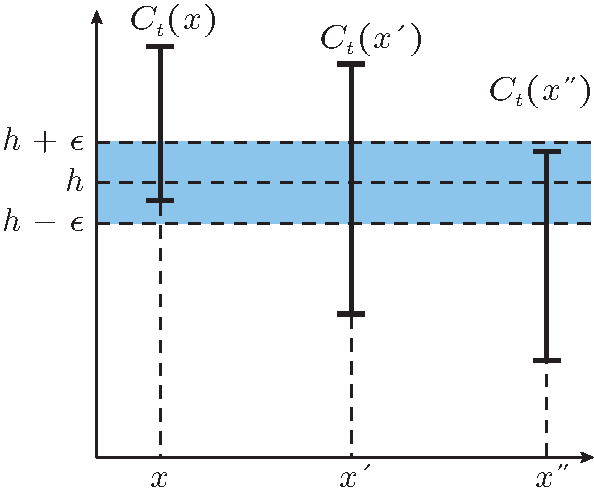
\includegraphics[height=1.5in]{figures/class}
    \caption{Confidence regions}
    \label{fig:conf}
  \end{subfigure}
  \hfill
  \begin{subfigure}[b]{0.49\linewidth}
    \centering
    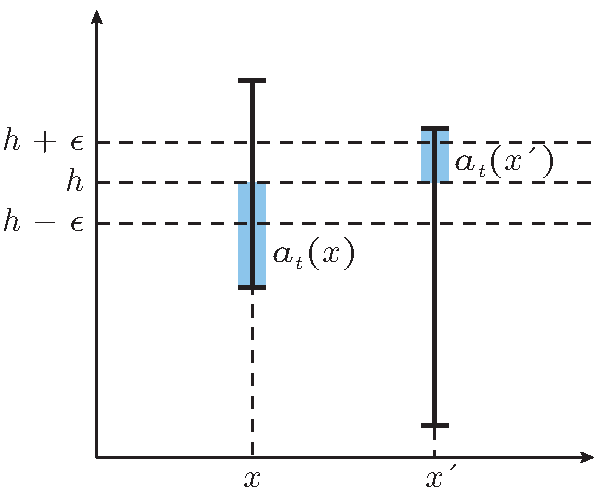
\includegraphics[height=1.5in]{figures/amb}
    \caption{Ambiguities}
    \label{fig:amb}
  \end{subfigure}
  \caption{
    (a) Example of the three possible configurations of confidence regions.
    (b) Ambiguities (shaded) of two example points.
  }
\end{figure}

\paragraph{Sample selection}
For selecting the next point to be evaluated at each iteration, we define the
following quantity
\begin{align*}
a_t(\*x) = \min\{\max(C_t(\*x)) - h, h - \min(C_t(\*x))\},
\end{align*}
which we call classification \emph{ambiguity}. As its name suggests, the
ambiguity of a point $\*x$ quantifies our uncertainty about whether $\*x$
belongs to $H_t$ or $L_t$ (see \figref{fig:amb}).
The intuition of sampling at areas of the sample space with large
classification uncertainty, expecting to gain more information about
the problem at hand when sampling at those areas, manifests itself in \acl
by choosing to evaluate at each iteration the point with the largest
ambiguity amongst the yet unclassified.

We can make an interesting observation at this point. If we use the confidence
intervals $Q_t(\*x)$ instead of the confidence regions $C_t(\*x)$
in the definition of ambiguity, we get the following quantity
\begin{align*}
a'_t(\*x) &= \min\{\max(Q_t(\*x)) - h, h - \min(Q_t(\*x))\}\\
          &= \min\{\mu_{t-1}(\*x) + \beta_t^{1/2}\sigma_{t-1}(\*x) - h,\ h - \mu_{t-1}(\*x) + \beta_t^{1/2}\sigma_{t-1}(\*x)\}\\
          &= \beta_t^{1/2}\sigma_{t-1}(\*x) - |\mu_{t-1}(\*x) - h|.
\end{align*}
For $\beta_t^{1/2} = 1.96$, this is identical to
the \emph{straddle}~\cite{bryan05} heuristic, which can thus be
intuitively explained in terms of classification ambiguity.

%\setlength\figureheight{1.5in}\setlength\figurewidth{2.5in}
%% This file was created by matlab2tikz v0.2.3.
% Copyright (c) 2008--2012, Nico Schlömer <nico.schloemer@gmail.com>
% All rights reserved.
% 
% 
%

\definecolor{locol}{rgb}{0.26, 0.45, 0.65}

\begin{tikzpicture}

\begin{axis}[%
tick label style={font=\tiny},
label style={font=\tiny},
xlabel shift={-10pt},
ylabel shift={-17pt},
legend style={font=\tiny},
view={0}{90},
width=\figurewidth,
height=\figureheight,
scale only axis,
xmin=0, xmax=1478,
xtick={0, 400, 1000, 1400},
xlabel={Length (m)},
ymin=-18, ymax=0,
ytick={0, -4, -14, -18},
ylabel={Depth (m)},
name=plot1,
axis lines*=box,
tickwidth=0.1cm,
clip=false
]

\addplot [fill=locol,draw=none,forget plot] coordinates{ (1478,0)(1478,-0.181818181818182)(1478,-0.363636363636364)(1478,-0.545454545454545)(1478,-0.727272727272727)(1478,-0.909090909090909)(1478,-1.09090909090909)(1478.0002488174,-1.27272727272727)(1478.00049762651,-1.45454545454545)(1478.00074642733,-1.63636363636364)(1478.00074642733,-1.81818181818182)(1478.00074642733,-2)(1478.00074642733,-2.18181818181818)(1478.00074642733,-2.36363636363636)(1478.00074642733,-2.54545454545455)(1478.00074642733,-2.72727272727273)(1478.00074642733,-2.90909090909091)(1478.00074642733,-3.09090909090909)(1478.00074642733,-3.27272727272727)(1478.00099521985,-3.45454545454545)(1478.00124400408,-3.63636363636364)(1478.00149278002,-3.81818181818182)(1478.00149278002,-4)(1478.00124400408,-4.18181818181818)(1478.00099521985,-4.36363636363636)(1478.00074642733,-4.54545454545455)(1478.00074642733,-4.72727272727273)(1478.00074642733,-4.90909090909091)(1478.00074642733,-5.09090909090909)(1478.00074642733,-5.27272727272727)(1478.00074642733,-5.45454545454545)(1478.00074642733,-5.63636363636364)(1478.00074642733,-5.81818181818182)(1478.00074642733,-6)(1478.00074642733,-6.18181818181818)(1478.00074642733,-6.36363636363636)(1478.00074642733,-6.54545454545455)(1478.00074642733,-6.72727272727273)(1478.00074642733,-6.90909090909091)(1478.00058056104,-7.09090909090909)(1478.00058056104,-7.27272727272727)(1478.00058056104,-7.45454545454545)(1478.00074642733,-7.63636363636364)(1478.00074642733,-7.81818181818182)(1478.00074642733,-8)(1478.00074642733,-8.18181818181818)(1478.00074642733,-8.36363636363636)(1478.00074642733,-8.54545454545455)(1478.00074642733,-8.72727272727273)(1478.00074642733,-8.90909090909091)(1478.00074642733,-9.09090909090909)(1478.00074642733,-9.27272727272727)(1478.00074642733,-9.45454545454546)(1478.00074642733,-9.63636363636364)(1478.00074642733,-9.81818181818182)(1478.00074642733,-10)(1478.00074642733,-10.1818181818182)(1478.00074642733,-10.3636363636364)(1478.00074642733,-10.5454545454545)(1478.00049762651,-10.7272727272727)(1478.0002488174,-10.9090909090909)(1478,-11.0909090909091)(1478,-11.2727272727273)(1478,-11.4545454545455)(1478,-11.6363636363636)(1478,-11.8181818181818)(1478.0002488174,-12)(1478.00049762651,-12.1818181818182)(1478.00074642733,-12.3636363636364)(1478.00074642733,-12.5454545454545)(1478.00074642733,-12.7272727272727)(1478.00074642733,-12.9090909090909)(1478.00074642733,-13.0909090909091)(1478.00074642733,-13.2727272727273)(1478.00074642733,-13.4545454545455)(1478.00074642733,-13.6363636363636)(1478.00074642733,-13.8181818181818)(1478.00074642733,-14)(1478.00074642733,-14.1818181818182)(1478.00074642733,-14.3636363636364)(1478.00074642733,-14.5454545454545)(1478.00074642733,-14.7272727272727)(1478.00074642733,-14.9090909090909)(1478.00074642733,-15.0909090909091)(1478.00074642733,-15.2727272727273)(1478.00074642733,-15.4545454545455)(1478.00074642733,-15.6363636363636)(1478.00049762651,-15.8181818181818)(1478.0002488174,-16)(1478,-16.1818181818182)(1478,-16.3636363636364)(1478,-16.5454545454545)(1478,-16.7272727272727)(1478,-16.9090909090909)(1478,-17.0909090909091)(1478,-17.2727272727273)(1478,-17.4545454545455)(1478,-17.6363636363636)(1478,-17.8181818181818)(1478,-18)(1463.07070707071,-18)(1448.14141414141,-18)(1433.21212121212,-18)(1418.28282828283,-18)(1403.35353535354,-18)(1388.42424242424,-18)(1373.49494949495,-18)(1358.56565656566,-18)(1343.63636363636,-18)(1328.70707070707,-18)(1313.77777777778,-18)(1298.84848484848,-18)(1283.91919191919,-18)(1268.9898989899,-18)(1254.06060606061,-18)(1239.13131313131,-18)(1224.20202020202,-18)(1209.27272727273,-18)(1194.34343434343,-18)(1179.41414141414,-18)(1164.48484848485,-18)(1149.55555555556,-18)(1134.62626262626,-18)(1119.69696969697,-18)(1104.76767676768,-18)(1089.83838383838,-18)(1074.90909090909,-18)(1059.9797979798,-18)(1045.05050505051,-18)(1030.12121212121,-18)(1015.19191919192,-18)(1000.26262626263,-18)(985.333333333333,-18)(970.40404040404,-18)(955.474747474747,-18)(940.545454545455,-18)(925.616161616162,-18)(910.686868686869,-18)(895.757575757576,-18)(880.828282828283,-18)(865.89898989899,-18)(850.969696969697,-18)(836.040404040404,-18)(821.111111111111,-18)(806.181818181818,-18)(791.252525252525,-18)(776.323232323232,-18)(761.393939393939,-18)(746.464646464646,-18)(731.535353535354,-18)(716.606060606061,-18)(701.676767676768,-18)(686.747474747475,-18)(671.818181818182,-18)(656.888888888889,-18)(641.959595959596,-18)(627.030303030303,-18)(612.10101010101,-18)(597.171717171717,-18)(582.242424242424,-18)(567.313131313131,-18)(552.383838383838,-18)(537.454545454546,-18)(522.525252525253,-18)(507.59595959596,-18)(492.666666666667,-18)(477.737373737374,-18)(462.808080808081,-18)(447.878787878788,-18)(432.949494949495,-18)(418.020202020202,-18)(403.090909090909,-18)(388.161616161616,-18)(373.232323232323,-18)(358.30303030303,-18)(343.373737373737,-18)(328.444444444444,-18)(313.515151515152,-18)(298.585858585859,-18)(283.656565656566,-18)(268.727272727273,-18)(253.79797979798,-18)(238.868686868687,-18)(223.939393939394,-18)(209.010101010101,-18)(194.080808080808,-18)(179.151515151515,-18)(164.222222222222,-18)(149.292929292929,-18)(134.363636363636,-18)(119.434343434343,-18)(104.505050505051,-18)(89.5757575757576,-18)(74.6464646464647,-18)(59.7171717171717,-18)(44.7878787878788,-18)(29.8585858585859,-18)(14.9292929292929,-18)(0,-18)(0,-17.8181818181818)(0,-17.6363636363636)(0,-17.4545454545455)(0,-17.2727272727273)(0,-17.0909090909091)(0,-16.9090909090909)(0,-16.7272727272727)(-0.000248817401863321,-16.5454545454545)(-0.000497626510092015,-16.3636363636364)(-0.000746427325097138,-16.1818181818182)(-0.000746427325097138,-16)(-0.000746427325097138,-15.8181818181818)(-0.000746427325097138,-15.6363636363636)(-0.000746427325097138,-15.4545454545455)(-0.000746427325097138,-15.2727272727273)(-0.000746427325097138,-15.0909090909091)(-0.000746427325097138,-14.9090909090909)(-0.000746427325097138,-14.7272727272727)(-0.000746427325097138,-14.5454545454545)(-0.000746427325097138,-14.3636363636364)(-0.000746427325097138,-14.1818181818182)(-0.000746427325097138,-14)(-0.000746427325097138,-13.8181818181818)(-0.000746427325097138,-13.6363636363636)(-0.000746427325097138,-13.4545454545455)(-0.000746427325097138,-13.2727272727273)(-0.000746427325097138,-13.0909090909091)(-0.000746427325097138,-12.9090909090909)(-0.000746427325097138,-12.7272727272727)(-0.000746427325097138,-12.5454545454545)(-0.000746427325097138,-12.3636363636364)(-0.000746427325097138,-12.1818181818182)(-0.000746427325097138,-12)(-0.000497626510092015,-11.8181818181818)(-0.000248817401863321,-11.6363636363636)(0,-11.4545454545455)(0,-11.2727272727273)(0,-11.0909090909091)(0,-10.9090909090909)(0,-10.7272727272727)(-0.000248817401863321,-10.5454545454545)(-0.000497626510092015,-10.3636363636364)(-0.000746427325097138,-10.1818181818182)(-0.000746427325097138,-10)(-0.000746427325097138,-9.81818181818182)(-0.000746427325097138,-9.63636363636364)(-0.000746427325097138,-9.45454545454546)(-0.000746427325097138,-9.27272727272727)(-0.000746427325097138,-9.09090909090909)(-0.000746427325097138,-8.90909090909091)(-0.000746427325097138,-8.72727272727273)(-0.000746427325097138,-8.54545454545455)(-0.000995219847296375,-8.36363636363636)(-0.00124400407710078,-8.18181818181818)(-0.00149278001492805,-8)(-0.00149278001492805,-7.81818181818182)(-0.00149278001492805,-7.63636363636364)(-0.00149278001492805,-7.45454545454545)(-0.00149278001492805,-7.27272727272727)(-0.00149278001492805,-7.09090909090909)(-0.00149278001492805,-6.90909090909091)(-0.00149278001492805,-6.72727272727273)(-0.00149278001492805,-6.54545454545455)(-0.00124400407710078,-6.36363636363636)(-0.000995219847296375,-6.18181818181818)(-0.000746427325097138,-6)(-0.000746427325097138,-5.81818181818182)(-0.000746427325097138,-5.63636363636364)(-0.000746427325097138,-5.45454545454545)(-0.000746427325097138,-5.27272727272727)(-0.000746427325097138,-5.09090909090909)(-0.000746427325097138,-4.90909090909091)(-0.000497626510092015,-4.72727272727273)(-0.000248817401863321,-4.54545454545455)(0,-4.36363636363636)(0,-4.18181818181818)(0,-4)(-0.000248817401863321,-3.81818181818182)(-0.000497626510092015,-3.63636363636364)(-0.000746427325097138,-3.45454545454545)(-0.000746427325097138,-3.27272727272727)(-0.000746427325097138,-3.09090909090909)(-0.000746427325097138,-2.90909090909091)(-0.000746427325097138,-2.72727272727273)(-0.000746427325097138,-2.54545454545455)(-0.000746427325097138,-2.36363636363636)(-0.000746427325097138,-2.18181818181818)(-0.000746427325097138,-2)(-0.000746427325097138,-1.81818181818182)(-0.000746427325097138,-1.63636363636364)(-0.000746427325097138,-1.45454545454545)(-0.000497626510092015,-1.27272727272727)(-0.000248817401863321,-1.09090909090909)(0,-0.909090909090909)(0,-0.727272727272727)(0,-0.545454545454545)(0,-0.363636363636364)(0,-0.181818181818182)(0,0)(14.9292929292929,0)(29.8585858585859,0)(44.7878787878788,0)(59.7171717171717,0)(74.6464646464647,0)(89.5757575757576,0)(104.505050505051,0)(119.434343434343,0)(134.363636363636,0)(149.292929292929,0)(164.222222222222,3.03025252607563e-06)(179.151515151515,6.06040404712874e-06)(194.080808080808,9.09045456816541e-06)(209.010101010101,9.09045456816541e-06)(223.939393939394,9.09045456816541e-06)(238.868686868687,9.09045456816541e-06)(253.79797979798,9.09045456816541e-06)(268.727272727273,9.09045456816541e-06)(283.656565656566,9.09045456816541e-06)(298.585858585859,9.09045456816541e-06)(313.515151515152,9.09045456816541e-06)(328.444444444444,9.09045456816541e-06)(343.373737373737,9.09045456816541e-06)(358.30303030303,9.09045456816541e-06)(373.232323232323,9.09045456816541e-06)(388.161616161616,9.09045456816541e-06)(403.090909090909,9.09045456816541e-06)(418.020202020202,9.09045456816541e-06)(432.949494949495,9.09045456816541e-06)(447.878787878788,9.09045456816541e-06)(462.808080808081,9.09045456816541e-06)(477.737373737374,9.09045456816541e-06)(492.666666666667,6.06040404712874e-06)(507.59595959596,3.03025252607563e-06)(522.525252525253,0)(537.454545454546,0)(552.383838383838,0)(567.313131313131,0)(582.242424242424,0)(597.171717171717,0)(612.10101010101,0)(627.030303030303,0)(641.959595959596,0)(656.888888888889,0)(671.818181818182,0)(686.747474747475,0)(701.676767676768,0)(716.606060606061,0)(731.535353535354,0)(746.464646464646,0)(761.393939393939,0)(776.323232323232,0)(791.252525252525,0)(806.181818181818,3.03025252607563e-06)(821.111111111111,6.06040404712874e-06)(836.040404040404,9.09045456816541e-06)(850.969696969697,9.09045456816541e-06)(865.89898989899,9.09045456816541e-06)(880.828282828283,9.09045456816541e-06)(895.757575757576,9.09045456816541e-06)(910.686868686869,9.09045456816541e-06)(925.616161616162,9.09045456816541e-06)(940.545454545455,9.09045456816541e-06)(955.474747474747,9.09045456816541e-06)(970.40404040404,9.09045456816541e-06)(985.333333333333,9.09045456816541e-06)(1000.26262626263,9.09045456816541e-06)(1015.19191919192,9.09045456816541e-06)(1030.12121212121,9.09045456816541e-06)(1045.05050505051,9.09045456816541e-06)(1059.9797979798,9.09045456816541e-06)(1074.90909090909,9.09045456816541e-06)(1089.83838383838,9.09045456816541e-06)(1104.76767676768,9.09045456816541e-06)(1119.69696969697,9.09045456816541e-06)(1134.62626262626,9.09045456816541e-06)(1149.55555555556,9.09045456816541e-06)(1164.48484848485,9.09045456816541e-06)(1179.41414141414,9.09045456816541e-06)(1194.34343434343,9.09045456816541e-06)(1209.27272727273,8.08044894971196e-06)(1224.20202020202,5.05036476259526e-06)(1239.13131313131,2.02017957376651e-06)(1254.06060606061,0)(1268.9898989899,0)(1283.91919191919,0)(1298.84848484848,0)(1313.77777777778,0)(1328.70707070707,0)(1343.63636363636,0)(1358.56565656566,0)(1373.49494949495,0)(1388.42424242424,0)(1403.35353535354,0)(1418.28282828283,0)(1433.21212121212,0)(1448.14141414141,0)(1463.07070707071,0)(1478,0)};

\addplot [fill=darkgray,draw=none,forget plot] coordinates{ (1226.69023569024,0)(1224.20202020202,-0.0909090909090909)(1221.7138047138,-0.181818181818182)(1216.73737373737,-0.363636363636364)(1221.7138047138,-0.545454545454545)(1224.20202020202,-0.636363636363636)(1226.69023569024,-0.727272727272727)(1236.6430976431,-0.909090909090909)(1239.13131313131,-0.954545454545454)(1250.32828282828,-1.09090909090909)(1254.06060606061,-1.12121212121212)(1268.9898989899,-1.24242424242424)(1276.45454545455,-1.27272727272727)(1283.91919191919,-1.3030303030303)(1298.84848484848,-1.36363636363636)(1313.77777777778,-1.36363636363636)(1328.70707070707,-1.36363636363636)(1343.63636363636,-1.36363636363636)(1358.56565656566,-1.36363636363636)(1373.49494949495,-1.36363636363636)(1388.42424242424,-1.36363636363636)(1403.35353535354,-1.36363636363636)(1418.28282828283,-1.36363636363636)(1433.21212121212,-1.36363636363636)(1448.14141414141,-1.36363636363636)(1463.07070707071,-1.36363636363636)(1478,-1.36363636363636)(1478.00012440663,-1.45454545454545)(1478.00037321366,-1.63636363636364)(1478.00037321366,-1.81818181818182)(1478.00037321366,-2)(1478.00037321366,-2.18181818181818)(1478.00037321366,-2.36363636363636)(1478.00037321366,-2.54545454545455)(1478.00037321366,-2.72727272727273)(1478.00037321366,-2.90909090909091)(1478.00037321366,-3.09090909090909)(1478.00037321366,-3.27272727272727)(1478.0006220124,-3.45454545454545)(1478.00087080285,-3.63636363636364)(1478.00111958501,-3.81818181818182)(1478.00111958501,-4)(1478.00087080285,-4.18181818181818)(1478.0006220124,-4.36363636363636)(1478.00037321366,-4.54545454545455)(1478.00037321366,-4.72727272727273)(1478.00037321366,-4.90909090909091)(1478.00037321366,-5.09090909090909)(1478.00037321366,-5.27272727272727)(1478.00037321366,-5.45454545454545)(1478.00037321366,-5.63636363636364)(1478.00037321366,-5.81818181818182)(1478.00037321366,-6)(1478.00037321366,-6.18181818181818)(1478.00037321366,-6.36363636363636)(1478.00037321366,-6.54545454545455)(1478.00037321366,-6.72727272727273)(1478.00037321366,-6.90909090909091)(1478.00020734323,-7.09090909090909)(1478.00020734323,-7.27272727272727)(1478.00020734323,-7.45454545454545)(1478.00037321366,-7.63636363636364)(1478.00037321366,-7.81818181818182)(1478.00037321366,-8)(1478.00037321366,-8.18181818181818)(1478.00037321366,-8.36363636363636)(1478.00037321366,-8.54545454545455)(1478.00037321366,-8.72727272727273)(1478.00037321366,-8.90909090909091)(1478.00037321366,-9.09090909090909)(1478.00037321366,-9.27272727272727)(1478.00037321366,-9.45454545454546)(1478.00037321366,-9.63636363636364)(1478.00037321366,-9.81818181818182)(1478.00037321366,-10)(1478.00037321366,-10.1818181818182)(1478.00037321366,-10.3636363636364)(1478.00037321366,-10.5454545454545)(1478.00012440663,-10.7272727272727)(1478,-10.8181818181818)(1463.07070707071,-10.8181818181818)(1448.14141414141,-10.8181818181818)(1433.21212121212,-10.8181818181818)(1418.28282828283,-10.8787878787879)(1410.81818181818,-10.9090909090909)(1403.35353535354,-10.9393939393939)(1390.91245791246,-11.0909090909091)(1388.42424242424,-11.1363636363636)(1380.9595959596,-11.2727272727273)(1380.9595959596,-11.4545454545455)(1385.93602693603,-11.6363636363636)(1388.42424242424,-11.6818181818182)(1399.62121212121,-11.8181818181818)(1403.35353535354,-11.8484848484849)(1418.28282828283,-11.969696969697)(1425.74747474747,-12)(1433.21212121212,-12.030303030303)(1448.14141414141,-12.0909090909091)(1463.07070707071,-12.0909090909091)(1478,-12.0909090909091)(1478.00012440663,-12.1818181818182)(1478.00037321366,-12.3636363636364)(1478.00037321366,-12.5454545454545)(1478.00037321366,-12.7272727272727)(1478.00037321366,-12.9090909090909)(1478.00037321366,-13.0909090909091)(1478.00037321366,-13.2727272727273)(1478.00037321366,-13.4545454545455)(1478.00037321366,-13.6363636363636)(1478.00037321366,-13.8181818181818)(1478.00037321366,-14)(1478.00037321366,-14.1818181818182)(1478.00037321366,-14.3636363636364)(1478.00037321366,-14.5454545454545)(1478.00037321366,-14.7272727272727)(1478.00037321366,-14.9090909090909)(1478.00037321366,-15.0909090909091)(1478.00037321366,-15.2727272727273)(1478.00037321366,-15.4545454545455)(1478.00037321366,-15.6363636363636)(1478.00012440663,-15.8181818181818)(1478,-15.9090909090909)(1463.07070707071,-15.9090909090909)(1448.14141414141,-15.9090909090909)(1433.21212121212,-15.9090909090909)(1418.28282828283,-15.9090909090909)(1403.35353535354,-15.9090909090909)(1388.42424242424,-15.9090909090909)(1373.49494949495,-15.9090909090909)(1358.56565656566,-15.969696969697)(1351.10101010101,-16)(1343.63636363636,-16.030303030303)(1328.70707070707,-16.0909090909091)(1313.77777777778,-16.0909090909091)(1298.84848484848,-16.0909090909091)(1283.91919191919,-16.1515151515152)(1276.45454545455,-16.1818181818182)(1268.9898989899,-16.2121212121212)(1254.06060606061,-16.2727272727273)(1239.13131313131,-16.3333333333333)(1231.66666666667,-16.3636363636364)(1224.20202020202,-16.3939393939394)(1209.27272727273,-16.4545454545455)(1194.34343434343,-16.5151515151515)(1186.87878787879,-16.5454545454545)(1179.41414141414,-16.5757575757576)(1164.48484848485,-16.6363636363636)(1149.55555555556,-16.6969696969697)(1142.09090909091,-16.7272727272727)(1134.62626262626,-16.7575757575758)(1119.69696969697,-16.8181818181818)(1104.76767676768,-16.8787878787879)(1097.30303030303,-16.9090909090909)(1089.83838383838,-16.9393939393939)(1074.90909090909,-17)(1059.9797979798,-17)(1045.05050505051,-17)(1030.12121212121,-17)(1015.19191919192,-16.9393939393939)(1007.72727272727,-16.9090909090909)(1000.26262626263,-16.8787878787879)(985.333333333333,-16.8181818181818)(970.40404040404,-16.7575757575758)(962.939393939394,-16.7272727272727)(955.474747474747,-16.6969696969697)(940.545454545455,-16.5757575757576)(933.080808080808,-16.5454545454545)(925.616161616162,-16.5151515151515)(910.686868686869,-16.3939393939394)(903.222222222222,-16.3636363636364)(895.757575757576,-16.3333333333333)(880.828282828283,-16.2727272727273)(865.89898989899,-16.2121212121212)(862.166666666667,-16.1818181818182)(850.969696969697,-16.0909090909091)(839.772727272727,-16)(836.040404040404,-15.969696969697)(821.111111111111,-15.8484848484849)(817.378787878788,-15.8181818181818)(806.181818181818,-15.6818181818182)(803.693602693603,-15.6363636363636)(798.717171717172,-15.4545454545455)(798.717171717172,-15.2727272727273)(798.717171717172,-15.0909090909091)(803.693602693603,-14.9090909090909)(806.181818181818,-14.8181818181818)(808.670033670034,-14.7272727272727)(818.622895622896,-14.5454545454545)(821.111111111111,-14.4545454545455)(823.599326599327,-14.3636363636364)(828.575757575758,-14.1818181818182)(828.575757575758,-14)(833.552188552189,-13.8181818181818)(833.552188552189,-13.6363636363636)(833.552188552189,-13.4545454545455)(828.575757575758,-13.2727272727273)(823.599326599327,-13.0909090909091)(821.111111111111,-13.0454545454545)(813.646464646465,-12.9090909090909)(806.181818181818,-12.8181818181818)(798.717171717172,-12.7272727272727)(791.252525252525,-12.6363636363636)(780.055555555556,-12.5454545454545)(776.323232323232,-12.5151515151515)(761.393939393939,-12.4545454545455)(746.464646464646,-12.4545454545455)(731.535353535354,-12.3939393939394)(724.070707070707,-12.3636363636364)(716.606060606061,-12.3333333333333)(701.676767676768,-12.2727272727273)(686.747474747475,-12.2727272727273)(671.818181818182,-12.2727272727273)(656.888888888889,-12.2727272727273)(641.959595959596,-12.2727272727273)(627.030303030303,-12.2727272727273)(612.10101010101,-12.2727272727273)(597.171717171717,-12.2727272727273)(582.242424242424,-12.2727272727273)(567.313131313131,-12.2727272727273)(552.383838383838,-12.2727272727273)(537.454545454546,-12.2727272727273)(522.525252525253,-12.2727272727273)(507.59595959596,-12.3333333333333)(500.131313131313,-12.3636363636364)(492.666666666667,-12.3939393939394)(477.737373737374,-12.4545454545455)(462.808080808081,-12.4545454545455)(447.878787878788,-12.5151515151515)(440.414141414141,-12.5454545454545)(432.949494949495,-12.5757575757576)(418.020202020202,-12.6969696969697)(414.287878787879,-12.7272727272727)(403.090909090909,-12.8181818181818)(395.626262626263,-12.9090909090909)(388.161616161616,-13.0454545454545)(385.673400673401,-13.0909090909091)(375.720538720539,-13.2727272727273)(373.232323232323,-13.3636363636364)(370.744107744108,-13.4545454545455)(365.767676767677,-13.6363636363636)(365.767676767677,-13.8181818181818)(365.767676767677,-14)(370.744107744108,-14.1818181818182)(373.232323232323,-14.2727272727273)(375.720538720539,-14.3636363636364)(385.673400673401,-14.5454545454545)(388.161616161616,-14.5909090909091)(395.626262626263,-14.7272727272727)(403.090909090909,-14.8181818181818)(410.555555555556,-14.9090909090909)(418.020202020202,-15)(425.484848484849,-15.0909090909091)(432.949494949495,-15.1818181818182)(440.414141414141,-15.2727272727273)(447.878787878788,-15.4090909090909)(450.367003367003,-15.4545454545455)(460.319865319865,-15.6363636363636)(462.808080808081,-15.7272727272727)(465.296296296296,-15.8181818181818)(470.272727272727,-16)(465.296296296296,-16.1818181818182)(462.808080808081,-16.2272727272727)(455.343434343434,-16.3636363636364)(447.878787878788,-16.4545454545455)(440.414141414141,-16.5454545454545)(432.949494949495,-16.6363636363636)(421.752525252525,-16.7272727272727)(418.020202020202,-16.7575757575758)(403.090909090909,-16.8787878787879)(395.626262626263,-16.9090909090909)(388.161616161616,-16.9393939393939)(373.232323232323,-17)(358.30303030303,-17.0606060606061)(350.838383838384,-17.0909090909091)(343.373737373737,-17.1212121212121)(328.444444444444,-17.1212121212121)(320.979797979798,-17.0909090909091)(313.515151515152,-17.0606060606061)(298.585858585859,-17)(283.656565656566,-17)(268.727272727273,-16.9393939393939)(261.262626262626,-16.9090909090909)(253.79797979798,-16.8787878787879)(238.868686868687,-16.8181818181818)(223.939393939394,-16.7575757575758)(216.474747474747,-16.7272727272727)(209.010101010101,-16.6969696969697)(194.080808080808,-16.6363636363636)(179.151515151515,-16.6363636363636)(164.222222222222,-16.5757575757576)(156.757575757576,-16.5454545454545)(149.292929292929,-16.5151515151515)(134.363636363636,-16.4545454545455)(119.434343434343,-16.4545454545455)(104.505050505051,-16.4545454545455)(89.5757575757576,-16.4545454545455)(74.6464646464647,-16.4545454545455)(59.7171717171717,-16.4545454545455)(44.7878787878788,-16.4545454545455)(29.8585858585859,-16.4545454545455)(14.9292929292929,-16.4545454545455)(0,-16.4545454545455)(-0.000124406627524661,-16.3636363636364)(-0.000373213662548569,-16.1818181818182)(-0.000373213662548569,-16)(-0.000373213662548569,-15.8181818181818)(-0.000373213662548569,-15.6363636363636)(-0.000373213662548569,-15.4545454545455)(-0.000373213662548569,-15.2727272727273)(-0.000373213662548569,-15.0909090909091)(-0.000373213662548569,-14.9090909090909)(-0.000373213662548569,-14.7272727272727)(-0.000373213662548569,-14.5454545454545)(-0.000373213662548569,-14.3636363636364)(-0.000373213662548569,-14.1818181818182)(-0.000373213662548569,-14)(-0.000373213662548569,-13.8181818181818)(-0.000373213662548569,-13.6363636363636)(-0.000373213662548569,-13.4545454545455)(-0.000373213662548569,-13.2727272727273)(-0.000373213662548569,-13.0909090909091)(-0.000373213662548569,-12.9090909090909)(-0.000373213662548569,-12.7272727272727)(-0.000373213662548569,-12.5454545454545)(-0.000373213662548569,-12.3636363636364)(-0.000373213662548569,-12.1818181818182)(-0.000373213662548569,-12)(-0.000124406627524661,-11.8181818181818)(0,-11.7272727272727)(14.9292929292929,-11.7272727272727)(29.8585858585859,-11.7272727272727)(44.7878787878788,-11.7272727272727)(59.7171717171717,-11.6666666666667)(67.1818181818182,-11.6363636363636)(74.6464646464647,-11.6060606060606)(89.5757575757576,-11.4848484848485)(97.040404040404,-11.4545454545455)(104.505050505051,-11.4242424242424)(119.434343434343,-11.3030303030303)(126.89898989899,-11.2727272727273)(134.363636363636,-11.2424242424242)(149.292929292929,-11.1212121212121)(153.025252525253,-11.0909090909091)(164.222222222222,-11)(175.419191919192,-10.9090909090909)(179.151515151515,-10.8787878787879)(194.080808080808,-10.7575757575758)(201.545454545455,-10.7272727272727)(209.010101010101,-10.6969696969697)(223.939393939394,-10.6363636363636)(238.868686868687,-10.5757575757576)(246.333333333333,-10.5454545454545)(253.79797979798,-10.5151515151515)(268.727272727273,-10.3939393939394)(276.191919191919,-10.3636363636364)(283.656565656566,-10.3333333333333)(298.585858585859,-10.2121212121212)(302.318181818182,-10.1818181818182)(313.515151515152,-10.0909090909091)(320.979797979798,-10)(328.444444444444,-9.86363636363636)(330.93265993266,-9.81818181818182)(328.444444444444,-9.72727272727273)(325.956228956229,-9.63636363636364)(313.515151515152,-9.48484848484848)(306.050505050505,-9.45454545454546)(298.585858585859,-9.42424242424243)(283.656565656566,-9.36363636363636)(268.727272727273,-9.36363636363636)(253.79797979798,-9.36363636363636)(238.868686868687,-9.42424242424243)(231.40404040404,-9.45454545454546)(223.939393939394,-9.48484848484848)(209.010101010101,-9.60606060606061)(201.545454545455,-9.63636363636364)(194.080808080808,-9.66666666666667)(179.151515151515,-9.78787878787879)(171.686868686869,-9.81818181818182)(164.222222222222,-9.84848484848485)(149.292929292929,-9.96969696969697)(141.828282828283,-10)(134.363636363636,-10.030303030303)(119.434343434343,-10.1515151515152)(111.969696969697,-10.1818181818182)(104.505050505051,-10.2121212121212)(89.5757575757576,-10.2727272727273)(74.6464646464647,-10.2727272727273)(59.7171717171717,-10.2727272727273)(44.7878787878788,-10.2727272727273)(29.8585858585859,-10.3333333333333)(22.3939393939394,-10.3636363636364)(14.9292929292929,-10.3939393939394)(0,-10.4545454545455)(-0.000124406627524661,-10.3636363636364)(-0.000373213662548569,-10.1818181818182)(-0.000373213662548569,-10)(-0.000373213662548569,-9.81818181818182)(-0.000373213662548569,-9.63636363636364)(-0.000373213662548569,-9.45454545454546)(-0.000373213662548569,-9.27272727272727)(-0.000373213662548569,-9.09090909090909)(-0.000373213662548569,-8.90909090909091)(-0.000373213662548569,-8.72727272727273)(-0.000373213662548569,-8.54545454545455)(-0.000622012404561063,-8.36363636363636)(-0.000870802853969885,-8.18181818181818)(-0.00111958501119604,-8)(-0.00111958501119604,-7.81818181818182)(-0.00111958501119604,-7.63636363636364)(-0.00111958501119604,-7.45454545454545)(-0.00111958501119604,-7.27272727272727)(-0.00111958501119604,-7.09090909090909)(-0.00111958501119604,-6.90909090909091)(-0.00111958501119604,-6.72727272727273)(-0.00111958501119604,-6.54545454545455)(-0.000870802853969885,-6.36363636363636)(-0.000622012404561063,-6.18181818181818)(-0.000373213662548569,-6)(-0.000373213662548569,-5.81818181818182)(-0.000373213662548569,-5.63636363636364)(-0.000373213662548569,-5.45454545454545)(-0.000373213662548569,-5.27272727272727)(-0.000373213662548569,-5.09090909090909)(-0.000373213662548569,-4.90909090909091)(-0.000124406627524661,-4.72727272727273)(0,-4.63636363636364)(14.9292929292929,-4.63636363636364)(29.8585858585859,-4.57575757575758)(37.3232323232323,-4.54545454545455)(44.7878787878788,-4.51515151515152)(59.7171717171717,-4.39393939393939)(63.4494949494949,-4.36363636363636)(74.6464646464647,-4.22727272727273)(77.1346801346801,-4.18181818181818)(77.1346801346801,-4)(74.6464646464647,-3.95454545454545)(63.4494949494949,-3.81818181818182)(59.7171717171717,-3.78787878787879)(44.7878787878788,-3.72727272727273)(29.8585858585859,-3.72727272727273)(14.9292929292929,-3.72727272727273)(0,-3.72727272727273)(-0.000124406627524661,-3.63636363636364)(-0.000373213662548569,-3.45454545454545)(-0.000373213662548569,-3.27272727272727)(-0.000373213662548569,-3.09090909090909)(-0.000373213662548569,-2.90909090909091)(-0.000373213662548569,-2.72727272727273)(-0.000373213662548569,-2.54545454545455)(-0.000373213662548569,-2.36363636363636)(-0.000373213662548569,-2.18181818181818)(-0.000373213662548569,-2)(-0.000373213662548569,-1.81818181818182)(-0.000373213662548569,-1.63636363636364)(-0.000373213662548569,-1.45454545454545)(-0.000124406627524661,-1.27272727272727)(0,-1.18181818181818)(14.9292929292929,-1.18181818181818)(29.8585858585859,-1.18181818181818)(44.7878787878788,-1.18181818181818)(59.7171717171717,-1.18181818181818)(74.6464646464647,-1.18181818181818)(89.5757575757576,-1.12121212121212)(97.040404040404,-1.09090909090909)(104.505050505051,-1.06060606060606)(119.434343434343,-1)(134.363636363636,-0.939393939393939)(138.09595959596,-0.909090909090909)(149.292929292929,-0.818181818181818)(156.757575757576,-0.727272727272727)(164.222222222222,-0.590909090909091)(166.710437710438,-0.545454545454545)(171.686868686869,-0.363636363636364)(171.686868686869,-0.181818181818182)(171.686868686869,0)(179.151515151515,1.515101011762e-06)(194.080808080808,4.54522728408271e-06)(209.010101010101,4.54522728408271e-06)(223.939393939394,4.54522728408271e-06)(238.868686868687,4.54522728408271e-06)(253.79797979798,4.54522728408271e-06)(268.727272727273,4.54522728408271e-06)(283.656565656566,4.54522728408271e-06)(298.585858585859,4.54522728408271e-06)(313.515151515152,4.54522728408271e-06)(328.444444444444,4.54522728408271e-06)(343.373737373737,4.54522728408271e-06)(358.30303030303,4.54522728408271e-06)(373.232323232323,4.54522728408271e-06)(388.161616161616,4.54522728408271e-06)(403.090909090909,4.54522728408271e-06)(418.020202020202,4.54522728408271e-06)(432.949494949495,4.54522728408271e-06)(447.878787878788,4.54522728408271e-06)(462.808080808081,4.54522728408271e-06)(477.737373737374,4.54522728408271e-06)(492.666666666667,1.515101011762e-06)(500.131313131313,0)(500.131313131313,-0.181818181818182)(500.131313131313,-0.363636363636364)(505.107744107744,-0.545454545454545)(507.59595959596,-0.636363636363636)(510.084175084175,-0.727272727272727)(515.060606060606,-0.909090909090909)(515.060606060606,-1.09090909090909)(515.060606060606,-1.27272727272727)(515.060606060606,-1.45454545454545)(515.060606060606,-1.63636363636364)(515.060606060606,-1.81818181818182)(515.060606060606,-2)(520.037037037037,-2.18181818181818)(522.525252525253,-2.22727272727273)(529.989898989899,-2.36363636363636)(537.454545454546,-2.45454545454545)(548.651515151515,-2.54545454545455)(552.383838383838,-2.57575757575758)(567.313131313131,-2.6969696969697)(574.777777777778,-2.72727272727273)(582.242424242424,-2.75757575757576)(597.171717171717,-2.81818181818182)(612.10101010101,-2.81818181818182)(627.030303030303,-2.81818181818182)(641.959595959596,-2.75757575757576)(645.691919191919,-2.72727272727273)(656.888888888889,-2.63636363636364)(668.085858585859,-2.54545454545455)(671.818181818182,-2.51515151515152)(686.747474747475,-2.39393939393939)(690.479797979798,-2.36363636363636)(701.676767676768,-2.27272727272727)(709.141414141414,-2.18181818181818)(716.606060606061,-2.09090909090909)(724.070707070707,-2)(731.535353535354,-1.86363636363636)(734.023569023569,-1.81818181818182)(743.976430976431,-1.63636363636364)(746.464646464646,-1.59090909090909)(753.929292929293,-1.45454545454545)(761.393939393939,-1.36363636363636)(768.858585858586,-1.27272727272727)(776.323232323232,-1.18181818181818)(783.787878787879,-1.09090909090909)(791.252525252525,-0.954545454545454)(793.740740740741,-0.909090909090909)(803.693602693603,-0.727272727272727)(806.181818181818,-0.636363636363636)(808.670033670034,-0.545454545454545)(813.646464646465,-0.363636363636364)(813.646464646465,-0.181818181818182)(813.646464646465,0)(821.111111111111,1.515101011762e-06)(836.040404040404,4.54522728408271e-06)(850.969696969697,4.54522728408271e-06)(865.89898989899,4.54522728408271e-06)(880.828282828283,4.54522728408271e-06)(895.757575757576,4.54522728408271e-06)(910.686868686869,4.54522728408271e-06)(925.616161616162,4.54522728408271e-06)(940.545454545455,4.54522728408271e-06)(955.474747474747,4.54522728408271e-06)(970.40404040404,4.54522728408271e-06)(985.333333333333,4.54522728408271e-06)(1000.26262626263,4.54522728408271e-06)(1015.19191919192,4.54522728408271e-06)(1030.12121212121,4.54522728408271e-06)(1045.05050505051,4.54522728408271e-06)(1059.9797979798,4.54522728408271e-06)(1074.90909090909,4.54522728408271e-06)(1089.83838383838,4.54522728408271e-06)(1104.76767676768,4.54522728408271e-06)(1119.69696969697,4.54522728408271e-06)(1134.62626262626,4.54522728408271e-06)(1149.55555555556,4.54522728408271e-06)(1164.48484848485,4.54522728408271e-06)(1179.41414141414,4.54522728408271e-06)(1194.34343434343,4.54522728408271e-06)(1209.27272727273,3.53519641552421e-06)(1224.20202020202,5.05036476275675e-07)(1226.69023569024,0)};

\addplot [fill=red!40!yellow,draw=none,forget plot] coordinates{ (604.636363636364,-3.45454545454545)(612.10101010101,-3.48484848484849)(627.030303030303,-3.60606060606061)(634.494949494949,-3.63636363636364)(641.959595959596,-3.66666666666667)(656.888888888889,-3.78787878787879)(664.353535353535,-3.81818181818182)(671.818181818182,-3.84848484848485)(686.747474747475,-3.96969696969697)(690.479797979798,-4)(701.676767676768,-4.09090909090909)(709.141414141414,-4.18181818181818)(716.606060606061,-4.27272727272727)(724.070707070707,-4.36363636363636)(731.535353535354,-4.45454545454546)(739,-4.54545454545455)(746.464646464646,-4.68181818181818)(748.952861952862,-4.72727272727273)(753.929292929293,-4.90909090909091)(746.464646464646,-5.04545454545455)(743.976430976431,-5.09090909090909)(731.535353535354,-5.24242424242424)(724.070707070707,-5.27272727272727)(716.606060606061,-5.3030303030303)(701.676767676768,-5.36363636363636)(686.747474747475,-5.42424242424242)(679.282828282828,-5.45454545454545)(671.818181818182,-5.48484848484848)(656.888888888889,-5.54545454545455)(641.959595959596,-5.54545454545455)(627.030303030303,-5.60606060606061)(619.565656565657,-5.63636363636364)(612.10101010101,-5.66666666666667)(597.171717171717,-5.72727272727273)(582.242424242424,-5.72727272727273)(567.313131313131,-5.72727272727273)(552.383838383838,-5.72727272727273)(537.454545454546,-5.72727272727273)(522.525252525253,-5.72727272727273)(507.59595959596,-5.72727272727273)(492.666666666667,-5.72727272727273)(477.737373737374,-5.72727272727273)(462.808080808081,-5.72727272727273)(447.878787878788,-5.72727272727273)(432.949494949495,-5.72727272727273)(418.020202020202,-5.78787878787879)(410.555555555556,-5.81818181818182)(403.090909090909,-5.84848484848485)(388.161616161616,-5.90909090909091)(373.232323232323,-5.90909090909091)(358.30303030303,-5.90909090909091)(343.373737373737,-5.96969696969697)(335.909090909091,-6)(328.444444444444,-6.03030303030303)(313.515151515152,-6.09090909090909)(298.585858585859,-6.09090909090909)(283.656565656566,-6.15151515151515)(276.191919191919,-6.18181818181818)(268.727272727273,-6.21212121212121)(253.79797979798,-6.27272727272727)(238.868686868687,-6.27272727272727)(223.939393939394,-6.27272727272727)(209.010101010101,-6.31818181818182)(205.277777777778,-6.36363636363636)(194.080808080808,-6.5)(191.592592592593,-6.54545454545455)(186.616161616162,-6.72727272727273)(181.639730639731,-6.90909090909091)(179.151515151515,-6.95454545454545)(171.686868686869,-7.09090909090909)(164.222222222222,-7.22727272727273)(161.734006734007,-7.27272727272727)(151.781144781145,-7.45454545454545)(149.292929292929,-7.5)(138.09595959596,-7.63636363636364)(134.363636363636,-7.66666666666667)(119.434343434343,-7.78787878787879)(115.70202020202,-7.81818181818182)(104.505050505051,-7.90909090909091)(93.3080808080808,-8)(89.5757575757576,-8.03030303030303)(74.6464646464647,-8.09090909090909)(59.7171717171717,-8.09090909090909)(44.7878787878788,-8.15151515151515)(37.3232323232323,-8.18181818181818)(29.8585858585859,-8.21212121212121)(14.9292929292929,-8.27272727272727)(0,-8.27272727272727)(-0.000124400407711404,-8.18181818181818)(-0.000373195003732012,-8)(-0.000373195003732012,-7.81818181818182)(-0.000373195003732012,-7.63636363636364)(-0.000373195003732012,-7.45454545454545)(-0.000373195003732012,-7.27272727272727)(-0.000373195003732012,-7.09090909090909)(-0.000373195003732012,-6.90909090909091)(-0.000373195003732012,-6.72727272727273)(-0.000373195003732012,-6.54545454545455)(-0.000124400407711404,-6.36363636363636)(0,-6.27272727272727)(14.9292929292929,-6.27272727272727)(29.8585858585859,-6.27272727272727)(44.7878787878788,-6.27272727272727)(59.7171717171717,-6.27272727272727)(74.6464646464647,-6.27272727272727)(89.5757575757576,-6.27272727272727)(104.505050505051,-6.27272727272727)(119.434343434343,-6.27272727272727)(134.363636363636,-6.27272727272727)(149.292929292929,-6.27272727272727)(164.222222222222,-6.21212121212121)(171.686868686869,-6.18181818181818)(179.151515151515,-6.15151515151515)(194.080808080808,-6.04545454545455)(197.813131313131,-6)(209.010101010101,-5.90909090909091)(216.474747474747,-5.81818181818182)(223.939393939394,-5.72727272727273)(235.136363636364,-5.63636363636364)(238.868686868687,-5.60606060606061)(253.79797979798,-5.48484848484848)(261.262626262626,-5.45454545454545)(268.727272727273,-5.42424242424242)(283.656565656566,-5.3030303030303)(291.121212121212,-5.27272727272727)(298.585858585859,-5.24242424242424)(313.515151515152,-5.12121212121212)(320.979797979798,-5.09090909090909)(328.444444444444,-5.06060606060606)(340.885521885522,-4.90909090909091)(343.373737373737,-4.87878787878788)(355.814814814815,-4.72727272727273)(358.30303030303,-4.68181818181818)(365.767676767677,-4.54545454545455)(373.232323232323,-4.40909090909091)(375.720538720539,-4.36363636363636)(385.673400673401,-4.18181818181818)(388.161616161616,-4.09090909090909)(390.649831649832,-4)(403.090909090909,-3.84848484848485)(405.579124579125,-3.81818181818182)(418.020202020202,-3.66666666666667)(425.484848484849,-3.63636363636364)(432.949494949495,-3.60606060606061)(447.878787878788,-3.54545454545455)(462.808080808081,-3.54545454545455)(477.737373737374,-3.48484848484849)(485.20202020202,-3.45454545454545)(492.666666666667,-3.42424242424242)(507.59595959596,-3.36363636363636)(522.525252525253,-3.36363636363636)(537.454545454546,-3.36363636363636)(552.383838383838,-3.36363636363636)(567.313131313131,-3.36363636363636)(582.242424242424,-3.36363636363636)(597.171717171717,-3.42424242424242)(604.636363636364,-3.45454545454545)};

\addplot [fill=red!40!yellow,draw=none,forget plot] coordinates{ (992.79797979798,-7.27272727272727)(1000.26262626263,-7.3030303030303)(1015.19191919192,-7.42424242424242)(1022.65656565657,-7.45454545454545)(1030.12121212121,-7.48484848484848)(1045.05050505051,-7.60606060606061)(1052.51515151515,-7.63636363636364)(1059.9797979798,-7.66666666666667)(1074.90909090909,-7.78787878787879)(1082.37373737374,-7.81818181818182)(1089.83838383838,-7.84848484848485)(1104.76767676768,-7.90909090909091)(1119.69696969697,-7.90909090909091)(1134.62626262626,-7.90909090909091)(1149.55555555556,-7.90909090909091)(1164.48484848485,-7.96969696969697)(1171.94949494949,-8)(1179.41414141414,-8.03030303030303)(1194.34343434343,-8.09090909090909)(1209.27272727273,-8.09090909090909)(1224.20202020202,-8.09090909090909)(1239.13131313131,-8.09090909090909)(1254.06060606061,-8.09090909090909)(1268.9898989899,-8.09090909090909)(1283.91919191919,-8.15151515151515)(1291.38383838384,-8.18181818181818)(1298.84848484848,-8.21212121212121)(1311.28956228956,-8.36363636363636)(1313.77777777778,-8.39393939393939)(1326.21885521886,-8.54545454545455)(1326.21885521886,-8.72727272727273)(1326.21885521886,-8.90909090909091)(1316.26599326599,-9.09090909090909)(1313.77777777778,-9.13636363636364)(1302.58080808081,-9.27272727272727)(1298.84848484848,-9.3030303030303)(1283.91919191919,-9.42424242424243)(1276.45454545455,-9.45454545454546)(1268.9898989899,-9.48484848484848)(1254.06060606061,-9.54545454545455)(1239.13131313131,-9.60606060606061)(1231.66666666667,-9.63636363636364)(1224.20202020202,-9.66666666666667)(1209.27272727273,-9.72727272727273)(1194.34343434343,-9.66666666666667)(1186.87878787879,-9.63636363636364)(1179.41414141414,-9.60606060606061)(1164.48484848485,-9.54545454545455)(1149.55555555556,-9.54545454545455)(1134.62626262626,-9.48484848484848)(1130.89393939394,-9.45454545454546)(1119.69696969697,-9.36363636363636)(1112.23232323232,-9.27272727272727)(1104.76767676768,-9.18181818181818)(1097.30303030303,-9.09090909090909)(1089.83838383838,-9)(1082.37373737374,-8.90909090909091)(1074.90909090909,-8.77272727272727)(1072.42087542088,-8.72727272727273)(1059.9797979798,-8.57575757575757)(1057.49158249158,-8.54545454545455)(1045.05050505051,-8.39393939393939)(1037.58585858586,-8.36363636363636)(1030.12121212121,-8.33333333333333)(1015.19191919192,-8.21212121212121)(1007.72727272727,-8.18181818181818)(1000.26262626263,-8.15151515151515)(985.333333333333,-8.09090909090909)(970.40404040404,-8.03030303030303)(966.671717171717,-8)(955.474747474747,-7.90909090909091)(948.010101010101,-7.81818181818182)(940.545454545455,-7.68181818181818)(938.057239057239,-7.63636363636364)(940.545454545455,-7.54545454545455)(943.03367003367,-7.45454545454545)(955.474747474747,-7.3030303030303)(962.939393939394,-7.27272727272727)(970.40404040404,-7.24242424242424)(985.333333333333,-7.24242424242424)(992.79797979798,-7.27272727272727)};

\addplot [fill=locol,draw=none,forget plot] coordinates{ (1198.07575757576,-1.81818181818182)(1194.34343434343,-1.78787878787879)(1179.41414141414,-1.72727272727273)(1164.48484848485,-1.72727272727273)(1149.55555555556,-1.72727272727273)(1134.62626262626,-1.72727272727273)(1119.69696969697,-1.72727272727273)(1104.76767676768,-1.72727272727273)(1089.83838383838,-1.72727272727273)(1074.90909090909,-1.78787878787879)(1067.44444444444,-1.81818181818182)(1059.9797979798,-1.84848484848485)(1045.05050505051,-1.90909090909091)(1030.12121212121,-1.96969696969697)(1026.38888888889,-2)(1015.19191919192,-2.09090909090909)(1007.72727272727,-2.18181818181818)(1000.26262626263,-2.31818181818182)(997.774410774411,-2.36363636363636)(992.79797979798,-2.54545454545455)(997.774410774411,-2.72727272727273)(1000.26262626263,-2.81818181818182)(1002.75084175084,-2.90909090909091)(1015.19191919192,-3.06060606060606)(1017.68013468013,-3.09090909090909)(1030.12121212121,-3.24242424242424)(1037.58585858586,-3.27272727272727)(1045.05050505051,-3.3030303030303)(1059.9797979798,-3.36363636363636)(1074.90909090909,-3.36363636363636)(1089.83838383838,-3.36363636363636)(1104.76767676768,-3.36363636363636)(1119.69696969697,-3.36363636363636)(1134.62626262626,-3.36363636363636)(1149.55555555556,-3.36363636363636)(1164.48484848485,-3.3030303030303)(1171.94949494949,-3.27272727272727)(1179.41414141414,-3.24242424242424)(1194.34343434343,-3.12121212121212)(1198.07575757576,-3.09090909090909)(1209.27272727273,-3)(1216.73737373737,-2.90909090909091)(1224.20202020202,-2.77272727272727)(1226.69023569024,-2.72727272727273)(1231.66666666667,-2.54545454545455)(1231.66666666667,-2.36363636363636)(1226.69023569024,-2.18181818181818)(1224.20202020202,-2.13636363636364)(1216.73737373737,-2)(1209.27272727273,-1.90909090909091)(1198.07575757576,-1.81818181818182)};

\addplot [fill=locol,draw=none,forget plot] coordinates{ (1067.44444444444,-11.6363636363636)(1074.90909090909,-11.6060606060606)(1089.83838383838,-11.4848484848485)(1093.57070707071,-11.4545454545455)(1104.76767676768,-11.3181818181818)(1107.25589225589,-11.2727272727273)(1112.23232323232,-11.0909090909091)(1107.25589225589,-10.9090909090909)(1104.76767676768,-10.8636363636364)(1093.57070707071,-10.7272727272727)(1089.83838383838,-10.6969696969697)(1074.90909090909,-10.6363636363636)(1059.9797979798,-10.6363636363636)(1045.05050505051,-10.6363636363636)(1030.12121212121,-10.6363636363636)(1015.19191919192,-10.6363636363636)(1000.26262626263,-10.6969696969697)(996.530303030303,-10.7272727272727)(985.333333333333,-10.8181818181818)(977.868686868687,-10.9090909090909)(970.40404040404,-11)(962.939393939394,-11.0909090909091)(955.474747474747,-11.2272727272727)(952.986531986532,-11.2727272727273)(952.986531986532,-11.4545454545455)(955.474747474747,-11.5)(966.671717171717,-11.6363636363636)(970.40404040404,-11.6666666666667)(985.333333333333,-11.7272727272727)(1000.26262626263,-11.7272727272727)(1015.19191919192,-11.7272727272727)(1030.12121212121,-11.7272727272727)(1045.05050505051,-11.7272727272727)(1059.9797979798,-11.6666666666667)(1067.44444444444,-11.6363636363636)};

\addplot [fill=locol,draw=none,forget plot] coordinates{ (339.641414141414,-2.90909090909091)(328.444444444444,-2.81818181818182)(313.515151515152,-2.81818181818182)(298.585858585859,-2.81818181818182)(287.388888888889,-2.90909090909091)(287.388888888889,-3.09090909090909)(298.585858585859,-3.18181818181818)(313.515151515152,-3.18181818181818)(328.444444444444,-3.24242424242424)(343.373737373737,-3.13636363636364)(347.106060606061,-3.09090909090909)(343.373737373737,-3)(339.641414141414,-2.90909090909091)};

\addplot [fill=red!40!yellow,draw=none,forget plot] coordinates{ (1478.00012440041,-3.63636363636364)(1478.000373195,-3.81818181818182)(1478.000373195,-4)(1478.00012440041,-4.18181818181818)(1478,-4.27272727272727)(1463.07070707071,-4.21212121212121)(1459.33838383838,-4.18181818181818)(1448.14141414141,-4.04545454545455)(1445.6531986532,-4)(1445.6531986532,-3.81818181818182)(1448.14141414141,-3.77272727272727)(1459.33838383838,-3.63636363636364)(1463.07070707071,-3.60606060606061)(1478,-3.54545454545455)(1478.00012440041,-3.63636363636364)};

\addplot [fill=red!40!yellow,draw=none,forget plot] coordinates{ (936.813131313131,-5.09090909090909)(936.813131313131,-5.27272727272727)(925.616161616162,-5.36363636363636)(910.686868686869,-5.36363636363636)(895.757575757576,-5.36363636363636)(884.560606060606,-5.27272727272727)(884.560606060606,-5.09090909090909)(895.757575757576,-5)(910.686868686869,-5)(925.616161616162,-5)(936.813131313131,-5.09090909090909)};

\addplot [
color=white,
draw=white,
only marks,
mark=x,
mark options={solid},
mark size=2.2pt,
line width=1pt,
forget plot
]
coordinates{
 (0,0)(1478,-18)(1478,-3.81818181818182)(1478,0)(1478,-7.27272727272727)(940.545454545455,-5.09090909090909)(567.313131313131,-8.72727272727273)(0,-10.9090909090909)(283.656565656566,-5.63636363636364)(0,-18)(1045.05050505051,-10.9090909090909)(612.10101010101,-2.54545454545455)(0,-7.27272727272727)(0,-4.36363636363636)(985.333333333333,-7.63636363636364)(597.171717171717,-13.6363636363636)(1478,-11.2727272727273)(1119.69696969697,-2.90909090909091)(253.79797979798,-9.63636363636364)(656.888888888889,0)(701.676767676768,-18)(537.454545454546,-4.36363636363636)(343.373737373737,-3.27272727272727)(1224.20202020202,-8.90909090909091)(1254.06060606061,-5.63636363636364) 
};

%\node at (axis cs:50, -2.5) [shape=circle,fill=white,draw=black,inner sep=0pt,anchor=south west] {\scriptsize\color{locol}$\*L_{\*t}$};
%\node at (axis cs:460, -5.9) [shape=circle,fill=white,draw=black,inner sep=0pt,anchor=south west] {\scriptsize\color{orange!50!yellow}$\*H_{\*t}$};
%\node at (axis cs:160, -5.2) [shape=circle,fill=white,draw=black,inner sep=0pt,anchor=south west] {\scriptsize\color{darkgray}$\*U_{\*t}$};

\node at (axis cs:980, -17) [shape=circle,fill=red!40!yellow,draw=black,inner sep=0.2pt,anchor=south west,minimum size=16pt]
  {\scriptsize\color{white}$\*H_{\*t}$};
\node at (axis cs:1155, -17) [shape=circle,fill=locol,draw=black,inner sep=0.2pt,anchor=south west,minimum size=16pt]
  {\scriptsize\color{white}$\*L_{\*t}$};
\node at (axis cs:1330, -17) [shape=circle,fill=darkgray,draw=black,inner sep=0.2pt,anchor=south west,minimum size=16pt]
  {\scriptsize\color{white}$\*U_{\*t}$};

\end{axis}
\end{tikzpicture}%

%% This file was created by matlab2tikz v0.2.3.
% Copyright (c) 2008--2012, Nico Schlömer <nico.schloemer@gmail.com>
% All rights reserved.
% 
% 
%

\definecolor{locol}{rgb}{0.26, 0.45, 0.65}

\begin{tikzpicture}

\begin{axis}[%
tick label style={font=\tiny},
label style={font=\tiny},
xlabel shift={-10pt},
ylabel shift={-17pt},
legend style={font=\tiny},
view={0}{90},
width=\figurewidth,
height=\figureheight,
scale only axis,
xmin=0, xmax=1478,
xtick={0, 400, 1000, 1400},
xlabel={Length (m)},
ymin=-18, ymax=0,
ytick={0, -4, -14, -18},
ylabel={Depth (m)},
name=plot1,
axis lines*=box,
tickwidth=0.1cm,
clip=false
]

\addplot [fill=locol,draw=none,forget plot] coordinates{ (1478,0)(1478,-0.181818181818182)(1478,-0.363636363636364)(1478,-0.545454545454545)(1478,-0.727272727272727)(1478,-0.909090909090909)(1478,-1.09090909090909)(1478,-1.27272727272727)(1478,-1.45454545454545)(1478,-1.63636363636364)(1478,-1.81818181818182)(1478,-2)(1478,-2.18181818181818)(1478,-2.36363636363636)(1478,-2.54545454545455)(1478.0002488174,-2.72727272727273)(1478.00049762651,-2.90909090909091)(1478.00074642733,-3.09090909090909)(1478.00099521985,-3.27272727272727)(1478.00124400408,-3.45454545454545)(1478.00149278002,-3.63636363636364)(1478.00149278002,-3.81818181818182)(1478.00149278002,-4)(1478.00149278002,-4.18181818181818)(1478.00149278002,-4.36363636363636)(1478.00149278002,-4.54545454545455)(1478.00149278002,-4.72727272727273)(1478.00149278002,-4.90909090909091)(1478.00140985562,-5.09090909090909)(1478.00116107692,-5.27272727272727)(1478.00091228993,-5.45454545454545)(1478.00074642733,-5.63636363636364)(1478.00074642733,-5.81818181818182)(1478.00074642733,-6)(1478.00074642733,-6.18181818181818)(1478.00074642733,-6.36363636363636)(1478.00074642733,-6.54545454545455)(1478.00074642733,-6.72727272727273)(1478.00066349464,-6.90909090909091)(1478.00041469106,-7.09090909090909)(1478.00016587919,-7.27272727272727)(1478,-7.45454545454545)(1478.00008294006,-7.63636363636364)(1478.00033175469,-7.81818181818182)(1478.00058056104,-8)(1478.00058056104,-8.18181818181818)(1478.00058056104,-8.36363636363636)(1478.00058056104,-8.54545454545455)(1478.00074642733,-8.72727272727273)(1478.00074642733,-8.90909090909091)(1478.00074642733,-9.09090909090909)(1478.00074642733,-9.27272727272727)(1478.00058056104,-9.45454545454546)(1478.00058056104,-9.63636363636364)(1478.00058056104,-9.81818181818182)(1478.00074642733,-10)(1478.00074642733,-10.1818181818182)(1478.00049762651,-10.3636363636364)(1478.0002488174,-10.5454545454545)(1478,-10.7272727272727)(1478,-10.9090909090909)(1478,-11.0909090909091)(1478,-11.2727272727273)(1478,-11.4545454545455)(1478,-11.6363636363636)(1478,-11.8181818181818)(1478,-12)(1478,-12.1818181818182)(1478,-12.3636363636364)(1478.00016587919,-12.5454545454545)(1478.00041469106,-12.7272727272727)(1478.00066349464,-12.9090909090909)(1478.00074642733,-13.0909090909091)(1478.00074642733,-13.2727272727273)(1478.00074642733,-13.4545454545455)(1478.00074642733,-13.6363636363636)(1478.00074642733,-13.8181818181818)(1478.00074642733,-14)(1478.00074642733,-14.1818181818182)(1478.00074642733,-14.3636363636364)(1478.00066349464,-14.5454545454545)(1478.00058056104,-14.7272727272727)(1478.00033175469,-14.9090909090909)(1478.00016587919,-15.0909090909091)(1478,-15.2727272727273)(1478,-15.4545454545455)(1478,-15.6363636363636)(1478,-15.8181818181818)(1478,-16)(1478,-16.1818181818182)(1478,-16.3636363636364)(1478,-16.5454545454545)(1478,-16.7272727272727)(1478,-16.9090909090909)(1478,-17.0909090909091)(1478,-17.2727272727273)(1478,-17.4545454545455)(1478,-17.6363636363636)(1478,-17.8181818181818)(1478,-18)(1463.07070707071,-18)(1448.14141414141,-18)(1433.21212121212,-18)(1418.28282828283,-18)(1403.35353535354,-18)(1388.42424242424,-18)(1373.49494949495,-18)(1358.56565656566,-18)(1343.63636363636,-18)(1328.70707070707,-18)(1313.77777777778,-18)(1298.84848484848,-18)(1283.91919191919,-18)(1268.9898989899,-18)(1254.06060606061,-18)(1239.13131313131,-18)(1224.20202020202,-18)(1209.27272727273,-18)(1194.34343434343,-18)(1179.41414141414,-18)(1164.48484848485,-18)(1149.55555555556,-18)(1134.62626262626,-18)(1119.69696969697,-18)(1104.76767676768,-18)(1089.83838383838,-18)(1074.90909090909,-18)(1059.9797979798,-18)(1045.05050505051,-18)(1030.12121212121,-18)(1015.19191919192,-18)(1000.26262626263,-18)(985.333333333333,-18)(970.40404040404,-18)(955.474747474747,-18)(940.545454545455,-18)(925.616161616162,-18)(910.686868686869,-18)(895.757575757576,-18)(880.828282828283,-18)(865.89898989899,-18)(850.969696969697,-18)(836.040404040404,-18)(821.111111111111,-18)(806.181818181818,-18)(791.252525252525,-18)(776.323232323232,-18)(761.393939393939,-18)(746.464646464646,-18)(731.535353535354,-18)(716.606060606061,-18)(701.676767676768,-18)(686.747474747475,-18)(671.818181818182,-18)(656.888888888889,-18)(641.959595959596,-18)(627.030303030303,-18)(612.10101010101,-18)(597.171717171717,-18)(582.242424242424,-18)(567.313131313131,-18)(552.383838383838,-18)(537.454545454546,-18)(522.525252525253,-18)(507.59595959596,-18)(492.666666666667,-18)(477.737373737374,-18)(462.808080808081,-18)(447.878787878788,-18)(432.949494949495,-18)(418.020202020202,-18)(403.090909090909,-18)(388.161616161616,-18)(373.232323232323,-18)(358.30303030303,-18)(343.373737373737,-18)(328.444444444444,-18)(313.515151515152,-18)(298.585858585859,-18)(283.656565656566,-18)(268.727272727273,-18)(253.79797979798,-18)(238.868686868687,-18)(223.939393939394,-18)(209.010101010101,-18)(194.080808080808,-18)(179.151515151515,-18)(164.222222222222,-18)(149.292929292929,-18)(134.363636363636,-18)(119.434343434343,-18)(104.505050505051,-18)(89.5757575757576,-18)(74.6464646464647,-18)(59.7171717171717,-18)(44.7878787878788,-18)(29.8585858585859,-18)(14.9292929292929,-18)(0,-18)(0,-17.8181818181818)(0,-17.6363636363636)(0,-17.4545454545455)(0,-17.2727272727273)(0,-17.0909090909091)(0,-16.9090909090909)(0,-16.7272727272727)(0,-16.5454545454545)(0,-16.3636363636364)(0,-16.1818181818182)(0,-16)(0,-15.8181818181818)(0,-15.6363636363636)(0,-15.4545454545455)(0,-15.2727272727273)(0,-15.0909090909091)(0,-14.9090909090909)(0,-14.7272727272727)(0,-14.5454545454545)(0,-14.3636363636364)(0,-14.1818181818182)(0,-14)(0,-13.8181818181818)(0,-13.6363636363636)(0,-13.4545454545455)(0,-13.2727272727273)(0,-13.0909090909091)(0,-12.9090909090909)(0,-12.7272727272727)(0,-12.5454545454545)(0,-12.3636363636364)(0,-12.1818181818182)(0,-12)(0,-11.8181818181818)(0,-11.6363636363636)(0,-11.4545454545455)(0,-11.2727272727273)(0,-11.0909090909091)(0,-10.9090909090909)(0,-10.7272727272727)(0,-10.5454545454545)(0,-10.3636363636364)(-0.000248817401863321,-10.1818181818182)(-0.000497626510092015,-10)(-0.000912289927960021,-9.81818181818182)(-0.000912289927960021,-9.63636363636364)(-0.00116107692185184,-9.45454545454546)(-0.00124400407710078,-9.27272727272727)(-0.00149278001492805,-9.09090909090909)(-0.00149278001492805,-8.90909090909091)(-0.00149278001492805,-8.72727272727273)(-0.00149278001492805,-8.54545454545455)(-0.00149278001492805,-8.36363636363636)(-0.00149278001492805,-8.18181818181818)(-0.00149278001492805,-8)(-0.00149278001492805,-7.81818181818182)(-0.00149278001492805,-7.63636363636364)(-0.00149278001492805,-7.45454545454545)(-0.00149278001492805,-7.27272727272727)(-0.00149278001492805,-7.09090909090909)(-0.00149278001492805,-6.90909090909091)(-0.00149278001492805,-6.72727272727273)(-0.00149278001492805,-6.54545454545455)(-0.00149278001492805,-6.36363636363636)(-0.00124400407710078,-6.18181818181818)(-0.000995219847296375,-6)(-0.000746427325097138,-5.81818181818182)(-0.000746427325097138,-5.63636363636364)(-0.000580561036542382,-5.45454545454545)(-0.00033175469276906,-5.27272727272727)(-8.29400554970238e-05,-5.09090909090909)(0,-4.90909090909091)(0,-4.72727272727273)(0,-4.54545454545455)(0,-4.36363636363636)(0,-4.18181818181818)(0,-4)(0,-3.81818181818182)(0,-3.63636363636364)(0,-3.45454545454545)(0,-3.27272727272727)(0,-3.09090909090909)(0,-2.90909090909091)(0,-2.72727272727273)(0,-2.54545454545455)(0,-2.36363636363636)(0,-2.18181818181818)(0,-2)(0,-1.81818181818182)(0,-1.63636363636364)(0,-1.45454545454545)(0,-1.27272727272727)(0,-1.09090909090909)(0,-0.909090909090909)(0,-0.727272727272727)(0,-0.545454545454545)(0,-0.363636363636364)(0,-0.181818181818182)(0,0)(14.9292929292929,0)(29.8585858585859,0)(44.7878787878788,0)(59.7171717171717,0)(74.6464646464647,0)(89.5757575757576,0)(104.505050505051,0)(119.434343434343,0)(134.363636363636,0)(149.292929292929,0)(164.222222222222,0)(179.151515151515,0)(194.080808080808,0)(209.010101010101,0)(223.939393939394,0)(238.868686868687,0)(253.79797979798,0)(268.727272727273,0)(283.656565656566,0)(298.585858585859,0)(313.515151515152,0)(328.444444444444,0)(343.373737373737,0)(358.30303030303,0)(373.232323232323,0)(388.161616161616,0)(403.090909090909,0)(418.020202020202,0)(432.949494949495,0)(447.878787878788,0)(462.808080808081,0)(477.737373737374,0)(492.666666666667,0)(507.59595959596,0)(522.525252525253,0)(537.454545454546,0)(552.383838383838,0)(567.313131313131,0)(582.242424242424,0)(597.171717171717,0)(612.10101010101,0)(627.030303030303,0)(641.959595959596,0)(656.888888888889,0)(671.818181818182,0)(686.747474747475,0)(701.676767676768,0)(716.606060606061,0)(731.535353535354,0)(746.464646464646,0)(761.393939393939,0)(776.323232323232,0)(791.252525252525,0)(806.181818181818,0)(821.111111111111,0)(836.040404040404,0)(850.969696969697,0)(865.89898989899,0)(880.828282828283,0)(895.757575757576,0)(910.686868686869,0)(925.616161616162,0)(940.545454545455,0)(955.474747474747,0)(970.40404040404,0)(985.333333333333,0)(1000.26262626263,0)(1015.19191919192,0)(1030.12121212121,0)(1045.05050505051,0)(1059.9797979798,0)(1074.90909090909,0)(1089.83838383838,0)(1104.76767676768,0)(1119.69696969697,0)(1134.62626262626,0)(1149.55555555556,0)(1164.48484848485,0)(1179.41414141414,0)(1194.34343434343,0)(1209.27272727273,0)(1224.20202020202,0)(1239.13131313131,0)(1254.06060606061,0)(1268.9898989899,0)(1283.91919191919,0)(1298.84848484848,0)(1313.77777777778,0)(1328.70707070707,0)(1343.63636363636,0)(1358.56565656566,0)(1373.49494949495,0)(1388.42424242424,0)(1403.35353535354,0)(1418.28282828283,0)(1433.21212121212,0)(1448.14141414141,0)(1463.07070707071,0)(1478,0)};

\addplot [fill=darkgray,draw=none,forget plot] coordinates{ (395.626262626263,-1.81818181818182)(403.090909090909,-1.84848484848485)(418.020202020202,-1.90909090909091)(432.949494949495,-1.96969696969697)(436.681818181818,-2)(447.878787878788,-2.09090909090909)(459.075757575758,-2.18181818181818)(462.808080808081,-2.21212121212121)(477.737373737374,-2.33333333333333)(485.20202020202,-2.36363636363636)(492.666666666667,-2.39393939393939)(507.59595959596,-2.45454545454545)(522.525252525253,-2.51515151515152)(529.989898989899,-2.54545454545455)(537.454545454546,-2.57575757575758)(552.383838383838,-2.63636363636364)(567.313131313131,-2.6969696969697)(574.777777777778,-2.72727272727273)(582.242424242424,-2.75757575757576)(597.171717171717,-2.81818181818182)(612.10101010101,-2.81818181818182)(627.030303030303,-2.81818181818182)(641.959595959596,-2.81818181818182)(656.888888888889,-2.81818181818182)(671.818181818182,-2.81818181818182)(686.747474747475,-2.81818181818182)(701.676767676768,-2.81818181818182)(716.606060606061,-2.81818181818182)(731.535353535354,-2.81818181818182)(746.464646464646,-2.81818181818182)(761.393939393939,-2.87878787878788)(768.858585858586,-2.90909090909091)(776.323232323232,-2.93939393939394)(791.252525252525,-3)(806.181818181818,-3.06060606060606)(813.646464646465,-3.09090909090909)(821.111111111111,-3.13636363636364)(836.040404040404,-3.22727272727273)(850.969696969697,-3.24242424242424)(858.434343434343,-3.27272727272727)(865.89898989899,-3.3030303030303)(880.828282828283,-3.36363636363636)(895.757575757576,-3.36363636363636)(910.686868686869,-3.36363636363636)(925.616161616162,-3.36363636363636)(940.545454545455,-3.36363636363636)(955.474747474747,-3.36363636363636)(970.40404040404,-3.36363636363636)(985.333333333333,-3.36363636363636)(1000.26262626263,-3.42424242424242)(1007.72727272727,-3.45454545454545)(1015.19191919192,-3.48484848484849)(1030.12121212121,-3.54545454545455)(1045.05050505051,-3.54545454545455)(1059.9797979798,-3.54545454545455)(1074.90909090909,-3.54545454545455)(1089.83838383838,-3.54545454545455)(1104.76767676768,-3.54545454545455)(1119.69696969697,-3.54545454545455)(1134.62626262626,-3.54545454545455)(1149.55555555556,-3.54545454545455)(1164.48484848485,-3.54545454545455)(1179.41414141414,-3.54545454545455)(1194.34343434343,-3.48484848484849)(1201.80808080808,-3.45454545454545)(1209.27272727273,-3.42424242424242)(1224.20202020202,-3.3030303030303)(1227.93434343434,-3.27272727272727)(1239.13131313131,-3.18181818181818)(1250.32828282828,-3.09090909090909)(1254.06060606061,-3.06060606060606)(1268.9898989899,-2.93939393939394)(1276.45454545455,-2.90909090909091)(1283.91919191919,-2.87878787878788)(1298.84848484848,-2.75757575757576)(1306.31313131313,-2.72727272727273)(1313.77777777778,-2.6969696969697)(1328.70707070707,-2.63636363636364)(1343.63636363636,-2.63636363636364)(1358.56565656566,-2.63636363636364)(1373.49494949495,-2.63636363636364)(1388.42424242424,-2.63636363636364)(1403.35353535354,-2.6969696969697)(1410.81818181818,-2.72727272727273)(1418.28282828283,-2.75757575757576)(1433.21212121212,-2.81818181818182)(1448.14141414141,-2.81818181818182)(1463.07070707071,-2.81818181818182)(1478,-2.81818181818182)(1478.00012440663,-2.90909090909091)(1478.00037321366,-3.09090909090909)(1478.0006220124,-3.27272727272727)(1478.00087080285,-3.45454545454545)(1478.00111958501,-3.63636363636364)(1478.00111958501,-3.81818181818182)(1478.00111958501,-4)(1478.00111958501,-4.18181818181818)(1478.00111958501,-4.36363636363636)(1478.00111958501,-4.54545454545455)(1478.00111958501,-4.72727272727273)(1478.00111958501,-4.90909090909091)(1478.00103665855,-5.09090909090909)(1478.00078787363,-5.27272727272727)(1478.00053908041,-5.45454545454545)(1478.00037321366,-5.63636363636364)(1478.00037321366,-5.81818181818182)(1478.00037321366,-6)(1478.00037321366,-6.18181818181818)(1478.00037321366,-6.36363636363636)(1478.00037321366,-6.54545454545455)(1478.00037321366,-6.72727272727273)(1478.00029027891,-6.90909090909091)(1478.00004146911,-7.09090909090909)(1478,-7.12121212121212)(1470.53535353535,-7.09090909090909)(1463.07070707071,-7.06060606060606)(1448.14141414141,-7)(1433.21212121212,-7)(1418.28282828283,-6.95454545454545)(1414.5505050505,-6.90909090909091)(1403.35353535354,-6.81818181818182)(1395.88888888889,-6.72727272727273)(1388.42424242424,-6.63636363636364)(1380.9595959596,-6.54545454545455)(1373.49494949495,-6.40909090909091)(1371.00673400673,-6.36363636363636)(1366.0303030303,-6.18181818181818)(1361.05387205387,-6)(1358.56565656566,-5.95454545454546)(1351.10101010101,-5.81818181818182)(1343.63636363636,-5.72727272727273)(1336.17171717172,-5.63636363636364)(1328.70707070707,-5.54545454545455)(1321.24242424242,-5.45454545454545)(1313.77777777778,-5.36363636363636)(1302.58080808081,-5.27272727272727)(1298.84848484848,-5.24242424242424)(1283.91919191919,-5.18181818181818)(1268.9898989899,-5.18181818181818)(1254.06060606061,-5.18181818181818)(1239.13131313131,-5.18181818181818)(1224.20202020202,-5.18181818181818)(1209.27272727273,-5.18181818181818)(1194.34343434343,-5.18181818181818)(1179.41414141414,-5.24242424242424)(1171.94949494949,-5.27272727272727)(1164.48484848485,-5.3030303030303)(1149.55555555556,-5.36363636363636)(1134.62626262626,-5.42424242424242)(1127.16161616162,-5.45454545454545)(1119.69696969697,-5.48484848484848)(1104.76767676768,-5.54545454545455)(1089.83838383838,-5.54545454545455)(1074.90909090909,-5.60606060606061)(1067.44444444444,-5.63636363636364)(1059.9797979798,-5.66666666666667)(1045.05050505051,-5.72727272727273)(1030.12121212121,-5.78787878787879)(1026.38888888889,-5.81818181818182)(1015.19191919192,-5.95454545454546)(1012.7037037037,-6)(1007.72727272727,-6.18181818181818)(1015.19191919192,-6.31818181818182)(1018.92424242424,-6.36363636363636)(1030.12121212121,-6.45454545454546)(1045.05050505051,-6.51515151515152)(1052.51515151515,-6.54545454545455)(1059.9797979798,-6.57575757575758)(1074.90909090909,-6.63636363636364)(1089.83838383838,-6.63636363636364)(1104.76767676768,-6.6969696969697)(1112.23232323232,-6.72727272727273)(1119.69696969697,-6.75757575757576)(1134.62626262626,-6.81818181818182)(1149.55555555556,-6.87878787878788)(1157.0202020202,-6.90909090909091)(1164.48484848485,-6.93939393939394)(1179.41414141414,-7)(1194.34343434343,-7.06060606060606)(1201.80808080808,-7.09090909090909)(1209.27272727273,-7.12121212121212)(1224.20202020202,-7.18181818181818)(1239.13131313131,-7.18181818181818)(1254.06060606061,-7.18181818181818)(1268.9898989899,-7.18181818181818)(1283.91919191919,-7.18181818181818)(1298.84848484848,-7.18181818181818)(1313.77777777778,-7.18181818181818)(1328.70707070707,-7.18181818181818)(1343.63636363636,-7.18181818181818)(1358.56565656566,-7.18181818181818)(1373.49494949495,-7.18181818181818)(1388.42424242424,-7.18181818181818)(1403.35353535354,-7.22727272727273)(1407.08585858586,-7.27272727272727)(1418.28282828283,-7.36363636363636)(1429.4797979798,-7.45454545454545)(1433.21212121212,-7.48484848484848)(1448.14141414141,-7.60606060606061)(1451.87373737374,-7.63636363636364)(1463.07070707071,-7.72727272727273)(1474.26767676768,-7.81818181818182)(1478,-7.84848484848485)(1478.00020734323,-8)(1478.00020734323,-8.18181818181818)(1478.00020734323,-8.36363636363636)(1478.00020734323,-8.54545454545455)(1478.00037321366,-8.72727272727273)(1478.00037321366,-8.90909090909091)(1478.00037321366,-9.09090909090909)(1478.00037321366,-9.27272727272727)(1478.00020734323,-9.45454545454546)(1478.00020734323,-9.63636363636364)(1478.00020734323,-9.81818181818182)(1478.00037321366,-10)(1478.00037321366,-10.1818181818182)(1478.00012440663,-10.3636363636364)(1478,-10.4545454545455)(1463.07070707071,-10.5151515151515)(1455.60606060606,-10.5454545454545)(1448.14141414141,-10.5757575757576)(1433.21212121212,-10.6363636363636)(1418.28282828283,-10.6969696969697)(1410.81818181818,-10.7272727272727)(1403.35353535354,-10.7575757575758)(1388.42424242424,-10.8787878787879)(1380.9595959596,-10.9090909090909)(1373.49494949495,-10.9393939393939)(1358.56565656566,-11)(1343.63636363636,-11.0606060606061)(1339.90404040404,-11.0909090909091)(1328.70707070707,-11.1818181818182)(1317.5101010101,-11.2727272727273)(1313.77777777778,-11.3030303030303)(1298.84848484848,-11.4242424242424)(1295.11616161616,-11.4545454545455)(1283.91919191919,-11.5454545454545)(1272.72222222222,-11.6363636363636)(1268.9898989899,-11.6666666666667)(1254.06060606061,-11.7272727272727)(1239.13131313131,-11.6666666666667)(1231.66666666667,-11.6363636363636)(1224.20202020202,-11.6060606060606)(1209.27272727273,-11.4848484848485)(1205.5404040404,-11.4545454545455)(1194.34343434343,-11.3636363636364)(1186.87878787879,-11.2727272727273)(1179.41414141414,-11.1818181818182)(1168.21717171717,-11.0909090909091)(1164.48484848485,-11.0606060606061)(1149.55555555556,-11)(1134.62626262626,-10.9393939393939)(1127.16161616162,-10.9090909090909)(1119.69696969697,-10.8787878787879)(1104.76767676768,-10.7575757575758)(1097.30303030303,-10.7272727272727)(1089.83838383838,-10.6969696969697)(1074.90909090909,-10.6363636363636)(1059.9797979798,-10.6363636363636)(1045.05050505051,-10.5757575757576)(1037.58585858586,-10.5454545454545)(1030.12121212121,-10.5151515151515)(1015.19191919192,-10.4545454545455)(1000.26262626263,-10.4545454545455)(985.333333333333,-10.4545454545455)(970.40404040404,-10.4545454545455)(955.474747474747,-10.4545454545455)(940.545454545455,-10.4545454545455)(925.616161616162,-10.4545454545455)(910.686868686869,-10.4545454545455)(895.757575757576,-10.4545454545455)(880.828282828283,-10.4545454545455)(865.89898989899,-10.3939393939394)(862.166666666667,-10.3636363636364)(850.969696969697,-10.2727272727273)(843.505050505051,-10.1818181818182)(836.040404040404,-10.0454545454545)(833.552188552189,-10)(821.111111111111,-9.84848484848485)(818.622895622896,-9.81818181818182)(809.914141414141,-9.63636363636364)(806.181818181818,-9.60606060606061)(791.252525252525,-9.54545454545455)(776.323232323232,-9.54545454545455)(761.393939393939,-9.54545454545455)(746.464646464646,-9.54545454545455)(731.535353535354,-9.54545454545455)(716.606060606061,-9.54545454545455)(701.676767676768,-9.54545454545455)(686.747474747475,-9.54545454545455)(671.818181818182,-9.54545454545455)(656.888888888889,-9.54545454545455)(641.959595959596,-9.54545454545455)(627.030303030303,-9.54545454545455)(612.10101010101,-9.54545454545455)(597.171717171717,-9.54545454545455)(582.242424242424,-9.54545454545455)(567.313131313131,-9.54545454545455)(552.383838383838,-9.54545454545455)(537.454545454546,-9.60606060606061)(529.989898989899,-9.63636363636364)(522.525252525253,-9.66666666666667)(507.59595959596,-9.72727272727273)(492.666666666667,-9.72727272727273)(477.737373737374,-9.72727272727273)(462.808080808081,-9.72727272727273)(447.878787878788,-9.72727272727273)(432.949494949495,-9.72727272727273)(418.020202020202,-9.72727272727273)(403.090909090909,-9.72727272727273)(388.161616161616,-9.66666666666667)(380.69696969697,-9.63636363636364)(373.232323232323,-9.60606060606061)(358.30303030303,-9.54545454545455)(343.373737373737,-9.54545454545455)(328.444444444444,-9.48484848484848)(320.979797979798,-9.45454545454546)(313.515151515152,-9.42424242424243)(298.585858585859,-9.36363636363636)(283.656565656566,-9.36363636363636)(268.727272727273,-9.36363636363636)(253.79797979798,-9.36363636363636)(238.868686868687,-9.42424242424243)(231.40404040404,-9.45454545454546)(223.939393939394,-9.48484848484848)(209.010101010101,-9.54545454545455)(194.080808080808,-9.60606060606061)(186.616161616162,-9.63636363636364)(179.151515151515,-9.66666666666667)(164.222222222222,-9.78787878787879)(156.757575757576,-9.81818181818182)(149.292929292929,-9.84848484848485)(134.363636363636,-9.90909090909091)(119.434343434343,-9.96969696969697)(111.969696969697,-10)(104.505050505051,-10.030303030303)(89.5757575757576,-10.0909090909091)(74.6464646464647,-10.0909090909091)(59.7171717171717,-10.0909090909091)(44.7878787878788,-10.0909090909091)(29.8585858585859,-10.0909090909091)(14.9292929292929,-10.0909090909091)(0,-10.0909090909091)(-0.000124406627524661,-10)(-0.000539080411976828,-9.81818181818182)(-0.000539080411976828,-9.63636363636364)(-0.000787873625542674,-9.45454545454546)(-0.000870802853969885,-9.27272727272727)(-0.00111958501119604,-9.09090909090909)(-0.00111958501119604,-8.90909090909091)(-0.00111958501119604,-8.72727272727273)(-0.00111958501119604,-8.54545454545455)(-0.00111958501119604,-8.36363636363636)(-0.00111958501119604,-8.18181818181818)(-0.00111958501119604,-8)(-0.00111958501119604,-7.81818181818182)(-0.00111958501119604,-7.63636363636364)(-0.00111958501119604,-7.45454545454545)(-0.00111958501119604,-7.27272727272727)(-0.00111958501119604,-7.09090909090909)(-0.00111958501119604,-6.90909090909091)(-0.00111958501119604,-6.72727272727273)(-0.00111958501119604,-6.54545454545455)(-0.00111958501119604,-6.36363636363636)(-0.000870802853969885,-6.18181818181818)(-0.000622012404561063,-6)(-0.000373213662548569,-5.81818181818182)(-0.000373213662548569,-5.63636363636364)(-0.000207343227335618,-5.45454545454545)(0,-5.3030303030303)(7.46464646464646,-5.27272727272727)(14.9292929292929,-5.24242424242424)(29.8585858585859,-5.12121212121212)(33.5909090909091,-5.09090909090909)(44.7878787878788,-5)(52.2525252525253,-4.90909090909091)(59.7171717171717,-4.81818181818182)(67.1818181818182,-4.72727272727273)(74.6464646464647,-4.59090909090909)(77.1346801346801,-4.54545454545455)(82.1111111111111,-4.36363636363636)(82.1111111111111,-4.18181818181818)(77.1346801346801,-4)(74.6464646464647,-3.90909090909091)(72.1582491582492,-3.81818181818182)(67.1818181818182,-3.63636363636364)(72.1582491582492,-3.45454545454546)(74.6464646464647,-3.40909090909091)(82.1111111111111,-3.27272727272727)(89.5757575757576,-3.18181818181818)(100.772727272727,-3.09090909090909)(104.505050505051,-3.06060606060606)(119.434343434343,-2.93939393939394)(123.166666666667,-2.90909090909091)(134.363636363636,-2.81818181818182)(145.560606060606,-2.72727272727273)(149.292929292929,-2.6969696969697)(161.734006734007,-2.54545454545455)(164.222222222222,-2.51515151515152)(176.6632996633,-2.36363636363636)(179.151515151515,-2.27272727272727)(181.639730639731,-2.18181818181818)(191.592592592593,-2)(194.080808080808,-1.95454545454545)(205.277777777778,-1.81818181818182)(209.010101010101,-1.78787878787879)(223.939393939394,-1.72727272727273)(238.868686868687,-1.72727272727273)(253.79797979798,-1.72727272727273)(268.727272727273,-1.72727272727273)(283.656565656566,-1.72727272727273)(298.585858585859,-1.72727272727273)(313.515151515152,-1.72727272727273)(328.444444444444,-1.72727272727273)(343.373737373737,-1.72727272727273)(358.30303030303,-1.72727272727273)(373.232323232323,-1.72727272727273)(388.161616161616,-1.78787878787879)(395.626262626263,-1.81818181818182)};

\addplot [fill=red!40!yellow,draw=none,forget plot] coordinates{ (634.494949494949,-3.45454545454545)(641.959595959596,-3.48484848484849)(656.888888888889,-3.54545454545455)(671.818181818182,-3.54545454545455)(686.747474747475,-3.54545454545455)(701.676767676768,-3.60606060606061)(709.141414141414,-3.63636363636364)(716.606060606061,-3.66666666666667)(731.535353535354,-3.72727272727273)(746.464646464646,-3.72727272727273)(761.393939393939,-3.78787878787879)(768.858585858586,-3.81818181818182)(776.323232323232,-3.84848484848485)(791.252525252525,-3.90909090909091)(806.181818181818,-3.90909090909091)(821.111111111111,-3.90909090909091)(836.040404040404,-3.96969696969697)(843.505050505051,-4)(850.969696969697,-4.03030303030303)(865.89898989899,-4.09090909090909)(880.828282828283,-4.09090909090909)(895.757575757576,-4.09090909090909)(910.686868686869,-4.09090909090909)(925.616161616162,-4.09090909090909)(940.545454545455,-4.09090909090909)(955.474747474747,-4.09090909090909)(970.40404040404,-4.09090909090909)(985.333333333333,-4.15151515151515)(992.79797979798,-4.18181818181818)(1000.26262626263,-4.21212121212121)(1015.19191919192,-4.27272727272727)(1030.12121212121,-4.33333333333333)(1033.85353535354,-4.36363636363636)(1042.56228956229,-4.54545454545455)(1037.58585858586,-4.72727272727273)(1030.12121212121,-4.81818181818182)(1018.92424242424,-4.90909090909091)(1015.19191919192,-4.93939393939394)(1000.26262626263,-5.06060606060606)(992.79797979798,-5.09090909090909)(985.333333333333,-5.12121212121212)(970.40404040404,-5.18181818181818)(955.474747474747,-5.24242424242424)(948.010101010101,-5.27272727272727)(940.545454545455,-5.3030303030303)(925.616161616162,-5.36363636363636)(910.686868686869,-5.36363636363636)(895.757575757576,-5.36363636363636)(880.828282828283,-5.36363636363636)(865.89898989899,-5.36363636363636)(850.969696969697,-5.36363636363636)(836.040404040404,-5.36363636363636)(821.111111111111,-5.36363636363636)(806.181818181818,-5.36363636363636)(791.252525252525,-5.36363636363636)(776.323232323232,-5.36363636363636)(761.393939393939,-5.42424242424242)(753.929292929293,-5.45454545454545)(746.464646464646,-5.48484848484848)(731.535353535354,-5.54545454545455)(716.606060606061,-5.54545454545455)(701.676767676768,-5.60606060606061)(694.212121212121,-5.63636363636364)(686.747474747475,-5.66666666666667)(671.818181818182,-5.72727272727273)(656.888888888889,-5.72727272727273)(641.959595959596,-5.72727272727273)(627.030303030303,-5.78787878787879)(619.565656565657,-5.81818181818182)(612.10101010101,-5.84848484848485)(597.171717171717,-5.90909090909091)(582.242424242424,-5.90909090909091)(567.313131313131,-5.90909090909091)(552.383838383838,-5.90909090909091)(537.454545454546,-5.90909090909091)(522.525252525253,-5.90909090909091)(507.59595959596,-5.90909090909091)(492.666666666667,-5.96969696969697)(485.20202020202,-6)(477.737373737374,-6.03030303030303)(462.808080808081,-6.09090909090909)(447.878787878788,-6.09090909090909)(432.949494949495,-6.09090909090909)(418.020202020202,-6.09090909090909)(403.090909090909,-6.15151515151515)(395.626262626263,-6.18181818181818)(388.161616161616,-6.21212121212121)(373.232323232323,-6.33333333333333)(365.767676767677,-6.36363636363636)(358.30303030303,-6.39393939393939)(343.373737373737,-6.45454545454546)(328.444444444444,-6.51515151515152)(324.712121212121,-6.54545454545455)(320.979797979798,-6.72727272727273)(328.444444444444,-6.86363636363636)(332.176767676768,-6.90909090909091)(343.373737373737,-7)(354.570707070707,-7.09090909090909)(358.30303030303,-7.12121212121212)(373.232323232323,-7.24242424242424)(376.964646464646,-7.27272727272727)(388.161616161616,-7.36363636363636)(399.358585858586,-7.45454545454545)(403.090909090909,-7.48484848484848)(418.020202020202,-7.60606060606061)(421.752525252525,-7.63636363636364)(432.949494949495,-7.72727272727273)(440.414141414141,-7.81818181818182)(447.878787878788,-7.90909090909091)(455.343434343434,-8)(455.343434343434,-8.18181818181818)(447.878787878788,-8.31818181818182)(440.414141414141,-8.36363636363636)(432.949494949495,-8.39393939393939)(418.020202020202,-8.45454545454545)(403.090909090909,-8.45454545454545)(388.161616161616,-8.45454545454545)(373.232323232323,-8.51515151515152)(365.767676767677,-8.54545454545455)(358.30303030303,-8.57575757575757)(343.373737373737,-8.63636363636364)(328.444444444444,-8.63636363636364)(313.515151515152,-8.63636363636364)(298.585858585859,-8.63636363636364)(283.656565656566,-8.63636363636364)(268.727272727273,-8.63636363636364)(253.79797979798,-8.57575757575757)(246.333333333333,-8.54545454545455)(238.868686868687,-8.51515151515152)(223.939393939394,-8.45454545454545)(209.010101010101,-8.45454545454545)(194.080808080808,-8.45454545454545)(179.151515151515,-8.45454545454545)(164.222222222222,-8.45454545454545)(149.292929292929,-8.51515151515152)(141.828282828283,-8.54545454545455)(134.363636363636,-8.57575757575757)(119.434343434343,-8.63636363636364)(104.505050505051,-8.6969696969697)(97.040404040404,-8.72727272727273)(89.5757575757576,-8.75757575757576)(74.6464646464647,-8.87878787878788)(70.9141414141414,-8.90909090909091)(59.7171717171717,-9)(48.520202020202,-9.09090909090909)(44.7878787878788,-9.12121212121212)(29.8585858585859,-9.24242424242424)(22.3939393939394,-9.27272727272727)(14.9292929292929,-9.31818181818182)(3.73232323232323,-9.45454545454546)(0,-9.48484848484848)(-4.14670329243455e-05,-9.45454545454546)(-0.000124400407711404,-9.27272727272727)(-0.000373195003732012,-9.09090909090909)(-0.000373195003732012,-8.90909090909091)(-0.000373195003732012,-8.72727272727273)(-0.000373195003732012,-8.54545454545455)(-0.000373195003732012,-8.36363636363636)(-0.000373195003732012,-8.18181818181818)(-0.000373195003732012,-8)(-0.000373195003732012,-7.81818181818182)(-0.000373195003732012,-7.63636363636364)(-0.000373195003732012,-7.45454545454545)(-0.000373195003732012,-7.27272727272727)(-0.000373195003732012,-7.09090909090909)(-0.000373195003732012,-6.90909090909091)(-0.000373195003732012,-6.72727272727273)(-0.000373195003732012,-6.54545454545455)(-0.000373195003732012,-6.36363636363636)(-0.000124400407711404,-6.18181818181818)(0,-6.09090909090909)(14.9292929292929,-6.09090909090909)(29.8585858585859,-6.15151515151515)(37.3232323232323,-6.18181818181818)(44.7878787878788,-6.21212121212121)(59.7171717171717,-6.27272727272727)(74.6464646464647,-6.27272727272727)(89.5757575757576,-6.27272727272727)(104.505050505051,-6.27272727272727)(119.434343434343,-6.27272727272727)(134.363636363636,-6.27272727272727)(149.292929292929,-6.27272727272727)(164.222222222222,-6.21212121212121)(171.686868686869,-6.18181818181818)(179.151515151515,-6.15151515151515)(194.080808080808,-6.04545454545455)(197.813131313131,-6)(209.010101010101,-5.90909090909091)(216.474747474747,-5.81818181818182)(223.939393939394,-5.68181818181818)(226.427609427609,-5.63636363636364)(231.40404040404,-5.45454545454545)(231.40404040404,-5.27272727272727)(231.40404040404,-5.09090909090909)(236.380471380471,-4.90909090909091)(238.868686868687,-4.81818181818182)(241.356902356902,-4.72727272727273)(253.79797979798,-4.57575757575758)(256.286195286195,-4.54545454545455)(268.727272727273,-4.39393939393939)(272.459595959596,-4.36363636363636)(283.656565656566,-4.27272727272727)(294.853535353535,-4.18181818181818)(298.585858585859,-4.15151515151515)(313.515151515152,-4.03030303030303)(320.979797979798,-4)(328.444444444444,-3.96969696969697)(343.373737373737,-3.84848484848485)(350.838383838384,-3.81818181818182)(358.30303030303,-3.78787878787879)(373.232323232323,-3.72727272727273)(388.161616161616,-3.66666666666667)(395.626262626263,-3.63636363636364)(403.090909090909,-3.60606060606061)(418.020202020202,-3.54545454545455)(432.949494949495,-3.54545454545455)(447.878787878788,-3.54545454545455)(462.808080808081,-3.54545454545455)(477.737373737374,-3.48484848484849)(485.20202020202,-3.45454545454545)(492.666666666667,-3.42424242424242)(507.59595959596,-3.36363636363636)(522.525252525253,-3.36363636363636)(537.454545454546,-3.36363636363636)(552.383838383838,-3.36363636363636)(567.313131313131,-3.36363636363636)(582.242424242424,-3.36363636363636)(597.171717171717,-3.36363636363636)(612.10101010101,-3.36363636363636)(627.030303030303,-3.42424242424242)(634.494949494949,-3.45454545454545)};

\addplot [fill=red!40!yellow,draw=none,forget plot] coordinates{ (992.79797979798,-7.27272727272727)(1000.26262626263,-7.3030303030303)(1015.19191919192,-7.42424242424242)(1022.65656565657,-7.45454545454545)(1030.12121212121,-7.48484848484848)(1045.05050505051,-7.60606060606061)(1052.51515151515,-7.63636363636364)(1059.9797979798,-7.66666666666667)(1074.90909090909,-7.72727272727273)(1089.83838383838,-7.72727272727273)(1104.76767676768,-7.78787878787879)(1112.23232323232,-7.81818181818182)(1119.69696969697,-7.84848484848485)(1134.62626262626,-7.90909090909091)(1149.55555555556,-7.90909090909091)(1164.48484848485,-7.90909090909091)(1179.41414141414,-7.90909090909091)(1194.34343434343,-7.90909090909091)(1209.27272727273,-7.90909090909091)(1224.20202020202,-7.96969696969697)(1231.66666666667,-8)(1239.13131313131,-8.03030303030303)(1254.06060606061,-8.09090909090909)(1268.9898989899,-8.09090909090909)(1283.91919191919,-8.15151515151515)(1291.38383838384,-8.18181818181818)(1298.84848484848,-8.21212121212121)(1313.77777777778,-8.33333333333333)(1321.24242424242,-8.36363636363636)(1328.70707070707,-8.39393939393939)(1343.63636363636,-8.51515151515152)(1347.36868686869,-8.54545454545455)(1358.56565656566,-8.63636363636364)(1366.0303030303,-8.72727272727273)(1373.49494949495,-8.86363636363636)(1375.98316498317,-8.90909090909091)(1385.93602693603,-9.09090909090909)(1388.42424242424,-9.18181818181818)(1390.91245791246,-9.27272727272727)(1390.91245791246,-9.45454545454546)(1388.42424242424,-9.5)(1377.22727272727,-9.63636363636364)(1373.49494949495,-9.66666666666667)(1358.56565656566,-9.78787878787879)(1354.83333333333,-9.81818181818182)(1343.63636363636,-9.90909090909091)(1332.43939393939,-10)(1328.70707070707,-10.030303030303)(1313.77777777778,-10.1515151515152)(1306.31313131313,-10.1818181818182)(1298.84848484848,-10.2121212121212)(1283.91919191919,-10.2727272727273)(1272.72222222222,-10.3636363636364)(1268.9898989899,-10.3939393939394)(1254.06060606061,-10.4545454545455)(1239.13131313131,-10.5151515151515)(1224.20202020202,-10.4545454545455)(1209.27272727273,-10.3939393939394)(1201.80808080808,-10.3636363636364)(1194.34343434343,-10.3333333333333)(1179.41414141414,-10.2727272727273)(1164.48484848485,-10.2727272727273)(1149.55555555556,-10.2727272727273)(1134.62626262626,-10.2121212121212)(1127.16161616162,-10.1818181818182)(1119.69696969697,-10.1515151515152)(1104.76767676768,-10.0909090909091)(1089.83838383838,-10.0909090909091)(1074.90909090909,-10.0909090909091)(1059.9797979798,-10.0909090909091)(1045.05050505051,-10.0909090909091)(1030.12121212121,-10.030303030303)(1022.65656565657,-10)(1015.19191919192,-9.96969696969697)(1000.26262626263,-9.96969696969697)(985.333333333333,-9.90909090909091)(974.136363636364,-9.81818181818182)(970.40404040404,-9.77272727272727)(962.939393939394,-9.63636363636364)(955.474747474747,-9.5)(952.986531986532,-9.45454545454546)(948.010101010101,-9.27272727272727)(948.010101010101,-9.09090909090909)(948.010101010101,-8.90909090909091)(943.03367003367,-8.72727272727273)(940.545454545455,-8.63636363636364)(938.057239057239,-8.54545454545455)(933.080808080808,-8.36363636363636)(928.104377104377,-8.18181818181818)(925.616161616162,-8.09090909090909)(923.127946127946,-8)(918.151515151515,-7.81818181818182)(923.127946127946,-7.63636363636364)(925.616161616162,-7.59090909090909)(936.813131313131,-7.45454545454545)(940.545454545455,-7.42424242424242)(955.474747474747,-7.3030303030303)(962.939393939394,-7.27272727272727)(970.40404040404,-7.24242424242424)(985.333333333333,-7.24242424242424)(992.79797979798,-7.27272727272727)};

\addplot [fill=red!40!yellow,draw=none,forget plot] coordinates{ (1478.00012440041,-3.45454545454545)(1478.000373195,-3.63636363636364)(1478.000373195,-3.81818181818182)(1478.000373195,-4)(1478.000373195,-4.18181818181818)(1478.000373195,-4.36363636363636)(1478.000373195,-4.54545454545455)(1478.000373195,-4.72727272727273)(1478.000373195,-4.90909090909091)(1478.00029026439,-5.09090909090909)(1478.00004146703,-5.27272727272727)(1478,-5.3030303030303)(1474.26767676768,-5.27272727272727)(1463.07070707071,-5.18181818181818)(1451.87373737374,-5.09090909090909)(1448.14141414141,-5.06060606060606)(1433.21212121212,-4.93939393939394)(1429.4797979798,-4.90909090909091)(1418.28282828283,-4.81818181818182)(1410.81818181818,-4.72727272727273)(1403.35353535354,-4.63636363636364)(1392.15656565657,-4.54545454545455)(1388.42424242424,-4.51515151515152)(1375.98316498317,-4.36363636363636)(1373.49494949495,-4.27272727272727)(1371.00673400673,-4.18181818181818)(1373.49494949495,-4.13636363636364)(1380.9595959596,-4)(1388.42424242424,-3.90909090909091)(1399.62121212121,-3.81818181818182)(1403.35353535354,-3.78787878787879)(1418.28282828283,-3.66666666666667)(1425.74747474747,-3.63636363636364)(1433.21212121212,-3.60606060606061)(1448.14141414141,-3.48484848484849)(1455.60606060606,-3.45454545454545)(1463.07070707071,-3.42424242424242)(1478,-3.36363636363636)(1478.00012440041,-3.45454545454545)};

\addplot [fill=locol,draw=none,forget plot] coordinates{ (354.570707070707,-2.54545454545455)(343.373737373737,-2.45454545454545)(328.444444444444,-2.45454545454545)(313.515151515152,-2.45454545454545)(298.585858585859,-2.45454545454545)(283.656565656566,-2.51515151515152)(279.924242424242,-2.54545454545455)(268.727272727273,-2.68181818181818)(266.239057239057,-2.72727272727273)(266.239057239057,-2.90909090909091)(268.727272727273,-2.95454545454545)(279.924242424242,-3.09090909090909)(283.656565656566,-3.12121212121212)(298.585858585859,-3.18181818181818)(313.515151515152,-3.18181818181818)(328.444444444444,-3.24242424242424)(343.373737373737,-3.18181818181818)(354.570707070707,-3.09090909090909)(358.30303030303,-3)(360.791245791246,-2.90909090909091)(365.767676767677,-2.72727272727273)(358.30303030303,-2.59090909090909)(354.570707070707,-2.54545454545455)};

\addplot [fill=darkgray,draw=none,forget plot] coordinates{ (1478.00020734323,-14.7272727272727)(1478,-14.8787878787879)(1465.55892255892,-14.7272727272727)(1463.07070707071,-14.6363636363636)(1460.58249158249,-14.5454545454545)(1455.60606060606,-14.3636363636364)(1455.60606060606,-14.1818181818182)(1450.62962962963,-14)(1448.14141414141,-13.9090909090909)(1445.6531986532,-13.8181818181818)(1440.67676767677,-13.6363636363636)(1440.67676767677,-13.4545454545455)(1445.6531986532,-13.2727272727273)(1448.14141414141,-13.1818181818182)(1450.62962962963,-13.0909090909091)(1460.58249158249,-12.9090909090909)(1463.07070707071,-12.8636363636364)(1474.26767676768,-12.7272727272727)(1478,-12.6969696969697)(1478.00004146911,-12.7272727272727)(1478.00029027891,-12.9090909090909)(1478.00037321366,-13.0909090909091)(1478.00037321366,-13.2727272727273)(1478.00037321366,-13.4545454545455)(1478.00037321366,-13.6363636363636)(1478.00037321366,-13.8181818181818)(1478.00037321366,-14)(1478.00037321366,-14.1818181818182)(1478.00037321366,-14.3636363636364)(1478.00029027891,-14.5454545454545)(1478.00020734323,-14.7272727272727)};

\addplot [fill=darkgray,draw=none,forget plot] coordinates{ (216.474747474747,-6.36363636363636)(209.010101010101,-6.31818181818182)(205.277777777778,-6.36363636363636)(205.277777777778,-6.54545454545455)(209.010101010101,-6.59090909090909)(216.474747474747,-6.54545454545455)(216.474747474747,-6.36363636363636)};

\addplot [
color=white,
draw=white,
only marks,
mark=x,
mark options={solid},
mark size=2.2pt,
line width=1pt,
forget plot
]
coordinates{
 (0,0)(1478,-18)(1478,-3.81818181818182)(1478,0)(1478,-7.27272727272727)(940.545454545455,-5.09090909090909)(567.313131313131,-8.72727272727273)(0,-10.9090909090909)(283.656565656566,-5.63636363636364)(0,-18)(1045.05050505051,-10.9090909090909)(612.10101010101,-2.54545454545455)(0,-7.27272727272727)(0,-4.36363636363636)(985.333333333333,-7.63636363636364)(597.171717171717,-13.6363636363636)(1478,-11.2727272727273)(1119.69696969697,-2.90909090909091)(253.79797979798,-9.63636363636364)(656.888888888889,0)(701.676767676768,-18)(537.454545454546,-4.36363636363636)(343.373737373737,-3.27272727272727)(1224.20202020202,-8.90909090909091)(1254.06060606061,-5.63636363636364)(806.181818181818,-9.45454545454546)(1478,-9.63636363636364)(0,-14.1818181818182)(821.111111111111,-3.45454545454545)(0,-9.63636363636364)(1478,-5.27272727272727)(1209.27272727273,-14)(1478,-2.72727272727273)(1254.06060606061,-10.5454545454545)(1254.06060606061,-7.09090909090909)(328.444444444444,-8.18181818181818)(1313.77777777778,-4.18181818181818)(0,-5.27272727272727)(1015.19191919192,-6.18181818181818)(253.79797979798,-4.54545454545455)(1015.19191919192,0)(716.606060606061,-7.09090909090909)(985.333333333333,-10)(1478,-8.36363636363636)(582.242424242424,-10.5454545454545)(0,-2.36363636363636)(343.373737373737,0)(985.333333333333,-4.36363636363636)(1104.76767676768,-4.54545454545455)(880.828282828283,-6.54545454545455) 
};

%\node at (axis cs:50, -2.5) [shape=circle,fill=white,draw=black,inner sep=0pt,anchor=south west] {\scriptsize\color{locol}$\*L_{\*t}$};
%\node at (axis cs:460, -5.9) [shape=circle,fill=white,draw=black,inner sep=0pt,anchor=south west] {\scriptsize\color{orange!50!yellow}$\*H_{\*t}$};
%\node at (axis cs:160, -5.2) [shape=circle,fill=white,draw=black,inner sep=0pt,anchor=south west] {\scriptsize\color{darkgray}$\*U_{\*t}$};

\node at (axis cs:980, -17) [shape=circle,fill=red!40!yellow,draw=black,inner sep=0.2pt,anchor=south west,minimum size=16pt]
  {\scriptsize\color{white}$\*H_{\*t}$};
\node at (axis cs:1155, -17) [shape=circle,fill=locol,draw=black,inner sep=0.2pt,anchor=south west,minimum size=16pt]
  {\scriptsize\color{white}$\*L_{\*t}$};
\node at (axis cs:1330, -17) [shape=circle,fill=darkgray,draw=black,inner sep=0.2pt,anchor=south west,minimum size=16pt]
  {\scriptsize\color{white}$\*U_{\*t}$};

\end{axis}
\end{tikzpicture}%

%% This file was created by matlab2tikz v0.2.3.
% Copyright (c) 2008--2012, Nico Schlömer <nico.schloemer@gmail.com>
% All rights reserved.
% 
% 
%

\definecolor{locol}{rgb}{0.26, 0.45, 0.65}

\begin{tikzpicture}

\begin{axis}[%
tick label style={font=\tiny},
label style={font=\tiny},
xlabel shift={-10pt},
ylabel shift={-17pt},
legend style={font=\tiny},
view={0}{90},
width=\figurewidth,
height=\figureheight,
scale only axis,
xmin=0, xmax=1478,
xtick={0, 400, 1000, 1400},
xlabel={Length (m)},
ymin=-18, ymax=0,
ytick={0, -4, -14, -18},
ylabel={Depth (m)},
name=plot1,
axis lines*=box,
tickwidth=0.1cm,
clip=false
]

\addplot [fill=locol,draw=none,forget plot] coordinates{ (1478,0)(1478,-0.181818181818182)(1478,-0.363636363636364)(1478,-0.545454545454545)(1478,-0.727272727272727)(1478,-0.909090909090909)(1478,-1.09090909090909)(1478,-1.27272727272727)(1478,-1.45454545454545)(1478,-1.63636363636364)(1478,-1.81818181818182)(1478,-2)(1478,-2.18181818181818)(1478,-2.36363636363636)(1478,-2.54545454545455)(1478.00016587919,-2.72727272727273)(1478.00041469106,-2.90909090909091)(1478.00066349464,-3.09090909090909)(1478.00099521985,-3.27272727272727)(1478.00124400408,-3.45454545454545)(1478.00149278002,-3.63636363636364)(1478.00149278002,-3.81818181818182)(1478.00149278002,-4)(1478.00149278002,-4.18181818181818)(1478.00149278002,-4.36363636363636)(1478.00149278002,-4.54545454545455)(1478.00149278002,-4.72727272727273)(1478.00149278002,-4.90909090909091)(1478.00149278002,-5.09090909090909)(1478.00124400408,-5.27272727272727)(1478.00099521985,-5.45454545454545)(1478.00058056104,-5.63636363636364)(1478.00058056104,-5.81818181818182)(1478.00049762651,-6)(1478.00058056104,-6.18181818181818)(1478.00049762651,-6.36363636363636)(1478.00033175469,-6.54545454545455)(1478.00016587919,-6.72727272727273)(1478,-6.90909090909091)(1478,-7.09090909090909)(1478,-7.27272727272727)(1478,-7.45454545454545)(1478,-7.63636363636364)(1478,-7.81818181818182)(1478,-8)(1478,-8.18181818181818)(1478,-8.36363636363636)(1478.00008294006,-8.54545454545455)(1478.0002488174,-8.72727272727273)(1478.00049762651,-8.90909090909091)(1478.00066349464,-9.09090909090909)(1478.00074642733,-9.27272727272727)(1478.00058056104,-9.45454545454546)(1478.00058056104,-9.63636363636364)(1478.00058056104,-9.81818181818182)(1478.00074642733,-10)(1478.00049762651,-10.1818181818182)(1478.0002488174,-10.3636363636364)(1478,-10.5454545454545)(1478,-10.7272727272727)(1478,-10.9090909090909)(1478,-11.0909090909091)(1478,-11.2727272727273)(1478,-11.4545454545455)(1478,-11.6363636363636)(1478,-11.8181818181818)(1478,-12)(1478,-12.1818181818182)(1478,-12.3636363636364)(1478,-12.5454545454545)(1478.00016587919,-12.7272727272727)(1478.00041469106,-12.9090909090909)(1478.00066349464,-13.0909090909091)(1478.00074642733,-13.2727272727273)(1478.00074642733,-13.4545454545455)(1478.00074642733,-13.6363636363636)(1478.00074642733,-13.8181818181818)(1478.00074642733,-14)(1478.00074642733,-14.1818181818182)(1478.00074642733,-14.3636363636364)(1478.00066349464,-14.5454545454545)(1478.00058056104,-14.7272727272727)(1478.00033175469,-14.9090909090909)(1478.00016587919,-15.0909090909091)(1478,-15.2727272727273)(1478,-15.4545454545455)(1478,-15.6363636363636)(1478,-15.8181818181818)(1478,-16)(1478,-16.1818181818182)(1478,-16.3636363636364)(1478,-16.5454545454545)(1478,-16.7272727272727)(1478,-16.9090909090909)(1478,-17.0909090909091)(1478,-17.2727272727273)(1478,-17.4545454545455)(1478,-17.6363636363636)(1478,-17.8181818181818)(1478,-18)(1463.07070707071,-18)(1448.14141414141,-18)(1433.21212121212,-18)(1418.28282828283,-18)(1403.35353535354,-18)(1388.42424242424,-18)(1373.49494949495,-18)(1358.56565656566,-18)(1343.63636363636,-18)(1328.70707070707,-18)(1313.77777777778,-18)(1298.84848484848,-18)(1283.91919191919,-18)(1268.9898989899,-18)(1254.06060606061,-18)(1239.13131313131,-18)(1224.20202020202,-18)(1209.27272727273,-18)(1194.34343434343,-18)(1179.41414141414,-18)(1164.48484848485,-18)(1149.55555555556,-18)(1134.62626262626,-18)(1119.69696969697,-18)(1104.76767676768,-18)(1089.83838383838,-18)(1074.90909090909,-18)(1059.9797979798,-18)(1045.05050505051,-18)(1030.12121212121,-18)(1015.19191919192,-18)(1000.26262626263,-18)(985.333333333333,-18)(970.40404040404,-18)(955.474747474747,-18)(940.545454545455,-18)(925.616161616162,-18)(910.686868686869,-18)(895.757575757576,-18)(880.828282828283,-18)(865.89898989899,-18)(850.969696969697,-18)(836.040404040404,-18)(821.111111111111,-18)(806.181818181818,-18)(791.252525252525,-18)(776.323232323232,-18)(761.393939393939,-18)(746.464646464646,-18)(731.535353535354,-18)(716.606060606061,-18)(701.676767676768,-18)(686.747474747475,-18)(671.818181818182,-18)(656.888888888889,-18)(641.959595959596,-18)(627.030303030303,-18)(612.10101010101,-18)(597.171717171717,-18)(582.242424242424,-18)(567.313131313131,-18)(552.383838383838,-18)(537.454545454546,-18)(522.525252525253,-18)(507.59595959596,-18)(492.666666666667,-18)(477.737373737374,-18)(462.808080808081,-18)(447.878787878788,-18)(432.949494949495,-18)(418.020202020202,-18)(403.090909090909,-18)(388.161616161616,-18)(373.232323232323,-18)(358.30303030303,-18)(343.373737373737,-18)(328.444444444444,-18)(313.515151515152,-18)(298.585858585859,-18)(283.656565656566,-18)(268.727272727273,-18)(253.79797979798,-18)(238.868686868687,-18)(223.939393939394,-18)(209.010101010101,-18)(194.080808080808,-18)(179.151515151515,-18)(164.222222222222,-18)(149.292929292929,-18)(134.363636363636,-18)(119.434343434343,-18)(104.505050505051,-18)(89.5757575757576,-18)(74.6464646464647,-18)(59.7171717171717,-18)(44.7878787878788,-18)(29.8585858585859,-18)(14.9292929292929,-18)(0,-18)(0,-17.8181818181818)(0,-17.6363636363636)(0,-17.4545454545455)(0,-17.2727272727273)(0,-17.0909090909091)(0,-16.9090909090909)(0,-16.7272727272727)(0,-16.5454545454545)(0,-16.3636363636364)(0,-16.1818181818182)(0,-16)(0,-15.8181818181818)(0,-15.6363636363636)(0,-15.4545454545455)(0,-15.2727272727273)(0,-15.0909090909091)(0,-14.9090909090909)(0,-14.7272727272727)(0,-14.5454545454545)(0,-14.3636363636364)(0,-14.1818181818182)(0,-14)(0,-13.8181818181818)(0,-13.6363636363636)(0,-13.4545454545455)(0,-13.2727272727273)(0,-13.0909090909091)(0,-12.9090909090909)(0,-12.7272727272727)(0,-12.5454545454545)(0,-12.3636363636364)(0,-12.1818181818182)(0,-12)(0,-11.8181818181818)(0,-11.6363636363636)(0,-11.4545454545455)(0,-11.2727272727273)(0,-11.0909090909091)(0,-10.9090909090909)(0,-10.7272727272727)(0,-10.5454545454545)(0,-10.3636363636364)(-0.000248817401863321,-10.1818181818182)(-0.000497626510092015,-10)(-0.000912289927960021,-9.81818181818182)(-0.000912289927960021,-9.63636363636364)(-0.00116107692185184,-9.45454545454546)(-0.00124400407710078,-9.27272727272727)(-0.00149278001492805,-9.09090909090909)(-0.00149278001492805,-8.90909090909091)(-0.00149278001492805,-8.72727272727273)(-0.00149278001492805,-8.54545454545455)(-0.00149278001492805,-8.36363636363636)(-0.00149278001492805,-8.18181818181818)(-0.00149278001492805,-8)(-0.00149278001492805,-7.81818181818182)(-0.00149278001492805,-7.63636363636364)(-0.00149278001492805,-7.45454545454545)(-0.00149278001492805,-7.27272727272727)(-0.00149278001492805,-7.09090909090909)(-0.00149278001492805,-6.90909090909091)(-0.00149278001492805,-6.72727272727273)(-0.00149278001492805,-6.54545454545455)(-0.00149278001492805,-6.36363636363636)(-0.00149278001492805,-6.18181818181818)(-0.00149278001492805,-6)(-0.00140985562362397,-5.81818181818182)(-0.00116107692185184,-5.63636363636364)(-0.000663494641540775,-5.45454545454545)(-0.000248817401863321,-5.27272727272727)(0,-5.09090909090909)(0,-4.90909090909091)(0,-4.72727272727273)(0,-4.54545454545455)(0,-4.36363636363636)(0,-4.18181818181818)(0,-4)(0,-3.81818181818182)(0,-3.63636363636364)(0,-3.45454545454545)(0,-3.27272727272727)(0,-3.09090909090909)(0,-2.90909090909091)(0,-2.72727272727273)(0,-2.54545454545455)(0,-2.36363636363636)(0,-2.18181818181818)(0,-2)(0,-1.81818181818182)(0,-1.63636363636364)(0,-1.45454545454545)(0,-1.27272727272727)(0,-1.09090909090909)(0,-0.909090909090909)(0,-0.727272727272727)(0,-0.545454545454545)(0,-0.363636363636364)(0,-0.181818181818182)(0,0)(14.9292929292929,0)(29.8585858585859,0)(44.7878787878788,0)(59.7171717171717,0)(74.6464646464647,0)(89.5757575757576,0)(104.505050505051,0)(119.434343434343,0)(134.363636363636,0)(149.292929292929,0)(164.222222222222,0)(179.151515151515,0)(194.080808080808,0)(209.010101010101,0)(223.939393939394,0)(238.868686868687,0)(253.79797979798,0)(268.727272727273,0)(283.656565656566,0)(298.585858585859,0)(313.515151515152,0)(328.444444444444,0)(343.373737373737,0)(358.30303030303,0)(373.232323232323,0)(388.161616161616,0)(403.090909090909,0)(418.020202020202,0)(432.949494949495,0)(447.878787878788,0)(462.808080808081,0)(477.737373737374,0)(492.666666666667,0)(507.59595959596,0)(522.525252525253,0)(537.454545454546,0)(552.383838383838,0)(567.313131313131,0)(582.242424242424,0)(597.171717171717,0)(612.10101010101,0)(627.030303030303,0)(641.959595959596,0)(656.888888888889,0)(671.818181818182,0)(686.747474747475,0)(701.676767676768,0)(716.606060606061,0)(731.535353535354,0)(746.464646464646,0)(761.393939393939,0)(776.323232323232,0)(791.252525252525,0)(806.181818181818,0)(821.111111111111,0)(836.040404040404,0)(850.969696969697,0)(865.89898989899,0)(880.828282828283,0)(895.757575757576,0)(910.686868686869,0)(925.616161616162,0)(940.545454545455,0)(955.474747474747,0)(970.40404040404,0)(985.333333333333,0)(1000.26262626263,0)(1015.19191919192,0)(1030.12121212121,0)(1045.05050505051,0)(1059.9797979798,0)(1074.90909090909,0)(1089.83838383838,0)(1104.76767676768,0)(1119.69696969697,0)(1134.62626262626,0)(1149.55555555556,0)(1164.48484848485,0)(1179.41414141414,0)(1194.34343434343,0)(1209.27272727273,0)(1224.20202020202,0)(1239.13131313131,0)(1254.06060606061,0)(1268.9898989899,0)(1283.91919191919,0)(1298.84848484848,0)(1313.77777777778,0)(1328.70707070707,0)(1343.63636363636,0)(1358.56565656566,0)(1373.49494949495,0)(1388.42424242424,0)(1403.35353535354,0)(1418.28282828283,0)(1433.21212121212,0)(1448.14141414141,0)(1463.07070707071,0)(1478,0)};

\addplot [fill=darkgray,draw=none,forget plot] coordinates{ (272.459595959596,-1.81818181818182)(281.16835016835,-2)(276.191919191919,-2.18181818181818)(268.727272727273,-2.27272727272727)(261.262626262626,-2.36363636363636)(253.79797979798,-2.5)(251.309764309764,-2.54545454545455)(246.333333333333,-2.72727272727273)(246.333333333333,-2.90909090909091)(251.309764309764,-3.09090909090909)(253.79797979798,-3.13636363636364)(264.99494949495,-3.27272727272727)(268.727272727273,-3.3030303030303)(283.656565656566,-3.36363636363636)(298.585858585859,-3.36363636363636)(313.515151515152,-3.36363636363636)(328.444444444444,-3.36363636363636)(343.373737373737,-3.29545454545455)(350.838383838384,-3.27272727272727)(358.30303030303,-3.24242424242424)(373.232323232323,-3.18181818181818)(388.161616161616,-3.18181818181818)(403.090909090909,-3.11363636363636)(410.555555555556,-3.09090909090909)(418.020202020202,-3.06060606060606)(432.949494949495,-3)(447.878787878788,-3.06060606060606)(462.808080808081,-3.06060606060606)(477.737373737374,-2.97727272727273)(488.934343434343,-2.90909090909091)(492.666666666667,-2.87878787878788)(507.59595959596,-2.81818181818182)(522.525252525253,-2.81818181818182)(537.454545454546,-2.87878787878788)(544.919191919192,-2.90909090909091)(552.383838383838,-2.92424242424242)(567.313131313131,-2.95454545454545)(582.242424242424,-2.95454545454545)(597.171717171717,-2.96363636363636)(612.10101010101,-3)(627.030303030303,-3.06818181818182)(634.494949494949,-3.09090909090909)(641.959595959596,-3.10606060606061)(656.888888888889,-3.14545454545455)(671.818181818182,-3.20454545454545)(683.015151515152,-3.27272727272727)(686.747474747475,-3.28787878787879)(701.676767676768,-3.32727272727273)(716.606060606061,-3.34090909090909)(731.535353535354,-3.36363636363636)(746.464646464646,-3.42424242424242)(753.929292929293,-3.45454545454545)(761.393939393939,-3.47272727272727)(776.323232323232,-3.52272727272727)(791.252525252525,-3.54545454545455)(806.181818181818,-3.54545454545455)(821.111111111111,-3.54545454545455)(836.040404040404,-3.54545454545455)(850.969696969697,-3.48484848484849)(858.434343434343,-3.45454545454545)(865.89898989899,-3.42424242424242)(880.828282828283,-3.36363636363636)(895.757575757576,-3.36363636363636)(910.686868686869,-3.36363636363636)(925.616161616162,-3.36363636363636)(940.545454545455,-3.36363636363636)(955.474747474747,-3.36363636363636)(970.40404040404,-3.36363636363636)(985.333333333333,-3.42424242424242)(992.79797979798,-3.45454545454545)(1000.26262626263,-3.47727272727273)(1015.19191919192,-3.52272727272727)(1030.12121212121,-3.52272727272727)(1045.05050505051,-3.54545454545455)(1059.9797979798,-3.60606060606061)(1067.44444444444,-3.63636363636364)(1074.90909090909,-3.66666666666667)(1089.83838383838,-3.66666666666667)(1097.30303030303,-3.63636363636364)(1104.76767676768,-3.60606060606061)(1119.69696969697,-3.54545454545455)(1134.62626262626,-3.54545454545455)(1149.55555555556,-3.54545454545455)(1164.48484848485,-3.54545454545455)(1179.41414141414,-3.54545454545455)(1194.34343434343,-3.54545454545455)(1209.27272727273,-3.54545454545455)(1224.20202020202,-3.48484848484849)(1231.66666666667,-3.45454545454545)(1239.13131313131,-3.42424242424242)(1254.06060606061,-3.36363636363636)(1268.9898989899,-3.36363636363636)(1283.91919191919,-3.36363636363636)(1298.84848484848,-3.3030303030303)(1306.31313131313,-3.27272727272727)(1313.77777777778,-3.24242424242424)(1328.70707070707,-3.18181818181818)(1343.63636363636,-3.18181818181818)(1358.56565656566,-3.22727272727273)(1373.49494949495,-3.13636363636364)(1380.9595959596,-3.09090909090909)(1388.42424242424,-3.06060606060606)(1403.35353535354,-3)(1418.28282828283,-3)(1433.21212121212,-3)(1448.14141414141,-3)(1463.07070707071,-2.93939393939394)(1470.53535353535,-2.90909090909091)(1478,-2.87878787878788)(1478.00004146911,-2.90909090909091)(1478.00029027891,-3.09090909090909)(1478.0006220124,-3.27272727272727)(1478.00087080285,-3.45454545454545)(1478.00111958501,-3.63636363636364)(1478.00111958501,-3.81818181818182)(1478.00111958501,-4)(1478.00111958501,-4.18181818181818)(1478.00111958501,-4.36363636363636)(1478.00111958501,-4.54545454545455)(1478.00111958501,-4.72727272727273)(1478.00111958501,-4.90909090909091)(1478.00111958501,-5.09090909090909)(1478.00087080285,-5.27272727272727)(1478.0006220124,-5.45454545454545)(1478.00020734323,-5.63636363636364)(1478.00020734323,-5.81818181818182)(1478.00012440663,-6)(1478.00020734323,-6.18181818181818)(1478.00012440663,-6.36363636363636)(1478,-6.5)(1470.53535353535,-6.36363636363636)(1465.55892255892,-6.18181818181818)(1466.80303030303,-6)(1463.07070707071,-5.95454545454546)(1448.14141414141,-5.84848484848485)(1445.6531986532,-5.81818181818182)(1433.21212121212,-5.66666666666667)(1425.74747474747,-5.63636363636364)(1418.28282828283,-5.60606060606061)(1403.35353535354,-5.54545454545455)(1388.42424242424,-5.48484848484848)(1384.69191919192,-5.45454545454545)(1373.49494949495,-5.36363636363636)(1362.29797979798,-5.27272727272727)(1358.56565656566,-5.25)(1343.63636363636,-5.20454545454546)(1328.70707070707,-5.12121212121212)(1321.24242424242,-5.09090909090909)(1313.77777777778,-5.06060606060606)(1298.84848484848,-5)(1283.91919191919,-5)(1268.9898989899,-5)(1254.06060606061,-5)(1239.13131313131,-5)(1224.20202020202,-5)(1209.27272727273,-5)(1194.34343434343,-5)(1179.41414141414,-5.06060606060606)(1171.94949494949,-5.09090909090909)(1164.48484848485,-5.12121212121212)(1149.55555555556,-5.18181818181818)(1134.62626262626,-5.24242424242424)(1127.16161616162,-5.27272727272727)(1119.69696969697,-5.3030303030303)(1104.76767676768,-5.36363636363636)(1089.83838383838,-5.43181818181818)(1082.37373737374,-5.45454545454545)(1074.90909090909,-5.48484848484848)(1059.9797979798,-5.54545454545455)(1045.05050505051,-5.60606060606061)(1037.58585858586,-5.63636363636364)(1030.12121212121,-5.66666666666667)(1015.19191919192,-5.72727272727273)(1000.26262626263,-5.72727272727273)(985.333333333333,-5.72727272727273)(970.40404040404,-5.72727272727273)(955.474747474747,-5.72727272727273)(940.545454545455,-5.78787878787879)(933.080808080808,-5.81818181818182)(925.616161616162,-5.84848484848485)(910.686868686869,-5.90909090909091)(895.757575757576,-5.90909090909091)(880.828282828283,-5.90909090909091)(865.89898989899,-5.96969696969697)(858.434343434343,-6)(850.969696969697,-6.03030303030303)(836.040404040404,-6.09090909090909)(824.843434343434,-6.18181818181818)(821.111111111111,-6.20454545454546)(806.181818181818,-6.29545454545455)(798.717171717172,-6.36363636363636)(791.252525252525,-6.45454545454546)(783.787878787879,-6.54545454545455)(776.323232323232,-6.68181818181818)(773.835016835017,-6.72727272727273)(768.858585858586,-6.90909090909091)(768.858585858586,-7.09090909090909)(768.858585858586,-7.27272727272727)(776.323232323232,-7.40909090909091)(778.811447811448,-7.45454545454545)(791.252525252525,-7.60606060606061)(798.717171717172,-7.63636363636364)(806.181818181818,-7.65909090909091)(821.111111111111,-7.65909090909091)(828.575757575758,-7.63636363636364)(836.040404040404,-7.60606060606061)(850.969696969697,-7.54545454545455)(865.89898989899,-7.48484848484848)(873.363636363636,-7.45454545454545)(880.828282828283,-7.42424242424242)(895.757575757576,-7.36363636363636)(910.686868686869,-7.29545454545455)(914.419191919192,-7.27272727272727)(925.616161616162,-7.20454545454545)(940.545454545455,-7.10909090909091)(944.277777777778,-7.09090909090909)(955.474747474748,-7.02272727272727)(970.40404040404,-6.96363636363636)(985.333333333333,-6.92727272727273)(992.79797979798,-6.90909090909091)(1000.26262626263,-6.87878787878788)(1015.19191919192,-6.81818181818182)(1030.12121212121,-6.81818181818182)(1045.05050505051,-6.81818181818182)(1059.9797979798,-6.81818181818182)(1074.90909090909,-6.81818181818182)(1089.83838383838,-6.81818181818182)(1104.76767676768,-6.81818181818182)(1119.69696969697,-6.81818181818182)(1134.62626262626,-6.87878787878788)(1142.09090909091,-6.90909090909091)(1149.55555555556,-6.93939393939394)(1164.48484848485,-7)(1179.41414141414,-7.06060606060606)(1186.87878787879,-7.09090909090909)(1194.34343434343,-7.12121212121212)(1209.27272727273,-7.18181818181818)(1224.20202020202,-7.24242424242424)(1231.66666666667,-7.27272727272727)(1239.13131313131,-7.3030303030303)(1254.06060606061,-7.36363636363636)(1268.9898989899,-7.42424242424242)(1276.45454545455,-7.45454545454545)(1283.91919191919,-7.48484848484848)(1298.84848484848,-7.54545454545455)(1313.77777777778,-7.54545454545455)(1324.97474747475,-7.63636363636364)(1328.70707070707,-7.66666666666667)(1343.63636363636,-7.72727272727273)(1358.56565656566,-7.78787878787879)(1373.49494949495,-7.78787878787879)(1380.9595959596,-7.81818181818182)(1388.42424242424,-7.84848484848485)(1403.35353535354,-7.96969696969697)(1410.81818181818,-8)(1418.28282828283,-8.03030303030303)(1433.21212121212,-8.15151515151515)(1436.94444444444,-8.18181818181818)(1448.14141414141,-8.31818181818182)(1450.62962962963,-8.36363636363636)(1460.58249158249,-8.54545454545455)(1463.07070707071,-8.63636363636364)(1466.80303030303,-8.72727272727273)(1478,-8.81818181818182)(1478.00012440663,-8.90909090909091)(1478.00029027891,-9.09090909090909)(1478.00037321366,-9.27272727272727)(1478.00020734323,-9.45454545454546)(1478.00020734323,-9.63636363636364)(1478.00020734323,-9.81818181818182)(1478.00037321366,-10)(1478.00012440663,-10.1818181818182)(1478,-10.2727272727273)(1463.07070707071,-10.3333333333333)(1455.60606060606,-10.3636363636364)(1448.14141414141,-10.3939393939394)(1433.21212121212,-10.4545454545455)(1418.28282828283,-10.4545454545455)(1403.35353535354,-10.5151515151515)(1399.62121212121,-10.5454545454545)(1388.42424242424,-10.6136363636364)(1373.49494949495,-10.7045454545455)(1366.0303030303,-10.7272727272727)(1358.56565656566,-10.7575757575758)(1343.63636363636,-10.8787878787879)(1336.17171717172,-10.9090909090909)(1328.70707070707,-10.9393939393939)(1313.77777777778,-11.0606060606061)(1310.04545454545,-11.0909090909091)(1298.84848484848,-11.1818181818182)(1287.65151515152,-11.2727272727273)(1283.91919191919,-11.3030303030303)(1268.9898989899,-11.3636363636364)(1254.06060606061,-11.3030303030303)(1250.32828282828,-11.2727272727273)(1239.13131313131,-11.1818181818182)(1231.66666666667,-11.0909090909091)(1224.20202020202,-11)(1213.00505050505,-10.9090909090909)(1209.27272727273,-10.8787878787879)(1194.34343434343,-10.8181818181818)(1179.41414141414,-10.7575757575758)(1171.94949494949,-10.7272727272727)(1164.48484848485,-10.7045454545455)(1149.55555555556,-10.6363636363636)(1134.62626262626,-10.5757575757576)(1127.16161616162,-10.5454545454545)(1119.69696969697,-10.530303030303)(1104.76767676768,-10.5)(1089.83838383838,-10.4909090909091)(1074.90909090909,-10.4772727272727)(1059.9797979798,-10.4545454545455)(1045.05050505051,-10.4545454545455)(1030.12121212121,-10.4545454545455)(1015.19191919192,-10.3939393939394)(1007.72727272727,-10.3636363636364)(1000.26262626263,-10.3484848484848)(985.333333333333,-10.3090909090909)(970.40404040404,-10.2954545454545)(955.474747474747,-10.2727272727273)(940.545454545455,-10.2121212121212)(933.080808080808,-10.1818181818182)(925.616161616162,-10.1636363636364)(910.686868686869,-10.1136363636364)(895.757575757576,-10.0681818181818)(884.560606060606,-10)(880.828282828283,-9.96969696969697)(865.89898989899,-9.84848484848485)(858.434343434343,-9.81818181818182)(850.969696969697,-9.78787878787879)(836.040404040404,-9.66666666666667)(832.308080808081,-9.63636363636364)(821.111111111111,-9.54545454545455)(806.181818181818,-9.48484848484848)(798.717171717172,-9.45454545454546)(791.252525252525,-9.42424242424243)(776.323232323232,-9.42424242424243)(761.393939393939,-9.36363636363636)(746.464646464646,-9.36363636363636)(731.535353535354,-9.36363636363636)(716.606060606061,-9.36363636363636)(701.676767676768,-9.42424242424243)(694.212121212121,-9.45454545454546)(686.747474747475,-9.48484848484848)(671.818181818182,-9.54545454545455)(656.888888888889,-9.54545454545455)(641.959595959596,-9.54545454545455)(627.030303030303,-9.54545454545455)(612.10101010101,-9.54545454545455)(597.171717171717,-9.54545454545455)(582.242424242424,-9.54545454545455)(567.313131313131,-9.54545454545455)(552.383838383838,-9.48484848484848)(544.919191919192,-9.45454545454546)(537.454545454546,-9.42424242424243)(522.525252525253,-9.36363636363636)(507.59595959596,-9.36363636363636)(492.666666666667,-9.36363636363636)(477.737373737374,-9.36363636363636)(462.808080808081,-9.36363636363636)(447.878787878788,-9.31818181818182)(432.949494949495,-9.31818181818182)(418.020202020202,-9.31818181818182)(403.090909090909,-9.3030303030303)(395.626262626263,-9.27272727272727)(388.161616161616,-9.24242424242424)(373.232323232323,-9.18181818181818)(358.30303030303,-9.18181818181818)(343.373737373737,-9.18181818181818)(328.444444444444,-9.18181818181818)(313.515151515152,-9.18181818181818)(298.585858585859,-9.12121212121212)(291.121212121212,-9.09090909090909)(283.656565656566,-9.07575757575758)(268.727272727273,-9.04545454545455)(253.79797979798,-9.07575757575758)(238.868686868687,-9.07575757575758)(223.939393939394,-9.07575757575758)(209.010101010101,-9.07272727272727)(201.545454545455,-9.09090909090909)(194.080808080808,-9.12121212121212)(179.151515151515,-9.18181818181818)(164.222222222222,-9.18181818181818)(149.292929292929,-9.24242424242424)(141.828282828283,-9.27272727272727)(134.363636363636,-9.3030303030303)(119.434343434343,-9.42424242424243)(111.969696969697,-9.45454545454546)(104.505050505051,-9.48484848484848)(89.5757575757576,-9.60606060606061)(74.6464646464647,-9.60606060606061)(70.9141414141414,-9.63636363636364)(59.7171717171717,-9.77272727272727)(52.2525252525253,-9.81818181818182)(44.7878787878788,-9.84848484848485)(29.8585858585859,-9.96969696969697)(22.3939393939394,-10)(14.9292929292929,-10.030303030303)(0,-10.0909090909091)(-0.000124406627524661,-10)(-0.000539080411976828,-9.81818181818182)(-0.000539080411976828,-9.63636363636364)(-0.000787873625542674,-9.45454545454546)(-0.000870802853969885,-9.27272727272727)(-0.00111958501119604,-9.09090909090909)(-0.00111958501119604,-8.90909090909091)(-0.00111958501119604,-8.72727272727273)(-0.00111958501119604,-8.54545454545455)(-0.00111958501119604,-8.36363636363636)(-0.00111958501119604,-8.18181818181818)(-0.00111958501119604,-8)(-0.00111958501119604,-7.81818181818182)(-0.00111958501119604,-7.63636363636364)(-0.00111958501119604,-7.45454545454545)(-0.00111958501119604,-7.27272727272727)(-0.00111958501119604,-7.09090909090909)(-0.00111958501119604,-6.90909090909091)(-0.00111958501119604,-6.72727272727273)(-0.00111958501119604,-6.54545454545455)(-0.00111958501119604,-6.36363636363636)(-0.00111958501119604,-6.18181818181818)(-0.00111958501119604,-6)(-0.00103665854678331,-5.81818181818182)(-0.000787873625542674,-5.63636363636364)(-0.00029027890567471,-5.45454545454545)(0,-5.32727272727273)(14.9292929292929,-5.34090909090909)(29.8585858585859,-5.36363636363636)(44.7878787878788,-5.36363636363636)(59.7171717171717,-5.36363636363636)(74.6464646464647,-5.3030303030303)(82.1111111111111,-5.27272727272727)(89.5757575757576,-5.24242424242424)(104.505050505051,-5.12121212121212)(111.969696969697,-5.09090909090909)(119.434343434343,-5)(121.922558922559,-4.90909090909091)(126.89898989899,-4.72727272727273)(121.922558922559,-4.54545454545455)(119.434343434343,-4.45454545454546)(116.946127946128,-4.36363636363636)(106.993265993266,-4.18181818181818)(104.505050505051,-4.09090909090909)(102.016835016835,-4)(92.0639730639731,-3.81818181818182)(89.5757575757576,-3.72727272727273)(87.0875420875421,-3.63636363636364)(87.0875420875421,-3.45454545454546)(89.5757575757576,-3.40909090909091)(97.040404040404,-3.27272727272727)(104.505050505051,-3.18181818181818)(115.70202020202,-3.09090909090909)(119.434343434343,-3.06060606060606)(134.363636363636,-2.93939393939394)(138.09595959596,-2.90909090909091)(149.292929292929,-2.81818181818182)(156.757575757576,-2.72727272727273)(164.222222222222,-2.63636363636364)(171.686868686869,-2.54545454545455)(179.151515151515,-2.40909090909091)(181.639730639731,-2.36363636363636)(186.616161616162,-2.18181818181818)(194.080808080808,-2.04545454545455)(196.569023569024,-2)(209.010101010101,-1.84848484848485)(216.474747474747,-1.81818181818182)(223.939393939394,-1.78787878787879)(238.868686868687,-1.72727272727273)(253.79797979798,-1.72727272727273)(268.727272727273,-1.78787878787879)(272.459595959596,-1.81818181818182)};

\addplot [fill=red!40!yellow,draw=none,forget plot] coordinates{ (604.636363636364,-3.27272727272727)(612.10101010101,-3.29545454545455)(627.030303030303,-3.36363636363636)(641.959595959596,-3.37878787878788)(656.888888888889,-3.43939393939394)(660.621212121212,-3.45454545454545)(671.818181818182,-3.52272727272727)(686.747474747475,-3.58181818181818)(701.676767676768,-3.62121212121212)(709.141414141414,-3.63636363636364)(716.606060606061,-3.66666666666667)(731.535353535354,-3.72727272727273)(746.464646464646,-3.75)(761.393939393939,-3.8)(768.858585858586,-3.81818181818182)(776.323232323232,-3.84848484848485)(791.252525252525,-3.90909090909091)(806.181818181818,-3.90909090909091)(821.111111111111,-3.90909090909091)(836.040404040404,-3.96969696969697)(843.505050505051,-4)(850.969696969697,-4.03030303030303)(865.89898989899,-4.09090909090909)(880.828282828283,-4.09090909090909)(895.757575757576,-4.03030303030303)(903.222222222222,-4)(910.686868686869,-3.96969696969697)(925.616161616162,-3.90909090909091)(940.545454545455,-3.90909090909091)(955.474747474747,-3.90909090909091)(970.40404040404,-3.90909090909091)(985.333333333333,-3.90909090909091)(1000.26262626263,-3.84848484848485)(1015.19191919192,-3.84848484848485)(1030.12121212121,-3.90909090909091)(1041.31818181818,-4)(1045.05050505051,-4.03030303030303)(1059.9797979798,-4.15151515151515)(1063.71212121212,-4.18181818181818)(1074.90909090909,-4.27272727272727)(1086.10606060606,-4.36363636363636)(1089.83838383838,-4.45454545454546)(1092.3265993266,-4.54545454545455)(1089.83838383838,-4.63636363636364)(1086.10606060606,-4.72727272727273)(1074.90909090909,-4.86363636363636)(1071.17676767677,-4.90909090909091)(1059.9797979798,-5)(1045.05050505051,-5)(1030.12121212121,-5.06060606060606)(1022.65656565657,-5.09090909090909)(1015.19191919192,-5.12121212121212)(1000.26262626263,-5.18181818181818)(985.333333333333,-5.18181818181818)(970.40404040404,-5.18181818181818)(955.474747474747,-5.24242424242424)(948.010101010101,-5.27272727272727)(940.545454545455,-5.3030303030303)(925.616161616162,-5.36363636363636)(910.686868686869,-5.36363636363636)(895.757575757576,-5.36363636363636)(880.828282828283,-5.36363636363636)(865.89898989899,-5.36363636363636)(850.969696969697,-5.36363636363636)(836.040404040404,-5.36363636363636)(821.111111111111,-5.42424242424242)(813.646464646465,-5.45454545454545)(806.181818181818,-5.48484848484848)(791.252525252525,-5.54545454545455)(776.323232323232,-5.60606060606061)(768.858585858586,-5.63636363636364)(761.393939393939,-5.66666666666667)(746.464646464646,-5.72727272727273)(731.535353535354,-5.78787878787879)(724.070707070707,-5.81818181818182)(716.606060606061,-5.84848484848485)(701.676767676768,-5.90909090909091)(686.747474747475,-5.96969696969697)(679.282828282828,-6)(671.818181818182,-6.03030303030303)(656.888888888889,-6.09090909090909)(641.959595959596,-6.15151515151515)(634.494949494949,-6.18181818181818)(627.030303030303,-6.21212121212121)(612.10101010101,-6.27272727272727)(597.171717171717,-6.27272727272727)(582.242424242424,-6.27272727272727)(567.313131313131,-6.27272727272727)(552.383838383838,-6.27272727272727)(537.454545454546,-6.27272727272727)(522.525252525253,-6.27272727272727)(507.59595959596,-6.27272727272727)(492.666666666667,-6.27272727272727)(477.737373737374,-6.27272727272727)(462.808080808081,-6.27272727272727)(447.878787878788,-6.27272727272727)(432.949494949495,-6.33333333333333)(425.484848484849,-6.36363636363636)(418.020202020202,-6.39393939393939)(403.090909090909,-6.45454545454546)(388.161616161616,-6.45454545454546)(373.232323232323,-6.51515151515152)(365.767676767677,-6.54545454545455)(358.30303030303,-6.59090909090909)(347.106060606061,-6.72727272727273)(350.838383838384,-6.90909090909091)(358.30303030303,-6.93939393939394)(373.232323232323,-7.06060606060606)(380.69696969697,-7.09090909090909)(388.161616161616,-7.12121212121212)(403.090909090909,-7.24242424242424)(410.555555555556,-7.27272727272727)(418.020202020202,-7.3030303030303)(432.949494949495,-7.42424242424242)(440.414141414141,-7.45454545454545)(447.878787878788,-7.48484848484848)(462.808080808081,-7.60606060606061)(470.272727272727,-7.63636363636364)(477.737373737374,-7.66666666666667)(492.666666666667,-7.78787878787879)(500.131313131313,-7.81818181818182)(507.59595959596,-7.84848484848485)(522.525252525253,-7.96969696969697)(529.989898989899,-8)(537.454545454546,-8.03030303030303)(552.383838383838,-8.09090909090909)(567.313131313131,-8.15151515151515)(574.777777777778,-8.18181818181818)(582.242424242424,-8.21212121212121)(594.683501683502,-8.36363636363636)(594.683501683502,-8.54545454545455)(582.242424242424,-8.6969696969697)(574.777777777778,-8.72727272727273)(567.313131313131,-8.75757575757576)(552.383838383838,-8.81818181818182)(537.454545454546,-8.81818181818182)(522.525252525253,-8.81818181818182)(507.59595959596,-8.81818181818182)(492.666666666667,-8.81818181818182)(477.737373737374,-8.81818181818182)(462.808080808081,-8.81818181818182)(447.878787878788,-8.79545454545455)(432.949494949495,-8.79545454545455)(418.020202020202,-8.79545454545455)(403.090909090909,-8.81818181818182)(388.161616161616,-8.81818181818182)(373.232323232323,-8.81818181818182)(358.30303030303,-8.81818181818182)(343.373737373737,-8.81818181818182)(328.444444444444,-8.81818181818182)(313.515151515152,-8.81818181818182)(298.585858585859,-8.79545454545455)(283.656565656566,-8.78181818181818)(268.727272727273,-8.77272727272727)(253.79797979798,-8.8030303030303)(238.868686868687,-8.8030303030303)(223.939393939394,-8.8030303030303)(209.010101010101,-8.74545454545454)(201.545454545455,-8.72727272727273)(194.080808080808,-8.6969696969697)(179.151515151515,-8.63636363636364)(164.222222222222,-8.63636363636364)(149.292929292929,-8.63636363636364)(134.363636363636,-8.6969696969697)(126.89898989899,-8.72727272727273)(119.434343434343,-8.75757575757576)(104.505050505051,-8.81818181818182)(89.5757575757576,-8.87878787878788)(82.1111111111111,-8.90909090909091)(74.6464646464647,-8.93939393939394)(59.7171717171717,-9.06060606060606)(52.2525252525253,-9.09090909090909)(44.7878787878788,-9.11363636363636)(29.8585858585859,-9.24242424242424)(22.3939393939394,-9.27272727272727)(14.9292929292929,-9.31818181818182)(3.73232323232323,-9.45454545454546)(0,-9.48484848484848)(-4.14670329243455e-05,-9.45454545454546)(-0.000124400407711404,-9.27272727272727)(-0.000373195003732012,-9.09090909090909)(-0.000373195003732012,-8.90909090909091)(-0.000373195003732012,-8.72727272727273)(-0.000373195003732012,-8.54545454545455)(-0.000373195003732012,-8.36363636363636)(-0.000373195003732012,-8.18181818181818)(-0.000373195003732012,-8)(-0.000373195003732012,-7.81818181818182)(-0.000373195003732012,-7.63636363636364)(-0.000373195003732012,-7.45454545454545)(-0.000373195003732012,-7.27272727272727)(-0.000373195003732012,-7.09090909090909)(-0.000373195003732012,-6.90909090909091)(-0.000373195003732012,-6.72727272727273)(-0.000373195003732012,-6.54545454545455)(-0.000373195003732012,-6.36363636363636)(-0.000373195003732012,-6.18181818181818)(-0.000373195003732012,-6)(-0.000290264393098663,-5.81818181818182)(-4.14670329243455e-05,-5.63636363636364)(0,-5.62121212121212)(3.73232323232323,-5.63636363636364)(14.9292929292929,-5.72727272727273)(26.1262626262626,-5.81818181818182)(29.8585858585859,-5.84848484848485)(44.7878787878788,-5.90909090909091)(59.7171717171717,-5.96969696969697)(67.1818181818182,-6)(74.6464646464647,-6.03030303030303)(89.5757575757576,-6.15151515151515)(97.040404040404,-6.18181818181818)(104.505050505051,-6.21212121212121)(119.434343434343,-6.27272727272727)(134.363636363636,-6.27272727272727)(149.292929292929,-6.27272727272727)(164.222222222222,-6.21212121212121)(171.686868686869,-6.18181818181818)(179.151515151515,-6.15151515151515)(194.080808080808,-6.04545454545455)(197.813131313131,-6)(209.010101010101,-5.86363636363636)(211.498316498317,-5.81818181818182)(216.474747474747,-5.63636363636364)(216.474747474747,-5.45454545454545)(216.474747474747,-5.27272727272727)(216.474747474747,-5.09090909090909)(221.451178451178,-4.90909090909091)(223.939393939394,-4.81818181818182)(226.427609427609,-4.72727272727273)(231.40404040404,-4.54545454545455)(236.380471380471,-4.36363636363636)(238.868686868687,-4.27272727272727)(242.60101010101,-4.18181818181818)(253.79797979798,-4.09090909090909)(264.99494949495,-4)(268.727272727273,-3.96969696969697)(283.656565656566,-3.96969696969697)(298.585858585859,-3.84848484848485)(306.050505050505,-3.81818181818182)(313.515151515152,-3.78787878787879)(328.444444444444,-3.72727272727273)(343.373737373737,-3.66666666666667)(350.838383838384,-3.63636363636364)(358.30303030303,-3.61363636363636)(373.232323232323,-3.54545454545455)(388.161616161616,-3.54545454545455)(403.090909090909,-3.48484848484849)(410.555555555556,-3.45454545454545)(418.020202020202,-3.43181818181818)(432.949494949495,-3.36363636363636)(447.878787878788,-3.38636363636364)(462.808080808081,-3.38636363636364)(477.737373737374,-3.34090909090909)(488.934343434343,-3.27272727272727)(492.666666666667,-3.25)(507.59595959596,-3.18181818181818)(522.525252525253,-3.18181818181818)(537.454545454546,-3.20454545454545)(552.383838383838,-3.21818181818182)(567.313131313131,-3.22727272727273)(582.242424242424,-3.22727272727273)(597.171717171717,-3.25757575757576)(604.636363636364,-3.27272727272727)};

\addplot [fill=red!40!yellow,draw=none,forget plot] coordinates{ (992.79797979798,-7.27272727272727)(1000.26262626263,-7.3030303030303)(1015.19191919192,-7.36363636363636)(1030.12121212121,-7.36363636363636)(1045.05050505051,-7.36363636363636)(1059.9797979798,-7.36363636363636)(1074.90909090909,-7.36363636363636)(1089.83838383838,-7.36363636363636)(1104.76767676768,-7.3030303030303)(1119.69696969697,-7.3030303030303)(1134.62626262626,-7.3030303030303)(1149.55555555556,-7.42424242424242)(1157.0202020202,-7.45454545454545)(1164.48484848485,-7.48484848484848)(1179.41414141414,-7.54545454545455)(1194.34343434343,-7.60606060606061)(1201.80808080808,-7.63636363636364)(1209.27272727273,-7.66666666666667)(1224.20202020202,-7.72727272727273)(1239.13131313131,-7.78787878787879)(1246.59595959596,-7.81818181818182)(1254.06060606061,-7.84848484848485)(1268.9898989899,-7.90909090909091)(1283.91919191919,-7.96969696969697)(1291.38383838384,-8)(1298.84848484848,-8.03030303030303)(1313.77777777778,-8.15151515151515)(1321.24242424242,-8.18181818181818)(1328.70707070707,-8.21212121212121)(1343.63636363636,-8.33333333333333)(1347.36868686869,-8.36363636363636)(1358.56565656566,-8.45454545454545)(1366.0303030303,-8.54545454545455)(1373.49494949495,-8.63636363636364)(1380.9595959596,-8.72727272727273)(1388.42424242424,-8.81818181818182)(1395.88888888889,-8.90909090909091)(1403.35353535354,-9.04545454545455)(1405.84175084175,-9.09090909090909)(1410.81818181818,-9.27272727272727)(1410.81818181818,-9.45454545454546)(1405.84175084175,-9.63636363636364)(1403.35353535354,-9.68181818181818)(1395.88888888889,-9.81818181818182)(1388.42424242424,-9.90909090909091)(1377.22727272727,-10)(1373.49494949495,-10.0454545454545)(1362.29797979798,-10.1818181818182)(1358.56565656566,-10.2121212121212)(1343.63636363636,-10.2121212121212)(1328.70707070707,-10.3333333333333)(1321.24242424242,-10.3636363636364)(1313.77777777778,-10.3939393939394)(1298.84848484848,-10.4545454545455)(1283.91919191919,-10.4545454545455)(1268.9898989899,-10.5151515151515)(1254.06060606061,-10.5151515151515)(1239.13131313131,-10.5151515151515)(1224.20202020202,-10.4545454545455)(1209.27272727273,-10.4545454545455)(1194.34343434343,-10.4545454545455)(1179.41414141414,-10.3863636363636)(1171.94949494949,-10.3636363636364)(1164.48484848485,-10.3333333333333)(1149.55555555556,-10.2727272727273)(1134.62626262626,-10.25)(1119.69696969697,-10.2363636363636)(1104.76767676768,-10.2272727272727)(1089.83838383838,-10.1969696969697)(1082.37373737374,-10.1818181818182)(1074.90909090909,-10.1515151515152)(1059.9797979798,-10.0909090909091)(1045.05050505051,-10.0909090909091)(1030.12121212121,-10.0909090909091)(1015.19191919192,-10.0681818181818)(1000.26262626263,-10.0545454545455)(985.333333333333,-10.0151515151515)(977.868686868687,-10)(970.40404040404,-9.96969696969697)(955.474747474747,-9.90909090909091)(940.545454545455,-9.84090909090909)(933.080808080808,-9.81818181818182)(925.616161616162,-9.78787878787879)(910.686868686869,-9.66666666666667)(906.954545454546,-9.63636363636364)(898.245791245791,-9.45454545454546)(895.757575757576,-9.40909090909091)(888.292929292929,-9.27272727272727)(888.292929292929,-9.09090909090909)(888.292929292929,-8.90909090909091)(888.292929292929,-8.72727272727273)(888.292929292929,-8.54545454545455)(888.292929292929,-8.36363636363636)(893.26936026936,-8.18181818181818)(895.757575757576,-8.13636363636364)(903.222222222222,-8)(910.686868686869,-7.86363636363636)(913.175084175084,-7.81818181818182)(923.127946127946,-7.63636363636364)(925.616161616162,-7.60606060606061)(938.057239057239,-7.45454545454545)(940.545454545455,-7.43636363636364)(955.474747474748,-7.34090909090909)(966.671717171717,-7.27272727272727)(970.40404040404,-7.25757575757576)(985.333333333333,-7.25454545454545)(992.79797979798,-7.27272727272727)};

\addplot [fill=red!40!yellow,draw=none,forget plot] coordinates{ (1478.00012440041,-3.45454545454545)(1478.000373195,-3.63636363636364)(1478.000373195,-3.81818181818182)(1478.000373195,-4)(1478.000373195,-4.18181818181818)(1478.000373195,-4.36363636363636)(1478.000373195,-4.54545454545455)(1478.000373195,-4.72727272727273)(1478.000373195,-4.90909090909091)(1478.000373195,-5.09090909090909)(1478.00012440041,-5.27272727272727)(1478,-5.36363636363636)(1463.07070707071,-5.3030303030303)(1455.60606060606,-5.27272727272727)(1448.14141414141,-5.24242424242424)(1433.21212121212,-5.12121212121212)(1429.4797979798,-5.09090909090909)(1418.28282828283,-5)(1407.08585858586,-4.90909090909091)(1403.35353535354,-4.87878787878788)(1388.42424242424,-4.75757575757576)(1373.49494949495,-4.75757575757576)(1369.76262626263,-4.72727272727273)(1358.56565656566,-4.59090909090909)(1354.83333333333,-4.54545454545455)(1343.63636363636,-4.40909090909091)(1339.90404040404,-4.36363636363636)(1339.90404040404,-4.18181818181818)(1343.63636363636,-4.13636363636364)(1351.10101010101,-4)(1358.56565656566,-3.90909090909091)(1366.0303030303,-3.81818181818182)(1373.49494949495,-3.75)(1388.42424242424,-3.65909090909091)(1392.15656565657,-3.63636363636364)(1403.35353535354,-3.54545454545455)(1418.28282828283,-3.48484848484849)(1425.74747474747,-3.45454545454545)(1433.21212121212,-3.42424242424242)(1448.14141414141,-3.36363636363636)(1463.07070707071,-3.36363636363636)(1478,-3.36363636363636)(1478.00012440041,-3.45454545454545)};

\addplot [fill=darkgray,draw=none,forget plot] coordinates{ (1478.00020734323,-14.7272727272727)(1478,-14.8787878787879)(1465.55892255892,-14.7272727272727)(1463.07070707071,-14.6363636363636)(1460.58249158249,-14.5454545454545)(1455.60606060606,-14.3636363636364)(1455.60606060606,-14.1818181818182)(1455.60606060606,-14)(1455.60606060606,-13.8181818181818)(1455.60606060606,-13.6363636363636)(1455.60606060606,-13.4545454545455)(1455.60606060606,-13.2727272727273)(1460.58249158249,-13.0909090909091)(1463.07070707071,-13.0454545454545)(1474.26767676768,-12.9090909090909)(1478,-12.8787878787879)(1478.00004146911,-12.9090909090909)(1478.00029027891,-13.0909090909091)(1478.00037321366,-13.2727272727273)(1478.00037321366,-13.4545454545455)(1478.00037321366,-13.6363636363636)(1478.00037321366,-13.8181818181818)(1478.00037321366,-14)(1478.00037321366,-14.1818181818182)(1478.00037321366,-14.3636363636364)(1478.00029027891,-14.5454545454545)(1478.00020734323,-14.7272727272727)};

\addplot [fill=darkgray,draw=none,forget plot] coordinates{ (216.474747474747,-6.36363636363636)(209.010101010101,-6.31818181818182)(205.277777777778,-6.36363636363636)(205.277777777778,-6.54545454545455)(209.010101010101,-6.59090909090909)(216.474747474747,-6.54545454545455)(216.474747474747,-6.36363636363636)};

\addplot [
color=white,
draw=white,
only marks,
mark=x,
mark options={solid},
mark size=2.2pt,
line width=1pt,
forget plot
]
coordinates{
 (0,0)(1478,-18)(1478,-3.81818181818182)(1478,0)(1478,-7.27272727272727)(940.545454545455,-5.09090909090909)(567.313131313131,-8.72727272727273)(0,-10.9090909090909)(283.656565656566,-5.63636363636364)(0,-18)(1045.05050505051,-10.9090909090909)(612.10101010101,-2.54545454545455)(0,-7.27272727272727)(0,-4.36363636363636)(985.333333333333,-7.63636363636364)(597.171717171717,-13.6363636363636)(1478,-11.2727272727273)(1119.69696969697,-2.90909090909091)(253.79797979798,-9.63636363636364)(656.888888888889,0)(701.676767676768,-18)(537.454545454546,-4.36363636363636)(343.373737373737,-3.27272727272727)(1224.20202020202,-8.90909090909091)(1254.06060606061,-5.63636363636364)(806.181818181818,-9.45454545454546)(1478,-9.63636363636364)(0,-14.1818181818182)(821.111111111111,-3.45454545454545)(0,-9.63636363636364)(1478,-5.27272727272727)(1209.27272727273,-14)(1478,-2.72727272727273)(1254.06060606061,-10.5454545454545)(1254.06060606061,-7.09090909090909)(328.444444444444,-8.18181818181818)(1313.77777777778,-4.18181818181818)(0,-5.27272727272727)(1015.19191919192,-6.18181818181818)(253.79797979798,-4.54545454545455)(1015.19191919192,0)(716.606060606061,-7.09090909090909)(985.333333333333,-10)(1478,-8.36363636363636)(582.242424242424,-10.5454545454545)(0,-2.36363636363636)(343.373737373737,0)(985.333333333333,-4.36363636363636)(1104.76767676768,-4.54545454545455)(880.828282828283,-6.54545454545455)(806.181818181818,-6)(164.222222222222,-9.27272727272727)(462.808080808081,-3.09090909090909)(432.949494949495,-9.09090909090909)(134.363636363636,-5.27272727272727)(731.535353535354,-8.90909090909091)(1343.63636363636,-7.81818181818182)(1119.69696969697,-7.27272727272727)(1373.49494949495,-3.45454545454545)(1373.49494949495,-10.3636363636364)(1478,-5.81818181818182)(821.111111111111,-7.45454545454545)(731.535353535354,-3.27272727272727)(253.79797979798,-4)(1015.19191919192,-3.81818181818182)(1358.56565656566,-4.90909090909091)(1119.69696969697,-10.5454545454545)(806.181818181818,-8)(0,-5.63636363636364)(627.030303030303,-3.27272727272727)(910.686868686869,-9.81818181818182)(238.868686868687,-8.90909090909091)(1074.90909090909,-5.09090909090909)(1463.07070707071,-8.90909090909091)(59.7171717171717,-9.45454545454546) 
};

%\node at (axis cs:50, -2.5) [shape=circle,fill=white,draw=black,inner sep=0pt,anchor=south west] {\scriptsize\color{locol}$\*L_{\*t}$};
%\node at (axis cs:460, -5.9) [shape=circle,fill=white,draw=black,inner sep=0pt,anchor=south west] {\scriptsize\color{orange!50!yellow}$\*H_{\*t}$};
%\node at (axis cs:160, -5.2) [shape=circle,fill=white,draw=black,inner sep=0pt,anchor=south west] {\scriptsize\color{darkgray}$\*U_{\*t}$};

\node at (axis cs:980, -17) [shape=circle,fill=red!40!yellow,draw=black,inner sep=0.2pt,anchor=south west,minimum size=16pt]
  {\scriptsize\color{white}$\*H_{\*t}$};
\node at (axis cs:1155, -17) [shape=circle,fill=locol,draw=black,inner sep=0.2pt,anchor=south west,minimum size=16pt]
  {\scriptsize\color{white}$\*L_{\*t}$};
\node at (axis cs:1330, -17) [shape=circle,fill=darkgray,draw=black,inner sep=0.2pt,anchor=south west,minimum size=16pt]
  {\scriptsize\color{white}$\*U_{\*t}$};

\end{axis}
\end{tikzpicture}%

%% This file was created by matlab2tikz v0.2.3.
% Copyright (c) 2008--2012, Nico Schlömer <nico.schloemer@gmail.com>
% All rights reserved.
% 
% 
%

\definecolor{locol}{rgb}{0.26, 0.45, 0.65}

\begin{tikzpicture}

\begin{axis}[%
tick label style={font=\tiny},
label style={font=\tiny},
xlabel shift={-10pt},
ylabel shift={-17pt},
legend style={font=\tiny},
view={0}{90},
width=\figurewidth,
height=\figureheight,
scale only axis,
xmin=0, xmax=1478,
xtick={0, 400, 1000, 1400},
xlabel={Length (m)},
ymin=-18, ymax=0,
ytick={0, -4, -14, -18},
ylabel={Depth (m)},
name=plot1,
axis lines*=box,
tickwidth=0.1cm,
clip=false
]

\addplot [fill=locol,draw=none,forget plot] coordinates{ (1478,0)(1478,-0.0602006688963211)(1478,-0.120401337792642)(1478,-0.180602006688963)(1478,-0.240802675585284)(1478,-0.301003344481605)(1478,-0.361204013377926)(1478,-0.421404682274247)(1478,-0.481605351170569)(1478,-0.54180602006689)(1478,-0.602006688963211)(1478,-0.662207357859532)(1478,-0.722408026755853)(1478,-0.782608695652174)(1478,-0.842809364548495)(1478,-0.903010033444816)(1478,-0.963210702341137)(1478,-1.02341137123746)(1478,-1.08361204013378)(1478,-1.1438127090301)(1478,-1.20401337792642)(1478,-1.26421404682274)(1478,-1.32441471571906)(1478,-1.38461538461538)(1478,-1.44481605351171)(1478,-1.50501672240803)(1478,-1.56521739130435)(1478,-1.62541806020067)(1478,-1.68561872909699)(1478,-1.74581939799331)(1478,-1.80602006688963)(1478.00008238436,-1.86622073578595)(1478.00016476597,-1.92642140468227)(1478.00024714483,-1.9866220735786)(1478.00024714483,-2.04682274247492)(1478.00024714483,-2.10702341137124)(1478.00024714483,-2.16722408026756)(1478.00024714483,-2.22742474916388)(1478.00024714483,-2.2876254180602)(1478.00024714483,-2.34782608695652)(1478.00024714483,-2.40802675585284)(1478.00024714483,-2.46822742474916)(1478.00024714483,-2.52842809364549)(1478.00024714483,-2.58862876254181)(1478.00024714483,-2.64882943143813)(1478.00024714483,-2.70903010033445)(1478.00024714483,-2.76923076923077)(1478.00024714483,-2.82943143812709)(1478.00024714483,-2.88963210702341)(1478.0001922259,-2.94983277591973)(1478.0001922259,-3.01003344481605)(1478.0001922259,-3.07023411371237)(1478.00024714483,-3.1304347826087)(1478.00030206255,-3.19063545150502)(1478.00030206255,-3.25083612040134)(1478.00030206255,-3.31103678929766)(1478.00024714483,-3.37123745819398)(1478.00024714483,-3.4314381270903)(1478.00024714483,-3.49163879598662)(1478.00024714483,-3.55183946488294)(1478.00024714483,-3.61204013377926)(1478.00024714483,-3.67224080267559)(1478.00024714483,-3.73244147157191)(1478.00024714483,-3.79264214046823)(1478.00024714483,-3.85284280936455)(1478.00024714483,-3.91304347826087)(1478.00024714483,-3.97324414715719)(1478.00024714483,-4.03344481605351)(1478.00024714483,-4.09364548494983)(1478.00024714483,-4.15384615384615)(1478.00024714483,-4.21404682274247)(1478.00024714483,-4.2742474916388)(1478.00024714483,-4.33444816053512)(1478.00030206255,-4.39464882943144)(1478.00030206255,-4.45484949832776)(1478.00030206255,-4.51505016722408)(1478.00024714483,-4.5752508361204)(1478.00030206255,-4.63545150501672)(1478.00030206255,-4.69565217391304)(1478.00030206255,-4.75585284280936)(1478.00024714483,-4.81605351170569)(1478.00024714483,-4.87625418060201)(1478.00024714483,-4.93645484949833)(1478.00024714483,-4.99665551839465)(1478.00024714483,-5.05685618729097)(1478.0001922259,-5.11705685618729)(1478.0001922259,-5.17725752508361)(1478.0001922259,-5.23745819397993)(1478.00024714483,-5.29765886287625)(1478.00024714483,-5.35785953177258)(1478.00024714483,-5.4180602006689)(1478.00024714483,-5.47826086956522)(1478.00024714483,-5.53846153846154)(1478.00024714483,-5.59866220735786)(1478.00024714483,-5.65886287625418)(1478.00024714483,-5.7190635451505)(1478.00021968552,-5.77926421404682)(1478.00013730574,-5.83946488294314)(1478.00005492321,-5.89966555183946)(1478,-5.95986622073579)(1478,-6.02006688963211)(1478,-6.08026755852843)(1478,-6.14046822742475)(1478,-6.20066889632107)(1478,-6.26086956521739)(1478,-6.32107023411371)(1478,-6.38127090301003)(1478,-6.44147157190635)(1478,-6.50167224080268)(1478,-6.561872909699)(1478,-6.62207357859532)(1478,-6.68227424749164)(1478,-6.74247491638796)(1478,-6.80267558528428)(1478,-6.8628762541806)(1478,-6.92307692307692)(1478,-6.98327759197324)(1478,-7.04347826086957)(1478,-7.10367892976589)(1478,-7.16387959866221)(1478,-7.22408026755853)(1478,-7.28428093645485)(1478,-7.34448160535117)(1478,-7.40468227424749)(1478,-7.46488294314381)(1478,-7.52508361204013)(1478,-7.58528428093646)(1478.00005492321,-7.64548494983278)(1478.00013730574,-7.7056856187291)(1478.00021968552,-7.76588628762542)(1478.00024714483,-7.82608695652174)(1478.00024714483,-7.88628762541806)(1478.00024714483,-7.94648829431438)(1478.00024714483,-8.0066889632107)(1478.00024714483,-8.06688963210702)(1478.0001922259,-8.12709030100334)(1478.0001922259,-8.18729096989967)(1478.0001922259,-8.24749163879599)(1478.00024714483,-8.30769230769231)(1478.00024714483,-8.36789297658863)(1478.00024714483,-8.42809364548495)(1478.00024714483,-8.48829431438127)(1478.00024714483,-8.54849498327759)(1478.00024714483,-8.60869565217391)(1478.00024714483,-8.66889632107023)(1478.00024714483,-8.72909698996656)(1478.00024714483,-8.78929765886288)(1478.00024714483,-8.8494983277592)(1478.00024714483,-8.90969899665552)(1478.00024714483,-8.96989966555184)(1478.00024714483,-9.03010033444816)(1478.00024714483,-9.09030100334448)(1478.0001922259,-9.1505016722408)(1478.0001922259,-9.21070234113712)(1478.0001922259,-9.27090301003344)(1478.00024714483,-9.33110367892977)(1478.00024714483,-9.39130434782609)(1478.00024714483,-9.45150501672241)(1478.00024714483,-9.51170568561873)(1478.00024714483,-9.57190635451505)(1478.00024714483,-9.63210702341137)(1478.00024714483,-9.69230769230769)(1478.00024714483,-9.75250836120401)(1478.00024714483,-9.81270903010033)(1478.00024714483,-9.87290969899666)(1478.00024714483,-9.93311036789298)(1478.00024714483,-9.9933110367893)(1478.00024714483,-10.0535117056856)(1478.0001922259,-10.1137123745819)(1478.0001922259,-10.1739130434783)(1478.0001922259,-10.2341137123746)(1478.00024714483,-10.2943143812709)(1478.00024714483,-10.3545150501672)(1478.00024714483,-10.4147157190635)(1478.00024714483,-10.4749163879599)(1478.00024714483,-10.5351170568562)(1478.00024714483,-10.5953177257525)(1478.00024714483,-10.6555183946488)(1478.00024714483,-10.7157190635452)(1478.00024714483,-10.7759197324415)(1478.00024714483,-10.8361204013378)(1478.00024714483,-10.8963210702341)(1478.00024714483,-10.9565217391304)(1478.00024714483,-11.0167224080268)(1478.00024714483,-11.0769230769231)(1478.00024714483,-11.1371237458194)(1478.00024714483,-11.1973244147157)(1478.00024714483,-11.257525083612)(1478.00016476597,-11.3177257525084)(1478.00008238436,-11.3779264214047)(1478,-11.438127090301)(1478,-11.4983277591973)(1478,-11.5585284280936)(1478,-11.61872909699)(1478,-11.6789297658863)(1478,-11.7391304347826)(1478,-11.7993311036789)(1478,-11.8595317725753)(1478,-11.9197324414716)(1478,-11.9799331103679)(1478,-12.0401337792642)(1478,-12.1003344481605)(1478,-12.1605351170569)(1478,-12.2207357859532)(1478,-12.2809364548495)(1478,-12.3411371237458)(1478,-12.4013377926421)(1478,-12.4615384615385)(1478,-12.5217391304348)(1478,-12.5819397993311)(1478,-12.6421404682274)(1478,-12.7023411371237)(1478,-12.7625418060201)(1478,-12.8227424749164)(1478,-12.8829431438127)(1478,-12.943143812709)(1478,-13.0033444816054)(1478,-13.0635451505017)(1478,-13.123745819398)(1478,-13.1839464882943)(1478,-13.2441471571906)(1478,-13.304347826087)(1478,-13.3645484949833)(1478,-13.4247491638796)(1478,-13.4849498327759)(1478,-13.5451505016722)(1478,-13.6053511705686)(1478,-13.6655518394649)(1478,-13.7257525083612)(1478,-13.7859531772575)(1478,-13.8461538461538)(1478,-13.9063545150502)(1478,-13.9665551839465)(1478,-14.0267558528428)(1478,-14.0869565217391)(1478,-14.1471571906355)(1478,-14.2073578595318)(1478,-14.2675585284281)(1478,-14.3277591973244)(1478,-14.3879598662207)(1478,-14.4481605351171)(1478,-14.5083612040134)(1478,-14.5685618729097)(1478,-14.628762541806)(1478,-14.6889632107023)(1478,-14.7491638795987)(1478,-14.809364548495)(1478,-14.8695652173913)(1478,-14.9297658862876)(1478,-14.9899665551839)(1478,-15.0501672240803)(1478,-15.1103678929766)(1478,-15.1705685618729)(1478,-15.2307692307692)(1478,-15.2909698996656)(1478,-15.3511705685619)(1478,-15.4113712374582)(1478,-15.4715719063545)(1478,-15.5317725752508)(1478,-15.5919732441472)(1478,-15.6521739130435)(1478,-15.7123745819398)(1478,-15.7725752508361)(1478,-15.8327759197324)(1478,-15.8929765886288)(1478,-15.9531772575251)(1478,-16.0133779264214)(1478,-16.0735785953177)(1478,-16.133779264214)(1478,-16.1939799331104)(1478,-16.2541806020067)(1478,-16.314381270903)(1478,-16.3745819397993)(1478,-16.4347826086957)(1478,-16.494983277592)(1478,-16.5551839464883)(1478,-16.6153846153846)(1478,-16.6755852842809)(1478,-16.7357859531773)(1478,-16.7959866220736)(1478,-16.8561872909699)(1478,-16.9163879598662)(1478,-16.9765886287625)(1478,-17.0367892976589)(1478,-17.0969899665552)(1478,-17.1571906354515)(1478,-17.2173913043478)(1478,-17.2775919732441)(1478,-17.3377926421405)(1478,-17.3979933110368)(1478,-17.4581939799331)(1478,-17.5183946488294)(1478,-17.5785953177258)(1478,-17.6387959866221)(1478,-17.6989966555184)(1478,-17.7591973244147)(1478,-17.819397993311)(1478,-17.8795986622074)(1478,-17.9397993311037)(1478,-18)(1473.05685618729,-18)(1468.11371237458,-18)(1463.17056856187,-18)(1458.22742474916,-18)(1453.28428093645,-18)(1448.34113712375,-18)(1443.39799331104,-18)(1438.45484949833,-18)(1433.51170568562,-18)(1428.56856187291,-18)(1423.6254180602,-18)(1418.68227424749,-18)(1413.73913043478,-18)(1408.79598662207,-18)(1403.85284280936,-18)(1398.90969899666,-18)(1393.96655518395,-18)(1389.02341137124,-18)(1384.08026755853,-18)(1379.13712374582,-18)(1374.19397993311,-18)(1369.2508361204,-18)(1364.30769230769,-18)(1359.36454849498,-18)(1354.42140468227,-18)(1349.47826086957,-18)(1344.53511705686,-18)(1339.59197324415,-18)(1334.64882943144,-18)(1329.70568561873,-18)(1324.76254180602,-18)(1319.81939799331,-18)(1314.8762541806,-18)(1309.93311036789,-18)(1304.98996655518,-18)(1300.04682274247,-18)(1295.10367892977,-18)(1290.16053511706,-18)(1285.21739130435,-18)(1280.27424749164,-18)(1275.33110367893,-18)(1270.38795986622,-18)(1265.44481605351,-18)(1260.5016722408,-18)(1255.55852842809,-18)(1250.61538461538,-18)(1245.67224080268,-18)(1240.72909698997,-18)(1235.78595317726,-18)(1230.84280936455,-18)(1225.89966555184,-18)(1220.95652173913,-18)(1216.01337792642,-18)(1211.07023411371,-18)(1206.127090301,-18)(1201.18394648829,-18)(1196.24080267559,-18)(1191.29765886288,-18)(1186.35451505017,-18)(1181.41137123746,-18)(1176.46822742475,-18)(1171.52508361204,-18)(1166.58193979933,-18)(1161.63879598662,-18)(1156.69565217391,-18)(1151.7525083612,-18)(1146.8093645485,-18)(1141.86622073579,-18)(1136.92307692308,-18)(1131.97993311037,-18)(1127.03678929766,-18)(1122.09364548495,-18)(1117.15050167224,-18)(1112.20735785953,-18)(1107.26421404682,-18)(1102.32107023411,-18)(1097.3779264214,-18)(1092.4347826087,-18)(1087.49163879599,-18)(1082.54849498328,-18)(1077.60535117057,-18)(1072.66220735786,-18)(1067.71906354515,-18)(1062.77591973244,-18)(1057.83277591973,-18)(1052.88963210702,-18)(1047.94648829431,-18)(1043.00334448161,-18)(1038.0602006689,-18)(1033.11705685619,-18)(1028.17391304348,-18)(1023.23076923077,-18)(1018.28762541806,-18)(1013.34448160535,-18)(1008.40133779264,-18)(1003.45819397993,-18)(998.515050167224,-18)(993.571906354515,-18)(988.628762541806,-18)(983.685618729097,-18)(978.742474916388,-18)(973.799331103679,-18)(968.85618729097,-18)(963.913043478261,-18)(958.969899665552,-18)(954.026755852843,-18)(949.083612040134,-18)(944.140468227425,-18)(939.197324414716,-18)(934.254180602007,-18)(929.311036789298,-18)(924.367892976589,-18)(919.42474916388,-18)(914.481605351171,-18)(909.538461538462,-18)(904.595317725752,-18)(899.652173913044,-18)(894.709030100334,-18)(889.765886287625,-18)(884.822742474916,-18)(879.879598662207,-18)(874.936454849498,-18)(869.993311036789,-18)(865.05016722408,-18)(860.107023411371,-18)(855.163879598662,-18)(850.220735785953,-18)(845.277591973244,-18)(840.334448160535,-18)(835.391304347826,-18)(830.448160535117,-18)(825.505016722408,-18)(820.561872909699,-18)(815.61872909699,-18)(810.675585284281,-18)(805.732441471572,-18)(800.789297658863,-18)(795.846153846154,-18)(790.903010033445,-18)(785.959866220736,-18)(781.016722408027,-18)(776.073578595318,-18)(771.130434782609,-18)(766.1872909699,-18)(761.244147157191,-18)(756.301003344482,-18)(751.357859531773,-18)(746.414715719064,-18)(741.471571906354,-18)(736.528428093646,-18)(731.585284280936,-18)(726.642140468227,-18)(721.698996655518,-18)(716.755852842809,-18)(711.8127090301,-18)(706.869565217391,-18)(701.926421404682,-18)(696.983277591973,-18)(692.040133779264,-18)(687.096989966555,-18)(682.153846153846,-18)(677.210702341137,-18)(672.267558528428,-18)(667.324414715719,-18)(662.38127090301,-18)(657.438127090301,-18)(652.494983277592,-18)(647.551839464883,-18)(642.608695652174,-18)(637.665551839465,-18)(632.722408026756,-18)(627.779264214047,-18)(622.836120401338,-18)(617.892976588629,-18)(612.94983277592,-18)(608.006688963211,-18)(603.063545150502,-18)(598.120401337793,-18)(593.177257525084,-18)(588.234113712375,-18)(583.290969899666,-18)(578.347826086957,-18)(573.404682274248,-18)(568.461538461538,-18)(563.518394648829,-18)(558.57525083612,-18)(553.632107023411,-18)(548.688963210702,-18)(543.745819397993,-18)(538.802675585284,-18)(533.859531772575,-18)(528.916387959866,-18)(523.973244147157,-18)(519.030100334448,-18)(514.086956521739,-18)(509.14381270903,-18)(504.200668896321,-18)(499.257525083612,-18)(494.314381270903,-18)(489.371237458194,-18)(484.428093645485,-18)(479.484949832776,-18)(474.541806020067,-18)(469.598662207358,-18)(464.655518394649,-18)(459.71237458194,-18)(454.769230769231,-18)(449.826086956522,-18)(444.882943143813,-18)(439.939799331104,-18)(434.996655518395,-18)(430.053511705686,-18)(425.110367892977,-18)(420.167224080268,-18)(415.224080267559,-18)(410.28093645485,-18)(405.33779264214,-18)(400.394648829431,-18)(395.451505016722,-18)(390.508361204013,-18)(385.565217391304,-18)(380.622073578595,-18)(375.678929765886,-18)(370.735785953177,-18)(365.792642140468,-18)(360.849498327759,-18)(355.90635451505,-18)(350.963210702341,-18)(346.020066889632,-18)(341.076923076923,-18)(336.133779264214,-18)(331.190635451505,-18)(326.247491638796,-18)(321.304347826087,-18)(316.361204013378,-18)(311.418060200669,-18)(306.47491638796,-18)(301.531772575251,-18)(296.588628762542,-18)(291.645484949833,-18)(286.702341137124,-18)(281.759197324415,-18)(276.816053511706,-18)(271.872909698997,-18)(266.929765886288,-18)(261.986622073579,-18)(257.04347826087,-18)(252.100334448161,-18)(247.157190635452,-18)(242.214046822742,-18)(237.270903010033,-18)(232.327759197324,-18)(227.384615384615,-18)(222.441471571906,-18)(217.498327759197,-18)(212.555183946488,-18)(207.612040133779,-18)(202.66889632107,-18)(197.725752508361,-18)(192.782608695652,-18)(187.839464882943,-18)(182.896321070234,-18)(177.953177257525,-18)(173.010033444816,-18)(168.066889632107,-18)(163.123745819398,-18)(158.180602006689,-18)(153.23745819398,-18)(148.294314381271,-18)(143.351170568562,-18)(138.408026755853,-18)(133.464882943144,-18)(128.521739130435,-18)(123.578595317726,-18)(118.635451505017,-18)(113.692307692308,-18)(108.749163879599,-18)(103.80602006689,-18)(98.8628762541806,-18)(93.9197324414716,-18)(88.9765886287625,-18)(84.0334448160535,-18)(79.0903010033445,-18)(74.1471571906355,-18)(69.2040133779264,-18)(64.2608695652174,-18)(59.3177257525084,-18)(54.3745819397993,-18)(49.4314381270903,-18)(44.4882943143813,-18)(39.5451505016722,-18)(34.6020066889632,-18)(29.6588628762542,-18)(24.7157190635452,-18)(19.7725752508361,-18)(14.8294314381271,-18)(9.88628762541806,-18)(4.94314381270903,-18)(0,-18)(0,-17.9397993311037)(0,-17.8795986622074)(0,-17.819397993311)(0,-17.7591973244147)(0,-17.6989966555184)(0,-17.6387959866221)(0,-17.5785953177258)(0,-17.5183946488294)(0,-17.4581939799331)(0,-17.3979933110368)(0,-17.3377926421405)(0,-17.2775919732441)(0,-17.2173913043478)(0,-17.1571906354515)(0,-17.0969899665552)(0,-17.0367892976589)(0,-16.9765886287625)(0,-16.9163879598662)(0,-16.8561872909699)(0,-16.7959866220736)(0,-16.7357859531773)(0,-16.6755852842809)(0,-16.6153846153846)(0,-16.5551839464883)(0,-16.494983277592)(0,-16.4347826086957)(0,-16.3745819397993)(0,-16.314381270903)(0,-16.2541806020067)(0,-16.1939799331104)(0,-16.133779264214)(0,-16.0735785953177)(0,-16.0133779264214)(0,-15.9531772575251)(0,-15.8929765886288)(0,-15.8327759197324)(0,-15.7725752508361)(0,-15.7123745819398)(0,-15.6521739130435)(0,-15.5919732441472)(0,-15.5317725752508)(0,-15.4715719063545)(0,-15.4113712374582)(0,-15.3511705685619)(0,-15.2909698996656)(0,-15.2307692307692)(0,-15.1705685618729)(0,-15.1103678929766)(0,-15.0501672240803)(0,-14.9899665551839)(0,-14.9297658862876)(0,-14.8695652173913)(0,-14.809364548495)(0,-14.7491638795987)(0,-14.6889632107023)(0,-14.628762541806)(0,-14.5685618729097)(0,-14.5083612040134)(0,-14.4481605351171)(0,-14.3879598662207)(0,-14.3277591973244)(0,-14.2675585284281)(0,-14.2073578595318)(0,-14.1471571906355)(0,-14.0869565217391)(0,-14.0267558528428)(0,-13.9665551839465)(0,-13.9063545150502)(0,-13.8461538461538)(0,-13.7859531772575)(0,-13.7257525083612)(0,-13.6655518394649)(0,-13.6053511705686)(0,-13.5451505016722)(0,-13.4849498327759)(0,-13.4247491638796)(0,-13.3645484949833)(0,-13.304347826087)(0,-13.2441471571906)(0,-13.1839464882943)(0,-13.123745819398)(0,-13.0635451505017)(0,-13.0033444816054)(0,-12.943143812709)(0,-12.8829431438127)(0,-12.8227424749164)(0,-12.7625418060201)(0,-12.7023411371237)(0,-12.6421404682274)(0,-12.5819397993311)(0,-12.5217391304348)(0,-12.4615384615385)(0,-12.4013377926421)(0,-12.3411371237458)(0,-12.2809364548495)(0,-12.2207357859532)(0,-12.1605351170569)(0,-12.1003344481605)(0,-12.0401337792642)(0,-11.9799331103679)(0,-11.9197324414716)(0,-11.8595317725753)(0,-11.7993311036789)(0,-11.7391304347826)(0,-11.6789297658863)(0,-11.61872909699)(0,-11.5585284280936)(0,-11.4983277591973)(0,-11.438127090301)(0,-11.3779264214047)(0,-11.3177257525084)(0,-11.257525083612)(0,-11.1973244147157)(0,-11.1371237458194)(0,-11.0769230769231)(0,-11.0167224080268)(0,-10.9565217391304)(0,-10.8963210702341)(0,-10.8361204013378)(0,-10.7759197324415)(0,-10.7157190635452)(0,-10.6555183946488)(0,-10.5953177257525)(0,-10.5351170568562)(0,-10.4749163879599)(0,-10.4147157190635)(0,-10.3545150501672)(0,-10.2943143812709)(0,-10.2341137123746)(0,-10.1739130434783)(0,-10.1137123745819)(0,-10.0535117056856)(0,-9.9933110367893)(0,-9.93311036789298)(0,-9.87290969899666)(-5.49232098834381e-05,-9.81270903010033)(-0.000137305736304806,-9.75250836120401)(-0.000164765968224447,-9.69230769230769)(-0.000192225895042461,-9.63210702341137)(-0.000192225895042461,-9.57190635451505)(-0.000302062551398134,-9.51170568561873)(-0.000356979049097374,-9.45150501672241)(-0.000356979049097374,-9.39130434782609)(-0.000302062551398134,-9.33110367892977)(-0.000247144833393367,-9.27090301003344)(-0.000274603844937234,-9.21070234113712)(-0.000302062551398134,-9.1505016722408)(-0.000384436840345592,-9.09030100334448)(-0.000439351507662275,-9.03010033444816)(-0.000439351507662275,-8.96989966555184)(-0.000384436840345592,-8.90969899665552)(-0.00032952095278375,-8.8494983277592)(-0.000302062551398134,-8.78929765886288)(-0.000302062551398134,-8.72909698996656)(-0.000302062551398134,-8.66889632107023)(-0.000384436840345592,-8.60869565217391)(-0.000439351507662275,-8.54849498327759)(-0.000494264954775508,-8.48829431438127)(-0.000494264954775508,-8.42809364548495)(-0.000494264954775508,-8.36789297658863)(-0.000494264954775508,-8.30769230769231)(-0.000494264954775508,-8.24749163879599)(-0.000494264954775508,-8.18729096989967)(-0.000494264954775508,-8.12709030100334)(-0.000494264954775508,-8.06688963210702)(-0.000494264954775508,-8.0066889632107)(-0.000494264954775508,-7.94648829431438)(-0.000494264954775508,-7.88628762541806)(-0.000494264954775508,-7.82608695652174)(-0.000494264954775508,-7.76588628762542)(-0.000494264954775508,-7.7056856187291)(-0.000494264954775508,-7.64548494983278)(-0.000494264954775508,-7.58528428093646)(-0.000494264954775508,-7.52508361204013)(-0.000494264954775508,-7.46488294314381)(-0.000494264954775508,-7.40468227424749)(-0.000494264954775508,-7.34448160535117)(-0.000494264954775508,-7.28428093645485)(-0.000494264954775508,-7.22408026755853)(-0.000494264954775508,-7.16387959866221)(-0.000494264954775508,-7.10367892976589)(-0.000494264954775508,-7.04347826086957)(-0.000494264954775508,-6.98327759197324)(-0.000494264954775508,-6.92307692307692)(-0.000494264954775508,-6.8628762541806)(-0.000494264954775508,-6.80267558528428)(-0.000494264954775508,-6.74247491638796)(-0.000494264954775508,-6.68227424749164)(-0.000494264954775508,-6.62207357859532)(-0.000439351507662275,-6.561872909699)(-0.000356979049097374,-6.50167224080268)(-0.000274603844937234,-6.44147157190635)(-0.000247144833393367,-6.38127090301003)(-0.000247144833393367,-6.32107023411371)(-0.000247144833393367,-6.26086956521739)(-0.000247144833393367,-6.20066889632107)(-0.000247144833393367,-6.14046822742475)(-0.000247144833393367,-6.08026755852843)(-0.000247144833393367,-6.02006688963211)(-0.000247144833393367,-5.95986622073579)(-0.000247144833393367,-5.89966555183946)(-0.000192225895042461,-5.83946488294314)(-0.000247144833393367,-5.77926421404682)(-0.000247144833393367,-5.7190635451505)(-0.000302062551398134,-5.65886287625418)(-0.000247144833393367,-5.59866220735786)(-0.000247144833393367,-5.53846153846154)(-0.000219685516764337,-5.47826086956522)(-0.000137305736304806,-5.4180602006689)(-0.000164765968224447,-5.35785953177258)(-0.00010984519927805,-5.29765886287625)(-0.00010984519927805,-5.23745819397993)(0,-5.17725752508361)(0,-5.11705685618729)(0,-5.05685618729097)(0,-4.99665551839465)(0,-4.93645484949833)(0,-4.87625418060201)(0,-4.81605351170569)(0,-4.75585284280936)(0,-4.69565217391304)(0,-4.63545150501672)(0,-4.5752508361204)(0,-4.51505016722408)(0,-4.45484949832776)(0,-4.39464882943144)(0,-4.33444816053512)(0,-4.2742474916388)(0,-4.21404682274247)(0,-4.15384615384615)(0,-4.09364548494983)(0,-4.03344481605351)(0,-3.97324414715719)(0,-3.91304347826087)(0,-3.85284280936455)(0,-3.79264214046823)(0,-3.73244147157191)(0,-3.67224080267559)(0,-3.61204013377926)(0,-3.55183946488294)(0,-3.49163879598662)(0,-3.4314381270903)(0,-3.37123745819398)(0,-3.31103678929766)(0,-3.25083612040134)(0,-3.19063545150502)(-5.49232098834381e-05,-3.1304347826087)(-0.000137305736304806,-3.07023411371237)(-0.000219685516764337,-3.01003344481605)(-0.000247144833393367,-2.94983277591973)(-0.000247144833393367,-2.88963210702341)(-0.000247144833393367,-2.82943143812709)(-0.000247144833393367,-2.76923076923077)(-0.000247144833393367,-2.70903010033445)(-0.000247144833393367,-2.64882943143813)(-0.000247144833393367,-2.58862876254181)(-0.000247144833393367,-2.52842809364549)(-0.000247144833393367,-2.46822742474916)(-0.000247144833393367,-2.40802675585284)(-0.000247144833393367,-2.34782608695652)(-0.000247144833393367,-2.2876254180602)(-0.000247144833393367,-2.22742474916388)(-0.000247144833393367,-2.16722408026756)(-0.000247144833393367,-2.10702341137124)(-0.000247144833393367,-2.04682274247492)(-0.000247144833393367,-1.9866220735786)(-0.000247144833393367,-1.92642140468227)(-0.000247144833393367,-1.86622073578595)(-0.000247144833393367,-1.80602006688963)(-0.000247144833393367,-1.74581939799331)(-0.000247144833393367,-1.68561872909699)(-0.000247144833393367,-1.62541806020067)(-0.000247144833393367,-1.56521739130435)(-0.000247144833393367,-1.50501672240803)(-0.000247144833393367,-1.44481605351171)(-0.000247144833393367,-1.38461538461538)(-0.000164765968224447,-1.32441471571906)(-8.23843571386917e-05,-1.26421404682274)(0,-1.20401337792642)(0,-1.1438127090301)(0,-1.08361204013378)(0,-1.02341137123746)(0,-0.963210702341137)(0,-0.903010033444816)(0,-0.842809364548495)(0,-0.782608695652174)(0,-0.722408026755853)(0,-0.662207357859532)(0,-0.602006688963211)(0,-0.54180602006689)(0,-0.481605351170569)(0,-0.421404682274247)(0,-0.361204013377926)(0,-0.301003344481605)(0,-0.240802675585284)(0,-0.180602006688963)(0,-0.120401337792642)(0,-0.0602006688963211)(0,0)(4.94314381270903,0)(9.88628762541806,0)(14.8294314381271,0)(19.7725752508361,0)(24.7157190635452,0)(29.6588628762542,0)(34.6020066889632,0)(39.5451505016722,0)(44.4882943143813,0)(49.4314381270903,0)(54.3745819397993,0)(59.3177257525084,0)(64.2608695652174,0)(69.2040133779264,0)(74.1471571906355,0)(79.0903010033445,0)(84.0334448160535,0)(88.9765886287625,0)(93.9197324414716,0)(98.8628762541806,0)(103.80602006689,0)(108.749163879599,0)(113.692307692308,0)(118.635451505017,0)(123.578595317726,0)(128.521739130435,0)(133.464882943144,0)(138.408026755853,0)(143.351170568562,0)(148.294314381271,0)(153.23745819398,0)(158.180602006689,0)(163.123745819398,0)(168.066889632107,0)(173.010033444816,0)(177.953177257525,0)(182.896321070234,0)(187.839464882943,0)(192.782608695652,0)(197.725752508361,0)(202.66889632107,0)(207.612040133779,0)(212.555183946488,0)(217.498327759197,0)(222.441471571906,0)(227.384615384615,0)(232.327759197324,0)(237.270903010033,0)(242.214046822742,0)(247.157190635452,0)(252.100334448161,0)(257.04347826087,0)(261.986622073579,6.68888888972859e-07)(266.929765886288,1.33776291406302e-06)(271.872909698997,2.00662207580517e-06)(276.816053511706,2.34104608306109e-06)(281.759197324415,2.67546637465379e-06)(286.702341137124,3.00988295066346e-06)(291.645484949833,3.00988295066346e-06)(296.588628762542,3.00988295066346e-06)(301.531772575251,3.00988295066346e-06)(306.47491638796,3.00988295066346e-06)(311.418060200669,3.00988295066346e-06)(316.361204013378,3.00988295066346e-06)(321.304347826087,3.00988295066346e-06)(326.247491638796,3.00988295066346e-06)(331.190635451505,3.00988295066346e-06)(336.133779264214,3.00988295066346e-06)(341.076923076923,3.00988295066346e-06)(346.020066889632,3.00988295066346e-06)(350.963210702341,3.00988295066346e-06)(355.90635451505,3.00988295066346e-06)(360.849498327759,3.00988295066346e-06)(365.792642140468,3.00988295066346e-06)(370.735785953177,3.00988295066346e-06)(375.678929765886,3.00988295066346e-06)(380.622073578595,3.00988295066346e-06)(385.565217391304,3.00988295066346e-06)(390.508361204013,3.00988295066346e-06)(395.451505016722,3.00988295066346e-06)(400.394648829431,3.00988295066346e-06)(405.33779264214,3.00988295066346e-06)(410.28093645485,3.00988295066346e-06)(415.224080267559,3.00988295066346e-06)(420.167224080268,3.00988295066346e-06)(425.110367892977,3.00988295066346e-06)(430.053511705686,3.00988295066346e-06)(434.996655518395,3.00988295066346e-06)(439.939799331104,3.00988295066346e-06)(444.882943143813,3.00988295066346e-06)(449.826086956522,3.00988295066346e-06)(454.769230769231,3.00988295066346e-06)(459.71237458194,3.00988295066346e-06)(464.655518394649,3.00988295066346e-06)(469.598662207358,3.00988295066346e-06)(474.541806020067,3.00988295066346e-06)(479.484949832776,3.00988295066346e-06)(484.428093645485,3.00988295066346e-06)(489.371237458194,3.00988295066346e-06)(494.314381270903,3.00988295066346e-06)(499.257525083612,3.00988295066346e-06)(504.200668896321,3.00988295066346e-06)(509.14381270903,3.00988295066346e-06)(514.086956521739,3.00988295066346e-06)(519.030100334448,3.00988295066346e-06)(523.973244147157,3.00988295066346e-06)(528.916387959866,2.67546637465379e-06)(533.859531772575,2.34104608306109e-06)(538.802675585284,1.33776291406302e-06)(543.745819397993,6.68888888972859e-07)(548.688963210702,0)(553.632107023411,0)(558.57525083612,0)(563.518394648829,0)(568.461538461538,0)(573.404682274248,0)(578.347826086957,0)(583.290969899666,0)(588.234113712375,0)(593.177257525084,0)(598.120401337793,0)(603.063545150502,0)(608.006688963211,0)(612.94983277592,0)(617.892976588629,0)(622.836120401338,0)(627.779264214047,0)(632.722408026756,0)(637.665551839465,0)(642.608695652174,0)(647.551839464883,0)(652.494983277592,0)(657.438127090301,0)(662.38127090301,0)(667.324414715719,0)(672.267558528428,0)(677.210702341137,0)(682.153846153846,0)(687.096989966555,0)(692.040133779264,0)(696.983277591973,0)(701.926421404682,0)(706.869565217391,0)(711.8127090301,0)(716.755852842809,0)(721.698996655518,0)(726.642140468227,0)(731.585284280936,0)(736.528428093646,0)(741.471571906354,0)(746.414715719064,0)(751.357859531773,0)(756.301003344482,0)(761.244147157191,0)(766.1872909699,0)(771.130434782609,0)(776.073578595318,0)(781.016722408027,0)(785.959866220736,0)(790.903010033445,0)(795.846153846154,0)(800.789297658863,0)(805.732441471572,0)(810.675585284281,0)(815.61872909699,0)(820.561872909699,0)(825.505016722408,0)(830.448160535117,0)(835.391304347826,0)(840.334448160535,0)(845.277591973244,0)(850.220735785953,0)(855.163879598662,0)(860.107023411371,0)(865.05016722408,0)(869.993311036789,0)(874.936454849498,0)(879.879598662207,0)(884.822742474916,0)(889.765886287625,0)(894.709030100334,0)(899.652173913044,0)(904.595317725752,0)(909.538461538462,0)(914.481605351171,0)(919.42474916388,0)(924.367892976589,0)(929.311036789298,0)(934.254180602007,0)(939.197324414716,0)(944.140468227425,0)(949.083612040134,0)(954.026755852843,0)(958.969899665552,0)(963.913043478261,0)(968.85618729097,0)(973.799331103679,0)(978.742474916388,0)(983.685618729097,0)(988.628762541806,0)(993.571906354515,0)(998.515050167224,0)(1003.45819397993,0)(1008.40133779264,0)(1013.34448160535,0)(1018.28762541806,0)(1023.23076923077,0)(1028.17391304348,0)(1033.11705685619,0)(1038.0602006689,0)(1043.00334448161,0)(1047.94648829431,0)(1052.88963210702,0)(1057.83277591973,0)(1062.77591973244,0)(1067.71906354515,0)(1072.66220735786,0)(1077.60535117057,0)(1082.54849498328,0)(1087.49163879599,0)(1092.4347826087,0)(1097.3779264214,0)(1102.32107023411,0)(1107.26421404682,0)(1112.20735785953,0)(1117.15050167224,0)(1122.09364548495,0)(1127.03678929766,0)(1131.97993311037,0)(1136.92307692308,0)(1141.86622073579,0)(1146.8093645485,0)(1151.7525083612,0)(1156.69565217391,0)(1161.63879598662,0)(1166.58193979933,0)(1171.52508361204,0)(1176.46822742475,0)(1181.41137123746,0)(1186.35451505017,0)(1191.29765886288,0)(1196.24080267559,0)(1201.18394648829,0)(1206.127090301,0)(1211.07023411371,0)(1216.01337792642,0)(1220.95652173913,0)(1225.89966555184,0)(1230.84280936455,0)(1235.78595317726,0)(1240.72909698997,0)(1245.67224080268,0)(1250.61538461538,0)(1255.55852842809,0)(1260.5016722408,0)(1265.44481605351,0)(1270.38795986622,0)(1275.33110367893,0)(1280.27424749164,0)(1285.21739130435,0)(1290.16053511706,0)(1295.10367892977,0)(1300.04682274247,0)(1304.98996655518,0)(1309.93311036789,0)(1314.8762541806,0)(1319.81939799331,0)(1324.76254180602,0)(1329.70568561873,0)(1334.64882943144,0)(1339.59197324415,0)(1344.53511705686,0)(1349.47826086957,0)(1354.42140468227,0)(1359.36454849498,0)(1364.30769230769,0)(1369.2508361204,0)(1374.19397993311,0)(1379.13712374582,0)(1384.08026755853,0)(1389.02341137124,0)(1393.96655518395,0)(1398.90969899666,0)(1403.85284280936,0)(1408.79598662207,0)(1413.73913043478,0)(1418.68227424749,0)(1423.6254180602,0)(1428.56856187291,0)(1433.51170568562,0)(1438.45484949833,0)(1443.39799331104,0)(1448.34113712375,0)(1453.28428093645,0)(1458.22742474916,0)(1463.17056856187,0)(1468.11371237458,0)(1473.05685618729,0)(1478,0)};

\addplot [fill=darkgray,draw=none,forget plot] coordinates{ (1478.00004119149,-1.92642140468227)(1478.00012357242,-1.9866220735786)(1478.00012357242,-2.04682274247492)(1478.00012357242,-2.10702341137124)(1478.00012357242,-2.16722408026756)(1478.00012357242,-2.22742474916388)(1478.00012357242,-2.2876254180602)(1478.00012357242,-2.34782608695652)(1478.00012357242,-2.40802675585284)(1478.00012357242,-2.46822742474916)(1478.00012357242,-2.52842809364549)(1478.00012357242,-2.58862876254181)(1478.00012357242,-2.64882943143813)(1478.00012357242,-2.70903010033445)(1478.00012357242,-2.76923076923077)(1478.00012357242,-2.82943143812709)(1478.00012357242,-2.88963210702341)(1478.00006865211,-2.94983277591973)(1478.00006865211,-3.01003344481605)(1478.00006865211,-3.07023411371237)(1478.00012357242,-3.1304347826087)(1478.00017849151,-3.19063545150502)(1478.00017849151,-3.25083612040134)(1478.00017849151,-3.31103678929766)(1478.00012357242,-3.37123745819398)(1478.00012357242,-3.4314381270903)(1478.00012357242,-3.49163879598662)(1478.00012357242,-3.55183946488294)(1478.00012357242,-3.61204013377926)(1478.00012357242,-3.67224080267559)(1478.00012357242,-3.73244147157191)(1478.00012357242,-3.79264214046823)(1478.00012357242,-3.85284280936455)(1478.00012357242,-3.91304347826087)(1478.00012357242,-3.97324414715719)(1478.00012357242,-4.03344481605351)(1478.00012357242,-4.09364548494983)(1478.00012357242,-4.15384615384615)(1478.00012357242,-4.21404682274247)(1478.00012357242,-4.2742474916388)(1478.00012357242,-4.33444816053512)(1478.00017849151,-4.39464882943144)(1478.00017849151,-4.45484949832776)(1478.00017849151,-4.51505016722408)(1478.00012357242,-4.5752508361204)(1478.00017849151,-4.63545150501672)(1478.00017849151,-4.69565217391304)(1478.00017849151,-4.75585284280936)(1478.00012357242,-4.81605351170569)(1478.00012357242,-4.87625418060201)(1478.00012357242,-4.93645484949833)(1478.00012357242,-4.99665551839465)(1478.00012357242,-5.05685618729097)(1478.00006865211,-5.11705685618729)(1478.00006865211,-5.17725752508361)(1478.00006865211,-5.23745819397993)(1478.00012357242,-5.29765886287625)(1478.00012357242,-5.35785953177258)(1478.00012357242,-5.4180602006689)(1478.00012357242,-5.47826086956522)(1478.00012357242,-5.53846153846154)(1478.00012357242,-5.59866220735786)(1478.00012357242,-5.65886287625418)(1478.00012357242,-5.7190635451505)(1478.00009611241,-5.77926421404682)(1478.00001373057,-5.83946488294314)(1478,-5.8494983277592)(1476.76421404682,-5.83946488294314)(1473.05685618729,-5.80936454849498)(1470.58528428094,-5.77926421404682)(1468.11371237458,-5.74916387959866)(1465.64214046823,-5.7190635451505)(1463.17056856187,-5.68896321070234)(1459.46321070234,-5.65886287625418)(1458.22742474916,-5.64882943143813)(1453.28428093645,-5.60869565217391)(1450.8127090301,-5.59866220735786)(1448.34113712375,-5.58862876254181)(1443.39799331104,-5.54849498327759)(1440.92642140468,-5.53846153846154)(1438.45484949833,-5.52842809364549)(1433.51170568562,-5.48829431438127)(1431.04013377926,-5.47826086956522)(1428.56856187291,-5.46822742474916)(1423.6254180602,-5.44816053511706)(1418.68227424749,-5.44816053511706)(1413.73913043478,-5.42809364548495)(1411.26755852843,-5.4180602006689)(1408.79598662207,-5.40802675585284)(1403.85284280936,-5.38795986622074)(1398.90969899666,-5.38795986622074)(1393.96655518395,-5.38795986622074)(1389.02341137124,-5.38795986622074)(1384.08026755853,-5.38795986622074)(1379.13712374582,-5.38795986622074)(1374.19397993311,-5.38795986622074)(1369.2508361204,-5.38795986622074)(1364.30769230769,-5.36789297658863)(1361.83612040134,-5.35785953177258)(1359.36454849498,-5.34782608695652)(1354.42140468227,-5.32775919732441)(1349.47826086957,-5.32775919732441)(1344.53511705686,-5.32775919732441)(1339.59197324415,-5.32775919732441)(1334.64882943144,-5.32775919732441)(1329.70568561873,-5.32775919732441)(1324.76254180602,-5.32775919732441)(1319.81939799331,-5.32775919732441)(1314.8762541806,-5.32775919732441)(1309.93311036789,-5.32775919732441)(1304.98996655518,-5.32775919732441)(1300.04682274247,-5.32775919732441)(1295.10367892977,-5.32775919732441)(1290.16053511706,-5.32775919732441)(1285.21739130435,-5.32775919732441)(1280.27424749164,-5.32775919732441)(1275.33110367893,-5.32775919732441)(1270.38795986622,-5.34782608695652)(1267.91638795987,-5.35785953177258)(1265.44481605351,-5.36789297658863)(1260.5016722408,-5.38795986622074)(1255.55852842809,-5.38795986622074)(1250.61538461538,-5.38795986622074)(1245.67224080268,-5.40802675585284)(1243.20066889632,-5.4180602006689)(1240.72909698997,-5.42809364548495)(1235.78595317726,-5.44816053511706)(1230.84280936455,-5.46822742474916)(1229.60702341137,-5.47826086956522)(1225.89966555184,-5.50836120401338)(1223.42809364549,-5.53846153846154)(1220.95652173913,-5.58361204013378)(1220.13266443701,-5.59866220735786)(1218.48494983278,-5.65886287625418)(1218.48494983278,-5.7190635451505)(1218.48494983278,-5.77926421404682)(1220.13266443701,-5.83946488294314)(1220.95652173913,-5.85451505016722)(1223.42809364549,-5.89966555183946)(1225.89966555184,-5.92976588628763)(1228.37123745819,-5.95986622073579)(1230.84280936455,-5.98996655518395)(1234.55016722408,-6.02006688963211)(1235.78595317726,-6.03010033444816)(1240.72909698997,-6.07023411371237)(1243.20066889632,-6.08026755852843)(1245.67224080268,-6.09030100334448)(1250.61538461538,-6.1304347826087)(1253.08695652174,-6.14046822742475)(1255.55852842809,-6.1505016722408)(1260.5016722408,-6.19063545150502)(1262.97324414716,-6.20066889632107)(1265.44481605351,-6.21070234113712)(1270.38795986622,-6.25083612040134)(1272.85953177258,-6.26086956521739)(1275.33110367893,-6.27090301003345)(1280.27424749164,-6.31103678929766)(1282.74581939799,-6.32107023411371)(1285.21739130435,-6.33110367892977)(1290.16053511706,-6.35117056856187)(1295.10367892977,-6.37123745819398)(1297.57525083612,-6.38127090301003)(1300.04682274247,-6.39130434782609)(1304.98996655518,-6.4314381270903)(1307.46153846154,-6.44147157190635)(1309.93311036789,-6.45150501672241)(1314.8762541806,-6.49163879598662)(1317.34782608696,-6.50167224080268)(1319.81939799331,-6.51170568561873)(1324.76254180602,-6.55183946488294)(1327.23411371237,-6.561872909699)(1329.70568561873,-6.57190635451505)(1334.64882943144,-6.61204013377926)(1337.12040133779,-6.62207357859532)(1339.59197324415,-6.63210702341137)(1344.53511705686,-6.67224080267559)(1345.77090301003,-6.68227424749164)(1349.47826086957,-6.7123745819398)(1351.94983277592,-6.74247491638796)(1354.42140468227,-6.77257525083612)(1356.89297658863,-6.80267558528428)(1359.36454849498,-6.83277591973244)(1361.83612040134,-6.8628762541806)(1364.30769230769,-6.89297658862876)(1366.77926421405,-6.92307692307692)(1369.2508361204,-6.95317725752508)(1371.72240802676,-6.98327759197324)(1374.19397993311,-7.0133779264214)(1376.66555183947,-7.04347826086957)(1379.13712374582,-7.07357859531773)(1381.60869565217,-7.10367892976589)(1384.08026755853,-7.13377926421405)(1386.55183946488,-7.16387959866221)(1389.02341137124,-7.19397993311037)(1391.49498327759,-7.22408026755853)(1393.96655518395,-7.25418060200669)(1396.4381270903,-7.28428093645485)(1398.90969899666,-7.31438127090301)(1401.38127090301,-7.34448160535117)(1403.85284280936,-7.37458193979933)(1406.32441471572,-7.40468227424749)(1408.79598662207,-7.43478260869565)(1411.26755852843,-7.46488294314381)(1413.73913043478,-7.49498327759197)(1417.44648829431,-7.52508361204013)(1418.68227424749,-7.53511705685619)(1423.6254180602,-7.5752508361204)(1424.86120401338,-7.58528428093646)(1428.56856187291,-7.61538461538462)(1432.27591973244,-7.64548494983278)(1433.51170568562,-7.65551839464883)(1438.45484949833,-7.69565217391304)(1440.92642140468,-7.7056856187291)(1443.39799331104,-7.71571906354515)(1448.34113712375,-7.73578595317726)(1453.28428093645,-7.73578595317726)(1458.22742474916,-7.73578595317726)(1463.17056856187,-7.73578595317726)(1468.11371237458,-7.73578595317726)(1473.05685618729,-7.71571906354515)(1475.52842809365,-7.7056856187291)(1478,-7.69565217391304)(1478.00001373057,-7.7056856187291)(1478.00009611241,-7.76588628762542)(1478.00012357242,-7.82608695652174)(1478.00012357242,-7.88628762541806)(1478.00012357242,-7.94648829431438)(1478.00012357242,-8.0066889632107)(1478.00012357242,-8.06688963210702)(1478.00006865211,-8.12709030100334)(1478.00006865211,-8.18729096989967)(1478.00006865211,-8.24749163879599)(1478.00012357242,-8.30769230769231)(1478.00012357242,-8.36789297658863)(1478.00012357242,-8.42809364548495)(1478.00012357242,-8.48829431438127)(1478.00012357242,-8.54849498327759)(1478.00012357242,-8.60869565217391)(1478.00012357242,-8.66889632107023)(1478.00012357242,-8.72909698996656)(1478.00012357242,-8.78929765886288)(1478.00012357242,-8.8494983277592)(1478.00012357242,-8.90969899665552)(1478.00012357242,-8.96989966555184)(1478.00012357242,-9.03010033444816)(1478.00012357242,-9.09030100334448)(1478.00006865211,-9.1505016722408)(1478.00006865211,-9.21070234113712)(1478.00006865211,-9.27090301003344)(1478.00012357242,-9.33110367892977)(1478.00012357242,-9.39130434782609)(1478.00012357242,-9.45150501672241)(1478.00012357242,-9.51170568561873)(1478.00012357242,-9.57190635451505)(1478.00012357242,-9.63210702341137)(1478.00012357242,-9.69230769230769)(1478.00012357242,-9.75250836120401)(1478.00012357242,-9.81270903010033)(1478.00012357242,-9.87290969899666)(1478.00012357242,-9.93311036789298)(1478.00012357242,-9.9933110367893)(1478.00012357242,-10.0535117056856)(1478.00006865211,-10.1137123745819)(1478.00006865211,-10.1739130434783)(1478.00006865211,-10.2341137123746)(1478.00012357242,-10.2943143812709)(1478.00012357242,-10.3545150501672)(1478.00012357242,-10.4147157190635)(1478.00012357242,-10.4749163879599)(1478.00012357242,-10.5351170568562)(1478.00012357242,-10.5953177257525)(1478.00012357242,-10.6555183946488)(1478.00012357242,-10.7157190635452)(1478.00012357242,-10.7759197324415)(1478.00012357242,-10.8361204013378)(1478.00012357242,-10.8963210702341)(1478.00012357242,-10.9565217391304)(1478.00012357242,-11.0167224080268)(1478.00012357242,-11.0769230769231)(1478.00012357242,-11.1371237458194)(1478.00012357242,-11.1973244147157)(1478.00012357242,-11.257525083612)(1478.00004119149,-11.3177257525084)(1478,-11.3478260869565)(1473.05685618729,-11.3277591973244)(1471.82107023411,-11.3177257525084)(1468.11371237458,-11.2876254180602)(1464.40635451505,-11.257525083612)(1463.17056856187,-11.247491638796)(1458.22742474916,-11.2073578595318)(1456.99163879599,-11.1973244147157)(1453.28428093645,-11.1672240802676)(1450.8127090301,-11.1371237458194)(1448.34113712375,-11.1070234113712)(1444.63377926421,-11.0769230769231)(1443.39799331104,-11.066889632107)(1438.45484949833,-11.0267558528428)(1435.98327759197,-11.0167224080268)(1433.51170568562,-11.0066889632107)(1428.56856187291,-10.9665551839465)(1426.09698996656,-10.9565217391304)(1423.6254180602,-10.9464882943144)(1418.68227424749,-10.9264214046823)(1413.73913043478,-10.9063545150502)(1411.26755852843,-10.8963210702341)(1408.79598662207,-10.8862876254181)(1403.85284280936,-10.866220735786)(1398.90969899666,-10.866220735786)(1393.96655518395,-10.866220735786)(1389.02341137124,-10.866220735786)(1384.08026755853,-10.866220735786)(1379.13712374582,-10.866220735786)(1374.19397993311,-10.866220735786)(1369.2508361204,-10.866220735786)(1364.30769230769,-10.866220735786)(1359.36454849498,-10.866220735786)(1354.42140468227,-10.866220735786)(1349.47826086957,-10.866220735786)(1344.53511705686,-10.866220735786)(1339.59197324415,-10.866220735786)(1334.64882943144,-10.866220735786)(1329.70568561873,-10.866220735786)(1324.76254180602,-10.866220735786)(1319.81939799331,-10.866220735786)(1314.8762541806,-10.866220735786)(1309.93311036789,-10.866220735786)(1304.98996655518,-10.8461538461538)(1302.51839464883,-10.8361204013378)(1300.04682274247,-10.8260869565217)(1295.10367892977,-10.8060200668896)(1290.16053511706,-10.8060200668896)(1285.21739130435,-10.8060200668896)(1280.27424749164,-10.8060200668896)(1275.33110367893,-10.8060200668896)(1270.38795986622,-10.8060200668896)(1265.44481605351,-10.8060200668896)(1260.5016722408,-10.8060200668896)(1255.55852842809,-10.7859531772575)(1253.08695652174,-10.7759197324415)(1250.61538461538,-10.7658862876254)(1245.67224080268,-10.7458193979933)(1240.72909698997,-10.7458193979933)(1235.78595317726,-10.7458193979933)(1230.84280936455,-10.7458193979933)(1225.89966555184,-10.7458193979933)(1220.95652173913,-10.7257525083612)(1218.48494983278,-10.7157190635452)(1216.01337792642,-10.7056856187291)(1211.07023411371,-10.685618729097)(1206.127090301,-10.685618729097)(1201.18394648829,-10.685618729097)(1196.24080267559,-10.685618729097)(1191.29765886288,-10.6655518394649)(1188.82608695652,-10.6555183946488)(1186.35451505017,-10.6454849498328)(1181.41137123746,-10.6254180602007)(1176.46822742475,-10.6254180602007)(1171.52508361204,-10.6053511705686)(1169.05351170569,-10.5953177257525)(1166.58193979933,-10.5852842809365)(1161.63879598662,-10.5652173913043)(1156.69565217391,-10.5652173913043)(1151.7525083612,-10.5451505016722)(1149.28093645485,-10.5351170568562)(1146.8093645485,-10.5250836120401)(1141.86622073579,-10.505016722408)(1136.92307692308,-10.505016722408)(1131.97993311037,-10.4849498327759)(1129.50836120401,-10.4749163879599)(1127.03678929766,-10.4648829431438)(1122.09364548495,-10.4448160535117)(1117.15050167224,-10.4247491638796)(1114.67892976589,-10.4147157190635)(1112.20735785953,-10.4046822742475)(1107.26421404682,-10.3846153846154)(1102.32107023411,-10.3846153846154)(1097.3779264214,-10.3846153846154)(1092.4347826087,-10.3645484949833)(1089.96321070234,-10.3545150501672)(1087.49163879599,-10.3444816053512)(1082.54849498328,-10.3244147157191)(1077.60535117057,-10.3244147157191)(1072.66220735786,-10.3244147157191)(1067.71906354515,-10.304347826087)(1065.2474916388,-10.2943143812709)(1062.77591973244,-10.2842809364548)(1057.83277591973,-10.2642140468227)(1052.88963210702,-10.2642140468227)(1047.94648829431,-10.2642140468227)(1043.00334448161,-10.2642140468227)(1038.0602006689,-10.2441471571906)(1035.58862876254,-10.2341137123746)(1033.11705685619,-10.2240802675585)(1028.17391304348,-10.2040133779264)(1023.23076923077,-10.2040133779264)(1018.28762541806,-10.2040133779264)(1013.34448160535,-10.2040133779264)(1008.40133779264,-10.2040133779264)(1003.45819397993,-10.2040133779264)(998.515050167224,-10.2040133779264)(993.571906354515,-10.2040133779264)(988.628762541806,-10.1839464882943)(986.157190635452,-10.1739130434783)(983.685618729097,-10.1638795986622)(978.742474916388,-10.1438127090301)(973.799331103679,-10.1438127090301)(968.85618729097,-10.1438127090301)(963.913043478261,-10.1438127090301)(958.969899665552,-10.1438127090301)(954.026755852843,-10.1438127090301)(949.083612040134,-10.1438127090301)(944.140468227425,-10.1438127090301)(939.197324414716,-10.1438127090301)(934.254180602007,-10.123745819398)(931.782608695652,-10.1137123745819)(929.311036789298,-10.1036789297659)(924.367892976589,-10.0836120401338)(919.42474916388,-10.0836120401338)(914.481605351171,-10.0836120401338)(909.538461538462,-10.0836120401338)(904.595317725752,-10.0635451505017)(902.123745819398,-10.0535117056856)(899.652173913044,-10.0434782608696)(894.709030100334,-10.0234113712375)(889.765886287625,-10.0234113712375)(884.822742474916,-10.0033444816054)(882.351170568562,-9.9933110367893)(879.879598662207,-9.98327759197324)(874.936454849498,-9.96321070234114)(869.993311036789,-9.96321070234114)(865.05016722408,-9.94314381270903)(862.578595317726,-9.93311036789298)(860.107023411371,-9.92307692307692)(855.163879598662,-9.90301003344482)(850.220735785953,-9.88294314381271)(847.749163879599,-9.87290969899666)(845.277591973244,-9.8628762541806)(840.334448160535,-9.8428093645485)(835.391304347826,-9.82274247491639)(832.919732441472,-9.81270903010033)(830.448160535117,-9.79765886287625)(825.505016722408,-9.76755852842809)(820.561872909699,-9.76254180602007)(818.090301003345,-9.75250836120401)(815.61872909699,-9.74247491638796)(810.675585284281,-9.72240802675585)(805.732441471572,-9.72240802675585)(800.789297658863,-9.70234113712375)(798.317725752508,-9.69230769230769)(795.846153846154,-9.68227424749164)(790.903010033445,-9.66220735785953)(785.959866220736,-9.66220735785953)(781.016722408027,-9.66220735785953)(776.073578595318,-9.66220735785953)(771.130434782609,-9.66220735785953)(766.1872909699,-9.64214046822742)(763.715719063545,-9.63210702341137)(761.244147157191,-9.62207357859532)(756.301003344482,-9.60200668896321)(751.357859531773,-9.60200668896321)(746.414715719064,-9.60200668896321)(741.471571906354,-9.60200668896321)(736.528428093646,-9.60200668896321)(731.585284280936,-9.60200668896321)(726.642140468227,-9.60200668896321)(721.698996655518,-9.60200668896321)(716.755852842809,-9.60200668896321)(711.8127090301,-9.60200668896321)(706.869565217391,-9.60200668896321)(701.926421404682,-9.60200668896321)(696.983277591973,-9.60200668896321)(692.040133779264,-9.60200668896321)(687.096989966555,-9.60200668896321)(682.153846153846,-9.60200668896321)(677.210702341137,-9.60200668896321)(672.267558528428,-9.58695652173913)(667.324414715719,-9.58695652173913)(662.38127090301,-9.58695652173913)(657.438127090301,-9.60200668896321)(652.494983277592,-9.60200668896321)(647.551839464883,-9.60200668896321)(642.608695652174,-9.60200668896321)(637.665551839465,-9.60200668896321)(632.722408026756,-9.60200668896321)(627.779264214047,-9.60200668896321)(622.836120401338,-9.60200668896321)(617.892976588629,-9.60200668896321)(612.94983277592,-9.60200668896321)(608.006688963211,-9.60200668896321)(603.063545150502,-9.5819397993311)(600.591973244147,-9.57190635451505)(598.120401337793,-9.561872909699)(593.177257525084,-9.54180602006689)(588.234113712375,-9.54180602006689)(583.290969899666,-9.52173913043478)(580.819397993311,-9.51170568561873)(578.347826086957,-9.50167224080268)(573.404682274248,-9.48160535117057)(568.461538461538,-9.46153846153846)(565.989966555184,-9.45150501672241)(563.518394648829,-9.44147157190636)(558.57525083612,-9.42140468227425)(553.632107023411,-9.40133779264214)(551.160535117057,-9.39130434782609)(548.688963210702,-9.38127090301004)(543.745819397993,-9.34113712374582)(541.274247491639,-9.33110367892977)(538.802675585284,-9.32107023411371)(533.859531772575,-9.2809364548495)(531.387959866221,-9.27090301003344)(528.916387959866,-9.26086956521739)(523.973244147157,-9.24080267558528)(519.030100334448,-9.22073578595318)(516.558528428094,-9.21070234113712)(514.086956521739,-9.20066889632107)(509.14381270903,-9.18060200668896)(504.200668896321,-9.16053511705686)(501.729096989967,-9.1505016722408)(499.257525083612,-9.14046822742475)(494.314381270903,-9.12040133779264)(489.371237458194,-9.12040133779264)(484.428093645485,-9.10033444816053)(481.95652173913,-9.09030100334448)(479.484949832776,-9.08026755852843)(474.541806020067,-9.06020066889632)(469.598662207358,-9.06020066889632)(464.655518394649,-9.06020066889632)(459.71237458194,-9.06020066889632)(454.769230769231,-9.06020066889632)(449.826086956522,-9.06020066889632)(444.882943143813,-9.06020066889632)(439.939799331104,-9.06020066889632)(434.996655518395,-9.06020066889632)(430.053511705686,-9.06020066889632)(425.110367892977,-9.06020066889632)(420.167224080268,-9.06020066889632)(415.224080267559,-9.06020066889632)(410.28093645485,-9.06020066889632)(405.33779264214,-9.06020066889632)(400.394648829431,-9.06020066889632)(395.451505016722,-9.06020066889632)(390.508361204013,-9.06020066889632)(385.565217391304,-9.06020066889632)(380.622073578595,-9.06020066889632)(375.678929765886,-9.06020066889632)(370.735785953177,-9.06020066889632)(365.792642140468,-9.06020066889632)(360.849498327759,-9.06020066889632)(355.90635451505,-9.06020066889632)(350.963210702341,-9.06020066889632)(346.020066889632,-9.06020066889632)(341.076923076923,-9.06020066889632)(336.133779264214,-9.06020066889632)(331.190635451505,-9.06020066889632)(326.247491638796,-9.06020066889632)(321.304347826087,-9.08026755852843)(318.832775919732,-9.09030100334448)(316.361204013378,-9.10033444816053)(311.418060200669,-9.12040133779264)(306.47491638796,-9.12040133779264)(301.531772575251,-9.12040133779264)(296.588628762542,-9.12040133779264)(291.645484949833,-9.12040133779264)(286.702341137124,-9.12040133779264)(281.759197324415,-9.12040133779264)(276.816053511706,-9.12040133779264)(271.872909698997,-9.14046822742475)(269.401337792642,-9.1505016722408)(266.929765886288,-9.16053511705686)(261.986622073579,-9.18060200668896)(257.04347826087,-9.18060200668896)(252.100334448161,-9.18060200668896)(247.157190635452,-9.18060200668896)(242.214046822742,-9.18060200668896)(237.270903010033,-9.20066889632107)(234.799331103679,-9.21070234113712)(232.327759197324,-9.22073578595318)(227.384615384615,-9.24080267558528)(222.441471571906,-9.24080267558528)(217.498327759197,-9.24080267558528)(212.555183946488,-9.26086956521739)(210.083612040134,-9.27090301003344)(207.612040133779,-9.2809364548495)(202.66889632107,-9.30100334448161)(197.725752508361,-9.30100334448161)(192.782608695652,-9.32107023411371)(190.311036789298,-9.33110367892977)(187.839464882943,-9.34113712374582)(182.896321070234,-9.36120401337793)(177.953177257525,-9.38127090301004)(175.481605351171,-9.39130434782609)(173.010033444816,-9.40133779264214)(168.066889632107,-9.42140468227425)(163.123745819398,-9.42140468227425)(158.180602006689,-9.44147157190636)(155.709030100334,-9.45150501672241)(153.23745819398,-9.46153846153846)(148.294314381271,-9.48160535117057)(143.351170568562,-9.50167224080268)(140.879598662207,-9.51170568561873)(138.408026755853,-9.52173913043478)(133.464882943144,-9.54180602006689)(128.521739130435,-9.54180602006689)(123.578595317726,-9.561872909699)(121.107023411371,-9.57190635451505)(118.635451505017,-9.5819397993311)(113.692307692308,-9.60200668896321)(108.749163879599,-9.60200668896321)(103.80602006689,-9.60200668896321)(98.8628762541806,-9.60200668896321)(93.9197324414716,-9.62207357859532)(91.4481605351171,-9.63210702341137)(88.9765886287625,-9.64214046822742)(84.0334448160535,-9.66220735785953)(79.0903010033445,-9.66220735785953)(74.1471571906355,-9.66220735785953)(69.2040133779264,-9.66220735785953)(64.2608695652174,-9.66220735785953)(59.3177257525084,-9.66220735785953)(54.3745819397993,-9.66220735785953)(49.4314381270903,-9.66220735785953)(44.4882943143813,-9.66220735785953)(39.5451505016722,-9.66220735785953)(34.6020066889632,-9.68227424749164)(32.1304347826087,-9.69230769230769)(29.6588628762542,-9.70234113712375)(24.7157190635452,-9.72240802675585)(19.7725752508361,-9.72240802675585)(14.8294314381271,-9.72240802675585)(9.88628762541806,-9.72240802675585)(4.94314381270903,-9.73745819397993)(2.47157190635452,-9.75250836120401)(0,-9.76254180602007)(-1.37305736309196e-05,-9.75250836120401)(-4.11914920566604e-05,-9.69230769230769)(-6.86521053719939e-05,-9.63210702341137)(-6.86521053719939e-05,-9.57190635451505)(-0.000178491507644502,-9.51170568561873)(-0.00023340937825606,-9.45150501672241)(-0.00023340937825606,-9.39130434782609)(-0.000178491507644502,-9.33110367892977)(-0.000123572416696683,-9.27090301003344)(-0.00015103211471482,-9.21070234113712)(-0.000178491507644502,-9.1505016722408)(-0.000260867855948912,-9.09030100334448)(-0.000315783896131814,-9.03010033444816)(-0.000315783896131814,-8.96989966555184)(-0.000260867855948912,-8.90969899665552)(-0.000205950595490118,-8.8494983277592)(-0.000178491507644502,-8.78929765886288)(-0.000178491507644502,-8.72909698996656)(-0.000178491507644502,-8.66889632107023)(-0.000260867855948912,-8.60869565217391)(-0.000315783896131814,-8.54849498327759)(-0.000370698716081631,-8.48829431438127)(-0.000370698716081631,-8.42809364548495)(-0.000370698716081631,-8.36789297658863)(-0.000370698716081631,-8.30769230769231)(-0.000370698716081631,-8.24749163879599)(-0.000370698716081631,-8.18729096989967)(-0.000370698716081631,-8.12709030100334)(-0.000370698716081631,-8.06688963210702)(-0.000370698716081631,-8.0066889632107)(-0.000370698716081631,-7.94648829431438)(-0.000370698716081631,-7.88628762541806)(-0.000370698716081631,-7.82608695652174)(-0.000370698716081631,-7.76588628762542)(-0.000370698716081631,-7.7056856187291)(-0.000370698716081631,-7.64548494983278)(-0.000370698716081631,-7.58528428093646)(-0.000370698716081631,-7.52508361204013)(-0.000370698716081631,-7.46488294314381)(-0.000370698716081631,-7.40468227424749)(-0.000370698716081631,-7.34448160535117)(-0.000370698716081631,-7.28428093645485)(-0.000370698716081631,-7.22408026755853)(-0.000370698716081631,-7.16387959866221)(-0.000370698716081631,-7.10367892976589)(-0.000370698716081631,-7.04347826086957)(-0.000370698716081631,-6.98327759197324)(-0.000370698716081631,-6.92307692307692)(-0.000370698716081631,-6.8628762541806)(-0.000370698716081631,-6.80267558528428)(-0.000370698716081631,-6.74247491638796)(-0.000370698716081631,-6.68227424749164)(-0.000370698716081631,-6.62207357859532)(-0.000315783896131814,-6.561872909699)(-0.00023340937825606,-6.50167224080268)(-0.00015103211471482,-6.44147157190635)(-0.000123572416696683,-6.38127090301003)(-0.000123572416696683,-6.32107023411371)(-0.000123572416696683,-6.26086956521739)(-0.000123572416696683,-6.20066889632107)(-0.000123572416696683,-6.14046822742475)(-0.000123572416696683,-6.08026755852843)(-0.000123572416696683,-6.02006688963211)(-0.000123572416696683,-5.95986622073579)(-0.000123572416696683,-5.89966555183946)(-6.86521053719939e-05,-5.83946488294314)(-0.000123572416696683,-5.77926421404682)(-0.000123572416696683,-5.7190635451505)(-0.000178491507644502,-5.65886287625418)(-0.000123572416696683,-5.59866220735786)(-0.000123572416696683,-5.53846153846154)(-9.61124135846031e-05,-5.47826086956522)(-1.37305736309196e-05,-5.4180602006689)(-4.11914920566604e-05,-5.35785953177258)(0,-5.31270903010033)(2.47157190635452,-5.35785953177258)(2.47157190635452,-5.4180602006689)(4.94314381270903,-5.42809364548495)(9.88628762541806,-5.44816053511706)(14.8294314381271,-5.44816053511706)(19.7725752508361,-5.44816053511706)(24.7157190635452,-5.44816053511706)(29.6588628762542,-5.44816053511706)(34.6020066889632,-5.42809364548495)(37.0735785953177,-5.4180602006689)(39.5451505016722,-5.40802675585284)(44.4882943143813,-5.38795986622074)(49.4314381270903,-5.38795986622074)(54.3745819397993,-5.36789297658863)(56.8461538461538,-5.35785953177258)(59.3177257525084,-5.34782608695652)(64.2608695652174,-5.30769230769231)(66.7324414715719,-5.29765886287625)(69.2040133779264,-5.2876254180602)(74.1471571906355,-5.26755852842809)(79.0903010033445,-5.24749163879599)(81.561872909699,-5.23745819397993)(84.0334448160535,-5.22742474916388)(88.9765886287625,-5.18729096989967)(91.4481605351171,-5.17725752508361)(93.9197324414716,-5.16722408026756)(98.8628762541806,-5.12709030100334)(100.098662207358,-5.11705685618729)(103.80602006689,-5.08695652173913)(107.513377926421,-5.05685618729097)(108.749163879599,-5.04682274247492)(113.692307692308,-5.0066889632107)(116.163879598662,-4.99665551839465)(118.635451505017,-4.98662207357859)(123.578595317726,-4.94648829431438)(124.814381270903,-4.93645484949833)(128.521739130435,-4.90635451505017)(132.229096989967,-4.87625418060201)(133.464882943144,-4.86120401337793)(135.936454849498,-4.81605351170569)(138.408026755853,-4.78595317725753)(140.879598662207,-4.75585284280936)(143.351170568562,-4.7257525083612)(145.822742474916,-4.69565217391304)(148.294314381271,-4.6505016722408)(149.118171683389,-4.63545150501672)(152.413600891862,-4.5752508361204)(153.23745819398,-4.54515050167224)(154.061315496098,-4.51505016722408)(157.356744704571,-4.45484949832776)(158.180602006689,-4.43979933110368)(160.652173913043,-4.39464882943144)(163.123745819398,-4.3494983277592)(163.947603121516,-4.33444816053512)(167.243032329989,-4.2742474916388)(168.066889632107,-4.24414715719064)(168.890746934225,-4.21404682274247)(172.186176142698,-4.15384615384615)(173.010033444816,-4.12374581939799)(173.833890746934,-4.09364548494983)(177.129319955407,-4.03344481605351)(177.953177257525,-4.00334448160535)(178.777034559643,-3.97324414715719)(180.42474916388,-3.91304347826087)(182.072463768116,-3.85284280936455)(182.896321070234,-3.82274247491639)(183.720178372352,-3.79264214046823)(185.367892976589,-3.73244147157191)(185.367892976589,-3.67224080267559)(187.015607580825,-3.61204013377926)(187.839464882943,-3.5819397993311)(188.663322185061,-3.55183946488294)(190.311036789298,-3.49163879598662)(190.311036789298,-3.4314381270903)(191.958751393534,-3.37123745819398)(192.782608695652,-3.3561872909699)(195.254180602007,-3.31103678929766)(197.725752508361,-3.2809364548495)(200.197324414716,-3.25083612040134)(202.66889632107,-3.22073578595318)(205.140468227425,-3.19063545150502)(207.612040133779,-3.16053511705686)(211.319397993311,-3.1304347826087)(212.555183946488,-3.12040133779264)(217.498327759197,-3.08026755852843)(219.969899665552,-3.07023411371237)(222.441471571906,-3.06020066889632)(227.384615384615,-3.04013377926421)(232.327759197324,-3.02006688963211)(234.799331103679,-3.01003344481605)(237.270903010033,-3)(242.214046822742,-2.97993311036789)(247.157190635452,-2.95986622073579)(249.628762541806,-2.94983277591973)(252.100334448161,-2.93979933110368)(257.04347826087,-2.91973244147157)(261.986622073579,-2.89966555183946)(264.458193979933,-2.88963210702341)(266.929765886288,-2.87959866220736)(271.872909698997,-2.85953177257525)(276.816053511706,-2.83946488294314)(279.28762541806,-2.82943143812709)(281.759197324415,-2.81939799331104)(286.702341137124,-2.79933110367893)(291.645484949833,-2.79933110367893)(296.588628762542,-2.77926421404682)(299.060200668896,-2.76923076923077)(301.531772575251,-2.75919732441472)(306.47491638796,-2.73913043478261)(311.418060200669,-2.73913043478261)(316.361204013378,-2.7190635451505)(318.832775919732,-2.70903010033445)(321.304347826087,-2.69899665551839)(326.247491638796,-2.67892976588629)(331.190635451505,-2.67892976588629)(336.133779264214,-2.65886287625418)(338.605351170569,-2.64882943143813)(341.076923076923,-2.63879598662207)(346.020066889632,-2.61872909698997)(350.963210702341,-2.61872909698997)(355.90635451505,-2.61872909698997)(360.849498327759,-2.59866220735786)(363.321070234114,-2.58862876254181)(365.792642140468,-2.57859531772575)(370.735785953177,-2.55852842809365)(375.678929765886,-2.55852842809365)(380.622073578595,-2.55852842809365)(385.565217391304,-2.55852842809365)(390.508361204013,-2.55852842809365)(395.451505016722,-2.55852842809365)(400.394648829431,-2.55852842809365)(405.33779264214,-2.55852842809365)(410.28093645485,-2.55852842809365)(415.224080267559,-2.55852842809365)(420.167224080268,-2.55852842809365)(425.110367892977,-2.55852842809365)(430.053511705686,-2.55852842809365)(434.996655518395,-2.55852842809365)(439.939799331104,-2.55852842809365)(444.882943143813,-2.57859531772575)(447.354515050167,-2.58862876254181)(449.826086956522,-2.59866220735786)(454.769230769231,-2.61872909698997)(459.71237458194,-2.61872909698997)(464.655518394649,-2.61872909698997)(469.598662207358,-2.63879598662207)(472.070234113712,-2.64882943143813)(474.541806020067,-2.65886287625418)(479.484949832776,-2.67892976588629)(484.428093645485,-2.67892976588629)(489.371237458194,-2.69899665551839)(491.842809364549,-2.70903010033445)(494.314381270903,-2.7190635451505)(499.257525083612,-2.73913043478261)(504.200668896321,-2.73913043478261)(509.14381270903,-2.73913043478261)(514.086956521739,-2.75919732441472)(516.558528428094,-2.76923076923077)(519.030100334448,-2.77926421404682)(523.973244147157,-2.79933110367893)(528.916387959866,-2.79933110367893)(533.859531772575,-2.81939799331104)(536.33110367893,-2.82943143812709)(538.802675585284,-2.83946488294314)(543.745819397993,-2.85953177257525)(548.688963210702,-2.85953177257525)(553.632107023411,-2.85953177257525)(558.57525083612,-2.85953177257525)(563.518394648829,-2.87959866220736)(565.989966555184,-2.88963210702341)(568.461538461538,-2.89966555183946)(573.404682274248,-2.91973244147157)(578.347826086957,-2.91973244147157)(583.290969899666,-2.91973244147157)(588.234113712375,-2.93979933110368)(590.705685618729,-2.94983277591973)(593.177257525084,-2.95986622073579)(598.120401337793,-2.97993311036789)(603.063545150502,-2.97993311036789)(608.006688963211,-2.97993311036789)(612.94983277592,-2.97993311036789)(617.892976588629,-3)(620.364548494983,-3.01003344481605)(622.836120401338,-3.02006688963211)(627.779264214047,-3.04013377926421)(632.722408026756,-3.04013377926421)(637.665551839465,-3.04013377926421)(642.608695652174,-3.04013377926421)(647.551839464883,-3.04013377926421)(652.494983277592,-3.06020066889632)(654.966555183946,-3.07023411371237)(657.438127090301,-3.08026755852843)(662.38127090301,-3.10033444816054)(667.324414715719,-3.10033444816054)(672.267558528428,-3.10033444816054)(677.210702341137,-3.10033444816054)(682.153846153846,-3.10033444816054)(687.096989966555,-3.10033444816054)(692.040133779264,-3.12040133779264)(694.511705685619,-3.1304347826087)(696.983277591973,-3.14046822742475)(701.926421404682,-3.16053511705686)(706.869565217391,-3.16053511705686)(711.8127090301,-3.16053511705686)(716.755852842809,-3.16053511705686)(721.698996655518,-3.16053511705686)(726.642140468227,-3.16053511705686)(731.585284280936,-3.16053511705686)(736.528428093646,-3.16053511705686)(741.471571906354,-3.16053511705686)(746.414715719064,-3.16053511705686)(751.357859531772,-3.18060200668896)(753.829431438127,-3.19063545150502)(756.301003344482,-3.20066889632107)(761.244147157191,-3.22073578595318)(766.1872909699,-3.22073578595318)(771.130434782609,-3.22073578595318)(776.073578595318,-3.22073578595318)(781.016722408027,-3.22073578595318)(785.959866220736,-3.22073578595318)(790.903010033445,-3.22073578595318)(795.846153846154,-3.22073578595318)(800.789297658863,-3.22073578595318)(805.732441471572,-3.24080267558528)(808.204013377926,-3.25083612040134)(810.675585284281,-3.26086956521739)(815.61872909699,-3.2809364548495)(820.561872909699,-3.2809364548495)(825.505016722408,-3.2809364548495)(830.448160535117,-3.2809364548495)(835.391304347826,-3.30100334448161)(837.862876254181,-3.31103678929766)(840.334448160535,-3.32107023411371)(845.277591973244,-3.34113712374582)(850.220735785953,-3.34113712374582)(855.163879598662,-3.34113712374582)(860.107023411371,-3.34113712374582)(865.05016722408,-3.34113712374582)(869.993311036789,-3.36120401337793)(872.464882943144,-3.37123745819398)(874.936454849498,-3.38127090301003)(879.879598662207,-3.40133779264214)(884.822742474916,-3.40133779264214)(889.765886287625,-3.40133779264214)(894.709030100334,-3.40133779264214)(899.652173913044,-3.40133779264214)(904.595317725752,-3.40133779264214)(909.538461538462,-3.40133779264214)(914.481605351171,-3.42140468227425)(916.953177257525,-3.4314381270903)(919.42474916388,-3.44147157190635)(924.367892976589,-3.46153846153846)(929.311036789298,-3.46153846153846)(934.254180602007,-3.46153846153846)(939.197324414716,-3.46153846153846)(944.140468227425,-3.46153846153846)(949.083612040134,-3.46153846153846)(954.026755852843,-3.46153846153846)(958.969899665552,-3.46153846153846)(963.913043478261,-3.46153846153846)(968.85618729097,-3.46153846153846)(973.799331103679,-3.46153846153846)(978.742474916388,-3.46153846153846)(983.685618729097,-3.46153846153846)(988.628762541806,-3.46153846153846)(993.571906354515,-3.46153846153846)(998.515050167224,-3.46153846153846)(1003.45819397993,-3.46153846153846)(1008.40133779264,-3.46153846153846)(1013.34448160535,-3.46153846153846)(1018.28762541806,-3.46153846153846)(1023.23076923077,-3.46153846153846)(1028.17391304348,-3.46153846153846)(1033.11705685619,-3.46153846153846)(1038.0602006689,-3.46153846153846)(1043.00334448161,-3.46153846153846)(1047.94648829431,-3.46153846153846)(1052.88963210702,-3.46153846153846)(1057.83277591973,-3.46153846153846)(1062.77591973244,-3.46153846153846)(1067.71906354515,-3.46153846153846)(1072.66220735786,-3.46153846153846)(1077.60535117057,-3.46153846153846)(1082.54849498328,-3.46153846153846)(1087.49163879599,-3.46153846153846)(1092.4347826087,-3.46153846153846)(1097.3779264214,-3.46153846153846)(1102.32107023411,-3.46153846153846)(1107.26421404682,-3.46153846153846)(1112.20735785953,-3.46153846153846)(1117.15050167224,-3.46153846153846)(1122.09364548495,-3.46153846153846)(1127.03678929766,-3.46153846153846)(1131.97993311037,-3.46153846153846)(1136.92307692308,-3.46153846153846)(1141.86622073579,-3.44147157190635)(1144.33779264214,-3.4314381270903)(1146.8093645485,-3.42140468227425)(1151.7525083612,-3.40133779264214)(1156.69565217391,-3.40133779264214)(1161.63879598662,-3.40133779264214)(1166.58193979933,-3.38127090301003)(1169.05351170569,-3.37123745819398)(1171.52508361204,-3.36120401337793)(1176.46822742475,-3.34113712374582)(1181.41137123746,-3.32107023411371)(1183.88294314381,-3.31103678929766)(1186.35451505017,-3.30100334448161)(1191.29765886288,-3.2809364548495)(1196.24080267559,-3.26086956521739)(1198.71237458194,-3.25083612040134)(1201.18394648829,-3.24080267558528)(1206.127090301,-3.22073578595318)(1211.07023411371,-3.20066889632107)(1213.54180602007,-3.19063545150502)(1216.01337792642,-3.18060200668896)(1220.95652173913,-3.14046822742475)(1223.42809364549,-3.1304347826087)(1225.89966555184,-3.12040133779264)(1230.84280936455,-3.08026755852843)(1233.3143812709,-3.07023411371237)(1235.78595317726,-3.06020066889632)(1240.72909698997,-3.02006688963211)(1243.20066889632,-3.01003344481605)(1245.67224080268,-3)(1250.61538461538,-2.95986622073579)(1253.08695652174,-2.94983277591973)(1255.55852842809,-2.93979933110368)(1260.5016722408,-2.89966555183946)(1262.97324414716,-2.88963210702341)(1265.44481605351,-2.87959866220736)(1270.38795986622,-2.83946488294314)(1271.6237458194,-2.82943143812709)(1275.33110367893,-2.79933110367893)(1279.03846153846,-2.76923076923077)(1280.27424749164,-2.75919732441472)(1285.21739130435,-2.7190635451505)(1286.45317725753,-2.70903010033445)(1290.16053511706,-2.67892976588629)(1293.86789297659,-2.64882943143813)(1295.10367892977,-2.63879598662207)(1300.04682274247,-2.59866220735786)(1301.28260869565,-2.58862876254181)(1304.98996655518,-2.55852842809365)(1308.69732441472,-2.52842809364549)(1309.93311036789,-2.51839464882943)(1314.8762541806,-2.47826086956522)(1317.34782608696,-2.46822742474916)(1319.81939799331,-2.45819397993311)(1324.76254180602,-2.4180602006689)(1327.23411371237,-2.40802675585284)(1329.70568561873,-2.39799331103679)(1334.64882943144,-2.35785953177258)(1337.12040133779,-2.34782608695652)(1339.59197324415,-2.33779264214047)(1344.53511705686,-2.31772575250836)(1349.47826086957,-2.29765886287625)(1351.94983277592,-2.2876254180602)(1354.42140468227,-2.27759197324415)(1359.36454849498,-2.25752508361204)(1364.30769230769,-2.23745819397993)(1366.77926421405,-2.22742474916388)(1369.2508361204,-2.21739130434783)(1374.19397993311,-2.19732441471572)(1379.13712374582,-2.19732441471572)(1384.08026755853,-2.19732441471572)(1389.02341137124,-2.17725752508361)(1391.49498327759,-2.16722408026756)(1393.96655518395,-2.15719063545151)(1398.90969899666,-2.1371237458194)(1403.85284280936,-2.1371237458194)(1408.79598662207,-2.1371237458194)(1413.73913043478,-2.11705685618729)(1416.21070234114,-2.10702341137124)(1418.68227424749,-2.09698996655518)(1423.6254180602,-2.07692307692308)(1428.56856187291,-2.07692307692308)(1433.51170568562,-2.05685618729097)(1435.98327759197,-2.04682274247492)(1438.45484949833,-2.03678929765886)(1443.39799331104,-2.01672240802676)(1448.34113712375,-2.01672240802676)(1453.28428093645,-1.99665551839465)(1455.75585284281,-1.9866220735786)(1458.22742474916,-1.97658862876254)(1463.17056856187,-1.93645484949833)(1465.64214046823,-1.92642140468227)(1468.11371237458,-1.91638795986622)(1473.05685618729,-1.89632107023411)(1478,-1.89632107023411)(1478.00004119149,-1.92642140468227)};

\addplot [fill=red!40!yellow,draw=none,forget plot] coordinates{ (506.672240802676,-3.37123745819398)(509.14381270903,-3.38127090301003)(514.086956521739,-3.40133779264214)(519.030100334448,-3.40133779264214)(523.973244147157,-3.40133779264214)(528.916387959866,-3.40133779264214)(533.859531772575,-3.40133779264214)(538.802675585284,-3.40133779264214)(543.745819397993,-3.40133779264214)(548.688963210702,-3.42140468227425)(551.160535117057,-3.4314381270903)(553.632107023411,-3.44147157190635)(558.57525083612,-3.46153846153846)(563.518394648829,-3.46153846153846)(568.461538461538,-3.46153846153846)(573.404682274248,-3.48160535117057)(575.876254180602,-3.49163879598662)(578.347826086957,-3.50167224080268)(583.290969899666,-3.52173913043478)(588.234113712375,-3.52173913043478)(593.177257525084,-3.52173913043478)(598.120401337793,-3.54180602006689)(600.591973244147,-3.55183946488294)(603.063545150502,-3.561872909699)(608.006688963211,-3.5819397993311)(612.94983277592,-3.5819397993311)(617.892976588629,-3.60200668896321)(620.364548494983,-3.61204013377926)(622.836120401338,-3.62207357859532)(627.779264214047,-3.64214046822742)(632.722408026756,-3.64214046822742)(637.665551839465,-3.66220735785953)(640.137123745819,-3.67224080267559)(642.608695652174,-3.68227424749164)(647.551839464883,-3.70234113712375)(652.494983277592,-3.70234113712375)(657.438127090301,-3.70234113712375)(662.38127090301,-3.72240802675585)(664.852842809365,-3.73244147157191)(667.324414715719,-3.74247491638796)(672.267558528428,-3.76254180602007)(677.210702341137,-3.76254180602007)(682.153846153846,-3.78260869565217)(684.625418060201,-3.79264214046823)(687.096989966555,-3.80267558528428)(692.040133779264,-3.82274247491639)(696.983277591973,-3.82274247491639)(701.926421404682,-3.84280936454849)(704.397993311037,-3.85284280936455)(706.869565217391,-3.8628762541806)(711.8127090301,-3.88294314381271)(716.755852842809,-3.88294314381271)(721.698996655518,-3.90301003344482)(724.170568561873,-3.91304347826087)(726.642140468227,-3.92307692307692)(731.585284280936,-3.94314381270903)(736.528428093646,-3.94314381270903)(741.471571906354,-3.94314381270903)(746.414715719064,-3.96321070234114)(748.886287625418,-3.97324414715719)(751.357859531773,-3.98327759197324)(756.301003344482,-4.00334448160535)(761.244147157191,-4.00334448160535)(766.1872909699,-4.00334448160535)(771.130434782609,-4.00334448160535)(776.073578595318,-3.98327759197324)(778.545150501672,-3.97324414715719)(781.016722408027,-3.96321070234114)(785.959866220736,-3.94314381270903)(790.903010033445,-3.94314381270903)(795.846153846154,-3.94314381270903)(800.789297658863,-3.94314381270903)(805.732441471572,-3.92307692307692)(808.204013377926,-3.91304347826087)(810.675585284281,-3.90301003344482)(815.61872909699,-3.88294314381271)(820.561872909699,-3.88294314381271)(825.505016722408,-3.88294314381271)(830.448160535117,-3.88294314381271)(835.391304347826,-3.88294314381271)(840.334448160535,-3.88294314381271)(845.277591973244,-3.88294314381271)(850.220735785953,-3.88294314381271)(855.163879598662,-3.88294314381271)(860.107023411371,-3.88294314381271)(865.05016722408,-3.90301003344482)(867.521739130435,-3.91304347826087)(869.993311036789,-3.92307692307692)(874.936454849498,-3.94314381270903)(879.879598662207,-3.94314381270903)(884.822742474916,-3.96321070234114)(887.294314381271,-3.97324414715719)(889.765886287625,-3.98327759197324)(894.709030100334,-4.00334448160535)(899.652173913044,-4.02341137123746)(900.887959866221,-4.03344481605351)(904.595317725752,-4.06354515050167)(907.066889632107,-4.09364548494983)(909.538461538462,-4.12374581939799)(913.245819397993,-4.15384615384615)(914.481605351171,-4.16387959866221)(919.42474916388,-4.18394648829431)(924.367892976589,-4.20401337792642)(926.839464882943,-4.21404682274247)(929.311036789298,-4.22408026755853)(934.254180602007,-4.24414715719064)(939.197324414716,-4.26421404682274)(940.433110367893,-4.2742474916388)(944.140468227425,-4.30434782608696)(946.612040133779,-4.33444816053512)(949.083612040134,-4.36454849498328)(951.555183946488,-4.39464882943144)(954.026755852843,-4.43979933110368)(954.850613154961,-4.45484949832776)(956.498327759197,-4.51505016722408)(956.498327759197,-4.5752508361204)(954.850613154961,-4.63545150501672)(954.026755852843,-4.6505016722408)(951.555183946488,-4.69565217391304)(949.083612040134,-4.7257525083612)(946.612040133779,-4.75585284280936)(944.140468227425,-4.78595317725753)(941.66889632107,-4.81605351170569)(939.197324414716,-4.84615384615385)(936.725752508361,-4.87625418060201)(934.254180602007,-4.90635451505017)(930.546822742475,-4.93645484949833)(929.311036789298,-4.94648829431438)(924.367892976589,-4.98662207357859)(921.896321070234,-4.99665551839465)(919.42474916388,-5.0066889632107)(914.481605351171,-5.04682274247492)(912.010033444816,-5.05685618729097)(909.538461538462,-5.06688963210702)(904.595317725752,-5.10702341137124)(902.123745819398,-5.11705685618729)(899.652173913044,-5.12709030100334)(894.709030100335,-5.16722408026756)(892.23745819398,-5.17725752508361)(889.765886287625,-5.19230769230769)(884.822742474916,-5.22240802675585)(879.879598662207,-5.22742474916388)(877.408026755853,-5.23745819397993)(874.936454849498,-5.24749163879599)(869.993311036789,-5.2876254180602)(867.521739130435,-5.29765886287625)(865.05016722408,-5.30769230769231)(860.107023411371,-5.32775919732441)(855.163879598662,-5.34782608695652)(852.692307692308,-5.35785953177258)(850.220735785953,-5.36789297658863)(845.277591973244,-5.38795986622074)(840.334448160535,-5.40802675585284)(837.862876254181,-5.4180602006689)(835.391304347826,-5.42809364548495)(830.448160535117,-5.44816053511706)(825.505016722408,-5.46822742474916)(823.033444816054,-5.47826086956522)(820.561872909699,-5.48829431438127)(815.61872909699,-5.52842809364549)(813.147157190635,-5.53846153846154)(810.675585284281,-5.54849498327759)(805.732441471572,-5.5685618729097)(800.789297658863,-5.58862876254181)(798.317725752508,-5.59866220735786)(795.846153846154,-5.60869565217391)(790.903010033445,-5.64882943143813)(788.43143812709,-5.65886287625418)(785.959866220736,-5.66889632107023)(781.016722408027,-5.70903010033445)(778.545150501672,-5.7190635451505)(776.073578595318,-5.72909698996656)(771.130434782609,-5.74916387959866)(766.1872909699,-5.76923076923077)(763.715719063545,-5.77926421404682)(761.244147157191,-5.78929765886288)(756.301003344482,-5.82943143812709)(753.829431438127,-5.83946488294314)(751.357859531773,-5.8494983277592)(746.414715719064,-5.88963210702341)(743.943143812709,-5.89966555183946)(741.471571906354,-5.90969899665552)(736.528428093646,-5.94983277591973)(735.292642140468,-5.95986622073579)(731.585284280936,-5.98996655518395)(727.877926421405,-6.02006688963211)(726.642140468227,-6.03010033444816)(721.698996655518,-6.07023411371237)(719.227424749164,-6.08026755852843)(716.755852842809,-6.09030100334448)(711.8127090301,-6.1304347826087)(709.341137123746,-6.14046822742475)(706.869565217391,-6.1505016722408)(701.926421404682,-6.17056856187291)(696.983277591973,-6.19063545150502)(694.511705685619,-6.20066889632107)(692.040133779264,-6.21070234113712)(687.096989966555,-6.23076923076923)(682.153846153846,-6.25083612040134)(679.682274247492,-6.26086956521739)(677.210702341137,-6.27090301003345)(672.267558528428,-6.29096989966555)(667.324414715719,-6.29096989966555)(662.38127090301,-6.29096989966555)(657.438127090301,-6.29096989966555)(652.494983277592,-6.29096989966555)(647.551839464883,-6.29096989966555)(642.608695652174,-6.29096989966555)(637.665551839465,-6.29096989966555)(632.722408026756,-6.29096989966555)(627.779264214047,-6.29096989966555)(622.836120401338,-6.29096989966555)(617.892976588629,-6.31103678929766)(615.421404682274,-6.32107023411371)(612.94983277592,-6.33110367892977)(608.006688963211,-6.35117056856187)(603.063545150502,-6.35117056856187)(598.120401337793,-6.35117056856187)(593.177257525084,-6.35117056856187)(588.234113712375,-6.35117056856187)(583.290969899666,-6.35117056856187)(578.347826086957,-6.35117056856187)(573.404682274248,-6.35117056856187)(568.461538461538,-6.35117056856187)(563.518394648829,-6.35117056856187)(558.57525083612,-6.35117056856187)(553.632107023411,-6.35117056856187)(548.688963210702,-6.35117056856187)(543.745819397993,-6.33110367892977)(541.274247491639,-6.32107023411371)(538.802675585284,-6.31103678929766)(533.859531772575,-6.29096989966555)(528.916387959866,-6.29096989966555)(523.973244147157,-6.29096989966555)(519.030100334448,-6.29096989966555)(514.086956521739,-6.27090301003345)(511.615384615385,-6.26086956521739)(509.14381270903,-6.25083612040134)(504.200668896321,-6.23076923076923)(499.257525083612,-6.23076923076923)(494.314381270903,-6.21070234113712)(491.842809364549,-6.20066889632107)(489.371237458194,-6.19063545150502)(484.428093645485,-6.17056856187291)(479.484949832776,-6.17056856187291)(474.541806020067,-6.17056856187291)(469.598662207358,-6.1505016722408)(467.127090301003,-6.14046822742475)(464.655518394649,-6.1304347826087)(459.71237458194,-6.11036789297659)(454.769230769231,-6.11036789297659)(449.826086956522,-6.11036789297659)(444.882943143813,-6.09030100334448)(442.411371237458,-6.08026755852843)(439.939799331104,-6.07023411371237)(434.996655518395,-6.05016722408027)(430.053511705686,-6.05016722408027)(425.110367892977,-6.05016722408027)(420.167224080268,-6.05016722408027)(415.224080267559,-6.05016722408027)(410.28093645485,-6.05016722408027)(405.33779264214,-6.03010033444816)(402.866220735786,-6.02006688963211)(400.394648829431,-6.01003344481605)(395.451505016722,-5.98996655518395)(390.508361204013,-5.98996655518395)(385.565217391304,-5.98996655518395)(380.622073578595,-5.98996655518395)(375.678929765886,-5.98996655518395)(370.735785953177,-5.98996655518395)(365.792642140468,-5.98996655518395)(360.849498327759,-5.98996655518395)(355.90635451505,-5.98996655518395)(350.963210702341,-5.98996655518395)(346.020066889632,-5.98996655518395)(341.076923076923,-5.98996655518395)(336.133779264214,-5.98996655518395)(331.190635451505,-5.98996655518395)(326.247491638796,-5.98996655518395)(321.304347826087,-5.98996655518395)(316.361204013378,-5.98996655518395)(311.418060200669,-5.98996655518395)(306.47491638796,-5.98996655518395)(301.531772575251,-5.98996655518395)(296.588628762542,-5.96989966555184)(294.117056856187,-5.95986622073579)(291.645484949833,-5.94983277591973)(286.702341137124,-5.92976588628763)(281.759197324415,-5.92976588628763)(276.816053511706,-5.92976588628763)(271.872909698997,-5.90969899665552)(269.401337792642,-5.89966555183946)(266.929765886288,-5.88963210702341)(261.986622073579,-5.8494983277592)(260.750836120401,-5.83946488294314)(257.04347826087,-5.80936454849498)(254.571906354515,-5.77926421404682)(252.100334448161,-5.73411371237458)(251.276477146042,-5.7190635451505)(249.628762541806,-5.65886287625418)(249.628762541806,-5.59866220735786)(249.628762541806,-5.53846153846154)(249.628762541806,-5.47826086956522)(249.628762541806,-5.4180602006689)(251.276477146042,-5.35785953177258)(252.100334448161,-5.32775919732441)(252.924191750279,-5.29765886287625)(256.219620958751,-5.23745819397993)(257.04347826087,-5.20735785953177)(257.867335562988,-5.17725752508361)(259.515050167224,-5.11705685618729)(261.16276477146,-5.05685618729097)(261.986622073579,-5.02675585284281)(262.810479375697,-4.99665551839465)(266.105908584169,-4.93645484949833)(266.929765886288,-4.92140468227425)(269.401337792642,-4.87625418060201)(271.872909698997,-4.83110367892977)(272.696767001115,-4.81605351170569)(275.992196209588,-4.75585284280936)(276.816053511706,-4.74080267558528)(279.28762541806,-4.69565217391304)(281.759197324415,-4.6505016722408)(282.583054626533,-4.63545150501672)(285.878483835006,-4.5752508361204)(286.702341137124,-4.54515050167224)(287.526198439242,-4.51505016722408)(290.821627647715,-4.45484949832776)(291.645484949833,-4.43979933110368)(294.117056856187,-4.39464882943144)(296.588628762542,-4.3494983277592)(297.41248606466,-4.33444816053512)(299.060200668896,-4.2742474916388)(300.707915273133,-4.21404682274247)(301.531772575251,-4.19899665551839)(304.003344481605,-4.15384615384615)(306.47491638796,-4.12374581939799)(308.946488294314,-4.09364548494983)(311.418060200669,-4.06354515050167)(313.889632107023,-4.03344481605351)(316.361204013378,-4.00334448160535)(318.832775919732,-3.97324414715719)(321.304347826087,-3.94314381270903)(325.011705685619,-3.91304347826087)(326.247491638796,-3.90301003344482)(331.190635451505,-3.8628762541806)(333.66220735786,-3.85284280936455)(336.133779264214,-3.84280936454849)(341.076923076923,-3.80267558528428)(342.3127090301,-3.79264214046823)(346.020066889632,-3.76254180602007)(349.727424749164,-3.73244147157191)(350.963210702341,-3.72240802675585)(355.90635451505,-3.68227424749164)(357.142140468227,-3.67224080267559)(360.849498327759,-3.64214046822742)(364.556856187291,-3.61204013377926)(365.792642140468,-3.60200668896321)(370.735785953177,-3.5819397993311)(375.678929765886,-3.561872909699)(378.150501672241,-3.55183946488294)(380.622073578595,-3.54180602006689)(385.565217391304,-3.52173913043478)(390.508361204013,-3.50167224080268)(392.979933110368,-3.49163879598662)(395.451505016722,-3.48160535117057)(400.394648829431,-3.46153846153846)(405.33779264214,-3.46153846153846)(410.28093645485,-3.44147157190635)(412.752508361204,-3.4314381270903)(415.224080267559,-3.42140468227425)(420.167224080268,-3.40133779264214)(425.110367892977,-3.40133779264214)(430.053511705686,-3.40133779264214)(434.996655518395,-3.40133779264214)(439.939799331104,-3.40133779264214)(444.882943143813,-3.38127090301003)(447.354515050167,-3.37123745819398)(449.826086956522,-3.36120401337793)(454.769230769231,-3.34113712374582)(459.71237458194,-3.34113712374582)(464.655518394649,-3.34113712374582)(469.598662207358,-3.34113712374582)(474.541806020067,-3.34113712374582)(479.484949832776,-3.34113712374582)(484.428093645485,-3.34113712374582)(489.371237458194,-3.34113712374582)(494.314381270903,-3.34113712374582)(499.257525083612,-3.34113712374582)(504.200668896321,-3.36120401337793)(506.672240802676,-3.37123745819398)};

\addplot [fill=red!40!yellow,draw=none,forget plot] coordinates{ (1173.99665551839,-7.16387959866221)(1176.46822742475,-7.17391304347826)(1181.41137123746,-7.19397993311037)(1186.35451505017,-7.19397993311037)(1191.29765886288,-7.19397993311037)(1196.24080267559,-7.19397993311037)(1201.18394648829,-7.19397993311037)(1206.127090301,-7.21404682274247)(1208.59866220736,-7.22408026755853)(1211.07023411371,-7.23411371237458)(1216.01337792642,-7.25418060200669)(1220.95652173913,-7.2742474916388)(1223.42809364549,-7.28428093645485)(1225.89966555184,-7.2943143812709)(1230.84280936455,-7.33444816053512)(1233.3143812709,-7.34448160535117)(1235.78595317726,-7.35451505016722)(1240.72909698997,-7.39464882943144)(1243.20066889632,-7.40468227424749)(1245.67224080268,-7.41471571906355)(1250.61538461538,-7.45484949832776)(1253.08695652174,-7.46488294314381)(1255.55852842809,-7.47491638795987)(1260.5016722408,-7.51505016722408)(1261.73745819398,-7.52508361204013)(1265.44481605351,-7.55518394648829)(1267.91638795987,-7.58528428093646)(1270.38795986622,-7.61538461538462)(1274.09531772575,-7.64548494983278)(1275.33110367893,-7.65551839464883)(1280.27424749164,-7.69565217391304)(1281.51003344482,-7.7056856187291)(1285.21739130435,-7.73578595317726)(1287.6889632107,-7.76588628762542)(1290.16053511706,-7.79598662207358)(1292.63210702341,-7.82608695652174)(1295.10367892977,-7.8561872909699)(1297.57525083612,-7.88628762541806)(1300.04682274247,-7.91638795986622)(1302.51839464883,-7.94648829431438)(1304.98996655518,-7.97658862876254)(1307.46153846154,-8.0066889632107)(1309.93311036789,-8.03678929765886)(1312.40468227425,-8.06688963210702)(1314.8762541806,-8.09698996655519)(1317.34782608696,-8.12709030100334)(1319.81939799331,-8.1571906354515)(1322.29096989967,-8.18729096989967)(1324.76254180602,-8.23244147157191)(1325.58639910814,-8.24749163879599)(1328.88182831661,-8.30769230769231)(1329.70568561873,-8.32274247491639)(1332.17725752508,-8.36789297658863)(1334.64882943144,-8.41304347826087)(1335.47268673356,-8.42809364548495)(1338.76811594203,-8.48829431438127)(1339.59197324415,-8.51839464882943)(1340.41583054627,-8.54849498327759)(1343.71125975474,-8.60869565217391)(1344.53511705686,-8.63879598662207)(1345.35897435897,-8.66889632107023)(1347.00668896321,-8.72909698996656)(1348.65440356745,-8.78929765886288)(1349.47826086957,-8.81939799331104)(1350.30211817168,-8.8494983277592)(1351.94983277592,-8.90969899665552)(1353.59754738016,-8.96989966555184)(1354.42140468227,-9)(1355.24526198439,-9.03010033444816)(1356.89297658863,-9.09030100334448)(1356.89297658863,-9.1505016722408)(1356.89297658863,-9.21070234113712)(1356.89297658863,-9.27090301003344)(1356.89297658863,-9.33110367892977)(1356.89297658863,-9.39130434782609)(1356.89297658863,-9.45150501672241)(1355.24526198439,-9.51170568561873)(1354.42140468227,-9.52675585284281)(1351.94983277592,-9.57190635451505)(1349.47826086957,-9.60200668896321)(1347.00668896321,-9.63210702341137)(1344.53511705686,-9.66220735785953)(1342.0635451505,-9.69230769230769)(1339.59197324415,-9.72240802675585)(1335.88461538462,-9.75250836120401)(1334.64882943144,-9.76254180602007)(1329.70568561873,-9.80267558528428)(1327.23411371237,-9.81270903010033)(1324.76254180602,-9.82274247491639)(1320.64325529543,-9.87290969899666)(1319.81939799331,-9.88294314381271)(1314.8762541806,-9.92307692307692)(1314.05239687848,-9.93311036789298)(1309.93311036789,-9.98327759197324)(1308.69732441472,-9.9933110367893)(1304.98996655518,-10.0234113712375)(1301.28260869565,-10.0535117056856)(1300.04682274247,-10.0635451505017)(1295.10367892977,-10.1036789297659)(1292.63210702341,-10.1137123745819)(1290.16053511706,-10.123745819398)(1285.21739130435,-10.1438127090301)(1280.27424749164,-10.1438127090301)(1275.33110367893,-10.1638795986622)(1272.85953177258,-10.1739130434783)(1270.38795986622,-10.1839464882943)(1265.44481605351,-10.2040133779264)(1260.5016722408,-10.2040133779264)(1255.55852842809,-10.2190635451505)(1250.61538461538,-10.2190635451505)(1245.67224080268,-10.2190635451505)(1240.72909698997,-10.2040133779264)(1235.78595317726,-10.2040133779264)(1230.84280936455,-10.1839464882943)(1228.37123745819,-10.1739130434783)(1225.89966555184,-10.1638795986622)(1220.95652173913,-10.1438127090301)(1216.01337792642,-10.123745819398)(1213.54180602007,-10.1137123745819)(1211.07023411371,-10.1036789297659)(1206.127090301,-10.0635451505017)(1203.65551839465,-10.0535117056856)(1201.18394648829,-10.0434782608696)(1196.24080267559,-10.0234113712375)(1191.29765886288,-10.0033444816054)(1188.82608695652,-9.9933110367893)(1186.35451505017,-9.98327759197324)(1181.41137123746,-9.96321070234114)(1176.46822742475,-9.96321070234114)(1171.52508361204,-9.94314381270903)(1169.05351170569,-9.93311036789298)(1166.58193979933,-9.92307692307692)(1161.63879598662,-9.90301003344482)(1156.69565217391,-9.88294314381271)(1154.22408026756,-9.87290969899666)(1151.7525083612,-9.8628762541806)(1146.8093645485,-9.82274247491639)(1144.33779264214,-9.81270903010033)(1141.86622073579,-9.80267558528428)(1136.92307692308,-9.78260869565217)(1131.97993311037,-9.76254180602007)(1129.50836120401,-9.75250836120401)(1127.03678929766,-9.74247491638796)(1122.09364548495,-9.72240802675585)(1117.15050167224,-9.70234113712375)(1114.67892976589,-9.69230769230769)(1112.20735785953,-9.68227424749164)(1107.26421404682,-9.64214046822742)(1104.79264214047,-9.63210702341137)(1102.32107023411,-9.62207357859532)(1097.3779264214,-9.60200668896321)(1092.4347826087,-9.5819397993311)(1089.96321070234,-9.57190635451505)(1087.49163879599,-9.561872909699)(1082.54849498328,-9.54180602006689)(1077.60535117057,-9.52173913043478)(1075.13377926421,-9.51170568561873)(1072.66220735786,-9.50167224080268)(1067.71906354515,-9.46153846153846)(1065.2474916388,-9.45150501672241)(1062.77591973244,-9.44147157190636)(1057.83277591973,-9.40133779264214)(1055.36120401338,-9.39130434782609)(1052.88963210702,-9.38127090301004)(1047.94648829431,-9.34113712374582)(1045.47491638796,-9.33110367892977)(1043.00334448161,-9.32107023411371)(1038.0602006689,-9.2809364548495)(1035.58862876254,-9.27090301003344)(1033.11705685619,-9.26086956521739)(1028.17391304348,-9.22073578595318)(1026.9381270903,-9.21070234113712)(1023.23076923077,-9.18060200668896)(1020.75919732441,-9.1505016722408)(1018.28762541806,-9.12040133779264)(1015.81605351171,-9.09030100334448)(1013.34448160535,-9.04515050167224)(1012.52062430323,-9.03010033444816)(1009.22519509476,-8.96989966555184)(1008.40133779264,-8.95484949832776)(1005.92976588629,-8.90969899665552)(1003.45819397993,-8.87959866220736)(999.750836120401,-8.8494983277592)(998.515050167224,-8.83946488294314)(993.571906354515,-8.81939799331104)(988.628762541806,-8.79933110367893)(986.157190635452,-8.78929765886288)(983.685618729097,-8.77926421404682)(978.742474916388,-8.73913043478261)(977.506688963211,-8.72909698996656)(973.799331103679,-8.69899665551839)(970.091973244147,-8.66889632107023)(968.85618729097,-8.65886287625418)(964.736900780379,-8.60869565217391)(963.913043478261,-8.59364548494983)(961.441471571906,-8.54849498327759)(961.441471571906,-8.48829431438127)(963.089186176143,-8.42809364548495)(963.913043478261,-8.41304347826087)(966.384615384615,-8.36789297658863)(968.85618729097,-8.33779264214047)(971.327759197324,-8.30769230769231)(973.799331103679,-8.27759197324415)(976.270903010033,-8.24749163879599)(978.742474916388,-8.21739130434783)(981.214046822742,-8.18729096989967)(983.685618729097,-8.1571906354515)(986.157190635452,-8.12709030100334)(988.628762541806,-8.09698996655519)(991.100334448161,-8.06688963210702)(993.571906354515,-8.03678929765886)(996.04347826087,-8.0066889632107)(998.515050167224,-7.97658862876254)(1002.22240802676,-7.94648829431438)(1003.45819397993,-7.93645484949833)(1008.40133779264,-7.89632107023411)(1009.63712374582,-7.88628762541806)(1013.34448160535,-7.8561872909699)(1015.81605351171,-7.82608695652174)(1018.28762541806,-7.79598662207358)(1021.99498327759,-7.76588628762542)(1023.23076923077,-7.75585284280937)(1028.17391304348,-7.71571906354515)(1029.40969899666,-7.7056856187291)(1033.11705685619,-7.67558528428094)(1036.82441471572,-7.64548494983278)(1038.0602006689,-7.63545150501672)(1043.00334448161,-7.59531772575251)(1045.47491638796,-7.58528428093646)(1047.94648829431,-7.5752508361204)(1052.88963210702,-7.53511705685619)(1055.36120401338,-7.52508361204013)(1057.83277591973,-7.51003344481605)(1062.77591973244,-7.47491638795987)(1065.2474916388,-7.46488294314381)(1067.71906354515,-7.45484949832776)(1072.66220735786,-7.41471571906355)(1075.13377926421,-7.40468227424749)(1077.60535117057,-7.39464882943144)(1082.54849498328,-7.35451505016722)(1085.02006688963,-7.34448160535117)(1087.49163879599,-7.33444816053512)(1092.4347826087,-7.31438127090301)(1097.3779264214,-7.2943143812709)(1099.84949832776,-7.28428093645485)(1102.32107023411,-7.2742474916388)(1107.26421404682,-7.25418060200669)(1112.20735785953,-7.25418060200669)(1117.15050167224,-7.23411371237458)(1119.6220735786,-7.22408026755853)(1122.09364548495,-7.21404682274247)(1127.03678929766,-7.19397993311037)(1131.97993311037,-7.19397993311037)(1136.92307692308,-7.19397993311037)(1141.86622073579,-7.19397993311037)(1146.8093645485,-7.19397993311037)(1151.7525083612,-7.17391304347826)(1154.22408026756,-7.16387959866221)(1156.69565217391,-7.15384615384615)(1161.63879598662,-7.13377926421405)(1166.58193979933,-7.13377926421405)(1171.52508361204,-7.15384615384615)(1173.99665551839,-7.16387959866221)};

\addplot [fill=red!40!yellow,draw=none,forget plot] coordinates{ (66.7324414715719,-6.44147157190635)(69.2040133779264,-6.45150501672241)(74.1471571906355,-6.47157190635452)(79.0903010033445,-6.49163879598662)(81.561872909699,-6.50167224080268)(84.0334448160535,-6.51170568561873)(88.9765886287625,-6.53177257525084)(93.9197324414716,-6.55183946488294)(96.3913043478261,-6.561872909699)(98.8628762541806,-6.57190635451505)(103.80602006689,-6.59197324414716)(108.749163879599,-6.61204013377926)(111.220735785953,-6.62207357859532)(113.692307692308,-6.63210702341137)(118.635451505017,-6.65217391304348)(123.578595317726,-6.67224080267559)(126.05016722408,-6.68227424749164)(128.521739130435,-6.69230769230769)(133.464882943144,-6.73244147157191)(135.936454849498,-6.74247491638796)(138.408026755853,-6.75250836120401)(143.351170568562,-6.79264214046823)(144.586956521739,-6.80267558528428)(148.294314381271,-6.83277591973244)(152.001672240803,-6.8628762541806)(153.23745819398,-6.87290969899666)(158.180602006689,-6.91304347826087)(159.416387959866,-6.92307692307692)(163.123745819398,-6.95317725752508)(166.83110367893,-6.98327759197324)(168.066889632107,-6.9933110367893)(173.010033444816,-7.03344481605351)(174.245819397993,-7.04347826086957)(177.953177257525,-7.07357859531773)(180.42474916388,-7.10367892976589)(182.896321070234,-7.13377926421405)(185.367892976589,-7.16387959866221)(187.839464882943,-7.19397993311037)(190.311036789298,-7.22408026755853)(192.782608695652,-7.25418060200669)(195.254180602007,-7.28428093645485)(197.725752508361,-7.31438127090301)(200.197324414716,-7.34448160535117)(202.66889632107,-7.37458193979933)(205.140468227425,-7.40468227424749)(207.612040133779,-7.43478260869565)(210.083612040134,-7.46488294314381)(212.555183946488,-7.51003344481605)(213.379041248606,-7.52508361204013)(216.674470457079,-7.58528428093646)(217.498327759197,-7.61538461538462)(218.322185061316,-7.64548494983278)(218.322185061316,-7.7056856187291)(217.498327759197,-7.73578595317726)(216.674470457079,-7.76588628762542)(213.379041248606,-7.82608695652174)(212.555183946488,-7.84113712374582)(210.083612040134,-7.88628762541806)(207.612040133779,-7.9314381270903)(206.788182831661,-7.94648829431438)(203.492753623188,-8.0066889632107)(202.66889632107,-8.03678929765886)(201.845039018952,-8.06688963210702)(198.549609810479,-8.12709030100334)(197.725752508361,-8.14214046822742)(195.254180602007,-8.18729096989967)(192.782608695652,-8.21739130434783)(189.07525083612,-8.24749163879599)(187.839464882943,-8.25752508361204)(182.896321070234,-8.29765886287626)(180.42474916388,-8.30769230769231)(177.953177257525,-8.31772575250836)(173.010033444816,-8.35785953177258)(170.538461538462,-8.36789297658863)(168.066889632107,-8.37792642140468)(163.123745819398,-8.4180602006689)(160.652173913043,-8.42809364548495)(158.180602006689,-8.438127090301)(153.23745819398,-8.47826086956522)(150.765886287625,-8.48829431438127)(148.294314381271,-8.49832775919732)(143.351170568562,-8.53846153846154)(140.879598662207,-8.54849498327759)(138.408026755853,-8.55852842809364)(133.464882943144,-8.57859531772575)(128.521739130435,-8.59866220735786)(126.05016722408,-8.60869565217391)(123.578595317726,-8.61872909698996)(118.635451505017,-8.65886287625418)(116.163879598662,-8.66889632107023)(113.692307692308,-8.67892976588629)(108.749163879599,-8.69899665551839)(103.80602006689,-8.7190635451505)(101.334448160535,-8.72909698996656)(98.8628762541806,-8.73913043478261)(93.9197324414716,-8.75919732441472)(88.9765886287625,-8.77926421404682)(86.505016722408,-8.78929765886288)(84.0334448160535,-8.79933110367893)(79.9141583054626,-8.8494983277592)(79.0903010033445,-8.85953177257525)(74.9710144927536,-8.90969899665552)(74.1471571906355,-8.9247491638796)(71.6755852842809,-8.96989966555184)(69.2040133779264,-9)(66.7324414715719,-9.03010033444816)(64.2608695652174,-9.06020066889632)(61.7892976588629,-9.09030100334448)(59.3177257525084,-9.12040133779264)(56.8461538461538,-9.1505016722408)(54.3745819397993,-9.18060200668896)(50.6672240802676,-9.21070234113712)(49.4314381270903,-9.22073578595318)(44.4882943143813,-9.26086956521739)(42.0167224080268,-9.27090301003344)(39.5451505016722,-9.2809364548495)(34.6020066889632,-9.30100334448161)(29.6588628762542,-9.30100334448161)(24.7157190635452,-9.30100334448161)(19.7725752508361,-9.2809364548495)(17.3010033444816,-9.27090301003344)(14.8294314381271,-9.26086956521739)(9.88628762541806,-9.22073578595318)(8.6505016722408,-9.21070234113712)(4.94314381270903,-9.16555183946488)(4.11928651059086,-9.1505016722408)(0,-9.10033444816053)(-1.37298871555525e-05,-9.09030100334448)(-6.86486730719904e-05,-9.03010033444816)(-6.86486730719904e-05,-8.96989966555184)(-1.37298871555525e-05,-8.90969899665552)(0,-8.89464882943144)(2.47157190635452,-8.8494983277592)(4.11928651059086,-8.78929765886288)(4.11928651059086,-8.72909698996656)(4.11928651059086,-8.66889632107023)(0,-8.61872909698996)(-1.37298871555525e-05,-8.60869565217391)(-6.86486730719904e-05,-8.54849498327759)(-0.000123566238693877,-8.48829431438127)(-0.000123566238693877,-8.42809364548495)(-0.000123566238693877,-8.36789297658863)(-0.000123566238693877,-8.30769230769231)(-0.000123566238693877,-8.24749163879599)(-0.000123566238693877,-8.18729096989967)(-0.000123566238693877,-8.12709030100334)(-0.000123566238693877,-8.06688963210702)(-0.000123566238693877,-8.0066889632107)(-0.000123566238693877,-7.94648829431438)(-0.000123566238693877,-7.88628762541806)(-0.000123566238693877,-7.82608695652174)(-0.000123566238693877,-7.76588628762542)(-0.000123566238693877,-7.7056856187291)(-0.000123566238693877,-7.64548494983278)(-0.000123566238693877,-7.58528428093646)(-0.000123566238693877,-7.52508361204013)(-0.000123566238693877,-7.46488294314381)(-0.000123566238693877,-7.40468227424749)(-0.000123566238693877,-7.34448160535117)(-0.000123566238693877,-7.28428093645485)(-0.000123566238693877,-7.22408026755853)(-0.000123566238693877,-7.16387959866221)(-0.000123566238693877,-7.10367892976589)(-0.000123566238693877,-7.04347826086957)(-0.000123566238693877,-6.98327759197324)(-0.000123566238693877,-6.92307692307692)(-0.000123566238693877,-6.8628762541806)(-0.000123566238693877,-6.80267558528428)(-0.000123566238693877,-6.74247491638796)(-0.000123566238693877,-6.68227424749164)(-0.000123566238693877,-6.62207357859532)(-6.86486730719904e-05,-6.561872909699)(0,-6.51170568561873)(2.47157190635452,-6.50167224080268)(4.94314381270903,-6.49163879598662)(9.88628762541806,-6.45150501672241)(12.3578595317726,-6.44147157190635)(14.8294314381271,-6.4314381270903)(19.7725752508361,-6.41137123745819)(24.7157190635452,-6.41137123745819)(29.6588628762542,-6.41137123745819)(34.6020066889632,-6.41137123745819)(39.5451505016722,-6.41137123745819)(44.4882943143813,-6.41137123745819)(49.4314381270903,-6.41137123745819)(54.3745819397993,-6.41137123745819)(59.3177257525084,-6.41137123745819)(64.2608695652174,-6.4314381270903)(66.7324414715719,-6.44147157190635)};

\addplot [fill=locol,draw=none,forget plot] coordinates{ (936.725752508361,-6.20066889632107)(934.254180602007,-6.19063545150502)(929.311036789298,-6.17056856187291)(924.367892976589,-6.17056856187291)(919.42474916388,-6.17056856187291)(914.481605351171,-6.17056856187291)(909.538461538462,-6.17056856187291)(904.595317725752,-6.17056856187291)(899.652173913044,-6.17056856187291)(894.709030100334,-6.17056856187291)(889.765886287625,-6.17056856187291)(884.822742474916,-6.17056856187291)(879.879598662207,-6.17056856187291)(874.936454849498,-6.17056856187291)(869.993311036789,-6.19063545150502)(867.521739130435,-6.20066889632107)(865.05016722408,-6.21070234113712)(860.107023411371,-6.23076923076923)(855.163879598662,-6.23076923076923)(850.220735785953,-6.25083612040134)(847.749163879599,-6.26086956521739)(845.277591973244,-6.27090301003345)(840.334448160535,-6.29096989966555)(835.391304347826,-6.31103678929766)(832.919732441472,-6.32107023411371)(830.448160535117,-6.33110367892977)(825.505016722408,-6.37123745819398)(824.269230769231,-6.38127090301003)(820.561872909699,-6.41137123745819)(816.854515050167,-6.44147157190635)(815.61872909699,-6.45150501672241)(810.675585284281,-6.49163879598662)(809.439799331104,-6.50167224080268)(805.732441471572,-6.53177257525084)(803.260869565217,-6.561872909699)(800.789297658863,-6.59197324414716)(797.081939799331,-6.62207357859532)(795.846153846154,-6.63210702341137)(790.903010033445,-6.67224080267559)(789.667224080268,-6.68227424749164)(785.959866220736,-6.7123745819398)(782.252508361204,-6.74247491638796)(781.016722408027,-6.75250836120401)(776.073578595318,-6.79264214046823)(774.837792642141,-6.80267558528428)(771.130434782609,-6.83277591973244)(768.658862876254,-6.8628762541806)(766.1872909699,-6.89297658862876)(763.715719063545,-6.92307692307692)(761.244147157191,-6.95317725752508)(758.772575250836,-6.98327759197324)(756.301003344482,-7.02842809364549)(755.477146042364,-7.04347826086957)(752.181716833891,-7.10367892976589)(752.181716833891,-7.16387959866221)(752.181716833891,-7.22408026755853)(755.477146042364,-7.28428093645485)(756.301003344482,-7.29933110367893)(760.008361204013,-7.34448160535117)(761.244147157191,-7.35451505016722)(766.1872909699,-7.39464882943144)(768.658862876254,-7.40468227424749)(771.130434782609,-7.41471571906355)(776.073578595318,-7.43478260869565)(781.016722408027,-7.43478260869565)(785.959866220736,-7.43478260869565)(790.903010033445,-7.43478260869565)(795.846153846154,-7.43478260869565)(800.789297658863,-7.43478260869565)(805.732441471572,-7.43478260869565)(810.675585284281,-7.43478260869565)(815.61872909699,-7.43478260869565)(820.561872909699,-7.43478260869565)(825.505016722408,-7.43478260869565)(830.448160535117,-7.43478260869565)(835.391304347826,-7.43478260869565)(840.334448160535,-7.41471571906355)(842.80602006689,-7.40468227424749)(845.277591973244,-7.39464882943144)(850.220735785953,-7.37458193979933)(855.163879598662,-7.35451505016722)(857.635451505017,-7.34448160535117)(860.107023411371,-7.33444816053512)(865.05016722408,-7.31438127090301)(869.993311036789,-7.2943143812709)(872.464882943144,-7.28428093645485)(874.936454849498,-7.2742474916388)(879.879598662207,-7.25418060200669)(884.822742474916,-7.23411371237458)(887.294314381271,-7.22408026755853)(889.765886287625,-7.21404682274247)(894.709030100335,-7.17391304347826)(897.180602006689,-7.16387959866221)(899.652173913044,-7.15384615384615)(904.595317725752,-7.13377926421405)(909.538461538462,-7.11371237458194)(912.010033444816,-7.10367892976589)(914.481605351171,-7.09364548494983)(919.42474916388,-7.05351170568562)(920.660535117057,-7.04347826086957)(924.367892976589,-7.0133779264214)(928.07525083612,-6.98327759197324)(929.311036789298,-6.97324414715719)(934.254180602007,-6.93311036789298)(935.489966555184,-6.92307692307692)(939.197324414716,-6.89297658862876)(942.904682274248,-6.8628762541806)(944.140468227425,-6.85284280936455)(949.083612040134,-6.81270903010034)(950.319397993311,-6.80267558528428)(954.026755852843,-6.77257525083612)(956.498327759197,-6.74247491638796)(958.969899665552,-6.69732441471572)(959.79375696767,-6.68227424749164)(963.089186176143,-6.62207357859532)(963.913043478261,-6.59197324414716)(964.736900780379,-6.561872909699)(966.384615384615,-6.50167224080268)(966.384615384615,-6.44147157190635)(964.736900780379,-6.38127090301003)(963.913043478261,-6.36622073578595)(960.205685618729,-6.32107023411371)(958.969899665552,-6.31103678929766)(954.026755852843,-6.27090301003345)(951.555183946488,-6.26086956521739)(949.083612040134,-6.25083612040134)(944.140468227425,-6.23076923076923)(939.197324414716,-6.21070234113712)(936.725752508361,-6.20066889632107)};

\addplot [fill=darkgray,draw=none,forget plot] coordinates{ (6.17892976588629,-1.32441471571906)(9.88628762541806,-1.35451505016722)(13.5936454849498,-1.38461538461538)(14.8294314381271,-1.39464882943144)(19.7725752508361,-1.43478260869565)(21.0083612040134,-1.44481605351171)(24.7157190635452,-1.47491638795987)(27.1872909698997,-1.50501672240803)(29.6588628762542,-1.53511705685619)(33.366220735786,-1.56521739130435)(34.6020066889632,-1.5752508361204)(39.5451505016722,-1.61538461538462)(40.7809364548495,-1.62541806020067)(44.4882943143813,-1.65551839464883)(46.9598662207358,-1.68561872909699)(49.4314381270903,-1.71571906354515)(51.9030100334448,-1.74581939799331)(54.3745819397993,-1.77591973244147)(56.8461538461538,-1.80602006688963)(59.3177257525084,-1.83612040133779)(61.7892976588629,-1.86622073578595)(64.2608695652174,-1.91137123745819)(65.0847268673356,-1.92642140468227)(68.3801560758082,-1.9866220735786)(69.2040133779264,-2.01672240802676)(70.0278706800446,-2.04682274247492)(73.3232998885173,-2.10702341137124)(74.1471571906355,-2.1371237458194)(74.9710144927536,-2.16722408026756)(76.61872909699,-2.22742474916388)(78.2664437012263,-2.2876254180602)(79.0903010033445,-2.31772575250836)(79.9141583054626,-2.34782608695652)(81.561872909699,-2.40802675585284)(81.561872909699,-2.46822742474916)(79.9141583054626,-2.52842809364549)(79.0903010033445,-2.54347826086957)(76.61872909699,-2.58862876254181)(74.1471571906355,-2.61872909698997)(71.6755852842809,-2.64882943143813)(69.2040133779264,-2.67892976588629)(66.7324414715719,-2.70903010033445)(64.2608695652174,-2.73913043478261)(60.5535117056856,-2.76923076923077)(59.3177257525084,-2.77926421404682)(54.3745819397993,-2.79933110367893)(49.4314381270903,-2.81939799331104)(46.9598662207358,-2.82943143812709)(44.4882943143813,-2.83946488294314)(39.5451505016722,-2.87959866220736)(37.0735785953177,-2.88963210702341)(34.6020066889632,-2.89966555183946)(29.6588628762542,-2.91973244147157)(24.7157190635452,-2.93979933110368)(22.2441471571906,-2.94983277591973)(19.7725752508361,-2.95986622073579)(14.8294314381271,-3)(12.3578595317726,-3.01003344481605)(9.88628762541806,-3.02006688963211)(4.94314381270903,-3.06020066889632)(2.47157190635452,-3.07023411371237)(0,-3.08026755852843)(-1.37305736309196e-05,-3.07023411371237)(-9.61124135846031e-05,-3.01003344481605)(-0.000123572416696683,-2.94983277591973)(-0.000123572416696683,-2.88963210702341)(-0.000123572416696683,-2.82943143812709)(-0.000123572416696683,-2.76923076923077)(-0.000123572416696683,-2.70903010033445)(-0.000123572416696683,-2.64882943143813)(-0.000123572416696683,-2.58862876254181)(-0.000123572416696683,-2.52842809364549)(-0.000123572416696683,-2.46822742474916)(-0.000123572416696683,-2.40802675585284)(-0.000123572416696683,-2.34782608695652)(-0.000123572416696683,-2.2876254180602)(-0.000123572416696683,-2.22742474916388)(-0.000123572416696683,-2.16722408026756)(-0.000123572416696683,-2.10702341137124)(-0.000123572416696683,-2.04682274247492)(-0.000123572416696683,-1.9866220735786)(-0.000123572416696683,-1.92642140468227)(-0.000123572416696683,-1.86622073578595)(-0.000123572416696683,-1.80602006688963)(-0.000123572416696683,-1.74581939799331)(-0.000123572416696683,-1.68561872909699)(-0.000123572416696683,-1.62541806020067)(-0.000123572416696683,-1.56521739130435)(-0.000123572416696683,-1.50501672240803)(-0.000123572416696683,-1.44481605351171)(-0.000123572416696683,-1.38461538461538)(-4.11914920566604e-05,-1.32441471571906)(0,-1.2943143812709)(4.94314381270903,-1.31438127090301)(6.17892976588629,-1.32441471571906)};

\addplot [fill=darkgray,draw=none,forget plot] coordinates{ (537.978818283166,0)(533.859531772575,-0.0501672240802676)(532.623745819398,-0.0602006688963211)(528.916387959866,-0.0903010033444816)(525.209030100334,-0.120401337792642)(523.973244147157,-0.130434782608696)(519.030100334448,-0.17056856187291)(516.558528428094,-0.180602006688963)(514.086956521739,-0.190635451505017)(509.14381270903,-0.230769230769231)(506.672240802676,-0.240802675585284)(504.200668896321,-0.250836120401338)(499.257525083612,-0.270903010033445)(494.314381270903,-0.290969899665552)(491.842809364549,-0.301003344481605)(489.371237458194,-0.311036789297659)(484.428093645485,-0.331103678929766)(479.484949832776,-0.351170568561873)(477.013377926421,-0.361204013377926)(474.541806020067,-0.37123745819398)(469.598662207358,-0.391304347826087)(464.655518394649,-0.391304347826087)(459.71237458194,-0.391304347826087)(454.769230769231,-0.411371237458194)(452.297658862876,-0.421404682274247)(449.826086956522,-0.431438127090301)(444.882943143813,-0.451505016722408)(439.939799331104,-0.451505016722408)(434.996655518395,-0.451505016722408)(430.053511705686,-0.451505016722408)(425.110367892977,-0.451505016722408)(420.167224080268,-0.451505016722408)(415.224080267559,-0.451505016722408)(410.28093645485,-0.451505016722408)(405.33779264214,-0.451505016722408)(400.394648829431,-0.451505016722408)(395.451505016722,-0.451505016722408)(390.508361204013,-0.431438127090301)(388.036789297659,-0.421404682274247)(385.565217391304,-0.411371237458194)(380.622073578595,-0.391304347826087)(375.678929765886,-0.391304347826087)(370.735785953177,-0.391304347826087)(365.792642140468,-0.391304347826087)(360.849498327759,-0.37123745819398)(358.377926421405,-0.361204013377926)(355.90635451505,-0.351170568561873)(350.963210702341,-0.331103678929766)(346.020066889632,-0.331103678929766)(341.076923076923,-0.311036789297659)(338.605351170569,-0.301003344481605)(336.133779264214,-0.290969899665552)(331.190635451505,-0.270903010033445)(326.247491638796,-0.270903010033445)(321.304347826087,-0.250836120401338)(318.832775919732,-0.240802675585284)(316.361204013378,-0.230769230769231)(311.418060200669,-0.210702341137124)(306.47491638796,-0.190635451505017)(304.003344481605,-0.180602006688963)(301.531772575251,-0.17056856187291)(296.588628762542,-0.150501672240803)(291.645484949833,-0.130434782608696)(289.173913043478,-0.120401337792642)(286.702341137124,-0.110367892976589)(281.759197324415,-0.0702341137123746)(279.28762541806,-0.0602006688963211)(276.816053511706,-0.0501672240802676)(271.872909698997,-0.0301003344481605)(268.165551839465,0)(271.872909698997,5.01655518944608e-07)(276.816053511706,8.36087886817082e-07)(281.759197324415,1.17051653891939e-06)(286.702341137124,1.50494147533173e-06)(291.645484949833,1.50494147533173e-06)(296.588628762542,1.50494147533173e-06)(301.531772575251,1.50494147533173e-06)(306.47491638796,1.50494147533173e-06)(311.418060200669,1.50494147533173e-06)(316.361204013378,1.50494147533173e-06)(321.304347826087,1.50494147533173e-06)(326.247491638796,1.50494147533173e-06)(331.190635451505,1.50494147533173e-06)(336.133779264214,1.50494147533173e-06)(341.076923076923,1.50494147533173e-06)(346.020066889632,1.50494147533173e-06)(350.963210702341,1.50494147533173e-06)(355.90635451505,1.50494147533173e-06)(360.849498327759,1.50494147533173e-06)(365.792642140468,1.50494147533173e-06)(370.735785953177,1.50494147533173e-06)(375.678929765886,1.50494147533173e-06)(380.622073578595,1.50494147533173e-06)(385.565217391304,1.50494147533173e-06)(390.508361204013,1.50494147533173e-06)(395.451505016722,1.50494147533173e-06)(400.394648829431,1.50494147533173e-06)(405.33779264214,1.50494147533173e-06)(410.28093645485,1.50494147533173e-06)(415.224080267559,1.50494147533173e-06)(420.167224080268,1.50494147533173e-06)(425.110367892977,1.50494147533173e-06)(430.053511705686,1.50494147533173e-06)(434.996655518395,1.50494147533173e-06)(439.939799331104,1.50494147533173e-06)(444.882943143813,1.50494147533173e-06)(449.826086956522,1.50494147533173e-06)(454.769230769231,1.50494147533173e-06)(459.71237458194,1.50494147533173e-06)(464.655518394649,1.50494147533173e-06)(469.598662207358,1.50494147533173e-06)(474.541806020067,1.50494147533173e-06)(479.484949832776,1.50494147533173e-06)(484.428093645485,1.50494147533173e-06)(489.371237458194,1.50494147533173e-06)(494.314381270903,1.50494147533173e-06)(499.257525083612,1.50494147533173e-06)(504.200668896321,1.50494147533173e-06)(509.14381270903,1.50494147533173e-06)(514.086956521739,1.50494147533173e-06)(519.030100334448,1.50494147533173e-06)(523.973244147157,1.50494147533173e-06)(528.916387959866,1.17051653891939e-06)(533.859531772575,8.36087886817082e-07)(537.978818283166,0)};

\addplot [fill=red!40!yellow,draw=none,forget plot] coordinates{ (371.971571906355,-7.46488294314381)(375.678929765886,-7.49498327759197)(378.150501672241,-7.52508361204013)(380.622073578595,-7.57023411371237)(381.445930880713,-7.58528428093646)(383.09364548495,-7.64548494983278)(380.622073578595,-7.69063545150502)(379.798216276477,-7.7056856187291)(375.678929765886,-7.75585284280937)(373.207357859532,-7.76588628762542)(370.735785953177,-7.77591973244147)(365.792642140468,-7.79598662207358)(360.849498327759,-7.81605351170569)(358.377926421405,-7.82608695652174)(355.90635451505,-7.83612040133779)(350.963210702341,-7.8561872909699)(346.020066889632,-7.8561872909699)(341.076923076923,-7.8561872909699)(336.133779264214,-7.8561872909699)(331.190635451505,-7.8561872909699)(326.247491638796,-7.8561872909699)(321.304347826087,-7.83612040133779)(318.832775919732,-7.82608695652174)(316.361204013378,-7.81605351170569)(311.418060200669,-7.77591973244147)(310.182274247492,-7.76588628762542)(306.47491638796,-7.73578595317726)(304.003344481605,-7.7056856187291)(302.355629877369,-7.64548494983278)(304.003344481605,-7.58528428093646)(306.47491638796,-7.55518394648829)(310.182274247492,-7.52508361204013)(311.418060200669,-7.51505016722408)(316.361204013378,-7.47491638795987)(318.832775919732,-7.46488294314381)(321.304347826087,-7.45484949832776)(326.247491638796,-7.43478260869565)(331.190635451505,-7.43478260869565)(336.133779264214,-7.43478260869565)(341.076923076923,-7.43478260869565)(346.020066889632,-7.43478260869565)(350.963210702341,-7.43478260869565)(355.90635451505,-7.43478260869565)(360.849498327759,-7.43478260869565)(365.792642140468,-7.43478260869565)(370.735785953177,-7.45484949832776)(371.971571906355,-7.46488294314381)};

\addplot [
color=white,
draw=white,
only marks,
mark=x,
mark options={solid},
mark size=2.2pt,
line width=1pt,
forget plot
]
coordinates{
 (168.066889632107,-10.4147157190635)(696.983277591973,-14.628762541806)(0,-5.29765886287625)(662.38127090301,-5.65886287625418)(568.461538461538,-2.46822742474916)(1052.88963210702,-7.40468227424749)(1270.38795986622,-4.09364548494983)(637.665551839465,-8.96989966555184)(1478,-10.1739130434783)(1478,0)(1478,-18)(1478,-6.68227424749164)(0,0)(0,-18)(79.0903010033445,-7.82608695652174)(1008.40133779264,-10.5351170568562)(914.481605351171,-3.73244147157191)(331.190635451505,-4.63545150501672)(1478,-12.943143812709)(0,-13.1839464882943)(879.879598662207,0)(464.655518394649,-10.1137123745819)(0,-3.1304347826087)(0,-9.45150501672241)(1240.72909698997,-8.72909698996656)(701.926421404682,-18)(1285.21739130435,-5.83946488294314)(1478,-3.25083612040134)(1161.63879598662,-2.70903010033445)(1478,-8.18729096989967)(266.929765886288,-3.37123745819398)(830.448160535117,-9.69230769230769)(1087.49163879599,-5.53846153846154)(1250.61538461538,-10.2943143812709)(1478,-4.45484949832776)(647.551839464883,-3.49163879598662)(1250.61538461538,-11.0769230769231)(380.622073578595,-7.7056856187291)(306.47491638796,-9.69230769230769)(0,-10.2943143812709)(1250.61538461538,-7.46488294314381)(662.38127090301,-11.5585284280936)(19.7725752508361,-4.33444816053512)(227.384615384615,-1.92642140468227)(459.71237458194,-3.37123745819398)(0,-5.7190635451505)(276.816053511706,-8.78929765886288)(1478,-5.17725752508361)(1092.4347826087,-3.91304347826087)(138.408026755853,-4.93645484949833)(1478,-3.01003344481605)(815.61872909699,-3.4314381270903)(1478,-9.21070234113712)(954.026755852843,-9.81270903010033)(192.782608695652,-6.02006688963211)(815.61872909699,-7.34448160535117)(909.538461538462,-6.32107023411371)(687.096989966555,-7.28428093645485)(889.765886287625,-5.29765886287625)(894.709030100334,-8.24749163879599)(617.892976588629,-7.22408026755853)(459.71237458194,-9.1505016722408)(667.324414715719,-9.51170568561873)(1141.86622073579,-6.8628762541806)(1374.19397993311,-7.46488294314381)(1374.19397993311,-10.4147157190635)(1122.09364548495,-4.75585284280936)(148.294314381271,-9.57190635451505)(1117.15050167224,-10.4749163879599)(222.441471571906,-3.79264214046823)(1354.42140468227,-3.67224080267559)(761.244147157191,-6.20066889632107)(746.414715719064,-8.36789297658863)(909.538461538462,-3.37123745819398)(385.565217391304,-3.1304347826087)(464.655518394649,-8.78929765886288)(711.8127090301,-3.4314381270903)(963.913043478261,-7.46488294314381)(0,-5.77926421404682)(0,-9.63210702341137)(1448.34113712375,-8.78929765886288)(197.725752508361,-5.11705685618729)(1008.40133779264,-5.23745819397993)(1369.2508361204,-4.39464882943144)(197.725752508361,-9.1505016722408)(1235.78595317726,-6.8628762541806)(1077.60535117057,-10.1137123745819)(795.846153846154,-9.51170568561873)(1102.32107023411,-14.2675585284281)(1003.45819397993,-4.15384615384615)(0,-6.561872909699)(563.518394648829,-3.25083612040134)(1478,-4.69565217391304)(0,-9.39130434782609)(321.304347826087,-8.60869565217391)(835.391304347826,-5.89966555183946)(1403.85284280936,-9.93311036789298)(1389.02341137124,-7.94648829431438)(538.802675585284,-8.78929765886288)(1077.60535117057,-6.80267558528428) 
};

%\node at (axis cs:50, -2.5) [shape=circle,fill=white,draw=black,inner sep=0pt,anchor=south west] {\scriptsize\color{locol}$\*L_{\*t}$};
%\node at (axis cs:460, -5.9) [shape=circle,fill=white,draw=black,inner sep=0pt,anchor=south west] {\scriptsize\color{orange!50!yellow}$\*H_{\*t}$};
%\node at (axis cs:160, -5.2) [shape=circle,fill=white,draw=black,inner sep=0pt,anchor=south west] {\scriptsize\color{darkgray}$\*U_{\*t}$};

\node at (axis cs:980, -17) [shape=circle,fill=red!40!yellow,draw=black,inner sep=0.2pt,anchor=south west,minimum size=16pt]
  {\scriptsize\color{white}$\*H_{\*t}$};
\node at (axis cs:1155, -17) [shape=circle,fill=locol,draw=black,inner sep=0.2pt,anchor=south west,minimum size=16pt]
  {\scriptsize\color{white}$\*L_{\*t}$};
\node at (axis cs:1330, -17) [shape=circle,fill=darkgray,draw=black,inner sep=0.2pt,anchor=south west,minimum size=16pt]
  {\scriptsize\color{white}$\*U_{\*t}$};

\end{axis}
\end{tikzpicture}%

%% This file was created by matlab2tikz v0.2.3.
% Copyright (c) 2008--2012, Nico Schlömer <nico.schloemer@gmail.com>
% All rights reserved.
% 
% 
%

\definecolor{locol}{rgb}{0.26, 0.45, 0.65}

\begin{tikzpicture}

\begin{axis}[%
tick label style={font=\tiny},
label style={font=\tiny},
xlabel shift={-10pt},
ylabel shift={-17pt},
legend style={font=\tiny},
view={0}{90},
width=\figurewidth,
height=\figureheight,
scale only axis,
xmin=0, xmax=1478,
xtick={0, 400, 1000, 1400},
xlabel={Length (m)},
ymin=-18, ymax=0,
ytick={0, -4, -14, -18},
ylabel={Depth (m)},
name=plot1,
axis lines*=box,
tickwidth=0.1cm,
clip=false
]

\addplot [fill=locol,draw=none,forget plot] coordinates{ (1478,0)(1478,-0.181818181818182)(1478,-0.363636363636364)(1478,-0.545454545454545)(1478,-0.727272727272727)(1478,-0.909090909090909)(1478,-1.09090909090909)(1478,-1.27272727272727)(1478,-1.45454545454545)(1478,-1.63636363636364)(1478,-1.81818181818182)(1478,-2)(1478,-2.18181818181818)(1478,-2.36363636363636)(1478,-2.54545454545455)(1478,-2.72727272727273)(1478,-2.90909090909091)(1478.00049762651,-3.09090909090909)(1478.00099521985,-3.27272727272727)(1478.00149278002,-3.45454545454545)(1478.00149278002,-3.63636363636364)(1478.00149278002,-3.81818181818182)(1478.00149278002,-4)(1478.00149278002,-4.18181818181818)(1478.00149278002,-4.36363636363636)(1478.00149278002,-4.54545454545455)(1478.00149278002,-4.72727272727273)(1478.00149278002,-4.90909090909091)(1478.00149278002,-5.09090909090909)(1478.00149278002,-5.27272727272727)(1478.00099521985,-5.45454545454545)(1478.00049762651,-5.63636363636364)(1478,-5.81818181818182)(1478,-6)(1478,-6.18181818181818)(1478,-6.36363636363636)(1478,-6.54545454545455)(1478,-6.72727272727273)(1478,-6.90909090909091)(1478,-7.09090909090909)(1478,-7.27272727272727)(1478,-7.45454545454545)(1478,-7.63636363636364)(1478,-7.81818181818182)(1478,-8)(1478,-8.18181818181818)(1478,-8.36363636363636)(1478,-8.54545454545455)(1478,-8.72727272727273)(1478,-8.90909090909091)(1478.00016587919,-9.09090909090909)(1478.00033175469,-9.27272727272727)(1478.00049762651,-9.45454545454546)(1478.00033175469,-9.63636363636364)(1478.00016587919,-9.81818181818182)(1478,-10)(1478,-10.1818181818182)(1478,-10.3636363636364)(1478,-10.5454545454545)(1478,-10.7272727272727)(1478,-10.9090909090909)(1478,-11.0909090909091)(1478,-11.2727272727273)(1478,-11.4545454545455)(1478,-11.6363636363636)(1478,-11.8181818181818)(1478,-12)(1478,-12.1818181818182)(1478,-12.3636363636364)(1478,-12.5454545454545)(1478,-12.7272727272727)(1478,-12.9090909090909)(1478,-13.0909090909091)(1478,-13.2727272727273)(1478,-13.4545454545455)(1478,-13.6363636363636)(1478,-13.8181818181818)(1478,-14)(1478,-14.1818181818182)(1478,-14.3636363636364)(1478,-14.5454545454545)(1478,-14.7272727272727)(1478,-14.9090909090909)(1478,-15.0909090909091)(1478,-15.2727272727273)(1478,-15.4545454545455)(1478,-15.6363636363636)(1478,-15.8181818181818)(1478,-16)(1478,-16.1818181818182)(1478,-16.3636363636364)(1478,-16.5454545454545)(1478,-16.7272727272727)(1478,-16.9090909090909)(1478,-17.0909090909091)(1478,-17.2727272727273)(1478,-17.4545454545455)(1478,-17.6363636363636)(1478,-17.8181818181818)(1478,-18)(1463.07070707071,-18)(1448.14141414141,-18)(1433.21212121212,-18)(1418.28282828283,-18)(1403.35353535354,-18)(1388.42424242424,-18)(1373.49494949495,-18)(1358.56565656566,-18)(1343.63636363636,-18)(1328.70707070707,-18)(1313.77777777778,-18)(1298.84848484848,-18)(1283.91919191919,-18)(1268.9898989899,-18)(1254.06060606061,-18)(1239.13131313131,-18)(1224.20202020202,-18)(1209.27272727273,-18)(1194.34343434343,-18)(1179.41414141414,-18)(1164.48484848485,-18)(1149.55555555556,-18)(1134.62626262626,-18)(1119.69696969697,-18)(1104.76767676768,-18)(1089.83838383838,-18)(1074.90909090909,-18)(1059.9797979798,-18)(1045.05050505051,-18)(1030.12121212121,-18)(1015.19191919192,-18)(1000.26262626263,-18)(985.333333333333,-18)(970.40404040404,-18)(955.474747474747,-18)(940.545454545455,-18)(925.616161616162,-18)(910.686868686869,-18)(895.757575757576,-18)(880.828282828283,-18)(865.89898989899,-18)(850.969696969697,-18)(836.040404040404,-18)(821.111111111111,-18)(806.181818181818,-18)(791.252525252525,-18)(776.323232323232,-18)(761.393939393939,-18)(746.464646464646,-18)(731.535353535354,-18)(716.606060606061,-18)(701.676767676768,-18)(686.747474747475,-18)(671.818181818182,-18)(656.888888888889,-18)(641.959595959596,-18)(627.030303030303,-18)(612.10101010101,-18)(597.171717171717,-18)(582.242424242424,-18)(567.313131313131,-18)(552.383838383838,-18)(537.454545454546,-18)(522.525252525253,-18)(507.59595959596,-18)(492.666666666667,-18)(477.737373737374,-18)(462.808080808081,-18)(447.878787878788,-18)(432.949494949495,-18)(418.020202020202,-18)(403.090909090909,-18)(388.161616161616,-18)(373.232323232323,-18)(358.30303030303,-18)(343.373737373737,-18)(328.444444444444,-18)(313.515151515152,-18)(298.585858585859,-18)(283.656565656566,-18)(268.727272727273,-18)(253.79797979798,-18)(238.868686868687,-18)(223.939393939394,-18)(209.010101010101,-18)(194.080808080808,-18)(179.151515151515,-18)(164.222222222222,-18)(149.292929292929,-18)(134.363636363636,-18)(119.434343434343,-18)(104.505050505051,-18)(89.5757575757576,-18)(74.6464646464647,-18)(59.7171717171717,-18)(44.7878787878788,-18)(29.8585858585859,-18)(14.9292929292929,-18)(0,-18)(0,-17.8181818181818)(0,-17.6363636363636)(0,-17.4545454545455)(0,-17.2727272727273)(0,-17.0909090909091)(0,-16.9090909090909)(0,-16.7272727272727)(0,-16.5454545454545)(0,-16.3636363636364)(0,-16.1818181818182)(0,-16)(0,-15.8181818181818)(0,-15.6363636363636)(0,-15.4545454545455)(0,-15.2727272727273)(0,-15.0909090909091)(0,-14.9090909090909)(0,-14.7272727272727)(0,-14.5454545454545)(0,-14.3636363636364)(0,-14.1818181818182)(0,-14)(0,-13.8181818181818)(0,-13.6363636363636)(0,-13.4545454545455)(0,-13.2727272727273)(0,-13.0909090909091)(0,-12.9090909090909)(0,-12.7272727272727)(0,-12.5454545454545)(0,-12.3636363636364)(0,-12.1818181818182)(0,-12)(0,-11.8181818181818)(0,-11.6363636363636)(0,-11.4545454545455)(0,-11.2727272727273)(0,-11.0909090909091)(0,-10.9090909090909)(0,-10.7272727272727)(0,-10.5454545454545)(0,-10.3636363636364)(0,-10.1818181818182)(-0.00033175469276906,-10)(-0.000829359087234677,-9.81818181818182)(-0.00132693031102041,-9.63636363636364)(-0.00149278001492805,-9.45454545454546)(-0.00149278001492805,-9.27272727272727)(-0.00149278001492805,-9.09090909090909)(-0.00149278001492805,-8.90909090909091)(-0.00149278001492805,-8.72727272727273)(-0.00149278001492805,-8.54545454545455)(-0.00149278001492805,-8.36363636363636)(-0.00149278001492805,-8.18181818181818)(-0.00149278001492805,-8)(-0.00149278001492805,-7.81818181818182)(-0.00149278001492805,-7.63636363636364)(-0.00149278001492805,-7.45454545454545)(-0.00149278001492805,-7.27272727272727)(-0.00149278001492805,-7.09090909090909)(-0.00149278001492805,-6.90909090909091)(-0.00149278001492805,-6.72727272727273)(-0.00149278001492805,-6.54545454545455)(-0.00149278001492805,-6.36363636363636)(-0.00149278001492805,-6.18181818181818)(-0.00149278001492805,-6)(-0.00149278001492805,-5.81818181818182)(-0.000995219847296375,-5.63636363636364)(-0.000497626510092015,-5.45454545454545)(0,-5.27272727272727)(0,-5.09090909090909)(0,-4.90909090909091)(0,-4.72727272727273)(0,-4.54545454545455)(0,-4.36363636363636)(0,-4.18181818181818)(0,-4)(0,-3.81818181818182)(0,-3.63636363636364)(0,-3.45454545454545)(0,-3.27272727272727)(0,-3.09090909090909)(0,-2.90909090909091)(0,-2.72727272727273)(0,-2.54545454545455)(0,-2.36363636363636)(0,-2.18181818181818)(0,-2)(0,-1.81818181818182)(0,-1.63636363636364)(0,-1.45454545454545)(0,-1.27272727272727)(0,-1.09090909090909)(0,-0.909090909090909)(0,-0.727272727272727)(0,-0.545454545454545)(0,-0.363636363636364)(0,-0.181818181818182)(0,0)(14.9292929292929,0)(29.8585858585859,0)(44.7878787878788,0)(59.7171717171717,0)(74.6464646464647,0)(89.5757575757576,0)(104.505050505051,0)(119.434343434343,0)(134.363636363636,0)(149.292929292929,0)(164.222222222222,0)(179.151515151515,0)(194.080808080808,0)(209.010101010101,0)(223.939393939394,0)(238.868686868687,0)(253.79797979798,0)(268.727272727273,0)(283.656565656566,0)(298.585858585859,0)(313.515151515152,0)(328.444444444444,0)(343.373737373737,0)(358.30303030303,0)(373.232323232323,0)(388.161616161616,0)(403.090909090909,0)(418.020202020202,0)(432.949494949495,0)(447.878787878788,0)(462.808080808081,0)(477.737373737374,0)(492.666666666667,0)(507.59595959596,0)(522.525252525253,0)(537.454545454546,0)(552.383838383838,0)(567.313131313131,0)(582.242424242424,0)(597.171717171717,0)(612.10101010101,0)(627.030303030303,0)(641.959595959596,0)(656.888888888889,0)(671.818181818182,0)(686.747474747475,0)(701.676767676768,0)(716.606060606061,0)(731.535353535354,0)(746.464646464646,0)(761.393939393939,0)(776.323232323232,0)(791.252525252525,0)(806.181818181818,0)(821.111111111111,0)(836.040404040404,0)(850.969696969697,0)(865.89898989899,0)(880.828282828283,0)(895.757575757576,0)(910.686868686869,0)(925.616161616162,0)(940.545454545455,0)(955.474747474747,0)(970.40404040404,0)(985.333333333333,0)(1000.26262626263,0)(1015.19191919192,0)(1030.12121212121,0)(1045.05050505051,0)(1059.9797979798,0)(1074.90909090909,0)(1089.83838383838,0)(1104.76767676768,0)(1119.69696969697,0)(1134.62626262626,0)(1149.55555555556,0)(1164.48484848485,0)(1179.41414141414,0)(1194.34343434343,0)(1209.27272727273,0)(1224.20202020202,0)(1239.13131313131,0)(1254.06060606061,0)(1268.9898989899,0)(1283.91919191919,0)(1298.84848484848,0)(1313.77777777778,0)(1328.70707070707,0)(1343.63636363636,0)(1358.56565656566,0)(1373.49494949495,0)(1388.42424242424,0)(1403.35353535354,0)(1418.28282828283,0)(1433.21212121212,0)(1448.14141414141,0)(1463.07070707071,0)(1478,0)};

\addplot [fill=red!40!yellow,draw=none,forget plot] coordinates{ (589.707070707071,-3.09090909090909)(597.171717171717,-3.12121212121212)(612.10101010101,-3.18181818181818)(627.030303030303,-3.18181818181818)(641.959595959596,-3.24242424242424)(649.424242424242,-3.27272727272727)(656.888888888889,-3.3030303030303)(671.818181818182,-3.42424242424242)(679.282828282828,-3.45454545454545)(686.747474747475,-3.48484848484849)(701.676767676768,-3.54545454545455)(716.606060606061,-3.60606060606061)(724.070707070707,-3.63636363636364)(731.535353535354,-3.66666666666667)(746.464646464646,-3.72727272727273)(761.393939393939,-3.72727272727273)(776.323232323232,-3.72727272727273)(791.252525252525,-3.72727272727273)(806.181818181818,-3.72727272727273)(821.111111111111,-3.72727272727273)(836.040404040404,-3.66666666666667)(843.505050505051,-3.63636363636364)(850.969696969697,-3.60606060606061)(865.89898989899,-3.54545454545455)(880.828282828283,-3.54545454545455)(895.757575757576,-3.54545454545455)(910.686868686869,-3.54545454545455)(925.616161616162,-3.54545454545455)(940.545454545455,-3.54545454545455)(955.474747474747,-3.54545454545455)(970.40404040404,-3.54545454545455)(985.333333333333,-3.60606060606061)(992.79797979798,-3.63636363636364)(1000.26262626263,-3.66666666666667)(1015.19191919192,-3.72727272727273)(1030.12121212121,-3.72727272727273)(1045.05050505051,-3.78787878787879)(1052.51515151515,-3.81818181818182)(1059.9797979798,-3.84848484848485)(1074.90909090909,-3.90909090909091)(1089.83838383838,-3.96969696969697)(1097.30303030303,-4)(1104.76767676768,-4.03030303030303)(1119.69696969697,-4.15151515151515)(1123.42929292929,-4.18181818181818)(1132.13804713805,-4.36363636363636)(1132.13804713805,-4.54545454545455)(1119.69696969697,-4.6969696969697)(1117.20875420875,-4.72727272727273)(1104.76767676768,-4.87878787878788)(1101.03535353535,-4.90909090909091)(1089.83838383838,-5)(1078.64141414141,-5.09090909090909)(1074.90909090909,-5.12121212121212)(1059.9797979798,-5.24242424242424)(1052.51515151515,-5.27272727272727)(1045.05050505051,-5.3030303030303)(1030.12121212121,-5.36363636363636)(1015.19191919192,-5.36363636363636)(1000.26262626263,-5.42424242424242)(992.79797979798,-5.45454545454545)(985.333333333333,-5.48484848484848)(970.40404040404,-5.54545454545455)(955.474747474747,-5.54545454545455)(940.545454545455,-5.54545454545455)(925.616161616162,-5.60606060606061)(918.151515151515,-5.63636363636364)(910.686868686869,-5.66666666666667)(895.757575757576,-5.72727272727273)(880.828282828283,-5.72727272727273)(865.89898989899,-5.72727272727273)(850.969696969697,-5.78787878787879)(843.505050505051,-5.81818181818182)(836.040404040404,-5.84848484848485)(821.111111111111,-5.96969696969697)(813.646464646465,-6)(806.181818181818,-6.03030303030303)(791.252525252525,-6.15151515151515)(783.787878787879,-6.18181818181818)(776.323232323232,-6.21212121212121)(761.393939393939,-6.33333333333333)(757.661616161616,-6.36363636363636)(746.464646464646,-6.5)(743.976430976431,-6.54545454545455)(734.023569023569,-6.72727272727273)(731.535353535354,-6.81818181818182)(729.047138047138,-6.90909090909091)(729.047138047138,-7.09090909090909)(731.535353535354,-7.18181818181818)(734.023569023569,-7.27272727272727)(743.976430976431,-7.45454545454545)(746.464646464646,-7.5)(757.661616161616,-7.63636363636364)(761.393939393939,-7.66666666666667)(776.323232323232,-7.78787878787879)(783.787878787879,-7.81818181818182)(791.252525252525,-7.84848484848485)(806.181818181818,-7.90909090909091)(821.111111111111,-7.90909090909091)(836.040404040404,-7.84848484848485)(843.505050505051,-7.81818181818182)(850.969696969697,-7.78787878787879)(865.89898989899,-7.72727272727273)(880.828282828283,-7.72727272727273)(895.757575757576,-7.66666666666667)(903.222222222222,-7.63636363636364)(910.686868686869,-7.60606060606061)(925.616161616162,-7.48484848484848)(933.080808080808,-7.45454545454545)(940.545454545455,-7.42424242424242)(955.474747474747,-7.3030303030303)(962.939393939394,-7.27272727272727)(970.40404040404,-7.24242424242424)(985.333333333333,-7.18181818181818)(1000.26262626263,-7.12121212121212)(1007.72727272727,-7.09090909090909)(1015.19191919192,-7.06060606060606)(1030.12121212121,-7)(1045.05050505051,-7)(1059.9797979798,-7)(1074.90909090909,-7)(1089.83838383838,-7)(1104.76767676768,-7)(1119.69696969697,-7.06060606060606)(1127.16161616162,-7.09090909090909)(1134.62626262626,-7.12121212121212)(1149.55555555556,-7.18181818181818)(1164.48484848485,-7.24242424242424)(1171.94949494949,-7.27272727272727)(1179.41414141414,-7.3030303030303)(1194.34343434343,-7.42424242424242)(1201.80808080808,-7.45454545454545)(1209.27272727273,-7.48484848484848)(1224.20202020202,-7.54545454545455)(1239.13131313131,-7.60606060606061)(1246.59595959596,-7.63636363636364)(1254.06060606061,-7.66666666666667)(1268.9898989899,-7.72727272727273)(1283.91919191919,-7.78787878787879)(1291.38383838384,-7.81818181818182)(1298.84848484848,-7.84848484848485)(1313.77777777778,-7.90909090909091)(1328.70707070707,-7.96969696969697)(1336.17171717172,-8)(1343.63636363636,-8.03030303030303)(1358.56565656566,-8.09090909090909)(1373.49494949495,-8.15151515151515)(1380.9595959596,-8.18181818181818)(1388.42424242424,-8.21212121212121)(1403.35353535354,-8.33333333333333)(1407.08585858586,-8.36363636363636)(1418.28282828283,-8.45454545454545)(1425.74747474747,-8.54545454545455)(1433.21212121212,-8.63636363636364)(1440.67676767677,-8.72727272727273)(1448.14141414141,-8.86363636363636)(1450.62962962963,-8.90909090909091)(1460.58249158249,-9.09090909090909)(1463.07070707071,-9.18181818181818)(1465.55892255892,-9.27272727272727)(1470.53535353535,-9.45454545454546)(1465.55892255892,-9.63636363636364)(1463.07070707071,-9.68181818181818)(1455.60606060606,-9.81818181818182)(1448.14141414141,-9.90909090909091)(1440.67676767677,-10)(1433.21212121212,-10.0909090909091)(1422.01515151515,-10.1818181818182)(1418.28282828283,-10.2121212121212)(1403.35353535354,-10.2727272727273)(1388.42424242424,-10.3333333333333)(1380.9595959596,-10.3636363636364)(1373.49494949495,-10.3939393939394)(1358.56565656566,-10.4545454545455)(1343.63636363636,-10.5151515151515)(1336.17171717172,-10.5454545454545)(1328.70707070707,-10.5757575757576)(1313.77777777778,-10.6363636363636)(1298.84848484848,-10.6363636363636)(1283.91919191919,-10.6363636363636)(1268.9898989899,-10.6363636363636)(1254.06060606061,-10.6363636363636)(1239.13131313131,-10.6363636363636)(1224.20202020202,-10.6363636363636)(1209.27272727273,-10.5757575757576)(1201.80808080808,-10.5454545454545)(1194.34343434343,-10.5151515151515)(1179.41414141414,-10.4545454545455)(1164.48484848485,-10.4545454545455)(1149.55555555556,-10.4545454545455)(1134.62626262626,-10.4545454545455)(1119.69696969697,-10.4545454545455)(1104.76767676768,-10.4545454545455)(1089.83838383838,-10.3939393939394)(1082.37373737374,-10.3636363636364)(1074.90909090909,-10.3333333333333)(1059.9797979798,-10.2727272727273)(1045.05050505051,-10.2727272727273)(1030.12121212121,-10.2727272727273)(1015.19191919192,-10.2727272727273)(1000.26262626263,-10.2121212121212)(992.79797979798,-10.1818181818182)(985.333333333333,-10.1515151515152)(970.40404040404,-10.0909090909091)(955.474747474747,-10.0909090909091)(940.545454545455,-10.030303030303)(933.080808080808,-10)(925.616161616162,-9.96969696969697)(910.686868686869,-9.84848484848485)(903.222222222222,-9.81818181818182)(895.757575757576,-9.78787878787879)(880.828282828283,-9.66666666666667)(873.363636363636,-9.63636363636364)(865.89898989899,-9.60606060606061)(850.969696969697,-9.48484848484848)(843.505050505051,-9.45454545454546)(836.040404040404,-9.42424242424243)(821.111111111111,-9.3030303030303)(813.646464646465,-9.27272727272727)(806.181818181818,-9.24242424242424)(791.252525252525,-9.18181818181818)(776.323232323232,-9.12121212121212)(768.858585858586,-9.09090909090909)(761.393939393939,-9.06060606060606)(746.464646464646,-9)(731.535353535354,-9)(716.606060606061,-9)(701.676767676768,-9)(686.747474747475,-9)(671.818181818182,-9.06060606060606)(664.353535353535,-9.09090909090909)(656.888888888889,-9.12121212121212)(641.959595959596,-9.18181818181818)(627.030303030303,-9.18181818181818)(612.10101010101,-9.18181818181818)(597.171717171717,-9.18181818181818)(582.242424242424,-9.18181818181818)(567.313131313131,-9.18181818181818)(552.383838383838,-9.18181818181818)(537.454545454546,-9.18181818181818)(522.525252525253,-9.18181818181818)(507.59595959596,-9.18181818181818)(492.666666666667,-9.12121212121212)(477.737373737374,-9.12121212121212)(462.808080808081,-9.12121212121212)(447.878787878788,-9.12121212121212)(432.949494949495,-9.12121212121212)(418.020202020202,-9.12121212121212)(403.090909090909,-9.12121212121212)(388.161616161616,-9.12121212121212)(380.69696969697,-9.09090909090909)(373.232323232323,-9.06060606060606)(358.30303030303,-9.06060606060606)(343.373737373737,-9)(328.444444444444,-9)(313.515151515152,-9)(298.585858585859,-9)(283.656565656566,-9)(268.727272727273,-9)(253.79797979798,-9)(238.868686868687,-9)(223.939393939394,-8.93939393939394)(216.474747474747,-8.90909090909091)(209.010101010101,-8.87878787878788)(194.080808080808,-8.87878787878788)(186.616161616162,-8.90909090909091)(179.151515151515,-8.93939393939394)(164.222222222222,-9)(149.292929292929,-9)(134.363636363636,-9)(119.434343434343,-9.06060606060606)(111.969696969697,-9.09090909090909)(104.505050505051,-9.12121212121212)(89.5757575757576,-9.18181818181818)(74.6464646464647,-9.24242424242424)(70.9141414141414,-9.27272727272727)(59.7171717171717,-9.36363636363636)(48.520202020202,-9.45454545454546)(44.7878787878788,-9.48484848484848)(29.8585858585859,-9.60606060606061)(26.1262626262626,-9.63636363636364)(14.9292929292929,-9.72727272727273)(3.73232323232323,-9.81818181818182)(0,-9.84848484848485)(-8.29359087228047e-05,-9.81818181818182)(-0.00058053201107205,-9.63636363636364)(-0.000746390007464024,-9.45454545454546)(-0.000746390007464024,-9.27272727272727)(-0.000746390007464024,-9.09090909090909)(-0.000746390007464024,-8.90909090909091)(-0.000746390007464024,-8.72727272727273)(-0.000746390007464024,-8.54545454545455)(-0.000746390007464024,-8.36363636363636)(-0.000746390007464024,-8.18181818181818)(-0.000746390007464024,-8)(-0.000746390007464024,-7.81818181818182)(-0.000746390007464024,-7.63636363636364)(-0.000746390007464024,-7.45454545454545)(-0.000746390007464024,-7.27272727272727)(-0.000746390007464024,-7.09090909090909)(-0.000746390007464024,-6.90909090909091)(-0.000746390007464024,-6.72727272727273)(-0.000746390007464024,-6.54545454545455)(-0.000746390007464024,-6.36363636363636)(-0.000746390007464024,-6.18181818181818)(-0.000746390007464024,-6)(-0.000746390007464024,-5.81818181818182)(-0.000248804961825751,-5.63636363636364)(0,-5.54545454545455)(14.9292929292929,-5.54545454545455)(29.8585858585859,-5.60606060606061)(37.3232323232323,-5.63636363636364)(44.7878787878788,-5.66666666666667)(59.7171717171717,-5.72727272727273)(74.6464646464647,-5.72727272727273)(89.5757575757576,-5.72727272727273)(104.505050505051,-5.72727272727273)(119.434343434343,-5.72727272727273)(134.363636363636,-5.66666666666667)(138.09595959596,-5.63636363636364)(149.292929292929,-5.54545454545455)(156.757575757576,-5.45454545454545)(164.222222222222,-5.31818181818182)(166.710437710438,-5.27272727272727)(171.686868686869,-5.09090909090909)(176.6632996633,-4.90909090909091)(179.151515151515,-4.81818181818182)(181.639730639731,-4.72727272727273)(191.592592592593,-4.54545454545455)(194.080808080808,-4.5)(201.545454545455,-4.36363636363636)(209.010101010101,-4.27272727272727)(216.474747474747,-4.18181818181818)(223.939393939394,-4.09090909090909)(235.136363636364,-4)(238.868686868687,-3.96969696969697)(253.79797979798,-3.90909090909091)(268.727272727273,-3.84848484848485)(276.191919191919,-3.81818181818182)(283.656565656566,-3.78787878787879)(298.585858585859,-3.72727272727273)(313.515151515152,-3.66666666666667)(320.979797979798,-3.63636363636364)(328.444444444444,-3.60606060606061)(343.373737373737,-3.54545454545455)(358.30303030303,-3.54545454545455)(373.232323232323,-3.48484848484849)(380.69696969697,-3.45454545454545)(388.161616161616,-3.42424242424242)(403.090909090909,-3.36363636363636)(418.020202020202,-3.3030303030303)(425.484848484849,-3.27272727272727)(432.949494949495,-3.24242424242424)(447.878787878788,-3.18181818181818)(462.808080808081,-3.18181818181818)(477.737373737374,-3.12121212121212)(485.20202020202,-3.09090909090909)(492.666666666667,-3.06060606060606)(507.59595959596,-3)(522.525252525253,-3)(537.454545454546,-3)(552.383838383838,-3)(567.313131313131,-3)(582.242424242424,-3.06060606060606)(589.707070707071,-3.09090909090909)};

\addplot [fill=red!40!yellow,draw=none,forget plot] coordinates{ (1478.00024880496,-3.27272727272727)(1478.00074639001,-3.45454545454545)(1478.00074639001,-3.63636363636364)(1478.00074639001,-3.81818181818182)(1478.00074639001,-4)(1478.00074639001,-4.18181818181818)(1478.00074639001,-4.36363636363636)(1478.00074639001,-4.54545454545455)(1478.00074639001,-4.72727272727273)(1478.00074639001,-4.90909090909091)(1478.00074639001,-5.09090909090909)(1478.00074639001,-5.27272727272727)(1478.00024880496,-5.45454545454545)(1478,-5.54545454545455)(1463.07070707071,-5.48484848484848)(1455.60606060606,-5.45454545454545)(1448.14141414141,-5.42424242424242)(1433.21212121212,-5.3030303030303)(1425.74747474747,-5.27272727272727)(1418.28282828283,-5.24242424242424)(1403.35353535354,-5.12121212121212)(1395.88888888889,-5.09090909090909)(1388.42424242424,-5.06060606060606)(1373.49494949495,-5)(1358.56565656566,-4.93939393939394)(1354.83333333333,-4.90909090909091)(1343.63636363636,-4.81818181818182)(1332.43939393939,-4.72727272727273)(1328.70707070707,-4.6969696969697)(1313.77777777778,-4.57575757575758)(1310.04545454545,-4.54545454545455)(1298.84848484848,-4.40909090909091)(1296.36026936027,-4.36363636363636)(1291.38383838384,-4.18181818181818)(1298.84848484848,-4.04545454545455)(1301.3367003367,-4)(1313.77777777778,-3.84848484848485)(1321.24242424242,-3.81818181818182)(1328.70707070707,-3.78787878787879)(1343.63636363636,-3.66666666666667)(1351.10101010101,-3.63636363636364)(1358.56565656566,-3.60606060606061)(1373.49494949495,-3.54545454545455)(1388.42424242424,-3.48484848484849)(1395.88888888889,-3.45454545454545)(1403.35353535354,-3.42424242424242)(1418.28282828283,-3.3030303030303)(1425.74747474747,-3.27272727272727)(1433.21212121212,-3.24242424242424)(1448.14141414141,-3.18181818181818)(1463.07070707071,-3.18181818181818)(1478,-3.18181818181818)(1478.00024880496,-3.27272727272727)};

\addplot [
color=white,
draw=white,
only marks,
mark=x,
mark options={solid},
mark size=2.2pt,
line width=1pt,
forget plot
]
coordinates{
 (0,0)(1478,-18)(1478,-3.81818181818182)(1478,0)(1478,-7.27272727272727)(940.545454545455,-5.09090909090909)(567.313131313131,-8.72727272727273)(0,-10.9090909090909)(283.656565656566,-5.63636363636364)(0,-18)(1045.05050505051,-10.9090909090909)(612.10101010101,-2.54545454545455)(0,-7.27272727272727)(0,-4.36363636363636)(985.333333333333,-7.63636363636364)(597.171717171717,-13.6363636363636)(1478,-11.2727272727273)(1119.69696969697,-2.90909090909091)(253.79797979798,-9.63636363636364)(656.888888888889,0)(701.676767676768,-18)(537.454545454546,-4.36363636363636)(343.373737373737,-3.27272727272727)(1224.20202020202,-8.90909090909091)(1254.06060606061,-5.63636363636364)(806.181818181818,-9.45454545454546)(1478,-9.63636363636364)(0,-14.1818181818182)(821.111111111111,-3.45454545454545)(0,-9.63636363636364)(1478,-5.27272727272727)(1209.27272727273,-14)(1478,-2.72727272727273)(1254.06060606061,-10.5454545454545)(1254.06060606061,-7.09090909090909)(328.444444444444,-8.18181818181818)(1313.77777777778,-4.18181818181818)(0,-5.27272727272727)(1015.19191919192,-6.18181818181818)(253.79797979798,-4.54545454545455)(1015.19191919192,0)(716.606060606061,-7.09090909090909)(985.333333333333,-10)(1478,-8.36363636363636)(582.242424242424,-10.5454545454545)(0,-2.36363636363636)(343.373737373737,0)(985.333333333333,-4.36363636363636)(1104.76767676768,-4.54545454545455)(880.828282828283,-6.54545454545455)(806.181818181818,-6)(164.222222222222,-9.27272727272727)(462.808080808081,-3.09090909090909)(432.949494949495,-9.09090909090909)(134.363636363636,-5.27272727272727)(731.535353535354,-8.90909090909091)(1343.63636363636,-7.81818181818182)(1119.69696969697,-7.27272727272727)(1373.49494949495,-3.45454545454545)(1373.49494949495,-10.3636363636364)(1478,-5.81818181818182)(821.111111111111,-7.45454545454545)(731.535353535354,-3.27272727272727)(253.79797979798,-4)(1015.19191919192,-3.81818181818182)(1358.56565656566,-4.90909090909091)(1119.69696969697,-10.5454545454545)(806.181818181818,-8)(0,-5.63636363636364)(627.030303030303,-3.27272727272727)(910.686868686869,-9.81818181818182)(238.868686868687,-8.90909090909091)(1074.90909090909,-5.09090909090909)(1463.07070707071,-8.90909090909091)(59.7171717171717,-9.45454545454546)(746.464646464646,-6.54545454545455)(1164.48484848485,-4.18181818181818)(597.171717171717,-9.09090909090909)(134.363636363636,-5.45454545454545)(895.757575757576,-5.63636363636364)(791.252525252525,-3.63636363636364)(1478,-3.09090909090909)(1433.21212121212,-10)(1059.9797979798,-7.09090909090909)(1388.42424242424,-8.18181818181818)(492.666666666667,-3.09090909090909)(1224.20202020202,-7.45454545454545)(1179.41414141414,-10.5454545454545)(209.010101010101,-4.36363636363636)(1478,-13.8181818181818)(746.464646464646,-7.63636363636364)(298.585858585859,-3.63636363636364)(1343.63636363636,-3.63636363636364)(925.616161616162,-7.45454545454545)(1313.77777777778,-10.5454545454545)(477.737373737374,-9.09090909090909)(0,-9.81818181818182)(925.616161616162,-3.63636363636364)(134.363636363636,-9.09090909090909)(1478,-5.63636363636364)(1000.26262626263,-10.1818181818182)(1298.84848484848,-4.54545454545455)(821.111111111111,-9.27272727272727)(298.585858585859,-8.90909090909091)(507.59595959596,-6.90909090909091)(223.939393939394,-6.54545454545455)(776.323232323232,-6.18181818181818)(104.505050505051,-5.63636363636364)(1059.9797979798,-3.81818181818182)(1388.42424242424,-5.09090909090909)(1045.05050505051,-5.27272727272727)(656.888888888889,-9.09090909090909)(388.161616161616,-9.09090909090909)(1463.07070707071,-9.27272727272727)(701.676767676768,-3.45454545454545)(403.090909090909,-3.27272727272727)(179.151515151515,-4.90909090909091)(1298.84848484848,-7.81818181818182)(970.40404040404,-3.63636363636364)(567.313131313131,-3.09090909090909)(119.434343434343,-9.09090909090909)(1104.76767676768,-7.09090909090909)(940.545454545455,-10)(836.040404040404,-7.81818181818182)(1403.35353535354,-8.36363636363636)(14.9292929292929,-5.63636363636364)(1074.90909090909,-10.3636363636364)(1134.62626262626,-4.72727272727273)(731.535353535354,-7.45454545454545)(836.040404040404,-5.81818181818182)(238.868686868687,-4)(865.89898989899,-3.63636363636364)(746.464646464646,-3.63636363636364)(1388.42424242424,-10.3636363636364)(1418.28282828283,-3.27272727272727)(985.333333333333,-5.45454545454545)(1015.19191919192,-7.09090909090909)(731.535353535354,-6.72727272727273)(1298.84848484848,-4)(537.454545454546,-9.09090909090909)(358.30303030303,-6.72727272727273)(1194.34343434343,-10.5454545454545)(761.393939393939,-9.09090909090909)(1254.06060606061,-7.63636363636364)(1463.07070707071,-9.63636363636364)(865.89898989899,-9.63636363636364)(895.757575757576,-7.63636363636364)(1418.28282828283,-5.27272727272727)(194.080808080808,-8.90909090909091)(1328.70707070707,-10.5454545454545)(313.515151515152,-3.63636363636364)(1089.83838383838,-4)(74.6464646464647,-9.27272727272727)(134.363636363636,-5.63636363636364)(373.232323232323,-9.09090909090909)(910.686868686869,-5.63636363636364)(641.959595959596,-3.27272727272727)(194.080808080808,-4.36363636363636)(641.959595959596,-9.09090909090909)(1328.70707070707,-4.72727272727273)(418.020202020202,-3.27272727272727)(1209.27272727273,-7.45454545454545)(1463.07070707071,-9.09090909090909)(1119.69696969697,-7.09090909090909)(1373.49494949495,-8.18181818181818)(1104.76767676768,-4.90909090909091)(14.9292929292929,-9.63636363636364)(1388.42424242424,-3.45454545454545) 
};

%\node at (axis cs:50, -2.5) [shape=circle,fill=white,draw=black,inner sep=0pt,anchor=south west] {\scriptsize\color{locol}$\*L_{\*t}$};
%\node at (axis cs:460, -5.9) [shape=circle,fill=white,draw=black,inner sep=0pt,anchor=south west] {\scriptsize\color{orange!50!yellow}$\*H_{\*t}$};
%\node at (axis cs:160, -5.2) [shape=circle,fill=white,draw=black,inner sep=0pt,anchor=south west] {\scriptsize\color{darkgray}$\*U_{\*t}$};

\node at (axis cs:980, -17) [shape=circle,fill=red!40!yellow,draw=black,inner sep=0.2pt,anchor=south west,minimum size=16pt]
  {\scriptsize\color{white}$\*H_{\*t}$};
\node at (axis cs:1155, -17) [shape=circle,fill=locol,draw=black,inner sep=0.2pt,anchor=south west,minimum size=16pt]
  {\scriptsize\color{white}$\*L_{\*t}$};
\node at (axis cs:1330, -17) [shape=circle,fill=darkgray,draw=black,inner sep=0.2pt,anchor=south west,minimum size=16pt]
  {\scriptsize\color{white}$\*U_{\*t}$};

\end{axis}
\end{tikzpicture}%

\begin{figure}[tb]
  \begin{subfigure}[b]{0.49\linewidth}
    \centering
    \vspace{0.6em} % space of this row from above captions
    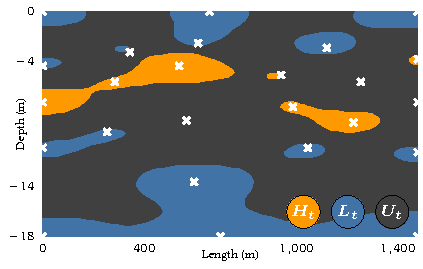
\includegraphics[width=2.4in,clip,trim=7pt 7pt 7pt 7pt]{figures/limno_chl_class25}
    \caption{$t = 25$}
    \label{fig:limno_chl_class1}
  \end{subfigure}
  \hfill
  \begin{subfigure}[b]{0.49\linewidth}
    \centering
    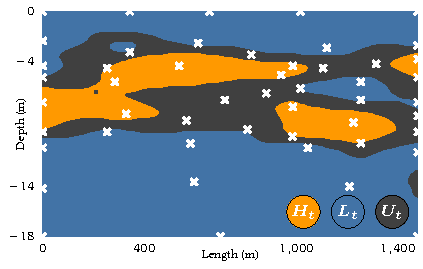
\includegraphics[width=2.4in,clip,trim=7pt 7pt 7pt 7pt]{figures/limno_chl_class50}
    \caption{$t = 50$}
    \label{fig:limno_chl_class2}
  \end{subfigure}
  \begin{subfigure}[b]{0.49\linewidth}
    \centering
    \vspace{0.6em} % space of this row from above captions
    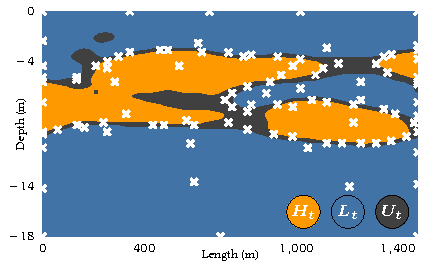
\includegraphics[width=2.4in,clip,trim=7pt 7pt 7pt 7pt]{figures/limno_chl_class100}
    \caption{$t = 100$}
    \label{fig:limno_chl_class3}
  \end{subfigure}
  \hfill
  \begin{subfigure}[b]{0.49\linewidth}
    \centering
    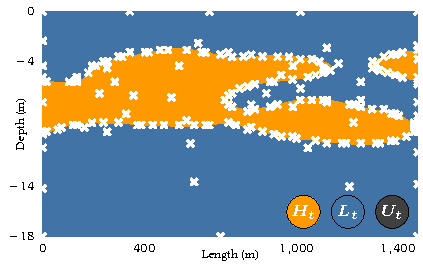
\includegraphics[width=2.4in,clip,trim=7pt 7pt 7pt 7pt]{figures/limno_chl_class168}
    \caption{$t = 168$ (termination)}
    \label{fig:limno_chl_class4}
  \end{subfigure}
  \caption{
      Running \acl with $\epsilon = 0.1$ on a regular grid of $100\times 100$ points
      sampled from the inferred chlorophyll GP of \figref{fig:limno_chl}.
      Regions of already classified points are shown in orange ($H_t$) and blue ($L_t$),
      regions of yet unclassified points ($U_t$) in black, and observed points
      ($\{\*x_i\}_{1\leq i\leq t}$) as white marks.
  }
\end{figure}

\figsref{fig:limno_chl_class1} to \ref{fig:limno_chl_class4} present an example
of running the \acl algorithm on a fine grid of points sampled from the
inferred GP of the chlorophyll dataset shown in \figref{fig:limno_chl}.
Note how the sampling process
focuses on the ambiguous regions around the desired level set until all points
in $D$ have been successfully classified.

\section{Theoretical analysis}
The convergence analysis of \acl rests on quantifying the complexity of the GP prior for $f$ in information-theoretic terms.
The information gain~\cite{cover06} about $f$ from observing $t$ noisy
measurements $\*y_t = (y_i)_{1\leq i\leq t}$ is
\begin{align*}
I(\*y_t; f) = H(\*y_t) - H(\*y_t\mid f).
\end{align*}
\citet{srinivas10} used the \emph{maximum
information gain} over all possible sets of $t$ observations
\begin{align*}
\gamma_t = \max_{\*y_t} I(\*y_t; f)
\end{align*}
for bounding the regret of the \gpucb algorithm.
We use the same quantity to bound the number of \acl iterations
required to achieve a certain classification quality.

To quantify the quality of a solution $(\hat{H}, \hat{L})$
with respect to a single point $\*x\in D$ we use the
misclassification loss
\begin{align*}
\ell_h(\*x) = \twopartdef{\max\{0, f(\*x) - h\}}{\*x\in \hat{L}}{\max\{0, h - f(\*x)\}}{\*x\in \hat{H}}.
\end{align*}
The overall quality of a solution can then be judged by the
largest misclassification loss
among all points in the sample space, i.e. $\max_{\*x\in D} \ell_h(\*x)$.
Intuitively, having a solution with $\max_{\*x\in D} \ell_h(\*x) \leq \epsilon$
means that every point $\*x$ is correctly classified with respect to a
threshold level that deviates by at most $\epsilon$ from the true level $h$;
we call such a solution \emph{$\epsilon$-accurate}.
The following theorem establishes a convergence bound for \acl in terms
of $\gamma_t$ for any given accuracy $\epsilon$.

\begin{theorem}
\label{thm:acl}
For any $h\in\mathbb{R}$, $\delta \in (0, 1)$, and $\epsilon > 0$,
if $\beta_t = 2\log(|D|\pi^2 t^2/(6\delta))$, \acl terminates after
at most $T$ iterations, where $T$ is the smallest positive integer
satisfying
\begin{align*}
\frac{T}{\beta_T \gamma_T} \geq \frac{C_1}{4\epsilon^2},
%T/(\beta_T \gamma_T) \geq C_1/(4\epsilon^2),
\end{align*}
where $C_1 = 8 / \log(1 + \sigma^{-2})$.

Furthermore, with probability at least $1-\delta$, the algorithm returns
an $\epsilon$-accurate solution, that is
\begin{align*}
\Pr\left\{\max_{\*x\in D}\ell_h(\*x) \leq \epsilon\right\} \geq 1 - \delta.
\end{align*}
\end{theorem}

The detailed proof of \theoremref{thm:acl} can be found in
\sectref{sect:app_acl}. We outline here the main steps required.

\begin{description}
\item[Decreasing ambiguities.] We show that the ambiguities of the selected
      points, $a_t(\*x_t)$, are decreasing in $t$ due to the maximum
      ambiguity selection rule and the monotonic classification
      scheme. Furthermore, by employing the maximum information
      gain $\gamma_t$, we show that $a_t(\*x_t)$ decreases
      as $\mathcal{O}((\frac{\beta_t \gamma_t}{t})^\frac{1}{2})$.
\item[Termination.] We show that the classification rules guarantee that the
      algorithm terminates when $a_t(\*x_t)$ is sufficiently small.
      The fact that this will eventually happen is implied from
      the previous step.
\item[``Valid'' confidence regions.] We guarantee that $f(\*x)$ is included
      with high probability in the inferred
      interval $Q_t(\*x)$ and that this holds 1) for every $\*x$ and
      2) for every $t \geq 1$, which also implies that $f(\*x)$ is
      included in each confidence region $C_t(\*x)$. By suitably
      choosing the scaling parameter $\beta_t$, 1) follows from the
      fact that, for every $\*x \in D$ and every $t \geq 1$,
      $f(\*x)$ is distributed
      according to $N(\mu_{t-1}(\*x), \sigma_{t-1}(\*x))$, since
      we are assuming that it is sampled from a known GP that is
      also used by \acl,
      and 2) follows from a union bound over $t$.
\item[Solution accuracy.] We show that an $\epsilon$-accurate solution
      is obtained
      upon termination, due to the classification rules and the
      ``validity'' of the confidence regions guaranteed in the
      previous step.
\end{description}

Note that bounds on $\gamma_t$ have been established for commonly used
kernels~\cite{srinivas10} and can be plugged into \theoremref{thm:acl}
to obtain concrete bounds on $T$.
For example, for a \mbox{$d$-dimensional} sample space and a squared exponential
GP kernel, ${\gamma_t = \mathcal{O}((\log T)^{d+1})}$, and the expression in
the bound of
\theoremref{thm:acl} becomes $T/(\log T)^{d+2} \geq C / \epsilon^2$,
where, for any given sample space and kernel hyperparameters, $C$ depends
only on the choice of $\delta$.

\chapter{Appendix}

\section{Proof of Theorem~\ref*{thm:acl}} \label{sect:app_acl}

\begin{lemma}
\label{lem:srin1}
For any $\delta \in (0, 1)$, if $\beta_t = 2\log(|D|\pi_t/\delta)$, where
$\sum_{t\geq1}\pi_t^{-1} = 1$ and $\pi_t > 0$, then the following holds with
probability at least $1-\delta$
\begin{align*}
|f(\*x) - \mu_{t-1}(\*x)| \leq \beta_t^{1/2}\sigma_{t-1}(\*x),\ \forall \*x \in D\ \forall t \geq 1.
\end{align*}
In particular, we can choose $\pi_t = \pi^2 t^2/6$.
\end{lemma}
\begin{proof}
See Lemma 5.1 in \cite{srinivas10}.
\end{proof}

\begin{cor}
\label{cor:cs}
For any $\delta \in (0, 1)$ and $\beta_t$ as above, the following holds
with probability at least $1-\delta$
\begin{align*}
f(\*x) \in C_t(\*x),\ \forall \*x \in D\ \forall t \geq 1.
\end{align*}
\end{cor}

\begin{lemma}
\label{lem:wb}
The following holds for any $t \geq 1$
\begin{align*}
a_t(\*x_t) \leq \beta_t^{1/2}\sigma_{t-1}(\*x_t).
\end{align*}
\end{lemma}
\begin{proof}
By the definition of ambiguity
\begin{align*}
a_t(\*x_t) &= \min\{\max(C_t(\*x_t)) - h, h - \min(C_t(\*x_t))\}\\
           &\leq (\max(C_t(\*x_t)) - \min(C_t(\*x_t)))/2\\
           &\leq (\max(Q_t(\*x_t)) - \min(Q_t(\*x_t)))/2\\
           &= \beta_t^{1/2}\sigma_{t-1}(\*x_t).
\end{align*}
\end{proof}

\begin{lemma}
\label{lem:dec}
While running \acl, $a_t(\*x_t)$ is nonincreasing in $t$.
\end{lemma}
\begin{proof}
From the definition of the confidence region of $\*x_t$ via successive
intersections $C_t(\*x_t) = C_{t-1}(\*x_t) \cap Q_t(\*x_t)$, it follows that
\begin{align*}
	\left.
		\begin{array}{ll}
			\max(C_t(\*x_t)) \leq \max(C_{t-1}(\*x_t))\\
			\min(C_t(\*x_t)) \geq \min(C_{t-1}(\*x_t))
		\end{array}
	\right\}
\Rightarrow a_t(\*x_t) \leq a_{t-1}(\*x_t)
\end{align*}
Furthermore, from the selection rule used in \acl
${\*x_t = \argmax_{\*x\in U_t}(a_t(\*x))}$ and the monotonicity of
$U_t$ ($U_t \subseteq U_{t-1}$), it follows that
$a_{t-1}(\*x_t) \leq a_{t-1}(\*x_{t-1})$.
\end{proof}

\begin{lemma}
\label{lem:ig}
Denoting $\*y_t = (y_i)_{1\leq i\leq t}$ and
$\*f_t = (f(\*x_i))_{1\leq i\leq t}$,
the information gain for the selected points up to iteration $t$ can be
expressed in terms of the predictive variances as follows
\begin{align*}
I(\*y_t; \*f_t) = \frac{1}{2}\sum_{i=1}^t \log(1 + \sigma^{-2}\sigma_{i-1}^2(\*x_i)).
\end{align*}
\end{lemma}
\begin{proof}
See Lemma 5.3 in \cite{srinivas10}.
\end{proof}

\begin{lemma}
\label{lem:wbound}
While running \acl with $\beta_t$ as in \lemmaref{lem:srin1}, it holds that
\begin{align*}
a_t(\*x_t) \leq \sqrt{\frac{C_1 \beta_t \gamma_t}{4t}},\ \forall t \geq 1,
\end{align*}
where $C_1 = 8 / \log(1 + \sigma^{-2})$.
\end{lemma}
\begin{proof}
Similarly to Lemma 5.4 in \cite{srinivas10},
from \lemmaref{lem:wb} it follows that for any $i \geq 1$
\begin{align*}
a_i^2(\*x_i) &\leq \beta_i\sigma_{i-1}^2(\*x_i)\\
&\leq \beta_i\sigma^2(\sigma^{-2}\sigma_{i-1}^2(\*x_i))\\
&\leq \beta_i\sigma^2 C_2\log(1 + \sigma^{-2}\sigma_{i-1}^2(\*x_i)),
\end{align*}
where $C_2 = \sigma^{-2}/\log(1 + \sigma^{-2})$.
Using \lemmaref{lem:ig} in the above expression, the fact that $\beta_i$
is nondecreasing in $i$, and defining $C_1 = 8\sigma^2C_2$,
we get for any $t \geq 1$
\begin{align*}
C_1\beta_t\gamma_t &\geq C_1\beta_t I(\*y_t; \*f_t)\\
                   &\geq 4\sum_{i=1}^t a_i^2(\*x_i)\\
                   &\geq \frac{4}{t}\left(\sum_{i=1}^t a_i(\*x_i)\right)^2 \tag*{\textrm{(by Cauchy-Schwarz)}}\\
                   &= 4t \left(\frac{1}{t}\sum_{i=1}^t a_i(\*x_i)\right)^2\\
                   &\geq 4t a_t^2(\*x_t) \tag*{\textrm{(by \lemmaref{lem:dec})}}
\end{align*}
\end{proof}

\begin{lemma}
\label{lem:sterm}
While running \acl,
if for some $t \geq 1$, $a_t(\*x_t) \leq \epsilon$,
then $U_{t+1} = \varnothing$.
\end{lemma}
\begin{proof}
Assume that $U_{t+1} \neq \varnothing$, i.e. there exists a point
$\*x \in U_t$, which does not meet the classification conditions
(lines~12 and 15) of \algoref{alg:acl}. Consequently, that point
satisfies $\max(C_{t+1}(\*x)) > h + \epsilon$ and
$\min(C_{t+1}(\*x)) < h - \epsilon$. It follows that
\begin{align*}
\epsilon &< \min\{\max(C_{t+1}(\*x_t))-h, h-\min(C_{t+1}(\*x_t))\}\\
&= a_{t+1}(\*x)\\
&\leq a_t(\*x)\\
&\leq a_t(\*x_t) \tag{by \acl's selection rule},
\end{align*}
which contradicts the lemma's assumption.
\end{proof}

\begin{cor}
\label{cor:iter}
The \acl algorithm terminates after at most $T$ iterations, where $T$
is the smallest positive integer satisfying
\begin{align*}
\frac{T}{\beta_T \gamma_T} \geq \frac{C_1}{4\epsilon^2}.
\end{align*}
\end{cor}

\begin{lemma}
\label{lem:prob}
For any $h\in\mathbb{R}$ and $\delta \in (0, 1)$, and $\epsilon > 0$,
after running \acl with
$\beta_t$ as in \lemmaref{lem:srin1}, with probability at least
$1-\delta$ the returned solution is $\epsilon$-accurate, that is
\begin{align*}
\Pr\left\{\max_{\*x\in D}\ell_h(\*x) \leq \epsilon\right\} \geq 1 - \delta.
\end{align*}
\end{lemma}
\begin{proof}
The lemma follows directly from \corref{cor:cs} and the classification
conditions (lines~12 and 15) of \algoref{alg:acl}.
\end{proof}

\noindent\theoremref{thm:acl} follows by combining \corref{cor:iter}
and \lemmaref{lem:prob}.


\section{Proof of Theorem~\ref*{thm:iacl}} \label{sect:app_iacl}

\begin{definition}
We label the inequalities that take part in \iacl's classification rules
as follows
\begin{align*}
\min(C_t(\*x)) + \epsilon &\geq h_t^{opt} \tag{Q1}\\
\max(C_t(\*x)) - \epsilon &\leq h_t^{pes} \tag{Q2}\\
\max(C_t(\*x)) &< f_t^{pes} \tag{Q3}.
\end{align*}
Furthermore, we redefine here for convenience the following quantities
from the main text
\begin{align*}
Z_t &= U_t \cup H^M_t \cup H^L_t\\
h &= \omega \max_{\*x \in D} f(\*x)\\
f^{opt}_t &= \max_{Z_{t-1}}\max(C_t(\*x))\\
h^{opt}_t &= \omega f^{opt}_t\\
f^{pes}_t &= \max_{Z_{t-1}}\min(C_t(\*x))\\
h^{pes}_t &= \omega f^{pes}_t.
\end{align*}
\end{definition}

\begin{lemma}
\label{lem:iwb}
The following holds for any $t \geq 1$
\begin{align*}
w_t(\*x_t) \leq \beta_t^{1/2}\sigma_{t-1}(\*x_t).
\end{align*}
\end{lemma}
\begin{proof}
By the definition of the confidence region width
\begin{align*}
w_t(\*x_t) &= \max(C_t(\*x_t)) - \min(C_t(\*x_t))\\
           &\leq \max(Q_t(\*x_t)) - \min(Q_t(\*x_t))\\
           &= 2\beta_t^{1/2}\sigma_{t-1}(\*x_t).
\end{align*}
\end{proof}

\begin{lemma}
\label{lem:idec}
While running \iacl, $w_t(\*x_t)$ is nonincreasing in $t$.
\end{lemma}
\begin{proof}
Completely analogous to the proof of \lemmaref{lem:dec}.
\end{proof}

\begin{lemma}
\label{lem:iwbound}
While running \iacl with $\beta_t$ as in \lemmaref{lem:srin1}, it holds that
\begin{align*}
w_t(\*x_t) \leq \sqrt{\frac{C_1 \beta_t \gamma_t}{t}},\ \forall t \geq 1,
\end{align*}
where $C_1 = 8 / \log(1 + \sigma^{-2})$.
\end{lemma}
\begin{proof}
Completely analogous to the proof of \lemmaref{lem:wbound}, with
the only difference being a factor of 2 in the bound
of \lemmaref{lem:iwb} compared to \lemmaref{lem:wb}.
\end{proof}

\begin{lemma}
\label{lem:hdif}
While running \iacl
\begin{align*}
h^{opt}_t - h^{pes}_t \leq \omega w_t(\*x_t),\ \forall t\geq 1.
\end{align*}
\end{lemma}
\begin{proof}
If we define
\begin{align}
\label{eq:hdif_aux}
\hat{\*x} = \argmax_{\*x\in Z_{t-1}}\max(C_t(\*x)),
\end{align}
then by (Q3) it follows that $\hat{\*x} \in Z_t$.
Consequently, we get
\begin{align*}
&\hspace{1.3em}f^{opt}_t - f^{pes}_t\\
&= \max_{\*x\in Z_{t-1}}\max(C_t(\*x)) - \max_{\*x\in Z_{t-1}}\min(C_t(\*x))\\
&= \max(C_t(\hat{\*x})) - \max_{\*x\in Z_{t-1}}\min(C_t(\*x)) \tag{by \eqtref{eq:hdif_aux}}\\
&\leq \max(C_t(\hat{\*x})) - \min(C_t(\hat{\*x}))\\
&= w_t(\hat{\*x})\\
&\leq w_t(\*x_t) \tag{by $\hat{\*x} \in Z_t$},
\end{align*}
and, therefore, $h^{opt}_t - h^{pes}_t = \omega\left(f^{opt}_t - f^{pes}_t\right) \leq \omega w_t(\*x_t)$.
\end{proof}

\begin{lemma}
\label{lem:isterm}
While running \iacl,
if for some $t \geq 1$, $w_t(\*x_t) \leq 2\epsilon/(1 + \omega)$,
then $U_{t+1} = \varnothing$.
\end{lemma}
\begin{proof}
Assume that $U_{t+1} \neq \varnothing$, i.e. there exists a point
${\*x \in U_t \subseteq Z_t}$, which does not meet (Q1) or (Q2).
Consequently, that point satisfies
$\min(C_{t+1}(\*x)) < h^{opt}_{t+1} - \epsilon$ and
$\max(C_{t+1}(\*x)) > h^{pes}_{t+1} + \epsilon$.
It follows that
\begin{align*}
2\epsilon &< h^{opt}_{t+1} - h^{pes}_{t+1} + \max(C_{t+1}(\*x)) - \min(C_{t+1}(\*x))\\
&\leq h^{opt}_{t+1} - h^{pes}_{t+1} + w_{t+1}(\*x)\\
&\leq h^{opt}_{t+1} - h^{pes}_{t+1} + w_t(\*x)\\
&\leq h^{opt}_{t+1} - h^{pes}_{t+1} + w_t(\*x_t) \tag{by \iacl's selection rule}\\
&\leq \omega w_{t+1}(\*x_{t+1}) + w_t(\*x_t) \tag{by \lemmaref{lem:hdif}}\\
&\leq \omega w_t(\*x_t) + w_t(\*x_t) \tag{by \lemmaref{lem:idec}}\\
&\leq (1 + \omega)w_t(\*x_t),
\end{align*}
which contradicts the lemma's assumption.
\end{proof}

\begin{cor}
\label{cor:iiter}
The \iacl algorithm terminates after at most $T$ iterations, where $T$
is the smallest positive integer satisfying
\begin{align*}
\frac{T}{\beta_T \gamma_T} \geq \frac{C_1 (1+\omega)^2}{4\epsilon}.
\end{align*}
\end{cor}

\begin{lemma}
\label{lem:fpes_inc}
While running \iacl, $f^{pes}_t$ is nondecreasing in $t$.
\end{lemma}
\begin{proof}
Assume that at some iteration $t$
\begin{align}
\label{eq:fpes_inc_aux}
\*x = \argmax_{\*x \in Z_{t-1}} \min(C_t(\*x)).
\end{align}
Since $\min(C_t(\*x))$ is nondecreasing in $t$, to have
$f^{pes}_{t+1} < f^{pes}_t$ would mean that $\*x \notin Z_{t}$.
That, in turn, implies that $\*x$ was moved to $H_t$ or $L_t$,
therefore (Q3) was satisfied
\begin{align*}
\max_{\*x \in Z_{t-1}} \min(C_t(\*x)) &> \max(C_t(\*x))\\
&\geq \min(C_t(\*x))\\
&= \max_{\*x \in Z_{t-1}} \min(C_t(\*x)) \tag{by \eqtref{eq:fpes_inc_aux}},
\end{align*}
which is a contradiction and proves our lemma.
\end{proof}

\begin{lemma}
\label{lem:mmeq}
While running \iacl
\begin{align*}
f^{opt}_t = \max_{\*x \in D}\max(C_t(\*x)), \forall t \geq 1.
\end{align*}
\end{lemma}
\begin{proof}
The ``$\leq$" follows from $Z_{t-1} \subseteq D$. Now, assume that
``$<$" holds, i.e. there exists an $\*x\in D\setminus Z_{t-1}$, such that
\begin{align}
\label{eq:hopt_aux2}
\max_{\*x\in Z_{t-1}} \max(C_t(\*x)) &< \max C_t(\*x).
\end{align}
The fact that $\*x\in D\setminus Z_{t-1}$ implies that $\*x$ was moved
during some iteration $i \leq t$ to $H_i$ or $L_i$, therefore $\*x$
satisfied (Q3) at that iteration. Putting everything together, we get
\begin{align*}
\max_{\*x\in Z_{t-1}} \max(C_t(\*x)) &< \max C_t(\*x) \tag{by \eqtref{eq:hopt_aux2}}\\
&\leq \max C_i(\*x)\\
&\leq \max_{\*x\in Z_{i-1}}\min(C_i(\*x)) \tag{by (Q3)}\\
&\leq \max_{\*x\in Z_{t-1}}\min(C_t(\*x)) \tag{by \lemmaref{lem:fpes_inc}}\\
&\leq \max_{\*x\in Z_{t-1}} \max(C_t(\*x)),
\end{align*}
which is a contradiction and proves the lemma.
\end{proof}

\begin{lemma}
\label{lem:hopt}
While running \iacl, the following holds with probability at least $1-\delta$
\begin{align*}
h^{opt}_t \geq h,\ \forall t \geq 1.
\end{align*}
\end{lemma}
\begin{proof}
The following (in)equalities hold with probability at least $1-\delta$
\begin{align*}
h^{opt}_t &= \omega\max_{\*x \in Z_{t-1}}\max(C_t(\*x))\\
&= \omega\max_{\*x \in D}\max(C_t(\*x)) \tag{by \lemmaref{lem:mmeq}}\\
&\geq \omega \max_{\*x \in D} f(\*x) \tag{by \corref{cor:cs}}\\
&= h.
\end{align*}
\end{proof}

\begin{lemma}
\label{lem:hpes}
While running \iacl, the following holds with probability at least $1-\delta$
\begin{align*}
h^{pes}_t \leq h,\ \forall t \geq 1.
\end{align*}
\end{lemma}
\begin{proof}
The following (in)equalities hold with probability at least $1-\delta$
\begin{align*}
h^{pes}_t &= \omega\max_{\*x \in Z_{t-1}}\min(C_t(\*x))\\
&\leq \omega \max_{\*x \in Z_{t-1}} f(\*x) \tag{by \corref{cor:cs}}\\
&\leq \omega \max_{\*x \in D} f(\*x) \tag{by $Z_{t-1}\subseteq D$}\\
&= h.
\end{align*}
\end{proof}

\begin{lemma}
\label{lem:iprob}
For any $\omega \in (0, 1)$, $\delta \in (0, 1)$, and $\epsilon > 0$,
after running \iacl with
$\beta_t$ as in \lemmaref{lem:srin1}, with probability at least
$1-\delta$ the returned solution is $\epsilon$-accurate, that is
\begin{align*}
\Pr\left\{\max_{\*x\in D}\ell_{h}(\*x) \leq \epsilon\right\} \geq 1 - \delta.
\end{align*}
\end{lemma}
\begin{proof}
From \lemmaref{lem:hopt} and \lemmaref{lem:hpes} it follows that, with probability
at least $1-\delta$, (Q1) and (Q2)
are stricter conditions than the following
\begin{align*}
\min(C_t(\*x)) + \epsilon &\geq h\\
\max(C_t(\*x)) - \epsilon &\leq h,
\end{align*}
which are identical to the ones used by \acl. Therefore, the solution of \iacl
achieves at least as high accuracy as the one provided for \acl by
\lemmaref{lem:prob}.
\end{proof}

\noindent\theoremref{thm:iacl} follows by combining \corref{cor:iiter}
and \lemmaref{lem:iprob}.

\section{Proof of Theorem~\ref*{thm:bacl}} \label{sect:app_bacl}
\begin{lemma}
\label{lem:cmi}
For any $\*x \in D$ and $t \geq 1$
the ratio of $\sigma_{fb[t]}(\*x)$ to $\sigma_{t-1}(\*x)$ is bounded
as follows
\begin{align*}
\frac{\sigma_{fb[t]}(\*x)}{\sigma_{t-1}(\*x)} \leq \exp\left\{I(f; \*y_{fb[t]+1:t-1} \mid \*y_{1:fb[t]}\right\}.
\end{align*}
\end{lemma}
\begin{proof}
See Lemma 1 in \cite{desautels12}.
\end{proof}

\begin{lemma}
\label{lem:batch}
Assume that for all $t \geq 1$ the maximum conditional mutual information
acquired by any set of measurements since the last feedback is bounded
by a constant $C \geq 0$, i.e.
\begin{align}
\label{eq:cmi}
\max_{A\subseteq D, |A|\leq B-1} I(f; \*y_A \mid \*y_{1:fb[t]}) \leq C.
\end{align}
Then, if $\eta_t = e^{2C}\beta_{fb[t]+1}$, the following holds with probability
at least $1 - \delta$
\begin{align*}
f(\*x) \in Q_t^{b}(\*x),\ \forall \*x \in D\ \forall t \geq 1.
\end{align*}
\end{lemma}
\begin{proof}
From \lemmaref{lem:cmi} and \eqtref{eq:cmi}, it follows that for any
$\*x \in D$ and $t \geq 1$
\begin{align*}
&\frac{\sigma_{fb[t]}(\*x)}{\sigma_{t-1}(\*x)} \leq \exp\left\{I(f; \*y_{fb[t]+1:t-1} \mid \*y_{1:fb[t]}\right\} \leq e^C\\
\Rightarrow\ & e^C \sigma_{t-1}(\*x) \geq \sigma_{fb[t]}(\*x).
\end{align*}
Using this, the range of $Q_t^{b}(\*x)$ can be related to the range
of $Q_{fb[t]+1}(\*x)$ as follows
\begin{align*}
2\eta_t^{1/2}\sigma_{t-1}(\*x) = 2 e^C \beta_{fb[t]+1}^{1/2}\sigma_{t-1}(\*x) \geq 2\beta_{fb[t]+1}^{1/2}\sigma_{fb[t]}(\*x).
\end{align*}
Furthermore, $Q_t^{b}(\*x)$ and $Q_{fb[t]+1}(\*x)$ have the same midpoint,
namely $\mu_{fb[t]}(\*x)$, therefore the above range inequality implies that
\begin{align}
\label{eq:qbss}
Q_t^{b}(\*x) \supseteq Q_{fb[t]+1}(\*x),\ \forall \*x \in D\ \forall t \geq 1.
\end{align}
Finally, from \lemmaref{lem:srin1} we have that
\begin{align*}
&\Pr\{f(\*x) \in Q_{fb[t]+1}(\*x)\} \geq 1 - \delta,\ \forall \*x \in D\ \forall t \geq 1\\
\stackrel{\eqtref{eq:qbss}}{\Rightarrow}\ & \Pr\{f(\*x) \in Q_t^{b}(\*x)\} \geq 1 - \delta,\ \forall \*x \in D\ \forall t \geq 1.
\end{align*}
\end{proof}

\begin{cor}
\label{cor:batch}
Given the assumptions of \lemmaref{lem:batch}, the following holds with
probability at least $1-\delta$
\begin{align*}
f(\*x) \in C_t^{b}(\*x),\ \forall \*x \in D\ \forall t \geq 1.
\end{align*}
\end{cor}

\noindent Note that \corref{cor:batch} is completely analogous to \corref{cor:cs}.
Thus, the results of Lemmas~\lemmaref{lem:wb}--\ref{lem:prob} also hold for
the case of \bacl, provided that $\eta_t$, as defined in \lemmaref{lem:batch},
is used in place of $\beta_t$, which proves \theoremref{thm:bacl}.

\backmatter
\pagestyle{frontmatter}
\bibliography{msthesis}
\bibliographystyle{icml2013}

\end{document}
